\documentclass[12pt, a4]{article}
%\usepackage[utf8]{inputenc}
\usepackage[natbibapa]{apacite}
\usepackage[
	protrusion=true,
	expansion=true,
	tracking=true
]{microtype}
\usepackage{amsmath}
\usepackage{lmodern}
\usepackage{booktabs}
\usepackage{multirow}
\usepackage{graphicx}
\usepackage{caption}
\usepackage{subcaption}
\usepackage{changepage}
\usepackage{tabularx}
\usepackage[flushleft]{threeparttable}
\usepackage{pdflscape}
\usepackage{geometry}
\usepackage{rotating}
\usepackage{moresize}
\usepackage{siunitx} %defines decimal and thousand separators (num)
\sisetup{
	output-decimal-marker = {.},
	group-separator = {\,}
}
\usepackage{xfrac}      % for beautiful fractions using \sfrac
\usepackage{enumerate}  % for roman numbers in enumerate
\usepackage{lipsum}     % for text placeholders
\usepackage[unicode, hidelinks]{hyperref}   % for referencing sections by names 
\usepackage{breakurl}   % for multiple line URLs
\usepackage{tikz}
\usepackage{floatpag}	  % for suppressing page numbers on floats

\newcolumntype{R}{>{\raggedleft\arraybackslash}X}
\newcolumntype{L}{>{\raggedright\arraybackslash}X}
\newcolumntype{C}{>{\centering\arraybackslash}X}

\title{Copycat Strategies:\\ Is This the End of Active Investing?\thanks{We are thankful to Daniel Somos for the topic and his invaluable advice in how to approach the problem intellectually, Michael Halling for his guidance and input in acquiring data, as well as Juris Rumba for his help in data collection.}}
\author{Em\={\i}ls Kreislers \and Nikolajs Prihodko}
\date{\parbox{\linewidth}{\centering%
		Supervisor: Michael Halling\endgraf\vspace{6ex}
		Stockholm School of Economics\endgraf\medskip
		May 2016
		}} 


\begin{document}
\maketitle

\begin{abstract} \noindent % there should be no paragraph indent in abstract
	The aim of this paper is to see whether it is possible to efficiently copy the investment strategy of \textsc{US} equity-only mutual funds, based on their disclosure to the \textsc{SEC}. Copycat performance is evaluated at the full sample, and then in smaller groups in order to determine whether some types of funds are better candidates for copying. The results indicate that the copycat funds can keep up with their primitive counterparts in all instances, and even outperform the funds with a high expense ratio and funds that were easy to copy in the past. Different copycat fund sizes are also considered, but play no significant role in the results.
\end{abstract}

\textbf{Keywords:} mutual, fund, copycat, investment, strategy
	
\textbf{\textsc{JEL} Classification:} G11, G14, G23

\newpage

\tableofcontents

\clearpage




\section {Introduction}

Since the beginning of investing, investors have tried to discover ways to get an `edge' on the other investors to generate profits, be it through research, trade implementation, market manipulation or other means.

Naturally, fund managers want to protect their investment ideas from outside investors to generate the maximum potential returns. Secrecy and information asymmetry can, in turn, lead to various agency issues, leading to suboptimal results to the investor. Therefore, disclosure requirements have been imposed by the regulatory authorities over time to give the opportunity for an investor to confirm whether the manager follows their intended investment strategy.

But the curious might ask whether the current trend of disclosure requirements allow for the savvy observer of the filings to benefit from the investment research of others, without actually paying for it. This is especially relevant given the strong growth of the passive asset management industry, which has been the recipient of record net inflows in 2015 and already manages \sfrac{1}{3} of all long-only assets under management in the \textsc{US} \citep{bloomberg}. Therefore, we try to copy the holdings of \textsc{US} mutual funds (\textit{primitive} funds), and see whether it constitutes a viable investment strategy.

Thus, the authors of the paper answer the following research questions:

\begin{itemize}
    \item Can copycat funds match or exceed the performance of the primitive mutual funds in the \textsc{US}?
    \item Is the mimicking performance enhanced by selection criteria, such as past performance, expense ratio or past return difference?
    \item Do copycat funds of different sizes perform differently?
\end{itemize}

The overall results are mixed, copycat funds match their primitive counterparts' performance, and can even exceed it. Expensive and easy-to-copy funds in the past are good candidates, which can be copied very efficiently, and potentially be used in trading strategies. 

Section \ref{sec:lit-rev} presents the relevant research and development in copycat strategies. Section \ref{sec:methodology} describes the methodology and data. Section \ref{sec:results} discusses the results and their implications. Section \ref{sec:conclusions} concludes.

\clearpage
\section{Literature review}\label{sec:lit-rev}

\subsection{Delivery of superior returns}

The ability of asset managers to deliver superior returns has been at the forefront of financial research at least since the middle of the 20th century, after the development of asset pricing models by \cite{sharpe}, \cite{litner} or \cite{treynor}. In a seminal paper, it was discovered that mutual funds on average were unable to predict security prices well enough to outperform the buy-and-hold market portfolio. The findings are also robust for individual mutual funds \citep{jensen}.

However, this did not stop academicians from trying to decipher the reasons for the existence of active mutual funds. One of the first modern forays into the field of assessing the talent of asset managers was done by \cite{grinblatt}, who compare the abnormal returns of both active and passive investment strategies of mutual funds from 1975 to 1984. From this, transaction costs and determinants of abnormal returns are calculated. \citeauthor{grinblatt} conclude that transaction costs are relatively large (around 2.5 per cent) and are inversely related to fund size. Furthermore, gross abnormal returns are also inversely related to fund size, but given the previous findings on transaction costs, net returns are unrelated to actual fund size. Finally, net returns do not appear to display any abnormal returns for any category of the funds (Growth, Income, Balance, etc.). Essentially, this is a precursor to later copycat strategy research, but does not focus on the performance of copycat funds as an investment strategy, but treat them as a benchmark for the mutual funds being researched to separate outperformance from the rest of risk exposure.

The ideas first explored by \cite{grinblatt} are developed further by \cite{daniel}, who evaluate the stock-picking ability of mutual fund managers based on the characteristics of stocks in their portfolios. Overall, 2500 equity funds are covered from 1975 to 1994. To evaluate the ability, 125 reference portfolios are created (based on indicators like market capitalisation, market-to-book ratio, and momentum), to which individual stocks are matched. These matched portfolios are then used to build timing and selectivity measures. The results show that funds (especially aggressive growth funds) have a selectivity ability, however no funds exhibit a timing ability. This is explored further in \cite{wermers_2012}, who employ a generalised-inverse regression approach and find that the estimator exhibits consistent and significant predictive power, even controlling for size, market-to-book and momentum factors, as well as skill proxies, meaning that stock-picking is a skill separate from the aforementioned.

To shed some light on whether the stock-picking abilities of asset managers are actually value-adding to the investor, \cite{wermers_2000} explores the value-added by active mutual fund management and finds that funds hold stocks that outperform the market by 1.3 per cent, but underperform in net terms by 1 per cent. This performance difference is then attributed to worse performance of non-stock holdings (0.7 per cent), and expenses and transaction costs (1.6 per cent). \citeauthor{wermers_2000} concludes that active fund managers possess valuable information about future performance and stocks, and creates precedent for copycat strategies to free-ride on the active manager's costly information through looking at mandatory disclosure filings.

\subsection{Disclosure legislation and its effects}

The change in the Securities and Exchange Commission (\textsc{SEC}) reporting requirements in 2004 led to a resurgence in interest in the performance of copycat strategies. The \textsc{SEC} had required registered investment companies to post their portfolio holdings within 60 days after the end of each fiscal 6-month period (Title 17, Chapter II, \S\ 270.30b1-1 of the Code of Federal Regulations). This was supplemented in May 2004 with \S\ 270.30b1-5, which required investment companies to submit quarterly portfolio disclosure, maintaining the same 60-day window as previously. This was a contentious decision, which included both benefits and costs.

When it comes to benefits, more frequent disclosure can create more demand for the securities held by the fund, thereby driving up the price. It also facilitates investors' monitoring of the securities held by various funds, thus improving overall asset allocation and diversification choices. In addition to this, some investors may see more frequent disclosure as a valuable activity from a corporate governance point of view, to detect a deviation from the stated strategy of the fund and `window dressing', for example. This is corroborated by the fact that some mutual funds already disclose portfolio holdings more frequently than required \citep{frank}.

On the cost side, \cite{wermers_2001} notes that potential returns to mutual fund investors would likely decrease with increased disclosure due to front-running by other market participants, free-riding on the funds' research, increased costs of providing liquidity to shareholders, and costlier tax-management strategies.

To measure the effects of the \textsc{SEC}'s decision, \cite{agarwal} explore the liquidity impact on the disclosed stocks and the fund performance. The results show that stocks with higher ownership by funds experience larger increases in liquidity after the decision, and the effect is especially pronounced for stocks held by more informed funds, and stocks with high information asymmetry. When it comes to fund performance, the analysis suggests that more informed funds experience a performance deterioration after the change, with funds holding stocks with high information asymmetry again being the most hit. Overall, it is concluded that disclosure improves liquidity but hurts the performance of informed investors.

To gain insight whether non-mandatory disclosures follow a specific pattern, \cite{ge} explore the determinants of the frequency of disclosure of mutual funds. It is found that funds with higher turnover, higher expense ratios, and higher likelihood of committing fraud are disclosing their holdings at a less frequent basis. The results testing the investment skill of managers are then separated alongside two effects: 

\begin{enumerate}[i)]
    \item the information effect (costs of more frequent disclosure due to informational advantage), and 
    \item agency effect (benefits of disclosure to avoid agency issues).
\end{enumerate}

The results are split across these lines. Firstly, past winners who disclose less frequently perform better than past winners who disclose more frequently, which directly shows the information effect at play. Secondly, past losers with less frequent disclosure underperform their peers with more frequent disclosure, which is consistent with the agency effect. Furthermore, the relationship between disclosure frequency and new money flows is explored. It is found that new money flow is stronger for poorly performing funds with more frequent disclosure, compared to those with less frequent disclosure.

\subsection{Copycat strategies}

Naturally, finding out that asset managers have valuable information about the future performance of stocks and the ability to exploit their information has implications for creating a profitable trading strategy. One of the first applications of this idea comes from \cite{frank} who explore subsamples of a sample of 812 mutual funds in the \textsc{US} between 1992 and 1999. They find that disclosure is dependent on the size of the fund (larger funds disclose holdings less frequently, likely due to cost prohibitions) and the liquidity of its holdings (funds holding more widely traded stocks disclose holdings more frequently). When it comes to replicating performance, the copycat funds equal or exceed the performance of mutual funds being copied (\textit{primitive} funds) in net terms, both in the subsample of high expense funds and the broader subsample. In gross terms, copycat funds cannot keep up with their original counterparts. They also find no difference in systemic risk exposure between copycat and primitive funds. Therefore, the authors conclude that copycat strategies enable investors to construct portfolios that efficiently mimic actively managed mutual funds, thereby potentially eroding their market share.

In their research testing the performance of copycat strategies, \cite{verbeek} use a database of \textsc{US} mutual funds from 1985 to 2008, adjusted for survivorship bias and find that copycat funds are capable of generating similar net performance to their target funds. However, in terms of gross returns, primitive funds beat the copycats, as expected. However, it is noted that dispersion exists and funds with high past performance (`past winners'), and funds with more representative disclosure are the best candidates for replication. The performance of the selective copycat strategy is deemed to exceed the majority of the mutual funds in the sample. The result that funds with less representative disclosure are not good candidates for replication is supported by the findings of \cite{kacperczyk}, who report on the impact of unobserved actions on fund returns by analysing the return difference of \textsc{US} equity funds from 1984 to 2003. They find that the average return difference is close to zero, however significant cross variation exists. The main finding of the paper is that past return difference helps to predict future performance, where funds with high past return differences outperform their low return difference peers both before and after adjusting for differences in risk and investment style. The return difference also exhibits strong persistence up to five years into the future, which is suggested to be driven by systemic factors.

Since most fund investors care for net returns, instead of gross returns for any particular investment strategies, transaction costs are an important factor to consider. Contrary to \cite{frank}, \cite{verbeek} also model transaction costs of the copycat funds according to the findings of \cite{keim} and \cite{wermers_2000}, instead of assuming a static expense ratio of an index fund. Interestingly, it is noted that the success of copycat strategies has increased since the 2004 decision, thereby supporting the findings of \citeauthor{wermers_2000} and \cite{agarwal}.

In addition to this, \cite{kim} use the \textsc{SEC}'s 13F filings and high frequency trade data to discover whether a viable copycat strategy exists for the hedge fund universe. To add to the relevance, only top 5 positions for each fund are copied and held until a day before the next filing, since those show the highest manager conviction (proxied by smaller turnover on average than other positions), given the concentrated bets of hedge funds. The results show that mutual funds earn significant and positive abnormal returns using this strategy (2.84 per cent if equal weighting is used, and 2.21 per cent if principal weighting is used instead). It has to be noted that these opportunities are arbitraged away quickly, as abnormal returns disappear if trades are initiated one day after the initial disclosure, and most success comes from copying hedge funds with low portfolio turnover rates to minimise the negative effect from delayed disclosure.  Their paper also contributes to the previously mentioned discussion of the costs and benefits frequency of disclosure. In this case, it is apparently very costly for long-term value-oriented hedge funds, as the 45-day delay does not protect them from copycat investors. It is signified by the fact that copycat purchases take up only 0.14 per cent of all stock purchases by copycat funds three days before disclosure, and it grows to 1.18 per cent on the disclosure day.


\clearpage
\section{Data description and methodology}\label{sec:methodology}

\subsection{Data}

The data for the study was obtained from the Wharton Research Data Services (\textsc{wrds}) web-site. Bond index data came from the Federal Reserve Bank of St. Louis. The data was retrieved on various dates between February and May 2016. More information on how and where the data was obtained can be found in the \nameref{sec:appendices} in the section \nameref{sec:data-sources}.

\subsubsection{Data selection}

The study covers the time period from January 1, 1990 till October 31, 2012. We gather data on mutual fund performance from the \textsc{crsp} Mutual Funds database, which we then link to their holdings from Thomson Reuters S12 Mutual Fund Holdings database.

Following \cite{verbeek}, we try to identify equity-only funds by their investment objectives. In addition to this, all index funds are excluded from the analysis. We also impose a minimum level of common stock plus cash holdings, which is set at 90 per cent. We also exclude funds with equity holdings of more than 120 per cent or less than 0 per cent in at least one of the periods, because we focus on cheaply implementable strategies, while these proportions of equity impliy costly short positions or leverage. This yields a sample size of 3237 mutual funds.

A more detailed explanation of how we select funds can be found in the \nameref{sec:appendices} in the section \nameref{sec:equity-only}. Summary statistics of the resulting sample can be also found there in the section \nameref{sec:sample-summary-statistics}.

\subsection{Construction of copycat returns}

We replicate a primitive fund using the information about its holdings, which is regularly disclosed to the \textsc{SEC}. The reporting frequency may differ across funds due to both changing regulatory requirements (as discussed in the literature review), and voluntary disclosure that goes beyond what the law mandates. 

First, we replicate the holdings of a primitive fund on each disclosure date. Returns obtained using weighted-average returns of holdings are then called \textit{gross returns}. Then, we account for transaction costs and call this type of return \textit{after trading costs return} (\textsc{ATC} return). Additionally, we impose a fee on the copycat funds, which is assumed to cover the overhead costs of the fund. Returns that account for this type of expenses are then called \textit{net returns}.

For primitive funds, net returns are reported, and \textsc{ATC} returns are inferred from reported expense ratio.

\subsubsection{Disclosure date}

The disclosure date and the date on which the holdings were valid (report date\footnote{The date at which the snapshot of holdings was made (the \texttt{rdate} variable in the Thomson Reuters database).}) are inherently different due to the 60-day window, during which mutual funds are allowed to post their holdings. Since the actual disclosure date is not immediately available, assumptions have to be made. \cite{verbeek} and \cite{frank} impose a 60-day window (the maximum allowed under the current law) between the date of disclosure and the report date, while \citeauthor{kacperczyk} simulate copycat performance on the report date instead of the disclosure date, when the holding data might actually become available. 

We use the report date with additional 60 days to find the latest possible disclosure date, however if the information about holdings was added into Thomson Reuters database before the end of this window, then we assume that the fund has disclosed its holdings earlier, and we use the vintage date\footnote{The date on which the data was gathered by Thomson Reuters (the \texttt{fdate} variable in the database).} at which the data was entered into the Thomson Reuters database. 

In this way we do not use unrealistic assumption that the report date always coincide with the disclosure date used by \cite{kacperczyk}, but also allow for disclosure dates earlier than 60 days after the report date, unlike \cite{verbeek} and \cite{frank}. This is possible, because we expect that if the data is available for Thomson Reuters then the disclosure had already happened.

This is still not perfect, because vintage days are always at the end of the quarter and therefore can be after both report days with 60-day window and the actual disclosure date. However, if the copycat strategy works under these restricted circumstances, it should work under a smaller disclosure window as information will be less stale. Furthermore, if there are more than one holdings disclosures for the given report date, we use the first available one, as restatements are not available at the first disclosure date.

We rebalance fund portfolio using the closing prices for the implicit disclosure date, implying that the rebalancing happens at the end of the day.

\subsubsection{Gross returns}

The copycat fund gross monthly return is defined as (copying fund $j$ at time $t$, taking into the account the weight in asset $i$ at the last disclosure):

\begin{align}
    Gross\ return_t^j = \sum^N_{i = 1}w_{i,disclosed}^j R_{i,t}.
\end{align}

The weight for the first date after rebalancing $w_{i,disclosed}^j$ is given by:

\begin{align}
    w_{i, disclosed}^j = \frac{N_{i, disclosed}^j P_{i, disclosed}}{\sum_{i = 1}^N N_{i, disclosed}^j P_{i, disclosed}}.
\end{align}

After the rebalancing the weights are allowed to fluctuate according to the market performance until the next rebalancing date.

\subsubsection{After trading costs return}

On each rebalancing date, transaction costs are added to the calculations and are subtracted from the copycat fund return for that day. It is no secret that transaction costs can often limit the real-life implementation of a trading strategy, especially if it requires a lot of trading. Transaction costs are modelled after the approach used in \cite{kacperczyk} and \cite{verbeek}, who in turn model their approach after \cite{keim} and \cite{wermers_2000}.

Unlike \cite{verbeek}, who have assumed that the size of a copycat fund is the same as the size of the primitive fund and copied changes in share number one-to-one, we assume different fund sizes. We believe that this is more realistic, because a copycat fund is likely to be smaller than the original fund. We study the effect of trading costs for three different fund sizes: \$10 million, \$50 million, and \$250 million (the average primitive fund size in the sample is \$452 million). 

Furthermore, in the construction of transaction costs, a static fund size is assumed to ensure that no preference is given to later funds having an advantage in terms of execution costs due to later start up. Otherwise, at the same date, earlier funds would have grown their assets under management and thus forced to buy larger blocks when rebalancing. For example, without this assumption, a copycat fund that is \$10 million in size in 1990 will be, for instance, \$30 million in 2010. Therefore, it will experience larger trading costs than a fund that just started its existence in 2010 and therefore is still of the size \$10 million. Since this effect of the fund age on trading costs is arbitrary and therefore undesirable for our analysis, we decided to assume constant fund sizes.

Transaction costs are computed as such (in per cent of trade value):
\begin{align}
    C_{i,t}^{Buy} = &\ 1.098 + 0.336 D_{i,t}^{nasdaq} + 0.092 \ trSize_{i,t} \nonumber \\ 
    &\ - 0.084 \ln(mCap_{i, t}) + 13.807 \left( \frac {1}{P_{i, t}} \right), \\
    C_{i,t}^{Sell} = &\ 0.979 + 0.058 D_{i, t}^{nasdaq} + 0.214 \ trSize_{i,t} \nonumber \\
    &\ - 0.059 \ln (mCap_{i,t})+6.537\left(\frac {1}{P_{i,t}}\right),
\end{align}
where $D_{i,t}^{nasdaq}$ is a dummy variable if the stock is traded on \textsc{nasdaq}, $trSize_{i,t}$ is the dollar trade size divided by the total dollar market capitalisation, $\ln(mCap_{i,t})$ is the natural logarithm of the market capitalisation (in thousands), and $P_{i,t}$ is the stock price at the day of the trade. Due to this construction, it is possible that transaction costs become negative in some cases where the market capitalisation is very large, and thus we limit the minimum transaction costs to zero.

But since we are interested in transaction costs in percentage of assets in order to find the impact on returns, we additionally multiply them by percentage of the fund that has been traded and by the copycat fund size: \$10 million, \$50 million, or \$250 million.

After accounting for trading costs, we obtain \textsc{ATC} returns.

\subsubsection{Overhead expenses}

In addition to transaction costs, a combined yearly management and administrative fee of 20bps is assumed, following the example of \cite{frank} and \cite{verbeek} to simulate the overhead costs for the fund. For the primitive funds, where only net returns are reported by the \textsc{crsp}, we follow \cite{cohen}, who suggest to add \sfrac{1}{12} of the fund's expense ratio every month to the net return to arrive at the \textsc{ATC} return. However, \citeauthor{cohen} calls these returns \textit{gross returns} when the expense ratio does not include transaction costs (not all parts of which are immediately observable, e.g. price impact).

\subsubsection{Different asset classes}

Since the Thomson Reuters S12 database only offers \textsc{US} domestic equity holdings, assumptions have to be made regarding the other asset classes in the primitive fund portfolios. The proportions of different asset classes in funds' holdings are taken from the \textsc{crsp} Fund Overview database. We obtain proportion of common stock and cash, leaving the rest to category \textit{other}. 

Performance of cash in the copycat portfolios is assumed to follow the \textsc{US} Treasury returns. And all other assets, which are likely to be mostly bonds, are simulated using the Bank of America Merrill Lynch \textsc{US} 3--5 year corporate bond index returns, similar to \cite{verbeek} who use a Barclays bond index. 

Finally, it is assumed that the invested asset portion in the copycat portfolio cannot exceed 100 per cent (thus, no leverage), as it is generally left to hedge funds, with their higher fees and lower correlation to standard market assets \citep{hsieh}.

\subsection{Performance analysis}

\subsubsection{Full sample analysis}
First, we perform a full sample overview. We calculate the \textit{average} returns and alphas \textit{by fund}. Then we study the distributions of these averages and their differences. We compute means and quartiles. For returns, we perform a simple one-sample $t$-test of the mean being equal to zero. For differences we test whether the two series of returns (e.g. net copycat returns and net primitive fund returns) have equal means using the Welch's version of the two-sample $t$-test. We also test whether two series of returns are equally distributed using the non-parametric Mann---Whitney $U$ test. We create boxplots for more convenient visualisation.

Additionally, we calculate the average returns for each month across all funds available in that period, we call these measures  
\textit{average by month}. Then we calculate means and quartiles and perform the same tests as described above. Again, we create boxplots for more convenient visualisation.

To explain potential discrepancies between the two ways of averaging (across months for each fund and across funds for each month), we sort the funds into 10 deciles according to the length of returns history and compute several performance measures.

\subsubsection{Decile analysis}

To gain more insight into how copycat performance differs across categories of funds, we sort the funds based on certain characteristics. Every January, April, July and October, copycat funds are sorted into decile portfolios to test whether copying funds following certain parameters yields better results. The sorting parameters are:

\begin{itemize}
	\item Average expense ratio of the primitive funds over the last 12 months, following \cite{frank}. The logic behind it is that one could expect that the best performing funds are also the most expensive, as the fund managers need to keep up with their research costs.
	\item Average \textsc{ATC} returns of the primitive funds over the last 12 months, following \cite{verbeek}. In this way we try to identify best funds using past performance.
	\item Average net return difference between copycat and primitive funds over the last 12 months, following \cite{verbeek} and \cite{kacperczyk}. In this approach we try to identify whether the funds that were easy to copy in the past remain so in the future.
	\item Carhart alpha of the \textsc{ATC} returns of the primitive funds using last 12 months \citep{carhart}. In this way we try to identify best funds in terms of abnormal returns, because that should indicate pure manager's skill.
\end{itemize}

We then compare the \textsc{ATC} and net return (alpha) differences, taking into account different copycat sizes. In addition to that, we also apply the four-factor model by \cite{carhart} to see whether any abnormal return performance exists in the return and the return difference. To control for heteroscedasticity and autocorrelation, we use a variance-covariance matrix as suggested by \cite{newey}.

The regression model looks like this:

\begin{align}
    R_t = \alpha_t + \beta_{MKT}R_{MKT, t} + \beta_{SMB}R_{SMB, t} + \beta_{HML}R_{HML, t} + \beta_{MOM}R_{MOM, t} + \varepsilon_t,
\end{align}
where $R_t$ is either the return or the return difference.


\clearpage
\section{Empirical results}\label{sec:results}

\subsection{Full sample}

\subsubsection{Averages by fund}

The results of averages by fund are represented in Figure \ref{fig:boxplot-returns-funds} and Table \ref{tab:whole-sample-fund-means} in the \nameref{sec:appendices} in the section \nameref{sec:performance-analysis}. 

We see that the \textsc{ATC} returns of both primitive and copycat funds of all sizes are significantly above zero. This is as expected, because we focus on all-equity funds and therefore the results should roughly follow the expected equity returns, which are positive. 

There is no statistically significant difference in the means of \textsc{ATC} returns of the primitive and copycat funds of any size. This suggests that it is possible to copy the performance of mutual funds based on their disclosure information.

Both copycat and primitive \textsc{ATC} returns are negatively skewed, which means that they have fat left tails. Having the same median, copycat returns, however, have fatter left and thinner right tail, which is an undesirable property for returns.

There are statistically significant differences in the net returns of primitive and copycat funds. The results suggest that copycat funds outperform their primitive counterparts in terms of average returns on significance level below 1\%.

This outperformance, however, can be due to different risk loading. Figure \ref{fig:boxplot-alphas-funds} and Table \ref{tab:whole-sample-fund-means} in the \nameref{sec:appendices} in the section \nameref{sec:performance-analysis} account for this possibility by comparing the Carhart alphas of copycat funds and their primitive counterparts. 

Alphas for both primitive and copycat \textsc{ATC} returns are below zero. This is reasonable, because factors (market risk-premium, small-minus-big, high-minus-low, and momentum) are computed without accounting for trading costs. Net alphas are also negative, which is reasonable given that they should be worse than the \textsc{ATC} alphas.

An interesting thing, however, is the negative alpha for gross (before accounting for trading costs) copycat returns. A possible explanation for that would be that the managers of the primitive funds try to beat the market by stock-picking and market-timing. Thus, holdings of primitive funds are not broad due to the attempts to pick winners only. This translates into underdiversified portfolios of the copycat funds. Coupled with the time lag, they might also miss the benefits of market timing.

The mean alphas of the primitive and copycat returns are not statistically significant for the \textsc{ATC} returns, which is in line with the absence of difference in the \textsc{ATC} returns.

The mean Carhart alphas of copycat net returns are significantly larger than their primitive counterparts' at the 5\% significance level. However the same is not true for the 1\% significance level ($p$-value is \num{0.04}). Thus, the results are inconclusive.

In terms of copycat fund sizes, there are no notable differences across them. This means that larger size copycats can perform at the same level as the smaller ones.

\begin{figure}
	\thisfloatpagestyle{empty}
	\centering
	\caption{Full sample mean returns, return differences by fund.}
	\label{fig:boxplot-returns-funds}
	\begin{subfigure}[t]{\linewidth}
		% Created by tikzDevice version 0.10.1 on 2016-05-14 11:51:15
% !TEX encoding = UTF-8 Unicode
\begin{tikzpicture}[x=1pt,y=1pt]
\definecolor{fillColor}{RGB}{255,255,255}
\path[use as bounding box,fill=fillColor,fill opacity=0.00] (0,0) rectangle (426.79,220.51);
\begin{scope}
\path[clip] (  0.00,  0.00) rectangle (426.79,220.51);
\definecolor{drawColor}{RGB}{255,255,255}
\definecolor{fillColor}{RGB}{255,255,255}

\path[draw=drawColor,line width= 0.6pt,line join=round,line cap=round,fill=fillColor] (  0.00,  0.00) rectangle (426.79,220.51);
\end{scope}
\begin{scope}
\path[clip] ( 39.29, 35.52) rectangle (421.29,215.01);
\definecolor{fillColor}{gray}{0.92}

\path[fill=fillColor] ( 39.29, 35.52) rectangle (421.29,215.01);
\definecolor{drawColor}{RGB}{255,255,255}

\path[draw=drawColor,line width= 0.3pt,line join=round] ( 39.29, 70.87) --
	(421.29, 70.87);

\path[draw=drawColor,line width= 0.3pt,line join=round] ( 39.29,125.26) --
	(421.29,125.26);

\path[draw=drawColor,line width= 0.3pt,line join=round] ( 39.29,179.65) --
	(421.29,179.65);

\path[draw=drawColor,line width= 0.6pt,line join=round] ( 39.29, 43.68) --
	(421.29, 43.68);

\path[draw=drawColor,line width= 0.6pt,line join=round] ( 39.29, 98.07) --
	(421.29, 98.07);

\path[draw=drawColor,line width= 0.6pt,line join=round] ( 39.29,152.46) --
	(421.29,152.46);

\path[draw=drawColor,line width= 0.6pt,line join=round] ( 39.29,206.85) --
	(421.29,206.85);

\path[draw=drawColor,line width= 0.6pt,line join=round] ( 67.24, 35.52) --
	( 67.24,215.01);

\path[draw=drawColor,line width= 0.6pt,line join=round] (113.83, 35.52) --
	(113.83,215.01);

\path[draw=drawColor,line width= 0.6pt,line join=round] (160.41, 35.52) --
	(160.41,215.01);

\path[draw=drawColor,line width= 0.6pt,line join=round] (207.00, 35.52) --
	(207.00,215.01);

\path[draw=drawColor,line width= 0.6pt,line join=round] (253.58, 35.52) --
	(253.58,215.01);

\path[draw=drawColor,line width= 0.6pt,line join=round] (300.17, 35.52) --
	(300.17,215.01);

\path[draw=drawColor,line width= 0.6pt,line join=round] (346.75, 35.52) --
	(346.75,215.01);

\path[draw=drawColor,line width= 0.6pt,line join=round] (393.34, 35.52) --
	(393.34,215.01);
\definecolor{drawColor}{RGB}{0,0,0}
\definecolor{fillColor}{RGB}{0,0,0}

\path[draw=drawColor,draw opacity=0.30,line width= 0.4pt,line join=round,line cap=round,fill=fillColor,fill opacity=0.30] ( 78.10,149.03) circle (  0.46);

\path[draw=drawColor,draw opacity=0.30,line width= 0.4pt,line join=round,line cap=round,fill=fillColor,fill opacity=0.30] ( 61.82,165.75) circle (  0.46);

\path[draw=drawColor,draw opacity=0.30,line width= 0.4pt,line join=round,line cap=round,fill=fillColor,fill opacity=0.30] ( 79.46,123.69) circle (  0.46);

\path[draw=drawColor,draw opacity=0.30,line width= 0.4pt,line join=round,line cap=round,fill=fillColor,fill opacity=0.30] ( 81.49,128.08) circle (  0.46);

\path[draw=drawColor,draw opacity=0.30,line width= 0.4pt,line join=round,line cap=round,fill=fillColor,fill opacity=0.30] ( 80.66,135.78) circle (  0.46);

\path[draw=drawColor,draw opacity=0.30,line width= 0.4pt,line join=round,line cap=round,fill=fillColor,fill opacity=0.30] ( 65.34,161.05) circle (  0.46);

\path[draw=drawColor,draw opacity=0.30,line width= 0.4pt,line join=round,line cap=round,fill=fillColor,fill opacity=0.30] ( 58.80,191.85) circle (  0.46);

\path[draw=drawColor,draw opacity=0.30,line width= 0.4pt,line join=round,line cap=round,fill=fillColor,fill opacity=0.30] ( 70.01,141.26) circle (  0.46);

\path[draw=drawColor,draw opacity=0.30,line width= 0.4pt,line join=round,line cap=round,fill=fillColor,fill opacity=0.30] ( 62.08,139.77) circle (  0.46);

\path[draw=drawColor,draw opacity=0.30,line width= 0.4pt,line join=round,line cap=round,fill=fillColor,fill opacity=0.30] ( 62.37,159.51) circle (  0.46);

\path[draw=drawColor,draw opacity=0.30,line width= 0.4pt,line join=round,line cap=round,fill=fillColor,fill opacity=0.30] ( 59.04,144.30) circle (  0.46);

\path[draw=drawColor,draw opacity=0.30,line width= 0.4pt,line join=round,line cap=round,fill=fillColor,fill opacity=0.30] ( 77.65,150.02) circle (  0.46);

\path[draw=drawColor,draw opacity=0.30,line width= 0.4pt,line join=round,line cap=round,fill=fillColor,fill opacity=0.30] ( 59.93,146.75) circle (  0.46);

\path[draw=drawColor,draw opacity=0.30,line width= 0.4pt,line join=round,line cap=round,fill=fillColor,fill opacity=0.30] ( 50.89,154.91) circle (  0.46);

\path[draw=drawColor,draw opacity=0.30,line width= 0.4pt,line join=round,line cap=round,fill=fillColor,fill opacity=0.30] ( 83.91,147.26) circle (  0.46);

\path[draw=drawColor,draw opacity=0.30,line width= 0.4pt,line join=round,line cap=round,fill=fillColor,fill opacity=0.30] ( 77.94,145.41) circle (  0.46);

\path[draw=drawColor,draw opacity=0.30,line width= 0.4pt,line join=round,line cap=round,fill=fillColor,fill opacity=0.30] ( 70.31,144.70) circle (  0.46);

\path[draw=drawColor,draw opacity=0.30,line width= 0.4pt,line join=round,line cap=round,fill=fillColor,fill opacity=0.30] ( 70.19,161.00) circle (  0.46);

\path[draw=drawColor,draw opacity=0.30,line width= 0.4pt,line join=round,line cap=round,fill=fillColor,fill opacity=0.30] ( 64.59, 14.35) circle (  0.46);

\path[draw=drawColor,draw opacity=0.30,line width= 0.4pt,line join=round,line cap=round,fill=fillColor,fill opacity=0.30] ( 60.90,136.72) circle (  0.46);

\path[draw=drawColor,draw opacity=0.30,line width= 0.4pt,line join=round,line cap=round,fill=fillColor,fill opacity=0.30] ( 76.74,141.36) circle (  0.46);

\path[draw=drawColor,draw opacity=0.30,line width= 0.4pt,line join=round,line cap=round,fill=fillColor,fill opacity=0.30] ( 77.93,144.98) circle (  0.46);

\path[draw=drawColor,draw opacity=0.30,line width= 0.4pt,line join=round,line cap=round,fill=fillColor,fill opacity=0.30] ( 55.53, 93.53) circle (  0.46);

\path[draw=drawColor,draw opacity=0.30,line width= 0.4pt,line join=round,line cap=round,fill=fillColor,fill opacity=0.30] ( 76.02,140.18) circle (  0.46);

\path[draw=drawColor,draw opacity=0.30,line width= 0.4pt,line join=round,line cap=round,fill=fillColor,fill opacity=0.30] ( 50.81,135.83) circle (  0.46);

\path[draw=drawColor,draw opacity=0.30,line width= 0.4pt,line join=round,line cap=round,fill=fillColor,fill opacity=0.30] ( 54.87,134.51) circle (  0.46);

\path[draw=drawColor,draw opacity=0.30,line width= 0.4pt,line join=round,line cap=round,fill=fillColor,fill opacity=0.30] ( 61.12,198.58) circle (  0.46);

\path[draw=drawColor,draw opacity=0.30,line width= 0.4pt,line join=round,line cap=round,fill=fillColor,fill opacity=0.30] ( 63.50,191.90) circle (  0.46);

\path[draw=drawColor,draw opacity=0.30,line width= 0.4pt,line join=round,line cap=round,fill=fillColor,fill opacity=0.30] ( 67.93,192.97) circle (  0.46);

\path[draw=drawColor,draw opacity=0.30,line width= 0.4pt,line join=round,line cap=round,fill=fillColor,fill opacity=0.30] ( 76.91,131.58) circle (  0.46);

\path[draw=drawColor,draw opacity=0.30,line width= 0.4pt,line join=round,line cap=round,fill=fillColor,fill opacity=0.30] ( 75.35,137.45) circle (  0.46);

\path[draw=drawColor,draw opacity=0.30,line width= 0.4pt,line join=round,line cap=round,fill=fillColor,fill opacity=0.30] ( 62.15,169.77) circle (  0.46);

\path[draw=drawColor,draw opacity=0.30,line width= 0.4pt,line join=round,line cap=round,fill=fillColor,fill opacity=0.30] ( 81.90,139.72) circle (  0.46);

\path[draw=drawColor,draw opacity=0.30,line width= 0.4pt,line join=round,line cap=round,fill=fillColor,fill opacity=0.30] ( 68.33,158.07) circle (  0.46);

\path[draw=drawColor,draw opacity=0.30,line width= 0.4pt,line join=round,line cap=round,fill=fillColor,fill opacity=0.30] ( 53.74,141.45) circle (  0.46);

\path[draw=drawColor,draw opacity=0.30,line width= 0.4pt,line join=round,line cap=round,fill=fillColor,fill opacity=0.30] ( 73.79,152.59) circle (  0.46);

\path[draw=drawColor,draw opacity=0.30,line width= 0.4pt,line join=round,line cap=round,fill=fillColor,fill opacity=0.30] ( 54.38,141.96) circle (  0.46);

\path[draw=drawColor,draw opacity=0.30,line width= 0.4pt,line join=round,line cap=round,fill=fillColor,fill opacity=0.30] ( 70.21,178.83) circle (  0.46);

\path[draw=drawColor,draw opacity=0.30,line width= 0.4pt,line join=round,line cap=round,fill=fillColor,fill opacity=0.30] ( 76.34,133.90) circle (  0.46);

\path[draw=drawColor,draw opacity=0.30,line width= 0.4pt,line join=round,line cap=round,fill=fillColor,fill opacity=0.30] ( 60.52,118.55) circle (  0.46);

\path[draw=drawColor,draw opacity=0.30,line width= 0.4pt,line join=round,line cap=round,fill=fillColor,fill opacity=0.30] ( 61.21,138.68) circle (  0.46);

\path[draw=drawColor,draw opacity=0.30,line width= 0.4pt,line join=round,line cap=round,fill=fillColor,fill opacity=0.30] ( 66.75,135.52) circle (  0.46);

\path[draw=drawColor,draw opacity=0.30,line width= 0.4pt,line join=round,line cap=round,fill=fillColor,fill opacity=0.30] ( 73.11,136.48) circle (  0.46);

\path[draw=drawColor,draw opacity=0.30,line width= 0.4pt,line join=round,line cap=round,fill=fillColor,fill opacity=0.30] ( 81.58,143.63) circle (  0.46);

\path[draw=drawColor,draw opacity=0.30,line width= 0.4pt,line join=round,line cap=round,fill=fillColor,fill opacity=0.30] ( 57.99,156.21) circle (  0.46);

\path[draw=drawColor,draw opacity=0.30,line width= 0.4pt,line join=round,line cap=round,fill=fillColor,fill opacity=0.30] ( 54.96,145.94) circle (  0.46);

\path[draw=drawColor,draw opacity=0.30,line width= 0.4pt,line join=round,line cap=round,fill=fillColor,fill opacity=0.30] ( 50.48,119.97) circle (  0.46);

\path[draw=drawColor,draw opacity=0.30,line width= 0.4pt,line join=round,line cap=round,fill=fillColor,fill opacity=0.30] ( 75.56,157.22) circle (  0.46);

\path[draw=drawColor,draw opacity=0.30,line width= 0.4pt,line join=round,line cap=round,fill=fillColor,fill opacity=0.30] ( 55.32,121.37) circle (  0.46);

\path[draw=drawColor,draw opacity=0.30,line width= 0.4pt,line join=round,line cap=round,fill=fillColor,fill opacity=0.30] ( 55.20,136.50) circle (  0.46);

\path[draw=drawColor,draw opacity=0.30,line width= 0.4pt,line join=round,line cap=round,fill=fillColor,fill opacity=0.30] ( 54.76,140.02) circle (  0.46);

\path[draw=drawColor,draw opacity=0.30,line width= 0.4pt,line join=round,line cap=round,fill=fillColor,fill opacity=0.30] ( 60.48,145.50) circle (  0.46);

\path[draw=drawColor,draw opacity=0.30,line width= 0.4pt,line join=round,line cap=round,fill=fillColor,fill opacity=0.30] ( 68.05,142.05) circle (  0.46);

\path[draw=drawColor,draw opacity=0.30,line width= 0.4pt,line join=round,line cap=round,fill=fillColor,fill opacity=0.30] ( 68.19,124.49) circle (  0.46);

\path[draw=drawColor,draw opacity=0.30,line width= 0.4pt,line join=round,line cap=round,fill=fillColor,fill opacity=0.30] ( 79.03,133.46) circle (  0.46);

\path[draw=drawColor,draw opacity=0.30,line width= 0.4pt,line join=round,line cap=round,fill=fillColor,fill opacity=0.30] ( 77.20,112.98) circle (  0.46);

\path[draw=drawColor,draw opacity=0.30,line width= 0.4pt,line join=round,line cap=round,fill=fillColor,fill opacity=0.30] ( 51.30,132.47) circle (  0.46);

\path[draw=drawColor,draw opacity=0.30,line width= 0.4pt,line join=round,line cap=round,fill=fillColor,fill opacity=0.30] ( 56.88,143.22) circle (  0.46);

\path[draw=drawColor,draw opacity=0.30,line width= 0.4pt,line join=round,line cap=round,fill=fillColor,fill opacity=0.30] ( 82.24,134.68) circle (  0.46);

\path[draw=drawColor,draw opacity=0.30,line width= 0.4pt,line join=round,line cap=round,fill=fillColor,fill opacity=0.30] ( 65.66,122.97) circle (  0.46);

\path[draw=drawColor,draw opacity=0.30,line width= 0.4pt,line join=round,line cap=round,fill=fillColor,fill opacity=0.30] ( 58.00,140.89) circle (  0.46);

\path[draw=drawColor,draw opacity=0.30,line width= 0.4pt,line join=round,line cap=round,fill=fillColor,fill opacity=0.30] ( 53.43,151.60) circle (  0.46);

\path[draw=drawColor,draw opacity=0.30,line width= 0.4pt,line join=round,line cap=round,fill=fillColor,fill opacity=0.30] ( 69.09,120.84) circle (  0.46);

\path[draw=drawColor,draw opacity=0.30,line width= 0.4pt,line join=round,line cap=round,fill=fillColor,fill opacity=0.30] ( 54.55,155.66) circle (  0.46);

\path[draw=drawColor,draw opacity=0.30,line width= 0.4pt,line join=round,line cap=round,fill=fillColor,fill opacity=0.30] ( 73.46,143.29) circle (  0.46);

\path[draw=drawColor,draw opacity=0.30,line width= 0.4pt,line join=round,line cap=round,fill=fillColor,fill opacity=0.30] ( 53.74,140.09) circle (  0.46);

\path[draw=drawColor,draw opacity=0.30,line width= 0.4pt,line join=round,line cap=round,fill=fillColor,fill opacity=0.30] ( 63.73,128.74) circle (  0.46);

\path[draw=drawColor,draw opacity=0.30,line width= 0.4pt,line join=round,line cap=round,fill=fillColor,fill opacity=0.30] ( 61.26,135.76) circle (  0.46);

\path[draw=drawColor,draw opacity=0.30,line width= 0.4pt,line join=round,line cap=round,fill=fillColor,fill opacity=0.30] ( 82.77,169.95) circle (  0.46);

\path[draw=drawColor,draw opacity=0.30,line width= 0.4pt,line join=round,line cap=round,fill=fillColor,fill opacity=0.30] ( 56.92,174.61) circle (  0.46);

\path[draw=drawColor,draw opacity=0.30,line width= 0.4pt,line join=round,line cap=round,fill=fillColor,fill opacity=0.30] ( 78.42,124.66) circle (  0.46);

\path[draw=drawColor,draw opacity=0.30,line width= 0.4pt,line join=round,line cap=round,fill=fillColor,fill opacity=0.30] ( 72.82,144.40) circle (  0.46);

\path[draw=drawColor,draw opacity=0.30,line width= 0.4pt,line join=round,line cap=round,fill=fillColor,fill opacity=0.30] ( 63.26,133.17) circle (  0.46);

\path[draw=drawColor,draw opacity=0.30,line width= 0.4pt,line join=round,line cap=round,fill=fillColor,fill opacity=0.30] ( 77.02,123.81) circle (  0.46);

\path[draw=drawColor,draw opacity=0.30,line width= 0.4pt,line join=round,line cap=round,fill=fillColor,fill opacity=0.30] ( 82.00,149.93) circle (  0.46);

\path[draw=drawColor,draw opacity=0.30,line width= 0.4pt,line join=round,line cap=round,fill=fillColor,fill opacity=0.30] ( 53.18,146.72) circle (  0.46);

\path[draw=drawColor,draw opacity=0.30,line width= 0.4pt,line join=round,line cap=round,fill=fillColor,fill opacity=0.30] ( 63.94,162.13) circle (  0.46);

\path[draw=drawColor,draw opacity=0.30,line width= 0.4pt,line join=round,line cap=round,fill=fillColor,fill opacity=0.30] ( 62.90,160.04) circle (  0.46);

\path[draw=drawColor,draw opacity=0.30,line width= 0.4pt,line join=round,line cap=round,fill=fillColor,fill opacity=0.30] ( 58.11,150.04) circle (  0.46);

\path[draw=drawColor,draw opacity=0.30,line width= 0.4pt,line join=round,line cap=round,fill=fillColor,fill opacity=0.30] ( 60.95,195.85) circle (  0.46);

\path[draw=drawColor,draw opacity=0.30,line width= 0.4pt,line join=round,line cap=round,fill=fillColor,fill opacity=0.30] ( 72.71,177.30) circle (  0.46);

\path[draw=drawColor,draw opacity=0.30,line width= 0.4pt,line join=round,line cap=round,fill=fillColor,fill opacity=0.30] ( 65.90,140.46) circle (  0.46);

\path[draw=drawColor,draw opacity=0.30,line width= 0.4pt,line join=round,line cap=round,fill=fillColor,fill opacity=0.30] ( 71.12,161.98) circle (  0.46);

\path[draw=drawColor,draw opacity=0.30,line width= 0.4pt,line join=round,line cap=round,fill=fillColor,fill opacity=0.30] ( 71.86,142.09) circle (  0.46);

\path[draw=drawColor,draw opacity=0.30,line width= 0.4pt,line join=round,line cap=round,fill=fillColor,fill opacity=0.30] ( 73.32,142.20) circle (  0.46);

\path[draw=drawColor,draw opacity=0.30,line width= 0.4pt,line join=round,line cap=round,fill=fillColor,fill opacity=0.30] ( 64.30,134.37) circle (  0.46);

\path[draw=drawColor,draw opacity=0.30,line width= 0.4pt,line join=round,line cap=round,fill=fillColor,fill opacity=0.30] ( 80.75,160.61) circle (  0.46);

\path[draw=drawColor,draw opacity=0.30,line width= 0.4pt,line join=round,line cap=round,fill=fillColor,fill opacity=0.30] ( 65.72,137.19) circle (  0.46);

\path[draw=drawColor,draw opacity=0.30,line width= 0.4pt,line join=round,line cap=round,fill=fillColor,fill opacity=0.30] ( 82.95,128.41) circle (  0.46);

\path[draw=drawColor,draw opacity=0.30,line width= 0.4pt,line join=round,line cap=round,fill=fillColor,fill opacity=0.30] ( 70.62,161.26) circle (  0.46);

\path[draw=drawColor,draw opacity=0.30,line width= 0.4pt,line join=round,line cap=round,fill=fillColor,fill opacity=0.30] ( 71.75,158.51) circle (  0.46);

\path[draw=drawColor,draw opacity=0.30,line width= 0.4pt,line join=round,line cap=round,fill=fillColor,fill opacity=0.30] ( 65.40,153.54) circle (  0.46);

\path[draw=drawColor,draw opacity=0.30,line width= 0.4pt,line join=round,line cap=round,fill=fillColor,fill opacity=0.30] ( 73.36,151.21) circle (  0.46);

\path[draw=drawColor,draw opacity=0.30,line width= 0.4pt,line join=round,line cap=round,fill=fillColor,fill opacity=0.30] ( 55.98,152.19) circle (  0.46);

\path[draw=drawColor,draw opacity=0.30,line width= 0.4pt,line join=round,line cap=round,fill=fillColor,fill opacity=0.30] ( 79.69,141.07) circle (  0.46);

\path[draw=drawColor,draw opacity=0.30,line width= 0.4pt,line join=round,line cap=round,fill=fillColor,fill opacity=0.30] ( 58.71,130.62) circle (  0.46);

\path[draw=drawColor,draw opacity=0.30,line width= 0.4pt,line join=round,line cap=round,fill=fillColor,fill opacity=0.30] ( 62.52,135.75) circle (  0.46);

\path[draw=drawColor,draw opacity=0.30,line width= 0.4pt,line join=round,line cap=round,fill=fillColor,fill opacity=0.30] ( 72.70,151.78) circle (  0.46);

\path[draw=drawColor,draw opacity=0.30,line width= 0.4pt,line join=round,line cap=round,fill=fillColor,fill opacity=0.30] ( 57.24,136.26) circle (  0.46);

\path[draw=drawColor,draw opacity=0.30,line width= 0.4pt,line join=round,line cap=round,fill=fillColor,fill opacity=0.30] ( 82.73,144.90) circle (  0.46);

\path[draw=drawColor,draw opacity=0.30,line width= 0.4pt,line join=round,line cap=round,fill=fillColor,fill opacity=0.30] ( 81.28,137.14) circle (  0.46);

\path[draw=drawColor,draw opacity=0.30,line width= 0.4pt,line join=round,line cap=round,fill=fillColor,fill opacity=0.30] ( 83.23,142.57) circle (  0.46);

\path[draw=drawColor,draw opacity=0.30,line width= 0.4pt,line join=round,line cap=round,fill=fillColor,fill opacity=0.30] ( 73.99,185.81) circle (  0.46);

\path[draw=drawColor,draw opacity=0.30,line width= 0.4pt,line join=round,line cap=round,fill=fillColor,fill opacity=0.30] ( 56.65,153.79) circle (  0.46);

\path[draw=drawColor,draw opacity=0.30,line width= 0.4pt,line join=round,line cap=round,fill=fillColor,fill opacity=0.30] ( 60.61,178.13) circle (  0.46);

\path[draw=drawColor,draw opacity=0.30,line width= 0.4pt,line join=round,line cap=round,fill=fillColor,fill opacity=0.30] ( 62.58,168.33) circle (  0.46);

\path[draw=drawColor,draw opacity=0.30,line width= 0.4pt,line join=round,line cap=round,fill=fillColor,fill opacity=0.30] ( 81.29,138.56) circle (  0.46);

\path[draw=drawColor,draw opacity=0.30,line width= 0.4pt,line join=round,line cap=round,fill=fillColor,fill opacity=0.30] ( 70.93,138.27) circle (  0.46);

\path[draw=drawColor,draw opacity=0.30,line width= 0.4pt,line join=round,line cap=round,fill=fillColor,fill opacity=0.30] ( 67.74,127.88) circle (  0.46);

\path[draw=drawColor,draw opacity=0.30,line width= 0.4pt,line join=round,line cap=round,fill=fillColor,fill opacity=0.30] ( 58.52,196.84) circle (  0.46);

\path[draw=drawColor,draw opacity=0.30,line width= 0.4pt,line join=round,line cap=round,fill=fillColor,fill opacity=0.30] ( 60.63,149.73) circle (  0.46);

\path[draw=drawColor,draw opacity=0.30,line width= 0.4pt,line join=round,line cap=round,fill=fillColor,fill opacity=0.30] ( 52.13,161.89) circle (  0.46);

\path[draw=drawColor,draw opacity=0.30,line width= 0.4pt,line join=round,line cap=round,fill=fillColor,fill opacity=0.30] ( 59.07,138.39) circle (  0.46);

\path[draw=drawColor,draw opacity=0.30,line width= 0.4pt,line join=round,line cap=round,fill=fillColor,fill opacity=0.30] ( 77.00,150.91) circle (  0.46);

\path[draw=drawColor,draw opacity=0.30,line width= 0.4pt,line join=round,line cap=round,fill=fillColor,fill opacity=0.30] ( 74.19,134.12) circle (  0.46);

\path[draw=drawColor,draw opacity=0.30,line width= 0.4pt,line join=round,line cap=round,fill=fillColor,fill opacity=0.30] ( 78.51,137.10) circle (  0.46);

\path[draw=drawColor,draw opacity=0.30,line width= 0.4pt,line join=round,line cap=round,fill=fillColor,fill opacity=0.30] ( 77.91,154.53) circle (  0.46);

\path[draw=drawColor,draw opacity=0.30,line width= 0.4pt,line join=round,line cap=round,fill=fillColor,fill opacity=0.30] ( 67.95,145.48) circle (  0.46);

\path[draw=drawColor,draw opacity=0.30,line width= 0.4pt,line join=round,line cap=round,fill=fillColor,fill opacity=0.30] ( 51.28,172.05) circle (  0.46);

\path[draw=drawColor,draw opacity=0.30,line width= 0.4pt,line join=round,line cap=round,fill=fillColor,fill opacity=0.30] ( 55.25,139.67) circle (  0.46);

\path[draw=drawColor,draw opacity=0.30,line width= 0.4pt,line join=round,line cap=round,fill=fillColor,fill opacity=0.30] ( 69.20,145.69) circle (  0.46);

\path[draw=drawColor,draw opacity=0.30,line width= 0.4pt,line join=round,line cap=round,fill=fillColor,fill opacity=0.30] ( 76.50,153.85) circle (  0.46);

\path[draw=drawColor,draw opacity=0.30,line width= 0.4pt,line join=round,line cap=round,fill=fillColor,fill opacity=0.30] ( 58.34,144.56) circle (  0.46);

\path[draw=drawColor,draw opacity=0.30,line width= 0.4pt,line join=round,line cap=round,fill=fillColor,fill opacity=0.30] ( 51.87,183.76) circle (  0.46);

\path[draw=drawColor,draw opacity=0.30,line width= 0.4pt,line join=round,line cap=round,fill=fillColor,fill opacity=0.30] ( 55.59,149.84) circle (  0.46);

\path[draw=drawColor,draw opacity=0.30,line width= 0.4pt,line join=round,line cap=round,fill=fillColor,fill opacity=0.30] ( 62.31,147.14) circle (  0.46);

\path[draw=drawColor,draw opacity=0.30,line width= 0.4pt,line join=round,line cap=round,fill=fillColor,fill opacity=0.30] ( 65.55,142.51) circle (  0.46);

\path[draw=drawColor,draw opacity=0.30,line width= 0.4pt,line join=round,line cap=round,fill=fillColor,fill opacity=0.30] ( 81.59,171.27) circle (  0.46);

\path[draw=drawColor,draw opacity=0.30,line width= 0.4pt,line join=round,line cap=round,fill=fillColor,fill opacity=0.30] ( 80.64,159.60) circle (  0.46);

\path[draw=drawColor,draw opacity=0.30,line width= 0.4pt,line join=round,line cap=round,fill=fillColor,fill opacity=0.30] ( 80.87,141.02) circle (  0.46);

\path[draw=drawColor,draw opacity=0.30,line width= 0.4pt,line join=round,line cap=round,fill=fillColor,fill opacity=0.30] ( 57.20,143.42) circle (  0.46);

\path[draw=drawColor,draw opacity=0.30,line width= 0.4pt,line join=round,line cap=round,fill=fillColor,fill opacity=0.30] ( 65.42,157.28) circle (  0.46);

\path[draw=drawColor,draw opacity=0.30,line width= 0.4pt,line join=round,line cap=round,fill=fillColor,fill opacity=0.30] ( 61.77,199.86) circle (  0.46);

\path[draw=drawColor,draw opacity=0.30,line width= 0.4pt,line join=round,line cap=round,fill=fillColor,fill opacity=0.30] ( 50.90,136.24) circle (  0.46);

\path[draw=drawColor,draw opacity=0.30,line width= 0.4pt,line join=round,line cap=round,fill=fillColor,fill opacity=0.30] ( 60.79,156.06) circle (  0.46);

\path[draw=drawColor,draw opacity=0.30,line width= 0.4pt,line join=round,line cap=round,fill=fillColor,fill opacity=0.30] ( 53.52,135.70) circle (  0.46);

\path[draw=drawColor,draw opacity=0.30,line width= 0.4pt,line join=round,line cap=round,fill=fillColor,fill opacity=0.30] ( 50.97,143.34) circle (  0.46);

\path[draw=drawColor,draw opacity=0.30,line width= 0.4pt,line join=round,line cap=round,fill=fillColor,fill opacity=0.30] ( 80.97,128.01) circle (  0.46);

\path[draw=drawColor,draw opacity=0.30,line width= 0.4pt,line join=round,line cap=round,fill=fillColor,fill opacity=0.30] ( 65.36,152.85) circle (  0.46);

\path[draw=drawColor,draw opacity=0.30,line width= 0.4pt,line join=round,line cap=round,fill=fillColor,fill opacity=0.30] ( 53.06,146.51) circle (  0.46);

\path[draw=drawColor,draw opacity=0.30,line width= 0.4pt,line join=round,line cap=round,fill=fillColor,fill opacity=0.30] ( 59.92,129.21) circle (  0.46);

\path[draw=drawColor,draw opacity=0.30,line width= 0.4pt,line join=round,line cap=round,fill=fillColor,fill opacity=0.30] ( 72.63,135.73) circle (  0.46);

\path[draw=drawColor,draw opacity=0.30,line width= 0.4pt,line join=round,line cap=round,fill=fillColor,fill opacity=0.30] ( 83.61,144.24) circle (  0.46);

\path[draw=drawColor,draw opacity=0.30,line width= 0.4pt,line join=round,line cap=round,fill=fillColor,fill opacity=0.30] ( 80.49,132.38) circle (  0.46);

\path[draw=drawColor,draw opacity=0.30,line width= 0.4pt,line join=round,line cap=round,fill=fillColor,fill opacity=0.30] ( 83.72,170.19) circle (  0.46);

\path[draw=drawColor,draw opacity=0.30,line width= 0.4pt,line join=round,line cap=round,fill=fillColor,fill opacity=0.30] ( 62.83,155.11) circle (  0.46);

\path[draw=drawColor,draw opacity=0.30,line width= 0.4pt,line join=round,line cap=round,fill=fillColor,fill opacity=0.30] ( 78.05,148.49) circle (  0.46);

\path[draw=drawColor,draw opacity=0.30,line width= 0.4pt,line join=round,line cap=round,fill=fillColor,fill opacity=0.30] ( 69.67,142.17) circle (  0.46);

\path[draw=drawColor,draw opacity=0.30,line width= 0.4pt,line join=round,line cap=round,fill=fillColor,fill opacity=0.30] ( 53.29,142.82) circle (  0.46);

\path[draw=drawColor,draw opacity=0.30,line width= 0.4pt,line join=round,line cap=round,fill=fillColor,fill opacity=0.30] ( 61.27,139.54) circle (  0.46);

\path[draw=drawColor,draw opacity=0.30,line width= 0.4pt,line join=round,line cap=round,fill=fillColor,fill opacity=0.30] ( 58.89,152.99) circle (  0.46);

\path[draw=drawColor,draw opacity=0.30,line width= 0.4pt,line join=round,line cap=round,fill=fillColor,fill opacity=0.30] ( 68.24,138.68) circle (  0.46);

\path[draw=drawColor,draw opacity=0.30,line width= 0.4pt,line join=round,line cap=round,fill=fillColor,fill opacity=0.30] ( 67.30,176.90) circle (  0.46);

\path[draw=drawColor,draw opacity=0.30,line width= 0.4pt,line join=round,line cap=round,fill=fillColor,fill opacity=0.30] ( 63.81,148.89) circle (  0.46);

\path[draw=drawColor,draw opacity=0.30,line width= 0.4pt,line join=round,line cap=round,fill=fillColor,fill opacity=0.30] ( 58.84,157.63) circle (  0.46);

\path[draw=drawColor,draw opacity=0.30,line width= 0.4pt,line join=round,line cap=round,fill=fillColor,fill opacity=0.30] ( 80.87,140.70) circle (  0.46);

\path[draw=drawColor,draw opacity=0.30,line width= 0.4pt,line join=round,line cap=round,fill=fillColor,fill opacity=0.30] ( 52.04,151.60) circle (  0.46);

\path[draw=drawColor,draw opacity=0.30,line width= 0.4pt,line join=round,line cap=round,fill=fillColor,fill opacity=0.30] ( 61.74,149.85) circle (  0.46);

\path[draw=drawColor,draw opacity=0.30,line width= 0.4pt,line join=round,line cap=round,fill=fillColor,fill opacity=0.30] ( 72.38,130.60) circle (  0.46);

\path[draw=drawColor,draw opacity=0.30,line width= 0.4pt,line join=round,line cap=round,fill=fillColor,fill opacity=0.30] ( 73.47,141.89) circle (  0.46);

\path[draw=drawColor,draw opacity=0.30,line width= 0.4pt,line join=round,line cap=round,fill=fillColor,fill opacity=0.30] ( 67.64,140.48) circle (  0.46);

\path[draw=drawColor,draw opacity=0.30,line width= 0.4pt,line join=round,line cap=round,fill=fillColor,fill opacity=0.30] ( 79.57,135.05) circle (  0.46);

\path[draw=drawColor,draw opacity=0.30,line width= 0.4pt,line join=round,line cap=round,fill=fillColor,fill opacity=0.30] ( 61.01,152.33) circle (  0.46);

\path[draw=drawColor,draw opacity=0.30,line width= 0.4pt,line join=round,line cap=round,fill=fillColor,fill opacity=0.30] ( 61.39,147.25) circle (  0.46);

\path[draw=drawColor,draw opacity=0.30,line width= 0.4pt,line join=round,line cap=round,fill=fillColor,fill opacity=0.30] ( 81.25,143.14) circle (  0.46);

\path[draw=drawColor,draw opacity=0.30,line width= 0.4pt,line join=round,line cap=round,fill=fillColor,fill opacity=0.30] ( 73.22,141.84) circle (  0.46);

\path[draw=drawColor,draw opacity=0.30,line width= 0.4pt,line join=round,line cap=round,fill=fillColor,fill opacity=0.30] ( 75.86,135.07) circle (  0.46);

\path[draw=drawColor,draw opacity=0.30,line width= 0.4pt,line join=round,line cap=round,fill=fillColor,fill opacity=0.30] ( 73.46,148.34) circle (  0.46);

\path[draw=drawColor,draw opacity=0.30,line width= 0.4pt,line join=round,line cap=round,fill=fillColor,fill opacity=0.30] ( 55.48,123.90) circle (  0.46);

\path[draw=drawColor,draw opacity=0.30,line width= 0.4pt,line join=round,line cap=round,fill=fillColor,fill opacity=0.30] ( 76.29,160.17) circle (  0.46);

\path[draw=drawColor,draw opacity=0.30,line width= 0.4pt,line join=round,line cap=round,fill=fillColor,fill opacity=0.30] ( 80.69,137.46) circle (  0.46);

\path[draw=drawColor,draw opacity=0.30,line width= 0.4pt,line join=round,line cap=round,fill=fillColor,fill opacity=0.30] ( 74.07,138.15) circle (  0.46);

\path[draw=drawColor,draw opacity=0.30,line width= 0.4pt,line join=round,line cap=round,fill=fillColor,fill opacity=0.30] ( 73.15,139.62) circle (  0.46);

\path[draw=drawColor,draw opacity=0.30,line width= 0.4pt,line join=round,line cap=round,fill=fillColor,fill opacity=0.30] ( 76.86,147.87) circle (  0.46);

\path[draw=drawColor,draw opacity=0.30,line width= 0.4pt,line join=round,line cap=round,fill=fillColor,fill opacity=0.30] ( 72.85,158.79) circle (  0.46);

\path[draw=drawColor,draw opacity=0.30,line width= 0.4pt,line join=round,line cap=round,fill=fillColor,fill opacity=0.30] ( 73.52,157.98) circle (  0.46);

\path[draw=drawColor,draw opacity=0.30,line width= 0.4pt,line join=round,line cap=round,fill=fillColor,fill opacity=0.30] ( 83.50,140.57) circle (  0.46);

\path[draw=drawColor,draw opacity=0.30,line width= 0.4pt,line join=round,line cap=round,fill=fillColor,fill opacity=0.30] ( 65.94,156.38) circle (  0.46);

\path[draw=drawColor,draw opacity=0.30,line width= 0.4pt,line join=round,line cap=round,fill=fillColor,fill opacity=0.30] ( 65.48, 89.33) circle (  0.46);

\path[draw=drawColor,draw opacity=0.30,line width= 0.4pt,line join=round,line cap=round,fill=fillColor,fill opacity=0.30] ( 72.19,116.31) circle (  0.46);

\path[draw=drawColor,draw opacity=0.30,line width= 0.4pt,line join=round,line cap=round,fill=fillColor,fill opacity=0.30] ( 74.99,197.65) circle (  0.46);

\path[draw=drawColor,draw opacity=0.30,line width= 0.4pt,line join=round,line cap=round,fill=fillColor,fill opacity=0.30] ( 67.85,180.30) circle (  0.46);

\path[draw=drawColor,draw opacity=0.30,line width= 0.4pt,line join=round,line cap=round,fill=fillColor,fill opacity=0.30] ( 62.92,158.42) circle (  0.46);

\path[draw=drawColor,draw opacity=0.30,line width= 0.4pt,line join=round,line cap=round,fill=fillColor,fill opacity=0.30] ( 55.79,157.93) circle (  0.46);

\path[draw=drawColor,draw opacity=0.30,line width= 0.4pt,line join=round,line cap=round,fill=fillColor,fill opacity=0.30] ( 65.52,147.96) circle (  0.46);

\path[draw=drawColor,draw opacity=0.30,line width= 0.4pt,line join=round,line cap=round,fill=fillColor,fill opacity=0.30] ( 57.82,146.30) circle (  0.46);

\path[draw=drawColor,draw opacity=0.30,line width= 0.4pt,line join=round,line cap=round,fill=fillColor,fill opacity=0.30] ( 60.38,136.21) circle (  0.46);

\path[draw=drawColor,draw opacity=0.30,line width= 0.4pt,line join=round,line cap=round,fill=fillColor,fill opacity=0.30] ( 59.25,153.03) circle (  0.46);

\path[draw=drawColor,draw opacity=0.30,line width= 0.4pt,line join=round,line cap=round,fill=fillColor,fill opacity=0.30] ( 69.34,137.95) circle (  0.46);

\path[draw=drawColor,draw opacity=0.30,line width= 0.4pt,line join=round,line cap=round,fill=fillColor,fill opacity=0.30] ( 64.28,141.51) circle (  0.46);

\path[draw=drawColor,draw opacity=0.30,line width= 0.4pt,line join=round,line cap=round,fill=fillColor,fill opacity=0.30] ( 68.98,143.19) circle (  0.46);

\path[draw=drawColor,draw opacity=0.30,line width= 0.4pt,line join=round,line cap=round,fill=fillColor,fill opacity=0.30] ( 65.76,136.46) circle (  0.46);

\path[draw=drawColor,draw opacity=0.30,line width= 0.4pt,line join=round,line cap=round,fill=fillColor,fill opacity=0.30] ( 52.34,135.44) circle (  0.46);

\path[draw=drawColor,draw opacity=0.30,line width= 0.4pt,line join=round,line cap=round,fill=fillColor,fill opacity=0.30] ( 69.84,142.79) circle (  0.46);

\path[draw=drawColor,draw opacity=0.30,line width= 0.4pt,line join=round,line cap=round,fill=fillColor,fill opacity=0.30] ( 65.26,139.63) circle (  0.46);

\path[draw=drawColor,draw opacity=0.30,line width= 0.4pt,line join=round,line cap=round,fill=fillColor,fill opacity=0.30] ( 77.48,145.01) circle (  0.46);

\path[draw=drawColor,draw opacity=0.30,line width= 0.4pt,line join=round,line cap=round,fill=fillColor,fill opacity=0.30] ( 53.92,126.74) circle (  0.46);

\path[draw=drawColor,draw opacity=0.30,line width= 0.4pt,line join=round,line cap=round,fill=fillColor,fill opacity=0.30] ( 52.28,147.32) circle (  0.46);

\path[draw=drawColor,draw opacity=0.30,line width= 0.4pt,line join=round,line cap=round,fill=fillColor,fill opacity=0.30] ( 70.41,129.17) circle (  0.46);

\path[draw=drawColor,draw opacity=0.30,line width= 0.4pt,line join=round,line cap=round,fill=fillColor,fill opacity=0.30] ( 57.80,187.44) circle (  0.46);

\path[draw=drawColor,draw opacity=0.30,line width= 0.4pt,line join=round,line cap=round,fill=fillColor,fill opacity=0.30] ( 80.58,152.38) circle (  0.46);

\path[draw=drawColor,draw opacity=0.30,line width= 0.4pt,line join=round,line cap=round,fill=fillColor,fill opacity=0.30] ( 59.94,141.96) circle (  0.46);

\path[draw=drawColor,draw opacity=0.30,line width= 0.4pt,line join=round,line cap=round,fill=fillColor,fill opacity=0.30] ( 80.50,154.62) circle (  0.46);

\path[draw=drawColor,draw opacity=0.30,line width= 0.4pt,line join=round,line cap=round,fill=fillColor,fill opacity=0.30] ( 71.60,159.10) circle (  0.46);

\path[draw=drawColor,draw opacity=0.30,line width= 0.4pt,line join=round,line cap=round,fill=fillColor,fill opacity=0.30] ( 64.31,158.38) circle (  0.46);

\path[draw=drawColor,draw opacity=0.30,line width= 0.4pt,line join=round,line cap=round,fill=fillColor,fill opacity=0.30] ( 59.26,140.29) circle (  0.46);

\path[draw=drawColor,draw opacity=0.30,line width= 0.4pt,line join=round,line cap=round,fill=fillColor,fill opacity=0.30] ( 76.23,137.67) circle (  0.46);

\path[draw=drawColor,draw opacity=0.30,line width= 0.4pt,line join=round,line cap=round,fill=fillColor,fill opacity=0.30] ( 57.16,144.46) circle (  0.46);

\path[draw=drawColor,draw opacity=0.30,line width= 0.4pt,line join=round,line cap=round,fill=fillColor,fill opacity=0.30] ( 56.94,144.61) circle (  0.46);

\path[draw=drawColor,draw opacity=0.30,line width= 0.4pt,line join=round,line cap=round,fill=fillColor,fill opacity=0.30] ( 59.67,135.97) circle (  0.46);

\path[draw=drawColor,draw opacity=0.30,line width= 0.4pt,line join=round,line cap=round,fill=fillColor,fill opacity=0.30] ( 64.88,152.46) circle (  0.46);

\path[draw=drawColor,draw opacity=0.30,line width= 0.4pt,line join=round,line cap=round,fill=fillColor,fill opacity=0.30] ( 76.67,146.39) circle (  0.46);

\path[draw=drawColor,draw opacity=0.30,line width= 0.4pt,line join=round,line cap=round,fill=fillColor,fill opacity=0.30] ( 71.07,180.99) circle (  0.46);

\path[draw=drawColor,draw opacity=0.30,line width= 0.4pt,line join=round,line cap=round,fill=fillColor,fill opacity=0.30] ( 63.77,138.99) circle (  0.46);

\path[draw=drawColor,draw opacity=0.30,line width= 0.4pt,line join=round,line cap=round,fill=fillColor,fill opacity=0.30] ( 55.43,138.84) circle (  0.46);

\path[draw=drawColor,draw opacity=0.30,line width= 0.4pt,line join=round,line cap=round,fill=fillColor,fill opacity=0.30] ( 54.60,150.70) circle (  0.46);

\path[draw=drawColor,draw opacity=0.30,line width= 0.4pt,line join=round,line cap=round,fill=fillColor,fill opacity=0.30] ( 70.64,138.66) circle (  0.46);

\path[draw=drawColor,draw opacity=0.30,line width= 0.4pt,line join=round,line cap=round,fill=fillColor,fill opacity=0.30] ( 66.99,150.24) circle (  0.46);

\path[draw=drawColor,draw opacity=0.30,line width= 0.4pt,line join=round,line cap=round,fill=fillColor,fill opacity=0.30] ( 64.27,150.59) circle (  0.46);

\path[draw=drawColor,draw opacity=0.30,line width= 0.4pt,line join=round,line cap=round,fill=fillColor,fill opacity=0.30] ( 56.67,145.80) circle (  0.46);

\path[draw=drawColor,draw opacity=0.30,line width= 0.4pt,line join=round,line cap=round,fill=fillColor,fill opacity=0.30] ( 77.29,138.44) circle (  0.46);

\path[draw=drawColor,draw opacity=0.30,line width= 0.4pt,line join=round,line cap=round,fill=fillColor,fill opacity=0.30] ( 58.63,107.06) circle (  0.46);

\path[draw=drawColor,draw opacity=0.30,line width= 0.4pt,line join=round,line cap=round,fill=fillColor,fill opacity=0.30] ( 67.38,143.26) circle (  0.46);

\path[draw=drawColor,draw opacity=0.30,line width= 0.4pt,line join=round,line cap=round,fill=fillColor,fill opacity=0.30] ( 71.20,151.72) circle (  0.46);

\path[draw=drawColor,draw opacity=0.30,line width= 0.4pt,line join=round,line cap=round,fill=fillColor,fill opacity=0.30] ( 51.05,152.83) circle (  0.46);

\path[draw=drawColor,draw opacity=0.30,line width= 0.4pt,line join=round,line cap=round,fill=fillColor,fill opacity=0.30] ( 64.58,141.93) circle (  0.46);

\path[draw=drawColor,draw opacity=0.30,line width= 0.4pt,line join=round,line cap=round,fill=fillColor,fill opacity=0.30] ( 68.46,169.74) circle (  0.46);

\path[draw=drawColor,draw opacity=0.30,line width= 0.4pt,line join=round,line cap=round,fill=fillColor,fill opacity=0.30] ( 60.70,135.64) circle (  0.46);

\path[draw=drawColor,draw opacity=0.30,line width= 0.4pt,line join=round,line cap=round,fill=fillColor,fill opacity=0.30] ( 65.83,149.37) circle (  0.46);

\path[draw=drawColor,draw opacity=0.30,line width= 0.4pt,line join=round,line cap=round,fill=fillColor,fill opacity=0.30] ( 68.75,151.62) circle (  0.46);

\path[draw=drawColor,draw opacity=0.30,line width= 0.4pt,line join=round,line cap=round,fill=fillColor,fill opacity=0.30] ( 65.64,150.32) circle (  0.46);

\path[draw=drawColor,draw opacity=0.30,line width= 0.4pt,line join=round,line cap=round,fill=fillColor,fill opacity=0.30] ( 83.41,147.54) circle (  0.46);

\path[draw=drawColor,draw opacity=0.30,line width= 0.4pt,line join=round,line cap=round,fill=fillColor,fill opacity=0.30] ( 75.48,140.92) circle (  0.46);

\path[draw=drawColor,draw opacity=0.30,line width= 0.4pt,line join=round,line cap=round,fill=fillColor,fill opacity=0.30] ( 76.75,135.60) circle (  0.46);

\path[draw=drawColor,draw opacity=0.30,line width= 0.4pt,line join=round,line cap=round,fill=fillColor,fill opacity=0.30] ( 72.47,144.36) circle (  0.46);

\path[draw=drawColor,draw opacity=0.30,line width= 0.4pt,line join=round,line cap=round,fill=fillColor,fill opacity=0.30] ( 72.06,174.06) circle (  0.46);

\path[draw=drawColor,draw opacity=0.30,line width= 0.4pt,line join=round,line cap=round,fill=fillColor,fill opacity=0.30] ( 81.96,155.48) circle (  0.46);

\path[draw=drawColor,draw opacity=0.30,line width= 0.4pt,line join=round,line cap=round,fill=fillColor,fill opacity=0.30] ( 55.11,141.94) circle (  0.46);

\path[draw=drawColor,draw opacity=0.30,line width= 0.4pt,line join=round,line cap=round,fill=fillColor,fill opacity=0.30] ( 81.36,119.98) circle (  0.46);

\path[draw=drawColor,draw opacity=0.30,line width= 0.4pt,line join=round,line cap=round,fill=fillColor,fill opacity=0.30] ( 80.26,132.91) circle (  0.46);

\path[draw=drawColor,draw opacity=0.30,line width= 0.4pt,line join=round,line cap=round,fill=fillColor,fill opacity=0.30] ( 53.78,190.62) circle (  0.46);

\path[draw=drawColor,draw opacity=0.30,line width= 0.4pt,line join=round,line cap=round,fill=fillColor,fill opacity=0.30] ( 80.30,108.71) circle (  0.46);

\path[draw=drawColor,draw opacity=0.30,line width= 0.4pt,line join=round,line cap=round,fill=fillColor,fill opacity=0.30] ( 72.60,149.32) circle (  0.46);

\path[draw=drawColor,draw opacity=0.30,line width= 0.4pt,line join=round,line cap=round,fill=fillColor,fill opacity=0.30] ( 65.13,150.57) circle (  0.46);

\path[draw=drawColor,draw opacity=0.30,line width= 0.4pt,line join=round,line cap=round,fill=fillColor,fill opacity=0.30] ( 82.42,185.72) circle (  0.46);

\path[draw=drawColor,draw opacity=0.30,line width= 0.4pt,line join=round,line cap=round,fill=fillColor,fill opacity=0.30] ( 57.33,145.54) circle (  0.46);

\path[draw=drawColor,draw opacity=0.30,line width= 0.4pt,line join=round,line cap=round,fill=fillColor,fill opacity=0.30] ( 56.78,147.11) circle (  0.46);

\path[draw=drawColor,draw opacity=0.30,line width= 0.4pt,line join=round,line cap=round,fill=fillColor,fill opacity=0.30] ( 61.07,131.62) circle (  0.46);

\path[draw=drawColor,draw opacity=0.30,line width= 0.4pt,line join=round,line cap=round,fill=fillColor,fill opacity=0.30] ( 60.50,138.95) circle (  0.46);

\path[draw=drawColor,draw opacity=0.30,line width= 0.4pt,line join=round,line cap=round,fill=fillColor,fill opacity=0.30] ( 52.01,168.58) circle (  0.46);

\path[draw=drawColor,draw opacity=0.30,line width= 0.4pt,line join=round,line cap=round,fill=fillColor,fill opacity=0.30] ( 71.69,178.09) circle (  0.46);

\path[draw=drawColor,draw opacity=0.30,line width= 0.4pt,line join=round,line cap=round,fill=fillColor,fill opacity=0.30] ( 62.80,143.39) circle (  0.46);

\path[draw=drawColor,draw opacity=0.30,line width= 0.4pt,line join=round,line cap=round,fill=fillColor,fill opacity=0.30] ( 65.50,153.09) circle (  0.46);

\path[draw=drawColor,draw opacity=0.30,line width= 0.4pt,line join=round,line cap=round,fill=fillColor,fill opacity=0.30] ( 82.51,148.00) circle (  0.46);

\path[draw=drawColor,draw opacity=0.30,line width= 0.4pt,line join=round,line cap=round,fill=fillColor,fill opacity=0.30] ( 73.13,145.62) circle (  0.46);

\path[draw=drawColor,draw opacity=0.30,line width= 0.4pt,line join=round,line cap=round,fill=fillColor,fill opacity=0.30] ( 51.37,145.28) circle (  0.46);

\path[draw=drawColor,draw opacity=0.30,line width= 0.4pt,line join=round,line cap=round,fill=fillColor,fill opacity=0.30] ( 72.50,152.01) circle (  0.46);

\path[draw=drawColor,draw opacity=0.30,line width= 0.4pt,line join=round,line cap=round,fill=fillColor,fill opacity=0.30] ( 58.94,127.60) circle (  0.46);

\path[draw=drawColor,draw opacity=0.30,line width= 0.4pt,line join=round,line cap=round,fill=fillColor,fill opacity=0.30] ( 55.37,172.19) circle (  0.46);

\path[draw=drawColor,draw opacity=0.30,line width= 0.4pt,line join=round,line cap=round,fill=fillColor,fill opacity=0.30] ( 77.40,149.47) circle (  0.46);

\path[draw=drawColor,draw opacity=0.30,line width= 0.4pt,line join=round,line cap=round,fill=fillColor,fill opacity=0.30] ( 64.75,138.03) circle (  0.46);

\path[draw=drawColor,draw opacity=0.30,line width= 0.4pt,line join=round,line cap=round,fill=fillColor,fill opacity=0.30] ( 66.58,144.48) circle (  0.46);

\path[draw=drawColor,draw opacity=0.30,line width= 0.4pt,line join=round,line cap=round,fill=fillColor,fill opacity=0.30] ( 53.58,139.14) circle (  0.46);

\path[draw=drawColor,draw opacity=0.30,line width= 0.4pt,line join=round,line cap=round,fill=fillColor,fill opacity=0.30] ( 71.79,143.18) circle (  0.46);

\path[draw=drawColor,draw opacity=0.30,line width= 0.4pt,line join=round,line cap=round,fill=fillColor,fill opacity=0.30] ( 77.74,151.40) circle (  0.46);

\path[draw=drawColor,draw opacity=0.30,line width= 0.4pt,line join=round,line cap=round,fill=fillColor,fill opacity=0.30] ( 68.35,147.21) circle (  0.46);

\path[draw=drawColor,draw opacity=0.30,line width= 0.4pt,line join=round,line cap=round,fill=fillColor,fill opacity=0.30] ( 73.08,154.94) circle (  0.46);

\path[draw=drawColor,draw opacity=0.30,line width= 0.4pt,line join=round,line cap=round,fill=fillColor,fill opacity=0.30] ( 74.98,162.49) circle (  0.46);

\path[draw=drawColor,draw opacity=0.30,line width= 0.4pt,line join=round,line cap=round,fill=fillColor,fill opacity=0.30] ( 68.43,147.45) circle (  0.46);

\path[draw=drawColor,draw opacity=0.30,line width= 0.4pt,line join=round,line cap=round,fill=fillColor,fill opacity=0.30] ( 53.86,132.10) circle (  0.46);

\path[draw=drawColor,draw opacity=0.30,line width= 0.4pt,line join=round,line cap=round,fill=fillColor,fill opacity=0.30] ( 52.10,158.61) circle (  0.46);

\path[draw=drawColor,draw opacity=0.30,line width= 0.4pt,line join=round,line cap=round,fill=fillColor,fill opacity=0.30] ( 83.02,160.84) circle (  0.46);

\path[draw=drawColor,draw opacity=0.30,line width= 0.4pt,line join=round,line cap=round,fill=fillColor,fill opacity=0.30] ( 51.65,131.77) circle (  0.46);

\path[draw=drawColor,draw opacity=0.30,line width= 0.4pt,line join=round,line cap=round,fill=fillColor,fill opacity=0.30] ( 51.53,168.36) circle (  0.46);

\path[draw=drawColor,draw opacity=0.30,line width= 0.4pt,line join=round,line cap=round,fill=fillColor,fill opacity=0.30] ( 64.09,123.35) circle (  0.46);

\path[draw=drawColor,draw opacity=0.30,line width= 0.4pt,line join=round,line cap=round,fill=fillColor,fill opacity=0.30] ( 51.57,131.70) circle (  0.46);

\path[draw=drawColor,draw opacity=0.30,line width= 0.4pt,line join=round,line cap=round,fill=fillColor,fill opacity=0.30] ( 62.49,130.73) circle (  0.46);

\path[draw=drawColor,draw opacity=0.30,line width= 0.4pt,line join=round,line cap=round,fill=fillColor,fill opacity=0.30] ( 56.85,193.53) circle (  0.46);

\path[draw=drawColor,draw opacity=0.30,line width= 0.4pt,line join=round,line cap=round,fill=fillColor,fill opacity=0.30] ( 60.98,155.45) circle (  0.46);

\path[draw=drawColor,draw opacity=0.30,line width= 0.4pt,line join=round,line cap=round,fill=fillColor,fill opacity=0.30] ( 64.40, 81.78) circle (  0.46);

\path[draw=drawColor,draw opacity=0.30,line width= 0.4pt,line join=round,line cap=round,fill=fillColor,fill opacity=0.30] ( 57.21,137.23) circle (  0.46);

\path[draw=drawColor,draw opacity=0.30,line width= 0.4pt,line join=round,line cap=round,fill=fillColor,fill opacity=0.30] ( 78.98,147.50) circle (  0.46);

\path[draw=drawColor,draw opacity=0.30,line width= 0.4pt,line join=round,line cap=round,fill=fillColor,fill opacity=0.30] ( 65.11,145.92) circle (  0.46);

\path[draw=drawColor,draw opacity=0.30,line width= 0.4pt,line join=round,line cap=round,fill=fillColor,fill opacity=0.30] ( 77.45,161.01) circle (  0.46);

\path[draw=drawColor,draw opacity=0.30,line width= 0.4pt,line join=round,line cap=round,fill=fillColor,fill opacity=0.30] ( 58.42,133.86) circle (  0.46);

\path[draw=drawColor,draw opacity=0.30,line width= 0.4pt,line join=round,line cap=round,fill=fillColor,fill opacity=0.30] ( 72.31,144.49) circle (  0.46);

\path[draw=drawColor,draw opacity=0.30,line width= 0.4pt,line join=round,line cap=round,fill=fillColor,fill opacity=0.30] ( 83.56,124.13) circle (  0.46);

\path[draw=drawColor,draw opacity=0.30,line width= 0.4pt,line join=round,line cap=round,fill=fillColor,fill opacity=0.30] ( 52.34,131.88) circle (  0.46);

\path[draw=drawColor,draw opacity=0.30,line width= 0.4pt,line join=round,line cap=round,fill=fillColor,fill opacity=0.30] ( 67.13,152.84) circle (  0.46);

\path[draw=drawColor,draw opacity=0.30,line width= 0.4pt,line join=round,line cap=round,fill=fillColor,fill opacity=0.30] ( 68.98,141.12) circle (  0.46);

\path[draw=drawColor,draw opacity=0.30,line width= 0.4pt,line join=round,line cap=round,fill=fillColor,fill opacity=0.30] ( 71.29,133.41) circle (  0.46);

\path[draw=drawColor,draw opacity=0.30,line width= 0.4pt,line join=round,line cap=round,fill=fillColor,fill opacity=0.30] ( 68.65,149.45) circle (  0.46);

\path[draw=drawColor,draw opacity=0.30,line width= 0.4pt,line join=round,line cap=round,fill=fillColor,fill opacity=0.30] ( 62.82,137.86) circle (  0.46);

\path[draw=drawColor,draw opacity=0.30,line width= 0.4pt,line join=round,line cap=round,fill=fillColor,fill opacity=0.30] ( 51.68,150.67) circle (  0.46);

\path[draw=drawColor,draw opacity=0.30,line width= 0.4pt,line join=round,line cap=round,fill=fillColor,fill opacity=0.30] ( 83.35,149.79) circle (  0.46);

\path[draw=drawColor,draw opacity=0.30,line width= 0.4pt,line join=round,line cap=round,fill=fillColor,fill opacity=0.30] ( 65.76,142.12) circle (  0.46);

\path[draw=drawColor,draw opacity=0.30,line width= 0.4pt,line join=round,line cap=round,fill=fillColor,fill opacity=0.30] ( 50.82,139.81) circle (  0.46);

\path[draw=drawColor,draw opacity=0.30,line width= 0.4pt,line join=round,line cap=round,fill=fillColor,fill opacity=0.30] ( 50.63,147.00) circle (  0.46);

\path[draw=drawColor,draw opacity=0.30,line width= 0.4pt,line join=round,line cap=round,fill=fillColor,fill opacity=0.30] ( 72.66,150.33) circle (  0.46);

\path[draw=drawColor,draw opacity=0.30,line width= 0.4pt,line join=round,line cap=round,fill=fillColor,fill opacity=0.30] ( 81.91,161.86) circle (  0.46);

\path[draw=drawColor,draw opacity=0.30,line width= 0.4pt,line join=round,line cap=round,fill=fillColor,fill opacity=0.30] ( 52.09,145.35) circle (  0.46);

\path[draw=drawColor,draw opacity=0.30,line width= 0.4pt,line join=round,line cap=round,fill=fillColor,fill opacity=0.30] ( 74.41,138.17) circle (  0.46);

\path[draw=drawColor,draw opacity=0.30,line width= 0.4pt,line join=round,line cap=round,fill=fillColor,fill opacity=0.30] ( 75.85,139.92) circle (  0.46);

\path[draw=drawColor,draw opacity=0.30,line width= 0.4pt,line join=round,line cap=round,fill=fillColor,fill opacity=0.30] ( 71.53,143.14) circle (  0.46);

\path[draw=drawColor,draw opacity=0.30,line width= 0.4pt,line join=round,line cap=round,fill=fillColor,fill opacity=0.30] ( 53.42,147.43) circle (  0.46);

\path[draw=drawColor,draw opacity=0.30,line width= 0.4pt,line join=round,line cap=round,fill=fillColor,fill opacity=0.30] ( 77.16,150.38) circle (  0.46);

\path[draw=drawColor,draw opacity=0.30,line width= 0.4pt,line join=round,line cap=round,fill=fillColor,fill opacity=0.30] ( 77.92,151.12) circle (  0.46);

\path[draw=drawColor,draw opacity=0.30,line width= 0.4pt,line join=round,line cap=round,fill=fillColor,fill opacity=0.30] ( 51.03,140.04) circle (  0.46);

\path[draw=drawColor,draw opacity=0.30,line width= 0.4pt,line join=round,line cap=round,fill=fillColor,fill opacity=0.30] ( 62.82,145.19) circle (  0.46);

\path[draw=drawColor,draw opacity=0.30,line width= 0.4pt,line join=round,line cap=round,fill=fillColor,fill opacity=0.30] ( 72.49,139.48) circle (  0.46);

\path[draw=drawColor,draw opacity=0.30,line width= 0.4pt,line join=round,line cap=round,fill=fillColor,fill opacity=0.30] ( 79.36,138.36) circle (  0.46);

\path[draw=drawColor,draw opacity=0.30,line width= 0.4pt,line join=round,line cap=round,fill=fillColor,fill opacity=0.30] ( 76.01,143.60) circle (  0.46);

\path[draw=drawColor,draw opacity=0.30,line width= 0.4pt,line join=round,line cap=round,fill=fillColor,fill opacity=0.30] ( 70.18,145.67) circle (  0.46);

\path[draw=drawColor,draw opacity=0.30,line width= 0.4pt,line join=round,line cap=round,fill=fillColor,fill opacity=0.30] ( 69.95,158.65) circle (  0.46);

\path[draw=drawColor,draw opacity=0.30,line width= 0.4pt,line join=round,line cap=round,fill=fillColor,fill opacity=0.30] ( 75.27,146.45) circle (  0.46);

\path[draw=drawColor,draw opacity=0.30,line width= 0.4pt,line join=round,line cap=round,fill=fillColor,fill opacity=0.30] ( 75.04,149.20) circle (  0.46);

\path[draw=drawColor,draw opacity=0.30,line width= 0.4pt,line join=round,line cap=round,fill=fillColor,fill opacity=0.30] ( 51.90,160.33) circle (  0.46);

\path[draw=drawColor,draw opacity=0.30,line width= 0.4pt,line join=round,line cap=round,fill=fillColor,fill opacity=0.30] ( 73.34,159.13) circle (  0.46);

\path[draw=drawColor,draw opacity=0.30,line width= 0.4pt,line join=round,line cap=round,fill=fillColor,fill opacity=0.30] ( 59.56,138.00) circle (  0.46);

\path[draw=drawColor,draw opacity=0.30,line width= 0.4pt,line join=round,line cap=round,fill=fillColor,fill opacity=0.30] ( 75.60,119.81) circle (  0.46);

\path[draw=drawColor,draw opacity=0.30,line width= 0.4pt,line join=round,line cap=round,fill=fillColor,fill opacity=0.30] ( 57.18,167.51) circle (  0.46);

\path[draw=drawColor,draw opacity=0.30,line width= 0.4pt,line join=round,line cap=round,fill=fillColor,fill opacity=0.30] ( 61.18,148.13) circle (  0.46);

\path[draw=drawColor,draw opacity=0.30,line width= 0.4pt,line join=round,line cap=round,fill=fillColor,fill opacity=0.30] ( 52.18,137.35) circle (  0.46);

\path[draw=drawColor,draw opacity=0.30,line width= 0.4pt,line join=round,line cap=round,fill=fillColor,fill opacity=0.30] ( 71.66,158.36) circle (  0.46);

\path[draw=drawColor,draw opacity=0.30,line width= 0.4pt,line join=round,line cap=round,fill=fillColor,fill opacity=0.30] ( 57.64,164.32) circle (  0.46);

\path[draw=drawColor,draw opacity=0.30,line width= 0.4pt,line join=round,line cap=round,fill=fillColor,fill opacity=0.30] ( 80.63,148.52) circle (  0.46);

\path[draw=drawColor,draw opacity=0.30,line width= 0.4pt,line join=round,line cap=round,fill=fillColor,fill opacity=0.30] ( 72.32,136.01) circle (  0.46);

\path[draw=drawColor,draw opacity=0.30,line width= 0.4pt,line join=round,line cap=round,fill=fillColor,fill opacity=0.30] ( 55.97,150.23) circle (  0.46);

\path[draw=drawColor,draw opacity=0.30,line width= 0.4pt,line join=round,line cap=round,fill=fillColor,fill opacity=0.30] ( 63.04,172.12) circle (  0.46);

\path[draw=drawColor,draw opacity=0.30,line width= 0.4pt,line join=round,line cap=round,fill=fillColor,fill opacity=0.30] ( 83.29,130.44) circle (  0.46);

\path[draw=drawColor,draw opacity=0.30,line width= 0.4pt,line join=round,line cap=round,fill=fillColor,fill opacity=0.30] ( 71.00,149.19) circle (  0.46);

\path[draw=drawColor,draw opacity=0.30,line width= 0.4pt,line join=round,line cap=round,fill=fillColor,fill opacity=0.30] ( 52.37,146.56) circle (  0.46);

\path[draw=drawColor,draw opacity=0.30,line width= 0.4pt,line join=round,line cap=round,fill=fillColor,fill opacity=0.30] ( 78.84,148.04) circle (  0.46);

\path[draw=drawColor,draw opacity=0.30,line width= 0.4pt,line join=round,line cap=round,fill=fillColor,fill opacity=0.30] ( 59.48,133.89) circle (  0.46);

\path[draw=drawColor,draw opacity=0.30,line width= 0.4pt,line join=round,line cap=round,fill=fillColor,fill opacity=0.30] ( 74.53,158.54) circle (  0.46);

\path[draw=drawColor,draw opacity=0.30,line width= 0.4pt,line join=round,line cap=round,fill=fillColor,fill opacity=0.30] ( 68.66,168.70) circle (  0.46);

\path[draw=drawColor,draw opacity=0.30,line width= 0.4pt,line join=round,line cap=round,fill=fillColor,fill opacity=0.30] ( 55.30,142.84) circle (  0.46);

\path[draw=drawColor,draw opacity=0.30,line width= 0.4pt,line join=round,line cap=round,fill=fillColor,fill opacity=0.30] ( 81.94,139.39) circle (  0.46);

\path[draw=drawColor,draw opacity=0.30,line width= 0.4pt,line join=round,line cap=round,fill=fillColor,fill opacity=0.30] ( 79.97,130.58) circle (  0.46);

\path[draw=drawColor,draw opacity=0.30,line width= 0.4pt,line join=round,line cap=round,fill=fillColor,fill opacity=0.30] ( 59.51,158.06) circle (  0.46);

\path[draw=drawColor,draw opacity=0.30,line width= 0.4pt,line join=round,line cap=round,fill=fillColor,fill opacity=0.30] ( 72.35,145.37) circle (  0.46);

\path[draw=drawColor,draw opacity=0.30,line width= 0.4pt,line join=round,line cap=round,fill=fillColor,fill opacity=0.30] ( 58.05,158.90) circle (  0.46);

\path[draw=drawColor,draw opacity=0.30,line width= 0.4pt,line join=round,line cap=round,fill=fillColor,fill opacity=0.30] ( 65.54,137.48) circle (  0.46);

\path[draw=drawColor,draw opacity=0.30,line width= 0.4pt,line join=round,line cap=round,fill=fillColor,fill opacity=0.30] ( 81.68,147.82) circle (  0.46);

\path[draw=drawColor,draw opacity=0.30,line width= 0.4pt,line join=round,line cap=round,fill=fillColor,fill opacity=0.30] ( 75.18,148.85) circle (  0.46);

\path[draw=drawColor,draw opacity=0.30,line width= 0.4pt,line join=round,line cap=round,fill=fillColor,fill opacity=0.30] ( 76.81,169.88) circle (  0.46);

\path[draw=drawColor,draw opacity=0.30,line width= 0.4pt,line join=round,line cap=round,fill=fillColor,fill opacity=0.30] ( 72.02,141.31) circle (  0.46);

\path[draw=drawColor,draw opacity=0.30,line width= 0.4pt,line join=round,line cap=round,fill=fillColor,fill opacity=0.30] ( 59.00,135.85) circle (  0.46);

\path[draw=drawColor,draw opacity=0.30,line width= 0.4pt,line join=round,line cap=round,fill=fillColor,fill opacity=0.30] ( 65.53,145.90) circle (  0.46);

\path[draw=drawColor,draw opacity=0.30,line width= 0.4pt,line join=round,line cap=round,fill=fillColor,fill opacity=0.30] ( 56.02,144.74) circle (  0.46);

\path[draw=drawColor,draw opacity=0.30,line width= 0.4pt,line join=round,line cap=round,fill=fillColor,fill opacity=0.30] ( 51.34,188.02) circle (  0.46);

\path[draw=drawColor,draw opacity=0.30,line width= 0.4pt,line join=round,line cap=round,fill=fillColor,fill opacity=0.30] ( 55.44,139.61) circle (  0.46);

\path[draw=drawColor,draw opacity=0.30,line width= 0.4pt,line join=round,line cap=round,fill=fillColor,fill opacity=0.30] ( 63.27,144.49) circle (  0.46);

\path[draw=drawColor,draw opacity=0.30,line width= 0.4pt,line join=round,line cap=round,fill=fillColor,fill opacity=0.30] ( 61.81,145.78) circle (  0.46);

\path[draw=drawColor,draw opacity=0.30,line width= 0.4pt,line join=round,line cap=round,fill=fillColor,fill opacity=0.30] ( 58.68,140.76) circle (  0.46);

\path[draw=drawColor,draw opacity=0.30,line width= 0.4pt,line join=round,line cap=round,fill=fillColor,fill opacity=0.30] ( 72.54,155.80) circle (  0.46);

\path[draw=drawColor,draw opacity=0.30,line width= 0.4pt,line join=round,line cap=round,fill=fillColor,fill opacity=0.30] ( 76.29,152.39) circle (  0.46);

\path[draw=drawColor,draw opacity=0.30,line width= 0.4pt,line join=round,line cap=round,fill=fillColor,fill opacity=0.30] ( 63.82,135.20) circle (  0.46);

\path[draw=drawColor,draw opacity=0.30,line width= 0.4pt,line join=round,line cap=round,fill=fillColor,fill opacity=0.30] ( 55.81,142.87) circle (  0.46);

\path[draw=drawColor,draw opacity=0.30,line width= 0.4pt,line join=round,line cap=round,fill=fillColor,fill opacity=0.30] ( 58.42,155.08) circle (  0.46);

\path[draw=drawColor,draw opacity=0.30,line width= 0.4pt,line join=round,line cap=round,fill=fillColor,fill opacity=0.30] ( 53.62,139.04) circle (  0.46);

\path[draw=drawColor,draw opacity=0.30,line width= 0.4pt,line join=round,line cap=round,fill=fillColor,fill opacity=0.30] ( 73.64,162.02) circle (  0.46);

\path[draw=drawColor,draw opacity=0.30,line width= 0.4pt,line join=round,line cap=round,fill=fillColor,fill opacity=0.30] ( 75.75,127.65) circle (  0.46);

\path[draw=drawColor,draw opacity=0.30,line width= 0.4pt,line join=round,line cap=round,fill=fillColor,fill opacity=0.30] ( 77.73,147.29) circle (  0.46);

\path[draw=drawColor,draw opacity=0.30,line width= 0.4pt,line join=round,line cap=round,fill=fillColor,fill opacity=0.30] ( 80.46,143.06) circle (  0.46);

\path[draw=drawColor,draw opacity=0.30,line width= 0.4pt,line join=round,line cap=round,fill=fillColor,fill opacity=0.30] ( 63.51,140.31) circle (  0.46);

\path[draw=drawColor,draw opacity=0.30,line width= 0.4pt,line join=round,line cap=round,fill=fillColor,fill opacity=0.30] ( 62.65,156.16) circle (  0.46);

\path[draw=drawColor,draw opacity=0.30,line width= 0.4pt,line join=round,line cap=round,fill=fillColor,fill opacity=0.30] ( 67.67,133.14) circle (  0.46);

\path[draw=drawColor,draw opacity=0.30,line width= 0.4pt,line join=round,line cap=round,fill=fillColor,fill opacity=0.30] ( 76.51,145.40) circle (  0.46);

\path[draw=drawColor,draw opacity=0.30,line width= 0.4pt,line join=round,line cap=round,fill=fillColor,fill opacity=0.30] ( 75.63,157.52) circle (  0.46);

\path[draw=drawColor,draw opacity=0.30,line width= 0.4pt,line join=round,line cap=round,fill=fillColor,fill opacity=0.30] ( 76.77,140.96) circle (  0.46);

\path[draw=drawColor,draw opacity=0.30,line width= 0.4pt,line join=round,line cap=round,fill=fillColor,fill opacity=0.30] ( 83.65,145.29) circle (  0.46);

\path[draw=drawColor,draw opacity=0.30,line width= 0.4pt,line join=round,line cap=round,fill=fillColor,fill opacity=0.30] ( 80.46, 85.48) circle (  0.46);

\path[draw=drawColor,draw opacity=0.30,line width= 0.4pt,line join=round,line cap=round,fill=fillColor,fill opacity=0.30] ( 74.05,151.79) circle (  0.46);

\path[draw=drawColor,draw opacity=0.30,line width= 0.4pt,line join=round,line cap=round,fill=fillColor,fill opacity=0.30] ( 81.03,147.21) circle (  0.46);

\path[draw=drawColor,draw opacity=0.30,line width= 0.4pt,line join=round,line cap=round,fill=fillColor,fill opacity=0.30] ( 53.42,167.65) circle (  0.46);

\path[draw=drawColor,draw opacity=0.30,line width= 0.4pt,line join=round,line cap=round,fill=fillColor,fill opacity=0.30] ( 60.21,145.41) circle (  0.46);

\path[draw=drawColor,draw opacity=0.30,line width= 0.4pt,line join=round,line cap=round,fill=fillColor,fill opacity=0.30] ( 82.26,153.17) circle (  0.46);

\path[draw=drawColor,draw opacity=0.30,line width= 0.4pt,line join=round,line cap=round,fill=fillColor,fill opacity=0.30] ( 75.70,138.57) circle (  0.46);

\path[draw=drawColor,draw opacity=0.30,line width= 0.4pt,line join=round,line cap=round,fill=fillColor,fill opacity=0.30] ( 63.17,164.61) circle (  0.46);

\path[draw=drawColor,draw opacity=0.30,line width= 0.4pt,line join=round,line cap=round,fill=fillColor,fill opacity=0.30] ( 71.15,168.61) circle (  0.46);

\path[draw=drawColor,draw opacity=0.30,line width= 0.4pt,line join=round,line cap=round,fill=fillColor,fill opacity=0.30] ( 62.81,156.76) circle (  0.46);

\path[draw=drawColor,draw opacity=0.30,line width= 0.4pt,line join=round,line cap=round,fill=fillColor,fill opacity=0.30] ( 78.36,145.31) circle (  0.46);

\path[draw=drawColor,draw opacity=0.30,line width= 0.4pt,line join=round,line cap=round,fill=fillColor,fill opacity=0.30] ( 63.51,130.65) circle (  0.46);

\path[draw=drawColor,draw opacity=0.30,line width= 0.4pt,line join=round,line cap=round,fill=fillColor,fill opacity=0.30] ( 67.82,137.92) circle (  0.46);

\path[draw=drawColor,draw opacity=0.30,line width= 0.4pt,line join=round,line cap=round,fill=fillColor,fill opacity=0.30] ( 51.67,158.02) circle (  0.46);

\path[draw=drawColor,draw opacity=0.30,line width= 0.4pt,line join=round,line cap=round,fill=fillColor,fill opacity=0.30] ( 59.77,139.80) circle (  0.46);

\path[draw=drawColor,draw opacity=0.30,line width= 0.4pt,line join=round,line cap=round,fill=fillColor,fill opacity=0.30] ( 51.12,171.03) circle (  0.46);

\path[draw=drawColor,draw opacity=0.30,line width= 0.4pt,line join=round,line cap=round,fill=fillColor,fill opacity=0.30] ( 59.98,176.28) circle (  0.46);

\path[draw=drawColor,draw opacity=0.30,line width= 0.4pt,line join=round,line cap=round,fill=fillColor,fill opacity=0.30] ( 57.44,135.42) circle (  0.46);

\path[draw=drawColor,draw opacity=0.30,line width= 0.4pt,line join=round,line cap=round,fill=fillColor,fill opacity=0.30] ( 51.83,112.33) circle (  0.46);

\path[draw=drawColor,draw opacity=0.30,line width= 0.4pt,line join=round,line cap=round,fill=fillColor,fill opacity=0.30] ( 51.60,158.91) circle (  0.46);

\path[draw=drawColor,draw opacity=0.30,line width= 0.4pt,line join=round,line cap=round,fill=fillColor,fill opacity=0.30] ( 74.74,155.99) circle (  0.46);

\path[draw=drawColor,draw opacity=0.30,line width= 0.4pt,line join=round,line cap=round,fill=fillColor,fill opacity=0.30] ( 79.18,140.49) circle (  0.46);

\path[draw=drawColor,draw opacity=0.30,line width= 0.4pt,line join=round,line cap=round,fill=fillColor,fill opacity=0.30] ( 52.92,143.36) circle (  0.46);

\path[draw=drawColor,draw opacity=0.30,line width= 0.4pt,line join=round,line cap=round,fill=fillColor,fill opacity=0.30] ( 50.54,167.12) circle (  0.46);

\path[draw=drawColor,draw opacity=0.30,line width= 0.4pt,line join=round,line cap=round,fill=fillColor,fill opacity=0.30] ( 76.31,144.23) circle (  0.46);

\path[draw=drawColor,draw opacity=0.30,line width= 0.4pt,line join=round,line cap=round,fill=fillColor,fill opacity=0.30] ( 81.69,121.62) circle (  0.46);

\path[draw=drawColor,draw opacity=0.30,line width= 0.4pt,line join=round,line cap=round,fill=fillColor,fill opacity=0.30] ( 83.06,134.76) circle (  0.46);

\path[draw=drawColor,draw opacity=0.30,line width= 0.4pt,line join=round,line cap=round,fill=fillColor,fill opacity=0.30] ( 77.72,174.35) circle (  0.46);

\path[draw=drawColor,draw opacity=0.30,line width= 0.4pt,line join=round,line cap=round,fill=fillColor,fill opacity=0.30] ( 67.18,142.95) circle (  0.46);

\path[draw=drawColor,draw opacity=0.30,line width= 0.4pt,line join=round,line cap=round,fill=fillColor,fill opacity=0.30] ( 81.68,144.78) circle (  0.46);

\path[draw=drawColor,draw opacity=0.30,line width= 0.4pt,line join=round,line cap=round,fill=fillColor,fill opacity=0.30] ( 77.89,142.99) circle (  0.46);

\path[draw=drawColor,draw opacity=0.30,line width= 0.4pt,line join=round,line cap=round,fill=fillColor,fill opacity=0.30] ( 76.08,167.10) circle (  0.46);

\path[draw=drawColor,draw opacity=0.30,line width= 0.4pt,line join=round,line cap=round,fill=fillColor,fill opacity=0.30] ( 63.31,161.71) circle (  0.46);

\path[draw=drawColor,draw opacity=0.30,line width= 0.4pt,line join=round,line cap=round,fill=fillColor,fill opacity=0.30] ( 52.54,144.22) circle (  0.46);

\path[draw=drawColor,draw opacity=0.30,line width= 0.4pt,line join=round,line cap=round,fill=fillColor,fill opacity=0.30] ( 63.67,150.13) circle (  0.46);

\path[draw=drawColor,draw opacity=0.30,line width= 0.4pt,line join=round,line cap=round,fill=fillColor,fill opacity=0.30] ( 61.70,156.71) circle (  0.46);

\path[draw=drawColor,draw opacity=0.30,line width= 0.4pt,line join=round,line cap=round,fill=fillColor,fill opacity=0.30] ( 52.86,161.20) circle (  0.46);

\path[draw=drawColor,draw opacity=0.30,line width= 0.4pt,line join=round,line cap=round,fill=fillColor,fill opacity=0.30] ( 81.94,189.99) circle (  0.46);

\path[draw=drawColor,draw opacity=0.30,line width= 0.4pt,line join=round,line cap=round,fill=fillColor,fill opacity=0.30] ( 62.17,152.16) circle (  0.46);

\path[draw=drawColor,draw opacity=0.30,line width= 0.4pt,line join=round,line cap=round,fill=fillColor,fill opacity=0.30] ( 66.37,171.82) circle (  0.46);

\path[draw=drawColor,draw opacity=0.30,line width= 0.4pt,line join=round,line cap=round,fill=fillColor,fill opacity=0.30] ( 51.48,141.94) circle (  0.46);

\path[draw=drawColor,draw opacity=0.30,line width= 0.4pt,line join=round,line cap=round,fill=fillColor,fill opacity=0.30] ( 54.86,143.41) circle (  0.46);

\path[draw=drawColor,draw opacity=0.30,line width= 0.4pt,line join=round,line cap=round,fill=fillColor,fill opacity=0.30] ( 67.45,164.39) circle (  0.46);

\path[draw=drawColor,draw opacity=0.30,line width= 0.4pt,line join=round,line cap=round,fill=fillColor,fill opacity=0.30] ( 60.54,129.27) circle (  0.46);

\path[draw=drawColor,draw opacity=0.30,line width= 0.4pt,line join=round,line cap=round,fill=fillColor,fill opacity=0.30] ( 80.88,156.13) circle (  0.46);

\path[draw=drawColor,draw opacity=0.30,line width= 0.4pt,line join=round,line cap=round,fill=fillColor,fill opacity=0.30] ( 80.66,192.53) circle (  0.46);

\path[draw=drawColor,draw opacity=0.30,line width= 0.4pt,line join=round,line cap=round,fill=fillColor,fill opacity=0.30] ( 76.65,211.31) circle (  0.46);

\path[draw=drawColor,draw opacity=0.30,line width= 0.4pt,line join=round,line cap=round,fill=fillColor,fill opacity=0.30] ( 72.33,185.84) circle (  0.46);

\path[draw=drawColor,draw opacity=0.30,line width= 0.4pt,line join=round,line cap=round,fill=fillColor,fill opacity=0.30] ( 70.15,191.86) circle (  0.46);

\path[draw=drawColor,draw opacity=0.30,line width= 0.4pt,line join=round,line cap=round,fill=fillColor,fill opacity=0.30] ( 83.30,139.93) circle (  0.46);

\path[draw=drawColor,draw opacity=0.30,line width= 0.4pt,line join=round,line cap=round,fill=fillColor,fill opacity=0.30] ( 67.23,148.58) circle (  0.46);

\path[draw=drawColor,draw opacity=0.30,line width= 0.4pt,line join=round,line cap=round,fill=fillColor,fill opacity=0.30] ( 53.38,130.38) circle (  0.46);

\path[draw=drawColor,draw opacity=0.30,line width= 0.4pt,line join=round,line cap=round,fill=fillColor,fill opacity=0.30] ( 62.92,140.67) circle (  0.46);

\path[draw=drawColor,draw opacity=0.30,line width= 0.4pt,line join=round,line cap=round,fill=fillColor,fill opacity=0.30] ( 66.03,152.93) circle (  0.46);

\path[draw=drawColor,draw opacity=0.30,line width= 0.4pt,line join=round,line cap=round,fill=fillColor,fill opacity=0.30] ( 78.91,195.21) circle (  0.46);

\path[draw=drawColor,draw opacity=0.30,line width= 0.4pt,line join=round,line cap=round,fill=fillColor,fill opacity=0.30] ( 73.32,167.66) circle (  0.46);

\path[draw=drawColor,draw opacity=0.30,line width= 0.4pt,line join=round,line cap=round,fill=fillColor,fill opacity=0.30] ( 76.90,132.56) circle (  0.46);

\path[draw=drawColor,draw opacity=0.30,line width= 0.4pt,line join=round,line cap=round,fill=fillColor,fill opacity=0.30] ( 64.12,172.59) circle (  0.46);

\path[draw=drawColor,draw opacity=0.30,line width= 0.4pt,line join=round,line cap=round,fill=fillColor,fill opacity=0.30] ( 83.11,129.45) circle (  0.46);

\path[draw=drawColor,draw opacity=0.30,line width= 0.4pt,line join=round,line cap=round,fill=fillColor,fill opacity=0.30] ( 51.63,147.77) circle (  0.46);

\path[draw=drawColor,draw opacity=0.30,line width= 0.4pt,line join=round,line cap=round,fill=fillColor,fill opacity=0.30] ( 75.69,148.17) circle (  0.46);

\path[draw=drawColor,draw opacity=0.30,line width= 0.4pt,line join=round,line cap=round,fill=fillColor,fill opacity=0.30] ( 81.62,129.96) circle (  0.46);

\path[draw=drawColor,draw opacity=0.30,line width= 0.4pt,line join=round,line cap=round,fill=fillColor,fill opacity=0.30] ( 72.93,140.41) circle (  0.46);

\path[draw=drawColor,draw opacity=0.30,line width= 0.4pt,line join=round,line cap=round,fill=fillColor,fill opacity=0.30] ( 74.57,158.66) circle (  0.46);

\path[draw=drawColor,draw opacity=0.30,line width= 0.4pt,line join=round,line cap=round,fill=fillColor,fill opacity=0.30] ( 59.80,140.95) circle (  0.46);

\path[draw=drawColor,draw opacity=0.30,line width= 0.4pt,line join=round,line cap=round,fill=fillColor,fill opacity=0.30] ( 58.64,163.96) circle (  0.46);

\path[draw=drawColor,draw opacity=0.30,line width= 0.4pt,line join=round,line cap=round,fill=fillColor,fill opacity=0.30] ( 80.90,165.71) circle (  0.46);

\path[draw=drawColor,draw opacity=0.30,line width= 0.4pt,line join=round,line cap=round,fill=fillColor,fill opacity=0.30] ( 75.63,146.63) circle (  0.46);

\path[draw=drawColor,draw opacity=0.30,line width= 0.4pt,line join=round,line cap=round,fill=fillColor,fill opacity=0.30] ( 81.10,144.17) circle (  0.46);

\path[draw=drawColor,draw opacity=0.30,line width= 0.4pt,line join=round,line cap=round,fill=fillColor,fill opacity=0.30] ( 50.84,140.44) circle (  0.46);

\path[draw=drawColor,draw opacity=0.30,line width= 0.4pt,line join=round,line cap=round,fill=fillColor,fill opacity=0.30] ( 52.08,151.65) circle (  0.46);

\path[draw=drawColor,draw opacity=0.30,line width= 0.4pt,line join=round,line cap=round,fill=fillColor,fill opacity=0.30] ( 63.91,147.27) circle (  0.46);

\path[draw=drawColor,draw opacity=0.30,line width= 0.4pt,line join=round,line cap=round,fill=fillColor,fill opacity=0.30] ( 83.26,119.54) circle (  0.46);

\path[draw=drawColor,draw opacity=0.30,line width= 0.4pt,line join=round,line cap=round,fill=fillColor,fill opacity=0.30] ( 75.52,157.50) circle (  0.46);

\path[draw=drawColor,draw opacity=0.30,line width= 0.4pt,line join=round,line cap=round,fill=fillColor,fill opacity=0.30] ( 58.58,139.00) circle (  0.46);

\path[draw=drawColor,draw opacity=0.30,line width= 0.4pt,line join=round,line cap=round,fill=fillColor,fill opacity=0.30] ( 57.71,154.13) circle (  0.46);

\path[draw=drawColor,draw opacity=0.30,line width= 0.4pt,line join=round,line cap=round,fill=fillColor,fill opacity=0.30] ( 77.98,152.21) circle (  0.46);

\path[draw=drawColor,draw opacity=0.30,line width= 0.4pt,line join=round,line cap=round,fill=fillColor,fill opacity=0.30] ( 70.30,132.48) circle (  0.46);

\path[draw=drawColor,draw opacity=0.30,line width= 0.4pt,line join=round,line cap=round,fill=fillColor,fill opacity=0.30] ( 66.61,177.80) circle (  0.46);

\path[draw=drawColor,draw opacity=0.30,line width= 0.4pt,line join=round,line cap=round,fill=fillColor,fill opacity=0.30] ( 69.78,148.43) circle (  0.46);

\path[draw=drawColor,draw opacity=0.30,line width= 0.4pt,line join=round,line cap=round,fill=fillColor,fill opacity=0.30] ( 83.23,203.29) circle (  0.46);

\path[draw=drawColor,draw opacity=0.30,line width= 0.4pt,line join=round,line cap=round,fill=fillColor,fill opacity=0.30] ( 55.03,164.90) circle (  0.46);

\path[draw=drawColor,draw opacity=0.30,line width= 0.4pt,line join=round,line cap=round,fill=fillColor,fill opacity=0.30] ( 65.01,144.43) circle (  0.46);

\path[draw=drawColor,draw opacity=0.30,line width= 0.4pt,line join=round,line cap=round,fill=fillColor,fill opacity=0.30] ( 62.17,140.40) circle (  0.46);

\path[draw=drawColor,draw opacity=0.30,line width= 0.4pt,line join=round,line cap=round,fill=fillColor,fill opacity=0.30] ( 81.49,126.76) circle (  0.46);

\path[draw=drawColor,draw opacity=0.30,line width= 0.4pt,line join=round,line cap=round,fill=fillColor,fill opacity=0.30] ( 70.49,204.93) circle (  0.46);

\path[draw=drawColor,draw opacity=0.30,line width= 0.4pt,line join=round,line cap=round,fill=fillColor,fill opacity=0.30] ( 63.56,152.44) circle (  0.46);

\path[draw=drawColor,draw opacity=0.30,line width= 0.4pt,line join=round,line cap=round,fill=fillColor,fill opacity=0.30] ( 64.97,162.54) circle (  0.46);

\path[draw=drawColor,draw opacity=0.30,line width= 0.4pt,line join=round,line cap=round,fill=fillColor,fill opacity=0.30] ( 71.52,166.68) circle (  0.46);

\path[draw=drawColor,draw opacity=0.30,line width= 0.4pt,line join=round,line cap=round,fill=fillColor,fill opacity=0.30] ( 72.61,125.12) circle (  0.46);

\path[draw=drawColor,draw opacity=0.30,line width= 0.4pt,line join=round,line cap=round,fill=fillColor,fill opacity=0.30] ( 80.38,116.67) circle (  0.46);

\path[draw=drawColor,draw opacity=0.30,line width= 0.4pt,line join=round,line cap=round,fill=fillColor,fill opacity=0.30] ( 77.62,158.65) circle (  0.46);

\path[draw=drawColor,draw opacity=0.30,line width= 0.4pt,line join=round,line cap=round,fill=fillColor,fill opacity=0.30] ( 57.24,129.74) circle (  0.46);

\path[draw=drawColor,draw opacity=0.30,line width= 0.4pt,line join=round,line cap=round,fill=fillColor,fill opacity=0.30] ( 51.11,165.36) circle (  0.46);

\path[draw=drawColor,draw opacity=0.30,line width= 0.4pt,line join=round,line cap=round,fill=fillColor,fill opacity=0.30] ( 75.65,129.44) circle (  0.46);

\path[draw=drawColor,draw opacity=0.30,line width= 0.4pt,line join=round,line cap=round,fill=fillColor,fill opacity=0.30] ( 70.59,135.69) circle (  0.46);

\path[draw=drawColor,draw opacity=0.30,line width= 0.4pt,line join=round,line cap=round,fill=fillColor,fill opacity=0.30] ( 56.98,149.54) circle (  0.46);

\path[draw=drawColor,draw opacity=0.30,line width= 0.4pt,line join=round,line cap=round,fill=fillColor,fill opacity=0.30] ( 58.04,151.64) circle (  0.46);

\path[draw=drawColor,draw opacity=0.30,line width= 0.4pt,line join=round,line cap=round,fill=fillColor,fill opacity=0.30] ( 63.38,160.43) circle (  0.46);

\path[draw=drawColor,draw opacity=0.30,line width= 0.4pt,line join=round,line cap=round,fill=fillColor,fill opacity=0.30] ( 78.13,207.68) circle (  0.46);

\path[draw=drawColor,draw opacity=0.30,line width= 0.4pt,line join=round,line cap=round,fill=fillColor,fill opacity=0.30] ( 54.48,135.17) circle (  0.46);

\path[draw=drawColor,draw opacity=0.30,line width= 0.4pt,line join=round,line cap=round,fill=fillColor,fill opacity=0.30] ( 63.07,151.69) circle (  0.46);

\path[draw=drawColor,draw opacity=0.30,line width= 0.4pt,line join=round,line cap=round,fill=fillColor,fill opacity=0.30] ( 63.32,123.65) circle (  0.46);

\path[draw=drawColor,draw opacity=0.30,line width= 0.4pt,line join=round,line cap=round,fill=fillColor,fill opacity=0.30] ( 71.02, 27.64) circle (  0.46);

\path[draw=drawColor,draw opacity=0.30,line width= 0.4pt,line join=round,line cap=round,fill=fillColor,fill opacity=0.30] ( 70.34,197.53) circle (  0.46);

\path[draw=drawColor,draw opacity=0.30,line width= 0.4pt,line join=round,line cap=round,fill=fillColor,fill opacity=0.30] ( 62.85,130.56) circle (  0.46);

\path[draw=drawColor,draw opacity=0.30,line width= 0.4pt,line join=round,line cap=round,fill=fillColor,fill opacity=0.30] ( 74.86,134.80) circle (  0.46);

\path[draw=drawColor,draw opacity=0.30,line width= 0.4pt,line join=round,line cap=round,fill=fillColor,fill opacity=0.30] ( 75.36,188.04) circle (  0.46);

\path[draw=drawColor,draw opacity=0.30,line width= 0.4pt,line join=round,line cap=round,fill=fillColor,fill opacity=0.30] ( 59.26,160.60) circle (  0.46);

\path[draw=drawColor,draw opacity=0.30,line width= 0.4pt,line join=round,line cap=round,fill=fillColor,fill opacity=0.30] ( 71.44,136.45) circle (  0.46);

\path[draw=drawColor,draw opacity=0.30,line width= 0.4pt,line join=round,line cap=round,fill=fillColor,fill opacity=0.30] ( 66.56,163.11) circle (  0.46);

\path[draw=drawColor,draw opacity=0.30,line width= 0.4pt,line join=round,line cap=round,fill=fillColor,fill opacity=0.30] ( 83.77,106.86) circle (  0.46);

\path[draw=drawColor,draw opacity=0.30,line width= 0.4pt,line join=round,line cap=round,fill=fillColor,fill opacity=0.30] ( 79.97,139.94) circle (  0.46);

\path[draw=drawColor,draw opacity=0.30,line width= 0.4pt,line join=round,line cap=round,fill=fillColor,fill opacity=0.30] ( 75.60,146.76) circle (  0.46);

\path[draw=drawColor,draw opacity=0.30,line width= 0.4pt,line join=round,line cap=round,fill=fillColor,fill opacity=0.30] ( 61.76,125.70) circle (  0.46);

\path[draw=drawColor,draw opacity=0.30,line width= 0.4pt,line join=round,line cap=round,fill=fillColor,fill opacity=0.30] ( 75.72,133.15) circle (  0.46);

\path[draw=drawColor,draw opacity=0.30,line width= 0.4pt,line join=round,line cap=round,fill=fillColor,fill opacity=0.30] ( 53.56,112.51) circle (  0.46);

\path[draw=drawColor,draw opacity=0.30,line width= 0.4pt,line join=round,line cap=round,fill=fillColor,fill opacity=0.30] ( 65.24,139.44) circle (  0.46);

\path[draw=drawColor,draw opacity=0.30,line width= 0.4pt,line join=round,line cap=round,fill=fillColor,fill opacity=0.30] ( 82.13,129.00) circle (  0.46);

\path[draw=drawColor,draw opacity=0.30,line width= 0.4pt,line join=round,line cap=round,fill=fillColor,fill opacity=0.30] ( 78.92,154.62) circle (  0.46);

\path[draw=drawColor,draw opacity=0.30,line width= 0.4pt,line join=round,line cap=round,fill=fillColor,fill opacity=0.30] ( 74.05,145.67) circle (  0.46);

\path[draw=drawColor,draw opacity=0.30,line width= 0.4pt,line join=round,line cap=round,fill=fillColor,fill opacity=0.30] ( 81.09,141.15) circle (  0.46);

\path[draw=drawColor,draw opacity=0.30,line width= 0.4pt,line join=round,line cap=round,fill=fillColor,fill opacity=0.30] ( 53.97,129.62) circle (  0.46);

\path[draw=drawColor,draw opacity=0.30,line width= 0.4pt,line join=round,line cap=round,fill=fillColor,fill opacity=0.30] ( 63.39,156.68) circle (  0.46);

\path[draw=drawColor,draw opacity=0.30,line width= 0.4pt,line join=round,line cap=round,fill=fillColor,fill opacity=0.30] ( 68.14,139.86) circle (  0.46);

\path[draw=drawColor,draw opacity=0.30,line width= 0.4pt,line join=round,line cap=round,fill=fillColor,fill opacity=0.30] ( 73.19,155.50) circle (  0.46);

\path[draw=drawColor,draw opacity=0.30,line width= 0.4pt,line join=round,line cap=round,fill=fillColor,fill opacity=0.30] ( 83.40,146.41) circle (  0.46);

\path[draw=drawColor,draw opacity=0.30,line width= 0.4pt,line join=round,line cap=round,fill=fillColor,fill opacity=0.30] ( 68.72,213.81) circle (  0.46);

\path[draw=drawColor,draw opacity=0.30,line width= 0.4pt,line join=round,line cap=round,fill=fillColor,fill opacity=0.30] ( 56.97,160.92) circle (  0.46);

\path[draw=drawColor,draw opacity=0.30,line width= 0.4pt,line join=round,line cap=round,fill=fillColor,fill opacity=0.30] ( 72.78,132.99) circle (  0.46);

\path[draw=drawColor,draw opacity=0.30,line width= 0.4pt,line join=round,line cap=round,fill=fillColor,fill opacity=0.30] ( 52.05,151.03) circle (  0.46);

\path[draw=drawColor,draw opacity=0.30,line width= 0.4pt,line join=round,line cap=round,fill=fillColor,fill opacity=0.30] ( 51.50,134.35) circle (  0.46);

\path[draw=drawColor,draw opacity=0.30,line width= 0.4pt,line join=round,line cap=round,fill=fillColor,fill opacity=0.30] ( 67.24,143.27) circle (  0.46);

\path[draw=drawColor,draw opacity=0.30,line width= 0.4pt,line join=round,line cap=round,fill=fillColor,fill opacity=0.30] ( 82.37,188.90) circle (  0.46);

\path[draw=drawColor,draw opacity=0.30,line width= 0.4pt,line join=round,line cap=round,fill=fillColor,fill opacity=0.30] ( 83.59,135.73) circle (  0.46);

\path[draw=drawColor,draw opacity=0.30,line width= 0.4pt,line join=round,line cap=round,fill=fillColor,fill opacity=0.30] ( 64.55,165.96) circle (  0.46);

\path[draw=drawColor,draw opacity=0.30,line width= 0.4pt,line join=round,line cap=round,fill=fillColor,fill opacity=0.30] ( 82.51,137.09) circle (  0.46);

\path[draw=drawColor,draw opacity=0.30,line width= 0.4pt,line join=round,line cap=round,fill=fillColor,fill opacity=0.30] ( 74.44,166.98) circle (  0.46);

\path[draw=drawColor,draw opacity=0.30,line width= 0.4pt,line join=round,line cap=round,fill=fillColor,fill opacity=0.30] ( 73.48,108.16) circle (  0.46);

\path[draw=drawColor,draw opacity=0.30,line width= 0.4pt,line join=round,line cap=round,fill=fillColor,fill opacity=0.30] ( 60.63,130.16) circle (  0.46);

\path[draw=drawColor,draw opacity=0.30,line width= 0.4pt,line join=round,line cap=round,fill=fillColor,fill opacity=0.30] ( 51.00,134.54) circle (  0.46);

\path[draw=drawColor,draw opacity=0.30,line width= 0.4pt,line join=round,line cap=round,fill=fillColor,fill opacity=0.30] ( 76.87,111.61) circle (  0.46);

\path[draw=drawColor,draw opacity=0.30,line width= 0.4pt,line join=round,line cap=round,fill=fillColor,fill opacity=0.30] ( 67.27,127.80) circle (  0.46);

\path[draw=drawColor,draw opacity=0.30,line width= 0.4pt,line join=round,line cap=round,fill=fillColor,fill opacity=0.30] ( 52.71, 88.30) circle (  0.46);

\path[draw=drawColor,draw opacity=0.30,line width= 0.4pt,line join=round,line cap=round,fill=fillColor,fill opacity=0.30] ( 83.84,144.21) circle (  0.46);

\path[draw=drawColor,draw opacity=0.30,line width= 0.4pt,line join=round,line cap=round,fill=fillColor,fill opacity=0.30] ( 58.36,130.45) circle (  0.46);

\path[draw=drawColor,draw opacity=0.30,line width= 0.4pt,line join=round,line cap=round,fill=fillColor,fill opacity=0.30] ( 64.55,152.59) circle (  0.46);

\path[draw=drawColor,draw opacity=0.30,line width= 0.4pt,line join=round,line cap=round,fill=fillColor,fill opacity=0.30] ( 67.78,160.49) circle (  0.46);

\path[draw=drawColor,draw opacity=0.30,line width= 0.4pt,line join=round,line cap=round,fill=fillColor,fill opacity=0.30] ( 54.95,170.84) circle (  0.46);

\path[draw=drawColor,draw opacity=0.30,line width= 0.4pt,line join=round,line cap=round,fill=fillColor,fill opacity=0.30] ( 57.72,155.67) circle (  0.46);

\path[draw=drawColor,draw opacity=0.30,line width= 0.4pt,line join=round,line cap=round,fill=fillColor,fill opacity=0.30] ( 77.04,159.11) circle (  0.46);

\path[draw=drawColor,draw opacity=0.30,line width= 0.4pt,line join=round,line cap=round,fill=fillColor,fill opacity=0.30] ( 66.15,130.16) circle (  0.46);

\path[draw=drawColor,draw opacity=0.30,line width= 0.4pt,line join=round,line cap=round,fill=fillColor,fill opacity=0.30] ( 62.28,141.42) circle (  0.46);

\path[draw=drawColor,draw opacity=0.30,line width= 0.4pt,line join=round,line cap=round,fill=fillColor,fill opacity=0.30] ( 76.94,136.81) circle (  0.46);

\path[draw=drawColor,draw opacity=0.30,line width= 0.4pt,line join=round,line cap=round,fill=fillColor,fill opacity=0.30] ( 56.94,163.40) circle (  0.46);

\path[draw=drawColor,draw opacity=0.30,line width= 0.4pt,line join=round,line cap=round,fill=fillColor,fill opacity=0.30] ( 82.85,142.01) circle (  0.46);

\path[draw=drawColor,draw opacity=0.30,line width= 0.4pt,line join=round,line cap=round,fill=fillColor,fill opacity=0.30] ( 53.52,149.06) circle (  0.46);

\path[draw=drawColor,draw opacity=0.30,line width= 0.4pt,line join=round,line cap=round,fill=fillColor,fill opacity=0.30] ( 82.53,178.21) circle (  0.46);

\path[draw=drawColor,draw opacity=0.30,line width= 0.4pt,line join=round,line cap=round,fill=fillColor,fill opacity=0.30] ( 66.23,139.27) circle (  0.46);

\path[draw=drawColor,draw opacity=0.30,line width= 0.4pt,line join=round,line cap=round,fill=fillColor,fill opacity=0.30] ( 77.45,127.91) circle (  0.46);

\path[draw=drawColor,draw opacity=0.30,line width= 0.4pt,line join=round,line cap=round,fill=fillColor,fill opacity=0.30] ( 68.48,151.85) circle (  0.46);

\path[draw=drawColor,draw opacity=0.30,line width= 0.4pt,line join=round,line cap=round,fill=fillColor,fill opacity=0.30] ( 67.35,143.67) circle (  0.46);

\path[draw=drawColor,draw opacity=0.30,line width= 0.4pt,line join=round,line cap=round,fill=fillColor,fill opacity=0.30] ( 71.78,161.37) circle (  0.46);

\path[draw=drawColor,draw opacity=0.30,line width= 0.4pt,line join=round,line cap=round,fill=fillColor,fill opacity=0.30] ( 72.30,148.84) circle (  0.46);

\path[draw=drawColor,draw opacity=0.30,line width= 0.4pt,line join=round,line cap=round,fill=fillColor,fill opacity=0.30] ( 63.70,146.54) circle (  0.46);

\path[draw=drawColor,draw opacity=0.30,line width= 0.4pt,line join=round,line cap=round,fill=fillColor,fill opacity=0.30] ( 54.33,136.74) circle (  0.46);

\path[draw=drawColor,draw opacity=0.30,line width= 0.4pt,line join=round,line cap=round,fill=fillColor,fill opacity=0.30] ( 58.85,142.51) circle (  0.46);

\path[draw=drawColor,draw opacity=0.30,line width= 0.4pt,line join=round,line cap=round,fill=fillColor,fill opacity=0.30] ( 72.63,144.09) circle (  0.46);

\path[draw=drawColor,draw opacity=0.30,line width= 0.4pt,line join=round,line cap=round,fill=fillColor,fill opacity=0.30] ( 59.42,133.14) circle (  0.46);

\path[draw=drawColor,draw opacity=0.30,line width= 0.4pt,line join=round,line cap=round,fill=fillColor,fill opacity=0.30] ( 50.62,143.24) circle (  0.46);

\path[draw=drawColor,draw opacity=0.30,line width= 0.4pt,line join=round,line cap=round,fill=fillColor,fill opacity=0.30] ( 63.20,145.76) circle (  0.46);

\path[draw=drawColor,draw opacity=0.30,line width= 0.4pt,line join=round,line cap=round,fill=fillColor,fill opacity=0.30] ( 73.27,197.81) circle (  0.46);

\path[draw=drawColor,draw opacity=0.30,line width= 0.4pt,line join=round,line cap=round,fill=fillColor,fill opacity=0.30] ( 57.62,136.86) circle (  0.46);

\path[draw=drawColor,draw opacity=0.30,line width= 0.4pt,line join=round,line cap=round,fill=fillColor,fill opacity=0.30] ( 60.65,207.96) circle (  0.46);

\path[draw=drawColor,draw opacity=0.30,line width= 0.4pt,line join=round,line cap=round,fill=fillColor,fill opacity=0.30] ( 73.80,127.89) circle (  0.46);

\path[draw=drawColor,draw opacity=0.30,line width= 0.4pt,line join=round,line cap=round,fill=fillColor,fill opacity=0.30] ( 82.85,120.80) circle (  0.46);

\path[draw=drawColor,draw opacity=0.30,line width= 0.4pt,line join=round,line cap=round,fill=fillColor,fill opacity=0.30] ( 79.68,154.67) circle (  0.46);

\path[draw=drawColor,draw opacity=0.30,line width= 0.4pt,line join=round,line cap=round,fill=fillColor,fill opacity=0.30] ( 57.84, 92.91) circle (  0.46);

\path[draw=drawColor,draw opacity=0.30,line width= 0.4pt,line join=round,line cap=round,fill=fillColor,fill opacity=0.30] ( 65.79, 85.35) circle (  0.46);

\path[draw=drawColor,draw opacity=0.30,line width= 0.4pt,line join=round,line cap=round,fill=fillColor,fill opacity=0.30] ( 60.74,166.32) circle (  0.46);

\path[draw=drawColor,draw opacity=0.30,line width= 0.4pt,line join=round,line cap=round,fill=fillColor,fill opacity=0.30] ( 51.42,166.33) circle (  0.46);

\path[draw=drawColor,draw opacity=0.30,line width= 0.4pt,line join=round,line cap=round,fill=fillColor,fill opacity=0.30] ( 56.97,127.88) circle (  0.46);

\path[draw=drawColor,draw opacity=0.30,line width= 0.4pt,line join=round,line cap=round,fill=fillColor,fill opacity=0.30] ( 74.09,148.39) circle (  0.46);

\path[draw=drawColor,draw opacity=0.30,line width= 0.4pt,line join=round,line cap=round,fill=fillColor,fill opacity=0.30] ( 55.53,160.69) circle (  0.46);

\path[draw=drawColor,draw opacity=0.30,line width= 0.4pt,line join=round,line cap=round,fill=fillColor,fill opacity=0.30] ( 63.18,139.59) circle (  0.46);

\path[draw=drawColor,draw opacity=0.30,line width= 0.4pt,line join=round,line cap=round,fill=fillColor,fill opacity=0.30] ( 78.36,138.63) circle (  0.46);

\path[draw=drawColor,draw opacity=0.30,line width= 0.4pt,line join=round,line cap=round,fill=fillColor,fill opacity=0.30] ( 70.22,131.40) circle (  0.46);

\path[draw=drawColor,draw opacity=0.30,line width= 0.4pt,line join=round,line cap=round,fill=fillColor,fill opacity=0.30] ( 78.17,144.43) circle (  0.46);

\path[draw=drawColor,draw opacity=0.30,line width= 0.4pt,line join=round,line cap=round,fill=fillColor,fill opacity=0.30] ( 76.12,132.01) circle (  0.46);

\path[draw=drawColor,draw opacity=0.30,line width= 0.4pt,line join=round,line cap=round,fill=fillColor,fill opacity=0.30] ( 64.03,128.88) circle (  0.46);

\path[draw=drawColor,draw opacity=0.30,line width= 0.4pt,line join=round,line cap=round,fill=fillColor,fill opacity=0.30] ( 67.53,167.40) circle (  0.46);

\path[draw=drawColor,draw opacity=0.30,line width= 0.4pt,line join=round,line cap=round,fill=fillColor,fill opacity=0.30] ( 76.24,132.14) circle (  0.46);

\path[draw=drawColor,draw opacity=0.30,line width= 0.4pt,line join=round,line cap=round,fill=fillColor,fill opacity=0.30] ( 82.83,134.51) circle (  0.46);

\path[draw=drawColor,draw opacity=0.30,line width= 0.4pt,line join=round,line cap=round,fill=fillColor,fill opacity=0.30] ( 73.47,153.78) circle (  0.46);

\path[draw=drawColor,draw opacity=0.30,line width= 0.4pt,line join=round,line cap=round,fill=fillColor,fill opacity=0.30] ( 60.41,144.11) circle (  0.46);

\path[draw=drawColor,draw opacity=0.30,line width= 0.4pt,line join=round,line cap=round,fill=fillColor,fill opacity=0.30] ( 74.75,138.62) circle (  0.46);

\path[draw=drawColor,draw opacity=0.30,line width= 0.4pt,line join=round,line cap=round,fill=fillColor,fill opacity=0.30] ( 70.29,128.58) circle (  0.46);

\path[draw=drawColor,draw opacity=0.30,line width= 0.4pt,line join=round,line cap=round,fill=fillColor,fill opacity=0.30] ( 62.81,118.43) circle (  0.46);

\path[draw=drawColor,draw opacity=0.30,line width= 0.4pt,line join=round,line cap=round,fill=fillColor,fill opacity=0.30] ( 62.14,140.37) circle (  0.46);

\path[draw=drawColor,draw opacity=0.30,line width= 0.4pt,line join=round,line cap=round,fill=fillColor,fill opacity=0.30] ( 82.22,154.78) circle (  0.46);

\path[draw=drawColor,draw opacity=0.30,line width= 0.4pt,line join=round,line cap=round,fill=fillColor,fill opacity=0.30] ( 77.09,169.71) circle (  0.46);

\path[draw=drawColor,draw opacity=0.30,line width= 0.4pt,line join=round,line cap=round,fill=fillColor,fill opacity=0.30] ( 57.87,162.18) circle (  0.46);

\path[draw=drawColor,draw opacity=0.30,line width= 0.4pt,line join=round,line cap=round,fill=fillColor,fill opacity=0.30] ( 67.51,154.56) circle (  0.46);

\path[draw=drawColor,draw opacity=0.30,line width= 0.4pt,line join=round,line cap=round,fill=fillColor,fill opacity=0.30] ( 63.01,137.68) circle (  0.46);

\path[draw=drawColor,draw opacity=0.30,line width= 0.4pt,line join=round,line cap=round,fill=fillColor,fill opacity=0.30] ( 81.47,153.74) circle (  0.46);

\path[draw=drawColor,draw opacity=0.30,line width= 0.4pt,line join=round,line cap=round,fill=fillColor,fill opacity=0.30] ( 56.92,137.21) circle (  0.46);

\path[draw=drawColor,draw opacity=0.30,line width= 0.4pt,line join=round,line cap=round,fill=fillColor,fill opacity=0.30] ( 57.31,169.89) circle (  0.46);

\path[draw=drawColor,draw opacity=0.30,line width= 0.4pt,line join=round,line cap=round,fill=fillColor,fill opacity=0.30] ( 52.08,139.71) circle (  0.46);

\path[draw=drawColor,draw opacity=0.30,line width= 0.4pt,line join=round,line cap=round,fill=fillColor,fill opacity=0.30] ( 82.28,125.91) circle (  0.46);

\path[draw=drawColor,draw opacity=0.30,line width= 0.4pt,line join=round,line cap=round,fill=fillColor,fill opacity=0.30] ( 58.11,172.73) circle (  0.46);

\path[draw=drawColor,draw opacity=0.30,line width= 0.4pt,line join=round,line cap=round,fill=fillColor,fill opacity=0.30] ( 54.26,149.57) circle (  0.46);

\path[draw=drawColor,draw opacity=0.30,line width= 0.4pt,line join=round,line cap=round,fill=fillColor,fill opacity=0.30] ( 74.27,155.30) circle (  0.46);

\path[draw=drawColor,draw opacity=0.30,line width= 0.4pt,line join=round,line cap=round,fill=fillColor,fill opacity=0.30] ( 64.77,127.82) circle (  0.46);

\path[draw=drawColor,draw opacity=0.30,line width= 0.4pt,line join=round,line cap=round,fill=fillColor,fill opacity=0.30] ( 66.79,152.57) circle (  0.46);

\path[draw=drawColor,draw opacity=0.30,line width= 0.4pt,line join=round,line cap=round,fill=fillColor,fill opacity=0.30] ( 50.48,134.33) circle (  0.46);

\path[draw=drawColor,draw opacity=0.30,line width= 0.4pt,line join=round,line cap=round,fill=fillColor,fill opacity=0.30] ( 75.58,119.20) circle (  0.46);

\path[draw=drawColor,draw opacity=0.30,line width= 0.4pt,line join=round,line cap=round,fill=fillColor,fill opacity=0.30] ( 82.09,138.39) circle (  0.46);

\path[draw=drawColor,draw opacity=0.30,line width= 0.4pt,line join=round,line cap=round,fill=fillColor,fill opacity=0.30] ( 79.07,152.93) circle (  0.46);

\path[draw=drawColor,draw opacity=0.30,line width= 0.4pt,line join=round,line cap=round,fill=fillColor,fill opacity=0.30] ( 52.41,131.78) circle (  0.46);

\path[draw=drawColor,draw opacity=0.30,line width= 0.4pt,line join=round,line cap=round,fill=fillColor,fill opacity=0.30] ( 70.05,131.58) circle (  0.46);

\path[draw=drawColor,draw opacity=0.30,line width= 0.4pt,line join=round,line cap=round,fill=fillColor,fill opacity=0.30] ( 75.71,138.13) circle (  0.46);

\path[draw=drawColor,draw opacity=0.30,line width= 0.4pt,line join=round,line cap=round,fill=fillColor,fill opacity=0.30] ( 55.98,140.20) circle (  0.46);

\path[draw=drawColor,draw opacity=0.30,line width= 0.4pt,line join=round,line cap=round,fill=fillColor,fill opacity=0.30] ( 79.09,148.92) circle (  0.46);

\path[draw=drawColor,draw opacity=0.30,line width= 0.4pt,line join=round,line cap=round,fill=fillColor,fill opacity=0.30] ( 51.69,131.75) circle (  0.46);

\path[draw=drawColor,draw opacity=0.30,line width= 0.4pt,line join=round,line cap=round,fill=fillColor,fill opacity=0.30] ( 80.38,144.49) circle (  0.46);

\path[draw=drawColor,draw opacity=0.30,line width= 0.4pt,line join=round,line cap=round,fill=fillColor,fill opacity=0.30] ( 69.65,143.84) circle (  0.46);

\path[draw=drawColor,draw opacity=0.30,line width= 0.4pt,line join=round,line cap=round,fill=fillColor,fill opacity=0.30] ( 56.15, 35.76) circle (  0.46);

\path[draw=drawColor,draw opacity=0.30,line width= 0.4pt,line join=round,line cap=round,fill=fillColor,fill opacity=0.30] ( 77.54,144.14) circle (  0.46);

\path[draw=drawColor,draw opacity=0.30,line width= 0.4pt,line join=round,line cap=round,fill=fillColor,fill opacity=0.30] ( 73.78,121.87) circle (  0.46);

\path[draw=drawColor,draw opacity=0.30,line width= 0.4pt,line join=round,line cap=round,fill=fillColor,fill opacity=0.30] ( 74.65,140.09) circle (  0.46);

\path[draw=drawColor,draw opacity=0.30,line width= 0.4pt,line join=round,line cap=round,fill=fillColor,fill opacity=0.30] ( 60.26,143.04) circle (  0.46);

\path[draw=drawColor,draw opacity=0.30,line width= 0.4pt,line join=round,line cap=round,fill=fillColor,fill opacity=0.30] ( 51.90,136.57) circle (  0.46);

\path[draw=drawColor,draw opacity=0.30,line width= 0.4pt,line join=round,line cap=round,fill=fillColor,fill opacity=0.30] ( 57.38,126.62) circle (  0.46);

\path[draw=drawColor,draw opacity=0.30,line width= 0.4pt,line join=round,line cap=round,fill=fillColor,fill opacity=0.30] ( 68.94,159.17) circle (  0.46);

\path[draw=drawColor,draw opacity=0.30,line width= 0.4pt,line join=round,line cap=round,fill=fillColor,fill opacity=0.30] ( 57.07,145.19) circle (  0.46);

\path[draw=drawColor,draw opacity=0.30,line width= 0.4pt,line join=round,line cap=round,fill=fillColor,fill opacity=0.30] ( 63.33,153.57) circle (  0.46);

\path[draw=drawColor,draw opacity=0.30,line width= 0.4pt,line join=round,line cap=round,fill=fillColor,fill opacity=0.30] ( 72.96,157.16) circle (  0.46);

\path[draw=drawColor,draw opacity=0.30,line width= 0.4pt,line join=round,line cap=round,fill=fillColor,fill opacity=0.30] ( 74.97,142.03) circle (  0.46);

\path[draw=drawColor,draw opacity=0.30,line width= 0.4pt,line join=round,line cap=round,fill=fillColor,fill opacity=0.30] ( 73.60,163.77) circle (  0.46);

\path[draw=drawColor,draw opacity=0.30,line width= 0.4pt,line join=round,line cap=round,fill=fillColor,fill opacity=0.30] ( 52.84,144.39) circle (  0.46);

\path[draw=drawColor,draw opacity=0.30,line width= 0.4pt,line join=round,line cap=round,fill=fillColor,fill opacity=0.30] ( 56.14,140.34) circle (  0.46);

\path[draw=drawColor,draw opacity=0.30,line width= 0.4pt,line join=round,line cap=round,fill=fillColor,fill opacity=0.30] ( 64.79,143.98) circle (  0.46);

\path[draw=drawColor,draw opacity=0.30,line width= 0.4pt,line join=round,line cap=round,fill=fillColor,fill opacity=0.30] ( 73.06,163.16) circle (  0.46);

\path[draw=drawColor,draw opacity=0.30,line width= 0.4pt,line join=round,line cap=round,fill=fillColor,fill opacity=0.30] ( 65.27,164.76) circle (  0.46);

\path[draw=drawColor,draw opacity=0.30,line width= 0.4pt,line join=round,line cap=round,fill=fillColor,fill opacity=0.30] ( 58.93, 92.04) circle (  0.46);

\path[draw=drawColor,draw opacity=0.30,line width= 0.4pt,line join=round,line cap=round,fill=fillColor,fill opacity=0.30] ( 63.06,129.70) circle (  0.46);

\path[draw=drawColor,draw opacity=0.30,line width= 0.4pt,line join=round,line cap=round,fill=fillColor,fill opacity=0.30] ( 78.97,220.59) circle (  0.46);

\path[draw=drawColor,draw opacity=0.30,line width= 0.4pt,line join=round,line cap=round,fill=fillColor,fill opacity=0.30] ( 72.01,140.33) circle (  0.46);

\path[draw=drawColor,draw opacity=0.30,line width= 0.4pt,line join=round,line cap=round,fill=fillColor,fill opacity=0.30] ( 58.49,138.97) circle (  0.46);

\path[draw=drawColor,draw opacity=0.30,line width= 0.4pt,line join=round,line cap=round,fill=fillColor,fill opacity=0.30] ( 75.89,144.44) circle (  0.46);

\path[draw=drawColor,draw opacity=0.30,line width= 0.4pt,line join=round,line cap=round,fill=fillColor,fill opacity=0.30] ( 69.81,136.02) circle (  0.46);

\path[draw=drawColor,draw opacity=0.30,line width= 0.4pt,line join=round,line cap=round,fill=fillColor,fill opacity=0.30] ( 66.91,148.47) circle (  0.46);

\path[draw=drawColor,draw opacity=0.30,line width= 0.4pt,line join=round,line cap=round,fill=fillColor,fill opacity=0.30] ( 56.01,110.47) circle (  0.46);

\path[draw=drawColor,draw opacity=0.30,line width= 0.4pt,line join=round,line cap=round,fill=fillColor,fill opacity=0.30] ( 58.30,156.15) circle (  0.46);

\path[draw=drawColor,draw opacity=0.30,line width= 0.4pt,line join=round,line cap=round,fill=fillColor,fill opacity=0.30] ( 71.07,119.93) circle (  0.46);

\path[draw=drawColor,draw opacity=0.30,line width= 0.4pt,line join=round,line cap=round,fill=fillColor,fill opacity=0.30] ( 73.12,181.27) circle (  0.46);

\path[draw=drawColor,draw opacity=0.30,line width= 0.4pt,line join=round,line cap=round,fill=fillColor,fill opacity=0.30] ( 69.81,155.91) circle (  0.46);

\path[draw=drawColor,draw opacity=0.30,line width= 0.4pt,line join=round,line cap=round,fill=fillColor,fill opacity=0.30] ( 54.00,166.46) circle (  0.46);

\path[draw=drawColor,draw opacity=0.30,line width= 0.4pt,line join=round,line cap=round,fill=fillColor,fill opacity=0.30] ( 81.87,155.66) circle (  0.46);

\path[draw=drawColor,draw opacity=0.30,line width= 0.4pt,line join=round,line cap=round,fill=fillColor,fill opacity=0.30] ( 58.23,113.59) circle (  0.46);

\path[draw=drawColor,draw opacity=0.30,line width= 0.4pt,line join=round,line cap=round,fill=fillColor,fill opacity=0.30] ( 51.97,142.01) circle (  0.46);

\path[draw=drawColor,draw opacity=0.30,line width= 0.4pt,line join=round,line cap=round,fill=fillColor,fill opacity=0.30] ( 82.15,142.83) circle (  0.46);

\path[draw=drawColor,draw opacity=0.30,line width= 0.4pt,line join=round,line cap=round,fill=fillColor,fill opacity=0.30] ( 77.33,127.58) circle (  0.46);

\path[draw=drawColor,draw opacity=0.30,line width= 0.4pt,line join=round,line cap=round,fill=fillColor,fill opacity=0.30] ( 80.58,138.38) circle (  0.46);

\path[draw=drawColor,draw opacity=0.30,line width= 0.4pt,line join=round,line cap=round,fill=fillColor,fill opacity=0.30] ( 82.74,145.70) circle (  0.46);

\path[draw=drawColor,draw opacity=0.30,line width= 0.4pt,line join=round,line cap=round,fill=fillColor,fill opacity=0.30] ( 56.85,134.25) circle (  0.46);

\path[draw=drawColor,draw opacity=0.30,line width= 0.4pt,line join=round,line cap=round,fill=fillColor,fill opacity=0.30] ( 54.16,125.18) circle (  0.46);

\path[draw=drawColor,draw opacity=0.30,line width= 0.4pt,line join=round,line cap=round,fill=fillColor,fill opacity=0.30] ( 57.07,115.19) circle (  0.46);

\path[draw=drawColor,draw opacity=0.30,line width= 0.4pt,line join=round,line cap=round,fill=fillColor,fill opacity=0.30] ( 72.30,137.16) circle (  0.46);

\path[draw=drawColor,draw opacity=0.30,line width= 0.4pt,line join=round,line cap=round,fill=fillColor,fill opacity=0.30] ( 79.83,142.11) circle (  0.46);

\path[draw=drawColor,draw opacity=0.30,line width= 0.4pt,line join=round,line cap=round,fill=fillColor,fill opacity=0.30] ( 72.19,160.73) circle (  0.46);

\path[draw=drawColor,draw opacity=0.30,line width= 0.4pt,line join=round,line cap=round,fill=fillColor,fill opacity=0.30] ( 66.23,112.89) circle (  0.46);

\path[draw=drawColor,draw opacity=0.30,line width= 0.4pt,line join=round,line cap=round,fill=fillColor,fill opacity=0.30] ( 62.67,145.34) circle (  0.46);

\path[draw=drawColor,draw opacity=0.30,line width= 0.4pt,line join=round,line cap=round,fill=fillColor,fill opacity=0.30] ( 83.73,133.82) circle (  0.46);

\path[draw=drawColor,draw opacity=0.30,line width= 0.4pt,line join=round,line cap=round,fill=fillColor,fill opacity=0.30] ( 61.96,102.81) circle (  0.46);

\path[draw=drawColor,draw opacity=0.30,line width= 0.4pt,line join=round,line cap=round,fill=fillColor,fill opacity=0.30] ( 71.82,160.25) circle (  0.46);

\path[draw=drawColor,draw opacity=0.30,line width= 0.4pt,line join=round,line cap=round,fill=fillColor,fill opacity=0.30] ( 55.31,140.17) circle (  0.46);

\path[draw=drawColor,draw opacity=0.30,line width= 0.4pt,line join=round,line cap=round,fill=fillColor,fill opacity=0.30] ( 83.91,156.77) circle (  0.46);

\path[draw=drawColor,draw opacity=0.30,line width= 0.4pt,line join=round,line cap=round,fill=fillColor,fill opacity=0.30] ( 66.02,158.92) circle (  0.46);

\path[draw=drawColor,draw opacity=0.30,line width= 0.4pt,line join=round,line cap=round,fill=fillColor,fill opacity=0.30] ( 71.45,147.68) circle (  0.46);

\path[draw=drawColor,draw opacity=0.30,line width= 0.4pt,line join=round,line cap=round,fill=fillColor,fill opacity=0.30] ( 67.98,128.43) circle (  0.46);

\path[draw=drawColor,draw opacity=0.30,line width= 0.4pt,line join=round,line cap=round,fill=fillColor,fill opacity=0.30] ( 58.48,139.41) circle (  0.46);

\path[draw=drawColor,draw opacity=0.30,line width= 0.4pt,line join=round,line cap=round,fill=fillColor,fill opacity=0.30] ( 75.69,153.54) circle (  0.46);

\path[draw=drawColor,draw opacity=0.30,line width= 0.4pt,line join=round,line cap=round,fill=fillColor,fill opacity=0.30] ( 80.02,124.46) circle (  0.46);

\path[draw=drawColor,draw opacity=0.30,line width= 0.4pt,line join=round,line cap=round,fill=fillColor,fill opacity=0.30] ( 55.36,220.46) circle (  0.46);

\path[draw=drawColor,draw opacity=0.30,line width= 0.4pt,line join=round,line cap=round,fill=fillColor,fill opacity=0.30] ( 73.77,184.92) circle (  0.46);

\path[draw=drawColor,draw opacity=0.30,line width= 0.4pt,line join=round,line cap=round,fill=fillColor,fill opacity=0.30] ( 54.71,162.89) circle (  0.46);

\path[draw=drawColor,draw opacity=0.30,line width= 0.4pt,line join=round,line cap=round,fill=fillColor,fill opacity=0.30] ( 63.44,150.01) circle (  0.46);

\path[draw=drawColor,draw opacity=0.30,line width= 0.4pt,line join=round,line cap=round,fill=fillColor,fill opacity=0.30] ( 82.12,154.77) circle (  0.46);

\path[draw=drawColor,draw opacity=0.30,line width= 0.4pt,line join=round,line cap=round,fill=fillColor,fill opacity=0.30] ( 73.47,136.94) circle (  0.46);

\path[draw=drawColor,draw opacity=0.30,line width= 0.4pt,line join=round,line cap=round,fill=fillColor,fill opacity=0.30] ( 78.70,168.92) circle (  0.46);

\path[draw=drawColor,draw opacity=0.30,line width= 0.4pt,line join=round,line cap=round,fill=fillColor,fill opacity=0.30] ( 56.36,141.08) circle (  0.46);

\path[draw=drawColor,draw opacity=0.30,line width= 0.4pt,line join=round,line cap=round,fill=fillColor,fill opacity=0.30] ( 57.15,129.67) circle (  0.46);

\path[draw=drawColor,draw opacity=0.30,line width= 0.4pt,line join=round,line cap=round,fill=fillColor,fill opacity=0.30] ( 61.50, 93.86) circle (  0.46);

\path[draw=drawColor,draw opacity=0.30,line width= 0.4pt,line join=round,line cap=round,fill=fillColor,fill opacity=0.30] ( 81.71,145.80) circle (  0.46);

\path[draw=drawColor,draw opacity=0.30,line width= 0.4pt,line join=round,line cap=round,fill=fillColor,fill opacity=0.30] ( 70.52,148.56) circle (  0.46);

\path[draw=drawColor,draw opacity=0.30,line width= 0.4pt,line join=round,line cap=round,fill=fillColor,fill opacity=0.30] ( 76.38,119.19) circle (  0.46);

\path[draw=drawColor,draw opacity=0.30,line width= 0.4pt,line join=round,line cap=round,fill=fillColor,fill opacity=0.30] ( 64.66,142.49) circle (  0.46);

\path[draw=drawColor,draw opacity=0.30,line width= 0.4pt,line join=round,line cap=round,fill=fillColor,fill opacity=0.30] ( 63.41,121.90) circle (  0.46);

\path[draw=drawColor,draw opacity=0.30,line width= 0.4pt,line join=round,line cap=round,fill=fillColor,fill opacity=0.30] ( 61.11,133.65) circle (  0.46);

\path[draw=drawColor,draw opacity=0.30,line width= 0.4pt,line join=round,line cap=round,fill=fillColor,fill opacity=0.30] ( 70.72,144.53) circle (  0.46);

\path[draw=drawColor,draw opacity=0.30,line width= 0.4pt,line join=round,line cap=round,fill=fillColor,fill opacity=0.30] ( 52.77,144.90) circle (  0.46);

\path[draw=drawColor,draw opacity=0.30,line width= 0.4pt,line join=round,line cap=round,fill=fillColor,fill opacity=0.30] ( 52.61,143.93) circle (  0.46);

\path[draw=drawColor,draw opacity=0.30,line width= 0.4pt,line join=round,line cap=round,fill=fillColor,fill opacity=0.30] ( 64.70,154.32) circle (  0.46);

\path[draw=drawColor,draw opacity=0.30,line width= 0.4pt,line join=round,line cap=round,fill=fillColor,fill opacity=0.30] ( 81.54,125.15) circle (  0.46);

\path[draw=drawColor,draw opacity=0.30,line width= 0.4pt,line join=round,line cap=round,fill=fillColor,fill opacity=0.30] ( 68.05,160.42) circle (  0.46);

\path[draw=drawColor,draw opacity=0.30,line width= 0.4pt,line join=round,line cap=round,fill=fillColor,fill opacity=0.30] ( 79.11,144.65) circle (  0.46);

\path[draw=drawColor,draw opacity=0.30,line width= 0.4pt,line join=round,line cap=round,fill=fillColor,fill opacity=0.30] ( 54.41,121.07) circle (  0.46);

\path[draw=drawColor,draw opacity=0.30,line width= 0.4pt,line join=round,line cap=round,fill=fillColor,fill opacity=0.30] ( 55.53,125.21) circle (  0.46);

\path[draw=drawColor,draw opacity=0.30,line width= 0.4pt,line join=round,line cap=round,fill=fillColor,fill opacity=0.30] ( 73.17,140.95) circle (  0.46);

\path[draw=drawColor,draw opacity=0.30,line width= 0.4pt,line join=round,line cap=round,fill=fillColor,fill opacity=0.30] ( 52.56,154.80) circle (  0.46);

\path[draw=drawColor,draw opacity=0.30,line width= 0.4pt,line join=round,line cap=round,fill=fillColor,fill opacity=0.30] ( 52.92,146.02) circle (  0.46);

\path[draw=drawColor,draw opacity=0.30,line width= 0.4pt,line join=round,line cap=round,fill=fillColor,fill opacity=0.30] ( 58.38,150.46) circle (  0.46);

\path[draw=drawColor,draw opacity=0.30,line width= 0.4pt,line join=round,line cap=round,fill=fillColor,fill opacity=0.30] ( 53.46,167.33) circle (  0.46);

\path[draw=drawColor,draw opacity=0.30,line width= 0.4pt,line join=round,line cap=round,fill=fillColor,fill opacity=0.30] ( 75.71,134.74) circle (  0.46);

\path[draw=drawColor,draw opacity=0.30,line width= 0.4pt,line join=round,line cap=round,fill=fillColor,fill opacity=0.30] ( 52.70,135.24) circle (  0.46);

\path[draw=drawColor,draw opacity=0.30,line width= 0.4pt,line join=round,line cap=round,fill=fillColor,fill opacity=0.30] ( 66.85,151.10) circle (  0.46);

\path[draw=drawColor,draw opacity=0.30,line width= 0.4pt,line join=round,line cap=round,fill=fillColor,fill opacity=0.30] ( 64.88,154.11) circle (  0.46);

\path[draw=drawColor,draw opacity=0.30,line width= 0.4pt,line join=round,line cap=round,fill=fillColor,fill opacity=0.30] ( 56.60,132.17) circle (  0.46);

\path[draw=drawColor,draw opacity=0.30,line width= 0.4pt,line join=round,line cap=round,fill=fillColor,fill opacity=0.30] ( 58.78,121.11) circle (  0.46);

\path[draw=drawColor,draw opacity=0.30,line width= 0.4pt,line join=round,line cap=round,fill=fillColor,fill opacity=0.30] ( 82.48,144.96) circle (  0.46);

\path[draw=drawColor,draw opacity=0.30,line width= 0.4pt,line join=round,line cap=round,fill=fillColor,fill opacity=0.30] ( 58.69,146.12) circle (  0.46);

\path[draw=drawColor,draw opacity=0.30,line width= 0.4pt,line join=round,line cap=round,fill=fillColor,fill opacity=0.30] ( 83.60,146.72) circle (  0.46);

\path[draw=drawColor,draw opacity=0.30,line width= 0.4pt,line join=round,line cap=round,fill=fillColor,fill opacity=0.30] ( 50.61,119.20) circle (  0.46);

\path[draw=drawColor,draw opacity=0.30,line width= 0.4pt,line join=round,line cap=round,fill=fillColor,fill opacity=0.30] ( 72.41,143.86) circle (  0.46);

\path[draw=drawColor,draw opacity=0.30,line width= 0.4pt,line join=round,line cap=round,fill=fillColor,fill opacity=0.30] ( 50.51,126.31) circle (  0.46);

\path[draw=drawColor,draw opacity=0.30,line width= 0.4pt,line join=round,line cap=round,fill=fillColor,fill opacity=0.30] ( 71.62,124.14) circle (  0.46);

\path[draw=drawColor,draw opacity=0.30,line width= 0.4pt,line join=round,line cap=round,fill=fillColor,fill opacity=0.30] ( 61.06,167.57) circle (  0.46);

\path[draw=drawColor,draw opacity=0.30,line width= 0.4pt,line join=round,line cap=round,fill=fillColor,fill opacity=0.30] ( 75.44,133.67) circle (  0.46);

\path[draw=drawColor,draw opacity=0.30,line width= 0.4pt,line join=round,line cap=round,fill=fillColor,fill opacity=0.30] ( 65.89,193.13) circle (  0.46);

\path[draw=drawColor,draw opacity=0.30,line width= 0.4pt,line join=round,line cap=round,fill=fillColor,fill opacity=0.30] ( 52.68,192.57) circle (  0.46);

\path[draw=drawColor,draw opacity=0.30,line width= 0.4pt,line join=round,line cap=round,fill=fillColor,fill opacity=0.30] ( 66.60,138.91) circle (  0.46);

\path[draw=drawColor,draw opacity=0.30,line width= 0.4pt,line join=round,line cap=round,fill=fillColor,fill opacity=0.30] ( 70.70,157.85) circle (  0.46);

\path[draw=drawColor,draw opacity=0.30,line width= 0.4pt,line join=round,line cap=round,fill=fillColor,fill opacity=0.30] ( 53.12, 89.54) circle (  0.46);

\path[draw=drawColor,draw opacity=0.30,line width= 0.4pt,line join=round,line cap=round,fill=fillColor,fill opacity=0.30] ( 83.67,159.27) circle (  0.46);

\path[draw=drawColor,draw opacity=0.30,line width= 0.4pt,line join=round,line cap=round,fill=fillColor,fill opacity=0.30] ( 77.87,154.68) circle (  0.46);

\path[draw=drawColor,draw opacity=0.30,line width= 0.4pt,line join=round,line cap=round,fill=fillColor,fill opacity=0.30] ( 82.98,162.19) circle (  0.46);

\path[draw=drawColor,draw opacity=0.30,line width= 0.4pt,line join=round,line cap=round,fill=fillColor,fill opacity=0.30] ( 81.59,146.37) circle (  0.46);

\path[draw=drawColor,draw opacity=0.30,line width= 0.4pt,line join=round,line cap=round,fill=fillColor,fill opacity=0.30] ( 61.30,136.18) circle (  0.46);

\path[draw=drawColor,draw opacity=0.30,line width= 0.4pt,line join=round,line cap=round,fill=fillColor,fill opacity=0.30] ( 74.25,128.48) circle (  0.46);

\path[draw=drawColor,draw opacity=0.30,line width= 0.4pt,line join=round,line cap=round,fill=fillColor,fill opacity=0.30] ( 62.50,128.59) circle (  0.46);

\path[draw=drawColor,draw opacity=0.30,line width= 0.4pt,line join=round,line cap=round,fill=fillColor,fill opacity=0.30] ( 55.08,128.66) circle (  0.46);

\path[draw=drawColor,draw opacity=0.30,line width= 0.4pt,line join=round,line cap=round,fill=fillColor,fill opacity=0.30] ( 67.78,160.40) circle (  0.46);

\path[draw=drawColor,draw opacity=0.30,line width= 0.4pt,line join=round,line cap=round,fill=fillColor,fill opacity=0.30] ( 57.44,140.67) circle (  0.46);

\path[draw=drawColor,draw opacity=0.30,line width= 0.4pt,line join=round,line cap=round,fill=fillColor,fill opacity=0.30] ( 54.57,137.85) circle (  0.46);

\path[draw=drawColor,draw opacity=0.30,line width= 0.4pt,line join=round,line cap=round,fill=fillColor,fill opacity=0.30] ( 80.31,114.95) circle (  0.46);

\path[draw=drawColor,draw opacity=0.30,line width= 0.4pt,line join=round,line cap=round,fill=fillColor,fill opacity=0.30] ( 57.44,151.67) circle (  0.46);

\path[draw=drawColor,draw opacity=0.30,line width= 0.4pt,line join=round,line cap=round,fill=fillColor,fill opacity=0.30] ( 82.19,155.02) circle (  0.46);

\path[draw=drawColor,draw opacity=0.30,line width= 0.4pt,line join=round,line cap=round,fill=fillColor,fill opacity=0.30] ( 63.99,147.12) circle (  0.46);

\path[draw=drawColor,draw opacity=0.30,line width= 0.4pt,line join=round,line cap=round,fill=fillColor,fill opacity=0.30] ( 55.54,164.26) circle (  0.46);

\path[draw=drawColor,draw opacity=0.30,line width= 0.4pt,line join=round,line cap=round,fill=fillColor,fill opacity=0.30] ( 71.44,145.08) circle (  0.46);

\path[draw=drawColor,draw opacity=0.30,line width= 0.4pt,line join=round,line cap=round,fill=fillColor,fill opacity=0.30] ( 78.14,114.93) circle (  0.46);

\path[draw=drawColor,draw opacity=0.30,line width= 0.4pt,line join=round,line cap=round,fill=fillColor,fill opacity=0.30] ( 69.76,140.07) circle (  0.46);

\path[draw=drawColor,draw opacity=0.30,line width= 0.4pt,line join=round,line cap=round,fill=fillColor,fill opacity=0.30] ( 76.87,161.90) circle (  0.46);

\path[draw=drawColor,draw opacity=0.30,line width= 0.4pt,line join=round,line cap=round,fill=fillColor,fill opacity=0.30] ( 59.18,130.29) circle (  0.46);

\path[draw=drawColor,draw opacity=0.30,line width= 0.4pt,line join=round,line cap=round,fill=fillColor,fill opacity=0.30] ( 74.51,155.15) circle (  0.46);

\path[draw=drawColor,draw opacity=0.30,line width= 0.4pt,line join=round,line cap=round,fill=fillColor,fill opacity=0.30] ( 77.61,126.89) circle (  0.46);

\path[draw=drawColor,draw opacity=0.30,line width= 0.4pt,line join=round,line cap=round,fill=fillColor,fill opacity=0.30] ( 60.39,132.51) circle (  0.46);

\path[draw=drawColor,draw opacity=0.30,line width= 0.4pt,line join=round,line cap=round,fill=fillColor,fill opacity=0.30] ( 62.72,129.64) circle (  0.46);

\path[draw=drawColor,draw opacity=0.30,line width= 0.4pt,line join=round,line cap=round,fill=fillColor,fill opacity=0.30] ( 51.56,147.41) circle (  0.46);

\path[draw=drawColor,draw opacity=0.30,line width= 0.4pt,line join=round,line cap=round,fill=fillColor,fill opacity=0.30] ( 52.13,151.71) circle (  0.46);

\path[draw=drawColor,draw opacity=0.30,line width= 0.4pt,line join=round,line cap=round,fill=fillColor,fill opacity=0.30] ( 83.72,149.95) circle (  0.46);

\path[draw=drawColor,draw opacity=0.30,line width= 0.4pt,line join=round,line cap=round,fill=fillColor,fill opacity=0.30] ( 70.94,124.45) circle (  0.46);

\path[draw=drawColor,draw opacity=0.30,line width= 0.4pt,line join=round,line cap=round,fill=fillColor,fill opacity=0.30] ( 81.05,141.43) circle (  0.46);

\path[draw=drawColor,draw opacity=0.30,line width= 0.4pt,line join=round,line cap=round,fill=fillColor,fill opacity=0.30] ( 51.19,168.37) circle (  0.46);

\path[draw=drawColor,draw opacity=0.30,line width= 0.4pt,line join=round,line cap=round,fill=fillColor,fill opacity=0.30] ( 51.39, 99.46) circle (  0.46);

\path[draw=drawColor,draw opacity=0.30,line width= 0.4pt,line join=round,line cap=round,fill=fillColor,fill opacity=0.30] ( 61.06,150.99) circle (  0.46);

\path[draw=drawColor,draw opacity=0.30,line width= 0.4pt,line join=round,line cap=round,fill=fillColor,fill opacity=0.30] ( 62.52,148.63) circle (  0.46);

\path[draw=drawColor,draw opacity=0.30,line width= 0.4pt,line join=round,line cap=round,fill=fillColor,fill opacity=0.30] ( 51.48,158.04) circle (  0.46);

\path[draw=drawColor,draw opacity=0.30,line width= 0.4pt,line join=round,line cap=round,fill=fillColor,fill opacity=0.30] ( 76.98,143.95) circle (  0.46);

\path[draw=drawColor,draw opacity=0.30,line width= 0.4pt,line join=round,line cap=round,fill=fillColor,fill opacity=0.30] ( 55.03,129.14) circle (  0.46);

\path[draw=drawColor,draw opacity=0.30,line width= 0.4pt,line join=round,line cap=round,fill=fillColor,fill opacity=0.30] ( 66.34,127.78) circle (  0.46);

\path[draw=drawColor,draw opacity=0.30,line width= 0.4pt,line join=round,line cap=round,fill=fillColor,fill opacity=0.30] ( 82.99,141.25) circle (  0.46);

\path[draw=drawColor,draw opacity=0.30,line width= 0.4pt,line join=round,line cap=round,fill=fillColor,fill opacity=0.30] ( 63.75,113.09) circle (  0.46);

\path[draw=drawColor,draw opacity=0.30,line width= 0.4pt,line join=round,line cap=round,fill=fillColor,fill opacity=0.30] ( 63.89,128.92) circle (  0.46);

\path[draw=drawColor,draw opacity=0.30,line width= 0.4pt,line join=round,line cap=round,fill=fillColor,fill opacity=0.30] ( 70.48,139.54) circle (  0.46);

\path[draw=drawColor,draw opacity=0.30,line width= 0.4pt,line join=round,line cap=round,fill=fillColor,fill opacity=0.30] ( 69.82,146.67) circle (  0.46);

\path[draw=drawColor,draw opacity=0.30,line width= 0.4pt,line join=round,line cap=round,fill=fillColor,fill opacity=0.30] ( 78.85,141.80) circle (  0.46);

\path[draw=drawColor,draw opacity=0.30,line width= 0.4pt,line join=round,line cap=round,fill=fillColor,fill opacity=0.30] ( 73.76,133.65) circle (  0.46);

\path[draw=drawColor,draw opacity=0.30,line width= 0.4pt,line join=round,line cap=round,fill=fillColor,fill opacity=0.30] ( 79.84,153.03) circle (  0.46);

\path[draw=drawColor,draw opacity=0.30,line width= 0.4pt,line join=round,line cap=round,fill=fillColor,fill opacity=0.30] ( 71.93,145.11) circle (  0.46);

\path[draw=drawColor,draw opacity=0.30,line width= 0.4pt,line join=round,line cap=round,fill=fillColor,fill opacity=0.30] ( 59.49,118.48) circle (  0.46);

\path[draw=drawColor,draw opacity=0.30,line width= 0.4pt,line join=round,line cap=round,fill=fillColor,fill opacity=0.30] ( 65.78,139.58) circle (  0.46);

\path[draw=drawColor,draw opacity=0.30,line width= 0.4pt,line join=round,line cap=round,fill=fillColor,fill opacity=0.30] ( 72.98,130.79) circle (  0.46);

\path[draw=drawColor,draw opacity=0.30,line width= 0.4pt,line join=round,line cap=round,fill=fillColor,fill opacity=0.30] ( 78.77,132.27) circle (  0.46);

\path[draw=drawColor,draw opacity=0.30,line width= 0.4pt,line join=round,line cap=round,fill=fillColor,fill opacity=0.30] ( 73.81,119.24) circle (  0.46);

\path[draw=drawColor,draw opacity=0.30,line width= 0.4pt,line join=round,line cap=round,fill=fillColor,fill opacity=0.30] ( 77.32,121.29) circle (  0.46);

\path[draw=drawColor,draw opacity=0.30,line width= 0.4pt,line join=round,line cap=round,fill=fillColor,fill opacity=0.30] ( 80.64,121.35) circle (  0.46);

\path[draw=drawColor,draw opacity=0.30,line width= 0.4pt,line join=round,line cap=round,fill=fillColor,fill opacity=0.30] ( 69.89,129.18) circle (  0.46);

\path[draw=drawColor,draw opacity=0.30,line width= 0.4pt,line join=round,line cap=round,fill=fillColor,fill opacity=0.30] ( 55.53,134.23) circle (  0.46);

\path[draw=drawColor,draw opacity=0.30,line width= 0.4pt,line join=round,line cap=round,fill=fillColor,fill opacity=0.30] ( 79.36,125.81) circle (  0.46);

\path[draw=drawColor,draw opacity=0.30,line width= 0.4pt,line join=round,line cap=round,fill=fillColor,fill opacity=0.30] ( 57.51,147.58) circle (  0.46);

\path[draw=drawColor,draw opacity=0.30,line width= 0.4pt,line join=round,line cap=round,fill=fillColor,fill opacity=0.30] ( 70.46,121.28) circle (  0.46);

\path[draw=drawColor,draw opacity=0.30,line width= 0.4pt,line join=round,line cap=round,fill=fillColor,fill opacity=0.30] ( 81.72,115.27) circle (  0.46);

\path[draw=drawColor,draw opacity=0.30,line width= 0.4pt,line join=round,line cap=round,fill=fillColor,fill opacity=0.30] ( 52.19,134.38) circle (  0.46);

\path[draw=drawColor,draw opacity=0.30,line width= 0.4pt,line join=round,line cap=round,fill=fillColor,fill opacity=0.30] ( 75.87,109.62) circle (  0.46);

\path[draw=drawColor,draw opacity=0.30,line width= 0.4pt,line join=round,line cap=round,fill=fillColor,fill opacity=0.30] ( 78.70,121.05) circle (  0.46);

\path[draw=drawColor,draw opacity=0.30,line width= 0.4pt,line join=round,line cap=round,fill=fillColor,fill opacity=0.30] ( 65.92,115.56) circle (  0.46);

\path[draw=drawColor,draw opacity=0.30,line width= 0.4pt,line join=round,line cap=round,fill=fillColor,fill opacity=0.30] ( 76.49,135.35) circle (  0.46);

\path[draw=drawColor,draw opacity=0.30,line width= 0.4pt,line join=round,line cap=round,fill=fillColor,fill opacity=0.30] ( 74.65,139.55) circle (  0.46);

\path[draw=drawColor,draw opacity=0.30,line width= 0.4pt,line join=round,line cap=round,fill=fillColor,fill opacity=0.30] ( 77.32,148.81) circle (  0.46);

\path[draw=drawColor,draw opacity=0.30,line width= 0.4pt,line join=round,line cap=round,fill=fillColor,fill opacity=0.30] ( 68.60,138.25) circle (  0.46);

\path[draw=drawColor,draw opacity=0.30,line width= 0.4pt,line join=round,line cap=round,fill=fillColor,fill opacity=0.30] ( 53.76,110.06) circle (  0.46);

\path[draw=drawColor,draw opacity=0.30,line width= 0.4pt,line join=round,line cap=round,fill=fillColor,fill opacity=0.30] ( 58.40,191.19) circle (  0.46);

\path[draw=drawColor,draw opacity=0.30,line width= 0.4pt,line join=round,line cap=round,fill=fillColor,fill opacity=0.30] ( 64.65, 86.02) circle (  0.46);

\path[draw=drawColor,draw opacity=0.30,line width= 0.4pt,line join=round,line cap=round,fill=fillColor,fill opacity=0.30] ( 50.93,122.41) circle (  0.46);

\path[draw=drawColor,draw opacity=0.30,line width= 0.4pt,line join=round,line cap=round,fill=fillColor,fill opacity=0.30] ( 80.21,120.36) circle (  0.46);

\path[draw=drawColor,draw opacity=0.30,line width= 0.4pt,line join=round,line cap=round,fill=fillColor,fill opacity=0.30] ( 79.25, 90.85) circle (  0.46);

\path[draw=drawColor,draw opacity=0.30,line width= 0.4pt,line join=round,line cap=round,fill=fillColor,fill opacity=0.30] ( 75.57,112.15) circle (  0.46);

\path[draw=drawColor,draw opacity=0.30,line width= 0.4pt,line join=round,line cap=round,fill=fillColor,fill opacity=0.30] ( 57.56,153.29) circle (  0.46);

\path[draw=drawColor,draw opacity=0.30,line width= 0.4pt,line join=round,line cap=round,fill=fillColor,fill opacity=0.30] ( 80.57,140.75) circle (  0.46);

\path[draw=drawColor,draw opacity=0.30,line width= 0.4pt,line join=round,line cap=round,fill=fillColor,fill opacity=0.30] ( 76.21,139.13) circle (  0.46);

\path[draw=drawColor,draw opacity=0.30,line width= 0.4pt,line join=round,line cap=round,fill=fillColor,fill opacity=0.30] ( 74.05,105.45) circle (  0.46);

\path[draw=drawColor,draw opacity=0.30,line width= 0.4pt,line join=round,line cap=round,fill=fillColor,fill opacity=0.30] ( 62.26,137.68) circle (  0.46);

\path[draw=drawColor,draw opacity=0.30,line width= 0.4pt,line join=round,line cap=round,fill=fillColor,fill opacity=0.30] ( 80.53,121.85) circle (  0.46);

\path[draw=drawColor,draw opacity=0.30,line width= 0.4pt,line join=round,line cap=round,fill=fillColor,fill opacity=0.30] ( 81.82,120.10) circle (  0.46);

\path[draw=drawColor,draw opacity=0.30,line width= 0.4pt,line join=round,line cap=round,fill=fillColor,fill opacity=0.30] ( 57.82,128.26) circle (  0.46);

\path[draw=drawColor,draw opacity=0.30,line width= 0.4pt,line join=round,line cap=round,fill=fillColor,fill opacity=0.30] ( 74.33,136.03) circle (  0.46);

\path[draw=drawColor,draw opacity=0.30,line width= 0.4pt,line join=round,line cap=round,fill=fillColor,fill opacity=0.30] ( 83.14,144.22) circle (  0.46);

\path[draw=drawColor,draw opacity=0.30,line width= 0.4pt,line join=round,line cap=round,fill=fillColor,fill opacity=0.30] ( 52.68,137.42) circle (  0.46);

\path[draw=drawColor,draw opacity=0.30,line width= 0.4pt,line join=round,line cap=round,fill=fillColor,fill opacity=0.30] ( 66.67,120.18) circle (  0.46);

\path[draw=drawColor,draw opacity=0.30,line width= 0.4pt,line join=round,line cap=round,fill=fillColor,fill opacity=0.30] ( 51.50,146.46) circle (  0.46);

\path[draw=drawColor,draw opacity=0.30,line width= 0.4pt,line join=round,line cap=round,fill=fillColor,fill opacity=0.30] ( 65.62,147.61) circle (  0.46);

\path[draw=drawColor,draw opacity=0.30,line width= 0.4pt,line join=round,line cap=round,fill=fillColor,fill opacity=0.30] ( 62.69,105.48) circle (  0.46);

\path[draw=drawColor,draw opacity=0.30,line width= 0.4pt,line join=round,line cap=round,fill=fillColor,fill opacity=0.30] ( 66.46,157.48) circle (  0.46);

\path[draw=drawColor,draw opacity=0.30,line width= 0.4pt,line join=round,line cap=round,fill=fillColor,fill opacity=0.30] ( 54.95,162.48) circle (  0.46);

\path[draw=drawColor,draw opacity=0.30,line width= 0.4pt,line join=round,line cap=round,fill=fillColor,fill opacity=0.30] ( 79.39,148.30) circle (  0.46);

\path[draw=drawColor,draw opacity=0.30,line width= 0.4pt,line join=round,line cap=round,fill=fillColor,fill opacity=0.30] ( 74.13,145.68) circle (  0.46);

\path[draw=drawColor,draw opacity=0.30,line width= 0.4pt,line join=round,line cap=round,fill=fillColor,fill opacity=0.30] ( 82.02,122.95) circle (  0.46);

\path[draw=drawColor,draw opacity=0.30,line width= 0.4pt,line join=round,line cap=round,fill=fillColor,fill opacity=0.30] ( 60.07,145.03) circle (  0.46);

\path[draw=drawColor,draw opacity=0.30,line width= 0.4pt,line join=round,line cap=round,fill=fillColor,fill opacity=0.30] ( 70.82,124.15) circle (  0.46);

\path[draw=drawColor,draw opacity=0.30,line width= 0.4pt,line join=round,line cap=round,fill=fillColor,fill opacity=0.30] ( 61.17,141.74) circle (  0.46);

\path[draw=drawColor,draw opacity=0.30,line width= 0.4pt,line join=round,line cap=round,fill=fillColor,fill opacity=0.30] ( 52.82,146.60) circle (  0.46);

\path[draw=drawColor,draw opacity=0.30,line width= 0.4pt,line join=round,line cap=round,fill=fillColor,fill opacity=0.30] ( 54.42,149.92) circle (  0.46);

\path[draw=drawColor,draw opacity=0.30,line width= 0.4pt,line join=round,line cap=round,fill=fillColor,fill opacity=0.30] ( 61.22,133.00) circle (  0.46);

\path[draw=drawColor,draw opacity=0.30,line width= 0.4pt,line join=round,line cap=round,fill=fillColor,fill opacity=0.30] ( 69.62,109.26) circle (  0.46);

\path[draw=drawColor,draw opacity=0.30,line width= 0.4pt,line join=round,line cap=round,fill=fillColor,fill opacity=0.30] ( 69.10,146.64) circle (  0.46);

\path[draw=drawColor,draw opacity=0.30,line width= 0.4pt,line join=round,line cap=round,fill=fillColor,fill opacity=0.30] ( 67.88,202.34) circle (  0.46);

\path[draw=drawColor,draw opacity=0.30,line width= 0.4pt,line join=round,line cap=round,fill=fillColor,fill opacity=0.30] ( 83.92,197.09) circle (  0.46);

\path[draw=drawColor,draw opacity=0.30,line width= 0.4pt,line join=round,line cap=round,fill=fillColor,fill opacity=0.30] ( 81.97,125.83) circle (  0.46);

\path[draw=drawColor,draw opacity=0.30,line width= 0.4pt,line join=round,line cap=round,fill=fillColor,fill opacity=0.30] ( 56.75,189.78) circle (  0.46);

\path[draw=drawColor,draw opacity=0.30,line width= 0.4pt,line join=round,line cap=round,fill=fillColor,fill opacity=0.30] ( 59.46,138.25) circle (  0.46);

\path[draw=drawColor,draw opacity=0.30,line width= 0.4pt,line join=round,line cap=round,fill=fillColor,fill opacity=0.30] ( 54.56,143.58) circle (  0.46);

\path[draw=drawColor,draw opacity=0.30,line width= 0.4pt,line join=round,line cap=round,fill=fillColor,fill opacity=0.30] ( 58.27,132.78) circle (  0.46);

\path[draw=drawColor,draw opacity=0.30,line width= 0.4pt,line join=round,line cap=round,fill=fillColor,fill opacity=0.30] ( 66.13,149.70) circle (  0.46);

\path[draw=drawColor,draw opacity=0.30,line width= 0.4pt,line join=round,line cap=round,fill=fillColor,fill opacity=0.30] ( 59.37,152.78) circle (  0.46);

\path[draw=drawColor,draw opacity=0.30,line width= 0.4pt,line join=round,line cap=round,fill=fillColor,fill opacity=0.30] ( 58.51,166.44) circle (  0.46);

\path[draw=drawColor,draw opacity=0.30,line width= 0.4pt,line join=round,line cap=round,fill=fillColor,fill opacity=0.30] ( 67.17,131.99) circle (  0.46);

\path[draw=drawColor,draw opacity=0.30,line width= 0.4pt,line join=round,line cap=round,fill=fillColor,fill opacity=0.30] ( 56.93,100.22) circle (  0.46);

\path[draw=drawColor,draw opacity=0.30,line width= 0.4pt,line join=round,line cap=round,fill=fillColor,fill opacity=0.30] ( 83.46,136.86) circle (  0.46);

\path[draw=drawColor,draw opacity=0.30,line width= 0.4pt,line join=round,line cap=round,fill=fillColor,fill opacity=0.30] ( 65.57,122.71) circle (  0.46);

\path[draw=drawColor,draw opacity=0.30,line width= 0.4pt,line join=round,line cap=round,fill=fillColor,fill opacity=0.30] ( 55.00,132.43) circle (  0.46);

\path[draw=drawColor,draw opacity=0.30,line width= 0.4pt,line join=round,line cap=round,fill=fillColor,fill opacity=0.30] ( 57.19, 45.98) circle (  0.46);

\path[draw=drawColor,draw opacity=0.30,line width= 0.4pt,line join=round,line cap=round,fill=fillColor,fill opacity=0.30] ( 59.92,134.75) circle (  0.46);

\path[draw=drawColor,draw opacity=0.30,line width= 0.4pt,line join=round,line cap=round,fill=fillColor,fill opacity=0.30] ( 61.47, 89.68) circle (  0.46);

\path[draw=drawColor,draw opacity=0.30,line width= 0.4pt,line join=round,line cap=round,fill=fillColor,fill opacity=0.30] ( 53.00,152.39) circle (  0.46);

\path[draw=drawColor,draw opacity=0.30,line width= 0.4pt,line join=round,line cap=round,fill=fillColor,fill opacity=0.30] ( 72.40,124.51) circle (  0.46);

\path[draw=drawColor,draw opacity=0.30,line width= 0.4pt,line join=round,line cap=round,fill=fillColor,fill opacity=0.30] ( 62.79,133.54) circle (  0.46);

\path[draw=drawColor,draw opacity=0.30,line width= 0.4pt,line join=round,line cap=round,fill=fillColor,fill opacity=0.30] ( 64.91,134.62) circle (  0.46);

\path[draw=drawColor,draw opacity=0.30,line width= 0.4pt,line join=round,line cap=round,fill=fillColor,fill opacity=0.30] ( 71.10,127.67) circle (  0.46);

\path[draw=drawColor,draw opacity=0.30,line width= 0.4pt,line join=round,line cap=round,fill=fillColor,fill opacity=0.30] ( 51.10,162.97) circle (  0.46);

\path[draw=drawColor,draw opacity=0.30,line width= 0.4pt,line join=round,line cap=round,fill=fillColor,fill opacity=0.30] ( 81.76,132.59) circle (  0.46);

\path[draw=drawColor,draw opacity=0.30,line width= 0.4pt,line join=round,line cap=round,fill=fillColor,fill opacity=0.30] ( 76.29,119.22) circle (  0.46);

\path[draw=drawColor,draw opacity=0.30,line width= 0.4pt,line join=round,line cap=round,fill=fillColor,fill opacity=0.30] ( 64.43,125.44) circle (  0.46);

\path[draw=drawColor,draw opacity=0.30,line width= 0.4pt,line join=round,line cap=round,fill=fillColor,fill opacity=0.30] ( 67.71,155.67) circle (  0.46);

\path[draw=drawColor,draw opacity=0.30,line width= 0.4pt,line join=round,line cap=round,fill=fillColor,fill opacity=0.30] ( 83.00,102.87) circle (  0.46);

\path[draw=drawColor,draw opacity=0.30,line width= 0.4pt,line join=round,line cap=round,fill=fillColor,fill opacity=0.30] ( 60.24,166.81) circle (  0.46);

\path[draw=drawColor,draw opacity=0.30,line width= 0.4pt,line join=round,line cap=round,fill=fillColor,fill opacity=0.30] ( 69.36,137.15) circle (  0.46);

\path[draw=drawColor,draw opacity=0.30,line width= 0.4pt,line join=round,line cap=round,fill=fillColor,fill opacity=0.30] ( 82.26,157.75) circle (  0.46);

\path[draw=drawColor,draw opacity=0.30,line width= 0.4pt,line join=round,line cap=round,fill=fillColor,fill opacity=0.30] ( 56.22,140.27) circle (  0.46);

\path[draw=drawColor,draw opacity=0.30,line width= 0.4pt,line join=round,line cap=round,fill=fillColor,fill opacity=0.30] ( 54.52,129.45) circle (  0.46);

\path[draw=drawColor,draw opacity=0.30,line width= 0.4pt,line join=round,line cap=round,fill=fillColor,fill opacity=0.30] ( 71.12,140.72) circle (  0.46);

\path[draw=drawColor,draw opacity=0.30,line width= 0.4pt,line join=round,line cap=round,fill=fillColor,fill opacity=0.30] ( 62.04,129.61) circle (  0.46);

\path[draw=drawColor,draw opacity=0.30,line width= 0.4pt,line join=round,line cap=round,fill=fillColor,fill opacity=0.30] ( 58.12,146.26) circle (  0.46);

\path[draw=drawColor,draw opacity=0.30,line width= 0.4pt,line join=round,line cap=round,fill=fillColor,fill opacity=0.30] ( 54.38,158.22) circle (  0.46);

\path[draw=drawColor,draw opacity=0.30,line width= 0.4pt,line join=round,line cap=round,fill=fillColor,fill opacity=0.30] ( 83.05,140.99) circle (  0.46);

\path[draw=drawColor,draw opacity=0.30,line width= 0.4pt,line join=round,line cap=round,fill=fillColor,fill opacity=0.30] ( 74.02,138.82) circle (  0.46);

\path[draw=drawColor,draw opacity=0.30,line width= 0.4pt,line join=round,line cap=round,fill=fillColor,fill opacity=0.30] ( 56.48,143.81) circle (  0.46);

\path[draw=drawColor,draw opacity=0.30,line width= 0.4pt,line join=round,line cap=round,fill=fillColor,fill opacity=0.30] ( 59.43,131.90) circle (  0.46);

\path[draw=drawColor,draw opacity=0.30,line width= 0.4pt,line join=round,line cap=round,fill=fillColor,fill opacity=0.30] ( 64.41, 96.88) circle (  0.46);

\path[draw=drawColor,draw opacity=0.30,line width= 0.4pt,line join=round,line cap=round,fill=fillColor,fill opacity=0.30] ( 71.37,134.27) circle (  0.46);

\path[draw=drawColor,draw opacity=0.30,line width= 0.4pt,line join=round,line cap=round,fill=fillColor,fill opacity=0.30] ( 56.22,134.05) circle (  0.46);

\path[draw=drawColor,draw opacity=0.30,line width= 0.4pt,line join=round,line cap=round,fill=fillColor,fill opacity=0.30] ( 53.97,153.60) circle (  0.46);

\path[draw=drawColor,draw opacity=0.30,line width= 0.4pt,line join=round,line cap=round,fill=fillColor,fill opacity=0.30] ( 79.52, 92.14) circle (  0.46);

\path[draw=drawColor,draw opacity=0.30,line width= 0.4pt,line join=round,line cap=round,fill=fillColor,fill opacity=0.30] ( 62.16,118.58) circle (  0.46);

\path[draw=drawColor,draw opacity=0.30,line width= 0.4pt,line join=round,line cap=round,fill=fillColor,fill opacity=0.30] ( 58.74,135.53) circle (  0.46);

\path[draw=drawColor,draw opacity=0.30,line width= 0.4pt,line join=round,line cap=round,fill=fillColor,fill opacity=0.30] ( 59.36,125.95) circle (  0.46);

\path[draw=drawColor,draw opacity=0.30,line width= 0.4pt,line join=round,line cap=round,fill=fillColor,fill opacity=0.30] ( 51.97,137.01) circle (  0.46);

\path[draw=drawColor,draw opacity=0.30,line width= 0.4pt,line join=round,line cap=round,fill=fillColor,fill opacity=0.30] ( 57.27, 99.49) circle (  0.46);

\path[draw=drawColor,draw opacity=0.30,line width= 0.4pt,line join=round,line cap=round,fill=fillColor,fill opacity=0.30] ( 60.23,130.49) circle (  0.46);

\path[draw=drawColor,draw opacity=0.30,line width= 0.4pt,line join=round,line cap=round,fill=fillColor,fill opacity=0.30] ( 72.32,156.35) circle (  0.46);

\path[draw=drawColor,draw opacity=0.30,line width= 0.4pt,line join=round,line cap=round,fill=fillColor,fill opacity=0.30] ( 61.19,186.39) circle (  0.46);

\path[draw=drawColor,draw opacity=0.30,line width= 0.4pt,line join=round,line cap=round,fill=fillColor,fill opacity=0.30] ( 59.42,113.28) circle (  0.46);

\path[draw=drawColor,draw opacity=0.30,line width= 0.4pt,line join=round,line cap=round,fill=fillColor,fill opacity=0.30] ( 77.32,156.34) circle (  0.46);

\path[draw=drawColor,draw opacity=0.30,line width= 0.4pt,line join=round,line cap=round,fill=fillColor,fill opacity=0.30] ( 66.68,128.15) circle (  0.46);

\path[draw=drawColor,draw opacity=0.30,line width= 0.4pt,line join=round,line cap=round,fill=fillColor,fill opacity=0.30] ( 65.59,143.84) circle (  0.46);

\path[draw=drawColor,draw opacity=0.30,line width= 0.4pt,line join=round,line cap=round,fill=fillColor,fill opacity=0.30] ( 82.35,120.41) circle (  0.46);

\path[draw=drawColor,draw opacity=0.30,line width= 0.4pt,line join=round,line cap=round,fill=fillColor,fill opacity=0.30] ( 75.53,108.95) circle (  0.46);

\path[draw=drawColor,draw opacity=0.30,line width= 0.4pt,line join=round,line cap=round,fill=fillColor,fill opacity=0.30] ( 60.36,107.92) circle (  0.46);

\path[draw=drawColor,draw opacity=0.30,line width= 0.4pt,line join=round,line cap=round,fill=fillColor,fill opacity=0.30] ( 58.78,161.36) circle (  0.46);

\path[draw=drawColor,draw opacity=0.30,line width= 0.4pt,line join=round,line cap=round,fill=fillColor,fill opacity=0.30] ( 52.12,117.46) circle (  0.46);

\path[draw=drawColor,draw opacity=0.30,line width= 0.4pt,line join=round,line cap=round,fill=fillColor,fill opacity=0.30] ( 69.16,156.59) circle (  0.46);

\path[draw=drawColor,draw opacity=0.30,line width= 0.4pt,line join=round,line cap=round,fill=fillColor,fill opacity=0.30] ( 72.06,111.72) circle (  0.46);

\path[draw=drawColor,draw opacity=0.30,line width= 0.4pt,line join=round,line cap=round,fill=fillColor,fill opacity=0.30] ( 71.45,148.94) circle (  0.46);

\path[draw=drawColor,draw opacity=0.30,line width= 0.4pt,line join=round,line cap=round,fill=fillColor,fill opacity=0.30] ( 58.88, 90.37) circle (  0.46);

\path[draw=drawColor,draw opacity=0.30,line width= 0.4pt,line join=round,line cap=round,fill=fillColor,fill opacity=0.30] ( 61.50,113.56) circle (  0.46);

\path[draw=drawColor,draw opacity=0.30,line width= 0.4pt,line join=round,line cap=round,fill=fillColor,fill opacity=0.30] ( 80.94,106.60) circle (  0.46);

\path[draw=drawColor,draw opacity=0.30,line width= 0.4pt,line join=round,line cap=round,fill=fillColor,fill opacity=0.30] ( 65.01,108.08) circle (  0.46);

\path[draw=drawColor,draw opacity=0.30,line width= 0.4pt,line join=round,line cap=round,fill=fillColor,fill opacity=0.30] ( 82.34,156.44) circle (  0.46);

\path[draw=drawColor,draw opacity=0.30,line width= 0.4pt,line join=round,line cap=round,fill=fillColor,fill opacity=0.30] ( 56.70,131.05) circle (  0.46);

\path[draw=drawColor,draw opacity=0.30,line width= 0.4pt,line join=round,line cap=round,fill=fillColor,fill opacity=0.30] ( 80.78,127.34) circle (  0.46);

\path[draw=drawColor,draw opacity=0.30,line width= 0.4pt,line join=round,line cap=round,fill=fillColor,fill opacity=0.30] ( 61.10,136.72) circle (  0.46);

\path[draw=drawColor,draw opacity=0.30,line width= 0.4pt,line join=round,line cap=round,fill=fillColor,fill opacity=0.30] ( 77.55,167.54) circle (  0.46);

\path[draw=drawColor,draw opacity=0.30,line width= 0.4pt,line join=round,line cap=round,fill=fillColor,fill opacity=0.30] ( 51.76,129.16) circle (  0.46);

\path[draw=drawColor,draw opacity=0.30,line width= 0.4pt,line join=round,line cap=round,fill=fillColor,fill opacity=0.30] ( 55.35,134.64) circle (  0.46);

\path[draw=drawColor,draw opacity=0.30,line width= 0.4pt,line join=round,line cap=round,fill=fillColor,fill opacity=0.30] ( 55.72,120.93) circle (  0.46);

\path[draw=drawColor,draw opacity=0.30,line width= 0.4pt,line join=round,line cap=round,fill=fillColor,fill opacity=0.30] ( 70.45,121.09) circle (  0.46);

\path[draw=drawColor,draw opacity=0.30,line width= 0.4pt,line join=round,line cap=round,fill=fillColor,fill opacity=0.30] ( 80.81,121.76) circle (  0.46);

\path[draw=drawColor,draw opacity=0.30,line width= 0.4pt,line join=round,line cap=round,fill=fillColor,fill opacity=0.30] ( 66.85,132.57) circle (  0.46);

\path[draw=drawColor,draw opacity=0.30,line width= 0.4pt,line join=round,line cap=round,fill=fillColor,fill opacity=0.30] ( 72.04,125.97) circle (  0.46);

\path[draw=drawColor,draw opacity=0.30,line width= 0.4pt,line join=round,line cap=round,fill=fillColor,fill opacity=0.30] ( 68.17,117.08) circle (  0.46);

\path[draw=drawColor,draw opacity=0.30,line width= 0.4pt,line join=round,line cap=round,fill=fillColor,fill opacity=0.30] ( 80.34,115.35) circle (  0.46);

\path[draw=drawColor,draw opacity=0.30,line width= 0.4pt,line join=round,line cap=round,fill=fillColor,fill opacity=0.30] ( 59.22,148.17) circle (  0.46);

\path[draw=drawColor,draw opacity=0.30,line width= 0.4pt,line join=round,line cap=round,fill=fillColor,fill opacity=0.30] ( 51.21,149.66) circle (  0.46);

\path[draw=drawColor,draw opacity=0.30,line width= 0.4pt,line join=round,line cap=round,fill=fillColor,fill opacity=0.30] ( 78.28,166.94) circle (  0.46);

\path[draw=drawColor,draw opacity=0.30,line width= 0.4pt,line join=round,line cap=round,fill=fillColor,fill opacity=0.30] ( 65.65,149.86) circle (  0.46);

\path[draw=drawColor,draw opacity=0.30,line width= 0.4pt,line join=round,line cap=round,fill=fillColor,fill opacity=0.30] ( 58.99,162.41) circle (  0.46);

\path[draw=drawColor,draw opacity=0.30,line width= 0.4pt,line join=round,line cap=round,fill=fillColor,fill opacity=0.30] ( 50.77,157.38) circle (  0.46);

\path[draw=drawColor,draw opacity=0.30,line width= 0.4pt,line join=round,line cap=round,fill=fillColor,fill opacity=0.30] ( 79.83,124.04) circle (  0.46);

\path[draw=drawColor,draw opacity=0.30,line width= 0.4pt,line join=round,line cap=round,fill=fillColor,fill opacity=0.30] ( 68.35,117.91) circle (  0.46);

\path[draw=drawColor,draw opacity=0.30,line width= 0.4pt,line join=round,line cap=round,fill=fillColor,fill opacity=0.30] ( 77.24,120.74) circle (  0.46);

\path[draw=drawColor,draw opacity=0.30,line width= 0.4pt,line join=round,line cap=round,fill=fillColor,fill opacity=0.30] ( 59.01, 70.44) circle (  0.46);

\path[draw=drawColor,draw opacity=0.30,line width= 0.4pt,line join=round,line cap=round,fill=fillColor,fill opacity=0.30] ( 51.60,157.14) circle (  0.46);

\path[draw=drawColor,draw opacity=0.30,line width= 0.4pt,line join=round,line cap=round,fill=fillColor,fill opacity=0.30] ( 78.41,124.15) circle (  0.46);

\path[draw=drawColor,draw opacity=0.30,line width= 0.4pt,line join=round,line cap=round,fill=fillColor,fill opacity=0.30] ( 76.22,137.34) circle (  0.46);

\path[draw=drawColor,draw opacity=0.30,line width= 0.4pt,line join=round,line cap=round,fill=fillColor,fill opacity=0.30] ( 78.71,189.00) circle (  0.46);

\path[draw=drawColor,draw opacity=0.30,line width= 0.4pt,line join=round,line cap=round,fill=fillColor,fill opacity=0.30] ( 67.43,116.11) circle (  0.46);

\path[draw=drawColor,draw opacity=0.30,line width= 0.4pt,line join=round,line cap=round,fill=fillColor,fill opacity=0.30] ( 70.33,149.81) circle (  0.46);

\path[draw=drawColor,draw opacity=0.30,line width= 0.4pt,line join=round,line cap=round,fill=fillColor,fill opacity=0.30] ( 55.20,149.55) circle (  0.46);

\path[draw=drawColor,draw opacity=0.30,line width= 0.4pt,line join=round,line cap=round,fill=fillColor,fill opacity=0.30] ( 80.39,137.44) circle (  0.46);

\path[draw=drawColor,draw opacity=0.30,line width= 0.4pt,line join=round,line cap=round,fill=fillColor,fill opacity=0.30] ( 69.91, 90.18) circle (  0.46);

\path[draw=drawColor,draw opacity=0.30,line width= 0.4pt,line join=round,line cap=round,fill=fillColor,fill opacity=0.30] ( 81.04,154.45) circle (  0.46);

\path[draw=drawColor,draw opacity=0.30,line width= 0.4pt,line join=round,line cap=round,fill=fillColor,fill opacity=0.30] ( 65.26,183.19) circle (  0.46);

\path[draw=drawColor,draw opacity=0.30,line width= 0.4pt,line join=round,line cap=round,fill=fillColor,fill opacity=0.30] ( 66.63,115.78) circle (  0.46);

\path[draw=drawColor,draw opacity=0.30,line width= 0.4pt,line join=round,line cap=round,fill=fillColor,fill opacity=0.30] ( 78.92,150.91) circle (  0.46);

\path[draw=drawColor,draw opacity=0.30,line width= 0.4pt,line join=round,line cap=round,fill=fillColor,fill opacity=0.30] ( 81.19,119.36) circle (  0.46);

\path[draw=drawColor,draw opacity=0.30,line width= 0.4pt,line join=round,line cap=round,fill=fillColor,fill opacity=0.30] ( 55.03,161.08) circle (  0.46);

\path[draw=drawColor,draw opacity=0.30,line width= 0.4pt,line join=round,line cap=round,fill=fillColor,fill opacity=0.30] ( 56.29, 99.48) circle (  0.46);

\path[draw=drawColor,draw opacity=0.30,line width= 0.4pt,line join=round,line cap=round,fill=fillColor,fill opacity=0.30] ( 54.22,138.63) circle (  0.46);

\path[draw=drawColor,draw opacity=0.30,line width= 0.4pt,line join=round,line cap=round,fill=fillColor,fill opacity=0.30] ( 59.93,135.89) circle (  0.46);

\path[draw=drawColor,draw opacity=0.30,line width= 0.4pt,line join=round,line cap=round,fill=fillColor,fill opacity=0.30] ( 83.86,140.39) circle (  0.46);

\path[draw=drawColor,draw opacity=0.30,line width= 0.4pt,line join=round,line cap=round,fill=fillColor,fill opacity=0.30] ( 71.06,123.69) circle (  0.46);

\path[draw=drawColor,draw opacity=0.30,line width= 0.4pt,line join=round,line cap=round,fill=fillColor,fill opacity=0.30] ( 71.58, 89.77) circle (  0.46);

\path[draw=drawColor,draw opacity=0.30,line width= 0.4pt,line join=round,line cap=round,fill=fillColor,fill opacity=0.30] ( 61.67,150.03) circle (  0.46);

\path[draw=drawColor,draw opacity=0.30,line width= 0.4pt,line join=round,line cap=round,fill=fillColor,fill opacity=0.30] ( 50.61,128.34) circle (  0.46);

\path[draw=drawColor,draw opacity=0.30,line width= 0.4pt,line join=round,line cap=round,fill=fillColor,fill opacity=0.30] ( 72.99, 81.87) circle (  0.46);

\path[draw=drawColor,draw opacity=0.30,line width= 0.4pt,line join=round,line cap=round,fill=fillColor,fill opacity=0.30] ( 80.29,152.27) circle (  0.46);

\path[draw=drawColor,draw opacity=0.30,line width= 0.4pt,line join=round,line cap=round,fill=fillColor,fill opacity=0.30] ( 68.52,152.33) circle (  0.46);

\path[draw=drawColor,draw opacity=0.30,line width= 0.4pt,line join=round,line cap=round,fill=fillColor,fill opacity=0.30] ( 55.74,122.61) circle (  0.46);

\path[draw=drawColor,draw opacity=0.30,line width= 0.4pt,line join=round,line cap=round,fill=fillColor,fill opacity=0.30] ( 69.78,119.99) circle (  0.46);

\path[draw=drawColor,draw opacity=0.30,line width= 0.4pt,line join=round,line cap=round,fill=fillColor,fill opacity=0.30] ( 63.98,110.66) circle (  0.46);

\path[draw=drawColor,draw opacity=0.30,line width= 0.4pt,line join=round,line cap=round,fill=fillColor,fill opacity=0.30] ( 59.30, 86.39) circle (  0.46);

\path[draw=drawColor,draw opacity=0.30,line width= 0.4pt,line join=round,line cap=round,fill=fillColor,fill opacity=0.30] ( 51.01,113.63) circle (  0.46);

\path[draw=drawColor,draw opacity=0.30,line width= 0.4pt,line join=round,line cap=round,fill=fillColor,fill opacity=0.30] ( 61.91,119.40) circle (  0.46);

\path[draw=drawColor,draw opacity=0.30,line width= 0.4pt,line join=round,line cap=round,fill=fillColor,fill opacity=0.30] ( 54.58,128.04) circle (  0.46);

\path[draw=drawColor,draw opacity=0.30,line width= 0.4pt,line join=round,line cap=round,fill=fillColor,fill opacity=0.30] ( 59.73,126.33) circle (  0.46);

\path[draw=drawColor,draw opacity=0.30,line width= 0.4pt,line join=round,line cap=round,fill=fillColor,fill opacity=0.30] ( 54.95,105.28) circle (  0.46);

\path[draw=drawColor,draw opacity=0.30,line width= 0.4pt,line join=round,line cap=round,fill=fillColor,fill opacity=0.30] ( 60.31,129.91) circle (  0.46);

\path[draw=drawColor,draw opacity=0.30,line width= 0.4pt,line join=round,line cap=round,fill=fillColor,fill opacity=0.30] ( 62.72, 96.29) circle (  0.46);

\path[draw=drawColor,draw opacity=0.30,line width= 0.4pt,line join=round,line cap=round,fill=fillColor,fill opacity=0.30] ( 60.58,153.81) circle (  0.46);

\path[draw=drawColor,draw opacity=0.30,line width= 0.4pt,line join=round,line cap=round,fill=fillColor,fill opacity=0.30] ( 69.45,112.45) circle (  0.46);

\path[draw=drawColor,draw opacity=0.30,line width= 0.4pt,line join=round,line cap=round,fill=fillColor,fill opacity=0.30] ( 74.85,137.80) circle (  0.46);

\path[draw=drawColor,draw opacity=0.30,line width= 0.4pt,line join=round,line cap=round,fill=fillColor,fill opacity=0.30] ( 59.35, 60.49) circle (  0.46);

\path[draw=drawColor,draw opacity=0.30,line width= 0.4pt,line join=round,line cap=round,fill=fillColor,fill opacity=0.30] ( 72.69, 86.81) circle (  0.46);

\path[draw=drawColor,draw opacity=0.30,line width= 0.4pt,line join=round,line cap=round,fill=fillColor,fill opacity=0.30] ( 76.17,134.60) circle (  0.46);

\path[draw=drawColor,draw opacity=0.30,line width= 0.4pt,line join=round,line cap=round,fill=fillColor,fill opacity=0.30] ( 53.56,147.22) circle (  0.46);

\path[draw=drawColor,draw opacity=0.30,line width= 0.4pt,line join=round,line cap=round,fill=fillColor,fill opacity=0.30] ( 72.59,121.21) circle (  0.46);

\path[draw=drawColor,draw opacity=0.30,line width= 0.4pt,line join=round,line cap=round,fill=fillColor,fill opacity=0.30] ( 56.72, 79.57) circle (  0.46);

\path[draw=drawColor,draw opacity=0.30,line width= 0.4pt,line join=round,line cap=round,fill=fillColor,fill opacity=0.30] ( 73.86,145.45) circle (  0.46);

\path[draw=drawColor,draw opacity=0.30,line width= 0.4pt,line join=round,line cap=round,fill=fillColor,fill opacity=0.30] ( 63.15,135.60) circle (  0.46);

\path[draw=drawColor,draw opacity=0.30,line width= 0.4pt,line join=round,line cap=round,fill=fillColor,fill opacity=0.30] ( 75.17,130.39) circle (  0.46);

\path[draw=drawColor,draw opacity=0.30,line width= 0.4pt,line join=round,line cap=round,fill=fillColor,fill opacity=0.30] ( 54.45,103.30) circle (  0.46);

\path[draw=drawColor,draw opacity=0.30,line width= 0.4pt,line join=round,line cap=round,fill=fillColor,fill opacity=0.30] ( 59.96,109.58) circle (  0.46);

\path[draw=drawColor,draw opacity=0.30,line width= 0.4pt,line join=round,line cap=round,fill=fillColor,fill opacity=0.30] ( 68.81,120.15) circle (  0.46);

\path[draw=drawColor,draw opacity=0.30,line width= 0.4pt,line join=round,line cap=round,fill=fillColor,fill opacity=0.30] ( 77.63,124.73) circle (  0.46);

\path[draw=drawColor,draw opacity=0.30,line width= 0.4pt,line join=round,line cap=round,fill=fillColor,fill opacity=0.30] ( 79.98,120.96) circle (  0.46);

\path[draw=drawColor,draw opacity=0.30,line width= 0.4pt,line join=round,line cap=round,fill=fillColor,fill opacity=0.30] ( 65.04,144.85) circle (  0.46);

\path[draw=drawColor,draw opacity=0.30,line width= 0.4pt,line join=round,line cap=round,fill=fillColor,fill opacity=0.30] ( 75.13,162.68) circle (  0.46);

\path[draw=drawColor,draw opacity=0.30,line width= 0.4pt,line join=round,line cap=round,fill=fillColor,fill opacity=0.30] ( 66.31,119.38) circle (  0.46);

\path[draw=drawColor,draw opacity=0.30,line width= 0.4pt,line join=round,line cap=round,fill=fillColor,fill opacity=0.30] ( 80.78,158.92) circle (  0.46);

\path[draw=drawColor,draw opacity=0.30,line width= 0.4pt,line join=round,line cap=round,fill=fillColor,fill opacity=0.30] ( 61.75,119.20) circle (  0.46);

\path[draw=drawColor,draw opacity=0.30,line width= 0.4pt,line join=round,line cap=round,fill=fillColor,fill opacity=0.30] ( 69.06,124.46) circle (  0.46);

\path[draw=drawColor,draw opacity=0.30,line width= 0.4pt,line join=round,line cap=round,fill=fillColor,fill opacity=0.30] ( 69.75,117.76) circle (  0.46);

\path[draw=drawColor,draw opacity=0.30,line width= 0.4pt,line join=round,line cap=round,fill=fillColor,fill opacity=0.30] ( 65.62,144.31) circle (  0.46);

\path[draw=drawColor,draw opacity=0.30,line width= 0.4pt,line join=round,line cap=round,fill=fillColor,fill opacity=0.30] ( 55.48,114.56) circle (  0.46);

\path[draw=drawColor,draw opacity=0.30,line width= 0.4pt,line join=round,line cap=round,fill=fillColor,fill opacity=0.30] ( 68.94,126.68) circle (  0.46);

\path[draw=drawColor,draw opacity=0.30,line width= 0.4pt,line join=round,line cap=round,fill=fillColor,fill opacity=0.30] ( 57.33,133.50) circle (  0.46);

\path[draw=drawColor,draw opacity=0.30,line width= 0.4pt,line join=round,line cap=round,fill=fillColor,fill opacity=0.30] ( 51.67,117.34) circle (  0.46);

\path[draw=drawColor,draw opacity=0.30,line width= 0.4pt,line join=round,line cap=round,fill=fillColor,fill opacity=0.30] ( 54.26,114.53) circle (  0.46);

\path[draw=drawColor,draw opacity=0.30,line width= 0.4pt,line join=round,line cap=round,fill=fillColor,fill opacity=0.30] ( 83.93,112.81) circle (  0.46);

\path[draw=drawColor,draw opacity=0.30,line width= 0.4pt,line join=round,line cap=round,fill=fillColor,fill opacity=0.30] ( 74.54,125.78) circle (  0.46);

\path[draw=drawColor,draw opacity=0.30,line width= 0.4pt,line join=round,line cap=round,fill=fillColor,fill opacity=0.30] ( 67.09,131.74) circle (  0.46);

\path[draw=drawColor,draw opacity=0.30,line width= 0.4pt,line join=round,line cap=round,fill=fillColor,fill opacity=0.30] ( 58.43,108.03) circle (  0.46);

\path[draw=drawColor,draw opacity=0.30,line width= 0.4pt,line join=round,line cap=round,fill=fillColor,fill opacity=0.30] ( 80.35,104.35) circle (  0.46);

\path[draw=drawColor,draw opacity=0.30,line width= 0.4pt,line join=round,line cap=round,fill=fillColor,fill opacity=0.30] ( 83.02,104.99) circle (  0.46);

\path[draw=drawColor,draw opacity=0.30,line width= 0.4pt,line join=round,line cap=round,fill=fillColor,fill opacity=0.30] ( 68.71,116.24) circle (  0.46);

\path[draw=drawColor,draw opacity=0.30,line width= 0.4pt,line join=round,line cap=round,fill=fillColor,fill opacity=0.30] ( 73.65,129.12) circle (  0.46);

\path[draw=drawColor,draw opacity=0.30,line width= 0.4pt,line join=round,line cap=round,fill=fillColor,fill opacity=0.30] ( 82.61,112.32) circle (  0.46);

\path[draw=drawColor,draw opacity=0.30,line width= 0.4pt,line join=round,line cap=round,fill=fillColor,fill opacity=0.30] ( 65.89,158.97) circle (  0.46);

\path[draw=drawColor,draw opacity=0.30,line width= 0.4pt,line join=round,line cap=round,fill=fillColor,fill opacity=0.30] ( 75.31,114.86) circle (  0.46);

\path[draw=drawColor,draw opacity=0.30,line width= 0.4pt,line join=round,line cap=round,fill=fillColor,fill opacity=0.30] ( 66.81,143.14) circle (  0.46);

\path[draw=drawColor,draw opacity=0.30,line width= 0.4pt,line join=round,line cap=round,fill=fillColor,fill opacity=0.30] ( 60.38,159.51) circle (  0.46);

\path[draw=drawColor,draw opacity=0.30,line width= 0.4pt,line join=round,line cap=round,fill=fillColor,fill opacity=0.30] ( 54.70,126.52) circle (  0.46);

\path[draw=drawColor,draw opacity=0.30,line width= 0.4pt,line join=round,line cap=round,fill=fillColor,fill opacity=0.30] ( 51.59, 93.40) circle (  0.46);

\path[draw=drawColor,draw opacity=0.30,line width= 0.4pt,line join=round,line cap=round,fill=fillColor,fill opacity=0.30] ( 53.29, 90.10) circle (  0.46);

\path[draw=drawColor,draw opacity=0.30,line width= 0.4pt,line join=round,line cap=round,fill=fillColor,fill opacity=0.30] ( 81.00,112.09) circle (  0.46);

\path[draw=drawColor,draw opacity=0.30,line width= 0.4pt,line join=round,line cap=round,fill=fillColor,fill opacity=0.30] ( 69.62,140.82) circle (  0.46);

\path[draw=drawColor,draw opacity=0.30,line width= 0.4pt,line join=round,line cap=round,fill=fillColor,fill opacity=0.30] ( 63.48,134.67) circle (  0.46);

\path[draw=drawColor,draw opacity=0.30,line width= 0.4pt,line join=round,line cap=round,fill=fillColor,fill opacity=0.30] ( 69.27,111.09) circle (  0.46);

\path[draw=drawColor,draw opacity=0.30,line width= 0.4pt,line join=round,line cap=round,fill=fillColor,fill opacity=0.30] ( 51.94,150.35) circle (  0.46);

\path[draw=drawColor,draw opacity=0.30,line width= 0.4pt,line join=round,line cap=round,fill=fillColor,fill opacity=0.30] ( 53.52,109.37) circle (  0.46);

\path[draw=drawColor,draw opacity=0.30,line width= 0.4pt,line join=round,line cap=round,fill=fillColor,fill opacity=0.30] ( 72.81, 82.87) circle (  0.46);

\path[draw=drawColor,draw opacity=0.30,line width= 0.4pt,line join=round,line cap=round,fill=fillColor,fill opacity=0.30] ( 53.79,131.55) circle (  0.46);

\path[draw=drawColor,draw opacity=0.30,line width= 0.4pt,line join=round,line cap=round,fill=fillColor,fill opacity=0.30] ( 50.66,148.68) circle (  0.46);

\path[draw=drawColor,draw opacity=0.30,line width= 0.4pt,line join=round,line cap=round,fill=fillColor,fill opacity=0.30] ( 52.87,115.99) circle (  0.46);

\path[draw=drawColor,draw opacity=0.30,line width= 0.4pt,line join=round,line cap=round,fill=fillColor,fill opacity=0.30] ( 76.33,153.33) circle (  0.46);

\path[draw=drawColor,draw opacity=0.30,line width= 0.4pt,line join=round,line cap=round,fill=fillColor,fill opacity=0.30] ( 56.18,117.64) circle (  0.46);

\path[draw=drawColor,draw opacity=0.30,line width= 0.4pt,line join=round,line cap=round,fill=fillColor,fill opacity=0.30] ( 55.41, 23.47) circle (  0.46);

\path[draw=drawColor,draw opacity=0.30,line width= 0.4pt,line join=round,line cap=round,fill=fillColor,fill opacity=0.30] ( 67.04,126.14) circle (  0.46);

\path[draw=drawColor,draw opacity=0.30,line width= 0.4pt,line join=round,line cap=round,fill=fillColor,fill opacity=0.30] ( 53.92,127.98) circle (  0.46);

\path[draw=drawColor,draw opacity=0.30,line width= 0.4pt,line join=round,line cap=round,fill=fillColor,fill opacity=0.30] ( 64.61,138.57) circle (  0.46);

\path[draw=drawColor,draw opacity=0.30,line width= 0.4pt,line join=round,line cap=round,fill=fillColor,fill opacity=0.30] ( 74.71,144.01) circle (  0.46);

\path[draw=drawColor,draw opacity=0.30,line width= 0.4pt,line join=round,line cap=round,fill=fillColor,fill opacity=0.30] ( 50.50,137.48) circle (  0.46);

\path[draw=drawColor,draw opacity=0.30,line width= 0.4pt,line join=round,line cap=round,fill=fillColor,fill opacity=0.30] ( 80.40,155.93) circle (  0.46);

\path[draw=drawColor,draw opacity=0.30,line width= 0.4pt,line join=round,line cap=round,fill=fillColor,fill opacity=0.30] ( 53.86,130.22) circle (  0.46);

\path[draw=drawColor,draw opacity=0.30,line width= 0.4pt,line join=round,line cap=round,fill=fillColor,fill opacity=0.30] ( 82.47,128.15) circle (  0.46);

\path[draw=drawColor,draw opacity=0.30,line width= 0.4pt,line join=round,line cap=round,fill=fillColor,fill opacity=0.30] ( 63.73,139.04) circle (  0.46);

\path[draw=drawColor,draw opacity=0.30,line width= 0.4pt,line join=round,line cap=round,fill=fillColor,fill opacity=0.30] ( 61.89,154.44) circle (  0.46);

\path[draw=drawColor,draw opacity=0.30,line width= 0.4pt,line join=round,line cap=round,fill=fillColor,fill opacity=0.30] ( 60.80,141.49) circle (  0.46);

\path[draw=drawColor,draw opacity=0.30,line width= 0.4pt,line join=round,line cap=round,fill=fillColor,fill opacity=0.30] ( 54.79,137.92) circle (  0.46);

\path[draw=drawColor,draw opacity=0.30,line width= 0.4pt,line join=round,line cap=round,fill=fillColor,fill opacity=0.30] ( 78.03,133.32) circle (  0.46);

\path[draw=drawColor,draw opacity=0.30,line width= 0.4pt,line join=round,line cap=round,fill=fillColor,fill opacity=0.30] ( 61.14,144.12) circle (  0.46);

\path[draw=drawColor,draw opacity=0.30,line width= 0.4pt,line join=round,line cap=round,fill=fillColor,fill opacity=0.30] ( 81.30,138.96) circle (  0.46);

\path[draw=drawColor,draw opacity=0.30,line width= 0.4pt,line join=round,line cap=round,fill=fillColor,fill opacity=0.30] ( 61.10,108.23) circle (  0.46);

\path[draw=drawColor,draw opacity=0.30,line width= 0.4pt,line join=round,line cap=round,fill=fillColor,fill opacity=0.30] ( 67.62,141.20) circle (  0.46);

\path[draw=drawColor,draw opacity=0.30,line width= 0.4pt,line join=round,line cap=round,fill=fillColor,fill opacity=0.30] ( 51.48,121.44) circle (  0.46);

\path[draw=drawColor,draw opacity=0.30,line width= 0.4pt,line join=round,line cap=round,fill=fillColor,fill opacity=0.30] ( 52.01,138.49) circle (  0.46);

\path[draw=drawColor,draw opacity=0.30,line width= 0.4pt,line join=round,line cap=round,fill=fillColor,fill opacity=0.30] ( 56.16,132.71) circle (  0.46);

\path[draw=drawColor,draw opacity=0.30,line width= 0.4pt,line join=round,line cap=round,fill=fillColor,fill opacity=0.30] ( 64.13,135.06) circle (  0.46);

\path[draw=drawColor,draw opacity=0.30,line width= 0.4pt,line join=round,line cap=round,fill=fillColor,fill opacity=0.30] ( 69.07, 82.00) circle (  0.46);

\path[draw=drawColor,draw opacity=0.30,line width= 0.4pt,line join=round,line cap=round,fill=fillColor,fill opacity=0.30] ( 53.23,129.43) circle (  0.46);

\path[draw=drawColor,draw opacity=0.30,line width= 0.4pt,line join=round,line cap=round,fill=fillColor,fill opacity=0.30] ( 58.96,135.42) circle (  0.46);

\path[draw=drawColor,draw opacity=0.30,line width= 0.4pt,line join=round,line cap=round,fill=fillColor,fill opacity=0.30] ( 53.80,145.77) circle (  0.46);

\path[draw=drawColor,draw opacity=0.30,line width= 0.4pt,line join=round,line cap=round,fill=fillColor,fill opacity=0.30] ( 62.23, 97.32) circle (  0.46);

\path[draw=drawColor,draw opacity=0.30,line width= 0.4pt,line join=round,line cap=round,fill=fillColor,fill opacity=0.30] ( 70.70, 99.91) circle (  0.46);

\path[draw=drawColor,draw opacity=0.30,line width= 0.4pt,line join=round,line cap=round,fill=fillColor,fill opacity=0.30] ( 78.61, 91.83) circle (  0.46);

\path[draw=drawColor,draw opacity=0.30,line width= 0.4pt,line join=round,line cap=round,fill=fillColor,fill opacity=0.30] ( 65.65,127.77) circle (  0.46);

\path[draw=drawColor,draw opacity=0.30,line width= 0.4pt,line join=round,line cap=round,fill=fillColor,fill opacity=0.30] ( 79.74,119.68) circle (  0.46);

\path[draw=drawColor,draw opacity=0.30,line width= 0.4pt,line join=round,line cap=round,fill=fillColor,fill opacity=0.30] ( 65.56,118.31) circle (  0.46);

\path[draw=drawColor,draw opacity=0.30,line width= 0.4pt,line join=round,line cap=round,fill=fillColor,fill opacity=0.30] ( 55.06,138.37) circle (  0.46);

\path[draw=drawColor,draw opacity=0.30,line width= 0.4pt,line join=round,line cap=round,fill=fillColor,fill opacity=0.30] ( 70.97, 70.86) circle (  0.46);

\path[draw=drawColor,draw opacity=0.30,line width= 0.4pt,line join=round,line cap=round,fill=fillColor,fill opacity=0.30] ( 55.67,143.03) circle (  0.46);

\path[draw=drawColor,draw opacity=0.30,line width= 0.4pt,line join=round,line cap=round,fill=fillColor,fill opacity=0.30] ( 58.95,118.26) circle (  0.46);

\path[draw=drawColor,draw opacity=0.30,line width= 0.4pt,line join=round,line cap=round,fill=fillColor,fill opacity=0.30] ( 81.94, 56.40) circle (  0.46);

\path[draw=drawColor,draw opacity=0.30,line width= 0.4pt,line join=round,line cap=round,fill=fillColor,fill opacity=0.30] ( 60.05,128.74) circle (  0.46);

\path[draw=drawColor,draw opacity=0.30,line width= 0.4pt,line join=round,line cap=round,fill=fillColor,fill opacity=0.30] ( 79.60,118.98) circle (  0.46);

\path[draw=drawColor,draw opacity=0.30,line width= 0.4pt,line join=round,line cap=round,fill=fillColor,fill opacity=0.30] ( 74.86, 71.20) circle (  0.46);

\path[draw=drawColor,draw opacity=0.30,line width= 0.4pt,line join=round,line cap=round,fill=fillColor,fill opacity=0.30] ( 61.45,127.78) circle (  0.46);

\path[draw=drawColor,draw opacity=0.30,line width= 0.4pt,line join=round,line cap=round,fill=fillColor,fill opacity=0.30] ( 78.65,126.84) circle (  0.46);

\path[draw=drawColor,draw opacity=0.30,line width= 0.4pt,line join=round,line cap=round,fill=fillColor,fill opacity=0.30] ( 53.82,145.37) circle (  0.46);

\path[draw=drawColor,draw opacity=0.30,line width= 0.4pt,line join=round,line cap=round,fill=fillColor,fill opacity=0.30] ( 79.32,131.39) circle (  0.46);

\path[draw=drawColor,draw opacity=0.30,line width= 0.4pt,line join=round,line cap=round,fill=fillColor,fill opacity=0.30] ( 57.07,137.96) circle (  0.46);

\path[draw=drawColor,draw opacity=0.30,line width= 0.4pt,line join=round,line cap=round,fill=fillColor,fill opacity=0.30] ( 51.90,119.13) circle (  0.46);

\path[draw=drawColor,draw opacity=0.30,line width= 0.4pt,line join=round,line cap=round,fill=fillColor,fill opacity=0.30] ( 58.58,137.62) circle (  0.46);

\path[draw=drawColor,draw opacity=0.30,line width= 0.4pt,line join=round,line cap=round,fill=fillColor,fill opacity=0.30] ( 63.06,154.28) circle (  0.46);

\path[draw=drawColor,draw opacity=0.30,line width= 0.4pt,line join=round,line cap=round,fill=fillColor,fill opacity=0.30] ( 58.94,144.68) circle (  0.46);

\path[draw=drawColor,draw opacity=0.30,line width= 0.4pt,line join=round,line cap=round,fill=fillColor,fill opacity=0.30] ( 69.98,156.56) circle (  0.46);

\path[draw=drawColor,draw opacity=0.30,line width= 0.4pt,line join=round,line cap=round,fill=fillColor,fill opacity=0.30] ( 66.50,148.93) circle (  0.46);

\path[draw=drawColor,draw opacity=0.30,line width= 0.4pt,line join=round,line cap=round,fill=fillColor,fill opacity=0.30] ( 59.63,154.33) circle (  0.46);

\path[draw=drawColor,draw opacity=0.30,line width= 0.4pt,line join=round,line cap=round,fill=fillColor,fill opacity=0.30] ( 62.63,140.05) circle (  0.46);

\path[draw=drawColor,draw opacity=0.30,line width= 0.4pt,line join=round,line cap=round,fill=fillColor,fill opacity=0.30] ( 58.24,129.67) circle (  0.46);

\path[draw=drawColor,draw opacity=0.30,line width= 0.4pt,line join=round,line cap=round,fill=fillColor,fill opacity=0.30] ( 64.22,117.38) circle (  0.46);

\path[draw=drawColor,draw opacity=0.30,line width= 0.4pt,line join=round,line cap=round,fill=fillColor,fill opacity=0.30] ( 73.42,162.61) circle (  0.46);

\path[draw=drawColor,draw opacity=0.30,line width= 0.4pt,line join=round,line cap=round,fill=fillColor,fill opacity=0.30] ( 79.95,112.72) circle (  0.46);

\path[draw=drawColor,draw opacity=0.30,line width= 0.4pt,line join=round,line cap=round,fill=fillColor,fill opacity=0.30] ( 79.05,159.48) circle (  0.46);

\path[draw=drawColor,draw opacity=0.30,line width= 0.4pt,line join=round,line cap=round,fill=fillColor,fill opacity=0.30] ( 71.90,170.34) circle (  0.46);

\path[draw=drawColor,draw opacity=0.30,line width= 0.4pt,line join=round,line cap=round,fill=fillColor,fill opacity=0.30] ( 51.91,164.73) circle (  0.46);

\path[draw=drawColor,draw opacity=0.30,line width= 0.4pt,line join=round,line cap=round,fill=fillColor,fill opacity=0.30] ( 65.47,116.52) circle (  0.46);

\path[draw=drawColor,draw opacity=0.30,line width= 0.4pt,line join=round,line cap=round,fill=fillColor,fill opacity=0.30] ( 55.97,158.31) circle (  0.46);

\path[draw=drawColor,draw opacity=0.30,line width= 0.4pt,line join=round,line cap=round,fill=fillColor,fill opacity=0.30] ( 52.55,196.88) circle (  0.46);

\path[draw=drawColor,draw opacity=0.30,line width= 0.4pt,line join=round,line cap=round,fill=fillColor,fill opacity=0.30] ( 69.65,146.94) circle (  0.46);

\path[draw=drawColor,draw opacity=0.30,line width= 0.4pt,line join=round,line cap=round,fill=fillColor,fill opacity=0.30] ( 62.27,134.35) circle (  0.46);

\path[draw=drawColor,draw opacity=0.30,line width= 0.4pt,line join=round,line cap=round,fill=fillColor,fill opacity=0.30] ( 74.18,117.04) circle (  0.46);

\path[draw=drawColor,draw opacity=0.30,line width= 0.4pt,line join=round,line cap=round,fill=fillColor,fill opacity=0.30] ( 69.80,127.77) circle (  0.46);

\path[draw=drawColor,draw opacity=0.30,line width= 0.4pt,line join=round,line cap=round,fill=fillColor,fill opacity=0.30] ( 82.01,139.63) circle (  0.46);

\path[draw=drawColor,draw opacity=0.30,line width= 0.4pt,line join=round,line cap=round,fill=fillColor,fill opacity=0.30] ( 71.78,123.90) circle (  0.46);

\path[draw=drawColor,draw opacity=0.30,line width= 0.4pt,line join=round,line cap=round,fill=fillColor,fill opacity=0.30] ( 75.20,134.10) circle (  0.46);

\path[draw=drawColor,draw opacity=0.30,line width= 0.4pt,line join=round,line cap=round,fill=fillColor,fill opacity=0.30] ( 78.66,124.71) circle (  0.46);

\path[draw=drawColor,draw opacity=0.30,line width= 0.4pt,line join=round,line cap=round,fill=fillColor,fill opacity=0.30] ( 78.99,139.41) circle (  0.46);

\path[draw=drawColor,draw opacity=0.30,line width= 0.4pt,line join=round,line cap=round,fill=fillColor,fill opacity=0.30] ( 55.67,111.95) circle (  0.46);

\path[draw=drawColor,draw opacity=0.30,line width= 0.4pt,line join=round,line cap=round,fill=fillColor,fill opacity=0.30] ( 67.48,154.50) circle (  0.46);

\path[draw=drawColor,draw opacity=0.30,line width= 0.4pt,line join=round,line cap=round,fill=fillColor,fill opacity=0.30] ( 66.49,153.59) circle (  0.46);

\path[draw=drawColor,draw opacity=0.30,line width= 0.4pt,line join=round,line cap=round,fill=fillColor,fill opacity=0.30] ( 56.90,124.46) circle (  0.46);

\path[draw=drawColor,draw opacity=0.30,line width= 0.4pt,line join=round,line cap=round,fill=fillColor,fill opacity=0.30] ( 59.14,135.23) circle (  0.46);

\path[draw=drawColor,draw opacity=0.30,line width= 0.4pt,line join=round,line cap=round,fill=fillColor,fill opacity=0.30] ( 73.86,119.98) circle (  0.46);

\path[draw=drawColor,draw opacity=0.30,line width= 0.4pt,line join=round,line cap=round,fill=fillColor,fill opacity=0.30] ( 74.94, 99.58) circle (  0.46);

\path[draw=drawColor,draw opacity=0.30,line width= 0.4pt,line join=round,line cap=round,fill=fillColor,fill opacity=0.30] ( 69.87,147.23) circle (  0.46);

\path[draw=drawColor,draw opacity=0.30,line width= 0.4pt,line join=round,line cap=round,fill=fillColor,fill opacity=0.30] ( 50.97,124.94) circle (  0.46);

\path[draw=drawColor,draw opacity=0.30,line width= 0.4pt,line join=round,line cap=round,fill=fillColor,fill opacity=0.30] ( 77.14,123.24) circle (  0.46);

\path[draw=drawColor,draw opacity=0.30,line width= 0.4pt,line join=round,line cap=round,fill=fillColor,fill opacity=0.30] ( 83.71,147.95) circle (  0.46);

\path[draw=drawColor,draw opacity=0.30,line width= 0.4pt,line join=round,line cap=round,fill=fillColor,fill opacity=0.30] ( 57.55, 78.05) circle (  0.46);

\path[draw=drawColor,draw opacity=0.30,line width= 0.4pt,line join=round,line cap=round,fill=fillColor,fill opacity=0.30] ( 65.63,122.36) circle (  0.46);

\path[draw=drawColor,draw opacity=0.30,line width= 0.4pt,line join=round,line cap=round,fill=fillColor,fill opacity=0.30] ( 55.94, 96.36) circle (  0.46);

\path[draw=drawColor,draw opacity=0.30,line width= 0.4pt,line join=round,line cap=round,fill=fillColor,fill opacity=0.30] ( 67.95,144.43) circle (  0.46);

\path[draw=drawColor,draw opacity=0.30,line width= 0.4pt,line join=round,line cap=round,fill=fillColor,fill opacity=0.30] ( 74.03,104.33) circle (  0.46);

\path[draw=drawColor,draw opacity=0.30,line width= 0.4pt,line join=round,line cap=round,fill=fillColor,fill opacity=0.30] ( 71.07, 50.46) circle (  0.46);

\path[draw=drawColor,draw opacity=0.30,line width= 0.4pt,line join=round,line cap=round,fill=fillColor,fill opacity=0.30] ( 83.99,101.74) circle (  0.46);

\path[draw=drawColor,draw opacity=0.30,line width= 0.4pt,line join=round,line cap=round,fill=fillColor,fill opacity=0.30] ( 65.02,138.66) circle (  0.46);

\path[draw=drawColor,draw opacity=0.30,line width= 0.4pt,line join=round,line cap=round,fill=fillColor,fill opacity=0.30] ( 65.26, 72.11) circle (  0.46);

\path[draw=drawColor,draw opacity=0.30,line width= 0.4pt,line join=round,line cap=round,fill=fillColor,fill opacity=0.30] ( 81.74, 17.80) circle (  0.46);

\path[draw=drawColor,draw opacity=0.30,line width= 0.4pt,line join=round,line cap=round,fill=fillColor,fill opacity=0.30] ( 80.77,157.05) circle (  0.46);

\path[draw=drawColor,draw opacity=0.30,line width= 0.4pt,line join=round,line cap=round,fill=fillColor,fill opacity=0.30] ( 71.50, 85.01) circle (  0.46);

\path[draw=drawColor,draw opacity=0.30,line width= 0.4pt,line join=round,line cap=round,fill=fillColor,fill opacity=0.30] ( 79.04,171.71) circle (  0.46);

\path[draw=drawColor,draw opacity=0.30,line width= 0.4pt,line join=round,line cap=round,fill=fillColor,fill opacity=0.30] ( 82.80,119.01) circle (  0.46);

\path[draw=drawColor,draw opacity=0.30,line width= 0.4pt,line join=round,line cap=round,fill=fillColor,fill opacity=0.30] ( 50.47,123.61) circle (  0.46);

\path[draw=drawColor,draw opacity=0.30,line width= 0.4pt,line join=round,line cap=round,fill=fillColor,fill opacity=0.30] ( 59.92,113.48) circle (  0.46);

\path[draw=drawColor,draw opacity=0.30,line width= 0.4pt,line join=round,line cap=round,fill=fillColor,fill opacity=0.30] ( 54.02,152.26) circle (  0.46);

\path[draw=drawColor,draw opacity=0.30,line width= 0.4pt,line join=round,line cap=round,fill=fillColor,fill opacity=0.30] ( 57.09,125.48) circle (  0.46);

\path[draw=drawColor,draw opacity=0.30,line width= 0.4pt,line join=round,line cap=round,fill=fillColor,fill opacity=0.30] ( 69.82,129.30) circle (  0.46);

\path[draw=drawColor,draw opacity=0.30,line width= 0.4pt,line join=round,line cap=round,fill=fillColor,fill opacity=0.30] ( 52.90, 76.69) circle (  0.46);

\path[draw=drawColor,draw opacity=0.30,line width= 0.4pt,line join=round,line cap=round,fill=fillColor,fill opacity=0.30] ( 82.41,152.80) circle (  0.46);

\path[draw=drawColor,draw opacity=0.30,line width= 0.4pt,line join=round,line cap=round,fill=fillColor,fill opacity=0.30] ( 57.71,138.26) circle (  0.46);

\path[draw=drawColor,draw opacity=0.30,line width= 0.4pt,line join=round,line cap=round,fill=fillColor,fill opacity=0.30] ( 60.56,162.84) circle (  0.46);

\path[draw=drawColor,draw opacity=0.30,line width= 0.4pt,line join=round,line cap=round,fill=fillColor,fill opacity=0.30] ( 73.57,152.18) circle (  0.46);

\path[draw=drawColor,draw opacity=0.30,line width= 0.4pt,line join=round,line cap=round,fill=fillColor,fill opacity=0.30] ( 62.45,169.26) circle (  0.46);

\path[draw=drawColor,draw opacity=0.30,line width= 0.4pt,line join=round,line cap=round,fill=fillColor,fill opacity=0.30] ( 55.14,109.59) circle (  0.46);

\path[draw=drawColor,draw opacity=0.30,line width= 0.4pt,line join=round,line cap=round,fill=fillColor,fill opacity=0.30] ( 80.99, 92.80) circle (  0.46);

\path[draw=drawColor,draw opacity=0.30,line width= 0.4pt,line join=round,line cap=round,fill=fillColor,fill opacity=0.30] ( 77.47, 90.64) circle (  0.46);

\path[draw=drawColor,draw opacity=0.30,line width= 0.4pt,line join=round,line cap=round,fill=fillColor,fill opacity=0.30] ( 57.06,107.55) circle (  0.46);

\path[draw=drawColor,draw opacity=0.30,line width= 0.4pt,line join=round,line cap=round,fill=fillColor,fill opacity=0.30] ( 65.88,102.02) circle (  0.46);

\path[draw=drawColor,draw opacity=0.30,line width= 0.4pt,line join=round,line cap=round,fill=fillColor,fill opacity=0.30] ( 66.86,143.10) circle (  0.46);

\path[draw=drawColor,draw opacity=0.30,line width= 0.4pt,line join=round,line cap=round,fill=fillColor,fill opacity=0.30] ( 63.14,115.38) circle (  0.46);

\path[draw=drawColor,draw opacity=0.30,line width= 0.4pt,line join=round,line cap=round,fill=fillColor,fill opacity=0.30] ( 52.98,104.92) circle (  0.46);

\path[draw=drawColor,draw opacity=0.30,line width= 0.4pt,line join=round,line cap=round,fill=fillColor,fill opacity=0.30] ( 54.40,106.84) circle (  0.46);

\path[draw=drawColor,draw opacity=0.30,line width= 0.4pt,line join=round,line cap=round,fill=fillColor,fill opacity=0.30] ( 81.20,137.31) circle (  0.46);

\path[draw=drawColor,draw opacity=0.30,line width= 0.4pt,line join=round,line cap=round,fill=fillColor,fill opacity=0.30] ( 60.18, 95.81) circle (  0.46);

\path[draw=drawColor,draw opacity=0.30,line width= 0.4pt,line join=round,line cap=round,fill=fillColor,fill opacity=0.30] ( 68.95,127.74) circle (  0.46);

\path[draw=drawColor,draw opacity=0.30,line width= 0.4pt,line join=round,line cap=round,fill=fillColor,fill opacity=0.30] ( 53.45,125.82) circle (  0.46);

\path[draw=drawColor,draw opacity=0.30,line width= 0.4pt,line join=round,line cap=round,fill=fillColor,fill opacity=0.30] ( 59.50,105.60) circle (  0.46);

\path[draw=drawColor,draw opacity=0.30,line width= 0.4pt,line join=round,line cap=round,fill=fillColor,fill opacity=0.30] ( 77.28,117.02) circle (  0.46);

\path[draw=drawColor,draw opacity=0.30,line width= 0.4pt,line join=round,line cap=round,fill=fillColor,fill opacity=0.30] ( 68.31,126.04) circle (  0.46);

\path[draw=drawColor,draw opacity=0.30,line width= 0.4pt,line join=round,line cap=round,fill=fillColor,fill opacity=0.30] ( 59.84,119.10) circle (  0.46);

\path[draw=drawColor,draw opacity=0.30,line width= 0.4pt,line join=round,line cap=round,fill=fillColor,fill opacity=0.30] ( 56.40,116.39) circle (  0.46);

\path[draw=drawColor,draw opacity=0.30,line width= 0.4pt,line join=round,line cap=round,fill=fillColor,fill opacity=0.30] ( 83.06, 97.70) circle (  0.46);

\path[draw=drawColor,draw opacity=0.30,line width= 0.4pt,line join=round,line cap=round,fill=fillColor,fill opacity=0.30] ( 65.13, 89.18) circle (  0.46);

\path[draw=drawColor,draw opacity=0.30,line width= 0.4pt,line join=round,line cap=round,fill=fillColor,fill opacity=0.30] ( 51.56,125.16) circle (  0.46);

\path[draw=drawColor,draw opacity=0.30,line width= 0.4pt,line join=round,line cap=round,fill=fillColor,fill opacity=0.30] ( 58.82, 82.83) circle (  0.46);

\path[draw=drawColor,draw opacity=0.30,line width= 0.4pt,line join=round,line cap=round,fill=fillColor,fill opacity=0.30] ( 72.34,112.98) circle (  0.46);

\path[draw=drawColor,draw opacity=0.30,line width= 0.4pt,line join=round,line cap=round,fill=fillColor,fill opacity=0.30] ( 67.46,147.01) circle (  0.46);

\path[draw=drawColor,draw opacity=0.30,line width= 0.4pt,line join=round,line cap=round,fill=fillColor,fill opacity=0.30] ( 63.86, 96.84) circle (  0.46);

\path[draw=drawColor,draw opacity=0.30,line width= 0.4pt,line join=round,line cap=round,fill=fillColor,fill opacity=0.30] ( 64.79, 93.69) circle (  0.46);

\path[draw=drawColor,draw opacity=0.30,line width= 0.4pt,line join=round,line cap=round,fill=fillColor,fill opacity=0.30] ( 63.70,  4.01) circle (  0.46);

\path[draw=drawColor,draw opacity=0.30,line width= 0.4pt,line join=round,line cap=round,fill=fillColor,fill opacity=0.30] ( 53.25,107.79) circle (  0.46);

\path[draw=drawColor,draw opacity=0.30,line width= 0.4pt,line join=round,line cap=round,fill=fillColor,fill opacity=0.30] ( 77.84,116.37) circle (  0.46);

\path[draw=drawColor,draw opacity=0.30,line width= 0.4pt,line join=round,line cap=round,fill=fillColor,fill opacity=0.30] ( 74.61, 65.33) circle (  0.46);

\path[draw=drawColor,draw opacity=0.30,line width= 0.4pt,line join=round,line cap=round,fill=fillColor,fill opacity=0.30] ( 55.51,177.29) circle (  0.46);

\path[draw=drawColor,draw opacity=0.30,line width= 0.4pt,line join=round,line cap=round,fill=fillColor,fill opacity=0.30] ( 76.49,118.29) circle (  0.46);

\path[draw=drawColor,draw opacity=0.30,line width= 0.4pt,line join=round,line cap=round,fill=fillColor,fill opacity=0.30] ( 73.39,132.86) circle (  0.46);

\path[draw=drawColor,draw opacity=0.30,line width= 0.4pt,line join=round,line cap=round,fill=fillColor,fill opacity=0.30] ( 57.98, 99.78) circle (  0.46);

\path[draw=drawColor,draw opacity=0.30,line width= 0.4pt,line join=round,line cap=round,fill=fillColor,fill opacity=0.30] ( 58.25,134.90) circle (  0.46);

\path[draw=drawColor,draw opacity=0.30,line width= 0.4pt,line join=round,line cap=round,fill=fillColor,fill opacity=0.30] ( 51.69, 76.44) circle (  0.46);

\path[draw=drawColor,draw opacity=0.30,line width= 0.4pt,line join=round,line cap=round,fill=fillColor,fill opacity=0.30] ( 65.89,115.66) circle (  0.46);

\path[draw=drawColor,draw opacity=0.30,line width= 0.4pt,line join=round,line cap=round,fill=fillColor,fill opacity=0.30] ( 73.33, 33.69) circle (  0.46);

\path[draw=drawColor,draw opacity=0.30,line width= 0.4pt,line join=round,line cap=round,fill=fillColor,fill opacity=0.30] ( 71.21, 76.66) circle (  0.46);

\path[draw=drawColor,draw opacity=0.30,line width= 0.4pt,line join=round,line cap=round,fill=fillColor,fill opacity=0.30] ( 81.02,114.98) circle (  0.46);

\path[draw=drawColor,draw opacity=0.30,line width= 0.4pt,line join=round,line cap=round,fill=fillColor,fill opacity=0.30] ( 71.91,148.16) circle (  0.46);

\path[draw=drawColor,draw opacity=0.30,line width= 0.4pt,line join=round,line cap=round,fill=fillColor,fill opacity=0.30] ( 81.50,114.88) circle (  0.46);

\path[draw=drawColor,draw opacity=0.30,line width= 0.4pt,line join=round,line cap=round,fill=fillColor,fill opacity=0.30] ( 58.24,121.83) circle (  0.46);

\path[draw=drawColor,draw opacity=0.30,line width= 0.4pt,line join=round,line cap=round,fill=fillColor,fill opacity=0.30] ( 80.99,113.14) circle (  0.46);

\path[draw=drawColor,draw opacity=0.30,line width= 0.4pt,line join=round,line cap=round,fill=fillColor,fill opacity=0.30] ( 64.50,119.09) circle (  0.46);

\path[draw=drawColor,draw opacity=0.30,line width= 0.4pt,line join=round,line cap=round,fill=fillColor,fill opacity=0.30] ( 58.92, 82.29) circle (  0.46);

\path[draw=drawColor,draw opacity=0.30,line width= 0.4pt,line join=round,line cap=round,fill=fillColor,fill opacity=0.30] ( 74.83,112.01) circle (  0.46);

\path[draw=drawColor,draw opacity=0.30,line width= 0.4pt,line join=round,line cap=round,fill=fillColor,fill opacity=0.30] ( 50.78,156.12) circle (  0.46);

\path[draw=drawColor,draw opacity=0.30,line width= 0.4pt,line join=round,line cap=round,fill=fillColor,fill opacity=0.30] ( 77.61,114.96) circle (  0.46);

\path[draw=drawColor,draw opacity=0.30,line width= 0.4pt,line join=round,line cap=round,fill=fillColor,fill opacity=0.30] ( 74.87,117.03) circle (  0.46);

\path[draw=drawColor,draw opacity=0.30,line width= 0.4pt,line join=round,line cap=round,fill=fillColor,fill opacity=0.30] ( 69.63,116.35) circle (  0.46);

\path[draw=drawColor,draw opacity=0.30,line width= 0.4pt,line join=round,line cap=round,fill=fillColor,fill opacity=0.30] ( 54.11, 66.06) circle (  0.46);

\path[draw=drawColor,draw opacity=0.30,line width= 0.4pt,line join=round,line cap=round,fill=fillColor,fill opacity=0.30] ( 80.04, 99.28) circle (  0.46);

\path[draw=drawColor,draw opacity=0.30,line width= 0.4pt,line join=round,line cap=round,fill=fillColor,fill opacity=0.30] ( 59.89,133.52) circle (  0.46);

\path[draw=drawColor,draw opacity=0.30,line width= 0.4pt,line join=round,line cap=round,fill=fillColor,fill opacity=0.30] ( 69.11,122.03) circle (  0.46);

\path[draw=drawColor,draw opacity=0.30,line width= 0.4pt,line join=round,line cap=round,fill=fillColor,fill opacity=0.30] ( 82.79,111.78) circle (  0.46);

\path[draw=drawColor,draw opacity=0.30,line width= 0.4pt,line join=round,line cap=round,fill=fillColor,fill opacity=0.30] ( 77.49,109.65) circle (  0.46);

\path[draw=drawColor,draw opacity=0.30,line width= 0.4pt,line join=round,line cap=round,fill=fillColor,fill opacity=0.30] ( 58.02, 41.28) circle (  0.46);

\path[draw=drawColor,draw opacity=0.30,line width= 0.4pt,line join=round,line cap=round,fill=fillColor,fill opacity=0.30] ( 57.28,144.93) circle (  0.46);

\path[draw=drawColor,draw opacity=0.30,line width= 0.4pt,line join=round,line cap=round,fill=fillColor,fill opacity=0.30] ( 54.49, 72.10) circle (  0.46);

\path[draw=drawColor,draw opacity=0.30,line width= 0.4pt,line join=round,line cap=round,fill=fillColor,fill opacity=0.30] ( 76.70, 97.82) circle (  0.46);

\path[draw=drawColor,draw opacity=0.30,line width= 0.4pt,line join=round,line cap=round,fill=fillColor,fill opacity=0.30] ( 75.98, 73.35) circle (  0.46);

\path[draw=drawColor,draw opacity=0.30,line width= 0.4pt,line join=round,line cap=round,fill=fillColor,fill opacity=0.30] ( 72.07,101.58) circle (  0.46);

\path[draw=drawColor,draw opacity=0.30,line width= 0.4pt,line join=round,line cap=round,fill=fillColor,fill opacity=0.30] ( 66.93, 80.25) circle (  0.46);

\path[draw=drawColor,draw opacity=0.30,line width= 0.4pt,line join=round,line cap=round,fill=fillColor,fill opacity=0.30] ( 50.95, 75.91) circle (  0.46);

\path[draw=drawColor,draw opacity=0.30,line width= 0.4pt,line join=round,line cap=round,fill=fillColor,fill opacity=0.30] ( 71.00, 59.24) circle (  0.46);

\path[draw=drawColor,draw opacity=0.30,line width= 0.4pt,line join=round,line cap=round,fill=fillColor,fill opacity=0.30] ( 62.39, 35.90) circle (  0.46);

\path[draw=drawColor,draw opacity=0.30,line width= 0.4pt,line join=round,line cap=round,fill=fillColor,fill opacity=0.30] ( 52.96, 36.31) circle (  0.46);

\path[draw=drawColor,draw opacity=0.30,line width= 0.4pt,line join=round,line cap=round,fill=fillColor,fill opacity=0.30] ( 61.33,115.23) circle (  0.46);

\path[draw=drawColor,draw opacity=0.30,line width= 0.4pt,line join=round,line cap=round,fill=fillColor,fill opacity=0.30] ( 60.16, 39.08) circle (  0.46);

\path[draw=drawColor,draw opacity=0.30,line width= 0.4pt,line join=round,line cap=round,fill=fillColor,fill opacity=0.30] ( 83.38, 73.82) circle (  0.46);

\path[draw=drawColor,draw opacity=0.30,line width= 0.4pt,line join=round,line cap=round,fill=fillColor,fill opacity=0.30] ( 60.11, 97.30) circle (  0.46);

\path[draw=drawColor,draw opacity=0.30,line width= 0.4pt,line join=round,line cap=round,fill=fillColor,fill opacity=0.30] ( 75.75, 87.23) circle (  0.46);

\path[draw=drawColor,draw opacity=0.30,line width= 0.4pt,line join=round,line cap=round,fill=fillColor,fill opacity=0.30] ( 73.11,127.71) circle (  0.46);

\path[draw=drawColor,draw opacity=0.30,line width= 0.4pt,line join=round,line cap=round,fill=fillColor,fill opacity=0.30] ( 60.06, 80.27) circle (  0.46);

\path[draw=drawColor,draw opacity=0.30,line width= 0.4pt,line join=round,line cap=round,fill=fillColor,fill opacity=0.30] ( 51.43,130.98) circle (  0.46);

\path[draw=drawColor,draw opacity=0.30,line width= 0.4pt,line join=round,line cap=round,fill=fillColor,fill opacity=0.30] ( 55.28,128.83) circle (  0.46);

\path[draw=drawColor,draw opacity=0.30,line width= 0.4pt,line join=round,line cap=round,fill=fillColor,fill opacity=0.30] ( 60.59,150.56) circle (  0.46);

\path[draw=drawColor,draw opacity=0.30,line width= 0.4pt,line join=round,line cap=round,fill=fillColor,fill opacity=0.30] ( 58.53, 80.65) circle (  0.46);

\path[draw=drawColor,draw opacity=0.30,line width= 0.4pt,line join=round,line cap=round,fill=fillColor,fill opacity=0.30] ( 72.57,111.75) circle (  0.46);

\path[draw=drawColor,draw opacity=0.30,line width= 0.4pt,line join=round,line cap=round,fill=fillColor,fill opacity=0.30] ( 58.87,117.79) circle (  0.46);

\path[draw=drawColor,draw opacity=0.30,line width= 0.4pt,line join=round,line cap=round,fill=fillColor,fill opacity=0.30] ( 77.83,115.46) circle (  0.46);

\path[draw=drawColor,draw opacity=0.30,line width= 0.4pt,line join=round,line cap=round,fill=fillColor,fill opacity=0.30] ( 79.36,113.92) circle (  0.46);

\path[draw=drawColor,draw opacity=0.30,line width= 0.4pt,line join=round,line cap=round,fill=fillColor,fill opacity=0.30] ( 75.14, 62.59) circle (  0.46);

\path[draw=drawColor,draw opacity=0.30,line width= 0.4pt,line join=round,line cap=round,fill=fillColor,fill opacity=0.30] ( 82.28, 65.59) circle (  0.46);

\path[draw=drawColor,draw opacity=0.30,line width= 0.4pt,line join=round,line cap=round,fill=fillColor,fill opacity=0.30] ( 69.55,145.19) circle (  0.46);

\path[draw=drawColor,draw opacity=0.30,line width= 0.4pt,line join=round,line cap=round,fill=fillColor,fill opacity=0.30] ( 77.37,104.24) circle (  0.46);

\path[draw=drawColor,draw opacity=0.30,line width= 0.4pt,line join=round,line cap=round,fill=fillColor,fill opacity=0.30] ( 66.55, 62.04) circle (  0.46);

\path[draw=drawColor,draw opacity=0.30,line width= 0.4pt,line join=round,line cap=round,fill=fillColor,fill opacity=0.30] ( 79.92,  7.80) circle (  0.46);

\path[draw=drawColor,draw opacity=0.30,line width= 0.4pt,line join=round,line cap=round,fill=fillColor,fill opacity=0.30] ( 71.11, 81.60) circle (  0.46);

\path[draw=drawColor,draw opacity=0.30,line width= 0.4pt,line join=round,line cap=round,fill=fillColor,fill opacity=0.30] ( 82.24, 80.51) circle (  0.46);

\path[draw=drawColor,draw opacity=0.30,line width= 0.4pt,line join=round,line cap=round,fill=fillColor,fill opacity=0.30] ( 66.94, 34.07) circle (  0.46);

\path[draw=drawColor,draw opacity=0.30,line width= 0.4pt,line join=round,line cap=round,fill=fillColor,fill opacity=0.30] ( 58.88, 30.99) circle (  0.46);

\path[draw=drawColor,draw opacity=0.30,line width= 0.4pt,line join=round,line cap=round,fill=fillColor,fill opacity=0.30] ( 62.02,121.48) circle (  0.46);

\path[draw=drawColor,draw opacity=0.30,line width= 0.4pt,line join=round,line cap=round,fill=fillColor,fill opacity=0.30] ( 69.87,113.79) circle (  0.46);

\path[draw=drawColor,draw opacity=0.30,line width= 0.4pt,line join=round,line cap=round,fill=fillColor,fill opacity=0.30] ( 73.73, 71.06) circle (  0.46);

\path[draw=drawColor,draw opacity=0.30,line width= 0.4pt,line join=round,line cap=round,fill=fillColor,fill opacity=0.30] ( 53.17, 57.46) circle (  0.46);

\path[draw=drawColor,draw opacity=0.30,line width= 0.4pt,line join=round,line cap=round,fill=fillColor,fill opacity=0.30] ( 63.71, 99.41) circle (  0.46);

\path[draw=drawColor,draw opacity=0.30,line width= 0.4pt,line join=round,line cap=round,fill=fillColor,fill opacity=0.30] ( 75.46,151.67) circle (  0.46);

\path[draw=drawColor,draw opacity=0.30,line width= 0.4pt,line join=round,line cap=round,fill=fillColor,fill opacity=0.30] ( 68.73, 26.90) circle (  0.46);

\path[draw=drawColor,draw opacity=0.30,line width= 0.4pt,line join=round,line cap=round,fill=fillColor,fill opacity=0.30] ( 70.41, 40.99) circle (  0.46);

\path[draw=drawColor,draw opacity=0.30,line width= 0.4pt,line join=round,line cap=round,fill=fillColor,fill opacity=0.30] ( 69.13,136.25) circle (  0.46);

\path[draw=drawColor,draw opacity=0.30,line width= 0.4pt,line join=round,line cap=round,fill=fillColor,fill opacity=0.30] ( 52.04, 68.42) circle (  0.46);

\path[draw=drawColor,draw opacity=0.30,line width= 0.4pt,line join=round,line cap=round,fill=fillColor,fill opacity=0.30] ( 81.55, 15.51) circle (  0.46);

\path[draw=drawColor,draw opacity=0.30,line width= 0.4pt,line join=round,line cap=round,fill=fillColor,fill opacity=0.30] ( 67.91,107.12) circle (  0.46);

\path[draw=drawColor,draw opacity=0.30,line width= 0.4pt,line join=round,line cap=round,fill=fillColor,fill opacity=0.30] ( 77.20,124.66) circle (  0.46);

\path[draw=drawColor,draw opacity=0.30,line width= 0.4pt,line join=round,line cap=round,fill=fillColor,fill opacity=0.30] ( 76.02,124.60) circle (  0.46);

\path[draw=drawColor,draw opacity=0.30,line width= 0.4pt,line join=round,line cap=round,fill=fillColor,fill opacity=0.30] ( 69.97,140.46) circle (  0.46);

\path[draw=drawColor,draw opacity=0.30,line width= 0.4pt,line join=round,line cap=round,fill=fillColor,fill opacity=0.30] ( 78.86, 82.34) circle (  0.46);

\path[draw=drawColor,draw opacity=0.30,line width= 0.4pt,line join=round,line cap=round,fill=fillColor,fill opacity=0.30] ( 71.20, 17.43) circle (  0.46);

\path[draw=drawColor,draw opacity=0.30,line width= 0.4pt,line join=round,line cap=round,fill=fillColor,fill opacity=0.30] ( 77.23,124.04) circle (  0.46);

\path[draw=drawColor,draw opacity=0.30,line width= 0.4pt,line join=round,line cap=round,fill=fillColor,fill opacity=0.30] ( 65.75,133.20) circle (  0.46);

\path[draw=drawColor,draw opacity=0.30,line width= 0.4pt,line join=round,line cap=round,fill=fillColor,fill opacity=0.30] ( 70.36,114.76) circle (  0.46);

\path[draw=drawColor,draw opacity=0.30,line width= 0.4pt,line join=round,line cap=round,fill=fillColor,fill opacity=0.30] ( 73.78,112.78) circle (  0.46);

\path[draw=drawColor,draw opacity=0.30,line width= 0.4pt,line join=round,line cap=round,fill=fillColor,fill opacity=0.30] ( 50.91,146.10) circle (  0.46);

\path[draw=drawColor,draw opacity=0.30,line width= 0.4pt,line join=round,line cap=round,fill=fillColor,fill opacity=0.30] ( 51.72,102.74) circle (  0.46);

\path[draw=drawColor,draw opacity=0.30,line width= 0.4pt,line join=round,line cap=round,fill=fillColor,fill opacity=0.30] ( 58.30, 76.30) circle (  0.46);

\path[draw=drawColor,draw opacity=0.30,line width= 0.4pt,line join=round,line cap=round,fill=fillColor,fill opacity=0.30] ( 81.27,125.33) circle (  0.46);

\path[draw=drawColor,draw opacity=0.30,line width= 0.4pt,line join=round,line cap=round,fill=fillColor,fill opacity=0.30] ( 65.32,121.56) circle (  0.46);

\path[draw=drawColor,draw opacity=0.30,line width= 0.4pt,line join=round,line cap=round,fill=fillColor,fill opacity=0.30] ( 57.28, 91.69) circle (  0.46);

\path[draw=drawColor,draw opacity=0.30,line width= 0.4pt,line join=round,line cap=round,fill=fillColor,fill opacity=0.30] ( 77.04,143.76) circle (  0.46);

\path[draw=drawColor,draw opacity=0.30,line width= 0.4pt,line join=round,line cap=round,fill=fillColor,fill opacity=0.30] ( 83.41,153.44) circle (  0.46);

\path[draw=drawColor,draw opacity=0.30,line width= 0.4pt,line join=round,line cap=round,fill=fillColor,fill opacity=0.30] ( 62.12,129.03) circle (  0.46);

\path[draw=drawColor,draw opacity=0.30,line width= 0.4pt,line join=round,line cap=round,fill=fillColor,fill opacity=0.30] ( 64.63, 78.54) circle (  0.46);

\path[draw=drawColor,draw opacity=0.30,line width= 0.4pt,line join=round,line cap=round,fill=fillColor,fill opacity=0.30] ( 71.08, 98.44) circle (  0.46);

\path[draw=drawColor,draw opacity=0.30,line width= 0.4pt,line join=round,line cap=round,fill=fillColor,fill opacity=0.30] ( 68.31, 76.79) circle (  0.46);

\path[draw=drawColor,draw opacity=0.30,line width= 0.4pt,line join=round,line cap=round,fill=fillColor,fill opacity=0.30] ( 80.20,128.28) circle (  0.46);

\path[draw=drawColor,draw opacity=0.30,line width= 0.4pt,line join=round,line cap=round,fill=fillColor,fill opacity=0.30] ( 65.67,154.24) circle (  0.46);

\path[draw=drawColor,draw opacity=0.30,line width= 0.4pt,line join=round,line cap=round,fill=fillColor,fill opacity=0.30] ( 66.37,118.88) circle (  0.46);

\path[draw=drawColor,draw opacity=0.30,line width= 0.4pt,line join=round,line cap=round,fill=fillColor,fill opacity=0.30] ( 82.30,131.15) circle (  0.46);

\path[draw=drawColor,draw opacity=0.30,line width= 0.4pt,line join=round,line cap=round,fill=fillColor,fill opacity=0.30] ( 73.91,125.52) circle (  0.46);

\path[draw=drawColor,draw opacity=0.30,line width= 0.4pt,line join=round,line cap=round,fill=fillColor,fill opacity=0.30] ( 54.92,141.24) circle (  0.46);

\path[draw=drawColor,draw opacity=0.30,line width= 0.4pt,line join=round,line cap=round,fill=fillColor,fill opacity=0.30] ( 55.99,173.70) circle (  0.46);

\path[draw=drawColor,draw opacity=0.30,line width= 0.4pt,line join=round,line cap=round,fill=fillColor,fill opacity=0.30] ( 76.45,120.73) circle (  0.46);

\path[draw=drawColor,draw opacity=0.30,line width= 0.4pt,line join=round,line cap=round,fill=fillColor,fill opacity=0.30] ( 61.53,143.32) circle (  0.46);

\path[draw=drawColor,draw opacity=0.30,line width= 0.4pt,line join=round,line cap=round,fill=fillColor,fill opacity=0.30] ( 77.58,117.47) circle (  0.46);

\path[draw=drawColor,draw opacity=0.30,line width= 0.4pt,line join=round,line cap=round,fill=fillColor,fill opacity=0.30] ( 61.85,115.13) circle (  0.46);

\path[draw=drawColor,draw opacity=0.30,line width= 0.4pt,line join=round,line cap=round,fill=fillColor,fill opacity=0.30] ( 70.92,141.92) circle (  0.46);

\path[draw=drawColor,draw opacity=0.30,line width= 0.4pt,line join=round,line cap=round,fill=fillColor,fill opacity=0.30] ( 81.57, 95.58) circle (  0.46);

\path[draw=drawColor,draw opacity=0.30,line width= 0.4pt,line join=round,line cap=round,fill=fillColor,fill opacity=0.30] ( 60.21,120.44) circle (  0.46);

\path[draw=drawColor,draw opacity=0.30,line width= 0.4pt,line join=round,line cap=round,fill=fillColor,fill opacity=0.30] ( 51.79, 43.60) circle (  0.46);

\path[draw=drawColor,draw opacity=0.30,line width= 0.4pt,line join=round,line cap=round,fill=fillColor,fill opacity=0.30] ( 70.96,129.95) circle (  0.46);

\path[draw=drawColor,draw opacity=0.30,line width= 0.4pt,line join=round,line cap=round,fill=fillColor,fill opacity=0.30] ( 61.64,124.34) circle (  0.46);

\path[draw=drawColor,draw opacity=0.30,line width= 0.4pt,line join=round,line cap=round,fill=fillColor,fill opacity=0.30] ( 71.00,136.08) circle (  0.46);

\path[draw=drawColor,draw opacity=0.30,line width= 0.4pt,line join=round,line cap=round,fill=fillColor,fill opacity=0.30] ( 79.93,133.42) circle (  0.46);

\path[draw=drawColor,draw opacity=0.30,line width= 0.4pt,line join=round,line cap=round,fill=fillColor,fill opacity=0.30] ( 77.28,138.85) circle (  0.46);

\path[draw=drawColor,draw opacity=0.30,line width= 0.4pt,line join=round,line cap=round,fill=fillColor,fill opacity=0.30] ( 64.95,110.95) circle (  0.46);

\path[draw=drawColor,draw opacity=0.30,line width= 0.4pt,line join=round,line cap=round,fill=fillColor,fill opacity=0.30] ( 67.62, 77.43) circle (  0.46);

\path[draw=drawColor,draw opacity=0.30,line width= 0.4pt,line join=round,line cap=round,fill=fillColor,fill opacity=0.30] ( 52.77, 93.84) circle (  0.46);

\path[draw=drawColor,draw opacity=0.30,line width= 0.4pt,line join=round,line cap=round,fill=fillColor,fill opacity=0.30] ( 75.28,134.88) circle (  0.46);

\path[draw=drawColor,draw opacity=0.30,line width= 0.4pt,line join=round,line cap=round,fill=fillColor,fill opacity=0.30] ( 69.34,116.02) circle (  0.46);

\path[draw=drawColor,draw opacity=0.30,line width= 0.4pt,line join=round,line cap=round,fill=fillColor,fill opacity=0.30] ( 53.25,122.06) circle (  0.46);

\path[draw=drawColor,draw opacity=0.30,line width= 0.4pt,line join=round,line cap=round,fill=fillColor,fill opacity=0.30] ( 58.05, 89.74) circle (  0.46);

\path[draw=drawColor,draw opacity=0.30,line width= 0.4pt,line join=round,line cap=round,fill=fillColor,fill opacity=0.30] ( 80.38, 60.05) circle (  0.46);

\path[draw=drawColor,draw opacity=0.30,line width= 0.4pt,line join=round,line cap=round,fill=fillColor,fill opacity=0.30] ( 61.09,126.96) circle (  0.46);

\path[draw=drawColor,draw opacity=0.30,line width= 0.4pt,line join=round,line cap=round,fill=fillColor,fill opacity=0.30] ( 54.97,130.98) circle (  0.46);

\path[draw=drawColor,draw opacity=0.30,line width= 0.4pt,line join=round,line cap=round,fill=fillColor,fill opacity=0.30] ( 63.67, 92.04) circle (  0.46);

\path[draw=drawColor,draw opacity=0.30,line width= 0.4pt,line join=round,line cap=round,fill=fillColor,fill opacity=0.30] ( 83.67,128.11) circle (  0.46);

\path[draw=drawColor,draw opacity=0.30,line width= 0.4pt,line join=round,line cap=round,fill=fillColor,fill opacity=0.30] ( 58.43,128.30) circle (  0.46);

\path[draw=drawColor,draw opacity=0.30,line width= 0.4pt,line join=round,line cap=round,fill=fillColor,fill opacity=0.30] ( 66.78,106.35) circle (  0.46);

\path[draw=drawColor,draw opacity=0.30,line width= 0.4pt,line join=round,line cap=round,fill=fillColor,fill opacity=0.30] ( 53.38,152.06) circle (  0.46);

\path[draw=drawColor,draw opacity=0.30,line width= 0.4pt,line join=round,line cap=round,fill=fillColor,fill opacity=0.30] ( 81.81,121.06) circle (  0.46);

\path[draw=drawColor,draw opacity=0.30,line width= 0.4pt,line join=round,line cap=round,fill=fillColor,fill opacity=0.30] ( 68.69,119.91) circle (  0.46);

\path[draw=drawColor,draw opacity=0.30,line width= 0.4pt,line join=round,line cap=round,fill=fillColor,fill opacity=0.30] ( 53.41,150.64) circle (  0.46);

\path[draw=drawColor,draw opacity=0.30,line width= 0.4pt,line join=round,line cap=round,fill=fillColor,fill opacity=0.30] ( 56.18,119.26) circle (  0.46);

\path[draw=drawColor,draw opacity=0.30,line width= 0.4pt,line join=round,line cap=round,fill=fillColor,fill opacity=0.30] ( 69.10, 87.40) circle (  0.46);

\path[draw=drawColor,draw opacity=0.30,line width= 0.4pt,line join=round,line cap=round,fill=fillColor,fill opacity=0.30] ( 65.28,104.44) circle (  0.46);

\path[draw=drawColor,draw opacity=0.30,line width= 0.4pt,line join=round,line cap=round,fill=fillColor,fill opacity=0.30] ( 63.55, 86.33) circle (  0.46);

\path[draw=drawColor,draw opacity=0.30,line width= 0.4pt,line join=round,line cap=round,fill=fillColor,fill opacity=0.30] ( 54.69,128.13) circle (  0.46);

\path[draw=drawColor,draw opacity=0.30,line width= 0.4pt,line join=round,line cap=round,fill=fillColor,fill opacity=0.30] ( 54.48,111.81) circle (  0.46);

\path[draw=drawColor,draw opacity=0.30,line width= 0.4pt,line join=round,line cap=round,fill=fillColor,fill opacity=0.30] ( 73.88,131.90) circle (  0.46);

\path[draw=drawColor,draw opacity=0.30,line width= 0.4pt,line join=round,line cap=round,fill=fillColor,fill opacity=0.30] ( 53.69,150.64) circle (  0.46);

\path[draw=drawColor,draw opacity=0.30,line width= 0.4pt,line join=round,line cap=round,fill=fillColor,fill opacity=0.30] ( 51.51,137.36) circle (  0.46);

\path[draw=drawColor,draw opacity=0.30,line width= 0.4pt,line join=round,line cap=round,fill=fillColor,fill opacity=0.30] ( 72.85,148.83) circle (  0.46);

\path[draw=drawColor,draw opacity=0.30,line width= 0.4pt,line join=round,line cap=round,fill=fillColor,fill opacity=0.30] ( 69.27,145.85) circle (  0.46);

\path[draw=drawColor,draw opacity=0.30,line width= 0.4pt,line join=round,line cap=round,fill=fillColor,fill opacity=0.30] ( 78.49,157.40) circle (  0.46);

\path[draw=drawColor,draw opacity=0.30,line width= 0.4pt,line join=round,line cap=round,fill=fillColor,fill opacity=0.30] ( 70.54,112.94) circle (  0.46);

\path[draw=drawColor,draw opacity=0.30,line width= 0.4pt,line join=round,line cap=round,fill=fillColor,fill opacity=0.30] ( 69.55,122.19) circle (  0.46);

\path[draw=drawColor,draw opacity=0.30,line width= 0.4pt,line join=round,line cap=round,fill=fillColor,fill opacity=0.30] ( 56.49,172.20) circle (  0.46);

\path[draw=drawColor,draw opacity=0.30,line width= 0.4pt,line join=round,line cap=round,fill=fillColor,fill opacity=0.30] ( 80.34, 94.32) circle (  0.46);

\path[draw=drawColor,draw opacity=0.30,line width= 0.4pt,line join=round,line cap=round,fill=fillColor,fill opacity=0.30] ( 77.17,123.95) circle (  0.46);

\path[draw=drawColor,draw opacity=0.30,line width= 0.4pt,line join=round,line cap=round,fill=fillColor,fill opacity=0.30] ( 76.22,109.34) circle (  0.46);

\path[draw=drawColor,draw opacity=0.30,line width= 0.4pt,line join=round,line cap=round,fill=fillColor,fill opacity=0.30] ( 54.16,122.69) circle (  0.46);

\path[draw=drawColor,draw opacity=0.30,line width= 0.4pt,line join=round,line cap=round,fill=fillColor,fill opacity=0.30] ( 75.52,125.63) circle (  0.46);

\path[draw=drawColor,draw opacity=0.30,line width= 0.4pt,line join=round,line cap=round,fill=fillColor,fill opacity=0.30] ( 78.23,128.03) circle (  0.46);

\path[draw=drawColor,draw opacity=0.30,line width= 0.4pt,line join=round,line cap=round,fill=fillColor,fill opacity=0.30] ( 70.66,122.15) circle (  0.46);

\path[draw=drawColor,draw opacity=0.30,line width= 0.4pt,line join=round,line cap=round,fill=fillColor,fill opacity=0.30] ( 76.55,126.46) circle (  0.46);

\path[draw=drawColor,draw opacity=0.30,line width= 0.4pt,line join=round,line cap=round,fill=fillColor,fill opacity=0.30] ( 76.60,118.97) circle (  0.46);

\path[draw=drawColor,draw opacity=0.30,line width= 0.4pt,line join=round,line cap=round,fill=fillColor,fill opacity=0.30] ( 76.18,146.10) circle (  0.46);

\path[draw=drawColor,draw opacity=0.30,line width= 0.4pt,line join=round,line cap=round,fill=fillColor,fill opacity=0.30] ( 60.43,124.04) circle (  0.46);

\path[draw=drawColor,draw opacity=0.30,line width= 0.4pt,line join=round,line cap=round,fill=fillColor,fill opacity=0.30] ( 65.11,140.73) circle (  0.46);

\path[draw=drawColor,draw opacity=0.30,line width= 0.4pt,line join=round,line cap=round,fill=fillColor,fill opacity=0.30] ( 63.19,123.70) circle (  0.46);

\path[draw=drawColor,draw opacity=0.30,line width= 0.4pt,line join=round,line cap=round,fill=fillColor,fill opacity=0.30] ( 75.85,126.52) circle (  0.46);

\path[draw=drawColor,draw opacity=0.30,line width= 0.4pt,line join=round,line cap=round,fill=fillColor,fill opacity=0.30] ( 71.66,131.53) circle (  0.46);

\path[draw=drawColor,draw opacity=0.30,line width= 0.4pt,line join=round,line cap=round,fill=fillColor,fill opacity=0.30] ( 65.51,130.93) circle (  0.46);

\path[draw=drawColor,draw opacity=0.30,line width= 0.4pt,line join=round,line cap=round,fill=fillColor,fill opacity=0.30] ( 51.49, 96.73) circle (  0.46);

\path[draw=drawColor,draw opacity=0.30,line width= 0.4pt,line join=round,line cap=round,fill=fillColor,fill opacity=0.30] ( 59.31,113.26) circle (  0.46);

\path[draw=drawColor,draw opacity=0.30,line width= 0.4pt,line join=round,line cap=round,fill=fillColor,fill opacity=0.30] ( 70.92,116.23) circle (  0.46);

\path[draw=drawColor,draw opacity=0.30,line width= 0.4pt,line join=round,line cap=round,fill=fillColor,fill opacity=0.30] ( 82.55,111.30) circle (  0.46);

\path[draw=drawColor,draw opacity=0.30,line width= 0.4pt,line join=round,line cap=round,fill=fillColor,fill opacity=0.30] ( 63.64,131.81) circle (  0.46);

\path[draw=drawColor,draw opacity=0.30,line width= 0.4pt,line join=round,line cap=round,fill=fillColor,fill opacity=0.30] ( 83.88,147.09) circle (  0.46);

\path[draw=drawColor,draw opacity=0.30,line width= 0.4pt,line join=round,line cap=round,fill=fillColor,fill opacity=0.30] ( 52.83,138.32) circle (  0.46);

\path[draw=drawColor,draw opacity=0.30,line width= 0.4pt,line join=round,line cap=round,fill=fillColor,fill opacity=0.30] ( 63.41,142.52) circle (  0.46);

\path[draw=drawColor,draw opacity=0.30,line width= 0.4pt,line join=round,line cap=round,fill=fillColor,fill opacity=0.30] ( 68.38,155.29) circle (  0.46);

\path[draw=drawColor,draw opacity=0.30,line width= 0.4pt,line join=round,line cap=round,fill=fillColor,fill opacity=0.30] ( 77.64,161.38) circle (  0.46);

\path[draw=drawColor,draw opacity=0.30,line width= 0.4pt,line join=round,line cap=round,fill=fillColor,fill opacity=0.30] ( 70.11, 99.08) circle (  0.46);

\path[draw=drawColor,draw opacity=0.30,line width= 0.4pt,line join=round,line cap=round,fill=fillColor,fill opacity=0.30] ( 72.83,125.52) circle (  0.46);

\path[draw=drawColor,draw opacity=0.30,line width= 0.4pt,line join=round,line cap=round,fill=fillColor,fill opacity=0.30] ( 58.67,130.16) circle (  0.46);

\path[draw=drawColor,draw opacity=0.30,line width= 0.4pt,line join=round,line cap=round,fill=fillColor,fill opacity=0.30] ( 56.18,118.53) circle (  0.46);

\path[draw=drawColor,draw opacity=0.30,line width= 0.4pt,line join=round,line cap=round,fill=fillColor,fill opacity=0.30] ( 60.91,151.78) circle (  0.46);

\path[draw=drawColor,draw opacity=0.30,line width= 0.4pt,line join=round,line cap=round,fill=fillColor,fill opacity=0.30] ( 79.29, 59.46) circle (  0.46);

\path[draw=drawColor,draw opacity=0.30,line width= 0.4pt,line join=round,line cap=round,fill=fillColor,fill opacity=0.30] ( 72.58,157.33) circle (  0.46);

\path[draw=drawColor,draw opacity=0.30,line width= 0.4pt,line join=round,line cap=round,fill=fillColor,fill opacity=0.30] ( 54.07,122.72) circle (  0.46);

\path[draw=drawColor,draw opacity=0.30,line width= 0.4pt,line join=round,line cap=round,fill=fillColor,fill opacity=0.30] ( 66.37,145.45) circle (  0.46);

\path[draw=drawColor,draw opacity=0.30,line width= 0.4pt,line join=round,line cap=round,fill=fillColor,fill opacity=0.30] ( 79.36,129.49) circle (  0.46);

\path[draw=drawColor,draw opacity=0.30,line width= 0.4pt,line join=round,line cap=round,fill=fillColor,fill opacity=0.30] ( 73.07,132.55) circle (  0.46);

\path[draw=drawColor,draw opacity=0.30,line width= 0.4pt,line join=round,line cap=round,fill=fillColor,fill opacity=0.30] ( 60.51,141.04) circle (  0.46);

\path[draw=drawColor,draw opacity=0.30,line width= 0.4pt,line join=round,line cap=round,fill=fillColor,fill opacity=0.30] ( 71.82,160.62) circle (  0.46);

\path[draw=drawColor,draw opacity=0.30,line width= 0.4pt,line join=round,line cap=round,fill=fillColor,fill opacity=0.30] ( 67.54,140.07) circle (  0.46);

\path[draw=drawColor,draw opacity=0.30,line width= 0.4pt,line join=round,line cap=round,fill=fillColor,fill opacity=0.30] ( 70.74,151.30) circle (  0.46);

\path[draw=drawColor,draw opacity=0.30,line width= 0.4pt,line join=round,line cap=round,fill=fillColor,fill opacity=0.30] ( 73.66,144.40) circle (  0.46);

\path[draw=drawColor,draw opacity=0.30,line width= 0.4pt,line join=round,line cap=round,fill=fillColor,fill opacity=0.30] ( 81.21,133.17) circle (  0.46);

\path[draw=drawColor,draw opacity=0.30,line width= 0.4pt,line join=round,line cap=round,fill=fillColor,fill opacity=0.30] ( 58.57,120.34) circle (  0.46);

\path[draw=drawColor,draw opacity=0.30,line width= 0.4pt,line join=round,line cap=round,fill=fillColor,fill opacity=0.30] ( 61.11,121.15) circle (  0.46);

\path[draw=drawColor,draw opacity=0.30,line width= 0.4pt,line join=round,line cap=round,fill=fillColor,fill opacity=0.30] ( 76.85,125.86) circle (  0.46);

\path[draw=drawColor,draw opacity=0.30,line width= 0.4pt,line join=round,line cap=round,fill=fillColor,fill opacity=0.30] ( 79.20,126.75) circle (  0.46);

\path[draw=drawColor,draw opacity=0.30,line width= 0.4pt,line join=round,line cap=round,fill=fillColor,fill opacity=0.30] ( 79.84,137.36) circle (  0.46);

\path[draw=drawColor,draw opacity=0.30,line width= 0.4pt,line join=round,line cap=round,fill=fillColor,fill opacity=0.30] ( 56.81,168.36) circle (  0.46);

\path[draw=drawColor,draw opacity=0.30,line width= 0.4pt,line join=round,line cap=round,fill=fillColor,fill opacity=0.30] ( 60.25,126.90) circle (  0.46);

\path[draw=drawColor,draw opacity=0.30,line width= 0.4pt,line join=round,line cap=round,fill=fillColor,fill opacity=0.30] ( 82.41,114.27) circle (  0.46);

\path[draw=drawColor,draw opacity=0.30,line width= 0.4pt,line join=round,line cap=round,fill=fillColor,fill opacity=0.30] ( 69.58,141.21) circle (  0.46);

\path[draw=drawColor,draw opacity=0.30,line width= 0.4pt,line join=round,line cap=round,fill=fillColor,fill opacity=0.30] ( 51.86,124.90) circle (  0.46);

\path[draw=drawColor,draw opacity=0.30,line width= 0.4pt,line join=round,line cap=round,fill=fillColor,fill opacity=0.30] ( 62.27,121.12) circle (  0.46);

\path[draw=drawColor,draw opacity=0.30,line width= 0.4pt,line join=round,line cap=round,fill=fillColor,fill opacity=0.30] ( 68.38,160.54) circle (  0.46);

\path[draw=drawColor,draw opacity=0.30,line width= 0.4pt,line join=round,line cap=round,fill=fillColor,fill opacity=0.30] ( 83.64, 61.82) circle (  0.46);

\path[draw=drawColor,draw opacity=0.30,line width= 0.4pt,line join=round,line cap=round,fill=fillColor,fill opacity=0.30] ( 56.24,136.01) circle (  0.46);

\path[draw=drawColor,draw opacity=0.30,line width= 0.4pt,line join=round,line cap=round,fill=fillColor,fill opacity=0.30] ( 56.32,111.16) circle (  0.46);

\path[draw=drawColor,draw opacity=0.30,line width= 0.4pt,line join=round,line cap=round,fill=fillColor,fill opacity=0.30] ( 62.70,119.86) circle (  0.46);

\path[draw=drawColor,draw opacity=0.30,line width= 0.4pt,line join=round,line cap=round,fill=fillColor,fill opacity=0.30] ( 62.13,173.15) circle (  0.46);

\path[draw=drawColor,draw opacity=0.30,line width= 0.4pt,line join=round,line cap=round,fill=fillColor,fill opacity=0.30] ( 67.51,133.25) circle (  0.46);

\path[draw=drawColor,draw opacity=0.30,line width= 0.4pt,line join=round,line cap=round,fill=fillColor,fill opacity=0.30] ( 74.79,129.84) circle (  0.46);

\path[draw=drawColor,draw opacity=0.30,line width= 0.4pt,line join=round,line cap=round,fill=fillColor,fill opacity=0.30] ( 59.32,116.27) circle (  0.46);

\path[draw=drawColor,draw opacity=0.30,line width= 0.4pt,line join=round,line cap=round,fill=fillColor,fill opacity=0.30] ( 75.67,128.59) circle (  0.46);

\path[draw=drawColor,draw opacity=0.30,line width= 0.4pt,line join=round,line cap=round,fill=fillColor,fill opacity=0.30] ( 72.34,141.87) circle (  0.46);

\path[draw=drawColor,draw opacity=0.30,line width= 0.4pt,line join=round,line cap=round,fill=fillColor,fill opacity=0.30] ( 69.58,136.77) circle (  0.46);

\path[draw=drawColor,draw opacity=0.30,line width= 0.4pt,line join=round,line cap=round,fill=fillColor,fill opacity=0.30] ( 63.66,157.72) circle (  0.46);

\path[draw=drawColor,draw opacity=0.30,line width= 0.4pt,line join=round,line cap=round,fill=fillColor,fill opacity=0.30] ( 53.92,109.24) circle (  0.46);

\path[draw=drawColor,draw opacity=0.30,line width= 0.4pt,line join=round,line cap=round,fill=fillColor,fill opacity=0.30] ( 55.48,105.92) circle (  0.46);

\path[draw=drawColor,draw opacity=0.30,line width= 0.4pt,line join=round,line cap=round,fill=fillColor,fill opacity=0.30] ( 55.28,127.54) circle (  0.46);

\path[draw=drawColor,draw opacity=0.30,line width= 0.4pt,line join=round,line cap=round,fill=fillColor,fill opacity=0.30] ( 82.25,146.70) circle (  0.46);

\path[draw=drawColor,draw opacity=0.30,line width= 0.4pt,line join=round,line cap=round,fill=fillColor,fill opacity=0.30] ( 59.96, 47.20) circle (  0.46);

\path[draw=drawColor,draw opacity=0.30,line width= 0.4pt,line join=round,line cap=round,fill=fillColor,fill opacity=0.30] ( 52.58,120.89) circle (  0.46);

\path[draw=drawColor,draw opacity=0.30,line width= 0.4pt,line join=round,line cap=round,fill=fillColor,fill opacity=0.30] ( 57.57,140.10) circle (  0.46);

\path[draw=drawColor,draw opacity=0.30,line width= 0.4pt,line join=round,line cap=round,fill=fillColor,fill opacity=0.30] ( 82.02,151.99) circle (  0.46);

\path[draw=drawColor,draw opacity=0.30,line width= 0.4pt,line join=round,line cap=round,fill=fillColor,fill opacity=0.30] ( 59.51,126.39) circle (  0.46);

\path[draw=drawColor,draw opacity=0.30,line width= 0.4pt,line join=round,line cap=round,fill=fillColor,fill opacity=0.30] ( 54.04,151.07) circle (  0.46);

\path[draw=drawColor,draw opacity=0.30,line width= 0.4pt,line join=round,line cap=round,fill=fillColor,fill opacity=0.30] ( 82.74,198.53) circle (  0.46);

\path[draw=drawColor,draw opacity=0.30,line width= 0.4pt,line join=round,line cap=round,fill=fillColor,fill opacity=0.30] ( 80.13,139.60) circle (  0.46);

\path[draw=drawColor,draw opacity=0.30,line width= 0.4pt,line join=round,line cap=round,fill=fillColor,fill opacity=0.30] ( 81.14,147.42) circle (  0.46);

\path[draw=drawColor,draw opacity=0.30,line width= 0.4pt,line join=round,line cap=round,fill=fillColor,fill opacity=0.30] ( 62.23,166.19) circle (  0.46);

\path[draw=drawColor,draw opacity=0.30,line width= 0.4pt,line join=round,line cap=round,fill=fillColor,fill opacity=0.30] ( 81.97,120.13) circle (  0.46);

\path[draw=drawColor,draw opacity=0.30,line width= 0.4pt,line join=round,line cap=round,fill=fillColor,fill opacity=0.30] ( 82.38,124.39) circle (  0.46);

\path[draw=drawColor,draw opacity=0.30,line width= 0.4pt,line join=round,line cap=round,fill=fillColor,fill opacity=0.30] ( 51.54,122.89) circle (  0.46);

\path[draw=drawColor,draw opacity=0.30,line width= 0.4pt,line join=round,line cap=round,fill=fillColor,fill opacity=0.30] ( 79.23,158.41) circle (  0.46);

\path[draw=drawColor,draw opacity=0.30,line width= 0.4pt,line join=round,line cap=round,fill=fillColor,fill opacity=0.30] ( 65.70,118.87) circle (  0.46);

\path[draw=drawColor,draw opacity=0.30,line width= 0.4pt,line join=round,line cap=round,fill=fillColor,fill opacity=0.30] ( 63.03, 53.09) circle (  0.46);

\path[draw=drawColor,draw opacity=0.30,line width= 0.4pt,line join=round,line cap=round,fill=fillColor,fill opacity=0.30] ( 56.61,104.10) circle (  0.46);

\path[draw=drawColor,draw opacity=0.30,line width= 0.4pt,line join=round,line cap=round,fill=fillColor,fill opacity=0.30] ( 74.00,100.62) circle (  0.46);

\path[draw=drawColor,draw opacity=0.30,line width= 0.4pt,line join=round,line cap=round,fill=fillColor,fill opacity=0.30] ( 73.10,122.23) circle (  0.46);

\path[draw=drawColor,draw opacity=0.30,line width= 0.4pt,line join=round,line cap=round,fill=fillColor,fill opacity=0.30] ( 64.94,119.42) circle (  0.46);

\path[draw=drawColor,draw opacity=0.30,line width= 0.4pt,line join=round,line cap=round,fill=fillColor,fill opacity=0.30] ( 66.20, 85.00) circle (  0.46);

\path[draw=drawColor,draw opacity=0.30,line width= 0.4pt,line join=round,line cap=round,fill=fillColor,fill opacity=0.30] ( 76.95,138.35) circle (  0.46);

\path[draw=drawColor,draw opacity=0.30,line width= 0.4pt,line join=round,line cap=round,fill=fillColor,fill opacity=0.30] ( 66.89, 62.28) circle (  0.46);

\path[draw=drawColor,draw opacity=0.30,line width= 0.4pt,line join=round,line cap=round,fill=fillColor,fill opacity=0.30] ( 74.78,146.80) circle (  0.46);

\path[draw=drawColor,draw opacity=0.30,line width= 0.4pt,line join=round,line cap=round,fill=fillColor,fill opacity=0.30] ( 74.09, 98.45) circle (  0.46);

\path[draw=drawColor,draw opacity=0.30,line width= 0.4pt,line join=round,line cap=round,fill=fillColor,fill opacity=0.30] ( 68.84, 50.93) circle (  0.46);

\path[draw=drawColor,draw opacity=0.30,line width= 0.4pt,line join=round,line cap=round,fill=fillColor,fill opacity=0.30] ( 77.00,114.14) circle (  0.46);

\path[draw=drawColor,draw opacity=0.30,line width= 0.4pt,line join=round,line cap=round,fill=fillColor,fill opacity=0.30] ( 76.45,115.85) circle (  0.46);

\path[draw=drawColor,draw opacity=0.30,line width= 0.4pt,line join=round,line cap=round,fill=fillColor,fill opacity=0.30] ( 51.60,126.91) circle (  0.46);

\path[draw=drawColor,draw opacity=0.30,line width= 0.4pt,line join=round,line cap=round,fill=fillColor,fill opacity=0.30] ( 79.15, 77.21) circle (  0.46);

\path[draw=drawColor,draw opacity=0.30,line width= 0.4pt,line join=round,line cap=round,fill=fillColor,fill opacity=0.30] ( 71.79, 91.71) circle (  0.46);

\path[draw=drawColor,draw opacity=0.30,line width= 0.4pt,line join=round,line cap=round,fill=fillColor,fill opacity=0.30] ( 65.49,140.81) circle (  0.46);

\path[draw=drawColor,draw opacity=0.30,line width= 0.4pt,line join=round,line cap=round,fill=fillColor,fill opacity=0.30] ( 70.42, 86.50) circle (  0.46);

\path[draw=drawColor,draw opacity=0.30,line width= 0.4pt,line join=round,line cap=round,fill=fillColor,fill opacity=0.30] ( 63.54,139.19) circle (  0.46);

\path[draw=drawColor,draw opacity=0.30,line width= 0.4pt,line join=round,line cap=round,fill=fillColor,fill opacity=0.30] ( 57.47,119.35) circle (  0.46);

\path[draw=drawColor,draw opacity=0.30,line width= 0.4pt,line join=round,line cap=round,fill=fillColor,fill opacity=0.30] ( 78.32, 90.42) circle (  0.46);

\path[draw=drawColor,draw opacity=0.30,line width= 0.4pt,line join=round,line cap=round,fill=fillColor,fill opacity=0.30] ( 63.31,120.91) circle (  0.46);

\path[draw=drawColor,draw opacity=0.30,line width= 0.4pt,line join=round,line cap=round,fill=fillColor,fill opacity=0.30] ( 61.16,108.41) circle (  0.46);

\path[draw=drawColor,draw opacity=0.30,line width= 0.4pt,line join=round,line cap=round,fill=fillColor,fill opacity=0.30] ( 77.75, 96.90) circle (  0.46);

\path[draw=drawColor,draw opacity=0.30,line width= 0.4pt,line join=round,line cap=round,fill=fillColor,fill opacity=0.30] ( 71.34,154.07) circle (  0.46);

\path[draw=drawColor,draw opacity=0.30,line width= 0.4pt,line join=round,line cap=round,fill=fillColor,fill opacity=0.30] ( 61.18, 96.20) circle (  0.46);

\path[draw=drawColor,draw opacity=0.30,line width= 0.4pt,line join=round,line cap=round,fill=fillColor,fill opacity=0.30] ( 60.91,133.26) circle (  0.46);

\path[draw=drawColor,draw opacity=0.30,line width= 0.4pt,line join=round,line cap=round,fill=fillColor,fill opacity=0.30] ( 73.26,107.33) circle (  0.46);

\path[draw=drawColor,draw opacity=0.30,line width= 0.4pt,line join=round,line cap=round,fill=fillColor,fill opacity=0.30] ( 60.84, 99.96) circle (  0.46);

\path[draw=drawColor,draw opacity=0.30,line width= 0.4pt,line join=round,line cap=round,fill=fillColor,fill opacity=0.30] ( 64.77,129.14) circle (  0.46);

\path[draw=drawColor,draw opacity=0.30,line width= 0.4pt,line join=round,line cap=round,fill=fillColor,fill opacity=0.30] ( 80.88,140.27) circle (  0.46);

\path[draw=drawColor,draw opacity=0.30,line width= 0.4pt,line join=round,line cap=round,fill=fillColor,fill opacity=0.30] ( 53.86,111.20) circle (  0.46);

\path[draw=drawColor,draw opacity=0.30,line width= 0.4pt,line join=round,line cap=round,fill=fillColor,fill opacity=0.30] ( 80.48,103.72) circle (  0.46);

\path[draw=drawColor,draw opacity=0.30,line width= 0.4pt,line join=round,line cap=round,fill=fillColor,fill opacity=0.30] ( 82.02, 65.12) circle (  0.46);

\path[draw=drawColor,draw opacity=0.30,line width= 0.4pt,line join=round,line cap=round,fill=fillColor,fill opacity=0.30] ( 77.62, 66.07) circle (  0.46);

\path[draw=drawColor,draw opacity=0.30,line width= 0.4pt,line join=round,line cap=round,fill=fillColor,fill opacity=0.30] ( 68.15,136.40) circle (  0.46);

\path[draw=drawColor,draw opacity=0.30,line width= 0.4pt,line join=round,line cap=round,fill=fillColor,fill opacity=0.30] ( 80.30, 98.83) circle (  0.46);

\path[draw=drawColor,draw opacity=0.30,line width= 0.4pt,line join=round,line cap=round,fill=fillColor,fill opacity=0.30] ( 83.21,106.18) circle (  0.46);

\path[draw=drawColor,draw opacity=0.30,line width= 0.4pt,line join=round,line cap=round,fill=fillColor,fill opacity=0.30] ( 76.07,134.99) circle (  0.46);

\path[draw=drawColor,draw opacity=0.30,line width= 0.4pt,line join=round,line cap=round,fill=fillColor,fill opacity=0.30] ( 61.30,117.09) circle (  0.46);

\path[draw=drawColor,draw opacity=0.30,line width= 0.4pt,line join=round,line cap=round,fill=fillColor,fill opacity=0.30] ( 73.67,137.41) circle (  0.46);

\path[draw=drawColor,draw opacity=0.30,line width= 0.4pt,line join=round,line cap=round,fill=fillColor,fill opacity=0.30] ( 74.19,118.77) circle (  0.46);

\path[draw=drawColor,draw opacity=0.30,line width= 0.4pt,line join=round,line cap=round,fill=fillColor,fill opacity=0.30] ( 73.41, 91.26) circle (  0.46);

\path[draw=drawColor,draw opacity=0.30,line width= 0.4pt,line join=round,line cap=round,fill=fillColor,fill opacity=0.30] ( 69.54,110.99) circle (  0.46);

\path[draw=drawColor,draw opacity=0.30,line width= 0.4pt,line join=round,line cap=round,fill=fillColor,fill opacity=0.30] ( 54.90,116.95) circle (  0.46);

\path[draw=drawColor,draw opacity=0.30,line width= 0.4pt,line join=round,line cap=round,fill=fillColor,fill opacity=0.30] ( 54.89,137.26) circle (  0.46);

\path[draw=drawColor,draw opacity=0.30,line width= 0.4pt,line join=round,line cap=round,fill=fillColor,fill opacity=0.30] ( 77.36,127.95) circle (  0.46);

\path[draw=drawColor,draw opacity=0.30,line width= 0.4pt,line join=round,line cap=round,fill=fillColor,fill opacity=0.30] ( 68.55,137.84) circle (  0.46);

\path[draw=drawColor,draw opacity=0.30,line width= 0.4pt,line join=round,line cap=round,fill=fillColor,fill opacity=0.30] ( 61.08,146.95) circle (  0.46);

\path[draw=drawColor,draw opacity=0.30,line width= 0.4pt,line join=round,line cap=round,fill=fillColor,fill opacity=0.30] ( 58.89, 98.61) circle (  0.46);

\path[draw=drawColor,draw opacity=0.30,line width= 0.4pt,line join=round,line cap=round,fill=fillColor,fill opacity=0.30] ( 54.99,143.73) circle (  0.46);

\path[draw=drawColor,draw opacity=0.30,line width= 0.4pt,line join=round,line cap=round,fill=fillColor,fill opacity=0.30] ( 64.23,142.21) circle (  0.46);

\path[draw=drawColor,draw opacity=0.30,line width= 0.4pt,line join=round,line cap=round,fill=fillColor,fill opacity=0.30] ( 72.87,125.97) circle (  0.46);

\path[draw=drawColor,draw opacity=0.30,line width= 0.4pt,line join=round,line cap=round,fill=fillColor,fill opacity=0.30] ( 74.73,143.76) circle (  0.46);

\path[draw=drawColor,draw opacity=0.30,line width= 0.4pt,line join=round,line cap=round,fill=fillColor,fill opacity=0.30] ( 72.77,125.98) circle (  0.46);

\path[draw=drawColor,draw opacity=0.30,line width= 0.4pt,line join=round,line cap=round,fill=fillColor,fill opacity=0.30] ( 61.01,152.68) circle (  0.46);

\path[draw=drawColor,draw opacity=0.30,line width= 0.4pt,line join=round,line cap=round,fill=fillColor,fill opacity=0.30] ( 73.67,131.27) circle (  0.46);

\path[draw=drawColor,draw opacity=0.30,line width= 0.4pt,line join=round,line cap=round,fill=fillColor,fill opacity=0.30] ( 58.72,106.74) circle (  0.46);

\path[draw=drawColor,draw opacity=0.30,line width= 0.4pt,line join=round,line cap=round,fill=fillColor,fill opacity=0.30] ( 75.10,112.28) circle (  0.46);

\path[draw=drawColor,draw opacity=0.30,line width= 0.4pt,line join=round,line cap=round,fill=fillColor,fill opacity=0.30] ( 60.68,157.32) circle (  0.46);

\path[draw=drawColor,draw opacity=0.30,line width= 0.4pt,line join=round,line cap=round,fill=fillColor,fill opacity=0.30] ( 71.08,158.09) circle (  0.46);

\path[draw=drawColor,draw opacity=0.30,line width= 0.4pt,line join=round,line cap=round,fill=fillColor,fill opacity=0.30] ( 65.92,141.38) circle (  0.46);

\path[draw=drawColor,draw opacity=0.30,line width= 0.4pt,line join=round,line cap=round,fill=fillColor,fill opacity=0.30] ( 52.54,160.04) circle (  0.46);

\path[draw=drawColor,draw opacity=0.30,line width= 0.4pt,line join=round,line cap=round,fill=fillColor,fill opacity=0.30] ( 81.59, 86.02) circle (  0.46);

\path[draw=drawColor,draw opacity=0.30,line width= 0.4pt,line join=round,line cap=round,fill=fillColor,fill opacity=0.30] ( 68.33,135.15) circle (  0.46);

\path[draw=drawColor,draw opacity=0.30,line width= 0.4pt,line join=round,line cap=round,fill=fillColor,fill opacity=0.30] ( 61.43,133.04) circle (  0.46);

\path[draw=drawColor,draw opacity=0.30,line width= 0.4pt,line join=round,line cap=round,fill=fillColor,fill opacity=0.30] ( 54.51,118.86) circle (  0.46);

\path[draw=drawColor,draw opacity=0.30,line width= 0.4pt,line join=round,line cap=round,fill=fillColor,fill opacity=0.30] ( 67.33,119.24) circle (  0.46);

\path[draw=drawColor,draw opacity=0.30,line width= 0.4pt,line join=round,line cap=round,fill=fillColor,fill opacity=0.30] ( 76.80,122.29) circle (  0.46);

\path[draw=drawColor,draw opacity=0.30,line width= 0.4pt,line join=round,line cap=round,fill=fillColor,fill opacity=0.30] ( 80.85,100.24) circle (  0.46);

\path[draw=drawColor,draw opacity=0.30,line width= 0.4pt,line join=round,line cap=round,fill=fillColor,fill opacity=0.30] ( 65.25,140.31) circle (  0.46);

\path[draw=drawColor,draw opacity=0.30,line width= 0.4pt,line join=round,line cap=round,fill=fillColor,fill opacity=0.30] ( 73.29,140.12) circle (  0.46);

\path[draw=drawColor,draw opacity=0.30,line width= 0.4pt,line join=round,line cap=round,fill=fillColor,fill opacity=0.30] ( 64.30,111.88) circle (  0.46);

\path[draw=drawColor,draw opacity=0.30,line width= 0.4pt,line join=round,line cap=round,fill=fillColor,fill opacity=0.30] ( 65.38,141.73) circle (  0.46);

\path[draw=drawColor,draw opacity=0.30,line width= 0.4pt,line join=round,line cap=round,fill=fillColor,fill opacity=0.30] ( 78.05,200.59) circle (  0.46);

\path[draw=drawColor,draw opacity=0.30,line width= 0.4pt,line join=round,line cap=round,fill=fillColor,fill opacity=0.30] ( 64.05,147.35) circle (  0.46);

\path[draw=drawColor,draw opacity=0.30,line width= 0.4pt,line join=round,line cap=round,fill=fillColor,fill opacity=0.30] ( 59.64,128.48) circle (  0.46);

\path[draw=drawColor,draw opacity=0.30,line width= 0.4pt,line join=round,line cap=round,fill=fillColor,fill opacity=0.30] ( 83.63,148.86) circle (  0.46);

\path[draw=drawColor,draw opacity=0.30,line width= 0.4pt,line join=round,line cap=round,fill=fillColor,fill opacity=0.30] ( 51.05,141.73) circle (  0.46);

\path[draw=drawColor,draw opacity=0.30,line width= 0.4pt,line join=round,line cap=round,fill=fillColor,fill opacity=0.30] ( 76.21,138.63) circle (  0.46);

\path[draw=drawColor,draw opacity=0.30,line width= 0.4pt,line join=round,line cap=round,fill=fillColor,fill opacity=0.30] ( 58.37,130.88) circle (  0.46);

\path[draw=drawColor,draw opacity=0.30,line width= 0.4pt,line join=round,line cap=round,fill=fillColor,fill opacity=0.30] ( 74.96,149.96) circle (  0.46);

\path[draw=drawColor,draw opacity=0.30,line width= 0.4pt,line join=round,line cap=round,fill=fillColor,fill opacity=0.30] ( 60.31,134.40) circle (  0.46);

\path[draw=drawColor,draw opacity=0.30,line width= 0.4pt,line join=round,line cap=round,fill=fillColor,fill opacity=0.30] ( 60.08,139.08) circle (  0.46);

\path[draw=drawColor,draw opacity=0.30,line width= 0.4pt,line join=round,line cap=round,fill=fillColor,fill opacity=0.30] ( 72.63,162.90) circle (  0.46);

\path[draw=drawColor,draw opacity=0.30,line width= 0.4pt,line join=round,line cap=round,fill=fillColor,fill opacity=0.30] ( 80.13,153.86) circle (  0.46);

\path[draw=drawColor,draw opacity=0.30,line width= 0.4pt,line join=round,line cap=round,fill=fillColor,fill opacity=0.30] ( 79.48,163.07) circle (  0.46);

\path[draw=drawColor,draw opacity=0.30,line width= 0.4pt,line join=round,line cap=round,fill=fillColor,fill opacity=0.30] ( 55.19,137.38) circle (  0.46);

\path[draw=drawColor,draw opacity=0.30,line width= 0.4pt,line join=round,line cap=round,fill=fillColor,fill opacity=0.30] ( 70.62,136.14) circle (  0.46);

\path[draw=drawColor,draw opacity=0.30,line width= 0.4pt,line join=round,line cap=round,fill=fillColor,fill opacity=0.30] ( 61.27,150.59) circle (  0.46);

\path[draw=drawColor,draw opacity=0.30,line width= 0.4pt,line join=round,line cap=round,fill=fillColor,fill opacity=0.30] ( 52.81,144.94) circle (  0.46);

\path[draw=drawColor,draw opacity=0.30,line width= 0.4pt,line join=round,line cap=round,fill=fillColor,fill opacity=0.30] ( 72.30,148.30) circle (  0.46);

\path[draw=drawColor,draw opacity=0.30,line width= 0.4pt,line join=round,line cap=round,fill=fillColor,fill opacity=0.30] ( 78.46,124.49) circle (  0.46);

\path[draw=drawColor,draw opacity=0.30,line width= 0.4pt,line join=round,line cap=round,fill=fillColor,fill opacity=0.30] ( 59.67,104.53) circle (  0.46);

\path[draw=drawColor,draw opacity=0.30,line width= 0.4pt,line join=round,line cap=round,fill=fillColor,fill opacity=0.30] ( 63.47,121.23) circle (  0.46);

\path[draw=drawColor,draw opacity=0.30,line width= 0.4pt,line join=round,line cap=round,fill=fillColor,fill opacity=0.30] ( 80.89,158.67) circle (  0.46);

\path[draw=drawColor,draw opacity=0.30,line width= 0.4pt,line join=round,line cap=round,fill=fillColor,fill opacity=0.30] ( 57.47,145.80) circle (  0.46);

\path[draw=drawColor,draw opacity=0.30,line width= 0.4pt,line join=round,line cap=round,fill=fillColor,fill opacity=0.30] ( 68.12,139.38) circle (  0.46);

\path[draw=drawColor,draw opacity=0.30,line width= 0.4pt,line join=round,line cap=round,fill=fillColor,fill opacity=0.30] ( 66.91,133.85) circle (  0.46);

\path[draw=drawColor,draw opacity=0.30,line width= 0.4pt,line join=round,line cap=round,fill=fillColor,fill opacity=0.30] ( 59.63,143.33) circle (  0.46);

\path[draw=drawColor,draw opacity=0.30,line width= 0.4pt,line join=round,line cap=round,fill=fillColor,fill opacity=0.30] ( 55.06,128.76) circle (  0.46);

\path[draw=drawColor,draw opacity=0.30,line width= 0.4pt,line join=round,line cap=round,fill=fillColor,fill opacity=0.30] ( 56.96,141.19) circle (  0.46);

\path[draw=drawColor,draw opacity=0.30,line width= 0.4pt,line join=round,line cap=round,fill=fillColor,fill opacity=0.30] ( 74.17,160.83) circle (  0.46);

\path[draw=drawColor,draw opacity=0.30,line width= 0.4pt,line join=round,line cap=round,fill=fillColor,fill opacity=0.30] ( 55.86,138.55) circle (  0.46);

\path[draw=drawColor,draw opacity=0.30,line width= 0.4pt,line join=round,line cap=round,fill=fillColor,fill opacity=0.30] ( 57.36,145.47) circle (  0.46);

\path[draw=drawColor,draw opacity=0.30,line width= 0.4pt,line join=round,line cap=round,fill=fillColor,fill opacity=0.30] ( 65.35,157.77) circle (  0.46);

\path[draw=drawColor,draw opacity=0.30,line width= 0.4pt,line join=round,line cap=round,fill=fillColor,fill opacity=0.30] ( 76.75,156.13) circle (  0.46);

\path[draw=drawColor,draw opacity=0.30,line width= 0.4pt,line join=round,line cap=round,fill=fillColor,fill opacity=0.30] ( 76.60,150.37) circle (  0.46);

\path[draw=drawColor,draw opacity=0.30,line width= 0.4pt,line join=round,line cap=round,fill=fillColor,fill opacity=0.30] ( 63.11,120.05) circle (  0.46);

\path[draw=drawColor,draw opacity=0.30,line width= 0.4pt,line join=round,line cap=round,fill=fillColor,fill opacity=0.30] ( 71.51,125.96) circle (  0.46);

\path[draw=drawColor,draw opacity=0.30,line width= 0.4pt,line join=round,line cap=round,fill=fillColor,fill opacity=0.30] ( 64.96,106.30) circle (  0.46);

\path[draw=drawColor,draw opacity=0.30,line width= 0.4pt,line join=round,line cap=round,fill=fillColor,fill opacity=0.30] ( 70.77,143.48) circle (  0.46);

\path[draw=drawColor,draw opacity=0.30,line width= 0.4pt,line join=round,line cap=round,fill=fillColor,fill opacity=0.30] ( 59.12,142.46) circle (  0.46);

\path[draw=drawColor,draw opacity=0.30,line width= 0.4pt,line join=round,line cap=round,fill=fillColor,fill opacity=0.30] ( 80.37,148.76) circle (  0.46);

\path[draw=drawColor,draw opacity=0.30,line width= 0.4pt,line join=round,line cap=round,fill=fillColor,fill opacity=0.30] ( 53.92,152.57) circle (  0.46);

\path[draw=drawColor,draw opacity=0.30,line width= 0.4pt,line join=round,line cap=round,fill=fillColor,fill opacity=0.30] ( 59.95,147.41) circle (  0.46);

\path[draw=drawColor,draw opacity=0.30,line width= 0.4pt,line join=round,line cap=round,fill=fillColor,fill opacity=0.30] ( 83.18,112.13) circle (  0.46);

\path[draw=drawColor,draw opacity=0.30,line width= 0.4pt,line join=round,line cap=round,fill=fillColor,fill opacity=0.30] ( 73.82, 93.24) circle (  0.46);

\path[draw=drawColor,draw opacity=0.30,line width= 0.4pt,line join=round,line cap=round,fill=fillColor,fill opacity=0.30] ( 76.65,154.73) circle (  0.46);

\path[draw=drawColor,draw opacity=0.30,line width= 0.4pt,line join=round,line cap=round,fill=fillColor,fill opacity=0.30] ( 56.53,159.59) circle (  0.46);

\path[draw=drawColor,draw opacity=0.30,line width= 0.4pt,line join=round,line cap=round,fill=fillColor,fill opacity=0.30] ( 57.01,103.62) circle (  0.46);

\path[draw=drawColor,draw opacity=0.30,line width= 0.4pt,line join=round,line cap=round,fill=fillColor,fill opacity=0.30] ( 77.44,131.06) circle (  0.46);

\path[draw=drawColor,draw opacity=0.30,line width= 0.4pt,line join=round,line cap=round,fill=fillColor,fill opacity=0.30] ( 66.25,126.01) circle (  0.46);

\path[draw=drawColor,draw opacity=0.30,line width= 0.4pt,line join=round,line cap=round,fill=fillColor,fill opacity=0.30] ( 57.79,137.67) circle (  0.46);

\path[draw=drawColor,draw opacity=0.30,line width= 0.4pt,line join=round,line cap=round,fill=fillColor,fill opacity=0.30] ( 72.17,134.05) circle (  0.46);

\path[draw=drawColor,draw opacity=0.30,line width= 0.4pt,line join=round,line cap=round,fill=fillColor,fill opacity=0.30] ( 66.53,152.69) circle (  0.46);

\path[draw=drawColor,draw opacity=0.30,line width= 0.4pt,line join=round,line cap=round,fill=fillColor,fill opacity=0.30] ( 55.02,120.64) circle (  0.46);

\path[draw=drawColor,draw opacity=0.30,line width= 0.4pt,line join=round,line cap=round,fill=fillColor,fill opacity=0.30] ( 58.62,134.97) circle (  0.46);

\path[draw=drawColor,draw opacity=0.30,line width= 0.4pt,line join=round,line cap=round,fill=fillColor,fill opacity=0.30] ( 72.98,154.86) circle (  0.46);

\path[draw=drawColor,draw opacity=0.30,line width= 0.4pt,line join=round,line cap=round,fill=fillColor,fill opacity=0.30] ( 78.61,144.72) circle (  0.46);

\path[draw=drawColor,draw opacity=0.30,line width= 0.4pt,line join=round,line cap=round,fill=fillColor,fill opacity=0.30] ( 83.48, 56.27) circle (  0.46);

\path[draw=drawColor,draw opacity=0.30,line width= 0.4pt,line join=round,line cap=round,fill=fillColor,fill opacity=0.30] ( 80.33,132.45) circle (  0.46);

\path[draw=drawColor,draw opacity=0.30,line width= 0.4pt,line join=round,line cap=round,fill=fillColor,fill opacity=0.30] ( 82.41,144.73) circle (  0.46);

\path[draw=drawColor,draw opacity=0.30,line width= 0.4pt,line join=round,line cap=round,fill=fillColor,fill opacity=0.30] ( 62.59,113.54) circle (  0.46);

\path[draw=drawColor,draw opacity=0.30,line width= 0.4pt,line join=round,line cap=round,fill=fillColor,fill opacity=0.30] ( 68.05,117.86) circle (  0.46);

\path[draw=drawColor,draw opacity=0.30,line width= 0.4pt,line join=round,line cap=round,fill=fillColor,fill opacity=0.30] ( 82.96,125.59) circle (  0.46);

\path[draw=drawColor,draw opacity=0.30,line width= 0.4pt,line join=round,line cap=round,fill=fillColor,fill opacity=0.30] ( 81.44,193.24) circle (  0.46);

\path[draw=drawColor,draw opacity=0.30,line width= 0.4pt,line join=round,line cap=round,fill=fillColor,fill opacity=0.30] ( 60.95,127.04) circle (  0.46);

\path[draw=drawColor,draw opacity=0.30,line width= 0.4pt,line join=round,line cap=round,fill=fillColor,fill opacity=0.30] ( 67.95,135.15) circle (  0.46);

\path[draw=drawColor,draw opacity=0.30,line width= 0.4pt,line join=round,line cap=round,fill=fillColor,fill opacity=0.30] ( 55.64,129.27) circle (  0.46);

\path[draw=drawColor,draw opacity=0.30,line width= 0.4pt,line join=round,line cap=round,fill=fillColor,fill opacity=0.30] ( 57.82,101.17) circle (  0.46);

\path[draw=drawColor,draw opacity=0.30,line width= 0.4pt,line join=round,line cap=round,fill=fillColor,fill opacity=0.30] ( 57.08,132.91) circle (  0.46);

\path[draw=drawColor,draw opacity=0.30,line width= 0.4pt,line join=round,line cap=round,fill=fillColor,fill opacity=0.30] ( 65.68,140.83) circle (  0.46);

\path[draw=drawColor,draw opacity=0.30,line width= 0.4pt,line join=round,line cap=round,fill=fillColor,fill opacity=0.30] ( 79.59,132.14) circle (  0.46);

\path[draw=drawColor,draw opacity=0.30,line width= 0.4pt,line join=round,line cap=round,fill=fillColor,fill opacity=0.30] ( 79.28,121.99) circle (  0.46);

\path[draw=drawColor,draw opacity=0.30,line width= 0.4pt,line join=round,line cap=round,fill=fillColor,fill opacity=0.30] ( 68.72,120.19) circle (  0.46);

\path[draw=drawColor,draw opacity=0.30,line width= 0.4pt,line join=round,line cap=round,fill=fillColor,fill opacity=0.30] ( 51.33,150.26) circle (  0.46);

\path[draw=drawColor,draw opacity=0.30,line width= 0.4pt,line join=round,line cap=round,fill=fillColor,fill opacity=0.30] ( 60.72,121.48) circle (  0.46);

\path[draw=drawColor,draw opacity=0.30,line width= 0.4pt,line join=round,line cap=round,fill=fillColor,fill opacity=0.30] ( 50.83, 97.18) circle (  0.46);

\path[draw=drawColor,draw opacity=0.30,line width= 0.4pt,line join=round,line cap=round,fill=fillColor,fill opacity=0.30] ( 50.66,136.89) circle (  0.46);

\path[draw=drawColor,draw opacity=0.30,line width= 0.4pt,line join=round,line cap=round,fill=fillColor,fill opacity=0.30] ( 54.37,152.44) circle (  0.46);

\path[draw=drawColor,draw opacity=0.30,line width= 0.4pt,line join=round,line cap=round,fill=fillColor,fill opacity=0.30] ( 68.06,145.80) circle (  0.46);

\path[draw=drawColor,draw opacity=0.30,line width= 0.4pt,line join=round,line cap=round,fill=fillColor,fill opacity=0.30] ( 53.00,138.69) circle (  0.46);

\path[draw=drawColor,draw opacity=0.30,line width= 0.4pt,line join=round,line cap=round,fill=fillColor,fill opacity=0.30] ( 77.71,153.02) circle (  0.46);

\path[draw=drawColor,draw opacity=0.30,line width= 0.4pt,line join=round,line cap=round,fill=fillColor,fill opacity=0.30] ( 76.12,144.47) circle (  0.46);

\path[draw=drawColor,draw opacity=0.30,line width= 0.4pt,line join=round,line cap=round,fill=fillColor,fill opacity=0.30] ( 76.45,121.29) circle (  0.46);

\path[draw=drawColor,draw opacity=0.30,line width= 0.4pt,line join=round,line cap=round,fill=fillColor,fill opacity=0.30] ( 64.86, 92.26) circle (  0.46);

\path[draw=drawColor,draw opacity=0.30,line width= 0.4pt,line join=round,line cap=round,fill=fillColor,fill opacity=0.30] ( 65.17,124.21) circle (  0.46);

\path[draw=drawColor,draw opacity=0.30,line width= 0.4pt,line join=round,line cap=round,fill=fillColor,fill opacity=0.30] ( 83.63,134.01) circle (  0.46);

\path[draw=drawColor,draw opacity=0.30,line width= 0.4pt,line join=round,line cap=round,fill=fillColor,fill opacity=0.30] ( 83.00,153.52) circle (  0.46);

\path[draw=drawColor,draw opacity=0.30,line width= 0.4pt,line join=round,line cap=round,fill=fillColor,fill opacity=0.30] ( 68.99,148.34) circle (  0.46);

\path[draw=drawColor,draw opacity=0.30,line width= 0.4pt,line join=round,line cap=round,fill=fillColor,fill opacity=0.30] ( 60.11, 90.45) circle (  0.46);

\path[draw=drawColor,draw opacity=0.30,line width= 0.4pt,line join=round,line cap=round,fill=fillColor,fill opacity=0.30] ( 78.32,101.42) circle (  0.46);

\path[draw=drawColor,draw opacity=0.30,line width= 0.4pt,line join=round,line cap=round,fill=fillColor,fill opacity=0.30] ( 58.77, 87.19) circle (  0.46);

\path[draw=drawColor,draw opacity=0.30,line width= 0.4pt,line join=round,line cap=round,fill=fillColor,fill opacity=0.30] ( 83.68,104.85) circle (  0.46);

\path[draw=drawColor,draw opacity=0.30,line width= 0.4pt,line join=round,line cap=round,fill=fillColor,fill opacity=0.30] ( 69.57,139.84) circle (  0.46);

\path[draw=drawColor,draw opacity=0.30,line width= 0.4pt,line join=round,line cap=round,fill=fillColor,fill opacity=0.30] ( 67.87, 46.76) circle (  0.46);

\path[draw=drawColor,draw opacity=0.30,line width= 0.4pt,line join=round,line cap=round,fill=fillColor,fill opacity=0.30] ( 69.93,101.65) circle (  0.46);

\path[draw=drawColor,draw opacity=0.30,line width= 0.4pt,line join=round,line cap=round,fill=fillColor,fill opacity=0.30] ( 65.84,105.70) circle (  0.46);

\path[draw=drawColor,draw opacity=0.30,line width= 0.4pt,line join=round,line cap=round,fill=fillColor,fill opacity=0.30] ( 74.36,118.89) circle (  0.46);

\path[draw=drawColor,draw opacity=0.30,line width= 0.4pt,line join=round,line cap=round,fill=fillColor,fill opacity=0.30] ( 57.97,124.12) circle (  0.46);

\path[draw=drawColor,draw opacity=0.30,line width= 0.4pt,line join=round,line cap=round,fill=fillColor,fill opacity=0.30] ( 63.12,119.37) circle (  0.46);

\path[draw=drawColor,draw opacity=0.30,line width= 0.4pt,line join=round,line cap=round,fill=fillColor,fill opacity=0.30] ( 76.25,137.19) circle (  0.46);

\path[draw=drawColor,draw opacity=0.30,line width= 0.4pt,line join=round,line cap=round,fill=fillColor,fill opacity=0.30] ( 57.44,101.07) circle (  0.46);

\path[draw=drawColor,draw opacity=0.30,line width= 0.4pt,line join=round,line cap=round,fill=fillColor,fill opacity=0.30] ( 74.89,136.59) circle (  0.46);

\path[draw=drawColor,draw opacity=0.30,line width= 0.4pt,line join=round,line cap=round,fill=fillColor,fill opacity=0.30] ( 59.25, 90.81) circle (  0.46);

\path[draw=drawColor,draw opacity=0.30,line width= 0.4pt,line join=round,line cap=round,fill=fillColor,fill opacity=0.30] ( 52.53,146.10) circle (  0.46);

\path[draw=drawColor,draw opacity=0.30,line width= 0.4pt,line join=round,line cap=round,fill=fillColor,fill opacity=0.30] ( 74.56,132.31) circle (  0.46);

\path[draw=drawColor,draw opacity=0.30,line width= 0.4pt,line join=round,line cap=round,fill=fillColor,fill opacity=0.30] ( 57.63, 86.03) circle (  0.46);

\path[draw=drawColor,draw opacity=0.30,line width= 0.4pt,line join=round,line cap=round,fill=fillColor,fill opacity=0.30] ( 56.11,104.68) circle (  0.46);

\path[draw=drawColor,draw opacity=0.30,line width= 0.4pt,line join=round,line cap=round,fill=fillColor,fill opacity=0.30] ( 55.30,119.55) circle (  0.46);

\path[draw=drawColor,draw opacity=0.30,line width= 0.4pt,line join=round,line cap=round,fill=fillColor,fill opacity=0.30] ( 70.06,100.73) circle (  0.46);

\path[draw=drawColor,draw opacity=0.30,line width= 0.4pt,line join=round,line cap=round,fill=fillColor,fill opacity=0.30] ( 83.92,112.93) circle (  0.46);

\path[draw=drawColor,draw opacity=0.30,line width= 0.4pt,line join=round,line cap=round,fill=fillColor,fill opacity=0.30] ( 52.92,173.62) circle (  0.46);

\path[draw=drawColor,draw opacity=0.30,line width= 0.4pt,line join=round,line cap=round,fill=fillColor,fill opacity=0.30] ( 76.45,135.28) circle (  0.46);

\path[draw=drawColor,draw opacity=0.30,line width= 0.4pt,line join=round,line cap=round,fill=fillColor,fill opacity=0.30] ( 53.56,123.51) circle (  0.46);

\path[draw=drawColor,draw opacity=0.30,line width= 0.4pt,line join=round,line cap=round,fill=fillColor,fill opacity=0.30] ( 70.37,180.82) circle (  0.46);

\path[draw=drawColor,draw opacity=0.30,line width= 0.4pt,line join=round,line cap=round,fill=fillColor,fill opacity=0.30] ( 83.35,108.95) circle (  0.46);

\path[draw=drawColor,draw opacity=0.30,line width= 0.4pt,line join=round,line cap=round,fill=fillColor,fill opacity=0.30] ( 68.93, 59.20) circle (  0.46);

\path[draw=drawColor,draw opacity=0.30,line width= 0.4pt,line join=round,line cap=round,fill=fillColor,fill opacity=0.30] ( 78.91,120.87) circle (  0.46);

\path[draw=drawColor,draw opacity=0.30,line width= 0.4pt,line join=round,line cap=round,fill=fillColor,fill opacity=0.30] ( 56.22,110.39) circle (  0.46);

\path[draw=drawColor,draw opacity=0.30,line width= 0.4pt,line join=round,line cap=round,fill=fillColor,fill opacity=0.30] ( 55.14,128.41) circle (  0.46);

\path[draw=drawColor,draw opacity=0.30,line width= 0.4pt,line join=round,line cap=round,fill=fillColor,fill opacity=0.30] ( 59.09,127.72) circle (  0.46);

\path[draw=drawColor,draw opacity=0.30,line width= 0.4pt,line join=round,line cap=round,fill=fillColor,fill opacity=0.30] ( 56.85,114.22) circle (  0.46);

\path[draw=drawColor,draw opacity=0.30,line width= 0.4pt,line join=round,line cap=round,fill=fillColor,fill opacity=0.30] ( 70.42,147.78) circle (  0.46);

\path[draw=drawColor,draw opacity=0.30,line width= 0.4pt,line join=round,line cap=round,fill=fillColor,fill opacity=0.30] ( 72.32,133.86) circle (  0.46);

\path[draw=drawColor,draw opacity=0.30,line width= 0.4pt,line join=round,line cap=round,fill=fillColor,fill opacity=0.30] ( 83.33, 95.22) circle (  0.46);

\path[draw=drawColor,draw opacity=0.30,line width= 0.4pt,line join=round,line cap=round,fill=fillColor,fill opacity=0.30] ( 81.52,133.00) circle (  0.46);

\path[draw=drawColor,draw opacity=0.30,line width= 0.4pt,line join=round,line cap=round,fill=fillColor,fill opacity=0.30] ( 74.35,120.76) circle (  0.46);

\path[draw=drawColor,draw opacity=0.30,line width= 0.4pt,line join=round,line cap=round,fill=fillColor,fill opacity=0.30] ( 56.25,134.40) circle (  0.46);

\path[draw=drawColor,draw opacity=0.30,line width= 0.4pt,line join=round,line cap=round,fill=fillColor,fill opacity=0.30] ( 83.13,134.36) circle (  0.46);

\path[draw=drawColor,draw opacity=0.30,line width= 0.4pt,line join=round,line cap=round,fill=fillColor,fill opacity=0.30] ( 59.89,122.42) circle (  0.46);

\path[draw=drawColor,draw opacity=0.30,line width= 0.4pt,line join=round,line cap=round,fill=fillColor,fill opacity=0.30] ( 81.22,108.63) circle (  0.46);

\path[draw=drawColor,draw opacity=0.30,line width= 0.4pt,line join=round,line cap=round,fill=fillColor,fill opacity=0.30] ( 52.89, 57.18) circle (  0.46);

\path[draw=drawColor,draw opacity=0.30,line width= 0.4pt,line join=round,line cap=round,fill=fillColor,fill opacity=0.30] ( 81.71,104.78) circle (  0.46);

\path[draw=drawColor,draw opacity=0.30,line width= 0.4pt,line join=round,line cap=round,fill=fillColor,fill opacity=0.30] ( 72.51,128.33) circle (  0.46);

\path[draw=drawColor,draw opacity=0.30,line width= 0.4pt,line join=round,line cap=round,fill=fillColor,fill opacity=0.30] ( 71.61, 86.01) circle (  0.46);

\path[draw=drawColor,draw opacity=0.30,line width= 0.4pt,line join=round,line cap=round,fill=fillColor,fill opacity=0.30] ( 66.30,131.71) circle (  0.46);

\path[draw=drawColor,draw opacity=0.30,line width= 0.4pt,line join=round,line cap=round,fill=fillColor,fill opacity=0.30] ( 81.55,110.96) circle (  0.46);

\path[draw=drawColor,draw opacity=0.30,line width= 0.4pt,line join=round,line cap=round,fill=fillColor,fill opacity=0.30] ( 82.24,117.56) circle (  0.46);

\path[draw=drawColor,draw opacity=0.30,line width= 0.4pt,line join=round,line cap=round,fill=fillColor,fill opacity=0.30] ( 65.77,120.69) circle (  0.46);

\path[draw=drawColor,draw opacity=0.30,line width= 0.4pt,line join=round,line cap=round,fill=fillColor,fill opacity=0.30] ( 62.34,139.90) circle (  0.46);

\path[draw=drawColor,draw opacity=0.30,line width= 0.4pt,line join=round,line cap=round,fill=fillColor,fill opacity=0.30] ( 62.18, 98.14) circle (  0.46);

\path[draw=drawColor,draw opacity=0.30,line width= 0.4pt,line join=round,line cap=round,fill=fillColor,fill opacity=0.30] ( 59.87,123.99) circle (  0.46);

\path[draw=drawColor,draw opacity=0.30,line width= 0.4pt,line join=round,line cap=round,fill=fillColor,fill opacity=0.30] ( 81.50,144.07) circle (  0.46);

\path[draw=drawColor,draw opacity=0.30,line width= 0.4pt,line join=round,line cap=round,fill=fillColor,fill opacity=0.30] ( 81.86,157.69) circle (  0.46);

\path[draw=drawColor,draw opacity=0.30,line width= 0.4pt,line join=round,line cap=round,fill=fillColor,fill opacity=0.30] ( 63.78,124.28) circle (  0.46);

\path[draw=drawColor,draw opacity=0.30,line width= 0.4pt,line join=round,line cap=round,fill=fillColor,fill opacity=0.30] ( 56.55,125.51) circle (  0.46);

\path[draw=drawColor,draw opacity=0.30,line width= 0.4pt,line join=round,line cap=round,fill=fillColor,fill opacity=0.30] ( 57.28,115.46) circle (  0.46);

\path[draw=drawColor,draw opacity=0.30,line width= 0.4pt,line join=round,line cap=round,fill=fillColor,fill opacity=0.30] ( 54.49, 98.04) circle (  0.46);

\path[draw=drawColor,draw opacity=0.30,line width= 0.4pt,line join=round,line cap=round,fill=fillColor,fill opacity=0.30] ( 58.12,168.93) circle (  0.46);

\path[draw=drawColor,draw opacity=0.30,line width= 0.4pt,line join=round,line cap=round,fill=fillColor,fill opacity=0.30] ( 79.62,163.53) circle (  0.46);

\path[draw=drawColor,draw opacity=0.30,line width= 0.4pt,line join=round,line cap=round,fill=fillColor,fill opacity=0.30] ( 60.85,142.20) circle (  0.46);

\path[draw=drawColor,draw opacity=0.30,line width= 0.4pt,line join=round,line cap=round,fill=fillColor,fill opacity=0.30] ( 81.32,149.65) circle (  0.46);

\path[draw=drawColor,draw opacity=0.30,line width= 0.4pt,line join=round,line cap=round,fill=fillColor,fill opacity=0.30] ( 51.96,126.54) circle (  0.46);

\path[draw=drawColor,draw opacity=0.30,line width= 0.4pt,line join=round,line cap=round,fill=fillColor,fill opacity=0.30] ( 51.05, 91.51) circle (  0.46);

\path[draw=drawColor,draw opacity=0.30,line width= 0.4pt,line join=round,line cap=round,fill=fillColor,fill opacity=0.30] ( 73.19,115.85) circle (  0.46);

\path[draw=drawColor,draw opacity=0.30,line width= 0.4pt,line join=round,line cap=round,fill=fillColor,fill opacity=0.30] ( 73.53,136.79) circle (  0.46);

\path[draw=drawColor,draw opacity=0.30,line width= 0.4pt,line join=round,line cap=round,fill=fillColor,fill opacity=0.30] ( 63.95,172.86) circle (  0.46);

\path[draw=drawColor,draw opacity=0.30,line width= 0.4pt,line join=round,line cap=round,fill=fillColor,fill opacity=0.30] ( 72.81,124.27) circle (  0.46);

\path[draw=drawColor,draw opacity=0.30,line width= 0.4pt,line join=round,line cap=round,fill=fillColor,fill opacity=0.30] ( 69.17,171.00) circle (  0.46);

\path[draw=drawColor,draw opacity=0.30,line width= 0.4pt,line join=round,line cap=round,fill=fillColor,fill opacity=0.30] ( 83.90,171.24) circle (  0.46);

\path[draw=drawColor,draw opacity=0.30,line width= 0.4pt,line join=round,line cap=round,fill=fillColor,fill opacity=0.30] ( 73.62,158.97) circle (  0.46);

\path[draw=drawColor,draw opacity=0.30,line width= 0.4pt,line join=round,line cap=round,fill=fillColor,fill opacity=0.30] ( 66.77,180.57) circle (  0.46);

\path[draw=drawColor,draw opacity=0.30,line width= 0.4pt,line join=round,line cap=round,fill=fillColor,fill opacity=0.30] ( 58.25,168.74) circle (  0.46);

\path[draw=drawColor,draw opacity=0.30,line width= 0.4pt,line join=round,line cap=round,fill=fillColor,fill opacity=0.30] ( 83.15,122.63) circle (  0.46);

\path[draw=drawColor,draw opacity=0.30,line width= 0.4pt,line join=round,line cap=round,fill=fillColor,fill opacity=0.30] ( 69.23,147.47) circle (  0.46);

\path[draw=drawColor,draw opacity=0.30,line width= 0.4pt,line join=round,line cap=round,fill=fillColor,fill opacity=0.30] ( 56.12,112.22) circle (  0.46);

\path[draw=drawColor,draw opacity=0.30,line width= 0.4pt,line join=round,line cap=round,fill=fillColor,fill opacity=0.30] ( 68.31,174.77) circle (  0.46);

\path[draw=drawColor,draw opacity=0.30,line width= 0.4pt,line join=round,line cap=round,fill=fillColor,fill opacity=0.30] ( 77.87,108.44) circle (  0.46);

\path[draw=drawColor,draw opacity=0.30,line width= 0.4pt,line join=round,line cap=round,fill=fillColor,fill opacity=0.30] ( 51.71,125.84) circle (  0.46);

\path[draw=drawColor,draw opacity=0.30,line width= 0.4pt,line join=round,line cap=round,fill=fillColor,fill opacity=0.30] ( 73.27,165.27) circle (  0.46);

\path[draw=drawColor,draw opacity=0.30,line width= 0.4pt,line join=round,line cap=round,fill=fillColor,fill opacity=0.30] ( 63.09,126.21) circle (  0.46);

\path[draw=drawColor,draw opacity=0.30,line width= 0.4pt,line join=round,line cap=round,fill=fillColor,fill opacity=0.30] ( 79.22,135.86) circle (  0.46);

\path[draw=drawColor,draw opacity=0.30,line width= 0.4pt,line join=round,line cap=round,fill=fillColor,fill opacity=0.30] ( 63.23,120.73) circle (  0.46);

\path[draw=drawColor,draw opacity=0.30,line width= 0.4pt,line join=round,line cap=round,fill=fillColor,fill opacity=0.30] ( 66.02,196.73) circle (  0.46);

\path[draw=drawColor,draw opacity=0.30,line width= 0.4pt,line join=round,line cap=round,fill=fillColor,fill opacity=0.30] ( 75.88,136.63) circle (  0.46);

\path[draw=drawColor,draw opacity=0.30,line width= 0.4pt,line join=round,line cap=round,fill=fillColor,fill opacity=0.30] ( 59.71,109.35) circle (  0.46);

\path[draw=drawColor,draw opacity=0.30,line width= 0.4pt,line join=round,line cap=round,fill=fillColor,fill opacity=0.30] ( 60.48,132.26) circle (  0.46);

\path[draw=drawColor,draw opacity=0.30,line width= 0.4pt,line join=round,line cap=round,fill=fillColor,fill opacity=0.30] ( 76.42,130.36) circle (  0.46);

\path[draw=drawColor,draw opacity=0.30,line width= 0.4pt,line join=round,line cap=round,fill=fillColor,fill opacity=0.30] ( 57.55,135.14) circle (  0.46);

\path[draw=drawColor,draw opacity=0.30,line width= 0.4pt,line join=round,line cap=round,fill=fillColor,fill opacity=0.30] ( 51.20,104.54) circle (  0.46);

\path[draw=drawColor,draw opacity=0.30,line width= 0.4pt,line join=round,line cap=round,fill=fillColor,fill opacity=0.30] ( 81.04, 67.32) circle (  0.46);

\path[draw=drawColor,draw opacity=0.30,line width= 0.4pt,line join=round,line cap=round,fill=fillColor,fill opacity=0.30] ( 71.50,159.61) circle (  0.46);

\path[draw=drawColor,draw opacity=0.30,line width= 0.4pt,line join=round,line cap=round,fill=fillColor,fill opacity=0.30] ( 53.86,155.09) circle (  0.46);

\path[draw=drawColor,draw opacity=0.30,line width= 0.4pt,line join=round,line cap=round,fill=fillColor,fill opacity=0.30] ( 56.09,176.99) circle (  0.46);

\path[draw=drawColor,draw opacity=0.30,line width= 0.4pt,line join=round,line cap=round,fill=fillColor,fill opacity=0.30] ( 64.94,138.35) circle (  0.46);

\path[draw=drawColor,draw opacity=0.30,line width= 0.4pt,line join=round,line cap=round,fill=fillColor,fill opacity=0.30] ( 53.87, 85.29) circle (  0.46);

\path[draw=drawColor,draw opacity=0.30,line width= 0.4pt,line join=round,line cap=round,fill=fillColor,fill opacity=0.30] ( 80.18,145.42) circle (  0.46);

\path[draw=drawColor,draw opacity=0.30,line width= 0.4pt,line join=round,line cap=round,fill=fillColor,fill opacity=0.30] ( 61.53,132.61) circle (  0.46);

\path[draw=drawColor,draw opacity=0.30,line width= 0.4pt,line join=round,line cap=round,fill=fillColor,fill opacity=0.30] ( 58.14, 90.55) circle (  0.46);

\path[draw=drawColor,draw opacity=0.30,line width= 0.4pt,line join=round,line cap=round,fill=fillColor,fill opacity=0.30] ( 75.43,109.64) circle (  0.46);

\path[draw=drawColor,draw opacity=0.30,line width= 0.4pt,line join=round,line cap=round,fill=fillColor,fill opacity=0.30] ( 77.00,138.09) circle (  0.46);

\path[draw=drawColor,draw opacity=0.30,line width= 0.4pt,line join=round,line cap=round,fill=fillColor,fill opacity=0.30] ( 59.11,113.28) circle (  0.46);

\path[draw=drawColor,draw opacity=0.30,line width= 0.4pt,line join=round,line cap=round,fill=fillColor,fill opacity=0.30] ( 63.26,149.06) circle (  0.46);

\path[draw=drawColor,draw opacity=0.30,line width= 0.4pt,line join=round,line cap=round,fill=fillColor,fill opacity=0.30] ( 59.44,130.49) circle (  0.46);

\path[draw=drawColor,draw opacity=0.30,line width= 0.4pt,line join=round,line cap=round,fill=fillColor,fill opacity=0.30] ( 73.86,129.11) circle (  0.46);

\path[draw=drawColor,draw opacity=0.30,line width= 0.4pt,line join=round,line cap=round,fill=fillColor,fill opacity=0.30] ( 67.84,129.14) circle (  0.46);

\path[draw=drawColor,draw opacity=0.30,line width= 0.4pt,line join=round,line cap=round,fill=fillColor,fill opacity=0.30] ( 58.74,139.48) circle (  0.46);

\path[draw=drawColor,draw opacity=0.30,line width= 0.4pt,line join=round,line cap=round,fill=fillColor,fill opacity=0.30] ( 72.10,128.94) circle (  0.46);

\path[draw=drawColor,draw opacity=0.30,line width= 0.4pt,line join=round,line cap=round,fill=fillColor,fill opacity=0.30] ( 74.32,121.32) circle (  0.46);

\path[draw=drawColor,draw opacity=0.30,line width= 0.4pt,line join=round,line cap=round,fill=fillColor,fill opacity=0.30] ( 64.29,136.43) circle (  0.46);

\path[draw=drawColor,draw opacity=0.30,line width= 0.4pt,line join=round,line cap=round,fill=fillColor,fill opacity=0.30] ( 62.68,133.77) circle (  0.46);

\path[draw=drawColor,draw opacity=0.30,line width= 0.4pt,line join=round,line cap=round,fill=fillColor,fill opacity=0.30] ( 70.41,153.21) circle (  0.46);

\path[draw=drawColor,draw opacity=0.30,line width= 0.4pt,line join=round,line cap=round,fill=fillColor,fill opacity=0.30] ( 56.83,125.05) circle (  0.46);

\path[draw=drawColor,draw opacity=0.30,line width= 0.4pt,line join=round,line cap=round,fill=fillColor,fill opacity=0.30] ( 75.10,164.40) circle (  0.46);

\path[draw=drawColor,draw opacity=0.30,line width= 0.4pt,line join=round,line cap=round,fill=fillColor,fill opacity=0.30] ( 58.02,147.82) circle (  0.46);

\path[draw=drawColor,draw opacity=0.30,line width= 0.4pt,line join=round,line cap=round,fill=fillColor,fill opacity=0.30] ( 62.20,129.29) circle (  0.46);

\path[draw=drawColor,draw opacity=0.30,line width= 0.4pt,line join=round,line cap=round,fill=fillColor,fill opacity=0.30] ( 59.49,155.93) circle (  0.46);

\path[draw=drawColor,draw opacity=0.30,line width= 0.4pt,line join=round,line cap=round,fill=fillColor,fill opacity=0.30] ( 55.70,127.31) circle (  0.46);

\path[draw=drawColor,draw opacity=0.30,line width= 0.4pt,line join=round,line cap=round,fill=fillColor,fill opacity=0.30] ( 56.02,144.86) circle (  0.46);

\path[draw=drawColor,draw opacity=0.30,line width= 0.4pt,line join=round,line cap=round,fill=fillColor,fill opacity=0.30] ( 74.16,131.13) circle (  0.46);

\path[draw=drawColor,draw opacity=0.30,line width= 0.4pt,line join=round,line cap=round,fill=fillColor,fill opacity=0.30] ( 77.26,123.55) circle (  0.46);

\path[draw=drawColor,draw opacity=0.30,line width= 0.4pt,line join=round,line cap=round,fill=fillColor,fill opacity=0.30] ( 52.57,144.46) circle (  0.46);

\path[draw=drawColor,draw opacity=0.30,line width= 0.4pt,line join=round,line cap=round,fill=fillColor,fill opacity=0.30] ( 69.27,114.22) circle (  0.46);

\path[draw=drawColor,draw opacity=0.30,line width= 0.4pt,line join=round,line cap=round,fill=fillColor,fill opacity=0.30] ( 62.68,154.46) circle (  0.46);

\path[draw=drawColor,draw opacity=0.30,line width= 0.4pt,line join=round,line cap=round,fill=fillColor,fill opacity=0.30] ( 83.48,167.71) circle (  0.46);

\path[draw=drawColor,draw opacity=0.30,line width= 0.4pt,line join=round,line cap=round,fill=fillColor,fill opacity=0.30] ( 72.92,145.69) circle (  0.46);

\path[draw=drawColor,draw opacity=0.30,line width= 0.4pt,line join=round,line cap=round,fill=fillColor,fill opacity=0.30] ( 73.36,125.63) circle (  0.46);

\path[draw=drawColor,draw opacity=0.30,line width= 0.4pt,line join=round,line cap=round,fill=fillColor,fill opacity=0.30] ( 79.85,178.07) circle (  0.46);

\path[draw=drawColor,draw opacity=0.30,line width= 0.4pt,line join=round,line cap=round,fill=fillColor,fill opacity=0.30] ( 58.58,132.84) circle (  0.46);

\path[draw=drawColor,draw opacity=0.30,line width= 0.4pt,line join=round,line cap=round,fill=fillColor,fill opacity=0.30] ( 75.02,138.60) circle (  0.46);

\path[draw=drawColor,draw opacity=0.30,line width= 0.4pt,line join=round,line cap=round,fill=fillColor,fill opacity=0.30] ( 50.82,152.72) circle (  0.46);

\path[draw=drawColor,draw opacity=0.30,line width= 0.4pt,line join=round,line cap=round,fill=fillColor,fill opacity=0.30] ( 70.46,151.65) circle (  0.46);

\path[draw=drawColor,draw opacity=0.30,line width= 0.4pt,line join=round,line cap=round,fill=fillColor,fill opacity=0.30] ( 55.12,135.28) circle (  0.46);

\path[draw=drawColor,draw opacity=0.30,line width= 0.4pt,line join=round,line cap=round,fill=fillColor,fill opacity=0.30] ( 82.99,125.27) circle (  0.46);

\path[draw=drawColor,draw opacity=0.30,line width= 0.4pt,line join=round,line cap=round,fill=fillColor,fill opacity=0.30] ( 64.12,167.00) circle (  0.46);

\path[draw=drawColor,draw opacity=0.30,line width= 0.4pt,line join=round,line cap=round,fill=fillColor,fill opacity=0.30] ( 78.74,116.94) circle (  0.46);

\path[draw=drawColor,draw opacity=0.30,line width= 0.4pt,line join=round,line cap=round,fill=fillColor,fill opacity=0.30] ( 65.82,137.74) circle (  0.46);

\path[draw=drawColor,draw opacity=0.30,line width= 0.4pt,line join=round,line cap=round,fill=fillColor,fill opacity=0.30] ( 79.05,155.89) circle (  0.46);

\path[draw=drawColor,draw opacity=0.30,line width= 0.4pt,line join=round,line cap=round,fill=fillColor,fill opacity=0.30] ( 65.26,127.11) circle (  0.46);

\path[draw=drawColor,draw opacity=0.30,line width= 0.4pt,line join=round,line cap=round,fill=fillColor,fill opacity=0.30] ( 70.33,126.72) circle (  0.46);

\path[draw=drawColor,draw opacity=0.30,line width= 0.4pt,line join=round,line cap=round,fill=fillColor,fill opacity=0.30] ( 57.58,137.61) circle (  0.46);

\path[draw=drawColor,draw opacity=0.30,line width= 0.4pt,line join=round,line cap=round,fill=fillColor,fill opacity=0.30] ( 59.53,121.07) circle (  0.46);

\path[draw=drawColor,draw opacity=0.30,line width= 0.4pt,line join=round,line cap=round,fill=fillColor,fill opacity=0.30] ( 66.71,123.35) circle (  0.46);

\path[draw=drawColor,draw opacity=0.30,line width= 0.4pt,line join=round,line cap=round,fill=fillColor,fill opacity=0.30] ( 57.89,125.02) circle (  0.46);

\path[draw=drawColor,draw opacity=0.30,line width= 0.4pt,line join=round,line cap=round,fill=fillColor,fill opacity=0.30] ( 68.93,155.28) circle (  0.46);

\path[draw=drawColor,draw opacity=0.30,line width= 0.4pt,line join=round,line cap=round,fill=fillColor,fill opacity=0.30] ( 58.01,116.08) circle (  0.46);

\path[draw=drawColor,draw opacity=0.30,line width= 0.4pt,line join=round,line cap=round,fill=fillColor,fill opacity=0.30] ( 75.70,127.71) circle (  0.46);

\path[draw=drawColor,draw opacity=0.30,line width= 0.4pt,line join=round,line cap=round,fill=fillColor,fill opacity=0.30] ( 55.01,144.61) circle (  0.46);

\path[draw=drawColor,draw opacity=0.30,line width= 0.4pt,line join=round,line cap=round,fill=fillColor,fill opacity=0.30] ( 82.90,136.87) circle (  0.46);

\path[draw=drawColor,draw opacity=0.30,line width= 0.4pt,line join=round,line cap=round,fill=fillColor,fill opacity=0.30] ( 56.50,169.77) circle (  0.46);

\path[draw=drawColor,draw opacity=0.30,line width= 0.4pt,line join=round,line cap=round,fill=fillColor,fill opacity=0.30] ( 53.24,123.30) circle (  0.46);

\path[draw=drawColor,draw opacity=0.30,line width= 0.4pt,line join=round,line cap=round,fill=fillColor,fill opacity=0.30] ( 80.32,121.93) circle (  0.46);

\path[draw=drawColor,draw opacity=0.30,line width= 0.4pt,line join=round,line cap=round,fill=fillColor,fill opacity=0.30] ( 69.94,132.45) circle (  0.46);

\path[draw=drawColor,draw opacity=0.30,line width= 0.4pt,line join=round,line cap=round,fill=fillColor,fill opacity=0.30] ( 72.70,136.13) circle (  0.46);

\path[draw=drawColor,draw opacity=0.30,line width= 0.4pt,line join=round,line cap=round,fill=fillColor,fill opacity=0.30] ( 75.15,140.41) circle (  0.46);

\path[draw=drawColor,draw opacity=0.30,line width= 0.4pt,line join=round,line cap=round,fill=fillColor,fill opacity=0.30] ( 58.99, 93.69) circle (  0.46);

\path[draw=drawColor,draw opacity=0.30,line width= 0.4pt,line join=round,line cap=round,fill=fillColor,fill opacity=0.30] ( 52.85,138.26) circle (  0.46);

\path[draw=drawColor,draw opacity=0.30,line width= 0.4pt,line join=round,line cap=round,fill=fillColor,fill opacity=0.30] ( 76.59,104.91) circle (  0.46);

\path[draw=drawColor,draw opacity=0.30,line width= 0.4pt,line join=round,line cap=round,fill=fillColor,fill opacity=0.30] ( 53.95,114.29) circle (  0.46);

\path[draw=drawColor,draw opacity=0.30,line width= 0.4pt,line join=round,line cap=round,fill=fillColor,fill opacity=0.30] ( 79.68,106.59) circle (  0.46);

\path[draw=drawColor,draw opacity=0.30,line width= 0.4pt,line join=round,line cap=round,fill=fillColor,fill opacity=0.30] ( 58.77,133.87) circle (  0.46);

\path[draw=drawColor,draw opacity=0.30,line width= 0.4pt,line join=round,line cap=round,fill=fillColor,fill opacity=0.30] ( 66.10,147.86) circle (  0.46);

\path[draw=drawColor,draw opacity=0.30,line width= 0.4pt,line join=round,line cap=round,fill=fillColor,fill opacity=0.30] ( 79.51,132.84) circle (  0.46);

\path[draw=drawColor,draw opacity=0.30,line width= 0.4pt,line join=round,line cap=round,fill=fillColor,fill opacity=0.30] ( 74.09,158.32) circle (  0.46);

\path[draw=drawColor,draw opacity=0.30,line width= 0.4pt,line join=round,line cap=round,fill=fillColor,fill opacity=0.30] ( 52.95,131.39) circle (  0.46);

\path[draw=drawColor,draw opacity=0.30,line width= 0.4pt,line join=round,line cap=round,fill=fillColor,fill opacity=0.30] ( 71.71,130.76) circle (  0.46);

\path[draw=drawColor,draw opacity=0.30,line width= 0.4pt,line join=round,line cap=round,fill=fillColor,fill opacity=0.30] ( 53.65,122.79) circle (  0.46);

\path[draw=drawColor,draw opacity=0.30,line width= 0.4pt,line join=round,line cap=round,fill=fillColor,fill opacity=0.30] ( 53.80,139.65) circle (  0.46);

\path[draw=drawColor,draw opacity=0.30,line width= 0.4pt,line join=round,line cap=round,fill=fillColor,fill opacity=0.30] ( 74.02,138.10) circle (  0.46);

\path[draw=drawColor,draw opacity=0.30,line width= 0.4pt,line join=round,line cap=round,fill=fillColor,fill opacity=0.30] ( 73.91,144.76) circle (  0.46);

\path[draw=drawColor,draw opacity=0.30,line width= 0.4pt,line join=round,line cap=round,fill=fillColor,fill opacity=0.30] ( 66.96,148.25) circle (  0.46);

\path[draw=drawColor,draw opacity=0.30,line width= 0.4pt,line join=round,line cap=round,fill=fillColor,fill opacity=0.30] ( 68.84,134.80) circle (  0.46);

\path[draw=drawColor,draw opacity=0.30,line width= 0.4pt,line join=round,line cap=round,fill=fillColor,fill opacity=0.30] ( 82.28,109.94) circle (  0.46);

\path[draw=drawColor,draw opacity=0.30,line width= 0.4pt,line join=round,line cap=round,fill=fillColor,fill opacity=0.30] ( 72.00,135.76) circle (  0.46);

\path[draw=drawColor,draw opacity=0.30,line width= 0.4pt,line join=round,line cap=round,fill=fillColor,fill opacity=0.30] ( 61.18,131.80) circle (  0.46);

\path[draw=drawColor,draw opacity=0.30,line width= 0.4pt,line join=round,line cap=round,fill=fillColor,fill opacity=0.30] ( 61.65,156.72) circle (  0.46);

\path[draw=drawColor,draw opacity=0.30,line width= 0.4pt,line join=round,line cap=round,fill=fillColor,fill opacity=0.30] ( 63.09,163.46) circle (  0.46);

\path[draw=drawColor,draw opacity=0.30,line width= 0.4pt,line join=round,line cap=round,fill=fillColor,fill opacity=0.30] ( 63.91,118.61) circle (  0.46);

\path[draw=drawColor,draw opacity=0.30,line width= 0.4pt,line join=round,line cap=round,fill=fillColor,fill opacity=0.30] ( 67.29,176.13) circle (  0.46);

\path[draw=drawColor,draw opacity=0.30,line width= 0.4pt,line join=round,line cap=round,fill=fillColor,fill opacity=0.30] ( 73.91,135.88) circle (  0.46);

\path[draw=drawColor,draw opacity=0.30,line width= 0.4pt,line join=round,line cap=round,fill=fillColor,fill opacity=0.30] ( 76.19,162.48) circle (  0.46);

\path[draw=drawColor,draw opacity=0.30,line width= 0.4pt,line join=round,line cap=round,fill=fillColor,fill opacity=0.30] ( 61.49,144.34) circle (  0.46);

\path[draw=drawColor,draw opacity=0.30,line width= 0.4pt,line join=round,line cap=round,fill=fillColor,fill opacity=0.30] ( 61.14, 80.72) circle (  0.46);

\path[draw=drawColor,draw opacity=0.30,line width= 0.4pt,line join=round,line cap=round,fill=fillColor,fill opacity=0.30] ( 63.31,119.93) circle (  0.46);

\path[draw=drawColor,draw opacity=0.30,line width= 0.4pt,line join=round,line cap=round,fill=fillColor,fill opacity=0.30] ( 62.48,131.96) circle (  0.46);

\path[draw=drawColor,draw opacity=0.30,line width= 0.4pt,line join=round,line cap=round,fill=fillColor,fill opacity=0.30] ( 55.17,179.13) circle (  0.46);

\path[draw=drawColor,draw opacity=0.30,line width= 0.4pt,line join=round,line cap=round,fill=fillColor,fill opacity=0.30] ( 80.83,125.94) circle (  0.46);

\path[draw=drawColor,draw opacity=0.30,line width= 0.4pt,line join=round,line cap=round,fill=fillColor,fill opacity=0.30] ( 83.07, 89.39) circle (  0.46);

\path[draw=drawColor,draw opacity=0.30,line width= 0.4pt,line join=round,line cap=round,fill=fillColor,fill opacity=0.30] ( 70.09,111.07) circle (  0.46);

\path[draw=drawColor,draw opacity=0.30,line width= 0.4pt,line join=round,line cap=round,fill=fillColor,fill opacity=0.30] ( 66.45,126.97) circle (  0.46);

\path[draw=drawColor,draw opacity=0.30,line width= 0.4pt,line join=round,line cap=round,fill=fillColor,fill opacity=0.30] ( 70.82,117.45) circle (  0.46);

\path[draw=drawColor,draw opacity=0.30,line width= 0.4pt,line join=round,line cap=round,fill=fillColor,fill opacity=0.30] ( 63.27,120.37) circle (  0.46);

\path[draw=drawColor,draw opacity=0.30,line width= 0.4pt,line join=round,line cap=round,fill=fillColor,fill opacity=0.30] ( 54.00,131.96) circle (  0.46);

\path[draw=drawColor,draw opacity=0.30,line width= 0.4pt,line join=round,line cap=round,fill=fillColor,fill opacity=0.30] ( 74.61,149.98) circle (  0.46);

\path[draw=drawColor,draw opacity=0.30,line width= 0.4pt,line join=round,line cap=round,fill=fillColor,fill opacity=0.30] ( 54.16,139.56) circle (  0.46);

\path[draw=drawColor,draw opacity=0.30,line width= 0.4pt,line join=round,line cap=round,fill=fillColor,fill opacity=0.30] ( 82.48,136.17) circle (  0.46);

\path[draw=drawColor,draw opacity=0.30,line width= 0.4pt,line join=round,line cap=round,fill=fillColor,fill opacity=0.30] ( 73.59,134.75) circle (  0.46);

\path[draw=drawColor,draw opacity=0.30,line width= 0.4pt,line join=round,line cap=round,fill=fillColor,fill opacity=0.30] ( 67.38,169.50) circle (  0.46);

\path[draw=drawColor,draw opacity=0.30,line width= 0.4pt,line join=round,line cap=round,fill=fillColor,fill opacity=0.30] ( 70.73,123.16) circle (  0.46);

\path[draw=drawColor,draw opacity=0.30,line width= 0.4pt,line join=round,line cap=round,fill=fillColor,fill opacity=0.30] ( 78.45,148.92) circle (  0.46);

\path[draw=drawColor,draw opacity=0.30,line width= 0.4pt,line join=round,line cap=round,fill=fillColor,fill opacity=0.30] ( 75.70,133.04) circle (  0.46);

\path[draw=drawColor,draw opacity=0.30,line width= 0.4pt,line join=round,line cap=round,fill=fillColor,fill opacity=0.30] ( 65.61,170.46) circle (  0.46);

\path[draw=drawColor,draw opacity=0.30,line width= 0.4pt,line join=round,line cap=round,fill=fillColor,fill opacity=0.30] ( 57.24,199.54) circle (  0.46);

\path[draw=drawColor,draw opacity=0.30,line width= 0.4pt,line join=round,line cap=round,fill=fillColor,fill opacity=0.30] ( 60.08,118.46) circle (  0.46);

\path[draw=drawColor,draw opacity=0.30,line width= 0.4pt,line join=round,line cap=round,fill=fillColor,fill opacity=0.30] ( 50.74,135.26) circle (  0.46);

\path[draw=drawColor,draw opacity=0.30,line width= 0.4pt,line join=round,line cap=round,fill=fillColor,fill opacity=0.30] ( 53.34,104.33) circle (  0.46);

\path[draw=drawColor,draw opacity=0.30,line width= 0.4pt,line join=round,line cap=round,fill=fillColor,fill opacity=0.30] ( 72.90, 92.57) circle (  0.46);

\path[draw=drawColor,draw opacity=0.30,line width= 0.4pt,line join=round,line cap=round,fill=fillColor,fill opacity=0.30] ( 81.36,141.69) circle (  0.46);

\path[draw=drawColor,draw opacity=0.30,line width= 0.4pt,line join=round,line cap=round,fill=fillColor,fill opacity=0.30] ( 63.71,114.69) circle (  0.46);

\path[draw=drawColor,draw opacity=0.30,line width= 0.4pt,line join=round,line cap=round,fill=fillColor,fill opacity=0.30] ( 62.42,131.05) circle (  0.46);

\path[draw=drawColor,draw opacity=0.30,line width= 0.4pt,line join=round,line cap=round,fill=fillColor,fill opacity=0.30] ( 81.16,141.84) circle (  0.46);

\path[draw=drawColor,draw opacity=0.30,line width= 0.4pt,line join=round,line cap=round,fill=fillColor,fill opacity=0.30] ( 68.42,102.69) circle (  0.46);

\path[draw=drawColor,draw opacity=0.30,line width= 0.4pt,line join=round,line cap=round,fill=fillColor,fill opacity=0.30] ( 51.41,144.13) circle (  0.46);

\path[draw=drawColor,draw opacity=0.30,line width= 0.4pt,line join=round,line cap=round,fill=fillColor,fill opacity=0.30] ( 61.00,146.44) circle (  0.46);

\path[draw=drawColor,draw opacity=0.30,line width= 0.4pt,line join=round,line cap=round,fill=fillColor,fill opacity=0.30] ( 57.21, 93.94) circle (  0.46);

\path[draw=drawColor,draw opacity=0.30,line width= 0.4pt,line join=round,line cap=round,fill=fillColor,fill opacity=0.30] ( 68.03,144.22) circle (  0.46);

\path[draw=drawColor,draw opacity=0.30,line width= 0.4pt,line join=round,line cap=round,fill=fillColor,fill opacity=0.30] ( 54.71,115.08) circle (  0.46);

\path[draw=drawColor,draw opacity=0.30,line width= 0.4pt,line join=round,line cap=round,fill=fillColor,fill opacity=0.30] ( 75.00,180.51) circle (  0.46);

\path[draw=drawColor,draw opacity=0.30,line width= 0.4pt,line join=round,line cap=round,fill=fillColor,fill opacity=0.30] ( 75.35,146.89) circle (  0.46);

\path[draw=drawColor,draw opacity=0.30,line width= 0.4pt,line join=round,line cap=round,fill=fillColor,fill opacity=0.30] ( 51.41,143.36) circle (  0.46);

\path[draw=drawColor,draw opacity=0.30,line width= 0.4pt,line join=round,line cap=round,fill=fillColor,fill opacity=0.30] ( 73.77,120.71) circle (  0.46);

\path[draw=drawColor,draw opacity=0.30,line width= 0.4pt,line join=round,line cap=round,fill=fillColor,fill opacity=0.30] ( 63.65,114.78) circle (  0.46);

\path[draw=drawColor,draw opacity=0.30,line width= 0.4pt,line join=round,line cap=round,fill=fillColor,fill opacity=0.30] ( 61.30,137.84) circle (  0.46);

\path[draw=drawColor,draw opacity=0.30,line width= 0.4pt,line join=round,line cap=round,fill=fillColor,fill opacity=0.30] ( 64.69,146.91) circle (  0.46);

\path[draw=drawColor,draw opacity=0.30,line width= 0.4pt,line join=round,line cap=round,fill=fillColor,fill opacity=0.30] ( 79.92,135.11) circle (  0.46);

\path[draw=drawColor,draw opacity=0.30,line width= 0.4pt,line join=round,line cap=round,fill=fillColor,fill opacity=0.30] ( 65.63,137.17) circle (  0.46);

\path[draw=drawColor,draw opacity=0.30,line width= 0.4pt,line join=round,line cap=round,fill=fillColor,fill opacity=0.30] ( 81.66,131.40) circle (  0.46);

\path[draw=drawColor,draw opacity=0.30,line width= 0.4pt,line join=round,line cap=round,fill=fillColor,fill opacity=0.30] ( 71.74, 55.68) circle (  0.46);

\path[draw=drawColor,draw opacity=0.30,line width= 0.4pt,line join=round,line cap=round,fill=fillColor,fill opacity=0.30] ( 63.61,136.07) circle (  0.46);

\path[draw=drawColor,draw opacity=0.30,line width= 0.4pt,line join=round,line cap=round,fill=fillColor,fill opacity=0.30] ( 71.42,124.74) circle (  0.46);

\path[draw=drawColor,draw opacity=0.30,line width= 0.4pt,line join=round,line cap=round,fill=fillColor,fill opacity=0.30] ( 59.74,142.79) circle (  0.46);

\path[draw=drawColor,draw opacity=0.30,line width= 0.4pt,line join=round,line cap=round,fill=fillColor,fill opacity=0.30] ( 67.87,120.02) circle (  0.46);

\path[draw=drawColor,draw opacity=0.30,line width= 0.4pt,line join=round,line cap=round,fill=fillColor,fill opacity=0.30] ( 70.99,146.65) circle (  0.46);

\path[draw=drawColor,draw opacity=0.30,line width= 0.4pt,line join=round,line cap=round,fill=fillColor,fill opacity=0.30] ( 50.73,130.98) circle (  0.46);

\path[draw=drawColor,draw opacity=0.30,line width= 0.4pt,line join=round,line cap=round,fill=fillColor,fill opacity=0.30] ( 72.29,137.08) circle (  0.46);

\path[draw=drawColor,draw opacity=0.30,line width= 0.4pt,line join=round,line cap=round,fill=fillColor,fill opacity=0.30] ( 82.10,138.64) circle (  0.46);

\path[draw=drawColor,draw opacity=0.30,line width= 0.4pt,line join=round,line cap=round,fill=fillColor,fill opacity=0.30] ( 73.06,116.96) circle (  0.46);

\path[draw=drawColor,draw opacity=0.30,line width= 0.4pt,line join=round,line cap=round,fill=fillColor,fill opacity=0.30] ( 67.33,133.95) circle (  0.46);

\path[draw=drawColor,draw opacity=0.30,line width= 0.4pt,line join=round,line cap=round,fill=fillColor,fill opacity=0.30] ( 61.46,126.41) circle (  0.46);

\path[draw=drawColor,draw opacity=0.30,line width= 0.4pt,line join=round,line cap=round,fill=fillColor,fill opacity=0.30] ( 74.18,134.63) circle (  0.46);

\path[draw=drawColor,draw opacity=0.30,line width= 0.4pt,line join=round,line cap=round,fill=fillColor,fill opacity=0.30] ( 58.03,122.06) circle (  0.46);

\path[draw=drawColor,draw opacity=0.30,line width= 0.4pt,line join=round,line cap=round,fill=fillColor,fill opacity=0.30] ( 70.58,138.59) circle (  0.46);

\path[draw=drawColor,draw opacity=0.30,line width= 0.4pt,line join=round,line cap=round,fill=fillColor,fill opacity=0.30] ( 54.97,141.27) circle (  0.46);

\path[draw=drawColor,draw opacity=0.30,line width= 0.4pt,line join=round,line cap=round,fill=fillColor,fill opacity=0.30] ( 62.18,117.36) circle (  0.46);

\path[draw=drawColor,draw opacity=0.30,line width= 0.4pt,line join=round,line cap=round,fill=fillColor,fill opacity=0.30] ( 56.58, 82.09) circle (  0.46);

\path[draw=drawColor,draw opacity=0.30,line width= 0.4pt,line join=round,line cap=round,fill=fillColor,fill opacity=0.30] ( 67.40,155.88) circle (  0.46);

\path[draw=drawColor,draw opacity=0.30,line width= 0.4pt,line join=round,line cap=round,fill=fillColor,fill opacity=0.30] ( 82.37,138.20) circle (  0.46);

\path[draw=drawColor,draw opacity=0.30,line width= 0.4pt,line join=round,line cap=round,fill=fillColor,fill opacity=0.30] ( 54.59, 44.74) circle (  0.46);

\path[draw=drawColor,draw opacity=0.30,line width= 0.4pt,line join=round,line cap=round,fill=fillColor,fill opacity=0.30] ( 68.54,160.15) circle (  0.46);

\path[draw=drawColor,draw opacity=0.30,line width= 0.4pt,line join=round,line cap=round,fill=fillColor,fill opacity=0.30] ( 58.00,144.89) circle (  0.46);

\path[draw=drawColor,draw opacity=0.30,line width= 0.4pt,line join=round,line cap=round,fill=fillColor,fill opacity=0.30] ( 69.70,192.59) circle (  0.46);

\path[draw=drawColor,draw opacity=0.30,line width= 0.4pt,line join=round,line cap=round,fill=fillColor,fill opacity=0.30] ( 80.22,138.95) circle (  0.46);

\path[draw=drawColor,draw opacity=0.30,line width= 0.4pt,line join=round,line cap=round,fill=fillColor,fill opacity=0.30] ( 66.22,164.59) circle (  0.46);

\path[draw=drawColor,draw opacity=0.30,line width= 0.4pt,line join=round,line cap=round,fill=fillColor,fill opacity=0.30] ( 71.89,105.19) circle (  0.46);

\path[draw=drawColor,draw opacity=0.30,line width= 0.4pt,line join=round,line cap=round,fill=fillColor,fill opacity=0.30] ( 60.18, 85.40) circle (  0.46);

\path[draw=drawColor,draw opacity=0.30,line width= 0.4pt,line join=round,line cap=round,fill=fillColor,fill opacity=0.30] ( 69.05,126.07) circle (  0.46);

\path[draw=drawColor,draw opacity=0.30,line width= 0.4pt,line join=round,line cap=round,fill=fillColor,fill opacity=0.30] ( 58.54,144.37) circle (  0.46);

\path[draw=drawColor,draw opacity=0.30,line width= 0.4pt,line join=round,line cap=round,fill=fillColor,fill opacity=0.30] ( 82.18,115.36) circle (  0.46);

\path[draw=drawColor,draw opacity=0.30,line width= 0.4pt,line join=round,line cap=round,fill=fillColor,fill opacity=0.30] ( 56.61, 83.65) circle (  0.46);

\path[draw=drawColor,draw opacity=0.30,line width= 0.4pt,line join=round,line cap=round,fill=fillColor,fill opacity=0.30] ( 79.39,140.32) circle (  0.46);

\path[draw=drawColor,draw opacity=0.30,line width= 0.4pt,line join=round,line cap=round,fill=fillColor,fill opacity=0.30] ( 77.70, 31.49) circle (  0.46);

\path[draw=drawColor,draw opacity=0.30,line width= 0.4pt,line join=round,line cap=round,fill=fillColor,fill opacity=0.30] ( 74.82,109.55) circle (  0.46);

\path[draw=drawColor,draw opacity=0.30,line width= 0.4pt,line join=round,line cap=round,fill=fillColor,fill opacity=0.30] ( 63.35,151.09) circle (  0.46);

\path[draw=drawColor,draw opacity=0.30,line width= 0.4pt,line join=round,line cap=round,fill=fillColor,fill opacity=0.30] ( 72.52,104.15) circle (  0.46);

\path[draw=drawColor,draw opacity=0.30,line width= 0.4pt,line join=round,line cap=round,fill=fillColor,fill opacity=0.30] ( 50.74, 87.18) circle (  0.46);

\path[draw=drawColor,draw opacity=0.30,line width= 0.4pt,line join=round,line cap=round,fill=fillColor,fill opacity=0.30] ( 54.91,139.25) circle (  0.46);

\path[draw=drawColor,draw opacity=0.30,line width= 0.4pt,line join=round,line cap=round,fill=fillColor,fill opacity=0.30] ( 81.02,133.64) circle (  0.46);

\path[draw=drawColor,draw opacity=0.30,line width= 0.4pt,line join=round,line cap=round,fill=fillColor,fill opacity=0.30] ( 81.16,123.89) circle (  0.46);

\path[draw=drawColor,draw opacity=0.30,line width= 0.4pt,line join=round,line cap=round,fill=fillColor,fill opacity=0.30] ( 82.29,137.71) circle (  0.46);

\path[draw=drawColor,draw opacity=0.30,line width= 0.4pt,line join=round,line cap=round,fill=fillColor,fill opacity=0.30] ( 71.34,125.84) circle (  0.46);

\path[draw=drawColor,draw opacity=0.30,line width= 0.4pt,line join=round,line cap=round,fill=fillColor,fill opacity=0.30] ( 78.67,107.95) circle (  0.46);

\path[draw=drawColor,draw opacity=0.30,line width= 0.4pt,line join=round,line cap=round,fill=fillColor,fill opacity=0.30] ( 72.42,165.50) circle (  0.46);

\path[draw=drawColor,draw opacity=0.30,line width= 0.4pt,line join=round,line cap=round,fill=fillColor,fill opacity=0.30] ( 56.61,110.00) circle (  0.46);

\path[draw=drawColor,draw opacity=0.30,line width= 0.4pt,line join=round,line cap=round,fill=fillColor,fill opacity=0.30] ( 75.66,130.45) circle (  0.46);

\path[draw=drawColor,draw opacity=0.30,line width= 0.4pt,line join=round,line cap=round,fill=fillColor,fill opacity=0.30] ( 81.86,121.63) circle (  0.46);

\path[draw=drawColor,draw opacity=0.30,line width= 0.4pt,line join=round,line cap=round,fill=fillColor,fill opacity=0.30] ( 53.21,127.62) circle (  0.46);

\path[draw=drawColor,draw opacity=0.30,line width= 0.4pt,line join=round,line cap=round,fill=fillColor,fill opacity=0.30] ( 61.93,130.99) circle (  0.46);

\path[draw=drawColor,draw opacity=0.30,line width= 0.4pt,line join=round,line cap=round,fill=fillColor,fill opacity=0.30] ( 82.88,121.44) circle (  0.46);

\path[draw=drawColor,draw opacity=0.30,line width= 0.4pt,line join=round,line cap=round,fill=fillColor,fill opacity=0.30] ( 80.19,115.24) circle (  0.46);

\path[draw=drawColor,draw opacity=0.30,line width= 0.4pt,line join=round,line cap=round,fill=fillColor,fill opacity=0.30] ( 67.20,126.10) circle (  0.46);

\path[draw=drawColor,draw opacity=0.30,line width= 0.4pt,line join=round,line cap=round,fill=fillColor,fill opacity=0.30] ( 53.40, 96.85) circle (  0.46);

\path[draw=drawColor,draw opacity=0.30,line width= 0.4pt,line join=round,line cap=round,fill=fillColor,fill opacity=0.30] ( 81.77,119.13) circle (  0.46);

\path[draw=drawColor,draw opacity=0.30,line width= 0.4pt,line join=round,line cap=round,fill=fillColor,fill opacity=0.30] ( 75.99,115.83) circle (  0.46);

\path[draw=drawColor,draw opacity=0.30,line width= 0.4pt,line join=round,line cap=round,fill=fillColor,fill opacity=0.30] ( 54.91,136.58) circle (  0.46);

\path[draw=drawColor,draw opacity=0.30,line width= 0.4pt,line join=round,line cap=round,fill=fillColor,fill opacity=0.30] ( 83.64,112.95) circle (  0.46);

\path[draw=drawColor,draw opacity=0.30,line width= 0.4pt,line join=round,line cap=round,fill=fillColor,fill opacity=0.30] ( 67.45,101.49) circle (  0.46);

\path[draw=drawColor,draw opacity=0.30,line width= 0.4pt,line join=round,line cap=round,fill=fillColor,fill opacity=0.30] ( 77.33,103.30) circle (  0.46);

\path[draw=drawColor,draw opacity=0.30,line width= 0.4pt,line join=round,line cap=round,fill=fillColor,fill opacity=0.30] ( 64.95,157.59) circle (  0.46);

\path[draw=drawColor,draw opacity=0.30,line width= 0.4pt,line join=round,line cap=round,fill=fillColor,fill opacity=0.30] ( 54.32,143.36) circle (  0.46);

\path[draw=drawColor,draw opacity=0.30,line width= 0.4pt,line join=round,line cap=round,fill=fillColor,fill opacity=0.30] ( 54.35,120.81) circle (  0.46);

\path[draw=drawColor,draw opacity=0.30,line width= 0.4pt,line join=round,line cap=round,fill=fillColor,fill opacity=0.30] ( 62.07,136.51) circle (  0.46);

\path[draw=drawColor,draw opacity=0.30,line width= 0.4pt,line join=round,line cap=round,fill=fillColor,fill opacity=0.30] ( 63.06,141.94) circle (  0.46);

\path[draw=drawColor,draw opacity=0.30,line width= 0.4pt,line join=round,line cap=round,fill=fillColor,fill opacity=0.30] ( 83.04,146.54) circle (  0.46);

\path[draw=drawColor,draw opacity=0.30,line width= 0.4pt,line join=round,line cap=round,fill=fillColor,fill opacity=0.30] ( 55.47,140.86) circle (  0.46);

\path[draw=drawColor,draw opacity=0.30,line width= 0.4pt,line join=round,line cap=round,fill=fillColor,fill opacity=0.30] ( 71.43,123.75) circle (  0.46);

\path[draw=drawColor,draw opacity=0.30,line width= 0.4pt,line join=round,line cap=round,fill=fillColor,fill opacity=0.30] ( 52.28,125.63) circle (  0.46);

\path[draw=drawColor,draw opacity=0.30,line width= 0.4pt,line join=round,line cap=round,fill=fillColor,fill opacity=0.30] ( 76.66,125.37) circle (  0.46);

\path[draw=drawColor,draw opacity=0.30,line width= 0.4pt,line join=round,line cap=round,fill=fillColor,fill opacity=0.30] ( 60.74,132.75) circle (  0.46);

\path[draw=drawColor,draw opacity=0.30,line width= 0.4pt,line join=round,line cap=round,fill=fillColor,fill opacity=0.30] ( 84.01,144.56) circle (  0.46);

\path[draw=drawColor,draw opacity=0.30,line width= 0.4pt,line join=round,line cap=round,fill=fillColor,fill opacity=0.30] ( 52.57,144.67) circle (  0.46);

\path[draw=drawColor,draw opacity=0.30,line width= 0.4pt,line join=round,line cap=round,fill=fillColor,fill opacity=0.30] ( 69.97,146.36) circle (  0.46);

\path[draw=drawColor,draw opacity=0.30,line width= 0.4pt,line join=round,line cap=round,fill=fillColor,fill opacity=0.30] ( 78.07,142.33) circle (  0.46);

\path[draw=drawColor,draw opacity=0.30,line width= 0.4pt,line join=round,line cap=round,fill=fillColor,fill opacity=0.30] ( 63.93,132.33) circle (  0.46);

\path[draw=drawColor,draw opacity=0.30,line width= 0.4pt,line join=round,line cap=round,fill=fillColor,fill opacity=0.30] ( 77.46,118.40) circle (  0.46);

\path[draw=drawColor,draw opacity=0.30,line width= 0.4pt,line join=round,line cap=round,fill=fillColor,fill opacity=0.30] ( 66.87,145.42) circle (  0.46);

\path[draw=drawColor,draw opacity=0.30,line width= 0.4pt,line join=round,line cap=round,fill=fillColor,fill opacity=0.30] ( 50.80,139.34) circle (  0.46);

\path[draw=drawColor,draw opacity=0.30,line width= 0.4pt,line join=round,line cap=round,fill=fillColor,fill opacity=0.30] ( 73.92,132.61) circle (  0.46);

\path[draw=drawColor,draw opacity=0.30,line width= 0.4pt,line join=round,line cap=round,fill=fillColor,fill opacity=0.30] ( 76.76,149.57) circle (  0.46);

\path[draw=drawColor,draw opacity=0.30,line width= 0.4pt,line join=round,line cap=round,fill=fillColor,fill opacity=0.30] ( 72.37,143.65) circle (  0.46);

\path[draw=drawColor,draw opacity=0.30,line width= 0.4pt,line join=round,line cap=round,fill=fillColor,fill opacity=0.30] ( 63.79,153.47) circle (  0.46);

\path[draw=drawColor,draw opacity=0.30,line width= 0.4pt,line join=round,line cap=round,fill=fillColor,fill opacity=0.30] ( 54.85,135.55) circle (  0.46);

\path[draw=drawColor,draw opacity=0.30,line width= 0.4pt,line join=round,line cap=round,fill=fillColor,fill opacity=0.30] ( 62.29,123.78) circle (  0.46);

\path[draw=drawColor,draw opacity=0.30,line width= 0.4pt,line join=round,line cap=round,fill=fillColor,fill opacity=0.30] ( 60.56,135.39) circle (  0.46);

\path[draw=drawColor,draw opacity=0.30,line width= 0.4pt,line join=round,line cap=round,fill=fillColor,fill opacity=0.30] ( 71.85,144.49) circle (  0.46);

\path[draw=drawColor,draw opacity=0.30,line width= 0.4pt,line join=round,line cap=round,fill=fillColor,fill opacity=0.30] ( 56.49,136.96) circle (  0.46);

\path[draw=drawColor,draw opacity=0.30,line width= 0.4pt,line join=round,line cap=round,fill=fillColor,fill opacity=0.30] ( 73.96,135.59) circle (  0.46);

\path[draw=drawColor,draw opacity=0.30,line width= 0.4pt,line join=round,line cap=round,fill=fillColor,fill opacity=0.30] ( 72.17,158.25) circle (  0.46);

\path[draw=drawColor,draw opacity=0.30,line width= 0.4pt,line join=round,line cap=round,fill=fillColor,fill opacity=0.30] ( 62.26,114.93) circle (  0.46);

\path[draw=drawColor,draw opacity=0.30,line width= 0.4pt,line join=round,line cap=round,fill=fillColor,fill opacity=0.30] ( 74.47,108.66) circle (  0.46);

\path[draw=drawColor,draw opacity=0.30,line width= 0.4pt,line join=round,line cap=round,fill=fillColor,fill opacity=0.30] ( 60.10,152.33) circle (  0.46);

\path[draw=drawColor,draw opacity=0.30,line width= 0.4pt,line join=round,line cap=round,fill=fillColor,fill opacity=0.30] ( 81.17,135.24) circle (  0.46);

\path[draw=drawColor,draw opacity=0.30,line width= 0.4pt,line join=round,line cap=round,fill=fillColor,fill opacity=0.30] ( 64.91,128.63) circle (  0.46);

\path[draw=drawColor,draw opacity=0.30,line width= 0.4pt,line join=round,line cap=round,fill=fillColor,fill opacity=0.30] ( 61.81,155.31) circle (  0.46);

\path[draw=drawColor,draw opacity=0.30,line width= 0.4pt,line join=round,line cap=round,fill=fillColor,fill opacity=0.30] ( 51.57,167.77) circle (  0.46);

\path[draw=drawColor,draw opacity=0.30,line width= 0.4pt,line join=round,line cap=round,fill=fillColor,fill opacity=0.30] ( 78.78,131.24) circle (  0.46);

\path[draw=drawColor,draw opacity=0.30,line width= 0.4pt,line join=round,line cap=round,fill=fillColor,fill opacity=0.30] ( 73.21,135.50) circle (  0.46);

\path[draw=drawColor,draw opacity=0.30,line width= 0.4pt,line join=round,line cap=round,fill=fillColor,fill opacity=0.30] ( 56.32,150.85) circle (  0.46);

\path[draw=drawColor,draw opacity=0.30,line width= 0.4pt,line join=round,line cap=round,fill=fillColor,fill opacity=0.30] ( 61.41,150.51) circle (  0.46);

\path[draw=drawColor,draw opacity=0.30,line width= 0.4pt,line join=round,line cap=round,fill=fillColor,fill opacity=0.30] ( 77.31,156.76) circle (  0.46);

\path[draw=drawColor,draw opacity=0.30,line width= 0.4pt,line join=round,line cap=round,fill=fillColor,fill opacity=0.30] ( 53.20,152.86) circle (  0.46);

\path[draw=drawColor,draw opacity=0.30,line width= 0.4pt,line join=round,line cap=round,fill=fillColor,fill opacity=0.30] ( 51.93,135.64) circle (  0.46);

\path[draw=drawColor,draw opacity=0.30,line width= 0.4pt,line join=round,line cap=round,fill=fillColor,fill opacity=0.30] ( 72.42,137.10) circle (  0.46);

\path[draw=drawColor,draw opacity=0.30,line width= 0.4pt,line join=round,line cap=round,fill=fillColor,fill opacity=0.30] ( 80.90,141.56) circle (  0.46);

\path[draw=drawColor,draw opacity=0.30,line width= 0.4pt,line join=round,line cap=round,fill=fillColor,fill opacity=0.30] ( 83.83,146.98) circle (  0.46);

\path[draw=drawColor,draw opacity=0.30,line width= 0.4pt,line join=round,line cap=round,fill=fillColor,fill opacity=0.30] ( 51.84,129.76) circle (  0.46);

\path[draw=drawColor,draw opacity=0.30,line width= 0.4pt,line join=round,line cap=round,fill=fillColor,fill opacity=0.30] ( 73.76,148.17) circle (  0.46);

\path[draw=drawColor,draw opacity=0.30,line width= 0.4pt,line join=round,line cap=round,fill=fillColor,fill opacity=0.30] ( 58.11,149.58) circle (  0.46);

\path[draw=drawColor,draw opacity=0.30,line width= 0.4pt,line join=round,line cap=round,fill=fillColor,fill opacity=0.30] ( 73.64,139.11) circle (  0.46);

\path[draw=drawColor,draw opacity=0.30,line width= 0.4pt,line join=round,line cap=round,fill=fillColor,fill opacity=0.30] ( 74.13,143.61) circle (  0.46);

\path[draw=drawColor,draw opacity=0.30,line width= 0.4pt,line join=round,line cap=round,fill=fillColor,fill opacity=0.30] ( 70.42,178.25) circle (  0.46);

\path[draw=drawColor,draw opacity=0.30,line width= 0.4pt,line join=round,line cap=round,fill=fillColor,fill opacity=0.30] ( 52.46,124.19) circle (  0.46);

\path[draw=drawColor,draw opacity=0.30,line width= 0.4pt,line join=round,line cap=round,fill=fillColor,fill opacity=0.30] ( 72.86, 35.57) circle (  0.46);

\path[draw=drawColor,draw opacity=0.30,line width= 0.4pt,line join=round,line cap=round,fill=fillColor,fill opacity=0.30] ( 68.10,145.36) circle (  0.46);

\path[draw=drawColor,draw opacity=0.30,line width= 0.4pt,line join=round,line cap=round,fill=fillColor,fill opacity=0.30] ( 79.24,128.71) circle (  0.46);

\path[draw=drawColor,draw opacity=0.30,line width= 0.4pt,line join=round,line cap=round,fill=fillColor,fill opacity=0.30] ( 74.95,140.75) circle (  0.46);

\path[draw=drawColor,draw opacity=0.30,line width= 0.4pt,line join=round,line cap=round,fill=fillColor,fill opacity=0.30] ( 60.04,136.87) circle (  0.46);

\path[draw=drawColor,draw opacity=0.30,line width= 0.4pt,line join=round,line cap=round,fill=fillColor,fill opacity=0.30] ( 62.01,153.36) circle (  0.46);

\path[draw=drawColor,draw opacity=0.30,line width= 0.4pt,line join=round,line cap=round,fill=fillColor,fill opacity=0.30] ( 63.83,156.91) circle (  0.46);

\path[draw=drawColor,draw opacity=0.30,line width= 0.4pt,line join=round,line cap=round,fill=fillColor,fill opacity=0.30] ( 62.77,111.68) circle (  0.46);

\path[draw=drawColor,draw opacity=0.30,line width= 0.4pt,line join=round,line cap=round,fill=fillColor,fill opacity=0.30] ( 70.21, 99.41) circle (  0.46);

\path[draw=drawColor,draw opacity=0.30,line width= 0.4pt,line join=round,line cap=round,fill=fillColor,fill opacity=0.30] ( 64.76,125.81) circle (  0.46);

\path[draw=drawColor,draw opacity=0.30,line width= 0.4pt,line join=round,line cap=round,fill=fillColor,fill opacity=0.30] ( 53.55,120.03) circle (  0.46);

\path[draw=drawColor,draw opacity=0.30,line width= 0.4pt,line join=round,line cap=round,fill=fillColor,fill opacity=0.30] ( 51.04, 95.81) circle (  0.46);

\path[draw=drawColor,draw opacity=0.30,line width= 0.4pt,line join=round,line cap=round,fill=fillColor,fill opacity=0.30] ( 50.53,113.80) circle (  0.46);

\path[draw=drawColor,draw opacity=0.30,line width= 0.4pt,line join=round,line cap=round,fill=fillColor,fill opacity=0.30] ( 66.45,121.77) circle (  0.46);

\path[draw=drawColor,draw opacity=0.30,line width= 0.4pt,line join=round,line cap=round,fill=fillColor,fill opacity=0.30] ( 70.69,119.63) circle (  0.46);

\path[draw=drawColor,draw opacity=0.30,line width= 0.4pt,line join=round,line cap=round,fill=fillColor,fill opacity=0.30] ( 68.49,123.87) circle (  0.46);

\path[draw=drawColor,draw opacity=0.30,line width= 0.4pt,line join=round,line cap=round,fill=fillColor,fill opacity=0.30] ( 76.51,114.36) circle (  0.46);

\path[draw=drawColor,draw opacity=0.30,line width= 0.4pt,line join=round,line cap=round,fill=fillColor,fill opacity=0.30] ( 60.43,134.28) circle (  0.46);

\path[draw=drawColor,draw opacity=0.30,line width= 0.4pt,line join=round,line cap=round,fill=fillColor,fill opacity=0.30] ( 70.47,129.88) circle (  0.46);

\path[draw=drawColor,draw opacity=0.30,line width= 0.4pt,line join=round,line cap=round,fill=fillColor,fill opacity=0.30] ( 80.20,131.50) circle (  0.46);

\path[draw=drawColor,draw opacity=0.30,line width= 0.4pt,line join=round,line cap=round,fill=fillColor,fill opacity=0.30] ( 72.92,112.53) circle (  0.46);

\path[draw=drawColor,draw opacity=0.30,line width= 0.4pt,line join=round,line cap=round,fill=fillColor,fill opacity=0.30] ( 80.71, 71.35) circle (  0.46);

\path[draw=drawColor,draw opacity=0.30,line width= 0.4pt,line join=round,line cap=round,fill=fillColor,fill opacity=0.30] ( 80.65,132.25) circle (  0.46);

\path[draw=drawColor,draw opacity=0.30,line width= 0.4pt,line join=round,line cap=round,fill=fillColor,fill opacity=0.30] ( 69.38,118.81) circle (  0.46);

\path[draw=drawColor,draw opacity=0.30,line width= 0.4pt,line join=round,line cap=round,fill=fillColor,fill opacity=0.30] ( 55.52,120.42) circle (  0.46);

\path[draw=drawColor,draw opacity=0.30,line width= 0.4pt,line join=round,line cap=round,fill=fillColor,fill opacity=0.30] ( 82.59,160.71) circle (  0.46);

\path[draw=drawColor,draw opacity=0.30,line width= 0.4pt,line join=round,line cap=round,fill=fillColor,fill opacity=0.30] ( 70.24, 92.16) circle (  0.46);

\path[draw=drawColor,draw opacity=0.30,line width= 0.4pt,line join=round,line cap=round,fill=fillColor,fill opacity=0.30] ( 60.88,129.92) circle (  0.46);

\path[draw=drawColor,draw opacity=0.30,line width= 0.4pt,line join=round,line cap=round,fill=fillColor,fill opacity=0.30] ( 67.51,113.10) circle (  0.46);

\path[draw=drawColor,draw opacity=0.30,line width= 0.4pt,line join=round,line cap=round,fill=fillColor,fill opacity=0.30] ( 66.93,113.67) circle (  0.46);

\path[draw=drawColor,draw opacity=0.30,line width= 0.4pt,line join=round,line cap=round,fill=fillColor,fill opacity=0.30] ( 58.57,136.96) circle (  0.46);

\path[draw=drawColor,draw opacity=0.30,line width= 0.4pt,line join=round,line cap=round,fill=fillColor,fill opacity=0.30] ( 62.83,114.88) circle (  0.46);

\path[draw=drawColor,draw opacity=0.30,line width= 0.4pt,line join=round,line cap=round,fill=fillColor,fill opacity=0.30] ( 52.12,130.00) circle (  0.46);

\path[draw=drawColor,draw opacity=0.30,line width= 0.4pt,line join=round,line cap=round,fill=fillColor,fill opacity=0.30] ( 64.54,149.51) circle (  0.46);

\path[draw=drawColor,draw opacity=0.30,line width= 0.4pt,line join=round,line cap=round,fill=fillColor,fill opacity=0.30] ( 60.33,167.50) circle (  0.46);

\path[draw=drawColor,draw opacity=0.30,line width= 0.4pt,line join=round,line cap=round,fill=fillColor,fill opacity=0.30] ( 61.05,156.28) circle (  0.46);

\path[draw=drawColor,draw opacity=0.30,line width= 0.4pt,line join=round,line cap=round,fill=fillColor,fill opacity=0.30] ( 55.92,129.89) circle (  0.46);

\path[draw=drawColor,draw opacity=0.30,line width= 0.4pt,line join=round,line cap=round,fill=fillColor,fill opacity=0.30] ( 58.70, 54.29) circle (  0.46);

\path[draw=drawColor,draw opacity=0.30,line width= 0.4pt,line join=round,line cap=round,fill=fillColor,fill opacity=0.30] ( 74.79,136.06) circle (  0.46);

\path[draw=drawColor,draw opacity=0.30,line width= 0.4pt,line join=round,line cap=round,fill=fillColor,fill opacity=0.30] ( 74.16,130.13) circle (  0.46);

\path[draw=drawColor,draw opacity=0.30,line width= 0.4pt,line join=round,line cap=round,fill=fillColor,fill opacity=0.30] ( 74.43,146.91) circle (  0.46);

\path[draw=drawColor,draw opacity=0.30,line width= 0.4pt,line join=round,line cap=round,fill=fillColor,fill opacity=0.30] ( 68.09,162.93) circle (  0.46);

\path[draw=drawColor,draw opacity=0.30,line width= 0.4pt,line join=round,line cap=round,fill=fillColor,fill opacity=0.30] ( 78.88,100.90) circle (  0.46);

\path[draw=drawColor,draw opacity=0.30,line width= 0.4pt,line join=round,line cap=round,fill=fillColor,fill opacity=0.30] ( 59.03,103.07) circle (  0.46);

\path[draw=drawColor,draw opacity=0.30,line width= 0.4pt,line join=round,line cap=round,fill=fillColor,fill opacity=0.30] ( 73.79,129.82) circle (  0.46);

\path[draw=drawColor,draw opacity=0.30,line width= 0.4pt,line join=round,line cap=round,fill=fillColor,fill opacity=0.30] ( 62.88,150.15) circle (  0.46);

\path[draw=drawColor,draw opacity=0.30,line width= 0.4pt,line join=round,line cap=round,fill=fillColor,fill opacity=0.30] ( 65.90,138.49) circle (  0.46);

\path[draw=drawColor,draw opacity=0.30,line width= 0.4pt,line join=round,line cap=round,fill=fillColor,fill opacity=0.30] ( 80.51,158.24) circle (  0.46);

\path[draw=drawColor,draw opacity=0.30,line width= 0.4pt,line join=round,line cap=round,fill=fillColor,fill opacity=0.30] ( 70.41,133.56) circle (  0.46);

\path[draw=drawColor,draw opacity=0.30,line width= 0.4pt,line join=round,line cap=round,fill=fillColor,fill opacity=0.30] ( 52.78,128.26) circle (  0.46);

\path[draw=drawColor,draw opacity=0.30,line width= 0.4pt,line join=round,line cap=round,fill=fillColor,fill opacity=0.30] ( 72.85,143.93) circle (  0.46);

\path[draw=drawColor,draw opacity=0.30,line width= 0.4pt,line join=round,line cap=round,fill=fillColor,fill opacity=0.30] ( 69.57,153.91) circle (  0.46);

\path[draw=drawColor,draw opacity=0.30,line width= 0.4pt,line join=round,line cap=round,fill=fillColor,fill opacity=0.30] ( 68.05,137.01) circle (  0.46);

\path[draw=drawColor,draw opacity=0.30,line width= 0.4pt,line join=round,line cap=round,fill=fillColor,fill opacity=0.30] ( 53.53,134.27) circle (  0.46);

\path[draw=drawColor,draw opacity=0.30,line width= 0.4pt,line join=round,line cap=round,fill=fillColor,fill opacity=0.30] ( 56.32,119.87) circle (  0.46);

\path[draw=drawColor,draw opacity=0.30,line width= 0.4pt,line join=round,line cap=round,fill=fillColor,fill opacity=0.30] ( 51.04,220.23) circle (  0.46);

\path[draw=drawColor,draw opacity=0.30,line width= 0.4pt,line join=round,line cap=round,fill=fillColor,fill opacity=0.30] ( 82.03, 81.78) circle (  0.46);

\path[draw=drawColor,draw opacity=0.30,line width= 0.4pt,line join=round,line cap=round,fill=fillColor,fill opacity=0.30] ( 55.85, 82.67) circle (  0.46);

\path[draw=drawColor,draw opacity=0.30,line width= 0.4pt,line join=round,line cap=round,fill=fillColor,fill opacity=0.30] ( 52.04, 87.69) circle (  0.46);

\path[draw=drawColor,draw opacity=0.30,line width= 0.4pt,line join=round,line cap=round,fill=fillColor,fill opacity=0.30] ( 55.13,151.37) circle (  0.46);

\path[draw=drawColor,draw opacity=0.30,line width= 0.4pt,line join=round,line cap=round,fill=fillColor,fill opacity=0.30] ( 63.84, 81.12) circle (  0.46);

\path[draw=drawColor,draw opacity=0.30,line width= 0.4pt,line join=round,line cap=round,fill=fillColor,fill opacity=0.30] ( 63.36,105.22) circle (  0.46);

\path[draw=drawColor,draw opacity=0.30,line width= 0.4pt,line join=round,line cap=round,fill=fillColor,fill opacity=0.30] ( 80.38,123.17) circle (  0.46);

\path[draw=drawColor,draw opacity=0.30,line width= 0.4pt,line join=round,line cap=round,fill=fillColor,fill opacity=0.30] ( 74.21,129.97) circle (  0.46);

\path[draw=drawColor,draw opacity=0.30,line width= 0.4pt,line join=round,line cap=round,fill=fillColor,fill opacity=0.30] ( 55.62,150.76) circle (  0.46);

\path[draw=drawColor,draw opacity=0.30,line width= 0.4pt,line join=round,line cap=round,fill=fillColor,fill opacity=0.30] ( 71.79,171.61) circle (  0.46);

\path[draw=drawColor,draw opacity=0.30,line width= 0.4pt,line join=round,line cap=round,fill=fillColor,fill opacity=0.30] ( 56.08,130.16) circle (  0.46);

\path[draw=drawColor,draw opacity=0.30,line width= 0.4pt,line join=round,line cap=round,fill=fillColor,fill opacity=0.30] ( 54.25,134.34) circle (  0.46);

\path[draw=drawColor,draw opacity=0.30,line width= 0.4pt,line join=round,line cap=round,fill=fillColor,fill opacity=0.30] ( 56.10,130.62) circle (  0.46);

\path[draw=drawColor,draw opacity=0.30,line width= 0.4pt,line join=round,line cap=round,fill=fillColor,fill opacity=0.30] ( 64.08,138.35) circle (  0.46);

\path[draw=drawColor,draw opacity=0.30,line width= 0.4pt,line join=round,line cap=round,fill=fillColor,fill opacity=0.30] ( 70.27,135.68) circle (  0.46);

\path[draw=drawColor,draw opacity=0.30,line width= 0.4pt,line join=round,line cap=round,fill=fillColor,fill opacity=0.30] ( 61.54,127.23) circle (  0.46);

\path[draw=drawColor,draw opacity=0.30,line width= 0.4pt,line join=round,line cap=round,fill=fillColor,fill opacity=0.30] ( 67.76,133.69) circle (  0.46);

\path[draw=drawColor,draw opacity=0.30,line width= 0.4pt,line join=round,line cap=round,fill=fillColor,fill opacity=0.30] ( 78.19,116.98) circle (  0.46);

\path[draw=drawColor,draw opacity=0.30,line width= 0.4pt,line join=round,line cap=round,fill=fillColor,fill opacity=0.30] ( 77.21,100.19) circle (  0.46);

\path[draw=drawColor,draw opacity=0.30,line width= 0.4pt,line join=round,line cap=round,fill=fillColor,fill opacity=0.30] ( 73.82,142.63) circle (  0.46);

\path[draw=drawColor,draw opacity=0.30,line width= 0.4pt,line join=round,line cap=round,fill=fillColor,fill opacity=0.30] ( 54.09,138.75) circle (  0.46);

\path[draw=drawColor,draw opacity=0.30,line width= 0.4pt,line join=round,line cap=round,fill=fillColor,fill opacity=0.30] ( 79.86,157.10) circle (  0.46);

\path[draw=drawColor,draw opacity=0.30,line width= 0.4pt,line join=round,line cap=round,fill=fillColor,fill opacity=0.30] ( 63.66,155.42) circle (  0.46);

\path[draw=drawColor,draw opacity=0.30,line width= 0.4pt,line join=round,line cap=round,fill=fillColor,fill opacity=0.30] ( 63.19,132.84) circle (  0.46);

\path[draw=drawColor,draw opacity=0.30,line width= 0.4pt,line join=round,line cap=round,fill=fillColor,fill opacity=0.30] ( 61.69,158.32) circle (  0.46);

\path[draw=drawColor,draw opacity=0.30,line width= 0.4pt,line join=round,line cap=round,fill=fillColor,fill opacity=0.30] ( 70.06,142.00) circle (  0.46);

\path[draw=drawColor,draw opacity=0.30,line width= 0.4pt,line join=round,line cap=round,fill=fillColor,fill opacity=0.30] ( 72.06,144.38) circle (  0.46);

\path[draw=drawColor,draw opacity=0.30,line width= 0.4pt,line join=round,line cap=round,fill=fillColor,fill opacity=0.30] ( 73.00,138.17) circle (  0.46);

\path[draw=drawColor,draw opacity=0.30,line width= 0.4pt,line join=round,line cap=round,fill=fillColor,fill opacity=0.30] ( 58.07,124.54) circle (  0.46);

\path[draw=drawColor,draw opacity=0.30,line width= 0.4pt,line join=round,line cap=round,fill=fillColor,fill opacity=0.30] ( 59.05,147.68) circle (  0.46);

\path[draw=drawColor,draw opacity=0.30,line width= 0.4pt,line join=round,line cap=round,fill=fillColor,fill opacity=0.30] ( 76.35,141.40) circle (  0.46);

\path[draw=drawColor,draw opacity=0.30,line width= 0.4pt,line join=round,line cap=round,fill=fillColor,fill opacity=0.30] ( 76.07,159.30) circle (  0.46);

\path[draw=drawColor,draw opacity=0.30,line width= 0.4pt,line join=round,line cap=round,fill=fillColor,fill opacity=0.30] ( 63.32,167.69) circle (  0.46);

\path[draw=drawColor,draw opacity=0.30,line width= 0.4pt,line join=round,line cap=round,fill=fillColor,fill opacity=0.30] ( 73.52,120.47) circle (  0.46);

\path[draw=drawColor,draw opacity=0.30,line width= 0.4pt,line join=round,line cap=round,fill=fillColor,fill opacity=0.30] ( 55.07,115.34) circle (  0.46);

\path[draw=drawColor,draw opacity=0.30,line width= 0.4pt,line join=round,line cap=round,fill=fillColor,fill opacity=0.30] ( 70.63,150.75) circle (  0.46);

\path[draw=drawColor,draw opacity=0.30,line width= 0.4pt,line join=round,line cap=round,fill=fillColor,fill opacity=0.30] ( 52.70,178.82) circle (  0.46);

\path[draw=drawColor,draw opacity=0.30,line width= 0.4pt,line join=round,line cap=round,fill=fillColor,fill opacity=0.30] ( 54.93,143.06) circle (  0.46);

\path[draw=drawColor,draw opacity=0.30,line width= 0.4pt,line join=round,line cap=round,fill=fillColor,fill opacity=0.30] ( 72.39,119.12) circle (  0.46);

\path[draw=drawColor,draw opacity=0.30,line width= 0.4pt,line join=round,line cap=round,fill=fillColor,fill opacity=0.30] ( 68.11,115.03) circle (  0.46);

\path[draw=drawColor,draw opacity=0.30,line width= 0.4pt,line join=round,line cap=round,fill=fillColor,fill opacity=0.30] ( 83.84,127.44) circle (  0.46);

\path[draw=drawColor,draw opacity=0.30,line width= 0.4pt,line join=round,line cap=round,fill=fillColor,fill opacity=0.30] ( 75.32,132.11) circle (  0.46);

\path[draw=drawColor,draw opacity=0.30,line width= 0.4pt,line join=round,line cap=round,fill=fillColor,fill opacity=0.30] ( 63.06,139.05) circle (  0.46);

\path[draw=drawColor,draw opacity=0.30,line width= 0.4pt,line join=round,line cap=round,fill=fillColor,fill opacity=0.30] ( 65.64,142.44) circle (  0.46);

\path[draw=drawColor,draw opacity=0.30,line width= 0.4pt,line join=round,line cap=round,fill=fillColor,fill opacity=0.30] ( 78.21,123.56) circle (  0.46);

\path[draw=drawColor,draw opacity=0.30,line width= 0.4pt,line join=round,line cap=round,fill=fillColor,fill opacity=0.30] ( 73.50,138.72) circle (  0.46);

\path[draw=drawColor,draw opacity=0.30,line width= 0.4pt,line join=round,line cap=round,fill=fillColor,fill opacity=0.30] ( 81.83,134.31) circle (  0.46);

\path[draw=drawColor,draw opacity=0.30,line width= 0.4pt,line join=round,line cap=round,fill=fillColor,fill opacity=0.30] ( 80.95,143.91) circle (  0.46);

\path[draw=drawColor,draw opacity=0.30,line width= 0.4pt,line join=round,line cap=round,fill=fillColor,fill opacity=0.30] ( 68.00, 67.95) circle (  0.46);

\path[draw=drawColor,draw opacity=0.30,line width= 0.4pt,line join=round,line cap=round,fill=fillColor,fill opacity=0.30] ( 83.27, 90.33) circle (  0.46);

\path[draw=drawColor,draw opacity=0.30,line width= 0.4pt,line join=round,line cap=round,fill=fillColor,fill opacity=0.30] ( 74.60,147.29) circle (  0.46);

\path[draw=drawColor,draw opacity=0.30,line width= 0.4pt,line join=round,line cap=round,fill=fillColor,fill opacity=0.30] ( 79.49,141.33) circle (  0.46);

\path[draw=drawColor,draw opacity=0.30,line width= 0.4pt,line join=round,line cap=round,fill=fillColor,fill opacity=0.30] ( 54.12,125.88) circle (  0.46);

\path[draw=drawColor,draw opacity=0.30,line width= 0.4pt,line join=round,line cap=round,fill=fillColor,fill opacity=0.30] ( 69.46, 86.12) circle (  0.46);

\path[draw=drawColor,draw opacity=0.30,line width= 0.4pt,line join=round,line cap=round,fill=fillColor,fill opacity=0.30] ( 82.37,135.54) circle (  0.46);

\path[draw=drawColor,draw opacity=0.30,line width= 0.4pt,line join=round,line cap=round,fill=fillColor,fill opacity=0.30] ( 51.91,115.96) circle (  0.46);

\path[draw=drawColor,draw opacity=0.30,line width= 0.4pt,line join=round,line cap=round,fill=fillColor,fill opacity=0.30] ( 63.47,136.13) circle (  0.46);

\path[draw=drawColor,draw opacity=0.30,line width= 0.4pt,line join=round,line cap=round,fill=fillColor,fill opacity=0.30] ( 59.44,145.54) circle (  0.46);

\path[draw=drawColor,draw opacity=0.30,line width= 0.4pt,line join=round,line cap=round,fill=fillColor,fill opacity=0.30] ( 78.50,138.27) circle (  0.46);

\path[draw=drawColor,draw opacity=0.30,line width= 0.4pt,line join=round,line cap=round,fill=fillColor,fill opacity=0.30] ( 63.19,126.05) circle (  0.46);

\path[draw=drawColor,draw opacity=0.30,line width= 0.4pt,line join=round,line cap=round,fill=fillColor,fill opacity=0.30] ( 54.67,124.96) circle (  0.46);

\path[draw=drawColor,draw opacity=0.30,line width= 0.4pt,line join=round,line cap=round,fill=fillColor,fill opacity=0.30] ( 59.87,145.84) circle (  0.46);

\path[draw=drawColor,draw opacity=0.30,line width= 0.4pt,line join=round,line cap=round,fill=fillColor,fill opacity=0.30] ( 58.03,157.28) circle (  0.46);

\path[draw=drawColor,draw opacity=0.30,line width= 0.4pt,line join=round,line cap=round,fill=fillColor,fill opacity=0.30] ( 58.09, 64.46) circle (  0.46);

\path[draw=drawColor,draw opacity=0.30,line width= 0.4pt,line join=round,line cap=round,fill=fillColor,fill opacity=0.30] ( 59.44,140.42) circle (  0.46);

\path[draw=drawColor,draw opacity=0.30,line width= 0.4pt,line join=round,line cap=round,fill=fillColor,fill opacity=0.30] ( 81.02,136.48) circle (  0.46);

\path[draw=drawColor,draw opacity=0.30,line width= 0.4pt,line join=round,line cap=round,fill=fillColor,fill opacity=0.30] ( 60.96,110.05) circle (  0.46);

\path[draw=drawColor,draw opacity=0.30,line width= 0.4pt,line join=round,line cap=round,fill=fillColor,fill opacity=0.30] ( 67.88,149.39) circle (  0.46);

\path[draw=drawColor,draw opacity=0.30,line width= 0.4pt,line join=round,line cap=round,fill=fillColor,fill opacity=0.30] ( 65.62,140.67) circle (  0.46);

\path[draw=drawColor,draw opacity=0.30,line width= 0.4pt,line join=round,line cap=round,fill=fillColor,fill opacity=0.30] ( 59.11,146.19) circle (  0.46);

\path[draw=drawColor,draw opacity=0.30,line width= 0.4pt,line join=round,line cap=round,fill=fillColor,fill opacity=0.30] ( 58.34,131.01) circle (  0.46);

\path[draw=drawColor,draw opacity=0.30,line width= 0.4pt,line join=round,line cap=round,fill=fillColor,fill opacity=0.30] ( 50.79,135.59) circle (  0.46);

\path[draw=drawColor,draw opacity=0.30,line width= 0.4pt,line join=round,line cap=round,fill=fillColor,fill opacity=0.30] ( 51.36,149.51) circle (  0.46);

\path[draw=drawColor,draw opacity=0.30,line width= 0.4pt,line join=round,line cap=round,fill=fillColor,fill opacity=0.30] ( 78.06,124.29) circle (  0.46);

\path[draw=drawColor,draw opacity=0.30,line width= 0.4pt,line join=round,line cap=round,fill=fillColor,fill opacity=0.30] ( 61.27,117.69) circle (  0.46);

\path[draw=drawColor,draw opacity=0.30,line width= 0.4pt,line join=round,line cap=round,fill=fillColor,fill opacity=0.30] ( 50.66,107.89) circle (  0.46);

\path[draw=drawColor,draw opacity=0.30,line width= 0.4pt,line join=round,line cap=round,fill=fillColor,fill opacity=0.30] ( 59.85,130.18) circle (  0.46);

\path[draw=drawColor,draw opacity=0.30,line width= 0.4pt,line join=round,line cap=round,fill=fillColor,fill opacity=0.30] ( 61.46,119.12) circle (  0.46);

\path[draw=drawColor,draw opacity=0.30,line width= 0.4pt,line join=round,line cap=round,fill=fillColor,fill opacity=0.30] ( 72.17,133.24) circle (  0.46);

\path[draw=drawColor,draw opacity=0.30,line width= 0.4pt,line join=round,line cap=round,fill=fillColor,fill opacity=0.30] ( 51.87,121.24) circle (  0.46);

\path[draw=drawColor,draw opacity=0.30,line width= 0.4pt,line join=round,line cap=round,fill=fillColor,fill opacity=0.30] ( 64.05, 72.99) circle (  0.46);

\path[draw=drawColor,draw opacity=0.30,line width= 0.4pt,line join=round,line cap=round,fill=fillColor,fill opacity=0.30] ( 76.66, 76.70) circle (  0.46);

\path[draw=drawColor,draw opacity=0.30,line width= 0.4pt,line join=round,line cap=round,fill=fillColor,fill opacity=0.30] ( 70.20,120.09) circle (  0.46);

\path[draw=drawColor,draw opacity=0.30,line width= 0.4pt,line join=round,line cap=round,fill=fillColor,fill opacity=0.30] ( 58.16,153.24) circle (  0.46);

\path[draw=drawColor,draw opacity=0.30,line width= 0.4pt,line join=round,line cap=round,fill=fillColor,fill opacity=0.30] ( 83.51,124.99) circle (  0.46);

\path[draw=drawColor,draw opacity=0.30,line width= 0.4pt,line join=round,line cap=round,fill=fillColor,fill opacity=0.30] ( 54.35,114.33) circle (  0.46);

\path[draw=drawColor,draw opacity=0.30,line width= 0.4pt,line join=round,line cap=round,fill=fillColor,fill opacity=0.30] ( 67.47,143.72) circle (  0.46);

\path[draw=drawColor,draw opacity=0.30,line width= 0.4pt,line join=round,line cap=round,fill=fillColor,fill opacity=0.30] ( 66.90,104.98) circle (  0.46);

\path[draw=drawColor,draw opacity=0.30,line width= 0.4pt,line join=round,line cap=round,fill=fillColor,fill opacity=0.30] ( 56.14,154.72) circle (  0.46);

\path[draw=drawColor,draw opacity=0.30,line width= 0.4pt,line join=round,line cap=round,fill=fillColor,fill opacity=0.30] ( 56.92,133.97) circle (  0.46);

\path[draw=drawColor,draw opacity=0.30,line width= 0.4pt,line join=round,line cap=round,fill=fillColor,fill opacity=0.30] ( 67.41, 92.82) circle (  0.46);

\path[draw=drawColor,draw opacity=0.30,line width= 0.4pt,line join=round,line cap=round,fill=fillColor,fill opacity=0.30] ( 81.05, 96.03) circle (  0.46);

\path[draw=drawColor,draw opacity=0.30,line width= 0.4pt,line join=round,line cap=round,fill=fillColor,fill opacity=0.30] ( 70.87,122.07) circle (  0.46);

\path[draw=drawColor,draw opacity=0.30,line width= 0.4pt,line join=round,line cap=round,fill=fillColor,fill opacity=0.30] ( 51.65,158.62) circle (  0.46);

\path[draw=drawColor,draw opacity=0.30,line width= 0.4pt,line join=round,line cap=round,fill=fillColor,fill opacity=0.30] ( 53.68, 81.79) circle (  0.46);

\path[draw=drawColor,draw opacity=0.30,line width= 0.4pt,line join=round,line cap=round,fill=fillColor,fill opacity=0.30] ( 83.54,199.07) circle (  0.46);

\path[draw=drawColor,draw opacity=0.30,line width= 0.4pt,line join=round,line cap=round,fill=fillColor,fill opacity=0.30] ( 58.97,130.99) circle (  0.46);

\path[draw=drawColor,draw opacity=0.30,line width= 0.4pt,line join=round,line cap=round,fill=fillColor,fill opacity=0.30] ( 66.12,158.38) circle (  0.46);

\path[draw=drawColor,draw opacity=0.30,line width= 0.4pt,line join=round,line cap=round,fill=fillColor,fill opacity=0.30] ( 79.08,135.63) circle (  0.46);

\path[draw=drawColor,draw opacity=0.30,line width= 0.4pt,line join=round,line cap=round,fill=fillColor,fill opacity=0.30] ( 71.23,140.44) circle (  0.46);

\path[draw=drawColor,draw opacity=0.30,line width= 0.4pt,line join=round,line cap=round,fill=fillColor,fill opacity=0.30] ( 58.67,117.82) circle (  0.46);

\path[draw=drawColor,draw opacity=0.30,line width= 0.4pt,line join=round,line cap=round,fill=fillColor,fill opacity=0.30] ( 62.15,145.87) circle (  0.46);

\path[draw=drawColor,draw opacity=0.30,line width= 0.4pt,line join=round,line cap=round,fill=fillColor,fill opacity=0.30] ( 77.17,157.75) circle (  0.46);

\path[draw=drawColor,draw opacity=0.30,line width= 0.4pt,line join=round,line cap=round,fill=fillColor,fill opacity=0.30] ( 75.02,145.17) circle (  0.46);

\path[draw=drawColor,draw opacity=0.30,line width= 0.4pt,line join=round,line cap=round,fill=fillColor,fill opacity=0.30] ( 55.22,119.03) circle (  0.46);

\path[draw=drawColor,draw opacity=0.30,line width= 0.4pt,line join=round,line cap=round,fill=fillColor,fill opacity=0.30] ( 67.51,123.19) circle (  0.46);

\path[draw=drawColor,draw opacity=0.30,line width= 0.4pt,line join=round,line cap=round,fill=fillColor,fill opacity=0.30] ( 72.17,123.90) circle (  0.46);

\path[draw=drawColor,draw opacity=0.30,line width= 0.4pt,line join=round,line cap=round,fill=fillColor,fill opacity=0.30] ( 69.77,117.92) circle (  0.46);

\path[draw=drawColor,draw opacity=0.30,line width= 0.4pt,line join=round,line cap=round,fill=fillColor,fill opacity=0.30] ( 52.08,132.13) circle (  0.46);

\path[draw=drawColor,draw opacity=0.30,line width= 0.4pt,line join=round,line cap=round,fill=fillColor,fill opacity=0.30] ( 50.76,114.37) circle (  0.46);

\path[draw=drawColor,draw opacity=0.30,line width= 0.4pt,line join=round,line cap=round,fill=fillColor,fill opacity=0.30] ( 77.37,135.20) circle (  0.46);

\path[draw=drawColor,draw opacity=0.30,line width= 0.4pt,line join=round,line cap=round,fill=fillColor,fill opacity=0.30] ( 79.80,148.05) circle (  0.46);

\path[draw=drawColor,draw opacity=0.30,line width= 0.4pt,line join=round,line cap=round,fill=fillColor,fill opacity=0.30] ( 61.18,126.09) circle (  0.46);

\path[draw=drawColor,draw opacity=0.30,line width= 0.4pt,line join=round,line cap=round,fill=fillColor,fill opacity=0.30] ( 75.21, 84.88) circle (  0.46);

\path[draw=drawColor,draw opacity=0.30,line width= 0.4pt,line join=round,line cap=round,fill=fillColor,fill opacity=0.30] ( 60.80,135.00) circle (  0.46);

\path[draw=drawColor,draw opacity=0.30,line width= 0.4pt,line join=round,line cap=round,fill=fillColor,fill opacity=0.30] ( 59.09,153.31) circle (  0.46);

\path[draw=drawColor,draw opacity=0.30,line width= 0.4pt,line join=round,line cap=round,fill=fillColor,fill opacity=0.30] ( 66.32,122.95) circle (  0.46);

\path[draw=drawColor,draw opacity=0.30,line width= 0.4pt,line join=round,line cap=round,fill=fillColor,fill opacity=0.30] ( 83.18,124.12) circle (  0.46);

\path[draw=drawColor,draw opacity=0.30,line width= 0.4pt,line join=round,line cap=round,fill=fillColor,fill opacity=0.30] ( 81.81,129.18) circle (  0.46);

\path[draw=drawColor,draw opacity=0.30,line width= 0.4pt,line join=round,line cap=round,fill=fillColor,fill opacity=0.30] ( 66.52,144.21) circle (  0.46);

\path[draw=drawColor,draw opacity=0.30,line width= 0.4pt,line join=round,line cap=round,fill=fillColor,fill opacity=0.30] ( 50.77,151.31) circle (  0.46);

\path[draw=drawColor,draw opacity=0.30,line width= 0.4pt,line join=round,line cap=round,fill=fillColor,fill opacity=0.30] ( 83.58,124.76) circle (  0.46);

\path[draw=drawColor,draw opacity=0.30,line width= 0.4pt,line join=round,line cap=round,fill=fillColor,fill opacity=0.30] ( 73.41,110.64) circle (  0.46);

\path[draw=drawColor,draw opacity=0.30,line width= 0.4pt,line join=round,line cap=round,fill=fillColor,fill opacity=0.30] ( 76.50, 65.10) circle (  0.46);

\path[draw=drawColor,draw opacity=0.30,line width= 0.4pt,line join=round,line cap=round,fill=fillColor,fill opacity=0.30] ( 66.75,108.78) circle (  0.46);

\path[draw=drawColor,draw opacity=0.30,line width= 0.4pt,line join=round,line cap=round,fill=fillColor,fill opacity=0.30] ( 83.63,144.05) circle (  0.46);

\path[draw=drawColor,draw opacity=0.30,line width= 0.4pt,line join=round,line cap=round,fill=fillColor,fill opacity=0.30] ( 57.94,112.89) circle (  0.46);

\path[draw=drawColor,draw opacity=0.30,line width= 0.4pt,line join=round,line cap=round,fill=fillColor,fill opacity=0.30] ( 70.21,144.97) circle (  0.46);

\path[draw=drawColor,draw opacity=0.30,line width= 0.4pt,line join=round,line cap=round,fill=fillColor,fill opacity=0.30] ( 66.65, 76.43) circle (  0.46);

\path[draw=drawColor,draw opacity=0.30,line width= 0.4pt,line join=round,line cap=round,fill=fillColor,fill opacity=0.30] ( 76.85,132.55) circle (  0.46);

\path[draw=drawColor,draw opacity=0.30,line width= 0.4pt,line join=round,line cap=round,fill=fillColor,fill opacity=0.30] ( 56.66,130.95) circle (  0.46);

\path[draw=drawColor,draw opacity=0.30,line width= 0.4pt,line join=round,line cap=round,fill=fillColor,fill opacity=0.30] ( 52.46,130.73) circle (  0.46);

\path[draw=drawColor,draw opacity=0.30,line width= 0.4pt,line join=round,line cap=round,fill=fillColor,fill opacity=0.30] ( 71.04, 93.84) circle (  0.46);

\path[draw=drawColor,draw opacity=0.30,line width= 0.4pt,line join=round,line cap=round,fill=fillColor,fill opacity=0.30] ( 70.47,109.93) circle (  0.46);

\path[draw=drawColor,draw opacity=0.30,line width= 0.4pt,line join=round,line cap=round,fill=fillColor,fill opacity=0.30] ( 73.37,138.62) circle (  0.46);

\path[draw=drawColor,draw opacity=0.30,line width= 0.4pt,line join=round,line cap=round,fill=fillColor,fill opacity=0.30] ( 77.85,130.42) circle (  0.46);

\path[draw=drawColor,draw opacity=0.30,line width= 0.4pt,line join=round,line cap=round,fill=fillColor,fill opacity=0.30] ( 75.77,134.79) circle (  0.46);

\path[draw=drawColor,draw opacity=0.30,line width= 0.4pt,line join=round,line cap=round,fill=fillColor,fill opacity=0.30] ( 55.16,118.46) circle (  0.46);

\path[draw=drawColor,draw opacity=0.30,line width= 0.4pt,line join=round,line cap=round,fill=fillColor,fill opacity=0.30] ( 51.34,145.60) circle (  0.46);

\path[draw=drawColor,draw opacity=0.30,line width= 0.4pt,line join=round,line cap=round,fill=fillColor,fill opacity=0.30] ( 74.72,121.78) circle (  0.46);

\path[draw=drawColor,draw opacity=0.30,line width= 0.4pt,line join=round,line cap=round,fill=fillColor,fill opacity=0.30] ( 68.21,142.03) circle (  0.46);

\path[draw=drawColor,draw opacity=0.30,line width= 0.4pt,line join=round,line cap=round,fill=fillColor,fill opacity=0.30] ( 58.01,141.54) circle (  0.46);

\path[draw=drawColor,draw opacity=0.30,line width= 0.4pt,line join=round,line cap=round,fill=fillColor,fill opacity=0.30] ( 77.03,127.11) circle (  0.46);

\path[draw=drawColor,draw opacity=0.30,line width= 0.4pt,line join=round,line cap=round,fill=fillColor,fill opacity=0.30] ( 55.27,100.02) circle (  0.46);

\path[draw=drawColor,draw opacity=0.30,line width= 0.4pt,line join=round,line cap=round,fill=fillColor,fill opacity=0.30] ( 55.67,119.38) circle (  0.46);

\path[draw=drawColor,draw opacity=0.30,line width= 0.4pt,line join=round,line cap=round,fill=fillColor,fill opacity=0.30] ( 76.35,103.66) circle (  0.46);

\path[draw=drawColor,draw opacity=0.30,line width= 0.4pt,line join=round,line cap=round,fill=fillColor,fill opacity=0.30] ( 61.44,179.28) circle (  0.46);

\path[draw=drawColor,draw opacity=0.30,line width= 0.4pt,line join=round,line cap=round,fill=fillColor,fill opacity=0.30] ( 80.50, 65.68) circle (  0.46);

\path[draw=drawColor,draw opacity=0.30,line width= 0.4pt,line join=round,line cap=round,fill=fillColor,fill opacity=0.30] ( 83.99,154.80) circle (  0.46);

\path[draw=drawColor,draw opacity=0.30,line width= 0.4pt,line join=round,line cap=round,fill=fillColor,fill opacity=0.30] ( 52.69, 71.78) circle (  0.46);

\path[draw=drawColor,draw opacity=0.30,line width= 0.4pt,line join=round,line cap=round,fill=fillColor,fill opacity=0.30] ( 71.38,166.15) circle (  0.46);

\path[draw=drawColor,draw opacity=0.30,line width= 0.4pt,line join=round,line cap=round,fill=fillColor,fill opacity=0.30] ( 79.18,141.31) circle (  0.46);

\path[draw=drawColor,draw opacity=0.30,line width= 0.4pt,line join=round,line cap=round,fill=fillColor,fill opacity=0.30] ( 80.81,152.30) circle (  0.46);

\path[draw=drawColor,draw opacity=0.30,line width= 0.4pt,line join=round,line cap=round,fill=fillColor,fill opacity=0.30] ( 53.23,187.89) circle (  0.46);

\path[draw=drawColor,draw opacity=0.30,line width= 0.4pt,line join=round,line cap=round,fill=fillColor,fill opacity=0.30] ( 53.31,128.30) circle (  0.46);

\path[draw=drawColor,draw opacity=0.30,line width= 0.4pt,line join=round,line cap=round,fill=fillColor,fill opacity=0.30] ( 60.18, 80.65) circle (  0.46);

\path[draw=drawColor,draw opacity=0.30,line width= 0.4pt,line join=round,line cap=round,fill=fillColor,fill opacity=0.30] ( 58.40,217.11) circle (  0.46);

\path[draw=drawColor,draw opacity=0.30,line width= 0.4pt,line join=round,line cap=round,fill=fillColor,fill opacity=0.30] ( 71.48,148.20) circle (  0.46);

\path[draw=drawColor,draw opacity=0.30,line width= 0.4pt,line join=round,line cap=round,fill=fillColor,fill opacity=0.30] ( 54.42,157.33) circle (  0.46);

\path[draw=drawColor,draw opacity=0.30,line width= 0.4pt,line join=round,line cap=round,fill=fillColor,fill opacity=0.30] ( 69.57, 93.35) circle (  0.46);

\path[draw=drawColor,draw opacity=0.30,line width= 0.4pt,line join=round,line cap=round,fill=fillColor,fill opacity=0.30] ( 65.96,109.05) circle (  0.46);

\path[draw=drawColor,draw opacity=0.30,line width= 0.4pt,line join=round,line cap=round,fill=fillColor,fill opacity=0.30] ( 80.70, 76.72) circle (  0.46);

\path[draw=drawColor,draw opacity=0.30,line width= 0.4pt,line join=round,line cap=round,fill=fillColor,fill opacity=0.30] ( 58.33,146.69) circle (  0.46);

\path[draw=drawColor,draw opacity=0.30,line width= 0.4pt,line join=round,line cap=round,fill=fillColor,fill opacity=0.30] ( 52.86,117.71) circle (  0.46);

\path[draw=drawColor,draw opacity=0.30,line width= 0.4pt,line join=round,line cap=round,fill=fillColor,fill opacity=0.30] ( 57.62,134.55) circle (  0.46);

\path[draw=drawColor,draw opacity=0.30,line width= 0.4pt,line join=round,line cap=round,fill=fillColor,fill opacity=0.30] ( 51.71, 92.07) circle (  0.46);

\path[draw=drawColor,draw opacity=0.30,line width= 0.4pt,line join=round,line cap=round,fill=fillColor,fill opacity=0.30] ( 78.16,144.83) circle (  0.46);

\path[draw=drawColor,draw opacity=0.30,line width= 0.4pt,line join=round,line cap=round,fill=fillColor,fill opacity=0.30] ( 69.51,115.79) circle (  0.46);

\path[draw=drawColor,draw opacity=0.30,line width= 0.4pt,line join=round,line cap=round,fill=fillColor,fill opacity=0.30] ( 59.39,132.79) circle (  0.46);

\path[draw=drawColor,draw opacity=0.30,line width= 0.4pt,line join=round,line cap=round,fill=fillColor,fill opacity=0.30] ( 74.78,143.93) circle (  0.46);

\path[draw=drawColor,draw opacity=0.30,line width= 0.4pt,line join=round,line cap=round,fill=fillColor,fill opacity=0.30] ( 83.92,150.37) circle (  0.46);

\path[draw=drawColor,draw opacity=0.30,line width= 0.4pt,line join=round,line cap=round,fill=fillColor,fill opacity=0.30] ( 73.09,131.85) circle (  0.46);

\path[draw=drawColor,draw opacity=0.30,line width= 0.4pt,line join=round,line cap=round,fill=fillColor,fill opacity=0.30] ( 64.03,120.38) circle (  0.46);

\path[draw=drawColor,draw opacity=0.30,line width= 0.4pt,line join=round,line cap=round,fill=fillColor,fill opacity=0.30] ( 69.89,143.39) circle (  0.46);

\path[draw=drawColor,draw opacity=0.30,line width= 0.4pt,line join=round,line cap=round,fill=fillColor,fill opacity=0.30] ( 56.98,177.74) circle (  0.46);

\path[draw=drawColor,draw opacity=0.30,line width= 0.4pt,line join=round,line cap=round,fill=fillColor,fill opacity=0.30] ( 68.73,174.01) circle (  0.46);

\path[draw=drawColor,draw opacity=0.30,line width= 0.4pt,line join=round,line cap=round,fill=fillColor,fill opacity=0.30] ( 69.97,123.17) circle (  0.46);

\path[draw=drawColor,draw opacity=0.30,line width= 0.4pt,line join=round,line cap=round,fill=fillColor,fill opacity=0.30] ( 53.45,139.62) circle (  0.46);

\path[draw=drawColor,draw opacity=0.30,line width= 0.4pt,line join=round,line cap=round,fill=fillColor,fill opacity=0.30] ( 59.07,176.76) circle (  0.46);

\path[draw=drawColor,draw opacity=0.30,line width= 0.4pt,line join=round,line cap=round,fill=fillColor,fill opacity=0.30] ( 80.33,161.28) circle (  0.46);

\path[draw=drawColor,draw opacity=0.30,line width= 0.4pt,line join=round,line cap=round,fill=fillColor,fill opacity=0.30] ( 59.97,170.94) circle (  0.46);

\path[draw=drawColor,draw opacity=0.30,line width= 0.4pt,line join=round,line cap=round,fill=fillColor,fill opacity=0.30] ( 54.13,112.95) circle (  0.46);

\path[draw=drawColor,draw opacity=0.30,line width= 0.4pt,line join=round,line cap=round,fill=fillColor,fill opacity=0.30] ( 53.47,118.32) circle (  0.46);

\path[draw=drawColor,draw opacity=0.30,line width= 0.4pt,line join=round,line cap=round,fill=fillColor,fill opacity=0.30] ( 65.61,151.66) circle (  0.46);

\path[draw=drawColor,draw opacity=0.30,line width= 0.4pt,line join=round,line cap=round,fill=fillColor,fill opacity=0.30] ( 72.11,134.29) circle (  0.46);

\path[draw=drawColor,draw opacity=0.30,line width= 0.4pt,line join=round,line cap=round,fill=fillColor,fill opacity=0.30] ( 74.27,137.28) circle (  0.46);

\path[draw=drawColor,draw opacity=0.30,line width= 0.4pt,line join=round,line cap=round,fill=fillColor,fill opacity=0.30] ( 82.93, 97.90) circle (  0.46);

\path[draw=drawColor,draw opacity=0.30,line width= 0.4pt,line join=round,line cap=round,fill=fillColor,fill opacity=0.30] ( 57.05,166.13) circle (  0.46);

\path[draw=drawColor,draw opacity=0.30,line width= 0.4pt,line join=round,line cap=round,fill=fillColor,fill opacity=0.30] ( 66.01,126.73) circle (  0.46);

\path[draw=drawColor,draw opacity=0.30,line width= 0.4pt,line join=round,line cap=round,fill=fillColor,fill opacity=0.30] ( 55.50,154.07) circle (  0.46);

\path[draw=drawColor,draw opacity=0.30,line width= 0.4pt,line join=round,line cap=round,fill=fillColor,fill opacity=0.30] ( 82.22,162.55) circle (  0.46);

\path[draw=drawColor,draw opacity=0.30,line width= 0.4pt,line join=round,line cap=round,fill=fillColor,fill opacity=0.30] ( 70.43, 33.48) circle (  0.46);

\path[draw=drawColor,draw opacity=0.30,line width= 0.4pt,line join=round,line cap=round,fill=fillColor,fill opacity=0.30] ( 82.29, 76.79) circle (  0.46);

\path[draw=drawColor,draw opacity=0.30,line width= 0.4pt,line join=round,line cap=round,fill=fillColor,fill opacity=0.30] ( 61.18,108.01) circle (  0.46);

\path[draw=drawColor,draw opacity=0.30,line width= 0.4pt,line join=round,line cap=round,fill=fillColor,fill opacity=0.30] ( 81.16, 74.50) circle (  0.46);

\path[draw=drawColor,draw opacity=0.30,line width= 0.4pt,line join=round,line cap=round,fill=fillColor,fill opacity=0.30] ( 80.17, 56.45) circle (  0.46);

\path[draw=drawColor,draw opacity=0.30,line width= 0.4pt,line join=round,line cap=round,fill=fillColor,fill opacity=0.30] ( 81.22,128.57) circle (  0.46);

\path[draw=drawColor,draw opacity=0.30,line width= 0.4pt,line join=round,line cap=round,fill=fillColor,fill opacity=0.30] ( 70.90,140.67) circle (  0.46);

\path[draw=drawColor,draw opacity=0.30,line width= 0.4pt,line join=round,line cap=round,fill=fillColor,fill opacity=0.30] ( 53.11,145.07) circle (  0.46);

\path[draw=drawColor,draw opacity=0.30,line width= 0.4pt,line join=round,line cap=round,fill=fillColor,fill opacity=0.30] ( 71.11,150.09) circle (  0.46);

\path[draw=drawColor,draw opacity=0.30,line width= 0.4pt,line join=round,line cap=round,fill=fillColor,fill opacity=0.30] ( 59.07,128.21) circle (  0.46);

\path[draw=drawColor,draw opacity=0.30,line width= 0.4pt,line join=round,line cap=round,fill=fillColor,fill opacity=0.30] ( 57.50,106.51) circle (  0.46);

\path[draw=drawColor,draw opacity=0.30,line width= 0.4pt,line join=round,line cap=round,fill=fillColor,fill opacity=0.30] ( 80.98,125.32) circle (  0.46);

\path[draw=drawColor,draw opacity=0.30,line width= 0.4pt,line join=round,line cap=round,fill=fillColor,fill opacity=0.30] ( 64.45,137.09) circle (  0.46);

\path[draw=drawColor,draw opacity=0.30,line width= 0.4pt,line join=round,line cap=round,fill=fillColor,fill opacity=0.30] ( 51.14,146.99) circle (  0.46);

\path[draw=drawColor,draw opacity=0.30,line width= 0.4pt,line join=round,line cap=round,fill=fillColor,fill opacity=0.30] ( 66.35,103.00) circle (  0.46);

\path[draw=drawColor,draw opacity=0.30,line width= 0.4pt,line join=round,line cap=round,fill=fillColor,fill opacity=0.30] ( 70.91,142.71) circle (  0.46);

\path[draw=drawColor,draw opacity=0.30,line width= 0.4pt,line join=round,line cap=round,fill=fillColor,fill opacity=0.30] ( 54.62,136.00) circle (  0.46);

\path[draw=drawColor,draw opacity=0.30,line width= 0.4pt,line join=round,line cap=round,fill=fillColor,fill opacity=0.30] ( 74.50,122.61) circle (  0.46);

\path[draw=drawColor,draw opacity=0.30,line width= 0.4pt,line join=round,line cap=round,fill=fillColor,fill opacity=0.30] ( 57.62,136.62) circle (  0.46);

\path[draw=drawColor,draw opacity=0.30,line width= 0.4pt,line join=round,line cap=round,fill=fillColor,fill opacity=0.30] ( 80.55,133.68) circle (  0.46);

\path[draw=drawColor,draw opacity=0.30,line width= 0.4pt,line join=round,line cap=round,fill=fillColor,fill opacity=0.30] ( 73.91,100.17) circle (  0.46);

\path[draw=drawColor,draw opacity=0.30,line width= 0.4pt,line join=round,line cap=round,fill=fillColor,fill opacity=0.30] ( 55.70,129.89) circle (  0.46);

\path[draw=drawColor,draw opacity=0.30,line width= 0.4pt,line join=round,line cap=round,fill=fillColor,fill opacity=0.30] ( 74.22,126.00) circle (  0.46);

\path[draw=drawColor,draw opacity=0.30,line width= 0.4pt,line join=round,line cap=round,fill=fillColor,fill opacity=0.30] ( 82.04,131.80) circle (  0.46);

\path[draw=drawColor,draw opacity=0.30,line width= 0.4pt,line join=round,line cap=round,fill=fillColor,fill opacity=0.30] ( 71.78,129.39) circle (  0.46);

\path[draw=drawColor,draw opacity=0.30,line width= 0.4pt,line join=round,line cap=round,fill=fillColor,fill opacity=0.30] ( 61.69,123.08) circle (  0.46);

\path[draw=drawColor,draw opacity=0.30,line width= 0.4pt,line join=round,line cap=round,fill=fillColor,fill opacity=0.30] ( 80.02, 70.30) circle (  0.46);

\path[draw=drawColor,draw opacity=0.30,line width= 0.4pt,line join=round,line cap=round,fill=fillColor,fill opacity=0.30] ( 54.82,132.37) circle (  0.46);

\path[draw=drawColor,draw opacity=0.30,line width= 0.4pt,line join=round,line cap=round,fill=fillColor,fill opacity=0.30] ( 65.52,136.68) circle (  0.46);

\path[draw=drawColor,draw opacity=0.30,line width= 0.4pt,line join=round,line cap=round,fill=fillColor,fill opacity=0.30] ( 50.60,132.75) circle (  0.46);

\path[draw=drawColor,draw opacity=0.30,line width= 0.4pt,line join=round,line cap=round,fill=fillColor,fill opacity=0.30] ( 79.72,133.02) circle (  0.46);

\path[draw=drawColor,draw opacity=0.30,line width= 0.4pt,line join=round,line cap=round,fill=fillColor,fill opacity=0.30] ( 80.71,133.38) circle (  0.46);

\path[draw=drawColor,draw opacity=0.30,line width= 0.4pt,line join=round,line cap=round,fill=fillColor,fill opacity=0.30] ( 76.40,141.61) circle (  0.46);

\path[draw=drawColor,draw opacity=0.30,line width= 0.4pt,line join=round,line cap=round,fill=fillColor,fill opacity=0.30] ( 75.56,161.34) circle (  0.46);

\path[draw=drawColor,draw opacity=0.30,line width= 0.4pt,line join=round,line cap=round,fill=fillColor,fill opacity=0.30] ( 81.32, 84.80) circle (  0.46);

\path[draw=drawColor,draw opacity=0.30,line width= 0.4pt,line join=round,line cap=round,fill=fillColor,fill opacity=0.30] ( 76.61,124.49) circle (  0.46);

\path[draw=drawColor,draw opacity=0.30,line width= 0.4pt,line join=round,line cap=round,fill=fillColor,fill opacity=0.30] ( 51.42,151.07) circle (  0.46);

\path[draw=drawColor,draw opacity=0.30,line width= 0.4pt,line join=round,line cap=round,fill=fillColor,fill opacity=0.30] ( 79.57,114.82) circle (  0.46);

\path[draw=drawColor,draw opacity=0.30,line width= 0.4pt,line join=round,line cap=round,fill=fillColor,fill opacity=0.30] ( 69.06,101.35) circle (  0.46);

\path[draw=drawColor,draw opacity=0.30,line width= 0.4pt,line join=round,line cap=round,fill=fillColor,fill opacity=0.30] ( 69.72,153.09) circle (  0.46);

\path[draw=drawColor,draw opacity=0.30,line width= 0.4pt,line join=round,line cap=round,fill=fillColor,fill opacity=0.30] ( 78.88,145.34) circle (  0.46);

\path[draw=drawColor,draw opacity=0.30,line width= 0.4pt,line join=round,line cap=round,fill=fillColor,fill opacity=0.30] ( 68.39,135.19) circle (  0.46);

\path[draw=drawColor,draw opacity=0.30,line width= 0.4pt,line join=round,line cap=round,fill=fillColor,fill opacity=0.30] ( 64.47,130.93) circle (  0.46);

\path[draw=drawColor,draw opacity=0.30,line width= 0.4pt,line join=round,line cap=round,fill=fillColor,fill opacity=0.30] ( 80.32,147.83) circle (  0.46);

\path[draw=drawColor,draw opacity=0.30,line width= 0.4pt,line join=round,line cap=round,fill=fillColor,fill opacity=0.30] ( 58.53,122.57) circle (  0.46);

\path[draw=drawColor,draw opacity=0.30,line width= 0.4pt,line join=round,line cap=round,fill=fillColor,fill opacity=0.30] ( 79.20,138.75) circle (  0.46);

\path[draw=drawColor,draw opacity=0.30,line width= 0.4pt,line join=round,line cap=round,fill=fillColor,fill opacity=0.30] ( 66.05,122.87) circle (  0.46);

\path[draw=drawColor,draw opacity=0.30,line width= 0.4pt,line join=round,line cap=round,fill=fillColor,fill opacity=0.30] ( 65.51,143.04) circle (  0.46);

\path[draw=drawColor,draw opacity=0.30,line width= 0.4pt,line join=round,line cap=round,fill=fillColor,fill opacity=0.30] ( 73.67,114.45) circle (  0.46);

\path[draw=drawColor,draw opacity=0.30,line width= 0.4pt,line join=round,line cap=round,fill=fillColor,fill opacity=0.30] ( 74.81,132.41) circle (  0.46);

\path[draw=drawColor,draw opacity=0.30,line width= 0.4pt,line join=round,line cap=round,fill=fillColor,fill opacity=0.30] ( 68.09,135.39) circle (  0.46);

\path[draw=drawColor,draw opacity=0.30,line width= 0.4pt,line join=round,line cap=round,fill=fillColor,fill opacity=0.30] ( 73.00,147.17) circle (  0.46);

\path[draw=drawColor,draw opacity=0.30,line width= 0.4pt,line join=round,line cap=round,fill=fillColor,fill opacity=0.30] ( 50.49,143.84) circle (  0.46);

\path[draw=drawColor,draw opacity=0.30,line width= 0.4pt,line join=round,line cap=round,fill=fillColor,fill opacity=0.30] ( 50.91,132.01) circle (  0.46);

\path[draw=drawColor,draw opacity=0.30,line width= 0.4pt,line join=round,line cap=round,fill=fillColor,fill opacity=0.30] ( 72.75,114.62) circle (  0.46);

\path[draw=drawColor,draw opacity=0.30,line width= 0.4pt,line join=round,line cap=round,fill=fillColor,fill opacity=0.30] ( 83.56,111.36) circle (  0.46);

\path[draw=drawColor,draw opacity=0.30,line width= 0.4pt,line join=round,line cap=round,fill=fillColor,fill opacity=0.30] ( 72.46,143.65) circle (  0.46);

\path[draw=drawColor,draw opacity=0.30,line width= 0.4pt,line join=round,line cap=round,fill=fillColor,fill opacity=0.30] ( 51.34,137.42) circle (  0.46);

\path[draw=drawColor,draw opacity=0.30,line width= 0.4pt,line join=round,line cap=round,fill=fillColor,fill opacity=0.30] ( 50.53,124.93) circle (  0.46);

\path[draw=drawColor,draw opacity=0.30,line width= 0.4pt,line join=round,line cap=round,fill=fillColor,fill opacity=0.30] ( 55.32,136.28) circle (  0.46);

\path[draw=drawColor,draw opacity=0.30,line width= 0.4pt,line join=round,line cap=round,fill=fillColor,fill opacity=0.30] ( 65.67,133.36) circle (  0.46);

\path[draw=drawColor,draw opacity=0.30,line width= 0.4pt,line join=round,line cap=round,fill=fillColor,fill opacity=0.30] ( 60.88, 97.59) circle (  0.46);

\path[draw=drawColor,draw opacity=0.30,line width= 0.4pt,line join=round,line cap=round,fill=fillColor,fill opacity=0.30] ( 82.29,132.88) circle (  0.46);

\path[draw=drawColor,draw opacity=0.30,line width= 0.4pt,line join=round,line cap=round,fill=fillColor,fill opacity=0.30] ( 70.85, 90.46) circle (  0.46);

\path[draw=drawColor,draw opacity=0.30,line width= 0.4pt,line join=round,line cap=round,fill=fillColor,fill opacity=0.30] ( 58.81,133.97) circle (  0.46);

\path[draw=drawColor,draw opacity=0.30,line width= 0.4pt,line join=round,line cap=round,fill=fillColor,fill opacity=0.30] ( 66.25,133.75) circle (  0.46);

\path[draw=drawColor,draw opacity=0.30,line width= 0.4pt,line join=round,line cap=round,fill=fillColor,fill opacity=0.30] ( 83.37,108.25) circle (  0.46);

\path[draw=drawColor,draw opacity=0.30,line width= 0.4pt,line join=round,line cap=round,fill=fillColor,fill opacity=0.30] ( 66.17,117.18) circle (  0.46);

\path[draw=drawColor,draw opacity=0.30,line width= 0.4pt,line join=round,line cap=round,fill=fillColor,fill opacity=0.30] ( 69.74,135.08) circle (  0.46);

\path[draw=drawColor,draw opacity=0.30,line width= 0.4pt,line join=round,line cap=round,fill=fillColor,fill opacity=0.30] ( 82.68,134.44) circle (  0.46);

\path[draw=drawColor,draw opacity=0.30,line width= 0.4pt,line join=round,line cap=round,fill=fillColor,fill opacity=0.30] ( 50.80,128.24) circle (  0.46);

\path[draw=drawColor,draw opacity=0.30,line width= 0.4pt,line join=round,line cap=round,fill=fillColor,fill opacity=0.30] ( 70.91,146.61) circle (  0.46);

\path[draw=drawColor,draw opacity=0.30,line width= 0.4pt,line join=round,line cap=round,fill=fillColor,fill opacity=0.30] ( 78.69,109.41) circle (  0.46);

\path[draw=drawColor,draw opacity=0.30,line width= 0.4pt,line join=round,line cap=round,fill=fillColor,fill opacity=0.30] ( 61.17,132.60) circle (  0.46);

\path[draw=drawColor,draw opacity=0.30,line width= 0.4pt,line join=round,line cap=round,fill=fillColor,fill opacity=0.30] ( 57.55,137.72) circle (  0.46);

\path[draw=drawColor,draw opacity=0.30,line width= 0.4pt,line join=round,line cap=round,fill=fillColor,fill opacity=0.30] ( 79.24, 76.86) circle (  0.46);

\path[draw=drawColor,draw opacity=0.30,line width= 0.4pt,line join=round,line cap=round,fill=fillColor,fill opacity=0.30] ( 75.38,154.05) circle (  0.46);

\path[draw=drawColor,draw opacity=0.30,line width= 0.4pt,line join=round,line cap=round,fill=fillColor,fill opacity=0.30] ( 82.12,129.01) circle (  0.46);

\path[draw=drawColor,draw opacity=0.30,line width= 0.4pt,line join=round,line cap=round,fill=fillColor,fill opacity=0.30] ( 82.02,140.62) circle (  0.46);

\path[draw=drawColor,draw opacity=0.30,line width= 0.4pt,line join=round,line cap=round,fill=fillColor,fill opacity=0.30] ( 71.53,149.13) circle (  0.46);

\path[draw=drawColor,draw opacity=0.30,line width= 0.4pt,line join=round,line cap=round,fill=fillColor,fill opacity=0.30] ( 83.75, 62.18) circle (  0.46);

\path[draw=drawColor,draw opacity=0.30,line width= 0.4pt,line join=round,line cap=round,fill=fillColor,fill opacity=0.30] ( 71.48, 96.57) circle (  0.46);

\path[draw=drawColor,draw opacity=0.30,line width= 0.4pt,line join=round,line cap=round,fill=fillColor,fill opacity=0.30] ( 61.07, 45.25) circle (  0.46);

\path[draw=drawColor,draw opacity=0.30,line width= 0.4pt,line join=round,line cap=round,fill=fillColor,fill opacity=0.30] ( 63.56,138.52) circle (  0.46);

\path[draw=drawColor,draw opacity=0.30,line width= 0.4pt,line join=round,line cap=round,fill=fillColor,fill opacity=0.30] ( 71.88, 81.14) circle (  0.46);

\path[draw=drawColor,draw opacity=0.30,line width= 0.4pt,line join=round,line cap=round,fill=fillColor,fill opacity=0.30] ( 65.40,107.61) circle (  0.46);

\path[draw=drawColor,draw opacity=0.30,line width= 0.4pt,line join=round,line cap=round,fill=fillColor,fill opacity=0.30] ( 57.00,  0.37) circle (  0.46);

\path[draw=drawColor,draw opacity=0.30,line width= 0.4pt,line join=round,line cap=round,fill=fillColor,fill opacity=0.30] ( 62.75,127.32) circle (  0.46);

\path[draw=drawColor,draw opacity=0.30,line width= 0.4pt,line join=round,line cap=round,fill=fillColor,fill opacity=0.30] ( 77.85,133.22) circle (  0.46);

\path[draw=drawColor,draw opacity=0.30,line width= 0.4pt,line join=round,line cap=round,fill=fillColor,fill opacity=0.30] ( 70.68,119.44) circle (  0.46);

\path[draw=drawColor,draw opacity=0.30,line width= 0.4pt,line join=round,line cap=round,fill=fillColor,fill opacity=0.30] ( 80.62,111.25) circle (  0.46);

\path[draw=drawColor,draw opacity=0.30,line width= 0.4pt,line join=round,line cap=round,fill=fillColor,fill opacity=0.30] ( 68.89,122.00) circle (  0.46);

\path[draw=drawColor,draw opacity=0.30,line width= 0.4pt,line join=round,line cap=round,fill=fillColor,fill opacity=0.30] ( 70.47, 93.43) circle (  0.46);

\path[draw=drawColor,draw opacity=0.30,line width= 0.4pt,line join=round,line cap=round,fill=fillColor,fill opacity=0.30] ( 79.51,111.75) circle (  0.46);

\path[draw=drawColor,draw opacity=0.30,line width= 0.4pt,line join=round,line cap=round,fill=fillColor,fill opacity=0.30] ( 79.54,112.70) circle (  0.46);

\path[draw=drawColor,draw opacity=0.30,line width= 0.4pt,line join=round,line cap=round,fill=fillColor,fill opacity=0.30] ( 73.38,136.53) circle (  0.46);

\path[draw=drawColor,draw opacity=0.30,line width= 0.4pt,line join=round,line cap=round,fill=fillColor,fill opacity=0.30] ( 78.40,116.88) circle (  0.46);

\path[draw=drawColor,draw opacity=0.30,line width= 0.4pt,line join=round,line cap=round,fill=fillColor,fill opacity=0.30] ( 83.86,118.00) circle (  0.46);

\path[draw=drawColor,draw opacity=0.30,line width= 0.4pt,line join=round,line cap=round,fill=fillColor,fill opacity=0.30] ( 76.98, 58.36) circle (  0.46);

\path[draw=drawColor,draw opacity=0.30,line width= 0.4pt,line join=round,line cap=round,fill=fillColor,fill opacity=0.30] ( 53.95,112.27) circle (  0.46);

\path[draw=drawColor,draw opacity=0.30,line width= 0.4pt,line join=round,line cap=round,fill=fillColor,fill opacity=0.30] ( 54.05, 49.71) circle (  0.46);

\path[draw=drawColor,draw opacity=0.30,line width= 0.4pt,line join=round,line cap=round,fill=fillColor,fill opacity=0.30] ( 65.01, 65.84) circle (  0.46);

\path[draw=drawColor,draw opacity=0.30,line width= 0.4pt,line join=round,line cap=round,fill=fillColor,fill opacity=0.30] ( 67.96,148.20) circle (  0.46);

\path[draw=drawColor,draw opacity=0.30,line width= 0.4pt,line join=round,line cap=round,fill=fillColor,fill opacity=0.30] ( 56.77, 98.45) circle (  0.46);

\path[draw=drawColor,draw opacity=0.30,line width= 0.4pt,line join=round,line cap=round,fill=fillColor,fill opacity=0.30] ( 70.39,125.15) circle (  0.46);

\path[draw=drawColor,draw opacity=0.30,line width= 0.4pt,line join=round,line cap=round,fill=fillColor,fill opacity=0.30] ( 53.66, 85.60) circle (  0.46);

\path[draw=drawColor,draw opacity=0.30,line width= 0.4pt,line join=round,line cap=round,fill=fillColor,fill opacity=0.30] ( 53.77,103.01) circle (  0.46);

\path[draw=drawColor,draw opacity=0.30,line width= 0.4pt,line join=round,line cap=round,fill=fillColor,fill opacity=0.30] ( 54.33,122.03) circle (  0.46);

\path[draw=drawColor,draw opacity=0.30,line width= 0.4pt,line join=round,line cap=round,fill=fillColor,fill opacity=0.30] ( 74.44,104.19) circle (  0.46);

\path[draw=drawColor,draw opacity=0.30,line width= 0.4pt,line join=round,line cap=round,fill=fillColor,fill opacity=0.30] ( 58.50,100.18) circle (  0.46);

\path[draw=drawColor,draw opacity=0.30,line width= 0.4pt,line join=round,line cap=round,fill=fillColor,fill opacity=0.30] ( 56.22,100.68) circle (  0.46);

\path[draw=drawColor,draw opacity=0.30,line width= 0.4pt,line join=round,line cap=round,fill=fillColor,fill opacity=0.30] ( 54.21,114.04) circle (  0.46);

\path[draw=drawColor,draw opacity=0.30,line width= 0.4pt,line join=round,line cap=round,fill=fillColor,fill opacity=0.30] ( 54.97,117.03) circle (  0.46);

\path[draw=drawColor,draw opacity=0.30,line width= 0.4pt,line join=round,line cap=round,fill=fillColor,fill opacity=0.30] ( 54.40,123.90) circle (  0.46);

\path[draw=drawColor,draw opacity=0.30,line width= 0.4pt,line join=round,line cap=round,fill=fillColor,fill opacity=0.30] ( 81.43,115.41) circle (  0.46);

\path[draw=drawColor,draw opacity=0.30,line width= 0.4pt,line join=round,line cap=round,fill=fillColor,fill opacity=0.30] ( 78.81,126.89) circle (  0.46);

\path[draw=drawColor,draw opacity=0.30,line width= 0.4pt,line join=round,line cap=round,fill=fillColor,fill opacity=0.30] ( 68.80,115.78) circle (  0.46);

\path[draw=drawColor,draw opacity=0.30,line width= 0.4pt,line join=round,line cap=round,fill=fillColor,fill opacity=0.30] ( 51.10,114.24) circle (  0.46);

\path[draw=drawColor,draw opacity=0.30,line width= 0.4pt,line join=round,line cap=round,fill=fillColor,fill opacity=0.30] ( 72.43,120.11) circle (  0.46);

\path[draw=drawColor,draw opacity=0.30,line width= 0.4pt,line join=round,line cap=round,fill=fillColor,fill opacity=0.30] ( 69.38,112.42) circle (  0.46);

\path[draw=drawColor,draw opacity=0.30,line width= 0.4pt,line join=round,line cap=round,fill=fillColor,fill opacity=0.30] ( 70.88, 83.23) circle (  0.46);

\path[draw=drawColor,draw opacity=0.30,line width= 0.4pt,line join=round,line cap=round,fill=fillColor,fill opacity=0.30] ( 54.38, 85.86) circle (  0.46);

\path[draw=drawColor,draw opacity=0.30,line width= 0.4pt,line join=round,line cap=round,fill=fillColor,fill opacity=0.30] ( 58.98,100.38) circle (  0.46);

\path[draw=drawColor,draw opacity=0.30,line width= 0.4pt,line join=round,line cap=round,fill=fillColor,fill opacity=0.30] ( 65.24, 15.28) circle (  0.46);

\path[draw=drawColor,draw opacity=0.30,line width= 0.4pt,line join=round,line cap=round,fill=fillColor,fill opacity=0.30] ( 56.44, 95.97) circle (  0.46);

\path[draw=drawColor,draw opacity=0.30,line width= 0.4pt,line join=round,line cap=round,fill=fillColor,fill opacity=0.30] ( 82.71, 87.02) circle (  0.46);

\path[draw=drawColor,draw opacity=0.30,line width= 0.4pt,line join=round,line cap=round,fill=fillColor,fill opacity=0.30] ( 68.22,110.52) circle (  0.46);

\path[draw=drawColor,draw opacity=0.30,line width= 0.4pt,line join=round,line cap=round,fill=fillColor,fill opacity=0.30] ( 79.74, 64.77) circle (  0.46);

\path[draw=drawColor,draw opacity=0.30,line width= 0.4pt,line join=round,line cap=round,fill=fillColor,fill opacity=0.30] ( 71.90, 61.79) circle (  0.46);

\path[draw=drawColor,draw opacity=0.30,line width= 0.4pt,line join=round,line cap=round,fill=fillColor,fill opacity=0.30] ( 78.80,117.89) circle (  0.46);

\path[draw=drawColor,draw opacity=0.30,line width= 0.4pt,line join=round,line cap=round,fill=fillColor,fill opacity=0.30] ( 70.34,132.83) circle (  0.46);

\path[draw=drawColor,draw opacity=0.30,line width= 0.4pt,line join=round,line cap=round,fill=fillColor,fill opacity=0.30] ( 82.07,119.72) circle (  0.46);

\path[draw=drawColor,draw opacity=0.30,line width= 0.4pt,line join=round,line cap=round,fill=fillColor,fill opacity=0.30] ( 67.61,141.05) circle (  0.46);

\path[draw=drawColor,draw opacity=0.30,line width= 0.4pt,line join=round,line cap=round,fill=fillColor,fill opacity=0.30] ( 76.96,117.00) circle (  0.46);

\path[draw=drawColor,draw opacity=0.30,line width= 0.4pt,line join=round,line cap=round,fill=fillColor,fill opacity=0.30] ( 79.07,107.74) circle (  0.46);

\path[draw=drawColor,draw opacity=0.30,line width= 0.4pt,line join=round,line cap=round,fill=fillColor,fill opacity=0.30] ( 67.87, 69.22) circle (  0.46);

\path[draw=drawColor,draw opacity=0.30,line width= 0.4pt,line join=round,line cap=round,fill=fillColor,fill opacity=0.30] ( 75.94,122.12) circle (  0.46);

\path[draw=drawColor,draw opacity=0.30,line width= 0.4pt,line join=round,line cap=round,fill=fillColor,fill opacity=0.30] ( 55.92,143.88) circle (  0.46);

\path[draw=drawColor,draw opacity=0.30,line width= 0.4pt,line join=round,line cap=round,fill=fillColor,fill opacity=0.30] ( 68.94,102.76) circle (  0.46);

\path[draw=drawColor,draw opacity=0.30,line width= 0.4pt,line join=round,line cap=round,fill=fillColor,fill opacity=0.30] ( 54.91, 22.44) circle (  0.46);

\path[draw=drawColor,draw opacity=0.30,line width= 0.4pt,line join=round,line cap=round,fill=fillColor,fill opacity=0.30] ( 60.37,122.76) circle (  0.46);

\path[draw=drawColor,draw opacity=0.30,line width= 0.4pt,line join=round,line cap=round,fill=fillColor,fill opacity=0.30] ( 54.57, 15.58) circle (  0.46);

\path[draw=drawColor,draw opacity=0.30,line width= 0.4pt,line join=round,line cap=round,fill=fillColor,fill opacity=0.30] ( 80.88, 46.41) circle (  0.46);

\path[draw=drawColor,draw opacity=0.30,line width= 0.4pt,line join=round,line cap=round,fill=fillColor,fill opacity=0.30] ( 69.68, 25.73) circle (  0.46);

\path[draw=drawColor,draw opacity=0.30,line width= 0.4pt,line join=round,line cap=round,fill=fillColor,fill opacity=0.30] ( 53.10,115.68) circle (  0.46);

\path[draw=drawColor,draw opacity=0.30,line width= 0.4pt,line join=round,line cap=round,fill=fillColor,fill opacity=0.30] ( 79.15,106.32) circle (  0.46);

\path[draw=drawColor,draw opacity=0.30,line width= 0.4pt,line join=round,line cap=round,fill=fillColor,fill opacity=0.30] ( 53.56, 91.37) circle (  0.46);

\path[draw=drawColor,draw opacity=0.30,line width= 0.4pt,line join=round,line cap=round,fill=fillColor,fill opacity=0.30] ( 70.31,103.96) circle (  0.46);

\path[draw=drawColor,draw opacity=0.30,line width= 0.4pt,line join=round,line cap=round,fill=fillColor,fill opacity=0.30] ( 60.50,131.50) circle (  0.46);

\path[draw=drawColor,draw opacity=0.30,line width= 0.4pt,line join=round,line cap=round,fill=fillColor,fill opacity=0.30] ( 70.86,125.29) circle (  0.46);

\path[draw=drawColor,draw opacity=0.30,line width= 0.4pt,line join=round,line cap=round,fill=fillColor,fill opacity=0.30] ( 74.20,145.81) circle (  0.46);

\path[draw=drawColor,draw opacity=0.30,line width= 0.4pt,line join=round,line cap=round,fill=fillColor,fill opacity=0.30] ( 79.61, 83.59) circle (  0.46);

\path[draw=drawColor,draw opacity=0.30,line width= 0.4pt,line join=round,line cap=round,fill=fillColor,fill opacity=0.30] ( 58.77,133.70) circle (  0.46);

\path[draw=drawColor,draw opacity=0.30,line width= 0.4pt,line join=round,line cap=round,fill=fillColor,fill opacity=0.30] ( 80.19,123.74) circle (  0.46);

\path[draw=drawColor,draw opacity=0.30,line width= 0.4pt,line join=round,line cap=round,fill=fillColor,fill opacity=0.30] ( 55.23, 37.81) circle (  0.46);

\path[draw=drawColor,draw opacity=0.30,line width= 0.4pt,line join=round,line cap=round,fill=fillColor,fill opacity=0.30] ( 75.78,130.51) circle (  0.46);

\path[draw=drawColor,draw opacity=0.30,line width= 0.4pt,line join=round,line cap=round,fill=fillColor,fill opacity=0.30] ( 75.01,111.12) circle (  0.46);

\path[draw=drawColor,draw opacity=0.30,line width= 0.4pt,line join=round,line cap=round,fill=fillColor,fill opacity=0.30] ( 58.53, 84.81) circle (  0.46);

\path[draw=drawColor,draw opacity=0.30,line width= 0.4pt,line join=round,line cap=round,fill=fillColor,fill opacity=0.30] ( 83.89, 77.01) circle (  0.46);

\path[draw=drawColor,draw opacity=0.30,line width= 0.4pt,line join=round,line cap=round,fill=fillColor,fill opacity=0.30] ( 77.37, 32.29) circle (  0.46);

\path[draw=drawColor,draw opacity=0.30,line width= 0.4pt,line join=round,line cap=round,fill=fillColor,fill opacity=0.30] ( 59.86,111.08) circle (  0.46);

\path[draw=drawColor,draw opacity=0.30,line width= 0.4pt,line join=round,line cap=round,fill=fillColor,fill opacity=0.30] ( 73.01,110.82) circle (  0.46);

\path[draw=drawColor,draw opacity=0.30,line width= 0.4pt,line join=round,line cap=round,fill=fillColor,fill opacity=0.30] ( 65.23,125.25) circle (  0.46);

\path[draw=drawColor,draw opacity=0.30,line width= 0.4pt,line join=round,line cap=round,fill=fillColor,fill opacity=0.30] ( 60.93,111.90) circle (  0.46);

\path[draw=drawColor,draw opacity=0.30,line width= 0.4pt,line join=round,line cap=round,fill=fillColor,fill opacity=0.30] ( 66.18,111.24) circle (  0.46);

\path[draw=drawColor,draw opacity=0.30,line width= 0.4pt,line join=round,line cap=round,fill=fillColor,fill opacity=0.30] ( 72.29, 34.15) circle (  0.46);

\path[draw=drawColor,draw opacity=0.30,line width= 0.4pt,line join=round,line cap=round,fill=fillColor,fill opacity=0.30] ( 72.73, 94.09) circle (  0.46);

\path[draw=drawColor,draw opacity=0.30,line width= 0.4pt,line join=round,line cap=round,fill=fillColor,fill opacity=0.30] ( 74.96,100.61) circle (  0.46);

\path[draw=drawColor,draw opacity=0.30,line width= 0.4pt,line join=round,line cap=round,fill=fillColor,fill opacity=0.30] ( 60.96,113.40) circle (  0.46);

\path[draw=drawColor,draw opacity=0.30,line width= 0.4pt,line join=round,line cap=round,fill=fillColor,fill opacity=0.30] ( 74.58,135.29) circle (  0.46);

\path[draw=drawColor,draw opacity=0.30,line width= 0.4pt,line join=round,line cap=round,fill=fillColor,fill opacity=0.30] ( 75.72,100.56) circle (  0.46);

\path[draw=drawColor,draw opacity=0.30,line width= 0.4pt,line join=round,line cap=round,fill=fillColor,fill opacity=0.30] ( 51.47, 27.88) circle (  0.46);

\path[draw=drawColor,draw opacity=0.30,line width= 0.4pt,line join=round,line cap=round,fill=fillColor,fill opacity=0.30] ( 64.35,108.94) circle (  0.46);

\path[draw=drawColor,draw opacity=0.30,line width= 0.4pt,line join=round,line cap=round,fill=fillColor,fill opacity=0.30] ( 74.25,118.27) circle (  0.46);

\path[draw=drawColor,draw opacity=0.30,line width= 0.4pt,line join=round,line cap=round,fill=fillColor,fill opacity=0.30] ( 61.32,121.96) circle (  0.46);

\path[draw=drawColor,draw opacity=0.30,line width= 0.4pt,line join=round,line cap=round,fill=fillColor,fill opacity=0.30] ( 82.43, 98.60) circle (  0.46);

\path[draw=drawColor,draw opacity=0.30,line width= 0.4pt,line join=round,line cap=round,fill=fillColor,fill opacity=0.30] ( 70.49, 98.71) circle (  0.46);

\path[draw=drawColor,draw opacity=0.30,line width= 0.4pt,line join=round,line cap=round,fill=fillColor,fill opacity=0.30] ( 80.54, 97.34) circle (  0.46);

\path[draw=drawColor,draw opacity=0.30,line width= 0.4pt,line join=round,line cap=round,fill=fillColor,fill opacity=0.30] ( 76.14,107.09) circle (  0.46);

\path[draw=drawColor,draw opacity=0.30,line width= 0.4pt,line join=round,line cap=round,fill=fillColor,fill opacity=0.30] ( 71.72,101.56) circle (  0.46);

\path[draw=drawColor,draw opacity=0.30,line width= 0.4pt,line join=round,line cap=round,fill=fillColor,fill opacity=0.30] ( 74.77,113.98) circle (  0.46);

\path[draw=drawColor,draw opacity=0.30,line width= 0.4pt,line join=round,line cap=round,fill=fillColor,fill opacity=0.30] ( 53.57,124.53) circle (  0.46);

\path[draw=drawColor,draw opacity=0.30,line width= 0.4pt,line join=round,line cap=round,fill=fillColor,fill opacity=0.30] ( 74.47, 15.56) circle (  0.46);

\path[draw=drawColor,draw opacity=0.30,line width= 0.4pt,line join=round,line cap=round,fill=fillColor,fill opacity=0.30] ( 73.39,120.21) circle (  0.46);

\path[draw=drawColor,draw opacity=0.30,line width= 0.4pt,line join=round,line cap=round,fill=fillColor,fill opacity=0.30] ( 70.31,119.44) circle (  0.46);

\path[draw=drawColor,draw opacity=0.30,line width= 0.4pt,line join=round,line cap=round,fill=fillColor,fill opacity=0.30] ( 78.44, 86.24) circle (  0.46);

\path[draw=drawColor,draw opacity=0.30,line width= 0.4pt,line join=round,line cap=round,fill=fillColor,fill opacity=0.30] ( 51.31,110.39) circle (  0.46);

\path[draw=drawColor,draw opacity=0.30,line width= 0.4pt,line join=round,line cap=round,fill=fillColor,fill opacity=0.30] ( 61.69, 98.85) circle (  0.46);

\path[draw=drawColor,draw opacity=0.30,line width= 0.4pt,line join=round,line cap=round,fill=fillColor,fill opacity=0.30] ( 64.82, 82.18) circle (  0.46);

\path[draw=drawColor,draw opacity=0.30,line width= 0.4pt,line join=round,line cap=round,fill=fillColor,fill opacity=0.30] ( 51.94, 83.30) circle (  0.46);

\path[draw=drawColor,draw opacity=0.30,line width= 0.4pt,line join=round,line cap=round,fill=fillColor,fill opacity=0.30] ( 53.66,108.25) circle (  0.46);

\path[draw=drawColor,draw opacity=0.30,line width= 0.4pt,line join=round,line cap=round,fill=fillColor,fill opacity=0.30] ( 77.79, 67.83) circle (  0.46);

\path[draw=drawColor,draw opacity=0.30,line width= 0.4pt,line join=round,line cap=round,fill=fillColor,fill opacity=0.30] ( 69.27, 83.49) circle (  0.46);

\path[draw=drawColor,draw opacity=0.30,line width= 0.4pt,line join=round,line cap=round,fill=fillColor,fill opacity=0.30] ( 75.05,112.56) circle (  0.46);

\path[draw=drawColor,draw opacity=0.30,line width= 0.4pt,line join=round,line cap=round,fill=fillColor,fill opacity=0.30] ( 75.30,113.77) circle (  0.46);

\path[draw=drawColor,draw opacity=0.30,line width= 0.4pt,line join=round,line cap=round,fill=fillColor,fill opacity=0.30] ( 61.88,100.44) circle (  0.46);

\path[draw=drawColor,draw opacity=0.30,line width= 0.4pt,line join=round,line cap=round,fill=fillColor,fill opacity=0.30] ( 68.20,147.93) circle (  0.46);

\path[draw=drawColor,draw opacity=0.30,line width= 0.4pt,line join=round,line cap=round,fill=fillColor,fill opacity=0.30] ( 60.15,115.11) circle (  0.46);

\path[draw=drawColor,draw opacity=0.30,line width= 0.4pt,line join=round,line cap=round,fill=fillColor,fill opacity=0.30] ( 57.11,136.32) circle (  0.46);

\path[draw=drawColor,draw opacity=0.30,line width= 0.4pt,line join=round,line cap=round,fill=fillColor,fill opacity=0.30] ( 61.63,124.95) circle (  0.46);

\path[draw=drawColor,draw opacity=0.30,line width= 0.4pt,line join=round,line cap=round,fill=fillColor,fill opacity=0.30] ( 56.40, 56.72) circle (  0.46);

\path[draw=drawColor,draw opacity=0.30,line width= 0.4pt,line join=round,line cap=round,fill=fillColor,fill opacity=0.30] ( 81.11,132.79) circle (  0.46);

\path[draw=drawColor,draw opacity=0.30,line width= 0.4pt,line join=round,line cap=round,fill=fillColor,fill opacity=0.30] ( 53.22,124.89) circle (  0.46);

\path[draw=drawColor,draw opacity=0.30,line width= 0.4pt,line join=round,line cap=round,fill=fillColor,fill opacity=0.30] ( 64.37, 87.94) circle (  0.46);

\path[draw=drawColor,draw opacity=0.30,line width= 0.4pt,line join=round,line cap=round,fill=fillColor,fill opacity=0.30] ( 77.57,147.56) circle (  0.46);

\path[draw=drawColor,draw opacity=0.30,line width= 0.4pt,line join=round,line cap=round,fill=fillColor,fill opacity=0.30] ( 57.57,  8.27) circle (  0.46);

\path[draw=drawColor,draw opacity=0.30,line width= 0.4pt,line join=round,line cap=round,fill=fillColor,fill opacity=0.30] ( 76.82,147.43) circle (  0.46);

\path[draw=drawColor,draw opacity=0.30,line width= 0.4pt,line join=round,line cap=round,fill=fillColor,fill opacity=0.30] ( 52.02,101.28) circle (  0.46);

\path[draw=drawColor,draw opacity=0.30,line width= 0.4pt,line join=round,line cap=round,fill=fillColor,fill opacity=0.30] ( 57.01, 54.44) circle (  0.46);

\path[draw=drawColor,draw opacity=0.30,line width= 0.4pt,line join=round,line cap=round,fill=fillColor,fill opacity=0.30] ( 69.89, 41.97) circle (  0.46);

\path[draw=drawColor,draw opacity=0.30,line width= 0.4pt,line join=round,line cap=round,fill=fillColor,fill opacity=0.30] ( 56.70, 92.16) circle (  0.46);

\path[draw=drawColor,draw opacity=0.30,line width= 0.4pt,line join=round,line cap=round,fill=fillColor,fill opacity=0.30] ( 55.72,100.97) circle (  0.46);

\path[draw=drawColor,draw opacity=0.30,line width= 0.4pt,line join=round,line cap=round,fill=fillColor,fill opacity=0.30] ( 53.88,102.00) circle (  0.46);

\path[draw=drawColor,draw opacity=0.30,line width= 0.4pt,line join=round,line cap=round,fill=fillColor,fill opacity=0.30] ( 81.06,141.27) circle (  0.46);

\path[draw=drawColor,draw opacity=0.30,line width= 0.4pt,line join=round,line cap=round,fill=fillColor,fill opacity=0.30] ( 53.70, 62.21) circle (  0.46);

\path[draw=drawColor,draw opacity=0.30,line width= 0.4pt,line join=round,line cap=round,fill=fillColor,fill opacity=0.30] ( 65.44, 77.06) circle (  0.46);

\path[draw=drawColor,draw opacity=0.30,line width= 0.4pt,line join=round,line cap=round,fill=fillColor,fill opacity=0.30] ( 53.32,124.52) circle (  0.46);

\path[draw=drawColor,draw opacity=0.30,line width= 0.4pt,line join=round,line cap=round,fill=fillColor,fill opacity=0.30] ( 53.72, 89.03) circle (  0.46);

\path[draw=drawColor,draw opacity=0.30,line width= 0.4pt,line join=round,line cap=round,fill=fillColor,fill opacity=0.30] ( 61.63, 13.08) circle (  0.46);

\path[draw=drawColor,draw opacity=0.30,line width= 0.4pt,line join=round,line cap=round,fill=fillColor,fill opacity=0.30] ( 68.33,119.52) circle (  0.46);

\path[draw=drawColor,draw opacity=0.30,line width= 0.4pt,line join=round,line cap=round,fill=fillColor,fill opacity=0.30] ( 75.26, 97.02) circle (  0.46);

\path[draw=drawColor,draw opacity=0.30,line width= 0.4pt,line join=round,line cap=round,fill=fillColor,fill opacity=0.30] ( 78.55,111.18) circle (  0.46);

\path[draw=drawColor,draw opacity=0.30,line width= 0.4pt,line join=round,line cap=round,fill=fillColor,fill opacity=0.30] ( 74.49, 88.01) circle (  0.46);

\path[draw=drawColor,draw opacity=0.30,line width= 0.4pt,line join=round,line cap=round,fill=fillColor,fill opacity=0.30] ( 65.85,100.83) circle (  0.46);

\path[draw=drawColor,draw opacity=0.30,line width= 0.4pt,line join=round,line cap=round,fill=fillColor,fill opacity=0.30] ( 52.17,130.20) circle (  0.46);

\path[draw=drawColor,draw opacity=0.30,line width= 0.4pt,line join=round,line cap=round,fill=fillColor,fill opacity=0.30] ( 55.04,108.36) circle (  0.46);

\path[draw=drawColor,draw opacity=0.30,line width= 0.4pt,line join=round,line cap=round,fill=fillColor,fill opacity=0.30] ( 81.44,135.26) circle (  0.46);

\path[draw=drawColor,draw opacity=0.30,line width= 0.4pt,line join=round,line cap=round,fill=fillColor,fill opacity=0.30] ( 75.91,121.92) circle (  0.46);

\path[draw=drawColor,draw opacity=0.30,line width= 0.4pt,line join=round,line cap=round,fill=fillColor,fill opacity=0.30] ( 78.32,130.28) circle (  0.46);

\path[draw=drawColor,draw opacity=0.30,line width= 0.4pt,line join=round,line cap=round,fill=fillColor,fill opacity=0.30] ( 68.71,125.25) circle (  0.46);

\path[draw=drawColor,draw opacity=0.30,line width= 0.4pt,line join=round,line cap=round,fill=fillColor,fill opacity=0.30] ( 77.74,139.71) circle (  0.46);

\path[draw=drawColor,draw opacity=0.30,line width= 0.4pt,line join=round,line cap=round,fill=fillColor,fill opacity=0.30] ( 57.14,138.33) circle (  0.46);

\path[draw=drawColor,draw opacity=0.30,line width= 0.4pt,line join=round,line cap=round,fill=fillColor,fill opacity=0.30] ( 61.82,117.74) circle (  0.46);

\path[draw=drawColor,draw opacity=0.30,line width= 0.4pt,line join=round,line cap=round,fill=fillColor,fill opacity=0.30] ( 57.40, 14.04) circle (  0.46);

\path[draw=drawColor,draw opacity=0.30,line width= 0.4pt,line join=round,line cap=round,fill=fillColor,fill opacity=0.30] ( 66.64,144.16) circle (  0.46);

\path[draw=drawColor,draw opacity=0.30,line width= 0.4pt,line join=round,line cap=round,fill=fillColor,fill opacity=0.30] ( 75.09,144.56) circle (  0.46);

\path[draw=drawColor,draw opacity=0.30,line width= 0.4pt,line join=round,line cap=round,fill=fillColor,fill opacity=0.30] ( 67.89,113.08) circle (  0.46);

\path[draw=drawColor,draw opacity=0.30,line width= 0.4pt,line join=round,line cap=round,fill=fillColor,fill opacity=0.30] ( 55.24,152.52) circle (  0.46);

\path[draw=drawColor,draw opacity=0.30,line width= 0.4pt,line join=round,line cap=round,fill=fillColor,fill opacity=0.30] ( 61.92,113.87) circle (  0.46);

\path[draw=drawColor,draw opacity=0.30,line width= 0.4pt,line join=round,line cap=round,fill=fillColor,fill opacity=0.30] ( 66.29,136.01) circle (  0.46);

\path[draw=drawColor,draw opacity=0.30,line width= 0.4pt,line join=round,line cap=round,fill=fillColor,fill opacity=0.30] ( 60.88, 99.27) circle (  0.46);

\path[draw=drawColor,draw opacity=0.30,line width= 0.4pt,line join=round,line cap=round,fill=fillColor,fill opacity=0.30] ( 66.73,121.00) circle (  0.46);

\path[draw=drawColor,draw opacity=0.30,line width= 0.4pt,line join=round,line cap=round,fill=fillColor,fill opacity=0.30] ( 83.90,111.75) circle (  0.46);

\path[draw=drawColor,draw opacity=0.30,line width= 0.4pt,line join=round,line cap=round,fill=fillColor,fill opacity=0.30] ( 54.72,133.24) circle (  0.46);

\path[draw=drawColor,draw opacity=0.30,line width= 0.4pt,line join=round,line cap=round,fill=fillColor,fill opacity=0.30] ( 66.57,153.19) circle (  0.46);

\path[draw=drawColor,draw opacity=0.30,line width= 0.4pt,line join=round,line cap=round,fill=fillColor,fill opacity=0.30] ( 62.64,141.00) circle (  0.46);

\path[draw=drawColor,draw opacity=0.30,line width= 0.4pt,line join=round,line cap=round,fill=fillColor,fill opacity=0.30] ( 66.07,109.87) circle (  0.46);

\path[draw=drawColor,draw opacity=0.30,line width= 0.4pt,line join=round,line cap=round,fill=fillColor,fill opacity=0.30] ( 61.06, 64.14) circle (  0.46);

\path[draw=drawColor,draw opacity=0.30,line width= 0.4pt,line join=round,line cap=round,fill=fillColor,fill opacity=0.30] ( 62.18,127.16) circle (  0.46);

\path[draw=drawColor,draw opacity=0.30,line width= 0.4pt,line join=round,line cap=round,fill=fillColor,fill opacity=0.30] ( 63.57,125.30) circle (  0.46);

\path[draw=drawColor,draw opacity=0.30,line width= 0.4pt,line join=round,line cap=round,fill=fillColor,fill opacity=0.30] ( 81.66, 48.51) circle (  0.46);

\path[draw=drawColor,draw opacity=0.30,line width= 0.4pt,line join=round,line cap=round,fill=fillColor,fill opacity=0.30] ( 81.02,139.82) circle (  0.46);

\path[draw=drawColor,draw opacity=0.30,line width= 0.4pt,line join=round,line cap=round,fill=fillColor,fill opacity=0.30] ( 51.72,144.74) circle (  0.46);

\path[draw=drawColor,draw opacity=0.30,line width= 0.4pt,line join=round,line cap=round,fill=fillColor,fill opacity=0.30] ( 51.98, 30.90) circle (  0.46);

\path[draw=drawColor,draw opacity=0.30,line width= 0.4pt,line join=round,line cap=round,fill=fillColor,fill opacity=0.30] ( 66.76, 53.92) circle (  0.46);

\path[draw=drawColor,draw opacity=0.30,line width= 0.4pt,line join=round,line cap=round,fill=fillColor,fill opacity=0.30] ( 80.62,125.76) circle (  0.46);

\path[draw=drawColor,draw opacity=0.30,line width= 0.4pt,line join=round,line cap=round,fill=fillColor,fill opacity=0.30] ( 81.92,125.54) circle (  0.46);

\path[draw=drawColor,draw opacity=0.30,line width= 0.4pt,line join=round,line cap=round,fill=fillColor,fill opacity=0.30] ( 76.36,205.05) circle (  0.46);

\path[draw=drawColor,draw opacity=0.30,line width= 0.4pt,line join=round,line cap=round,fill=fillColor,fill opacity=0.30] ( 71.66, 96.36) circle (  0.46);

\path[draw=drawColor,draw opacity=0.30,line width= 0.4pt,line join=round,line cap=round,fill=fillColor,fill opacity=0.30] ( 66.79,140.04) circle (  0.46);

\path[draw=drawColor,draw opacity=0.30,line width= 0.4pt,line join=round,line cap=round,fill=fillColor,fill opacity=0.30] ( 60.65, 19.89) circle (  0.46);

\path[draw=drawColor,draw opacity=0.30,line width= 0.4pt,line join=round,line cap=round,fill=fillColor,fill opacity=0.30] ( 54.35,144.48) circle (  0.46);

\path[draw=drawColor,draw opacity=0.30,line width= 0.4pt,line join=round,line cap=round,fill=fillColor,fill opacity=0.30] ( 59.57,132.38) circle (  0.46);

\path[draw=drawColor,draw opacity=0.30,line width= 0.4pt,line join=round,line cap=round,fill=fillColor,fill opacity=0.30] ( 64.54,108.15) circle (  0.46);

\path[draw=drawColor,draw opacity=0.30,line width= 0.4pt,line join=round,line cap=round,fill=fillColor,fill opacity=0.30] ( 51.39, 99.64) circle (  0.46);

\path[draw=drawColor,draw opacity=0.30,line width= 0.4pt,line join=round,line cap=round,fill=fillColor,fill opacity=0.30] ( 73.64,113.89) circle (  0.46);

\path[draw=drawColor,draw opacity=0.30,line width= 0.4pt,line join=round,line cap=round,fill=fillColor,fill opacity=0.30] ( 74.84,112.00) circle (  0.46);

\path[draw=drawColor,draw opacity=0.30,line width= 0.4pt,line join=round,line cap=round,fill=fillColor,fill opacity=0.30] ( 64.53,132.78) circle (  0.46);

\path[draw=drawColor,draw opacity=0.30,line width= 0.4pt,line join=round,line cap=round,fill=fillColor,fill opacity=0.30] ( 50.97, 47.64) circle (  0.46);

\path[draw=drawColor,draw opacity=0.30,line width= 0.4pt,line join=round,line cap=round,fill=fillColor,fill opacity=0.30] ( 51.45,110.18) circle (  0.46);

\path[draw=drawColor,draw opacity=0.30,line width= 0.4pt,line join=round,line cap=round,fill=fillColor,fill opacity=0.30] ( 60.82,  6.32) circle (  0.46);

\path[draw=drawColor,draw opacity=0.30,line width= 0.4pt,line join=round,line cap=round,fill=fillColor,fill opacity=0.30] ( 66.38, 81.70) circle (  0.46);

\path[draw=drawColor,draw opacity=0.30,line width= 0.4pt,line join=round,line cap=round,fill=fillColor,fill opacity=0.30] ( 54.01,124.78) circle (  0.46);

\path[draw=drawColor,draw opacity=0.30,line width= 0.4pt,line join=round,line cap=round,fill=fillColor,fill opacity=0.30] ( 73.48, 78.55) circle (  0.46);

\path[draw=drawColor,draw opacity=0.30,line width= 0.4pt,line join=round,line cap=round,fill=fillColor,fill opacity=0.30] ( 83.42,125.60) circle (  0.46);

\path[draw=drawColor,draw opacity=0.30,line width= 0.4pt,line join=round,line cap=round,fill=fillColor,fill opacity=0.30] ( 57.24,117.07) circle (  0.46);

\path[draw=drawColor,draw opacity=0.30,line width= 0.4pt,line join=round,line cap=round,fill=fillColor,fill opacity=0.30] ( 51.64, 99.07) circle (  0.46);

\path[draw=drawColor,draw opacity=0.30,line width= 0.4pt,line join=round,line cap=round,fill=fillColor,fill opacity=0.30] ( 51.68,121.49) circle (  0.46);

\path[draw=drawColor,draw opacity=0.30,line width= 0.4pt,line join=round,line cap=round,fill=fillColor,fill opacity=0.30] ( 52.37,147.25) circle (  0.46);

\path[draw=drawColor,draw opacity=0.30,line width= 0.4pt,line join=round,line cap=round,fill=fillColor,fill opacity=0.30] ( 64.86, 31.62) circle (  0.46);

\path[draw=drawColor,draw opacity=0.30,line width= 0.4pt,line join=round,line cap=round,fill=fillColor,fill opacity=0.30] ( 57.76, 41.54) circle (  0.46);

\path[draw=drawColor,draw opacity=0.30,line width= 0.4pt,line join=round,line cap=round,fill=fillColor,fill opacity=0.30] ( 79.78,133.19) circle (  0.46);

\path[draw=drawColor,draw opacity=0.30,line width= 0.4pt,line join=round,line cap=round,fill=fillColor,fill opacity=0.30] ( 83.75,148.53) circle (  0.46);

\path[draw=drawColor,draw opacity=0.30,line width= 0.4pt,line join=round,line cap=round,fill=fillColor,fill opacity=0.30] ( 73.06,126.77) circle (  0.46);

\path[draw=drawColor,draw opacity=0.30,line width= 0.4pt,line join=round,line cap=round,fill=fillColor,fill opacity=0.30] ( 82.06,129.33) circle (  0.46);

\path[draw=drawColor,draw opacity=0.30,line width= 0.4pt,line join=round,line cap=round,fill=fillColor,fill opacity=0.30] ( 68.73,124.40) circle (  0.46);

\path[draw=drawColor,draw opacity=0.30,line width= 0.4pt,line join=round,line cap=round,fill=fillColor,fill opacity=0.30] ( 80.75,186.37) circle (  0.46);

\path[draw=drawColor,draw opacity=0.30,line width= 0.4pt,line join=round,line cap=round,fill=fillColor,fill opacity=0.30] ( 69.59,131.46) circle (  0.46);

\path[draw=drawColor,draw opacity=0.30,line width= 0.4pt,line join=round,line cap=round,fill=fillColor,fill opacity=0.30] ( 65.05,168.21) circle (  0.46);

\path[draw=drawColor,draw opacity=0.30,line width= 0.4pt,line join=round,line cap=round,fill=fillColor,fill opacity=0.30] ( 65.72,147.44) circle (  0.46);

\path[draw=drawColor,draw opacity=0.30,line width= 0.4pt,line join=round,line cap=round,fill=fillColor,fill opacity=0.30] ( 52.72,108.79) circle (  0.46);

\path[draw=drawColor,draw opacity=0.30,line width= 0.4pt,line join=round,line cap=round,fill=fillColor,fill opacity=0.30] ( 60.30,152.75) circle (  0.46);

\path[draw=drawColor,draw opacity=0.30,line width= 0.4pt,line join=round,line cap=round,fill=fillColor,fill opacity=0.30] ( 63.05,143.23) circle (  0.46);

\path[draw=drawColor,draw opacity=0.30,line width= 0.4pt,line join=round,line cap=round,fill=fillColor,fill opacity=0.30] ( 53.46,126.82) circle (  0.46);

\path[draw=drawColor,draw opacity=0.30,line width= 0.4pt,line join=round,line cap=round,fill=fillColor,fill opacity=0.30] ( 64.85,111.43) circle (  0.46);

\path[draw=drawColor,draw opacity=0.30,line width= 0.4pt,line join=round,line cap=round,fill=fillColor,fill opacity=0.30] ( 82.70,121.54) circle (  0.46);

\path[draw=drawColor,draw opacity=0.30,line width= 0.4pt,line join=round,line cap=round,fill=fillColor,fill opacity=0.30] ( 81.84,171.69) circle (  0.46);

\path[draw=drawColor,draw opacity=0.30,line width= 0.4pt,line join=round,line cap=round,fill=fillColor,fill opacity=0.30] ( 59.44,158.71) circle (  0.46);

\path[draw=drawColor,draw opacity=0.30,line width= 0.4pt,line join=round,line cap=round,fill=fillColor,fill opacity=0.30] ( 75.85,125.25) circle (  0.46);

\path[draw=drawColor,draw opacity=0.30,line width= 0.4pt,line join=round,line cap=round,fill=fillColor,fill opacity=0.30] ( 62.69,155.55) circle (  0.46);

\path[draw=drawColor,draw opacity=0.30,line width= 0.4pt,line join=round,line cap=round,fill=fillColor,fill opacity=0.30] ( 82.25, 52.94) circle (  0.46);

\path[draw=drawColor,draw opacity=0.30,line width= 0.4pt,line join=round,line cap=round,fill=fillColor,fill opacity=0.30] ( 68.13,103.78) circle (  0.46);

\path[draw=drawColor,draw opacity=0.30,line width= 0.4pt,line join=round,line cap=round,fill=fillColor,fill opacity=0.30] ( 68.69,162.91) circle (  0.46);

\path[draw=drawColor,draw opacity=0.30,line width= 0.4pt,line join=round,line cap=round,fill=fillColor,fill opacity=0.30] ( 75.65,126.81) circle (  0.46);

\path[draw=drawColor,draw opacity=0.30,line width= 0.4pt,line join=round,line cap=round,fill=fillColor,fill opacity=0.30] ( 55.98,117.30) circle (  0.46);

\path[draw=drawColor,draw opacity=0.30,line width= 0.4pt,line join=round,line cap=round,fill=fillColor,fill opacity=0.30] ( 69.39,125.13) circle (  0.46);

\path[draw=drawColor,draw opacity=0.30,line width= 0.4pt,line join=round,line cap=round,fill=fillColor,fill opacity=0.30] ( 74.04,165.54) circle (  0.46);

\path[draw=drawColor,draw opacity=0.30,line width= 0.4pt,line join=round,line cap=round,fill=fillColor,fill opacity=0.30] ( 67.20, 68.28) circle (  0.46);

\path[draw=drawColor,draw opacity=0.30,line width= 0.4pt,line join=round,line cap=round,fill=fillColor,fill opacity=0.30] ( 62.41,130.45) circle (  0.46);

\path[draw=drawColor,draw opacity=0.30,line width= 0.4pt,line join=round,line cap=round,fill=fillColor,fill opacity=0.30] ( 70.80,164.11) circle (  0.46);

\path[draw=drawColor,draw opacity=0.30,line width= 0.4pt,line join=round,line cap=round,fill=fillColor,fill opacity=0.30] ( 56.88,198.47) circle (  0.46);

\path[draw=drawColor,draw opacity=0.30,line width= 0.4pt,line join=round,line cap=round,fill=fillColor,fill opacity=0.30] ( 60.90,161.51) circle (  0.46);

\path[draw=drawColor,draw opacity=0.30,line width= 0.4pt,line join=round,line cap=round,fill=fillColor,fill opacity=0.30] ( 58.27,127.05) circle (  0.46);

\path[draw=drawColor,draw opacity=0.30,line width= 0.4pt,line join=round,line cap=round,fill=fillColor,fill opacity=0.30] ( 56.35,185.20) circle (  0.46);

\path[draw=drawColor,draw opacity=0.30,line width= 0.4pt,line join=round,line cap=round,fill=fillColor,fill opacity=0.30] ( 57.97,135.34) circle (  0.46);

\path[draw=drawColor,draw opacity=0.30,line width= 0.4pt,line join=round,line cap=round,fill=fillColor,fill opacity=0.30] ( 63.96,131.01) circle (  0.46);

\path[draw=drawColor,draw opacity=0.30,line width= 0.4pt,line join=round,line cap=round,fill=fillColor,fill opacity=0.30] ( 61.22,127.49) circle (  0.46);

\path[draw=drawColor,draw opacity=0.30,line width= 0.4pt,line join=round,line cap=round,fill=fillColor,fill opacity=0.30] ( 68.60,158.07) circle (  0.46);

\path[draw=drawColor,draw opacity=0.30,line width= 0.4pt,line join=round,line cap=round,fill=fillColor,fill opacity=0.30] ( 72.78,155.84) circle (  0.46);

\path[draw=drawColor,draw opacity=0.30,line width= 0.4pt,line join=round,line cap=round,fill=fillColor,fill opacity=0.30] ( 52.87,111.32) circle (  0.46);

\path[draw=drawColor,draw opacity=0.30,line width= 0.4pt,line join=round,line cap=round,fill=fillColor,fill opacity=0.30] ( 82.33,136.12) circle (  0.46);

\path[draw=drawColor,draw opacity=0.30,line width= 0.4pt,line join=round,line cap=round,fill=fillColor,fill opacity=0.30] ( 66.34, 81.82) circle (  0.46);

\path[draw=drawColor,draw opacity=0.30,line width= 0.4pt,line join=round,line cap=round,fill=fillColor,fill opacity=0.30] ( 57.29,174.21) circle (  0.46);

\path[draw=drawColor,draw opacity=0.30,line width= 0.4pt,line join=round,line cap=round,fill=fillColor,fill opacity=0.30] ( 81.56,156.64) circle (  0.46);

\path[draw=drawColor,draw opacity=0.30,line width= 0.4pt,line join=round,line cap=round,fill=fillColor,fill opacity=0.30] ( 74.50,197.18) circle (  0.46);

\path[draw=drawColor,draw opacity=0.30,line width= 0.4pt,line join=round,line cap=round,fill=fillColor,fill opacity=0.30] ( 77.85,191.16) circle (  0.46);

\path[draw=drawColor,draw opacity=0.30,line width= 0.4pt,line join=round,line cap=round,fill=fillColor,fill opacity=0.30] ( 75.98,140.19) circle (  0.46);

\path[draw=drawColor,draw opacity=0.30,line width= 0.4pt,line join=round,line cap=round,fill=fillColor,fill opacity=0.30] ( 65.83,120.65) circle (  0.46);

\path[draw=drawColor,draw opacity=0.30,line width= 0.4pt,line join=round,line cap=round,fill=fillColor,fill opacity=0.30] ( 50.81,133.06) circle (  0.46);

\path[draw=drawColor,draw opacity=0.30,line width= 0.4pt,line join=round,line cap=round,fill=fillColor,fill opacity=0.30] ( 58.24,188.47) circle (  0.46);

\path[draw=drawColor,draw opacity=0.30,line width= 0.4pt,line join=round,line cap=round,fill=fillColor,fill opacity=0.30] ( 75.20,171.35) circle (  0.46);

\path[draw=drawColor,draw opacity=0.30,line width= 0.4pt,line join=round,line cap=round,fill=fillColor,fill opacity=0.30] ( 59.62,162.63) circle (  0.46);

\path[draw=drawColor,draw opacity=0.30,line width= 0.4pt,line join=round,line cap=round,fill=fillColor,fill opacity=0.30] ( 68.38,156.55) circle (  0.46);

\path[draw=drawColor,draw opacity=0.30,line width= 0.4pt,line join=round,line cap=round,fill=fillColor,fill opacity=0.30] ( 62.90,147.60) circle (  0.46);

\path[draw=drawColor,draw opacity=0.30,line width= 0.4pt,line join=round,line cap=round,fill=fillColor,fill opacity=0.30] ( 62.33,190.06) circle (  0.46);

\path[draw=drawColor,draw opacity=0.30,line width= 0.4pt,line join=round,line cap=round,fill=fillColor,fill opacity=0.30] ( 53.85,146.15) circle (  0.46);

\path[draw=drawColor,draw opacity=0.30,line width= 0.4pt,line join=round,line cap=round,fill=fillColor,fill opacity=0.30] ( 65.58,134.26) circle (  0.46);

\path[draw=drawColor,draw opacity=0.30,line width= 0.4pt,line join=round,line cap=round,fill=fillColor,fill opacity=0.30] ( 61.95,145.79) circle (  0.46);

\path[draw=drawColor,draw opacity=0.30,line width= 0.4pt,line join=round,line cap=round,fill=fillColor,fill opacity=0.30] ( 70.64,133.50) circle (  0.46);

\path[draw=drawColor,draw opacity=0.30,line width= 0.4pt,line join=round,line cap=round,fill=fillColor,fill opacity=0.30] ( 67.04,136.01) circle (  0.46);

\path[draw=drawColor,draw opacity=0.30,line width= 0.4pt,line join=round,line cap=round,fill=fillColor,fill opacity=0.30] ( 82.78,128.05) circle (  0.46);

\path[draw=drawColor,draw opacity=0.30,line width= 0.4pt,line join=round,line cap=round,fill=fillColor,fill opacity=0.30] ( 82.02,143.11) circle (  0.46);

\path[draw=drawColor,draw opacity=0.30,line width= 0.4pt,line join=round,line cap=round,fill=fillColor,fill opacity=0.30] ( 60.52,129.92) circle (  0.46);

\path[draw=drawColor,draw opacity=0.30,line width= 0.4pt,line join=round,line cap=round,fill=fillColor,fill opacity=0.30] ( 56.92,155.41) circle (  0.46);

\path[draw=drawColor,draw opacity=0.30,line width= 0.4pt,line join=round,line cap=round,fill=fillColor,fill opacity=0.30] ( 59.19,126.43) circle (  0.46);

\path[draw=drawColor,draw opacity=0.30,line width= 0.4pt,line join=round,line cap=round,fill=fillColor,fill opacity=0.30] ( 51.29,125.85) circle (  0.46);

\path[draw=drawColor,draw opacity=0.30,line width= 0.4pt,line join=round,line cap=round,fill=fillColor,fill opacity=0.30] ( 55.56,173.49) circle (  0.46);

\path[draw=drawColor,draw opacity=0.30,line width= 0.4pt,line join=round,line cap=round,fill=fillColor,fill opacity=0.30] ( 71.42,176.06) circle (  0.46);

\path[draw=drawColor,draw opacity=0.30,line width= 0.4pt,line join=round,line cap=round,fill=fillColor,fill opacity=0.30] ( 73.24,129.08) circle (  0.46);

\path[draw=drawColor,draw opacity=0.30,line width= 0.4pt,line join=round,line cap=round,fill=fillColor,fill opacity=0.30] ( 79.17,209.88) circle (  0.46);

\path[draw=drawColor,draw opacity=0.30,line width= 0.4pt,line join=round,line cap=round,fill=fillColor,fill opacity=0.30] ( 78.18,122.35) circle (  0.46);

\path[draw=drawColor,draw opacity=0.30,line width= 0.4pt,line join=round,line cap=round,fill=fillColor,fill opacity=0.30] ( 82.93,141.42) circle (  0.46);

\path[draw=drawColor,draw opacity=0.30,line width= 0.4pt,line join=round,line cap=round,fill=fillColor,fill opacity=0.30] ( 60.51,141.80) circle (  0.46);

\path[draw=drawColor,draw opacity=0.30,line width= 0.4pt,line join=round,line cap=round,fill=fillColor,fill opacity=0.30] ( 60.57,145.44) circle (  0.46);

\path[draw=drawColor,draw opacity=0.30,line width= 0.4pt,line join=round,line cap=round,fill=fillColor,fill opacity=0.30] ( 71.67,146.71) circle (  0.46);

\path[draw=drawColor,draw opacity=0.30,line width= 0.4pt,line join=round,line cap=round,fill=fillColor,fill opacity=0.30] ( 80.06,176.16) circle (  0.46);

\path[draw=drawColor,draw opacity=0.30,line width= 0.4pt,line join=round,line cap=round,fill=fillColor,fill opacity=0.30] ( 72.81,127.79) circle (  0.46);

\path[draw=drawColor,draw opacity=0.30,line width= 0.4pt,line join=round,line cap=round,fill=fillColor,fill opacity=0.30] ( 73.38,132.15) circle (  0.46);

\path[draw=drawColor,draw opacity=0.30,line width= 0.4pt,line join=round,line cap=round,fill=fillColor,fill opacity=0.30] ( 71.95,122.95) circle (  0.46);

\path[draw=drawColor,draw opacity=0.30,line width= 0.4pt,line join=round,line cap=round,fill=fillColor,fill opacity=0.30] ( 57.73,138.31) circle (  0.46);

\path[draw=drawColor,draw opacity=0.30,line width= 0.4pt,line join=round,line cap=round,fill=fillColor,fill opacity=0.30] ( 72.33,128.35) circle (  0.46);

\path[draw=drawColor,draw opacity=0.30,line width= 0.4pt,line join=round,line cap=round,fill=fillColor,fill opacity=0.30] ( 61.23,125.25) circle (  0.46);

\path[draw=drawColor,draw opacity=0.30,line width= 0.4pt,line join=round,line cap=round,fill=fillColor,fill opacity=0.30] ( 78.26,122.48) circle (  0.46);

\path[draw=drawColor,draw opacity=0.30,line width= 0.4pt,line join=round,line cap=round,fill=fillColor,fill opacity=0.30] ( 70.59,119.49) circle (  0.46);

\path[draw=drawColor,draw opacity=0.30,line width= 0.4pt,line join=round,line cap=round,fill=fillColor,fill opacity=0.30] ( 76.34,146.79) circle (  0.46);

\path[draw=drawColor,draw opacity=0.30,line width= 0.4pt,line join=round,line cap=round,fill=fillColor,fill opacity=0.30] ( 61.23,126.36) circle (  0.46);

\path[draw=drawColor,draw opacity=0.30,line width= 0.4pt,line join=round,line cap=round,fill=fillColor,fill opacity=0.30] ( 67.56,101.47) circle (  0.46);

\path[draw=drawColor,draw opacity=0.30,line width= 0.4pt,line join=round,line cap=round,fill=fillColor,fill opacity=0.30] ( 58.50,136.66) circle (  0.46);

\path[draw=drawColor,draw opacity=0.30,line width= 0.4pt,line join=round,line cap=round,fill=fillColor,fill opacity=0.30] ( 78.60,131.04) circle (  0.46);

\path[draw=drawColor,draw opacity=0.30,line width= 0.4pt,line join=round,line cap=round,fill=fillColor,fill opacity=0.30] ( 59.53, 94.37) circle (  0.46);

\path[draw=drawColor,draw opacity=0.30,line width= 0.4pt,line join=round,line cap=round,fill=fillColor,fill opacity=0.30] ( 62.76,149.74) circle (  0.46);

\path[draw=drawColor,draw opacity=0.30,line width= 0.4pt,line join=round,line cap=round,fill=fillColor,fill opacity=0.30] ( 64.68,147.74) circle (  0.46);

\path[draw=drawColor,draw opacity=0.30,line width= 0.4pt,line join=round,line cap=round,fill=fillColor,fill opacity=0.30] ( 54.13,180.55) circle (  0.46);

\path[draw=drawColor,draw opacity=0.30,line width= 0.4pt,line join=round,line cap=round,fill=fillColor,fill opacity=0.30] ( 55.03,155.28) circle (  0.46);

\path[draw=drawColor,draw opacity=0.30,line width= 0.4pt,line join=round,line cap=round,fill=fillColor,fill opacity=0.30] ( 51.82,145.91) circle (  0.46);

\path[draw=drawColor,draw opacity=0.30,line width= 0.4pt,line join=round,line cap=round,fill=fillColor,fill opacity=0.30] ( 77.47,126.84) circle (  0.46);

\path[draw=drawColor,draw opacity=0.30,line width= 0.4pt,line join=round,line cap=round,fill=fillColor,fill opacity=0.30] ( 83.62,126.70) circle (  0.46);

\path[draw=drawColor,draw opacity=0.30,line width= 0.4pt,line join=round,line cap=round,fill=fillColor,fill opacity=0.30] ( 53.95,137.77) circle (  0.46);

\path[draw=drawColor,draw opacity=0.30,line width= 0.4pt,line join=round,line cap=round,fill=fillColor,fill opacity=0.30] ( 55.78,121.27) circle (  0.46);

\path[draw=drawColor,draw opacity=0.30,line width= 0.4pt,line join=round,line cap=round,fill=fillColor,fill opacity=0.30] ( 69.65,175.51) circle (  0.46);

\path[draw=drawColor,draw opacity=0.30,line width= 0.4pt,line join=round,line cap=round,fill=fillColor,fill opacity=0.30] ( 62.20,148.21) circle (  0.46);

\path[draw=drawColor,draw opacity=0.30,line width= 0.4pt,line join=round,line cap=round,fill=fillColor,fill opacity=0.30] ( 61.16,168.68) circle (  0.46);

\path[draw=drawColor,draw opacity=0.30,line width= 0.4pt,line join=round,line cap=round,fill=fillColor,fill opacity=0.30] ( 76.32,136.60) circle (  0.46);

\path[draw=drawColor,draw opacity=0.30,line width= 0.4pt,line join=round,line cap=round,fill=fillColor,fill opacity=0.30] ( 64.06,124.55) circle (  0.46);

\path[draw=drawColor,draw opacity=0.30,line width= 0.4pt,line join=round,line cap=round,fill=fillColor,fill opacity=0.30] ( 77.58,152.73) circle (  0.46);

\path[draw=drawColor,draw opacity=0.30,line width= 0.4pt,line join=round,line cap=round,fill=fillColor,fill opacity=0.30] ( 76.09,125.09) circle (  0.46);

\path[draw=drawColor,draw opacity=0.30,line width= 0.4pt,line join=round,line cap=round,fill=fillColor,fill opacity=0.30] ( 55.82,111.09) circle (  0.46);

\path[draw=drawColor,draw opacity=0.30,line width= 0.4pt,line join=round,line cap=round,fill=fillColor,fill opacity=0.30] ( 79.50,128.40) circle (  0.46);

\path[draw=drawColor,draw opacity=0.30,line width= 0.4pt,line join=round,line cap=round,fill=fillColor,fill opacity=0.30] ( 56.41,103.87) circle (  0.46);

\path[draw=drawColor,draw opacity=0.30,line width= 0.4pt,line join=round,line cap=round,fill=fillColor,fill opacity=0.30] ( 75.85,118.92) circle (  0.46);

\path[draw=drawColor,draw opacity=0.30,line width= 0.4pt,line join=round,line cap=round,fill=fillColor,fill opacity=0.30] ( 83.48, 68.47) circle (  0.46);

\path[draw=drawColor,draw opacity=0.30,line width= 0.4pt,line join=round,line cap=round,fill=fillColor,fill opacity=0.30] ( 63.28,132.14) circle (  0.46);

\path[draw=drawColor,draw opacity=0.30,line width= 0.4pt,line join=round,line cap=round,fill=fillColor,fill opacity=0.30] ( 68.56, 92.61) circle (  0.46);

\path[draw=drawColor,draw opacity=0.30,line width= 0.4pt,line join=round,line cap=round,fill=fillColor,fill opacity=0.30] ( 76.56,136.19) circle (  0.46);

\path[draw=drawColor,draw opacity=0.30,line width= 0.4pt,line join=round,line cap=round,fill=fillColor,fill opacity=0.30] ( 59.53, 19.12) circle (  0.46);

\path[draw=drawColor,draw opacity=0.30,line width= 0.4pt,line join=round,line cap=round,fill=fillColor,fill opacity=0.30] ( 61.41,171.69) circle (  0.46);

\path[draw=drawColor,draw opacity=0.30,line width= 0.4pt,line join=round,line cap=round,fill=fillColor,fill opacity=0.30] ( 66.14,148.51) circle (  0.46);

\path[draw=drawColor,draw opacity=0.30,line width= 0.4pt,line join=round,line cap=round,fill=fillColor,fill opacity=0.30] ( 83.73,143.77) circle (  0.46);

\path[draw=drawColor,draw opacity=0.30,line width= 0.4pt,line join=round,line cap=round,fill=fillColor,fill opacity=0.30] ( 66.16,124.31) circle (  0.46);

\path[draw=drawColor,draw opacity=0.30,line width= 0.4pt,line join=round,line cap=round,fill=fillColor,fill opacity=0.30] ( 50.64,145.38) circle (  0.46);

\path[draw=drawColor,draw opacity=0.30,line width= 0.4pt,line join=round,line cap=round,fill=fillColor,fill opacity=0.30] ( 83.61,134.71) circle (  0.46);

\path[draw=drawColor,draw opacity=0.30,line width= 0.4pt,line join=round,line cap=round,fill=fillColor,fill opacity=0.30] ( 56.46,123.84) circle (  0.46);

\path[draw=drawColor,draw opacity=0.30,line width= 0.4pt,line join=round,line cap=round,fill=fillColor,fill opacity=0.30] ( 67.95,118.78) circle (  0.46);

\path[draw=drawColor,draw opacity=0.30,line width= 0.4pt,line join=round,line cap=round,fill=fillColor,fill opacity=0.30] ( 59.55,127.76) circle (  0.46);

\path[draw=drawColor,draw opacity=0.30,line width= 0.4pt,line join=round,line cap=round,fill=fillColor,fill opacity=0.30] ( 79.72,137.67) circle (  0.46);

\path[draw=drawColor,draw opacity=0.30,line width= 0.4pt,line join=round,line cap=round,fill=fillColor,fill opacity=0.30] ( 53.50,114.52) circle (  0.46);

\path[draw=drawColor,draw opacity=0.30,line width= 0.4pt,line join=round,line cap=round,fill=fillColor,fill opacity=0.30] ( 63.74,119.03) circle (  0.46);

\path[draw=drawColor,draw opacity=0.30,line width= 0.4pt,line join=round,line cap=round,fill=fillColor,fill opacity=0.30] ( 77.43,123.65) circle (  0.46);

\path[draw=drawColor,draw opacity=0.30,line width= 0.4pt,line join=round,line cap=round,fill=fillColor,fill opacity=0.30] ( 82.21, 98.19) circle (  0.46);

\path[draw=drawColor,draw opacity=0.30,line width= 0.4pt,line join=round,line cap=round,fill=fillColor,fill opacity=0.30] ( 55.41, 93.51) circle (  0.46);

\path[draw=drawColor,draw opacity=0.30,line width= 0.4pt,line join=round,line cap=round,fill=fillColor,fill opacity=0.30] ( 51.89,162.22) circle (  0.46);

\path[draw=drawColor,draw opacity=0.30,line width= 0.4pt,line join=round,line cap=round,fill=fillColor,fill opacity=0.30] ( 77.67,112.60) circle (  0.46);

\path[draw=drawColor,draw opacity=0.30,line width= 0.4pt,line join=round,line cap=round,fill=fillColor,fill opacity=0.30] ( 51.04,144.82) circle (  0.46);

\path[draw=drawColor,draw opacity=0.30,line width= 0.4pt,line join=round,line cap=round,fill=fillColor,fill opacity=0.30] ( 61.08, 62.11) circle (  0.46);

\path[draw=drawColor,draw opacity=0.30,line width= 0.4pt,line join=round,line cap=round,fill=fillColor,fill opacity=0.30] ( 51.30,114.10) circle (  0.46);

\path[draw=drawColor,draw opacity=0.30,line width= 0.4pt,line join=round,line cap=round,fill=fillColor,fill opacity=0.30] ( 79.62,148.62) circle (  0.46);

\path[draw=drawColor,draw opacity=0.30,line width= 0.4pt,line join=round,line cap=round,fill=fillColor,fill opacity=0.30] ( 76.53,118.46) circle (  0.46);

\path[draw=drawColor,draw opacity=0.30,line width= 0.4pt,line join=round,line cap=round,fill=fillColor,fill opacity=0.30] ( 62.70,144.32) circle (  0.46);

\path[draw=drawColor,draw opacity=0.30,line width= 0.4pt,line join=round,line cap=round,fill=fillColor,fill opacity=0.30] ( 70.04,132.61) circle (  0.46);

\path[draw=drawColor,draw opacity=0.30,line width= 0.4pt,line join=round,line cap=round,fill=fillColor,fill opacity=0.30] ( 51.72,122.74) circle (  0.46);

\path[draw=drawColor,draw opacity=0.30,line width= 0.4pt,line join=round,line cap=round,fill=fillColor,fill opacity=0.30] ( 58.84, 99.79) circle (  0.46);

\path[draw=drawColor,draw opacity=0.30,line width= 0.4pt,line join=round,line cap=round,fill=fillColor,fill opacity=0.30] ( 61.06,106.59) circle (  0.46);

\path[draw=drawColor,draw opacity=0.30,line width= 0.4pt,line join=round,line cap=round,fill=fillColor,fill opacity=0.30] ( 73.08,107.04) circle (  0.46);

\path[draw=drawColor,draw opacity=0.30,line width= 0.4pt,line join=round,line cap=round,fill=fillColor,fill opacity=0.30] ( 62.89,119.34) circle (  0.46);

\path[draw=drawColor,draw opacity=0.30,line width= 0.4pt,line join=round,line cap=round,fill=fillColor,fill opacity=0.30] ( 54.75,135.85) circle (  0.46);

\path[draw=drawColor,draw opacity=0.30,line width= 0.4pt,line join=round,line cap=round,fill=fillColor,fill opacity=0.30] ( 82.38,184.44) circle (  0.46);

\path[draw=drawColor,draw opacity=0.30,line width= 0.4pt,line join=round,line cap=round,fill=fillColor,fill opacity=0.30] ( 62.62,182.86) circle (  0.46);

\path[draw=drawColor,draw opacity=0.30,line width= 0.4pt,line join=round,line cap=round,fill=fillColor,fill opacity=0.30] ( 51.92,113.99) circle (  0.46);

\path[draw=drawColor,draw opacity=0.30,line width= 0.4pt,line join=round,line cap=round,fill=fillColor,fill opacity=0.30] ( 80.06,153.27) circle (  0.46);

\path[draw=drawColor,draw opacity=0.30,line width= 0.4pt,line join=round,line cap=round,fill=fillColor,fill opacity=0.30] ( 71.98, 98.66) circle (  0.46);

\path[draw=drawColor,draw opacity=0.30,line width= 0.4pt,line join=round,line cap=round,fill=fillColor,fill opacity=0.30] ( 80.44,142.64) circle (  0.46);

\path[draw=drawColor,draw opacity=0.30,line width= 0.4pt,line join=round,line cap=round,fill=fillColor,fill opacity=0.30] ( 64.63,158.25) circle (  0.46);

\path[draw=drawColor,draw opacity=0.30,line width= 0.4pt,line join=round,line cap=round,fill=fillColor,fill opacity=0.30] ( 57.51,127.65) circle (  0.46);

\path[draw=drawColor,draw opacity=0.30,line width= 0.4pt,line join=round,line cap=round,fill=fillColor,fill opacity=0.30] ( 72.02,147.38) circle (  0.46);

\path[draw=drawColor,draw opacity=0.30,line width= 0.4pt,line join=round,line cap=round,fill=fillColor,fill opacity=0.30] ( 65.81,132.19) circle (  0.46);

\path[draw=drawColor,draw opacity=0.30,line width= 0.4pt,line join=round,line cap=round,fill=fillColor,fill opacity=0.30] ( 62.28,145.25) circle (  0.46);

\path[draw=drawColor,draw opacity=0.30,line width= 0.4pt,line join=round,line cap=round,fill=fillColor,fill opacity=0.30] ( 59.70,123.84) circle (  0.46);

\path[draw=drawColor,draw opacity=0.30,line width= 0.4pt,line join=round,line cap=round,fill=fillColor,fill opacity=0.30] ( 64.05,151.61) circle (  0.46);

\path[draw=drawColor,draw opacity=0.30,line width= 0.4pt,line join=round,line cap=round,fill=fillColor,fill opacity=0.30] ( 53.11,118.32) circle (  0.46);

\path[draw=drawColor,draw opacity=0.30,line width= 0.4pt,line join=round,line cap=round,fill=fillColor,fill opacity=0.30] ( 68.50,130.21) circle (  0.46);

\path[draw=drawColor,draw opacity=0.30,line width= 0.4pt,line join=round,line cap=round,fill=fillColor,fill opacity=0.30] ( 62.88,107.96) circle (  0.46);

\path[draw=drawColor,draw opacity=0.30,line width= 0.4pt,line join=round,line cap=round,fill=fillColor,fill opacity=0.30] ( 68.79,120.31) circle (  0.46);

\path[draw=drawColor,draw opacity=0.30,line width= 0.4pt,line join=round,line cap=round,fill=fillColor,fill opacity=0.30] ( 62.04,197.31) circle (  0.46);

\path[draw=drawColor,draw opacity=0.30,line width= 0.4pt,line join=round,line cap=round,fill=fillColor,fill opacity=0.30] ( 76.57,146.31) circle (  0.46);

\path[draw=drawColor,draw opacity=0.30,line width= 0.4pt,line join=round,line cap=round,fill=fillColor,fill opacity=0.30] ( 72.80,136.13) circle (  0.46);

\path[draw=drawColor,draw opacity=0.30,line width= 0.4pt,line join=round,line cap=round,fill=fillColor,fill opacity=0.30] ( 68.91,103.15) circle (  0.46);

\path[draw=drawColor,draw opacity=0.30,line width= 0.4pt,line join=round,line cap=round,fill=fillColor,fill opacity=0.30] ( 76.63,180.10) circle (  0.46);

\path[draw=drawColor,draw opacity=0.30,line width= 0.4pt,line join=round,line cap=round,fill=fillColor,fill opacity=0.30] ( 58.20,126.76) circle (  0.46);

\path[draw=drawColor,draw opacity=0.30,line width= 0.4pt,line join=round,line cap=round,fill=fillColor,fill opacity=0.30] ( 68.51,108.67) circle (  0.46);

\path[draw=drawColor,draw opacity=0.30,line width= 0.4pt,line join=round,line cap=round,fill=fillColor,fill opacity=0.30] ( 51.45,123.60) circle (  0.46);

\path[draw=drawColor,draw opacity=0.30,line width= 0.4pt,line join=round,line cap=round,fill=fillColor,fill opacity=0.30] ( 57.69,157.85) circle (  0.46);

\path[draw=drawColor,draw opacity=0.30,line width= 0.4pt,line join=round,line cap=round,fill=fillColor,fill opacity=0.30] ( 81.96, 90.72) circle (  0.46);

\path[draw=drawColor,draw opacity=0.30,line width= 0.4pt,line join=round,line cap=round,fill=fillColor,fill opacity=0.30] ( 71.06, 90.84) circle (  0.46);

\path[draw=drawColor,draw opacity=0.30,line width= 0.4pt,line join=round,line cap=round,fill=fillColor,fill opacity=0.30] ( 62.89, 40.67) circle (  0.46);

\path[draw=drawColor,draw opacity=0.30,line width= 0.4pt,line join=round,line cap=round,fill=fillColor,fill opacity=0.30] ( 63.86,130.61) circle (  0.46);

\path[draw=drawColor,draw opacity=0.30,line width= 0.4pt,line join=round,line cap=round,fill=fillColor,fill opacity=0.30] ( 50.59,151.04) circle (  0.46);

\path[draw=drawColor,draw opacity=0.30,line width= 0.4pt,line join=round,line cap=round,fill=fillColor,fill opacity=0.30] ( 72.24,112.05) circle (  0.46);

\path[draw=drawColor,draw opacity=0.30,line width= 0.4pt,line join=round,line cap=round,fill=fillColor,fill opacity=0.30] ( 70.87,121.62) circle (  0.46);

\path[draw=drawColor,draw opacity=0.30,line width= 0.4pt,line join=round,line cap=round,fill=fillColor,fill opacity=0.30] ( 55.40,102.88) circle (  0.46);

\path[draw=drawColor,draw opacity=0.30,line width= 0.4pt,line join=round,line cap=round,fill=fillColor,fill opacity=0.30] ( 63.15,116.55) circle (  0.46);

\path[draw=drawColor,draw opacity=0.30,line width= 0.4pt,line join=round,line cap=round,fill=fillColor,fill opacity=0.30] ( 50.94, 65.41) circle (  0.46);

\path[draw=drawColor,draw opacity=0.30,line width= 0.4pt,line join=round,line cap=round,fill=fillColor,fill opacity=0.30] ( 58.51,119.83) circle (  0.46);

\path[draw=drawColor,draw opacity=0.30,line width= 0.4pt,line join=round,line cap=round,fill=fillColor,fill opacity=0.30] ( 66.20,134.98) circle (  0.46);

\path[draw=drawColor,draw opacity=0.30,line width= 0.4pt,line join=round,line cap=round,fill=fillColor,fill opacity=0.30] ( 80.13,118.08) circle (  0.46);

\path[draw=drawColor,draw opacity=0.30,line width= 0.4pt,line join=round,line cap=round,fill=fillColor,fill opacity=0.30] ( 53.08,101.36) circle (  0.46);

\path[draw=drawColor,draw opacity=0.30,line width= 0.4pt,line join=round,line cap=round,fill=fillColor,fill opacity=0.30] ( 63.09,127.83) circle (  0.46);

\path[draw=drawColor,draw opacity=0.30,line width= 0.4pt,line join=round,line cap=round,fill=fillColor,fill opacity=0.30] ( 60.13,125.60) circle (  0.46);

\path[draw=drawColor,draw opacity=0.30,line width= 0.4pt,line join=round,line cap=round,fill=fillColor,fill opacity=0.30] ( 59.82, 74.93) circle (  0.46);

\path[draw=drawColor,draw opacity=0.30,line width= 0.4pt,line join=round,line cap=round,fill=fillColor,fill opacity=0.30] ( 79.86,148.16) circle (  0.46);

\path[draw=drawColor,draw opacity=0.30,line width= 0.4pt,line join=round,line cap=round,fill=fillColor,fill opacity=0.30] ( 74.81,162.50) circle (  0.46);

\path[draw=drawColor,draw opacity=0.30,line width= 0.4pt,line join=round,line cap=round,fill=fillColor,fill opacity=0.30] ( 63.52,148.87) circle (  0.46);

\path[draw=drawColor,draw opacity=0.30,line width= 0.4pt,line join=round,line cap=round,fill=fillColor,fill opacity=0.30] ( 69.41,129.17) circle (  0.46);

\path[draw=drawColor,draw opacity=0.30,line width= 0.4pt,line join=round,line cap=round,fill=fillColor,fill opacity=0.30] ( 59.39,133.86) circle (  0.46);

\path[draw=drawColor,draw opacity=0.30,line width= 0.4pt,line join=round,line cap=round,fill=fillColor,fill opacity=0.30] ( 83.33,164.71) circle (  0.46);

\path[draw=drawColor,draw opacity=0.30,line width= 0.4pt,line join=round,line cap=round,fill=fillColor,fill opacity=0.30] ( 78.69,115.18) circle (  0.46);

\path[draw=drawColor,draw opacity=0.30,line width= 0.4pt,line join=round,line cap=round,fill=fillColor,fill opacity=0.30] ( 58.26,137.75) circle (  0.46);

\path[draw=drawColor,draw opacity=0.30,line width= 0.4pt,line join=round,line cap=round,fill=fillColor,fill opacity=0.30] ( 76.51,164.53) circle (  0.46);

\path[draw=drawColor,draw opacity=0.30,line width= 0.4pt,line join=round,line cap=round,fill=fillColor,fill opacity=0.30] ( 69.67,163.73) circle (  0.46);

\path[draw=drawColor,draw opacity=0.30,line width= 0.4pt,line join=round,line cap=round,fill=fillColor,fill opacity=0.30] ( 59.03,198.04) circle (  0.46);

\path[draw=drawColor,draw opacity=0.30,line width= 0.4pt,line join=round,line cap=round,fill=fillColor,fill opacity=0.30] ( 56.13,136.91) circle (  0.46);

\path[draw=drawColor,draw opacity=0.30,line width= 0.4pt,line join=round,line cap=round,fill=fillColor,fill opacity=0.30] ( 50.80, 55.30) circle (  0.46);

\path[draw=drawColor,draw opacity=0.30,line width= 0.4pt,line join=round,line cap=round,fill=fillColor,fill opacity=0.30] ( 68.51,105.85) circle (  0.46);

\path[draw=drawColor,draw opacity=0.30,line width= 0.4pt,line join=round,line cap=round,fill=fillColor,fill opacity=0.30] ( 54.88,129.36) circle (  0.46);

\path[draw=drawColor,draw opacity=0.30,line width= 0.4pt,line join=round,line cap=round,fill=fillColor,fill opacity=0.30] ( 76.68,155.49) circle (  0.46);

\path[draw=drawColor,draw opacity=0.30,line width= 0.4pt,line join=round,line cap=round,fill=fillColor,fill opacity=0.30] ( 51.69,127.65) circle (  0.46);

\path[draw=drawColor,draw opacity=0.30,line width= 0.4pt,line join=round,line cap=round,fill=fillColor,fill opacity=0.30] ( 59.94,133.46) circle (  0.46);

\path[draw=drawColor,draw opacity=0.30,line width= 0.4pt,line join=round,line cap=round,fill=fillColor,fill opacity=0.30] ( 82.10,131.56) circle (  0.46);

\path[draw=drawColor,draw opacity=0.30,line width= 0.4pt,line join=round,line cap=round,fill=fillColor,fill opacity=0.30] ( 76.12,145.22) circle (  0.46);

\path[draw=drawColor,draw opacity=0.30,line width= 0.4pt,line join=round,line cap=round,fill=fillColor,fill opacity=0.30] ( 83.95,110.70) circle (  0.46);

\path[draw=drawColor,draw opacity=0.30,line width= 0.4pt,line join=round,line cap=round,fill=fillColor,fill opacity=0.30] ( 80.35,133.75) circle (  0.46);

\path[draw=drawColor,draw opacity=0.30,line width= 0.4pt,line join=round,line cap=round,fill=fillColor,fill opacity=0.30] ( 79.99,130.35) circle (  0.46);

\path[draw=drawColor,draw opacity=0.30,line width= 0.4pt,line join=round,line cap=round,fill=fillColor,fill opacity=0.30] ( 66.95,147.38) circle (  0.46);

\path[draw=drawColor,draw opacity=0.30,line width= 0.4pt,line join=round,line cap=round,fill=fillColor,fill opacity=0.30] ( 52.22,131.40) circle (  0.46);

\path[draw=drawColor,draw opacity=0.30,line width= 0.4pt,line join=round,line cap=round,fill=fillColor,fill opacity=0.30] ( 57.13,109.35) circle (  0.46);

\path[draw=drawColor,draw opacity=0.30,line width= 0.4pt,line join=round,line cap=round,fill=fillColor,fill opacity=0.30] ( 62.55,121.55) circle (  0.46);

\path[draw=drawColor,draw opacity=0.30,line width= 0.4pt,line join=round,line cap=round,fill=fillColor,fill opacity=0.30] ( 53.96,142.22) circle (  0.46);

\path[draw=drawColor,draw opacity=0.30,line width= 0.4pt,line join=round,line cap=round,fill=fillColor,fill opacity=0.30] ( 55.28, 99.20) circle (  0.46);

\path[draw=drawColor,draw opacity=0.30,line width= 0.4pt,line join=round,line cap=round,fill=fillColor,fill opacity=0.30] ( 74.85,119.29) circle (  0.46);

\path[draw=drawColor,draw opacity=0.30,line width= 0.4pt,line join=round,line cap=round,fill=fillColor,fill opacity=0.30] ( 81.69,134.14) circle (  0.46);

\path[draw=drawColor,draw opacity=0.30,line width= 0.4pt,line join=round,line cap=round,fill=fillColor,fill opacity=0.30] ( 74.47,130.79) circle (  0.46);

\path[draw=drawColor,draw opacity=0.30,line width= 0.4pt,line join=round,line cap=round,fill=fillColor,fill opacity=0.30] ( 65.55,121.64) circle (  0.46);

\path[draw=drawColor,draw opacity=0.30,line width= 0.4pt,line join=round,line cap=round,fill=fillColor,fill opacity=0.30] ( 75.33,152.32) circle (  0.46);

\path[draw=drawColor,draw opacity=0.30,line width= 0.4pt,line join=round,line cap=round,fill=fillColor,fill opacity=0.30] ( 59.65,162.49) circle (  0.46);

\path[draw=drawColor,draw opacity=0.30,line width= 0.4pt,line join=round,line cap=round,fill=fillColor,fill opacity=0.30] ( 75.85,128.92) circle (  0.46);

\path[draw=drawColor,draw opacity=0.30,line width= 0.4pt,line join=round,line cap=round,fill=fillColor,fill opacity=0.30] ( 53.15,140.87) circle (  0.46);

\path[draw=drawColor,draw opacity=0.30,line width= 0.4pt,line join=round,line cap=round,fill=fillColor,fill opacity=0.30] ( 70.80,182.26) circle (  0.46);

\path[draw=drawColor,draw opacity=0.30,line width= 0.4pt,line join=round,line cap=round,fill=fillColor,fill opacity=0.30] ( 67.92,153.68) circle (  0.46);

\path[draw=drawColor,draw opacity=0.30,line width= 0.4pt,line join=round,line cap=round,fill=fillColor,fill opacity=0.30] ( 59.14,136.14) circle (  0.46);

\path[draw=drawColor,draw opacity=0.30,line width= 0.4pt,line join=round,line cap=round,fill=fillColor,fill opacity=0.30] ( 73.40,178.35) circle (  0.46);

\path[draw=drawColor,draw opacity=0.30,line width= 0.4pt,line join=round,line cap=round,fill=fillColor,fill opacity=0.30] ( 77.96,122.25) circle (  0.46);

\path[draw=drawColor,draw opacity=0.30,line width= 0.4pt,line join=round,line cap=round,fill=fillColor,fill opacity=0.30] ( 52.54,132.29) circle (  0.46);

\path[draw=drawColor,draw opacity=0.30,line width= 0.4pt,line join=round,line cap=round,fill=fillColor,fill opacity=0.30] ( 64.34,140.19) circle (  0.46);

\path[draw=drawColor,draw opacity=0.30,line width= 0.4pt,line join=round,line cap=round,fill=fillColor,fill opacity=0.30] ( 51.19,155.71) circle (  0.46);

\path[draw=drawColor,draw opacity=0.30,line width= 0.4pt,line join=round,line cap=round,fill=fillColor,fill opacity=0.30] ( 52.39,119.98) circle (  0.46);

\path[draw=drawColor,draw opacity=0.30,line width= 0.4pt,line join=round,line cap=round,fill=fillColor,fill opacity=0.30] ( 65.20,214.44) circle (  0.46);

\path[draw=drawColor,draw opacity=0.30,line width= 0.4pt,line join=round,line cap=round,fill=fillColor,fill opacity=0.30] ( 77.76,160.72) circle (  0.46);

\path[draw=drawColor,draw opacity=0.30,line width= 0.4pt,line join=round,line cap=round,fill=fillColor,fill opacity=0.30] ( 73.83,136.07) circle (  0.46);

\path[draw=drawColor,draw opacity=0.30,line width= 0.4pt,line join=round,line cap=round,fill=fillColor,fill opacity=0.30] ( 69.51,188.59) circle (  0.46);

\path[draw=drawColor,draw opacity=0.30,line width= 0.4pt,line join=round,line cap=round,fill=fillColor,fill opacity=0.30] ( 74.74,167.30) circle (  0.46);

\path[draw=drawColor,draw opacity=0.30,line width= 0.4pt,line join=round,line cap=round,fill=fillColor,fill opacity=0.30] ( 67.44,117.96) circle (  0.46);

\path[draw=drawColor,draw opacity=0.30,line width= 0.4pt,line join=round,line cap=round,fill=fillColor,fill opacity=0.30] ( 69.66,109.19) circle (  0.46);

\path[draw=drawColor,draw opacity=0.30,line width= 0.4pt,line join=round,line cap=round,fill=fillColor,fill opacity=0.30] ( 79.17,124.61) circle (  0.46);

\path[draw=drawColor,draw opacity=0.30,line width= 0.4pt,line join=round,line cap=round,fill=fillColor,fill opacity=0.30] ( 51.54,105.22) circle (  0.46);

\path[draw=drawColor,draw opacity=0.30,line width= 0.4pt,line join=round,line cap=round,fill=fillColor,fill opacity=0.30] ( 64.73,185.72) circle (  0.46);

\path[draw=drawColor,draw opacity=0.30,line width= 0.4pt,line join=round,line cap=round,fill=fillColor,fill opacity=0.30] ( 79.52,146.08) circle (  0.46);

\path[draw=drawColor,draw opacity=0.30,line width= 0.4pt,line join=round,line cap=round,fill=fillColor,fill opacity=0.30] ( 69.66,194.48) circle (  0.46);

\path[draw=drawColor,draw opacity=0.30,line width= 0.4pt,line join=round,line cap=round,fill=fillColor,fill opacity=0.30] ( 59.33,191.15) circle (  0.46);

\path[draw=drawColor,draw opacity=0.30,line width= 0.4pt,line join=round,line cap=round,fill=fillColor,fill opacity=0.30] ( 73.32,159.40) circle (  0.46);

\path[draw=drawColor,draw opacity=0.30,line width= 0.4pt,line join=round,line cap=round,fill=fillColor,fill opacity=0.30] ( 62.21,196.64) circle (  0.46);

\path[draw=drawColor,draw opacity=0.30,line width= 0.4pt,line join=round,line cap=round,fill=fillColor,fill opacity=0.30] ( 63.78,171.10) circle (  0.46);

\path[draw=drawColor,draw opacity=0.30,line width= 0.4pt,line join=round,line cap=round,fill=fillColor,fill opacity=0.30] ( 70.92,131.86) circle (  0.46);

\path[draw=drawColor,draw opacity=0.30,line width= 0.4pt,line join=round,line cap=round,fill=fillColor,fill opacity=0.30] ( 58.65,133.09) circle (  0.46);

\path[draw=drawColor,draw opacity=0.30,line width= 0.4pt,line join=round,line cap=round,fill=fillColor,fill opacity=0.30] ( 73.49,184.72) circle (  0.46);

\path[draw=drawColor,draw opacity=0.30,line width= 0.4pt,line join=round,line cap=round,fill=fillColor,fill opacity=0.30] ( 54.44,129.52) circle (  0.46);

\path[draw=drawColor,draw opacity=0.30,line width= 0.4pt,line join=round,line cap=round,fill=fillColor,fill opacity=0.30] ( 52.94, 91.42) circle (  0.46);

\path[draw=drawColor,draw opacity=0.30,line width= 0.4pt,line join=round,line cap=round,fill=fillColor,fill opacity=0.30] ( 70.17, 90.93) circle (  0.46);

\path[draw=drawColor,draw opacity=0.30,line width= 0.4pt,line join=round,line cap=round,fill=fillColor,fill opacity=0.30] ( 57.54,164.56) circle (  0.46);

\path[draw=drawColor,draw opacity=0.30,line width= 0.4pt,line join=round,line cap=round,fill=fillColor,fill opacity=0.30] ( 75.79,169.62) circle (  0.46);

\path[draw=drawColor,draw opacity=0.30,line width= 0.4pt,line join=round,line cap=round,fill=fillColor,fill opacity=0.30] ( 52.67,186.25) circle (  0.46);

\path[draw=drawColor,draw opacity=0.30,line width= 0.4pt,line join=round,line cap=round,fill=fillColor,fill opacity=0.30] ( 57.22,167.92) circle (  0.46);

\path[draw=drawColor,draw opacity=0.30,line width= 0.4pt,line join=round,line cap=round,fill=fillColor,fill opacity=0.30] ( 81.86,192.18) circle (  0.46);

\path[draw=drawColor,draw opacity=0.30,line width= 0.4pt,line join=round,line cap=round,fill=fillColor,fill opacity=0.30] ( 61.00, 92.95) circle (  0.46);

\path[draw=drawColor,draw opacity=0.30,line width= 0.4pt,line join=round,line cap=round,fill=fillColor,fill opacity=0.30] ( 50.69,141.75) circle (  0.46);

\path[draw=drawColor,draw opacity=0.30,line width= 0.4pt,line join=round,line cap=round,fill=fillColor,fill opacity=0.30] ( 63.45,200.03) circle (  0.46);

\path[draw=drawColor,draw opacity=0.30,line width= 0.4pt,line join=round,line cap=round,fill=fillColor,fill opacity=0.30] ( 55.91,169.43) circle (  0.46);

\path[draw=drawColor,draw opacity=0.30,line width= 0.4pt,line join=round,line cap=round,fill=fillColor,fill opacity=0.30] ( 79.70,183.67) circle (  0.46);

\path[draw=drawColor,draw opacity=0.30,line width= 0.4pt,line join=round,line cap=round,fill=fillColor,fill opacity=0.30] ( 75.62,132.62) circle (  0.46);

\path[draw=drawColor,draw opacity=0.30,line width= 0.4pt,line join=round,line cap=round,fill=fillColor,fill opacity=0.30] ( 73.48,142.49) circle (  0.46);

\path[draw=drawColor,draw opacity=0.30,line width= 0.4pt,line join=round,line cap=round,fill=fillColor,fill opacity=0.30] ( 55.31,150.23) circle (  0.46);

\path[draw=drawColor,draw opacity=0.30,line width= 0.4pt,line join=round,line cap=round,fill=fillColor,fill opacity=0.30] ( 55.40,110.88) circle (  0.46);

\path[draw=drawColor,draw opacity=0.30,line width= 0.4pt,line join=round,line cap=round,fill=fillColor,fill opacity=0.30] ( 55.02,133.67) circle (  0.46);

\path[draw=drawColor,draw opacity=0.30,line width= 0.4pt,line join=round,line cap=round,fill=fillColor,fill opacity=0.30] ( 55.96,149.31) circle (  0.46);

\path[draw=drawColor,draw opacity=0.30,line width= 0.4pt,line join=round,line cap=round,fill=fillColor,fill opacity=0.30] ( 76.82,116.95) circle (  0.46);

\path[draw=drawColor,draw opacity=0.30,line width= 0.4pt,line join=round,line cap=round,fill=fillColor,fill opacity=0.30] ( 77.04,120.76) circle (  0.46);

\path[draw=drawColor,draw opacity=0.30,line width= 0.4pt,line join=round,line cap=round,fill=fillColor,fill opacity=0.30] ( 68.79,143.12) circle (  0.46);

\path[draw=drawColor,draw opacity=0.30,line width= 0.4pt,line join=round,line cap=round,fill=fillColor,fill opacity=0.30] ( 75.16,157.61) circle (  0.46);

\path[draw=drawColor,draw opacity=0.30,line width= 0.4pt,line join=round,line cap=round,fill=fillColor,fill opacity=0.30] ( 74.99,166.37) circle (  0.46);

\path[draw=drawColor,draw opacity=0.30,line width= 0.4pt,line join=round,line cap=round,fill=fillColor,fill opacity=0.30] ( 77.53,113.06) circle (  0.46);

\path[draw=drawColor,draw opacity=0.30,line width= 0.4pt,line join=round,line cap=round,fill=fillColor,fill opacity=0.30] ( 62.06,116.85) circle (  0.46);

\path[draw=drawColor,draw opacity=0.30,line width= 0.4pt,line join=round,line cap=round,fill=fillColor,fill opacity=0.30] ( 69.02, 29.55) circle (  0.46);

\path[draw=drawColor,draw opacity=0.30,line width= 0.4pt,line join=round,line cap=round,fill=fillColor,fill opacity=0.30] ( 69.86,137.95) circle (  0.46);

\path[draw=drawColor,draw opacity=0.30,line width= 0.4pt,line join=round,line cap=round,fill=fillColor,fill opacity=0.30] ( 69.11,102.56) circle (  0.46);

\path[draw=drawColor,draw opacity=0.30,line width= 0.4pt,line join=round,line cap=round,fill=fillColor,fill opacity=0.30] ( 58.87,122.35) circle (  0.46);

\path[draw=drawColor,draw opacity=0.30,line width= 0.4pt,line join=round,line cap=round,fill=fillColor,fill opacity=0.30] ( 70.16,139.42) circle (  0.46);

\path[draw=drawColor,draw opacity=0.30,line width= 0.4pt,line join=round,line cap=round,fill=fillColor,fill opacity=0.30] ( 57.19,194.60) circle (  0.46);

\path[draw=drawColor,draw opacity=0.30,line width= 0.4pt,line join=round,line cap=round,fill=fillColor,fill opacity=0.30] ( 78.70,201.74) circle (  0.46);

\path[draw=drawColor,draw opacity=0.30,line width= 0.4pt,line join=round,line cap=round,fill=fillColor,fill opacity=0.30] ( 68.01,177.77) circle (  0.46);

\path[draw=drawColor,draw opacity=0.30,line width= 0.4pt,line join=round,line cap=round,fill=fillColor,fill opacity=0.30] ( 78.50,109.97) circle (  0.46);

\path[draw=drawColor,draw opacity=0.30,line width= 0.4pt,line join=round,line cap=round,fill=fillColor,fill opacity=0.30] ( 76.87,102.70) circle (  0.46);

\path[draw=drawColor,draw opacity=0.30,line width= 0.4pt,line join=round,line cap=round,fill=fillColor,fill opacity=0.30] ( 59.89,101.87) circle (  0.46);

\path[draw=drawColor,draw opacity=0.30,line width= 0.4pt,line join=round,line cap=round,fill=fillColor,fill opacity=0.30] ( 69.26, 93.17) circle (  0.46);

\path[draw=drawColor,draw opacity=0.30,line width= 0.4pt,line join=round,line cap=round,fill=fillColor,fill opacity=0.30] ( 78.43, 87.07) circle (  0.46);

\path[draw=drawColor,draw opacity=0.30,line width= 0.4pt,line join=round,line cap=round,fill=fillColor,fill opacity=0.30] ( 59.03,107.49) circle (  0.46);

\path[draw=drawColor,draw opacity=0.30,line width= 0.4pt,line join=round,line cap=round,fill=fillColor,fill opacity=0.30] ( 65.18, 99.90) circle (  0.46);

\path[draw=drawColor,draw opacity=0.30,line width= 0.4pt,line join=round,line cap=round,fill=fillColor,fill opacity=0.30] ( 73.96,101.84) circle (  0.46);

\path[draw=drawColor,draw opacity=0.30,line width= 0.4pt,line join=round,line cap=round,fill=fillColor,fill opacity=0.30] ( 61.15,145.57) circle (  0.46);

\path[draw=drawColor,draw opacity=0.30,line width= 0.4pt,line join=round,line cap=round,fill=fillColor,fill opacity=0.30] ( 63.84,100.57) circle (  0.46);

\path[draw=drawColor,draw opacity=0.30,line width= 0.4pt,line join=round,line cap=round,fill=fillColor,fill opacity=0.30] ( 61.21, 82.98) circle (  0.46);

\path[draw=drawColor,draw opacity=0.30,line width= 0.4pt,line join=round,line cap=round,fill=fillColor,fill opacity=0.30] ( 64.17,121.80) circle (  0.46);

\path[draw=drawColor,draw opacity=0.30,line width= 0.4pt,line join=round,line cap=round,fill=fillColor,fill opacity=0.30] ( 80.70, 98.82) circle (  0.46);

\path[draw=drawColor,draw opacity=0.30,line width= 0.4pt,line join=round,line cap=round,fill=fillColor,fill opacity=0.30] ( 74.17,177.68) circle (  0.46);

\path[draw=drawColor,draw opacity=0.30,line width= 0.4pt,line join=round,line cap=round,fill=fillColor,fill opacity=0.30] ( 81.89, 95.50) circle (  0.46);

\path[draw=drawColor,draw opacity=0.30,line width= 0.4pt,line join=round,line cap=round,fill=fillColor,fill opacity=0.30] ( 51.86,129.91) circle (  0.46);

\path[draw=drawColor,draw opacity=0.30,line width= 0.4pt,line join=round,line cap=round,fill=fillColor,fill opacity=0.30] ( 58.39,108.08) circle (  0.46);

\path[draw=drawColor,draw opacity=0.30,line width= 0.4pt,line join=round,line cap=round,fill=fillColor,fill opacity=0.30] ( 80.80,114.33) circle (  0.46);

\path[draw=drawColor,draw opacity=0.30,line width= 0.4pt,line join=round,line cap=round,fill=fillColor,fill opacity=0.30] ( 68.09,105.84) circle (  0.46);

\path[draw=drawColor,draw opacity=0.30,line width= 0.4pt,line join=round,line cap=round,fill=fillColor,fill opacity=0.30] ( 76.54,100.99) circle (  0.46);

\path[draw=drawColor,draw opacity=0.30,line width= 0.4pt,line join=round,line cap=round,fill=fillColor,fill opacity=0.30] ( 78.54,139.62) circle (  0.46);

\path[draw=drawColor,draw opacity=0.30,line width= 0.4pt,line join=round,line cap=round,fill=fillColor,fill opacity=0.30] ( 51.88,123.31) circle (  0.46);

\path[draw=drawColor,draw opacity=0.30,line width= 0.4pt,line join=round,line cap=round,fill=fillColor,fill opacity=0.30] ( 83.75,108.36) circle (  0.46);

\path[draw=drawColor,draw opacity=0.30,line width= 0.4pt,line join=round,line cap=round,fill=fillColor,fill opacity=0.30] ( 80.70, 99.30) circle (  0.46);

\path[draw=drawColor,draw opacity=0.30,line width= 0.4pt,line join=round,line cap=round,fill=fillColor,fill opacity=0.30] ( 58.08, 99.63) circle (  0.46);

\path[draw=drawColor,draw opacity=0.30,line width= 0.4pt,line join=round,line cap=round,fill=fillColor,fill opacity=0.30] ( 75.95, 99.39) circle (  0.46);

\path[draw=drawColor,draw opacity=0.30,line width= 0.4pt,line join=round,line cap=round,fill=fillColor,fill opacity=0.30] ( 69.99,100.98) circle (  0.46);

\path[draw=drawColor,draw opacity=0.30,line width= 0.4pt,line join=round,line cap=round,fill=fillColor,fill opacity=0.30] ( 74.55,102.74) circle (  0.46);

\path[draw=drawColor,draw opacity=0.30,line width= 0.4pt,line join=round,line cap=round,fill=fillColor,fill opacity=0.30] ( 82.98,104.63) circle (  0.46);

\path[draw=drawColor,draw opacity=0.30,line width= 0.4pt,line join=round,line cap=round,fill=fillColor,fill opacity=0.30] ( 61.84,107.55) circle (  0.46);

\path[draw=drawColor,draw opacity=0.30,line width= 0.4pt,line join=round,line cap=round,fill=fillColor,fill opacity=0.30] ( 51.92,111.09) circle (  0.46);

\path[draw=drawColor,draw opacity=0.30,line width= 0.4pt,line join=round,line cap=round,fill=fillColor,fill opacity=0.30] ( 75.79,155.49) circle (  0.46);

\path[draw=drawColor,draw opacity=0.30,line width= 0.4pt,line join=round,line cap=round,fill=fillColor,fill opacity=0.30] ( 55.86,113.03) circle (  0.46);

\path[draw=drawColor,draw opacity=0.30,line width= 0.4pt,line join=round,line cap=round,fill=fillColor,fill opacity=0.30] ( 81.78,118.79) circle (  0.46);

\path[draw=drawColor,draw opacity=0.30,line width= 0.4pt,line join=round,line cap=round,fill=fillColor,fill opacity=0.30] ( 55.17, 11.97) circle (  0.46);

\path[draw=drawColor,draw opacity=0.30,line width= 0.4pt,line join=round,line cap=round,fill=fillColor,fill opacity=0.30] ( 69.32,108.93) circle (  0.46);

\path[draw=drawColor,draw opacity=0.30,line width= 0.4pt,line join=round,line cap=round,fill=fillColor,fill opacity=0.30] ( 80.53,121.30) circle (  0.46);

\path[draw=drawColor,draw opacity=0.30,line width= 0.4pt,line join=round,line cap=round,fill=fillColor,fill opacity=0.30] ( 71.30, 15.38) circle (  0.46);

\path[draw=drawColor,draw opacity=0.30,line width= 0.4pt,line join=round,line cap=round,fill=fillColor,fill opacity=0.30] ( 76.01, 48.66) circle (  0.46);

\path[draw=drawColor,draw opacity=0.30,line width= 0.4pt,line join=round,line cap=round,fill=fillColor,fill opacity=0.30] ( 81.32, 70.32) circle (  0.46);

\path[draw=drawColor,draw opacity=0.30,line width= 0.4pt,line join=round,line cap=round,fill=fillColor,fill opacity=0.30] ( 78.05,117.21) circle (  0.46);

\path[draw=drawColor,draw opacity=0.30,line width= 0.4pt,line join=round,line cap=round,fill=fillColor,fill opacity=0.30] ( 60.50,124.91) circle (  0.46);

\path[draw=drawColor,draw opacity=0.30,line width= 0.4pt,line join=round,line cap=round,fill=fillColor,fill opacity=0.30] ( 81.49,126.54) circle (  0.46);

\path[draw=drawColor,draw opacity=0.30,line width= 0.4pt,line join=round,line cap=round,fill=fillColor,fill opacity=0.30] ( 79.33, 12.46) circle (  0.46);

\path[draw=drawColor,draw opacity=0.30,line width= 0.4pt,line join=round,line cap=round,fill=fillColor,fill opacity=0.30] ( 68.15, 61.76) circle (  0.46);

\path[draw=drawColor,draw opacity=0.30,line width= 0.4pt,line join=round,line cap=round,fill=fillColor,fill opacity=0.30] ( 65.13,111.76) circle (  0.46);

\path[draw=drawColor,draw opacity=0.30,line width= 0.4pt,line join=round,line cap=round,fill=fillColor,fill opacity=0.30] ( 57.00, 98.00) circle (  0.46);

\path[draw=drawColor,draw opacity=0.30,line width= 0.4pt,line join=round,line cap=round,fill=fillColor,fill opacity=0.30] ( 60.87,101.16) circle (  0.46);

\path[draw=drawColor,draw opacity=0.30,line width= 0.4pt,line join=round,line cap=round,fill=fillColor,fill opacity=0.30] ( 57.53,106.24) circle (  0.46);

\path[draw=drawColor,draw opacity=0.30,line width= 0.4pt,line join=round,line cap=round,fill=fillColor,fill opacity=0.30] ( 60.84, 82.54) circle (  0.46);

\path[draw=drawColor,draw opacity=0.30,line width= 0.4pt,line join=round,line cap=round,fill=fillColor,fill opacity=0.30] ( 62.76,119.28) circle (  0.46);

\path[draw=drawColor,draw opacity=0.30,line width= 0.4pt,line join=round,line cap=round,fill=fillColor,fill opacity=0.30] ( 72.39,108.32) circle (  0.46);

\path[draw=drawColor,draw opacity=0.30,line width= 0.4pt,line join=round,line cap=round,fill=fillColor,fill opacity=0.30] ( 60.65, 33.02) circle (  0.46);

\path[draw=drawColor,draw opacity=0.30,line width= 0.4pt,line join=round,line cap=round,fill=fillColor,fill opacity=0.30] ( 66.17,113.39) circle (  0.46);

\path[draw=drawColor,draw opacity=0.30,line width= 0.4pt,line join=round,line cap=round,fill=fillColor,fill opacity=0.30] ( 61.55,125.55) circle (  0.46);

\path[draw=drawColor,draw opacity=0.30,line width= 0.4pt,line join=round,line cap=round,fill=fillColor,fill opacity=0.30] ( 52.89,127.01) circle (  0.46);

\path[draw=drawColor,draw opacity=0.30,line width= 0.4pt,line join=round,line cap=round,fill=fillColor,fill opacity=0.30] ( 83.98,117.14) circle (  0.46);

\path[draw=drawColor,draw opacity=0.30,line width= 0.4pt,line join=round,line cap=round,fill=fillColor,fill opacity=0.30] ( 71.64,109.26) circle (  0.46);

\path[draw=drawColor,draw opacity=0.30,line width= 0.4pt,line join=round,line cap=round,fill=fillColor,fill opacity=0.30] ( 71.77,111.97) circle (  0.46);

\path[draw=drawColor,draw opacity=0.30,line width= 0.4pt,line join=round,line cap=round,fill=fillColor,fill opacity=0.30] ( 78.64,124.14) circle (  0.46);

\path[draw=drawColor,draw opacity=0.30,line width= 0.4pt,line join=round,line cap=round,fill=fillColor,fill opacity=0.30] ( 80.08,106.89) circle (  0.46);

\path[draw=drawColor,draw opacity=0.30,line width= 0.4pt,line join=round,line cap=round,fill=fillColor,fill opacity=0.30] ( 79.09, 83.37) circle (  0.46);

\path[draw=drawColor,draw opacity=0.30,line width= 0.4pt,line join=round,line cap=round,fill=fillColor,fill opacity=0.30] ( 75.05, 27.89) circle (  0.46);

\path[draw=drawColor,draw opacity=0.30,line width= 0.4pt,line join=round,line cap=round,fill=fillColor,fill opacity=0.30] ( 74.39,120.62) circle (  0.46);

\path[draw=drawColor,draw opacity=0.30,line width= 0.4pt,line join=round,line cap=round,fill=fillColor,fill opacity=0.30] ( 58.55,128.28) circle (  0.46);

\path[draw=drawColor,draw opacity=0.30,line width= 0.4pt,line join=round,line cap=round,fill=fillColor,fill opacity=0.30] ( 60.10,129.02) circle (  0.46);

\path[draw=drawColor,draw opacity=0.30,line width= 0.4pt,line join=round,line cap=round,fill=fillColor,fill opacity=0.30] ( 75.92,111.40) circle (  0.46);

\path[draw=drawColor,draw opacity=0.30,line width= 0.4pt,line join=round,line cap=round,fill=fillColor,fill opacity=0.30] ( 63.30, 98.13) circle (  0.46);

\path[draw=drawColor,draw opacity=0.30,line width= 0.4pt,line join=round,line cap=round,fill=fillColor,fill opacity=0.30] ( 73.32,134.58) circle (  0.46);

\path[draw=drawColor,draw opacity=0.30,line width= 0.4pt,line join=round,line cap=round,fill=fillColor,fill opacity=0.30] ( 54.45, 92.37) circle (  0.46);

\path[draw=drawColor,draw opacity=0.30,line width= 0.4pt,line join=round,line cap=round,fill=fillColor,fill opacity=0.30] ( 64.96, 29.83) circle (  0.46);

\path[draw=drawColor,draw opacity=0.30,line width= 0.4pt,line join=round,line cap=round,fill=fillColor,fill opacity=0.30] ( 50.95,100.00) circle (  0.46);

\path[draw=drawColor,draw opacity=0.30,line width= 0.4pt,line join=round,line cap=round,fill=fillColor,fill opacity=0.30] ( 82.16,122.77) circle (  0.46);

\path[draw=drawColor,draw opacity=0.30,line width= 0.4pt,line join=round,line cap=round,fill=fillColor,fill opacity=0.30] ( 54.66,113.77) circle (  0.46);

\path[draw=drawColor,draw opacity=0.30,line width= 0.4pt,line join=round,line cap=round,fill=fillColor,fill opacity=0.30] ( 81.56,128.38) circle (  0.46);

\path[draw=drawColor,draw opacity=0.30,line width= 0.4pt,line join=round,line cap=round,fill=fillColor,fill opacity=0.30] ( 63.42,130.81) circle (  0.46);

\path[draw=drawColor,draw opacity=0.30,line width= 0.4pt,line join=round,line cap=round,fill=fillColor,fill opacity=0.30] ( 72.33,113.52) circle (  0.46);

\path[draw=drawColor,draw opacity=0.30,line width= 0.4pt,line join=round,line cap=round,fill=fillColor,fill opacity=0.30] ( 65.68,120.24) circle (  0.46);

\path[draw=drawColor,draw opacity=0.30,line width= 0.4pt,line join=round,line cap=round,fill=fillColor,fill opacity=0.30] ( 76.81,115.25) circle (  0.46);

\path[draw=drawColor,draw opacity=0.30,line width= 0.4pt,line join=round,line cap=round,fill=fillColor,fill opacity=0.30] ( 62.49,122.69) circle (  0.46);

\path[draw=drawColor,draw opacity=0.30,line width= 0.4pt,line join=round,line cap=round,fill=fillColor,fill opacity=0.30] ( 82.51,111.69) circle (  0.46);

\path[draw=drawColor,draw opacity=0.30,line width= 0.4pt,line join=round,line cap=round,fill=fillColor,fill opacity=0.30] ( 61.35, 76.64) circle (  0.46);

\path[draw=drawColor,draw opacity=0.30,line width= 0.4pt,line join=round,line cap=round,fill=fillColor,fill opacity=0.30] ( 70.48, 88.25) circle (  0.46);

\path[draw=drawColor,draw opacity=0.30,line width= 0.4pt,line join=round,line cap=round,fill=fillColor,fill opacity=0.30] ( 59.06, 83.64) circle (  0.46);

\path[draw=drawColor,draw opacity=0.30,line width= 0.4pt,line join=round,line cap=round,fill=fillColor,fill opacity=0.30] ( 58.75,  4.02) circle (  0.46);

\path[draw=drawColor,draw opacity=0.30,line width= 0.4pt,line join=round,line cap=round,fill=fillColor,fill opacity=0.30] ( 51.57,144.84) circle (  0.46);

\path[draw=drawColor,draw opacity=0.30,line width= 0.4pt,line join=round,line cap=round,fill=fillColor,fill opacity=0.30] ( 51.31,100.43) circle (  0.46);

\path[draw=drawColor,draw opacity=0.30,line width= 0.4pt,line join=round,line cap=round,fill=fillColor,fill opacity=0.30] ( 62.36,108.78) circle (  0.46);

\path[draw=drawColor,draw opacity=0.30,line width= 0.4pt,line join=round,line cap=round,fill=fillColor,fill opacity=0.30] ( 81.46,159.37) circle (  0.46);

\path[draw=drawColor,draw opacity=0.30,line width= 0.4pt,line join=round,line cap=round,fill=fillColor,fill opacity=0.30] ( 59.62,152.53) circle (  0.46);

\path[draw=drawColor,draw opacity=0.30,line width= 0.4pt,line join=round,line cap=round,fill=fillColor,fill opacity=0.30] ( 80.79,115.27) circle (  0.46);

\path[draw=drawColor,draw opacity=0.30,line width= 0.4pt,line join=round,line cap=round,fill=fillColor,fill opacity=0.30] ( 59.94,108.81) circle (  0.46);

\path[draw=drawColor,draw opacity=0.30,line width= 0.4pt,line join=round,line cap=round,fill=fillColor,fill opacity=0.30] ( 54.48,109.34) circle (  0.46);

\path[draw=drawColor,draw opacity=0.30,line width= 0.4pt,line join=round,line cap=round,fill=fillColor,fill opacity=0.30] ( 77.98,125.14) circle (  0.46);

\path[draw=drawColor,draw opacity=0.30,line width= 0.4pt,line join=round,line cap=round,fill=fillColor,fill opacity=0.30] ( 62.77, 32.13) circle (  0.46);

\path[draw=drawColor,draw opacity=0.30,line width= 0.4pt,line join=round,line cap=round,fill=fillColor,fill opacity=0.30] ( 79.05,132.25) circle (  0.46);

\path[draw=drawColor,draw opacity=0.30,line width= 0.4pt,line join=round,line cap=round,fill=fillColor,fill opacity=0.30] ( 71.12,103.71) circle (  0.46);

\path[draw=drawColor,draw opacity=0.30,line width= 0.4pt,line join=round,line cap=round,fill=fillColor,fill opacity=0.30] ( 58.89, 97.82) circle (  0.46);

\path[draw=drawColor,draw opacity=0.30,line width= 0.4pt,line join=round,line cap=round,fill=fillColor,fill opacity=0.30] ( 67.83,112.28) circle (  0.46);

\path[draw=drawColor,draw opacity=0.30,line width= 0.4pt,line join=round,line cap=round,fill=fillColor,fill opacity=0.30] ( 68.00,112.39) circle (  0.46);

\path[draw=drawColor,draw opacity=0.30,line width= 0.4pt,line join=round,line cap=round,fill=fillColor,fill opacity=0.30] ( 82.79,110.73) circle (  0.46);

\path[draw=drawColor,draw opacity=0.30,line width= 0.4pt,line join=round,line cap=round,fill=fillColor,fill opacity=0.30] ( 52.59, 19.77) circle (  0.46);

\path[draw=drawColor,draw opacity=0.30,line width= 0.4pt,line join=round,line cap=round,fill=fillColor,fill opacity=0.30] ( 58.10,103.64) circle (  0.46);

\path[draw=drawColor,draw opacity=0.30,line width= 0.4pt,line join=round,line cap=round,fill=fillColor,fill opacity=0.30] ( 69.78,113.08) circle (  0.46);

\path[draw=drawColor,draw opacity=0.30,line width= 0.4pt,line join=round,line cap=round,fill=fillColor,fill opacity=0.30] ( 77.41, 60.50) circle (  0.46);

\path[draw=drawColor,draw opacity=0.30,line width= 0.4pt,line join=round,line cap=round,fill=fillColor,fill opacity=0.30] ( 57.22,122.08) circle (  0.46);

\path[draw=drawColor,draw opacity=0.30,line width= 0.4pt,line join=round,line cap=round,fill=fillColor,fill opacity=0.30] ( 71.99,117.46) circle (  0.46);

\path[draw=drawColor,draw opacity=0.30,line width= 0.4pt,line join=round,line cap=round,fill=fillColor,fill opacity=0.30] ( 75.21,116.29) circle (  0.46);

\path[draw=drawColor,draw opacity=0.30,line width= 0.4pt,line join=round,line cap=round,fill=fillColor,fill opacity=0.30] ( 52.74,121.47) circle (  0.46);

\path[draw=drawColor,draw opacity=0.30,line width= 0.4pt,line join=round,line cap=round,fill=fillColor,fill opacity=0.30] ( 59.63,105.83) circle (  0.46);

\path[draw=drawColor,draw opacity=0.30,line width= 0.4pt,line join=round,line cap=round,fill=fillColor,fill opacity=0.30] ( 73.25,129.06) circle (  0.46);

\path[draw=drawColor,draw opacity=0.30,line width= 0.4pt,line join=round,line cap=round,fill=fillColor,fill opacity=0.30] ( 69.68,113.05) circle (  0.46);

\path[draw=drawColor,draw opacity=0.30,line width= 0.4pt,line join=round,line cap=round,fill=fillColor,fill opacity=0.30] ( 54.04,105.71) circle (  0.46);

\path[draw=drawColor,draw opacity=0.30,line width= 0.4pt,line join=round,line cap=round,fill=fillColor,fill opacity=0.30] ( 74.87,105.26) circle (  0.46);

\path[draw=drawColor,draw opacity=0.30,line width= 0.4pt,line join=round,line cap=round,fill=fillColor,fill opacity=0.30] ( 54.53,122.65) circle (  0.46);

\path[draw=drawColor,draw opacity=0.30,line width= 0.4pt,line join=round,line cap=round,fill=fillColor,fill opacity=0.30] ( 78.15,107.06) circle (  0.46);

\path[draw=drawColor,draw opacity=0.30,line width= 0.4pt,line join=round,line cap=round,fill=fillColor,fill opacity=0.30] ( 79.80,124.72) circle (  0.46);

\path[draw=drawColor,draw opacity=0.30,line width= 0.4pt,line join=round,line cap=round,fill=fillColor,fill opacity=0.30] ( 69.18, 90.62) circle (  0.46);

\path[draw=drawColor,draw opacity=0.30,line width= 0.4pt,line join=round,line cap=round,fill=fillColor,fill opacity=0.30] ( 68.55,110.19) circle (  0.46);

\path[draw=drawColor,draw opacity=0.30,line width= 0.4pt,line join=round,line cap=round,fill=fillColor,fill opacity=0.30] ( 58.78,124.20) circle (  0.46);

\path[draw=drawColor,draw opacity=0.30,line width= 0.4pt,line join=round,line cap=round,fill=fillColor,fill opacity=0.30] ( 59.34, 91.58) circle (  0.46);

\path[draw=drawColor,draw opacity=0.30,line width= 0.4pt,line join=round,line cap=round,fill=fillColor,fill opacity=0.30] ( 57.63,129.99) circle (  0.46);

\path[draw=drawColor,draw opacity=0.30,line width= 0.4pt,line join=round,line cap=round,fill=fillColor,fill opacity=0.30] ( 56.86,136.08) circle (  0.46);

\path[draw=drawColor,draw opacity=0.30,line width= 0.4pt,line join=round,line cap=round,fill=fillColor,fill opacity=0.30] ( 71.81,125.44) circle (  0.46);

\path[draw=drawColor,draw opacity=0.30,line width= 0.4pt,line join=round,line cap=round,fill=fillColor,fill opacity=0.30] ( 70.59,122.75) circle (  0.46);

\path[draw=drawColor,draw opacity=0.30,line width= 0.4pt,line join=round,line cap=round,fill=fillColor,fill opacity=0.30] ( 54.73,109.07) circle (  0.46);

\path[draw=drawColor,draw opacity=0.30,line width= 0.4pt,line join=round,line cap=round,fill=fillColor,fill opacity=0.30] ( 78.88,117.28) circle (  0.46);

\path[draw=drawColor,draw opacity=0.30,line width= 0.4pt,line join=round,line cap=round,fill=fillColor,fill opacity=0.30] ( 83.36,195.80) circle (  0.46);

\path[draw=drawColor,draw opacity=0.30,line width= 0.4pt,line join=round,line cap=round,fill=fillColor,fill opacity=0.30] ( 61.90,113.96) circle (  0.46);

\path[draw=drawColor,draw opacity=0.30,line width= 0.4pt,line join=round,line cap=round,fill=fillColor,fill opacity=0.30] ( 77.03, 82.94) circle (  0.46);

\path[draw=drawColor,draw opacity=0.30,line width= 0.4pt,line join=round,line cap=round,fill=fillColor,fill opacity=0.30] ( 61.08, 99.98) circle (  0.46);

\path[draw=drawColor,draw opacity=0.30,line width= 0.4pt,line join=round,line cap=round,fill=fillColor,fill opacity=0.30] ( 69.32, 89.19) circle (  0.46);

\path[draw=drawColor,draw opacity=0.30,line width= 0.4pt,line join=round,line cap=round,fill=fillColor,fill opacity=0.30] ( 56.42, 82.57) circle (  0.46);

\path[draw=drawColor,draw opacity=0.30,line width= 0.4pt,line join=round,line cap=round,fill=fillColor,fill opacity=0.30] ( 55.69, 93.58) circle (  0.46);

\path[draw=drawColor,draw opacity=0.30,line width= 0.4pt,line join=round,line cap=round,fill=fillColor,fill opacity=0.30] ( 56.95, 69.36) circle (  0.46);

\path[draw=drawColor,draw opacity=0.30,line width= 0.4pt,line join=round,line cap=round,fill=fillColor,fill opacity=0.30] ( 79.36, 29.22) circle (  0.46);

\path[draw=drawColor,draw opacity=0.30,line width= 0.4pt,line join=round,line cap=round,fill=fillColor,fill opacity=0.30] ( 72.09, 63.67) circle (  0.46);

\path[draw=drawColor,draw opacity=0.30,line width= 0.4pt,line join=round,line cap=round,fill=fillColor,fill opacity=0.30] ( 55.79,110.09) circle (  0.46);

\path[draw=drawColor,draw opacity=0.30,line width= 0.4pt,line join=round,line cap=round,fill=fillColor,fill opacity=0.30] ( 69.39,117.38) circle (  0.46);

\path[draw=drawColor,draw opacity=0.30,line width= 0.4pt,line join=round,line cap=round,fill=fillColor,fill opacity=0.30] ( 82.37,111.36) circle (  0.46);

\path[draw=drawColor,draw opacity=0.30,line width= 0.4pt,line join=round,line cap=round,fill=fillColor,fill opacity=0.30] ( 64.87,111.30) circle (  0.46);

\path[draw=drawColor,draw opacity=0.30,line width= 0.4pt,line join=round,line cap=round,fill=fillColor,fill opacity=0.30] ( 77.76,122.37) circle (  0.46);

\path[draw=drawColor,draw opacity=0.30,line width= 0.4pt,line join=round,line cap=round,fill=fillColor,fill opacity=0.30] ( 70.83, 38.93) circle (  0.46);

\path[draw=drawColor,draw opacity=0.30,line width= 0.4pt,line join=round,line cap=round,fill=fillColor,fill opacity=0.30] ( 59.56,122.24) circle (  0.46);

\path[draw=drawColor,draw opacity=0.30,line width= 0.4pt,line join=round,line cap=round,fill=fillColor,fill opacity=0.30] ( 52.63,108.10) circle (  0.46);

\path[draw=drawColor,draw opacity=0.30,line width= 0.4pt,line join=round,line cap=round,fill=fillColor,fill opacity=0.30] ( 70.23,122.84) circle (  0.46);

\path[draw=drawColor,draw opacity=0.30,line width= 0.4pt,line join=round,line cap=round,fill=fillColor,fill opacity=0.30] ( 80.71,131.77) circle (  0.46);

\path[draw=drawColor,draw opacity=0.30,line width= 0.4pt,line join=round,line cap=round,fill=fillColor,fill opacity=0.30] ( 71.32,108.02) circle (  0.46);

\path[draw=drawColor,draw opacity=0.30,line width= 0.4pt,line join=round,line cap=round,fill=fillColor,fill opacity=0.30] ( 69.68,108.93) circle (  0.46);

\path[draw=drawColor,draw opacity=0.30,line width= 0.4pt,line join=round,line cap=round,fill=fillColor,fill opacity=0.30] ( 64.69,115.54) circle (  0.46);

\path[draw=drawColor,draw opacity=0.30,line width= 0.4pt,line join=round,line cap=round,fill=fillColor,fill opacity=0.30] ( 83.44,110.29) circle (  0.46);

\path[draw=drawColor,draw opacity=0.30,line width= 0.4pt,line join=round,line cap=round,fill=fillColor,fill opacity=0.30] ( 74.74, 38.59) circle (  0.46);

\path[draw=drawColor,draw opacity=0.30,line width= 0.4pt,line join=round,line cap=round,fill=fillColor,fill opacity=0.30] ( 72.29, 48.41) circle (  0.46);

\path[draw=drawColor,draw opacity=0.30,line width= 0.4pt,line join=round,line cap=round,fill=fillColor,fill opacity=0.30] ( 75.38,114.48) circle (  0.46);

\path[draw=drawColor,draw opacity=0.30,line width= 0.4pt,line join=round,line cap=round,fill=fillColor,fill opacity=0.30] ( 77.75,128.12) circle (  0.46);

\path[draw=drawColor,draw opacity=0.30,line width= 0.4pt,line join=round,line cap=round,fill=fillColor,fill opacity=0.30] ( 73.39, 98.88) circle (  0.46);

\path[draw=drawColor,draw opacity=0.30,line width= 0.4pt,line join=round,line cap=round,fill=fillColor,fill opacity=0.30] ( 55.58,104.65) circle (  0.46);

\path[draw=drawColor,draw opacity=0.30,line width= 0.4pt,line join=round,line cap=round,fill=fillColor,fill opacity=0.30] ( 55.62,114.43) circle (  0.46);

\path[draw=drawColor,draw opacity=0.30,line width= 0.4pt,line join=round,line cap=round,fill=fillColor,fill opacity=0.30] ( 61.24, 87.79) circle (  0.46);

\path[draw=drawColor,draw opacity=0.30,line width= 0.4pt,line join=round,line cap=round,fill=fillColor,fill opacity=0.30] ( 68.87, 56.18) circle (  0.46);

\path[draw=drawColor,draw opacity=0.30,line width= 0.4pt,line join=round,line cap=round,fill=fillColor,fill opacity=0.30] ( 78.43,141.91) circle (  0.46);

\path[draw=drawColor,draw opacity=0.30,line width= 0.4pt,line join=round,line cap=round,fill=fillColor,fill opacity=0.30] ( 77.92, 89.97) circle (  0.46);

\path[draw=drawColor,draw opacity=0.30,line width= 0.4pt,line join=round,line cap=round,fill=fillColor,fill opacity=0.30] ( 70.14, 95.94) circle (  0.46);

\path[draw=drawColor,draw opacity=0.30,line width= 0.4pt,line join=round,line cap=round,fill=fillColor,fill opacity=0.30] ( 75.22,103.31) circle (  0.46);

\path[draw=drawColor,draw opacity=0.30,line width= 0.4pt,line join=round,line cap=round,fill=fillColor,fill opacity=0.30] ( 59.06, 91.14) circle (  0.46);

\path[draw=drawColor,draw opacity=0.30,line width= 0.4pt,line join=round,line cap=round,fill=fillColor,fill opacity=0.30] ( 62.46,134.78) circle (  0.46);

\path[draw=drawColor,draw opacity=0.30,line width= 0.4pt,line join=round,line cap=round,fill=fillColor,fill opacity=0.30] ( 55.45,118.85) circle (  0.46);

\path[draw=drawColor,draw opacity=0.30,line width= 0.4pt,line join=round,line cap=round,fill=fillColor,fill opacity=0.30] ( 58.68, 22.69) circle (  0.46);

\path[draw=drawColor,draw opacity=0.30,line width= 0.4pt,line join=round,line cap=round,fill=fillColor,fill opacity=0.30] ( 73.90,  5.58) circle (  0.46);

\path[draw=drawColor,draw opacity=0.30,line width= 0.4pt,line join=round,line cap=round,fill=fillColor,fill opacity=0.30] ( 82.17, 69.09) circle (  0.46);

\path[draw=drawColor,draw opacity=0.30,line width= 0.4pt,line join=round,line cap=round,fill=fillColor,fill opacity=0.30] ( 79.39,111.85) circle (  0.46);

\path[draw=drawColor,draw opacity=0.30,line width= 0.4pt,line join=round,line cap=round,fill=fillColor,fill opacity=0.30] ( 59.14, 31.61) circle (  0.46);

\path[draw=drawColor,draw opacity=0.30,line width= 0.4pt,line join=round,line cap=round,fill=fillColor,fill opacity=0.30] ( 74.01,112.28) circle (  0.46);

\path[draw=drawColor,draw opacity=0.30,line width= 0.4pt,line join=round,line cap=round,fill=fillColor,fill opacity=0.30] ( 77.74,146.63) circle (  0.46);

\path[draw=drawColor,draw opacity=0.30,line width= 0.4pt,line join=round,line cap=round,fill=fillColor,fill opacity=0.30] ( 52.22,115.21) circle (  0.46);

\path[draw=drawColor,draw opacity=0.30,line width= 0.4pt,line join=round,line cap=round,fill=fillColor,fill opacity=0.30] ( 83.28, 92.18) circle (  0.46);

\path[draw=drawColor,draw opacity=0.30,line width= 0.4pt,line join=round,line cap=round,fill=fillColor,fill opacity=0.30] ( 72.22,133.54) circle (  0.46);

\path[draw=drawColor,draw opacity=0.30,line width= 0.4pt,line join=round,line cap=round,fill=fillColor,fill opacity=0.30] ( 64.42,110.69) circle (  0.46);

\path[draw=drawColor,draw opacity=0.30,line width= 0.4pt,line join=round,line cap=round,fill=fillColor,fill opacity=0.30] ( 66.79,195.39) circle (  0.46);

\path[draw=drawColor,draw opacity=0.30,line width= 0.4pt,line join=round,line cap=round,fill=fillColor,fill opacity=0.30] ( 66.42,117.60) circle (  0.46);

\path[draw=drawColor,draw opacity=0.30,line width= 0.4pt,line join=round,line cap=round,fill=fillColor,fill opacity=0.30] ( 69.04, 71.71) circle (  0.46);

\path[draw=drawColor,draw opacity=0.30,line width= 0.4pt,line join=round,line cap=round,fill=fillColor,fill opacity=0.30] ( 55.72,163.77) circle (  0.46);

\path[draw=drawColor,draw opacity=0.30,line width= 0.4pt,line join=round,line cap=round,fill=fillColor,fill opacity=0.30] ( 72.82,154.07) circle (  0.46);

\path[draw=drawColor,draw opacity=0.30,line width= 0.4pt,line join=round,line cap=round,fill=fillColor,fill opacity=0.30] ( 54.08,121.56) circle (  0.46);

\path[draw=drawColor,draw opacity=0.30,line width= 0.4pt,line join=round,line cap=round,fill=fillColor,fill opacity=0.30] ( 62.94,122.24) circle (  0.46);

\path[draw=drawColor,draw opacity=0.30,line width= 0.4pt,line join=round,line cap=round,fill=fillColor,fill opacity=0.30] ( 60.29,106.06) circle (  0.46);

\path[draw=drawColor,draw opacity=0.30,line width= 0.4pt,line join=round,line cap=round,fill=fillColor,fill opacity=0.30] ( 71.90,102.69) circle (  0.46);

\path[draw=drawColor,draw opacity=0.30,line width= 0.4pt,line join=round,line cap=round,fill=fillColor,fill opacity=0.30] ( 52.32, 45.12) circle (  0.46);

\path[draw=drawColor,draw opacity=0.30,line width= 0.4pt,line join=round,line cap=round,fill=fillColor,fill opacity=0.30] ( 62.03, 99.56) circle (  0.46);

\path[draw=drawColor,draw opacity=0.30,line width= 0.4pt,line join=round,line cap=round,fill=fillColor,fill opacity=0.30] ( 54.48, 10.83) circle (  0.46);

\path[draw=drawColor,draw opacity=0.30,line width= 0.4pt,line join=round,line cap=round,fill=fillColor,fill opacity=0.30] ( 62.97, 99.99) circle (  0.46);

\path[draw=drawColor,draw opacity=0.30,line width= 0.4pt,line join=round,line cap=round,fill=fillColor,fill opacity=0.30] ( 68.04, 83.79) circle (  0.46);

\path[draw=drawColor,draw opacity=0.30,line width= 0.4pt,line join=round,line cap=round,fill=fillColor,fill opacity=0.30] ( 81.64,136.02) circle (  0.46);

\path[draw=drawColor,draw opacity=0.30,line width= 0.4pt,line join=round,line cap=round,fill=fillColor,fill opacity=0.30] ( 78.00, 66.46) circle (  0.46);

\path[draw=drawColor,draw opacity=0.30,line width= 0.4pt,line join=round,line cap=round,fill=fillColor,fill opacity=0.30] ( 61.88,108.24) circle (  0.46);

\path[draw=drawColor,draw opacity=0.30,line width= 0.4pt,line join=round,line cap=round,fill=fillColor,fill opacity=0.30] ( 62.77,123.38) circle (  0.46);

\path[draw=drawColor,draw opacity=0.30,line width= 0.4pt,line join=round,line cap=round,fill=fillColor,fill opacity=0.30] ( 65.98, 81.47) circle (  0.46);

\path[draw=drawColor,draw opacity=0.30,line width= 0.4pt,line join=round,line cap=round,fill=fillColor,fill opacity=0.30] ( 51.48, 80.49) circle (  0.46);

\path[draw=drawColor,draw opacity=0.30,line width= 0.4pt,line join=round,line cap=round,fill=fillColor,fill opacity=0.30] ( 78.74,115.55) circle (  0.46);

\path[draw=drawColor,draw opacity=0.30,line width= 0.4pt,line join=round,line cap=round,fill=fillColor,fill opacity=0.30] ( 66.80,131.99) circle (  0.46);

\path[draw=drawColor,draw opacity=0.30,line width= 0.4pt,line join=round,line cap=round,fill=fillColor,fill opacity=0.30] ( 53.01, 70.70) circle (  0.46);

\path[draw=drawColor,draw opacity=0.30,line width= 0.4pt,line join=round,line cap=round,fill=fillColor,fill opacity=0.30] ( 59.79, 63.71) circle (  0.46);

\path[draw=drawColor,draw opacity=0.30,line width= 0.4pt,line join=round,line cap=round,fill=fillColor,fill opacity=0.30] ( 58.34,157.53) circle (  0.46);

\path[draw=drawColor,draw opacity=0.30,line width= 0.4pt,line join=round,line cap=round,fill=fillColor,fill opacity=0.30] ( 67.20,119.85) circle (  0.46);

\path[draw=drawColor,draw opacity=0.30,line width= 0.4pt,line join=round,line cap=round,fill=fillColor,fill opacity=0.30] ( 54.00,117.99) circle (  0.46);

\path[draw=drawColor,draw opacity=0.30,line width= 0.4pt,line join=round,line cap=round,fill=fillColor,fill opacity=0.30] ( 79.52,217.68) circle (  0.46);

\path[draw=drawColor,draw opacity=0.30,line width= 0.4pt,line join=round,line cap=round,fill=fillColor,fill opacity=0.30] ( 67.88, 98.11) circle (  0.46);

\path[draw=drawColor,draw opacity=0.30,line width= 0.4pt,line join=round,line cap=round,fill=fillColor,fill opacity=0.30] ( 67.51,101.66) circle (  0.46);

\path[draw=drawColor,draw opacity=0.30,line width= 0.4pt,line join=round,line cap=round,fill=fillColor,fill opacity=0.30] ( 59.03,123.00) circle (  0.46);

\path[draw=drawColor,draw opacity=0.30,line width= 0.4pt,line join=round,line cap=round,fill=fillColor,fill opacity=0.30] ( 69.03,125.59) circle (  0.46);

\path[draw=drawColor,draw opacity=0.30,line width= 0.4pt,line join=round,line cap=round,fill=fillColor,fill opacity=0.30] ( 71.70,116.94) circle (  0.46);

\path[draw=drawColor,draw opacity=0.30,line width= 0.4pt,line join=round,line cap=round,fill=fillColor,fill opacity=0.30] ( 83.00,110.15) circle (  0.46);

\path[draw=drawColor,draw opacity=0.30,line width= 0.4pt,line join=round,line cap=round,fill=fillColor,fill opacity=0.30] ( 72.42,110.42) circle (  0.46);

\path[draw=drawColor,draw opacity=0.30,line width= 0.4pt,line join=round,line cap=round,fill=fillColor,fill opacity=0.30] ( 60.51,150.99) circle (  0.46);

\path[draw=drawColor,draw opacity=0.30,line width= 0.4pt,line join=round,line cap=round,fill=fillColor,fill opacity=0.30] ( 79.00,144.07) circle (  0.46);

\path[draw=drawColor,draw opacity=0.30,line width= 0.4pt,line join=round,line cap=round,fill=fillColor,fill opacity=0.30] ( 61.46,170.27) circle (  0.46);

\path[draw=drawColor,draw opacity=0.30,line width= 0.4pt,line join=round,line cap=round,fill=fillColor,fill opacity=0.30] ( 62.80,132.98) circle (  0.46);

\path[draw=drawColor,draw opacity=0.30,line width= 0.4pt,line join=round,line cap=round,fill=fillColor,fill opacity=0.30] ( 64.74,117.15) circle (  0.46);

\path[draw=drawColor,draw opacity=0.30,line width= 0.4pt,line join=round,line cap=round,fill=fillColor,fill opacity=0.30] ( 53.14,115.49) circle (  0.46);

\path[draw=drawColor,draw opacity=0.30,line width= 0.4pt,line join=round,line cap=round,fill=fillColor,fill opacity=0.30] ( 56.43,142.30) circle (  0.46);

\path[draw=drawColor,draw opacity=0.30,line width= 0.4pt,line join=round,line cap=round,fill=fillColor,fill opacity=0.30] ( 70.92,104.67) circle (  0.46);

\path[draw=drawColor,draw opacity=0.30,line width= 0.4pt,line join=round,line cap=round,fill=fillColor,fill opacity=0.30] ( 51.09, 75.09) circle (  0.46);

\path[draw=drawColor,draw opacity=0.30,line width= 0.4pt,line join=round,line cap=round,fill=fillColor,fill opacity=0.30] ( 75.68,181.88) circle (  0.46);

\path[draw=drawColor,draw opacity=0.30,line width= 0.4pt,line join=round,line cap=round,fill=fillColor,fill opacity=0.30] ( 56.24,122.89) circle (  0.46);

\path[draw=drawColor,draw opacity=0.30,line width= 0.4pt,line join=round,line cap=round,fill=fillColor,fill opacity=0.30] ( 60.52,137.89) circle (  0.46);

\path[draw=drawColor,draw opacity=0.30,line width= 0.4pt,line join=round,line cap=round,fill=fillColor,fill opacity=0.30] ( 76.01,116.72) circle (  0.46);

\path[draw=drawColor,draw opacity=0.30,line width= 0.4pt,line join=round,line cap=round,fill=fillColor,fill opacity=0.30] ( 81.85,151.37) circle (  0.46);

\path[draw=drawColor,draw opacity=0.30,line width= 0.4pt,line join=round,line cap=round,fill=fillColor,fill opacity=0.30] ( 74.27,123.12) circle (  0.46);

\path[draw=drawColor,draw opacity=0.30,line width= 0.4pt,line join=round,line cap=round,fill=fillColor,fill opacity=0.30] ( 72.49,177.13) circle (  0.46);

\path[draw=drawColor,draw opacity=0.30,line width= 0.4pt,line join=round,line cap=round,fill=fillColor,fill opacity=0.30] ( 70.95,145.50) circle (  0.46);

\path[draw=drawColor,draw opacity=0.30,line width= 0.4pt,line join=round,line cap=round,fill=fillColor,fill opacity=0.30] ( 64.08,175.61) circle (  0.46);

\path[draw=drawColor,draw opacity=0.30,line width= 0.4pt,line join=round,line cap=round,fill=fillColor,fill opacity=0.30] ( 63.21,171.12) circle (  0.46);

\path[draw=drawColor,draw opacity=0.30,line width= 0.4pt,line join=round,line cap=round,fill=fillColor,fill opacity=0.30] ( 73.36,105.69) circle (  0.46);

\path[draw=drawColor,draw opacity=0.30,line width= 0.4pt,line join=round,line cap=round,fill=fillColor,fill opacity=0.30] ( 53.52,156.39) circle (  0.46);

\path[draw=drawColor,draw opacity=0.30,line width= 0.4pt,line join=round,line cap=round,fill=fillColor,fill opacity=0.30] ( 76.06,130.62) circle (  0.46);

\path[draw=drawColor,draw opacity=0.30,line width= 0.4pt,line join=round,line cap=round,fill=fillColor,fill opacity=0.30] ( 75.10,113.81) circle (  0.46);

\path[draw=drawColor,draw opacity=0.30,line width= 0.4pt,line join=round,line cap=round,fill=fillColor,fill opacity=0.30] ( 82.92,140.51) circle (  0.46);

\path[draw=drawColor,draw opacity=0.30,line width= 0.4pt,line join=round,line cap=round,fill=fillColor,fill opacity=0.30] ( 81.02, 30.98) circle (  0.46);

\path[draw=drawColor,draw opacity=0.30,line width= 0.4pt,line join=round,line cap=round,fill=fillColor,fill opacity=0.30] ( 52.11,125.80) circle (  0.46);

\path[draw=drawColor,draw opacity=0.30,line width= 0.4pt,line join=round,line cap=round,fill=fillColor,fill opacity=0.30] ( 71.31,131.52) circle (  0.46);

\path[draw=drawColor,draw opacity=0.30,line width= 0.4pt,line join=round,line cap=round,fill=fillColor,fill opacity=0.30] ( 77.63,156.12) circle (  0.46);

\path[draw=drawColor,draw opacity=0.30,line width= 0.4pt,line join=round,line cap=round,fill=fillColor,fill opacity=0.30] ( 80.37,129.29) circle (  0.46);

\path[draw=drawColor,draw opacity=0.30,line width= 0.4pt,line join=round,line cap=round,fill=fillColor,fill opacity=0.30] ( 78.31,109.55) circle (  0.46);

\path[draw=drawColor,draw opacity=0.30,line width= 0.4pt,line join=round,line cap=round,fill=fillColor,fill opacity=0.30] ( 66.74,169.24) circle (  0.46);

\path[draw=drawColor,draw opacity=0.30,line width= 0.4pt,line join=round,line cap=round,fill=fillColor,fill opacity=0.30] ( 59.71,137.15) circle (  0.46);

\path[draw=drawColor,draw opacity=0.30,line width= 0.4pt,line join=round,line cap=round,fill=fillColor,fill opacity=0.30] ( 66.99,134.90) circle (  0.46);

\path[draw=drawColor,draw opacity=0.30,line width= 0.4pt,line join=round,line cap=round,fill=fillColor,fill opacity=0.30] ( 63.34,133.88) circle (  0.46);

\path[draw=drawColor,draw opacity=0.30,line width= 0.4pt,line join=round,line cap=round,fill=fillColor,fill opacity=0.30] ( 67.49,153.21) circle (  0.46);

\path[draw=drawColor,draw opacity=0.30,line width= 0.4pt,line join=round,line cap=round,fill=fillColor,fill opacity=0.30] ( 50.76,118.36) circle (  0.46);

\path[draw=drawColor,draw opacity=0.30,line width= 0.4pt,line join=round,line cap=round,fill=fillColor,fill opacity=0.30] ( 63.48,127.84) circle (  0.46);

\path[draw=drawColor,draw opacity=0.30,line width= 0.4pt,line join=round,line cap=round,fill=fillColor,fill opacity=0.30] ( 71.03,135.09) circle (  0.46);

\path[draw=drawColor,draw opacity=0.30,line width= 0.4pt,line join=round,line cap=round,fill=fillColor,fill opacity=0.30] ( 70.62,151.79) circle (  0.46);

\path[draw=drawColor,draw opacity=0.30,line width= 0.4pt,line join=round,line cap=round,fill=fillColor,fill opacity=0.30] ( 75.13,181.31) circle (  0.46);

\path[draw=drawColor,draw opacity=0.30,line width= 0.4pt,line join=round,line cap=round,fill=fillColor,fill opacity=0.30] ( 58.39,134.85) circle (  0.46);

\path[draw=drawColor,draw opacity=0.30,line width= 0.4pt,line join=round,line cap=round,fill=fillColor,fill opacity=0.30] ( 57.50,160.14) circle (  0.46);

\path[draw=drawColor,draw opacity=0.30,line width= 0.4pt,line join=round,line cap=round,fill=fillColor,fill opacity=0.30] ( 73.09,184.87) circle (  0.46);

\path[draw=drawColor,draw opacity=0.30,line width= 0.4pt,line join=round,line cap=round,fill=fillColor,fill opacity=0.30] ( 72.11,192.86) circle (  0.46);

\path[draw=drawColor,draw opacity=0.30,line width= 0.4pt,line join=round,line cap=round,fill=fillColor,fill opacity=0.30] ( 50.52,179.66) circle (  0.46);

\path[draw=drawColor,draw opacity=0.30,line width= 0.4pt,line join=round,line cap=round,fill=fillColor,fill opacity=0.30] ( 69.17,190.30) circle (  0.46);

\path[draw=drawColor,draw opacity=0.30,line width= 0.4pt,line join=round,line cap=round,fill=fillColor,fill opacity=0.30] ( 82.01,150.67) circle (  0.46);

\path[draw=drawColor,draw opacity=0.30,line width= 0.4pt,line join=round,line cap=round,fill=fillColor,fill opacity=0.30] ( 75.82,145.73) circle (  0.46);

\path[draw=drawColor,draw opacity=0.30,line width= 0.4pt,line join=round,line cap=round,fill=fillColor,fill opacity=0.30] ( 75.03,128.23) circle (  0.46);

\path[draw=drawColor,draw opacity=0.30,line width= 0.4pt,line join=round,line cap=round,fill=fillColor,fill opacity=0.30] ( 54.58,187.02) circle (  0.46);

\path[draw=drawColor,draw opacity=0.30,line width= 0.4pt,line join=round,line cap=round,fill=fillColor,fill opacity=0.30] ( 64.96,128.24) circle (  0.46);

\path[draw=drawColor,draw opacity=0.30,line width= 0.4pt,line join=round,line cap=round,fill=fillColor,fill opacity=0.30] ( 83.37,106.83) circle (  0.46);

\path[draw=drawColor,draw opacity=0.30,line width= 0.4pt,line join=round,line cap=round,fill=fillColor,fill opacity=0.30] ( 68.07,137.93) circle (  0.46);

\path[draw=drawColor,draw opacity=0.30,line width= 0.4pt,line join=round,line cap=round,fill=fillColor,fill opacity=0.30] ( 66.73,140.49) circle (  0.46);

\path[draw=drawColor,draw opacity=0.30,line width= 0.4pt,line join=round,line cap=round,fill=fillColor,fill opacity=0.30] ( 68.01,158.12) circle (  0.46);

\path[draw=drawColor,draw opacity=0.30,line width= 0.4pt,line join=round,line cap=round,fill=fillColor,fill opacity=0.30] ( 60.89,192.20) circle (  0.46);

\path[draw=drawColor,draw opacity=0.30,line width= 0.4pt,line join=round,line cap=round,fill=fillColor,fill opacity=0.30] ( 51.33,187.57) circle (  0.46);

\path[draw=drawColor,draw opacity=0.30,line width= 0.4pt,line join=round,line cap=round,fill=fillColor,fill opacity=0.30] ( 53.67,174.27) circle (  0.46);

\path[draw=drawColor,draw opacity=0.30,line width= 0.4pt,line join=round,line cap=round,fill=fillColor,fill opacity=0.30] ( 74.80,134.64) circle (  0.46);

\path[draw=drawColor,draw opacity=0.30,line width= 0.4pt,line join=round,line cap=round,fill=fillColor,fill opacity=0.30] ( 77.52, 31.02) circle (  0.46);

\path[draw=drawColor,draw opacity=0.30,line width= 0.4pt,line join=round,line cap=round,fill=fillColor,fill opacity=0.30] ( 57.86,136.92) circle (  0.46);

\path[draw=drawColor,draw opacity=0.30,line width= 0.4pt,line join=round,line cap=round,fill=fillColor,fill opacity=0.30] ( 83.00,166.91) circle (  0.46);

\path[draw=drawColor,draw opacity=0.30,line width= 0.4pt,line join=round,line cap=round,fill=fillColor,fill opacity=0.30] ( 57.44,127.00) circle (  0.46);

\path[draw=drawColor,draw opacity=0.30,line width= 0.4pt,line join=round,line cap=round,fill=fillColor,fill opacity=0.30] ( 67.40,147.86) circle (  0.46);

\path[draw=drawColor,draw opacity=0.30,line width= 0.4pt,line join=round,line cap=round,fill=fillColor,fill opacity=0.30] ( 53.12,141.39) circle (  0.46);

\path[draw=drawColor,draw opacity=0.30,line width= 0.4pt,line join=round,line cap=round,fill=fillColor,fill opacity=0.30] ( 83.81, 99.75) circle (  0.46);

\path[draw=drawColor,draw opacity=0.30,line width= 0.4pt,line join=round,line cap=round,fill=fillColor,fill opacity=0.30] ( 71.18,127.22) circle (  0.46);

\path[draw=drawColor,draw opacity=0.30,line width= 0.4pt,line join=round,line cap=round,fill=fillColor,fill opacity=0.30] ( 65.24,146.49) circle (  0.46);

\path[draw=drawColor,draw opacity=0.30,line width= 0.4pt,line join=round,line cap=round,fill=fillColor,fill opacity=0.30] ( 58.02,165.31) circle (  0.46);

\path[draw=drawColor,draw opacity=0.30,line width= 0.4pt,line join=round,line cap=round,fill=fillColor,fill opacity=0.30] ( 57.37,184.32) circle (  0.46);

\path[draw=drawColor,draw opacity=0.30,line width= 0.4pt,line join=round,line cap=round,fill=fillColor,fill opacity=0.30] ( 55.24, 66.15) circle (  0.46);

\path[draw=drawColor,draw opacity=0.30,line width= 0.4pt,line join=round,line cap=round,fill=fillColor,fill opacity=0.30] ( 72.43,111.76) circle (  0.46);

\path[draw=drawColor,draw opacity=0.30,line width= 0.4pt,line join=round,line cap=round,fill=fillColor,fill opacity=0.30] ( 60.62,139.50) circle (  0.46);

\path[draw=drawColor,draw opacity=0.30,line width= 0.4pt,line join=round,line cap=round,fill=fillColor,fill opacity=0.30] ( 71.67,128.79) circle (  0.46);

\path[draw=drawColor,draw opacity=0.30,line width= 0.4pt,line join=round,line cap=round,fill=fillColor,fill opacity=0.30] ( 69.45,133.50) circle (  0.46);

\path[draw=drawColor,draw opacity=0.30,line width= 0.4pt,line join=round,line cap=round,fill=fillColor,fill opacity=0.30] ( 56.52,120.83) circle (  0.46);

\path[draw=drawColor,draw opacity=0.30,line width= 0.4pt,line join=round,line cap=round,fill=fillColor,fill opacity=0.30] ( 70.34,145.84) circle (  0.46);

\path[draw=drawColor,draw opacity=0.30,line width= 0.4pt,line join=round,line cap=round,fill=fillColor,fill opacity=0.30] ( 72.94,109.69) circle (  0.46);

\path[draw=drawColor,draw opacity=0.30,line width= 0.4pt,line join=round,line cap=round,fill=fillColor,fill opacity=0.30] ( 76.18,141.82) circle (  0.46);

\path[draw=drawColor,draw opacity=0.30,line width= 0.4pt,line join=round,line cap=round,fill=fillColor,fill opacity=0.30] ( 77.25,140.19) circle (  0.46);

\path[draw=drawColor,draw opacity=0.30,line width= 0.4pt,line join=round,line cap=round,fill=fillColor,fill opacity=0.30] ( 70.93,144.36) circle (  0.46);

\path[draw=drawColor,draw opacity=0.30,line width= 0.4pt,line join=round,line cap=round,fill=fillColor,fill opacity=0.30] ( 69.46, 32.80) circle (  0.46);

\path[draw=drawColor,draw opacity=0.30,line width= 0.4pt,line join=round,line cap=round,fill=fillColor,fill opacity=0.30] ( 55.67,122.46) circle (  0.46);

\path[draw=drawColor,draw opacity=0.30,line width= 0.4pt,line join=round,line cap=round,fill=fillColor,fill opacity=0.30] ( 58.80,162.50) circle (  0.46);

\path[draw=drawColor,draw opacity=0.30,line width= 0.4pt,line join=round,line cap=round,fill=fillColor,fill opacity=0.30] ( 64.23,120.73) circle (  0.46);

\path[draw=drawColor,draw opacity=0.30,line width= 0.4pt,line join=round,line cap=round,fill=fillColor,fill opacity=0.30] ( 65.01,119.23) circle (  0.46);

\path[draw=drawColor,draw opacity=0.30,line width= 0.4pt,line join=round,line cap=round,fill=fillColor,fill opacity=0.30] ( 79.44,204.05) circle (  0.46);

\path[draw=drawColor,draw opacity=0.30,line width= 0.4pt,line join=round,line cap=round,fill=fillColor,fill opacity=0.30] ( 53.75,158.19) circle (  0.46);

\path[draw=drawColor,draw opacity=0.30,line width= 0.4pt,line join=round,line cap=round,fill=fillColor,fill opacity=0.30] ( 65.44,138.41) circle (  0.46);

\path[draw=drawColor,draw opacity=0.30,line width= 0.4pt,line join=round,line cap=round,fill=fillColor,fill opacity=0.30] ( 57.48,150.04) circle (  0.46);

\path[draw=drawColor,draw opacity=0.30,line width= 0.4pt,line join=round,line cap=round,fill=fillColor,fill opacity=0.30] ( 67.05,162.56) circle (  0.46);

\path[draw=drawColor,draw opacity=0.30,line width= 0.4pt,line join=round,line cap=round,fill=fillColor,fill opacity=0.30] ( 64.96,169.16) circle (  0.46);

\path[draw=drawColor,draw opacity=0.30,line width= 0.4pt,line join=round,line cap=round,fill=fillColor,fill opacity=0.30] ( 63.91,134.50) circle (  0.46);

\path[draw=drawColor,draw opacity=0.30,line width= 0.4pt,line join=round,line cap=round,fill=fillColor,fill opacity=0.30] ( 52.24,155.82) circle (  0.46);

\path[draw=drawColor,draw opacity=0.30,line width= 0.4pt,line join=round,line cap=round,fill=fillColor,fill opacity=0.30] ( 81.28,132.47) circle (  0.46);

\path[draw=drawColor,draw opacity=0.30,line width= 0.4pt,line join=round,line cap=round,fill=fillColor,fill opacity=0.30] ( 74.23, 86.73) circle (  0.46);

\path[draw=drawColor,draw opacity=0.30,line width= 0.4pt,line join=round,line cap=round,fill=fillColor,fill opacity=0.30] ( 61.89,178.28) circle (  0.46);

\path[draw=drawColor,draw opacity=0.30,line width= 0.4pt,line join=round,line cap=round,fill=fillColor,fill opacity=0.30] ( 82.38,163.91) circle (  0.46);

\path[draw=drawColor,draw opacity=0.30,line width= 0.4pt,line join=round,line cap=round,fill=fillColor,fill opacity=0.30] ( 67.51,116.61) circle (  0.46);

\path[draw=drawColor,draw opacity=0.30,line width= 0.4pt,line join=round,line cap=round,fill=fillColor,fill opacity=0.30] ( 70.42,116.38) circle (  0.46);

\path[draw=drawColor,draw opacity=0.30,line width= 0.4pt,line join=round,line cap=round,fill=fillColor,fill opacity=0.30] ( 65.96,184.95) circle (  0.46);

\path[draw=drawColor,draw opacity=0.30,line width= 0.4pt,line join=round,line cap=round,fill=fillColor,fill opacity=0.30] ( 54.60,181.54) circle (  0.46);

\path[draw=drawColor,draw opacity=0.30,line width= 0.4pt,line join=round,line cap=round,fill=fillColor,fill opacity=0.30] ( 80.41, 99.17) circle (  0.46);

\path[draw=drawColor,draw opacity=0.30,line width= 0.4pt,line join=round,line cap=round,fill=fillColor,fill opacity=0.30] ( 51.99,104.15) circle (  0.46);

\path[draw=drawColor,draw opacity=0.30,line width= 0.4pt,line join=round,line cap=round,fill=fillColor,fill opacity=0.30] ( 75.41,150.20) circle (  0.46);

\path[draw=drawColor,draw opacity=0.30,line width= 0.4pt,line join=round,line cap=round,fill=fillColor,fill opacity=0.30] ( 81.38,135.56) circle (  0.46);

\path[draw=drawColor,draw opacity=0.30,line width= 0.4pt,line join=round,line cap=round,fill=fillColor,fill opacity=0.30] ( 54.46,127.00) circle (  0.46);

\path[draw=drawColor,draw opacity=0.30,line width= 0.4pt,line join=round,line cap=round,fill=fillColor,fill opacity=0.30] ( 57.53,175.26) circle (  0.46);

\path[draw=drawColor,draw opacity=0.30,line width= 0.4pt,line join=round,line cap=round,fill=fillColor,fill opacity=0.30] ( 67.55,161.78) circle (  0.46);

\path[draw=drawColor,draw opacity=0.30,line width= 0.4pt,line join=round,line cap=round,fill=fillColor,fill opacity=0.30] ( 59.54,177.55) circle (  0.46);

\path[draw=drawColor,draw opacity=0.30,line width= 0.4pt,line join=round,line cap=round,fill=fillColor,fill opacity=0.30] ( 74.03,201.58) circle (  0.46);

\path[draw=drawColor,draw opacity=0.30,line width= 0.4pt,line join=round,line cap=round,fill=fillColor,fill opacity=0.30] ( 63.45,140.52) circle (  0.46);

\path[draw=drawColor,draw opacity=0.30,line width= 0.4pt,line join=round,line cap=round,fill=fillColor,fill opacity=0.30] ( 56.68,131.45) circle (  0.46);

\path[draw=drawColor,draw opacity=0.30,line width= 0.4pt,line join=round,line cap=round,fill=fillColor,fill opacity=0.30] ( 83.52,124.33) circle (  0.46);

\path[draw=drawColor,draw opacity=0.30,line width= 0.4pt,line join=round,line cap=round,fill=fillColor,fill opacity=0.30] ( 55.44,120.66) circle (  0.46);

\path[draw=drawColor,draw opacity=0.30,line width= 0.4pt,line join=round,line cap=round,fill=fillColor,fill opacity=0.30] ( 60.92,135.84) circle (  0.46);

\path[draw=drawColor,draw opacity=0.30,line width= 0.4pt,line join=round,line cap=round,fill=fillColor,fill opacity=0.30] ( 52.00,136.79) circle (  0.46);

\path[draw=drawColor,draw opacity=0.30,line width= 0.4pt,line join=round,line cap=round,fill=fillColor,fill opacity=0.30] ( 64.25,144.43) circle (  0.46);

\path[draw=drawColor,draw opacity=0.30,line width= 0.4pt,line join=round,line cap=round,fill=fillColor,fill opacity=0.30] ( 72.70,186.62) circle (  0.46);

\path[draw=drawColor,draw opacity=0.30,line width= 0.4pt,line join=round,line cap=round,fill=fillColor,fill opacity=0.30] ( 57.87,128.29) circle (  0.46);

\path[draw=drawColor,draw opacity=0.30,line width= 0.4pt,line join=round,line cap=round,fill=fillColor,fill opacity=0.30] ( 57.89,107.74) circle (  0.46);

\path[draw=drawColor,draw opacity=0.30,line width= 0.4pt,line join=round,line cap=round,fill=fillColor,fill opacity=0.30] ( 76.65,154.85) circle (  0.46);

\path[draw=drawColor,draw opacity=0.30,line width= 0.4pt,line join=round,line cap=round,fill=fillColor,fill opacity=0.30] ( 52.23,212.89) circle (  0.46);

\path[draw=drawColor,draw opacity=0.30,line width= 0.4pt,line join=round,line cap=round,fill=fillColor,fill opacity=0.30] ( 76.40, 90.87) circle (  0.46);

\path[draw=drawColor,draw opacity=0.30,line width= 0.4pt,line join=round,line cap=round,fill=fillColor,fill opacity=0.30] ( 63.22,127.55) circle (  0.46);

\path[draw=drawColor,draw opacity=0.30,line width= 0.4pt,line join=round,line cap=round,fill=fillColor,fill opacity=0.30] ( 60.58, 97.00) circle (  0.46);

\path[draw=drawColor,draw opacity=0.30,line width= 0.4pt,line join=round,line cap=round,fill=fillColor,fill opacity=0.30] ( 56.13,119.19) circle (  0.46);

\path[draw=drawColor,draw opacity=0.30,line width= 0.4pt,line join=round,line cap=round,fill=fillColor,fill opacity=0.30] ( 75.23,125.34) circle (  0.46);

\path[draw=drawColor,draw opacity=0.30,line width= 0.4pt,line join=round,line cap=round,fill=fillColor,fill opacity=0.30] ( 75.27,193.28) circle (  0.46);

\path[draw=drawColor,draw opacity=0.30,line width= 0.4pt,line join=round,line cap=round,fill=fillColor,fill opacity=0.30] ( 56.06,129.66) circle (  0.46);

\path[draw=drawColor,draw opacity=0.30,line width= 0.4pt,line join=round,line cap=round,fill=fillColor,fill opacity=0.30] ( 77.26,178.40) circle (  0.46);

\path[draw=drawColor,draw opacity=0.30,line width= 0.4pt,line join=round,line cap=round,fill=fillColor,fill opacity=0.30] ( 55.17,129.69) circle (  0.46);

\path[draw=drawColor,draw opacity=0.30,line width= 0.4pt,line join=round,line cap=round,fill=fillColor,fill opacity=0.30] ( 58.17,156.08) circle (  0.46);

\path[draw=drawColor,draw opacity=0.30,line width= 0.4pt,line join=round,line cap=round,fill=fillColor,fill opacity=0.30] ( 82.47,153.74) circle (  0.46);

\path[draw=drawColor,draw opacity=0.30,line width= 0.4pt,line join=round,line cap=round,fill=fillColor,fill opacity=0.30] ( 77.66,170.59) circle (  0.46);

\path[draw=drawColor,draw opacity=0.30,line width= 0.4pt,line join=round,line cap=round,fill=fillColor,fill opacity=0.30] ( 64.55,158.55) circle (  0.46);

\path[draw=drawColor,draw opacity=0.30,line width= 0.4pt,line join=round,line cap=round,fill=fillColor,fill opacity=0.30] ( 83.77,121.41) circle (  0.46);

\path[draw=drawColor,draw opacity=0.30,line width= 0.4pt,line join=round,line cap=round,fill=fillColor,fill opacity=0.30] ( 58.76,152.07) circle (  0.46);

\path[draw=drawColor,draw opacity=0.30,line width= 0.4pt,line join=round,line cap=round,fill=fillColor,fill opacity=0.30] ( 69.96,135.86) circle (  0.46);

\path[draw=drawColor,draw opacity=0.30,line width= 0.4pt,line join=round,line cap=round,fill=fillColor,fill opacity=0.30] ( 82.80,127.26) circle (  0.46);

\path[draw=drawColor,draw opacity=0.30,line width= 0.4pt,line join=round,line cap=round,fill=fillColor,fill opacity=0.30] ( 60.45,150.96) circle (  0.46);

\path[draw=drawColor,draw opacity=0.30,line width= 0.4pt,line join=round,line cap=round,fill=fillColor,fill opacity=0.30] ( 83.85,109.34) circle (  0.46);

\path[draw=drawColor,draw opacity=0.30,line width= 0.4pt,line join=round,line cap=round,fill=fillColor,fill opacity=0.30] ( 68.24, 95.00) circle (  0.46);

\path[draw=drawColor,draw opacity=0.30,line width= 0.4pt,line join=round,line cap=round,fill=fillColor,fill opacity=0.30] ( 82.07,124.76) circle (  0.46);

\path[draw=drawColor,draw opacity=0.30,line width= 0.4pt,line join=round,line cap=round,fill=fillColor,fill opacity=0.30] ( 58.84,131.93) circle (  0.46);

\path[draw=drawColor,draw opacity=0.30,line width= 0.4pt,line join=round,line cap=round,fill=fillColor,fill opacity=0.30] ( 71.74, 46.55) circle (  0.46);

\path[draw=drawColor,draw opacity=0.30,line width= 0.4pt,line join=round,line cap=round,fill=fillColor,fill opacity=0.30] ( 80.37,123.33) circle (  0.46);

\path[draw=drawColor,draw opacity=0.30,line width= 0.4pt,line join=round,line cap=round,fill=fillColor,fill opacity=0.30] ( 79.45,129.68) circle (  0.46);

\path[draw=drawColor,draw opacity=0.30,line width= 0.4pt,line join=round,line cap=round,fill=fillColor,fill opacity=0.30] ( 83.77, 83.39) circle (  0.46);

\path[draw=drawColor,draw opacity=0.30,line width= 0.4pt,line join=round,line cap=round,fill=fillColor,fill opacity=0.30] ( 66.07,118.80) circle (  0.46);

\path[draw=drawColor,draw opacity=0.30,line width= 0.4pt,line join=round,line cap=round,fill=fillColor,fill opacity=0.30] ( 79.81, 57.34) circle (  0.46);

\path[draw=drawColor,draw opacity=0.30,line width= 0.4pt,line join=round,line cap=round,fill=fillColor,fill opacity=0.30] ( 73.51, 93.81) circle (  0.46);

\path[draw=drawColor,draw opacity=0.30,line width= 0.4pt,line join=round,line cap=round,fill=fillColor,fill opacity=0.30] ( 61.60, 78.49) circle (  0.46);

\path[draw=drawColor,draw opacity=0.30,line width= 0.4pt,line join=round,line cap=round,fill=fillColor,fill opacity=0.30] ( 58.09,103.06) circle (  0.46);

\path[draw=drawColor,draw opacity=0.30,line width= 0.4pt,line join=round,line cap=round,fill=fillColor,fill opacity=0.30] ( 81.26, 81.94) circle (  0.46);

\path[draw=drawColor,draw opacity=0.30,line width= 0.4pt,line join=round,line cap=round,fill=fillColor,fill opacity=0.30] ( 79.53,124.99) circle (  0.46);

\path[draw=drawColor,draw opacity=0.30,line width= 0.4pt,line join=round,line cap=round,fill=fillColor,fill opacity=0.30] ( 63.52,150.50) circle (  0.46);

\path[draw=drawColor,draw opacity=0.30,line width= 0.4pt,line join=round,line cap=round,fill=fillColor,fill opacity=0.30] ( 69.83,149.79) circle (  0.46);

\path[draw=drawColor,draw opacity=0.30,line width= 0.4pt,line join=round,line cap=round,fill=fillColor,fill opacity=0.30] ( 53.30,177.69) circle (  0.46);

\path[draw=drawColor,draw opacity=0.30,line width= 0.4pt,line join=round,line cap=round,fill=fillColor,fill opacity=0.30] ( 73.05,165.02) circle (  0.46);

\path[draw=drawColor,draw opacity=0.30,line width= 0.4pt,line join=round,line cap=round,fill=fillColor,fill opacity=0.30] ( 70.22,143.30) circle (  0.46);

\path[draw=drawColor,draw opacity=0.30,line width= 0.4pt,line join=round,line cap=round,fill=fillColor,fill opacity=0.30] ( 54.82,135.12) circle (  0.46);

\path[draw=drawColor,draw opacity=0.30,line width= 0.4pt,line join=round,line cap=round,fill=fillColor,fill opacity=0.30] ( 77.58,134.93) circle (  0.46);

\path[draw=drawColor,draw opacity=0.30,line width= 0.4pt,line join=round,line cap=round,fill=fillColor,fill opacity=0.30] ( 62.28,127.30) circle (  0.46);

\path[draw=drawColor,draw opacity=0.30,line width= 0.4pt,line join=round,line cap=round,fill=fillColor,fill opacity=0.30] ( 66.50, 69.30) circle (  0.46);

\path[draw=drawColor,draw opacity=0.30,line width= 0.4pt,line join=round,line cap=round,fill=fillColor,fill opacity=0.30] ( 53.02,127.89) circle (  0.46);

\path[draw=drawColor,draw opacity=0.30,line width= 0.4pt,line join=round,line cap=round,fill=fillColor,fill opacity=0.30] ( 68.79,151.08) circle (  0.46);

\path[draw=drawColor,draw opacity=0.30,line width= 0.4pt,line join=round,line cap=round,fill=fillColor,fill opacity=0.30] ( 58.37,155.46) circle (  0.46);

\path[draw=drawColor,draw opacity=0.30,line width= 0.4pt,line join=round,line cap=round,fill=fillColor,fill opacity=0.30] ( 73.01,126.74) circle (  0.46);

\path[draw=drawColor,draw opacity=0.30,line width= 0.4pt,line join=round,line cap=round,fill=fillColor,fill opacity=0.30] ( 68.67,115.07) circle (  0.46);

\path[draw=drawColor,draw opacity=0.30,line width= 0.4pt,line join=round,line cap=round,fill=fillColor,fill opacity=0.30] ( 80.75,181.36) circle (  0.46);

\path[draw=drawColor,draw opacity=0.30,line width= 0.4pt,line join=round,line cap=round,fill=fillColor,fill opacity=0.30] ( 54.51,129.62) circle (  0.46);

\path[draw=drawColor,draw opacity=0.30,line width= 0.4pt,line join=round,line cap=round,fill=fillColor,fill opacity=0.30] ( 78.37, 74.92) circle (  0.46);

\path[draw=drawColor,draw opacity=0.30,line width= 0.4pt,line join=round,line cap=round,fill=fillColor,fill opacity=0.30] ( 65.60,128.92) circle (  0.46);

\path[draw=drawColor,draw opacity=0.30,line width= 0.4pt,line join=round,line cap=round,fill=fillColor,fill opacity=0.30] ( 82.30,128.31) circle (  0.46);

\path[draw=drawColor,draw opacity=0.30,line width= 0.4pt,line join=round,line cap=round,fill=fillColor,fill opacity=0.30] ( 50.49,136.32) circle (  0.46);

\path[draw=drawColor,draw opacity=0.30,line width= 0.4pt,line join=round,line cap=round,fill=fillColor,fill opacity=0.30] ( 51.79,125.49) circle (  0.46);

\path[draw=drawColor,draw opacity=0.30,line width= 0.4pt,line join=round,line cap=round,fill=fillColor,fill opacity=0.30] ( 70.36,114.26) circle (  0.46);

\path[draw=drawColor,draw opacity=0.30,line width= 0.4pt,line join=round,line cap=round,fill=fillColor,fill opacity=0.30] ( 83.39,131.62) circle (  0.46);

\path[draw=drawColor,draw opacity=0.30,line width= 0.4pt,line join=round,line cap=round,fill=fillColor,fill opacity=0.30] ( 68.26, 37.43) circle (  0.46);

\path[draw=drawColor,draw opacity=0.30,line width= 0.4pt,line join=round,line cap=round,fill=fillColor,fill opacity=0.30] ( 55.49,193.56) circle (  0.46);

\path[draw=drawColor,draw opacity=0.30,line width= 0.4pt,line join=round,line cap=round,fill=fillColor,fill opacity=0.30] ( 58.70,156.71) circle (  0.46);

\path[draw=drawColor,draw opacity=0.30,line width= 0.4pt,line join=round,line cap=round,fill=fillColor,fill opacity=0.30] ( 67.62,174.58) circle (  0.46);

\path[draw=drawColor,draw opacity=0.30,line width= 0.4pt,line join=round,line cap=round,fill=fillColor,fill opacity=0.30] ( 51.05,129.60) circle (  0.46);

\path[draw=drawColor,draw opacity=0.30,line width= 0.4pt,line join=round,line cap=round,fill=fillColor,fill opacity=0.30] ( 61.61,167.58) circle (  0.46);

\path[draw=drawColor,draw opacity=0.30,line width= 0.4pt,line join=round,line cap=round,fill=fillColor,fill opacity=0.30] ( 58.66, 96.61) circle (  0.46);

\path[draw=drawColor,draw opacity=0.30,line width= 0.4pt,line join=round,line cap=round,fill=fillColor,fill opacity=0.30] ( 67.23,144.81) circle (  0.46);

\path[draw=drawColor,draw opacity=0.30,line width= 0.4pt,line join=round,line cap=round,fill=fillColor,fill opacity=0.30] ( 52.87,164.91) circle (  0.46);

\path[draw=drawColor,draw opacity=0.30,line width= 0.4pt,line join=round,line cap=round,fill=fillColor,fill opacity=0.30] ( 79.13,162.48) circle (  0.46);

\path[draw=drawColor,draw opacity=0.30,line width= 0.4pt,line join=round,line cap=round,fill=fillColor,fill opacity=0.30] ( 72.14,164.67) circle (  0.46);

\path[draw=drawColor,draw opacity=0.30,line width= 0.4pt,line join=round,line cap=round,fill=fillColor,fill opacity=0.30] ( 72.46,176.76) circle (  0.46);

\path[draw=drawColor,draw opacity=0.30,line width= 0.4pt,line join=round,line cap=round,fill=fillColor,fill opacity=0.30] ( 72.36,135.99) circle (  0.46);

\path[draw=drawColor,draw opacity=0.30,line width= 0.4pt,line join=round,line cap=round,fill=fillColor,fill opacity=0.30] ( 57.08, 95.15) circle (  0.46);

\path[draw=drawColor,draw opacity=0.30,line width= 0.4pt,line join=round,line cap=round,fill=fillColor,fill opacity=0.30] ( 83.33,179.45) circle (  0.46);

\path[draw=drawColor,draw opacity=0.30,line width= 0.4pt,line join=round,line cap=round,fill=fillColor,fill opacity=0.30] ( 54.84,216.38) circle (  0.46);

\path[draw=drawColor,draw opacity=0.30,line width= 0.4pt,line join=round,line cap=round,fill=fillColor,fill opacity=0.30] ( 79.67,175.46) circle (  0.46);

\path[draw=drawColor,draw opacity=0.30,line width= 0.4pt,line join=round,line cap=round,fill=fillColor,fill opacity=0.30] ( 56.35,113.45) circle (  0.46);

\path[draw=drawColor,draw opacity=0.30,line width= 0.4pt,line join=round,line cap=round,fill=fillColor,fill opacity=0.30] ( 66.37,135.21) circle (  0.46);

\path[draw=drawColor,draw opacity=0.30,line width= 0.4pt,line join=round,line cap=round,fill=fillColor,fill opacity=0.30] ( 72.58,147.51) circle (  0.46);

\path[draw=drawColor,draw opacity=0.30,line width= 0.4pt,line join=round,line cap=round,fill=fillColor,fill opacity=0.30] ( 63.43,142.57) circle (  0.46);

\path[draw=drawColor,draw opacity=0.30,line width= 0.4pt,line join=round,line cap=round,fill=fillColor,fill opacity=0.30] ( 69.70,108.22) circle (  0.46);

\path[draw=drawColor,draw opacity=0.30,line width= 0.4pt,line join=round,line cap=round,fill=fillColor,fill opacity=0.30] ( 66.22,121.53) circle (  0.46);

\path[draw=drawColor,draw opacity=0.30,line width= 0.4pt,line join=round,line cap=round,fill=fillColor,fill opacity=0.30] ( 72.69,133.74) circle (  0.46);

\path[draw=drawColor,draw opacity=0.30,line width= 0.4pt,line join=round,line cap=round,fill=fillColor,fill opacity=0.30] ( 61.60,117.30) circle (  0.46);

\path[draw=drawColor,draw opacity=0.30,line width= 0.4pt,line join=round,line cap=round,fill=fillColor,fill opacity=0.30] ( 58.66,169.47) circle (  0.46);

\path[draw=drawColor,draw opacity=0.30,line width= 0.4pt,line join=round,line cap=round,fill=fillColor,fill opacity=0.30] ( 77.96,123.77) circle (  0.46);

\path[draw=drawColor,draw opacity=0.30,line width= 0.4pt,line join=round,line cap=round,fill=fillColor,fill opacity=0.30] ( 63.34,149.80) circle (  0.46);

\path[draw=drawColor,draw opacity=0.30,line width= 0.4pt,line join=round,line cap=round,fill=fillColor,fill opacity=0.30] ( 61.35,149.93) circle (  0.46);

\path[draw=drawColor,draw opacity=0.30,line width= 0.4pt,line join=round,line cap=round,fill=fillColor,fill opacity=0.30] ( 61.29,137.66) circle (  0.46);

\path[draw=drawColor,draw opacity=0.30,line width= 0.4pt,line join=round,line cap=round,fill=fillColor,fill opacity=0.30] ( 58.97,178.14) circle (  0.46);

\path[draw=drawColor,draw opacity=0.30,line width= 0.4pt,line join=round,line cap=round,fill=fillColor,fill opacity=0.30] ( 51.84,159.51) circle (  0.46);

\path[draw=drawColor,draw opacity=0.30,line width= 0.4pt,line join=round,line cap=round,fill=fillColor,fill opacity=0.30] ( 68.47,110.77) circle (  0.46);

\path[draw=drawColor,draw opacity=0.30,line width= 0.4pt,line join=round,line cap=round,fill=fillColor,fill opacity=0.30] ( 54.83,108.38) circle (  0.46);

\path[draw=drawColor,draw opacity=0.30,line width= 0.4pt,line join=round,line cap=round,fill=fillColor,fill opacity=0.30] ( 72.98, 58.52) circle (  0.46);

\path[draw=drawColor,draw opacity=0.30,line width= 0.4pt,line join=round,line cap=round,fill=fillColor,fill opacity=0.30] ( 74.24,148.71) circle (  0.46);

\path[draw=drawColor,draw opacity=0.30,line width= 0.4pt,line join=round,line cap=round,fill=fillColor,fill opacity=0.30] ( 64.95,116.96) circle (  0.46);

\path[draw=drawColor,draw opacity=0.30,line width= 0.4pt,line join=round,line cap=round,fill=fillColor,fill opacity=0.30] ( 63.54,145.41) circle (  0.46);

\path[draw=drawColor,draw opacity=0.30,line width= 0.4pt,line join=round,line cap=round,fill=fillColor,fill opacity=0.30] ( 51.09,119.90) circle (  0.46);

\path[draw=drawColor,draw opacity=0.30,line width= 0.4pt,line join=round,line cap=round,fill=fillColor,fill opacity=0.30] ( 52.96,161.84) circle (  0.46);

\path[draw=drawColor,draw opacity=0.30,line width= 0.4pt,line join=round,line cap=round,fill=fillColor,fill opacity=0.30] ( 64.85,136.55) circle (  0.46);

\path[draw=drawColor,draw opacity=0.30,line width= 0.4pt,line join=round,line cap=round,fill=fillColor,fill opacity=0.30] ( 74.80, 93.34) circle (  0.46);

\path[draw=drawColor,draw opacity=0.30,line width= 0.4pt,line join=round,line cap=round,fill=fillColor,fill opacity=0.30] ( 77.54,111.88) circle (  0.46);

\path[draw=drawColor,draw opacity=0.30,line width= 0.4pt,line join=round,line cap=round,fill=fillColor,fill opacity=0.30] ( 62.17,132.14) circle (  0.46);

\path[draw=drawColor,draw opacity=0.30,line width= 0.4pt,line join=round,line cap=round,fill=fillColor,fill opacity=0.30] ( 61.99,142.64) circle (  0.46);

\path[draw=drawColor,draw opacity=0.30,line width= 0.4pt,line join=round,line cap=round,fill=fillColor,fill opacity=0.30] ( 60.16,167.80) circle (  0.46);

\path[draw=drawColor,draw opacity=0.30,line width= 0.4pt,line join=round,line cap=round,fill=fillColor,fill opacity=0.30] ( 70.43,173.41) circle (  0.46);

\path[draw=drawColor,draw opacity=0.30,line width= 0.4pt,line join=round,line cap=round,fill=fillColor,fill opacity=0.30] ( 62.10,178.74) circle (  0.46);

\path[draw=drawColor,draw opacity=0.30,line width= 0.4pt,line join=round,line cap=round,fill=fillColor,fill opacity=0.30] ( 71.68, 98.34) circle (  0.46);

\path[draw=drawColor,draw opacity=0.30,line width= 0.4pt,line join=round,line cap=round,fill=fillColor,fill opacity=0.30] ( 60.09,121.51) circle (  0.46);

\path[draw=drawColor,draw opacity=0.30,line width= 0.4pt,line join=round,line cap=round,fill=fillColor,fill opacity=0.30] ( 63.03,142.77) circle (  0.46);

\path[draw=drawColor,draw opacity=0.30,line width= 0.4pt,line join=round,line cap=round,fill=fillColor,fill opacity=0.30] ( 73.32,153.94) circle (  0.46);

\path[draw=drawColor,draw opacity=0.30,line width= 0.4pt,line join=round,line cap=round,fill=fillColor,fill opacity=0.30] ( 70.91, 80.47) circle (  0.46);

\path[draw=drawColor,draw opacity=0.30,line width= 0.4pt,line join=round,line cap=round,fill=fillColor,fill opacity=0.30] ( 72.08, 94.54) circle (  0.46);

\path[draw=drawColor,draw opacity=0.30,line width= 0.4pt,line join=round,line cap=round,fill=fillColor,fill opacity=0.30] ( 82.12,122.71) circle (  0.46);

\path[draw=drawColor,draw opacity=0.30,line width= 0.4pt,line join=round,line cap=round,fill=fillColor,fill opacity=0.30] ( 65.57,108.40) circle (  0.46);

\path[draw=drawColor,draw opacity=0.30,line width= 0.4pt,line join=round,line cap=round,fill=fillColor,fill opacity=0.30] ( 80.90, 96.26) circle (  0.46);

\path[draw=drawColor,draw opacity=0.30,line width= 0.4pt,line join=round,line cap=round,fill=fillColor,fill opacity=0.30] ( 75.98,144.39) circle (  0.46);

\path[draw=drawColor,draw opacity=0.30,line width= 0.4pt,line join=round,line cap=round,fill=fillColor,fill opacity=0.30] ( 61.18,137.62) circle (  0.46);

\path[draw=drawColor,draw opacity=0.30,line width= 0.4pt,line join=round,line cap=round,fill=fillColor,fill opacity=0.30] ( 80.21,112.56) circle (  0.46);

\path[draw=drawColor,draw opacity=0.30,line width= 0.4pt,line join=round,line cap=round,fill=fillColor,fill opacity=0.30] ( 67.33,140.07) circle (  0.46);

\path[draw=drawColor,draw opacity=0.30,line width= 0.4pt,line join=round,line cap=round,fill=fillColor,fill opacity=0.30] ( 79.63,133.57) circle (  0.46);

\path[draw=drawColor,draw opacity=0.30,line width= 0.4pt,line join=round,line cap=round,fill=fillColor,fill opacity=0.30] ( 61.96,139.89) circle (  0.46);

\path[draw=drawColor,draw opacity=0.30,line width= 0.4pt,line join=round,line cap=round,fill=fillColor,fill opacity=0.30] ( 51.43,113.51) circle (  0.46);

\path[draw=drawColor,draw opacity=0.30,line width= 0.4pt,line join=round,line cap=round,fill=fillColor,fill opacity=0.30] ( 81.98, 98.95) circle (  0.46);

\path[draw=drawColor,draw opacity=0.30,line width= 0.4pt,line join=round,line cap=round,fill=fillColor,fill opacity=0.30] ( 76.95,140.05) circle (  0.46);

\path[draw=drawColor,draw opacity=0.30,line width= 0.4pt,line join=round,line cap=round,fill=fillColor,fill opacity=0.30] ( 62.32,137.35) circle (  0.46);

\path[draw=drawColor,draw opacity=0.30,line width= 0.4pt,line join=round,line cap=round,fill=fillColor,fill opacity=0.30] ( 55.81,177.06) circle (  0.46);

\path[draw=drawColor,draw opacity=0.30,line width= 0.4pt,line join=round,line cap=round,fill=fillColor,fill opacity=0.30] ( 83.40,119.32) circle (  0.46);

\path[draw=drawColor,draw opacity=0.30,line width= 0.4pt,line join=round,line cap=round,fill=fillColor,fill opacity=0.30] ( 54.80,127.46) circle (  0.46);

\path[draw=drawColor,draw opacity=0.30,line width= 0.4pt,line join=round,line cap=round,fill=fillColor,fill opacity=0.30] ( 54.77,140.21) circle (  0.46);

\path[draw=drawColor,draw opacity=0.30,line width= 0.4pt,line join=round,line cap=round,fill=fillColor,fill opacity=0.30] ( 82.65,142.44) circle (  0.46);

\path[draw=drawColor,draw opacity=0.30,line width= 0.4pt,line join=round,line cap=round,fill=fillColor,fill opacity=0.30] ( 53.25,162.16) circle (  0.46);

\path[draw=drawColor,draw opacity=0.30,line width= 0.4pt,line join=round,line cap=round,fill=fillColor,fill opacity=0.30] ( 56.00,146.34) circle (  0.46);

\path[draw=drawColor,draw opacity=0.30,line width= 0.4pt,line join=round,line cap=round,fill=fillColor,fill opacity=0.30] ( 51.58,108.91) circle (  0.46);

\path[draw=drawColor,draw opacity=0.30,line width= 0.4pt,line join=round,line cap=round,fill=fillColor,fill opacity=0.30] ( 63.58,134.18) circle (  0.46);

\path[draw=drawColor,draw opacity=0.30,line width= 0.4pt,line join=round,line cap=round,fill=fillColor,fill opacity=0.30] ( 80.89,125.37) circle (  0.46);

\path[draw=drawColor,draw opacity=0.30,line width= 0.4pt,line join=round,line cap=round,fill=fillColor,fill opacity=0.30] ( 64.65,130.58) circle (  0.46);

\path[draw=drawColor,draw opacity=0.30,line width= 0.4pt,line join=round,line cap=round,fill=fillColor,fill opacity=0.30] ( 60.35, 91.96) circle (  0.46);

\path[draw=drawColor,draw opacity=0.30,line width= 0.4pt,line join=round,line cap=round,fill=fillColor,fill opacity=0.30] ( 65.37,133.76) circle (  0.46);

\path[draw=drawColor,draw opacity=0.30,line width= 0.4pt,line join=round,line cap=round,fill=fillColor,fill opacity=0.30] ( 64.76,105.46) circle (  0.46);

\path[draw=drawColor,draw opacity=0.30,line width= 0.4pt,line join=round,line cap=round,fill=fillColor,fill opacity=0.30] (107.65,150.13) circle (  0.46);

\path[draw=drawColor,draw opacity=0.30,line width= 0.4pt,line join=round,line cap=round,fill=fillColor,fill opacity=0.30] (126.50,164.51) circle (  0.46);

\path[draw=drawColor,draw opacity=0.30,line width= 0.4pt,line join=round,line cap=round,fill=fillColor,fill opacity=0.30] (127.25,135.42) circle (  0.46);

\path[draw=drawColor,draw opacity=0.30,line width= 0.4pt,line join=round,line cap=round,fill=fillColor,fill opacity=0.30] ( 97.47,110.33) circle (  0.46);

\path[draw=drawColor,draw opacity=0.30,line width= 0.4pt,line join=round,line cap=round,fill=fillColor,fill opacity=0.30] ( 99.22,137.40) circle (  0.46);

\path[draw=drawColor,draw opacity=0.30,line width= 0.4pt,line join=round,line cap=round,fill=fillColor,fill opacity=0.30] (129.58,163.74) circle (  0.46);

\path[draw=drawColor,draw opacity=0.30,line width= 0.4pt,line join=round,line cap=round,fill=fillColor,fill opacity=0.30] (121.40,206.93) circle (  0.46);

\path[draw=drawColor,draw opacity=0.30,line width= 0.4pt,line join=round,line cap=round,fill=fillColor,fill opacity=0.30] (105.52,149.44) circle (  0.46);

\path[draw=drawColor,draw opacity=0.30,line width= 0.4pt,line join=round,line cap=round,fill=fillColor,fill opacity=0.30] (104.25,148.28) circle (  0.46);

\path[draw=drawColor,draw opacity=0.30,line width= 0.4pt,line join=round,line cap=round,fill=fillColor,fill opacity=0.30] (120.05,146.49) circle (  0.46);

\path[draw=drawColor,draw opacity=0.30,line width= 0.4pt,line join=round,line cap=round,fill=fillColor,fill opacity=0.30] (123.89,145.16) circle (  0.46);

\path[draw=drawColor,draw opacity=0.30,line width= 0.4pt,line join=round,line cap=round,fill=fillColor,fill opacity=0.30] (102.97,149.83) circle (  0.46);

\path[draw=drawColor,draw opacity=0.30,line width= 0.4pt,line join=round,line cap=round,fill=fillColor,fill opacity=0.30] (100.58,132.57) circle (  0.46);

\path[draw=drawColor,draw opacity=0.30,line width= 0.4pt,line join=round,line cap=round,fill=fillColor,fill opacity=0.30] ( 98.92,155.56) circle (  0.46);

\path[draw=drawColor,draw opacity=0.30,line width= 0.4pt,line join=round,line cap=round,fill=fillColor,fill opacity=0.30] (103.19,153.69) circle (  0.46);

\path[draw=drawColor,draw opacity=0.30,line width= 0.4pt,line join=round,line cap=round,fill=fillColor,fill opacity=0.30] (104.25,149.93) circle (  0.46);

\path[draw=drawColor,draw opacity=0.30,line width= 0.4pt,line join=round,line cap=round,fill=fillColor,fill opacity=0.30] ( 97.98,148.67) circle (  0.46);

\path[draw=drawColor,draw opacity=0.30,line width= 0.4pt,line join=round,line cap=round,fill=fillColor,fill opacity=0.30] (115.65,166.63) circle (  0.46);

\path[draw=drawColor,draw opacity=0.30,line width= 0.4pt,line join=round,line cap=round,fill=fillColor,fill opacity=0.30] (112.15,174.23) circle (  0.46);

\path[draw=drawColor,draw opacity=0.30,line width= 0.4pt,line join=round,line cap=round,fill=fillColor,fill opacity=0.30] (128.75,137.26) circle (  0.46);

\path[draw=drawColor,draw opacity=0.30,line width= 0.4pt,line join=round,line cap=round,fill=fillColor,fill opacity=0.30] (122.29,146.31) circle (  0.46);

\path[draw=drawColor,draw opacity=0.30,line width= 0.4pt,line join=round,line cap=round,fill=fillColor,fill opacity=0.30] (125.78,144.38) circle (  0.46);

\path[draw=drawColor,draw opacity=0.30,line width= 0.4pt,line join=round,line cap=round,fill=fillColor,fill opacity=0.30] (102.82,100.13) circle (  0.46);

\path[draw=drawColor,draw opacity=0.30,line width= 0.4pt,line join=round,line cap=round,fill=fillColor,fill opacity=0.30] (130.54,131.54) circle (  0.46);

\path[draw=drawColor,draw opacity=0.30,line width= 0.4pt,line join=round,line cap=round,fill=fillColor,fill opacity=0.30] (102.73,149.04) circle (  0.46);

\path[draw=drawColor,draw opacity=0.30,line width= 0.4pt,line join=round,line cap=round,fill=fillColor,fill opacity=0.30] (129.95,146.11) circle (  0.46);

\path[draw=drawColor,draw opacity=0.30,line width= 0.4pt,line join=round,line cap=round,fill=fillColor,fill opacity=0.30] (119.36,204.07) circle (  0.46);

\path[draw=drawColor,draw opacity=0.30,line width= 0.4pt,line join=round,line cap=round,fill=fillColor,fill opacity=0.30] (105.37,208.85) circle (  0.46);

\path[draw=drawColor,draw opacity=0.30,line width= 0.4pt,line join=round,line cap=round,fill=fillColor,fill opacity=0.30] (100.19,218.53) circle (  0.46);

\path[draw=drawColor,draw opacity=0.30,line width= 0.4pt,line join=round,line cap=round,fill=fillColor,fill opacity=0.30] (128.29,141.29) circle (  0.46);

\path[draw=drawColor,draw opacity=0.30,line width= 0.4pt,line join=round,line cap=round,fill=fillColor,fill opacity=0.30] (100.98,143.27) circle (  0.46);

\path[draw=drawColor,draw opacity=0.30,line width= 0.4pt,line join=round,line cap=round,fill=fillColor,fill opacity=0.30] (100.45,151.04) circle (  0.46);

\path[draw=drawColor,draw opacity=0.30,line width= 0.4pt,line join=round,line cap=round,fill=fillColor,fill opacity=0.30] (110.99,132.59) circle (  0.46);

\path[draw=drawColor,draw opacity=0.30,line width= 0.4pt,line join=round,line cap=round,fill=fillColor,fill opacity=0.30] (114.61,153.76) circle (  0.46);

\path[draw=drawColor,draw opacity=0.30,line width= 0.4pt,line join=round,line cap=round,fill=fillColor,fill opacity=0.30] (108.61,144.60) circle (  0.46);

\path[draw=drawColor,draw opacity=0.30,line width= 0.4pt,line join=round,line cap=round,fill=fillColor,fill opacity=0.30] (128.20,154.65) circle (  0.46);

\path[draw=drawColor,draw opacity=0.30,line width= 0.4pt,line join=round,line cap=round,fill=fillColor,fill opacity=0.30] (129.58,149.42) circle (  0.46);

\path[draw=drawColor,draw opacity=0.30,line width= 0.4pt,line join=round,line cap=round,fill=fillColor,fill opacity=0.30] (117.95,201.15) circle (  0.46);

\path[draw=drawColor,draw opacity=0.30,line width= 0.4pt,line join=round,line cap=round,fill=fillColor,fill opacity=0.30] (128.13,137.48) circle (  0.46);

\path[draw=drawColor,draw opacity=0.30,line width= 0.4pt,line join=round,line cap=round,fill=fillColor,fill opacity=0.30] (128.35,117.09) circle (  0.46);

\path[draw=drawColor,draw opacity=0.30,line width= 0.4pt,line join=round,line cap=round,fill=fillColor,fill opacity=0.30] (105.99,139.58) circle (  0.46);

\path[draw=drawColor,draw opacity=0.30,line width= 0.4pt,line join=round,line cap=round,fill=fillColor,fill opacity=0.30] (126.92,136.29) circle (  0.46);

\path[draw=drawColor,draw opacity=0.30,line width= 0.4pt,line join=round,line cap=round,fill=fillColor,fill opacity=0.30] (112.85,136.13) circle (  0.46);

\path[draw=drawColor,draw opacity=0.30,line width= 0.4pt,line join=round,line cap=round,fill=fillColor,fill opacity=0.30] (125.11,144.27) circle (  0.46);

\path[draw=drawColor,draw opacity=0.30,line width= 0.4pt,line join=round,line cap=round,fill=fillColor,fill opacity=0.30] (108.56,163.45) circle (  0.46);

\path[draw=drawColor,draw opacity=0.30,line width= 0.4pt,line join=round,line cap=round,fill=fillColor,fill opacity=0.30] (117.09,150.96) circle (  0.46);

\path[draw=drawColor,draw opacity=0.30,line width= 0.4pt,line join=round,line cap=round,fill=fillColor,fill opacity=0.30] (111.99,126.50) circle (  0.46);

\path[draw=drawColor,draw opacity=0.30,line width= 0.4pt,line join=round,line cap=round,fill=fillColor,fill opacity=0.30] (124.90,162.11) circle (  0.46);

\path[draw=drawColor,draw opacity=0.30,line width= 0.4pt,line join=round,line cap=round,fill=fillColor,fill opacity=0.30] (130.45,124.95) circle (  0.46);

\path[draw=drawColor,draw opacity=0.30,line width= 0.4pt,line join=round,line cap=round,fill=fillColor,fill opacity=0.30] (127.40,141.16) circle (  0.46);

\path[draw=drawColor,draw opacity=0.30,line width= 0.4pt,line join=round,line cap=round,fill=fillColor,fill opacity=0.30] (126.69,141.97) circle (  0.46);

\path[draw=drawColor,draw opacity=0.30,line width= 0.4pt,line join=round,line cap=round,fill=fillColor,fill opacity=0.30] (119.32,142.31) circle (  0.46);

\path[draw=drawColor,draw opacity=0.30,line width= 0.4pt,line join=round,line cap=round,fill=fillColor,fill opacity=0.30] (105.67,146.96) circle (  0.46);

\path[draw=drawColor,draw opacity=0.30,line width= 0.4pt,line join=round,line cap=round,fill=fillColor,fill opacity=0.30] (100.72,111.51) circle (  0.46);

\path[draw=drawColor,draw opacity=0.30,line width= 0.4pt,line join=round,line cap=round,fill=fillColor,fill opacity=0.30] (106.50,161.74) circle (  0.46);

\path[draw=drawColor,draw opacity=0.30,line width= 0.4pt,line join=round,line cap=round,fill=fillColor,fill opacity=0.30] (120.01,116.42) circle (  0.46);

\path[draw=drawColor,draw opacity=0.30,line width= 0.4pt,line join=round,line cap=round,fill=fillColor,fill opacity=0.30] (105.58,155.58) circle (  0.46);

\path[draw=drawColor,draw opacity=0.30,line width= 0.4pt,line join=round,line cap=round,fill=fillColor,fill opacity=0.30] (123.11,162.96) circle (  0.46);

\path[draw=drawColor,draw opacity=0.30,line width= 0.4pt,line join=round,line cap=round,fill=fillColor,fill opacity=0.30] (120.00,159.18) circle (  0.46);

\path[draw=drawColor,draw opacity=0.30,line width= 0.4pt,line join=round,line cap=round,fill=fillColor,fill opacity=0.30] ( 97.10,127.48) circle (  0.46);

\path[draw=drawColor,draw opacity=0.30,line width= 0.4pt,line join=round,line cap=round,fill=fillColor,fill opacity=0.30] (105.47,142.71) circle (  0.46);

\path[draw=drawColor,draw opacity=0.30,line width= 0.4pt,line join=round,line cap=round,fill=fillColor,fill opacity=0.30] (112.25,162.61) circle (  0.46);

\path[draw=drawColor,draw opacity=0.30,line width= 0.4pt,line join=round,line cap=round,fill=fillColor,fill opacity=0.30] (111.61,121.05) circle (  0.46);

\path[draw=drawColor,draw opacity=0.30,line width= 0.4pt,line join=round,line cap=round,fill=fillColor,fill opacity=0.30] (125.47,158.44) circle (  0.46);

\path[draw=drawColor,draw opacity=0.30,line width= 0.4pt,line join=round,line cap=round,fill=fillColor,fill opacity=0.30] (118.01,160.65) circle (  0.46);

\path[draw=drawColor,draw opacity=0.30,line width= 0.4pt,line join=round,line cap=round,fill=fillColor,fill opacity=0.30] (109.07,155.92) circle (  0.46);

\path[draw=drawColor,draw opacity=0.30,line width= 0.4pt,line join=round,line cap=round,fill=fillColor,fill opacity=0.30] (103.33,140.89) circle (  0.46);

\path[draw=drawColor,draw opacity=0.30,line width= 0.4pt,line join=round,line cap=round,fill=fillColor,fill opacity=0.30] (128.04,133.50) circle (  0.46);

\path[draw=drawColor,draw opacity=0.30,line width= 0.4pt,line join=round,line cap=round,fill=fillColor,fill opacity=0.30] (119.67,180.58) circle (  0.46);

\path[draw=drawColor,draw opacity=0.30,line width= 0.4pt,line join=round,line cap=round,fill=fillColor,fill opacity=0.30] (111.52,192.03) circle (  0.46);

\path[draw=drawColor,draw opacity=0.30,line width= 0.4pt,line join=round,line cap=round,fill=fillColor,fill opacity=0.30] (121.29,130.62) circle (  0.46);

\path[draw=drawColor,draw opacity=0.30,line width= 0.4pt,line join=round,line cap=round,fill=fillColor,fill opacity=0.30] (115.51,128.30) circle (  0.46);

\path[draw=drawColor,draw opacity=0.30,line width= 0.4pt,line join=round,line cap=round,fill=fillColor,fill opacity=0.30] (109.96,148.16) circle (  0.46);

\path[draw=drawColor,draw opacity=0.30,line width= 0.4pt,line join=round,line cap=round,fill=fillColor,fill opacity=0.30] (105.41,146.96) circle (  0.46);

\path[draw=drawColor,draw opacity=0.30,line width= 0.4pt,line join=round,line cap=round,fill=fillColor,fill opacity=0.30] (117.22,158.65) circle (  0.46);

\path[draw=drawColor,draw opacity=0.30,line width= 0.4pt,line join=round,line cap=round,fill=fillColor,fill opacity=0.30] (115.60,157.14) circle (  0.46);

\path[draw=drawColor,draw opacity=0.30,line width= 0.4pt,line join=round,line cap=round,fill=fillColor,fill opacity=0.30] (115.29,164.91) circle (  0.46);

\path[draw=drawColor,draw opacity=0.30,line width= 0.4pt,line join=round,line cap=round,fill=fillColor,fill opacity=0.30] (101.00,164.73) circle (  0.46);

\path[draw=drawColor,draw opacity=0.30,line width= 0.4pt,line join=round,line cap=round,fill=fillColor,fill opacity=0.30] (101.12,150.20) circle (  0.46);

\path[draw=drawColor,draw opacity=0.30,line width= 0.4pt,line join=round,line cap=round,fill=fillColor,fill opacity=0.30] (106.78,212.25) circle (  0.46);

\path[draw=drawColor,draw opacity=0.30,line width= 0.4pt,line join=round,line cap=round,fill=fillColor,fill opacity=0.30] (116.59,189.91) circle (  0.46);

\path[draw=drawColor,draw opacity=0.30,line width= 0.4pt,line join=round,line cap=round,fill=fillColor,fill opacity=0.30] (120.62,142.82) circle (  0.46);

\path[draw=drawColor,draw opacity=0.30,line width= 0.4pt,line join=round,line cap=round,fill=fillColor,fill opacity=0.30] (114.74,167.12) circle (  0.46);

\path[draw=drawColor,draw opacity=0.30,line width= 0.4pt,line join=round,line cap=round,fill=fillColor,fill opacity=0.30] ( 99.31,149.56) circle (  0.46);

\path[draw=drawColor,draw opacity=0.30,line width= 0.4pt,line join=round,line cap=round,fill=fillColor,fill opacity=0.30] (129.76,145.56) circle (  0.46);

\path[draw=drawColor,draw opacity=0.30,line width= 0.4pt,line join=round,line cap=round,fill=fillColor,fill opacity=0.30] (100.44,137.11) circle (  0.46);

\path[draw=drawColor,draw opacity=0.30,line width= 0.4pt,line join=round,line cap=round,fill=fillColor,fill opacity=0.30] ( 99.11,160.37) circle (  0.46);

\path[draw=drawColor,draw opacity=0.30,line width= 0.4pt,line join=round,line cap=round,fill=fillColor,fill opacity=0.30] (113.66,141.44) circle (  0.46);

\path[draw=drawColor,draw opacity=0.30,line width= 0.4pt,line join=round,line cap=round,fill=fillColor,fill opacity=0.30] (124.80, 98.07) circle (  0.46);

\path[draw=drawColor,draw opacity=0.30,line width= 0.4pt,line join=round,line cap=round,fill=fillColor,fill opacity=0.30] (119.11,159.99) circle (  0.46);

\path[draw=drawColor,draw opacity=0.30,line width= 0.4pt,line join=round,line cap=round,fill=fillColor,fill opacity=0.30] (102.83,161.63) circle (  0.46);

\path[draw=drawColor,draw opacity=0.30,line width= 0.4pt,line join=round,line cap=round,fill=fillColor,fill opacity=0.30] (100.37,161.15) circle (  0.46);

\path[draw=drawColor,draw opacity=0.30,line width= 0.4pt,line join=round,line cap=round,fill=fillColor,fill opacity=0.30] (114.01,153.77) circle (  0.46);

\path[draw=drawColor,draw opacity=0.30,line width= 0.4pt,line join=round,line cap=round,fill=fillColor,fill opacity=0.30] (106.98,152.51) circle (  0.46);

\path[draw=drawColor,draw opacity=0.30,line width= 0.4pt,line join=round,line cap=round,fill=fillColor,fill opacity=0.30] (126.36,143.14) circle (  0.46);

\path[draw=drawColor,draw opacity=0.30,line width= 0.4pt,line join=round,line cap=round,fill=fillColor,fill opacity=0.30] (102.07,129.13) circle (  0.46);

\path[draw=drawColor,draw opacity=0.30,line width= 0.4pt,line join=round,line cap=round,fill=fillColor,fill opacity=0.30] (111.02,136.86) circle (  0.46);

\path[draw=drawColor,draw opacity=0.30,line width= 0.4pt,line join=round,line cap=round,fill=fillColor,fill opacity=0.30] (103.62,154.32) circle (  0.46);

\path[draw=drawColor,draw opacity=0.30,line width= 0.4pt,line join=round,line cap=round,fill=fillColor,fill opacity=0.30] ( 97.41,129.79) circle (  0.46);

\path[draw=drawColor,draw opacity=0.30,line width= 0.4pt,line join=round,line cap=round,fill=fillColor,fill opacity=0.30] (129.45,146.65) circle (  0.46);

\path[draw=drawColor,draw opacity=0.30,line width= 0.4pt,line join=round,line cap=round,fill=fillColor,fill opacity=0.30] ( 97.18,140.34) circle (  0.46);

\path[draw=drawColor,draw opacity=0.30,line width= 0.4pt,line join=round,line cap=round,fill=fillColor,fill opacity=0.30] (129.51,145.85) circle (  0.46);

\path[draw=drawColor,draw opacity=0.30,line width= 0.4pt,line join=round,line cap=round,fill=fillColor,fill opacity=0.30] (121.93,191.22) circle (  0.46);

\path[draw=drawColor,draw opacity=0.30,line width= 0.4pt,line join=round,line cap=round,fill=fillColor,fill opacity=0.30] (105.62,155.12) circle (  0.46);

\path[draw=drawColor,draw opacity=0.30,line width= 0.4pt,line join=round,line cap=round,fill=fillColor,fill opacity=0.30] (113.47,212.18) circle (  0.46);

\path[draw=drawColor,draw opacity=0.30,line width= 0.4pt,line join=round,line cap=round,fill=fillColor,fill opacity=0.30] (126.79,155.92) circle (  0.46);

\path[draw=drawColor,draw opacity=0.30,line width= 0.4pt,line join=round,line cap=round,fill=fillColor,fill opacity=0.30] (100.30,142.19) circle (  0.46);

\path[draw=drawColor,draw opacity=0.30,line width= 0.4pt,line join=round,line cap=round,fill=fillColor,fill opacity=0.30] (116.85,142.80) circle (  0.46);

\path[draw=drawColor,draw opacity=0.30,line width= 0.4pt,line join=round,line cap=round,fill=fillColor,fill opacity=0.30] (126.42,125.68) circle (  0.46);

\path[draw=drawColor,draw opacity=0.30,line width= 0.4pt,line join=round,line cap=round,fill=fillColor,fill opacity=0.30] ( 97.50,211.70) circle (  0.46);

\path[draw=drawColor,draw opacity=0.30,line width= 0.4pt,line join=round,line cap=round,fill=fillColor,fill opacity=0.30] (119.13,151.73) circle (  0.46);

\path[draw=drawColor,draw opacity=0.30,line width= 0.4pt,line join=round,line cap=round,fill=fillColor,fill opacity=0.30] (129.81,159.54) circle (  0.46);

\path[draw=drawColor,draw opacity=0.30,line width= 0.4pt,line join=round,line cap=round,fill=fillColor,fill opacity=0.30] (117.40,148.65) circle (  0.46);

\path[draw=drawColor,draw opacity=0.30,line width= 0.4pt,line join=round,line cap=round,fill=fillColor,fill opacity=0.30] (100.98,151.41) circle (  0.46);

\path[draw=drawColor,draw opacity=0.30,line width= 0.4pt,line join=round,line cap=round,fill=fillColor,fill opacity=0.30] (109.49,138.49) circle (  0.46);

\path[draw=drawColor,draw opacity=0.30,line width= 0.4pt,line join=round,line cap=round,fill=fillColor,fill opacity=0.30] (102.58,139.93) circle (  0.46);

\path[draw=drawColor,draw opacity=0.30,line width= 0.4pt,line join=round,line cap=round,fill=fillColor,fill opacity=0.30] (113.84,151.56) circle (  0.46);

\path[draw=drawColor,draw opacity=0.30,line width= 0.4pt,line join=round,line cap=round,fill=fillColor,fill opacity=0.30] (114.65,158.00) circle (  0.46);

\path[draw=drawColor,draw opacity=0.30,line width= 0.4pt,line join=round,line cap=round,fill=fillColor,fill opacity=0.30] (130.19,157.29) circle (  0.46);

\path[draw=drawColor,draw opacity=0.30,line width= 0.4pt,line join=round,line cap=round,fill=fillColor,fill opacity=0.30] (120.03,141.01) circle (  0.46);

\path[draw=drawColor,draw opacity=0.30,line width= 0.4pt,line join=round,line cap=round,fill=fillColor,fill opacity=0.30] (117.09,145.12) circle (  0.46);

\path[draw=drawColor,draw opacity=0.30,line width= 0.4pt,line join=round,line cap=round,fill=fillColor,fill opacity=0.30] (111.15,163.48) circle (  0.46);

\path[draw=drawColor,draw opacity=0.30,line width= 0.4pt,line join=round,line cap=round,fill=fillColor,fill opacity=0.30] (105.14,145.35) circle (  0.46);

\path[draw=drawColor,draw opacity=0.30,line width= 0.4pt,line join=round,line cap=round,fill=fillColor,fill opacity=0.30] (126.66,218.88) circle (  0.46);

\path[draw=drawColor,draw opacity=0.30,line width= 0.4pt,line join=round,line cap=round,fill=fillColor,fill opacity=0.30] (129.89,139.47) circle (  0.46);

\path[draw=drawColor,draw opacity=0.30,line width= 0.4pt,line join=round,line cap=round,fill=fillColor,fill opacity=0.30] (121.96,143.31) circle (  0.46);

\path[draw=drawColor,draw opacity=0.30,line width= 0.4pt,line join=round,line cap=round,fill=fillColor,fill opacity=0.30] (107.99,143.49) circle (  0.46);

\path[draw=drawColor,draw opacity=0.30,line width= 0.4pt,line join=round,line cap=round,fill=fillColor,fill opacity=0.30] (125.03,155.28) circle (  0.46);

\path[draw=drawColor,draw opacity=0.30,line width= 0.4pt,line join=round,line cap=round,fill=fillColor,fill opacity=0.30] (123.12,150.02) circle (  0.46);

\path[draw=drawColor,draw opacity=0.30,line width= 0.4pt,line join=round,line cap=round,fill=fillColor,fill opacity=0.30] ( 97.32,148.13) circle (  0.46);

\path[draw=drawColor,draw opacity=0.30,line width= 0.4pt,line join=round,line cap=round,fill=fillColor,fill opacity=0.30] (100.87,143.99) circle (  0.46);

\path[draw=drawColor,draw opacity=0.30,line width= 0.4pt,line join=round,line cap=round,fill=fillColor,fill opacity=0.30] (108.33,157.10) circle (  0.46);

\path[draw=drawColor,draw opacity=0.30,line width= 0.4pt,line join=round,line cap=round,fill=fillColor,fill opacity=0.30] (120.54,174.47) circle (  0.46);

\path[draw=drawColor,draw opacity=0.30,line width= 0.4pt,line join=round,line cap=round,fill=fillColor,fill opacity=0.30] (110.24,140.22) circle (  0.46);

\path[draw=drawColor,draw opacity=0.30,line width= 0.4pt,line join=round,line cap=round,fill=fillColor,fill opacity=0.30] (114.28,152.47) circle (  0.46);

\path[draw=drawColor,draw opacity=0.30,line width= 0.4pt,line join=round,line cap=round,fill=fillColor,fill opacity=0.30] (130.06,132.35) circle (  0.46);

\path[draw=drawColor,draw opacity=0.30,line width= 0.4pt,line join=round,line cap=round,fill=fillColor,fill opacity=0.30] (129.44,151.25) circle (  0.46);

\path[draw=drawColor,draw opacity=0.30,line width= 0.4pt,line join=round,line cap=round,fill=fillColor,fill opacity=0.30] (129.11,135.44) circle (  0.46);

\path[draw=drawColor,draw opacity=0.30,line width= 0.4pt,line join=round,line cap=round,fill=fillColor,fill opacity=0.30] (116.25,155.66) circle (  0.46);

\path[draw=drawColor,draw opacity=0.30,line width= 0.4pt,line join=round,line cap=round,fill=fillColor,fill opacity=0.30] ( 99.54,149.56) circle (  0.46);

\path[draw=drawColor,draw opacity=0.30,line width= 0.4pt,line join=round,line cap=round,fill=fillColor,fill opacity=0.30] (105.60,131.29) circle (  0.46);

\path[draw=drawColor,draw opacity=0.30,line width= 0.4pt,line join=round,line cap=round,fill=fillColor,fill opacity=0.30] (113.50,134.88) circle (  0.46);

\path[draw=drawColor,draw opacity=0.30,line width= 0.4pt,line join=round,line cap=round,fill=fillColor,fill opacity=0.30] (120.77,145.66) circle (  0.46);

\path[draw=drawColor,draw opacity=0.30,line width= 0.4pt,line join=round,line cap=round,fill=fillColor,fill opacity=0.30] (127.48,137.69) circle (  0.46);

\path[draw=drawColor,draw opacity=0.30,line width= 0.4pt,line join=round,line cap=round,fill=fillColor,fill opacity=0.30] (122.42,174.27) circle (  0.46);

\path[draw=drawColor,draw opacity=0.30,line width= 0.4pt,line join=round,line cap=round,fill=fillColor,fill opacity=0.30] (128.57,155.72) circle (  0.46);

\path[draw=drawColor,draw opacity=0.30,line width= 0.4pt,line join=round,line cap=round,fill=fillColor,fill opacity=0.30] (112.01,156.05) circle (  0.46);

\path[draw=drawColor,draw opacity=0.30,line width= 0.4pt,line join=round,line cap=round,fill=fillColor,fill opacity=0.30] (125.50,147.81) circle (  0.46);

\path[draw=drawColor,draw opacity=0.30,line width= 0.4pt,line join=round,line cap=round,fill=fillColor,fill opacity=0.30] (100.73,142.12) circle (  0.46);

\path[draw=drawColor,draw opacity=0.30,line width= 0.4pt,line join=round,line cap=round,fill=fillColor,fill opacity=0.30] (100.13,147.98) circle (  0.46);

\path[draw=drawColor,draw opacity=0.30,line width= 0.4pt,line join=round,line cap=round,fill=fillColor,fill opacity=0.30] (124.70,148.57) circle (  0.46);

\path[draw=drawColor,draw opacity=0.30,line width= 0.4pt,line join=round,line cap=round,fill=fillColor,fill opacity=0.30] (110.80,140.12) circle (  0.46);

\path[draw=drawColor,draw opacity=0.30,line width= 0.4pt,line join=round,line cap=round,fill=fillColor,fill opacity=0.30] (103.77,159.11) circle (  0.46);

\path[draw=drawColor,draw opacity=0.30,line width= 0.4pt,line join=round,line cap=round,fill=fillColor,fill opacity=0.30] (128.27,151.04) circle (  0.46);

\path[draw=drawColor,draw opacity=0.30,line width= 0.4pt,line join=round,line cap=round,fill=fillColor,fill opacity=0.30] (126.33,148.09) circle (  0.46);

\path[draw=drawColor,draw opacity=0.30,line width= 0.4pt,line join=round,line cap=round,fill=fillColor,fill opacity=0.30] (115.19,115.55) circle (  0.46);

\path[draw=drawColor,draw opacity=0.30,line width= 0.4pt,line join=round,line cap=round,fill=fillColor,fill opacity=0.30] (117.84,155.57) circle (  0.46);

\path[draw=drawColor,draw opacity=0.30,line width= 0.4pt,line join=round,line cap=round,fill=fillColor,fill opacity=0.30] (114.88,142.28) circle (  0.46);

\path[draw=drawColor,draw opacity=0.30,line width= 0.4pt,line join=round,line cap=round,fill=fillColor,fill opacity=0.30] (127.64,146.30) circle (  0.46);

\path[draw=drawColor,draw opacity=0.30,line width= 0.4pt,line join=round,line cap=round,fill=fillColor,fill opacity=0.30] (101.61,145.48) circle (  0.46);

\path[draw=drawColor,draw opacity=0.30,line width= 0.4pt,line join=round,line cap=round,fill=fillColor,fill opacity=0.30] (130.40,144.03) circle (  0.46);

\path[draw=drawColor,draw opacity=0.30,line width= 0.4pt,line join=round,line cap=round,fill=fillColor,fill opacity=0.30] (103.96,136.16) circle (  0.46);

\path[draw=drawColor,draw opacity=0.30,line width= 0.4pt,line join=round,line cap=round,fill=fillColor,fill opacity=0.30] (121.59,153.34) circle (  0.46);

\path[draw=drawColor,draw opacity=0.30,line width= 0.4pt,line join=round,line cap=round,fill=fillColor,fill opacity=0.30] (104.58,141.20) circle (  0.46);

\path[draw=drawColor,draw opacity=0.30,line width= 0.4pt,line join=round,line cap=round,fill=fillColor,fill opacity=0.30] (121.35,142.98) circle (  0.46);

\path[draw=drawColor,draw opacity=0.30,line width= 0.4pt,line join=round,line cap=round,fill=fillColor,fill opacity=0.30] (127.04,141.82) circle (  0.46);

\path[draw=drawColor,draw opacity=0.30,line width= 0.4pt,line join=round,line cap=round,fill=fillColor,fill opacity=0.30] (123.69,134.40) circle (  0.46);

\path[draw=drawColor,draw opacity=0.30,line width= 0.4pt,line join=round,line cap=round,fill=fillColor,fill opacity=0.30] (110.16,149.91) circle (  0.46);

\path[draw=drawColor,draw opacity=0.30,line width= 0.4pt,line join=round,line cap=round,fill=fillColor,fill opacity=0.30] (104.45,139.73) circle (  0.46);

\path[draw=drawColor,draw opacity=0.30,line width= 0.4pt,line join=round,line cap=round,fill=fillColor,fill opacity=0.30] (115.68,159.25) circle (  0.46);

\path[draw=drawColor,draw opacity=0.30,line width= 0.4pt,line join=round,line cap=round,fill=fillColor,fill opacity=0.30] ( 98.51,160.52) circle (  0.46);

\path[draw=drawColor,draw opacity=0.30,line width= 0.4pt,line join=round,line cap=round,fill=fillColor,fill opacity=0.30] (103.35,115.64) circle (  0.46);

\path[draw=drawColor,draw opacity=0.30,line width= 0.4pt,line join=round,line cap=round,fill=fillColor,fill opacity=0.30] (110.17,146.03) circle (  0.46);

\path[draw=drawColor,draw opacity=0.30,line width= 0.4pt,line join=round,line cap=round,fill=fillColor,fill opacity=0.30] (118.71,146.90) circle (  0.46);

\path[draw=drawColor,draw opacity=0.30,line width= 0.4pt,line join=round,line cap=round,fill=fillColor,fill opacity=0.30] (106.51,145.74) circle (  0.46);

\path[draw=drawColor,draw opacity=0.30,line width= 0.4pt,line join=round,line cap=round,fill=fillColor,fill opacity=0.30] (125.17,147.25) circle (  0.46);

\path[draw=drawColor,draw opacity=0.30,line width= 0.4pt,line join=round,line cap=round,fill=fillColor,fill opacity=0.30] ( 98.42,146.18) circle (  0.46);

\path[draw=drawColor,draw opacity=0.30,line width= 0.4pt,line join=round,line cap=round,fill=fillColor,fill opacity=0.30] (119.59,154.54) circle (  0.46);

\path[draw=drawColor,draw opacity=0.30,line width= 0.4pt,line join=round,line cap=round,fill=fillColor,fill opacity=0.30] (107.76, 77.28) circle (  0.46);

\path[draw=drawColor,draw opacity=0.30,line width= 0.4pt,line join=round,line cap=round,fill=fillColor,fill opacity=0.30] ( 97.95,136.42) circle (  0.46);

\path[draw=drawColor,draw opacity=0.30,line width= 0.4pt,line join=round,line cap=round,fill=fillColor,fill opacity=0.30] (116.45,205.22) circle (  0.46);

\path[draw=drawColor,draw opacity=0.30,line width= 0.4pt,line join=round,line cap=round,fill=fillColor,fill opacity=0.30] (125.22,176.04) circle (  0.46);

\path[draw=drawColor,draw opacity=0.30,line width= 0.4pt,line join=round,line cap=round,fill=fillColor,fill opacity=0.30] (124.94,148.48) circle (  0.46);

\path[draw=drawColor,draw opacity=0.30,line width= 0.4pt,line join=round,line cap=round,fill=fillColor,fill opacity=0.30] (104.69,155.79) circle (  0.46);

\path[draw=drawColor,draw opacity=0.30,line width= 0.4pt,line join=round,line cap=round,fill=fillColor,fill opacity=0.30] (122.44,151.07) circle (  0.46);

\path[draw=drawColor,draw opacity=0.30,line width= 0.4pt,line join=round,line cap=round,fill=fillColor,fill opacity=0.30] (129.05,145.40) circle (  0.46);

\path[draw=drawColor,draw opacity=0.30,line width= 0.4pt,line join=round,line cap=round,fill=fillColor,fill opacity=0.30] (129.38,148.90) circle (  0.46);

\path[draw=drawColor,draw opacity=0.30,line width= 0.4pt,line join=round,line cap=round,fill=fillColor,fill opacity=0.30] (103.91,159.38) circle (  0.46);

\path[draw=drawColor,draw opacity=0.30,line width= 0.4pt,line join=round,line cap=round,fill=fillColor,fill opacity=0.30] (119.66,145.47) circle (  0.46);

\path[draw=drawColor,draw opacity=0.30,line width= 0.4pt,line join=round,line cap=round,fill=fillColor,fill opacity=0.30] ( 97.78,144.70) circle (  0.46);

\path[draw=drawColor,draw opacity=0.30,line width= 0.4pt,line join=round,line cap=round,fill=fillColor,fill opacity=0.30] (122.37,157.12) circle (  0.46);

\path[draw=drawColor,draw opacity=0.30,line width= 0.4pt,line join=round,line cap=round,fill=fillColor,fill opacity=0.30] (100.32,143.23) circle (  0.46);

\path[draw=drawColor,draw opacity=0.30,line width= 0.4pt,line join=round,line cap=round,fill=fillColor,fill opacity=0.30] (119.32,150.85) circle (  0.46);

\path[draw=drawColor,draw opacity=0.30,line width= 0.4pt,line join=round,line cap=round,fill=fillColor,fill opacity=0.30] (100.47,148.07) circle (  0.46);

\path[draw=drawColor,draw opacity=0.30,line width= 0.4pt,line join=round,line cap=round,fill=fillColor,fill opacity=0.30] (116.68,144.30) circle (  0.46);

\path[draw=drawColor,draw opacity=0.30,line width= 0.4pt,line join=round,line cap=round,fill=fillColor,fill opacity=0.30] (117.68,150.11) circle (  0.46);

\path[draw=drawColor,draw opacity=0.30,line width= 0.4pt,line join=round,line cap=round,fill=fillColor,fill opacity=0.30] (114.47,125.31) circle (  0.46);

\path[draw=drawColor,draw opacity=0.30,line width= 0.4pt,line join=round,line cap=round,fill=fillColor,fill opacity=0.30] (124.76,120.73) circle (  0.46);

\path[draw=drawColor,draw opacity=0.30,line width= 0.4pt,line join=round,line cap=round,fill=fillColor,fill opacity=0.30] (112.21,129.91) circle (  0.46);

\path[draw=drawColor,draw opacity=0.30,line width= 0.4pt,line join=round,line cap=round,fill=fillColor,fill opacity=0.30] (123.00,183.34) circle (  0.46);

\path[draw=drawColor,draw opacity=0.30,line width= 0.4pt,line join=round,line cap=round,fill=fillColor,fill opacity=0.30] (124.14,145.16) circle (  0.46);

\path[draw=drawColor,draw opacity=0.30,line width= 0.4pt,line join=round,line cap=round,fill=fillColor,fill opacity=0.30] (120.62,151.78) circle (  0.46);

\path[draw=drawColor,draw opacity=0.30,line width= 0.4pt,line join=round,line cap=round,fill=fillColor,fill opacity=0.30] (110.30,154.77) circle (  0.46);

\path[draw=drawColor,draw opacity=0.30,line width= 0.4pt,line join=round,line cap=round,fill=fillColor,fill opacity=0.30] (130.49,156.41) circle (  0.46);

\path[draw=drawColor,draw opacity=0.30,line width= 0.4pt,line join=round,line cap=round,fill=fillColor,fill opacity=0.30] (100.49,152.80) circle (  0.46);

\path[draw=drawColor,draw opacity=0.30,line width= 0.4pt,line join=round,line cap=round,fill=fillColor,fill opacity=0.30] (111.74,138.63) circle (  0.46);

\path[draw=drawColor,draw opacity=0.30,line width= 0.4pt,line join=round,line cap=round,fill=fillColor,fill opacity=0.30] (123.99,144.92) circle (  0.46);

\path[draw=drawColor,draw opacity=0.30,line width= 0.4pt,line join=round,line cap=round,fill=fillColor,fill opacity=0.30] (126.18,142.11) circle (  0.46);

\path[draw=drawColor,draw opacity=0.30,line width= 0.4pt,line join=round,line cap=round,fill=fillColor,fill opacity=0.30] (109.26,149.99) circle (  0.46);

\path[draw=drawColor,draw opacity=0.30,line width= 0.4pt,line join=round,line cap=round,fill=fillColor,fill opacity=0.30] (117.03,145.98) circle (  0.46);

\path[draw=drawColor,draw opacity=0.30,line width= 0.4pt,line join=round,line cap=round,fill=fillColor,fill opacity=0.30] (121.62,156.10) circle (  0.46);

\path[draw=drawColor,draw opacity=0.30,line width= 0.4pt,line join=round,line cap=round,fill=fillColor,fill opacity=0.30] (116.86,149.68) circle (  0.46);

\path[draw=drawColor,draw opacity=0.30,line width= 0.4pt,line join=round,line cap=round,fill=fillColor,fill opacity=0.30] (125.75,178.84) circle (  0.46);

\path[draw=drawColor,draw opacity=0.30,line width= 0.4pt,line join=round,line cap=round,fill=fillColor,fill opacity=0.30] (127.43,143.48) circle (  0.46);

\path[draw=drawColor,draw opacity=0.30,line width= 0.4pt,line join=round,line cap=round,fill=fillColor,fill opacity=0.30] (115.69,140.25) circle (  0.46);

\path[draw=drawColor,draw opacity=0.30,line width= 0.4pt,line join=round,line cap=round,fill=fillColor,fill opacity=0.30] (120.06,146.90) circle (  0.46);

\path[draw=drawColor,draw opacity=0.30,line width= 0.4pt,line join=round,line cap=round,fill=fillColor,fill opacity=0.30] (108.22,143.76) circle (  0.46);

\path[draw=drawColor,draw opacity=0.30,line width= 0.4pt,line join=round,line cap=round,fill=fillColor,fill opacity=0.30] (124.44,158.56) circle (  0.46);

\path[draw=drawColor,draw opacity=0.30,line width= 0.4pt,line join=round,line cap=round,fill=fillColor,fill opacity=0.30] (102.11,155.24) circle (  0.46);

\path[draw=drawColor,draw opacity=0.30,line width= 0.4pt,line join=round,line cap=round,fill=fillColor,fill opacity=0.30] (107.50,147.67) circle (  0.46);

\path[draw=drawColor,draw opacity=0.30,line width= 0.4pt,line join=round,line cap=round,fill=fillColor,fill opacity=0.30] (103.99,141.09) circle (  0.46);

\path[draw=drawColor,draw opacity=0.30,line width= 0.4pt,line join=round,line cap=round,fill=fillColor,fill opacity=0.30] (113.53, 98.51) circle (  0.46);

\path[draw=drawColor,draw opacity=0.30,line width= 0.4pt,line join=round,line cap=round,fill=fillColor,fill opacity=0.30] (124.12,144.72) circle (  0.46);

\path[draw=drawColor,draw opacity=0.30,line width= 0.4pt,line join=round,line cap=round,fill=fillColor,fill opacity=0.30] (117.83,161.67) circle (  0.46);

\path[draw=drawColor,draw opacity=0.30,line width= 0.4pt,line join=round,line cap=round,fill=fillColor,fill opacity=0.30] (106.85,156.11) circle (  0.46);

\path[draw=drawColor,draw opacity=0.30,line width= 0.4pt,line join=round,line cap=round,fill=fillColor,fill opacity=0.30] (113.22,140.70) circle (  0.46);

\path[draw=drawColor,draw opacity=0.30,line width= 0.4pt,line join=round,line cap=round,fill=fillColor,fill opacity=0.30] (104.97,203.41) circle (  0.46);

\path[draw=drawColor,draw opacity=0.30,line width= 0.4pt,line join=round,line cap=round,fill=fillColor,fill opacity=0.30] (101.80,142.45) circle (  0.46);

\path[draw=drawColor,draw opacity=0.30,line width= 0.4pt,line join=round,line cap=round,fill=fillColor,fill opacity=0.30] (107.79,138.68) circle (  0.46);

\path[draw=drawColor,draw opacity=0.30,line width= 0.4pt,line join=round,line cap=round,fill=fillColor,fill opacity=0.30] (125.82,147.57) circle (  0.46);

\path[draw=drawColor,draw opacity=0.30,line width= 0.4pt,line join=round,line cap=round,fill=fillColor,fill opacity=0.30] ( 97.51,138.44) circle (  0.46);

\path[draw=drawColor,draw opacity=0.30,line width= 0.4pt,line join=round,line cap=round,fill=fillColor,fill opacity=0.30] ( 97.97,138.67) circle (  0.46);

\path[draw=drawColor,draw opacity=0.30,line width= 0.4pt,line join=round,line cap=round,fill=fillColor,fill opacity=0.30] (111.32,139.90) circle (  0.46);

\path[draw=drawColor,draw opacity=0.30,line width= 0.4pt,line join=round,line cap=round,fill=fillColor,fill opacity=0.30] (123.03,139.85) circle (  0.46);

\path[draw=drawColor,draw opacity=0.30,line width= 0.4pt,line join=round,line cap=round,fill=fillColor,fill opacity=0.30] (120.23,140.51) circle (  0.46);

\path[draw=drawColor,draw opacity=0.30,line width= 0.4pt,line join=round,line cap=round,fill=fillColor,fill opacity=0.30] (113.49,166.87) circle (  0.46);

\path[draw=drawColor,draw opacity=0.30,line width= 0.4pt,line join=round,line cap=round,fill=fillColor,fill opacity=0.30] (115.56,155.48) circle (  0.46);

\path[draw=drawColor,draw opacity=0.30,line width= 0.4pt,line join=round,line cap=round,fill=fillColor,fill opacity=0.30] (112.10,142.27) circle (  0.46);

\path[draw=drawColor,draw opacity=0.30,line width= 0.4pt,line join=round,line cap=round,fill=fillColor,fill opacity=0.30] (120.18,131.63) circle (  0.46);

\path[draw=drawColor,draw opacity=0.30,line width= 0.4pt,line join=round,line cap=round,fill=fillColor,fill opacity=0.30] (118.50,141.00) circle (  0.46);

\path[draw=drawColor,draw opacity=0.30,line width= 0.4pt,line join=round,line cap=round,fill=fillColor,fill opacity=0.30] (108.51,212.97) circle (  0.46);

\path[draw=drawColor,draw opacity=0.30,line width= 0.4pt,line join=round,line cap=round,fill=fillColor,fill opacity=0.30] (106.67,112.95) circle (  0.46);

\path[draw=drawColor,draw opacity=0.30,line width= 0.4pt,line join=round,line cap=round,fill=fillColor,fill opacity=0.30] (128.05,127.31) circle (  0.46);

\path[draw=drawColor,draw opacity=0.30,line width= 0.4pt,line join=round,line cap=round,fill=fillColor,fill opacity=0.30] (107.39,141.79) circle (  0.46);

\path[draw=drawColor,draw opacity=0.30,line width= 0.4pt,line join=round,line cap=round,fill=fillColor,fill opacity=0.30] (120.86,188.78) circle (  0.46);

\path[draw=drawColor,draw opacity=0.30,line width= 0.4pt,line join=round,line cap=round,fill=fillColor,fill opacity=0.30] (129.00,145.47) circle (  0.46);

\path[draw=drawColor,draw opacity=0.30,line width= 0.4pt,line join=round,line cap=round,fill=fillColor,fill opacity=0.30] (108.02,131.35) circle (  0.46);

\path[draw=drawColor,draw opacity=0.30,line width= 0.4pt,line join=round,line cap=round,fill=fillColor,fill opacity=0.30] (126.43,137.33) circle (  0.46);

\path[draw=drawColor,draw opacity=0.30,line width= 0.4pt,line join=round,line cap=round,fill=fillColor,fill opacity=0.30] (117.03,136.97) circle (  0.46);

\path[draw=drawColor,draw opacity=0.30,line width= 0.4pt,line join=round,line cap=round,fill=fillColor,fill opacity=0.30] (125.86,180.15) circle (  0.46);

\path[draw=drawColor,draw opacity=0.30,line width= 0.4pt,line join=round,line cap=round,fill=fillColor,fill opacity=0.30] (116.19,176.86) circle (  0.46);

\path[draw=drawColor,draw opacity=0.30,line width= 0.4pt,line join=round,line cap=round,fill=fillColor,fill opacity=0.30] (127.45,145.53) circle (  0.46);

\path[draw=drawColor,draw opacity=0.30,line width= 0.4pt,line join=round,line cap=round,fill=fillColor,fill opacity=0.30] (112.41,150.73) circle (  0.46);

\path[draw=drawColor,draw opacity=0.30,line width= 0.4pt,line join=round,line cap=round,fill=fillColor,fill opacity=0.30] (114.99,166.33) circle (  0.46);

\path[draw=drawColor,draw opacity=0.30,line width= 0.4pt,line join=round,line cap=round,fill=fillColor,fill opacity=0.30] (101.87,146.12) circle (  0.46);

\path[draw=drawColor,draw opacity=0.30,line width= 0.4pt,line join=round,line cap=round,fill=fillColor,fill opacity=0.30] (128.76,141.18) circle (  0.46);

\path[draw=drawColor,draw opacity=0.30,line width= 0.4pt,line join=round,line cap=round,fill=fillColor,fill opacity=0.30] (117.94,144.21) circle (  0.46);

\path[draw=drawColor,draw opacity=0.30,line width= 0.4pt,line join=round,line cap=round,fill=fillColor,fill opacity=0.30] (112.27,128.93) circle (  0.46);

\path[draw=drawColor,draw opacity=0.30,line width= 0.4pt,line join=round,line cap=round,fill=fillColor,fill opacity=0.30] (118.83,181.32) circle (  0.46);

\path[draw=drawColor,draw opacity=0.30,line width= 0.4pt,line join=round,line cap=round,fill=fillColor,fill opacity=0.30] (103.84,148.53) circle (  0.46);

\path[draw=drawColor,draw opacity=0.30,line width= 0.4pt,line join=round,line cap=round,fill=fillColor,fill opacity=0.30] (129.67,138.71) circle (  0.46);

\path[draw=drawColor,draw opacity=0.30,line width= 0.4pt,line join=round,line cap=round,fill=fillColor,fill opacity=0.30] (115.04,144.86) circle (  0.46);

\path[draw=drawColor,draw opacity=0.30,line width= 0.4pt,line join=round,line cap=round,fill=fillColor,fill opacity=0.30] (107.74,140.06) circle (  0.46);

\path[draw=drawColor,draw opacity=0.30,line width= 0.4pt,line join=round,line cap=round,fill=fillColor,fill opacity=0.30] (110.51,145.80) circle (  0.46);

\path[draw=drawColor,draw opacity=0.30,line width= 0.4pt,line join=round,line cap=round,fill=fillColor,fill opacity=0.30] (123.74,153.14) circle (  0.46);

\path[draw=drawColor,draw opacity=0.30,line width= 0.4pt,line join=round,line cap=round,fill=fillColor,fill opacity=0.30] (122.83,148.56) circle (  0.46);

\path[draw=drawColor,draw opacity=0.30,line width= 0.4pt,line join=round,line cap=round,fill=fillColor,fill opacity=0.30] (114.24,160.32) circle (  0.46);

\path[draw=drawColor,draw opacity=0.30,line width= 0.4pt,line join=round,line cap=round,fill=fillColor,fill opacity=0.30] (117.84,167.58) circle (  0.46);

\path[draw=drawColor,draw opacity=0.30,line width= 0.4pt,line join=round,line cap=round,fill=fillColor,fill opacity=0.30] (103.92,150.72) circle (  0.46);

\path[draw=drawColor,draw opacity=0.30,line width= 0.4pt,line join=round,line cap=round,fill=fillColor,fill opacity=0.30] (126.39,136.23) circle (  0.46);

\path[draw=drawColor,draw opacity=0.30,line width= 0.4pt,line join=round,line cap=round,fill=fillColor,fill opacity=0.30] (105.51,149.26) circle (  0.46);

\path[draw=drawColor,draw opacity=0.30,line width= 0.4pt,line join=round,line cap=round,fill=fillColor,fill opacity=0.30] (100.02,164.68) circle (  0.46);

\path[draw=drawColor,draw opacity=0.30,line width= 0.4pt,line join=round,line cap=round,fill=fillColor,fill opacity=0.30] (110.99,130.08) circle (  0.46);

\path[draw=drawColor,draw opacity=0.30,line width= 0.4pt,line join=round,line cap=round,fill=fillColor,fill opacity=0.30] (112.33,166.90) circle (  0.46);

\path[draw=drawColor,draw opacity=0.30,line width= 0.4pt,line join=round,line cap=round,fill=fillColor,fill opacity=0.30] (119.74,139.51) circle (  0.46);

\path[draw=drawColor,draw opacity=0.30,line width= 0.4pt,line join=round,line cap=round,fill=fillColor,fill opacity=0.30] (110.90,139.56) circle (  0.46);

\path[draw=drawColor,draw opacity=0.30,line width= 0.4pt,line join=round,line cap=round,fill=fillColor,fill opacity=0.30] (124.64,136.03) circle (  0.46);

\path[draw=drawColor,draw opacity=0.30,line width= 0.4pt,line join=round,line cap=round,fill=fillColor,fill opacity=0.30] (118.91,195.97) circle (  0.46);

\path[draw=drawColor,draw opacity=0.30,line width= 0.4pt,line join=round,line cap=round,fill=fillColor,fill opacity=0.30] (115.59,162.08) circle (  0.46);

\path[draw=drawColor,draw opacity=0.30,line width= 0.4pt,line join=round,line cap=round,fill=fillColor,fill opacity=0.30] (123.85, 46.66) circle (  0.46);

\path[draw=drawColor,draw opacity=0.30,line width= 0.4pt,line join=round,line cap=round,fill=fillColor,fill opacity=0.30] (102.32,138.95) circle (  0.46);

\path[draw=drawColor,draw opacity=0.30,line width= 0.4pt,line join=round,line cap=round,fill=fillColor,fill opacity=0.30] (126.58,155.17) circle (  0.46);

\path[draw=drawColor,draw opacity=0.30,line width= 0.4pt,line join=round,line cap=round,fill=fillColor,fill opacity=0.30] (121.70,131.97) circle (  0.46);

\path[draw=drawColor,draw opacity=0.30,line width= 0.4pt,line join=round,line cap=round,fill=fillColor,fill opacity=0.30] (119.53,149.01) circle (  0.46);

\path[draw=drawColor,draw opacity=0.30,line width= 0.4pt,line join=round,line cap=round,fill=fillColor,fill opacity=0.30] (116.22,150.07) circle (  0.46);

\path[draw=drawColor,draw opacity=0.30,line width= 0.4pt,line join=round,line cap=round,fill=fillColor,fill opacity=0.30] ( 98.68,131.38) circle (  0.46);

\path[draw=drawColor,draw opacity=0.30,line width= 0.4pt,line join=round,line cap=round,fill=fillColor,fill opacity=0.30] (128.01,102.68) circle (  0.46);

\path[draw=drawColor,draw opacity=0.30,line width= 0.4pt,line join=round,line cap=round,fill=fillColor,fill opacity=0.30] (123.91,175.18) circle (  0.46);

\path[draw=drawColor,draw opacity=0.30,line width= 0.4pt,line join=round,line cap=round,fill=fillColor,fill opacity=0.30] (103.87,159.59) circle (  0.46);

\path[draw=drawColor,draw opacity=0.30,line width= 0.4pt,line join=round,line cap=round,fill=fillColor,fill opacity=0.30] (103.72,142.81) circle (  0.46);

\path[draw=drawColor,draw opacity=0.30,line width= 0.4pt,line join=round,line cap=round,fill=fillColor,fill opacity=0.30] (122.77,138.89) circle (  0.46);

\path[draw=drawColor,draw opacity=0.30,line width= 0.4pt,line join=round,line cap=round,fill=fillColor,fill opacity=0.30] (104.90,157.17) circle (  0.46);

\path[draw=drawColor,draw opacity=0.30,line width= 0.4pt,line join=round,line cap=round,fill=fillColor,fill opacity=0.30] (130.57,135.86) circle (  0.46);

\path[draw=drawColor,draw opacity=0.30,line width= 0.4pt,line join=round,line cap=round,fill=fillColor,fill opacity=0.30] (100.21,153.20) circle (  0.46);

\path[draw=drawColor,draw opacity=0.30,line width= 0.4pt,line join=round,line cap=round,fill=fillColor,fill opacity=0.30] ( 99.89,155.94) circle (  0.46);

\path[draw=drawColor,draw opacity=0.30,line width= 0.4pt,line join=round,line cap=round,fill=fillColor,fill opacity=0.30] (104.58,140.04) circle (  0.46);

\path[draw=drawColor,draw opacity=0.30,line width= 0.4pt,line join=round,line cap=round,fill=fillColor,fill opacity=0.30] (102.86,136.94) circle (  0.46);

\path[draw=drawColor,draw opacity=0.30,line width= 0.4pt,line join=round,line cap=round,fill=fillColor,fill opacity=0.30] (117.83,142.71) circle (  0.46);

\path[draw=drawColor,draw opacity=0.30,line width= 0.4pt,line join=round,line cap=round,fill=fillColor,fill opacity=0.30] (108.61,149.44) circle (  0.46);

\path[draw=drawColor,draw opacity=0.30,line width= 0.4pt,line join=round,line cap=round,fill=fillColor,fill opacity=0.30] (124.50,152.83) circle (  0.46);

\path[draw=drawColor,draw opacity=0.30,line width= 0.4pt,line join=round,line cap=round,fill=fillColor,fill opacity=0.30] (116.90,143.68) circle (  0.46);

\path[draw=drawColor,draw opacity=0.30,line width= 0.4pt,line join=round,line cap=round,fill=fillColor,fill opacity=0.30] ( 99.16,139.80) circle (  0.46);

\path[draw=drawColor,draw opacity=0.30,line width= 0.4pt,line join=round,line cap=round,fill=fillColor,fill opacity=0.30] (118.25,140.38) circle (  0.46);

\path[draw=drawColor,draw opacity=0.30,line width= 0.4pt,line join=round,line cap=round,fill=fillColor,fill opacity=0.30] (110.70,154.72) circle (  0.46);

\path[draw=drawColor,draw opacity=0.30,line width= 0.4pt,line join=round,line cap=round,fill=fillColor,fill opacity=0.30] (120.80,146.77) circle (  0.46);

\path[draw=drawColor,draw opacity=0.30,line width= 0.4pt,line join=round,line cap=round,fill=fillColor,fill opacity=0.30] (112.38,151.99) circle (  0.46);

\path[draw=drawColor,draw opacity=0.30,line width= 0.4pt,line join=round,line cap=round,fill=fillColor,fill opacity=0.30] ( 97.32,144.57) circle (  0.46);

\path[draw=drawColor,draw opacity=0.30,line width= 0.4pt,line join=round,line cap=round,fill=fillColor,fill opacity=0.30] (116.09,119.59) circle (  0.46);

\path[draw=drawColor,draw opacity=0.30,line width= 0.4pt,line join=round,line cap=round,fill=fillColor,fill opacity=0.30] ( 97.29,151.13) circle (  0.46);

\path[draw=drawColor,draw opacity=0.30,line width= 0.4pt,line join=round,line cap=round,fill=fillColor,fill opacity=0.30] ( 98.39,136.38) circle (  0.46);

\path[draw=drawColor,draw opacity=0.30,line width= 0.4pt,line join=round,line cap=round,fill=fillColor,fill opacity=0.30] (121.37,133.90) circle (  0.46);

\path[draw=drawColor,draw opacity=0.30,line width= 0.4pt,line join=round,line cap=round,fill=fillColor,fill opacity=0.30] (100.70,145.62) circle (  0.46);

\path[draw=drawColor,draw opacity=0.30,line width= 0.4pt,line join=round,line cap=round,fill=fillColor,fill opacity=0.30] (113.58,144.82) circle (  0.46);

\path[draw=drawColor,draw opacity=0.30,line width= 0.4pt,line join=round,line cap=round,fill=fillColor,fill opacity=0.30] (105.53,153.27) circle (  0.46);

\path[draw=drawColor,draw opacity=0.30,line width= 0.4pt,line join=round,line cap=round,fill=fillColor,fill opacity=0.30] (106.53,142.05) circle (  0.46);

\path[draw=drawColor,draw opacity=0.30,line width= 0.4pt,line join=round,line cap=round,fill=fillColor,fill opacity=0.30] (126.83,157.67) circle (  0.46);

\path[draw=drawColor,draw opacity=0.30,line width= 0.4pt,line join=round,line cap=round,fill=fillColor,fill opacity=0.30] (128.52,149.91) circle (  0.46);

\path[draw=drawColor,draw opacity=0.30,line width= 0.4pt,line join=round,line cap=round,fill=fillColor,fill opacity=0.30] (119.43,159.51) circle (  0.46);

\path[draw=drawColor,draw opacity=0.30,line width= 0.4pt,line join=round,line cap=round,fill=fillColor,fill opacity=0.30] (121.13,134.91) circle (  0.46);

\path[draw=drawColor,draw opacity=0.30,line width= 0.4pt,line join=round,line cap=round,fill=fillColor,fill opacity=0.30] (121.11,112.88) circle (  0.46);

\path[draw=drawColor,draw opacity=0.30,line width= 0.4pt,line join=round,line cap=round,fill=fillColor,fill opacity=0.30] (115.51,174.35) circle (  0.46);

\path[draw=drawColor,draw opacity=0.30,line width= 0.4pt,line join=round,line cap=round,fill=fillColor,fill opacity=0.30] (127.83,148.46) circle (  0.46);

\path[draw=drawColor,draw opacity=0.30,line width= 0.4pt,line join=round,line cap=round,fill=fillColor,fill opacity=0.30] (124.34,140.27) circle (  0.46);

\path[draw=drawColor,draw opacity=0.30,line width= 0.4pt,line join=round,line cap=round,fill=fillColor,fill opacity=0.30] (106.19,148.65) circle (  0.46);

\path[draw=drawColor,draw opacity=0.30,line width= 0.4pt,line join=round,line cap=round,fill=fillColor,fill opacity=0.30] (105.88,154.69) circle (  0.46);

\path[draw=drawColor,draw opacity=0.30,line width= 0.4pt,line join=round,line cap=round,fill=fillColor,fill opacity=0.30] (106.60,150.15) circle (  0.46);

\path[draw=drawColor,draw opacity=0.30,line width= 0.4pt,line join=round,line cap=round,fill=fillColor,fill opacity=0.30] (124.91,142.29) circle (  0.46);

\path[draw=drawColor,draw opacity=0.30,line width= 0.4pt,line join=round,line cap=round,fill=fillColor,fill opacity=0.30] (104.38,156.42) circle (  0.46);

\path[draw=drawColor,draw opacity=0.30,line width= 0.4pt,line join=round,line cap=round,fill=fillColor,fill opacity=0.30] (101.64,185.45) circle (  0.46);

\path[draw=drawColor,draw opacity=0.30,line width= 0.4pt,line join=round,line cap=round,fill=fillColor,fill opacity=0.30] (121.46,132.16) circle (  0.46);

\path[draw=drawColor,draw opacity=0.30,line width= 0.4pt,line join=round,line cap=round,fill=fillColor,fill opacity=0.30] (105.42,146.18) circle (  0.46);

\path[draw=drawColor,draw opacity=0.30,line width= 0.4pt,line join=round,line cap=round,fill=fillColor,fill opacity=0.30] ( 99.17,147.86) circle (  0.46);

\path[draw=drawColor,draw opacity=0.30,line width= 0.4pt,line join=round,line cap=round,fill=fillColor,fill opacity=0.30] (112.90,152.67) circle (  0.46);

\path[draw=drawColor,draw opacity=0.30,line width= 0.4pt,line join=round,line cap=round,fill=fillColor,fill opacity=0.30] (102.23,138.32) circle (  0.46);

\path[draw=drawColor,draw opacity=0.30,line width= 0.4pt,line join=round,line cap=round,fill=fillColor,fill opacity=0.30] (107.41,143.11) circle (  0.46);

\path[draw=drawColor,draw opacity=0.30,line width= 0.4pt,line join=round,line cap=round,fill=fillColor,fill opacity=0.30] (103.05,159.81) circle (  0.46);

\path[draw=drawColor,draw opacity=0.30,line width= 0.4pt,line join=round,line cap=round,fill=fillColor,fill opacity=0.30] (126.07,144.37) circle (  0.46);

\path[draw=drawColor,draw opacity=0.30,line width= 0.4pt,line join=round,line cap=round,fill=fillColor,fill opacity=0.30] (103.28,140.56) circle (  0.46);

\path[draw=drawColor,draw opacity=0.30,line width= 0.4pt,line join=round,line cap=round,fill=fillColor,fill opacity=0.30] (129.02,136.65) circle (  0.46);

\path[draw=drawColor,draw opacity=0.30,line width= 0.4pt,line join=round,line cap=round,fill=fillColor,fill opacity=0.30] (129.63,158.81) circle (  0.46);

\path[draw=drawColor,draw opacity=0.30,line width= 0.4pt,line join=round,line cap=round,fill=fillColor,fill opacity=0.30] (104.06,132.57) circle (  0.46);

\path[draw=drawColor,draw opacity=0.30,line width= 0.4pt,line join=round,line cap=round,fill=fillColor,fill opacity=0.30] (102.62,156.36) circle (  0.46);

\path[draw=drawColor,draw opacity=0.30,line width= 0.4pt,line join=round,line cap=round,fill=fillColor,fill opacity=0.30] (129.48,137.85) circle (  0.46);

\path[draw=drawColor,draw opacity=0.30,line width= 0.4pt,line join=round,line cap=round,fill=fillColor,fill opacity=0.30] (126.72,146.05) circle (  0.46);

\path[draw=drawColor,draw opacity=0.30,line width= 0.4pt,line join=round,line cap=round,fill=fillColor,fill opacity=0.30] (122.70,152.54) circle (  0.46);

\path[draw=drawColor,draw opacity=0.30,line width= 0.4pt,line join=round,line cap=round,fill=fillColor,fill opacity=0.30] (116.82,146.96) circle (  0.46);

\path[draw=drawColor,draw opacity=0.30,line width= 0.4pt,line join=round,line cap=round,fill=fillColor,fill opacity=0.30] ( 98.30,146.48) circle (  0.46);

\path[draw=drawColor,draw opacity=0.30,line width= 0.4pt,line join=round,line cap=round,fill=fillColor,fill opacity=0.30] (130.34,140.55) circle (  0.46);

\path[draw=drawColor,draw opacity=0.30,line width= 0.4pt,line join=round,line cap=round,fill=fillColor,fill opacity=0.30] (124.53,144.22) circle (  0.46);

\path[draw=drawColor,draw opacity=0.30,line width= 0.4pt,line join=round,line cap=round,fill=fillColor,fill opacity=0.30] ( 99.50,117.34) circle (  0.46);

\path[draw=drawColor,draw opacity=0.30,line width= 0.4pt,line join=round,line cap=round,fill=fillColor,fill opacity=0.30] (120.10,204.72) circle (  0.46);

\path[draw=drawColor,draw opacity=0.30,line width= 0.4pt,line join=round,line cap=round,fill=fillColor,fill opacity=0.30] (110.14,139.37) circle (  0.46);

\path[draw=drawColor,draw opacity=0.30,line width= 0.4pt,line join=round,line cap=round,fill=fillColor,fill opacity=0.30] (103.53,137.41) circle (  0.46);

\path[draw=drawColor,draw opacity=0.30,line width= 0.4pt,line join=round,line cap=round,fill=fillColor,fill opacity=0.30] (121.67,144.37) circle (  0.46);

\path[draw=drawColor,draw opacity=0.30,line width= 0.4pt,line join=round,line cap=round,fill=fillColor,fill opacity=0.30] (116.07,139.30) circle (  0.46);

\path[draw=drawColor,draw opacity=0.30,line width= 0.4pt,line join=round,line cap=round,fill=fillColor,fill opacity=0.30] (110.28,148.89) circle (  0.46);

\path[draw=drawColor,draw opacity=0.30,line width= 0.4pt,line join=round,line cap=round,fill=fillColor,fill opacity=0.30] (120.73,163.51) circle (  0.46);

\path[draw=drawColor,draw opacity=0.30,line width= 0.4pt,line join=round,line cap=round,fill=fillColor,fill opacity=0.30] (129.51,144.01) circle (  0.46);

\path[draw=drawColor,draw opacity=0.30,line width= 0.4pt,line join=round,line cap=round,fill=fillColor,fill opacity=0.30] (107.45,137.88) circle (  0.46);

\path[draw=drawColor,draw opacity=0.30,line width= 0.4pt,line join=round,line cap=round,fill=fillColor,fill opacity=0.30] ( 98.12,155.64) circle (  0.46);

\path[draw=drawColor,draw opacity=0.30,line width= 0.4pt,line join=round,line cap=round,fill=fillColor,fill opacity=0.30] (108.16,141.13) circle (  0.46);

\path[draw=drawColor,draw opacity=0.30,line width= 0.4pt,line join=round,line cap=round,fill=fillColor,fill opacity=0.30] (112.51,158.91) circle (  0.46);

\path[draw=drawColor,draw opacity=0.30,line width= 0.4pt,line join=round,line cap=round,fill=fillColor,fill opacity=0.30] (129.07,127.66) circle (  0.46);

\path[draw=drawColor,draw opacity=0.30,line width= 0.4pt,line join=round,line cap=round,fill=fillColor,fill opacity=0.30] (112.53,142.19) circle (  0.46);

\path[draw=drawColor,draw opacity=0.30,line width= 0.4pt,line join=round,line cap=round,fill=fillColor,fill opacity=0.30] (109.41,152.46) circle (  0.46);

\path[draw=drawColor,draw opacity=0.30,line width= 0.4pt,line join=round,line cap=round,fill=fillColor,fill opacity=0.30] (121.05,144.19) circle (  0.46);

\path[draw=drawColor,draw opacity=0.30,line width= 0.4pt,line join=round,line cap=round,fill=fillColor,fill opacity=0.30] (126.27,158.37) circle (  0.46);

\path[draw=drawColor,draw opacity=0.30,line width= 0.4pt,line join=round,line cap=round,fill=fillColor,fill opacity=0.30] (110.77,151.57) circle (  0.46);

\path[draw=drawColor,draw opacity=0.30,line width= 0.4pt,line join=round,line cap=round,fill=fillColor,fill opacity=0.30] ( 97.28,144.95) circle (  0.46);

\path[draw=drawColor,draw opacity=0.30,line width= 0.4pt,line join=round,line cap=round,fill=fillColor,fill opacity=0.30] (100.63,157.82) circle (  0.46);

\path[draw=drawColor,draw opacity=0.30,line width= 0.4pt,line join=round,line cap=round,fill=fillColor,fill opacity=0.30] (115.90,141.01) circle (  0.46);

\path[draw=drawColor,draw opacity=0.30,line width= 0.4pt,line join=round,line cap=round,fill=fillColor,fill opacity=0.30] (100.08,150.37) circle (  0.46);

\path[draw=drawColor,draw opacity=0.30,line width= 0.4pt,line join=round,line cap=round,fill=fillColor,fill opacity=0.30] ( 98.70, 91.57) circle (  0.46);

\path[draw=drawColor,draw opacity=0.30,line width= 0.4pt,line join=round,line cap=round,fill=fillColor,fill opacity=0.30] (103.65,180.59) circle (  0.46);

\path[draw=drawColor,draw opacity=0.30,line width= 0.4pt,line join=round,line cap=round,fill=fillColor,fill opacity=0.30] (125.74,152.51) circle (  0.46);

\path[draw=drawColor,draw opacity=0.30,line width= 0.4pt,line join=round,line cap=round,fill=fillColor,fill opacity=0.30] ( 98.56,141.91) circle (  0.46);

\path[draw=drawColor,draw opacity=0.30,line width= 0.4pt,line join=round,line cap=round,fill=fillColor,fill opacity=0.30] (100.10,148.02) circle (  0.46);

\path[draw=drawColor,draw opacity=0.30,line width= 0.4pt,line join=round,line cap=round,fill=fillColor,fill opacity=0.30] (120.54,158.52) circle (  0.46);

\path[draw=drawColor,draw opacity=0.30,line width= 0.4pt,line join=round,line cap=round,fill=fillColor,fill opacity=0.30] (124.53,150.90) circle (  0.46);

\path[draw=drawColor,draw opacity=0.30,line width= 0.4pt,line join=round,line cap=round,fill=fillColor,fill opacity=0.30] (127.04,172.20) circle (  0.46);

\path[draw=drawColor,draw opacity=0.30,line width= 0.4pt,line join=round,line cap=round,fill=fillColor,fill opacity=0.30] (106.14,172.13) circle (  0.46);

\path[draw=drawColor,draw opacity=0.30,line width= 0.4pt,line join=round,line cap=round,fill=fillColor,fill opacity=0.30] (115.68,149.26) circle (  0.46);

\path[draw=drawColor,draw opacity=0.30,line width= 0.4pt,line join=round,line cap=round,fill=fillColor,fill opacity=0.30] (119.52,140.15) circle (  0.46);

\path[draw=drawColor,draw opacity=0.30,line width= 0.4pt,line join=round,line cap=round,fill=fillColor,fill opacity=0.30] (102.57,133.00) circle (  0.46);

\path[draw=drawColor,draw opacity=0.30,line width= 0.4pt,line join=round,line cap=round,fill=fillColor,fill opacity=0.30] (102.21,138.91) circle (  0.46);

\path[draw=drawColor,draw opacity=0.30,line width= 0.4pt,line join=round,line cap=round,fill=fillColor,fill opacity=0.30] (101.63,159.69) circle (  0.46);

\path[draw=drawColor,draw opacity=0.30,line width= 0.4pt,line join=round,line cap=round,fill=fillColor,fill opacity=0.30] ( 98.14,146.61) circle (  0.46);

\path[draw=drawColor,draw opacity=0.30,line width= 0.4pt,line join=round,line cap=round,fill=fillColor,fill opacity=0.30] (103.75,180.58) circle (  0.46);

\path[draw=drawColor,draw opacity=0.30,line width= 0.4pt,line join=round,line cap=round,fill=fillColor,fill opacity=0.30] (113.05,189.44) circle (  0.46);

\path[draw=drawColor,draw opacity=0.30,line width= 0.4pt,line join=round,line cap=round,fill=fillColor,fill opacity=0.30] (126.11,142.89) circle (  0.46);

\path[draw=drawColor,draw opacity=0.30,line width= 0.4pt,line join=round,line cap=round,fill=fillColor,fill opacity=0.30] ( 99.06, 98.07) circle (  0.46);

\path[draw=drawColor,draw opacity=0.30,line width= 0.4pt,line join=round,line cap=round,fill=fillColor,fill opacity=0.30] (122.43,151.22) circle (  0.46);

\path[draw=drawColor,draw opacity=0.30,line width= 0.4pt,line join=round,line cap=round,fill=fillColor,fill opacity=0.30] (101.27,152.04) circle (  0.46);

\path[draw=drawColor,draw opacity=0.30,line width= 0.4pt,line join=round,line cap=round,fill=fillColor,fill opacity=0.30] (118.66,143.52) circle (  0.46);

\path[draw=drawColor,draw opacity=0.30,line width= 0.4pt,line join=round,line cap=round,fill=fillColor,fill opacity=0.30] (116.52,149.24) circle (  0.46);

\path[draw=drawColor,draw opacity=0.30,line width= 0.4pt,line join=round,line cap=round,fill=fillColor,fill opacity=0.30] (123.92,174.38) circle (  0.46);

\path[draw=drawColor,draw opacity=0.30,line width= 0.4pt,line join=round,line cap=round,fill=fillColor,fill opacity=0.30] (111.19,144.64) circle (  0.46);

\path[draw=drawColor,draw opacity=0.30,line width= 0.4pt,line join=round,line cap=round,fill=fillColor,fill opacity=0.30] (110.27,125.44) circle (  0.46);

\path[draw=drawColor,draw opacity=0.30,line width= 0.4pt,line join=round,line cap=round,fill=fillColor,fill opacity=0.30] (124.16,141.84) circle (  0.46);

\path[draw=drawColor,draw opacity=0.30,line width= 0.4pt,line join=round,line cap=round,fill=fillColor,fill opacity=0.30] (124.32,177.58) circle (  0.46);

\path[draw=drawColor,draw opacity=0.30,line width= 0.4pt,line join=round,line cap=round,fill=fillColor,fill opacity=0.30] (112.91,147.29) circle (  0.46);

\path[draw=drawColor,draw opacity=0.30,line width= 0.4pt,line join=round,line cap=round,fill=fillColor,fill opacity=0.30] (112.34,141.29) circle (  0.46);

\path[draw=drawColor,draw opacity=0.30,line width= 0.4pt,line join=round,line cap=round,fill=fillColor,fill opacity=0.30] (106.83,142.31) circle (  0.46);

\path[draw=drawColor,draw opacity=0.30,line width= 0.4pt,line join=round,line cap=round,fill=fillColor,fill opacity=0.30] (130.11,179.68) circle (  0.46);

\path[draw=drawColor,draw opacity=0.30,line width= 0.4pt,line join=round,line cap=round,fill=fillColor,fill opacity=0.30] (107.09,146.66) circle (  0.46);

\path[draw=drawColor,draw opacity=0.30,line width= 0.4pt,line join=round,line cap=round,fill=fillColor,fill opacity=0.30] (100.38,146.69) circle (  0.46);

\path[draw=drawColor,draw opacity=0.30,line width= 0.4pt,line join=round,line cap=round,fill=fillColor,fill opacity=0.30] (116.10,152.01) circle (  0.46);

\path[draw=drawColor,draw opacity=0.30,line width= 0.4pt,line join=round,line cap=round,fill=fillColor,fill opacity=0.30] (108.63,159.84) circle (  0.46);

\path[draw=drawColor,draw opacity=0.30,line width= 0.4pt,line join=round,line cap=round,fill=fillColor,fill opacity=0.30] ( 98.23,151.75) circle (  0.46);

\path[draw=drawColor,draw opacity=0.30,line width= 0.4pt,line join=round,line cap=round,fill=fillColor,fill opacity=0.30] (107.75,186.72) circle (  0.46);

\path[draw=drawColor,draw opacity=0.30,line width= 0.4pt,line join=round,line cap=round,fill=fillColor,fill opacity=0.30] (113.01,152.84) circle (  0.46);

\path[draw=drawColor,draw opacity=0.30,line width= 0.4pt,line join=round,line cap=round,fill=fillColor,fill opacity=0.30] (128.16,169.18) circle (  0.46);

\path[draw=drawColor,draw opacity=0.30,line width= 0.4pt,line join=round,line cap=round,fill=fillColor,fill opacity=0.30] ( 98.36,138.98) circle (  0.46);

\path[draw=drawColor,draw opacity=0.30,line width= 0.4pt,line join=round,line cap=round,fill=fillColor,fill opacity=0.30] (112.69,148.91) circle (  0.46);

\path[draw=drawColor,draw opacity=0.30,line width= 0.4pt,line join=round,line cap=round,fill=fillColor,fill opacity=0.30] ( 97.15,165.83) circle (  0.46);

\path[draw=drawColor,draw opacity=0.30,line width= 0.4pt,line join=round,line cap=round,fill=fillColor,fill opacity=0.30] (129.85,125.52) circle (  0.46);

\path[draw=drawColor,draw opacity=0.30,line width= 0.4pt,line join=round,line cap=round,fill=fillColor,fill opacity=0.30] (114.28,148.62) circle (  0.46);

\path[draw=drawColor,draw opacity=0.30,line width= 0.4pt,line join=round,line cap=round,fill=fillColor,fill opacity=0.30] (100.96,197.37) circle (  0.46);

\path[draw=drawColor,draw opacity=0.30,line width= 0.4pt,line join=round,line cap=round,fill=fillColor,fill opacity=0.30] (120.27,216.58) circle (  0.46);

\path[draw=drawColor,draw opacity=0.30,line width= 0.4pt,line join=round,line cap=round,fill=fillColor,fill opacity=0.30] (109.49,203.19) circle (  0.46);

\path[draw=drawColor,draw opacity=0.30,line width= 0.4pt,line join=round,line cap=round,fill=fillColor,fill opacity=0.30] (112.27,188.09) circle (  0.46);

\path[draw=drawColor,draw opacity=0.30,line width= 0.4pt,line join=round,line cap=round,fill=fillColor,fill opacity=0.30] (126.18,141.74) circle (  0.46);

\path[draw=drawColor,draw opacity=0.30,line width= 0.4pt,line join=round,line cap=round,fill=fillColor,fill opacity=0.30] (130.56,143.84) circle (  0.46);

\path[draw=drawColor,draw opacity=0.30,line width= 0.4pt,line join=round,line cap=round,fill=fillColor,fill opacity=0.30] (106.38,135.16) circle (  0.46);

\path[draw=drawColor,draw opacity=0.30,line width= 0.4pt,line join=round,line cap=round,fill=fillColor,fill opacity=0.30] (102.38,130.60) circle (  0.46);

\path[draw=drawColor,draw opacity=0.30,line width= 0.4pt,line join=round,line cap=round,fill=fillColor,fill opacity=0.30] (109.50,148.78) circle (  0.46);

\path[draw=drawColor,draw opacity=0.30,line width= 0.4pt,line join=round,line cap=round,fill=fillColor,fill opacity=0.30] (116.27,201.77) circle (  0.46);

\path[draw=drawColor,draw opacity=0.30,line width= 0.4pt,line join=round,line cap=round,fill=fillColor,fill opacity=0.30] (100.80,161.98) circle (  0.46);

\path[draw=drawColor,draw opacity=0.30,line width= 0.4pt,line join=round,line cap=round,fill=fillColor,fill opacity=0.30] (101.14,139.30) circle (  0.46);

\path[draw=drawColor,draw opacity=0.30,line width= 0.4pt,line join=round,line cap=round,fill=fillColor,fill opacity=0.30] (127.25,180.23) circle (  0.46);

\path[draw=drawColor,draw opacity=0.30,line width= 0.4pt,line join=round,line cap=round,fill=fillColor,fill opacity=0.30] (105.73,118.52) circle (  0.46);

\path[draw=drawColor,draw opacity=0.30,line width= 0.4pt,line join=round,line cap=round,fill=fillColor,fill opacity=0.30] (111.95,134.67) circle (  0.46);

\path[draw=drawColor,draw opacity=0.30,line width= 0.4pt,line join=round,line cap=round,fill=fillColor,fill opacity=0.30] ( 97.74,149.78) circle (  0.46);

\path[draw=drawColor,draw opacity=0.30,line width= 0.4pt,line join=round,line cap=round,fill=fillColor,fill opacity=0.30] (118.26,133.17) circle (  0.46);

\path[draw=drawColor,draw opacity=0.30,line width= 0.4pt,line join=round,line cap=round,fill=fillColor,fill opacity=0.30] ( 98.11,151.47) circle (  0.46);

\path[draw=drawColor,draw opacity=0.30,line width= 0.4pt,line join=round,line cap=round,fill=fillColor,fill opacity=0.30] (110.10,145.01) circle (  0.46);

\path[draw=drawColor,draw opacity=0.30,line width= 0.4pt,line join=round,line cap=round,fill=fillColor,fill opacity=0.30] (109.98,135.19) circle (  0.46);

\path[draw=drawColor,draw opacity=0.30,line width= 0.4pt,line join=round,line cap=round,fill=fillColor,fill opacity=0.30] (100.15,151.93) circle (  0.46);

\path[draw=drawColor,draw opacity=0.30,line width= 0.4pt,line join=round,line cap=round,fill=fillColor,fill opacity=0.30] (115.21,153.00) circle (  0.46);

\path[draw=drawColor,draw opacity=0.30,line width= 0.4pt,line join=round,line cap=round,fill=fillColor,fill opacity=0.30] (105.86,155.09) circle (  0.46);

\path[draw=drawColor,draw opacity=0.30,line width= 0.4pt,line join=round,line cap=round,fill=fillColor,fill opacity=0.30] (108.88,142.12) circle (  0.46);

\path[draw=drawColor,draw opacity=0.30,line width= 0.4pt,line join=round,line cap=round,fill=fillColor,fill opacity=0.30] (113.81,146.16) circle (  0.46);

\path[draw=drawColor,draw opacity=0.30,line width= 0.4pt,line join=round,line cap=round,fill=fillColor,fill opacity=0.30] (124.70,174.64) circle (  0.46);

\path[draw=drawColor,draw opacity=0.30,line width= 0.4pt,line join=round,line cap=round,fill=fillColor,fill opacity=0.30] (118.48,149.91) circle (  0.46);

\path[draw=drawColor,draw opacity=0.30,line width= 0.4pt,line join=round,line cap=round,fill=fillColor,fill opacity=0.30] (120.12,127.46) circle (  0.46);

\path[draw=drawColor,draw opacity=0.30,line width= 0.4pt,line join=round,line cap=round,fill=fillColor,fill opacity=0.30] (103.84,153.26) circle (  0.46);

\path[draw=drawColor,draw opacity=0.30,line width= 0.4pt,line join=round,line cap=round,fill=fillColor,fill opacity=0.30] ( 97.75,141.20) circle (  0.46);

\path[draw=drawColor,draw opacity=0.30,line width= 0.4pt,line join=round,line cap=round,fill=fillColor,fill opacity=0.30] (125.67,163.20) circle (  0.46);

\path[draw=drawColor,draw opacity=0.30,line width= 0.4pt,line join=round,line cap=round,fill=fillColor,fill opacity=0.30] (115.53,152.79) circle (  0.46);

\path[draw=drawColor,draw opacity=0.30,line width= 0.4pt,line join=round,line cap=round,fill=fillColor,fill opacity=0.30] (102.69,130.21) circle (  0.46);

\path[draw=drawColor,draw opacity=0.30,line width= 0.4pt,line join=round,line cap=round,fill=fillColor,fill opacity=0.30] ( 97.95,183.82) circle (  0.46);

\path[draw=drawColor,draw opacity=0.30,line width= 0.4pt,line join=round,line cap=round,fill=fillColor,fill opacity=0.30] (117.22,147.23) circle (  0.46);

\path[draw=drawColor,draw opacity=0.30,line width= 0.4pt,line join=round,line cap=round,fill=fillColor,fill opacity=0.30] (126.20,164.04) circle (  0.46);

\path[draw=drawColor,draw opacity=0.30,line width= 0.4pt,line join=round,line cap=round,fill=fillColor,fill opacity=0.30] (102.48,147.50) circle (  0.46);

\path[draw=drawColor,draw opacity=0.30,line width= 0.4pt,line join=round,line cap=round,fill=fillColor,fill opacity=0.30] ( 98.04,141.11) circle (  0.46);

\path[draw=drawColor,draw opacity=0.30,line width= 0.4pt,line join=round,line cap=round,fill=fillColor,fill opacity=0.30] (105.62,130.70) circle (  0.46);

\path[draw=drawColor,draw opacity=0.30,line width= 0.4pt,line join=round,line cap=round,fill=fillColor,fill opacity=0.30] ( 97.80,211.30) circle (  0.46);

\path[draw=drawColor,draw opacity=0.30,line width= 0.4pt,line join=round,line cap=round,fill=fillColor,fill opacity=0.30] (111.78,149.81) circle (  0.46);

\path[draw=drawColor,draw opacity=0.30,line width= 0.4pt,line join=round,line cap=round,fill=fillColor,fill opacity=0.30] (107.23,160.75) circle (  0.46);

\path[draw=drawColor,draw opacity=0.30,line width= 0.4pt,line join=round,line cap=round,fill=fillColor,fill opacity=0.30] (100.10,154.96) circle (  0.46);

\path[draw=drawColor,draw opacity=0.30,line width= 0.4pt,line join=round,line cap=round,fill=fillColor,fill opacity=0.30] (114.05,153.40) circle (  0.46);

\path[draw=drawColor,draw opacity=0.30,line width= 0.4pt,line join=round,line cap=round,fill=fillColor,fill opacity=0.30] (108.23,132.31) circle (  0.46);

\path[draw=drawColor,draw opacity=0.30,line width= 0.4pt,line join=round,line cap=round,fill=fillColor,fill opacity=0.30] (119.98,163.32) circle (  0.46);

\path[draw=drawColor,draw opacity=0.30,line width= 0.4pt,line join=round,line cap=round,fill=fillColor,fill opacity=0.30] (118.61,131.23) circle (  0.46);

\path[draw=drawColor,draw opacity=0.30,line width= 0.4pt,line join=round,line cap=round,fill=fillColor,fill opacity=0.30] (116.01,146.91) circle (  0.46);

\path[draw=drawColor,draw opacity=0.30,line width= 0.4pt,line join=round,line cap=round,fill=fillColor,fill opacity=0.30] (111.63,131.43) circle (  0.46);

\path[draw=drawColor,draw opacity=0.30,line width= 0.4pt,line join=round,line cap=round,fill=fillColor,fill opacity=0.30] (114.19,139.92) circle (  0.46);

\path[draw=drawColor,draw opacity=0.30,line width= 0.4pt,line join=round,line cap=round,fill=fillColor,fill opacity=0.30] ( 98.60,158.89) circle (  0.46);

\path[draw=drawColor,draw opacity=0.30,line width= 0.4pt,line join=round,line cap=round,fill=fillColor,fill opacity=0.30] (116.03,152.31) circle (  0.46);

\path[draw=drawColor,draw opacity=0.30,line width= 0.4pt,line join=round,line cap=round,fill=fillColor,fill opacity=0.30] ( 99.17,153.71) circle (  0.46);

\path[draw=drawColor,draw opacity=0.30,line width= 0.4pt,line join=round,line cap=round,fill=fillColor,fill opacity=0.30] (118.26,142.15) circle (  0.46);

\path[draw=drawColor,draw opacity=0.30,line width= 0.4pt,line join=round,line cap=round,fill=fillColor,fill opacity=0.30] (130.20,156.96) circle (  0.46);

\path[draw=drawColor,draw opacity=0.30,line width= 0.4pt,line join=round,line cap=round,fill=fillColor,fill opacity=0.30] ( 97.58,120.60) circle (  0.46);

\path[draw=drawColor,draw opacity=0.30,line width= 0.4pt,line join=round,line cap=round,fill=fillColor,fill opacity=0.30] (100.20,118.13) circle (  0.46);

\path[draw=drawColor,draw opacity=0.30,line width= 0.4pt,line join=round,line cap=round,fill=fillColor,fill opacity=0.30] (121.66,133.96) circle (  0.46);

\path[draw=drawColor,draw opacity=0.30,line width= 0.4pt,line join=round,line cap=round,fill=fillColor,fill opacity=0.30] (121.07,130.79) circle (  0.46);

\path[draw=drawColor,draw opacity=0.30,line width= 0.4pt,line join=round,line cap=round,fill=fillColor,fill opacity=0.30] (110.80,172.87) circle (  0.46);

\path[draw=drawColor,draw opacity=0.30,line width= 0.4pt,line join=round,line cap=round,fill=fillColor,fill opacity=0.30] (125.95,138.16) circle (  0.46);

\path[draw=drawColor,draw opacity=0.30,line width= 0.4pt,line join=round,line cap=round,fill=fillColor,fill opacity=0.30] (106.59,122.20) circle (  0.46);

\path[draw=drawColor,draw opacity=0.30,line width= 0.4pt,line join=round,line cap=round,fill=fillColor,fill opacity=0.30] (115.35,152.44) circle (  0.46);

\path[draw=drawColor,draw opacity=0.30,line width= 0.4pt,line join=round,line cap=round,fill=fillColor,fill opacity=0.30] (114.79,125.63) circle (  0.46);

\path[draw=drawColor,draw opacity=0.30,line width= 0.4pt,line join=round,line cap=round,fill=fillColor,fill opacity=0.30] (107.12,141.53) circle (  0.46);

\path[draw=drawColor,draw opacity=0.30,line width= 0.4pt,line join=round,line cap=round,fill=fillColor,fill opacity=0.30] (106.93,150.68) circle (  0.46);

\path[draw=drawColor,draw opacity=0.30,line width= 0.4pt,line join=round,line cap=round,fill=fillColor,fill opacity=0.30] (104.03,130.01) circle (  0.46);

\path[draw=drawColor,draw opacity=0.30,line width= 0.4pt,line join=round,line cap=round,fill=fillColor,fill opacity=0.30] (126.89,134.92) circle (  0.46);

\path[draw=drawColor,draw opacity=0.30,line width= 0.4pt,line join=round,line cap=round,fill=fillColor,fill opacity=0.30] (116.94,153.04) circle (  0.46);

\path[draw=drawColor,draw opacity=0.30,line width= 0.4pt,line join=round,line cap=round,fill=fillColor,fill opacity=0.30] (103.37,143.06) circle (  0.46);

\path[draw=drawColor,draw opacity=0.30,line width= 0.4pt,line join=round,line cap=round,fill=fillColor,fill opacity=0.30] (102.80,126.55) circle (  0.46);

\path[draw=drawColor,draw opacity=0.30,line width= 0.4pt,line join=round,line cap=round,fill=fillColor,fill opacity=0.30] ( 97.57,160.74) circle (  0.46);

\path[draw=drawColor,draw opacity=0.30,line width= 0.4pt,line join=round,line cap=round,fill=fillColor,fill opacity=0.30] (106.09,143.84) circle (  0.46);

\path[draw=drawColor,draw opacity=0.30,line width= 0.4pt,line join=round,line cap=round,fill=fillColor,fill opacity=0.30] (110.65,144.87) circle (  0.46);

\path[draw=drawColor,draw opacity=0.30,line width= 0.4pt,line join=round,line cap=round,fill=fillColor,fill opacity=0.30] (110.92,132.07) circle (  0.46);

\path[draw=drawColor,draw opacity=0.30,line width= 0.4pt,line join=round,line cap=round,fill=fillColor,fill opacity=0.30] (101.29,152.55) circle (  0.46);

\path[draw=drawColor,draw opacity=0.30,line width= 0.4pt,line join=round,line cap=round,fill=fillColor,fill opacity=0.30] (122.48,146.08) circle (  0.46);

\path[draw=drawColor,draw opacity=0.30,line width= 0.4pt,line join=round,line cap=round,fill=fillColor,fill opacity=0.30] (115.42,146.25) circle (  0.46);

\path[draw=drawColor,draw opacity=0.30,line width= 0.4pt,line join=round,line cap=round,fill=fillColor,fill opacity=0.30] (128.88,137.93) circle (  0.46);

\path[draw=drawColor,draw opacity=0.30,line width= 0.4pt,line join=round,line cap=round,fill=fillColor,fill opacity=0.30] (123.84,209.48) circle (  0.46);

\path[draw=drawColor,draw opacity=0.30,line width= 0.4pt,line join=round,line cap=round,fill=fillColor,fill opacity=0.30] (129.06,161.25) circle (  0.46);

\path[draw=drawColor,draw opacity=0.30,line width= 0.4pt,line join=round,line cap=round,fill=fillColor,fill opacity=0.30] (102.50,138.28) circle (  0.46);

\path[draw=drawColor,draw opacity=0.30,line width= 0.4pt,line join=round,line cap=round,fill=fillColor,fill opacity=0.30] (108.28,141.05) circle (  0.46);

\path[draw=drawColor,draw opacity=0.30,line width= 0.4pt,line join=round,line cap=round,fill=fillColor,fill opacity=0.30] (126.36,120.80) circle (  0.46);

\path[draw=drawColor,draw opacity=0.30,line width= 0.4pt,line join=round,line cap=round,fill=fillColor,fill opacity=0.30] (108.13,148.39) circle (  0.46);

\path[draw=drawColor,draw opacity=0.30,line width= 0.4pt,line join=round,line cap=round,fill=fillColor,fill opacity=0.30] (105.48,166.73) circle (  0.46);

\path[draw=drawColor,draw opacity=0.30,line width= 0.4pt,line join=round,line cap=round,fill=fillColor,fill opacity=0.30] (112.14,142.91) circle (  0.46);

\path[draw=drawColor,draw opacity=0.30,line width= 0.4pt,line join=round,line cap=round,fill=fillColor,fill opacity=0.30] (105.72,139.27) circle (  0.46);

\path[draw=drawColor,draw opacity=0.30,line width= 0.4pt,line join=round,line cap=round,fill=fillColor,fill opacity=0.30] (114.44,137.92) circle (  0.46);

\path[draw=drawColor,draw opacity=0.30,line width= 0.4pt,line join=round,line cap=round,fill=fillColor,fill opacity=0.30] (105.22,168.57) circle (  0.46);

\path[draw=drawColor,draw opacity=0.30,line width= 0.4pt,line join=round,line cap=round,fill=fillColor,fill opacity=0.30] (125.99,107.23) circle (  0.46);

\path[draw=drawColor,draw opacity=0.30,line width= 0.4pt,line join=round,line cap=round,fill=fillColor,fill opacity=0.30] (124.73,115.08) circle (  0.46);

\path[draw=drawColor,draw opacity=0.30,line width= 0.4pt,line join=round,line cap=round,fill=fillColor,fill opacity=0.30] (115.01,154.24) circle (  0.46);

\path[draw=drawColor,draw opacity=0.30,line width= 0.4pt,line join=round,line cap=round,fill=fillColor,fill opacity=0.30] (113.09,142.71) circle (  0.46);

\path[draw=drawColor,draw opacity=0.30,line width= 0.4pt,line join=round,line cap=round,fill=fillColor,fill opacity=0.30] (123.26,141.43) circle (  0.46);

\path[draw=drawColor,draw opacity=0.30,line width= 0.4pt,line join=round,line cap=round,fill=fillColor,fill opacity=0.30] (100.17, 85.93) circle (  0.46);

\path[draw=drawColor,draw opacity=0.30,line width= 0.4pt,line join=round,line cap=round,fill=fillColor,fill opacity=0.30] (114.32, 72.29) circle (  0.46);

\path[draw=drawColor,draw opacity=0.30,line width= 0.4pt,line join=round,line cap=round,fill=fillColor,fill opacity=0.30] (112.21,134.46) circle (  0.46);

\path[draw=drawColor,draw opacity=0.30,line width= 0.4pt,line join=round,line cap=round,fill=fillColor,fill opacity=0.30] (122.23,155.03) circle (  0.46);

\path[draw=drawColor,draw opacity=0.30,line width= 0.4pt,line join=round,line cap=round,fill=fillColor,fill opacity=0.30] (115.54,170.79) circle (  0.46);

\path[draw=drawColor,draw opacity=0.30,line width= 0.4pt,line join=round,line cap=round,fill=fillColor,fill opacity=0.30] ( 97.15,141.55) circle (  0.46);

\path[draw=drawColor,draw opacity=0.30,line width= 0.4pt,line join=round,line cap=round,fill=fillColor,fill opacity=0.30] (103.34,150.89) circle (  0.46);

\path[draw=drawColor,draw opacity=0.30,line width= 0.4pt,line join=round,line cap=round,fill=fillColor,fill opacity=0.30] (116.05,178.07) circle (  0.46);

\path[draw=drawColor,draw opacity=0.30,line width= 0.4pt,line join=round,line cap=round,fill=fillColor,fill opacity=0.30] (122.43,119.25) circle (  0.46);

\path[draw=drawColor,draw opacity=0.30,line width= 0.4pt,line join=round,line cap=round,fill=fillColor,fill opacity=0.30] (110.79,142.10) circle (  0.46);

\path[draw=drawColor,draw opacity=0.30,line width= 0.4pt,line join=round,line cap=round,fill=fillColor,fill opacity=0.30] ( 97.25,123.06) circle (  0.46);

\path[draw=drawColor,draw opacity=0.30,line width= 0.4pt,line join=round,line cap=round,fill=fillColor,fill opacity=0.30] (123.76,156.59) circle (  0.46);

\path[draw=drawColor,draw opacity=0.30,line width= 0.4pt,line join=round,line cap=round,fill=fillColor,fill opacity=0.30] (101.34,136.66) circle (  0.46);

\path[draw=drawColor,draw opacity=0.30,line width= 0.4pt,line join=round,line cap=round,fill=fillColor,fill opacity=0.30] (105.36,141.72) circle (  0.46);

\path[draw=drawColor,draw opacity=0.30,line width= 0.4pt,line join=round,line cap=round,fill=fillColor,fill opacity=0.30] (128.86,172.96) circle (  0.46);

\path[draw=drawColor,draw opacity=0.30,line width= 0.4pt,line join=round,line cap=round,fill=fillColor,fill opacity=0.30] (122.13,136.63) circle (  0.46);

\path[draw=drawColor,draw opacity=0.30,line width= 0.4pt,line join=round,line cap=round,fill=fillColor,fill opacity=0.30] (122.78,132.51) circle (  0.46);

\path[draw=drawColor,draw opacity=0.30,line width= 0.4pt,line join=round,line cap=round,fill=fillColor,fill opacity=0.30] (127.76,138.89) circle (  0.46);

\path[draw=drawColor,draw opacity=0.30,line width= 0.4pt,line join=round,line cap=round,fill=fillColor,fill opacity=0.30] (119.86,129.25) circle (  0.46);

\path[draw=drawColor,draw opacity=0.30,line width= 0.4pt,line join=round,line cap=round,fill=fillColor,fill opacity=0.30] (110.60,168.31) circle (  0.46);

\path[draw=drawColor,draw opacity=0.30,line width= 0.4pt,line join=round,line cap=round,fill=fillColor,fill opacity=0.30] (116.35,145.53) circle (  0.46);

\path[draw=drawColor,draw opacity=0.30,line width= 0.4pt,line join=round,line cap=round,fill=fillColor,fill opacity=0.30] (125.14,146.63) circle (  0.46);

\path[draw=drawColor,draw opacity=0.30,line width= 0.4pt,line join=round,line cap=round,fill=fillColor,fill opacity=0.30] (105.78,144.25) circle (  0.46);

\path[draw=drawColor,draw opacity=0.30,line width= 0.4pt,line join=round,line cap=round,fill=fillColor,fill opacity=0.30] ( 97.82,152.71) circle (  0.46);

\path[draw=drawColor,draw opacity=0.30,line width= 0.4pt,line join=round,line cap=round,fill=fillColor,fill opacity=0.30] (111.88,159.05) circle (  0.46);

\path[draw=drawColor,draw opacity=0.30,line width= 0.4pt,line join=round,line cap=round,fill=fillColor,fill opacity=0.30] ( 97.96,136.63) circle (  0.46);

\path[draw=drawColor,draw opacity=0.30,line width= 0.4pt,line join=round,line cap=round,fill=fillColor,fill opacity=0.30] (118.34,146.07) circle (  0.46);

\path[draw=drawColor,draw opacity=0.30,line width= 0.4pt,line join=round,line cap=round,fill=fillColor,fill opacity=0.30] (110.26,144.66) circle (  0.46);

\path[draw=drawColor,draw opacity=0.30,line width= 0.4pt,line join=round,line cap=round,fill=fillColor,fill opacity=0.30] (115.89,203.45) circle (  0.46);

\path[draw=drawColor,draw opacity=0.30,line width= 0.4pt,line join=round,line cap=round,fill=fillColor,fill opacity=0.30] (110.22,135.14) circle (  0.46);

\path[draw=drawColor,draw opacity=0.30,line width= 0.4pt,line join=round,line cap=round,fill=fillColor,fill opacity=0.30] (106.40,214.91) circle (  0.46);

\path[draw=drawColor,draw opacity=0.30,line width= 0.4pt,line join=round,line cap=round,fill=fillColor,fill opacity=0.30] (126.98,116.05) circle (  0.46);

\path[draw=drawColor,draw opacity=0.30,line width= 0.4pt,line join=round,line cap=round,fill=fillColor,fill opacity=0.30] (109.42,175.70) circle (  0.46);

\path[draw=drawColor,draw opacity=0.30,line width= 0.4pt,line join=round,line cap=round,fill=fillColor,fill opacity=0.30] (121.17,156.14) circle (  0.46);

\path[draw=drawColor,draw opacity=0.30,line width= 0.4pt,line join=round,line cap=round,fill=fillColor,fill opacity=0.30] (130.08,219.93) circle (  0.46);

\path[draw=drawColor,draw opacity=0.30,line width= 0.4pt,line join=round,line cap=round,fill=fillColor,fill opacity=0.30] (127.65, 78.62) circle (  0.46);

\path[draw=drawColor,draw opacity=0.30,line width= 0.4pt,line join=round,line cap=round,fill=fillColor,fill opacity=0.30] (117.56, 54.12) circle (  0.46);

\path[draw=drawColor,draw opacity=0.30,line width= 0.4pt,line join=round,line cap=round,fill=fillColor,fill opacity=0.30] (129.24,162.55) circle (  0.46);

\path[draw=drawColor,draw opacity=0.30,line width= 0.4pt,line join=round,line cap=round,fill=fillColor,fill opacity=0.30] (108.67,162.18) circle (  0.46);

\path[draw=drawColor,draw opacity=0.30,line width= 0.4pt,line join=round,line cap=round,fill=fillColor,fill opacity=0.30] (101.97,137.86) circle (  0.46);

\path[draw=drawColor,draw opacity=0.30,line width= 0.4pt,line join=round,line cap=round,fill=fillColor,fill opacity=0.30] (105.49,136.30) circle (  0.46);

\path[draw=drawColor,draw opacity=0.30,line width= 0.4pt,line join=round,line cap=round,fill=fillColor,fill opacity=0.30] (107.95,181.49) circle (  0.46);

\path[draw=drawColor,draw opacity=0.30,line width= 0.4pt,line join=round,line cap=round,fill=fillColor,fill opacity=0.30] (116.90,120.36) circle (  0.46);

\path[draw=drawColor,draw opacity=0.30,line width= 0.4pt,line join=round,line cap=round,fill=fillColor,fill opacity=0.30] (115.81,143.03) circle (  0.46);

\path[draw=drawColor,draw opacity=0.30,line width= 0.4pt,line join=round,line cap=round,fill=fillColor,fill opacity=0.30] (116.61,125.00) circle (  0.46);

\path[draw=drawColor,draw opacity=0.30,line width= 0.4pt,line join=round,line cap=round,fill=fillColor,fill opacity=0.30] (127.68,130.71) circle (  0.46);

\path[draw=drawColor,draw opacity=0.30,line width= 0.4pt,line join=round,line cap=round,fill=fillColor,fill opacity=0.30] (102.70,131.18) circle (  0.46);

\path[draw=drawColor,draw opacity=0.30,line width= 0.4pt,line join=round,line cap=round,fill=fillColor,fill opacity=0.30] (129.96,146.53) circle (  0.46);

\path[draw=drawColor,draw opacity=0.30,line width= 0.4pt,line join=round,line cap=round,fill=fillColor,fill opacity=0.30] (113.78,177.92) circle (  0.46);

\path[draw=drawColor,draw opacity=0.30,line width= 0.4pt,line join=round,line cap=round,fill=fillColor,fill opacity=0.30] (129.23,138.93) circle (  0.46);

\path[draw=drawColor,draw opacity=0.30,line width= 0.4pt,line join=round,line cap=round,fill=fillColor,fill opacity=0.30] (117.77,143.25) circle (  0.46);

\path[draw=drawColor,draw opacity=0.30,line width= 0.4pt,line join=round,line cap=round,fill=fillColor,fill opacity=0.30] ( 97.88,153.77) circle (  0.46);

\path[draw=drawColor,draw opacity=0.30,line width= 0.4pt,line join=round,line cap=round,fill=fillColor,fill opacity=0.30] (126.39,149.87) circle (  0.46);

\path[draw=drawColor,draw opacity=0.30,line width= 0.4pt,line join=round,line cap=round,fill=fillColor,fill opacity=0.30] (122.02,139.52) circle (  0.46);

\path[draw=drawColor,draw opacity=0.30,line width= 0.4pt,line join=round,line cap=round,fill=fillColor,fill opacity=0.30] (121.84,132.41) circle (  0.46);

\path[draw=drawColor,draw opacity=0.30,line width= 0.4pt,line join=round,line cap=round,fill=fillColor,fill opacity=0.30] (114.85,125.69) circle (  0.46);

\path[draw=drawColor,draw opacity=0.30,line width= 0.4pt,line join=round,line cap=round,fill=fillColor,fill opacity=0.30] ( 97.70,140.60) circle (  0.46);

\path[draw=drawColor,draw opacity=0.30,line width= 0.4pt,line join=round,line cap=round,fill=fillColor,fill opacity=0.30] (109.79,159.23) circle (  0.46);

\path[draw=drawColor,draw opacity=0.30,line width= 0.4pt,line join=round,line cap=round,fill=fillColor,fill opacity=0.30] (112.01,152.84) circle (  0.46);

\path[draw=drawColor,draw opacity=0.30,line width= 0.4pt,line join=round,line cap=round,fill=fillColor,fill opacity=0.30] (111.20,164.82) circle (  0.46);

\path[draw=drawColor,draw opacity=0.30,line width= 0.4pt,line join=round,line cap=round,fill=fillColor,fill opacity=0.30] (122.95,141.44) circle (  0.46);

\path[draw=drawColor,draw opacity=0.30,line width= 0.4pt,line join=round,line cap=round,fill=fillColor,fill opacity=0.30] (118.07,135.26) circle (  0.46);

\path[draw=drawColor,draw opacity=0.30,line width= 0.4pt,line join=round,line cap=round,fill=fillColor,fill opacity=0.30] (129.61,140.25) circle (  0.46);

\path[draw=drawColor,draw opacity=0.30,line width= 0.4pt,line join=round,line cap=round,fill=fillColor,fill opacity=0.30] (114.68,140.82) circle (  0.46);

\path[draw=drawColor,draw opacity=0.30,line width= 0.4pt,line join=round,line cap=round,fill=fillColor,fill opacity=0.30] ( 99.84,152.82) circle (  0.46);

\path[draw=drawColor,draw opacity=0.30,line width= 0.4pt,line join=round,line cap=round,fill=fillColor,fill opacity=0.30] (125.37,122.09) circle (  0.46);

\path[draw=drawColor,draw opacity=0.30,line width= 0.4pt,line join=round,line cap=round,fill=fillColor,fill opacity=0.30] (116.05,133.95) circle (  0.46);

\path[draw=drawColor,draw opacity=0.30,line width= 0.4pt,line join=round,line cap=round,fill=fillColor,fill opacity=0.30] (119.95,159.84) circle (  0.46);

\path[draw=drawColor,draw opacity=0.30,line width= 0.4pt,line join=round,line cap=round,fill=fillColor,fill opacity=0.30] (125.32,146.40) circle (  0.46);

\path[draw=drawColor,draw opacity=0.30,line width= 0.4pt,line join=round,line cap=round,fill=fillColor,fill opacity=0.30] (106.78,149.91) circle (  0.46);

\path[draw=drawColor,draw opacity=0.30,line width= 0.4pt,line join=round,line cap=round,fill=fillColor,fill opacity=0.30] ( 97.48,136.52) circle (  0.46);

\path[draw=drawColor,draw opacity=0.30,line width= 0.4pt,line join=round,line cap=round,fill=fillColor,fill opacity=0.30] (101.62,157.08) circle (  0.46);

\path[draw=drawColor,draw opacity=0.30,line width= 0.4pt,line join=round,line cap=round,fill=fillColor,fill opacity=0.30] (130.12,125.68) circle (  0.46);

\path[draw=drawColor,draw opacity=0.30,line width= 0.4pt,line join=round,line cap=round,fill=fillColor,fill opacity=0.30] ( 99.39,129.43) circle (  0.46);

\path[draw=drawColor,draw opacity=0.30,line width= 0.4pt,line join=round,line cap=round,fill=fillColor,fill opacity=0.30] ( 98.77,136.65) circle (  0.46);

\path[draw=drawColor,draw opacity=0.30,line width= 0.4pt,line join=round,line cap=round,fill=fillColor,fill opacity=0.30] (106.66,138.54) circle (  0.46);

\path[draw=drawColor,draw opacity=0.30,line width= 0.4pt,line join=round,line cap=round,fill=fillColor,fill opacity=0.30] (126.21,135.00) circle (  0.46);

\path[draw=drawColor,draw opacity=0.30,line width= 0.4pt,line join=round,line cap=round,fill=fillColor,fill opacity=0.30] (104.65,133.22) circle (  0.46);

\path[draw=drawColor,draw opacity=0.30,line width= 0.4pt,line join=round,line cap=round,fill=fillColor,fill opacity=0.30] (101.90,140.53) circle (  0.46);

\path[draw=drawColor,draw opacity=0.30,line width= 0.4pt,line join=round,line cap=round,fill=fillColor,fill opacity=0.30] (116.74,150.21) circle (  0.46);

\path[draw=drawColor,draw opacity=0.30,line width= 0.4pt,line join=round,line cap=round,fill=fillColor,fill opacity=0.30] ( 99.09,151.11) circle (  0.46);

\path[draw=drawColor,draw opacity=0.30,line width= 0.4pt,line join=round,line cap=round,fill=fillColor,fill opacity=0.30] (123.30,134.93) circle (  0.46);

\path[draw=drawColor,draw opacity=0.30,line width= 0.4pt,line join=round,line cap=round,fill=fillColor,fill opacity=0.30] (109.27,149.45) circle (  0.46);

\path[draw=drawColor,draw opacity=0.30,line width= 0.4pt,line join=round,line cap=round,fill=fillColor,fill opacity=0.30] (104.81,161.40) circle (  0.46);

\path[draw=drawColor,draw opacity=0.30,line width= 0.4pt,line join=round,line cap=round,fill=fillColor,fill opacity=0.30] (128.10, 15.82) circle (  0.46);

\path[draw=drawColor,draw opacity=0.30,line width= 0.4pt,line join=round,line cap=round,fill=fillColor,fill opacity=0.30] (111.75,139.13) circle (  0.46);

\path[draw=drawColor,draw opacity=0.30,line width= 0.4pt,line join=round,line cap=round,fill=fillColor,fill opacity=0.30] (122.31,122.54) circle (  0.46);

\path[draw=drawColor,draw opacity=0.30,line width= 0.4pt,line join=round,line cap=round,fill=fillColor,fill opacity=0.30] (110.33,100.97) circle (  0.46);

\path[draw=drawColor,draw opacity=0.30,line width= 0.4pt,line join=round,line cap=round,fill=fillColor,fill opacity=0.30] (107.29,141.70) circle (  0.46);

\path[draw=drawColor,draw opacity=0.30,line width= 0.4pt,line join=round,line cap=round,fill=fillColor,fill opacity=0.30] (106.66,169.42) circle (  0.46);

\path[draw=drawColor,draw opacity=0.30,line width= 0.4pt,line join=round,line cap=round,fill=fillColor,fill opacity=0.30] (113.99,149.33) circle (  0.46);

\path[draw=drawColor,draw opacity=0.30,line width= 0.4pt,line join=round,line cap=round,fill=fillColor,fill opacity=0.30] (103.24,142.65) circle (  0.46);

\path[draw=drawColor,draw opacity=0.30,line width= 0.4pt,line join=round,line cap=round,fill=fillColor,fill opacity=0.30] (127.55,150.95) circle (  0.46);

\path[draw=drawColor,draw opacity=0.30,line width= 0.4pt,line join=round,line cap=round,fill=fillColor,fill opacity=0.30] (119.53,115.70) circle (  0.46);

\path[draw=drawColor,draw opacity=0.30,line width= 0.4pt,line join=round,line cap=round,fill=fillColor,fill opacity=0.30] ( 97.41,156.12) circle (  0.46);

\path[draw=drawColor,draw opacity=0.30,line width= 0.4pt,line join=round,line cap=round,fill=fillColor,fill opacity=0.30] (111.27,138.39) circle (  0.46);

\path[draw=drawColor,draw opacity=0.30,line width= 0.4pt,line join=round,line cap=round,fill=fillColor,fill opacity=0.30] (101.69,150.73) circle (  0.46);

\path[draw=drawColor,draw opacity=0.30,line width= 0.4pt,line join=round,line cap=round,fill=fillColor,fill opacity=0.30] (117.25,143.16) circle (  0.46);

\path[draw=drawColor,draw opacity=0.30,line width= 0.4pt,line join=round,line cap=round,fill=fillColor,fill opacity=0.30] (115.05,138.07) circle (  0.46);

\path[draw=drawColor,draw opacity=0.30,line width= 0.4pt,line join=round,line cap=round,fill=fillColor,fill opacity=0.30] (110.56,150.73) circle (  0.46);

\path[draw=drawColor,draw opacity=0.30,line width= 0.4pt,line join=round,line cap=round,fill=fillColor,fill opacity=0.30] (110.38,210.09) circle (  0.46);

\path[draw=drawColor,draw opacity=0.30,line width= 0.4pt,line join=round,line cap=round,fill=fillColor,fill opacity=0.30] (100.94,125.94) circle (  0.46);

\path[draw=drawColor,draw opacity=0.30,line width= 0.4pt,line join=round,line cap=round,fill=fillColor,fill opacity=0.30] (114.08,210.04) circle (  0.46);

\path[draw=drawColor,draw opacity=0.30,line width= 0.4pt,line join=round,line cap=round,fill=fillColor,fill opacity=0.30] (116.07,133.90) circle (  0.46);

\path[draw=drawColor,draw opacity=0.30,line width= 0.4pt,line join=round,line cap=round,fill=fillColor,fill opacity=0.30] (123.87,140.35) circle (  0.46);

\path[draw=drawColor,draw opacity=0.30,line width= 0.4pt,line join=round,line cap=round,fill=fillColor,fill opacity=0.30] (116.46,136.12) circle (  0.46);

\path[draw=drawColor,draw opacity=0.30,line width= 0.4pt,line join=round,line cap=round,fill=fillColor,fill opacity=0.30] (106.04,135.14) circle (  0.46);

\path[draw=drawColor,draw opacity=0.30,line width= 0.4pt,line join=round,line cap=round,fill=fillColor,fill opacity=0.30] (114.05,126.53) circle (  0.46);

\path[draw=drawColor,draw opacity=0.30,line width= 0.4pt,line join=round,line cap=round,fill=fillColor,fill opacity=0.30] (109.55,136.91) circle (  0.46);

\path[draw=drawColor,draw opacity=0.30,line width= 0.4pt,line join=round,line cap=round,fill=fillColor,fill opacity=0.30] ( 99.22,119.72) circle (  0.46);

\path[draw=drawColor,draw opacity=0.30,line width= 0.4pt,line join=round,line cap=round,fill=fillColor,fill opacity=0.30] (128.71,148.89) circle (  0.46);

\path[draw=drawColor,draw opacity=0.30,line width= 0.4pt,line join=round,line cap=round,fill=fillColor,fill opacity=0.30] (127.48,122.50) circle (  0.46);

\path[draw=drawColor,draw opacity=0.30,line width= 0.4pt,line join=round,line cap=round,fill=fillColor,fill opacity=0.30] (106.06,166.02) circle (  0.46);

\path[draw=drawColor,draw opacity=0.30,line width= 0.4pt,line join=round,line cap=round,fill=fillColor,fill opacity=0.30] (103.10,162.82) circle (  0.46);

\path[draw=drawColor,draw opacity=0.30,line width= 0.4pt,line join=round,line cap=round,fill=fillColor,fill opacity=0.30] (107.95,176.92) circle (  0.46);

\path[draw=drawColor,draw opacity=0.30,line width= 0.4pt,line join=round,line cap=round,fill=fillColor,fill opacity=0.30] (118.49,148.47) circle (  0.46);

\path[draw=drawColor,draw opacity=0.30,line width= 0.4pt,line join=round,line cap=round,fill=fillColor,fill opacity=0.30] (105.72, 78.02) circle (  0.46);

\path[draw=drawColor,draw opacity=0.30,line width= 0.4pt,line join=round,line cap=round,fill=fillColor,fill opacity=0.30] (122.60,124.23) circle (  0.46);

\path[draw=drawColor,draw opacity=0.30,line width= 0.4pt,line join=round,line cap=round,fill=fillColor,fill opacity=0.30] (128.73,141.31) circle (  0.46);

\path[draw=drawColor,draw opacity=0.30,line width= 0.4pt,line join=round,line cap=round,fill=fillColor,fill opacity=0.30] (121.36,138.41) circle (  0.46);

\path[draw=drawColor,draw opacity=0.30,line width= 0.4pt,line join=round,line cap=round,fill=fillColor,fill opacity=0.30] (108.48,133.07) circle (  0.46);

\path[draw=drawColor,draw opacity=0.30,line width= 0.4pt,line join=round,line cap=round,fill=fillColor,fill opacity=0.30] (121.99,151.08) circle (  0.46);

\path[draw=drawColor,draw opacity=0.30,line width= 0.4pt,line join=round,line cap=round,fill=fillColor,fill opacity=0.30] (109.68,130.21) circle (  0.46);

\path[draw=drawColor,draw opacity=0.30,line width= 0.4pt,line join=round,line cap=round,fill=fillColor,fill opacity=0.30] (121.02,125.84) circle (  0.46);

\path[draw=drawColor,draw opacity=0.30,line width= 0.4pt,line join=round,line cap=round,fill=fillColor,fill opacity=0.30] (108.08,118.46) circle (  0.46);

\path[draw=drawColor,draw opacity=0.30,line width= 0.4pt,line join=round,line cap=round,fill=fillColor,fill opacity=0.30] (119.65,145.57) circle (  0.46);

\path[draw=drawColor,draw opacity=0.30,line width= 0.4pt,line join=round,line cap=round,fill=fillColor,fill opacity=0.30] (106.57,138.36) circle (  0.46);

\path[draw=drawColor,draw opacity=0.30,line width= 0.4pt,line join=round,line cap=round,fill=fillColor,fill opacity=0.30] (125.24,157.38) circle (  0.46);

\path[draw=drawColor,draw opacity=0.30,line width= 0.4pt,line join=round,line cap=round,fill=fillColor,fill opacity=0.30] (126.94,140.93) circle (  0.46);

\path[draw=drawColor,draw opacity=0.30,line width= 0.4pt,line join=round,line cap=round,fill=fillColor,fill opacity=0.30] (108.55,134.96) circle (  0.46);

\path[draw=drawColor,draw opacity=0.30,line width= 0.4pt,line join=round,line cap=round,fill=fillColor,fill opacity=0.30] (120.32,129.08) circle (  0.46);

\path[draw=drawColor,draw opacity=0.30,line width= 0.4pt,line join=round,line cap=round,fill=fillColor,fill opacity=0.30] (127.22, 99.48) circle (  0.46);

\path[draw=drawColor,draw opacity=0.30,line width= 0.4pt,line join=round,line cap=round,fill=fillColor,fill opacity=0.30] (121.54,152.79) circle (  0.46);

\path[draw=drawColor,draw opacity=0.30,line width= 0.4pt,line join=round,line cap=round,fill=fillColor,fill opacity=0.30] (107.14,141.46) circle (  0.46);

\path[draw=drawColor,draw opacity=0.30,line width= 0.4pt,line join=round,line cap=round,fill=fillColor,fill opacity=0.30] (118.24,133.19) circle (  0.46);

\path[draw=drawColor,draw opacity=0.30,line width= 0.4pt,line join=round,line cap=round,fill=fillColor,fill opacity=0.30] (106.55,146.26) circle (  0.46);

\path[draw=drawColor,draw opacity=0.30,line width= 0.4pt,line join=round,line cap=round,fill=fillColor,fill opacity=0.30] (118.39,146.68) circle (  0.46);

\path[draw=drawColor,draw opacity=0.30,line width= 0.4pt,line join=round,line cap=round,fill=fillColor,fill opacity=0.30] (107.68,119.96) circle (  0.46);

\path[draw=drawColor,draw opacity=0.30,line width= 0.4pt,line join=round,line cap=round,fill=fillColor,fill opacity=0.30] (113.18,137.01) circle (  0.46);

\path[draw=drawColor,draw opacity=0.30,line width= 0.4pt,line join=round,line cap=round,fill=fillColor,fill opacity=0.30] (112.13,160.53) circle (  0.46);

\path[draw=drawColor,draw opacity=0.30,line width= 0.4pt,line join=round,line cap=round,fill=fillColor,fill opacity=0.30] (118.90,134.14) circle (  0.46);

\path[draw=drawColor,draw opacity=0.30,line width= 0.4pt,line join=round,line cap=round,fill=fillColor,fill opacity=0.30] (100.87,153.97) circle (  0.46);

\path[draw=drawColor,draw opacity=0.30,line width= 0.4pt,line join=round,line cap=round,fill=fillColor,fill opacity=0.30] (127.94,149.08) circle (  0.46);

\path[draw=drawColor,draw opacity=0.30,line width= 0.4pt,line join=round,line cap=round,fill=fillColor,fill opacity=0.30] (104.50,143.24) circle (  0.46);

\path[draw=drawColor,draw opacity=0.30,line width= 0.4pt,line join=round,line cap=round,fill=fillColor,fill opacity=0.30] (111.42,147.03) circle (  0.46);

\path[draw=drawColor,draw opacity=0.30,line width= 0.4pt,line join=round,line cap=round,fill=fillColor,fill opacity=0.30] (121.17,138.93) circle (  0.46);

\path[draw=drawColor,draw opacity=0.30,line width= 0.4pt,line join=round,line cap=round,fill=fillColor,fill opacity=0.30] (114.84,178.79) circle (  0.46);

\path[draw=drawColor,draw opacity=0.30,line width= 0.4pt,line join=round,line cap=round,fill=fillColor,fill opacity=0.30] (109.67,140.24) circle (  0.46);

\path[draw=drawColor,draw opacity=0.30,line width= 0.4pt,line join=round,line cap=round,fill=fillColor,fill opacity=0.30] (125.05,135.09) circle (  0.46);

\path[draw=drawColor,draw opacity=0.30,line width= 0.4pt,line join=round,line cap=round,fill=fillColor,fill opacity=0.30] (114.31,112.83) circle (  0.46);

\path[draw=drawColor,draw opacity=0.30,line width= 0.4pt,line join=round,line cap=round,fill=fillColor,fill opacity=0.30] (127.23,145.11) circle (  0.46);

\path[draw=drawColor,draw opacity=0.30,line width= 0.4pt,line join=round,line cap=round,fill=fillColor,fill opacity=0.30] (106.62,145.32) circle (  0.46);

\path[draw=drawColor,draw opacity=0.30,line width= 0.4pt,line join=round,line cap=round,fill=fillColor,fill opacity=0.30] (116.34,123.33) circle (  0.46);

\path[draw=drawColor,draw opacity=0.30,line width= 0.4pt,line join=round,line cap=round,fill=fillColor,fill opacity=0.30] (129.87,154.56) circle (  0.46);

\path[draw=drawColor,draw opacity=0.30,line width= 0.4pt,line join=round,line cap=round,fill=fillColor,fill opacity=0.30] (102.77,126.95) circle (  0.46);

\path[draw=drawColor,draw opacity=0.30,line width= 0.4pt,line join=round,line cap=round,fill=fillColor,fill opacity=0.30] (122.85,139.02) circle (  0.46);

\path[draw=drawColor,draw opacity=0.30,line width= 0.4pt,line join=round,line cap=round,fill=fillColor,fill opacity=0.30] (111.74,167.95) circle (  0.46);

\path[draw=drawColor,draw opacity=0.30,line width= 0.4pt,line join=round,line cap=round,fill=fillColor,fill opacity=0.30] (101.50,103.35) circle (  0.46);

\path[draw=drawColor,draw opacity=0.30,line width= 0.4pt,line join=round,line cap=round,fill=fillColor,fill opacity=0.30] (116.96,143.71) circle (  0.46);

\path[draw=drawColor,draw opacity=0.30,line width= 0.4pt,line join=round,line cap=round,fill=fillColor,fill opacity=0.30] (116.85,151.24) circle (  0.46);

\path[draw=drawColor,draw opacity=0.30,line width= 0.4pt,line join=round,line cap=round,fill=fillColor,fill opacity=0.30] (125.94,131.34) circle (  0.46);

\path[draw=drawColor,draw opacity=0.30,line width= 0.4pt,line join=round,line cap=round,fill=fillColor,fill opacity=0.30] (106.38,145.95) circle (  0.46);

\path[draw=drawColor,draw opacity=0.30,line width= 0.4pt,line join=round,line cap=round,fill=fillColor,fill opacity=0.30] (124.69,137.82) circle (  0.46);

\path[draw=drawColor,draw opacity=0.30,line width= 0.4pt,line join=round,line cap=round,fill=fillColor,fill opacity=0.30] (121.72,149.69) circle (  0.46);

\path[draw=drawColor,draw opacity=0.30,line width= 0.4pt,line join=round,line cap=round,fill=fillColor,fill opacity=0.30] ( 98.84,117.25) circle (  0.46);

\path[draw=drawColor,draw opacity=0.30,line width= 0.4pt,line join=round,line cap=round,fill=fillColor,fill opacity=0.30] (121.35,139.72) circle (  0.46);

\path[draw=drawColor,draw opacity=0.30,line width= 0.4pt,line join=round,line cap=round,fill=fillColor,fill opacity=0.30] (120.69,148.95) circle (  0.46);

\path[draw=drawColor,draw opacity=0.30,line width= 0.4pt,line join=round,line cap=round,fill=fillColor,fill opacity=0.30] (114.61,152.03) circle (  0.46);

\path[draw=drawColor,draw opacity=0.30,line width= 0.4pt,line join=round,line cap=round,fill=fillColor,fill opacity=0.30] (126.02,140.13) circle (  0.46);

\path[draw=drawColor,draw opacity=0.30,line width= 0.4pt,line join=round,line cap=round,fill=fillColor,fill opacity=0.30] (122.53,136.82) circle (  0.46);

\path[draw=drawColor,draw opacity=0.30,line width= 0.4pt,line join=round,line cap=round,fill=fillColor,fill opacity=0.30] (117.93,129.45) circle (  0.46);

\path[draw=drawColor,draw opacity=0.30,line width= 0.4pt,line join=round,line cap=round,fill=fillColor,fill opacity=0.30] (101.53,137.97) circle (  0.46);

\path[draw=drawColor,draw opacity=0.30,line width= 0.4pt,line join=round,line cap=round,fill=fillColor,fill opacity=0.30] (129.41,159.70) circle (  0.46);

\path[draw=drawColor,draw opacity=0.30,line width= 0.4pt,line join=round,line cap=round,fill=fillColor,fill opacity=0.30] (101.86,139.42) circle (  0.46);

\path[draw=drawColor,draw opacity=0.30,line width= 0.4pt,line join=round,line cap=round,fill=fillColor,fill opacity=0.30] (128.67,151.01) circle (  0.46);

\path[draw=drawColor,draw opacity=0.30,line width= 0.4pt,line join=round,line cap=round,fill=fillColor,fill opacity=0.30] (128.51,128.85) circle (  0.46);

\path[draw=drawColor,draw opacity=0.30,line width= 0.4pt,line join=round,line cap=round,fill=fillColor,fill opacity=0.30] (100.11,147.45) circle (  0.46);

\path[draw=drawColor,draw opacity=0.30,line width= 0.4pt,line join=round,line cap=round,fill=fillColor,fill opacity=0.30] (109.67,142.89) circle (  0.46);

\path[draw=drawColor,draw opacity=0.30,line width= 0.4pt,line join=round,line cap=round,fill=fillColor,fill opacity=0.30] (100.81,148.88) circle (  0.46);

\path[draw=drawColor,draw opacity=0.30,line width= 0.4pt,line join=round,line cap=round,fill=fillColor,fill opacity=0.30] (105.64,117.64) circle (  0.46);

\path[draw=drawColor,draw opacity=0.30,line width= 0.4pt,line join=round,line cap=round,fill=fillColor,fill opacity=0.30] (117.01,147.69) circle (  0.46);

\path[draw=drawColor,draw opacity=0.30,line width= 0.4pt,line join=round,line cap=round,fill=fillColor,fill opacity=0.30] (101.79,109.13) circle (  0.46);

\path[draw=drawColor,draw opacity=0.30,line width= 0.4pt,line join=round,line cap=round,fill=fillColor,fill opacity=0.30] (125.37,121.08) circle (  0.46);

\path[draw=drawColor,draw opacity=0.30,line width= 0.4pt,line join=round,line cap=round,fill=fillColor,fill opacity=0.30] (103.16,166.59) circle (  0.46);

\path[draw=drawColor,draw opacity=0.30,line width= 0.4pt,line join=round,line cap=round,fill=fillColor,fill opacity=0.30] (104.27,140.69) circle (  0.46);

\path[draw=drawColor,draw opacity=0.30,line width= 0.4pt,line join=round,line cap=round,fill=fillColor,fill opacity=0.30] (112.82,194.06) circle (  0.46);

\path[draw=drawColor,draw opacity=0.30,line width= 0.4pt,line join=round,line cap=round,fill=fillColor,fill opacity=0.30] (114.21,206.68) circle (  0.46);

\path[draw=drawColor,draw opacity=0.30,line width= 0.4pt,line join=round,line cap=round,fill=fillColor,fill opacity=0.30] (124.73,142.57) circle (  0.46);

\path[draw=drawColor,draw opacity=0.30,line width= 0.4pt,line join=round,line cap=round,fill=fillColor,fill opacity=0.30] (118.66,124.43) circle (  0.46);

\path[draw=drawColor,draw opacity=0.30,line width= 0.4pt,line join=round,line cap=round,fill=fillColor,fill opacity=0.30] ( 99.84,144.74) circle (  0.46);

\path[draw=drawColor,draw opacity=0.30,line width= 0.4pt,line join=round,line cap=round,fill=fillColor,fill opacity=0.30] (124.35,144.99) circle (  0.46);

\path[draw=drawColor,draw opacity=0.30,line width= 0.4pt,line join=round,line cap=round,fill=fillColor,fill opacity=0.30] (127.90,149.53) circle (  0.46);

\path[draw=drawColor,draw opacity=0.30,line width= 0.4pt,line join=round,line cap=round,fill=fillColor,fill opacity=0.30] (121.60,114.39) circle (  0.46);

\path[draw=drawColor,draw opacity=0.30,line width= 0.4pt,line join=round,line cap=round,fill=fillColor,fill opacity=0.30] (117.67,138.67) circle (  0.46);

\path[draw=drawColor,draw opacity=0.30,line width= 0.4pt,line join=round,line cap=round,fill=fillColor,fill opacity=0.30] (100.00,132.67) circle (  0.46);

\path[draw=drawColor,draw opacity=0.30,line width= 0.4pt,line join=round,line cap=round,fill=fillColor,fill opacity=0.30] (121.84,121.70) circle (  0.46);

\path[draw=drawColor,draw opacity=0.30,line width= 0.4pt,line join=round,line cap=round,fill=fillColor,fill opacity=0.30] (124.72,138.73) circle (  0.46);

\path[draw=drawColor,draw opacity=0.30,line width= 0.4pt,line join=round,line cap=round,fill=fillColor,fill opacity=0.30] ( 97.15,131.95) circle (  0.46);

\path[draw=drawColor,draw opacity=0.30,line width= 0.4pt,line join=round,line cap=round,fill=fillColor,fill opacity=0.30] (105.89,132.38) circle (  0.46);

\path[draw=drawColor,draw opacity=0.30,line width= 0.4pt,line join=round,line cap=round,fill=fillColor,fill opacity=0.30] (104.86,144.55) circle (  0.46);

\path[draw=drawColor,draw opacity=0.30,line width= 0.4pt,line join=round,line cap=round,fill=fillColor,fill opacity=0.30] (124.57,143.59) circle (  0.46);

\path[draw=drawColor,draw opacity=0.30,line width= 0.4pt,line join=round,line cap=round,fill=fillColor,fill opacity=0.30] (115.29,130.33) circle (  0.46);

\path[draw=drawColor,draw opacity=0.30,line width= 0.4pt,line join=round,line cap=round,fill=fillColor,fill opacity=0.30] (129.27,161.18) circle (  0.46);

\path[draw=drawColor,draw opacity=0.30,line width= 0.4pt,line join=round,line cap=round,fill=fillColor,fill opacity=0.30] ( 97.42,148.08) circle (  0.46);

\path[draw=drawColor,draw opacity=0.30,line width= 0.4pt,line join=round,line cap=round,fill=fillColor,fill opacity=0.30] (129.90,148.20) circle (  0.46);

\path[draw=drawColor,draw opacity=0.30,line width= 0.4pt,line join=round,line cap=round,fill=fillColor,fill opacity=0.30] (109.94,152.63) circle (  0.46);

\path[draw=drawColor,draw opacity=0.30,line width= 0.4pt,line join=round,line cap=round,fill=fillColor,fill opacity=0.30] (114.27,150.53) circle (  0.46);

\path[draw=drawColor,draw opacity=0.30,line width= 0.4pt,line join=round,line cap=round,fill=fillColor,fill opacity=0.30] (112.80,122.09) circle (  0.46);

\path[draw=drawColor,draw opacity=0.30,line width= 0.4pt,line join=round,line cap=round,fill=fillColor,fill opacity=0.30] (114.20,149.14) circle (  0.46);

\path[draw=drawColor,draw opacity=0.30,line width= 0.4pt,line join=round,line cap=round,fill=fillColor,fill opacity=0.30] (122.95,172.45) circle (  0.46);

\path[draw=drawColor,draw opacity=0.30,line width= 0.4pt,line join=round,line cap=round,fill=fillColor,fill opacity=0.30] ( 98.22,130.04) circle (  0.46);

\path[draw=drawColor,draw opacity=0.30,line width= 0.4pt,line join=round,line cap=round,fill=fillColor,fill opacity=0.30] (130.18,149.35) circle (  0.46);

\path[draw=drawColor,draw opacity=0.30,line width= 0.4pt,line join=round,line cap=round,fill=fillColor,fill opacity=0.30] (112.12,135.87) circle (  0.46);

\path[draw=drawColor,draw opacity=0.30,line width= 0.4pt,line join=round,line cap=round,fill=fillColor,fill opacity=0.30] (111.23,122.58) circle (  0.46);

\path[draw=drawColor,draw opacity=0.30,line width= 0.4pt,line join=round,line cap=round,fill=fillColor,fill opacity=0.30] (110.09,124.45) circle (  0.46);

\path[draw=drawColor,draw opacity=0.30,line width= 0.4pt,line join=round,line cap=round,fill=fillColor,fill opacity=0.30] ( 99.62,148.10) circle (  0.46);

\path[draw=drawColor,draw opacity=0.30,line width= 0.4pt,line join=round,line cap=round,fill=fillColor,fill opacity=0.30] (104.37,148.63) circle (  0.46);

\path[draw=drawColor,draw opacity=0.30,line width= 0.4pt,line join=round,line cap=round,fill=fillColor,fill opacity=0.30] (107.56,138.50) circle (  0.46);

\path[draw=drawColor,draw opacity=0.30,line width= 0.4pt,line join=round,line cap=round,fill=fillColor,fill opacity=0.30] (102.52,123.80) circle (  0.46);

\path[draw=drawColor,draw opacity=0.30,line width= 0.4pt,line join=round,line cap=round,fill=fillColor,fill opacity=0.30] (118.26,114.17) circle (  0.46);

\path[draw=drawColor,draw opacity=0.30,line width= 0.4pt,line join=round,line cap=round,fill=fillColor,fill opacity=0.30] (102.82,171.78) circle (  0.46);

\path[draw=drawColor,draw opacity=0.30,line width= 0.4pt,line join=round,line cap=round,fill=fillColor,fill opacity=0.30] (106.03, 92.06) circle (  0.46);

\path[draw=drawColor,draw opacity=0.30,line width= 0.4pt,line join=round,line cap=round,fill=fillColor,fill opacity=0.30] (100.57,148.22) circle (  0.46);

\path[draw=drawColor,draw opacity=0.30,line width= 0.4pt,line join=round,line cap=round,fill=fillColor,fill opacity=0.30] (121.18,148.68) circle (  0.46);

\path[draw=drawColor,draw opacity=0.30,line width= 0.4pt,line join=round,line cap=round,fill=fillColor,fill opacity=0.30] (124.06,146.24) circle (  0.46);

\path[draw=drawColor,draw opacity=0.30,line width= 0.4pt,line join=round,line cap=round,fill=fillColor,fill opacity=0.30] (118.34,163.21) circle (  0.46);

\path[draw=drawColor,draw opacity=0.30,line width= 0.4pt,line join=round,line cap=round,fill=fillColor,fill opacity=0.30] (116.13,127.00) circle (  0.46);

\path[draw=drawColor,draw opacity=0.30,line width= 0.4pt,line join=round,line cap=round,fill=fillColor,fill opacity=0.30] (108.63,121.10) circle (  0.46);

\path[draw=drawColor,draw opacity=0.30,line width= 0.4pt,line join=round,line cap=round,fill=fillColor,fill opacity=0.30] (103.21,130.41) circle (  0.46);

\path[draw=drawColor,draw opacity=0.30,line width= 0.4pt,line join=round,line cap=round,fill=fillColor,fill opacity=0.30] ( 98.78,108.37) circle (  0.46);

\path[draw=drawColor,draw opacity=0.30,line width= 0.4pt,line join=round,line cap=round,fill=fillColor,fill opacity=0.30] (116.41,127.33) circle (  0.46);

\path[draw=drawColor,draw opacity=0.30,line width= 0.4pt,line join=round,line cap=round,fill=fillColor,fill opacity=0.30] ( 99.44,133.70) circle (  0.46);

\path[draw=drawColor,draw opacity=0.30,line width= 0.4pt,line join=round,line cap=round,fill=fillColor,fill opacity=0.30] (113.67,141.37) circle (  0.46);

\path[draw=drawColor,draw opacity=0.30,line width= 0.4pt,line join=round,line cap=round,fill=fillColor,fill opacity=0.30] (103.85,140.69) circle (  0.46);

\path[draw=drawColor,draw opacity=0.30,line width= 0.4pt,line join=round,line cap=round,fill=fillColor,fill opacity=0.30] ( 98.02,121.90) circle (  0.46);

\path[draw=drawColor,draw opacity=0.30,line width= 0.4pt,line join=round,line cap=round,fill=fillColor,fill opacity=0.30] (112.70,150.94) circle (  0.46);

\path[draw=drawColor,draw opacity=0.30,line width= 0.4pt,line join=round,line cap=round,fill=fillColor,fill opacity=0.30] ( 99.81,135.77) circle (  0.46);

\path[draw=drawColor,draw opacity=0.30,line width= 0.4pt,line join=round,line cap=round,fill=fillColor,fill opacity=0.30] (120.80, 72.62) circle (  0.46);

\path[draw=drawColor,draw opacity=0.30,line width= 0.4pt,line join=round,line cap=round,fill=fillColor,fill opacity=0.30] (129.86,141.20) circle (  0.46);

\path[draw=drawColor,draw opacity=0.30,line width= 0.4pt,line join=round,line cap=round,fill=fillColor,fill opacity=0.30] (116.06,131.65) circle (  0.46);

\path[draw=drawColor,draw opacity=0.30,line width= 0.4pt,line join=round,line cap=round,fill=fillColor,fill opacity=0.30] (125.51,125.44) circle (  0.46);

\path[draw=drawColor,draw opacity=0.30,line width= 0.4pt,line join=round,line cap=round,fill=fillColor,fill opacity=0.30] (127.56,120.77) circle (  0.46);

\path[draw=drawColor,draw opacity=0.30,line width= 0.4pt,line join=round,line cap=round,fill=fillColor,fill opacity=0.30] ( 97.81,119.15) circle (  0.46);

\path[draw=drawColor,draw opacity=0.30,line width= 0.4pt,line join=round,line cap=round,fill=fillColor,fill opacity=0.30] (115.53,130.15) circle (  0.46);

\path[draw=drawColor,draw opacity=0.30,line width= 0.4pt,line join=round,line cap=round,fill=fillColor,fill opacity=0.30] (114.85,131.51) circle (  0.46);

\path[draw=drawColor,draw opacity=0.30,line width= 0.4pt,line join=round,line cap=round,fill=fillColor,fill opacity=0.30] (108.73,133.48) circle (  0.46);

\path[draw=drawColor,draw opacity=0.30,line width= 0.4pt,line join=round,line cap=round,fill=fillColor,fill opacity=0.30] (108.01,117.40) circle (  0.46);

\path[draw=drawColor,draw opacity=0.30,line width= 0.4pt,line join=round,line cap=round,fill=fillColor,fill opacity=0.30] (130.47,137.83) circle (  0.46);

\path[draw=drawColor,draw opacity=0.30,line width= 0.4pt,line join=round,line cap=round,fill=fillColor,fill opacity=0.30] ( 98.86,128.10) circle (  0.46);

\path[draw=drawColor,draw opacity=0.30,line width= 0.4pt,line join=round,line cap=round,fill=fillColor,fill opacity=0.30] (102.72,111.29) circle (  0.46);

\path[draw=drawColor,draw opacity=0.30,line width= 0.4pt,line join=round,line cap=round,fill=fillColor,fill opacity=0.30] (129.47,136.23) circle (  0.46);

\path[draw=drawColor,draw opacity=0.30,line width= 0.4pt,line join=round,line cap=round,fill=fillColor,fill opacity=0.30] (103.31, 91.45) circle (  0.46);

\path[draw=drawColor,draw opacity=0.30,line width= 0.4pt,line join=round,line cap=round,fill=fillColor,fill opacity=0.30] (126.30,133.14) circle (  0.46);

\path[draw=drawColor,draw opacity=0.30,line width= 0.4pt,line join=round,line cap=round,fill=fillColor,fill opacity=0.30] (129.51,113.77) circle (  0.46);

\path[draw=drawColor,draw opacity=0.30,line width= 0.4pt,line join=round,line cap=round,fill=fillColor,fill opacity=0.30] (113.55,145.36) circle (  0.46);

\path[draw=drawColor,draw opacity=0.30,line width= 0.4pt,line join=round,line cap=round,fill=fillColor,fill opacity=0.30] (121.85,133.72) circle (  0.46);

\path[draw=drawColor,draw opacity=0.30,line width= 0.4pt,line join=round,line cap=round,fill=fillColor,fill opacity=0.30] (108.55,156.75) circle (  0.46);

\path[draw=drawColor,draw opacity=0.30,line width= 0.4pt,line join=round,line cap=round,fill=fillColor,fill opacity=0.30] (110.02,129.20) circle (  0.46);

\path[draw=drawColor,draw opacity=0.30,line width= 0.4pt,line join=round,line cap=round,fill=fillColor,fill opacity=0.30] (119.03,110.99) circle (  0.46);

\path[draw=drawColor,draw opacity=0.30,line width= 0.4pt,line join=round,line cap=round,fill=fillColor,fill opacity=0.30] (100.32,201.59) circle (  0.46);

\path[draw=drawColor,draw opacity=0.30,line width= 0.4pt,line join=round,line cap=round,fill=fillColor,fill opacity=0.30] (122.91, 72.90) circle (  0.46);

\path[draw=drawColor,draw opacity=0.30,line width= 0.4pt,line join=round,line cap=round,fill=fillColor,fill opacity=0.30] (125.59,118.94) circle (  0.46);

\path[draw=drawColor,draw opacity=0.30,line width= 0.4pt,line join=round,line cap=round,fill=fillColor,fill opacity=0.30] (112.36, 96.37) circle (  0.46);

\path[draw=drawColor,draw opacity=0.30,line width= 0.4pt,line join=round,line cap=round,fill=fillColor,fill opacity=0.30] (114.13,100.44) circle (  0.46);

\path[draw=drawColor,draw opacity=0.30,line width= 0.4pt,line join=round,line cap=round,fill=fillColor,fill opacity=0.30] (109.76,111.65) circle (  0.46);

\path[draw=drawColor,draw opacity=0.30,line width= 0.4pt,line join=round,line cap=round,fill=fillColor,fill opacity=0.30] (120.92,137.26) circle (  0.46);

\path[draw=drawColor,draw opacity=0.30,line width= 0.4pt,line join=round,line cap=round,fill=fillColor,fill opacity=0.30] (114.30,137.64) circle (  0.46);

\path[draw=drawColor,draw opacity=0.30,line width= 0.4pt,line join=round,line cap=round,fill=fillColor,fill opacity=0.30] (115.00,147.01) circle (  0.46);

\path[draw=drawColor,draw opacity=0.30,line width= 0.4pt,line join=round,line cap=round,fill=fillColor,fill opacity=0.30] (117.62,108.02) circle (  0.46);

\path[draw=drawColor,draw opacity=0.30,line width= 0.4pt,line join=round,line cap=round,fill=fillColor,fill opacity=0.30] (112.94,135.11) circle (  0.46);

\path[draw=drawColor,draw opacity=0.30,line width= 0.4pt,line join=round,line cap=round,fill=fillColor,fill opacity=0.30] (121.45,135.02) circle (  0.46);

\path[draw=drawColor,draw opacity=0.30,line width= 0.4pt,line join=round,line cap=round,fill=fillColor,fill opacity=0.30] (111.69,109.46) circle (  0.46);

\path[draw=drawColor,draw opacity=0.30,line width= 0.4pt,line join=round,line cap=round,fill=fillColor,fill opacity=0.30] ( 99.23,134.43) circle (  0.46);

\path[draw=drawColor,draw opacity=0.30,line width= 0.4pt,line join=round,line cap=round,fill=fillColor,fill opacity=0.30] (119.04,139.95) circle (  0.46);

\path[draw=drawColor,draw opacity=0.30,line width= 0.4pt,line join=round,line cap=round,fill=fillColor,fill opacity=0.30] (119.59,136.96) circle (  0.46);

\path[draw=drawColor,draw opacity=0.30,line width= 0.4pt,line join=round,line cap=round,fill=fillColor,fill opacity=0.30] (101.39,142.23) circle (  0.46);

\path[draw=drawColor,draw opacity=0.30,line width= 0.4pt,line join=round,line cap=round,fill=fillColor,fill opacity=0.30] ( 99.04,132.88) circle (  0.46);

\path[draw=drawColor,draw opacity=0.30,line width= 0.4pt,line join=round,line cap=round,fill=fillColor,fill opacity=0.30] (122.68,137.47) circle (  0.46);

\path[draw=drawColor,draw opacity=0.30,line width= 0.4pt,line join=round,line cap=round,fill=fillColor,fill opacity=0.30] (103.39,145.99) circle (  0.46);

\path[draw=drawColor,draw opacity=0.30,line width= 0.4pt,line join=round,line cap=round,fill=fillColor,fill opacity=0.30] (129.65,106.15) circle (  0.46);

\path[draw=drawColor,draw opacity=0.30,line width= 0.4pt,line join=round,line cap=round,fill=fillColor,fill opacity=0.30] (109.41,150.10) circle (  0.46);

\path[draw=drawColor,draw opacity=0.30,line width= 0.4pt,line join=round,line cap=round,fill=fillColor,fill opacity=0.30] (109.64,186.05) circle (  0.46);

\path[draw=drawColor,draw opacity=0.30,line width= 0.4pt,line join=round,line cap=round,fill=fillColor,fill opacity=0.30] (114.31,132.69) circle (  0.46);

\path[draw=drawColor,draw opacity=0.30,line width= 0.4pt,line join=round,line cap=round,fill=fillColor,fill opacity=0.30] (118.65,118.69) circle (  0.46);

\path[draw=drawColor,draw opacity=0.30,line width= 0.4pt,line join=round,line cap=round,fill=fillColor,fill opacity=0.30] ( 98.12,116.13) circle (  0.46);

\path[draw=drawColor,draw opacity=0.30,line width= 0.4pt,line join=round,line cap=round,fill=fillColor,fill opacity=0.30] (116.91,140.50) circle (  0.46);

\path[draw=drawColor,draw opacity=0.30,line width= 0.4pt,line join=round,line cap=round,fill=fillColor,fill opacity=0.30] (125.99,120.87) circle (  0.46);

\path[draw=drawColor,draw opacity=0.30,line width= 0.4pt,line join=round,line cap=round,fill=fillColor,fill opacity=0.30] (115.12,140.35) circle (  0.46);

\path[draw=drawColor,draw opacity=0.30,line width= 0.4pt,line join=round,line cap=round,fill=fillColor,fill opacity=0.30] ( 99.05,105.81) circle (  0.46);

\path[draw=drawColor,draw opacity=0.30,line width= 0.4pt,line join=round,line cap=round,fill=fillColor,fill opacity=0.30] (129.59,128.41) circle (  0.46);

\path[draw=drawColor,draw opacity=0.30,line width= 0.4pt,line join=round,line cap=round,fill=fillColor,fill opacity=0.30] (109.84,134.31) circle (  0.46);

\path[draw=drawColor,draw opacity=0.30,line width= 0.4pt,line join=round,line cap=round,fill=fillColor,fill opacity=0.30] ( 99.80,131.92) circle (  0.46);

\path[draw=drawColor,draw opacity=0.30,line width= 0.4pt,line join=round,line cap=round,fill=fillColor,fill opacity=0.30] (110.35,150.98) circle (  0.46);

\path[draw=drawColor,draw opacity=0.30,line width= 0.4pt,line join=round,line cap=round,fill=fillColor,fill opacity=0.30] (129.62,209.25) circle (  0.46);

\path[draw=drawColor,draw opacity=0.30,line width= 0.4pt,line join=round,line cap=round,fill=fillColor,fill opacity=0.30] (115.90,192.07) circle (  0.46);

\path[draw=drawColor,draw opacity=0.30,line width= 0.4pt,line join=round,line cap=round,fill=fillColor,fill opacity=0.30] (128.08,146.63) circle (  0.46);

\path[draw=drawColor,draw opacity=0.30,line width= 0.4pt,line join=round,line cap=round,fill=fillColor,fill opacity=0.30] (120.27,126.45) circle (  0.46);

\path[draw=drawColor,draw opacity=0.30,line width= 0.4pt,line join=round,line cap=round,fill=fillColor,fill opacity=0.30] (113.96,197.13) circle (  0.46);

\path[draw=drawColor,draw opacity=0.30,line width= 0.4pt,line join=round,line cap=round,fill=fillColor,fill opacity=0.30] (102.91,137.62) circle (  0.46);

\path[draw=drawColor,draw opacity=0.30,line width= 0.4pt,line join=round,line cap=round,fill=fillColor,fill opacity=0.30] (111.50,145.39) circle (  0.46);

\path[draw=drawColor,draw opacity=0.30,line width= 0.4pt,line join=round,line cap=round,fill=fillColor,fill opacity=0.30] (108.17,120.72) circle (  0.46);

\path[draw=drawColor,draw opacity=0.30,line width= 0.4pt,line join=round,line cap=round,fill=fillColor,fill opacity=0.30] (100.69,148.83) circle (  0.46);

\path[draw=drawColor,draw opacity=0.30,line width= 0.4pt,line join=round,line cap=round,fill=fillColor,fill opacity=0.30] (118.45,146.30) circle (  0.46);

\path[draw=drawColor,draw opacity=0.30,line width= 0.4pt,line join=round,line cap=round,fill=fillColor,fill opacity=0.30] (115.93,145.11) circle (  0.46);

\path[draw=drawColor,draw opacity=0.30,line width= 0.4pt,line join=round,line cap=round,fill=fillColor,fill opacity=0.30] ( 98.24,125.10) circle (  0.46);

\path[draw=drawColor,draw opacity=0.30,line width= 0.4pt,line join=round,line cap=round,fill=fillColor,fill opacity=0.30] (118.09,110.09) circle (  0.46);

\path[draw=drawColor,draw opacity=0.30,line width= 0.4pt,line join=round,line cap=round,fill=fillColor,fill opacity=0.30] (128.28,147.50) circle (  0.46);

\path[draw=drawColor,draw opacity=0.30,line width= 0.4pt,line join=round,line cap=round,fill=fillColor,fill opacity=0.30] (126.77,121.64) circle (  0.46);

\path[draw=drawColor,draw opacity=0.30,line width= 0.4pt,line join=round,line cap=round,fill=fillColor,fill opacity=0.30] (124.77,115.42) circle (  0.46);

\path[draw=drawColor,draw opacity=0.30,line width= 0.4pt,line join=round,line cap=round,fill=fillColor,fill opacity=0.30] (105.39, 31.50) circle (  0.46);

\path[draw=drawColor,draw opacity=0.30,line width= 0.4pt,line join=round,line cap=round,fill=fillColor,fill opacity=0.30] (112.87,177.74) circle (  0.46);

\path[draw=drawColor,draw opacity=0.30,line width= 0.4pt,line join=round,line cap=round,fill=fillColor,fill opacity=0.30] (129.43, 95.88) circle (  0.46);

\path[draw=drawColor,draw opacity=0.30,line width= 0.4pt,line join=round,line cap=round,fill=fillColor,fill opacity=0.30] (111.94,161.59) circle (  0.46);

\path[draw=drawColor,draw opacity=0.30,line width= 0.4pt,line join=round,line cap=round,fill=fillColor,fill opacity=0.30] (123.61,130.10) circle (  0.46);

\path[draw=drawColor,draw opacity=0.30,line width= 0.4pt,line join=round,line cap=round,fill=fillColor,fill opacity=0.30] (123.48,140.44) circle (  0.46);

\path[draw=drawColor,draw opacity=0.30,line width= 0.4pt,line join=round,line cap=round,fill=fillColor,fill opacity=0.30] (128.88,198.01) circle (  0.46);

\path[draw=drawColor,draw opacity=0.30,line width= 0.4pt,line join=round,line cap=round,fill=fillColor,fill opacity=0.30] (100.73,128.70) circle (  0.46);

\path[draw=drawColor,draw opacity=0.30,line width= 0.4pt,line join=round,line cap=round,fill=fillColor,fill opacity=0.30] (104.93,158.09) circle (  0.46);

\path[draw=drawColor,draw opacity=0.30,line width= 0.4pt,line join=round,line cap=round,fill=fillColor,fill opacity=0.30] ( 97.91,140.80) circle (  0.46);

\path[draw=drawColor,draw opacity=0.30,line width= 0.4pt,line join=round,line cap=round,fill=fillColor,fill opacity=0.30] (101.98, 93.58) circle (  0.46);

\path[draw=drawColor,draw opacity=0.30,line width= 0.4pt,line join=round,line cap=round,fill=fillColor,fill opacity=0.30] (112.62,117.99) circle (  0.46);

\path[draw=drawColor,draw opacity=0.30,line width= 0.4pt,line join=round,line cap=round,fill=fillColor,fill opacity=0.30] (112.01,127.82) circle (  0.46);

\path[draw=drawColor,draw opacity=0.30,line width= 0.4pt,line join=round,line cap=round,fill=fillColor,fill opacity=0.30] (116.28,103.07) circle (  0.46);

\path[draw=drawColor,draw opacity=0.30,line width= 0.4pt,line join=round,line cap=round,fill=fillColor,fill opacity=0.30] (112.37,163.82) circle (  0.46);

\path[draw=drawColor,draw opacity=0.30,line width= 0.4pt,line join=round,line cap=round,fill=fillColor,fill opacity=0.30] (106.09,132.66) circle (  0.46);

\path[draw=drawColor,draw opacity=0.30,line width= 0.4pt,line join=round,line cap=round,fill=fillColor,fill opacity=0.30] (103.62,146.25) circle (  0.46);

\path[draw=drawColor,draw opacity=0.30,line width= 0.4pt,line join=round,line cap=round,fill=fillColor,fill opacity=0.30] (127.21,138.13) circle (  0.46);

\path[draw=drawColor,draw opacity=0.30,line width= 0.4pt,line join=round,line cap=round,fill=fillColor,fill opacity=0.30] (120.61,127.87) circle (  0.46);

\path[draw=drawColor,draw opacity=0.30,line width= 0.4pt,line join=round,line cap=round,fill=fillColor,fill opacity=0.30] ( 98.26,141.69) circle (  0.46);

\path[draw=drawColor,draw opacity=0.30,line width= 0.4pt,line join=round,line cap=round,fill=fillColor,fill opacity=0.30] (104.50,116.76) circle (  0.46);

\path[draw=drawColor,draw opacity=0.30,line width= 0.4pt,line join=round,line cap=round,fill=fillColor,fill opacity=0.30] (125.20,141.73) circle (  0.46);

\path[draw=drawColor,draw opacity=0.30,line width= 0.4pt,line join=round,line cap=round,fill=fillColor,fill opacity=0.30] (110.50,151.16) circle (  0.46);

\path[draw=drawColor,draw opacity=0.30,line width= 0.4pt,line join=round,line cap=round,fill=fillColor,fill opacity=0.30] ( 97.39,147.12) circle (  0.46);

\path[draw=drawColor,draw opacity=0.30,line width= 0.4pt,line join=round,line cap=round,fill=fillColor,fill opacity=0.30] (110.44,146.41) circle (  0.46);

\path[draw=drawColor,draw opacity=0.30,line width= 0.4pt,line join=round,line cap=round,fill=fillColor,fill opacity=0.30] (120.80,144.81) circle (  0.46);

\path[draw=drawColor,draw opacity=0.30,line width= 0.4pt,line join=round,line cap=round,fill=fillColor,fill opacity=0.30] (108.36,135.56) circle (  0.46);

\path[draw=drawColor,draw opacity=0.30,line width= 0.4pt,line join=round,line cap=round,fill=fillColor,fill opacity=0.30] (123.48,113.41) circle (  0.46);

\path[draw=drawColor,draw opacity=0.30,line width= 0.4pt,line join=round,line cap=round,fill=fillColor,fill opacity=0.30] (130.23,140.72) circle (  0.46);

\path[draw=drawColor,draw opacity=0.30,line width= 0.4pt,line join=round,line cap=round,fill=fillColor,fill opacity=0.30] (130.21,134.79) circle (  0.46);

\path[draw=drawColor,draw opacity=0.30,line width= 0.4pt,line join=round,line cap=round,fill=fillColor,fill opacity=0.30] (128.11,127.35) circle (  0.46);

\path[draw=drawColor,draw opacity=0.30,line width= 0.4pt,line join=round,line cap=round,fill=fillColor,fill opacity=0.30] (120.08, 85.11) circle (  0.46);

\path[draw=drawColor,draw opacity=0.30,line width= 0.4pt,line join=round,line cap=round,fill=fillColor,fill opacity=0.30] (121.34,121.52) circle (  0.46);

\path[draw=drawColor,draw opacity=0.30,line width= 0.4pt,line join=round,line cap=round,fill=fillColor,fill opacity=0.30] (123.75,139.57) circle (  0.46);

\path[draw=drawColor,draw opacity=0.30,line width= 0.4pt,line join=round,line cap=round,fill=fillColor,fill opacity=0.30] (124.17,184.38) circle (  0.46);

\path[draw=drawColor,draw opacity=0.30,line width= 0.4pt,line join=round,line cap=round,fill=fillColor,fill opacity=0.30] ( 98.31,143.94) circle (  0.46);

\path[draw=drawColor,draw opacity=0.30,line width= 0.4pt,line join=round,line cap=round,fill=fillColor,fill opacity=0.30] (122.49,119.40) circle (  0.46);

\path[draw=drawColor,draw opacity=0.30,line width= 0.4pt,line join=round,line cap=round,fill=fillColor,fill opacity=0.30] (108.83,144.20) circle (  0.46);

\path[draw=drawColor,draw opacity=0.30,line width= 0.4pt,line join=round,line cap=round,fill=fillColor,fill opacity=0.30] (112.61,156.96) circle (  0.46);

\path[draw=drawColor,draw opacity=0.30,line width= 0.4pt,line join=round,line cap=round,fill=fillColor,fill opacity=0.30] (116.32,154.80) circle (  0.46);

\path[draw=drawColor,draw opacity=0.30,line width= 0.4pt,line join=round,line cap=round,fill=fillColor,fill opacity=0.30] (111.30,153.46) circle (  0.46);

\path[draw=drawColor,draw opacity=0.30,line width= 0.4pt,line join=round,line cap=round,fill=fillColor,fill opacity=0.30] ( 98.98,153.07) circle (  0.46);

\path[draw=drawColor,draw opacity=0.30,line width= 0.4pt,line join=round,line cap=round,fill=fillColor,fill opacity=0.30] (123.38,124.37) circle (  0.46);

\path[draw=drawColor,draw opacity=0.30,line width= 0.4pt,line join=round,line cap=round,fill=fillColor,fill opacity=0.30] (126.14,142.28) circle (  0.46);

\path[draw=drawColor,draw opacity=0.30,line width= 0.4pt,line join=round,line cap=round,fill=fillColor,fill opacity=0.30] (103.71,122.89) circle (  0.46);

\path[draw=drawColor,draw opacity=0.30,line width= 0.4pt,line join=round,line cap=round,fill=fillColor,fill opacity=0.30] (125.05,118.82) circle (  0.46);

\path[draw=drawColor,draw opacity=0.30,line width= 0.4pt,line join=round,line cap=round,fill=fillColor,fill opacity=0.30] (109.68,126.51) circle (  0.46);

\path[draw=drawColor,draw opacity=0.30,line width= 0.4pt,line join=round,line cap=round,fill=fillColor,fill opacity=0.30] (102.48,154.08) circle (  0.46);

\path[draw=drawColor,draw opacity=0.30,line width= 0.4pt,line join=round,line cap=round,fill=fillColor,fill opacity=0.30] (116.37,109.79) circle (  0.46);

\path[draw=drawColor,draw opacity=0.30,line width= 0.4pt,line join=round,line cap=round,fill=fillColor,fill opacity=0.30] (103.85,155.80) circle (  0.46);

\path[draw=drawColor,draw opacity=0.30,line width= 0.4pt,line join=round,line cap=round,fill=fillColor,fill opacity=0.30] (125.08,102.55) circle (  0.46);

\path[draw=drawColor,draw opacity=0.30,line width= 0.4pt,line join=round,line cap=round,fill=fillColor,fill opacity=0.30] (116.13,145.94) circle (  0.46);

\path[draw=drawColor,draw opacity=0.30,line width= 0.4pt,line join=round,line cap=round,fill=fillColor,fill opacity=0.30] (101.24,108.84) circle (  0.46);

\path[draw=drawColor,draw opacity=0.30,line width= 0.4pt,line join=round,line cap=round,fill=fillColor,fill opacity=0.30] (114.78,127.48) circle (  0.46);

\path[draw=drawColor,draw opacity=0.30,line width= 0.4pt,line join=round,line cap=round,fill=fillColor,fill opacity=0.30] (112.61,106.32) circle (  0.46);

\path[draw=drawColor,draw opacity=0.30,line width= 0.4pt,line join=round,line cap=round,fill=fillColor,fill opacity=0.30] (127.40, 80.37) circle (  0.46);

\path[draw=drawColor,draw opacity=0.30,line width= 0.4pt,line join=round,line cap=round,fill=fillColor,fill opacity=0.30] (121.15,137.06) circle (  0.46);

\path[draw=drawColor,draw opacity=0.30,line width= 0.4pt,line join=round,line cap=round,fill=fillColor,fill opacity=0.30] ( 99.53,137.86) circle (  0.46);

\path[draw=drawColor,draw opacity=0.30,line width= 0.4pt,line join=round,line cap=round,fill=fillColor,fill opacity=0.30] (124.28,116.50) circle (  0.46);

\path[draw=drawColor,draw opacity=0.30,line width= 0.4pt,line join=round,line cap=round,fill=fillColor,fill opacity=0.30] (106.49,132.28) circle (  0.46);

\path[draw=drawColor,draw opacity=0.30,line width= 0.4pt,line join=round,line cap=round,fill=fillColor,fill opacity=0.30] (110.48,162.74) circle (  0.46);

\path[draw=drawColor,draw opacity=0.30,line width= 0.4pt,line join=round,line cap=round,fill=fillColor,fill opacity=0.30] (128.74,128.87) circle (  0.46);

\path[draw=drawColor,draw opacity=0.30,line width= 0.4pt,line join=round,line cap=round,fill=fillColor,fill opacity=0.30] (107.65,130.64) circle (  0.46);

\path[draw=drawColor,draw opacity=0.30,line width= 0.4pt,line join=round,line cap=round,fill=fillColor,fill opacity=0.30] (112.24,119.10) circle (  0.46);

\path[draw=drawColor,draw opacity=0.30,line width= 0.4pt,line join=round,line cap=round,fill=fillColor,fill opacity=0.30] (118.69,112.69) circle (  0.46);

\path[draw=drawColor,draw opacity=0.30,line width= 0.4pt,line join=round,line cap=round,fill=fillColor,fill opacity=0.30] ( 98.78,125.68) circle (  0.46);

\path[draw=drawColor,draw opacity=0.30,line width= 0.4pt,line join=round,line cap=round,fill=fillColor,fill opacity=0.30] (102.89,120.46) circle (  0.46);

\path[draw=drawColor,draw opacity=0.30,line width= 0.4pt,line join=round,line cap=round,fill=fillColor,fill opacity=0.30] (122.09,162.87) circle (  0.46);

\path[draw=drawColor,draw opacity=0.30,line width= 0.4pt,line join=round,line cap=round,fill=fillColor,fill opacity=0.30] (115.77,124.36) circle (  0.46);

\path[draw=drawColor,draw opacity=0.30,line width= 0.4pt,line join=round,line cap=round,fill=fillColor,fill opacity=0.30] (109.13,118.32) circle (  0.46);

\path[draw=drawColor,draw opacity=0.30,line width= 0.4pt,line join=round,line cap=round,fill=fillColor,fill opacity=0.30] (110.63,110.24) circle (  0.46);

\path[draw=drawColor,draw opacity=0.30,line width= 0.4pt,line join=round,line cap=round,fill=fillColor,fill opacity=0.30] ( 97.06,138.67) circle (  0.46);

\path[draw=drawColor,draw opacity=0.30,line width= 0.4pt,line join=round,line cap=round,fill=fillColor,fill opacity=0.30] ( 98.13,151.25) circle (  0.46);

\path[draw=drawColor,draw opacity=0.30,line width= 0.4pt,line join=round,line cap=round,fill=fillColor,fill opacity=0.30] (110.20,211.96) circle (  0.46);

\path[draw=drawColor,draw opacity=0.30,line width= 0.4pt,line join=round,line cap=round,fill=fillColor,fill opacity=0.30] (116.07,172.09) circle (  0.46);

\path[draw=drawColor,draw opacity=0.30,line width= 0.4pt,line join=round,line cap=round,fill=fillColor,fill opacity=0.30] ( 97.45,118.12) circle (  0.46);

\path[draw=drawColor,draw opacity=0.30,line width= 0.4pt,line join=round,line cap=round,fill=fillColor,fill opacity=0.30] (112.22,161.84) circle (  0.46);

\path[draw=drawColor,draw opacity=0.30,line width= 0.4pt,line join=round,line cap=round,fill=fillColor,fill opacity=0.30] (127.77,124.16) circle (  0.46);

\path[draw=drawColor,draw opacity=0.30,line width= 0.4pt,line join=round,line cap=round,fill=fillColor,fill opacity=0.30] (126.38,129.36) circle (  0.46);

\path[draw=drawColor,draw opacity=0.30,line width= 0.4pt,line join=round,line cap=round,fill=fillColor,fill opacity=0.30] (127.44,116.00) circle (  0.46);

\path[draw=drawColor,draw opacity=0.30,line width= 0.4pt,line join=round,line cap=round,fill=fillColor,fill opacity=0.30] (126.11,117.58) circle (  0.46);

\path[draw=drawColor,draw opacity=0.30,line width= 0.4pt,line join=round,line cap=round,fill=fillColor,fill opacity=0.30] (125.37, 69.82) circle (  0.46);

\path[draw=drawColor,draw opacity=0.30,line width= 0.4pt,line join=round,line cap=round,fill=fillColor,fill opacity=0.30] (122.63,160.03) circle (  0.46);

\path[draw=drawColor,draw opacity=0.30,line width= 0.4pt,line join=round,line cap=round,fill=fillColor,fill opacity=0.30] (109.74,114.69) circle (  0.46);

\path[draw=drawColor,draw opacity=0.30,line width= 0.4pt,line join=round,line cap=round,fill=fillColor,fill opacity=0.30] (100.57,140.89) circle (  0.46);

\path[draw=drawColor,draw opacity=0.30,line width= 0.4pt,line join=round,line cap=round,fill=fillColor,fill opacity=0.30] (105.49,206.91) circle (  0.46);

\path[draw=drawColor,draw opacity=0.30,line width= 0.4pt,line join=round,line cap=round,fill=fillColor,fill opacity=0.30] (124.41,114.05) circle (  0.46);

\path[draw=drawColor,draw opacity=0.30,line width= 0.4pt,line join=round,line cap=round,fill=fillColor,fill opacity=0.30] (126.52,135.17) circle (  0.46);

\path[draw=drawColor,draw opacity=0.30,line width= 0.4pt,line join=round,line cap=round,fill=fillColor,fill opacity=0.30] (120.63,125.79) circle (  0.46);

\path[draw=drawColor,draw opacity=0.30,line width= 0.4pt,line join=round,line cap=round,fill=fillColor,fill opacity=0.30] (117.62,145.16) circle (  0.46);

\path[draw=drawColor,draw opacity=0.30,line width= 0.4pt,line join=round,line cap=round,fill=fillColor,fill opacity=0.30] (127.95,107.05) circle (  0.46);

\path[draw=drawColor,draw opacity=0.30,line width= 0.4pt,line join=round,line cap=round,fill=fillColor,fill opacity=0.30] (102.92,156.63) circle (  0.46);

\path[draw=drawColor,draw opacity=0.30,line width= 0.4pt,line join=round,line cap=round,fill=fillColor,fill opacity=0.30] (102.87,152.67) circle (  0.46);

\path[draw=drawColor,draw opacity=0.30,line width= 0.4pt,line join=round,line cap=round,fill=fillColor,fill opacity=0.30] (109.27,115.06) circle (  0.46);

\path[draw=drawColor,draw opacity=0.30,line width= 0.4pt,line join=round,line cap=round,fill=fillColor,fill opacity=0.30] ( 97.68,141.83) circle (  0.46);

\path[draw=drawColor,draw opacity=0.30,line width= 0.4pt,line join=round,line cap=round,fill=fillColor,fill opacity=0.30] (111.36,147.58) circle (  0.46);

\path[draw=drawColor,draw opacity=0.30,line width= 0.4pt,line join=round,line cap=round,fill=fillColor,fill opacity=0.30] ( 97.24,140.12) circle (  0.46);

\path[draw=drawColor,draw opacity=0.30,line width= 0.4pt,line join=round,line cap=round,fill=fillColor,fill opacity=0.30] (121.01,101.55) circle (  0.46);

\path[draw=drawColor,draw opacity=0.30,line width= 0.4pt,line join=round,line cap=round,fill=fillColor,fill opacity=0.30] (101.64,132.35) circle (  0.46);

\path[draw=drawColor,draw opacity=0.30,line width= 0.4pt,line join=round,line cap=round,fill=fillColor,fill opacity=0.30] (128.67,139.73) circle (  0.46);

\path[draw=drawColor,draw opacity=0.30,line width= 0.4pt,line join=round,line cap=round,fill=fillColor,fill opacity=0.30] (130.18,136.80) circle (  0.46);

\path[draw=drawColor,draw opacity=0.30,line width= 0.4pt,line join=round,line cap=round,fill=fillColor,fill opacity=0.30] (122.41,123.69) circle (  0.46);

\path[draw=drawColor,draw opacity=0.30,line width= 0.4pt,line join=round,line cap=round,fill=fillColor,fill opacity=0.30] ( 99.59, 75.56) circle (  0.46);

\path[draw=drawColor,draw opacity=0.30,line width= 0.4pt,line join=round,line cap=round,fill=fillColor,fill opacity=0.30] (101.87,173.73) circle (  0.46);

\path[draw=drawColor,draw opacity=0.30,line width= 0.4pt,line join=round,line cap=round,fill=fillColor,fill opacity=0.30] (128.44,126.42) circle (  0.46);

\path[draw=drawColor,draw opacity=0.30,line width= 0.4pt,line join=round,line cap=round,fill=fillColor,fill opacity=0.30] (125.79, 86.35) circle (  0.46);

\path[draw=drawColor,draw opacity=0.30,line width= 0.4pt,line join=round,line cap=round,fill=fillColor,fill opacity=0.30] (111.94,147.51) circle (  0.46);

\path[draw=drawColor,draw opacity=0.30,line width= 0.4pt,line join=round,line cap=round,fill=fillColor,fill opacity=0.30] (115.80,154.34) circle (  0.46);

\path[draw=drawColor,draw opacity=0.30,line width= 0.4pt,line join=round,line cap=round,fill=fillColor,fill opacity=0.30] (129.03,126.09) circle (  0.46);

\path[draw=drawColor,draw opacity=0.30,line width= 0.4pt,line join=round,line cap=round,fill=fillColor,fill opacity=0.30] (116.89,124.46) circle (  0.46);

\path[draw=drawColor,draw opacity=0.30,line width= 0.4pt,line join=round,line cap=round,fill=fillColor,fill opacity=0.30] (117.25,112.60) circle (  0.46);

\path[draw=drawColor,draw opacity=0.30,line width= 0.4pt,line join=round,line cap=round,fill=fillColor,fill opacity=0.30] (114.82,123.27) circle (  0.46);

\path[draw=drawColor,draw opacity=0.30,line width= 0.4pt,line join=round,line cap=round,fill=fillColor,fill opacity=0.30] (100.53,119.93) circle (  0.46);

\path[draw=drawColor,draw opacity=0.30,line width= 0.4pt,line join=round,line cap=round,fill=fillColor,fill opacity=0.30] (121.70,131.86) circle (  0.46);

\path[draw=drawColor,draw opacity=0.30,line width= 0.4pt,line join=round,line cap=round,fill=fillColor,fill opacity=0.30] (123.00,134.50) circle (  0.46);

\path[draw=drawColor,draw opacity=0.30,line width= 0.4pt,line join=round,line cap=round,fill=fillColor,fill opacity=0.30] (112.95,112.51) circle (  0.46);

\path[draw=drawColor,draw opacity=0.30,line width= 0.4pt,line join=round,line cap=round,fill=fillColor,fill opacity=0.30] (110.56,126.86) circle (  0.46);

\path[draw=drawColor,draw opacity=0.30,line width= 0.4pt,line join=round,line cap=round,fill=fillColor,fill opacity=0.30] (105.03,113.15) circle (  0.46);

\path[draw=drawColor,draw opacity=0.30,line width= 0.4pt,line join=round,line cap=round,fill=fillColor,fill opacity=0.30] (116.95,149.05) circle (  0.46);

\path[draw=drawColor,draw opacity=0.30,line width= 0.4pt,line join=round,line cap=round,fill=fillColor,fill opacity=0.30] (129.97,118.96) circle (  0.46);

\path[draw=drawColor,draw opacity=0.30,line width= 0.4pt,line join=round,line cap=round,fill=fillColor,fill opacity=0.30] (113.83,136.84) circle (  0.46);

\path[draw=drawColor,draw opacity=0.30,line width= 0.4pt,line join=round,line cap=round,fill=fillColor,fill opacity=0.30] (112.90, 38.58) circle (  0.46);

\path[draw=drawColor,draw opacity=0.30,line width= 0.4pt,line join=round,line cap=round,fill=fillColor,fill opacity=0.30] (109.46, 86.96) circle (  0.46);

\path[draw=drawColor,draw opacity=0.30,line width= 0.4pt,line join=round,line cap=round,fill=fillColor,fill opacity=0.30] (100.55,135.37) circle (  0.46);

\path[draw=drawColor,draw opacity=0.30,line width= 0.4pt,line join=round,line cap=round,fill=fillColor,fill opacity=0.30] (120.49,135.31) circle (  0.46);

\path[draw=drawColor,draw opacity=0.30,line width= 0.4pt,line join=round,line cap=round,fill=fillColor,fill opacity=0.30] (109.57,125.23) circle (  0.46);

\path[draw=drawColor,draw opacity=0.30,line width= 0.4pt,line join=round,line cap=round,fill=fillColor,fill opacity=0.30] (121.80, 79.75) circle (  0.46);

\path[draw=drawColor,draw opacity=0.30,line width= 0.4pt,line join=round,line cap=round,fill=fillColor,fill opacity=0.30] (117.58,141.28) circle (  0.46);

\path[draw=drawColor,draw opacity=0.30,line width= 0.4pt,line join=round,line cap=round,fill=fillColor,fill opacity=0.30] (115.82,137.17) circle (  0.46);

\path[draw=drawColor,draw opacity=0.30,line width= 0.4pt,line join=round,line cap=round,fill=fillColor,fill opacity=0.30] (100.93,130.80) circle (  0.46);

\path[draw=drawColor,draw opacity=0.30,line width= 0.4pt,line join=round,line cap=round,fill=fillColor,fill opacity=0.30] (110.86,109.22) circle (  0.46);

\path[draw=drawColor,draw opacity=0.30,line width= 0.4pt,line join=round,line cap=round,fill=fillColor,fill opacity=0.30] (120.31, 97.73) circle (  0.46);

\path[draw=drawColor,draw opacity=0.30,line width= 0.4pt,line join=round,line cap=round,fill=fillColor,fill opacity=0.30] (126.57,114.41) circle (  0.46);

\path[draw=drawColor,draw opacity=0.30,line width= 0.4pt,line join=round,line cap=round,fill=fillColor,fill opacity=0.30] (102.10,112.94) circle (  0.46);

\path[draw=drawColor,draw opacity=0.30,line width= 0.4pt,line join=round,line cap=round,fill=fillColor,fill opacity=0.30] (120.39,132.41) circle (  0.46);

\path[draw=drawColor,draw opacity=0.30,line width= 0.4pt,line join=round,line cap=round,fill=fillColor,fill opacity=0.30] (119.33,139.98) circle (  0.46);

\path[draw=drawColor,draw opacity=0.30,line width= 0.4pt,line join=round,line cap=round,fill=fillColor,fill opacity=0.30] (118.48,149.33) circle (  0.46);

\path[draw=drawColor,draw opacity=0.30,line width= 0.4pt,line join=round,line cap=round,fill=fillColor,fill opacity=0.30] (110.43,128.33) circle (  0.46);

\path[draw=drawColor,draw opacity=0.30,line width= 0.4pt,line join=round,line cap=round,fill=fillColor,fill opacity=0.30] (123.91,152.77) circle (  0.46);

\path[draw=drawColor,draw opacity=0.30,line width= 0.4pt,line join=round,line cap=round,fill=fillColor,fill opacity=0.30] (127.61,120.20) circle (  0.46);

\path[draw=drawColor,draw opacity=0.30,line width= 0.4pt,line join=round,line cap=round,fill=fillColor,fill opacity=0.30] (125.71,125.98) circle (  0.46);

\path[draw=drawColor,draw opacity=0.30,line width= 0.4pt,line join=round,line cap=round,fill=fillColor,fill opacity=0.30] (112.16,108.95) circle (  0.46);

\path[draw=drawColor,draw opacity=0.30,line width= 0.4pt,line join=round,line cap=round,fill=fillColor,fill opacity=0.30] (102.32,141.25) circle (  0.46);

\path[draw=drawColor,draw opacity=0.30,line width= 0.4pt,line join=round,line cap=round,fill=fillColor,fill opacity=0.30] (106.86,127.74) circle (  0.46);

\path[draw=drawColor,draw opacity=0.30,line width= 0.4pt,line join=round,line cap=round,fill=fillColor,fill opacity=0.30] (124.87,123.32) circle (  0.46);

\path[draw=drawColor,draw opacity=0.30,line width= 0.4pt,line join=round,line cap=round,fill=fillColor,fill opacity=0.30] (127.54,132.59) circle (  0.46);

\path[draw=drawColor,draw opacity=0.30,line width= 0.4pt,line join=round,line cap=round,fill=fillColor,fill opacity=0.30] (118.55,127.70) circle (  0.46);

\path[draw=drawColor,draw opacity=0.30,line width= 0.4pt,line join=round,line cap=round,fill=fillColor,fill opacity=0.30] ( 97.39,119.87) circle (  0.46);

\path[draw=drawColor,draw opacity=0.30,line width= 0.4pt,line join=round,line cap=round,fill=fillColor,fill opacity=0.30] (121.05,140.63) circle (  0.46);

\path[draw=drawColor,draw opacity=0.30,line width= 0.4pt,line join=round,line cap=round,fill=fillColor,fill opacity=0.30] (129.58,126.37) circle (  0.46);

\path[draw=drawColor,draw opacity=0.30,line width= 0.4pt,line join=round,line cap=round,fill=fillColor,fill opacity=0.30] (108.38,134.48) circle (  0.46);

\path[draw=drawColor,draw opacity=0.30,line width= 0.4pt,line join=round,line cap=round,fill=fillColor,fill opacity=0.30] (117.18,114.11) circle (  0.46);

\path[draw=drawColor,draw opacity=0.30,line width= 0.4pt,line join=round,line cap=round,fill=fillColor,fill opacity=0.30] (100.88,112.92) circle (  0.46);

\path[draw=drawColor,draw opacity=0.30,line width= 0.4pt,line join=round,line cap=round,fill=fillColor,fill opacity=0.30] (127.93,107.49) circle (  0.46);

\path[draw=drawColor,draw opacity=0.30,line width= 0.4pt,line join=round,line cap=round,fill=fillColor,fill opacity=0.30] (125.87,110.63) circle (  0.46);

\path[draw=drawColor,draw opacity=0.30,line width= 0.4pt,line join=round,line cap=round,fill=fillColor,fill opacity=0.30] (122.57,132.41) circle (  0.46);

\path[draw=drawColor,draw opacity=0.30,line width= 0.4pt,line join=round,line cap=round,fill=fillColor,fill opacity=0.30] (115.25,119.02) circle (  0.46);

\path[draw=drawColor,draw opacity=0.30,line width= 0.4pt,line join=round,line cap=round,fill=fillColor,fill opacity=0.30] ( 98.09,166.40) circle (  0.46);

\path[draw=drawColor,draw opacity=0.30,line width= 0.4pt,line join=round,line cap=round,fill=fillColor,fill opacity=0.30] (128.47,115.04) circle (  0.46);

\path[draw=drawColor,draw opacity=0.30,line width= 0.4pt,line join=round,line cap=round,fill=fillColor,fill opacity=0.30] (111.84,108.99) circle (  0.46);

\path[draw=drawColor,draw opacity=0.30,line width= 0.4pt,line join=round,line cap=round,fill=fillColor,fill opacity=0.30] (128.37,165.17) circle (  0.46);

\path[draw=drawColor,draw opacity=0.30,line width= 0.4pt,line join=round,line cap=round,fill=fillColor,fill opacity=0.30] (100.79,126.80) circle (  0.46);

\path[draw=drawColor,draw opacity=0.30,line width= 0.4pt,line join=round,line cap=round,fill=fillColor,fill opacity=0.30] (101.88, 10.30) circle (  0.46);

\path[draw=drawColor,draw opacity=0.30,line width= 0.4pt,line join=round,line cap=round,fill=fillColor,fill opacity=0.30] ( 99.03, 90.72) circle (  0.46);

\path[draw=drawColor,draw opacity=0.30,line width= 0.4pt,line join=round,line cap=round,fill=fillColor,fill opacity=0.30] (108.36,121.61) circle (  0.46);

\path[draw=drawColor,draw opacity=0.30,line width= 0.4pt,line join=round,line cap=round,fill=fillColor,fill opacity=0.30] (124.76,147.12) circle (  0.46);

\path[draw=drawColor,draw opacity=0.30,line width= 0.4pt,line join=round,line cap=round,fill=fillColor,fill opacity=0.30] (129.37,128.63) circle (  0.46);

\path[draw=drawColor,draw opacity=0.30,line width= 0.4pt,line join=round,line cap=round,fill=fillColor,fill opacity=0.30] (122.66,108.51) circle (  0.46);

\path[draw=drawColor,draw opacity=0.30,line width= 0.4pt,line join=round,line cap=round,fill=fillColor,fill opacity=0.30] (106.51,146.72) circle (  0.46);

\path[draw=drawColor,draw opacity=0.30,line width= 0.4pt,line join=round,line cap=round,fill=fillColor,fill opacity=0.30] (119.28,103.80) circle (  0.46);

\path[draw=drawColor,draw opacity=0.30,line width= 0.4pt,line join=round,line cap=round,fill=fillColor,fill opacity=0.30] (118.52, 99.55) circle (  0.46);

\path[draw=drawColor,draw opacity=0.30,line width= 0.4pt,line join=round,line cap=round,fill=fillColor,fill opacity=0.30] (101.42,128.47) circle (  0.46);

\path[draw=drawColor,draw opacity=0.30,line width= 0.4pt,line join=round,line cap=round,fill=fillColor,fill opacity=0.30] (125.46,148.59) circle (  0.46);

\path[draw=drawColor,draw opacity=0.30,line width= 0.4pt,line join=round,line cap=round,fill=fillColor,fill opacity=0.30] (116.78,128.31) circle (  0.46);

\path[draw=drawColor,draw opacity=0.30,line width= 0.4pt,line join=round,line cap=round,fill=fillColor,fill opacity=0.30] (100.50,182.38) circle (  0.46);

\path[draw=drawColor,draw opacity=0.30,line width= 0.4pt,line join=round,line cap=round,fill=fillColor,fill opacity=0.30] (103.55,119.61) circle (  0.46);

\path[draw=drawColor,draw opacity=0.30,line width= 0.4pt,line join=round,line cap=round,fill=fillColor,fill opacity=0.30] ( 97.77, 91.21) circle (  0.46);

\path[draw=drawColor,draw opacity=0.30,line width= 0.4pt,line join=round,line cap=round,fill=fillColor,fill opacity=0.30] (121.91,125.13) circle (  0.46);

\path[draw=drawColor,draw opacity=0.30,line width= 0.4pt,line join=round,line cap=round,fill=fillColor,fill opacity=0.30] (105.90,135.59) circle (  0.46);

\path[draw=drawColor,draw opacity=0.30,line width= 0.4pt,line join=round,line cap=round,fill=fillColor,fill opacity=0.30] (112.91,149.33) circle (  0.46);

\path[draw=drawColor,draw opacity=0.30,line width= 0.4pt,line join=round,line cap=round,fill=fillColor,fill opacity=0.30] ( 97.84,145.68) circle (  0.46);

\path[draw=drawColor,draw opacity=0.30,line width= 0.4pt,line join=round,line cap=round,fill=fillColor,fill opacity=0.30] (116.48,138.89) circle (  0.46);

\path[draw=drawColor,draw opacity=0.30,line width= 0.4pt,line join=round,line cap=round,fill=fillColor,fill opacity=0.30] (120.28,157.52) circle (  0.46);

\path[draw=drawColor,draw opacity=0.30,line width= 0.4pt,line join=round,line cap=round,fill=fillColor,fill opacity=0.30] (111.55,141.72) circle (  0.46);

\path[draw=drawColor,draw opacity=0.30,line width= 0.4pt,line join=round,line cap=round,fill=fillColor,fill opacity=0.30] ( 97.97,152.02) circle (  0.46);

\path[draw=drawColor,draw opacity=0.30,line width= 0.4pt,line join=round,line cap=round,fill=fillColor,fill opacity=0.30] (125.92,139.90) circle (  0.46);

\path[draw=drawColor,draw opacity=0.30,line width= 0.4pt,line join=round,line cap=round,fill=fillColor,fill opacity=0.30] (118.10,155.82) circle (  0.46);

\path[draw=drawColor,draw opacity=0.30,line width= 0.4pt,line join=round,line cap=round,fill=fillColor,fill opacity=0.30] (112.71,133.42) circle (  0.46);

\path[draw=drawColor,draw opacity=0.30,line width= 0.4pt,line join=round,line cap=round,fill=fillColor,fill opacity=0.30] (103.26,131.58) circle (  0.46);

\path[draw=drawColor,draw opacity=0.30,line width= 0.4pt,line join=round,line cap=round,fill=fillColor,fill opacity=0.30] (112.69,134.59) circle (  0.46);

\path[draw=drawColor,draw opacity=0.30,line width= 0.4pt,line join=round,line cap=round,fill=fillColor,fill opacity=0.30] (122.18,140.71) circle (  0.46);

\path[draw=drawColor,draw opacity=0.30,line width= 0.4pt,line join=round,line cap=round,fill=fillColor,fill opacity=0.30] (106.64,140.55) circle (  0.46);

\path[draw=drawColor,draw opacity=0.30,line width= 0.4pt,line join=round,line cap=round,fill=fillColor,fill opacity=0.30] (112.00,109.77) circle (  0.46);

\path[draw=drawColor,draw opacity=0.30,line width= 0.4pt,line join=round,line cap=round,fill=fillColor,fill opacity=0.30] (130.12,151.43) circle (  0.46);

\path[draw=drawColor,draw opacity=0.30,line width= 0.4pt,line join=round,line cap=round,fill=fillColor,fill opacity=0.30] (101.24,126.89) circle (  0.46);

\path[draw=drawColor,draw opacity=0.30,line width= 0.4pt,line join=round,line cap=round,fill=fillColor,fill opacity=0.30] (102.00,146.90) circle (  0.46);

\path[draw=drawColor,draw opacity=0.30,line width= 0.4pt,line join=round,line cap=round,fill=fillColor,fill opacity=0.30] (117.09,133.58) circle (  0.46);

\path[draw=drawColor,draw opacity=0.30,line width= 0.4pt,line join=round,line cap=round,fill=fillColor,fill opacity=0.30] (105.48,116.56) circle (  0.46);

\path[draw=drawColor,draw opacity=0.30,line width= 0.4pt,line join=round,line cap=round,fill=fillColor,fill opacity=0.30] (110.41, 61.95) circle (  0.46);

\path[draw=drawColor,draw opacity=0.30,line width= 0.4pt,line join=round,line cap=round,fill=fillColor,fill opacity=0.30] (130.09,125.03) circle (  0.46);

\path[draw=drawColor,draw opacity=0.30,line width= 0.4pt,line join=round,line cap=round,fill=fillColor,fill opacity=0.30] (130.29,140.46) circle (  0.46);

\path[draw=drawColor,draw opacity=0.30,line width= 0.4pt,line join=round,line cap=round,fill=fillColor,fill opacity=0.30] (112.86,160.28) circle (  0.46);

\path[draw=drawColor,draw opacity=0.30,line width= 0.4pt,line join=round,line cap=round,fill=fillColor,fill opacity=0.30] (122.25,105.57) circle (  0.46);

\path[draw=drawColor,draw opacity=0.30,line width= 0.4pt,line join=round,line cap=round,fill=fillColor,fill opacity=0.30] (121.78,100.37) circle (  0.46);

\path[draw=drawColor,draw opacity=0.30,line width= 0.4pt,line join=round,line cap=round,fill=fillColor,fill opacity=0.30] (116.97, 89.27) circle (  0.46);

\path[draw=drawColor,draw opacity=0.30,line width= 0.4pt,line join=round,line cap=round,fill=fillColor,fill opacity=0.30] (128.34,125.03) circle (  0.46);

\path[draw=drawColor,draw opacity=0.30,line width= 0.4pt,line join=round,line cap=round,fill=fillColor,fill opacity=0.30] (103.11,118.79) circle (  0.46);

\path[draw=drawColor,draw opacity=0.30,line width= 0.4pt,line join=round,line cap=round,fill=fillColor,fill opacity=0.30] (109.67,136.20) circle (  0.46);

\path[draw=drawColor,draw opacity=0.30,line width= 0.4pt,line join=round,line cap=round,fill=fillColor,fill opacity=0.30] (119.35,133.04) circle (  0.46);

\path[draw=drawColor,draw opacity=0.30,line width= 0.4pt,line join=round,line cap=round,fill=fillColor,fill opacity=0.30] (129.74, 67.84) circle (  0.46);

\path[draw=drawColor,draw opacity=0.30,line width= 0.4pt,line join=round,line cap=round,fill=fillColor,fill opacity=0.30] (103.23,119.70) circle (  0.46);

\path[draw=drawColor,draw opacity=0.30,line width= 0.4pt,line join=round,line cap=round,fill=fillColor,fill opacity=0.30] (113.11,115.48) circle (  0.46);

\path[draw=drawColor,draw opacity=0.30,line width= 0.4pt,line join=round,line cap=round,fill=fillColor,fill opacity=0.30] (109.68, 40.08) circle (  0.46);

\path[draw=drawColor,draw opacity=0.30,line width= 0.4pt,line join=round,line cap=round,fill=fillColor,fill opacity=0.30] (101.62,125.94) circle (  0.46);

\path[draw=drawColor,draw opacity=0.30,line width= 0.4pt,line join=round,line cap=round,fill=fillColor,fill opacity=0.30] (110.35,109.41) circle (  0.46);

\path[draw=drawColor,draw opacity=0.30,line width= 0.4pt,line join=round,line cap=round,fill=fillColor,fill opacity=0.30] (102.32, 73.71) circle (  0.46);

\path[draw=drawColor,draw opacity=0.30,line width= 0.4pt,line join=round,line cap=round,fill=fillColor,fill opacity=0.30] (115.62,120.48) circle (  0.46);

\path[draw=drawColor,draw opacity=0.30,line width= 0.4pt,line join=round,line cap=round,fill=fillColor,fill opacity=0.30] (108.72,133.99) circle (  0.46);

\path[draw=drawColor,draw opacity=0.30,line width= 0.4pt,line join=round,line cap=round,fill=fillColor,fill opacity=0.30] (130.57,148.44) circle (  0.46);

\path[draw=drawColor,draw opacity=0.30,line width= 0.4pt,line join=round,line cap=round,fill=fillColor,fill opacity=0.30] (115.02,139.13) circle (  0.46);

\path[draw=drawColor,draw opacity=0.30,line width= 0.4pt,line join=round,line cap=round,fill=fillColor,fill opacity=0.30] (113.76,133.96) circle (  0.46);

\path[draw=drawColor,draw opacity=0.30,line width= 0.4pt,line join=round,line cap=round,fill=fillColor,fill opacity=0.30] (121.45,114.88) circle (  0.46);

\path[draw=drawColor,draw opacity=0.30,line width= 0.4pt,line join=round,line cap=round,fill=fillColor,fill opacity=0.30] (105.24,105.12) circle (  0.46);

\path[draw=drawColor,draw opacity=0.30,line width= 0.4pt,line join=round,line cap=round,fill=fillColor,fill opacity=0.30] ( 99.40,141.12) circle (  0.46);

\path[draw=drawColor,draw opacity=0.30,line width= 0.4pt,line join=round,line cap=round,fill=fillColor,fill opacity=0.30] (101.71,138.74) circle (  0.46);

\path[draw=drawColor,draw opacity=0.30,line width= 0.4pt,line join=round,line cap=round,fill=fillColor,fill opacity=0.30] (126.65,128.40) circle (  0.46);

\path[draw=drawColor,draw opacity=0.30,line width= 0.4pt,line join=round,line cap=round,fill=fillColor,fill opacity=0.30] (121.58,148.85) circle (  0.46);

\path[draw=drawColor,draw opacity=0.30,line width= 0.4pt,line join=round,line cap=round,fill=fillColor,fill opacity=0.30] (111.99,147.77) circle (  0.46);

\path[draw=drawColor,draw opacity=0.30,line width= 0.4pt,line join=round,line cap=round,fill=fillColor,fill opacity=0.30] (118.58,128.11) circle (  0.46);

\path[draw=drawColor,draw opacity=0.30,line width= 0.4pt,line join=round,line cap=round,fill=fillColor,fill opacity=0.30] (101.89,127.21) circle (  0.46);

\path[draw=drawColor,draw opacity=0.30,line width= 0.4pt,line join=round,line cap=round,fill=fillColor,fill opacity=0.30] (129.98,100.51) circle (  0.46);

\path[draw=drawColor,draw opacity=0.30,line width= 0.4pt,line join=round,line cap=round,fill=fillColor,fill opacity=0.30] ( 99.88,178.33) circle (  0.46);

\path[draw=drawColor,draw opacity=0.30,line width= 0.4pt,line join=round,line cap=round,fill=fillColor,fill opacity=0.30] (108.97,115.99) circle (  0.46);

\path[draw=drawColor,draw opacity=0.30,line width= 0.4pt,line join=round,line cap=round,fill=fillColor,fill opacity=0.30] (116.70,154.98) circle (  0.46);

\path[draw=drawColor,draw opacity=0.30,line width= 0.4pt,line join=round,line cap=round,fill=fillColor,fill opacity=0.30] ( 97.16,161.01) circle (  0.46);

\path[draw=drawColor,draw opacity=0.30,line width= 0.4pt,line join=round,line cap=round,fill=fillColor,fill opacity=0.30] (113.61,161.62) circle (  0.46);

\path[draw=drawColor,draw opacity=0.30,line width= 0.4pt,line join=round,line cap=round,fill=fillColor,fill opacity=0.30] (101.46,119.25) circle (  0.46);

\path[draw=drawColor,draw opacity=0.30,line width= 0.4pt,line join=round,line cap=round,fill=fillColor,fill opacity=0.30] (101.05,165.62) circle (  0.46);

\path[draw=drawColor,draw opacity=0.30,line width= 0.4pt,line join=round,line cap=round,fill=fillColor,fill opacity=0.30] (125.07,174.64) circle (  0.46);

\path[draw=drawColor,draw opacity=0.30,line width= 0.4pt,line join=round,line cap=round,fill=fillColor,fill opacity=0.30] (111.33,151.96) circle (  0.46);

\path[draw=drawColor,draw opacity=0.30,line width= 0.4pt,line join=round,line cap=round,fill=fillColor,fill opacity=0.30] (106.58,113.97) circle (  0.46);

\path[draw=drawColor,draw opacity=0.30,line width= 0.4pt,line join=round,line cap=round,fill=fillColor,fill opacity=0.30] (110.30,114.94) circle (  0.46);

\path[draw=drawColor,draw opacity=0.30,line width= 0.4pt,line join=round,line cap=round,fill=fillColor,fill opacity=0.30] (105.77,130.58) circle (  0.46);

\path[draw=drawColor,draw opacity=0.30,line width= 0.4pt,line join=round,line cap=round,fill=fillColor,fill opacity=0.30] (116.29,137.27) circle (  0.46);

\path[draw=drawColor,draw opacity=0.30,line width= 0.4pt,line join=round,line cap=round,fill=fillColor,fill opacity=0.30] ( 97.82,132.05) circle (  0.46);

\path[draw=drawColor,draw opacity=0.30,line width= 0.4pt,line join=round,line cap=round,fill=fillColor,fill opacity=0.30] (102.40,126.93) circle (  0.46);

\path[draw=drawColor,draw opacity=0.30,line width= 0.4pt,line join=round,line cap=round,fill=fillColor,fill opacity=0.30] (114.24,123.06) circle (  0.46);

\path[draw=drawColor,draw opacity=0.30,line width= 0.4pt,line join=round,line cap=round,fill=fillColor,fill opacity=0.30] ( 98.82,159.84) circle (  0.46);

\path[draw=drawColor,draw opacity=0.30,line width= 0.4pt,line join=round,line cap=round,fill=fillColor,fill opacity=0.30] (123.81,115.58) circle (  0.46);

\path[draw=drawColor,draw opacity=0.30,line width= 0.4pt,line join=round,line cap=round,fill=fillColor,fill opacity=0.30] ( 99.44,154.83) circle (  0.46);

\path[draw=drawColor,draw opacity=0.30,line width= 0.4pt,line join=round,line cap=round,fill=fillColor,fill opacity=0.30] ( 98.25,163.01) circle (  0.46);

\path[draw=drawColor,draw opacity=0.30,line width= 0.4pt,line join=round,line cap=round,fill=fillColor,fill opacity=0.30] ( 97.29,127.04) circle (  0.46);

\path[draw=drawColor,draw opacity=0.30,line width= 0.4pt,line join=round,line cap=round,fill=fillColor,fill opacity=0.30] (114.37, 75.78) circle (  0.46);

\path[draw=drawColor,draw opacity=0.30,line width= 0.4pt,line join=round,line cap=round,fill=fillColor,fill opacity=0.30] (112.86, 98.73) circle (  0.46);

\path[draw=drawColor,draw opacity=0.30,line width= 0.4pt,line join=round,line cap=round,fill=fillColor,fill opacity=0.30] (117.36,101.07) circle (  0.46);

\path[draw=drawColor,draw opacity=0.30,line width= 0.4pt,line join=round,line cap=round,fill=fillColor,fill opacity=0.30] (122.48,145.06) circle (  0.46);

\path[draw=drawColor,draw opacity=0.30,line width= 0.4pt,line join=round,line cap=round,fill=fillColor,fill opacity=0.30] (108.93,128.29) circle (  0.46);

\path[draw=drawColor,draw opacity=0.30,line width= 0.4pt,line join=round,line cap=round,fill=fillColor,fill opacity=0.30] (123.49,122.47) circle (  0.46);

\path[draw=drawColor,draw opacity=0.30,line width= 0.4pt,line join=round,line cap=round,fill=fillColor,fill opacity=0.30] ( 98.67,165.16) circle (  0.46);

\path[draw=drawColor,draw opacity=0.30,line width= 0.4pt,line join=round,line cap=round,fill=fillColor,fill opacity=0.30] ( 99.87,109.86) circle (  0.46);

\path[draw=drawColor,draw opacity=0.30,line width= 0.4pt,line join=round,line cap=round,fill=fillColor,fill opacity=0.30] (125.83,119.94) circle (  0.46);

\path[draw=drawColor,draw opacity=0.30,line width= 0.4pt,line join=round,line cap=round,fill=fillColor,fill opacity=0.30] (124.74, 79.57) circle (  0.46);

\path[draw=drawColor,draw opacity=0.30,line width= 0.4pt,line join=round,line cap=round,fill=fillColor,fill opacity=0.30] (126.05,150.18) circle (  0.46);

\path[draw=drawColor,draw opacity=0.30,line width= 0.4pt,line join=round,line cap=round,fill=fillColor,fill opacity=0.30] (108.00,100.00) circle (  0.46);

\path[draw=drawColor,draw opacity=0.30,line width= 0.4pt,line join=round,line cap=round,fill=fillColor,fill opacity=0.30] (107.20,  2.56) circle (  0.46);

\path[draw=drawColor,draw opacity=0.30,line width= 0.4pt,line join=round,line cap=round,fill=fillColor,fill opacity=0.30] (121.97, 36.66) circle (  0.46);

\path[draw=drawColor,draw opacity=0.30,line width= 0.4pt,line join=round,line cap=round,fill=fillColor,fill opacity=0.30] (119.44,140.84) circle (  0.46);

\path[draw=drawColor,draw opacity=0.30,line width= 0.4pt,line join=round,line cap=round,fill=fillColor,fill opacity=0.30] ( 99.21, 43.16) circle (  0.46);

\path[draw=drawColor,draw opacity=0.30,line width= 0.4pt,line join=round,line cap=round,fill=fillColor,fill opacity=0.30] (129.03, 27.11) circle (  0.46);

\path[draw=drawColor,draw opacity=0.30,line width= 0.4pt,line join=round,line cap=round,fill=fillColor,fill opacity=0.30] (111.42,121.54) circle (  0.46);

\path[draw=drawColor,draw opacity=0.30,line width= 0.4pt,line join=round,line cap=round,fill=fillColor,fill opacity=0.30] (123.62, 63.31) circle (  0.46);

\path[draw=drawColor,draw opacity=0.30,line width= 0.4pt,line join=round,line cap=round,fill=fillColor,fill opacity=0.30] (107.17,168.28) circle (  0.46);

\path[draw=drawColor,draw opacity=0.30,line width= 0.4pt,line join=round,line cap=round,fill=fillColor,fill opacity=0.30] (119.11,117.77) circle (  0.46);

\path[draw=drawColor,draw opacity=0.30,line width= 0.4pt,line join=round,line cap=round,fill=fillColor,fill opacity=0.30] (102.46,128.26) circle (  0.46);

\path[draw=drawColor,draw opacity=0.30,line width= 0.4pt,line join=round,line cap=round,fill=fillColor,fill opacity=0.30] (127.66,107.95) circle (  0.46);

\path[draw=drawColor,draw opacity=0.30,line width= 0.4pt,line join=round,line cap=round,fill=fillColor,fill opacity=0.30] (101.78,137.95) circle (  0.46);

\path[draw=drawColor,draw opacity=0.30,line width= 0.4pt,line join=round,line cap=round,fill=fillColor,fill opacity=0.30] (112.83,113.78) circle (  0.46);

\path[draw=drawColor,draw opacity=0.30,line width= 0.4pt,line join=round,line cap=round,fill=fillColor,fill opacity=0.30] (122.56, 78.91) circle (  0.46);

\path[draw=drawColor,draw opacity=0.30,line width= 0.4pt,line join=round,line cap=round,fill=fillColor,fill opacity=0.30] (105.05, 60.92) circle (  0.46);

\path[draw=drawColor,draw opacity=0.30,line width= 0.4pt,line join=round,line cap=round,fill=fillColor,fill opacity=0.30] (104.21,142.03) circle (  0.46);

\path[draw=drawColor,draw opacity=0.30,line width= 0.4pt,line join=round,line cap=round,fill=fillColor,fill opacity=0.30] (119.35,142.60) circle (  0.46);

\path[draw=drawColor,draw opacity=0.30,line width= 0.4pt,line join=round,line cap=round,fill=fillColor,fill opacity=0.30] (128.55,128.26) circle (  0.46);

\path[draw=drawColor,draw opacity=0.30,line width= 0.4pt,line join=round,line cap=round,fill=fillColor,fill opacity=0.30] (128.59,128.55) circle (  0.46);

\path[draw=drawColor,draw opacity=0.30,line width= 0.4pt,line join=round,line cap=round,fill=fillColor,fill opacity=0.30] ( 97.68,141.24) circle (  0.46);

\path[draw=drawColor,draw opacity=0.30,line width= 0.4pt,line join=round,line cap=round,fill=fillColor,fill opacity=0.30] (126.63, 96.78) circle (  0.46);

\path[draw=drawColor,draw opacity=0.30,line width= 0.4pt,line join=round,line cap=round,fill=fillColor,fill opacity=0.30] (118.74, 91.11) circle (  0.46);

\path[draw=drawColor,draw opacity=0.30,line width= 0.4pt,line join=round,line cap=round,fill=fillColor,fill opacity=0.30] (122.89, 75.46) circle (  0.46);

\path[draw=drawColor,draw opacity=0.30,line width= 0.4pt,line join=round,line cap=round,fill=fillColor,fill opacity=0.30] (104.37, 86.77) circle (  0.46);

\path[draw=drawColor,draw opacity=0.30,line width= 0.4pt,line join=round,line cap=round,fill=fillColor,fill opacity=0.30] ( 98.58, 83.00) circle (  0.46);

\path[draw=drawColor,draw opacity=0.30,line width= 0.4pt,line join=round,line cap=round,fill=fillColor,fill opacity=0.30] (120.04,137.55) circle (  0.46);

\path[draw=drawColor,draw opacity=0.30,line width= 0.4pt,line join=round,line cap=round,fill=fillColor,fill opacity=0.30] (112.79,111.39) circle (  0.46);

\path[draw=drawColor,draw opacity=0.30,line width= 0.4pt,line join=round,line cap=round,fill=fillColor,fill opacity=0.30] (102.66,110.84) circle (  0.46);

\path[draw=drawColor,draw opacity=0.30,line width= 0.4pt,line join=round,line cap=round,fill=fillColor,fill opacity=0.30] (125.34,113.52) circle (  0.46);

\path[draw=drawColor,draw opacity=0.30,line width= 0.4pt,line join=round,line cap=round,fill=fillColor,fill opacity=0.30] (103.85,138.83) circle (  0.46);

\path[draw=drawColor,draw opacity=0.30,line width= 0.4pt,line join=round,line cap=round,fill=fillColor,fill opacity=0.30] (100.01, 94.88) circle (  0.46);

\path[draw=drawColor,draw opacity=0.30,line width= 0.4pt,line join=round,line cap=round,fill=fillColor,fill opacity=0.30] (128.42,127.48) circle (  0.46);

\path[draw=drawColor,draw opacity=0.30,line width= 0.4pt,line join=round,line cap=round,fill=fillColor,fill opacity=0.30] (130.24,109.85) circle (  0.46);

\path[draw=drawColor,draw opacity=0.30,line width= 0.4pt,line join=round,line cap=round,fill=fillColor,fill opacity=0.30] (111.39,105.77) circle (  0.46);

\path[draw=drawColor,draw opacity=0.30,line width= 0.4pt,line join=round,line cap=round,fill=fillColor,fill opacity=0.30] ( 99.81,113.59) circle (  0.46);

\path[draw=drawColor,draw opacity=0.30,line width= 0.4pt,line join=round,line cap=round,fill=fillColor,fill opacity=0.30] (128.43,122.54) circle (  0.46);

\path[draw=drawColor,draw opacity=0.30,line width= 0.4pt,line join=round,line cap=round,fill=fillColor,fill opacity=0.30] (102.75,122.65) circle (  0.46);

\path[draw=drawColor,draw opacity=0.30,line width= 0.4pt,line join=round,line cap=round,fill=fillColor,fill opacity=0.30] (113.64,123.54) circle (  0.46);

\path[draw=drawColor,draw opacity=0.30,line width= 0.4pt,line join=round,line cap=round,fill=fillColor,fill opacity=0.30] (110.07, 90.72) circle (  0.46);

\path[draw=drawColor,draw opacity=0.30,line width= 0.4pt,line join=round,line cap=round,fill=fillColor,fill opacity=0.30] (113.87, 95.65) circle (  0.46);

\path[draw=drawColor,draw opacity=0.30,line width= 0.4pt,line join=round,line cap=round,fill=fillColor,fill opacity=0.30] (108.97,119.68) circle (  0.46);

\path[draw=drawColor,draw opacity=0.30,line width= 0.4pt,line join=round,line cap=round,fill=fillColor,fill opacity=0.30] (118.82, 95.13) circle (  0.46);

\path[draw=drawColor,draw opacity=0.30,line width= 0.4pt,line join=round,line cap=round,fill=fillColor,fill opacity=0.30] (121.58,122.99) circle (  0.46);

\path[draw=drawColor,draw opacity=0.30,line width= 0.4pt,line join=round,line cap=round,fill=fillColor,fill opacity=0.30] (122.17,152.00) circle (  0.46);

\path[draw=drawColor,draw opacity=0.30,line width= 0.4pt,line join=round,line cap=round,fill=fillColor,fill opacity=0.30] (102.56, 83.19) circle (  0.46);

\path[draw=drawColor,draw opacity=0.30,line width= 0.4pt,line join=round,line cap=round,fill=fillColor,fill opacity=0.30] (109.25, 78.13) circle (  0.46);

\path[draw=drawColor,draw opacity=0.30,line width= 0.4pt,line join=round,line cap=round,fill=fillColor,fill opacity=0.30] (120.69,108.05) circle (  0.46);

\path[draw=drawColor,draw opacity=0.30,line width= 0.4pt,line join=round,line cap=round,fill=fillColor,fill opacity=0.30] (128.06,123.80) circle (  0.46);

\path[draw=drawColor,draw opacity=0.30,line width= 0.4pt,line join=round,line cap=round,fill=fillColor,fill opacity=0.30] (109.95, 51.72) circle (  0.46);

\path[draw=drawColor,draw opacity=0.30,line width= 0.4pt,line join=round,line cap=round,fill=fillColor,fill opacity=0.30] (129.03,165.62) circle (  0.46);

\path[draw=drawColor,draw opacity=0.30,line width= 0.4pt,line join=round,line cap=round,fill=fillColor,fill opacity=0.30] (110.22,114.09) circle (  0.46);

\path[draw=drawColor,draw opacity=0.30,line width= 0.4pt,line join=round,line cap=round,fill=fillColor,fill opacity=0.30] (115.53,130.51) circle (  0.46);

\path[draw=drawColor,draw opacity=0.30,line width= 0.4pt,line join=round,line cap=round,fill=fillColor,fill opacity=0.30] (108.48, 90.46) circle (  0.46);

\path[draw=drawColor,draw opacity=0.30,line width= 0.4pt,line join=round,line cap=round,fill=fillColor,fill opacity=0.30] (104.56,126.84) circle (  0.46);

\path[draw=drawColor,draw opacity=0.30,line width= 0.4pt,line join=round,line cap=round,fill=fillColor,fill opacity=0.30] (116.21,109.99) circle (  0.46);

\path[draw=drawColor,draw opacity=0.30,line width= 0.4pt,line join=round,line cap=round,fill=fillColor,fill opacity=0.30] (110.76,145.05) circle (  0.46);

\path[draw=drawColor,draw opacity=0.30,line width= 0.4pt,line join=round,line cap=round,fill=fillColor,fill opacity=0.30] (118.29,  1.71) circle (  0.46);

\path[draw=drawColor,draw opacity=0.30,line width= 0.4pt,line join=round,line cap=round,fill=fillColor,fill opacity=0.30] (129.59, 65.45) circle (  0.46);

\path[draw=drawColor,draw opacity=0.30,line width= 0.4pt,line join=round,line cap=round,fill=fillColor,fill opacity=0.30] (102.05,103.38) circle (  0.46);

\path[draw=drawColor,draw opacity=0.30,line width= 0.4pt,line join=round,line cap=round,fill=fillColor,fill opacity=0.30] (108.40,158.91) circle (  0.46);

\path[draw=drawColor,draw opacity=0.30,line width= 0.4pt,line join=round,line cap=round,fill=fillColor,fill opacity=0.30] (121.94,120.04) circle (  0.46);

\path[draw=drawColor,draw opacity=0.30,line width= 0.4pt,line join=round,line cap=round,fill=fillColor,fill opacity=0.30] (125.91,117.37) circle (  0.46);

\path[draw=drawColor,draw opacity=0.30,line width= 0.4pt,line join=round,line cap=round,fill=fillColor,fill opacity=0.30] ( 98.33,110.89) circle (  0.46);

\path[draw=drawColor,draw opacity=0.30,line width= 0.4pt,line join=round,line cap=round,fill=fillColor,fill opacity=0.30] (107.98, 96.44) circle (  0.46);

\path[draw=drawColor,draw opacity=0.30,line width= 0.4pt,line join=round,line cap=round,fill=fillColor,fill opacity=0.30] (127.11, 83.89) circle (  0.46);

\path[draw=drawColor,draw opacity=0.30,line width= 0.4pt,line join=round,line cap=round,fill=fillColor,fill opacity=0.30] (123.08,117.32) circle (  0.46);

\path[draw=drawColor,draw opacity=0.30,line width= 0.4pt,line join=round,line cap=round,fill=fillColor,fill opacity=0.30] (128.93,158.70) circle (  0.46);

\path[draw=drawColor,draw opacity=0.30,line width= 0.4pt,line join=round,line cap=round,fill=fillColor,fill opacity=0.30] ( 99.80,114.70) circle (  0.46);

\path[draw=drawColor,draw opacity=0.30,line width= 0.4pt,line join=round,line cap=round,fill=fillColor,fill opacity=0.30] (120.69, 91.63) circle (  0.46);

\path[draw=drawColor,draw opacity=0.30,line width= 0.4pt,line join=round,line cap=round,fill=fillColor,fill opacity=0.30] (125.27,106.99) circle (  0.46);

\path[draw=drawColor,draw opacity=0.30,line width= 0.4pt,line join=round,line cap=round,fill=fillColor,fill opacity=0.30] (107.72, 24.78) circle (  0.46);

\path[draw=drawColor,draw opacity=0.30,line width= 0.4pt,line join=round,line cap=round,fill=fillColor,fill opacity=0.30] (118.23,105.76) circle (  0.46);

\path[draw=drawColor,draw opacity=0.30,line width= 0.4pt,line join=round,line cap=round,fill=fillColor,fill opacity=0.30] (119.17,133.88) circle (  0.46);

\path[draw=drawColor,draw opacity=0.30,line width= 0.4pt,line join=round,line cap=round,fill=fillColor,fill opacity=0.30] (128.62,125.79) circle (  0.46);

\path[draw=drawColor,draw opacity=0.30,line width= 0.4pt,line join=round,line cap=round,fill=fillColor,fill opacity=0.30] (104.10, 53.27) circle (  0.46);

\path[draw=drawColor,draw opacity=0.30,line width= 0.4pt,line join=round,line cap=round,fill=fillColor,fill opacity=0.30] (109.80,110.39) circle (  0.46);

\path[draw=drawColor,draw opacity=0.30,line width= 0.4pt,line join=round,line cap=round,fill=fillColor,fill opacity=0.30] (128.51, 31.82) circle (  0.46);

\path[draw=drawColor,draw opacity=0.30,line width= 0.4pt,line join=round,line cap=round,fill=fillColor,fill opacity=0.30] (122.30,138.75) circle (  0.46);

\path[draw=drawColor,draw opacity=0.30,line width= 0.4pt,line join=round,line cap=round,fill=fillColor,fill opacity=0.30] (112.99, 71.92) circle (  0.46);

\path[draw=drawColor,draw opacity=0.30,line width= 0.4pt,line join=round,line cap=round,fill=fillColor,fill opacity=0.30] (120.26, 99.22) circle (  0.46);

\path[draw=drawColor,draw opacity=0.30,line width= 0.4pt,line join=round,line cap=round,fill=fillColor,fill opacity=0.30] (102.63, 79.73) circle (  0.46);

\path[draw=drawColor,draw opacity=0.30,line width= 0.4pt,line join=round,line cap=round,fill=fillColor,fill opacity=0.30] (123.98,107.14) circle (  0.46);

\path[draw=drawColor,draw opacity=0.30,line width= 0.4pt,line join=round,line cap=round,fill=fillColor,fill opacity=0.30] (109.52, 86.68) circle (  0.46);

\path[draw=drawColor,draw opacity=0.30,line width= 0.4pt,line join=round,line cap=round,fill=fillColor,fill opacity=0.30] (128.18, 79.00) circle (  0.46);

\path[draw=drawColor,draw opacity=0.30,line width= 0.4pt,line join=round,line cap=round,fill=fillColor,fill opacity=0.30] (120.24, 52.16) circle (  0.46);

\path[draw=drawColor,draw opacity=0.30,line width= 0.4pt,line join=round,line cap=round,fill=fillColor,fill opacity=0.30] (100.10, 61.78) circle (  0.46);

\path[draw=drawColor,draw opacity=0.30,line width= 0.4pt,line join=round,line cap=round,fill=fillColor,fill opacity=0.30] (122.72, 22.23) circle (  0.46);

\path[draw=drawColor,draw opacity=0.30,line width= 0.4pt,line join=round,line cap=round,fill=fillColor,fill opacity=0.30] ( 98.91,100.64) circle (  0.46);

\path[draw=drawColor,draw opacity=0.30,line width= 0.4pt,line join=round,line cap=round,fill=fillColor,fill opacity=0.30] (129.43, 37.83) circle (  0.46);

\path[draw=drawColor,draw opacity=0.30,line width= 0.4pt,line join=round,line cap=round,fill=fillColor,fill opacity=0.30] (123.80, 67.36) circle (  0.46);

\path[draw=drawColor,draw opacity=0.30,line width= 0.4pt,line join=round,line cap=round,fill=fillColor,fill opacity=0.30] (109.19,110.03) circle (  0.46);

\path[draw=drawColor,draw opacity=0.30,line width= 0.4pt,line join=round,line cap=round,fill=fillColor,fill opacity=0.30] (129.92, 85.92) circle (  0.46);

\path[draw=drawColor,draw opacity=0.30,line width= 0.4pt,line join=round,line cap=round,fill=fillColor,fill opacity=0.30] (100.34,132.11) circle (  0.46);

\path[draw=drawColor,draw opacity=0.30,line width= 0.4pt,line join=round,line cap=round,fill=fillColor,fill opacity=0.30] (129.51, 76.05) circle (  0.46);

\path[draw=drawColor,draw opacity=0.30,line width= 0.4pt,line join=round,line cap=round,fill=fillColor,fill opacity=0.30] (117.29,125.61) circle (  0.46);

\path[draw=drawColor,draw opacity=0.30,line width= 0.4pt,line join=round,line cap=round,fill=fillColor,fill opacity=0.30] (120.04,136.61) circle (  0.46);

\path[draw=drawColor,draw opacity=0.30,line width= 0.4pt,line join=round,line cap=round,fill=fillColor,fill opacity=0.30] (119.51,151.12) circle (  0.46);

\path[draw=drawColor,draw opacity=0.30,line width= 0.4pt,line join=round,line cap=round,fill=fillColor,fill opacity=0.30] (107.45,101.26) circle (  0.46);

\path[draw=drawColor,draw opacity=0.30,line width= 0.4pt,line join=round,line cap=round,fill=fillColor,fill opacity=0.30] (106.26,116.81) circle (  0.46);

\path[draw=drawColor,draw opacity=0.30,line width= 0.4pt,line join=round,line cap=round,fill=fillColor,fill opacity=0.30] (115.27,103.34) circle (  0.46);

\path[draw=drawColor,draw opacity=0.30,line width= 0.4pt,line join=round,line cap=round,fill=fillColor,fill opacity=0.30] (110.86,121.24) circle (  0.46);

\path[draw=drawColor,draw opacity=0.30,line width= 0.4pt,line join=round,line cap=round,fill=fillColor,fill opacity=0.30] (111.77,123.52) circle (  0.46);

\path[draw=drawColor,draw opacity=0.30,line width= 0.4pt,line join=round,line cap=round,fill=fillColor,fill opacity=0.30] (123.59, 43.83) circle (  0.46);

\path[draw=drawColor,draw opacity=0.30,line width= 0.4pt,line join=round,line cap=round,fill=fillColor,fill opacity=0.30] ( 97.16, 60.67) circle (  0.46);

\path[draw=drawColor,draw opacity=0.30,line width= 0.4pt,line join=round,line cap=round,fill=fillColor,fill opacity=0.30] (118.98,145.03) circle (  0.46);

\path[draw=drawColor,draw opacity=0.30,line width= 0.4pt,line join=round,line cap=round,fill=fillColor,fill opacity=0.30] (118.77, 89.87) circle (  0.46);

\path[draw=drawColor,draw opacity=0.30,line width= 0.4pt,line join=round,line cap=round,fill=fillColor,fill opacity=0.30] (113.83, 58.48) circle (  0.46);

\path[draw=drawColor,draw opacity=0.30,line width= 0.4pt,line join=round,line cap=round,fill=fillColor,fill opacity=0.30] (123.46, 18.50) circle (  0.46);

\path[draw=drawColor,draw opacity=0.30,line width= 0.4pt,line join=round,line cap=round,fill=fillColor,fill opacity=0.30] (120.55, 80.03) circle (  0.46);

\path[draw=drawColor,draw opacity=0.30,line width= 0.4pt,line join=round,line cap=round,fill=fillColor,fill opacity=0.30] (110.75, 81.36) circle (  0.46);

\path[draw=drawColor,draw opacity=0.30,line width= 0.4pt,line join=round,line cap=round,fill=fillColor,fill opacity=0.30] ( 99.09, 49.61) circle (  0.46);

\path[draw=drawColor,draw opacity=0.30,line width= 0.4pt,line join=round,line cap=round,fill=fillColor,fill opacity=0.30] ( 99.74, 27.90) circle (  0.46);

\path[draw=drawColor,draw opacity=0.30,line width= 0.4pt,line join=round,line cap=round,fill=fillColor,fill opacity=0.30] (100.41,117.77) circle (  0.46);

\path[draw=drawColor,draw opacity=0.30,line width= 0.4pt,line join=round,line cap=round,fill=fillColor,fill opacity=0.30] ( 98.61,115.79) circle (  0.46);

\path[draw=drawColor,draw opacity=0.30,line width= 0.4pt,line join=round,line cap=round,fill=fillColor,fill opacity=0.30] (125.05, 38.57) circle (  0.46);

\path[draw=drawColor,draw opacity=0.30,line width= 0.4pt,line join=round,line cap=round,fill=fillColor,fill opacity=0.30] (112.40, 48.22) circle (  0.46);

\path[draw=drawColor,draw opacity=0.30,line width= 0.4pt,line join=round,line cap=round,fill=fillColor,fill opacity=0.30] ( 97.51, 95.67) circle (  0.46);

\path[draw=drawColor,draw opacity=0.30,line width= 0.4pt,line join=round,line cap=round,fill=fillColor,fill opacity=0.30] (111.57,180.18) circle (  0.46);

\path[draw=drawColor,draw opacity=0.30,line width= 0.4pt,line join=round,line cap=round,fill=fillColor,fill opacity=0.30] (126.74, 35.09) circle (  0.46);

\path[draw=drawColor,draw opacity=0.30,line width= 0.4pt,line join=round,line cap=round,fill=fillColor,fill opacity=0.30] (106.97, 63.14) circle (  0.46);

\path[draw=drawColor,draw opacity=0.30,line width= 0.4pt,line join=round,line cap=round,fill=fillColor,fill opacity=0.30] (102.97,139.65) circle (  0.46);

\path[draw=drawColor,draw opacity=0.30,line width= 0.4pt,line join=round,line cap=round,fill=fillColor,fill opacity=0.30] (109.44, 81.21) circle (  0.46);

\path[draw=drawColor,draw opacity=0.30,line width= 0.4pt,line join=round,line cap=round,fill=fillColor,fill opacity=0.30] (113.79, 60.96) circle (  0.46);

\path[draw=drawColor,draw opacity=0.30,line width= 0.4pt,line join=round,line cap=round,fill=fillColor,fill opacity=0.30] (117.38,112.68) circle (  0.46);

\path[draw=drawColor,draw opacity=0.30,line width= 0.4pt,line join=round,line cap=round,fill=fillColor,fill opacity=0.30] (117.43,138.88) circle (  0.46);

\path[draw=drawColor,draw opacity=0.30,line width= 0.4pt,line join=round,line cap=round,fill=fillColor,fill opacity=0.30] (100.29,125.52) circle (  0.46);

\path[draw=drawColor,draw opacity=0.30,line width= 0.4pt,line join=round,line cap=round,fill=fillColor,fill opacity=0.30] (124.01,135.23) circle (  0.46);

\path[draw=drawColor,draw opacity=0.30,line width= 0.4pt,line join=round,line cap=round,fill=fillColor,fill opacity=0.30] (108.03,104.85) circle (  0.46);

\path[draw=drawColor,draw opacity=0.30,line width= 0.4pt,line join=round,line cap=round,fill=fillColor,fill opacity=0.30] (120.74, 59.34) circle (  0.46);

\path[draw=drawColor,draw opacity=0.30,line width= 0.4pt,line join=round,line cap=round,fill=fillColor,fill opacity=0.30] (113.43,121.86) circle (  0.46);

\path[draw=drawColor,draw opacity=0.30,line width= 0.4pt,line join=round,line cap=round,fill=fillColor,fill opacity=0.30] ( 99.60,131.77) circle (  0.46);

\path[draw=drawColor,draw opacity=0.30,line width= 0.4pt,line join=round,line cap=round,fill=fillColor,fill opacity=0.30] (108.33,116.25) circle (  0.46);

\path[draw=drawColor,draw opacity=0.30,line width= 0.4pt,line join=round,line cap=round,fill=fillColor,fill opacity=0.30] (115.06,114.26) circle (  0.46);

\path[draw=drawColor,draw opacity=0.30,line width= 0.4pt,line join=round,line cap=round,fill=fillColor,fill opacity=0.30] ( 98.02,138.54) circle (  0.46);

\path[draw=drawColor,draw opacity=0.30,line width= 0.4pt,line join=round,line cap=round,fill=fillColor,fill opacity=0.30] (121.84,112.87) circle (  0.46);

\path[draw=drawColor,draw opacity=0.30,line width= 0.4pt,line join=round,line cap=round,fill=fillColor,fill opacity=0.30] ( 98.46,100.07) circle (  0.46);

\path[draw=drawColor,draw opacity=0.30,line width= 0.4pt,line join=round,line cap=round,fill=fillColor,fill opacity=0.30] (123.78,139.12) circle (  0.46);

\path[draw=drawColor,draw opacity=0.30,line width= 0.4pt,line join=round,line cap=round,fill=fillColor,fill opacity=0.30] (108.35,122.59) circle (  0.46);

\path[draw=drawColor,draw opacity=0.30,line width= 0.4pt,line join=round,line cap=round,fill=fillColor,fill opacity=0.30] ( 98.53, 78.89) circle (  0.46);

\path[draw=drawColor,draw opacity=0.30,line width= 0.4pt,line join=round,line cap=round,fill=fillColor,fill opacity=0.30] ( 97.52,131.43) circle (  0.46);

\path[draw=drawColor,draw opacity=0.30,line width= 0.4pt,line join=round,line cap=round,fill=fillColor,fill opacity=0.30] (128.78,149.65) circle (  0.46);

\path[draw=drawColor,draw opacity=0.30,line width= 0.4pt,line join=round,line cap=round,fill=fillColor,fill opacity=0.30] (110.76,130.68) circle (  0.46);

\path[draw=drawColor,draw opacity=0.30,line width= 0.4pt,line join=round,line cap=round,fill=fillColor,fill opacity=0.30] (103.70, 67.18) circle (  0.46);

\path[draw=drawColor,draw opacity=0.30,line width= 0.4pt,line join=round,line cap=round,fill=fillColor,fill opacity=0.30] (116.20,100.86) circle (  0.46);

\path[draw=drawColor,draw opacity=0.30,line width= 0.4pt,line join=round,line cap=round,fill=fillColor,fill opacity=0.30] (112.05, 87.08) circle (  0.46);

\path[draw=drawColor,draw opacity=0.30,line width= 0.4pt,line join=round,line cap=round,fill=fillColor,fill opacity=0.30] (119.24,133.23) circle (  0.46);

\path[draw=drawColor,draw opacity=0.30,line width= 0.4pt,line join=round,line cap=round,fill=fillColor,fill opacity=0.30] (107.76,131.29) circle (  0.46);

\path[draw=drawColor,draw opacity=0.30,line width= 0.4pt,line join=round,line cap=round,fill=fillColor,fill opacity=0.30] (127.85,128.02) circle (  0.46);

\path[draw=drawColor,draw opacity=0.30,line width= 0.4pt,line join=round,line cap=round,fill=fillColor,fill opacity=0.30] (100.98,122.00) circle (  0.46);

\path[draw=drawColor,draw opacity=0.30,line width= 0.4pt,line join=round,line cap=round,fill=fillColor,fill opacity=0.30] (124.71,119.75) circle (  0.46);

\path[draw=drawColor,draw opacity=0.30,line width= 0.4pt,line join=round,line cap=round,fill=fillColor,fill opacity=0.30] (126.24,141.68) circle (  0.46);

\path[draw=drawColor,draw opacity=0.30,line width= 0.4pt,line join=round,line cap=round,fill=fillColor,fill opacity=0.30] (109.85,161.09) circle (  0.46);

\path[draw=drawColor,draw opacity=0.30,line width= 0.4pt,line join=round,line cap=round,fill=fillColor,fill opacity=0.30] (125.75,151.68) circle (  0.46);

\path[draw=drawColor,draw opacity=0.30,line width= 0.4pt,line join=round,line cap=round,fill=fillColor,fill opacity=0.30] ( 99.53,140.87) circle (  0.46);

\path[draw=drawColor,draw opacity=0.30,line width= 0.4pt,line join=round,line cap=round,fill=fillColor,fill opacity=0.30] (116.97,120.92) circle (  0.46);

\path[draw=drawColor,draw opacity=0.30,line width= 0.4pt,line join=round,line cap=round,fill=fillColor,fill opacity=0.30] (125.02,112.91) circle (  0.46);

\path[draw=drawColor,draw opacity=0.30,line width= 0.4pt,line join=round,line cap=round,fill=fillColor,fill opacity=0.30] (122.62,136.40) circle (  0.46);

\path[draw=drawColor,draw opacity=0.30,line width= 0.4pt,line join=round,line cap=round,fill=fillColor,fill opacity=0.30] (105.50, 88.23) circle (  0.46);

\path[draw=drawColor,draw opacity=0.30,line width= 0.4pt,line join=round,line cap=round,fill=fillColor,fill opacity=0.30] (113.21,111.76) circle (  0.46);

\path[draw=drawColor,draw opacity=0.30,line width= 0.4pt,line join=round,line cap=round,fill=fillColor,fill opacity=0.30] (125.58, 60.90) circle (  0.46);

\path[draw=drawColor,draw opacity=0.30,line width= 0.4pt,line join=round,line cap=round,fill=fillColor,fill opacity=0.30] (111.97,128.48) circle (  0.46);

\path[draw=drawColor,draw opacity=0.30,line width= 0.4pt,line join=round,line cap=round,fill=fillColor,fill opacity=0.30] (117.95,146.36) circle (  0.46);

\path[draw=drawColor,draw opacity=0.30,line width= 0.4pt,line join=round,line cap=round,fill=fillColor,fill opacity=0.30] (120.49,138.11) circle (  0.46);

\path[draw=drawColor,draw opacity=0.30,line width= 0.4pt,line join=round,line cap=round,fill=fillColor,fill opacity=0.30] (116.59,144.10) circle (  0.46);

\path[draw=drawColor,draw opacity=0.30,line width= 0.4pt,line join=round,line cap=round,fill=fillColor,fill opacity=0.30] (110.21,134.97) circle (  0.46);

\path[draw=drawColor,draw opacity=0.30,line width= 0.4pt,line join=round,line cap=round,fill=fillColor,fill opacity=0.30] (106.66,113.99) circle (  0.46);

\path[draw=drawColor,draw opacity=0.30,line width= 0.4pt,line join=round,line cap=round,fill=fillColor,fill opacity=0.30] (113.68, 60.32) circle (  0.46);

\path[draw=drawColor,draw opacity=0.30,line width= 0.4pt,line join=round,line cap=round,fill=fillColor,fill opacity=0.30] (105.79, 76.04) circle (  0.46);

\path[draw=drawColor,draw opacity=0.30,line width= 0.4pt,line join=round,line cap=round,fill=fillColor,fill opacity=0.30] (114.85,123.38) circle (  0.46);

\path[draw=drawColor,draw opacity=0.30,line width= 0.4pt,line join=round,line cap=round,fill=fillColor,fill opacity=0.30] (114.88,108.86) circle (  0.46);

\path[draw=drawColor,draw opacity=0.30,line width= 0.4pt,line join=round,line cap=round,fill=fillColor,fill opacity=0.30] (128.82,121.75) circle (  0.46);

\path[draw=drawColor,draw opacity=0.30,line width= 0.4pt,line join=round,line cap=round,fill=fillColor,fill opacity=0.30] (102.01,120.69) circle (  0.46);

\path[draw=drawColor,draw opacity=0.30,line width= 0.4pt,line join=round,line cap=round,fill=fillColor,fill opacity=0.30] (113.98, 64.08) circle (  0.46);

\path[draw=drawColor,draw opacity=0.30,line width= 0.4pt,line join=round,line cap=round,fill=fillColor,fill opacity=0.30] (107.00,124.51) circle (  0.46);

\path[draw=drawColor,draw opacity=0.30,line width= 0.4pt,line join=round,line cap=round,fill=fillColor,fill opacity=0.30] (109.01,132.78) circle (  0.46);

\path[draw=drawColor,draw opacity=0.30,line width= 0.4pt,line join=round,line cap=round,fill=fillColor,fill opacity=0.30] (103.23, 97.29) circle (  0.46);

\path[draw=drawColor,draw opacity=0.30,line width= 0.4pt,line join=round,line cap=round,fill=fillColor,fill opacity=0.30] (102.19,112.00) circle (  0.46);

\path[draw=drawColor,draw opacity=0.30,line width= 0.4pt,line join=round,line cap=round,fill=fillColor,fill opacity=0.30] (107.13,121.45) circle (  0.46);

\path[draw=drawColor,draw opacity=0.30,line width= 0.4pt,line join=round,line cap=round,fill=fillColor,fill opacity=0.30] (101.94,106.01) circle (  0.46);

\path[draw=drawColor,draw opacity=0.30,line width= 0.4pt,line join=round,line cap=round,fill=fillColor,fill opacity=0.30] (115.93,150.66) circle (  0.46);

\path[draw=drawColor,draw opacity=0.30,line width= 0.4pt,line join=round,line cap=round,fill=fillColor,fill opacity=0.30] ( 97.46,127.20) circle (  0.46);

\path[draw=drawColor,draw opacity=0.30,line width= 0.4pt,line join=round,line cap=round,fill=fillColor,fill opacity=0.30] (128.92,120.01) circle (  0.46);

\path[draw=drawColor,draw opacity=0.30,line width= 0.4pt,line join=round,line cap=round,fill=fillColor,fill opacity=0.30] (119.16,145.54) circle (  0.46);

\path[draw=drawColor,draw opacity=0.30,line width= 0.4pt,line join=round,line cap=round,fill=fillColor,fill opacity=0.30] (102.00,122.62) circle (  0.46);

\path[draw=drawColor,draw opacity=0.30,line width= 0.4pt,line join=round,line cap=round,fill=fillColor,fill opacity=0.30] (105.00, 88.68) circle (  0.46);

\path[draw=drawColor,draw opacity=0.30,line width= 0.4pt,line join=round,line cap=round,fill=fillColor,fill opacity=0.30] (122.88,107.88) circle (  0.46);

\path[draw=drawColor,draw opacity=0.30,line width= 0.4pt,line join=round,line cap=round,fill=fillColor,fill opacity=0.30] (124.43, 89.20) circle (  0.46);

\path[draw=drawColor,draw opacity=0.30,line width= 0.4pt,line join=round,line cap=round,fill=fillColor,fill opacity=0.30] (101.97,142.67) circle (  0.46);

\path[draw=drawColor,draw opacity=0.30,line width= 0.4pt,line join=round,line cap=round,fill=fillColor,fill opacity=0.30] (100.25,123.68) circle (  0.46);

\path[draw=drawColor,draw opacity=0.30,line width= 0.4pt,line join=round,line cap=round,fill=fillColor,fill opacity=0.30] (123.29,131.16) circle (  0.46);

\path[draw=drawColor,draw opacity=0.30,line width= 0.4pt,line join=round,line cap=round,fill=fillColor,fill opacity=0.30] (116.27,154.56) circle (  0.46);

\path[draw=drawColor,draw opacity=0.30,line width= 0.4pt,line join=round,line cap=round,fill=fillColor,fill opacity=0.30] (128.86,137.67) circle (  0.46);

\path[draw=drawColor,draw opacity=0.30,line width= 0.4pt,line join=round,line cap=round,fill=fillColor,fill opacity=0.30] (104.63,146.88) circle (  0.46);

\path[draw=drawColor,draw opacity=0.30,line width= 0.4pt,line join=round,line cap=round,fill=fillColor,fill opacity=0.30] (109.09,147.65) circle (  0.46);

\path[draw=drawColor,draw opacity=0.30,line width= 0.4pt,line join=round,line cap=round,fill=fillColor,fill opacity=0.30] (101.03,153.90) circle (  0.46);

\path[draw=drawColor,draw opacity=0.30,line width= 0.4pt,line join=round,line cap=round,fill=fillColor,fill opacity=0.30] (108.19,120.80) circle (  0.46);

\path[draw=drawColor,draw opacity=0.30,line width= 0.4pt,line join=round,line cap=round,fill=fillColor,fill opacity=0.30] (119.36,117.28) circle (  0.46);

\path[draw=drawColor,draw opacity=0.30,line width= 0.4pt,line join=round,line cap=round,fill=fillColor,fill opacity=0.30] (105.65,166.73) circle (  0.46);

\path[draw=drawColor,draw opacity=0.30,line width= 0.4pt,line join=round,line cap=round,fill=fillColor,fill opacity=0.30] (112.74, 92.32) circle (  0.46);

\path[draw=drawColor,draw opacity=0.30,line width= 0.4pt,line join=round,line cap=round,fill=fillColor,fill opacity=0.30] (127.49,123.38) circle (  0.46);

\path[draw=drawColor,draw opacity=0.30,line width= 0.4pt,line join=round,line cap=round,fill=fillColor,fill opacity=0.30] (126.39,107.02) circle (  0.46);

\path[draw=drawColor,draw opacity=0.30,line width= 0.4pt,line join=round,line cap=round,fill=fillColor,fill opacity=0.30] (123.53,122.94) circle (  0.46);

\path[draw=drawColor,draw opacity=0.30,line width= 0.4pt,line join=round,line cap=round,fill=fillColor,fill opacity=0.30] (114.59,127.27) circle (  0.46);

\path[draw=drawColor,draw opacity=0.30,line width= 0.4pt,line join=round,line cap=round,fill=fillColor,fill opacity=0.30] ( 98.33,123.75) circle (  0.46);

\path[draw=drawColor,draw opacity=0.30,line width= 0.4pt,line join=round,line cap=round,fill=fillColor,fill opacity=0.30] (126.51,123.73) circle (  0.46);

\path[draw=drawColor,draw opacity=0.30,line width= 0.4pt,line join=round,line cap=round,fill=fillColor,fill opacity=0.30] (118.12,122.79) circle (  0.46);

\path[draw=drawColor,draw opacity=0.30,line width= 0.4pt,line join=round,line cap=round,fill=fillColor,fill opacity=0.30] (124.25,121.70) circle (  0.46);

\path[draw=drawColor,draw opacity=0.30,line width= 0.4pt,line join=round,line cap=round,fill=fillColor,fill opacity=0.30] (105.54,145.48) circle (  0.46);

\path[draw=drawColor,draw opacity=0.30,line width= 0.4pt,line join=round,line cap=round,fill=fillColor,fill opacity=0.30] (100.17,120.21) circle (  0.46);

\path[draw=drawColor,draw opacity=0.30,line width= 0.4pt,line join=round,line cap=round,fill=fillColor,fill opacity=0.30] (104.03,135.99) circle (  0.46);

\path[draw=drawColor,draw opacity=0.30,line width= 0.4pt,line join=round,line cap=round,fill=fillColor,fill opacity=0.30] (112.31,123.95) circle (  0.46);

\path[draw=drawColor,draw opacity=0.30,line width= 0.4pt,line join=round,line cap=round,fill=fillColor,fill opacity=0.30] (112.18,117.90) circle (  0.46);

\path[draw=drawColor,draw opacity=0.30,line width= 0.4pt,line join=round,line cap=round,fill=fillColor,fill opacity=0.30] ( 99.83,130.90) circle (  0.46);

\path[draw=drawColor,draw opacity=0.30,line width= 0.4pt,line join=round,line cap=round,fill=fillColor,fill opacity=0.30] (116.47,135.14) circle (  0.46);

\path[draw=drawColor,draw opacity=0.30,line width= 0.4pt,line join=round,line cap=round,fill=fillColor,fill opacity=0.30] (113.74, 95.38) circle (  0.46);

\path[draw=drawColor,draw opacity=0.30,line width= 0.4pt,line join=round,line cap=round,fill=fillColor,fill opacity=0.30] (111.89,111.64) circle (  0.46);

\path[draw=drawColor,draw opacity=0.30,line width= 0.4pt,line join=round,line cap=round,fill=fillColor,fill opacity=0.30] (114.52,116.95) circle (  0.46);

\path[draw=drawColor,draw opacity=0.30,line width= 0.4pt,line join=round,line cap=round,fill=fillColor,fill opacity=0.30] (103.20,113.52) circle (  0.46);

\path[draw=drawColor,draw opacity=0.30,line width= 0.4pt,line join=round,line cap=round,fill=fillColor,fill opacity=0.30] (117.01,136.79) circle (  0.46);

\path[draw=drawColor,draw opacity=0.30,line width= 0.4pt,line join=round,line cap=round,fill=fillColor,fill opacity=0.30] (115.03,144.46) circle (  0.46);

\path[draw=drawColor,draw opacity=0.30,line width= 0.4pt,line join=round,line cap=round,fill=fillColor,fill opacity=0.30] (109.51,135.80) circle (  0.46);

\path[draw=drawColor,draw opacity=0.30,line width= 0.4pt,line join=round,line cap=round,fill=fillColor,fill opacity=0.30] (130.12,156.91) circle (  0.46);

\path[draw=drawColor,draw opacity=0.30,line width= 0.4pt,line join=round,line cap=round,fill=fillColor,fill opacity=0.30] (125.22,158.37) circle (  0.46);

\path[draw=drawColor,draw opacity=0.30,line width= 0.4pt,line join=round,line cap=round,fill=fillColor,fill opacity=0.30] (125.19,157.01) circle (  0.46);

\path[draw=drawColor,draw opacity=0.30,line width= 0.4pt,line join=round,line cap=round,fill=fillColor,fill opacity=0.30] (113.11, 82.18) circle (  0.46);

\path[draw=drawColor,draw opacity=0.30,line width= 0.4pt,line join=round,line cap=round,fill=fillColor,fill opacity=0.30] (107.45,134.81) circle (  0.46);

\path[draw=drawColor,draw opacity=0.30,line width= 0.4pt,line join=round,line cap=round,fill=fillColor,fill opacity=0.30] (117.69,135.86) circle (  0.46);

\path[draw=drawColor,draw opacity=0.30,line width= 0.4pt,line join=round,line cap=round,fill=fillColor,fill opacity=0.30] (103.59, 88.66) circle (  0.46);

\path[draw=drawColor,draw opacity=0.30,line width= 0.4pt,line join=round,line cap=round,fill=fillColor,fill opacity=0.30] (125.83,141.55) circle (  0.46);

\path[draw=drawColor,draw opacity=0.30,line width= 0.4pt,line join=round,line cap=round,fill=fillColor,fill opacity=0.30] (116.06, 52.38) circle (  0.46);

\path[draw=drawColor,draw opacity=0.30,line width= 0.4pt,line join=round,line cap=round,fill=fillColor,fill opacity=0.30] (105.99,168.53) circle (  0.46);

\path[draw=drawColor,draw opacity=0.30,line width= 0.4pt,line join=round,line cap=round,fill=fillColor,fill opacity=0.30] (102.59,126.22) circle (  0.46);

\path[draw=drawColor,draw opacity=0.30,line width= 0.4pt,line join=round,line cap=round,fill=fillColor,fill opacity=0.30] (115.64,150.55) circle (  0.46);

\path[draw=drawColor,draw opacity=0.30,line width= 0.4pt,line join=round,line cap=round,fill=fillColor,fill opacity=0.30] (113.21,141.89) circle (  0.46);

\path[draw=drawColor,draw opacity=0.30,line width= 0.4pt,line join=round,line cap=round,fill=fillColor,fill opacity=0.30] ( 99.67,130.27) circle (  0.46);

\path[draw=drawColor,draw opacity=0.30,line width= 0.4pt,line join=round,line cap=round,fill=fillColor,fill opacity=0.30] (100.67,129.15) circle (  0.46);

\path[draw=drawColor,draw opacity=0.30,line width= 0.4pt,line join=round,line cap=round,fill=fillColor,fill opacity=0.30] (116.15,167.47) circle (  0.46);

\path[draw=drawColor,draw opacity=0.30,line width= 0.4pt,line join=round,line cap=round,fill=fillColor,fill opacity=0.30] (117.57,150.05) circle (  0.46);

\path[draw=drawColor,draw opacity=0.30,line width= 0.4pt,line join=round,line cap=round,fill=fillColor,fill opacity=0.30] (100.65,149.11) circle (  0.46);

\path[draw=drawColor,draw opacity=0.30,line width= 0.4pt,line join=round,line cap=round,fill=fillColor,fill opacity=0.30] (128.71,144.27) circle (  0.46);

\path[draw=drawColor,draw opacity=0.30,line width= 0.4pt,line join=round,line cap=round,fill=fillColor,fill opacity=0.30] (102.11,214.24) circle (  0.46);

\path[draw=drawColor,draw opacity=0.30,line width= 0.4pt,line join=round,line cap=round,fill=fillColor,fill opacity=0.30] (123.23,115.96) circle (  0.46);

\path[draw=drawColor,draw opacity=0.30,line width= 0.4pt,line join=round,line cap=round,fill=fillColor,fill opacity=0.30] (110.01,116.04) circle (  0.46);

\path[draw=drawColor,draw opacity=0.30,line width= 0.4pt,line join=round,line cap=round,fill=fillColor,fill opacity=0.30] (119.60,133.73) circle (  0.46);

\path[draw=drawColor,draw opacity=0.30,line width= 0.4pt,line join=round,line cap=round,fill=fillColor,fill opacity=0.30] (126.29,143.58) circle (  0.46);

\path[draw=drawColor,draw opacity=0.30,line width= 0.4pt,line join=round,line cap=round,fill=fillColor,fill opacity=0.30] (121.65,138.30) circle (  0.46);

\path[draw=drawColor,draw opacity=0.30,line width= 0.4pt,line join=round,line cap=round,fill=fillColor,fill opacity=0.30] (126.68,184.34) circle (  0.46);

\path[draw=drawColor,draw opacity=0.30,line width= 0.4pt,line join=round,line cap=round,fill=fillColor,fill opacity=0.30] (122.43,141.80) circle (  0.46);

\path[draw=drawColor,draw opacity=0.30,line width= 0.4pt,line join=round,line cap=round,fill=fillColor,fill opacity=0.30] (120.48,133.11) circle (  0.46);

\path[draw=drawColor,draw opacity=0.30,line width= 0.4pt,line join=round,line cap=round,fill=fillColor,fill opacity=0.30] (123.66,141.01) circle (  0.46);

\path[draw=drawColor,draw opacity=0.30,line width= 0.4pt,line join=round,line cap=round,fill=fillColor,fill opacity=0.30] (126.49,126.70) circle (  0.46);

\path[draw=drawColor,draw opacity=0.30,line width= 0.4pt,line join=round,line cap=round,fill=fillColor,fill opacity=0.30] (113.16,114.24) circle (  0.46);

\path[draw=drawColor,draw opacity=0.30,line width= 0.4pt,line join=round,line cap=round,fill=fillColor,fill opacity=0.30] (118.86,130.68) circle (  0.46);

\path[draw=drawColor,draw opacity=0.30,line width= 0.4pt,line join=round,line cap=round,fill=fillColor,fill opacity=0.30] (129.77, 78.51) circle (  0.46);

\path[draw=drawColor,draw opacity=0.30,line width= 0.4pt,line join=round,line cap=round,fill=fillColor,fill opacity=0.30] (120.91,124.37) circle (  0.46);

\path[draw=drawColor,draw opacity=0.30,line width= 0.4pt,line join=round,line cap=round,fill=fillColor,fill opacity=0.30] (102.83,112.76) circle (  0.46);

\path[draw=drawColor,draw opacity=0.30,line width= 0.4pt,line join=round,line cap=round,fill=fillColor,fill opacity=0.30] (100.56,123.76) circle (  0.46);

\path[draw=drawColor,draw opacity=0.30,line width= 0.4pt,line join=round,line cap=round,fill=fillColor,fill opacity=0.30] (113.58,185.62) circle (  0.46);

\path[draw=drawColor,draw opacity=0.30,line width= 0.4pt,line join=round,line cap=round,fill=fillColor,fill opacity=0.30] (122.28,140.45) circle (  0.46);

\path[draw=drawColor,draw opacity=0.30,line width= 0.4pt,line join=round,line cap=round,fill=fillColor,fill opacity=0.30] (118.48,127.69) circle (  0.46);

\path[draw=drawColor,draw opacity=0.30,line width= 0.4pt,line join=round,line cap=round,fill=fillColor,fill opacity=0.30] (123.28,112.68) circle (  0.46);

\path[draw=drawColor,draw opacity=0.30,line width= 0.4pt,line join=round,line cap=round,fill=fillColor,fill opacity=0.30] (116.44,125.69) circle (  0.46);

\path[draw=drawColor,draw opacity=0.30,line width= 0.4pt,line join=round,line cap=round,fill=fillColor,fill opacity=0.30] (105.51,136.68) circle (  0.46);

\path[draw=drawColor,draw opacity=0.30,line width= 0.4pt,line join=round,line cap=round,fill=fillColor,fill opacity=0.30] (128.93,144.01) circle (  0.46);

\path[draw=drawColor,draw opacity=0.30,line width= 0.4pt,line join=round,line cap=round,fill=fillColor,fill opacity=0.30] (127.39,157.27) circle (  0.46);

\path[draw=drawColor,draw opacity=0.30,line width= 0.4pt,line join=round,line cap=round,fill=fillColor,fill opacity=0.30] (111.29,106.92) circle (  0.46);

\path[draw=drawColor,draw opacity=0.30,line width= 0.4pt,line join=round,line cap=round,fill=fillColor,fill opacity=0.30] (113.20,111.62) circle (  0.46);

\path[draw=drawColor,draw opacity=0.30,line width= 0.4pt,line join=round,line cap=round,fill=fillColor,fill opacity=0.30] (124.77,185.24) circle (  0.46);

\path[draw=drawColor,draw opacity=0.30,line width= 0.4pt,line join=round,line cap=round,fill=fillColor,fill opacity=0.30] (100.05,149.52) circle (  0.46);

\path[draw=drawColor,draw opacity=0.30,line width= 0.4pt,line join=round,line cap=round,fill=fillColor,fill opacity=0.30] (106.08, 46.78) circle (  0.46);

\path[draw=drawColor,draw opacity=0.30,line width= 0.4pt,line join=round,line cap=round,fill=fillColor,fill opacity=0.30] (124.90,119.65) circle (  0.46);

\path[draw=drawColor,draw opacity=0.30,line width= 0.4pt,line join=round,line cap=round,fill=fillColor,fill opacity=0.30] ( 98.26,141.91) circle (  0.46);

\path[draw=drawColor,draw opacity=0.30,line width= 0.4pt,line join=round,line cap=round,fill=fillColor,fill opacity=0.30] (122.40,157.16) circle (  0.46);

\path[draw=drawColor,draw opacity=0.30,line width= 0.4pt,line join=round,line cap=round,fill=fillColor,fill opacity=0.30] (119.19,112.92) circle (  0.46);

\path[draw=drawColor,draw opacity=0.30,line width= 0.4pt,line join=round,line cap=round,fill=fillColor,fill opacity=0.30] (108.72,136.95) circle (  0.46);

\path[draw=drawColor,draw opacity=0.30,line width= 0.4pt,line join=round,line cap=round,fill=fillColor,fill opacity=0.30] (121.01,175.32) circle (  0.46);

\path[draw=drawColor,draw opacity=0.30,line width= 0.4pt,line join=round,line cap=round,fill=fillColor,fill opacity=0.30] (114.77,139.46) circle (  0.46);

\path[draw=drawColor,draw opacity=0.30,line width= 0.4pt,line join=round,line cap=round,fill=fillColor,fill opacity=0.30] (104.67,150.97) circle (  0.46);

\path[draw=drawColor,draw opacity=0.30,line width= 0.4pt,line join=round,line cap=round,fill=fillColor,fill opacity=0.30] (105.74, 98.07) circle (  0.46);

\path[draw=drawColor,draw opacity=0.30,line width= 0.4pt,line join=round,line cap=round,fill=fillColor,fill opacity=0.30] (112.29,133.73) circle (  0.46);

\path[draw=drawColor,draw opacity=0.30,line width= 0.4pt,line join=round,line cap=round,fill=fillColor,fill opacity=0.30] ( 97.52,129.19) circle (  0.46);

\path[draw=drawColor,draw opacity=0.30,line width= 0.4pt,line join=round,line cap=round,fill=fillColor,fill opacity=0.30] (105.84,119.10) circle (  0.46);

\path[draw=drawColor,draw opacity=0.30,line width= 0.4pt,line join=round,line cap=round,fill=fillColor,fill opacity=0.30] ( 98.68,152.55) circle (  0.46);

\path[draw=drawColor,draw opacity=0.30,line width= 0.4pt,line join=round,line cap=round,fill=fillColor,fill opacity=0.30] (124.50,111.08) circle (  0.46);

\path[draw=drawColor,draw opacity=0.30,line width= 0.4pt,line join=round,line cap=round,fill=fillColor,fill opacity=0.30] (112.84, 65.54) circle (  0.46);

\path[draw=drawColor,draw opacity=0.30,line width= 0.4pt,line join=round,line cap=round,fill=fillColor,fill opacity=0.30] (100.25, 97.10) circle (  0.46);

\path[draw=drawColor,draw opacity=0.30,line width= 0.4pt,line join=round,line cap=round,fill=fillColor,fill opacity=0.30] ( 97.99, 85.95) circle (  0.46);

\path[draw=drawColor,draw opacity=0.30,line width= 0.4pt,line join=round,line cap=round,fill=fillColor,fill opacity=0.30] (102.11, 69.89) circle (  0.46);

\path[draw=drawColor,draw opacity=0.30,line width= 0.4pt,line join=round,line cap=round,fill=fillColor,fill opacity=0.30] (104.02, 53.78) circle (  0.46);

\path[draw=drawColor,draw opacity=0.30,line width= 0.4pt,line join=round,line cap=round,fill=fillColor,fill opacity=0.30] (122.71,134.91) circle (  0.46);

\path[draw=drawColor,draw opacity=0.30,line width= 0.4pt,line join=round,line cap=round,fill=fillColor,fill opacity=0.30] (109.21, 52.66) circle (  0.46);

\path[draw=drawColor,draw opacity=0.30,line width= 0.4pt,line join=round,line cap=round,fill=fillColor,fill opacity=0.30] (105.50,144.55) circle (  0.46);

\path[draw=drawColor,draw opacity=0.30,line width= 0.4pt,line join=round,line cap=round,fill=fillColor,fill opacity=0.30] (100.30,108.44) circle (  0.46);

\path[draw=drawColor,draw opacity=0.30,line width= 0.4pt,line join=round,line cap=round,fill=fillColor,fill opacity=0.30] (114.22, 43.00) circle (  0.46);

\path[draw=drawColor,draw opacity=0.30,line width= 0.4pt,line join=round,line cap=round,fill=fillColor,fill opacity=0.30] (119.22,106.60) circle (  0.46);

\path[draw=drawColor,draw opacity=0.30,line width= 0.4pt,line join=round,line cap=round,fill=fillColor,fill opacity=0.30] (128.11,120.07) circle (  0.46);

\path[draw=drawColor,draw opacity=0.30,line width= 0.4pt,line join=round,line cap=round,fill=fillColor,fill opacity=0.30] (108.75,137.31) circle (  0.46);

\path[draw=drawColor,draw opacity=0.30,line width= 0.4pt,line join=round,line cap=round,fill=fillColor,fill opacity=0.30] (113.71, 59.62) circle (  0.46);

\path[draw=drawColor,draw opacity=0.30,line width= 0.4pt,line join=round,line cap=round,fill=fillColor,fill opacity=0.30] (103.93, 16.81) circle (  0.46);

\path[draw=drawColor,draw opacity=0.30,line width= 0.4pt,line join=round,line cap=round,fill=fillColor,fill opacity=0.30] (107.96, 98.07) circle (  0.46);

\path[draw=drawColor,draw opacity=0.30,line width= 0.4pt,line join=round,line cap=round,fill=fillColor,fill opacity=0.30] (118.18, 80.97) circle (  0.46);

\path[draw=drawColor,draw opacity=0.30,line width= 0.4pt,line join=round,line cap=round,fill=fillColor,fill opacity=0.30] (121.60,102.11) circle (  0.46);

\path[draw=drawColor,draw opacity=0.30,line width= 0.4pt,line join=round,line cap=round,fill=fillColor,fill opacity=0.30] (125.91,141.68) circle (  0.46);

\path[draw=drawColor,draw opacity=0.30,line width= 0.4pt,line join=round,line cap=round,fill=fillColor,fill opacity=0.30] (121.97,116.88) circle (  0.46);

\path[draw=drawColor,draw opacity=0.30,line width= 0.4pt,line join=round,line cap=round,fill=fillColor,fill opacity=0.30] (121.60,121.07) circle (  0.46);

\path[draw=drawColor,draw opacity=0.30,line width= 0.4pt,line join=round,line cap=round,fill=fillColor,fill opacity=0.30] (120.25,106.67) circle (  0.46);

\path[draw=drawColor,draw opacity=0.30,line width= 0.4pt,line join=round,line cap=round,fill=fillColor,fill opacity=0.30] (120.36, 89.74) circle (  0.46);

\path[draw=drawColor,draw opacity=0.30,line width= 0.4pt,line join=round,line cap=round,fill=fillColor,fill opacity=0.30] (129.02,141.79) circle (  0.46);

\path[draw=drawColor,draw opacity=0.30,line width= 0.4pt,line join=round,line cap=round,fill=fillColor,fill opacity=0.30] (103.16, 96.97) circle (  0.46);

\path[draw=drawColor,draw opacity=0.30,line width= 0.4pt,line join=round,line cap=round,fill=fillColor,fill opacity=0.30] (107.67,117.83) circle (  0.46);

\path[draw=drawColor,draw opacity=0.30,line width= 0.4pt,line join=round,line cap=round,fill=fillColor,fill opacity=0.30] (125.11,103.57) circle (  0.46);

\path[draw=drawColor,draw opacity=0.30,line width= 0.4pt,line join=round,line cap=round,fill=fillColor,fill opacity=0.30] (117.25, 71.21) circle (  0.46);

\path[draw=drawColor,draw opacity=0.30,line width= 0.4pt,line join=round,line cap=round,fill=fillColor,fill opacity=0.30] (104.52,125.75) circle (  0.46);

\path[draw=drawColor,draw opacity=0.30,line width= 0.4pt,line join=round,line cap=round,fill=fillColor,fill opacity=0.30] (109.27,116.69) circle (  0.46);

\path[draw=drawColor,draw opacity=0.30,line width= 0.4pt,line join=round,line cap=round,fill=fillColor,fill opacity=0.30] (119.68, 98.07) circle (  0.46);

\path[draw=drawColor,draw opacity=0.30,line width= 0.4pt,line join=round,line cap=round,fill=fillColor,fill opacity=0.30] (130.24,106.46) circle (  0.46);

\path[draw=drawColor,draw opacity=0.30,line width= 0.4pt,line join=round,line cap=round,fill=fillColor,fill opacity=0.30] (101.16, 84.40) circle (  0.46);

\path[draw=drawColor,draw opacity=0.30,line width= 0.4pt,line join=round,line cap=round,fill=fillColor,fill opacity=0.30] (105.02,112.21) circle (  0.46);

\path[draw=drawColor,draw opacity=0.30,line width= 0.4pt,line join=round,line cap=round,fill=fillColor,fill opacity=0.30] (105.95,142.75) circle (  0.46);

\path[draw=drawColor,draw opacity=0.30,line width= 0.4pt,line join=round,line cap=round,fill=fillColor,fill opacity=0.30] (113.41, 96.88) circle (  0.46);

\path[draw=drawColor,draw opacity=0.30,line width= 0.4pt,line join=round,line cap=round,fill=fillColor,fill opacity=0.30] (130.09,100.68) circle (  0.46);

\path[draw=drawColor,draw opacity=0.30,line width= 0.4pt,line join=round,line cap=round,fill=fillColor,fill opacity=0.30] (128.50,139.62) circle (  0.46);

\path[draw=drawColor,draw opacity=0.30,line width= 0.4pt,line join=round,line cap=round,fill=fillColor,fill opacity=0.30] ( 97.39,125.76) circle (  0.46);

\path[draw=drawColor,draw opacity=0.30,line width= 0.4pt,line join=round,line cap=round,fill=fillColor,fill opacity=0.30] (123.43,126.41) circle (  0.46);

\path[draw=drawColor,draw opacity=0.30,line width= 0.4pt,line join=round,line cap=round,fill=fillColor,fill opacity=0.30] (123.65,116.85) circle (  0.46);

\path[draw=drawColor,draw opacity=0.30,line width= 0.4pt,line join=round,line cap=round,fill=fillColor,fill opacity=0.30] (125.98, 99.63) circle (  0.46);

\path[draw=drawColor,draw opacity=0.30,line width= 0.4pt,line join=round,line cap=round,fill=fillColor,fill opacity=0.30] (111.84,103.80) circle (  0.46);

\path[draw=drawColor,draw opacity=0.30,line width= 0.4pt,line join=round,line cap=round,fill=fillColor,fill opacity=0.30] (101.45, 94.40) circle (  0.46);

\path[draw=drawColor,draw opacity=0.30,line width= 0.4pt,line join=round,line cap=round,fill=fillColor,fill opacity=0.30] (116.39,144.72) circle (  0.46);

\path[draw=drawColor,draw opacity=0.30,line width= 0.4pt,line join=round,line cap=round,fill=fillColor,fill opacity=0.30] (130.29,120.72) circle (  0.46);

\path[draw=drawColor,draw opacity=0.30,line width= 0.4pt,line join=round,line cap=round,fill=fillColor,fill opacity=0.30] (100.35,105.81) circle (  0.46);

\path[draw=drawColor,draw opacity=0.30,line width= 0.4pt,line join=round,line cap=round,fill=fillColor,fill opacity=0.30] (101.13,120.41) circle (  0.46);

\path[draw=drawColor,draw opacity=0.30,line width= 0.4pt,line join=round,line cap=round,fill=fillColor,fill opacity=0.30] (122.97, 91.07) circle (  0.46);

\path[draw=drawColor,draw opacity=0.30,line width= 0.4pt,line join=round,line cap=round,fill=fillColor,fill opacity=0.30] (106.50,167.67) circle (  0.46);

\path[draw=drawColor,draw opacity=0.30,line width= 0.4pt,line join=round,line cap=round,fill=fillColor,fill opacity=0.30] (112.71,142.28) circle (  0.46);

\path[draw=drawColor,draw opacity=0.30,line width= 0.4pt,line join=round,line cap=round,fill=fillColor,fill opacity=0.30] (122.19,124.96) circle (  0.46);

\path[draw=drawColor,draw opacity=0.30,line width= 0.4pt,line join=round,line cap=round,fill=fillColor,fill opacity=0.30] (124.99,141.05) circle (  0.46);

\path[draw=drawColor,draw opacity=0.30,line width= 0.4pt,line join=round,line cap=round,fill=fillColor,fill opacity=0.30] (112.75,102.08) circle (  0.46);

\path[draw=drawColor,draw opacity=0.30,line width= 0.4pt,line join=round,line cap=round,fill=fillColor,fill opacity=0.30] (116.07,151.22) circle (  0.46);

\path[draw=drawColor,draw opacity=0.30,line width= 0.4pt,line join=round,line cap=round,fill=fillColor,fill opacity=0.30] (130.05,135.04) circle (  0.46);

\path[draw=drawColor,draw opacity=0.30,line width= 0.4pt,line join=round,line cap=round,fill=fillColor,fill opacity=0.30] (119.22,110.07) circle (  0.46);

\path[draw=drawColor,draw opacity=0.30,line width= 0.4pt,line join=round,line cap=round,fill=fillColor,fill opacity=0.30] (109.24,124.37) circle (  0.46);

\path[draw=drawColor,draw opacity=0.30,line width= 0.4pt,line join=round,line cap=round,fill=fillColor,fill opacity=0.30] (116.21,159.20) circle (  0.46);

\path[draw=drawColor,draw opacity=0.30,line width= 0.4pt,line join=round,line cap=round,fill=fillColor,fill opacity=0.30] (102.13,144.62) circle (  0.46);

\path[draw=drawColor,draw opacity=0.30,line width= 0.4pt,line join=round,line cap=round,fill=fillColor,fill opacity=0.30] (113.16,167.50) circle (  0.46);

\path[draw=drawColor,draw opacity=0.30,line width= 0.4pt,line join=round,line cap=round,fill=fillColor,fill opacity=0.30] ( 97.70,118.83) circle (  0.46);

\path[draw=drawColor,draw opacity=0.30,line width= 0.4pt,line join=round,line cap=round,fill=fillColor,fill opacity=0.30] (121.65,128.32) circle (  0.46);

\path[draw=drawColor,draw opacity=0.30,line width= 0.4pt,line join=round,line cap=round,fill=fillColor,fill opacity=0.30] (106.69,122.93) circle (  0.46);

\path[draw=drawColor,draw opacity=0.30,line width= 0.4pt,line join=round,line cap=round,fill=fillColor,fill opacity=0.30] (121.90,120.06) circle (  0.46);

\path[draw=drawColor,draw opacity=0.30,line width= 0.4pt,line join=round,line cap=round,fill=fillColor,fill opacity=0.30] (122.85,119.77) circle (  0.46);

\path[draw=drawColor,draw opacity=0.30,line width= 0.4pt,line join=round,line cap=round,fill=fillColor,fill opacity=0.30] (130.21,118.29) circle (  0.46);

\path[draw=drawColor,draw opacity=0.30,line width= 0.4pt,line join=round,line cap=round,fill=fillColor,fill opacity=0.30] (119.79, 96.20) circle (  0.46);

\path[draw=drawColor,draw opacity=0.30,line width= 0.4pt,line join=round,line cap=round,fill=fillColor,fill opacity=0.30] ( 97.90, 69.08) circle (  0.46);

\path[draw=drawColor,draw opacity=0.30,line width= 0.4pt,line join=round,line cap=round,fill=fillColor,fill opacity=0.30] (125.66,130.81) circle (  0.46);

\path[draw=drawColor,draw opacity=0.30,line width= 0.4pt,line join=round,line cap=round,fill=fillColor,fill opacity=0.30] (112.61,103.12) circle (  0.46);

\path[draw=drawColor,draw opacity=0.30,line width= 0.4pt,line join=round,line cap=round,fill=fillColor,fill opacity=0.30] (103.11,153.68) circle (  0.46);

\path[draw=drawColor,draw opacity=0.30,line width= 0.4pt,line join=round,line cap=round,fill=fillColor,fill opacity=0.30] (105.46,211.27) circle (  0.46);

\path[draw=drawColor,draw opacity=0.30,line width= 0.4pt,line join=round,line cap=round,fill=fillColor,fill opacity=0.30] (128.16,141.46) circle (  0.46);

\path[draw=drawColor,draw opacity=0.30,line width= 0.4pt,line join=round,line cap=round,fill=fillColor,fill opacity=0.30] (101.19,142.86) circle (  0.46);

\path[draw=drawColor,draw opacity=0.30,line width= 0.4pt,line join=round,line cap=round,fill=fillColor,fill opacity=0.30] (129.16,137.43) circle (  0.46);

\path[draw=drawColor,draw opacity=0.30,line width= 0.4pt,line join=round,line cap=round,fill=fillColor,fill opacity=0.30] (101.22,137.28) circle (  0.46);

\path[draw=drawColor,draw opacity=0.30,line width= 0.4pt,line join=round,line cap=round,fill=fillColor,fill opacity=0.30] (105.40,121.88) circle (  0.46);

\path[draw=drawColor,draw opacity=0.30,line width= 0.4pt,line join=round,line cap=round,fill=fillColor,fill opacity=0.30] (116.77,154.83) circle (  0.46);

\path[draw=drawColor,draw opacity=0.30,line width= 0.4pt,line join=round,line cap=round,fill=fillColor,fill opacity=0.30] (112.80,142.04) circle (  0.46);

\path[draw=drawColor,draw opacity=0.30,line width= 0.4pt,line join=round,line cap=round,fill=fillColor,fill opacity=0.30] (118.26,137.85) circle (  0.46);

\path[draw=drawColor,draw opacity=0.30,line width= 0.4pt,line join=round,line cap=round,fill=fillColor,fill opacity=0.30] (103.80,185.85) circle (  0.46);

\path[draw=drawColor,draw opacity=0.30,line width= 0.4pt,line join=round,line cap=round,fill=fillColor,fill opacity=0.30] (122.18,144.58) circle (  0.46);

\path[draw=drawColor,draw opacity=0.30,line width= 0.4pt,line join=round,line cap=round,fill=fillColor,fill opacity=0.30] (127.47,170.25) circle (  0.46);

\path[draw=drawColor,draw opacity=0.30,line width= 0.4pt,line join=round,line cap=round,fill=fillColor,fill opacity=0.30] (110.66,140.14) circle (  0.46);

\path[draw=drawColor,draw opacity=0.30,line width= 0.4pt,line join=round,line cap=round,fill=fillColor,fill opacity=0.30] (113.12,147.01) circle (  0.46);

\path[draw=drawColor,draw opacity=0.30,line width= 0.4pt,line join=round,line cap=round,fill=fillColor,fill opacity=0.30] (101.00,144.12) circle (  0.46);

\path[draw=drawColor,draw opacity=0.30,line width= 0.4pt,line join=round,line cap=round,fill=fillColor,fill opacity=0.30] (105.50,150.06) circle (  0.46);

\path[draw=drawColor,draw opacity=0.30,line width= 0.4pt,line join=round,line cap=round,fill=fillColor,fill opacity=0.30] (107.32,149.36) circle (  0.46);

\path[draw=drawColor,draw opacity=0.30,line width= 0.4pt,line join=round,line cap=round,fill=fillColor,fill opacity=0.30] (127.90, 96.42) circle (  0.46);

\path[draw=drawColor,draw opacity=0.30,line width= 0.4pt,line join=round,line cap=round,fill=fillColor,fill opacity=0.30] (102.94,109.76) circle (  0.46);

\path[draw=drawColor,draw opacity=0.30,line width= 0.4pt,line join=round,line cap=round,fill=fillColor,fill opacity=0.30] (121.31,123.82) circle (  0.46);

\path[draw=drawColor,draw opacity=0.30,line width= 0.4pt,line join=round,line cap=round,fill=fillColor,fill opacity=0.30] ( 99.75,162.53) circle (  0.46);

\path[draw=drawColor,draw opacity=0.30,line width= 0.4pt,line join=round,line cap=round,fill=fillColor,fill opacity=0.30] (109.97,151.18) circle (  0.46);

\path[draw=drawColor,draw opacity=0.30,line width= 0.4pt,line join=round,line cap=round,fill=fillColor,fill opacity=0.30] (129.11,112.76) circle (  0.46);

\path[draw=drawColor,draw opacity=0.30,line width= 0.4pt,line join=round,line cap=round,fill=fillColor,fill opacity=0.30] (110.81,159.18) circle (  0.46);

\path[draw=drawColor,draw opacity=0.30,line width= 0.4pt,line join=round,line cap=round,fill=fillColor,fill opacity=0.30] (101.29,142.74) circle (  0.46);

\path[draw=drawColor,draw opacity=0.30,line width= 0.4pt,line join=round,line cap=round,fill=fillColor,fill opacity=0.30] (114.04,114.32) circle (  0.46);

\path[draw=drawColor,draw opacity=0.30,line width= 0.4pt,line join=round,line cap=round,fill=fillColor,fill opacity=0.30] (107.23,140.02) circle (  0.46);

\path[draw=drawColor,draw opacity=0.30,line width= 0.4pt,line join=round,line cap=round,fill=fillColor,fill opacity=0.30] (114.64,154.37) circle (  0.46);

\path[draw=drawColor,draw opacity=0.30,line width= 0.4pt,line join=round,line cap=round,fill=fillColor,fill opacity=0.30] (118.21,132.70) circle (  0.46);

\path[draw=drawColor,draw opacity=0.30,line width= 0.4pt,line join=round,line cap=round,fill=fillColor,fill opacity=0.30] ( 97.55,154.22) circle (  0.46);

\path[draw=drawColor,draw opacity=0.30,line width= 0.4pt,line join=round,line cap=round,fill=fillColor,fill opacity=0.30] (104.47,141.63) circle (  0.46);

\path[draw=drawColor,draw opacity=0.30,line width= 0.4pt,line join=round,line cap=round,fill=fillColor,fill opacity=0.30] (123.64,136.23) circle (  0.46);

\path[draw=drawColor,draw opacity=0.30,line width= 0.4pt,line join=round,line cap=round,fill=fillColor,fill opacity=0.30] (111.11,138.62) circle (  0.46);

\path[draw=drawColor,draw opacity=0.30,line width= 0.4pt,line join=round,line cap=round,fill=fillColor,fill opacity=0.30] (127.42,114.63) circle (  0.46);

\path[draw=drawColor,draw opacity=0.30,line width= 0.4pt,line join=round,line cap=round,fill=fillColor,fill opacity=0.30] ( 99.34,108.16) circle (  0.46);

\path[draw=drawColor,draw opacity=0.30,line width= 0.4pt,line join=round,line cap=round,fill=fillColor,fill opacity=0.30] (120.84,103.28) circle (  0.46);

\path[draw=drawColor,draw opacity=0.30,line width= 0.4pt,line join=round,line cap=round,fill=fillColor,fill opacity=0.30] (111.21,155.99) circle (  0.46);

\path[draw=drawColor,draw opacity=0.30,line width= 0.4pt,line join=round,line cap=round,fill=fillColor,fill opacity=0.30] ( 98.31,144.11) circle (  0.46);

\path[draw=drawColor,draw opacity=0.30,line width= 0.4pt,line join=round,line cap=round,fill=fillColor,fill opacity=0.30] (113.58,148.45) circle (  0.46);

\path[draw=drawColor,draw opacity=0.30,line width= 0.4pt,line join=round,line cap=round,fill=fillColor,fill opacity=0.30] ( 98.63,150.80) circle (  0.46);

\path[draw=drawColor,draw opacity=0.30,line width= 0.4pt,line join=round,line cap=round,fill=fillColor,fill opacity=0.30] (128.75,148.12) circle (  0.46);

\path[draw=drawColor,draw opacity=0.30,line width= 0.4pt,line join=round,line cap=round,fill=fillColor,fill opacity=0.30] (102.25,109.52) circle (  0.46);

\path[draw=drawColor,draw opacity=0.30,line width= 0.4pt,line join=round,line cap=round,fill=fillColor,fill opacity=0.30] (106.58, 79.21) circle (  0.46);

\path[draw=drawColor,draw opacity=0.30,line width= 0.4pt,line join=round,line cap=round,fill=fillColor,fill opacity=0.30] ( 98.46,141.20) circle (  0.46);

\path[draw=drawColor,draw opacity=0.30,line width= 0.4pt,line join=round,line cap=round,fill=fillColor,fill opacity=0.30] (101.23,159.52) circle (  0.46);

\path[draw=drawColor,draw opacity=0.30,line width= 0.4pt,line join=round,line cap=round,fill=fillColor,fill opacity=0.30] (120.22, 89.69) circle (  0.46);

\path[draw=drawColor,draw opacity=0.30,line width= 0.4pt,line join=round,line cap=round,fill=fillColor,fill opacity=0.30] (117.47,138.63) circle (  0.46);

\path[draw=drawColor,draw opacity=0.30,line width= 0.4pt,line join=round,line cap=round,fill=fillColor,fill opacity=0.30] (128.17,126.80) circle (  0.46);

\path[draw=drawColor,draw opacity=0.30,line width= 0.4pt,line join=round,line cap=round,fill=fillColor,fill opacity=0.30] (111.87,127.36) circle (  0.46);

\path[draw=drawColor,draw opacity=0.30,line width= 0.4pt,line join=round,line cap=round,fill=fillColor,fill opacity=0.30] (126.45, 75.18) circle (  0.46);

\path[draw=drawColor,draw opacity=0.30,line width= 0.4pt,line join=round,line cap=round,fill=fillColor,fill opacity=0.30] (120.69,126.78) circle (  0.46);

\path[draw=drawColor,draw opacity=0.30,line width= 0.4pt,line join=round,line cap=round,fill=fillColor,fill opacity=0.30] (106.25,119.91) circle (  0.46);

\path[draw=drawColor,draw opacity=0.30,line width= 0.4pt,line join=round,line cap=round,fill=fillColor,fill opacity=0.30] (101.99,135.24) circle (  0.46);

\path[draw=drawColor,draw opacity=0.30,line width= 0.4pt,line join=round,line cap=round,fill=fillColor,fill opacity=0.30] (125.90,116.85) circle (  0.46);

\path[draw=drawColor,draw opacity=0.30,line width= 0.4pt,line join=round,line cap=round,fill=fillColor,fill opacity=0.30] (100.12,145.62) circle (  0.46);

\path[draw=drawColor,draw opacity=0.30,line width= 0.4pt,line join=round,line cap=round,fill=fillColor,fill opacity=0.30] (103.78, 86.20) circle (  0.46);

\path[draw=drawColor,draw opacity=0.30,line width= 0.4pt,line join=round,line cap=round,fill=fillColor,fill opacity=0.30] (100.73,131.46) circle (  0.46);

\path[draw=drawColor,draw opacity=0.30,line width= 0.4pt,line join=round,line cap=round,fill=fillColor,fill opacity=0.30] (116.64,112.73) circle (  0.46);

\path[draw=drawColor,draw opacity=0.30,line width= 0.4pt,line join=round,line cap=round,fill=fillColor,fill opacity=0.30] (119.67,125.74) circle (  0.46);

\path[draw=drawColor,draw opacity=0.30,line width= 0.4pt,line join=round,line cap=round,fill=fillColor,fill opacity=0.30] (120.51,118.80) circle (  0.46);

\path[draw=drawColor,draw opacity=0.30,line width= 0.4pt,line join=round,line cap=round,fill=fillColor,fill opacity=0.30] ( 97.91,117.80) circle (  0.46);

\path[draw=drawColor,draw opacity=0.30,line width= 0.4pt,line join=round,line cap=round,fill=fillColor,fill opacity=0.30] (107.68,169.99) circle (  0.46);

\path[draw=drawColor,draw opacity=0.30,line width= 0.4pt,line join=round,line cap=round,fill=fillColor,fill opacity=0.30] (120.22,102.04) circle (  0.46);

\path[draw=drawColor,draw opacity=0.30,line width= 0.4pt,line join=round,line cap=round,fill=fillColor,fill opacity=0.30] (103.42,132.40) circle (  0.46);

\path[draw=drawColor,draw opacity=0.30,line width= 0.4pt,line join=round,line cap=round,fill=fillColor,fill opacity=0.30] (104.58,134.15) circle (  0.46);

\path[draw=drawColor,draw opacity=0.30,line width= 0.4pt,line join=round,line cap=round,fill=fillColor,fill opacity=0.30] ( 97.55, 54.77) circle (  0.46);

\path[draw=drawColor,draw opacity=0.30,line width= 0.4pt,line join=round,line cap=round,fill=fillColor,fill opacity=0.30] (124.82,103.58) circle (  0.46);

\path[draw=drawColor,draw opacity=0.30,line width= 0.4pt,line join=round,line cap=round,fill=fillColor,fill opacity=0.30] (103.78,146.76) circle (  0.46);

\path[draw=drawColor,draw opacity=0.30,line width= 0.4pt,line join=round,line cap=round,fill=fillColor,fill opacity=0.30] (121.76,106.90) circle (  0.46);

\path[draw=drawColor,draw opacity=0.30,line width= 0.4pt,line join=round,line cap=round,fill=fillColor,fill opacity=0.30] (119.90,149.51) circle (  0.46);

\path[draw=drawColor,draw opacity=0.30,line width= 0.4pt,line join=round,line cap=round,fill=fillColor,fill opacity=0.30] (112.10,118.53) circle (  0.46);

\path[draw=drawColor,draw opacity=0.30,line width= 0.4pt,line join=round,line cap=round,fill=fillColor,fill opacity=0.30] (120.36,150.52) circle (  0.46);

\path[draw=drawColor,draw opacity=0.30,line width= 0.4pt,line join=round,line cap=round,fill=fillColor,fill opacity=0.30] (111.15,113.78) circle (  0.46);

\path[draw=drawColor,draw opacity=0.30,line width= 0.4pt,line join=round,line cap=round,fill=fillColor,fill opacity=0.30] ( 99.01,  9.46) circle (  0.46);

\path[draw=drawColor,draw opacity=0.30,line width= 0.4pt,line join=round,line cap=round,fill=fillColor,fill opacity=0.30] (108.20,120.25) circle (  0.46);

\path[draw=drawColor,draw opacity=0.30,line width= 0.4pt,line join=round,line cap=round,fill=fillColor,fill opacity=0.30] (128.63,148.23) circle (  0.46);

\path[draw=drawColor,draw opacity=0.30,line width= 0.4pt,line join=round,line cap=round,fill=fillColor,fill opacity=0.30] ( 97.63,133.74) circle (  0.46);

\path[draw=drawColor,draw opacity=0.30,line width= 0.4pt,line join=round,line cap=round,fill=fillColor,fill opacity=0.30] (103.62,135.65) circle (  0.46);

\path[draw=drawColor,draw opacity=0.30,line width= 0.4pt,line join=round,line cap=round,fill=fillColor,fill opacity=0.30] (112.55,155.15) circle (  0.46);

\path[draw=drawColor,draw opacity=0.30,line width= 0.4pt,line join=round,line cap=round,fill=fillColor,fill opacity=0.30] (109.53,152.06) circle (  0.46);

\path[draw=drawColor,draw opacity=0.30,line width= 0.4pt,line join=round,line cap=round,fill=fillColor,fill opacity=0.30] ( 97.30,126.25) circle (  0.46);

\path[draw=drawColor,draw opacity=0.30,line width= 0.4pt,line join=round,line cap=round,fill=fillColor,fill opacity=0.30] (119.83,102.25) circle (  0.46);

\path[draw=drawColor,draw opacity=0.30,line width= 0.4pt,line join=round,line cap=round,fill=fillColor,fill opacity=0.30] (129.26,128.71) circle (  0.46);

\path[draw=drawColor,draw opacity=0.30,line width= 0.4pt,line join=round,line cap=round,fill=fillColor,fill opacity=0.30] (104.92,146.83) circle (  0.46);

\path[draw=drawColor,draw opacity=0.30,line width= 0.4pt,line join=round,line cap=round,fill=fillColor,fill opacity=0.30] (125.71,154.87) circle (  0.46);

\path[draw=drawColor,draw opacity=0.30,line width= 0.4pt,line join=round,line cap=round,fill=fillColor,fill opacity=0.30] (124.52,148.24) circle (  0.46);

\path[draw=drawColor,draw opacity=0.30,line width= 0.4pt,line join=round,line cap=round,fill=fillColor,fill opacity=0.30] (103.14, 72.70) circle (  0.46);

\path[draw=drawColor,draw opacity=0.30,line width= 0.4pt,line join=round,line cap=round,fill=fillColor,fill opacity=0.30] (100.06,105.80) circle (  0.46);

\path[draw=drawColor,draw opacity=0.30,line width= 0.4pt,line join=round,line cap=round,fill=fillColor,fill opacity=0.30] (129.09, 89.68) circle (  0.46);

\path[draw=drawColor,draw opacity=0.30,line width= 0.4pt,line join=round,line cap=round,fill=fillColor,fill opacity=0.30] (118.23,124.51) circle (  0.46);

\path[draw=drawColor,draw opacity=0.30,line width= 0.4pt,line join=round,line cap=round,fill=fillColor,fill opacity=0.30] (122.13,139.07) circle (  0.46);

\path[draw=drawColor,draw opacity=0.30,line width= 0.4pt,line join=round,line cap=round,fill=fillColor,fill opacity=0.30] (130.60, 41.97) circle (  0.46);

\path[draw=drawColor,draw opacity=0.30,line width= 0.4pt,line join=round,line cap=round,fill=fillColor,fill opacity=0.30] (116.02,107.68) circle (  0.46);

\path[draw=drawColor,draw opacity=0.30,line width= 0.4pt,line join=round,line cap=round,fill=fillColor,fill opacity=0.30] (120.42,104.84) circle (  0.46);

\path[draw=drawColor,draw opacity=0.30,line width= 0.4pt,line join=round,line cap=round,fill=fillColor,fill opacity=0.30] (100.58,127.63) circle (  0.46);

\path[draw=drawColor,draw opacity=0.30,line width= 0.4pt,line join=round,line cap=round,fill=fillColor,fill opacity=0.30] (107.02,120.07) circle (  0.46);

\path[draw=drawColor,draw opacity=0.30,line width= 0.4pt,line join=round,line cap=round,fill=fillColor,fill opacity=0.30] (118.43,124.58) circle (  0.46);

\path[draw=drawColor,draw opacity=0.30,line width= 0.4pt,line join=round,line cap=round,fill=fillColor,fill opacity=0.30] (108.48,138.15) circle (  0.46);

\path[draw=drawColor,draw opacity=0.30,line width= 0.4pt,line join=round,line cap=round,fill=fillColor,fill opacity=0.30] ( 99.47, 69.96) circle (  0.46);

\path[draw=drawColor,draw opacity=0.30,line width= 0.4pt,line join=round,line cap=round,fill=fillColor,fill opacity=0.30] ( 97.76,120.58) circle (  0.46);

\path[draw=drawColor,draw opacity=0.30,line width= 0.4pt,line join=round,line cap=round,fill=fillColor,fill opacity=0.30] (113.84,106.32) circle (  0.46);

\path[draw=drawColor,draw opacity=0.30,line width= 0.4pt,line join=round,line cap=round,fill=fillColor,fill opacity=0.30] (118.88,147.53) circle (  0.46);

\path[draw=drawColor,draw opacity=0.30,line width= 0.4pt,line join=round,line cap=round,fill=fillColor,fill opacity=0.30] (105.13,158.09) circle (  0.46);

\path[draw=drawColor,draw opacity=0.30,line width= 0.4pt,line join=round,line cap=round,fill=fillColor,fill opacity=0.30] (106.03, 73.35) circle (  0.46);

\path[draw=drawColor,draw opacity=0.30,line width= 0.4pt,line join=round,line cap=round,fill=fillColor,fill opacity=0.30] (115.66,124.83) circle (  0.46);

\path[draw=drawColor,draw opacity=0.30,line width= 0.4pt,line join=round,line cap=round,fill=fillColor,fill opacity=0.30] (117.50,102.24) circle (  0.46);

\path[draw=drawColor,draw opacity=0.30,line width= 0.4pt,line join=round,line cap=round,fill=fillColor,fill opacity=0.30] (118.40,105.44) circle (  0.46);

\path[draw=drawColor,draw opacity=0.30,line width= 0.4pt,line join=round,line cap=round,fill=fillColor,fill opacity=0.30] (113.69,130.25) circle (  0.46);

\path[draw=drawColor,draw opacity=0.30,line width= 0.4pt,line join=round,line cap=round,fill=fillColor,fill opacity=0.30] (101.63,155.76) circle (  0.46);

\path[draw=drawColor,draw opacity=0.30,line width= 0.4pt,line join=round,line cap=round,fill=fillColor,fill opacity=0.30] (101.80,125.49) circle (  0.46);

\path[draw=drawColor,draw opacity=0.30,line width= 0.4pt,line join=round,line cap=round,fill=fillColor,fill opacity=0.30] (121.30,123.84) circle (  0.46);

\path[draw=drawColor,draw opacity=0.30,line width= 0.4pt,line join=round,line cap=round,fill=fillColor,fill opacity=0.30] (102.18,183.86) circle (  0.46);

\path[draw=drawColor,draw opacity=0.30,line width= 0.4pt,line join=round,line cap=round,fill=fillColor,fill opacity=0.30] (109.99,112.87) circle (  0.46);

\path[draw=drawColor,draw opacity=0.30,line width= 0.4pt,line join=round,line cap=round,fill=fillColor,fill opacity=0.30] (114.61, 36.93) circle (  0.46);

\path[draw=drawColor,draw opacity=0.30,line width= 0.4pt,line join=round,line cap=round,fill=fillColor,fill opacity=0.30] (110.79,173.56) circle (  0.46);

\path[draw=drawColor,draw opacity=0.30,line width= 0.4pt,line join=round,line cap=round,fill=fillColor,fill opacity=0.30] (102.36,118.47) circle (  0.46);

\path[draw=drawColor,draw opacity=0.30,line width= 0.4pt,line join=round,line cap=round,fill=fillColor,fill opacity=0.30] (115.62,156.78) circle (  0.46);

\path[draw=drawColor,draw opacity=0.30,line width= 0.4pt,line join=round,line cap=round,fill=fillColor,fill opacity=0.30] (119.32,114.98) circle (  0.46);

\path[draw=drawColor,draw opacity=0.30,line width= 0.4pt,line join=round,line cap=round,fill=fillColor,fill opacity=0.30] (113.53,160.58) circle (  0.46);

\path[draw=drawColor,draw opacity=0.30,line width= 0.4pt,line join=round,line cap=round,fill=fillColor,fill opacity=0.30] (112.76,123.81) circle (  0.46);

\path[draw=drawColor,draw opacity=0.30,line width= 0.4pt,line join=round,line cap=round,fill=fillColor,fill opacity=0.30] (109.55,108.79) circle (  0.46);

\path[draw=drawColor,draw opacity=0.30,line width= 0.4pt,line join=round,line cap=round,fill=fillColor,fill opacity=0.30] (107.07,136.53) circle (  0.46);

\path[draw=drawColor,draw opacity=0.30,line width= 0.4pt,line join=round,line cap=round,fill=fillColor,fill opacity=0.30] ( 98.82,120.60) circle (  0.46);

\path[draw=drawColor,draw opacity=0.30,line width= 0.4pt,line join=round,line cap=round,fill=fillColor,fill opacity=0.30] (100.55,128.03) circle (  0.46);

\path[draw=drawColor,draw opacity=0.30,line width= 0.4pt,line join=round,line cap=round,fill=fillColor,fill opacity=0.30] (114.31,125.05) circle (  0.46);

\path[draw=drawColor,draw opacity=0.30,line width= 0.4pt,line join=round,line cap=round,fill=fillColor,fill opacity=0.30] (106.37,123.76) circle (  0.46);

\path[draw=drawColor,draw opacity=0.30,line width= 0.4pt,line join=round,line cap=round,fill=fillColor,fill opacity=0.30] (123.06, 43.19) circle (  0.46);

\path[draw=drawColor,draw opacity=0.30,line width= 0.4pt,line join=round,line cap=round,fill=fillColor,fill opacity=0.30] (111.06,111.73) circle (  0.46);

\path[draw=drawColor,draw opacity=0.30,line width= 0.4pt,line join=round,line cap=round,fill=fillColor,fill opacity=0.30] (112.04,131.80) circle (  0.46);

\path[draw=drawColor,draw opacity=0.30,line width= 0.4pt,line join=round,line cap=round,fill=fillColor,fill opacity=0.30] (112.51, 97.11) circle (  0.46);

\path[draw=drawColor,draw opacity=0.30,line width= 0.4pt,line join=round,line cap=round,fill=fillColor,fill opacity=0.30] (115.44,138.76) circle (  0.46);

\path[draw=drawColor,draw opacity=0.30,line width= 0.4pt,line join=round,line cap=round,fill=fillColor,fill opacity=0.30] (115.62,126.06) circle (  0.46);

\path[draw=drawColor,draw opacity=0.30,line width= 0.4pt,line join=round,line cap=round,fill=fillColor,fill opacity=0.30] (119.00, 86.25) circle (  0.46);

\path[draw=drawColor,draw opacity=0.30,line width= 0.4pt,line join=round,line cap=round,fill=fillColor,fill opacity=0.30] (124.25,124.66) circle (  0.46);

\path[draw=drawColor,draw opacity=0.30,line width= 0.4pt,line join=round,line cap=round,fill=fillColor,fill opacity=0.30] ( 98.67,123.02) circle (  0.46);

\path[draw=drawColor,draw opacity=0.30,line width= 0.4pt,line join=round,line cap=round,fill=fillColor,fill opacity=0.30] ( 98.64,100.19) circle (  0.46);

\path[draw=drawColor,draw opacity=0.30,line width= 0.4pt,line join=round,line cap=round,fill=fillColor,fill opacity=0.30] (115.69,127.10) circle (  0.46);

\path[draw=drawColor,draw opacity=0.30,line width= 0.4pt,line join=round,line cap=round,fill=fillColor,fill opacity=0.30] (104.40,148.77) circle (  0.46);

\path[draw=drawColor,draw opacity=0.30,line width= 0.4pt,line join=round,line cap=round,fill=fillColor,fill opacity=0.30] (103.28,162.26) circle (  0.46);

\path[draw=drawColor,draw opacity=0.30,line width= 0.4pt,line join=round,line cap=round,fill=fillColor,fill opacity=0.30] (125.91,130.43) circle (  0.46);

\path[draw=drawColor,draw opacity=0.30,line width= 0.4pt,line join=round,line cap=round,fill=fillColor,fill opacity=0.30] (127.05,115.42) circle (  0.46);

\path[draw=drawColor,draw opacity=0.30,line width= 0.4pt,line join=round,line cap=round,fill=fillColor,fill opacity=0.30] (121.85,126.05) circle (  0.46);

\path[draw=drawColor,draw opacity=0.30,line width= 0.4pt,line join=round,line cap=round,fill=fillColor,fill opacity=0.30] ( 97.94,114.86) circle (  0.46);

\path[draw=drawColor,draw opacity=0.30,line width= 0.4pt,line join=round,line cap=round,fill=fillColor,fill opacity=0.30] (108.45, 96.31) circle (  0.46);

\path[draw=drawColor,draw opacity=0.30,line width= 0.4pt,line join=round,line cap=round,fill=fillColor,fill opacity=0.30] (108.88,157.02) circle (  0.46);

\path[draw=drawColor,draw opacity=0.30,line width= 0.4pt,line join=round,line cap=round,fill=fillColor,fill opacity=0.30] ( 99.55,169.10) circle (  0.46);

\path[draw=drawColor,draw opacity=0.30,line width= 0.4pt,line join=round,line cap=round,fill=fillColor,fill opacity=0.30] (124.30,161.18) circle (  0.46);

\path[draw=drawColor,draw opacity=0.30,line width= 0.4pt,line join=round,line cap=round,fill=fillColor,fill opacity=0.30] (100.49,130.86) circle (  0.46);

\path[draw=drawColor,draw opacity=0.30,line width= 0.4pt,line join=round,line cap=round,fill=fillColor,fill opacity=0.30] (108.64,108.47) circle (  0.46);

\path[draw=drawColor,draw opacity=0.30,line width= 0.4pt,line join=round,line cap=round,fill=fillColor,fill opacity=0.30] (107.34,112.64) circle (  0.46);

\path[draw=drawColor,draw opacity=0.30,line width= 0.4pt,line join=round,line cap=round,fill=fillColor,fill opacity=0.30] (121.06,133.79) circle (  0.46);

\path[draw=drawColor,draw opacity=0.30,line width= 0.4pt,line join=round,line cap=round,fill=fillColor,fill opacity=0.30] (129.83,163.97) circle (  0.46);

\path[draw=drawColor,draw opacity=0.30,line width= 0.4pt,line join=round,line cap=round,fill=fillColor,fill opacity=0.30] (101.38,124.58) circle (  0.46);

\path[draw=drawColor,draw opacity=0.30,line width= 0.4pt,line join=round,line cap=round,fill=fillColor,fill opacity=0.30] (111.36,181.08) circle (  0.46);

\path[draw=drawColor,draw opacity=0.30,line width= 0.4pt,line join=round,line cap=round,fill=fillColor,fill opacity=0.30] (126.87,194.17) circle (  0.46);

\path[draw=drawColor,draw opacity=0.30,line width= 0.4pt,line join=round,line cap=round,fill=fillColor,fill opacity=0.30] (122.78,154.32) circle (  0.46);

\path[draw=drawColor,draw opacity=0.30,line width= 0.4pt,line join=round,line cap=round,fill=fillColor,fill opacity=0.30] (108.88,181.18) circle (  0.46);

\path[draw=drawColor,draw opacity=0.30,line width= 0.4pt,line join=round,line cap=round,fill=fillColor,fill opacity=0.30] (113.91,183.56) circle (  0.46);

\path[draw=drawColor,draw opacity=0.30,line width= 0.4pt,line join=round,line cap=round,fill=fillColor,fill opacity=0.30] (100.17,118.07) circle (  0.46);

\path[draw=drawColor,draw opacity=0.30,line width= 0.4pt,line join=round,line cap=round,fill=fillColor,fill opacity=0.30] (110.18,149.12) circle (  0.46);

\path[draw=drawColor,draw opacity=0.30,line width= 0.4pt,line join=round,line cap=round,fill=fillColor,fill opacity=0.30] (119.26,118.22) circle (  0.46);

\path[draw=drawColor,draw opacity=0.30,line width= 0.4pt,line join=round,line cap=round,fill=fillColor,fill opacity=0.30] (122.11,166.63) circle (  0.46);

\path[draw=drawColor,draw opacity=0.30,line width= 0.4pt,line join=round,line cap=round,fill=fillColor,fill opacity=0.30] (107.25,116.05) circle (  0.46);

\path[draw=drawColor,draw opacity=0.30,line width= 0.4pt,line join=round,line cap=round,fill=fillColor,fill opacity=0.30] (120.37,109.72) circle (  0.46);

\path[draw=drawColor,draw opacity=0.30,line width= 0.4pt,line join=round,line cap=round,fill=fillColor,fill opacity=0.30] (128.93,160.30) circle (  0.46);

\path[draw=drawColor,draw opacity=0.30,line width= 0.4pt,line join=round,line cap=round,fill=fillColor,fill opacity=0.30] (111.81,137.87) circle (  0.46);

\path[draw=drawColor,draw opacity=0.30,line width= 0.4pt,line join=round,line cap=round,fill=fillColor,fill opacity=0.30] (116.30,131.79) circle (  0.46);

\path[draw=drawColor,draw opacity=0.30,line width= 0.4pt,line join=round,line cap=round,fill=fillColor,fill opacity=0.30] (102.64,123.43) circle (  0.46);

\path[draw=drawColor,draw opacity=0.30,line width= 0.4pt,line join=round,line cap=round,fill=fillColor,fill opacity=0.30] (121.07,214.84) circle (  0.46);

\path[draw=drawColor,draw opacity=0.30,line width= 0.4pt,line join=round,line cap=round,fill=fillColor,fill opacity=0.30] (124.25,131.93) circle (  0.46);

\path[draw=drawColor,draw opacity=0.30,line width= 0.4pt,line join=round,line cap=round,fill=fillColor,fill opacity=0.30] (109.02,112.08) circle (  0.46);

\path[draw=drawColor,draw opacity=0.30,line width= 0.4pt,line join=round,line cap=round,fill=fillColor,fill opacity=0.30] (107.72,147.82) circle (  0.46);

\path[draw=drawColor,draw opacity=0.30,line width= 0.4pt,line join=round,line cap=round,fill=fillColor,fill opacity=0.30] (117.08,135.35) circle (  0.46);

\path[draw=drawColor,draw opacity=0.30,line width= 0.4pt,line join=round,line cap=round,fill=fillColor,fill opacity=0.30] (117.48,145.39) circle (  0.46);

\path[draw=drawColor,draw opacity=0.30,line width= 0.4pt,line join=round,line cap=round,fill=fillColor,fill opacity=0.30] (108.08,132.06) circle (  0.46);

\path[draw=drawColor,draw opacity=0.30,line width= 0.4pt,line join=round,line cap=round,fill=fillColor,fill opacity=0.30] ( 99.15, 38.44) circle (  0.46);

\path[draw=drawColor,draw opacity=0.30,line width= 0.4pt,line join=round,line cap=round,fill=fillColor,fill opacity=0.30] (103.49,139.45) circle (  0.46);

\path[draw=drawColor,draw opacity=0.30,line width= 0.4pt,line join=round,line cap=round,fill=fillColor,fill opacity=0.30] (109.25,137.85) circle (  0.46);

\path[draw=drawColor,draw opacity=0.30,line width= 0.4pt,line join=round,line cap=round,fill=fillColor,fill opacity=0.30] (123.33,170.58) circle (  0.46);

\path[draw=drawColor,draw opacity=0.30,line width= 0.4pt,line join=round,line cap=round,fill=fillColor,fill opacity=0.30] ( 98.12,158.09) circle (  0.46);

\path[draw=drawColor,draw opacity=0.30,line width= 0.4pt,line join=round,line cap=round,fill=fillColor,fill opacity=0.30] (107.25,107.28) circle (  0.46);

\path[draw=drawColor,draw opacity=0.30,line width= 0.4pt,line join=round,line cap=round,fill=fillColor,fill opacity=0.30] (124.13,145.44) circle (  0.46);

\path[draw=drawColor,draw opacity=0.30,line width= 0.4pt,line join=round,line cap=round,fill=fillColor,fill opacity=0.30] (128.96,143.91) circle (  0.46);

\path[draw=drawColor,draw opacity=0.30,line width= 0.4pt,line join=round,line cap=round,fill=fillColor,fill opacity=0.30] (125.49,108.32) circle (  0.46);

\path[draw=drawColor,draw opacity=0.30,line width= 0.4pt,line join=round,line cap=round,fill=fillColor,fill opacity=0.30] (119.75,126.68) circle (  0.46);

\path[draw=drawColor,draw opacity=0.30,line width= 0.4pt,line join=round,line cap=round,fill=fillColor,fill opacity=0.30] (116.20,139.42) circle (  0.46);

\path[draw=drawColor,draw opacity=0.30,line width= 0.4pt,line join=round,line cap=round,fill=fillColor,fill opacity=0.30] (104.96,140.16) circle (  0.46);

\path[draw=drawColor,draw opacity=0.30,line width= 0.4pt,line join=round,line cap=round,fill=fillColor,fill opacity=0.30] (125.24,143.93) circle (  0.46);

\path[draw=drawColor,draw opacity=0.30,line width= 0.4pt,line join=round,line cap=round,fill=fillColor,fill opacity=0.30] (102.24,172.08) circle (  0.46);

\path[draw=drawColor,draw opacity=0.30,line width= 0.4pt,line join=round,line cap=round,fill=fillColor,fill opacity=0.30] (117.28,157.32) circle (  0.46);

\path[draw=drawColor,draw opacity=0.30,line width= 0.4pt,line join=round,line cap=round,fill=fillColor,fill opacity=0.30] (116.30,128.77) circle (  0.46);

\path[draw=drawColor,draw opacity=0.30,line width= 0.4pt,line join=round,line cap=round,fill=fillColor,fill opacity=0.30] (126.74,152.66) circle (  0.46);

\path[draw=drawColor,draw opacity=0.30,line width= 0.4pt,line join=round,line cap=round,fill=fillColor,fill opacity=0.30] (113.79,121.37) circle (  0.46);

\path[draw=drawColor,draw opacity=0.30,line width= 0.4pt,line join=round,line cap=round,fill=fillColor,fill opacity=0.30] (116.81,121.71) circle (  0.46);

\path[draw=drawColor,draw opacity=0.30,line width= 0.4pt,line join=round,line cap=round,fill=fillColor,fill opacity=0.30] (110.37,133.74) circle (  0.46);

\path[draw=drawColor,draw opacity=0.30,line width= 0.4pt,line join=round,line cap=round,fill=fillColor,fill opacity=0.30] (101.87,138.08) circle (  0.46);

\path[draw=drawColor,draw opacity=0.30,line width= 0.4pt,line join=round,line cap=round,fill=fillColor,fill opacity=0.30] (125.90,138.00) circle (  0.46);

\path[draw=drawColor,draw opacity=0.30,line width= 0.4pt,line join=round,line cap=round,fill=fillColor,fill opacity=0.30] (118.08,138.25) circle (  0.46);

\path[draw=drawColor,draw opacity=0.30,line width= 0.4pt,line join=round,line cap=round,fill=fillColor,fill opacity=0.30] (128.83,160.53) circle (  0.46);

\path[draw=drawColor,draw opacity=0.30,line width= 0.4pt,line join=round,line cap=round,fill=fillColor,fill opacity=0.30] (123.27,144.02) circle (  0.46);

\path[draw=drawColor,draw opacity=0.30,line width= 0.4pt,line join=round,line cap=round,fill=fillColor,fill opacity=0.30] (113.90,147.85) circle (  0.46);

\path[draw=drawColor,draw opacity=0.30,line width= 0.4pt,line join=round,line cap=round,fill=fillColor,fill opacity=0.30] (108.28,162.18) circle (  0.46);

\path[draw=drawColor,draw opacity=0.30,line width= 0.4pt,line join=round,line cap=round,fill=fillColor,fill opacity=0.30] (128.61,145.61) circle (  0.46);

\path[draw=drawColor,draw opacity=0.30,line width= 0.4pt,line join=round,line cap=round,fill=fillColor,fill opacity=0.30] (114.95,144.87) circle (  0.46);

\path[draw=drawColor,draw opacity=0.30,line width= 0.4pt,line join=round,line cap=round,fill=fillColor,fill opacity=0.30] (120.38,132.68) circle (  0.46);

\path[draw=drawColor,draw opacity=0.30,line width= 0.4pt,line join=round,line cap=round,fill=fillColor,fill opacity=0.30] (103.92,115.29) circle (  0.46);

\path[draw=drawColor,draw opacity=0.30,line width= 0.4pt,line join=round,line cap=round,fill=fillColor,fill opacity=0.30] (122.27,154.31) circle (  0.46);

\path[draw=drawColor,draw opacity=0.30,line width= 0.4pt,line join=round,line cap=round,fill=fillColor,fill opacity=0.30] (114.44, 86.32) circle (  0.46);

\path[draw=drawColor,draw opacity=0.30,line width= 0.4pt,line join=round,line cap=round,fill=fillColor,fill opacity=0.30] ( 99.03,172.64) circle (  0.46);

\path[draw=drawColor,draw opacity=0.30,line width= 0.4pt,line join=round,line cap=round,fill=fillColor,fill opacity=0.30] (113.65,160.67) circle (  0.46);

\path[draw=drawColor,draw opacity=0.30,line width= 0.4pt,line join=round,line cap=round,fill=fillColor,fill opacity=0.30] (108.47,149.14) circle (  0.46);

\path[draw=drawColor,draw opacity=0.30,line width= 0.4pt,line join=round,line cap=round,fill=fillColor,fill opacity=0.30] (100.60,133.50) circle (  0.46);

\path[draw=drawColor,draw opacity=0.30,line width= 0.4pt,line join=round,line cap=round,fill=fillColor,fill opacity=0.30] (120.07,189.33) circle (  0.46);

\path[draw=drawColor,draw opacity=0.30,line width= 0.4pt,line join=round,line cap=round,fill=fillColor,fill opacity=0.30] (103.36,136.63) circle (  0.46);

\path[draw=drawColor,draw opacity=0.30,line width= 0.4pt,line join=round,line cap=round,fill=fillColor,fill opacity=0.30] (128.38,136.71) circle (  0.46);

\path[draw=drawColor,draw opacity=0.30,line width= 0.4pt,line join=round,line cap=round,fill=fillColor,fill opacity=0.30] (110.77,150.50) circle (  0.46);

\path[draw=drawColor,draw opacity=0.30,line width= 0.4pt,line join=round,line cap=round,fill=fillColor,fill opacity=0.30] (123.61,152.38) circle (  0.46);

\path[draw=drawColor,draw opacity=0.30,line width= 0.4pt,line join=round,line cap=round,fill=fillColor,fill opacity=0.30] (109.03,143.40) circle (  0.46);

\path[draw=drawColor,draw opacity=0.30,line width= 0.4pt,line join=round,line cap=round,fill=fillColor,fill opacity=0.30] (101.16,124.18) circle (  0.46);

\path[draw=drawColor,draw opacity=0.30,line width= 0.4pt,line join=round,line cap=round,fill=fillColor,fill opacity=0.30] (120.97,168.59) circle (  0.46);

\path[draw=drawColor,draw opacity=0.30,line width= 0.4pt,line join=round,line cap=round,fill=fillColor,fill opacity=0.30] (109.28,118.71) circle (  0.46);

\path[draw=drawColor,draw opacity=0.30,line width= 0.4pt,line join=round,line cap=round,fill=fillColor,fill opacity=0.30] (103.67,149.98) circle (  0.46);

\path[draw=drawColor,draw opacity=0.30,line width= 0.4pt,line join=round,line cap=round,fill=fillColor,fill opacity=0.30] ( 99.52,149.82) circle (  0.46);

\path[draw=drawColor,draw opacity=0.30,line width= 0.4pt,line join=round,line cap=round,fill=fillColor,fill opacity=0.30] (123.86,131.39) circle (  0.46);

\path[draw=drawColor,draw opacity=0.30,line width= 0.4pt,line join=round,line cap=round,fill=fillColor,fill opacity=0.30] (107.34,131.40) circle (  0.46);

\path[draw=drawColor,draw opacity=0.30,line width= 0.4pt,line join=round,line cap=round,fill=fillColor,fill opacity=0.30] (127.43,134.71) circle (  0.46);

\path[draw=drawColor,draw opacity=0.30,line width= 0.4pt,line join=round,line cap=round,fill=fillColor,fill opacity=0.30] (121.65,121.30) circle (  0.46);

\path[draw=drawColor,draw opacity=0.30,line width= 0.4pt,line join=round,line cap=round,fill=fillColor,fill opacity=0.30] (105.02,127.84) circle (  0.46);

\path[draw=drawColor,draw opacity=0.30,line width= 0.4pt,line join=round,line cap=round,fill=fillColor,fill opacity=0.30] (117.53,120.77) circle (  0.46);

\path[draw=drawColor,draw opacity=0.30,line width= 0.4pt,line join=round,line cap=round,fill=fillColor,fill opacity=0.30] (116.52,170.78) circle (  0.46);

\path[draw=drawColor,draw opacity=0.30,line width= 0.4pt,line join=round,line cap=round,fill=fillColor,fill opacity=0.30] (109.35,114.73) circle (  0.46);

\path[draw=drawColor,draw opacity=0.30,line width= 0.4pt,line join=round,line cap=round,fill=fillColor,fill opacity=0.30] (126.49,109.69) circle (  0.46);

\path[draw=drawColor,draw opacity=0.30,line width= 0.4pt,line join=round,line cap=round,fill=fillColor,fill opacity=0.30] (111.55,146.57) circle (  0.46);

\path[draw=drawColor,draw opacity=0.30,line width= 0.4pt,line join=round,line cap=round,fill=fillColor,fill opacity=0.30] (124.82,138.89) circle (  0.46);

\path[draw=drawColor,draw opacity=0.30,line width= 0.4pt,line join=round,line cap=round,fill=fillColor,fill opacity=0.30] (115.09,163.68) circle (  0.46);

\path[draw=drawColor,draw opacity=0.30,line width= 0.4pt,line join=round,line cap=round,fill=fillColor,fill opacity=0.30] ( 97.48,135.84) circle (  0.46);

\path[draw=drawColor,draw opacity=0.30,line width= 0.4pt,line join=round,line cap=round,fill=fillColor,fill opacity=0.30] (109.22,168.77) circle (  0.46);

\path[draw=drawColor,draw opacity=0.30,line width= 0.4pt,line join=round,line cap=round,fill=fillColor,fill opacity=0.30] (109.35,182.16) circle (  0.46);

\path[draw=drawColor,draw opacity=0.30,line width= 0.4pt,line join=round,line cap=round,fill=fillColor,fill opacity=0.30] (117.66,130.83) circle (  0.46);

\path[draw=drawColor,draw opacity=0.30,line width= 0.4pt,line join=round,line cap=round,fill=fillColor,fill opacity=0.30] ( 99.71,131.70) circle (  0.46);

\path[draw=drawColor,draw opacity=0.30,line width= 0.4pt,line join=round,line cap=round,fill=fillColor,fill opacity=0.30] (100.61, 96.65) circle (  0.46);

\path[draw=drawColor,draw opacity=0.30,line width= 0.4pt,line join=round,line cap=round,fill=fillColor,fill opacity=0.30] ( 97.27,142.07) circle (  0.46);

\path[draw=drawColor,draw opacity=0.30,line width= 0.4pt,line join=round,line cap=round,fill=fillColor,fill opacity=0.30] (113.53,135.57) circle (  0.46);

\path[draw=drawColor,draw opacity=0.30,line width= 0.4pt,line join=round,line cap=round,fill=fillColor,fill opacity=0.30] (102.82,110.02) circle (  0.46);

\path[draw=drawColor,draw opacity=0.30,line width= 0.4pt,line join=round,line cap=round,fill=fillColor,fill opacity=0.30] (104.01,108.80) circle (  0.46);

\path[draw=drawColor,draw opacity=0.30,line width= 0.4pt,line join=round,line cap=round,fill=fillColor,fill opacity=0.30] (101.62,142.43) circle (  0.46);

\path[draw=drawColor,draw opacity=0.30,line width= 0.4pt,line join=round,line cap=round,fill=fillColor,fill opacity=0.30] (126.50,151.53) circle (  0.46);

\path[draw=drawColor,draw opacity=0.30,line width= 0.4pt,line join=round,line cap=round,fill=fillColor,fill opacity=0.30] (107.28,127.13) circle (  0.46);

\path[draw=drawColor,draw opacity=0.30,line width= 0.4pt,line join=round,line cap=round,fill=fillColor,fill opacity=0.30] (113.63,163.03) circle (  0.46);

\path[draw=drawColor,draw opacity=0.30,line width= 0.4pt,line join=round,line cap=round,fill=fillColor,fill opacity=0.30] ( 98.22,146.54) circle (  0.46);

\path[draw=drawColor,draw opacity=0.30,line width= 0.4pt,line join=round,line cap=round,fill=fillColor,fill opacity=0.30] (117.67,135.19) circle (  0.46);

\path[draw=drawColor,draw opacity=0.30,line width= 0.4pt,line join=round,line cap=round,fill=fillColor,fill opacity=0.30] (101.99,107.28) circle (  0.46);

\path[draw=drawColor,draw opacity=0.30,line width= 0.4pt,line join=round,line cap=round,fill=fillColor,fill opacity=0.30] (104.01,132.49) circle (  0.46);

\path[draw=drawColor,draw opacity=0.30,line width= 0.4pt,line join=round,line cap=round,fill=fillColor,fill opacity=0.30] (102.78,139.70) circle (  0.46);

\path[draw=drawColor,draw opacity=0.30,line width= 0.4pt,line join=round,line cap=round,fill=fillColor,fill opacity=0.30] (108.07,140.28) circle (  0.46);

\path[draw=drawColor,draw opacity=0.30,line width= 0.4pt,line join=round,line cap=round,fill=fillColor,fill opacity=0.30] (128.66,146.00) circle (  0.46);

\path[draw=drawColor,draw opacity=0.30,line width= 0.4pt,line join=round,line cap=round,fill=fillColor,fill opacity=0.30] (101.83,138.52) circle (  0.46);

\path[draw=drawColor,draw opacity=0.30,line width= 0.4pt,line join=round,line cap=round,fill=fillColor,fill opacity=0.30] (103.86,102.92) circle (  0.46);

\path[draw=drawColor,draw opacity=0.30,line width= 0.4pt,line join=round,line cap=round,fill=fillColor,fill opacity=0.30] (110.67,137.02) circle (  0.46);

\path[draw=drawColor,draw opacity=0.30,line width= 0.4pt,line join=round,line cap=round,fill=fillColor,fill opacity=0.30] (115.44,144.66) circle (  0.46);

\path[draw=drawColor,draw opacity=0.30,line width= 0.4pt,line join=round,line cap=round,fill=fillColor,fill opacity=0.30] (118.95,135.73) circle (  0.46);

\path[draw=drawColor,draw opacity=0.30,line width= 0.4pt,line join=round,line cap=round,fill=fillColor,fill opacity=0.30] (114.80,164.52) circle (  0.46);

\path[draw=drawColor,draw opacity=0.30,line width= 0.4pt,line join=round,line cap=round,fill=fillColor,fill opacity=0.30] (123.89,111.92) circle (  0.46);

\path[draw=drawColor,draw opacity=0.30,line width= 0.4pt,line join=round,line cap=round,fill=fillColor,fill opacity=0.30] (116.23,175.36) circle (  0.46);

\path[draw=drawColor,draw opacity=0.30,line width= 0.4pt,line join=round,line cap=round,fill=fillColor,fill opacity=0.30] (106.46,129.21) circle (  0.46);

\path[draw=drawColor,draw opacity=0.30,line width= 0.4pt,line join=round,line cap=round,fill=fillColor,fill opacity=0.30] (117.05,167.42) circle (  0.46);

\path[draw=drawColor,draw opacity=0.30,line width= 0.4pt,line join=round,line cap=round,fill=fillColor,fill opacity=0.30] (115.90,158.04) circle (  0.46);

\path[draw=drawColor,draw opacity=0.30,line width= 0.4pt,line join=round,line cap=round,fill=fillColor,fill opacity=0.30] (115.75, 72.12) circle (  0.46);

\path[draw=drawColor,draw opacity=0.30,line width= 0.4pt,line join=round,line cap=round,fill=fillColor,fill opacity=0.30] (104.95,116.46) circle (  0.46);

\path[draw=drawColor,draw opacity=0.30,line width= 0.4pt,line join=round,line cap=round,fill=fillColor,fill opacity=0.30] (129.58,139.68) circle (  0.46);

\path[draw=drawColor,draw opacity=0.30,line width= 0.4pt,line join=round,line cap=round,fill=fillColor,fill opacity=0.30] (102.96,190.05) circle (  0.46);

\path[draw=drawColor,draw opacity=0.30,line width= 0.4pt,line join=round,line cap=round,fill=fillColor,fill opacity=0.30] (116.32,128.29) circle (  0.46);

\path[draw=drawColor,draw opacity=0.30,line width= 0.4pt,line join=round,line cap=round,fill=fillColor,fill opacity=0.30] (125.82, 92.23) circle (  0.46);

\path[draw=drawColor,draw opacity=0.30,line width= 0.4pt,line join=round,line cap=round,fill=fillColor,fill opacity=0.30] (120.36,113.58) circle (  0.46);

\path[draw=drawColor,draw opacity=0.30,line width= 0.4pt,line join=round,line cap=round,fill=fillColor,fill opacity=0.30] (126.88,139.43) circle (  0.46);

\path[draw=drawColor,draw opacity=0.30,line width= 0.4pt,line join=round,line cap=round,fill=fillColor,fill opacity=0.30] (110.68,119.20) circle (  0.46);

\path[draw=drawColor,draw opacity=0.30,line width= 0.4pt,line join=round,line cap=round,fill=fillColor,fill opacity=0.30] (102.49,124.18) circle (  0.46);

\path[draw=drawColor,draw opacity=0.30,line width= 0.4pt,line join=round,line cap=round,fill=fillColor,fill opacity=0.30] (122.03,129.84) circle (  0.46);

\path[draw=drawColor,draw opacity=0.30,line width= 0.4pt,line join=round,line cap=round,fill=fillColor,fill opacity=0.30] (109.07,142.80) circle (  0.46);

\path[draw=drawColor,draw opacity=0.30,line width= 0.4pt,line join=round,line cap=round,fill=fillColor,fill opacity=0.30] (100.61,132.52) circle (  0.46);

\path[draw=drawColor,draw opacity=0.30,line width= 0.4pt,line join=round,line cap=round,fill=fillColor,fill opacity=0.30] (117.51,132.58) circle (  0.46);

\path[draw=drawColor,draw opacity=0.30,line width= 0.4pt,line join=round,line cap=round,fill=fillColor,fill opacity=0.30] ( 99.11,137.87) circle (  0.46);

\path[draw=drawColor,draw opacity=0.30,line width= 0.4pt,line join=round,line cap=round,fill=fillColor,fill opacity=0.30] (127.67,189.89) circle (  0.46);

\path[draw=drawColor,draw opacity=0.30,line width= 0.4pt,line join=round,line cap=round,fill=fillColor,fill opacity=0.30] (130.49,108.31) circle (  0.46);

\path[draw=drawColor,draw opacity=0.30,line width= 0.4pt,line join=round,line cap=round,fill=fillColor,fill opacity=0.30] (111.49,139.29) circle (  0.46);

\path[draw=drawColor,draw opacity=0.30,line width= 0.4pt,line join=round,line cap=round,fill=fillColor,fill opacity=0.30] (126.96,145.06) circle (  0.46);

\path[draw=drawColor,draw opacity=0.30,line width= 0.4pt,line join=round,line cap=round,fill=fillColor,fill opacity=0.30] (101.42,156.46) circle (  0.46);

\path[draw=drawColor,draw opacity=0.30,line width= 0.4pt,line join=round,line cap=round,fill=fillColor,fill opacity=0.30] ( 99.93,112.05) circle (  0.46);

\path[draw=drawColor,draw opacity=0.30,line width= 0.4pt,line join=round,line cap=round,fill=fillColor,fill opacity=0.30] (103.18,158.13) circle (  0.46);

\path[draw=drawColor,draw opacity=0.30,line width= 0.4pt,line join=round,line cap=round,fill=fillColor,fill opacity=0.30] (115.60,122.35) circle (  0.46);

\path[draw=drawColor,draw opacity=0.30,line width= 0.4pt,line join=round,line cap=round,fill=fillColor,fill opacity=0.30] ( 99.40,107.36) circle (  0.46);

\path[draw=drawColor,draw opacity=0.30,line width= 0.4pt,line join=round,line cap=round,fill=fillColor,fill opacity=0.30] (102.73, 97.21) circle (  0.46);

\path[draw=drawColor,draw opacity=0.30,line width= 0.4pt,line join=round,line cap=round,fill=fillColor,fill opacity=0.30] (130.29,130.23) circle (  0.46);

\path[draw=drawColor,draw opacity=0.30,line width= 0.4pt,line join=round,line cap=round,fill=fillColor,fill opacity=0.30] (113.18,118.59) circle (  0.46);

\path[draw=drawColor,draw opacity=0.30,line width= 0.4pt,line join=round,line cap=round,fill=fillColor,fill opacity=0.30] (121.56,131.23) circle (  0.46);

\path[draw=drawColor,draw opacity=0.30,line width= 0.4pt,line join=round,line cap=round,fill=fillColor,fill opacity=0.30] (118.09,144.54) circle (  0.46);

\path[draw=drawColor,draw opacity=0.30,line width= 0.4pt,line join=round,line cap=round,fill=fillColor,fill opacity=0.30] (114.72,112.51) circle (  0.46);

\path[draw=drawColor,draw opacity=0.30,line width= 0.4pt,line join=round,line cap=round,fill=fillColor,fill opacity=0.30] (121.37,140.82) circle (  0.46);

\path[draw=drawColor,draw opacity=0.30,line width= 0.4pt,line join=round,line cap=round,fill=fillColor,fill opacity=0.30] (118.35,155.01) circle (  0.46);

\path[draw=drawColor,draw opacity=0.30,line width= 0.4pt,line join=round,line cap=round,fill=fillColor,fill opacity=0.30] (113.48, 91.03) circle (  0.46);

\path[draw=drawColor,draw opacity=0.30,line width= 0.4pt,line join=round,line cap=round,fill=fillColor,fill opacity=0.30] ( 99.84,147.49) circle (  0.46);

\path[draw=drawColor,draw opacity=0.30,line width= 0.4pt,line join=round,line cap=round,fill=fillColor,fill opacity=0.30] (111.26,108.22) circle (  0.46);

\path[draw=drawColor,draw opacity=0.30,line width= 0.4pt,line join=round,line cap=round,fill=fillColor,fill opacity=0.30] (103.58,180.47) circle (  0.46);

\path[draw=drawColor,draw opacity=0.30,line width= 0.4pt,line join=round,line cap=round,fill=fillColor,fill opacity=0.30] (129.76,145.49) circle (  0.46);

\path[draw=drawColor,draw opacity=0.30,line width= 0.4pt,line join=round,line cap=round,fill=fillColor,fill opacity=0.30] (128.43,139.46) circle (  0.46);

\path[draw=drawColor,draw opacity=0.30,line width= 0.4pt,line join=round,line cap=round,fill=fillColor,fill opacity=0.30] (106.47,113.39) circle (  0.46);

\path[draw=drawColor,draw opacity=0.30,line width= 0.4pt,line join=round,line cap=round,fill=fillColor,fill opacity=0.30] (119.80,114.96) circle (  0.46);

\path[draw=drawColor,draw opacity=0.30,line width= 0.4pt,line join=round,line cap=round,fill=fillColor,fill opacity=0.30] (110.74,133.67) circle (  0.46);

\path[draw=drawColor,draw opacity=0.30,line width= 0.4pt,line join=round,line cap=round,fill=fillColor,fill opacity=0.30] (100.50,150.28) circle (  0.46);

\path[draw=drawColor,draw opacity=0.30,line width= 0.4pt,line join=round,line cap=round,fill=fillColor,fill opacity=0.30] (105.67,138.54) circle (  0.46);

\path[draw=drawColor,draw opacity=0.30,line width= 0.4pt,line join=round,line cap=round,fill=fillColor,fill opacity=0.30] (129.65,136.82) circle (  0.46);

\path[draw=drawColor,draw opacity=0.30,line width= 0.4pt,line join=round,line cap=round,fill=fillColor,fill opacity=0.30] (113.63,137.11) circle (  0.46);

\path[draw=drawColor,draw opacity=0.30,line width= 0.4pt,line join=round,line cap=round,fill=fillColor,fill opacity=0.30] (101.59, 36.53) circle (  0.46);

\path[draw=drawColor,draw opacity=0.30,line width= 0.4pt,line join=round,line cap=round,fill=fillColor,fill opacity=0.30] (108.79,151.56) circle (  0.46);

\path[draw=drawColor,draw opacity=0.30,line width= 0.4pt,line join=round,line cap=round,fill=fillColor,fill opacity=0.30] (128.10,120.57) circle (  0.46);

\path[draw=drawColor,draw opacity=0.30,line width= 0.4pt,line join=round,line cap=round,fill=fillColor,fill opacity=0.30] (101.14,144.91) circle (  0.46);

\path[draw=drawColor,draw opacity=0.30,line width= 0.4pt,line join=round,line cap=round,fill=fillColor,fill opacity=0.30] (105.98,130.40) circle (  0.46);

\path[draw=drawColor,draw opacity=0.30,line width= 0.4pt,line join=round,line cap=round,fill=fillColor,fill opacity=0.30] (103.01,141.87) circle (  0.46);

\path[draw=drawColor,draw opacity=0.30,line width= 0.4pt,line join=round,line cap=round,fill=fillColor,fill opacity=0.30] (129.50,130.50) circle (  0.46);

\path[draw=drawColor,draw opacity=0.30,line width= 0.4pt,line join=round,line cap=round,fill=fillColor,fill opacity=0.30] (117.20,149.38) circle (  0.46);

\path[draw=drawColor,draw opacity=0.30,line width= 0.4pt,line join=round,line cap=round,fill=fillColor,fill opacity=0.30] (113.20,153.13) circle (  0.46);

\path[draw=drawColor,draw opacity=0.30,line width= 0.4pt,line join=round,line cap=round,fill=fillColor,fill opacity=0.30] (100.59,111.46) circle (  0.46);

\path[draw=drawColor,draw opacity=0.30,line width= 0.4pt,line join=round,line cap=round,fill=fillColor,fill opacity=0.30] (115.30,166.87) circle (  0.46);

\path[draw=drawColor,draw opacity=0.30,line width= 0.4pt,line join=round,line cap=round,fill=fillColor,fill opacity=0.30] (100.66,139.07) circle (  0.46);

\path[draw=drawColor,draw opacity=0.30,line width= 0.4pt,line join=round,line cap=round,fill=fillColor,fill opacity=0.30] (124.70,131.27) circle (  0.46);

\path[draw=drawColor,draw opacity=0.30,line width= 0.4pt,line join=round,line cap=round,fill=fillColor,fill opacity=0.30] (112.91,138.03) circle (  0.46);

\path[draw=drawColor,draw opacity=0.30,line width= 0.4pt,line join=round,line cap=round,fill=fillColor,fill opacity=0.30] (117.48,142.49) circle (  0.46);

\path[draw=drawColor,draw opacity=0.30,line width= 0.4pt,line join=round,line cap=round,fill=fillColor,fill opacity=0.30] (122.82,149.71) circle (  0.46);

\path[draw=drawColor,draw opacity=0.30,line width= 0.4pt,line join=round,line cap=round,fill=fillColor,fill opacity=0.30] (116.30,105.50) circle (  0.46);

\path[draw=drawColor,draw opacity=0.30,line width= 0.4pt,line join=round,line cap=round,fill=fillColor,fill opacity=0.30] (100.83, 85.46) circle (  0.46);

\path[draw=drawColor,draw opacity=0.30,line width= 0.4pt,line join=round,line cap=round,fill=fillColor,fill opacity=0.30] (127.54,154.13) circle (  0.46);

\path[draw=drawColor,draw opacity=0.30,line width= 0.4pt,line join=round,line cap=round,fill=fillColor,fill opacity=0.30] (107.60,134.63) circle (  0.46);

\path[draw=drawColor,draw opacity=0.30,line width= 0.4pt,line join=round,line cap=round,fill=fillColor,fill opacity=0.30] (114.14, 25.49) circle (  0.46);

\path[draw=drawColor,draw opacity=0.30,line width= 0.4pt,line join=round,line cap=round,fill=fillColor,fill opacity=0.30] (102.38,138.62) circle (  0.46);

\path[draw=drawColor,draw opacity=0.30,line width= 0.4pt,line join=round,line cap=round,fill=fillColor,fill opacity=0.30] (118.44,144.89) circle (  0.46);

\path[draw=drawColor,draw opacity=0.30,line width= 0.4pt,line join=round,line cap=round,fill=fillColor,fill opacity=0.30] (114.03,189.12) circle (  0.46);

\path[draw=drawColor,draw opacity=0.30,line width= 0.4pt,line join=round,line cap=round,fill=fillColor,fill opacity=0.30] (120.63,135.31) circle (  0.46);

\path[draw=drawColor,draw opacity=0.30,line width= 0.4pt,line join=round,line cap=round,fill=fillColor,fill opacity=0.30] (100.74,146.12) circle (  0.46);

\path[draw=drawColor,draw opacity=0.30,line width= 0.4pt,line join=round,line cap=round,fill=fillColor,fill opacity=0.30] (109.44,113.88) circle (  0.46);

\path[draw=drawColor,draw opacity=0.30,line width= 0.4pt,line join=round,line cap=round,fill=fillColor,fill opacity=0.30] ( 97.81, 85.50) circle (  0.46);

\path[draw=drawColor,draw opacity=0.30,line width= 0.4pt,line join=round,line cap=round,fill=fillColor,fill opacity=0.30] (104.97,114.42) circle (  0.46);

\path[draw=drawColor,draw opacity=0.30,line width= 0.4pt,line join=round,line cap=round,fill=fillColor,fill opacity=0.30] (100.52,159.77) circle (  0.46);

\path[draw=drawColor,draw opacity=0.30,line width= 0.4pt,line join=round,line cap=round,fill=fillColor,fill opacity=0.30] (109.30,124.02) circle (  0.46);

\path[draw=drawColor,draw opacity=0.30,line width= 0.4pt,line join=round,line cap=round,fill=fillColor,fill opacity=0.30] (106.50, 90.57) circle (  0.46);

\path[draw=drawColor,draw opacity=0.30,line width= 0.4pt,line join=round,line cap=round,fill=fillColor,fill opacity=0.30] (104.39,118.01) circle (  0.46);

\path[draw=drawColor,draw opacity=0.30,line width= 0.4pt,line join=round,line cap=round,fill=fillColor,fill opacity=0.30] (123.00, 16.77) circle (  0.46);

\path[draw=drawColor,draw opacity=0.30,line width= 0.4pt,line join=round,line cap=round,fill=fillColor,fill opacity=0.30] (122.91, 89.14) circle (  0.46);

\path[draw=drawColor,draw opacity=0.30,line width= 0.4pt,line join=round,line cap=round,fill=fillColor,fill opacity=0.30] (105.08,174.84) circle (  0.46);

\path[draw=drawColor,draw opacity=0.30,line width= 0.4pt,line join=round,line cap=round,fill=fillColor,fill opacity=0.30] ( 98.06,103.69) circle (  0.46);

\path[draw=drawColor,draw opacity=0.30,line width= 0.4pt,line join=round,line cap=round,fill=fillColor,fill opacity=0.30] ( 99.56, 98.62) circle (  0.46);

\path[draw=drawColor,draw opacity=0.30,line width= 0.4pt,line join=round,line cap=round,fill=fillColor,fill opacity=0.30] (130.53,148.31) circle (  0.46);

\path[draw=drawColor,draw opacity=0.30,line width= 0.4pt,line join=round,line cap=round,fill=fillColor,fill opacity=0.30] ( 98.19,141.54) circle (  0.46);

\path[draw=drawColor,draw opacity=0.30,line width= 0.4pt,line join=round,line cap=round,fill=fillColor,fill opacity=0.30] (121.60,127.88) circle (  0.46);

\path[draw=drawColor,draw opacity=0.30,line width= 0.4pt,line join=round,line cap=round,fill=fillColor,fill opacity=0.30] (122.97,135.76) circle (  0.46);

\path[draw=drawColor,draw opacity=0.30,line width= 0.4pt,line join=round,line cap=round,fill=fillColor,fill opacity=0.30] (129.38,129.26) circle (  0.46);

\path[draw=drawColor,draw opacity=0.30,line width= 0.4pt,line join=round,line cap=round,fill=fillColor,fill opacity=0.30] (121.52,109.68) circle (  0.46);

\path[draw=drawColor,draw opacity=0.30,line width= 0.4pt,line join=round,line cap=round,fill=fillColor,fill opacity=0.30] (111.72,143.61) circle (  0.46);

\path[draw=drawColor,draw opacity=0.30,line width= 0.4pt,line join=round,line cap=round,fill=fillColor,fill opacity=0.30] (128.68,110.41) circle (  0.46);

\path[draw=drawColor,draw opacity=0.30,line width= 0.4pt,line join=round,line cap=round,fill=fillColor,fill opacity=0.30] ( 98.39,136.44) circle (  0.46);

\path[draw=drawColor,draw opacity=0.30,line width= 0.4pt,line join=round,line cap=round,fill=fillColor,fill opacity=0.30] (125.45,104.16) circle (  0.46);

\path[draw=drawColor,draw opacity=0.30,line width= 0.4pt,line join=round,line cap=round,fill=fillColor,fill opacity=0.30] (118.74,129.63) circle (  0.46);

\path[draw=drawColor,draw opacity=0.30,line width= 0.4pt,line join=round,line cap=round,fill=fillColor,fill opacity=0.30] (112.70,144.46) circle (  0.46);

\path[draw=drawColor,draw opacity=0.30,line width= 0.4pt,line join=round,line cap=round,fill=fillColor,fill opacity=0.30] (120.96,112.59) circle (  0.46);

\path[draw=drawColor,draw opacity=0.30,line width= 0.4pt,line join=round,line cap=round,fill=fillColor,fill opacity=0.30] ( 98.82,105.08) circle (  0.46);

\path[draw=drawColor,draw opacity=0.30,line width= 0.4pt,line join=round,line cap=round,fill=fillColor,fill opacity=0.30] ( 98.06,130.40) circle (  0.46);

\path[draw=drawColor,draw opacity=0.30,line width= 0.4pt,line join=round,line cap=round,fill=fillColor,fill opacity=0.30] (111.37, 99.45) circle (  0.46);

\path[draw=drawColor,draw opacity=0.30,line width= 0.4pt,line join=round,line cap=round,fill=fillColor,fill opacity=0.30] (110.61,137.01) circle (  0.46);

\path[draw=drawColor,draw opacity=0.30,line width= 0.4pt,line join=round,line cap=round,fill=fillColor,fill opacity=0.30] (104.68,112.97) circle (  0.46);

\path[draw=drawColor,draw opacity=0.30,line width= 0.4pt,line join=round,line cap=round,fill=fillColor,fill opacity=0.30] (127.09,135.22) circle (  0.46);

\path[draw=drawColor,draw opacity=0.30,line width= 0.4pt,line join=round,line cap=round,fill=fillColor,fill opacity=0.30] (127.92,102.86) circle (  0.46);

\path[draw=drawColor,draw opacity=0.30,line width= 0.4pt,line join=round,line cap=round,fill=fillColor,fill opacity=0.30] (118.31, 81.95) circle (  0.46);

\path[draw=drawColor,draw opacity=0.30,line width= 0.4pt,line join=round,line cap=round,fill=fillColor,fill opacity=0.30] (106.89,121.88) circle (  0.46);

\path[draw=drawColor,draw opacity=0.30,line width= 0.4pt,line join=round,line cap=round,fill=fillColor,fill opacity=0.30] (125.79,142.02) circle (  0.46);

\path[draw=drawColor,draw opacity=0.30,line width= 0.4pt,line join=round,line cap=round,fill=fillColor,fill opacity=0.30] (128.90,143.98) circle (  0.46);

\path[draw=drawColor,draw opacity=0.30,line width= 0.4pt,line join=round,line cap=round,fill=fillColor,fill opacity=0.30] (128.08,126.29) circle (  0.46);

\path[draw=drawColor,draw opacity=0.30,line width= 0.4pt,line join=round,line cap=round,fill=fillColor,fill opacity=0.30] ( 97.60,126.28) circle (  0.46);

\path[draw=drawColor,draw opacity=0.30,line width= 0.4pt,line join=round,line cap=round,fill=fillColor,fill opacity=0.30] (114.47,148.58) circle (  0.46);

\path[draw=drawColor,draw opacity=0.30,line width= 0.4pt,line join=round,line cap=round,fill=fillColor,fill opacity=0.30] (111.70,146.65) circle (  0.46);

\path[draw=drawColor,draw opacity=0.30,line width= 0.4pt,line join=round,line cap=round,fill=fillColor,fill opacity=0.30] (117.27,147.33) circle (  0.46);

\path[draw=drawColor,draw opacity=0.30,line width= 0.4pt,line join=round,line cap=round,fill=fillColor,fill opacity=0.30] (119.81,121.66) circle (  0.46);

\path[draw=drawColor,draw opacity=0.30,line width= 0.4pt,line join=round,line cap=round,fill=fillColor,fill opacity=0.30] (128.19,125.57) circle (  0.46);

\path[draw=drawColor,draw opacity=0.30,line width= 0.4pt,line join=round,line cap=round,fill=fillColor,fill opacity=0.30] ( 97.47,129.38) circle (  0.46);

\path[draw=drawColor,draw opacity=0.30,line width= 0.4pt,line join=round,line cap=round,fill=fillColor,fill opacity=0.30] (119.19,130.90) circle (  0.46);

\path[draw=drawColor,draw opacity=0.30,line width= 0.4pt,line join=round,line cap=round,fill=fillColor,fill opacity=0.30] (108.08,141.29) circle (  0.46);

\path[draw=drawColor,draw opacity=0.30,line width= 0.4pt,line join=round,line cap=round,fill=fillColor,fill opacity=0.30] (107.51,138.01) circle (  0.46);

\path[draw=drawColor,draw opacity=0.30,line width= 0.4pt,line join=round,line cap=round,fill=fillColor,fill opacity=0.30] (124.54,147.21) circle (  0.46);

\path[draw=drawColor,draw opacity=0.30,line width= 0.4pt,line join=round,line cap=round,fill=fillColor,fill opacity=0.30] (101.33,152.60) circle (  0.46);

\path[draw=drawColor,draw opacity=0.30,line width= 0.4pt,line join=round,line cap=round,fill=fillColor,fill opacity=0.30] (105.61,135.95) circle (  0.46);

\path[draw=drawColor,draw opacity=0.30,line width= 0.4pt,line join=round,line cap=round,fill=fillColor,fill opacity=0.30] (101.11,110.62) circle (  0.46);

\path[draw=drawColor,draw opacity=0.30,line width= 0.4pt,line join=round,line cap=round,fill=fillColor,fill opacity=0.30] (129.21,121.85) circle (  0.46);

\path[draw=drawColor,draw opacity=0.30,line width= 0.4pt,line join=round,line cap=round,fill=fillColor,fill opacity=0.30] (121.96,135.34) circle (  0.46);

\path[draw=drawColor,draw opacity=0.30,line width= 0.4pt,line join=round,line cap=round,fill=fillColor,fill opacity=0.30] (118.06,136.71) circle (  0.46);

\path[draw=drawColor,draw opacity=0.30,line width= 0.4pt,line join=round,line cap=round,fill=fillColor,fill opacity=0.30] (108.53,136.86) circle (  0.46);

\path[draw=drawColor,draw opacity=0.30,line width= 0.4pt,line join=round,line cap=round,fill=fillColor,fill opacity=0.30] (111.96,126.59) circle (  0.46);

\path[draw=drawColor,draw opacity=0.30,line width= 0.4pt,line join=round,line cap=round,fill=fillColor,fill opacity=0.30] (112.73,149.50) circle (  0.46);

\path[draw=drawColor,draw opacity=0.30,line width= 0.4pt,line join=round,line cap=round,fill=fillColor,fill opacity=0.30] (111.31,138.11) circle (  0.46);

\path[draw=drawColor,draw opacity=0.30,line width= 0.4pt,line join=round,line cap=round,fill=fillColor,fill opacity=0.30] (119.86,136.83) circle (  0.46);

\path[draw=drawColor,draw opacity=0.30,line width= 0.4pt,line join=round,line cap=round,fill=fillColor,fill opacity=0.30] (119.53,125.42) circle (  0.46);

\path[draw=drawColor,draw opacity=0.30,line width= 0.4pt,line join=round,line cap=round,fill=fillColor,fill opacity=0.30] (117.47,127.08) circle (  0.46);

\path[draw=drawColor,draw opacity=0.30,line width= 0.4pt,line join=round,line cap=round,fill=fillColor,fill opacity=0.30] (122.36,140.22) circle (  0.46);

\path[draw=drawColor,draw opacity=0.30,line width= 0.4pt,line join=round,line cap=round,fill=fillColor,fill opacity=0.30] (115.24,135.57) circle (  0.46);

\path[draw=drawColor,draw opacity=0.30,line width= 0.4pt,line join=round,line cap=round,fill=fillColor,fill opacity=0.30] (116.87,149.19) circle (  0.46);

\path[draw=drawColor,draw opacity=0.30,line width= 0.4pt,line join=round,line cap=round,fill=fillColor,fill opacity=0.30] (127.74,113.15) circle (  0.46);

\path[draw=drawColor,draw opacity=0.30,line width= 0.4pt,line join=round,line cap=round,fill=fillColor,fill opacity=0.30] ( 99.75,118.11) circle (  0.46);

\path[draw=drawColor,draw opacity=0.30,line width= 0.4pt,line join=round,line cap=round,fill=fillColor,fill opacity=0.30] (113.89,160.30) circle (  0.46);

\path[draw=drawColor,draw opacity=0.30,line width= 0.4pt,line join=round,line cap=round,fill=fillColor,fill opacity=0.30] (124.22,134.34) circle (  0.46);

\path[draw=drawColor,draw opacity=0.30,line width= 0.4pt,line join=round,line cap=round,fill=fillColor,fill opacity=0.30] (122.65,145.37) circle (  0.46);

\path[draw=drawColor,draw opacity=0.30,line width= 0.4pt,line join=round,line cap=round,fill=fillColor,fill opacity=0.30] (101.80,190.91) circle (  0.46);

\path[draw=drawColor,draw opacity=0.30,line width= 0.4pt,line join=round,line cap=round,fill=fillColor,fill opacity=0.30] ( 97.52,158.51) circle (  0.46);

\path[draw=drawColor,draw opacity=0.30,line width= 0.4pt,line join=round,line cap=round,fill=fillColor,fill opacity=0.30] (119.65,136.75) circle (  0.46);

\path[draw=drawColor,draw opacity=0.30,line width= 0.4pt,line join=round,line cap=round,fill=fillColor,fill opacity=0.30] (123.91,143.20) circle (  0.46);

\path[draw=drawColor,draw opacity=0.30,line width= 0.4pt,line join=round,line cap=round,fill=fillColor,fill opacity=0.30] ( 98.67,147.24) circle (  0.46);

\path[draw=drawColor,draw opacity=0.30,line width= 0.4pt,line join=round,line cap=round,fill=fillColor,fill opacity=0.30] (121.30,147.94) circle (  0.46);

\path[draw=drawColor,draw opacity=0.30,line width= 0.4pt,line join=round,line cap=round,fill=fillColor,fill opacity=0.30] (107.20,155.04) circle (  0.46);

\path[draw=drawColor,draw opacity=0.30,line width= 0.4pt,line join=round,line cap=round,fill=fillColor,fill opacity=0.30] (106.68,147.49) circle (  0.46);

\path[draw=drawColor,draw opacity=0.30,line width= 0.4pt,line join=round,line cap=round,fill=fillColor,fill opacity=0.30] (127.44,139.31) circle (  0.46);

\path[draw=drawColor,draw opacity=0.30,line width= 0.4pt,line join=round,line cap=round,fill=fillColor,fill opacity=0.30] (114.54,138.78) circle (  0.46);

\path[draw=drawColor,draw opacity=0.30,line width= 0.4pt,line join=round,line cap=round,fill=fillColor,fill opacity=0.30] (104.37,132.02) circle (  0.46);

\path[draw=drawColor,draw opacity=0.30,line width= 0.4pt,line join=round,line cap=round,fill=fillColor,fill opacity=0.30] (104.08,148.97) circle (  0.46);

\path[draw=drawColor,draw opacity=0.30,line width= 0.4pt,line join=round,line cap=round,fill=fillColor,fill opacity=0.30] (107.03,132.84) circle (  0.46);

\path[draw=drawColor,draw opacity=0.30,line width= 0.4pt,line join=round,line cap=round,fill=fillColor,fill opacity=0.30] (129.22,145.13) circle (  0.46);

\path[draw=drawColor,draw opacity=0.30,line width= 0.4pt,line join=round,line cap=round,fill=fillColor,fill opacity=0.30] (104.30,146.99) circle (  0.46);

\path[draw=drawColor,draw opacity=0.30,line width= 0.4pt,line join=round,line cap=round,fill=fillColor,fill opacity=0.30] (115.18,135.01) circle (  0.46);

\path[draw=drawColor,draw opacity=0.30,line width= 0.4pt,line join=round,line cap=round,fill=fillColor,fill opacity=0.30] (101.06,102.15) circle (  0.46);

\path[draw=drawColor,draw opacity=0.30,line width= 0.4pt,line join=round,line cap=round,fill=fillColor,fill opacity=0.30] (104.06,142.89) circle (  0.46);

\path[draw=drawColor,draw opacity=0.30,line width= 0.4pt,line join=round,line cap=round,fill=fillColor,fill opacity=0.30] (125.62, 89.47) circle (  0.46);

\path[draw=drawColor,draw opacity=0.30,line width= 0.4pt,line join=round,line cap=round,fill=fillColor,fill opacity=0.30] (128.66,155.03) circle (  0.46);

\path[draw=drawColor,draw opacity=0.30,line width= 0.4pt,line join=round,line cap=round,fill=fillColor,fill opacity=0.30] (121.70,127.19) circle (  0.46);

\path[draw=drawColor,draw opacity=0.30,line width= 0.4pt,line join=round,line cap=round,fill=fillColor,fill opacity=0.30] (101.17,144.49) circle (  0.46);

\path[draw=drawColor,draw opacity=0.30,line width= 0.4pt,line join=round,line cap=round,fill=fillColor,fill opacity=0.30] (111.25,146.36) circle (  0.46);

\path[draw=drawColor,draw opacity=0.30,line width= 0.4pt,line join=round,line cap=round,fill=fillColor,fill opacity=0.30] (121.69,148.81) circle (  0.46);

\path[draw=drawColor,draw opacity=0.30,line width= 0.4pt,line join=round,line cap=round,fill=fillColor,fill opacity=0.30] (130.57,143.36) circle (  0.46);

\path[draw=drawColor,draw opacity=0.30,line width= 0.4pt,line join=round,line cap=round,fill=fillColor,fill opacity=0.30] (120.76,120.20) circle (  0.46);

\path[draw=drawColor,draw opacity=0.30,line width= 0.4pt,line join=round,line cap=round,fill=fillColor,fill opacity=0.30] ( 99.94, 98.29) circle (  0.46);

\path[draw=drawColor,draw opacity=0.30,line width= 0.4pt,line join=round,line cap=round,fill=fillColor,fill opacity=0.30] (111.00,125.43) circle (  0.46);

\path[draw=drawColor,draw opacity=0.30,line width= 0.4pt,line join=round,line cap=round,fill=fillColor,fill opacity=0.30] ( 97.33,107.37) circle (  0.46);

\path[draw=drawColor,draw opacity=0.30,line width= 0.4pt,line join=round,line cap=round,fill=fillColor,fill opacity=0.30] (128.36, 98.38) circle (  0.46);

\path[draw=drawColor,draw opacity=0.30,line width= 0.4pt,line join=round,line cap=round,fill=fillColor,fill opacity=0.30] (105.83,124.37) circle (  0.46);

\path[draw=drawColor,draw opacity=0.30,line width= 0.4pt,line join=round,line cap=round,fill=fillColor,fill opacity=0.30] (117.76,116.12) circle (  0.46);

\path[draw=drawColor,draw opacity=0.30,line width= 0.4pt,line join=round,line cap=round,fill=fillColor,fill opacity=0.30] (127.86,117.27) circle (  0.46);

\path[draw=drawColor,draw opacity=0.30,line width= 0.4pt,line join=round,line cap=round,fill=fillColor,fill opacity=0.30] (103.92, 98.67) circle (  0.46);

\path[draw=drawColor,draw opacity=0.30,line width= 0.4pt,line join=round,line cap=round,fill=fillColor,fill opacity=0.30] (121.18,115.19) circle (  0.46);

\path[draw=drawColor,draw opacity=0.30,line width= 0.4pt,line join=round,line cap=round,fill=fillColor,fill opacity=0.30] (120.08,131.75) circle (  0.46);

\path[draw=drawColor,draw opacity=0.30,line width= 0.4pt,line join=round,line cap=round,fill=fillColor,fill opacity=0.30] ( 99.80,139.57) circle (  0.46);

\path[draw=drawColor,draw opacity=0.30,line width= 0.4pt,line join=round,line cap=round,fill=fillColor,fill opacity=0.30] (120.59,133.19) circle (  0.46);

\path[draw=drawColor,draw opacity=0.30,line width= 0.4pt,line join=round,line cap=round,fill=fillColor,fill opacity=0.30] (109.47,104.51) circle (  0.46);

\path[draw=drawColor,draw opacity=0.30,line width= 0.4pt,line join=round,line cap=round,fill=fillColor,fill opacity=0.30] (106.64, 63.94) circle (  0.46);

\path[draw=drawColor,draw opacity=0.30,line width= 0.4pt,line join=round,line cap=round,fill=fillColor,fill opacity=0.30] (101.76,134.79) circle (  0.46);

\path[draw=drawColor,draw opacity=0.30,line width= 0.4pt,line join=round,line cap=round,fill=fillColor,fill opacity=0.30] (117.32,115.22) circle (  0.46);

\path[draw=drawColor,draw opacity=0.30,line width= 0.4pt,line join=round,line cap=round,fill=fillColor,fill opacity=0.30] (122.66,123.84) circle (  0.46);

\path[draw=drawColor,draw opacity=0.30,line width= 0.4pt,line join=round,line cap=round,fill=fillColor,fill opacity=0.30] (118.18,158.95) circle (  0.46);

\path[draw=drawColor,draw opacity=0.30,line width= 0.4pt,line join=round,line cap=round,fill=fillColor,fill opacity=0.30] (116.10,102.78) circle (  0.46);

\path[draw=drawColor,draw opacity=0.30,line width= 0.4pt,line join=round,line cap=round,fill=fillColor,fill opacity=0.30] (117.58,138.20) circle (  0.46);

\path[draw=drawColor,draw opacity=0.30,line width= 0.4pt,line join=round,line cap=round,fill=fillColor,fill opacity=0.30] (118.11,114.30) circle (  0.46);

\path[draw=drawColor,draw opacity=0.30,line width= 0.4pt,line join=round,line cap=round,fill=fillColor,fill opacity=0.30] (126.11,103.53) circle (  0.46);

\path[draw=drawColor,draw opacity=0.30,line width= 0.4pt,line join=round,line cap=round,fill=fillColor,fill opacity=0.30] (109.38,141.59) circle (  0.46);

\path[draw=drawColor,draw opacity=0.30,line width= 0.4pt,line join=round,line cap=round,fill=fillColor,fill opacity=0.30] (105.48, 92.61) circle (  0.46);

\path[draw=drawColor,draw opacity=0.30,line width= 0.4pt,line join=round,line cap=round,fill=fillColor,fill opacity=0.30] ( 99.30,158.77) circle (  0.46);

\path[draw=drawColor,draw opacity=0.30,line width= 0.4pt,line join=round,line cap=round,fill=fillColor,fill opacity=0.30] (109.75,157.78) circle (  0.46);

\path[draw=drawColor,draw opacity=0.30,line width= 0.4pt,line join=round,line cap=round,fill=fillColor,fill opacity=0.30] (123.98, 95.88) circle (  0.46);

\path[draw=drawColor,draw opacity=0.30,line width= 0.4pt,line join=round,line cap=round,fill=fillColor,fill opacity=0.30] (116.85,150.40) circle (  0.46);

\path[draw=drawColor,draw opacity=0.30,line width= 0.4pt,line join=round,line cap=round,fill=fillColor,fill opacity=0.30] (126.16,133.00) circle (  0.46);

\path[draw=drawColor,draw opacity=0.30,line width= 0.4pt,line join=round,line cap=round,fill=fillColor,fill opacity=0.30] (108.27, 56.59) circle (  0.46);

\path[draw=drawColor,draw opacity=0.30,line width= 0.4pt,line join=round,line cap=round,fill=fillColor,fill opacity=0.30] (100.75,135.49) circle (  0.46);

\path[draw=drawColor,draw opacity=0.30,line width= 0.4pt,line join=round,line cap=round,fill=fillColor,fill opacity=0.30] (127.97,133.96) circle (  0.46);

\path[draw=drawColor,draw opacity=0.30,line width= 0.4pt,line join=round,line cap=round,fill=fillColor,fill opacity=0.30] (105.80,143.23) circle (  0.46);

\path[draw=drawColor,draw opacity=0.30,line width= 0.4pt,line join=round,line cap=round,fill=fillColor,fill opacity=0.30] (107.14,144.54) circle (  0.46);

\path[draw=drawColor,draw opacity=0.30,line width= 0.4pt,line join=round,line cap=round,fill=fillColor,fill opacity=0.30] (111.69, 96.86) circle (  0.46);

\path[draw=drawColor,draw opacity=0.30,line width= 0.4pt,line join=round,line cap=round,fill=fillColor,fill opacity=0.30] (112.25,104.33) circle (  0.46);

\path[draw=drawColor,draw opacity=0.30,line width= 0.4pt,line join=round,line cap=round,fill=fillColor,fill opacity=0.30] (118.90,141.33) circle (  0.46);

\path[draw=drawColor,draw opacity=0.30,line width= 0.4pt,line join=round,line cap=round,fill=fillColor,fill opacity=0.30] (119.26,147.46) circle (  0.46);

\path[draw=drawColor,draw opacity=0.30,line width= 0.4pt,line join=round,line cap=round,fill=fillColor,fill opacity=0.30] ( 98.82,140.70) circle (  0.46);

\path[draw=drawColor,draw opacity=0.30,line width= 0.4pt,line join=round,line cap=round,fill=fillColor,fill opacity=0.30] (125.83,164.68) circle (  0.46);

\path[draw=drawColor,draw opacity=0.30,line width= 0.4pt,line join=round,line cap=round,fill=fillColor,fill opacity=0.30] (116.03,124.83) circle (  0.46);

\path[draw=drawColor,draw opacity=0.30,line width= 0.4pt,line join=round,line cap=round,fill=fillColor,fill opacity=0.30] (115.16,119.96) circle (  0.46);

\path[draw=drawColor,draw opacity=0.30,line width= 0.4pt,line join=round,line cap=round,fill=fillColor,fill opacity=0.30] ( 98.28,145.40) circle (  0.46);

\path[draw=drawColor,draw opacity=0.30,line width= 0.4pt,line join=round,line cap=round,fill=fillColor,fill opacity=0.30] (113.59,149.21) circle (  0.46);

\path[draw=drawColor,draw opacity=0.30,line width= 0.4pt,line join=round,line cap=round,fill=fillColor,fill opacity=0.30] (114.20,150.52) circle (  0.46);

\path[draw=drawColor,draw opacity=0.30,line width= 0.4pt,line join=round,line cap=round,fill=fillColor,fill opacity=0.30] (126.15,138.67) circle (  0.46);

\path[draw=drawColor,draw opacity=0.30,line width= 0.4pt,line join=round,line cap=round,fill=fillColor,fill opacity=0.30] (100.78,126.73) circle (  0.46);

\path[draw=drawColor,draw opacity=0.30,line width= 0.4pt,line join=round,line cap=round,fill=fillColor,fill opacity=0.30] (106.94,105.58) circle (  0.46);

\path[draw=drawColor,draw opacity=0.30,line width= 0.4pt,line join=round,line cap=round,fill=fillColor,fill opacity=0.30] (102.33,107.36) circle (  0.46);

\path[draw=drawColor,draw opacity=0.30,line width= 0.4pt,line join=round,line cap=round,fill=fillColor,fill opacity=0.30] (109.85,107.33) circle (  0.46);

\path[draw=drawColor,draw opacity=0.30,line width= 0.4pt,line join=round,line cap=round,fill=fillColor,fill opacity=0.30] (101.01,150.58) circle (  0.46);

\path[draw=drawColor,draw opacity=0.30,line width= 0.4pt,line join=round,line cap=round,fill=fillColor,fill opacity=0.30] (126.90,108.34) circle (  0.46);

\path[draw=drawColor,draw opacity=0.30,line width= 0.4pt,line join=round,line cap=round,fill=fillColor,fill opacity=0.30] (112.53,119.68) circle (  0.46);

\path[draw=drawColor,draw opacity=0.30,line width= 0.4pt,line join=round,line cap=round,fill=fillColor,fill opacity=0.30] (114.31,119.79) circle (  0.46);

\path[draw=drawColor,draw opacity=0.30,line width= 0.4pt,line join=round,line cap=round,fill=fillColor,fill opacity=0.30] ( 99.66,141.61) circle (  0.46);

\path[draw=drawColor,draw opacity=0.30,line width= 0.4pt,line join=round,line cap=round,fill=fillColor,fill opacity=0.30] (103.81,175.23) circle (  0.46);

\path[draw=drawColor,draw opacity=0.30,line width= 0.4pt,line join=round,line cap=round,fill=fillColor,fill opacity=0.30] (116.47,160.05) circle (  0.46);

\path[draw=drawColor,draw opacity=0.30,line width= 0.4pt,line join=round,line cap=round,fill=fillColor,fill opacity=0.30] (123.27,133.85) circle (  0.46);

\path[draw=drawColor,draw opacity=0.30,line width= 0.4pt,line join=round,line cap=round,fill=fillColor,fill opacity=0.30] (125.53,141.68) circle (  0.46);

\path[draw=drawColor,draw opacity=0.30,line width= 0.4pt,line join=round,line cap=round,fill=fillColor,fill opacity=0.30] ( 97.82,140.78) circle (  0.46);

\path[draw=drawColor,draw opacity=0.30,line width= 0.4pt,line join=round,line cap=round,fill=fillColor,fill opacity=0.30] ( 98.22,135.69) circle (  0.46);

\path[draw=drawColor,draw opacity=0.30,line width= 0.4pt,line join=round,line cap=round,fill=fillColor,fill opacity=0.30] (106.64,133.22) circle (  0.46);

\path[draw=drawColor,draw opacity=0.30,line width= 0.4pt,line join=round,line cap=round,fill=fillColor,fill opacity=0.30] ( 97.62,131.53) circle (  0.46);

\path[draw=drawColor,draw opacity=0.30,line width= 0.4pt,line join=round,line cap=round,fill=fillColor,fill opacity=0.30] (126.40,132.98) circle (  0.46);

\path[draw=drawColor,draw opacity=0.30,line width= 0.4pt,line join=round,line cap=round,fill=fillColor,fill opacity=0.30] (128.43,134.29) circle (  0.46);

\path[draw=drawColor,draw opacity=0.30,line width= 0.4pt,line join=round,line cap=round,fill=fillColor,fill opacity=0.30] (106.00, 94.40) circle (  0.46);

\path[draw=drawColor,draw opacity=0.30,line width= 0.4pt,line join=round,line cap=round,fill=fillColor,fill opacity=0.30] (107.33,137.10) circle (  0.46);

\path[draw=drawColor,draw opacity=0.30,line width= 0.4pt,line join=round,line cap=round,fill=fillColor,fill opacity=0.30] (119.03,136.56) circle (  0.46);

\path[draw=drawColor,draw opacity=0.30,line width= 0.4pt,line join=round,line cap=round,fill=fillColor,fill opacity=0.30] (119.31,153.13) circle (  0.46);

\path[draw=drawColor,draw opacity=0.30,line width= 0.4pt,line join=round,line cap=round,fill=fillColor,fill opacity=0.30] (115.87,147.93) circle (  0.46);

\path[draw=drawColor,draw opacity=0.30,line width= 0.4pt,line join=round,line cap=round,fill=fillColor,fill opacity=0.30] (120.34,134.83) circle (  0.46);

\path[draw=drawColor,draw opacity=0.30,line width= 0.4pt,line join=round,line cap=round,fill=fillColor,fill opacity=0.30] (108.24,162.38) circle (  0.46);

\path[draw=drawColor,draw opacity=0.30,line width= 0.4pt,line join=round,line cap=round,fill=fillColor,fill opacity=0.30] (125.62,148.37) circle (  0.46);

\path[draw=drawColor,draw opacity=0.30,line width= 0.4pt,line join=round,line cap=round,fill=fillColor,fill opacity=0.30] (118.78,149.76) circle (  0.46);

\path[draw=drawColor,draw opacity=0.30,line width= 0.4pt,line join=round,line cap=round,fill=fillColor,fill opacity=0.30] (106.85,145.12) circle (  0.46);

\path[draw=drawColor,draw opacity=0.30,line width= 0.4pt,line join=round,line cap=round,fill=fillColor,fill opacity=0.30] (123.84,127.15) circle (  0.46);

\path[draw=drawColor,draw opacity=0.30,line width= 0.4pt,line join=round,line cap=round,fill=fillColor,fill opacity=0.30] ( 98.33,146.82) circle (  0.46);

\path[draw=drawColor,draw opacity=0.30,line width= 0.4pt,line join=round,line cap=round,fill=fillColor,fill opacity=0.30] (128.95,142.23) circle (  0.46);

\path[draw=drawColor,draw opacity=0.30,line width= 0.4pt,line join=round,line cap=round,fill=fillColor,fill opacity=0.30] ( 98.11,162.31) circle (  0.46);

\path[draw=drawColor,draw opacity=0.30,line width= 0.4pt,line join=round,line cap=round,fill=fillColor,fill opacity=0.30] (121.51,168.29) circle (  0.46);

\path[draw=drawColor,draw opacity=0.30,line width= 0.4pt,line join=round,line cap=round,fill=fillColor,fill opacity=0.30] (126.94,163.15) circle (  0.46);

\path[draw=drawColor,draw opacity=0.30,line width= 0.4pt,line join=round,line cap=round,fill=fillColor,fill opacity=0.30] (126.94,113.24) circle (  0.46);

\path[draw=drawColor,draw opacity=0.30,line width= 0.4pt,line join=round,line cap=round,fill=fillColor,fill opacity=0.30] (108.75,148.61) circle (  0.46);

\path[draw=drawColor,draw opacity=0.30,line width= 0.4pt,line join=round,line cap=round,fill=fillColor,fill opacity=0.30] (124.11,178.51) circle (  0.46);

\path[draw=drawColor,draw opacity=0.30,line width= 0.4pt,line join=round,line cap=round,fill=fillColor,fill opacity=0.30] (123.08,138.60) circle (  0.46);

\path[draw=drawColor,draw opacity=0.30,line width= 0.4pt,line join=round,line cap=round,fill=fillColor,fill opacity=0.30] (109.26,120.49) circle (  0.46);

\path[draw=drawColor,draw opacity=0.30,line width= 0.4pt,line join=round,line cap=round,fill=fillColor,fill opacity=0.30] (119.00,104.57) circle (  0.46);

\path[draw=drawColor,draw opacity=0.30,line width= 0.4pt,line join=round,line cap=round,fill=fillColor,fill opacity=0.30] ( 97.63,120.64) circle (  0.46);

\path[draw=drawColor,draw opacity=0.30,line width= 0.4pt,line join=round,line cap=round,fill=fillColor,fill opacity=0.30] (124.00,128.43) circle (  0.46);

\path[draw=drawColor,draw opacity=0.30,line width= 0.4pt,line join=round,line cap=round,fill=fillColor,fill opacity=0.30] (120.77,140.50) circle (  0.46);

\path[draw=drawColor,draw opacity=0.30,line width= 0.4pt,line join=round,line cap=round,fill=fillColor,fill opacity=0.30] (103.57,145.96) circle (  0.46);

\path[draw=drawColor,draw opacity=0.30,line width= 0.4pt,line join=round,line cap=round,fill=fillColor,fill opacity=0.30] (118.27,121.55) circle (  0.46);

\path[draw=drawColor,draw opacity=0.30,line width= 0.4pt,line join=round,line cap=round,fill=fillColor,fill opacity=0.30] (115.58,137.90) circle (  0.46);

\path[draw=drawColor,draw opacity=0.30,line width= 0.4pt,line join=round,line cap=round,fill=fillColor,fill opacity=0.30] (122.11,153.33) circle (  0.46);

\path[draw=drawColor,draw opacity=0.30,line width= 0.4pt,line join=round,line cap=round,fill=fillColor,fill opacity=0.30] (100.31,133.97) circle (  0.46);

\path[draw=drawColor,draw opacity=0.30,line width= 0.4pt,line join=round,line cap=round,fill=fillColor,fill opacity=0.30] (119.06, 72.05) circle (  0.46);

\path[draw=drawColor,draw opacity=0.30,line width= 0.4pt,line join=round,line cap=round,fill=fillColor,fill opacity=0.30] (109.99, 93.04) circle (  0.46);

\path[draw=drawColor,draw opacity=0.30,line width= 0.4pt,line join=round,line cap=round,fill=fillColor,fill opacity=0.30] (105.22,140.24) circle (  0.46);

\path[draw=drawColor,draw opacity=0.30,line width= 0.4pt,line join=round,line cap=round,fill=fillColor,fill opacity=0.30] (118.36,137.45) circle (  0.46);

\path[draw=drawColor,draw opacity=0.30,line width= 0.4pt,line join=round,line cap=round,fill=fillColor,fill opacity=0.30] (128.76,127.84) circle (  0.46);

\path[draw=drawColor,draw opacity=0.30,line width= 0.4pt,line join=round,line cap=round,fill=fillColor,fill opacity=0.30] (114.47, 78.07) circle (  0.46);

\path[draw=drawColor,draw opacity=0.30,line width= 0.4pt,line join=round,line cap=round,fill=fillColor,fill opacity=0.30] (106.69,132.89) circle (  0.46);

\path[draw=drawColor,draw opacity=0.30,line width= 0.4pt,line join=round,line cap=round,fill=fillColor,fill opacity=0.30] (100.49,118.39) circle (  0.46);

\path[draw=drawColor,draw opacity=0.30,line width= 0.4pt,line join=round,line cap=round,fill=fillColor,fill opacity=0.30] (109.86,126.22) circle (  0.46);

\path[draw=drawColor,draw opacity=0.30,line width= 0.4pt,line join=round,line cap=round,fill=fillColor,fill opacity=0.30] (130.01,146.91) circle (  0.46);

\path[draw=drawColor,draw opacity=0.30,line width= 0.4pt,line join=round,line cap=round,fill=fillColor,fill opacity=0.30] (110.56,153.86) circle (  0.46);

\path[draw=drawColor,draw opacity=0.30,line width= 0.4pt,line join=round,line cap=round,fill=fillColor,fill opacity=0.30] ( 99.99,138.83) circle (  0.46);

\path[draw=drawColor,draw opacity=0.30,line width= 0.4pt,line join=round,line cap=round,fill=fillColor,fill opacity=0.30] (128.37,123.70) circle (  0.46);

\path[draw=drawColor,draw opacity=0.30,line width= 0.4pt,line join=round,line cap=round,fill=fillColor,fill opacity=0.30] (104.27,141.81) circle (  0.46);

\path[draw=drawColor,draw opacity=0.30,line width= 0.4pt,line join=round,line cap=round,fill=fillColor,fill opacity=0.30] (116.43,139.77) circle (  0.46);

\path[draw=drawColor,draw opacity=0.30,line width= 0.4pt,line join=round,line cap=round,fill=fillColor,fill opacity=0.30] (127.16, 54.44) circle (  0.46);

\path[draw=drawColor,draw opacity=0.30,line width= 0.4pt,line join=round,line cap=round,fill=fillColor,fill opacity=0.30] (110.58,145.38) circle (  0.46);

\path[draw=drawColor,draw opacity=0.30,line width= 0.4pt,line join=round,line cap=round,fill=fillColor,fill opacity=0.30] (130.41,133.29) circle (  0.46);

\path[draw=drawColor,draw opacity=0.30,line width= 0.4pt,line join=round,line cap=round,fill=fillColor,fill opacity=0.30] (124.91,126.42) circle (  0.46);

\path[draw=drawColor,draw opacity=0.30,line width= 0.4pt,line join=round,line cap=round,fill=fillColor,fill opacity=0.30] (101.64,139.73) circle (  0.46);

\path[draw=drawColor,draw opacity=0.30,line width= 0.4pt,line join=round,line cap=round,fill=fillColor,fill opacity=0.30] (122.53,136.69) circle (  0.46);

\path[draw=drawColor,draw opacity=0.30,line width= 0.4pt,line join=round,line cap=round,fill=fillColor,fill opacity=0.30] (125.93,134.36) circle (  0.46);

\path[draw=drawColor,draw opacity=0.30,line width= 0.4pt,line join=round,line cap=round,fill=fillColor,fill opacity=0.30] (104.42,139.02) circle (  0.46);

\path[draw=drawColor,draw opacity=0.30,line width= 0.4pt,line join=round,line cap=round,fill=fillColor,fill opacity=0.30] (105.84,136.91) circle (  0.46);

\path[draw=drawColor,draw opacity=0.30,line width= 0.4pt,line join=round,line cap=round,fill=fillColor,fill opacity=0.30] (125.07,159.60) circle (  0.46);

\path[draw=drawColor,draw opacity=0.30,line width= 0.4pt,line join=round,line cap=round,fill=fillColor,fill opacity=0.30] (126.73,150.65) circle (  0.46);

\path[draw=drawColor,draw opacity=0.30,line width= 0.4pt,line join=round,line cap=round,fill=fillColor,fill opacity=0.30] (104.71,126.64) circle (  0.46);

\path[draw=drawColor,draw opacity=0.30,line width= 0.4pt,line join=round,line cap=round,fill=fillColor,fill opacity=0.30] (102.96,129.92) circle (  0.46);

\path[draw=drawColor,draw opacity=0.30,line width= 0.4pt,line join=round,line cap=round,fill=fillColor,fill opacity=0.30] (117.71,126.02) circle (  0.46);

\path[draw=drawColor,draw opacity=0.30,line width= 0.4pt,line join=round,line cap=round,fill=fillColor,fill opacity=0.30] ( 99.41,122.23) circle (  0.46);

\path[draw=drawColor,draw opacity=0.30,line width= 0.4pt,line join=round,line cap=round,fill=fillColor,fill opacity=0.30] ( 97.26,131.75) circle (  0.46);

\path[draw=drawColor,draw opacity=0.30,line width= 0.4pt,line join=round,line cap=round,fill=fillColor,fill opacity=0.30] (101.28,128.55) circle (  0.46);

\path[draw=drawColor,draw opacity=0.30,line width= 0.4pt,line join=round,line cap=round,fill=fillColor,fill opacity=0.30] (100.71, 75.11) circle (  0.46);

\path[draw=drawColor,draw opacity=0.30,line width= 0.4pt,line join=round,line cap=round,fill=fillColor,fill opacity=0.30] (129.89,106.04) circle (  0.46);

\path[draw=drawColor,draw opacity=0.30,line width= 0.4pt,line join=round,line cap=round,fill=fillColor,fill opacity=0.30] (116.31,131.33) circle (  0.46);

\path[draw=drawColor,draw opacity=0.30,line width= 0.4pt,line join=round,line cap=round,fill=fillColor,fill opacity=0.30] (119.78,154.32) circle (  0.46);

\path[draw=drawColor,draw opacity=0.30,line width= 0.4pt,line join=round,line cap=round,fill=fillColor,fill opacity=0.30] (129.93,123.30) circle (  0.46);

\path[draw=drawColor,draw opacity=0.30,line width= 0.4pt,line join=round,line cap=round,fill=fillColor,fill opacity=0.30] (100.92,126.98) circle (  0.46);

\path[draw=drawColor,draw opacity=0.30,line width= 0.4pt,line join=round,line cap=round,fill=fillColor,fill opacity=0.30] ( 99.43,160.52) circle (  0.46);

\path[draw=drawColor,draw opacity=0.30,line width= 0.4pt,line join=round,line cap=round,fill=fillColor,fill opacity=0.30] (125.32,110.92) circle (  0.46);

\path[draw=drawColor,draw opacity=0.30,line width= 0.4pt,line join=round,line cap=round,fill=fillColor,fill opacity=0.30] (111.90,119.24) circle (  0.46);

\path[draw=drawColor,draw opacity=0.30,line width= 0.4pt,line join=round,line cap=round,fill=fillColor,fill opacity=0.30] (112.17,137.26) circle (  0.46);

\path[draw=drawColor,draw opacity=0.30,line width= 0.4pt,line join=round,line cap=round,fill=fillColor,fill opacity=0.30] (119.04, 97.19) circle (  0.46);

\path[draw=drawColor,draw opacity=0.30,line width= 0.4pt,line join=round,line cap=round,fill=fillColor,fill opacity=0.30] (102.45, 88.87) circle (  0.46);

\path[draw=drawColor,draw opacity=0.30,line width= 0.4pt,line join=round,line cap=round,fill=fillColor,fill opacity=0.30] (112.39,119.81) circle (  0.46);

\path[draw=drawColor,draw opacity=0.30,line width= 0.4pt,line join=round,line cap=round,fill=fillColor,fill opacity=0.30] (127.02,151.74) circle (  0.46);

\path[draw=drawColor,draw opacity=0.30,line width= 0.4pt,line join=round,line cap=round,fill=fillColor,fill opacity=0.30] (102.14, 76.69) circle (  0.46);

\path[draw=drawColor,draw opacity=0.30,line width= 0.4pt,line join=round,line cap=round,fill=fillColor,fill opacity=0.30] (114.58,174.39) circle (  0.46);

\path[draw=drawColor,draw opacity=0.30,line width= 0.4pt,line join=round,line cap=round,fill=fillColor,fill opacity=0.30] ( 98.71,129.42) circle (  0.46);

\path[draw=drawColor,draw opacity=0.30,line width= 0.4pt,line join=round,line cap=round,fill=fillColor,fill opacity=0.30] (113.21,153.41) circle (  0.46);

\path[draw=drawColor,draw opacity=0.30,line width= 0.4pt,line join=round,line cap=round,fill=fillColor,fill opacity=0.30] (111.53,143.21) circle (  0.46);

\path[draw=drawColor,draw opacity=0.30,line width= 0.4pt,line join=round,line cap=round,fill=fillColor,fill opacity=0.30] (127.38,144.95) circle (  0.46);

\path[draw=drawColor,draw opacity=0.30,line width= 0.4pt,line join=round,line cap=round,fill=fillColor,fill opacity=0.30] ( 97.57,126.52) circle (  0.46);

\path[draw=drawColor,draw opacity=0.30,line width= 0.4pt,line join=round,line cap=round,fill=fillColor,fill opacity=0.30] (128.61,137.09) circle (  0.46);

\path[draw=drawColor,draw opacity=0.30,line width= 0.4pt,line join=round,line cap=round,fill=fillColor,fill opacity=0.30] (114.42,155.49) circle (  0.46);

\path[draw=drawColor,draw opacity=0.30,line width= 0.4pt,line join=round,line cap=round,fill=fillColor,fill opacity=0.30] (111.57,141.43) circle (  0.46);

\path[draw=drawColor,draw opacity=0.30,line width= 0.4pt,line join=round,line cap=round,fill=fillColor,fill opacity=0.30] ( 98.48,125.56) circle (  0.46);

\path[draw=drawColor,draw opacity=0.30,line width= 0.4pt,line join=round,line cap=round,fill=fillColor,fill opacity=0.30] (116.84,127.64) circle (  0.46);

\path[draw=drawColor,draw opacity=0.30,line width= 0.4pt,line join=round,line cap=round,fill=fillColor,fill opacity=0.30] (126.97,130.19) circle (  0.46);

\path[draw=drawColor,draw opacity=0.30,line width= 0.4pt,line join=round,line cap=round,fill=fillColor,fill opacity=0.30] (106.31,122.43) circle (  0.46);

\path[draw=drawColor,draw opacity=0.30,line width= 0.4pt,line join=round,line cap=round,fill=fillColor,fill opacity=0.30] (104.98,128.00) circle (  0.46);

\path[draw=drawColor,draw opacity=0.30,line width= 0.4pt,line join=round,line cap=round,fill=fillColor,fill opacity=0.30] (112.12,112.08) circle (  0.46);

\path[draw=drawColor,draw opacity=0.30,line width= 0.4pt,line join=round,line cap=round,fill=fillColor,fill opacity=0.30] (107.25,128.94) circle (  0.46);

\path[draw=drawColor,draw opacity=0.30,line width= 0.4pt,line join=round,line cap=round,fill=fillColor,fill opacity=0.30] (117.02,149.29) circle (  0.46);

\path[draw=drawColor,draw opacity=0.30,line width= 0.4pt,line join=round,line cap=round,fill=fillColor,fill opacity=0.30] (115.20,125.03) circle (  0.46);

\path[draw=drawColor,draw opacity=0.30,line width= 0.4pt,line join=round,line cap=round,fill=fillColor,fill opacity=0.30] (110.34, 76.02) circle (  0.46);

\path[draw=drawColor,draw opacity=0.30,line width= 0.4pt,line join=round,line cap=round,fill=fillColor,fill opacity=0.30] (102.58,134.10) circle (  0.46);

\path[draw=drawColor,draw opacity=0.30,line width= 0.4pt,line join=round,line cap=round,fill=fillColor,fill opacity=0.30] (110.73,141.67) circle (  0.46);

\path[draw=drawColor,draw opacity=0.30,line width= 0.4pt,line join=round,line cap=round,fill=fillColor,fill opacity=0.30] (121.50,124.51) circle (  0.46);

\path[draw=drawColor,draw opacity=0.30,line width= 0.4pt,line join=round,line cap=round,fill=fillColor,fill opacity=0.30] (123.02,119.94) circle (  0.46);

\path[draw=drawColor,draw opacity=0.30,line width= 0.4pt,line join=round,line cap=round,fill=fillColor,fill opacity=0.30] ( 97.65,124.61) circle (  0.46);

\path[draw=drawColor,draw opacity=0.30,line width= 0.4pt,line join=round,line cap=round,fill=fillColor,fill opacity=0.30] (128.87,161.89) circle (  0.46);

\path[draw=drawColor,draw opacity=0.30,line width= 0.4pt,line join=round,line cap=round,fill=fillColor,fill opacity=0.30] (121.82,180.55) circle (  0.46);

\path[draw=drawColor,draw opacity=0.30,line width= 0.4pt,line join=round,line cap=round,fill=fillColor,fill opacity=0.30] (108.88,126.47) circle (  0.46);

\path[draw=drawColor,draw opacity=0.30,line width= 0.4pt,line join=round,line cap=round,fill=fillColor,fill opacity=0.30] (116.57,129.60) circle (  0.46);

\path[draw=drawColor,draw opacity=0.30,line width= 0.4pt,line join=round,line cap=round,fill=fillColor,fill opacity=0.30] (120.27, 68.13) circle (  0.46);

\path[draw=drawColor,draw opacity=0.30,line width= 0.4pt,line join=round,line cap=round,fill=fillColor,fill opacity=0.30] (100.93,110.96) circle (  0.46);

\path[draw=drawColor,draw opacity=0.30,line width= 0.4pt,line join=round,line cap=round,fill=fillColor,fill opacity=0.30] (109.13,145.68) circle (  0.46);

\path[draw=drawColor,draw opacity=0.30,line width= 0.4pt,line join=round,line cap=round,fill=fillColor,fill opacity=0.30] (130.47,127.84) circle (  0.46);

\path[draw=drawColor,draw opacity=0.30,line width= 0.4pt,line join=round,line cap=round,fill=fillColor,fill opacity=0.30] (114.15,130.93) circle (  0.46);

\path[draw=drawColor,draw opacity=0.30,line width= 0.4pt,line join=round,line cap=round,fill=fillColor,fill opacity=0.30] (125.28, 75.88) circle (  0.46);

\path[draw=drawColor,draw opacity=0.30,line width= 0.4pt,line join=round,line cap=round,fill=fillColor,fill opacity=0.30] ( 99.18,124.54) circle (  0.46);

\path[draw=drawColor,draw opacity=0.30,line width= 0.4pt,line join=round,line cap=round,fill=fillColor,fill opacity=0.30] (124.20,126.70) circle (  0.46);

\path[draw=drawColor,draw opacity=0.30,line width= 0.4pt,line join=round,line cap=round,fill=fillColor,fill opacity=0.30] (128.08,127.25) circle (  0.46);

\path[draw=drawColor,draw opacity=0.30,line width= 0.4pt,line join=round,line cap=round,fill=fillColor,fill opacity=0.30] ( 98.87, 95.59) circle (  0.46);

\path[draw=drawColor,draw opacity=0.30,line width= 0.4pt,line join=round,line cap=round,fill=fillColor,fill opacity=0.30] (113.54,122.61) circle (  0.46);

\path[draw=drawColor,draw opacity=0.30,line width= 0.4pt,line join=round,line cap=round,fill=fillColor,fill opacity=0.30] (106.22,139.52) circle (  0.46);

\path[draw=drawColor,draw opacity=0.30,line width= 0.4pt,line join=round,line cap=round,fill=fillColor,fill opacity=0.30] (115.91,115.42) circle (  0.46);

\path[draw=drawColor,draw opacity=0.30,line width= 0.4pt,line join=round,line cap=round,fill=fillColor,fill opacity=0.30] (126.66,131.88) circle (  0.46);

\path[draw=drawColor,draw opacity=0.30,line width= 0.4pt,line join=round,line cap=round,fill=fillColor,fill opacity=0.30] (102.46,116.64) circle (  0.46);

\path[draw=drawColor,draw opacity=0.30,line width= 0.4pt,line join=round,line cap=round,fill=fillColor,fill opacity=0.30] (126.25,144.78) circle (  0.46);

\path[draw=drawColor,draw opacity=0.30,line width= 0.4pt,line join=round,line cap=round,fill=fillColor,fill opacity=0.30] (107.52,121.31) circle (  0.46);

\path[draw=drawColor,draw opacity=0.30,line width= 0.4pt,line join=round,line cap=round,fill=fillColor,fill opacity=0.30] (113.69,140.78) circle (  0.46);

\path[draw=drawColor,draw opacity=0.30,line width= 0.4pt,line join=round,line cap=round,fill=fillColor,fill opacity=0.30] (125.75,137.30) circle (  0.46);

\path[draw=drawColor,draw opacity=0.30,line width= 0.4pt,line join=round,line cap=round,fill=fillColor,fill opacity=0.30] (105.11, 98.07) circle (  0.46);

\path[draw=drawColor,draw opacity=0.30,line width= 0.4pt,line join=round,line cap=round,fill=fillColor,fill opacity=0.30] (111.63, 52.30) circle (  0.46);

\path[draw=drawColor,draw opacity=0.30,line width= 0.4pt,line join=round,line cap=round,fill=fillColor,fill opacity=0.30] (105.24,122.77) circle (  0.46);

\path[draw=drawColor,draw opacity=0.30,line width= 0.4pt,line join=round,line cap=round,fill=fillColor,fill opacity=0.30] (114.65, 59.06) circle (  0.46);

\path[draw=drawColor,draw opacity=0.30,line width= 0.4pt,line join=round,line cap=round,fill=fillColor,fill opacity=0.30] ( 99.25,176.29) circle (  0.46);

\path[draw=drawColor,draw opacity=0.30,line width= 0.4pt,line join=round,line cap=round,fill=fillColor,fill opacity=0.30] (127.38, 82.32) circle (  0.46);

\path[draw=drawColor,draw opacity=0.30,line width= 0.4pt,line join=round,line cap=round,fill=fillColor,fill opacity=0.30] (119.56,139.66) circle (  0.46);

\path[draw=drawColor,draw opacity=0.30,line width= 0.4pt,line join=round,line cap=round,fill=fillColor,fill opacity=0.30] (126.36,165.25) circle (  0.46);

\path[draw=drawColor,draw opacity=0.30,line width= 0.4pt,line join=round,line cap=round,fill=fillColor,fill opacity=0.30] (119.00,220.77) circle (  0.46);

\path[draw=drawColor,draw opacity=0.30,line width= 0.4pt,line join=round,line cap=round,fill=fillColor,fill opacity=0.30] (115.08,187.38) circle (  0.46);

\path[draw=drawColor,draw opacity=0.30,line width= 0.4pt,line join=round,line cap=round,fill=fillColor,fill opacity=0.30] (112.28, 99.36) circle (  0.46);

\path[draw=drawColor,draw opacity=0.30,line width= 0.4pt,line join=round,line cap=round,fill=fillColor,fill opacity=0.30] (111.63,219.08) circle (  0.46);

\path[draw=drawColor,draw opacity=0.30,line width= 0.4pt,line join=round,line cap=round,fill=fillColor,fill opacity=0.30] ( 98.38, 80.12) circle (  0.46);

\path[draw=drawColor,draw opacity=0.30,line width= 0.4pt,line join=round,line cap=round,fill=fillColor,fill opacity=0.30] (124.69,147.48) circle (  0.46);

\path[draw=drawColor,draw opacity=0.30,line width= 0.4pt,line join=round,line cap=round,fill=fillColor,fill opacity=0.30] (110.35, 51.89) circle (  0.46);

\path[draw=drawColor,draw opacity=0.30,line width= 0.4pt,line join=round,line cap=round,fill=fillColor,fill opacity=0.30] (116.59,109.69) circle (  0.46);

\path[draw=drawColor,draw opacity=0.30,line width= 0.4pt,line join=round,line cap=round,fill=fillColor,fill opacity=0.30] (101.87,119.34) circle (  0.46);

\path[draw=drawColor,draw opacity=0.30,line width= 0.4pt,line join=round,line cap=round,fill=fillColor,fill opacity=0.30] (128.12,160.35) circle (  0.46);

\path[draw=drawColor,draw opacity=0.30,line width= 0.4pt,line join=round,line cap=round,fill=fillColor,fill opacity=0.30] (109.49,113.76) circle (  0.46);

\path[draw=drawColor,draw opacity=0.30,line width= 0.4pt,line join=round,line cap=round,fill=fillColor,fill opacity=0.30] (104.63,148.02) circle (  0.46);

\path[draw=drawColor,draw opacity=0.30,line width= 0.4pt,line join=round,line cap=round,fill=fillColor,fill opacity=0.30] (106.92,119.73) circle (  0.46);

\path[draw=drawColor,draw opacity=0.30,line width= 0.4pt,line join=round,line cap=round,fill=fillColor,fill opacity=0.30] (102.94,150.89) circle (  0.46);

\path[draw=drawColor,draw opacity=0.30,line width= 0.4pt,line join=round,line cap=round,fill=fillColor,fill opacity=0.30] (104.25,129.25) circle (  0.46);

\path[draw=drawColor,draw opacity=0.30,line width= 0.4pt,line join=round,line cap=round,fill=fillColor,fill opacity=0.30] (122.41,159.16) circle (  0.46);

\path[draw=drawColor,draw opacity=0.30,line width= 0.4pt,line join=round,line cap=round,fill=fillColor,fill opacity=0.30] (113.90,148.68) circle (  0.46);

\path[draw=drawColor,draw opacity=0.30,line width= 0.4pt,line join=round,line cap=round,fill=fillColor,fill opacity=0.30] ( 97.44,170.24) circle (  0.46);

\path[draw=drawColor,draw opacity=0.30,line width= 0.4pt,line join=round,line cap=round,fill=fillColor,fill opacity=0.30] (109.93,127.34) circle (  0.46);

\path[draw=drawColor,draw opacity=0.30,line width= 0.4pt,line join=round,line cap=round,fill=fillColor,fill opacity=0.30] (114.39,200.39) circle (  0.46);

\path[draw=drawColor,draw opacity=0.30,line width= 0.4pt,line join=round,line cap=round,fill=fillColor,fill opacity=0.30] ( 99.81,147.73) circle (  0.46);

\path[draw=drawColor,draw opacity=0.30,line width= 0.4pt,line join=round,line cap=round,fill=fillColor,fill opacity=0.30] (123.30,116.13) circle (  0.46);

\path[draw=drawColor,draw opacity=0.30,line width= 0.4pt,line join=round,line cap=round,fill=fillColor,fill opacity=0.30] (107.45,179.48) circle (  0.46);

\path[draw=drawColor,draw opacity=0.30,line width= 0.4pt,line join=round,line cap=round,fill=fillColor,fill opacity=0.30] ( 99.93,132.42) circle (  0.46);

\path[draw=drawColor,draw opacity=0.30,line width= 0.4pt,line join=round,line cap=round,fill=fillColor,fill opacity=0.30] (110.28,138.33) circle (  0.46);

\path[draw=drawColor,draw opacity=0.30,line width= 0.4pt,line join=round,line cap=round,fill=fillColor,fill opacity=0.30] (106.13,173.50) circle (  0.46);

\path[draw=drawColor,draw opacity=0.30,line width= 0.4pt,line join=round,line cap=round,fill=fillColor,fill opacity=0.30] (110.73,170.65) circle (  0.46);

\path[draw=drawColor,draw opacity=0.30,line width= 0.4pt,line join=round,line cap=round,fill=fillColor,fill opacity=0.30] (119.60,174.93) circle (  0.46);

\path[draw=drawColor,draw opacity=0.30,line width= 0.4pt,line join=round,line cap=round,fill=fillColor,fill opacity=0.30] (104.67,148.60) circle (  0.46);

\path[draw=drawColor,draw opacity=0.30,line width= 0.4pt,line join=round,line cap=round,fill=fillColor,fill opacity=0.30] (101.01,124.10) circle (  0.46);

\path[draw=drawColor,draw opacity=0.30,line width= 0.4pt,line join=round,line cap=round,fill=fillColor,fill opacity=0.30] (105.95,151.88) circle (  0.46);

\path[draw=drawColor,draw opacity=0.30,line width= 0.4pt,line join=round,line cap=round,fill=fillColor,fill opacity=0.30] (107.16,136.95) circle (  0.46);

\path[draw=drawColor,draw opacity=0.30,line width= 0.4pt,line join=round,line cap=round,fill=fillColor,fill opacity=0.30] (114.39,133.87) circle (  0.46);

\path[draw=drawColor,draw opacity=0.30,line width= 0.4pt,line join=round,line cap=round,fill=fillColor,fill opacity=0.30] (106.51, 93.08) circle (  0.46);

\path[draw=drawColor,draw opacity=0.30,line width= 0.4pt,line join=round,line cap=round,fill=fillColor,fill opacity=0.30] (103.17,165.98) circle (  0.46);

\path[draw=drawColor,draw opacity=0.30,line width= 0.4pt,line join=round,line cap=round,fill=fillColor,fill opacity=0.30] (107.47,105.57) circle (  0.46);

\path[draw=drawColor,draw opacity=0.30,line width= 0.4pt,line join=round,line cap=round,fill=fillColor,fill opacity=0.30] (100.27,147.38) circle (  0.46);

\path[draw=drawColor,draw opacity=0.30,line width= 0.4pt,line join=round,line cap=round,fill=fillColor,fill opacity=0.30] (120.21,127.42) circle (  0.46);

\path[draw=drawColor,draw opacity=0.30,line width= 0.4pt,line join=round,line cap=round,fill=fillColor,fill opacity=0.30] (102.08, 31.08) circle (  0.46);

\path[draw=drawColor,draw opacity=0.30,line width= 0.4pt,line join=round,line cap=round,fill=fillColor,fill opacity=0.30] (122.37, 98.42) circle (  0.46);

\path[draw=drawColor,draw opacity=0.30,line width= 0.4pt,line join=round,line cap=round,fill=fillColor,fill opacity=0.30] (117.88, 86.74) circle (  0.46);

\path[draw=drawColor,draw opacity=0.30,line width= 0.4pt,line join=round,line cap=round,fill=fillColor,fill opacity=0.30] (106.59, 60.92) circle (  0.46);

\path[draw=drawColor,draw opacity=0.30,line width= 0.4pt,line join=round,line cap=round,fill=fillColor,fill opacity=0.30] (118.97, 39.13) circle (  0.46);

\path[draw=drawColor,draw opacity=0.30,line width= 0.4pt,line join=round,line cap=round,fill=fillColor,fill opacity=0.30] (120.89,137.99) circle (  0.46);

\path[draw=drawColor,draw opacity=0.30,line width= 0.4pt,line join=round,line cap=round,fill=fillColor,fill opacity=0.30] (119.17,127.02) circle (  0.46);

\path[draw=drawColor,draw opacity=0.30,line width= 0.4pt,line join=round,line cap=round,fill=fillColor,fill opacity=0.30] (112.49,133.49) circle (  0.46);

\path[draw=drawColor,draw opacity=0.30,line width= 0.4pt,line join=round,line cap=round,fill=fillColor,fill opacity=0.30] (128.07,142.07) circle (  0.46);

\path[draw=drawColor,draw opacity=0.30,line width= 0.4pt,line join=round,line cap=round,fill=fillColor,fill opacity=0.30] (106.55,133.23) circle (  0.46);

\path[draw=drawColor,draw opacity=0.30,line width= 0.4pt,line join=round,line cap=round,fill=fillColor,fill opacity=0.30] (124.61,142.41) circle (  0.46);

\path[draw=drawColor,draw opacity=0.30,line width= 0.4pt,line join=round,line cap=round,fill=fillColor,fill opacity=0.30] (113.06,118.57) circle (  0.46);

\path[draw=drawColor,draw opacity=0.30,line width= 0.4pt,line join=round,line cap=round,fill=fillColor,fill opacity=0.30] ( 99.93,140.47) circle (  0.46);

\path[draw=drawColor,draw opacity=0.30,line width= 0.4pt,line join=round,line cap=round,fill=fillColor,fill opacity=0.30] (110.58,144.05) circle (  0.46);

\path[draw=drawColor,draw opacity=0.30,line width= 0.4pt,line join=round,line cap=round,fill=fillColor,fill opacity=0.30] (105.71,125.40) circle (  0.46);

\path[draw=drawColor,draw opacity=0.30,line width= 0.4pt,line join=round,line cap=round,fill=fillColor,fill opacity=0.30] (109.78,140.34) circle (  0.46);

\path[draw=drawColor,draw opacity=0.30,line width= 0.4pt,line join=round,line cap=round,fill=fillColor,fill opacity=0.30] (127.22,145.04) circle (  0.46);

\path[draw=drawColor,draw opacity=0.30,line width= 0.4pt,line join=round,line cap=round,fill=fillColor,fill opacity=0.30] (124.09,120.50) circle (  0.46);

\path[draw=drawColor,draw opacity=0.30,line width= 0.4pt,line join=round,line cap=round,fill=fillColor,fill opacity=0.30] (122.95,137.74) circle (  0.46);

\path[draw=drawColor,draw opacity=0.30,line width= 0.4pt,line join=round,line cap=round,fill=fillColor,fill opacity=0.30] (109.25,129.35) circle (  0.46);

\path[draw=drawColor,draw opacity=0.30,line width= 0.4pt,line join=round,line cap=round,fill=fillColor,fill opacity=0.30] (120.59,124.29) circle (  0.46);

\path[draw=drawColor,draw opacity=0.30,line width= 0.4pt,line join=round,line cap=round,fill=fillColor,fill opacity=0.30] (112.59,130.15) circle (  0.46);

\path[draw=drawColor,draw opacity=0.30,line width= 0.4pt,line join=round,line cap=round,fill=fillColor,fill opacity=0.30] (130.22,120.39) circle (  0.46);

\path[draw=drawColor,draw opacity=0.30,line width= 0.4pt,line join=round,line cap=round,fill=fillColor,fill opacity=0.30] (122.34,134.20) circle (  0.46);

\path[draw=drawColor,draw opacity=0.30,line width= 0.4pt,line join=round,line cap=round,fill=fillColor,fill opacity=0.30] (108.39,134.89) circle (  0.46);

\path[draw=drawColor,draw opacity=0.30,line width= 0.4pt,line join=round,line cap=round,fill=fillColor,fill opacity=0.30] (104.10,125.19) circle (  0.46);

\path[draw=drawColor,draw opacity=0.30,line width= 0.4pt,line join=round,line cap=round,fill=fillColor,fill opacity=0.30] (112.72, 60.26) circle (  0.46);

\path[draw=drawColor,draw opacity=0.30,line width= 0.4pt,line join=round,line cap=round,fill=fillColor,fill opacity=0.30] (109.36,132.98) circle (  0.46);

\path[draw=drawColor,draw opacity=0.30,line width= 0.4pt,line join=round,line cap=round,fill=fillColor,fill opacity=0.30] (101.82,133.46) circle (  0.46);

\path[draw=drawColor,draw opacity=0.30,line width= 0.4pt,line join=round,line cap=round,fill=fillColor,fill opacity=0.30] ( 97.27,129.74) circle (  0.46);

\path[draw=drawColor,draw opacity=0.30,line width= 0.4pt,line join=round,line cap=round,fill=fillColor,fill opacity=0.30] (122.94,124.94) circle (  0.46);

\path[draw=drawColor,draw opacity=0.30,line width= 0.4pt,line join=round,line cap=round,fill=fillColor,fill opacity=0.30] (100.41,117.49) circle (  0.46);

\path[draw=drawColor,draw opacity=0.30,line width= 0.4pt,line join=round,line cap=round,fill=fillColor,fill opacity=0.30] (123.45,136.40) circle (  0.46);

\path[draw=drawColor,draw opacity=0.30,line width= 0.4pt,line join=round,line cap=round,fill=fillColor,fill opacity=0.30] (114.56,166.45) circle (  0.46);

\path[draw=drawColor,draw opacity=0.30,line width= 0.4pt,line join=round,line cap=round,fill=fillColor,fill opacity=0.30] (130.21, 96.94) circle (  0.46);

\path[draw=drawColor,draw opacity=0.30,line width= 0.4pt,line join=round,line cap=round,fill=fillColor,fill opacity=0.30] (113.21,133.80) circle (  0.46);

\path[draw=drawColor,draw opacity=0.30,line width= 0.4pt,line join=round,line cap=round,fill=fillColor,fill opacity=0.30] (127.08,154.54) circle (  0.46);

\path[draw=drawColor,draw opacity=0.30,line width= 0.4pt,line join=round,line cap=round,fill=fillColor,fill opacity=0.30] (104.36,107.00) circle (  0.46);

\path[draw=drawColor,draw opacity=0.30,line width= 0.4pt,line join=round,line cap=round,fill=fillColor,fill opacity=0.30] (130.01,118.99) circle (  0.46);

\path[draw=drawColor,draw opacity=0.30,line width= 0.4pt,line join=round,line cap=round,fill=fillColor,fill opacity=0.30] (123.02,143.19) circle (  0.46);

\path[draw=drawColor,draw opacity=0.30,line width= 0.4pt,line join=round,line cap=round,fill=fillColor,fill opacity=0.30] (101.95,146.40) circle (  0.46);

\path[draw=drawColor,draw opacity=0.30,line width= 0.4pt,line join=round,line cap=round,fill=fillColor,fill opacity=0.30] (117.61,162.46) circle (  0.46);

\path[draw=drawColor,draw opacity=0.30,line width= 0.4pt,line join=round,line cap=round,fill=fillColor,fill opacity=0.30] ( 99.80,148.95) circle (  0.46);

\path[draw=drawColor,draw opacity=0.30,line width= 0.4pt,line join=round,line cap=round,fill=fillColor,fill opacity=0.30] (127.45,143.08) circle (  0.46);

\path[draw=drawColor,draw opacity=0.30,line width= 0.4pt,line join=round,line cap=round,fill=fillColor,fill opacity=0.30] (108.89,127.14) circle (  0.46);

\path[draw=drawColor,draw opacity=0.30,line width= 0.4pt,line join=round,line cap=round,fill=fillColor,fill opacity=0.30] (124.61,143.35) circle (  0.46);

\path[draw=drawColor,draw opacity=0.30,line width= 0.4pt,line join=round,line cap=round,fill=fillColor,fill opacity=0.30] (125.06,117.58) circle (  0.46);

\path[draw=drawColor,draw opacity=0.30,line width= 0.4pt,line join=round,line cap=round,fill=fillColor,fill opacity=0.30] (109.06,139.37) circle (  0.46);

\path[draw=drawColor,draw opacity=0.30,line width= 0.4pt,line join=round,line cap=round,fill=fillColor,fill opacity=0.30] (112.57,119.44) circle (  0.46);

\path[draw=drawColor,draw opacity=0.30,line width= 0.4pt,line join=round,line cap=round,fill=fillColor,fill opacity=0.30] (130.41,146.89) circle (  0.46);

\path[draw=drawColor,draw opacity=0.30,line width= 0.4pt,line join=round,line cap=round,fill=fillColor,fill opacity=0.30] (116.00,127.82) circle (  0.46);

\path[draw=drawColor,draw opacity=0.30,line width= 0.4pt,line join=round,line cap=round,fill=fillColor,fill opacity=0.30] (113.48,116.85) circle (  0.46);

\path[draw=drawColor,draw opacity=0.30,line width= 0.4pt,line join=round,line cap=round,fill=fillColor,fill opacity=0.30] (125.41,157.18) circle (  0.46);

\path[draw=drawColor,draw opacity=0.30,line width= 0.4pt,line join=round,line cap=round,fill=fillColor,fill opacity=0.30] (126.80,140.69) circle (  0.46);

\path[draw=drawColor,draw opacity=0.30,line width= 0.4pt,line join=round,line cap=round,fill=fillColor,fill opacity=0.30] ( 97.45,116.78) circle (  0.46);

\path[draw=drawColor,draw opacity=0.30,line width= 0.4pt,line join=round,line cap=round,fill=fillColor,fill opacity=0.30] (126.68,145.21) circle (  0.46);

\path[draw=drawColor,draw opacity=0.30,line width= 0.4pt,line join=round,line cap=round,fill=fillColor,fill opacity=0.30] (127.08,166.70) circle (  0.46);

\path[draw=drawColor,draw opacity=0.30,line width= 0.4pt,line join=round,line cap=round,fill=fillColor,fill opacity=0.30] ( 97.69,149.39) circle (  0.46);

\path[draw=drawColor,draw opacity=0.30,line width= 0.4pt,line join=round,line cap=round,fill=fillColor,fill opacity=0.30] (109.58,126.86) circle (  0.46);

\path[draw=drawColor,draw opacity=0.30,line width= 0.4pt,line join=round,line cap=round,fill=fillColor,fill opacity=0.30] (105.01,149.26) circle (  0.46);

\path[draw=drawColor,draw opacity=0.30,line width= 0.4pt,line join=round,line cap=round,fill=fillColor,fill opacity=0.30] (128.80,130.73) circle (  0.46);

\path[draw=drawColor,draw opacity=0.30,line width= 0.4pt,line join=round,line cap=round,fill=fillColor,fill opacity=0.30] (103.11,112.92) circle (  0.46);

\path[draw=drawColor,draw opacity=0.30,line width= 0.4pt,line join=round,line cap=round,fill=fillColor,fill opacity=0.30] (101.77,136.51) circle (  0.46);

\path[draw=drawColor,draw opacity=0.30,line width= 0.4pt,line join=round,line cap=round,fill=fillColor,fill opacity=0.30] (101.29, 76.67) circle (  0.46);

\path[draw=drawColor,draw opacity=0.30,line width= 0.4pt,line join=round,line cap=round,fill=fillColor,fill opacity=0.30] (116.85, 88.52) circle (  0.46);

\path[draw=drawColor,draw opacity=0.30,line width= 0.4pt,line join=round,line cap=round,fill=fillColor,fill opacity=0.30] (122.83,138.57) circle (  0.46);

\path[draw=drawColor,draw opacity=0.30,line width= 0.4pt,line join=round,line cap=round,fill=fillColor,fill opacity=0.30] ( 98.96,101.03) circle (  0.46);

\path[draw=drawColor,draw opacity=0.30,line width= 0.4pt,line join=round,line cap=round,fill=fillColor,fill opacity=0.30] (114.98,120.91) circle (  0.46);

\path[draw=drawColor,draw opacity=0.30,line width= 0.4pt,line join=round,line cap=round,fill=fillColor,fill opacity=0.30] (117.72,140.69) circle (  0.46);

\path[draw=drawColor,draw opacity=0.30,line width= 0.4pt,line join=round,line cap=round,fill=fillColor,fill opacity=0.30] (109.15,182.66) circle (  0.46);

\path[draw=drawColor,draw opacity=0.30,line width= 0.4pt,line join=round,line cap=round,fill=fillColor,fill opacity=0.30] (105.42,148.08) circle (  0.46);

\path[draw=drawColor,draw opacity=0.30,line width= 0.4pt,line join=round,line cap=round,fill=fillColor,fill opacity=0.30] (128.73,139.07) circle (  0.46);

\path[draw=drawColor,draw opacity=0.30,line width= 0.4pt,line join=round,line cap=round,fill=fillColor,fill opacity=0.30] ( 97.28,112.71) circle (  0.46);

\path[draw=drawColor,draw opacity=0.30,line width= 0.4pt,line join=round,line cap=round,fill=fillColor,fill opacity=0.30] (105.48,127.27) circle (  0.46);

\path[draw=drawColor,draw opacity=0.30,line width= 0.4pt,line join=round,line cap=round,fill=fillColor,fill opacity=0.30] ( 98.73,139.83) circle (  0.46);

\path[draw=drawColor,draw opacity=0.30,line width= 0.4pt,line join=round,line cap=round,fill=fillColor,fill opacity=0.30] (120.35, 77.04) circle (  0.46);

\path[draw=drawColor,draw opacity=0.30,line width= 0.4pt,line join=round,line cap=round,fill=fillColor,fill opacity=0.30] (117.30,156.59) circle (  0.46);

\path[draw=drawColor,draw opacity=0.30,line width= 0.4pt,line join=round,line cap=round,fill=fillColor,fill opacity=0.30] ( 99.13,131.38) circle (  0.46);

\path[draw=drawColor,draw opacity=0.30,line width= 0.4pt,line join=round,line cap=round,fill=fillColor,fill opacity=0.30] (130.36,137.19) circle (  0.46);

\path[draw=drawColor,draw opacity=0.30,line width= 0.4pt,line join=round,line cap=round,fill=fillColor,fill opacity=0.30] (124.37,155.55) circle (  0.46);

\path[draw=drawColor,draw opacity=0.30,line width= 0.4pt,line join=round,line cap=round,fill=fillColor,fill opacity=0.30] (118.45, 63.41) circle (  0.46);

\path[draw=drawColor,draw opacity=0.30,line width= 0.4pt,line join=round,line cap=round,fill=fillColor,fill opacity=0.30] (126.42, 91.45) circle (  0.46);

\path[draw=drawColor,draw opacity=0.30,line width= 0.4pt,line join=round,line cap=round,fill=fillColor,fill opacity=0.30] (124.94, 42.20) circle (  0.46);

\path[draw=drawColor,draw opacity=0.30,line width= 0.4pt,line join=round,line cap=round,fill=fillColor,fill opacity=0.30] (128.52,130.48) circle (  0.46);

\path[draw=drawColor,draw opacity=0.30,line width= 0.4pt,line join=round,line cap=round,fill=fillColor,fill opacity=0.30] (108.98, 94.36) circle (  0.46);

\path[draw=drawColor,draw opacity=0.30,line width= 0.4pt,line join=round,line cap=round,fill=fillColor,fill opacity=0.30] (113.27,104.60) circle (  0.46);

\path[draw=drawColor,draw opacity=0.30,line width= 0.4pt,line join=round,line cap=round,fill=fillColor,fill opacity=0.30] (106.95,104.28) circle (  0.46);

\path[draw=drawColor,draw opacity=0.30,line width= 0.4pt,line join=round,line cap=round,fill=fillColor,fill opacity=0.30] (122.06,104.08) circle (  0.46);

\path[draw=drawColor,draw opacity=0.30,line width= 0.4pt,line join=round,line cap=round,fill=fillColor,fill opacity=0.30] (120.80,125.02) circle (  0.46);

\path[draw=drawColor,draw opacity=0.30,line width= 0.4pt,line join=round,line cap=round,fill=fillColor,fill opacity=0.30] (122.61,121.27) circle (  0.46);

\path[draw=drawColor,draw opacity=0.30,line width= 0.4pt,line join=round,line cap=round,fill=fillColor,fill opacity=0.30] (129.35,123.70) circle (  0.46);

\path[draw=drawColor,draw opacity=0.30,line width= 0.4pt,line join=round,line cap=round,fill=fillColor,fill opacity=0.30] (113.62,126.21) circle (  0.46);

\path[draw=drawColor,draw opacity=0.30,line width= 0.4pt,line join=round,line cap=round,fill=fillColor,fill opacity=0.30] (128.19,112.32) circle (  0.46);

\path[draw=drawColor,draw opacity=0.30,line width= 0.4pt,line join=round,line cap=round,fill=fillColor,fill opacity=0.30] (125.66,103.93) circle (  0.46);

\path[draw=drawColor,draw opacity=0.30,line width= 0.4pt,line join=round,line cap=round,fill=fillColor,fill opacity=0.30] (111.67,128.55) circle (  0.46);

\path[draw=drawColor,draw opacity=0.30,line width= 0.4pt,line join=round,line cap=round,fill=fillColor,fill opacity=0.30] (124.65,116.32) circle (  0.46);

\path[draw=drawColor,draw opacity=0.30,line width= 0.4pt,line join=round,line cap=round,fill=fillColor,fill opacity=0.30] ( 97.54,115.64) circle (  0.46);

\path[draw=drawColor,draw opacity=0.30,line width= 0.4pt,line join=round,line cap=round,fill=fillColor,fill opacity=0.30] (103.89, 48.92) circle (  0.46);

\path[draw=drawColor,draw opacity=0.30,line width= 0.4pt,line join=round,line cap=round,fill=fillColor,fill opacity=0.30] (120.56,118.76) circle (  0.46);

\path[draw=drawColor,draw opacity=0.30,line width= 0.4pt,line join=round,line cap=round,fill=fillColor,fill opacity=0.30] (127.08, 44.17) circle (  0.46);

\path[draw=drawColor,draw opacity=0.30,line width= 0.4pt,line join=round,line cap=round,fill=fillColor,fill opacity=0.30] (118.24, 70.09) circle (  0.46);

\path[draw=drawColor,draw opacity=0.30,line width= 0.4pt,line join=round,line cap=round,fill=fillColor,fill opacity=0.30] (116.87, 79.49) circle (  0.46);

\path[draw=drawColor,draw opacity=0.30,line width= 0.4pt,line join=round,line cap=round,fill=fillColor,fill opacity=0.30] ( 99.26,114.33) circle (  0.46);

\path[draw=drawColor,draw opacity=0.30,line width= 0.4pt,line join=round,line cap=round,fill=fillColor,fill opacity=0.30] (115.01,127.30) circle (  0.46);

\path[draw=drawColor,draw opacity=0.30,line width= 0.4pt,line join=round,line cap=round,fill=fillColor,fill opacity=0.30] (116.62, 60.83) circle (  0.46);

\path[draw=drawColor,draw opacity=0.30,line width= 0.4pt,line join=round,line cap=round,fill=fillColor,fill opacity=0.30] (121.67,101.37) circle (  0.46);

\path[draw=drawColor,draw opacity=0.30,line width= 0.4pt,line join=round,line cap=round,fill=fillColor,fill opacity=0.30] (109.32,115.72) circle (  0.46);

\path[draw=drawColor,draw opacity=0.30,line width= 0.4pt,line join=round,line cap=round,fill=fillColor,fill opacity=0.30] (124.40,103.86) circle (  0.46);

\path[draw=drawColor,draw opacity=0.30,line width= 0.4pt,line join=round,line cap=round,fill=fillColor,fill opacity=0.30] (112.97, 96.05) circle (  0.46);

\path[draw=drawColor,draw opacity=0.30,line width= 0.4pt,line join=round,line cap=round,fill=fillColor,fill opacity=0.30] (121.51, 97.00) circle (  0.46);

\path[draw=drawColor,draw opacity=0.30,line width= 0.4pt,line join=round,line cap=round,fill=fillColor,fill opacity=0.30] (111.07,114.06) circle (  0.46);

\path[draw=drawColor,draw opacity=0.30,line width= 0.4pt,line join=round,line cap=round,fill=fillColor,fill opacity=0.30] (122.22,111.61) circle (  0.46);

\path[draw=drawColor,draw opacity=0.30,line width= 0.4pt,line join=round,line cap=round,fill=fillColor,fill opacity=0.30] (110.79,115.24) circle (  0.46);

\path[draw=drawColor,draw opacity=0.30,line width= 0.4pt,line join=round,line cap=round,fill=fillColor,fill opacity=0.30] (127.69,116.79) circle (  0.46);

\path[draw=drawColor,draw opacity=0.30,line width= 0.4pt,line join=round,line cap=round,fill=fillColor,fill opacity=0.30] (127.92,121.55) circle (  0.46);

\path[draw=drawColor,draw opacity=0.30,line width= 0.4pt,line join=round,line cap=round,fill=fillColor,fill opacity=0.30] ( 99.20,109.59) circle (  0.46);

\path[draw=drawColor,draw opacity=0.30,line width= 0.4pt,line join=round,line cap=round,fill=fillColor,fill opacity=0.30] ( 97.10, 74.48) circle (  0.46);

\path[draw=drawColor,draw opacity=0.30,line width= 0.4pt,line join=round,line cap=round,fill=fillColor,fill opacity=0.30] (111.99,108.46) circle (  0.46);

\path[draw=drawColor,draw opacity=0.30,line width= 0.4pt,line join=round,line cap=round,fill=fillColor,fill opacity=0.30] (109.89,109.70) circle (  0.46);

\path[draw=drawColor,draw opacity=0.30,line width= 0.4pt,line join=round,line cap=round,fill=fillColor,fill opacity=0.30] (120.51,100.05) circle (  0.46);

\path[draw=drawColor,draw opacity=0.30,line width= 0.4pt,line join=round,line cap=round,fill=fillColor,fill opacity=0.30] ( 98.79,117.14) circle (  0.46);

\path[draw=drawColor,draw opacity=0.30,line width= 0.4pt,line join=round,line cap=round,fill=fillColor,fill opacity=0.30] (126.69, 94.71) circle (  0.46);

\path[draw=drawColor,draw opacity=0.30,line width= 0.4pt,line join=round,line cap=round,fill=fillColor,fill opacity=0.30] (107.69,146.06) circle (  0.46);

\path[draw=drawColor,draw opacity=0.30,line width= 0.4pt,line join=round,line cap=round,fill=fillColor,fill opacity=0.30] (117.77, 77.90) circle (  0.46);

\path[draw=drawColor,draw opacity=0.30,line width= 0.4pt,line join=round,line cap=round,fill=fillColor,fill opacity=0.30] (107.37,122.48) circle (  0.46);

\path[draw=drawColor,draw opacity=0.30,line width= 0.4pt,line join=round,line cap=round,fill=fillColor,fill opacity=0.30] (118.51, 61.62) circle (  0.46);

\path[draw=drawColor,draw opacity=0.30,line width= 0.4pt,line join=round,line cap=round,fill=fillColor,fill opacity=0.30] ( 97.78, 81.10) circle (  0.46);

\path[draw=drawColor,draw opacity=0.30,line width= 0.4pt,line join=round,line cap=round,fill=fillColor,fill opacity=0.30] (122.75,115.33) circle (  0.46);

\path[draw=drawColor,draw opacity=0.30,line width= 0.4pt,line join=round,line cap=round,fill=fillColor,fill opacity=0.30] ( 97.76,130.54) circle (  0.46);

\path[draw=drawColor,draw opacity=0.30,line width= 0.4pt,line join=round,line cap=round,fill=fillColor,fill opacity=0.30] (108.19,120.85) circle (  0.46);

\path[draw=drawColor,draw opacity=0.30,line width= 0.4pt,line join=round,line cap=round,fill=fillColor,fill opacity=0.30] (118.25, 54.64) circle (  0.46);

\path[draw=drawColor,draw opacity=0.30,line width= 0.4pt,line join=round,line cap=round,fill=fillColor,fill opacity=0.30] (128.59,131.90) circle (  0.46);

\path[draw=drawColor,draw opacity=0.30,line width= 0.4pt,line join=round,line cap=round,fill=fillColor,fill opacity=0.30] (103.17, 98.91) circle (  0.46);

\path[draw=drawColor,draw opacity=0.30,line width= 0.4pt,line join=round,line cap=round,fill=fillColor,fill opacity=0.30] (111.91, 75.98) circle (  0.46);

\path[draw=drawColor,draw opacity=0.30,line width= 0.4pt,line join=round,line cap=round,fill=fillColor,fill opacity=0.30] (119.18,104.63) circle (  0.46);

\path[draw=drawColor,draw opacity=0.30,line width= 0.4pt,line join=round,line cap=round,fill=fillColor,fill opacity=0.30] (129.09,139.71) circle (  0.46);

\path[draw=drawColor,draw opacity=0.30,line width= 0.4pt,line join=round,line cap=round,fill=fillColor,fill opacity=0.30] (110.90, 94.17) circle (  0.46);

\path[draw=drawColor,draw opacity=0.30,line width= 0.4pt,line join=round,line cap=round,fill=fillColor,fill opacity=0.30] (101.49, 99.73) circle (  0.46);

\path[draw=drawColor,draw opacity=0.30,line width= 0.4pt,line join=round,line cap=round,fill=fillColor,fill opacity=0.30] (110.21, 34.87) circle (  0.46);

\path[draw=drawColor,draw opacity=0.30,line width= 0.4pt,line join=round,line cap=round,fill=fillColor,fill opacity=0.30] (104.79, 20.49) circle (  0.46);

\path[draw=drawColor,draw opacity=0.30,line width= 0.4pt,line join=round,line cap=round,fill=fillColor,fill opacity=0.30] (121.46,124.91) circle (  0.46);

\path[draw=drawColor,draw opacity=0.30,line width= 0.4pt,line join=round,line cap=round,fill=fillColor,fill opacity=0.30] (106.62,104.80) circle (  0.46);

\path[draw=drawColor,draw opacity=0.30,line width= 0.4pt,line join=round,line cap=round,fill=fillColor,fill opacity=0.30] (104.97,114.57) circle (  0.46);

\path[draw=drawColor,draw opacity=0.30,line width= 0.4pt,line join=round,line cap=round,fill=fillColor,fill opacity=0.30] (123.89,103.41) circle (  0.46);

\path[draw=drawColor,draw opacity=0.30,line width= 0.4pt,line join=round,line cap=round,fill=fillColor,fill opacity=0.30] (107.00,132.59) circle (  0.46);

\path[draw=drawColor,draw opacity=0.30,line width= 0.4pt,line join=round,line cap=round,fill=fillColor,fill opacity=0.30] (118.82,122.50) circle (  0.46);

\path[draw=drawColor,draw opacity=0.30,line width= 0.4pt,line join=round,line cap=round,fill=fillColor,fill opacity=0.30] (102.84,135.80) circle (  0.46);

\path[draw=drawColor,draw opacity=0.30,line width= 0.4pt,line join=round,line cap=round,fill=fillColor,fill opacity=0.30] (104.30, 92.97) circle (  0.46);

\path[draw=drawColor,draw opacity=0.30,line width= 0.4pt,line join=round,line cap=round,fill=fillColor,fill opacity=0.30] (121.34,131.21) circle (  0.46);

\path[draw=drawColor,draw opacity=0.30,line width= 0.4pt,line join=round,line cap=round,fill=fillColor,fill opacity=0.30] (109.89, 68.80) circle (  0.46);

\path[draw=drawColor,draw opacity=0.30,line width= 0.4pt,line join=round,line cap=round,fill=fillColor,fill opacity=0.30] (101.53,115.88) circle (  0.46);

\path[draw=drawColor,draw opacity=0.30,line width= 0.4pt,line join=round,line cap=round,fill=fillColor,fill opacity=0.30] (104.88, 73.05) circle (  0.46);

\path[draw=drawColor,draw opacity=0.30,line width= 0.4pt,line join=round,line cap=round,fill=fillColor,fill opacity=0.30] ( 97.57,148.47) circle (  0.46);

\path[draw=drawColor,draw opacity=0.30,line width= 0.4pt,line join=round,line cap=round,fill=fillColor,fill opacity=0.30] (124.70,106.72) circle (  0.46);

\path[draw=drawColor,draw opacity=0.30,line width= 0.4pt,line join=round,line cap=round,fill=fillColor,fill opacity=0.30] (105.25, 80.33) circle (  0.46);

\path[draw=drawColor,draw opacity=0.30,line width= 0.4pt,line join=round,line cap=round,fill=fillColor,fill opacity=0.30] (123.14, 61.08) circle (  0.46);

\path[draw=drawColor,draw opacity=0.30,line width= 0.4pt,line join=round,line cap=round,fill=fillColor,fill opacity=0.30] (126.77, 11.97) circle (  0.46);

\path[draw=drawColor,draw opacity=0.30,line width= 0.4pt,line join=round,line cap=round,fill=fillColor,fill opacity=0.30] (129.11,114.88) circle (  0.46);

\path[draw=drawColor,draw opacity=0.30,line width= 0.4pt,line join=round,line cap=round,fill=fillColor,fill opacity=0.30] (114.22,119.87) circle (  0.46);

\path[draw=drawColor,draw opacity=0.30,line width= 0.4pt,line join=round,line cap=round,fill=fillColor,fill opacity=0.30] (112.22,125.37) circle (  0.46);

\path[draw=drawColor,draw opacity=0.30,line width= 0.4pt,line join=round,line cap=round,fill=fillColor,fill opacity=0.30] (109.26,120.92) circle (  0.46);

\path[draw=drawColor,draw opacity=0.30,line width= 0.4pt,line join=round,line cap=round,fill=fillColor,fill opacity=0.30] (122.07,113.38) circle (  0.46);

\path[draw=drawColor,draw opacity=0.30,line width= 0.4pt,line join=round,line cap=round,fill=fillColor,fill opacity=0.30] (127.44, 28.22) circle (  0.46);

\path[draw=drawColor,draw opacity=0.30,line width= 0.4pt,line join=round,line cap=round,fill=fillColor,fill opacity=0.30] (108.09,194.97) circle (  0.46);

\path[draw=drawColor,draw opacity=0.30,line width= 0.4pt,line join=round,line cap=round,fill=fillColor,fill opacity=0.30] (122.32, 85.44) circle (  0.46);

\path[draw=drawColor,draw opacity=0.30,line width= 0.4pt,line join=round,line cap=round,fill=fillColor,fill opacity=0.30] (109.01,104.24) circle (  0.46);

\path[draw=drawColor,draw opacity=0.30,line width= 0.4pt,line join=round,line cap=round,fill=fillColor,fill opacity=0.30] (103.17,121.46) circle (  0.46);

\path[draw=drawColor,draw opacity=0.30,line width= 0.4pt,line join=round,line cap=round,fill=fillColor,fill opacity=0.30] (129.57, 95.91) circle (  0.46);

\path[draw=drawColor,draw opacity=0.30,line width= 0.4pt,line join=round,line cap=round,fill=fillColor,fill opacity=0.30] ( 99.72, 97.57) circle (  0.46);

\path[draw=drawColor,draw opacity=0.30,line width= 0.4pt,line join=round,line cap=round,fill=fillColor,fill opacity=0.30] (109.91,120.83) circle (  0.46);

\path[draw=drawColor,draw opacity=0.30,line width= 0.4pt,line join=round,line cap=round,fill=fillColor,fill opacity=0.30] (116.02,124.27) circle (  0.46);

\path[draw=drawColor,draw opacity=0.30,line width= 0.4pt,line join=round,line cap=round,fill=fillColor,fill opacity=0.30] (126.85, 99.67) circle (  0.46);

\path[draw=drawColor,draw opacity=0.30,line width= 0.4pt,line join=round,line cap=round,fill=fillColor,fill opacity=0.30] (112.76,114.32) circle (  0.46);

\path[draw=drawColor,draw opacity=0.30,line width= 0.4pt,line join=round,line cap=round,fill=fillColor,fill opacity=0.30] (105.42, 87.04) circle (  0.46);

\path[draw=drawColor,draw opacity=0.30,line width= 0.4pt,line join=round,line cap=round,fill=fillColor,fill opacity=0.30] (105.05,104.96) circle (  0.46);

\path[draw=drawColor,draw opacity=0.30,line width= 0.4pt,line join=round,line cap=round,fill=fillColor,fill opacity=0.30] (121.93,107.45) circle (  0.46);

\path[draw=drawColor,draw opacity=0.30,line width= 0.4pt,line join=round,line cap=round,fill=fillColor,fill opacity=0.30] (107.47,114.69) circle (  0.46);

\path[draw=drawColor,draw opacity=0.30,line width= 0.4pt,line join=round,line cap=round,fill=fillColor,fill opacity=0.30] (127.37,120.42) circle (  0.46);

\path[draw=drawColor,draw opacity=0.30,line width= 0.4pt,line join=round,line cap=round,fill=fillColor,fill opacity=0.30] ( 98.07,200.18) circle (  0.46);

\path[draw=drawColor,draw opacity=0.30,line width= 0.4pt,line join=round,line cap=round,fill=fillColor,fill opacity=0.30] (101.67,113.73) circle (  0.46);

\path[draw=drawColor,draw opacity=0.30,line width= 0.4pt,line join=round,line cap=round,fill=fillColor,fill opacity=0.30] (118.34, 97.17) circle (  0.46);

\path[draw=drawColor,draw opacity=0.30,line width= 0.4pt,line join=round,line cap=round,fill=fillColor,fill opacity=0.30] (127.02, 82.22) circle (  0.46);

\path[draw=drawColor,draw opacity=0.30,line width= 0.4pt,line join=round,line cap=round,fill=fillColor,fill opacity=0.30] (112.52,144.11) circle (  0.46);

\path[draw=drawColor,draw opacity=0.30,line width= 0.4pt,line join=round,line cap=round,fill=fillColor,fill opacity=0.30] ( 97.21,106.49) circle (  0.46);

\path[draw=drawColor,draw opacity=0.30,line width= 0.4pt,line join=round,line cap=round,fill=fillColor,fill opacity=0.30] (126.17, 83.89) circle (  0.46);

\path[draw=drawColor,draw opacity=0.30,line width= 0.4pt,line join=round,line cap=round,fill=fillColor,fill opacity=0.30] (105.34, 71.36) circle (  0.46);

\path[draw=drawColor,draw opacity=0.30,line width= 0.4pt,line join=round,line cap=round,fill=fillColor,fill opacity=0.30] ( 98.45,107.51) circle (  0.46);

\path[draw=drawColor,draw opacity=0.30,line width= 0.4pt,line join=round,line cap=round,fill=fillColor,fill opacity=0.30] (100.68, 59.98) circle (  0.46);

\path[draw=drawColor,draw opacity=0.30,line width= 0.4pt,line join=round,line cap=round,fill=fillColor,fill opacity=0.30] (127.39, 65.79) circle (  0.46);

\path[draw=drawColor,draw opacity=0.30,line width= 0.4pt,line join=round,line cap=round,fill=fillColor,fill opacity=0.30] (120.52,120.49) circle (  0.46);

\path[draw=drawColor,draw opacity=0.30,line width= 0.4pt,line join=round,line cap=round,fill=fillColor,fill opacity=0.30] (120.23,121.82) circle (  0.46);

\path[draw=drawColor,draw opacity=0.30,line width= 0.4pt,line join=round,line cap=round,fill=fillColor,fill opacity=0.30] ( 98.91, 96.67) circle (  0.46);

\path[draw=drawColor,draw opacity=0.30,line width= 0.4pt,line join=round,line cap=round,fill=fillColor,fill opacity=0.30] (122.12,127.89) circle (  0.46);

\path[draw=drawColor,draw opacity=0.30,line width= 0.4pt,line join=round,line cap=round,fill=fillColor,fill opacity=0.30] (102.04,120.29) circle (  0.46);

\path[draw=drawColor,draw opacity=0.30,line width= 0.4pt,line join=round,line cap=round,fill=fillColor,fill opacity=0.30] (103.05,138.71) circle (  0.46);

\path[draw=drawColor,draw opacity=0.30,line width= 0.4pt,line join=round,line cap=round,fill=fillColor,fill opacity=0.30] (100.22,124.67) circle (  0.46);

\path[draw=drawColor,draw opacity=0.30,line width= 0.4pt,line join=round,line cap=round,fill=fillColor,fill opacity=0.30] (107.86, 61.80) circle (  0.46);

\path[draw=drawColor,draw opacity=0.30,line width= 0.4pt,line join=round,line cap=round,fill=fillColor,fill opacity=0.30] (121.88,113.08) circle (  0.46);

\path[draw=drawColor,draw opacity=0.30,line width= 0.4pt,line join=round,line cap=round,fill=fillColor,fill opacity=0.30] (108.05,126.95) circle (  0.46);

\path[draw=drawColor,draw opacity=0.30,line width= 0.4pt,line join=round,line cap=round,fill=fillColor,fill opacity=0.30] (124.96, 63.77) circle (  0.46);

\path[draw=drawColor,draw opacity=0.30,line width= 0.4pt,line join=round,line cap=round,fill=fillColor,fill opacity=0.30] (113.77,137.29) circle (  0.46);

\path[draw=drawColor,draw opacity=0.30,line width= 0.4pt,line join=round,line cap=round,fill=fillColor,fill opacity=0.30] (106.03, 49.48) circle (  0.46);

\path[draw=drawColor,draw opacity=0.30,line width= 0.4pt,line join=round,line cap=round,fill=fillColor,fill opacity=0.30] (100.63,127.36) circle (  0.46);

\path[draw=drawColor,draw opacity=0.30,line width= 0.4pt,line join=round,line cap=round,fill=fillColor,fill opacity=0.30] (125.24, 98.66) circle (  0.46);

\path[draw=drawColor,draw opacity=0.30,line width= 0.4pt,line join=round,line cap=round,fill=fillColor,fill opacity=0.30] ( 99.84, 62.00) circle (  0.46);

\path[draw=drawColor,draw opacity=0.30,line width= 0.4pt,line join=round,line cap=round,fill=fillColor,fill opacity=0.30] ( 97.49, 53.74) circle (  0.46);

\path[draw=drawColor,draw opacity=0.30,line width= 0.4pt,line join=round,line cap=round,fill=fillColor,fill opacity=0.30] (120.68,116.76) circle (  0.46);

\path[draw=drawColor,draw opacity=0.30,line width= 0.4pt,line join=round,line cap=round,fill=fillColor,fill opacity=0.30] (111.66,130.15) circle (  0.46);

\path[draw=drawColor,draw opacity=0.30,line width= 0.4pt,line join=round,line cap=round,fill=fillColor,fill opacity=0.30] (116.26,100.58) circle (  0.46);

\path[draw=drawColor,draw opacity=0.30,line width= 0.4pt,line join=round,line cap=round,fill=fillColor,fill opacity=0.30] (108.08,145.64) circle (  0.46);

\path[draw=drawColor,draw opacity=0.30,line width= 0.4pt,line join=round,line cap=round,fill=fillColor,fill opacity=0.30] (110.53, 83.76) circle (  0.46);

\path[draw=drawColor,draw opacity=0.30,line width= 0.4pt,line join=round,line cap=round,fill=fillColor,fill opacity=0.30] (127.14, 72.50) circle (  0.46);

\path[draw=drawColor,draw opacity=0.30,line width= 0.4pt,line join=round,line cap=round,fill=fillColor,fill opacity=0.30] (110.44, 76.37) circle (  0.46);

\path[draw=drawColor,draw opacity=0.30,line width= 0.4pt,line join=round,line cap=round,fill=fillColor,fill opacity=0.30] (113.53, 68.82) circle (  0.46);

\path[draw=drawColor,draw opacity=0.30,line width= 0.4pt,line join=round,line cap=round,fill=fillColor,fill opacity=0.30] (122.75,213.85) circle (  0.46);

\path[draw=drawColor,draw opacity=0.30,line width= 0.4pt,line join=round,line cap=round,fill=fillColor,fill opacity=0.30] (121.98, 91.55) circle (  0.46);

\path[draw=drawColor,draw opacity=0.30,line width= 0.4pt,line join=round,line cap=round,fill=fillColor,fill opacity=0.30] (115.23,111.33) circle (  0.46);

\path[draw=drawColor,draw opacity=0.30,line width= 0.4pt,line join=round,line cap=round,fill=fillColor,fill opacity=0.30] (117.47, 96.43) circle (  0.46);

\path[draw=drawColor,draw opacity=0.30,line width= 0.4pt,line join=round,line cap=round,fill=fillColor,fill opacity=0.30] (129.92,101.21) circle (  0.46);

\path[draw=drawColor,draw opacity=0.30,line width= 0.4pt,line join=round,line cap=round,fill=fillColor,fill opacity=0.30] (119.32,140.32) circle (  0.46);

\path[draw=drawColor,draw opacity=0.30,line width= 0.4pt,line join=round,line cap=round,fill=fillColor,fill opacity=0.30] (115.05,102.65) circle (  0.46);

\path[draw=drawColor,draw opacity=0.30,line width= 0.4pt,line join=round,line cap=round,fill=fillColor,fill opacity=0.30] (119.08, 89.89) circle (  0.46);

\path[draw=drawColor,draw opacity=0.30,line width= 0.4pt,line join=round,line cap=round,fill=fillColor,fill opacity=0.30] (108.02,132.60) circle (  0.46);

\path[draw=drawColor,draw opacity=0.30,line width= 0.4pt,line join=round,line cap=round,fill=fillColor,fill opacity=0.30] (127.28,131.36) circle (  0.46);

\path[draw=drawColor,draw opacity=0.30,line width= 0.4pt,line join=round,line cap=round,fill=fillColor,fill opacity=0.30] (122.59,131.65) circle (  0.46);

\path[draw=drawColor,draw opacity=0.30,line width= 0.4pt,line join=round,line cap=round,fill=fillColor,fill opacity=0.30] ( 98.38,146.47) circle (  0.46);

\path[draw=drawColor,draw opacity=0.30,line width= 0.4pt,line join=round,line cap=round,fill=fillColor,fill opacity=0.30] (115.90,164.76) circle (  0.46);

\path[draw=drawColor,draw opacity=0.30,line width= 0.4pt,line join=round,line cap=round,fill=fillColor,fill opacity=0.30] ( 99.64,206.48) circle (  0.46);

\path[draw=drawColor,draw opacity=0.30,line width= 0.4pt,line join=round,line cap=round,fill=fillColor,fill opacity=0.30] (109.90,  6.94) circle (  0.46);

\path[draw=drawColor,draw opacity=0.30,line width= 0.4pt,line join=round,line cap=round,fill=fillColor,fill opacity=0.30] (120.10,154.11) circle (  0.46);

\path[draw=drawColor,draw opacity=0.30,line width= 0.4pt,line join=round,line cap=round,fill=fillColor,fill opacity=0.30] (124.19,160.98) circle (  0.46);

\path[draw=drawColor,draw opacity=0.30,line width= 0.4pt,line join=round,line cap=round,fill=fillColor,fill opacity=0.30] (115.09,164.97) circle (  0.46);

\path[draw=drawColor,draw opacity=0.30,line width= 0.4pt,line join=round,line cap=round,fill=fillColor,fill opacity=0.30] (111.40,141.99) circle (  0.46);

\path[draw=drawColor,draw opacity=0.30,line width= 0.4pt,line join=round,line cap=round,fill=fillColor,fill opacity=0.30] (120.35,158.76) circle (  0.46);

\path[draw=drawColor,draw opacity=0.30,line width= 0.4pt,line join=round,line cap=round,fill=fillColor,fill opacity=0.30] (125.00,154.20) circle (  0.46);

\path[draw=drawColor,draw opacity=0.30,line width= 0.4pt,line join=round,line cap=round,fill=fillColor,fill opacity=0.30] (121.40,101.80) circle (  0.46);

\path[draw=drawColor,draw opacity=0.30,line width= 0.4pt,line join=round,line cap=round,fill=fillColor,fill opacity=0.30] (102.63,119.89) circle (  0.46);

\path[draw=drawColor,draw opacity=0.30,line width= 0.4pt,line join=round,line cap=round,fill=fillColor,fill opacity=0.30] (128.99,121.43) circle (  0.46);

\path[draw=drawColor,draw opacity=0.30,line width= 0.4pt,line join=round,line cap=round,fill=fillColor,fill opacity=0.30] (111.33,130.37) circle (  0.46);

\path[draw=drawColor,draw opacity=0.30,line width= 0.4pt,line join=round,line cap=round,fill=fillColor,fill opacity=0.30] (114.16,157.39) circle (  0.46);

\path[draw=drawColor,draw opacity=0.30,line width= 0.4pt,line join=round,line cap=round,fill=fillColor,fill opacity=0.30] (124.05,136.77) circle (  0.46);

\path[draw=drawColor,draw opacity=0.30,line width= 0.4pt,line join=round,line cap=round,fill=fillColor,fill opacity=0.30] (104.58, 87.05) circle (  0.46);

\path[draw=drawColor,draw opacity=0.30,line width= 0.4pt,line join=round,line cap=round,fill=fillColor,fill opacity=0.30] (117.20, 78.85) circle (  0.46);

\path[draw=drawColor,draw opacity=0.30,line width= 0.4pt,line join=round,line cap=round,fill=fillColor,fill opacity=0.30] (110.15,118.12) circle (  0.46);

\path[draw=drawColor,draw opacity=0.30,line width= 0.4pt,line join=round,line cap=round,fill=fillColor,fill opacity=0.30] (103.32,118.22) circle (  0.46);

\path[draw=drawColor,draw opacity=0.30,line width= 0.4pt,line join=round,line cap=round,fill=fillColor,fill opacity=0.30] (109.00, 52.23) circle (  0.46);

\path[draw=drawColor,draw opacity=0.30,line width= 0.4pt,line join=round,line cap=round,fill=fillColor,fill opacity=0.30] (124.46, 71.06) circle (  0.46);

\path[draw=drawColor,draw opacity=0.30,line width= 0.4pt,line join=round,line cap=round,fill=fillColor,fill opacity=0.30] (124.69,141.15) circle (  0.46);

\path[draw=drawColor,draw opacity=0.30,line width= 0.4pt,line join=round,line cap=round,fill=fillColor,fill opacity=0.30] (108.73, 39.97) circle (  0.46);

\path[draw=drawColor,draw opacity=0.30,line width= 0.4pt,line join=round,line cap=round,fill=fillColor,fill opacity=0.30] (116.07,158.05) circle (  0.46);

\path[draw=drawColor,draw opacity=0.30,line width= 0.4pt,line join=round,line cap=round,fill=fillColor,fill opacity=0.30] (120.98,124.97) circle (  0.46);

\path[draw=drawColor,draw opacity=0.30,line width= 0.4pt,line join=round,line cap=round,fill=fillColor,fill opacity=0.30] (114.18,198.83) circle (  0.46);

\path[draw=drawColor,draw opacity=0.30,line width= 0.4pt,line join=round,line cap=round,fill=fillColor,fill opacity=0.30] (126.98,115.32) circle (  0.46);

\path[draw=drawColor,draw opacity=0.30,line width= 0.4pt,line join=round,line cap=round,fill=fillColor,fill opacity=0.30] (107.23,135.29) circle (  0.46);

\path[draw=drawColor,draw opacity=0.30,line width= 0.4pt,line join=round,line cap=round,fill=fillColor,fill opacity=0.30] ( 98.49,126.55) circle (  0.46);

\path[draw=drawColor,draw opacity=0.30,line width= 0.4pt,line join=round,line cap=round,fill=fillColor,fill opacity=0.30] (127.78,138.40) circle (  0.46);

\path[draw=drawColor,draw opacity=0.30,line width= 0.4pt,line join=round,line cap=round,fill=fillColor,fill opacity=0.30] (123.82,133.38) circle (  0.46);

\path[draw=drawColor,draw opacity=0.30,line width= 0.4pt,line join=round,line cap=round,fill=fillColor,fill opacity=0.30] (126.84,107.79) circle (  0.46);

\path[draw=drawColor,draw opacity=0.30,line width= 0.4pt,line join=round,line cap=round,fill=fillColor,fill opacity=0.30] (123.81, 93.22) circle (  0.46);

\path[draw=drawColor,draw opacity=0.30,line width= 0.4pt,line join=round,line cap=round,fill=fillColor,fill opacity=0.30] (125.98,106.33) circle (  0.46);

\path[draw=drawColor,draw opacity=0.30,line width= 0.4pt,line join=round,line cap=round,fill=fillColor,fill opacity=0.30] (109.31, 42.82) circle (  0.46);

\path[draw=drawColor,draw opacity=0.30,line width= 0.4pt,line join=round,line cap=round,fill=fillColor,fill opacity=0.30] (114.94,127.57) circle (  0.46);

\path[draw=drawColor,draw opacity=0.30,line width= 0.4pt,line join=round,line cap=round,fill=fillColor,fill opacity=0.30] (105.26, 62.20) circle (  0.46);

\path[draw=drawColor,draw opacity=0.30,line width= 0.4pt,line join=round,line cap=round,fill=fillColor,fill opacity=0.30] (124.31,110.33) circle (  0.46);

\path[draw=drawColor,draw opacity=0.30,line width= 0.4pt,line join=round,line cap=round,fill=fillColor,fill opacity=0.30] ( 97.44, 24.53) circle (  0.46);

\path[draw=drawColor,draw opacity=0.30,line width= 0.4pt,line join=round,line cap=round,fill=fillColor,fill opacity=0.30] (117.58, 97.46) circle (  0.46);

\path[draw=drawColor,draw opacity=0.30,line width= 0.4pt,line join=round,line cap=round,fill=fillColor,fill opacity=0.30] (109.53,155.39) circle (  0.46);

\path[draw=drawColor,draw opacity=0.30,line width= 0.4pt,line join=round,line cap=round,fill=fillColor,fill opacity=0.30] (111.94, 69.35) circle (  0.46);

\path[draw=drawColor,draw opacity=0.30,line width= 0.4pt,line join=round,line cap=round,fill=fillColor,fill opacity=0.30] (121.58,110.56) circle (  0.46);

\path[draw=drawColor,draw opacity=0.30,line width= 0.4pt,line join=round,line cap=round,fill=fillColor,fill opacity=0.30] (111.00,116.17) circle (  0.46);

\path[draw=drawColor,draw opacity=0.30,line width= 0.4pt,line join=round,line cap=round,fill=fillColor,fill opacity=0.30] ( 97.95,104.71) circle (  0.46);

\path[draw=drawColor,draw opacity=0.30,line width= 0.4pt,line join=round,line cap=round,fill=fillColor,fill opacity=0.30] ( 97.24,114.11) circle (  0.46);

\path[draw=drawColor,draw opacity=0.30,line width= 0.4pt,line join=round,line cap=round,fill=fillColor,fill opacity=0.30] (128.65,137.51) circle (  0.46);

\path[draw=drawColor,draw opacity=0.30,line width= 0.4pt,line join=round,line cap=round,fill=fillColor,fill opacity=0.30] (122.29, 47.48) circle (  0.46);

\path[draw=drawColor,draw opacity=0.30,line width= 0.4pt,line join=round,line cap=round,fill=fillColor,fill opacity=0.30] (110.11, 21.14) circle (  0.46);

\path[draw=drawColor,draw opacity=0.30,line width= 0.4pt,line join=round,line cap=round,fill=fillColor,fill opacity=0.30] (107.10,170.69) circle (  0.46);

\path[draw=drawColor,draw opacity=0.30,line width= 0.4pt,line join=round,line cap=round,fill=fillColor,fill opacity=0.30] (102.77,144.16) circle (  0.46);

\path[draw=drawColor,draw opacity=0.30,line width= 0.4pt,line join=round,line cap=round,fill=fillColor,fill opacity=0.30] (130.07,134.70) circle (  0.46);

\path[draw=drawColor,draw opacity=0.30,line width= 0.4pt,line join=round,line cap=round,fill=fillColor,fill opacity=0.30] (106.38,138.10) circle (  0.46);

\path[draw=drawColor,draw opacity=0.30,line width= 0.4pt,line join=round,line cap=round,fill=fillColor,fill opacity=0.30] (121.23,183.79) circle (  0.46);

\path[draw=drawColor,draw opacity=0.30,line width= 0.4pt,line join=round,line cap=round,fill=fillColor,fill opacity=0.30] (118.74,204.16) circle (  0.46);

\path[draw=drawColor,draw opacity=0.30,line width= 0.4pt,line join=round,line cap=round,fill=fillColor,fill opacity=0.30] (106.03,135.41) circle (  0.46);

\path[draw=drawColor,draw opacity=0.30,line width= 0.4pt,line join=round,line cap=round,fill=fillColor,fill opacity=0.30] (127.17,172.69) circle (  0.46);

\path[draw=drawColor,draw opacity=0.30,line width= 0.4pt,line join=round,line cap=round,fill=fillColor,fill opacity=0.30] (118.37,143.21) circle (  0.46);

\path[draw=drawColor,draw opacity=0.30,line width= 0.4pt,line join=round,line cap=round,fill=fillColor,fill opacity=0.30] ( 99.63,123.24) circle (  0.46);

\path[draw=drawColor,draw opacity=0.30,line width= 0.4pt,line join=round,line cap=round,fill=fillColor,fill opacity=0.30] (102.30,144.76) circle (  0.46);

\path[draw=drawColor,draw opacity=0.30,line width= 0.4pt,line join=round,line cap=round,fill=fillColor,fill opacity=0.30] (114.77, 84.75) circle (  0.46);

\path[draw=drawColor,draw opacity=0.30,line width= 0.4pt,line join=round,line cap=round,fill=fillColor,fill opacity=0.30] ( 98.78,124.69) circle (  0.46);

\path[draw=drawColor,draw opacity=0.30,line width= 0.4pt,line join=round,line cap=round,fill=fillColor,fill opacity=0.30] (129.20,109.74) circle (  0.46);

\path[draw=drawColor,draw opacity=0.30,line width= 0.4pt,line join=round,line cap=round,fill=fillColor,fill opacity=0.30] (109.53,128.00) circle (  0.46);

\path[draw=drawColor,draw opacity=0.30,line width= 0.4pt,line join=round,line cap=round,fill=fillColor,fill opacity=0.30] (129.30,184.79) circle (  0.46);

\path[draw=drawColor,draw opacity=0.30,line width= 0.4pt,line join=round,line cap=round,fill=fillColor,fill opacity=0.30] (103.70,178.23) circle (  0.46);

\path[draw=drawColor,draw opacity=0.30,line width= 0.4pt,line join=round,line cap=round,fill=fillColor,fill opacity=0.30] (104.95, 93.37) circle (  0.46);

\path[draw=drawColor,draw opacity=0.30,line width= 0.4pt,line join=round,line cap=round,fill=fillColor,fill opacity=0.30] (124.68,164.72) circle (  0.46);

\path[draw=drawColor,draw opacity=0.30,line width= 0.4pt,line join=round,line cap=round,fill=fillColor,fill opacity=0.30] (117.57, 48.13) circle (  0.46);

\path[draw=drawColor,draw opacity=0.30,line width= 0.4pt,line join=round,line cap=round,fill=fillColor,fill opacity=0.30] (125.72,104.49) circle (  0.46);

\path[draw=drawColor,draw opacity=0.30,line width= 0.4pt,line join=round,line cap=round,fill=fillColor,fill opacity=0.30] (117.11,185.48) circle (  0.46);

\path[draw=drawColor,draw opacity=0.30,line width= 0.4pt,line join=round,line cap=round,fill=fillColor,fill opacity=0.30] (130.51,121.22) circle (  0.46);

\path[draw=drawColor,draw opacity=0.30,line width= 0.4pt,line join=round,line cap=round,fill=fillColor,fill opacity=0.30] (109.02,108.17) circle (  0.46);

\path[draw=drawColor,draw opacity=0.30,line width= 0.4pt,line join=round,line cap=round,fill=fillColor,fill opacity=0.30] (103.84,122.05) circle (  0.46);

\path[draw=drawColor,draw opacity=0.30,line width= 0.4pt,line join=round,line cap=round,fill=fillColor,fill opacity=0.30] (116.17,151.49) circle (  0.46);

\path[draw=drawColor,draw opacity=0.30,line width= 0.4pt,line join=round,line cap=round,fill=fillColor,fill opacity=0.30] (123.22,104.83) circle (  0.46);

\path[draw=drawColor,draw opacity=0.30,line width= 0.4pt,line join=round,line cap=round,fill=fillColor,fill opacity=0.30] (113.95,161.25) circle (  0.46);

\path[draw=drawColor,draw opacity=0.30,line width= 0.4pt,line join=round,line cap=round,fill=fillColor,fill opacity=0.30] (130.34,193.99) circle (  0.46);

\path[draw=drawColor,draw opacity=0.30,line width= 0.4pt,line join=round,line cap=round,fill=fillColor,fill opacity=0.30] (121.98,217.26) circle (  0.46);

\path[draw=drawColor,draw opacity=0.30,line width= 0.4pt,line join=round,line cap=round,fill=fillColor,fill opacity=0.30] (122.68,187.30) circle (  0.46);

\path[draw=drawColor,draw opacity=0.30,line width= 0.4pt,line join=round,line cap=round,fill=fillColor,fill opacity=0.30] (118.15,177.29) circle (  0.46);

\path[draw=drawColor,draw opacity=0.30,line width= 0.4pt,line join=round,line cap=round,fill=fillColor,fill opacity=0.30] (123.18,121.59) circle (  0.46);

\path[draw=drawColor,draw opacity=0.30,line width= 0.4pt,line join=round,line cap=round,fill=fillColor,fill opacity=0.30] (121.64,135.85) circle (  0.46);

\path[draw=drawColor,draw opacity=0.30,line width= 0.4pt,line join=round,line cap=round,fill=fillColor,fill opacity=0.30] (104.38,137.37) circle (  0.46);

\path[draw=drawColor,draw opacity=0.30,line width= 0.4pt,line join=round,line cap=round,fill=fillColor,fill opacity=0.30] (110.97,180.20) circle (  0.46);

\path[draw=drawColor,draw opacity=0.30,line width= 0.4pt,line join=round,line cap=round,fill=fillColor,fill opacity=0.30] (117.39,158.51) circle (  0.46);

\path[draw=drawColor,draw opacity=0.30,line width= 0.4pt,line join=round,line cap=round,fill=fillColor,fill opacity=0.30] (122.05,130.91) circle (  0.46);

\path[draw=drawColor,draw opacity=0.30,line width= 0.4pt,line join=round,line cap=round,fill=fillColor,fill opacity=0.30] (126.43,157.57) circle (  0.46);

\path[draw=drawColor,draw opacity=0.30,line width= 0.4pt,line join=round,line cap=round,fill=fillColor,fill opacity=0.30] (107.63,131.54) circle (  0.46);

\path[draw=drawColor,draw opacity=0.30,line width= 0.4pt,line join=round,line cap=round,fill=fillColor,fill opacity=0.30] (126.84,179.39) circle (  0.46);

\path[draw=drawColor,draw opacity=0.30,line width= 0.4pt,line join=round,line cap=round,fill=fillColor,fill opacity=0.30] (114.63,149.15) circle (  0.46);

\path[draw=drawColor,draw opacity=0.30,line width= 0.4pt,line join=round,line cap=round,fill=fillColor,fill opacity=0.30] ( 99.87,210.68) circle (  0.46);

\path[draw=drawColor,draw opacity=0.30,line width= 0.4pt,line join=round,line cap=round,fill=fillColor,fill opacity=0.30] (114.36,194.85) circle (  0.46);

\path[draw=drawColor,draw opacity=0.30,line width= 0.4pt,line join=round,line cap=round,fill=fillColor,fill opacity=0.30] (108.21,148.06) circle (  0.46);

\path[draw=drawColor,draw opacity=0.30,line width= 0.4pt,line join=round,line cap=round,fill=fillColor,fill opacity=0.30] (103.21,126.46) circle (  0.46);

\path[draw=drawColor,draw opacity=0.30,line width= 0.4pt,line join=round,line cap=round,fill=fillColor,fill opacity=0.30] (103.48,198.71) circle (  0.46);

\path[draw=drawColor,draw opacity=0.30,line width= 0.4pt,line join=round,line cap=round,fill=fillColor,fill opacity=0.30] (113.28,165.63) circle (  0.46);

\path[draw=drawColor,draw opacity=0.30,line width= 0.4pt,line join=round,line cap=round,fill=fillColor,fill opacity=0.30] (114.31,162.20) circle (  0.46);

\path[draw=drawColor,draw opacity=0.30,line width= 0.4pt,line join=round,line cap=round,fill=fillColor,fill opacity=0.30] (124.54,164.16) circle (  0.46);

\path[draw=drawColor,draw opacity=0.30,line width= 0.4pt,line join=round,line cap=round,fill=fillColor,fill opacity=0.30] (121.34,161.36) circle (  0.46);

\path[draw=drawColor,draw opacity=0.30,line width= 0.4pt,line join=round,line cap=round,fill=fillColor,fill opacity=0.30] (113.94,150.65) circle (  0.46);

\path[draw=drawColor,draw opacity=0.30,line width= 0.4pt,line join=round,line cap=round,fill=fillColor,fill opacity=0.30] (113.85,161.30) circle (  0.46);

\path[draw=drawColor,draw opacity=0.30,line width= 0.4pt,line join=round,line cap=round,fill=fillColor,fill opacity=0.30] (106.51,111.97) circle (  0.46);

\path[draw=drawColor,draw opacity=0.30,line width= 0.4pt,line join=round,line cap=round,fill=fillColor,fill opacity=0.30] (115.73,119.48) circle (  0.46);

\path[draw=drawColor,draw opacity=0.30,line width= 0.4pt,line join=round,line cap=round,fill=fillColor,fill opacity=0.30] (110.31,132.13) circle (  0.46);

\path[draw=drawColor,draw opacity=0.30,line width= 0.4pt,line join=round,line cap=round,fill=fillColor,fill opacity=0.30] (113.73,125.62) circle (  0.46);

\path[draw=drawColor,draw opacity=0.30,line width= 0.4pt,line join=round,line cap=round,fill=fillColor,fill opacity=0.30] (104.02,114.91) circle (  0.46);

\path[draw=drawColor,draw opacity=0.30,line width= 0.4pt,line join=round,line cap=round,fill=fillColor,fill opacity=0.30] (109.98,142.48) circle (  0.46);

\path[draw=drawColor,draw opacity=0.30,line width= 0.4pt,line join=round,line cap=round,fill=fillColor,fill opacity=0.30] (127.88,200.46) circle (  0.46);

\path[draw=drawColor,draw opacity=0.30,line width= 0.4pt,line join=round,line cap=round,fill=fillColor,fill opacity=0.30] (125.80,188.43) circle (  0.46);

\path[draw=drawColor,draw opacity=0.30,line width= 0.4pt,line join=round,line cap=round,fill=fillColor,fill opacity=0.30] (122.84,125.48) circle (  0.46);

\path[draw=drawColor,draw opacity=0.30,line width= 0.4pt,line join=round,line cap=round,fill=fillColor,fill opacity=0.30] (129.40,134.47) circle (  0.46);

\path[draw=drawColor,draw opacity=0.30,line width= 0.4pt,line join=round,line cap=round,fill=fillColor,fill opacity=0.30] (109.20,197.33) circle (  0.46);

\path[draw=drawColor,draw opacity=0.30,line width= 0.4pt,line join=round,line cap=round,fill=fillColor,fill opacity=0.30] (117.09,193.63) circle (  0.46);

\path[draw=drawColor,draw opacity=0.30,line width= 0.4pt,line join=round,line cap=round,fill=fillColor,fill opacity=0.30] (105.28,137.40) circle (  0.46);

\path[draw=drawColor,draw opacity=0.30,line width= 0.4pt,line join=round,line cap=round,fill=fillColor,fill opacity=0.30] (120.30,162.01) circle (  0.46);

\path[draw=drawColor,draw opacity=0.30,line width= 0.4pt,line join=round,line cap=round,fill=fillColor,fill opacity=0.30] (105.42,145.50) circle (  0.46);

\path[draw=drawColor,draw opacity=0.30,line width= 0.4pt,line join=round,line cap=round,fill=fillColor,fill opacity=0.30] ( 97.75,139.80) circle (  0.46);

\path[draw=drawColor,draw opacity=0.30,line width= 0.4pt,line join=round,line cap=round,fill=fillColor,fill opacity=0.30] (108.40,140.60) circle (  0.46);

\path[draw=drawColor,draw opacity=0.30,line width= 0.4pt,line join=round,line cap=round,fill=fillColor,fill opacity=0.30] (112.94,136.35) circle (  0.46);

\path[draw=drawColor,draw opacity=0.30,line width= 0.4pt,line join=round,line cap=round,fill=fillColor,fill opacity=0.30] (123.68,164.00) circle (  0.46);

\path[draw=drawColor,draw opacity=0.30,line width= 0.4pt,line join=round,line cap=round,fill=fillColor,fill opacity=0.30] ( 97.73,129.29) circle (  0.46);

\path[draw=drawColor,draw opacity=0.30,line width= 0.4pt,line join=round,line cap=round,fill=fillColor,fill opacity=0.30] (113.12,137.23) circle (  0.46);

\path[draw=drawColor,draw opacity=0.30,line width= 0.4pt,line join=round,line cap=round,fill=fillColor,fill opacity=0.30] (107.70,141.14) circle (  0.46);

\path[draw=drawColor,draw opacity=0.30,line width= 0.4pt,line join=round,line cap=round,fill=fillColor,fill opacity=0.30] (119.50,150.48) circle (  0.46);

\path[draw=drawColor,draw opacity=0.30,line width= 0.4pt,line join=round,line cap=round,fill=fillColor,fill opacity=0.30] (100.22,129.01) circle (  0.46);

\path[draw=drawColor,draw opacity=0.30,line width= 0.4pt,line join=round,line cap=round,fill=fillColor,fill opacity=0.30] (117.54,125.03) circle (  0.46);

\path[draw=drawColor,draw opacity=0.30,line width= 0.4pt,line join=round,line cap=round,fill=fillColor,fill opacity=0.30] (111.51,120.48) circle (  0.46);

\path[draw=drawColor,draw opacity=0.30,line width= 0.4pt,line join=round,line cap=round,fill=fillColor,fill opacity=0.30] (105.78,119.83) circle (  0.46);

\path[draw=drawColor,draw opacity=0.30,line width= 0.4pt,line join=round,line cap=round,fill=fillColor,fill opacity=0.30] (115.14,123.38) circle (  0.46);

\path[draw=drawColor,draw opacity=0.30,line width= 0.4pt,line join=round,line cap=round,fill=fillColor,fill opacity=0.30] (105.91,126.60) circle (  0.46);

\path[draw=drawColor,draw opacity=0.30,line width= 0.4pt,line join=round,line cap=round,fill=fillColor,fill opacity=0.30] (119.80,106.23) circle (  0.46);

\path[draw=drawColor,draw opacity=0.30,line width= 0.4pt,line join=round,line cap=round,fill=fillColor,fill opacity=0.30] ( 97.06,133.21) circle (  0.46);

\path[draw=drawColor,draw opacity=0.30,line width= 0.4pt,line join=round,line cap=round,fill=fillColor,fill opacity=0.30] (101.09,147.64) circle (  0.46);

\path[draw=drawColor,draw opacity=0.30,line width= 0.4pt,line join=round,line cap=round,fill=fillColor,fill opacity=0.30] (124.51,102.12) circle (  0.46);

\path[draw=drawColor,draw opacity=0.30,line width= 0.4pt,line join=round,line cap=round,fill=fillColor,fill opacity=0.30] (125.62,156.33) circle (  0.46);

\path[draw=drawColor,draw opacity=0.30,line width= 0.4pt,line join=round,line cap=round,fill=fillColor,fill opacity=0.30] (127.79,109.09) circle (  0.46);

\path[draw=drawColor,draw opacity=0.30,line width= 0.4pt,line join=round,line cap=round,fill=fillColor,fill opacity=0.30] (104.08,178.49) circle (  0.46);

\path[draw=drawColor,draw opacity=0.30,line width= 0.4pt,line join=round,line cap=round,fill=fillColor,fill opacity=0.30] (101.02,153.60) circle (  0.46);

\path[draw=drawColor,draw opacity=0.30,line width= 0.4pt,line join=round,line cap=round,fill=fillColor,fill opacity=0.30] (115.71,143.78) circle (  0.46);

\path[draw=drawColor,draw opacity=0.30,line width= 0.4pt,line join=round,line cap=round,fill=fillColor,fill opacity=0.30] (123.28,113.02) circle (  0.46);

\path[draw=drawColor,draw opacity=0.30,line width= 0.4pt,line join=round,line cap=round,fill=fillColor,fill opacity=0.30] (130.22,121.12) circle (  0.46);

\path[draw=drawColor,draw opacity=0.30,line width= 0.4pt,line join=round,line cap=round,fill=fillColor,fill opacity=0.30] (102.02,124.70) circle (  0.46);

\path[draw=drawColor,draw opacity=0.30,line width= 0.4pt,line join=round,line cap=round,fill=fillColor,fill opacity=0.30] (121.20, 93.29) circle (  0.46);

\path[draw=drawColor,draw opacity=0.30,line width= 0.4pt,line join=round,line cap=round,fill=fillColor,fill opacity=0.30] (103.60,188.79) circle (  0.46);

\path[draw=drawColor,draw opacity=0.30,line width= 0.4pt,line join=round,line cap=round,fill=fillColor,fill opacity=0.30] (106.98,141.30) circle (  0.46);

\path[draw=drawColor,draw opacity=0.30,line width= 0.4pt,line join=round,line cap=round,fill=fillColor,fill opacity=0.30] (109.81,159.83) circle (  0.46);

\path[draw=drawColor,draw opacity=0.30,line width= 0.4pt,line join=round,line cap=round,fill=fillColor,fill opacity=0.30] (116.38,142.13) circle (  0.46);

\path[draw=drawColor,draw opacity=0.30,line width= 0.4pt,line join=round,line cap=round,fill=fillColor,fill opacity=0.30] (120.44,122.61) circle (  0.46);

\path[draw=drawColor,draw opacity=0.30,line width= 0.4pt,line join=round,line cap=round,fill=fillColor,fill opacity=0.30] ( 97.09,157.83) circle (  0.46);

\path[draw=drawColor,draw opacity=0.30,line width= 0.4pt,line join=round,line cap=round,fill=fillColor,fill opacity=0.30] (126.85,129.24) circle (  0.46);

\path[draw=drawColor,draw opacity=0.30,line width= 0.4pt,line join=round,line cap=round,fill=fillColor,fill opacity=0.30] (104.81,117.42) circle (  0.46);

\path[draw=drawColor,draw opacity=0.30,line width= 0.4pt,line join=round,line cap=round,fill=fillColor,fill opacity=0.30] (124.22,138.18) circle (  0.46);

\path[draw=drawColor,draw opacity=0.30,line width= 0.4pt,line join=round,line cap=round,fill=fillColor,fill opacity=0.30] (103.83,113.43) circle (  0.46);

\path[draw=drawColor,draw opacity=0.30,line width= 0.4pt,line join=round,line cap=round,fill=fillColor,fill opacity=0.30] (107.90,112.81) circle (  0.46);

\path[draw=drawColor,draw opacity=0.30,line width= 0.4pt,line join=round,line cap=round,fill=fillColor,fill opacity=0.30] ( 99.13, 66.15) circle (  0.46);

\path[draw=drawColor,draw opacity=0.30,line width= 0.4pt,line join=round,line cap=round,fill=fillColor,fill opacity=0.30] (114.26,141.37) circle (  0.46);

\path[draw=drawColor,draw opacity=0.30,line width= 0.4pt,line join=round,line cap=round,fill=fillColor,fill opacity=0.30] ( 97.10, 90.25) circle (  0.46);

\path[draw=drawColor,draw opacity=0.30,line width= 0.4pt,line join=round,line cap=round,fill=fillColor,fill opacity=0.30] (124.49,142.31) circle (  0.46);

\path[draw=drawColor,draw opacity=0.30,line width= 0.4pt,line join=round,line cap=round,fill=fillColor,fill opacity=0.30] (130.40, 19.37) circle (  0.46);

\path[draw=drawColor,draw opacity=0.30,line width= 0.4pt,line join=round,line cap=round,fill=fillColor,fill opacity=0.30] (129.98,187.22) circle (  0.46);

\path[draw=drawColor,draw opacity=0.30,line width= 0.4pt,line join=round,line cap=round,fill=fillColor,fill opacity=0.30] (126.68,149.58) circle (  0.46);

\path[draw=drawColor,draw opacity=0.30,line width= 0.4pt,line join=round,line cap=round,fill=fillColor,fill opacity=0.30] (109.01,143.64) circle (  0.46);

\path[draw=drawColor,draw opacity=0.30,line width= 0.4pt,line join=round,line cap=round,fill=fillColor,fill opacity=0.30] (101.53,127.25) circle (  0.46);

\path[draw=drawColor,draw opacity=0.30,line width= 0.4pt,line join=round,line cap=round,fill=fillColor,fill opacity=0.30] (102.40,144.33) circle (  0.46);

\path[draw=drawColor,draw opacity=0.30,line width= 0.4pt,line join=round,line cap=round,fill=fillColor,fill opacity=0.30] (120.38,128.26) circle (  0.46);

\path[draw=drawColor,draw opacity=0.30,line width= 0.4pt,line join=round,line cap=round,fill=fillColor,fill opacity=0.30] (104.25,158.15) circle (  0.46);

\path[draw=drawColor,draw opacity=0.30,line width= 0.4pt,line join=round,line cap=round,fill=fillColor,fill opacity=0.30] (105.60,130.48) circle (  0.46);

\path[draw=drawColor,draw opacity=0.30,line width= 0.4pt,line join=round,line cap=round,fill=fillColor,fill opacity=0.30] (126.00,132.60) circle (  0.46);

\path[draw=drawColor,draw opacity=0.30,line width= 0.4pt,line join=round,line cap=round,fill=fillColor,fill opacity=0.30] (101.84,112.16) circle (  0.46);

\path[draw=drawColor,draw opacity=0.30,line width= 0.4pt,line join=round,line cap=round,fill=fillColor,fill opacity=0.30] (125.17,135.29) circle (  0.46);

\path[draw=drawColor,draw opacity=0.30,line width= 0.4pt,line join=round,line cap=round,fill=fillColor,fill opacity=0.30] (110.22,124.03) circle (  0.46);

\path[draw=drawColor,draw opacity=0.30,line width= 0.4pt,line join=round,line cap=round,fill=fillColor,fill opacity=0.30] (122.18,116.68) circle (  0.46);

\path[draw=drawColor,draw opacity=0.30,line width= 0.4pt,line join=round,line cap=round,fill=fillColor,fill opacity=0.30] (130.03, 92.76) circle (  0.46);

\path[draw=drawColor,draw opacity=0.30,line width= 0.4pt,line join=round,line cap=round,fill=fillColor,fill opacity=0.30] (114.79, 84.68) circle (  0.46);

\path[draw=drawColor,draw opacity=0.30,line width= 0.4pt,line join=round,line cap=round,fill=fillColor,fill opacity=0.30] (126.77,179.27) circle (  0.46);

\path[draw=drawColor,draw opacity=0.30,line width= 0.4pt,line join=round,line cap=round,fill=fillColor,fill opacity=0.30] (125.29,136.82) circle (  0.46);

\path[draw=drawColor,draw opacity=0.30,line width= 0.4pt,line join=round,line cap=round,fill=fillColor,fill opacity=0.30] (106.02,130.22) circle (  0.46);

\path[draw=drawColor,draw opacity=0.30,line width= 0.4pt,line join=round,line cap=round,fill=fillColor,fill opacity=0.30] (102.76, 73.88) circle (  0.46);

\path[draw=drawColor,draw opacity=0.30,line width= 0.4pt,line join=round,line cap=round,fill=fillColor,fill opacity=0.30] (113.53,115.13) circle (  0.46);

\path[draw=drawColor,draw opacity=0.30,line width= 0.4pt,line join=round,line cap=round,fill=fillColor,fill opacity=0.30] (112.45,147.70) circle (  0.46);

\path[draw=drawColor,draw opacity=0.30,line width= 0.4pt,line join=round,line cap=round,fill=fillColor,fill opacity=0.30] (118.36,122.03) circle (  0.46);

\path[draw=drawColor,draw opacity=0.30,line width= 0.4pt,line join=round,line cap=round,fill=fillColor,fill opacity=0.30] (108.73,148.50) circle (  0.46);

\path[draw=drawColor,draw opacity=0.30,line width= 0.4pt,line join=round,line cap=round,fill=fillColor,fill opacity=0.30] (115.51,139.91) circle (  0.46);

\path[draw=drawColor,draw opacity=0.30,line width= 0.4pt,line join=round,line cap=round,fill=fillColor,fill opacity=0.30] (114.33,124.03) circle (  0.46);

\path[draw=drawColor,draw opacity=0.30,line width= 0.4pt,line join=round,line cap=round,fill=fillColor,fill opacity=0.30] (103.76,103.07) circle (  0.46);

\path[draw=drawColor,draw opacity=0.30,line width= 0.4pt,line join=round,line cap=round,fill=fillColor,fill opacity=0.30] (101.73,108.75) circle (  0.46);

\path[draw=drawColor,draw opacity=0.30,line width= 0.4pt,line join=round,line cap=round,fill=fillColor,fill opacity=0.30] (102.53,116.80) circle (  0.46);

\path[draw=drawColor,draw opacity=0.30,line width= 0.4pt,line join=round,line cap=round,fill=fillColor,fill opacity=0.30] (111.10,126.59) circle (  0.46);

\path[draw=drawColor,draw opacity=0.30,line width= 0.4pt,line join=round,line cap=round,fill=fillColor,fill opacity=0.30] (124.54,160.50) circle (  0.46);

\path[draw=drawColor,draw opacity=0.30,line width= 0.4pt,line join=round,line cap=round,fill=fillColor,fill opacity=0.30] (102.63,202.90) circle (  0.46);

\path[draw=drawColor,draw opacity=0.30,line width= 0.4pt,line join=round,line cap=round,fill=fillColor,fill opacity=0.30] (112.43,174.38) circle (  0.46);

\path[draw=drawColor,draw opacity=0.30,line width= 0.4pt,line join=round,line cap=round,fill=fillColor,fill opacity=0.30] (104.08,104.61) circle (  0.46);

\path[draw=drawColor,draw opacity=0.30,line width= 0.4pt,line join=round,line cap=round,fill=fillColor,fill opacity=0.30] (105.34,157.70) circle (  0.46);

\path[draw=drawColor,draw opacity=0.30,line width= 0.4pt,line join=round,line cap=round,fill=fillColor,fill opacity=0.30] (127.61,103.14) circle (  0.46);

\path[draw=drawColor,draw opacity=0.30,line width= 0.4pt,line join=round,line cap=round,fill=fillColor,fill opacity=0.30] ( 98.16,134.38) circle (  0.46);

\path[draw=drawColor,draw opacity=0.30,line width= 0.4pt,line join=round,line cap=round,fill=fillColor,fill opacity=0.30] (114.76,153.98) circle (  0.46);

\path[draw=drawColor,draw opacity=0.30,line width= 0.4pt,line join=round,line cap=round,fill=fillColor,fill opacity=0.30] (102.27,109.85) circle (  0.46);

\path[draw=drawColor,draw opacity=0.30,line width= 0.4pt,line join=round,line cap=round,fill=fillColor,fill opacity=0.30] (117.77,204.32) circle (  0.46);

\path[draw=drawColor,draw opacity=0.30,line width= 0.4pt,line join=round,line cap=round,fill=fillColor,fill opacity=0.30] (126.03,135.77) circle (  0.46);

\path[draw=drawColor,draw opacity=0.30,line width= 0.4pt,line join=round,line cap=round,fill=fillColor,fill opacity=0.30] (121.88,150.52) circle (  0.46);

\path[draw=drawColor,draw opacity=0.30,line width= 0.4pt,line join=round,line cap=round,fill=fillColor,fill opacity=0.30] (102.66, 76.98) circle (  0.46);

\path[draw=drawColor,draw opacity=0.30,line width= 0.4pt,line join=round,line cap=round,fill=fillColor,fill opacity=0.30] (105.87,151.77) circle (  0.46);

\path[draw=drawColor,draw opacity=0.30,line width= 0.4pt,line join=round,line cap=round,fill=fillColor,fill opacity=0.30] (118.86,116.09) circle (  0.46);

\path[draw=drawColor,draw opacity=0.30,line width= 0.4pt,line join=round,line cap=round,fill=fillColor,fill opacity=0.30] (129.88,129.43) circle (  0.46);

\path[draw=drawColor,draw opacity=0.30,line width= 0.4pt,line join=round,line cap=round,fill=fillColor,fill opacity=0.30] (126.56,106.59) circle (  0.46);

\path[draw=drawColor,draw opacity=0.30,line width= 0.4pt,line join=round,line cap=round,fill=fillColor,fill opacity=0.30] (102.67,123.75) circle (  0.46);

\path[draw=drawColor,draw opacity=0.30,line width= 0.4pt,line join=round,line cap=round,fill=fillColor,fill opacity=0.30] (108.45,178.18) circle (  0.46);

\path[draw=drawColor,draw opacity=0.30,line width= 0.4pt,line join=round,line cap=round,fill=fillColor,fill opacity=0.30] (128.29,143.27) circle (  0.46);

\path[draw=drawColor,draw opacity=0.30,line width= 0.4pt,line join=round,line cap=round,fill=fillColor,fill opacity=0.30] (113.13,133.65) circle (  0.46);

\path[draw=drawColor,draw opacity=0.30,line width= 0.4pt,line join=round,line cap=round,fill=fillColor,fill opacity=0.30] (104.90,102.48) circle (  0.46);

\path[draw=drawColor,draw opacity=0.30,line width= 0.4pt,line join=round,line cap=round,fill=fillColor,fill opacity=0.30] (121.99,191.00) circle (  0.46);

\path[draw=drawColor,draw opacity=0.30,line width= 0.4pt,line join=round,line cap=round,fill=fillColor,fill opacity=0.30] (124.84,137.46) circle (  0.46);

\path[draw=drawColor,draw opacity=0.30,line width= 0.4pt,line join=round,line cap=round,fill=fillColor,fill opacity=0.30] (109.46,109.57) circle (  0.46);

\path[draw=drawColor,draw opacity=0.30,line width= 0.4pt,line join=round,line cap=round,fill=fillColor,fill opacity=0.30] (110.56,126.68) circle (  0.46);

\path[draw=drawColor,draw opacity=0.30,line width= 0.4pt,line join=round,line cap=round,fill=fillColor,fill opacity=0.30] (106.62,155.69) circle (  0.46);

\path[draw=drawColor,draw opacity=0.30,line width= 0.4pt,line join=round,line cap=round,fill=fillColor,fill opacity=0.30] (108.04, 72.82) circle (  0.46);

\path[draw=drawColor,draw opacity=0.30,line width= 0.4pt,line join=round,line cap=round,fill=fillColor,fill opacity=0.30] (110.61, 81.90) circle (  0.46);

\path[draw=drawColor,draw opacity=0.30,line width= 0.4pt,line join=round,line cap=round,fill=fillColor,fill opacity=0.30] (101.34, 67.45) circle (  0.46);

\path[draw=drawColor,draw opacity=0.30,line width= 0.4pt,line join=round,line cap=round,fill=fillColor,fill opacity=0.30] (119.05,135.50) circle (  0.46);

\path[draw=drawColor,draw opacity=0.30,line width= 0.4pt,line join=round,line cap=round,fill=fillColor,fill opacity=0.30] (117.14,137.19) circle (  0.46);

\path[draw=drawColor,draw opacity=0.30,line width= 0.4pt,line join=round,line cap=round,fill=fillColor,fill opacity=0.30] ( 98.88,111.25) circle (  0.46);

\path[draw=drawColor,draw opacity=0.30,line width= 0.4pt,line join=round,line cap=round,fill=fillColor,fill opacity=0.30] (116.14,116.96) circle (  0.46);

\path[draw=drawColor,draw opacity=0.30,line width= 0.4pt,line join=round,line cap=round,fill=fillColor,fill opacity=0.30] (106.43,109.14) circle (  0.46);

\path[draw=drawColor,draw opacity=0.30,line width= 0.4pt,line join=round,line cap=round,fill=fillColor,fill opacity=0.30] (113.11,120.14) circle (  0.46);

\path[draw=drawColor,draw opacity=0.30,line width= 0.4pt,line join=round,line cap=round,fill=fillColor,fill opacity=0.30] ( 97.41, 80.11) circle (  0.46);

\path[draw=drawColor,draw opacity=0.30,line width= 0.4pt,line join=round,line cap=round,fill=fillColor,fill opacity=0.30] (111.22,120.50) circle (  0.46);

\path[draw=drawColor,draw opacity=0.30,line width= 0.4pt,line join=round,line cap=round,fill=fillColor,fill opacity=0.30] (105.09,139.32) circle (  0.46);

\path[draw=drawColor,draw opacity=0.30,line width= 0.4pt,line join=round,line cap=round,fill=fillColor,fill opacity=0.30] (118.40, 95.45) circle (  0.46);

\path[draw=drawColor,draw opacity=0.30,line width= 0.4pt,line join=round,line cap=round,fill=fillColor,fill opacity=0.30] (111.42, 99.96) circle (  0.46);

\path[draw=drawColor,draw opacity=0.30,line width= 0.4pt,line join=round,line cap=round,fill=fillColor,fill opacity=0.30] (105.18,131.24) circle (  0.46);

\path[draw=drawColor,draw opacity=0.30,line width= 0.4pt,line join=round,line cap=round,fill=fillColor,fill opacity=0.30] (111.79,113.07) circle (  0.46);

\path[draw=drawColor,draw opacity=0.30,line width= 0.4pt,line join=round,line cap=round,fill=fillColor,fill opacity=0.30] ( 98.43, 85.72) circle (  0.46);

\path[draw=drawColor,draw opacity=0.30,line width= 0.4pt,line join=round,line cap=round,fill=fillColor,fill opacity=0.30] (122.66,140.16) circle (  0.46);

\path[draw=drawColor,draw opacity=0.30,line width= 0.4pt,line join=round,line cap=round,fill=fillColor,fill opacity=0.30] (107.31,149.19) circle (  0.46);

\path[draw=drawColor,draw opacity=0.30,line width= 0.4pt,line join=round,line cap=round,fill=fillColor,fill opacity=0.30] (103.30,136.02) circle (  0.46);

\path[draw=drawColor,draw opacity=0.30,line width= 0.4pt,line join=round,line cap=round,fill=fillColor,fill opacity=0.30] (125.72,126.88) circle (  0.46);

\path[draw=drawColor,draw opacity=0.30,line width= 0.4pt,line join=round,line cap=round,fill=fillColor,fill opacity=0.30] (122.23, 98.07) circle (  0.46);

\path[draw=drawColor,draw opacity=0.30,line width= 0.4pt,line join=round,line cap=round,fill=fillColor,fill opacity=0.30] (115.30,181.86) circle (  0.46);

\path[draw=drawColor,draw opacity=0.30,line width= 0.4pt,line join=round,line cap=round,fill=fillColor,fill opacity=0.30] (129.42,146.45) circle (  0.46);

\path[draw=drawColor,draw opacity=0.30,line width= 0.4pt,line join=round,line cap=round,fill=fillColor,fill opacity=0.30] (116.42, 62.30) circle (  0.46);

\path[draw=drawColor,draw opacity=0.30,line width= 0.4pt,line join=round,line cap=round,fill=fillColor,fill opacity=0.30] ( 99.72,140.58) circle (  0.46);

\path[draw=drawColor,draw opacity=0.30,line width= 0.4pt,line join=round,line cap=round,fill=fillColor,fill opacity=0.30] (111.97,180.51) circle (  0.46);

\path[draw=drawColor,draw opacity=0.30,line width= 0.4pt,line join=round,line cap=round,fill=fillColor,fill opacity=0.30] (106.44,182.26) circle (  0.46);

\path[draw=drawColor,draw opacity=0.30,line width= 0.4pt,line join=round,line cap=round,fill=fillColor,fill opacity=0.30] (125.66,131.67) circle (  0.46);

\path[draw=drawColor,draw opacity=0.30,line width= 0.4pt,line join=round,line cap=round,fill=fillColor,fill opacity=0.30] (102.34, 72.41) circle (  0.46);

\path[draw=drawColor,draw opacity=0.30,line width= 0.4pt,line join=round,line cap=round,fill=fillColor,fill opacity=0.30] (110.76,139.95) circle (  0.46);

\path[draw=drawColor,draw opacity=0.30,line width= 0.4pt,line join=round,line cap=round,fill=fillColor,fill opacity=0.30] (123.11,124.84) circle (  0.46);

\path[draw=drawColor,draw opacity=0.30,line width= 0.4pt,line join=round,line cap=round,fill=fillColor,fill opacity=0.30] (123.74,151.24) circle (  0.46);

\path[draw=drawColor,draw opacity=0.30,line width= 0.4pt,line join=round,line cap=round,fill=fillColor,fill opacity=0.30] (104.71,154.95) circle (  0.46);

\path[draw=drawColor,draw opacity=0.30,line width= 0.4pt,line join=round,line cap=round,fill=fillColor,fill opacity=0.30] (112.29,139.00) circle (  0.46);

\path[draw=drawColor,draw opacity=0.30,line width= 0.4pt,line join=round,line cap=round,fill=fillColor,fill opacity=0.30] (121.66,126.49) circle (  0.46);

\path[draw=drawColor,draw opacity=0.30,line width= 0.4pt,line join=round,line cap=round,fill=fillColor,fill opacity=0.30] (118.03,156.05) circle (  0.46);

\path[draw=drawColor,draw opacity=0.30,line width= 0.4pt,line join=round,line cap=round,fill=fillColor,fill opacity=0.30] (112.15,114.70) circle (  0.46);

\path[draw=drawColor,draw opacity=0.30,line width= 0.4pt,line join=round,line cap=round,fill=fillColor,fill opacity=0.30] (118.38,137.47) circle (  0.46);

\path[draw=drawColor,draw opacity=0.30,line width= 0.4pt,line join=round,line cap=round,fill=fillColor,fill opacity=0.30] (118.36,131.23) circle (  0.46);

\path[draw=drawColor,draw opacity=0.30,line width= 0.4pt,line join=round,line cap=round,fill=fillColor,fill opacity=0.30] (115.53,148.73) circle (  0.46);

\path[draw=drawColor,draw opacity=0.30,line width= 0.4pt,line join=round,line cap=round,fill=fillColor,fill opacity=0.30] (128.29,133.19) circle (  0.46);

\path[draw=drawColor,draw opacity=0.30,line width= 0.4pt,line join=round,line cap=round,fill=fillColor,fill opacity=0.30] (105.65,110.55) circle (  0.46);

\path[draw=drawColor,draw opacity=0.30,line width= 0.4pt,line join=round,line cap=round,fill=fillColor,fill opacity=0.30] (109.63,122.15) circle (  0.46);

\path[draw=drawColor,draw opacity=0.30,line width= 0.4pt,line join=round,line cap=round,fill=fillColor,fill opacity=0.30] ( 97.89,134.84) circle (  0.46);

\path[draw=drawColor,draw opacity=0.30,line width= 0.4pt,line join=round,line cap=round,fill=fillColor,fill opacity=0.30] (112.60,105.59) circle (  0.46);

\path[draw=drawColor,draw opacity=0.30,line width= 0.4pt,line join=round,line cap=round,fill=fillColor,fill opacity=0.30] (124.98,123.50) circle (  0.46);

\path[draw=drawColor,draw opacity=0.30,line width= 0.4pt,line join=round,line cap=round,fill=fillColor,fill opacity=0.30] (118.11,130.74) circle (  0.46);

\path[draw=drawColor,draw opacity=0.30,line width= 0.4pt,line join=round,line cap=round,fill=fillColor,fill opacity=0.30] (100.76,123.12) circle (  0.46);

\path[draw=drawColor,draw opacity=0.30,line width= 0.4pt,line join=round,line cap=round,fill=fillColor,fill opacity=0.30] (125.44,137.95) circle (  0.46);

\path[draw=drawColor,draw opacity=0.30,line width= 0.4pt,line join=round,line cap=round,fill=fillColor,fill opacity=0.30] ( 99.40,132.21) circle (  0.46);

\path[draw=drawColor,draw opacity=0.30,line width= 0.4pt,line join=round,line cap=round,fill=fillColor,fill opacity=0.30] ( 98.61,191.65) circle (  0.46);

\path[draw=drawColor,draw opacity=0.30,line width= 0.4pt,line join=round,line cap=round,fill=fillColor,fill opacity=0.30] (106.34,132.61) circle (  0.46);

\path[draw=drawColor,draw opacity=0.30,line width= 0.4pt,line join=round,line cap=round,fill=fillColor,fill opacity=0.30] (124.18,115.58) circle (  0.46);

\path[draw=drawColor,draw opacity=0.30,line width= 0.4pt,line join=round,line cap=round,fill=fillColor,fill opacity=0.30] (126.24,195.29) circle (  0.46);

\path[draw=drawColor,draw opacity=0.30,line width= 0.4pt,line join=round,line cap=round,fill=fillColor,fill opacity=0.30] ( 99.85,154.76) circle (  0.46);

\path[draw=drawColor,draw opacity=0.30,line width= 0.4pt,line join=round,line cap=round,fill=fillColor,fill opacity=0.30] (103.56,132.40) circle (  0.46);

\path[draw=drawColor,draw opacity=0.30,line width= 0.4pt,line join=round,line cap=round,fill=fillColor,fill opacity=0.30] (113.10,172.10) circle (  0.46);

\path[draw=drawColor,draw opacity=0.30,line width= 0.4pt,line join=round,line cap=round,fill=fillColor,fill opacity=0.30] (124.14,132.78) circle (  0.46);

\path[draw=drawColor,draw opacity=0.30,line width= 0.4pt,line join=round,line cap=round,fill=fillColor,fill opacity=0.30] (105.97,137.83) circle (  0.46);

\path[draw=drawColor,draw opacity=0.30,line width= 0.4pt,line join=round,line cap=round,fill=fillColor,fill opacity=0.30] (101.90,140.93) circle (  0.46);

\path[draw=drawColor,draw opacity=0.30,line width= 0.4pt,line join=round,line cap=round,fill=fillColor,fill opacity=0.30] (104.79,163.90) circle (  0.46);

\path[draw=drawColor,draw opacity=0.30,line width= 0.4pt,line join=round,line cap=round,fill=fillColor,fill opacity=0.30] (104.82,146.83) circle (  0.46);

\path[draw=drawColor,draw opacity=0.30,line width= 0.4pt,line join=round,line cap=round,fill=fillColor,fill opacity=0.30] (115.49,200.30) circle (  0.46);

\path[draw=drawColor,draw opacity=0.30,line width= 0.4pt,line join=round,line cap=round,fill=fillColor,fill opacity=0.30] (116.44,169.14) circle (  0.46);

\path[draw=drawColor,draw opacity=0.30,line width= 0.4pt,line join=round,line cap=round,fill=fillColor,fill opacity=0.30] ( 97.91,147.47) circle (  0.46);

\path[draw=drawColor,draw opacity=0.30,line width= 0.4pt,line join=round,line cap=round,fill=fillColor,fill opacity=0.30] ( 98.03,200.41) circle (  0.46);

\path[draw=drawColor,draw opacity=0.30,line width= 0.4pt,line join=round,line cap=round,fill=fillColor,fill opacity=0.30] (106.13,187.54) circle (  0.46);

\path[draw=drawColor,draw opacity=0.30,line width= 0.4pt,line join=round,line cap=round,fill=fillColor,fill opacity=0.30] (116.96,132.28) circle (  0.46);

\path[draw=drawColor,draw opacity=0.30,line width= 0.4pt,line join=round,line cap=round,fill=fillColor,fill opacity=0.30] ( 99.40,108.01) circle (  0.46);

\path[draw=drawColor,draw opacity=0.30,line width= 0.4pt,line join=round,line cap=round,fill=fillColor,fill opacity=0.30] (102.55,136.18) circle (  0.46);

\path[draw=drawColor,draw opacity=0.30,line width= 0.4pt,line join=round,line cap=round,fill=fillColor,fill opacity=0.30] (103.61,104.10) circle (  0.46);

\path[draw=drawColor,draw opacity=0.30,line width= 0.4pt,line join=round,line cap=round,fill=fillColor,fill opacity=0.30] (103.21,203.24) circle (  0.46);

\path[draw=drawColor,draw opacity=0.30,line width= 0.4pt,line join=round,line cap=round,fill=fillColor,fill opacity=0.30] (103.83,185.57) circle (  0.46);

\path[draw=drawColor,draw opacity=0.30,line width= 0.4pt,line join=round,line cap=round,fill=fillColor,fill opacity=0.30] ( 99.51,218.99) circle (  0.46);

\path[draw=drawColor,draw opacity=0.30,line width= 0.4pt,line join=round,line cap=round,fill=fillColor,fill opacity=0.30] (103.28,215.04) circle (  0.46);

\path[draw=drawColor,draw opacity=0.30,line width= 0.4pt,line join=round,line cap=round,fill=fillColor,fill opacity=0.30] (122.45,185.10) circle (  0.46);

\path[draw=drawColor,draw opacity=0.30,line width= 0.4pt,line join=round,line cap=round,fill=fillColor,fill opacity=0.30] (106.06,169.26) circle (  0.46);

\path[draw=drawColor,draw opacity=0.30,line width= 0.4pt,line join=round,line cap=round,fill=fillColor,fill opacity=0.30] ( 98.82,184.60) circle (  0.46);

\path[draw=drawColor,draw opacity=0.30,line width= 0.4pt,line join=round,line cap=round,fill=fillColor,fill opacity=0.30] (101.07,121.53) circle (  0.46);

\path[draw=drawColor,draw opacity=0.30,line width= 0.4pt,line join=round,line cap=round,fill=fillColor,fill opacity=0.30] (109.50,134.37) circle (  0.46);

\path[draw=drawColor,draw opacity=0.30,line width= 0.4pt,line join=round,line cap=round,fill=fillColor,fill opacity=0.30] (128.10,184.28) circle (  0.46);

\path[draw=drawColor,draw opacity=0.30,line width= 0.4pt,line join=round,line cap=round,fill=fillColor,fill opacity=0.30] (106.43,131.86) circle (  0.46);

\path[draw=drawColor,draw opacity=0.30,line width= 0.4pt,line join=round,line cap=round,fill=fillColor,fill opacity=0.30] (104.75,100.56) circle (  0.46);

\path[draw=drawColor,draw opacity=0.30,line width= 0.4pt,line join=round,line cap=round,fill=fillColor,fill opacity=0.30] (128.41,139.32) circle (  0.46);

\path[draw=drawColor,draw opacity=0.30,line width= 0.4pt,line join=round,line cap=round,fill=fillColor,fill opacity=0.30] (123.44,193.31) circle (  0.46);

\path[draw=drawColor,draw opacity=0.30,line width= 0.4pt,line join=round,line cap=round,fill=fillColor,fill opacity=0.30] (119.11,206.62) circle (  0.46);

\path[draw=drawColor,draw opacity=0.30,line width= 0.4pt,line join=round,line cap=round,fill=fillColor,fill opacity=0.30] (121.30,206.46) circle (  0.46);

\path[draw=drawColor,draw opacity=0.30,line width= 0.4pt,line join=round,line cap=round,fill=fillColor,fill opacity=0.30] (122.20,194.52) circle (  0.46);

\path[draw=drawColor,draw opacity=0.30,line width= 0.4pt,line join=round,line cap=round,fill=fillColor,fill opacity=0.30] (100.49,203.00) circle (  0.46);

\path[draw=drawColor,draw opacity=0.30,line width= 0.4pt,line join=round,line cap=round,fill=fillColor,fill opacity=0.30] (120.98,145.61) circle (  0.46);

\path[draw=drawColor,draw opacity=0.30,line width= 0.4pt,line join=round,line cap=round,fill=fillColor,fill opacity=0.30] (114.98,142.15) circle (  0.46);

\path[draw=drawColor,draw opacity=0.30,line width= 0.4pt,line join=round,line cap=round,fill=fillColor,fill opacity=0.30] ( 97.43,215.17) circle (  0.46);

\path[draw=drawColor,draw opacity=0.30,line width= 0.4pt,line join=round,line cap=round,fill=fillColor,fill opacity=0.30] (112.31,185.19) circle (  0.46);

\path[draw=drawColor,draw opacity=0.30,line width= 0.4pt,line join=round,line cap=round,fill=fillColor,fill opacity=0.30] (107.27,209.57) circle (  0.46);

\path[draw=drawColor,draw opacity=0.30,line width= 0.4pt,line join=round,line cap=round,fill=fillColor,fill opacity=0.30] (115.11,133.72) circle (  0.46);

\path[draw=drawColor,draw opacity=0.30,line width= 0.4pt,line join=round,line cap=round,fill=fillColor,fill opacity=0.30] (113.53,140.88) circle (  0.46);

\path[draw=drawColor,draw opacity=0.30,line width= 0.4pt,line join=round,line cap=round,fill=fillColor,fill opacity=0.30] (102.64,149.54) circle (  0.46);

\path[draw=drawColor,draw opacity=0.30,line width= 0.4pt,line join=round,line cap=round,fill=fillColor,fill opacity=0.30] ( 99.96,120.49) circle (  0.46);

\path[draw=drawColor,draw opacity=0.30,line width= 0.4pt,line join=round,line cap=round,fill=fillColor,fill opacity=0.30] (111.99,127.70) circle (  0.46);

\path[draw=drawColor,draw opacity=0.30,line width= 0.4pt,line join=round,line cap=round,fill=fillColor,fill opacity=0.30] (128.11,146.73) circle (  0.46);

\path[draw=drawColor,draw opacity=0.30,line width= 0.4pt,line join=round,line cap=round,fill=fillColor,fill opacity=0.30] (116.91,120.99) circle (  0.46);

\path[draw=drawColor,draw opacity=0.30,line width= 0.4pt,line join=round,line cap=round,fill=fillColor,fill opacity=0.30] (122.42,121.07) circle (  0.46);

\path[draw=drawColor,draw opacity=0.30,line width= 0.4pt,line join=round,line cap=round,fill=fillColor,fill opacity=0.30] (103.33,145.18) circle (  0.46);

\path[draw=drawColor,draw opacity=0.30,line width= 0.4pt,line join=round,line cap=round,fill=fillColor,fill opacity=0.30] (106.16,128.93) circle (  0.46);

\path[draw=drawColor,draw opacity=0.30,line width= 0.4pt,line join=round,line cap=round,fill=fillColor,fill opacity=0.30] (118.97,198.95) circle (  0.46);

\path[draw=drawColor,draw opacity=0.30,line width= 0.4pt,line join=round,line cap=round,fill=fillColor,fill opacity=0.30] ( 98.08,106.72) circle (  0.46);

\path[draw=drawColor,draw opacity=0.30,line width= 0.4pt,line join=round,line cap=round,fill=fillColor,fill opacity=0.30] (101.66,118.42) circle (  0.46);

\path[draw=drawColor,draw opacity=0.30,line width= 0.4pt,line join=round,line cap=round,fill=fillColor,fill opacity=0.30] (114.69, 41.51) circle (  0.46);

\path[draw=drawColor,draw opacity=0.30,line width= 0.4pt,line join=round,line cap=round,fill=fillColor,fill opacity=0.30] (103.88,143.78) circle (  0.46);

\path[draw=drawColor,draw opacity=0.30,line width= 0.4pt,line join=round,line cap=round,fill=fillColor,fill opacity=0.30] (104.56,133.36) circle (  0.46);

\path[draw=drawColor,draw opacity=0.30,line width= 0.4pt,line join=round,line cap=round,fill=fillColor,fill opacity=0.30] (111.22,144.54) circle (  0.46);

\path[draw=drawColor,draw opacity=0.30,line width= 0.4pt,line join=round,line cap=round,fill=fillColor,fill opacity=0.30] (122.40,134.41) circle (  0.46);

\path[draw=drawColor,draw opacity=0.30,line width= 0.4pt,line join=round,line cap=round,fill=fillColor,fill opacity=0.30] (120.33,172.90) circle (  0.46);

\path[draw=drawColor,draw opacity=0.30,line width= 0.4pt,line join=round,line cap=round,fill=fillColor,fill opacity=0.30] ( 97.38,199.85) circle (  0.46);

\path[draw=drawColor,draw opacity=0.30,line width= 0.4pt,line join=round,line cap=round,fill=fillColor,fill opacity=0.30] (112.22,126.02) circle (  0.46);

\path[draw=drawColor,draw opacity=0.30,line width= 0.4pt,line join=round,line cap=round,fill=fillColor,fill opacity=0.30] (117.91,139.87) circle (  0.46);

\path[draw=drawColor,draw opacity=0.30,line width= 0.4pt,line join=round,line cap=round,fill=fillColor,fill opacity=0.30] (108.18,142.16) circle (  0.46);

\path[draw=drawColor,draw opacity=0.30,line width= 0.4pt,line join=round,line cap=round,fill=fillColor,fill opacity=0.30] (124.63,129.21) circle (  0.46);

\path[draw=drawColor,draw opacity=0.30,line width= 0.4pt,line join=round,line cap=round,fill=fillColor,fill opacity=0.30] (116.26, 90.51) circle (  0.46);

\path[draw=drawColor,draw opacity=0.30,line width= 0.4pt,line join=round,line cap=round,fill=fillColor,fill opacity=0.30] (123.77, 66.69) circle (  0.46);

\path[draw=drawColor,draw opacity=0.30,line width= 0.4pt,line join=round,line cap=round,fill=fillColor,fill opacity=0.30] (115.27, 94.13) circle (  0.46);

\path[draw=drawColor,draw opacity=0.30,line width= 0.4pt,line join=round,line cap=round,fill=fillColor,fill opacity=0.30] ( 99.38, 88.63) circle (  0.46);

\path[draw=drawColor,draw opacity=0.30,line width= 0.4pt,line join=round,line cap=round,fill=fillColor,fill opacity=0.30] (103.97,190.60) circle (  0.46);

\path[draw=drawColor,draw opacity=0.30,line width= 0.4pt,line join=round,line cap=round,fill=fillColor,fill opacity=0.30] (122.14,103.44) circle (  0.46);

\path[draw=drawColor,draw opacity=0.30,line width= 0.4pt,line join=round,line cap=round,fill=fillColor,fill opacity=0.30] ( 98.34, 33.06) circle (  0.46);

\path[draw=drawColor,draw opacity=0.30,line width= 0.4pt,line join=round,line cap=round,fill=fillColor,fill opacity=0.30] (128.17,107.16) circle (  0.46);

\path[draw=drawColor,draw opacity=0.30,line width= 0.4pt,line join=round,line cap=round,fill=fillColor,fill opacity=0.30] (107.63, 19.53) circle (  0.46);

\path[draw=drawColor,draw opacity=0.30,line width= 0.4pt,line join=round,line cap=round,fill=fillColor,fill opacity=0.30] (126.60,116.47) circle (  0.46);

\path[draw=drawColor,draw opacity=0.30,line width= 0.4pt,line join=round,line cap=round,fill=fillColor,fill opacity=0.30] (113.96, 98.79) circle (  0.46);

\path[draw=drawColor,draw opacity=0.30,line width= 0.4pt,line join=round,line cap=round,fill=fillColor,fill opacity=0.30] (128.81,121.49) circle (  0.46);

\path[draw=drawColor,draw opacity=0.30,line width= 0.4pt,line join=round,line cap=round,fill=fillColor,fill opacity=0.30] (117.82,107.23) circle (  0.46);

\path[draw=drawColor,draw opacity=0.30,line width= 0.4pt,line join=round,line cap=round,fill=fillColor,fill opacity=0.30] (121.45,109.05) circle (  0.46);

\path[draw=drawColor,draw opacity=0.30,line width= 0.4pt,line join=round,line cap=round,fill=fillColor,fill opacity=0.30] (105.61, 95.76) circle (  0.46);

\path[draw=drawColor,draw opacity=0.30,line width= 0.4pt,line join=round,line cap=round,fill=fillColor,fill opacity=0.30] (110.49,  3.74) circle (  0.46);

\path[draw=drawColor,draw opacity=0.30,line width= 0.4pt,line join=round,line cap=round,fill=fillColor,fill opacity=0.30] ( 99.76,109.28) circle (  0.46);

\path[draw=drawColor,draw opacity=0.30,line width= 0.4pt,line join=round,line cap=round,fill=fillColor,fill opacity=0.30] (109.12,134.95) circle (  0.46);

\path[draw=drawColor,draw opacity=0.30,line width= 0.4pt,line join=round,line cap=round,fill=fillColor,fill opacity=0.30] ( 98.21,112.83) circle (  0.46);

\path[draw=drawColor,draw opacity=0.30,line width= 0.4pt,line join=round,line cap=round,fill=fillColor,fill opacity=0.30] (103.88,113.32) circle (  0.46);

\path[draw=drawColor,draw opacity=0.30,line width= 0.4pt,line join=round,line cap=round,fill=fillColor,fill opacity=0.30] (104.30,110.09) circle (  0.46);

\path[draw=drawColor,draw opacity=0.30,line width= 0.4pt,line join=round,line cap=round,fill=fillColor,fill opacity=0.30] (123.04,109.66) circle (  0.46);

\path[draw=drawColor,draw opacity=0.30,line width= 0.4pt,line join=round,line cap=round,fill=fillColor,fill opacity=0.30] (121.99,110.00) circle (  0.46);

\path[draw=drawColor,draw opacity=0.30,line width= 0.4pt,line join=round,line cap=round,fill=fillColor,fill opacity=0.30] ( 97.48,110.72) circle (  0.46);

\path[draw=drawColor,draw opacity=0.30,line width= 0.4pt,line join=round,line cap=round,fill=fillColor,fill opacity=0.30] (130.14,110.68) circle (  0.46);

\path[draw=drawColor,draw opacity=0.30,line width= 0.4pt,line join=round,line cap=round,fill=fillColor,fill opacity=0.30] (105.02,113.28) circle (  0.46);

\path[draw=drawColor,draw opacity=0.30,line width= 0.4pt,line join=round,line cap=round,fill=fillColor,fill opacity=0.30] (120.53,111.14) circle (  0.46);

\path[draw=drawColor,draw opacity=0.30,line width= 0.4pt,line join=round,line cap=round,fill=fillColor,fill opacity=0.30] (123.98,112.62) circle (  0.46);

\path[draw=drawColor,draw opacity=0.30,line width= 0.4pt,line join=round,line cap=round,fill=fillColor,fill opacity=0.30] (119.02,192.32) circle (  0.46);

\path[draw=drawColor,draw opacity=0.30,line width= 0.4pt,line join=round,line cap=round,fill=fillColor,fill opacity=0.30] (108.43,113.47) circle (  0.46);

\path[draw=drawColor,draw opacity=0.30,line width= 0.4pt,line join=round,line cap=round,fill=fillColor,fill opacity=0.30] (108.91,119.81) circle (  0.46);

\path[draw=drawColor,draw opacity=0.30,line width= 0.4pt,line join=round,line cap=round,fill=fillColor,fill opacity=0.30] ( 99.73,145.24) circle (  0.46);

\path[draw=drawColor,draw opacity=0.30,line width= 0.4pt,line join=round,line cap=round,fill=fillColor,fill opacity=0.30] (123.68,115.75) circle (  0.46);

\path[draw=drawColor,draw opacity=0.30,line width= 0.4pt,line join=round,line cap=round,fill=fillColor,fill opacity=0.30] ( 98.06, 10.54) circle (  0.46);

\path[draw=drawColor,draw opacity=0.30,line width= 0.4pt,line join=round,line cap=round,fill=fillColor,fill opacity=0.30] (103.39, 33.37) circle (  0.46);

\path[draw=drawColor,draw opacity=0.30,line width= 0.4pt,line join=round,line cap=round,fill=fillColor,fill opacity=0.30] (118.95, 44.91) circle (  0.46);

\path[draw=drawColor,draw opacity=0.30,line width= 0.4pt,line join=round,line cap=round,fill=fillColor,fill opacity=0.30] (109.01,115.51) circle (  0.46);

\path[draw=drawColor,draw opacity=0.30,line width= 0.4pt,line join=round,line cap=round,fill=fillColor,fill opacity=0.30] (112.75,123.50) circle (  0.46);

\path[draw=drawColor,draw opacity=0.30,line width= 0.4pt,line join=round,line cap=round,fill=fillColor,fill opacity=0.30] (112.79,126.24) circle (  0.46);

\path[draw=drawColor,draw opacity=0.30,line width= 0.4pt,line join=round,line cap=round,fill=fillColor,fill opacity=0.30] (129.48,  5.40) circle (  0.46);

\path[draw=drawColor,draw opacity=0.30,line width= 0.4pt,line join=round,line cap=round,fill=fillColor,fill opacity=0.30] (104.33, 30.93) circle (  0.46);

\path[draw=drawColor,draw opacity=0.30,line width= 0.4pt,line join=round,line cap=round,fill=fillColor,fill opacity=0.30] (115.04,113.85) circle (  0.46);

\path[draw=drawColor,draw opacity=0.30,line width= 0.4pt,line join=round,line cap=round,fill=fillColor,fill opacity=0.30] (121.70, 94.18) circle (  0.46);

\path[draw=drawColor,draw opacity=0.30,line width= 0.4pt,line join=round,line cap=round,fill=fillColor,fill opacity=0.30] (105.64, 95.57) circle (  0.46);

\path[draw=drawColor,draw opacity=0.30,line width= 0.4pt,line join=round,line cap=round,fill=fillColor,fill opacity=0.30] (101.70,109.06) circle (  0.46);

\path[draw=drawColor,draw opacity=0.30,line width= 0.4pt,line join=round,line cap=round,fill=fillColor,fill opacity=0.30] (121.18, 90.62) circle (  0.46);

\path[draw=drawColor,draw opacity=0.30,line width= 0.4pt,line join=round,line cap=round,fill=fillColor,fill opacity=0.30] (115.05,120.77) circle (  0.46);

\path[draw=drawColor,draw opacity=0.30,line width= 0.4pt,line join=round,line cap=round,fill=fillColor,fill opacity=0.30] (111.07,106.63) circle (  0.46);

\path[draw=drawColor,draw opacity=0.30,line width= 0.4pt,line join=round,line cap=round,fill=fillColor,fill opacity=0.30] (104.53, 39.90) circle (  0.46);

\path[draw=drawColor,draw opacity=0.30,line width= 0.4pt,line join=round,line cap=round,fill=fillColor,fill opacity=0.30] (129.06,106.06) circle (  0.46);

\path[draw=drawColor,draw opacity=0.30,line width= 0.4pt,line join=round,line cap=round,fill=fillColor,fill opacity=0.30] (106.17,122.45) circle (  0.46);

\path[draw=drawColor,draw opacity=0.30,line width= 0.4pt,line join=round,line cap=round,fill=fillColor,fill opacity=0.30] (123.23,123.97) circle (  0.46);

\path[draw=drawColor,draw opacity=0.30,line width= 0.4pt,line join=round,line cap=round,fill=fillColor,fill opacity=0.30] (123.48,117.24) circle (  0.46);

\path[draw=drawColor,draw opacity=0.30,line width= 0.4pt,line join=round,line cap=round,fill=fillColor,fill opacity=0.30] (109.20,109.94) circle (  0.46);

\path[draw=drawColor,draw opacity=0.30,line width= 0.4pt,line join=round,line cap=round,fill=fillColor,fill opacity=0.30] (116.04, 99.39) circle (  0.46);

\path[draw=drawColor,draw opacity=0.30,line width= 0.4pt,line join=round,line cap=round,fill=fillColor,fill opacity=0.30] (119.93, 83.79) circle (  0.46);

\path[draw=drawColor,draw opacity=0.30,line width= 0.4pt,line join=round,line cap=round,fill=fillColor,fill opacity=0.30] (103.60, 93.48) circle (  0.46);

\path[draw=drawColor,draw opacity=0.30,line width= 0.4pt,line join=round,line cap=round,fill=fillColor,fill opacity=0.30] (123.15, 61.23) circle (  0.46);

\path[draw=drawColor,draw opacity=0.30,line width= 0.4pt,line join=round,line cap=round,fill=fillColor,fill opacity=0.30] (125.41, 53.11) circle (  0.46);

\path[draw=drawColor,draw opacity=0.30,line width= 0.4pt,line join=round,line cap=round,fill=fillColor,fill opacity=0.30] (109.21,120.52) circle (  0.46);

\path[draw=drawColor,draw opacity=0.30,line width= 0.4pt,line join=round,line cap=round,fill=fillColor,fill opacity=0.30] (125.84,128.88) circle (  0.46);

\path[draw=drawColor,draw opacity=0.30,line width= 0.4pt,line join=round,line cap=round,fill=fillColor,fill opacity=0.30] (113.58,129.79) circle (  0.46);

\path[draw=drawColor,draw opacity=0.30,line width= 0.4pt,line join=round,line cap=round,fill=fillColor,fill opacity=0.30] (117.44,170.52) circle (  0.46);

\path[draw=drawColor,draw opacity=0.30,line width= 0.4pt,line join=round,line cap=round,fill=fillColor,fill opacity=0.30] (118.67,116.66) circle (  0.46);

\path[draw=drawColor,draw opacity=0.30,line width= 0.4pt,line join=round,line cap=round,fill=fillColor,fill opacity=0.30] (109.92,133.78) circle (  0.46);

\path[draw=drawColor,draw opacity=0.30,line width= 0.4pt,line join=round,line cap=round,fill=fillColor,fill opacity=0.30] (124.39,105.59) circle (  0.46);

\path[draw=drawColor,draw opacity=0.30,line width= 0.4pt,line join=round,line cap=round,fill=fillColor,fill opacity=0.30] (108.80, 95.15) circle (  0.46);

\path[draw=drawColor,draw opacity=0.30,line width= 0.4pt,line join=round,line cap=round,fill=fillColor,fill opacity=0.30] (127.98,100.23) circle (  0.46);

\path[draw=drawColor,draw opacity=0.30,line width= 0.4pt,line join=round,line cap=round,fill=fillColor,fill opacity=0.30] (107.15,119.01) circle (  0.46);

\path[draw=drawColor,draw opacity=0.30,line width= 0.4pt,line join=round,line cap=round,fill=fillColor,fill opacity=0.30] (104.89,117.32) circle (  0.46);

\path[draw=drawColor,draw opacity=0.30,line width= 0.4pt,line join=round,line cap=round,fill=fillColor,fill opacity=0.30] (127.45,129.29) circle (  0.46);

\path[draw=drawColor,draw opacity=0.30,line width= 0.4pt,line join=round,line cap=round,fill=fillColor,fill opacity=0.30] (126.95,128.59) circle (  0.46);

\path[draw=drawColor,draw opacity=0.30,line width= 0.4pt,line join=round,line cap=round,fill=fillColor,fill opacity=0.30] (115.23,107.73) circle (  0.46);

\path[draw=drawColor,draw opacity=0.30,line width= 0.4pt,line join=round,line cap=round,fill=fillColor,fill opacity=0.30] (129.48,118.18) circle (  0.46);

\path[draw=drawColor,draw opacity=0.30,line width= 0.4pt,line join=round,line cap=round,fill=fillColor,fill opacity=0.30] (107.38,114.61) circle (  0.46);

\path[draw=drawColor,draw opacity=0.30,line width= 0.4pt,line join=round,line cap=round,fill=fillColor,fill opacity=0.30] (124.71,123.34) circle (  0.46);

\path[draw=drawColor,draw opacity=0.30,line width= 0.4pt,line join=round,line cap=round,fill=fillColor,fill opacity=0.30] (109.89,114.77) circle (  0.46);

\path[draw=drawColor,draw opacity=0.30,line width= 0.4pt,line join=round,line cap=round,fill=fillColor,fill opacity=0.30] (129.75, 89.69) circle (  0.46);

\path[draw=drawColor,draw opacity=0.30,line width= 0.4pt,line join=round,line cap=round,fill=fillColor,fill opacity=0.30] (126.44, 97.59) circle (  0.46);

\path[draw=drawColor,draw opacity=0.30,line width= 0.4pt,line join=round,line cap=round,fill=fillColor,fill opacity=0.30] (126.16, 71.78) circle (  0.46);

\path[draw=drawColor,draw opacity=0.30,line width= 0.4pt,line join=round,line cap=round,fill=fillColor,fill opacity=0.30] (100.62,  2.28) circle (  0.46);

\path[draw=drawColor,draw opacity=0.30,line width= 0.4pt,line join=round,line cap=round,fill=fillColor,fill opacity=0.30] (128.21,107.92) circle (  0.46);

\path[draw=drawColor,draw opacity=0.30,line width= 0.4pt,line join=round,line cap=round,fill=fillColor,fill opacity=0.30] (124.05, 72.29) circle (  0.46);

\path[draw=drawColor,draw opacity=0.30,line width= 0.4pt,line join=round,line cap=round,fill=fillColor,fill opacity=0.30] (120.81,105.99) circle (  0.46);

\path[draw=drawColor,draw opacity=0.30,line width= 0.4pt,line join=round,line cap=round,fill=fillColor,fill opacity=0.30] (126.11,184.17) circle (  0.46);

\path[draw=drawColor,draw opacity=0.30,line width= 0.4pt,line join=round,line cap=round,fill=fillColor,fill opacity=0.30] (128.10,145.19) circle (  0.46);

\path[draw=drawColor,draw opacity=0.30,line width= 0.4pt,line join=round,line cap=round,fill=fillColor,fill opacity=0.30] (124.36,107.97) circle (  0.46);

\path[draw=drawColor,draw opacity=0.30,line width= 0.4pt,line join=round,line cap=round,fill=fillColor,fill opacity=0.30] (123.00,109.11) circle (  0.46);

\path[draw=drawColor,draw opacity=0.30,line width= 0.4pt,line join=round,line cap=round,fill=fillColor,fill opacity=0.30] (125.73,110.81) circle (  0.46);

\path[draw=drawColor,draw opacity=0.30,line width= 0.4pt,line join=round,line cap=round,fill=fillColor,fill opacity=0.30] (122.90,125.64) circle (  0.46);

\path[draw=drawColor,draw opacity=0.30,line width= 0.4pt,line join=round,line cap=round,fill=fillColor,fill opacity=0.30] ( 97.91, 14.86) circle (  0.46);

\path[draw=drawColor,draw opacity=0.30,line width= 0.4pt,line join=round,line cap=round,fill=fillColor,fill opacity=0.30] (107.31, 95.56) circle (  0.46);

\path[draw=drawColor,draw opacity=0.30,line width= 0.4pt,line join=round,line cap=round,fill=fillColor,fill opacity=0.30] (104.64, 99.11) circle (  0.46);

\path[draw=drawColor,draw opacity=0.30,line width= 0.4pt,line join=round,line cap=round,fill=fillColor,fill opacity=0.30] (110.48, 97.03) circle (  0.46);

\path[draw=drawColor,draw opacity=0.30,line width= 0.4pt,line join=round,line cap=round,fill=fillColor,fill opacity=0.30] (121.12,113.30) circle (  0.46);

\path[draw=drawColor,draw opacity=0.30,line width= 0.4pt,line join=round,line cap=round,fill=fillColor,fill opacity=0.30] (111.09,111.79) circle (  0.46);

\path[draw=drawColor,draw opacity=0.30,line width= 0.4pt,line join=round,line cap=round,fill=fillColor,fill opacity=0.30] (112.57,115.84) circle (  0.46);

\path[draw=drawColor,draw opacity=0.30,line width= 0.4pt,line join=round,line cap=round,fill=fillColor,fill opacity=0.30] (104.62, 11.51) circle (  0.46);

\path[draw=drawColor,draw opacity=0.30,line width= 0.4pt,line join=round,line cap=round,fill=fillColor,fill opacity=0.30] ( 98.23,103.83) circle (  0.46);

\path[draw=drawColor,draw opacity=0.30,line width= 0.4pt,line join=round,line cap=round,fill=fillColor,fill opacity=0.30] (105.72,111.91) circle (  0.46);

\path[draw=drawColor,draw opacity=0.30,line width= 0.4pt,line join=round,line cap=round,fill=fillColor,fill opacity=0.30] (116.24, 55.62) circle (  0.46);

\path[draw=drawColor,draw opacity=0.30,line width= 0.4pt,line join=round,line cap=round,fill=fillColor,fill opacity=0.30] (106.64,121.61) circle (  0.46);

\path[draw=drawColor,draw opacity=0.30,line width= 0.4pt,line join=round,line cap=round,fill=fillColor,fill opacity=0.30] (128.17,111.21) circle (  0.46);

\path[draw=drawColor,draw opacity=0.30,line width= 0.4pt,line join=round,line cap=round,fill=fillColor,fill opacity=0.30] (127.41,117.01) circle (  0.46);

\path[draw=drawColor,draw opacity=0.30,line width= 0.4pt,line join=round,line cap=round,fill=fillColor,fill opacity=0.30] (109.60,129.23) circle (  0.46);

\path[draw=drawColor,draw opacity=0.30,line width= 0.4pt,line join=round,line cap=round,fill=fillColor,fill opacity=0.30] (104.62,110.91) circle (  0.46);

\path[draw=drawColor,draw opacity=0.30,line width= 0.4pt,line join=round,line cap=round,fill=fillColor,fill opacity=0.30] (124.60,132.00) circle (  0.46);

\path[draw=drawColor,draw opacity=0.30,line width= 0.4pt,line join=round,line cap=round,fill=fillColor,fill opacity=0.30] (117.87,120.27) circle (  0.46);

\path[draw=drawColor,draw opacity=0.30,line width= 0.4pt,line join=round,line cap=round,fill=fillColor,fill opacity=0.30] (121.75,112.34) circle (  0.46);

\path[draw=drawColor,draw opacity=0.30,line width= 0.4pt,line join=round,line cap=round,fill=fillColor,fill opacity=0.30] (111.98,104.35) circle (  0.46);

\path[draw=drawColor,draw opacity=0.30,line width= 0.4pt,line join=round,line cap=round,fill=fillColor,fill opacity=0.30] (103.06, 93.66) circle (  0.46);

\path[draw=drawColor,draw opacity=0.30,line width= 0.4pt,line join=round,line cap=round,fill=fillColor,fill opacity=0.30] (121.43, 70.88) circle (  0.46);

\path[draw=drawColor,draw opacity=0.30,line width= 0.4pt,line join=round,line cap=round,fill=fillColor,fill opacity=0.30] (102.09, 85.19) circle (  0.46);

\path[draw=drawColor,draw opacity=0.30,line width= 0.4pt,line join=round,line cap=round,fill=fillColor,fill opacity=0.30] (127.35, 86.40) circle (  0.46);

\path[draw=drawColor,draw opacity=0.30,line width= 0.4pt,line join=round,line cap=round,fill=fillColor,fill opacity=0.30] (105.11, 87.58) circle (  0.46);

\path[draw=drawColor,draw opacity=0.30,line width= 0.4pt,line join=round,line cap=round,fill=fillColor,fill opacity=0.30] (119.94,125.55) circle (  0.46);

\path[draw=drawColor,draw opacity=0.30,line width= 0.4pt,line join=round,line cap=round,fill=fillColor,fill opacity=0.30] (124.80, 98.82) circle (  0.46);

\path[draw=drawColor,draw opacity=0.30,line width= 0.4pt,line join=round,line cap=round,fill=fillColor,fill opacity=0.30] (101.58,109.55) circle (  0.46);

\path[draw=drawColor,draw opacity=0.30,line width= 0.4pt,line join=round,line cap=round,fill=fillColor,fill opacity=0.30] (128.79,111.12) circle (  0.46);

\path[draw=drawColor,draw opacity=0.30,line width= 0.4pt,line join=round,line cap=round,fill=fillColor,fill opacity=0.30] (119.96,114.65) circle (  0.46);

\path[draw=drawColor,draw opacity=0.30,line width= 0.4pt,line join=round,line cap=round,fill=fillColor,fill opacity=0.30] ( 99.46,116.05) circle (  0.46);

\path[draw=drawColor,draw opacity=0.30,line width= 0.4pt,line join=round,line cap=round,fill=fillColor,fill opacity=0.30] (122.93,112.88) circle (  0.46);

\path[draw=drawColor,draw opacity=0.30,line width= 0.4pt,line join=round,line cap=round,fill=fillColor,fill opacity=0.30] (115.01,118.38) circle (  0.46);

\path[draw=drawColor,draw opacity=0.30,line width= 0.4pt,line join=round,line cap=round,fill=fillColor,fill opacity=0.30] (117.90,102.52) circle (  0.46);

\path[draw=drawColor,draw opacity=0.30,line width= 0.4pt,line join=round,line cap=round,fill=fillColor,fill opacity=0.30] ( 99.11,104.19) circle (  0.46);

\path[draw=drawColor,draw opacity=0.30,line width= 0.4pt,line join=round,line cap=round,fill=fillColor,fill opacity=0.30] (107.42,129.66) circle (  0.46);

\path[draw=drawColor,draw opacity=0.30,line width= 0.4pt,line join=round,line cap=round,fill=fillColor,fill opacity=0.30] (119.90, 96.05) circle (  0.46);

\path[draw=drawColor,draw opacity=0.30,line width= 0.4pt,line join=round,line cap=round,fill=fillColor,fill opacity=0.30] (123.69, 89.16) circle (  0.46);

\path[draw=drawColor,draw opacity=0.30,line width= 0.4pt,line join=round,line cap=round,fill=fillColor,fill opacity=0.30] (109.99, 68.93) circle (  0.46);

\path[draw=drawColor,draw opacity=0.30,line width= 0.4pt,line join=round,line cap=round,fill=fillColor,fill opacity=0.30] ( 98.28, 71.93) circle (  0.46);

\path[draw=drawColor,draw opacity=0.30,line width= 0.4pt,line join=round,line cap=round,fill=fillColor,fill opacity=0.30] (106.14, 19.55) circle (  0.46);

\path[draw=drawColor,draw opacity=0.30,line width= 0.4pt,line join=round,line cap=round,fill=fillColor,fill opacity=0.30] (105.16, 63.07) circle (  0.46);

\path[draw=drawColor,draw opacity=0.30,line width= 0.4pt,line join=round,line cap=round,fill=fillColor,fill opacity=0.30] (117.20,127.12) circle (  0.46);

\path[draw=drawColor,draw opacity=0.30,line width= 0.4pt,line join=round,line cap=round,fill=fillColor,fill opacity=0.30] (101.01,109.47) circle (  0.46);

\path[draw=drawColor,draw opacity=0.30,line width= 0.4pt,line join=round,line cap=round,fill=fillColor,fill opacity=0.30] (120.92, 35.36) circle (  0.46);

\path[draw=drawColor,draw opacity=0.30,line width= 0.4pt,line join=round,line cap=round,fill=fillColor,fill opacity=0.30] (121.85,118.75) circle (  0.46);

\path[draw=drawColor,draw opacity=0.30,line width= 0.4pt,line join=round,line cap=round,fill=fillColor,fill opacity=0.30] ( 99.17,110.65) circle (  0.46);

\path[draw=drawColor,draw opacity=0.30,line width= 0.4pt,line join=round,line cap=round,fill=fillColor,fill opacity=0.30] ( 99.82,122.48) circle (  0.46);

\path[draw=drawColor,draw opacity=0.30,line width= 0.4pt,line join=round,line cap=round,fill=fillColor,fill opacity=0.30] (104.87,114.15) circle (  0.46);

\path[draw=drawColor,draw opacity=0.30,line width= 0.4pt,line join=round,line cap=round,fill=fillColor,fill opacity=0.30] (109.09,116.75) circle (  0.46);

\path[draw=drawColor,draw opacity=0.30,line width= 0.4pt,line join=round,line cap=round,fill=fillColor,fill opacity=0.30] (116.06,131.91) circle (  0.46);

\path[draw=drawColor,draw opacity=0.30,line width= 0.4pt,line join=round,line cap=round,fill=fillColor,fill opacity=0.30] ( 98.99,142.85) circle (  0.46);

\path[draw=drawColor,draw opacity=0.30,line width= 0.4pt,line join=round,line cap=round,fill=fillColor,fill opacity=0.30] (104.65,180.44) circle (  0.46);

\path[draw=drawColor,draw opacity=0.30,line width= 0.4pt,line join=round,line cap=round,fill=fillColor,fill opacity=0.30] (121.41,102.12) circle (  0.46);

\path[draw=drawColor,draw opacity=0.30,line width= 0.4pt,line join=round,line cap=round,fill=fillColor,fill opacity=0.30] (127.48,157.13) circle (  0.46);

\path[draw=drawColor,draw opacity=0.30,line width= 0.4pt,line join=round,line cap=round,fill=fillColor,fill opacity=0.30] (129.67,116.09) circle (  0.46);

\path[draw=drawColor,draw opacity=0.30,line width= 0.4pt,line join=round,line cap=round,fill=fillColor,fill opacity=0.30] (122.63, 31.70) circle (  0.46);

\path[draw=drawColor,draw opacity=0.30,line width= 0.4pt,line join=round,line cap=round,fill=fillColor,fill opacity=0.30] (123.52, 74.19) circle (  0.46);

\path[draw=drawColor,draw opacity=0.30,line width= 0.4pt,line join=round,line cap=round,fill=fillColor,fill opacity=0.30] (111.51, 99.53) circle (  0.46);

\path[draw=drawColor,draw opacity=0.30,line width= 0.4pt,line join=round,line cap=round,fill=fillColor,fill opacity=0.30] (105.97,121.49) circle (  0.46);

\path[draw=drawColor,draw opacity=0.30,line width= 0.4pt,line join=round,line cap=round,fill=fillColor,fill opacity=0.30] (122.44, 85.11) circle (  0.46);

\path[draw=drawColor,draw opacity=0.30,line width= 0.4pt,line join=round,line cap=round,fill=fillColor,fill opacity=0.30] (115.25,125.52) circle (  0.46);

\path[draw=drawColor,draw opacity=0.30,line width= 0.4pt,line join=round,line cap=round,fill=fillColor,fill opacity=0.30] (105.88, 99.95) circle (  0.46);

\path[draw=drawColor,draw opacity=0.30,line width= 0.4pt,line join=round,line cap=round,fill=fillColor,fill opacity=0.30] (120.75, 97.32) circle (  0.46);

\path[draw=drawColor,draw opacity=0.30,line width= 0.4pt,line join=round,line cap=round,fill=fillColor,fill opacity=0.30] (120.78, 72.94) circle (  0.46);

\path[draw=drawColor,draw opacity=0.30,line width= 0.4pt,line join=round,line cap=round,fill=fillColor,fill opacity=0.30] (113.33,115.30) circle (  0.46);

\path[draw=drawColor,draw opacity=0.30,line width= 0.4pt,line join=round,line cap=round,fill=fillColor,fill opacity=0.30] (128.71, 89.79) circle (  0.46);

\path[draw=drawColor,draw opacity=0.30,line width= 0.4pt,line join=round,line cap=round,fill=fillColor,fill opacity=0.30] (128.93, 83.64) circle (  0.46);

\path[draw=drawColor,draw opacity=0.30,line width= 0.4pt,line join=round,line cap=round,fill=fillColor,fill opacity=0.30] (101.47, 97.47) circle (  0.46);

\path[draw=drawColor,draw opacity=0.30,line width= 0.4pt,line join=round,line cap=round,fill=fillColor,fill opacity=0.30] (112.71,131.02) circle (  0.46);

\path[draw=drawColor,draw opacity=0.30,line width= 0.4pt,line join=round,line cap=round,fill=fillColor,fill opacity=0.30] (116.30, 45.25) circle (  0.46);

\path[draw=drawColor,draw opacity=0.30,line width= 0.4pt,line join=round,line cap=round,fill=fillColor,fill opacity=0.30] ( 97.64,119.92) circle (  0.46);

\path[draw=drawColor,draw opacity=0.30,line width= 0.4pt,line join=round,line cap=round,fill=fillColor,fill opacity=0.30] (106.71,152.08) circle (  0.46);

\path[draw=drawColor,draw opacity=0.30,line width= 0.4pt,line join=round,line cap=round,fill=fillColor,fill opacity=0.30] (128.01, 33.58) circle (  0.46);

\path[draw=drawColor,draw opacity=0.30,line width= 0.4pt,line join=round,line cap=round,fill=fillColor,fill opacity=0.30] (100.85, 89.77) circle (  0.46);

\path[draw=drawColor,draw opacity=0.30,line width= 0.4pt,line join=round,line cap=round,fill=fillColor,fill opacity=0.30] (127.17,111.75) circle (  0.46);

\path[draw=drawColor,draw opacity=0.30,line width= 0.4pt,line join=round,line cap=round,fill=fillColor,fill opacity=0.30] (124.14,115.94) circle (  0.46);

\path[draw=drawColor,draw opacity=0.30,line width= 0.4pt,line join=round,line cap=round,fill=fillColor,fill opacity=0.30] (108.59, 27.62) circle (  0.46);

\path[draw=drawColor,draw opacity=0.30,line width= 0.4pt,line join=round,line cap=round,fill=fillColor,fill opacity=0.30] (101.72,118.05) circle (  0.46);

\path[draw=drawColor,draw opacity=0.30,line width= 0.4pt,line join=round,line cap=round,fill=fillColor,fill opacity=0.30] (116.18,139.88) circle (  0.46);

\path[draw=drawColor,draw opacity=0.30,line width= 0.4pt,line join=round,line cap=round,fill=fillColor,fill opacity=0.30] (120.81,106.78) circle (  0.46);

\path[draw=drawColor,draw opacity=0.30,line width= 0.4pt,line join=round,line cap=round,fill=fillColor,fill opacity=0.30] (123.73, 96.99) circle (  0.46);

\path[draw=drawColor,draw opacity=0.30,line width= 0.4pt,line join=round,line cap=round,fill=fillColor,fill opacity=0.30] (121.39, 97.51) circle (  0.46);

\path[draw=drawColor,draw opacity=0.30,line width= 0.4pt,line join=round,line cap=round,fill=fillColor,fill opacity=0.30] (125.88,153.27) circle (  0.46);

\path[draw=drawColor,draw opacity=0.30,line width= 0.4pt,line join=round,line cap=round,fill=fillColor,fill opacity=0.30] (105.88,152.15) circle (  0.46);

\path[draw=drawColor,draw opacity=0.30,line width= 0.4pt,line join=round,line cap=round,fill=fillColor,fill opacity=0.30] (114.46,128.11) circle (  0.46);

\path[draw=drawColor,draw opacity=0.30,line width= 0.4pt,line join=round,line cap=round,fill=fillColor,fill opacity=0.30] (123.34, 52.29) circle (  0.46);

\path[draw=drawColor,draw opacity=0.30,line width= 0.4pt,line join=round,line cap=round,fill=fillColor,fill opacity=0.30] (118.76,197.47) circle (  0.46);

\path[draw=drawColor,draw opacity=0.30,line width= 0.4pt,line join=round,line cap=round,fill=fillColor,fill opacity=0.30] (119.76,144.71) circle (  0.46);

\path[draw=drawColor,draw opacity=0.30,line width= 0.4pt,line join=round,line cap=round,fill=fillColor,fill opacity=0.30] (102.97,111.41) circle (  0.46);

\path[draw=drawColor,draw opacity=0.30,line width= 0.4pt,line join=round,line cap=round,fill=fillColor,fill opacity=0.30] (129.74,138.03) circle (  0.46);

\path[draw=drawColor,draw opacity=0.30,line width= 0.4pt,line join=round,line cap=round,fill=fillColor,fill opacity=0.30] (120.18,137.13) circle (  0.46);

\path[draw=drawColor,draw opacity=0.30,line width= 0.4pt,line join=round,line cap=round,fill=fillColor,fill opacity=0.30] (107.68,112.68) circle (  0.46);

\path[draw=drawColor,draw opacity=0.30,line width= 0.4pt,line join=round,line cap=round,fill=fillColor,fill opacity=0.30] (128.68, 97.80) circle (  0.46);

\path[draw=drawColor,draw opacity=0.30,line width= 0.4pt,line join=round,line cap=round,fill=fillColor,fill opacity=0.30] (109.67, 99.65) circle (  0.46);

\path[draw=drawColor,draw opacity=0.30,line width= 0.4pt,line join=round,line cap=round,fill=fillColor,fill opacity=0.30] (126.14,108.43) circle (  0.46);

\path[draw=drawColor,draw opacity=0.30,line width= 0.4pt,line join=round,line cap=round,fill=fillColor,fill opacity=0.30] (122.63, 80.10) circle (  0.46);

\path[draw=drawColor,draw opacity=0.30,line width= 0.4pt,line join=round,line cap=round,fill=fillColor,fill opacity=0.30] (121.76,140.94) circle (  0.46);

\path[draw=drawColor,draw opacity=0.30,line width= 0.4pt,line join=round,line cap=round,fill=fillColor,fill opacity=0.30] (121.95, 71.14) circle (  0.46);

\path[draw=drawColor,draw opacity=0.30,line width= 0.4pt,line join=round,line cap=round,fill=fillColor,fill opacity=0.30] (107.50,117.64) circle (  0.46);

\path[draw=drawColor,draw opacity=0.30,line width= 0.4pt,line join=round,line cap=round,fill=fillColor,fill opacity=0.30] (116.73,141.66) circle (  0.46);

\path[draw=drawColor,draw opacity=0.30,line width= 0.4pt,line join=round,line cap=round,fill=fillColor,fill opacity=0.30] (113.96, 65.42) circle (  0.46);

\path[draw=drawColor,draw opacity=0.30,line width= 0.4pt,line join=round,line cap=round,fill=fillColor,fill opacity=0.30] (126.14, 67.18) circle (  0.46);

\path[draw=drawColor,draw opacity=0.30,line width= 0.4pt,line join=round,line cap=round,fill=fillColor,fill opacity=0.30] (126.98,130.67) circle (  0.46);

\path[draw=drawColor,draw opacity=0.30,line width= 0.4pt,line join=round,line cap=round,fill=fillColor,fill opacity=0.30] ( 98.30,121.07) circle (  0.46);

\path[draw=drawColor,draw opacity=0.30,line width= 0.4pt,line join=round,line cap=round,fill=fillColor,fill opacity=0.30] (109.17, 77.23) circle (  0.46);

\path[draw=drawColor,draw opacity=0.30,line width= 0.4pt,line join=round,line cap=round,fill=fillColor,fill opacity=0.30] (109.06,131.19) circle (  0.46);

\path[draw=drawColor,draw opacity=0.30,line width= 0.4pt,line join=round,line cap=round,fill=fillColor,fill opacity=0.30] ( 98.16,197.10) circle (  0.46);

\path[draw=drawColor,draw opacity=0.30,line width= 0.4pt,line join=round,line cap=round,fill=fillColor,fill opacity=0.30] (127.70,136.57) circle (  0.46);

\path[draw=drawColor,draw opacity=0.30,line width= 0.4pt,line join=round,line cap=round,fill=fillColor,fill opacity=0.30] (104.86,147.56) circle (  0.46);

\path[draw=drawColor,draw opacity=0.30,line width= 0.4pt,line join=round,line cap=round,fill=fillColor,fill opacity=0.30] (127.35,186.64) circle (  0.46);

\path[draw=drawColor,draw opacity=0.30,line width= 0.4pt,line join=round,line cap=round,fill=fillColor,fill opacity=0.30] (123.43, 73.58) circle (  0.46);

\path[draw=drawColor,draw opacity=0.30,line width= 0.4pt,line join=round,line cap=round,fill=fillColor,fill opacity=0.30] (121.02,134.09) circle (  0.46);

\path[draw=drawColor,draw opacity=0.30,line width= 0.4pt,line join=round,line cap=round,fill=fillColor,fill opacity=0.30] (100.98,128.45) circle (  0.46);

\path[draw=drawColor,draw opacity=0.30,line width= 0.4pt,line join=round,line cap=round,fill=fillColor,fill opacity=0.30] (102.34,127.89) circle (  0.46);

\path[draw=drawColor,draw opacity=0.30,line width= 0.4pt,line join=round,line cap=round,fill=fillColor,fill opacity=0.30] (124.49,143.39) circle (  0.46);

\path[draw=drawColor,draw opacity=0.30,line width= 0.4pt,line join=round,line cap=round,fill=fillColor,fill opacity=0.30] (103.20,131.17) circle (  0.46);

\path[draw=drawColor,draw opacity=0.30,line width= 0.4pt,line join=round,line cap=round,fill=fillColor,fill opacity=0.30] (108.80,116.95) circle (  0.46);

\path[draw=drawColor,draw opacity=0.30,line width= 0.4pt,line join=round,line cap=round,fill=fillColor,fill opacity=0.30] (101.13,133.04) circle (  0.46);

\path[draw=drawColor,draw opacity=0.30,line width= 0.4pt,line join=round,line cap=round,fill=fillColor,fill opacity=0.30] (127.19,128.18) circle (  0.46);

\path[draw=drawColor,draw opacity=0.30,line width= 0.4pt,line join=round,line cap=round,fill=fillColor,fill opacity=0.30] (101.89,184.67) circle (  0.46);

\path[draw=drawColor,draw opacity=0.30,line width= 0.4pt,line join=round,line cap=round,fill=fillColor,fill opacity=0.30] (125.05,133.81) circle (  0.46);

\path[draw=drawColor,draw opacity=0.30,line width= 0.4pt,line join=round,line cap=round,fill=fillColor,fill opacity=0.30] ( 97.16,121.29) circle (  0.46);

\path[draw=drawColor,draw opacity=0.30,line width= 0.4pt,line join=round,line cap=round,fill=fillColor,fill opacity=0.30] (117.10,140.31) circle (  0.46);

\path[draw=drawColor,draw opacity=0.30,line width= 0.4pt,line join=round,line cap=round,fill=fillColor,fill opacity=0.30] (110.15,131.21) circle (  0.46);

\path[draw=drawColor,draw opacity=0.30,line width= 0.4pt,line join=round,line cap=round,fill=fillColor,fill opacity=0.30] (101.28,124.39) circle (  0.46);

\path[draw=drawColor,draw opacity=0.30,line width= 0.4pt,line join=round,line cap=round,fill=fillColor,fill opacity=0.30] (111.62, 39.94) circle (  0.46);

\path[draw=drawColor,draw opacity=0.30,line width= 0.4pt,line join=round,line cap=round,fill=fillColor,fill opacity=0.30] ( 97.18,160.80) circle (  0.46);

\path[draw=drawColor,draw opacity=0.30,line width= 0.4pt,line join=round,line cap=round,fill=fillColor,fill opacity=0.30] (109.39,133.88) circle (  0.46);

\path[draw=drawColor,draw opacity=0.30,line width= 0.4pt,line join=round,line cap=round,fill=fillColor,fill opacity=0.30] (111.67,144.25) circle (  0.46);

\path[draw=drawColor,draw opacity=0.30,line width= 0.4pt,line join=round,line cap=round,fill=fillColor,fill opacity=0.30] (100.89,126.87) circle (  0.46);

\path[draw=drawColor,draw opacity=0.30,line width= 0.4pt,line join=round,line cap=round,fill=fillColor,fill opacity=0.30] (115.16,156.69) circle (  0.46);

\path[draw=drawColor,draw opacity=0.30,line width= 0.4pt,line join=round,line cap=round,fill=fillColor,fill opacity=0.30] ( 99.97,134.57) circle (  0.46);

\path[draw=drawColor,draw opacity=0.30,line width= 0.4pt,line join=round,line cap=round,fill=fillColor,fill opacity=0.30] (103.15,198.14) circle (  0.46);

\path[draw=drawColor,draw opacity=0.30,line width= 0.4pt,line join=round,line cap=round,fill=fillColor,fill opacity=0.30] (118.39,130.94) circle (  0.46);

\path[draw=drawColor,draw opacity=0.30,line width= 0.4pt,line join=round,line cap=round,fill=fillColor,fill opacity=0.30] (108.16,175.33) circle (  0.46);

\path[draw=drawColor,draw opacity=0.30,line width= 0.4pt,line join=round,line cap=round,fill=fillColor,fill opacity=0.30] (102.67,195.61) circle (  0.46);

\path[draw=drawColor,draw opacity=0.30,line width= 0.4pt,line join=round,line cap=round,fill=fillColor,fill opacity=0.30] (109.66,146.15) circle (  0.46);

\path[draw=drawColor,draw opacity=0.30,line width= 0.4pt,line join=round,line cap=round,fill=fillColor,fill opacity=0.30] (116.17,184.12) circle (  0.46);

\path[draw=drawColor,draw opacity=0.30,line width= 0.4pt,line join=round,line cap=round,fill=fillColor,fill opacity=0.30] (128.42,136.91) circle (  0.46);

\path[draw=drawColor,draw opacity=0.30,line width= 0.4pt,line join=round,line cap=round,fill=fillColor,fill opacity=0.30] (124.52,138.89) circle (  0.46);

\path[draw=drawColor,draw opacity=0.30,line width= 0.4pt,line join=round,line cap=round,fill=fillColor,fill opacity=0.30] ( 97.48,163.59) circle (  0.46);

\path[draw=drawColor,draw opacity=0.30,line width= 0.4pt,line join=round,line cap=round,fill=fillColor,fill opacity=0.30] (127.90,125.63) circle (  0.46);

\path[draw=drawColor,draw opacity=0.30,line width= 0.4pt,line join=round,line cap=round,fill=fillColor,fill opacity=0.30] (121.86,141.06) circle (  0.46);

\path[draw=drawColor,draw opacity=0.30,line width= 0.4pt,line join=round,line cap=round,fill=fillColor,fill opacity=0.30] (104.00,146.31) circle (  0.46);

\path[draw=drawColor,draw opacity=0.30,line width= 0.4pt,line join=round,line cap=round,fill=fillColor,fill opacity=0.30] (124.26,120.33) circle (  0.46);

\path[draw=drawColor,draw opacity=0.30,line width= 0.4pt,line join=round,line cap=round,fill=fillColor,fill opacity=0.30] (102.03,132.43) circle (  0.46);

\path[draw=drawColor,draw opacity=0.30,line width= 0.4pt,line join=round,line cap=round,fill=fillColor,fill opacity=0.30] (117.77,114.70) circle (  0.46);

\path[draw=drawColor,draw opacity=0.30,line width= 0.4pt,line join=round,line cap=round,fill=fillColor,fill opacity=0.30] (110.99,199.53) circle (  0.46);

\path[draw=drawColor,draw opacity=0.30,line width= 0.4pt,line join=round,line cap=round,fill=fillColor,fill opacity=0.30] (121.22,142.35) circle (  0.46);

\path[draw=drawColor,draw opacity=0.30,line width= 0.4pt,line join=round,line cap=round,fill=fillColor,fill opacity=0.30] (108.73,139.96) circle (  0.46);

\path[draw=drawColor,draw opacity=0.30,line width= 0.4pt,line join=round,line cap=round,fill=fillColor,fill opacity=0.30] (129.01,151.11) circle (  0.46);

\path[draw=drawColor,draw opacity=0.30,line width= 0.4pt,line join=round,line cap=round,fill=fillColor,fill opacity=0.30] (106.35,160.03) circle (  0.46);

\path[draw=drawColor,draw opacity=0.30,line width= 0.4pt,line join=round,line cap=round,fill=fillColor,fill opacity=0.30] (112.41,114.71) circle (  0.46);

\path[draw=drawColor,draw opacity=0.30,line width= 0.4pt,line join=round,line cap=round,fill=fillColor,fill opacity=0.30] (113.76,141.53) circle (  0.46);

\path[draw=drawColor,draw opacity=0.30,line width= 0.4pt,line join=round,line cap=round,fill=fillColor,fill opacity=0.30] (107.49,142.73) circle (  0.46);

\path[draw=drawColor,draw opacity=0.30,line width= 0.4pt,line join=round,line cap=round,fill=fillColor,fill opacity=0.30] (124.75,150.19) circle (  0.46);

\path[draw=drawColor,draw opacity=0.30,line width= 0.4pt,line join=round,line cap=round,fill=fillColor,fill opacity=0.30] ( 98.99,220.55) circle (  0.46);

\path[draw=drawColor,draw opacity=0.30,line width= 0.4pt,line join=round,line cap=round,fill=fillColor,fill opacity=0.30] (102.77,142.35) circle (  0.46);

\path[draw=drawColor,draw opacity=0.30,line width= 0.4pt,line join=round,line cap=round,fill=fillColor,fill opacity=0.30] ( 97.13,192.75) circle (  0.46);

\path[draw=drawColor,draw opacity=0.30,line width= 0.4pt,line join=round,line cap=round,fill=fillColor,fill opacity=0.30] (120.05,213.00) circle (  0.46);

\path[draw=drawColor,draw opacity=0.30,line width= 0.4pt,line join=round,line cap=round,fill=fillColor,fill opacity=0.30] (112.53,219.08) circle (  0.46);

\path[draw=drawColor,draw opacity=0.30,line width= 0.4pt,line join=round,line cap=round,fill=fillColor,fill opacity=0.30] (125.52,188.26) circle (  0.46);

\path[draw=drawColor,draw opacity=0.30,line width= 0.4pt,line join=round,line cap=round,fill=fillColor,fill opacity=0.30] (107.16,173.58) circle (  0.46);

\path[draw=drawColor,draw opacity=0.30,line width= 0.4pt,line join=round,line cap=round,fill=fillColor,fill opacity=0.30] (100.65,140.27) circle (  0.46);

\path[draw=drawColor,draw opacity=0.30,line width= 0.4pt,line join=round,line cap=round,fill=fillColor,fill opacity=0.30] (127.34,133.68) circle (  0.46);

\path[draw=drawColor,draw opacity=0.30,line width= 0.4pt,line join=round,line cap=round,fill=fillColor,fill opacity=0.30] (124.79,173.21) circle (  0.46);

\path[draw=drawColor,draw opacity=0.30,line width= 0.4pt,line join=round,line cap=round,fill=fillColor,fill opacity=0.30] (108.55,124.83) circle (  0.46);

\path[draw=drawColor,draw opacity=0.30,line width= 0.4pt,line join=round,line cap=round,fill=fillColor,fill opacity=0.30] (103.94,142.82) circle (  0.46);

\path[draw=drawColor,draw opacity=0.30,line width= 0.4pt,line join=round,line cap=round,fill=fillColor,fill opacity=0.30] ( 99.35,140.01) circle (  0.46);

\path[draw=drawColor,draw opacity=0.30,line width= 0.4pt,line join=round,line cap=round,fill=fillColor,fill opacity=0.30] (125.19,144.57) circle (  0.46);

\path[draw=drawColor,draw opacity=0.30,line width= 0.4pt,line join=round,line cap=round,fill=fillColor,fill opacity=0.30] (105.13,170.44) circle (  0.46);

\path[draw=drawColor,draw opacity=0.30,line width= 0.4pt,line join=round,line cap=round,fill=fillColor,fill opacity=0.30] (105.43,218.89) circle (  0.46);

\path[draw=drawColor,draw opacity=0.30,line width= 0.4pt,line join=round,line cap=round,fill=fillColor,fill opacity=0.30] ( 97.60,194.60) circle (  0.46);

\path[draw=drawColor,draw opacity=0.30,line width= 0.4pt,line join=round,line cap=round,fill=fillColor,fill opacity=0.30] (111.86,137.31) circle (  0.46);

\path[draw=drawColor,draw opacity=0.30,line width= 0.4pt,line join=round,line cap=round,fill=fillColor,fill opacity=0.30] (119.83,119.02) circle (  0.46);

\path[draw=drawColor,draw opacity=0.30,line width= 0.4pt,line join=round,line cap=round,fill=fillColor,fill opacity=0.30] (111.38,149.04) circle (  0.46);

\path[draw=drawColor,draw opacity=0.30,line width= 0.4pt,line join=round,line cap=round,fill=fillColor,fill opacity=0.30] (120.15,162.26) circle (  0.46);

\path[draw=drawColor,draw opacity=0.30,line width= 0.4pt,line join=round,line cap=round,fill=fillColor,fill opacity=0.30] (130.51,143.14) circle (  0.46);

\path[draw=drawColor,draw opacity=0.30,line width= 0.4pt,line join=round,line cap=round,fill=fillColor,fill opacity=0.30] (119.14,158.42) circle (  0.46);

\path[draw=drawColor,draw opacity=0.30,line width= 0.4pt,line join=round,line cap=round,fill=fillColor,fill opacity=0.30] (110.65,137.45) circle (  0.46);

\path[draw=drawColor,draw opacity=0.30,line width= 0.4pt,line join=round,line cap=round,fill=fillColor,fill opacity=0.30] (118.60,106.06) circle (  0.46);

\path[draw=drawColor,draw opacity=0.30,line width= 0.4pt,line join=round,line cap=round,fill=fillColor,fill opacity=0.30] (114.81,135.93) circle (  0.46);

\path[draw=drawColor,draw opacity=0.30,line width= 0.4pt,line join=round,line cap=round,fill=fillColor,fill opacity=0.30] (100.31,195.30) circle (  0.46);

\path[draw=drawColor,draw opacity=0.30,line width= 0.4pt,line join=round,line cap=round,fill=fillColor,fill opacity=0.30] (100.62,211.80) circle (  0.46);

\path[draw=drawColor,draw opacity=0.30,line width= 0.4pt,line join=round,line cap=round,fill=fillColor,fill opacity=0.30] (116.01,206.08) circle (  0.46);

\path[draw=drawColor,draw opacity=0.30,line width= 0.4pt,line join=round,line cap=round,fill=fillColor,fill opacity=0.30] (130.40, 74.56) circle (  0.46);

\path[draw=drawColor,draw opacity=0.30,line width= 0.4pt,line join=round,line cap=round,fill=fillColor,fill opacity=0.30] (116.00,119.93) circle (  0.46);

\path[draw=drawColor,draw opacity=0.30,line width= 0.4pt,line join=round,line cap=round,fill=fillColor,fill opacity=0.30] (130.06,160.28) circle (  0.46);

\path[draw=drawColor,draw opacity=0.30,line width= 0.4pt,line join=round,line cap=round,fill=fillColor,fill opacity=0.30] (128.93,131.50) circle (  0.46);

\path[draw=drawColor,draw opacity=0.30,line width= 0.4pt,line join=round,line cap=round,fill=fillColor,fill opacity=0.30] (108.99,144.67) circle (  0.46);

\path[draw=drawColor,draw opacity=0.30,line width= 0.4pt,line join=round,line cap=round,fill=fillColor,fill opacity=0.30] (124.90,125.71) circle (  0.46);

\path[draw=drawColor,draw opacity=0.30,line width= 0.4pt,line join=round,line cap=round,fill=fillColor,fill opacity=0.30] (125.86,150.70) circle (  0.46);

\path[draw=drawColor,draw opacity=0.30,line width= 0.4pt,line join=round,line cap=round,fill=fillColor,fill opacity=0.30] (108.28,107.08) circle (  0.46);

\path[draw=drawColor,draw opacity=0.30,line width= 0.4pt,line join=round,line cap=round,fill=fillColor,fill opacity=0.30] (101.53,166.38) circle (  0.46);

\path[draw=drawColor,draw opacity=0.30,line width= 0.4pt,line join=round,line cap=round,fill=fillColor,fill opacity=0.30] (114.84,145.70) circle (  0.46);

\path[draw=drawColor,draw opacity=0.30,line width= 0.4pt,line join=round,line cap=round,fill=fillColor,fill opacity=0.30] (119.54,152.76) circle (  0.46);

\path[draw=drawColor,draw opacity=0.30,line width= 0.4pt,line join=round,line cap=round,fill=fillColor,fill opacity=0.30] (116.54, 65.75) circle (  0.46);

\path[draw=drawColor,draw opacity=0.30,line width= 0.4pt,line join=round,line cap=round,fill=fillColor,fill opacity=0.30] (104.71,131.82) circle (  0.46);

\path[draw=drawColor,draw opacity=0.30,line width= 0.4pt,line join=round,line cap=round,fill=fillColor,fill opacity=0.30] (102.04,183.32) circle (  0.46);

\path[draw=drawColor,draw opacity=0.30,line width= 0.4pt,line join=round,line cap=round,fill=fillColor,fill opacity=0.30] (115.89,121.08) circle (  0.46);

\path[draw=drawColor,draw opacity=0.30,line width= 0.4pt,line join=round,line cap=round,fill=fillColor,fill opacity=0.30] (100.53,131.31) circle (  0.46);

\path[draw=drawColor,draw opacity=0.30,line width= 0.4pt,line join=round,line cap=round,fill=fillColor,fill opacity=0.30] (126.14,166.26) circle (  0.46);

\path[draw=drawColor,draw opacity=0.30,line width= 0.4pt,line join=round,line cap=round,fill=fillColor,fill opacity=0.30] (116.09,174.78) circle (  0.46);

\path[draw=drawColor,draw opacity=0.30,line width= 0.4pt,line join=round,line cap=round,fill=fillColor,fill opacity=0.30] (100.98,145.57) circle (  0.46);

\path[draw=drawColor,draw opacity=0.30,line width= 0.4pt,line join=round,line cap=round,fill=fillColor,fill opacity=0.30] (109.74,146.60) circle (  0.46);

\path[draw=drawColor,draw opacity=0.30,line width= 0.4pt,line join=round,line cap=round,fill=fillColor,fill opacity=0.30] (117.06,165.28) circle (  0.46);

\path[draw=drawColor,draw opacity=0.30,line width= 0.4pt,line join=round,line cap=round,fill=fillColor,fill opacity=0.30] (123.32,180.30) circle (  0.46);

\path[draw=drawColor,draw opacity=0.30,line width= 0.4pt,line join=round,line cap=round,fill=fillColor,fill opacity=0.30] (106.44,142.22) circle (  0.46);

\path[draw=drawColor,draw opacity=0.30,line width= 0.4pt,line join=round,line cap=round,fill=fillColor,fill opacity=0.30] (121.63,161.75) circle (  0.46);

\path[draw=drawColor,draw opacity=0.30,line width= 0.4pt,line join=round,line cap=round,fill=fillColor,fill opacity=0.30] (109.28,178.83) circle (  0.46);

\path[draw=drawColor,draw opacity=0.30,line width= 0.4pt,line join=round,line cap=round,fill=fillColor,fill opacity=0.30] (123.10,114.14) circle (  0.46);

\path[draw=drawColor,draw opacity=0.30,line width= 0.4pt,line join=round,line cap=round,fill=fillColor,fill opacity=0.30] (118.69,219.98) circle (  0.46);

\path[draw=drawColor,draw opacity=0.30,line width= 0.4pt,line join=round,line cap=round,fill=fillColor,fill opacity=0.30] (107.31,189.43) circle (  0.46);

\path[draw=drawColor,draw opacity=0.30,line width= 0.4pt,line join=round,line cap=round,fill=fillColor,fill opacity=0.30] (121.23,118.80) circle (  0.46);

\path[draw=drawColor,draw opacity=0.30,line width= 0.4pt,line join=round,line cap=round,fill=fillColor,fill opacity=0.30] (103.92,132.86) circle (  0.46);

\path[draw=drawColor,draw opacity=0.30,line width= 0.4pt,line join=round,line cap=round,fill=fillColor,fill opacity=0.30] (117.22,184.75) circle (  0.46);

\path[draw=drawColor,draw opacity=0.30,line width= 0.4pt,line join=round,line cap=round,fill=fillColor,fill opacity=0.30] (118.27,183.70) circle (  0.46);

\path[draw=drawColor,draw opacity=0.30,line width= 0.4pt,line join=round,line cap=round,fill=fillColor,fill opacity=0.30] (109.91,137.77) circle (  0.46);

\path[draw=drawColor,draw opacity=0.30,line width= 0.4pt,line join=round,line cap=round,fill=fillColor,fill opacity=0.30] ( 97.40,140.92) circle (  0.46);

\path[draw=drawColor,draw opacity=0.30,line width= 0.4pt,line join=round,line cap=round,fill=fillColor,fill opacity=0.30] (107.21,158.29) circle (  0.46);

\path[draw=drawColor,draw opacity=0.30,line width= 0.4pt,line join=round,line cap=round,fill=fillColor,fill opacity=0.30] (112.31,142.49) circle (  0.46);

\path[draw=drawColor,draw opacity=0.30,line width= 0.4pt,line join=round,line cap=round,fill=fillColor,fill opacity=0.30] (106.10,137.12) circle (  0.46);

\path[draw=drawColor,draw opacity=0.30,line width= 0.4pt,line join=round,line cap=round,fill=fillColor,fill opacity=0.30] (113.27,199.42) circle (  0.46);

\path[draw=drawColor,draw opacity=0.30,line width= 0.4pt,line join=round,line cap=round,fill=fillColor,fill opacity=0.30] (108.54,184.86) circle (  0.46);

\path[draw=drawColor,draw opacity=0.30,line width= 0.4pt,line join=round,line cap=round,fill=fillColor,fill opacity=0.30] (112.98,214.35) circle (  0.46);

\path[draw=drawColor,draw opacity=0.30,line width= 0.4pt,line join=round,line cap=round,fill=fillColor,fill opacity=0.30] (105.61,220.49) circle (  0.46);

\path[draw=drawColor,draw opacity=0.30,line width= 0.4pt,line join=round,line cap=round,fill=fillColor,fill opacity=0.30] (103.79,136.40) circle (  0.46);

\path[draw=drawColor,draw opacity=0.30,line width= 0.4pt,line join=round,line cap=round,fill=fillColor,fill opacity=0.30] ( 99.44,130.25) circle (  0.46);

\path[draw=drawColor,draw opacity=0.30,line width= 0.4pt,line join=round,line cap=round,fill=fillColor,fill opacity=0.30] (108.04,140.01) circle (  0.46);

\path[draw=drawColor,draw opacity=0.30,line width= 0.4pt,line join=round,line cap=round,fill=fillColor,fill opacity=0.30] (127.25,139.37) circle (  0.46);

\path[draw=drawColor,draw opacity=0.30,line width= 0.4pt,line join=round,line cap=round,fill=fillColor,fill opacity=0.30] (126.41,146.40) circle (  0.46);

\path[draw=drawColor,draw opacity=0.30,line width= 0.4pt,line join=round,line cap=round,fill=fillColor,fill opacity=0.30] (108.63,133.21) circle (  0.46);

\path[draw=drawColor,draw opacity=0.30,line width= 0.4pt,line join=round,line cap=round,fill=fillColor,fill opacity=0.30] (109.93,153.61) circle (  0.46);

\path[draw=drawColor,draw opacity=0.30,line width= 0.4pt,line join=round,line cap=round,fill=fillColor,fill opacity=0.30] (103.01,188.15) circle (  0.46);

\path[draw=drawColor,draw opacity=0.30,line width= 0.4pt,line join=round,line cap=round,fill=fillColor,fill opacity=0.30] (116.33,139.67) circle (  0.46);

\path[draw=drawColor,draw opacity=0.30,line width= 0.4pt,line join=round,line cap=round,fill=fillColor,fill opacity=0.30] (122.92,123.84) circle (  0.46);

\path[draw=drawColor,draw opacity=0.30,line width= 0.4pt,line join=round,line cap=round,fill=fillColor,fill opacity=0.30] (129.69,157.48) circle (  0.46);

\path[draw=drawColor,draw opacity=0.30,line width= 0.4pt,line join=round,line cap=round,fill=fillColor,fill opacity=0.30] (112.48,205.40) circle (  0.46);

\path[draw=drawColor,draw opacity=0.30,line width= 0.4pt,line join=round,line cap=round,fill=fillColor,fill opacity=0.30] (114.36, 98.84) circle (  0.46);

\path[draw=drawColor,draw opacity=0.30,line width= 0.4pt,line join=round,line cap=round,fill=fillColor,fill opacity=0.30] (114.80,147.58) circle (  0.46);

\path[draw=drawColor,draw opacity=0.30,line width= 0.4pt,line join=round,line cap=round,fill=fillColor,fill opacity=0.30] (118.84,131.36) circle (  0.46);

\path[draw=drawColor,draw opacity=0.30,line width= 0.4pt,line join=round,line cap=round,fill=fillColor,fill opacity=0.30] (126.05,109.95) circle (  0.46);

\path[draw=drawColor,draw opacity=0.30,line width= 0.4pt,line join=round,line cap=round,fill=fillColor,fill opacity=0.30] (110.82,166.37) circle (  0.46);

\path[draw=drawColor,draw opacity=0.30,line width= 0.4pt,line join=round,line cap=round,fill=fillColor,fill opacity=0.30] (115.19,193.35) circle (  0.46);

\path[draw=drawColor,draw opacity=0.30,line width= 0.4pt,line join=round,line cap=round,fill=fillColor,fill opacity=0.30] (102.68,121.61) circle (  0.46);

\path[draw=drawColor,draw opacity=0.30,line width= 0.4pt,line join=round,line cap=round,fill=fillColor,fill opacity=0.30] (115.05,147.13) circle (  0.46);

\path[draw=drawColor,draw opacity=0.30,line width= 0.4pt,line join=round,line cap=round,fill=fillColor,fill opacity=0.30] (107.79,156.48) circle (  0.46);

\path[draw=drawColor,draw opacity=0.30,line width= 0.4pt,line join=round,line cap=round,fill=fillColor,fill opacity=0.30] (123.41,123.80) circle (  0.46);

\path[draw=drawColor,draw opacity=0.30,line width= 0.4pt,line join=round,line cap=round,fill=fillColor,fill opacity=0.30] ( 98.85,189.07) circle (  0.46);

\path[draw=drawColor,draw opacity=0.30,line width= 0.4pt,line join=round,line cap=round,fill=fillColor,fill opacity=0.30] (112.39,169.84) circle (  0.46);

\path[draw=drawColor,draw opacity=0.30,line width= 0.4pt,line join=round,line cap=round,fill=fillColor,fill opacity=0.30] ( 99.32,132.24) circle (  0.46);

\path[draw=drawColor,draw opacity=0.30,line width= 0.4pt,line join=round,line cap=round,fill=fillColor,fill opacity=0.30] (114.70,166.89) circle (  0.46);

\path[draw=drawColor,draw opacity=0.30,line width= 0.4pt,line join=round,line cap=round,fill=fillColor,fill opacity=0.30] (100.85,113.52) circle (  0.46);

\path[draw=drawColor,draw opacity=0.30,line width= 0.4pt,line join=round,line cap=round,fill=fillColor,fill opacity=0.30] (118.85, 66.50) circle (  0.46);

\path[draw=drawColor,draw opacity=0.30,line width= 0.4pt,line join=round,line cap=round,fill=fillColor,fill opacity=0.30] (107.24,166.49) circle (  0.46);

\path[draw=drawColor,draw opacity=0.30,line width= 0.4pt,line join=round,line cap=round,fill=fillColor,fill opacity=0.30] (122.79, 38.50) circle (  0.46);

\path[draw=drawColor,draw opacity=0.30,line width= 0.4pt,line join=round,line cap=round,fill=fillColor,fill opacity=0.30] (114.47,119.22) circle (  0.46);

\path[draw=drawColor,draw opacity=0.30,line width= 0.4pt,line join=round,line cap=round,fill=fillColor,fill opacity=0.30] (119.81, 91.59) circle (  0.46);

\path[draw=drawColor,draw opacity=0.30,line width= 0.4pt,line join=round,line cap=round,fill=fillColor,fill opacity=0.30] (101.30,124.91) circle (  0.46);

\path[draw=drawColor,draw opacity=0.30,line width= 0.4pt,line join=round,line cap=round,fill=fillColor,fill opacity=0.30] (124.33,127.72) circle (  0.46);

\path[draw=drawColor,draw opacity=0.30,line width= 0.4pt,line join=round,line cap=round,fill=fillColor,fill opacity=0.30] (100.41, 49.57) circle (  0.46);

\path[draw=drawColor,draw opacity=0.30,line width= 0.4pt,line join=round,line cap=round,fill=fillColor,fill opacity=0.30] (105.47,127.62) circle (  0.46);

\path[draw=drawColor,draw opacity=0.30,line width= 0.4pt,line join=round,line cap=round,fill=fillColor,fill opacity=0.30] (105.40,127.37) circle (  0.46);

\path[draw=drawColor,draw opacity=0.30,line width= 0.4pt,line join=round,line cap=round,fill=fillColor,fill opacity=0.30] (115.60, 93.93) circle (  0.46);

\path[draw=drawColor,draw opacity=0.30,line width= 0.4pt,line join=round,line cap=round,fill=fillColor,fill opacity=0.30] (126.09,119.08) circle (  0.46);

\path[draw=drawColor,draw opacity=0.30,line width= 0.4pt,line join=round,line cap=round,fill=fillColor,fill opacity=0.30] (102.91, 56.27) circle (  0.46);

\path[draw=drawColor,draw opacity=0.30,line width= 0.4pt,line join=round,line cap=round,fill=fillColor,fill opacity=0.30] (129.20, 95.26) circle (  0.46);

\path[draw=drawColor,draw opacity=0.30,line width= 0.4pt,line join=round,line cap=round,fill=fillColor,fill opacity=0.30] ( 99.76,132.44) circle (  0.46);

\path[draw=drawColor,draw opacity=0.30,line width= 0.4pt,line join=round,line cap=round,fill=fillColor,fill opacity=0.30] (102.55,114.68) circle (  0.46);

\path[draw=drawColor,draw opacity=0.30,line width= 0.4pt,line join=round,line cap=round,fill=fillColor,fill opacity=0.30] (128.92,120.08) circle (  0.46);

\path[draw=drawColor,draw opacity=0.30,line width= 0.4pt,line join=round,line cap=round,fill=fillColor,fill opacity=0.30] (110.88,121.63) circle (  0.46);

\path[draw=drawColor,draw opacity=0.30,line width= 0.4pt,line join=round,line cap=round,fill=fillColor,fill opacity=0.30] (113.33,149.36) circle (  0.46);

\path[draw=drawColor,draw opacity=0.30,line width= 0.4pt,line join=round,line cap=round,fill=fillColor,fill opacity=0.30] (106.41,158.72) circle (  0.46);

\path[draw=drawColor,draw opacity=0.30,line width= 0.4pt,line join=round,line cap=round,fill=fillColor,fill opacity=0.30] (123.35,185.46) circle (  0.46);

\path[draw=drawColor,draw opacity=0.30,line width= 0.4pt,line join=round,line cap=round,fill=fillColor,fill opacity=0.30] (103.57,191.13) circle (  0.46);

\path[draw=drawColor,draw opacity=0.30,line width= 0.4pt,line join=round,line cap=round,fill=fillColor,fill opacity=0.30] (116.53,184.17) circle (  0.46);

\path[draw=drawColor,draw opacity=0.30,line width= 0.4pt,line join=round,line cap=round,fill=fillColor,fill opacity=0.30] (111.67,157.37) circle (  0.46);

\path[draw=drawColor,draw opacity=0.30,line width= 0.4pt,line join=round,line cap=round,fill=fillColor,fill opacity=0.30] (107.69,131.51) circle (  0.46);

\path[draw=drawColor,draw opacity=0.30,line width= 0.4pt,line join=round,line cap=round,fill=fillColor,fill opacity=0.30] (110.72,146.38) circle (  0.46);

\path[draw=drawColor,draw opacity=0.30,line width= 0.4pt,line join=round,line cap=round,fill=fillColor,fill opacity=0.30] (101.02,213.74) circle (  0.46);

\path[draw=drawColor,draw opacity=0.30,line width= 0.4pt,line join=round,line cap=round,fill=fillColor,fill opacity=0.30] (127.25,127.92) circle (  0.46);

\path[draw=drawColor,draw opacity=0.30,line width= 0.4pt,line join=round,line cap=round,fill=fillColor,fill opacity=0.30] (102.28,163.88) circle (  0.46);

\path[draw=drawColor,draw opacity=0.30,line width= 0.4pt,line join=round,line cap=round,fill=fillColor,fill opacity=0.30] (124.88,156.22) circle (  0.46);

\path[draw=drawColor,draw opacity=0.30,line width= 0.4pt,line join=round,line cap=round,fill=fillColor,fill opacity=0.30] (107.32,130.76) circle (  0.46);

\path[draw=drawColor,draw opacity=0.30,line width= 0.4pt,line join=round,line cap=round,fill=fillColor,fill opacity=0.30] (113.84,126.44) circle (  0.46);

\path[draw=drawColor,draw opacity=0.30,line width= 0.4pt,line join=round,line cap=round,fill=fillColor,fill opacity=0.30] ( 98.70,155.87) circle (  0.46);

\path[draw=drawColor,draw opacity=0.30,line width= 0.4pt,line join=round,line cap=round,fill=fillColor,fill opacity=0.30] (104.19,132.97) circle (  0.46);

\path[draw=drawColor,draw opacity=0.30,line width= 0.4pt,line join=round,line cap=round,fill=fillColor,fill opacity=0.30] ( 98.82,127.95) circle (  0.46);

\path[draw=drawColor,draw opacity=0.30,line width= 0.4pt,line join=round,line cap=round,fill=fillColor,fill opacity=0.30] (123.34,141.36) circle (  0.46);

\path[draw=drawColor,draw opacity=0.30,line width= 0.4pt,line join=round,line cap=round,fill=fillColor,fill opacity=0.30] (106.65,133.93) circle (  0.46);

\path[draw=drawColor,draw opacity=0.30,line width= 0.4pt,line join=round,line cap=round,fill=fillColor,fill opacity=0.30] (110.75,153.76) circle (  0.46);

\path[draw=drawColor,draw opacity=0.30,line width= 0.4pt,line join=round,line cap=round,fill=fillColor,fill opacity=0.30] (104.27,141.49) circle (  0.46);

\path[draw=drawColor,draw opacity=0.30,line width= 0.4pt,line join=round,line cap=round,fill=fillColor,fill opacity=0.30] (122.33,137.66) circle (  0.46);

\path[draw=drawColor,draw opacity=0.30,line width= 0.4pt,line join=round,line cap=round,fill=fillColor,fill opacity=0.30] (120.13,137.69) circle (  0.46);

\path[draw=drawColor,draw opacity=0.30,line width= 0.4pt,line join=round,line cap=round,fill=fillColor,fill opacity=0.30] (101.27, 83.01) circle (  0.46);

\path[draw=drawColor,draw opacity=0.30,line width= 0.4pt,line join=round,line cap=round,fill=fillColor,fill opacity=0.30] (125.89,212.97) circle (  0.46);

\path[draw=drawColor,draw opacity=0.30,line width= 0.4pt,line join=round,line cap=round,fill=fillColor,fill opacity=0.30] (120.88,113.51) circle (  0.46);

\path[draw=drawColor,draw opacity=0.30,line width= 0.4pt,line join=round,line cap=round,fill=fillColor,fill opacity=0.30] (106.98,171.70) circle (  0.46);

\path[draw=drawColor,draw opacity=0.30,line width= 0.4pt,line join=round,line cap=round,fill=fillColor,fill opacity=0.30] (114.43,145.61) circle (  0.46);

\path[draw=drawColor,draw opacity=0.30,line width= 0.4pt,line join=round,line cap=round,fill=fillColor,fill opacity=0.30] (130.45,193.10) circle (  0.46);

\path[draw=drawColor,draw opacity=0.30,line width= 0.4pt,line join=round,line cap=round,fill=fillColor,fill opacity=0.30] (122.67,111.39) circle (  0.46);

\path[draw=drawColor,draw opacity=0.30,line width= 0.4pt,line join=round,line cap=round,fill=fillColor,fill opacity=0.30] (123.15,167.18) circle (  0.46);

\path[draw=drawColor,draw opacity=0.30,line width= 0.4pt,line join=round,line cap=round,fill=fillColor,fill opacity=0.30] (113.07,175.92) circle (  0.46);

\path[draw=drawColor,draw opacity=0.30,line width= 0.4pt,line join=round,line cap=round,fill=fillColor,fill opacity=0.30] (122.52,171.83) circle (  0.46);

\path[draw=drawColor,draw opacity=0.30,line width= 0.4pt,line join=round,line cap=round,fill=fillColor,fill opacity=0.30] (121.50,151.74) circle (  0.46);

\path[draw=drawColor,draw opacity=0.30,line width= 0.4pt,line join=round,line cap=round,fill=fillColor,fill opacity=0.30] (117.65,188.81) circle (  0.46);

\path[draw=drawColor,draw opacity=0.30,line width= 0.4pt,line join=round,line cap=round,fill=fillColor,fill opacity=0.30] (104.40,122.67) circle (  0.46);

\path[draw=drawColor,draw opacity=0.30,line width= 0.4pt,line join=round,line cap=round,fill=fillColor,fill opacity=0.30] (106.79,132.44) circle (  0.46);

\path[draw=drawColor,draw opacity=0.30,line width= 0.4pt,line join=round,line cap=round,fill=fillColor,fill opacity=0.30] (126.05,213.81) circle (  0.46);

\path[draw=drawColor,draw opacity=0.30,line width= 0.4pt,line join=round,line cap=round,fill=fillColor,fill opacity=0.30] (109.69,190.38) circle (  0.46);

\path[draw=drawColor,draw opacity=0.30,line width= 0.4pt,line join=round,line cap=round,fill=fillColor,fill opacity=0.30] (118.14,145.91) circle (  0.46);

\path[draw=drawColor,draw opacity=0.30,line width= 0.4pt,line join=round,line cap=round,fill=fillColor,fill opacity=0.30] (124.13,150.27) circle (  0.46);

\path[draw=drawColor,draw opacity=0.30,line width= 0.4pt,line join=round,line cap=round,fill=fillColor,fill opacity=0.30] (129.36, 48.69) circle (  0.46);

\path[draw=drawColor,draw opacity=0.30,line width= 0.4pt,line join=round,line cap=round,fill=fillColor,fill opacity=0.30] (115.25,157.07) circle (  0.46);

\path[draw=drawColor,draw opacity=0.30,line width= 0.4pt,line join=round,line cap=round,fill=fillColor,fill opacity=0.30] ( 98.95,142.30) circle (  0.46);

\path[draw=drawColor,draw opacity=0.30,line width= 0.4pt,line join=round,line cap=round,fill=fillColor,fill opacity=0.30] ( 98.61,126.53) circle (  0.46);

\path[draw=drawColor,draw opacity=0.30,line width= 0.4pt,line join=round,line cap=round,fill=fillColor,fill opacity=0.30] (128.23,133.88) circle (  0.46);

\path[draw=drawColor,draw opacity=0.30,line width= 0.4pt,line join=round,line cap=round,fill=fillColor,fill opacity=0.30] (109.00,146.37) circle (  0.46);

\path[draw=drawColor,draw opacity=0.30,line width= 0.4pt,line join=round,line cap=round,fill=fillColor,fill opacity=0.30] (130.30,133.56) circle (  0.46);

\path[draw=drawColor,draw opacity=0.30,line width= 0.4pt,line join=round,line cap=round,fill=fillColor,fill opacity=0.30] (104.88,174.35) circle (  0.46);

\path[draw=drawColor,draw opacity=0.30,line width= 0.4pt,line join=round,line cap=round,fill=fillColor,fill opacity=0.30] (108.73,130.79) circle (  0.46);

\path[draw=drawColor,draw opacity=0.30,line width= 0.4pt,line join=round,line cap=round,fill=fillColor,fill opacity=0.30] (106.01,167.18) circle (  0.46);

\path[draw=drawColor,draw opacity=0.30,line width= 0.4pt,line join=round,line cap=round,fill=fillColor,fill opacity=0.30] (117.10,152.25) circle (  0.46);

\path[draw=drawColor,draw opacity=0.30,line width= 0.4pt,line join=round,line cap=round,fill=fillColor,fill opacity=0.30] (116.88,142.94) circle (  0.46);

\path[draw=drawColor,draw opacity=0.30,line width= 0.4pt,line join=round,line cap=round,fill=fillColor,fill opacity=0.30] (130.26,207.00) circle (  0.46);

\path[draw=drawColor,draw opacity=0.30,line width= 0.4pt,line join=round,line cap=round,fill=fillColor,fill opacity=0.30] (101.19,158.67) circle (  0.46);

\path[draw=drawColor,draw opacity=0.30,line width= 0.4pt,line join=round,line cap=round,fill=fillColor,fill opacity=0.30] (110.93,139.53) circle (  0.46);

\path[draw=drawColor,draw opacity=0.30,line width= 0.4pt,line join=round,line cap=round,fill=fillColor,fill opacity=0.30] (123.32,141.73) circle (  0.46);

\path[draw=drawColor,draw opacity=0.30,line width= 0.4pt,line join=round,line cap=round,fill=fillColor,fill opacity=0.30] (120.97, 97.58) circle (  0.46);

\path[draw=drawColor,draw opacity=0.30,line width= 0.4pt,line join=round,line cap=round,fill=fillColor,fill opacity=0.30] ( 97.16,152.83) circle (  0.46);

\path[draw=drawColor,draw opacity=0.30,line width= 0.4pt,line join=round,line cap=round,fill=fillColor,fill opacity=0.30] (107.78,115.41) circle (  0.46);

\path[draw=drawColor,draw opacity=0.30,line width= 0.4pt,line join=round,line cap=round,fill=fillColor,fill opacity=0.30] (121.48,158.83) circle (  0.46);

\path[draw=drawColor,draw opacity=0.30,line width= 0.4pt,line join=round,line cap=round,fill=fillColor,fill opacity=0.30] (129.08,136.40) circle (  0.46);

\path[draw=drawColor,draw opacity=0.30,line width= 0.4pt,line join=round,line cap=round,fill=fillColor,fill opacity=0.30] (118.96,162.02) circle (  0.46);

\path[draw=drawColor,draw opacity=0.30,line width= 0.4pt,line join=round,line cap=round,fill=fillColor,fill opacity=0.30] (108.74,145.65) circle (  0.46);

\path[draw=drawColor,draw opacity=0.30,line width= 0.4pt,line join=round,line cap=round,fill=fillColor,fill opacity=0.30] (120.02, 81.63) circle (  0.46);

\path[draw=drawColor,draw opacity=0.30,line width= 0.4pt,line join=round,line cap=round,fill=fillColor,fill opacity=0.30] (121.61,155.17) circle (  0.46);

\path[draw=drawColor,draw opacity=0.30,line width= 0.4pt,line join=round,line cap=round,fill=fillColor,fill opacity=0.30] (127.48,153.77) circle (  0.46);

\path[draw=drawColor,draw opacity=0.30,line width= 0.4pt,line join=round,line cap=round,fill=fillColor,fill opacity=0.30] (107.09,163.33) circle (  0.46);

\path[draw=drawColor,draw opacity=0.30,line width= 0.4pt,line join=round,line cap=round,fill=fillColor,fill opacity=0.30] (104.69,184.41) circle (  0.46);

\path[draw=drawColor,draw opacity=0.30,line width= 0.4pt,line join=round,line cap=round,fill=fillColor,fill opacity=0.30] (106.45,208.55) circle (  0.46);

\path[draw=drawColor,draw opacity=0.30,line width= 0.4pt,line join=round,line cap=round,fill=fillColor,fill opacity=0.30] (100.75,214.51) circle (  0.46);

\path[draw=drawColor,draw opacity=0.30,line width= 0.4pt,line join=round,line cap=round,fill=fillColor,fill opacity=0.30] ( 99.33,118.54) circle (  0.46);

\path[draw=drawColor,draw opacity=0.30,line width= 0.4pt,line join=round,line cap=round,fill=fillColor,fill opacity=0.30] (117.33,133.01) circle (  0.46);

\path[draw=drawColor,draw opacity=0.30,line width= 0.4pt,line join=round,line cap=round,fill=fillColor,fill opacity=0.30] (108.32, 44.96) circle (  0.46);

\path[draw=drawColor,draw opacity=0.30,line width= 0.4pt,line join=round,line cap=round,fill=fillColor,fill opacity=0.30] ( 99.96,177.34) circle (  0.46);

\path[draw=drawColor,draw opacity=0.30,line width= 0.4pt,line join=round,line cap=round,fill=fillColor,fill opacity=0.30] (111.17,103.67) circle (  0.46);

\path[draw=drawColor,draw opacity=0.30,line width= 0.4pt,line join=round,line cap=round,fill=fillColor,fill opacity=0.30] (105.99,134.19) circle (  0.46);

\path[draw=drawColor,draw opacity=0.30,line width= 0.4pt,line join=round,line cap=round,fill=fillColor,fill opacity=0.30] (101.73,148.89) circle (  0.46);

\path[draw=drawColor,draw opacity=0.30,line width= 0.4pt,line join=round,line cap=round,fill=fillColor,fill opacity=0.30] ( 99.98,110.47) circle (  0.46);

\path[draw=drawColor,draw opacity=0.30,line width= 0.4pt,line join=round,line cap=round,fill=fillColor,fill opacity=0.30] (127.07,149.06) circle (  0.46);

\path[draw=drawColor,draw opacity=0.30,line width= 0.4pt,line join=round,line cap=round,fill=fillColor,fill opacity=0.30] (117.87,146.21) circle (  0.46);

\path[draw=drawColor,draw opacity=0.30,line width= 0.4pt,line join=round,line cap=round,fill=fillColor,fill opacity=0.30] ( 97.40,156.65) circle (  0.46);

\path[draw=drawColor,draw opacity=0.30,line width= 0.4pt,line join=round,line cap=round,fill=fillColor,fill opacity=0.30] (113.89,215.30) circle (  0.46);

\path[draw=drawColor,draw opacity=0.30,line width= 0.4pt,line join=round,line cap=round,fill=fillColor,fill opacity=0.30] (109.83,119.76) circle (  0.46);

\path[draw=drawColor,draw opacity=0.30,line width= 0.4pt,line join=round,line cap=round,fill=fillColor,fill opacity=0.30] (112.08,136.93) circle (  0.46);

\path[draw=drawColor,draw opacity=0.30,line width= 0.4pt,line join=round,line cap=round,fill=fillColor,fill opacity=0.30] (112.20,187.46) circle (  0.46);

\path[draw=drawColor,draw opacity=0.30,line width= 0.4pt,line join=round,line cap=round,fill=fillColor,fill opacity=0.30] (112.13,120.07) circle (  0.46);

\path[draw=drawColor,draw opacity=0.30,line width= 0.4pt,line join=round,line cap=round,fill=fillColor,fill opacity=0.30] (115.94,151.23) circle (  0.46);

\path[draw=drawColor,draw opacity=0.30,line width= 0.4pt,line join=round,line cap=round,fill=fillColor,fill opacity=0.30] (106.26,158.66) circle (  0.46);

\path[draw=drawColor,draw opacity=0.30,line width= 0.4pt,line join=round,line cap=round,fill=fillColor,fill opacity=0.30] (121.65,149.33) circle (  0.46);

\path[draw=drawColor,draw opacity=0.30,line width= 0.4pt,line join=round,line cap=round,fill=fillColor,fill opacity=0.30] (102.35,154.94) circle (  0.46);

\path[draw=drawColor,draw opacity=0.30,line width= 0.4pt,line join=round,line cap=round,fill=fillColor,fill opacity=0.30] (111.83, 73.96) circle (  0.46);

\path[draw=drawColor,draw opacity=0.30,line width= 0.4pt,line join=round,line cap=round,fill=fillColor,fill opacity=0.30] (119.43,127.29) circle (  0.46);

\path[draw=drawColor,draw opacity=0.30,line width= 0.4pt,line join=round,line cap=round,fill=fillColor,fill opacity=0.30] (126.11,153.41) circle (  0.46);

\path[draw=drawColor,draw opacity=0.30,line width= 0.4pt,line join=round,line cap=round,fill=fillColor,fill opacity=0.30] (111.12,150.16) circle (  0.46);

\path[draw=drawColor,draw opacity=0.30,line width= 0.4pt,line join=round,line cap=round,fill=fillColor,fill opacity=0.30] (112.15,158.85) circle (  0.46);

\path[draw=drawColor,draw opacity=0.30,line width= 0.4pt,line join=round,line cap=round,fill=fillColor,fill opacity=0.30] (129.13,139.28) circle (  0.46);

\path[draw=drawColor,draw opacity=0.30,line width= 0.4pt,line join=round,line cap=round,fill=fillColor,fill opacity=0.30] (113.59,119.59) circle (  0.46);

\path[draw=drawColor,draw opacity=0.30,line width= 0.4pt,line join=round,line cap=round,fill=fillColor,fill opacity=0.30] (125.82,145.53) circle (  0.46);

\path[draw=drawColor,draw opacity=0.30,line width= 0.4pt,line join=round,line cap=round,fill=fillColor,fill opacity=0.30] (102.14,133.97) circle (  0.46);

\path[draw=drawColor,draw opacity=0.30,line width= 0.4pt,line join=round,line cap=round,fill=fillColor,fill opacity=0.30] (108.76,143.33) circle (  0.46);

\path[draw=drawColor,draw opacity=0.30,line width= 0.4pt,line join=round,line cap=round,fill=fillColor,fill opacity=0.30] (114.55,142.81) circle (  0.46);

\path[draw=drawColor,draw opacity=0.30,line width= 0.4pt,line join=round,line cap=round,fill=fillColor,fill opacity=0.30] ( 97.91, 96.18) circle (  0.46);

\path[draw=drawColor,draw opacity=0.30,line width= 0.4pt,line join=round,line cap=round,fill=fillColor,fill opacity=0.30] (117.88,110.64) circle (  0.46);

\path[draw=drawColor,draw opacity=0.30,line width= 0.4pt,line join=round,line cap=round,fill=fillColor,fill opacity=0.30] (148.05,150.13) circle (  0.46);

\path[draw=drawColor,draw opacity=0.30,line width= 0.4pt,line join=round,line cap=round,fill=fillColor,fill opacity=0.30] (144.19,164.51) circle (  0.46);

\path[draw=drawColor,draw opacity=0.30,line width= 0.4pt,line join=round,line cap=round,fill=fillColor,fill opacity=0.30] (166.03,135.42) circle (  0.46);

\path[draw=drawColor,draw opacity=0.30,line width= 0.4pt,line join=round,line cap=round,fill=fillColor,fill opacity=0.30] (152.36,110.33) circle (  0.46);

\path[draw=drawColor,draw opacity=0.30,line width= 0.4pt,line join=round,line cap=round,fill=fillColor,fill opacity=0.30] (148.41,137.40) circle (  0.46);

\path[draw=drawColor,draw opacity=0.30,line width= 0.4pt,line join=round,line cap=round,fill=fillColor,fill opacity=0.30] (164.62,163.74) circle (  0.46);

\path[draw=drawColor,draw opacity=0.30,line width= 0.4pt,line join=round,line cap=round,fill=fillColor,fill opacity=0.30] (146.95,206.93) circle (  0.46);

\path[draw=drawColor,draw opacity=0.30,line width= 0.4pt,line join=round,line cap=round,fill=fillColor,fill opacity=0.30] (172.58,149.44) circle (  0.46);

\path[draw=drawColor,draw opacity=0.30,line width= 0.4pt,line join=round,line cap=round,fill=fillColor,fill opacity=0.30] (144.94,148.28) circle (  0.46);

\path[draw=drawColor,draw opacity=0.30,line width= 0.4pt,line join=round,line cap=round,fill=fillColor,fill opacity=0.30] (154.11,146.49) circle (  0.46);

\path[draw=drawColor,draw opacity=0.30,line width= 0.4pt,line join=round,line cap=round,fill=fillColor,fill opacity=0.30] (167.68,145.16) circle (  0.46);

\path[draw=drawColor,draw opacity=0.30,line width= 0.4pt,line join=round,line cap=round,fill=fillColor,fill opacity=0.30] (169.88,149.83) circle (  0.46);

\path[draw=drawColor,draw opacity=0.30,line width= 0.4pt,line join=round,line cap=round,fill=fillColor,fill opacity=0.30] (171.89,132.57) circle (  0.46);

\path[draw=drawColor,draw opacity=0.30,line width= 0.4pt,line join=round,line cap=round,fill=fillColor,fill opacity=0.30] (154.85,155.56) circle (  0.46);

\path[draw=drawColor,draw opacity=0.30,line width= 0.4pt,line join=round,line cap=round,fill=fillColor,fill opacity=0.30] (159.86,153.69) circle (  0.46);

\path[draw=drawColor,draw opacity=0.30,line width= 0.4pt,line join=round,line cap=round,fill=fillColor,fill opacity=0.30] (153.80,149.93) circle (  0.46);

\path[draw=drawColor,draw opacity=0.30,line width= 0.4pt,line join=round,line cap=round,fill=fillColor,fill opacity=0.30] (146.98,148.67) circle (  0.46);

\path[draw=drawColor,draw opacity=0.30,line width= 0.4pt,line join=round,line cap=round,fill=fillColor,fill opacity=0.30] (165.88,166.63) circle (  0.46);

\path[draw=drawColor,draw opacity=0.30,line width= 0.4pt,line join=round,line cap=round,fill=fillColor,fill opacity=0.30] (175.75,174.21) circle (  0.46);

\path[draw=drawColor,draw opacity=0.30,line width= 0.4pt,line join=round,line cap=round,fill=fillColor,fill opacity=0.30] (152.97,137.26) circle (  0.46);

\path[draw=drawColor,draw opacity=0.30,line width= 0.4pt,line join=round,line cap=round,fill=fillColor,fill opacity=0.30] (144.20,146.31) circle (  0.46);

\path[draw=drawColor,draw opacity=0.30,line width= 0.4pt,line join=round,line cap=round,fill=fillColor,fill opacity=0.30] (160.86,144.38) circle (  0.46);

\path[draw=drawColor,draw opacity=0.30,line width= 0.4pt,line join=round,line cap=round,fill=fillColor,fill opacity=0.30] (176.96,100.09) circle (  0.46);

\path[draw=drawColor,draw opacity=0.30,line width= 0.4pt,line join=round,line cap=round,fill=fillColor,fill opacity=0.30] (175.26,131.54) circle (  0.46);

\path[draw=drawColor,draw opacity=0.30,line width= 0.4pt,line join=round,line cap=round,fill=fillColor,fill opacity=0.30] (163.80,149.03) circle (  0.46);

\path[draw=drawColor,draw opacity=0.30,line width= 0.4pt,line join=round,line cap=round,fill=fillColor,fill opacity=0.30] (152.17,146.11) circle (  0.46);

\path[draw=drawColor,draw opacity=0.30,line width= 0.4pt,line join=round,line cap=round,fill=fillColor,fill opacity=0.30] (147.17,204.07) circle (  0.46);

\path[draw=drawColor,draw opacity=0.30,line width= 0.4pt,line join=round,line cap=round,fill=fillColor,fill opacity=0.30] (156.52,208.85) circle (  0.46);

\path[draw=drawColor,draw opacity=0.30,line width= 0.4pt,line join=round,line cap=round,fill=fillColor,fill opacity=0.30] (163.50,218.53) circle (  0.46);

\path[draw=drawColor,draw opacity=0.30,line width= 0.4pt,line join=round,line cap=round,fill=fillColor,fill opacity=0.30] (149.43,141.29) circle (  0.46);

\path[draw=drawColor,draw opacity=0.30,line width= 0.4pt,line join=round,line cap=round,fill=fillColor,fill opacity=0.30] (174.01,143.27) circle (  0.46);

\path[draw=drawColor,draw opacity=0.30,line width= 0.4pt,line join=round,line cap=round,fill=fillColor,fill opacity=0.30] (166.72,151.03) circle (  0.46);

\path[draw=drawColor,draw opacity=0.30,line width= 0.4pt,line join=round,line cap=round,fill=fillColor,fill opacity=0.30] (159.02,132.59) circle (  0.46);

\path[draw=drawColor,draw opacity=0.30,line width= 0.4pt,line join=round,line cap=round,fill=fillColor,fill opacity=0.30] (154.45,153.76) circle (  0.46);

\path[draw=drawColor,draw opacity=0.30,line width= 0.4pt,line join=round,line cap=round,fill=fillColor,fill opacity=0.30] (176.48,144.60) circle (  0.46);

\path[draw=drawColor,draw opacity=0.30,line width= 0.4pt,line join=round,line cap=round,fill=fillColor,fill opacity=0.30] (167.13,154.65) circle (  0.46);

\path[draw=drawColor,draw opacity=0.30,line width= 0.4pt,line join=round,line cap=round,fill=fillColor,fill opacity=0.30] (168.84,149.42) circle (  0.46);

\path[draw=drawColor,draw opacity=0.30,line width= 0.4pt,line join=round,line cap=round,fill=fillColor,fill opacity=0.30] (156.86,201.15) circle (  0.46);

\path[draw=drawColor,draw opacity=0.30,line width= 0.4pt,line join=round,line cap=round,fill=fillColor,fill opacity=0.30] (169.58,137.48) circle (  0.46);

\path[draw=drawColor,draw opacity=0.30,line width= 0.4pt,line join=round,line cap=round,fill=fillColor,fill opacity=0.30] (157.75,117.09) circle (  0.46);

\path[draw=drawColor,draw opacity=0.30,line width= 0.4pt,line join=round,line cap=round,fill=fillColor,fill opacity=0.30] (176.44,139.58) circle (  0.46);

\path[draw=drawColor,draw opacity=0.30,line width= 0.4pt,line join=round,line cap=round,fill=fillColor,fill opacity=0.30] (158.32,136.29) circle (  0.46);

\path[draw=drawColor,draw opacity=0.30,line width= 0.4pt,line join=round,line cap=round,fill=fillColor,fill opacity=0.30] (144.69,136.13) circle (  0.46);

\path[draw=drawColor,draw opacity=0.30,line width= 0.4pt,line join=round,line cap=round,fill=fillColor,fill opacity=0.30] (158.38,144.27) circle (  0.46);

\path[draw=drawColor,draw opacity=0.30,line width= 0.4pt,line join=round,line cap=round,fill=fillColor,fill opacity=0.30] (157.34,163.45) circle (  0.46);

\path[draw=drawColor,draw opacity=0.30,line width= 0.4pt,line join=round,line cap=round,fill=fillColor,fill opacity=0.30] (156.71,150.96) circle (  0.46);

\path[draw=drawColor,draw opacity=0.30,line width= 0.4pt,line join=round,line cap=round,fill=fillColor,fill opacity=0.30] (174.31,126.50) circle (  0.46);

\path[draw=drawColor,draw opacity=0.30,line width= 0.4pt,line join=round,line cap=round,fill=fillColor,fill opacity=0.30] (155.51,162.11) circle (  0.46);

\path[draw=drawColor,draw opacity=0.30,line width= 0.4pt,line join=round,line cap=round,fill=fillColor,fill opacity=0.30] (173.91,124.95) circle (  0.46);

\path[draw=drawColor,draw opacity=0.30,line width= 0.4pt,line join=round,line cap=round,fill=fillColor,fill opacity=0.30] (153.55,141.16) circle (  0.46);

\path[draw=drawColor,draw opacity=0.30,line width= 0.4pt,line join=round,line cap=round,fill=fillColor,fill opacity=0.30] (174.93,141.97) circle (  0.46);

\path[draw=drawColor,draw opacity=0.30,line width= 0.4pt,line join=round,line cap=round,fill=fillColor,fill opacity=0.30] (165.36,142.31) circle (  0.46);

\path[draw=drawColor,draw opacity=0.30,line width= 0.4pt,line join=round,line cap=round,fill=fillColor,fill opacity=0.30] (161.91,146.96) circle (  0.46);

\path[draw=drawColor,draw opacity=0.30,line width= 0.4pt,line join=round,line cap=round,fill=fillColor,fill opacity=0.30] (147.24,111.51) circle (  0.46);

\path[draw=drawColor,draw opacity=0.30,line width= 0.4pt,line join=round,line cap=round,fill=fillColor,fill opacity=0.30] (170.74,161.74) circle (  0.46);

\path[draw=drawColor,draw opacity=0.30,line width= 0.4pt,line join=round,line cap=round,fill=fillColor,fill opacity=0.30] (175.13,116.42) circle (  0.46);

\path[draw=drawColor,draw opacity=0.30,line width= 0.4pt,line join=round,line cap=round,fill=fillColor,fill opacity=0.30] (156.16,155.58) circle (  0.46);

\path[draw=drawColor,draw opacity=0.30,line width= 0.4pt,line join=round,line cap=round,fill=fillColor,fill opacity=0.30] (174.56,162.96) circle (  0.46);

\path[draw=drawColor,draw opacity=0.30,line width= 0.4pt,line join=round,line cap=round,fill=fillColor,fill opacity=0.30] (164.05,159.18) circle (  0.46);

\path[draw=drawColor,draw opacity=0.30,line width= 0.4pt,line join=round,line cap=round,fill=fillColor,fill opacity=0.30] (157.03,127.48) circle (  0.46);

\path[draw=drawColor,draw opacity=0.30,line width= 0.4pt,line join=round,line cap=round,fill=fillColor,fill opacity=0.30] (153.23,142.71) circle (  0.46);

\path[draw=drawColor,draw opacity=0.30,line width= 0.4pt,line join=round,line cap=round,fill=fillColor,fill opacity=0.30] (156.49,162.61) circle (  0.46);

\path[draw=drawColor,draw opacity=0.30,line width= 0.4pt,line join=round,line cap=round,fill=fillColor,fill opacity=0.30] (146.73,121.05) circle (  0.46);

\path[draw=drawColor,draw opacity=0.30,line width= 0.4pt,line join=round,line cap=round,fill=fillColor,fill opacity=0.30] (149.69,158.44) circle (  0.46);

\path[draw=drawColor,draw opacity=0.30,line width= 0.4pt,line join=round,line cap=round,fill=fillColor,fill opacity=0.30] (162.79,160.65) circle (  0.46);

\path[draw=drawColor,draw opacity=0.30,line width= 0.4pt,line join=round,line cap=round,fill=fillColor,fill opacity=0.30] (172.34,155.92) circle (  0.46);

\path[draw=drawColor,draw opacity=0.30,line width= 0.4pt,line join=round,line cap=round,fill=fillColor,fill opacity=0.30] (169.81,140.89) circle (  0.46);

\path[draw=drawColor,draw opacity=0.30,line width= 0.4pt,line join=round,line cap=round,fill=fillColor,fill opacity=0.30] (144.72,133.49) circle (  0.46);

\path[draw=drawColor,draw opacity=0.30,line width= 0.4pt,line join=round,line cap=round,fill=fillColor,fill opacity=0.30] (154.80,180.58) circle (  0.46);

\path[draw=drawColor,draw opacity=0.30,line width= 0.4pt,line join=round,line cap=round,fill=fillColor,fill opacity=0.30] (171.67,192.03) circle (  0.46);

\path[draw=drawColor,draw opacity=0.30,line width= 0.4pt,line join=round,line cap=round,fill=fillColor,fill opacity=0.30] (160.50,130.62) circle (  0.46);

\path[draw=drawColor,draw opacity=0.30,line width= 0.4pt,line join=round,line cap=round,fill=fillColor,fill opacity=0.30] (176.21,128.30) circle (  0.46);

\path[draw=drawColor,draw opacity=0.30,line width= 0.4pt,line join=round,line cap=round,fill=fillColor,fill opacity=0.30] (161.15,148.15) circle (  0.46);

\path[draw=drawColor,draw opacity=0.30,line width= 0.4pt,line join=round,line cap=round,fill=fillColor,fill opacity=0.30] (164.59,146.96) circle (  0.46);

\path[draw=drawColor,draw opacity=0.30,line width= 0.4pt,line join=round,line cap=round,fill=fillColor,fill opacity=0.30] (174.13,158.65) circle (  0.46);

\path[draw=drawColor,draw opacity=0.30,line width= 0.4pt,line join=round,line cap=round,fill=fillColor,fill opacity=0.30] (148.28,157.14) circle (  0.46);

\path[draw=drawColor,draw opacity=0.30,line width= 0.4pt,line join=round,line cap=round,fill=fillColor,fill opacity=0.30] (147.42,164.91) circle (  0.46);

\path[draw=drawColor,draw opacity=0.30,line width= 0.4pt,line join=round,line cap=round,fill=fillColor,fill opacity=0.30] (171.05,164.73) circle (  0.46);

\path[draw=drawColor,draw opacity=0.30,line width= 0.4pt,line join=round,line cap=round,fill=fillColor,fill opacity=0.30] (174.00,150.20) circle (  0.46);

\path[draw=drawColor,draw opacity=0.30,line width= 0.4pt,line join=round,line cap=round,fill=fillColor,fill opacity=0.30] (173.05,212.25) circle (  0.46);

\path[draw=drawColor,draw opacity=0.30,line width= 0.4pt,line join=round,line cap=round,fill=fillColor,fill opacity=0.30] (176.12,189.91) circle (  0.46);

\path[draw=drawColor,draw opacity=0.30,line width= 0.4pt,line join=round,line cap=round,fill=fillColor,fill opacity=0.30] (174.31,142.82) circle (  0.46);

\path[draw=drawColor,draw opacity=0.30,line width= 0.4pt,line join=round,line cap=round,fill=fillColor,fill opacity=0.30] (158.92,167.12) circle (  0.46);

\path[draw=drawColor,draw opacity=0.30,line width= 0.4pt,line join=round,line cap=round,fill=fillColor,fill opacity=0.30] (156.11,149.56) circle (  0.46);

\path[draw=drawColor,draw opacity=0.30,line width= 0.4pt,line join=round,line cap=round,fill=fillColor,fill opacity=0.30] (153.15,145.56) circle (  0.46);

\path[draw=drawColor,draw opacity=0.30,line width= 0.4pt,line join=round,line cap=round,fill=fillColor,fill opacity=0.30] (174.51,137.11) circle (  0.46);

\path[draw=drawColor,draw opacity=0.30,line width= 0.4pt,line join=round,line cap=round,fill=fillColor,fill opacity=0.30] (148.39,160.37) circle (  0.46);

\path[draw=drawColor,draw opacity=0.30,line width= 0.4pt,line join=round,line cap=round,fill=fillColor,fill opacity=0.30] (159.79,141.44) circle (  0.46);

\path[draw=drawColor,draw opacity=0.30,line width= 0.4pt,line join=round,line cap=round,fill=fillColor,fill opacity=0.30] (163.76, 98.07) circle (  0.46);

\path[draw=drawColor,draw opacity=0.30,line width= 0.4pt,line join=round,line cap=round,fill=fillColor,fill opacity=0.30] (154.36,159.99) circle (  0.46);

\path[draw=drawColor,draw opacity=0.30,line width= 0.4pt,line join=round,line cap=round,fill=fillColor,fill opacity=0.30] (151.73,161.63) circle (  0.46);

\path[draw=drawColor,draw opacity=0.30,line width= 0.4pt,line join=round,line cap=round,fill=fillColor,fill opacity=0.30] (143.93,161.15) circle (  0.46);

\path[draw=drawColor,draw opacity=0.30,line width= 0.4pt,line join=round,line cap=round,fill=fillColor,fill opacity=0.30] (158.03,153.77) circle (  0.46);

\path[draw=drawColor,draw opacity=0.30,line width= 0.4pt,line join=round,line cap=round,fill=fillColor,fill opacity=0.30] (163.68,152.51) circle (  0.46);

\path[draw=drawColor,draw opacity=0.30,line width= 0.4pt,line join=round,line cap=round,fill=fillColor,fill opacity=0.30] (149.62,143.14) circle (  0.46);

\path[draw=drawColor,draw opacity=0.30,line width= 0.4pt,line join=round,line cap=round,fill=fillColor,fill opacity=0.30] (162.50,129.13) circle (  0.46);

\path[draw=drawColor,draw opacity=0.30,line width= 0.4pt,line join=round,line cap=round,fill=fillColor,fill opacity=0.30] (164.15,136.86) circle (  0.46);

\path[draw=drawColor,draw opacity=0.30,line width= 0.4pt,line join=round,line cap=round,fill=fillColor,fill opacity=0.30] (145.54,154.32) circle (  0.46);

\path[draw=drawColor,draw opacity=0.30,line width= 0.4pt,line join=round,line cap=round,fill=fillColor,fill opacity=0.30] (167.24,129.79) circle (  0.46);

\path[draw=drawColor,draw opacity=0.30,line width= 0.4pt,line join=round,line cap=round,fill=fillColor,fill opacity=0.30] (174.29,146.65) circle (  0.46);

\path[draw=drawColor,draw opacity=0.30,line width= 0.4pt,line join=round,line cap=round,fill=fillColor,fill opacity=0.30] (155.23,140.34) circle (  0.46);

\path[draw=drawColor,draw opacity=0.30,line width= 0.4pt,line join=round,line cap=round,fill=fillColor,fill opacity=0.30] (148.62,145.85) circle (  0.46);

\path[draw=drawColor,draw opacity=0.30,line width= 0.4pt,line join=round,line cap=round,fill=fillColor,fill opacity=0.30] (173.44,191.22) circle (  0.46);

\path[draw=drawColor,draw opacity=0.30,line width= 0.4pt,line join=round,line cap=round,fill=fillColor,fill opacity=0.30] (155.76,155.12) circle (  0.46);

\path[draw=drawColor,draw opacity=0.30,line width= 0.4pt,line join=round,line cap=round,fill=fillColor,fill opacity=0.30] (163.93,212.18) circle (  0.46);

\path[draw=drawColor,draw opacity=0.30,line width= 0.4pt,line join=round,line cap=round,fill=fillColor,fill opacity=0.30] (150.86,155.92) circle (  0.46);

\path[draw=drawColor,draw opacity=0.30,line width= 0.4pt,line join=round,line cap=round,fill=fillColor,fill opacity=0.30] (169.52,142.19) circle (  0.46);

\path[draw=drawColor,draw opacity=0.30,line width= 0.4pt,line join=round,line cap=round,fill=fillColor,fill opacity=0.30] (173.53,142.80) circle (  0.46);

\path[draw=drawColor,draw opacity=0.30,line width= 0.4pt,line join=round,line cap=round,fill=fillColor,fill opacity=0.30] (171.56,125.68) circle (  0.46);

\path[draw=drawColor,draw opacity=0.30,line width= 0.4pt,line join=round,line cap=round,fill=fillColor,fill opacity=0.30] (143.64,211.70) circle (  0.46);

\path[draw=drawColor,draw opacity=0.30,line width= 0.4pt,line join=round,line cap=round,fill=fillColor,fill opacity=0.30] (170.07,151.73) circle (  0.46);

\path[draw=drawColor,draw opacity=0.30,line width= 0.4pt,line join=round,line cap=round,fill=fillColor,fill opacity=0.30] (153.02,159.54) circle (  0.46);

\path[draw=drawColor,draw opacity=0.30,line width= 0.4pt,line join=round,line cap=round,fill=fillColor,fill opacity=0.30] (149.28,148.65) circle (  0.46);

\path[draw=drawColor,draw opacity=0.30,line width= 0.4pt,line join=round,line cap=round,fill=fillColor,fill opacity=0.30] (172.43,151.41) circle (  0.46);

\path[draw=drawColor,draw opacity=0.30,line width= 0.4pt,line join=round,line cap=round,fill=fillColor,fill opacity=0.30] (176.82,138.49) circle (  0.46);

\path[draw=drawColor,draw opacity=0.30,line width= 0.4pt,line join=round,line cap=round,fill=fillColor,fill opacity=0.30] (157.66,139.93) circle (  0.46);

\path[draw=drawColor,draw opacity=0.30,line width= 0.4pt,line join=round,line cap=round,fill=fillColor,fill opacity=0.30] (164.35,151.56) circle (  0.46);

\path[draw=drawColor,draw opacity=0.30,line width= 0.4pt,line join=round,line cap=round,fill=fillColor,fill opacity=0.30] (158.09,158.00) circle (  0.46);

\path[draw=drawColor,draw opacity=0.30,line width= 0.4pt,line join=round,line cap=round,fill=fillColor,fill opacity=0.30] (144.63,157.28) circle (  0.46);

\path[draw=drawColor,draw opacity=0.30,line width= 0.4pt,line join=round,line cap=round,fill=fillColor,fill opacity=0.30] (160.62,141.01) circle (  0.46);

\path[draw=drawColor,draw opacity=0.30,line width= 0.4pt,line join=round,line cap=round,fill=fillColor,fill opacity=0.30] (154.87,145.12) circle (  0.46);

\path[draw=drawColor,draw opacity=0.30,line width= 0.4pt,line join=round,line cap=round,fill=fillColor,fill opacity=0.30] (159.59,163.48) circle (  0.46);

\path[draw=drawColor,draw opacity=0.30,line width= 0.4pt,line join=round,line cap=round,fill=fillColor,fill opacity=0.30] (155.50,145.35) circle (  0.46);

\path[draw=drawColor,draw opacity=0.30,line width= 0.4pt,line join=round,line cap=round,fill=fillColor,fill opacity=0.30] (147.67,218.88) circle (  0.46);

\path[draw=drawColor,draw opacity=0.30,line width= 0.4pt,line join=round,line cap=round,fill=fillColor,fill opacity=0.30] (165.16,139.47) circle (  0.46);

\path[draw=drawColor,draw opacity=0.30,line width= 0.4pt,line join=round,line cap=round,fill=fillColor,fill opacity=0.30] (145.70,143.31) circle (  0.46);

\path[draw=drawColor,draw opacity=0.30,line width= 0.4pt,line join=round,line cap=round,fill=fillColor,fill opacity=0.30] (161.02,143.49) circle (  0.46);

\path[draw=drawColor,draw opacity=0.30,line width= 0.4pt,line join=round,line cap=round,fill=fillColor,fill opacity=0.30] (163.16,155.28) circle (  0.46);

\path[draw=drawColor,draw opacity=0.30,line width= 0.4pt,line join=round,line cap=round,fill=fillColor,fill opacity=0.30] (171.58,150.02) circle (  0.46);

\path[draw=drawColor,draw opacity=0.30,line width= 0.4pt,line join=round,line cap=round,fill=fillColor,fill opacity=0.30] (162.36,148.10) circle (  0.46);

\path[draw=drawColor,draw opacity=0.30,line width= 0.4pt,line join=round,line cap=round,fill=fillColor,fill opacity=0.30] (152.63,143.99) circle (  0.46);

\path[draw=drawColor,draw opacity=0.30,line width= 0.4pt,line join=round,line cap=round,fill=fillColor,fill opacity=0.30] (165.74,157.10) circle (  0.46);

\path[draw=drawColor,draw opacity=0.30,line width= 0.4pt,line join=round,line cap=round,fill=fillColor,fill opacity=0.30] (168.76,174.47) circle (  0.46);

\path[draw=drawColor,draw opacity=0.30,line width= 0.4pt,line join=round,line cap=round,fill=fillColor,fill opacity=0.30] (170.21,140.22) circle (  0.46);

\path[draw=drawColor,draw opacity=0.30,line width= 0.4pt,line join=round,line cap=round,fill=fillColor,fill opacity=0.30] (150.96,152.47) circle (  0.46);

\path[draw=drawColor,draw opacity=0.30,line width= 0.4pt,line join=round,line cap=round,fill=fillColor,fill opacity=0.30] (145.96,132.35) circle (  0.46);

\path[draw=drawColor,draw opacity=0.30,line width= 0.4pt,line join=round,line cap=round,fill=fillColor,fill opacity=0.30] (172.63,151.24) circle (  0.46);

\path[draw=drawColor,draw opacity=0.30,line width= 0.4pt,line join=round,line cap=round,fill=fillColor,fill opacity=0.30] (145.30,135.44) circle (  0.46);

\path[draw=drawColor,draw opacity=0.30,line width= 0.4pt,line join=round,line cap=round,fill=fillColor,fill opacity=0.30] (162.50,155.66) circle (  0.46);

\path[draw=drawColor,draw opacity=0.30,line width= 0.4pt,line join=round,line cap=round,fill=fillColor,fill opacity=0.30] (173.46,149.56) circle (  0.46);

\path[draw=drawColor,draw opacity=0.30,line width= 0.4pt,line join=round,line cap=round,fill=fillColor,fill opacity=0.30] (160.11,131.29) circle (  0.46);

\path[draw=drawColor,draw opacity=0.30,line width= 0.4pt,line join=round,line cap=round,fill=fillColor,fill opacity=0.30] (151.79,134.88) circle (  0.46);

\path[draw=drawColor,draw opacity=0.30,line width= 0.4pt,line join=round,line cap=round,fill=fillColor,fill opacity=0.30] (165.98,145.66) circle (  0.46);

\path[draw=drawColor,draw opacity=0.30,line width= 0.4pt,line join=round,line cap=round,fill=fillColor,fill opacity=0.30] (164.03,137.69) circle (  0.46);

\path[draw=drawColor,draw opacity=0.30,line width= 0.4pt,line join=round,line cap=round,fill=fillColor,fill opacity=0.30] (148.47,174.27) circle (  0.46);

\path[draw=drawColor,draw opacity=0.30,line width= 0.4pt,line join=round,line cap=round,fill=fillColor,fill opacity=0.30] (174.00,155.72) circle (  0.46);

\path[draw=drawColor,draw opacity=0.30,line width= 0.4pt,line join=round,line cap=round,fill=fillColor,fill opacity=0.30] (158.25,156.05) circle (  0.46);

\path[draw=drawColor,draw opacity=0.30,line width= 0.4pt,line join=round,line cap=round,fill=fillColor,fill opacity=0.30] (154.31,147.81) circle (  0.46);

\path[draw=drawColor,draw opacity=0.30,line width= 0.4pt,line join=round,line cap=round,fill=fillColor,fill opacity=0.30] (158.17,142.12) circle (  0.46);

\path[draw=drawColor,draw opacity=0.30,line width= 0.4pt,line join=round,line cap=round,fill=fillColor,fill opacity=0.30] (175.33,147.98) circle (  0.46);

\path[draw=drawColor,draw opacity=0.30,line width= 0.4pt,line join=round,line cap=round,fill=fillColor,fill opacity=0.30] (167.17,148.57) circle (  0.46);

\path[draw=drawColor,draw opacity=0.30,line width= 0.4pt,line join=round,line cap=round,fill=fillColor,fill opacity=0.30] (162.08,140.11) circle (  0.46);

\path[draw=drawColor,draw opacity=0.30,line width= 0.4pt,line join=round,line cap=round,fill=fillColor,fill opacity=0.30] (153.04,159.10) circle (  0.46);

\path[draw=drawColor,draw opacity=0.30,line width= 0.4pt,line join=round,line cap=round,fill=fillColor,fill opacity=0.30] (149.29,151.04) circle (  0.46);

\path[draw=drawColor,draw opacity=0.30,line width= 0.4pt,line join=round,line cap=round,fill=fillColor,fill opacity=0.30] (167.13,148.09) circle (  0.46);

\path[draw=drawColor,draw opacity=0.30,line width= 0.4pt,line join=round,line cap=round,fill=fillColor,fill opacity=0.30] (172.46,115.54) circle (  0.46);

\path[draw=drawColor,draw opacity=0.30,line width= 0.4pt,line join=round,line cap=round,fill=fillColor,fill opacity=0.30] (155.29,155.57) circle (  0.46);

\path[draw=drawColor,draw opacity=0.30,line width= 0.4pt,line join=round,line cap=round,fill=fillColor,fill opacity=0.30] (158.19,142.28) circle (  0.46);

\path[draw=drawColor,draw opacity=0.30,line width= 0.4pt,line join=round,line cap=round,fill=fillColor,fill opacity=0.30] (173.65,146.30) circle (  0.46);

\path[draw=drawColor,draw opacity=0.30,line width= 0.4pt,line join=round,line cap=round,fill=fillColor,fill opacity=0.30] (150.08,145.48) circle (  0.46);

\path[draw=drawColor,draw opacity=0.30,line width= 0.4pt,line join=round,line cap=round,fill=fillColor,fill opacity=0.30] (160.79,144.03) circle (  0.46);

\path[draw=drawColor,draw opacity=0.30,line width= 0.4pt,line join=round,line cap=round,fill=fillColor,fill opacity=0.30] (166.87,136.16) circle (  0.46);

\path[draw=drawColor,draw opacity=0.30,line width= 0.4pt,line join=round,line cap=round,fill=fillColor,fill opacity=0.30] (163.76,153.33) circle (  0.46);

\path[draw=drawColor,draw opacity=0.30,line width= 0.4pt,line join=round,line cap=round,fill=fillColor,fill opacity=0.30] (158.53,141.20) circle (  0.46);

\path[draw=drawColor,draw opacity=0.30,line width= 0.4pt,line join=round,line cap=round,fill=fillColor,fill opacity=0.30] (160.65,142.98) circle (  0.46);

\path[draw=drawColor,draw opacity=0.30,line width= 0.4pt,line join=round,line cap=round,fill=fillColor,fill opacity=0.30] (173.45,141.82) circle (  0.46);

\path[draw=drawColor,draw opacity=0.30,line width= 0.4pt,line join=round,line cap=round,fill=fillColor,fill opacity=0.30] (153.19,134.40) circle (  0.46);

\path[draw=drawColor,draw opacity=0.30,line width= 0.4pt,line join=round,line cap=round,fill=fillColor,fill opacity=0.30] (148.27,149.91) circle (  0.46);

\path[draw=drawColor,draw opacity=0.30,line width= 0.4pt,line join=round,line cap=round,fill=fillColor,fill opacity=0.30] (144.63,139.73) circle (  0.46);

\path[draw=drawColor,draw opacity=0.30,line width= 0.4pt,line join=round,line cap=round,fill=fillColor,fill opacity=0.30] (166.90,159.25) circle (  0.46);

\path[draw=drawColor,draw opacity=0.30,line width= 0.4pt,line join=round,line cap=round,fill=fillColor,fill opacity=0.30] (162.05,160.51) circle (  0.46);

\path[draw=drawColor,draw opacity=0.30,line width= 0.4pt,line join=round,line cap=round,fill=fillColor,fill opacity=0.30] (153.67,115.64) circle (  0.46);

\path[draw=drawColor,draw opacity=0.30,line width= 0.4pt,line join=round,line cap=round,fill=fillColor,fill opacity=0.30] (153.30,146.03) circle (  0.46);

\path[draw=drawColor,draw opacity=0.30,line width= 0.4pt,line join=round,line cap=round,fill=fillColor,fill opacity=0.30] (172.79,146.89) circle (  0.46);

\path[draw=drawColor,draw opacity=0.30,line width= 0.4pt,line join=round,line cap=round,fill=fillColor,fill opacity=0.30] (170.03,145.74) circle (  0.46);

\path[draw=drawColor,draw opacity=0.30,line width= 0.4pt,line join=round,line cap=round,fill=fillColor,fill opacity=0.30] (148.24,147.25) circle (  0.46);

\path[draw=drawColor,draw opacity=0.30,line width= 0.4pt,line join=round,line cap=round,fill=fillColor,fill opacity=0.30] (157.73,146.18) circle (  0.46);

\path[draw=drawColor,draw opacity=0.30,line width= 0.4pt,line join=round,line cap=round,fill=fillColor,fill opacity=0.30] (170.57,154.54) circle (  0.46);

\path[draw=drawColor,draw opacity=0.30,line width= 0.4pt,line join=round,line cap=round,fill=fillColor,fill opacity=0.30] (173.90, 77.28) circle (  0.46);

\path[draw=drawColor,draw opacity=0.30,line width= 0.4pt,line join=round,line cap=round,fill=fillColor,fill opacity=0.30] (143.85,136.42) circle (  0.46);

\path[draw=drawColor,draw opacity=0.30,line width= 0.4pt,line join=round,line cap=round,fill=fillColor,fill opacity=0.30] (164.78,205.22) circle (  0.46);

\path[draw=drawColor,draw opacity=0.30,line width= 0.4pt,line join=round,line cap=round,fill=fillColor,fill opacity=0.30] (153.16,176.04) circle (  0.46);

\path[draw=drawColor,draw opacity=0.30,line width= 0.4pt,line join=round,line cap=round,fill=fillColor,fill opacity=0.30] (176.87,148.48) circle (  0.46);

\path[draw=drawColor,draw opacity=0.30,line width= 0.4pt,line join=round,line cap=round,fill=fillColor,fill opacity=0.30] (167.47,155.79) circle (  0.46);

\path[draw=drawColor,draw opacity=0.30,line width= 0.4pt,line join=round,line cap=round,fill=fillColor,fill opacity=0.30] (154.02,151.07) circle (  0.46);

\path[draw=drawColor,draw opacity=0.30,line width= 0.4pt,line join=round,line cap=round,fill=fillColor,fill opacity=0.30] (165.18,145.40) circle (  0.46);

\path[draw=drawColor,draw opacity=0.30,line width= 0.4pt,line join=round,line cap=round,fill=fillColor,fill opacity=0.30] (168.57,148.90) circle (  0.46);

\path[draw=drawColor,draw opacity=0.30,line width= 0.4pt,line join=round,line cap=round,fill=fillColor,fill opacity=0.30] (158.30,159.38) circle (  0.46);

\path[draw=drawColor,draw opacity=0.30,line width= 0.4pt,line join=round,line cap=round,fill=fillColor,fill opacity=0.30] (169.90,145.47) circle (  0.46);

\path[draw=drawColor,draw opacity=0.30,line width= 0.4pt,line join=round,line cap=round,fill=fillColor,fill opacity=0.30] (156.03,144.70) circle (  0.46);

\path[draw=drawColor,draw opacity=0.30,line width= 0.4pt,line join=round,line cap=round,fill=fillColor,fill opacity=0.30] (149.40,157.12) circle (  0.46);

\path[draw=drawColor,draw opacity=0.30,line width= 0.4pt,line join=round,line cap=round,fill=fillColor,fill opacity=0.30] (154.32,143.23) circle (  0.46);

\path[draw=drawColor,draw opacity=0.30,line width= 0.4pt,line join=round,line cap=round,fill=fillColor,fill opacity=0.30] (177.12,150.85) circle (  0.46);

\path[draw=drawColor,draw opacity=0.30,line width= 0.4pt,line join=round,line cap=round,fill=fillColor,fill opacity=0.30] (167.16,148.07) circle (  0.46);

\path[draw=drawColor,draw opacity=0.30,line width= 0.4pt,line join=round,line cap=round,fill=fillColor,fill opacity=0.30] (148.38,144.30) circle (  0.46);

\path[draw=drawColor,draw opacity=0.30,line width= 0.4pt,line join=round,line cap=round,fill=fillColor,fill opacity=0.30] (161.07,150.11) circle (  0.46);

\path[draw=drawColor,draw opacity=0.30,line width= 0.4pt,line join=round,line cap=round,fill=fillColor,fill opacity=0.30] (144.42,125.31) circle (  0.46);

\path[draw=drawColor,draw opacity=0.30,line width= 0.4pt,line join=round,line cap=round,fill=fillColor,fill opacity=0.30] (153.97,120.72) circle (  0.46);

\path[draw=drawColor,draw opacity=0.30,line width= 0.4pt,line join=round,line cap=round,fill=fillColor,fill opacity=0.30] (164.72,129.91) circle (  0.46);

\path[draw=drawColor,draw opacity=0.30,line width= 0.4pt,line join=round,line cap=round,fill=fillColor,fill opacity=0.30] (158.13,183.34) circle (  0.46);

\path[draw=drawColor,draw opacity=0.30,line width= 0.4pt,line join=round,line cap=round,fill=fillColor,fill opacity=0.30] (158.23,145.16) circle (  0.46);

\path[draw=drawColor,draw opacity=0.30,line width= 0.4pt,line join=round,line cap=round,fill=fillColor,fill opacity=0.30] (144.18,151.78) circle (  0.46);

\path[draw=drawColor,draw opacity=0.30,line width= 0.4pt,line join=round,line cap=round,fill=fillColor,fill opacity=0.30] (159.94,154.76) circle (  0.46);

\path[draw=drawColor,draw opacity=0.30,line width= 0.4pt,line join=round,line cap=round,fill=fillColor,fill opacity=0.30] (158.98,156.41) circle (  0.46);

\path[draw=drawColor,draw opacity=0.30,line width= 0.4pt,line join=round,line cap=round,fill=fillColor,fill opacity=0.30] (157.68,152.80) circle (  0.46);

\path[draw=drawColor,draw opacity=0.30,line width= 0.4pt,line join=round,line cap=round,fill=fillColor,fill opacity=0.30] (153.43,138.63) circle (  0.46);

\path[draw=drawColor,draw opacity=0.30,line width= 0.4pt,line join=round,line cap=round,fill=fillColor,fill opacity=0.30] (171.93,144.92) circle (  0.46);

\path[draw=drawColor,draw opacity=0.30,line width= 0.4pt,line join=round,line cap=round,fill=fillColor,fill opacity=0.30] (146.39,142.11) circle (  0.46);

\path[draw=drawColor,draw opacity=0.30,line width= 0.4pt,line join=round,line cap=round,fill=fillColor,fill opacity=0.30] (151.34,149.99) circle (  0.46);

\path[draw=drawColor,draw opacity=0.30,line width= 0.4pt,line join=round,line cap=round,fill=fillColor,fill opacity=0.30] (145.67,145.98) circle (  0.46);

\path[draw=drawColor,draw opacity=0.30,line width= 0.4pt,line join=round,line cap=round,fill=fillColor,fill opacity=0.30] (156.07,156.10) circle (  0.46);

\path[draw=drawColor,draw opacity=0.30,line width= 0.4pt,line join=round,line cap=round,fill=fillColor,fill opacity=0.30] (151.80,149.68) circle (  0.46);

\path[draw=drawColor,draw opacity=0.30,line width= 0.4pt,line join=round,line cap=round,fill=fillColor,fill opacity=0.30] (158.06,178.84) circle (  0.46);

\path[draw=drawColor,draw opacity=0.30,line width= 0.4pt,line join=round,line cap=round,fill=fillColor,fill opacity=0.30] (154.50,143.48) circle (  0.46);

\path[draw=drawColor,draw opacity=0.30,line width= 0.4pt,line join=round,line cap=round,fill=fillColor,fill opacity=0.30] (160.21,140.25) circle (  0.46);

\path[draw=drawColor,draw opacity=0.30,line width= 0.4pt,line join=round,line cap=round,fill=fillColor,fill opacity=0.30] (157.96,146.90) circle (  0.46);

\path[draw=drawColor,draw opacity=0.30,line width= 0.4pt,line join=round,line cap=round,fill=fillColor,fill opacity=0.30] (162.82,143.76) circle (  0.46);

\path[draw=drawColor,draw opacity=0.30,line width= 0.4pt,line join=round,line cap=round,fill=fillColor,fill opacity=0.30] (175.06,158.56) circle (  0.46);

\path[draw=drawColor,draw opacity=0.30,line width= 0.4pt,line join=round,line cap=round,fill=fillColor,fill opacity=0.30] (161.86,155.24) circle (  0.46);

\path[draw=drawColor,draw opacity=0.30,line width= 0.4pt,line join=round,line cap=round,fill=fillColor,fill opacity=0.30] (158.82,147.67) circle (  0.46);

\path[draw=drawColor,draw opacity=0.30,line width= 0.4pt,line join=round,line cap=round,fill=fillColor,fill opacity=0.30] (165.06,141.09) circle (  0.46);

\path[draw=drawColor,draw opacity=0.30,line width= 0.4pt,line join=round,line cap=round,fill=fillColor,fill opacity=0.30] (156.80, 98.51) circle (  0.46);

\path[draw=drawColor,draw opacity=0.30,line width= 0.4pt,line join=round,line cap=round,fill=fillColor,fill opacity=0.30] (173.15,144.71) circle (  0.46);

\path[draw=drawColor,draw opacity=0.30,line width= 0.4pt,line join=round,line cap=round,fill=fillColor,fill opacity=0.30] (163.14,161.67) circle (  0.46);

\path[draw=drawColor,draw opacity=0.30,line width= 0.4pt,line join=round,line cap=round,fill=fillColor,fill opacity=0.30] (163.61,156.11) circle (  0.46);

\path[draw=drawColor,draw opacity=0.30,line width= 0.4pt,line join=round,line cap=round,fill=fillColor,fill opacity=0.30] (144.11,140.70) circle (  0.46);

\path[draw=drawColor,draw opacity=0.30,line width= 0.4pt,line join=round,line cap=round,fill=fillColor,fill opacity=0.30] (163.06,203.41) circle (  0.46);

\path[draw=drawColor,draw opacity=0.30,line width= 0.4pt,line join=round,line cap=round,fill=fillColor,fill opacity=0.30] (172.82,142.45) circle (  0.46);

\path[draw=drawColor,draw opacity=0.30,line width= 0.4pt,line join=round,line cap=round,fill=fillColor,fill opacity=0.30] (156.78,138.68) circle (  0.46);

\path[draw=drawColor,draw opacity=0.30,line width= 0.4pt,line join=round,line cap=round,fill=fillColor,fill opacity=0.30] (166.51,147.57) circle (  0.46);

\path[draw=drawColor,draw opacity=0.30,line width= 0.4pt,line join=round,line cap=round,fill=fillColor,fill opacity=0.30] (161.77,138.44) circle (  0.46);

\path[draw=drawColor,draw opacity=0.30,line width= 0.4pt,line join=round,line cap=round,fill=fillColor,fill opacity=0.30] (171.99,138.67) circle (  0.46);

\path[draw=drawColor,draw opacity=0.30,line width= 0.4pt,line join=round,line cap=round,fill=fillColor,fill opacity=0.30] (160.81,139.90) circle (  0.46);

\path[draw=drawColor,draw opacity=0.30,line width= 0.4pt,line join=round,line cap=round,fill=fillColor,fill opacity=0.30] (148.52,139.85) circle (  0.46);

\path[draw=drawColor,draw opacity=0.30,line width= 0.4pt,line join=round,line cap=round,fill=fillColor,fill opacity=0.30] (170.26,140.51) circle (  0.46);

\path[draw=drawColor,draw opacity=0.30,line width= 0.4pt,line join=round,line cap=round,fill=fillColor,fill opacity=0.30] (174.95,166.87) circle (  0.46);

\path[draw=drawColor,draw opacity=0.30,line width= 0.4pt,line join=round,line cap=round,fill=fillColor,fill opacity=0.30] (153.75,155.48) circle (  0.46);

\path[draw=drawColor,draw opacity=0.30,line width= 0.4pt,line join=round,line cap=round,fill=fillColor,fill opacity=0.30] (156.26,142.27) circle (  0.46);

\path[draw=drawColor,draw opacity=0.30,line width= 0.4pt,line join=round,line cap=round,fill=fillColor,fill opacity=0.30] (160.04,131.63) circle (  0.46);

\path[draw=drawColor,draw opacity=0.30,line width= 0.4pt,line join=round,line cap=round,fill=fillColor,fill opacity=0.30] (174.35,141.00) circle (  0.46);

\path[draw=drawColor,draw opacity=0.30,line width= 0.4pt,line join=round,line cap=round,fill=fillColor,fill opacity=0.30] (173.45,212.97) circle (  0.46);

\path[draw=drawColor,draw opacity=0.30,line width= 0.4pt,line join=round,line cap=round,fill=fillColor,fill opacity=0.30] (145.68,112.95) circle (  0.46);

\path[draw=drawColor,draw opacity=0.30,line width= 0.4pt,line join=round,line cap=round,fill=fillColor,fill opacity=0.30] (160.22,127.30) circle (  0.46);

\path[draw=drawColor,draw opacity=0.30,line width= 0.4pt,line join=round,line cap=round,fill=fillColor,fill opacity=0.30] (162.36,141.79) circle (  0.46);

\path[draw=drawColor,draw opacity=0.30,line width= 0.4pt,line join=round,line cap=round,fill=fillColor,fill opacity=0.30] (174.02,188.78) circle (  0.46);

\path[draw=drawColor,draw opacity=0.30,line width= 0.4pt,line join=round,line cap=round,fill=fillColor,fill opacity=0.30] (160.83,145.46) circle (  0.46);

\path[draw=drawColor,draw opacity=0.30,line width= 0.4pt,line join=round,line cap=round,fill=fillColor,fill opacity=0.30] (143.91,131.35) circle (  0.46);

\path[draw=drawColor,draw opacity=0.30,line width= 0.4pt,line join=round,line cap=round,fill=fillColor,fill opacity=0.30] (162.14,137.33) circle (  0.46);

\path[draw=drawColor,draw opacity=0.30,line width= 0.4pt,line join=round,line cap=round,fill=fillColor,fill opacity=0.30] (158.61,136.97) circle (  0.46);

\path[draw=drawColor,draw opacity=0.30,line width= 0.4pt,line join=round,line cap=round,fill=fillColor,fill opacity=0.30] (151.32,180.15) circle (  0.46);

\path[draw=drawColor,draw opacity=0.30,line width= 0.4pt,line join=round,line cap=round,fill=fillColor,fill opacity=0.30] (157.48,176.86) circle (  0.46);

\path[draw=drawColor,draw opacity=0.30,line width= 0.4pt,line join=round,line cap=round,fill=fillColor,fill opacity=0.30] (154.31,145.53) circle (  0.46);

\path[draw=drawColor,draw opacity=0.30,line width= 0.4pt,line join=round,line cap=round,fill=fillColor,fill opacity=0.30] (169.84,150.73) circle (  0.46);

\path[draw=drawColor,draw opacity=0.30,line width= 0.4pt,line join=round,line cap=round,fill=fillColor,fill opacity=0.30] (149.83,166.33) circle (  0.46);

\path[draw=drawColor,draw opacity=0.30,line width= 0.4pt,line join=round,line cap=round,fill=fillColor,fill opacity=0.30] (147.10,146.12) circle (  0.46);

\path[draw=drawColor,draw opacity=0.30,line width= 0.4pt,line join=round,line cap=round,fill=fillColor,fill opacity=0.30] (151.20,141.18) circle (  0.46);

\path[draw=drawColor,draw opacity=0.30,line width= 0.4pt,line join=round,line cap=round,fill=fillColor,fill opacity=0.30] (145.87,144.21) circle (  0.46);

\path[draw=drawColor,draw opacity=0.30,line width= 0.4pt,line join=round,line cap=round,fill=fillColor,fill opacity=0.30] (143.71,128.93) circle (  0.46);

\path[draw=drawColor,draw opacity=0.30,line width= 0.4pt,line join=round,line cap=round,fill=fillColor,fill opacity=0.30] (168.93,181.31) circle (  0.46);

\path[draw=drawColor,draw opacity=0.30,line width= 0.4pt,line join=round,line cap=round,fill=fillColor,fill opacity=0.30] (153.77,148.53) circle (  0.46);

\path[draw=drawColor,draw opacity=0.30,line width= 0.4pt,line join=round,line cap=round,fill=fillColor,fill opacity=0.30] (150.76,138.71) circle (  0.46);

\path[draw=drawColor,draw opacity=0.30,line width= 0.4pt,line join=round,line cap=round,fill=fillColor,fill opacity=0.30] (147.23,144.86) circle (  0.46);

\path[draw=drawColor,draw opacity=0.30,line width= 0.4pt,line join=round,line cap=round,fill=fillColor,fill opacity=0.30] (167.77,140.06) circle (  0.46);

\path[draw=drawColor,draw opacity=0.30,line width= 0.4pt,line join=round,line cap=round,fill=fillColor,fill opacity=0.30] (172.39,145.80) circle (  0.46);

\path[draw=drawColor,draw opacity=0.30,line width= 0.4pt,line join=round,line cap=round,fill=fillColor,fill opacity=0.30] (170.35,153.14) circle (  0.46);

\path[draw=drawColor,draw opacity=0.30,line width= 0.4pt,line join=round,line cap=round,fill=fillColor,fill opacity=0.30] (173.24,148.56) circle (  0.46);

\path[draw=drawColor,draw opacity=0.30,line width= 0.4pt,line join=round,line cap=round,fill=fillColor,fill opacity=0.30] (166.20,160.32) circle (  0.46);

\path[draw=drawColor,draw opacity=0.30,line width= 0.4pt,line join=round,line cap=round,fill=fillColor,fill opacity=0.30] (149.74,167.58) circle (  0.46);

\path[draw=drawColor,draw opacity=0.30,line width= 0.4pt,line join=round,line cap=round,fill=fillColor,fill opacity=0.30] (177.10,150.72) circle (  0.46);

\path[draw=drawColor,draw opacity=0.30,line width= 0.4pt,line join=round,line cap=round,fill=fillColor,fill opacity=0.30] (164.50,136.23) circle (  0.46);

\path[draw=drawColor,draw opacity=0.30,line width= 0.4pt,line join=round,line cap=round,fill=fillColor,fill opacity=0.30] (151.45,149.26) circle (  0.46);

\path[draw=drawColor,draw opacity=0.30,line width= 0.4pt,line join=round,line cap=round,fill=fillColor,fill opacity=0.30] (151.40,164.68) circle (  0.46);

\path[draw=drawColor,draw opacity=0.30,line width= 0.4pt,line join=round,line cap=round,fill=fillColor,fill opacity=0.30] (168.86,130.08) circle (  0.46);

\path[draw=drawColor,draw opacity=0.30,line width= 0.4pt,line join=round,line cap=round,fill=fillColor,fill opacity=0.30] (170.06,166.89) circle (  0.46);

\path[draw=drawColor,draw opacity=0.30,line width= 0.4pt,line join=round,line cap=round,fill=fillColor,fill opacity=0.30] (169.62,139.51) circle (  0.46);

\path[draw=drawColor,draw opacity=0.30,line width= 0.4pt,line join=round,line cap=round,fill=fillColor,fill opacity=0.30] (154.23,139.55) circle (  0.46);

\path[draw=drawColor,draw opacity=0.30,line width= 0.4pt,line join=round,line cap=round,fill=fillColor,fill opacity=0.30] (159.49,136.03) circle (  0.46);

\path[draw=drawColor,draw opacity=0.30,line width= 0.4pt,line join=round,line cap=round,fill=fillColor,fill opacity=0.30] (158.91,195.97) circle (  0.46);

\path[draw=drawColor,draw opacity=0.30,line width= 0.4pt,line join=round,line cap=round,fill=fillColor,fill opacity=0.30] (149.71,162.08) circle (  0.46);

\path[draw=drawColor,draw opacity=0.30,line width= 0.4pt,line join=round,line cap=round,fill=fillColor,fill opacity=0.30] (144.26, 46.66) circle (  0.46);

\path[draw=drawColor,draw opacity=0.30,line width= 0.4pt,line join=round,line cap=round,fill=fillColor,fill opacity=0.30] (161.53,138.95) circle (  0.46);

\path[draw=drawColor,draw opacity=0.30,line width= 0.4pt,line join=round,line cap=round,fill=fillColor,fill opacity=0.30] (158.82,155.17) circle (  0.46);

\path[draw=drawColor,draw opacity=0.30,line width= 0.4pt,line join=round,line cap=round,fill=fillColor,fill opacity=0.30] (147.63,131.96) circle (  0.46);

\path[draw=drawColor,draw opacity=0.30,line width= 0.4pt,line join=round,line cap=round,fill=fillColor,fill opacity=0.30] (157.81,149.01) circle (  0.46);

\path[draw=drawColor,draw opacity=0.30,line width= 0.4pt,line join=round,line cap=round,fill=fillColor,fill opacity=0.30] (145.48,150.07) circle (  0.46);

\path[draw=drawColor,draw opacity=0.30,line width= 0.4pt,line join=round,line cap=round,fill=fillColor,fill opacity=0.30] (148.72,131.37) circle (  0.46);

\path[draw=drawColor,draw opacity=0.30,line width= 0.4pt,line join=round,line cap=round,fill=fillColor,fill opacity=0.30] (172.56,102.68) circle (  0.46);

\path[draw=drawColor,draw opacity=0.30,line width= 0.4pt,line join=round,line cap=round,fill=fillColor,fill opacity=0.30] (167.24,175.18) circle (  0.46);

\path[draw=drawColor,draw opacity=0.30,line width= 0.4pt,line join=round,line cap=round,fill=fillColor,fill opacity=0.30] (160.61,159.59) circle (  0.46);

\path[draw=drawColor,draw opacity=0.30,line width= 0.4pt,line join=round,line cap=round,fill=fillColor,fill opacity=0.30] (148.80,142.81) circle (  0.46);

\path[draw=drawColor,draw opacity=0.30,line width= 0.4pt,line join=round,line cap=round,fill=fillColor,fill opacity=0.30] (164.13,138.89) circle (  0.46);

\path[draw=drawColor,draw opacity=0.30,line width= 0.4pt,line join=round,line cap=round,fill=fillColor,fill opacity=0.30] (163.89,157.17) circle (  0.46);

\path[draw=drawColor,draw opacity=0.30,line width= 0.4pt,line join=round,line cap=round,fill=fillColor,fill opacity=0.30] (161.62,135.86) circle (  0.46);

\path[draw=drawColor,draw opacity=0.30,line width= 0.4pt,line join=round,line cap=round,fill=fillColor,fill opacity=0.30] (153.10,153.20) circle (  0.46);

\path[draw=drawColor,draw opacity=0.30,line width= 0.4pt,line join=round,line cap=round,fill=fillColor,fill opacity=0.30] (148.66,155.94) circle (  0.46);

\path[draw=drawColor,draw opacity=0.30,line width= 0.4pt,line join=round,line cap=round,fill=fillColor,fill opacity=0.30] (163.29,140.04) circle (  0.46);

\path[draw=drawColor,draw opacity=0.30,line width= 0.4pt,line join=round,line cap=round,fill=fillColor,fill opacity=0.30] (158.01,136.94) circle (  0.46);

\path[draw=drawColor,draw opacity=0.30,line width= 0.4pt,line join=round,line cap=round,fill=fillColor,fill opacity=0.30] (153.29,142.71) circle (  0.46);

\path[draw=drawColor,draw opacity=0.30,line width= 0.4pt,line join=round,line cap=round,fill=fillColor,fill opacity=0.30] (168.03,149.44) circle (  0.46);

\path[draw=drawColor,draw opacity=0.30,line width= 0.4pt,line join=round,line cap=round,fill=fillColor,fill opacity=0.30] (171.43,152.83) circle (  0.46);

\path[draw=drawColor,draw opacity=0.30,line width= 0.4pt,line join=round,line cap=round,fill=fillColor,fill opacity=0.30] (157.63,143.68) circle (  0.46);

\path[draw=drawColor,draw opacity=0.30,line width= 0.4pt,line join=round,line cap=round,fill=fillColor,fill opacity=0.30] (149.64,139.80) circle (  0.46);

\path[draw=drawColor,draw opacity=0.30,line width= 0.4pt,line join=round,line cap=round,fill=fillColor,fill opacity=0.30] (149.11,140.38) circle (  0.46);

\path[draw=drawColor,draw opacity=0.30,line width= 0.4pt,line join=round,line cap=round,fill=fillColor,fill opacity=0.30] (163.95,154.71) circle (  0.46);

\path[draw=drawColor,draw opacity=0.30,line width= 0.4pt,line join=round,line cap=round,fill=fillColor,fill opacity=0.30] (153.89,146.77) circle (  0.46);

\path[draw=drawColor,draw opacity=0.30,line width= 0.4pt,line join=round,line cap=round,fill=fillColor,fill opacity=0.30] (173.36,151.99) circle (  0.46);

\path[draw=drawColor,draw opacity=0.30,line width= 0.4pt,line join=round,line cap=round,fill=fillColor,fill opacity=0.30] (159.33,144.57) circle (  0.46);

\path[draw=drawColor,draw opacity=0.30,line width= 0.4pt,line join=round,line cap=round,fill=fillColor,fill opacity=0.30] (175.30,119.59) circle (  0.46);

\path[draw=drawColor,draw opacity=0.30,line width= 0.4pt,line join=round,line cap=round,fill=fillColor,fill opacity=0.30] (148.22,151.13) circle (  0.46);

\path[draw=drawColor,draw opacity=0.30,line width= 0.4pt,line join=round,line cap=round,fill=fillColor,fill opacity=0.30] (144.19,136.38) circle (  0.46);

\path[draw=drawColor,draw opacity=0.30,line width= 0.4pt,line join=round,line cap=round,fill=fillColor,fill opacity=0.30] (169.17,133.90) circle (  0.46);

\path[draw=drawColor,draw opacity=0.30,line width= 0.4pt,line join=round,line cap=round,fill=fillColor,fill opacity=0.30] (157.49,145.62) circle (  0.46);

\path[draw=drawColor,draw opacity=0.30,line width= 0.4pt,line join=round,line cap=round,fill=fillColor,fill opacity=0.30] (147.55,144.82) circle (  0.46);

\path[draw=drawColor,draw opacity=0.30,line width= 0.4pt,line join=round,line cap=round,fill=fillColor,fill opacity=0.30] (154.91,153.27) circle (  0.46);

\path[draw=drawColor,draw opacity=0.30,line width= 0.4pt,line join=round,line cap=round,fill=fillColor,fill opacity=0.30] (171.04,142.05) circle (  0.46);

\path[draw=drawColor,draw opacity=0.30,line width= 0.4pt,line join=round,line cap=round,fill=fillColor,fill opacity=0.30] (154.00,157.67) circle (  0.46);

\path[draw=drawColor,draw opacity=0.30,line width= 0.4pt,line join=round,line cap=round,fill=fillColor,fill opacity=0.30] (173.26,149.91) circle (  0.46);

\path[draw=drawColor,draw opacity=0.30,line width= 0.4pt,line join=round,line cap=round,fill=fillColor,fill opacity=0.30] (172.14,159.51) circle (  0.46);

\path[draw=drawColor,draw opacity=0.30,line width= 0.4pt,line join=round,line cap=round,fill=fillColor,fill opacity=0.30] (157.74,134.91) circle (  0.46);

\path[draw=drawColor,draw opacity=0.30,line width= 0.4pt,line join=round,line cap=round,fill=fillColor,fill opacity=0.30] (147.14,112.88) circle (  0.46);

\path[draw=drawColor,draw opacity=0.30,line width= 0.4pt,line join=round,line cap=round,fill=fillColor,fill opacity=0.30] (173.18,174.35) circle (  0.46);

\path[draw=drawColor,draw opacity=0.30,line width= 0.4pt,line join=round,line cap=round,fill=fillColor,fill opacity=0.30] (154.92,148.46) circle (  0.46);

\path[draw=drawColor,draw opacity=0.30,line width= 0.4pt,line join=round,line cap=round,fill=fillColor,fill opacity=0.30] (144.95,140.27) circle (  0.46);

\path[draw=drawColor,draw opacity=0.30,line width= 0.4pt,line join=round,line cap=round,fill=fillColor,fill opacity=0.30] (174.49,148.64) circle (  0.46);

\path[draw=drawColor,draw opacity=0.30,line width= 0.4pt,line join=round,line cap=round,fill=fillColor,fill opacity=0.30] (147.66,154.69) circle (  0.46);

\path[draw=drawColor,draw opacity=0.30,line width= 0.4pt,line join=round,line cap=round,fill=fillColor,fill opacity=0.30] (171.50,150.15) circle (  0.46);

\path[draw=drawColor,draw opacity=0.30,line width= 0.4pt,line join=round,line cap=round,fill=fillColor,fill opacity=0.30] (169.03,142.29) circle (  0.46);

\path[draw=drawColor,draw opacity=0.30,line width= 0.4pt,line join=round,line cap=round,fill=fillColor,fill opacity=0.30] (148.45,156.42) circle (  0.46);

\path[draw=drawColor,draw opacity=0.30,line width= 0.4pt,line join=round,line cap=round,fill=fillColor,fill opacity=0.30] (176.78,185.45) circle (  0.46);

\path[draw=drawColor,draw opacity=0.30,line width= 0.4pt,line join=round,line cap=round,fill=fillColor,fill opacity=0.30] (160.66,132.16) circle (  0.46);

\path[draw=drawColor,draw opacity=0.30,line width= 0.4pt,line join=round,line cap=round,fill=fillColor,fill opacity=0.30] (169.65,146.18) circle (  0.46);

\path[draw=drawColor,draw opacity=0.30,line width= 0.4pt,line join=round,line cap=round,fill=fillColor,fill opacity=0.30] (160.17,147.86) circle (  0.46);

\path[draw=drawColor,draw opacity=0.30,line width= 0.4pt,line join=round,line cap=round,fill=fillColor,fill opacity=0.30] (171.76,152.67) circle (  0.46);

\path[draw=drawColor,draw opacity=0.30,line width= 0.4pt,line join=round,line cap=round,fill=fillColor,fill opacity=0.30] (171.20,138.32) circle (  0.46);

\path[draw=drawColor,draw opacity=0.30,line width= 0.4pt,line join=round,line cap=round,fill=fillColor,fill opacity=0.30] (162.70,143.11) circle (  0.46);

\path[draw=drawColor,draw opacity=0.30,line width= 0.4pt,line join=round,line cap=round,fill=fillColor,fill opacity=0.30] (172.42,159.80) circle (  0.46);

\path[draw=drawColor,draw opacity=0.30,line width= 0.4pt,line join=round,line cap=round,fill=fillColor,fill opacity=0.30] (158.89,144.37) circle (  0.46);

\path[draw=drawColor,draw opacity=0.30,line width= 0.4pt,line join=round,line cap=round,fill=fillColor,fill opacity=0.30] (165.18,140.56) circle (  0.46);

\path[draw=drawColor,draw opacity=0.30,line width= 0.4pt,line join=round,line cap=round,fill=fillColor,fill opacity=0.30] (173.27,136.65) circle (  0.46);

\path[draw=drawColor,draw opacity=0.30,line width= 0.4pt,line join=round,line cap=round,fill=fillColor,fill opacity=0.30] (156.42,158.81) circle (  0.46);

\path[draw=drawColor,draw opacity=0.30,line width= 0.4pt,line join=round,line cap=round,fill=fillColor,fill opacity=0.30] (165.62,132.57) circle (  0.46);

\path[draw=drawColor,draw opacity=0.30,line width= 0.4pt,line join=round,line cap=round,fill=fillColor,fill opacity=0.30] (153.15,156.35) circle (  0.46);

\path[draw=drawColor,draw opacity=0.30,line width= 0.4pt,line join=round,line cap=round,fill=fillColor,fill opacity=0.30] (150.54,137.85) circle (  0.46);

\path[draw=drawColor,draw opacity=0.30,line width= 0.4pt,line join=round,line cap=round,fill=fillColor,fill opacity=0.30] (153.53,146.05) circle (  0.46);

\path[draw=drawColor,draw opacity=0.30,line width= 0.4pt,line join=round,line cap=round,fill=fillColor,fill opacity=0.30] (167.36,152.54) circle (  0.46);

\path[draw=drawColor,draw opacity=0.30,line width= 0.4pt,line join=round,line cap=round,fill=fillColor,fill opacity=0.30] (150.68,146.95) circle (  0.46);

\path[draw=drawColor,draw opacity=0.30,line width= 0.4pt,line join=round,line cap=round,fill=fillColor,fill opacity=0.30] (163.16,146.48) circle (  0.46);

\path[draw=drawColor,draw opacity=0.30,line width= 0.4pt,line join=round,line cap=round,fill=fillColor,fill opacity=0.30] (164.97,140.55) circle (  0.46);

\path[draw=drawColor,draw opacity=0.30,line width= 0.4pt,line join=round,line cap=round,fill=fillColor,fill opacity=0.30] (152.63,144.22) circle (  0.46);

\path[draw=drawColor,draw opacity=0.30,line width= 0.4pt,line join=round,line cap=round,fill=fillColor,fill opacity=0.30] (175.29,117.34) circle (  0.46);

\path[draw=drawColor,draw opacity=0.30,line width= 0.4pt,line join=round,line cap=round,fill=fillColor,fill opacity=0.30] (159.98,204.72) circle (  0.46);

\path[draw=drawColor,draw opacity=0.30,line width= 0.4pt,line join=round,line cap=round,fill=fillColor,fill opacity=0.30] (172.37,139.37) circle (  0.46);

\path[draw=drawColor,draw opacity=0.30,line width= 0.4pt,line join=round,line cap=round,fill=fillColor,fill opacity=0.30] (176.51,137.41) circle (  0.46);

\path[draw=drawColor,draw opacity=0.30,line width= 0.4pt,line join=round,line cap=round,fill=fillColor,fill opacity=0.30] (146.57,144.37) circle (  0.46);

\path[draw=drawColor,draw opacity=0.30,line width= 0.4pt,line join=round,line cap=round,fill=fillColor,fill opacity=0.30] (161.50,139.30) circle (  0.46);

\path[draw=drawColor,draw opacity=0.30,line width= 0.4pt,line join=round,line cap=round,fill=fillColor,fill opacity=0.30] (159.41,148.89) circle (  0.46);

\path[draw=drawColor,draw opacity=0.30,line width= 0.4pt,line join=round,line cap=round,fill=fillColor,fill opacity=0.30] (152.35,163.51) circle (  0.46);

\path[draw=drawColor,draw opacity=0.30,line width= 0.4pt,line join=round,line cap=round,fill=fillColor,fill opacity=0.30] (149.73,144.01) circle (  0.46);

\path[draw=drawColor,draw opacity=0.30,line width= 0.4pt,line join=round,line cap=round,fill=fillColor,fill opacity=0.30] (149.14,137.88) circle (  0.46);

\path[draw=drawColor,draw opacity=0.30,line width= 0.4pt,line join=round,line cap=round,fill=fillColor,fill opacity=0.30] (173.71,155.64) circle (  0.46);

\path[draw=drawColor,draw opacity=0.30,line width= 0.4pt,line join=round,line cap=round,fill=fillColor,fill opacity=0.30] (146.32,141.13) circle (  0.46);

\path[draw=drawColor,draw opacity=0.30,line width= 0.4pt,line join=round,line cap=round,fill=fillColor,fill opacity=0.30] (171.83,158.91) circle (  0.46);

\path[draw=drawColor,draw opacity=0.30,line width= 0.4pt,line join=round,line cap=round,fill=fillColor,fill opacity=0.30] (156.32,127.66) circle (  0.46);

\path[draw=drawColor,draw opacity=0.30,line width= 0.4pt,line join=round,line cap=round,fill=fillColor,fill opacity=0.30] (144.93,142.19) circle (  0.46);

\path[draw=drawColor,draw opacity=0.30,line width= 0.4pt,line join=round,line cap=round,fill=fillColor,fill opacity=0.30] (162.79,152.46) circle (  0.46);

\path[draw=drawColor,draw opacity=0.30,line width= 0.4pt,line join=round,line cap=round,fill=fillColor,fill opacity=0.30] (171.74,144.19) circle (  0.46);

\path[draw=drawColor,draw opacity=0.30,line width= 0.4pt,line join=round,line cap=round,fill=fillColor,fill opacity=0.30] (154.82,158.37) circle (  0.46);

\path[draw=drawColor,draw opacity=0.30,line width= 0.4pt,line join=round,line cap=round,fill=fillColor,fill opacity=0.30] (166.58,151.57) circle (  0.46);

\path[draw=drawColor,draw opacity=0.30,line width= 0.4pt,line join=round,line cap=round,fill=fillColor,fill opacity=0.30] (174.76,144.95) circle (  0.46);

\path[draw=drawColor,draw opacity=0.30,line width= 0.4pt,line join=round,line cap=round,fill=fillColor,fill opacity=0.30] (143.82,157.81) circle (  0.46);

\path[draw=drawColor,draw opacity=0.30,line width= 0.4pt,line join=round,line cap=round,fill=fillColor,fill opacity=0.30] (150.53,141.01) circle (  0.46);

\path[draw=drawColor,draw opacity=0.30,line width= 0.4pt,line join=round,line cap=round,fill=fillColor,fill opacity=0.30] (169.75,150.37) circle (  0.46);

\path[draw=drawColor,draw opacity=0.30,line width= 0.4pt,line join=round,line cap=round,fill=fillColor,fill opacity=0.30] (168.99, 91.57) circle (  0.46);

\path[draw=drawColor,draw opacity=0.30,line width= 0.4pt,line join=round,line cap=round,fill=fillColor,fill opacity=0.30] (167.48,180.58) circle (  0.46);

\path[draw=drawColor,draw opacity=0.30,line width= 0.4pt,line join=round,line cap=round,fill=fillColor,fill opacity=0.30] (158.97,152.51) circle (  0.46);

\path[draw=drawColor,draw opacity=0.30,line width= 0.4pt,line join=round,line cap=round,fill=fillColor,fill opacity=0.30] (151.15,141.91) circle (  0.46);

\path[draw=drawColor,draw opacity=0.30,line width= 0.4pt,line join=round,line cap=round,fill=fillColor,fill opacity=0.30] (155.04,148.02) circle (  0.46);

\path[draw=drawColor,draw opacity=0.30,line width= 0.4pt,line join=round,line cap=round,fill=fillColor,fill opacity=0.30] (151.63,158.52) circle (  0.46);

\path[draw=drawColor,draw opacity=0.30,line width= 0.4pt,line join=round,line cap=round,fill=fillColor,fill opacity=0.30] (155.84,150.90) circle (  0.46);

\path[draw=drawColor,draw opacity=0.30,line width= 0.4pt,line join=round,line cap=round,fill=fillColor,fill opacity=0.30] (170.40,172.20) circle (  0.46);

\path[draw=drawColor,draw opacity=0.30,line width= 0.4pt,line join=round,line cap=round,fill=fillColor,fill opacity=0.30] (173.93,172.13) circle (  0.46);

\path[draw=drawColor,draw opacity=0.30,line width= 0.4pt,line join=round,line cap=round,fill=fillColor,fill opacity=0.30] (161.37,149.26) circle (  0.46);

\path[draw=drawColor,draw opacity=0.30,line width= 0.4pt,line join=round,line cap=round,fill=fillColor,fill opacity=0.30] (165.68,140.15) circle (  0.46);

\path[draw=drawColor,draw opacity=0.30,line width= 0.4pt,line join=round,line cap=round,fill=fillColor,fill opacity=0.30] (167.83,133.00) circle (  0.46);

\path[draw=drawColor,draw opacity=0.30,line width= 0.4pt,line join=round,line cap=round,fill=fillColor,fill opacity=0.30] (154.83,138.91) circle (  0.46);

\path[draw=drawColor,draw opacity=0.30,line width= 0.4pt,line join=round,line cap=round,fill=fillColor,fill opacity=0.30] (149.47,159.69) circle (  0.46);

\path[draw=drawColor,draw opacity=0.30,line width= 0.4pt,line join=round,line cap=round,fill=fillColor,fill opacity=0.30] (167.28,146.61) circle (  0.46);

\path[draw=drawColor,draw opacity=0.30,line width= 0.4pt,line join=round,line cap=round,fill=fillColor,fill opacity=0.30] (173.05,180.58) circle (  0.46);

\path[draw=drawColor,draw opacity=0.30,line width= 0.4pt,line join=round,line cap=round,fill=fillColor,fill opacity=0.30] (169.35,189.43) circle (  0.46);

\path[draw=drawColor,draw opacity=0.30,line width= 0.4pt,line join=round,line cap=round,fill=fillColor,fill opacity=0.30] (168.01,142.89) circle (  0.46);

\path[draw=drawColor,draw opacity=0.30,line width= 0.4pt,line join=round,line cap=round,fill=fillColor,fill opacity=0.30] (174.35, 98.07) circle (  0.46);

\path[draw=drawColor,draw opacity=0.30,line width= 0.4pt,line join=round,line cap=round,fill=fillColor,fill opacity=0.30] (163.61,151.22) circle (  0.46);

\path[draw=drawColor,draw opacity=0.30,line width= 0.4pt,line join=round,line cap=round,fill=fillColor,fill opacity=0.30] (161.98,152.04) circle (  0.46);

\path[draw=drawColor,draw opacity=0.30,line width= 0.4pt,line join=round,line cap=round,fill=fillColor,fill opacity=0.30] (150.03,143.52) circle (  0.46);

\path[draw=drawColor,draw opacity=0.30,line width= 0.4pt,line join=round,line cap=round,fill=fillColor,fill opacity=0.30] (145.27,149.24) circle (  0.46);

\path[draw=drawColor,draw opacity=0.30,line width= 0.4pt,line join=round,line cap=round,fill=fillColor,fill opacity=0.30] (146.50,174.38) circle (  0.46);

\path[draw=drawColor,draw opacity=0.30,line width= 0.4pt,line join=round,line cap=round,fill=fillColor,fill opacity=0.30] (173.79,144.64) circle (  0.46);

\path[draw=drawColor,draw opacity=0.30,line width= 0.4pt,line join=round,line cap=round,fill=fillColor,fill opacity=0.30] (164.46,125.44) circle (  0.46);

\path[draw=drawColor,draw opacity=0.30,line width= 0.4pt,line join=round,line cap=round,fill=fillColor,fill opacity=0.30] (143.77,141.84) circle (  0.46);

\path[draw=drawColor,draw opacity=0.30,line width= 0.4pt,line join=round,line cap=round,fill=fillColor,fill opacity=0.30] (159.01,177.58) circle (  0.46);

\path[draw=drawColor,draw opacity=0.30,line width= 0.4pt,line join=round,line cap=round,fill=fillColor,fill opacity=0.30] (173.31,147.29) circle (  0.46);

\path[draw=drawColor,draw opacity=0.30,line width= 0.4pt,line join=round,line cap=round,fill=fillColor,fill opacity=0.30] (144.51,141.29) circle (  0.46);

\path[draw=drawColor,draw opacity=0.30,line width= 0.4pt,line join=round,line cap=round,fill=fillColor,fill opacity=0.30] (173.92,142.31) circle (  0.46);

\path[draw=drawColor,draw opacity=0.30,line width= 0.4pt,line join=round,line cap=round,fill=fillColor,fill opacity=0.30] (164.86,179.68) circle (  0.46);

\path[draw=drawColor,draw opacity=0.30,line width= 0.4pt,line join=round,line cap=round,fill=fillColor,fill opacity=0.30] (144.72,146.66) circle (  0.46);

\path[draw=drawColor,draw opacity=0.30,line width= 0.4pt,line join=round,line cap=round,fill=fillColor,fill opacity=0.30] (150.15,146.69) circle (  0.46);

\path[draw=drawColor,draw opacity=0.30,line width= 0.4pt,line join=round,line cap=round,fill=fillColor,fill opacity=0.30] (155.08,152.01) circle (  0.46);

\path[draw=drawColor,draw opacity=0.30,line width= 0.4pt,line join=round,line cap=round,fill=fillColor,fill opacity=0.30] (156.56,159.84) circle (  0.46);

\path[draw=drawColor,draw opacity=0.30,line width= 0.4pt,line join=round,line cap=round,fill=fillColor,fill opacity=0.30] (156.73,151.75) circle (  0.46);

\path[draw=drawColor,draw opacity=0.30,line width= 0.4pt,line join=round,line cap=round,fill=fillColor,fill opacity=0.30] (155.78,186.72) circle (  0.46);

\path[draw=drawColor,draw opacity=0.30,line width= 0.4pt,line join=round,line cap=round,fill=fillColor,fill opacity=0.30] (149.47,152.84) circle (  0.46);

\path[draw=drawColor,draw opacity=0.30,line width= 0.4pt,line join=round,line cap=round,fill=fillColor,fill opacity=0.30] (149.11,169.17) circle (  0.46);

\path[draw=drawColor,draw opacity=0.30,line width= 0.4pt,line join=round,line cap=round,fill=fillColor,fill opacity=0.30] (168.01,138.97) circle (  0.46);

\path[draw=drawColor,draw opacity=0.30,line width= 0.4pt,line join=round,line cap=round,fill=fillColor,fill opacity=0.30] (177.17,148.91) circle (  0.46);

\path[draw=drawColor,draw opacity=0.30,line width= 0.4pt,line join=round,line cap=round,fill=fillColor,fill opacity=0.30] (167.06,165.83) circle (  0.46);

\path[draw=drawColor,draw opacity=0.30,line width= 0.4pt,line join=round,line cap=round,fill=fillColor,fill opacity=0.30] (159.32,125.52) circle (  0.46);

\path[draw=drawColor,draw opacity=0.30,line width= 0.4pt,line join=round,line cap=round,fill=fillColor,fill opacity=0.30] (155.37,148.62) circle (  0.46);

\path[draw=drawColor,draw opacity=0.30,line width= 0.4pt,line join=round,line cap=round,fill=fillColor,fill opacity=0.30] (153.59,197.37) circle (  0.46);

\path[draw=drawColor,draw opacity=0.30,line width= 0.4pt,line join=round,line cap=round,fill=fillColor,fill opacity=0.30] (155.71,216.58) circle (  0.46);

\path[draw=drawColor,draw opacity=0.30,line width= 0.4pt,line join=round,line cap=round,fill=fillColor,fill opacity=0.30] (154.86,203.19) circle (  0.46);

\path[draw=drawColor,draw opacity=0.30,line width= 0.4pt,line join=round,line cap=round,fill=fillColor,fill opacity=0.30] (144.21,188.09) circle (  0.46);

\path[draw=drawColor,draw opacity=0.30,line width= 0.4pt,line join=round,line cap=round,fill=fillColor,fill opacity=0.30] (145.19,141.74) circle (  0.46);

\path[draw=drawColor,draw opacity=0.30,line width= 0.4pt,line join=round,line cap=round,fill=fillColor,fill opacity=0.30] (162.69,143.84) circle (  0.46);

\path[draw=drawColor,draw opacity=0.30,line width= 0.4pt,line join=round,line cap=round,fill=fillColor,fill opacity=0.30] (148.03,135.16) circle (  0.46);

\path[draw=drawColor,draw opacity=0.30,line width= 0.4pt,line join=round,line cap=round,fill=fillColor,fill opacity=0.30] (163.58,130.60) circle (  0.46);

\path[draw=drawColor,draw opacity=0.30,line width= 0.4pt,line join=round,line cap=round,fill=fillColor,fill opacity=0.30] (156.59,148.78) circle (  0.46);

\path[draw=drawColor,draw opacity=0.30,line width= 0.4pt,line join=round,line cap=round,fill=fillColor,fill opacity=0.30] (164.05,201.77) circle (  0.46);

\path[draw=drawColor,draw opacity=0.30,line width= 0.4pt,line join=round,line cap=round,fill=fillColor,fill opacity=0.30] (143.96,161.98) circle (  0.46);

\path[draw=drawColor,draw opacity=0.30,line width= 0.4pt,line join=round,line cap=round,fill=fillColor,fill opacity=0.30] (165.01,139.30) circle (  0.46);

\path[draw=drawColor,draw opacity=0.30,line width= 0.4pt,line join=round,line cap=round,fill=fillColor,fill opacity=0.30] (161.59,180.23) circle (  0.46);

\path[draw=drawColor,draw opacity=0.30,line width= 0.4pt,line join=round,line cap=round,fill=fillColor,fill opacity=0.30] (152.24,118.52) circle (  0.46);

\path[draw=drawColor,draw opacity=0.30,line width= 0.4pt,line join=round,line cap=round,fill=fillColor,fill opacity=0.30] (164.47,134.67) circle (  0.46);

\path[draw=drawColor,draw opacity=0.30,line width= 0.4pt,line join=round,line cap=round,fill=fillColor,fill opacity=0.30] (151.39,149.78) circle (  0.46);

\path[draw=drawColor,draw opacity=0.30,line width= 0.4pt,line join=round,line cap=round,fill=fillColor,fill opacity=0.30] (151.83,133.17) circle (  0.46);

\path[draw=drawColor,draw opacity=0.30,line width= 0.4pt,line join=round,line cap=round,fill=fillColor,fill opacity=0.30] (154.30,151.47) circle (  0.46);

\path[draw=drawColor,draw opacity=0.30,line width= 0.4pt,line join=round,line cap=round,fill=fillColor,fill opacity=0.30] (159.07,145.01) circle (  0.46);

\path[draw=drawColor,draw opacity=0.30,line width= 0.4pt,line join=round,line cap=round,fill=fillColor,fill opacity=0.30] (163.03,135.19) circle (  0.46);

\path[draw=drawColor,draw opacity=0.30,line width= 0.4pt,line join=round,line cap=round,fill=fillColor,fill opacity=0.30] (160.12,151.93) circle (  0.46);

\path[draw=drawColor,draw opacity=0.30,line width= 0.4pt,line join=round,line cap=round,fill=fillColor,fill opacity=0.30] (168.64,153.00) circle (  0.46);

\path[draw=drawColor,draw opacity=0.30,line width= 0.4pt,line join=round,line cap=round,fill=fillColor,fill opacity=0.30] (172.24,155.09) circle (  0.46);

\path[draw=drawColor,draw opacity=0.30,line width= 0.4pt,line join=round,line cap=round,fill=fillColor,fill opacity=0.30] (158.71,142.12) circle (  0.46);

\path[draw=drawColor,draw opacity=0.30,line width= 0.4pt,line join=round,line cap=round,fill=fillColor,fill opacity=0.30] (176.28,146.16) circle (  0.46);

\path[draw=drawColor,draw opacity=0.30,line width= 0.4pt,line join=round,line cap=round,fill=fillColor,fill opacity=0.30] (174.47,174.61) circle (  0.46);

\path[draw=drawColor,draw opacity=0.30,line width= 0.4pt,line join=round,line cap=round,fill=fillColor,fill opacity=0.30] (168.36,149.91) circle (  0.46);

\path[draw=drawColor,draw opacity=0.30,line width= 0.4pt,line join=round,line cap=round,fill=fillColor,fill opacity=0.30] (167.44,127.46) circle (  0.46);

\path[draw=drawColor,draw opacity=0.30,line width= 0.4pt,line join=round,line cap=round,fill=fillColor,fill opacity=0.30] (176.73,153.26) circle (  0.46);

\path[draw=drawColor,draw opacity=0.30,line width= 0.4pt,line join=round,line cap=round,fill=fillColor,fill opacity=0.30] (147.78,141.20) circle (  0.46);

\path[draw=drawColor,draw opacity=0.30,line width= 0.4pt,line join=round,line cap=round,fill=fillColor,fill opacity=0.30] (165.11,163.20) circle (  0.46);

\path[draw=drawColor,draw opacity=0.30,line width= 0.4pt,line join=round,line cap=round,fill=fillColor,fill opacity=0.30] (143.99,152.79) circle (  0.46);

\path[draw=drawColor,draw opacity=0.30,line width= 0.4pt,line join=round,line cap=round,fill=fillColor,fill opacity=0.30] (169.08,130.21) circle (  0.46);

\path[draw=drawColor,draw opacity=0.30,line width= 0.4pt,line join=round,line cap=round,fill=fillColor,fill opacity=0.30] (146.56,183.82) circle (  0.46);

\path[draw=drawColor,draw opacity=0.30,line width= 0.4pt,line join=round,line cap=round,fill=fillColor,fill opacity=0.30] (173.23,147.23) circle (  0.46);

\path[draw=drawColor,draw opacity=0.30,line width= 0.4pt,line join=round,line cap=round,fill=fillColor,fill opacity=0.30] (157.13,164.04) circle (  0.46);

\path[draw=drawColor,draw opacity=0.30,line width= 0.4pt,line join=round,line cap=round,fill=fillColor,fill opacity=0.30] (157.24,147.50) circle (  0.46);

\path[draw=drawColor,draw opacity=0.30,line width= 0.4pt,line join=round,line cap=round,fill=fillColor,fill opacity=0.30] (153.99,141.11) circle (  0.46);

\path[draw=drawColor,draw opacity=0.30,line width= 0.4pt,line join=round,line cap=round,fill=fillColor,fill opacity=0.30] (160.31,130.70) circle (  0.46);

\path[draw=drawColor,draw opacity=0.30,line width= 0.4pt,line join=round,line cap=round,fill=fillColor,fill opacity=0.30] (167.73,211.30) circle (  0.46);

\path[draw=drawColor,draw opacity=0.30,line width= 0.4pt,line join=round,line cap=round,fill=fillColor,fill opacity=0.30] (154.86,149.81) circle (  0.46);

\path[draw=drawColor,draw opacity=0.30,line width= 0.4pt,line join=round,line cap=round,fill=fillColor,fill opacity=0.30] (164.36,160.75) circle (  0.46);

\path[draw=drawColor,draw opacity=0.30,line width= 0.4pt,line join=round,line cap=round,fill=fillColor,fill opacity=0.30] (174.27,154.96) circle (  0.46);

\path[draw=drawColor,draw opacity=0.30,line width= 0.4pt,line join=round,line cap=round,fill=fillColor,fill opacity=0.30] (168.17,153.39) circle (  0.46);

\path[draw=drawColor,draw opacity=0.30,line width= 0.4pt,line join=round,line cap=round,fill=fillColor,fill opacity=0.30] (169.19,132.30) circle (  0.46);

\path[draw=drawColor,draw opacity=0.30,line width= 0.4pt,line join=round,line cap=round,fill=fillColor,fill opacity=0.30] (152.81,163.32) circle (  0.46);

\path[draw=drawColor,draw opacity=0.30,line width= 0.4pt,line join=round,line cap=round,fill=fillColor,fill opacity=0.30] (153.85,131.23) circle (  0.46);

\path[draw=drawColor,draw opacity=0.30,line width= 0.4pt,line join=round,line cap=round,fill=fillColor,fill opacity=0.30] (170.29,146.91) circle (  0.46);

\path[draw=drawColor,draw opacity=0.30,line width= 0.4pt,line join=round,line cap=round,fill=fillColor,fill opacity=0.30] (157.75,131.43) circle (  0.46);

\path[draw=drawColor,draw opacity=0.30,line width= 0.4pt,line join=round,line cap=round,fill=fillColor,fill opacity=0.30] (164.79,139.92) circle (  0.46);

\path[draw=drawColor,draw opacity=0.30,line width= 0.4pt,line join=round,line cap=round,fill=fillColor,fill opacity=0.30] (175.96,158.89) circle (  0.46);

\path[draw=drawColor,draw opacity=0.30,line width= 0.4pt,line join=round,line cap=round,fill=fillColor,fill opacity=0.30] (161.47,152.31) circle (  0.46);

\path[draw=drawColor,draw opacity=0.30,line width= 0.4pt,line join=round,line cap=round,fill=fillColor,fill opacity=0.30] (145.10,153.71) circle (  0.46);

\path[draw=drawColor,draw opacity=0.30,line width= 0.4pt,line join=round,line cap=round,fill=fillColor,fill opacity=0.30] (146.03,142.15) circle (  0.46);

\path[draw=drawColor,draw opacity=0.30,line width= 0.4pt,line join=round,line cap=round,fill=fillColor,fill opacity=0.30] (174.13,156.96) circle (  0.46);

\path[draw=drawColor,draw opacity=0.30,line width= 0.4pt,line join=round,line cap=round,fill=fillColor,fill opacity=0.30] (165.60,120.60) circle (  0.46);

\path[draw=drawColor,draw opacity=0.30,line width= 0.4pt,line join=round,line cap=round,fill=fillColor,fill opacity=0.30] (157.49,118.13) circle (  0.46);

\path[draw=drawColor,draw opacity=0.30,line width= 0.4pt,line join=round,line cap=round,fill=fillColor,fill opacity=0.30] (169.17,133.96) circle (  0.46);

\path[draw=drawColor,draw opacity=0.30,line width= 0.4pt,line join=round,line cap=round,fill=fillColor,fill opacity=0.30] (177.16,130.79) circle (  0.46);

\path[draw=drawColor,draw opacity=0.30,line width= 0.4pt,line join=round,line cap=round,fill=fillColor,fill opacity=0.30] (161.79,172.87) circle (  0.46);

\path[draw=drawColor,draw opacity=0.30,line width= 0.4pt,line join=round,line cap=round,fill=fillColor,fill opacity=0.30] (176.63,138.15) circle (  0.46);

\path[draw=drawColor,draw opacity=0.30,line width= 0.4pt,line join=round,line cap=round,fill=fillColor,fill opacity=0.30] (169.13,122.20) circle (  0.46);

\path[draw=drawColor,draw opacity=0.30,line width= 0.4pt,line join=round,line cap=round,fill=fillColor,fill opacity=0.30] (158.74,152.44) circle (  0.46);

\path[draw=drawColor,draw opacity=0.30,line width= 0.4pt,line join=round,line cap=round,fill=fillColor,fill opacity=0.30] (172.86,125.63) circle (  0.46);

\path[draw=drawColor,draw opacity=0.30,line width= 0.4pt,line join=round,line cap=round,fill=fillColor,fill opacity=0.30] (146.30,141.53) circle (  0.46);

\path[draw=drawColor,draw opacity=0.30,line width= 0.4pt,line join=round,line cap=round,fill=fillColor,fill opacity=0.30] (164.92,150.68) circle (  0.46);

\path[draw=drawColor,draw opacity=0.30,line width= 0.4pt,line join=round,line cap=round,fill=fillColor,fill opacity=0.30] (148.24,130.01) circle (  0.46);

\path[draw=drawColor,draw opacity=0.30,line width= 0.4pt,line join=round,line cap=round,fill=fillColor,fill opacity=0.30] (176.44,134.92) circle (  0.46);

\path[draw=drawColor,draw opacity=0.30,line width= 0.4pt,line join=round,line cap=round,fill=fillColor,fill opacity=0.30] (164.39,153.04) circle (  0.46);

\path[draw=drawColor,draw opacity=0.30,line width= 0.4pt,line join=round,line cap=round,fill=fillColor,fill opacity=0.30] (150.02,143.06) circle (  0.46);

\path[draw=drawColor,draw opacity=0.30,line width= 0.4pt,line join=round,line cap=round,fill=fillColor,fill opacity=0.30] (152.53,126.55) circle (  0.46);

\path[draw=drawColor,draw opacity=0.30,line width= 0.4pt,line join=round,line cap=round,fill=fillColor,fill opacity=0.30] (161.20,160.74) circle (  0.46);

\path[draw=drawColor,draw opacity=0.30,line width= 0.4pt,line join=round,line cap=round,fill=fillColor,fill opacity=0.30] (156.55,143.84) circle (  0.46);

\path[draw=drawColor,draw opacity=0.30,line width= 0.4pt,line join=round,line cap=round,fill=fillColor,fill opacity=0.30] (154.68,144.87) circle (  0.46);

\path[draw=drawColor,draw opacity=0.30,line width= 0.4pt,line join=round,line cap=round,fill=fillColor,fill opacity=0.30] (143.74,132.07) circle (  0.46);

\path[draw=drawColor,draw opacity=0.30,line width= 0.4pt,line join=round,line cap=round,fill=fillColor,fill opacity=0.30] (167.17,152.55) circle (  0.46);

\path[draw=drawColor,draw opacity=0.30,line width= 0.4pt,line join=round,line cap=round,fill=fillColor,fill opacity=0.30] (154.05,146.08) circle (  0.46);

\path[draw=drawColor,draw opacity=0.30,line width= 0.4pt,line join=round,line cap=round,fill=fillColor,fill opacity=0.30] (158.81,146.25) circle (  0.46);

\path[draw=drawColor,draw opacity=0.30,line width= 0.4pt,line join=round,line cap=round,fill=fillColor,fill opacity=0.30] (147.72,137.93) circle (  0.46);

\path[draw=drawColor,draw opacity=0.30,line width= 0.4pt,line join=round,line cap=round,fill=fillColor,fill opacity=0.30] (162.05,209.48) circle (  0.46);

\path[draw=drawColor,draw opacity=0.30,line width= 0.4pt,line join=round,line cap=round,fill=fillColor,fill opacity=0.30] (145.73,161.25) circle (  0.46);

\path[draw=drawColor,draw opacity=0.30,line width= 0.4pt,line join=round,line cap=round,fill=fillColor,fill opacity=0.30] (155.95,138.28) circle (  0.46);

\path[draw=drawColor,draw opacity=0.30,line width= 0.4pt,line join=round,line cap=round,fill=fillColor,fill opacity=0.30] (160.94,141.05) circle (  0.46);

\path[draw=drawColor,draw opacity=0.30,line width= 0.4pt,line join=round,line cap=round,fill=fillColor,fill opacity=0.30] (174.61,120.80) circle (  0.46);

\path[draw=drawColor,draw opacity=0.30,line width= 0.4pt,line join=round,line cap=round,fill=fillColor,fill opacity=0.30] (173.26,148.39) circle (  0.46);

\path[draw=drawColor,draw opacity=0.30,line width= 0.4pt,line join=round,line cap=round,fill=fillColor,fill opacity=0.30] (170.75,166.73) circle (  0.46);

\path[draw=drawColor,draw opacity=0.30,line width= 0.4pt,line join=round,line cap=round,fill=fillColor,fill opacity=0.30] (175.06,142.91) circle (  0.46);

\path[draw=drawColor,draw opacity=0.30,line width= 0.4pt,line join=round,line cap=round,fill=fillColor,fill opacity=0.30] (159.33,139.26) circle (  0.46);

\path[draw=drawColor,draw opacity=0.30,line width= 0.4pt,line join=round,line cap=round,fill=fillColor,fill opacity=0.30] (162.98,137.92) circle (  0.46);

\path[draw=drawColor,draw opacity=0.30,line width= 0.4pt,line join=round,line cap=round,fill=fillColor,fill opacity=0.30] (149.33,168.57) circle (  0.46);

\path[draw=drawColor,draw opacity=0.30,line width= 0.4pt,line join=round,line cap=round,fill=fillColor,fill opacity=0.30] (155.19,107.23) circle (  0.46);

\path[draw=drawColor,draw opacity=0.30,line width= 0.4pt,line join=round,line cap=round,fill=fillColor,fill opacity=0.30] (159.82,115.08) circle (  0.46);

\path[draw=drawColor,draw opacity=0.30,line width= 0.4pt,line join=round,line cap=round,fill=fillColor,fill opacity=0.30] (160.29,154.24) circle (  0.46);

\path[draw=drawColor,draw opacity=0.30,line width= 0.4pt,line join=round,line cap=round,fill=fillColor,fill opacity=0.30] (149.49,142.71) circle (  0.46);

\path[draw=drawColor,draw opacity=0.30,line width= 0.4pt,line join=round,line cap=round,fill=fillColor,fill opacity=0.30] (168.03,141.43) circle (  0.46);

\path[draw=drawColor,draw opacity=0.30,line width= 0.4pt,line join=round,line cap=round,fill=fillColor,fill opacity=0.30] (146.59, 85.93) circle (  0.46);

\path[draw=drawColor,draw opacity=0.30,line width= 0.4pt,line join=round,line cap=round,fill=fillColor,fill opacity=0.30] (176.19, 72.25) circle (  0.46);

\path[draw=drawColor,draw opacity=0.30,line width= 0.4pt,line join=round,line cap=round,fill=fillColor,fill opacity=0.30] (170.98,134.46) circle (  0.46);

\path[draw=drawColor,draw opacity=0.30,line width= 0.4pt,line join=round,line cap=round,fill=fillColor,fill opacity=0.30] (153.05,155.03) circle (  0.46);

\path[draw=drawColor,draw opacity=0.30,line width= 0.4pt,line join=round,line cap=round,fill=fillColor,fill opacity=0.30] (159.32,170.79) circle (  0.46);

\path[draw=drawColor,draw opacity=0.30,line width= 0.4pt,line join=round,line cap=round,fill=fillColor,fill opacity=0.30] (159.43,141.54) circle (  0.46);

\path[draw=drawColor,draw opacity=0.30,line width= 0.4pt,line join=round,line cap=round,fill=fillColor,fill opacity=0.30] (161.48,150.89) circle (  0.46);

\path[draw=drawColor,draw opacity=0.30,line width= 0.4pt,line join=round,line cap=round,fill=fillColor,fill opacity=0.30] (154.63,178.07) circle (  0.46);

\path[draw=drawColor,draw opacity=0.30,line width= 0.4pt,line join=round,line cap=round,fill=fillColor,fill opacity=0.30] (166.39,119.25) circle (  0.46);

\path[draw=drawColor,draw opacity=0.30,line width= 0.4pt,line join=round,line cap=round,fill=fillColor,fill opacity=0.30] (171.93,142.10) circle (  0.46);

\path[draw=drawColor,draw opacity=0.30,line width= 0.4pt,line join=round,line cap=round,fill=fillColor,fill opacity=0.30] (154.82,123.06) circle (  0.46);

\path[draw=drawColor,draw opacity=0.30,line width= 0.4pt,line join=round,line cap=round,fill=fillColor,fill opacity=0.30] (160.83,156.59) circle (  0.46);

\path[draw=drawColor,draw opacity=0.30,line width= 0.4pt,line join=round,line cap=round,fill=fillColor,fill opacity=0.30] (162.12,136.66) circle (  0.46);

\path[draw=drawColor,draw opacity=0.30,line width= 0.4pt,line join=round,line cap=round,fill=fillColor,fill opacity=0.30] (161.27,141.72) circle (  0.46);

\path[draw=drawColor,draw opacity=0.30,line width= 0.4pt,line join=round,line cap=round,fill=fillColor,fill opacity=0.30] (174.03,172.95) circle (  0.46);

\path[draw=drawColor,draw opacity=0.30,line width= 0.4pt,line join=round,line cap=round,fill=fillColor,fill opacity=0.30] (173.60,136.63) circle (  0.46);

\path[draw=drawColor,draw opacity=0.30,line width= 0.4pt,line join=round,line cap=round,fill=fillColor,fill opacity=0.30] (167.55,132.50) circle (  0.46);

\path[draw=drawColor,draw opacity=0.30,line width= 0.4pt,line join=round,line cap=round,fill=fillColor,fill opacity=0.30] (164.72,138.89) circle (  0.46);

\path[draw=drawColor,draw opacity=0.30,line width= 0.4pt,line join=round,line cap=round,fill=fillColor,fill opacity=0.30] (148.71,129.25) circle (  0.46);

\path[draw=drawColor,draw opacity=0.30,line width= 0.4pt,line join=round,line cap=round,fill=fillColor,fill opacity=0.30] (172.06,168.31) circle (  0.46);

\path[draw=drawColor,draw opacity=0.30,line width= 0.4pt,line join=round,line cap=round,fill=fillColor,fill opacity=0.30] (157.89,145.53) circle (  0.46);

\path[draw=drawColor,draw opacity=0.30,line width= 0.4pt,line join=round,line cap=round,fill=fillColor,fill opacity=0.30] (148.30,146.63) circle (  0.46);

\path[draw=drawColor,draw opacity=0.30,line width= 0.4pt,line join=round,line cap=round,fill=fillColor,fill opacity=0.30] (171.03,144.25) circle (  0.46);

\path[draw=drawColor,draw opacity=0.30,line width= 0.4pt,line join=round,line cap=round,fill=fillColor,fill opacity=0.30] (164.78,152.71) circle (  0.46);

\path[draw=drawColor,draw opacity=0.30,line width= 0.4pt,line join=round,line cap=round,fill=fillColor,fill opacity=0.30] (175.97,159.05) circle (  0.46);

\path[draw=drawColor,draw opacity=0.30,line width= 0.4pt,line join=round,line cap=round,fill=fillColor,fill opacity=0.30] (168.95,136.63) circle (  0.46);

\path[draw=drawColor,draw opacity=0.30,line width= 0.4pt,line join=round,line cap=round,fill=fillColor,fill opacity=0.30] (167.89,146.06) circle (  0.46);

\path[draw=drawColor,draw opacity=0.30,line width= 0.4pt,line join=round,line cap=round,fill=fillColor,fill opacity=0.30] (168.84,144.66) circle (  0.46);

\path[draw=drawColor,draw opacity=0.30,line width= 0.4pt,line join=round,line cap=round,fill=fillColor,fill opacity=0.30] (156.66,203.45) circle (  0.46);

\path[draw=drawColor,draw opacity=0.30,line width= 0.4pt,line join=round,line cap=round,fill=fillColor,fill opacity=0.30] (154.83,135.14) circle (  0.46);

\path[draw=drawColor,draw opacity=0.30,line width= 0.4pt,line join=round,line cap=round,fill=fillColor,fill opacity=0.30] (162.87,214.91) circle (  0.46);

\path[draw=drawColor,draw opacity=0.30,line width= 0.4pt,line join=round,line cap=round,fill=fillColor,fill opacity=0.30] (148.07,116.05) circle (  0.46);

\path[draw=drawColor,draw opacity=0.30,line width= 0.4pt,line join=round,line cap=round,fill=fillColor,fill opacity=0.30] (167.18,175.69) circle (  0.46);

\path[draw=drawColor,draw opacity=0.30,line width= 0.4pt,line join=round,line cap=round,fill=fillColor,fill opacity=0.30] (161.65,156.14) circle (  0.46);

\path[draw=drawColor,draw opacity=0.30,line width= 0.4pt,line join=round,line cap=round,fill=fillColor,fill opacity=0.30] (161.05,219.93) circle (  0.46);

\path[draw=drawColor,draw opacity=0.30,line width= 0.4pt,line join=round,line cap=round,fill=fillColor,fill opacity=0.30] (171.14, 78.62) circle (  0.46);

\path[draw=drawColor,draw opacity=0.30,line width= 0.4pt,line join=round,line cap=round,fill=fillColor,fill opacity=0.30] (175.96, 54.12) circle (  0.46);

\path[draw=drawColor,draw opacity=0.30,line width= 0.4pt,line join=round,line cap=round,fill=fillColor,fill opacity=0.30] (145.59,162.55) circle (  0.46);

\path[draw=drawColor,draw opacity=0.30,line width= 0.4pt,line join=round,line cap=round,fill=fillColor,fill opacity=0.30] (147.26,162.18) circle (  0.46);

\path[draw=drawColor,draw opacity=0.30,line width= 0.4pt,line join=round,line cap=round,fill=fillColor,fill opacity=0.30] (163.86,137.86) circle (  0.46);

\path[draw=drawColor,draw opacity=0.30,line width= 0.4pt,line join=round,line cap=round,fill=fillColor,fill opacity=0.30] (165.84,136.30) circle (  0.46);

\path[draw=drawColor,draw opacity=0.30,line width= 0.4pt,line join=round,line cap=round,fill=fillColor,fill opacity=0.30] (148.56,181.49) circle (  0.46);

\path[draw=drawColor,draw opacity=0.30,line width= 0.4pt,line join=round,line cap=round,fill=fillColor,fill opacity=0.30] (158.25,120.36) circle (  0.46);

\path[draw=drawColor,draw opacity=0.30,line width= 0.4pt,line join=round,line cap=round,fill=fillColor,fill opacity=0.30] (163.95,143.03) circle (  0.46);

\path[draw=drawColor,draw opacity=0.30,line width= 0.4pt,line join=round,line cap=round,fill=fillColor,fill opacity=0.30] (162.40,125.00) circle (  0.46);

\path[draw=drawColor,draw opacity=0.30,line width= 0.4pt,line join=round,line cap=round,fill=fillColor,fill opacity=0.30] (144.55,130.71) circle (  0.46);

\path[draw=drawColor,draw opacity=0.30,line width= 0.4pt,line join=round,line cap=round,fill=fillColor,fill opacity=0.30] (161.65,131.18) circle (  0.46);

\path[draw=drawColor,draw opacity=0.30,line width= 0.4pt,line join=round,line cap=round,fill=fillColor,fill opacity=0.30] (161.10,146.53) circle (  0.46);

\path[draw=drawColor,draw opacity=0.30,line width= 0.4pt,line join=round,line cap=round,fill=fillColor,fill opacity=0.30] (163.67,177.92) circle (  0.46);

\path[draw=drawColor,draw opacity=0.30,line width= 0.4pt,line join=round,line cap=round,fill=fillColor,fill opacity=0.30] (172.48,138.93) circle (  0.46);

\path[draw=drawColor,draw opacity=0.30,line width= 0.4pt,line join=round,line cap=round,fill=fillColor,fill opacity=0.30] (163.42,143.25) circle (  0.46);

\path[draw=drawColor,draw opacity=0.30,line width= 0.4pt,line join=round,line cap=round,fill=fillColor,fill opacity=0.30] (156.34,153.77) circle (  0.46);

\path[draw=drawColor,draw opacity=0.30,line width= 0.4pt,line join=round,line cap=round,fill=fillColor,fill opacity=0.30] (148.76,149.87) circle (  0.46);

\path[draw=drawColor,draw opacity=0.30,line width= 0.4pt,line join=round,line cap=round,fill=fillColor,fill opacity=0.30] (167.10,139.52) circle (  0.46);

\path[draw=drawColor,draw opacity=0.30,line width= 0.4pt,line join=round,line cap=round,fill=fillColor,fill opacity=0.30] (166.73,132.41) circle (  0.46);

\path[draw=drawColor,draw opacity=0.30,line width= 0.4pt,line join=round,line cap=round,fill=fillColor,fill opacity=0.30] (157.04,125.69) circle (  0.46);

\path[draw=drawColor,draw opacity=0.30,line width= 0.4pt,line join=round,line cap=round,fill=fillColor,fill opacity=0.30] (160.26,140.60) circle (  0.46);

\path[draw=drawColor,draw opacity=0.30,line width= 0.4pt,line join=round,line cap=round,fill=fillColor,fill opacity=0.30] (150.47,159.23) circle (  0.46);

\path[draw=drawColor,draw opacity=0.30,line width= 0.4pt,line join=round,line cap=round,fill=fillColor,fill opacity=0.30] (167.33,152.84) circle (  0.46);

\path[draw=drawColor,draw opacity=0.30,line width= 0.4pt,line join=round,line cap=round,fill=fillColor,fill opacity=0.30] (165.29,164.82) circle (  0.46);

\path[draw=drawColor,draw opacity=0.30,line width= 0.4pt,line join=round,line cap=round,fill=fillColor,fill opacity=0.30] (172.08,141.44) circle (  0.46);

\path[draw=drawColor,draw opacity=0.30,line width= 0.4pt,line join=round,line cap=round,fill=fillColor,fill opacity=0.30] (173.11,135.26) circle (  0.46);

\path[draw=drawColor,draw opacity=0.30,line width= 0.4pt,line join=round,line cap=round,fill=fillColor,fill opacity=0.30] (152.90,140.24) circle (  0.46);

\path[draw=drawColor,draw opacity=0.30,line width= 0.4pt,line join=round,line cap=round,fill=fillColor,fill opacity=0.30] (167.98,140.82) circle (  0.46);

\path[draw=drawColor,draw opacity=0.30,line width= 0.4pt,line join=round,line cap=round,fill=fillColor,fill opacity=0.30] (170.34,152.82) circle (  0.46);

\path[draw=drawColor,draw opacity=0.30,line width= 0.4pt,line join=round,line cap=round,fill=fillColor,fill opacity=0.30] (160.58,122.09) circle (  0.46);

\path[draw=drawColor,draw opacity=0.30,line width= 0.4pt,line join=round,line cap=round,fill=fillColor,fill opacity=0.30] (165.22,133.95) circle (  0.46);

\path[draw=drawColor,draw opacity=0.30,line width= 0.4pt,line join=round,line cap=round,fill=fillColor,fill opacity=0.30] (165.20,159.84) circle (  0.46);

\path[draw=drawColor,draw opacity=0.30,line width= 0.4pt,line join=round,line cap=round,fill=fillColor,fill opacity=0.30] (175.70,146.40) circle (  0.46);

\path[draw=drawColor,draw opacity=0.30,line width= 0.4pt,line join=round,line cap=round,fill=fillColor,fill opacity=0.30] (171.75,149.91) circle (  0.46);

\path[draw=drawColor,draw opacity=0.30,line width= 0.4pt,line join=round,line cap=round,fill=fillColor,fill opacity=0.30] (168.92,136.52) circle (  0.46);

\path[draw=drawColor,draw opacity=0.30,line width= 0.4pt,line join=round,line cap=round,fill=fillColor,fill opacity=0.30] (166.09,157.08) circle (  0.46);

\path[draw=drawColor,draw opacity=0.30,line width= 0.4pt,line join=round,line cap=round,fill=fillColor,fill opacity=0.30] (145.40,125.68) circle (  0.46);

\path[draw=drawColor,draw opacity=0.30,line width= 0.4pt,line join=round,line cap=round,fill=fillColor,fill opacity=0.30] (161.64,129.43) circle (  0.46);

\path[draw=drawColor,draw opacity=0.30,line width= 0.4pt,line join=round,line cap=round,fill=fillColor,fill opacity=0.30] (155.92,136.65) circle (  0.46);

\path[draw=drawColor,draw opacity=0.30,line width= 0.4pt,line join=round,line cap=round,fill=fillColor,fill opacity=0.30] (161.12,138.54) circle (  0.46);

\path[draw=drawColor,draw opacity=0.30,line width= 0.4pt,line join=round,line cap=round,fill=fillColor,fill opacity=0.30] (174.09,135.00) circle (  0.46);

\path[draw=drawColor,draw opacity=0.30,line width= 0.4pt,line join=round,line cap=round,fill=fillColor,fill opacity=0.30] (162.87,133.22) circle (  0.46);

\path[draw=drawColor,draw opacity=0.30,line width= 0.4pt,line join=round,line cap=round,fill=fillColor,fill opacity=0.30] (154.75,140.53) circle (  0.46);

\path[draw=drawColor,draw opacity=0.30,line width= 0.4pt,line join=round,line cap=round,fill=fillColor,fill opacity=0.30] (145.89,150.21) circle (  0.46);

\path[draw=drawColor,draw opacity=0.30,line width= 0.4pt,line join=round,line cap=round,fill=fillColor,fill opacity=0.30] (161.32,151.11) circle (  0.46);

\path[draw=drawColor,draw opacity=0.30,line width= 0.4pt,line join=round,line cap=round,fill=fillColor,fill opacity=0.30] (158.59,134.93) circle (  0.46);

\path[draw=drawColor,draw opacity=0.30,line width= 0.4pt,line join=round,line cap=round,fill=fillColor,fill opacity=0.30] (152.41,149.45) circle (  0.46);

\path[draw=drawColor,draw opacity=0.30,line width= 0.4pt,line join=round,line cap=round,fill=fillColor,fill opacity=0.30] (169.22,161.39) circle (  0.46);

\path[draw=drawColor,draw opacity=0.30,line width= 0.4pt,line join=round,line cap=round,fill=fillColor,fill opacity=0.30] (176.49, 15.81) circle (  0.46);

\path[draw=drawColor,draw opacity=0.30,line width= 0.4pt,line join=round,line cap=round,fill=fillColor,fill opacity=0.30] (144.50,139.13) circle (  0.46);

\path[draw=drawColor,draw opacity=0.30,line width= 0.4pt,line join=round,line cap=round,fill=fillColor,fill opacity=0.30] (165.19,122.54) circle (  0.46);

\path[draw=drawColor,draw opacity=0.30,line width= 0.4pt,line join=round,line cap=round,fill=fillColor,fill opacity=0.30] (151.80,100.96) circle (  0.46);

\path[draw=drawColor,draw opacity=0.30,line width= 0.4pt,line join=round,line cap=round,fill=fillColor,fill opacity=0.30] (173.63,141.70) circle (  0.46);

\path[draw=drawColor,draw opacity=0.30,line width= 0.4pt,line join=round,line cap=round,fill=fillColor,fill opacity=0.30] (149.41,169.42) circle (  0.46);

\path[draw=drawColor,draw opacity=0.30,line width= 0.4pt,line join=round,line cap=round,fill=fillColor,fill opacity=0.30] (154.15,149.33) circle (  0.46);

\path[draw=drawColor,draw opacity=0.30,line width= 0.4pt,line join=round,line cap=round,fill=fillColor,fill opacity=0.30] (153.65,142.65) circle (  0.46);

\path[draw=drawColor,draw opacity=0.30,line width= 0.4pt,line join=round,line cap=round,fill=fillColor,fill opacity=0.30] (144.46,150.95) circle (  0.46);

\path[draw=drawColor,draw opacity=0.30,line width= 0.4pt,line join=round,line cap=round,fill=fillColor,fill opacity=0.30] (164.96,115.70) circle (  0.46);

\path[draw=drawColor,draw opacity=0.30,line width= 0.4pt,line join=round,line cap=round,fill=fillColor,fill opacity=0.30] (159.87,156.12) circle (  0.46);

\path[draw=drawColor,draw opacity=0.30,line width= 0.4pt,line join=round,line cap=round,fill=fillColor,fill opacity=0.30] (168.78,138.39) circle (  0.46);

\path[draw=drawColor,draw opacity=0.30,line width= 0.4pt,line join=round,line cap=round,fill=fillColor,fill opacity=0.30] (164.60,150.73) circle (  0.46);

\path[draw=drawColor,draw opacity=0.30,line width= 0.4pt,line join=round,line cap=round,fill=fillColor,fill opacity=0.30] (156.00,143.16) circle (  0.46);

\path[draw=drawColor,draw opacity=0.30,line width= 0.4pt,line join=round,line cap=round,fill=fillColor,fill opacity=0.30] (163.91,138.07) circle (  0.46);

\path[draw=drawColor,draw opacity=0.30,line width= 0.4pt,line join=round,line cap=round,fill=fillColor,fill opacity=0.30] (166.64,150.73) circle (  0.46);

\path[draw=drawColor,draw opacity=0.30,line width= 0.4pt,line join=round,line cap=round,fill=fillColor,fill opacity=0.30] (173.13,210.09) circle (  0.46);

\path[draw=drawColor,draw opacity=0.30,line width= 0.4pt,line join=round,line cap=round,fill=fillColor,fill opacity=0.30] (148.73,125.94) circle (  0.46);

\path[draw=drawColor,draw opacity=0.30,line width= 0.4pt,line join=round,line cap=round,fill=fillColor,fill opacity=0.30] (148.40,210.04) circle (  0.46);

\path[draw=drawColor,draw opacity=0.30,line width= 0.4pt,line join=round,line cap=round,fill=fillColor,fill opacity=0.30] (143.96,133.90) circle (  0.46);

\path[draw=drawColor,draw opacity=0.30,line width= 0.4pt,line join=round,line cap=round,fill=fillColor,fill opacity=0.30] (169.91,140.35) circle (  0.46);

\path[draw=drawColor,draw opacity=0.30,line width= 0.4pt,line join=round,line cap=round,fill=fillColor,fill opacity=0.30] (167.27,136.12) circle (  0.46);

\path[draw=drawColor,draw opacity=0.30,line width= 0.4pt,line join=round,line cap=round,fill=fillColor,fill opacity=0.30] (163.67,135.14) circle (  0.46);

\path[draw=drawColor,draw opacity=0.30,line width= 0.4pt,line join=round,line cap=round,fill=fillColor,fill opacity=0.30] (144.65,126.53) circle (  0.46);

\path[draw=drawColor,draw opacity=0.30,line width= 0.4pt,line join=round,line cap=round,fill=fillColor,fill opacity=0.30] (166.55,136.91) circle (  0.46);

\path[draw=drawColor,draw opacity=0.30,line width= 0.4pt,line join=round,line cap=round,fill=fillColor,fill opacity=0.30] (167.23,119.72) circle (  0.46);

\path[draw=drawColor,draw opacity=0.30,line width= 0.4pt,line join=round,line cap=round,fill=fillColor,fill opacity=0.30] (147.90,148.89) circle (  0.46);

\path[draw=drawColor,draw opacity=0.30,line width= 0.4pt,line join=round,line cap=round,fill=fillColor,fill opacity=0.30] (145.06,122.50) circle (  0.46);

\path[draw=drawColor,draw opacity=0.30,line width= 0.4pt,line join=round,line cap=round,fill=fillColor,fill opacity=0.30] (171.48,166.02) circle (  0.46);

\path[draw=drawColor,draw opacity=0.30,line width= 0.4pt,line join=round,line cap=round,fill=fillColor,fill opacity=0.30] (173.57,162.82) circle (  0.46);

\path[draw=drawColor,draw opacity=0.30,line width= 0.4pt,line join=round,line cap=round,fill=fillColor,fill opacity=0.30] (154.67,176.92) circle (  0.46);

\path[draw=drawColor,draw opacity=0.30,line width= 0.4pt,line join=round,line cap=round,fill=fillColor,fill opacity=0.30] (152.41,148.47) circle (  0.46);

\path[draw=drawColor,draw opacity=0.30,line width= 0.4pt,line join=round,line cap=round,fill=fillColor,fill opacity=0.30] (145.42, 78.02) circle (  0.46);

\path[draw=drawColor,draw opacity=0.30,line width= 0.4pt,line join=round,line cap=round,fill=fillColor,fill opacity=0.30] (159.69,124.23) circle (  0.46);

\path[draw=drawColor,draw opacity=0.30,line width= 0.4pt,line join=round,line cap=round,fill=fillColor,fill opacity=0.30] (161.66,141.31) circle (  0.46);

\path[draw=drawColor,draw opacity=0.30,line width= 0.4pt,line join=round,line cap=round,fill=fillColor,fill opacity=0.30] (152.82,138.41) circle (  0.46);

\path[draw=drawColor,draw opacity=0.30,line width= 0.4pt,line join=round,line cap=round,fill=fillColor,fill opacity=0.30] (153.13,133.07) circle (  0.46);

\path[draw=drawColor,draw opacity=0.30,line width= 0.4pt,line join=round,line cap=round,fill=fillColor,fill opacity=0.30] (155.92,151.08) circle (  0.46);

\path[draw=drawColor,draw opacity=0.30,line width= 0.4pt,line join=round,line cap=round,fill=fillColor,fill opacity=0.30] (169.94,130.21) circle (  0.46);

\path[draw=drawColor,draw opacity=0.30,line width= 0.4pt,line join=round,line cap=round,fill=fillColor,fill opacity=0.30] (159.58,125.84) circle (  0.46);

\path[draw=drawColor,draw opacity=0.30,line width= 0.4pt,line join=round,line cap=round,fill=fillColor,fill opacity=0.30] (170.40,118.46) circle (  0.46);

\path[draw=drawColor,draw opacity=0.30,line width= 0.4pt,line join=round,line cap=round,fill=fillColor,fill opacity=0.30] (144.97,145.57) circle (  0.46);

\path[draw=drawColor,draw opacity=0.30,line width= 0.4pt,line join=round,line cap=round,fill=fillColor,fill opacity=0.30] (159.88,138.36) circle (  0.46);

\path[draw=drawColor,draw opacity=0.30,line width= 0.4pt,line join=round,line cap=round,fill=fillColor,fill opacity=0.30] (163.37,157.38) circle (  0.46);

\path[draw=drawColor,draw opacity=0.30,line width= 0.4pt,line join=round,line cap=round,fill=fillColor,fill opacity=0.30] (161.33,140.93) circle (  0.46);

\path[draw=drawColor,draw opacity=0.30,line width= 0.4pt,line join=round,line cap=round,fill=fillColor,fill opacity=0.30] (177.18,134.96) circle (  0.46);

\path[draw=drawColor,draw opacity=0.30,line width= 0.4pt,line join=round,line cap=round,fill=fillColor,fill opacity=0.30] (175.30,129.08) circle (  0.46);

\path[draw=drawColor,draw opacity=0.30,line width= 0.4pt,line join=round,line cap=round,fill=fillColor,fill opacity=0.30] (170.71, 99.48) circle (  0.46);

\path[draw=drawColor,draw opacity=0.30,line width= 0.4pt,line join=round,line cap=round,fill=fillColor,fill opacity=0.30] (153.18,152.79) circle (  0.46);

\path[draw=drawColor,draw opacity=0.30,line width= 0.4pt,line join=round,line cap=round,fill=fillColor,fill opacity=0.30] (165.31,141.46) circle (  0.46);

\path[draw=drawColor,draw opacity=0.30,line width= 0.4pt,line join=round,line cap=round,fill=fillColor,fill opacity=0.30] (152.22,133.19) circle (  0.46);

\path[draw=drawColor,draw opacity=0.30,line width= 0.4pt,line join=round,line cap=round,fill=fillColor,fill opacity=0.30] (161.60,146.26) circle (  0.46);

\path[draw=drawColor,draw opacity=0.30,line width= 0.4pt,line join=round,line cap=round,fill=fillColor,fill opacity=0.30] (147.69,146.68) circle (  0.46);

\path[draw=drawColor,draw opacity=0.30,line width= 0.4pt,line join=round,line cap=round,fill=fillColor,fill opacity=0.30] (157.04,119.96) circle (  0.46);

\path[draw=drawColor,draw opacity=0.30,line width= 0.4pt,line join=round,line cap=round,fill=fillColor,fill opacity=0.30] (163.61,137.01) circle (  0.46);

\path[draw=drawColor,draw opacity=0.30,line width= 0.4pt,line join=round,line cap=round,fill=fillColor,fill opacity=0.30] (151.84,160.53) circle (  0.46);

\path[draw=drawColor,draw opacity=0.30,line width= 0.4pt,line join=round,line cap=round,fill=fillColor,fill opacity=0.30] (156.11,134.14) circle (  0.46);

\path[draw=drawColor,draw opacity=0.30,line width= 0.4pt,line join=round,line cap=round,fill=fillColor,fill opacity=0.30] (153.66,153.96) circle (  0.46);

\path[draw=drawColor,draw opacity=0.30,line width= 0.4pt,line join=round,line cap=round,fill=fillColor,fill opacity=0.30] (143.80,149.08) circle (  0.46);

\path[draw=drawColor,draw opacity=0.30,line width= 0.4pt,line join=round,line cap=round,fill=fillColor,fill opacity=0.30] (146.16,143.24) circle (  0.46);

\path[draw=drawColor,draw opacity=0.30,line width= 0.4pt,line join=round,line cap=round,fill=fillColor,fill opacity=0.30] (161.59,147.03) circle (  0.46);

\path[draw=drawColor,draw opacity=0.30,line width= 0.4pt,line join=round,line cap=round,fill=fillColor,fill opacity=0.30] (167.16,138.93) circle (  0.46);

\path[draw=drawColor,draw opacity=0.30,line width= 0.4pt,line join=round,line cap=round,fill=fillColor,fill opacity=0.30] (154.92,178.79) circle (  0.46);

\path[draw=drawColor,draw opacity=0.30,line width= 0.4pt,line join=round,line cap=round,fill=fillColor,fill opacity=0.30] (147.05,140.24) circle (  0.46);

\path[draw=drawColor,draw opacity=0.30,line width= 0.4pt,line join=round,line cap=round,fill=fillColor,fill opacity=0.30] (151.42,135.09) circle (  0.46);

\path[draw=drawColor,draw opacity=0.30,line width= 0.4pt,line join=round,line cap=round,fill=fillColor,fill opacity=0.30] (150.72,112.83) circle (  0.46);

\path[draw=drawColor,draw opacity=0.30,line width= 0.4pt,line join=round,line cap=round,fill=fillColor,fill opacity=0.30] (160.63,145.11) circle (  0.46);

\path[draw=drawColor,draw opacity=0.30,line width= 0.4pt,line join=round,line cap=round,fill=fillColor,fill opacity=0.30] (159.70,145.32) circle (  0.46);

\path[draw=drawColor,draw opacity=0.30,line width= 0.4pt,line join=round,line cap=round,fill=fillColor,fill opacity=0.30] (172.94,123.33) circle (  0.46);

\path[draw=drawColor,draw opacity=0.30,line width= 0.4pt,line join=round,line cap=round,fill=fillColor,fill opacity=0.30] (169.77,154.56) circle (  0.46);

\path[draw=drawColor,draw opacity=0.30,line width= 0.4pt,line join=round,line cap=round,fill=fillColor,fill opacity=0.30] (157.51,126.95) circle (  0.46);

\path[draw=drawColor,draw opacity=0.30,line width= 0.4pt,line join=round,line cap=round,fill=fillColor,fill opacity=0.30] (163.86,139.02) circle (  0.46);

\path[draw=drawColor,draw opacity=0.30,line width= 0.4pt,line join=round,line cap=round,fill=fillColor,fill opacity=0.30] (149.70,167.95) circle (  0.46);

\path[draw=drawColor,draw opacity=0.30,line width= 0.4pt,line join=round,line cap=round,fill=fillColor,fill opacity=0.30] (154.19,103.33) circle (  0.46);

\path[draw=drawColor,draw opacity=0.30,line width= 0.4pt,line join=round,line cap=round,fill=fillColor,fill opacity=0.30] (148.08,143.71) circle (  0.46);

\path[draw=drawColor,draw opacity=0.30,line width= 0.4pt,line join=round,line cap=round,fill=fillColor,fill opacity=0.30] (170.04,151.24) circle (  0.46);

\path[draw=drawColor,draw opacity=0.30,line width= 0.4pt,line join=round,line cap=round,fill=fillColor,fill opacity=0.30] (176.76,131.34) circle (  0.46);

\path[draw=drawColor,draw opacity=0.30,line width= 0.4pt,line join=round,line cap=round,fill=fillColor,fill opacity=0.30] (168.31,145.95) circle (  0.46);

\path[draw=drawColor,draw opacity=0.30,line width= 0.4pt,line join=round,line cap=round,fill=fillColor,fill opacity=0.30] (149.40,137.82) circle (  0.46);

\path[draw=drawColor,draw opacity=0.30,line width= 0.4pt,line join=round,line cap=round,fill=fillColor,fill opacity=0.30] (163.69,149.69) circle (  0.46);

\path[draw=drawColor,draw opacity=0.30,line width= 0.4pt,line join=round,line cap=round,fill=fillColor,fill opacity=0.30] (145.60,117.25) circle (  0.46);

\path[draw=drawColor,draw opacity=0.30,line width= 0.4pt,line join=round,line cap=round,fill=fillColor,fill opacity=0.30] (170.14,139.72) circle (  0.46);

\path[draw=drawColor,draw opacity=0.30,line width= 0.4pt,line join=round,line cap=round,fill=fillColor,fill opacity=0.30] (145.88,148.95) circle (  0.46);

\path[draw=drawColor,draw opacity=0.30,line width= 0.4pt,line join=round,line cap=round,fill=fillColor,fill opacity=0.30] (147.26,152.03) circle (  0.46);

\path[draw=drawColor,draw opacity=0.30,line width= 0.4pt,line join=round,line cap=round,fill=fillColor,fill opacity=0.30] (147.83,140.12) circle (  0.46);

\path[draw=drawColor,draw opacity=0.30,line width= 0.4pt,line join=round,line cap=round,fill=fillColor,fill opacity=0.30] (156.05,136.82) circle (  0.46);

\path[draw=drawColor,draw opacity=0.30,line width= 0.4pt,line join=round,line cap=round,fill=fillColor,fill opacity=0.30] (154.00,129.45) circle (  0.46);

\path[draw=drawColor,draw opacity=0.30,line width= 0.4pt,line join=round,line cap=round,fill=fillColor,fill opacity=0.30] (171.92,137.97) circle (  0.46);

\path[draw=drawColor,draw opacity=0.30,line width= 0.4pt,line join=round,line cap=round,fill=fillColor,fill opacity=0.30] (166.38,159.70) circle (  0.46);

\path[draw=drawColor,draw opacity=0.30,line width= 0.4pt,line join=round,line cap=round,fill=fillColor,fill opacity=0.30] (147.31,139.42) circle (  0.46);

\path[draw=drawColor,draw opacity=0.30,line width= 0.4pt,line join=round,line cap=round,fill=fillColor,fill opacity=0.30] (143.66,151.01) circle (  0.46);

\path[draw=drawColor,draw opacity=0.30,line width= 0.4pt,line join=round,line cap=round,fill=fillColor,fill opacity=0.30] (145.22,128.85) circle (  0.46);

\path[draw=drawColor,draw opacity=0.30,line width= 0.4pt,line join=round,line cap=round,fill=fillColor,fill opacity=0.30] (165.29,147.45) circle (  0.46);

\path[draw=drawColor,draw opacity=0.30,line width= 0.4pt,line join=round,line cap=round,fill=fillColor,fill opacity=0.30] (159.50,142.89) circle (  0.46);

\path[draw=drawColor,draw opacity=0.30,line width= 0.4pt,line join=round,line cap=round,fill=fillColor,fill opacity=0.30] (174.02,148.88) circle (  0.46);

\path[draw=drawColor,draw opacity=0.30,line width= 0.4pt,line join=round,line cap=round,fill=fillColor,fill opacity=0.30] (170.24,117.64) circle (  0.46);

\path[draw=drawColor,draw opacity=0.30,line width= 0.4pt,line join=round,line cap=round,fill=fillColor,fill opacity=0.30] (164.23,147.69) circle (  0.46);

\path[draw=drawColor,draw opacity=0.30,line width= 0.4pt,line join=round,line cap=round,fill=fillColor,fill opacity=0.30] (161.78,109.11) circle (  0.46);

\path[draw=drawColor,draw opacity=0.30,line width= 0.4pt,line join=round,line cap=round,fill=fillColor,fill opacity=0.30] (160.33,121.08) circle (  0.46);

\path[draw=drawColor,draw opacity=0.30,line width= 0.4pt,line join=round,line cap=round,fill=fillColor,fill opacity=0.30] (168.68,166.59) circle (  0.46);

\path[draw=drawColor,draw opacity=0.30,line width= 0.4pt,line join=round,line cap=round,fill=fillColor,fill opacity=0.30] (149.36,140.69) circle (  0.46);

\path[draw=drawColor,draw opacity=0.30,line width= 0.4pt,line join=round,line cap=round,fill=fillColor,fill opacity=0.30] (168.18,194.06) circle (  0.46);

\path[draw=drawColor,draw opacity=0.30,line width= 0.4pt,line join=round,line cap=round,fill=fillColor,fill opacity=0.30] (165.46,206.68) circle (  0.46);

\path[draw=drawColor,draw opacity=0.30,line width= 0.4pt,line join=round,line cap=round,fill=fillColor,fill opacity=0.30] (148.39,142.57) circle (  0.46);

\path[draw=drawColor,draw opacity=0.30,line width= 0.4pt,line join=round,line cap=round,fill=fillColor,fill opacity=0.30] (146.44,124.43) circle (  0.46);

\path[draw=drawColor,draw opacity=0.30,line width= 0.4pt,line join=round,line cap=round,fill=fillColor,fill opacity=0.30] (146.75,144.74) circle (  0.46);

\path[draw=drawColor,draw opacity=0.30,line width= 0.4pt,line join=round,line cap=round,fill=fillColor,fill opacity=0.30] (161.50,144.99) circle (  0.46);

\path[draw=drawColor,draw opacity=0.30,line width= 0.4pt,line join=round,line cap=round,fill=fillColor,fill opacity=0.30] (164.71,149.53) circle (  0.46);

\path[draw=drawColor,draw opacity=0.30,line width= 0.4pt,line join=round,line cap=round,fill=fillColor,fill opacity=0.30] (156.50,114.39) circle (  0.46);

\path[draw=drawColor,draw opacity=0.30,line width= 0.4pt,line join=round,line cap=round,fill=fillColor,fill opacity=0.30] (155.65,138.67) circle (  0.46);

\path[draw=drawColor,draw opacity=0.30,line width= 0.4pt,line join=round,line cap=round,fill=fillColor,fill opacity=0.30] (151.93,132.67) circle (  0.46);

\path[draw=drawColor,draw opacity=0.30,line width= 0.4pt,line join=round,line cap=round,fill=fillColor,fill opacity=0.30] (173.53,121.70) circle (  0.46);

\path[draw=drawColor,draw opacity=0.30,line width= 0.4pt,line join=round,line cap=round,fill=fillColor,fill opacity=0.30] (145.26,138.73) circle (  0.46);

\path[draw=drawColor,draw opacity=0.30,line width= 0.4pt,line join=round,line cap=round,fill=fillColor,fill opacity=0.30] (148.62,131.95) circle (  0.46);

\path[draw=drawColor,draw opacity=0.30,line width= 0.4pt,line join=round,line cap=round,fill=fillColor,fill opacity=0.30] (143.90,132.38) circle (  0.46);

\path[draw=drawColor,draw opacity=0.30,line width= 0.4pt,line join=round,line cap=round,fill=fillColor,fill opacity=0.30] (177.18,144.55) circle (  0.46);

\path[draw=drawColor,draw opacity=0.30,line width= 0.4pt,line join=round,line cap=round,fill=fillColor,fill opacity=0.30] (163.44,143.59) circle (  0.46);

\path[draw=drawColor,draw opacity=0.30,line width= 0.4pt,line join=round,line cap=round,fill=fillColor,fill opacity=0.30] (175.05,130.33) circle (  0.46);

\path[draw=drawColor,draw opacity=0.30,line width= 0.4pt,line join=round,line cap=round,fill=fillColor,fill opacity=0.30] (159.69,161.18) circle (  0.46);

\path[draw=drawColor,draw opacity=0.30,line width= 0.4pt,line join=round,line cap=round,fill=fillColor,fill opacity=0.30] (155.76,148.08) circle (  0.46);

\path[draw=drawColor,draw opacity=0.30,line width= 0.4pt,line join=round,line cap=round,fill=fillColor,fill opacity=0.30] (144.95,148.20) circle (  0.46);

\path[draw=drawColor,draw opacity=0.30,line width= 0.4pt,line join=round,line cap=round,fill=fillColor,fill opacity=0.30] (157.62,152.63) circle (  0.46);

\path[draw=drawColor,draw opacity=0.30,line width= 0.4pt,line join=round,line cap=round,fill=fillColor,fill opacity=0.30] (170.95,150.53) circle (  0.46);

\path[draw=drawColor,draw opacity=0.30,line width= 0.4pt,line join=round,line cap=round,fill=fillColor,fill opacity=0.30] (148.93,122.09) circle (  0.46);

\path[draw=drawColor,draw opacity=0.30,line width= 0.4pt,line join=round,line cap=round,fill=fillColor,fill opacity=0.30] (172.85,149.14) circle (  0.46);

\path[draw=drawColor,draw opacity=0.30,line width= 0.4pt,line join=round,line cap=round,fill=fillColor,fill opacity=0.30] (161.59,172.44) circle (  0.46);

\path[draw=drawColor,draw opacity=0.30,line width= 0.4pt,line join=round,line cap=round,fill=fillColor,fill opacity=0.30] (144.13,130.04) circle (  0.46);

\path[draw=drawColor,draw opacity=0.30,line width= 0.4pt,line join=round,line cap=round,fill=fillColor,fill opacity=0.30] (150.80,149.35) circle (  0.46);

\path[draw=drawColor,draw opacity=0.30,line width= 0.4pt,line join=round,line cap=round,fill=fillColor,fill opacity=0.30] (164.47,135.87) circle (  0.46);

\path[draw=drawColor,draw opacity=0.30,line width= 0.4pt,line join=round,line cap=round,fill=fillColor,fill opacity=0.30] (145.84,122.58) circle (  0.46);

\path[draw=drawColor,draw opacity=0.30,line width= 0.4pt,line join=round,line cap=round,fill=fillColor,fill opacity=0.30] (145.85,124.45) circle (  0.46);

\path[draw=drawColor,draw opacity=0.30,line width= 0.4pt,line join=round,line cap=round,fill=fillColor,fill opacity=0.30] (164.75,148.10) circle (  0.46);

\path[draw=drawColor,draw opacity=0.30,line width= 0.4pt,line join=round,line cap=round,fill=fillColor,fill opacity=0.30] (173.04,148.63) circle (  0.46);

\path[draw=drawColor,draw opacity=0.30,line width= 0.4pt,line join=round,line cap=round,fill=fillColor,fill opacity=0.30] (156.83,138.50) circle (  0.46);

\path[draw=drawColor,draw opacity=0.30,line width= 0.4pt,line join=round,line cap=round,fill=fillColor,fill opacity=0.30] (164.63,123.80) circle (  0.46);

\path[draw=drawColor,draw opacity=0.30,line width= 0.4pt,line join=round,line cap=round,fill=fillColor,fill opacity=0.30] (163.29,114.17) circle (  0.46);

\path[draw=drawColor,draw opacity=0.30,line width= 0.4pt,line join=round,line cap=round,fill=fillColor,fill opacity=0.30] (167.61,171.78) circle (  0.46);

\path[draw=drawColor,draw opacity=0.30,line width= 0.4pt,line join=round,line cap=round,fill=fillColor,fill opacity=0.30] (173.46, 92.06) circle (  0.46);

\path[draw=drawColor,draw opacity=0.30,line width= 0.4pt,line join=round,line cap=round,fill=fillColor,fill opacity=0.30] (167.27,148.22) circle (  0.46);

\path[draw=drawColor,draw opacity=0.30,line width= 0.4pt,line join=round,line cap=round,fill=fillColor,fill opacity=0.30] (164.08,148.68) circle (  0.46);

\path[draw=drawColor,draw opacity=0.30,line width= 0.4pt,line join=round,line cap=round,fill=fillColor,fill opacity=0.30] (166.00,146.24) circle (  0.46);

\path[draw=drawColor,draw opacity=0.30,line width= 0.4pt,line join=round,line cap=round,fill=fillColor,fill opacity=0.30] (153.97,163.21) circle (  0.46);

\path[draw=drawColor,draw opacity=0.30,line width= 0.4pt,line join=round,line cap=round,fill=fillColor,fill opacity=0.30] (146.61,127.00) circle (  0.46);

\path[draw=drawColor,draw opacity=0.30,line width= 0.4pt,line join=round,line cap=round,fill=fillColor,fill opacity=0.30] (156.64,121.10) circle (  0.46);

\path[draw=drawColor,draw opacity=0.30,line width= 0.4pt,line join=round,line cap=round,fill=fillColor,fill opacity=0.30] (163.96,130.41) circle (  0.46);

\path[draw=drawColor,draw opacity=0.30,line width= 0.4pt,line join=round,line cap=round,fill=fillColor,fill opacity=0.30] (172.30,108.37) circle (  0.46);

\path[draw=drawColor,draw opacity=0.30,line width= 0.4pt,line join=round,line cap=round,fill=fillColor,fill opacity=0.30] (149.13,127.33) circle (  0.46);

\path[draw=drawColor,draw opacity=0.30,line width= 0.4pt,line join=round,line cap=round,fill=fillColor,fill opacity=0.30] (163.65,133.70) circle (  0.46);

\path[draw=drawColor,draw opacity=0.30,line width= 0.4pt,line join=round,line cap=round,fill=fillColor,fill opacity=0.30] (148.99,141.37) circle (  0.46);

\path[draw=drawColor,draw opacity=0.30,line width= 0.4pt,line join=round,line cap=round,fill=fillColor,fill opacity=0.30] (173.62,140.69) circle (  0.46);

\path[draw=drawColor,draw opacity=0.30,line width= 0.4pt,line join=round,line cap=round,fill=fillColor,fill opacity=0.30] (161.65,121.90) circle (  0.46);

\path[draw=drawColor,draw opacity=0.30,line width= 0.4pt,line join=round,line cap=round,fill=fillColor,fill opacity=0.30] (157.98,150.94) circle (  0.46);

\path[draw=drawColor,draw opacity=0.30,line width= 0.4pt,line join=round,line cap=round,fill=fillColor,fill opacity=0.30] (167.15,135.77) circle (  0.46);

\path[draw=drawColor,draw opacity=0.30,line width= 0.4pt,line join=round,line cap=round,fill=fillColor,fill opacity=0.30] (164.31, 72.61) circle (  0.46);

\path[draw=drawColor,draw opacity=0.30,line width= 0.4pt,line join=round,line cap=round,fill=fillColor,fill opacity=0.30] (159.08,141.20) circle (  0.46);

\path[draw=drawColor,draw opacity=0.30,line width= 0.4pt,line join=round,line cap=round,fill=fillColor,fill opacity=0.30] (153.84,131.65) circle (  0.46);

\path[draw=drawColor,draw opacity=0.30,line width= 0.4pt,line join=round,line cap=round,fill=fillColor,fill opacity=0.30] (161.70,125.44) circle (  0.46);

\path[draw=drawColor,draw opacity=0.30,line width= 0.4pt,line join=round,line cap=round,fill=fillColor,fill opacity=0.30] (163.90,120.77) circle (  0.46);

\path[draw=drawColor,draw opacity=0.30,line width= 0.4pt,line join=round,line cap=round,fill=fillColor,fill opacity=0.30] (177.07,119.15) circle (  0.46);

\path[draw=drawColor,draw opacity=0.30,line width= 0.4pt,line join=round,line cap=round,fill=fillColor,fill opacity=0.30] (162.34,130.15) circle (  0.46);

\path[draw=drawColor,draw opacity=0.30,line width= 0.4pt,line join=round,line cap=round,fill=fillColor,fill opacity=0.30] (159.35,131.51) circle (  0.46);

\path[draw=drawColor,draw opacity=0.30,line width= 0.4pt,line join=round,line cap=round,fill=fillColor,fill opacity=0.30] (152.29,133.48) circle (  0.46);

\path[draw=drawColor,draw opacity=0.30,line width= 0.4pt,line join=round,line cap=round,fill=fillColor,fill opacity=0.30] (167.70,117.40) circle (  0.46);

\path[draw=drawColor,draw opacity=0.30,line width= 0.4pt,line join=round,line cap=round,fill=fillColor,fill opacity=0.30] (166.86,137.83) circle (  0.46);

\path[draw=drawColor,draw opacity=0.30,line width= 0.4pt,line join=round,line cap=round,fill=fillColor,fill opacity=0.30] (160.19,128.10) circle (  0.46);

\path[draw=drawColor,draw opacity=0.30,line width= 0.4pt,line join=round,line cap=round,fill=fillColor,fill opacity=0.30] (147.35,111.29) circle (  0.46);

\path[draw=drawColor,draw opacity=0.30,line width= 0.4pt,line join=round,line cap=round,fill=fillColor,fill opacity=0.30] (149.82,136.23) circle (  0.46);

\path[draw=drawColor,draw opacity=0.30,line width= 0.4pt,line join=round,line cap=round,fill=fillColor,fill opacity=0.30] (145.99, 91.45) circle (  0.46);

\path[draw=drawColor,draw opacity=0.30,line width= 0.4pt,line join=round,line cap=round,fill=fillColor,fill opacity=0.30] (172.84,133.14) circle (  0.46);

\path[draw=drawColor,draw opacity=0.30,line width= 0.4pt,line join=round,line cap=round,fill=fillColor,fill opacity=0.30] (175.05,113.77) circle (  0.46);

\path[draw=drawColor,draw opacity=0.30,line width= 0.4pt,line join=round,line cap=round,fill=fillColor,fill opacity=0.30] (170.00,145.36) circle (  0.46);

\path[draw=drawColor,draw opacity=0.30,line width= 0.4pt,line join=round,line cap=round,fill=fillColor,fill opacity=0.30] (173.45,133.72) circle (  0.46);

\path[draw=drawColor,draw opacity=0.30,line width= 0.4pt,line join=round,line cap=round,fill=fillColor,fill opacity=0.30] (152.83,156.75) circle (  0.46);

\path[draw=drawColor,draw opacity=0.30,line width= 0.4pt,line join=round,line cap=round,fill=fillColor,fill opacity=0.30] (149.89,129.20) circle (  0.46);

\path[draw=drawColor,draw opacity=0.30,line width= 0.4pt,line join=round,line cap=round,fill=fillColor,fill opacity=0.30] (162.47,110.99) circle (  0.46);

\path[draw=drawColor,draw opacity=0.30,line width= 0.4pt,line join=round,line cap=round,fill=fillColor,fill opacity=0.30] (177.17,201.59) circle (  0.46);

\path[draw=drawColor,draw opacity=0.30,line width= 0.4pt,line join=round,line cap=round,fill=fillColor,fill opacity=0.30] (152.33, 72.90) circle (  0.46);

\path[draw=drawColor,draw opacity=0.30,line width= 0.4pt,line join=round,line cap=round,fill=fillColor,fill opacity=0.30] (159.51,118.94) circle (  0.46);

\path[draw=drawColor,draw opacity=0.30,line width= 0.4pt,line join=round,line cap=round,fill=fillColor,fill opacity=0.30] (172.48, 96.37) circle (  0.46);

\path[draw=drawColor,draw opacity=0.30,line width= 0.4pt,line join=round,line cap=round,fill=fillColor,fill opacity=0.30] (168.38,100.44) circle (  0.46);

\path[draw=drawColor,draw opacity=0.30,line width= 0.4pt,line join=round,line cap=round,fill=fillColor,fill opacity=0.30] (169.12,111.65) circle (  0.46);

\path[draw=drawColor,draw opacity=0.30,line width= 0.4pt,line join=round,line cap=round,fill=fillColor,fill opacity=0.30] (172.38,137.25) circle (  0.46);

\path[draw=drawColor,draw opacity=0.30,line width= 0.4pt,line join=round,line cap=round,fill=fillColor,fill opacity=0.30] (150.84,137.64) circle (  0.46);

\path[draw=drawColor,draw opacity=0.30,line width= 0.4pt,line join=round,line cap=round,fill=fillColor,fill opacity=0.30] (172.28,147.01) circle (  0.46);

\path[draw=drawColor,draw opacity=0.30,line width= 0.4pt,line join=round,line cap=round,fill=fillColor,fill opacity=0.30] (172.51,108.00) circle (  0.46);

\path[draw=drawColor,draw opacity=0.30,line width= 0.4pt,line join=round,line cap=round,fill=fillColor,fill opacity=0.30] (144.45,135.11) circle (  0.46);

\path[draw=drawColor,draw opacity=0.30,line width= 0.4pt,line join=round,line cap=round,fill=fillColor,fill opacity=0.30] (147.44,135.02) circle (  0.46);

\path[draw=drawColor,draw opacity=0.30,line width= 0.4pt,line join=round,line cap=round,fill=fillColor,fill opacity=0.30] (176.41,109.46) circle (  0.46);

\path[draw=drawColor,draw opacity=0.30,line width= 0.4pt,line join=round,line cap=round,fill=fillColor,fill opacity=0.30] (174.62,134.43) circle (  0.46);

\path[draw=drawColor,draw opacity=0.30,line width= 0.4pt,line join=round,line cap=round,fill=fillColor,fill opacity=0.30] (151.67,139.95) circle (  0.46);

\path[draw=drawColor,draw opacity=0.30,line width= 0.4pt,line join=round,line cap=round,fill=fillColor,fill opacity=0.30] (161.77,136.96) circle (  0.46);

\path[draw=drawColor,draw opacity=0.30,line width= 0.4pt,line join=round,line cap=round,fill=fillColor,fill opacity=0.30] (162.30,142.22) circle (  0.46);

\path[draw=drawColor,draw opacity=0.30,line width= 0.4pt,line join=round,line cap=round,fill=fillColor,fill opacity=0.30] (151.10,132.88) circle (  0.46);

\path[draw=drawColor,draw opacity=0.30,line width= 0.4pt,line join=round,line cap=round,fill=fillColor,fill opacity=0.30] (146.86,137.47) circle (  0.46);

\path[draw=drawColor,draw opacity=0.30,line width= 0.4pt,line join=round,line cap=round,fill=fillColor,fill opacity=0.30] (152.41,145.99) circle (  0.46);

\path[draw=drawColor,draw opacity=0.30,line width= 0.4pt,line join=round,line cap=round,fill=fillColor,fill opacity=0.30] (176.80,106.15) circle (  0.46);

\path[draw=drawColor,draw opacity=0.30,line width= 0.4pt,line join=round,line cap=round,fill=fillColor,fill opacity=0.30] (146.94,150.10) circle (  0.46);

\path[draw=drawColor,draw opacity=0.30,line width= 0.4pt,line join=round,line cap=round,fill=fillColor,fill opacity=0.30] (150.40,186.04) circle (  0.46);

\path[draw=drawColor,draw opacity=0.30,line width= 0.4pt,line join=round,line cap=round,fill=fillColor,fill opacity=0.30] (172.29,132.69) circle (  0.46);

\path[draw=drawColor,draw opacity=0.30,line width= 0.4pt,line join=round,line cap=round,fill=fillColor,fill opacity=0.30] (168.96,118.68) circle (  0.46);

\path[draw=drawColor,draw opacity=0.30,line width= 0.4pt,line join=round,line cap=round,fill=fillColor,fill opacity=0.30] (175.82,116.13) circle (  0.46);

\path[draw=drawColor,draw opacity=0.30,line width= 0.4pt,line join=round,line cap=round,fill=fillColor,fill opacity=0.30] (146.33,140.50) circle (  0.46);

\path[draw=drawColor,draw opacity=0.30,line width= 0.4pt,line join=round,line cap=round,fill=fillColor,fill opacity=0.30] (145.92,120.87) circle (  0.46);

\path[draw=drawColor,draw opacity=0.30,line width= 0.4pt,line join=round,line cap=round,fill=fillColor,fill opacity=0.30] (157.93,140.35) circle (  0.46);

\path[draw=drawColor,draw opacity=0.30,line width= 0.4pt,line join=round,line cap=round,fill=fillColor,fill opacity=0.30] (165.84,105.81) circle (  0.46);

\path[draw=drawColor,draw opacity=0.30,line width= 0.4pt,line join=round,line cap=round,fill=fillColor,fill opacity=0.30] (158.81,128.41) circle (  0.46);

\path[draw=drawColor,draw opacity=0.30,line width= 0.4pt,line join=round,line cap=round,fill=fillColor,fill opacity=0.30] (170.90,134.31) circle (  0.46);

\path[draw=drawColor,draw opacity=0.30,line width= 0.4pt,line join=round,line cap=round,fill=fillColor,fill opacity=0.30] (159.54,131.92) circle (  0.46);

\path[draw=drawColor,draw opacity=0.30,line width= 0.4pt,line join=round,line cap=round,fill=fillColor,fill opacity=0.30] (164.84,150.98) circle (  0.46);

\path[draw=drawColor,draw opacity=0.30,line width= 0.4pt,line join=round,line cap=round,fill=fillColor,fill opacity=0.30] (160.88,209.25) circle (  0.46);

\path[draw=drawColor,draw opacity=0.30,line width= 0.4pt,line join=round,line cap=round,fill=fillColor,fill opacity=0.30] (159.68,192.07) circle (  0.46);

\path[draw=drawColor,draw opacity=0.30,line width= 0.4pt,line join=round,line cap=round,fill=fillColor,fill opacity=0.30] (146.10,146.63) circle (  0.46);

\path[draw=drawColor,draw opacity=0.30,line width= 0.4pt,line join=round,line cap=round,fill=fillColor,fill opacity=0.30] (148.79,126.45) circle (  0.46);

\path[draw=drawColor,draw opacity=0.30,line width= 0.4pt,line join=round,line cap=round,fill=fillColor,fill opacity=0.30] (159.61,197.13) circle (  0.46);

\path[draw=drawColor,draw opacity=0.30,line width= 0.4pt,line join=round,line cap=round,fill=fillColor,fill opacity=0.30] (156.05,137.62) circle (  0.46);

\path[draw=drawColor,draw opacity=0.30,line width= 0.4pt,line join=round,line cap=round,fill=fillColor,fill opacity=0.30] (145.07,145.39) circle (  0.46);

\path[draw=drawColor,draw opacity=0.30,line width= 0.4pt,line join=round,line cap=round,fill=fillColor,fill opacity=0.30] (170.12,120.72) circle (  0.46);

\path[draw=drawColor,draw opacity=0.30,line width= 0.4pt,line join=round,line cap=round,fill=fillColor,fill opacity=0.30] (156.06,148.83) circle (  0.46);

\path[draw=drawColor,draw opacity=0.30,line width= 0.4pt,line join=round,line cap=round,fill=fillColor,fill opacity=0.30] (168.08,146.30) circle (  0.46);

\path[draw=drawColor,draw opacity=0.30,line width= 0.4pt,line join=round,line cap=round,fill=fillColor,fill opacity=0.30] (154.85,145.11) circle (  0.46);

\path[draw=drawColor,draw opacity=0.30,line width= 0.4pt,line join=round,line cap=round,fill=fillColor,fill opacity=0.30] (160.36,125.10) circle (  0.46);

\path[draw=drawColor,draw opacity=0.30,line width= 0.4pt,line join=round,line cap=round,fill=fillColor,fill opacity=0.30] (164.40,110.09) circle (  0.46);

\path[draw=drawColor,draw opacity=0.30,line width= 0.4pt,line join=round,line cap=round,fill=fillColor,fill opacity=0.30] (160.65,147.50) circle (  0.46);

\path[draw=drawColor,draw opacity=0.30,line width= 0.4pt,line join=round,line cap=round,fill=fillColor,fill opacity=0.30] (176.74,121.64) circle (  0.46);

\path[draw=drawColor,draw opacity=0.30,line width= 0.4pt,line join=round,line cap=round,fill=fillColor,fill opacity=0.30] (172.29,115.42) circle (  0.46);

\path[draw=drawColor,draw opacity=0.30,line width= 0.4pt,line join=round,line cap=round,fill=fillColor,fill opacity=0.30] (156.91, 31.49) circle (  0.46);

\path[draw=drawColor,draw opacity=0.30,line width= 0.4pt,line join=round,line cap=round,fill=fillColor,fill opacity=0.30] (155.87,177.74) circle (  0.46);

\path[draw=drawColor,draw opacity=0.30,line width= 0.4pt,line join=round,line cap=round,fill=fillColor,fill opacity=0.30] (156.06, 95.88) circle (  0.46);

\path[draw=drawColor,draw opacity=0.30,line width= 0.4pt,line join=round,line cap=round,fill=fillColor,fill opacity=0.30] (157.03,161.59) circle (  0.46);

\path[draw=drawColor,draw opacity=0.30,line width= 0.4pt,line join=round,line cap=round,fill=fillColor,fill opacity=0.30] (148.45,130.10) circle (  0.46);

\path[draw=drawColor,draw opacity=0.30,line width= 0.4pt,line join=round,line cap=round,fill=fillColor,fill opacity=0.30] (154.07,140.44) circle (  0.46);

\path[draw=drawColor,draw opacity=0.30,line width= 0.4pt,line join=round,line cap=round,fill=fillColor,fill opacity=0.30] (164.55,198.01) circle (  0.46);

\path[draw=drawColor,draw opacity=0.30,line width= 0.4pt,line join=round,line cap=round,fill=fillColor,fill opacity=0.30] (161.28,128.70) circle (  0.46);

\path[draw=drawColor,draw opacity=0.30,line width= 0.4pt,line join=round,line cap=round,fill=fillColor,fill opacity=0.30] (176.98,158.09) circle (  0.46);

\path[draw=drawColor,draw opacity=0.30,line width= 0.4pt,line join=round,line cap=round,fill=fillColor,fill opacity=0.30] (156.42,140.80) circle (  0.46);

\path[draw=drawColor,draw opacity=0.30,line width= 0.4pt,line join=round,line cap=round,fill=fillColor,fill opacity=0.30] (173.33, 93.57) circle (  0.46);

\path[draw=drawColor,draw opacity=0.30,line width= 0.4pt,line join=round,line cap=round,fill=fillColor,fill opacity=0.30] (173.95,117.99) circle (  0.46);

\path[draw=drawColor,draw opacity=0.30,line width= 0.4pt,line join=round,line cap=round,fill=fillColor,fill opacity=0.30] (173.83,127.82) circle (  0.46);

\path[draw=drawColor,draw opacity=0.30,line width= 0.4pt,line join=round,line cap=round,fill=fillColor,fill opacity=0.30] (163.39,103.07) circle (  0.46);

\path[draw=drawColor,draw opacity=0.30,line width= 0.4pt,line join=round,line cap=round,fill=fillColor,fill opacity=0.30] (168.51,163.82) circle (  0.46);

\path[draw=drawColor,draw opacity=0.30,line width= 0.4pt,line join=round,line cap=round,fill=fillColor,fill opacity=0.30] (168.95,132.66) circle (  0.46);

\path[draw=drawColor,draw opacity=0.30,line width= 0.4pt,line join=round,line cap=round,fill=fillColor,fill opacity=0.30] (173.14,146.25) circle (  0.46);

\path[draw=drawColor,draw opacity=0.30,line width= 0.4pt,line join=round,line cap=round,fill=fillColor,fill opacity=0.30] (149.44,138.13) circle (  0.46);

\path[draw=drawColor,draw opacity=0.30,line width= 0.4pt,line join=round,line cap=round,fill=fillColor,fill opacity=0.30] (170.24,127.87) circle (  0.46);

\path[draw=drawColor,draw opacity=0.30,line width= 0.4pt,line join=round,line cap=round,fill=fillColor,fill opacity=0.30] (165.49,141.69) circle (  0.46);

\path[draw=drawColor,draw opacity=0.30,line width= 0.4pt,line join=round,line cap=round,fill=fillColor,fill opacity=0.30] (159.41,116.76) circle (  0.46);

\path[draw=drawColor,draw opacity=0.30,line width= 0.4pt,line join=round,line cap=round,fill=fillColor,fill opacity=0.30] (170.57,141.73) circle (  0.46);

\path[draw=drawColor,draw opacity=0.30,line width= 0.4pt,line join=round,line cap=round,fill=fillColor,fill opacity=0.30] (153.15,151.16) circle (  0.46);

\path[draw=drawColor,draw opacity=0.30,line width= 0.4pt,line join=round,line cap=round,fill=fillColor,fill opacity=0.30] (164.85,147.12) circle (  0.46);

\path[draw=drawColor,draw opacity=0.30,line width= 0.4pt,line join=round,line cap=round,fill=fillColor,fill opacity=0.30] (162.35,146.41) circle (  0.46);

\path[draw=drawColor,draw opacity=0.30,line width= 0.4pt,line join=round,line cap=round,fill=fillColor,fill opacity=0.30] (170.01,144.81) circle (  0.46);

\path[draw=drawColor,draw opacity=0.30,line width= 0.4pt,line join=round,line cap=round,fill=fillColor,fill opacity=0.30] (153.02,135.56) circle (  0.46);

\path[draw=drawColor,draw opacity=0.30,line width= 0.4pt,line join=round,line cap=round,fill=fillColor,fill opacity=0.30] (168.05,113.41) circle (  0.46);

\path[draw=drawColor,draw opacity=0.30,line width= 0.4pt,line join=round,line cap=round,fill=fillColor,fill opacity=0.30] (157.77,140.72) circle (  0.46);

\path[draw=drawColor,draw opacity=0.30,line width= 0.4pt,line join=round,line cap=round,fill=fillColor,fill opacity=0.30] (147.42,134.79) circle (  0.46);

\path[draw=drawColor,draw opacity=0.30,line width= 0.4pt,line join=round,line cap=round,fill=fillColor,fill opacity=0.30] (167.69,127.35) circle (  0.46);

\path[draw=drawColor,draw opacity=0.30,line width= 0.4pt,line join=round,line cap=round,fill=fillColor,fill opacity=0.30] (174.17, 85.11) circle (  0.46);

\path[draw=drawColor,draw opacity=0.30,line width= 0.4pt,line join=round,line cap=round,fill=fillColor,fill opacity=0.30] (164.54,121.52) circle (  0.46);

\path[draw=drawColor,draw opacity=0.30,line width= 0.4pt,line join=round,line cap=round,fill=fillColor,fill opacity=0.30] (165.55,139.57) circle (  0.46);

\path[draw=drawColor,draw opacity=0.30,line width= 0.4pt,line join=round,line cap=round,fill=fillColor,fill opacity=0.30] (149.88,184.38) circle (  0.46);

\path[draw=drawColor,draw opacity=0.30,line width= 0.4pt,line join=round,line cap=round,fill=fillColor,fill opacity=0.30] (146.48,143.94) circle (  0.46);

\path[draw=drawColor,draw opacity=0.30,line width= 0.4pt,line join=round,line cap=round,fill=fillColor,fill opacity=0.30] (165.74,119.40) circle (  0.46);

\path[draw=drawColor,draw opacity=0.30,line width= 0.4pt,line join=round,line cap=round,fill=fillColor,fill opacity=0.30] (170.97,144.20) circle (  0.46);

\path[draw=drawColor,draw opacity=0.30,line width= 0.4pt,line join=round,line cap=round,fill=fillColor,fill opacity=0.30] (172.19,156.96) circle (  0.46);

\path[draw=drawColor,draw opacity=0.30,line width= 0.4pt,line join=round,line cap=round,fill=fillColor,fill opacity=0.30] (150.81,154.80) circle (  0.46);

\path[draw=drawColor,draw opacity=0.30,line width= 0.4pt,line join=round,line cap=round,fill=fillColor,fill opacity=0.30] (149.22,153.46) circle (  0.46);

\path[draw=drawColor,draw opacity=0.30,line width= 0.4pt,line join=round,line cap=round,fill=fillColor,fill opacity=0.30] (172.20,153.07) circle (  0.46);

\path[draw=drawColor,draw opacity=0.30,line width= 0.4pt,line join=round,line cap=round,fill=fillColor,fill opacity=0.30] (145.35,124.37) circle (  0.46);

\path[draw=drawColor,draw opacity=0.30,line width= 0.4pt,line join=round,line cap=round,fill=fillColor,fill opacity=0.30] (170.72,142.28) circle (  0.46);

\path[draw=drawColor,draw opacity=0.30,line width= 0.4pt,line join=round,line cap=round,fill=fillColor,fill opacity=0.30] (161.46,122.89) circle (  0.46);

\path[draw=drawColor,draw opacity=0.30,line width= 0.4pt,line join=round,line cap=round,fill=fillColor,fill opacity=0.30] (161.12,118.82) circle (  0.46);

\path[draw=drawColor,draw opacity=0.30,line width= 0.4pt,line join=round,line cap=round,fill=fillColor,fill opacity=0.30] (149.68,126.51) circle (  0.46);

\path[draw=drawColor,draw opacity=0.30,line width= 0.4pt,line join=round,line cap=round,fill=fillColor,fill opacity=0.30] (147.59,154.08) circle (  0.46);

\path[draw=drawColor,draw opacity=0.30,line width= 0.4pt,line join=round,line cap=round,fill=fillColor,fill opacity=0.30] (154.88,109.79) circle (  0.46);

\path[draw=drawColor,draw opacity=0.30,line width= 0.4pt,line join=round,line cap=round,fill=fillColor,fill opacity=0.30] (169.37,155.80) circle (  0.46);

\path[draw=drawColor,draw opacity=0.30,line width= 0.4pt,line join=round,line cap=round,fill=fillColor,fill opacity=0.30] (163.51,102.55) circle (  0.46);

\path[draw=drawColor,draw opacity=0.30,line width= 0.4pt,line join=round,line cap=round,fill=fillColor,fill opacity=0.30] (165.81,145.94) circle (  0.46);

\path[draw=drawColor,draw opacity=0.30,line width= 0.4pt,line join=round,line cap=round,fill=fillColor,fill opacity=0.30] (169.27,108.84) circle (  0.46);

\path[draw=drawColor,draw opacity=0.30,line width= 0.4pt,line join=round,line cap=round,fill=fillColor,fill opacity=0.30] (151.02,127.48) circle (  0.46);

\path[draw=drawColor,draw opacity=0.30,line width= 0.4pt,line join=round,line cap=round,fill=fillColor,fill opacity=0.30] (146.02,106.32) circle (  0.46);

\path[draw=drawColor,draw opacity=0.30,line width= 0.4pt,line join=round,line cap=round,fill=fillColor,fill opacity=0.30] (156.33, 80.37) circle (  0.46);

\path[draw=drawColor,draw opacity=0.30,line width= 0.4pt,line join=round,line cap=round,fill=fillColor,fill opacity=0.30] (169.25,137.05) circle (  0.46);

\path[draw=drawColor,draw opacity=0.30,line width= 0.4pt,line join=round,line cap=round,fill=fillColor,fill opacity=0.30] (153.36,137.86) circle (  0.46);

\path[draw=drawColor,draw opacity=0.30,line width= 0.4pt,line join=round,line cap=round,fill=fillColor,fill opacity=0.30] (165.30,116.50) circle (  0.46);

\path[draw=drawColor,draw opacity=0.30,line width= 0.4pt,line join=round,line cap=round,fill=fillColor,fill opacity=0.30] (152.90,132.28) circle (  0.46);

\path[draw=drawColor,draw opacity=0.30,line width= 0.4pt,line join=round,line cap=round,fill=fillColor,fill opacity=0.30] (149.33,162.73) circle (  0.46);

\path[draw=drawColor,draw opacity=0.30,line width= 0.4pt,line join=round,line cap=round,fill=fillColor,fill opacity=0.30] (176.17,128.87) circle (  0.46);

\path[draw=drawColor,draw opacity=0.30,line width= 0.4pt,line join=round,line cap=round,fill=fillColor,fill opacity=0.30] (169.65,130.64) circle (  0.46);

\path[draw=drawColor,draw opacity=0.30,line width= 0.4pt,line join=round,line cap=round,fill=fillColor,fill opacity=0.30] (150.97,119.10) circle (  0.46);

\path[draw=drawColor,draw opacity=0.30,line width= 0.4pt,line join=round,line cap=round,fill=fillColor,fill opacity=0.30] (168.64,112.69) circle (  0.46);

\path[draw=drawColor,draw opacity=0.30,line width= 0.4pt,line join=round,line cap=round,fill=fillColor,fill opacity=0.30] (171.83,125.68) circle (  0.46);

\path[draw=drawColor,draw opacity=0.30,line width= 0.4pt,line join=round,line cap=round,fill=fillColor,fill opacity=0.30] (155.50,120.45) circle (  0.46);

\path[draw=drawColor,draw opacity=0.30,line width= 0.4pt,line join=round,line cap=round,fill=fillColor,fill opacity=0.30] (171.31,162.86) circle (  0.46);

\path[draw=drawColor,draw opacity=0.30,line width= 0.4pt,line join=round,line cap=round,fill=fillColor,fill opacity=0.30] (173.68,124.36) circle (  0.46);

\path[draw=drawColor,draw opacity=0.30,line width= 0.4pt,line join=round,line cap=round,fill=fillColor,fill opacity=0.30] (156.51,118.32) circle (  0.46);

\path[draw=drawColor,draw opacity=0.30,line width= 0.4pt,line join=round,line cap=round,fill=fillColor,fill opacity=0.30] (171.51,110.24) circle (  0.46);

\path[draw=drawColor,draw opacity=0.30,line width= 0.4pt,line join=round,line cap=round,fill=fillColor,fill opacity=0.30] (146.89,138.67) circle (  0.46);

\path[draw=drawColor,draw opacity=0.30,line width= 0.4pt,line join=round,line cap=round,fill=fillColor,fill opacity=0.30] (158.34,151.25) circle (  0.46);

\path[draw=drawColor,draw opacity=0.30,line width= 0.4pt,line join=round,line cap=round,fill=fillColor,fill opacity=0.30] (151.70,211.96) circle (  0.46);

\path[draw=drawColor,draw opacity=0.30,line width= 0.4pt,line join=round,line cap=round,fill=fillColor,fill opacity=0.30] (167.44,172.09) circle (  0.46);

\path[draw=drawColor,draw opacity=0.30,line width= 0.4pt,line join=round,line cap=round,fill=fillColor,fill opacity=0.30] (170.42,118.12) circle (  0.46);

\path[draw=drawColor,draw opacity=0.30,line width= 0.4pt,line join=round,line cap=round,fill=fillColor,fill opacity=0.30] (158.94,161.84) circle (  0.46);

\path[draw=drawColor,draw opacity=0.30,line width= 0.4pt,line join=round,line cap=round,fill=fillColor,fill opacity=0.30] (154.08,124.16) circle (  0.46);

\path[draw=drawColor,draw opacity=0.30,line width= 0.4pt,line join=round,line cap=round,fill=fillColor,fill opacity=0.30] (149.30,129.36) circle (  0.46);

\path[draw=drawColor,draw opacity=0.30,line width= 0.4pt,line join=round,line cap=round,fill=fillColor,fill opacity=0.30] (153.44,116.00) circle (  0.46);

\path[draw=drawColor,draw opacity=0.30,line width= 0.4pt,line join=round,line cap=round,fill=fillColor,fill opacity=0.30] (167.38,117.58) circle (  0.46);

\path[draw=drawColor,draw opacity=0.30,line width= 0.4pt,line join=round,line cap=round,fill=fillColor,fill opacity=0.30] (175.20, 69.82) circle (  0.46);

\path[draw=drawColor,draw opacity=0.30,line width= 0.4pt,line join=round,line cap=round,fill=fillColor,fill opacity=0.30] (146.89,160.03) circle (  0.46);

\path[draw=drawColor,draw opacity=0.30,line width= 0.4pt,line join=round,line cap=round,fill=fillColor,fill opacity=0.30] (157.54,114.69) circle (  0.46);

\path[draw=drawColor,draw opacity=0.30,line width= 0.4pt,line join=round,line cap=round,fill=fillColor,fill opacity=0.30] (160.85,140.89) circle (  0.46);

\path[draw=drawColor,draw opacity=0.30,line width= 0.4pt,line join=round,line cap=round,fill=fillColor,fill opacity=0.30] (145.77,206.91) circle (  0.46);

\path[draw=drawColor,draw opacity=0.30,line width= 0.4pt,line join=round,line cap=round,fill=fillColor,fill opacity=0.30] (152.23,114.05) circle (  0.46);

\path[draw=drawColor,draw opacity=0.30,line width= 0.4pt,line join=round,line cap=round,fill=fillColor,fill opacity=0.30] (164.30,135.17) circle (  0.46);

\path[draw=drawColor,draw opacity=0.30,line width= 0.4pt,line join=round,line cap=round,fill=fillColor,fill opacity=0.30] (165.67,125.79) circle (  0.46);

\path[draw=drawColor,draw opacity=0.30,line width= 0.4pt,line join=round,line cap=round,fill=fillColor,fill opacity=0.30] (162.94,145.16) circle (  0.46);

\path[draw=drawColor,draw opacity=0.30,line width= 0.4pt,line join=round,line cap=round,fill=fillColor,fill opacity=0.30] (151.87,107.05) circle (  0.46);

\path[draw=drawColor,draw opacity=0.30,line width= 0.4pt,line join=round,line cap=round,fill=fillColor,fill opacity=0.30] (154.23,156.63) circle (  0.46);

\path[draw=drawColor,draw opacity=0.30,line width= 0.4pt,line join=round,line cap=round,fill=fillColor,fill opacity=0.30] (160.38,152.67) circle (  0.46);

\path[draw=drawColor,draw opacity=0.30,line width= 0.4pt,line join=round,line cap=round,fill=fillColor,fill opacity=0.30] (166.86,115.06) circle (  0.46);

\path[draw=drawColor,draw opacity=0.30,line width= 0.4pt,line join=round,line cap=round,fill=fillColor,fill opacity=0.30] (173.70,141.83) circle (  0.46);

\path[draw=drawColor,draw opacity=0.30,line width= 0.4pt,line join=round,line cap=round,fill=fillColor,fill opacity=0.30] (161.30,147.57) circle (  0.46);

\path[draw=drawColor,draw opacity=0.30,line width= 0.4pt,line join=round,line cap=round,fill=fillColor,fill opacity=0.30] (158.22,140.12) circle (  0.46);

\path[draw=drawColor,draw opacity=0.30,line width= 0.4pt,line join=round,line cap=round,fill=fillColor,fill opacity=0.30] (177.14,101.55) circle (  0.46);

\path[draw=drawColor,draw opacity=0.30,line width= 0.4pt,line join=round,line cap=round,fill=fillColor,fill opacity=0.30] (156.55,132.35) circle (  0.46);

\path[draw=drawColor,draw opacity=0.30,line width= 0.4pt,line join=round,line cap=round,fill=fillColor,fill opacity=0.30] (173.76,139.73) circle (  0.46);

\path[draw=drawColor,draw opacity=0.30,line width= 0.4pt,line join=round,line cap=round,fill=fillColor,fill opacity=0.30] (167.41,136.80) circle (  0.46);

\path[draw=drawColor,draw opacity=0.30,line width= 0.4pt,line join=round,line cap=round,fill=fillColor,fill opacity=0.30] (160.18,123.69) circle (  0.46);

\path[draw=drawColor,draw opacity=0.30,line width= 0.4pt,line join=round,line cap=round,fill=fillColor,fill opacity=0.30] (168.20, 75.56) circle (  0.46);

\path[draw=drawColor,draw opacity=0.30,line width= 0.4pt,line join=round,line cap=round,fill=fillColor,fill opacity=0.30] (176.35,173.73) circle (  0.46);

\path[draw=drawColor,draw opacity=0.30,line width= 0.4pt,line join=round,line cap=round,fill=fillColor,fill opacity=0.30] (151.13,126.42) circle (  0.46);

\path[draw=drawColor,draw opacity=0.30,line width= 0.4pt,line join=round,line cap=round,fill=fillColor,fill opacity=0.30] (170.67, 86.35) circle (  0.46);

\path[draw=drawColor,draw opacity=0.30,line width= 0.4pt,line join=round,line cap=round,fill=fillColor,fill opacity=0.30] (155.07,147.51) circle (  0.46);

\path[draw=drawColor,draw opacity=0.30,line width= 0.4pt,line join=round,line cap=round,fill=fillColor,fill opacity=0.30] (145.31,154.34) circle (  0.46);

\path[draw=drawColor,draw opacity=0.30,line width= 0.4pt,line join=round,line cap=round,fill=fillColor,fill opacity=0.30] (160.56,126.09) circle (  0.46);

\path[draw=drawColor,draw opacity=0.30,line width= 0.4pt,line join=round,line cap=round,fill=fillColor,fill opacity=0.30] (164.57,124.46) circle (  0.46);

\path[draw=drawColor,draw opacity=0.30,line width= 0.4pt,line join=round,line cap=round,fill=fillColor,fill opacity=0.30] (162.25,112.60) circle (  0.46);

\path[draw=drawColor,draw opacity=0.30,line width= 0.4pt,line join=round,line cap=round,fill=fillColor,fill opacity=0.30] (146.96,123.27) circle (  0.46);

\path[draw=drawColor,draw opacity=0.30,line width= 0.4pt,line join=round,line cap=round,fill=fillColor,fill opacity=0.30] (176.76,119.93) circle (  0.46);

\path[draw=drawColor,draw opacity=0.30,line width= 0.4pt,line join=round,line cap=round,fill=fillColor,fill opacity=0.30] (144.28,131.86) circle (  0.46);

\path[draw=drawColor,draw opacity=0.30,line width= 0.4pt,line join=round,line cap=round,fill=fillColor,fill opacity=0.30] (156.98,134.50) circle (  0.46);

\path[draw=drawColor,draw opacity=0.30,line width= 0.4pt,line join=round,line cap=round,fill=fillColor,fill opacity=0.30] (143.94,112.51) circle (  0.46);

\path[draw=drawColor,draw opacity=0.30,line width= 0.4pt,line join=round,line cap=round,fill=fillColor,fill opacity=0.30] (149.83,126.86) circle (  0.46);

\path[draw=drawColor,draw opacity=0.30,line width= 0.4pt,line join=round,line cap=round,fill=fillColor,fill opacity=0.30] (176.67,113.15) circle (  0.46);

\path[draw=drawColor,draw opacity=0.30,line width= 0.4pt,line join=round,line cap=round,fill=fillColor,fill opacity=0.30] (147.20,149.05) circle (  0.46);

\path[draw=drawColor,draw opacity=0.30,line width= 0.4pt,line join=round,line cap=round,fill=fillColor,fill opacity=0.30] (169.33,118.96) circle (  0.46);

\path[draw=drawColor,draw opacity=0.30,line width= 0.4pt,line join=round,line cap=round,fill=fillColor,fill opacity=0.30] (155.51,136.84) circle (  0.46);

\path[draw=drawColor,draw opacity=0.30,line width= 0.4pt,line join=round,line cap=round,fill=fillColor,fill opacity=0.30] (165.99, 38.58) circle (  0.46);

\path[draw=drawColor,draw opacity=0.30,line width= 0.4pt,line join=round,line cap=round,fill=fillColor,fill opacity=0.30] (157.69, 86.96) circle (  0.46);

\path[draw=drawColor,draw opacity=0.30,line width= 0.4pt,line join=round,line cap=round,fill=fillColor,fill opacity=0.30] (160.51,135.37) circle (  0.46);

\path[draw=drawColor,draw opacity=0.30,line width= 0.4pt,line join=round,line cap=round,fill=fillColor,fill opacity=0.30] (157.21,135.31) circle (  0.46);

\path[draw=drawColor,draw opacity=0.30,line width= 0.4pt,line join=round,line cap=round,fill=fillColor,fill opacity=0.30] (157.67,125.23) circle (  0.46);

\path[draw=drawColor,draw opacity=0.30,line width= 0.4pt,line join=round,line cap=round,fill=fillColor,fill opacity=0.30] (173.20, 79.75) circle (  0.46);

\path[draw=drawColor,draw opacity=0.30,line width= 0.4pt,line join=round,line cap=round,fill=fillColor,fill opacity=0.30] (145.60,141.28) circle (  0.46);

\path[draw=drawColor,draw opacity=0.30,line width= 0.4pt,line join=round,line cap=round,fill=fillColor,fill opacity=0.30] (148.54,137.16) circle (  0.46);

\path[draw=drawColor,draw opacity=0.30,line width= 0.4pt,line join=round,line cap=round,fill=fillColor,fill opacity=0.30] (157.82,130.80) circle (  0.46);

\path[draw=drawColor,draw opacity=0.30,line width= 0.4pt,line join=round,line cap=round,fill=fillColor,fill opacity=0.30] (169.91,109.22) circle (  0.46);

\path[draw=drawColor,draw opacity=0.30,line width= 0.4pt,line join=round,line cap=round,fill=fillColor,fill opacity=0.30] (152.22, 97.73) circle (  0.46);

\path[draw=drawColor,draw opacity=0.30,line width= 0.4pt,line join=round,line cap=round,fill=fillColor,fill opacity=0.30] (156.06,114.41) circle (  0.46);

\path[draw=drawColor,draw opacity=0.30,line width= 0.4pt,line join=round,line cap=round,fill=fillColor,fill opacity=0.30] (154.69,112.94) circle (  0.46);

\path[draw=drawColor,draw opacity=0.30,line width= 0.4pt,line join=round,line cap=round,fill=fillColor,fill opacity=0.30] (156.61,132.41) circle (  0.46);

\path[draw=drawColor,draw opacity=0.30,line width= 0.4pt,line join=round,line cap=round,fill=fillColor,fill opacity=0.30] (148.45,139.98) circle (  0.46);

\path[draw=drawColor,draw opacity=0.30,line width= 0.4pt,line join=round,line cap=round,fill=fillColor,fill opacity=0.30] (146.31,149.32) circle (  0.46);

\path[draw=drawColor,draw opacity=0.30,line width= 0.4pt,line join=round,line cap=round,fill=fillColor,fill opacity=0.30] (147.19,128.33) circle (  0.46);

\path[draw=drawColor,draw opacity=0.30,line width= 0.4pt,line join=round,line cap=round,fill=fillColor,fill opacity=0.30] (174.61,152.77) circle (  0.46);

\path[draw=drawColor,draw opacity=0.30,line width= 0.4pt,line join=round,line cap=round,fill=fillColor,fill opacity=0.30] (167.91,120.20) circle (  0.46);

\path[draw=drawColor,draw opacity=0.30,line width= 0.4pt,line join=round,line cap=round,fill=fillColor,fill opacity=0.30] (177.04,125.98) circle (  0.46);

\path[draw=drawColor,draw opacity=0.30,line width= 0.4pt,line join=round,line cap=round,fill=fillColor,fill opacity=0.30] (162.96,108.95) circle (  0.46);

\path[draw=drawColor,draw opacity=0.30,line width= 0.4pt,line join=round,line cap=round,fill=fillColor,fill opacity=0.30] (153.05,141.25) circle (  0.46);

\path[draw=drawColor,draw opacity=0.30,line width= 0.4pt,line join=round,line cap=round,fill=fillColor,fill opacity=0.30] (169.61,127.74) circle (  0.46);

\path[draw=drawColor,draw opacity=0.30,line width= 0.4pt,line join=round,line cap=round,fill=fillColor,fill opacity=0.30] (147.67,123.32) circle (  0.46);

\path[draw=drawColor,draw opacity=0.30,line width= 0.4pt,line join=round,line cap=round,fill=fillColor,fill opacity=0.30] (146.06,132.59) circle (  0.46);

\path[draw=drawColor,draw opacity=0.30,line width= 0.4pt,line join=round,line cap=round,fill=fillColor,fill opacity=0.30] (148.05,127.70) circle (  0.46);

\path[draw=drawColor,draw opacity=0.30,line width= 0.4pt,line join=round,line cap=round,fill=fillColor,fill opacity=0.30] (165.73,119.87) circle (  0.46);

\path[draw=drawColor,draw opacity=0.30,line width= 0.4pt,line join=round,line cap=round,fill=fillColor,fill opacity=0.30] (161.22,140.63) circle (  0.46);

\path[draw=drawColor,draw opacity=0.30,line width= 0.4pt,line join=round,line cap=round,fill=fillColor,fill opacity=0.30] (174.62,126.37) circle (  0.46);

\path[draw=drawColor,draw opacity=0.30,line width= 0.4pt,line join=round,line cap=round,fill=fillColor,fill opacity=0.30] (167.19,134.48) circle (  0.46);

\path[draw=drawColor,draw opacity=0.30,line width= 0.4pt,line join=round,line cap=round,fill=fillColor,fill opacity=0.30] (152.21,114.11) circle (  0.46);

\path[draw=drawColor,draw opacity=0.30,line width= 0.4pt,line join=round,line cap=round,fill=fillColor,fill opacity=0.30] (167.68,112.92) circle (  0.46);

\path[draw=drawColor,draw opacity=0.30,line width= 0.4pt,line join=round,line cap=round,fill=fillColor,fill opacity=0.30] (174.34,107.49) circle (  0.46);

\path[draw=drawColor,draw opacity=0.30,line width= 0.4pt,line join=round,line cap=round,fill=fillColor,fill opacity=0.30] (145.84,110.63) circle (  0.46);

\path[draw=drawColor,draw opacity=0.30,line width= 0.4pt,line join=round,line cap=round,fill=fillColor,fill opacity=0.30] (147.58,132.41) circle (  0.46);

\path[draw=drawColor,draw opacity=0.30,line width= 0.4pt,line join=round,line cap=round,fill=fillColor,fill opacity=0.30] (176.29,119.02) circle (  0.46);

\path[draw=drawColor,draw opacity=0.30,line width= 0.4pt,line join=round,line cap=round,fill=fillColor,fill opacity=0.30] (146.64,166.40) circle (  0.46);

\path[draw=drawColor,draw opacity=0.30,line width= 0.4pt,line join=round,line cap=round,fill=fillColor,fill opacity=0.30] (162.52,115.04) circle (  0.46);

\path[draw=drawColor,draw opacity=0.30,line width= 0.4pt,line join=round,line cap=round,fill=fillColor,fill opacity=0.30] (175.30,108.98) circle (  0.46);

\path[draw=drawColor,draw opacity=0.30,line width= 0.4pt,line join=round,line cap=round,fill=fillColor,fill opacity=0.30] (167.72,165.17) circle (  0.46);

\path[draw=drawColor,draw opacity=0.30,line width= 0.4pt,line join=round,line cap=round,fill=fillColor,fill opacity=0.30] (167.29,126.80) circle (  0.46);

\path[draw=drawColor,draw opacity=0.30,line width= 0.4pt,line join=round,line cap=round,fill=fillColor,fill opacity=0.30] (147.31, 10.30) circle (  0.46);

\path[draw=drawColor,draw opacity=0.30,line width= 0.4pt,line join=round,line cap=round,fill=fillColor,fill opacity=0.30] (174.25, 90.72) circle (  0.46);

\path[draw=drawColor,draw opacity=0.30,line width= 0.4pt,line join=round,line cap=round,fill=fillColor,fill opacity=0.30] (173.68,121.61) circle (  0.46);

\path[draw=drawColor,draw opacity=0.30,line width= 0.4pt,line join=round,line cap=round,fill=fillColor,fill opacity=0.30] (169.77,147.12) circle (  0.46);

\path[draw=drawColor,draw opacity=0.30,line width= 0.4pt,line join=round,line cap=round,fill=fillColor,fill opacity=0.30] (172.97,128.63) circle (  0.46);

\path[draw=drawColor,draw opacity=0.30,line width= 0.4pt,line join=round,line cap=round,fill=fillColor,fill opacity=0.30] (148.14,108.51) circle (  0.46);

\path[draw=drawColor,draw opacity=0.30,line width= 0.4pt,line join=round,line cap=round,fill=fillColor,fill opacity=0.30] (149.66,146.72) circle (  0.46);

\path[draw=drawColor,draw opacity=0.30,line width= 0.4pt,line join=round,line cap=round,fill=fillColor,fill opacity=0.30] (152.03,103.80) circle (  0.46);

\path[draw=drawColor,draw opacity=0.30,line width= 0.4pt,line join=round,line cap=round,fill=fillColor,fill opacity=0.30] (146.85, 99.55) circle (  0.46);

\path[draw=drawColor,draw opacity=0.30,line width= 0.4pt,line join=round,line cap=round,fill=fillColor,fill opacity=0.30] (176.95,128.47) circle (  0.46);

\path[draw=drawColor,draw opacity=0.30,line width= 0.4pt,line join=round,line cap=round,fill=fillColor,fill opacity=0.30] (173.62,148.59) circle (  0.46);

\path[draw=drawColor,draw opacity=0.30,line width= 0.4pt,line join=round,line cap=round,fill=fillColor,fill opacity=0.30] (171.49,128.31) circle (  0.46);

\path[draw=drawColor,draw opacity=0.30,line width= 0.4pt,line join=round,line cap=round,fill=fillColor,fill opacity=0.30] (151.75,182.38) circle (  0.46);

\path[draw=drawColor,draw opacity=0.30,line width= 0.4pt,line join=round,line cap=round,fill=fillColor,fill opacity=0.30] (149.99,119.61) circle (  0.46);

\path[draw=drawColor,draw opacity=0.30,line width= 0.4pt,line join=round,line cap=round,fill=fillColor,fill opacity=0.30] (146.63, 91.21) circle (  0.46);

\path[draw=drawColor,draw opacity=0.30,line width= 0.4pt,line join=round,line cap=round,fill=fillColor,fill opacity=0.30] (163.95,125.13) circle (  0.46);

\path[draw=drawColor,draw opacity=0.30,line width= 0.4pt,line join=round,line cap=round,fill=fillColor,fill opacity=0.30] (170.90,135.59) circle (  0.46);

\path[draw=drawColor,draw opacity=0.30,line width= 0.4pt,line join=round,line cap=round,fill=fillColor,fill opacity=0.30] (166.85,149.33) circle (  0.46);

\path[draw=drawColor,draw opacity=0.30,line width= 0.4pt,line join=round,line cap=round,fill=fillColor,fill opacity=0.30] (145.13,145.68) circle (  0.46);

\path[draw=drawColor,draw opacity=0.30,line width= 0.4pt,line join=round,line cap=round,fill=fillColor,fill opacity=0.30] (158.06,138.89) circle (  0.46);

\path[draw=drawColor,draw opacity=0.30,line width= 0.4pt,line join=round,line cap=round,fill=fillColor,fill opacity=0.30] (157.78,157.52) circle (  0.46);

\path[draw=drawColor,draw opacity=0.30,line width= 0.4pt,line join=round,line cap=round,fill=fillColor,fill opacity=0.30] (155.99,141.72) circle (  0.46);

\path[draw=drawColor,draw opacity=0.30,line width= 0.4pt,line join=round,line cap=round,fill=fillColor,fill opacity=0.30] (161.87,152.02) circle (  0.46);

\path[draw=drawColor,draw opacity=0.30,line width= 0.4pt,line join=round,line cap=round,fill=fillColor,fill opacity=0.30] (151.83,139.90) circle (  0.46);

\path[draw=drawColor,draw opacity=0.30,line width= 0.4pt,line join=round,line cap=round,fill=fillColor,fill opacity=0.30] (162.01,155.82) circle (  0.46);

\path[draw=drawColor,draw opacity=0.30,line width= 0.4pt,line join=round,line cap=round,fill=fillColor,fill opacity=0.30] (146.26,133.42) circle (  0.46);

\path[draw=drawColor,draw opacity=0.30,line width= 0.4pt,line join=round,line cap=round,fill=fillColor,fill opacity=0.30] (156.30,131.58) circle (  0.46);

\path[draw=drawColor,draw opacity=0.30,line width= 0.4pt,line join=round,line cap=round,fill=fillColor,fill opacity=0.30] (173.74,134.59) circle (  0.46);

\path[draw=drawColor,draw opacity=0.30,line width= 0.4pt,line join=round,line cap=round,fill=fillColor,fill opacity=0.30] (148.92,140.71) circle (  0.46);

\path[draw=drawColor,draw opacity=0.30,line width= 0.4pt,line join=round,line cap=round,fill=fillColor,fill opacity=0.30] (155.55,140.55) circle (  0.46);

\path[draw=drawColor,draw opacity=0.30,line width= 0.4pt,line join=round,line cap=round,fill=fillColor,fill opacity=0.30] (163.78,109.77) circle (  0.46);

\path[draw=drawColor,draw opacity=0.30,line width= 0.4pt,line join=round,line cap=round,fill=fillColor,fill opacity=0.30] (149.81,151.43) circle (  0.46);

\path[draw=drawColor,draw opacity=0.30,line width= 0.4pt,line join=round,line cap=round,fill=fillColor,fill opacity=0.30] (162.32,126.89) circle (  0.46);

\path[draw=drawColor,draw opacity=0.30,line width= 0.4pt,line join=round,line cap=round,fill=fillColor,fill opacity=0.30] (171.42,146.90) circle (  0.46);

\path[draw=drawColor,draw opacity=0.30,line width= 0.4pt,line join=round,line cap=round,fill=fillColor,fill opacity=0.30] (144.24,133.58) circle (  0.46);

\path[draw=drawColor,draw opacity=0.30,line width= 0.4pt,line join=round,line cap=round,fill=fillColor,fill opacity=0.30] (151.66,116.56) circle (  0.46);

\path[draw=drawColor,draw opacity=0.30,line width= 0.4pt,line join=round,line cap=round,fill=fillColor,fill opacity=0.30] (169.97, 61.95) circle (  0.46);

\path[draw=drawColor,draw opacity=0.30,line width= 0.4pt,line join=round,line cap=round,fill=fillColor,fill opacity=0.30] (165.72,125.03) circle (  0.46);

\path[draw=drawColor,draw opacity=0.30,line width= 0.4pt,line join=round,line cap=round,fill=fillColor,fill opacity=0.30] (145.55,140.46) circle (  0.46);

\path[draw=drawColor,draw opacity=0.30,line width= 0.4pt,line join=round,line cap=round,fill=fillColor,fill opacity=0.30] (160.14,160.28) circle (  0.46);

\path[draw=drawColor,draw opacity=0.30,line width= 0.4pt,line join=round,line cap=round,fill=fillColor,fill opacity=0.30] (159.80,105.57) circle (  0.46);

\path[draw=drawColor,draw opacity=0.30,line width= 0.4pt,line join=round,line cap=round,fill=fillColor,fill opacity=0.30] (157.72,100.37) circle (  0.46);

\path[draw=drawColor,draw opacity=0.30,line width= 0.4pt,line join=round,line cap=round,fill=fillColor,fill opacity=0.30] (169.96, 89.27) circle (  0.46);

\path[draw=drawColor,draw opacity=0.30,line width= 0.4pt,line join=round,line cap=round,fill=fillColor,fill opacity=0.30] (171.18,125.03) circle (  0.46);

\path[draw=drawColor,draw opacity=0.30,line width= 0.4pt,line join=round,line cap=round,fill=fillColor,fill opacity=0.30] (154.51,118.79) circle (  0.46);

\path[draw=drawColor,draw opacity=0.30,line width= 0.4pt,line join=round,line cap=round,fill=fillColor,fill opacity=0.30] (162.10,136.20) circle (  0.46);

\path[draw=drawColor,draw opacity=0.30,line width= 0.4pt,line join=round,line cap=round,fill=fillColor,fill opacity=0.30] (152.08,133.04) circle (  0.46);

\path[draw=drawColor,draw opacity=0.30,line width= 0.4pt,line join=round,line cap=round,fill=fillColor,fill opacity=0.30] (146.83, 67.84) circle (  0.46);

\path[draw=drawColor,draw opacity=0.30,line width= 0.4pt,line join=round,line cap=round,fill=fillColor,fill opacity=0.30] (146.57,119.70) circle (  0.46);

\path[draw=drawColor,draw opacity=0.30,line width= 0.4pt,line join=round,line cap=round,fill=fillColor,fill opacity=0.30] (166.15,115.48) circle (  0.46);

\path[draw=drawColor,draw opacity=0.30,line width= 0.4pt,line join=round,line cap=round,fill=fillColor,fill opacity=0.30] (146.17, 40.08) circle (  0.46);

\path[draw=drawColor,draw opacity=0.30,line width= 0.4pt,line join=round,line cap=round,fill=fillColor,fill opacity=0.30] (164.72,125.94) circle (  0.46);

\path[draw=drawColor,draw opacity=0.30,line width= 0.4pt,line join=round,line cap=round,fill=fillColor,fill opacity=0.30] (170.72,109.41) circle (  0.46);

\path[draw=drawColor,draw opacity=0.30,line width= 0.4pt,line join=round,line cap=round,fill=fillColor,fill opacity=0.30] (163.62, 73.71) circle (  0.46);

\path[draw=drawColor,draw opacity=0.30,line width= 0.4pt,line join=round,line cap=round,fill=fillColor,fill opacity=0.30] (162.79,120.48) circle (  0.46);

\path[draw=drawColor,draw opacity=0.30,line width= 0.4pt,line join=round,line cap=round,fill=fillColor,fill opacity=0.30] (146.27,133.99) circle (  0.46);

\path[draw=drawColor,draw opacity=0.30,line width= 0.4pt,line join=round,line cap=round,fill=fillColor,fill opacity=0.30] (144.30,148.44) circle (  0.46);

\path[draw=drawColor,draw opacity=0.30,line width= 0.4pt,line join=round,line cap=round,fill=fillColor,fill opacity=0.30] (173.79,139.13) circle (  0.46);

\path[draw=drawColor,draw opacity=0.30,line width= 0.4pt,line join=round,line cap=round,fill=fillColor,fill opacity=0.30] (176.84,133.96) circle (  0.46);

\path[draw=drawColor,draw opacity=0.30,line width= 0.4pt,line join=round,line cap=round,fill=fillColor,fill opacity=0.30] (166.50,114.88) circle (  0.46);

\path[draw=drawColor,draw opacity=0.30,line width= 0.4pt,line join=round,line cap=round,fill=fillColor,fill opacity=0.30] (153.51,105.12) circle (  0.46);

\path[draw=drawColor,draw opacity=0.30,line width= 0.4pt,line join=round,line cap=round,fill=fillColor,fill opacity=0.30] (171.63,141.12) circle (  0.46);

\path[draw=drawColor,draw opacity=0.30,line width= 0.4pt,line join=round,line cap=round,fill=fillColor,fill opacity=0.30] (161.72,138.74) circle (  0.46);

\path[draw=drawColor,draw opacity=0.30,line width= 0.4pt,line join=round,line cap=round,fill=fillColor,fill opacity=0.30] (150.68,128.39) circle (  0.46);

\path[draw=drawColor,draw opacity=0.30,line width= 0.4pt,line join=round,line cap=round,fill=fillColor,fill opacity=0.30] (158.92,148.85) circle (  0.46);

\path[draw=drawColor,draw opacity=0.30,line width= 0.4pt,line join=round,line cap=round,fill=fillColor,fill opacity=0.30] (158.43,147.77) circle (  0.46);

\path[draw=drawColor,draw opacity=0.30,line width= 0.4pt,line join=round,line cap=round,fill=fillColor,fill opacity=0.30] (166.19,128.11) circle (  0.46);

\path[draw=drawColor,draw opacity=0.30,line width= 0.4pt,line join=round,line cap=round,fill=fillColor,fill opacity=0.30] (163.40,127.21) circle (  0.46);

\path[draw=drawColor,draw opacity=0.30,line width= 0.4pt,line join=round,line cap=round,fill=fillColor,fill opacity=0.30] (174.91,100.51) circle (  0.46);

\path[draw=drawColor,draw opacity=0.30,line width= 0.4pt,line join=round,line cap=round,fill=fillColor,fill opacity=0.30] (148.68,178.33) circle (  0.46);

\path[draw=drawColor,draw opacity=0.30,line width= 0.4pt,line join=round,line cap=round,fill=fillColor,fill opacity=0.30] (148.68,115.99) circle (  0.46);

\path[draw=drawColor,draw opacity=0.30,line width= 0.4pt,line join=round,line cap=round,fill=fillColor,fill opacity=0.30] (170.61,154.98) circle (  0.46);

\path[draw=drawColor,draw opacity=0.30,line width= 0.4pt,line join=round,line cap=round,fill=fillColor,fill opacity=0.30] (151.30,161.00) circle (  0.46);

\path[draw=drawColor,draw opacity=0.30,line width= 0.4pt,line join=round,line cap=round,fill=fillColor,fill opacity=0.30] (169.56,161.62) circle (  0.46);

\path[draw=drawColor,draw opacity=0.30,line width= 0.4pt,line join=round,line cap=round,fill=fillColor,fill opacity=0.30] (176.55,119.25) circle (  0.46);

\path[draw=drawColor,draw opacity=0.30,line width= 0.4pt,line join=round,line cap=round,fill=fillColor,fill opacity=0.30] (167.95,165.62) circle (  0.46);

\path[draw=drawColor,draw opacity=0.30,line width= 0.4pt,line join=round,line cap=round,fill=fillColor,fill opacity=0.30] (167.37,174.64) circle (  0.46);

\path[draw=drawColor,draw opacity=0.30,line width= 0.4pt,line join=round,line cap=round,fill=fillColor,fill opacity=0.30] (167.92,151.96) circle (  0.46);

\path[draw=drawColor,draw opacity=0.30,line width= 0.4pt,line join=round,line cap=round,fill=fillColor,fill opacity=0.30] (146.38,113.97) circle (  0.46);

\path[draw=drawColor,draw opacity=0.30,line width= 0.4pt,line join=round,line cap=round,fill=fillColor,fill opacity=0.30] (167.49,114.94) circle (  0.46);

\path[draw=drawColor,draw opacity=0.30,line width= 0.4pt,line join=round,line cap=round,fill=fillColor,fill opacity=0.30] (171.90,130.58) circle (  0.46);

\path[draw=drawColor,draw opacity=0.30,line width= 0.4pt,line join=round,line cap=round,fill=fillColor,fill opacity=0.30] (149.43,137.27) circle (  0.46);

\path[draw=drawColor,draw opacity=0.30,line width= 0.4pt,line join=round,line cap=round,fill=fillColor,fill opacity=0.30] (161.36,132.05) circle (  0.46);

\path[draw=drawColor,draw opacity=0.30,line width= 0.4pt,line join=round,line cap=round,fill=fillColor,fill opacity=0.30] (163.70,126.93) circle (  0.46);

\path[draw=drawColor,draw opacity=0.30,line width= 0.4pt,line join=round,line cap=round,fill=fillColor,fill opacity=0.30] (165.15,123.06) circle (  0.46);

\path[draw=drawColor,draw opacity=0.30,line width= 0.4pt,line join=round,line cap=round,fill=fillColor,fill opacity=0.30] (162.32,159.84) circle (  0.46);

\path[draw=drawColor,draw opacity=0.30,line width= 0.4pt,line join=round,line cap=round,fill=fillColor,fill opacity=0.30] (177.18,115.58) circle (  0.46);

\path[draw=drawColor,draw opacity=0.30,line width= 0.4pt,line join=round,line cap=round,fill=fillColor,fill opacity=0.30] (148.06,154.83) circle (  0.46);

\path[draw=drawColor,draw opacity=0.30,line width= 0.4pt,line join=round,line cap=round,fill=fillColor,fill opacity=0.30] (146.71,163.01) circle (  0.46);

\path[draw=drawColor,draw opacity=0.30,line width= 0.4pt,line join=round,line cap=round,fill=fillColor,fill opacity=0.30] (145.48,127.03) circle (  0.46);

\path[draw=drawColor,draw opacity=0.30,line width= 0.4pt,line join=round,line cap=round,fill=fillColor,fill opacity=0.30] (151.40, 75.78) circle (  0.46);

\path[draw=drawColor,draw opacity=0.30,line width= 0.4pt,line join=round,line cap=round,fill=fillColor,fill opacity=0.30] (158.20, 98.73) circle (  0.46);

\path[draw=drawColor,draw opacity=0.30,line width= 0.4pt,line join=round,line cap=round,fill=fillColor,fill opacity=0.30] (149.70,101.07) circle (  0.46);

\path[draw=drawColor,draw opacity=0.30,line width= 0.4pt,line join=round,line cap=round,fill=fillColor,fill opacity=0.30] (175.61,145.06) circle (  0.46);

\path[draw=drawColor,draw opacity=0.30,line width= 0.4pt,line join=round,line cap=round,fill=fillColor,fill opacity=0.30] (148.90,128.29) circle (  0.46);

\path[draw=drawColor,draw opacity=0.30,line width= 0.4pt,line join=round,line cap=round,fill=fillColor,fill opacity=0.30] (164.51,122.47) circle (  0.46);

\path[draw=drawColor,draw opacity=0.30,line width= 0.4pt,line join=round,line cap=round,fill=fillColor,fill opacity=0.30] (177.06,165.16) circle (  0.46);

\path[draw=drawColor,draw opacity=0.30,line width= 0.4pt,line join=round,line cap=round,fill=fillColor,fill opacity=0.30] (157.18,109.86) circle (  0.46);

\path[draw=drawColor,draw opacity=0.30,line width= 0.4pt,line join=round,line cap=round,fill=fillColor,fill opacity=0.30] (166.30,119.94) circle (  0.46);

\path[draw=drawColor,draw opacity=0.30,line width= 0.4pt,line join=round,line cap=round,fill=fillColor,fill opacity=0.30] (156.93, 79.57) circle (  0.46);

\path[draw=drawColor,draw opacity=0.30,line width= 0.4pt,line join=round,line cap=round,fill=fillColor,fill opacity=0.30] (144.83,150.18) circle (  0.46);

\path[draw=drawColor,draw opacity=0.30,line width= 0.4pt,line join=round,line cap=round,fill=fillColor,fill opacity=0.30] (176.16,100.00) circle (  0.46);

\path[draw=drawColor,draw opacity=0.30,line width= 0.4pt,line join=round,line cap=round,fill=fillColor,fill opacity=0.30] (162.65,  2.56) circle (  0.46);

\path[draw=drawColor,draw opacity=0.30,line width= 0.4pt,line join=round,line cap=round,fill=fillColor,fill opacity=0.30] (165.57, 36.66) circle (  0.46);

\path[draw=drawColor,draw opacity=0.30,line width= 0.4pt,line join=round,line cap=round,fill=fillColor,fill opacity=0.30] (168.19,140.84) circle (  0.46);

\path[draw=drawColor,draw opacity=0.30,line width= 0.4pt,line join=round,line cap=round,fill=fillColor,fill opacity=0.30] (172.36, 43.16) circle (  0.46);

\path[draw=drawColor,draw opacity=0.30,line width= 0.4pt,line join=round,line cap=round,fill=fillColor,fill opacity=0.30] (164.99, 27.11) circle (  0.46);

\path[draw=drawColor,draw opacity=0.30,line width= 0.4pt,line join=round,line cap=round,fill=fillColor,fill opacity=0.30] (164.10,121.54) circle (  0.46);

\path[draw=drawColor,draw opacity=0.30,line width= 0.4pt,line join=round,line cap=round,fill=fillColor,fill opacity=0.30] (172.15, 63.31) circle (  0.46);

\path[draw=drawColor,draw opacity=0.30,line width= 0.4pt,line join=round,line cap=round,fill=fillColor,fill opacity=0.30] (158.58,168.28) circle (  0.46);

\path[draw=drawColor,draw opacity=0.30,line width= 0.4pt,line join=round,line cap=round,fill=fillColor,fill opacity=0.30] (170.95,117.77) circle (  0.46);

\path[draw=drawColor,draw opacity=0.30,line width= 0.4pt,line join=round,line cap=round,fill=fillColor,fill opacity=0.30] (150.87,128.26) circle (  0.46);

\path[draw=drawColor,draw opacity=0.30,line width= 0.4pt,line join=round,line cap=round,fill=fillColor,fill opacity=0.30] (172.21,107.95) circle (  0.46);

\path[draw=drawColor,draw opacity=0.30,line width= 0.4pt,line join=round,line cap=round,fill=fillColor,fill opacity=0.30] (172.00,137.95) circle (  0.46);

\path[draw=drawColor,draw opacity=0.30,line width= 0.4pt,line join=round,line cap=round,fill=fillColor,fill opacity=0.30] (171.71,113.78) circle (  0.46);

\path[draw=drawColor,draw opacity=0.30,line width= 0.4pt,line join=round,line cap=round,fill=fillColor,fill opacity=0.30] (145.20, 78.91) circle (  0.46);

\path[draw=drawColor,draw opacity=0.30,line width= 0.4pt,line join=round,line cap=round,fill=fillColor,fill opacity=0.30] (162.42, 60.92) circle (  0.46);

\path[draw=drawColor,draw opacity=0.30,line width= 0.4pt,line join=round,line cap=round,fill=fillColor,fill opacity=0.30] (153.43,142.03) circle (  0.46);

\path[draw=drawColor,draw opacity=0.30,line width= 0.4pt,line join=round,line cap=round,fill=fillColor,fill opacity=0.30] (153.95,142.60) circle (  0.46);

\path[draw=drawColor,draw opacity=0.30,line width= 0.4pt,line join=round,line cap=round,fill=fillColor,fill opacity=0.30] (170.97,128.26) circle (  0.46);

\path[draw=drawColor,draw opacity=0.30,line width= 0.4pt,line join=round,line cap=round,fill=fillColor,fill opacity=0.30] (150.48,128.55) circle (  0.46);

\path[draw=drawColor,draw opacity=0.30,line width= 0.4pt,line join=round,line cap=round,fill=fillColor,fill opacity=0.30] (146.31,141.24) circle (  0.46);

\path[draw=drawColor,draw opacity=0.30,line width= 0.4pt,line join=round,line cap=round,fill=fillColor,fill opacity=0.30] (157.46, 96.78) circle (  0.46);

\path[draw=drawColor,draw opacity=0.30,line width= 0.4pt,line join=round,line cap=round,fill=fillColor,fill opacity=0.30] (144.58, 91.11) circle (  0.46);

\path[draw=drawColor,draw opacity=0.30,line width= 0.4pt,line join=round,line cap=round,fill=fillColor,fill opacity=0.30] (154.11, 75.46) circle (  0.46);

\path[draw=drawColor,draw opacity=0.30,line width= 0.4pt,line join=round,line cap=round,fill=fillColor,fill opacity=0.30] (173.53, 86.77) circle (  0.46);

\path[draw=drawColor,draw opacity=0.30,line width= 0.4pt,line join=round,line cap=round,fill=fillColor,fill opacity=0.30] (176.08, 83.00) circle (  0.46);

\path[draw=drawColor,draw opacity=0.30,line width= 0.4pt,line join=round,line cap=round,fill=fillColor,fill opacity=0.30] (161.30,137.55) circle (  0.46);

\path[draw=drawColor,draw opacity=0.30,line width= 0.4pt,line join=round,line cap=round,fill=fillColor,fill opacity=0.30] (159.57,111.39) circle (  0.46);

\path[draw=drawColor,draw opacity=0.30,line width= 0.4pt,line join=round,line cap=round,fill=fillColor,fill opacity=0.30] (170.12,110.84) circle (  0.46);

\path[draw=drawColor,draw opacity=0.30,line width= 0.4pt,line join=round,line cap=round,fill=fillColor,fill opacity=0.30] (150.46,113.52) circle (  0.46);

\path[draw=drawColor,draw opacity=0.30,line width= 0.4pt,line join=round,line cap=round,fill=fillColor,fill opacity=0.30] (156.87,138.83) circle (  0.46);

\path[draw=drawColor,draw opacity=0.30,line width= 0.4pt,line join=round,line cap=round,fill=fillColor,fill opacity=0.30] (157.70, 94.88) circle (  0.46);

\path[draw=drawColor,draw opacity=0.30,line width= 0.4pt,line join=round,line cap=round,fill=fillColor,fill opacity=0.30] (145.18,127.48) circle (  0.46);

\path[draw=drawColor,draw opacity=0.30,line width= 0.4pt,line join=round,line cap=round,fill=fillColor,fill opacity=0.30] (157.94,109.85) circle (  0.46);

\path[draw=drawColor,draw opacity=0.30,line width= 0.4pt,line join=round,line cap=round,fill=fillColor,fill opacity=0.30] (149.14,105.77) circle (  0.46);

\path[draw=drawColor,draw opacity=0.30,line width= 0.4pt,line join=round,line cap=round,fill=fillColor,fill opacity=0.30] (174.25,113.59) circle (  0.46);

\path[draw=drawColor,draw opacity=0.30,line width= 0.4pt,line join=round,line cap=round,fill=fillColor,fill opacity=0.30] (167.93,122.54) circle (  0.46);

\path[draw=drawColor,draw opacity=0.30,line width= 0.4pt,line join=round,line cap=round,fill=fillColor,fill opacity=0.30] (149.89,122.65) circle (  0.46);

\path[draw=drawColor,draw opacity=0.30,line width= 0.4pt,line join=round,line cap=round,fill=fillColor,fill opacity=0.30] (168.16,123.54) circle (  0.46);

\path[draw=drawColor,draw opacity=0.30,line width= 0.4pt,line join=round,line cap=round,fill=fillColor,fill opacity=0.30] (145.02, 90.72) circle (  0.46);

\path[draw=drawColor,draw opacity=0.30,line width= 0.4pt,line join=round,line cap=round,fill=fillColor,fill opacity=0.30] (163.46, 95.65) circle (  0.46);

\path[draw=drawColor,draw opacity=0.30,line width= 0.4pt,line join=round,line cap=round,fill=fillColor,fill opacity=0.30] (168.06,119.68) circle (  0.46);

\path[draw=drawColor,draw opacity=0.30,line width= 0.4pt,line join=round,line cap=round,fill=fillColor,fill opacity=0.30] (148.84, 95.13) circle (  0.46);

\path[draw=drawColor,draw opacity=0.30,line width= 0.4pt,line join=round,line cap=round,fill=fillColor,fill opacity=0.30] (161.53,122.99) circle (  0.46);

\path[draw=drawColor,draw opacity=0.30,line width= 0.4pt,line join=round,line cap=round,fill=fillColor,fill opacity=0.30] (146.08,152.00) circle (  0.46);

\path[draw=drawColor,draw opacity=0.30,line width= 0.4pt,line join=round,line cap=round,fill=fillColor,fill opacity=0.30] (175.32, 83.19) circle (  0.46);

\path[draw=drawColor,draw opacity=0.30,line width= 0.4pt,line join=round,line cap=round,fill=fillColor,fill opacity=0.30] (161.68, 78.13) circle (  0.46);

\path[draw=drawColor,draw opacity=0.30,line width= 0.4pt,line join=round,line cap=round,fill=fillColor,fill opacity=0.30] (150.93,108.05) circle (  0.46);

\path[draw=drawColor,draw opacity=0.30,line width= 0.4pt,line join=round,line cap=round,fill=fillColor,fill opacity=0.30] (171.23,123.80) circle (  0.46);

\path[draw=drawColor,draw opacity=0.30,line width= 0.4pt,line join=round,line cap=round,fill=fillColor,fill opacity=0.30] (174.55, 51.72) circle (  0.46);

\path[draw=drawColor,draw opacity=0.30,line width= 0.4pt,line join=round,line cap=round,fill=fillColor,fill opacity=0.30] (157.65,165.62) circle (  0.46);

\path[draw=drawColor,draw opacity=0.30,line width= 0.4pt,line join=round,line cap=round,fill=fillColor,fill opacity=0.30] (168.00,114.09) circle (  0.46);

\path[draw=drawColor,draw opacity=0.30,line width= 0.4pt,line join=round,line cap=round,fill=fillColor,fill opacity=0.30] (158.06,130.51) circle (  0.46);

\path[draw=drawColor,draw opacity=0.30,line width= 0.4pt,line join=round,line cap=round,fill=fillColor,fill opacity=0.30] (147.32, 90.46) circle (  0.46);

\path[draw=drawColor,draw opacity=0.30,line width= 0.4pt,line join=round,line cap=round,fill=fillColor,fill opacity=0.30] (151.13,126.84) circle (  0.46);

\path[draw=drawColor,draw opacity=0.30,line width= 0.4pt,line join=round,line cap=round,fill=fillColor,fill opacity=0.30] (161.14,109.99) circle (  0.46);

\path[draw=drawColor,draw opacity=0.30,line width= 0.4pt,line join=round,line cap=round,fill=fillColor,fill opacity=0.30] (145.45,145.05) circle (  0.46);

\path[draw=drawColor,draw opacity=0.30,line width= 0.4pt,line join=round,line cap=round,fill=fillColor,fill opacity=0.30] (154.16,  1.71) circle (  0.46);

\path[draw=drawColor,draw opacity=0.30,line width= 0.4pt,line join=round,line cap=round,fill=fillColor,fill opacity=0.30] (149.65, 65.45) circle (  0.46);

\path[draw=drawColor,draw opacity=0.30,line width= 0.4pt,line join=round,line cap=round,fill=fillColor,fill opacity=0.30] (171.07,103.37) circle (  0.46);

\path[draw=drawColor,draw opacity=0.30,line width= 0.4pt,line join=round,line cap=round,fill=fillColor,fill opacity=0.30] (163.55,158.91) circle (  0.46);

\path[draw=drawColor,draw opacity=0.30,line width= 0.4pt,line join=round,line cap=round,fill=fillColor,fill opacity=0.30] (144.21,120.04) circle (  0.46);

\path[draw=drawColor,draw opacity=0.30,line width= 0.4pt,line join=round,line cap=round,fill=fillColor,fill opacity=0.30] (168.25,117.37) circle (  0.46);

\path[draw=drawColor,draw opacity=0.30,line width= 0.4pt,line join=round,line cap=round,fill=fillColor,fill opacity=0.30] (154.21,110.89) circle (  0.46);

\path[draw=drawColor,draw opacity=0.30,line width= 0.4pt,line join=round,line cap=round,fill=fillColor,fill opacity=0.30] (164.71, 96.44) circle (  0.46);

\path[draw=drawColor,draw opacity=0.30,line width= 0.4pt,line join=round,line cap=round,fill=fillColor,fill opacity=0.30] (150.17, 83.89) circle (  0.46);

\path[draw=drawColor,draw opacity=0.30,line width= 0.4pt,line join=round,line cap=round,fill=fillColor,fill opacity=0.30] (153.91,117.32) circle (  0.46);

\path[draw=drawColor,draw opacity=0.30,line width= 0.4pt,line join=round,line cap=round,fill=fillColor,fill opacity=0.30] (173.92,158.70) circle (  0.46);

\path[draw=drawColor,draw opacity=0.30,line width= 0.4pt,line join=round,line cap=round,fill=fillColor,fill opacity=0.30] (154.16,114.70) circle (  0.46);

\path[draw=drawColor,draw opacity=0.30,line width= 0.4pt,line join=round,line cap=round,fill=fillColor,fill opacity=0.30] (164.11, 91.63) circle (  0.46);

\path[draw=drawColor,draw opacity=0.30,line width= 0.4pt,line join=round,line cap=round,fill=fillColor,fill opacity=0.30] (165.65,106.99) circle (  0.46);

\path[draw=drawColor,draw opacity=0.30,line width= 0.4pt,line join=round,line cap=round,fill=fillColor,fill opacity=0.30] (153.90, 24.78) circle (  0.46);

\path[draw=drawColor,draw opacity=0.30,line width= 0.4pt,line join=round,line cap=round,fill=fillColor,fill opacity=0.30] (171.25,105.76) circle (  0.46);

\path[draw=drawColor,draw opacity=0.30,line width= 0.4pt,line join=round,line cap=round,fill=fillColor,fill opacity=0.30] (160.08,133.88) circle (  0.46);

\path[draw=drawColor,draw opacity=0.30,line width= 0.4pt,line join=round,line cap=round,fill=fillColor,fill opacity=0.30] (175.50,125.79) circle (  0.46);

\path[draw=drawColor,draw opacity=0.30,line width= 0.4pt,line join=round,line cap=round,fill=fillColor,fill opacity=0.30] (175.78, 53.27) circle (  0.46);

\path[draw=drawColor,draw opacity=0.30,line width= 0.4pt,line join=round,line cap=round,fill=fillColor,fill opacity=0.30] (158.41,110.39) circle (  0.46);

\path[draw=drawColor,draw opacity=0.30,line width= 0.4pt,line join=round,line cap=round,fill=fillColor,fill opacity=0.30] (161.58, 31.82) circle (  0.46);

\path[draw=drawColor,draw opacity=0.30,line width= 0.4pt,line join=round,line cap=round,fill=fillColor,fill opacity=0.30] (161.49,138.75) circle (  0.46);

\path[draw=drawColor,draw opacity=0.30,line width= 0.4pt,line join=round,line cap=round,fill=fillColor,fill opacity=0.30] (159.11, 71.92) circle (  0.46);

\path[draw=drawColor,draw opacity=0.30,line width= 0.4pt,line join=round,line cap=round,fill=fillColor,fill opacity=0.30] (166.84, 99.22) circle (  0.46);

\path[draw=drawColor,draw opacity=0.30,line width= 0.4pt,line join=round,line cap=round,fill=fillColor,fill opacity=0.30] (173.57, 79.73) circle (  0.46);

\path[draw=drawColor,draw opacity=0.30,line width= 0.4pt,line join=round,line cap=round,fill=fillColor,fill opacity=0.30] (176.99,107.14) circle (  0.46);

\path[draw=drawColor,draw opacity=0.30,line width= 0.4pt,line join=round,line cap=round,fill=fillColor,fill opacity=0.30] (162.55, 86.68) circle (  0.46);

\path[draw=drawColor,draw opacity=0.30,line width= 0.4pt,line join=round,line cap=round,fill=fillColor,fill opacity=0.30] (175.57, 79.00) circle (  0.46);

\path[draw=drawColor,draw opacity=0.30,line width= 0.4pt,line join=round,line cap=round,fill=fillColor,fill opacity=0.30] (155.17, 52.15) circle (  0.46);

\path[draw=drawColor,draw opacity=0.30,line width= 0.4pt,line join=round,line cap=round,fill=fillColor,fill opacity=0.30] (149.11, 61.78) circle (  0.46);

\path[draw=drawColor,draw opacity=0.30,line width= 0.4pt,line join=round,line cap=round,fill=fillColor,fill opacity=0.30] (158.20, 22.23) circle (  0.46);

\path[draw=drawColor,draw opacity=0.30,line width= 0.4pt,line join=round,line cap=round,fill=fillColor,fill opacity=0.30] (152.14,100.64) circle (  0.46);

\path[draw=drawColor,draw opacity=0.30,line width= 0.4pt,line join=round,line cap=round,fill=fillColor,fill opacity=0.30] (150.42, 37.83) circle (  0.46);

\path[draw=drawColor,draw opacity=0.30,line width= 0.4pt,line join=round,line cap=round,fill=fillColor,fill opacity=0.30] (171.41, 67.36) circle (  0.46);

\path[draw=drawColor,draw opacity=0.30,line width= 0.4pt,line join=round,line cap=round,fill=fillColor,fill opacity=0.30] (155.13,110.03) circle (  0.46);

\path[draw=drawColor,draw opacity=0.30,line width= 0.4pt,line join=round,line cap=round,fill=fillColor,fill opacity=0.30] (174.52, 85.92) circle (  0.46);

\path[draw=drawColor,draw opacity=0.30,line width= 0.4pt,line join=round,line cap=round,fill=fillColor,fill opacity=0.30] (164.66,132.11) circle (  0.46);

\path[draw=drawColor,draw opacity=0.30,line width= 0.4pt,line join=round,line cap=round,fill=fillColor,fill opacity=0.30] (155.45, 76.05) circle (  0.46);

\path[draw=drawColor,draw opacity=0.30,line width= 0.4pt,line join=round,line cap=round,fill=fillColor,fill opacity=0.30] (156.82,125.61) circle (  0.46);

\path[draw=drawColor,draw opacity=0.30,line width= 0.4pt,line join=round,line cap=round,fill=fillColor,fill opacity=0.30] (146.76,136.61) circle (  0.46);

\path[draw=drawColor,draw opacity=0.30,line width= 0.4pt,line join=round,line cap=round,fill=fillColor,fill opacity=0.30] (149.71,151.12) circle (  0.46);

\path[draw=drawColor,draw opacity=0.30,line width= 0.4pt,line join=round,line cap=round,fill=fillColor,fill opacity=0.30] (150.01,101.26) circle (  0.46);

\path[draw=drawColor,draw opacity=0.30,line width= 0.4pt,line join=round,line cap=round,fill=fillColor,fill opacity=0.30] (163.76,116.81) circle (  0.46);

\path[draw=drawColor,draw opacity=0.30,line width= 0.4pt,line join=round,line cap=round,fill=fillColor,fill opacity=0.30] (147.34,103.33) circle (  0.46);

\path[draw=drawColor,draw opacity=0.30,line width= 0.4pt,line join=round,line cap=round,fill=fillColor,fill opacity=0.30] (160.09,121.24) circle (  0.46);

\path[draw=drawColor,draw opacity=0.30,line width= 0.4pt,line join=round,line cap=round,fill=fillColor,fill opacity=0.30] (159.21,123.52) circle (  0.46);

\path[draw=drawColor,draw opacity=0.30,line width= 0.4pt,line join=round,line cap=round,fill=fillColor,fill opacity=0.30] (162.87, 43.83) circle (  0.46);

\path[draw=drawColor,draw opacity=0.30,line width= 0.4pt,line join=round,line cap=round,fill=fillColor,fill opacity=0.30] (153.51, 60.67) circle (  0.46);

\path[draw=drawColor,draw opacity=0.30,line width= 0.4pt,line join=round,line cap=round,fill=fillColor,fill opacity=0.30] (151.82,145.03) circle (  0.46);

\path[draw=drawColor,draw opacity=0.30,line width= 0.4pt,line join=round,line cap=round,fill=fillColor,fill opacity=0.30] (163.93, 89.87) circle (  0.46);

\path[draw=drawColor,draw opacity=0.30,line width= 0.4pt,line join=round,line cap=round,fill=fillColor,fill opacity=0.30] (166.98, 58.48) circle (  0.46);

\path[draw=drawColor,draw opacity=0.30,line width= 0.4pt,line join=round,line cap=round,fill=fillColor,fill opacity=0.30] (151.87, 18.50) circle (  0.46);

\path[draw=drawColor,draw opacity=0.30,line width= 0.4pt,line join=round,line cap=round,fill=fillColor,fill opacity=0.30] (156.30, 80.03) circle (  0.46);

\path[draw=drawColor,draw opacity=0.30,line width= 0.4pt,line join=round,line cap=round,fill=fillColor,fill opacity=0.30] (166.67, 81.36) circle (  0.46);

\path[draw=drawColor,draw opacity=0.30,line width= 0.4pt,line join=round,line cap=round,fill=fillColor,fill opacity=0.30] (161.67, 49.61) circle (  0.46);

\path[draw=drawColor,draw opacity=0.30,line width= 0.4pt,line join=round,line cap=round,fill=fillColor,fill opacity=0.30] (155.17, 27.90) circle (  0.46);

\path[draw=drawColor,draw opacity=0.30,line width= 0.4pt,line join=round,line cap=round,fill=fillColor,fill opacity=0.30] (145.26,117.77) circle (  0.46);

\path[draw=drawColor,draw opacity=0.30,line width= 0.4pt,line join=round,line cap=round,fill=fillColor,fill opacity=0.30] (165.11,115.79) circle (  0.46);

\path[draw=drawColor,draw opacity=0.30,line width= 0.4pt,line join=round,line cap=round,fill=fillColor,fill opacity=0.30] (152.13, 38.57) circle (  0.46);

\path[draw=drawColor,draw opacity=0.30,line width= 0.4pt,line join=round,line cap=round,fill=fillColor,fill opacity=0.30] (149.24, 48.22) circle (  0.46);

\path[draw=drawColor,draw opacity=0.30,line width= 0.4pt,line join=round,line cap=round,fill=fillColor,fill opacity=0.30] (151.76, 95.67) circle (  0.46);

\path[draw=drawColor,draw opacity=0.30,line width= 0.4pt,line join=round,line cap=round,fill=fillColor,fill opacity=0.30] (143.68,180.17) circle (  0.46);

\path[draw=drawColor,draw opacity=0.30,line width= 0.4pt,line join=round,line cap=round,fill=fillColor,fill opacity=0.30] (176.62, 35.09) circle (  0.46);

\path[draw=drawColor,draw opacity=0.30,line width= 0.4pt,line join=round,line cap=round,fill=fillColor,fill opacity=0.30] (144.57, 63.14) circle (  0.46);

\path[draw=drawColor,draw opacity=0.30,line width= 0.4pt,line join=round,line cap=round,fill=fillColor,fill opacity=0.30] (148.13,139.65) circle (  0.46);

\path[draw=drawColor,draw opacity=0.30,line width= 0.4pt,line join=round,line cap=round,fill=fillColor,fill opacity=0.30] (144.48, 81.21) circle (  0.46);

\path[draw=drawColor,draw opacity=0.30,line width= 0.4pt,line join=round,line cap=round,fill=fillColor,fill opacity=0.30] (164.79, 60.96) circle (  0.46);

\path[draw=drawColor,draw opacity=0.30,line width= 0.4pt,line join=round,line cap=round,fill=fillColor,fill opacity=0.30] (166.33,112.68) circle (  0.46);

\path[draw=drawColor,draw opacity=0.30,line width= 0.4pt,line join=round,line cap=round,fill=fillColor,fill opacity=0.30] (160.32,138.88) circle (  0.46);

\path[draw=drawColor,draw opacity=0.30,line width= 0.4pt,line join=round,line cap=round,fill=fillColor,fill opacity=0.30] (167.28,125.52) circle (  0.46);

\path[draw=drawColor,draw opacity=0.30,line width= 0.4pt,line join=round,line cap=round,fill=fillColor,fill opacity=0.30] (171.29,135.23) circle (  0.46);

\path[draw=drawColor,draw opacity=0.30,line width= 0.4pt,line join=round,line cap=round,fill=fillColor,fill opacity=0.30] (159.30,104.85) circle (  0.46);

\path[draw=drawColor,draw opacity=0.30,line width= 0.4pt,line join=round,line cap=round,fill=fillColor,fill opacity=0.30] (170.65, 59.34) circle (  0.46);

\path[draw=drawColor,draw opacity=0.30,line width= 0.4pt,line join=round,line cap=round,fill=fillColor,fill opacity=0.30] (168.72,121.86) circle (  0.46);

\path[draw=drawColor,draw opacity=0.30,line width= 0.4pt,line join=round,line cap=round,fill=fillColor,fill opacity=0.30] (169.50,131.77) circle (  0.46);

\path[draw=drawColor,draw opacity=0.30,line width= 0.4pt,line join=round,line cap=round,fill=fillColor,fill opacity=0.30] (149.84,116.25) circle (  0.46);

\path[draw=drawColor,draw opacity=0.30,line width= 0.4pt,line join=round,line cap=round,fill=fillColor,fill opacity=0.30] (148.88,114.26) circle (  0.46);

\path[draw=drawColor,draw opacity=0.30,line width= 0.4pt,line join=round,line cap=round,fill=fillColor,fill opacity=0.30] (145.83,138.54) circle (  0.46);

\path[draw=drawColor,draw opacity=0.30,line width= 0.4pt,line join=round,line cap=round,fill=fillColor,fill opacity=0.30] (174.48,112.87) circle (  0.46);

\path[draw=drawColor,draw opacity=0.30,line width= 0.4pt,line join=round,line cap=round,fill=fillColor,fill opacity=0.30] (143.83,100.07) circle (  0.46);

\path[draw=drawColor,draw opacity=0.30,line width= 0.4pt,line join=round,line cap=round,fill=fillColor,fill opacity=0.30] (160.76,139.12) circle (  0.46);

\path[draw=drawColor,draw opacity=0.30,line width= 0.4pt,line join=round,line cap=round,fill=fillColor,fill opacity=0.30] (150.77,122.59) circle (  0.46);

\path[draw=drawColor,draw opacity=0.30,line width= 0.4pt,line join=round,line cap=round,fill=fillColor,fill opacity=0.30] (166.96, 78.89) circle (  0.46);

\path[draw=drawColor,draw opacity=0.30,line width= 0.4pt,line join=round,line cap=round,fill=fillColor,fill opacity=0.30] (161.83,131.43) circle (  0.46);

\path[draw=drawColor,draw opacity=0.30,line width= 0.4pt,line join=round,line cap=round,fill=fillColor,fill opacity=0.30] (167.82,149.65) circle (  0.46);

\path[draw=drawColor,draw opacity=0.30,line width= 0.4pt,line join=round,line cap=round,fill=fillColor,fill opacity=0.30] (156.50,130.68) circle (  0.46);

\path[draw=drawColor,draw opacity=0.30,line width= 0.4pt,line join=round,line cap=round,fill=fillColor,fill opacity=0.30] (169.97, 67.18) circle (  0.46);

\path[draw=drawColor,draw opacity=0.30,line width= 0.4pt,line join=round,line cap=round,fill=fillColor,fill opacity=0.30] (175.34,100.86) circle (  0.46);

\path[draw=drawColor,draw opacity=0.30,line width= 0.4pt,line join=round,line cap=round,fill=fillColor,fill opacity=0.30] (170.88, 87.07) circle (  0.46);

\path[draw=drawColor,draw opacity=0.30,line width= 0.4pt,line join=round,line cap=round,fill=fillColor,fill opacity=0.30] (146.86,133.23) circle (  0.46);

\path[draw=drawColor,draw opacity=0.30,line width= 0.4pt,line join=round,line cap=round,fill=fillColor,fill opacity=0.30] (151.69,131.28) circle (  0.46);

\path[draw=drawColor,draw opacity=0.30,line width= 0.4pt,line join=round,line cap=round,fill=fillColor,fill opacity=0.30] (146.72,128.01) circle (  0.46);

\path[draw=drawColor,draw opacity=0.30,line width= 0.4pt,line join=round,line cap=round,fill=fillColor,fill opacity=0.30] (157.97,122.00) circle (  0.46);

\path[draw=drawColor,draw opacity=0.30,line width= 0.4pt,line join=round,line cap=round,fill=fillColor,fill opacity=0.30] (168.76,119.75) circle (  0.46);

\path[draw=drawColor,draw opacity=0.30,line width= 0.4pt,line join=round,line cap=round,fill=fillColor,fill opacity=0.30] (148.89,141.68) circle (  0.46);

\path[draw=drawColor,draw opacity=0.30,line width= 0.4pt,line join=round,line cap=round,fill=fillColor,fill opacity=0.30] (174.47,161.09) circle (  0.46);

\path[draw=drawColor,draw opacity=0.30,line width= 0.4pt,line join=round,line cap=round,fill=fillColor,fill opacity=0.30] (155.12,151.68) circle (  0.46);

\path[draw=drawColor,draw opacity=0.30,line width= 0.4pt,line join=round,line cap=round,fill=fillColor,fill opacity=0.30] (144.51,140.87) circle (  0.46);

\path[draw=drawColor,draw opacity=0.30,line width= 0.4pt,line join=round,line cap=round,fill=fillColor,fill opacity=0.30] (169.11,120.92) circle (  0.46);

\path[draw=drawColor,draw opacity=0.30,line width= 0.4pt,line join=round,line cap=round,fill=fillColor,fill opacity=0.30] (161.23,112.91) circle (  0.46);

\path[draw=drawColor,draw opacity=0.30,line width= 0.4pt,line join=round,line cap=round,fill=fillColor,fill opacity=0.30] (156.66,136.39) circle (  0.46);

\path[draw=drawColor,draw opacity=0.30,line width= 0.4pt,line join=round,line cap=round,fill=fillColor,fill opacity=0.30] (162.17, 88.23) circle (  0.46);

\path[draw=drawColor,draw opacity=0.30,line width= 0.4pt,line join=round,line cap=round,fill=fillColor,fill opacity=0.30] (174.58,111.76) circle (  0.46);

\path[draw=drawColor,draw opacity=0.30,line width= 0.4pt,line join=round,line cap=round,fill=fillColor,fill opacity=0.30] (170.64, 60.90) circle (  0.46);

\path[draw=drawColor,draw opacity=0.30,line width= 0.4pt,line join=round,line cap=round,fill=fillColor,fill opacity=0.30] (170.66,128.48) circle (  0.46);

\path[draw=drawColor,draw opacity=0.30,line width= 0.4pt,line join=round,line cap=round,fill=fillColor,fill opacity=0.30] (173.53,146.36) circle (  0.46);

\path[draw=drawColor,draw opacity=0.30,line width= 0.4pt,line join=round,line cap=round,fill=fillColor,fill opacity=0.30] (171.33,138.11) circle (  0.46);

\path[draw=drawColor,draw opacity=0.30,line width= 0.4pt,line join=round,line cap=round,fill=fillColor,fill opacity=0.30] (148.53,144.10) circle (  0.46);

\path[draw=drawColor,draw opacity=0.30,line width= 0.4pt,line join=round,line cap=round,fill=fillColor,fill opacity=0.30] (149.23,134.97) circle (  0.46);

\path[draw=drawColor,draw opacity=0.30,line width= 0.4pt,line join=round,line cap=round,fill=fillColor,fill opacity=0.30] (175.91,113.99) circle (  0.46);

\path[draw=drawColor,draw opacity=0.30,line width= 0.4pt,line join=round,line cap=round,fill=fillColor,fill opacity=0.30] (176.56, 60.32) circle (  0.46);

\path[draw=drawColor,draw opacity=0.30,line width= 0.4pt,line join=round,line cap=round,fill=fillColor,fill opacity=0.30] (170.63, 76.04) circle (  0.46);

\path[draw=drawColor,draw opacity=0.30,line width= 0.4pt,line join=round,line cap=round,fill=fillColor,fill opacity=0.30] (169.75,123.38) circle (  0.46);

\path[draw=drawColor,draw opacity=0.30,line width= 0.4pt,line join=round,line cap=round,fill=fillColor,fill opacity=0.30] (160.69,108.86) circle (  0.46);

\path[draw=drawColor,draw opacity=0.30,line width= 0.4pt,line join=round,line cap=round,fill=fillColor,fill opacity=0.30] (168.63,121.75) circle (  0.46);

\path[draw=drawColor,draw opacity=0.30,line width= 0.4pt,line join=round,line cap=round,fill=fillColor,fill opacity=0.30] (151.10,120.69) circle (  0.46);

\path[draw=drawColor,draw opacity=0.30,line width= 0.4pt,line join=round,line cap=round,fill=fillColor,fill opacity=0.30] (165.71, 64.08) circle (  0.46);

\path[draw=drawColor,draw opacity=0.30,line width= 0.4pt,line join=round,line cap=round,fill=fillColor,fill opacity=0.30] (166.37,124.51) circle (  0.46);

\path[draw=drawColor,draw opacity=0.30,line width= 0.4pt,line join=round,line cap=round,fill=fillColor,fill opacity=0.30] (148.48,132.78) circle (  0.46);

\path[draw=drawColor,draw opacity=0.30,line width= 0.4pt,line join=round,line cap=round,fill=fillColor,fill opacity=0.30] (172.11, 97.29) circle (  0.46);

\path[draw=drawColor,draw opacity=0.30,line width= 0.4pt,line join=round,line cap=round,fill=fillColor,fill opacity=0.30] (161.73,112.00) circle (  0.46);

\path[draw=drawColor,draw opacity=0.30,line width= 0.4pt,line join=round,line cap=round,fill=fillColor,fill opacity=0.30] (150.53,121.45) circle (  0.46);

\path[draw=drawColor,draw opacity=0.30,line width= 0.4pt,line join=round,line cap=round,fill=fillColor,fill opacity=0.30] (157.31,106.01) circle (  0.46);

\path[draw=drawColor,draw opacity=0.30,line width= 0.4pt,line join=round,line cap=round,fill=fillColor,fill opacity=0.30] (162.57,150.66) circle (  0.46);

\path[draw=drawColor,draw opacity=0.30,line width= 0.4pt,line join=round,line cap=round,fill=fillColor,fill opacity=0.30] (147.49,127.20) circle (  0.46);

\path[draw=drawColor,draw opacity=0.30,line width= 0.4pt,line join=round,line cap=round,fill=fillColor,fill opacity=0.30] (172.63,120.01) circle (  0.46);

\path[draw=drawColor,draw opacity=0.30,line width= 0.4pt,line join=round,line cap=round,fill=fillColor,fill opacity=0.30] (153.03,145.54) circle (  0.46);

\path[draw=drawColor,draw opacity=0.30,line width= 0.4pt,line join=round,line cap=round,fill=fillColor,fill opacity=0.30] (155.93,122.62) circle (  0.46);

\path[draw=drawColor,draw opacity=0.30,line width= 0.4pt,line join=round,line cap=round,fill=fillColor,fill opacity=0.30] (173.25, 88.68) circle (  0.46);

\path[draw=drawColor,draw opacity=0.30,line width= 0.4pt,line join=round,line cap=round,fill=fillColor,fill opacity=0.30] (164.43,107.88) circle (  0.46);

\path[draw=drawColor,draw opacity=0.30,line width= 0.4pt,line join=round,line cap=round,fill=fillColor,fill opacity=0.30] (170.44, 89.20) circle (  0.46);

\path[draw=drawColor,draw opacity=0.30,line width= 0.4pt,line join=round,line cap=round,fill=fillColor,fill opacity=0.30] (165.10,142.67) circle (  0.46);

\path[draw=drawColor,draw opacity=0.30,line width= 0.4pt,line join=round,line cap=round,fill=fillColor,fill opacity=0.30] (172.85,123.68) circle (  0.46);

\path[draw=drawColor,draw opacity=0.30,line width= 0.4pt,line join=round,line cap=round,fill=fillColor,fill opacity=0.30] (164.11,131.16) circle (  0.46);

\path[draw=drawColor,draw opacity=0.30,line width= 0.4pt,line join=round,line cap=round,fill=fillColor,fill opacity=0.30] (145.48,154.56) circle (  0.46);

\path[draw=drawColor,draw opacity=0.30,line width= 0.4pt,line join=round,line cap=round,fill=fillColor,fill opacity=0.30] (169.66,137.67) circle (  0.46);

\path[draw=drawColor,draw opacity=0.30,line width= 0.4pt,line join=round,line cap=round,fill=fillColor,fill opacity=0.30] (157.62,146.88) circle (  0.46);

\path[draw=drawColor,draw opacity=0.30,line width= 0.4pt,line join=round,line cap=round,fill=fillColor,fill opacity=0.30] (165.20,147.65) circle (  0.46);

\path[draw=drawColor,draw opacity=0.30,line width= 0.4pt,line join=round,line cap=round,fill=fillColor,fill opacity=0.30] (146.38,153.90) circle (  0.46);

\path[draw=drawColor,draw opacity=0.30,line width= 0.4pt,line join=round,line cap=round,fill=fillColor,fill opacity=0.30] (143.95,120.80) circle (  0.46);

\path[draw=drawColor,draw opacity=0.30,line width= 0.4pt,line join=round,line cap=round,fill=fillColor,fill opacity=0.30] (161.75,117.28) circle (  0.46);

\path[draw=drawColor,draw opacity=0.30,line width= 0.4pt,line join=round,line cap=round,fill=fillColor,fill opacity=0.30] (156.63,166.73) circle (  0.46);

\path[draw=drawColor,draw opacity=0.30,line width= 0.4pt,line join=round,line cap=round,fill=fillColor,fill opacity=0.30] (147.38, 92.32) circle (  0.46);

\path[draw=drawColor,draw opacity=0.30,line width= 0.4pt,line join=round,line cap=round,fill=fillColor,fill opacity=0.30] (150.00,123.38) circle (  0.46);

\path[draw=drawColor,draw opacity=0.30,line width= 0.4pt,line join=round,line cap=round,fill=fillColor,fill opacity=0.30] (171.37,107.02) circle (  0.46);

\path[draw=drawColor,draw opacity=0.30,line width= 0.4pt,line join=round,line cap=round,fill=fillColor,fill opacity=0.30] (148.05,122.94) circle (  0.46);

\path[draw=drawColor,draw opacity=0.30,line width= 0.4pt,line join=round,line cap=round,fill=fillColor,fill opacity=0.30] (154.82,127.27) circle (  0.46);

\path[draw=drawColor,draw opacity=0.30,line width= 0.4pt,line join=round,line cap=round,fill=fillColor,fill opacity=0.30] (163.10,123.75) circle (  0.46);

\path[draw=drawColor,draw opacity=0.30,line width= 0.4pt,line join=round,line cap=round,fill=fillColor,fill opacity=0.30] (158.78,123.73) circle (  0.46);

\path[draw=drawColor,draw opacity=0.30,line width= 0.4pt,line join=round,line cap=round,fill=fillColor,fill opacity=0.30] (167.46,122.79) circle (  0.46);

\path[draw=drawColor,draw opacity=0.30,line width= 0.4pt,line join=round,line cap=round,fill=fillColor,fill opacity=0.30] (175.57,121.70) circle (  0.46);

\path[draw=drawColor,draw opacity=0.30,line width= 0.4pt,line join=round,line cap=round,fill=fillColor,fill opacity=0.30] (169.41,145.48) circle (  0.46);

\path[draw=drawColor,draw opacity=0.30,line width= 0.4pt,line join=round,line cap=round,fill=fillColor,fill opacity=0.30] (171.66,120.21) circle (  0.46);

\path[draw=drawColor,draw opacity=0.30,line width= 0.4pt,line join=round,line cap=round,fill=fillColor,fill opacity=0.30] (163.35,135.99) circle (  0.46);

\path[draw=drawColor,draw opacity=0.30,line width= 0.4pt,line join=round,line cap=round,fill=fillColor,fill opacity=0.30] (161.46,123.95) circle (  0.46);

\path[draw=drawColor,draw opacity=0.30,line width= 0.4pt,line join=round,line cap=round,fill=fillColor,fill opacity=0.30] (165.38,117.90) circle (  0.46);

\path[draw=drawColor,draw opacity=0.30,line width= 0.4pt,line join=round,line cap=round,fill=fillColor,fill opacity=0.30] (153.04,130.90) circle (  0.46);

\path[draw=drawColor,draw opacity=0.30,line width= 0.4pt,line join=round,line cap=round,fill=fillColor,fill opacity=0.30] (164.69,135.14) circle (  0.46);

\path[draw=drawColor,draw opacity=0.30,line width= 0.4pt,line join=round,line cap=round,fill=fillColor,fill opacity=0.30] (175.65, 95.38) circle (  0.46);

\path[draw=drawColor,draw opacity=0.30,line width= 0.4pt,line join=round,line cap=round,fill=fillColor,fill opacity=0.30] (167.50,111.64) circle (  0.46);

\path[draw=drawColor,draw opacity=0.30,line width= 0.4pt,line join=round,line cap=round,fill=fillColor,fill opacity=0.30] (153.88,116.95) circle (  0.46);

\path[draw=drawColor,draw opacity=0.30,line width= 0.4pt,line join=round,line cap=round,fill=fillColor,fill opacity=0.30] (168.99,113.52) circle (  0.46);

\path[draw=drawColor,draw opacity=0.30,line width= 0.4pt,line join=round,line cap=round,fill=fillColor,fill opacity=0.30] (146.91,136.79) circle (  0.46);

\path[draw=drawColor,draw opacity=0.30,line width= 0.4pt,line join=round,line cap=round,fill=fillColor,fill opacity=0.30] (167.52,144.46) circle (  0.46);

\path[draw=drawColor,draw opacity=0.30,line width= 0.4pt,line join=round,line cap=round,fill=fillColor,fill opacity=0.30] (176.51,135.80) circle (  0.46);

\path[draw=drawColor,draw opacity=0.30,line width= 0.4pt,line join=round,line cap=round,fill=fillColor,fill opacity=0.30] (151.90,156.91) circle (  0.46);

\path[draw=drawColor,draw opacity=0.30,line width= 0.4pt,line join=round,line cap=round,fill=fillColor,fill opacity=0.30] (168.32,158.37) circle (  0.46);

\path[draw=drawColor,draw opacity=0.30,line width= 0.4pt,line join=round,line cap=round,fill=fillColor,fill opacity=0.30] (154.91,157.01) circle (  0.46);

\path[draw=drawColor,draw opacity=0.30,line width= 0.4pt,line join=round,line cap=round,fill=fillColor,fill opacity=0.30] (153.97, 82.17) circle (  0.46);

\path[draw=drawColor,draw opacity=0.30,line width= 0.4pt,line join=round,line cap=round,fill=fillColor,fill opacity=0.30] (176.06,134.81) circle (  0.46);

\path[draw=drawColor,draw opacity=0.30,line width= 0.4pt,line join=round,line cap=round,fill=fillColor,fill opacity=0.30] (147.53,135.86) circle (  0.46);

\path[draw=drawColor,draw opacity=0.30,line width= 0.4pt,line join=round,line cap=round,fill=fillColor,fill opacity=0.30] (150.97, 88.66) circle (  0.46);

\path[draw=drawColor,draw opacity=0.30,line width= 0.4pt,line join=round,line cap=round,fill=fillColor,fill opacity=0.30] (175.24,141.55) circle (  0.46);

\path[draw=drawColor,draw opacity=0.30,line width= 0.4pt,line join=round,line cap=round,fill=fillColor,fill opacity=0.30] (172.71, 52.38) circle (  0.46);

\path[draw=drawColor,draw opacity=0.30,line width= 0.4pt,line join=round,line cap=round,fill=fillColor,fill opacity=0.30] (150.74,168.53) circle (  0.46);

\path[draw=drawColor,draw opacity=0.30,line width= 0.4pt,line join=round,line cap=round,fill=fillColor,fill opacity=0.30] (161.84,126.22) circle (  0.46);

\path[draw=drawColor,draw opacity=0.30,line width= 0.4pt,line join=round,line cap=round,fill=fillColor,fill opacity=0.30] (176.43,150.55) circle (  0.46);

\path[draw=drawColor,draw opacity=0.30,line width= 0.4pt,line join=round,line cap=round,fill=fillColor,fill opacity=0.30] (169.71,141.89) circle (  0.46);

\path[draw=drawColor,draw opacity=0.30,line width= 0.4pt,line join=round,line cap=round,fill=fillColor,fill opacity=0.30] (169.74,130.27) circle (  0.46);

\path[draw=drawColor,draw opacity=0.30,line width= 0.4pt,line join=round,line cap=round,fill=fillColor,fill opacity=0.30] (166.82,129.15) circle (  0.46);

\path[draw=drawColor,draw opacity=0.30,line width= 0.4pt,line join=round,line cap=round,fill=fillColor,fill opacity=0.30] (160.38,167.47) circle (  0.46);

\path[draw=drawColor,draw opacity=0.30,line width= 0.4pt,line join=round,line cap=round,fill=fillColor,fill opacity=0.30] (173.52,150.05) circle (  0.46);

\path[draw=drawColor,draw opacity=0.30,line width= 0.4pt,line join=round,line cap=round,fill=fillColor,fill opacity=0.30] (174.24,149.11) circle (  0.46);

\path[draw=drawColor,draw opacity=0.30,line width= 0.4pt,line join=round,line cap=round,fill=fillColor,fill opacity=0.30] (176.42,144.27) circle (  0.46);

\path[draw=drawColor,draw opacity=0.30,line width= 0.4pt,line join=round,line cap=round,fill=fillColor,fill opacity=0.30] (150.15,214.15) circle (  0.46);

\path[draw=drawColor,draw opacity=0.30,line width= 0.4pt,line join=round,line cap=round,fill=fillColor,fill opacity=0.30] (156.79,115.96) circle (  0.46);

\path[draw=drawColor,draw opacity=0.30,line width= 0.4pt,line join=round,line cap=round,fill=fillColor,fill opacity=0.30] (161.92,116.04) circle (  0.46);

\path[draw=drawColor,draw opacity=0.30,line width= 0.4pt,line join=round,line cap=round,fill=fillColor,fill opacity=0.30] (164.71,133.73) circle (  0.46);

\path[draw=drawColor,draw opacity=0.30,line width= 0.4pt,line join=round,line cap=round,fill=fillColor,fill opacity=0.30] (151.30,143.58) circle (  0.46);

\path[draw=drawColor,draw opacity=0.30,line width= 0.4pt,line join=round,line cap=round,fill=fillColor,fill opacity=0.30] (156.64,138.30) circle (  0.46);

\path[draw=drawColor,draw opacity=0.30,line width= 0.4pt,line join=round,line cap=round,fill=fillColor,fill opacity=0.30] (163.05,184.27) circle (  0.46);

\path[draw=drawColor,draw opacity=0.30,line width= 0.4pt,line join=round,line cap=round,fill=fillColor,fill opacity=0.30] (154.92,141.80) circle (  0.46);

\path[draw=drawColor,draw opacity=0.30,line width= 0.4pt,line join=round,line cap=round,fill=fillColor,fill opacity=0.30] (153.37,133.11) circle (  0.46);

\path[draw=drawColor,draw opacity=0.30,line width= 0.4pt,line join=round,line cap=round,fill=fillColor,fill opacity=0.30] (168.49,141.01) circle (  0.46);

\path[draw=drawColor,draw opacity=0.30,line width= 0.4pt,line join=round,line cap=round,fill=fillColor,fill opacity=0.30] (155.08,126.70) circle (  0.46);

\path[draw=drawColor,draw opacity=0.30,line width= 0.4pt,line join=round,line cap=round,fill=fillColor,fill opacity=0.30] (153.67,114.24) circle (  0.46);

\path[draw=drawColor,draw opacity=0.30,line width= 0.4pt,line join=round,line cap=round,fill=fillColor,fill opacity=0.30] (176.39,130.66) circle (  0.46);

\path[draw=drawColor,draw opacity=0.30,line width= 0.4pt,line join=round,line cap=round,fill=fillColor,fill opacity=0.30] (147.55, 78.51) circle (  0.46);

\path[draw=drawColor,draw opacity=0.30,line width= 0.4pt,line join=round,line cap=round,fill=fillColor,fill opacity=0.30] (155.23,124.37) circle (  0.46);

\path[draw=drawColor,draw opacity=0.30,line width= 0.4pt,line join=round,line cap=round,fill=fillColor,fill opacity=0.30] (145.59,112.76) circle (  0.46);

\path[draw=drawColor,draw opacity=0.30,line width= 0.4pt,line join=round,line cap=round,fill=fillColor,fill opacity=0.30] (149.08,123.76) circle (  0.46);

\path[draw=drawColor,draw opacity=0.30,line width= 0.4pt,line join=round,line cap=round,fill=fillColor,fill opacity=0.30] (162.67,185.59) circle (  0.46);

\path[draw=drawColor,draw opacity=0.30,line width= 0.4pt,line join=round,line cap=round,fill=fillColor,fill opacity=0.30] (154.06,140.45) circle (  0.46);

\path[draw=drawColor,draw opacity=0.30,line width= 0.4pt,line join=round,line cap=round,fill=fillColor,fill opacity=0.30] (155.25,127.69) circle (  0.46);

\path[draw=drawColor,draw opacity=0.30,line width= 0.4pt,line join=round,line cap=round,fill=fillColor,fill opacity=0.30] (168.07,112.68) circle (  0.46);

\path[draw=drawColor,draw opacity=0.30,line width= 0.4pt,line join=round,line cap=round,fill=fillColor,fill opacity=0.30] (167.44,125.69) circle (  0.46);

\path[draw=drawColor,draw opacity=0.30,line width= 0.4pt,line join=round,line cap=round,fill=fillColor,fill opacity=0.30] (154.68,136.68) circle (  0.46);

\path[draw=drawColor,draw opacity=0.30,line width= 0.4pt,line join=round,line cap=round,fill=fillColor,fill opacity=0.30] (150.89,144.01) circle (  0.46);

\path[draw=drawColor,draw opacity=0.30,line width= 0.4pt,line join=round,line cap=round,fill=fillColor,fill opacity=0.30] (166.35,157.27) circle (  0.46);

\path[draw=drawColor,draw opacity=0.30,line width= 0.4pt,line join=round,line cap=round,fill=fillColor,fill opacity=0.30] (158.29,106.92) circle (  0.46);

\path[draw=drawColor,draw opacity=0.30,line width= 0.4pt,line join=round,line cap=round,fill=fillColor,fill opacity=0.30] (175.62,111.62) circle (  0.46);

\path[draw=drawColor,draw opacity=0.30,line width= 0.4pt,line join=round,line cap=round,fill=fillColor,fill opacity=0.30] (146.50,185.24) circle (  0.46);

\path[draw=drawColor,draw opacity=0.30,line width= 0.4pt,line join=round,line cap=round,fill=fillColor,fill opacity=0.30] (170.80,149.52) circle (  0.46);

\path[draw=drawColor,draw opacity=0.30,line width= 0.4pt,line join=round,line cap=round,fill=fillColor,fill opacity=0.30] (149.28, 46.78) circle (  0.46);

\path[draw=drawColor,draw opacity=0.30,line width= 0.4pt,line join=round,line cap=round,fill=fillColor,fill opacity=0.30] (175.72,119.65) circle (  0.46);

\path[draw=drawColor,draw opacity=0.30,line width= 0.4pt,line join=round,line cap=round,fill=fillColor,fill opacity=0.30] (167.66,141.91) circle (  0.46);

\path[draw=drawColor,draw opacity=0.30,line width= 0.4pt,line join=round,line cap=round,fill=fillColor,fill opacity=0.30] (157.87,157.16) circle (  0.46);

\path[draw=drawColor,draw opacity=0.30,line width= 0.4pt,line join=round,line cap=round,fill=fillColor,fill opacity=0.30] (151.56,112.92) circle (  0.46);

\path[draw=drawColor,draw opacity=0.30,line width= 0.4pt,line join=round,line cap=round,fill=fillColor,fill opacity=0.30] (175.71,136.95) circle (  0.46);

\path[draw=drawColor,draw opacity=0.30,line width= 0.4pt,line join=round,line cap=round,fill=fillColor,fill opacity=0.30] (156.90,175.32) circle (  0.46);

\path[draw=drawColor,draw opacity=0.30,line width= 0.4pt,line join=round,line cap=round,fill=fillColor,fill opacity=0.30] (148.78,139.46) circle (  0.46);

\path[draw=drawColor,draw opacity=0.30,line width= 0.4pt,line join=round,line cap=round,fill=fillColor,fill opacity=0.30] (176.76,150.97) circle (  0.46);

\path[draw=drawColor,draw opacity=0.30,line width= 0.4pt,line join=round,line cap=round,fill=fillColor,fill opacity=0.30] (168.86, 98.07) circle (  0.46);

\path[draw=drawColor,draw opacity=0.30,line width= 0.4pt,line join=round,line cap=round,fill=fillColor,fill opacity=0.30] (151.87,133.73) circle (  0.46);

\path[draw=drawColor,draw opacity=0.30,line width= 0.4pt,line join=round,line cap=round,fill=fillColor,fill opacity=0.30] (149.05,129.19) circle (  0.46);

\path[draw=drawColor,draw opacity=0.30,line width= 0.4pt,line join=round,line cap=round,fill=fillColor,fill opacity=0.30] (169.87,119.09) circle (  0.46);

\path[draw=drawColor,draw opacity=0.30,line width= 0.4pt,line join=round,line cap=round,fill=fillColor,fill opacity=0.30] (152.94,152.55) circle (  0.46);

\path[draw=drawColor,draw opacity=0.30,line width= 0.4pt,line join=round,line cap=round,fill=fillColor,fill opacity=0.30] (151.86,111.08) circle (  0.46);

\path[draw=drawColor,draw opacity=0.30,line width= 0.4pt,line join=round,line cap=round,fill=fillColor,fill opacity=0.30] (174.19, 65.54) circle (  0.46);

\path[draw=drawColor,draw opacity=0.30,line width= 0.4pt,line join=round,line cap=round,fill=fillColor,fill opacity=0.30] (150.33, 97.10) circle (  0.46);

\path[draw=drawColor,draw opacity=0.30,line width= 0.4pt,line join=round,line cap=round,fill=fillColor,fill opacity=0.30] (173.30, 85.95) circle (  0.46);

\path[draw=drawColor,draw opacity=0.30,line width= 0.4pt,line join=round,line cap=round,fill=fillColor,fill opacity=0.30] (150.38, 69.86) circle (  0.46);

\path[draw=drawColor,draw opacity=0.30,line width= 0.4pt,line join=round,line cap=round,fill=fillColor,fill opacity=0.30] (163.49, 53.78) circle (  0.46);

\path[draw=drawColor,draw opacity=0.30,line width= 0.4pt,line join=round,line cap=round,fill=fillColor,fill opacity=0.30] (152.55,134.91) circle (  0.46);

\path[draw=drawColor,draw opacity=0.30,line width= 0.4pt,line join=round,line cap=round,fill=fillColor,fill opacity=0.30] (158.87, 52.66) circle (  0.46);

\path[draw=drawColor,draw opacity=0.30,line width= 0.4pt,line join=round,line cap=round,fill=fillColor,fill opacity=0.30] (151.22,144.55) circle (  0.46);

\path[draw=drawColor,draw opacity=0.30,line width= 0.4pt,line join=round,line cap=round,fill=fillColor,fill opacity=0.30] (148.67,108.44) circle (  0.46);

\path[draw=drawColor,draw opacity=0.30,line width= 0.4pt,line join=round,line cap=round,fill=fillColor,fill opacity=0.30] (175.98, 43.00) circle (  0.46);

\path[draw=drawColor,draw opacity=0.30,line width= 0.4pt,line join=round,line cap=round,fill=fillColor,fill opacity=0.30] (145.04,106.60) circle (  0.46);

\path[draw=drawColor,draw opacity=0.30,line width= 0.4pt,line join=round,line cap=round,fill=fillColor,fill opacity=0.30] (146.71,120.06) circle (  0.46);

\path[draw=drawColor,draw opacity=0.30,line width= 0.4pt,line join=round,line cap=round,fill=fillColor,fill opacity=0.30] (154.50,137.31) circle (  0.46);

\path[draw=drawColor,draw opacity=0.30,line width= 0.4pt,line join=round,line cap=round,fill=fillColor,fill opacity=0.30] (171.54, 59.62) circle (  0.46);

\path[draw=drawColor,draw opacity=0.30,line width= 0.4pt,line join=round,line cap=round,fill=fillColor,fill opacity=0.30] (177.04, 16.80) circle (  0.46);

\path[draw=drawColor,draw opacity=0.30,line width= 0.4pt,line join=round,line cap=round,fill=fillColor,fill opacity=0.30] (154.92, 98.07) circle (  0.46);

\path[draw=drawColor,draw opacity=0.30,line width= 0.4pt,line join=round,line cap=round,fill=fillColor,fill opacity=0.30] (157.89, 80.96) circle (  0.46);

\path[draw=drawColor,draw opacity=0.30,line width= 0.4pt,line join=round,line cap=round,fill=fillColor,fill opacity=0.30] (174.10,102.11) circle (  0.46);

\path[draw=drawColor,draw opacity=0.30,line width= 0.4pt,line join=round,line cap=round,fill=fillColor,fill opacity=0.30] (165.29,141.68) circle (  0.46);

\path[draw=drawColor,draw opacity=0.30,line width= 0.4pt,line join=round,line cap=round,fill=fillColor,fill opacity=0.30] (167.73,116.88) circle (  0.46);

\path[draw=drawColor,draw opacity=0.30,line width= 0.4pt,line join=round,line cap=round,fill=fillColor,fill opacity=0.30] (145.02,121.07) circle (  0.46);

\path[draw=drawColor,draw opacity=0.30,line width= 0.4pt,line join=round,line cap=round,fill=fillColor,fill opacity=0.30] (170.44,106.67) circle (  0.46);

\path[draw=drawColor,draw opacity=0.30,line width= 0.4pt,line join=round,line cap=round,fill=fillColor,fill opacity=0.30] (156.12, 89.74) circle (  0.46);

\path[draw=drawColor,draw opacity=0.30,line width= 0.4pt,line join=round,line cap=round,fill=fillColor,fill opacity=0.30] (176.64,141.79) circle (  0.46);

\path[draw=drawColor,draw opacity=0.30,line width= 0.4pt,line join=round,line cap=round,fill=fillColor,fill opacity=0.30] (154.77, 96.97) circle (  0.46);

\path[draw=drawColor,draw opacity=0.30,line width= 0.4pt,line join=round,line cap=round,fill=fillColor,fill opacity=0.30] (149.64,117.83) circle (  0.46);

\path[draw=drawColor,draw opacity=0.30,line width= 0.4pt,line join=round,line cap=round,fill=fillColor,fill opacity=0.30] (168.26,103.57) circle (  0.46);

\path[draw=drawColor,draw opacity=0.30,line width= 0.4pt,line join=round,line cap=round,fill=fillColor,fill opacity=0.30] (156.95, 71.21) circle (  0.46);

\path[draw=drawColor,draw opacity=0.30,line width= 0.4pt,line join=round,line cap=round,fill=fillColor,fill opacity=0.30] (174.42,125.73) circle (  0.46);

\path[draw=drawColor,draw opacity=0.30,line width= 0.4pt,line join=round,line cap=round,fill=fillColor,fill opacity=0.30] (145.78,116.69) circle (  0.46);

\path[draw=drawColor,draw opacity=0.30,line width= 0.4pt,line join=round,line cap=round,fill=fillColor,fill opacity=0.30] (161.62, 98.07) circle (  0.46);

\path[draw=drawColor,draw opacity=0.30,line width= 0.4pt,line join=round,line cap=round,fill=fillColor,fill opacity=0.30] (171.98,106.46) circle (  0.46);

\path[draw=drawColor,draw opacity=0.30,line width= 0.4pt,line join=round,line cap=round,fill=fillColor,fill opacity=0.30] (171.69, 84.40) circle (  0.46);

\path[draw=drawColor,draw opacity=0.30,line width= 0.4pt,line join=round,line cap=round,fill=fillColor,fill opacity=0.30] (167.60,112.21) circle (  0.46);

\path[draw=drawColor,draw opacity=0.30,line width= 0.4pt,line join=round,line cap=round,fill=fillColor,fill opacity=0.30] (167.37,142.75) circle (  0.46);

\path[draw=drawColor,draw opacity=0.30,line width= 0.4pt,line join=round,line cap=round,fill=fillColor,fill opacity=0.30] (157.86, 96.88) circle (  0.46);

\path[draw=drawColor,draw opacity=0.30,line width= 0.4pt,line join=round,line cap=round,fill=fillColor,fill opacity=0.30] (146.25,100.68) circle (  0.46);

\path[draw=drawColor,draw opacity=0.30,line width= 0.4pt,line join=round,line cap=round,fill=fillColor,fill opacity=0.30] (162.59,139.62) circle (  0.46);

\path[draw=drawColor,draw opacity=0.30,line width= 0.4pt,line join=round,line cap=round,fill=fillColor,fill opacity=0.30] (148.52,125.76) circle (  0.46);

\path[draw=drawColor,draw opacity=0.30,line width= 0.4pt,line join=round,line cap=round,fill=fillColor,fill opacity=0.30] (173.58,126.41) circle (  0.46);

\path[draw=drawColor,draw opacity=0.30,line width= 0.4pt,line join=round,line cap=round,fill=fillColor,fill opacity=0.30] (145.42,116.85) circle (  0.46);

\path[draw=drawColor,draw opacity=0.30,line width= 0.4pt,line join=round,line cap=round,fill=fillColor,fill opacity=0.30] (150.41, 99.63) circle (  0.46);

\path[draw=drawColor,draw opacity=0.30,line width= 0.4pt,line join=round,line cap=round,fill=fillColor,fill opacity=0.30] (149.81,103.80) circle (  0.46);

\path[draw=drawColor,draw opacity=0.30,line width= 0.4pt,line join=round,line cap=round,fill=fillColor,fill opacity=0.30] (161.63, 94.39) circle (  0.46);

\path[draw=drawColor,draw opacity=0.30,line width= 0.4pt,line join=round,line cap=round,fill=fillColor,fill opacity=0.30] (150.53,144.71) circle (  0.46);

\path[draw=drawColor,draw opacity=0.30,line width= 0.4pt,line join=round,line cap=round,fill=fillColor,fill opacity=0.30] (160.02,120.72) circle (  0.46);

\path[draw=drawColor,draw opacity=0.30,line width= 0.4pt,line join=round,line cap=round,fill=fillColor,fill opacity=0.30] (160.99,105.29) circle (  0.46);

\path[draw=drawColor,draw opacity=0.30,line width= 0.4pt,line join=round,line cap=round,fill=fillColor,fill opacity=0.30] (159.43,120.40) circle (  0.46);

\path[draw=drawColor,draw opacity=0.30,line width= 0.4pt,line join=round,line cap=round,fill=fillColor,fill opacity=0.30] (173.85, 91.06) circle (  0.46);

\path[draw=drawColor,draw opacity=0.30,line width= 0.4pt,line join=round,line cap=round,fill=fillColor,fill opacity=0.30] (164.48,167.63) circle (  0.46);

\path[draw=drawColor,draw opacity=0.30,line width= 0.4pt,line join=round,line cap=round,fill=fillColor,fill opacity=0.30] (152.92,142.28) circle (  0.46);

\path[draw=drawColor,draw opacity=0.30,line width= 0.4pt,line join=round,line cap=round,fill=fillColor,fill opacity=0.30] (157.71,124.96) circle (  0.46);

\path[draw=drawColor,draw opacity=0.30,line width= 0.4pt,line join=round,line cap=round,fill=fillColor,fill opacity=0.30] (159.11,141.05) circle (  0.46);

\path[draw=drawColor,draw opacity=0.30,line width= 0.4pt,line join=round,line cap=round,fill=fillColor,fill opacity=0.30] (158.37,102.07) circle (  0.46);

\path[draw=drawColor,draw opacity=0.30,line width= 0.4pt,line join=round,line cap=round,fill=fillColor,fill opacity=0.30] (172.00,151.22) circle (  0.46);

\path[draw=drawColor,draw opacity=0.30,line width= 0.4pt,line join=round,line cap=round,fill=fillColor,fill opacity=0.30] (175.17,135.04) circle (  0.46);

\path[draw=drawColor,draw opacity=0.30,line width= 0.4pt,line join=round,line cap=round,fill=fillColor,fill opacity=0.30] (160.39,110.07) circle (  0.46);

\path[draw=drawColor,draw opacity=0.30,line width= 0.4pt,line join=round,line cap=round,fill=fillColor,fill opacity=0.30] (145.52,124.37) circle (  0.46);

\path[draw=drawColor,draw opacity=0.30,line width= 0.4pt,line join=round,line cap=round,fill=fillColor,fill opacity=0.30] (167.38,159.20) circle (  0.46);

\path[draw=drawColor,draw opacity=0.30,line width= 0.4pt,line join=round,line cap=round,fill=fillColor,fill opacity=0.30] (161.47,144.62) circle (  0.46);

\path[draw=drawColor,draw opacity=0.30,line width= 0.4pt,line join=round,line cap=round,fill=fillColor,fill opacity=0.30] (175.45,167.50) circle (  0.46);

\path[draw=drawColor,draw opacity=0.30,line width= 0.4pt,line join=round,line cap=round,fill=fillColor,fill opacity=0.30] (148.23,118.83) circle (  0.46);

\path[draw=drawColor,draw opacity=0.30,line width= 0.4pt,line join=round,line cap=round,fill=fillColor,fill opacity=0.30] (150.53,128.32) circle (  0.46);

\path[draw=drawColor,draw opacity=0.30,line width= 0.4pt,line join=round,line cap=round,fill=fillColor,fill opacity=0.30] (170.55,122.93) circle (  0.46);

\path[draw=drawColor,draw opacity=0.30,line width= 0.4pt,line join=round,line cap=round,fill=fillColor,fill opacity=0.30] (166.67,120.06) circle (  0.46);

\path[draw=drawColor,draw opacity=0.30,line width= 0.4pt,line join=round,line cap=round,fill=fillColor,fill opacity=0.30] (151.82,119.77) circle (  0.46);

\path[draw=drawColor,draw opacity=0.30,line width= 0.4pt,line join=round,line cap=round,fill=fillColor,fill opacity=0.30] (157.01,118.28) circle (  0.46);

\path[draw=drawColor,draw opacity=0.30,line width= 0.4pt,line join=round,line cap=round,fill=fillColor,fill opacity=0.30] (171.33, 96.20) circle (  0.46);

\path[draw=drawColor,draw opacity=0.30,line width= 0.4pt,line join=round,line cap=round,fill=fillColor,fill opacity=0.30] (164.85, 68.65) circle (  0.46);

\path[draw=drawColor,draw opacity=0.30,line width= 0.4pt,line join=round,line cap=round,fill=fillColor,fill opacity=0.30] (159.74,130.81) circle (  0.46);

\path[draw=drawColor,draw opacity=0.30,line width= 0.4pt,line join=round,line cap=round,fill=fillColor,fill opacity=0.30] (174.77,103.12) circle (  0.46);

\path[draw=drawColor,draw opacity=0.30,line width= 0.4pt,line join=round,line cap=round,fill=fillColor,fill opacity=0.30] (145.02,153.68) circle (  0.46);

\path[draw=drawColor,draw opacity=0.30,line width= 0.4pt,line join=round,line cap=round,fill=fillColor,fill opacity=0.30] (168.19,211.27) circle (  0.46);

\path[draw=drawColor,draw opacity=0.30,line width= 0.4pt,line join=round,line cap=round,fill=fillColor,fill opacity=0.30] (162.30,141.45) circle (  0.46);

\path[draw=drawColor,draw opacity=0.30,line width= 0.4pt,line join=round,line cap=round,fill=fillColor,fill opacity=0.30] (162.07,142.86) circle (  0.46);

\path[draw=drawColor,draw opacity=0.30,line width= 0.4pt,line join=round,line cap=round,fill=fillColor,fill opacity=0.30] (161.47,137.43) circle (  0.46);

\path[draw=drawColor,draw opacity=0.30,line width= 0.4pt,line join=round,line cap=round,fill=fillColor,fill opacity=0.30] (168.93,137.28) circle (  0.46);

\path[draw=drawColor,draw opacity=0.30,line width= 0.4pt,line join=round,line cap=round,fill=fillColor,fill opacity=0.30] (147.21,121.88) circle (  0.46);

\path[draw=drawColor,draw opacity=0.30,line width= 0.4pt,line join=round,line cap=round,fill=fillColor,fill opacity=0.30] (175.01,154.83) circle (  0.46);

\path[draw=drawColor,draw opacity=0.30,line width= 0.4pt,line join=round,line cap=round,fill=fillColor,fill opacity=0.30] (171.21,142.04) circle (  0.46);

\path[draw=drawColor,draw opacity=0.30,line width= 0.4pt,line join=round,line cap=round,fill=fillColor,fill opacity=0.30] (160.25,137.85) circle (  0.46);

\path[draw=drawColor,draw opacity=0.30,line width= 0.4pt,line join=round,line cap=round,fill=fillColor,fill opacity=0.30] (167.41,185.85) circle (  0.46);

\path[draw=drawColor,draw opacity=0.30,line width= 0.4pt,line join=round,line cap=round,fill=fillColor,fill opacity=0.30] (152.65,144.58) circle (  0.46);

\path[draw=drawColor,draw opacity=0.30,line width= 0.4pt,line join=round,line cap=round,fill=fillColor,fill opacity=0.30] (144.28,170.25) circle (  0.46);

\path[draw=drawColor,draw opacity=0.30,line width= 0.4pt,line join=round,line cap=round,fill=fillColor,fill opacity=0.30] (169.16,140.14) circle (  0.46);

\path[draw=drawColor,draw opacity=0.30,line width= 0.4pt,line join=round,line cap=round,fill=fillColor,fill opacity=0.30] (153.85,147.01) circle (  0.46);

\path[draw=drawColor,draw opacity=0.30,line width= 0.4pt,line join=round,line cap=round,fill=fillColor,fill opacity=0.30] (163.20,144.12) circle (  0.46);

\path[draw=drawColor,draw opacity=0.30,line width= 0.4pt,line join=round,line cap=round,fill=fillColor,fill opacity=0.30] (159.58,150.06) circle (  0.46);

\path[draw=drawColor,draw opacity=0.30,line width= 0.4pt,line join=round,line cap=round,fill=fillColor,fill opacity=0.30] (165.10,149.36) circle (  0.46);

\path[draw=drawColor,draw opacity=0.30,line width= 0.4pt,line join=round,line cap=round,fill=fillColor,fill opacity=0.30] (157.12, 96.37) circle (  0.46);

\path[draw=drawColor,draw opacity=0.30,line width= 0.4pt,line join=round,line cap=round,fill=fillColor,fill opacity=0.30] (151.81,109.76) circle (  0.46);

\path[draw=drawColor,draw opacity=0.30,line width= 0.4pt,line join=round,line cap=round,fill=fillColor,fill opacity=0.30] (164.47,123.82) circle (  0.46);

\path[draw=drawColor,draw opacity=0.30,line width= 0.4pt,line join=round,line cap=round,fill=fillColor,fill opacity=0.30] (150.08,162.53) circle (  0.46);

\path[draw=drawColor,draw opacity=0.30,line width= 0.4pt,line join=round,line cap=round,fill=fillColor,fill opacity=0.30] (164.39,151.18) circle (  0.46);

\path[draw=drawColor,draw opacity=0.30,line width= 0.4pt,line join=round,line cap=round,fill=fillColor,fill opacity=0.30] (174.02,112.76) circle (  0.46);

\path[draw=drawColor,draw opacity=0.30,line width= 0.4pt,line join=round,line cap=round,fill=fillColor,fill opacity=0.30] (145.54,159.18) circle (  0.46);

\path[draw=drawColor,draw opacity=0.30,line width= 0.4pt,line join=round,line cap=round,fill=fillColor,fill opacity=0.30] (155.83,142.74) circle (  0.46);

\path[draw=drawColor,draw opacity=0.30,line width= 0.4pt,line join=round,line cap=round,fill=fillColor,fill opacity=0.30] (157.99,114.32) circle (  0.46);

\path[draw=drawColor,draw opacity=0.30,line width= 0.4pt,line join=round,line cap=round,fill=fillColor,fill opacity=0.30] (176.47,140.02) circle (  0.46);

\path[draw=drawColor,draw opacity=0.30,line width= 0.4pt,line join=round,line cap=round,fill=fillColor,fill opacity=0.30] (159.32,154.37) circle (  0.46);

\path[draw=drawColor,draw opacity=0.30,line width= 0.4pt,line join=round,line cap=round,fill=fillColor,fill opacity=0.30] (148.75,132.70) circle (  0.46);

\path[draw=drawColor,draw opacity=0.30,line width= 0.4pt,line join=round,line cap=round,fill=fillColor,fill opacity=0.30] (156.78,154.22) circle (  0.46);

\path[draw=drawColor,draw opacity=0.30,line width= 0.4pt,line join=round,line cap=round,fill=fillColor,fill opacity=0.30] (161.26,141.63) circle (  0.46);

\path[draw=drawColor,draw opacity=0.30,line width= 0.4pt,line join=round,line cap=round,fill=fillColor,fill opacity=0.30] (171.61,136.23) circle (  0.46);

\path[draw=drawColor,draw opacity=0.30,line width= 0.4pt,line join=round,line cap=round,fill=fillColor,fill opacity=0.30] (146.97,138.62) circle (  0.46);

\path[draw=drawColor,draw opacity=0.30,line width= 0.4pt,line join=round,line cap=round,fill=fillColor,fill opacity=0.30] (174.50,114.63) circle (  0.46);

\path[draw=drawColor,draw opacity=0.30,line width= 0.4pt,line join=round,line cap=round,fill=fillColor,fill opacity=0.30] (157.15,108.16) circle (  0.46);

\path[draw=drawColor,draw opacity=0.30,line width= 0.4pt,line join=round,line cap=round,fill=fillColor,fill opacity=0.30] (154.00,103.28) circle (  0.46);

\path[draw=drawColor,draw opacity=0.30,line width= 0.4pt,line join=round,line cap=round,fill=fillColor,fill opacity=0.30] (162.90,155.99) circle (  0.46);

\path[draw=drawColor,draw opacity=0.30,line width= 0.4pt,line join=round,line cap=round,fill=fillColor,fill opacity=0.30] (146.37,144.11) circle (  0.46);

\path[draw=drawColor,draw opacity=0.30,line width= 0.4pt,line join=round,line cap=round,fill=fillColor,fill opacity=0.30] (163.07,148.45) circle (  0.46);

\path[draw=drawColor,draw opacity=0.30,line width= 0.4pt,line join=round,line cap=round,fill=fillColor,fill opacity=0.30] (163.05,150.80) circle (  0.46);

\path[draw=drawColor,draw opacity=0.30,line width= 0.4pt,line join=round,line cap=round,fill=fillColor,fill opacity=0.30] (156.15,148.11) circle (  0.46);

\path[draw=drawColor,draw opacity=0.30,line width= 0.4pt,line join=round,line cap=round,fill=fillColor,fill opacity=0.30] (169.76,109.52) circle (  0.46);

\path[draw=drawColor,draw opacity=0.30,line width= 0.4pt,line join=round,line cap=round,fill=fillColor,fill opacity=0.30] (153.55, 79.21) circle (  0.46);

\path[draw=drawColor,draw opacity=0.30,line width= 0.4pt,line join=round,line cap=round,fill=fillColor,fill opacity=0.30] (171.00,141.20) circle (  0.46);

\path[draw=drawColor,draw opacity=0.30,line width= 0.4pt,line join=round,line cap=round,fill=fillColor,fill opacity=0.30] (173.02,159.52) circle (  0.46);

\path[draw=drawColor,draw opacity=0.30,line width= 0.4pt,line join=round,line cap=round,fill=fillColor,fill opacity=0.30] (165.59, 89.69) circle (  0.46);

\path[draw=drawColor,draw opacity=0.30,line width= 0.4pt,line join=round,line cap=round,fill=fillColor,fill opacity=0.30] (166.62,138.63) circle (  0.46);

\path[draw=drawColor,draw opacity=0.30,line width= 0.4pt,line join=round,line cap=round,fill=fillColor,fill opacity=0.30] (145.38,126.80) circle (  0.46);

\path[draw=drawColor,draw opacity=0.30,line width= 0.4pt,line join=round,line cap=round,fill=fillColor,fill opacity=0.30] (164.03,127.36) circle (  0.46);

\path[draw=drawColor,draw opacity=0.30,line width= 0.4pt,line join=round,line cap=round,fill=fillColor,fill opacity=0.30] (166.89, 75.06) circle (  0.46);

\path[draw=drawColor,draw opacity=0.30,line width= 0.4pt,line join=round,line cap=round,fill=fillColor,fill opacity=0.30] (170.65,126.78) circle (  0.46);

\path[draw=drawColor,draw opacity=0.30,line width= 0.4pt,line join=round,line cap=round,fill=fillColor,fill opacity=0.30] (169.32,119.91) circle (  0.46);

\path[draw=drawColor,draw opacity=0.30,line width= 0.4pt,line join=round,line cap=round,fill=fillColor,fill opacity=0.30] (174.64,135.24) circle (  0.46);

\path[draw=drawColor,draw opacity=0.30,line width= 0.4pt,line join=round,line cap=round,fill=fillColor,fill opacity=0.30] (154.76,116.85) circle (  0.46);

\path[draw=drawColor,draw opacity=0.30,line width= 0.4pt,line join=round,line cap=round,fill=fillColor,fill opacity=0.30] (150.20,145.62) circle (  0.46);

\path[draw=drawColor,draw opacity=0.30,line width= 0.4pt,line join=round,line cap=round,fill=fillColor,fill opacity=0.30] (153.15, 86.20) circle (  0.46);

\path[draw=drawColor,draw opacity=0.30,line width= 0.4pt,line join=round,line cap=round,fill=fillColor,fill opacity=0.30] (154.15,131.46) circle (  0.46);

\path[draw=drawColor,draw opacity=0.30,line width= 0.4pt,line join=round,line cap=round,fill=fillColor,fill opacity=0.30] (168.80,112.72) circle (  0.46);

\path[draw=drawColor,draw opacity=0.30,line width= 0.4pt,line join=round,line cap=round,fill=fillColor,fill opacity=0.30] (144.87,125.74) circle (  0.46);

\path[draw=drawColor,draw opacity=0.30,line width= 0.4pt,line join=round,line cap=round,fill=fillColor,fill opacity=0.30] (151.68,118.79) circle (  0.46);

\path[draw=drawColor,draw opacity=0.30,line width= 0.4pt,line join=round,line cap=round,fill=fillColor,fill opacity=0.30] (144.07,117.79) circle (  0.46);

\path[draw=drawColor,draw opacity=0.30,line width= 0.4pt,line join=round,line cap=round,fill=fillColor,fill opacity=0.30] (150.91,169.99) circle (  0.46);

\path[draw=drawColor,draw opacity=0.30,line width= 0.4pt,line join=round,line cap=round,fill=fillColor,fill opacity=0.30] (172.38,102.04) circle (  0.46);

\path[draw=drawColor,draw opacity=0.30,line width= 0.4pt,line join=round,line cap=round,fill=fillColor,fill opacity=0.30] (174.77,132.40) circle (  0.46);

\path[draw=drawColor,draw opacity=0.30,line width= 0.4pt,line join=round,line cap=round,fill=fillColor,fill opacity=0.30] (165.84,134.15) circle (  0.46);

\path[draw=drawColor,draw opacity=0.30,line width= 0.4pt,line join=round,line cap=round,fill=fillColor,fill opacity=0.30] (161.22, 54.76) circle (  0.46);

\path[draw=drawColor,draw opacity=0.30,line width= 0.4pt,line join=round,line cap=round,fill=fillColor,fill opacity=0.30] (174.92,103.50) circle (  0.46);

\path[draw=drawColor,draw opacity=0.30,line width= 0.4pt,line join=round,line cap=round,fill=fillColor,fill opacity=0.30] (174.03,146.76) circle (  0.46);

\path[draw=drawColor,draw opacity=0.30,line width= 0.4pt,line join=round,line cap=round,fill=fillColor,fill opacity=0.30] (175.60,106.90) circle (  0.46);

\path[draw=drawColor,draw opacity=0.30,line width= 0.4pt,line join=round,line cap=round,fill=fillColor,fill opacity=0.30] (146.05,149.50) circle (  0.46);

\path[draw=drawColor,draw opacity=0.30,line width= 0.4pt,line join=round,line cap=round,fill=fillColor,fill opacity=0.30] (156.60,118.53) circle (  0.46);

\path[draw=drawColor,draw opacity=0.30,line width= 0.4pt,line join=round,line cap=round,fill=fillColor,fill opacity=0.30] (157.05,150.51) circle (  0.46);

\path[draw=drawColor,draw opacity=0.30,line width= 0.4pt,line join=round,line cap=round,fill=fillColor,fill opacity=0.30] (171.73,113.78) circle (  0.46);

\path[draw=drawColor,draw opacity=0.30,line width= 0.4pt,line join=round,line cap=round,fill=fillColor,fill opacity=0.30] (151.01,  9.46) circle (  0.46);

\path[draw=drawColor,draw opacity=0.30,line width= 0.4pt,line join=round,line cap=round,fill=fillColor,fill opacity=0.30] (147.07,120.25) circle (  0.46);

\path[draw=drawColor,draw opacity=0.30,line width= 0.4pt,line join=round,line cap=round,fill=fillColor,fill opacity=0.30] (176.00,148.22) circle (  0.46);

\path[draw=drawColor,draw opacity=0.30,line width= 0.4pt,line join=round,line cap=round,fill=fillColor,fill opacity=0.30] (170.76,133.74) circle (  0.46);

\path[draw=drawColor,draw opacity=0.30,line width= 0.4pt,line join=round,line cap=round,fill=fillColor,fill opacity=0.30] (155.93,135.65) circle (  0.46);

\path[draw=drawColor,draw opacity=0.30,line width= 0.4pt,line join=round,line cap=round,fill=fillColor,fill opacity=0.30] (147.87,155.15) circle (  0.46);

\path[draw=drawColor,draw opacity=0.30,line width= 0.4pt,line join=round,line cap=round,fill=fillColor,fill opacity=0.30] (169.88,152.06) circle (  0.46);

\path[draw=drawColor,draw opacity=0.30,line width= 0.4pt,line join=round,line cap=round,fill=fillColor,fill opacity=0.30] (154.50,126.23) circle (  0.46);

\path[draw=drawColor,draw opacity=0.30,line width= 0.4pt,line join=round,line cap=round,fill=fillColor,fill opacity=0.30] (173.99,102.25) circle (  0.46);

\path[draw=drawColor,draw opacity=0.30,line width= 0.4pt,line join=round,line cap=round,fill=fillColor,fill opacity=0.30] (164.35,128.71) circle (  0.46);

\path[draw=drawColor,draw opacity=0.30,line width= 0.4pt,line join=round,line cap=round,fill=fillColor,fill opacity=0.30] (156.34,146.83) circle (  0.46);

\path[draw=drawColor,draw opacity=0.30,line width= 0.4pt,line join=round,line cap=round,fill=fillColor,fill opacity=0.30] (176.33,154.87) circle (  0.46);

\path[draw=drawColor,draw opacity=0.30,line width= 0.4pt,line join=round,line cap=round,fill=fillColor,fill opacity=0.30] (168.07,148.24) circle (  0.46);

\path[draw=drawColor,draw opacity=0.30,line width= 0.4pt,line join=round,line cap=round,fill=fillColor,fill opacity=0.30] (173.66, 72.70) circle (  0.46);

\path[draw=drawColor,draw opacity=0.30,line width= 0.4pt,line join=round,line cap=round,fill=fillColor,fill opacity=0.30] (144.53,105.80) circle (  0.46);

\path[draw=drawColor,draw opacity=0.30,line width= 0.4pt,line join=round,line cap=round,fill=fillColor,fill opacity=0.30] (146.73, 89.68) circle (  0.46);

\path[draw=drawColor,draw opacity=0.30,line width= 0.4pt,line join=round,line cap=round,fill=fillColor,fill opacity=0.30] (154.04,124.50) circle (  0.46);

\path[draw=drawColor,draw opacity=0.30,line width= 0.4pt,line join=round,line cap=round,fill=fillColor,fill opacity=0.30] (152.03,139.07) circle (  0.46);

\path[draw=drawColor,draw opacity=0.30,line width= 0.4pt,line join=round,line cap=round,fill=fillColor,fill opacity=0.30] (155.79, 41.97) circle (  0.46);

\path[draw=drawColor,draw opacity=0.30,line width= 0.4pt,line join=round,line cap=round,fill=fillColor,fill opacity=0.30] (166.74,107.68) circle (  0.46);

\path[draw=drawColor,draw opacity=0.30,line width= 0.4pt,line join=round,line cap=round,fill=fillColor,fill opacity=0.30] (177.12,104.84) circle (  0.46);

\path[draw=drawColor,draw opacity=0.30,line width= 0.4pt,line join=round,line cap=round,fill=fillColor,fill opacity=0.30] (156.84,127.63) circle (  0.46);

\path[draw=drawColor,draw opacity=0.30,line width= 0.4pt,line join=round,line cap=round,fill=fillColor,fill opacity=0.30] (148.45,120.07) circle (  0.46);

\path[draw=drawColor,draw opacity=0.30,line width= 0.4pt,line join=round,line cap=round,fill=fillColor,fill opacity=0.30] (176.77,124.58) circle (  0.46);

\path[draw=drawColor,draw opacity=0.30,line width= 0.4pt,line join=round,line cap=round,fill=fillColor,fill opacity=0.30] (167.13,138.14) circle (  0.46);

\path[draw=drawColor,draw opacity=0.30,line width= 0.4pt,line join=round,line cap=round,fill=fillColor,fill opacity=0.30] (161.83, 69.96) circle (  0.46);

\path[draw=drawColor,draw opacity=0.30,line width= 0.4pt,line join=round,line cap=round,fill=fillColor,fill opacity=0.30] (152.81,120.58) circle (  0.46);

\path[draw=drawColor,draw opacity=0.30,line width= 0.4pt,line join=round,line cap=round,fill=fillColor,fill opacity=0.30] (149.33,106.25) circle (  0.46);

\path[draw=drawColor,draw opacity=0.30,line width= 0.4pt,line join=round,line cap=round,fill=fillColor,fill opacity=0.30] (166.54,147.53) circle (  0.46);

\path[draw=drawColor,draw opacity=0.30,line width= 0.4pt,line join=round,line cap=round,fill=fillColor,fill opacity=0.30] (157.05,158.09) circle (  0.46);

\path[draw=drawColor,draw opacity=0.30,line width= 0.4pt,line join=round,line cap=round,fill=fillColor,fill opacity=0.30] (159.73, 73.35) circle (  0.46);

\path[draw=drawColor,draw opacity=0.30,line width= 0.4pt,line join=round,line cap=round,fill=fillColor,fill opacity=0.30] (147.71,124.83) circle (  0.46);

\path[draw=drawColor,draw opacity=0.30,line width= 0.4pt,line join=round,line cap=round,fill=fillColor,fill opacity=0.30] (156.49,102.24) circle (  0.46);

\path[draw=drawColor,draw opacity=0.30,line width= 0.4pt,line join=round,line cap=round,fill=fillColor,fill opacity=0.30] (146.51,105.44) circle (  0.46);

\path[draw=drawColor,draw opacity=0.30,line width= 0.4pt,line join=round,line cap=round,fill=fillColor,fill opacity=0.30] (174.80,130.25) circle (  0.46);

\path[draw=drawColor,draw opacity=0.30,line width= 0.4pt,line join=round,line cap=round,fill=fillColor,fill opacity=0.30] (175.54,155.76) circle (  0.46);

\path[draw=drawColor,draw opacity=0.30,line width= 0.4pt,line join=round,line cap=round,fill=fillColor,fill opacity=0.30] (148.73,125.49) circle (  0.46);

\path[draw=drawColor,draw opacity=0.30,line width= 0.4pt,line join=round,line cap=round,fill=fillColor,fill opacity=0.30] (170.73,123.83) circle (  0.46);

\path[draw=drawColor,draw opacity=0.30,line width= 0.4pt,line join=round,line cap=round,fill=fillColor,fill opacity=0.30] (145.58,183.85) circle (  0.46);

\path[draw=drawColor,draw opacity=0.30,line width= 0.4pt,line join=round,line cap=round,fill=fillColor,fill opacity=0.30] (165.31,112.87) circle (  0.46);

\path[draw=drawColor,draw opacity=0.30,line width= 0.4pt,line join=round,line cap=round,fill=fillColor,fill opacity=0.30] (150.20, 36.93) circle (  0.46);

\path[draw=drawColor,draw opacity=0.30,line width= 0.4pt,line join=round,line cap=round,fill=fillColor,fill opacity=0.30] (158.19,173.55) circle (  0.46);

\path[draw=drawColor,draw opacity=0.30,line width= 0.4pt,line join=round,line cap=round,fill=fillColor,fill opacity=0.30] (169.47,118.47) circle (  0.46);

\path[draw=drawColor,draw opacity=0.30,line width= 0.4pt,line join=round,line cap=round,fill=fillColor,fill opacity=0.30] (160.82,156.78) circle (  0.46);

\path[draw=drawColor,draw opacity=0.30,line width= 0.4pt,line join=round,line cap=round,fill=fillColor,fill opacity=0.30] (161.94,114.97) circle (  0.46);

\path[draw=drawColor,draw opacity=0.30,line width= 0.4pt,line join=round,line cap=round,fill=fillColor,fill opacity=0.30] (164.34,160.58) circle (  0.46);

\path[draw=drawColor,draw opacity=0.30,line width= 0.4pt,line join=round,line cap=round,fill=fillColor,fill opacity=0.30] (172.26,123.81) circle (  0.46);

\path[draw=drawColor,draw opacity=0.30,line width= 0.4pt,line join=round,line cap=round,fill=fillColor,fill opacity=0.30] (157.58,108.79) circle (  0.46);

\path[draw=drawColor,draw opacity=0.30,line width= 0.4pt,line join=round,line cap=round,fill=fillColor,fill opacity=0.30] (150.89,136.53) circle (  0.46);

\path[draw=drawColor,draw opacity=0.30,line width= 0.4pt,line join=round,line cap=round,fill=fillColor,fill opacity=0.30] (153.78,120.60) circle (  0.46);

\path[draw=drawColor,draw opacity=0.30,line width= 0.4pt,line join=round,line cap=round,fill=fillColor,fill opacity=0.30] (150.40,128.03) circle (  0.46);

\path[draw=drawColor,draw opacity=0.30,line width= 0.4pt,line join=round,line cap=round,fill=fillColor,fill opacity=0.30] (173.40,125.05) circle (  0.46);

\path[draw=drawColor,draw opacity=0.30,line width= 0.4pt,line join=round,line cap=round,fill=fillColor,fill opacity=0.30] (162.14,123.76) circle (  0.46);

\path[draw=drawColor,draw opacity=0.30,line width= 0.4pt,line join=round,line cap=round,fill=fillColor,fill opacity=0.30] (176.09, 43.19) circle (  0.46);

\path[draw=drawColor,draw opacity=0.30,line width= 0.4pt,line join=round,line cap=round,fill=fillColor,fill opacity=0.30] (166.43,111.73) circle (  0.46);

\path[draw=drawColor,draw opacity=0.30,line width= 0.4pt,line join=round,line cap=round,fill=fillColor,fill opacity=0.30] (164.12,131.79) circle (  0.46);

\path[draw=drawColor,draw opacity=0.30,line width= 0.4pt,line join=round,line cap=round,fill=fillColor,fill opacity=0.30] (149.13, 97.11) circle (  0.46);

\path[draw=drawColor,draw opacity=0.30,line width= 0.4pt,line join=round,line cap=round,fill=fillColor,fill opacity=0.30] (171.57,138.76) circle (  0.46);

\path[draw=drawColor,draw opacity=0.30,line width= 0.4pt,line join=round,line cap=round,fill=fillColor,fill opacity=0.30] (147.29,126.06) circle (  0.46);

\path[draw=drawColor,draw opacity=0.30,line width= 0.4pt,line join=round,line cap=round,fill=fillColor,fill opacity=0.30] (149.08, 86.25) circle (  0.46);

\path[draw=drawColor,draw opacity=0.30,line width= 0.4pt,line join=round,line cap=round,fill=fillColor,fill opacity=0.30] (160.25,124.66) circle (  0.46);

\path[draw=drawColor,draw opacity=0.30,line width= 0.4pt,line join=round,line cap=round,fill=fillColor,fill opacity=0.30] (175.37,123.02) circle (  0.46);

\path[draw=drawColor,draw opacity=0.30,line width= 0.4pt,line join=round,line cap=round,fill=fillColor,fill opacity=0.30] (151.82,100.19) circle (  0.46);

\path[draw=drawColor,draw opacity=0.30,line width= 0.4pt,line join=round,line cap=round,fill=fillColor,fill opacity=0.30] (146.57,127.10) circle (  0.46);

\path[draw=drawColor,draw opacity=0.30,line width= 0.4pt,line join=round,line cap=round,fill=fillColor,fill opacity=0.30] (163.31,148.77) circle (  0.46);

\path[draw=drawColor,draw opacity=0.30,line width= 0.4pt,line join=round,line cap=round,fill=fillColor,fill opacity=0.30] (155.44,162.26) circle (  0.46);

\path[draw=drawColor,draw opacity=0.30,line width= 0.4pt,line join=round,line cap=round,fill=fillColor,fill opacity=0.30] (147.93,130.43) circle (  0.46);

\path[draw=drawColor,draw opacity=0.30,line width= 0.4pt,line join=round,line cap=round,fill=fillColor,fill opacity=0.30] (149.10,115.42) circle (  0.46);

\path[draw=drawColor,draw opacity=0.30,line width= 0.4pt,line join=round,line cap=round,fill=fillColor,fill opacity=0.30] (152.48,126.05) circle (  0.46);

\path[draw=drawColor,draw opacity=0.30,line width= 0.4pt,line join=round,line cap=round,fill=fillColor,fill opacity=0.30] (167.65,114.86) circle (  0.46);

\path[draw=drawColor,draw opacity=0.30,line width= 0.4pt,line join=round,line cap=round,fill=fillColor,fill opacity=0.30] (145.27, 96.30) circle (  0.46);

\path[draw=drawColor,draw opacity=0.30,line width= 0.4pt,line join=round,line cap=round,fill=fillColor,fill opacity=0.30] (176.51,157.01) circle (  0.46);

\path[draw=drawColor,draw opacity=0.30,line width= 0.4pt,line join=round,line cap=round,fill=fillColor,fill opacity=0.30] (147.34,169.10) circle (  0.46);

\path[draw=drawColor,draw opacity=0.30,line width= 0.4pt,line join=round,line cap=round,fill=fillColor,fill opacity=0.30] (152.21,161.18) circle (  0.46);

\path[draw=drawColor,draw opacity=0.30,line width= 0.4pt,line join=round,line cap=round,fill=fillColor,fill opacity=0.30] (161.81,130.86) circle (  0.46);

\path[draw=drawColor,draw opacity=0.30,line width= 0.4pt,line join=round,line cap=round,fill=fillColor,fill opacity=0.30] (157.46,108.45) circle (  0.46);

\path[draw=drawColor,draw opacity=0.30,line width= 0.4pt,line join=round,line cap=round,fill=fillColor,fill opacity=0.30] (173.06,112.64) circle (  0.46);

\path[draw=drawColor,draw opacity=0.30,line width= 0.4pt,line join=round,line cap=round,fill=fillColor,fill opacity=0.30] (169.18,133.79) circle (  0.46);

\path[draw=drawColor,draw opacity=0.30,line width= 0.4pt,line join=round,line cap=round,fill=fillColor,fill opacity=0.30] (172.10,163.97) circle (  0.46);

\path[draw=drawColor,draw opacity=0.30,line width= 0.4pt,line join=round,line cap=round,fill=fillColor,fill opacity=0.30] (167.50,124.58) circle (  0.46);

\path[draw=drawColor,draw opacity=0.30,line width= 0.4pt,line join=round,line cap=round,fill=fillColor,fill opacity=0.30] (144.76,181.07) circle (  0.46);

\path[draw=drawColor,draw opacity=0.30,line width= 0.4pt,line join=round,line cap=round,fill=fillColor,fill opacity=0.30] (170.46,194.17) circle (  0.46);

\path[draw=drawColor,draw opacity=0.30,line width= 0.4pt,line join=round,line cap=round,fill=fillColor,fill opacity=0.30] (154.93,154.32) circle (  0.46);

\path[draw=drawColor,draw opacity=0.30,line width= 0.4pt,line join=round,line cap=round,fill=fillColor,fill opacity=0.30] (149.70,181.18) circle (  0.46);

\path[draw=drawColor,draw opacity=0.30,line width= 0.4pt,line join=round,line cap=round,fill=fillColor,fill opacity=0.30] (171.98,183.55) circle (  0.46);

\path[draw=drawColor,draw opacity=0.30,line width= 0.4pt,line join=round,line cap=round,fill=fillColor,fill opacity=0.30] (161.03,118.07) circle (  0.46);

\path[draw=drawColor,draw opacity=0.30,line width= 0.4pt,line join=round,line cap=round,fill=fillColor,fill opacity=0.30] (172.05,149.12) circle (  0.46);

\path[draw=drawColor,draw opacity=0.30,line width= 0.4pt,line join=round,line cap=round,fill=fillColor,fill opacity=0.30] (147.18,118.22) circle (  0.46);

\path[draw=drawColor,draw opacity=0.30,line width= 0.4pt,line join=round,line cap=round,fill=fillColor,fill opacity=0.30] (159.57,166.63) circle (  0.46);

\path[draw=drawColor,draw opacity=0.30,line width= 0.4pt,line join=round,line cap=round,fill=fillColor,fill opacity=0.30] (156.33,116.05) circle (  0.46);

\path[draw=drawColor,draw opacity=0.30,line width= 0.4pt,line join=round,line cap=round,fill=fillColor,fill opacity=0.30] (165.61,109.72) circle (  0.46);

\path[draw=drawColor,draw opacity=0.30,line width= 0.4pt,line join=round,line cap=round,fill=fillColor,fill opacity=0.30] (168.17,160.30) circle (  0.46);

\path[draw=drawColor,draw opacity=0.30,line width= 0.4pt,line join=round,line cap=round,fill=fillColor,fill opacity=0.30] (147.10,137.87) circle (  0.46);

\path[draw=drawColor,draw opacity=0.30,line width= 0.4pt,line join=round,line cap=round,fill=fillColor,fill opacity=0.30] (175.07,131.79) circle (  0.46);

\path[draw=drawColor,draw opacity=0.30,line width= 0.4pt,line join=round,line cap=round,fill=fillColor,fill opacity=0.30] (158.20,123.43) circle (  0.46);

\path[draw=drawColor,draw opacity=0.30,line width= 0.4pt,line join=round,line cap=round,fill=fillColor,fill opacity=0.30] (173.61,214.84) circle (  0.46);

\path[draw=drawColor,draw opacity=0.30,line width= 0.4pt,line join=round,line cap=round,fill=fillColor,fill opacity=0.30] (163.12,131.93) circle (  0.46);

\path[draw=drawColor,draw opacity=0.30,line width= 0.4pt,line join=round,line cap=round,fill=fillColor,fill opacity=0.30] (173.22,112.08) circle (  0.46);

\path[draw=drawColor,draw opacity=0.30,line width= 0.4pt,line join=round,line cap=round,fill=fillColor,fill opacity=0.30] (168.75,147.82) circle (  0.46);

\path[draw=drawColor,draw opacity=0.30,line width= 0.4pt,line join=round,line cap=round,fill=fillColor,fill opacity=0.30] (153.71,135.35) circle (  0.46);

\path[draw=drawColor,draw opacity=0.30,line width= 0.4pt,line join=round,line cap=round,fill=fillColor,fill opacity=0.30] (162.86,145.39) circle (  0.46);

\path[draw=drawColor,draw opacity=0.30,line width= 0.4pt,line join=round,line cap=round,fill=fillColor,fill opacity=0.30] (176.99,132.06) circle (  0.46);

\path[draw=drawColor,draw opacity=0.30,line width= 0.4pt,line join=round,line cap=round,fill=fillColor,fill opacity=0.30] (167.64, 38.43) circle (  0.46);

\path[draw=drawColor,draw opacity=0.30,line width= 0.4pt,line join=round,line cap=round,fill=fillColor,fill opacity=0.30] (169.66,139.12) circle (  0.46);

\path[draw=drawColor,draw opacity=0.30,line width= 0.4pt,line join=round,line cap=round,fill=fillColor,fill opacity=0.30] (146.65,137.85) circle (  0.46);

\path[draw=drawColor,draw opacity=0.30,line width= 0.4pt,line join=round,line cap=round,fill=fillColor,fill opacity=0.30] (158.58,170.58) circle (  0.46);

\path[draw=drawColor,draw opacity=0.30,line width= 0.4pt,line join=round,line cap=round,fill=fillColor,fill opacity=0.30] (158.79,158.09) circle (  0.46);

\path[draw=drawColor,draw opacity=0.30,line width= 0.4pt,line join=round,line cap=round,fill=fillColor,fill opacity=0.30] (159.62,107.28) circle (  0.46);

\path[draw=drawColor,draw opacity=0.30,line width= 0.4pt,line join=round,line cap=round,fill=fillColor,fill opacity=0.30] (172.63,145.44) circle (  0.46);

\path[draw=drawColor,draw opacity=0.30,line width= 0.4pt,line join=round,line cap=round,fill=fillColor,fill opacity=0.30] (169.09,143.91) circle (  0.46);

\path[draw=drawColor,draw opacity=0.30,line width= 0.4pt,line join=round,line cap=round,fill=fillColor,fill opacity=0.30] (157.54,108.32) circle (  0.46);

\path[draw=drawColor,draw opacity=0.30,line width= 0.4pt,line join=round,line cap=round,fill=fillColor,fill opacity=0.30] (153.02,126.68) circle (  0.46);

\path[draw=drawColor,draw opacity=0.30,line width= 0.4pt,line join=round,line cap=round,fill=fillColor,fill opacity=0.30] (162.31,139.42) circle (  0.46);

\path[draw=drawColor,draw opacity=0.30,line width= 0.4pt,line join=round,line cap=round,fill=fillColor,fill opacity=0.30] (159.49,140.16) circle (  0.46);

\path[draw=drawColor,draw opacity=0.30,line width= 0.4pt,line join=round,line cap=round,fill=fillColor,fill opacity=0.30] (176.49,143.93) circle (  0.46);

\path[draw=drawColor,draw opacity=0.30,line width= 0.4pt,line join=round,line cap=round,fill=fillColor,fill opacity=0.30] (148.11,172.08) circle (  0.46);

\path[draw=drawColor,draw opacity=0.30,line width= 0.4pt,line join=round,line cap=round,fill=fillColor,fill opacity=0.30] (144.24,157.32) circle (  0.46);

\path[draw=drawColor,draw opacity=0.30,line width= 0.4pt,line join=round,line cap=round,fill=fillColor,fill opacity=0.30] (165.18,128.77) circle (  0.46);

\path[draw=drawColor,draw opacity=0.30,line width= 0.4pt,line join=round,line cap=round,fill=fillColor,fill opacity=0.30] (164.64,152.66) circle (  0.46);

\path[draw=drawColor,draw opacity=0.30,line width= 0.4pt,line join=round,line cap=round,fill=fillColor,fill opacity=0.30] (169.87,121.37) circle (  0.46);

\path[draw=drawColor,draw opacity=0.30,line width= 0.4pt,line join=round,line cap=round,fill=fillColor,fill opacity=0.30] (164.18,121.71) circle (  0.46);

\path[draw=drawColor,draw opacity=0.30,line width= 0.4pt,line join=round,line cap=round,fill=fillColor,fill opacity=0.30] (144.33,133.74) circle (  0.46);

\path[draw=drawColor,draw opacity=0.30,line width= 0.4pt,line join=round,line cap=round,fill=fillColor,fill opacity=0.30] (168.02,138.08) circle (  0.46);

\path[draw=drawColor,draw opacity=0.30,line width= 0.4pt,line join=round,line cap=round,fill=fillColor,fill opacity=0.30] (150.77,137.99) circle (  0.46);

\path[draw=drawColor,draw opacity=0.30,line width= 0.4pt,line join=round,line cap=round,fill=fillColor,fill opacity=0.30] (151.22,138.25) circle (  0.46);

\path[draw=drawColor,draw opacity=0.30,line width= 0.4pt,line join=round,line cap=round,fill=fillColor,fill opacity=0.30] (173.75,160.53) circle (  0.46);

\path[draw=drawColor,draw opacity=0.30,line width= 0.4pt,line join=round,line cap=round,fill=fillColor,fill opacity=0.30] (146.78,144.02) circle (  0.46);

\path[draw=drawColor,draw opacity=0.30,line width= 0.4pt,line join=round,line cap=round,fill=fillColor,fill opacity=0.30] (145.34,147.84) circle (  0.46);

\path[draw=drawColor,draw opacity=0.30,line width= 0.4pt,line join=round,line cap=round,fill=fillColor,fill opacity=0.30] (169.13,162.18) circle (  0.46);

\path[draw=drawColor,draw opacity=0.30,line width= 0.4pt,line join=round,line cap=round,fill=fillColor,fill opacity=0.30] (168.38,145.61) circle (  0.46);

\path[draw=drawColor,draw opacity=0.30,line width= 0.4pt,line join=round,line cap=round,fill=fillColor,fill opacity=0.30] (152.77,144.87) circle (  0.46);

\path[draw=drawColor,draw opacity=0.30,line width= 0.4pt,line join=round,line cap=round,fill=fillColor,fill opacity=0.30] (166.27,132.68) circle (  0.46);

\path[draw=drawColor,draw opacity=0.30,line width= 0.4pt,line join=round,line cap=round,fill=fillColor,fill opacity=0.30] (158.92,115.29) circle (  0.46);

\path[draw=drawColor,draw opacity=0.30,line width= 0.4pt,line join=round,line cap=round,fill=fillColor,fill opacity=0.30] (146.95,154.31) circle (  0.46);

\path[draw=drawColor,draw opacity=0.30,line width= 0.4pt,line join=round,line cap=round,fill=fillColor,fill opacity=0.30] (156.80, 86.32) circle (  0.46);

\path[draw=drawColor,draw opacity=0.30,line width= 0.4pt,line join=round,line cap=round,fill=fillColor,fill opacity=0.30] (153.74,172.63) circle (  0.46);

\path[draw=drawColor,draw opacity=0.30,line width= 0.4pt,line join=round,line cap=round,fill=fillColor,fill opacity=0.30] (177.16,160.67) circle (  0.46);

\path[draw=drawColor,draw opacity=0.30,line width= 0.4pt,line join=round,line cap=round,fill=fillColor,fill opacity=0.30] (157.89,149.13) circle (  0.46);

\path[draw=drawColor,draw opacity=0.30,line width= 0.4pt,line join=round,line cap=round,fill=fillColor,fill opacity=0.30] (155.71,133.50) circle (  0.46);

\path[draw=drawColor,draw opacity=0.30,line width= 0.4pt,line join=round,line cap=round,fill=fillColor,fill opacity=0.30] (169.51,189.33) circle (  0.46);

\path[draw=drawColor,draw opacity=0.30,line width= 0.4pt,line join=round,line cap=round,fill=fillColor,fill opacity=0.30] (153.41,136.63) circle (  0.46);

\path[draw=drawColor,draw opacity=0.30,line width= 0.4pt,line join=round,line cap=round,fill=fillColor,fill opacity=0.30] (169.70,136.71) circle (  0.46);

\path[draw=drawColor,draw opacity=0.30,line width= 0.4pt,line join=round,line cap=round,fill=fillColor,fill opacity=0.30] (156.73,150.50) circle (  0.46);

\path[draw=drawColor,draw opacity=0.30,line width= 0.4pt,line join=round,line cap=round,fill=fillColor,fill opacity=0.30] (162.89,152.38) circle (  0.46);

\path[draw=drawColor,draw opacity=0.30,line width= 0.4pt,line join=round,line cap=round,fill=fillColor,fill opacity=0.30] (171.62,143.40) circle (  0.46);

\path[draw=drawColor,draw opacity=0.30,line width= 0.4pt,line join=round,line cap=round,fill=fillColor,fill opacity=0.30] (168.65,124.18) circle (  0.46);

\path[draw=drawColor,draw opacity=0.30,line width= 0.4pt,line join=round,line cap=round,fill=fillColor,fill opacity=0.30] (174.21,168.59) circle (  0.46);

\path[draw=drawColor,draw opacity=0.30,line width= 0.4pt,line join=round,line cap=round,fill=fillColor,fill opacity=0.30] (166.44,118.71) circle (  0.46);

\path[draw=drawColor,draw opacity=0.30,line width= 0.4pt,line join=round,line cap=round,fill=fillColor,fill opacity=0.30] (143.68,149.98) circle (  0.46);

\path[draw=drawColor,draw opacity=0.30,line width= 0.4pt,line join=round,line cap=round,fill=fillColor,fill opacity=0.30] (165.63,149.82) circle (  0.46);

\path[draw=drawColor,draw opacity=0.30,line width= 0.4pt,line join=round,line cap=round,fill=fillColor,fill opacity=0.30] (166.76,131.39) circle (  0.46);

\path[draw=drawColor,draw opacity=0.30,line width= 0.4pt,line join=round,line cap=round,fill=fillColor,fill opacity=0.30] (149.10,131.40) circle (  0.46);

\path[draw=drawColor,draw opacity=0.30,line width= 0.4pt,line join=round,line cap=round,fill=fillColor,fill opacity=0.30] (159.94,134.71) circle (  0.46);

\path[draw=drawColor,draw opacity=0.30,line width= 0.4pt,line join=round,line cap=round,fill=fillColor,fill opacity=0.30] (157.78,121.30) circle (  0.46);

\path[draw=drawColor,draw opacity=0.30,line width= 0.4pt,line join=round,line cap=round,fill=fillColor,fill opacity=0.30] (169.07,127.84) circle (  0.46);

\path[draw=drawColor,draw opacity=0.30,line width= 0.4pt,line join=round,line cap=round,fill=fillColor,fill opacity=0.30] (170.02,120.77) circle (  0.46);

\path[draw=drawColor,draw opacity=0.30,line width= 0.4pt,line join=round,line cap=round,fill=fillColor,fill opacity=0.30] (144.55,170.78) circle (  0.46);

\path[draw=drawColor,draw opacity=0.30,line width= 0.4pt,line join=round,line cap=round,fill=fillColor,fill opacity=0.30] (164.26,114.73) circle (  0.46);

\path[draw=drawColor,draw opacity=0.30,line width= 0.4pt,line join=round,line cap=round,fill=fillColor,fill opacity=0.30] (158.38,109.68) circle (  0.46);

\path[draw=drawColor,draw opacity=0.30,line width= 0.4pt,line join=round,line cap=round,fill=fillColor,fill opacity=0.30] (160.66,146.57) circle (  0.46);

\path[draw=drawColor,draw opacity=0.30,line width= 0.4pt,line join=round,line cap=round,fill=fillColor,fill opacity=0.30] (165.25,138.89) circle (  0.46);

\path[draw=drawColor,draw opacity=0.30,line width= 0.4pt,line join=round,line cap=round,fill=fillColor,fill opacity=0.30] (173.22,163.68) circle (  0.46);

\path[draw=drawColor,draw opacity=0.30,line width= 0.4pt,line join=round,line cap=round,fill=fillColor,fill opacity=0.30] (170.44,135.84) circle (  0.46);

\path[draw=drawColor,draw opacity=0.30,line width= 0.4pt,line join=round,line cap=round,fill=fillColor,fill opacity=0.30] (165.19,168.76) circle (  0.46);

\path[draw=drawColor,draw opacity=0.30,line width= 0.4pt,line join=round,line cap=round,fill=fillColor,fill opacity=0.30] (149.20,182.15) circle (  0.46);

\path[draw=drawColor,draw opacity=0.30,line width= 0.4pt,line join=round,line cap=round,fill=fillColor,fill opacity=0.30] (154.74,130.83) circle (  0.46);

\path[draw=drawColor,draw opacity=0.30,line width= 0.4pt,line join=round,line cap=round,fill=fillColor,fill opacity=0.30] (165.91,131.70) circle (  0.46);

\path[draw=drawColor,draw opacity=0.30,line width= 0.4pt,line join=round,line cap=round,fill=fillColor,fill opacity=0.30] (157.71, 96.64) circle (  0.46);

\path[draw=drawColor,draw opacity=0.30,line width= 0.4pt,line join=round,line cap=round,fill=fillColor,fill opacity=0.30] (164.91,142.07) circle (  0.46);

\path[draw=drawColor,draw opacity=0.30,line width= 0.4pt,line join=round,line cap=round,fill=fillColor,fill opacity=0.30] (151.20,135.57) circle (  0.46);

\path[draw=drawColor,draw opacity=0.30,line width= 0.4pt,line join=round,line cap=round,fill=fillColor,fill opacity=0.30] (157.61,110.02) circle (  0.46);

\path[draw=drawColor,draw opacity=0.30,line width= 0.4pt,line join=round,line cap=round,fill=fillColor,fill opacity=0.30] (170.62,108.80) circle (  0.46);

\path[draw=drawColor,draw opacity=0.30,line width= 0.4pt,line join=round,line cap=round,fill=fillColor,fill opacity=0.30] (155.85,142.43) circle (  0.46);

\path[draw=drawColor,draw opacity=0.30,line width= 0.4pt,line join=round,line cap=round,fill=fillColor,fill opacity=0.30] (159.96,151.53) circle (  0.46);

\path[draw=drawColor,draw opacity=0.30,line width= 0.4pt,line join=round,line cap=round,fill=fillColor,fill opacity=0.30] (171.75,127.13) circle (  0.46);

\path[draw=drawColor,draw opacity=0.30,line width= 0.4pt,line join=round,line cap=round,fill=fillColor,fill opacity=0.30] (150.89,163.03) circle (  0.46);

\path[draw=drawColor,draw opacity=0.30,line width= 0.4pt,line join=round,line cap=round,fill=fillColor,fill opacity=0.30] (167.92,146.54) circle (  0.46);

\path[draw=drawColor,draw opacity=0.30,line width= 0.4pt,line join=round,line cap=round,fill=fillColor,fill opacity=0.30] (147.64,135.19) circle (  0.46);

\path[draw=drawColor,draw opacity=0.30,line width= 0.4pt,line join=round,line cap=round,fill=fillColor,fill opacity=0.30] (154.45,107.28) circle (  0.46);

\path[draw=drawColor,draw opacity=0.30,line width= 0.4pt,line join=round,line cap=round,fill=fillColor,fill opacity=0.30] (152.91,132.49) circle (  0.46);

\path[draw=drawColor,draw opacity=0.30,line width= 0.4pt,line join=round,line cap=round,fill=fillColor,fill opacity=0.30] (173.19,139.70) circle (  0.46);

\path[draw=drawColor,draw opacity=0.30,line width= 0.4pt,line join=round,line cap=round,fill=fillColor,fill opacity=0.30] (164.48,140.28) circle (  0.46);

\path[draw=drawColor,draw opacity=0.30,line width= 0.4pt,line join=round,line cap=round,fill=fillColor,fill opacity=0.30] (172.64,146.00) circle (  0.46);

\path[draw=drawColor,draw opacity=0.30,line width= 0.4pt,line join=round,line cap=round,fill=fillColor,fill opacity=0.30] (173.34,138.52) circle (  0.46);

\path[draw=drawColor,draw opacity=0.30,line width= 0.4pt,line join=round,line cap=round,fill=fillColor,fill opacity=0.30] (167.41,102.92) circle (  0.46);

\path[draw=drawColor,draw opacity=0.30,line width= 0.4pt,line join=round,line cap=round,fill=fillColor,fill opacity=0.30] (170.44,137.02) circle (  0.46);

\path[draw=drawColor,draw opacity=0.30,line width= 0.4pt,line join=round,line cap=round,fill=fillColor,fill opacity=0.30] (168.41,144.66) circle (  0.46);

\path[draw=drawColor,draw opacity=0.30,line width= 0.4pt,line join=round,line cap=round,fill=fillColor,fill opacity=0.30] (173.99,135.73) circle (  0.46);

\path[draw=drawColor,draw opacity=0.30,line width= 0.4pt,line join=round,line cap=round,fill=fillColor,fill opacity=0.30] (152.40,164.52) circle (  0.46);

\path[draw=drawColor,draw opacity=0.30,line width= 0.4pt,line join=round,line cap=round,fill=fillColor,fill opacity=0.30] (160.03,111.92) circle (  0.46);

\path[draw=drawColor,draw opacity=0.30,line width= 0.4pt,line join=round,line cap=round,fill=fillColor,fill opacity=0.30] (149.53,175.36) circle (  0.46);

\path[draw=drawColor,draw opacity=0.30,line width= 0.4pt,line join=round,line cap=round,fill=fillColor,fill opacity=0.30] (170.64,129.21) circle (  0.46);

\path[draw=drawColor,draw opacity=0.30,line width= 0.4pt,line join=round,line cap=round,fill=fillColor,fill opacity=0.30] (169.93,167.42) circle (  0.46);

\path[draw=drawColor,draw opacity=0.30,line width= 0.4pt,line join=round,line cap=round,fill=fillColor,fill opacity=0.30] (157.45,158.03) circle (  0.46);

\path[draw=drawColor,draw opacity=0.30,line width= 0.4pt,line join=round,line cap=round,fill=fillColor,fill opacity=0.30] (165.80, 72.12) circle (  0.46);

\path[draw=drawColor,draw opacity=0.30,line width= 0.4pt,line join=round,line cap=round,fill=fillColor,fill opacity=0.30] (162.09,116.46) circle (  0.46);

\path[draw=drawColor,draw opacity=0.30,line width= 0.4pt,line join=round,line cap=round,fill=fillColor,fill opacity=0.30] (176.72,139.68) circle (  0.46);

\path[draw=drawColor,draw opacity=0.30,line width= 0.4pt,line join=round,line cap=round,fill=fillColor,fill opacity=0.30] (173.64,190.05) circle (  0.46);

\path[draw=drawColor,draw opacity=0.30,line width= 0.4pt,line join=round,line cap=round,fill=fillColor,fill opacity=0.30] (146.83,128.29) circle (  0.46);

\path[draw=drawColor,draw opacity=0.30,line width= 0.4pt,line join=round,line cap=round,fill=fillColor,fill opacity=0.30] (153.52, 92.23) circle (  0.46);

\path[draw=drawColor,draw opacity=0.30,line width= 0.4pt,line join=round,line cap=round,fill=fillColor,fill opacity=0.30] (159.25,113.58) circle (  0.46);

\path[draw=drawColor,draw opacity=0.30,line width= 0.4pt,line join=round,line cap=round,fill=fillColor,fill opacity=0.30] (149.94,139.43) circle (  0.46);

\path[draw=drawColor,draw opacity=0.30,line width= 0.4pt,line join=round,line cap=round,fill=fillColor,fill opacity=0.30] (161.93,119.20) circle (  0.46);

\path[draw=drawColor,draw opacity=0.30,line width= 0.4pt,line join=round,line cap=round,fill=fillColor,fill opacity=0.30] (163.95,124.18) circle (  0.46);

\path[draw=drawColor,draw opacity=0.30,line width= 0.4pt,line join=round,line cap=round,fill=fillColor,fill opacity=0.30] (168.82,129.84) circle (  0.46);

\path[draw=drawColor,draw opacity=0.30,line width= 0.4pt,line join=round,line cap=round,fill=fillColor,fill opacity=0.30] (143.72,142.80) circle (  0.46);

\path[draw=drawColor,draw opacity=0.30,line width= 0.4pt,line join=round,line cap=round,fill=fillColor,fill opacity=0.30] (174.87,132.52) circle (  0.46);

\path[draw=drawColor,draw opacity=0.30,line width= 0.4pt,line join=round,line cap=round,fill=fillColor,fill opacity=0.30] (144.39,132.58) circle (  0.46);

\path[draw=drawColor,draw opacity=0.30,line width= 0.4pt,line join=round,line cap=round,fill=fillColor,fill opacity=0.30] (175.69,137.87) circle (  0.46);

\path[draw=drawColor,draw opacity=0.30,line width= 0.4pt,line join=round,line cap=round,fill=fillColor,fill opacity=0.30] (152.46,189.89) circle (  0.46);

\path[draw=drawColor,draw opacity=0.30,line width= 0.4pt,line join=round,line cap=round,fill=fillColor,fill opacity=0.30] (150.69,108.31) circle (  0.46);

\path[draw=drawColor,draw opacity=0.30,line width= 0.4pt,line join=round,line cap=round,fill=fillColor,fill opacity=0.30] (151.16,139.29) circle (  0.46);

\path[draw=drawColor,draw opacity=0.30,line width= 0.4pt,line join=round,line cap=round,fill=fillColor,fill opacity=0.30] (154.60,145.06) circle (  0.46);

\path[draw=drawColor,draw opacity=0.30,line width= 0.4pt,line join=round,line cap=round,fill=fillColor,fill opacity=0.30] (149.97,156.46) circle (  0.46);

\path[draw=drawColor,draw opacity=0.30,line width= 0.4pt,line join=round,line cap=round,fill=fillColor,fill opacity=0.30] (164.15,112.04) circle (  0.46);

\path[draw=drawColor,draw opacity=0.30,line width= 0.4pt,line join=round,line cap=round,fill=fillColor,fill opacity=0.30] (173.70,158.13) circle (  0.46);

\path[draw=drawColor,draw opacity=0.30,line width= 0.4pt,line join=round,line cap=round,fill=fillColor,fill opacity=0.30] (165.00,122.35) circle (  0.46);

\path[draw=drawColor,draw opacity=0.30,line width= 0.4pt,line join=round,line cap=round,fill=fillColor,fill opacity=0.30] (155.37,107.35) circle (  0.46);

\path[draw=drawColor,draw opacity=0.30,line width= 0.4pt,line join=round,line cap=round,fill=fillColor,fill opacity=0.30] (166.24, 97.21) circle (  0.46);

\path[draw=drawColor,draw opacity=0.30,line width= 0.4pt,line join=round,line cap=round,fill=fillColor,fill opacity=0.30] (151.41,130.23) circle (  0.46);

\path[draw=drawColor,draw opacity=0.30,line width= 0.4pt,line join=round,line cap=round,fill=fillColor,fill opacity=0.30] (155.10,118.59) circle (  0.46);

\path[draw=drawColor,draw opacity=0.30,line width= 0.4pt,line join=round,line cap=round,fill=fillColor,fill opacity=0.30] (168.19,131.23) circle (  0.46);

\path[draw=drawColor,draw opacity=0.30,line width= 0.4pt,line join=round,line cap=round,fill=fillColor,fill opacity=0.30] (161.68,144.54) circle (  0.46);

\path[draw=drawColor,draw opacity=0.30,line width= 0.4pt,line join=round,line cap=round,fill=fillColor,fill opacity=0.30] (146.46,112.51) circle (  0.46);

\path[draw=drawColor,draw opacity=0.30,line width= 0.4pt,line join=round,line cap=round,fill=fillColor,fill opacity=0.30] (168.60,140.82) circle (  0.46);

\path[draw=drawColor,draw opacity=0.30,line width= 0.4pt,line join=round,line cap=round,fill=fillColor,fill opacity=0.30] (168.44,155.01) circle (  0.46);

\path[draw=drawColor,draw opacity=0.30,line width= 0.4pt,line join=round,line cap=round,fill=fillColor,fill opacity=0.30] (164.22, 91.03) circle (  0.46);

\path[draw=drawColor,draw opacity=0.30,line width= 0.4pt,line join=round,line cap=round,fill=fillColor,fill opacity=0.30] (145.47,147.49) circle (  0.46);

\path[draw=drawColor,draw opacity=0.30,line width= 0.4pt,line join=round,line cap=round,fill=fillColor,fill opacity=0.30] (174.68,108.22) circle (  0.46);

\path[draw=drawColor,draw opacity=0.30,line width= 0.4pt,line join=round,line cap=round,fill=fillColor,fill opacity=0.30] (160.17,180.47) circle (  0.46);

\path[draw=drawColor,draw opacity=0.30,line width= 0.4pt,line join=round,line cap=round,fill=fillColor,fill opacity=0.30] (174.42,145.49) circle (  0.46);

\path[draw=drawColor,draw opacity=0.30,line width= 0.4pt,line join=round,line cap=round,fill=fillColor,fill opacity=0.30] (153.00,139.46) circle (  0.46);

\path[draw=drawColor,draw opacity=0.30,line width= 0.4pt,line join=round,line cap=round,fill=fillColor,fill opacity=0.30] (169.36,113.39) circle (  0.46);

\path[draw=drawColor,draw opacity=0.30,line width= 0.4pt,line join=round,line cap=round,fill=fillColor,fill opacity=0.30] (154.80,114.96) circle (  0.46);

\path[draw=drawColor,draw opacity=0.30,line width= 0.4pt,line join=round,line cap=round,fill=fillColor,fill opacity=0.30] (159.80,133.67) circle (  0.46);

\path[draw=drawColor,draw opacity=0.30,line width= 0.4pt,line join=round,line cap=round,fill=fillColor,fill opacity=0.30] (175.88,150.28) circle (  0.46);

\path[draw=drawColor,draw opacity=0.30,line width= 0.4pt,line join=round,line cap=round,fill=fillColor,fill opacity=0.30] (174.04,138.54) circle (  0.46);

\path[draw=drawColor,draw opacity=0.30,line width= 0.4pt,line join=round,line cap=round,fill=fillColor,fill opacity=0.30] (157.72,136.82) circle (  0.46);

\path[draw=drawColor,draw opacity=0.30,line width= 0.4pt,line join=round,line cap=round,fill=fillColor,fill opacity=0.30] (162.39,137.11) circle (  0.46);

\path[draw=drawColor,draw opacity=0.30,line width= 0.4pt,line join=round,line cap=round,fill=fillColor,fill opacity=0.30] (160.87, 36.53) circle (  0.46);

\path[draw=drawColor,draw opacity=0.30,line width= 0.4pt,line join=round,line cap=round,fill=fillColor,fill opacity=0.30] (161.00,151.56) circle (  0.46);

\path[draw=drawColor,draw opacity=0.30,line width= 0.4pt,line join=round,line cap=round,fill=fillColor,fill opacity=0.30] (147.96,120.57) circle (  0.46);

\path[draw=drawColor,draw opacity=0.30,line width= 0.4pt,line join=round,line cap=round,fill=fillColor,fill opacity=0.30] (167.56,144.90) circle (  0.46);

\path[draw=drawColor,draw opacity=0.30,line width= 0.4pt,line join=round,line cap=round,fill=fillColor,fill opacity=0.30] (146.31,130.40) circle (  0.46);

\path[draw=drawColor,draw opacity=0.30,line width= 0.4pt,line join=round,line cap=round,fill=fillColor,fill opacity=0.30] (167.33,141.87) circle (  0.46);

\path[draw=drawColor,draw opacity=0.30,line width= 0.4pt,line join=round,line cap=round,fill=fillColor,fill opacity=0.30] (147.64,130.50) circle (  0.46);

\path[draw=drawColor,draw opacity=0.30,line width= 0.4pt,line join=round,line cap=round,fill=fillColor,fill opacity=0.30] (161.68,149.38) circle (  0.46);

\path[draw=drawColor,draw opacity=0.30,line width= 0.4pt,line join=round,line cap=round,fill=fillColor,fill opacity=0.30] (158.19,153.13) circle (  0.46);

\path[draw=drawColor,draw opacity=0.30,line width= 0.4pt,line join=round,line cap=round,fill=fillColor,fill opacity=0.30] (176.84,111.46) circle (  0.46);

\path[draw=drawColor,draw opacity=0.30,line width= 0.4pt,line join=round,line cap=round,fill=fillColor,fill opacity=0.30] (162.42,166.87) circle (  0.46);

\path[draw=drawColor,draw opacity=0.30,line width= 0.4pt,line join=round,line cap=round,fill=fillColor,fill opacity=0.30] (147.80,139.07) circle (  0.46);

\path[draw=drawColor,draw opacity=0.30,line width= 0.4pt,line join=round,line cap=round,fill=fillColor,fill opacity=0.30] (153.78,131.27) circle (  0.46);

\path[draw=drawColor,draw opacity=0.30,line width= 0.4pt,line join=round,line cap=round,fill=fillColor,fill opacity=0.30] (158.34,138.03) circle (  0.46);

\path[draw=drawColor,draw opacity=0.30,line width= 0.4pt,line join=round,line cap=round,fill=fillColor,fill opacity=0.30] (162.39,142.49) circle (  0.46);

\path[draw=drawColor,draw opacity=0.30,line width= 0.4pt,line join=round,line cap=round,fill=fillColor,fill opacity=0.30] (176.56,149.71) circle (  0.46);

\path[draw=drawColor,draw opacity=0.30,line width= 0.4pt,line join=round,line cap=round,fill=fillColor,fill opacity=0.30] (176.28,105.50) circle (  0.46);

\path[draw=drawColor,draw opacity=0.30,line width= 0.4pt,line join=round,line cap=round,fill=fillColor,fill opacity=0.30] (156.73, 85.46) circle (  0.46);

\path[draw=drawColor,draw opacity=0.30,line width= 0.4pt,line join=round,line cap=round,fill=fillColor,fill opacity=0.30] (148.40,154.13) circle (  0.46);

\path[draw=drawColor,draw opacity=0.30,line width= 0.4pt,line join=round,line cap=round,fill=fillColor,fill opacity=0.30] (162.23,134.63) circle (  0.46);

\path[draw=drawColor,draw opacity=0.30,line width= 0.4pt,line join=round,line cap=round,fill=fillColor,fill opacity=0.30] (171.16, 25.48) circle (  0.46);

\path[draw=drawColor,draw opacity=0.30,line width= 0.4pt,line join=round,line cap=round,fill=fillColor,fill opacity=0.30] (164.06,138.61) circle (  0.46);

\path[draw=drawColor,draw opacity=0.30,line width= 0.4pt,line join=round,line cap=round,fill=fillColor,fill opacity=0.30] (160.96,144.89) circle (  0.46);

\path[draw=drawColor,draw opacity=0.30,line width= 0.4pt,line join=round,line cap=round,fill=fillColor,fill opacity=0.30] (166.63,189.12) circle (  0.46);

\path[draw=drawColor,draw opacity=0.30,line width= 0.4pt,line join=round,line cap=round,fill=fillColor,fill opacity=0.30] (175.82,135.31) circle (  0.46);

\path[draw=drawColor,draw opacity=0.30,line width= 0.4pt,line join=round,line cap=round,fill=fillColor,fill opacity=0.30] (165.99,146.12) circle (  0.46);

\path[draw=drawColor,draw opacity=0.30,line width= 0.4pt,line join=round,line cap=round,fill=fillColor,fill opacity=0.30] (164.86,113.88) circle (  0.46);

\path[draw=drawColor,draw opacity=0.30,line width= 0.4pt,line join=round,line cap=round,fill=fillColor,fill opacity=0.30] (174.65, 85.50) circle (  0.46);

\path[draw=drawColor,draw opacity=0.30,line width= 0.4pt,line join=round,line cap=round,fill=fillColor,fill opacity=0.30] (167.35,114.42) circle (  0.46);

\path[draw=drawColor,draw opacity=0.30,line width= 0.4pt,line join=round,line cap=round,fill=fillColor,fill opacity=0.30] (153.86,159.77) circle (  0.46);

\path[draw=drawColor,draw opacity=0.30,line width= 0.4pt,line join=round,line cap=round,fill=fillColor,fill opacity=0.30] (159.56,124.02) circle (  0.46);

\path[draw=drawColor,draw opacity=0.30,line width= 0.4pt,line join=round,line cap=round,fill=fillColor,fill opacity=0.30] (165.89, 90.57) circle (  0.46);

\path[draw=drawColor,draw opacity=0.30,line width= 0.4pt,line join=round,line cap=round,fill=fillColor,fill opacity=0.30] (168.00,118.01) circle (  0.46);

\path[draw=drawColor,draw opacity=0.30,line width= 0.4pt,line join=round,line cap=round,fill=fillColor,fill opacity=0.30] (147.61, 16.77) circle (  0.46);

\path[draw=drawColor,draw opacity=0.30,line width= 0.4pt,line join=round,line cap=round,fill=fillColor,fill opacity=0.30] (148.36, 89.14) circle (  0.46);

\path[draw=drawColor,draw opacity=0.30,line width= 0.4pt,line join=round,line cap=round,fill=fillColor,fill opacity=0.30] (158.69,174.83) circle (  0.46);

\path[draw=drawColor,draw opacity=0.30,line width= 0.4pt,line join=round,line cap=round,fill=fillColor,fill opacity=0.30] (162.82,103.69) circle (  0.46);

\path[draw=drawColor,draw opacity=0.30,line width= 0.4pt,line join=round,line cap=round,fill=fillColor,fill opacity=0.30] (175.74, 98.62) circle (  0.46);

\path[draw=drawColor,draw opacity=0.30,line width= 0.4pt,line join=round,line cap=round,fill=fillColor,fill opacity=0.30] (164.98,148.31) circle (  0.46);

\path[draw=drawColor,draw opacity=0.30,line width= 0.4pt,line join=round,line cap=round,fill=fillColor,fill opacity=0.30] (148.88,141.54) circle (  0.46);

\path[draw=drawColor,draw opacity=0.30,line width= 0.4pt,line join=round,line cap=round,fill=fillColor,fill opacity=0.30] (161.07,127.88) circle (  0.46);

\path[draw=drawColor,draw opacity=0.30,line width= 0.4pt,line join=round,line cap=round,fill=fillColor,fill opacity=0.30] (170.64,135.76) circle (  0.46);

\path[draw=drawColor,draw opacity=0.30,line width= 0.4pt,line join=round,line cap=round,fill=fillColor,fill opacity=0.30] (172.57,129.26) circle (  0.46);

\path[draw=drawColor,draw opacity=0.30,line width= 0.4pt,line join=round,line cap=round,fill=fillColor,fill opacity=0.30] (150.70,109.68) circle (  0.46);

\path[draw=drawColor,draw opacity=0.30,line width= 0.4pt,line join=round,line cap=round,fill=fillColor,fill opacity=0.30] (171.40,143.60) circle (  0.46);

\path[draw=drawColor,draw opacity=0.30,line width= 0.4pt,line join=round,line cap=round,fill=fillColor,fill opacity=0.30] (172.76,110.41) circle (  0.46);

\path[draw=drawColor,draw opacity=0.30,line width= 0.4pt,line join=round,line cap=round,fill=fillColor,fill opacity=0.30] (151.96,136.44) circle (  0.46);

\path[draw=drawColor,draw opacity=0.30,line width= 0.4pt,line join=round,line cap=round,fill=fillColor,fill opacity=0.30] (144.12,104.16) circle (  0.46);

\path[draw=drawColor,draw opacity=0.30,line width= 0.4pt,line join=round,line cap=round,fill=fillColor,fill opacity=0.30] (167.62,129.63) circle (  0.46);

\path[draw=drawColor,draw opacity=0.30,line width= 0.4pt,line join=round,line cap=round,fill=fillColor,fill opacity=0.30] (158.67,144.46) circle (  0.46);

\path[draw=drawColor,draw opacity=0.30,line width= 0.4pt,line join=round,line cap=round,fill=fillColor,fill opacity=0.30] (152.29,112.59) circle (  0.46);

\path[draw=drawColor,draw opacity=0.30,line width= 0.4pt,line join=round,line cap=round,fill=fillColor,fill opacity=0.30] (173.79,105.08) circle (  0.46);

\path[draw=drawColor,draw opacity=0.30,line width= 0.4pt,line join=round,line cap=round,fill=fillColor,fill opacity=0.30] (145.52,130.40) circle (  0.46);

\path[draw=drawColor,draw opacity=0.30,line width= 0.4pt,line join=round,line cap=round,fill=fillColor,fill opacity=0.30] (151.96, 99.45) circle (  0.46);

\path[draw=drawColor,draw opacity=0.30,line width= 0.4pt,line join=round,line cap=round,fill=fillColor,fill opacity=0.30] (167.73,137.01) circle (  0.46);

\path[draw=drawColor,draw opacity=0.30,line width= 0.4pt,line join=round,line cap=round,fill=fillColor,fill opacity=0.30] (148.05,112.97) circle (  0.46);

\path[draw=drawColor,draw opacity=0.30,line width= 0.4pt,line join=round,line cap=round,fill=fillColor,fill opacity=0.30] (158.70,135.22) circle (  0.46);

\path[draw=drawColor,draw opacity=0.30,line width= 0.4pt,line join=round,line cap=round,fill=fillColor,fill opacity=0.30] (173.27,102.86) circle (  0.46);

\path[draw=drawColor,draw opacity=0.30,line width= 0.4pt,line join=round,line cap=round,fill=fillColor,fill opacity=0.30] (148.23, 81.95) circle (  0.46);

\path[draw=drawColor,draw opacity=0.30,line width= 0.4pt,line join=round,line cap=round,fill=fillColor,fill opacity=0.30] (167.91,121.88) circle (  0.46);

\path[draw=drawColor,draw opacity=0.30,line width= 0.4pt,line join=round,line cap=round,fill=fillColor,fill opacity=0.30] (161.23,142.02) circle (  0.46);

\path[draw=drawColor,draw opacity=0.30,line width= 0.4pt,line join=round,line cap=round,fill=fillColor,fill opacity=0.30] (174.58,143.98) circle (  0.46);

\path[draw=drawColor,draw opacity=0.30,line width= 0.4pt,line join=round,line cap=round,fill=fillColor,fill opacity=0.30] (158.67,126.29) circle (  0.46);

\path[draw=drawColor,draw opacity=0.30,line width= 0.4pt,line join=round,line cap=round,fill=fillColor,fill opacity=0.30] (146.85,126.28) circle (  0.46);

\path[draw=drawColor,draw opacity=0.30,line width= 0.4pt,line join=round,line cap=round,fill=fillColor,fill opacity=0.30] (173.67,148.58) circle (  0.46);

\path[draw=drawColor,draw opacity=0.30,line width= 0.4pt,line join=round,line cap=round,fill=fillColor,fill opacity=0.30] (170.13,146.65) circle (  0.46);

\path[draw=drawColor,draw opacity=0.30,line width= 0.4pt,line join=round,line cap=round,fill=fillColor,fill opacity=0.30] (153.34,147.33) circle (  0.46);

\path[draw=drawColor,draw opacity=0.30,line width= 0.4pt,line join=round,line cap=round,fill=fillColor,fill opacity=0.30] (163.67,121.66) circle (  0.46);

\path[draw=drawColor,draw opacity=0.30,line width= 0.4pt,line join=round,line cap=round,fill=fillColor,fill opacity=0.30] (149.23,125.57) circle (  0.46);

\path[draw=drawColor,draw opacity=0.30,line width= 0.4pt,line join=round,line cap=round,fill=fillColor,fill opacity=0.30] (146.96,129.38) circle (  0.46);

\path[draw=drawColor,draw opacity=0.30,line width= 0.4pt,line join=round,line cap=round,fill=fillColor,fill opacity=0.30] (145.57,130.90) circle (  0.46);

\path[draw=drawColor,draw opacity=0.30,line width= 0.4pt,line join=round,line cap=round,fill=fillColor,fill opacity=0.30] (174.41,141.29) circle (  0.46);

\path[draw=drawColor,draw opacity=0.30,line width= 0.4pt,line join=round,line cap=round,fill=fillColor,fill opacity=0.30] (155.82,138.01) circle (  0.46);

\path[draw=drawColor,draw opacity=0.30,line width= 0.4pt,line join=round,line cap=round,fill=fillColor,fill opacity=0.30] (148.34,147.21) circle (  0.46);

\path[draw=drawColor,draw opacity=0.30,line width= 0.4pt,line join=round,line cap=round,fill=fillColor,fill opacity=0.30] (171.48,152.60) circle (  0.46);

\path[draw=drawColor,draw opacity=0.30,line width= 0.4pt,line join=round,line cap=round,fill=fillColor,fill opacity=0.30] (173.61,135.95) circle (  0.46);

\path[draw=drawColor,draw opacity=0.30,line width= 0.4pt,line join=round,line cap=round,fill=fillColor,fill opacity=0.30] (174.75,110.62) circle (  0.46);

\path[draw=drawColor,draw opacity=0.30,line width= 0.4pt,line join=round,line cap=round,fill=fillColor,fill opacity=0.30] (154.29,121.84) circle (  0.46);

\path[draw=drawColor,draw opacity=0.30,line width= 0.4pt,line join=round,line cap=round,fill=fillColor,fill opacity=0.30] (176.86,135.34) circle (  0.46);

\path[draw=drawColor,draw opacity=0.30,line width= 0.4pt,line join=round,line cap=round,fill=fillColor,fill opacity=0.30] (171.03,136.71) circle (  0.46);

\path[draw=drawColor,draw opacity=0.30,line width= 0.4pt,line join=round,line cap=round,fill=fillColor,fill opacity=0.30] (166.62,136.86) circle (  0.46);

\path[draw=drawColor,draw opacity=0.30,line width= 0.4pt,line join=round,line cap=round,fill=fillColor,fill opacity=0.30] (148.69,126.59) circle (  0.46);

\path[draw=drawColor,draw opacity=0.30,line width= 0.4pt,line join=round,line cap=round,fill=fillColor,fill opacity=0.30] (145.47,149.50) circle (  0.46);

\path[draw=drawColor,draw opacity=0.30,line width= 0.4pt,line join=round,line cap=round,fill=fillColor,fill opacity=0.30] (157.26,138.11) circle (  0.46);

\path[draw=drawColor,draw opacity=0.30,line width= 0.4pt,line join=round,line cap=round,fill=fillColor,fill opacity=0.30] (148.65,136.83) circle (  0.46);

\path[draw=drawColor,draw opacity=0.30,line width= 0.4pt,line join=round,line cap=round,fill=fillColor,fill opacity=0.30] (159.44,125.42) circle (  0.46);

\path[draw=drawColor,draw opacity=0.30,line width= 0.4pt,line join=round,line cap=round,fill=fillColor,fill opacity=0.30] (153.33,127.08) circle (  0.46);

\path[draw=drawColor,draw opacity=0.30,line width= 0.4pt,line join=round,line cap=round,fill=fillColor,fill opacity=0.30] (151.71,140.22) circle (  0.46);

\path[draw=drawColor,draw opacity=0.30,line width= 0.4pt,line join=round,line cap=round,fill=fillColor,fill opacity=0.30] (172.08,135.57) circle (  0.46);

\path[draw=drawColor,draw opacity=0.30,line width= 0.4pt,line join=round,line cap=round,fill=fillColor,fill opacity=0.30] (167.82,149.19) circle (  0.46);

\path[draw=drawColor,draw opacity=0.30,line width= 0.4pt,line join=round,line cap=round,fill=fillColor,fill opacity=0.30] (146.98,113.15) circle (  0.46);

\path[draw=drawColor,draw opacity=0.30,line width= 0.4pt,line join=round,line cap=round,fill=fillColor,fill opacity=0.30] (151.31,118.11) circle (  0.46);

\path[draw=drawColor,draw opacity=0.30,line width= 0.4pt,line join=round,line cap=round,fill=fillColor,fill opacity=0.30] (150.35,160.30) circle (  0.46);

\path[draw=drawColor,draw opacity=0.30,line width= 0.4pt,line join=round,line cap=round,fill=fillColor,fill opacity=0.30] (165.28,134.34) circle (  0.46);

\path[draw=drawColor,draw opacity=0.30,line width= 0.4pt,line join=round,line cap=round,fill=fillColor,fill opacity=0.30] (158.41,145.37) circle (  0.46);

\path[draw=drawColor,draw opacity=0.30,line width= 0.4pt,line join=round,line cap=round,fill=fillColor,fill opacity=0.30] (148.22,190.91) circle (  0.46);

\path[draw=drawColor,draw opacity=0.30,line width= 0.4pt,line join=round,line cap=round,fill=fillColor,fill opacity=0.30] (160.52,158.51) circle (  0.46);

\path[draw=drawColor,draw opacity=0.30,line width= 0.4pt,line join=round,line cap=round,fill=fillColor,fill opacity=0.30] (168.42,136.75) circle (  0.46);

\path[draw=drawColor,draw opacity=0.30,line width= 0.4pt,line join=round,line cap=round,fill=fillColor,fill opacity=0.30] (168.55,143.20) circle (  0.46);

\path[draw=drawColor,draw opacity=0.30,line width= 0.4pt,line join=round,line cap=round,fill=fillColor,fill opacity=0.30] (168.40,147.24) circle (  0.46);

\path[draw=drawColor,draw opacity=0.30,line width= 0.4pt,line join=round,line cap=round,fill=fillColor,fill opacity=0.30] (144.02,147.94) circle (  0.46);

\path[draw=drawColor,draw opacity=0.30,line width= 0.4pt,line join=round,line cap=round,fill=fillColor,fill opacity=0.30] (163.49,155.04) circle (  0.46);

\path[draw=drawColor,draw opacity=0.30,line width= 0.4pt,line join=round,line cap=round,fill=fillColor,fill opacity=0.30] (166.55,147.49) circle (  0.46);

\path[draw=drawColor,draw opacity=0.30,line width= 0.4pt,line join=round,line cap=round,fill=fillColor,fill opacity=0.30] (171.66,139.31) circle (  0.46);

\path[draw=drawColor,draw opacity=0.30,line width= 0.4pt,line join=round,line cap=round,fill=fillColor,fill opacity=0.30] (154.58,138.78) circle (  0.46);

\path[draw=drawColor,draw opacity=0.30,line width= 0.4pt,line join=round,line cap=round,fill=fillColor,fill opacity=0.30] (168.17,132.02) circle (  0.46);

\path[draw=drawColor,draw opacity=0.30,line width= 0.4pt,line join=round,line cap=round,fill=fillColor,fill opacity=0.30] (167.51,148.97) circle (  0.46);

\path[draw=drawColor,draw opacity=0.30,line width= 0.4pt,line join=round,line cap=round,fill=fillColor,fill opacity=0.30] (145.28,132.84) circle (  0.46);

\path[draw=drawColor,draw opacity=0.30,line width= 0.4pt,line join=round,line cap=round,fill=fillColor,fill opacity=0.30] (159.18,145.13) circle (  0.46);

\path[draw=drawColor,draw opacity=0.30,line width= 0.4pt,line join=round,line cap=round,fill=fillColor,fill opacity=0.30] (173.31,146.99) circle (  0.46);

\path[draw=drawColor,draw opacity=0.30,line width= 0.4pt,line join=round,line cap=round,fill=fillColor,fill opacity=0.30] (158.89,135.01) circle (  0.46);

\path[draw=drawColor,draw opacity=0.30,line width= 0.4pt,line join=round,line cap=round,fill=fillColor,fill opacity=0.30] (157.28,102.14) circle (  0.46);

\path[draw=drawColor,draw opacity=0.30,line width= 0.4pt,line join=round,line cap=round,fill=fillColor,fill opacity=0.30] (166.36,142.89) circle (  0.46);

\path[draw=drawColor,draw opacity=0.30,line width= 0.4pt,line join=round,line cap=round,fill=fillColor,fill opacity=0.30] (145.83, 89.47) circle (  0.46);

\path[draw=drawColor,draw opacity=0.30,line width= 0.4pt,line join=round,line cap=round,fill=fillColor,fill opacity=0.30] (148.49,155.03) circle (  0.46);

\path[draw=drawColor,draw opacity=0.30,line width= 0.4pt,line join=round,line cap=round,fill=fillColor,fill opacity=0.30] (167.93,127.19) circle (  0.46);

\path[draw=drawColor,draw opacity=0.30,line width= 0.4pt,line join=round,line cap=round,fill=fillColor,fill opacity=0.30] (162.76,144.49) circle (  0.46);

\path[draw=drawColor,draw opacity=0.30,line width= 0.4pt,line join=round,line cap=round,fill=fillColor,fill opacity=0.30] (147.98,146.36) circle (  0.46);

\path[draw=drawColor,draw opacity=0.30,line width= 0.4pt,line join=round,line cap=round,fill=fillColor,fill opacity=0.30] (169.57,148.81) circle (  0.46);

\path[draw=drawColor,draw opacity=0.30,line width= 0.4pt,line join=round,line cap=round,fill=fillColor,fill opacity=0.30] (148.30,143.36) circle (  0.46);

\path[draw=drawColor,draw opacity=0.30,line width= 0.4pt,line join=round,line cap=round,fill=fillColor,fill opacity=0.30] (156.26,120.20) circle (  0.46);

\path[draw=drawColor,draw opacity=0.30,line width= 0.4pt,line join=round,line cap=round,fill=fillColor,fill opacity=0.30] (161.92, 98.29) circle (  0.46);

\path[draw=drawColor,draw opacity=0.30,line width= 0.4pt,line join=round,line cap=round,fill=fillColor,fill opacity=0.30] (152.12,125.43) circle (  0.46);

\path[draw=drawColor,draw opacity=0.30,line width= 0.4pt,line join=round,line cap=round,fill=fillColor,fill opacity=0.30] (172.43,107.37) circle (  0.46);

\path[draw=drawColor,draw opacity=0.30,line width= 0.4pt,line join=round,line cap=round,fill=fillColor,fill opacity=0.30] (156.73, 98.38) circle (  0.46);

\path[draw=drawColor,draw opacity=0.30,line width= 0.4pt,line join=round,line cap=round,fill=fillColor,fill opacity=0.30] (151.52,124.37) circle (  0.46);

\path[draw=drawColor,draw opacity=0.30,line width= 0.4pt,line join=round,line cap=round,fill=fillColor,fill opacity=0.30] (165.44,116.12) circle (  0.46);

\path[draw=drawColor,draw opacity=0.30,line width= 0.4pt,line join=round,line cap=round,fill=fillColor,fill opacity=0.30] (144.96,117.27) circle (  0.46);

\path[draw=drawColor,draw opacity=0.30,line width= 0.4pt,line join=round,line cap=round,fill=fillColor,fill opacity=0.30] (169.84, 98.65) circle (  0.46);

\path[draw=drawColor,draw opacity=0.30,line width= 0.4pt,line join=round,line cap=round,fill=fillColor,fill opacity=0.30] (150.03,115.19) circle (  0.46);

\path[draw=drawColor,draw opacity=0.30,line width= 0.4pt,line join=round,line cap=round,fill=fillColor,fill opacity=0.30] (145.11,131.75) circle (  0.46);

\path[draw=drawColor,draw opacity=0.30,line width= 0.4pt,line join=round,line cap=round,fill=fillColor,fill opacity=0.30] (163.94,139.57) circle (  0.46);

\path[draw=drawColor,draw opacity=0.30,line width= 0.4pt,line join=round,line cap=round,fill=fillColor,fill opacity=0.30] (170.52,133.19) circle (  0.46);

\path[draw=drawColor,draw opacity=0.30,line width= 0.4pt,line join=round,line cap=round,fill=fillColor,fill opacity=0.30] (156.63,104.51) circle (  0.46);

\path[draw=drawColor,draw opacity=0.30,line width= 0.4pt,line join=round,line cap=round,fill=fillColor,fill opacity=0.30] (143.81, 63.94) circle (  0.46);

\path[draw=drawColor,draw opacity=0.30,line width= 0.4pt,line join=round,line cap=round,fill=fillColor,fill opacity=0.30] (166.35,134.79) circle (  0.46);

\path[draw=drawColor,draw opacity=0.30,line width= 0.4pt,line join=round,line cap=round,fill=fillColor,fill opacity=0.30] (147.27,115.22) circle (  0.46);

\path[draw=drawColor,draw opacity=0.30,line width= 0.4pt,line join=round,line cap=round,fill=fillColor,fill opacity=0.30] (154.91,123.84) circle (  0.46);

\path[draw=drawColor,draw opacity=0.30,line width= 0.4pt,line join=round,line cap=round,fill=fillColor,fill opacity=0.30] (163.34,158.95) circle (  0.46);

\path[draw=drawColor,draw opacity=0.30,line width= 0.4pt,line join=round,line cap=round,fill=fillColor,fill opacity=0.30] (176.89,102.78) circle (  0.46);

\path[draw=drawColor,draw opacity=0.30,line width= 0.4pt,line join=round,line cap=round,fill=fillColor,fill opacity=0.30] (175.04,138.20) circle (  0.46);

\path[draw=drawColor,draw opacity=0.30,line width= 0.4pt,line join=round,line cap=round,fill=fillColor,fill opacity=0.30] (164.36,114.29) circle (  0.46);

\path[draw=drawColor,draw opacity=0.30,line width= 0.4pt,line join=round,line cap=round,fill=fillColor,fill opacity=0.30] (144.34,103.53) circle (  0.46);

\path[draw=drawColor,draw opacity=0.30,line width= 0.4pt,line join=round,line cap=round,fill=fillColor,fill opacity=0.30] (162.40,141.59) circle (  0.46);

\path[draw=drawColor,draw opacity=0.30,line width= 0.4pt,line join=round,line cap=round,fill=fillColor,fill opacity=0.30] (163.38, 92.61) circle (  0.46);

\path[draw=drawColor,draw opacity=0.30,line width= 0.4pt,line join=round,line cap=round,fill=fillColor,fill opacity=0.30] (144.79,158.76) circle (  0.46);

\path[draw=drawColor,draw opacity=0.30,line width= 0.4pt,line join=round,line cap=round,fill=fillColor,fill opacity=0.30] (170.55,157.78) circle (  0.46);

\path[draw=drawColor,draw opacity=0.30,line width= 0.4pt,line join=round,line cap=round,fill=fillColor,fill opacity=0.30] (167.03, 95.87) circle (  0.46);

\path[draw=drawColor,draw opacity=0.30,line width= 0.4pt,line join=round,line cap=round,fill=fillColor,fill opacity=0.30] (170.57,150.40) circle (  0.46);

\path[draw=drawColor,draw opacity=0.30,line width= 0.4pt,line join=round,line cap=round,fill=fillColor,fill opacity=0.30] (159.91,133.00) circle (  0.46);

\path[draw=drawColor,draw opacity=0.30,line width= 0.4pt,line join=round,line cap=round,fill=fillColor,fill opacity=0.30] (152.82, 56.59) circle (  0.46);

\path[draw=drawColor,draw opacity=0.30,line width= 0.4pt,line join=round,line cap=round,fill=fillColor,fill opacity=0.30] (164.61,135.49) circle (  0.46);

\path[draw=drawColor,draw opacity=0.30,line width= 0.4pt,line join=round,line cap=round,fill=fillColor,fill opacity=0.30] (177.07,133.96) circle (  0.46);

\path[draw=drawColor,draw opacity=0.30,line width= 0.4pt,line join=round,line cap=round,fill=fillColor,fill opacity=0.30] (170.67,143.23) circle (  0.46);

\path[draw=drawColor,draw opacity=0.30,line width= 0.4pt,line join=round,line cap=round,fill=fillColor,fill opacity=0.30] (170.73,144.53) circle (  0.46);

\path[draw=drawColor,draw opacity=0.30,line width= 0.4pt,line join=round,line cap=round,fill=fillColor,fill opacity=0.30] (158.95, 96.86) circle (  0.46);

\path[draw=drawColor,draw opacity=0.30,line width= 0.4pt,line join=round,line cap=round,fill=fillColor,fill opacity=0.30] (167.23,104.33) circle (  0.46);

\path[draw=drawColor,draw opacity=0.30,line width= 0.4pt,line join=round,line cap=round,fill=fillColor,fill opacity=0.30] (161.78,141.33) circle (  0.46);

\path[draw=drawColor,draw opacity=0.30,line width= 0.4pt,line join=round,line cap=round,fill=fillColor,fill opacity=0.30] (164.61,147.46) circle (  0.46);

\path[draw=drawColor,draw opacity=0.30,line width= 0.4pt,line join=round,line cap=round,fill=fillColor,fill opacity=0.30] (155.36,140.70) circle (  0.46);

\path[draw=drawColor,draw opacity=0.30,line width= 0.4pt,line join=round,line cap=round,fill=fillColor,fill opacity=0.30] (146.69,164.68) circle (  0.46);

\path[draw=drawColor,draw opacity=0.30,line width= 0.4pt,line join=round,line cap=round,fill=fillColor,fill opacity=0.30] (147.34,124.83) circle (  0.46);

\path[draw=drawColor,draw opacity=0.30,line width= 0.4pt,line join=round,line cap=round,fill=fillColor,fill opacity=0.30] (173.74,119.96) circle (  0.46);

\path[draw=drawColor,draw opacity=0.30,line width= 0.4pt,line join=round,line cap=round,fill=fillColor,fill opacity=0.30] (171.65,145.40) circle (  0.46);

\path[draw=drawColor,draw opacity=0.30,line width= 0.4pt,line join=round,line cap=round,fill=fillColor,fill opacity=0.30] (145.72,149.21) circle (  0.46);

\path[draw=drawColor,draw opacity=0.30,line width= 0.4pt,line join=round,line cap=round,fill=fillColor,fill opacity=0.30] (145.26,150.52) circle (  0.46);

\path[draw=drawColor,draw opacity=0.30,line width= 0.4pt,line join=round,line cap=round,fill=fillColor,fill opacity=0.30] (173.03,138.67) circle (  0.46);

\path[draw=drawColor,draw opacity=0.30,line width= 0.4pt,line join=round,line cap=round,fill=fillColor,fill opacity=0.30] (163.17,126.73) circle (  0.46);

\path[draw=drawColor,draw opacity=0.30,line width= 0.4pt,line join=round,line cap=round,fill=fillColor,fill opacity=0.30] (157.27,105.58) circle (  0.46);

\path[draw=drawColor,draw opacity=0.30,line width= 0.4pt,line join=round,line cap=round,fill=fillColor,fill opacity=0.30] (158.67,107.36) circle (  0.46);

\path[draw=drawColor,draw opacity=0.30,line width= 0.4pt,line join=round,line cap=round,fill=fillColor,fill opacity=0.30] (153.18,107.33) circle (  0.46);

\path[draw=drawColor,draw opacity=0.30,line width= 0.4pt,line join=round,line cap=round,fill=fillColor,fill opacity=0.30] (149.46,150.58) circle (  0.46);

\path[draw=drawColor,draw opacity=0.30,line width= 0.4pt,line join=round,line cap=round,fill=fillColor,fill opacity=0.30] (155.27,108.34) circle (  0.46);

\path[draw=drawColor,draw opacity=0.30,line width= 0.4pt,line join=round,line cap=round,fill=fillColor,fill opacity=0.30] (165.70,119.68) circle (  0.46);

\path[draw=drawColor,draw opacity=0.30,line width= 0.4pt,line join=round,line cap=round,fill=fillColor,fill opacity=0.30] (172.14,119.79) circle (  0.46);

\path[draw=drawColor,draw opacity=0.30,line width= 0.4pt,line join=round,line cap=round,fill=fillColor,fill opacity=0.30] (157.03,141.61) circle (  0.46);

\path[draw=drawColor,draw opacity=0.30,line width= 0.4pt,line join=round,line cap=round,fill=fillColor,fill opacity=0.30] (158.40,175.23) circle (  0.46);

\path[draw=drawColor,draw opacity=0.30,line width= 0.4pt,line join=round,line cap=round,fill=fillColor,fill opacity=0.30] (172.77,160.05) circle (  0.46);

\path[draw=drawColor,draw opacity=0.30,line width= 0.4pt,line join=round,line cap=round,fill=fillColor,fill opacity=0.30] (146.20,133.85) circle (  0.46);

\path[draw=drawColor,draw opacity=0.30,line width= 0.4pt,line join=round,line cap=round,fill=fillColor,fill opacity=0.30] (144.91,141.68) circle (  0.46);

\path[draw=drawColor,draw opacity=0.30,line width= 0.4pt,line join=round,line cap=round,fill=fillColor,fill opacity=0.30] (175.19,140.78) circle (  0.46);

\path[draw=drawColor,draw opacity=0.30,line width= 0.4pt,line join=round,line cap=round,fill=fillColor,fill opacity=0.30] (166.88,135.69) circle (  0.46);

\path[draw=drawColor,draw opacity=0.30,line width= 0.4pt,line join=round,line cap=round,fill=fillColor,fill opacity=0.30] (149.76,133.21) circle (  0.46);

\path[draw=drawColor,draw opacity=0.30,line width= 0.4pt,line join=round,line cap=round,fill=fillColor,fill opacity=0.30] (164.69,131.53) circle (  0.46);

\path[draw=drawColor,draw opacity=0.30,line width= 0.4pt,line join=round,line cap=round,fill=fillColor,fill opacity=0.30] (164.75,132.98) circle (  0.46);

\path[draw=drawColor,draw opacity=0.30,line width= 0.4pt,line join=round,line cap=round,fill=fillColor,fill opacity=0.30] (168.15,134.29) circle (  0.46);

\path[draw=drawColor,draw opacity=0.30,line width= 0.4pt,line join=round,line cap=round,fill=fillColor,fill opacity=0.30] (160.46, 94.40) circle (  0.46);

\path[draw=drawColor,draw opacity=0.30,line width= 0.4pt,line join=round,line cap=round,fill=fillColor,fill opacity=0.30] (150.54,137.10) circle (  0.46);

\path[draw=drawColor,draw opacity=0.30,line width= 0.4pt,line join=round,line cap=round,fill=fillColor,fill opacity=0.30] (164.91,136.56) circle (  0.46);

\path[draw=drawColor,draw opacity=0.30,line width= 0.4pt,line join=round,line cap=round,fill=fillColor,fill opacity=0.30] (159.92,153.13) circle (  0.46);

\path[draw=drawColor,draw opacity=0.30,line width= 0.4pt,line join=round,line cap=round,fill=fillColor,fill opacity=0.30] (158.49,147.93) circle (  0.46);

\path[draw=drawColor,draw opacity=0.30,line width= 0.4pt,line join=round,line cap=round,fill=fillColor,fill opacity=0.30] (149.88,134.83) circle (  0.46);

\path[draw=drawColor,draw opacity=0.30,line width= 0.4pt,line join=round,line cap=round,fill=fillColor,fill opacity=0.30] (145.14,162.38) circle (  0.46);

\path[draw=drawColor,draw opacity=0.30,line width= 0.4pt,line join=round,line cap=round,fill=fillColor,fill opacity=0.30] (172.54,148.37) circle (  0.46);

\path[draw=drawColor,draw opacity=0.30,line width= 0.4pt,line join=round,line cap=round,fill=fillColor,fill opacity=0.30] (175.85,149.76) circle (  0.46);

\path[draw=drawColor,draw opacity=0.30,line width= 0.4pt,line join=round,line cap=round,fill=fillColor,fill opacity=0.30] (168.02,145.12) circle (  0.46);

\path[draw=drawColor,draw opacity=0.30,line width= 0.4pt,line join=round,line cap=round,fill=fillColor,fill opacity=0.30] (160.21,127.15) circle (  0.46);

\path[draw=drawColor,draw opacity=0.30,line width= 0.4pt,line join=round,line cap=round,fill=fillColor,fill opacity=0.30] (158.36,146.82) circle (  0.46);

\path[draw=drawColor,draw opacity=0.30,line width= 0.4pt,line join=round,line cap=round,fill=fillColor,fill opacity=0.30] (145.47,142.23) circle (  0.46);

\path[draw=drawColor,draw opacity=0.30,line width= 0.4pt,line join=round,line cap=round,fill=fillColor,fill opacity=0.30] (160.25,162.31) circle (  0.46);

\path[draw=drawColor,draw opacity=0.30,line width= 0.4pt,line join=round,line cap=round,fill=fillColor,fill opacity=0.30] (176.78,168.29) circle (  0.46);

\path[draw=drawColor,draw opacity=0.30,line width= 0.4pt,line join=round,line cap=round,fill=fillColor,fill opacity=0.30] (152.68,163.15) circle (  0.46);

\path[draw=drawColor,draw opacity=0.30,line width= 0.4pt,line join=round,line cap=round,fill=fillColor,fill opacity=0.30] (168.83,113.24) circle (  0.46);

\path[draw=drawColor,draw opacity=0.30,line width= 0.4pt,line join=round,line cap=round,fill=fillColor,fill opacity=0.30] (145.81,148.61) circle (  0.46);

\path[draw=drawColor,draw opacity=0.30,line width= 0.4pt,line join=round,line cap=round,fill=fillColor,fill opacity=0.30] (166.73,178.51) circle (  0.46);

\path[draw=drawColor,draw opacity=0.30,line width= 0.4pt,line join=round,line cap=round,fill=fillColor,fill opacity=0.30] (172.62,138.60) circle (  0.46);

\path[draw=drawColor,draw opacity=0.30,line width= 0.4pt,line join=round,line cap=round,fill=fillColor,fill opacity=0.30] (173.50,120.49) circle (  0.46);

\path[draw=drawColor,draw opacity=0.30,line width= 0.4pt,line join=round,line cap=round,fill=fillColor,fill opacity=0.30] (156.71,104.57) circle (  0.46);

\path[draw=drawColor,draw opacity=0.30,line width= 0.4pt,line join=round,line cap=round,fill=fillColor,fill opacity=0.30] (166.79,120.64) circle (  0.46);

\path[draw=drawColor,draw opacity=0.30,line width= 0.4pt,line join=round,line cap=round,fill=fillColor,fill opacity=0.30] (160.25,128.43) circle (  0.46);

\path[draw=drawColor,draw opacity=0.30,line width= 0.4pt,line join=round,line cap=round,fill=fillColor,fill opacity=0.30] (172.10,140.50) circle (  0.46);

\path[draw=drawColor,draw opacity=0.30,line width= 0.4pt,line join=round,line cap=round,fill=fillColor,fill opacity=0.30] (174.93,145.96) circle (  0.46);

\path[draw=drawColor,draw opacity=0.30,line width= 0.4pt,line join=round,line cap=round,fill=fillColor,fill opacity=0.30] (172.61,121.55) circle (  0.46);

\path[draw=drawColor,draw opacity=0.30,line width= 0.4pt,line join=round,line cap=round,fill=fillColor,fill opacity=0.30] (174.76,137.90) circle (  0.46);

\path[draw=drawColor,draw opacity=0.30,line width= 0.4pt,line join=round,line cap=round,fill=fillColor,fill opacity=0.30] (165.31,153.33) circle (  0.46);

\path[draw=drawColor,draw opacity=0.30,line width= 0.4pt,line join=round,line cap=round,fill=fillColor,fill opacity=0.30] (151.43,133.97) circle (  0.46);

\path[draw=drawColor,draw opacity=0.30,line width= 0.4pt,line join=round,line cap=round,fill=fillColor,fill opacity=0.30] (174.46, 72.05) circle (  0.46);

\path[draw=drawColor,draw opacity=0.30,line width= 0.4pt,line join=round,line cap=round,fill=fillColor,fill opacity=0.30] (176.72, 93.04) circle (  0.46);

\path[draw=drawColor,draw opacity=0.30,line width= 0.4pt,line join=round,line cap=round,fill=fillColor,fill opacity=0.30] (145.56,140.24) circle (  0.46);

\path[draw=drawColor,draw opacity=0.30,line width= 0.4pt,line join=round,line cap=round,fill=fillColor,fill opacity=0.30] (147.31,137.45) circle (  0.46);

\path[draw=drawColor,draw opacity=0.30,line width= 0.4pt,line join=round,line cap=round,fill=fillColor,fill opacity=0.30] (175.22,127.84) circle (  0.46);

\path[draw=drawColor,draw opacity=0.30,line width= 0.4pt,line join=round,line cap=round,fill=fillColor,fill opacity=0.30] (161.28, 78.07) circle (  0.46);

\path[draw=drawColor,draw opacity=0.30,line width= 0.4pt,line join=round,line cap=round,fill=fillColor,fill opacity=0.30] (174.79,132.89) circle (  0.46);

\path[draw=drawColor,draw opacity=0.30,line width= 0.4pt,line join=round,line cap=round,fill=fillColor,fill opacity=0.30] (149.99,118.39) circle (  0.46);

\path[draw=drawColor,draw opacity=0.30,line width= 0.4pt,line join=round,line cap=round,fill=fillColor,fill opacity=0.30] (166.48,126.22) circle (  0.46);

\path[draw=drawColor,draw opacity=0.30,line width= 0.4pt,line join=round,line cap=round,fill=fillColor,fill opacity=0.30] (146.76,146.91) circle (  0.46);

\path[draw=drawColor,draw opacity=0.30,line width= 0.4pt,line join=round,line cap=round,fill=fillColor,fill opacity=0.30] (172.92,153.86) circle (  0.46);

\path[draw=drawColor,draw opacity=0.30,line width= 0.4pt,line join=round,line cap=round,fill=fillColor,fill opacity=0.30] (155.37,138.83) circle (  0.46);

\path[draw=drawColor,draw opacity=0.30,line width= 0.4pt,line join=round,line cap=round,fill=fillColor,fill opacity=0.30] (176.17,123.70) circle (  0.46);

\path[draw=drawColor,draw opacity=0.30,line width= 0.4pt,line join=round,line cap=round,fill=fillColor,fill opacity=0.30] (159.28,141.80) circle (  0.46);

\path[draw=drawColor,draw opacity=0.30,line width= 0.4pt,line join=round,line cap=round,fill=fillColor,fill opacity=0.30] (176.29,139.76) circle (  0.46);

\path[draw=drawColor,draw opacity=0.30,line width= 0.4pt,line join=round,line cap=round,fill=fillColor,fill opacity=0.30] (159.35, 54.43) circle (  0.46);

\path[draw=drawColor,draw opacity=0.30,line width= 0.4pt,line join=round,line cap=round,fill=fillColor,fill opacity=0.30] (167.82,145.38) circle (  0.46);

\path[draw=drawColor,draw opacity=0.30,line width= 0.4pt,line join=round,line cap=round,fill=fillColor,fill opacity=0.30] (172.31,133.29) circle (  0.46);

\path[draw=drawColor,draw opacity=0.30,line width= 0.4pt,line join=round,line cap=round,fill=fillColor,fill opacity=0.30] (166.93,126.42) circle (  0.46);

\path[draw=drawColor,draw opacity=0.30,line width= 0.4pt,line join=round,line cap=round,fill=fillColor,fill opacity=0.30] (156.30,139.73) circle (  0.46);

\path[draw=drawColor,draw opacity=0.30,line width= 0.4pt,line join=round,line cap=round,fill=fillColor,fill opacity=0.30] (158.36,136.69) circle (  0.46);

\path[draw=drawColor,draw opacity=0.30,line width= 0.4pt,line join=round,line cap=round,fill=fillColor,fill opacity=0.30] (156.77,134.36) circle (  0.46);

\path[draw=drawColor,draw opacity=0.30,line width= 0.4pt,line join=round,line cap=round,fill=fillColor,fill opacity=0.30] (146.49,139.02) circle (  0.46);

\path[draw=drawColor,draw opacity=0.30,line width= 0.4pt,line join=round,line cap=round,fill=fillColor,fill opacity=0.30] (172.17,136.91) circle (  0.46);

\path[draw=drawColor,draw opacity=0.30,line width= 0.4pt,line join=round,line cap=round,fill=fillColor,fill opacity=0.30] (153.52,159.60) circle (  0.46);

\path[draw=drawColor,draw opacity=0.30,line width= 0.4pt,line join=round,line cap=round,fill=fillColor,fill opacity=0.30] (155.74,150.64) circle (  0.46);

\path[draw=drawColor,draw opacity=0.30,line width= 0.4pt,line join=round,line cap=round,fill=fillColor,fill opacity=0.30] (151.42,126.64) circle (  0.46);

\path[draw=drawColor,draw opacity=0.30,line width= 0.4pt,line join=round,line cap=round,fill=fillColor,fill opacity=0.30] (164.61,129.92) circle (  0.46);

\path[draw=drawColor,draw opacity=0.30,line width= 0.4pt,line join=round,line cap=round,fill=fillColor,fill opacity=0.30] (148.73,126.02) circle (  0.46);

\path[draw=drawColor,draw opacity=0.30,line width= 0.4pt,line join=round,line cap=round,fill=fillColor,fill opacity=0.30] (152.35,122.23) circle (  0.46);

\path[draw=drawColor,draw opacity=0.30,line width= 0.4pt,line join=round,line cap=round,fill=fillColor,fill opacity=0.30] (172.79,131.75) circle (  0.46);

\path[draw=drawColor,draw opacity=0.30,line width= 0.4pt,line join=round,line cap=round,fill=fillColor,fill opacity=0.30] (150.05,128.54) circle (  0.46);

\path[draw=drawColor,draw opacity=0.30,line width= 0.4pt,line join=round,line cap=round,fill=fillColor,fill opacity=0.30] (168.28, 75.11) circle (  0.46);

\path[draw=drawColor,draw opacity=0.30,line width= 0.4pt,line join=round,line cap=round,fill=fillColor,fill opacity=0.30] (147.69,106.04) circle (  0.46);

\path[draw=drawColor,draw opacity=0.30,line width= 0.4pt,line join=round,line cap=round,fill=fillColor,fill opacity=0.30] (149.24,131.33) circle (  0.46);

\path[draw=drawColor,draw opacity=0.30,line width= 0.4pt,line join=round,line cap=round,fill=fillColor,fill opacity=0.30] (148.76,154.32) circle (  0.46);

\path[draw=drawColor,draw opacity=0.30,line width= 0.4pt,line join=round,line cap=round,fill=fillColor,fill opacity=0.30] (155.66,123.30) circle (  0.46);

\path[draw=drawColor,draw opacity=0.30,line width= 0.4pt,line join=round,line cap=round,fill=fillColor,fill opacity=0.30] (144.34,126.98) circle (  0.46);

\path[draw=drawColor,draw opacity=0.30,line width= 0.4pt,line join=round,line cap=round,fill=fillColor,fill opacity=0.30] (168.84,160.52) circle (  0.46);

\path[draw=drawColor,draw opacity=0.30,line width= 0.4pt,line join=round,line cap=round,fill=fillColor,fill opacity=0.30] (171.41,110.92) circle (  0.46);

\path[draw=drawColor,draw opacity=0.30,line width= 0.4pt,line join=round,line cap=round,fill=fillColor,fill opacity=0.30] (144.22,119.18) circle (  0.46);

\path[draw=drawColor,draw opacity=0.30,line width= 0.4pt,line join=round,line cap=round,fill=fillColor,fill opacity=0.30] (153.10,137.26) circle (  0.46);

\path[draw=drawColor,draw opacity=0.30,line width= 0.4pt,line join=round,line cap=round,fill=fillColor,fill opacity=0.30] (154.74, 97.19) circle (  0.46);

\path[draw=drawColor,draw opacity=0.30,line width= 0.4pt,line join=round,line cap=round,fill=fillColor,fill opacity=0.30] (156.03, 88.87) circle (  0.46);

\path[draw=drawColor,draw opacity=0.30,line width= 0.4pt,line join=round,line cap=round,fill=fillColor,fill opacity=0.30] (156.49,119.81) circle (  0.46);

\path[draw=drawColor,draw opacity=0.30,line width= 0.4pt,line join=round,line cap=round,fill=fillColor,fill opacity=0.30] (175.39,151.74) circle (  0.46);

\path[draw=drawColor,draw opacity=0.30,line width= 0.4pt,line join=round,line cap=round,fill=fillColor,fill opacity=0.30] (177.16, 76.69) circle (  0.46);

\path[draw=drawColor,draw opacity=0.30,line width= 0.4pt,line join=round,line cap=round,fill=fillColor,fill opacity=0.30] (166.10,174.39) circle (  0.46);

\path[draw=drawColor,draw opacity=0.30,line width= 0.4pt,line join=round,line cap=round,fill=fillColor,fill opacity=0.30] (145.39,129.42) circle (  0.46);

\path[draw=drawColor,draw opacity=0.30,line width= 0.4pt,line join=round,line cap=round,fill=fillColor,fill opacity=0.30] (177.17,153.41) circle (  0.46);

\path[draw=drawColor,draw opacity=0.30,line width= 0.4pt,line join=round,line cap=round,fill=fillColor,fill opacity=0.30] (148.61,143.21) circle (  0.46);

\path[draw=drawColor,draw opacity=0.30,line width= 0.4pt,line join=round,line cap=round,fill=fillColor,fill opacity=0.30] (146.41,144.95) circle (  0.46);

\path[draw=drawColor,draw opacity=0.30,line width= 0.4pt,line join=round,line cap=round,fill=fillColor,fill opacity=0.30] (158.71,126.52) circle (  0.46);

\path[draw=drawColor,draw opacity=0.30,line width= 0.4pt,line join=round,line cap=round,fill=fillColor,fill opacity=0.30] (168.39,137.09) circle (  0.46);

\path[draw=drawColor,draw opacity=0.30,line width= 0.4pt,line join=round,line cap=round,fill=fillColor,fill opacity=0.30] (167.57,155.49) circle (  0.46);

\path[draw=drawColor,draw opacity=0.30,line width= 0.4pt,line join=round,line cap=round,fill=fillColor,fill opacity=0.30] (175.65,141.43) circle (  0.46);

\path[draw=drawColor,draw opacity=0.30,line width= 0.4pt,line join=round,line cap=round,fill=fillColor,fill opacity=0.30] (162.34,125.56) circle (  0.46);

\path[draw=drawColor,draw opacity=0.30,line width= 0.4pt,line join=round,line cap=round,fill=fillColor,fill opacity=0.30] (163.67,127.64) circle (  0.46);

\path[draw=drawColor,draw opacity=0.30,line width= 0.4pt,line join=round,line cap=round,fill=fillColor,fill opacity=0.30] (157.22,130.19) circle (  0.46);

\path[draw=drawColor,draw opacity=0.30,line width= 0.4pt,line join=round,line cap=round,fill=fillColor,fill opacity=0.30] (161.45,122.43) circle (  0.46);

\path[draw=drawColor,draw opacity=0.30,line width= 0.4pt,line join=round,line cap=round,fill=fillColor,fill opacity=0.30] (176.09,128.00) circle (  0.46);

\path[draw=drawColor,draw opacity=0.30,line width= 0.4pt,line join=round,line cap=round,fill=fillColor,fill opacity=0.30] (147.13,112.08) circle (  0.46);

\path[draw=drawColor,draw opacity=0.30,line width= 0.4pt,line join=round,line cap=round,fill=fillColor,fill opacity=0.30] (174.07,128.94) circle (  0.46);

\path[draw=drawColor,draw opacity=0.30,line width= 0.4pt,line join=round,line cap=round,fill=fillColor,fill opacity=0.30] (173.18,149.29) circle (  0.46);

\path[draw=drawColor,draw opacity=0.30,line width= 0.4pt,line join=round,line cap=round,fill=fillColor,fill opacity=0.30] (151.63,125.03) circle (  0.46);

\path[draw=drawColor,draw opacity=0.30,line width= 0.4pt,line join=round,line cap=round,fill=fillColor,fill opacity=0.30] (157.38, 76.02) circle (  0.46);

\path[draw=drawColor,draw opacity=0.30,line width= 0.4pt,line join=round,line cap=round,fill=fillColor,fill opacity=0.30] (168.52,134.10) circle (  0.46);

\path[draw=drawColor,draw opacity=0.30,line width= 0.4pt,line join=round,line cap=round,fill=fillColor,fill opacity=0.30] (165.59,141.67) circle (  0.46);

\path[draw=drawColor,draw opacity=0.30,line width= 0.4pt,line join=round,line cap=round,fill=fillColor,fill opacity=0.30] (150.40,124.51) circle (  0.46);

\path[draw=drawColor,draw opacity=0.30,line width= 0.4pt,line join=round,line cap=round,fill=fillColor,fill opacity=0.30] (151.05,119.94) circle (  0.46);

\path[draw=drawColor,draw opacity=0.30,line width= 0.4pt,line join=round,line cap=round,fill=fillColor,fill opacity=0.30] (160.01,124.61) circle (  0.46);

\path[draw=drawColor,draw opacity=0.30,line width= 0.4pt,line join=round,line cap=round,fill=fillColor,fill opacity=0.30] (159.06,161.89) circle (  0.46);

\path[draw=drawColor,draw opacity=0.30,line width= 0.4pt,line join=round,line cap=round,fill=fillColor,fill opacity=0.30] (155.11,180.55) circle (  0.46);

\path[draw=drawColor,draw opacity=0.30,line width= 0.4pt,line join=round,line cap=round,fill=fillColor,fill opacity=0.30] (152.32,126.47) circle (  0.46);

\path[draw=drawColor,draw opacity=0.30,line width= 0.4pt,line join=round,line cap=round,fill=fillColor,fill opacity=0.30] (164.45,129.59) circle (  0.46);

\path[draw=drawColor,draw opacity=0.30,line width= 0.4pt,line join=round,line cap=round,fill=fillColor,fill opacity=0.30] (155.48, 68.12) circle (  0.46);

\path[draw=drawColor,draw opacity=0.30,line width= 0.4pt,line join=round,line cap=round,fill=fillColor,fill opacity=0.30] (157.10,110.96) circle (  0.46);

\path[draw=drawColor,draw opacity=0.30,line width= 0.4pt,line join=round,line cap=round,fill=fillColor,fill opacity=0.30] (153.90,145.68) circle (  0.46);

\path[draw=drawColor,draw opacity=0.30,line width= 0.4pt,line join=round,line cap=round,fill=fillColor,fill opacity=0.30] (152.13,127.84) circle (  0.46);

\path[draw=drawColor,draw opacity=0.30,line width= 0.4pt,line join=round,line cap=round,fill=fillColor,fill opacity=0.30] (167.17,130.93) circle (  0.46);

\path[draw=drawColor,draw opacity=0.30,line width= 0.4pt,line join=round,line cap=round,fill=fillColor,fill opacity=0.30] (151.96, 75.88) circle (  0.46);

\path[draw=drawColor,draw opacity=0.30,line width= 0.4pt,line join=round,line cap=round,fill=fillColor,fill opacity=0.30] (146.39,124.54) circle (  0.46);

\path[draw=drawColor,draw opacity=0.30,line width= 0.4pt,line join=round,line cap=round,fill=fillColor,fill opacity=0.30] (149.38,126.70) circle (  0.46);

\path[draw=drawColor,draw opacity=0.30,line width= 0.4pt,line join=round,line cap=round,fill=fillColor,fill opacity=0.30] (154.10,127.25) circle (  0.46);

\path[draw=drawColor,draw opacity=0.30,line width= 0.4pt,line join=round,line cap=round,fill=fillColor,fill opacity=0.30] (146.43, 95.59) circle (  0.46);

\path[draw=drawColor,draw opacity=0.30,line width= 0.4pt,line join=round,line cap=round,fill=fillColor,fill opacity=0.30] (170.24,122.61) circle (  0.46);

\path[draw=drawColor,draw opacity=0.30,line width= 0.4pt,line join=round,line cap=round,fill=fillColor,fill opacity=0.30] (151.68,139.52) circle (  0.46);

\path[draw=drawColor,draw opacity=0.30,line width= 0.4pt,line join=round,line cap=round,fill=fillColor,fill opacity=0.30] (160.70,115.42) circle (  0.46);

\path[draw=drawColor,draw opacity=0.30,line width= 0.4pt,line join=round,line cap=round,fill=fillColor,fill opacity=0.30] (152.54,131.88) circle (  0.46);

\path[draw=drawColor,draw opacity=0.30,line width= 0.4pt,line join=round,line cap=round,fill=fillColor,fill opacity=0.30] (173.30,116.64) circle (  0.46);

\path[draw=drawColor,draw opacity=0.30,line width= 0.4pt,line join=round,line cap=round,fill=fillColor,fill opacity=0.30] (152.43,144.78) circle (  0.46);

\path[draw=drawColor,draw opacity=0.30,line width= 0.4pt,line join=round,line cap=round,fill=fillColor,fill opacity=0.30] (170.67,121.31) circle (  0.46);

\path[draw=drawColor,draw opacity=0.30,line width= 0.4pt,line join=round,line cap=round,fill=fillColor,fill opacity=0.30] (166.06,140.78) circle (  0.46);

\path[draw=drawColor,draw opacity=0.30,line width= 0.4pt,line join=round,line cap=round,fill=fillColor,fill opacity=0.30] (168.65,137.29) circle (  0.46);

\path[draw=drawColor,draw opacity=0.30,line width= 0.4pt,line join=round,line cap=round,fill=fillColor,fill opacity=0.30] (151.65, 98.07) circle (  0.46);

\path[draw=drawColor,draw opacity=0.30,line width= 0.4pt,line join=round,line cap=round,fill=fillColor,fill opacity=0.30] (168.60, 52.29) circle (  0.46);

\path[draw=drawColor,draw opacity=0.30,line width= 0.4pt,line join=round,line cap=round,fill=fillColor,fill opacity=0.30] (154.92,122.77) circle (  0.46);

\path[draw=drawColor,draw opacity=0.30,line width= 0.4pt,line join=round,line cap=round,fill=fillColor,fill opacity=0.30] (148.82, 59.06) circle (  0.46);

\path[draw=drawColor,draw opacity=0.30,line width= 0.4pt,line join=round,line cap=round,fill=fillColor,fill opacity=0.30] (160.24,176.29) circle (  0.46);

\path[draw=drawColor,draw opacity=0.30,line width= 0.4pt,line join=round,line cap=round,fill=fillColor,fill opacity=0.30] (166.40, 82.32) circle (  0.46);

\path[draw=drawColor,draw opacity=0.30,line width= 0.4pt,line join=round,line cap=round,fill=fillColor,fill opacity=0.30] (160.69,139.66) circle (  0.46);

\path[draw=drawColor,draw opacity=0.30,line width= 0.4pt,line join=round,line cap=round,fill=fillColor,fill opacity=0.30] (151.14,165.25) circle (  0.46);

\path[draw=drawColor,draw opacity=0.30,line width= 0.4pt,line join=round,line cap=round,fill=fillColor,fill opacity=0.30] (168.30,220.77) circle (  0.46);

\path[draw=drawColor,draw opacity=0.30,line width= 0.4pt,line join=round,line cap=round,fill=fillColor,fill opacity=0.30] (154.56,187.38) circle (  0.46);

\path[draw=drawColor,draw opacity=0.30,line width= 0.4pt,line join=round,line cap=round,fill=fillColor,fill opacity=0.30] (157.92, 99.36) circle (  0.46);

\path[draw=drawColor,draw opacity=0.30,line width= 0.4pt,line join=round,line cap=round,fill=fillColor,fill opacity=0.30] (145.30,219.08) circle (  0.46);

\path[draw=drawColor,draw opacity=0.30,line width= 0.4pt,line join=round,line cap=round,fill=fillColor,fill opacity=0.30] (162.02, 80.12) circle (  0.46);

\path[draw=drawColor,draw opacity=0.30,line width= 0.4pt,line join=round,line cap=round,fill=fillColor,fill opacity=0.30] (150.46,147.48) circle (  0.46);

\path[draw=drawColor,draw opacity=0.30,line width= 0.4pt,line join=round,line cap=round,fill=fillColor,fill opacity=0.30] (147.49, 51.88) circle (  0.46);

\path[draw=drawColor,draw opacity=0.30,line width= 0.4pt,line join=round,line cap=round,fill=fillColor,fill opacity=0.30] (155.23,109.69) circle (  0.46);

\path[draw=drawColor,draw opacity=0.30,line width= 0.4pt,line join=round,line cap=round,fill=fillColor,fill opacity=0.30] (158.14,119.34) circle (  0.46);

\path[draw=drawColor,draw opacity=0.30,line width= 0.4pt,line join=round,line cap=round,fill=fillColor,fill opacity=0.30] (146.69,160.35) circle (  0.46);

\path[draw=drawColor,draw opacity=0.30,line width= 0.4pt,line join=round,line cap=round,fill=fillColor,fill opacity=0.30] (144.75,113.76) circle (  0.46);

\path[draw=drawColor,draw opacity=0.30,line width= 0.4pt,line join=round,line cap=round,fill=fillColor,fill opacity=0.30] (164.87,148.02) circle (  0.46);

\path[draw=drawColor,draw opacity=0.30,line width= 0.4pt,line join=round,line cap=round,fill=fillColor,fill opacity=0.30] (149.48,119.73) circle (  0.46);

\path[draw=drawColor,draw opacity=0.30,line width= 0.4pt,line join=round,line cap=round,fill=fillColor,fill opacity=0.30] (163.94,150.89) circle (  0.46);

\path[draw=drawColor,draw opacity=0.30,line width= 0.4pt,line join=round,line cap=round,fill=fillColor,fill opacity=0.30] (172.92,129.25) circle (  0.46);

\path[draw=drawColor,draw opacity=0.30,line width= 0.4pt,line join=round,line cap=round,fill=fillColor,fill opacity=0.30] (161.26,159.16) circle (  0.46);

\path[draw=drawColor,draw opacity=0.30,line width= 0.4pt,line join=round,line cap=round,fill=fillColor,fill opacity=0.30] (155.62,148.68) circle (  0.46);

\path[draw=drawColor,draw opacity=0.30,line width= 0.4pt,line join=round,line cap=round,fill=fillColor,fill opacity=0.30] (160.76,170.20) circle (  0.46);

\path[draw=drawColor,draw opacity=0.30,line width= 0.4pt,line join=round,line cap=round,fill=fillColor,fill opacity=0.30] (167.80,127.34) circle (  0.46);

\path[draw=drawColor,draw opacity=0.30,line width= 0.4pt,line join=round,line cap=round,fill=fillColor,fill opacity=0.30] (175.11,200.37) circle (  0.46);

\path[draw=drawColor,draw opacity=0.30,line width= 0.4pt,line join=round,line cap=round,fill=fillColor,fill opacity=0.30] (164.67,147.73) circle (  0.46);

\path[draw=drawColor,draw opacity=0.30,line width= 0.4pt,line join=round,line cap=round,fill=fillColor,fill opacity=0.30] (163.14,116.12) circle (  0.46);

\path[draw=drawColor,draw opacity=0.30,line width= 0.4pt,line join=round,line cap=round,fill=fillColor,fill opacity=0.30] (157.43,179.48) circle (  0.46);

\path[draw=drawColor,draw opacity=0.30,line width= 0.4pt,line join=round,line cap=round,fill=fillColor,fill opacity=0.30] (164.28,132.42) circle (  0.46);

\path[draw=drawColor,draw opacity=0.30,line width= 0.4pt,line join=round,line cap=round,fill=fillColor,fill opacity=0.30] (152.81,138.33) circle (  0.46);

\path[draw=drawColor,draw opacity=0.30,line width= 0.4pt,line join=round,line cap=round,fill=fillColor,fill opacity=0.30] (169.72,173.49) circle (  0.46);

\path[draw=drawColor,draw opacity=0.30,line width= 0.4pt,line join=round,line cap=round,fill=fillColor,fill opacity=0.30] (148.20,170.65) circle (  0.46);

\path[draw=drawColor,draw opacity=0.30,line width= 0.4pt,line join=round,line cap=round,fill=fillColor,fill opacity=0.30] (153.65,174.93) circle (  0.46);

\path[draw=drawColor,draw opacity=0.30,line width= 0.4pt,line join=round,line cap=round,fill=fillColor,fill opacity=0.30] (171.31,148.60) circle (  0.46);

\path[draw=drawColor,draw opacity=0.30,line width= 0.4pt,line join=round,line cap=round,fill=fillColor,fill opacity=0.30] (159.13,124.09) circle (  0.46);

\path[draw=drawColor,draw opacity=0.30,line width= 0.4pt,line join=round,line cap=round,fill=fillColor,fill opacity=0.30] (174.88,151.88) circle (  0.46);

\path[draw=drawColor,draw opacity=0.30,line width= 0.4pt,line join=round,line cap=round,fill=fillColor,fill opacity=0.30] (160.81,136.95) circle (  0.46);

\path[draw=drawColor,draw opacity=0.30,line width= 0.4pt,line join=round,line cap=round,fill=fillColor,fill opacity=0.30] (167.97,133.87) circle (  0.46);

\path[draw=drawColor,draw opacity=0.30,line width= 0.4pt,line join=round,line cap=round,fill=fillColor,fill opacity=0.30] (171.68, 93.08) circle (  0.46);

\path[draw=drawColor,draw opacity=0.30,line width= 0.4pt,line join=round,line cap=round,fill=fillColor,fill opacity=0.30] (151.15,165.98) circle (  0.46);

\path[draw=drawColor,draw opacity=0.30,line width= 0.4pt,line join=round,line cap=round,fill=fillColor,fill opacity=0.30] (152.05,105.57) circle (  0.46);

\path[draw=drawColor,draw opacity=0.30,line width= 0.4pt,line join=round,line cap=round,fill=fillColor,fill opacity=0.30] (163.02,147.38) circle (  0.46);

\path[draw=drawColor,draw opacity=0.30,line width= 0.4pt,line join=round,line cap=round,fill=fillColor,fill opacity=0.30] (156.54,127.42) circle (  0.46);

\path[draw=drawColor,draw opacity=0.30,line width= 0.4pt,line join=round,line cap=round,fill=fillColor,fill opacity=0.30] (152.20, 31.07) circle (  0.46);

\path[draw=drawColor,draw opacity=0.30,line width= 0.4pt,line join=round,line cap=round,fill=fillColor,fill opacity=0.30] (153.47, 98.42) circle (  0.46);

\path[draw=drawColor,draw opacity=0.30,line width= 0.4pt,line join=round,line cap=round,fill=fillColor,fill opacity=0.30] (176.90, 86.74) circle (  0.46);

\path[draw=drawColor,draw opacity=0.30,line width= 0.4pt,line join=round,line cap=round,fill=fillColor,fill opacity=0.30] (177.05, 60.92) circle (  0.46);

\path[draw=drawColor,draw opacity=0.30,line width= 0.4pt,line join=round,line cap=round,fill=fillColor,fill opacity=0.30] (149.80, 39.13) circle (  0.46);

\path[draw=drawColor,draw opacity=0.30,line width= 0.4pt,line join=round,line cap=round,fill=fillColor,fill opacity=0.30] (147.30,137.98) circle (  0.46);

\path[draw=drawColor,draw opacity=0.30,line width= 0.4pt,line join=round,line cap=round,fill=fillColor,fill opacity=0.30] (157.85,127.02) circle (  0.46);

\path[draw=drawColor,draw opacity=0.30,line width= 0.4pt,line join=round,line cap=round,fill=fillColor,fill opacity=0.30] (167.90,133.49) circle (  0.46);

\path[draw=drawColor,draw opacity=0.30,line width= 0.4pt,line join=round,line cap=round,fill=fillColor,fill opacity=0.30] (165.83,142.07) circle (  0.46);

\path[draw=drawColor,draw opacity=0.30,line width= 0.4pt,line join=round,line cap=round,fill=fillColor,fill opacity=0.30] (152.28,133.23) circle (  0.46);

\path[draw=drawColor,draw opacity=0.30,line width= 0.4pt,line join=round,line cap=round,fill=fillColor,fill opacity=0.30] (157.03,142.41) circle (  0.46);

\path[draw=drawColor,draw opacity=0.30,line width= 0.4pt,line join=round,line cap=round,fill=fillColor,fill opacity=0.30] (160.57,118.56) circle (  0.46);

\path[draw=drawColor,draw opacity=0.30,line width= 0.4pt,line join=round,line cap=round,fill=fillColor,fill opacity=0.30] (152.70,140.47) circle (  0.46);

\path[draw=drawColor,draw opacity=0.30,line width= 0.4pt,line join=round,line cap=round,fill=fillColor,fill opacity=0.30] (176.05,144.04) circle (  0.46);

\path[draw=drawColor,draw opacity=0.30,line width= 0.4pt,line join=round,line cap=round,fill=fillColor,fill opacity=0.30] (159.51,125.40) circle (  0.46);

\path[draw=drawColor,draw opacity=0.30,line width= 0.4pt,line join=round,line cap=round,fill=fillColor,fill opacity=0.30] (153.03,140.34) circle (  0.46);

\path[draw=drawColor,draw opacity=0.30,line width= 0.4pt,line join=round,line cap=round,fill=fillColor,fill opacity=0.30] (161.97,145.04) circle (  0.46);

\path[draw=drawColor,draw opacity=0.30,line width= 0.4pt,line join=round,line cap=round,fill=fillColor,fill opacity=0.30] (164.16,120.50) circle (  0.46);

\path[draw=drawColor,draw opacity=0.30,line width= 0.4pt,line join=round,line cap=round,fill=fillColor,fill opacity=0.30] (162.14,137.74) circle (  0.46);

\path[draw=drawColor,draw opacity=0.30,line width= 0.4pt,line join=round,line cap=round,fill=fillColor,fill opacity=0.30] (153.80,129.35) circle (  0.46);

\path[draw=drawColor,draw opacity=0.30,line width= 0.4pt,line join=round,line cap=round,fill=fillColor,fill opacity=0.30] (152.22,124.29) circle (  0.46);

\path[draw=drawColor,draw opacity=0.30,line width= 0.4pt,line join=round,line cap=round,fill=fillColor,fill opacity=0.30] (158.09,130.15) circle (  0.46);

\path[draw=drawColor,draw opacity=0.30,line width= 0.4pt,line join=round,line cap=round,fill=fillColor,fill opacity=0.30] (156.77,120.39) circle (  0.46);

\path[draw=drawColor,draw opacity=0.30,line width= 0.4pt,line join=round,line cap=round,fill=fillColor,fill opacity=0.30] (156.38,134.20) circle (  0.46);

\path[draw=drawColor,draw opacity=0.30,line width= 0.4pt,line join=round,line cap=round,fill=fillColor,fill opacity=0.30] (170.34,134.89) circle (  0.46);

\path[draw=drawColor,draw opacity=0.30,line width= 0.4pt,line join=round,line cap=round,fill=fillColor,fill opacity=0.30] (156.49,125.19) circle (  0.46);

\path[draw=drawColor,draw opacity=0.30,line width= 0.4pt,line join=round,line cap=round,fill=fillColor,fill opacity=0.30] (172.13, 60.26) circle (  0.46);

\path[draw=drawColor,draw opacity=0.30,line width= 0.4pt,line join=round,line cap=round,fill=fillColor,fill opacity=0.30] (153.51,132.98) circle (  0.46);

\path[draw=drawColor,draw opacity=0.30,line width= 0.4pt,line join=round,line cap=round,fill=fillColor,fill opacity=0.30] (158.43,133.46) circle (  0.46);

\path[draw=drawColor,draw opacity=0.30,line width= 0.4pt,line join=round,line cap=round,fill=fillColor,fill opacity=0.30] (157.46,129.74) circle (  0.46);

\path[draw=drawColor,draw opacity=0.30,line width= 0.4pt,line join=round,line cap=round,fill=fillColor,fill opacity=0.30] (176.52,124.94) circle (  0.46);

\path[draw=drawColor,draw opacity=0.30,line width= 0.4pt,line join=round,line cap=round,fill=fillColor,fill opacity=0.30] (171.00,117.48) circle (  0.46);

\path[draw=drawColor,draw opacity=0.30,line width= 0.4pt,line join=round,line cap=round,fill=fillColor,fill opacity=0.30] (153.65,136.40) circle (  0.46);

\path[draw=drawColor,draw opacity=0.30,line width= 0.4pt,line join=round,line cap=round,fill=fillColor,fill opacity=0.30] (172.78,166.45) circle (  0.46);

\path[draw=drawColor,draw opacity=0.30,line width= 0.4pt,line join=round,line cap=round,fill=fillColor,fill opacity=0.30] (174.54, 96.94) circle (  0.46);

\path[draw=drawColor,draw opacity=0.30,line width= 0.4pt,line join=round,line cap=round,fill=fillColor,fill opacity=0.30] (153.88,133.77) circle (  0.46);

\path[draw=drawColor,draw opacity=0.30,line width= 0.4pt,line join=round,line cap=round,fill=fillColor,fill opacity=0.30] (153.84,154.54) circle (  0.46);

\path[draw=drawColor,draw opacity=0.30,line width= 0.4pt,line join=round,line cap=round,fill=fillColor,fill opacity=0.30] (146.78,107.00) circle (  0.46);

\path[draw=drawColor,draw opacity=0.30,line width= 0.4pt,line join=round,line cap=round,fill=fillColor,fill opacity=0.30] (160.87,118.98) circle (  0.46);

\path[draw=drawColor,draw opacity=0.30,line width= 0.4pt,line join=round,line cap=round,fill=fillColor,fill opacity=0.30] (161.92,143.12) circle (  0.46);

\path[draw=drawColor,draw opacity=0.30,line width= 0.4pt,line join=round,line cap=round,fill=fillColor,fill opacity=0.30] (175.01,146.39) circle (  0.46);

\path[draw=drawColor,draw opacity=0.30,line width= 0.4pt,line join=round,line cap=round,fill=fillColor,fill opacity=0.30] (153.05,162.45) circle (  0.46);

\path[draw=drawColor,draw opacity=0.30,line width= 0.4pt,line join=round,line cap=round,fill=fillColor,fill opacity=0.30] (158.22,148.94) circle (  0.46);

\path[draw=drawColor,draw opacity=0.30,line width= 0.4pt,line join=round,line cap=round,fill=fillColor,fill opacity=0.30] (155.95,143.08) circle (  0.46);

\path[draw=drawColor,draw opacity=0.30,line width= 0.4pt,line join=round,line cap=round,fill=fillColor,fill opacity=0.30] (152.05,127.14) circle (  0.46);

\path[draw=drawColor,draw opacity=0.30,line width= 0.4pt,line join=round,line cap=round,fill=fillColor,fill opacity=0.30] (160.38,143.35) circle (  0.46);

\path[draw=drawColor,draw opacity=0.30,line width= 0.4pt,line join=round,line cap=round,fill=fillColor,fill opacity=0.30] (174.39,117.58) circle (  0.46);

\path[draw=drawColor,draw opacity=0.30,line width= 0.4pt,line join=round,line cap=round,fill=fillColor,fill opacity=0.30] (162.15,139.37) circle (  0.46);

\path[draw=drawColor,draw opacity=0.30,line width= 0.4pt,line join=round,line cap=round,fill=fillColor,fill opacity=0.30] (168.56,119.44) circle (  0.46);

\path[draw=drawColor,draw opacity=0.30,line width= 0.4pt,line join=round,line cap=round,fill=fillColor,fill opacity=0.30] (154.30,146.87) circle (  0.46);

\path[draw=drawColor,draw opacity=0.30,line width= 0.4pt,line join=round,line cap=round,fill=fillColor,fill opacity=0.30] (148.00,127.81) circle (  0.46);

\path[draw=drawColor,draw opacity=0.30,line width= 0.4pt,line join=round,line cap=round,fill=fillColor,fill opacity=0.30] (149.07,116.85) circle (  0.46);

\path[draw=drawColor,draw opacity=0.30,line width= 0.4pt,line join=round,line cap=round,fill=fillColor,fill opacity=0.30] (149.89,157.18) circle (  0.46);

\path[draw=drawColor,draw opacity=0.30,line width= 0.4pt,line join=round,line cap=round,fill=fillColor,fill opacity=0.30] (163.01,140.69) circle (  0.46);

\path[draw=drawColor,draw opacity=0.30,line width= 0.4pt,line join=round,line cap=round,fill=fillColor,fill opacity=0.30] (173.38,116.78) circle (  0.46);

\path[draw=drawColor,draw opacity=0.30,line width= 0.4pt,line join=round,line cap=round,fill=fillColor,fill opacity=0.30] (151.90,145.21) circle (  0.46);

\path[draw=drawColor,draw opacity=0.30,line width= 0.4pt,line join=round,line cap=round,fill=fillColor,fill opacity=0.30] (150.59,166.68) circle (  0.46);

\path[draw=drawColor,draw opacity=0.30,line width= 0.4pt,line join=round,line cap=round,fill=fillColor,fill opacity=0.30] (174.64,149.39) circle (  0.46);

\path[draw=drawColor,draw opacity=0.30,line width= 0.4pt,line join=round,line cap=round,fill=fillColor,fill opacity=0.30] (168.05,126.86) circle (  0.46);

\path[draw=drawColor,draw opacity=0.30,line width= 0.4pt,line join=round,line cap=round,fill=fillColor,fill opacity=0.30] (170.18,149.26) circle (  0.46);

\path[draw=drawColor,draw opacity=0.30,line width= 0.4pt,line join=round,line cap=round,fill=fillColor,fill opacity=0.30] (161.48,130.73) circle (  0.46);

\path[draw=drawColor,draw opacity=0.30,line width= 0.4pt,line join=round,line cap=round,fill=fillColor,fill opacity=0.30] (162.14,112.91) circle (  0.46);

\path[draw=drawColor,draw opacity=0.30,line width= 0.4pt,line join=round,line cap=round,fill=fillColor,fill opacity=0.30] (152.21,136.51) circle (  0.46);

\path[draw=drawColor,draw opacity=0.30,line width= 0.4pt,line join=round,line cap=round,fill=fillColor,fill opacity=0.30] (164.42, 76.67) circle (  0.46);

\path[draw=drawColor,draw opacity=0.30,line width= 0.4pt,line join=round,line cap=round,fill=fillColor,fill opacity=0.30] (149.99, 88.52) circle (  0.46);

\path[draw=drawColor,draw opacity=0.30,line width= 0.4pt,line join=round,line cap=round,fill=fillColor,fill opacity=0.30] (149.37,138.57) circle (  0.46);

\path[draw=drawColor,draw opacity=0.30,line width= 0.4pt,line join=round,line cap=round,fill=fillColor,fill opacity=0.30] (174.53,101.03) circle (  0.46);

\path[draw=drawColor,draw opacity=0.30,line width= 0.4pt,line join=round,line cap=round,fill=fillColor,fill opacity=0.30] (146.73,120.91) circle (  0.46);

\path[draw=drawColor,draw opacity=0.30,line width= 0.4pt,line join=round,line cap=round,fill=fillColor,fill opacity=0.30] (155.56,140.69) circle (  0.46);

\path[draw=drawColor,draw opacity=0.30,line width= 0.4pt,line join=round,line cap=round,fill=fillColor,fill opacity=0.30] (175.93,182.58) circle (  0.46);

\path[draw=drawColor,draw opacity=0.30,line width= 0.4pt,line join=round,line cap=round,fill=fillColor,fill opacity=0.30] (169.67,148.08) circle (  0.46);

\path[draw=drawColor,draw opacity=0.30,line width= 0.4pt,line join=round,line cap=round,fill=fillColor,fill opacity=0.30] (174.52,139.07) circle (  0.46);

\path[draw=drawColor,draw opacity=0.30,line width= 0.4pt,line join=round,line cap=round,fill=fillColor,fill opacity=0.30] (159.98,112.71) circle (  0.46);

\path[draw=drawColor,draw opacity=0.30,line width= 0.4pt,line join=round,line cap=round,fill=fillColor,fill opacity=0.30] (177.10,127.27) circle (  0.46);

\path[draw=drawColor,draw opacity=0.30,line width= 0.4pt,line join=round,line cap=round,fill=fillColor,fill opacity=0.30] (165.14,139.83) circle (  0.46);

\path[draw=drawColor,draw opacity=0.30,line width= 0.4pt,line join=round,line cap=round,fill=fillColor,fill opacity=0.30] (153.27, 77.04) circle (  0.46);

\path[draw=drawColor,draw opacity=0.30,line width= 0.4pt,line join=round,line cap=round,fill=fillColor,fill opacity=0.30] (175.93,156.59) circle (  0.46);

\path[draw=drawColor,draw opacity=0.30,line width= 0.4pt,line join=round,line cap=round,fill=fillColor,fill opacity=0.30] (168.76,131.38) circle (  0.46);

\path[draw=drawColor,draw opacity=0.30,line width= 0.4pt,line join=round,line cap=round,fill=fillColor,fill opacity=0.30] (157.71,137.19) circle (  0.46);

\path[draw=drawColor,draw opacity=0.30,line width= 0.4pt,line join=round,line cap=round,fill=fillColor,fill opacity=0.30] (157.33,155.55) circle (  0.46);

\path[draw=drawColor,draw opacity=0.30,line width= 0.4pt,line join=round,line cap=round,fill=fillColor,fill opacity=0.30] (159.56, 63.41) circle (  0.46);

\path[draw=drawColor,draw opacity=0.30,line width= 0.4pt,line join=round,line cap=round,fill=fillColor,fill opacity=0.30] (159.45, 91.45) circle (  0.46);

\path[draw=drawColor,draw opacity=0.30,line width= 0.4pt,line join=round,line cap=round,fill=fillColor,fill opacity=0.30] (174.96, 42.20) circle (  0.46);

\path[draw=drawColor,draw opacity=0.30,line width= 0.4pt,line join=round,line cap=round,fill=fillColor,fill opacity=0.30] (171.39,130.48) circle (  0.46);

\path[draw=drawColor,draw opacity=0.30,line width= 0.4pt,line join=round,line cap=round,fill=fillColor,fill opacity=0.30] (169.77, 94.36) circle (  0.46);

\path[draw=drawColor,draw opacity=0.30,line width= 0.4pt,line join=round,line cap=round,fill=fillColor,fill opacity=0.30] (173.73,104.60) circle (  0.46);

\path[draw=drawColor,draw opacity=0.30,line width= 0.4pt,line join=round,line cap=round,fill=fillColor,fill opacity=0.30] (171.36,104.28) circle (  0.46);

\path[draw=drawColor,draw opacity=0.30,line width= 0.4pt,line join=round,line cap=round,fill=fillColor,fill opacity=0.30] (152.14,104.07) circle (  0.46);

\path[draw=drawColor,draw opacity=0.30,line width= 0.4pt,line join=round,line cap=round,fill=fillColor,fill opacity=0.30] (148.29,125.02) circle (  0.46);

\path[draw=drawColor,draw opacity=0.30,line width= 0.4pt,line join=round,line cap=round,fill=fillColor,fill opacity=0.30] (148.43,121.27) circle (  0.46);

\path[draw=drawColor,draw opacity=0.30,line width= 0.4pt,line join=round,line cap=round,fill=fillColor,fill opacity=0.30] (145.71,123.70) circle (  0.46);

\path[draw=drawColor,draw opacity=0.30,line width= 0.4pt,line join=round,line cap=round,fill=fillColor,fill opacity=0.30] (161.08,126.21) circle (  0.46);

\path[draw=drawColor,draw opacity=0.30,line width= 0.4pt,line join=round,line cap=round,fill=fillColor,fill opacity=0.30] (150.33,112.32) circle (  0.46);

\path[draw=drawColor,draw opacity=0.30,line width= 0.4pt,line join=round,line cap=round,fill=fillColor,fill opacity=0.30] (159.63,103.93) circle (  0.46);

\path[draw=drawColor,draw opacity=0.30,line width= 0.4pt,line join=round,line cap=round,fill=fillColor,fill opacity=0.30] (144.03,128.55) circle (  0.46);

\path[draw=drawColor,draw opacity=0.30,line width= 0.4pt,line join=round,line cap=round,fill=fillColor,fill opacity=0.30] (161.10,116.32) circle (  0.46);

\path[draw=drawColor,draw opacity=0.30,line width= 0.4pt,line join=round,line cap=round,fill=fillColor,fill opacity=0.30] (158.43,115.64) circle (  0.46);

\path[draw=drawColor,draw opacity=0.30,line width= 0.4pt,line join=round,line cap=round,fill=fillColor,fill opacity=0.30] (145.31, 48.92) circle (  0.46);

\path[draw=drawColor,draw opacity=0.30,line width= 0.4pt,line join=round,line cap=round,fill=fillColor,fill opacity=0.30] (158.06,118.76) circle (  0.46);

\path[draw=drawColor,draw opacity=0.30,line width= 0.4pt,line join=round,line cap=round,fill=fillColor,fill opacity=0.30] (160.15, 44.17) circle (  0.46);

\path[draw=drawColor,draw opacity=0.30,line width= 0.4pt,line join=round,line cap=round,fill=fillColor,fill opacity=0.30] (161.07, 70.09) circle (  0.46);

\path[draw=drawColor,draw opacity=0.30,line width= 0.4pt,line join=round,line cap=round,fill=fillColor,fill opacity=0.30] (173.65, 79.40) circle (  0.46);

\path[draw=drawColor,draw opacity=0.30,line width= 0.4pt,line join=round,line cap=round,fill=fillColor,fill opacity=0.30] (162.65,114.33) circle (  0.46);

\path[draw=drawColor,draw opacity=0.30,line width= 0.4pt,line join=round,line cap=round,fill=fillColor,fill opacity=0.30] (153.74,127.30) circle (  0.46);

\path[draw=drawColor,draw opacity=0.30,line width= 0.4pt,line join=round,line cap=round,fill=fillColor,fill opacity=0.30] (160.33, 60.83) circle (  0.46);

\path[draw=drawColor,draw opacity=0.30,line width= 0.4pt,line join=round,line cap=round,fill=fillColor,fill opacity=0.30] (150.25,101.37) circle (  0.46);

\path[draw=drawColor,draw opacity=0.30,line width= 0.4pt,line join=round,line cap=round,fill=fillColor,fill opacity=0.30] (164.56,115.72) circle (  0.46);

\path[draw=drawColor,draw opacity=0.30,line width= 0.4pt,line join=round,line cap=round,fill=fillColor,fill opacity=0.30] (174.77,103.86) circle (  0.46);

\path[draw=drawColor,draw opacity=0.30,line width= 0.4pt,line join=round,line cap=round,fill=fillColor,fill opacity=0.30] (171.63, 96.05) circle (  0.46);

\path[draw=drawColor,draw opacity=0.30,line width= 0.4pt,line join=round,line cap=round,fill=fillColor,fill opacity=0.30] (173.39, 97.00) circle (  0.46);

\path[draw=drawColor,draw opacity=0.30,line width= 0.4pt,line join=round,line cap=round,fill=fillColor,fill opacity=0.30] (172.49,114.06) circle (  0.46);

\path[draw=drawColor,draw opacity=0.30,line width= 0.4pt,line join=round,line cap=round,fill=fillColor,fill opacity=0.30] (154.21,111.61) circle (  0.46);

\path[draw=drawColor,draw opacity=0.30,line width= 0.4pt,line join=round,line cap=round,fill=fillColor,fill opacity=0.30] (144.25,115.24) circle (  0.46);

\path[draw=drawColor,draw opacity=0.30,line width= 0.4pt,line join=round,line cap=round,fill=fillColor,fill opacity=0.30] (159.98,116.79) circle (  0.46);

\path[draw=drawColor,draw opacity=0.30,line width= 0.4pt,line join=round,line cap=round,fill=fillColor,fill opacity=0.30] (156.47,121.55) circle (  0.46);

\path[draw=drawColor,draw opacity=0.30,line width= 0.4pt,line join=round,line cap=round,fill=fillColor,fill opacity=0.30] (151.18,109.59) circle (  0.46);

\path[draw=drawColor,draw opacity=0.30,line width= 0.4pt,line join=round,line cap=round,fill=fillColor,fill opacity=0.30] (152.29, 74.45) circle (  0.46);

\path[draw=drawColor,draw opacity=0.30,line width= 0.4pt,line join=round,line cap=round,fill=fillColor,fill opacity=0.30] (172.42,108.46) circle (  0.46);

\path[draw=drawColor,draw opacity=0.30,line width= 0.4pt,line join=round,line cap=round,fill=fillColor,fill opacity=0.30] (156.08,109.70) circle (  0.46);

\path[draw=drawColor,draw opacity=0.30,line width= 0.4pt,line join=round,line cap=round,fill=fillColor,fill opacity=0.30] (152.83,100.05) circle (  0.46);

\path[draw=drawColor,draw opacity=0.30,line width= 0.4pt,line join=round,line cap=round,fill=fillColor,fill opacity=0.30] (144.69,117.14) circle (  0.46);

\path[draw=drawColor,draw opacity=0.30,line width= 0.4pt,line join=round,line cap=round,fill=fillColor,fill opacity=0.30] (154.25, 94.71) circle (  0.46);

\path[draw=drawColor,draw opacity=0.30,line width= 0.4pt,line join=round,line cap=round,fill=fillColor,fill opacity=0.30] (158.30,145.98) circle (  0.46);

\path[draw=drawColor,draw opacity=0.30,line width= 0.4pt,line join=round,line cap=round,fill=fillColor,fill opacity=0.30] (149.71, 77.88) circle (  0.46);

\path[draw=drawColor,draw opacity=0.30,line width= 0.4pt,line join=round,line cap=round,fill=fillColor,fill opacity=0.30] (176.77,122.48) circle (  0.46);

\path[draw=drawColor,draw opacity=0.30,line width= 0.4pt,line join=round,line cap=round,fill=fillColor,fill opacity=0.30] (151.84, 61.62) circle (  0.46);

\path[draw=drawColor,draw opacity=0.30,line width= 0.4pt,line join=round,line cap=round,fill=fillColor,fill opacity=0.30] (148.64, 81.10) circle (  0.46);

\path[draw=drawColor,draw opacity=0.30,line width= 0.4pt,line join=round,line cap=round,fill=fillColor,fill opacity=0.30] (150.24,115.33) circle (  0.46);

\path[draw=drawColor,draw opacity=0.30,line width= 0.4pt,line join=round,line cap=round,fill=fillColor,fill opacity=0.30] (153.38,130.54) circle (  0.46);

\path[draw=drawColor,draw opacity=0.30,line width= 0.4pt,line join=round,line cap=round,fill=fillColor,fill opacity=0.30] (174.23,120.85) circle (  0.46);

\path[draw=drawColor,draw opacity=0.30,line width= 0.4pt,line join=round,line cap=round,fill=fillColor,fill opacity=0.30] (155.40, 54.64) circle (  0.46);

\path[draw=drawColor,draw opacity=0.30,line width= 0.4pt,line join=round,line cap=round,fill=fillColor,fill opacity=0.30] (144.70,131.90) circle (  0.46);

\path[draw=drawColor,draw opacity=0.30,line width= 0.4pt,line join=round,line cap=round,fill=fillColor,fill opacity=0.30] (173.88, 98.91) circle (  0.46);

\path[draw=drawColor,draw opacity=0.30,line width= 0.4pt,line join=round,line cap=round,fill=fillColor,fill opacity=0.30] (151.05, 75.97) circle (  0.46);

\path[draw=drawColor,draw opacity=0.30,line width= 0.4pt,line join=round,line cap=round,fill=fillColor,fill opacity=0.30] (169.05,104.63) circle (  0.46);

\path[draw=drawColor,draw opacity=0.30,line width= 0.4pt,line join=round,line cap=round,fill=fillColor,fill opacity=0.30] (175.43,139.71) circle (  0.46);

\path[draw=drawColor,draw opacity=0.30,line width= 0.4pt,line join=round,line cap=round,fill=fillColor,fill opacity=0.30] (168.70, 94.17) circle (  0.46);

\path[draw=drawColor,draw opacity=0.30,line width= 0.4pt,line join=round,line cap=round,fill=fillColor,fill opacity=0.30] (148.60, 99.73) circle (  0.46);

\path[draw=drawColor,draw opacity=0.30,line width= 0.4pt,line join=round,line cap=round,fill=fillColor,fill opacity=0.30] (154.86, 34.87) circle (  0.46);

\path[draw=drawColor,draw opacity=0.30,line width= 0.4pt,line join=round,line cap=round,fill=fillColor,fill opacity=0.30] (156.09, 20.49) circle (  0.46);

\path[draw=drawColor,draw opacity=0.30,line width= 0.4pt,line join=round,line cap=round,fill=fillColor,fill opacity=0.30] (156.35,124.91) circle (  0.46);

\path[draw=drawColor,draw opacity=0.30,line width= 0.4pt,line join=round,line cap=round,fill=fillColor,fill opacity=0.30] (176.22,104.80) circle (  0.46);

\path[draw=drawColor,draw opacity=0.30,line width= 0.4pt,line join=round,line cap=round,fill=fillColor,fill opacity=0.30] (159.19,114.57) circle (  0.46);

\path[draw=drawColor,draw opacity=0.30,line width= 0.4pt,line join=round,line cap=round,fill=fillColor,fill opacity=0.30] (176.83,103.41) circle (  0.46);

\path[draw=drawColor,draw opacity=0.30,line width= 0.4pt,line join=round,line cap=round,fill=fillColor,fill opacity=0.30] (173.71,132.59) circle (  0.46);

\path[draw=drawColor,draw opacity=0.30,line width= 0.4pt,line join=round,line cap=round,fill=fillColor,fill opacity=0.30] (166.77,122.50) circle (  0.46);

\path[draw=drawColor,draw opacity=0.30,line width= 0.4pt,line join=round,line cap=round,fill=fillColor,fill opacity=0.30] (152.66,135.79) circle (  0.46);

\path[draw=drawColor,draw opacity=0.30,line width= 0.4pt,line join=round,line cap=round,fill=fillColor,fill opacity=0.30] (168.55, 92.97) circle (  0.46);

\path[draw=drawColor,draw opacity=0.30,line width= 0.4pt,line join=round,line cap=round,fill=fillColor,fill opacity=0.30] (147.69,131.21) circle (  0.46);

\path[draw=drawColor,draw opacity=0.30,line width= 0.4pt,line join=round,line cap=round,fill=fillColor,fill opacity=0.30] (175.82, 68.79) circle (  0.46);

\path[draw=drawColor,draw opacity=0.30,line width= 0.4pt,line join=round,line cap=round,fill=fillColor,fill opacity=0.30] (147.43,115.88) circle (  0.46);

\path[draw=drawColor,draw opacity=0.30,line width= 0.4pt,line join=round,line cap=round,fill=fillColor,fill opacity=0.30] (175.46, 73.05) circle (  0.46);

\path[draw=drawColor,draw opacity=0.30,line width= 0.4pt,line join=round,line cap=round,fill=fillColor,fill opacity=0.30] (147.71,148.47) circle (  0.46);

\path[draw=drawColor,draw opacity=0.30,line width= 0.4pt,line join=round,line cap=round,fill=fillColor,fill opacity=0.30] (146.27,106.72) circle (  0.46);

\path[draw=drawColor,draw opacity=0.30,line width= 0.4pt,line join=round,line cap=round,fill=fillColor,fill opacity=0.30] (158.25, 80.33) circle (  0.46);

\path[draw=drawColor,draw opacity=0.30,line width= 0.4pt,line join=round,line cap=round,fill=fillColor,fill opacity=0.30] (152.12, 61.08) circle (  0.46);

\path[draw=drawColor,draw opacity=0.30,line width= 0.4pt,line join=round,line cap=round,fill=fillColor,fill opacity=0.30] (157.24, 11.97) circle (  0.46);

\path[draw=drawColor,draw opacity=0.30,line width= 0.4pt,line join=round,line cap=round,fill=fillColor,fill opacity=0.30] (167.95,114.88) circle (  0.46);

\path[draw=drawColor,draw opacity=0.30,line width= 0.4pt,line join=round,line cap=round,fill=fillColor,fill opacity=0.30] (169.41,119.87) circle (  0.46);

\path[draw=drawColor,draw opacity=0.30,line width= 0.4pt,line join=round,line cap=round,fill=fillColor,fill opacity=0.30] (151.78,125.37) circle (  0.46);

\path[draw=drawColor,draw opacity=0.30,line width= 0.4pt,line join=round,line cap=round,fill=fillColor,fill opacity=0.30] (147.93,120.92) circle (  0.46);

\path[draw=drawColor,draw opacity=0.30,line width= 0.4pt,line join=round,line cap=round,fill=fillColor,fill opacity=0.30] (162.02,113.38) circle (  0.46);

\path[draw=drawColor,draw opacity=0.30,line width= 0.4pt,line join=round,line cap=round,fill=fillColor,fill opacity=0.30] (175.61, 28.22) circle (  0.46);

\path[draw=drawColor,draw opacity=0.30,line width= 0.4pt,line join=round,line cap=round,fill=fillColor,fill opacity=0.30] (162.85,194.97) circle (  0.46);

\path[draw=drawColor,draw opacity=0.30,line width= 0.4pt,line join=round,line cap=round,fill=fillColor,fill opacity=0.30] (151.56, 85.44) circle (  0.46);

\path[draw=drawColor,draw opacity=0.30,line width= 0.4pt,line join=round,line cap=round,fill=fillColor,fill opacity=0.30] (154.11,104.24) circle (  0.46);

\path[draw=drawColor,draw opacity=0.30,line width= 0.4pt,line join=round,line cap=round,fill=fillColor,fill opacity=0.30] (160.03,121.46) circle (  0.46);

\path[draw=drawColor,draw opacity=0.30,line width= 0.4pt,line join=round,line cap=round,fill=fillColor,fill opacity=0.30] (170.99, 95.91) circle (  0.46);

\path[draw=drawColor,draw opacity=0.30,line width= 0.4pt,line join=round,line cap=round,fill=fillColor,fill opacity=0.30] (154.49, 97.57) circle (  0.46);

\path[draw=drawColor,draw opacity=0.30,line width= 0.4pt,line join=round,line cap=round,fill=fillColor,fill opacity=0.30] (157.65,120.83) circle (  0.46);

\path[draw=drawColor,draw opacity=0.30,line width= 0.4pt,line join=round,line cap=round,fill=fillColor,fill opacity=0.30] (175.37,124.27) circle (  0.46);

\path[draw=drawColor,draw opacity=0.30,line width= 0.4pt,line join=round,line cap=round,fill=fillColor,fill opacity=0.30] (176.96, 99.67) circle (  0.46);

\path[draw=drawColor,draw opacity=0.30,line width= 0.4pt,line join=round,line cap=round,fill=fillColor,fill opacity=0.30] (175.17,114.32) circle (  0.46);

\path[draw=drawColor,draw opacity=0.30,line width= 0.4pt,line join=round,line cap=round,fill=fillColor,fill opacity=0.30] (167.53, 87.04) circle (  0.46);

\path[draw=drawColor,draw opacity=0.30,line width= 0.4pt,line join=round,line cap=round,fill=fillColor,fill opacity=0.30] (162.96,104.96) circle (  0.46);

\path[draw=drawColor,draw opacity=0.30,line width= 0.4pt,line join=round,line cap=round,fill=fillColor,fill opacity=0.30] (146.33,107.45) circle (  0.46);

\path[draw=drawColor,draw opacity=0.30,line width= 0.4pt,line join=round,line cap=round,fill=fillColor,fill opacity=0.30] (165.82,114.69) circle (  0.46);

\path[draw=drawColor,draw opacity=0.30,line width= 0.4pt,line join=round,line cap=round,fill=fillColor,fill opacity=0.30] (153.20,120.42) circle (  0.46);

\path[draw=drawColor,draw opacity=0.30,line width= 0.4pt,line join=round,line cap=round,fill=fillColor,fill opacity=0.30] (162.68,200.18) circle (  0.46);

\path[draw=drawColor,draw opacity=0.30,line width= 0.4pt,line join=round,line cap=round,fill=fillColor,fill opacity=0.30] (176.22,113.73) circle (  0.46);

\path[draw=drawColor,draw opacity=0.30,line width= 0.4pt,line join=round,line cap=round,fill=fillColor,fill opacity=0.30] (144.97, 97.17) circle (  0.46);

\path[draw=drawColor,draw opacity=0.30,line width= 0.4pt,line join=round,line cap=round,fill=fillColor,fill opacity=0.30] (164.86, 82.22) circle (  0.46);

\path[draw=drawColor,draw opacity=0.30,line width= 0.4pt,line join=round,line cap=round,fill=fillColor,fill opacity=0.30] (167.74,144.11) circle (  0.46);

\path[draw=drawColor,draw opacity=0.30,line width= 0.4pt,line join=round,line cap=round,fill=fillColor,fill opacity=0.30] (147.94,106.49) circle (  0.46);

\path[draw=drawColor,draw opacity=0.30,line width= 0.4pt,line join=round,line cap=round,fill=fillColor,fill opacity=0.30] (172.72, 83.89) circle (  0.46);

\path[draw=drawColor,draw opacity=0.30,line width= 0.4pt,line join=round,line cap=round,fill=fillColor,fill opacity=0.30] (174.84, 71.36) circle (  0.46);

\path[draw=drawColor,draw opacity=0.30,line width= 0.4pt,line join=round,line cap=round,fill=fillColor,fill opacity=0.30] (162.77,107.51) circle (  0.46);

\path[draw=drawColor,draw opacity=0.30,line width= 0.4pt,line join=round,line cap=round,fill=fillColor,fill opacity=0.30] (149.21, 59.98) circle (  0.46);

\path[draw=drawColor,draw opacity=0.30,line width= 0.4pt,line join=round,line cap=round,fill=fillColor,fill opacity=0.30] (149.51, 65.79) circle (  0.46);

\path[draw=drawColor,draw opacity=0.30,line width= 0.4pt,line join=round,line cap=round,fill=fillColor,fill opacity=0.30] (167.66,120.49) circle (  0.46);

\path[draw=drawColor,draw opacity=0.30,line width= 0.4pt,line join=round,line cap=round,fill=fillColor,fill opacity=0.30] (143.93,121.82) circle (  0.46);

\path[draw=drawColor,draw opacity=0.30,line width= 0.4pt,line join=round,line cap=round,fill=fillColor,fill opacity=0.30] (171.81, 96.67) circle (  0.46);

\path[draw=drawColor,draw opacity=0.30,line width= 0.4pt,line join=round,line cap=round,fill=fillColor,fill opacity=0.30] (146.78,127.89) circle (  0.46);

\path[draw=drawColor,draw opacity=0.30,line width= 0.4pt,line join=round,line cap=round,fill=fillColor,fill opacity=0.30] (155.46,120.29) circle (  0.46);

\path[draw=drawColor,draw opacity=0.30,line width= 0.4pt,line join=round,line cap=round,fill=fillColor,fill opacity=0.30] (149.29,138.71) circle (  0.46);

\path[draw=drawColor,draw opacity=0.30,line width= 0.4pt,line join=round,line cap=round,fill=fillColor,fill opacity=0.30] (158.02,124.67) circle (  0.46);

\path[draw=drawColor,draw opacity=0.30,line width= 0.4pt,line join=round,line cap=round,fill=fillColor,fill opacity=0.30] (146.39, 61.80) circle (  0.46);

\path[draw=drawColor,draw opacity=0.30,line width= 0.4pt,line join=round,line cap=round,fill=fillColor,fill opacity=0.30] (160.08,113.08) circle (  0.46);

\path[draw=drawColor,draw opacity=0.30,line width= 0.4pt,line join=round,line cap=round,fill=fillColor,fill opacity=0.30] (161.65,126.95) circle (  0.46);

\path[draw=drawColor,draw opacity=0.30,line width= 0.4pt,line join=round,line cap=round,fill=fillColor,fill opacity=0.30] (156.27, 63.75) circle (  0.46);

\path[draw=drawColor,draw opacity=0.30,line width= 0.4pt,line join=round,line cap=round,fill=fillColor,fill opacity=0.30] (163.98,137.29) circle (  0.46);

\path[draw=drawColor,draw opacity=0.30,line width= 0.4pt,line join=round,line cap=round,fill=fillColor,fill opacity=0.30] (148.03, 49.48) circle (  0.46);

\path[draw=drawColor,draw opacity=0.30,line width= 0.4pt,line join=round,line cap=round,fill=fillColor,fill opacity=0.30] (168.45,127.36) circle (  0.46);

\path[draw=drawColor,draw opacity=0.30,line width= 0.4pt,line join=round,line cap=round,fill=fillColor,fill opacity=0.30] (154.26, 98.66) circle (  0.46);

\path[draw=drawColor,draw opacity=0.30,line width= 0.4pt,line join=round,line cap=round,fill=fillColor,fill opacity=0.30] (151.54, 62.00) circle (  0.46);

\path[draw=drawColor,draw opacity=0.30,line width= 0.4pt,line join=round,line cap=round,fill=fillColor,fill opacity=0.30] (175.18, 53.74) circle (  0.46);

\path[draw=drawColor,draw opacity=0.30,line width= 0.4pt,line join=round,line cap=round,fill=fillColor,fill opacity=0.30] (150.92,116.76) circle (  0.46);

\path[draw=drawColor,draw opacity=0.30,line width= 0.4pt,line join=round,line cap=round,fill=fillColor,fill opacity=0.30] (144.66,130.15) circle (  0.46);

\path[draw=drawColor,draw opacity=0.30,line width= 0.4pt,line join=round,line cap=round,fill=fillColor,fill opacity=0.30] (174.90,100.58) circle (  0.46);

\path[draw=drawColor,draw opacity=0.30,line width= 0.4pt,line join=round,line cap=round,fill=fillColor,fill opacity=0.30] (145.76,145.64) circle (  0.46);

\path[draw=drawColor,draw opacity=0.30,line width= 0.4pt,line join=round,line cap=round,fill=fillColor,fill opacity=0.30] (162.77, 83.76) circle (  0.46);

\path[draw=drawColor,draw opacity=0.30,line width= 0.4pt,line join=round,line cap=round,fill=fillColor,fill opacity=0.30] (145.18, 72.50) circle (  0.46);

\path[draw=drawColor,draw opacity=0.30,line width= 0.4pt,line join=round,line cap=round,fill=fillColor,fill opacity=0.30] (152.24, 76.36) circle (  0.46);

\path[draw=drawColor,draw opacity=0.30,line width= 0.4pt,line join=round,line cap=round,fill=fillColor,fill opacity=0.30] (170.07, 68.82) circle (  0.46);

\path[draw=drawColor,draw opacity=0.30,line width= 0.4pt,line join=round,line cap=round,fill=fillColor,fill opacity=0.30] (157.60,213.84) circle (  0.46);

\path[draw=drawColor,draw opacity=0.30,line width= 0.4pt,line join=round,line cap=round,fill=fillColor,fill opacity=0.30] (154.56, 91.55) circle (  0.46);

\path[draw=drawColor,draw opacity=0.30,line width= 0.4pt,line join=round,line cap=round,fill=fillColor,fill opacity=0.30] (166.74,111.33) circle (  0.46);

\path[draw=drawColor,draw opacity=0.30,line width= 0.4pt,line join=round,line cap=round,fill=fillColor,fill opacity=0.30] (148.33, 96.43) circle (  0.46);

\path[draw=drawColor,draw opacity=0.30,line width= 0.4pt,line join=round,line cap=round,fill=fillColor,fill opacity=0.30] (164.80,101.21) circle (  0.46);

\path[draw=drawColor,draw opacity=0.30,line width= 0.4pt,line join=round,line cap=round,fill=fillColor,fill opacity=0.30] (151.65,140.32) circle (  0.46);

\path[draw=drawColor,draw opacity=0.30,line width= 0.4pt,line join=round,line cap=round,fill=fillColor,fill opacity=0.30] (146.20,102.65) circle (  0.46);

\path[draw=drawColor,draw opacity=0.30,line width= 0.4pt,line join=round,line cap=round,fill=fillColor,fill opacity=0.30] (168.04, 89.89) circle (  0.46);

\path[draw=drawColor,draw opacity=0.30,line width= 0.4pt,line join=round,line cap=round,fill=fillColor,fill opacity=0.30] (144.29,132.60) circle (  0.46);

\path[draw=drawColor,draw opacity=0.30,line width= 0.4pt,line join=round,line cap=round,fill=fillColor,fill opacity=0.30] (152.72,131.36) circle (  0.46);

\path[draw=drawColor,draw opacity=0.30,line width= 0.4pt,line join=round,line cap=round,fill=fillColor,fill opacity=0.30] (170.50,131.65) circle (  0.46);

\path[draw=drawColor,draw opacity=0.30,line width= 0.4pt,line join=round,line cap=round,fill=fillColor,fill opacity=0.30] (168.67,146.47) circle (  0.46);

\path[draw=drawColor,draw opacity=0.30,line width= 0.4pt,line join=round,line cap=round,fill=fillColor,fill opacity=0.30] (155.41,164.76) circle (  0.46);

\path[draw=drawColor,draw opacity=0.30,line width= 0.4pt,line join=round,line cap=round,fill=fillColor,fill opacity=0.30] (153.40,206.48) circle (  0.46);

\path[draw=drawColor,draw opacity=0.30,line width= 0.4pt,line join=round,line cap=round,fill=fillColor,fill opacity=0.30] (162.76,  6.94) circle (  0.46);

\path[draw=drawColor,draw opacity=0.30,line width= 0.4pt,line join=round,line cap=round,fill=fillColor,fill opacity=0.30] (172.65,154.11) circle (  0.46);

\path[draw=drawColor,draw opacity=0.30,line width= 0.4pt,line join=round,line cap=round,fill=fillColor,fill opacity=0.30] (159.00,160.98) circle (  0.46);

\path[draw=drawColor,draw opacity=0.30,line width= 0.4pt,line join=round,line cap=round,fill=fillColor,fill opacity=0.30] (152.95,164.97) circle (  0.46);

\path[draw=drawColor,draw opacity=0.30,line width= 0.4pt,line join=round,line cap=round,fill=fillColor,fill opacity=0.30] (170.83,141.99) circle (  0.46);

\path[draw=drawColor,draw opacity=0.30,line width= 0.4pt,line join=round,line cap=round,fill=fillColor,fill opacity=0.30] (155.43,158.76) circle (  0.46);

\path[draw=drawColor,draw opacity=0.30,line width= 0.4pt,line join=round,line cap=round,fill=fillColor,fill opacity=0.30] (151.73,154.18) circle (  0.46);

\path[draw=drawColor,draw opacity=0.30,line width= 0.4pt,line join=round,line cap=round,fill=fillColor,fill opacity=0.30] (155.36,101.79) circle (  0.46);

\path[draw=drawColor,draw opacity=0.30,line width= 0.4pt,line join=round,line cap=round,fill=fillColor,fill opacity=0.30] (165.41,119.89) circle (  0.46);

\path[draw=drawColor,draw opacity=0.30,line width= 0.4pt,line join=round,line cap=round,fill=fillColor,fill opacity=0.30] (158.33,121.43) circle (  0.46);

\path[draw=drawColor,draw opacity=0.30,line width= 0.4pt,line join=round,line cap=round,fill=fillColor,fill opacity=0.30] (152.10,130.37) circle (  0.46);

\path[draw=drawColor,draw opacity=0.30,line width= 0.4pt,line join=round,line cap=round,fill=fillColor,fill opacity=0.30] (169.68,157.38) circle (  0.46);

\path[draw=drawColor,draw opacity=0.30,line width= 0.4pt,line join=round,line cap=round,fill=fillColor,fill opacity=0.30] (173.26,136.77) circle (  0.46);

\path[draw=drawColor,draw opacity=0.30,line width= 0.4pt,line join=round,line cap=round,fill=fillColor,fill opacity=0.30] (159.21, 87.05) circle (  0.46);

\path[draw=drawColor,draw opacity=0.30,line width= 0.4pt,line join=round,line cap=round,fill=fillColor,fill opacity=0.30] (172.90, 78.85) circle (  0.46);

\path[draw=drawColor,draw opacity=0.30,line width= 0.4pt,line join=round,line cap=round,fill=fillColor,fill opacity=0.30] (156.27,118.12) circle (  0.46);

\path[draw=drawColor,draw opacity=0.30,line width= 0.4pt,line join=round,line cap=round,fill=fillColor,fill opacity=0.30] (160.39,118.22) circle (  0.46);

\path[draw=drawColor,draw opacity=0.30,line width= 0.4pt,line join=round,line cap=round,fill=fillColor,fill opacity=0.30] (174.07, 52.23) circle (  0.46);

\path[draw=drawColor,draw opacity=0.30,line width= 0.4pt,line join=round,line cap=round,fill=fillColor,fill opacity=0.30] (153.01, 71.06) circle (  0.46);

\path[draw=drawColor,draw opacity=0.30,line width= 0.4pt,line join=round,line cap=round,fill=fillColor,fill opacity=0.30] (152.99,141.15) circle (  0.46);

\path[draw=drawColor,draw opacity=0.30,line width= 0.4pt,line join=round,line cap=round,fill=fillColor,fill opacity=0.30] (150.67, 39.97) circle (  0.46);

\path[draw=drawColor,draw opacity=0.30,line width= 0.4pt,line join=round,line cap=round,fill=fillColor,fill opacity=0.30] (148.60,158.05) circle (  0.46);

\path[draw=drawColor,draw opacity=0.30,line width= 0.4pt,line join=round,line cap=round,fill=fillColor,fill opacity=0.30] (162.11,124.94) circle (  0.46);

\path[draw=drawColor,draw opacity=0.30,line width= 0.4pt,line join=round,line cap=round,fill=fillColor,fill opacity=0.30] (147.38,198.83) circle (  0.46);

\path[draw=drawColor,draw opacity=0.30,line width= 0.4pt,line join=round,line cap=round,fill=fillColor,fill opacity=0.30] (147.17,115.32) circle (  0.46);

\path[draw=drawColor,draw opacity=0.30,line width= 0.4pt,line join=round,line cap=round,fill=fillColor,fill opacity=0.30] (154.40,135.29) circle (  0.46);

\path[draw=drawColor,draw opacity=0.30,line width= 0.4pt,line join=round,line cap=round,fill=fillColor,fill opacity=0.30] (164.76,126.55) circle (  0.46);

\path[draw=drawColor,draw opacity=0.30,line width= 0.4pt,line join=round,line cap=round,fill=fillColor,fill opacity=0.30] (150.26,138.39) circle (  0.46);

\path[draw=drawColor,draw opacity=0.30,line width= 0.4pt,line join=round,line cap=round,fill=fillColor,fill opacity=0.30] (169.10,133.38) circle (  0.46);

\path[draw=drawColor,draw opacity=0.30,line width= 0.4pt,line join=round,line cap=round,fill=fillColor,fill opacity=0.30] (163.32,107.79) circle (  0.46);

\path[draw=drawColor,draw opacity=0.30,line width= 0.4pt,line join=round,line cap=round,fill=fillColor,fill opacity=0.30] (172.09, 93.22) circle (  0.46);

\path[draw=drawColor,draw opacity=0.30,line width= 0.4pt,line join=round,line cap=round,fill=fillColor,fill opacity=0.30] (174.14,106.29) circle (  0.46);

\path[draw=drawColor,draw opacity=0.30,line width= 0.4pt,line join=round,line cap=round,fill=fillColor,fill opacity=0.30] (145.67, 42.82) circle (  0.46);

\path[draw=drawColor,draw opacity=0.30,line width= 0.4pt,line join=round,line cap=round,fill=fillColor,fill opacity=0.30] (172.37,127.57) circle (  0.46);

\path[draw=drawColor,draw opacity=0.30,line width= 0.4pt,line join=round,line cap=round,fill=fillColor,fill opacity=0.30] (165.34, 62.20) circle (  0.46);

\path[draw=drawColor,draw opacity=0.30,line width= 0.4pt,line join=round,line cap=round,fill=fillColor,fill opacity=0.30] (171.27,110.33) circle (  0.46);

\path[draw=drawColor,draw opacity=0.30,line width= 0.4pt,line join=round,line cap=round,fill=fillColor,fill opacity=0.30] (157.00, 24.53) circle (  0.46);

\path[draw=drawColor,draw opacity=0.30,line width= 0.4pt,line join=round,line cap=round,fill=fillColor,fill opacity=0.30] (175.75, 97.46) circle (  0.46);

\path[draw=drawColor,draw opacity=0.30,line width= 0.4pt,line join=round,line cap=round,fill=fillColor,fill opacity=0.30] (154.78,155.37) circle (  0.46);

\path[draw=drawColor,draw opacity=0.30,line width= 0.4pt,line join=round,line cap=round,fill=fillColor,fill opacity=0.30] (152.51, 69.35) circle (  0.46);

\path[draw=drawColor,draw opacity=0.30,line width= 0.4pt,line join=round,line cap=round,fill=fillColor,fill opacity=0.30] (177.12,110.56) circle (  0.46);

\path[draw=drawColor,draw opacity=0.30,line width= 0.4pt,line join=round,line cap=round,fill=fillColor,fill opacity=0.30] (172.44,116.17) circle (  0.46);

\path[draw=drawColor,draw opacity=0.30,line width= 0.4pt,line join=round,line cap=round,fill=fillColor,fill opacity=0.30] (160.72,104.71) circle (  0.46);

\path[draw=drawColor,draw opacity=0.30,line width= 0.4pt,line join=round,line cap=round,fill=fillColor,fill opacity=0.30] (155.25,114.11) circle (  0.46);

\path[draw=drawColor,draw opacity=0.30,line width= 0.4pt,line join=round,line cap=round,fill=fillColor,fill opacity=0.30] (157.63,137.51) circle (  0.46);

\path[draw=drawColor,draw opacity=0.30,line width= 0.4pt,line join=round,line cap=round,fill=fillColor,fill opacity=0.30] (170.40, 47.48) circle (  0.46);

\path[draw=drawColor,draw opacity=0.30,line width= 0.4pt,line join=round,line cap=round,fill=fillColor,fill opacity=0.30] (154.94, 21.14) circle (  0.46);

\path[draw=drawColor,draw opacity=0.30,line width= 0.4pt,line join=round,line cap=round,fill=fillColor,fill opacity=0.30] (173.65,170.69) circle (  0.46);

\path[draw=drawColor,draw opacity=0.30,line width= 0.4pt,line join=round,line cap=round,fill=fillColor,fill opacity=0.30] (176.82,144.16) circle (  0.46);

\path[draw=drawColor,draw opacity=0.30,line width= 0.4pt,line join=round,line cap=round,fill=fillColor,fill opacity=0.30] (170.75,134.70) circle (  0.46);

\path[draw=drawColor,draw opacity=0.30,line width= 0.4pt,line join=round,line cap=round,fill=fillColor,fill opacity=0.30] (155.02,138.10) circle (  0.46);

\path[draw=drawColor,draw opacity=0.30,line width= 0.4pt,line join=round,line cap=round,fill=fillColor,fill opacity=0.30] (161.73,183.79) circle (  0.46);

\path[draw=drawColor,draw opacity=0.30,line width= 0.4pt,line join=round,line cap=round,fill=fillColor,fill opacity=0.30] (153.56,204.16) circle (  0.46);

\path[draw=drawColor,draw opacity=0.30,line width= 0.4pt,line join=round,line cap=round,fill=fillColor,fill opacity=0.30] (163.62,135.41) circle (  0.46);

\path[draw=drawColor,draw opacity=0.30,line width= 0.4pt,line join=round,line cap=round,fill=fillColor,fill opacity=0.30] (169.66,172.68) circle (  0.46);

\path[draw=drawColor,draw opacity=0.30,line width= 0.4pt,line join=round,line cap=round,fill=fillColor,fill opacity=0.30] (174.32,143.21) circle (  0.46);

\path[draw=drawColor,draw opacity=0.30,line width= 0.4pt,line join=round,line cap=round,fill=fillColor,fill opacity=0.30] (160.16,123.24) circle (  0.46);

\path[draw=drawColor,draw opacity=0.30,line width= 0.4pt,line join=round,line cap=round,fill=fillColor,fill opacity=0.30] (174.78,144.76) circle (  0.46);

\path[draw=drawColor,draw opacity=0.30,line width= 0.4pt,line join=round,line cap=round,fill=fillColor,fill opacity=0.30] (166.74, 84.35) circle (  0.46);

\path[draw=drawColor,draw opacity=0.30,line width= 0.4pt,line join=round,line cap=round,fill=fillColor,fill opacity=0.30] (150.97,124.69) circle (  0.46);

\path[draw=drawColor,draw opacity=0.30,line width= 0.4pt,line join=round,line cap=round,fill=fillColor,fill opacity=0.30] (175.62,109.74) circle (  0.46);

\path[draw=drawColor,draw opacity=0.30,line width= 0.4pt,line join=round,line cap=round,fill=fillColor,fill opacity=0.30] (153.29,128.00) circle (  0.46);

\path[draw=drawColor,draw opacity=0.30,line width= 0.4pt,line join=round,line cap=round,fill=fillColor,fill opacity=0.30] (145.86,184.79) circle (  0.46);

\path[draw=drawColor,draw opacity=0.30,line width= 0.4pt,line join=round,line cap=round,fill=fillColor,fill opacity=0.30] (153.70,178.23) circle (  0.46);

\path[draw=drawColor,draw opacity=0.30,line width= 0.4pt,line join=round,line cap=round,fill=fillColor,fill opacity=0.30] (152.73, 93.37) circle (  0.46);

\path[draw=drawColor,draw opacity=0.30,line width= 0.4pt,line join=round,line cap=round,fill=fillColor,fill opacity=0.30] (166.65,164.72) circle (  0.46);

\path[draw=drawColor,draw opacity=0.30,line width= 0.4pt,line join=round,line cap=round,fill=fillColor,fill opacity=0.30] (168.52, 48.13) circle (  0.46);

\path[draw=drawColor,draw opacity=0.30,line width= 0.4pt,line join=round,line cap=round,fill=fillColor,fill opacity=0.30] (162.13,104.49) circle (  0.46);

\path[draw=drawColor,draw opacity=0.30,line width= 0.4pt,line join=round,line cap=round,fill=fillColor,fill opacity=0.30] (148.79,185.48) circle (  0.46);

\path[draw=drawColor,draw opacity=0.30,line width= 0.4pt,line join=round,line cap=round,fill=fillColor,fill opacity=0.30] (172.06,121.22) circle (  0.46);

\path[draw=drawColor,draw opacity=0.30,line width= 0.4pt,line join=round,line cap=round,fill=fillColor,fill opacity=0.30] (172.19,108.17) circle (  0.46);

\path[draw=drawColor,draw opacity=0.30,line width= 0.4pt,line join=round,line cap=round,fill=fillColor,fill opacity=0.30] (167.43,122.05) circle (  0.46);

\path[draw=drawColor,draw opacity=0.30,line width= 0.4pt,line join=round,line cap=round,fill=fillColor,fill opacity=0.30] (166.36,151.49) circle (  0.46);

\path[draw=drawColor,draw opacity=0.30,line width= 0.4pt,line join=round,line cap=round,fill=fillColor,fill opacity=0.30] (169.94,104.76) circle (  0.46);

\path[draw=drawColor,draw opacity=0.30,line width= 0.4pt,line join=round,line cap=round,fill=fillColor,fill opacity=0.30] (145.22,161.23) circle (  0.46);

\path[draw=drawColor,draw opacity=0.30,line width= 0.4pt,line join=round,line cap=round,fill=fillColor,fill opacity=0.30] (174.12,193.99) circle (  0.46);

\path[draw=drawColor,draw opacity=0.30,line width= 0.4pt,line join=round,line cap=round,fill=fillColor,fill opacity=0.30] (153.21,217.26) circle (  0.46);

\path[draw=drawColor,draw opacity=0.30,line width= 0.4pt,line join=round,line cap=round,fill=fillColor,fill opacity=0.30] (167.35,187.30) circle (  0.46);

\path[draw=drawColor,draw opacity=0.30,line width= 0.4pt,line join=round,line cap=round,fill=fillColor,fill opacity=0.30] (149.05,177.28) circle (  0.46);

\path[draw=drawColor,draw opacity=0.30,line width= 0.4pt,line join=round,line cap=round,fill=fillColor,fill opacity=0.30] (170.67,121.56) circle (  0.46);

\path[draw=drawColor,draw opacity=0.30,line width= 0.4pt,line join=round,line cap=round,fill=fillColor,fill opacity=0.30] (156.25,135.85) circle (  0.46);

\path[draw=drawColor,draw opacity=0.30,line width= 0.4pt,line join=round,line cap=round,fill=fillColor,fill opacity=0.30] (163.96,137.37) circle (  0.46);

\path[draw=drawColor,draw opacity=0.30,line width= 0.4pt,line join=round,line cap=round,fill=fillColor,fill opacity=0.30] (173.14,180.20) circle (  0.46);

\path[draw=drawColor,draw opacity=0.30,line width= 0.4pt,line join=round,line cap=round,fill=fillColor,fill opacity=0.30] (175.09,158.51) circle (  0.46);

\path[draw=drawColor,draw opacity=0.30,line width= 0.4pt,line join=round,line cap=round,fill=fillColor,fill opacity=0.30] (173.45,130.91) circle (  0.46);

\path[draw=drawColor,draw opacity=0.30,line width= 0.4pt,line join=round,line cap=round,fill=fillColor,fill opacity=0.30] (155.08,157.57) circle (  0.46);

\path[draw=drawColor,draw opacity=0.30,line width= 0.4pt,line join=round,line cap=round,fill=fillColor,fill opacity=0.30] (145.60,131.54) circle (  0.46);

\path[draw=drawColor,draw opacity=0.30,line width= 0.4pt,line join=round,line cap=round,fill=fillColor,fill opacity=0.30] (145.33,179.39) circle (  0.46);

\path[draw=drawColor,draw opacity=0.30,line width= 0.4pt,line join=round,line cap=round,fill=fillColor,fill opacity=0.30] (168.80,149.15) circle (  0.46);

\path[draw=drawColor,draw opacity=0.30,line width= 0.4pt,line join=round,line cap=round,fill=fillColor,fill opacity=0.30] (159.76,210.68) circle (  0.46);

\path[draw=drawColor,draw opacity=0.30,line width= 0.4pt,line join=round,line cap=round,fill=fillColor,fill opacity=0.30] (155.43,194.85) circle (  0.46);

\path[draw=drawColor,draw opacity=0.30,line width= 0.4pt,line join=round,line cap=round,fill=fillColor,fill opacity=0.30] (170.57,148.06) circle (  0.46);

\path[draw=drawColor,draw opacity=0.30,line width= 0.4pt,line join=round,line cap=round,fill=fillColor,fill opacity=0.30] (168.41,126.46) circle (  0.46);

\path[draw=drawColor,draw opacity=0.30,line width= 0.4pt,line join=round,line cap=round,fill=fillColor,fill opacity=0.30] (165.84,198.70) circle (  0.46);

\path[draw=drawColor,draw opacity=0.30,line width= 0.4pt,line join=round,line cap=round,fill=fillColor,fill opacity=0.30] (174.97,165.63) circle (  0.46);

\path[draw=drawColor,draw opacity=0.30,line width= 0.4pt,line join=round,line cap=round,fill=fillColor,fill opacity=0.30] (164.09,162.20) circle (  0.46);

\path[draw=drawColor,draw opacity=0.30,line width= 0.4pt,line join=round,line cap=round,fill=fillColor,fill opacity=0.30] (163.40,164.16) circle (  0.46);

\path[draw=drawColor,draw opacity=0.30,line width= 0.4pt,line join=round,line cap=round,fill=fillColor,fill opacity=0.30] (161.29,161.36) circle (  0.46);

\path[draw=drawColor,draw opacity=0.30,line width= 0.4pt,line join=round,line cap=round,fill=fillColor,fill opacity=0.30] (160.05,150.65) circle (  0.46);

\path[draw=drawColor,draw opacity=0.30,line width= 0.4pt,line join=round,line cap=round,fill=fillColor,fill opacity=0.30] (169.24,161.30) circle (  0.46);

\path[draw=drawColor,draw opacity=0.30,line width= 0.4pt,line join=round,line cap=round,fill=fillColor,fill opacity=0.30] (156.12,111.95) circle (  0.46);

\path[draw=drawColor,draw opacity=0.30,line width= 0.4pt,line join=round,line cap=round,fill=fillColor,fill opacity=0.30] (161.23,119.47) circle (  0.46);

\path[draw=drawColor,draw opacity=0.30,line width= 0.4pt,line join=round,line cap=round,fill=fillColor,fill opacity=0.30] (148.76,132.13) circle (  0.46);

\path[draw=drawColor,draw opacity=0.30,line width= 0.4pt,line join=round,line cap=round,fill=fillColor,fill opacity=0.30] (168.98,125.62) circle (  0.46);

\path[draw=drawColor,draw opacity=0.30,line width= 0.4pt,line join=round,line cap=round,fill=fillColor,fill opacity=0.30] (168.26,114.90) circle (  0.46);

\path[draw=drawColor,draw opacity=0.30,line width= 0.4pt,line join=round,line cap=round,fill=fillColor,fill opacity=0.30] (164.81,142.48) circle (  0.46);

\path[draw=drawColor,draw opacity=0.30,line width= 0.4pt,line join=round,line cap=round,fill=fillColor,fill opacity=0.30] (173.71,200.46) circle (  0.46);

\path[draw=drawColor,draw opacity=0.30,line width= 0.4pt,line join=round,line cap=round,fill=fillColor,fill opacity=0.30] (146.07,188.43) circle (  0.46);

\path[draw=drawColor,draw opacity=0.30,line width= 0.4pt,line join=round,line cap=round,fill=fillColor,fill opacity=0.30] (163.13,125.48) circle (  0.46);

\path[draw=drawColor,draw opacity=0.30,line width= 0.4pt,line join=round,line cap=round,fill=fillColor,fill opacity=0.30] (163.85,134.47) circle (  0.46);

\path[draw=drawColor,draw opacity=0.30,line width= 0.4pt,line join=round,line cap=round,fill=fillColor,fill opacity=0.30] (159.23,197.33) circle (  0.46);

\path[draw=drawColor,draw opacity=0.30,line width= 0.4pt,line join=round,line cap=round,fill=fillColor,fill opacity=0.30] (168.35,193.63) circle (  0.46);

\path[draw=drawColor,draw opacity=0.30,line width= 0.4pt,line join=round,line cap=round,fill=fillColor,fill opacity=0.30] (151.67,137.40) circle (  0.46);

\path[draw=drawColor,draw opacity=0.30,line width= 0.4pt,line join=round,line cap=round,fill=fillColor,fill opacity=0.30] (153.17,162.01) circle (  0.46);

\path[draw=drawColor,draw opacity=0.30,line width= 0.4pt,line join=round,line cap=round,fill=fillColor,fill opacity=0.30] (166.23,145.50) circle (  0.46);

\path[draw=drawColor,draw opacity=0.30,line width= 0.4pt,line join=round,line cap=round,fill=fillColor,fill opacity=0.30] (169.54,139.80) circle (  0.46);

\path[draw=drawColor,draw opacity=0.30,line width= 0.4pt,line join=round,line cap=round,fill=fillColor,fill opacity=0.30] (162.38,140.60) circle (  0.46);

\path[draw=drawColor,draw opacity=0.30,line width= 0.4pt,line join=round,line cap=round,fill=fillColor,fill opacity=0.30] (168.59,136.35) circle (  0.46);

\path[draw=drawColor,draw opacity=0.30,line width= 0.4pt,line join=round,line cap=round,fill=fillColor,fill opacity=0.30] (153.98,164.00) circle (  0.46);

\path[draw=drawColor,draw opacity=0.30,line width= 0.4pt,line join=round,line cap=round,fill=fillColor,fill opacity=0.30] (165.07,129.29) circle (  0.46);

\path[draw=drawColor,draw opacity=0.30,line width= 0.4pt,line join=round,line cap=round,fill=fillColor,fill opacity=0.30] (165.45,137.23) circle (  0.46);

\path[draw=drawColor,draw opacity=0.30,line width= 0.4pt,line join=round,line cap=round,fill=fillColor,fill opacity=0.30] (176.93,141.14) circle (  0.46);

\path[draw=drawColor,draw opacity=0.30,line width= 0.4pt,line join=round,line cap=round,fill=fillColor,fill opacity=0.30] (173.18,150.48) circle (  0.46);

\path[draw=drawColor,draw opacity=0.30,line width= 0.4pt,line join=round,line cap=round,fill=fillColor,fill opacity=0.30] (152.70,129.01) circle (  0.46);

\path[draw=drawColor,draw opacity=0.30,line width= 0.4pt,line join=round,line cap=round,fill=fillColor,fill opacity=0.30] (150.13,125.03) circle (  0.46);

\path[draw=drawColor,draw opacity=0.30,line width= 0.4pt,line join=round,line cap=round,fill=fillColor,fill opacity=0.30] (151.14,120.48) circle (  0.46);

\path[draw=drawColor,draw opacity=0.30,line width= 0.4pt,line join=round,line cap=round,fill=fillColor,fill opacity=0.30] (153.90,119.83) circle (  0.46);

\path[draw=drawColor,draw opacity=0.30,line width= 0.4pt,line join=round,line cap=round,fill=fillColor,fill opacity=0.30] (163.01,123.38) circle (  0.46);

\path[draw=drawColor,draw opacity=0.30,line width= 0.4pt,line join=round,line cap=round,fill=fillColor,fill opacity=0.30] (164.90,126.60) circle (  0.46);

\path[draw=drawColor,draw opacity=0.30,line width= 0.4pt,line join=round,line cap=round,fill=fillColor,fill opacity=0.30] (171.58,106.23) circle (  0.46);

\path[draw=drawColor,draw opacity=0.30,line width= 0.4pt,line join=round,line cap=round,fill=fillColor,fill opacity=0.30] (168.33,133.21) circle (  0.46);

\path[draw=drawColor,draw opacity=0.30,line width= 0.4pt,line join=round,line cap=round,fill=fillColor,fill opacity=0.30] (157.97,147.64) circle (  0.46);

\path[draw=drawColor,draw opacity=0.30,line width= 0.4pt,line join=round,line cap=round,fill=fillColor,fill opacity=0.30] (150.90,102.12) circle (  0.46);

\path[draw=drawColor,draw opacity=0.30,line width= 0.4pt,line join=round,line cap=round,fill=fillColor,fill opacity=0.30] (151.81,156.33) circle (  0.46);

\path[draw=drawColor,draw opacity=0.30,line width= 0.4pt,line join=round,line cap=round,fill=fillColor,fill opacity=0.30] (159.01,109.09) circle (  0.46);

\path[draw=drawColor,draw opacity=0.30,line width= 0.4pt,line join=round,line cap=round,fill=fillColor,fill opacity=0.30] (172.37,178.49) circle (  0.46);

\path[draw=drawColor,draw opacity=0.30,line width= 0.4pt,line join=round,line cap=round,fill=fillColor,fill opacity=0.30] (156.30,153.60) circle (  0.46);

\path[draw=drawColor,draw opacity=0.30,line width= 0.4pt,line join=round,line cap=round,fill=fillColor,fill opacity=0.30] (174.16,143.78) circle (  0.46);

\path[draw=drawColor,draw opacity=0.30,line width= 0.4pt,line join=round,line cap=round,fill=fillColor,fill opacity=0.30] (153.86,113.02) circle (  0.46);

\path[draw=drawColor,draw opacity=0.30,line width= 0.4pt,line join=round,line cap=round,fill=fillColor,fill opacity=0.30] (174.74,121.12) circle (  0.46);

\path[draw=drawColor,draw opacity=0.30,line width= 0.4pt,line join=round,line cap=round,fill=fillColor,fill opacity=0.30] (151.22,124.70) circle (  0.46);

\path[draw=drawColor,draw opacity=0.30,line width= 0.4pt,line join=round,line cap=round,fill=fillColor,fill opacity=0.30] (170.93, 93.29) circle (  0.46);

\path[draw=drawColor,draw opacity=0.30,line width= 0.4pt,line join=round,line cap=round,fill=fillColor,fill opacity=0.30] (166.73,188.78) circle (  0.46);

\path[draw=drawColor,draw opacity=0.30,line width= 0.4pt,line join=round,line cap=round,fill=fillColor,fill opacity=0.30] (170.31,141.30) circle (  0.46);

\path[draw=drawColor,draw opacity=0.30,line width= 0.4pt,line join=round,line cap=round,fill=fillColor,fill opacity=0.30] (155.65,159.83) circle (  0.46);

\path[draw=drawColor,draw opacity=0.30,line width= 0.4pt,line join=round,line cap=round,fill=fillColor,fill opacity=0.30] (147.55,142.13) circle (  0.46);

\path[draw=drawColor,draw opacity=0.30,line width= 0.4pt,line join=round,line cap=round,fill=fillColor,fill opacity=0.30] (144.56,122.61) circle (  0.46);

\path[draw=drawColor,draw opacity=0.30,line width= 0.4pt,line join=round,line cap=round,fill=fillColor,fill opacity=0.30] (162.99,157.83) circle (  0.46);

\path[draw=drawColor,draw opacity=0.30,line width= 0.4pt,line join=round,line cap=round,fill=fillColor,fill opacity=0.30] (163.67,129.24) circle (  0.46);

\path[draw=drawColor,draw opacity=0.30,line width= 0.4pt,line join=round,line cap=round,fill=fillColor,fill opacity=0.30] (168.53,117.42) circle (  0.46);

\path[draw=drawColor,draw opacity=0.30,line width= 0.4pt,line join=round,line cap=round,fill=fillColor,fill opacity=0.30] (175.02,138.18) circle (  0.46);

\path[draw=drawColor,draw opacity=0.30,line width= 0.4pt,line join=round,line cap=round,fill=fillColor,fill opacity=0.30] (158.92,113.43) circle (  0.46);

\path[draw=drawColor,draw opacity=0.30,line width= 0.4pt,line join=round,line cap=round,fill=fillColor,fill opacity=0.30] (165.98,112.81) circle (  0.46);

\path[draw=drawColor,draw opacity=0.30,line width= 0.4pt,line join=round,line cap=round,fill=fillColor,fill opacity=0.30] (168.04, 66.15) circle (  0.46);

\path[draw=drawColor,draw opacity=0.30,line width= 0.4pt,line join=round,line cap=round,fill=fillColor,fill opacity=0.30] (160.92,141.37) circle (  0.46);

\path[draw=drawColor,draw opacity=0.30,line width= 0.4pt,line join=round,line cap=round,fill=fillColor,fill opacity=0.30] (148.85, 90.25) circle (  0.46);

\path[draw=drawColor,draw opacity=0.30,line width= 0.4pt,line join=round,line cap=round,fill=fillColor,fill opacity=0.30] (166.71,142.31) circle (  0.46);

\path[draw=drawColor,draw opacity=0.30,line width= 0.4pt,line join=round,line cap=round,fill=fillColor,fill opacity=0.30] (149.81, 19.37) circle (  0.46);

\path[draw=drawColor,draw opacity=0.30,line width= 0.4pt,line join=round,line cap=round,fill=fillColor,fill opacity=0.30] (166.68,187.22) circle (  0.46);

\path[draw=drawColor,draw opacity=0.30,line width= 0.4pt,line join=round,line cap=round,fill=fillColor,fill opacity=0.30] (168.08,149.58) circle (  0.46);

\path[draw=drawColor,draw opacity=0.30,line width= 0.4pt,line join=round,line cap=round,fill=fillColor,fill opacity=0.30] (148.27,143.64) circle (  0.46);

\path[draw=drawColor,draw opacity=0.30,line width= 0.4pt,line join=round,line cap=round,fill=fillColor,fill opacity=0.30] (170.45,127.25) circle (  0.46);

\path[draw=drawColor,draw opacity=0.30,line width= 0.4pt,line join=round,line cap=round,fill=fillColor,fill opacity=0.30] (169.67,144.33) circle (  0.46);

\path[draw=drawColor,draw opacity=0.30,line width= 0.4pt,line join=round,line cap=round,fill=fillColor,fill opacity=0.30] (160.20,128.26) circle (  0.46);

\path[draw=drawColor,draw opacity=0.30,line width= 0.4pt,line join=round,line cap=round,fill=fillColor,fill opacity=0.30] (143.97,158.14) circle (  0.46);

\path[draw=drawColor,draw opacity=0.30,line width= 0.4pt,line join=round,line cap=round,fill=fillColor,fill opacity=0.30] (154.15,130.48) circle (  0.46);

\path[draw=drawColor,draw opacity=0.30,line width= 0.4pt,line join=round,line cap=round,fill=fillColor,fill opacity=0.30] (144.96,132.60) circle (  0.46);

\path[draw=drawColor,draw opacity=0.30,line width= 0.4pt,line join=round,line cap=round,fill=fillColor,fill opacity=0.30] (176.94,112.16) circle (  0.46);

\path[draw=drawColor,draw opacity=0.30,line width= 0.4pt,line join=round,line cap=round,fill=fillColor,fill opacity=0.30] (176.81,135.29) circle (  0.46);

\path[draw=drawColor,draw opacity=0.30,line width= 0.4pt,line join=round,line cap=round,fill=fillColor,fill opacity=0.30] (150.96,124.02) circle (  0.46);

\path[draw=drawColor,draw opacity=0.30,line width= 0.4pt,line join=round,line cap=round,fill=fillColor,fill opacity=0.30] (171.55,116.68) circle (  0.46);

\path[draw=drawColor,draw opacity=0.30,line width= 0.4pt,line join=round,line cap=round,fill=fillColor,fill opacity=0.30] (153.56, 92.76) circle (  0.46);

\path[draw=drawColor,draw opacity=0.30,line width= 0.4pt,line join=round,line cap=round,fill=fillColor,fill opacity=0.30] (169.37, 84.68) circle (  0.46);

\path[draw=drawColor,draw opacity=0.30,line width= 0.4pt,line join=round,line cap=round,fill=fillColor,fill opacity=0.30] (144.70,179.27) circle (  0.46);

\path[draw=drawColor,draw opacity=0.30,line width= 0.4pt,line join=round,line cap=round,fill=fillColor,fill opacity=0.30] (169.70,136.82) circle (  0.46);

\path[draw=drawColor,draw opacity=0.30,line width= 0.4pt,line join=round,line cap=round,fill=fillColor,fill opacity=0.30] (151.91,130.22) circle (  0.46);

\path[draw=drawColor,draw opacity=0.30,line width= 0.4pt,line join=round,line cap=round,fill=fillColor,fill opacity=0.30] (152.10, 73.88) circle (  0.46);

\path[draw=drawColor,draw opacity=0.30,line width= 0.4pt,line join=round,line cap=round,fill=fillColor,fill opacity=0.30] (159.94,115.13) circle (  0.46);

\path[draw=drawColor,draw opacity=0.30,line width= 0.4pt,line join=round,line cap=round,fill=fillColor,fill opacity=0.30] (147.54,147.70) circle (  0.46);

\path[draw=drawColor,draw opacity=0.30,line width= 0.4pt,line join=round,line cap=round,fill=fillColor,fill opacity=0.30] (162.98,122.03) circle (  0.46);

\path[draw=drawColor,draw opacity=0.30,line width= 0.4pt,line join=round,line cap=round,fill=fillColor,fill opacity=0.30] (163.89,148.50) circle (  0.46);

\path[draw=drawColor,draw opacity=0.30,line width= 0.4pt,line join=round,line cap=round,fill=fillColor,fill opacity=0.30] (174.26,139.77) circle (  0.46);

\path[draw=drawColor,draw opacity=0.30,line width= 0.4pt,line join=round,line cap=round,fill=fillColor,fill opacity=0.30] (158.93,124.03) circle (  0.46);

\path[draw=drawColor,draw opacity=0.30,line width= 0.4pt,line join=round,line cap=round,fill=fillColor,fill opacity=0.30] (151.12,103.07) circle (  0.46);

\path[draw=drawColor,draw opacity=0.30,line width= 0.4pt,line join=round,line cap=round,fill=fillColor,fill opacity=0.30] (168.98,108.75) circle (  0.46);

\path[draw=drawColor,draw opacity=0.30,line width= 0.4pt,line join=round,line cap=round,fill=fillColor,fill opacity=0.30] (176.45,116.80) circle (  0.46);

\path[draw=drawColor,draw opacity=0.30,line width= 0.4pt,line join=round,line cap=round,fill=fillColor,fill opacity=0.30] (175.34,126.59) circle (  0.46);

\path[draw=drawColor,draw opacity=0.30,line width= 0.4pt,line join=round,line cap=round,fill=fillColor,fill opacity=0.30] (170.19,160.50) circle (  0.46);

\path[draw=drawColor,draw opacity=0.30,line width= 0.4pt,line join=round,line cap=round,fill=fillColor,fill opacity=0.30] (176.21,202.90) circle (  0.46);

\path[draw=drawColor,draw opacity=0.30,line width= 0.4pt,line join=round,line cap=round,fill=fillColor,fill opacity=0.30] (163.79,174.38) circle (  0.46);

\path[draw=drawColor,draw opacity=0.30,line width= 0.4pt,line join=round,line cap=round,fill=fillColor,fill opacity=0.30] (148.22,104.61) circle (  0.46);

\path[draw=drawColor,draw opacity=0.30,line width= 0.4pt,line join=round,line cap=round,fill=fillColor,fill opacity=0.30] (159.23,157.70) circle (  0.46);

\path[draw=drawColor,draw opacity=0.30,line width= 0.4pt,line join=round,line cap=round,fill=fillColor,fill opacity=0.30] (173.19,103.14) circle (  0.46);

\path[draw=drawColor,draw opacity=0.30,line width= 0.4pt,line join=round,line cap=round,fill=fillColor,fill opacity=0.30] (160.80,134.38) circle (  0.46);

\path[draw=drawColor,draw opacity=0.30,line width= 0.4pt,line join=round,line cap=round,fill=fillColor,fill opacity=0.30] (175.84,153.98) circle (  0.46);

\path[draw=drawColor,draw opacity=0.30,line width= 0.4pt,line join=round,line cap=round,fill=fillColor,fill opacity=0.30] (162.62,109.69) circle (  0.46);

\path[draw=drawColor,draw opacity=0.30,line width= 0.4pt,line join=round,line cap=round,fill=fillColor,fill opacity=0.30] (169.37,204.30) circle (  0.46);

\path[draw=drawColor,draw opacity=0.30,line width= 0.4pt,line join=round,line cap=round,fill=fillColor,fill opacity=0.30] (170.54,135.77) circle (  0.46);

\path[draw=drawColor,draw opacity=0.30,line width= 0.4pt,line join=round,line cap=round,fill=fillColor,fill opacity=0.30] (150.38,150.52) circle (  0.46);

\path[draw=drawColor,draw opacity=0.30,line width= 0.4pt,line join=round,line cap=round,fill=fillColor,fill opacity=0.30] (154.26, 76.89) circle (  0.46);

\path[draw=drawColor,draw opacity=0.30,line width= 0.4pt,line join=round,line cap=round,fill=fillColor,fill opacity=0.30] (156.55,151.77) circle (  0.46);

\path[draw=drawColor,draw opacity=0.30,line width= 0.4pt,line join=round,line cap=round,fill=fillColor,fill opacity=0.30] (153.44,116.09) circle (  0.46);

\path[draw=drawColor,draw opacity=0.30,line width= 0.4pt,line join=round,line cap=round,fill=fillColor,fill opacity=0.30] (171.56,129.43) circle (  0.46);

\path[draw=drawColor,draw opacity=0.30,line width= 0.4pt,line join=round,line cap=round,fill=fillColor,fill opacity=0.30] (162.42,106.59) circle (  0.46);

\path[draw=drawColor,draw opacity=0.30,line width= 0.4pt,line join=round,line cap=round,fill=fillColor,fill opacity=0.30] (176.70,123.75) circle (  0.46);

\path[draw=drawColor,draw opacity=0.30,line width= 0.4pt,line join=round,line cap=round,fill=fillColor,fill opacity=0.30] (155.12,178.18) circle (  0.46);

\path[draw=drawColor,draw opacity=0.30,line width= 0.4pt,line join=round,line cap=round,fill=fillColor,fill opacity=0.30] (158.17,143.27) circle (  0.46);

\path[draw=drawColor,draw opacity=0.30,line width= 0.4pt,line join=round,line cap=round,fill=fillColor,fill opacity=0.30] (144.47,133.65) circle (  0.46);

\path[draw=drawColor,draw opacity=0.30,line width= 0.4pt,line join=round,line cap=round,fill=fillColor,fill opacity=0.30] (148.97,102.48) circle (  0.46);

\path[draw=drawColor,draw opacity=0.30,line width= 0.4pt,line join=round,line cap=round,fill=fillColor,fill opacity=0.30] (167.45,191.00) circle (  0.46);

\path[draw=drawColor,draw opacity=0.30,line width= 0.4pt,line join=round,line cap=round,fill=fillColor,fill opacity=0.30] (165.90,137.46) circle (  0.46);

\path[draw=drawColor,draw opacity=0.30,line width= 0.4pt,line join=round,line cap=round,fill=fillColor,fill opacity=0.30] (167.53,109.57) circle (  0.46);

\path[draw=drawColor,draw opacity=0.30,line width= 0.4pt,line join=round,line cap=round,fill=fillColor,fill opacity=0.30] (145.58,126.68) circle (  0.46);

\path[draw=drawColor,draw opacity=0.30,line width= 0.4pt,line join=round,line cap=round,fill=fillColor,fill opacity=0.30] (174.78,155.69) circle (  0.46);

\path[draw=drawColor,draw opacity=0.30,line width= 0.4pt,line join=round,line cap=round,fill=fillColor,fill opacity=0.30] (175.80, 72.82) circle (  0.46);

\path[draw=drawColor,draw opacity=0.30,line width= 0.4pt,line join=round,line cap=round,fill=fillColor,fill opacity=0.30] (152.98, 81.90) circle (  0.46);

\path[draw=drawColor,draw opacity=0.30,line width= 0.4pt,line join=round,line cap=round,fill=fillColor,fill opacity=0.30] (148.02, 67.45) circle (  0.46);

\path[draw=drawColor,draw opacity=0.30,line width= 0.4pt,line join=round,line cap=round,fill=fillColor,fill opacity=0.30] (151.64,135.50) circle (  0.46);

\path[draw=drawColor,draw opacity=0.30,line width= 0.4pt,line join=round,line cap=round,fill=fillColor,fill opacity=0.30] (145.14,137.19) circle (  0.46);

\path[draw=drawColor,draw opacity=0.30,line width= 0.4pt,line join=round,line cap=round,fill=fillColor,fill opacity=0.30] (162.04,111.25) circle (  0.46);

\path[draw=drawColor,draw opacity=0.30,line width= 0.4pt,line join=round,line cap=round,fill=fillColor,fill opacity=0.30] (173.32,116.96) circle (  0.46);

\path[draw=drawColor,draw opacity=0.30,line width= 0.4pt,line join=round,line cap=round,fill=fillColor,fill opacity=0.30] (163.02,109.14) circle (  0.46);

\path[draw=drawColor,draw opacity=0.30,line width= 0.4pt,line join=round,line cap=round,fill=fillColor,fill opacity=0.30] (171.30,120.14) circle (  0.46);

\path[draw=drawColor,draw opacity=0.30,line width= 0.4pt,line join=round,line cap=round,fill=fillColor,fill opacity=0.30] (171.37, 80.11) circle (  0.46);

\path[draw=drawColor,draw opacity=0.30,line width= 0.4pt,line join=round,line cap=round,fill=fillColor,fill opacity=0.30] (147.36,120.50) circle (  0.46);

\path[draw=drawColor,draw opacity=0.30,line width= 0.4pt,line join=round,line cap=round,fill=fillColor,fill opacity=0.30] (160.78,139.32) circle (  0.46);

\path[draw=drawColor,draw opacity=0.30,line width= 0.4pt,line join=round,line cap=round,fill=fillColor,fill opacity=0.30] (161.32, 95.45) circle (  0.46);

\path[draw=drawColor,draw opacity=0.30,line width= 0.4pt,line join=round,line cap=round,fill=fillColor,fill opacity=0.30] (165.66, 99.96) circle (  0.46);

\path[draw=drawColor,draw opacity=0.30,line width= 0.4pt,line join=round,line cap=round,fill=fillColor,fill opacity=0.30] (157.55,131.24) circle (  0.46);

\path[draw=drawColor,draw opacity=0.30,line width= 0.4pt,line join=round,line cap=round,fill=fillColor,fill opacity=0.30] (157.50,113.07) circle (  0.46);

\path[draw=drawColor,draw opacity=0.30,line width= 0.4pt,line join=round,line cap=round,fill=fillColor,fill opacity=0.30] (168.42, 85.72) circle (  0.46);

\path[draw=drawColor,draw opacity=0.30,line width= 0.4pt,line join=round,line cap=round,fill=fillColor,fill opacity=0.30] (151.53,140.16) circle (  0.46);

\path[draw=drawColor,draw opacity=0.30,line width= 0.4pt,line join=round,line cap=round,fill=fillColor,fill opacity=0.30] (155.41,149.19) circle (  0.46);

\path[draw=drawColor,draw opacity=0.30,line width= 0.4pt,line join=round,line cap=round,fill=fillColor,fill opacity=0.30] (158.54,136.02) circle (  0.46);

\path[draw=drawColor,draw opacity=0.30,line width= 0.4pt,line join=round,line cap=round,fill=fillColor,fill opacity=0.30] (148.29,126.88) circle (  0.46);

\path[draw=drawColor,draw opacity=0.30,line width= 0.4pt,line join=round,line cap=round,fill=fillColor,fill opacity=0.30] (153.88, 98.07) circle (  0.46);

\path[draw=drawColor,draw opacity=0.30,line width= 0.4pt,line join=round,line cap=round,fill=fillColor,fill opacity=0.30] (148.21,181.86) circle (  0.46);

\path[draw=drawColor,draw opacity=0.30,line width= 0.4pt,line join=round,line cap=round,fill=fillColor,fill opacity=0.30] (165.71,146.45) circle (  0.46);

\path[draw=drawColor,draw opacity=0.30,line width= 0.4pt,line join=round,line cap=round,fill=fillColor,fill opacity=0.30] (175.12, 62.29) circle (  0.46);

\path[draw=drawColor,draw opacity=0.30,line width= 0.4pt,line join=round,line cap=round,fill=fillColor,fill opacity=0.30] (156.32,140.58) circle (  0.46);

\path[draw=drawColor,draw opacity=0.30,line width= 0.4pt,line join=round,line cap=round,fill=fillColor,fill opacity=0.30] (167.17,180.51) circle (  0.46);

\path[draw=drawColor,draw opacity=0.30,line width= 0.4pt,line join=round,line cap=round,fill=fillColor,fill opacity=0.30] (167.94,182.26) circle (  0.46);

\path[draw=drawColor,draw opacity=0.30,line width= 0.4pt,line join=round,line cap=round,fill=fillColor,fill opacity=0.30] (165.68,131.67) circle (  0.46);

\path[draw=drawColor,draw opacity=0.30,line width= 0.4pt,line join=round,line cap=round,fill=fillColor,fill opacity=0.30] (173.95, 72.41) circle (  0.46);

\path[draw=drawColor,draw opacity=0.30,line width= 0.4pt,line join=round,line cap=round,fill=fillColor,fill opacity=0.30] (154.02,139.95) circle (  0.46);

\path[draw=drawColor,draw opacity=0.30,line width= 0.4pt,line join=round,line cap=round,fill=fillColor,fill opacity=0.30] (173.94,124.84) circle (  0.46);

\path[draw=drawColor,draw opacity=0.30,line width= 0.4pt,line join=round,line cap=round,fill=fillColor,fill opacity=0.30] (174.14,151.24) circle (  0.46);

\path[draw=drawColor,draw opacity=0.30,line width= 0.4pt,line join=round,line cap=round,fill=fillColor,fill opacity=0.30] (144.81,154.95) circle (  0.46);

\path[draw=drawColor,draw opacity=0.30,line width= 0.4pt,line join=round,line cap=round,fill=fillColor,fill opacity=0.30] (168.89,139.00) circle (  0.46);

\path[draw=drawColor,draw opacity=0.30,line width= 0.4pt,line join=round,line cap=round,fill=fillColor,fill opacity=0.30] (161.93,126.49) circle (  0.46);

\path[draw=drawColor,draw opacity=0.30,line width= 0.4pt,line join=round,line cap=round,fill=fillColor,fill opacity=0.30] (152.47,156.05) circle (  0.46);

\path[draw=drawColor,draw opacity=0.30,line width= 0.4pt,line join=round,line cap=round,fill=fillColor,fill opacity=0.30] (164.54,114.70) circle (  0.46);

\path[draw=drawColor,draw opacity=0.30,line width= 0.4pt,line join=round,line cap=round,fill=fillColor,fill opacity=0.30] (163.62,137.47) circle (  0.46);

\path[draw=drawColor,draw opacity=0.30,line width= 0.4pt,line join=round,line cap=round,fill=fillColor,fill opacity=0.30] (166.92,131.23) circle (  0.46);

\path[draw=drawColor,draw opacity=0.30,line width= 0.4pt,line join=round,line cap=round,fill=fillColor,fill opacity=0.30] (170.66,148.73) circle (  0.46);

\path[draw=drawColor,draw opacity=0.30,line width= 0.4pt,line join=round,line cap=round,fill=fillColor,fill opacity=0.30] (163.04,133.19) circle (  0.46);

\path[draw=drawColor,draw opacity=0.30,line width= 0.4pt,line join=round,line cap=round,fill=fillColor,fill opacity=0.30] (154.27,110.55) circle (  0.46);

\path[draw=drawColor,draw opacity=0.30,line width= 0.4pt,line join=round,line cap=round,fill=fillColor,fill opacity=0.30] (165.34,122.15) circle (  0.46);

\path[draw=drawColor,draw opacity=0.30,line width= 0.4pt,line join=round,line cap=round,fill=fillColor,fill opacity=0.30] (175.95,134.84) circle (  0.46);

\path[draw=drawColor,draw opacity=0.30,line width= 0.4pt,line join=round,line cap=round,fill=fillColor,fill opacity=0.30] (149.47,105.59) circle (  0.46);

\path[draw=drawColor,draw opacity=0.30,line width= 0.4pt,line join=round,line cap=round,fill=fillColor,fill opacity=0.30] (149.83,123.50) circle (  0.46);

\path[draw=drawColor,draw opacity=0.30,line width= 0.4pt,line join=round,line cap=round,fill=fillColor,fill opacity=0.30] (146.03,130.74) circle (  0.46);

\path[draw=drawColor,draw opacity=0.30,line width= 0.4pt,line join=round,line cap=round,fill=fillColor,fill opacity=0.30] (151.82,123.12) circle (  0.46);

\path[draw=drawColor,draw opacity=0.30,line width= 0.4pt,line join=round,line cap=round,fill=fillColor,fill opacity=0.30] (162.22,137.95) circle (  0.46);

\path[draw=drawColor,draw opacity=0.30,line width= 0.4pt,line join=round,line cap=round,fill=fillColor,fill opacity=0.30] (160.93,132.21) circle (  0.46);

\path[draw=drawColor,draw opacity=0.30,line width= 0.4pt,line join=round,line cap=round,fill=fillColor,fill opacity=0.30] (162.09,191.65) circle (  0.46);

\path[draw=drawColor,draw opacity=0.30,line width= 0.4pt,line join=round,line cap=round,fill=fillColor,fill opacity=0.30] (160.21,132.61) circle (  0.46);

\path[draw=drawColor,draw opacity=0.30,line width= 0.4pt,line join=round,line cap=round,fill=fillColor,fill opacity=0.30] (146.94,115.57) circle (  0.46);

\path[draw=drawColor,draw opacity=0.30,line width= 0.4pt,line join=round,line cap=round,fill=fillColor,fill opacity=0.30] (176.27,195.29) circle (  0.46);

\path[draw=drawColor,draw opacity=0.30,line width= 0.4pt,line join=round,line cap=round,fill=fillColor,fill opacity=0.30] (151.72,154.76) circle (  0.46);

\path[draw=drawColor,draw opacity=0.30,line width= 0.4pt,line join=round,line cap=round,fill=fillColor,fill opacity=0.30] (163.01,132.40) circle (  0.46);

\path[draw=drawColor,draw opacity=0.30,line width= 0.4pt,line join=round,line cap=round,fill=fillColor,fill opacity=0.30] (156.73,172.10) circle (  0.46);

\path[draw=drawColor,draw opacity=0.30,line width= 0.4pt,line join=round,line cap=round,fill=fillColor,fill opacity=0.30] (165.93,132.78) circle (  0.46);

\path[draw=drawColor,draw opacity=0.30,line width= 0.4pt,line join=round,line cap=round,fill=fillColor,fill opacity=0.30] (160.16,137.83) circle (  0.46);

\path[draw=drawColor,draw opacity=0.30,line width= 0.4pt,line join=round,line cap=round,fill=fillColor,fill opacity=0.30] (150.48,140.93) circle (  0.46);

\path[draw=drawColor,draw opacity=0.30,line width= 0.4pt,line join=round,line cap=round,fill=fillColor,fill opacity=0.30] (144.50,163.90) circle (  0.46);

\path[draw=drawColor,draw opacity=0.30,line width= 0.4pt,line join=round,line cap=round,fill=fillColor,fill opacity=0.30] (153.15,146.82) circle (  0.46);

\path[draw=drawColor,draw opacity=0.30,line width= 0.4pt,line join=round,line cap=round,fill=fillColor,fill opacity=0.30] (147.93,200.30) circle (  0.46);

\path[draw=drawColor,draw opacity=0.30,line width= 0.4pt,line join=round,line cap=round,fill=fillColor,fill opacity=0.30] (167.10,169.14) circle (  0.46);

\path[draw=drawColor,draw opacity=0.30,line width= 0.4pt,line join=round,line cap=round,fill=fillColor,fill opacity=0.30] (170.68,147.47) circle (  0.46);

\path[draw=drawColor,draw opacity=0.30,line width= 0.4pt,line join=round,line cap=round,fill=fillColor,fill opacity=0.30] (152.48,200.41) circle (  0.46);

\path[draw=drawColor,draw opacity=0.30,line width= 0.4pt,line join=round,line cap=round,fill=fillColor,fill opacity=0.30] (169.97,187.54) circle (  0.46);

\path[draw=drawColor,draw opacity=0.30,line width= 0.4pt,line join=round,line cap=round,fill=fillColor,fill opacity=0.30] (166.38,132.28) circle (  0.46);

\path[draw=drawColor,draw opacity=0.30,line width= 0.4pt,line join=round,line cap=round,fill=fillColor,fill opacity=0.30] (159.43,108.01) circle (  0.46);

\path[draw=drawColor,draw opacity=0.30,line width= 0.4pt,line join=round,line cap=round,fill=fillColor,fill opacity=0.30] (156.15,136.18) circle (  0.46);

\path[draw=drawColor,draw opacity=0.30,line width= 0.4pt,line join=round,line cap=round,fill=fillColor,fill opacity=0.30] (147.42,104.10) circle (  0.46);

\path[draw=drawColor,draw opacity=0.30,line width= 0.4pt,line join=round,line cap=round,fill=fillColor,fill opacity=0.30] (159.57,203.24) circle (  0.46);

\path[draw=drawColor,draw opacity=0.30,line width= 0.4pt,line join=round,line cap=round,fill=fillColor,fill opacity=0.30] (172.56,185.57) circle (  0.46);

\path[draw=drawColor,draw opacity=0.30,line width= 0.4pt,line join=round,line cap=round,fill=fillColor,fill opacity=0.30] (172.66,218.99) circle (  0.46);

\path[draw=drawColor,draw opacity=0.30,line width= 0.4pt,line join=round,line cap=round,fill=fillColor,fill opacity=0.30] (169.37,215.04) circle (  0.46);

\path[draw=drawColor,draw opacity=0.30,line width= 0.4pt,line join=round,line cap=round,fill=fillColor,fill opacity=0.30] (146.76,185.10) circle (  0.46);

\path[draw=drawColor,draw opacity=0.30,line width= 0.4pt,line join=round,line cap=round,fill=fillColor,fill opacity=0.30] (151.50,169.26) circle (  0.46);

\path[draw=drawColor,draw opacity=0.30,line width= 0.4pt,line join=round,line cap=round,fill=fillColor,fill opacity=0.30] (166.27,184.60) circle (  0.46);

\path[draw=drawColor,draw opacity=0.30,line width= 0.4pt,line join=round,line cap=round,fill=fillColor,fill opacity=0.30] (171.94,121.53) circle (  0.46);

\path[draw=drawColor,draw opacity=0.30,line width= 0.4pt,line join=round,line cap=round,fill=fillColor,fill opacity=0.30] (150.44,134.36) circle (  0.46);

\path[draw=drawColor,draw opacity=0.30,line width= 0.4pt,line join=round,line cap=round,fill=fillColor,fill opacity=0.30] (176.77,184.28) circle (  0.46);

\path[draw=drawColor,draw opacity=0.30,line width= 0.4pt,line join=round,line cap=round,fill=fillColor,fill opacity=0.30] (147.91,131.86) circle (  0.46);

\path[draw=drawColor,draw opacity=0.30,line width= 0.4pt,line join=round,line cap=round,fill=fillColor,fill opacity=0.30] (170.42,100.56) circle (  0.46);

\path[draw=drawColor,draw opacity=0.30,line width= 0.4pt,line join=round,line cap=round,fill=fillColor,fill opacity=0.30] (164.47,139.32) circle (  0.46);

\path[draw=drawColor,draw opacity=0.30,line width= 0.4pt,line join=round,line cap=round,fill=fillColor,fill opacity=0.30] (156.52,193.31) circle (  0.46);

\path[draw=drawColor,draw opacity=0.30,line width= 0.4pt,line join=round,line cap=round,fill=fillColor,fill opacity=0.30] (163.48,206.62) circle (  0.46);

\path[draw=drawColor,draw opacity=0.30,line width= 0.4pt,line join=round,line cap=round,fill=fillColor,fill opacity=0.30] (148.11,206.46) circle (  0.46);

\path[draw=drawColor,draw opacity=0.30,line width= 0.4pt,line join=round,line cap=round,fill=fillColor,fill opacity=0.30] (152.68,194.52) circle (  0.46);

\path[draw=drawColor,draw opacity=0.30,line width= 0.4pt,line join=round,line cap=round,fill=fillColor,fill opacity=0.30] (173.51,203.00) circle (  0.46);

\path[draw=drawColor,draw opacity=0.30,line width= 0.4pt,line join=round,line cap=round,fill=fillColor,fill opacity=0.30] (160.31,145.60) circle (  0.46);

\path[draw=drawColor,draw opacity=0.30,line width= 0.4pt,line join=round,line cap=round,fill=fillColor,fill opacity=0.30] (147.08,142.15) circle (  0.46);

\path[draw=drawColor,draw opacity=0.30,line width= 0.4pt,line join=round,line cap=round,fill=fillColor,fill opacity=0.30] (153.37,215.17) circle (  0.46);

\path[draw=drawColor,draw opacity=0.30,line width= 0.4pt,line join=round,line cap=round,fill=fillColor,fill opacity=0.30] (146.26,185.19) circle (  0.46);

\path[draw=drawColor,draw opacity=0.30,line width= 0.4pt,line join=round,line cap=round,fill=fillColor,fill opacity=0.30] (161.36,209.57) circle (  0.46);

\path[draw=drawColor,draw opacity=0.30,line width= 0.4pt,line join=round,line cap=round,fill=fillColor,fill opacity=0.30] (173.79,133.72) circle (  0.46);

\path[draw=drawColor,draw opacity=0.30,line width= 0.4pt,line join=round,line cap=round,fill=fillColor,fill opacity=0.30] (165.27,140.88) circle (  0.46);

\path[draw=drawColor,draw opacity=0.30,line width= 0.4pt,line join=round,line cap=round,fill=fillColor,fill opacity=0.30] (143.79,149.54) circle (  0.46);

\path[draw=drawColor,draw opacity=0.30,line width= 0.4pt,line join=round,line cap=round,fill=fillColor,fill opacity=0.30] (175.55,120.49) circle (  0.46);

\path[draw=drawColor,draw opacity=0.30,line width= 0.4pt,line join=round,line cap=round,fill=fillColor,fill opacity=0.30] (145.18,127.70) circle (  0.46);

\path[draw=drawColor,draw opacity=0.30,line width= 0.4pt,line join=round,line cap=round,fill=fillColor,fill opacity=0.30] (155.41,146.73) circle (  0.46);

\path[draw=drawColor,draw opacity=0.30,line width= 0.4pt,line join=round,line cap=round,fill=fillColor,fill opacity=0.30] (168.36,120.98) circle (  0.46);

\path[draw=drawColor,draw opacity=0.30,line width= 0.4pt,line join=round,line cap=round,fill=fillColor,fill opacity=0.30] (168.70,121.07) circle (  0.46);

\path[draw=drawColor,draw opacity=0.30,line width= 0.4pt,line join=round,line cap=round,fill=fillColor,fill opacity=0.30] (144.82,145.18) circle (  0.46);

\path[draw=drawColor,draw opacity=0.30,line width= 0.4pt,line join=round,line cap=round,fill=fillColor,fill opacity=0.30] (167.97,128.93) circle (  0.46);

\path[draw=drawColor,draw opacity=0.30,line width= 0.4pt,line join=round,line cap=round,fill=fillColor,fill opacity=0.30] (159.55,198.95) circle (  0.46);

\path[draw=drawColor,draw opacity=0.30,line width= 0.4pt,line join=round,line cap=round,fill=fillColor,fill opacity=0.30] (161.48,106.72) circle (  0.46);

\path[draw=drawColor,draw opacity=0.30,line width= 0.4pt,line join=round,line cap=round,fill=fillColor,fill opacity=0.30] (156.61,118.42) circle (  0.46);

\path[draw=drawColor,draw opacity=0.30,line width= 0.4pt,line join=round,line cap=round,fill=fillColor,fill opacity=0.30] (151.04, 41.51) circle (  0.46);

\path[draw=drawColor,draw opacity=0.30,line width= 0.4pt,line join=round,line cap=round,fill=fillColor,fill opacity=0.30] (173.42,143.78) circle (  0.46);

\path[draw=drawColor,draw opacity=0.30,line width= 0.4pt,line join=round,line cap=round,fill=fillColor,fill opacity=0.30] (175.64,133.36) circle (  0.46);

\path[draw=drawColor,draw opacity=0.30,line width= 0.4pt,line join=round,line cap=round,fill=fillColor,fill opacity=0.30] (150.77,144.54) circle (  0.46);

\path[draw=drawColor,draw opacity=0.30,line width= 0.4pt,line join=round,line cap=round,fill=fillColor,fill opacity=0.30] (163.45,134.41) circle (  0.46);

\path[draw=drawColor,draw opacity=0.30,line width= 0.4pt,line join=round,line cap=round,fill=fillColor,fill opacity=0.30] (153.61,172.89) circle (  0.46);

\path[draw=drawColor,draw opacity=0.30,line width= 0.4pt,line join=round,line cap=round,fill=fillColor,fill opacity=0.30] (154.67,199.85) circle (  0.46);

\path[draw=drawColor,draw opacity=0.30,line width= 0.4pt,line join=round,line cap=round,fill=fillColor,fill opacity=0.30] (172.18,126.02) circle (  0.46);

\path[draw=drawColor,draw opacity=0.30,line width= 0.4pt,line join=round,line cap=round,fill=fillColor,fill opacity=0.30] (149.14,139.87) circle (  0.46);

\path[draw=drawColor,draw opacity=0.30,line width= 0.4pt,line join=round,line cap=round,fill=fillColor,fill opacity=0.30] (176.81,142.16) circle (  0.46);

\path[draw=drawColor,draw opacity=0.30,line width= 0.4pt,line join=round,line cap=round,fill=fillColor,fill opacity=0.30] (167.12,129.21) circle (  0.46);

\path[draw=drawColor,draw opacity=0.30,line width= 0.4pt,line join=round,line cap=round,fill=fillColor,fill opacity=0.30] (154.00, 90.51) circle (  0.46);

\path[draw=drawColor,draw opacity=0.30,line width= 0.4pt,line join=round,line cap=round,fill=fillColor,fill opacity=0.30] (160.43, 66.69) circle (  0.46);

\path[draw=drawColor,draw opacity=0.30,line width= 0.4pt,line join=round,line cap=round,fill=fillColor,fill opacity=0.30] (172.60, 94.13) circle (  0.46);

\path[draw=drawColor,draw opacity=0.30,line width= 0.4pt,line join=round,line cap=round,fill=fillColor,fill opacity=0.30] (158.93, 88.63) circle (  0.46);

\path[draw=drawColor,draw opacity=0.30,line width= 0.4pt,line join=round,line cap=round,fill=fillColor,fill opacity=0.30] (145.23,190.60) circle (  0.46);

\path[draw=drawColor,draw opacity=0.30,line width= 0.4pt,line join=round,line cap=round,fill=fillColor,fill opacity=0.30] (171.87,103.44) circle (  0.46);

\path[draw=drawColor,draw opacity=0.30,line width= 0.4pt,line join=round,line cap=round,fill=fillColor,fill opacity=0.30] (155.22, 33.06) circle (  0.46);

\path[draw=drawColor,draw opacity=0.30,line width= 0.4pt,line join=round,line cap=round,fill=fillColor,fill opacity=0.30] (148.27,107.16) circle (  0.46);

\path[draw=drawColor,draw opacity=0.30,line width= 0.4pt,line join=round,line cap=round,fill=fillColor,fill opacity=0.30] (152.99, 19.53) circle (  0.46);

\path[draw=drawColor,draw opacity=0.30,line width= 0.4pt,line join=round,line cap=round,fill=fillColor,fill opacity=0.30] (147.50,116.47) circle (  0.46);

\path[draw=drawColor,draw opacity=0.30,line width= 0.4pt,line join=round,line cap=round,fill=fillColor,fill opacity=0.30] (165.58, 98.79) circle (  0.46);

\path[draw=drawColor,draw opacity=0.30,line width= 0.4pt,line join=round,line cap=round,fill=fillColor,fill opacity=0.30] (151.98,121.49) circle (  0.46);

\path[draw=drawColor,draw opacity=0.30,line width= 0.4pt,line join=round,line cap=round,fill=fillColor,fill opacity=0.30] (154.26,107.23) circle (  0.46);

\path[draw=drawColor,draw opacity=0.30,line width= 0.4pt,line join=round,line cap=round,fill=fillColor,fill opacity=0.30] (148.27,109.05) circle (  0.46);

\path[draw=drawColor,draw opacity=0.30,line width= 0.4pt,line join=round,line cap=round,fill=fillColor,fill opacity=0.30] (175.61, 95.76) circle (  0.46);

\path[draw=drawColor,draw opacity=0.30,line width= 0.4pt,line join=round,line cap=round,fill=fillColor,fill opacity=0.30] (149.44,  3.74) circle (  0.46);

\path[draw=drawColor,draw opacity=0.30,line width= 0.4pt,line join=round,line cap=round,fill=fillColor,fill opacity=0.30] (153.14,109.28) circle (  0.46);

\path[draw=drawColor,draw opacity=0.30,line width= 0.4pt,line join=round,line cap=round,fill=fillColor,fill opacity=0.30] (152.69,134.95) circle (  0.46);

\path[draw=drawColor,draw opacity=0.30,line width= 0.4pt,line join=round,line cap=round,fill=fillColor,fill opacity=0.30] (167.28,112.83) circle (  0.46);

\path[draw=drawColor,draw opacity=0.30,line width= 0.4pt,line join=round,line cap=round,fill=fillColor,fill opacity=0.30] (145.37,113.32) circle (  0.46);

\path[draw=drawColor,draw opacity=0.30,line width= 0.4pt,line join=round,line cap=round,fill=fillColor,fill opacity=0.30] (161.12,110.09) circle (  0.46);

\path[draw=drawColor,draw opacity=0.30,line width= 0.4pt,line join=round,line cap=round,fill=fillColor,fill opacity=0.30] (158.29,109.66) circle (  0.46);

\path[draw=drawColor,draw opacity=0.30,line width= 0.4pt,line join=round,line cap=round,fill=fillColor,fill opacity=0.30] (171.93,110.00) circle (  0.46);

\path[draw=drawColor,draw opacity=0.30,line width= 0.4pt,line join=round,line cap=round,fill=fillColor,fill opacity=0.30] (173.71,110.72) circle (  0.46);

\path[draw=drawColor,draw opacity=0.30,line width= 0.4pt,line join=round,line cap=round,fill=fillColor,fill opacity=0.30] (155.68,110.68) circle (  0.46);

\path[draw=drawColor,draw opacity=0.30,line width= 0.4pt,line join=round,line cap=round,fill=fillColor,fill opacity=0.30] (163.94,113.28) circle (  0.46);

\path[draw=drawColor,draw opacity=0.30,line width= 0.4pt,line join=round,line cap=round,fill=fillColor,fill opacity=0.30] (157.83,111.14) circle (  0.46);

\path[draw=drawColor,draw opacity=0.30,line width= 0.4pt,line join=round,line cap=round,fill=fillColor,fill opacity=0.30] (167.84,112.62) circle (  0.46);

\path[draw=drawColor,draw opacity=0.30,line width= 0.4pt,line join=round,line cap=round,fill=fillColor,fill opacity=0.30] (154.51,192.32) circle (  0.46);

\path[draw=drawColor,draw opacity=0.30,line width= 0.4pt,line join=round,line cap=round,fill=fillColor,fill opacity=0.30] (167.38,113.47) circle (  0.46);

\path[draw=drawColor,draw opacity=0.30,line width= 0.4pt,line join=round,line cap=round,fill=fillColor,fill opacity=0.30] (152.28,119.81) circle (  0.46);

\path[draw=drawColor,draw opacity=0.30,line width= 0.4pt,line join=round,line cap=round,fill=fillColor,fill opacity=0.30] (168.85,145.24) circle (  0.46);

\path[draw=drawColor,draw opacity=0.30,line width= 0.4pt,line join=round,line cap=round,fill=fillColor,fill opacity=0.30] (168.99,115.75) circle (  0.46);

\path[draw=drawColor,draw opacity=0.30,line width= 0.4pt,line join=round,line cap=round,fill=fillColor,fill opacity=0.30] (166.38, 10.54) circle (  0.46);

\path[draw=drawColor,draw opacity=0.30,line width= 0.4pt,line join=round,line cap=round,fill=fillColor,fill opacity=0.30] (152.33, 33.37) circle (  0.46);

\path[draw=drawColor,draw opacity=0.30,line width= 0.4pt,line join=round,line cap=round,fill=fillColor,fill opacity=0.30] (162.34, 44.90) circle (  0.46);

\path[draw=drawColor,draw opacity=0.30,line width= 0.4pt,line join=round,line cap=round,fill=fillColor,fill opacity=0.30] (172.11,115.51) circle (  0.46);

\path[draw=drawColor,draw opacity=0.30,line width= 0.4pt,line join=round,line cap=round,fill=fillColor,fill opacity=0.30] (168.13,123.50) circle (  0.46);

\path[draw=drawColor,draw opacity=0.30,line width= 0.4pt,line join=round,line cap=round,fill=fillColor,fill opacity=0.30] (164.37,126.24) circle (  0.46);

\path[draw=drawColor,draw opacity=0.30,line width= 0.4pt,line join=round,line cap=round,fill=fillColor,fill opacity=0.30] (149.78,  5.40) circle (  0.46);

\path[draw=drawColor,draw opacity=0.30,line width= 0.4pt,line join=round,line cap=round,fill=fillColor,fill opacity=0.30] (166.81, 30.93) circle (  0.46);

\path[draw=drawColor,draw opacity=0.30,line width= 0.4pt,line join=round,line cap=round,fill=fillColor,fill opacity=0.30] (147.41,113.85) circle (  0.46);

\path[draw=drawColor,draw opacity=0.30,line width= 0.4pt,line join=round,line cap=round,fill=fillColor,fill opacity=0.30] (146.91, 94.18) circle (  0.46);

\path[draw=drawColor,draw opacity=0.30,line width= 0.4pt,line join=round,line cap=round,fill=fillColor,fill opacity=0.30] (159.62, 95.57) circle (  0.46);

\path[draw=drawColor,draw opacity=0.30,line width= 0.4pt,line join=round,line cap=round,fill=fillColor,fill opacity=0.30] (164.60,109.06) circle (  0.46);

\path[draw=drawColor,draw opacity=0.30,line width= 0.4pt,line join=round,line cap=round,fill=fillColor,fill opacity=0.30] (161.94, 90.62) circle (  0.46);

\path[draw=drawColor,draw opacity=0.30,line width= 0.4pt,line join=round,line cap=round,fill=fillColor,fill opacity=0.30] (156.00,120.77) circle (  0.46);

\path[draw=drawColor,draw opacity=0.30,line width= 0.4pt,line join=round,line cap=round,fill=fillColor,fill opacity=0.30] (161.72,106.63) circle (  0.46);

\path[draw=drawColor,draw opacity=0.30,line width= 0.4pt,line join=round,line cap=round,fill=fillColor,fill opacity=0.30] (152.09, 39.90) circle (  0.46);

\path[draw=drawColor,draw opacity=0.30,line width= 0.4pt,line join=round,line cap=round,fill=fillColor,fill opacity=0.30] (169.66,106.06) circle (  0.46);

\path[draw=drawColor,draw opacity=0.30,line width= 0.4pt,line join=round,line cap=round,fill=fillColor,fill opacity=0.30] (144.34,122.45) circle (  0.46);

\path[draw=drawColor,draw opacity=0.30,line width= 0.4pt,line join=round,line cap=round,fill=fillColor,fill opacity=0.30] (157.55,123.97) circle (  0.46);

\path[draw=drawColor,draw opacity=0.30,line width= 0.4pt,line join=round,line cap=round,fill=fillColor,fill opacity=0.30] (145.59,117.24) circle (  0.46);

\path[draw=drawColor,draw opacity=0.30,line width= 0.4pt,line join=round,line cap=round,fill=fillColor,fill opacity=0.30] (164.75,109.94) circle (  0.46);

\path[draw=drawColor,draw opacity=0.30,line width= 0.4pt,line join=round,line cap=round,fill=fillColor,fill opacity=0.30] (172.59, 99.39) circle (  0.46);

\path[draw=drawColor,draw opacity=0.30,line width= 0.4pt,line join=round,line cap=round,fill=fillColor,fill opacity=0.30] (158.83, 83.79) circle (  0.46);

\path[draw=drawColor,draw opacity=0.30,line width= 0.4pt,line join=round,line cap=round,fill=fillColor,fill opacity=0.30] (160.31, 93.48) circle (  0.46);

\path[draw=drawColor,draw opacity=0.30,line width= 0.4pt,line join=round,line cap=round,fill=fillColor,fill opacity=0.30] (160.18, 61.23) circle (  0.46);

\path[draw=drawColor,draw opacity=0.30,line width= 0.4pt,line join=round,line cap=round,fill=fillColor,fill opacity=0.30] (148.24, 53.11) circle (  0.46);

\path[draw=drawColor,draw opacity=0.30,line width= 0.4pt,line join=round,line cap=round,fill=fillColor,fill opacity=0.30] (173.69,120.52) circle (  0.46);

\path[draw=drawColor,draw opacity=0.30,line width= 0.4pt,line join=round,line cap=round,fill=fillColor,fill opacity=0.30] (154.12,128.88) circle (  0.46);

\path[draw=drawColor,draw opacity=0.30,line width= 0.4pt,line join=round,line cap=round,fill=fillColor,fill opacity=0.30] (156.91,129.79) circle (  0.46);

\path[draw=drawColor,draw opacity=0.30,line width= 0.4pt,line join=round,line cap=round,fill=fillColor,fill opacity=0.30] (146.02,170.52) circle (  0.46);

\path[draw=drawColor,draw opacity=0.30,line width= 0.4pt,line join=round,line cap=round,fill=fillColor,fill opacity=0.30] (171.26,116.66) circle (  0.46);

\path[draw=drawColor,draw opacity=0.30,line width= 0.4pt,line join=round,line cap=round,fill=fillColor,fill opacity=0.30] (170.94,133.78) circle (  0.46);

\path[draw=drawColor,draw opacity=0.30,line width= 0.4pt,line join=round,line cap=round,fill=fillColor,fill opacity=0.30] (163.61,105.59) circle (  0.46);

\path[draw=drawColor,draw opacity=0.30,line width= 0.4pt,line join=round,line cap=round,fill=fillColor,fill opacity=0.30] (156.78, 95.15) circle (  0.46);

\path[draw=drawColor,draw opacity=0.30,line width= 0.4pt,line join=round,line cap=round,fill=fillColor,fill opacity=0.30] (148.32,100.23) circle (  0.46);

\path[draw=drawColor,draw opacity=0.30,line width= 0.4pt,line join=round,line cap=round,fill=fillColor,fill opacity=0.30] (145.52,119.01) circle (  0.46);

\path[draw=drawColor,draw opacity=0.30,line width= 0.4pt,line join=round,line cap=round,fill=fillColor,fill opacity=0.30] (156.78,117.32) circle (  0.46);

\path[draw=drawColor,draw opacity=0.30,line width= 0.4pt,line join=round,line cap=round,fill=fillColor,fill opacity=0.30] (172.37,129.29) circle (  0.46);

\path[draw=drawColor,draw opacity=0.30,line width= 0.4pt,line join=round,line cap=round,fill=fillColor,fill opacity=0.30] (166.96,128.59) circle (  0.46);

\path[draw=drawColor,draw opacity=0.30,line width= 0.4pt,line join=round,line cap=round,fill=fillColor,fill opacity=0.30] (155.03,107.73) circle (  0.46);

\path[draw=drawColor,draw opacity=0.30,line width= 0.4pt,line join=round,line cap=round,fill=fillColor,fill opacity=0.30] (176.88,118.18) circle (  0.46);

\path[draw=drawColor,draw opacity=0.30,line width= 0.4pt,line join=round,line cap=round,fill=fillColor,fill opacity=0.30] (161.02,114.61) circle (  0.46);

\path[draw=drawColor,draw opacity=0.30,line width= 0.4pt,line join=round,line cap=round,fill=fillColor,fill opacity=0.30] (160.41,123.34) circle (  0.46);

\path[draw=drawColor,draw opacity=0.30,line width= 0.4pt,line join=round,line cap=round,fill=fillColor,fill opacity=0.30] (172.46,114.77) circle (  0.46);

\path[draw=drawColor,draw opacity=0.30,line width= 0.4pt,line join=round,line cap=round,fill=fillColor,fill opacity=0.30] (146.05, 89.68) circle (  0.46);

\path[draw=drawColor,draw opacity=0.30,line width= 0.4pt,line join=round,line cap=round,fill=fillColor,fill opacity=0.30] (144.37, 97.59) circle (  0.46);

\path[draw=drawColor,draw opacity=0.30,line width= 0.4pt,line join=round,line cap=round,fill=fillColor,fill opacity=0.30] (173.85, 71.78) circle (  0.46);

\path[draw=drawColor,draw opacity=0.30,line width= 0.4pt,line join=round,line cap=round,fill=fillColor,fill opacity=0.30] (168.72,  2.28) circle (  0.46);

\path[draw=drawColor,draw opacity=0.30,line width= 0.4pt,line join=round,line cap=round,fill=fillColor,fill opacity=0.30] (167.64,107.92) circle (  0.46);

\path[draw=drawColor,draw opacity=0.30,line width= 0.4pt,line join=round,line cap=round,fill=fillColor,fill opacity=0.30] (148.78, 72.28) circle (  0.46);

\path[draw=drawColor,draw opacity=0.30,line width= 0.4pt,line join=round,line cap=round,fill=fillColor,fill opacity=0.30] (171.84,105.99) circle (  0.46);

\path[draw=drawColor,draw opacity=0.30,line width= 0.4pt,line join=round,line cap=round,fill=fillColor,fill opacity=0.30] (171.30,184.17) circle (  0.46);

\path[draw=drawColor,draw opacity=0.30,line width= 0.4pt,line join=round,line cap=round,fill=fillColor,fill opacity=0.30] (156.14,145.19) circle (  0.46);

\path[draw=drawColor,draw opacity=0.30,line width= 0.4pt,line join=round,line cap=round,fill=fillColor,fill opacity=0.30] (152.22,107.97) circle (  0.46);

\path[draw=drawColor,draw opacity=0.30,line width= 0.4pt,line join=round,line cap=round,fill=fillColor,fill opacity=0.30] (160.86,109.11) circle (  0.46);

\path[draw=drawColor,draw opacity=0.30,line width= 0.4pt,line join=round,line cap=round,fill=fillColor,fill opacity=0.30] (145.14,110.81) circle (  0.46);

\path[draw=drawColor,draw opacity=0.30,line width= 0.4pt,line join=round,line cap=round,fill=fillColor,fill opacity=0.30] (164.80,125.64) circle (  0.46);

\path[draw=drawColor,draw opacity=0.30,line width= 0.4pt,line join=round,line cap=round,fill=fillColor,fill opacity=0.30] (149.13, 14.86) circle (  0.46);

\path[draw=drawColor,draw opacity=0.30,line width= 0.4pt,line join=round,line cap=round,fill=fillColor,fill opacity=0.30] (165.26, 95.55) circle (  0.46);

\path[draw=drawColor,draw opacity=0.30,line width= 0.4pt,line join=round,line cap=round,fill=fillColor,fill opacity=0.30] (161.52, 99.11) circle (  0.46);

\path[draw=drawColor,draw opacity=0.30,line width= 0.4pt,line join=round,line cap=round,fill=fillColor,fill opacity=0.30] (144.77, 97.03) circle (  0.46);

\path[draw=drawColor,draw opacity=0.30,line width= 0.4pt,line join=round,line cap=round,fill=fillColor,fill opacity=0.30] (157.10,113.30) circle (  0.46);

\path[draw=drawColor,draw opacity=0.30,line width= 0.4pt,line join=round,line cap=round,fill=fillColor,fill opacity=0.30] (154.28,111.79) circle (  0.46);

\path[draw=drawColor,draw opacity=0.30,line width= 0.4pt,line join=round,line cap=round,fill=fillColor,fill opacity=0.30] (153.92,115.84) circle (  0.46);

\path[draw=drawColor,draw opacity=0.30,line width= 0.4pt,line join=round,line cap=round,fill=fillColor,fill opacity=0.30] (163.07, 11.51) circle (  0.46);

\path[draw=drawColor,draw opacity=0.30,line width= 0.4pt,line join=round,line cap=round,fill=fillColor,fill opacity=0.30] (153.62,103.83) circle (  0.46);

\path[draw=drawColor,draw opacity=0.30,line width= 0.4pt,line join=round,line cap=round,fill=fillColor,fill opacity=0.30] (158.67,111.91) circle (  0.46);

\path[draw=drawColor,draw opacity=0.30,line width= 0.4pt,line join=round,line cap=round,fill=fillColor,fill opacity=0.30] (155.94, 55.62) circle (  0.46);

\path[draw=drawColor,draw opacity=0.30,line width= 0.4pt,line join=round,line cap=round,fill=fillColor,fill opacity=0.30] (144.70,121.61) circle (  0.46);

\path[draw=drawColor,draw opacity=0.30,line width= 0.4pt,line join=round,line cap=round,fill=fillColor,fill opacity=0.30] (154.04,111.21) circle (  0.46);

\path[draw=drawColor,draw opacity=0.30,line width= 0.4pt,line join=round,line cap=round,fill=fillColor,fill opacity=0.30] (162.42,117.01) circle (  0.46);

\path[draw=drawColor,draw opacity=0.30,line width= 0.4pt,line join=round,line cap=round,fill=fillColor,fill opacity=0.30] (175.87,129.23) circle (  0.46);

\path[draw=drawColor,draw opacity=0.30,line width= 0.4pt,line join=round,line cap=round,fill=fillColor,fill opacity=0.30] (171.92,110.91) circle (  0.46);

\path[draw=drawColor,draw opacity=0.30,line width= 0.4pt,line join=round,line cap=round,fill=fillColor,fill opacity=0.30] (173.03,132.00) circle (  0.46);

\path[draw=drawColor,draw opacity=0.30,line width= 0.4pt,line join=round,line cap=round,fill=fillColor,fill opacity=0.30] (164.99,120.27) circle (  0.46);

\path[draw=drawColor,draw opacity=0.30,line width= 0.4pt,line join=round,line cap=round,fill=fillColor,fill opacity=0.30] (157.35,112.34) circle (  0.46);

\path[draw=drawColor,draw opacity=0.30,line width= 0.4pt,line join=round,line cap=round,fill=fillColor,fill opacity=0.30] (145.93,104.35) circle (  0.46);

\path[draw=drawColor,draw opacity=0.30,line width= 0.4pt,line join=round,line cap=round,fill=fillColor,fill opacity=0.30] (152.66, 93.66) circle (  0.46);

\path[draw=drawColor,draw opacity=0.30,line width= 0.4pt,line join=round,line cap=round,fill=fillColor,fill opacity=0.30] (154.71, 70.87) circle (  0.46);

\path[draw=drawColor,draw opacity=0.30,line width= 0.4pt,line join=round,line cap=round,fill=fillColor,fill opacity=0.30] (166.97, 85.19) circle (  0.46);

\path[draw=drawColor,draw opacity=0.30,line width= 0.4pt,line join=round,line cap=round,fill=fillColor,fill opacity=0.30] (148.45, 86.40) circle (  0.46);

\path[draw=drawColor,draw opacity=0.30,line width= 0.4pt,line join=round,line cap=round,fill=fillColor,fill opacity=0.30] (166.97, 87.58) circle (  0.46);

\path[draw=drawColor,draw opacity=0.30,line width= 0.4pt,line join=round,line cap=round,fill=fillColor,fill opacity=0.30] (168.72,125.55) circle (  0.46);

\path[draw=drawColor,draw opacity=0.30,line width= 0.4pt,line join=round,line cap=round,fill=fillColor,fill opacity=0.30] (159.35, 98.82) circle (  0.46);

\path[draw=drawColor,draw opacity=0.30,line width= 0.4pt,line join=round,line cap=round,fill=fillColor,fill opacity=0.30] (157.86,109.55) circle (  0.46);

\path[draw=drawColor,draw opacity=0.30,line width= 0.4pt,line join=round,line cap=round,fill=fillColor,fill opacity=0.30] (159.56,111.11) circle (  0.46);

\path[draw=drawColor,draw opacity=0.30,line width= 0.4pt,line join=round,line cap=round,fill=fillColor,fill opacity=0.30] (152.48,114.65) circle (  0.46);

\path[draw=drawColor,draw opacity=0.30,line width= 0.4pt,line join=round,line cap=round,fill=fillColor,fill opacity=0.30] (163.55,116.05) circle (  0.46);

\path[draw=drawColor,draw opacity=0.30,line width= 0.4pt,line join=round,line cap=round,fill=fillColor,fill opacity=0.30] (153.39,112.88) circle (  0.46);

\path[draw=drawColor,draw opacity=0.30,line width= 0.4pt,line join=round,line cap=round,fill=fillColor,fill opacity=0.30] (150.42,118.38) circle (  0.46);

\path[draw=drawColor,draw opacity=0.30,line width= 0.4pt,line join=round,line cap=round,fill=fillColor,fill opacity=0.30] (173.40,102.52) circle (  0.46);

\path[draw=drawColor,draw opacity=0.30,line width= 0.4pt,line join=round,line cap=round,fill=fillColor,fill opacity=0.30] (147.33,104.19) circle (  0.46);

\path[draw=drawColor,draw opacity=0.30,line width= 0.4pt,line join=round,line cap=round,fill=fillColor,fill opacity=0.30] (174.84,129.66) circle (  0.46);

\path[draw=drawColor,draw opacity=0.30,line width= 0.4pt,line join=round,line cap=round,fill=fillColor,fill opacity=0.30] (174.94, 96.05) circle (  0.46);

\path[draw=drawColor,draw opacity=0.30,line width= 0.4pt,line join=round,line cap=round,fill=fillColor,fill opacity=0.30] (150.06, 89.16) circle (  0.46);

\path[draw=drawColor,draw opacity=0.30,line width= 0.4pt,line join=round,line cap=round,fill=fillColor,fill opacity=0.30] (164.18, 68.90) circle (  0.46);

\path[draw=drawColor,draw opacity=0.30,line width= 0.4pt,line join=round,line cap=round,fill=fillColor,fill opacity=0.30] (144.37, 71.93) circle (  0.46);

\path[draw=drawColor,draw opacity=0.30,line width= 0.4pt,line join=round,line cap=round,fill=fillColor,fill opacity=0.30] (164.13, 19.55) circle (  0.46);

\path[draw=drawColor,draw opacity=0.30,line width= 0.4pt,line join=round,line cap=round,fill=fillColor,fill opacity=0.30] (157.46, 63.07) circle (  0.46);

\path[draw=drawColor,draw opacity=0.30,line width= 0.4pt,line join=round,line cap=round,fill=fillColor,fill opacity=0.30] (156.35,127.12) circle (  0.46);

\path[draw=drawColor,draw opacity=0.30,line width= 0.4pt,line join=round,line cap=round,fill=fillColor,fill opacity=0.30] (174.91,109.47) circle (  0.46);

\path[draw=drawColor,draw opacity=0.30,line width= 0.4pt,line join=round,line cap=round,fill=fillColor,fill opacity=0.30] (161.84, 35.36) circle (  0.46);

\path[draw=drawColor,draw opacity=0.30,line width= 0.4pt,line join=round,line cap=round,fill=fillColor,fill opacity=0.30] (161.40,118.75) circle (  0.46);

\path[draw=drawColor,draw opacity=0.30,line width= 0.4pt,line join=round,line cap=round,fill=fillColor,fill opacity=0.30] (165.28,110.65) circle (  0.46);

\path[draw=drawColor,draw opacity=0.30,line width= 0.4pt,line join=round,line cap=round,fill=fillColor,fill opacity=0.30] (149.63,122.48) circle (  0.46);

\path[draw=drawColor,draw opacity=0.30,line width= 0.4pt,line join=round,line cap=round,fill=fillColor,fill opacity=0.30] (157.62,114.15) circle (  0.46);

\path[draw=drawColor,draw opacity=0.30,line width= 0.4pt,line join=round,line cap=round,fill=fillColor,fill opacity=0.30] (147.79,116.75) circle (  0.46);

\path[draw=drawColor,draw opacity=0.30,line width= 0.4pt,line join=round,line cap=round,fill=fillColor,fill opacity=0.30] (144.63,131.91) circle (  0.46);

\path[draw=drawColor,draw opacity=0.30,line width= 0.4pt,line join=round,line cap=round,fill=fillColor,fill opacity=0.30] (172.15,142.85) circle (  0.46);

\path[draw=drawColor,draw opacity=0.30,line width= 0.4pt,line join=round,line cap=round,fill=fillColor,fill opacity=0.30] (148.64,180.44) circle (  0.46);

\path[draw=drawColor,draw opacity=0.30,line width= 0.4pt,line join=round,line cap=round,fill=fillColor,fill opacity=0.30] (145.66,102.12) circle (  0.46);

\path[draw=drawColor,draw opacity=0.30,line width= 0.4pt,line join=round,line cap=round,fill=fillColor,fill opacity=0.30] (154.58,157.10) circle (  0.46);

\path[draw=drawColor,draw opacity=0.30,line width= 0.4pt,line join=round,line cap=round,fill=fillColor,fill opacity=0.30] (151.52,116.09) circle (  0.46);

\path[draw=drawColor,draw opacity=0.30,line width= 0.4pt,line join=round,line cap=round,fill=fillColor,fill opacity=0.30] (163.46, 31.70) circle (  0.46);

\path[draw=drawColor,draw opacity=0.30,line width= 0.4pt,line join=round,line cap=round,fill=fillColor,fill opacity=0.30] (161.02, 74.19) circle (  0.46);

\path[draw=drawColor,draw opacity=0.30,line width= 0.4pt,line join=round,line cap=round,fill=fillColor,fill opacity=0.30] (148.36, 99.53) circle (  0.46);

\path[draw=drawColor,draw opacity=0.30,line width= 0.4pt,line join=round,line cap=round,fill=fillColor,fill opacity=0.30] (173.79,121.49) circle (  0.46);

\path[draw=drawColor,draw opacity=0.30,line width= 0.4pt,line join=round,line cap=round,fill=fillColor,fill opacity=0.30] (164.88, 85.11) circle (  0.46);

\path[draw=drawColor,draw opacity=0.30,line width= 0.4pt,line join=round,line cap=round,fill=fillColor,fill opacity=0.30] (176.15,125.52) circle (  0.46);

\path[draw=drawColor,draw opacity=0.30,line width= 0.4pt,line join=round,line cap=round,fill=fillColor,fill opacity=0.30] (158.71, 99.95) circle (  0.46);

\path[draw=drawColor,draw opacity=0.30,line width= 0.4pt,line join=round,line cap=round,fill=fillColor,fill opacity=0.30] (159.86, 97.30) circle (  0.46);

\path[draw=drawColor,draw opacity=0.30,line width= 0.4pt,line join=round,line cap=round,fill=fillColor,fill opacity=0.30] (170.75, 72.94) circle (  0.46);

\path[draw=drawColor,draw opacity=0.30,line width= 0.4pt,line join=round,line cap=round,fill=fillColor,fill opacity=0.30] (173.63,115.30) circle (  0.46);

\path[draw=drawColor,draw opacity=0.30,line width= 0.4pt,line join=round,line cap=round,fill=fillColor,fill opacity=0.30] (147.90, 89.79) circle (  0.46);

\path[draw=drawColor,draw opacity=0.30,line width= 0.4pt,line join=round,line cap=round,fill=fillColor,fill opacity=0.30] (158.29, 83.64) circle (  0.46);

\path[draw=drawColor,draw opacity=0.30,line width= 0.4pt,line join=round,line cap=round,fill=fillColor,fill opacity=0.30] (145.72, 97.47) circle (  0.46);

\path[draw=drawColor,draw opacity=0.30,line width= 0.4pt,line join=round,line cap=round,fill=fillColor,fill opacity=0.30] (173.73,131.02) circle (  0.46);

\path[draw=drawColor,draw opacity=0.30,line width= 0.4pt,line join=round,line cap=round,fill=fillColor,fill opacity=0.30] (169.52, 45.24) circle (  0.46);

\path[draw=drawColor,draw opacity=0.30,line width= 0.4pt,line join=round,line cap=round,fill=fillColor,fill opacity=0.30] (171.08,119.92) circle (  0.46);

\path[draw=drawColor,draw opacity=0.30,line width= 0.4pt,line join=round,line cap=round,fill=fillColor,fill opacity=0.30] (150.07,152.08) circle (  0.46);

\path[draw=drawColor,draw opacity=0.30,line width= 0.4pt,line join=round,line cap=round,fill=fillColor,fill opacity=0.30] (172.73, 33.58) circle (  0.46);

\path[draw=drawColor,draw opacity=0.30,line width= 0.4pt,line join=round,line cap=round,fill=fillColor,fill opacity=0.30] (172.12, 89.69) circle (  0.46);

\path[draw=drawColor,draw opacity=0.30,line width= 0.4pt,line join=round,line cap=round,fill=fillColor,fill opacity=0.30] (153.17,111.75) circle (  0.46);

\path[draw=drawColor,draw opacity=0.30,line width= 0.4pt,line join=round,line cap=round,fill=fillColor,fill opacity=0.30] (176.45,115.94) circle (  0.46);

\path[draw=drawColor,draw opacity=0.30,line width= 0.4pt,line join=round,line cap=round,fill=fillColor,fill opacity=0.30] (175.57, 27.62) circle (  0.46);

\path[draw=drawColor,draw opacity=0.30,line width= 0.4pt,line join=round,line cap=round,fill=fillColor,fill opacity=0.30] (163.17,118.05) circle (  0.46);

\path[draw=drawColor,draw opacity=0.30,line width= 0.4pt,line join=round,line cap=round,fill=fillColor,fill opacity=0.30] (168.86,139.88) circle (  0.46);

\path[draw=drawColor,draw opacity=0.30,line width= 0.4pt,line join=round,line cap=round,fill=fillColor,fill opacity=0.30] (157.11,106.78) circle (  0.46);

\path[draw=drawColor,draw opacity=0.30,line width= 0.4pt,line join=round,line cap=round,fill=fillColor,fill opacity=0.30] (162.55, 96.99) circle (  0.46);

\path[draw=drawColor,draw opacity=0.30,line width= 0.4pt,line join=round,line cap=round,fill=fillColor,fill opacity=0.30] (147.69, 97.51) circle (  0.46);

\path[draw=drawColor,draw opacity=0.30,line width= 0.4pt,line join=round,line cap=round,fill=fillColor,fill opacity=0.30] (160.93,153.26) circle (  0.46);

\path[draw=drawColor,draw opacity=0.30,line width= 0.4pt,line join=round,line cap=round,fill=fillColor,fill opacity=0.30] (153.87,152.15) circle (  0.46);

\path[draw=drawColor,draw opacity=0.30,line width= 0.4pt,line join=round,line cap=round,fill=fillColor,fill opacity=0.30] (144.02,128.11) circle (  0.46);

\path[draw=drawColor,draw opacity=0.30,line width= 0.4pt,line join=round,line cap=round,fill=fillColor,fill opacity=0.30] (172.39, 52.21) circle (  0.46);

\path[draw=drawColor,draw opacity=0.30,line width= 0.4pt,line join=round,line cap=round,fill=fillColor,fill opacity=0.30] (176.91,197.47) circle (  0.46);

\path[draw=drawColor,draw opacity=0.30,line width= 0.4pt,line join=round,line cap=round,fill=fillColor,fill opacity=0.30] (166.02,144.71) circle (  0.46);

\path[draw=drawColor,draw opacity=0.30,line width= 0.4pt,line join=round,line cap=round,fill=fillColor,fill opacity=0.30] (162.21,111.41) circle (  0.46);

\path[draw=drawColor,draw opacity=0.30,line width= 0.4pt,line join=round,line cap=round,fill=fillColor,fill opacity=0.30] (155.88,138.03) circle (  0.46);

\path[draw=drawColor,draw opacity=0.30,line width= 0.4pt,line join=round,line cap=round,fill=fillColor,fill opacity=0.30] (164.94,137.13) circle (  0.46);

\path[draw=drawColor,draw opacity=0.30,line width= 0.4pt,line join=round,line cap=round,fill=fillColor,fill opacity=0.30] (153.33,112.68) circle (  0.46);

\path[draw=drawColor,draw opacity=0.30,line width= 0.4pt,line join=round,line cap=round,fill=fillColor,fill opacity=0.30] (155.48, 97.80) circle (  0.46);

\path[draw=drawColor,draw opacity=0.30,line width= 0.4pt,line join=round,line cap=round,fill=fillColor,fill opacity=0.30] (162.34, 99.64) circle (  0.46);

\path[draw=drawColor,draw opacity=0.30,line width= 0.4pt,line join=round,line cap=round,fill=fillColor,fill opacity=0.30] (173.34,108.43) circle (  0.46);

\path[draw=drawColor,draw opacity=0.30,line width= 0.4pt,line join=round,line cap=round,fill=fillColor,fill opacity=0.30] (172.32, 80.09) circle (  0.46);

\path[draw=drawColor,draw opacity=0.30,line width= 0.4pt,line join=round,line cap=round,fill=fillColor,fill opacity=0.30] (170.88,140.94) circle (  0.46);

\path[draw=drawColor,draw opacity=0.30,line width= 0.4pt,line join=round,line cap=round,fill=fillColor,fill opacity=0.30] (155.19, 71.14) circle (  0.46);

\path[draw=drawColor,draw opacity=0.30,line width= 0.4pt,line join=round,line cap=round,fill=fillColor,fill opacity=0.30] (143.68,117.64) circle (  0.46);

\path[draw=drawColor,draw opacity=0.30,line width= 0.4pt,line join=round,line cap=round,fill=fillColor,fill opacity=0.30] (144.88,141.66) circle (  0.46);

\path[draw=drawColor,draw opacity=0.30,line width= 0.4pt,line join=round,line cap=round,fill=fillColor,fill opacity=0.30] (153.49, 65.42) circle (  0.46);

\path[draw=drawColor,draw opacity=0.30,line width= 0.4pt,line join=round,line cap=round,fill=fillColor,fill opacity=0.30] (150.70, 67.18) circle (  0.46);

\path[draw=drawColor,draw opacity=0.30,line width= 0.4pt,line join=round,line cap=round,fill=fillColor,fill opacity=0.30] (148.60,130.67) circle (  0.46);

\path[draw=drawColor,draw opacity=0.30,line width= 0.4pt,line join=round,line cap=round,fill=fillColor,fill opacity=0.30] (162.35,121.07) circle (  0.46);

\path[draw=drawColor,draw opacity=0.30,line width= 0.4pt,line join=round,line cap=round,fill=fillColor,fill opacity=0.30] (173.71, 77.23) circle (  0.46);

\path[draw=drawColor,draw opacity=0.30,line width= 0.4pt,line join=round,line cap=round,fill=fillColor,fill opacity=0.30] (171.83,131.19) circle (  0.46);

\path[draw=drawColor,draw opacity=0.30,line width= 0.4pt,line join=round,line cap=round,fill=fillColor,fill opacity=0.30] (152.86,197.10) circle (  0.46);

\path[draw=drawColor,draw opacity=0.30,line width= 0.4pt,line join=round,line cap=round,fill=fillColor,fill opacity=0.30] (174.48,136.57) circle (  0.46);

\path[draw=drawColor,draw opacity=0.30,line width= 0.4pt,line join=round,line cap=round,fill=fillColor,fill opacity=0.30] (160.56,147.56) circle (  0.46);

\path[draw=drawColor,draw opacity=0.30,line width= 0.4pt,line join=round,line cap=round,fill=fillColor,fill opacity=0.30] (164.66,186.63) circle (  0.46);

\path[draw=drawColor,draw opacity=0.30,line width= 0.4pt,line join=round,line cap=round,fill=fillColor,fill opacity=0.30] (145.63, 73.58) circle (  0.46);

\path[draw=drawColor,draw opacity=0.30,line width= 0.4pt,line join=round,line cap=round,fill=fillColor,fill opacity=0.30] (168.46,134.09) circle (  0.46);

\path[draw=drawColor,draw opacity=0.30,line width= 0.4pt,line join=round,line cap=round,fill=fillColor,fill opacity=0.30] (149.83,128.45) circle (  0.46);

\path[draw=drawColor,draw opacity=0.30,line width= 0.4pt,line join=round,line cap=round,fill=fillColor,fill opacity=0.30] (155.95,127.89) circle (  0.46);

\path[draw=drawColor,draw opacity=0.30,line width= 0.4pt,line join=round,line cap=round,fill=fillColor,fill opacity=0.30] (164.35,143.39) circle (  0.46);

\path[draw=drawColor,draw opacity=0.30,line width= 0.4pt,line join=round,line cap=round,fill=fillColor,fill opacity=0.30] (164.87,131.17) circle (  0.46);

\path[draw=drawColor,draw opacity=0.30,line width= 0.4pt,line join=round,line cap=round,fill=fillColor,fill opacity=0.30] (149.88,116.95) circle (  0.46);

\path[draw=drawColor,draw opacity=0.30,line width= 0.4pt,line join=round,line cap=round,fill=fillColor,fill opacity=0.30] (172.27,133.04) circle (  0.46);

\path[draw=drawColor,draw opacity=0.30,line width= 0.4pt,line join=round,line cap=round,fill=fillColor,fill opacity=0.30] (175.27,128.18) circle (  0.46);

\path[draw=drawColor,draw opacity=0.30,line width= 0.4pt,line join=round,line cap=round,fill=fillColor,fill opacity=0.30] (164.01,184.67) circle (  0.46);

\path[draw=drawColor,draw opacity=0.30,line width= 0.4pt,line join=round,line cap=round,fill=fillColor,fill opacity=0.30] (173.91,133.81) circle (  0.46);

\path[draw=drawColor,draw opacity=0.30,line width= 0.4pt,line join=round,line cap=round,fill=fillColor,fill opacity=0.30] (148.60,121.29) circle (  0.46);

\path[draw=drawColor,draw opacity=0.30,line width= 0.4pt,line join=round,line cap=round,fill=fillColor,fill opacity=0.30] (165.13,140.31) circle (  0.46);

\path[draw=drawColor,draw opacity=0.30,line width= 0.4pt,line join=round,line cap=round,fill=fillColor,fill opacity=0.30] (144.60,131.21) circle (  0.46);

\path[draw=drawColor,draw opacity=0.30,line width= 0.4pt,line join=round,line cap=round,fill=fillColor,fill opacity=0.30] (156.55,124.39) circle (  0.46);

\path[draw=drawColor,draw opacity=0.30,line width= 0.4pt,line join=round,line cap=round,fill=fillColor,fill opacity=0.30] (168.13, 39.94) circle (  0.46);

\path[draw=drawColor,draw opacity=0.30,line width= 0.4pt,line join=round,line cap=round,fill=fillColor,fill opacity=0.30] (159.47,160.80) circle (  0.46);

\path[draw=drawColor,draw opacity=0.30,line width= 0.4pt,line join=round,line cap=round,fill=fillColor,fill opacity=0.30] (153.99,133.88) circle (  0.46);

\path[draw=drawColor,draw opacity=0.30,line width= 0.4pt,line join=round,line cap=round,fill=fillColor,fill opacity=0.30] (175.59,144.25) circle (  0.46);

\path[draw=drawColor,draw opacity=0.30,line width= 0.4pt,line join=round,line cap=round,fill=fillColor,fill opacity=0.30] (151.45,126.87) circle (  0.46);

\path[draw=drawColor,draw opacity=0.30,line width= 0.4pt,line join=round,line cap=round,fill=fillColor,fill opacity=0.30] (155.89,156.69) circle (  0.46);

\path[draw=drawColor,draw opacity=0.30,line width= 0.4pt,line join=round,line cap=round,fill=fillColor,fill opacity=0.30] (154.91,134.57) circle (  0.46);

\path[draw=drawColor,draw opacity=0.30,line width= 0.4pt,line join=round,line cap=round,fill=fillColor,fill opacity=0.30] (163.83,198.14) circle (  0.46);

\path[draw=drawColor,draw opacity=0.30,line width= 0.4pt,line join=round,line cap=round,fill=fillColor,fill opacity=0.30] (152.33,130.94) circle (  0.46);

\path[draw=drawColor,draw opacity=0.30,line width= 0.4pt,line join=round,line cap=round,fill=fillColor,fill opacity=0.30] (158.98,175.33) circle (  0.46);

\path[draw=drawColor,draw opacity=0.30,line width= 0.4pt,line join=round,line cap=round,fill=fillColor,fill opacity=0.30] (158.40,195.61) circle (  0.46);

\path[draw=drawColor,draw opacity=0.30,line width= 0.4pt,line join=round,line cap=round,fill=fillColor,fill opacity=0.30] (163.70,146.15) circle (  0.46);

\path[draw=drawColor,draw opacity=0.30,line width= 0.4pt,line join=round,line cap=round,fill=fillColor,fill opacity=0.30] (156.63,184.12) circle (  0.46);

\path[draw=drawColor,draw opacity=0.30,line width= 0.4pt,line join=round,line cap=round,fill=fillColor,fill opacity=0.30] (150.54,136.91) circle (  0.46);

\path[draw=drawColor,draw opacity=0.30,line width= 0.4pt,line join=round,line cap=round,fill=fillColor,fill opacity=0.30] (143.74,138.89) circle (  0.46);

\path[draw=drawColor,draw opacity=0.30,line width= 0.4pt,line join=round,line cap=round,fill=fillColor,fill opacity=0.30] (148.12,163.59) circle (  0.46);

\path[draw=drawColor,draw opacity=0.30,line width= 0.4pt,line join=round,line cap=round,fill=fillColor,fill opacity=0.30] (156.35,125.59) circle (  0.46);

\path[draw=drawColor,draw opacity=0.30,line width= 0.4pt,line join=round,line cap=round,fill=fillColor,fill opacity=0.30] (149.70,141.06) circle (  0.46);

\path[draw=drawColor,draw opacity=0.30,line width= 0.4pt,line join=round,line cap=round,fill=fillColor,fill opacity=0.30] (153.28,146.31) circle (  0.46);

\path[draw=drawColor,draw opacity=0.30,line width= 0.4pt,line join=round,line cap=round,fill=fillColor,fill opacity=0.30] (159.45,120.33) circle (  0.46);

\path[draw=drawColor,draw opacity=0.30,line width= 0.4pt,line join=round,line cap=round,fill=fillColor,fill opacity=0.30] (145.66,132.43) circle (  0.46);

\path[draw=drawColor,draw opacity=0.30,line width= 0.4pt,line join=round,line cap=round,fill=fillColor,fill opacity=0.30] (160.61,114.70) circle (  0.46);

\path[draw=drawColor,draw opacity=0.30,line width= 0.4pt,line join=round,line cap=round,fill=fillColor,fill opacity=0.30] (145.64,199.53) circle (  0.46);

\path[draw=drawColor,draw opacity=0.30,line width= 0.4pt,line join=round,line cap=round,fill=fillColor,fill opacity=0.30] (168.15,142.35) circle (  0.46);

\path[draw=drawColor,draw opacity=0.30,line width= 0.4pt,line join=round,line cap=round,fill=fillColor,fill opacity=0.30] (175.02,139.96) circle (  0.46);

\path[draw=drawColor,draw opacity=0.30,line width= 0.4pt,line join=round,line cap=round,fill=fillColor,fill opacity=0.30] (154.70,151.11) circle (  0.46);

\path[draw=drawColor,draw opacity=0.30,line width= 0.4pt,line join=round,line cap=round,fill=fillColor,fill opacity=0.30] (167.87,160.03) circle (  0.46);

\path[draw=drawColor,draw opacity=0.30,line width= 0.4pt,line join=round,line cap=round,fill=fillColor,fill opacity=0.30] (171.25,114.71) circle (  0.46);

\path[draw=drawColor,draw opacity=0.30,line width= 0.4pt,line join=round,line cap=round,fill=fillColor,fill opacity=0.30] (160.40,141.53) circle (  0.46);

\path[draw=drawColor,draw opacity=0.30,line width= 0.4pt,line join=round,line cap=round,fill=fillColor,fill opacity=0.30] (154.82,142.73) circle (  0.46);

\path[draw=drawColor,draw opacity=0.30,line width= 0.4pt,line join=round,line cap=round,fill=fillColor,fill opacity=0.30] (159.39,150.19) circle (  0.46);

\path[draw=drawColor,draw opacity=0.30,line width= 0.4pt,line join=round,line cap=round,fill=fillColor,fill opacity=0.30] (165.04,220.55) circle (  0.46);

\path[draw=drawColor,draw opacity=0.30,line width= 0.4pt,line join=round,line cap=round,fill=fillColor,fill opacity=0.30] (174.67,142.35) circle (  0.46);

\path[draw=drawColor,draw opacity=0.30,line width= 0.4pt,line join=round,line cap=round,fill=fillColor,fill opacity=0.30] (164.86,192.75) circle (  0.46);

\path[draw=drawColor,draw opacity=0.30,line width= 0.4pt,line join=round,line cap=round,fill=fillColor,fill opacity=0.30] (164.03,213.00) circle (  0.46);

\path[draw=drawColor,draw opacity=0.30,line width= 0.4pt,line join=round,line cap=round,fill=fillColor,fill opacity=0.30] (163.44,219.08) circle (  0.46);

\path[draw=drawColor,draw opacity=0.30,line width= 0.4pt,line join=round,line cap=round,fill=fillColor,fill opacity=0.30] (146.48,188.26) circle (  0.46);

\path[draw=drawColor,draw opacity=0.30,line width= 0.4pt,line join=round,line cap=round,fill=fillColor,fill opacity=0.30] (146.98,173.57) circle (  0.46);

\path[draw=drawColor,draw opacity=0.30,line width= 0.4pt,line join=round,line cap=round,fill=fillColor,fill opacity=0.30] (158.54,140.27) circle (  0.46);

\path[draw=drawColor,draw opacity=0.30,line width= 0.4pt,line join=round,line cap=round,fill=fillColor,fill opacity=0.30] (164.97,133.68) circle (  0.46);

\path[draw=drawColor,draw opacity=0.30,line width= 0.4pt,line join=round,line cap=round,fill=fillColor,fill opacity=0.30] (154.10,173.20) circle (  0.46);

\path[draw=drawColor,draw opacity=0.30,line width= 0.4pt,line join=round,line cap=round,fill=fillColor,fill opacity=0.30] (149.97,124.83) circle (  0.46);

\path[draw=drawColor,draw opacity=0.30,line width= 0.4pt,line join=round,line cap=round,fill=fillColor,fill opacity=0.30] (161.56,142.82) circle (  0.46);

\path[draw=drawColor,draw opacity=0.30,line width= 0.4pt,line join=round,line cap=round,fill=fillColor,fill opacity=0.30] (147.84,140.01) circle (  0.46);

\path[draw=drawColor,draw opacity=0.30,line width= 0.4pt,line join=round,line cap=round,fill=fillColor,fill opacity=0.30] (146.12,144.57) circle (  0.46);

\path[draw=drawColor,draw opacity=0.30,line width= 0.4pt,line join=round,line cap=round,fill=fillColor,fill opacity=0.30] (150.66,170.44) circle (  0.46);

\path[draw=drawColor,draw opacity=0.30,line width= 0.4pt,line join=round,line cap=round,fill=fillColor,fill opacity=0.30] (153.94,218.89) circle (  0.46);

\path[draw=drawColor,draw opacity=0.30,line width= 0.4pt,line join=round,line cap=round,fill=fillColor,fill opacity=0.30] (164.70,194.60) circle (  0.46);

\path[draw=drawColor,draw opacity=0.30,line width= 0.4pt,line join=round,line cap=round,fill=fillColor,fill opacity=0.30] (150.93,137.31) circle (  0.46);

\path[draw=drawColor,draw opacity=0.30,line width= 0.4pt,line join=round,line cap=round,fill=fillColor,fill opacity=0.30] (162.90,119.02) circle (  0.46);

\path[draw=drawColor,draw opacity=0.30,line width= 0.4pt,line join=round,line cap=round,fill=fillColor,fill opacity=0.30] (168.60,149.04) circle (  0.46);

\path[draw=drawColor,draw opacity=0.30,line width= 0.4pt,line join=round,line cap=round,fill=fillColor,fill opacity=0.30] (148.77,162.26) circle (  0.46);

\path[draw=drawColor,draw opacity=0.30,line width= 0.4pt,line join=round,line cap=round,fill=fillColor,fill opacity=0.30] (173.08,143.14) circle (  0.46);

\path[draw=drawColor,draw opacity=0.30,line width= 0.4pt,line join=round,line cap=round,fill=fillColor,fill opacity=0.30] (163.72,158.42) circle (  0.46);

\path[draw=drawColor,draw opacity=0.30,line width= 0.4pt,line join=round,line cap=round,fill=fillColor,fill opacity=0.30] (167.64,137.45) circle (  0.46);

\path[draw=drawColor,draw opacity=0.30,line width= 0.4pt,line join=round,line cap=round,fill=fillColor,fill opacity=0.30] (151.49,106.06) circle (  0.46);

\path[draw=drawColor,draw opacity=0.30,line width= 0.4pt,line join=round,line cap=round,fill=fillColor,fill opacity=0.30] (170.93,135.93) circle (  0.46);

\path[draw=drawColor,draw opacity=0.30,line width= 0.4pt,line join=round,line cap=round,fill=fillColor,fill opacity=0.30] (162.22,195.30) circle (  0.46);

\path[draw=drawColor,draw opacity=0.30,line width= 0.4pt,line join=round,line cap=round,fill=fillColor,fill opacity=0.30] (145.26,211.80) circle (  0.46);

\path[draw=drawColor,draw opacity=0.30,line width= 0.4pt,line join=round,line cap=round,fill=fillColor,fill opacity=0.30] (152.02,206.08) circle (  0.46);

\path[draw=drawColor,draw opacity=0.30,line width= 0.4pt,line join=round,line cap=round,fill=fillColor,fill opacity=0.30] (162.54, 74.56) circle (  0.46);

\path[draw=drawColor,draw opacity=0.30,line width= 0.4pt,line join=round,line cap=round,fill=fillColor,fill opacity=0.30] (160.11,119.93) circle (  0.46);

\path[draw=drawColor,draw opacity=0.30,line width= 0.4pt,line join=round,line cap=round,fill=fillColor,fill opacity=0.30] (162.23,160.28) circle (  0.46);

\path[draw=drawColor,draw opacity=0.30,line width= 0.4pt,line join=round,line cap=round,fill=fillColor,fill opacity=0.30] (145.24,131.50) circle (  0.46);

\path[draw=drawColor,draw opacity=0.30,line width= 0.4pt,line join=round,line cap=round,fill=fillColor,fill opacity=0.30] (158.55,144.67) circle (  0.46);

\path[draw=drawColor,draw opacity=0.30,line width= 0.4pt,line join=round,line cap=round,fill=fillColor,fill opacity=0.30] (155.35,125.71) circle (  0.46);

\path[draw=drawColor,draw opacity=0.30,line width= 0.4pt,line join=round,line cap=round,fill=fillColor,fill opacity=0.30] (172.66,150.70) circle (  0.46);

\path[draw=drawColor,draw opacity=0.30,line width= 0.4pt,line join=round,line cap=round,fill=fillColor,fill opacity=0.30] (162.26,107.08) circle (  0.46);

\path[draw=drawColor,draw opacity=0.30,line width= 0.4pt,line join=round,line cap=round,fill=fillColor,fill opacity=0.30] (154.57,166.38) circle (  0.46);

\path[draw=drawColor,draw opacity=0.30,line width= 0.4pt,line join=round,line cap=round,fill=fillColor,fill opacity=0.30] (147.81,145.70) circle (  0.46);

\path[draw=drawColor,draw opacity=0.30,line width= 0.4pt,line join=round,line cap=round,fill=fillColor,fill opacity=0.30] (162.87,152.76) circle (  0.46);

\path[draw=drawColor,draw opacity=0.30,line width= 0.4pt,line join=round,line cap=round,fill=fillColor,fill opacity=0.30] (173.59, 65.75) circle (  0.46);

\path[draw=drawColor,draw opacity=0.30,line width= 0.4pt,line join=round,line cap=round,fill=fillColor,fill opacity=0.30] (171.60,131.82) circle (  0.46);

\path[draw=drawColor,draw opacity=0.30,line width= 0.4pt,line join=round,line cap=round,fill=fillColor,fill opacity=0.30] (168.73,183.32) circle (  0.46);

\path[draw=drawColor,draw opacity=0.30,line width= 0.4pt,line join=round,line cap=round,fill=fillColor,fill opacity=0.30] (157.20,121.07) circle (  0.46);

\path[draw=drawColor,draw opacity=0.30,line width= 0.4pt,line join=round,line cap=round,fill=fillColor,fill opacity=0.30] (158.30,131.31) circle (  0.46);

\path[draw=drawColor,draw opacity=0.30,line width= 0.4pt,line join=round,line cap=round,fill=fillColor,fill opacity=0.30] (163.20,166.26) circle (  0.46);

\path[draw=drawColor,draw opacity=0.30,line width= 0.4pt,line join=round,line cap=round,fill=fillColor,fill opacity=0.30] (159.49,174.78) circle (  0.46);

\path[draw=drawColor,draw opacity=0.30,line width= 0.4pt,line join=round,line cap=round,fill=fillColor,fill opacity=0.30] (148.37,145.57) circle (  0.46);

\path[draw=drawColor,draw opacity=0.30,line width= 0.4pt,line join=round,line cap=round,fill=fillColor,fill opacity=0.30] (171.22,146.60) circle (  0.46);

\path[draw=drawColor,draw opacity=0.30,line width= 0.4pt,line join=round,line cap=round,fill=fillColor,fill opacity=0.30] (149.56,165.28) circle (  0.46);

\path[draw=drawColor,draw opacity=0.30,line width= 0.4pt,line join=round,line cap=round,fill=fillColor,fill opacity=0.30] (153.95,180.30) circle (  0.46);

\path[draw=drawColor,draw opacity=0.30,line width= 0.4pt,line join=round,line cap=round,fill=fillColor,fill opacity=0.30] (155.61,142.22) circle (  0.46);

\path[draw=drawColor,draw opacity=0.30,line width= 0.4pt,line join=round,line cap=round,fill=fillColor,fill opacity=0.30] (147.66,161.75) circle (  0.46);

\path[draw=drawColor,draw opacity=0.30,line width= 0.4pt,line join=round,line cap=round,fill=fillColor,fill opacity=0.30] (152.53,178.83) circle (  0.46);

\path[draw=drawColor,draw opacity=0.30,line width= 0.4pt,line join=round,line cap=round,fill=fillColor,fill opacity=0.30] (156.91,114.14) circle (  0.46);

\path[draw=drawColor,draw opacity=0.30,line width= 0.4pt,line join=round,line cap=round,fill=fillColor,fill opacity=0.30] (162.38,219.98) circle (  0.46);

\path[draw=drawColor,draw opacity=0.30,line width= 0.4pt,line join=round,line cap=round,fill=fillColor,fill opacity=0.30] (171.19,189.43) circle (  0.46);

\path[draw=drawColor,draw opacity=0.30,line width= 0.4pt,line join=round,line cap=round,fill=fillColor,fill opacity=0.30] (151.98,118.80) circle (  0.46);

\path[draw=drawColor,draw opacity=0.30,line width= 0.4pt,line join=round,line cap=round,fill=fillColor,fill opacity=0.30] (162.13,132.86) circle (  0.46);

\path[draw=drawColor,draw opacity=0.30,line width= 0.4pt,line join=round,line cap=round,fill=fillColor,fill opacity=0.30] (144.71,184.75) circle (  0.46);

\path[draw=drawColor,draw opacity=0.30,line width= 0.4pt,line join=round,line cap=round,fill=fillColor,fill opacity=0.30] (164.29,183.70) circle (  0.46);

\path[draw=drawColor,draw opacity=0.30,line width= 0.4pt,line join=round,line cap=round,fill=fillColor,fill opacity=0.30] (151.01,137.77) circle (  0.46);

\path[draw=drawColor,draw opacity=0.30,line width= 0.4pt,line join=round,line cap=round,fill=fillColor,fill opacity=0.30] (160.72,140.92) circle (  0.46);

\path[draw=drawColor,draw opacity=0.30,line width= 0.4pt,line join=round,line cap=round,fill=fillColor,fill opacity=0.30] (146.60,158.28) circle (  0.46);

\path[draw=drawColor,draw opacity=0.30,line width= 0.4pt,line join=round,line cap=round,fill=fillColor,fill opacity=0.30] (153.58,142.49) circle (  0.46);

\path[draw=drawColor,draw opacity=0.30,line width= 0.4pt,line join=round,line cap=round,fill=fillColor,fill opacity=0.30] (146.31,137.12) circle (  0.46);

\path[draw=drawColor,draw opacity=0.30,line width= 0.4pt,line join=round,line cap=round,fill=fillColor,fill opacity=0.30] (144.41,199.42) circle (  0.46);

\path[draw=drawColor,draw opacity=0.30,line width= 0.4pt,line join=round,line cap=round,fill=fillColor,fill opacity=0.30] (146.50,184.86) circle (  0.46);

\path[draw=drawColor,draw opacity=0.30,line width= 0.4pt,line join=round,line cap=round,fill=fillColor,fill opacity=0.30] (168.75,214.35) circle (  0.46);

\path[draw=drawColor,draw opacity=0.30,line width= 0.4pt,line join=round,line cap=round,fill=fillColor,fill opacity=0.30] (155.25,220.49) circle (  0.46);

\path[draw=drawColor,draw opacity=0.30,line width= 0.4pt,line join=round,line cap=round,fill=fillColor,fill opacity=0.30] (146.50,136.40) circle (  0.46);

\path[draw=drawColor,draw opacity=0.30,line width= 0.4pt,line join=round,line cap=round,fill=fillColor,fill opacity=0.30] (172.18,130.25) circle (  0.46);

\path[draw=drawColor,draw opacity=0.30,line width= 0.4pt,line join=round,line cap=round,fill=fillColor,fill opacity=0.30] (153.99,140.01) circle (  0.46);

\path[draw=drawColor,draw opacity=0.30,line width= 0.4pt,line join=round,line cap=round,fill=fillColor,fill opacity=0.30] (149.46,139.37) circle (  0.46);

\path[draw=drawColor,draw opacity=0.30,line width= 0.4pt,line join=round,line cap=round,fill=fillColor,fill opacity=0.30] (167.56,146.40) circle (  0.46);

\path[draw=drawColor,draw opacity=0.30,line width= 0.4pt,line join=round,line cap=round,fill=fillColor,fill opacity=0.30] (163.30,133.21) circle (  0.46);

\path[draw=drawColor,draw opacity=0.30,line width= 0.4pt,line join=round,line cap=round,fill=fillColor,fill opacity=0.30] (176.20,153.61) circle (  0.46);

\path[draw=drawColor,draw opacity=0.30,line width= 0.4pt,line join=round,line cap=round,fill=fillColor,fill opacity=0.30] (149.04,188.15) circle (  0.46);

\path[draw=drawColor,draw opacity=0.30,line width= 0.4pt,line join=round,line cap=round,fill=fillColor,fill opacity=0.30] (155.88,139.67) circle (  0.46);

\path[draw=drawColor,draw opacity=0.30,line width= 0.4pt,line join=round,line cap=round,fill=fillColor,fill opacity=0.30] (156.67,123.84) circle (  0.46);

\path[draw=drawColor,draw opacity=0.30,line width= 0.4pt,line join=round,line cap=round,fill=fillColor,fill opacity=0.30] (174.31,157.48) circle (  0.46);

\path[draw=drawColor,draw opacity=0.30,line width= 0.4pt,line join=round,line cap=round,fill=fillColor,fill opacity=0.30] (148.56,205.40) circle (  0.46);

\path[draw=drawColor,draw opacity=0.30,line width= 0.4pt,line join=round,line cap=round,fill=fillColor,fill opacity=0.30] (163.54, 98.84) circle (  0.46);

\path[draw=drawColor,draw opacity=0.30,line width= 0.4pt,line join=round,line cap=round,fill=fillColor,fill opacity=0.30] (159.81,147.58) circle (  0.46);

\path[draw=drawColor,draw opacity=0.30,line width= 0.4pt,line join=round,line cap=round,fill=fillColor,fill opacity=0.30] (146.49,131.36) circle (  0.46);

\path[draw=drawColor,draw opacity=0.30,line width= 0.4pt,line join=round,line cap=round,fill=fillColor,fill opacity=0.30] (169.73,109.95) circle (  0.46);

\path[draw=drawColor,draw opacity=0.30,line width= 0.4pt,line join=round,line cap=round,fill=fillColor,fill opacity=0.30] (143.99,166.36) circle (  0.46);

\path[draw=drawColor,draw opacity=0.30,line width= 0.4pt,line join=round,line cap=round,fill=fillColor,fill opacity=0.30] (163.44,193.35) circle (  0.46);

\path[draw=drawColor,draw opacity=0.30,line width= 0.4pt,line join=round,line cap=round,fill=fillColor,fill opacity=0.30] (156.29,121.61) circle (  0.46);

\path[draw=drawColor,draw opacity=0.30,line width= 0.4pt,line join=round,line cap=round,fill=fillColor,fill opacity=0.30] (157.25,147.13) circle (  0.46);

\path[draw=drawColor,draw opacity=0.30,line width= 0.4pt,line join=round,line cap=round,fill=fillColor,fill opacity=0.30] (160.61,156.48) circle (  0.46);

\path[draw=drawColor,draw opacity=0.30,line width= 0.4pt,line join=round,line cap=round,fill=fillColor,fill opacity=0.30] (169.98,123.80) circle (  0.46);

\path[draw=drawColor,draw opacity=0.30,line width= 0.4pt,line join=round,line cap=round,fill=fillColor,fill opacity=0.30] (169.16,189.07) circle (  0.46);

\path[draw=drawColor,draw opacity=0.30,line width= 0.4pt,line join=round,line cap=round,fill=fillColor,fill opacity=0.30] (170.90,169.84) circle (  0.46);

\path[draw=drawColor,draw opacity=0.30,line width= 0.4pt,line join=round,line cap=round,fill=fillColor,fill opacity=0.30] (163.03,132.24) circle (  0.46);

\path[draw=drawColor,draw opacity=0.30,line width= 0.4pt,line join=round,line cap=round,fill=fillColor,fill opacity=0.30] (165.92,166.89) circle (  0.46);

\path[draw=drawColor,draw opacity=0.30,line width= 0.4pt,line join=round,line cap=round,fill=fillColor,fill opacity=0.30] (154.25,113.52) circle (  0.46);

\path[draw=drawColor,draw opacity=0.30,line width= 0.4pt,line join=round,line cap=round,fill=fillColor,fill opacity=0.30] (148.34, 66.34) circle (  0.46);

\path[draw=drawColor,draw opacity=0.30,line width= 0.4pt,line join=round,line cap=round,fill=fillColor,fill opacity=0.30] (158.44,166.49) circle (  0.46);

\path[draw=drawColor,draw opacity=0.30,line width= 0.4pt,line join=round,line cap=round,fill=fillColor,fill opacity=0.30] (176.01, 38.50) circle (  0.46);

\path[draw=drawColor,draw opacity=0.30,line width= 0.4pt,line join=round,line cap=round,fill=fillColor,fill opacity=0.30] (165.28,119.22) circle (  0.46);

\path[draw=drawColor,draw opacity=0.30,line width= 0.4pt,line join=round,line cap=round,fill=fillColor,fill opacity=0.30] (145.90, 91.59) circle (  0.46);

\path[draw=drawColor,draw opacity=0.30,line width= 0.4pt,line join=round,line cap=round,fill=fillColor,fill opacity=0.30] (150.48,124.91) circle (  0.46);

\path[draw=drawColor,draw opacity=0.30,line width= 0.4pt,line join=round,line cap=round,fill=fillColor,fill opacity=0.30] (152.31,127.72) circle (  0.46);

\path[draw=drawColor,draw opacity=0.30,line width= 0.4pt,line join=round,line cap=round,fill=fillColor,fill opacity=0.30] (147.61, 49.57) circle (  0.46);

\path[draw=drawColor,draw opacity=0.30,line width= 0.4pt,line join=round,line cap=round,fill=fillColor,fill opacity=0.30] (146.11,127.62) circle (  0.46);

\path[draw=drawColor,draw opacity=0.30,line width= 0.4pt,line join=round,line cap=round,fill=fillColor,fill opacity=0.30] (148.64,127.37) circle (  0.46);

\path[draw=drawColor,draw opacity=0.30,line width= 0.4pt,line join=round,line cap=round,fill=fillColor,fill opacity=0.30] (169.75, 93.93) circle (  0.46);

\path[draw=drawColor,draw opacity=0.30,line width= 0.4pt,line join=round,line cap=round,fill=fillColor,fill opacity=0.30] (166.55,119.08) circle (  0.46);

\path[draw=drawColor,draw opacity=0.30,line width= 0.4pt,line join=round,line cap=round,fill=fillColor,fill opacity=0.30] (172.18, 56.27) circle (  0.46);

\path[draw=drawColor,draw opacity=0.30,line width= 0.4pt,line join=round,line cap=round,fill=fillColor,fill opacity=0.30] (161.91, 95.26) circle (  0.46);

\path[draw=drawColor,draw opacity=0.30,line width= 0.4pt,line join=round,line cap=round,fill=fillColor,fill opacity=0.30] (147.06,132.44) circle (  0.46);

\path[draw=drawColor,draw opacity=0.30,line width= 0.4pt,line join=round,line cap=round,fill=fillColor,fill opacity=0.30] (147.12,114.68) circle (  0.46);

\path[draw=drawColor,draw opacity=0.30,line width= 0.4pt,line join=round,line cap=round,fill=fillColor,fill opacity=0.30] (153.75,120.08) circle (  0.46);

\path[draw=drawColor,draw opacity=0.30,line width= 0.4pt,line join=round,line cap=round,fill=fillColor,fill opacity=0.30] (153.93,121.63) circle (  0.46);

\path[draw=drawColor,draw opacity=0.30,line width= 0.4pt,line join=round,line cap=round,fill=fillColor,fill opacity=0.30] (144.18,149.36) circle (  0.46);

\path[draw=drawColor,draw opacity=0.30,line width= 0.4pt,line join=round,line cap=round,fill=fillColor,fill opacity=0.30] (169.97,158.72) circle (  0.46);

\path[draw=drawColor,draw opacity=0.30,line width= 0.4pt,line join=round,line cap=round,fill=fillColor,fill opacity=0.30] (157.20,185.46) circle (  0.46);

\path[draw=drawColor,draw opacity=0.30,line width= 0.4pt,line join=round,line cap=round,fill=fillColor,fill opacity=0.30] (167.18,191.13) circle (  0.46);

\path[draw=drawColor,draw opacity=0.30,line width= 0.4pt,line join=round,line cap=round,fill=fillColor,fill opacity=0.30] (154.59,184.04) circle (  0.46);

\path[draw=drawColor,draw opacity=0.30,line width= 0.4pt,line join=round,line cap=round,fill=fillColor,fill opacity=0.30] (175.51,157.37) circle (  0.46);

\path[draw=drawColor,draw opacity=0.30,line width= 0.4pt,line join=round,line cap=round,fill=fillColor,fill opacity=0.30] (163.75,131.51) circle (  0.46);

\path[draw=drawColor,draw opacity=0.30,line width= 0.4pt,line join=round,line cap=round,fill=fillColor,fill opacity=0.30] (164.69,146.38) circle (  0.46);

\path[draw=drawColor,draw opacity=0.30,line width= 0.4pt,line join=round,line cap=round,fill=fillColor,fill opacity=0.30] (174.07,213.74) circle (  0.46);

\path[draw=drawColor,draw opacity=0.30,line width= 0.4pt,line join=round,line cap=round,fill=fillColor,fill opacity=0.30] (172.64,127.92) circle (  0.46);

\path[draw=drawColor,draw opacity=0.30,line width= 0.4pt,line join=round,line cap=round,fill=fillColor,fill opacity=0.30] (153.96,163.88) circle (  0.46);

\path[draw=drawColor,draw opacity=0.30,line width= 0.4pt,line join=round,line cap=round,fill=fillColor,fill opacity=0.30] (162.36,156.22) circle (  0.46);

\path[draw=drawColor,draw opacity=0.30,line width= 0.4pt,line join=round,line cap=round,fill=fillColor,fill opacity=0.30] (146.61,130.76) circle (  0.46);

\path[draw=drawColor,draw opacity=0.30,line width= 0.4pt,line join=round,line cap=round,fill=fillColor,fill opacity=0.30] (169.93,126.44) circle (  0.46);

\path[draw=drawColor,draw opacity=0.30,line width= 0.4pt,line join=round,line cap=round,fill=fillColor,fill opacity=0.30] (146.52,155.87) circle (  0.46);

\path[draw=drawColor,draw opacity=0.30,line width= 0.4pt,line join=round,line cap=round,fill=fillColor,fill opacity=0.30] (172.32,132.97) circle (  0.46);

\path[draw=drawColor,draw opacity=0.30,line width= 0.4pt,line join=round,line cap=round,fill=fillColor,fill opacity=0.30] (172.99,127.95) circle (  0.46);

\path[draw=drawColor,draw opacity=0.30,line width= 0.4pt,line join=round,line cap=round,fill=fillColor,fill opacity=0.30] (162.27,141.36) circle (  0.46);

\path[draw=drawColor,draw opacity=0.30,line width= 0.4pt,line join=round,line cap=round,fill=fillColor,fill opacity=0.30] (169.74,133.93) circle (  0.46);

\path[draw=drawColor,draw opacity=0.30,line width= 0.4pt,line join=round,line cap=round,fill=fillColor,fill opacity=0.30] (150.67,153.76) circle (  0.46);

\path[draw=drawColor,draw opacity=0.30,line width= 0.4pt,line join=round,line cap=round,fill=fillColor,fill opacity=0.30] (157.18,141.49) circle (  0.46);

\path[draw=drawColor,draw opacity=0.30,line width= 0.4pt,line join=round,line cap=round,fill=fillColor,fill opacity=0.30] (149.91,137.66) circle (  0.46);

\path[draw=drawColor,draw opacity=0.30,line width= 0.4pt,line join=round,line cap=round,fill=fillColor,fill opacity=0.30] (159.82,137.69) circle (  0.46);

\path[draw=drawColor,draw opacity=0.30,line width= 0.4pt,line join=round,line cap=round,fill=fillColor,fill opacity=0.30] (172.70, 83.01) circle (  0.46);

\path[draw=drawColor,draw opacity=0.30,line width= 0.4pt,line join=round,line cap=round,fill=fillColor,fill opacity=0.30] (163.65,212.97) circle (  0.46);

\path[draw=drawColor,draw opacity=0.30,line width= 0.4pt,line join=round,line cap=round,fill=fillColor,fill opacity=0.30] (154.55,113.51) circle (  0.46);

\path[draw=drawColor,draw opacity=0.30,line width= 0.4pt,line join=round,line cap=round,fill=fillColor,fill opacity=0.30] (174.39,171.70) circle (  0.46);

\path[draw=drawColor,draw opacity=0.30,line width= 0.4pt,line join=round,line cap=round,fill=fillColor,fill opacity=0.30] (166.63,145.61) circle (  0.46);

\path[draw=drawColor,draw opacity=0.30,line width= 0.4pt,line join=round,line cap=round,fill=fillColor,fill opacity=0.30] (149.58,193.10) circle (  0.46);

\path[draw=drawColor,draw opacity=0.30,line width= 0.4pt,line join=round,line cap=round,fill=fillColor,fill opacity=0.30] (170.59,111.39) circle (  0.46);

\path[draw=drawColor,draw opacity=0.30,line width= 0.4pt,line join=round,line cap=round,fill=fillColor,fill opacity=0.30] (165.35,167.17) circle (  0.46);

\path[draw=drawColor,draw opacity=0.30,line width= 0.4pt,line join=round,line cap=round,fill=fillColor,fill opacity=0.30] (167.30,175.92) circle (  0.46);

\path[draw=drawColor,draw opacity=0.30,line width= 0.4pt,line join=round,line cap=round,fill=fillColor,fill opacity=0.30] (166.38,171.83) circle (  0.46);

\path[draw=drawColor,draw opacity=0.30,line width= 0.4pt,line join=round,line cap=round,fill=fillColor,fill opacity=0.30] (162.83,151.74) circle (  0.46);

\path[draw=drawColor,draw opacity=0.30,line width= 0.4pt,line join=round,line cap=round,fill=fillColor,fill opacity=0.30] (153.57,188.81) circle (  0.46);

\path[draw=drawColor,draw opacity=0.30,line width= 0.4pt,line join=round,line cap=round,fill=fillColor,fill opacity=0.30] (155.90,122.67) circle (  0.46);

\path[draw=drawColor,draw opacity=0.30,line width= 0.4pt,line join=round,line cap=round,fill=fillColor,fill opacity=0.30] (166.08,132.44) circle (  0.46);

\path[draw=drawColor,draw opacity=0.30,line width= 0.4pt,line join=round,line cap=round,fill=fillColor,fill opacity=0.30] (163.36,213.81) circle (  0.46);

\path[draw=drawColor,draw opacity=0.30,line width= 0.4pt,line join=round,line cap=round,fill=fillColor,fill opacity=0.30] (160.07,190.38) circle (  0.46);

\path[draw=drawColor,draw opacity=0.30,line width= 0.4pt,line join=round,line cap=round,fill=fillColor,fill opacity=0.30] (167.11,145.91) circle (  0.46);

\path[draw=drawColor,draw opacity=0.30,line width= 0.4pt,line join=round,line cap=round,fill=fillColor,fill opacity=0.30] (159.18,150.23) circle (  0.46);

\path[draw=drawColor,draw opacity=0.30,line width= 0.4pt,line join=round,line cap=round,fill=fillColor,fill opacity=0.30] (153.93, 48.69) circle (  0.46);

\path[draw=drawColor,draw opacity=0.30,line width= 0.4pt,line join=round,line cap=round,fill=fillColor,fill opacity=0.30] (169.66,157.07) circle (  0.46);

\path[draw=drawColor,draw opacity=0.30,line width= 0.4pt,line join=round,line cap=round,fill=fillColor,fill opacity=0.30] (160.81,142.30) circle (  0.46);

\path[draw=drawColor,draw opacity=0.30,line width= 0.4pt,line join=round,line cap=round,fill=fillColor,fill opacity=0.30] (158.99,126.52) circle (  0.46);

\path[draw=drawColor,draw opacity=0.30,line width= 0.4pt,line join=round,line cap=round,fill=fillColor,fill opacity=0.30] (156.44,133.88) circle (  0.46);

\path[draw=drawColor,draw opacity=0.30,line width= 0.4pt,line join=round,line cap=round,fill=fillColor,fill opacity=0.30] (145.93,146.37) circle (  0.46);

\path[draw=drawColor,draw opacity=0.30,line width= 0.4pt,line join=round,line cap=round,fill=fillColor,fill opacity=0.30] (145.85,133.56) circle (  0.46);

\path[draw=drawColor,draw opacity=0.30,line width= 0.4pt,line join=round,line cap=round,fill=fillColor,fill opacity=0.30] (156.54,174.35) circle (  0.46);

\path[draw=drawColor,draw opacity=0.30,line width= 0.4pt,line join=round,line cap=round,fill=fillColor,fill opacity=0.30] (167.64,130.79) circle (  0.46);

\path[draw=drawColor,draw opacity=0.30,line width= 0.4pt,line join=round,line cap=round,fill=fillColor,fill opacity=0.30] (144.10,167.18) circle (  0.46);

\path[draw=drawColor,draw opacity=0.30,line width= 0.4pt,line join=round,line cap=round,fill=fillColor,fill opacity=0.30] (170.60,152.25) circle (  0.46);

\path[draw=drawColor,draw opacity=0.30,line width= 0.4pt,line join=round,line cap=round,fill=fillColor,fill opacity=0.30] (155.51,142.94) circle (  0.46);

\path[draw=drawColor,draw opacity=0.30,line width= 0.4pt,line join=round,line cap=round,fill=fillColor,fill opacity=0.30] (172.14,206.99) circle (  0.46);

\path[draw=drawColor,draw opacity=0.30,line width= 0.4pt,line join=round,line cap=round,fill=fillColor,fill opacity=0.30] (164.06,158.67) circle (  0.46);

\path[draw=drawColor,draw opacity=0.30,line width= 0.4pt,line join=round,line cap=round,fill=fillColor,fill opacity=0.30] (165.76,139.51) circle (  0.46);

\path[draw=drawColor,draw opacity=0.30,line width= 0.4pt,line join=round,line cap=round,fill=fillColor,fill opacity=0.30] (151.96,141.68) circle (  0.46);

\path[draw=drawColor,draw opacity=0.30,line width= 0.4pt,line join=round,line cap=round,fill=fillColor,fill opacity=0.30] (166.13, 97.52) circle (  0.46);

\path[draw=drawColor,draw opacity=0.30,line width= 0.4pt,line join=round,line cap=round,fill=fillColor,fill opacity=0.30] (162.26,152.83) circle (  0.46);

\path[draw=drawColor,draw opacity=0.30,line width= 0.4pt,line join=round,line cap=round,fill=fillColor,fill opacity=0.30] (158.22,115.41) circle (  0.46);

\path[draw=drawColor,draw opacity=0.30,line width= 0.4pt,line join=round,line cap=round,fill=fillColor,fill opacity=0.30] (169.09,158.83) circle (  0.46);

\path[draw=drawColor,draw opacity=0.30,line width= 0.4pt,line join=round,line cap=round,fill=fillColor,fill opacity=0.30] (168.01,136.40) circle (  0.46);

\path[draw=drawColor,draw opacity=0.30,line width= 0.4pt,line join=round,line cap=round,fill=fillColor,fill opacity=0.30] (167.40,162.02) circle (  0.46);

\path[draw=drawColor,draw opacity=0.30,line width= 0.4pt,line join=round,line cap=round,fill=fillColor,fill opacity=0.30] (176.91,145.65) circle (  0.46);

\path[draw=drawColor,draw opacity=0.30,line width= 0.4pt,line join=round,line cap=round,fill=fillColor,fill opacity=0.30] (144.19, 81.62) circle (  0.46);

\path[draw=drawColor,draw opacity=0.30,line width= 0.4pt,line join=round,line cap=round,fill=fillColor,fill opacity=0.30] (159.37,155.16) circle (  0.46);

\path[draw=drawColor,draw opacity=0.30,line width= 0.4pt,line join=round,line cap=round,fill=fillColor,fill opacity=0.30] (159.54,153.77) circle (  0.46);

\path[draw=drawColor,draw opacity=0.30,line width= 0.4pt,line join=round,line cap=round,fill=fillColor,fill opacity=0.30] (161.46,163.33) circle (  0.46);

\path[draw=drawColor,draw opacity=0.30,line width= 0.4pt,line join=round,line cap=round,fill=fillColor,fill opacity=0.30] (159.58,184.41) circle (  0.46);

\path[draw=drawColor,draw opacity=0.30,line width= 0.4pt,line join=round,line cap=round,fill=fillColor,fill opacity=0.30] (168.38,208.55) circle (  0.46);

\path[draw=drawColor,draw opacity=0.30,line width= 0.4pt,line join=round,line cap=round,fill=fillColor,fill opacity=0.30] (147.10,214.51) circle (  0.46);

\path[draw=drawColor,draw opacity=0.30,line width= 0.4pt,line join=round,line cap=round,fill=fillColor,fill opacity=0.30] (171.53,118.54) circle (  0.46);

\path[draw=drawColor,draw opacity=0.30,line width= 0.4pt,line join=round,line cap=round,fill=fillColor,fill opacity=0.30] (145.34,133.01) circle (  0.46);

\path[draw=drawColor,draw opacity=0.30,line width= 0.4pt,line join=round,line cap=round,fill=fillColor,fill opacity=0.30] (165.17, 44.84) circle (  0.46);

\path[draw=drawColor,draw opacity=0.30,line width= 0.4pt,line join=round,line cap=round,fill=fillColor,fill opacity=0.30] (169.10,177.34) circle (  0.46);

\path[draw=drawColor,draw opacity=0.30,line width= 0.4pt,line join=round,line cap=round,fill=fillColor,fill opacity=0.30] (154.99,103.67) circle (  0.46);

\path[draw=drawColor,draw opacity=0.30,line width= 0.4pt,line join=round,line cap=round,fill=fillColor,fill opacity=0.30] (172.32,134.19) circle (  0.46);

\path[draw=drawColor,draw opacity=0.30,line width= 0.4pt,line join=round,line cap=round,fill=fillColor,fill opacity=0.30] (146.56,148.89) circle (  0.46);

\path[draw=drawColor,draw opacity=0.30,line width= 0.4pt,line join=round,line cap=round,fill=fillColor,fill opacity=0.30] (166.10,110.47) circle (  0.46);

\path[draw=drawColor,draw opacity=0.30,line width= 0.4pt,line join=round,line cap=round,fill=fillColor,fill opacity=0.30] (165.95,149.06) circle (  0.46);

\path[draw=drawColor,draw opacity=0.30,line width= 0.4pt,line join=round,line cap=round,fill=fillColor,fill opacity=0.30] (144.14,146.21) circle (  0.46);

\path[draw=drawColor,draw opacity=0.30,line width= 0.4pt,line join=round,line cap=round,fill=fillColor,fill opacity=0.30] (175.87,156.65) circle (  0.46);

\path[draw=drawColor,draw opacity=0.30,line width= 0.4pt,line join=round,line cap=round,fill=fillColor,fill opacity=0.30] (164.18,215.29) circle (  0.46);

\path[draw=drawColor,draw opacity=0.30,line width= 0.4pt,line join=round,line cap=round,fill=fillColor,fill opacity=0.30] (146.70,119.76) circle (  0.46);

\path[draw=drawColor,draw opacity=0.30,line width= 0.4pt,line join=round,line cap=round,fill=fillColor,fill opacity=0.30] (156.82,136.93) circle (  0.46);

\path[draw=drawColor,draw opacity=0.30,line width= 0.4pt,line join=round,line cap=round,fill=fillColor,fill opacity=0.30] (169.21,187.46) circle (  0.46);

\path[draw=drawColor,draw opacity=0.30,line width= 0.4pt,line join=round,line cap=round,fill=fillColor,fill opacity=0.30] (165.81,120.07) circle (  0.46);

\path[draw=drawColor,draw opacity=0.30,line width= 0.4pt,line join=round,line cap=round,fill=fillColor,fill opacity=0.30] (172.62,151.23) circle (  0.46);

\path[draw=drawColor,draw opacity=0.30,line width= 0.4pt,line join=round,line cap=round,fill=fillColor,fill opacity=0.30] (161.39,158.66) circle (  0.46);

\path[draw=drawColor,draw opacity=0.30,line width= 0.4pt,line join=round,line cap=round,fill=fillColor,fill opacity=0.30] (147.97,149.33) circle (  0.46);

\path[draw=drawColor,draw opacity=0.30,line width= 0.4pt,line join=round,line cap=round,fill=fillColor,fill opacity=0.30] (149.52,154.94) circle (  0.46);

\path[draw=drawColor,draw opacity=0.30,line width= 0.4pt,line join=round,line cap=round,fill=fillColor,fill opacity=0.30] (163.20, 73.96) circle (  0.46);

\path[draw=drawColor,draw opacity=0.30,line width= 0.4pt,line join=round,line cap=round,fill=fillColor,fill opacity=0.30] (154.99,127.29) circle (  0.46);

\path[draw=drawColor,draw opacity=0.30,line width= 0.4pt,line join=round,line cap=round,fill=fillColor,fill opacity=0.30] (166.44,153.41) circle (  0.46);

\path[draw=drawColor,draw opacity=0.30,line width= 0.4pt,line join=round,line cap=round,fill=fillColor,fill opacity=0.30] (175.17,150.16) circle (  0.46);

\path[draw=drawColor,draw opacity=0.30,line width= 0.4pt,line join=round,line cap=round,fill=fillColor,fill opacity=0.30] (175.56,158.85) circle (  0.46);

\path[draw=drawColor,draw opacity=0.30,line width= 0.4pt,line join=round,line cap=round,fill=fillColor,fill opacity=0.30] (150.28,139.28) circle (  0.46);

\path[draw=drawColor,draw opacity=0.30,line width= 0.4pt,line join=round,line cap=round,fill=fillColor,fill opacity=0.30] (151.41,119.59) circle (  0.46);

\path[draw=drawColor,draw opacity=0.30,line width= 0.4pt,line join=round,line cap=round,fill=fillColor,fill opacity=0.30] (152.36,145.53) circle (  0.46);

\path[draw=drawColor,draw opacity=0.30,line width= 0.4pt,line join=round,line cap=round,fill=fillColor,fill opacity=0.30] (146.44,133.97) circle (  0.46);

\path[draw=drawColor,draw opacity=0.30,line width= 0.4pt,line join=round,line cap=round,fill=fillColor,fill opacity=0.30] (168.11,143.33) circle (  0.46);

\path[draw=drawColor,draw opacity=0.30,line width= 0.4pt,line join=round,line cap=round,fill=fillColor,fill opacity=0.30] (167.10,142.81) circle (  0.46);

\path[draw=drawColor,draw opacity=0.30,line width= 0.4pt,line join=round,line cap=round,fill=fillColor,fill opacity=0.30] (175.54, 96.17) circle (  0.46);

\path[draw=drawColor,draw opacity=0.30,line width= 0.4pt,line join=round,line cap=round,fill=fillColor,fill opacity=0.30] (154.84,110.64) circle (  0.46);

\path[draw=drawColor,draw opacity=0.30,line width= 0.4pt,line join=round,line cap=round,fill=fillColor,fill opacity=0.30] (196.14,150.13) circle (  0.46);

\path[draw=drawColor,draw opacity=0.30,line width= 0.4pt,line join=round,line cap=round,fill=fillColor,fill opacity=0.30] (220.26,164.50) circle (  0.46);

\path[draw=drawColor,draw opacity=0.30,line width= 0.4pt,line join=round,line cap=round,fill=fillColor,fill opacity=0.30] (217.08,135.42) circle (  0.46);

\path[draw=drawColor,draw opacity=0.30,line width= 0.4pt,line join=round,line cap=round,fill=fillColor,fill opacity=0.30] (193.44,110.33) circle (  0.46);

\path[draw=drawColor,draw opacity=0.30,line width= 0.4pt,line join=round,line cap=round,fill=fillColor,fill opacity=0.30] (207.36,137.40) circle (  0.46);

\path[draw=drawColor,draw opacity=0.30,line width= 0.4pt,line join=round,line cap=round,fill=fillColor,fill opacity=0.30] (217.62,163.74) circle (  0.46);

\path[draw=drawColor,draw opacity=0.30,line width= 0.4pt,line join=round,line cap=round,fill=fillColor,fill opacity=0.30] (191.21,206.93) circle (  0.46);

\path[draw=drawColor,draw opacity=0.30,line width= 0.4pt,line join=round,line cap=round,fill=fillColor,fill opacity=0.30] (208.10,149.44) circle (  0.46);

\path[draw=drawColor,draw opacity=0.30,line width= 0.4pt,line join=round,line cap=round,fill=fillColor,fill opacity=0.30] (204.30,148.27) circle (  0.46);

\path[draw=drawColor,draw opacity=0.30,line width= 0.4pt,line join=round,line cap=round,fill=fillColor,fill opacity=0.30] (198.38,146.49) circle (  0.46);

\path[draw=drawColor,draw opacity=0.30,line width= 0.4pt,line join=round,line cap=round,fill=fillColor,fill opacity=0.30] (216.35,145.16) circle (  0.46);

\path[draw=drawColor,draw opacity=0.30,line width= 0.4pt,line join=round,line cap=round,fill=fillColor,fill opacity=0.30] (210.87,149.83) circle (  0.46);

\path[draw=drawColor,draw opacity=0.30,line width= 0.4pt,line join=round,line cap=round,fill=fillColor,fill opacity=0.30] (209.69,132.56) circle (  0.46);

\path[draw=drawColor,draw opacity=0.30,line width= 0.4pt,line join=round,line cap=round,fill=fillColor,fill opacity=0.30] (216.55,155.55) circle (  0.46);

\path[draw=drawColor,draw opacity=0.30,line width= 0.4pt,line join=round,line cap=round,fill=fillColor,fill opacity=0.30] (221.92,153.69) circle (  0.46);

\path[draw=drawColor,draw opacity=0.30,line width= 0.4pt,line join=round,line cap=round,fill=fillColor,fill opacity=0.30] (201.13,149.93) circle (  0.46);

\path[draw=drawColor,draw opacity=0.30,line width= 0.4pt,line join=round,line cap=round,fill=fillColor,fill opacity=0.30] (206.56,148.67) circle (  0.46);

\path[draw=drawColor,draw opacity=0.30,line width= 0.4pt,line join=round,line cap=round,fill=fillColor,fill opacity=0.30] (214.56,166.63) circle (  0.46);

\path[draw=drawColor,draw opacity=0.30,line width= 0.4pt,line join=round,line cap=round,fill=fillColor,fill opacity=0.30] (190.75,174.11) circle (  0.46);

\path[draw=drawColor,draw opacity=0.30,line width= 0.4pt,line join=round,line cap=round,fill=fillColor,fill opacity=0.30] (221.63,137.26) circle (  0.46);

\path[draw=drawColor,draw opacity=0.30,line width= 0.4pt,line join=round,line cap=round,fill=fillColor,fill opacity=0.30] (219.63,146.31) circle (  0.46);

\path[draw=drawColor,draw opacity=0.30,line width= 0.4pt,line join=round,line cap=round,fill=fillColor,fill opacity=0.30] (193.74,144.38) circle (  0.46);

\path[draw=drawColor,draw opacity=0.30,line width= 0.4pt,line join=round,line cap=round,fill=fillColor,fill opacity=0.30] (210.52, 99.92) circle (  0.46);

\path[draw=drawColor,draw opacity=0.30,line width= 0.4pt,line join=round,line cap=round,fill=fillColor,fill opacity=0.30] (211.32,131.54) circle (  0.46);

\path[draw=drawColor,draw opacity=0.30,line width= 0.4pt,line join=round,line cap=round,fill=fillColor,fill opacity=0.30] (209.19,149.03) circle (  0.46);

\path[draw=drawColor,draw opacity=0.30,line width= 0.4pt,line join=round,line cap=round,fill=fillColor,fill opacity=0.30] (210.70,146.11) circle (  0.46);

\path[draw=drawColor,draw opacity=0.30,line width= 0.4pt,line join=round,line cap=round,fill=fillColor,fill opacity=0.30] (221.95,204.07) circle (  0.46);

\path[draw=drawColor,draw opacity=0.30,line width= 0.4pt,line join=round,line cap=round,fill=fillColor,fill opacity=0.30] (197.86,208.85) circle (  0.46);

\path[draw=drawColor,draw opacity=0.30,line width= 0.4pt,line join=round,line cap=round,fill=fillColor,fill opacity=0.30] (210.10,218.53) circle (  0.46);

\path[draw=drawColor,draw opacity=0.30,line width= 0.4pt,line join=round,line cap=round,fill=fillColor,fill opacity=0.30] (196.88,141.29) circle (  0.46);

\path[draw=drawColor,draw opacity=0.30,line width= 0.4pt,line join=round,line cap=round,fill=fillColor,fill opacity=0.30] (218.33,143.27) circle (  0.46);

\path[draw=drawColor,draw opacity=0.30,line width= 0.4pt,line join=round,line cap=round,fill=fillColor,fill opacity=0.30] (202.43,151.03) circle (  0.46);

\path[draw=drawColor,draw opacity=0.30,line width= 0.4pt,line join=round,line cap=round,fill=fillColor,fill opacity=0.30] (194.35,132.59) circle (  0.46);

\path[draw=drawColor,draw opacity=0.30,line width= 0.4pt,line join=round,line cap=round,fill=fillColor,fill opacity=0.30] (200.51,153.76) circle (  0.46);

\path[draw=drawColor,draw opacity=0.30,line width= 0.4pt,line join=round,line cap=round,fill=fillColor,fill opacity=0.30] (197.75,144.60) circle (  0.46);

\path[draw=drawColor,draw opacity=0.30,line width= 0.4pt,line join=round,line cap=round,fill=fillColor,fill opacity=0.30] (200.86,154.64) circle (  0.46);

\path[draw=drawColor,draw opacity=0.30,line width= 0.4pt,line join=round,line cap=round,fill=fillColor,fill opacity=0.30] (212.44,149.42) circle (  0.46);

\path[draw=drawColor,draw opacity=0.30,line width= 0.4pt,line join=round,line cap=round,fill=fillColor,fill opacity=0.30] (199.50,201.15) circle (  0.46);

\path[draw=drawColor,draw opacity=0.30,line width= 0.4pt,line join=round,line cap=round,fill=fillColor,fill opacity=0.30] (212.48,137.48) circle (  0.46);

\path[draw=drawColor,draw opacity=0.30,line width= 0.4pt,line join=round,line cap=round,fill=fillColor,fill opacity=0.30] (194.67,117.09) circle (  0.46);

\path[draw=drawColor,draw opacity=0.30,line width= 0.4pt,line join=round,line cap=round,fill=fillColor,fill opacity=0.30] (214.77,139.58) circle (  0.46);

\path[draw=drawColor,draw opacity=0.30,line width= 0.4pt,line join=round,line cap=round,fill=fillColor,fill opacity=0.30] (195.37,136.29) circle (  0.46);

\path[draw=drawColor,draw opacity=0.30,line width= 0.4pt,line join=round,line cap=round,fill=fillColor,fill opacity=0.30] (191.05,136.13) circle (  0.46);

\path[draw=drawColor,draw opacity=0.30,line width= 0.4pt,line join=round,line cap=round,fill=fillColor,fill opacity=0.30] (216.74,144.27) circle (  0.46);

\path[draw=drawColor,draw opacity=0.30,line width= 0.4pt,line join=round,line cap=round,fill=fillColor,fill opacity=0.30] (214.34,163.45) circle (  0.46);

\path[draw=drawColor,draw opacity=0.30,line width= 0.4pt,line join=round,line cap=round,fill=fillColor,fill opacity=0.30] (223.57,150.96) circle (  0.46);

\path[draw=drawColor,draw opacity=0.30,line width= 0.4pt,line join=round,line cap=round,fill=fillColor,fill opacity=0.30] (208.71,126.50) circle (  0.46);

\path[draw=drawColor,draw opacity=0.30,line width= 0.4pt,line join=round,line cap=round,fill=fillColor,fill opacity=0.30] (193.28,162.11) circle (  0.46);

\path[draw=drawColor,draw opacity=0.30,line width= 0.4pt,line join=round,line cap=round,fill=fillColor,fill opacity=0.30] (202.64,124.95) circle (  0.46);

\path[draw=drawColor,draw opacity=0.30,line width= 0.4pt,line join=round,line cap=round,fill=fillColor,fill opacity=0.30] (194.64,141.16) circle (  0.46);

\path[draw=drawColor,draw opacity=0.30,line width= 0.4pt,line join=round,line cap=round,fill=fillColor,fill opacity=0.30] (200.71,141.97) circle (  0.46);

\path[draw=drawColor,draw opacity=0.30,line width= 0.4pt,line join=round,line cap=round,fill=fillColor,fill opacity=0.30] (209.00,142.31) circle (  0.46);

\path[draw=drawColor,draw opacity=0.30,line width= 0.4pt,line join=round,line cap=round,fill=fillColor,fill opacity=0.30] (207.09,146.96) circle (  0.46);

\path[draw=drawColor,draw opacity=0.30,line width= 0.4pt,line join=round,line cap=round,fill=fillColor,fill opacity=0.30] (211.39,111.50) circle (  0.46);

\path[draw=drawColor,draw opacity=0.30,line width= 0.4pt,line join=round,line cap=round,fill=fillColor,fill opacity=0.30] (209.74,161.74) circle (  0.46);

\path[draw=drawColor,draw opacity=0.30,line width= 0.4pt,line join=round,line cap=round,fill=fillColor,fill opacity=0.30] (198.88,116.42) circle (  0.46);

\path[draw=drawColor,draw opacity=0.30,line width= 0.4pt,line join=round,line cap=round,fill=fillColor,fill opacity=0.30] (203.17,155.58) circle (  0.46);

\path[draw=drawColor,draw opacity=0.30,line width= 0.4pt,line join=round,line cap=round,fill=fillColor,fill opacity=0.30] (196.23,162.95) circle (  0.46);

\path[draw=drawColor,draw opacity=0.30,line width= 0.4pt,line join=round,line cap=round,fill=fillColor,fill opacity=0.30] (221.73,159.18) circle (  0.46);

\path[draw=drawColor,draw opacity=0.30,line width= 0.4pt,line join=round,line cap=round,fill=fillColor,fill opacity=0.30] (223.45,127.48) circle (  0.46);

\path[draw=drawColor,draw opacity=0.30,line width= 0.4pt,line join=round,line cap=round,fill=fillColor,fill opacity=0.30] (212.11,142.70) circle (  0.46);

\path[draw=drawColor,draw opacity=0.30,line width= 0.4pt,line join=round,line cap=round,fill=fillColor,fill opacity=0.30] (222.38,162.60) circle (  0.46);

\path[draw=drawColor,draw opacity=0.30,line width= 0.4pt,line join=round,line cap=round,fill=fillColor,fill opacity=0.30] (192.71,121.05) circle (  0.46);

\path[draw=drawColor,draw opacity=0.30,line width= 0.4pt,line join=round,line cap=round,fill=fillColor,fill opacity=0.30] (192.19,158.44) circle (  0.46);

\path[draw=drawColor,draw opacity=0.30,line width= 0.4pt,line join=round,line cap=round,fill=fillColor,fill opacity=0.30] (213.72,160.64) circle (  0.46);

\path[draw=drawColor,draw opacity=0.30,line width= 0.4pt,line join=round,line cap=round,fill=fillColor,fill opacity=0.30] (213.71,155.92) circle (  0.46);

\path[draw=drawColor,draw opacity=0.30,line width= 0.4pt,line join=round,line cap=round,fill=fillColor,fill opacity=0.30] (200.55,140.87) circle (  0.46);

\path[draw=drawColor,draw opacity=0.30,line width= 0.4pt,line join=round,line cap=round,fill=fillColor,fill opacity=0.30] (209.95,133.45) circle (  0.46);

\path[draw=drawColor,draw opacity=0.30,line width= 0.4pt,line join=round,line cap=round,fill=fillColor,fill opacity=0.30] (217.22,180.57) circle (  0.46);

\path[draw=drawColor,draw opacity=0.30,line width= 0.4pt,line join=round,line cap=round,fill=fillColor,fill opacity=0.30] (200.26,192.02) circle (  0.46);

\path[draw=drawColor,draw opacity=0.30,line width= 0.4pt,line join=round,line cap=round,fill=fillColor,fill opacity=0.30] (202.20,130.62) circle (  0.46);

\path[draw=drawColor,draw opacity=0.30,line width= 0.4pt,line join=round,line cap=round,fill=fillColor,fill opacity=0.30] (190.41,128.29) circle (  0.46);

\path[draw=drawColor,draw opacity=0.30,line width= 0.4pt,line join=round,line cap=round,fill=fillColor,fill opacity=0.30] (202.44,148.12) circle (  0.46);

\path[draw=drawColor,draw opacity=0.30,line width= 0.4pt,line join=round,line cap=round,fill=fillColor,fill opacity=0.30] (213.14,146.96) circle (  0.46);

\path[draw=drawColor,draw opacity=0.30,line width= 0.4pt,line join=round,line cap=round,fill=fillColor,fill opacity=0.30] (209.34,158.64) circle (  0.46);

\path[draw=drawColor,draw opacity=0.30,line width= 0.4pt,line join=round,line cap=round,fill=fillColor,fill opacity=0.30] (223.56,157.13) circle (  0.46);

\path[draw=drawColor,draw opacity=0.30,line width= 0.4pt,line join=round,line cap=round,fill=fillColor,fill opacity=0.30] (208.30,164.91) circle (  0.46);

\path[draw=drawColor,draw opacity=0.30,line width= 0.4pt,line join=round,line cap=round,fill=fillColor,fill opacity=0.30] (215.38,164.73) circle (  0.46);

\path[draw=drawColor,draw opacity=0.30,line width= 0.4pt,line join=round,line cap=round,fill=fillColor,fill opacity=0.30] (206.49,150.20) circle (  0.46);

\path[draw=drawColor,draw opacity=0.30,line width= 0.4pt,line join=round,line cap=round,fill=fillColor,fill opacity=0.30] (220.52,212.25) circle (  0.46);

\path[draw=drawColor,draw opacity=0.30,line width= 0.4pt,line join=round,line cap=round,fill=fillColor,fill opacity=0.30] (208.36,189.91) circle (  0.46);

\path[draw=drawColor,draw opacity=0.30,line width= 0.4pt,line join=round,line cap=round,fill=fillColor,fill opacity=0.30] (222.46,142.82) circle (  0.46);

\path[draw=drawColor,draw opacity=0.30,line width= 0.4pt,line join=round,line cap=round,fill=fillColor,fill opacity=0.30] (217.22,167.12) circle (  0.46);

\path[draw=drawColor,draw opacity=0.30,line width= 0.4pt,line join=round,line cap=round,fill=fillColor,fill opacity=0.30] (205.20,149.56) circle (  0.46);

\path[draw=drawColor,draw opacity=0.30,line width= 0.4pt,line join=round,line cap=round,fill=fillColor,fill opacity=0.30] (205.10,145.56) circle (  0.46);

\path[draw=drawColor,draw opacity=0.30,line width= 0.4pt,line join=round,line cap=round,fill=fillColor,fill opacity=0.30] (200.51,137.11) circle (  0.46);

\path[draw=drawColor,draw opacity=0.30,line width= 0.4pt,line join=round,line cap=round,fill=fillColor,fill opacity=0.30] (214.16,160.36) circle (  0.46);

\path[draw=drawColor,draw opacity=0.30,line width= 0.4pt,line join=round,line cap=round,fill=fillColor,fill opacity=0.30] (191.11,141.44) circle (  0.46);

\path[draw=drawColor,draw opacity=0.30,line width= 0.4pt,line join=round,line cap=round,fill=fillColor,fill opacity=0.30] (217.83, 98.07) circle (  0.46);

\path[draw=drawColor,draw opacity=0.30,line width= 0.4pt,line join=round,line cap=round,fill=fillColor,fill opacity=0.30] (205.76,159.99) circle (  0.46);

\path[draw=drawColor,draw opacity=0.30,line width= 0.4pt,line join=round,line cap=round,fill=fillColor,fill opacity=0.30] (219.13,161.62) circle (  0.46);

\path[draw=drawColor,draw opacity=0.30,line width= 0.4pt,line join=round,line cap=round,fill=fillColor,fill opacity=0.30] (220.02,161.15) circle (  0.46);

\path[draw=drawColor,draw opacity=0.30,line width= 0.4pt,line join=round,line cap=round,fill=fillColor,fill opacity=0.30] (211.43,153.77) circle (  0.46);

\path[draw=drawColor,draw opacity=0.30,line width= 0.4pt,line join=round,line cap=round,fill=fillColor,fill opacity=0.30] (215.74,152.50) circle (  0.46);

\path[draw=drawColor,draw opacity=0.30,line width= 0.4pt,line join=round,line cap=round,fill=fillColor,fill opacity=0.30] (207.76,143.14) circle (  0.46);

\path[draw=drawColor,draw opacity=0.30,line width= 0.4pt,line join=round,line cap=round,fill=fillColor,fill opacity=0.30] (201.59,129.13) circle (  0.46);

\path[draw=drawColor,draw opacity=0.30,line width= 0.4pt,line join=round,line cap=round,fill=fillColor,fill opacity=0.30] (203.20,136.86) circle (  0.46);

\path[draw=drawColor,draw opacity=0.30,line width= 0.4pt,line join=round,line cap=round,fill=fillColor,fill opacity=0.30] (214.40,154.32) circle (  0.46);

\path[draw=drawColor,draw opacity=0.30,line width= 0.4pt,line join=round,line cap=round,fill=fillColor,fill opacity=0.30] (203.07,129.79) circle (  0.46);

\path[draw=drawColor,draw opacity=0.30,line width= 0.4pt,line join=round,line cap=round,fill=fillColor,fill opacity=0.30] (206.21,146.65) circle (  0.46);

\path[draw=drawColor,draw opacity=0.30,line width= 0.4pt,line join=round,line cap=round,fill=fillColor,fill opacity=0.30] (219.64,140.34) circle (  0.46);

\path[draw=drawColor,draw opacity=0.30,line width= 0.4pt,line join=round,line cap=round,fill=fillColor,fill opacity=0.30] (220.79,145.85) circle (  0.46);

\path[draw=drawColor,draw opacity=0.30,line width= 0.4pt,line join=round,line cap=round,fill=fillColor,fill opacity=0.30] (214.32,191.21) circle (  0.46);

\path[draw=drawColor,draw opacity=0.30,line width= 0.4pt,line join=round,line cap=round,fill=fillColor,fill opacity=0.30] (196.97,155.12) circle (  0.46);

\path[draw=drawColor,draw opacity=0.30,line width= 0.4pt,line join=round,line cap=round,fill=fillColor,fill opacity=0.30] (193.92,212.18) circle (  0.46);

\path[draw=drawColor,draw opacity=0.30,line width= 0.4pt,line join=round,line cap=round,fill=fillColor,fill opacity=0.30] (206.81,155.92) circle (  0.46);

\path[draw=drawColor,draw opacity=0.30,line width= 0.4pt,line join=round,line cap=round,fill=fillColor,fill opacity=0.30] (214.96,142.17) circle (  0.46);

\path[draw=drawColor,draw opacity=0.30,line width= 0.4pt,line join=round,line cap=round,fill=fillColor,fill opacity=0.30] (216.04,142.80) circle (  0.46);

\path[draw=drawColor,draw opacity=0.30,line width= 0.4pt,line join=round,line cap=round,fill=fillColor,fill opacity=0.30] (213.15,125.68) circle (  0.46);

\path[draw=drawColor,draw opacity=0.30,line width= 0.4pt,line join=round,line cap=round,fill=fillColor,fill opacity=0.30] (198.58,211.68) circle (  0.46);

\path[draw=drawColor,draw opacity=0.30,line width= 0.4pt,line join=round,line cap=round,fill=fillColor,fill opacity=0.30] (216.49,151.73) circle (  0.46);

\path[draw=drawColor,draw opacity=0.30,line width= 0.4pt,line join=round,line cap=round,fill=fillColor,fill opacity=0.30] (192.42,159.53) circle (  0.46);

\path[draw=drawColor,draw opacity=0.30,line width= 0.4pt,line join=round,line cap=round,fill=fillColor,fill opacity=0.30] (201.36,148.65) circle (  0.46);

\path[draw=drawColor,draw opacity=0.30,line width= 0.4pt,line join=round,line cap=round,fill=fillColor,fill opacity=0.30] (204.66,151.40) circle (  0.46);

\path[draw=drawColor,draw opacity=0.30,line width= 0.4pt,line join=round,line cap=round,fill=fillColor,fill opacity=0.30] (202.99,138.49) circle (  0.46);

\path[draw=drawColor,draw opacity=0.30,line width= 0.4pt,line join=round,line cap=round,fill=fillColor,fill opacity=0.30] (193.42,139.93) circle (  0.46);

\path[draw=drawColor,draw opacity=0.30,line width= 0.4pt,line join=round,line cap=round,fill=fillColor,fill opacity=0.30] (222.56,151.55) circle (  0.46);

\path[draw=drawColor,draw opacity=0.30,line width= 0.4pt,line join=round,line cap=round,fill=fillColor,fill opacity=0.30] (197.30,157.99) circle (  0.46);

\path[draw=drawColor,draw opacity=0.30,line width= 0.4pt,line join=round,line cap=round,fill=fillColor,fill opacity=0.30] (215.44,157.27) circle (  0.46);

\path[draw=drawColor,draw opacity=0.30,line width= 0.4pt,line join=round,line cap=round,fill=fillColor,fill opacity=0.30] (221.93,141.01) circle (  0.46);

\path[draw=drawColor,draw opacity=0.30,line width= 0.4pt,line join=round,line cap=round,fill=fillColor,fill opacity=0.30] (198.58,145.12) circle (  0.46);

\path[draw=drawColor,draw opacity=0.30,line width= 0.4pt,line join=round,line cap=round,fill=fillColor,fill opacity=0.30] (210.82,163.48) circle (  0.46);

\path[draw=drawColor,draw opacity=0.30,line width= 0.4pt,line join=round,line cap=round,fill=fillColor,fill opacity=0.30] (205.34,145.35) circle (  0.46);

\path[draw=drawColor,draw opacity=0.30,line width= 0.4pt,line join=round,line cap=round,fill=fillColor,fill opacity=0.30] (214.62,218.88) circle (  0.46);

\path[draw=drawColor,draw opacity=0.30,line width= 0.4pt,line join=round,line cap=round,fill=fillColor,fill opacity=0.30] (213.04,139.47) circle (  0.46);

\path[draw=drawColor,draw opacity=0.30,line width= 0.4pt,line join=round,line cap=round,fill=fillColor,fill opacity=0.30] (202.91,143.31) circle (  0.46);

\path[draw=drawColor,draw opacity=0.30,line width= 0.4pt,line join=round,line cap=round,fill=fillColor,fill opacity=0.30] (214.09,143.49) circle (  0.46);

\path[draw=drawColor,draw opacity=0.30,line width= 0.4pt,line join=round,line cap=round,fill=fillColor,fill opacity=0.30] (203.71,155.28) circle (  0.46);

\path[draw=drawColor,draw opacity=0.30,line width= 0.4pt,line join=round,line cap=round,fill=fillColor,fill opacity=0.30] (192.60,150.02) circle (  0.46);

\path[draw=drawColor,draw opacity=0.30,line width= 0.4pt,line join=round,line cap=round,fill=fillColor,fill opacity=0.30] (220.77,147.96) circle (  0.46);

\path[draw=drawColor,draw opacity=0.30,line width= 0.4pt,line join=round,line cap=round,fill=fillColor,fill opacity=0.30] (200.17,143.99) circle (  0.46);

\path[draw=drawColor,draw opacity=0.30,line width= 0.4pt,line join=round,line cap=round,fill=fillColor,fill opacity=0.30] (217.97,157.10) circle (  0.46);

\path[draw=drawColor,draw opacity=0.30,line width= 0.4pt,line join=round,line cap=round,fill=fillColor,fill opacity=0.30] (219.08,174.46) circle (  0.46);

\path[draw=drawColor,draw opacity=0.30,line width= 0.4pt,line join=round,line cap=round,fill=fillColor,fill opacity=0.30] (200.90,140.22) circle (  0.46);

\path[draw=drawColor,draw opacity=0.30,line width= 0.4pt,line join=round,line cap=round,fill=fillColor,fill opacity=0.30] (223.52,152.47) circle (  0.46);

\path[draw=drawColor,draw opacity=0.30,line width= 0.4pt,line join=round,line cap=round,fill=fillColor,fill opacity=0.30] (195.41,132.35) circle (  0.46);

\path[draw=drawColor,draw opacity=0.30,line width= 0.4pt,line join=round,line cap=round,fill=fillColor,fill opacity=0.30] (218.80,151.24) circle (  0.46);

\path[draw=drawColor,draw opacity=0.30,line width= 0.4pt,line join=round,line cap=round,fill=fillColor,fill opacity=0.30] (211.72,135.44) circle (  0.46);

\path[draw=drawColor,draw opacity=0.30,line width= 0.4pt,line join=round,line cap=round,fill=fillColor,fill opacity=0.30] (193.41,155.66) circle (  0.46);

\path[draw=drawColor,draw opacity=0.30,line width= 0.4pt,line join=round,line cap=round,fill=fillColor,fill opacity=0.30] (208.74,149.56) circle (  0.46);

\path[draw=drawColor,draw opacity=0.30,line width= 0.4pt,line join=round,line cap=round,fill=fillColor,fill opacity=0.30] (215.43,131.29) circle (  0.46);

\path[draw=drawColor,draw opacity=0.30,line width= 0.4pt,line join=round,line cap=round,fill=fillColor,fill opacity=0.30] (200.49,134.88) circle (  0.46);

\path[draw=drawColor,draw opacity=0.30,line width= 0.4pt,line join=round,line cap=round,fill=fillColor,fill opacity=0.30] (218.17,145.66) circle (  0.46);

\path[draw=drawColor,draw opacity=0.30,line width= 0.4pt,line join=round,line cap=round,fill=fillColor,fill opacity=0.30] (197.98,137.69) circle (  0.46);

\path[draw=drawColor,draw opacity=0.30,line width= 0.4pt,line join=round,line cap=round,fill=fillColor,fill opacity=0.30] (190.87,174.25) circle (  0.46);

\path[draw=drawColor,draw opacity=0.30,line width= 0.4pt,line join=round,line cap=round,fill=fillColor,fill opacity=0.30] (193.58,155.72) circle (  0.46);

\path[draw=drawColor,draw opacity=0.30,line width= 0.4pt,line join=round,line cap=round,fill=fillColor,fill opacity=0.30] (216.60,156.05) circle (  0.46);

\path[draw=drawColor,draw opacity=0.30,line width= 0.4pt,line join=round,line cap=round,fill=fillColor,fill opacity=0.30] (218.07,147.81) circle (  0.46);

\path[draw=drawColor,draw opacity=0.30,line width= 0.4pt,line join=round,line cap=round,fill=fillColor,fill opacity=0.30] (204.89,142.12) circle (  0.46);

\path[draw=drawColor,draw opacity=0.30,line width= 0.4pt,line join=round,line cap=round,fill=fillColor,fill opacity=0.30] (193.98,147.98) circle (  0.46);

\path[draw=drawColor,draw opacity=0.30,line width= 0.4pt,line join=round,line cap=round,fill=fillColor,fill opacity=0.30] (209.17,148.57) circle (  0.46);

\path[draw=drawColor,draw opacity=0.30,line width= 0.4pt,line join=round,line cap=round,fill=fillColor,fill opacity=0.30] (223.23,140.11) circle (  0.46);

\path[draw=drawColor,draw opacity=0.30,line width= 0.4pt,line join=round,line cap=round,fill=fillColor,fill opacity=0.30] (220.18,159.09) circle (  0.46);

\path[draw=drawColor,draw opacity=0.30,line width= 0.4pt,line join=round,line cap=round,fill=fillColor,fill opacity=0.30] (216.14,151.04) circle (  0.46);

\path[draw=drawColor,draw opacity=0.30,line width= 0.4pt,line join=round,line cap=round,fill=fillColor,fill opacity=0.30] (209.36,148.08) circle (  0.46);

\path[draw=drawColor,draw opacity=0.30,line width= 0.4pt,line join=round,line cap=round,fill=fillColor,fill opacity=0.30] (196.46,115.53) circle (  0.46);

\path[draw=drawColor,draw opacity=0.30,line width= 0.4pt,line join=round,line cap=round,fill=fillColor,fill opacity=0.30] (213.38,155.57) circle (  0.46);

\path[draw=drawColor,draw opacity=0.30,line width= 0.4pt,line join=round,line cap=round,fill=fillColor,fill opacity=0.30] (203.15,142.28) circle (  0.46);

\path[draw=drawColor,draw opacity=0.30,line width= 0.4pt,line join=round,line cap=round,fill=fillColor,fill opacity=0.30] (219.15,146.30) circle (  0.46);

\path[draw=drawColor,draw opacity=0.30,line width= 0.4pt,line join=round,line cap=round,fill=fillColor,fill opacity=0.30] (192.13,145.48) circle (  0.46);

\path[draw=drawColor,draw opacity=0.30,line width= 0.4pt,line join=round,line cap=round,fill=fillColor,fill opacity=0.30] (196.69,144.03) circle (  0.46);

\path[draw=drawColor,draw opacity=0.30,line width= 0.4pt,line join=round,line cap=round,fill=fillColor,fill opacity=0.30] (215.88,136.15) circle (  0.46);

\path[draw=drawColor,draw opacity=0.30,line width= 0.4pt,line join=round,line cap=round,fill=fillColor,fill opacity=0.30] (204.81,153.33) circle (  0.46);

\path[draw=drawColor,draw opacity=0.30,line width= 0.4pt,line join=round,line cap=round,fill=fillColor,fill opacity=0.30] (212.05,141.20) circle (  0.46);

\path[draw=drawColor,draw opacity=0.30,line width= 0.4pt,line join=round,line cap=round,fill=fillColor,fill opacity=0.30] (218.56,142.98) circle (  0.46);

\path[draw=drawColor,draw opacity=0.30,line width= 0.4pt,line join=round,line cap=round,fill=fillColor,fill opacity=0.30] (215.02,141.81) circle (  0.46);

\path[draw=drawColor,draw opacity=0.30,line width= 0.4pt,line join=round,line cap=round,fill=fillColor,fill opacity=0.30] (201.39,134.40) circle (  0.46);

\path[draw=drawColor,draw opacity=0.30,line width= 0.4pt,line join=round,line cap=round,fill=fillColor,fill opacity=0.30] (212.51,149.90) circle (  0.46);

\path[draw=drawColor,draw opacity=0.30,line width= 0.4pt,line join=round,line cap=round,fill=fillColor,fill opacity=0.30] (194.12,139.72) circle (  0.46);

\path[draw=drawColor,draw opacity=0.30,line width= 0.4pt,line join=round,line cap=round,fill=fillColor,fill opacity=0.30] (212.29,159.25) circle (  0.46);

\path[draw=drawColor,draw opacity=0.30,line width= 0.4pt,line join=round,line cap=round,fill=fillColor,fill opacity=0.30] (200.93,160.48) circle (  0.46);

\path[draw=drawColor,draw opacity=0.30,line width= 0.4pt,line join=round,line cap=round,fill=fillColor,fill opacity=0.30] (201.56,115.64) circle (  0.46);

\path[draw=drawColor,draw opacity=0.30,line width= 0.4pt,line join=round,line cap=round,fill=fillColor,fill opacity=0.30] (220.32,146.03) circle (  0.46);

\path[draw=drawColor,draw opacity=0.30,line width= 0.4pt,line join=round,line cap=round,fill=fillColor,fill opacity=0.30] (216.09,146.88) circle (  0.46);

\path[draw=drawColor,draw opacity=0.30,line width= 0.4pt,line join=round,line cap=round,fill=fillColor,fill opacity=0.30] (202.95,145.74) circle (  0.46);

\path[draw=drawColor,draw opacity=0.30,line width= 0.4pt,line join=round,line cap=round,fill=fillColor,fill opacity=0.30] (200.46,147.25) circle (  0.46);

\path[draw=drawColor,draw opacity=0.30,line width= 0.4pt,line join=round,line cap=round,fill=fillColor,fill opacity=0.30] (206.66,146.18) circle (  0.46);

\path[draw=drawColor,draw opacity=0.30,line width= 0.4pt,line join=round,line cap=round,fill=fillColor,fill opacity=0.30] (217.86,154.54) circle (  0.46);

\path[draw=drawColor,draw opacity=0.30,line width= 0.4pt,line join=round,line cap=round,fill=fillColor,fill opacity=0.30] (211.70, 77.28) circle (  0.46);

\path[draw=drawColor,draw opacity=0.30,line width= 0.4pt,line join=round,line cap=round,fill=fillColor,fill opacity=0.30] (201.49,136.42) circle (  0.46);

\path[draw=drawColor,draw opacity=0.30,line width= 0.4pt,line join=round,line cap=round,fill=fillColor,fill opacity=0.30] (219.26,205.22) circle (  0.46);

\path[draw=drawColor,draw opacity=0.30,line width= 0.4pt,line join=round,line cap=round,fill=fillColor,fill opacity=0.30] (199.44,176.04) circle (  0.46);

\path[draw=drawColor,draw opacity=0.30,line width= 0.4pt,line join=round,line cap=round,fill=fillColor,fill opacity=0.30] (223.44,148.47) circle (  0.46);

\path[draw=drawColor,draw opacity=0.30,line width= 0.4pt,line join=round,line cap=round,fill=fillColor,fill opacity=0.30] (203.82,155.78) circle (  0.46);

\path[draw=drawColor,draw opacity=0.30,line width= 0.4pt,line join=round,line cap=round,fill=fillColor,fill opacity=0.30] (199.77,151.07) circle (  0.46);

\path[draw=drawColor,draw opacity=0.30,line width= 0.4pt,line join=round,line cap=round,fill=fillColor,fill opacity=0.30] (191.95,145.40) circle (  0.46);

\path[draw=drawColor,draw opacity=0.30,line width= 0.4pt,line join=round,line cap=round,fill=fillColor,fill opacity=0.30] (199.39,148.90) circle (  0.46);

\path[draw=drawColor,draw opacity=0.30,line width= 0.4pt,line join=round,line cap=round,fill=fillColor,fill opacity=0.30] (202.93,159.38) circle (  0.46);

\path[draw=drawColor,draw opacity=0.30,line width= 0.4pt,line join=round,line cap=round,fill=fillColor,fill opacity=0.30] (208.19,145.46) circle (  0.46);

\path[draw=drawColor,draw opacity=0.30,line width= 0.4pt,line join=round,line cap=round,fill=fillColor,fill opacity=0.30] (206.67,144.70) circle (  0.46);

\path[draw=drawColor,draw opacity=0.30,line width= 0.4pt,line join=round,line cap=round,fill=fillColor,fill opacity=0.30] (200.79,157.12) circle (  0.46);

\path[draw=drawColor,draw opacity=0.30,line width= 0.4pt,line join=round,line cap=round,fill=fillColor,fill opacity=0.30] (202.20,143.23) circle (  0.46);

\path[draw=drawColor,draw opacity=0.30,line width= 0.4pt,line join=round,line cap=round,fill=fillColor,fill opacity=0.30] (221.82,150.84) circle (  0.46);

\path[draw=drawColor,draw opacity=0.30,line width= 0.4pt,line join=round,line cap=round,fill=fillColor,fill opacity=0.30] (212.77,148.07) circle (  0.46);

\path[draw=drawColor,draw opacity=0.30,line width= 0.4pt,line join=round,line cap=round,fill=fillColor,fill opacity=0.30] (211.61,144.30) circle (  0.46);

\path[draw=drawColor,draw opacity=0.30,line width= 0.4pt,line join=round,line cap=round,fill=fillColor,fill opacity=0.30] (213.04,150.11) circle (  0.46);

\path[draw=drawColor,draw opacity=0.30,line width= 0.4pt,line join=round,line cap=round,fill=fillColor,fill opacity=0.30] (204.54,125.30) circle (  0.46);

\path[draw=drawColor,draw opacity=0.30,line width= 0.4pt,line join=round,line cap=round,fill=fillColor,fill opacity=0.30] (216.93,120.72) circle (  0.46);

\path[draw=drawColor,draw opacity=0.30,line width= 0.4pt,line join=round,line cap=round,fill=fillColor,fill opacity=0.30] (220.42,129.90) circle (  0.46);

\path[draw=drawColor,draw opacity=0.30,line width= 0.4pt,line join=round,line cap=round,fill=fillColor,fill opacity=0.30] (216.67,183.34) circle (  0.46);

\path[draw=drawColor,draw opacity=0.30,line width= 0.4pt,line join=round,line cap=round,fill=fillColor,fill opacity=0.30] (200.81,145.15) circle (  0.46);

\path[draw=drawColor,draw opacity=0.30,line width= 0.4pt,line join=round,line cap=round,fill=fillColor,fill opacity=0.30] (194.65,151.78) circle (  0.46);

\path[draw=drawColor,draw opacity=0.30,line width= 0.4pt,line join=round,line cap=round,fill=fillColor,fill opacity=0.30] (194.32,154.76) circle (  0.46);

\path[draw=drawColor,draw opacity=0.30,line width= 0.4pt,line join=round,line cap=round,fill=fillColor,fill opacity=0.30] (206.24,156.41) circle (  0.46);

\path[draw=drawColor,draw opacity=0.30,line width= 0.4pt,line join=round,line cap=round,fill=fillColor,fill opacity=0.30] (197.66,152.79) circle (  0.46);

\path[draw=drawColor,draw opacity=0.30,line width= 0.4pt,line join=round,line cap=round,fill=fillColor,fill opacity=0.30] (198.03,138.63) circle (  0.46);

\path[draw=drawColor,draw opacity=0.30,line width= 0.4pt,line join=round,line cap=round,fill=fillColor,fill opacity=0.30] (200.42,144.92) circle (  0.46);

\path[draw=drawColor,draw opacity=0.30,line width= 0.4pt,line join=round,line cap=round,fill=fillColor,fill opacity=0.30] (202.10,142.11) circle (  0.46);

\path[draw=drawColor,draw opacity=0.30,line width= 0.4pt,line join=round,line cap=round,fill=fillColor,fill opacity=0.30] (200.90,149.99) circle (  0.46);

\path[draw=drawColor,draw opacity=0.30,line width= 0.4pt,line join=round,line cap=round,fill=fillColor,fill opacity=0.30] (192.28,145.98) circle (  0.46);

\path[draw=drawColor,draw opacity=0.30,line width= 0.4pt,line join=round,line cap=round,fill=fillColor,fill opacity=0.30] (206.55,156.10) circle (  0.46);

\path[draw=drawColor,draw opacity=0.30,line width= 0.4pt,line join=round,line cap=round,fill=fillColor,fill opacity=0.30] (205.61,149.68) circle (  0.46);

\path[draw=drawColor,draw opacity=0.30,line width= 0.4pt,line join=round,line cap=round,fill=fillColor,fill opacity=0.30] (207.06,178.83) circle (  0.46);

\path[draw=drawColor,draw opacity=0.30,line width= 0.4pt,line join=round,line cap=round,fill=fillColor,fill opacity=0.30] (215.87,143.48) circle (  0.46);

\path[draw=drawColor,draw opacity=0.30,line width= 0.4pt,line join=round,line cap=round,fill=fillColor,fill opacity=0.30] (195.82,140.25) circle (  0.46);

\path[draw=drawColor,draw opacity=0.30,line width= 0.4pt,line join=round,line cap=round,fill=fillColor,fill opacity=0.30] (221.74,146.90) circle (  0.46);

\path[draw=drawColor,draw opacity=0.30,line width= 0.4pt,line join=round,line cap=round,fill=fillColor,fill opacity=0.30] (207.87,143.75) circle (  0.46);

\path[draw=drawColor,draw opacity=0.30,line width= 0.4pt,line join=round,line cap=round,fill=fillColor,fill opacity=0.30] (218.88,158.55) circle (  0.46);

\path[draw=drawColor,draw opacity=0.30,line width= 0.4pt,line join=round,line cap=round,fill=fillColor,fill opacity=0.30] (202.74,155.24) circle (  0.46);

\path[draw=drawColor,draw opacity=0.30,line width= 0.4pt,line join=round,line cap=round,fill=fillColor,fill opacity=0.30] (220.26,147.67) circle (  0.46);

\path[draw=drawColor,draw opacity=0.30,line width= 0.4pt,line join=round,line cap=round,fill=fillColor,fill opacity=0.30] (221.50,141.08) circle (  0.46);

\path[draw=drawColor,draw opacity=0.30,line width= 0.4pt,line join=round,line cap=round,fill=fillColor,fill opacity=0.30] (203.07, 98.51) circle (  0.46);

\path[draw=drawColor,draw opacity=0.30,line width= 0.4pt,line join=round,line cap=round,fill=fillColor,fill opacity=0.30] (192.17,144.65) circle (  0.46);

\path[draw=drawColor,draw opacity=0.30,line width= 0.4pt,line join=round,line cap=round,fill=fillColor,fill opacity=0.30] (194.97,161.67) circle (  0.46);

\path[draw=drawColor,draw opacity=0.30,line width= 0.4pt,line join=round,line cap=round,fill=fillColor,fill opacity=0.30] (221.65,156.11) circle (  0.46);

\path[draw=drawColor,draw opacity=0.30,line width= 0.4pt,line join=round,line cap=round,fill=fillColor,fill opacity=0.30] (191.39,140.70) circle (  0.46);

\path[draw=drawColor,draw opacity=0.30,line width= 0.4pt,line join=round,line cap=round,fill=fillColor,fill opacity=0.30] (197.41,203.40) circle (  0.46);

\path[draw=drawColor,draw opacity=0.30,line width= 0.4pt,line join=round,line cap=round,fill=fillColor,fill opacity=0.30] (202.97,142.45) circle (  0.46);

\path[draw=drawColor,draw opacity=0.30,line width= 0.4pt,line join=round,line cap=round,fill=fillColor,fill opacity=0.30] (197.16,138.68) circle (  0.46);

\path[draw=drawColor,draw opacity=0.30,line width= 0.4pt,line join=round,line cap=round,fill=fillColor,fill opacity=0.30] (217.02,147.57) circle (  0.46);

\path[draw=drawColor,draw opacity=0.30,line width= 0.4pt,line join=round,line cap=round,fill=fillColor,fill opacity=0.30] (213.47,138.43) circle (  0.46);

\path[draw=drawColor,draw opacity=0.30,line width= 0.4pt,line join=round,line cap=round,fill=fillColor,fill opacity=0.30] (221.01,138.67) circle (  0.46);

\path[draw=drawColor,draw opacity=0.30,line width= 0.4pt,line join=round,line cap=round,fill=fillColor,fill opacity=0.30] (205.86,139.90) circle (  0.46);

\path[draw=drawColor,draw opacity=0.30,line width= 0.4pt,line join=round,line cap=round,fill=fillColor,fill opacity=0.30] (205.75,139.84) circle (  0.46);

\path[draw=drawColor,draw opacity=0.30,line width= 0.4pt,line join=round,line cap=round,fill=fillColor,fill opacity=0.30] (202.64,140.50) circle (  0.46);

\path[draw=drawColor,draw opacity=0.30,line width= 0.4pt,line join=round,line cap=round,fill=fillColor,fill opacity=0.30] (204.03,166.85) circle (  0.46);

\path[draw=drawColor,draw opacity=0.30,line width= 0.4pt,line join=round,line cap=round,fill=fillColor,fill opacity=0.30] (206.77,155.46) circle (  0.46);

\path[draw=drawColor,draw opacity=0.30,line width= 0.4pt,line join=round,line cap=round,fill=fillColor,fill opacity=0.30] (205.17,142.27) circle (  0.46);

\path[draw=drawColor,draw opacity=0.30,line width= 0.4pt,line join=round,line cap=round,fill=fillColor,fill opacity=0.30] (203.37,131.63) circle (  0.46);

\path[draw=drawColor,draw opacity=0.30,line width= 0.4pt,line join=round,line cap=round,fill=fillColor,fill opacity=0.30] (191.21,141.00) circle (  0.46);

\path[draw=drawColor,draw opacity=0.30,line width= 0.4pt,line join=round,line cap=round,fill=fillColor,fill opacity=0.30] (223.30,212.96) circle (  0.46);

\path[draw=drawColor,draw opacity=0.30,line width= 0.4pt,line join=round,line cap=round,fill=fillColor,fill opacity=0.30] (193.64,112.95) circle (  0.46);

\path[draw=drawColor,draw opacity=0.30,line width= 0.4pt,line join=round,line cap=round,fill=fillColor,fill opacity=0.30] (200.93,127.30) circle (  0.46);

\path[draw=drawColor,draw opacity=0.30,line width= 0.4pt,line join=round,line cap=round,fill=fillColor,fill opacity=0.30] (206.56,141.78) circle (  0.46);

\path[draw=drawColor,draw opacity=0.30,line width= 0.4pt,line join=round,line cap=round,fill=fillColor,fill opacity=0.30] (201.55,188.77) circle (  0.46);

\path[draw=drawColor,draw opacity=0.30,line width= 0.4pt,line join=round,line cap=round,fill=fillColor,fill opacity=0.30] (192.84,145.46) circle (  0.46);

\path[draw=drawColor,draw opacity=0.30,line width= 0.4pt,line join=round,line cap=round,fill=fillColor,fill opacity=0.30] (216.63,131.34) circle (  0.46);

\path[draw=drawColor,draw opacity=0.30,line width= 0.4pt,line join=round,line cap=round,fill=fillColor,fill opacity=0.30] (203.85,137.33) circle (  0.46);

\path[draw=drawColor,draw opacity=0.30,line width= 0.4pt,line join=round,line cap=round,fill=fillColor,fill opacity=0.30] (217.77,136.97) circle (  0.46);

\path[draw=drawColor,draw opacity=0.30,line width= 0.4pt,line join=round,line cap=round,fill=fillColor,fill opacity=0.30] (214.92,180.15) circle (  0.46);

\path[draw=drawColor,draw opacity=0.30,line width= 0.4pt,line join=round,line cap=round,fill=fillColor,fill opacity=0.30] (195.77,176.86) circle (  0.46);

\path[draw=drawColor,draw opacity=0.30,line width= 0.4pt,line join=round,line cap=round,fill=fillColor,fill opacity=0.30] (218.85,145.53) circle (  0.46);

\path[draw=drawColor,draw opacity=0.30,line width= 0.4pt,line join=round,line cap=round,fill=fillColor,fill opacity=0.30] (193.07,150.73) circle (  0.46);

\path[draw=drawColor,draw opacity=0.30,line width= 0.4pt,line join=round,line cap=round,fill=fillColor,fill opacity=0.30] (193.58,166.33) circle (  0.46);

\path[draw=drawColor,draw opacity=0.30,line width= 0.4pt,line join=round,line cap=round,fill=fillColor,fill opacity=0.30] (200.57,146.12) circle (  0.46);

\path[draw=drawColor,draw opacity=0.30,line width= 0.4pt,line join=round,line cap=round,fill=fillColor,fill opacity=0.30] (201.10,141.18) circle (  0.46);

\path[draw=drawColor,draw opacity=0.30,line width= 0.4pt,line join=round,line cap=round,fill=fillColor,fill opacity=0.30] (206.12,144.20) circle (  0.46);

\path[draw=drawColor,draw opacity=0.30,line width= 0.4pt,line join=round,line cap=round,fill=fillColor,fill opacity=0.30] (221.01,128.93) circle (  0.46);

\path[draw=drawColor,draw opacity=0.30,line width= 0.4pt,line join=round,line cap=round,fill=fillColor,fill opacity=0.30] (195.45,181.31) circle (  0.46);

\path[draw=drawColor,draw opacity=0.30,line width= 0.4pt,line join=round,line cap=round,fill=fillColor,fill opacity=0.30] (216.82,148.53) circle (  0.46);

\path[draw=drawColor,draw opacity=0.30,line width= 0.4pt,line join=round,line cap=round,fill=fillColor,fill opacity=0.30] (195.12,138.71) circle (  0.46);

\path[draw=drawColor,draw opacity=0.30,line width= 0.4pt,line join=round,line cap=round,fill=fillColor,fill opacity=0.30] (191.09,144.86) circle (  0.46);

\path[draw=drawColor,draw opacity=0.30,line width= 0.4pt,line join=round,line cap=round,fill=fillColor,fill opacity=0.30] (217.35,140.06) circle (  0.46);

\path[draw=drawColor,draw opacity=0.30,line width= 0.4pt,line join=round,line cap=round,fill=fillColor,fill opacity=0.30] (192.05,145.80) circle (  0.46);

\path[draw=drawColor,draw opacity=0.30,line width= 0.4pt,line join=round,line cap=round,fill=fillColor,fill opacity=0.30] (217.55,153.13) circle (  0.46);

\path[draw=drawColor,draw opacity=0.30,line width= 0.4pt,line join=round,line cap=round,fill=fillColor,fill opacity=0.30] (219.69,148.56) circle (  0.46);

\path[draw=drawColor,draw opacity=0.30,line width= 0.4pt,line join=round,line cap=round,fill=fillColor,fill opacity=0.30] (223.51,160.31) circle (  0.46);

\path[draw=drawColor,draw opacity=0.30,line width= 0.4pt,line join=round,line cap=round,fill=fillColor,fill opacity=0.30] (190.67,167.58) circle (  0.46);

\path[draw=drawColor,draw opacity=0.30,line width= 0.4pt,line join=round,line cap=round,fill=fillColor,fill opacity=0.30] (210.48,150.72) circle (  0.46);

\path[draw=drawColor,draw opacity=0.30,line width= 0.4pt,line join=round,line cap=round,fill=fillColor,fill opacity=0.30] (222.42,136.23) circle (  0.46);

\path[draw=drawColor,draw opacity=0.30,line width= 0.4pt,line join=round,line cap=round,fill=fillColor,fill opacity=0.30] (191.56,149.25) circle (  0.46);

\path[draw=drawColor,draw opacity=0.30,line width= 0.4pt,line join=round,line cap=round,fill=fillColor,fill opacity=0.30] (211.14,164.68) circle (  0.46);

\path[draw=drawColor,draw opacity=0.30,line width= 0.4pt,line join=round,line cap=round,fill=fillColor,fill opacity=0.30] (198.10,130.08) circle (  0.46);

\path[draw=drawColor,draw opacity=0.30,line width= 0.4pt,line join=round,line cap=round,fill=fillColor,fill opacity=0.30] (223.43,166.83) circle (  0.46);

\path[draw=drawColor,draw opacity=0.30,line width= 0.4pt,line join=round,line cap=round,fill=fillColor,fill opacity=0.30] (199.46,139.51) circle (  0.46);

\path[draw=drawColor,draw opacity=0.30,line width= 0.4pt,line join=round,line cap=round,fill=fillColor,fill opacity=0.30] (201.97,139.55) circle (  0.46);

\path[draw=drawColor,draw opacity=0.30,line width= 0.4pt,line join=round,line cap=round,fill=fillColor,fill opacity=0.30] (200.67,136.03) circle (  0.46);

\path[draw=drawColor,draw opacity=0.30,line width= 0.4pt,line join=round,line cap=round,fill=fillColor,fill opacity=0.30] (217.25,195.97) circle (  0.46);

\path[draw=drawColor,draw opacity=0.30,line width= 0.4pt,line join=round,line cap=round,fill=fillColor,fill opacity=0.30] (219.80,162.08) circle (  0.46);

\path[draw=drawColor,draw opacity=0.30,line width= 0.4pt,line join=round,line cap=round,fill=fillColor,fill opacity=0.30] (214.05, 46.65) circle (  0.46);

\path[draw=drawColor,draw opacity=0.30,line width= 0.4pt,line join=round,line cap=round,fill=fillColor,fill opacity=0.30] (192.18,138.95) circle (  0.46);

\path[draw=drawColor,draw opacity=0.30,line width= 0.4pt,line join=round,line cap=round,fill=fillColor,fill opacity=0.30] (191.58,155.17) circle (  0.46);

\path[draw=drawColor,draw opacity=0.30,line width= 0.4pt,line join=round,line cap=round,fill=fillColor,fill opacity=0.30] (207.94,131.90) circle (  0.46);

\path[draw=drawColor,draw opacity=0.30,line width= 0.4pt,line join=round,line cap=round,fill=fillColor,fill opacity=0.30] (206.55,149.00) circle (  0.46);

\path[draw=drawColor,draw opacity=0.30,line width= 0.4pt,line join=round,line cap=round,fill=fillColor,fill opacity=0.30] (211.42,150.07) circle (  0.46);

\path[draw=drawColor,draw opacity=0.30,line width= 0.4pt,line join=round,line cap=round,fill=fillColor,fill opacity=0.30] (194.88,131.37) circle (  0.46);

\path[draw=drawColor,draw opacity=0.30,line width= 0.4pt,line join=round,line cap=round,fill=fillColor,fill opacity=0.30] (193.28,102.68) circle (  0.46);

\path[draw=drawColor,draw opacity=0.30,line width= 0.4pt,line join=round,line cap=round,fill=fillColor,fill opacity=0.30] (207.27,175.17) circle (  0.46);

\path[draw=drawColor,draw opacity=0.30,line width= 0.4pt,line join=round,line cap=round,fill=fillColor,fill opacity=0.30] (202.18,159.59) circle (  0.46);

\path[draw=drawColor,draw opacity=0.30,line width= 0.4pt,line join=round,line cap=round,fill=fillColor,fill opacity=0.30] (190.46,142.81) circle (  0.46);

\path[draw=drawColor,draw opacity=0.30,line width= 0.4pt,line join=round,line cap=round,fill=fillColor,fill opacity=0.30] (216.83,138.88) circle (  0.46);

\path[draw=drawColor,draw opacity=0.30,line width= 0.4pt,line join=round,line cap=round,fill=fillColor,fill opacity=0.30] (218.14,157.17) circle (  0.46);

\path[draw=drawColor,draw opacity=0.30,line width= 0.4pt,line join=round,line cap=round,fill=fillColor,fill opacity=0.30] (199.05,135.86) circle (  0.46);

\path[draw=drawColor,draw opacity=0.30,line width= 0.4pt,line join=round,line cap=round,fill=fillColor,fill opacity=0.30] (222.24,153.20) circle (  0.46);

\path[draw=drawColor,draw opacity=0.30,line width= 0.4pt,line join=round,line cap=round,fill=fillColor,fill opacity=0.30] (195.21,155.94) circle (  0.46);

\path[draw=drawColor,draw opacity=0.30,line width= 0.4pt,line join=round,line cap=round,fill=fillColor,fill opacity=0.30] (191.72,140.04) circle (  0.46);

\path[draw=drawColor,draw opacity=0.30,line width= 0.4pt,line join=round,line cap=round,fill=fillColor,fill opacity=0.30] (221.40,136.94) circle (  0.46);

\path[draw=drawColor,draw opacity=0.30,line width= 0.4pt,line join=round,line cap=round,fill=fillColor,fill opacity=0.30] (205.67,142.71) circle (  0.46);

\path[draw=drawColor,draw opacity=0.30,line width= 0.4pt,line join=round,line cap=round,fill=fillColor,fill opacity=0.30] (197.12,149.43) circle (  0.46);

\path[draw=drawColor,draw opacity=0.30,line width= 0.4pt,line join=round,line cap=round,fill=fillColor,fill opacity=0.30] (210.68,152.83) circle (  0.46);

\path[draw=drawColor,draw opacity=0.30,line width= 0.4pt,line join=round,line cap=round,fill=fillColor,fill opacity=0.30] (192.18,143.68) circle (  0.46);

\path[draw=drawColor,draw opacity=0.30,line width= 0.4pt,line join=round,line cap=round,fill=fillColor,fill opacity=0.30] (201.56,139.80) circle (  0.46);

\path[draw=drawColor,draw opacity=0.30,line width= 0.4pt,line join=round,line cap=round,fill=fillColor,fill opacity=0.30] (220.54,140.38) circle (  0.46);

\path[draw=drawColor,draw opacity=0.30,line width= 0.4pt,line join=round,line cap=round,fill=fillColor,fill opacity=0.30] (213.33,154.71) circle (  0.46);

\path[draw=drawColor,draw opacity=0.30,line width= 0.4pt,line join=round,line cap=round,fill=fillColor,fill opacity=0.30] (211.11,146.77) circle (  0.46);

\path[draw=drawColor,draw opacity=0.30,line width= 0.4pt,line join=round,line cap=round,fill=fillColor,fill opacity=0.30] (204.47,151.99) circle (  0.46);

\path[draw=drawColor,draw opacity=0.30,line width= 0.4pt,line join=round,line cap=round,fill=fillColor,fill opacity=0.30] (191.84,144.57) circle (  0.46);

\path[draw=drawColor,draw opacity=0.30,line width= 0.4pt,line join=round,line cap=round,fill=fillColor,fill opacity=0.30] (193.82,119.58) circle (  0.46);

\path[draw=drawColor,draw opacity=0.30,line width= 0.4pt,line join=round,line cap=round,fill=fillColor,fill opacity=0.30] (190.70,151.13) circle (  0.46);

\path[draw=drawColor,draw opacity=0.30,line width= 0.4pt,line join=round,line cap=round,fill=fillColor,fill opacity=0.30] (201.06,136.38) circle (  0.46);

\path[draw=drawColor,draw opacity=0.30,line width= 0.4pt,line join=round,line cap=round,fill=fillColor,fill opacity=0.30] (210.23,133.90) circle (  0.46);

\path[draw=drawColor,draw opacity=0.30,line width= 0.4pt,line join=round,line cap=round,fill=fillColor,fill opacity=0.30] (204.21,145.61) circle (  0.46);

\path[draw=drawColor,draw opacity=0.30,line width= 0.4pt,line join=round,line cap=round,fill=fillColor,fill opacity=0.30] (202.80,144.82) circle (  0.46);

\path[draw=drawColor,draw opacity=0.30,line width= 0.4pt,line join=round,line cap=round,fill=fillColor,fill opacity=0.30] (217.80,153.27) circle (  0.46);

\path[draw=drawColor,draw opacity=0.30,line width= 0.4pt,line join=round,line cap=round,fill=fillColor,fill opacity=0.30] (199.67,142.05) circle (  0.46);

\path[draw=drawColor,draw opacity=0.30,line width= 0.4pt,line join=round,line cap=round,fill=fillColor,fill opacity=0.30] (211.48,157.67) circle (  0.46);

\path[draw=drawColor,draw opacity=0.30,line width= 0.4pt,line join=round,line cap=round,fill=fillColor,fill opacity=0.30] (218.86,149.90) circle (  0.46);

\path[draw=drawColor,draw opacity=0.30,line width= 0.4pt,line join=round,line cap=round,fill=fillColor,fill opacity=0.30] (220.51,159.51) circle (  0.46);

\path[draw=drawColor,draw opacity=0.30,line width= 0.4pt,line join=round,line cap=round,fill=fillColor,fill opacity=0.30] (207.59,134.91) circle (  0.46);

\path[draw=drawColor,draw opacity=0.30,line width= 0.4pt,line join=round,line cap=round,fill=fillColor,fill opacity=0.30] (200.10,112.87) circle (  0.46);

\path[draw=drawColor,draw opacity=0.30,line width= 0.4pt,line join=round,line cap=round,fill=fillColor,fill opacity=0.30] (196.31,174.35) circle (  0.46);

\path[draw=drawColor,draw opacity=0.30,line width= 0.4pt,line join=round,line cap=round,fill=fillColor,fill opacity=0.30] (197.16,148.46) circle (  0.46);

\path[draw=drawColor,draw opacity=0.30,line width= 0.4pt,line join=round,line cap=round,fill=fillColor,fill opacity=0.30] (192.42,140.27) circle (  0.46);

\path[draw=drawColor,draw opacity=0.30,line width= 0.4pt,line join=round,line cap=round,fill=fillColor,fill opacity=0.30] (200.28,148.63) circle (  0.46);

\path[draw=drawColor,draw opacity=0.30,line width= 0.4pt,line join=round,line cap=round,fill=fillColor,fill opacity=0.30] (200.06,154.68) circle (  0.46);

\path[draw=drawColor,draw opacity=0.30,line width= 0.4pt,line join=round,line cap=round,fill=fillColor,fill opacity=0.30] (196.86,150.15) circle (  0.46);

\path[draw=drawColor,draw opacity=0.30,line width= 0.4pt,line join=round,line cap=round,fill=fillColor,fill opacity=0.30] (206.55,142.29) circle (  0.46);

\path[draw=drawColor,draw opacity=0.30,line width= 0.4pt,line join=round,line cap=round,fill=fillColor,fill opacity=0.30] (190.40,156.42) circle (  0.46);

\path[draw=drawColor,draw opacity=0.30,line width= 0.4pt,line join=round,line cap=round,fill=fillColor,fill opacity=0.30] (218.72,185.44) circle (  0.46);

\path[draw=drawColor,draw opacity=0.30,line width= 0.4pt,line join=round,line cap=round,fill=fillColor,fill opacity=0.30] (210.15,132.16) circle (  0.46);

\path[draw=drawColor,draw opacity=0.30,line width= 0.4pt,line join=round,line cap=round,fill=fillColor,fill opacity=0.30] (206.38,146.18) circle (  0.46);

\path[draw=drawColor,draw opacity=0.30,line width= 0.4pt,line join=round,line cap=round,fill=fillColor,fill opacity=0.30] (210.86,147.86) circle (  0.46);

\path[draw=drawColor,draw opacity=0.30,line width= 0.4pt,line join=round,line cap=round,fill=fillColor,fill opacity=0.30] (201.26,152.67) circle (  0.46);

\path[draw=drawColor,draw opacity=0.30,line width= 0.4pt,line join=round,line cap=round,fill=fillColor,fill opacity=0.30] (218.36,138.32) circle (  0.46);

\path[draw=drawColor,draw opacity=0.30,line width= 0.4pt,line join=round,line cap=round,fill=fillColor,fill opacity=0.30] (222.83,143.10) circle (  0.46);

\path[draw=drawColor,draw opacity=0.30,line width= 0.4pt,line join=round,line cap=round,fill=fillColor,fill opacity=0.30] (199.27,159.80) circle (  0.46);

\path[draw=drawColor,draw opacity=0.30,line width= 0.4pt,line join=round,line cap=round,fill=fillColor,fill opacity=0.30] (200.70,144.37) circle (  0.46);

\path[draw=drawColor,draw opacity=0.30,line width= 0.4pt,line join=round,line cap=round,fill=fillColor,fill opacity=0.30] (221.67,140.56) circle (  0.46);

\path[draw=drawColor,draw opacity=0.30,line width= 0.4pt,line join=round,line cap=round,fill=fillColor,fill opacity=0.30] (210.58,136.65) circle (  0.46);

\path[draw=drawColor,draw opacity=0.30,line width= 0.4pt,line join=round,line cap=round,fill=fillColor,fill opacity=0.30] (219.89,158.81) circle (  0.46);

\path[draw=drawColor,draw opacity=0.30,line width= 0.4pt,line join=round,line cap=round,fill=fillColor,fill opacity=0.30] (201.22,132.54) circle (  0.46);

\path[draw=drawColor,draw opacity=0.30,line width= 0.4pt,line join=round,line cap=round,fill=fillColor,fill opacity=0.30] (199.76,156.35) circle (  0.46);

\path[draw=drawColor,draw opacity=0.30,line width= 0.4pt,line join=round,line cap=round,fill=fillColor,fill opacity=0.30] (211.09,137.85) circle (  0.46);

\path[draw=drawColor,draw opacity=0.30,line width= 0.4pt,line join=round,line cap=round,fill=fillColor,fill opacity=0.30] (208.21,146.05) circle (  0.46);

\path[draw=drawColor,draw opacity=0.30,line width= 0.4pt,line join=round,line cap=round,fill=fillColor,fill opacity=0.30] (222.98,152.54) circle (  0.46);

\path[draw=drawColor,draw opacity=0.30,line width= 0.4pt,line join=round,line cap=round,fill=fillColor,fill opacity=0.30] (219.77,146.95) circle (  0.46);

\path[draw=drawColor,draw opacity=0.30,line width= 0.4pt,line join=round,line cap=round,fill=fillColor,fill opacity=0.30] (199.61,146.48) circle (  0.46);

\path[draw=drawColor,draw opacity=0.30,line width= 0.4pt,line join=round,line cap=round,fill=fillColor,fill opacity=0.30] (192.04,140.55) circle (  0.46);

\path[draw=drawColor,draw opacity=0.30,line width= 0.4pt,line join=round,line cap=round,fill=fillColor,fill opacity=0.30] (208.65,144.22) circle (  0.46);

\path[draw=drawColor,draw opacity=0.30,line width= 0.4pt,line join=round,line cap=round,fill=fillColor,fill opacity=0.30] (191.11,117.33) circle (  0.46);

\path[draw=drawColor,draw opacity=0.30,line width= 0.4pt,line join=round,line cap=round,fill=fillColor,fill opacity=0.30] (213.00,204.72) circle (  0.46);

\path[draw=drawColor,draw opacity=0.30,line width= 0.4pt,line join=round,line cap=round,fill=fillColor,fill opacity=0.30] (197.24,139.37) circle (  0.46);

\path[draw=drawColor,draw opacity=0.30,line width= 0.4pt,line join=round,line cap=round,fill=fillColor,fill opacity=0.30] (212.06,137.40) circle (  0.46);

\path[draw=drawColor,draw opacity=0.30,line width= 0.4pt,line join=round,line cap=round,fill=fillColor,fill opacity=0.30] (210.59,144.37) circle (  0.46);

\path[draw=drawColor,draw opacity=0.30,line width= 0.4pt,line join=round,line cap=round,fill=fillColor,fill opacity=0.30] (216.93,139.30) circle (  0.46);

\path[draw=drawColor,draw opacity=0.30,line width= 0.4pt,line join=round,line cap=round,fill=fillColor,fill opacity=0.30] (218.48,148.89) circle (  0.46);

\path[draw=drawColor,draw opacity=0.30,line width= 0.4pt,line join=round,line cap=round,fill=fillColor,fill opacity=0.30] (218.75,163.50) circle (  0.46);

\path[draw=drawColor,draw opacity=0.30,line width= 0.4pt,line join=round,line cap=round,fill=fillColor,fill opacity=0.30] (206.57,144.01) circle (  0.46);

\path[draw=drawColor,draw opacity=0.30,line width= 0.4pt,line join=round,line cap=round,fill=fillColor,fill opacity=0.30] (204.88,137.88) circle (  0.46);

\path[draw=drawColor,draw opacity=0.30,line width= 0.4pt,line join=round,line cap=round,fill=fillColor,fill opacity=0.30] (203.20,155.64) circle (  0.46);

\path[draw=drawColor,draw opacity=0.30,line width= 0.4pt,line join=round,line cap=round,fill=fillColor,fill opacity=0.30] (205.16,141.13) circle (  0.46);

\path[draw=drawColor,draw opacity=0.30,line width= 0.4pt,line join=round,line cap=round,fill=fillColor,fill opacity=0.30] (207.13,158.91) circle (  0.46);

\path[draw=drawColor,draw opacity=0.30,line width= 0.4pt,line join=round,line cap=round,fill=fillColor,fill opacity=0.30] (196.15,127.66) circle (  0.46);

\path[draw=drawColor,draw opacity=0.30,line width= 0.4pt,line join=round,line cap=round,fill=fillColor,fill opacity=0.30] (207.53,142.19) circle (  0.46);

\path[draw=drawColor,draw opacity=0.30,line width= 0.4pt,line join=round,line cap=round,fill=fillColor,fill opacity=0.30] (198.48,152.46) circle (  0.46);

\path[draw=drawColor,draw opacity=0.30,line width= 0.4pt,line join=round,line cap=round,fill=fillColor,fill opacity=0.30] (197.95,144.19) circle (  0.46);

\path[draw=drawColor,draw opacity=0.30,line width= 0.4pt,line join=round,line cap=round,fill=fillColor,fill opacity=0.30] (222.54,158.36) circle (  0.46);

\path[draw=drawColor,draw opacity=0.30,line width= 0.4pt,line join=round,line cap=round,fill=fillColor,fill opacity=0.30] (192.97,151.56) circle (  0.46);

\path[draw=drawColor,draw opacity=0.30,line width= 0.4pt,line join=round,line cap=round,fill=fillColor,fill opacity=0.30] (217.08,144.95) circle (  0.46);

\path[draw=drawColor,draw opacity=0.30,line width= 0.4pt,line join=round,line cap=round,fill=fillColor,fill opacity=0.30] (201.14,157.81) circle (  0.46);

\path[draw=drawColor,draw opacity=0.30,line width= 0.4pt,line join=round,line cap=round,fill=fillColor,fill opacity=0.30] (218.92,141.01) circle (  0.46);

\path[draw=drawColor,draw opacity=0.30,line width= 0.4pt,line join=round,line cap=round,fill=fillColor,fill opacity=0.30] (209.11,150.37) circle (  0.46);

\path[draw=drawColor,draw opacity=0.30,line width= 0.4pt,line join=round,line cap=round,fill=fillColor,fill opacity=0.30] (206.71, 91.57) circle (  0.46);

\path[draw=drawColor,draw opacity=0.30,line width= 0.4pt,line join=round,line cap=round,fill=fillColor,fill opacity=0.30] (190.48,180.57) circle (  0.46);

\path[draw=drawColor,draw opacity=0.30,line width= 0.4pt,line join=round,line cap=round,fill=fillColor,fill opacity=0.30] (221.50,152.50) circle (  0.46);

\path[draw=drawColor,draw opacity=0.30,line width= 0.4pt,line join=round,line cap=round,fill=fillColor,fill opacity=0.30] (209.60,141.90) circle (  0.46);

\path[draw=drawColor,draw opacity=0.30,line width= 0.4pt,line join=round,line cap=round,fill=fillColor,fill opacity=0.30] (203.17,148.02) circle (  0.46);

\path[draw=drawColor,draw opacity=0.30,line width= 0.4pt,line join=round,line cap=round,fill=fillColor,fill opacity=0.30] (220.48,158.52) circle (  0.46);

\path[draw=drawColor,draw opacity=0.30,line width= 0.4pt,line join=round,line cap=round,fill=fillColor,fill opacity=0.30] (199.77,150.90) circle (  0.46);

\path[draw=drawColor,draw opacity=0.30,line width= 0.4pt,line join=round,line cap=round,fill=fillColor,fill opacity=0.30] (217.89,172.20) circle (  0.46);

\path[draw=drawColor,draw opacity=0.30,line width= 0.4pt,line join=round,line cap=round,fill=fillColor,fill opacity=0.30] (197.58,172.13) circle (  0.46);

\path[draw=drawColor,draw opacity=0.30,line width= 0.4pt,line join=round,line cap=round,fill=fillColor,fill opacity=0.30] (218.70,149.26) circle (  0.46);

\path[draw=drawColor,draw opacity=0.30,line width= 0.4pt,line join=round,line cap=round,fill=fillColor,fill opacity=0.30] (212.13,140.15) circle (  0.46);

\path[draw=drawColor,draw opacity=0.30,line width= 0.4pt,line join=round,line cap=round,fill=fillColor,fill opacity=0.30] (204.91,133.00) circle (  0.46);

\path[draw=drawColor,draw opacity=0.30,line width= 0.4pt,line join=round,line cap=round,fill=fillColor,fill opacity=0.30] (211.64,138.91) circle (  0.46);

\path[draw=drawColor,draw opacity=0.30,line width= 0.4pt,line join=round,line cap=round,fill=fillColor,fill opacity=0.30] (219.40,159.68) circle (  0.46);

\path[draw=drawColor,draw opacity=0.30,line width= 0.4pt,line join=round,line cap=round,fill=fillColor,fill opacity=0.30] (194.59,146.60) circle (  0.46);

\path[draw=drawColor,draw opacity=0.30,line width= 0.4pt,line join=round,line cap=round,fill=fillColor,fill opacity=0.30] (207.65,180.58) circle (  0.46);

\path[draw=drawColor,draw opacity=0.30,line width= 0.4pt,line join=round,line cap=round,fill=fillColor,fill opacity=0.30] (206.94,189.42) circle (  0.46);

\path[draw=drawColor,draw opacity=0.30,line width= 0.4pt,line join=round,line cap=round,fill=fillColor,fill opacity=0.30] (212.19,142.88) circle (  0.46);

\path[draw=drawColor,draw opacity=0.30,line width= 0.4pt,line join=round,line cap=round,fill=fillColor,fill opacity=0.30] (196.21, 98.07) circle (  0.46);

\path[draw=drawColor,draw opacity=0.30,line width= 0.4pt,line join=round,line cap=round,fill=fillColor,fill opacity=0.30] (213.54,151.21) circle (  0.46);

\path[draw=drawColor,draw opacity=0.30,line width= 0.4pt,line join=round,line cap=round,fill=fillColor,fill opacity=0.30] (217.52,152.04) circle (  0.46);

\path[draw=drawColor,draw opacity=0.30,line width= 0.4pt,line join=round,line cap=round,fill=fillColor,fill opacity=0.30] (218.42,143.52) circle (  0.46);

\path[draw=drawColor,draw opacity=0.30,line width= 0.4pt,line join=round,line cap=round,fill=fillColor,fill opacity=0.30] (206.34,149.24) circle (  0.46);

\path[draw=drawColor,draw opacity=0.30,line width= 0.4pt,line join=round,line cap=round,fill=fillColor,fill opacity=0.30] (194.76,174.38) circle (  0.46);

\path[draw=drawColor,draw opacity=0.30,line width= 0.4pt,line join=round,line cap=round,fill=fillColor,fill opacity=0.30] (205.82,144.64) circle (  0.46);

\path[draw=drawColor,draw opacity=0.30,line width= 0.4pt,line join=round,line cap=round,fill=fillColor,fill opacity=0.30] (205.78,125.44) circle (  0.46);

\path[draw=drawColor,draw opacity=0.30,line width= 0.4pt,line join=round,line cap=round,fill=fillColor,fill opacity=0.30] (191.79,141.84) circle (  0.46);

\path[draw=drawColor,draw opacity=0.30,line width= 0.4pt,line join=round,line cap=round,fill=fillColor,fill opacity=0.30] (219.02,177.58) circle (  0.46);

\path[draw=drawColor,draw opacity=0.30,line width= 0.4pt,line join=round,line cap=round,fill=fillColor,fill opacity=0.30] (205.95,147.29) circle (  0.46);

\path[draw=drawColor,draw opacity=0.30,line width= 0.4pt,line join=round,line cap=round,fill=fillColor,fill opacity=0.30] (194.37,141.28) circle (  0.46);

\path[draw=drawColor,draw opacity=0.30,line width= 0.4pt,line join=round,line cap=round,fill=fillColor,fill opacity=0.30] (215.51,142.31) circle (  0.46);

\path[draw=drawColor,draw opacity=0.30,line width= 0.4pt,line join=round,line cap=round,fill=fillColor,fill opacity=0.30] (195.62,179.67) circle (  0.46);

\path[draw=drawColor,draw opacity=0.30,line width= 0.4pt,line join=round,line cap=round,fill=fillColor,fill opacity=0.30] (216.76,146.64) circle (  0.46);

\path[draw=drawColor,draw opacity=0.30,line width= 0.4pt,line join=round,line cap=round,fill=fillColor,fill opacity=0.30] (216.06,146.69) circle (  0.46);

\path[draw=drawColor,draw opacity=0.30,line width= 0.4pt,line join=round,line cap=round,fill=fillColor,fill opacity=0.30] (214.26,152.00) circle (  0.46);

\path[draw=drawColor,draw opacity=0.30,line width= 0.4pt,line join=round,line cap=round,fill=fillColor,fill opacity=0.30] (207.69,159.84) circle (  0.46);

\path[draw=drawColor,draw opacity=0.30,line width= 0.4pt,line join=round,line cap=round,fill=fillColor,fill opacity=0.30] (216.08,151.75) circle (  0.46);

\path[draw=drawColor,draw opacity=0.30,line width= 0.4pt,line join=round,line cap=round,fill=fillColor,fill opacity=0.30] (212.81,186.72) circle (  0.46);

\path[draw=drawColor,draw opacity=0.30,line width= 0.4pt,line join=round,line cap=round,fill=fillColor,fill opacity=0.30] (212.48,152.84) circle (  0.46);

\path[draw=drawColor,draw opacity=0.30,line width= 0.4pt,line join=round,line cap=round,fill=fillColor,fill opacity=0.30] (211.95,169.17) circle (  0.46);

\path[draw=drawColor,draw opacity=0.30,line width= 0.4pt,line join=round,line cap=round,fill=fillColor,fill opacity=0.30] (210.58,138.96) circle (  0.46);

\path[draw=drawColor,draw opacity=0.30,line width= 0.4pt,line join=round,line cap=round,fill=fillColor,fill opacity=0.30] (193.85,148.90) circle (  0.46);

\path[draw=drawColor,draw opacity=0.30,line width= 0.4pt,line join=round,line cap=round,fill=fillColor,fill opacity=0.30] (209.44,165.83) circle (  0.46);

\path[draw=drawColor,draw opacity=0.30,line width= 0.4pt,line join=round,line cap=round,fill=fillColor,fill opacity=0.30] (190.95,125.52) circle (  0.46);

\path[draw=drawColor,draw opacity=0.30,line width= 0.4pt,line join=round,line cap=round,fill=fillColor,fill opacity=0.30] (211.20,148.62) circle (  0.46);

\path[draw=drawColor,draw opacity=0.30,line width= 0.4pt,line join=round,line cap=round,fill=fillColor,fill opacity=0.30] (194.76,197.37) circle (  0.46);

\path[draw=drawColor,draw opacity=0.30,line width= 0.4pt,line join=round,line cap=round,fill=fillColor,fill opacity=0.30] (193.08,216.58) circle (  0.46);

\path[draw=drawColor,draw opacity=0.30,line width= 0.4pt,line join=round,line cap=round,fill=fillColor,fill opacity=0.30] (202.94,203.19) circle (  0.46);

\path[draw=drawColor,draw opacity=0.30,line width= 0.4pt,line join=round,line cap=round,fill=fillColor,fill opacity=0.30] (222.81,188.09) circle (  0.46);

\path[draw=drawColor,draw opacity=0.30,line width= 0.4pt,line join=round,line cap=round,fill=fillColor,fill opacity=0.30] (214.67,141.74) circle (  0.46);

\path[draw=drawColor,draw opacity=0.30,line width= 0.4pt,line join=round,line cap=round,fill=fillColor,fill opacity=0.30] (210.81,143.84) circle (  0.46);

\path[draw=drawColor,draw opacity=0.30,line width= 0.4pt,line join=round,line cap=round,fill=fillColor,fill opacity=0.30] (200.88,135.16) circle (  0.46);

\path[draw=drawColor,draw opacity=0.30,line width= 0.4pt,line join=round,line cap=round,fill=fillColor,fill opacity=0.30] (195.13,130.60) circle (  0.46);

\path[draw=drawColor,draw opacity=0.30,line width= 0.4pt,line join=round,line cap=round,fill=fillColor,fill opacity=0.30] (209.69,148.78) circle (  0.46);

\path[draw=drawColor,draw opacity=0.30,line width= 0.4pt,line join=round,line cap=round,fill=fillColor,fill opacity=0.30] (195.01,201.77) circle (  0.46);

\path[draw=drawColor,draw opacity=0.30,line width= 0.4pt,line join=round,line cap=round,fill=fillColor,fill opacity=0.30] (196.89,161.97) circle (  0.46);

\path[draw=drawColor,draw opacity=0.30,line width= 0.4pt,line join=round,line cap=round,fill=fillColor,fill opacity=0.30] (196.92,139.30) circle (  0.46);

\path[draw=drawColor,draw opacity=0.30,line width= 0.4pt,line join=round,line cap=round,fill=fillColor,fill opacity=0.30] (214.02,180.22) circle (  0.46);

\path[draw=drawColor,draw opacity=0.30,line width= 0.4pt,line join=round,line cap=round,fill=fillColor,fill opacity=0.30] (217.07,118.51) circle (  0.46);

\path[draw=drawColor,draw opacity=0.30,line width= 0.4pt,line join=round,line cap=round,fill=fillColor,fill opacity=0.30] (202.55,134.66) circle (  0.46);

\path[draw=drawColor,draw opacity=0.30,line width= 0.4pt,line join=round,line cap=round,fill=fillColor,fill opacity=0.30] (207.03,149.77) circle (  0.46);

\path[draw=drawColor,draw opacity=0.30,line width= 0.4pt,line join=round,line cap=round,fill=fillColor,fill opacity=0.30] (204.56,133.17) circle (  0.46);

\path[draw=drawColor,draw opacity=0.30,line width= 0.4pt,line join=round,line cap=round,fill=fillColor,fill opacity=0.30] (195.72,151.47) circle (  0.46);

\path[draw=drawColor,draw opacity=0.30,line width= 0.4pt,line join=round,line cap=round,fill=fillColor,fill opacity=0.30] (214.34,145.01) circle (  0.46);

\path[draw=drawColor,draw opacity=0.30,line width= 0.4pt,line join=round,line cap=round,fill=fillColor,fill opacity=0.30] (197.74,135.18) circle (  0.46);

\path[draw=drawColor,draw opacity=0.30,line width= 0.4pt,line join=round,line cap=round,fill=fillColor,fill opacity=0.30] (194.94,151.93) circle (  0.46);

\path[draw=drawColor,draw opacity=0.30,line width= 0.4pt,line join=round,line cap=round,fill=fillColor,fill opacity=0.30] (216.37,153.00) circle (  0.46);

\path[draw=drawColor,draw opacity=0.30,line width= 0.4pt,line join=round,line cap=round,fill=fillColor,fill opacity=0.30] (213.77,155.09) circle (  0.46);

\path[draw=drawColor,draw opacity=0.30,line width= 0.4pt,line join=round,line cap=round,fill=fillColor,fill opacity=0.30] (202.59,142.11) circle (  0.46);

\path[draw=drawColor,draw opacity=0.30,line width= 0.4pt,line join=round,line cap=round,fill=fillColor,fill opacity=0.30] (196.53,146.16) circle (  0.46);

\path[draw=drawColor,draw opacity=0.30,line width= 0.4pt,line join=round,line cap=round,fill=fillColor,fill opacity=0.30] (217.21,174.45) circle (  0.46);

\path[draw=drawColor,draw opacity=0.30,line width= 0.4pt,line join=round,line cap=round,fill=fillColor,fill opacity=0.30] (214.02,149.91) circle (  0.46);

\path[draw=drawColor,draw opacity=0.30,line width= 0.4pt,line join=round,line cap=round,fill=fillColor,fill opacity=0.30] (205.85,127.46) circle (  0.46);

\path[draw=drawColor,draw opacity=0.30,line width= 0.4pt,line join=round,line cap=round,fill=fillColor,fill opacity=0.30] (199.90,153.26) circle (  0.46);

\path[draw=drawColor,draw opacity=0.30,line width= 0.4pt,line join=round,line cap=round,fill=fillColor,fill opacity=0.30] (202.61,141.19) circle (  0.46);

\path[draw=drawColor,draw opacity=0.30,line width= 0.4pt,line join=round,line cap=round,fill=fillColor,fill opacity=0.30] (207.11,163.19) circle (  0.46);

\path[draw=drawColor,draw opacity=0.30,line width= 0.4pt,line join=round,line cap=round,fill=fillColor,fill opacity=0.30] (206.94,152.79) circle (  0.46);

\path[draw=drawColor,draw opacity=0.30,line width= 0.4pt,line join=round,line cap=round,fill=fillColor,fill opacity=0.30] (210.17,130.21) circle (  0.46);

\path[draw=drawColor,draw opacity=0.30,line width= 0.4pt,line join=round,line cap=round,fill=fillColor,fill opacity=0.30] (214.62,183.82) circle (  0.46);

\path[draw=drawColor,draw opacity=0.30,line width= 0.4pt,line join=round,line cap=round,fill=fillColor,fill opacity=0.30] (190.92,147.23) circle (  0.46);

\path[draw=drawColor,draw opacity=0.30,line width= 0.4pt,line join=round,line cap=round,fill=fillColor,fill opacity=0.30] (217.70,164.04) circle (  0.46);

\path[draw=drawColor,draw opacity=0.30,line width= 0.4pt,line join=round,line cap=round,fill=fillColor,fill opacity=0.30] (205.41,147.49) circle (  0.46);

\path[draw=drawColor,draw opacity=0.30,line width= 0.4pt,line join=round,line cap=round,fill=fillColor,fill opacity=0.30] (213.92,141.11) circle (  0.46);

\path[draw=drawColor,draw opacity=0.30,line width= 0.4pt,line join=round,line cap=round,fill=fillColor,fill opacity=0.30] (193.05,130.70) circle (  0.46);

\path[draw=drawColor,draw opacity=0.30,line width= 0.4pt,line join=round,line cap=round,fill=fillColor,fill opacity=0.30] (196.65,211.30) circle (  0.46);

\path[draw=drawColor,draw opacity=0.30,line width= 0.4pt,line join=round,line cap=round,fill=fillColor,fill opacity=0.30] (205.25,149.80) circle (  0.46);

\path[draw=drawColor,draw opacity=0.30,line width= 0.4pt,line join=round,line cap=round,fill=fillColor,fill opacity=0.30] (197.01,160.74) circle (  0.46);

\path[draw=drawColor,draw opacity=0.30,line width= 0.4pt,line join=round,line cap=round,fill=fillColor,fill opacity=0.30] (206.99,154.94) circle (  0.46);

\path[draw=drawColor,draw opacity=0.30,line width= 0.4pt,line join=round,line cap=round,fill=fillColor,fill opacity=0.30] (199.76,153.37) circle (  0.46);

\path[draw=drawColor,draw opacity=0.30,line width= 0.4pt,line join=round,line cap=round,fill=fillColor,fill opacity=0.30] (213.29,132.26) circle (  0.46);

\path[draw=drawColor,draw opacity=0.30,line width= 0.4pt,line join=round,line cap=round,fill=fillColor,fill opacity=0.30] (201.13,163.31) circle (  0.46);

\path[draw=drawColor,draw opacity=0.30,line width= 0.4pt,line join=round,line cap=round,fill=fillColor,fill opacity=0.30] (196.45,131.23) circle (  0.46);

\path[draw=drawColor,draw opacity=0.30,line width= 0.4pt,line join=round,line cap=round,fill=fillColor,fill opacity=0.30] (212.51,146.90) circle (  0.46);

\path[draw=drawColor,draw opacity=0.30,line width= 0.4pt,line join=round,line cap=round,fill=fillColor,fill opacity=0.30] (198.16,131.43) circle (  0.46);

\path[draw=drawColor,draw opacity=0.30,line width= 0.4pt,line join=round,line cap=round,fill=fillColor,fill opacity=0.30] (199.07,139.92) circle (  0.46);

\path[draw=drawColor,draw opacity=0.30,line width= 0.4pt,line join=round,line cap=round,fill=fillColor,fill opacity=0.30] (212.85,158.88) circle (  0.46);

\path[draw=drawColor,draw opacity=0.30,line width= 0.4pt,line join=round,line cap=round,fill=fillColor,fill opacity=0.30] (193.86,152.31) circle (  0.46);

\path[draw=drawColor,draw opacity=0.30,line width= 0.4pt,line join=round,line cap=round,fill=fillColor,fill opacity=0.30] (191.67,153.71) circle (  0.46);

\path[draw=drawColor,draw opacity=0.30,line width= 0.4pt,line join=round,line cap=round,fill=fillColor,fill opacity=0.30] (193.42,142.15) circle (  0.46);

\path[draw=drawColor,draw opacity=0.30,line width= 0.4pt,line join=round,line cap=round,fill=fillColor,fill opacity=0.30] (197.14,156.96) circle (  0.46);

\path[draw=drawColor,draw opacity=0.30,line width= 0.4pt,line join=round,line cap=round,fill=fillColor,fill opacity=0.30] (222.22,120.60) circle (  0.46);

\path[draw=drawColor,draw opacity=0.30,line width= 0.4pt,line join=round,line cap=round,fill=fillColor,fill opacity=0.30] (200.37,118.13) circle (  0.46);

\path[draw=drawColor,draw opacity=0.30,line width= 0.4pt,line join=round,line cap=round,fill=fillColor,fill opacity=0.30] (214.56,133.96) circle (  0.46);

\path[draw=drawColor,draw opacity=0.30,line width= 0.4pt,line join=round,line cap=round,fill=fillColor,fill opacity=0.30] (218.70,130.79) circle (  0.46);

\path[draw=drawColor,draw opacity=0.30,line width= 0.4pt,line join=round,line cap=round,fill=fillColor,fill opacity=0.30] (215.62,172.87) circle (  0.46);

\path[draw=drawColor,draw opacity=0.30,line width= 0.4pt,line join=round,line cap=round,fill=fillColor,fill opacity=0.30] (210.36,138.15) circle (  0.46);

\path[draw=drawColor,draw opacity=0.30,line width= 0.4pt,line join=round,line cap=round,fill=fillColor,fill opacity=0.30] (196.73,122.20) circle (  0.46);

\path[draw=drawColor,draw opacity=0.30,line width= 0.4pt,line join=round,line cap=round,fill=fillColor,fill opacity=0.30] (213.50,152.44) circle (  0.46);

\path[draw=drawColor,draw opacity=0.30,line width= 0.4pt,line join=round,line cap=round,fill=fillColor,fill opacity=0.30] (203.79,125.63) circle (  0.46);

\path[draw=drawColor,draw opacity=0.30,line width= 0.4pt,line join=round,line cap=round,fill=fillColor,fill opacity=0.30] (198.29,141.53) circle (  0.46);

\path[draw=drawColor,draw opacity=0.30,line width= 0.4pt,line join=round,line cap=round,fill=fillColor,fill opacity=0.30] (195.80,150.68) circle (  0.46);

\path[draw=drawColor,draw opacity=0.30,line width= 0.4pt,line join=round,line cap=round,fill=fillColor,fill opacity=0.30] (195.61,130.01) circle (  0.46);

\path[draw=drawColor,draw opacity=0.30,line width= 0.4pt,line join=round,line cap=round,fill=fillColor,fill opacity=0.30] (191.69,134.91) circle (  0.46);

\path[draw=drawColor,draw opacity=0.30,line width= 0.4pt,line join=round,line cap=round,fill=fillColor,fill opacity=0.30] (202.07,153.02) circle (  0.46);

\path[draw=drawColor,draw opacity=0.30,line width= 0.4pt,line join=round,line cap=round,fill=fillColor,fill opacity=0.30] (193.94,143.06) circle (  0.46);

\path[draw=drawColor,draw opacity=0.30,line width= 0.4pt,line join=round,line cap=round,fill=fillColor,fill opacity=0.30] (209.89,126.55) circle (  0.46);

\path[draw=drawColor,draw opacity=0.30,line width= 0.4pt,line join=round,line cap=round,fill=fillColor,fill opacity=0.30] (221.40,160.73) circle (  0.46);

\path[draw=drawColor,draw opacity=0.30,line width= 0.4pt,line join=round,line cap=round,fill=fillColor,fill opacity=0.30] (192.90,143.83) circle (  0.46);

\path[draw=drawColor,draw opacity=0.30,line width= 0.4pt,line join=round,line cap=round,fill=fillColor,fill opacity=0.30] (208.75,144.87) circle (  0.46);

\path[draw=drawColor,draw opacity=0.30,line width= 0.4pt,line join=round,line cap=round,fill=fillColor,fill opacity=0.30] (212.36,132.07) circle (  0.46);

\path[draw=drawColor,draw opacity=0.30,line width= 0.4pt,line join=round,line cap=round,fill=fillColor,fill opacity=0.30] (201.08,152.55) circle (  0.46);

\path[draw=drawColor,draw opacity=0.30,line width= 0.4pt,line join=round,line cap=round,fill=fillColor,fill opacity=0.30] (208.93,146.08) circle (  0.46);

\path[draw=drawColor,draw opacity=0.30,line width= 0.4pt,line join=round,line cap=round,fill=fillColor,fill opacity=0.30] (194.29,146.25) circle (  0.46);

\path[draw=drawColor,draw opacity=0.30,line width= 0.4pt,line join=round,line cap=round,fill=fillColor,fill opacity=0.30] (199.57,137.93) circle (  0.46);

\path[draw=drawColor,draw opacity=0.30,line width= 0.4pt,line join=round,line cap=round,fill=fillColor,fill opacity=0.30] (212.25,209.48) circle (  0.46);

\path[draw=drawColor,draw opacity=0.30,line width= 0.4pt,line join=round,line cap=round,fill=fillColor,fill opacity=0.30] (219.89,161.24) circle (  0.46);

\path[draw=drawColor,draw opacity=0.30,line width= 0.4pt,line join=round,line cap=round,fill=fillColor,fill opacity=0.30] (214.68,138.28) circle (  0.46);

\path[draw=drawColor,draw opacity=0.30,line width= 0.4pt,line join=round,line cap=round,fill=fillColor,fill opacity=0.30] (196.68,141.05) circle (  0.46);

\path[draw=drawColor,draw opacity=0.30,line width= 0.4pt,line join=round,line cap=round,fill=fillColor,fill opacity=0.30] (216.60,120.79) circle (  0.46);

\path[draw=drawColor,draw opacity=0.30,line width= 0.4pt,line join=round,line cap=round,fill=fillColor,fill opacity=0.30] (199.27,148.39) circle (  0.46);

\path[draw=drawColor,draw opacity=0.30,line width= 0.4pt,line join=round,line cap=round,fill=fillColor,fill opacity=0.30] (216.89,166.71) circle (  0.46);

\path[draw=drawColor,draw opacity=0.30,line width= 0.4pt,line join=round,line cap=round,fill=fillColor,fill opacity=0.30] (219.16,142.91) circle (  0.46);

\path[draw=drawColor,draw opacity=0.30,line width= 0.4pt,line join=round,line cap=round,fill=fillColor,fill opacity=0.30] (198.22,139.25) circle (  0.46);

\path[draw=drawColor,draw opacity=0.30,line width= 0.4pt,line join=round,line cap=round,fill=fillColor,fill opacity=0.30] (219.43,137.92) circle (  0.46);

\path[draw=drawColor,draw opacity=0.30,line width= 0.4pt,line join=round,line cap=round,fill=fillColor,fill opacity=0.30] (203.29,168.57) circle (  0.46);

\path[draw=drawColor,draw opacity=0.30,line width= 0.4pt,line join=round,line cap=round,fill=fillColor,fill opacity=0.30] (205.04,107.23) circle (  0.46);

\path[draw=drawColor,draw opacity=0.30,line width= 0.4pt,line join=round,line cap=round,fill=fillColor,fill opacity=0.30] (222.52,115.07) circle (  0.46);

\path[draw=drawColor,draw opacity=0.30,line width= 0.4pt,line join=round,line cap=round,fill=fillColor,fill opacity=0.30] (216.90,154.23) circle (  0.46);

\path[draw=drawColor,draw opacity=0.30,line width= 0.4pt,line join=round,line cap=round,fill=fillColor,fill opacity=0.30] (200.55,142.71) circle (  0.46);

\path[draw=drawColor,draw opacity=0.30,line width= 0.4pt,line join=round,line cap=round,fill=fillColor,fill opacity=0.30] (214.16,141.43) circle (  0.46);

\path[draw=drawColor,draw opacity=0.30,line width= 0.4pt,line join=round,line cap=round,fill=fillColor,fill opacity=0.30] (220.25, 85.93) circle (  0.46);

\path[draw=drawColor,draw opacity=0.30,line width= 0.4pt,line join=round,line cap=round,fill=fillColor,fill opacity=0.30] (213.54, 72.03) circle (  0.46);

\path[draw=drawColor,draw opacity=0.30,line width= 0.4pt,line join=round,line cap=round,fill=fillColor,fill opacity=0.30] (216.48,134.45) circle (  0.46);

\path[draw=drawColor,draw opacity=0.30,line width= 0.4pt,line join=round,line cap=round,fill=fillColor,fill opacity=0.30] (210.26,155.02) circle (  0.46);

\path[draw=drawColor,draw opacity=0.30,line width= 0.4pt,line join=round,line cap=round,fill=fillColor,fill opacity=0.30] (204.19,170.79) circle (  0.46);

\path[draw=drawColor,draw opacity=0.30,line width= 0.4pt,line join=round,line cap=round,fill=fillColor,fill opacity=0.30] (218.11,141.54) circle (  0.46);

\path[draw=drawColor,draw opacity=0.30,line width= 0.4pt,line join=round,line cap=round,fill=fillColor,fill opacity=0.30] (208.45,150.89) circle (  0.46);

\path[draw=drawColor,draw opacity=0.30,line width= 0.4pt,line join=round,line cap=round,fill=fillColor,fill opacity=0.30] (205.92,178.06) circle (  0.46);

\path[draw=drawColor,draw opacity=0.30,line width= 0.4pt,line join=round,line cap=round,fill=fillColor,fill opacity=0.30] (209.39,119.24) circle (  0.46);

\path[draw=drawColor,draw opacity=0.30,line width= 0.4pt,line join=round,line cap=round,fill=fillColor,fill opacity=0.30] (196.88,142.10) circle (  0.46);

\path[draw=drawColor,draw opacity=0.30,line width= 0.4pt,line join=round,line cap=round,fill=fillColor,fill opacity=0.30] (222.96,123.06) circle (  0.46);

\path[draw=drawColor,draw opacity=0.30,line width= 0.4pt,line join=round,line cap=round,fill=fillColor,fill opacity=0.30] (199.67,156.56) circle (  0.46);

\path[draw=drawColor,draw opacity=0.30,line width= 0.4pt,line join=round,line cap=round,fill=fillColor,fill opacity=0.30] (196.53,136.66) circle (  0.46);

\path[draw=drawColor,draw opacity=0.30,line width= 0.4pt,line join=round,line cap=round,fill=fillColor,fill opacity=0.30] (213.07,141.72) circle (  0.46);

\path[draw=drawColor,draw opacity=0.30,line width= 0.4pt,line join=round,line cap=round,fill=fillColor,fill opacity=0.30] (205.63,172.94) circle (  0.46);

\path[draw=drawColor,draw opacity=0.30,line width= 0.4pt,line join=round,line cap=round,fill=fillColor,fill opacity=0.30] (219.37,136.63) circle (  0.46);

\path[draw=drawColor,draw opacity=0.30,line width= 0.4pt,line join=round,line cap=round,fill=fillColor,fill opacity=0.30] (200.64,132.50) circle (  0.46);

\path[draw=drawColor,draw opacity=0.30,line width= 0.4pt,line join=round,line cap=round,fill=fillColor,fill opacity=0.30] (206.27,138.89) circle (  0.46);

\path[draw=drawColor,draw opacity=0.30,line width= 0.4pt,line join=round,line cap=round,fill=fillColor,fill opacity=0.30] (196.53,129.24) circle (  0.46);

\path[draw=drawColor,draw opacity=0.30,line width= 0.4pt,line join=round,line cap=round,fill=fillColor,fill opacity=0.30] (207.20,168.31) circle (  0.46);

\path[draw=drawColor,draw opacity=0.30,line width= 0.4pt,line join=round,line cap=round,fill=fillColor,fill opacity=0.30] (193.24,145.53) circle (  0.46);

\path[draw=drawColor,draw opacity=0.30,line width= 0.4pt,line join=round,line cap=round,fill=fillColor,fill opacity=0.30] (202.14,146.63) circle (  0.46);

\path[draw=drawColor,draw opacity=0.30,line width= 0.4pt,line join=round,line cap=round,fill=fillColor,fill opacity=0.30] (210.66,144.25) circle (  0.46);

\path[draw=drawColor,draw opacity=0.30,line width= 0.4pt,line join=round,line cap=round,fill=fillColor,fill opacity=0.30] (214.45,152.71) circle (  0.46);

\path[draw=drawColor,draw opacity=0.30,line width= 0.4pt,line join=round,line cap=round,fill=fillColor,fill opacity=0.30] (211.22,159.04) circle (  0.46);

\path[draw=drawColor,draw opacity=0.30,line width= 0.4pt,line join=round,line cap=round,fill=fillColor,fill opacity=0.30] (215.50,136.63) circle (  0.46);

\path[draw=drawColor,draw opacity=0.30,line width= 0.4pt,line join=round,line cap=round,fill=fillColor,fill opacity=0.30] (191.15,146.04) circle (  0.46);

\path[draw=drawColor,draw opacity=0.30,line width= 0.4pt,line join=round,line cap=round,fill=fillColor,fill opacity=0.30] (209.63,144.64) circle (  0.46);

\path[draw=drawColor,draw opacity=0.30,line width= 0.4pt,line join=round,line cap=round,fill=fillColor,fill opacity=0.30] (223.65,203.45) circle (  0.46);

\path[draw=drawColor,draw opacity=0.30,line width= 0.4pt,line join=round,line cap=round,fill=fillColor,fill opacity=0.30] (205.06,135.14) circle (  0.46);

\path[draw=drawColor,draw opacity=0.30,line width= 0.4pt,line join=round,line cap=round,fill=fillColor,fill opacity=0.30] (212.29,214.91) circle (  0.46);

\path[draw=drawColor,draw opacity=0.30,line width= 0.4pt,line join=round,line cap=round,fill=fillColor,fill opacity=0.30] (214.57,116.05) circle (  0.46);

\path[draw=drawColor,draw opacity=0.30,line width= 0.4pt,line join=round,line cap=round,fill=fillColor,fill opacity=0.30] (208.61,175.66) circle (  0.46);

\path[draw=drawColor,draw opacity=0.30,line width= 0.4pt,line join=round,line cap=round,fill=fillColor,fill opacity=0.30] (214.85,156.13) circle (  0.46);

\path[draw=drawColor,draw opacity=0.30,line width= 0.4pt,line join=round,line cap=round,fill=fillColor,fill opacity=0.30] (220.44,219.93) circle (  0.46);

\path[draw=drawColor,draw opacity=0.30,line width= 0.4pt,line join=round,line cap=round,fill=fillColor,fill opacity=0.30] (197.22, 78.61) circle (  0.46);

\path[draw=drawColor,draw opacity=0.30,line width= 0.4pt,line join=round,line cap=round,fill=fillColor,fill opacity=0.30] (218.30, 54.12) circle (  0.46);

\path[draw=drawColor,draw opacity=0.30,line width= 0.4pt,line join=round,line cap=round,fill=fillColor,fill opacity=0.30] (201.40,162.55) circle (  0.46);

\path[draw=drawColor,draw opacity=0.30,line width= 0.4pt,line join=round,line cap=round,fill=fillColor,fill opacity=0.30] (201.85,162.17) circle (  0.46);

\path[draw=drawColor,draw opacity=0.30,line width= 0.4pt,line join=round,line cap=round,fill=fillColor,fill opacity=0.30] (201.34,137.86) circle (  0.46);

\path[draw=drawColor,draw opacity=0.30,line width= 0.4pt,line join=round,line cap=round,fill=fillColor,fill opacity=0.30] (196.81,136.30) circle (  0.46);

\path[draw=drawColor,draw opacity=0.30,line width= 0.4pt,line join=round,line cap=round,fill=fillColor,fill opacity=0.30] (203.22,181.49) circle (  0.46);

\path[draw=drawColor,draw opacity=0.30,line width= 0.4pt,line join=round,line cap=round,fill=fillColor,fill opacity=0.30] (200.06,120.35) circle (  0.46);

\path[draw=drawColor,draw opacity=0.30,line width= 0.4pt,line join=round,line cap=round,fill=fillColor,fill opacity=0.30] (203.74,143.03) circle (  0.46);

\path[draw=drawColor,draw opacity=0.30,line width= 0.4pt,line join=round,line cap=round,fill=fillColor,fill opacity=0.30] (190.23,125.00) circle (  0.46);

\path[draw=drawColor,draw opacity=0.30,line width= 0.4pt,line join=round,line cap=round,fill=fillColor,fill opacity=0.30] (210.79,130.71) circle (  0.46);

\path[draw=drawColor,draw opacity=0.30,line width= 0.4pt,line join=round,line cap=round,fill=fillColor,fill opacity=0.30] (217.08,131.18) circle (  0.46);

\path[draw=drawColor,draw opacity=0.30,line width= 0.4pt,line join=round,line cap=round,fill=fillColor,fill opacity=0.30] (215.51,146.53) circle (  0.46);

\path[draw=drawColor,draw opacity=0.30,line width= 0.4pt,line join=round,line cap=round,fill=fillColor,fill opacity=0.30] (222.65,177.91) circle (  0.46);

\path[draw=drawColor,draw opacity=0.30,line width= 0.4pt,line join=round,line cap=round,fill=fillColor,fill opacity=0.30] (193.98,138.93) circle (  0.46);

\path[draw=drawColor,draw opacity=0.30,line width= 0.4pt,line join=round,line cap=round,fill=fillColor,fill opacity=0.30] (221.31,143.25) circle (  0.46);

\path[draw=drawColor,draw opacity=0.30,line width= 0.4pt,line join=round,line cap=round,fill=fillColor,fill opacity=0.30] (210.80,153.77) circle (  0.46);

\path[draw=drawColor,draw opacity=0.30,line width= 0.4pt,line join=round,line cap=round,fill=fillColor,fill opacity=0.30] (200.19,149.87) circle (  0.46);

\path[draw=drawColor,draw opacity=0.30,line width= 0.4pt,line join=round,line cap=round,fill=fillColor,fill opacity=0.30] (211.89,139.52) circle (  0.46);

\path[draw=drawColor,draw opacity=0.30,line width= 0.4pt,line join=round,line cap=round,fill=fillColor,fill opacity=0.30] (223.33,132.41) circle (  0.46);

\path[draw=drawColor,draw opacity=0.30,line width= 0.4pt,line join=round,line cap=round,fill=fillColor,fill opacity=0.30] (222.42,125.69) circle (  0.46);

\path[draw=drawColor,draw opacity=0.30,line width= 0.4pt,line join=round,line cap=round,fill=fillColor,fill opacity=0.30] (214.98,140.60) circle (  0.46);

\path[draw=drawColor,draw opacity=0.30,line width= 0.4pt,line join=round,line cap=round,fill=fillColor,fill opacity=0.30] (209.93,159.23) circle (  0.46);

\path[draw=drawColor,draw opacity=0.30,line width= 0.4pt,line join=round,line cap=round,fill=fillColor,fill opacity=0.30] (205.29,152.83) circle (  0.46);

\path[draw=drawColor,draw opacity=0.30,line width= 0.4pt,line join=round,line cap=round,fill=fillColor,fill opacity=0.30] (223.03,164.82) circle (  0.46);

\path[draw=drawColor,draw opacity=0.30,line width= 0.4pt,line join=round,line cap=round,fill=fillColor,fill opacity=0.30] (200.30,141.44) circle (  0.46);

\path[draw=drawColor,draw opacity=0.30,line width= 0.4pt,line join=round,line cap=round,fill=fillColor,fill opacity=0.30] (205.45,135.26) circle (  0.46);

\path[draw=drawColor,draw opacity=0.30,line width= 0.4pt,line join=round,line cap=round,fill=fillColor,fill opacity=0.30] (199.26,140.21) circle (  0.46);

\path[draw=drawColor,draw opacity=0.30,line width= 0.4pt,line join=round,line cap=round,fill=fillColor,fill opacity=0.30] (218.69,140.82) circle (  0.46);

\path[draw=drawColor,draw opacity=0.30,line width= 0.4pt,line join=round,line cap=round,fill=fillColor,fill opacity=0.30] (223.20,152.82) circle (  0.46);

\path[draw=drawColor,draw opacity=0.30,line width= 0.4pt,line join=round,line cap=round,fill=fillColor,fill opacity=0.30] (195.95,122.09) circle (  0.46);

\path[draw=drawColor,draw opacity=0.30,line width= 0.4pt,line join=round,line cap=round,fill=fillColor,fill opacity=0.30] (193.94,133.94) circle (  0.46);

\path[draw=drawColor,draw opacity=0.30,line width= 0.4pt,line join=round,line cap=round,fill=fillColor,fill opacity=0.30] (222.47,159.84) circle (  0.46);

\path[draw=drawColor,draw opacity=0.30,line width= 0.4pt,line join=round,line cap=round,fill=fillColor,fill opacity=0.30] (217.05,146.40) circle (  0.46);

\path[draw=drawColor,draw opacity=0.30,line width= 0.4pt,line join=round,line cap=round,fill=fillColor,fill opacity=0.30] (211.13,149.91) circle (  0.46);

\path[draw=drawColor,draw opacity=0.30,line width= 0.4pt,line join=round,line cap=round,fill=fillColor,fill opacity=0.30] (199.44,136.51) circle (  0.46);

\path[draw=drawColor,draw opacity=0.30,line width= 0.4pt,line join=round,line cap=round,fill=fillColor,fill opacity=0.30] (223.16,157.07) circle (  0.46);

\path[draw=drawColor,draw opacity=0.30,line width= 0.4pt,line join=round,line cap=round,fill=fillColor,fill opacity=0.30] (195.20,125.68) circle (  0.46);

\path[draw=drawColor,draw opacity=0.30,line width= 0.4pt,line join=round,line cap=round,fill=fillColor,fill opacity=0.30] (193.25,129.43) circle (  0.46);

\path[draw=drawColor,draw opacity=0.30,line width= 0.4pt,line join=round,line cap=round,fill=fillColor,fill opacity=0.30] (193.78,136.65) circle (  0.46);

\path[draw=drawColor,draw opacity=0.30,line width= 0.4pt,line join=round,line cap=round,fill=fillColor,fill opacity=0.30] (192.33,138.53) circle (  0.46);

\path[draw=drawColor,draw opacity=0.30,line width= 0.4pt,line join=round,line cap=round,fill=fillColor,fill opacity=0.30] (211.04,135.00) circle (  0.46);

\path[draw=drawColor,draw opacity=0.30,line width= 0.4pt,line join=round,line cap=round,fill=fillColor,fill opacity=0.30] (201.34,133.22) circle (  0.46);

\path[draw=drawColor,draw opacity=0.30,line width= 0.4pt,line join=round,line cap=round,fill=fillColor,fill opacity=0.30] (208.61,140.53) circle (  0.46);

\path[draw=drawColor,draw opacity=0.30,line width= 0.4pt,line join=round,line cap=round,fill=fillColor,fill opacity=0.30] (202.51,150.20) circle (  0.46);

\path[draw=drawColor,draw opacity=0.30,line width= 0.4pt,line join=round,line cap=round,fill=fillColor,fill opacity=0.30] (198.69,151.10) circle (  0.46);

\path[draw=drawColor,draw opacity=0.30,line width= 0.4pt,line join=round,line cap=round,fill=fillColor,fill opacity=0.30] (221.90,134.93) circle (  0.46);

\path[draw=drawColor,draw opacity=0.30,line width= 0.4pt,line join=round,line cap=round,fill=fillColor,fill opacity=0.30] (199.26,149.45) circle (  0.46);

\path[draw=drawColor,draw opacity=0.30,line width= 0.4pt,line join=round,line cap=round,fill=fillColor,fill opacity=0.30] (216.52,161.38) circle (  0.46);

\path[draw=drawColor,draw opacity=0.30,line width= 0.4pt,line join=round,line cap=round,fill=fillColor,fill opacity=0.30] (192.93, 15.79) circle (  0.46);

\path[draw=drawColor,draw opacity=0.30,line width= 0.4pt,line join=round,line cap=round,fill=fillColor,fill opacity=0.30] (203.86,139.13) circle (  0.46);

\path[draw=drawColor,draw opacity=0.30,line width= 0.4pt,line join=round,line cap=round,fill=fillColor,fill opacity=0.30] (220.01,122.54) circle (  0.46);

\path[draw=drawColor,draw opacity=0.30,line width= 0.4pt,line join=round,line cap=round,fill=fillColor,fill opacity=0.30] (210.95,100.96) circle (  0.46);

\path[draw=drawColor,draw opacity=0.30,line width= 0.4pt,line join=round,line cap=round,fill=fillColor,fill opacity=0.30] (191.21,141.70) circle (  0.46);

\path[draw=drawColor,draw opacity=0.30,line width= 0.4pt,line join=round,line cap=round,fill=fillColor,fill opacity=0.30] (196.98,169.42) circle (  0.46);

\path[draw=drawColor,draw opacity=0.30,line width= 0.4pt,line join=round,line cap=round,fill=fillColor,fill opacity=0.30] (194.49,149.32) circle (  0.46);

\path[draw=drawColor,draw opacity=0.30,line width= 0.4pt,line join=round,line cap=round,fill=fillColor,fill opacity=0.30] (211.55,142.65) circle (  0.46);

\path[draw=drawColor,draw opacity=0.30,line width= 0.4pt,line join=round,line cap=round,fill=fillColor,fill opacity=0.30] (192.99,150.95) circle (  0.46);

\path[draw=drawColor,draw opacity=0.30,line width= 0.4pt,line join=round,line cap=round,fill=fillColor,fill opacity=0.30] (201.27,115.69) circle (  0.46);

\path[draw=drawColor,draw opacity=0.30,line width= 0.4pt,line join=round,line cap=round,fill=fillColor,fill opacity=0.30] (218.04,156.12) circle (  0.46);

\path[draw=drawColor,draw opacity=0.30,line width= 0.4pt,line join=round,line cap=round,fill=fillColor,fill opacity=0.30] (192.77,138.39) circle (  0.46);

\path[draw=drawColor,draw opacity=0.30,line width= 0.4pt,line join=round,line cap=round,fill=fillColor,fill opacity=0.30] (214.76,150.73) circle (  0.46);

\path[draw=drawColor,draw opacity=0.30,line width= 0.4pt,line join=round,line cap=round,fill=fillColor,fill opacity=0.30] (211.89,143.16) circle (  0.46);

\path[draw=drawColor,draw opacity=0.30,line width= 0.4pt,line join=round,line cap=round,fill=fillColor,fill opacity=0.30] (208.60,138.07) circle (  0.46);

\path[draw=drawColor,draw opacity=0.30,line width= 0.4pt,line join=round,line cap=round,fill=fillColor,fill opacity=0.30] (212.36,150.73) circle (  0.46);

\path[draw=drawColor,draw opacity=0.30,line width= 0.4pt,line join=round,line cap=round,fill=fillColor,fill opacity=0.30] (204.42,210.08) circle (  0.46);

\path[draw=drawColor,draw opacity=0.30,line width= 0.4pt,line join=round,line cap=round,fill=fillColor,fill opacity=0.30] (208.38,125.93) circle (  0.46);

\path[draw=drawColor,draw opacity=0.30,line width= 0.4pt,line join=round,line cap=round,fill=fillColor,fill opacity=0.30] (206.81,210.03) circle (  0.46);

\path[draw=drawColor,draw opacity=0.30,line width= 0.4pt,line join=round,line cap=round,fill=fillColor,fill opacity=0.30] (216.85,133.89) circle (  0.46);

\path[draw=drawColor,draw opacity=0.30,line width= 0.4pt,line join=round,line cap=round,fill=fillColor,fill opacity=0.30] (221.67,140.34) circle (  0.46);

\path[draw=drawColor,draw opacity=0.30,line width= 0.4pt,line join=round,line cap=round,fill=fillColor,fill opacity=0.30] (223.54,136.12) circle (  0.46);

\path[draw=drawColor,draw opacity=0.30,line width= 0.4pt,line join=round,line cap=round,fill=fillColor,fill opacity=0.30] (200.80,135.14) circle (  0.46);

\path[draw=drawColor,draw opacity=0.30,line width= 0.4pt,line join=round,line cap=round,fill=fillColor,fill opacity=0.30] (213.07,126.53) circle (  0.46);

\path[draw=drawColor,draw opacity=0.30,line width= 0.4pt,line join=round,line cap=round,fill=fillColor,fill opacity=0.30] (207.43,136.91) circle (  0.46);

\path[draw=drawColor,draw opacity=0.30,line width= 0.4pt,line join=round,line cap=round,fill=fillColor,fill opacity=0.30] (202.81,119.72) circle (  0.46);

\path[draw=drawColor,draw opacity=0.30,line width= 0.4pt,line join=round,line cap=round,fill=fillColor,fill opacity=0.30] (210.15,148.89) circle (  0.46);

\path[draw=drawColor,draw opacity=0.30,line width= 0.4pt,line join=round,line cap=round,fill=fillColor,fill opacity=0.30] (192.48,122.50) circle (  0.46);

\path[draw=drawColor,draw opacity=0.30,line width= 0.4pt,line join=round,line cap=round,fill=fillColor,fill opacity=0.30] (203.61,166.02) circle (  0.46);

\path[draw=drawColor,draw opacity=0.30,line width= 0.4pt,line join=round,line cap=round,fill=fillColor,fill opacity=0.30] (193.11,162.82) circle (  0.46);

\path[draw=drawColor,draw opacity=0.30,line width= 0.4pt,line join=round,line cap=round,fill=fillColor,fill opacity=0.30] (195.40,176.92) circle (  0.46);

\path[draw=drawColor,draw opacity=0.30,line width= 0.4pt,line join=round,line cap=round,fill=fillColor,fill opacity=0.30] (206.16,148.46) circle (  0.46);

\path[draw=drawColor,draw opacity=0.30,line width= 0.4pt,line join=round,line cap=round,fill=fillColor,fill opacity=0.30] (201.93, 78.02) circle (  0.46);

\path[draw=drawColor,draw opacity=0.30,line width= 0.4pt,line join=round,line cap=round,fill=fillColor,fill opacity=0.30] (192.12,124.23) circle (  0.46);

\path[draw=drawColor,draw opacity=0.30,line width= 0.4pt,line join=round,line cap=round,fill=fillColor,fill opacity=0.30] (205.94,141.31) circle (  0.46);

\path[draw=drawColor,draw opacity=0.30,line width= 0.4pt,line join=round,line cap=round,fill=fillColor,fill opacity=0.30] (196.15,138.40) circle (  0.46);

\path[draw=drawColor,draw opacity=0.30,line width= 0.4pt,line join=round,line cap=round,fill=fillColor,fill opacity=0.30] (201.46,133.07) circle (  0.46);

\path[draw=drawColor,draw opacity=0.30,line width= 0.4pt,line join=round,line cap=round,fill=fillColor,fill opacity=0.30] (218.00,151.08) circle (  0.46);

\path[draw=drawColor,draw opacity=0.30,line width= 0.4pt,line join=round,line cap=round,fill=fillColor,fill opacity=0.30] (209.82,130.21) circle (  0.46);

\path[draw=drawColor,draw opacity=0.30,line width= 0.4pt,line join=round,line cap=round,fill=fillColor,fill opacity=0.30] (219.87,125.84) circle (  0.46);

\path[draw=drawColor,draw opacity=0.30,line width= 0.4pt,line join=round,line cap=round,fill=fillColor,fill opacity=0.30] (198.88,118.46) circle (  0.46);

\path[draw=drawColor,draw opacity=0.30,line width= 0.4pt,line join=round,line cap=round,fill=fillColor,fill opacity=0.30] (214.17,145.57) circle (  0.46);

\path[draw=drawColor,draw opacity=0.30,line width= 0.4pt,line join=round,line cap=round,fill=fillColor,fill opacity=0.30] (196.05,138.36) circle (  0.46);

\path[draw=drawColor,draw opacity=0.30,line width= 0.4pt,line join=round,line cap=round,fill=fillColor,fill opacity=0.30] (206.77,157.38) circle (  0.46);

\path[draw=drawColor,draw opacity=0.30,line width= 0.4pt,line join=round,line cap=round,fill=fillColor,fill opacity=0.30] (222.17,140.93) circle (  0.46);

\path[draw=drawColor,draw opacity=0.30,line width= 0.4pt,line join=round,line cap=round,fill=fillColor,fill opacity=0.30] (208.96,134.96) circle (  0.46);

\path[draw=drawColor,draw opacity=0.30,line width= 0.4pt,line join=round,line cap=round,fill=fillColor,fill opacity=0.30] (192.36,129.08) circle (  0.46);

\path[draw=drawColor,draw opacity=0.30,line width= 0.4pt,line join=round,line cap=round,fill=fillColor,fill opacity=0.30] (221.67, 99.48) circle (  0.46);

\path[draw=drawColor,draw opacity=0.30,line width= 0.4pt,line join=round,line cap=round,fill=fillColor,fill opacity=0.30] (216.55,152.79) circle (  0.46);

\path[draw=drawColor,draw opacity=0.30,line width= 0.4pt,line join=round,line cap=round,fill=fillColor,fill opacity=0.30] (210.27,141.46) circle (  0.46);

\path[draw=drawColor,draw opacity=0.30,line width= 0.4pt,line join=round,line cap=round,fill=fillColor,fill opacity=0.30] (215.96,133.19) circle (  0.46);

\path[draw=drawColor,draw opacity=0.30,line width= 0.4pt,line join=round,line cap=round,fill=fillColor,fill opacity=0.30] (195.77,146.26) circle (  0.46);

\path[draw=drawColor,draw opacity=0.30,line width= 0.4pt,line join=round,line cap=round,fill=fillColor,fill opacity=0.30] (218.01,146.68) circle (  0.46);

\path[draw=drawColor,draw opacity=0.30,line width= 0.4pt,line join=round,line cap=round,fill=fillColor,fill opacity=0.30] (217.24,119.96) circle (  0.46);

\path[draw=drawColor,draw opacity=0.30,line width= 0.4pt,line join=round,line cap=round,fill=fillColor,fill opacity=0.30] (200.97,137.01) circle (  0.46);

\path[draw=drawColor,draw opacity=0.30,line width= 0.4pt,line join=round,line cap=round,fill=fillColor,fill opacity=0.30] (204.37,160.53) circle (  0.46);

\path[draw=drawColor,draw opacity=0.30,line width= 0.4pt,line join=round,line cap=round,fill=fillColor,fill opacity=0.30] (206.15,134.14) circle (  0.46);

\path[draw=drawColor,draw opacity=0.30,line width= 0.4pt,line join=round,line cap=round,fill=fillColor,fill opacity=0.30] (204.44,153.95) circle (  0.46);

\path[draw=drawColor,draw opacity=0.30,line width= 0.4pt,line join=round,line cap=round,fill=fillColor,fill opacity=0.30] (204.64,149.07) circle (  0.46);

\path[draw=drawColor,draw opacity=0.30,line width= 0.4pt,line join=round,line cap=round,fill=fillColor,fill opacity=0.30] (221.11,143.23) circle (  0.46);

\path[draw=drawColor,draw opacity=0.30,line width= 0.4pt,line join=round,line cap=round,fill=fillColor,fill opacity=0.30] (215.34,147.03) circle (  0.46);

\path[draw=drawColor,draw opacity=0.30,line width= 0.4pt,line join=round,line cap=round,fill=fillColor,fill opacity=0.30] (193.15,138.93) circle (  0.46);

\path[draw=drawColor,draw opacity=0.30,line width= 0.4pt,line join=round,line cap=round,fill=fillColor,fill opacity=0.30] (196.62,178.79) circle (  0.46);

\path[draw=drawColor,draw opacity=0.30,line width= 0.4pt,line join=round,line cap=round,fill=fillColor,fill opacity=0.30] (210.46,140.23) circle (  0.46);

\path[draw=drawColor,draw opacity=0.30,line width= 0.4pt,line join=round,line cap=round,fill=fillColor,fill opacity=0.30] (211.84,135.09) circle (  0.46);

\path[draw=drawColor,draw opacity=0.30,line width= 0.4pt,line join=round,line cap=round,fill=fillColor,fill opacity=0.30] (213.42,112.83) circle (  0.46);

\path[draw=drawColor,draw opacity=0.30,line width= 0.4pt,line join=round,line cap=round,fill=fillColor,fill opacity=0.30] (220.84,145.10) circle (  0.46);

\path[draw=drawColor,draw opacity=0.30,line width= 0.4pt,line join=round,line cap=round,fill=fillColor,fill opacity=0.30] (208.99,145.31) circle (  0.46);

\path[draw=drawColor,draw opacity=0.30,line width= 0.4pt,line join=round,line cap=round,fill=fillColor,fill opacity=0.30] (220.62,123.33) circle (  0.46);

\path[draw=drawColor,draw opacity=0.30,line width= 0.4pt,line join=round,line cap=round,fill=fillColor,fill opacity=0.30] (204.56,154.56) circle (  0.46);

\path[draw=drawColor,draw opacity=0.30,line width= 0.4pt,line join=round,line cap=round,fill=fillColor,fill opacity=0.30] (214.15,126.95) circle (  0.46);

\path[draw=drawColor,draw opacity=0.30,line width= 0.4pt,line join=round,line cap=round,fill=fillColor,fill opacity=0.30] (212.98,139.02) circle (  0.46);

\path[draw=drawColor,draw opacity=0.30,line width= 0.4pt,line join=round,line cap=round,fill=fillColor,fill opacity=0.30] (202.38,167.93) circle (  0.46);

\path[draw=drawColor,draw opacity=0.30,line width= 0.4pt,line join=round,line cap=round,fill=fillColor,fill opacity=0.30] (202.01,103.26) circle (  0.46);

\path[draw=drawColor,draw opacity=0.30,line width= 0.4pt,line join=round,line cap=round,fill=fillColor,fill opacity=0.30] (206.15,143.71) circle (  0.46);

\path[draw=drawColor,draw opacity=0.30,line width= 0.4pt,line join=round,line cap=round,fill=fillColor,fill opacity=0.30] (207.14,151.24) circle (  0.46);

\path[draw=drawColor,draw opacity=0.30,line width= 0.4pt,line join=round,line cap=round,fill=fillColor,fill opacity=0.30] (217.95,131.34) circle (  0.46);

\path[draw=drawColor,draw opacity=0.30,line width= 0.4pt,line join=round,line cap=round,fill=fillColor,fill opacity=0.30] (192.29,145.95) circle (  0.46);

\path[draw=drawColor,draw opacity=0.30,line width= 0.4pt,line join=round,line cap=round,fill=fillColor,fill opacity=0.30] (208.54,137.82) circle (  0.46);

\path[draw=drawColor,draw opacity=0.30,line width= 0.4pt,line join=round,line cap=round,fill=fillColor,fill opacity=0.30] (202.09,149.69) circle (  0.46);

\path[draw=drawColor,draw opacity=0.30,line width= 0.4pt,line join=round,line cap=round,fill=fillColor,fill opacity=0.30] (195.25,117.25) circle (  0.46);

\path[draw=drawColor,draw opacity=0.30,line width= 0.4pt,line join=round,line cap=round,fill=fillColor,fill opacity=0.30] (207.22,139.72) circle (  0.46);

\path[draw=drawColor,draw opacity=0.30,line width= 0.4pt,line join=round,line cap=round,fill=fillColor,fill opacity=0.30] (193.03,148.95) circle (  0.46);

\path[draw=drawColor,draw opacity=0.30,line width= 0.4pt,line join=round,line cap=round,fill=fillColor,fill opacity=0.30] (218.47,152.03) circle (  0.46);

\path[draw=drawColor,draw opacity=0.30,line width= 0.4pt,line join=round,line cap=round,fill=fillColor,fill opacity=0.30] (207.42,140.12) circle (  0.46);

\path[draw=drawColor,draw opacity=0.30,line width= 0.4pt,line join=round,line cap=round,fill=fillColor,fill opacity=0.30] (191.43,136.80) circle (  0.46);

\path[draw=drawColor,draw opacity=0.30,line width= 0.4pt,line join=round,line cap=round,fill=fillColor,fill opacity=0.30] (206.32,129.45) circle (  0.46);

\path[draw=drawColor,draw opacity=0.30,line width= 0.4pt,line join=round,line cap=round,fill=fillColor,fill opacity=0.30] (208.18,137.97) circle (  0.46);

\path[draw=drawColor,draw opacity=0.30,line width= 0.4pt,line join=round,line cap=round,fill=fillColor,fill opacity=0.30] (220.72,159.70) circle (  0.46);

\path[draw=drawColor,draw opacity=0.30,line width= 0.4pt,line join=round,line cap=round,fill=fillColor,fill opacity=0.30] (217.67,139.41) circle (  0.46);

\path[draw=drawColor,draw opacity=0.30,line width= 0.4pt,line join=round,line cap=round,fill=fillColor,fill opacity=0.30] (221.94,151.00) circle (  0.46);

\path[draw=drawColor,draw opacity=0.30,line width= 0.4pt,line join=round,line cap=round,fill=fillColor,fill opacity=0.30] (198.20,128.85) circle (  0.46);

\path[draw=drawColor,draw opacity=0.30,line width= 0.4pt,line join=round,line cap=round,fill=fillColor,fill opacity=0.30] (209.54,147.45) circle (  0.46);

\path[draw=drawColor,draw opacity=0.30,line width= 0.4pt,line join=round,line cap=round,fill=fillColor,fill opacity=0.30] (206.72,142.88) circle (  0.46);

\path[draw=drawColor,draw opacity=0.30,line width= 0.4pt,line join=round,line cap=round,fill=fillColor,fill opacity=0.30] (203.62,148.88) circle (  0.46);

\path[draw=drawColor,draw opacity=0.30,line width= 0.4pt,line join=round,line cap=round,fill=fillColor,fill opacity=0.30] (202.77,117.64) circle (  0.46);

\path[draw=drawColor,draw opacity=0.30,line width= 0.4pt,line join=round,line cap=round,fill=fillColor,fill opacity=0.30] (213.83,147.69) circle (  0.46);

\path[draw=drawColor,draw opacity=0.30,line width= 0.4pt,line join=round,line cap=round,fill=fillColor,fill opacity=0.30] (209.04,109.00) circle (  0.46);

\path[draw=drawColor,draw opacity=0.30,line width= 0.4pt,line join=round,line cap=round,fill=fillColor,fill opacity=0.30] (203.87,121.08) circle (  0.46);

\path[draw=drawColor,draw opacity=0.30,line width= 0.4pt,line join=round,line cap=round,fill=fillColor,fill opacity=0.30] (216.43,166.59) circle (  0.46);

\path[draw=drawColor,draw opacity=0.30,line width= 0.4pt,line join=round,line cap=round,fill=fillColor,fill opacity=0.30] (196.74,140.69) circle (  0.46);

\path[draw=drawColor,draw opacity=0.30,line width= 0.4pt,line join=round,line cap=round,fill=fillColor,fill opacity=0.30] (197.47,194.06) circle (  0.46);

\path[draw=drawColor,draw opacity=0.30,line width= 0.4pt,line join=round,line cap=round,fill=fillColor,fill opacity=0.30] (205.14,206.68) circle (  0.46);

\path[draw=drawColor,draw opacity=0.30,line width= 0.4pt,line join=round,line cap=round,fill=fillColor,fill opacity=0.30] (197.77,142.57) circle (  0.46);

\path[draw=drawColor,draw opacity=0.30,line width= 0.4pt,line join=round,line cap=round,fill=fillColor,fill opacity=0.30] (201.15,124.42) circle (  0.46);

\path[draw=drawColor,draw opacity=0.30,line width= 0.4pt,line join=round,line cap=round,fill=fillColor,fill opacity=0.30] (211.66,144.74) circle (  0.46);

\path[draw=drawColor,draw opacity=0.30,line width= 0.4pt,line join=round,line cap=round,fill=fillColor,fill opacity=0.30] (196.53,144.99) circle (  0.46);

\path[draw=drawColor,draw opacity=0.30,line width= 0.4pt,line join=round,line cap=round,fill=fillColor,fill opacity=0.30] (195.55,149.52) circle (  0.46);

\path[draw=drawColor,draw opacity=0.30,line width= 0.4pt,line join=round,line cap=round,fill=fillColor,fill opacity=0.30] (220.94,114.39) circle (  0.46);

\path[draw=drawColor,draw opacity=0.30,line width= 0.4pt,line join=round,line cap=round,fill=fillColor,fill opacity=0.30] (210.00,138.66) circle (  0.46);

\path[draw=drawColor,draw opacity=0.30,line width= 0.4pt,line join=round,line cap=round,fill=fillColor,fill opacity=0.30] (203.04,132.67) circle (  0.46);

\path[draw=drawColor,draw opacity=0.30,line width= 0.4pt,line join=round,line cap=round,fill=fillColor,fill opacity=0.30] (204.31,121.70) circle (  0.46);

\path[draw=drawColor,draw opacity=0.30,line width= 0.4pt,line join=round,line cap=round,fill=fillColor,fill opacity=0.30] (200.69,138.73) circle (  0.46);

\path[draw=drawColor,draw opacity=0.30,line width= 0.4pt,line join=round,line cap=round,fill=fillColor,fill opacity=0.30] (203.66,131.95) circle (  0.46);

\path[draw=drawColor,draw opacity=0.30,line width= 0.4pt,line join=round,line cap=round,fill=fillColor,fill opacity=0.30] (211.72,132.38) circle (  0.46);

\path[draw=drawColor,draw opacity=0.30,line width= 0.4pt,line join=round,line cap=round,fill=fillColor,fill opacity=0.30] (213.04,144.55) circle (  0.46);

\path[draw=drawColor,draw opacity=0.30,line width= 0.4pt,line join=round,line cap=round,fill=fillColor,fill opacity=0.30] (190.47,143.58) circle (  0.46);

\path[draw=drawColor,draw opacity=0.30,line width= 0.4pt,line join=round,line cap=round,fill=fillColor,fill opacity=0.30] (197.29,130.33) circle (  0.46);

\path[draw=drawColor,draw opacity=0.30,line width= 0.4pt,line join=round,line cap=round,fill=fillColor,fill opacity=0.30] (199.83,161.17) circle (  0.46);

\path[draw=drawColor,draw opacity=0.30,line width= 0.4pt,line join=round,line cap=round,fill=fillColor,fill opacity=0.30] (212.76,148.07) circle (  0.46);

\path[draw=drawColor,draw opacity=0.30,line width= 0.4pt,line join=round,line cap=round,fill=fillColor,fill opacity=0.30] (193.34,148.19) circle (  0.46);

\path[draw=drawColor,draw opacity=0.30,line width= 0.4pt,line join=round,line cap=round,fill=fillColor,fill opacity=0.30] (191.29,152.63) circle (  0.46);

\path[draw=drawColor,draw opacity=0.30,line width= 0.4pt,line join=round,line cap=round,fill=fillColor,fill opacity=0.30] (203.94,150.52) circle (  0.46);

\path[draw=drawColor,draw opacity=0.30,line width= 0.4pt,line join=round,line cap=round,fill=fillColor,fill opacity=0.30] (208.95,122.09) circle (  0.46);

\path[draw=drawColor,draw opacity=0.30,line width= 0.4pt,line join=round,line cap=round,fill=fillColor,fill opacity=0.30] (205.77,149.13) circle (  0.46);

\path[draw=drawColor,draw opacity=0.30,line width= 0.4pt,line join=round,line cap=round,fill=fillColor,fill opacity=0.30] (206.63,172.44) circle (  0.46);

\path[draw=drawColor,draw opacity=0.30,line width= 0.4pt,line join=round,line cap=round,fill=fillColor,fill opacity=0.30] (198.01,130.04) circle (  0.46);

\path[draw=drawColor,draw opacity=0.30,line width= 0.4pt,line join=round,line cap=round,fill=fillColor,fill opacity=0.30] (223.52,149.35) circle (  0.46);

\path[draw=drawColor,draw opacity=0.30,line width= 0.4pt,line join=round,line cap=round,fill=fillColor,fill opacity=0.30] (207.41,135.86) circle (  0.46);

\path[draw=drawColor,draw opacity=0.30,line width= 0.4pt,line join=round,line cap=round,fill=fillColor,fill opacity=0.30] (207.65,122.58) circle (  0.46);

\path[draw=drawColor,draw opacity=0.30,line width= 0.4pt,line join=round,line cap=round,fill=fillColor,fill opacity=0.30] (214.95,124.45) circle (  0.46);

\path[draw=drawColor,draw opacity=0.30,line width= 0.4pt,line join=round,line cap=round,fill=fillColor,fill opacity=0.30] (194.35,148.10) circle (  0.46);

\path[draw=drawColor,draw opacity=0.30,line width= 0.4pt,line join=round,line cap=round,fill=fillColor,fill opacity=0.30] (208.69,148.62) circle (  0.46);

\path[draw=drawColor,draw opacity=0.30,line width= 0.4pt,line join=round,line cap=round,fill=fillColor,fill opacity=0.30] (219.28,138.50) circle (  0.46);

\path[draw=drawColor,draw opacity=0.30,line width= 0.4pt,line join=round,line cap=round,fill=fillColor,fill opacity=0.30] (222.39,123.79) circle (  0.46);

\path[draw=drawColor,draw opacity=0.30,line width= 0.4pt,line join=round,line cap=round,fill=fillColor,fill opacity=0.30] (197.14,114.15) circle (  0.46);

\path[draw=drawColor,draw opacity=0.30,line width= 0.4pt,line join=round,line cap=round,fill=fillColor,fill opacity=0.30] (203.60,171.77) circle (  0.46);

\path[draw=drawColor,draw opacity=0.30,line width= 0.4pt,line join=round,line cap=round,fill=fillColor,fill opacity=0.30] (197.35, 92.06) circle (  0.46);

\path[draw=drawColor,draw opacity=0.30,line width= 0.4pt,line join=round,line cap=round,fill=fillColor,fill opacity=0.30] (203.17,148.22) circle (  0.46);

\path[draw=drawColor,draw opacity=0.30,line width= 0.4pt,line join=round,line cap=round,fill=fillColor,fill opacity=0.30] (216.34,148.68) circle (  0.46);

\path[draw=drawColor,draw opacity=0.30,line width= 0.4pt,line join=round,line cap=round,fill=fillColor,fill opacity=0.30] (214.15,146.24) circle (  0.46);

\path[draw=drawColor,draw opacity=0.30,line width= 0.4pt,line join=round,line cap=round,fill=fillColor,fill opacity=0.30] (202.11,163.21) circle (  0.46);

\path[draw=drawColor,draw opacity=0.30,line width= 0.4pt,line join=round,line cap=round,fill=fillColor,fill opacity=0.30] (220.15,127.00) circle (  0.46);

\path[draw=drawColor,draw opacity=0.30,line width= 0.4pt,line join=round,line cap=round,fill=fillColor,fill opacity=0.30] (220.77,121.10) circle (  0.46);

\path[draw=drawColor,draw opacity=0.30,line width= 0.4pt,line join=round,line cap=round,fill=fillColor,fill opacity=0.30] (219.92,130.41) circle (  0.46);

\path[draw=drawColor,draw opacity=0.30,line width= 0.4pt,line join=round,line cap=round,fill=fillColor,fill opacity=0.30] (194.81,108.37) circle (  0.46);

\path[draw=drawColor,draw opacity=0.30,line width= 0.4pt,line join=round,line cap=round,fill=fillColor,fill opacity=0.30] (212.93,127.33) circle (  0.46);

\path[draw=drawColor,draw opacity=0.30,line width= 0.4pt,line join=round,line cap=round,fill=fillColor,fill opacity=0.30] (198.25,133.70) circle (  0.46);

\path[draw=drawColor,draw opacity=0.30,line width= 0.4pt,line join=round,line cap=round,fill=fillColor,fill opacity=0.30] (216.65,141.37) circle (  0.46);

\path[draw=drawColor,draw opacity=0.30,line width= 0.4pt,line join=round,line cap=round,fill=fillColor,fill opacity=0.30] (219.19,140.69) circle (  0.46);

\path[draw=drawColor,draw opacity=0.30,line width= 0.4pt,line join=round,line cap=round,fill=fillColor,fill opacity=0.30] (205.14,121.90) circle (  0.46);

\path[draw=drawColor,draw opacity=0.30,line width= 0.4pt,line join=round,line cap=round,fill=fillColor,fill opacity=0.30] (201.67,150.94) circle (  0.46);

\path[draw=drawColor,draw opacity=0.30,line width= 0.4pt,line join=round,line cap=round,fill=fillColor,fill opacity=0.30] (207.57,135.77) circle (  0.46);

\path[draw=drawColor,draw opacity=0.30,line width= 0.4pt,line join=round,line cap=round,fill=fillColor,fill opacity=0.30] (209.23, 72.59) circle (  0.46);

\path[draw=drawColor,draw opacity=0.30,line width= 0.4pt,line join=round,line cap=round,fill=fillColor,fill opacity=0.30] (196.53,141.19) circle (  0.46);

\path[draw=drawColor,draw opacity=0.30,line width= 0.4pt,line join=round,line cap=round,fill=fillColor,fill opacity=0.30] (218.02,131.65) circle (  0.46);

\path[draw=drawColor,draw opacity=0.30,line width= 0.4pt,line join=round,line cap=round,fill=fillColor,fill opacity=0.30] (194.23,125.44) circle (  0.46);

\path[draw=drawColor,draw opacity=0.30,line width= 0.4pt,line join=round,line cap=round,fill=fillColor,fill opacity=0.30] (195.14,120.77) circle (  0.46);

\path[draw=drawColor,draw opacity=0.30,line width= 0.4pt,line join=round,line cap=round,fill=fillColor,fill opacity=0.30] (215.93,119.15) circle (  0.46);

\path[draw=drawColor,draw opacity=0.30,line width= 0.4pt,line join=round,line cap=round,fill=fillColor,fill opacity=0.30] (200.75,130.15) circle (  0.46);

\path[draw=drawColor,draw opacity=0.30,line width= 0.4pt,line join=round,line cap=round,fill=fillColor,fill opacity=0.30] (190.23,131.51) circle (  0.46);

\path[draw=drawColor,draw opacity=0.30,line width= 0.4pt,line join=round,line cap=round,fill=fillColor,fill opacity=0.30] (217.83,133.48) circle (  0.46);

\path[draw=drawColor,draw opacity=0.30,line width= 0.4pt,line join=round,line cap=round,fill=fillColor,fill opacity=0.30] (214.57,117.40) circle (  0.46);

\path[draw=drawColor,draw opacity=0.30,line width= 0.4pt,line join=round,line cap=round,fill=fillColor,fill opacity=0.30] (214.10,137.83) circle (  0.46);

\path[draw=drawColor,draw opacity=0.30,line width= 0.4pt,line join=round,line cap=round,fill=fillColor,fill opacity=0.30] (195.84,128.10) circle (  0.46);

\path[draw=drawColor,draw opacity=0.30,line width= 0.4pt,line join=round,line cap=round,fill=fillColor,fill opacity=0.30] (211.75,111.29) circle (  0.46);

\path[draw=drawColor,draw opacity=0.30,line width= 0.4pt,line join=round,line cap=round,fill=fillColor,fill opacity=0.30] (214.89,136.23) circle (  0.46);

\path[draw=drawColor,draw opacity=0.30,line width= 0.4pt,line join=round,line cap=round,fill=fillColor,fill opacity=0.30] (217.13, 91.42) circle (  0.46);

\path[draw=drawColor,draw opacity=0.30,line width= 0.4pt,line join=round,line cap=round,fill=fillColor,fill opacity=0.30] (220.09,133.14) circle (  0.46);

\path[draw=drawColor,draw opacity=0.30,line width= 0.4pt,line join=round,line cap=round,fill=fillColor,fill opacity=0.30] (218.33,113.77) circle (  0.46);

\path[draw=drawColor,draw opacity=0.30,line width= 0.4pt,line join=round,line cap=round,fill=fillColor,fill opacity=0.30] (210.27,145.36) circle (  0.46);

\path[draw=drawColor,draw opacity=0.30,line width= 0.4pt,line join=round,line cap=round,fill=fillColor,fill opacity=0.30] (219.92,133.72) circle (  0.46);

\path[draw=drawColor,draw opacity=0.30,line width= 0.4pt,line join=round,line cap=round,fill=fillColor,fill opacity=0.30] (194.42,156.75) circle (  0.46);

\path[draw=drawColor,draw opacity=0.30,line width= 0.4pt,line join=round,line cap=round,fill=fillColor,fill opacity=0.30] (211.57,129.19) circle (  0.46);

\path[draw=drawColor,draw opacity=0.30,line width= 0.4pt,line join=round,line cap=round,fill=fillColor,fill opacity=0.30] (219.05,110.99) circle (  0.46);

\path[draw=drawColor,draw opacity=0.30,line width= 0.4pt,line join=round,line cap=round,fill=fillColor,fill opacity=0.30] (194.63,201.58) circle (  0.46);

\path[draw=drawColor,draw opacity=0.30,line width= 0.4pt,line join=round,line cap=round,fill=fillColor,fill opacity=0.30] (194.09, 72.90) circle (  0.46);

\path[draw=drawColor,draw opacity=0.30,line width= 0.4pt,line join=round,line cap=round,fill=fillColor,fill opacity=0.30] (212.78,118.94) circle (  0.46);

\path[draw=drawColor,draw opacity=0.30,line width= 0.4pt,line join=round,line cap=round,fill=fillColor,fill opacity=0.30] (195.16, 96.36) circle (  0.46);

\path[draw=drawColor,draw opacity=0.30,line width= 0.4pt,line join=round,line cap=round,fill=fillColor,fill opacity=0.30] (197.18,100.44) circle (  0.46);

\path[draw=drawColor,draw opacity=0.30,line width= 0.4pt,line join=round,line cap=round,fill=fillColor,fill opacity=0.30] (207.07,111.65) circle (  0.46);

\path[draw=drawColor,draw opacity=0.30,line width= 0.4pt,line join=round,line cap=round,fill=fillColor,fill opacity=0.30] (209.69,137.25) circle (  0.46);

\path[draw=drawColor,draw opacity=0.30,line width= 0.4pt,line join=round,line cap=round,fill=fillColor,fill opacity=0.30] (216.79,137.64) circle (  0.46);

\path[draw=drawColor,draw opacity=0.30,line width= 0.4pt,line join=round,line cap=round,fill=fillColor,fill opacity=0.30] (204.30,147.01) circle (  0.46);

\path[draw=drawColor,draw opacity=0.30,line width= 0.4pt,line join=round,line cap=round,fill=fillColor,fill opacity=0.30] (208.05,107.92) circle (  0.46);

\path[draw=drawColor,draw opacity=0.30,line width= 0.4pt,line join=round,line cap=round,fill=fillColor,fill opacity=0.30] (212.02,135.10) circle (  0.46);

\path[draw=drawColor,draw opacity=0.30,line width= 0.4pt,line join=round,line cap=round,fill=fillColor,fill opacity=0.30] (214.67,135.01) circle (  0.46);

\path[draw=drawColor,draw opacity=0.30,line width= 0.4pt,line join=round,line cap=round,fill=fillColor,fill opacity=0.30] (222.39,109.45) circle (  0.46);

\path[draw=drawColor,draw opacity=0.30,line width= 0.4pt,line join=round,line cap=round,fill=fillColor,fill opacity=0.30] (221.03,134.43) circle (  0.46);

\path[draw=drawColor,draw opacity=0.30,line width= 0.4pt,line join=round,line cap=round,fill=fillColor,fill opacity=0.30] (222.11,139.95) circle (  0.46);

\path[draw=drawColor,draw opacity=0.30,line width= 0.4pt,line join=round,line cap=round,fill=fillColor,fill opacity=0.30] (195.07,136.96) circle (  0.46);

\path[draw=drawColor,draw opacity=0.30,line width= 0.4pt,line join=round,line cap=round,fill=fillColor,fill opacity=0.30] (220.09,142.21) circle (  0.46);

\path[draw=drawColor,draw opacity=0.30,line width= 0.4pt,line join=round,line cap=round,fill=fillColor,fill opacity=0.30] (210.29,132.88) circle (  0.46);

\path[draw=drawColor,draw opacity=0.30,line width= 0.4pt,line join=round,line cap=round,fill=fillColor,fill opacity=0.30] (207.13,137.46) circle (  0.46);

\path[draw=drawColor,draw opacity=0.30,line width= 0.4pt,line join=round,line cap=round,fill=fillColor,fill opacity=0.30] (205.68,145.97) circle (  0.46);

\path[draw=drawColor,draw opacity=0.30,line width= 0.4pt,line join=round,line cap=round,fill=fillColor,fill opacity=0.30] (190.57,106.15) circle (  0.46);

\path[draw=drawColor,draw opacity=0.30,line width= 0.4pt,line join=round,line cap=round,fill=fillColor,fill opacity=0.30] (203.92,150.09) circle (  0.46);

\path[draw=drawColor,draw opacity=0.30,line width= 0.4pt,line join=round,line cap=round,fill=fillColor,fill opacity=0.30] (210.75,186.04) circle (  0.46);

\path[draw=drawColor,draw opacity=0.30,line width= 0.4pt,line join=round,line cap=round,fill=fillColor,fill opacity=0.30] (214.57,132.69) circle (  0.46);

\path[draw=drawColor,draw opacity=0.30,line width= 0.4pt,line join=round,line cap=round,fill=fillColor,fill opacity=0.30] (222.06,118.68) circle (  0.46);

\path[draw=drawColor,draw opacity=0.30,line width= 0.4pt,line join=round,line cap=round,fill=fillColor,fill opacity=0.30] (202.25,116.13) circle (  0.46);

\path[draw=drawColor,draw opacity=0.30,line width= 0.4pt,line join=round,line cap=round,fill=fillColor,fill opacity=0.30] (198.03,140.50) circle (  0.46);

\path[draw=drawColor,draw opacity=0.30,line width= 0.4pt,line join=round,line cap=round,fill=fillColor,fill opacity=0.30] (220.41,120.87) circle (  0.46);

\path[draw=drawColor,draw opacity=0.30,line width= 0.4pt,line join=round,line cap=round,fill=fillColor,fill opacity=0.30] (203.20,140.34) circle (  0.46);

\path[draw=drawColor,draw opacity=0.30,line width= 0.4pt,line join=round,line cap=round,fill=fillColor,fill opacity=0.30] (222.07,105.80) circle (  0.46);

\path[draw=drawColor,draw opacity=0.30,line width= 0.4pt,line join=round,line cap=round,fill=fillColor,fill opacity=0.30] (217.33,128.40) circle (  0.46);

\path[draw=drawColor,draw opacity=0.30,line width= 0.4pt,line join=round,line cap=round,fill=fillColor,fill opacity=0.30] (212.23,134.31) circle (  0.46);

\path[draw=drawColor,draw opacity=0.30,line width= 0.4pt,line join=round,line cap=round,fill=fillColor,fill opacity=0.30] (196.64,131.90) circle (  0.46);

\path[draw=drawColor,draw opacity=0.30,line width= 0.4pt,line join=round,line cap=round,fill=fillColor,fill opacity=0.30] (208.12,150.98) circle (  0.46);

\path[draw=drawColor,draw opacity=0.30,line width= 0.4pt,line join=round,line cap=round,fill=fillColor,fill opacity=0.30] (216.34,209.25) circle (  0.46);

\path[draw=drawColor,draw opacity=0.30,line width= 0.4pt,line join=round,line cap=round,fill=fillColor,fill opacity=0.30] (222.49,192.07) circle (  0.46);

\path[draw=drawColor,draw opacity=0.30,line width= 0.4pt,line join=round,line cap=round,fill=fillColor,fill opacity=0.30] (207.77,146.60) circle (  0.46);

\path[draw=drawColor,draw opacity=0.30,line width= 0.4pt,line join=round,line cap=round,fill=fillColor,fill opacity=0.30] (202.51,126.45) circle (  0.46);

\path[draw=drawColor,draw opacity=0.30,line width= 0.4pt,line join=round,line cap=round,fill=fillColor,fill opacity=0.30] (204.23,197.13) circle (  0.46);

\path[draw=drawColor,draw opacity=0.30,line width= 0.4pt,line join=round,line cap=round,fill=fillColor,fill opacity=0.30] (196.62,137.62) circle (  0.46);

\path[draw=drawColor,draw opacity=0.30,line width= 0.4pt,line join=round,line cap=round,fill=fillColor,fill opacity=0.30] (203.30,145.39) circle (  0.46);

\path[draw=drawColor,draw opacity=0.30,line width= 0.4pt,line join=round,line cap=round,fill=fillColor,fill opacity=0.30] (217.46,120.72) circle (  0.46);

\path[draw=drawColor,draw opacity=0.30,line width= 0.4pt,line join=round,line cap=round,fill=fillColor,fill opacity=0.30] (213.46,148.83) circle (  0.46);

\path[draw=drawColor,draw opacity=0.30,line width= 0.4pt,line join=round,line cap=round,fill=fillColor,fill opacity=0.30] (215.76,146.29) circle (  0.46);

\path[draw=drawColor,draw opacity=0.30,line width= 0.4pt,line join=round,line cap=round,fill=fillColor,fill opacity=0.30] (207.44,145.11) circle (  0.46);

\path[draw=drawColor,draw opacity=0.30,line width= 0.4pt,line join=round,line cap=round,fill=fillColor,fill opacity=0.30] (202.98,125.10) circle (  0.46);

\path[draw=drawColor,draw opacity=0.30,line width= 0.4pt,line join=round,line cap=round,fill=fillColor,fill opacity=0.30] (208.04,110.09) circle (  0.46);

\path[draw=drawColor,draw opacity=0.30,line width= 0.4pt,line join=round,line cap=round,fill=fillColor,fill opacity=0.30] (197.24,147.47) circle (  0.46);

\path[draw=drawColor,draw opacity=0.30,line width= 0.4pt,line join=round,line cap=round,fill=fillColor,fill opacity=0.30] (202.82,121.64) circle (  0.46);

\path[draw=drawColor,draw opacity=0.30,line width= 0.4pt,line join=round,line cap=round,fill=fillColor,fill opacity=0.30] (216.44,115.42) circle (  0.46);

\path[draw=drawColor,draw opacity=0.30,line width= 0.4pt,line join=round,line cap=round,fill=fillColor,fill opacity=0.30] (217.51, 31.45) circle (  0.46);

\path[draw=drawColor,draw opacity=0.30,line width= 0.4pt,line join=round,line cap=round,fill=fillColor,fill opacity=0.30] (218.24,177.74) circle (  0.46);

\path[draw=drawColor,draw opacity=0.30,line width= 0.4pt,line join=round,line cap=round,fill=fillColor,fill opacity=0.30] (190.96, 95.88) circle (  0.46);

\path[draw=drawColor,draw opacity=0.30,line width= 0.4pt,line join=round,line cap=round,fill=fillColor,fill opacity=0.30] (218.28,161.59) circle (  0.46);

\path[draw=drawColor,draw opacity=0.30,line width= 0.4pt,line join=round,line cap=round,fill=fillColor,fill opacity=0.30] (204.38,130.10) circle (  0.46);

\path[draw=drawColor,draw opacity=0.30,line width= 0.4pt,line join=round,line cap=round,fill=fillColor,fill opacity=0.30] (207.18,140.44) circle (  0.46);

\path[draw=drawColor,draw opacity=0.30,line width= 0.4pt,line join=round,line cap=round,fill=fillColor,fill opacity=0.30] (197.65,198.00) circle (  0.46);

\path[draw=drawColor,draw opacity=0.30,line width= 0.4pt,line join=round,line cap=round,fill=fillColor,fill opacity=0.30] (223.72,128.70) circle (  0.46);

\path[draw=drawColor,draw opacity=0.30,line width= 0.4pt,line join=round,line cap=round,fill=fillColor,fill opacity=0.30] (209.07,158.09) circle (  0.46);

\path[draw=drawColor,draw opacity=0.30,line width= 0.4pt,line join=round,line cap=round,fill=fillColor,fill opacity=0.30] (204.95,140.79) circle (  0.46);

\path[draw=drawColor,draw opacity=0.30,line width= 0.4pt,line join=round,line cap=round,fill=fillColor,fill opacity=0.30] (211.49, 93.54) circle (  0.46);

\path[draw=drawColor,draw opacity=0.30,line width= 0.4pt,line join=round,line cap=round,fill=fillColor,fill opacity=0.30] (193.20,117.99) circle (  0.46);

\path[draw=drawColor,draw opacity=0.30,line width= 0.4pt,line join=round,line cap=round,fill=fillColor,fill opacity=0.30] (210.11,127.82) circle (  0.46);

\path[draw=drawColor,draw opacity=0.30,line width= 0.4pt,line join=round,line cap=round,fill=fillColor,fill opacity=0.30] (213.14,103.06) circle (  0.46);

\path[draw=drawColor,draw opacity=0.30,line width= 0.4pt,line join=round,line cap=round,fill=fillColor,fill opacity=0.30] (191.41,163.82) circle (  0.46);

\path[draw=drawColor,draw opacity=0.30,line width= 0.4pt,line join=round,line cap=round,fill=fillColor,fill opacity=0.30] (195.96,132.65) circle (  0.46);

\path[draw=drawColor,draw opacity=0.30,line width= 0.4pt,line join=round,line cap=round,fill=fillColor,fill opacity=0.30] (195.18,146.24) circle (  0.46);

\path[draw=drawColor,draw opacity=0.30,line width= 0.4pt,line join=round,line cap=round,fill=fillColor,fill opacity=0.30] (201.31,138.12) circle (  0.46);

\path[draw=drawColor,draw opacity=0.30,line width= 0.4pt,line join=round,line cap=round,fill=fillColor,fill opacity=0.30] (222.18,127.87) circle (  0.46);

\path[draw=drawColor,draw opacity=0.30,line width= 0.4pt,line join=round,line cap=round,fill=fillColor,fill opacity=0.30] (191.29,141.69) circle (  0.46);

\path[draw=drawColor,draw opacity=0.30,line width= 0.4pt,line join=round,line cap=round,fill=fillColor,fill opacity=0.30] (190.59,116.76) circle (  0.46);

\path[draw=drawColor,draw opacity=0.30,line width= 0.4pt,line join=round,line cap=round,fill=fillColor,fill opacity=0.30] (209.15,141.72) circle (  0.46);

\path[draw=drawColor,draw opacity=0.30,line width= 0.4pt,line join=round,line cap=round,fill=fillColor,fill opacity=0.30] (218.23,151.15) circle (  0.46);

\path[draw=drawColor,draw opacity=0.30,line width= 0.4pt,line join=round,line cap=round,fill=fillColor,fill opacity=0.30] (204.67,147.12) circle (  0.46);

\path[draw=drawColor,draw opacity=0.30,line width= 0.4pt,line join=round,line cap=round,fill=fillColor,fill opacity=0.30] (215.60,146.41) circle (  0.46);

\path[draw=drawColor,draw opacity=0.30,line width= 0.4pt,line join=round,line cap=round,fill=fillColor,fill opacity=0.30] (191.40,144.80) circle (  0.46);

\path[draw=drawColor,draw opacity=0.30,line width= 0.4pt,line join=round,line cap=round,fill=fillColor,fill opacity=0.30] (191.47,135.56) circle (  0.46);

\path[draw=drawColor,draw opacity=0.30,line width= 0.4pt,line join=round,line cap=round,fill=fillColor,fill opacity=0.30] (193.38,113.41) circle (  0.46);

\path[draw=drawColor,draw opacity=0.30,line width= 0.4pt,line join=round,line cap=round,fill=fillColor,fill opacity=0.30] (198.24,140.72) circle (  0.46);

\path[draw=drawColor,draw opacity=0.30,line width= 0.4pt,line join=round,line cap=round,fill=fillColor,fill opacity=0.30] (214.69,134.78) circle (  0.46);

\path[draw=drawColor,draw opacity=0.30,line width= 0.4pt,line join=round,line cap=round,fill=fillColor,fill opacity=0.30] (198.85,127.34) circle (  0.46);

\path[draw=drawColor,draw opacity=0.30,line width= 0.4pt,line join=round,line cap=round,fill=fillColor,fill opacity=0.30] (200.91, 85.10) circle (  0.46);

\path[draw=drawColor,draw opacity=0.30,line width= 0.4pt,line join=round,line cap=round,fill=fillColor,fill opacity=0.30] (215.97,121.52) circle (  0.46);

\path[draw=drawColor,draw opacity=0.30,line width= 0.4pt,line join=round,line cap=round,fill=fillColor,fill opacity=0.30] (190.86,139.57) circle (  0.46);

\path[draw=drawColor,draw opacity=0.30,line width= 0.4pt,line join=round,line cap=round,fill=fillColor,fill opacity=0.30] (211.51,184.35) circle (  0.46);

\path[draw=drawColor,draw opacity=0.30,line width= 0.4pt,line join=round,line cap=round,fill=fillColor,fill opacity=0.30] (222.47,143.94) circle (  0.46);

\path[draw=drawColor,draw opacity=0.30,line width= 0.4pt,line join=round,line cap=round,fill=fillColor,fill opacity=0.30] (205.89,119.40) circle (  0.46);

\path[draw=drawColor,draw opacity=0.30,line width= 0.4pt,line join=round,line cap=round,fill=fillColor,fill opacity=0.30] (200.13,144.20) circle (  0.46);

\path[draw=drawColor,draw opacity=0.30,line width= 0.4pt,line join=round,line cap=round,fill=fillColor,fill opacity=0.30] (218.09,156.96) circle (  0.46);

\path[draw=drawColor,draw opacity=0.30,line width= 0.4pt,line join=round,line cap=round,fill=fillColor,fill opacity=0.30] (212.14,154.79) circle (  0.46);

\path[draw=drawColor,draw opacity=0.30,line width= 0.4pt,line join=round,line cap=round,fill=fillColor,fill opacity=0.30] (218.57,153.45) circle (  0.46);

\path[draw=drawColor,draw opacity=0.30,line width= 0.4pt,line join=round,line cap=round,fill=fillColor,fill opacity=0.30] (221.38,153.07) circle (  0.46);

\path[draw=drawColor,draw opacity=0.30,line width= 0.4pt,line join=round,line cap=round,fill=fillColor,fill opacity=0.30] (199.65,124.37) circle (  0.46);

\path[draw=drawColor,draw opacity=0.30,line width= 0.4pt,line join=round,line cap=round,fill=fillColor,fill opacity=0.30] (222.15,142.28) circle (  0.46);

\path[draw=drawColor,draw opacity=0.30,line width= 0.4pt,line join=round,line cap=round,fill=fillColor,fill opacity=0.30] (216.14,122.89) circle (  0.46);

\path[draw=drawColor,draw opacity=0.30,line width= 0.4pt,line join=round,line cap=round,fill=fillColor,fill opacity=0.30] (206.07,118.82) circle (  0.46);

\path[draw=drawColor,draw opacity=0.30,line width= 0.4pt,line join=round,line cap=round,fill=fillColor,fill opacity=0.30] (201.78,126.51) circle (  0.46);

\path[draw=drawColor,draw opacity=0.30,line width= 0.4pt,line join=round,line cap=round,fill=fillColor,fill opacity=0.30] (205.68,154.05) circle (  0.46);

\path[draw=drawColor,draw opacity=0.30,line width= 0.4pt,line join=round,line cap=round,fill=fillColor,fill opacity=0.30] (222.52,109.79) circle (  0.46);

\path[draw=drawColor,draw opacity=0.30,line width= 0.4pt,line join=round,line cap=round,fill=fillColor,fill opacity=0.30] (204.02,155.80) circle (  0.46);

\path[draw=drawColor,draw opacity=0.30,line width= 0.4pt,line join=round,line cap=round,fill=fillColor,fill opacity=0.30] (209.85,102.55) circle (  0.46);

\path[draw=drawColor,draw opacity=0.30,line width= 0.4pt,line join=round,line cap=round,fill=fillColor,fill opacity=0.30] (200.42,145.94) circle (  0.46);

\path[draw=drawColor,draw opacity=0.30,line width= 0.4pt,line join=round,line cap=round,fill=fillColor,fill opacity=0.30] (205.11,108.84) circle (  0.46);

\path[draw=drawColor,draw opacity=0.30,line width= 0.4pt,line join=round,line cap=round,fill=fillColor,fill opacity=0.30] (212.04,127.48) circle (  0.46);

\path[draw=drawColor,draw opacity=0.30,line width= 0.4pt,line join=round,line cap=round,fill=fillColor,fill opacity=0.30] (207.99,106.32) circle (  0.46);

\path[draw=drawColor,draw opacity=0.30,line width= 0.4pt,line join=round,line cap=round,fill=fillColor,fill opacity=0.30] (220.54, 80.36) circle (  0.46);

\path[draw=drawColor,draw opacity=0.30,line width= 0.4pt,line join=round,line cap=round,fill=fillColor,fill opacity=0.30] (216.45,137.04) circle (  0.46);

\path[draw=drawColor,draw opacity=0.30,line width= 0.4pt,line join=round,line cap=round,fill=fillColor,fill opacity=0.30] (199.55,137.86) circle (  0.46);

\path[draw=drawColor,draw opacity=0.30,line width= 0.4pt,line join=round,line cap=round,fill=fillColor,fill opacity=0.30] (222.29,116.49) circle (  0.46);

\path[draw=drawColor,draw opacity=0.30,line width= 0.4pt,line join=round,line cap=round,fill=fillColor,fill opacity=0.30] (191.03,132.28) circle (  0.46);

\path[draw=drawColor,draw opacity=0.30,line width= 0.4pt,line join=round,line cap=round,fill=fillColor,fill opacity=0.30] (200.21,162.73) circle (  0.46);

\path[draw=drawColor,draw opacity=0.30,line width= 0.4pt,line join=round,line cap=round,fill=fillColor,fill opacity=0.30] (212.72,128.87) circle (  0.46);

\path[draw=drawColor,draw opacity=0.30,line width= 0.4pt,line join=round,line cap=round,fill=fillColor,fill opacity=0.30] (195.36,130.63) circle (  0.46);

\path[draw=drawColor,draw opacity=0.30,line width= 0.4pt,line join=round,line cap=round,fill=fillColor,fill opacity=0.30] (198.31,119.10) circle (  0.46);

\path[draw=drawColor,draw opacity=0.30,line width= 0.4pt,line join=round,line cap=round,fill=fillColor,fill opacity=0.30] (212.10,112.68) circle (  0.46);

\path[draw=drawColor,draw opacity=0.30,line width= 0.4pt,line join=round,line cap=round,fill=fillColor,fill opacity=0.30] (211.28,125.68) circle (  0.46);

\path[draw=drawColor,draw opacity=0.30,line width= 0.4pt,line join=round,line cap=round,fill=fillColor,fill opacity=0.30] (195.57,120.45) circle (  0.46);

\path[draw=drawColor,draw opacity=0.30,line width= 0.4pt,line join=round,line cap=round,fill=fillColor,fill opacity=0.30] (213.02,162.86) circle (  0.46);

\path[draw=drawColor,draw opacity=0.30,line width= 0.4pt,line join=round,line cap=round,fill=fillColor,fill opacity=0.30] (206.34,124.36) circle (  0.46);

\path[draw=drawColor,draw opacity=0.30,line width= 0.4pt,line join=round,line cap=round,fill=fillColor,fill opacity=0.30] (213.73,118.32) circle (  0.46);

\path[draw=drawColor,draw opacity=0.30,line width= 0.4pt,line join=round,line cap=round,fill=fillColor,fill opacity=0.30] (214.73,110.23) circle (  0.46);

\path[draw=drawColor,draw opacity=0.30,line width= 0.4pt,line join=round,line cap=round,fill=fillColor,fill opacity=0.30] (206.16,138.67) circle (  0.46);

\path[draw=drawColor,draw opacity=0.30,line width= 0.4pt,line join=round,line cap=round,fill=fillColor,fill opacity=0.30] (201.04,151.25) circle (  0.46);

\path[draw=drawColor,draw opacity=0.30,line width= 0.4pt,line join=round,line cap=round,fill=fillColor,fill opacity=0.30] (205.82,211.96) circle (  0.46);

\path[draw=drawColor,draw opacity=0.30,line width= 0.4pt,line join=round,line cap=round,fill=fillColor,fill opacity=0.30] (212.72,172.09) circle (  0.46);

\path[draw=drawColor,draw opacity=0.30,line width= 0.4pt,line join=round,line cap=round,fill=fillColor,fill opacity=0.30] (197.35,118.11) circle (  0.46);

\path[draw=drawColor,draw opacity=0.30,line width= 0.4pt,line join=round,line cap=round,fill=fillColor,fill opacity=0.30] (207.01,161.84) circle (  0.46);

\path[draw=drawColor,draw opacity=0.30,line width= 0.4pt,line join=round,line cap=round,fill=fillColor,fill opacity=0.30] (195.96,124.15) circle (  0.46);

\path[draw=drawColor,draw opacity=0.30,line width= 0.4pt,line join=round,line cap=round,fill=fillColor,fill opacity=0.30] (207.51,129.36) circle (  0.46);

\path[draw=drawColor,draw opacity=0.30,line width= 0.4pt,line join=round,line cap=round,fill=fillColor,fill opacity=0.30] (220.86,116.00) circle (  0.46);

\path[draw=drawColor,draw opacity=0.30,line width= 0.4pt,line join=round,line cap=round,fill=fillColor,fill opacity=0.30] (203.73,117.58) circle (  0.46);

\path[draw=drawColor,draw opacity=0.30,line width= 0.4pt,line join=round,line cap=round,fill=fillColor,fill opacity=0.30] (190.99, 69.82) circle (  0.46);

\path[draw=drawColor,draw opacity=0.30,line width= 0.4pt,line join=round,line cap=round,fill=fillColor,fill opacity=0.30] (220.15,160.02) circle (  0.46);

\path[draw=drawColor,draw opacity=0.30,line width= 0.4pt,line join=round,line cap=round,fill=fillColor,fill opacity=0.30] (206.26,114.69) circle (  0.46);

\path[draw=drawColor,draw opacity=0.30,line width= 0.4pt,line join=round,line cap=round,fill=fillColor,fill opacity=0.30] (216.28,140.89) circle (  0.46);

\path[draw=drawColor,draw opacity=0.30,line width= 0.4pt,line join=round,line cap=round,fill=fillColor,fill opacity=0.30] (221.53,206.91) circle (  0.46);

\path[draw=drawColor,draw opacity=0.30,line width= 0.4pt,line join=round,line cap=round,fill=fillColor,fill opacity=0.30] (198.43,114.05) circle (  0.46);

\path[draw=drawColor,draw opacity=0.30,line width= 0.4pt,line join=round,line cap=round,fill=fillColor,fill opacity=0.30] (191.16,135.17) circle (  0.46);

\path[draw=drawColor,draw opacity=0.30,line width= 0.4pt,line join=round,line cap=round,fill=fillColor,fill opacity=0.30] (205.97,125.78) circle (  0.46);

\path[draw=drawColor,draw opacity=0.30,line width= 0.4pt,line join=round,line cap=round,fill=fillColor,fill opacity=0.30] (196.29,145.15) circle (  0.46);

\path[draw=drawColor,draw opacity=0.30,line width= 0.4pt,line join=round,line cap=round,fill=fillColor,fill opacity=0.30] (207.39,107.05) circle (  0.46);

\path[draw=drawColor,draw opacity=0.30,line width= 0.4pt,line join=round,line cap=round,fill=fillColor,fill opacity=0.30] (197.36,156.63) circle (  0.46);

\path[draw=drawColor,draw opacity=0.30,line width= 0.4pt,line join=round,line cap=round,fill=fillColor,fill opacity=0.30] (215.58,152.66) circle (  0.46);

\path[draw=drawColor,draw opacity=0.30,line width= 0.4pt,line join=round,line cap=round,fill=fillColor,fill opacity=0.30] (221.51,115.06) circle (  0.46);

\path[draw=drawColor,draw opacity=0.30,line width= 0.4pt,line join=round,line cap=round,fill=fillColor,fill opacity=0.30] (222.26,141.83) circle (  0.46);

\path[draw=drawColor,draw opacity=0.30,line width= 0.4pt,line join=round,line cap=round,fill=fillColor,fill opacity=0.30] (207.99,147.54) circle (  0.46);

\path[draw=drawColor,draw opacity=0.30,line width= 0.4pt,line join=round,line cap=round,fill=fillColor,fill opacity=0.30] (219.54,140.11) circle (  0.46);

\path[draw=drawColor,draw opacity=0.30,line width= 0.4pt,line join=round,line cap=round,fill=fillColor,fill opacity=0.30] (210.38,101.55) circle (  0.46);

\path[draw=drawColor,draw opacity=0.30,line width= 0.4pt,line join=round,line cap=round,fill=fillColor,fill opacity=0.30] (196.30,132.34) circle (  0.46);

\path[draw=drawColor,draw opacity=0.30,line width= 0.4pt,line join=round,line cap=round,fill=fillColor,fill opacity=0.30] (212.34,139.73) circle (  0.46);

\path[draw=drawColor,draw opacity=0.30,line width= 0.4pt,line join=round,line cap=round,fill=fillColor,fill opacity=0.30] (218.04,136.80) circle (  0.46);

\path[draw=drawColor,draw opacity=0.30,line width= 0.4pt,line join=round,line cap=round,fill=fillColor,fill opacity=0.30] (223.69,123.69) circle (  0.46);

\path[draw=drawColor,draw opacity=0.30,line width= 0.4pt,line join=round,line cap=round,fill=fillColor,fill opacity=0.30] (204.75, 75.56) circle (  0.46);

\path[draw=drawColor,draw opacity=0.30,line width= 0.4pt,line join=round,line cap=round,fill=fillColor,fill opacity=0.30] (211.67,173.72) circle (  0.46);

\path[draw=drawColor,draw opacity=0.30,line width= 0.4pt,line join=round,line cap=round,fill=fillColor,fill opacity=0.30] (217.05,126.42) circle (  0.46);

\path[draw=drawColor,draw opacity=0.30,line width= 0.4pt,line join=round,line cap=round,fill=fillColor,fill opacity=0.30] (194.94, 86.35) circle (  0.46);

\path[draw=drawColor,draw opacity=0.30,line width= 0.4pt,line join=round,line cap=round,fill=fillColor,fill opacity=0.30] (210.24,147.51) circle (  0.46);

\path[draw=drawColor,draw opacity=0.30,line width= 0.4pt,line join=round,line cap=round,fill=fillColor,fill opacity=0.30] (212.59,154.33) circle (  0.46);

\path[draw=drawColor,draw opacity=0.30,line width= 0.4pt,line join=round,line cap=round,fill=fillColor,fill opacity=0.30] (194.08,126.09) circle (  0.46);

\path[draw=drawColor,draw opacity=0.30,line width= 0.4pt,line join=round,line cap=round,fill=fillColor,fill opacity=0.30] (217.57,124.46) circle (  0.46);

\path[draw=drawColor,draw opacity=0.30,line width= 0.4pt,line join=round,line cap=round,fill=fillColor,fill opacity=0.30] (213.60,112.60) circle (  0.46);

\path[draw=drawColor,draw opacity=0.30,line width= 0.4pt,line join=round,line cap=round,fill=fillColor,fill opacity=0.30] (207.31,123.27) circle (  0.46);

\path[draw=drawColor,draw opacity=0.30,line width= 0.4pt,line join=round,line cap=round,fill=fillColor,fill opacity=0.30] (217.05,119.93) circle (  0.46);

\path[draw=drawColor,draw opacity=0.30,line width= 0.4pt,line join=round,line cap=round,fill=fillColor,fill opacity=0.30] (208.97,131.86) circle (  0.46);

\path[draw=drawColor,draw opacity=0.30,line width= 0.4pt,line join=round,line cap=round,fill=fillColor,fill opacity=0.30] (214.12,134.50) circle (  0.46);

\path[draw=drawColor,draw opacity=0.30,line width= 0.4pt,line join=round,line cap=round,fill=fillColor,fill opacity=0.30] (204.79,112.51) circle (  0.46);

\path[draw=drawColor,draw opacity=0.30,line width= 0.4pt,line join=round,line cap=round,fill=fillColor,fill opacity=0.30] (212.53,126.86) circle (  0.46);

\path[draw=drawColor,draw opacity=0.30,line width= 0.4pt,line join=round,line cap=round,fill=fillColor,fill opacity=0.30] (200.23,113.15) circle (  0.46);

\path[draw=drawColor,draw opacity=0.30,line width= 0.4pt,line join=round,line cap=round,fill=fillColor,fill opacity=0.30] (217.73,149.05) circle (  0.46);

\path[draw=drawColor,draw opacity=0.30,line width= 0.4pt,line join=round,line cap=round,fill=fillColor,fill opacity=0.30] (206.22,118.96) circle (  0.46);

\path[draw=drawColor,draw opacity=0.30,line width= 0.4pt,line join=round,line cap=round,fill=fillColor,fill opacity=0.30] (218.69,136.84) circle (  0.46);

\path[draw=drawColor,draw opacity=0.30,line width= 0.4pt,line join=round,line cap=round,fill=fillColor,fill opacity=0.30] (221.04, 38.58) circle (  0.46);

\path[draw=drawColor,draw opacity=0.30,line width= 0.4pt,line join=round,line cap=round,fill=fillColor,fill opacity=0.30] (208.91, 86.96) circle (  0.46);

\path[draw=drawColor,draw opacity=0.30,line width= 0.4pt,line join=round,line cap=round,fill=fillColor,fill opacity=0.30] (211.40,135.37) circle (  0.46);

\path[draw=drawColor,draw opacity=0.30,line width= 0.4pt,line join=round,line cap=round,fill=fillColor,fill opacity=0.30] (212.59,135.31) circle (  0.46);

\path[draw=drawColor,draw opacity=0.30,line width= 0.4pt,line join=round,line cap=round,fill=fillColor,fill opacity=0.30] (196.02,125.23) circle (  0.46);

\path[draw=drawColor,draw opacity=0.30,line width= 0.4pt,line join=round,line cap=round,fill=fillColor,fill opacity=0.30] (204.83, 79.75) circle (  0.46);

\path[draw=drawColor,draw opacity=0.30,line width= 0.4pt,line join=round,line cap=round,fill=fillColor,fill opacity=0.30] (219.33,141.28) circle (  0.46);

\path[draw=drawColor,draw opacity=0.30,line width= 0.4pt,line join=round,line cap=round,fill=fillColor,fill opacity=0.30] (194.43,137.16) circle (  0.46);

\path[draw=drawColor,draw opacity=0.30,line width= 0.4pt,line join=round,line cap=round,fill=fillColor,fill opacity=0.30] (202.26,130.80) circle (  0.46);

\path[draw=drawColor,draw opacity=0.30,line width= 0.4pt,line join=round,line cap=round,fill=fillColor,fill opacity=0.30] (213.44,109.22) circle (  0.46);

\path[draw=drawColor,draw opacity=0.30,line width= 0.4pt,line join=round,line cap=round,fill=fillColor,fill opacity=0.30] (200.82, 97.73) circle (  0.46);

\path[draw=drawColor,draw opacity=0.30,line width= 0.4pt,line join=round,line cap=round,fill=fillColor,fill opacity=0.30] (212.61,114.41) circle (  0.46);

\path[draw=drawColor,draw opacity=0.30,line width= 0.4pt,line join=round,line cap=round,fill=fillColor,fill opacity=0.30] (216.56,112.94) circle (  0.46);

\path[draw=drawColor,draw opacity=0.30,line width= 0.4pt,line join=round,line cap=round,fill=fillColor,fill opacity=0.30] (193.98,132.41) circle (  0.46);

\path[draw=drawColor,draw opacity=0.30,line width= 0.4pt,line join=round,line cap=round,fill=fillColor,fill opacity=0.30] (205.26,139.98) circle (  0.46);

\path[draw=drawColor,draw opacity=0.30,line width= 0.4pt,line join=round,line cap=round,fill=fillColor,fill opacity=0.30] (218.88,149.32) circle (  0.46);

\path[draw=drawColor,draw opacity=0.30,line width= 0.4pt,line join=round,line cap=round,fill=fillColor,fill opacity=0.30] (202.04,128.33) circle (  0.46);

\path[draw=drawColor,draw opacity=0.30,line width= 0.4pt,line join=round,line cap=round,fill=fillColor,fill opacity=0.30] (216.10,152.77) circle (  0.46);

\path[draw=drawColor,draw opacity=0.30,line width= 0.4pt,line join=round,line cap=round,fill=fillColor,fill opacity=0.30] (214.60,120.20) circle (  0.46);

\path[draw=drawColor,draw opacity=0.30,line width= 0.4pt,line join=round,line cap=round,fill=fillColor,fill opacity=0.30] (209.61,125.98) circle (  0.46);

\path[draw=drawColor,draw opacity=0.30,line width= 0.4pt,line join=round,line cap=round,fill=fillColor,fill opacity=0.30] (212.39,108.95) circle (  0.46);

\path[draw=drawColor,draw opacity=0.30,line width= 0.4pt,line join=round,line cap=round,fill=fillColor,fill opacity=0.30] (198.60,141.25) circle (  0.46);

\path[draw=drawColor,draw opacity=0.30,line width= 0.4pt,line join=round,line cap=round,fill=fillColor,fill opacity=0.30] (192.95,127.74) circle (  0.46);

\path[draw=drawColor,draw opacity=0.30,line width= 0.4pt,line join=round,line cap=round,fill=fillColor,fill opacity=0.30] (207.88,123.32) circle (  0.46);

\path[draw=drawColor,draw opacity=0.30,line width= 0.4pt,line join=round,line cap=round,fill=fillColor,fill opacity=0.30] (208.59,132.59) circle (  0.46);

\path[draw=drawColor,draw opacity=0.30,line width= 0.4pt,line join=round,line cap=round,fill=fillColor,fill opacity=0.30] (215.90,127.70) circle (  0.46);

\path[draw=drawColor,draw opacity=0.30,line width= 0.4pt,line join=round,line cap=round,fill=fillColor,fill opacity=0.30] (203.23,119.87) circle (  0.46);

\path[draw=drawColor,draw opacity=0.30,line width= 0.4pt,line join=round,line cap=round,fill=fillColor,fill opacity=0.30] (195.23,140.63) circle (  0.46);

\path[draw=drawColor,draw opacity=0.30,line width= 0.4pt,line join=round,line cap=round,fill=fillColor,fill opacity=0.30] (218.39,126.37) circle (  0.46);

\path[draw=drawColor,draw opacity=0.30,line width= 0.4pt,line join=round,line cap=round,fill=fillColor,fill opacity=0.30] (221.24,134.48) circle (  0.46);

\path[draw=drawColor,draw opacity=0.30,line width= 0.4pt,line join=round,line cap=round,fill=fillColor,fill opacity=0.30] (213.94,114.11) circle (  0.46);

\path[draw=drawColor,draw opacity=0.30,line width= 0.4pt,line join=round,line cap=round,fill=fillColor,fill opacity=0.30] (222.01,112.92) circle (  0.46);

\path[draw=drawColor,draw opacity=0.30,line width= 0.4pt,line join=round,line cap=round,fill=fillColor,fill opacity=0.30] (217.45,107.49) circle (  0.46);

\path[draw=drawColor,draw opacity=0.30,line width= 0.4pt,line join=round,line cap=round,fill=fillColor,fill opacity=0.30] (211.19,110.63) circle (  0.46);

\path[draw=drawColor,draw opacity=0.30,line width= 0.4pt,line join=round,line cap=round,fill=fillColor,fill opacity=0.30] (190.78,132.41) circle (  0.46);

\path[draw=drawColor,draw opacity=0.30,line width= 0.4pt,line join=round,line cap=round,fill=fillColor,fill opacity=0.30] (215.87,119.01) circle (  0.46);

\path[draw=drawColor,draw opacity=0.30,line width= 0.4pt,line join=round,line cap=round,fill=fillColor,fill opacity=0.30] (191.43,166.40) circle (  0.46);

\path[draw=drawColor,draw opacity=0.30,line width= 0.4pt,line join=round,line cap=round,fill=fillColor,fill opacity=0.30] (221.45,115.03) circle (  0.46);

\path[draw=drawColor,draw opacity=0.30,line width= 0.4pt,line join=round,line cap=round,fill=fillColor,fill opacity=0.30] (201.10,108.97) circle (  0.46);

\path[draw=drawColor,draw opacity=0.30,line width= 0.4pt,line join=round,line cap=round,fill=fillColor,fill opacity=0.30] (223.67,165.17) circle (  0.46);

\path[draw=drawColor,draw opacity=0.30,line width= 0.4pt,line join=round,line cap=round,fill=fillColor,fill opacity=0.30] (215.68,126.80) circle (  0.46);

\path[draw=drawColor,draw opacity=0.30,line width= 0.4pt,line join=round,line cap=round,fill=fillColor,fill opacity=0.30] (209.14, 10.28) circle (  0.46);

\path[draw=drawColor,draw opacity=0.30,line width= 0.4pt,line join=round,line cap=round,fill=fillColor,fill opacity=0.30] (204.73, 90.72) circle (  0.46);

\path[draw=drawColor,draw opacity=0.30,line width= 0.4pt,line join=round,line cap=round,fill=fillColor,fill opacity=0.30] (208.34,121.61) circle (  0.46);

\path[draw=drawColor,draw opacity=0.30,line width= 0.4pt,line join=round,line cap=round,fill=fillColor,fill opacity=0.30] (202.01,147.12) circle (  0.46);

\path[draw=drawColor,draw opacity=0.30,line width= 0.4pt,line join=round,line cap=round,fill=fillColor,fill opacity=0.30] (195.47,128.63) circle (  0.46);

\path[draw=drawColor,draw opacity=0.30,line width= 0.4pt,line join=round,line cap=round,fill=fillColor,fill opacity=0.30] (200.75,108.51) circle (  0.46);

\path[draw=drawColor,draw opacity=0.30,line width= 0.4pt,line join=round,line cap=round,fill=fillColor,fill opacity=0.30] (212.47,146.72) circle (  0.46);

\path[draw=drawColor,draw opacity=0.30,line width= 0.4pt,line join=round,line cap=round,fill=fillColor,fill opacity=0.30] (207.18,103.80) circle (  0.46);

\path[draw=drawColor,draw opacity=0.30,line width= 0.4pt,line join=round,line cap=round,fill=fillColor,fill opacity=0.30] (218.76, 99.55) circle (  0.46);

\path[draw=drawColor,draw opacity=0.30,line width= 0.4pt,line join=round,line cap=round,fill=fillColor,fill opacity=0.30] (196.33,128.47) circle (  0.46);

\path[draw=drawColor,draw opacity=0.30,line width= 0.4pt,line join=round,line cap=round,fill=fillColor,fill opacity=0.30] (202.32,148.59) circle (  0.46);

\path[draw=drawColor,draw opacity=0.30,line width= 0.4pt,line join=round,line cap=round,fill=fillColor,fill opacity=0.30] (193.64,128.31) circle (  0.46);

\path[draw=drawColor,draw opacity=0.30,line width= 0.4pt,line join=round,line cap=round,fill=fillColor,fill opacity=0.30] (222.38,182.38) circle (  0.46);

\path[draw=drawColor,draw opacity=0.30,line width= 0.4pt,line join=round,line cap=round,fill=fillColor,fill opacity=0.30] (208.12,119.60) circle (  0.46);

\path[draw=drawColor,draw opacity=0.30,line width= 0.4pt,line join=round,line cap=round,fill=fillColor,fill opacity=0.30] (212.14, 91.21) circle (  0.46);

\path[draw=drawColor,draw opacity=0.30,line width= 0.4pt,line join=round,line cap=round,fill=fillColor,fill opacity=0.30] (201.13,125.13) circle (  0.46);

\path[draw=drawColor,draw opacity=0.30,line width= 0.4pt,line join=round,line cap=round,fill=fillColor,fill opacity=0.30] (193.94,135.59) circle (  0.46);

\path[draw=drawColor,draw opacity=0.30,line width= 0.4pt,line join=round,line cap=round,fill=fillColor,fill opacity=0.30] (220.23,149.33) circle (  0.46);

\path[draw=drawColor,draw opacity=0.30,line width= 0.4pt,line join=round,line cap=round,fill=fillColor,fill opacity=0.30] (219.04,145.68) circle (  0.46);

\path[draw=drawColor,draw opacity=0.30,line width= 0.4pt,line join=round,line cap=round,fill=fillColor,fill opacity=0.30] (198.32,138.89) circle (  0.46);

\path[draw=drawColor,draw opacity=0.30,line width= 0.4pt,line join=round,line cap=round,fill=fillColor,fill opacity=0.30] (197.06,157.52) circle (  0.46);

\path[draw=drawColor,draw opacity=0.30,line width= 0.4pt,line join=round,line cap=round,fill=fillColor,fill opacity=0.30] (193.20,141.72) circle (  0.46);

\path[draw=drawColor,draw opacity=0.30,line width= 0.4pt,line join=round,line cap=round,fill=fillColor,fill opacity=0.30] (197.84,152.02) circle (  0.46);

\path[draw=drawColor,draw opacity=0.30,line width= 0.4pt,line join=round,line cap=round,fill=fillColor,fill opacity=0.30] (196.22,139.90) circle (  0.46);

\path[draw=drawColor,draw opacity=0.30,line width= 0.4pt,line join=round,line cap=round,fill=fillColor,fill opacity=0.30] (214.39,155.82) circle (  0.46);

\path[draw=drawColor,draw opacity=0.30,line width= 0.4pt,line join=round,line cap=round,fill=fillColor,fill opacity=0.30] (220.41,133.42) circle (  0.46);

\path[draw=drawColor,draw opacity=0.30,line width= 0.4pt,line join=round,line cap=round,fill=fillColor,fill opacity=0.30] (207.86,131.58) circle (  0.46);

\path[draw=drawColor,draw opacity=0.30,line width= 0.4pt,line join=round,line cap=round,fill=fillColor,fill opacity=0.30] (198.73,134.59) circle (  0.46);

\path[draw=drawColor,draw opacity=0.30,line width= 0.4pt,line join=round,line cap=round,fill=fillColor,fill opacity=0.30] (217.46,140.71) circle (  0.46);

\path[draw=drawColor,draw opacity=0.30,line width= 0.4pt,line join=round,line cap=round,fill=fillColor,fill opacity=0.30] (206.04,140.55) circle (  0.46);

\path[draw=drawColor,draw opacity=0.30,line width= 0.4pt,line join=round,line cap=round,fill=fillColor,fill opacity=0.30] (204.74,109.77) circle (  0.46);

\path[draw=drawColor,draw opacity=0.30,line width= 0.4pt,line join=round,line cap=round,fill=fillColor,fill opacity=0.30] (213.04,151.42) circle (  0.46);

\path[draw=drawColor,draw opacity=0.30,line width= 0.4pt,line join=round,line cap=round,fill=fillColor,fill opacity=0.30] (209.80,126.89) circle (  0.46);

\path[draw=drawColor,draw opacity=0.30,line width= 0.4pt,line join=round,line cap=round,fill=fillColor,fill opacity=0.30] (218.52,146.90) circle (  0.46);

\path[draw=drawColor,draw opacity=0.30,line width= 0.4pt,line join=round,line cap=round,fill=fillColor,fill opacity=0.30] (212.06,133.58) circle (  0.46);

\path[draw=drawColor,draw opacity=0.30,line width= 0.4pt,line join=round,line cap=round,fill=fillColor,fill opacity=0.30] (221.63,116.55) circle (  0.46);

\path[draw=drawColor,draw opacity=0.30,line width= 0.4pt,line join=round,line cap=round,fill=fillColor,fill opacity=0.30] (215.66, 61.95) circle (  0.46);

\path[draw=drawColor,draw opacity=0.30,line width= 0.4pt,line join=round,line cap=round,fill=fillColor,fill opacity=0.30] (214.95,125.03) circle (  0.46);

\path[draw=drawColor,draw opacity=0.30,line width= 0.4pt,line join=round,line cap=round,fill=fillColor,fill opacity=0.30] (198.32,140.45) circle (  0.46);

\path[draw=drawColor,draw opacity=0.30,line width= 0.4pt,line join=round,line cap=round,fill=fillColor,fill opacity=0.30] (213.13,160.26) circle (  0.46);

\path[draw=drawColor,draw opacity=0.30,line width= 0.4pt,line join=round,line cap=round,fill=fillColor,fill opacity=0.30] (211.84,105.57) circle (  0.46);

\path[draw=drawColor,draw opacity=0.30,line width= 0.4pt,line join=round,line cap=round,fill=fillColor,fill opacity=0.30] (220.84,100.37) circle (  0.46);

\path[draw=drawColor,draw opacity=0.30,line width= 0.4pt,line join=round,line cap=round,fill=fillColor,fill opacity=0.30] (194.35, 89.27) circle (  0.46);

\path[draw=drawColor,draw opacity=0.30,line width= 0.4pt,line join=round,line cap=round,fill=fillColor,fill opacity=0.30] (198.81,125.03) circle (  0.46);

\path[draw=drawColor,draw opacity=0.30,line width= 0.4pt,line join=round,line cap=round,fill=fillColor,fill opacity=0.30] (223.42,118.79) circle (  0.46);

\path[draw=drawColor,draw opacity=0.30,line width= 0.4pt,line join=round,line cap=round,fill=fillColor,fill opacity=0.30] (223.30,136.20) circle (  0.46);

\path[draw=drawColor,draw opacity=0.30,line width= 0.4pt,line join=round,line cap=round,fill=fillColor,fill opacity=0.30] (212.23,133.04) circle (  0.46);

\path[draw=drawColor,draw opacity=0.30,line width= 0.4pt,line join=round,line cap=round,fill=fillColor,fill opacity=0.30] (214.15, 67.84) circle (  0.46);

\path[draw=drawColor,draw opacity=0.30,line width= 0.4pt,line join=round,line cap=round,fill=fillColor,fill opacity=0.30] (221.39,119.70) circle (  0.46);

\path[draw=drawColor,draw opacity=0.30,line width= 0.4pt,line join=round,line cap=round,fill=fillColor,fill opacity=0.30] (210.50,115.48) circle (  0.46);

\path[draw=drawColor,draw opacity=0.30,line width= 0.4pt,line join=round,line cap=round,fill=fillColor,fill opacity=0.30] (202.27, 40.08) circle (  0.46);

\path[draw=drawColor,draw opacity=0.30,line width= 0.4pt,line join=round,line cap=round,fill=fillColor,fill opacity=0.30] (206.29,125.94) circle (  0.46);

\path[draw=drawColor,draw opacity=0.30,line width= 0.4pt,line join=round,line cap=round,fill=fillColor,fill opacity=0.30] (219.07,109.40) circle (  0.46);

\path[draw=drawColor,draw opacity=0.30,line width= 0.4pt,line join=round,line cap=round,fill=fillColor,fill opacity=0.30] (213.23, 73.71) circle (  0.46);

\path[draw=drawColor,draw opacity=0.30,line width= 0.4pt,line join=round,line cap=round,fill=fillColor,fill opacity=0.30] (195.58,120.48) circle (  0.46);

\path[draw=drawColor,draw opacity=0.30,line width= 0.4pt,line join=round,line cap=round,fill=fillColor,fill opacity=0.30] (203.53,133.98) circle (  0.46);

\path[draw=drawColor,draw opacity=0.30,line width= 0.4pt,line join=round,line cap=round,fill=fillColor,fill opacity=0.30] (204.19,148.44) circle (  0.46);

\path[draw=drawColor,draw opacity=0.30,line width= 0.4pt,line join=round,line cap=round,fill=fillColor,fill opacity=0.30] (197.91,139.13) circle (  0.46);

\path[draw=drawColor,draw opacity=0.30,line width= 0.4pt,line join=round,line cap=round,fill=fillColor,fill opacity=0.30] (202.68,133.96) circle (  0.46);

\path[draw=drawColor,draw opacity=0.30,line width= 0.4pt,line join=round,line cap=round,fill=fillColor,fill opacity=0.30] (199.37,114.88) circle (  0.46);

\path[draw=drawColor,draw opacity=0.30,line width= 0.4pt,line join=round,line cap=round,fill=fillColor,fill opacity=0.30] (200.45,105.12) circle (  0.46);

\path[draw=drawColor,draw opacity=0.30,line width= 0.4pt,line join=round,line cap=round,fill=fillColor,fill opacity=0.30] (219.69,141.12) circle (  0.46);

\path[draw=drawColor,draw opacity=0.30,line width= 0.4pt,line join=round,line cap=round,fill=fillColor,fill opacity=0.30] (216.78,138.74) circle (  0.46);

\path[draw=drawColor,draw opacity=0.30,line width= 0.4pt,line join=round,line cap=round,fill=fillColor,fill opacity=0.30] (211.63,128.39) circle (  0.46);

\path[draw=drawColor,draw opacity=0.30,line width= 0.4pt,line join=round,line cap=round,fill=fillColor,fill opacity=0.30] (209.84,148.85) circle (  0.46);

\path[draw=drawColor,draw opacity=0.30,line width= 0.4pt,line join=round,line cap=round,fill=fillColor,fill opacity=0.30] (204.92,147.77) circle (  0.46);

\path[draw=drawColor,draw opacity=0.30,line width= 0.4pt,line join=round,line cap=round,fill=fillColor,fill opacity=0.30] (198.39,128.11) circle (  0.46);

\path[draw=drawColor,draw opacity=0.30,line width= 0.4pt,line join=round,line cap=round,fill=fillColor,fill opacity=0.30] (218.68,127.21) circle (  0.46);

\path[draw=drawColor,draw opacity=0.30,line width= 0.4pt,line join=round,line cap=round,fill=fillColor,fill opacity=0.30] (191.92,100.51) circle (  0.46);

\path[draw=drawColor,draw opacity=0.30,line width= 0.4pt,line join=round,line cap=round,fill=fillColor,fill opacity=0.30] (211.62,178.29) circle (  0.46);

\path[draw=drawColor,draw opacity=0.30,line width= 0.4pt,line join=round,line cap=round,fill=fillColor,fill opacity=0.30] (218.92,115.99) circle (  0.46);

\path[draw=drawColor,draw opacity=0.30,line width= 0.4pt,line join=round,line cap=round,fill=fillColor,fill opacity=0.30] (196.23,154.98) circle (  0.46);

\path[draw=drawColor,draw opacity=0.30,line width= 0.4pt,line join=round,line cap=round,fill=fillColor,fill opacity=0.30] (205.50,161.00) circle (  0.46);

\path[draw=drawColor,draw opacity=0.30,line width= 0.4pt,line join=round,line cap=round,fill=fillColor,fill opacity=0.30] (201.49,161.61) circle (  0.46);

\path[draw=drawColor,draw opacity=0.30,line width= 0.4pt,line join=round,line cap=round,fill=fillColor,fill opacity=0.30] (221.31,119.25) circle (  0.46);

\path[draw=drawColor,draw opacity=0.30,line width= 0.4pt,line join=round,line cap=round,fill=fillColor,fill opacity=0.30] (196.98,165.62) circle (  0.46);

\path[draw=drawColor,draw opacity=0.30,line width= 0.4pt,line join=round,line cap=round,fill=fillColor,fill opacity=0.30] (210.02,174.64) circle (  0.46);

\path[draw=drawColor,draw opacity=0.30,line width= 0.4pt,line join=round,line cap=round,fill=fillColor,fill opacity=0.30] (201.30,151.96) circle (  0.46);

\path[draw=drawColor,draw opacity=0.30,line width= 0.4pt,line join=round,line cap=round,fill=fillColor,fill opacity=0.30] (197.87,113.97) circle (  0.46);

\path[draw=drawColor,draw opacity=0.30,line width= 0.4pt,line join=round,line cap=round,fill=fillColor,fill opacity=0.30] (209.95,114.94) circle (  0.46);

\path[draw=drawColor,draw opacity=0.30,line width= 0.4pt,line join=round,line cap=round,fill=fillColor,fill opacity=0.30] (207.19,130.58) circle (  0.46);

\path[draw=drawColor,draw opacity=0.30,line width= 0.4pt,line join=round,line cap=round,fill=fillColor,fill opacity=0.30] (194.94,137.27) circle (  0.46);

\path[draw=drawColor,draw opacity=0.30,line width= 0.4pt,line join=round,line cap=round,fill=fillColor,fill opacity=0.30] (214.99,132.05) circle (  0.46);

\path[draw=drawColor,draw opacity=0.30,line width= 0.4pt,line join=round,line cap=round,fill=fillColor,fill opacity=0.30] (207.23,126.93) circle (  0.46);

\path[draw=drawColor,draw opacity=0.30,line width= 0.4pt,line join=round,line cap=round,fill=fillColor,fill opacity=0.30] (217.98,123.06) circle (  0.46);

\path[draw=drawColor,draw opacity=0.30,line width= 0.4pt,line join=round,line cap=round,fill=fillColor,fill opacity=0.30] (191.99,159.84) circle (  0.46);

\path[draw=drawColor,draw opacity=0.30,line width= 0.4pt,line join=round,line cap=round,fill=fillColor,fill opacity=0.30] (215.30,115.58) circle (  0.46);

\path[draw=drawColor,draw opacity=0.30,line width= 0.4pt,line join=round,line cap=round,fill=fillColor,fill opacity=0.30] (222.30,154.83) circle (  0.46);

\path[draw=drawColor,draw opacity=0.30,line width= 0.4pt,line join=round,line cap=round,fill=fillColor,fill opacity=0.30] (218.25,163.00) circle (  0.46);

\path[draw=drawColor,draw opacity=0.30,line width= 0.4pt,line join=round,line cap=round,fill=fillColor,fill opacity=0.30] (203.17,127.03) circle (  0.46);

\path[draw=drawColor,draw opacity=0.30,line width= 0.4pt,line join=round,line cap=round,fill=fillColor,fill opacity=0.30] (208.19, 75.78) circle (  0.46);

\path[draw=drawColor,draw opacity=0.30,line width= 0.4pt,line join=round,line cap=round,fill=fillColor,fill opacity=0.30] (206.17, 98.72) circle (  0.46);

\path[draw=drawColor,draw opacity=0.30,line width= 0.4pt,line join=round,line cap=round,fill=fillColor,fill opacity=0.30] (205.97,101.07) circle (  0.46);

\path[draw=drawColor,draw opacity=0.30,line width= 0.4pt,line join=round,line cap=round,fill=fillColor,fill opacity=0.30] (217.25,145.05) circle (  0.46);

\path[draw=drawColor,draw opacity=0.30,line width= 0.4pt,line join=round,line cap=round,fill=fillColor,fill opacity=0.30] (215.75,128.29) circle (  0.46);

\path[draw=drawColor,draw opacity=0.30,line width= 0.4pt,line join=round,line cap=round,fill=fillColor,fill opacity=0.30] (222.21,122.47) circle (  0.46);

\path[draw=drawColor,draw opacity=0.30,line width= 0.4pt,line join=round,line cap=round,fill=fillColor,fill opacity=0.30] (196.67,165.16) circle (  0.46);

\path[draw=drawColor,draw opacity=0.30,line width= 0.4pt,line join=round,line cap=round,fill=fillColor,fill opacity=0.30] (191.80,109.86) circle (  0.46);

\path[draw=drawColor,draw opacity=0.30,line width= 0.4pt,line join=round,line cap=round,fill=fillColor,fill opacity=0.30] (206.64,119.94) circle (  0.46);

\path[draw=drawColor,draw opacity=0.30,line width= 0.4pt,line join=round,line cap=round,fill=fillColor,fill opacity=0.30] (192.88, 79.57) circle (  0.46);

\path[draw=drawColor,draw opacity=0.30,line width= 0.4pt,line join=round,line cap=round,fill=fillColor,fill opacity=0.30] (220.40,150.18) circle (  0.46);

\path[draw=drawColor,draw opacity=0.30,line width= 0.4pt,line join=round,line cap=round,fill=fillColor,fill opacity=0.30] (192.76,100.00) circle (  0.46);

\path[draw=drawColor,draw opacity=0.30,line width= 0.4pt,line join=round,line cap=round,fill=fillColor,fill opacity=0.30] (201.72,  2.55) circle (  0.46);

\path[draw=drawColor,draw opacity=0.30,line width= 0.4pt,line join=round,line cap=round,fill=fillColor,fill opacity=0.30] (219.90, 36.66) circle (  0.46);

\path[draw=drawColor,draw opacity=0.30,line width= 0.4pt,line join=round,line cap=round,fill=fillColor,fill opacity=0.30] (197.66,140.84) circle (  0.46);

\path[draw=drawColor,draw opacity=0.30,line width= 0.4pt,line join=round,line cap=round,fill=fillColor,fill opacity=0.30] (198.67, 43.16) circle (  0.46);

\path[draw=drawColor,draw opacity=0.30,line width= 0.4pt,line join=round,line cap=round,fill=fillColor,fill opacity=0.30] (193.03, 27.11) circle (  0.46);

\path[draw=drawColor,draw opacity=0.30,line width= 0.4pt,line join=round,line cap=round,fill=fillColor,fill opacity=0.30] (214.66,121.54) circle (  0.46);

\path[draw=drawColor,draw opacity=0.30,line width= 0.4pt,line join=round,line cap=round,fill=fillColor,fill opacity=0.30] (222.42, 63.31) circle (  0.46);

\path[draw=drawColor,draw opacity=0.30,line width= 0.4pt,line join=round,line cap=round,fill=fillColor,fill opacity=0.30] (192.99,168.28) circle (  0.46);

\path[draw=drawColor,draw opacity=0.30,line width= 0.4pt,line join=round,line cap=round,fill=fillColor,fill opacity=0.30] (198.91,117.77) circle (  0.46);

\path[draw=drawColor,draw opacity=0.30,line width= 0.4pt,line join=round,line cap=round,fill=fillColor,fill opacity=0.30] (195.01,128.26) circle (  0.46);

\path[draw=drawColor,draw opacity=0.30,line width= 0.4pt,line join=round,line cap=round,fill=fillColor,fill opacity=0.30] (209.46,107.95) circle (  0.46);

\path[draw=drawColor,draw opacity=0.30,line width= 0.4pt,line join=round,line cap=round,fill=fillColor,fill opacity=0.30] (198.63,137.95) circle (  0.46);

\path[draw=drawColor,draw opacity=0.30,line width= 0.4pt,line join=round,line cap=round,fill=fillColor,fill opacity=0.30] (208.44,113.77) circle (  0.46);

\path[draw=drawColor,draw opacity=0.30,line width= 0.4pt,line join=round,line cap=round,fill=fillColor,fill opacity=0.30] (191.28, 78.90) circle (  0.46);

\path[draw=drawColor,draw opacity=0.30,line width= 0.4pt,line join=round,line cap=round,fill=fillColor,fill opacity=0.30] (219.62, 60.92) circle (  0.46);

\path[draw=drawColor,draw opacity=0.30,line width= 0.4pt,line join=round,line cap=round,fill=fillColor,fill opacity=0.30] (193.87,142.03) circle (  0.46);

\path[draw=drawColor,draw opacity=0.30,line width= 0.4pt,line join=round,line cap=round,fill=fillColor,fill opacity=0.30] (212.84,142.59) circle (  0.46);

\path[draw=drawColor,draw opacity=0.30,line width= 0.4pt,line join=round,line cap=round,fill=fillColor,fill opacity=0.30] (198.18,128.25) circle (  0.46);

\path[draw=drawColor,draw opacity=0.30,line width= 0.4pt,line join=round,line cap=round,fill=fillColor,fill opacity=0.30] (193.22,128.55) circle (  0.46);

\path[draw=drawColor,draw opacity=0.30,line width= 0.4pt,line join=round,line cap=round,fill=fillColor,fill opacity=0.30] (207.54,141.24) circle (  0.46);

\path[draw=drawColor,draw opacity=0.30,line width= 0.4pt,line join=round,line cap=round,fill=fillColor,fill opacity=0.30] (219.64, 96.78) circle (  0.46);

\path[draw=drawColor,draw opacity=0.30,line width= 0.4pt,line join=round,line cap=round,fill=fillColor,fill opacity=0.30] (198.30, 91.11) circle (  0.46);

\path[draw=drawColor,draw opacity=0.30,line width= 0.4pt,line join=round,line cap=round,fill=fillColor,fill opacity=0.30] (201.67, 75.45) circle (  0.46);

\path[draw=drawColor,draw opacity=0.30,line width= 0.4pt,line join=round,line cap=round,fill=fillColor,fill opacity=0.30] (212.27, 86.77) circle (  0.46);

\path[draw=drawColor,draw opacity=0.30,line width= 0.4pt,line join=round,line cap=round,fill=fillColor,fill opacity=0.30] (207.61, 83.00) circle (  0.46);

\path[draw=drawColor,draw opacity=0.30,line width= 0.4pt,line join=round,line cap=round,fill=fillColor,fill opacity=0.30] (204.97,137.55) circle (  0.46);

\path[draw=drawColor,draw opacity=0.30,line width= 0.4pt,line join=round,line cap=round,fill=fillColor,fill opacity=0.30] (218.98,111.39) circle (  0.46);

\path[draw=drawColor,draw opacity=0.30,line width= 0.4pt,line join=round,line cap=round,fill=fillColor,fill opacity=0.30] (206.98,110.84) circle (  0.46);

\path[draw=drawColor,draw opacity=0.30,line width= 0.4pt,line join=round,line cap=round,fill=fillColor,fill opacity=0.30] (193.90,113.52) circle (  0.46);

\path[draw=drawColor,draw opacity=0.30,line width= 0.4pt,line join=round,line cap=round,fill=fillColor,fill opacity=0.30] (208.24,138.83) circle (  0.46);

\path[draw=drawColor,draw opacity=0.30,line width= 0.4pt,line join=round,line cap=round,fill=fillColor,fill opacity=0.30] (190.51, 94.88) circle (  0.46);

\path[draw=drawColor,draw opacity=0.30,line width= 0.4pt,line join=round,line cap=round,fill=fillColor,fill opacity=0.30] (197.22,127.48) circle (  0.46);

\path[draw=drawColor,draw opacity=0.30,line width= 0.4pt,line join=round,line cap=round,fill=fillColor,fill opacity=0.30] (199.73,109.84) circle (  0.46);

\path[draw=drawColor,draw opacity=0.30,line width= 0.4pt,line join=round,line cap=round,fill=fillColor,fill opacity=0.30] (200.54,105.77) circle (  0.46);

\path[draw=drawColor,draw opacity=0.30,line width= 0.4pt,line join=round,line cap=round,fill=fillColor,fill opacity=0.30] (218.10,113.58) circle (  0.46);

\path[draw=drawColor,draw opacity=0.30,line width= 0.4pt,line join=round,line cap=round,fill=fillColor,fill opacity=0.30] (216.08,122.54) circle (  0.46);

\path[draw=drawColor,draw opacity=0.30,line width= 0.4pt,line join=round,line cap=round,fill=fillColor,fill opacity=0.30] (216.02,122.65) circle (  0.46);

\path[draw=drawColor,draw opacity=0.30,line width= 0.4pt,line join=round,line cap=round,fill=fillColor,fill opacity=0.30] (200.26,123.54) circle (  0.46);

\path[draw=drawColor,draw opacity=0.30,line width= 0.4pt,line join=round,line cap=round,fill=fillColor,fill opacity=0.30] (191.68, 90.72) circle (  0.46);

\path[draw=drawColor,draw opacity=0.30,line width= 0.4pt,line join=round,line cap=round,fill=fillColor,fill opacity=0.30] (211.76, 95.65) circle (  0.46);

\path[draw=drawColor,draw opacity=0.30,line width= 0.4pt,line join=round,line cap=round,fill=fillColor,fill opacity=0.30] (212.80,119.68) circle (  0.46);

\path[draw=drawColor,draw opacity=0.30,line width= 0.4pt,line join=round,line cap=round,fill=fillColor,fill opacity=0.30] (220.25, 95.13) circle (  0.46);

\path[draw=drawColor,draw opacity=0.30,line width= 0.4pt,line join=round,line cap=round,fill=fillColor,fill opacity=0.30] (190.55,122.99) circle (  0.46);

\path[draw=drawColor,draw opacity=0.30,line width= 0.4pt,line join=round,line cap=round,fill=fillColor,fill opacity=0.30] (216.35,152.00) circle (  0.46);

\path[draw=drawColor,draw opacity=0.30,line width= 0.4pt,line join=round,line cap=round,fill=fillColor,fill opacity=0.30] (200.84, 83.19) circle (  0.46);

\path[draw=drawColor,draw opacity=0.30,line width= 0.4pt,line join=round,line cap=round,fill=fillColor,fill opacity=0.30] (206.15, 78.13) circle (  0.46);

\path[draw=drawColor,draw opacity=0.30,line width= 0.4pt,line join=round,line cap=round,fill=fillColor,fill opacity=0.30] (206.22,108.05) circle (  0.46);

\path[draw=drawColor,draw opacity=0.30,line width= 0.4pt,line join=round,line cap=round,fill=fillColor,fill opacity=0.30] (211.01,123.80) circle (  0.46);

\path[draw=drawColor,draw opacity=0.30,line width= 0.4pt,line join=round,line cap=round,fill=fillColor,fill opacity=0.30] (203.71, 51.71) circle (  0.46);

\path[draw=drawColor,draw opacity=0.30,line width= 0.4pt,line join=round,line cap=round,fill=fillColor,fill opacity=0.30] (195.96,165.62) circle (  0.46);

\path[draw=drawColor,draw opacity=0.30,line width= 0.4pt,line join=round,line cap=round,fill=fillColor,fill opacity=0.30] (213.56,114.09) circle (  0.46);

\path[draw=drawColor,draw opacity=0.30,line width= 0.4pt,line join=round,line cap=round,fill=fillColor,fill opacity=0.30] (212.66,130.51) circle (  0.46);

\path[draw=drawColor,draw opacity=0.30,line width= 0.4pt,line join=round,line cap=round,fill=fillColor,fill opacity=0.30] (193.53, 90.46) circle (  0.46);

\path[draw=drawColor,draw opacity=0.30,line width= 0.4pt,line join=round,line cap=round,fill=fillColor,fill opacity=0.30] (204.88,126.84) circle (  0.46);

\path[draw=drawColor,draw opacity=0.30,line width= 0.4pt,line join=round,line cap=round,fill=fillColor,fill opacity=0.30] (210.26,109.99) circle (  0.46);

\path[draw=drawColor,draw opacity=0.30,line width= 0.4pt,line join=round,line cap=round,fill=fillColor,fill opacity=0.30] (195.66,145.05) circle (  0.46);

\path[draw=drawColor,draw opacity=0.30,line width= 0.4pt,line join=round,line cap=round,fill=fillColor,fill opacity=0.30] (203.56,  1.71) circle (  0.46);

\path[draw=drawColor,draw opacity=0.30,line width= 0.4pt,line join=round,line cap=round,fill=fillColor,fill opacity=0.30] (207.98, 65.45) circle (  0.46);

\path[draw=drawColor,draw opacity=0.30,line width= 0.4pt,line join=round,line cap=round,fill=fillColor,fill opacity=0.30] (222.15,103.34) circle (  0.46);

\path[draw=drawColor,draw opacity=0.30,line width= 0.4pt,line join=round,line cap=round,fill=fillColor,fill opacity=0.30] (207.80,158.91) circle (  0.46);

\path[draw=drawColor,draw opacity=0.30,line width= 0.4pt,line join=round,line cap=round,fill=fillColor,fill opacity=0.30] (202.68,120.04) circle (  0.46);

\path[draw=drawColor,draw opacity=0.30,line width= 0.4pt,line join=round,line cap=round,fill=fillColor,fill opacity=0.30] (216.71,117.37) circle (  0.46);

\path[draw=drawColor,draw opacity=0.30,line width= 0.4pt,line join=round,line cap=round,fill=fillColor,fill opacity=0.30] (191.29,110.89) circle (  0.46);

\path[draw=drawColor,draw opacity=0.30,line width= 0.4pt,line join=round,line cap=round,fill=fillColor,fill opacity=0.30] (212.02, 96.43) circle (  0.46);

\path[draw=drawColor,draw opacity=0.30,line width= 0.4pt,line join=round,line cap=round,fill=fillColor,fill opacity=0.30] (209.87, 83.89) circle (  0.46);

\path[draw=drawColor,draw opacity=0.30,line width= 0.4pt,line join=round,line cap=round,fill=fillColor,fill opacity=0.30] (208.12,117.32) circle (  0.46);

\path[draw=drawColor,draw opacity=0.30,line width= 0.4pt,line join=round,line cap=round,fill=fillColor,fill opacity=0.30] (200.59,158.70) circle (  0.46);

\path[draw=drawColor,draw opacity=0.30,line width= 0.4pt,line join=round,line cap=round,fill=fillColor,fill opacity=0.30] (213.16,114.69) circle (  0.46);

\path[draw=drawColor,draw opacity=0.30,line width= 0.4pt,line join=round,line cap=round,fill=fillColor,fill opacity=0.30] (197.26, 91.63) circle (  0.46);

\path[draw=drawColor,draw opacity=0.30,line width= 0.4pt,line join=round,line cap=round,fill=fillColor,fill opacity=0.30] (219.91,106.99) circle (  0.46);

\path[draw=drawColor,draw opacity=0.30,line width= 0.4pt,line join=round,line cap=round,fill=fillColor,fill opacity=0.30] (195.97, 24.77) circle (  0.46);

\path[draw=drawColor,draw opacity=0.30,line width= 0.4pt,line join=round,line cap=round,fill=fillColor,fill opacity=0.30] (204.38,105.76) circle (  0.46);

\path[draw=drawColor,draw opacity=0.30,line width= 0.4pt,line join=round,line cap=round,fill=fillColor,fill opacity=0.30] (204.62,133.87) circle (  0.46);

\path[draw=drawColor,draw opacity=0.30,line width= 0.4pt,line join=round,line cap=round,fill=fillColor,fill opacity=0.30] (191.63,125.79) circle (  0.46);

\path[draw=drawColor,draw opacity=0.30,line width= 0.4pt,line join=round,line cap=round,fill=fillColor,fill opacity=0.30] (195.00, 53.27) circle (  0.46);

\path[draw=drawColor,draw opacity=0.30,line width= 0.4pt,line join=round,line cap=round,fill=fillColor,fill opacity=0.30] (215.96,110.39) circle (  0.46);

\path[draw=drawColor,draw opacity=0.30,line width= 0.4pt,line join=round,line cap=round,fill=fillColor,fill opacity=0.30] (217.45, 31.82) circle (  0.46);

\path[draw=drawColor,draw opacity=0.30,line width= 0.4pt,line join=round,line cap=round,fill=fillColor,fill opacity=0.30] (204.70,138.75) circle (  0.46);

\path[draw=drawColor,draw opacity=0.30,line width= 0.4pt,line join=round,line cap=round,fill=fillColor,fill opacity=0.30] (217.37, 71.92) circle (  0.46);

\path[draw=drawColor,draw opacity=0.30,line width= 0.4pt,line join=round,line cap=round,fill=fillColor,fill opacity=0.30] (214.53, 99.21) circle (  0.46);

\path[draw=drawColor,draw opacity=0.30,line width= 0.4pt,line join=round,line cap=round,fill=fillColor,fill opacity=0.30] (215.46, 79.73) circle (  0.46);

\path[draw=drawColor,draw opacity=0.30,line width= 0.4pt,line join=round,line cap=round,fill=fillColor,fill opacity=0.30] (190.72,107.14) circle (  0.46);

\path[draw=drawColor,draw opacity=0.30,line width= 0.4pt,line join=round,line cap=round,fill=fillColor,fill opacity=0.30] (196.14, 86.68) circle (  0.46);

\path[draw=drawColor,draw opacity=0.30,line width= 0.4pt,line join=round,line cap=round,fill=fillColor,fill opacity=0.30] (216.50, 79.00) circle (  0.46);

\path[draw=drawColor,draw opacity=0.30,line width= 0.4pt,line join=round,line cap=round,fill=fillColor,fill opacity=0.30] (198.58, 52.14) circle (  0.46);

\path[draw=drawColor,draw opacity=0.30,line width= 0.4pt,line join=round,line cap=round,fill=fillColor,fill opacity=0.30] (213.95, 61.78) circle (  0.46);

\path[draw=drawColor,draw opacity=0.30,line width= 0.4pt,line join=round,line cap=round,fill=fillColor,fill opacity=0.30] (205.03, 22.23) circle (  0.46);

\path[draw=drawColor,draw opacity=0.30,line width= 0.4pt,line join=round,line cap=round,fill=fillColor,fill opacity=0.30] (203.53,100.64) circle (  0.46);

\path[draw=drawColor,draw opacity=0.30,line width= 0.4pt,line join=round,line cap=round,fill=fillColor,fill opacity=0.30] (222.50, 37.83) circle (  0.46);

\path[draw=drawColor,draw opacity=0.30,line width= 0.4pt,line join=round,line cap=round,fill=fillColor,fill opacity=0.30] (208.33, 67.31) circle (  0.46);

\path[draw=drawColor,draw opacity=0.30,line width= 0.4pt,line join=round,line cap=round,fill=fillColor,fill opacity=0.30] (197.93,110.03) circle (  0.46);

\path[draw=drawColor,draw opacity=0.30,line width= 0.4pt,line join=round,line cap=round,fill=fillColor,fill opacity=0.30] (214.34, 85.91) circle (  0.46);

\path[draw=drawColor,draw opacity=0.30,line width= 0.4pt,line join=round,line cap=round,fill=fillColor,fill opacity=0.30] (198.76,132.11) circle (  0.46);

\path[draw=drawColor,draw opacity=0.30,line width= 0.4pt,line join=round,line cap=round,fill=fillColor,fill opacity=0.30] (209.33, 76.05) circle (  0.46);

\path[draw=drawColor,draw opacity=0.30,line width= 0.4pt,line join=round,line cap=round,fill=fillColor,fill opacity=0.30] (193.72,125.61) circle (  0.46);

\path[draw=drawColor,draw opacity=0.30,line width= 0.4pt,line join=round,line cap=round,fill=fillColor,fill opacity=0.30] (208.47,136.61) circle (  0.46);

\path[draw=drawColor,draw opacity=0.30,line width= 0.4pt,line join=round,line cap=round,fill=fillColor,fill opacity=0.30] (208.66,151.12) circle (  0.46);

\path[draw=drawColor,draw opacity=0.30,line width= 0.4pt,line join=round,line cap=round,fill=fillColor,fill opacity=0.30] (215.07,101.26) circle (  0.46);

\path[draw=drawColor,draw opacity=0.30,line width= 0.4pt,line join=round,line cap=round,fill=fillColor,fill opacity=0.30] (220.51,116.81) circle (  0.46);

\path[draw=drawColor,draw opacity=0.30,line width= 0.4pt,line join=round,line cap=round,fill=fillColor,fill opacity=0.30] (192.74,103.33) circle (  0.46);

\path[draw=drawColor,draw opacity=0.30,line width= 0.4pt,line join=round,line cap=round,fill=fillColor,fill opacity=0.30] (191.40,121.24) circle (  0.46);

\path[draw=drawColor,draw opacity=0.30,line width= 0.4pt,line join=round,line cap=round,fill=fillColor,fill opacity=0.30] (209.20,123.52) circle (  0.46);

\path[draw=drawColor,draw opacity=0.30,line width= 0.4pt,line join=round,line cap=round,fill=fillColor,fill opacity=0.30] (211.69, 43.83) circle (  0.46);

\path[draw=drawColor,draw opacity=0.30,line width= 0.4pt,line join=round,line cap=round,fill=fillColor,fill opacity=0.30] (196.02, 60.67) circle (  0.46);

\path[draw=drawColor,draw opacity=0.30,line width= 0.4pt,line join=round,line cap=round,fill=fillColor,fill opacity=0.30] (195.47,145.03) circle (  0.46);

\path[draw=drawColor,draw opacity=0.30,line width= 0.4pt,line join=round,line cap=round,fill=fillColor,fill opacity=0.30] (218.04, 89.87) circle (  0.46);

\path[draw=drawColor,draw opacity=0.30,line width= 0.4pt,line join=round,line cap=round,fill=fillColor,fill opacity=0.30] (190.64, 58.48) circle (  0.46);

\path[draw=drawColor,draw opacity=0.30,line width= 0.4pt,line join=round,line cap=round,fill=fillColor,fill opacity=0.30] (190.43, 18.50) circle (  0.46);

\path[draw=drawColor,draw opacity=0.30,line width= 0.4pt,line join=round,line cap=round,fill=fillColor,fill opacity=0.30] (213.47, 80.02) circle (  0.46);

\path[draw=drawColor,draw opacity=0.30,line width= 0.4pt,line join=round,line cap=round,fill=fillColor,fill opacity=0.30] (199.20, 81.36) circle (  0.46);

\path[draw=drawColor,draw opacity=0.30,line width= 0.4pt,line join=round,line cap=round,fill=fillColor,fill opacity=0.30] (208.98, 49.61) circle (  0.46);

\path[draw=drawColor,draw opacity=0.30,line width= 0.4pt,line join=round,line cap=round,fill=fillColor,fill opacity=0.30] (221.23, 27.90) circle (  0.46);

\path[draw=drawColor,draw opacity=0.30,line width= 0.4pt,line join=round,line cap=round,fill=fillColor,fill opacity=0.30] (209.04,117.77) circle (  0.46);

\path[draw=drawColor,draw opacity=0.30,line width= 0.4pt,line join=round,line cap=round,fill=fillColor,fill opacity=0.30] (218.82,115.79) circle (  0.46);

\path[draw=drawColor,draw opacity=0.30,line width= 0.4pt,line join=round,line cap=round,fill=fillColor,fill opacity=0.30] (211.23, 38.56) circle (  0.46);

\path[draw=drawColor,draw opacity=0.30,line width= 0.4pt,line join=round,line cap=round,fill=fillColor,fill opacity=0.30] (198.34, 48.22) circle (  0.46);

\path[draw=drawColor,draw opacity=0.30,line width= 0.4pt,line join=round,line cap=round,fill=fillColor,fill opacity=0.30] (190.89, 95.67) circle (  0.46);

\path[draw=drawColor,draw opacity=0.30,line width= 0.4pt,line join=round,line cap=round,fill=fillColor,fill opacity=0.30] (212.06,180.15) circle (  0.46);

\path[draw=drawColor,draw opacity=0.30,line width= 0.4pt,line join=round,line cap=round,fill=fillColor,fill opacity=0.30] (221.16, 35.09) circle (  0.46);

\path[draw=drawColor,draw opacity=0.30,line width= 0.4pt,line join=round,line cap=round,fill=fillColor,fill opacity=0.30] (223.01, 63.14) circle (  0.46);

\path[draw=drawColor,draw opacity=0.30,line width= 0.4pt,line join=round,line cap=round,fill=fillColor,fill opacity=0.30] (214.41,139.65) circle (  0.46);

\path[draw=drawColor,draw opacity=0.30,line width= 0.4pt,line join=round,line cap=round,fill=fillColor,fill opacity=0.30] (210.04, 81.21) circle (  0.46);

\path[draw=drawColor,draw opacity=0.30,line width= 0.4pt,line join=round,line cap=round,fill=fillColor,fill opacity=0.30] (204.52, 60.96) circle (  0.46);

\path[draw=drawColor,draw opacity=0.30,line width= 0.4pt,line join=round,line cap=round,fill=fillColor,fill opacity=0.30] (195.16,112.68) circle (  0.46);

\path[draw=drawColor,draw opacity=0.30,line width= 0.4pt,line join=round,line cap=round,fill=fillColor,fill opacity=0.30] (199.98,138.88) circle (  0.46);

\path[draw=drawColor,draw opacity=0.30,line width= 0.4pt,line join=round,line cap=round,fill=fillColor,fill opacity=0.30] (192.21,125.52) circle (  0.46);

\path[draw=drawColor,draw opacity=0.30,line width= 0.4pt,line join=round,line cap=round,fill=fillColor,fill opacity=0.30] (204.32,135.23) circle (  0.46);

\path[draw=drawColor,draw opacity=0.30,line width= 0.4pt,line join=round,line cap=round,fill=fillColor,fill opacity=0.30] (208.51,104.85) circle (  0.46);

\path[draw=drawColor,draw opacity=0.30,line width= 0.4pt,line join=round,line cap=round,fill=fillColor,fill opacity=0.30] (222.72, 59.32) circle (  0.46);

\path[draw=drawColor,draw opacity=0.30,line width= 0.4pt,line join=round,line cap=round,fill=fillColor,fill opacity=0.30] (212.60,121.86) circle (  0.46);

\path[draw=drawColor,draw opacity=0.30,line width= 0.4pt,line join=round,line cap=round,fill=fillColor,fill opacity=0.30] (219.10,131.77) circle (  0.46);

\path[draw=drawColor,draw opacity=0.30,line width= 0.4pt,line join=round,line cap=round,fill=fillColor,fill opacity=0.30] (217.07,116.25) circle (  0.46);

\path[draw=drawColor,draw opacity=0.30,line width= 0.4pt,line join=round,line cap=round,fill=fillColor,fill opacity=0.30] (193.92,114.26) circle (  0.46);

\path[draw=drawColor,draw opacity=0.30,line width= 0.4pt,line join=round,line cap=round,fill=fillColor,fill opacity=0.30] (214.56,138.53) circle (  0.46);

\path[draw=drawColor,draw opacity=0.30,line width= 0.4pt,line join=round,line cap=round,fill=fillColor,fill opacity=0.30] (206.95,112.87) circle (  0.46);

\path[draw=drawColor,draw opacity=0.30,line width= 0.4pt,line join=round,line cap=round,fill=fillColor,fill opacity=0.30] (218.96,100.07) circle (  0.46);

\path[draw=drawColor,draw opacity=0.30,line width= 0.4pt,line join=round,line cap=round,fill=fillColor,fill opacity=0.30] (206.68,139.12) circle (  0.46);

\path[draw=drawColor,draw opacity=0.30,line width= 0.4pt,line join=round,line cap=round,fill=fillColor,fill opacity=0.30] (194.10,122.58) circle (  0.46);

\path[draw=drawColor,draw opacity=0.30,line width= 0.4pt,line join=round,line cap=round,fill=fillColor,fill opacity=0.30] (190.32, 78.89) circle (  0.46);

\path[draw=drawColor,draw opacity=0.30,line width= 0.4pt,line join=round,line cap=round,fill=fillColor,fill opacity=0.30] (222.57,131.43) circle (  0.46);

\path[draw=drawColor,draw opacity=0.30,line width= 0.4pt,line join=round,line cap=round,fill=fillColor,fill opacity=0.30] (195.10,149.65) circle (  0.46);

\path[draw=drawColor,draw opacity=0.30,line width= 0.4pt,line join=round,line cap=round,fill=fillColor,fill opacity=0.30] (210.21,130.68) circle (  0.46);

\path[draw=drawColor,draw opacity=0.30,line width= 0.4pt,line join=round,line cap=round,fill=fillColor,fill opacity=0.30] (216.95, 67.18) circle (  0.46);

\path[draw=drawColor,draw opacity=0.30,line width= 0.4pt,line join=round,line cap=round,fill=fillColor,fill opacity=0.30] (210.41,100.86) circle (  0.46);

\path[draw=drawColor,draw opacity=0.30,line width= 0.4pt,line join=round,line cap=round,fill=fillColor,fill opacity=0.30] (217.49, 87.07) circle (  0.46);

\path[draw=drawColor,draw opacity=0.30,line width= 0.4pt,line join=round,line cap=round,fill=fillColor,fill opacity=0.30] (205.41,133.23) circle (  0.46);

\path[draw=drawColor,draw opacity=0.30,line width= 0.4pt,line join=round,line cap=round,fill=fillColor,fill opacity=0.30] (192.57,131.27) circle (  0.46);

\path[draw=drawColor,draw opacity=0.30,line width= 0.4pt,line join=round,line cap=round,fill=fillColor,fill opacity=0.30] (217.73,128.01) circle (  0.46);

\path[draw=drawColor,draw opacity=0.30,line width= 0.4pt,line join=round,line cap=round,fill=fillColor,fill opacity=0.30] (212.23,122.00) circle (  0.46);

\path[draw=drawColor,draw opacity=0.30,line width= 0.4pt,line join=round,line cap=round,fill=fillColor,fill opacity=0.30] (218.97,119.75) circle (  0.46);

\path[draw=drawColor,draw opacity=0.30,line width= 0.4pt,line join=round,line cap=round,fill=fillColor,fill opacity=0.30] (199.64,141.68) circle (  0.46);

\path[draw=drawColor,draw opacity=0.30,line width= 0.4pt,line join=round,line cap=round,fill=fillColor,fill opacity=0.30] (200.93,161.09) circle (  0.46);

\path[draw=drawColor,draw opacity=0.30,line width= 0.4pt,line join=round,line cap=round,fill=fillColor,fill opacity=0.30] (192.71,151.68) circle (  0.46);

\path[draw=drawColor,draw opacity=0.30,line width= 0.4pt,line join=round,line cap=round,fill=fillColor,fill opacity=0.30] (204.29,140.87) circle (  0.46);

\path[draw=drawColor,draw opacity=0.30,line width= 0.4pt,line join=round,line cap=round,fill=fillColor,fill opacity=0.30] (191.56,120.92) circle (  0.46);

\path[draw=drawColor,draw opacity=0.30,line width= 0.4pt,line join=round,line cap=round,fill=fillColor,fill opacity=0.30] (217.10,112.91) circle (  0.46);

\path[draw=drawColor,draw opacity=0.30,line width= 0.4pt,line join=round,line cap=round,fill=fillColor,fill opacity=0.30] (198.79,136.37) circle (  0.46);

\path[draw=drawColor,draw opacity=0.30,line width= 0.4pt,line join=round,line cap=round,fill=fillColor,fill opacity=0.30] (218.83, 88.23) circle (  0.46);

\path[draw=drawColor,draw opacity=0.30,line width= 0.4pt,line join=round,line cap=round,fill=fillColor,fill opacity=0.30] (223.45,111.76) circle (  0.46);

\path[draw=drawColor,draw opacity=0.30,line width= 0.4pt,line join=round,line cap=round,fill=fillColor,fill opacity=0.30] (213.75, 60.90) circle (  0.46);

\path[draw=drawColor,draw opacity=0.30,line width= 0.4pt,line join=round,line cap=round,fill=fillColor,fill opacity=0.30] (208.61,128.48) circle (  0.46);

\path[draw=drawColor,draw opacity=0.30,line width= 0.4pt,line join=round,line cap=round,fill=fillColor,fill opacity=0.30] (202.75,146.36) circle (  0.46);

\path[draw=drawColor,draw opacity=0.30,line width= 0.4pt,line join=round,line cap=round,fill=fillColor,fill opacity=0.30] (218.24,138.11) circle (  0.46);

\path[draw=drawColor,draw opacity=0.30,line width= 0.4pt,line join=round,line cap=round,fill=fillColor,fill opacity=0.30] (199.62,144.10) circle (  0.46);

\path[draw=drawColor,draw opacity=0.30,line width= 0.4pt,line join=round,line cap=round,fill=fillColor,fill opacity=0.30] (210.85,134.97) circle (  0.46);

\path[draw=drawColor,draw opacity=0.30,line width= 0.4pt,line join=round,line cap=round,fill=fillColor,fill opacity=0.30] (195.23,113.99) circle (  0.46);

\path[draw=drawColor,draw opacity=0.30,line width= 0.4pt,line join=round,line cap=round,fill=fillColor,fill opacity=0.30] (200.83, 60.32) circle (  0.46);

\path[draw=drawColor,draw opacity=0.30,line width= 0.4pt,line join=round,line cap=round,fill=fillColor,fill opacity=0.30] (194.99, 76.04) circle (  0.46);

\path[draw=drawColor,draw opacity=0.30,line width= 0.4pt,line join=round,line cap=round,fill=fillColor,fill opacity=0.30] (212.26,123.38) circle (  0.46);

\path[draw=drawColor,draw opacity=0.30,line width= 0.4pt,line join=round,line cap=round,fill=fillColor,fill opacity=0.30] (218.58,108.86) circle (  0.46);

\path[draw=drawColor,draw opacity=0.30,line width= 0.4pt,line join=round,line cap=round,fill=fillColor,fill opacity=0.30] (196.77,121.75) circle (  0.46);

\path[draw=drawColor,draw opacity=0.30,line width= 0.4pt,line join=round,line cap=round,fill=fillColor,fill opacity=0.30] (219.98,120.69) circle (  0.46);

\path[draw=drawColor,draw opacity=0.30,line width= 0.4pt,line join=round,line cap=round,fill=fillColor,fill opacity=0.30] (202.75, 64.08) circle (  0.46);

\path[draw=drawColor,draw opacity=0.30,line width= 0.4pt,line join=round,line cap=round,fill=fillColor,fill opacity=0.30] (217.54,124.51) circle (  0.46);

\path[draw=drawColor,draw opacity=0.30,line width= 0.4pt,line join=round,line cap=round,fill=fillColor,fill opacity=0.30] (201.84,132.78) circle (  0.46);

\path[draw=drawColor,draw opacity=0.30,line width= 0.4pt,line join=round,line cap=round,fill=fillColor,fill opacity=0.30] (215.59, 97.29) circle (  0.46);

\path[draw=drawColor,draw opacity=0.30,line width= 0.4pt,line join=round,line cap=round,fill=fillColor,fill opacity=0.30] (210.97,111.98) circle (  0.46);

\path[draw=drawColor,draw opacity=0.30,line width= 0.4pt,line join=round,line cap=round,fill=fillColor,fill opacity=0.30] (208.21,121.45) circle (  0.46);

\path[draw=drawColor,draw opacity=0.30,line width= 0.4pt,line join=round,line cap=round,fill=fillColor,fill opacity=0.30] (197.88,106.01) circle (  0.46);

\path[draw=drawColor,draw opacity=0.30,line width= 0.4pt,line join=round,line cap=round,fill=fillColor,fill opacity=0.30] (204.29,150.65) circle (  0.46);

\path[draw=drawColor,draw opacity=0.30,line width= 0.4pt,line join=round,line cap=round,fill=fillColor,fill opacity=0.30] (210.33,127.19) circle (  0.46);

\path[draw=drawColor,draw opacity=0.30,line width= 0.4pt,line join=round,line cap=round,fill=fillColor,fill opacity=0.30] (214.93,120.01) circle (  0.46);

\path[draw=drawColor,draw opacity=0.30,line width= 0.4pt,line join=round,line cap=round,fill=fillColor,fill opacity=0.30] (208.82,145.54) circle (  0.46);

\path[draw=drawColor,draw opacity=0.30,line width= 0.4pt,line join=round,line cap=round,fill=fillColor,fill opacity=0.30] (218.99,122.62) circle (  0.46);

\path[draw=drawColor,draw opacity=0.30,line width= 0.4pt,line join=round,line cap=round,fill=fillColor,fill opacity=0.30] (192.56, 88.68) circle (  0.46);

\path[draw=drawColor,draw opacity=0.30,line width= 0.4pt,line join=round,line cap=round,fill=fillColor,fill opacity=0.30] (207.81,107.88) circle (  0.46);

\path[draw=drawColor,draw opacity=0.30,line width= 0.4pt,line join=round,line cap=round,fill=fillColor,fill opacity=0.30] (191.68, 89.20) circle (  0.46);

\path[draw=drawColor,draw opacity=0.30,line width= 0.4pt,line join=round,line cap=round,fill=fillColor,fill opacity=0.30] (220.33,142.66) circle (  0.46);

\path[draw=drawColor,draw opacity=0.30,line width= 0.4pt,line join=round,line cap=round,fill=fillColor,fill opacity=0.30] (198.97,123.68) circle (  0.46);

\path[draw=drawColor,draw opacity=0.30,line width= 0.4pt,line join=round,line cap=round,fill=fillColor,fill opacity=0.30] (214.28,131.16) circle (  0.46);

\path[draw=drawColor,draw opacity=0.30,line width= 0.4pt,line join=round,line cap=round,fill=fillColor,fill opacity=0.30] (194.40,154.56) circle (  0.46);

\path[draw=drawColor,draw opacity=0.30,line width= 0.4pt,line join=round,line cap=round,fill=fillColor,fill opacity=0.30] (195.74,137.67) circle (  0.46);

\path[draw=drawColor,draw opacity=0.30,line width= 0.4pt,line join=round,line cap=round,fill=fillColor,fill opacity=0.30] (205.34,146.87) circle (  0.46);

\path[draw=drawColor,draw opacity=0.30,line width= 0.4pt,line join=round,line cap=round,fill=fillColor,fill opacity=0.30] (205.78,147.65) circle (  0.46);

\path[draw=drawColor,draw opacity=0.30,line width= 0.4pt,line join=round,line cap=round,fill=fillColor,fill opacity=0.30] (215.40,153.90) circle (  0.46);

\path[draw=drawColor,draw opacity=0.30,line width= 0.4pt,line join=round,line cap=round,fill=fillColor,fill opacity=0.30] (196.50,120.80) circle (  0.46);

\path[draw=drawColor,draw opacity=0.30,line width= 0.4pt,line join=round,line cap=round,fill=fillColor,fill opacity=0.30] (209.29,117.28) circle (  0.46);

\path[draw=drawColor,draw opacity=0.30,line width= 0.4pt,line join=round,line cap=round,fill=fillColor,fill opacity=0.30] (197.67,166.73) circle (  0.46);

\path[draw=drawColor,draw opacity=0.30,line width= 0.4pt,line join=round,line cap=round,fill=fillColor,fill opacity=0.30] (214.23, 92.32) circle (  0.46);

\path[draw=drawColor,draw opacity=0.30,line width= 0.4pt,line join=round,line cap=round,fill=fillColor,fill opacity=0.30] (203.24,123.38) circle (  0.46);

\path[draw=drawColor,draw opacity=0.30,line width= 0.4pt,line join=round,line cap=round,fill=fillColor,fill opacity=0.30] (191.48,107.02) circle (  0.46);

\path[draw=drawColor,draw opacity=0.30,line width= 0.4pt,line join=round,line cap=round,fill=fillColor,fill opacity=0.30] (215.50,122.94) circle (  0.46);

\path[draw=drawColor,draw opacity=0.30,line width= 0.4pt,line join=round,line cap=round,fill=fillColor,fill opacity=0.30] (192.78,127.27) circle (  0.46);

\path[draw=drawColor,draw opacity=0.30,line width= 0.4pt,line join=round,line cap=round,fill=fillColor,fill opacity=0.30] (194.34,123.75) circle (  0.46);

\path[draw=drawColor,draw opacity=0.30,line width= 0.4pt,line join=round,line cap=round,fill=fillColor,fill opacity=0.30] (210.41,123.73) circle (  0.46);

\path[draw=drawColor,draw opacity=0.30,line width= 0.4pt,line join=round,line cap=round,fill=fillColor,fill opacity=0.30] (206.13,122.79) circle (  0.46);

\path[draw=drawColor,draw opacity=0.30,line width= 0.4pt,line join=round,line cap=round,fill=fillColor,fill opacity=0.30] (210.97,121.70) circle (  0.46);

\path[draw=drawColor,draw opacity=0.30,line width= 0.4pt,line join=round,line cap=round,fill=fillColor,fill opacity=0.30] (216.51,145.48) circle (  0.46);

\path[draw=drawColor,draw opacity=0.30,line width= 0.4pt,line join=round,line cap=round,fill=fillColor,fill opacity=0.30] (206.66,120.21) circle (  0.46);

\path[draw=drawColor,draw opacity=0.30,line width= 0.4pt,line join=round,line cap=round,fill=fillColor,fill opacity=0.30] (212.26,135.99) circle (  0.46);

\path[draw=drawColor,draw opacity=0.30,line width= 0.4pt,line join=round,line cap=round,fill=fillColor,fill opacity=0.30] (204.22,123.95) circle (  0.46);

\path[draw=drawColor,draw opacity=0.30,line width= 0.4pt,line join=round,line cap=round,fill=fillColor,fill opacity=0.30] (205.62,117.90) circle (  0.46);

\path[draw=drawColor,draw opacity=0.30,line width= 0.4pt,line join=round,line cap=round,fill=fillColor,fill opacity=0.30] (220.80,130.90) circle (  0.46);

\path[draw=drawColor,draw opacity=0.30,line width= 0.4pt,line join=round,line cap=round,fill=fillColor,fill opacity=0.30] (195.05,135.14) circle (  0.46);

\path[draw=drawColor,draw opacity=0.30,line width= 0.4pt,line join=round,line cap=round,fill=fillColor,fill opacity=0.30] (202.76, 95.38) circle (  0.46);

\path[draw=drawColor,draw opacity=0.30,line width= 0.4pt,line join=round,line cap=round,fill=fillColor,fill opacity=0.30] (208.55,111.64) circle (  0.46);

\path[draw=drawColor,draw opacity=0.30,line width= 0.4pt,line join=round,line cap=round,fill=fillColor,fill opacity=0.30] (191.02,116.95) circle (  0.46);

\path[draw=drawColor,draw opacity=0.30,line width= 0.4pt,line join=round,line cap=round,fill=fillColor,fill opacity=0.30] (207.91,113.52) circle (  0.46);

\path[draw=drawColor,draw opacity=0.30,line width= 0.4pt,line join=round,line cap=round,fill=fillColor,fill opacity=0.30] (191.23,136.79) circle (  0.46);

\path[draw=drawColor,draw opacity=0.30,line width= 0.4pt,line join=round,line cap=round,fill=fillColor,fill opacity=0.30] (208.33,144.45) circle (  0.46);

\path[draw=drawColor,draw opacity=0.30,line width= 0.4pt,line join=round,line cap=round,fill=fillColor,fill opacity=0.30] (197.93,135.80) circle (  0.46);

\path[draw=drawColor,draw opacity=0.30,line width= 0.4pt,line join=round,line cap=round,fill=fillColor,fill opacity=0.30] (215.92,156.91) circle (  0.46);

\path[draw=drawColor,draw opacity=0.30,line width= 0.4pt,line join=round,line cap=round,fill=fillColor,fill opacity=0.30] (220.25,158.37) circle (  0.46);

\path[draw=drawColor,draw opacity=0.30,line width= 0.4pt,line join=round,line cap=round,fill=fillColor,fill opacity=0.30] (211.02,157.01) circle (  0.46);

\path[draw=drawColor,draw opacity=0.30,line width= 0.4pt,line join=round,line cap=round,fill=fillColor,fill opacity=0.30] (218.37, 82.17) circle (  0.46);

\path[draw=drawColor,draw opacity=0.30,line width= 0.4pt,line join=round,line cap=round,fill=fillColor,fill opacity=0.30] (201.37,134.81) circle (  0.46);

\path[draw=drawColor,draw opacity=0.30,line width= 0.4pt,line join=round,line cap=round,fill=fillColor,fill opacity=0.30] (220.91,135.86) circle (  0.46);

\path[draw=drawColor,draw opacity=0.30,line width= 0.4pt,line join=round,line cap=round,fill=fillColor,fill opacity=0.30] (203.02, 88.66) circle (  0.46);

\path[draw=drawColor,draw opacity=0.30,line width= 0.4pt,line join=round,line cap=round,fill=fillColor,fill opacity=0.30] (206.74,141.55) circle (  0.46);

\path[draw=drawColor,draw opacity=0.30,line width= 0.4pt,line join=round,line cap=round,fill=fillColor,fill opacity=0.30] (222.97, 52.38) circle (  0.46);

\path[draw=drawColor,draw opacity=0.30,line width= 0.4pt,line join=round,line cap=round,fill=fillColor,fill opacity=0.30] (199.36,168.52) circle (  0.46);

\path[draw=drawColor,draw opacity=0.30,line width= 0.4pt,line join=round,line cap=round,fill=fillColor,fill opacity=0.30] (219.44,126.22) circle (  0.46);

\path[draw=drawColor,draw opacity=0.30,line width= 0.4pt,line join=round,line cap=round,fill=fillColor,fill opacity=0.30] (213.42,150.55) circle (  0.46);

\path[draw=drawColor,draw opacity=0.30,line width= 0.4pt,line join=round,line cap=round,fill=fillColor,fill opacity=0.30] (212.49,141.89) circle (  0.46);

\path[draw=drawColor,draw opacity=0.30,line width= 0.4pt,line join=round,line cap=round,fill=fillColor,fill opacity=0.30] (199.06,130.26) circle (  0.46);

\path[draw=drawColor,draw opacity=0.30,line width= 0.4pt,line join=round,line cap=round,fill=fillColor,fill opacity=0.30] (212.88,129.15) circle (  0.46);

\path[draw=drawColor,draw opacity=0.30,line width= 0.4pt,line join=round,line cap=round,fill=fillColor,fill opacity=0.30] (221.49,167.46) circle (  0.46);

\path[draw=drawColor,draw opacity=0.30,line width= 0.4pt,line join=round,line cap=round,fill=fillColor,fill opacity=0.30] (214.37,150.05) circle (  0.46);

\path[draw=drawColor,draw opacity=0.30,line width= 0.4pt,line join=round,line cap=round,fill=fillColor,fill opacity=0.30] (204.80,149.11) circle (  0.46);

\path[draw=drawColor,draw opacity=0.30,line width= 0.4pt,line join=round,line cap=round,fill=fillColor,fill opacity=0.30] (210.86,144.26) circle (  0.46);

\path[draw=drawColor,draw opacity=0.30,line width= 0.4pt,line join=round,line cap=round,fill=fillColor,fill opacity=0.30] (201.98,213.71) circle (  0.46);

\path[draw=drawColor,draw opacity=0.30,line width= 0.4pt,line join=round,line cap=round,fill=fillColor,fill opacity=0.30] (200.20,115.96) circle (  0.46);

\path[draw=drawColor,draw opacity=0.30,line width= 0.4pt,line join=round,line cap=round,fill=fillColor,fill opacity=0.30] (208.81,116.04) circle (  0.46);

\path[draw=drawColor,draw opacity=0.30,line width= 0.4pt,line join=round,line cap=round,fill=fillColor,fill opacity=0.30] (204.88,133.72) circle (  0.46);

\path[draw=drawColor,draw opacity=0.30,line width= 0.4pt,line join=round,line cap=round,fill=fillColor,fill opacity=0.30] (220.12,143.57) circle (  0.46);

\path[draw=drawColor,draw opacity=0.30,line width= 0.4pt,line join=round,line cap=round,fill=fillColor,fill opacity=0.30] (192.33,138.30) circle (  0.46);

\path[draw=drawColor,draw opacity=0.30,line width= 0.4pt,line join=round,line cap=round,fill=fillColor,fill opacity=0.30] (195.74,183.94) circle (  0.46);

\path[draw=drawColor,draw opacity=0.30,line width= 0.4pt,line join=round,line cap=round,fill=fillColor,fill opacity=0.30] (204.69,141.80) circle (  0.46);

\path[draw=drawColor,draw opacity=0.30,line width= 0.4pt,line join=round,line cap=round,fill=fillColor,fill opacity=0.30] (190.73,133.11) circle (  0.46);

\path[draw=drawColor,draw opacity=0.30,line width= 0.4pt,line join=round,line cap=round,fill=fillColor,fill opacity=0.30] (210.13,141.01) circle (  0.46);

\path[draw=drawColor,draw opacity=0.30,line width= 0.4pt,line join=round,line cap=round,fill=fillColor,fill opacity=0.30] (222.30,126.70) circle (  0.46);

\path[draw=drawColor,draw opacity=0.30,line width= 0.4pt,line join=round,line cap=round,fill=fillColor,fill opacity=0.30] (193.04,114.23) circle (  0.46);

\path[draw=drawColor,draw opacity=0.30,line width= 0.4pt,line join=round,line cap=round,fill=fillColor,fill opacity=0.30] (199.12,130.61) circle (  0.46);

\path[draw=drawColor,draw opacity=0.30,line width= 0.4pt,line join=round,line cap=round,fill=fillColor,fill opacity=0.30] (197.05, 78.51) circle (  0.46);

\path[draw=drawColor,draw opacity=0.30,line width= 0.4pt,line join=round,line cap=round,fill=fillColor,fill opacity=0.30] (203.22,124.35) circle (  0.46);

\path[draw=drawColor,draw opacity=0.30,line width= 0.4pt,line join=round,line cap=round,fill=fillColor,fill opacity=0.30] (223.33,112.76) circle (  0.46);

\path[draw=drawColor,draw opacity=0.30,line width= 0.4pt,line join=round,line cap=round,fill=fillColor,fill opacity=0.30] (214.85,123.76) circle (  0.46);

\path[draw=drawColor,draw opacity=0.30,line width= 0.4pt,line join=round,line cap=round,fill=fillColor,fill opacity=0.30] (221.57,185.44) circle (  0.46);

\path[draw=drawColor,draw opacity=0.30,line width= 0.4pt,line join=round,line cap=round,fill=fillColor,fill opacity=0.30] (210.28,140.45) circle (  0.46);

\path[draw=drawColor,draw opacity=0.30,line width= 0.4pt,line join=round,line cap=round,fill=fillColor,fill opacity=0.30] (216.12,127.68) circle (  0.46);

\path[draw=drawColor,draw opacity=0.30,line width= 0.4pt,line join=round,line cap=round,fill=fillColor,fill opacity=0.30] (197.20,112.68) circle (  0.46);

\path[draw=drawColor,draw opacity=0.30,line width= 0.4pt,line join=round,line cap=round,fill=fillColor,fill opacity=0.30] (205.70,125.69) circle (  0.46);

\path[draw=drawColor,draw opacity=0.30,line width= 0.4pt,line join=round,line cap=round,fill=fillColor,fill opacity=0.30] (215.73,136.68) circle (  0.46);

\path[draw=drawColor,draw opacity=0.30,line width= 0.4pt,line join=round,line cap=round,fill=fillColor,fill opacity=0.30] (223.76,144.01) circle (  0.46);

\path[draw=drawColor,draw opacity=0.30,line width= 0.4pt,line join=round,line cap=round,fill=fillColor,fill opacity=0.30] (190.77,157.27) circle (  0.46);

\path[draw=drawColor,draw opacity=0.30,line width= 0.4pt,line join=round,line cap=round,fill=fillColor,fill opacity=0.30] (215.57,106.92) circle (  0.46);

\path[draw=drawColor,draw opacity=0.30,line width= 0.4pt,line join=round,line cap=round,fill=fillColor,fill opacity=0.30] (207.12,111.62) circle (  0.46);

\path[draw=drawColor,draw opacity=0.30,line width= 0.4pt,line join=round,line cap=round,fill=fillColor,fill opacity=0.30] (206.97,185.22) circle (  0.46);

\path[draw=drawColor,draw opacity=0.30,line width= 0.4pt,line join=round,line cap=round,fill=fillColor,fill opacity=0.30] (223.39,149.51) circle (  0.46);

\path[draw=drawColor,draw opacity=0.30,line width= 0.4pt,line join=round,line cap=round,fill=fillColor,fill opacity=0.30] (215.71, 46.77) circle (  0.46);

\path[draw=drawColor,draw opacity=0.30,line width= 0.4pt,line join=round,line cap=round,fill=fillColor,fill opacity=0.30] (221.95,119.65) circle (  0.46);

\path[draw=drawColor,draw opacity=0.30,line width= 0.4pt,line join=round,line cap=round,fill=fillColor,fill opacity=0.30] (192.65,141.90) circle (  0.46);

\path[draw=drawColor,draw opacity=0.30,line width= 0.4pt,line join=round,line cap=round,fill=fillColor,fill opacity=0.30] (199.50,157.15) circle (  0.46);

\path[draw=drawColor,draw opacity=0.30,line width= 0.4pt,line join=round,line cap=round,fill=fillColor,fill opacity=0.30] (206.16,112.92) circle (  0.46);

\path[draw=drawColor,draw opacity=0.30,line width= 0.4pt,line join=round,line cap=round,fill=fillColor,fill opacity=0.30] (209.80,136.94) circle (  0.46);

\path[draw=drawColor,draw opacity=0.30,line width= 0.4pt,line join=round,line cap=round,fill=fillColor,fill opacity=0.30] (207.99,175.30) circle (  0.46);

\path[draw=drawColor,draw opacity=0.30,line width= 0.4pt,line join=round,line cap=round,fill=fillColor,fill opacity=0.30] (201.95,139.46) circle (  0.46);

\path[draw=drawColor,draw opacity=0.30,line width= 0.4pt,line join=round,line cap=round,fill=fillColor,fill opacity=0.30] (212.02,150.97) circle (  0.46);

\path[draw=drawColor,draw opacity=0.30,line width= 0.4pt,line join=round,line cap=round,fill=fillColor,fill opacity=0.30] (212.76, 98.07) circle (  0.46);

\path[draw=drawColor,draw opacity=0.30,line width= 0.4pt,line join=round,line cap=round,fill=fillColor,fill opacity=0.30] (205.26,133.73) circle (  0.46);

\path[draw=drawColor,draw opacity=0.30,line width= 0.4pt,line join=round,line cap=round,fill=fillColor,fill opacity=0.30] (193.57,129.19) circle (  0.46);

\path[draw=drawColor,draw opacity=0.30,line width= 0.4pt,line join=round,line cap=round,fill=fillColor,fill opacity=0.30] (203.08,119.07) circle (  0.46);

\path[draw=drawColor,draw opacity=0.30,line width= 0.4pt,line join=round,line cap=round,fill=fillColor,fill opacity=0.30] (193.74,152.54) circle (  0.46);

\path[draw=drawColor,draw opacity=0.30,line width= 0.4pt,line join=round,line cap=round,fill=fillColor,fill opacity=0.30] (215.97,111.08) circle (  0.46);

\path[draw=drawColor,draw opacity=0.30,line width= 0.4pt,line join=round,line cap=round,fill=fillColor,fill opacity=0.30] (213.47, 65.53) circle (  0.46);

\path[draw=drawColor,draw opacity=0.30,line width= 0.4pt,line join=round,line cap=round,fill=fillColor,fill opacity=0.30] (194.79, 97.09) circle (  0.46);

\path[draw=drawColor,draw opacity=0.30,line width= 0.4pt,line join=round,line cap=round,fill=fillColor,fill opacity=0.30] (211.37, 85.94) circle (  0.46);

\path[draw=drawColor,draw opacity=0.30,line width= 0.4pt,line join=round,line cap=round,fill=fillColor,fill opacity=0.30] (197.09, 69.69) circle (  0.46);

\path[draw=drawColor,draw opacity=0.30,line width= 0.4pt,line join=round,line cap=round,fill=fillColor,fill opacity=0.30] (216.37, 53.77) circle (  0.46);

\path[draw=drawColor,draw opacity=0.30,line width= 0.4pt,line join=round,line cap=round,fill=fillColor,fill opacity=0.30] (208.32,134.90) circle (  0.46);

\path[draw=drawColor,draw opacity=0.30,line width= 0.4pt,line join=round,line cap=round,fill=fillColor,fill opacity=0.30] (221.18, 52.66) circle (  0.46);

\path[draw=drawColor,draw opacity=0.30,line width= 0.4pt,line join=round,line cap=round,fill=fillColor,fill opacity=0.30] (215.13,144.54) circle (  0.46);

\path[draw=drawColor,draw opacity=0.30,line width= 0.4pt,line join=round,line cap=round,fill=fillColor,fill opacity=0.30] (202.07,108.44) circle (  0.46);

\path[draw=drawColor,draw opacity=0.30,line width= 0.4pt,line join=round,line cap=round,fill=fillColor,fill opacity=0.30] (216.91, 43.00) circle (  0.46);

\path[draw=drawColor,draw opacity=0.30,line width= 0.4pt,line join=round,line cap=round,fill=fillColor,fill opacity=0.30] (192.29,106.60) circle (  0.46);

\path[draw=drawColor,draw opacity=0.30,line width= 0.4pt,line join=round,line cap=round,fill=fillColor,fill opacity=0.30] (219.63,120.05) circle (  0.46);

\path[draw=drawColor,draw opacity=0.30,line width= 0.4pt,line join=round,line cap=round,fill=fillColor,fill opacity=0.30] (220.56,137.30) circle (  0.46);

\path[draw=drawColor,draw opacity=0.30,line width= 0.4pt,line join=round,line cap=round,fill=fillColor,fill opacity=0.30] (217.28, 59.62) circle (  0.46);

\path[draw=drawColor,draw opacity=0.30,line width= 0.4pt,line join=round,line cap=round,fill=fillColor,fill opacity=0.30] (191.31, 16.80) circle (  0.46);

\path[draw=drawColor,draw opacity=0.30,line width= 0.4pt,line join=round,line cap=round,fill=fillColor,fill opacity=0.30] (222.01, 98.07) circle (  0.46);

\path[draw=drawColor,draw opacity=0.30,line width= 0.4pt,line join=round,line cap=round,fill=fillColor,fill opacity=0.30] (208.36, 80.95) circle (  0.46);

\path[draw=drawColor,draw opacity=0.30,line width= 0.4pt,line join=round,line cap=round,fill=fillColor,fill opacity=0.30] (202.05,102.11) circle (  0.46);

\path[draw=drawColor,draw opacity=0.30,line width= 0.4pt,line join=round,line cap=round,fill=fillColor,fill opacity=0.30] (217.62,141.67) circle (  0.46);

\path[draw=drawColor,draw opacity=0.30,line width= 0.4pt,line join=round,line cap=round,fill=fillColor,fill opacity=0.30] (216.74,116.88) circle (  0.46);

\path[draw=drawColor,draw opacity=0.30,line width= 0.4pt,line join=round,line cap=round,fill=fillColor,fill opacity=0.30] (210.15,121.07) circle (  0.46);

\path[draw=drawColor,draw opacity=0.30,line width= 0.4pt,line join=round,line cap=round,fill=fillColor,fill opacity=0.30] (207.37,106.66) circle (  0.46);

\path[draw=drawColor,draw opacity=0.30,line width= 0.4pt,line join=round,line cap=round,fill=fillColor,fill opacity=0.30] (200.94, 89.72) circle (  0.46);

\path[draw=drawColor,draw opacity=0.30,line width= 0.4pt,line join=round,line cap=round,fill=fillColor,fill opacity=0.30] (190.47,141.78) circle (  0.46);

\path[draw=drawColor,draw opacity=0.30,line width= 0.4pt,line join=round,line cap=round,fill=fillColor,fill opacity=0.30] (192.87, 96.96) circle (  0.46);

\path[draw=drawColor,draw opacity=0.30,line width= 0.4pt,line join=round,line cap=round,fill=fillColor,fill opacity=0.30] (219.52,117.83) circle (  0.46);

\path[draw=drawColor,draw opacity=0.30,line width= 0.4pt,line join=round,line cap=round,fill=fillColor,fill opacity=0.30] (192.35,103.57) circle (  0.46);

\path[draw=drawColor,draw opacity=0.30,line width= 0.4pt,line join=round,line cap=round,fill=fillColor,fill opacity=0.30] (223.76, 71.20) circle (  0.46);

\path[draw=drawColor,draw opacity=0.30,line width= 0.4pt,line join=round,line cap=round,fill=fillColor,fill opacity=0.30] (198.84,125.66) circle (  0.46);

\path[draw=drawColor,draw opacity=0.30,line width= 0.4pt,line join=round,line cap=round,fill=fillColor,fill opacity=0.30] (190.50,116.69) circle (  0.46);

\path[draw=drawColor,draw opacity=0.30,line width= 0.4pt,line join=round,line cap=round,fill=fillColor,fill opacity=0.30] (192.13, 98.07) circle (  0.46);

\path[draw=drawColor,draw opacity=0.30,line width= 0.4pt,line join=round,line cap=round,fill=fillColor,fill opacity=0.30] (211.56,106.46) circle (  0.46);

\path[draw=drawColor,draw opacity=0.30,line width= 0.4pt,line join=round,line cap=round,fill=fillColor,fill opacity=0.30] (194.93, 84.39) circle (  0.46);

\path[draw=drawColor,draw opacity=0.30,line width= 0.4pt,line join=round,line cap=round,fill=fillColor,fill opacity=0.30] (220.37,112.20) circle (  0.46);

\path[draw=drawColor,draw opacity=0.30,line width= 0.4pt,line join=round,line cap=round,fill=fillColor,fill opacity=0.30] (210.53,142.74) circle (  0.46);

\path[draw=drawColor,draw opacity=0.30,line width= 0.4pt,line join=round,line cap=round,fill=fillColor,fill opacity=0.30] (197.52, 96.88) circle (  0.46);

\path[draw=drawColor,draw opacity=0.30,line width= 0.4pt,line join=round,line cap=round,fill=fillColor,fill opacity=0.30] (197.41,100.68) circle (  0.46);

\path[draw=drawColor,draw opacity=0.30,line width= 0.4pt,line join=round,line cap=round,fill=fillColor,fill opacity=0.30] (214.31,139.62) circle (  0.46);

\path[draw=drawColor,draw opacity=0.30,line width= 0.4pt,line join=round,line cap=round,fill=fillColor,fill opacity=0.30] (212.33,125.76) circle (  0.46);

\path[draw=drawColor,draw opacity=0.30,line width= 0.4pt,line join=round,line cap=round,fill=fillColor,fill opacity=0.30] (219.42,126.41) circle (  0.46);

\path[draw=drawColor,draw opacity=0.30,line width= 0.4pt,line join=round,line cap=round,fill=fillColor,fill opacity=0.30] (199.21,116.85) circle (  0.46);

\path[draw=drawColor,draw opacity=0.30,line width= 0.4pt,line join=round,line cap=round,fill=fillColor,fill opacity=0.30] (195.97, 99.63) circle (  0.46);

\path[draw=drawColor,draw opacity=0.30,line width= 0.4pt,line join=round,line cap=round,fill=fillColor,fill opacity=0.30] (218.59,103.80) circle (  0.46);

\path[draw=drawColor,draw opacity=0.30,line width= 0.4pt,line join=round,line cap=round,fill=fillColor,fill opacity=0.30] (204.87, 94.32) circle (  0.46);

\path[draw=drawColor,draw opacity=0.30,line width= 0.4pt,line join=round,line cap=round,fill=fillColor,fill opacity=0.30] (216.76,144.65) circle (  0.46);

\path[draw=drawColor,draw opacity=0.30,line width= 0.4pt,line join=round,line cap=round,fill=fillColor,fill opacity=0.30] (201.38,120.72) circle (  0.46);

\path[draw=drawColor,draw opacity=0.30,line width= 0.4pt,line join=round,line cap=round,fill=fillColor,fill opacity=0.30] (208.89,102.72) circle (  0.46);

\path[draw=drawColor,draw opacity=0.30,line width= 0.4pt,line join=round,line cap=round,fill=fillColor,fill opacity=0.30] (200.27,120.38) circle (  0.46);

\path[draw=drawColor,draw opacity=0.30,line width= 0.4pt,line join=round,line cap=round,fill=fillColor,fill opacity=0.30] (196.00, 91.06) circle (  0.46);

\path[draw=drawColor,draw opacity=0.30,line width= 0.4pt,line join=round,line cap=round,fill=fillColor,fill opacity=0.30] (202.91,167.43) circle (  0.46);

\path[draw=drawColor,draw opacity=0.30,line width= 0.4pt,line join=round,line cap=round,fill=fillColor,fill opacity=0.30] (196.59,142.28) circle (  0.46);

\path[draw=drawColor,draw opacity=0.30,line width= 0.4pt,line join=round,line cap=round,fill=fillColor,fill opacity=0.30] (205.18,124.96) circle (  0.46);

\path[draw=drawColor,draw opacity=0.30,line width= 0.4pt,line join=round,line cap=round,fill=fillColor,fill opacity=0.30] (199.34,141.05) circle (  0.46);

\path[draw=drawColor,draw opacity=0.30,line width= 0.4pt,line join=round,line cap=round,fill=fillColor,fill opacity=0.30] (198.67,101.98) circle (  0.46);

\path[draw=drawColor,draw opacity=0.30,line width= 0.4pt,line join=round,line cap=round,fill=fillColor,fill opacity=0.30] (220.47,151.22) circle (  0.46);

\path[draw=drawColor,draw opacity=0.30,line width= 0.4pt,line join=round,line cap=round,fill=fillColor,fill opacity=0.30] (204.74,135.04) circle (  0.46);

\path[draw=drawColor,draw opacity=0.30,line width= 0.4pt,line join=round,line cap=round,fill=fillColor,fill opacity=0.30] (219.11,110.06) circle (  0.46);

\path[draw=drawColor,draw opacity=0.30,line width= 0.4pt,line join=round,line cap=round,fill=fillColor,fill opacity=0.30] (221.95,124.37) circle (  0.46);

\path[draw=drawColor,draw opacity=0.30,line width= 0.4pt,line join=round,line cap=round,fill=fillColor,fill opacity=0.30] (209.20,159.20) circle (  0.46);

\path[draw=drawColor,draw opacity=0.30,line width= 0.4pt,line join=round,line cap=round,fill=fillColor,fill opacity=0.30] (208.94,144.62) circle (  0.46);

\path[draw=drawColor,draw opacity=0.30,line width= 0.4pt,line join=round,line cap=round,fill=fillColor,fill opacity=0.30] (204.53,167.49) circle (  0.46);

\path[draw=drawColor,draw opacity=0.30,line width= 0.4pt,line join=round,line cap=round,fill=fillColor,fill opacity=0.30] (201.41,118.83) circle (  0.46);

\path[draw=drawColor,draw opacity=0.30,line width= 0.4pt,line join=round,line cap=round,fill=fillColor,fill opacity=0.30] (222.93,128.32) circle (  0.46);

\path[draw=drawColor,draw opacity=0.30,line width= 0.4pt,line join=round,line cap=round,fill=fillColor,fill opacity=0.30] (191.49,122.92) circle (  0.46);

\path[draw=drawColor,draw opacity=0.30,line width= 0.4pt,line join=round,line cap=round,fill=fillColor,fill opacity=0.30] (202.57,120.06) circle (  0.46);

\path[draw=drawColor,draw opacity=0.30,line width= 0.4pt,line join=round,line cap=round,fill=fillColor,fill opacity=0.30] (216.98,119.77) circle (  0.46);

\path[draw=drawColor,draw opacity=0.30,line width= 0.4pt,line join=round,line cap=round,fill=fillColor,fill opacity=0.30] (194.31,118.27) circle (  0.46);

\path[draw=drawColor,draw opacity=0.30,line width= 0.4pt,line join=round,line cap=round,fill=fillColor,fill opacity=0.30] (210.81, 96.20) circle (  0.46);

\path[draw=drawColor,draw opacity=0.30,line width= 0.4pt,line join=round,line cap=round,fill=fillColor,fill opacity=0.30] (208.84, 66.51) circle (  0.46);

\path[draw=drawColor,draw opacity=0.30,line width= 0.4pt,line join=round,line cap=round,fill=fillColor,fill opacity=0.30] (215.75,130.80) circle (  0.46);

\path[draw=drawColor,draw opacity=0.30,line width= 0.4pt,line join=round,line cap=round,fill=fillColor,fill opacity=0.30] (218.13,103.11) circle (  0.46);

\path[draw=drawColor,draw opacity=0.30,line width= 0.4pt,line join=round,line cap=round,fill=fillColor,fill opacity=0.30] (215.33,153.68) circle (  0.46);

\path[draw=drawColor,draw opacity=0.30,line width= 0.4pt,line join=round,line cap=round,fill=fillColor,fill opacity=0.30] (204.21,211.27) circle (  0.46);

\path[draw=drawColor,draw opacity=0.30,line width= 0.4pt,line join=round,line cap=round,fill=fillColor,fill opacity=0.30] (209.20,141.44) circle (  0.46);

\path[draw=drawColor,draw opacity=0.30,line width= 0.4pt,line join=round,line cap=round,fill=fillColor,fill opacity=0.30] (205.15,142.86) circle (  0.46);

\path[draw=drawColor,draw opacity=0.30,line width= 0.4pt,line join=round,line cap=round,fill=fillColor,fill opacity=0.30] (196.17,137.43) circle (  0.46);

\path[draw=drawColor,draw opacity=0.30,line width= 0.4pt,line join=round,line cap=round,fill=fillColor,fill opacity=0.30] (204.50,137.28) circle (  0.46);

\path[draw=drawColor,draw opacity=0.30,line width= 0.4pt,line join=round,line cap=round,fill=fillColor,fill opacity=0.30] (223.58,121.88) circle (  0.46);

\path[draw=drawColor,draw opacity=0.30,line width= 0.4pt,line join=round,line cap=round,fill=fillColor,fill opacity=0.30] (207.46,154.83) circle (  0.46);

\path[draw=drawColor,draw opacity=0.30,line width= 0.4pt,line join=round,line cap=round,fill=fillColor,fill opacity=0.30] (215.55,142.04) circle (  0.46);

\path[draw=drawColor,draw opacity=0.30,line width= 0.4pt,line join=round,line cap=round,fill=fillColor,fill opacity=0.30] (194.36,137.85) circle (  0.46);

\path[draw=drawColor,draw opacity=0.30,line width= 0.4pt,line join=round,line cap=round,fill=fillColor,fill opacity=0.30] (207.08,185.85) circle (  0.46);

\path[draw=drawColor,draw opacity=0.30,line width= 0.4pt,line join=round,line cap=round,fill=fillColor,fill opacity=0.30] (202.46,144.57) circle (  0.46);

\path[draw=drawColor,draw opacity=0.30,line width= 0.4pt,line join=round,line cap=round,fill=fillColor,fill opacity=0.30] (200.56,170.24) circle (  0.46);

\path[draw=drawColor,draw opacity=0.30,line width= 0.4pt,line join=round,line cap=round,fill=fillColor,fill opacity=0.30] (194.47,140.14) circle (  0.46);

\path[draw=drawColor,draw opacity=0.30,line width= 0.4pt,line join=round,line cap=round,fill=fillColor,fill opacity=0.30] (208.05,147.01) circle (  0.46);

\path[draw=drawColor,draw opacity=0.30,line width= 0.4pt,line join=round,line cap=round,fill=fillColor,fill opacity=0.30] (222.47,144.12) circle (  0.46);

\path[draw=drawColor,draw opacity=0.30,line width= 0.4pt,line join=round,line cap=round,fill=fillColor,fill opacity=0.30] (219.18,150.06) circle (  0.46);

\path[draw=drawColor,draw opacity=0.30,line width= 0.4pt,line join=round,line cap=round,fill=fillColor,fill opacity=0.30] (222.29,149.36) circle (  0.46);

\path[draw=drawColor,draw opacity=0.30,line width= 0.4pt,line join=round,line cap=round,fill=fillColor,fill opacity=0.30] (197.61, 96.16) circle (  0.46);

\path[draw=drawColor,draw opacity=0.30,line width= 0.4pt,line join=round,line cap=round,fill=fillColor,fill opacity=0.30] (219.94,109.76) circle (  0.46);

\path[draw=drawColor,draw opacity=0.30,line width= 0.4pt,line join=round,line cap=round,fill=fillColor,fill opacity=0.30] (205.18,123.82) circle (  0.46);

\path[draw=drawColor,draw opacity=0.30,line width= 0.4pt,line join=round,line cap=round,fill=fillColor,fill opacity=0.30] (219.55,162.53) circle (  0.46);

\path[draw=drawColor,draw opacity=0.30,line width= 0.4pt,line join=round,line cap=round,fill=fillColor,fill opacity=0.30] (220.27,151.18) circle (  0.46);

\path[draw=drawColor,draw opacity=0.30,line width= 0.4pt,line join=round,line cap=round,fill=fillColor,fill opacity=0.30] (197.57,112.76) circle (  0.46);

\path[draw=drawColor,draw opacity=0.30,line width= 0.4pt,line join=round,line cap=round,fill=fillColor,fill opacity=0.30] (199.44,159.18) circle (  0.46);

\path[draw=drawColor,draw opacity=0.30,line width= 0.4pt,line join=round,line cap=round,fill=fillColor,fill opacity=0.30] (205.26,142.74) circle (  0.46);

\path[draw=drawColor,draw opacity=0.30,line width= 0.4pt,line join=round,line cap=round,fill=fillColor,fill opacity=0.30] (208.66,114.32) circle (  0.46);

\path[draw=drawColor,draw opacity=0.30,line width= 0.4pt,line join=round,line cap=round,fill=fillColor,fill opacity=0.30] (216.46,140.02) circle (  0.46);

\path[draw=drawColor,draw opacity=0.30,line width= 0.4pt,line join=round,line cap=round,fill=fillColor,fill opacity=0.30] (193.97,154.37) circle (  0.46);

\path[draw=drawColor,draw opacity=0.30,line width= 0.4pt,line join=round,line cap=round,fill=fillColor,fill opacity=0.30] (215.25,132.70) circle (  0.46);

\path[draw=drawColor,draw opacity=0.30,line width= 0.4pt,line join=round,line cap=round,fill=fillColor,fill opacity=0.30] (199.70,154.21) circle (  0.46);

\path[draw=drawColor,draw opacity=0.30,line width= 0.4pt,line join=round,line cap=round,fill=fillColor,fill opacity=0.30] (218.36,141.63) circle (  0.46);

\path[draw=drawColor,draw opacity=0.30,line width= 0.4pt,line join=round,line cap=round,fill=fillColor,fill opacity=0.30] (211.00,136.22) circle (  0.46);

\path[draw=drawColor,draw opacity=0.30,line width= 0.4pt,line join=round,line cap=round,fill=fillColor,fill opacity=0.30] (199.97,138.62) circle (  0.46);

\path[draw=drawColor,draw opacity=0.30,line width= 0.4pt,line join=round,line cap=round,fill=fillColor,fill opacity=0.30] (193.09,114.63) circle (  0.46);

\path[draw=drawColor,draw opacity=0.30,line width= 0.4pt,line join=round,line cap=round,fill=fillColor,fill opacity=0.30] (209.85,108.16) circle (  0.46);

\path[draw=drawColor,draw opacity=0.30,line width= 0.4pt,line join=round,line cap=round,fill=fillColor,fill opacity=0.30] (206.53,103.28) circle (  0.46);

\path[draw=drawColor,draw opacity=0.30,line width= 0.4pt,line join=round,line cap=round,fill=fillColor,fill opacity=0.30] (197.41,155.99) circle (  0.46);

\path[draw=drawColor,draw opacity=0.30,line width= 0.4pt,line join=round,line cap=round,fill=fillColor,fill opacity=0.30] (207.89,144.11) circle (  0.46);

\path[draw=drawColor,draw opacity=0.30,line width= 0.4pt,line join=round,line cap=round,fill=fillColor,fill opacity=0.30] (197.78,148.45) circle (  0.46);

\path[draw=drawColor,draw opacity=0.30,line width= 0.4pt,line join=round,line cap=round,fill=fillColor,fill opacity=0.30] (213.99,150.80) circle (  0.46);

\path[draw=drawColor,draw opacity=0.30,line width= 0.4pt,line join=round,line cap=round,fill=fillColor,fill opacity=0.30] (201.58,148.11) circle (  0.46);

\path[draw=drawColor,draw opacity=0.30,line width= 0.4pt,line join=round,line cap=round,fill=fillColor,fill opacity=0.30] (215.18,109.52) circle (  0.46);

\path[draw=drawColor,draw opacity=0.30,line width= 0.4pt,line join=round,line cap=round,fill=fillColor,fill opacity=0.30] (202.01, 79.21) circle (  0.46);

\path[draw=drawColor,draw opacity=0.30,line width= 0.4pt,line join=round,line cap=round,fill=fillColor,fill opacity=0.30] (211.02,141.20) circle (  0.46);

\path[draw=drawColor,draw opacity=0.30,line width= 0.4pt,line join=round,line cap=round,fill=fillColor,fill opacity=0.30] (215.20,159.50) circle (  0.46);

\path[draw=drawColor,draw opacity=0.30,line width= 0.4pt,line join=round,line cap=round,fill=fillColor,fill opacity=0.30] (220.33, 89.69) circle (  0.46);

\path[draw=drawColor,draw opacity=0.30,line width= 0.4pt,line join=round,line cap=round,fill=fillColor,fill opacity=0.30] (212.33,138.63) circle (  0.46);

\path[draw=drawColor,draw opacity=0.30,line width= 0.4pt,line join=round,line cap=round,fill=fillColor,fill opacity=0.30] (216.92,126.79) circle (  0.46);

\path[draw=drawColor,draw opacity=0.30,line width= 0.4pt,line join=round,line cap=round,fill=fillColor,fill opacity=0.30] (220.21,127.35) circle (  0.46);

\path[draw=drawColor,draw opacity=0.30,line width= 0.4pt,line join=round,line cap=round,fill=fillColor,fill opacity=0.30] (217.04, 74.43) circle (  0.46);

\path[draw=drawColor,draw opacity=0.30,line width= 0.4pt,line join=round,line cap=round,fill=fillColor,fill opacity=0.30] (205.85,126.78) circle (  0.46);

\path[draw=drawColor,draw opacity=0.30,line width= 0.4pt,line join=round,line cap=round,fill=fillColor,fill opacity=0.30] (200.94,119.91) circle (  0.46);

\path[draw=drawColor,draw opacity=0.30,line width= 0.4pt,line join=round,line cap=round,fill=fillColor,fill opacity=0.30] (220.89,135.24) circle (  0.46);

\path[draw=drawColor,draw opacity=0.30,line width= 0.4pt,line join=round,line cap=round,fill=fillColor,fill opacity=0.30] (217.42,116.84) circle (  0.46);

\path[draw=drawColor,draw opacity=0.30,line width= 0.4pt,line join=round,line cap=round,fill=fillColor,fill opacity=0.30] (208.53,145.61) circle (  0.46);

\path[draw=drawColor,draw opacity=0.30,line width= 0.4pt,line join=round,line cap=round,fill=fillColor,fill opacity=0.30] (192.54, 86.20) circle (  0.46);

\path[draw=drawColor,draw opacity=0.30,line width= 0.4pt,line join=round,line cap=round,fill=fillColor,fill opacity=0.30] (218.52,131.46) circle (  0.46);

\path[draw=drawColor,draw opacity=0.30,line width= 0.4pt,line join=round,line cap=round,fill=fillColor,fill opacity=0.30] (212.85,112.70) circle (  0.46);

\path[draw=drawColor,draw opacity=0.30,line width= 0.4pt,line join=round,line cap=round,fill=fillColor,fill opacity=0.30] (205.92,125.74) circle (  0.46);

\path[draw=drawColor,draw opacity=0.30,line width= 0.4pt,line join=round,line cap=round,fill=fillColor,fill opacity=0.30] (212.56,118.78) circle (  0.46);

\path[draw=drawColor,draw opacity=0.30,line width= 0.4pt,line join=round,line cap=round,fill=fillColor,fill opacity=0.30] (202.18,117.79) circle (  0.46);

\path[draw=drawColor,draw opacity=0.30,line width= 0.4pt,line join=round,line cap=round,fill=fillColor,fill opacity=0.30] (211.65,169.97) circle (  0.46);

\path[draw=drawColor,draw opacity=0.30,line width= 0.4pt,line join=round,line cap=round,fill=fillColor,fill opacity=0.30] (223.71,102.04) circle (  0.46);

\path[draw=drawColor,draw opacity=0.30,line width= 0.4pt,line join=round,line cap=round,fill=fillColor,fill opacity=0.30] (192.40,132.40) circle (  0.46);

\path[draw=drawColor,draw opacity=0.30,line width= 0.4pt,line join=round,line cap=round,fill=fillColor,fill opacity=0.30] (193.62,134.15) circle (  0.46);

\path[draw=drawColor,draw opacity=0.30,line width= 0.4pt,line join=round,line cap=round,fill=fillColor,fill opacity=0.30] (197.40, 54.71) circle (  0.46);

\path[draw=drawColor,draw opacity=0.30,line width= 0.4pt,line join=round,line cap=round,fill=fillColor,fill opacity=0.30] (223.46,103.12) circle (  0.46);

\path[draw=drawColor,draw opacity=0.30,line width= 0.4pt,line join=round,line cap=round,fill=fillColor,fill opacity=0.30] (206.24,146.76) circle (  0.46);

\path[draw=drawColor,draw opacity=0.30,line width= 0.4pt,line join=round,line cap=round,fill=fillColor,fill opacity=0.30] (213.97,106.89) circle (  0.46);

\path[draw=drawColor,draw opacity=0.30,line width= 0.4pt,line join=round,line cap=round,fill=fillColor,fill opacity=0.30] (210.92,149.49) circle (  0.46);

\path[draw=drawColor,draw opacity=0.30,line width= 0.4pt,line join=round,line cap=round,fill=fillColor,fill opacity=0.30] (190.44,118.53) circle (  0.46);

\path[draw=drawColor,draw opacity=0.30,line width= 0.4pt,line join=round,line cap=round,fill=fillColor,fill opacity=0.30] (191.59,150.49) circle (  0.46);

\path[draw=drawColor,draw opacity=0.30,line width= 0.4pt,line join=round,line cap=round,fill=fillColor,fill opacity=0.30] (201.62,113.78) circle (  0.46);

\path[draw=drawColor,draw opacity=0.30,line width= 0.4pt,line join=round,line cap=round,fill=fillColor,fill opacity=0.30] (222.68,  9.45) circle (  0.46);

\path[draw=drawColor,draw opacity=0.30,line width= 0.4pt,line join=round,line cap=round,fill=fillColor,fill opacity=0.30] (215.01,120.24) circle (  0.46);

\path[draw=drawColor,draw opacity=0.30,line width= 0.4pt,line join=round,line cap=round,fill=fillColor,fill opacity=0.30] (191.02,148.22) circle (  0.46);

\path[draw=drawColor,draw opacity=0.30,line width= 0.4pt,line join=round,line cap=round,fill=fillColor,fill opacity=0.30] (197.41,133.73) circle (  0.46);

\path[draw=drawColor,draw opacity=0.30,line width= 0.4pt,line join=round,line cap=round,fill=fillColor,fill opacity=0.30] (208.34,135.65) circle (  0.46);

\path[draw=drawColor,draw opacity=0.30,line width= 0.4pt,line join=round,line cap=round,fill=fillColor,fill opacity=0.30] (220.86,155.15) circle (  0.46);

\path[draw=drawColor,draw opacity=0.30,line width= 0.4pt,line join=round,line cap=round,fill=fillColor,fill opacity=0.30] (195.84,152.06) circle (  0.46);

\path[draw=drawColor,draw opacity=0.30,line width= 0.4pt,line join=round,line cap=round,fill=fillColor,fill opacity=0.30] (204.81,126.12) circle (  0.46);

\path[draw=drawColor,draw opacity=0.30,line width= 0.4pt,line join=round,line cap=round,fill=fillColor,fill opacity=0.30] (206.66,102.25) circle (  0.46);

\path[draw=drawColor,draw opacity=0.30,line width= 0.4pt,line join=round,line cap=round,fill=fillColor,fill opacity=0.30] (191.22,128.71) circle (  0.46);

\path[draw=drawColor,draw opacity=0.30,line width= 0.4pt,line join=round,line cap=round,fill=fillColor,fill opacity=0.30] (207.77,146.83) circle (  0.46);

\path[draw=drawColor,draw opacity=0.30,line width= 0.4pt,line join=round,line cap=round,fill=fillColor,fill opacity=0.30] (215.42,154.87) circle (  0.46);

\path[draw=drawColor,draw opacity=0.30,line width= 0.4pt,line join=round,line cap=round,fill=fillColor,fill opacity=0.30] (191.11,148.24) circle (  0.46);

\path[draw=drawColor,draw opacity=0.30,line width= 0.4pt,line join=round,line cap=round,fill=fillColor,fill opacity=0.30] (208.91, 72.69) circle (  0.46);

\path[draw=drawColor,draw opacity=0.30,line width= 0.4pt,line join=round,line cap=round,fill=fillColor,fill opacity=0.30] (194.70,105.80) circle (  0.46);

\path[draw=drawColor,draw opacity=0.30,line width= 0.4pt,line join=round,line cap=round,fill=fillColor,fill opacity=0.30] (221.48, 89.68) circle (  0.46);

\path[draw=drawColor,draw opacity=0.30,line width= 0.4pt,line join=round,line cap=round,fill=fillColor,fill opacity=0.30] (193.86,124.48) circle (  0.46);

\path[draw=drawColor,draw opacity=0.30,line width= 0.4pt,line join=round,line cap=round,fill=fillColor,fill opacity=0.30] (205.56,139.07) circle (  0.46);

\path[draw=drawColor,draw opacity=0.30,line width= 0.4pt,line join=round,line cap=round,fill=fillColor,fill opacity=0.30] (212.30, 41.97) circle (  0.46);

\path[draw=drawColor,draw opacity=0.30,line width= 0.4pt,line join=round,line cap=round,fill=fillColor,fill opacity=0.30] (190.65,107.68) circle (  0.46);

\path[draw=drawColor,draw opacity=0.30,line width= 0.4pt,line join=round,line cap=round,fill=fillColor,fill opacity=0.30] (191.83,104.84) circle (  0.46);

\path[draw=drawColor,draw opacity=0.30,line width= 0.4pt,line join=round,line cap=round,fill=fillColor,fill opacity=0.30] (195.50,127.63) circle (  0.46);

\path[draw=drawColor,draw opacity=0.30,line width= 0.4pt,line join=round,line cap=round,fill=fillColor,fill opacity=0.30] (201.74,120.07) circle (  0.46);

\path[draw=drawColor,draw opacity=0.30,line width= 0.4pt,line join=round,line cap=round,fill=fillColor,fill opacity=0.30] (208.73,124.58) circle (  0.46);

\path[draw=drawColor,draw opacity=0.30,line width= 0.4pt,line join=round,line cap=round,fill=fillColor,fill opacity=0.30] (194.09,138.09) circle (  0.46);

\path[draw=drawColor,draw opacity=0.30,line width= 0.4pt,line join=round,line cap=round,fill=fillColor,fill opacity=0.30] (203.83, 69.95) circle (  0.46);

\path[draw=drawColor,draw opacity=0.30,line width= 0.4pt,line join=round,line cap=round,fill=fillColor,fill opacity=0.30] (221.98,120.58) circle (  0.46);

\path[draw=drawColor,draw opacity=0.30,line width= 0.4pt,line join=round,line cap=round,fill=fillColor,fill opacity=0.30] (197.60,105.86) circle (  0.46);

\path[draw=drawColor,draw opacity=0.30,line width= 0.4pt,line join=round,line cap=round,fill=fillColor,fill opacity=0.30] (209.88,147.53) circle (  0.46);

\path[draw=drawColor,draw opacity=0.30,line width= 0.4pt,line join=round,line cap=round,fill=fillColor,fill opacity=0.30] (208.81,158.06) circle (  0.46);

\path[draw=drawColor,draw opacity=0.30,line width= 0.4pt,line join=round,line cap=round,fill=fillColor,fill opacity=0.30] (222.78, 73.35) circle (  0.46);

\path[draw=drawColor,draw opacity=0.30,line width= 0.4pt,line join=round,line cap=round,fill=fillColor,fill opacity=0.30] (207.81,124.81) circle (  0.46);

\path[draw=drawColor,draw opacity=0.30,line width= 0.4pt,line join=round,line cap=round,fill=fillColor,fill opacity=0.30] (190.98,102.23) circle (  0.46);

\path[draw=drawColor,draw opacity=0.30,line width= 0.4pt,line join=round,line cap=round,fill=fillColor,fill opacity=0.30] (192.84,105.43) circle (  0.46);

\path[draw=drawColor,draw opacity=0.30,line width= 0.4pt,line join=round,line cap=round,fill=fillColor,fill opacity=0.30] (191.59,130.25) circle (  0.46);

\path[draw=drawColor,draw opacity=0.30,line width= 0.4pt,line join=round,line cap=round,fill=fillColor,fill opacity=0.30] (199.59,155.76) circle (  0.46);

\path[draw=drawColor,draw opacity=0.30,line width= 0.4pt,line join=round,line cap=round,fill=fillColor,fill opacity=0.30] (213.80,125.49) circle (  0.46);

\path[draw=drawColor,draw opacity=0.30,line width= 0.4pt,line join=round,line cap=round,fill=fillColor,fill opacity=0.30] (210.98,123.76) circle (  0.46);

\path[draw=drawColor,draw opacity=0.30,line width= 0.4pt,line join=round,line cap=round,fill=fillColor,fill opacity=0.30] (203.76,183.79) circle (  0.46);

\path[draw=drawColor,draw opacity=0.30,line width= 0.4pt,line join=round,line cap=round,fill=fillColor,fill opacity=0.30] (191.68,112.87) circle (  0.46);

\path[draw=drawColor,draw opacity=0.30,line width= 0.4pt,line join=round,line cap=round,fill=fillColor,fill opacity=0.30] (220.87, 36.92) circle (  0.46);

\path[draw=drawColor,draw opacity=0.30,line width= 0.4pt,line join=round,line cap=round,fill=fillColor,fill opacity=0.30] (199.28,173.53) circle (  0.46);

\path[draw=drawColor,draw opacity=0.30,line width= 0.4pt,line join=round,line cap=round,fill=fillColor,fill opacity=0.30] (206.04,118.47) circle (  0.46);

\path[draw=drawColor,draw opacity=0.30,line width= 0.4pt,line join=round,line cap=round,fill=fillColor,fill opacity=0.30] (214.62,156.76) circle (  0.46);

\path[draw=drawColor,draw opacity=0.30,line width= 0.4pt,line join=round,line cap=round,fill=fillColor,fill opacity=0.30] (198.80,114.93) circle (  0.46);

\path[draw=drawColor,draw opacity=0.30,line width= 0.4pt,line join=round,line cap=round,fill=fillColor,fill opacity=0.30] (208.58,160.58) circle (  0.46);

\path[draw=drawColor,draw opacity=0.30,line width= 0.4pt,line join=round,line cap=round,fill=fillColor,fill opacity=0.30] (221.79,123.81) circle (  0.46);

\path[draw=drawColor,draw opacity=0.30,line width= 0.4pt,line join=round,line cap=round,fill=fillColor,fill opacity=0.30] (216.20,108.79) circle (  0.46);

\path[draw=drawColor,draw opacity=0.30,line width= 0.4pt,line join=round,line cap=round,fill=fillColor,fill opacity=0.30] (221.69,136.53) circle (  0.46);

\path[draw=drawColor,draw opacity=0.30,line width= 0.4pt,line join=round,line cap=round,fill=fillColor,fill opacity=0.30] (194.26,120.60) circle (  0.46);

\path[draw=drawColor,draw opacity=0.30,line width= 0.4pt,line join=round,line cap=round,fill=fillColor,fill opacity=0.30] (190.65,128.03) circle (  0.46);

\path[draw=drawColor,draw opacity=0.30,line width= 0.4pt,line join=round,line cap=round,fill=fillColor,fill opacity=0.30] (200.10,125.05) circle (  0.46);

\path[draw=drawColor,draw opacity=0.30,line width= 0.4pt,line join=round,line cap=round,fill=fillColor,fill opacity=0.30] (197.91,123.76) circle (  0.46);

\path[draw=drawColor,draw opacity=0.30,line width= 0.4pt,line join=round,line cap=round,fill=fillColor,fill opacity=0.30] (215.18, 43.19) circle (  0.46);

\path[draw=drawColor,draw opacity=0.30,line width= 0.4pt,line join=round,line cap=round,fill=fillColor,fill opacity=0.30] (217.44,111.73) circle (  0.46);

\path[draw=drawColor,draw opacity=0.30,line width= 0.4pt,line join=round,line cap=round,fill=fillColor,fill opacity=0.30] (199.56,131.79) circle (  0.46);

\path[draw=drawColor,draw opacity=0.30,line width= 0.4pt,line join=round,line cap=round,fill=fillColor,fill opacity=0.30] (206.09, 97.10) circle (  0.46);

\path[draw=drawColor,draw opacity=0.30,line width= 0.4pt,line join=round,line cap=round,fill=fillColor,fill opacity=0.30] (194.74,138.74) circle (  0.46);

\path[draw=drawColor,draw opacity=0.30,line width= 0.4pt,line join=round,line cap=round,fill=fillColor,fill opacity=0.30] (217.23,126.06) circle (  0.46);

\path[draw=drawColor,draw opacity=0.30,line width= 0.4pt,line join=round,line cap=round,fill=fillColor,fill opacity=0.30] (221.63, 86.25) circle (  0.46);

\path[draw=drawColor,draw opacity=0.30,line width= 0.4pt,line join=round,line cap=round,fill=fillColor,fill opacity=0.30] (223.68,124.66) circle (  0.46);

\path[draw=drawColor,draw opacity=0.30,line width= 0.4pt,line join=round,line cap=round,fill=fillColor,fill opacity=0.30] (215.55,123.01) circle (  0.46);

\path[draw=drawColor,draw opacity=0.30,line width= 0.4pt,line join=round,line cap=round,fill=fillColor,fill opacity=0.30] (198.22,100.19) circle (  0.46);

\path[draw=drawColor,draw opacity=0.30,line width= 0.4pt,line join=round,line cap=round,fill=fillColor,fill opacity=0.30] (217.85,127.10) circle (  0.46);

\path[draw=drawColor,draw opacity=0.30,line width= 0.4pt,line join=round,line cap=round,fill=fillColor,fill opacity=0.30] (201.18,148.77) circle (  0.46);

\path[draw=drawColor,draw opacity=0.30,line width= 0.4pt,line join=round,line cap=round,fill=fillColor,fill opacity=0.30] (205.73,162.25) circle (  0.46);

\path[draw=drawColor,draw opacity=0.30,line width= 0.4pt,line join=round,line cap=round,fill=fillColor,fill opacity=0.30] (195.16,130.43) circle (  0.46);

\path[draw=drawColor,draw opacity=0.30,line width= 0.4pt,line join=round,line cap=round,fill=fillColor,fill opacity=0.30] (190.77,115.42) circle (  0.46);

\path[draw=drawColor,draw opacity=0.30,line width= 0.4pt,line join=round,line cap=round,fill=fillColor,fill opacity=0.30] (196.01,126.05) circle (  0.46);

\path[draw=drawColor,draw opacity=0.30,line width= 0.4pt,line join=round,line cap=round,fill=fillColor,fill opacity=0.30] (210.68,114.86) circle (  0.46);

\path[draw=drawColor,draw opacity=0.30,line width= 0.4pt,line join=round,line cap=round,fill=fillColor,fill opacity=0.30] (192.53, 96.27) circle (  0.46);

\path[draw=drawColor,draw opacity=0.30,line width= 0.4pt,line join=round,line cap=round,fill=fillColor,fill opacity=0.30] (207.47,157.01) circle (  0.46);

\path[draw=drawColor,draw opacity=0.30,line width= 0.4pt,line join=round,line cap=round,fill=fillColor,fill opacity=0.30] (206.92,169.10) circle (  0.46);

\path[draw=drawColor,draw opacity=0.30,line width= 0.4pt,line join=round,line cap=round,fill=fillColor,fill opacity=0.30] (214.43,161.17) circle (  0.46);

\path[draw=drawColor,draw opacity=0.30,line width= 0.4pt,line join=round,line cap=round,fill=fillColor,fill opacity=0.30] (222.26,130.86) circle (  0.46);

\path[draw=drawColor,draw opacity=0.30,line width= 0.4pt,line join=round,line cap=round,fill=fillColor,fill opacity=0.30] (196.46,108.35) circle (  0.46);

\path[draw=drawColor,draw opacity=0.30,line width= 0.4pt,line join=round,line cap=round,fill=fillColor,fill opacity=0.30] (221.14,112.64) circle (  0.46);

\path[draw=drawColor,draw opacity=0.30,line width= 0.4pt,line join=round,line cap=round,fill=fillColor,fill opacity=0.30] (219.85,133.79) circle (  0.46);

\path[draw=drawColor,draw opacity=0.30,line width= 0.4pt,line join=round,line cap=round,fill=fillColor,fill opacity=0.30] (191.47,163.97) circle (  0.46);

\path[draw=drawColor,draw opacity=0.30,line width= 0.4pt,line join=round,line cap=round,fill=fillColor,fill opacity=0.30] (220.40,124.58) circle (  0.46);

\path[draw=drawColor,draw opacity=0.30,line width= 0.4pt,line join=round,line cap=round,fill=fillColor,fill opacity=0.30] (200.13,181.06) circle (  0.46);

\path[draw=drawColor,draw opacity=0.30,line width= 0.4pt,line join=round,line cap=round,fill=fillColor,fill opacity=0.30] (218.97,194.16) circle (  0.46);

\path[draw=drawColor,draw opacity=0.30,line width= 0.4pt,line join=round,line cap=round,fill=fillColor,fill opacity=0.30] (196.56,154.32) circle (  0.46);

\path[draw=drawColor,draw opacity=0.30,line width= 0.4pt,line join=round,line cap=round,fill=fillColor,fill opacity=0.30] (200.88,181.18) circle (  0.46);

\path[draw=drawColor,draw opacity=0.30,line width= 0.4pt,line join=round,line cap=round,fill=fillColor,fill opacity=0.30] (209.97,183.52) circle (  0.46);

\path[draw=drawColor,draw opacity=0.30,line width= 0.4pt,line join=round,line cap=round,fill=fillColor,fill opacity=0.30] (204.50,118.07) circle (  0.46);

\path[draw=drawColor,draw opacity=0.30,line width= 0.4pt,line join=round,line cap=round,fill=fillColor,fill opacity=0.30] (191.88,149.12) circle (  0.46);

\path[draw=drawColor,draw opacity=0.30,line width= 0.4pt,line join=round,line cap=round,fill=fillColor,fill opacity=0.30] (211.02,118.21) circle (  0.46);

\path[draw=drawColor,draw opacity=0.30,line width= 0.4pt,line join=round,line cap=round,fill=fillColor,fill opacity=0.30] (193.96,166.63) circle (  0.46);

\path[draw=drawColor,draw opacity=0.30,line width= 0.4pt,line join=round,line cap=round,fill=fillColor,fill opacity=0.30] (209.02,116.05) circle (  0.46);

\path[draw=drawColor,draw opacity=0.30,line width= 0.4pt,line join=round,line cap=round,fill=fillColor,fill opacity=0.30] (221.70,109.71) circle (  0.46);

\path[draw=drawColor,draw opacity=0.30,line width= 0.4pt,line join=round,line cap=round,fill=fillColor,fill opacity=0.30] (196.14,160.30) circle (  0.46);

\path[draw=drawColor,draw opacity=0.30,line width= 0.4pt,line join=round,line cap=round,fill=fillColor,fill opacity=0.30] (218.11,137.87) circle (  0.46);

\path[draw=drawColor,draw opacity=0.30,line width= 0.4pt,line join=round,line cap=round,fill=fillColor,fill opacity=0.30] (200.40,131.77) circle (  0.46);

\path[draw=drawColor,draw opacity=0.30,line width= 0.4pt,line join=round,line cap=round,fill=fillColor,fill opacity=0.30] (218.38,123.43) circle (  0.46);

\path[draw=drawColor,draw opacity=0.30,line width= 0.4pt,line join=round,line cap=round,fill=fillColor,fill opacity=0.30] (222.87,214.84) circle (  0.46);

\path[draw=drawColor,draw opacity=0.30,line width= 0.4pt,line join=round,line cap=round,fill=fillColor,fill opacity=0.30] (205.40,131.93) circle (  0.46);

\path[draw=drawColor,draw opacity=0.30,line width= 0.4pt,line join=round,line cap=round,fill=fillColor,fill opacity=0.30] (209.41,112.08) circle (  0.46);

\path[draw=drawColor,draw opacity=0.30,line width= 0.4pt,line join=round,line cap=round,fill=fillColor,fill opacity=0.30] (202.73,147.81) circle (  0.46);

\path[draw=drawColor,draw opacity=0.30,line width= 0.4pt,line join=round,line cap=round,fill=fillColor,fill opacity=0.30] (216.66,135.35) circle (  0.46);

\path[draw=drawColor,draw opacity=0.30,line width= 0.4pt,line join=round,line cap=round,fill=fillColor,fill opacity=0.30] (212.26,145.39) circle (  0.46);

\path[draw=drawColor,draw opacity=0.30,line width= 0.4pt,line join=round,line cap=round,fill=fillColor,fill opacity=0.30] (208.89,132.05) circle (  0.46);

\path[draw=drawColor,draw opacity=0.30,line width= 0.4pt,line join=round,line cap=round,fill=fillColor,fill opacity=0.30] (191.95, 38.42) circle (  0.46);

\path[draw=drawColor,draw opacity=0.30,line width= 0.4pt,line join=round,line cap=round,fill=fillColor,fill opacity=0.30] (214.54,137.44) circle (  0.46);

\path[draw=drawColor,draw opacity=0.30,line width= 0.4pt,line join=round,line cap=round,fill=fillColor,fill opacity=0.30] (201.43,137.85) circle (  0.46);

\path[draw=drawColor,draw opacity=0.30,line width= 0.4pt,line join=round,line cap=round,fill=fillColor,fill opacity=0.30] (213.55,170.58) circle (  0.46);

\path[draw=drawColor,draw opacity=0.30,line width= 0.4pt,line join=round,line cap=round,fill=fillColor,fill opacity=0.30] (217.76,158.09) circle (  0.46);

\path[draw=drawColor,draw opacity=0.30,line width= 0.4pt,line join=round,line cap=round,fill=fillColor,fill opacity=0.30] (207.90,107.28) circle (  0.46);

\path[draw=drawColor,draw opacity=0.30,line width= 0.4pt,line join=round,line cap=round,fill=fillColor,fill opacity=0.30] (192.09,145.44) circle (  0.46);

\path[draw=drawColor,draw opacity=0.30,line width= 0.4pt,line join=round,line cap=round,fill=fillColor,fill opacity=0.30] (192.78,143.91) circle (  0.46);

\path[draw=drawColor,draw opacity=0.30,line width= 0.4pt,line join=round,line cap=round,fill=fillColor,fill opacity=0.30] (201.72,108.32) circle (  0.46);

\path[draw=drawColor,draw opacity=0.30,line width= 0.4pt,line join=round,line cap=round,fill=fillColor,fill opacity=0.30] (202.52,126.68) circle (  0.46);

\path[draw=drawColor,draw opacity=0.30,line width= 0.4pt,line join=round,line cap=round,fill=fillColor,fill opacity=0.30] (199.11,139.42) circle (  0.46);

\path[draw=drawColor,draw opacity=0.30,line width= 0.4pt,line join=round,line cap=round,fill=fillColor,fill opacity=0.30] (190.89,140.16) circle (  0.46);

\path[draw=drawColor,draw opacity=0.30,line width= 0.4pt,line join=round,line cap=round,fill=fillColor,fill opacity=0.30] (214.62,143.93) circle (  0.46);

\path[draw=drawColor,draw opacity=0.30,line width= 0.4pt,line join=round,line cap=round,fill=fillColor,fill opacity=0.30] (207.43,172.07) circle (  0.46);

\path[draw=drawColor,draw opacity=0.30,line width= 0.4pt,line join=round,line cap=round,fill=fillColor,fill opacity=0.30] (201.68,157.31) circle (  0.46);

\path[draw=drawColor,draw opacity=0.30,line width= 0.4pt,line join=round,line cap=round,fill=fillColor,fill opacity=0.30] (208.59,128.77) circle (  0.46);

\path[draw=drawColor,draw opacity=0.30,line width= 0.4pt,line join=round,line cap=round,fill=fillColor,fill opacity=0.30] (203.24,152.66) circle (  0.46);

\path[draw=drawColor,draw opacity=0.30,line width= 0.4pt,line join=round,line cap=round,fill=fillColor,fill opacity=0.30] (209.82,121.37) circle (  0.46);

\path[draw=drawColor,draw opacity=0.30,line width= 0.4pt,line join=round,line cap=round,fill=fillColor,fill opacity=0.30] (191.91,121.71) circle (  0.46);

\path[draw=drawColor,draw opacity=0.30,line width= 0.4pt,line join=round,line cap=round,fill=fillColor,fill opacity=0.30] (216.29,133.74) circle (  0.46);

\path[draw=drawColor,draw opacity=0.30,line width= 0.4pt,line join=round,line cap=round,fill=fillColor,fill opacity=0.30] (194.25,138.08) circle (  0.46);

\path[draw=drawColor,draw opacity=0.30,line width= 0.4pt,line join=round,line cap=round,fill=fillColor,fill opacity=0.30] (204.82,137.99) circle (  0.46);

\path[draw=drawColor,draw opacity=0.30,line width= 0.4pt,line join=round,line cap=round,fill=fillColor,fill opacity=0.30] (213.07,138.25) circle (  0.46);

\path[draw=drawColor,draw opacity=0.30,line width= 0.4pt,line join=round,line cap=round,fill=fillColor,fill opacity=0.30] (202.11,160.53) circle (  0.46);

\path[draw=drawColor,draw opacity=0.30,line width= 0.4pt,line join=round,line cap=round,fill=fillColor,fill opacity=0.30] (214.51,144.02) circle (  0.46);

\path[draw=drawColor,draw opacity=0.30,line width= 0.4pt,line join=round,line cap=round,fill=fillColor,fill opacity=0.30] (215.23,147.82) circle (  0.46);

\path[draw=drawColor,draw opacity=0.30,line width= 0.4pt,line join=round,line cap=round,fill=fillColor,fill opacity=0.30] (210.85,162.18) circle (  0.46);

\path[draw=drawColor,draw opacity=0.30,line width= 0.4pt,line join=round,line cap=round,fill=fillColor,fill opacity=0.30] (198.99,145.61) circle (  0.46);

\path[draw=drawColor,draw opacity=0.30,line width= 0.4pt,line join=round,line cap=round,fill=fillColor,fill opacity=0.30] (210.97,144.87) circle (  0.46);

\path[draw=drawColor,draw opacity=0.30,line width= 0.4pt,line join=round,line cap=round,fill=fillColor,fill opacity=0.30] (215.52,132.68) circle (  0.46);

\path[draw=drawColor,draw opacity=0.30,line width= 0.4pt,line join=round,line cap=round,fill=fillColor,fill opacity=0.30] (217.67,115.29) circle (  0.46);

\path[draw=drawColor,draw opacity=0.30,line width= 0.4pt,line join=round,line cap=round,fill=fillColor,fill opacity=0.30] (215.46,154.31) circle (  0.46);

\path[draw=drawColor,draw opacity=0.30,line width= 0.4pt,line join=round,line cap=round,fill=fillColor,fill opacity=0.30] (214.09, 86.32) circle (  0.46);

\path[draw=drawColor,draw opacity=0.30,line width= 0.4pt,line join=round,line cap=round,fill=fillColor,fill opacity=0.30] (222.41,172.58) circle (  0.46);

\path[draw=drawColor,draw opacity=0.30,line width= 0.4pt,line join=round,line cap=round,fill=fillColor,fill opacity=0.30] (194.74,160.67) circle (  0.46);

\path[draw=drawColor,draw opacity=0.30,line width= 0.4pt,line join=round,line cap=round,fill=fillColor,fill opacity=0.30] (207.13,149.13) circle (  0.46);

\path[draw=drawColor,draw opacity=0.30,line width= 0.4pt,line join=round,line cap=round,fill=fillColor,fill opacity=0.30] (210.35,133.50) circle (  0.46);

\path[draw=drawColor,draw opacity=0.30,line width= 0.4pt,line join=round,line cap=round,fill=fillColor,fill opacity=0.30] (205.88,189.33) circle (  0.46);

\path[draw=drawColor,draw opacity=0.30,line width= 0.4pt,line join=round,line cap=round,fill=fillColor,fill opacity=0.30] (212.02,136.63) circle (  0.46);

\path[draw=drawColor,draw opacity=0.30,line width= 0.4pt,line join=round,line cap=round,fill=fillColor,fill opacity=0.30] (202.96,136.71) circle (  0.46);

\path[draw=drawColor,draw opacity=0.30,line width= 0.4pt,line join=round,line cap=round,fill=fillColor,fill opacity=0.30] (199.63,150.50) circle (  0.46);

\path[draw=drawColor,draw opacity=0.30,line width= 0.4pt,line join=round,line cap=round,fill=fillColor,fill opacity=0.30] (211.78,152.38) circle (  0.46);

\path[draw=drawColor,draw opacity=0.30,line width= 0.4pt,line join=round,line cap=round,fill=fillColor,fill opacity=0.30] (204.94,143.40) circle (  0.46);

\path[draw=drawColor,draw opacity=0.30,line width= 0.4pt,line join=round,line cap=round,fill=fillColor,fill opacity=0.30] (210.45,124.18) circle (  0.46);

\path[draw=drawColor,draw opacity=0.30,line width= 0.4pt,line join=round,line cap=round,fill=fillColor,fill opacity=0.30] (200.10,168.59) circle (  0.46);

\path[draw=drawColor,draw opacity=0.30,line width= 0.4pt,line join=round,line cap=round,fill=fillColor,fill opacity=0.30] (218.36,118.71) circle (  0.46);

\path[draw=drawColor,draw opacity=0.30,line width= 0.4pt,line join=round,line cap=round,fill=fillColor,fill opacity=0.30] (202.95,149.98) circle (  0.46);

\path[draw=drawColor,draw opacity=0.30,line width= 0.4pt,line join=round,line cap=round,fill=fillColor,fill opacity=0.30] (213.96,149.82) circle (  0.46);

\path[draw=drawColor,draw opacity=0.30,line width= 0.4pt,line join=round,line cap=round,fill=fillColor,fill opacity=0.30] (201.62,131.39) circle (  0.46);

\path[draw=drawColor,draw opacity=0.30,line width= 0.4pt,line join=round,line cap=round,fill=fillColor,fill opacity=0.30] (218.73,131.40) circle (  0.46);

\path[draw=drawColor,draw opacity=0.30,line width= 0.4pt,line join=round,line cap=round,fill=fillColor,fill opacity=0.30] (200.51,134.71) circle (  0.46);

\path[draw=drawColor,draw opacity=0.30,line width= 0.4pt,line join=round,line cap=round,fill=fillColor,fill opacity=0.30] (222.78,121.30) circle (  0.46);

\path[draw=drawColor,draw opacity=0.30,line width= 0.4pt,line join=round,line cap=round,fill=fillColor,fill opacity=0.30] (195.86,127.84) circle (  0.46);

\path[draw=drawColor,draw opacity=0.30,line width= 0.4pt,line join=round,line cap=round,fill=fillColor,fill opacity=0.30] (203.17,120.77) circle (  0.46);

\path[draw=drawColor,draw opacity=0.30,line width= 0.4pt,line join=round,line cap=round,fill=fillColor,fill opacity=0.30] (199.39,170.78) circle (  0.46);

\path[draw=drawColor,draw opacity=0.30,line width= 0.4pt,line join=round,line cap=round,fill=fillColor,fill opacity=0.30] (212.93,114.73) circle (  0.46);

\path[draw=drawColor,draw opacity=0.30,line width= 0.4pt,line join=round,line cap=round,fill=fillColor,fill opacity=0.30] (220.20,109.66) circle (  0.46);

\path[draw=drawColor,draw opacity=0.30,line width= 0.4pt,line join=round,line cap=round,fill=fillColor,fill opacity=0.30] (196.45,146.57) circle (  0.46);

\path[draw=drawColor,draw opacity=0.30,line width= 0.4pt,line join=round,line cap=round,fill=fillColor,fill opacity=0.30] (219.54,138.88) circle (  0.46);

\path[draw=drawColor,draw opacity=0.30,line width= 0.4pt,line join=round,line cap=round,fill=fillColor,fill opacity=0.30] (195.74,163.67) circle (  0.46);

\path[draw=drawColor,draw opacity=0.30,line width= 0.4pt,line join=round,line cap=round,fill=fillColor,fill opacity=0.30] (216.99,135.84) circle (  0.46);

\path[draw=drawColor,draw opacity=0.30,line width= 0.4pt,line join=round,line cap=round,fill=fillColor,fill opacity=0.30] (221.84,168.74) circle (  0.46);

\path[draw=drawColor,draw opacity=0.30,line width= 0.4pt,line join=round,line cap=round,fill=fillColor,fill opacity=0.30] (217.04,182.15) circle (  0.46);

\path[draw=drawColor,draw opacity=0.30,line width= 0.4pt,line join=round,line cap=round,fill=fillColor,fill opacity=0.30] (217.58,130.83) circle (  0.46);

\path[draw=drawColor,draw opacity=0.30,line width= 0.4pt,line join=round,line cap=round,fill=fillColor,fill opacity=0.30] (204.54,131.70) circle (  0.46);

\path[draw=drawColor,draw opacity=0.30,line width= 0.4pt,line join=round,line cap=round,fill=fillColor,fill opacity=0.30] (204.22, 96.64) circle (  0.46);

\path[draw=drawColor,draw opacity=0.30,line width= 0.4pt,line join=round,line cap=round,fill=fillColor,fill opacity=0.30] (197.94,142.06) circle (  0.46);

\path[draw=drawColor,draw opacity=0.30,line width= 0.4pt,line join=round,line cap=round,fill=fillColor,fill opacity=0.30] (206.74,135.56) circle (  0.46);

\path[draw=drawColor,draw opacity=0.30,line width= 0.4pt,line join=round,line cap=round,fill=fillColor,fill opacity=0.30] (195.26,110.02) circle (  0.46);

\path[draw=drawColor,draw opacity=0.30,line width= 0.4pt,line join=round,line cap=round,fill=fillColor,fill opacity=0.30] (219.05,108.80) circle (  0.46);

\path[draw=drawColor,draw opacity=0.30,line width= 0.4pt,line join=round,line cap=round,fill=fillColor,fill opacity=0.30] (199.63,142.43) circle (  0.46);

\path[draw=drawColor,draw opacity=0.30,line width= 0.4pt,line join=round,line cap=round,fill=fillColor,fill opacity=0.30] (193.23,151.53) circle (  0.46);

\path[draw=drawColor,draw opacity=0.30,line width= 0.4pt,line join=round,line cap=round,fill=fillColor,fill opacity=0.30] (194.76,127.13) circle (  0.46);

\path[draw=drawColor,draw opacity=0.30,line width= 0.4pt,line join=round,line cap=round,fill=fillColor,fill opacity=0.30] (197.66,163.03) circle (  0.46);

\path[draw=drawColor,draw opacity=0.30,line width= 0.4pt,line join=round,line cap=round,fill=fillColor,fill opacity=0.30] (194.97,146.54) circle (  0.46);

\path[draw=drawColor,draw opacity=0.30,line width= 0.4pt,line join=round,line cap=round,fill=fillColor,fill opacity=0.30] (212.85,135.19) circle (  0.46);

\path[draw=drawColor,draw opacity=0.30,line width= 0.4pt,line join=round,line cap=round,fill=fillColor,fill opacity=0.30] (193.42,107.27) circle (  0.46);

\path[draw=drawColor,draw opacity=0.30,line width= 0.4pt,line join=round,line cap=round,fill=fillColor,fill opacity=0.30] (219.45,132.49) circle (  0.46);

\path[draw=drawColor,draw opacity=0.30,line width= 0.4pt,line join=round,line cap=round,fill=fillColor,fill opacity=0.30] (199.96,139.69) circle (  0.46);

\path[draw=drawColor,draw opacity=0.30,line width= 0.4pt,line join=round,line cap=round,fill=fillColor,fill opacity=0.30] (194.71,140.28) circle (  0.46);

\path[draw=drawColor,draw opacity=0.30,line width= 0.4pt,line join=round,line cap=round,fill=fillColor,fill opacity=0.30] (197.95,146.00) circle (  0.46);

\path[draw=drawColor,draw opacity=0.30,line width= 0.4pt,line join=round,line cap=round,fill=fillColor,fill opacity=0.30] (209.45,138.51) circle (  0.46);

\path[draw=drawColor,draw opacity=0.30,line width= 0.4pt,line join=round,line cap=round,fill=fillColor,fill opacity=0.30] (200.26,102.92) circle (  0.46);

\path[draw=drawColor,draw opacity=0.30,line width= 0.4pt,line join=round,line cap=round,fill=fillColor,fill opacity=0.30] (200.61,137.02) circle (  0.46);

\path[draw=drawColor,draw opacity=0.30,line width= 0.4pt,line join=round,line cap=round,fill=fillColor,fill opacity=0.30] (193.77,144.66) circle (  0.46);

\path[draw=drawColor,draw opacity=0.30,line width= 0.4pt,line join=round,line cap=round,fill=fillColor,fill opacity=0.30] (223.39,135.71) circle (  0.46);

\path[draw=drawColor,draw opacity=0.30,line width= 0.4pt,line join=round,line cap=round,fill=fillColor,fill opacity=0.30] (220.83,164.52) circle (  0.46);

\path[draw=drawColor,draw opacity=0.30,line width= 0.4pt,line join=round,line cap=round,fill=fillColor,fill opacity=0.30] (202.65,111.92) circle (  0.46);

\path[draw=drawColor,draw opacity=0.30,line width= 0.4pt,line join=round,line cap=round,fill=fillColor,fill opacity=0.30] (217.88,175.36) circle (  0.46);

\path[draw=drawColor,draw opacity=0.30,line width= 0.4pt,line join=round,line cap=round,fill=fillColor,fill opacity=0.30] (201.74,129.21) circle (  0.46);

\path[draw=drawColor,draw opacity=0.30,line width= 0.4pt,line join=round,line cap=round,fill=fillColor,fill opacity=0.30] (198.33,167.42) circle (  0.46);

\path[draw=drawColor,draw opacity=0.30,line width= 0.4pt,line join=round,line cap=round,fill=fillColor,fill opacity=0.30] (202.46,158.03) circle (  0.46);

\path[draw=drawColor,draw opacity=0.30,line width= 0.4pt,line join=round,line cap=round,fill=fillColor,fill opacity=0.30] (210.09, 72.11) circle (  0.46);

\path[draw=drawColor,draw opacity=0.30,line width= 0.4pt,line join=round,line cap=round,fill=fillColor,fill opacity=0.30] (207.66,116.46) circle (  0.46);

\path[draw=drawColor,draw opacity=0.30,line width= 0.4pt,line join=round,line cap=round,fill=fillColor,fill opacity=0.30] (214.15,139.67) circle (  0.46);

\path[draw=drawColor,draw opacity=0.30,line width= 0.4pt,line join=round,line cap=round,fill=fillColor,fill opacity=0.30] (209.70,190.05) circle (  0.46);

\path[draw=drawColor,draw opacity=0.30,line width= 0.4pt,line join=round,line cap=round,fill=fillColor,fill opacity=0.30] (192.55,128.29) circle (  0.46);

\path[draw=drawColor,draw opacity=0.30,line width= 0.4pt,line join=round,line cap=round,fill=fillColor,fill opacity=0.30] (212.59, 92.22) circle (  0.46);

\path[draw=drawColor,draw opacity=0.30,line width= 0.4pt,line join=round,line cap=round,fill=fillColor,fill opacity=0.30] (211.00,113.57) circle (  0.46);

\path[draw=drawColor,draw opacity=0.30,line width= 0.4pt,line join=round,line cap=round,fill=fillColor,fill opacity=0.30] (199.73,139.43) circle (  0.46);

\path[draw=drawColor,draw opacity=0.30,line width= 0.4pt,line join=round,line cap=round,fill=fillColor,fill opacity=0.30] (191.56,119.20) circle (  0.46);

\path[draw=drawColor,draw opacity=0.30,line width= 0.4pt,line join=round,line cap=round,fill=fillColor,fill opacity=0.30] (206.38,124.18) circle (  0.46);

\path[draw=drawColor,draw opacity=0.30,line width= 0.4pt,line join=round,line cap=round,fill=fillColor,fill opacity=0.30] (212.84,129.81) circle (  0.46);

\path[draw=drawColor,draw opacity=0.30,line width= 0.4pt,line join=round,line cap=round,fill=fillColor,fill opacity=0.30] (192.62,142.80) circle (  0.46);

\path[draw=drawColor,draw opacity=0.30,line width= 0.4pt,line join=round,line cap=round,fill=fillColor,fill opacity=0.30] (220.54,132.52) circle (  0.46);

\path[draw=drawColor,draw opacity=0.30,line width= 0.4pt,line join=round,line cap=round,fill=fillColor,fill opacity=0.30] (201.49,132.58) circle (  0.46);

\path[draw=drawColor,draw opacity=0.30,line width= 0.4pt,line join=round,line cap=round,fill=fillColor,fill opacity=0.30] (212.21,137.87) circle (  0.46);

\path[draw=drawColor,draw opacity=0.30,line width= 0.4pt,line join=round,line cap=round,fill=fillColor,fill opacity=0.30] (199.32,189.89) circle (  0.46);

\path[draw=drawColor,draw opacity=0.30,line width= 0.4pt,line join=round,line cap=round,fill=fillColor,fill opacity=0.30] (202.51,108.30) circle (  0.46);

\path[draw=drawColor,draw opacity=0.30,line width= 0.4pt,line join=round,line cap=round,fill=fillColor,fill opacity=0.30] (203.99,139.29) circle (  0.46);

\path[draw=drawColor,draw opacity=0.30,line width= 0.4pt,line join=round,line cap=round,fill=fillColor,fill opacity=0.30] (200.75,145.06) circle (  0.46);

\path[draw=drawColor,draw opacity=0.30,line width= 0.4pt,line join=round,line cap=round,fill=fillColor,fill opacity=0.30] (207.15,156.45) circle (  0.46);

\path[draw=drawColor,draw opacity=0.30,line width= 0.4pt,line join=round,line cap=round,fill=fillColor,fill opacity=0.30] (221.56,112.01) circle (  0.46);

\path[draw=drawColor,draw opacity=0.30,line width= 0.4pt,line join=round,line cap=round,fill=fillColor,fill opacity=0.30] (219.51,158.13) circle (  0.46);

\path[draw=drawColor,draw opacity=0.30,line width= 0.4pt,line join=round,line cap=round,fill=fillColor,fill opacity=0.30] (199.70,122.34) circle (  0.46);

\path[draw=drawColor,draw opacity=0.30,line width= 0.4pt,line join=round,line cap=round,fill=fillColor,fill opacity=0.30] (210.33,107.35) circle (  0.46);

\path[draw=drawColor,draw opacity=0.30,line width= 0.4pt,line join=round,line cap=round,fill=fillColor,fill opacity=0.30] (201.70, 97.21) circle (  0.46);

\path[draw=drawColor,draw opacity=0.30,line width= 0.4pt,line join=round,line cap=round,fill=fillColor,fill opacity=0.30] (217.37,130.23) circle (  0.46);

\path[draw=drawColor,draw opacity=0.30,line width= 0.4pt,line join=round,line cap=round,fill=fillColor,fill opacity=0.30] (194.04,118.59) circle (  0.46);

\path[draw=drawColor,draw opacity=0.30,line width= 0.4pt,line join=round,line cap=round,fill=fillColor,fill opacity=0.30] (194.22,131.23) circle (  0.46);

\path[draw=drawColor,draw opacity=0.30,line width= 0.4pt,line join=round,line cap=round,fill=fillColor,fill opacity=0.30] (190.89,144.54) circle (  0.46);

\path[draw=drawColor,draw opacity=0.30,line width= 0.4pt,line join=round,line cap=round,fill=fillColor,fill opacity=0.30] (206.14,112.51) circle (  0.46);

\path[draw=drawColor,draw opacity=0.30,line width= 0.4pt,line join=round,line cap=round,fill=fillColor,fill opacity=0.30] (200.38,140.82) circle (  0.46);

\path[draw=drawColor,draw opacity=0.30,line width= 0.4pt,line join=round,line cap=round,fill=fillColor,fill opacity=0.30] (217.01,155.01) circle (  0.46);

\path[draw=drawColor,draw opacity=0.30,line width= 0.4pt,line join=round,line cap=round,fill=fillColor,fill opacity=0.30] (190.34, 91.03) circle (  0.46);

\path[draw=drawColor,draw opacity=0.30,line width= 0.4pt,line join=round,line cap=round,fill=fillColor,fill opacity=0.30] (217.85,147.49) circle (  0.46);

\path[draw=drawColor,draw opacity=0.30,line width= 0.4pt,line join=round,line cap=round,fill=fillColor,fill opacity=0.30] (217.08,108.22) circle (  0.46);

\path[draw=drawColor,draw opacity=0.30,line width= 0.4pt,line join=round,line cap=round,fill=fillColor,fill opacity=0.30] (194.64,180.47) circle (  0.46);

\path[draw=drawColor,draw opacity=0.30,line width= 0.4pt,line join=round,line cap=round,fill=fillColor,fill opacity=0.30] (211.97,145.49) circle (  0.46);

\path[draw=drawColor,draw opacity=0.30,line width= 0.4pt,line join=round,line cap=round,fill=fillColor,fill opacity=0.30] (219.05,139.46) circle (  0.46);

\path[draw=drawColor,draw opacity=0.30,line width= 0.4pt,line join=round,line cap=round,fill=fillColor,fill opacity=0.30] (219.95,113.39) circle (  0.46);

\path[draw=drawColor,draw opacity=0.30,line width= 0.4pt,line join=round,line cap=round,fill=fillColor,fill opacity=0.30] (212.38,114.96) circle (  0.46);

\path[draw=drawColor,draw opacity=0.30,line width= 0.4pt,line join=round,line cap=round,fill=fillColor,fill opacity=0.30] (214.83,133.67) circle (  0.46);

\path[draw=drawColor,draw opacity=0.30,line width= 0.4pt,line join=round,line cap=round,fill=fillColor,fill opacity=0.30] (196.49,150.28) circle (  0.46);

\path[draw=drawColor,draw opacity=0.30,line width= 0.4pt,line join=round,line cap=round,fill=fillColor,fill opacity=0.30] (196.38,138.54) circle (  0.46);

\path[draw=drawColor,draw opacity=0.30,line width= 0.4pt,line join=round,line cap=round,fill=fillColor,fill opacity=0.30] (207.34,136.82) circle (  0.46);

\path[draw=drawColor,draw opacity=0.30,line width= 0.4pt,line join=round,line cap=round,fill=fillColor,fill opacity=0.30] (203.54,137.11) circle (  0.46);

\path[draw=drawColor,draw opacity=0.30,line width= 0.4pt,line join=round,line cap=round,fill=fillColor,fill opacity=0.30] (208.82, 36.51) circle (  0.46);

\path[draw=drawColor,draw opacity=0.30,line width= 0.4pt,line join=round,line cap=round,fill=fillColor,fill opacity=0.30] (199.55,151.56) circle (  0.46);

\path[draw=drawColor,draw opacity=0.30,line width= 0.4pt,line join=round,line cap=round,fill=fillColor,fill opacity=0.30] (201.36,120.57) circle (  0.46);

\path[draw=drawColor,draw opacity=0.30,line width= 0.4pt,line join=round,line cap=round,fill=fillColor,fill opacity=0.30] (203.08,144.90) circle (  0.46);

\path[draw=drawColor,draw opacity=0.30,line width= 0.4pt,line join=round,line cap=round,fill=fillColor,fill opacity=0.30] (215.63,130.40) circle (  0.46);

\path[draw=drawColor,draw opacity=0.30,line width= 0.4pt,line join=round,line cap=round,fill=fillColor,fill opacity=0.30] (216.72,141.86) circle (  0.46);

\path[draw=drawColor,draw opacity=0.30,line width= 0.4pt,line join=round,line cap=round,fill=fillColor,fill opacity=0.30] (205.19,130.50) circle (  0.46);

\path[draw=drawColor,draw opacity=0.30,line width= 0.4pt,line join=round,line cap=round,fill=fillColor,fill opacity=0.30] (222.22,149.38) circle (  0.46);

\path[draw=drawColor,draw opacity=0.30,line width= 0.4pt,line join=round,line cap=round,fill=fillColor,fill opacity=0.30] (205.15,153.13) circle (  0.46);

\path[draw=drawColor,draw opacity=0.30,line width= 0.4pt,line join=round,line cap=round,fill=fillColor,fill opacity=0.30] (213.96,111.46) circle (  0.46);

\path[draw=drawColor,draw opacity=0.30,line width= 0.4pt,line join=round,line cap=round,fill=fillColor,fill opacity=0.30] (191.03,166.87) circle (  0.46);

\path[draw=drawColor,draw opacity=0.30,line width= 0.4pt,line join=round,line cap=round,fill=fillColor,fill opacity=0.30] (212.47,139.07) circle (  0.46);

\path[draw=drawColor,draw opacity=0.30,line width= 0.4pt,line join=round,line cap=round,fill=fillColor,fill opacity=0.30] (217.32,131.27) circle (  0.46);

\path[draw=drawColor,draw opacity=0.30,line width= 0.4pt,line join=round,line cap=round,fill=fillColor,fill opacity=0.30] (215.62,138.02) circle (  0.46);

\path[draw=drawColor,draw opacity=0.30,line width= 0.4pt,line join=round,line cap=round,fill=fillColor,fill opacity=0.30] (195.83,142.49) circle (  0.46);

\path[draw=drawColor,draw opacity=0.30,line width= 0.4pt,line join=round,line cap=round,fill=fillColor,fill opacity=0.30] (215.30,149.71) circle (  0.46);

\path[draw=drawColor,draw opacity=0.30,line width= 0.4pt,line join=round,line cap=round,fill=fillColor,fill opacity=0.30] (202.17,105.50) circle (  0.46);

\path[draw=drawColor,draw opacity=0.30,line width= 0.4pt,line join=round,line cap=round,fill=fillColor,fill opacity=0.30] (199.27, 85.46) circle (  0.46);

\path[draw=drawColor,draw opacity=0.30,line width= 0.4pt,line join=round,line cap=round,fill=fillColor,fill opacity=0.30] (209.33,154.12) circle (  0.46);

\path[draw=drawColor,draw opacity=0.30,line width= 0.4pt,line join=round,line cap=round,fill=fillColor,fill opacity=0.30] (219.88,134.63) circle (  0.46);

\path[draw=drawColor,draw opacity=0.30,line width= 0.4pt,line join=round,line cap=round,fill=fillColor,fill opacity=0.30] (195.54, 25.45) circle (  0.46);

\path[draw=drawColor,draw opacity=0.30,line width= 0.4pt,line join=round,line cap=round,fill=fillColor,fill opacity=0.30] (221.61,138.60) circle (  0.46);

\path[draw=drawColor,draw opacity=0.30,line width= 0.4pt,line join=round,line cap=round,fill=fillColor,fill opacity=0.30] (214.29,144.89) circle (  0.46);

\path[draw=drawColor,draw opacity=0.30,line width= 0.4pt,line join=round,line cap=round,fill=fillColor,fill opacity=0.30] (212.28,189.12) circle (  0.46);

\path[draw=drawColor,draw opacity=0.30,line width= 0.4pt,line join=round,line cap=round,fill=fillColor,fill opacity=0.30] (202.07,135.31) circle (  0.46);

\path[draw=drawColor,draw opacity=0.30,line width= 0.4pt,line join=round,line cap=round,fill=fillColor,fill opacity=0.30] (204.10,146.11) circle (  0.46);

\path[draw=drawColor,draw opacity=0.30,line width= 0.4pt,line join=round,line cap=round,fill=fillColor,fill opacity=0.30] (215.50,113.88) circle (  0.46);

\path[draw=drawColor,draw opacity=0.30,line width= 0.4pt,line join=round,line cap=round,fill=fillColor,fill opacity=0.30] (218.42, 85.50) circle (  0.46);

\path[draw=drawColor,draw opacity=0.30,line width= 0.4pt,line join=round,line cap=round,fill=fillColor,fill opacity=0.30] (195.77,114.42) circle (  0.46);

\path[draw=drawColor,draw opacity=0.30,line width= 0.4pt,line join=round,line cap=round,fill=fillColor,fill opacity=0.30] (199.37,159.75) circle (  0.46);

\path[draw=drawColor,draw opacity=0.30,line width= 0.4pt,line join=round,line cap=round,fill=fillColor,fill opacity=0.30] (196.02,124.01) circle (  0.46);

\path[draw=drawColor,draw opacity=0.30,line width= 0.4pt,line join=round,line cap=round,fill=fillColor,fill opacity=0.30] (201.31, 90.57) circle (  0.46);

\path[draw=drawColor,draw opacity=0.30,line width= 0.4pt,line join=round,line cap=round,fill=fillColor,fill opacity=0.30] (197.08,118.01) circle (  0.46);

\path[draw=drawColor,draw opacity=0.30,line width= 0.4pt,line join=round,line cap=round,fill=fillColor,fill opacity=0.30] (214.41, 16.77) circle (  0.46);

\path[draw=drawColor,draw opacity=0.30,line width= 0.4pt,line join=round,line cap=round,fill=fillColor,fill opacity=0.30] (201.01, 89.14) circle (  0.46);

\path[draw=drawColor,draw opacity=0.30,line width= 0.4pt,line join=round,line cap=round,fill=fillColor,fill opacity=0.30] (206.41,174.78) circle (  0.46);

\path[draw=drawColor,draw opacity=0.30,line width= 0.4pt,line join=round,line cap=round,fill=fillColor,fill opacity=0.30] (222.21,103.69) circle (  0.46);

\path[draw=drawColor,draw opacity=0.30,line width= 0.4pt,line join=round,line cap=round,fill=fillColor,fill opacity=0.30] (203.90, 98.62) circle (  0.46);

\path[draw=drawColor,draw opacity=0.30,line width= 0.4pt,line join=round,line cap=round,fill=fillColor,fill opacity=0.30] (202.92,148.31) circle (  0.46);

\path[draw=drawColor,draw opacity=0.30,line width= 0.4pt,line join=round,line cap=round,fill=fillColor,fill opacity=0.30] (219.48,141.54) circle (  0.46);

\path[draw=drawColor,draw opacity=0.30,line width= 0.4pt,line join=round,line cap=round,fill=fillColor,fill opacity=0.30] (220.97,127.86) circle (  0.46);

\path[draw=drawColor,draw opacity=0.30,line width= 0.4pt,line join=round,line cap=round,fill=fillColor,fill opacity=0.30] (218.61,135.76) circle (  0.46);

\path[draw=drawColor,draw opacity=0.30,line width= 0.4pt,line join=round,line cap=round,fill=fillColor,fill opacity=0.30] (192.39,129.26) circle (  0.46);

\path[draw=drawColor,draw opacity=0.30,line width= 0.4pt,line join=round,line cap=round,fill=fillColor,fill opacity=0.30] (199.06,109.68) circle (  0.46);

\path[draw=drawColor,draw opacity=0.30,line width= 0.4pt,line join=round,line cap=round,fill=fillColor,fill opacity=0.30] (207.24,143.54) circle (  0.46);

\path[draw=drawColor,draw opacity=0.30,line width= 0.4pt,line join=round,line cap=round,fill=fillColor,fill opacity=0.30] (223.19,110.41) circle (  0.46);

\path[draw=drawColor,draw opacity=0.30,line width= 0.4pt,line join=round,line cap=round,fill=fillColor,fill opacity=0.30] (210.07,136.44) circle (  0.46);

\path[draw=drawColor,draw opacity=0.30,line width= 0.4pt,line join=round,line cap=round,fill=fillColor,fill opacity=0.30] (221.78,104.16) circle (  0.46);

\path[draw=drawColor,draw opacity=0.30,line width= 0.4pt,line join=round,line cap=round,fill=fillColor,fill opacity=0.30] (199.86,129.63) circle (  0.46);

\path[draw=drawColor,draw opacity=0.30,line width= 0.4pt,line join=round,line cap=round,fill=fillColor,fill opacity=0.30] (204.15,144.46) circle (  0.46);

\path[draw=drawColor,draw opacity=0.30,line width= 0.4pt,line join=round,line cap=round,fill=fillColor,fill opacity=0.30] (208.40,112.59) circle (  0.46);

\path[draw=drawColor,draw opacity=0.30,line width= 0.4pt,line join=round,line cap=round,fill=fillColor,fill opacity=0.30] (213.65,105.08) circle (  0.46);

\path[draw=drawColor,draw opacity=0.30,line width= 0.4pt,line join=round,line cap=round,fill=fillColor,fill opacity=0.30] (192.47,130.40) circle (  0.46);

\path[draw=drawColor,draw opacity=0.30,line width= 0.4pt,line join=round,line cap=round,fill=fillColor,fill opacity=0.30] (202.94, 99.45) circle (  0.46);

\path[draw=drawColor,draw opacity=0.30,line width= 0.4pt,line join=round,line cap=round,fill=fillColor,fill opacity=0.30] (194.37,137.00) circle (  0.46);

\path[draw=drawColor,draw opacity=0.30,line width= 0.4pt,line join=round,line cap=round,fill=fillColor,fill opacity=0.30] (202.38,112.97) circle (  0.46);

\path[draw=drawColor,draw opacity=0.30,line width= 0.4pt,line join=round,line cap=round,fill=fillColor,fill opacity=0.30] (195.44,135.22) circle (  0.46);

\path[draw=drawColor,draw opacity=0.30,line width= 0.4pt,line join=round,line cap=round,fill=fillColor,fill opacity=0.30] (215.91,102.86) circle (  0.46);

\path[draw=drawColor,draw opacity=0.30,line width= 0.4pt,line join=round,line cap=round,fill=fillColor,fill opacity=0.30] (192.74, 81.95) circle (  0.46);

\path[draw=drawColor,draw opacity=0.30,line width= 0.4pt,line join=round,line cap=round,fill=fillColor,fill opacity=0.30] (208.63,121.87) circle (  0.46);

\path[draw=drawColor,draw opacity=0.30,line width= 0.4pt,line join=round,line cap=round,fill=fillColor,fill opacity=0.30] (204.77,142.01) circle (  0.46);

\path[draw=drawColor,draw opacity=0.30,line width= 0.4pt,line join=round,line cap=round,fill=fillColor,fill opacity=0.30] (219.48,143.97) circle (  0.46);

\path[draw=drawColor,draw opacity=0.30,line width= 0.4pt,line join=round,line cap=round,fill=fillColor,fill opacity=0.30] (205.55,126.29) circle (  0.46);

\path[draw=drawColor,draw opacity=0.30,line width= 0.4pt,line join=round,line cap=round,fill=fillColor,fill opacity=0.30] (202.61,126.28) circle (  0.46);

\path[draw=drawColor,draw opacity=0.30,line width= 0.4pt,line join=round,line cap=round,fill=fillColor,fill opacity=0.30] (222.74,148.58) circle (  0.46);

\path[draw=drawColor,draw opacity=0.30,line width= 0.4pt,line join=round,line cap=round,fill=fillColor,fill opacity=0.30] (213.73,146.64) circle (  0.46);

\path[draw=drawColor,draw opacity=0.30,line width= 0.4pt,line join=round,line cap=round,fill=fillColor,fill opacity=0.30] (201.96,147.33) circle (  0.46);

\path[draw=drawColor,draw opacity=0.30,line width= 0.4pt,line join=round,line cap=round,fill=fillColor,fill opacity=0.30] (194.38,121.66) circle (  0.46);

\path[draw=drawColor,draw opacity=0.30,line width= 0.4pt,line join=round,line cap=round,fill=fillColor,fill opacity=0.30] (198.81,125.57) circle (  0.46);

\path[draw=drawColor,draw opacity=0.30,line width= 0.4pt,line join=round,line cap=round,fill=fillColor,fill opacity=0.30] (218.54,129.38) circle (  0.46);

\path[draw=drawColor,draw opacity=0.30,line width= 0.4pt,line join=round,line cap=round,fill=fillColor,fill opacity=0.30] (195.82,130.90) circle (  0.46);

\path[draw=drawColor,draw opacity=0.30,line width= 0.4pt,line join=round,line cap=round,fill=fillColor,fill opacity=0.30] (199.64,141.29) circle (  0.46);

\path[draw=drawColor,draw opacity=0.30,line width= 0.4pt,line join=round,line cap=round,fill=fillColor,fill opacity=0.30] (221.16,138.01) circle (  0.46);

\path[draw=drawColor,draw opacity=0.30,line width= 0.4pt,line join=round,line cap=round,fill=fillColor,fill opacity=0.30] (220.95,147.21) circle (  0.46);

\path[draw=drawColor,draw opacity=0.30,line width= 0.4pt,line join=round,line cap=round,fill=fillColor,fill opacity=0.30] (205.17,152.60) circle (  0.46);

\path[draw=drawColor,draw opacity=0.30,line width= 0.4pt,line join=round,line cap=round,fill=fillColor,fill opacity=0.30] (207.86,135.94) circle (  0.46);

\path[draw=drawColor,draw opacity=0.30,line width= 0.4pt,line join=round,line cap=round,fill=fillColor,fill opacity=0.30] (202.91,110.61) circle (  0.46);

\path[draw=drawColor,draw opacity=0.30,line width= 0.4pt,line join=round,line cap=round,fill=fillColor,fill opacity=0.30] (209.06,121.84) circle (  0.46);

\path[draw=drawColor,draw opacity=0.30,line width= 0.4pt,line join=round,line cap=round,fill=fillColor,fill opacity=0.30] (204.19,135.34) circle (  0.46);

\path[draw=drawColor,draw opacity=0.30,line width= 0.4pt,line join=round,line cap=round,fill=fillColor,fill opacity=0.30] (201.69,136.71) circle (  0.46);

\path[draw=drawColor,draw opacity=0.30,line width= 0.4pt,line join=round,line cap=round,fill=fillColor,fill opacity=0.30] (199.52,136.86) circle (  0.46);

\path[draw=drawColor,draw opacity=0.30,line width= 0.4pt,line join=round,line cap=round,fill=fillColor,fill opacity=0.30] (192.43,126.59) circle (  0.46);

\path[draw=drawColor,draw opacity=0.30,line width= 0.4pt,line join=round,line cap=round,fill=fillColor,fill opacity=0.30] (211.70,149.50) circle (  0.46);

\path[draw=drawColor,draw opacity=0.30,line width= 0.4pt,line join=round,line cap=round,fill=fillColor,fill opacity=0.30] (219.01,138.11) circle (  0.46);

\path[draw=drawColor,draw opacity=0.30,line width= 0.4pt,line join=round,line cap=round,fill=fillColor,fill opacity=0.30] (222.68,136.83) circle (  0.46);

\path[draw=drawColor,draw opacity=0.30,line width= 0.4pt,line join=round,line cap=round,fill=fillColor,fill opacity=0.30] (197.88,125.42) circle (  0.46);

\path[draw=drawColor,draw opacity=0.30,line width= 0.4pt,line join=round,line cap=round,fill=fillColor,fill opacity=0.30] (212.32,127.08) circle (  0.46);

\path[draw=drawColor,draw opacity=0.30,line width= 0.4pt,line join=round,line cap=round,fill=fillColor,fill opacity=0.30] (214.95,140.22) circle (  0.46);

\path[draw=drawColor,draw opacity=0.30,line width= 0.4pt,line join=round,line cap=round,fill=fillColor,fill opacity=0.30] (217.42,135.57) circle (  0.46);

\path[draw=drawColor,draw opacity=0.30,line width= 0.4pt,line join=round,line cap=round,fill=fillColor,fill opacity=0.30] (193.92,149.19) circle (  0.46);

\path[draw=drawColor,draw opacity=0.30,line width= 0.4pt,line join=round,line cap=round,fill=fillColor,fill opacity=0.30] (205.78,113.15) circle (  0.46);

\path[draw=drawColor,draw opacity=0.30,line width= 0.4pt,line join=round,line cap=round,fill=fillColor,fill opacity=0.30] (210.37,118.11) circle (  0.46);

\path[draw=drawColor,draw opacity=0.30,line width= 0.4pt,line join=round,line cap=round,fill=fillColor,fill opacity=0.30] (198.80,160.30) circle (  0.46);

\path[draw=drawColor,draw opacity=0.30,line width= 0.4pt,line join=round,line cap=round,fill=fillColor,fill opacity=0.30] (217.37,134.34) circle (  0.46);

\path[draw=drawColor,draw opacity=0.30,line width= 0.4pt,line join=round,line cap=round,fill=fillColor,fill opacity=0.30] (198.01,145.36) circle (  0.46);

\path[draw=drawColor,draw opacity=0.30,line width= 0.4pt,line join=round,line cap=round,fill=fillColor,fill opacity=0.30] (223.11,190.90) circle (  0.46);

\path[draw=drawColor,draw opacity=0.30,line width= 0.4pt,line join=round,line cap=round,fill=fillColor,fill opacity=0.30] (214.76,158.51) circle (  0.46);

\path[draw=drawColor,draw opacity=0.30,line width= 0.4pt,line join=round,line cap=round,fill=fillColor,fill opacity=0.30] (216.37,136.75) circle (  0.46);

\path[draw=drawColor,draw opacity=0.30,line width= 0.4pt,line join=round,line cap=round,fill=fillColor,fill opacity=0.30] (217.75,143.20) circle (  0.46);

\path[draw=drawColor,draw opacity=0.30,line width= 0.4pt,line join=round,line cap=round,fill=fillColor,fill opacity=0.30] (209.64,147.23) circle (  0.46);

\path[draw=drawColor,draw opacity=0.30,line width= 0.4pt,line join=round,line cap=round,fill=fillColor,fill opacity=0.30] (198.87,147.94) circle (  0.46);

\path[draw=drawColor,draw opacity=0.30,line width= 0.4pt,line join=round,line cap=round,fill=fillColor,fill opacity=0.30] (220.29,155.04) circle (  0.46);

\path[draw=drawColor,draw opacity=0.30,line width= 0.4pt,line join=round,line cap=round,fill=fillColor,fill opacity=0.30] (220.36,147.49) circle (  0.46);

\path[draw=drawColor,draw opacity=0.30,line width= 0.4pt,line join=round,line cap=round,fill=fillColor,fill opacity=0.30] (201.05,139.29) circle (  0.46);

\path[draw=drawColor,draw opacity=0.30,line width= 0.4pt,line join=round,line cap=round,fill=fillColor,fill opacity=0.30] (201.48,138.78) circle (  0.46);

\path[draw=drawColor,draw opacity=0.30,line width= 0.4pt,line join=round,line cap=round,fill=fillColor,fill opacity=0.30] (214.88,132.02) circle (  0.46);

\path[draw=drawColor,draw opacity=0.30,line width= 0.4pt,line join=round,line cap=round,fill=fillColor,fill opacity=0.30] (210.57,148.97) circle (  0.46);

\path[draw=drawColor,draw opacity=0.30,line width= 0.4pt,line join=round,line cap=round,fill=fillColor,fill opacity=0.30] (197.69,132.84) circle (  0.46);

\path[draw=drawColor,draw opacity=0.30,line width= 0.4pt,line join=round,line cap=round,fill=fillColor,fill opacity=0.30] (193.91,145.13) circle (  0.46);

\path[draw=drawColor,draw opacity=0.30,line width= 0.4pt,line join=round,line cap=round,fill=fillColor,fill opacity=0.30] (204.98,146.99) circle (  0.46);

\path[draw=drawColor,draw opacity=0.30,line width= 0.4pt,line join=round,line cap=round,fill=fillColor,fill opacity=0.30] (209.99,135.01) circle (  0.46);

\path[draw=drawColor,draw opacity=0.30,line width= 0.4pt,line join=round,line cap=round,fill=fillColor,fill opacity=0.30] (195.88,102.09) circle (  0.46);

\path[draw=drawColor,draw opacity=0.30,line width= 0.4pt,line join=round,line cap=round,fill=fillColor,fill opacity=0.30] (206.97,142.89) circle (  0.46);

\path[draw=drawColor,draw opacity=0.30,line width= 0.4pt,line join=round,line cap=round,fill=fillColor,fill opacity=0.30] (202.85, 89.44) circle (  0.46);

\path[draw=drawColor,draw opacity=0.30,line width= 0.4pt,line join=round,line cap=round,fill=fillColor,fill opacity=0.30] (215.59,155.03) circle (  0.46);

\path[draw=drawColor,draw opacity=0.30,line width= 0.4pt,line join=round,line cap=round,fill=fillColor,fill opacity=0.30] (211.96,127.19) circle (  0.46);

\path[draw=drawColor,draw opacity=0.30,line width= 0.4pt,line join=round,line cap=round,fill=fillColor,fill opacity=0.30] (215.70,144.49) circle (  0.46);

\path[draw=drawColor,draw opacity=0.30,line width= 0.4pt,line join=round,line cap=round,fill=fillColor,fill opacity=0.30] (207.61,146.35) circle (  0.46);

\path[draw=drawColor,draw opacity=0.30,line width= 0.4pt,line join=round,line cap=round,fill=fillColor,fill opacity=0.30] (201.92,148.80) circle (  0.46);

\path[draw=drawColor,draw opacity=0.30,line width= 0.4pt,line join=round,line cap=round,fill=fillColor,fill opacity=0.30] (206.79,143.36) circle (  0.46);

\path[draw=drawColor,draw opacity=0.30,line width= 0.4pt,line join=round,line cap=round,fill=fillColor,fill opacity=0.30] (218.25,120.20) circle (  0.46);

\path[draw=drawColor,draw opacity=0.30,line width= 0.4pt,line join=round,line cap=round,fill=fillColor,fill opacity=0.30] (194.44, 98.29) circle (  0.46);

\path[draw=drawColor,draw opacity=0.30,line width= 0.4pt,line join=round,line cap=round,fill=fillColor,fill opacity=0.30] (220.61,125.43) circle (  0.46);

\path[draw=drawColor,draw opacity=0.30,line width= 0.4pt,line join=round,line cap=round,fill=fillColor,fill opacity=0.30] (201.39,107.37) circle (  0.46);

\path[draw=drawColor,draw opacity=0.30,line width= 0.4pt,line join=round,line cap=round,fill=fillColor,fill opacity=0.30] (194.93, 98.38) circle (  0.46);

\path[draw=drawColor,draw opacity=0.30,line width= 0.4pt,line join=round,line cap=round,fill=fillColor,fill opacity=0.30] (211.25,124.36) circle (  0.46);

\path[draw=drawColor,draw opacity=0.30,line width= 0.4pt,line join=round,line cap=round,fill=fillColor,fill opacity=0.30] (213.90,116.12) circle (  0.46);

\path[draw=drawColor,draw opacity=0.30,line width= 0.4pt,line join=round,line cap=round,fill=fillColor,fill opacity=0.30] (199.76,117.27) circle (  0.46);

\path[draw=drawColor,draw opacity=0.30,line width= 0.4pt,line join=round,line cap=round,fill=fillColor,fill opacity=0.30] (190.89, 98.58) circle (  0.46);

\path[draw=drawColor,draw opacity=0.30,line width= 0.4pt,line join=round,line cap=round,fill=fillColor,fill opacity=0.30] (223.39,115.19) circle (  0.46);

\path[draw=drawColor,draw opacity=0.30,line width= 0.4pt,line join=round,line cap=round,fill=fillColor,fill opacity=0.30] (200.15,131.75) circle (  0.46);

\path[draw=drawColor,draw opacity=0.30,line width= 0.4pt,line join=round,line cap=round,fill=fillColor,fill opacity=0.30] (192.57,139.57) circle (  0.46);

\path[draw=drawColor,draw opacity=0.30,line width= 0.4pt,line join=round,line cap=round,fill=fillColor,fill opacity=0.30] (221.18,133.18) circle (  0.46);

\path[draw=drawColor,draw opacity=0.30,line width= 0.4pt,line join=round,line cap=round,fill=fillColor,fill opacity=0.30] (201.23,104.51) circle (  0.46);

\path[draw=drawColor,draw opacity=0.30,line width= 0.4pt,line join=round,line cap=round,fill=fillColor,fill opacity=0.30] (221.42, 63.93) circle (  0.46);

\path[draw=drawColor,draw opacity=0.30,line width= 0.4pt,line join=round,line cap=round,fill=fillColor,fill opacity=0.30] (222.43,134.79) circle (  0.46);

\path[draw=drawColor,draw opacity=0.30,line width= 0.4pt,line join=round,line cap=round,fill=fillColor,fill opacity=0.30] (195.92,115.22) circle (  0.46);

\path[draw=drawColor,draw opacity=0.30,line width= 0.4pt,line join=round,line cap=round,fill=fillColor,fill opacity=0.30] (220.49,123.84) circle (  0.46);

\path[draw=drawColor,draw opacity=0.30,line width= 0.4pt,line join=round,line cap=round,fill=fillColor,fill opacity=0.30] (206.33,158.95) circle (  0.46);

\path[draw=drawColor,draw opacity=0.30,line width= 0.4pt,line join=round,line cap=round,fill=fillColor,fill opacity=0.30] (219.56,102.78) circle (  0.46);

\path[draw=drawColor,draw opacity=0.30,line width= 0.4pt,line join=round,line cap=round,fill=fillColor,fill opacity=0.30] (196.31,138.19) circle (  0.46);

\path[draw=drawColor,draw opacity=0.30,line width= 0.4pt,line join=round,line cap=round,fill=fillColor,fill opacity=0.30] (207.83,114.29) circle (  0.46);

\path[draw=drawColor,draw opacity=0.30,line width= 0.4pt,line join=round,line cap=round,fill=fillColor,fill opacity=0.30] (213.02,103.53) circle (  0.46);

\path[draw=drawColor,draw opacity=0.30,line width= 0.4pt,line join=round,line cap=round,fill=fillColor,fill opacity=0.30] (196.69,141.59) circle (  0.46);

\path[draw=drawColor,draw opacity=0.30,line width= 0.4pt,line join=round,line cap=round,fill=fillColor,fill opacity=0.30] (204.98, 92.61) circle (  0.46);

\path[draw=drawColor,draw opacity=0.30,line width= 0.4pt,line join=round,line cap=round,fill=fillColor,fill opacity=0.30] (203.51,158.68) circle (  0.46);

\path[draw=drawColor,draw opacity=0.30,line width= 0.4pt,line join=round,line cap=round,fill=fillColor,fill opacity=0.30] (211.81,157.78) circle (  0.46);

\path[draw=drawColor,draw opacity=0.30,line width= 0.4pt,line join=round,line cap=round,fill=fillColor,fill opacity=0.30] (212.72, 95.83) circle (  0.46);

\path[draw=drawColor,draw opacity=0.30,line width= 0.4pt,line join=round,line cap=round,fill=fillColor,fill opacity=0.30] (205.45,150.39) circle (  0.46);

\path[draw=drawColor,draw opacity=0.30,line width= 0.4pt,line join=round,line cap=round,fill=fillColor,fill opacity=0.30] (201.84,133.00) circle (  0.46);

\path[draw=drawColor,draw opacity=0.30,line width= 0.4pt,line join=round,line cap=round,fill=fillColor,fill opacity=0.30] (218.21, 56.59) circle (  0.46);

\path[draw=drawColor,draw opacity=0.30,line width= 0.4pt,line join=round,line cap=round,fill=fillColor,fill opacity=0.30] (196.41,135.49) circle (  0.46);

\path[draw=drawColor,draw opacity=0.30,line width= 0.4pt,line join=round,line cap=round,fill=fillColor,fill opacity=0.30] (219.40,133.96) circle (  0.46);

\path[draw=drawColor,draw opacity=0.30,line width= 0.4pt,line join=round,line cap=round,fill=fillColor,fill opacity=0.30] (194.64,143.23) circle (  0.46);

\path[draw=drawColor,draw opacity=0.30,line width= 0.4pt,line join=round,line cap=round,fill=fillColor,fill opacity=0.30] (221.66,144.53) circle (  0.46);

\path[draw=drawColor,draw opacity=0.30,line width= 0.4pt,line join=round,line cap=round,fill=fillColor,fill opacity=0.30] (213.45, 96.86) circle (  0.46);

\path[draw=drawColor,draw opacity=0.30,line width= 0.4pt,line join=round,line cap=round,fill=fillColor,fill opacity=0.30] (211.06,104.33) circle (  0.46);

\path[draw=drawColor,draw opacity=0.30,line width= 0.4pt,line join=round,line cap=round,fill=fillColor,fill opacity=0.30] (220.69,141.33) circle (  0.46);

\path[draw=drawColor,draw opacity=0.30,line width= 0.4pt,line join=round,line cap=round,fill=fillColor,fill opacity=0.30] (201.14,147.46) circle (  0.46);

\path[draw=drawColor,draw opacity=0.30,line width= 0.4pt,line join=round,line cap=round,fill=fillColor,fill opacity=0.30] (214.47,140.70) circle (  0.46);

\path[draw=drawColor,draw opacity=0.30,line width= 0.4pt,line join=round,line cap=round,fill=fillColor,fill opacity=0.30] (218.98,164.68) circle (  0.46);

\path[draw=drawColor,draw opacity=0.30,line width= 0.4pt,line join=round,line cap=round,fill=fillColor,fill opacity=0.30] (215.84,124.83) circle (  0.46);

\path[draw=drawColor,draw opacity=0.30,line width= 0.4pt,line join=round,line cap=round,fill=fillColor,fill opacity=0.30] (201.51,119.96) circle (  0.46);

\path[draw=drawColor,draw opacity=0.30,line width= 0.4pt,line join=round,line cap=round,fill=fillColor,fill opacity=0.30] (192.57,145.40) circle (  0.46);

\path[draw=drawColor,draw opacity=0.30,line width= 0.4pt,line join=round,line cap=round,fill=fillColor,fill opacity=0.30] (208.90,149.21) circle (  0.46);

\path[draw=drawColor,draw opacity=0.30,line width= 0.4pt,line join=round,line cap=round,fill=fillColor,fill opacity=0.30] (211.78,150.52) circle (  0.46);

\path[draw=drawColor,draw opacity=0.30,line width= 0.4pt,line join=round,line cap=round,fill=fillColor,fill opacity=0.30] (206.26,138.67) circle (  0.46);

\path[draw=drawColor,draw opacity=0.30,line width= 0.4pt,line join=round,line cap=round,fill=fillColor,fill opacity=0.30] (192.33,126.73) circle (  0.46);

\path[draw=drawColor,draw opacity=0.30,line width= 0.4pt,line join=round,line cap=round,fill=fillColor,fill opacity=0.30] (196.48,105.58) circle (  0.46);

\path[draw=drawColor,draw opacity=0.30,line width= 0.4pt,line join=round,line cap=round,fill=fillColor,fill opacity=0.30] (206.79,107.36) circle (  0.46);

\path[draw=drawColor,draw opacity=0.30,line width= 0.4pt,line join=round,line cap=round,fill=fillColor,fill opacity=0.30] (197.13,107.33) circle (  0.46);

\path[draw=drawColor,draw opacity=0.30,line width= 0.4pt,line join=round,line cap=round,fill=fillColor,fill opacity=0.30] (209.59,150.58) circle (  0.46);

\path[draw=drawColor,draw opacity=0.30,line width= 0.4pt,line join=round,line cap=round,fill=fillColor,fill opacity=0.30] (197.43,108.34) circle (  0.46);

\path[draw=drawColor,draw opacity=0.30,line width= 0.4pt,line join=round,line cap=round,fill=fillColor,fill opacity=0.30] (206.78,119.68) circle (  0.46);

\path[draw=drawColor,draw opacity=0.30,line width= 0.4pt,line join=round,line cap=round,fill=fillColor,fill opacity=0.30] (214.39,119.79) circle (  0.46);

\path[draw=drawColor,draw opacity=0.30,line width= 0.4pt,line join=round,line cap=round,fill=fillColor,fill opacity=0.30] (201.12,141.61) circle (  0.46);

\path[draw=drawColor,draw opacity=0.30,line width= 0.4pt,line join=round,line cap=round,fill=fillColor,fill opacity=0.30] (205.24,175.21) circle (  0.46);

\path[draw=drawColor,draw opacity=0.30,line width= 0.4pt,line join=round,line cap=round,fill=fillColor,fill opacity=0.30] (206.17,160.05) circle (  0.46);

\path[draw=drawColor,draw opacity=0.30,line width= 0.4pt,line join=round,line cap=round,fill=fillColor,fill opacity=0.30] (207.68,133.85) circle (  0.46);

\path[draw=drawColor,draw opacity=0.30,line width= 0.4pt,line join=round,line cap=round,fill=fillColor,fill opacity=0.30] (214.52,141.68) circle (  0.46);

\path[draw=drawColor,draw opacity=0.30,line width= 0.4pt,line join=round,line cap=round,fill=fillColor,fill opacity=0.30] (194.30,140.78) circle (  0.46);

\path[draw=drawColor,draw opacity=0.30,line width= 0.4pt,line join=round,line cap=round,fill=fillColor,fill opacity=0.30] (190.97,135.69) circle (  0.46);

\path[draw=drawColor,draw opacity=0.30,line width= 0.4pt,line join=round,line cap=round,fill=fillColor,fill opacity=0.30] (203.89,133.21) circle (  0.46);

\path[draw=drawColor,draw opacity=0.30,line width= 0.4pt,line join=round,line cap=round,fill=fillColor,fill opacity=0.30] (200.58,131.53) circle (  0.46);

\path[draw=drawColor,draw opacity=0.30,line width= 0.4pt,line join=round,line cap=round,fill=fillColor,fill opacity=0.30] (217.65,132.98) circle (  0.46);

\path[draw=drawColor,draw opacity=0.30,line width= 0.4pt,line join=round,line cap=round,fill=fillColor,fill opacity=0.30] (202.41,134.29) circle (  0.46);

\path[draw=drawColor,draw opacity=0.30,line width= 0.4pt,line join=round,line cap=round,fill=fillColor,fill opacity=0.30] (211.18, 94.40) circle (  0.46);

\path[draw=drawColor,draw opacity=0.30,line width= 0.4pt,line join=round,line cap=round,fill=fillColor,fill opacity=0.30] (212.25,137.10) circle (  0.46);

\path[draw=drawColor,draw opacity=0.30,line width= 0.4pt,line join=round,line cap=round,fill=fillColor,fill opacity=0.30] (201.19,136.56) circle (  0.46);

\path[draw=drawColor,draw opacity=0.30,line width= 0.4pt,line join=round,line cap=round,fill=fillColor,fill opacity=0.30] (202.62,153.12) circle (  0.46);

\path[draw=drawColor,draw opacity=0.30,line width= 0.4pt,line join=round,line cap=round,fill=fillColor,fill opacity=0.30] (204.69,147.92) circle (  0.46);

\path[draw=drawColor,draw opacity=0.30,line width= 0.4pt,line join=round,line cap=round,fill=fillColor,fill opacity=0.30] (207.04,134.83) circle (  0.46);

\path[draw=drawColor,draw opacity=0.30,line width= 0.4pt,line join=round,line cap=round,fill=fillColor,fill opacity=0.30] (192.58,162.38) circle (  0.46);

\path[draw=drawColor,draw opacity=0.30,line width= 0.4pt,line join=round,line cap=round,fill=fillColor,fill opacity=0.30] (198.59,148.37) circle (  0.46);

\path[draw=drawColor,draw opacity=0.30,line width= 0.4pt,line join=round,line cap=round,fill=fillColor,fill opacity=0.30] (220.05,149.76) circle (  0.46);

\path[draw=drawColor,draw opacity=0.30,line width= 0.4pt,line join=round,line cap=round,fill=fillColor,fill opacity=0.30] (214.94,145.12) circle (  0.46);

\path[draw=drawColor,draw opacity=0.30,line width= 0.4pt,line join=round,line cap=round,fill=fillColor,fill opacity=0.30] (197.60,127.15) circle (  0.46);

\path[draw=drawColor,draw opacity=0.30,line width= 0.4pt,line join=round,line cap=round,fill=fillColor,fill opacity=0.30] (214.75,146.82) circle (  0.46);

\path[draw=drawColor,draw opacity=0.30,line width= 0.4pt,line join=round,line cap=round,fill=fillColor,fill opacity=0.30] (211.09,142.23) circle (  0.46);

\path[draw=drawColor,draw opacity=0.30,line width= 0.4pt,line join=round,line cap=round,fill=fillColor,fill opacity=0.30] (198.52,162.31) circle (  0.46);

\path[draw=drawColor,draw opacity=0.30,line width= 0.4pt,line join=round,line cap=round,fill=fillColor,fill opacity=0.30] (216.81,168.29) circle (  0.46);

\path[draw=drawColor,draw opacity=0.30,line width= 0.4pt,line join=round,line cap=round,fill=fillColor,fill opacity=0.30] (201.41,163.15) circle (  0.46);

\path[draw=drawColor,draw opacity=0.30,line width= 0.4pt,line join=round,line cap=round,fill=fillColor,fill opacity=0.30] (222.23,113.24) circle (  0.46);

\path[draw=drawColor,draw opacity=0.30,line width= 0.4pt,line join=round,line cap=round,fill=fillColor,fill opacity=0.30] (199.69,148.61) circle (  0.46);

\path[draw=drawColor,draw opacity=0.30,line width= 0.4pt,line join=round,line cap=round,fill=fillColor,fill opacity=0.30] (197.50,178.51) circle (  0.46);

\path[draw=drawColor,draw opacity=0.30,line width= 0.4pt,line join=round,line cap=round,fill=fillColor,fill opacity=0.30] (197.91,138.60) circle (  0.46);

\path[draw=drawColor,draw opacity=0.30,line width= 0.4pt,line join=round,line cap=round,fill=fillColor,fill opacity=0.30] (212.81,120.48) circle (  0.46);

\path[draw=drawColor,draw opacity=0.30,line width= 0.4pt,line join=round,line cap=round,fill=fillColor,fill opacity=0.30] (203.19,104.57) circle (  0.46);

\path[draw=drawColor,draw opacity=0.30,line width= 0.4pt,line join=round,line cap=round,fill=fillColor,fill opacity=0.30] (202.17,120.64) circle (  0.46);

\path[draw=drawColor,draw opacity=0.30,line width= 0.4pt,line join=round,line cap=round,fill=fillColor,fill opacity=0.30] (219.81,128.43) circle (  0.46);

\path[draw=drawColor,draw opacity=0.30,line width= 0.4pt,line join=round,line cap=round,fill=fillColor,fill opacity=0.30] (193.71,140.50) circle (  0.46);

\path[draw=drawColor,draw opacity=0.30,line width= 0.4pt,line join=round,line cap=round,fill=fillColor,fill opacity=0.30] (197.08,145.96) circle (  0.46);

\path[draw=drawColor,draw opacity=0.30,line width= 0.4pt,line join=round,line cap=round,fill=fillColor,fill opacity=0.30] (204.85,121.55) circle (  0.46);

\path[draw=drawColor,draw opacity=0.30,line width= 0.4pt,line join=round,line cap=round,fill=fillColor,fill opacity=0.30] (214.62,137.90) circle (  0.46);

\path[draw=drawColor,draw opacity=0.30,line width= 0.4pt,line join=round,line cap=round,fill=fillColor,fill opacity=0.30] (213.32,153.32) circle (  0.46);

\path[draw=drawColor,draw opacity=0.30,line width= 0.4pt,line join=round,line cap=round,fill=fillColor,fill opacity=0.30] (219.60,133.97) circle (  0.46);

\path[draw=drawColor,draw opacity=0.30,line width= 0.4pt,line join=round,line cap=round,fill=fillColor,fill opacity=0.30] (213.67, 72.05) circle (  0.46);

\path[draw=drawColor,draw opacity=0.30,line width= 0.4pt,line join=round,line cap=round,fill=fillColor,fill opacity=0.30] (218.67, 93.03) circle (  0.46);

\path[draw=drawColor,draw opacity=0.30,line width= 0.4pt,line join=round,line cap=round,fill=fillColor,fill opacity=0.30] (202.19,140.24) circle (  0.46);

\path[draw=drawColor,draw opacity=0.30,line width= 0.4pt,line join=round,line cap=round,fill=fillColor,fill opacity=0.30] (214.67,137.45) circle (  0.46);

\path[draw=drawColor,draw opacity=0.30,line width= 0.4pt,line join=round,line cap=round,fill=fillColor,fill opacity=0.30] (211.41,127.84) circle (  0.46);

\path[draw=drawColor,draw opacity=0.30,line width= 0.4pt,line join=round,line cap=round,fill=fillColor,fill opacity=0.30] (204.94, 78.07) circle (  0.46);

\path[draw=drawColor,draw opacity=0.30,line width= 0.4pt,line join=round,line cap=round,fill=fillColor,fill opacity=0.30] (203.79,132.88) circle (  0.46);

\path[draw=drawColor,draw opacity=0.30,line width= 0.4pt,line join=round,line cap=round,fill=fillColor,fill opacity=0.30] (198.12,118.39) circle (  0.46);

\path[draw=drawColor,draw opacity=0.30,line width= 0.4pt,line join=round,line cap=round,fill=fillColor,fill opacity=0.30] (215.91,126.22) circle (  0.46);

\path[draw=drawColor,draw opacity=0.30,line width= 0.4pt,line join=round,line cap=round,fill=fillColor,fill opacity=0.30] (199.72,146.91) circle (  0.46);

\path[draw=drawColor,draw opacity=0.30,line width= 0.4pt,line join=round,line cap=round,fill=fillColor,fill opacity=0.30] (197.68,153.86) circle (  0.46);

\path[draw=drawColor,draw opacity=0.30,line width= 0.4pt,line join=round,line cap=round,fill=fillColor,fill opacity=0.30] (218.39,138.83) circle (  0.46);

\path[draw=drawColor,draw opacity=0.30,line width= 0.4pt,line join=round,line cap=round,fill=fillColor,fill opacity=0.30] (208.16,123.70) circle (  0.46);

\path[draw=drawColor,draw opacity=0.30,line width= 0.4pt,line join=round,line cap=round,fill=fillColor,fill opacity=0.30] (211.09,141.80) circle (  0.46);

\path[draw=drawColor,draw opacity=0.30,line width= 0.4pt,line join=round,line cap=round,fill=fillColor,fill opacity=0.30] (190.81,139.73) circle (  0.46);

\path[draw=drawColor,draw opacity=0.30,line width= 0.4pt,line join=round,line cap=round,fill=fillColor,fill opacity=0.30] (216.40, 54.41) circle (  0.46);

\path[draw=drawColor,draw opacity=0.30,line width= 0.4pt,line join=round,line cap=round,fill=fillColor,fill opacity=0.30] (191.94,145.37) circle (  0.46);

\path[draw=drawColor,draw opacity=0.30,line width= 0.4pt,line join=round,line cap=round,fill=fillColor,fill opacity=0.30] (223.62,133.29) circle (  0.46);

\path[draw=drawColor,draw opacity=0.30,line width= 0.4pt,line join=round,line cap=round,fill=fillColor,fill opacity=0.30] (219.22,126.42) circle (  0.46);

\path[draw=drawColor,draw opacity=0.30,line width= 0.4pt,line join=round,line cap=round,fill=fillColor,fill opacity=0.30] (194.00,139.73) circle (  0.46);

\path[draw=drawColor,draw opacity=0.30,line width= 0.4pt,line join=round,line cap=round,fill=fillColor,fill opacity=0.30] (223.50,136.69) circle (  0.46);

\path[draw=drawColor,draw opacity=0.30,line width= 0.4pt,line join=round,line cap=round,fill=fillColor,fill opacity=0.30] (209.43,134.36) circle (  0.46);

\path[draw=drawColor,draw opacity=0.30,line width= 0.4pt,line join=round,line cap=round,fill=fillColor,fill opacity=0.30] (198.52,139.01) circle (  0.46);

\path[draw=drawColor,draw opacity=0.30,line width= 0.4pt,line join=round,line cap=round,fill=fillColor,fill opacity=0.30] (191.67,136.91) circle (  0.46);

\path[draw=drawColor,draw opacity=0.30,line width= 0.4pt,line join=round,line cap=round,fill=fillColor,fill opacity=0.30] (198.20,159.58) circle (  0.46);

\path[draw=drawColor,draw opacity=0.30,line width= 0.4pt,line join=round,line cap=round,fill=fillColor,fill opacity=0.30] (198.48,150.63) circle (  0.46);

\path[draw=drawColor,draw opacity=0.30,line width= 0.4pt,line join=round,line cap=round,fill=fillColor,fill opacity=0.30] (221.96,126.64) circle (  0.46);

\path[draw=drawColor,draw opacity=0.30,line width= 0.4pt,line join=round,line cap=round,fill=fillColor,fill opacity=0.30] (200.94,129.92) circle (  0.46);

\path[draw=drawColor,draw opacity=0.30,line width= 0.4pt,line join=round,line cap=round,fill=fillColor,fill opacity=0.30] (212.36,126.02) circle (  0.46);

\path[draw=drawColor,draw opacity=0.30,line width= 0.4pt,line join=round,line cap=round,fill=fillColor,fill opacity=0.30] (197.97,122.22) circle (  0.46);

\path[draw=drawColor,draw opacity=0.30,line width= 0.4pt,line join=round,line cap=round,fill=fillColor,fill opacity=0.30] (211.99,131.75) circle (  0.46);

\path[draw=drawColor,draw opacity=0.30,line width= 0.4pt,line join=round,line cap=round,fill=fillColor,fill opacity=0.30] (202.39,128.52) circle (  0.46);

\path[draw=drawColor,draw opacity=0.30,line width= 0.4pt,line join=round,line cap=round,fill=fillColor,fill opacity=0.30] (211.91, 75.11) circle (  0.46);

\path[draw=drawColor,draw opacity=0.30,line width= 0.4pt,line join=round,line cap=round,fill=fillColor,fill opacity=0.30] (214.20,106.04) circle (  0.46);

\path[draw=drawColor,draw opacity=0.30,line width= 0.4pt,line join=round,line cap=round,fill=fillColor,fill opacity=0.30] (191.25,131.33) circle (  0.46);

\path[draw=drawColor,draw opacity=0.30,line width= 0.4pt,line join=round,line cap=round,fill=fillColor,fill opacity=0.30] (198.62,154.32) circle (  0.46);

\path[draw=drawColor,draw opacity=0.30,line width= 0.4pt,line join=round,line cap=round,fill=fillColor,fill opacity=0.30] (202.05,123.30) circle (  0.46);

\path[draw=drawColor,draw opacity=0.30,line width= 0.4pt,line join=round,line cap=round,fill=fillColor,fill opacity=0.30] (214.37,126.97) circle (  0.46);

\path[draw=drawColor,draw opacity=0.30,line width= 0.4pt,line join=round,line cap=round,fill=fillColor,fill opacity=0.30] (210.99,160.52) circle (  0.46);

\path[draw=drawColor,draw opacity=0.30,line width= 0.4pt,line join=round,line cap=round,fill=fillColor,fill opacity=0.30] (195.23,110.92) circle (  0.46);

\path[draw=drawColor,draw opacity=0.30,line width= 0.4pt,line join=round,line cap=round,fill=fillColor,fill opacity=0.30] (198.43,118.89) circle (  0.46);

\path[draw=drawColor,draw opacity=0.30,line width= 0.4pt,line join=round,line cap=round,fill=fillColor,fill opacity=0.30] (193.65,137.26) circle (  0.46);

\path[draw=drawColor,draw opacity=0.30,line width= 0.4pt,line join=round,line cap=round,fill=fillColor,fill opacity=0.30] (216.87, 97.19) circle (  0.46);

\path[draw=drawColor,draw opacity=0.30,line width= 0.4pt,line join=round,line cap=round,fill=fillColor,fill opacity=0.30] (196.22, 88.87) circle (  0.46);

\path[draw=drawColor,draw opacity=0.30,line width= 0.4pt,line join=round,line cap=round,fill=fillColor,fill opacity=0.30] (204.87,119.81) circle (  0.46);

\path[draw=drawColor,draw opacity=0.30,line width= 0.4pt,line join=round,line cap=round,fill=fillColor,fill opacity=0.30] (205.44,151.74) circle (  0.46);

\path[draw=drawColor,draw opacity=0.30,line width= 0.4pt,line join=round,line cap=round,fill=fillColor,fill opacity=0.30] (221.54, 76.69) circle (  0.46);

\path[draw=drawColor,draw opacity=0.30,line width= 0.4pt,line join=round,line cap=round,fill=fillColor,fill opacity=0.30] (192.11,174.39) circle (  0.46);

\path[draw=drawColor,draw opacity=0.30,line width= 0.4pt,line join=round,line cap=round,fill=fillColor,fill opacity=0.30] (196.87,129.42) circle (  0.46);

\path[draw=drawColor,draw opacity=0.30,line width= 0.4pt,line join=round,line cap=round,fill=fillColor,fill opacity=0.30] (206.54,153.41) circle (  0.46);

\path[draw=drawColor,draw opacity=0.30,line width= 0.4pt,line join=round,line cap=round,fill=fillColor,fill opacity=0.30] (202.97,143.21) circle (  0.46);

\path[draw=drawColor,draw opacity=0.30,line width= 0.4pt,line join=round,line cap=round,fill=fillColor,fill opacity=0.30] (217.56,144.95) circle (  0.46);

\path[draw=drawColor,draw opacity=0.30,line width= 0.4pt,line join=round,line cap=round,fill=fillColor,fill opacity=0.30] (200.30,126.52) circle (  0.46);

\path[draw=drawColor,draw opacity=0.30,line width= 0.4pt,line join=round,line cap=round,fill=fillColor,fill opacity=0.30] (191.81,137.08) circle (  0.46);

\path[draw=drawColor,draw opacity=0.30,line width= 0.4pt,line join=round,line cap=round,fill=fillColor,fill opacity=0.30] (219.16,155.48) circle (  0.46);

\path[draw=drawColor,draw opacity=0.30,line width= 0.4pt,line join=round,line cap=round,fill=fillColor,fill opacity=0.30] (222.55,141.42) circle (  0.46);

\path[draw=drawColor,draw opacity=0.30,line width= 0.4pt,line join=round,line cap=round,fill=fillColor,fill opacity=0.30] (192.70,125.55) circle (  0.46);

\path[draw=drawColor,draw opacity=0.30,line width= 0.4pt,line join=round,line cap=round,fill=fillColor,fill opacity=0.30] (223.54,127.64) circle (  0.46);

\path[draw=drawColor,draw opacity=0.30,line width= 0.4pt,line join=round,line cap=round,fill=fillColor,fill opacity=0.30] (213.54,130.19) circle (  0.46);

\path[draw=drawColor,draw opacity=0.30,line width= 0.4pt,line join=round,line cap=round,fill=fillColor,fill opacity=0.30] (219.88,122.43) circle (  0.46);

\path[draw=drawColor,draw opacity=0.30,line width= 0.4pt,line join=round,line cap=round,fill=fillColor,fill opacity=0.30] (208.75,128.00) circle (  0.46);

\path[draw=drawColor,draw opacity=0.30,line width= 0.4pt,line join=round,line cap=round,fill=fillColor,fill opacity=0.30] (201.19,112.08) circle (  0.46);

\path[draw=drawColor,draw opacity=0.30,line width= 0.4pt,line join=round,line cap=round,fill=fillColor,fill opacity=0.30] (206.13,128.94) circle (  0.46);

\path[draw=drawColor,draw opacity=0.30,line width= 0.4pt,line join=round,line cap=round,fill=fillColor,fill opacity=0.30] (206.13,149.29) circle (  0.46);

\path[draw=drawColor,draw opacity=0.30,line width= 0.4pt,line join=round,line cap=round,fill=fillColor,fill opacity=0.30] (195.34,125.03) circle (  0.46);

\path[draw=drawColor,draw opacity=0.30,line width= 0.4pt,line join=round,line cap=round,fill=fillColor,fill opacity=0.30] (203.49, 76.02) circle (  0.46);

\path[draw=drawColor,draw opacity=0.30,line width= 0.4pt,line join=round,line cap=round,fill=fillColor,fill opacity=0.30] (222.85,134.09) circle (  0.46);

\path[draw=drawColor,draw opacity=0.30,line width= 0.4pt,line join=round,line cap=round,fill=fillColor,fill opacity=0.30] (206.73,141.67) circle (  0.46);

\path[draw=drawColor,draw opacity=0.30,line width= 0.4pt,line join=round,line cap=round,fill=fillColor,fill opacity=0.30] (208.78,124.51) circle (  0.46);

\path[draw=drawColor,draw opacity=0.30,line width= 0.4pt,line join=round,line cap=round,fill=fillColor,fill opacity=0.30] (223.34,119.94) circle (  0.46);

\path[draw=drawColor,draw opacity=0.30,line width= 0.4pt,line join=round,line cap=round,fill=fillColor,fill opacity=0.30] (205.46,124.61) circle (  0.46);

\path[draw=drawColor,draw opacity=0.30,line width= 0.4pt,line join=round,line cap=round,fill=fillColor,fill opacity=0.30] (191.03,161.88) circle (  0.46);

\path[draw=drawColor,draw opacity=0.30,line width= 0.4pt,line join=round,line cap=round,fill=fillColor,fill opacity=0.30] (206.21,180.55) circle (  0.46);

\path[draw=drawColor,draw opacity=0.30,line width= 0.4pt,line join=round,line cap=round,fill=fillColor,fill opacity=0.30] (214.42,126.47) circle (  0.46);

\path[draw=drawColor,draw opacity=0.30,line width= 0.4pt,line join=round,line cap=round,fill=fillColor,fill opacity=0.30] (203.28,129.54) circle (  0.46);

\path[draw=drawColor,draw opacity=0.30,line width= 0.4pt,line join=round,line cap=round,fill=fillColor,fill opacity=0.30] (209.27, 68.11) circle (  0.46);

\path[draw=drawColor,draw opacity=0.30,line width= 0.4pt,line join=round,line cap=round,fill=fillColor,fill opacity=0.30] (191.77,110.96) circle (  0.46);

\path[draw=drawColor,draw opacity=0.30,line width= 0.4pt,line join=round,line cap=round,fill=fillColor,fill opacity=0.30] (197.27,145.68) circle (  0.46);

\path[draw=drawColor,draw opacity=0.30,line width= 0.4pt,line join=round,line cap=round,fill=fillColor,fill opacity=0.30] (192.74,127.84) circle (  0.46);

\path[draw=drawColor,draw opacity=0.30,line width= 0.4pt,line join=round,line cap=round,fill=fillColor,fill opacity=0.30] (194.93,130.93) circle (  0.46);

\path[draw=drawColor,draw opacity=0.30,line width= 0.4pt,line join=round,line cap=round,fill=fillColor,fill opacity=0.30] (220.77, 75.88) circle (  0.46);

\path[draw=drawColor,draw opacity=0.30,line width= 0.4pt,line join=round,line cap=round,fill=fillColor,fill opacity=0.30] (198.41,124.54) circle (  0.46);

\path[draw=drawColor,draw opacity=0.30,line width= 0.4pt,line join=round,line cap=round,fill=fillColor,fill opacity=0.30] (202.36,126.70) circle (  0.46);

\path[draw=drawColor,draw opacity=0.30,line width= 0.4pt,line join=round,line cap=round,fill=fillColor,fill opacity=0.30] (193.27,127.25) circle (  0.46);

\path[draw=drawColor,draw opacity=0.30,line width= 0.4pt,line join=round,line cap=round,fill=fillColor,fill opacity=0.30] (220.47, 95.58) circle (  0.46);

\path[draw=drawColor,draw opacity=0.30,line width= 0.4pt,line join=round,line cap=round,fill=fillColor,fill opacity=0.30] (194.19,122.61) circle (  0.46);

\path[draw=drawColor,draw opacity=0.30,line width= 0.4pt,line join=round,line cap=round,fill=fillColor,fill opacity=0.30] (217.64,139.52) circle (  0.46);

\path[draw=drawColor,draw opacity=0.30,line width= 0.4pt,line join=round,line cap=round,fill=fillColor,fill opacity=0.30] (215.12,115.42) circle (  0.46);

\path[draw=drawColor,draw opacity=0.30,line width= 0.4pt,line join=round,line cap=round,fill=fillColor,fill opacity=0.30] (214.03,131.88) circle (  0.46);

\path[draw=drawColor,draw opacity=0.30,line width= 0.4pt,line join=round,line cap=round,fill=fillColor,fill opacity=0.30] (216.51,116.63) circle (  0.46);

\path[draw=drawColor,draw opacity=0.30,line width= 0.4pt,line join=round,line cap=round,fill=fillColor,fill opacity=0.30] (192.47,144.78) circle (  0.46);

\path[draw=drawColor,draw opacity=0.30,line width= 0.4pt,line join=round,line cap=round,fill=fillColor,fill opacity=0.30] (212.65,121.31) circle (  0.46);

\path[draw=drawColor,draw opacity=0.30,line width= 0.4pt,line join=round,line cap=round,fill=fillColor,fill opacity=0.30] (190.54,140.78) circle (  0.46);

\path[draw=drawColor,draw opacity=0.30,line width= 0.4pt,line join=round,line cap=round,fill=fillColor,fill opacity=0.30] (194.09,137.29) circle (  0.46);

\path[draw=drawColor,draw opacity=0.30,line width= 0.4pt,line join=round,line cap=round,fill=fillColor,fill opacity=0.30] (197.31, 98.07) circle (  0.46);

\path[draw=drawColor,draw opacity=0.30,line width= 0.4pt,line join=round,line cap=round,fill=fillColor,fill opacity=0.30] (201.45, 52.27) circle (  0.46);

\path[draw=drawColor,draw opacity=0.30,line width= 0.4pt,line join=round,line cap=round,fill=fillColor,fill opacity=0.30] (198.70,122.76) circle (  0.46);

\path[draw=drawColor,draw opacity=0.30,line width= 0.4pt,line join=round,line cap=round,fill=fillColor,fill opacity=0.30] (221.01, 59.06) circle (  0.46);

\path[draw=drawColor,draw opacity=0.30,line width= 0.4pt,line join=round,line cap=round,fill=fillColor,fill opacity=0.30] (218.20,176.29) circle (  0.46);

\path[draw=drawColor,draw opacity=0.30,line width= 0.4pt,line join=round,line cap=round,fill=fillColor,fill opacity=0.30] (192.31, 82.32) circle (  0.46);

\path[draw=drawColor,draw opacity=0.30,line width= 0.4pt,line join=round,line cap=round,fill=fillColor,fill opacity=0.30] (204.73,139.66) circle (  0.46);

\path[draw=drawColor,draw opacity=0.30,line width= 0.4pt,line join=round,line cap=round,fill=fillColor,fill opacity=0.30] (214.22,165.25) circle (  0.46);

\path[draw=drawColor,draw opacity=0.30,line width= 0.4pt,line join=round,line cap=round,fill=fillColor,fill opacity=0.30] (223.69,220.75) circle (  0.46);

\path[draw=drawColor,draw opacity=0.30,line width= 0.4pt,line join=round,line cap=round,fill=fillColor,fill opacity=0.30] (201.55,187.38) circle (  0.46);

\path[draw=drawColor,draw opacity=0.30,line width= 0.4pt,line join=round,line cap=round,fill=fillColor,fill opacity=0.30] (207.76, 99.36) circle (  0.46);

\path[draw=drawColor,draw opacity=0.30,line width= 0.4pt,line join=round,line cap=round,fill=fillColor,fill opacity=0.30] (209.16,219.07) circle (  0.46);

\path[draw=drawColor,draw opacity=0.30,line width= 0.4pt,line join=round,line cap=round,fill=fillColor,fill opacity=0.30] (208.23, 80.11) circle (  0.46);

\path[draw=drawColor,draw opacity=0.30,line width= 0.4pt,line join=round,line cap=round,fill=fillColor,fill opacity=0.30] (209.63,147.47) circle (  0.46);

\path[draw=drawColor,draw opacity=0.30,line width= 0.4pt,line join=round,line cap=round,fill=fillColor,fill opacity=0.30] (195.29, 51.86) circle (  0.46);

\path[draw=drawColor,draw opacity=0.30,line width= 0.4pt,line join=round,line cap=round,fill=fillColor,fill opacity=0.30] (207.87,109.69) circle (  0.46);

\path[draw=drawColor,draw opacity=0.30,line width= 0.4pt,line join=round,line cap=round,fill=fillColor,fill opacity=0.30] (193.95,119.34) circle (  0.46);

\path[draw=drawColor,draw opacity=0.30,line width= 0.4pt,line join=round,line cap=round,fill=fillColor,fill opacity=0.30] (205.07,160.35) circle (  0.46);

\path[draw=drawColor,draw opacity=0.30,line width= 0.4pt,line join=round,line cap=round,fill=fillColor,fill opacity=0.30] (203.74,113.74) circle (  0.46);

\path[draw=drawColor,draw opacity=0.30,line width= 0.4pt,line join=round,line cap=round,fill=fillColor,fill opacity=0.30] (211.52,148.02) circle (  0.46);

\path[draw=drawColor,draw opacity=0.30,line width= 0.4pt,line join=round,line cap=round,fill=fillColor,fill opacity=0.30] (197.37,119.73) circle (  0.46);

\path[draw=drawColor,draw opacity=0.30,line width= 0.4pt,line join=round,line cap=round,fill=fillColor,fill opacity=0.30] (197.74,150.89) circle (  0.46);

\path[draw=drawColor,draw opacity=0.30,line width= 0.4pt,line join=round,line cap=round,fill=fillColor,fill opacity=0.30] (192.74,129.25) circle (  0.46);

\path[draw=drawColor,draw opacity=0.30,line width= 0.4pt,line join=round,line cap=round,fill=fillColor,fill opacity=0.30] (221.59,159.15) circle (  0.46);

\path[draw=drawColor,draw opacity=0.30,line width= 0.4pt,line join=round,line cap=round,fill=fillColor,fill opacity=0.30] (190.89,148.68) circle (  0.46);

\path[draw=drawColor,draw opacity=0.30,line width= 0.4pt,line join=round,line cap=round,fill=fillColor,fill opacity=0.30] (196.87,170.01) circle (  0.46);

\path[draw=drawColor,draw opacity=0.30,line width= 0.4pt,line join=round,line cap=round,fill=fillColor,fill opacity=0.30] (206.78,127.34) circle (  0.46);

\path[draw=drawColor,draw opacity=0.30,line width= 0.4pt,line join=round,line cap=round,fill=fillColor,fill opacity=0.30] (219.71,200.28) circle (  0.46);

\path[draw=drawColor,draw opacity=0.30,line width= 0.4pt,line join=round,line cap=round,fill=fillColor,fill opacity=0.30] (196.36,147.72) circle (  0.46);

\path[draw=drawColor,draw opacity=0.30,line width= 0.4pt,line join=round,line cap=round,fill=fillColor,fill opacity=0.30] (196.09,116.08) circle (  0.46);

\path[draw=drawColor,draw opacity=0.30,line width= 0.4pt,line join=round,line cap=round,fill=fillColor,fill opacity=0.30] (201.69,179.46) circle (  0.46);

\path[draw=drawColor,draw opacity=0.30,line width= 0.4pt,line join=round,line cap=round,fill=fillColor,fill opacity=0.30] (202.69,132.42) circle (  0.46);

\path[draw=drawColor,draw opacity=0.30,line width= 0.4pt,line join=round,line cap=round,fill=fillColor,fill opacity=0.30] (201.93,138.33) circle (  0.46);

\path[draw=drawColor,draw opacity=0.30,line width= 0.4pt,line join=round,line cap=round,fill=fillColor,fill opacity=0.30] (201.83,173.45) circle (  0.46);

\path[draw=drawColor,draw opacity=0.30,line width= 0.4pt,line join=round,line cap=round,fill=fillColor,fill opacity=0.30] (199.87,170.65) circle (  0.46);

\path[draw=drawColor,draw opacity=0.30,line width= 0.4pt,line join=round,line cap=round,fill=fillColor,fill opacity=0.30] (217.19,174.93) circle (  0.46);

\path[draw=drawColor,draw opacity=0.30,line width= 0.4pt,line join=round,line cap=round,fill=fillColor,fill opacity=0.30] (197.46,148.58) circle (  0.46);

\path[draw=drawColor,draw opacity=0.30,line width= 0.4pt,line join=round,line cap=round,fill=fillColor,fill opacity=0.30] (206.31,124.09) circle (  0.46);

\path[draw=drawColor,draw opacity=0.30,line width= 0.4pt,line join=round,line cap=round,fill=fillColor,fill opacity=0.30] (197.83,151.88) circle (  0.46);

\path[draw=drawColor,draw opacity=0.30,line width= 0.4pt,line join=round,line cap=round,fill=fillColor,fill opacity=0.30] (199.37,136.95) circle (  0.46);

\path[draw=drawColor,draw opacity=0.30,line width= 0.4pt,line join=round,line cap=round,fill=fillColor,fill opacity=0.30] (204.07,133.87) circle (  0.46);

\path[draw=drawColor,draw opacity=0.30,line width= 0.4pt,line join=round,line cap=round,fill=fillColor,fill opacity=0.30] (195.28, 93.08) circle (  0.46);

\path[draw=drawColor,draw opacity=0.30,line width= 0.4pt,line join=round,line cap=round,fill=fillColor,fill opacity=0.30] (192.01,165.97) circle (  0.46);

\path[draw=drawColor,draw opacity=0.30,line width= 0.4pt,line join=round,line cap=round,fill=fillColor,fill opacity=0.30] (210.46,105.57) circle (  0.46);

\path[draw=drawColor,draw opacity=0.30,line width= 0.4pt,line join=round,line cap=round,fill=fillColor,fill opacity=0.30] (208.73,147.38) circle (  0.46);

\path[draw=drawColor,draw opacity=0.30,line width= 0.4pt,line join=round,line cap=round,fill=fillColor,fill opacity=0.30] (197.21,127.42) circle (  0.46);

\path[draw=drawColor,draw opacity=0.30,line width= 0.4pt,line join=round,line cap=round,fill=fillColor,fill opacity=0.30] (218.66, 31.06) circle (  0.46);

\path[draw=drawColor,draw opacity=0.30,line width= 0.4pt,line join=round,line cap=round,fill=fillColor,fill opacity=0.30] (202.16, 98.42) circle (  0.46);

\path[draw=drawColor,draw opacity=0.30,line width= 0.4pt,line join=round,line cap=round,fill=fillColor,fill opacity=0.30] (214.22, 86.74) circle (  0.46);

\path[draw=drawColor,draw opacity=0.30,line width= 0.4pt,line join=round,line cap=round,fill=fillColor,fill opacity=0.30] (208.34, 60.91) circle (  0.46);

\path[draw=drawColor,draw opacity=0.30,line width= 0.4pt,line join=round,line cap=round,fill=fillColor,fill opacity=0.30] (217.63, 39.12) circle (  0.46);

\path[draw=drawColor,draw opacity=0.30,line width= 0.4pt,line join=round,line cap=round,fill=fillColor,fill opacity=0.30] (207.37,137.91) circle (  0.46);

\path[draw=drawColor,draw opacity=0.30,line width= 0.4pt,line join=round,line cap=round,fill=fillColor,fill opacity=0.30] (207.41,127.01) circle (  0.46);

\path[draw=drawColor,draw opacity=0.30,line width= 0.4pt,line join=round,line cap=round,fill=fillColor,fill opacity=0.30] (218.32,133.48) circle (  0.46);

\path[draw=drawColor,draw opacity=0.30,line width= 0.4pt,line join=round,line cap=round,fill=fillColor,fill opacity=0.30] (204.19,142.07) circle (  0.46);

\path[draw=drawColor,draw opacity=0.30,line width= 0.4pt,line join=round,line cap=round,fill=fillColor,fill opacity=0.30] (190.76,133.23) circle (  0.46);

\path[draw=drawColor,draw opacity=0.30,line width= 0.4pt,line join=round,line cap=round,fill=fillColor,fill opacity=0.30] (211.43,142.38) circle (  0.46);

\path[draw=drawColor,draw opacity=0.30,line width= 0.4pt,line join=round,line cap=round,fill=fillColor,fill opacity=0.30] (204.83,118.56) circle (  0.46);

\path[draw=drawColor,draw opacity=0.30,line width= 0.4pt,line join=round,line cap=round,fill=fillColor,fill opacity=0.30] (190.90,140.47) circle (  0.46);

\path[draw=drawColor,draw opacity=0.30,line width= 0.4pt,line join=round,line cap=round,fill=fillColor,fill opacity=0.30] (196.72,144.04) circle (  0.46);

\path[draw=drawColor,draw opacity=0.30,line width= 0.4pt,line join=round,line cap=round,fill=fillColor,fill opacity=0.30] (219.91,125.39) circle (  0.46);

\path[draw=drawColor,draw opacity=0.30,line width= 0.4pt,line join=round,line cap=round,fill=fillColor,fill opacity=0.30] (199.42,140.34) circle (  0.46);

\path[draw=drawColor,draw opacity=0.30,line width= 0.4pt,line join=round,line cap=round,fill=fillColor,fill opacity=0.30] (216.73,145.04) circle (  0.46);

\path[draw=drawColor,draw opacity=0.30,line width= 0.4pt,line join=round,line cap=round,fill=fillColor,fill opacity=0.30] (209.50,120.50) circle (  0.46);

\path[draw=drawColor,draw opacity=0.30,line width= 0.4pt,line join=round,line cap=round,fill=fillColor,fill opacity=0.30] (206.15,137.74) circle (  0.46);

\path[draw=drawColor,draw opacity=0.30,line width= 0.4pt,line join=round,line cap=round,fill=fillColor,fill opacity=0.30] (217.57,129.35) circle (  0.46);

\path[draw=drawColor,draw opacity=0.30,line width= 0.4pt,line join=round,line cap=round,fill=fillColor,fill opacity=0.30] (195.81,124.29) circle (  0.46);

\path[draw=drawColor,draw opacity=0.30,line width= 0.4pt,line join=round,line cap=round,fill=fillColor,fill opacity=0.30] (197.95,130.14) circle (  0.46);

\path[draw=drawColor,draw opacity=0.30,line width= 0.4pt,line join=round,line cap=round,fill=fillColor,fill opacity=0.30] (217.67,120.39) circle (  0.46);

\path[draw=drawColor,draw opacity=0.30,line width= 0.4pt,line join=round,line cap=round,fill=fillColor,fill opacity=0.30] (216.42,134.20) circle (  0.46);

\path[draw=drawColor,draw opacity=0.30,line width= 0.4pt,line join=round,line cap=round,fill=fillColor,fill opacity=0.30] (218.66,134.89) circle (  0.46);

\path[draw=drawColor,draw opacity=0.30,line width= 0.4pt,line join=round,line cap=round,fill=fillColor,fill opacity=0.30] (200.91,125.19) circle (  0.46);

\path[draw=drawColor,draw opacity=0.30,line width= 0.4pt,line join=round,line cap=round,fill=fillColor,fill opacity=0.30] (208.49, 60.26) circle (  0.46);

\path[draw=drawColor,draw opacity=0.30,line width= 0.4pt,line join=round,line cap=round,fill=fillColor,fill opacity=0.30] (219.59,132.98) circle (  0.46);

\path[draw=drawColor,draw opacity=0.30,line width= 0.4pt,line join=round,line cap=round,fill=fillColor,fill opacity=0.30] (213.25,133.46) circle (  0.46);

\path[draw=drawColor,draw opacity=0.30,line width= 0.4pt,line join=round,line cap=round,fill=fillColor,fill opacity=0.30] (196.85,129.74) circle (  0.46);

\path[draw=drawColor,draw opacity=0.30,line width= 0.4pt,line join=round,line cap=round,fill=fillColor,fill opacity=0.30] (208.58,124.94) circle (  0.46);

\path[draw=drawColor,draw opacity=0.30,line width= 0.4pt,line join=round,line cap=round,fill=fillColor,fill opacity=0.30] (195.11,117.46) circle (  0.46);

\path[draw=drawColor,draw opacity=0.30,line width= 0.4pt,line join=round,line cap=round,fill=fillColor,fill opacity=0.30] (223.66,136.40) circle (  0.46);

\path[draw=drawColor,draw opacity=0.30,line width= 0.4pt,line join=round,line cap=round,fill=fillColor,fill opacity=0.30] (213.29,166.43) circle (  0.46);

\path[draw=drawColor,draw opacity=0.30,line width= 0.4pt,line join=round,line cap=round,fill=fillColor,fill opacity=0.30] (219.06, 96.94) circle (  0.46);

\path[draw=drawColor,draw opacity=0.30,line width= 0.4pt,line join=round,line cap=round,fill=fillColor,fill opacity=0.30] (207.89,133.65) circle (  0.46);

\path[draw=drawColor,draw opacity=0.30,line width= 0.4pt,line join=round,line cap=round,fill=fillColor,fill opacity=0.30] (192.33,154.51) circle (  0.46);

\path[draw=drawColor,draw opacity=0.30,line width= 0.4pt,line join=round,line cap=round,fill=fillColor,fill opacity=0.30] (190.51,107.00) circle (  0.46);

\path[draw=drawColor,draw opacity=0.30,line width= 0.4pt,line join=round,line cap=round,fill=fillColor,fill opacity=0.30] (199.56,118.98) circle (  0.46);

\path[draw=drawColor,draw opacity=0.30,line width= 0.4pt,line join=round,line cap=round,fill=fillColor,fill opacity=0.30] (219.76,142.73) circle (  0.46);

\path[draw=drawColor,draw opacity=0.30,line width= 0.4pt,line join=round,line cap=round,fill=fillColor,fill opacity=0.30] (216.79,146.38) circle (  0.46);

\path[draw=drawColor,draw opacity=0.30,line width= 0.4pt,line join=round,line cap=round,fill=fillColor,fill opacity=0.30] (193.03,162.44) circle (  0.46);

\path[draw=drawColor,draw opacity=0.30,line width= 0.4pt,line join=round,line cap=round,fill=fillColor,fill opacity=0.30] (192.63,148.88) circle (  0.46);

\path[draw=drawColor,draw opacity=0.30,line width= 0.4pt,line join=round,line cap=round,fill=fillColor,fill opacity=0.30] (210.78,143.08) circle (  0.46);

\path[draw=drawColor,draw opacity=0.30,line width= 0.4pt,line join=round,line cap=round,fill=fillColor,fill opacity=0.30] (215.01,127.14) circle (  0.46);

\path[draw=drawColor,draw opacity=0.30,line width= 0.4pt,line join=round,line cap=round,fill=fillColor,fill opacity=0.30] (215.98,143.35) circle (  0.46);

\path[draw=drawColor,draw opacity=0.30,line width= 0.4pt,line join=round,line cap=round,fill=fillColor,fill opacity=0.30] (191.53,117.57) circle (  0.46);

\path[draw=drawColor,draw opacity=0.30,line width= 0.4pt,line join=round,line cap=round,fill=fillColor,fill opacity=0.30] (218.21,139.36) circle (  0.46);

\path[draw=drawColor,draw opacity=0.30,line width= 0.4pt,line join=round,line cap=round,fill=fillColor,fill opacity=0.30] (200.50,119.44) circle (  0.46);

\path[draw=drawColor,draw opacity=0.30,line width= 0.4pt,line join=round,line cap=round,fill=fillColor,fill opacity=0.30] (211.85,146.78) circle (  0.46);

\path[draw=drawColor,draw opacity=0.30,line width= 0.4pt,line join=round,line cap=round,fill=fillColor,fill opacity=0.30] (200.04,127.79) circle (  0.46);

\path[draw=drawColor,draw opacity=0.30,line width= 0.4pt,line join=round,line cap=round,fill=fillColor,fill opacity=0.30] (221.53,116.84) circle (  0.46);

\path[draw=drawColor,draw opacity=0.30,line width= 0.4pt,line join=round,line cap=round,fill=fillColor,fill opacity=0.30] (212.57,157.17) circle (  0.46);

\path[draw=drawColor,draw opacity=0.30,line width= 0.4pt,line join=round,line cap=round,fill=fillColor,fill opacity=0.30] (203.58,140.69) circle (  0.46);

\path[draw=drawColor,draw opacity=0.30,line width= 0.4pt,line join=round,line cap=round,fill=fillColor,fill opacity=0.30] (216.57,116.78) circle (  0.46);

\path[draw=drawColor,draw opacity=0.30,line width= 0.4pt,line join=round,line cap=round,fill=fillColor,fill opacity=0.30] (197.03,145.21) circle (  0.46);

\path[draw=drawColor,draw opacity=0.30,line width= 0.4pt,line join=round,line cap=round,fill=fillColor,fill opacity=0.30] (203.69,166.58) circle (  0.46);

\path[draw=drawColor,draw opacity=0.30,line width= 0.4pt,line join=round,line cap=round,fill=fillColor,fill opacity=0.30] (209.13,149.39) circle (  0.46);

\path[draw=drawColor,draw opacity=0.30,line width= 0.4pt,line join=round,line cap=round,fill=fillColor,fill opacity=0.30] (202.88,126.86) circle (  0.46);

\path[draw=drawColor,draw opacity=0.30,line width= 0.4pt,line join=round,line cap=round,fill=fillColor,fill opacity=0.30] (201.43,149.26) circle (  0.46);

\path[draw=drawColor,draw opacity=0.30,line width= 0.4pt,line join=round,line cap=round,fill=fillColor,fill opacity=0.30] (214.45,130.73) circle (  0.46);

\path[draw=drawColor,draw opacity=0.30,line width= 0.4pt,line join=round,line cap=round,fill=fillColor,fill opacity=0.30] (193.91,112.90) circle (  0.46);

\path[draw=drawColor,draw opacity=0.30,line width= 0.4pt,line join=round,line cap=round,fill=fillColor,fill opacity=0.30] (218.44,136.51) circle (  0.46);

\path[draw=drawColor,draw opacity=0.30,line width= 0.4pt,line join=round,line cap=round,fill=fillColor,fill opacity=0.30] (209.18, 76.67) circle (  0.46);

\path[draw=drawColor,draw opacity=0.30,line width= 0.4pt,line join=round,line cap=round,fill=fillColor,fill opacity=0.30] (196.55, 88.51) circle (  0.46);

\path[draw=drawColor,draw opacity=0.30,line width= 0.4pt,line join=round,line cap=round,fill=fillColor,fill opacity=0.30] (193.43,138.57) circle (  0.46);

\path[draw=drawColor,draw opacity=0.30,line width= 0.4pt,line join=round,line cap=round,fill=fillColor,fill opacity=0.30] (196.66,101.03) circle (  0.46);

\path[draw=drawColor,draw opacity=0.30,line width= 0.4pt,line join=round,line cap=round,fill=fillColor,fill opacity=0.30] (213.86,120.91) circle (  0.46);

\path[draw=drawColor,draw opacity=0.30,line width= 0.4pt,line join=round,line cap=round,fill=fillColor,fill opacity=0.30] (200.76,140.68) circle (  0.46);

\path[draw=drawColor,draw opacity=0.30,line width= 0.4pt,line join=round,line cap=round,fill=fillColor,fill opacity=0.30] (193.64,182.17) circle (  0.46);

\path[draw=drawColor,draw opacity=0.30,line width= 0.4pt,line join=round,line cap=round,fill=fillColor,fill opacity=0.30] (207.09,148.08) circle (  0.46);

\path[draw=drawColor,draw opacity=0.30,line width= 0.4pt,line join=round,line cap=round,fill=fillColor,fill opacity=0.30] (191.82,139.07) circle (  0.46);

\path[draw=drawColor,draw opacity=0.30,line width= 0.4pt,line join=round,line cap=round,fill=fillColor,fill opacity=0.30] (196.17,112.71) circle (  0.46);

\path[draw=drawColor,draw opacity=0.30,line width= 0.4pt,line join=round,line cap=round,fill=fillColor,fill opacity=0.30] (205.87,127.27) circle (  0.46);

\path[draw=drawColor,draw opacity=0.30,line width= 0.4pt,line join=round,line cap=round,fill=fillColor,fill opacity=0.30] (214.06,139.83) circle (  0.46);

\path[draw=drawColor,draw opacity=0.30,line width= 0.4pt,line join=round,line cap=round,fill=fillColor,fill opacity=0.30] (213.03, 77.04) circle (  0.46);

\path[draw=drawColor,draw opacity=0.30,line width= 0.4pt,line join=round,line cap=round,fill=fillColor,fill opacity=0.30] (220.03,156.58) circle (  0.46);

\path[draw=drawColor,draw opacity=0.30,line width= 0.4pt,line join=round,line cap=round,fill=fillColor,fill opacity=0.30] (204.31,131.38) circle (  0.46);

\path[draw=drawColor,draw opacity=0.30,line width= 0.4pt,line join=round,line cap=round,fill=fillColor,fill opacity=0.30] (198.08,137.19) circle (  0.46);

\path[draw=drawColor,draw opacity=0.30,line width= 0.4pt,line join=round,line cap=round,fill=fillColor,fill opacity=0.30] (219.97,155.55) circle (  0.46);

\path[draw=drawColor,draw opacity=0.30,line width= 0.4pt,line join=round,line cap=round,fill=fillColor,fill opacity=0.30] (216.03, 63.41) circle (  0.46);

\path[draw=drawColor,draw opacity=0.30,line width= 0.4pt,line join=round,line cap=round,fill=fillColor,fill opacity=0.30] (190.56, 91.45) circle (  0.46);

\path[draw=drawColor,draw opacity=0.30,line width= 0.4pt,line join=round,line cap=round,fill=fillColor,fill opacity=0.30] (214.22, 42.20) circle (  0.46);

\path[draw=drawColor,draw opacity=0.30,line width= 0.4pt,line join=round,line cap=round,fill=fillColor,fill opacity=0.30] (196.10,130.48) circle (  0.46);

\path[draw=drawColor,draw opacity=0.30,line width= 0.4pt,line join=round,line cap=round,fill=fillColor,fill opacity=0.30] (197.03, 94.36) circle (  0.46);

\path[draw=drawColor,draw opacity=0.30,line width= 0.4pt,line join=round,line cap=round,fill=fillColor,fill opacity=0.30] (219.26,104.60) circle (  0.46);

\path[draw=drawColor,draw opacity=0.30,line width= 0.4pt,line join=round,line cap=round,fill=fillColor,fill opacity=0.30] (210.35,104.27) circle (  0.46);

\path[draw=drawColor,draw opacity=0.30,line width= 0.4pt,line join=round,line cap=round,fill=fillColor,fill opacity=0.30] (211.49,104.05) circle (  0.46);

\path[draw=drawColor,draw opacity=0.30,line width= 0.4pt,line join=round,line cap=round,fill=fillColor,fill opacity=0.30] (216.49,125.02) circle (  0.46);

\path[draw=drawColor,draw opacity=0.30,line width= 0.4pt,line join=round,line cap=round,fill=fillColor,fill opacity=0.30] (209.78,121.27) circle (  0.46);

\path[draw=drawColor,draw opacity=0.30,line width= 0.4pt,line join=round,line cap=round,fill=fillColor,fill opacity=0.30] (191.90,123.70) circle (  0.46);

\path[draw=drawColor,draw opacity=0.30,line width= 0.4pt,line join=round,line cap=round,fill=fillColor,fill opacity=0.30] (205.02,126.19) circle (  0.46);

\path[draw=drawColor,draw opacity=0.30,line width= 0.4pt,line join=round,line cap=round,fill=fillColor,fill opacity=0.30] (196.11,112.32) circle (  0.46);

\path[draw=drawColor,draw opacity=0.30,line width= 0.4pt,line join=round,line cap=round,fill=fillColor,fill opacity=0.30] (216.06,103.93) circle (  0.46);

\path[draw=drawColor,draw opacity=0.30,line width= 0.4pt,line join=round,line cap=round,fill=fillColor,fill opacity=0.30] (193.15,128.55) circle (  0.46);

\path[draw=drawColor,draw opacity=0.30,line width= 0.4pt,line join=round,line cap=round,fill=fillColor,fill opacity=0.30] (215.03,116.32) circle (  0.46);

\path[draw=drawColor,draw opacity=0.30,line width= 0.4pt,line join=round,line cap=round,fill=fillColor,fill opacity=0.30] (212.51,115.64) circle (  0.46);

\path[draw=drawColor,draw opacity=0.30,line width= 0.4pt,line join=round,line cap=round,fill=fillColor,fill opacity=0.30] (208.18, 48.92) circle (  0.46);

\path[draw=drawColor,draw opacity=0.30,line width= 0.4pt,line join=round,line cap=round,fill=fillColor,fill opacity=0.30] (217.86,118.75) circle (  0.46);

\path[draw=drawColor,draw opacity=0.30,line width= 0.4pt,line join=round,line cap=round,fill=fillColor,fill opacity=0.30] (213.45, 44.17) circle (  0.46);

\path[draw=drawColor,draw opacity=0.30,line width= 0.4pt,line join=round,line cap=round,fill=fillColor,fill opacity=0.30] (203.39, 70.09) circle (  0.46);

\path[draw=drawColor,draw opacity=0.30,line width= 0.4pt,line join=round,line cap=round,fill=fillColor,fill opacity=0.30] (217.63, 78.91) circle (  0.46);

\path[draw=drawColor,draw opacity=0.30,line width= 0.4pt,line join=round,line cap=round,fill=fillColor,fill opacity=0.30] (190.56,114.32) circle (  0.46);

\path[draw=drawColor,draw opacity=0.30,line width= 0.4pt,line join=round,line cap=round,fill=fillColor,fill opacity=0.30] (196.01,127.30) circle (  0.46);

\path[draw=drawColor,draw opacity=0.30,line width= 0.4pt,line join=round,line cap=round,fill=fillColor,fill opacity=0.30] (217.17, 60.83) circle (  0.46);

\path[draw=drawColor,draw opacity=0.30,line width= 0.4pt,line join=round,line cap=round,fill=fillColor,fill opacity=0.30] (205.58,101.37) circle (  0.46);

\path[draw=drawColor,draw opacity=0.30,line width= 0.4pt,line join=round,line cap=round,fill=fillColor,fill opacity=0.30] (201.00,115.72) circle (  0.46);

\path[draw=drawColor,draw opacity=0.30,line width= 0.4pt,line join=round,line cap=round,fill=fillColor,fill opacity=0.30] (203.80,103.85) circle (  0.46);

\path[draw=drawColor,draw opacity=0.30,line width= 0.4pt,line join=round,line cap=round,fill=fillColor,fill opacity=0.30] (212.11, 96.04) circle (  0.46);

\path[draw=drawColor,draw opacity=0.30,line width= 0.4pt,line join=round,line cap=round,fill=fillColor,fill opacity=0.30] (200.48, 96.99) circle (  0.46);

\path[draw=drawColor,draw opacity=0.30,line width= 0.4pt,line join=round,line cap=round,fill=fillColor,fill opacity=0.30] (210.72,114.06) circle (  0.46);

\path[draw=drawColor,draw opacity=0.30,line width= 0.4pt,line join=round,line cap=round,fill=fillColor,fill opacity=0.30] (210.05,111.61) circle (  0.46);

\path[draw=drawColor,draw opacity=0.30,line width= 0.4pt,line join=round,line cap=round,fill=fillColor,fill opacity=0.30] (202.77,115.24) circle (  0.46);

\path[draw=drawColor,draw opacity=0.30,line width= 0.4pt,line join=round,line cap=round,fill=fillColor,fill opacity=0.30] (201.14,116.79) circle (  0.46);

\path[draw=drawColor,draw opacity=0.30,line width= 0.4pt,line join=round,line cap=round,fill=fillColor,fill opacity=0.30] (190.98,121.55) circle (  0.46);

\path[draw=drawColor,draw opacity=0.30,line width= 0.4pt,line join=round,line cap=round,fill=fillColor,fill opacity=0.30] (210.91,109.59) circle (  0.46);

\path[draw=drawColor,draw opacity=0.30,line width= 0.4pt,line join=round,line cap=round,fill=fillColor,fill opacity=0.30] (201.28, 74.33) circle (  0.46);

\path[draw=drawColor,draw opacity=0.30,line width= 0.4pt,line join=round,line cap=round,fill=fillColor,fill opacity=0.30] (198.03,108.46) circle (  0.46);

\path[draw=drawColor,draw opacity=0.30,line width= 0.4pt,line join=round,line cap=round,fill=fillColor,fill opacity=0.30] (201.90,109.70) circle (  0.46);

\path[draw=drawColor,draw opacity=0.30,line width= 0.4pt,line join=round,line cap=round,fill=fillColor,fill opacity=0.30] (192.88,100.05) circle (  0.46);

\path[draw=drawColor,draw opacity=0.30,line width= 0.4pt,line join=round,line cap=round,fill=fillColor,fill opacity=0.30] (211.93,117.14) circle (  0.46);

\path[draw=drawColor,draw opacity=0.30,line width= 0.4pt,line join=round,line cap=round,fill=fillColor,fill opacity=0.30] (199.16, 94.71) circle (  0.46);

\path[draw=drawColor,draw opacity=0.30,line width= 0.4pt,line join=round,line cap=round,fill=fillColor,fill opacity=0.30] (209.92,145.55) circle (  0.46);

\path[draw=drawColor,draw opacity=0.30,line width= 0.4pt,line join=round,line cap=round,fill=fillColor,fill opacity=0.30] (199.84, 77.80) circle (  0.46);

\path[draw=drawColor,draw opacity=0.30,line width= 0.4pt,line join=round,line cap=round,fill=fillColor,fill opacity=0.30] (204.73,122.48) circle (  0.46);

\path[draw=drawColor,draw opacity=0.30,line width= 0.4pt,line join=round,line cap=round,fill=fillColor,fill opacity=0.30] (208.12, 61.62) circle (  0.46);

\path[draw=drawColor,draw opacity=0.30,line width= 0.4pt,line join=round,line cap=round,fill=fillColor,fill opacity=0.30] (200.18, 81.09) circle (  0.46);

\path[draw=drawColor,draw opacity=0.30,line width= 0.4pt,line join=round,line cap=round,fill=fillColor,fill opacity=0.30] (206.60,115.33) circle (  0.46);

\path[draw=drawColor,draw opacity=0.30,line width= 0.4pt,line join=round,line cap=round,fill=fillColor,fill opacity=0.30] (207.42,130.53) circle (  0.46);

\path[draw=drawColor,draw opacity=0.30,line width= 0.4pt,line join=round,line cap=round,fill=fillColor,fill opacity=0.30] (221.79,120.85) circle (  0.46);

\path[draw=drawColor,draw opacity=0.30,line width= 0.4pt,line join=round,line cap=round,fill=fillColor,fill opacity=0.30] (215.02, 54.63) circle (  0.46);

\path[draw=drawColor,draw opacity=0.30,line width= 0.4pt,line join=round,line cap=round,fill=fillColor,fill opacity=0.30] (192.17,131.90) circle (  0.46);

\path[draw=drawColor,draw opacity=0.30,line width= 0.4pt,line join=round,line cap=round,fill=fillColor,fill opacity=0.30] (220.71, 98.90) circle (  0.46);

\path[draw=drawColor,draw opacity=0.30,line width= 0.4pt,line join=round,line cap=round,fill=fillColor,fill opacity=0.30] (197.49, 75.97) circle (  0.46);

\path[draw=drawColor,draw opacity=0.30,line width= 0.4pt,line join=round,line cap=round,fill=fillColor,fill opacity=0.30] (191.94,104.63) circle (  0.46);

\path[draw=drawColor,draw opacity=0.30,line width= 0.4pt,line join=round,line cap=round,fill=fillColor,fill opacity=0.30] (202.69,139.71) circle (  0.46);

\path[draw=drawColor,draw opacity=0.30,line width= 0.4pt,line join=round,line cap=round,fill=fillColor,fill opacity=0.30] (220.42, 94.17) circle (  0.46);

\path[draw=drawColor,draw opacity=0.30,line width= 0.4pt,line join=round,line cap=round,fill=fillColor,fill opacity=0.30] (205.76, 99.73) circle (  0.46);

\path[draw=drawColor,draw opacity=0.30,line width= 0.4pt,line join=round,line cap=round,fill=fillColor,fill opacity=0.30] (220.81, 34.87) circle (  0.46);

\path[draw=drawColor,draw opacity=0.30,line width= 0.4pt,line join=round,line cap=round,fill=fillColor,fill opacity=0.30] (190.33, 20.49) circle (  0.46);

\path[draw=drawColor,draw opacity=0.30,line width= 0.4pt,line join=round,line cap=round,fill=fillColor,fill opacity=0.30] (200.44,124.91) circle (  0.46);

\path[draw=drawColor,draw opacity=0.30,line width= 0.4pt,line join=round,line cap=round,fill=fillColor,fill opacity=0.30] (197.68,104.80) circle (  0.46);

\path[draw=drawColor,draw opacity=0.30,line width= 0.4pt,line join=round,line cap=round,fill=fillColor,fill opacity=0.30] (190.47,114.52) circle (  0.46);

\path[draw=drawColor,draw opacity=0.30,line width= 0.4pt,line join=round,line cap=round,fill=fillColor,fill opacity=0.30] (194.64,103.41) circle (  0.46);

\path[draw=drawColor,draw opacity=0.30,line width= 0.4pt,line join=round,line cap=round,fill=fillColor,fill opacity=0.30] (222.26,132.59) circle (  0.46);

\path[draw=drawColor,draw opacity=0.30,line width= 0.4pt,line join=round,line cap=round,fill=fillColor,fill opacity=0.30] (217.77,122.50) circle (  0.46);

\path[draw=drawColor,draw opacity=0.30,line width= 0.4pt,line join=round,line cap=round,fill=fillColor,fill opacity=0.30] (220.68,135.79) circle (  0.46);

\path[draw=drawColor,draw opacity=0.30,line width= 0.4pt,line join=round,line cap=round,fill=fillColor,fill opacity=0.30] (197.73, 92.97) circle (  0.46);

\path[draw=drawColor,draw opacity=0.30,line width= 0.4pt,line join=round,line cap=round,fill=fillColor,fill opacity=0.30] (191.68,131.21) circle (  0.46);

\path[draw=drawColor,draw opacity=0.30,line width= 0.4pt,line join=round,line cap=round,fill=fillColor,fill opacity=0.30] (219.81, 68.74) circle (  0.46);

\path[draw=drawColor,draw opacity=0.30,line width= 0.4pt,line join=round,line cap=round,fill=fillColor,fill opacity=0.30] (215.38,115.88) circle (  0.46);

\path[draw=drawColor,draw opacity=0.30,line width= 0.4pt,line join=round,line cap=round,fill=fillColor,fill opacity=0.30] (205.21, 73.05) circle (  0.46);

\path[draw=drawColor,draw opacity=0.30,line width= 0.4pt,line join=round,line cap=round,fill=fillColor,fill opacity=0.30] (207.38,148.47) circle (  0.46);

\path[draw=drawColor,draw opacity=0.30,line width= 0.4pt,line join=round,line cap=round,fill=fillColor,fill opacity=0.30] (197.59,106.72) circle (  0.46);

\path[draw=drawColor,draw opacity=0.30,line width= 0.4pt,line join=round,line cap=round,fill=fillColor,fill opacity=0.30] (202.34, 80.33) circle (  0.46);

\path[draw=drawColor,draw opacity=0.30,line width= 0.4pt,line join=round,line cap=round,fill=fillColor,fill opacity=0.30] (203.88, 61.08) circle (  0.46);

\path[draw=drawColor,draw opacity=0.30,line width= 0.4pt,line join=round,line cap=round,fill=fillColor,fill opacity=0.30] (196.56, 11.96) circle (  0.46);

\path[draw=drawColor,draw opacity=0.30,line width= 0.4pt,line join=round,line cap=round,fill=fillColor,fill opacity=0.30] (211.80,114.88) circle (  0.46);

\path[draw=drawColor,draw opacity=0.30,line width= 0.4pt,line join=round,line cap=round,fill=fillColor,fill opacity=0.30] (206.96,119.87) circle (  0.46);

\path[draw=drawColor,draw opacity=0.30,line width= 0.4pt,line join=round,line cap=round,fill=fillColor,fill opacity=0.30] (198.71,125.37) circle (  0.46);

\path[draw=drawColor,draw opacity=0.30,line width= 0.4pt,line join=round,line cap=round,fill=fillColor,fill opacity=0.30] (222.29,120.92) circle (  0.46);

\path[draw=drawColor,draw opacity=0.30,line width= 0.4pt,line join=round,line cap=round,fill=fillColor,fill opacity=0.30] (223.52,113.34) circle (  0.46);

\path[draw=drawColor,draw opacity=0.30,line width= 0.4pt,line join=round,line cap=round,fill=fillColor,fill opacity=0.30] (200.99, 28.21) circle (  0.46);

\path[draw=drawColor,draw opacity=0.30,line width= 0.4pt,line join=round,line cap=round,fill=fillColor,fill opacity=0.30] (195.61,194.94) circle (  0.46);

\path[draw=drawColor,draw opacity=0.30,line width= 0.4pt,line join=round,line cap=round,fill=fillColor,fill opacity=0.30] (214.88, 85.43) circle (  0.46);

\path[draw=drawColor,draw opacity=0.30,line width= 0.4pt,line join=round,line cap=round,fill=fillColor,fill opacity=0.30] (214.97,104.23) circle (  0.46);

\path[draw=drawColor,draw opacity=0.30,line width= 0.4pt,line join=round,line cap=round,fill=fillColor,fill opacity=0.30] (192.22,121.46) circle (  0.46);

\path[draw=drawColor,draw opacity=0.30,line width= 0.4pt,line join=round,line cap=round,fill=fillColor,fill opacity=0.30] (199.24, 95.91) circle (  0.46);

\path[draw=drawColor,draw opacity=0.30,line width= 0.4pt,line join=round,line cap=round,fill=fillColor,fill opacity=0.30] (219.34, 97.57) circle (  0.46);

\path[draw=drawColor,draw opacity=0.30,line width= 0.4pt,line join=round,line cap=round,fill=fillColor,fill opacity=0.30] (217.30,120.83) circle (  0.46);

\path[draw=drawColor,draw opacity=0.30,line width= 0.4pt,line join=round,line cap=round,fill=fillColor,fill opacity=0.30] (218.61,124.27) circle (  0.46);

\path[draw=drawColor,draw opacity=0.30,line width= 0.4pt,line join=round,line cap=round,fill=fillColor,fill opacity=0.30] (206.42, 99.67) circle (  0.46);

\path[draw=drawColor,draw opacity=0.30,line width= 0.4pt,line join=round,line cap=round,fill=fillColor,fill opacity=0.30] (198.30,114.31) circle (  0.46);

\path[draw=drawColor,draw opacity=0.30,line width= 0.4pt,line join=round,line cap=round,fill=fillColor,fill opacity=0.30] (197.82, 87.04) circle (  0.46);

\path[draw=drawColor,draw opacity=0.30,line width= 0.4pt,line join=round,line cap=round,fill=fillColor,fill opacity=0.30] (202.12,104.96) circle (  0.46);

\path[draw=drawColor,draw opacity=0.30,line width= 0.4pt,line join=round,line cap=round,fill=fillColor,fill opacity=0.30] (204.11,107.45) circle (  0.46);

\path[draw=drawColor,draw opacity=0.30,line width= 0.4pt,line join=round,line cap=round,fill=fillColor,fill opacity=0.30] (195.81,114.69) circle (  0.46);

\path[draw=drawColor,draw opacity=0.30,line width= 0.4pt,line join=round,line cap=round,fill=fillColor,fill opacity=0.30] (193.69,120.42) circle (  0.46);

\path[draw=drawColor,draw opacity=0.30,line width= 0.4pt,line join=round,line cap=round,fill=fillColor,fill opacity=0.30] (221.99,200.18) circle (  0.46);

\path[draw=drawColor,draw opacity=0.30,line width= 0.4pt,line join=round,line cap=round,fill=fillColor,fill opacity=0.30] (220.85,113.73) circle (  0.46);

\path[draw=drawColor,draw opacity=0.30,line width= 0.4pt,line join=round,line cap=round,fill=fillColor,fill opacity=0.30] (191.30, 97.17) circle (  0.46);

\path[draw=drawColor,draw opacity=0.30,line width= 0.4pt,line join=round,line cap=round,fill=fillColor,fill opacity=0.30] (197.33, 82.22) circle (  0.46);

\path[draw=drawColor,draw opacity=0.30,line width= 0.4pt,line join=round,line cap=round,fill=fillColor,fill opacity=0.30] (202.74,144.10) circle (  0.46);

\path[draw=drawColor,draw opacity=0.30,line width= 0.4pt,line join=round,line cap=round,fill=fillColor,fill opacity=0.30] (192.72,106.49) circle (  0.46);

\path[draw=drawColor,draw opacity=0.30,line width= 0.4pt,line join=round,line cap=round,fill=fillColor,fill opacity=0.30] (212.10, 83.88) circle (  0.46);

\path[draw=drawColor,draw opacity=0.30,line width= 0.4pt,line join=round,line cap=round,fill=fillColor,fill opacity=0.30] (194.09, 71.36) circle (  0.46);

\path[draw=drawColor,draw opacity=0.30,line width= 0.4pt,line join=round,line cap=round,fill=fillColor,fill opacity=0.30] (192.90,107.51) circle (  0.46);

\path[draw=drawColor,draw opacity=0.30,line width= 0.4pt,line join=round,line cap=round,fill=fillColor,fill opacity=0.30] (193.24, 59.98) circle (  0.46);

\path[draw=drawColor,draw opacity=0.30,line width= 0.4pt,line join=round,line cap=round,fill=fillColor,fill opacity=0.30] (219.99, 65.79) circle (  0.46);

\path[draw=drawColor,draw opacity=0.30,line width= 0.4pt,line join=round,line cap=round,fill=fillColor,fill opacity=0.30] (206.19,120.49) circle (  0.46);

\path[draw=drawColor,draw opacity=0.30,line width= 0.4pt,line join=round,line cap=round,fill=fillColor,fill opacity=0.30] (215.77,121.82) circle (  0.46);

\path[draw=drawColor,draw opacity=0.30,line width= 0.4pt,line join=round,line cap=round,fill=fillColor,fill opacity=0.30] (218.77, 96.66) circle (  0.46);

\path[draw=drawColor,draw opacity=0.30,line width= 0.4pt,line join=round,line cap=round,fill=fillColor,fill opacity=0.30] (212.15,127.89) circle (  0.46);

\path[draw=drawColor,draw opacity=0.30,line width= 0.4pt,line join=round,line cap=round,fill=fillColor,fill opacity=0.30] (198.17,120.29) circle (  0.46);

\path[draw=drawColor,draw opacity=0.30,line width= 0.4pt,line join=round,line cap=round,fill=fillColor,fill opacity=0.30] (199.46,138.71) circle (  0.46);

\path[draw=drawColor,draw opacity=0.30,line width= 0.4pt,line join=round,line cap=round,fill=fillColor,fill opacity=0.30] (208.14,124.66) circle (  0.46);

\path[draw=drawColor,draw opacity=0.30,line width= 0.4pt,line join=round,line cap=round,fill=fillColor,fill opacity=0.30] (206.15, 61.80) circle (  0.46);

\path[draw=drawColor,draw opacity=0.30,line width= 0.4pt,line join=round,line cap=round,fill=fillColor,fill opacity=0.30] (209.25,113.06) circle (  0.46);

\path[draw=drawColor,draw opacity=0.30,line width= 0.4pt,line join=round,line cap=round,fill=fillColor,fill opacity=0.30] (215.78,126.95) circle (  0.46);

\path[draw=drawColor,draw opacity=0.30,line width= 0.4pt,line join=round,line cap=round,fill=fillColor,fill opacity=0.30] (205.08, 63.67) circle (  0.46);

\path[draw=drawColor,draw opacity=0.30,line width= 0.4pt,line join=round,line cap=round,fill=fillColor,fill opacity=0.30] (193.24,137.28) circle (  0.46);

\path[draw=drawColor,draw opacity=0.30,line width= 0.4pt,line join=round,line cap=round,fill=fillColor,fill opacity=0.30] (211.19, 49.47) circle (  0.46);

\path[draw=drawColor,draw opacity=0.30,line width= 0.4pt,line join=round,line cap=round,fill=fillColor,fill opacity=0.30] (218.02,127.35) circle (  0.46);

\path[draw=drawColor,draw opacity=0.30,line width= 0.4pt,line join=round,line cap=round,fill=fillColor,fill opacity=0.30] (190.51, 98.66) circle (  0.46);

\path[draw=drawColor,draw opacity=0.30,line width= 0.4pt,line join=round,line cap=round,fill=fillColor,fill opacity=0.30] (195.56, 62.00) circle (  0.46);

\path[draw=drawColor,draw opacity=0.30,line width= 0.4pt,line join=round,line cap=round,fill=fillColor,fill opacity=0.30] (214.00, 53.74) circle (  0.46);

\path[draw=drawColor,draw opacity=0.30,line width= 0.4pt,line join=round,line cap=round,fill=fillColor,fill opacity=0.30] (198.23,116.76) circle (  0.46);

\path[draw=drawColor,draw opacity=0.30,line width= 0.4pt,line join=round,line cap=round,fill=fillColor,fill opacity=0.30] (218.85,130.15) circle (  0.46);

\path[draw=drawColor,draw opacity=0.30,line width= 0.4pt,line join=round,line cap=round,fill=fillColor,fill opacity=0.30] (213.09,100.58) circle (  0.46);

\path[draw=drawColor,draw opacity=0.30,line width= 0.4pt,line join=round,line cap=round,fill=fillColor,fill opacity=0.30] (212.77,145.64) circle (  0.46);

\path[draw=drawColor,draw opacity=0.30,line width= 0.4pt,line join=round,line cap=round,fill=fillColor,fill opacity=0.30] (195.04, 83.76) circle (  0.46);

\path[draw=drawColor,draw opacity=0.30,line width= 0.4pt,line join=round,line cap=round,fill=fillColor,fill opacity=0.30] (216.81, 72.50) circle (  0.46);

\path[draw=drawColor,draw opacity=0.30,line width= 0.4pt,line join=round,line cap=round,fill=fillColor,fill opacity=0.30] (205.14, 76.35) circle (  0.46);

\path[draw=drawColor,draw opacity=0.30,line width= 0.4pt,line join=round,line cap=round,fill=fillColor,fill opacity=0.30] (203.76, 68.82) circle (  0.46);

\path[draw=drawColor,draw opacity=0.30,line width= 0.4pt,line join=round,line cap=round,fill=fillColor,fill opacity=0.30] (199.68,213.82) circle (  0.46);

\path[draw=drawColor,draw opacity=0.30,line width= 0.4pt,line join=round,line cap=round,fill=fillColor,fill opacity=0.30] (192.06, 91.55) circle (  0.46);

\path[draw=drawColor,draw opacity=0.30,line width= 0.4pt,line join=round,line cap=round,fill=fillColor,fill opacity=0.30] (218.00,111.33) circle (  0.46);

\path[draw=drawColor,draw opacity=0.30,line width= 0.4pt,line join=round,line cap=round,fill=fillColor,fill opacity=0.30] (222.24, 96.43) circle (  0.46);

\path[draw=drawColor,draw opacity=0.30,line width= 0.4pt,line join=round,line cap=round,fill=fillColor,fill opacity=0.30] (209.33,101.21) circle (  0.46);

\path[draw=drawColor,draw opacity=0.30,line width= 0.4pt,line join=round,line cap=round,fill=fillColor,fill opacity=0.30] (222.73,140.32) circle (  0.46);

\path[draw=drawColor,draw opacity=0.30,line width= 0.4pt,line join=round,line cap=round,fill=fillColor,fill opacity=0.30] (213.23,102.65) circle (  0.46);

\path[draw=drawColor,draw opacity=0.30,line width= 0.4pt,line join=round,line cap=round,fill=fillColor,fill opacity=0.30] (216.30, 89.89) circle (  0.46);

\path[draw=drawColor,draw opacity=0.30,line width= 0.4pt,line join=round,line cap=round,fill=fillColor,fill opacity=0.30] (218.34,132.60) circle (  0.46);

\path[draw=drawColor,draw opacity=0.30,line width= 0.4pt,line join=round,line cap=round,fill=fillColor,fill opacity=0.30] (193.99,131.36) circle (  0.46);

\path[draw=drawColor,draw opacity=0.30,line width= 0.4pt,line join=round,line cap=round,fill=fillColor,fill opacity=0.30] (194.08,131.65) circle (  0.46);

\path[draw=drawColor,draw opacity=0.30,line width= 0.4pt,line join=round,line cap=round,fill=fillColor,fill opacity=0.30] (204.90,146.47) circle (  0.46);

\path[draw=drawColor,draw opacity=0.30,line width= 0.4pt,line join=round,line cap=round,fill=fillColor,fill opacity=0.30] (194.51,164.75) circle (  0.46);

\path[draw=drawColor,draw opacity=0.30,line width= 0.4pt,line join=round,line cap=round,fill=fillColor,fill opacity=0.30] (218.57,206.48) circle (  0.46);

\path[draw=drawColor,draw opacity=0.30,line width= 0.4pt,line join=round,line cap=round,fill=fillColor,fill opacity=0.30] (191.64,  6.94) circle (  0.46);

\path[draw=drawColor,draw opacity=0.30,line width= 0.4pt,line join=round,line cap=round,fill=fillColor,fill opacity=0.30] (199.14,154.11) circle (  0.46);

\path[draw=drawColor,draw opacity=0.30,line width= 0.4pt,line join=round,line cap=round,fill=fillColor,fill opacity=0.30] (213.83,160.97) circle (  0.46);

\path[draw=drawColor,draw opacity=0.30,line width= 0.4pt,line join=round,line cap=round,fill=fillColor,fill opacity=0.30] (191.06,164.97) circle (  0.46);

\path[draw=drawColor,draw opacity=0.30,line width= 0.4pt,line join=round,line cap=round,fill=fillColor,fill opacity=0.30] (195.02,141.99) circle (  0.46);

\path[draw=drawColor,draw opacity=0.30,line width= 0.4pt,line join=round,line cap=round,fill=fillColor,fill opacity=0.30] (204.77,158.76) circle (  0.46);

\path[draw=drawColor,draw opacity=0.30,line width= 0.4pt,line join=round,line cap=round,fill=fillColor,fill opacity=0.30] (195.61,154.08) circle (  0.46);

\path[draw=drawColor,draw opacity=0.30,line width= 0.4pt,line join=round,line cap=round,fill=fillColor,fill opacity=0.30] (220.51,101.75) circle (  0.46);

\path[draw=drawColor,draw opacity=0.30,line width= 0.4pt,line join=round,line cap=round,fill=fillColor,fill opacity=0.30] (211.82,119.89) circle (  0.46);

\path[draw=drawColor,draw opacity=0.30,line width= 0.4pt,line join=round,line cap=round,fill=fillColor,fill opacity=0.30] (215.42,121.43) circle (  0.46);

\path[draw=drawColor,draw opacity=0.30,line width= 0.4pt,line join=round,line cap=round,fill=fillColor,fill opacity=0.30] (218.70,130.37) circle (  0.46);

\path[draw=drawColor,draw opacity=0.30,line width= 0.4pt,line join=round,line cap=round,fill=fillColor,fill opacity=0.30] (201.20,157.36) circle (  0.46);

\path[draw=drawColor,draw opacity=0.30,line width= 0.4pt,line join=round,line cap=round,fill=fillColor,fill opacity=0.30] (220.70,136.77) circle (  0.46);

\path[draw=drawColor,draw opacity=0.30,line width= 0.4pt,line join=round,line cap=round,fill=fillColor,fill opacity=0.30] (220.77, 87.04) circle (  0.46);

\path[draw=drawColor,draw opacity=0.30,line width= 0.4pt,line join=round,line cap=round,fill=fillColor,fill opacity=0.30] (205.66, 78.85) circle (  0.46);

\path[draw=drawColor,draw opacity=0.30,line width= 0.4pt,line join=round,line cap=round,fill=fillColor,fill opacity=0.30] (210.46,118.12) circle (  0.46);

\path[draw=drawColor,draw opacity=0.30,line width= 0.4pt,line join=round,line cap=round,fill=fillColor,fill opacity=0.30] (212.59,118.22) circle (  0.46);

\path[draw=drawColor,draw opacity=0.30,line width= 0.4pt,line join=round,line cap=round,fill=fillColor,fill opacity=0.30] (211.53, 52.22) circle (  0.46);

\path[draw=drawColor,draw opacity=0.30,line width= 0.4pt,line join=round,line cap=round,fill=fillColor,fill opacity=0.30] (194.90, 71.06) circle (  0.46);

\path[draw=drawColor,draw opacity=0.30,line width= 0.4pt,line join=round,line cap=round,fill=fillColor,fill opacity=0.30] (201.13,141.14) circle (  0.46);

\path[draw=drawColor,draw opacity=0.30,line width= 0.4pt,line join=round,line cap=round,fill=fillColor,fill opacity=0.30] (223.61, 39.97) circle (  0.46);

\path[draw=drawColor,draw opacity=0.30,line width= 0.4pt,line join=round,line cap=round,fill=fillColor,fill opacity=0.30] (215.46,158.04) circle (  0.46);

\path[draw=drawColor,draw opacity=0.30,line width= 0.4pt,line join=round,line cap=round,fill=fillColor,fill opacity=0.30] (192.48,124.78) circle (  0.46);

\path[draw=drawColor,draw opacity=0.30,line width= 0.4pt,line join=round,line cap=round,fill=fillColor,fill opacity=0.30] (213.86,198.83) circle (  0.46);

\path[draw=drawColor,draw opacity=0.30,line width= 0.4pt,line join=round,line cap=round,fill=fillColor,fill opacity=0.30] (192.49,115.32) circle (  0.46);

\path[draw=drawColor,draw opacity=0.30,line width= 0.4pt,line join=round,line cap=round,fill=fillColor,fill opacity=0.30] (193.45,135.28) circle (  0.46);

\path[draw=drawColor,draw opacity=0.30,line width= 0.4pt,line join=round,line cap=round,fill=fillColor,fill opacity=0.30] (210.05,126.55) circle (  0.46);

\path[draw=drawColor,draw opacity=0.30,line width= 0.4pt,line join=round,line cap=round,fill=fillColor,fill opacity=0.30] (201.56,138.38) circle (  0.46);

\path[draw=drawColor,draw opacity=0.30,line width= 0.4pt,line join=round,line cap=round,fill=fillColor,fill opacity=0.30] (217.03,133.37) circle (  0.46);

\path[draw=drawColor,draw opacity=0.30,line width= 0.4pt,line join=round,line cap=round,fill=fillColor,fill opacity=0.30] (219.20,107.79) circle (  0.46);

\path[draw=drawColor,draw opacity=0.30,line width= 0.4pt,line join=round,line cap=round,fill=fillColor,fill opacity=0.30] (192.18, 93.22) circle (  0.46);

\path[draw=drawColor,draw opacity=0.30,line width= 0.4pt,line join=round,line cap=round,fill=fillColor,fill opacity=0.30] (216.68,106.13) circle (  0.46);

\path[draw=drawColor,draw opacity=0.30,line width= 0.4pt,line join=round,line cap=round,fill=fillColor,fill opacity=0.30] (216.92, 42.80) circle (  0.46);

\path[draw=drawColor,draw opacity=0.30,line width= 0.4pt,line join=round,line cap=round,fill=fillColor,fill opacity=0.30] (200.95,127.57) circle (  0.46);

\path[draw=drawColor,draw opacity=0.30,line width= 0.4pt,line join=round,line cap=round,fill=fillColor,fill opacity=0.30] (197.58, 62.19) circle (  0.46);

\path[draw=drawColor,draw opacity=0.30,line width= 0.4pt,line join=round,line cap=round,fill=fillColor,fill opacity=0.30] (217.71,110.33) circle (  0.46);

\path[draw=drawColor,draw opacity=0.30,line width= 0.4pt,line join=round,line cap=round,fill=fillColor,fill opacity=0.30] (201.60, 24.53) circle (  0.46);

\path[draw=drawColor,draw opacity=0.30,line width= 0.4pt,line join=round,line cap=round,fill=fillColor,fill opacity=0.30] (202.65, 97.46) circle (  0.46);

\path[draw=drawColor,draw opacity=0.30,line width= 0.4pt,line join=round,line cap=round,fill=fillColor,fill opacity=0.30] (213.25,155.27) circle (  0.46);

\path[draw=drawColor,draw opacity=0.30,line width= 0.4pt,line join=round,line cap=round,fill=fillColor,fill opacity=0.30] (206.27, 69.34) circle (  0.46);

\path[draw=drawColor,draw opacity=0.30,line width= 0.4pt,line join=round,line cap=round,fill=fillColor,fill opacity=0.30] (207.64,110.56) circle (  0.46);

\path[draw=drawColor,draw opacity=0.30,line width= 0.4pt,line join=round,line cap=round,fill=fillColor,fill opacity=0.30] (218.42,116.17) circle (  0.46);

\path[draw=drawColor,draw opacity=0.30,line width= 0.4pt,line join=round,line cap=round,fill=fillColor,fill opacity=0.30] (205.47,104.71) circle (  0.46);

\path[draw=drawColor,draw opacity=0.30,line width= 0.4pt,line join=round,line cap=round,fill=fillColor,fill opacity=0.30] (207.59,114.11) circle (  0.46);

\path[draw=drawColor,draw opacity=0.30,line width= 0.4pt,line join=round,line cap=round,fill=fillColor,fill opacity=0.30] (205.00,137.51) circle (  0.46);

\path[draw=drawColor,draw opacity=0.30,line width= 0.4pt,line join=round,line cap=round,fill=fillColor,fill opacity=0.30] (213.44, 47.48) circle (  0.46);

\path[draw=drawColor,draw opacity=0.30,line width= 0.4pt,line join=round,line cap=round,fill=fillColor,fill opacity=0.30] (219.04, 21.14) circle (  0.46);

\path[draw=drawColor,draw opacity=0.30,line width= 0.4pt,line join=round,line cap=round,fill=fillColor,fill opacity=0.30] (193.37,170.68) circle (  0.46);

\path[draw=drawColor,draw opacity=0.30,line width= 0.4pt,line join=round,line cap=round,fill=fillColor,fill opacity=0.30] (202.82,144.16) circle (  0.46);

\path[draw=drawColor,draw opacity=0.30,line width= 0.4pt,line join=round,line cap=round,fill=fillColor,fill opacity=0.30] (217.60,134.70) circle (  0.46);

\path[draw=drawColor,draw opacity=0.30,line width= 0.4pt,line join=round,line cap=round,fill=fillColor,fill opacity=0.30] (201.11,138.10) circle (  0.46);

\path[draw=drawColor,draw opacity=0.30,line width= 0.4pt,line join=round,line cap=round,fill=fillColor,fill opacity=0.30] (202.89,183.77) circle (  0.46);

\path[draw=drawColor,draw opacity=0.30,line width= 0.4pt,line join=round,line cap=round,fill=fillColor,fill opacity=0.30] (223.21,204.16) circle (  0.46);

\path[draw=drawColor,draw opacity=0.30,line width= 0.4pt,line join=round,line cap=round,fill=fillColor,fill opacity=0.30] (214.52,135.41) circle (  0.46);

\path[draw=drawColor,draw opacity=0.30,line width= 0.4pt,line join=round,line cap=round,fill=fillColor,fill opacity=0.30] (215.76,172.64) circle (  0.46);

\path[draw=drawColor,draw opacity=0.30,line width= 0.4pt,line join=round,line cap=round,fill=fillColor,fill opacity=0.30] (209.92,143.21) circle (  0.46);

\path[draw=drawColor,draw opacity=0.30,line width= 0.4pt,line join=round,line cap=round,fill=fillColor,fill opacity=0.30] (202.22,123.24) circle (  0.46);

\path[draw=drawColor,draw opacity=0.30,line width= 0.4pt,line join=round,line cap=round,fill=fillColor,fill opacity=0.30] (190.58,144.76) circle (  0.46);

\path[draw=drawColor,draw opacity=0.30,line width= 0.4pt,line join=round,line cap=round,fill=fillColor,fill opacity=0.30] (211.05, 82.35) circle (  0.46);

\path[draw=drawColor,draw opacity=0.30,line width= 0.4pt,line join=round,line cap=round,fill=fillColor,fill opacity=0.30] (194.52,124.69) circle (  0.46);

\path[draw=drawColor,draw opacity=0.30,line width= 0.4pt,line join=round,line cap=round,fill=fillColor,fill opacity=0.30] (192.99,109.74) circle (  0.46);

\path[draw=drawColor,draw opacity=0.30,line width= 0.4pt,line join=round,line cap=round,fill=fillColor,fill opacity=0.30] (197.68,128.00) circle (  0.46);

\path[draw=drawColor,draw opacity=0.30,line width= 0.4pt,line join=round,line cap=round,fill=fillColor,fill opacity=0.30] (190.55,184.79) circle (  0.46);

\path[draw=drawColor,draw opacity=0.30,line width= 0.4pt,line join=round,line cap=round,fill=fillColor,fill opacity=0.30] (197.47,178.23) circle (  0.46);

\path[draw=drawColor,draw opacity=0.30,line width= 0.4pt,line join=round,line cap=round,fill=fillColor,fill opacity=0.30] (213.09, 93.36) circle (  0.46);

\path[draw=drawColor,draw opacity=0.30,line width= 0.4pt,line join=round,line cap=round,fill=fillColor,fill opacity=0.30] (196.01,164.71) circle (  0.46);

\path[draw=drawColor,draw opacity=0.30,line width= 0.4pt,line join=round,line cap=round,fill=fillColor,fill opacity=0.30] (199.98, 48.13) circle (  0.46);

\path[draw=drawColor,draw opacity=0.30,line width= 0.4pt,line join=round,line cap=round,fill=fillColor,fill opacity=0.30] (192.68,104.49) circle (  0.46);

\path[draw=drawColor,draw opacity=0.30,line width= 0.4pt,line join=round,line cap=round,fill=fillColor,fill opacity=0.30] (201.48,185.48) circle (  0.46);

\path[draw=drawColor,draw opacity=0.30,line width= 0.4pt,line join=round,line cap=round,fill=fillColor,fill opacity=0.30] (198.05,121.22) circle (  0.46);

\path[draw=drawColor,draw opacity=0.30,line width= 0.4pt,line join=round,line cap=round,fill=fillColor,fill opacity=0.30] (209.96,108.17) circle (  0.46);

\path[draw=drawColor,draw opacity=0.30,line width= 0.4pt,line join=round,line cap=round,fill=fillColor,fill opacity=0.30] (192.83,122.04) circle (  0.46);

\path[draw=drawColor,draw opacity=0.30,line width= 0.4pt,line join=round,line cap=round,fill=fillColor,fill opacity=0.30] (211.15,151.49) circle (  0.46);

\path[draw=drawColor,draw opacity=0.30,line width= 0.4pt,line join=round,line cap=round,fill=fillColor,fill opacity=0.30] (203.45,104.41) circle (  0.46);

\path[draw=drawColor,draw opacity=0.30,line width= 0.4pt,line join=round,line cap=round,fill=fillColor,fill opacity=0.30] (194.75,161.14) circle (  0.46);

\path[draw=drawColor,draw opacity=0.30,line width= 0.4pt,line join=round,line cap=round,fill=fillColor,fill opacity=0.30] (213.26,193.97) circle (  0.46);

\path[draw=drawColor,draw opacity=0.30,line width= 0.4pt,line join=round,line cap=round,fill=fillColor,fill opacity=0.30] (200.57,217.26) circle (  0.46);

\path[draw=drawColor,draw opacity=0.30,line width= 0.4pt,line join=round,line cap=round,fill=fillColor,fill opacity=0.30] (214.62,187.30) circle (  0.46);

\path[draw=drawColor,draw opacity=0.30,line width= 0.4pt,line join=round,line cap=round,fill=fillColor,fill opacity=0.30] (212.54,177.24) circle (  0.46);

\path[draw=drawColor,draw opacity=0.30,line width= 0.4pt,line join=round,line cap=round,fill=fillColor,fill opacity=0.30] (204.02,121.39) circle (  0.46);

\path[draw=drawColor,draw opacity=0.30,line width= 0.4pt,line join=round,line cap=round,fill=fillColor,fill opacity=0.30] (217.62,135.85) circle (  0.46);

\path[draw=drawColor,draw opacity=0.30,line width= 0.4pt,line join=round,line cap=round,fill=fillColor,fill opacity=0.30] (206.03,137.36) circle (  0.46);

\path[draw=drawColor,draw opacity=0.30,line width= 0.4pt,line join=round,line cap=round,fill=fillColor,fill opacity=0.30] (212.82,180.19) circle (  0.46);

\path[draw=drawColor,draw opacity=0.30,line width= 0.4pt,line join=round,line cap=round,fill=fillColor,fill opacity=0.30] (207.42,158.51) circle (  0.46);

\path[draw=drawColor,draw opacity=0.30,line width= 0.4pt,line join=round,line cap=round,fill=fillColor,fill opacity=0.30] (214.38,130.91) circle (  0.46);

\path[draw=drawColor,draw opacity=0.30,line width= 0.4pt,line join=round,line cap=round,fill=fillColor,fill opacity=0.30] (213.25,157.54) circle (  0.46);

\path[draw=drawColor,draw opacity=0.30,line width= 0.4pt,line join=round,line cap=round,fill=fillColor,fill opacity=0.30] (210.44,131.54) circle (  0.46);

\path[draw=drawColor,draw opacity=0.30,line width= 0.4pt,line join=round,line cap=round,fill=fillColor,fill opacity=0.30] (190.31,179.39) circle (  0.46);

\path[draw=drawColor,draw opacity=0.30,line width= 0.4pt,line join=round,line cap=round,fill=fillColor,fill opacity=0.30] (193.10,149.15) circle (  0.46);

\path[draw=drawColor,draw opacity=0.30,line width= 0.4pt,line join=round,line cap=round,fill=fillColor,fill opacity=0.30] (213.87,210.68) circle (  0.46);

\path[draw=drawColor,draw opacity=0.30,line width= 0.4pt,line join=round,line cap=round,fill=fillColor,fill opacity=0.30] (190.76,194.84) circle (  0.46);

\path[draw=drawColor,draw opacity=0.30,line width= 0.4pt,line join=round,line cap=round,fill=fillColor,fill opacity=0.30] (190.87,148.06) circle (  0.46);

\path[draw=drawColor,draw opacity=0.30,line width= 0.4pt,line join=round,line cap=round,fill=fillColor,fill opacity=0.30] (210.38,126.44) circle (  0.46);

\path[draw=drawColor,draw opacity=0.30,line width= 0.4pt,line join=round,line cap=round,fill=fillColor,fill opacity=0.30] (217.08,198.70) circle (  0.46);

\path[draw=drawColor,draw opacity=0.30,line width= 0.4pt,line join=round,line cap=round,fill=fillColor,fill opacity=0.30] (191.09,165.63) circle (  0.46);

\path[draw=drawColor,draw opacity=0.30,line width= 0.4pt,line join=round,line cap=round,fill=fillColor,fill opacity=0.30] (213.31,162.18) circle (  0.46);

\path[draw=drawColor,draw opacity=0.30,line width= 0.4pt,line join=round,line cap=round,fill=fillColor,fill opacity=0.30] (222.74,164.16) circle (  0.46);

\path[draw=drawColor,draw opacity=0.30,line width= 0.4pt,line join=round,line cap=round,fill=fillColor,fill opacity=0.30] (198.88,161.36) circle (  0.46);

\path[draw=drawColor,draw opacity=0.30,line width= 0.4pt,line join=round,line cap=round,fill=fillColor,fill opacity=0.30] (204.60,150.65) circle (  0.46);

\path[draw=drawColor,draw opacity=0.30,line width= 0.4pt,line join=round,line cap=round,fill=fillColor,fill opacity=0.30] (221.10,161.29) circle (  0.46);

\path[draw=drawColor,draw opacity=0.30,line width= 0.4pt,line join=round,line cap=round,fill=fillColor,fill opacity=0.30] (203.08,111.87) circle (  0.46);

\path[draw=drawColor,draw opacity=0.30,line width= 0.4pt,line join=round,line cap=round,fill=fillColor,fill opacity=0.30] (190.60,119.44) circle (  0.46);

\path[draw=drawColor,draw opacity=0.30,line width= 0.4pt,line join=round,line cap=round,fill=fillColor,fill opacity=0.30] (194.05,132.13) circle (  0.46);

\path[draw=drawColor,draw opacity=0.30,line width= 0.4pt,line join=round,line cap=round,fill=fillColor,fill opacity=0.30] (198.08,125.62) circle (  0.46);

\path[draw=drawColor,draw opacity=0.30,line width= 0.4pt,line join=round,line cap=round,fill=fillColor,fill opacity=0.30] (207.40,114.84) circle (  0.46);

\path[draw=drawColor,draw opacity=0.30,line width= 0.4pt,line join=round,line cap=round,fill=fillColor,fill opacity=0.30] (191.22,142.48) circle (  0.46);

\path[draw=drawColor,draw opacity=0.30,line width= 0.4pt,line join=round,line cap=round,fill=fillColor,fill opacity=0.30] (200.24,200.46) circle (  0.46);

\path[draw=drawColor,draw opacity=0.30,line width= 0.4pt,line join=round,line cap=round,fill=fillColor,fill opacity=0.30] (209.03,188.43) circle (  0.46);

\path[draw=drawColor,draw opacity=0.30,line width= 0.4pt,line join=round,line cap=round,fill=fillColor,fill opacity=0.30] (201.16,125.48) circle (  0.46);

\path[draw=drawColor,draw opacity=0.30,line width= 0.4pt,line join=round,line cap=round,fill=fillColor,fill opacity=0.30] (219.03,134.46) circle (  0.46);

\path[draw=drawColor,draw opacity=0.30,line width= 0.4pt,line join=round,line cap=round,fill=fillColor,fill opacity=0.30] (206.29,197.33) circle (  0.46);

\path[draw=drawColor,draw opacity=0.30,line width= 0.4pt,line join=round,line cap=round,fill=fillColor,fill opacity=0.30] (214.07,193.63) circle (  0.46);

\path[draw=drawColor,draw opacity=0.30,line width= 0.4pt,line join=round,line cap=round,fill=fillColor,fill opacity=0.30] (201.97,137.39) circle (  0.46);

\path[draw=drawColor,draw opacity=0.30,line width= 0.4pt,line join=round,line cap=round,fill=fillColor,fill opacity=0.30] (197.14,162.01) circle (  0.46);

\path[draw=drawColor,draw opacity=0.30,line width= 0.4pt,line join=round,line cap=round,fill=fillColor,fill opacity=0.30] (222.99,145.50) circle (  0.46);

\path[draw=drawColor,draw opacity=0.30,line width= 0.4pt,line join=round,line cap=round,fill=fillColor,fill opacity=0.30] (213.53,139.80) circle (  0.46);

\path[draw=drawColor,draw opacity=0.30,line width= 0.4pt,line join=round,line cap=round,fill=fillColor,fill opacity=0.30] (200.88,140.60) circle (  0.46);

\path[draw=drawColor,draw opacity=0.30,line width= 0.4pt,line join=round,line cap=round,fill=fillColor,fill opacity=0.30] (194.78,136.35) circle (  0.46);

\path[draw=drawColor,draw opacity=0.30,line width= 0.4pt,line join=round,line cap=round,fill=fillColor,fill opacity=0.30] (206.85,163.97) circle (  0.46);

\path[draw=drawColor,draw opacity=0.30,line width= 0.4pt,line join=round,line cap=round,fill=fillColor,fill opacity=0.30] (222.45,129.28) circle (  0.46);

\path[draw=drawColor,draw opacity=0.30,line width= 0.4pt,line join=round,line cap=round,fill=fillColor,fill opacity=0.30] (221.36,137.23) circle (  0.46);

\path[draw=drawColor,draw opacity=0.30,line width= 0.4pt,line join=round,line cap=round,fill=fillColor,fill opacity=0.30] (191.10,141.14) circle (  0.46);

\path[draw=drawColor,draw opacity=0.30,line width= 0.4pt,line join=round,line cap=round,fill=fillColor,fill opacity=0.30] (192.49,150.48) circle (  0.46);

\path[draw=drawColor,draw opacity=0.30,line width= 0.4pt,line join=round,line cap=round,fill=fillColor,fill opacity=0.30] (190.49,129.01) circle (  0.46);

\path[draw=drawColor,draw opacity=0.30,line width= 0.4pt,line join=round,line cap=round,fill=fillColor,fill opacity=0.30] (214.77,125.03) circle (  0.46);

\path[draw=drawColor,draw opacity=0.30,line width= 0.4pt,line join=round,line cap=round,fill=fillColor,fill opacity=0.30] (204.58,120.48) circle (  0.46);

\path[draw=drawColor,draw opacity=0.30,line width= 0.4pt,line join=round,line cap=round,fill=fillColor,fill opacity=0.30] (192.09,119.83) circle (  0.46);

\path[draw=drawColor,draw opacity=0.30,line width= 0.4pt,line join=round,line cap=round,fill=fillColor,fill opacity=0.30] (211.68,123.37) circle (  0.46);

\path[draw=drawColor,draw opacity=0.30,line width= 0.4pt,line join=round,line cap=round,fill=fillColor,fill opacity=0.30] (198.62,126.60) circle (  0.46);

\path[draw=drawColor,draw opacity=0.30,line width= 0.4pt,line join=round,line cap=round,fill=fillColor,fill opacity=0.30] (210.99,106.22) circle (  0.46);

\path[draw=drawColor,draw opacity=0.30,line width= 0.4pt,line join=round,line cap=round,fill=fillColor,fill opacity=0.30] (199.27,133.21) circle (  0.46);

\path[draw=drawColor,draw opacity=0.30,line width= 0.4pt,line join=round,line cap=round,fill=fillColor,fill opacity=0.30] (213.29,147.62) circle (  0.46);

\path[draw=drawColor,draw opacity=0.30,line width= 0.4pt,line join=round,line cap=round,fill=fillColor,fill opacity=0.30] (209.99,102.12) circle (  0.46);

\path[draw=drawColor,draw opacity=0.30,line width= 0.4pt,line join=round,line cap=round,fill=fillColor,fill opacity=0.30] (214.13,156.32) circle (  0.46);

\path[draw=drawColor,draw opacity=0.30,line width= 0.4pt,line join=round,line cap=round,fill=fillColor,fill opacity=0.30] (221.38,109.09) circle (  0.46);

\path[draw=drawColor,draw opacity=0.30,line width= 0.4pt,line join=round,line cap=round,fill=fillColor,fill opacity=0.30] (221.57,178.49) circle (  0.46);

\path[draw=drawColor,draw opacity=0.30,line width= 0.4pt,line join=round,line cap=round,fill=fillColor,fill opacity=0.30] (191.28,153.60) circle (  0.46);

\path[draw=drawColor,draw opacity=0.30,line width= 0.4pt,line join=round,line cap=round,fill=fillColor,fill opacity=0.30] (197.06,143.78) circle (  0.46);

\path[draw=drawColor,draw opacity=0.30,line width= 0.4pt,line join=round,line cap=round,fill=fillColor,fill opacity=0.30] (202.66,113.02) circle (  0.46);

\path[draw=drawColor,draw opacity=0.30,line width= 0.4pt,line join=round,line cap=round,fill=fillColor,fill opacity=0.30] (199.68,121.12) circle (  0.46);

\path[draw=drawColor,draw opacity=0.30,line width= 0.4pt,line join=round,line cap=round,fill=fillColor,fill opacity=0.30] (191.73,124.70) circle (  0.46);

\path[draw=drawColor,draw opacity=0.30,line width= 0.4pt,line join=round,line cap=round,fill=fillColor,fill opacity=0.30] (207.53, 93.28) circle (  0.46);

\path[draw=drawColor,draw opacity=0.30,line width= 0.4pt,line join=round,line cap=round,fill=fillColor,fill opacity=0.30] (203.74,188.77) circle (  0.46);

\path[draw=drawColor,draw opacity=0.30,line width= 0.4pt,line join=round,line cap=round,fill=fillColor,fill opacity=0.30] (210.62,141.30) circle (  0.46);

\path[draw=drawColor,draw opacity=0.30,line width= 0.4pt,line join=round,line cap=round,fill=fillColor,fill opacity=0.30] (222.57,159.83) circle (  0.46);

\path[draw=drawColor,draw opacity=0.30,line width= 0.4pt,line join=round,line cap=round,fill=fillColor,fill opacity=0.30] (215.87,142.13) circle (  0.46);

\path[draw=drawColor,draw opacity=0.30,line width= 0.4pt,line join=round,line cap=round,fill=fillColor,fill opacity=0.30] (202.21,122.61) circle (  0.46);

\path[draw=drawColor,draw opacity=0.30,line width= 0.4pt,line join=round,line cap=round,fill=fillColor,fill opacity=0.30] (210.75,157.83) circle (  0.46);

\path[draw=drawColor,draw opacity=0.30,line width= 0.4pt,line join=round,line cap=round,fill=fillColor,fill opacity=0.30] (191.66,129.24) circle (  0.46);

\path[draw=drawColor,draw opacity=0.30,line width= 0.4pt,line join=round,line cap=round,fill=fillColor,fill opacity=0.30] (210.08,117.42) circle (  0.46);

\path[draw=drawColor,draw opacity=0.30,line width= 0.4pt,line join=round,line cap=round,fill=fillColor,fill opacity=0.30] (208.93,138.18) circle (  0.46);

\path[draw=drawColor,draw opacity=0.30,line width= 0.4pt,line join=round,line cap=round,fill=fillColor,fill opacity=0.30] (195.53,113.42) circle (  0.46);

\path[draw=drawColor,draw opacity=0.30,line width= 0.4pt,line join=round,line cap=round,fill=fillColor,fill opacity=0.30] (220.71,112.81) circle (  0.46);

\path[draw=drawColor,draw opacity=0.30,line width= 0.4pt,line join=round,line cap=round,fill=fillColor,fill opacity=0.30] (190.62, 66.15) circle (  0.46);

\path[draw=drawColor,draw opacity=0.30,line width= 0.4pt,line join=round,line cap=round,fill=fillColor,fill opacity=0.30] (197.69,141.37) circle (  0.46);

\path[draw=drawColor,draw opacity=0.30,line width= 0.4pt,line join=round,line cap=round,fill=fillColor,fill opacity=0.30] (223.46, 90.25) circle (  0.46);

\path[draw=drawColor,draw opacity=0.30,line width= 0.4pt,line join=round,line cap=round,fill=fillColor,fill opacity=0.30] (209.35,142.31) circle (  0.46);

\path[draw=drawColor,draw opacity=0.30,line width= 0.4pt,line join=round,line cap=round,fill=fillColor,fill opacity=0.30] (194.50, 19.35) circle (  0.46);

\path[draw=drawColor,draw opacity=0.30,line width= 0.4pt,line join=round,line cap=round,fill=fillColor,fill opacity=0.30] (194.89,187.22) circle (  0.46);

\path[draw=drawColor,draw opacity=0.30,line width= 0.4pt,line join=round,line cap=round,fill=fillColor,fill opacity=0.30] (220.31,149.58) circle (  0.46);

\path[draw=drawColor,draw opacity=0.30,line width= 0.4pt,line join=round,line cap=round,fill=fillColor,fill opacity=0.30] (202.69,143.64) circle (  0.46);

\path[draw=drawColor,draw opacity=0.30,line width= 0.4pt,line join=round,line cap=round,fill=fillColor,fill opacity=0.30] (205.87,127.25) circle (  0.46);

\path[draw=drawColor,draw opacity=0.30,line width= 0.4pt,line join=round,line cap=round,fill=fillColor,fill opacity=0.30] (196.31,144.33) circle (  0.46);

\path[draw=drawColor,draw opacity=0.30,line width= 0.4pt,line join=round,line cap=round,fill=fillColor,fill opacity=0.30] (222.04,128.26) circle (  0.46);

\path[draw=drawColor,draw opacity=0.30,line width= 0.4pt,line join=round,line cap=round,fill=fillColor,fill opacity=0.30] (203.65,158.12) circle (  0.46);

\path[draw=drawColor,draw opacity=0.30,line width= 0.4pt,line join=round,line cap=round,fill=fillColor,fill opacity=0.30] (197.26,130.48) circle (  0.46);

\path[draw=drawColor,draw opacity=0.30,line width= 0.4pt,line join=round,line cap=round,fill=fillColor,fill opacity=0.30] (218.15,132.60) circle (  0.46);

\path[draw=drawColor,draw opacity=0.30,line width= 0.4pt,line join=round,line cap=round,fill=fillColor,fill opacity=0.30] (193.31,112.16) circle (  0.46);

\path[draw=drawColor,draw opacity=0.30,line width= 0.4pt,line join=round,line cap=round,fill=fillColor,fill opacity=0.30] (214.62,135.28) circle (  0.46);

\path[draw=drawColor,draw opacity=0.30,line width= 0.4pt,line join=round,line cap=round,fill=fillColor,fill opacity=0.30] (212.89,124.02) circle (  0.46);

\path[draw=drawColor,draw opacity=0.30,line width= 0.4pt,line join=round,line cap=round,fill=fillColor,fill opacity=0.30] (209.94,116.65) circle (  0.46);

\path[draw=drawColor,draw opacity=0.30,line width= 0.4pt,line join=round,line cap=round,fill=fillColor,fill opacity=0.30] (223.65, 92.74) circle (  0.46);

\path[draw=drawColor,draw opacity=0.30,line width= 0.4pt,line join=round,line cap=round,fill=fillColor,fill opacity=0.30] (208.10, 84.68) circle (  0.46);

\path[draw=drawColor,draw opacity=0.30,line width= 0.4pt,line join=round,line cap=round,fill=fillColor,fill opacity=0.30] (222.85,179.27) circle (  0.46);

\path[draw=drawColor,draw opacity=0.30,line width= 0.4pt,line join=round,line cap=round,fill=fillColor,fill opacity=0.30] (205.00,136.82) circle (  0.46);

\path[draw=drawColor,draw opacity=0.30,line width= 0.4pt,line join=round,line cap=round,fill=fillColor,fill opacity=0.30] (192.59,130.21) circle (  0.46);

\path[draw=drawColor,draw opacity=0.30,line width= 0.4pt,line join=round,line cap=round,fill=fillColor,fill opacity=0.30] (212.00, 73.88) circle (  0.46);

\path[draw=drawColor,draw opacity=0.30,line width= 0.4pt,line join=round,line cap=round,fill=fillColor,fill opacity=0.30] (196.20,115.13) circle (  0.46);

\path[draw=drawColor,draw opacity=0.30,line width= 0.4pt,line join=round,line cap=round,fill=fillColor,fill opacity=0.30] (194.09,147.70) circle (  0.46);

\path[draw=drawColor,draw opacity=0.30,line width= 0.4pt,line join=round,line cap=round,fill=fillColor,fill opacity=0.30] (216.65,122.03) circle (  0.46);

\path[draw=drawColor,draw opacity=0.30,line width= 0.4pt,line join=round,line cap=round,fill=fillColor,fill opacity=0.30] (216.45,148.50) circle (  0.46);

\path[draw=drawColor,draw opacity=0.30,line width= 0.4pt,line join=round,line cap=round,fill=fillColor,fill opacity=0.30] (218.27,139.03) circle (  0.46);

\path[draw=drawColor,draw opacity=0.30,line width= 0.4pt,line join=round,line cap=round,fill=fillColor,fill opacity=0.30] (195.44,124.03) circle (  0.46);

\path[draw=drawColor,draw opacity=0.30,line width= 0.4pt,line join=round,line cap=round,fill=fillColor,fill opacity=0.30] (219.31,103.07) circle (  0.46);

\path[draw=drawColor,draw opacity=0.30,line width= 0.4pt,line join=round,line cap=round,fill=fillColor,fill opacity=0.30] (221.93,108.75) circle (  0.46);

\path[draw=drawColor,draw opacity=0.30,line width= 0.4pt,line join=round,line cap=round,fill=fillColor,fill opacity=0.30] (197.51,116.80) circle (  0.46);

\path[draw=drawColor,draw opacity=0.30,line width= 0.4pt,line join=round,line cap=round,fill=fillColor,fill opacity=0.30] (216.80,126.59) circle (  0.46);

\path[draw=drawColor,draw opacity=0.30,line width= 0.4pt,line join=round,line cap=round,fill=fillColor,fill opacity=0.30] (210.99,160.49) circle (  0.46);

\path[draw=drawColor,draw opacity=0.30,line width= 0.4pt,line join=round,line cap=round,fill=fillColor,fill opacity=0.30] (202.84,202.90) circle (  0.46);

\path[draw=drawColor,draw opacity=0.30,line width= 0.4pt,line join=round,line cap=round,fill=fillColor,fill opacity=0.30] (217.95,174.38) circle (  0.46);

\path[draw=drawColor,draw opacity=0.30,line width= 0.4pt,line join=round,line cap=round,fill=fillColor,fill opacity=0.30] (202.59,104.61) circle (  0.46);

\path[draw=drawColor,draw opacity=0.30,line width= 0.4pt,line join=round,line cap=round,fill=fillColor,fill opacity=0.30] (208.43,157.70) circle (  0.46);

\path[draw=drawColor,draw opacity=0.30,line width= 0.4pt,line join=round,line cap=round,fill=fillColor,fill opacity=0.30] (190.52,103.14) circle (  0.46);

\path[draw=drawColor,draw opacity=0.30,line width= 0.4pt,line join=round,line cap=round,fill=fillColor,fill opacity=0.30] (198.62,134.37) circle (  0.46);

\path[draw=drawColor,draw opacity=0.30,line width= 0.4pt,line join=round,line cap=round,fill=fillColor,fill opacity=0.30] (215.51,153.98) circle (  0.46);

\path[draw=drawColor,draw opacity=0.30,line width= 0.4pt,line join=round,line cap=round,fill=fillColor,fill opacity=0.30] (210.36,108.90) circle (  0.46);

\path[draw=drawColor,draw opacity=0.30,line width= 0.4pt,line join=round,line cap=round,fill=fillColor,fill opacity=0.30] (197.64,204.19) circle (  0.46);

\path[draw=drawColor,draw opacity=0.30,line width= 0.4pt,line join=round,line cap=round,fill=fillColor,fill opacity=0.30] (192.25,135.77) circle (  0.46);

\path[draw=drawColor,draw opacity=0.30,line width= 0.4pt,line join=round,line cap=round,fill=fillColor,fill opacity=0.30] (194.94,150.52) circle (  0.46);

\path[draw=drawColor,draw opacity=0.30,line width= 0.4pt,line join=round,line cap=round,fill=fillColor,fill opacity=0.30] (220.82, 76.42) circle (  0.46);

\path[draw=drawColor,draw opacity=0.30,line width= 0.4pt,line join=round,line cap=round,fill=fillColor,fill opacity=0.30] (206.59,151.77) circle (  0.46);

\path[draw=drawColor,draw opacity=0.30,line width= 0.4pt,line join=round,line cap=round,fill=fillColor,fill opacity=0.30] (211.89,116.09) circle (  0.46);

\path[draw=drawColor,draw opacity=0.30,line width= 0.4pt,line join=round,line cap=round,fill=fillColor,fill opacity=0.30] (209.32,129.43) circle (  0.46);

\path[draw=drawColor,draw opacity=0.30,line width= 0.4pt,line join=round,line cap=round,fill=fillColor,fill opacity=0.30] (217.87,106.59) circle (  0.46);

\path[draw=drawColor,draw opacity=0.30,line width= 0.4pt,line join=round,line cap=round,fill=fillColor,fill opacity=0.30] (205.81,123.75) circle (  0.46);

\path[draw=drawColor,draw opacity=0.30,line width= 0.4pt,line join=round,line cap=round,fill=fillColor,fill opacity=0.30] (223.43,178.17) circle (  0.46);

\path[draw=drawColor,draw opacity=0.30,line width= 0.4pt,line join=round,line cap=round,fill=fillColor,fill opacity=0.30] (198.99,143.27) circle (  0.46);

\path[draw=drawColor,draw opacity=0.30,line width= 0.4pt,line join=round,line cap=round,fill=fillColor,fill opacity=0.30] (192.92,133.65) circle (  0.46);

\path[draw=drawColor,draw opacity=0.30,line width= 0.4pt,line join=round,line cap=round,fill=fillColor,fill opacity=0.30] (196.79,102.48) circle (  0.46);

\path[draw=drawColor,draw opacity=0.30,line width= 0.4pt,line join=round,line cap=round,fill=fillColor,fill opacity=0.30] (196.20,190.98) circle (  0.46);

\path[draw=drawColor,draw opacity=0.30,line width= 0.4pt,line join=round,line cap=round,fill=fillColor,fill opacity=0.30] (223.41,137.46) circle (  0.46);

\path[draw=drawColor,draw opacity=0.30,line width= 0.4pt,line join=round,line cap=round,fill=fillColor,fill opacity=0.30] (193.77,109.57) circle (  0.46);

\path[draw=drawColor,draw opacity=0.30,line width= 0.4pt,line join=round,line cap=round,fill=fillColor,fill opacity=0.30] (190.30,126.68) circle (  0.46);

\path[draw=drawColor,draw opacity=0.30,line width= 0.4pt,line join=round,line cap=round,fill=fillColor,fill opacity=0.30] (216.50,155.69) circle (  0.46);

\path[draw=drawColor,draw opacity=0.30,line width= 0.4pt,line join=round,line cap=round,fill=fillColor,fill opacity=0.30] (202.19, 72.82) circle (  0.46);

\path[draw=drawColor,draw opacity=0.30,line width= 0.4pt,line join=round,line cap=round,fill=fillColor,fill opacity=0.30] (197.83, 81.90) circle (  0.46);

\path[draw=drawColor,draw opacity=0.30,line width= 0.4pt,line join=round,line cap=round,fill=fillColor,fill opacity=0.30] (220.43, 67.44) circle (  0.46);

\path[draw=drawColor,draw opacity=0.30,line width= 0.4pt,line join=round,line cap=round,fill=fillColor,fill opacity=0.30] (207.85,135.49) circle (  0.46);

\path[draw=drawColor,draw opacity=0.30,line width= 0.4pt,line join=round,line cap=round,fill=fillColor,fill opacity=0.30] (212.51,137.18) circle (  0.46);

\path[draw=drawColor,draw opacity=0.30,line width= 0.4pt,line join=round,line cap=round,fill=fillColor,fill opacity=0.30] (190.35,111.25) circle (  0.46);

\path[draw=drawColor,draw opacity=0.30,line width= 0.4pt,line join=round,line cap=round,fill=fillColor,fill opacity=0.30] (223.19,116.96) circle (  0.46);

\path[draw=drawColor,draw opacity=0.30,line width= 0.4pt,line join=round,line cap=round,fill=fillColor,fill opacity=0.30] (198.88,109.14) circle (  0.46);

\path[draw=drawColor,draw opacity=0.30,line width= 0.4pt,line join=round,line cap=round,fill=fillColor,fill opacity=0.30] (191.34,120.14) circle (  0.46);

\path[draw=drawColor,draw opacity=0.30,line width= 0.4pt,line join=round,line cap=round,fill=fillColor,fill opacity=0.30] (219.72, 80.11) circle (  0.46);

\path[draw=drawColor,draw opacity=0.30,line width= 0.4pt,line join=round,line cap=round,fill=fillColor,fill opacity=0.30] (195.33,120.50) circle (  0.46);

\path[draw=drawColor,draw opacity=0.30,line width= 0.4pt,line join=round,line cap=round,fill=fillColor,fill opacity=0.30] (217.11,139.32) circle (  0.46);

\path[draw=drawColor,draw opacity=0.30,line width= 0.4pt,line join=round,line cap=round,fill=fillColor,fill opacity=0.30] (204.95, 95.44) circle (  0.46);

\path[draw=drawColor,draw opacity=0.30,line width= 0.4pt,line join=round,line cap=round,fill=fillColor,fill opacity=0.30] (201.29, 99.96) circle (  0.46);

\path[draw=drawColor,draw opacity=0.30,line width= 0.4pt,line join=round,line cap=round,fill=fillColor,fill opacity=0.30] (223.70,131.24) circle (  0.46);

\path[draw=drawColor,draw opacity=0.30,line width= 0.4pt,line join=round,line cap=round,fill=fillColor,fill opacity=0.30] (223.44,113.07) circle (  0.46);

\path[draw=drawColor,draw opacity=0.30,line width= 0.4pt,line join=round,line cap=round,fill=fillColor,fill opacity=0.30] (222.08, 85.72) circle (  0.46);

\path[draw=drawColor,draw opacity=0.30,line width= 0.4pt,line join=round,line cap=round,fill=fillColor,fill opacity=0.30] (215.46,140.16) circle (  0.46);

\path[draw=drawColor,draw opacity=0.30,line width= 0.4pt,line join=round,line cap=round,fill=fillColor,fill opacity=0.30] (202.06,149.19) circle (  0.46);

\path[draw=drawColor,draw opacity=0.30,line width= 0.4pt,line join=round,line cap=round,fill=fillColor,fill opacity=0.30] (220.82,136.02) circle (  0.46);

\path[draw=drawColor,draw opacity=0.30,line width= 0.4pt,line join=round,line cap=round,fill=fillColor,fill opacity=0.30] (218.73,126.88) circle (  0.46);

\path[draw=drawColor,draw opacity=0.30,line width= 0.4pt,line join=round,line cap=round,fill=fillColor,fill opacity=0.30] (216.91, 98.07) circle (  0.46);

\path[draw=drawColor,draw opacity=0.30,line width= 0.4pt,line join=round,line cap=round,fill=fillColor,fill opacity=0.30] (203.78,181.85) circle (  0.46);

\path[draw=drawColor,draw opacity=0.30,line width= 0.4pt,line join=round,line cap=round,fill=fillColor,fill opacity=0.30] (198.20,146.43) circle (  0.46);

\path[draw=drawColor,draw opacity=0.30,line width= 0.4pt,line join=round,line cap=round,fill=fillColor,fill opacity=0.30] (200.48, 62.29) circle (  0.46);

\path[draw=drawColor,draw opacity=0.30,line width= 0.4pt,line join=round,line cap=round,fill=fillColor,fill opacity=0.30] (191.56,140.58) circle (  0.46);

\path[draw=drawColor,draw opacity=0.30,line width= 0.4pt,line join=round,line cap=round,fill=fillColor,fill opacity=0.30] (218.47,180.51) circle (  0.46);

\path[draw=drawColor,draw opacity=0.30,line width= 0.4pt,line join=round,line cap=round,fill=fillColor,fill opacity=0.30] (223.04,182.26) circle (  0.46);

\path[draw=drawColor,draw opacity=0.30,line width= 0.4pt,line join=round,line cap=round,fill=fillColor,fill opacity=0.30] (202.81,131.67) circle (  0.46);

\path[draw=drawColor,draw opacity=0.30,line width= 0.4pt,line join=round,line cap=round,fill=fillColor,fill opacity=0.30] (197.88, 72.41) circle (  0.46);

\path[draw=drawColor,draw opacity=0.30,line width= 0.4pt,line join=round,line cap=round,fill=fillColor,fill opacity=0.30] (191.24,139.94) circle (  0.46);

\path[draw=drawColor,draw opacity=0.30,line width= 0.4pt,line join=round,line cap=round,fill=fillColor,fill opacity=0.30] (201.59,124.84) circle (  0.46);

\path[draw=drawColor,draw opacity=0.30,line width= 0.4pt,line join=round,line cap=round,fill=fillColor,fill opacity=0.30] (213.59,151.24) circle (  0.46);

\path[draw=drawColor,draw opacity=0.30,line width= 0.4pt,line join=round,line cap=round,fill=fillColor,fill opacity=0.30] (215.80,154.94) circle (  0.46);

\path[draw=drawColor,draw opacity=0.30,line width= 0.4pt,line join=round,line cap=round,fill=fillColor,fill opacity=0.30] (222.05,139.00) circle (  0.46);

\path[draw=drawColor,draw opacity=0.30,line width= 0.4pt,line join=round,line cap=round,fill=fillColor,fill opacity=0.30] (195.26,126.49) circle (  0.46);

\path[draw=drawColor,draw opacity=0.30,line width= 0.4pt,line join=round,line cap=round,fill=fillColor,fill opacity=0.30] (196.95,156.05) circle (  0.46);

\path[draw=drawColor,draw opacity=0.30,line width= 0.4pt,line join=round,line cap=round,fill=fillColor,fill opacity=0.30] (203.93,114.70) circle (  0.46);

\path[draw=drawColor,draw opacity=0.30,line width= 0.4pt,line join=round,line cap=round,fill=fillColor,fill opacity=0.30] (222.57,137.47) circle (  0.46);

\path[draw=drawColor,draw opacity=0.30,line width= 0.4pt,line join=round,line cap=round,fill=fillColor,fill opacity=0.30] (190.59,131.23) circle (  0.46);

\path[draw=drawColor,draw opacity=0.30,line width= 0.4pt,line join=round,line cap=round,fill=fillColor,fill opacity=0.30] (210.36,148.73) circle (  0.46);

\path[draw=drawColor,draw opacity=0.30,line width= 0.4pt,line join=round,line cap=round,fill=fillColor,fill opacity=0.30] (216.02,133.19) circle (  0.46);

\path[draw=drawColor,draw opacity=0.30,line width= 0.4pt,line join=round,line cap=round,fill=fillColor,fill opacity=0.30] (192.87,110.55) circle (  0.46);

\path[draw=drawColor,draw opacity=0.30,line width= 0.4pt,line join=round,line cap=round,fill=fillColor,fill opacity=0.30] (222.51,122.15) circle (  0.46);

\path[draw=drawColor,draw opacity=0.30,line width= 0.4pt,line join=round,line cap=round,fill=fillColor,fill opacity=0.30] (216.46,134.83) circle (  0.46);

\path[draw=drawColor,draw opacity=0.30,line width= 0.4pt,line join=round,line cap=round,fill=fillColor,fill opacity=0.30] (223.13,105.59) circle (  0.46);

\path[draw=drawColor,draw opacity=0.30,line width= 0.4pt,line join=round,line cap=round,fill=fillColor,fill opacity=0.30] (200.57,123.49) circle (  0.46);

\path[draw=drawColor,draw opacity=0.30,line width= 0.4pt,line join=round,line cap=round,fill=fillColor,fill opacity=0.30] (205.07,130.74) circle (  0.46);

\path[draw=drawColor,draw opacity=0.30,line width= 0.4pt,line join=round,line cap=round,fill=fillColor,fill opacity=0.30] (213.90,123.12) circle (  0.46);

\path[draw=drawColor,draw opacity=0.30,line width= 0.4pt,line join=round,line cap=round,fill=fillColor,fill opacity=0.30] (195.81,137.95) circle (  0.46);

\path[draw=drawColor,draw opacity=0.30,line width= 0.4pt,line join=round,line cap=round,fill=fillColor,fill opacity=0.30] (223.68,132.21) circle (  0.46);

\path[draw=drawColor,draw opacity=0.30,line width= 0.4pt,line join=round,line cap=round,fill=fillColor,fill opacity=0.30] (214.66,191.65) circle (  0.46);

\path[draw=drawColor,draw opacity=0.30,line width= 0.4pt,line join=round,line cap=round,fill=fillColor,fill opacity=0.30] (220.36,132.61) circle (  0.46);

\path[draw=drawColor,draw opacity=0.30,line width= 0.4pt,line join=round,line cap=round,fill=fillColor,fill opacity=0.30] (192.85,115.51) circle (  0.46);

\path[draw=drawColor,draw opacity=0.30,line width= 0.4pt,line join=round,line cap=round,fill=fillColor,fill opacity=0.30] (215.09,195.29) circle (  0.46);

\path[draw=drawColor,draw opacity=0.30,line width= 0.4pt,line join=round,line cap=round,fill=fillColor,fill opacity=0.30] (205.21,154.76) circle (  0.46);

\path[draw=drawColor,draw opacity=0.30,line width= 0.4pt,line join=round,line cap=round,fill=fillColor,fill opacity=0.30] (191.76,132.40) circle (  0.46);

\path[draw=drawColor,draw opacity=0.30,line width= 0.4pt,line join=round,line cap=round,fill=fillColor,fill opacity=0.30] (204.35,172.09) circle (  0.46);

\path[draw=drawColor,draw opacity=0.30,line width= 0.4pt,line join=round,line cap=round,fill=fillColor,fill opacity=0.30] (212.71,132.78) circle (  0.46);

\path[draw=drawColor,draw opacity=0.30,line width= 0.4pt,line join=round,line cap=round,fill=fillColor,fill opacity=0.30] (206.21,137.83) circle (  0.46);

\path[draw=drawColor,draw opacity=0.30,line width= 0.4pt,line join=round,line cap=round,fill=fillColor,fill opacity=0.30] (201.60,140.93) circle (  0.46);

\path[draw=drawColor,draw opacity=0.30,line width= 0.4pt,line join=round,line cap=round,fill=fillColor,fill opacity=0.30] (191.28,163.90) circle (  0.46);

\path[draw=drawColor,draw opacity=0.30,line width= 0.4pt,line join=round,line cap=round,fill=fillColor,fill opacity=0.30] (217.45,146.76) circle (  0.46);

\path[draw=drawColor,draw opacity=0.30,line width= 0.4pt,line join=round,line cap=round,fill=fillColor,fill opacity=0.30] (191.63,200.30) circle (  0.46);

\path[draw=drawColor,draw opacity=0.30,line width= 0.4pt,line join=round,line cap=round,fill=fillColor,fill opacity=0.30] (211.74,169.14) circle (  0.46);

\path[draw=drawColor,draw opacity=0.30,line width= 0.4pt,line join=round,line cap=round,fill=fillColor,fill opacity=0.30] (190.63,147.47) circle (  0.46);

\path[draw=drawColor,draw opacity=0.30,line width= 0.4pt,line join=round,line cap=round,fill=fillColor,fill opacity=0.30] (200.30,200.41) circle (  0.46);

\path[draw=drawColor,draw opacity=0.30,line width= 0.4pt,line join=round,line cap=round,fill=fillColor,fill opacity=0.30] (201.57,187.54) circle (  0.46);

\path[draw=drawColor,draw opacity=0.30,line width= 0.4pt,line join=round,line cap=round,fill=fillColor,fill opacity=0.30] (195.39,132.28) circle (  0.46);

\path[draw=drawColor,draw opacity=0.30,line width= 0.4pt,line join=round,line cap=round,fill=fillColor,fill opacity=0.30] (221.57,108.01) circle (  0.46);

\path[draw=drawColor,draw opacity=0.30,line width= 0.4pt,line join=round,line cap=round,fill=fillColor,fill opacity=0.30] (220.43,136.18) circle (  0.46);

\path[draw=drawColor,draw opacity=0.30,line width= 0.4pt,line join=round,line cap=round,fill=fillColor,fill opacity=0.30] (197.18,104.10) circle (  0.46);

\path[draw=drawColor,draw opacity=0.30,line width= 0.4pt,line join=round,line cap=round,fill=fillColor,fill opacity=0.30] (209.23,203.24) circle (  0.46);

\path[draw=drawColor,draw opacity=0.30,line width= 0.4pt,line join=round,line cap=round,fill=fillColor,fill opacity=0.30] (201.32,185.57) circle (  0.46);

\path[draw=drawColor,draw opacity=0.30,line width= 0.4pt,line join=round,line cap=round,fill=fillColor,fill opacity=0.30] (197.77,218.99) circle (  0.46);

\path[draw=drawColor,draw opacity=0.30,line width= 0.4pt,line join=round,line cap=round,fill=fillColor,fill opacity=0.30] (222.43,215.04) circle (  0.46);

\path[draw=drawColor,draw opacity=0.30,line width= 0.4pt,line join=round,line cap=round,fill=fillColor,fill opacity=0.30] (210.79,185.10) circle (  0.46);

\path[draw=drawColor,draw opacity=0.30,line width= 0.4pt,line join=round,line cap=round,fill=fillColor,fill opacity=0.30] (190.43,169.26) circle (  0.46);

\path[draw=drawColor,draw opacity=0.30,line width= 0.4pt,line join=round,line cap=round,fill=fillColor,fill opacity=0.30] (209.59,184.60) circle (  0.46);

\path[draw=drawColor,draw opacity=0.30,line width= 0.4pt,line join=round,line cap=round,fill=fillColor,fill opacity=0.30] (197.36,121.53) circle (  0.46);

\path[draw=drawColor,draw opacity=0.30,line width= 0.4pt,line join=round,line cap=round,fill=fillColor,fill opacity=0.30] (210.58,134.35) circle (  0.46);

\path[draw=drawColor,draw opacity=0.30,line width= 0.4pt,line join=round,line cap=round,fill=fillColor,fill opacity=0.30] (211.88,184.28) circle (  0.46);

\path[draw=drawColor,draw opacity=0.30,line width= 0.4pt,line join=round,line cap=round,fill=fillColor,fill opacity=0.30] (204.48,131.86) circle (  0.46);

\path[draw=drawColor,draw opacity=0.30,line width= 0.4pt,line join=round,line cap=round,fill=fillColor,fill opacity=0.30] (223.18,100.54) circle (  0.46);

\path[draw=drawColor,draw opacity=0.30,line width= 0.4pt,line join=round,line cap=round,fill=fillColor,fill opacity=0.30] (199.92,139.30) circle (  0.46);

\path[draw=drawColor,draw opacity=0.30,line width= 0.4pt,line join=round,line cap=round,fill=fillColor,fill opacity=0.30] (218.49,193.31) circle (  0.46);

\path[draw=drawColor,draw opacity=0.30,line width= 0.4pt,line join=round,line cap=round,fill=fillColor,fill opacity=0.30] (207.37,206.62) circle (  0.46);

\path[draw=drawColor,draw opacity=0.30,line width= 0.4pt,line join=round,line cap=round,fill=fillColor,fill opacity=0.30] (193.91,206.46) circle (  0.46);

\path[draw=drawColor,draw opacity=0.30,line width= 0.4pt,line join=round,line cap=round,fill=fillColor,fill opacity=0.30] (216.02,194.52) circle (  0.46);

\path[draw=drawColor,draw opacity=0.30,line width= 0.4pt,line join=round,line cap=round,fill=fillColor,fill opacity=0.30] (199.91,203.00) circle (  0.46);

\path[draw=drawColor,draw opacity=0.30,line width= 0.4pt,line join=round,line cap=round,fill=fillColor,fill opacity=0.30] (209.91,145.56) circle (  0.46);

\path[draw=drawColor,draw opacity=0.30,line width= 0.4pt,line join=round,line cap=round,fill=fillColor,fill opacity=0.30] (201.71,142.15) circle (  0.46);

\path[draw=drawColor,draw opacity=0.30,line width= 0.4pt,line join=round,line cap=round,fill=fillColor,fill opacity=0.30] (207.42,215.17) circle (  0.46);

\path[draw=drawColor,draw opacity=0.30,line width= 0.4pt,line join=round,line cap=round,fill=fillColor,fill opacity=0.30] (204.25,185.19) circle (  0.46);

\path[draw=drawColor,draw opacity=0.30,line width= 0.4pt,line join=round,line cap=round,fill=fillColor,fill opacity=0.30] (196.88,209.57) circle (  0.46);

\path[draw=drawColor,draw opacity=0.30,line width= 0.4pt,line join=round,line cap=round,fill=fillColor,fill opacity=0.30] (219.06,133.72) circle (  0.46);

\path[draw=drawColor,draw opacity=0.30,line width= 0.4pt,line join=round,line cap=round,fill=fillColor,fill opacity=0.30] (194.20,140.88) circle (  0.46);

\path[draw=drawColor,draw opacity=0.30,line width= 0.4pt,line join=round,line cap=round,fill=fillColor,fill opacity=0.30] (203.24,149.54) circle (  0.46);

\path[draw=drawColor,draw opacity=0.30,line width= 0.4pt,line join=round,line cap=round,fill=fillColor,fill opacity=0.30] (218.96,120.49) circle (  0.46);

\path[draw=drawColor,draw opacity=0.30,line width= 0.4pt,line join=round,line cap=round,fill=fillColor,fill opacity=0.30] (202.06,127.69) circle (  0.46);

\path[draw=drawColor,draw opacity=0.30,line width= 0.4pt,line join=round,line cap=round,fill=fillColor,fill opacity=0.30] (220.00,146.73) circle (  0.46);

\path[draw=drawColor,draw opacity=0.30,line width= 0.4pt,line join=round,line cap=round,fill=fillColor,fill opacity=0.30] (214.63,120.97) circle (  0.46);

\path[draw=drawColor,draw opacity=0.30,line width= 0.4pt,line join=round,line cap=round,fill=fillColor,fill opacity=0.30] (220.02,121.07) circle (  0.46);

\path[draw=drawColor,draw opacity=0.30,line width= 0.4pt,line join=round,line cap=round,fill=fillColor,fill opacity=0.30] (211.35,145.18) circle (  0.46);

\path[draw=drawColor,draw opacity=0.30,line width= 0.4pt,line join=round,line cap=round,fill=fillColor,fill opacity=0.30] (213.09,128.92) circle (  0.46);

\path[draw=drawColor,draw opacity=0.30,line width= 0.4pt,line join=round,line cap=round,fill=fillColor,fill opacity=0.30] (214.84,198.94) circle (  0.46);

\path[draw=drawColor,draw opacity=0.30,line width= 0.4pt,line join=round,line cap=round,fill=fillColor,fill opacity=0.30] (197.33,106.72) circle (  0.46);

\path[draw=drawColor,draw opacity=0.30,line width= 0.4pt,line join=round,line cap=round,fill=fillColor,fill opacity=0.30] (212.23,118.42) circle (  0.46);

\path[draw=drawColor,draw opacity=0.30,line width= 0.4pt,line join=round,line cap=round,fill=fillColor,fill opacity=0.30] (205.81, 41.51) circle (  0.46);

\path[draw=drawColor,draw opacity=0.30,line width= 0.4pt,line join=round,line cap=round,fill=fillColor,fill opacity=0.30] (200.07,143.77) circle (  0.46);

\path[draw=drawColor,draw opacity=0.30,line width= 0.4pt,line join=round,line cap=round,fill=fillColor,fill opacity=0.30] (211.74,133.35) circle (  0.46);

\path[draw=drawColor,draw opacity=0.30,line width= 0.4pt,line join=round,line cap=round,fill=fillColor,fill opacity=0.30] (223.32,144.53) circle (  0.46);

\path[draw=drawColor,draw opacity=0.30,line width= 0.4pt,line join=round,line cap=round,fill=fillColor,fill opacity=0.30] (197.52,134.41) circle (  0.46);

\path[draw=drawColor,draw opacity=0.30,line width= 0.4pt,line join=round,line cap=round,fill=fillColor,fill opacity=0.30] (220.68,172.89) circle (  0.46);

\path[draw=drawColor,draw opacity=0.30,line width= 0.4pt,line join=round,line cap=round,fill=fillColor,fill opacity=0.30] (192.06,199.85) circle (  0.46);

\path[draw=drawColor,draw opacity=0.30,line width= 0.4pt,line join=round,line cap=round,fill=fillColor,fill opacity=0.30] (214.23,126.02) circle (  0.46);

\path[draw=drawColor,draw opacity=0.30,line width= 0.4pt,line join=round,line cap=round,fill=fillColor,fill opacity=0.30] (197.22,139.86) circle (  0.46);

\path[draw=drawColor,draw opacity=0.30,line width= 0.4pt,line join=round,line cap=round,fill=fillColor,fill opacity=0.30] (222.81,142.16) circle (  0.46);

\path[draw=drawColor,draw opacity=0.30,line width= 0.4pt,line join=round,line cap=round,fill=fillColor,fill opacity=0.30] (207.18,129.21) circle (  0.46);

\path[draw=drawColor,draw opacity=0.30,line width= 0.4pt,line join=round,line cap=round,fill=fillColor,fill opacity=0.30] (199.33, 90.51) circle (  0.46);

\path[draw=drawColor,draw opacity=0.30,line width= 0.4pt,line join=round,line cap=round,fill=fillColor,fill opacity=0.30] (208.22, 66.67) circle (  0.46);

\path[draw=drawColor,draw opacity=0.30,line width= 0.4pt,line join=round,line cap=round,fill=fillColor,fill opacity=0.30] (201.30, 94.13) circle (  0.46);

\path[draw=drawColor,draw opacity=0.30,line width= 0.4pt,line join=round,line cap=round,fill=fillColor,fill opacity=0.30] (223.07, 88.62) circle (  0.46);

\path[draw=drawColor,draw opacity=0.30,line width= 0.4pt,line join=round,line cap=round,fill=fillColor,fill opacity=0.30] (195.65,190.60) circle (  0.46);

\path[draw=drawColor,draw opacity=0.30,line width= 0.4pt,line join=round,line cap=round,fill=fillColor,fill opacity=0.30] (205.83,103.43) circle (  0.46);

\path[draw=drawColor,draw opacity=0.30,line width= 0.4pt,line join=round,line cap=round,fill=fillColor,fill opacity=0.30] (218.10, 33.06) circle (  0.46);

\path[draw=drawColor,draw opacity=0.30,line width= 0.4pt,line join=round,line cap=round,fill=fillColor,fill opacity=0.30] (212.94,107.16) circle (  0.46);

\path[draw=drawColor,draw opacity=0.30,line width= 0.4pt,line join=round,line cap=round,fill=fillColor,fill opacity=0.30] (199.45, 19.53) circle (  0.46);

\path[draw=drawColor,draw opacity=0.30,line width= 0.4pt,line join=round,line cap=round,fill=fillColor,fill opacity=0.30] (195.40,116.47) circle (  0.46);

\path[draw=drawColor,draw opacity=0.30,line width= 0.4pt,line join=round,line cap=round,fill=fillColor,fill opacity=0.30] (200.33, 98.78) circle (  0.46);

\path[draw=drawColor,draw opacity=0.30,line width= 0.4pt,line join=round,line cap=round,fill=fillColor,fill opacity=0.30] (223.26,121.49) circle (  0.46);

\path[draw=drawColor,draw opacity=0.30,line width= 0.4pt,line join=round,line cap=round,fill=fillColor,fill opacity=0.30] (193.69,107.23) circle (  0.46);

\path[draw=drawColor,draw opacity=0.30,line width= 0.4pt,line join=round,line cap=round,fill=fillColor,fill opacity=0.30] (214.12,109.05) circle (  0.46);

\path[draw=drawColor,draw opacity=0.30,line width= 0.4pt,line join=round,line cap=round,fill=fillColor,fill opacity=0.30] (192.19, 95.75) circle (  0.46);

\path[draw=drawColor,draw opacity=0.30,line width= 0.4pt,line join=round,line cap=round,fill=fillColor,fill opacity=0.30] (215.60,  3.74) circle (  0.46);

\path[draw=drawColor,draw opacity=0.30,line width= 0.4pt,line join=round,line cap=round,fill=fillColor,fill opacity=0.30] (220.44,109.28) circle (  0.46);

\path[draw=drawColor,draw opacity=0.30,line width= 0.4pt,line join=round,line cap=round,fill=fillColor,fill opacity=0.30] (198.30,134.95) circle (  0.46);

\path[draw=drawColor,draw opacity=0.30,line width= 0.4pt,line join=round,line cap=round,fill=fillColor,fill opacity=0.30] (191.42,112.82) circle (  0.46);

\path[draw=drawColor,draw opacity=0.30,line width= 0.4pt,line join=round,line cap=round,fill=fillColor,fill opacity=0.30] (197.77,113.32) circle (  0.46);

\path[draw=drawColor,draw opacity=0.30,line width= 0.4pt,line join=round,line cap=round,fill=fillColor,fill opacity=0.30] (203.48,110.09) circle (  0.46);

\path[draw=drawColor,draw opacity=0.30,line width= 0.4pt,line join=round,line cap=round,fill=fillColor,fill opacity=0.30] (194.89,109.66) circle (  0.46);

\path[draw=drawColor,draw opacity=0.30,line width= 0.4pt,line join=round,line cap=round,fill=fillColor,fill opacity=0.30] (199.57,110.00) circle (  0.46);

\path[draw=drawColor,draw opacity=0.30,line width= 0.4pt,line join=round,line cap=round,fill=fillColor,fill opacity=0.30] (214.56,110.72) circle (  0.46);

\path[draw=drawColor,draw opacity=0.30,line width= 0.4pt,line join=round,line cap=round,fill=fillColor,fill opacity=0.30] (204.36,110.68) circle (  0.46);

\path[draw=drawColor,draw opacity=0.30,line width= 0.4pt,line join=round,line cap=round,fill=fillColor,fill opacity=0.30] (212.03,113.28) circle (  0.46);

\path[draw=drawColor,draw opacity=0.30,line width= 0.4pt,line join=round,line cap=round,fill=fillColor,fill opacity=0.30] (212.30,111.14) circle (  0.46);

\path[draw=drawColor,draw opacity=0.30,line width= 0.4pt,line join=round,line cap=round,fill=fillColor,fill opacity=0.30] (209.07,112.62) circle (  0.46);

\path[draw=drawColor,draw opacity=0.30,line width= 0.4pt,line join=round,line cap=round,fill=fillColor,fill opacity=0.30] (223.48,192.32) circle (  0.46);

\path[draw=drawColor,draw opacity=0.30,line width= 0.4pt,line join=round,line cap=round,fill=fillColor,fill opacity=0.30] (222.69,113.47) circle (  0.46);

\path[draw=drawColor,draw opacity=0.30,line width= 0.4pt,line join=round,line cap=round,fill=fillColor,fill opacity=0.30] (204.42,119.81) circle (  0.46);

\path[draw=drawColor,draw opacity=0.30,line width= 0.4pt,line join=round,line cap=round,fill=fillColor,fill opacity=0.30] (205.74,145.24) circle (  0.46);

\path[draw=drawColor,draw opacity=0.30,line width= 0.4pt,line join=round,line cap=round,fill=fillColor,fill opacity=0.30] (197.49,115.74) circle (  0.46);

\path[draw=drawColor,draw opacity=0.30,line width= 0.4pt,line join=round,line cap=round,fill=fillColor,fill opacity=0.30] (221.36, 10.54) circle (  0.46);

\path[draw=drawColor,draw opacity=0.30,line width= 0.4pt,line join=round,line cap=round,fill=fillColor,fill opacity=0.30] (191.73, 33.37) circle (  0.46);

\path[draw=drawColor,draw opacity=0.30,line width= 0.4pt,line join=round,line cap=round,fill=fillColor,fill opacity=0.30] (191.78, 44.90) circle (  0.46);

\path[draw=drawColor,draw opacity=0.30,line width= 0.4pt,line join=round,line cap=round,fill=fillColor,fill opacity=0.30] (202.57,115.51) circle (  0.46);

\path[draw=drawColor,draw opacity=0.30,line width= 0.4pt,line join=round,line cap=round,fill=fillColor,fill opacity=0.30] (219.41,123.50) circle (  0.46);

\path[draw=drawColor,draw opacity=0.30,line width= 0.4pt,line join=round,line cap=round,fill=fillColor,fill opacity=0.30] (211.96,126.24) circle (  0.46);

\path[draw=drawColor,draw opacity=0.30,line width= 0.4pt,line join=round,line cap=round,fill=fillColor,fill opacity=0.30] (209.38,  5.40) circle (  0.46);

\path[draw=drawColor,draw opacity=0.30,line width= 0.4pt,line join=round,line cap=round,fill=fillColor,fill opacity=0.30] (205.40, 30.93) circle (  0.46);

\path[draw=drawColor,draw opacity=0.30,line width= 0.4pt,line join=round,line cap=round,fill=fillColor,fill opacity=0.30] (210.06,113.85) circle (  0.46);

\path[draw=drawColor,draw opacity=0.30,line width= 0.4pt,line join=round,line cap=round,fill=fillColor,fill opacity=0.30] (191.18, 94.18) circle (  0.46);

\path[draw=drawColor,draw opacity=0.30,line width= 0.4pt,line join=round,line cap=round,fill=fillColor,fill opacity=0.30] (209.56, 95.57) circle (  0.46);

\path[draw=drawColor,draw opacity=0.30,line width= 0.4pt,line join=round,line cap=round,fill=fillColor,fill opacity=0.30] (196.61,109.06) circle (  0.46);

\path[draw=drawColor,draw opacity=0.30,line width= 0.4pt,line join=round,line cap=round,fill=fillColor,fill opacity=0.30] (214.17, 90.62) circle (  0.46);

\path[draw=drawColor,draw opacity=0.30,line width= 0.4pt,line join=round,line cap=round,fill=fillColor,fill opacity=0.30] (195.60,120.76) circle (  0.46);

\path[draw=drawColor,draw opacity=0.30,line width= 0.4pt,line join=round,line cap=round,fill=fillColor,fill opacity=0.30] (198.11,106.63) circle (  0.46);

\path[draw=drawColor,draw opacity=0.30,line width= 0.4pt,line join=round,line cap=round,fill=fillColor,fill opacity=0.30] (219.48, 39.90) circle (  0.46);

\path[draw=drawColor,draw opacity=0.30,line width= 0.4pt,line join=round,line cap=round,fill=fillColor,fill opacity=0.30] (194.61,106.06) circle (  0.46);

\path[draw=drawColor,draw opacity=0.30,line width= 0.4pt,line join=round,line cap=round,fill=fillColor,fill opacity=0.30] (218.07,122.45) circle (  0.46);

\path[draw=drawColor,draw opacity=0.30,line width= 0.4pt,line join=round,line cap=round,fill=fillColor,fill opacity=0.30] (214.43,123.97) circle (  0.46);

\path[draw=drawColor,draw opacity=0.30,line width= 0.4pt,line join=round,line cap=round,fill=fillColor,fill opacity=0.30] (221.60,117.24) circle (  0.46);

\path[draw=drawColor,draw opacity=0.30,line width= 0.4pt,line join=round,line cap=round,fill=fillColor,fill opacity=0.30] (203.66,109.94) circle (  0.46);

\path[draw=drawColor,draw opacity=0.30,line width= 0.4pt,line join=round,line cap=round,fill=fillColor,fill opacity=0.30] (209.70, 99.39) circle (  0.46);

\path[draw=drawColor,draw opacity=0.30,line width= 0.4pt,line join=round,line cap=round,fill=fillColor,fill opacity=0.30] (211.94, 83.76) circle (  0.46);

\path[draw=drawColor,draw opacity=0.30,line width= 0.4pt,line join=round,line cap=round,fill=fillColor,fill opacity=0.30] (217.47, 93.48) circle (  0.46);

\path[draw=drawColor,draw opacity=0.30,line width= 0.4pt,line join=round,line cap=round,fill=fillColor,fill opacity=0.30] (207.44, 61.23) circle (  0.46);

\path[draw=drawColor,draw opacity=0.30,line width= 0.4pt,line join=round,line cap=round,fill=fillColor,fill opacity=0.30] (201.65, 53.11) circle (  0.46);

\path[draw=drawColor,draw opacity=0.30,line width= 0.4pt,line join=round,line cap=round,fill=fillColor,fill opacity=0.30] (221.15,120.51) circle (  0.46);

\path[draw=drawColor,draw opacity=0.30,line width= 0.4pt,line join=round,line cap=round,fill=fillColor,fill opacity=0.30] (197.02,128.88) circle (  0.46);

\path[draw=drawColor,draw opacity=0.30,line width= 0.4pt,line join=round,line cap=round,fill=fillColor,fill opacity=0.30] (191.46,129.79) circle (  0.46);

\path[draw=drawColor,draw opacity=0.30,line width= 0.4pt,line join=round,line cap=round,fill=fillColor,fill opacity=0.30] (190.54,170.51) circle (  0.46);

\path[draw=drawColor,draw opacity=0.30,line width= 0.4pt,line join=round,line cap=round,fill=fillColor,fill opacity=0.30] (206.81,116.66) circle (  0.46);

\path[draw=drawColor,draw opacity=0.30,line width= 0.4pt,line join=round,line cap=round,fill=fillColor,fill opacity=0.30] (194.58,133.78) circle (  0.46);

\path[draw=drawColor,draw opacity=0.30,line width= 0.4pt,line join=round,line cap=round,fill=fillColor,fill opacity=0.30] (201.44,105.58) circle (  0.46);

\path[draw=drawColor,draw opacity=0.30,line width= 0.4pt,line join=round,line cap=round,fill=fillColor,fill opacity=0.30] (204.97, 95.13) circle (  0.46);

\path[draw=drawColor,draw opacity=0.30,line width= 0.4pt,line join=round,line cap=round,fill=fillColor,fill opacity=0.30] (215.85,100.23) circle (  0.46);

\path[draw=drawColor,draw opacity=0.30,line width= 0.4pt,line join=round,line cap=round,fill=fillColor,fill opacity=0.30] (197.18,119.01) circle (  0.46);

\path[draw=drawColor,draw opacity=0.30,line width= 0.4pt,line join=round,line cap=round,fill=fillColor,fill opacity=0.30] (199.28,117.31) circle (  0.46);

\path[draw=drawColor,draw opacity=0.30,line width= 0.4pt,line join=round,line cap=round,fill=fillColor,fill opacity=0.30] (216.37,129.29) circle (  0.46);

\path[draw=drawColor,draw opacity=0.30,line width= 0.4pt,line join=round,line cap=round,fill=fillColor,fill opacity=0.30] (198.61,128.59) circle (  0.46);

\path[draw=drawColor,draw opacity=0.30,line width= 0.4pt,line join=round,line cap=round,fill=fillColor,fill opacity=0.30] (219.07,107.73) circle (  0.46);

\path[draw=drawColor,draw opacity=0.30,line width= 0.4pt,line join=round,line cap=round,fill=fillColor,fill opacity=0.30] (215.44,118.18) circle (  0.46);

\path[draw=drawColor,draw opacity=0.30,line width= 0.4pt,line join=round,line cap=round,fill=fillColor,fill opacity=0.30] (205.16,114.61) circle (  0.46);

\path[draw=drawColor,draw opacity=0.30,line width= 0.4pt,line join=round,line cap=round,fill=fillColor,fill opacity=0.30] (193.90,123.34) circle (  0.46);

\path[draw=drawColor,draw opacity=0.30,line width= 0.4pt,line join=round,line cap=round,fill=fillColor,fill opacity=0.30] (212.71,114.77) circle (  0.46);

\path[draw=drawColor,draw opacity=0.30,line width= 0.4pt,line join=round,line cap=round,fill=fillColor,fill opacity=0.30] (215.75, 89.61) circle (  0.46);

\path[draw=drawColor,draw opacity=0.30,line width= 0.4pt,line join=round,line cap=round,fill=fillColor,fill opacity=0.30] (213.80, 97.58) circle (  0.46);

\path[draw=drawColor,draw opacity=0.30,line width= 0.4pt,line join=round,line cap=round,fill=fillColor,fill opacity=0.30] (196.45, 71.78) circle (  0.46);

\path[draw=drawColor,draw opacity=0.30,line width= 0.4pt,line join=round,line cap=round,fill=fillColor,fill opacity=0.30] (220.51,  2.28) circle (  0.46);

\path[draw=drawColor,draw opacity=0.30,line width= 0.4pt,line join=round,line cap=round,fill=fillColor,fill opacity=0.30] (193.53,107.92) circle (  0.46);

\path[draw=drawColor,draw opacity=0.30,line width= 0.4pt,line join=round,line cap=round,fill=fillColor,fill opacity=0.30] (194.98, 72.28) circle (  0.46);

\path[draw=drawColor,draw opacity=0.30,line width= 0.4pt,line join=round,line cap=round,fill=fillColor,fill opacity=0.30] (198.73,105.99) circle (  0.46);

\path[draw=drawColor,draw opacity=0.30,line width= 0.4pt,line join=round,line cap=round,fill=fillColor,fill opacity=0.30] (191.91,184.17) circle (  0.46);

\path[draw=drawColor,draw opacity=0.30,line width= 0.4pt,line join=round,line cap=round,fill=fillColor,fill opacity=0.30] (191.26,145.19) circle (  0.46);

\path[draw=drawColor,draw opacity=0.30,line width= 0.4pt,line join=round,line cap=round,fill=fillColor,fill opacity=0.30] (217.55,107.97) circle (  0.46);

\path[draw=drawColor,draw opacity=0.30,line width= 0.4pt,line join=round,line cap=round,fill=fillColor,fill opacity=0.30] (213.01,109.11) circle (  0.46);

\path[draw=drawColor,draw opacity=0.30,line width= 0.4pt,line join=round,line cap=round,fill=fillColor,fill opacity=0.30] (205.73,110.81) circle (  0.46);

\path[draw=drawColor,draw opacity=0.30,line width= 0.4pt,line join=round,line cap=round,fill=fillColor,fill opacity=0.30] (195.77,125.64) circle (  0.46);

\path[draw=drawColor,draw opacity=0.30,line width= 0.4pt,line join=round,line cap=round,fill=fillColor,fill opacity=0.30] (209.20, 14.86) circle (  0.46);

\path[draw=drawColor,draw opacity=0.30,line width= 0.4pt,line join=round,line cap=round,fill=fillColor,fill opacity=0.30] (204.46, 95.52) circle (  0.46);

\path[draw=drawColor,draw opacity=0.30,line width= 0.4pt,line join=round,line cap=round,fill=fillColor,fill opacity=0.30] (204.19, 99.11) circle (  0.46);

\path[draw=drawColor,draw opacity=0.30,line width= 0.4pt,line join=round,line cap=round,fill=fillColor,fill opacity=0.30] (194.53, 97.03) circle (  0.46);

\path[draw=drawColor,draw opacity=0.30,line width= 0.4pt,line join=round,line cap=round,fill=fillColor,fill opacity=0.30] (220.01,113.30) circle (  0.46);

\path[draw=drawColor,draw opacity=0.30,line width= 0.4pt,line join=round,line cap=round,fill=fillColor,fill opacity=0.30] (207.69,111.79) circle (  0.46);

\path[draw=drawColor,draw opacity=0.30,line width= 0.4pt,line join=round,line cap=round,fill=fillColor,fill opacity=0.30] (223.04,115.83) circle (  0.46);

\path[draw=drawColor,draw opacity=0.30,line width= 0.4pt,line join=round,line cap=round,fill=fillColor,fill opacity=0.30] (192.40, 11.50) circle (  0.46);

\path[draw=drawColor,draw opacity=0.30,line width= 0.4pt,line join=round,line cap=round,fill=fillColor,fill opacity=0.30] (195.98,103.82) circle (  0.46);

\path[draw=drawColor,draw opacity=0.30,line width= 0.4pt,line join=round,line cap=round,fill=fillColor,fill opacity=0.30] (198.03,111.91) circle (  0.46);

\path[draw=drawColor,draw opacity=0.30,line width= 0.4pt,line join=round,line cap=round,fill=fillColor,fill opacity=0.30] (207.69, 55.62) circle (  0.46);

\path[draw=drawColor,draw opacity=0.30,line width= 0.4pt,line join=round,line cap=round,fill=fillColor,fill opacity=0.30] (215.66,121.61) circle (  0.46);

\path[draw=drawColor,draw opacity=0.30,line width= 0.4pt,line join=round,line cap=round,fill=fillColor,fill opacity=0.30] (196.01,111.21) circle (  0.46);

\path[draw=drawColor,draw opacity=0.30,line width= 0.4pt,line join=round,line cap=round,fill=fillColor,fill opacity=0.30] (214.42,117.01) circle (  0.46);

\path[draw=drawColor,draw opacity=0.30,line width= 0.4pt,line join=round,line cap=round,fill=fillColor,fill opacity=0.30] (197.72,129.23) circle (  0.46);

\path[draw=drawColor,draw opacity=0.30,line width= 0.4pt,line join=round,line cap=round,fill=fillColor,fill opacity=0.30] (198.81,110.91) circle (  0.46);

\path[draw=drawColor,draw opacity=0.30,line width= 0.4pt,line join=round,line cap=round,fill=fillColor,fill opacity=0.30] (208.11,132.00) circle (  0.46);

\path[draw=drawColor,draw opacity=0.30,line width= 0.4pt,line join=round,line cap=round,fill=fillColor,fill opacity=0.30] (205.52,120.27) circle (  0.46);

\path[draw=drawColor,draw opacity=0.30,line width= 0.4pt,line join=round,line cap=round,fill=fillColor,fill opacity=0.30] (209.38,112.34) circle (  0.46);

\path[draw=drawColor,draw opacity=0.30,line width= 0.4pt,line join=round,line cap=round,fill=fillColor,fill opacity=0.30] (197.79,104.35) circle (  0.46);

\path[draw=drawColor,draw opacity=0.30,line width= 0.4pt,line join=round,line cap=round,fill=fillColor,fill opacity=0.30] (205.79, 93.66) circle (  0.46);

\path[draw=drawColor,draw opacity=0.30,line width= 0.4pt,line join=round,line cap=round,fill=fillColor,fill opacity=0.30] (217.24, 70.83) circle (  0.46);

\path[draw=drawColor,draw opacity=0.30,line width= 0.4pt,line join=round,line cap=round,fill=fillColor,fill opacity=0.30] (191.36, 85.18) circle (  0.46);

\path[draw=drawColor,draw opacity=0.30,line width= 0.4pt,line join=round,line cap=round,fill=fillColor,fill opacity=0.30] (216.45, 86.40) circle (  0.46);

\path[draw=drawColor,draw opacity=0.30,line width= 0.4pt,line join=round,line cap=round,fill=fillColor,fill opacity=0.30] (217.14, 87.58) circle (  0.46);

\path[draw=drawColor,draw opacity=0.30,line width= 0.4pt,line join=round,line cap=round,fill=fillColor,fill opacity=0.30] (211.04,125.55) circle (  0.46);

\path[draw=drawColor,draw opacity=0.30,line width= 0.4pt,line join=round,line cap=round,fill=fillColor,fill opacity=0.30] (219.18, 98.82) circle (  0.46);

\path[draw=drawColor,draw opacity=0.30,line width= 0.4pt,line join=round,line cap=round,fill=fillColor,fill opacity=0.30] (191.75,109.52) circle (  0.46);

\path[draw=drawColor,draw opacity=0.30,line width= 0.4pt,line join=round,line cap=round,fill=fillColor,fill opacity=0.30] (207.98,111.11) circle (  0.46);

\path[draw=drawColor,draw opacity=0.30,line width= 0.4pt,line join=round,line cap=round,fill=fillColor,fill opacity=0.30] (218.35,114.65) circle (  0.46);

\path[draw=drawColor,draw opacity=0.30,line width= 0.4pt,line join=round,line cap=round,fill=fillColor,fill opacity=0.30] (194.76,116.05) circle (  0.46);

\path[draw=drawColor,draw opacity=0.30,line width= 0.4pt,line join=round,line cap=round,fill=fillColor,fill opacity=0.30] (190.63,112.88) circle (  0.46);

\path[draw=drawColor,draw opacity=0.30,line width= 0.4pt,line join=round,line cap=round,fill=fillColor,fill opacity=0.30] (214.85,118.38) circle (  0.46);

\path[draw=drawColor,draw opacity=0.30,line width= 0.4pt,line join=round,line cap=round,fill=fillColor,fill opacity=0.30] (215.90,102.52) circle (  0.46);

\path[draw=drawColor,draw opacity=0.30,line width= 0.4pt,line join=round,line cap=round,fill=fillColor,fill opacity=0.30] (210.14,104.19) circle (  0.46);

\path[draw=drawColor,draw opacity=0.30,line width= 0.4pt,line join=round,line cap=round,fill=fillColor,fill opacity=0.30] (209.99,129.66) circle (  0.46);

\path[draw=drawColor,draw opacity=0.30,line width= 0.4pt,line join=round,line cap=round,fill=fillColor,fill opacity=0.30] (210.33, 96.05) circle (  0.46);

\path[draw=drawColor,draw opacity=0.30,line width= 0.4pt,line join=round,line cap=round,fill=fillColor,fill opacity=0.30] (214.49, 89.16) circle (  0.46);

\path[draw=drawColor,draw opacity=0.30,line width= 0.4pt,line join=round,line cap=round,fill=fillColor,fill opacity=0.30] (217.88, 68.75) circle (  0.46);

\path[draw=drawColor,draw opacity=0.30,line width= 0.4pt,line join=round,line cap=round,fill=fillColor,fill opacity=0.30] (193.35, 71.93) circle (  0.46);

\path[draw=drawColor,draw opacity=0.30,line width= 0.4pt,line join=round,line cap=round,fill=fillColor,fill opacity=0.30] (214.25, 19.55) circle (  0.46);

\path[draw=drawColor,draw opacity=0.30,line width= 0.4pt,line join=round,line cap=round,fill=fillColor,fill opacity=0.30] (217.19, 63.07) circle (  0.46);

\path[draw=drawColor,draw opacity=0.30,line width= 0.4pt,line join=round,line cap=round,fill=fillColor,fill opacity=0.30] (210.65,127.12) circle (  0.46);

\path[draw=drawColor,draw opacity=0.30,line width= 0.4pt,line join=round,line cap=round,fill=fillColor,fill opacity=0.30] (215.74,109.44) circle (  0.46);

\path[draw=drawColor,draw opacity=0.30,line width= 0.4pt,line join=round,line cap=round,fill=fillColor,fill opacity=0.30] (216.11, 35.36) circle (  0.46);

\path[draw=drawColor,draw opacity=0.30,line width= 0.4pt,line join=round,line cap=round,fill=fillColor,fill opacity=0.30] (212.37,118.75) circle (  0.46);

\path[draw=drawColor,draw opacity=0.30,line width= 0.4pt,line join=round,line cap=round,fill=fillColor,fill opacity=0.30] (204.50,110.65) circle (  0.46);

\path[draw=drawColor,draw opacity=0.30,line width= 0.4pt,line join=round,line cap=round,fill=fillColor,fill opacity=0.30] (221.39,122.48) circle (  0.46);

\path[draw=drawColor,draw opacity=0.30,line width= 0.4pt,line join=round,line cap=round,fill=fillColor,fill opacity=0.30] (219.27,114.15) circle (  0.46);

\path[draw=drawColor,draw opacity=0.30,line width= 0.4pt,line join=round,line cap=round,fill=fillColor,fill opacity=0.30] (221.83,116.75) circle (  0.46);

\path[draw=drawColor,draw opacity=0.30,line width= 0.4pt,line join=round,line cap=round,fill=fillColor,fill opacity=0.30] (191.04,131.91) circle (  0.46);

\path[draw=drawColor,draw opacity=0.30,line width= 0.4pt,line join=round,line cap=round,fill=fillColor,fill opacity=0.30] (206.11,142.85) circle (  0.46);

\path[draw=drawColor,draw opacity=0.30,line width= 0.4pt,line join=round,line cap=round,fill=fillColor,fill opacity=0.30] (207.84,180.43) circle (  0.46);

\path[draw=drawColor,draw opacity=0.30,line width= 0.4pt,line join=round,line cap=round,fill=fillColor,fill opacity=0.30] (218.47,102.12) circle (  0.46);

\path[draw=drawColor,draw opacity=0.30,line width= 0.4pt,line join=round,line cap=round,fill=fillColor,fill opacity=0.30] (220.59,156.96) circle (  0.46);

\path[draw=drawColor,draw opacity=0.30,line width= 0.4pt,line join=round,line cap=round,fill=fillColor,fill opacity=0.30] (207.76,116.09) circle (  0.46);

\path[draw=drawColor,draw opacity=0.30,line width= 0.4pt,line join=round,line cap=round,fill=fillColor,fill opacity=0.30] (211.27, 31.70) circle (  0.46);

\path[draw=drawColor,draw opacity=0.30,line width= 0.4pt,line join=round,line cap=round,fill=fillColor,fill opacity=0.30] (220.96, 74.18) circle (  0.46);

\path[draw=drawColor,draw opacity=0.30,line width= 0.4pt,line join=round,line cap=round,fill=fillColor,fill opacity=0.30] (197.41, 99.53) circle (  0.46);

\path[draw=drawColor,draw opacity=0.30,line width= 0.4pt,line join=round,line cap=round,fill=fillColor,fill opacity=0.30] (197.38,121.48) circle (  0.46);

\path[draw=drawColor,draw opacity=0.30,line width= 0.4pt,line join=round,line cap=round,fill=fillColor,fill opacity=0.30] (205.09, 85.11) circle (  0.46);

\path[draw=drawColor,draw opacity=0.30,line width= 0.4pt,line join=round,line cap=round,fill=fillColor,fill opacity=0.30] (195.51,125.52) circle (  0.46);

\path[draw=drawColor,draw opacity=0.30,line width= 0.4pt,line join=round,line cap=round,fill=fillColor,fill opacity=0.30] (214.84, 99.95) circle (  0.46);

\path[draw=drawColor,draw opacity=0.30,line width= 0.4pt,line join=round,line cap=round,fill=fillColor,fill opacity=0.30] (192.38, 97.20) circle (  0.46);

\path[draw=drawColor,draw opacity=0.30,line width= 0.4pt,line join=round,line cap=round,fill=fillColor,fill opacity=0.30] (207.73, 72.94) circle (  0.46);

\path[draw=drawColor,draw opacity=0.30,line width= 0.4pt,line join=round,line cap=round,fill=fillColor,fill opacity=0.30] (192.72,115.30) circle (  0.46);

\path[draw=drawColor,draw opacity=0.30,line width= 0.4pt,line join=round,line cap=round,fill=fillColor,fill opacity=0.30] (206.35, 89.79) circle (  0.46);

\path[draw=drawColor,draw opacity=0.30,line width= 0.4pt,line join=round,line cap=round,fill=fillColor,fill opacity=0.30] (198.60, 83.64) circle (  0.46);

\path[draw=drawColor,draw opacity=0.30,line width= 0.4pt,line join=round,line cap=round,fill=fillColor,fill opacity=0.30] (219.14, 97.47) circle (  0.46);

\path[draw=drawColor,draw opacity=0.30,line width= 0.4pt,line join=round,line cap=round,fill=fillColor,fill opacity=0.30] (213.10,131.01) circle (  0.46);

\path[draw=drawColor,draw opacity=0.30,line width= 0.4pt,line join=round,line cap=round,fill=fillColor,fill opacity=0.30] (193.21, 45.15) circle (  0.46);

\path[draw=drawColor,draw opacity=0.30,line width= 0.4pt,line join=round,line cap=round,fill=fillColor,fill opacity=0.30] (206.16,119.92) circle (  0.46);

\path[draw=drawColor,draw opacity=0.30,line width= 0.4pt,line join=round,line cap=round,fill=fillColor,fill opacity=0.30] (205.95,152.08) circle (  0.46);

\path[draw=drawColor,draw opacity=0.30,line width= 0.4pt,line join=round,line cap=round,fill=fillColor,fill opacity=0.30] (208.60, 33.58) circle (  0.46);

\path[draw=drawColor,draw opacity=0.30,line width= 0.4pt,line join=round,line cap=round,fill=fillColor,fill opacity=0.30] (193.20, 89.31) circle (  0.46);

\path[draw=drawColor,draw opacity=0.30,line width= 0.4pt,line join=round,line cap=round,fill=fillColor,fill opacity=0.30] (205.49,111.75) circle (  0.46);

\path[draw=drawColor,draw opacity=0.30,line width= 0.4pt,line join=round,line cap=round,fill=fillColor,fill opacity=0.30] (191.26,115.94) circle (  0.46);

\path[draw=drawColor,draw opacity=0.30,line width= 0.4pt,line join=round,line cap=round,fill=fillColor,fill opacity=0.30] (216.60, 27.62) circle (  0.46);

\path[draw=drawColor,draw opacity=0.30,line width= 0.4pt,line join=round,line cap=round,fill=fillColor,fill opacity=0.30] (192.49,118.05) circle (  0.46);

\path[draw=drawColor,draw opacity=0.30,line width= 0.4pt,line join=round,line cap=round,fill=fillColor,fill opacity=0.30] (198.71,139.88) circle (  0.46);

\path[draw=drawColor,draw opacity=0.30,line width= 0.4pt,line join=round,line cap=round,fill=fillColor,fill opacity=0.30] (208.64,106.78) circle (  0.46);

\path[draw=drawColor,draw opacity=0.30,line width= 0.4pt,line join=round,line cap=round,fill=fillColor,fill opacity=0.30] (198.28, 96.99) circle (  0.46);

\path[draw=drawColor,draw opacity=0.30,line width= 0.4pt,line join=round,line cap=round,fill=fillColor,fill opacity=0.30] (200.86, 97.50) circle (  0.46);

\path[draw=drawColor,draw opacity=0.30,line width= 0.4pt,line join=round,line cap=round,fill=fillColor,fill opacity=0.30] (199.49,153.24) circle (  0.46);

\path[draw=drawColor,draw opacity=0.30,line width= 0.4pt,line join=round,line cap=round,fill=fillColor,fill opacity=0.30] (211.42,152.15) circle (  0.46);

\path[draw=drawColor,draw opacity=0.30,line width= 0.4pt,line join=round,line cap=round,fill=fillColor,fill opacity=0.30] (205.38,128.11) circle (  0.46);

\path[draw=drawColor,draw opacity=0.30,line width= 0.4pt,line join=round,line cap=round,fill=fillColor,fill opacity=0.30] (194.14, 51.85) circle (  0.46);

\path[draw=drawColor,draw opacity=0.30,line width= 0.4pt,line join=round,line cap=round,fill=fillColor,fill opacity=0.30] (218.14,197.46) circle (  0.46);

\path[draw=drawColor,draw opacity=0.30,line width= 0.4pt,line join=round,line cap=round,fill=fillColor,fill opacity=0.30] (218.33,144.71) circle (  0.46);

\path[draw=drawColor,draw opacity=0.30,line width= 0.4pt,line join=round,line cap=round,fill=fillColor,fill opacity=0.30] (190.66,111.40) circle (  0.46);

\path[draw=drawColor,draw opacity=0.30,line width= 0.4pt,line join=round,line cap=round,fill=fillColor,fill opacity=0.30] (202.33,138.03) circle (  0.46);

\path[draw=drawColor,draw opacity=0.30,line width= 0.4pt,line join=round,line cap=round,fill=fillColor,fill opacity=0.30] (204.08,137.13) circle (  0.46);

\path[draw=drawColor,draw opacity=0.30,line width= 0.4pt,line join=round,line cap=round,fill=fillColor,fill opacity=0.30] (193.01,112.68) circle (  0.46);

\path[draw=drawColor,draw opacity=0.30,line width= 0.4pt,line join=round,line cap=round,fill=fillColor,fill opacity=0.30] (199.06, 97.80) circle (  0.46);

\path[draw=drawColor,draw opacity=0.30,line width= 0.4pt,line join=round,line cap=round,fill=fillColor,fill opacity=0.30] (208.79, 99.62) circle (  0.46);

\path[draw=drawColor,draw opacity=0.30,line width= 0.4pt,line join=round,line cap=round,fill=fillColor,fill opacity=0.30] (205.63,108.43) circle (  0.46);

\path[draw=drawColor,draw opacity=0.30,line width= 0.4pt,line join=round,line cap=round,fill=fillColor,fill opacity=0.30] (211.91, 80.09) circle (  0.46);

\path[draw=drawColor,draw opacity=0.30,line width= 0.4pt,line join=round,line cap=round,fill=fillColor,fill opacity=0.30] (221.78,140.93) circle (  0.46);

\path[draw=drawColor,draw opacity=0.30,line width= 0.4pt,line join=round,line cap=round,fill=fillColor,fill opacity=0.30] (198.51, 71.14) circle (  0.46);

\path[draw=drawColor,draw opacity=0.30,line width= 0.4pt,line join=round,line cap=round,fill=fillColor,fill opacity=0.30] (217.41,117.63) circle (  0.46);

\path[draw=drawColor,draw opacity=0.30,line width= 0.4pt,line join=round,line cap=round,fill=fillColor,fill opacity=0.30] (209.32,141.66) circle (  0.46);

\path[draw=drawColor,draw opacity=0.30,line width= 0.4pt,line join=round,line cap=round,fill=fillColor,fill opacity=0.30] (211.06, 65.41) circle (  0.46);

\path[draw=drawColor,draw opacity=0.30,line width= 0.4pt,line join=round,line cap=round,fill=fillColor,fill opacity=0.30] (221.21, 67.18) circle (  0.46);

\path[draw=drawColor,draw opacity=0.30,line width= 0.4pt,line join=round,line cap=round,fill=fillColor,fill opacity=0.30] (202.68,130.67) circle (  0.46);

\path[draw=drawColor,draw opacity=0.30,line width= 0.4pt,line join=round,line cap=round,fill=fillColor,fill opacity=0.30] (221.45,121.06) circle (  0.46);

\path[draw=drawColor,draw opacity=0.30,line width= 0.4pt,line join=round,line cap=round,fill=fillColor,fill opacity=0.30] (215.43, 77.23) circle (  0.46);

\path[draw=drawColor,draw opacity=0.30,line width= 0.4pt,line join=round,line cap=round,fill=fillColor,fill opacity=0.30] (221.36,131.17) circle (  0.46);

\path[draw=drawColor,draw opacity=0.30,line width= 0.4pt,line join=round,line cap=round,fill=fillColor,fill opacity=0.30] (204.15,197.10) circle (  0.46);

\path[draw=drawColor,draw opacity=0.30,line width= 0.4pt,line join=round,line cap=round,fill=fillColor,fill opacity=0.30] (217.00,136.57) circle (  0.46);

\path[draw=drawColor,draw opacity=0.30,line width= 0.4pt,line join=round,line cap=round,fill=fillColor,fill opacity=0.30] (223.51,147.56) circle (  0.46);

\path[draw=drawColor,draw opacity=0.30,line width= 0.4pt,line join=round,line cap=round,fill=fillColor,fill opacity=0.30] (213.21,186.63) circle (  0.46);

\path[draw=drawColor,draw opacity=0.30,line width= 0.4pt,line join=round,line cap=round,fill=fillColor,fill opacity=0.30] (216.31, 73.58) circle (  0.46);

\path[draw=drawColor,draw opacity=0.30,line width= 0.4pt,line join=round,line cap=round,fill=fillColor,fill opacity=0.30] (197.91,134.09) circle (  0.46);

\path[draw=drawColor,draw opacity=0.30,line width= 0.4pt,line join=round,line cap=round,fill=fillColor,fill opacity=0.30] (221.00,128.45) circle (  0.46);

\path[draw=drawColor,draw opacity=0.30,line width= 0.4pt,line join=round,line cap=round,fill=fillColor,fill opacity=0.30] (220.89,127.89) circle (  0.46);

\path[draw=drawColor,draw opacity=0.30,line width= 0.4pt,line join=round,line cap=round,fill=fillColor,fill opacity=0.30] (219.02,143.39) circle (  0.46);

\path[draw=drawColor,draw opacity=0.30,line width= 0.4pt,line join=round,line cap=round,fill=fillColor,fill opacity=0.30] (212.81,131.17) circle (  0.46);

\path[draw=drawColor,draw opacity=0.30,line width= 0.4pt,line join=round,line cap=round,fill=fillColor,fill opacity=0.30] (222.77,116.94) circle (  0.46);

\path[draw=drawColor,draw opacity=0.30,line width= 0.4pt,line join=round,line cap=round,fill=fillColor,fill opacity=0.30] (207.98,133.04) circle (  0.46);

\path[draw=drawColor,draw opacity=0.30,line width= 0.4pt,line join=round,line cap=round,fill=fillColor,fill opacity=0.30] (208.60,128.17) circle (  0.46);

\path[draw=drawColor,draw opacity=0.30,line width= 0.4pt,line join=round,line cap=round,fill=fillColor,fill opacity=0.30] (202.52,184.67) circle (  0.46);

\path[draw=drawColor,draw opacity=0.30,line width= 0.4pt,line join=round,line cap=round,fill=fillColor,fill opacity=0.30] (190.94,133.81) circle (  0.46);

\path[draw=drawColor,draw opacity=0.30,line width= 0.4pt,line join=round,line cap=round,fill=fillColor,fill opacity=0.30] (190.85,121.28) circle (  0.46);

\path[draw=drawColor,draw opacity=0.30,line width= 0.4pt,line join=round,line cap=round,fill=fillColor,fill opacity=0.30] (220.92,140.31) circle (  0.46);

\path[draw=drawColor,draw opacity=0.30,line width= 0.4pt,line join=round,line cap=round,fill=fillColor,fill opacity=0.30] (190.42,131.21) circle (  0.46);

\path[draw=drawColor,draw opacity=0.30,line width= 0.4pt,line join=round,line cap=round,fill=fillColor,fill opacity=0.30] (215.58,124.39) circle (  0.46);

\path[draw=drawColor,draw opacity=0.30,line width= 0.4pt,line join=round,line cap=round,fill=fillColor,fill opacity=0.30] (191.85, 39.93) circle (  0.46);

\path[draw=drawColor,draw opacity=0.30,line width= 0.4pt,line join=round,line cap=round,fill=fillColor,fill opacity=0.30] (203.26,160.80) circle (  0.46);

\path[draw=drawColor,draw opacity=0.30,line width= 0.4pt,line join=round,line cap=round,fill=fillColor,fill opacity=0.30] (213.14,133.88) circle (  0.46);

\path[draw=drawColor,draw opacity=0.30,line width= 0.4pt,line join=round,line cap=round,fill=fillColor,fill opacity=0.30] (196.88,144.25) circle (  0.46);

\path[draw=drawColor,draw opacity=0.30,line width= 0.4pt,line join=round,line cap=round,fill=fillColor,fill opacity=0.30] (202.65,126.87) circle (  0.46);

\path[draw=drawColor,draw opacity=0.30,line width= 0.4pt,line join=round,line cap=round,fill=fillColor,fill opacity=0.30] (218.73,156.69) circle (  0.46);

\path[draw=drawColor,draw opacity=0.30,line width= 0.4pt,line join=round,line cap=round,fill=fillColor,fill opacity=0.30] (207.01,134.57) circle (  0.46);

\path[draw=drawColor,draw opacity=0.30,line width= 0.4pt,line join=round,line cap=round,fill=fillColor,fill opacity=0.30] (202.32,198.14) circle (  0.46);

\path[draw=drawColor,draw opacity=0.30,line width= 0.4pt,line join=round,line cap=round,fill=fillColor,fill opacity=0.30] (218.88,130.94) circle (  0.46);

\path[draw=drawColor,draw opacity=0.30,line width= 0.4pt,line join=round,line cap=round,fill=fillColor,fill opacity=0.30] (209.49,175.33) circle (  0.46);

\path[draw=drawColor,draw opacity=0.30,line width= 0.4pt,line join=round,line cap=round,fill=fillColor,fill opacity=0.30] (200.77,195.61) circle (  0.46);

\path[draw=drawColor,draw opacity=0.30,line width= 0.4pt,line join=round,line cap=round,fill=fillColor,fill opacity=0.30] (190.29,146.15) circle (  0.46);

\path[draw=drawColor,draw opacity=0.30,line width= 0.4pt,line join=round,line cap=round,fill=fillColor,fill opacity=0.30] (206.04,184.12) circle (  0.46);

\path[draw=drawColor,draw opacity=0.30,line width= 0.4pt,line join=round,line cap=round,fill=fillColor,fill opacity=0.30] (199.91,136.91) circle (  0.46);

\path[draw=drawColor,draw opacity=0.30,line width= 0.4pt,line join=round,line cap=round,fill=fillColor,fill opacity=0.30] (210.98,138.89) circle (  0.46);

\path[draw=drawColor,draw opacity=0.30,line width= 0.4pt,line join=round,line cap=round,fill=fillColor,fill opacity=0.30] (216.19,163.59) circle (  0.46);

\path[draw=drawColor,draw opacity=0.30,line width= 0.4pt,line join=round,line cap=round,fill=fillColor,fill opacity=0.30] (211.73,125.42) circle (  0.46);

\path[draw=drawColor,draw opacity=0.30,line width= 0.4pt,line join=round,line cap=round,fill=fillColor,fill opacity=0.30] (213.45,141.06) circle (  0.46);

\path[draw=drawColor,draw opacity=0.30,line width= 0.4pt,line join=round,line cap=round,fill=fillColor,fill opacity=0.30] (201.07,146.31) circle (  0.46);

\path[draw=drawColor,draw opacity=0.30,line width= 0.4pt,line join=round,line cap=round,fill=fillColor,fill opacity=0.30] (214.77,120.32) circle (  0.46);

\path[draw=drawColor,draw opacity=0.30,line width= 0.4pt,line join=round,line cap=round,fill=fillColor,fill opacity=0.30] (194.54,132.43) circle (  0.46);

\path[draw=drawColor,draw opacity=0.30,line width= 0.4pt,line join=round,line cap=round,fill=fillColor,fill opacity=0.30] (196.61,114.70) circle (  0.46);

\path[draw=drawColor,draw opacity=0.30,line width= 0.4pt,line join=round,line cap=round,fill=fillColor,fill opacity=0.30] (197.36,199.53) circle (  0.46);

\path[draw=drawColor,draw opacity=0.30,line width= 0.4pt,line join=round,line cap=round,fill=fillColor,fill opacity=0.30] (191.87,142.35) circle (  0.46);

\path[draw=drawColor,draw opacity=0.30,line width= 0.4pt,line join=round,line cap=round,fill=fillColor,fill opacity=0.30] (196.18,139.96) circle (  0.46);

\path[draw=drawColor,draw opacity=0.30,line width= 0.4pt,line join=round,line cap=round,fill=fillColor,fill opacity=0.30] (208.75,151.11) circle (  0.46);

\path[draw=drawColor,draw opacity=0.30,line width= 0.4pt,line join=round,line cap=round,fill=fillColor,fill opacity=0.30] (207.75,160.02) circle (  0.46);

\path[draw=drawColor,draw opacity=0.30,line width= 0.4pt,line join=round,line cap=round,fill=fillColor,fill opacity=0.30] (203.12,114.71) circle (  0.46);

\path[draw=drawColor,draw opacity=0.30,line width= 0.4pt,line join=round,line cap=round,fill=fillColor,fill opacity=0.30] (198.46,141.53) circle (  0.46);

\path[draw=drawColor,draw opacity=0.30,line width= 0.4pt,line join=round,line cap=round,fill=fillColor,fill opacity=0.30] (200.69,142.73) circle (  0.46);

\path[draw=drawColor,draw opacity=0.30,line width= 0.4pt,line join=round,line cap=round,fill=fillColor,fill opacity=0.30] (213.91,150.19) circle (  0.46);

\path[draw=drawColor,draw opacity=0.30,line width= 0.4pt,line join=round,line cap=round,fill=fillColor,fill opacity=0.30] (220.74,220.55) circle (  0.46);

\path[draw=drawColor,draw opacity=0.30,line width= 0.4pt,line join=round,line cap=round,fill=fillColor,fill opacity=0.30] (223.70,142.35) circle (  0.46);

\path[draw=drawColor,draw opacity=0.30,line width= 0.4pt,line join=round,line cap=round,fill=fillColor,fill opacity=0.30] (208.31,192.75) circle (  0.46);

\path[draw=drawColor,draw opacity=0.30,line width= 0.4pt,line join=round,line cap=round,fill=fillColor,fill opacity=0.30] (194.22,213.00) circle (  0.46);

\path[draw=drawColor,draw opacity=0.30,line width= 0.4pt,line join=round,line cap=round,fill=fillColor,fill opacity=0.30] (194.21,219.07) circle (  0.46);

\path[draw=drawColor,draw opacity=0.30,line width= 0.4pt,line join=round,line cap=round,fill=fillColor,fill opacity=0.30] (191.53,188.26) circle (  0.46);

\path[draw=drawColor,draw opacity=0.30,line width= 0.4pt,line join=round,line cap=round,fill=fillColor,fill opacity=0.30] (190.40,173.54) circle (  0.46);

\path[draw=drawColor,draw opacity=0.30,line width= 0.4pt,line join=round,line cap=round,fill=fillColor,fill opacity=0.30] (193.03,140.27) circle (  0.46);

\path[draw=drawColor,draw opacity=0.30,line width= 0.4pt,line join=round,line cap=round,fill=fillColor,fill opacity=0.30] (213.01,133.68) circle (  0.46);

\path[draw=drawColor,draw opacity=0.30,line width= 0.4pt,line join=round,line cap=round,fill=fillColor,fill opacity=0.30] (192.35,173.17) circle (  0.46);

\path[draw=drawColor,draw opacity=0.30,line width= 0.4pt,line join=round,line cap=round,fill=fillColor,fill opacity=0.30] (190.52,124.83) circle (  0.46);

\path[draw=drawColor,draw opacity=0.30,line width= 0.4pt,line join=round,line cap=round,fill=fillColor,fill opacity=0.30] (200.60,142.82) circle (  0.46);

\path[draw=drawColor,draw opacity=0.30,line width= 0.4pt,line join=round,line cap=round,fill=fillColor,fill opacity=0.30] (209.87,140.01) circle (  0.46);

\path[draw=drawColor,draw opacity=0.30,line width= 0.4pt,line join=round,line cap=round,fill=fillColor,fill opacity=0.30] (193.08,144.57) circle (  0.46);

\path[draw=drawColor,draw opacity=0.30,line width= 0.4pt,line join=round,line cap=round,fill=fillColor,fill opacity=0.30] (203.03,170.44) circle (  0.46);

\path[draw=drawColor,draw opacity=0.30,line width= 0.4pt,line join=round,line cap=round,fill=fillColor,fill opacity=0.30] (200.55,218.89) circle (  0.46);

\path[draw=drawColor,draw opacity=0.30,line width= 0.4pt,line join=round,line cap=round,fill=fillColor,fill opacity=0.30] (222.56,194.60) circle (  0.46);

\path[draw=drawColor,draw opacity=0.30,line width= 0.4pt,line join=round,line cap=round,fill=fillColor,fill opacity=0.30] (207.54,137.31) circle (  0.46);

\path[draw=drawColor,draw opacity=0.30,line width= 0.4pt,line join=round,line cap=round,fill=fillColor,fill opacity=0.30] (195.26,119.01) circle (  0.46);

\path[draw=drawColor,draw opacity=0.30,line width= 0.4pt,line join=round,line cap=round,fill=fillColor,fill opacity=0.30] (198.00,149.04) circle (  0.46);

\path[draw=drawColor,draw opacity=0.30,line width= 0.4pt,line join=round,line cap=round,fill=fillColor,fill opacity=0.30] (195.84,162.26) circle (  0.46);

\path[draw=drawColor,draw opacity=0.30,line width= 0.4pt,line join=round,line cap=round,fill=fillColor,fill opacity=0.30] (197.17,143.14) circle (  0.46);

\path[draw=drawColor,draw opacity=0.30,line width= 0.4pt,line join=round,line cap=round,fill=fillColor,fill opacity=0.30] (213.69,158.41) circle (  0.46);

\path[draw=drawColor,draw opacity=0.30,line width= 0.4pt,line join=round,line cap=round,fill=fillColor,fill opacity=0.30] (197.10,137.45) circle (  0.46);

\path[draw=drawColor,draw opacity=0.30,line width= 0.4pt,line join=round,line cap=round,fill=fillColor,fill opacity=0.30] (198.85,106.06) circle (  0.46);

\path[draw=drawColor,draw opacity=0.30,line width= 0.4pt,line join=round,line cap=round,fill=fillColor,fill opacity=0.30] (217.22,135.93) circle (  0.46);

\path[draw=drawColor,draw opacity=0.30,line width= 0.4pt,line join=round,line cap=round,fill=fillColor,fill opacity=0.30] (197.93,195.30) circle (  0.46);

\path[draw=drawColor,draw opacity=0.30,line width= 0.4pt,line join=round,line cap=round,fill=fillColor,fill opacity=0.30] (194.70,211.80) circle (  0.46);

\path[draw=drawColor,draw opacity=0.30,line width= 0.4pt,line join=round,line cap=round,fill=fillColor,fill opacity=0.30] (200.41,206.08) circle (  0.46);

\path[draw=drawColor,draw opacity=0.30,line width= 0.4pt,line join=round,line cap=round,fill=fillColor,fill opacity=0.30] (198.15, 74.56) circle (  0.46);

\path[draw=drawColor,draw opacity=0.30,line width= 0.4pt,line join=round,line cap=round,fill=fillColor,fill opacity=0.30] (207.01,119.93) circle (  0.46);

\path[draw=drawColor,draw opacity=0.30,line width= 0.4pt,line join=round,line cap=round,fill=fillColor,fill opacity=0.30] (211.61,160.27) circle (  0.46);

\path[draw=drawColor,draw opacity=0.30,line width= 0.4pt,line join=round,line cap=round,fill=fillColor,fill opacity=0.30] (198.05,131.50) circle (  0.46);

\path[draw=drawColor,draw opacity=0.30,line width= 0.4pt,line join=round,line cap=round,fill=fillColor,fill opacity=0.30] (198.13,144.67) circle (  0.46);

\path[draw=drawColor,draw opacity=0.30,line width= 0.4pt,line join=round,line cap=round,fill=fillColor,fill opacity=0.30] (218.99,125.70) circle (  0.46);

\path[draw=drawColor,draw opacity=0.30,line width= 0.4pt,line join=round,line cap=round,fill=fillColor,fill opacity=0.30] (191.57,150.70) circle (  0.46);

\path[draw=drawColor,draw opacity=0.30,line width= 0.4pt,line join=round,line cap=round,fill=fillColor,fill opacity=0.30] (204.44,107.08) circle (  0.46);

\path[draw=drawColor,draw opacity=0.30,line width= 0.4pt,line join=round,line cap=round,fill=fillColor,fill opacity=0.30] (206.95,166.38) circle (  0.46);

\path[draw=drawColor,draw opacity=0.30,line width= 0.4pt,line join=round,line cap=round,fill=fillColor,fill opacity=0.30] (222.84,145.70) circle (  0.46);

\path[draw=drawColor,draw opacity=0.30,line width= 0.4pt,line join=round,line cap=round,fill=fillColor,fill opacity=0.30] (201.88,152.76) circle (  0.46);

\path[draw=drawColor,draw opacity=0.30,line width= 0.4pt,line join=round,line cap=round,fill=fillColor,fill opacity=0.30] (209.26, 65.75) circle (  0.46);

\path[draw=drawColor,draw opacity=0.30,line width= 0.4pt,line join=round,line cap=round,fill=fillColor,fill opacity=0.30] (202.09,131.82) circle (  0.46);

\path[draw=drawColor,draw opacity=0.30,line width= 0.4pt,line join=round,line cap=round,fill=fillColor,fill opacity=0.30] (198.28,183.32) circle (  0.46);

\path[draw=drawColor,draw opacity=0.30,line width= 0.4pt,line join=round,line cap=round,fill=fillColor,fill opacity=0.30] (212.44,121.06) circle (  0.46);

\path[draw=drawColor,draw opacity=0.30,line width= 0.4pt,line join=round,line cap=round,fill=fillColor,fill opacity=0.30] (222.24,131.31) circle (  0.46);

\path[draw=drawColor,draw opacity=0.30,line width= 0.4pt,line join=round,line cap=round,fill=fillColor,fill opacity=0.30] (202.76,166.26) circle (  0.46);

\path[draw=drawColor,draw opacity=0.30,line width= 0.4pt,line join=round,line cap=round,fill=fillColor,fill opacity=0.30] (223.09,174.78) circle (  0.46);

\path[draw=drawColor,draw opacity=0.30,line width= 0.4pt,line join=round,line cap=round,fill=fillColor,fill opacity=0.30] (209.72,145.57) circle (  0.46);

\path[draw=drawColor,draw opacity=0.30,line width= 0.4pt,line join=round,line cap=round,fill=fillColor,fill opacity=0.30] (217.36,146.60) circle (  0.46);

\path[draw=drawColor,draw opacity=0.30,line width= 0.4pt,line join=round,line cap=round,fill=fillColor,fill opacity=0.30] (222.39,165.28) circle (  0.46);

\path[draw=drawColor,draw opacity=0.30,line width= 0.4pt,line join=round,line cap=round,fill=fillColor,fill opacity=0.30] (197.08,180.30) circle (  0.46);

\path[draw=drawColor,draw opacity=0.30,line width= 0.4pt,line join=round,line cap=round,fill=fillColor,fill opacity=0.30] (199.00,142.22) circle (  0.46);

\path[draw=drawColor,draw opacity=0.30,line width= 0.4pt,line join=round,line cap=round,fill=fillColor,fill opacity=0.30] (192.79,161.75) circle (  0.46);

\path[draw=drawColor,draw opacity=0.30,line width= 0.4pt,line join=round,line cap=round,fill=fillColor,fill opacity=0.30] (193.29,178.83) circle (  0.46);

\path[draw=drawColor,draw opacity=0.30,line width= 0.4pt,line join=round,line cap=round,fill=fillColor,fill opacity=0.30] (190.37,114.13) circle (  0.46);

\path[draw=drawColor,draw opacity=0.30,line width= 0.4pt,line join=round,line cap=round,fill=fillColor,fill opacity=0.30] (212.19,219.98) circle (  0.46);

\path[draw=drawColor,draw opacity=0.30,line width= 0.4pt,line join=round,line cap=round,fill=fillColor,fill opacity=0.30] (193.26,189.43) circle (  0.46);

\path[draw=drawColor,draw opacity=0.30,line width= 0.4pt,line join=round,line cap=round,fill=fillColor,fill opacity=0.30] (205.45,118.80) circle (  0.46);

\path[draw=drawColor,draw opacity=0.30,line width= 0.4pt,line join=round,line cap=round,fill=fillColor,fill opacity=0.30] (198.01,132.86) circle (  0.46);

\path[draw=drawColor,draw opacity=0.30,line width= 0.4pt,line join=round,line cap=round,fill=fillColor,fill opacity=0.30] (196.96,184.75) circle (  0.46);

\path[draw=drawColor,draw opacity=0.30,line width= 0.4pt,line join=round,line cap=round,fill=fillColor,fill opacity=0.30] (215.41,183.70) circle (  0.46);

\path[draw=drawColor,draw opacity=0.30,line width= 0.4pt,line join=round,line cap=round,fill=fillColor,fill opacity=0.30] (220.03,137.77) circle (  0.46);

\path[draw=drawColor,draw opacity=0.30,line width= 0.4pt,line join=round,line cap=round,fill=fillColor,fill opacity=0.30] (204.41,140.92) circle (  0.46);

\path[draw=drawColor,draw opacity=0.30,line width= 0.4pt,line join=round,line cap=round,fill=fillColor,fill opacity=0.30] (214.51,158.27) circle (  0.46);

\path[draw=drawColor,draw opacity=0.30,line width= 0.4pt,line join=round,line cap=round,fill=fillColor,fill opacity=0.30] (214.02,142.49) circle (  0.46);

\path[draw=drawColor,draw opacity=0.30,line width= 0.4pt,line join=round,line cap=round,fill=fillColor,fill opacity=0.30] (207.73,137.12) circle (  0.46);

\path[draw=drawColor,draw opacity=0.30,line width= 0.4pt,line join=round,line cap=round,fill=fillColor,fill opacity=0.30] (222.64,199.42) circle (  0.46);

\path[draw=drawColor,draw opacity=0.30,line width= 0.4pt,line join=round,line cap=round,fill=fillColor,fill opacity=0.30] (203.47,184.86) circle (  0.46);

\path[draw=drawColor,draw opacity=0.30,line width= 0.4pt,line join=round,line cap=round,fill=fillColor,fill opacity=0.30] (218.81,214.35) circle (  0.46);

\path[draw=drawColor,draw opacity=0.30,line width= 0.4pt,line join=round,line cap=round,fill=fillColor,fill opacity=0.30] (202.93,220.49) circle (  0.46);

\path[draw=drawColor,draw opacity=0.30,line width= 0.4pt,line join=round,line cap=round,fill=fillColor,fill opacity=0.30] (216.15,136.40) circle (  0.46);

\path[draw=drawColor,draw opacity=0.30,line width= 0.4pt,line join=round,line cap=round,fill=fillColor,fill opacity=0.30] (222.99,130.25) circle (  0.46);

\path[draw=drawColor,draw opacity=0.30,line width= 0.4pt,line join=round,line cap=round,fill=fillColor,fill opacity=0.30] (217.00,139.99) circle (  0.46);

\path[draw=drawColor,draw opacity=0.30,line width= 0.4pt,line join=round,line cap=round,fill=fillColor,fill opacity=0.30] (222.04,139.37) circle (  0.46);

\path[draw=drawColor,draw opacity=0.30,line width= 0.4pt,line join=round,line cap=round,fill=fillColor,fill opacity=0.30] (199.10,146.40) circle (  0.46);

\path[draw=drawColor,draw opacity=0.30,line width= 0.4pt,line join=round,line cap=round,fill=fillColor,fill opacity=0.30] (211.58,133.21) circle (  0.46);

\path[draw=drawColor,draw opacity=0.30,line width= 0.4pt,line join=round,line cap=round,fill=fillColor,fill opacity=0.30] (220.01,153.61) circle (  0.46);

\path[draw=drawColor,draw opacity=0.30,line width= 0.4pt,line join=round,line cap=round,fill=fillColor,fill opacity=0.30] (221.59,188.15) circle (  0.46);

\path[draw=drawColor,draw opacity=0.30,line width= 0.4pt,line join=round,line cap=round,fill=fillColor,fill opacity=0.30] (215.03,139.67) circle (  0.46);

\path[draw=drawColor,draw opacity=0.30,line width= 0.4pt,line join=round,line cap=round,fill=fillColor,fill opacity=0.30] (218.22,123.84) circle (  0.46);

\path[draw=drawColor,draw opacity=0.30,line width= 0.4pt,line join=round,line cap=round,fill=fillColor,fill opacity=0.30] (219.79,157.48) circle (  0.46);

\path[draw=drawColor,draw opacity=0.30,line width= 0.4pt,line join=round,line cap=round,fill=fillColor,fill opacity=0.30] (214.08,205.39) circle (  0.46);

\path[draw=drawColor,draw opacity=0.30,line width= 0.4pt,line join=round,line cap=round,fill=fillColor,fill opacity=0.30] (196.20, 98.84) circle (  0.46);

\path[draw=drawColor,draw opacity=0.30,line width= 0.4pt,line join=round,line cap=round,fill=fillColor,fill opacity=0.30] (212.06,147.58) circle (  0.46);

\path[draw=drawColor,draw opacity=0.30,line width= 0.4pt,line join=round,line cap=round,fill=fillColor,fill opacity=0.30] (192.65,131.36) circle (  0.46);

\path[draw=drawColor,draw opacity=0.30,line width= 0.4pt,line join=round,line cap=round,fill=fillColor,fill opacity=0.30] (206.88,109.95) circle (  0.46);

\path[draw=drawColor,draw opacity=0.30,line width= 0.4pt,line join=round,line cap=round,fill=fillColor,fill opacity=0.30] (191.78,166.36) circle (  0.46);

\path[draw=drawColor,draw opacity=0.30,line width= 0.4pt,line join=round,line cap=round,fill=fillColor,fill opacity=0.30] (197.67,193.35) circle (  0.46);

\path[draw=drawColor,draw opacity=0.30,line width= 0.4pt,line join=round,line cap=round,fill=fillColor,fill opacity=0.30] (211.88,121.60) circle (  0.46);

\path[draw=drawColor,draw opacity=0.30,line width= 0.4pt,line join=round,line cap=round,fill=fillColor,fill opacity=0.30] (211.94,147.13) circle (  0.46);

\path[draw=drawColor,draw opacity=0.30,line width= 0.4pt,line join=round,line cap=round,fill=fillColor,fill opacity=0.30] (218.77,156.48) circle (  0.46);

\path[draw=drawColor,draw opacity=0.30,line width= 0.4pt,line join=round,line cap=round,fill=fillColor,fill opacity=0.30] (206.21,123.80) circle (  0.46);

\path[draw=drawColor,draw opacity=0.30,line width= 0.4pt,line join=round,line cap=round,fill=fillColor,fill opacity=0.30] (190.34,189.07) circle (  0.46);

\path[draw=drawColor,draw opacity=0.30,line width= 0.4pt,line join=round,line cap=round,fill=fillColor,fill opacity=0.30] (203.11,169.84) circle (  0.46);

\path[draw=drawColor,draw opacity=0.30,line width= 0.4pt,line join=round,line cap=round,fill=fillColor,fill opacity=0.30] (194.18,132.24) circle (  0.46);

\path[draw=drawColor,draw opacity=0.30,line width= 0.4pt,line join=round,line cap=round,fill=fillColor,fill opacity=0.30] (192.56,166.87) circle (  0.46);

\path[draw=drawColor,draw opacity=0.30,line width= 0.4pt,line join=round,line cap=round,fill=fillColor,fill opacity=0.30] (190.83,113.51) circle (  0.46);

\path[draw=drawColor,draw opacity=0.30,line width= 0.4pt,line join=round,line cap=round,fill=fillColor,fill opacity=0.30] (217.95, 65.52) circle (  0.46);

\path[draw=drawColor,draw opacity=0.30,line width= 0.4pt,line join=round,line cap=round,fill=fillColor,fill opacity=0.30] (219.02,166.49) circle (  0.46);

\path[draw=drawColor,draw opacity=0.30,line width= 0.4pt,line join=round,line cap=round,fill=fillColor,fill opacity=0.30] (202.59, 38.49) circle (  0.46);

\path[draw=drawColor,draw opacity=0.30,line width= 0.4pt,line join=round,line cap=round,fill=fillColor,fill opacity=0.30] (215.28,119.21) circle (  0.46);

\path[draw=drawColor,draw opacity=0.30,line width= 0.4pt,line join=round,line cap=round,fill=fillColor,fill opacity=0.30] (198.25, 91.59) circle (  0.46);

\path[draw=drawColor,draw opacity=0.30,line width= 0.4pt,line join=round,line cap=round,fill=fillColor,fill opacity=0.30] (221.77,124.91) circle (  0.46);

\path[draw=drawColor,draw opacity=0.30,line width= 0.4pt,line join=round,line cap=round,fill=fillColor,fill opacity=0.30] (212.16,127.72) circle (  0.46);

\path[draw=drawColor,draw opacity=0.30,line width= 0.4pt,line join=round,line cap=round,fill=fillColor,fill opacity=0.30] (200.56, 49.57) circle (  0.46);

\path[draw=drawColor,draw opacity=0.30,line width= 0.4pt,line join=round,line cap=round,fill=fillColor,fill opacity=0.30] (194.10,127.62) circle (  0.46);

\path[draw=drawColor,draw opacity=0.30,line width= 0.4pt,line join=round,line cap=round,fill=fillColor,fill opacity=0.30] (223.56,127.37) circle (  0.46);

\path[draw=drawColor,draw opacity=0.30,line width= 0.4pt,line join=round,line cap=round,fill=fillColor,fill opacity=0.30] (215.36, 93.93) circle (  0.46);

\path[draw=drawColor,draw opacity=0.30,line width= 0.4pt,line join=round,line cap=round,fill=fillColor,fill opacity=0.30] (195.52,119.08) circle (  0.46);

\path[draw=drawColor,draw opacity=0.30,line width= 0.4pt,line join=round,line cap=round,fill=fillColor,fill opacity=0.30] (200.09, 56.27) circle (  0.46);

\path[draw=drawColor,draw opacity=0.30,line width= 0.4pt,line join=round,line cap=round,fill=fillColor,fill opacity=0.30] (198.32, 95.26) circle (  0.46);

\path[draw=drawColor,draw opacity=0.30,line width= 0.4pt,line join=round,line cap=round,fill=fillColor,fill opacity=0.30] (214.83,132.44) circle (  0.46);

\path[draw=drawColor,draw opacity=0.30,line width= 0.4pt,line join=round,line cap=round,fill=fillColor,fill opacity=0.30] (209.56,114.68) circle (  0.46);

\path[draw=drawColor,draw opacity=0.30,line width= 0.4pt,line join=round,line cap=round,fill=fillColor,fill opacity=0.30] (222.89,120.08) circle (  0.46);

\path[draw=drawColor,draw opacity=0.30,line width= 0.4pt,line join=round,line cap=round,fill=fillColor,fill opacity=0.30] (198.27,121.63) circle (  0.46);

\path[draw=drawColor,draw opacity=0.30,line width= 0.4pt,line join=round,line cap=round,fill=fillColor,fill opacity=0.30] (209.50,149.36) circle (  0.46);

\path[draw=drawColor,draw opacity=0.30,line width= 0.4pt,line join=round,line cap=round,fill=fillColor,fill opacity=0.30] (196.28,158.72) circle (  0.46);

\path[draw=drawColor,draw opacity=0.30,line width= 0.4pt,line join=round,line cap=round,fill=fillColor,fill opacity=0.30] (205.51,185.45) circle (  0.46);

\path[draw=drawColor,draw opacity=0.30,line width= 0.4pt,line join=round,line cap=round,fill=fillColor,fill opacity=0.30] (195.20,191.13) circle (  0.46);

\path[draw=drawColor,draw opacity=0.30,line width= 0.4pt,line join=round,line cap=round,fill=fillColor,fill opacity=0.30] (203.73,183.39) circle (  0.46);

\path[draw=drawColor,draw opacity=0.30,line width= 0.4pt,line join=round,line cap=round,fill=fillColor,fill opacity=0.30] (204.33,157.37) circle (  0.46);

\path[draw=drawColor,draw opacity=0.30,line width= 0.4pt,line join=round,line cap=round,fill=fillColor,fill opacity=0.30] (214.99,131.50) circle (  0.46);

\path[draw=drawColor,draw opacity=0.30,line width= 0.4pt,line join=round,line cap=round,fill=fillColor,fill opacity=0.30] (209.95,146.38) circle (  0.46);

\path[draw=drawColor,draw opacity=0.30,line width= 0.4pt,line join=round,line cap=round,fill=fillColor,fill opacity=0.30] (196.99,213.73) circle (  0.46);

\path[draw=drawColor,draw opacity=0.30,line width= 0.4pt,line join=round,line cap=round,fill=fillColor,fill opacity=0.30] (201.41,127.91) circle (  0.46);

\path[draw=drawColor,draw opacity=0.30,line width= 0.4pt,line join=round,line cap=round,fill=fillColor,fill opacity=0.30] (218.04,163.88) circle (  0.46);

\path[draw=drawColor,draw opacity=0.30,line width= 0.4pt,line join=round,line cap=round,fill=fillColor,fill opacity=0.30] (192.94,156.22) circle (  0.46);

\path[draw=drawColor,draw opacity=0.30,line width= 0.4pt,line join=round,line cap=round,fill=fillColor,fill opacity=0.30] (191.57,130.76) circle (  0.46);

\path[draw=drawColor,draw opacity=0.30,line width= 0.4pt,line join=round,line cap=round,fill=fillColor,fill opacity=0.30] (199.72,126.44) circle (  0.46);

\path[draw=drawColor,draw opacity=0.30,line width= 0.4pt,line join=round,line cap=round,fill=fillColor,fill opacity=0.30] (201.22,155.87) circle (  0.46);

\path[draw=drawColor,draw opacity=0.30,line width= 0.4pt,line join=round,line cap=round,fill=fillColor,fill opacity=0.30] (204.68,132.97) circle (  0.46);

\path[draw=drawColor,draw opacity=0.30,line width= 0.4pt,line join=round,line cap=round,fill=fillColor,fill opacity=0.30] (208.13,127.95) circle (  0.46);

\path[draw=drawColor,draw opacity=0.30,line width= 0.4pt,line join=round,line cap=round,fill=fillColor,fill opacity=0.30] (219.66,141.36) circle (  0.46);

\path[draw=drawColor,draw opacity=0.30,line width= 0.4pt,line join=round,line cap=round,fill=fillColor,fill opacity=0.30] (191.03,133.93) circle (  0.46);

\path[draw=drawColor,draw opacity=0.30,line width= 0.4pt,line join=round,line cap=round,fill=fillColor,fill opacity=0.30] (198.52,153.76) circle (  0.46);

\path[draw=drawColor,draw opacity=0.30,line width= 0.4pt,line join=round,line cap=round,fill=fillColor,fill opacity=0.30] (192.35,141.49) circle (  0.46);

\path[draw=drawColor,draw opacity=0.30,line width= 0.4pt,line join=round,line cap=round,fill=fillColor,fill opacity=0.30] (218.01,137.66) circle (  0.46);

\path[draw=drawColor,draw opacity=0.30,line width= 0.4pt,line join=round,line cap=round,fill=fillColor,fill opacity=0.30] (204.79,137.69) circle (  0.46);

\path[draw=drawColor,draw opacity=0.30,line width= 0.4pt,line join=round,line cap=round,fill=fillColor,fill opacity=0.30] (193.53, 83.01) circle (  0.46);

\path[draw=drawColor,draw opacity=0.30,line width= 0.4pt,line join=round,line cap=round,fill=fillColor,fill opacity=0.30] (191.10,212.96) circle (  0.46);

\path[draw=drawColor,draw opacity=0.30,line width= 0.4pt,line join=round,line cap=round,fill=fillColor,fill opacity=0.30] (191.85,113.50) circle (  0.46);

\path[draw=drawColor,draw opacity=0.30,line width= 0.4pt,line join=round,line cap=round,fill=fillColor,fill opacity=0.30] (216.96,171.70) circle (  0.46);

\path[draw=drawColor,draw opacity=0.30,line width= 0.4pt,line join=round,line cap=round,fill=fillColor,fill opacity=0.30] (208.73,145.61) circle (  0.46);

\path[draw=drawColor,draw opacity=0.30,line width= 0.4pt,line join=round,line cap=round,fill=fillColor,fill opacity=0.30] (216.21,193.10) circle (  0.46);

\path[draw=drawColor,draw opacity=0.30,line width= 0.4pt,line join=round,line cap=round,fill=fillColor,fill opacity=0.30] (207.78,111.39) circle (  0.46);

\path[draw=drawColor,draw opacity=0.30,line width= 0.4pt,line join=round,line cap=round,fill=fillColor,fill opacity=0.30] (205.67,167.17) circle (  0.46);

\path[draw=drawColor,draw opacity=0.30,line width= 0.4pt,line join=round,line cap=round,fill=fillColor,fill opacity=0.30] (201.55,175.92) circle (  0.46);

\path[draw=drawColor,draw opacity=0.30,line width= 0.4pt,line join=round,line cap=round,fill=fillColor,fill opacity=0.30] (193.98,171.82) circle (  0.46);

\path[draw=drawColor,draw opacity=0.30,line width= 0.4pt,line join=round,line cap=round,fill=fillColor,fill opacity=0.30] (216.84,151.74) circle (  0.46);

\path[draw=drawColor,draw opacity=0.30,line width= 0.4pt,line join=round,line cap=round,fill=fillColor,fill opacity=0.30] (221.82,188.81) circle (  0.46);

\path[draw=drawColor,draw opacity=0.30,line width= 0.4pt,line join=round,line cap=round,fill=fillColor,fill opacity=0.30] (201.17,122.66) circle (  0.46);

\path[draw=drawColor,draw opacity=0.30,line width= 0.4pt,line join=round,line cap=round,fill=fillColor,fill opacity=0.30] (201.70,132.44) circle (  0.46);

\path[draw=drawColor,draw opacity=0.30,line width= 0.4pt,line join=round,line cap=round,fill=fillColor,fill opacity=0.30] (197.08,213.81) circle (  0.46);

\path[draw=drawColor,draw opacity=0.30,line width= 0.4pt,line join=round,line cap=round,fill=fillColor,fill opacity=0.30] (218.51,190.38) circle (  0.46);

\path[draw=drawColor,draw opacity=0.30,line width= 0.4pt,line join=round,line cap=round,fill=fillColor,fill opacity=0.30] (215.80,145.91) circle (  0.46);

\path[draw=drawColor,draw opacity=0.30,line width= 0.4pt,line join=round,line cap=round,fill=fillColor,fill opacity=0.30] (195.34,150.06) circle (  0.46);

\path[draw=drawColor,draw opacity=0.30,line width= 0.4pt,line join=round,line cap=round,fill=fillColor,fill opacity=0.30] (199.20, 48.69) circle (  0.46);

\path[draw=drawColor,draw opacity=0.30,line width= 0.4pt,line join=round,line cap=round,fill=fillColor,fill opacity=0.30] (209.62,157.07) circle (  0.46);

\path[draw=drawColor,draw opacity=0.30,line width= 0.4pt,line join=round,line cap=round,fill=fillColor,fill opacity=0.30] (208.76,142.30) circle (  0.46);

\path[draw=drawColor,draw opacity=0.30,line width= 0.4pt,line join=round,line cap=round,fill=fillColor,fill opacity=0.30] (202.89,126.48) circle (  0.46);

\path[draw=drawColor,draw opacity=0.30,line width= 0.4pt,line join=round,line cap=round,fill=fillColor,fill opacity=0.30] (203.98,133.88) circle (  0.46);

\path[draw=drawColor,draw opacity=0.30,line width= 0.4pt,line join=round,line cap=round,fill=fillColor,fill opacity=0.30] (216.05,146.37) circle (  0.46);

\path[draw=drawColor,draw opacity=0.30,line width= 0.4pt,line join=round,line cap=round,fill=fillColor,fill opacity=0.30] (190.39,133.56) circle (  0.46);

\path[draw=drawColor,draw opacity=0.30,line width= 0.4pt,line join=round,line cap=round,fill=fillColor,fill opacity=0.30] (198.12,174.35) circle (  0.46);

\path[draw=drawColor,draw opacity=0.30,line width= 0.4pt,line join=round,line cap=round,fill=fillColor,fill opacity=0.30] (209.01,130.79) circle (  0.46);

\path[draw=drawColor,draw opacity=0.30,line width= 0.4pt,line join=round,line cap=round,fill=fillColor,fill opacity=0.30] (211.14,167.18) circle (  0.46);

\path[draw=drawColor,draw opacity=0.30,line width= 0.4pt,line join=round,line cap=round,fill=fillColor,fill opacity=0.30] (194.33,152.25) circle (  0.46);

\path[draw=drawColor,draw opacity=0.30,line width= 0.4pt,line join=round,line cap=round,fill=fillColor,fill opacity=0.30] (193.08,142.94) circle (  0.46);

\path[draw=drawColor,draw opacity=0.30,line width= 0.4pt,line join=round,line cap=round,fill=fillColor,fill opacity=0.30] (200.11,206.98) circle (  0.46);

\path[draw=drawColor,draw opacity=0.30,line width= 0.4pt,line join=round,line cap=round,fill=fillColor,fill opacity=0.30] (211.37,158.67) circle (  0.46);

\path[draw=drawColor,draw opacity=0.30,line width= 0.4pt,line join=round,line cap=round,fill=fillColor,fill opacity=0.30] (192.59,139.40) circle (  0.46);

\path[draw=drawColor,draw opacity=0.30,line width= 0.4pt,line join=round,line cap=round,fill=fillColor,fill opacity=0.30] (206.41,141.43) circle (  0.46);

\path[draw=drawColor,draw opacity=0.30,line width= 0.4pt,line join=round,line cap=round,fill=fillColor,fill opacity=0.30] (210.32, 97.23) circle (  0.46);

\path[draw=drawColor,draw opacity=0.30,line width= 0.4pt,line join=round,line cap=round,fill=fillColor,fill opacity=0.30] (202.62,152.83) circle (  0.46);

\path[draw=drawColor,draw opacity=0.30,line width= 0.4pt,line join=round,line cap=round,fill=fillColor,fill opacity=0.30] (203.67,115.41) circle (  0.46);

\path[draw=drawColor,draw opacity=0.30,line width= 0.4pt,line join=round,line cap=round,fill=fillColor,fill opacity=0.30] (212.35,158.83) circle (  0.46);

\path[draw=drawColor,draw opacity=0.30,line width= 0.4pt,line join=round,line cap=round,fill=fillColor,fill opacity=0.30] (196.38,136.40) circle (  0.46);

\path[draw=drawColor,draw opacity=0.30,line width= 0.4pt,line join=round,line cap=round,fill=fillColor,fill opacity=0.30] (211.19,162.02) circle (  0.46);

\path[draw=drawColor,draw opacity=0.30,line width= 0.4pt,line join=round,line cap=round,fill=fillColor,fill opacity=0.30] (197.29,145.65) circle (  0.46);

\path[draw=drawColor,draw opacity=0.30,line width= 0.4pt,line join=round,line cap=round,fill=fillColor,fill opacity=0.30] (210.33, 81.55) circle (  0.46);

\path[draw=drawColor,draw opacity=0.30,line width= 0.4pt,line join=round,line cap=round,fill=fillColor,fill opacity=0.30] (212.60,155.13) circle (  0.46);

\path[draw=drawColor,draw opacity=0.30,line width= 0.4pt,line join=round,line cap=round,fill=fillColor,fill opacity=0.30] (200.51,153.76) circle (  0.46);

\path[draw=drawColor,draw opacity=0.30,line width= 0.4pt,line join=round,line cap=round,fill=fillColor,fill opacity=0.30] (210.54,163.33) circle (  0.46);

\path[draw=drawColor,draw opacity=0.30,line width= 0.4pt,line join=round,line cap=round,fill=fillColor,fill opacity=0.30] (210.75,184.41) circle (  0.46);

\path[draw=drawColor,draw opacity=0.30,line width= 0.4pt,line join=round,line cap=round,fill=fillColor,fill opacity=0.30] (203.54,208.55) circle (  0.46);

\path[draw=drawColor,draw opacity=0.30,line width= 0.4pt,line join=round,line cap=round,fill=fillColor,fill opacity=0.30] (216.06,214.51) circle (  0.46);

\path[draw=drawColor,draw opacity=0.30,line width= 0.4pt,line join=round,line cap=round,fill=fillColor,fill opacity=0.30] (222.80,118.53) circle (  0.46);

\path[draw=drawColor,draw opacity=0.30,line width= 0.4pt,line join=round,line cap=round,fill=fillColor,fill opacity=0.30] (190.82,133.01) circle (  0.46);

\path[draw=drawColor,draw opacity=0.30,line width= 0.4pt,line join=round,line cap=round,fill=fillColor,fill opacity=0.30] (196.20, 44.23) circle (  0.46);

\path[draw=drawColor,draw opacity=0.30,line width= 0.4pt,line join=round,line cap=round,fill=fillColor,fill opacity=0.30] (210.98,177.34) circle (  0.46);

\path[draw=drawColor,draw opacity=0.30,line width= 0.4pt,line join=round,line cap=round,fill=fillColor,fill opacity=0.30] (197.71,103.66) circle (  0.46);

\path[draw=drawColor,draw opacity=0.30,line width= 0.4pt,line join=round,line cap=round,fill=fillColor,fill opacity=0.30] (193.14,134.19) circle (  0.46);

\path[draw=drawColor,draw opacity=0.30,line width= 0.4pt,line join=round,line cap=round,fill=fillColor,fill opacity=0.30] (221.47,148.89) circle (  0.46);

\path[draw=drawColor,draw opacity=0.30,line width= 0.4pt,line join=round,line cap=round,fill=fillColor,fill opacity=0.30] (223.09,110.46) circle (  0.46);

\path[draw=drawColor,draw opacity=0.30,line width= 0.4pt,line join=round,line cap=round,fill=fillColor,fill opacity=0.30] (201.60,149.06) circle (  0.46);

\path[draw=drawColor,draw opacity=0.30,line width= 0.4pt,line join=round,line cap=round,fill=fillColor,fill opacity=0.30] (193.21,146.21) circle (  0.46);

\path[draw=drawColor,draw opacity=0.30,line width= 0.4pt,line join=round,line cap=round,fill=fillColor,fill opacity=0.30] (201.64,156.65) circle (  0.46);

\path[draw=drawColor,draw opacity=0.30,line width= 0.4pt,line join=round,line cap=round,fill=fillColor,fill opacity=0.30] (207.39,215.29) circle (  0.46);

\path[draw=drawColor,draw opacity=0.30,line width= 0.4pt,line join=round,line cap=round,fill=fillColor,fill opacity=0.30] (214.80,119.75) circle (  0.46);

\path[draw=drawColor,draw opacity=0.30,line width= 0.4pt,line join=round,line cap=round,fill=fillColor,fill opacity=0.30] (204.57,136.93) circle (  0.46);

\path[draw=drawColor,draw opacity=0.30,line width= 0.4pt,line join=round,line cap=round,fill=fillColor,fill opacity=0.30] (220.78,187.46) circle (  0.46);

\path[draw=drawColor,draw opacity=0.30,line width= 0.4pt,line join=round,line cap=round,fill=fillColor,fill opacity=0.30] (210.52,120.07) circle (  0.46);

\path[draw=drawColor,draw opacity=0.30,line width= 0.4pt,line join=round,line cap=round,fill=fillColor,fill opacity=0.30] (213.08,151.23) circle (  0.46);

\path[draw=drawColor,draw opacity=0.30,line width= 0.4pt,line join=round,line cap=round,fill=fillColor,fill opacity=0.30] (203.68,158.66) circle (  0.46);

\path[draw=drawColor,draw opacity=0.30,line width= 0.4pt,line join=round,line cap=round,fill=fillColor,fill opacity=0.30] (213.62,149.33) circle (  0.46);

\path[draw=drawColor,draw opacity=0.30,line width= 0.4pt,line join=round,line cap=round,fill=fillColor,fill opacity=0.30] (213.46,154.93) circle (  0.46);

\path[draw=drawColor,draw opacity=0.30,line width= 0.4pt,line join=round,line cap=round,fill=fillColor,fill opacity=0.30] (205.38, 73.95) circle (  0.46);

\path[draw=drawColor,draw opacity=0.30,line width= 0.4pt,line join=round,line cap=round,fill=fillColor,fill opacity=0.30] (203.95,127.29) circle (  0.46);

\path[draw=drawColor,draw opacity=0.30,line width= 0.4pt,line join=round,line cap=round,fill=fillColor,fill opacity=0.30] (212.64,153.41) circle (  0.46);

\path[draw=drawColor,draw opacity=0.30,line width= 0.4pt,line join=round,line cap=round,fill=fillColor,fill opacity=0.30] (204.12,150.15) circle (  0.46);

\path[draw=drawColor,draw opacity=0.30,line width= 0.4pt,line join=round,line cap=round,fill=fillColor,fill opacity=0.30] (203.26,158.85) circle (  0.46);

\path[draw=drawColor,draw opacity=0.30,line width= 0.4pt,line join=round,line cap=round,fill=fillColor,fill opacity=0.30] (195.39,139.28) circle (  0.46);

\path[draw=drawColor,draw opacity=0.30,line width= 0.4pt,line join=round,line cap=round,fill=fillColor,fill opacity=0.30] (220.41,119.59) circle (  0.46);

\path[draw=drawColor,draw opacity=0.30,line width= 0.4pt,line join=round,line cap=round,fill=fillColor,fill opacity=0.30] (200.31,145.53) circle (  0.46);

\path[draw=drawColor,draw opacity=0.30,line width= 0.4pt,line join=round,line cap=round,fill=fillColor,fill opacity=0.30] (194.77,133.97) circle (  0.46);

\path[draw=drawColor,draw opacity=0.30,line width= 0.4pt,line join=round,line cap=round,fill=fillColor,fill opacity=0.30] (201.36,143.33) circle (  0.46);

\path[draw=drawColor,draw opacity=0.30,line width= 0.4pt,line join=round,line cap=round,fill=fillColor,fill opacity=0.30] (192.30,142.80) circle (  0.46);

\path[draw=drawColor,draw opacity=0.30,line width= 0.4pt,line join=round,line cap=round,fill=fillColor,fill opacity=0.30] (218.71, 96.14) circle (  0.46);

\path[draw=drawColor,draw opacity=0.30,line width= 0.4pt,line join=round,line cap=round,fill=fillColor,fill opacity=0.30] (220.10,110.64) circle (  0.46);

\path[draw=drawColor,draw opacity=0.30,line width= 0.4pt,line join=round,line cap=round,fill=fillColor,fill opacity=0.30] (257.40,141.23) circle (  0.46);

\path[draw=drawColor,draw opacity=0.30,line width= 0.4pt,line join=round,line cap=round,fill=fillColor,fill opacity=0.30] (262.00,155.41) circle (  0.46);

\path[draw=drawColor,draw opacity=0.30,line width= 0.4pt,line join=round,line cap=round,fill=fillColor,fill opacity=0.30] (249.49,118.43) circle (  0.46);

\path[draw=drawColor,draw opacity=0.30,line width= 0.4pt,line join=round,line cap=round,fill=fillColor,fill opacity=0.30] (268.13,122.73) circle (  0.46);

\path[draw=drawColor,draw opacity=0.30,line width= 0.4pt,line join=round,line cap=round,fill=fillColor,fill opacity=0.30] (263.09,131.11) circle (  0.46);

\path[draw=drawColor,draw opacity=0.30,line width= 0.4pt,line join=round,line cap=round,fill=fillColor,fill opacity=0.30] (242.07,157.35) circle (  0.46);

\path[draw=drawColor,draw opacity=0.30,line width= 0.4pt,line join=round,line cap=round,fill=fillColor,fill opacity=0.30] (251.73,188.45) circle (  0.46);

\path[draw=drawColor,draw opacity=0.30,line width= 0.4pt,line join=round,line cap=round,fill=fillColor,fill opacity=0.30] (259.47,138.38) circle (  0.46);

\path[draw=drawColor,draw opacity=0.30,line width= 0.4pt,line join=round,line cap=round,fill=fillColor,fill opacity=0.30] (244.25,134.65) circle (  0.46);

\path[draw=drawColor,draw opacity=0.30,line width= 0.4pt,line join=round,line cap=round,fill=fillColor,fill opacity=0.30] (261.13,149.59) circle (  0.46);

\path[draw=drawColor,draw opacity=0.30,line width= 0.4pt,line join=round,line cap=round,fill=fillColor,fill opacity=0.30] (269.62,140.18) circle (  0.46);

\path[draw=drawColor,draw opacity=0.30,line width= 0.4pt,line join=round,line cap=round,fill=fillColor,fill opacity=0.30] (254.15,145.81) circle (  0.46);

\path[draw=drawColor,draw opacity=0.30,line width= 0.4pt,line join=round,line cap=round,fill=fillColor,fill opacity=0.30] (259.17,139.95) circle (  0.46);

\path[draw=drawColor,draw opacity=0.30,line width= 0.4pt,line join=round,line cap=round,fill=fillColor,fill opacity=0.30] (240.73,148.11) circle (  0.46);

\path[draw=drawColor,draw opacity=0.30,line width= 0.4pt,line join=round,line cap=round,fill=fillColor,fill opacity=0.30] (248.30,144.07) circle (  0.46);

\path[draw=drawColor,draw opacity=0.30,line width= 0.4pt,line join=round,line cap=round,fill=fillColor,fill opacity=0.30] (264.81,141.82) circle (  0.46);

\path[draw=drawColor,draw opacity=0.30,line width= 0.4pt,line join=round,line cap=round,fill=fillColor,fill opacity=0.30] (264.28,140.22) circle (  0.46);

\path[draw=drawColor,draw opacity=0.30,line width= 0.4pt,line join=round,line cap=round,fill=fillColor,fill opacity=0.30] (247.47,157.51) circle (  0.46);

\path[draw=drawColor,draw opacity=0.30,line width= 0.4pt,line join=round,line cap=round,fill=fillColor,fill opacity=0.30] (247.59,  2.25) circle (  0.46);

\path[draw=drawColor,draw opacity=0.30,line width= 0.4pt,line join=round,line cap=round,fill=fillColor,fill opacity=0.30] (251.29,132.14) circle (  0.46);

\path[draw=drawColor,draw opacity=0.30,line width= 0.4pt,line join=round,line cap=round,fill=fillColor,fill opacity=0.30] (251.42,138.69) circle (  0.46);

\path[draw=drawColor,draw opacity=0.30,line width= 0.4pt,line join=round,line cap=round,fill=fillColor,fill opacity=0.30] (262.49,140.41) circle (  0.46);

\path[draw=drawColor,draw opacity=0.30,line width= 0.4pt,line join=round,line cap=round,fill=fillColor,fill opacity=0.30] (247.90, 86.28) circle (  0.46);

\path[draw=drawColor,draw opacity=0.30,line width= 0.4pt,line join=round,line cap=round,fill=fillColor,fill opacity=0.30] (251.64,135.64) circle (  0.46);

\path[draw=drawColor,draw opacity=0.30,line width= 0.4pt,line join=round,line cap=round,fill=fillColor,fill opacity=0.30] (250.84,130.12) circle (  0.46);

\path[draw=drawColor,draw opacity=0.30,line width= 0.4pt,line join=round,line cap=round,fill=fillColor,fill opacity=0.30] (263.62,128.25) circle (  0.46);

\path[draw=drawColor,draw opacity=0.30,line width= 0.4pt,line join=round,line cap=round,fill=fillColor,fill opacity=0.30] (267.11,192.46) circle (  0.46);

\path[draw=drawColor,draw opacity=0.30,line width= 0.4pt,line join=round,line cap=round,fill=fillColor,fill opacity=0.30] (262.92,186.23) circle (  0.46);

\path[draw=drawColor,draw opacity=0.30,line width= 0.4pt,line join=round,line cap=round,fill=fillColor,fill opacity=0.30] (255.49,187.30) circle (  0.46);

\path[draw=drawColor,draw opacity=0.30,line width= 0.4pt,line join=round,line cap=round,fill=fillColor,fill opacity=0.30] (247.59,126.32) circle (  0.46);

\path[draw=drawColor,draw opacity=0.30,line width= 0.4pt,line join=round,line cap=round,fill=fillColor,fill opacity=0.30] (269.96,130.65) circle (  0.46);

\path[draw=drawColor,draw opacity=0.30,line width= 0.4pt,line join=round,line cap=round,fill=fillColor,fill opacity=0.30] (259.96,165.42) circle (  0.46);

\path[draw=drawColor,draw opacity=0.30,line width= 0.4pt,line join=round,line cap=round,fill=fillColor,fill opacity=0.30] (255.27,135.19) circle (  0.46);

\path[draw=drawColor,draw opacity=0.30,line width= 0.4pt,line join=round,line cap=round,fill=fillColor,fill opacity=0.30] (264.31,120.17) circle (  0.46);

\path[draw=drawColor,draw opacity=0.30,line width= 0.4pt,line join=round,line cap=round,fill=fillColor,fill opacity=0.30] (237.49,138.00) circle (  0.46);

\path[draw=drawColor,draw opacity=0.30,line width= 0.4pt,line join=round,line cap=round,fill=fillColor,fill opacity=0.30] (249.78,147.64) circle (  0.46);

\path[draw=drawColor,draw opacity=0.30,line width= 0.4pt,line join=round,line cap=round,fill=fillColor,fill opacity=0.30] (247.12,141.96) circle (  0.46);

\path[draw=drawColor,draw opacity=0.30,line width= 0.4pt,line join=round,line cap=round,fill=fillColor,fill opacity=0.30] (266.29,174.35) circle (  0.46);

\path[draw=drawColor,draw opacity=0.30,line width= 0.4pt,line join=round,line cap=round,fill=fillColor,fill opacity=0.30] (237.29,130.18) circle (  0.46);

\path[draw=drawColor,draw opacity=0.30,line width= 0.4pt,line join=round,line cap=round,fill=fillColor,fill opacity=0.30] (262.45,117.60) circle (  0.46);

\path[draw=drawColor,draw opacity=0.30,line width= 0.4pt,line join=round,line cap=round,fill=fillColor,fill opacity=0.30] (261.77,137.27) circle (  0.46);

\path[draw=drawColor,draw opacity=0.30,line width= 0.4pt,line join=round,line cap=round,fill=fillColor,fill opacity=0.30] (237.83,131.35) circle (  0.46);

\path[draw=drawColor,draw opacity=0.30,line width= 0.4pt,line join=round,line cap=round,fill=fillColor,fill opacity=0.30] (250.23,133.26) circle (  0.46);

\path[draw=drawColor,draw opacity=0.30,line width= 0.4pt,line join=round,line cap=round,fill=fillColor,fill opacity=0.30] (264.44,135.11) circle (  0.46);

\path[draw=drawColor,draw opacity=0.30,line width= 0.4pt,line join=round,line cap=round,fill=fillColor,fill opacity=0.30] (264.94,152.04) circle (  0.46);

\path[draw=drawColor,draw opacity=0.30,line width= 0.4pt,line join=round,line cap=round,fill=fillColor,fill opacity=0.30] (253.95,141.72) circle (  0.46);

\path[draw=drawColor,draw opacity=0.30,line width= 0.4pt,line join=round,line cap=round,fill=fillColor,fill opacity=0.30] (248.47,117.80) circle (  0.46);

\path[draw=drawColor,draw opacity=0.30,line width= 0.4pt,line join=round,line cap=round,fill=fillColor,fill opacity=0.30] (264.44,148.61) circle (  0.46);

\path[draw=drawColor,draw opacity=0.30,line width= 0.4pt,line join=round,line cap=round,fill=fillColor,fill opacity=0.30] (265.16,116.11) circle (  0.46);

\path[draw=drawColor,draw opacity=0.30,line width= 0.4pt,line join=round,line cap=round,fill=fillColor,fill opacity=0.30] (258.76,128.57) circle (  0.46);

\path[draw=drawColor,draw opacity=0.30,line width= 0.4pt,line join=round,line cap=round,fill=fillColor,fill opacity=0.30] (245.59,135.49) circle (  0.46);

\path[draw=drawColor,draw opacity=0.30,line width= 0.4pt,line join=round,line cap=round,fill=fillColor,fill opacity=0.30] (268.67,137.57) circle (  0.46);

\path[draw=drawColor,draw opacity=0.30,line width= 0.4pt,line join=round,line cap=round,fill=fillColor,fill opacity=0.30] (241.19,138.42) circle (  0.46);

\path[draw=drawColor,draw opacity=0.30,line width= 0.4pt,line join=round,line cap=round,fill=fillColor,fill opacity=0.30] (258.39,119.23) circle (  0.46);

\path[draw=drawColor,draw opacity=0.30,line width= 0.4pt,line join=round,line cap=round,fill=fillColor,fill opacity=0.30] (239.56,128.20) circle (  0.46);

\path[draw=drawColor,draw opacity=0.30,line width= 0.4pt,line join=round,line cap=round,fill=fillColor,fill opacity=0.30] (248.75,112.53) circle (  0.46);

\path[draw=drawColor,draw opacity=0.30,line width= 0.4pt,line join=round,line cap=round,fill=fillColor,fill opacity=0.30] (262.85,127.94) circle (  0.46);

\path[draw=drawColor,draw opacity=0.30,line width= 0.4pt,line join=round,line cap=round,fill=fillColor,fill opacity=0.30] (254.53,137.96) circle (  0.46);

\path[draw=drawColor,draw opacity=0.30,line width= 0.4pt,line join=round,line cap=round,fill=fillColor,fill opacity=0.30] (268.78,118.82) circle (  0.46);

\path[draw=drawColor,draw opacity=0.30,line width= 0.4pt,line join=round,line cap=round,fill=fillColor,fill opacity=0.30] (262.02,119.42) circle (  0.46);

\path[draw=drawColor,draw opacity=0.30,line width= 0.4pt,line join=round,line cap=round,fill=fillColor,fill opacity=0.30] (242.23,135.14) circle (  0.46);

\path[draw=drawColor,draw opacity=0.30,line width= 0.4pt,line join=round,line cap=round,fill=fillColor,fill opacity=0.30] (238.92,143.71) circle (  0.46);

\path[draw=drawColor,draw opacity=0.30,line width= 0.4pt,line join=round,line cap=round,fill=fillColor,fill opacity=0.30] (258.81,119.93) circle (  0.46);

\path[draw=drawColor,draw opacity=0.30,line width= 0.4pt,line join=round,line cap=round,fill=fillColor,fill opacity=0.30] (268.30,153.85) circle (  0.46);

\path[draw=drawColor,draw opacity=0.30,line width= 0.4pt,line join=round,line cap=round,fill=fillColor,fill opacity=0.30] (252.62,138.12) circle (  0.46);

\path[draw=drawColor,draw opacity=0.30,line width= 0.4pt,line join=round,line cap=round,fill=fillColor,fill opacity=0.30] (243.87,134.06) circle (  0.46);

\path[draw=drawColor,draw opacity=0.30,line width= 0.4pt,line join=round,line cap=round,fill=fillColor,fill opacity=0.30] (258.92,123.48) circle (  0.46);

\path[draw=drawColor,draw opacity=0.30,line width= 0.4pt,line join=round,line cap=round,fill=fillColor,fill opacity=0.30] (238.97,128.96) circle (  0.46);

\path[draw=drawColor,draw opacity=0.30,line width= 0.4pt,line join=round,line cap=round,fill=fillColor,fill opacity=0.30] (249.65,163.15) circle (  0.46);

\path[draw=drawColor,draw opacity=0.30,line width= 0.4pt,line join=round,line cap=round,fill=fillColor,fill opacity=0.30] (245.95,170.73) circle (  0.46);

\path[draw=drawColor,draw opacity=0.30,line width= 0.4pt,line join=round,line cap=round,fill=fillColor,fill opacity=0.30] (246.91,119.40) circle (  0.46);

\path[draw=drawColor,draw opacity=0.30,line width= 0.4pt,line join=round,line cap=round,fill=fillColor,fill opacity=0.30] (255.53,137.92) circle (  0.46);

\path[draw=drawColor,draw opacity=0.30,line width= 0.4pt,line join=round,line cap=round,fill=fillColor,fill opacity=0.30] (244.83,127.91) circle (  0.46);

\path[draw=drawColor,draw opacity=0.30,line width= 0.4pt,line join=round,line cap=round,fill=fillColor,fill opacity=0.30] (257.78,116.33) circle (  0.46);

\path[draw=drawColor,draw opacity=0.30,line width= 0.4pt,line join=round,line cap=round,fill=fillColor,fill opacity=0.30] (270.04,141.32) circle (  0.46);

\path[draw=drawColor,draw opacity=0.30,line width= 0.4pt,line join=round,line cap=round,fill=fillColor,fill opacity=0.30] (248.24,141.92) circle (  0.46);

\path[draw=drawColor,draw opacity=0.30,line width= 0.4pt,line join=round,line cap=round,fill=fillColor,fill opacity=0.30] (264.64,157.19) circle (  0.46);

\path[draw=drawColor,draw opacity=0.30,line width= 0.4pt,line join=round,line cap=round,fill=fillColor,fill opacity=0.30] (247.47,153.47) circle (  0.46);

\path[draw=drawColor,draw opacity=0.30,line width= 0.4pt,line join=round,line cap=round,fill=fillColor,fill opacity=0.30] (258.89,146.01) circle (  0.46);

\path[draw=drawColor,draw opacity=0.30,line width= 0.4pt,line join=round,line cap=round,fill=fillColor,fill opacity=0.30] (251.51,193.04) circle (  0.46);

\path[draw=drawColor,draw opacity=0.30,line width= 0.4pt,line join=round,line cap=round,fill=fillColor,fill opacity=0.30] (262.33,173.44) circle (  0.46);

\path[draw=drawColor,draw opacity=0.30,line width= 0.4pt,line join=round,line cap=round,fill=fillColor,fill opacity=0.30] (249.22,135.60) circle (  0.46);

\path[draw=drawColor,draw opacity=0.30,line width= 0.4pt,line join=round,line cap=round,fill=fillColor,fill opacity=0.30] (261.76,152.23) circle (  0.46);

\path[draw=drawColor,draw opacity=0.30,line width= 0.4pt,line join=round,line cap=round,fill=fillColor,fill opacity=0.30] (267.19,137.29) circle (  0.46);

\path[draw=drawColor,draw opacity=0.30,line width= 0.4pt,line join=round,line cap=round,fill=fillColor,fill opacity=0.30] (252.22,137.67) circle (  0.46);

\path[draw=drawColor,draw opacity=0.30,line width= 0.4pt,line join=round,line cap=round,fill=fillColor,fill opacity=0.30] (268.92,129.06) circle (  0.46);

\path[draw=drawColor,draw opacity=0.30,line width= 0.4pt,line join=round,line cap=round,fill=fillColor,fill opacity=0.30] (256.91,152.59) circle (  0.46);

\path[draw=drawColor,draw opacity=0.30,line width= 0.4pt,line join=round,line cap=round,fill=fillColor,fill opacity=0.30] (256.94,133.03) circle (  0.46);

\path[draw=drawColor,draw opacity=0.30,line width= 0.4pt,line join=round,line cap=round,fill=fillColor,fill opacity=0.30] (270.04,123.08) circle (  0.46);

\path[draw=drawColor,draw opacity=0.30,line width= 0.4pt,line join=round,line cap=round,fill=fillColor,fill opacity=0.30] (252.03,154.91) circle (  0.46);

\path[draw=drawColor,draw opacity=0.30,line width= 0.4pt,line join=round,line cap=round,fill=fillColor,fill opacity=0.30] (247.10,155.88) circle (  0.46);

\path[draw=drawColor,draw opacity=0.30,line width= 0.4pt,line join=round,line cap=round,fill=fillColor,fill opacity=0.30] (257.30,151.59) circle (  0.46);

\path[draw=drawColor,draw opacity=0.30,line width= 0.4pt,line join=round,line cap=round,fill=fillColor,fill opacity=0.30] (246.40,148.44) circle (  0.46);

\path[draw=drawColor,draw opacity=0.30,line width= 0.4pt,line join=round,line cap=round,fill=fillColor,fill opacity=0.30] (237.47,146.52) circle (  0.46);

\path[draw=drawColor,draw opacity=0.30,line width= 0.4pt,line join=round,line cap=round,fill=fillColor,fill opacity=0.30] (257.45,137.04) circle (  0.46);

\path[draw=drawColor,draw opacity=0.30,line width= 0.4pt,line join=round,line cap=round,fill=fillColor,fill opacity=0.30] (247.72,127.34) circle (  0.46);

\path[draw=drawColor,draw opacity=0.30,line width= 0.4pt,line join=round,line cap=round,fill=fillColor,fill opacity=0.30] (246.99,130.51) circle (  0.46);

\path[draw=drawColor,draw opacity=0.30,line width= 0.4pt,line join=round,line cap=round,fill=fillColor,fill opacity=0.30] (256.54,141.58) circle (  0.46);

\path[draw=drawColor,draw opacity=0.30,line width= 0.4pt,line join=round,line cap=round,fill=fillColor,fill opacity=0.30] (258.68,132.18) circle (  0.46);

\path[draw=drawColor,draw opacity=0.30,line width= 0.4pt,line join=round,line cap=round,fill=fillColor,fill opacity=0.30] (246.33,140.59) circle (  0.46);

\path[draw=drawColor,draw opacity=0.30,line width= 0.4pt,line join=round,line cap=round,fill=fillColor,fill opacity=0.30] (254.67,132.56) circle (  0.46);

\path[draw=drawColor,draw opacity=0.30,line width= 0.4pt,line join=round,line cap=round,fill=fillColor,fill opacity=0.30] (255.01,137.67) circle (  0.46);

\path[draw=drawColor,draw opacity=0.30,line width= 0.4pt,line join=round,line cap=round,fill=fillColor,fill opacity=0.30] (255.61,176.74) circle (  0.46);

\path[draw=drawColor,draw opacity=0.30,line width= 0.4pt,line join=round,line cap=round,fill=fillColor,fill opacity=0.30] (262.50,148.17) circle (  0.46);

\path[draw=drawColor,draw opacity=0.30,line width= 0.4pt,line join=round,line cap=round,fill=fillColor,fill opacity=0.30] (236.98,169.06) circle (  0.46);

\path[draw=drawColor,draw opacity=0.30,line width= 0.4pt,line join=round,line cap=round,fill=fillColor,fill opacity=0.30] (262.15,162.53) circle (  0.46);

\path[draw=drawColor,draw opacity=0.30,line width= 0.4pt,line join=round,line cap=round,fill=fillColor,fill opacity=0.30] (239.10,133.78) circle (  0.46);

\path[draw=drawColor,draw opacity=0.30,line width= 0.4pt,line join=round,line cap=round,fill=fillColor,fill opacity=0.30] (247.98,133.74) circle (  0.46);

\path[draw=drawColor,draw opacity=0.30,line width= 0.4pt,line join=round,line cap=round,fill=fillColor,fill opacity=0.30] (237.96,122.62) circle (  0.46);

\path[draw=drawColor,draw opacity=0.30,line width= 0.4pt,line join=round,line cap=round,fill=fillColor,fill opacity=0.30] (266.82,189.63) circle (  0.46);

\path[draw=drawColor,draw opacity=0.30,line width= 0.4pt,line join=round,line cap=round,fill=fillColor,fill opacity=0.30] (260.54,145.76) circle (  0.46);

\path[draw=drawColor,draw opacity=0.30,line width= 0.4pt,line join=round,line cap=round,fill=fillColor,fill opacity=0.30] (246.66,154.50) circle (  0.46);

\path[draw=drawColor,draw opacity=0.30,line width= 0.4pt,line join=round,line cap=round,fill=fillColor,fill opacity=0.30] (242.12,132.86) circle (  0.46);

\path[draw=drawColor,draw opacity=0.30,line width= 0.4pt,line join=round,line cap=round,fill=fillColor,fill opacity=0.30] (256.17,147.95) circle (  0.46);

\path[draw=drawColor,draw opacity=0.30,line width= 0.4pt,line join=round,line cap=round,fill=fillColor,fill opacity=0.30] (251.02,128.86) circle (  0.46);

\path[draw=drawColor,draw opacity=0.30,line width= 0.4pt,line join=round,line cap=round,fill=fillColor,fill opacity=0.30] (251.45,132.20) circle (  0.46);

\path[draw=drawColor,draw opacity=0.30,line width= 0.4pt,line join=round,line cap=round,fill=fillColor,fill opacity=0.30] (255.12,147.73) circle (  0.46);

\path[draw=drawColor,draw opacity=0.30,line width= 0.4pt,line join=round,line cap=round,fill=fillColor,fill opacity=0.30] (246.93,137.55) circle (  0.46);

\path[draw=drawColor,draw opacity=0.30,line width= 0.4pt,line join=round,line cap=round,fill=fillColor,fill opacity=0.30] (251.68,166.56) circle (  0.46);

\path[draw=drawColor,draw opacity=0.30,line width= 0.4pt,line join=round,line cap=round,fill=fillColor,fill opacity=0.30] (262.83,130.52) circle (  0.46);

\path[draw=drawColor,draw opacity=0.30,line width= 0.4pt,line join=round,line cap=round,fill=fillColor,fill opacity=0.30] (257.74,141.16) circle (  0.46);

\path[draw=drawColor,draw opacity=0.30,line width= 0.4pt,line join=round,line cap=round,fill=fillColor,fill opacity=0.30] (258.84,149.09) circle (  0.46);

\path[draw=drawColor,draw opacity=0.30,line width= 0.4pt,line join=round,line cap=round,fill=fillColor,fill opacity=0.30] (269.75,140.21) circle (  0.46);

\path[draw=drawColor,draw opacity=0.30,line width= 0.4pt,line join=round,line cap=round,fill=fillColor,fill opacity=0.30] (251.59,178.50) circle (  0.46);

\path[draw=drawColor,draw opacity=0.30,line width= 0.4pt,line join=round,line cap=round,fill=fillColor,fill opacity=0.30] (248.56,145.67) circle (  0.46);

\path[draw=drawColor,draw opacity=0.30,line width= 0.4pt,line join=round,line cap=round,fill=fillColor,fill opacity=0.30] (268.26,142.83) circle (  0.46);

\path[draw=drawColor,draw opacity=0.30,line width= 0.4pt,line join=round,line cap=round,fill=fillColor,fill opacity=0.30] (241.56,139.86) circle (  0.46);

\path[draw=drawColor,draw opacity=0.30,line width= 0.4pt,line join=round,line cap=round,fill=fillColor,fill opacity=0.30] (251.72,166.42) circle (  0.46);

\path[draw=drawColor,draw opacity=0.30,line width= 0.4pt,line join=round,line cap=round,fill=fillColor,fill opacity=0.30] (247.25,154.07) circle (  0.46);

\path[draw=drawColor,draw opacity=0.30,line width= 0.4pt,line join=round,line cap=round,fill=fillColor,fill opacity=0.30] (257.31,137.78) circle (  0.46);

\path[draw=drawColor,draw opacity=0.30,line width= 0.4pt,line join=round,line cap=round,fill=fillColor,fill opacity=0.30] (254.83,138.07) circle (  0.46);

\path[draw=drawColor,draw opacity=0.30,line width= 0.4pt,line join=round,line cap=round,fill=fillColor,fill opacity=0.30] (269.17,151.39) circle (  0.46);

\path[draw=drawColor,draw opacity=0.30,line width= 0.4pt,line join=round,line cap=round,fill=fillColor,fill opacity=0.30] (258.47,194.83) circle (  0.46);

\path[draw=drawColor,draw opacity=0.30,line width= 0.4pt,line join=round,line cap=round,fill=fillColor,fill opacity=0.30] (241.15,130.76) circle (  0.46);

\path[draw=drawColor,draw opacity=0.30,line width= 0.4pt,line join=round,line cap=round,fill=fillColor,fill opacity=0.30] (252.11,151.31) circle (  0.46);

\path[draw=drawColor,draw opacity=0.30,line width= 0.4pt,line join=round,line cap=round,fill=fillColor,fill opacity=0.30] (250.40,132.61) circle (  0.46);

\path[draw=drawColor,draw opacity=0.30,line width= 0.4pt,line join=round,line cap=round,fill=fillColor,fill opacity=0.30] (239.49,139.99) circle (  0.46);

\path[draw=drawColor,draw opacity=0.30,line width= 0.4pt,line join=round,line cap=round,fill=fillColor,fill opacity=0.30] (237.48,123.47) circle (  0.46);

\path[draw=drawColor,draw opacity=0.30,line width= 0.4pt,line join=round,line cap=round,fill=fillColor,fill opacity=0.30] (240.09,149.09) circle (  0.46);

\path[draw=drawColor,draw opacity=0.30,line width= 0.4pt,line join=round,line cap=round,fill=fillColor,fill opacity=0.30] (249.15,139.57) circle (  0.46);

\path[draw=drawColor,draw opacity=0.30,line width= 0.4pt,line join=round,line cap=round,fill=fillColor,fill opacity=0.30] (264.62,124.50) circle (  0.46);

\path[draw=drawColor,draw opacity=0.30,line width= 0.4pt,line join=round,line cap=round,fill=fillColor,fill opacity=0.30] (245.27,130.29) circle (  0.46);

\path[draw=drawColor,draw opacity=0.30,line width= 0.4pt,line join=round,line cap=round,fill=fillColor,fill opacity=0.30] (268.63,134.63) circle (  0.46);

\path[draw=drawColor,draw opacity=0.30,line width= 0.4pt,line join=round,line cap=round,fill=fillColor,fill opacity=0.30] (268.56,128.64) circle (  0.46);

\path[draw=drawColor,draw opacity=0.30,line width= 0.4pt,line join=round,line cap=round,fill=fillColor,fill opacity=0.30] (240.98,165.96) circle (  0.46);

\path[draw=drawColor,draw opacity=0.30,line width= 0.4pt,line join=round,line cap=round,fill=fillColor,fill opacity=0.30] (238.55,149.72) circle (  0.46);

\path[draw=drawColor,draw opacity=0.30,line width= 0.4pt,line join=round,line cap=round,fill=fillColor,fill opacity=0.30] (270.33,144.26) circle (  0.46);

\path[draw=drawColor,draw opacity=0.30,line width= 0.4pt,line join=round,line cap=round,fill=fillColor,fill opacity=0.30] (261.45,138.01) circle (  0.46);

\path[draw=drawColor,draw opacity=0.30,line width= 0.4pt,line join=round,line cap=round,fill=fillColor,fill opacity=0.30] (263.72,138.83) circle (  0.46);

\path[draw=drawColor,draw opacity=0.30,line width= 0.4pt,line join=round,line cap=round,fill=fillColor,fill opacity=0.30] (261.71,135.92) circle (  0.46);

\path[draw=drawColor,draw opacity=0.30,line width= 0.4pt,line join=round,line cap=round,fill=fillColor,fill opacity=0.30] (269.38,152.99) circle (  0.46);

\path[draw=drawColor,draw opacity=0.30,line width= 0.4pt,line join=round,line cap=round,fill=fillColor,fill opacity=0.30] (261.28,134.96) circle (  0.46);

\path[draw=drawColor,draw opacity=0.30,line width= 0.4pt,line join=round,line cap=round,fill=fillColor,fill opacity=0.30] (238.55,167.34) circle (  0.46);

\path[draw=drawColor,draw opacity=0.30,line width= 0.4pt,line join=round,line cap=round,fill=fillColor,fill opacity=0.30] (270.10,146.08) circle (  0.46);

\path[draw=drawColor,draw opacity=0.30,line width= 0.4pt,line join=round,line cap=round,fill=fillColor,fill opacity=0.30] (256.48,151.10) circle (  0.46);

\path[draw=drawColor,draw opacity=0.30,line width= 0.4pt,line join=round,line cap=round,fill=fillColor,fill opacity=0.30] (243.86,136.21) circle (  0.46);

\path[draw=drawColor,draw opacity=0.30,line width= 0.4pt,line join=round,line cap=round,fill=fillColor,fill opacity=0.30] (254.67,144.08) circle (  0.46);

\path[draw=drawColor,draw opacity=0.30,line width= 0.4pt,line join=round,line cap=round,fill=fillColor,fill opacity=0.30] (254.56,143.06) circle (  0.46);

\path[draw=drawColor,draw opacity=0.30,line width= 0.4pt,line join=round,line cap=round,fill=fillColor,fill opacity=0.30] (256.04,125.84) circle (  0.46);

\path[draw=drawColor,draw opacity=0.30,line width= 0.4pt,line join=round,line cap=round,fill=fillColor,fill opacity=0.30] (264.13,141.06) circle (  0.46);

\path[draw=drawColor,draw opacity=0.30,line width= 0.4pt,line join=round,line cap=round,fill=fillColor,fill opacity=0.30] (237.13,137.08) circle (  0.46);

\path[draw=drawColor,draw opacity=0.30,line width= 0.4pt,line join=round,line cap=round,fill=fillColor,fill opacity=0.30] (262.71,127.80) circle (  0.46);

\path[draw=drawColor,draw opacity=0.30,line width= 0.4pt,line join=round,line cap=round,fill=fillColor,fill opacity=0.30] (249.45,146.08) circle (  0.46);

\path[draw=drawColor,draw opacity=0.30,line width= 0.4pt,line join=round,line cap=round,fill=fillColor,fill opacity=0.30] (258.84,140.63) circle (  0.46);

\path[draw=drawColor,draw opacity=0.30,line width= 0.4pt,line join=round,line cap=round,fill=fillColor,fill opacity=0.30] (264.10,139.25) circle (  0.46);

\path[draw=drawColor,draw opacity=0.30,line width= 0.4pt,line join=round,line cap=round,fill=fillColor,fill opacity=0.30] (239.57,137.92) circle (  0.46);

\path[draw=drawColor,draw opacity=0.30,line width= 0.4pt,line join=round,line cap=round,fill=fillColor,fill opacity=0.30] (243.41,130.93) circle (  0.46);

\path[draw=drawColor,draw opacity=0.30,line width= 0.4pt,line join=round,line cap=round,fill=fillColor,fill opacity=0.30] (269.57,143.03) circle (  0.46);

\path[draw=drawColor,draw opacity=0.30,line width= 0.4pt,line join=round,line cap=round,fill=fillColor,fill opacity=0.30] (267.90,119.28) circle (  0.46);

\path[draw=drawColor,draw opacity=0.30,line width= 0.4pt,line join=round,line cap=round,fill=fillColor,fill opacity=0.30] (266.72,155.64) circle (  0.46);

\path[draw=drawColor,draw opacity=0.30,line width= 0.4pt,line join=round,line cap=round,fill=fillColor,fill opacity=0.30] (244.13,131.57) circle (  0.46);

\path[draw=drawColor,draw opacity=0.30,line width= 0.4pt,line join=round,line cap=round,fill=fillColor,fill opacity=0.30] (267.89,132.89) circle (  0.46);

\path[draw=drawColor,draw opacity=0.30,line width= 0.4pt,line join=round,line cap=round,fill=fillColor,fill opacity=0.30] (238.75,135.26) circle (  0.46);

\path[draw=drawColor,draw opacity=0.30,line width= 0.4pt,line join=round,line cap=round,fill=fillColor,fill opacity=0.30] (265.83,141.98) circle (  0.46);

\path[draw=drawColor,draw opacity=0.30,line width= 0.4pt,line join=round,line cap=round,fill=fillColor,fill opacity=0.30] (252.04,153.39) circle (  0.46);

\path[draw=drawColor,draw opacity=0.30,line width= 0.4pt,line join=round,line cap=round,fill=fillColor,fill opacity=0.30] (238.94,148.91) circle (  0.46);

\path[draw=drawColor,draw opacity=0.30,line width= 0.4pt,line join=round,line cap=round,fill=fillColor,fill opacity=0.30] (263.67,134.90) circle (  0.46);

\path[draw=drawColor,draw opacity=0.30,line width= 0.4pt,line join=round,line cap=round,fill=fillColor,fill opacity=0.30] (245.00,149.31) circle (  0.46);

\path[draw=drawColor,draw opacity=0.30,line width= 0.4pt,line join=round,line cap=round,fill=fillColor,fill opacity=0.30] (254.35, 82.53) circle (  0.46);

\path[draw=drawColor,draw opacity=0.30,line width= 0.4pt,line join=round,line cap=round,fill=fillColor,fill opacity=0.30] (241.07,109.51) circle (  0.46);

\path[draw=drawColor,draw opacity=0.30,line width= 0.4pt,line join=round,line cap=round,fill=fillColor,fill opacity=0.30] (247.63,191.98) circle (  0.46);

\path[draw=drawColor,draw opacity=0.30,line width= 0.4pt,line join=round,line cap=round,fill=fillColor,fill opacity=0.30] (245.42,174.63) circle (  0.46);

\path[draw=drawColor,draw opacity=0.30,line width= 0.4pt,line join=round,line cap=round,fill=fillColor,fill opacity=0.30] (268.52,152.39) circle (  0.46);

\path[draw=drawColor,draw opacity=0.30,line width= 0.4pt,line join=round,line cap=round,fill=fillColor,fill opacity=0.30] (256.12,152.35) circle (  0.46);

\path[draw=drawColor,draw opacity=0.30,line width= 0.4pt,line join=round,line cap=round,fill=fillColor,fill opacity=0.30] (269.05,144.93) circle (  0.46);

\path[draw=drawColor,draw opacity=0.30,line width= 0.4pt,line join=round,line cap=round,fill=fillColor,fill opacity=0.30] (244.37,142.51) circle (  0.46);

\path[draw=drawColor,draw opacity=0.30,line width= 0.4pt,line join=round,line cap=round,fill=fillColor,fill opacity=0.30] (252.12,132.59) circle (  0.46);

\path[draw=drawColor,draw opacity=0.30,line width= 0.4pt,line join=round,line cap=round,fill=fillColor,fill opacity=0.30] (240.92,150.18) circle (  0.46);

\path[draw=drawColor,draw opacity=0.30,line width= 0.4pt,line join=round,line cap=round,fill=fillColor,fill opacity=0.30] (240.71,133.42) circle (  0.46);

\path[draw=drawColor,draw opacity=0.30,line width= 0.4pt,line join=round,line cap=round,fill=fillColor,fill opacity=0.30] (243.87,138.79) circle (  0.46);

\path[draw=drawColor,draw opacity=0.30,line width= 0.4pt,line join=round,line cap=round,fill=fillColor,fill opacity=0.30] (251.08,143.19) circle (  0.46);

\path[draw=drawColor,draw opacity=0.30,line width= 0.4pt,line join=round,line cap=round,fill=fillColor,fill opacity=0.30] (261.96,132.20) circle (  0.46);

\path[draw=drawColor,draw opacity=0.30,line width= 0.4pt,line join=round,line cap=round,fill=fillColor,fill opacity=0.30] (256.63,129.41) circle (  0.46);

\path[draw=drawColor,draw opacity=0.30,line width= 0.4pt,line join=round,line cap=round,fill=fillColor,fill opacity=0.30] (259.18,140.29) circle (  0.46);

\path[draw=drawColor,draw opacity=0.30,line width= 0.4pt,line join=round,line cap=round,fill=fillColor,fill opacity=0.30] (255.55,134.66) circle (  0.46);

\path[draw=drawColor,draw opacity=0.30,line width= 0.4pt,line join=round,line cap=round,fill=fillColor,fill opacity=0.30] (256.92,140.11) circle (  0.46);

\path[draw=drawColor,draw opacity=0.30,line width= 0.4pt,line join=round,line cap=round,fill=fillColor,fill opacity=0.30] (252.86,123.65) circle (  0.46);

\path[draw=drawColor,draw opacity=0.30,line width= 0.4pt,line join=round,line cap=round,fill=fillColor,fill opacity=0.30] (244.15,139.62) circle (  0.46);

\path[draw=drawColor,draw opacity=0.30,line width= 0.4pt,line join=round,line cap=round,fill=fillColor,fill opacity=0.30] (260.83,123.32) circle (  0.46);

\path[draw=drawColor,draw opacity=0.30,line width= 0.4pt,line join=round,line cap=round,fill=fillColor,fill opacity=0.30] (241.73,185.18) circle (  0.46);

\path[draw=drawColor,draw opacity=0.30,line width= 0.4pt,line join=round,line cap=round,fill=fillColor,fill opacity=0.30] (251.97,148.21) circle (  0.46);

\path[draw=drawColor,draw opacity=0.30,line width= 0.4pt,line join=round,line cap=round,fill=fillColor,fill opacity=0.30] (250.52,138.23) circle (  0.46);

\path[draw=drawColor,draw opacity=0.30,line width= 0.4pt,line join=round,line cap=round,fill=fillColor,fill opacity=0.30] (256.95,150.08) circle (  0.46);

\path[draw=drawColor,draw opacity=0.30,line width= 0.4pt,line join=round,line cap=round,fill=fillColor,fill opacity=0.30] (250.82,150.08) circle (  0.46);

\path[draw=drawColor,draw opacity=0.30,line width= 0.4pt,line join=round,line cap=round,fill=fillColor,fill opacity=0.30] (239.53,153.13) circle (  0.46);

\path[draw=drawColor,draw opacity=0.30,line width= 0.4pt,line join=round,line cap=round,fill=fillColor,fill opacity=0.30] (237.82,135.03) circle (  0.46);

\path[draw=drawColor,draw opacity=0.30,line width= 0.4pt,line join=round,line cap=round,fill=fillColor,fill opacity=0.30] (268.06,134.04) circle (  0.46);

\path[draw=drawColor,draw opacity=0.30,line width= 0.4pt,line join=round,line cap=round,fill=fillColor,fill opacity=0.30] (253.29,140.29) circle (  0.46);

\path[draw=drawColor,draw opacity=0.30,line width= 0.4pt,line join=round,line cap=round,fill=fillColor,fill opacity=0.30] (242.37,138.29) circle (  0.46);

\path[draw=drawColor,draw opacity=0.30,line width= 0.4pt,line join=round,line cap=round,fill=fillColor,fill opacity=0.30] (250.61,133.39) circle (  0.46);

\path[draw=drawColor,draw opacity=0.30,line width= 0.4pt,line join=round,line cap=round,fill=fillColor,fill opacity=0.30] (249.54,149.52) circle (  0.46);

\path[draw=drawColor,draw opacity=0.30,line width= 0.4pt,line join=round,line cap=round,fill=fillColor,fill opacity=0.30] (249.67,140.18) circle (  0.46);

\path[draw=drawColor,draw opacity=0.30,line width= 0.4pt,line join=round,line cap=round,fill=fillColor,fill opacity=0.30] (265.87,174.28) circle (  0.46);

\path[draw=drawColor,draw opacity=0.30,line width= 0.4pt,line join=round,line cap=round,fill=fillColor,fill opacity=0.30] (247.98,133.96) circle (  0.46);

\path[draw=drawColor,draw opacity=0.30,line width= 0.4pt,line join=round,line cap=round,fill=fillColor,fill opacity=0.30] (265.07,137.93) circle (  0.46);

\path[draw=drawColor,draw opacity=0.30,line width= 0.4pt,line join=round,line cap=round,fill=fillColor,fill opacity=0.30] (248.86,146.90) circle (  0.46);

\path[draw=drawColor,draw opacity=0.30,line width= 0.4pt,line join=round,line cap=round,fill=fillColor,fill opacity=0.30] (263.48,129.82) circle (  0.46);

\path[draw=drawColor,draw opacity=0.30,line width= 0.4pt,line join=round,line cap=round,fill=fillColor,fill opacity=0.30] (266.39,150.24) circle (  0.46);

\path[draw=drawColor,draw opacity=0.30,line width= 0.4pt,line join=round,line cap=round,fill=fillColor,fill opacity=0.30] (257.65,141.66) circle (  0.46);

\path[draw=drawColor,draw opacity=0.30,line width= 0.4pt,line join=round,line cap=round,fill=fillColor,fill opacity=0.30] (259.23,142.99) circle (  0.46);

\path[draw=drawColor,draw opacity=0.30,line width= 0.4pt,line join=round,line cap=round,fill=fillColor,fill opacity=0.30] (248.50,138.44) circle (  0.46);

\path[draw=drawColor,draw opacity=0.30,line width= 0.4pt,line join=round,line cap=round,fill=fillColor,fill opacity=0.30] (247.33,101.39) circle (  0.46);

\path[draw=drawColor,draw opacity=0.30,line width= 0.4pt,line join=round,line cap=round,fill=fillColor,fill opacity=0.30] (269.97,135.78) circle (  0.46);

\path[draw=drawColor,draw opacity=0.30,line width= 0.4pt,line join=round,line cap=round,fill=fillColor,fill opacity=0.30] (258.24,142.74) circle (  0.46);

\path[draw=drawColor,draw opacity=0.30,line width= 0.4pt,line join=round,line cap=round,fill=fillColor,fill opacity=0.30] (259.57,147.75) circle (  0.46);

\path[draw=drawColor,draw opacity=0.30,line width= 0.4pt,line join=round,line cap=round,fill=fillColor,fill opacity=0.30] (246.19,137.08) circle (  0.46);

\path[draw=drawColor,draw opacity=0.30,line width= 0.4pt,line join=round,line cap=round,fill=fillColor,fill opacity=0.30] (239.92,164.66) circle (  0.46);

\path[draw=drawColor,draw opacity=0.30,line width= 0.4pt,line join=round,line cap=round,fill=fillColor,fill opacity=0.30] (264.30,131.11) circle (  0.46);

\path[draw=drawColor,draw opacity=0.30,line width= 0.4pt,line join=round,line cap=round,fill=fillColor,fill opacity=0.30] (257.94,144.84) circle (  0.46);

\path[draw=drawColor,draw opacity=0.30,line width= 0.4pt,line join=round,line cap=round,fill=fillColor,fill opacity=0.30] (245.64,145.73) circle (  0.46);

\path[draw=drawColor,draw opacity=0.30,line width= 0.4pt,line join=round,line cap=round,fill=fillColor,fill opacity=0.30] (268.32,150.32) circle (  0.46);

\path[draw=drawColor,draw opacity=0.30,line width= 0.4pt,line join=round,line cap=round,fill=fillColor,fill opacity=0.30] (250.98,144.41) circle (  0.46);

\path[draw=drawColor,draw opacity=0.30,line width= 0.4pt,line join=round,line cap=round,fill=fillColor,fill opacity=0.30] (253.79,137.89) circle (  0.46);

\path[draw=drawColor,draw opacity=0.30,line width= 0.4pt,line join=round,line cap=round,fill=fillColor,fill opacity=0.30] (263.38,129.71) circle (  0.46);

\path[draw=drawColor,draw opacity=0.30,line width= 0.4pt,line join=round,line cap=round,fill=fillColor,fill opacity=0.30] (247.75,138.46) circle (  0.46);

\path[draw=drawColor,draw opacity=0.30,line width= 0.4pt,line join=round,line cap=round,fill=fillColor,fill opacity=0.30] (248.78,161.46) circle (  0.46);

\path[draw=drawColor,draw opacity=0.30,line width= 0.4pt,line join=round,line cap=round,fill=fillColor,fill opacity=0.30] (263.81,150.59) circle (  0.46);

\path[draw=drawColor,draw opacity=0.30,line width= 0.4pt,line join=round,line cap=round,fill=fillColor,fill opacity=0.30] (259.65,134.46) circle (  0.46);

\path[draw=drawColor,draw opacity=0.30,line width= 0.4pt,line join=round,line cap=round,fill=fillColor,fill opacity=0.30] (240.28,114.32) circle (  0.46);

\path[draw=drawColor,draw opacity=0.30,line width= 0.4pt,line join=round,line cap=round,fill=fillColor,fill opacity=0.30] (267.47,127.66) circle (  0.46);

\path[draw=drawColor,draw opacity=0.30,line width= 0.4pt,line join=round,line cap=round,fill=fillColor,fill opacity=0.30] (261.38,186.18) circle (  0.46);

\path[draw=drawColor,draw opacity=0.30,line width= 0.4pt,line join=round,line cap=round,fill=fillColor,fill opacity=0.30] (256.75,103.45) circle (  0.46);

\path[draw=drawColor,draw opacity=0.30,line width= 0.4pt,line join=round,line cap=round,fill=fillColor,fill opacity=0.30] (260.54,132.27) circle (  0.46);

\path[draw=drawColor,draw opacity=0.30,line width= 0.4pt,line join=round,line cap=round,fill=fillColor,fill opacity=0.30] (255.17,139.52) circle (  0.46);

\path[draw=drawColor,draw opacity=0.30,line width= 0.4pt,line join=round,line cap=round,fill=fillColor,fill opacity=0.30] (237.61,180.05) circle (  0.46);

\path[draw=drawColor,draw opacity=0.30,line width= 0.4pt,line join=round,line cap=round,fill=fillColor,fill opacity=0.30] (261.96,141.46) circle (  0.46);

\path[draw=drawColor,draw opacity=0.30,line width= 0.4pt,line join=round,line cap=round,fill=fillColor,fill opacity=0.30] (268.07,143.67) circle (  0.46);

\path[draw=drawColor,draw opacity=0.30,line width= 0.4pt,line join=round,line cap=round,fill=fillColor,fill opacity=0.30] (258.32,126.54) circle (  0.46);

\path[draw=drawColor,draw opacity=0.30,line width= 0.4pt,line join=round,line cap=round,fill=fillColor,fill opacity=0.30] (248.40,134.62) circle (  0.46);

\path[draw=drawColor,draw opacity=0.30,line width= 0.4pt,line join=round,line cap=round,fill=fillColor,fill opacity=0.30] (259.82,165.22) circle (  0.46);

\path[draw=drawColor,draw opacity=0.30,line width= 0.4pt,line join=round,line cap=round,fill=fillColor,fill opacity=0.30] (252.27,176.50) circle (  0.46);

\path[draw=drawColor,draw opacity=0.30,line width= 0.4pt,line join=round,line cap=round,fill=fillColor,fill opacity=0.30] (246.16,134.50) circle (  0.46);

\path[draw=drawColor,draw opacity=0.30,line width= 0.4pt,line join=round,line cap=round,fill=fillColor,fill opacity=0.30] (256.08,147.51) circle (  0.46);

\path[draw=drawColor,draw opacity=0.30,line width= 0.4pt,line join=round,line cap=round,fill=fillColor,fill opacity=0.30] (264.36,143.03) circle (  0.46);

\path[draw=drawColor,draw opacity=0.30,line width= 0.4pt,line join=round,line cap=round,fill=fillColor,fill opacity=0.30] (264.56,141.44) circle (  0.46);

\path[draw=drawColor,draw opacity=0.30,line width= 0.4pt,line join=round,line cap=round,fill=fillColor,fill opacity=0.30] (262.20,139.97) circle (  0.46);

\path[draw=drawColor,draw opacity=0.30,line width= 0.4pt,line join=round,line cap=round,fill=fillColor,fill opacity=0.30] (259.88,145.48) circle (  0.46);

\path[draw=drawColor,draw opacity=0.30,line width= 0.4pt,line join=round,line cap=round,fill=fillColor,fill opacity=0.30] (253.34,117.22) circle (  0.46);

\path[draw=drawColor,draw opacity=0.30,line width= 0.4pt,line join=round,line cap=round,fill=fillColor,fill opacity=0.30] (240.92,162.17) circle (  0.46);

\path[draw=drawColor,draw opacity=0.30,line width= 0.4pt,line join=round,line cap=round,fill=fillColor,fill opacity=0.30] (269.22,145.19) circle (  0.46);

\path[draw=drawColor,draw opacity=0.30,line width= 0.4pt,line join=round,line cap=round,fill=fillColor,fill opacity=0.30] (269.63,133.96) circle (  0.46);

\path[draw=drawColor,draw opacity=0.30,line width= 0.4pt,line join=round,line cap=round,fill=fillColor,fill opacity=0.30] (250.27,141.10) circle (  0.46);

\path[draw=drawColor,draw opacity=0.30,line width= 0.4pt,line join=round,line cap=round,fill=fillColor,fill opacity=0.30] (241.68,134.61) circle (  0.46);

\path[draw=drawColor,draw opacity=0.30,line width= 0.4pt,line join=round,line cap=round,fill=fillColor,fill opacity=0.30] (239.96,138.65) circle (  0.46);

\path[draw=drawColor,draw opacity=0.30,line width= 0.4pt,line join=round,line cap=round,fill=fillColor,fill opacity=0.30] (268.69,146.32) circle (  0.46);

\path[draw=drawColor,draw opacity=0.30,line width= 0.4pt,line join=round,line cap=round,fill=fillColor,fill opacity=0.30] (239.25,140.01) circle (  0.46);

\path[draw=drawColor,draw opacity=0.30,line width= 0.4pt,line join=round,line cap=round,fill=fillColor,fill opacity=0.30] (268.95,148.46) circle (  0.46);

\path[draw=drawColor,draw opacity=0.30,line width= 0.4pt,line join=round,line cap=round,fill=fillColor,fill opacity=0.30] (259.50,158.23) circle (  0.46);

\path[draw=drawColor,draw opacity=0.30,line width= 0.4pt,line join=round,line cap=round,fill=fillColor,fill opacity=0.30] (261.55,142.88) circle (  0.46);

\path[draw=drawColor,draw opacity=0.30,line width= 0.4pt,line join=round,line cap=round,fill=fillColor,fill opacity=0.30] (247.03,132.10) circle (  0.46);

\path[draw=drawColor,draw opacity=0.30,line width= 0.4pt,line join=round,line cap=round,fill=fillColor,fill opacity=0.30] (246.13,149.99) circle (  0.46);

\path[draw=drawColor,draw opacity=0.30,line width= 0.4pt,line join=round,line cap=round,fill=fillColor,fill opacity=0.30] (239.86,156.21) circle (  0.46);

\path[draw=drawColor,draw opacity=0.30,line width= 0.4pt,line join=round,line cap=round,fill=fillColor,fill opacity=0.30] (254.22,130.63) circle (  0.46);

\path[draw=drawColor,draw opacity=0.30,line width= 0.4pt,line join=round,line cap=round,fill=fillColor,fill opacity=0.30] (237.95,150.60) circle (  0.46);

\path[draw=drawColor,draw opacity=0.30,line width= 0.4pt,line join=round,line cap=round,fill=fillColor,fill opacity=0.30] (251.63,115.74) circle (  0.46);

\path[draw=drawColor,draw opacity=0.30,line width= 0.4pt,line join=round,line cap=round,fill=fillColor,fill opacity=0.30] (254.30,126.44) circle (  0.46);

\path[draw=drawColor,draw opacity=0.30,line width= 0.4pt,line join=round,line cap=round,fill=fillColor,fill opacity=0.30] (249.36,126.34) circle (  0.46);

\path[draw=drawColor,draw opacity=0.30,line width= 0.4pt,line join=round,line cap=round,fill=fillColor,fill opacity=0.30] (241.44,185.74) circle (  0.46);

\path[draw=drawColor,draw opacity=0.30,line width= 0.4pt,line join=round,line cap=round,fill=fillColor,fill opacity=0.30] (244.43,147.52) circle (  0.46);

\path[draw=drawColor,draw opacity=0.30,line width= 0.4pt,line join=round,line cap=round,fill=fillColor,fill opacity=0.30] (265.91, 77.24) circle (  0.46);

\path[draw=drawColor,draw opacity=0.30,line width= 0.4pt,line join=round,line cap=round,fill=fillColor,fill opacity=0.30] (245.05,131.11) circle (  0.46);

\path[draw=drawColor,draw opacity=0.30,line width= 0.4pt,line join=round,line cap=round,fill=fillColor,fill opacity=0.30] (268.16,143.06) circle (  0.46);

\path[draw=drawColor,draw opacity=0.30,line width= 0.4pt,line join=round,line cap=round,fill=fillColor,fill opacity=0.30] (257.59,136.04) circle (  0.46);

\path[draw=drawColor,draw opacity=0.30,line width= 0.4pt,line join=round,line cap=round,fill=fillColor,fill opacity=0.30] (262.84,154.16) circle (  0.46);

\path[draw=drawColor,draw opacity=0.30,line width= 0.4pt,line join=round,line cap=round,fill=fillColor,fill opacity=0.30] (249.82,128.66) circle (  0.46);

\path[draw=drawColor,draw opacity=0.30,line width= 0.4pt,line join=round,line cap=round,fill=fillColor,fill opacity=0.30] (268.95,139.96) circle (  0.46);

\path[draw=drawColor,draw opacity=0.30,line width= 0.4pt,line join=round,line cap=round,fill=fillColor,fill opacity=0.30] (267.32,219.15) circle (  0.46);

\path[draw=drawColor,draw opacity=0.30,line width= 0.4pt,line join=round,line cap=round,fill=fillColor,fill opacity=0.30] (242.79,118.06) circle (  0.46);

\path[draw=drawColor,draw opacity=0.30,line width= 0.4pt,line join=round,line cap=round,fill=fillColor,fill opacity=0.30] (237.76,127.12) circle (  0.46);

\path[draw=drawColor,draw opacity=0.30,line width= 0.4pt,line join=round,line cap=round,fill=fillColor,fill opacity=0.30] (238.89,148.08) circle (  0.46);

\path[draw=drawColor,draw opacity=0.30,line width= 0.4pt,line join=round,line cap=round,fill=fillColor,fill opacity=0.30] (257.70,136.84) circle (  0.46);

\path[draw=drawColor,draw opacity=0.30,line width= 0.4pt,line join=round,line cap=round,fill=fillColor,fill opacity=0.30] (265.75,131.24) circle (  0.46);

\path[draw=drawColor,draw opacity=0.30,line width= 0.4pt,line join=round,line cap=round,fill=fillColor,fill opacity=0.30] (240.89,147.18) circle (  0.46);

\path[draw=drawColor,draw opacity=0.30,line width= 0.4pt,line join=round,line cap=round,fill=fillColor,fill opacity=0.30] (258.79,133.60) circle (  0.46);

\path[draw=drawColor,draw opacity=0.30,line width= 0.4pt,line join=round,line cap=round,fill=fillColor,fill opacity=0.30] (240.51,146.41) circle (  0.46);

\path[draw=drawColor,draw opacity=0.30,line width= 0.4pt,line join=round,line cap=round,fill=fillColor,fill opacity=0.30] (241.83,145.94) circle (  0.46);

\path[draw=drawColor,draw opacity=0.30,line width= 0.4pt,line join=round,line cap=round,fill=fillColor,fill opacity=0.30] (243.85,137.59) circle (  0.46);

\path[draw=drawColor,draw opacity=0.30,line width= 0.4pt,line join=round,line cap=round,fill=fillColor,fill opacity=0.30] (238.42,136.32) circle (  0.46);

\path[draw=drawColor,draw opacity=0.30,line width= 0.4pt,line join=round,line cap=round,fill=fillColor,fill opacity=0.30] (260.96,143.99) circle (  0.46);

\path[draw=drawColor,draw opacity=0.30,line width= 0.4pt,line join=round,line cap=round,fill=fillColor,fill opacity=0.30] (265.21,147.13) circle (  0.46);

\path[draw=drawColor,draw opacity=0.30,line width= 0.4pt,line join=round,line cap=round,fill=fillColor,fill opacity=0.30] (237.79,158.17) circle (  0.46);

\path[draw=drawColor,draw opacity=0.30,line width= 0.4pt,line join=round,line cap=round,fill=fillColor,fill opacity=0.30] (256.25,141.23) circle (  0.46);

\path[draw=drawColor,draw opacity=0.30,line width= 0.4pt,line join=round,line cap=round,fill=fillColor,fill opacity=0.30] (267.43,134.45) circle (  0.46);

\path[draw=drawColor,draw opacity=0.30,line width= 0.4pt,line join=round,line cap=round,fill=fillColor,fill opacity=0.30] (245.07,136.09) circle (  0.46);

\path[draw=drawColor,draw opacity=0.30,line width= 0.4pt,line join=round,line cap=round,fill=fillColor,fill opacity=0.30] (265.81,141.73) circle (  0.46);

\path[draw=drawColor,draw opacity=0.30,line width= 0.4pt,line join=round,line cap=round,fill=fillColor,fill opacity=0.30] (262.47,142.58) circle (  0.46);

\path[draw=drawColor,draw opacity=0.30,line width= 0.4pt,line join=round,line cap=round,fill=fillColor,fill opacity=0.30] (257.73,142.63) circle (  0.46);

\path[draw=drawColor,draw opacity=0.30,line width= 0.4pt,line join=round,line cap=round,fill=fillColor,fill opacity=0.30] (243.71,147.68) circle (  0.46);

\path[draw=drawColor,draw opacity=0.30,line width= 0.4pt,line join=round,line cap=round,fill=fillColor,fill opacity=0.30] (260.07,135.46) circle (  0.46);

\path[draw=drawColor,draw opacity=0.30,line width= 0.4pt,line join=round,line cap=round,fill=fillColor,fill opacity=0.30] (247.30,141.12) circle (  0.46);

\path[draw=drawColor,draw opacity=0.30,line width= 0.4pt,line join=round,line cap=round,fill=fillColor,fill opacity=0.30] (237.48,134.49) circle (  0.46);

\path[draw=drawColor,draw opacity=0.30,line width= 0.4pt,line join=round,line cap=round,fill=fillColor,fill opacity=0.30] (245.08,133.56) circle (  0.46);

\path[draw=drawColor,draw opacity=0.30,line width= 0.4pt,line join=round,line cap=round,fill=fillColor,fill opacity=0.30] (255.82,138.66) circle (  0.46);

\path[draw=drawColor,draw opacity=0.30,line width= 0.4pt,line join=round,line cap=round,fill=fillColor,fill opacity=0.30] (247.75,138.87) circle (  0.46);

\path[draw=drawColor,draw opacity=0.30,line width= 0.4pt,line join=round,line cap=round,fill=fillColor,fill opacity=0.30] (257.94,152.98) circle (  0.46);

\path[draw=drawColor,draw opacity=0.30,line width= 0.4pt,line join=round,line cap=round,fill=fillColor,fill opacity=0.30] (260.83,140.60) circle (  0.46);

\path[draw=drawColor,draw opacity=0.30,line width= 0.4pt,line join=round,line cap=round,fill=fillColor,fill opacity=0.30] (254.61,142.27) circle (  0.46);

\path[draw=drawColor,draw opacity=0.30,line width= 0.4pt,line join=round,line cap=round,fill=fillColor,fill opacity=0.30] (250.37,153.58) circle (  0.46);

\path[draw=drawColor,draw opacity=0.30,line width= 0.4pt,line join=round,line cap=round,fill=fillColor,fill opacity=0.30] (247.14,153.69) circle (  0.46);

\path[draw=drawColor,draw opacity=0.30,line width= 0.4pt,line join=round,line cap=round,fill=fillColor,fill opacity=0.30] (265.59,131.25) circle (  0.46);

\path[draw=drawColor,draw opacity=0.30,line width= 0.4pt,line join=round,line cap=round,fill=fillColor,fill opacity=0.30] (248.97,113.01) circle (  0.46);

\path[draw=drawColor,draw opacity=0.30,line width= 0.4pt,line join=round,line cap=round,fill=fillColor,fill opacity=0.30] (258.80,162.30) circle (  0.46);

\path[draw=drawColor,draw opacity=0.30,line width= 0.4pt,line join=round,line cap=round,fill=fillColor,fill opacity=0.30] (240.14,143.74) circle (  0.46);

\path[draw=drawColor,draw opacity=0.30,line width= 0.4pt,line join=round,line cap=round,fill=fillColor,fill opacity=0.30] (239.19,134.49) circle (  0.46);

\path[draw=drawColor,draw opacity=0.30,line width= 0.4pt,line join=round,line cap=round,fill=fillColor,fill opacity=0.30] (242.53,151.56) circle (  0.46);

\path[draw=drawColor,draw opacity=0.30,line width= 0.4pt,line join=round,line cap=round,fill=fillColor,fill opacity=0.30] (245.53,158.20) circle (  0.46);

\path[draw=drawColor,draw opacity=0.30,line width= 0.4pt,line join=round,line cap=round,fill=fillColor,fill opacity=0.30] (241.70,144.53) circle (  0.46);

\path[draw=drawColor,draw opacity=0.30,line width= 0.4pt,line join=round,line cap=round,fill=fillColor,fill opacity=0.30] (256.87,132.67) circle (  0.46);

\path[draw=drawColor,draw opacity=0.30,line width= 0.4pt,line join=round,line cap=round,fill=fillColor,fill opacity=0.30] (246.40,143.39) circle (  0.46);

\path[draw=drawColor,draw opacity=0.30,line width= 0.4pt,line join=round,line cap=round,fill=fillColor,fill opacity=0.30] (246.75,166.45) circle (  0.46);

\path[draw=drawColor,draw opacity=0.30,line width= 0.4pt,line join=round,line cap=round,fill=fillColor,fill opacity=0.30] (255.46,125.55) circle (  0.46);

\path[draw=drawColor,draw opacity=0.30,line width= 0.4pt,line join=round,line cap=round,fill=fillColor,fill opacity=0.30] (263.32,144.20) circle (  0.46);

\path[draw=drawColor,draw opacity=0.30,line width= 0.4pt,line join=round,line cap=round,fill=fillColor,fill opacity=0.30] (259.63,142.48) circle (  0.46);

\path[draw=drawColor,draw opacity=0.30,line width= 0.4pt,line join=round,line cap=round,fill=fillColor,fill opacity=0.30] (256.08,143.96) circle (  0.46);

\path[draw=drawColor,draw opacity=0.30,line width= 0.4pt,line join=round,line cap=round,fill=fillColor,fill opacity=0.30] (254.25,128.22) circle (  0.46);

\path[draw=drawColor,draw opacity=0.30,line width= 0.4pt,line join=round,line cap=round,fill=fillColor,fill opacity=0.30] (254.65,153.83) circle (  0.46);

\path[draw=drawColor,draw opacity=0.30,line width= 0.4pt,line join=round,line cap=round,fill=fillColor,fill opacity=0.30] (255.45,168.70) circle (  0.46);

\path[draw=drawColor,draw opacity=0.30,line width= 0.4pt,line join=round,line cap=round,fill=fillColor,fill opacity=0.30] (256.81,138.58) circle (  0.46);

\path[draw=drawColor,draw opacity=0.30,line width= 0.4pt,line join=round,line cap=round,fill=fillColor,fill opacity=0.30] (239.68,134.13) circle (  0.46);

\path[draw=drawColor,draw opacity=0.30,line width= 0.4pt,line join=round,line cap=round,fill=fillColor,fill opacity=0.30] (237.01,125.59) circle (  0.46);

\path[draw=drawColor,draw opacity=0.30,line width= 0.4pt,line join=round,line cap=round,fill=fillColor,fill opacity=0.30] (262.73,151.71) circle (  0.46);

\path[draw=drawColor,draw opacity=0.30,line width= 0.4pt,line join=round,line cap=round,fill=fillColor,fill opacity=0.30] (244.71,138.57) circle (  0.46);

\path[draw=drawColor,draw opacity=0.30,line width= 0.4pt,line join=round,line cap=round,fill=fillColor,fill opacity=0.30] (241.11,152.05) circle (  0.46);

\path[draw=drawColor,draw opacity=0.30,line width= 0.4pt,line join=round,line cap=round,fill=fillColor,fill opacity=0.30] (247.09,132.27) circle (  0.46);

\path[draw=drawColor,draw opacity=0.30,line width= 0.4pt,line join=round,line cap=round,fill=fillColor,fill opacity=0.30] (252.63,141.48) circle (  0.46);

\path[draw=drawColor,draw opacity=0.30,line width= 0.4pt,line join=round,line cap=round,fill=fillColor,fill opacity=0.30] (252.82,142.73) circle (  0.46);

\path[draw=drawColor,draw opacity=0.30,line width= 0.4pt,line join=round,line cap=round,fill=fillColor,fill opacity=0.30] (243.36,161.00) circle (  0.46);

\path[draw=drawColor,draw opacity=0.30,line width= 0.4pt,line join=round,line cap=round,fill=fillColor,fill opacity=0.30] (259.10,140.40) circle (  0.46);

\path[draw=drawColor,draw opacity=0.30,line width= 0.4pt,line join=round,line cap=round,fill=fillColor,fill opacity=0.30] (264.60,134.87) circle (  0.46);

\path[draw=drawColor,draw opacity=0.30,line width= 0.4pt,line join=round,line cap=round,fill=fillColor,fill opacity=0.30] (248.52,143.86) circle (  0.46);

\path[draw=drawColor,draw opacity=0.30,line width= 0.4pt,line join=round,line cap=round,fill=fillColor,fill opacity=0.30] (241.92,139.76) circle (  0.46);

\path[draw=drawColor,draw opacity=0.30,line width= 0.4pt,line join=round,line cap=round,fill=fillColor,fill opacity=0.30] (241.43,183.26) circle (  0.46);

\path[draw=drawColor,draw opacity=0.30,line width= 0.4pt,line join=round,line cap=round,fill=fillColor,fill opacity=0.30] (265.54,131.45) circle (  0.46);

\path[draw=drawColor,draw opacity=0.30,line width= 0.4pt,line join=round,line cap=round,fill=fillColor,fill opacity=0.30] (258.36,134.52) circle (  0.46);

\path[draw=drawColor,draw opacity=0.30,line width= 0.4pt,line join=round,line cap=round,fill=fillColor,fill opacity=0.30] (247.19,138.43) circle (  0.46);

\path[draw=drawColor,draw opacity=0.30,line width= 0.4pt,line join=round,line cap=round,fill=fillColor,fill opacity=0.30] (249.83,137.90) circle (  0.46);

\path[draw=drawColor,draw opacity=0.30,line width= 0.4pt,line join=round,line cap=round,fill=fillColor,fill opacity=0.30] (257.68,148.64) circle (  0.46);

\path[draw=drawColor,draw opacity=0.30,line width= 0.4pt,line join=round,line cap=round,fill=fillColor,fill opacity=0.30] (260.64,148.26) circle (  0.46);

\path[draw=drawColor,draw opacity=0.30,line width= 0.4pt,line join=round,line cap=round,fill=fillColor,fill opacity=0.30] (254.24,131.94) circle (  0.46);

\path[draw=drawColor,draw opacity=0.30,line width= 0.4pt,line join=round,line cap=round,fill=fillColor,fill opacity=0.30] (251.46,135.62) circle (  0.46);

\path[draw=drawColor,draw opacity=0.30,line width= 0.4pt,line join=round,line cap=round,fill=fillColor,fill opacity=0.30] (237.38,148.01) circle (  0.46);

\path[draw=drawColor,draw opacity=0.30,line width= 0.4pt,line join=round,line cap=round,fill=fillColor,fill opacity=0.30] (249.83,134.50) circle (  0.46);

\path[draw=drawColor,draw opacity=0.30,line width= 0.4pt,line join=round,line cap=round,fill=fillColor,fill opacity=0.30] (247.69,154.77) circle (  0.46);

\path[draw=drawColor,draw opacity=0.30,line width= 0.4pt,line join=round,line cap=round,fill=fillColor,fill opacity=0.30] (242.17,126.30) circle (  0.46);

\path[draw=drawColor,draw opacity=0.30,line width= 0.4pt,line join=round,line cap=round,fill=fillColor,fill opacity=0.30] (255.30,141.30) circle (  0.46);

\path[draw=drawColor,draw opacity=0.30,line width= 0.4pt,line join=round,line cap=round,fill=fillColor,fill opacity=0.30] (247.43,139.98) circle (  0.46);

\path[draw=drawColor,draw opacity=0.30,line width= 0.4pt,line join=round,line cap=round,fill=fillColor,fill opacity=0.30] (258.43,136.82) circle (  0.46);

\path[draw=drawColor,draw opacity=0.30,line width= 0.4pt,line join=round,line cap=round,fill=fillColor,fill opacity=0.30] (258.52,152.21) circle (  0.46);

\path[draw=drawColor,draw opacity=0.30,line width= 0.4pt,line join=round,line cap=round,fill=fillColor,fill opacity=0.30] (256.19,129.65) circle (  0.46);

\path[draw=drawColor,draw opacity=0.30,line width= 0.4pt,line join=round,line cap=round,fill=fillColor,fill opacity=0.30] (243.80,141.00) circle (  0.46);

\path[draw=drawColor,draw opacity=0.30,line width= 0.4pt,line join=round,line cap=round,fill=fillColor,fill opacity=0.30] (258.94,151.86) circle (  0.46);

\path[draw=drawColor,draw opacity=0.30,line width= 0.4pt,line join=round,line cap=round,fill=fillColor,fill opacity=0.30] (268.24,133.70) circle (  0.46);

\path[draw=drawColor,draw opacity=0.30,line width= 0.4pt,line join=round,line cap=round,fill=fillColor,fill opacity=0.30] (250.47,141.56) circle (  0.46);

\path[draw=drawColor,draw opacity=0.30,line width= 0.4pt,line join=round,line cap=round,fill=fillColor,fill opacity=0.30] (240.44, 77.63) circle (  0.46);

\path[draw=drawColor,draw opacity=0.30,line width= 0.4pt,line join=round,line cap=round,fill=fillColor,fill opacity=0.30] (265.80,143.41) circle (  0.46);

\path[draw=drawColor,draw opacity=0.30,line width= 0.4pt,line join=round,line cap=round,fill=fillColor,fill opacity=0.30] (256.23,144.17) circle (  0.46);

\path[draw=drawColor,draw opacity=0.30,line width= 0.4pt,line join=round,line cap=round,fill=fillColor,fill opacity=0.30] (267.64,161.89) circle (  0.46);

\path[draw=drawColor,draw opacity=0.30,line width= 0.4pt,line join=round,line cap=round,fill=fillColor,fill opacity=0.30] (268.01,139.11) circle (  0.46);

\path[draw=drawColor,draw opacity=0.30,line width= 0.4pt,line join=round,line cap=round,fill=fillColor,fill opacity=0.30] (270.02,148.68) circle (  0.46);

\path[draw=drawColor,draw opacity=0.30,line width= 0.4pt,line join=round,line cap=round,fill=fillColor,fill opacity=0.30] (261.68,134.76) circle (  0.46);

\path[draw=drawColor,draw opacity=0.30,line width= 0.4pt,line join=round,line cap=round,fill=fillColor,fill opacity=0.30] (239.36,159.22) circle (  0.46);

\path[draw=drawColor,draw opacity=0.30,line width= 0.4pt,line join=round,line cap=round,fill=fillColor,fill opacity=0.30] (239.41,163.89) circle (  0.46);

\path[draw=drawColor,draw opacity=0.30,line width= 0.4pt,line join=round,line cap=round,fill=fillColor,fill opacity=0.30] (243.43,147.38) circle (  0.46);

\path[draw=drawColor,draw opacity=0.30,line width= 0.4pt,line join=round,line cap=round,fill=fillColor,fill opacity=0.30] (238.84,141.59) circle (  0.46);

\path[draw=drawColor,draw opacity=0.30,line width= 0.4pt,line join=round,line cap=round,fill=fillColor,fill opacity=0.30] (245.51,125.90) circle (  0.46);

\path[draw=drawColor,draw opacity=0.30,line width= 0.4pt,line join=round,line cap=round,fill=fillColor,fill opacity=0.30] (260.82,132.93) circle (  0.46);

\path[draw=drawColor,draw opacity=0.30,line width= 0.4pt,line join=round,line cap=round,fill=fillColor,fill opacity=0.30] (251.88,153.81) circle (  0.46);

\path[draw=drawColor,draw opacity=0.30,line width= 0.4pt,line join=round,line cap=round,fill=fillColor,fill opacity=0.30] (262.82,135.54) circle (  0.46);

\path[draw=drawColor,draw opacity=0.30,line width= 0.4pt,line join=round,line cap=round,fill=fillColor,fill opacity=0.30] (258.26,166.54) circle (  0.46);

\path[draw=drawColor,draw opacity=0.30,line width= 0.4pt,line join=round,line cap=round,fill=fillColor,fill opacity=0.30] (260.53,171.79) circle (  0.46);

\path[draw=drawColor,draw opacity=0.30,line width= 0.4pt,line join=round,line cap=round,fill=fillColor,fill opacity=0.30] (240.15,131.30) circle (  0.46);

\path[draw=drawColor,draw opacity=0.30,line width= 0.4pt,line join=round,line cap=round,fill=fillColor,fill opacity=0.30] (260.08,108.26) circle (  0.46);

\path[draw=drawColor,draw opacity=0.30,line width= 0.4pt,line join=round,line cap=round,fill=fillColor,fill opacity=0.30] (250.40,152.84) circle (  0.46);

\path[draw=drawColor,draw opacity=0.30,line width= 0.4pt,line join=round,line cap=round,fill=fillColor,fill opacity=0.30] (270.08,150.91) circle (  0.46);

\path[draw=drawColor,draw opacity=0.30,line width= 0.4pt,line join=round,line cap=round,fill=fillColor,fill opacity=0.30] (261.96,139.63) circle (  0.46);

\path[draw=drawColor,draw opacity=0.30,line width= 0.4pt,line join=round,line cap=round,fill=fillColor,fill opacity=0.30] (248.45,140.93) circle (  0.46);

\path[draw=drawColor,draw opacity=0.30,line width= 0.4pt,line join=round,line cap=round,fill=fillColor,fill opacity=0.30] (254.81,164.31) circle (  0.46);

\path[draw=drawColor,draw opacity=0.30,line width= 0.4pt,line join=round,line cap=round,fill=fillColor,fill opacity=0.30] (264.47,143.32) circle (  0.46);

\path[draw=drawColor,draw opacity=0.30,line width= 0.4pt,line join=round,line cap=round,fill=fillColor,fill opacity=0.30] (236.90,116.36) circle (  0.46);

\path[draw=drawColor,draw opacity=0.30,line width= 0.4pt,line join=round,line cap=round,fill=fillColor,fill opacity=0.30] (258.33,133.09) circle (  0.46);

\path[draw=drawColor,draw opacity=0.30,line width= 0.4pt,line join=round,line cap=round,fill=fillColor,fill opacity=0.30] (247.12,172.81) circle (  0.46);

\path[draw=drawColor,draw opacity=0.30,line width= 0.4pt,line join=round,line cap=round,fill=fillColor,fill opacity=0.30] (255.12,140.88) circle (  0.46);

\path[draw=drawColor,draw opacity=0.30,line width= 0.4pt,line join=round,line cap=round,fill=fillColor,fill opacity=0.30] (253.03,143.33) circle (  0.46);

\path[draw=drawColor,draw opacity=0.30,line width= 0.4pt,line join=round,line cap=round,fill=fillColor,fill opacity=0.30] (257.02,138.73) circle (  0.46);

\path[draw=drawColor,draw opacity=0.30,line width= 0.4pt,line join=round,line cap=round,fill=fillColor,fill opacity=0.30] (260.53,155.77) circle (  0.46);

\path[draw=drawColor,draw opacity=0.30,line width= 0.4pt,line join=round,line cap=round,fill=fillColor,fill opacity=0.30] (256.27,153.82) circle (  0.46);

\path[draw=drawColor,draw opacity=0.30,line width= 0.4pt,line join=round,line cap=round,fill=fillColor,fill opacity=0.30] (241.20,141.38) circle (  0.46);

\path[draw=drawColor,draw opacity=0.30,line width= 0.4pt,line join=round,line cap=round,fill=fillColor,fill opacity=0.30] (253.85,144.47) circle (  0.46);

\path[draw=drawColor,draw opacity=0.30,line width= 0.4pt,line join=round,line cap=round,fill=fillColor,fill opacity=0.30] (254.77,151.05) circle (  0.46);

\path[draw=drawColor,draw opacity=0.30,line width= 0.4pt,line join=round,line cap=round,fill=fillColor,fill opacity=0.30] (268.24,156.89) circle (  0.46);

\path[draw=drawColor,draw opacity=0.30,line width= 0.4pt,line join=round,line cap=round,fill=fillColor,fill opacity=0.30] (250.16,186.50) circle (  0.46);

\path[draw=drawColor,draw opacity=0.30,line width= 0.4pt,line join=round,line cap=round,fill=fillColor,fill opacity=0.30] (243.12,146.81) circle (  0.46);

\path[draw=drawColor,draw opacity=0.30,line width= 0.4pt,line join=round,line cap=round,fill=fillColor,fill opacity=0.30] (263.23,165.38) circle (  0.46);

\path[draw=drawColor,draw opacity=0.30,line width= 0.4pt,line join=round,line cap=round,fill=fillColor,fill opacity=0.30] (256.46,135.14) circle (  0.46);

\path[draw=drawColor,draw opacity=0.30,line width= 0.4pt,line join=round,line cap=round,fill=fillColor,fill opacity=0.30] (259.22,137.30) circle (  0.46);

\path[draw=drawColor,draw opacity=0.30,line width= 0.4pt,line join=round,line cap=round,fill=fillColor,fill opacity=0.30] (262.46,158.50) circle (  0.46);

\path[draw=drawColor,draw opacity=0.30,line width= 0.4pt,line join=round,line cap=round,fill=fillColor,fill opacity=0.30] (263.36,126.78) circle (  0.46);

\path[draw=drawColor,draw opacity=0.30,line width= 0.4pt,line join=round,line cap=round,fill=fillColor,fill opacity=0.30] (249.04,151.60) circle (  0.46);

\path[draw=drawColor,draw opacity=0.30,line width= 0.4pt,line join=round,line cap=round,fill=fillColor,fill opacity=0.30] (252.45,187.99) circle (  0.46);

\path[draw=drawColor,draw opacity=0.30,line width= 0.4pt,line join=round,line cap=round,fill=fillColor,fill opacity=0.30] (257.72,206.10) circle (  0.46);

\path[draw=drawColor,draw opacity=0.30,line width= 0.4pt,line join=round,line cap=round,fill=fillColor,fill opacity=0.30] (253.58,180.31) circle (  0.46);

\path[draw=drawColor,draw opacity=0.30,line width= 0.4pt,line join=round,line cap=round,fill=fillColor,fill opacity=0.30] (246.76,185.06) circle (  0.46);

\path[draw=drawColor,draw opacity=0.30,line width= 0.4pt,line join=round,line cap=round,fill=fillColor,fill opacity=0.30] (243.56,135.72) circle (  0.46);

\path[draw=drawColor,draw opacity=0.30,line width= 0.4pt,line join=round,line cap=round,fill=fillColor,fill opacity=0.30] (254.52,144.00) circle (  0.46);

\path[draw=drawColor,draw opacity=0.30,line width= 0.4pt,line join=round,line cap=round,fill=fillColor,fill opacity=0.30] (262.94,126.98) circle (  0.46);

\path[draw=drawColor,draw opacity=0.30,line width= 0.4pt,line join=round,line cap=round,fill=fillColor,fill opacity=0.30] (242.67,135.01) circle (  0.46);

\path[draw=drawColor,draw opacity=0.30,line width= 0.4pt,line join=round,line cap=round,fill=fillColor,fill opacity=0.30] (245.82,148.49) circle (  0.46);

\path[draw=drawColor,draw opacity=0.30,line width= 0.4pt,line join=round,line cap=round,fill=fillColor,fill opacity=0.30] (237.50,188.41) circle (  0.46);

\path[draw=drawColor,draw opacity=0.30,line width= 0.4pt,line join=round,line cap=round,fill=fillColor,fill opacity=0.30] (257.33,160.41) circle (  0.46);

\path[draw=drawColor,draw opacity=0.30,line width= 0.4pt,line join=round,line cap=round,fill=fillColor,fill opacity=0.30] (267.40,123.49) circle (  0.46);

\path[draw=drawColor,draw opacity=0.30,line width= 0.4pt,line join=round,line cap=round,fill=fillColor,fill opacity=0.30] (267.50,168.74) circle (  0.46);

\path[draw=drawColor,draw opacity=0.30,line width= 0.4pt,line join=round,line cap=round,fill=fillColor,fill opacity=0.30] (241.22,120.83) circle (  0.46);

\path[draw=drawColor,draw opacity=0.30,line width= 0.4pt,line join=round,line cap=round,fill=fillColor,fill opacity=0.30] (254.30,142.55) circle (  0.46);

\path[draw=drawColor,draw opacity=0.30,line width= 0.4pt,line join=round,line cap=round,fill=fillColor,fill opacity=0.30] (238.14,143.64) circle (  0.46);

\path[draw=drawColor,draw opacity=0.30,line width= 0.4pt,line join=round,line cap=round,fill=fillColor,fill opacity=0.30] (248.08,126.78) circle (  0.46);

\path[draw=drawColor,draw opacity=0.30,line width= 0.4pt,line join=round,line cap=round,fill=fillColor,fill opacity=0.30] (249.65,134.83) circle (  0.46);

\path[draw=drawColor,draw opacity=0.30,line width= 0.4pt,line join=round,line cap=round,fill=fillColor,fill opacity=0.30] (245.25,154.54) circle (  0.46);

\path[draw=drawColor,draw opacity=0.30,line width= 0.4pt,line join=round,line cap=round,fill=fillColor,fill opacity=0.30] (247.11,127.58) circle (  0.46);

\path[draw=drawColor,draw opacity=0.30,line width= 0.4pt,line join=round,line cap=round,fill=fillColor,fill opacity=0.30] (250.50,153.31) circle (  0.46);

\path[draw=drawColor,draw opacity=0.30,line width= 0.4pt,line join=round,line cap=round,fill=fillColor,fill opacity=0.30] (251.53,161.72) circle (  0.46);

\path[draw=drawColor,draw opacity=0.30,line width= 0.4pt,line join=round,line cap=round,fill=fillColor,fill opacity=0.30] (237.92,141.01) circle (  0.46);

\path[draw=drawColor,draw opacity=0.30,line width= 0.4pt,line join=round,line cap=round,fill=fillColor,fill opacity=0.30] (256.65,136.69) circle (  0.46);

\path[draw=drawColor,draw opacity=0.30,line width= 0.4pt,line join=round,line cap=round,fill=fillColor,fill opacity=0.30] (244.40,135.05) circle (  0.46);

\path[draw=drawColor,draw opacity=0.30,line width= 0.4pt,line join=round,line cap=round,fill=fillColor,fill opacity=0.30] (261.92,144.62) circle (  0.46);

\path[draw=drawColor,draw opacity=0.30,line width= 0.4pt,line join=round,line cap=round,fill=fillColor,fill opacity=0.30] (262.41,142.02) circle (  0.46);

\path[draw=drawColor,draw opacity=0.30,line width= 0.4pt,line join=round,line cap=round,fill=fillColor,fill opacity=0.30] (261.86,115.19) circle (  0.46);

\path[draw=drawColor,draw opacity=0.30,line width= 0.4pt,line join=round,line cap=round,fill=fillColor,fill opacity=0.30] (268.06,151.02) circle (  0.46);

\path[draw=drawColor,draw opacity=0.30,line width= 0.4pt,line join=round,line cap=round,fill=fillColor,fill opacity=0.30] (269.15,133.38) circle (  0.46);

\path[draw=drawColor,draw opacity=0.30,line width= 0.4pt,line join=round,line cap=round,fill=fillColor,fill opacity=0.30] (256.65,148.24) circle (  0.46);

\path[draw=drawColor,draw opacity=0.30,line width= 0.4pt,line join=round,line cap=round,fill=fillColor,fill opacity=0.30] (252.03,147.68) circle (  0.46);

\path[draw=drawColor,draw opacity=0.30,line width= 0.4pt,line join=round,line cap=round,fill=fillColor,fill opacity=0.30] (269.36,126.95) circle (  0.46);

\path[draw=drawColor,draw opacity=0.30,line width= 0.4pt,line join=round,line cap=round,fill=fillColor,fill opacity=0.30] (256.70,173.72) circle (  0.46);

\path[draw=drawColor,draw opacity=0.30,line width= 0.4pt,line join=round,line cap=round,fill=fillColor,fill opacity=0.30] (241.33,143.63) circle (  0.46);

\path[draw=drawColor,draw opacity=0.30,line width= 0.4pt,line join=round,line cap=round,fill=fillColor,fill opacity=0.30] (263.04,190.87) circle (  0.46);

\path[draw=drawColor,draw opacity=0.30,line width= 0.4pt,line join=round,line cap=round,fill=fillColor,fill opacity=0.30] (238.40,158.56) circle (  0.46);

\path[draw=drawColor,draw opacity=0.30,line width= 0.4pt,line join=round,line cap=round,fill=fillColor,fill opacity=0.30] (246.25,136.55) circle (  0.46);

\path[draw=drawColor,draw opacity=0.30,line width= 0.4pt,line join=round,line cap=round,fill=fillColor,fill opacity=0.30] (249.81,138.23) circle (  0.46);

\path[draw=drawColor,draw opacity=0.30,line width= 0.4pt,line join=round,line cap=round,fill=fillColor,fill opacity=0.30] (247.61,121.95) circle (  0.46);

\path[draw=drawColor,draw opacity=0.30,line width= 0.4pt,line join=round,line cap=round,fill=fillColor,fill opacity=0.30] (268.23,199.54) circle (  0.46);

\path[draw=drawColor,draw opacity=0.30,line width= 0.4pt,line join=round,line cap=round,fill=fillColor,fill opacity=0.30] (255.54,148.41) circle (  0.46);

\path[draw=drawColor,draw opacity=0.30,line width= 0.4pt,line join=round,line cap=round,fill=fillColor,fill opacity=0.30] (262.21,155.20) circle (  0.46);

\path[draw=drawColor,draw opacity=0.30,line width= 0.4pt,line join=round,line cap=round,fill=fillColor,fill opacity=0.30] (260.66,159.93) circle (  0.46);

\path[draw=drawColor,draw opacity=0.30,line width= 0.4pt,line join=round,line cap=round,fill=fillColor,fill opacity=0.30] (255.78,117.50) circle (  0.46);

\path[draw=drawColor,draw opacity=0.30,line width= 0.4pt,line join=round,line cap=round,fill=fillColor,fill opacity=0.30] (253.88,107.61) circle (  0.46);

\path[draw=drawColor,draw opacity=0.30,line width= 0.4pt,line join=round,line cap=round,fill=fillColor,fill opacity=0.30] (266.03,147.00) circle (  0.46);

\path[draw=drawColor,draw opacity=0.30,line width= 0.4pt,line join=round,line cap=round,fill=fillColor,fill opacity=0.30] (254.97,124.48) circle (  0.46);

\path[draw=drawColor,draw opacity=0.30,line width= 0.4pt,line join=round,line cap=round,fill=fillColor,fill opacity=0.30] (249.79,159.93) circle (  0.46);

\path[draw=drawColor,draw opacity=0.30,line width= 0.4pt,line join=round,line cap=round,fill=fillColor,fill opacity=0.30] (243.08,124.18) circle (  0.46);

\path[draw=drawColor,draw opacity=0.30,line width= 0.4pt,line join=round,line cap=round,fill=fillColor,fill opacity=0.30] (254.65,131.43) circle (  0.46);

\path[draw=drawColor,draw opacity=0.30,line width= 0.4pt,line join=round,line cap=round,fill=fillColor,fill opacity=0.30] (239.60,144.28) circle (  0.46);

\path[draw=drawColor,draw opacity=0.30,line width= 0.4pt,line join=round,line cap=round,fill=fillColor,fill opacity=0.30] (269.79,146.66) circle (  0.46);

\path[draw=drawColor,draw opacity=0.30,line width= 0.4pt,line join=round,line cap=round,fill=fillColor,fill opacity=0.30] (247.18,153.63) circle (  0.46);

\path[draw=drawColor,draw opacity=0.30,line width= 0.4pt,line join=round,line cap=round,fill=fillColor,fill opacity=0.30] (247.57,205.68) circle (  0.46);

\path[draw=drawColor,draw opacity=0.30,line width= 0.4pt,line join=round,line cap=round,fill=fillColor,fill opacity=0.30] (250.43,128.37) circle (  0.46);

\path[draw=drawColor,draw opacity=0.30,line width= 0.4pt,line join=round,line cap=round,fill=fillColor,fill opacity=0.30] (240.39,147.15) circle (  0.46);

\path[draw=drawColor,draw opacity=0.30,line width= 0.4pt,line join=round,line cap=round,fill=fillColor,fill opacity=0.30] (255.24,117.80) circle (  0.46);

\path[draw=drawColor,draw opacity=0.30,line width= 0.4pt,line join=round,line cap=round,fill=fillColor,fill opacity=0.30] (257.57, 22.84) circle (  0.46);

\path[draw=drawColor,draw opacity=0.30,line width= 0.4pt,line join=round,line cap=round,fill=fillColor,fill opacity=0.30] (253.09,191.41) circle (  0.46);

\path[draw=drawColor,draw opacity=0.30,line width= 0.4pt,line join=round,line cap=round,fill=fillColor,fill opacity=0.30] (256.88,126.85) circle (  0.46);

\path[draw=drawColor,draw opacity=0.30,line width= 0.4pt,line join=round,line cap=round,fill=fillColor,fill opacity=0.30] (247.22,130.13) circle (  0.46);

\path[draw=drawColor,draw opacity=0.30,line width= 0.4pt,line join=round,line cap=round,fill=fillColor,fill opacity=0.30] (258.50,183.73) circle (  0.46);

\path[draw=drawColor,draw opacity=0.30,line width= 0.4pt,line join=round,line cap=round,fill=fillColor,fill opacity=0.30] (264.74,155.79) circle (  0.46);

\path[draw=drawColor,draw opacity=0.30,line width= 0.4pt,line join=round,line cap=round,fill=fillColor,fill opacity=0.30] (248.18,131.42) circle (  0.46);

\path[draw=drawColor,draw opacity=0.30,line width= 0.4pt,line join=round,line cap=round,fill=fillColor,fill opacity=0.30] (245.80,156.31) circle (  0.46);

\path[draw=drawColor,draw opacity=0.30,line width= 0.4pt,line join=round,line cap=round,fill=fillColor,fill opacity=0.30] (261.27, 99.25) circle (  0.46);

\path[draw=drawColor,draw opacity=0.30,line width= 0.4pt,line join=round,line cap=round,fill=fillColor,fill opacity=0.30] (254.60,135.14) circle (  0.46);

\path[draw=drawColor,draw opacity=0.30,line width= 0.4pt,line join=round,line cap=round,fill=fillColor,fill opacity=0.30] (246.06,142.04) circle (  0.46);

\path[draw=drawColor,draw opacity=0.30,line width= 0.4pt,line join=round,line cap=round,fill=fillColor,fill opacity=0.30] (242.47,120.49) circle (  0.46);

\path[draw=drawColor,draw opacity=0.30,line width= 0.4pt,line join=round,line cap=round,fill=fillColor,fill opacity=0.30] (239.83,121.18) circle (  0.46);

\path[draw=drawColor,draw opacity=0.30,line width= 0.4pt,line join=round,line cap=round,fill=fillColor,fill opacity=0.30] (238.46,106.16) circle (  0.46);

\path[draw=drawColor,draw opacity=0.30,line width= 0.4pt,line join=round,line cap=round,fill=fillColor,fill opacity=0.30] (252.99,136.26) circle (  0.46);

\path[draw=drawColor,draw opacity=0.30,line width= 0.4pt,line join=round,line cap=round,fill=fillColor,fill opacity=0.30] (243.10,125.14) circle (  0.46);

\path[draw=drawColor,draw opacity=0.30,line width= 0.4pt,line join=round,line cap=round,fill=fillColor,fill opacity=0.30] (269.11,147.73) circle (  0.46);

\path[draw=drawColor,draw opacity=0.30,line width= 0.4pt,line join=round,line cap=round,fill=fillColor,fill opacity=0.30] (247.17,139.28) circle (  0.46);

\path[draw=drawColor,draw opacity=0.30,line width= 0.4pt,line join=round,line cap=round,fill=fillColor,fill opacity=0.30] (267.95,134.35) circle (  0.46);

\path[draw=drawColor,draw opacity=0.30,line width= 0.4pt,line join=round,line cap=round,fill=fillColor,fill opacity=0.30] (245.21,121.65) circle (  0.46);

\path[draw=drawColor,draw opacity=0.30,line width= 0.4pt,line join=round,line cap=round,fill=fillColor,fill opacity=0.30] (249.01,145.57) circle (  0.46);

\path[draw=drawColor,draw opacity=0.30,line width= 0.4pt,line join=round,line cap=round,fill=fillColor,fill opacity=0.30] (255.71,133.06) circle (  0.46);

\path[draw=drawColor,draw opacity=0.30,line width= 0.4pt,line join=round,line cap=round,fill=fillColor,fill opacity=0.30] (257.91,146.61) circle (  0.46);

\path[draw=drawColor,draw opacity=0.30,line width= 0.4pt,line join=round,line cap=round,fill=fillColor,fill opacity=0.30] (245.23,139.61) circle (  0.46);

\path[draw=drawColor,draw opacity=0.30,line width= 0.4pt,line join=round,line cap=round,fill=fillColor,fill opacity=0.30] (242.08,211.04) circle (  0.46);

\path[draw=drawColor,draw opacity=0.30,line width= 0.4pt,line join=round,line cap=round,fill=fillColor,fill opacity=0.30] (238.63,156.48) circle (  0.46);

\path[draw=drawColor,draw opacity=0.30,line width= 0.4pt,line join=round,line cap=round,fill=fillColor,fill opacity=0.30] (249.66,126.73) circle (  0.46);

\path[draw=drawColor,draw opacity=0.30,line width= 0.4pt,line join=round,line cap=round,fill=fillColor,fill opacity=0.30] (242.41,145.37) circle (  0.46);

\path[draw=drawColor,draw opacity=0.30,line width= 0.4pt,line join=round,line cap=round,fill=fillColor,fill opacity=0.30] (247.90,127.55) circle (  0.46);

\path[draw=drawColor,draw opacity=0.30,line width= 0.4pt,line join=round,line cap=round,fill=fillColor,fill opacity=0.30] (259.59,138.28) circle (  0.46);

\path[draw=drawColor,draw opacity=0.30,line width= 0.4pt,line join=round,line cap=round,fill=fillColor,fill opacity=0.30] (249.06,179.15) circle (  0.46);

\path[draw=drawColor,draw opacity=0.30,line width= 0.4pt,line join=round,line cap=round,fill=fillColor,fill opacity=0.30] (252.87,126.71) circle (  0.46);

\path[draw=drawColor,draw opacity=0.30,line width= 0.4pt,line join=round,line cap=round,fill=fillColor,fill opacity=0.30] (263.10,158.71) circle (  0.46);

\path[draw=drawColor,draw opacity=0.30,line width= 0.4pt,line join=round,line cap=round,fill=fillColor,fill opacity=0.30] (264.12,131.65) circle (  0.46);

\path[draw=drawColor,draw opacity=0.30,line width= 0.4pt,line join=round,line cap=round,fill=fillColor,fill opacity=0.30] (258.77,156.78) circle (  0.46);

\path[draw=drawColor,draw opacity=0.30,line width= 0.4pt,line join=round,line cap=round,fill=fillColor,fill opacity=0.30] (249.24,101.36) circle (  0.46);

\path[draw=drawColor,draw opacity=0.30,line width= 0.4pt,line join=round,line cap=round,fill=fillColor,fill opacity=0.30] (252.55,117.38) circle (  0.46);

\path[draw=drawColor,draw opacity=0.30,line width= 0.4pt,line join=round,line cap=round,fill=fillColor,fill opacity=0.30] (246.77,126.61) circle (  0.46);

\path[draw=drawColor,draw opacity=0.30,line width= 0.4pt,line join=round,line cap=round,fill=fillColor,fill opacity=0.30] (249.02,106.36) circle (  0.46);

\path[draw=drawColor,draw opacity=0.30,line width= 0.4pt,line join=round,line cap=round,fill=fillColor,fill opacity=0.30] (251.89,122.86) circle (  0.46);

\path[draw=drawColor,draw opacity=0.30,line width= 0.4pt,line join=round,line cap=round,fill=fillColor,fill opacity=0.30] (242.82, 82.63) circle (  0.46);

\path[draw=drawColor,draw opacity=0.30,line width= 0.4pt,line join=round,line cap=round,fill=fillColor,fill opacity=0.30] (259.41,137.64) circle (  0.46);

\path[draw=drawColor,draw opacity=0.30,line width= 0.4pt,line join=round,line cap=round,fill=fillColor,fill opacity=0.30] (260.49,125.19) circle (  0.46);

\path[draw=drawColor,draw opacity=0.30,line width= 0.4pt,line join=round,line cap=round,fill=fillColor,fill opacity=0.30] (238.05,148.06) circle (  0.46);

\path[draw=drawColor,draw opacity=0.30,line width= 0.4pt,line join=round,line cap=round,fill=fillColor,fill opacity=0.30] (248.16,151.42) circle (  0.46);

\path[draw=drawColor,draw opacity=0.30,line width= 0.4pt,line join=round,line cap=round,fill=fillColor,fill opacity=0.30] (256.23,165.58) circle (  0.46);

\path[draw=drawColor,draw opacity=0.30,line width= 0.4pt,line join=round,line cap=round,fill=fillColor,fill opacity=0.30] (238.12,150.18) circle (  0.46);

\path[draw=drawColor,draw opacity=0.30,line width= 0.4pt,line join=round,line cap=round,fill=fillColor,fill opacity=0.30] (251.40,151.18) circle (  0.46);

\path[draw=drawColor,draw opacity=0.30,line width= 0.4pt,line join=round,line cap=round,fill=fillColor,fill opacity=0.30] (254.47,122.23) circle (  0.46);

\path[draw=drawColor,draw opacity=0.30,line width= 0.4pt,line join=round,line cap=round,fill=fillColor,fill opacity=0.30] (254.13,133.49) circle (  0.46);

\path[draw=drawColor,draw opacity=0.30,line width= 0.4pt,line join=round,line cap=round,fill=fillColor,fill opacity=0.30] (256.68,131.38) circle (  0.46);

\path[draw=drawColor,draw opacity=0.30,line width= 0.4pt,line join=round,line cap=round,fill=fillColor,fill opacity=0.30] (248.90,155.01) circle (  0.46);

\path[draw=drawColor,draw opacity=0.30,line width= 0.4pt,line join=round,line cap=round,fill=fillColor,fill opacity=0.30] (266.38,138.38) circle (  0.46);

\path[draw=drawColor,draw opacity=0.30,line width= 0.4pt,line join=round,line cap=round,fill=fillColor,fill opacity=0.30] (251.39,145.43) circle (  0.46);

\path[draw=drawColor,draw opacity=0.30,line width= 0.4pt,line join=round,line cap=round,fill=fillColor,fill opacity=0.30] (247.53,170.28) circle (  0.46);

\path[draw=drawColor,draw opacity=0.30,line width= 0.4pt,line join=round,line cap=round,fill=fillColor,fill opacity=0.30] (265.62,134.01) circle (  0.46);

\path[draw=drawColor,draw opacity=0.30,line width= 0.4pt,line join=round,line cap=round,fill=fillColor,fill opacity=0.30] (250.91,118.85) circle (  0.46);

\path[draw=drawColor,draw opacity=0.30,line width= 0.4pt,line join=round,line cap=round,fill=fillColor,fill opacity=0.30] (256.55,147.27) circle (  0.46);

\path[draw=drawColor,draw opacity=0.30,line width= 0.4pt,line join=round,line cap=round,fill=fillColor,fill opacity=0.30] (268.31,136.78) circle (  0.46);

\path[draw=drawColor,draw opacity=0.30,line width= 0.4pt,line join=round,line cap=round,fill=fillColor,fill opacity=0.30] (239.64,157.52) circle (  0.46);

\path[draw=drawColor,draw opacity=0.30,line width= 0.4pt,line join=round,line cap=round,fill=fillColor,fill opacity=0.30] (259.15,140.90) circle (  0.46);

\path[draw=drawColor,draw opacity=0.30,line width= 0.4pt,line join=round,line cap=round,fill=fillColor,fill opacity=0.30] (250.76,143.14) circle (  0.46);

\path[draw=drawColor,draw opacity=0.30,line width= 0.4pt,line join=round,line cap=round,fill=fillColor,fill opacity=0.30] (244.12,131.71) circle (  0.46);

\path[draw=drawColor,draw opacity=0.30,line width= 0.4pt,line join=round,line cap=round,fill=fillColor,fill opacity=0.30] (253.92,133.76) circle (  0.46);

\path[draw=drawColor,draw opacity=0.30,line width= 0.4pt,line join=round,line cap=round,fill=fillColor,fill opacity=0.30] (252.61,138.33) circle (  0.46);

\path[draw=drawColor,draw opacity=0.30,line width= 0.4pt,line join=round,line cap=round,fill=fillColor,fill opacity=0.30] (267.82,128.65) circle (  0.46);

\path[draw=drawColor,draw opacity=0.30,line width= 0.4pt,line join=round,line cap=round,fill=fillColor,fill opacity=0.30] (256.93,137.62) circle (  0.46);

\path[draw=drawColor,draw opacity=0.30,line width= 0.4pt,line join=round,line cap=round,fill=fillColor,fill opacity=0.30] (242.55,138.96) circle (  0.46);

\path[draw=drawColor,draw opacity=0.30,line width= 0.4pt,line join=round,line cap=round,fill=fillColor,fill opacity=0.30] (266.15,193.68) circle (  0.46);

\path[draw=drawColor,draw opacity=0.30,line width= 0.4pt,line join=round,line cap=round,fill=fillColor,fill opacity=0.30] (269.95,131.60) circle (  0.46);

\path[draw=drawColor,draw opacity=0.30,line width= 0.4pt,line join=round,line cap=round,fill=fillColor,fill opacity=0.30] (247.34,203.42) circle (  0.46);

\path[draw=drawColor,draw opacity=0.30,line width= 0.4pt,line join=round,line cap=round,fill=fillColor,fill opacity=0.30] (263.22,122.91) circle (  0.46);

\path[draw=drawColor,draw opacity=0.30,line width= 0.4pt,line join=round,line cap=round,fill=fillColor,fill opacity=0.30] (245.08,111.74) circle (  0.46);

\path[draw=drawColor,draw opacity=0.30,line width= 0.4pt,line join=round,line cap=round,fill=fillColor,fill opacity=0.30] (268.13,149.19) circle (  0.46);

\path[draw=drawColor,draw opacity=0.30,line width= 0.4pt,line join=round,line cap=round,fill=fillColor,fill opacity=0.30] (242.53, 84.53) circle (  0.46);

\path[draw=drawColor,draw opacity=0.30,line width= 0.4pt,line join=round,line cap=round,fill=fillColor,fill opacity=0.30] (251.30, 81.04) circle (  0.46);

\path[draw=drawColor,draw opacity=0.30,line width= 0.4pt,line join=round,line cap=round,fill=fillColor,fill opacity=0.30] (265.86,159.52) circle (  0.46);

\path[draw=drawColor,draw opacity=0.30,line width= 0.4pt,line join=round,line cap=round,fill=fillColor,fill opacity=0.30] (263.64,160.89) circle (  0.46);

\path[draw=drawColor,draw opacity=0.30,line width= 0.4pt,line join=round,line cap=round,fill=fillColor,fill opacity=0.30] (250.80,118.95) circle (  0.46);

\path[draw=drawColor,draw opacity=0.30,line width= 0.4pt,line join=round,line cap=round,fill=fillColor,fill opacity=0.30] (266.61,142.77) circle (  0.46);

\path[draw=drawColor,draw opacity=0.30,line width= 0.4pt,line join=round,line cap=round,fill=fillColor,fill opacity=0.30] (240.85,155.03) circle (  0.46);

\path[draw=drawColor,draw opacity=0.30,line width= 0.4pt,line join=round,line cap=round,fill=fillColor,fill opacity=0.30] (253.10,133.70) circle (  0.46);

\path[draw=drawColor,draw opacity=0.30,line width= 0.4pt,line join=round,line cap=round,fill=fillColor,fill opacity=0.30] (252.21,132.96) circle (  0.46);

\path[draw=drawColor,draw opacity=0.30,line width= 0.4pt,line join=round,line cap=round,fill=fillColor,fill opacity=0.30] (239.07,125.96) circle (  0.46);

\path[draw=drawColor,draw opacity=0.30,line width= 0.4pt,line join=round,line cap=round,fill=fillColor,fill opacity=0.30] (257.60,137.18) circle (  0.46);

\path[draw=drawColor,draw opacity=0.30,line width= 0.4pt,line join=round,line cap=round,fill=fillColor,fill opacity=0.30] (264.84,128.66) circle (  0.46);

\path[draw=drawColor,draw opacity=0.30,line width= 0.4pt,line join=round,line cap=round,fill=fillColor,fill opacity=0.30] (251.54,124.80) circle (  0.46);

\path[draw=drawColor,draw opacity=0.30,line width= 0.4pt,line join=round,line cap=round,fill=fillColor,fill opacity=0.30] (246.74,158.38) circle (  0.46);

\path[draw=drawColor,draw opacity=0.30,line width= 0.4pt,line join=round,line cap=round,fill=fillColor,fill opacity=0.30] (250.52,127.88) circle (  0.46);

\path[draw=drawColor,draw opacity=0.30,line width= 0.4pt,line join=round,line cap=round,fill=fillColor,fill opacity=0.30] (237.02,130.16) circle (  0.46);

\path[draw=drawColor,draw opacity=0.30,line width= 0.4pt,line join=round,line cap=round,fill=fillColor,fill opacity=0.30] (261.31,149.25) circle (  0.46);

\path[draw=drawColor,draw opacity=0.30,line width= 0.4pt,line join=round,line cap=round,fill=fillColor,fill opacity=0.30] (258.76,139.62) circle (  0.46);

\path[draw=drawColor,draw opacity=0.30,line width= 0.4pt,line join=round,line cap=round,fill=fillColor,fill opacity=0.30] (260.44,134.99) circle (  0.46);

\path[draw=drawColor,draw opacity=0.30,line width= 0.4pt,line join=round,line cap=round,fill=fillColor,fill opacity=0.30] (239.40,123.32) circle (  0.46);

\path[draw=drawColor,draw opacity=0.30,line width= 0.4pt,line join=round,line cap=round,fill=fillColor,fill opacity=0.30] (237.34,114.13) circle (  0.46);

\path[draw=drawColor,draw opacity=0.30,line width= 0.4pt,line join=round,line cap=round,fill=fillColor,fill opacity=0.30] (265.73,134.25) circle (  0.46);

\path[draw=drawColor,draw opacity=0.30,line width= 0.4pt,line join=round,line cap=round,fill=fillColor,fill opacity=0.30] (250.25,150.66) circle (  0.46);

\path[draw=drawColor,draw opacity=0.30,line width= 0.4pt,line join=round,line cap=round,fill=fillColor,fill opacity=0.30] (253.78,162.96) circle (  0.46);

\path[draw=drawColor,draw opacity=0.30,line width= 0.4pt,line join=round,line cap=round,fill=fillColor,fill opacity=0.30] (256.84,152.89) circle (  0.46);

\path[draw=drawColor,draw opacity=0.30,line width= 0.4pt,line join=round,line cap=round,fill=fillColor,fill opacity=0.30] (261.89,148.40) circle (  0.46);

\path[draw=drawColor,draw opacity=0.30,line width= 0.4pt,line join=round,line cap=round,fill=fillColor,fill opacity=0.30] (243.07,131.38) circle (  0.46);

\path[draw=drawColor,draw opacity=0.30,line width= 0.4pt,line join=round,line cap=round,fill=fillColor,fill opacity=0.30] (253.23,144.67) circle (  0.46);

\path[draw=drawColor,draw opacity=0.30,line width= 0.4pt,line join=round,line cap=round,fill=fillColor,fill opacity=0.30] (243.25,127.02) circle (  0.46);

\path[draw=drawColor,draw opacity=0.30,line width= 0.4pt,line join=round,line cap=round,fill=fillColor,fill opacity=0.30] (259.33,164.49) circle (  0.46);

\path[draw=drawColor,draw opacity=0.30,line width= 0.4pt,line join=round,line cap=round,fill=fillColor,fill opacity=0.30] (251.19,132.91) circle (  0.46);

\path[draw=drawColor,draw opacity=0.30,line width= 0.4pt,line join=round,line cap=round,fill=fillColor,fill opacity=0.30] (242.13,120.61) circle (  0.46);

\path[draw=drawColor,draw opacity=0.30,line width= 0.4pt,line join=round,line cap=round,fill=fillColor,fill opacity=0.30] (263.97,168.19) circle (  0.46);

\path[draw=drawColor,draw opacity=0.30,line width= 0.4pt,line join=round,line cap=round,fill=fillColor,fill opacity=0.30] (263.12,145.26) circle (  0.46);

\path[draw=drawColor,draw opacity=0.30,line width= 0.4pt,line join=round,line cap=round,fill=fillColor,fill opacity=0.30] (251.43,150.99) circle (  0.46);

\path[draw=drawColor,draw opacity=0.30,line width= 0.4pt,line join=round,line cap=round,fill=fillColor,fill opacity=0.30] (244.01,123.28) circle (  0.46);

\path[draw=drawColor,draw opacity=0.30,line width= 0.4pt,line join=round,line cap=round,fill=fillColor,fill opacity=0.30] (243.15,147.99) circle (  0.46);

\path[draw=drawColor,draw opacity=0.30,line width= 0.4pt,line join=round,line cap=round,fill=fillColor,fill opacity=0.30] (237.62,131.16) circle (  0.46);

\path[draw=drawColor,draw opacity=0.30,line width= 0.4pt,line join=round,line cap=round,fill=fillColor,fill opacity=0.30] (238.87,119.20) circle (  0.46);

\path[draw=drawColor,draw opacity=0.30,line width= 0.4pt,line join=round,line cap=round,fill=fillColor,fill opacity=0.30] (269.63,129.33) circle (  0.46);

\path[draw=drawColor,draw opacity=0.30,line width= 0.4pt,line join=round,line cap=round,fill=fillColor,fill opacity=0.30] (250.65,146.13) circle (  0.46);

\path[draw=drawColor,draw opacity=0.30,line width= 0.4pt,line join=round,line cap=round,fill=fillColor,fill opacity=0.30] (267.81,121.22) circle (  0.46);

\path[draw=drawColor,draw opacity=0.30,line width= 0.4pt,line join=round,line cap=round,fill=fillColor,fill opacity=0.30] (242.70,121.16) circle (  0.46);

\path[draw=drawColor,draw opacity=0.30,line width= 0.4pt,line join=round,line cap=round,fill=fillColor,fill opacity=0.30] (242.86,133.60) circle (  0.46);

\path[draw=drawColor,draw opacity=0.30,line width= 0.4pt,line join=round,line cap=round,fill=fillColor,fill opacity=0.30] (252.24,134.76) circle (  0.46);

\path[draw=drawColor,draw opacity=0.30,line width= 0.4pt,line join=round,line cap=round,fill=fillColor,fill opacity=0.30] (253.49,142.94) circle (  0.46);

\path[draw=drawColor,draw opacity=0.30,line width= 0.4pt,line join=round,line cap=round,fill=fillColor,fill opacity=0.30] (268.69,123.81) circle (  0.46);

\path[draw=drawColor,draw opacity=0.30,line width= 0.4pt,line join=round,line cap=round,fill=fillColor,fill opacity=0.30] (242.31,138.51) circle (  0.46);

\path[draw=drawColor,draw opacity=0.30,line width= 0.4pt,line join=round,line cap=round,fill=fillColor,fill opacity=0.30] (264.71,135.91) circle (  0.46);

\path[draw=drawColor,draw opacity=0.30,line width= 0.4pt,line join=round,line cap=round,fill=fillColor,fill opacity=0.30] (263.20, 30.32) circle (  0.46);

\path[draw=drawColor,draw opacity=0.30,line width= 0.4pt,line join=round,line cap=round,fill=fillColor,fill opacity=0.30] (256.94,138.47) circle (  0.46);

\path[draw=drawColor,draw opacity=0.30,line width= 0.4pt,line join=round,line cap=round,fill=fillColor,fill opacity=0.30] (252.42,121.01) circle (  0.46);

\path[draw=drawColor,draw opacity=0.30,line width= 0.4pt,line join=round,line cap=round,fill=fillColor,fill opacity=0.30] (260.07,135.05) circle (  0.46);

\path[draw=drawColor,draw opacity=0.30,line width= 0.4pt,line join=round,line cap=round,fill=fillColor,fill opacity=0.30] (262.93,136.33) circle (  0.46);

\path[draw=drawColor,draw opacity=0.30,line width= 0.4pt,line join=round,line cap=round,fill=fillColor,fill opacity=0.30] (256.89,127.51) circle (  0.46);

\path[draw=drawColor,draw opacity=0.30,line width= 0.4pt,line join=round,line cap=round,fill=fillColor,fill opacity=0.30] (249.82,121.36) circle (  0.46);

\path[draw=drawColor,draw opacity=0.30,line width= 0.4pt,line join=round,line cap=round,fill=fillColor,fill opacity=0.30] (250.25,153.91) circle (  0.46);

\path[draw=drawColor,draw opacity=0.30,line width= 0.4pt,line join=round,line cap=round,fill=fillColor,fill opacity=0.30] (249.34,140.47) circle (  0.46);

\path[draw=drawColor,draw opacity=0.30,line width= 0.4pt,line join=round,line cap=round,fill=fillColor,fill opacity=0.30] (242.81,147.22) circle (  0.46);

\path[draw=drawColor,draw opacity=0.30,line width= 0.4pt,line join=round,line cap=round,fill=fillColor,fill opacity=0.30] (269.45,147.19) circle (  0.46);

\path[draw=drawColor,draw opacity=0.30,line width= 0.4pt,line join=round,line cap=round,fill=fillColor,fill opacity=0.30] (252.90,136.36) circle (  0.46);

\path[draw=drawColor,draw opacity=0.30,line width= 0.4pt,line join=round,line cap=round,fill=fillColor,fill opacity=0.30] (238.07,158.10) circle (  0.46);

\path[draw=drawColor,draw opacity=0.30,line width= 0.4pt,line join=round,line cap=round,fill=fillColor,fill opacity=0.30] (245.98,135.65) circle (  0.46);

\path[draw=drawColor,draw opacity=0.30,line width= 0.4pt,line join=round,line cap=round,fill=fillColor,fill opacity=0.30] (254.10,133.59) circle (  0.46);

\path[draw=drawColor,draw opacity=0.30,line width= 0.4pt,line join=round,line cap=round,fill=fillColor,fill opacity=0.30] (265.32,138.77) circle (  0.46);

\path[draw=drawColor,draw opacity=0.30,line width= 0.4pt,line join=round,line cap=round,fill=fillColor,fill opacity=0.30] (253.81,155.23) circle (  0.46);

\path[draw=drawColor,draw opacity=0.30,line width= 0.4pt,line join=round,line cap=round,fill=fillColor,fill opacity=0.30] (255.62,157.59) circle (  0.46);

\path[draw=drawColor,draw opacity=0.30,line width= 0.4pt,line join=round,line cap=round,fill=fillColor,fill opacity=0.30] (261.89, 85.24) circle (  0.46);

\path[draw=drawColor,draw opacity=0.30,line width= 0.4pt,line join=round,line cap=round,fill=fillColor,fill opacity=0.30] (244.44,123.95) circle (  0.46);

\path[draw=drawColor,draw opacity=0.30,line width= 0.4pt,line join=round,line cap=round,fill=fillColor,fill opacity=0.30] (245.60,217.87) circle (  0.46);

\path[draw=drawColor,draw opacity=0.30,line width= 0.4pt,line join=round,line cap=round,fill=fillColor,fill opacity=0.30] (258.51,133.53) circle (  0.46);

\path[draw=drawColor,draw opacity=0.30,line width= 0.4pt,line join=round,line cap=round,fill=fillColor,fill opacity=0.30] (268.80,132.76) circle (  0.46);

\path[draw=drawColor,draw opacity=0.30,line width= 0.4pt,line join=round,line cap=round,fill=fillColor,fill opacity=0.30] (261.43,139.18) circle (  0.46);

\path[draw=drawColor,draw opacity=0.30,line width= 0.4pt,line join=round,line cap=round,fill=fillColor,fill opacity=0.30] (249.32,125.82) circle (  0.46);

\path[draw=drawColor,draw opacity=0.30,line width= 0.4pt,line join=round,line cap=round,fill=fillColor,fill opacity=0.30] (237.86,143.84) circle (  0.46);

\path[draw=drawColor,draw opacity=0.30,line width= 0.4pt,line join=round,line cap=round,fill=fillColor,fill opacity=0.30] (258.24,104.63) circle (  0.46);

\path[draw=drawColor,draw opacity=0.30,line width= 0.4pt,line join=round,line cap=round,fill=fillColor,fill opacity=0.30] (240.16,151.66) circle (  0.46);

\path[draw=drawColor,draw opacity=0.30,line width= 0.4pt,line join=round,line cap=round,fill=fillColor,fill opacity=0.30] (238.04,110.41) circle (  0.46);

\path[draw=drawColor,draw opacity=0.30,line width= 0.4pt,line join=round,line cap=round,fill=fillColor,fill opacity=0.30] (254.12,176.74) circle (  0.46);

\path[draw=drawColor,draw opacity=0.30,line width= 0.4pt,line join=round,line cap=round,fill=fillColor,fill opacity=0.30] (244.84,151.38) circle (  0.46);

\path[draw=drawColor,draw opacity=0.30,line width= 0.4pt,line join=round,line cap=round,fill=fillColor,fill opacity=0.30] (238.11,162.33) circle (  0.46);

\path[draw=drawColor,draw opacity=0.30,line width= 0.4pt,line join=round,line cap=round,fill=fillColor,fill opacity=0.30] (263.13,146.59) circle (  0.46);

\path[draw=drawColor,draw opacity=0.30,line width= 0.4pt,line join=round,line cap=round,fill=fillColor,fill opacity=0.30] (266.54,104.34) circle (  0.46);

\path[draw=drawColor,draw opacity=0.30,line width= 0.4pt,line join=round,line cap=round,fill=fillColor,fill opacity=0.30] (261.51,138.61) circle (  0.46);

\path[draw=drawColor,draw opacity=0.30,line width= 0.4pt,line join=round,line cap=round,fill=fillColor,fill opacity=0.30] (256.74,137.57) circle (  0.46);

\path[draw=drawColor,draw opacity=0.30,line width= 0.4pt,line join=round,line cap=round,fill=fillColor,fill opacity=0.30] (258.95,122.28) circle (  0.46);

\path[draw=drawColor,draw opacity=0.30,line width= 0.4pt,line join=round,line cap=round,fill=fillColor,fill opacity=0.30] (269.83,131.59) circle (  0.46);

\path[draw=drawColor,draw opacity=0.30,line width= 0.4pt,line join=round,line cap=round,fill=fillColor,fill opacity=0.30] (241.44,138.45) circle (  0.46);

\path[draw=drawColor,draw opacity=0.30,line width= 0.4pt,line join=round,line cap=round,fill=fillColor,fill opacity=0.30] (252.51,130.04) circle (  0.46);

\path[draw=drawColor,draw opacity=0.30,line width= 0.4pt,line join=round,line cap=round,fill=fillColor,fill opacity=0.30] (266.43,114.30) circle (  0.46);

\path[draw=drawColor,draw opacity=0.30,line width= 0.4pt,line join=round,line cap=round,fill=fillColor,fill opacity=0.30] (264.96,111.11) circle (  0.46);

\path[draw=drawColor,draw opacity=0.30,line width= 0.4pt,line join=round,line cap=round,fill=fillColor,fill opacity=0.30] (243.63,126.65) circle (  0.46);

\path[draw=drawColor,draw opacity=0.30,line width= 0.4pt,line join=round,line cap=round,fill=fillColor,fill opacity=0.30] (239.80,135.85) circle (  0.46);

\path[draw=drawColor,draw opacity=0.30,line width= 0.4pt,line join=round,line cap=round,fill=fillColor,fill opacity=0.30] (246.19,155.42) circle (  0.46);

\path[draw=drawColor,draw opacity=0.30,line width= 0.4pt,line join=round,line cap=round,fill=fillColor,fill opacity=0.30] (251.28,106.09) circle (  0.46);

\path[draw=drawColor,draw opacity=0.30,line width= 0.4pt,line join=round,line cap=round,fill=fillColor,fill opacity=0.30] (262.13,136.00) circle (  0.46);

\path[draw=drawColor,draw opacity=0.30,line width= 0.4pt,line join=round,line cap=round,fill=fillColor,fill opacity=0.30] (259.64,130.42) circle (  0.46);

\path[draw=drawColor,draw opacity=0.30,line width= 0.4pt,line join=round,line cap=round,fill=fillColor,fill opacity=0.30] (255.34, 98.27) circle (  0.46);

\path[draw=drawColor,draw opacity=0.30,line width= 0.4pt,line join=round,line cap=round,fill=fillColor,fill opacity=0.30] (244.87,154.90) circle (  0.46);

\path[draw=drawColor,draw opacity=0.30,line width= 0.4pt,line join=round,line cap=round,fill=fillColor,fill opacity=0.30] (244.71,132.24) circle (  0.46);

\path[draw=drawColor,draw opacity=0.30,line width= 0.4pt,line join=round,line cap=round,fill=fillColor,fill opacity=0.30] (262.59,151.15) circle (  0.46);

\path[draw=drawColor,draw opacity=0.30,line width= 0.4pt,line join=round,line cap=round,fill=fillColor,fill opacity=0.30] (244.34,152.39) circle (  0.46);

\path[draw=drawColor,draw opacity=0.30,line width= 0.4pt,line join=round,line cap=round,fill=fillColor,fill opacity=0.30] (261.39,141.11) circle (  0.46);

\path[draw=drawColor,draw opacity=0.30,line width= 0.4pt,line join=round,line cap=round,fill=fillColor,fill opacity=0.30] (251.98,124.07) circle (  0.46);

\path[draw=drawColor,draw opacity=0.30,line width= 0.4pt,line join=round,line cap=round,fill=fillColor,fill opacity=0.30] (264.67,135.10) circle (  0.46);

\path[draw=drawColor,draw opacity=0.30,line width= 0.4pt,line join=round,line cap=round,fill=fillColor,fill opacity=0.30] (262.97,146.52) circle (  0.46);

\path[draw=drawColor,draw opacity=0.30,line width= 0.4pt,line join=round,line cap=round,fill=fillColor,fill opacity=0.30] (245.12,117.66) circle (  0.46);

\path[draw=drawColor,draw opacity=0.30,line width= 0.4pt,line join=round,line cap=round,fill=fillColor,fill opacity=0.30] (259.33,216.88) circle (  0.46);

\path[draw=drawColor,draw opacity=0.30,line width= 0.4pt,line join=round,line cap=round,fill=fillColor,fill opacity=0.30] (252.36,171.73) circle (  0.46);

\path[draw=drawColor,draw opacity=0.30,line width= 0.4pt,line join=round,line cap=round,fill=fillColor,fill opacity=0.30] (249.68,155.64) circle (  0.46);

\path[draw=drawColor,draw opacity=0.30,line width= 0.4pt,line join=round,line cap=round,fill=fillColor,fill opacity=0.30] (262.26,144.11) circle (  0.46);

\path[draw=drawColor,draw opacity=0.30,line width= 0.4pt,line join=round,line cap=round,fill=fillColor,fill opacity=0.30] (255.67,149.10) circle (  0.46);

\path[draw=drawColor,draw opacity=0.30,line width= 0.4pt,line join=round,line cap=round,fill=fillColor,fill opacity=0.30] (238.44,132.41) circle (  0.46);

\path[draw=drawColor,draw opacity=0.30,line width= 0.4pt,line join=round,line cap=round,fill=fillColor,fill opacity=0.30] (240.51,157.59) circle (  0.46);

\path[draw=drawColor,draw opacity=0.30,line width= 0.4pt,line join=round,line cap=round,fill=fillColor,fill opacity=0.30] (263.51,134.28) circle (  0.46);

\path[draw=drawColor,draw opacity=0.30,line width= 0.4pt,line join=round,line cap=round,fill=fillColor,fill opacity=0.30] (244.36,128.85) circle (  0.46);

\path[draw=drawColor,draw opacity=0.30,line width= 0.4pt,line join=round,line cap=round,fill=fillColor,fill opacity=0.30] (244.08, 87.96) circle (  0.46);

\path[draw=drawColor,draw opacity=0.30,line width= 0.4pt,line join=round,line cap=round,fill=fillColor,fill opacity=0.30] (260.57,139.00) circle (  0.46);

\path[draw=drawColor,draw opacity=0.30,line width= 0.4pt,line join=round,line cap=round,fill=fillColor,fill opacity=0.30] (260.72,139.50) circle (  0.46);

\path[draw=drawColor,draw opacity=0.30,line width= 0.4pt,line join=round,line cap=round,fill=fillColor,fill opacity=0.30] (242.38,117.15) circle (  0.46);

\path[draw=drawColor,draw opacity=0.30,line width= 0.4pt,line join=round,line cap=round,fill=fillColor,fill opacity=0.30] (267.35,137.05) circle (  0.46);

\path[draw=drawColor,draw opacity=0.30,line width= 0.4pt,line join=round,line cap=round,fill=fillColor,fill opacity=0.30] (254.85,116.55) circle (  0.46);

\path[draw=drawColor,draw opacity=0.30,line width= 0.4pt,line join=round,line cap=round,fill=fillColor,fill opacity=0.30] (248.83,128.66) circle (  0.46);

\path[draw=drawColor,draw opacity=0.30,line width= 0.4pt,line join=round,line cap=round,fill=fillColor,fill opacity=0.30] (240.42,136.60) circle (  0.46);

\path[draw=drawColor,draw opacity=0.30,line width= 0.4pt,line join=round,line cap=round,fill=fillColor,fill opacity=0.30] (241.25,139.24) circle (  0.46);

\path[draw=drawColor,draw opacity=0.30,line width= 0.4pt,line join=round,line cap=round,fill=fillColor,fill opacity=0.30] (266.65,132.15) circle (  0.46);

\path[draw=drawColor,draw opacity=0.30,line width= 0.4pt,line join=round,line cap=round,fill=fillColor,fill opacity=0.30] (243.89,146.89) circle (  0.46);

\path[draw=drawColor,draw opacity=0.30,line width= 0.4pt,line join=round,line cap=round,fill=fillColor,fill opacity=0.30] (257.05,119.89) circle (  0.46);

\path[draw=drawColor,draw opacity=0.30,line width= 0.4pt,line join=round,line cap=round,fill=fillColor,fill opacity=0.30] (238.30,148.41) circle (  0.46);

\path[draw=drawColor,draw opacity=0.30,line width= 0.4pt,line join=round,line cap=round,fill=fillColor,fill opacity=0.30] (246.75,132.64) circle (  0.46);

\path[draw=drawColor,draw opacity=0.30,line width= 0.4pt,line join=round,line cap=round,fill=fillColor,fill opacity=0.30] (242.12,114.95) circle (  0.46);

\path[draw=drawColor,draw opacity=0.30,line width= 0.4pt,line join=round,line cap=round,fill=fillColor,fill opacity=0.30] (257.65,122.67) circle (  0.46);

\path[draw=drawColor,draw opacity=0.30,line width= 0.4pt,line join=round,line cap=round,fill=fillColor,fill opacity=0.30] (251.48,133.02) circle (  0.46);

\path[draw=drawColor,draw opacity=0.30,line width= 0.4pt,line join=round,line cap=round,fill=fillColor,fill opacity=0.30] (252.13,148.86) circle (  0.46);

\path[draw=drawColor,draw opacity=0.30,line width= 0.4pt,line join=round,line cap=round,fill=fillColor,fill opacity=0.30] (265.62,140.12) circle (  0.46);

\path[draw=drawColor,draw opacity=0.30,line width= 0.4pt,line join=round,line cap=round,fill=fillColor,fill opacity=0.30] (238.42,145.92) circle (  0.46);

\path[draw=drawColor,draw opacity=0.30,line width= 0.4pt,line join=round,line cap=round,fill=fillColor,fill opacity=0.30] (239.21,161.66) circle (  0.46);

\path[draw=drawColor,draw opacity=0.30,line width= 0.4pt,line join=round,line cap=round,fill=fillColor,fill opacity=0.30] (248.48,129.11) circle (  0.46);

\path[draw=drawColor,draw opacity=0.30,line width= 0.4pt,line join=round,line cap=round,fill=fillColor,fill opacity=0.30] (250.40,130.93) circle (  0.46);

\path[draw=drawColor,draw opacity=0.30,line width= 0.4pt,line join=round,line cap=round,fill=fillColor,fill opacity=0.30] (242.19,144.99) circle (  0.46);

\path[draw=drawColor,draw opacity=0.30,line width= 0.4pt,line join=round,line cap=round,fill=fillColor,fill opacity=0.30] (250.55,147.99) circle (  0.46);

\path[draw=drawColor,draw opacity=0.30,line width= 0.4pt,line join=round,line cap=round,fill=fillColor,fill opacity=0.30] (252.91,126.91) circle (  0.46);

\path[draw=drawColor,draw opacity=0.30,line width= 0.4pt,line join=round,line cap=round,fill=fillColor,fill opacity=0.30] (248.25,114.18) circle (  0.46);

\path[draw=drawColor,draw opacity=0.30,line width= 0.4pt,line join=round,line cap=round,fill=fillColor,fill opacity=0.30] (259.08,139.34) circle (  0.46);

\path[draw=drawColor,draw opacity=0.30,line width= 0.4pt,line join=round,line cap=round,fill=fillColor,fill opacity=0.30] (260.67,140.50) circle (  0.46);

\path[draw=drawColor,draw opacity=0.30,line width= 0.4pt,line join=round,line cap=round,fill=fillColor,fill opacity=0.30] (247.52,143.27) circle (  0.46);

\path[draw=drawColor,draw opacity=0.30,line width= 0.4pt,line join=round,line cap=round,fill=fillColor,fill opacity=0.30] (259.66,116.71) circle (  0.46);

\path[draw=drawColor,draw opacity=0.30,line width= 0.4pt,line join=round,line cap=round,fill=fillColor,fill opacity=0.30] (247.80,139.51) circle (  0.46);

\path[draw=drawColor,draw opacity=0.30,line width= 0.4pt,line join=round,line cap=round,fill=fillColor,fill opacity=0.30] (250.17,117.25) circle (  0.46);

\path[draw=drawColor,draw opacity=0.30,line width= 0.4pt,line join=round,line cap=round,fill=fillColor,fill opacity=0.30] (239.24,117.34) circle (  0.46);

\path[draw=drawColor,draw opacity=0.30,line width= 0.4pt,line join=round,line cap=round,fill=fillColor,fill opacity=0.30] (247.05,162.18) circle (  0.46);

\path[draw=drawColor,draw opacity=0.30,line width= 0.4pt,line join=round,line cap=round,fill=fillColor,fill opacity=0.30] (265.52,128.86) circle (  0.46);

\path[draw=drawColor,draw opacity=0.30,line width= 0.4pt,line join=round,line cap=round,fill=fillColor,fill opacity=0.30] (240.19,185.92) circle (  0.46);

\path[draw=drawColor,draw opacity=0.30,line width= 0.4pt,line join=round,line cap=round,fill=fillColor,fill opacity=0.30] (262.60,187.13) circle (  0.46);

\path[draw=drawColor,draw opacity=0.30,line width= 0.4pt,line join=round,line cap=round,fill=fillColor,fill opacity=0.30] (263.68,133.24) circle (  0.46);

\path[draw=drawColor,draw opacity=0.30,line width= 0.4pt,line join=round,line cap=round,fill=fillColor,fill opacity=0.30] (239.98,150.51) circle (  0.46);

\path[draw=drawColor,draw opacity=0.30,line width= 0.4pt,line join=round,line cap=round,fill=fillColor,fill opacity=0.30] (265.00, 77.30) circle (  0.46);

\path[draw=drawColor,draw opacity=0.30,line width= 0.4pt,line join=round,line cap=round,fill=fillColor,fill opacity=0.30] (258.00,154.01) circle (  0.46);

\path[draw=drawColor,draw opacity=0.30,line width= 0.4pt,line join=round,line cap=round,fill=fillColor,fill opacity=0.30] (261.17,141.90) circle (  0.46);

\path[draw=drawColor,draw opacity=0.30,line width= 0.4pt,line join=round,line cap=round,fill=fillColor,fill opacity=0.30] (254.01,150.72) circle (  0.46);

\path[draw=drawColor,draw opacity=0.30,line width= 0.4pt,line join=round,line cap=round,fill=fillColor,fill opacity=0.30] (266.16,139.62) circle (  0.46);

\path[draw=drawColor,draw opacity=0.30,line width= 0.4pt,line join=round,line cap=round,fill=fillColor,fill opacity=0.30] (238.05,128.47) circle (  0.46);

\path[draw=drawColor,draw opacity=0.30,line width= 0.4pt,line join=round,line cap=round,fill=fillColor,fill opacity=0.30] (262.68,121.95) circle (  0.46);

\path[draw=drawColor,draw opacity=0.30,line width= 0.4pt,line join=round,line cap=round,fill=fillColor,fill opacity=0.30] (263.17,116.80) circle (  0.46);

\path[draw=drawColor,draw opacity=0.30,line width= 0.4pt,line join=round,line cap=round,fill=fillColor,fill opacity=0.30] (252.11,124.85) circle (  0.46);

\path[draw=drawColor,draw opacity=0.30,line width= 0.4pt,line join=round,line cap=round,fill=fillColor,fill opacity=0.30] (242.07,155.33) circle (  0.46);

\path[draw=drawColor,draw opacity=0.30,line width= 0.4pt,line join=round,line cap=round,fill=fillColor,fill opacity=0.30] (255.34,136.68) circle (  0.46);

\path[draw=drawColor,draw opacity=0.30,line width= 0.4pt,line join=round,line cap=round,fill=fillColor,fill opacity=0.30] (245.71,131.05) circle (  0.46);

\path[draw=drawColor,draw opacity=0.30,line width= 0.4pt,line join=round,line cap=round,fill=fillColor,fill opacity=0.30] (240.88,107.24) circle (  0.46);

\path[draw=drawColor,draw opacity=0.30,line width= 0.4pt,line join=round,line cap=round,fill=fillColor,fill opacity=0.30] (247.40,146.41) circle (  0.46);

\path[draw=drawColor,draw opacity=0.30,line width= 0.4pt,line join=round,line cap=round,fill=fillColor,fill opacity=0.30] (261.34,148.63) circle (  0.46);

\path[draw=drawColor,draw opacity=0.30,line width= 0.4pt,line join=round,line cap=round,fill=fillColor,fill opacity=0.30] (254.88,138.74) circle (  0.46);

\path[draw=drawColor,draw opacity=0.30,line width= 0.4pt,line join=round,line cap=round,fill=fillColor,fill opacity=0.30] (252.71,159.05) circle (  0.46);

\path[draw=drawColor,draw opacity=0.30,line width= 0.4pt,line join=round,line cap=round,fill=fillColor,fill opacity=0.30] (239.85,140.59) circle (  0.46);

\path[draw=drawColor,draw opacity=0.30,line width= 0.4pt,line join=round,line cap=round,fill=fillColor,fill opacity=0.30] (246.94,106.14) circle (  0.46);

\path[draw=drawColor,draw opacity=0.30,line width= 0.4pt,line join=round,line cap=round,fill=fillColor,fill opacity=0.30] (242.38,134.41) circle (  0.46);

\path[draw=drawColor,draw opacity=0.30,line width= 0.4pt,line join=round,line cap=round,fill=fillColor,fill opacity=0.30] (269.89,146.04) circle (  0.46);

\path[draw=drawColor,draw opacity=0.30,line width= 0.4pt,line join=round,line cap=round,fill=fillColor,fill opacity=0.30] (260.21,126.26) circle (  0.46);

\path[draw=drawColor,draw opacity=0.30,line width= 0.4pt,line join=round,line cap=round,fill=fillColor,fill opacity=0.30] (241.95,149.80) circle (  0.46);

\path[draw=drawColor,draw opacity=0.30,line width= 0.4pt,line join=round,line cap=round,fill=fillColor,fill opacity=0.30] (269.40,121.63) circle (  0.46);

\path[draw=drawColor,draw opacity=0.30,line width= 0.4pt,line join=round,line cap=round,fill=fillColor,fill opacity=0.30] (250.40,122.31) circle (  0.46);

\path[draw=drawColor,draw opacity=0.30,line width= 0.4pt,line join=round,line cap=round,fill=fillColor,fill opacity=0.30] (259.09,118.31) circle (  0.46);

\path[draw=drawColor,draw opacity=0.30,line width= 0.4pt,line join=round,line cap=round,fill=fillColor,fill opacity=0.30] (261.72,141.75) circle (  0.46);

\path[draw=drawColor,draw opacity=0.30,line width= 0.4pt,line join=round,line cap=round,fill=fillColor,fill opacity=0.30] (249.34,141.29) circle (  0.46);

\path[draw=drawColor,draw opacity=0.30,line width= 0.4pt,line join=round,line cap=round,fill=fillColor,fill opacity=0.30] (252.77,143.83) circle (  0.46);

\path[draw=drawColor,draw opacity=0.30,line width= 0.4pt,line join=round,line cap=round,fill=fillColor,fill opacity=0.30] (266.31,121.05) circle (  0.46);

\path[draw=drawColor,draw opacity=0.30,line width= 0.4pt,line join=round,line cap=round,fill=fillColor,fill opacity=0.30] (238.63,135.99) circle (  0.46);

\path[draw=drawColor,draw opacity=0.30,line width= 0.4pt,line join=round,line cap=round,fill=fillColor,fill opacity=0.30] (250.97,159.53) circle (  0.46);

\path[draw=drawColor,draw opacity=0.30,line width= 0.4pt,line join=round,line cap=round,fill=fillColor,fill opacity=0.30] (263.37, 94.61) circle (  0.46);

\path[draw=drawColor,draw opacity=0.30,line width= 0.4pt,line join=round,line cap=round,fill=fillColor,fill opacity=0.30] (252.45,146.19) circle (  0.46);

\path[draw=drawColor,draw opacity=0.30,line width= 0.4pt,line join=round,line cap=round,fill=fillColor,fill opacity=0.30] (256.91,142.97) circle (  0.46);

\path[draw=drawColor,draw opacity=0.30,line width= 0.4pt,line join=round,line cap=round,fill=fillColor,fill opacity=0.30] (258.56,152.51) circle (  0.46);

\path[draw=drawColor,draw opacity=0.30,line width= 0.4pt,line join=round,line cap=round,fill=fillColor,fill opacity=0.30] (243.86,135.61) circle (  0.46);

\path[draw=drawColor,draw opacity=0.30,line width= 0.4pt,line join=round,line cap=round,fill=fillColor,fill opacity=0.30] (240.52,124.02) circle (  0.46);

\path[draw=drawColor,draw opacity=0.30,line width= 0.4pt,line join=round,line cap=round,fill=fillColor,fill opacity=0.30] (246.12,122.52) circle (  0.46);

\path[draw=drawColor,draw opacity=0.30,line width= 0.4pt,line join=round,line cap=round,fill=fillColor,fill opacity=0.30] (245.91,135.27) circle (  0.46);

\path[draw=drawColor,draw opacity=0.30,line width= 0.4pt,line join=round,line cap=round,fill=fillColor,fill opacity=0.30] (264.17,103.35) circle (  0.46);

\path[draw=drawColor,draw opacity=0.30,line width= 0.4pt,line join=round,line cap=round,fill=fillColor,fill opacity=0.30] (247.45,126.88) circle (  0.46);

\path[draw=drawColor,draw opacity=0.30,line width= 0.4pt,line join=round,line cap=round,fill=fillColor,fill opacity=0.30] (247.08,132.74) circle (  0.46);

\path[draw=drawColor,draw opacity=0.30,line width= 0.4pt,line join=round,line cap=round,fill=fillColor,fill opacity=0.30] (263.09,138.74) circle (  0.46);

\path[draw=drawColor,draw opacity=0.30,line width= 0.4pt,line join=round,line cap=round,fill=fillColor,fill opacity=0.30] (236.86,136.99) circle (  0.46);

\path[draw=drawColor,draw opacity=0.30,line width= 0.4pt,line join=round,line cap=round,fill=fillColor,fill opacity=0.30] (264.07,129.11) circle (  0.46);

\path[draw=drawColor,draw opacity=0.30,line width= 0.4pt,line join=round,line cap=round,fill=fillColor,fill opacity=0.30] (263.84,147.37) circle (  0.46);

\path[draw=drawColor,draw opacity=0.30,line width= 0.4pt,line join=round,line cap=round,fill=fillColor,fill opacity=0.30] (243.85,139.12) circle (  0.46);

\path[draw=drawColor,draw opacity=0.30,line width= 0.4pt,line join=round,line cap=round,fill=fillColor,fill opacity=0.30] (258.29,110.55) circle (  0.46);

\path[draw=drawColor,draw opacity=0.30,line width= 0.4pt,line join=round,line cap=round,fill=fillColor,fill opacity=0.30] (266.88,133.78) circle (  0.46);

\path[draw=drawColor,draw opacity=0.30,line width= 0.4pt,line join=round,line cap=round,fill=fillColor,fill opacity=0.30] (257.46,123.99) circle (  0.46);

\path[draw=drawColor,draw opacity=0.30,line width= 0.4pt,line join=round,line cap=round,fill=fillColor,fill opacity=0.30] (243.23,126.37) circle (  0.46);

\path[draw=drawColor,draw opacity=0.30,line width= 0.4pt,line join=round,line cap=round,fill=fillColor,fill opacity=0.30] (242.92,113.80) circle (  0.46);

\path[draw=drawColor,draw opacity=0.30,line width= 0.4pt,line join=round,line cap=round,fill=fillColor,fill opacity=0.30] (268.63,114.90) circle (  0.46);

\path[draw=drawColor,draw opacity=0.30,line width= 0.4pt,line join=round,line cap=round,fill=fillColor,fill opacity=0.30] (256.45,113.24) circle (  0.46);

\path[draw=drawColor,draw opacity=0.30,line width= 0.4pt,line join=round,line cap=round,fill=fillColor,fill opacity=0.30] (269.71,123.92) circle (  0.46);

\path[draw=drawColor,draw opacity=0.30,line width= 0.4pt,line join=round,line cap=round,fill=fillColor,fill opacity=0.30] (267.29,129.52) circle (  0.46);

\path[draw=drawColor,draw opacity=0.30,line width= 0.4pt,line join=round,line cap=round,fill=fillColor,fill opacity=0.30] (266.55,120.56) circle (  0.46);

\path[draw=drawColor,draw opacity=0.30,line width= 0.4pt,line join=round,line cap=round,fill=fillColor,fill opacity=0.30] (240.00,143.18) circle (  0.46);

\path[draw=drawColor,draw opacity=0.30,line width= 0.4pt,line join=round,line cap=round,fill=fillColor,fill opacity=0.30] (239.70,116.43) circle (  0.46);

\path[draw=drawColor,draw opacity=0.30,line width= 0.4pt,line join=round,line cap=round,fill=fillColor,fill opacity=0.30] (261.73,103.53) circle (  0.46);

\path[draw=drawColor,draw opacity=0.30,line width= 0.4pt,line join=round,line cap=round,fill=fillColor,fill opacity=0.30] (257.46,123.37) circle (  0.46);

\path[draw=drawColor,draw opacity=0.30,line width= 0.4pt,line join=round,line cap=round,fill=fillColor,fill opacity=0.30] (260.35,102.77) circle (  0.46);

\path[draw=drawColor,draw opacity=0.30,line width= 0.4pt,line join=round,line cap=round,fill=fillColor,fill opacity=0.30] (238.26,117.34) circle (  0.46);

\path[draw=drawColor,draw opacity=0.30,line width= 0.4pt,line join=round,line cap=round,fill=fillColor,fill opacity=0.30] (268.56,111.25) circle (  0.46);

\path[draw=drawColor,draw opacity=0.30,line width= 0.4pt,line join=round,line cap=round,fill=fillColor,fill opacity=0.30] (236.87,132.40) circle (  0.46);

\path[draw=drawColor,draw opacity=0.30,line width= 0.4pt,line join=round,line cap=round,fill=fillColor,fill opacity=0.30] (254.30,133.93) circle (  0.46);

\path[draw=drawColor,draw opacity=0.30,line width= 0.4pt,line join=round,line cap=round,fill=fillColor,fill opacity=0.30] (249.10,140.74) circle (  0.46);

\path[draw=drawColor,draw opacity=0.30,line width= 0.4pt,line join=round,line cap=round,fill=fillColor,fill opacity=0.30] (239.72,127.60) circle (  0.46);

\path[draw=drawColor,draw opacity=0.30,line width= 0.4pt,line join=round,line cap=round,fill=fillColor,fill opacity=0.30] (247.21,102.53) circle (  0.46);

\path[draw=drawColor,draw opacity=0.30,line width= 0.4pt,line join=round,line cap=round,fill=fillColor,fill opacity=0.30] (244.98,180.99) circle (  0.46);

\path[draw=drawColor,draw opacity=0.30,line width= 0.4pt,line join=round,line cap=round,fill=fillColor,fill opacity=0.30] (249.49, 78.54) circle (  0.46);

\path[draw=drawColor,draw opacity=0.30,line width= 0.4pt,line join=round,line cap=round,fill=fillColor,fill opacity=0.30] (236.93,116.88) circle (  0.46);

\path[draw=drawColor,draw opacity=0.30,line width= 0.4pt,line join=round,line cap=round,fill=fillColor,fill opacity=0.30] (241.28,111.52) circle (  0.46);

\path[draw=drawColor,draw opacity=0.30,line width= 0.4pt,line join=round,line cap=round,fill=fillColor,fill opacity=0.30] (253.55, 82.42) circle (  0.46);

\path[draw=drawColor,draw opacity=0.30,line width= 0.4pt,line join=round,line cap=round,fill=fillColor,fill opacity=0.30] (257.73,107.62) circle (  0.46);

\path[draw=drawColor,draw opacity=0.30,line width= 0.4pt,line join=round,line cap=round,fill=fillColor,fill opacity=0.30] (246.14,148.76) circle (  0.46);

\path[draw=drawColor,draw opacity=0.30,line width= 0.4pt,line join=round,line cap=round,fill=fillColor,fill opacity=0.30] (258.93,132.86) circle (  0.46);

\path[draw=drawColor,draw opacity=0.30,line width= 0.4pt,line join=round,line cap=round,fill=fillColor,fill opacity=0.30] (239.01,130.29) circle (  0.46);

\path[draw=drawColor,draw opacity=0.30,line width= 0.4pt,line join=round,line cap=round,fill=fillColor,fill opacity=0.30] (258.18, 99.78) circle (  0.46);

\path[draw=drawColor,draw opacity=0.30,line width= 0.4pt,line join=round,line cap=round,fill=fillColor,fill opacity=0.30] (245.42,130.88) circle (  0.46);

\path[draw=drawColor,draw opacity=0.30,line width= 0.4pt,line join=round,line cap=round,fill=fillColor,fill opacity=0.30] (247.86,110.06) circle (  0.46);

\path[draw=drawColor,draw opacity=0.30,line width= 0.4pt,line join=round,line cap=round,fill=fillColor,fill opacity=0.30] (248.22,111.04) circle (  0.46);

\path[draw=drawColor,draw opacity=0.30,line width= 0.4pt,line join=round,line cap=round,fill=fillColor,fill opacity=0.30] (269.01,123.00) circle (  0.46);

\path[draw=drawColor,draw opacity=0.30,line width= 0.4pt,line join=round,line cap=round,fill=fillColor,fill opacity=0.30] (269.52,130.95) circle (  0.46);

\path[draw=drawColor,draw opacity=0.30,line width= 0.4pt,line join=round,line cap=round,fill=fillColor,fill opacity=0.30] (240.24,139.10) circle (  0.46);

\path[draw=drawColor,draw opacity=0.30,line width= 0.4pt,line join=round,line cap=round,fill=fillColor,fill opacity=0.30] (255.38,129.63) circle (  0.46);

\path[draw=drawColor,draw opacity=0.30,line width= 0.4pt,line join=round,line cap=round,fill=fillColor,fill opacity=0.30] (246.30,114.51) circle (  0.46);

\path[draw=drawColor,draw opacity=0.30,line width= 0.4pt,line join=round,line cap=round,fill=fillColor,fill opacity=0.30] (247.32,140.52) circle (  0.46);

\path[draw=drawColor,draw opacity=0.30,line width= 0.4pt,line join=round,line cap=round,fill=fillColor,fill opacity=0.30] (244.45,139.45) circle (  0.46);

\path[draw=drawColor,draw opacity=0.30,line width= 0.4pt,line join=round,line cap=round,fill=fillColor,fill opacity=0.30] (246.42, 96.64) circle (  0.46);

\path[draw=drawColor,draw opacity=0.30,line width= 0.4pt,line join=round,line cap=round,fill=fillColor,fill opacity=0.30] (263.24,151.14) circle (  0.46);

\path[draw=drawColor,draw opacity=0.30,line width= 0.4pt,line join=round,line cap=round,fill=fillColor,fill opacity=0.30] (260.96,156.13) circle (  0.46);

\path[draw=drawColor,draw opacity=0.30,line width= 0.4pt,line join=round,line cap=round,fill=fillColor,fill opacity=0.30] (261.71,137.65) circle (  0.46);

\path[draw=drawColor,draw opacity=0.30,line width= 0.4pt,line join=round,line cap=round,fill=fillColor,fill opacity=0.30] (262.04,139.56) circle (  0.46);

\path[draw=drawColor,draw opacity=0.30,line width= 0.4pt,line join=round,line cap=round,fill=fillColor,fill opacity=0.30] (250.26,117.10) circle (  0.46);

\path[draw=drawColor,draw opacity=0.30,line width= 0.4pt,line join=round,line cap=round,fill=fillColor,fill opacity=0.30] (260.54,138.64) circle (  0.46);

\path[draw=drawColor,draw opacity=0.30,line width= 0.4pt,line join=round,line cap=round,fill=fillColor,fill opacity=0.30] (254.89,115.18) circle (  0.46);

\path[draw=drawColor,draw opacity=0.30,line width= 0.4pt,line join=round,line cap=round,fill=fillColor,fill opacity=0.30] (255.15,137.66) circle (  0.46);

\path[draw=drawColor,draw opacity=0.30,line width= 0.4pt,line join=round,line cap=round,fill=fillColor,fill opacity=0.30] (253.25,139.35) circle (  0.46);

\path[draw=drawColor,draw opacity=0.30,line width= 0.4pt,line join=round,line cap=round,fill=fillColor,fill opacity=0.30] (258.00,143.12) circle (  0.46);

\path[draw=drawColor,draw opacity=0.30,line width= 0.4pt,line join=round,line cap=round,fill=fillColor,fill opacity=0.30] (261.74,126.42) circle (  0.46);

\path[draw=drawColor,draw opacity=0.30,line width= 0.4pt,line join=round,line cap=round,fill=fillColor,fill opacity=0.30] (246.11,100.28) circle (  0.46);

\path[draw=drawColor,draw opacity=0.30,line width= 0.4pt,line join=round,line cap=round,fill=fillColor,fill opacity=0.30] (263.97,140.75) circle (  0.46);

\path[draw=drawColor,draw opacity=0.30,line width= 0.4pt,line join=round,line cap=round,fill=fillColor,fill opacity=0.30] (263.87,198.81) circle (  0.46);

\path[draw=drawColor,draw opacity=0.30,line width= 0.4pt,line join=round,line cap=round,fill=fillColor,fill opacity=0.30] (264.90,192.65) circle (  0.46);

\path[draw=drawColor,draw opacity=0.30,line width= 0.4pt,line join=round,line cap=round,fill=fillColor,fill opacity=0.30] (236.88,123.79) circle (  0.46);

\path[draw=drawColor,draw opacity=0.30,line width= 0.4pt,line join=round,line cap=round,fill=fillColor,fill opacity=0.30] (242.87,187.52) circle (  0.46);

\path[draw=drawColor,draw opacity=0.30,line width= 0.4pt,line join=round,line cap=round,fill=fillColor,fill opacity=0.30] (260.32,132.58) circle (  0.46);

\path[draw=drawColor,draw opacity=0.30,line width= 0.4pt,line join=round,line cap=round,fill=fillColor,fill opacity=0.30] (251.09,137.91) circle (  0.46);

\path[draw=drawColor,draw opacity=0.30,line width= 0.4pt,line join=round,line cap=round,fill=fillColor,fill opacity=0.30] (270.17,128.47) circle (  0.46);

\path[draw=drawColor,draw opacity=0.30,line width= 0.4pt,line join=round,line cap=round,fill=fillColor,fill opacity=0.30] (254.65,144.44) circle (  0.46);

\path[draw=drawColor,draw opacity=0.30,line width= 0.4pt,line join=round,line cap=round,fill=fillColor,fill opacity=0.30] (265.79,146.61) circle (  0.46);

\path[draw=drawColor,draw opacity=0.30,line width= 0.4pt,line join=round,line cap=round,fill=fillColor,fill opacity=0.30] (253.09,157.38) circle (  0.46);

\path[draw=drawColor,draw opacity=0.30,line width= 0.4pt,line join=round,line cap=round,fill=fillColor,fill opacity=0.30] (240.64,126.73) circle (  0.46);

\path[draw=drawColor,draw opacity=0.30,line width= 0.4pt,line join=round,line cap=round,fill=fillColor,fill opacity=0.30] (259.37, 94.96) circle (  0.46);

\path[draw=drawColor,draw opacity=0.30,line width= 0.4pt,line join=round,line cap=round,fill=fillColor,fill opacity=0.30] (257.39,131.60) circle (  0.46);

\path[draw=drawColor,draw opacity=0.30,line width= 0.4pt,line join=round,line cap=round,fill=fillColor,fill opacity=0.30] (246.43,112.74) circle (  0.46);

\path[draw=drawColor,draw opacity=0.30,line width= 0.4pt,line join=round,line cap=round,fill=fillColor,fill opacity=0.30] (269.61,125.77) circle (  0.46);

\path[draw=drawColor,draw opacity=0.30,line width= 0.4pt,line join=round,line cap=round,fill=fillColor,fill opacity=0.30] (268.27, 38.23) circle (  0.46);

\path[draw=drawColor,draw opacity=0.30,line width= 0.4pt,line join=round,line cap=round,fill=fillColor,fill opacity=0.30] (244.54,129.00) circle (  0.46);

\path[draw=drawColor,draw opacity=0.30,line width= 0.4pt,line join=round,line cap=round,fill=fillColor,fill opacity=0.30] (258.76, 82.88) circle (  0.46);

\path[draw=drawColor,draw opacity=0.30,line width= 0.4pt,line join=round,line cap=round,fill=fillColor,fill opacity=0.30] (245.11,147.13) circle (  0.46);

\path[draw=drawColor,draw opacity=0.30,line width= 0.4pt,line join=round,line cap=round,fill=fillColor,fill opacity=0.30] (237.19,119.26) circle (  0.46);

\path[draw=drawColor,draw opacity=0.30,line width= 0.4pt,line join=round,line cap=round,fill=fillColor,fill opacity=0.30] (243.61,130.05) circle (  0.46);

\path[draw=drawColor,draw opacity=0.30,line width= 0.4pt,line join=round,line cap=round,fill=fillColor,fill opacity=0.30] (262.47,126.69) circle (  0.46);

\path[draw=drawColor,draw opacity=0.30,line width= 0.4pt,line join=round,line cap=round,fill=fillColor,fill opacity=0.30] (259.95,123.23) circle (  0.46);

\path[draw=drawColor,draw opacity=0.30,line width= 0.4pt,line join=round,line cap=round,fill=fillColor,fill opacity=0.30] (248.79,162.97) circle (  0.46);

\path[draw=drawColor,draw opacity=0.30,line width= 0.4pt,line join=round,line cap=round,fill=fillColor,fill opacity=0.30] (241.07,125.12) circle (  0.46);

\path[draw=drawColor,draw opacity=0.30,line width= 0.4pt,line join=round,line cap=round,fill=fillColor,fill opacity=0.30] (252.36,112.46) circle (  0.46);

\path[draw=drawColor,draw opacity=0.30,line width= 0.4pt,line join=round,line cap=round,fill=fillColor,fill opacity=0.30] (269.20,114.43) circle (  0.46);

\path[draw=drawColor,draw opacity=0.30,line width= 0.4pt,line join=round,line cap=round,fill=fillColor,fill opacity=0.30] (267.49,148.92) circle (  0.46);

\path[draw=drawColor,draw opacity=0.30,line width= 0.4pt,line join=round,line cap=round,fill=fillColor,fill opacity=0.30] (260.91, 96.53) circle (  0.46);

\path[draw=drawColor,draw opacity=0.30,line width= 0.4pt,line join=round,line cap=round,fill=fillColor,fill opacity=0.30] (242.29,161.55) circle (  0.46);

\path[draw=drawColor,draw opacity=0.30,line width= 0.4pt,line join=round,line cap=round,fill=fillColor,fill opacity=0.30] (242.81,131.89) circle (  0.46);

\path[draw=drawColor,draw opacity=0.30,line width= 0.4pt,line join=round,line cap=round,fill=fillColor,fill opacity=0.30] (250.59,151.41) circle (  0.46);

\path[draw=drawColor,draw opacity=0.30,line width= 0.4pt,line join=round,line cap=round,fill=fillColor,fill opacity=0.30] (263.99,134.38) circle (  0.46);

\path[draw=drawColor,draw opacity=0.30,line width= 0.4pt,line join=round,line cap=round,fill=fillColor,fill opacity=0.30] (242.36,124.96) circle (  0.46);

\path[draw=drawColor,draw opacity=0.30,line width= 0.4pt,line join=round,line cap=round,fill=fillColor,fill opacity=0.30] (240.55,134.82) circle (  0.46);

\path[draw=drawColor,draw opacity=0.30,line width= 0.4pt,line join=round,line cap=round,fill=fillColor,fill opacity=0.30] (238.97,125.13) circle (  0.46);

\path[draw=drawColor,draw opacity=0.30,line width= 0.4pt,line join=round,line cap=round,fill=fillColor,fill opacity=0.30] (247.89,138.56) circle (  0.46);

\path[draw=drawColor,draw opacity=0.30,line width= 0.4pt,line join=round,line cap=round,fill=fillColor,fill opacity=0.30] (247.39,148.29) circle (  0.46);

\path[draw=drawColor,draw opacity=0.30,line width= 0.4pt,line join=round,line cap=round,fill=fillColor,fill opacity=0.30] (259.82,133.29) circle (  0.46);

\path[draw=drawColor,draw opacity=0.30,line width= 0.4pt,line join=round,line cap=round,fill=fillColor,fill opacity=0.30] (253.37,133.83) circle (  0.46);

\path[draw=drawColor,draw opacity=0.30,line width= 0.4pt,line join=round,line cap=round,fill=fillColor,fill opacity=0.30] (269.96,135.78) circle (  0.46);

\path[draw=drawColor,draw opacity=0.30,line width= 0.4pt,line join=round,line cap=round,fill=fillColor,fill opacity=0.30] (268.78,128.51) circle (  0.46);

\path[draw=drawColor,draw opacity=0.30,line width= 0.4pt,line join=round,line cap=round,fill=fillColor,fill opacity=0.30] (249.85, 93.48) circle (  0.46);

\path[draw=drawColor,draw opacity=0.30,line width= 0.4pt,line join=round,line cap=round,fill=fillColor,fill opacity=0.30] (263.37,129.29) circle (  0.46);

\path[draw=drawColor,draw opacity=0.30,line width= 0.4pt,line join=round,line cap=round,fill=fillColor,fill opacity=0.30] (239.92,128.79) circle (  0.46);

\path[draw=drawColor,draw opacity=0.30,line width= 0.4pt,line join=round,line cap=round,fill=fillColor,fill opacity=0.30] (252.72,148.34) circle (  0.46);

\path[draw=drawColor,draw opacity=0.30,line width= 0.4pt,line join=round,line cap=round,fill=fillColor,fill opacity=0.30] (269.99, 88.06) circle (  0.46);

\path[draw=drawColor,draw opacity=0.30,line width= 0.4pt,line join=round,line cap=round,fill=fillColor,fill opacity=0.30] (242.73,114.09) circle (  0.46);

\path[draw=drawColor,draw opacity=0.30,line width= 0.4pt,line join=round,line cap=round,fill=fillColor,fill opacity=0.30] (256.90,130.27) circle (  0.46);

\path[draw=drawColor,draw opacity=0.30,line width= 0.4pt,line join=round,line cap=round,fill=fillColor,fill opacity=0.30] (259.58,118.47) circle (  0.46);

\path[draw=drawColor,draw opacity=0.30,line width= 0.4pt,line join=round,line cap=round,fill=fillColor,fill opacity=0.30] (243.17,130.89) circle (  0.46);

\path[draw=drawColor,draw opacity=0.30,line width= 0.4pt,line join=round,line cap=round,fill=fillColor,fill opacity=0.30] (253.62, 92.01) circle (  0.46);

\path[draw=drawColor,draw opacity=0.30,line width= 0.4pt,line join=round,line cap=round,fill=fillColor,fill opacity=0.30] (262.23,125.51) circle (  0.46);

\path[draw=drawColor,draw opacity=0.30,line width= 0.4pt,line join=round,line cap=round,fill=fillColor,fill opacity=0.30] (242.55,150.91) circle (  0.46);

\path[draw=drawColor,draw opacity=0.30,line width= 0.4pt,line join=round,line cap=round,fill=fillColor,fill opacity=0.30] (242.07,179.81) circle (  0.46);

\path[draw=drawColor,draw opacity=0.30,line width= 0.4pt,line join=round,line cap=round,fill=fillColor,fill opacity=0.30] (260.15,108.02) circle (  0.46);

\path[draw=drawColor,draw opacity=0.30,line width= 0.4pt,line join=round,line cap=round,fill=fillColor,fill opacity=0.30] (260.10,151.08) circle (  0.46);

\path[draw=drawColor,draw opacity=0.30,line width= 0.4pt,line join=round,line cap=round,fill=fillColor,fill opacity=0.30] (258.02,122.89) circle (  0.46);

\path[draw=drawColor,draw opacity=0.30,line width= 0.4pt,line join=round,line cap=round,fill=fillColor,fill opacity=0.30] (265.34,138.17) circle (  0.46);

\path[draw=drawColor,draw opacity=0.30,line width= 0.4pt,line join=round,line cap=round,fill=fillColor,fill opacity=0.30] (257.62,115.15) circle (  0.46);

\path[draw=drawColor,draw opacity=0.30,line width= 0.4pt,line join=round,line cap=round,fill=fillColor,fill opacity=0.30] (237.79,101.01) circle (  0.46);

\path[draw=drawColor,draw opacity=0.30,line width= 0.4pt,line join=round,line cap=round,fill=fillColor,fill opacity=0.30] (267.63,101.25) circle (  0.46);

\path[draw=drawColor,draw opacity=0.30,line width= 0.4pt,line join=round,line cap=round,fill=fillColor,fill opacity=0.30] (258.20,154.56) circle (  0.46);

\path[draw=drawColor,draw opacity=0.30,line width= 0.4pt,line join=round,line cap=round,fill=fillColor,fill opacity=0.30] (268.70,114.06) circle (  0.46);

\path[draw=drawColor,draw opacity=0.30,line width= 0.4pt,line join=round,line cap=round,fill=fillColor,fill opacity=0.30] (239.49,151.83) circle (  0.46);

\path[draw=drawColor,draw opacity=0.30,line width= 0.4pt,line join=round,line cap=round,fill=fillColor,fill opacity=0.30] (263.79,106.46) circle (  0.46);

\path[draw=drawColor,draw opacity=0.30,line width= 0.4pt,line join=round,line cap=round,fill=fillColor,fill opacity=0.30] (251.48,143.68) circle (  0.46);

\path[draw=drawColor,draw opacity=0.30,line width= 0.4pt,line join=round,line cap=round,fill=fillColor,fill opacity=0.30] (237.03, 85.11) circle (  0.46);

\path[draw=drawColor,draw opacity=0.30,line width= 0.4pt,line join=round,line cap=round,fill=fillColor,fill opacity=0.30] (253.59,108.30) circle (  0.46);

\path[draw=drawColor,draw opacity=0.30,line width= 0.4pt,line join=round,line cap=round,fill=fillColor,fill opacity=0.30] (254.40,103.15) circle (  0.46);

\path[draw=drawColor,draw opacity=0.30,line width= 0.4pt,line join=round,line cap=round,fill=fillColor,fill opacity=0.30] (266.85,102.19) circle (  0.46);

\path[draw=drawColor,draw opacity=0.30,line width= 0.4pt,line join=round,line cap=round,fill=fillColor,fill opacity=0.30] (247.90,149.19) circle (  0.46);

\path[draw=drawColor,draw opacity=0.30,line width= 0.4pt,line join=round,line cap=round,fill=fillColor,fill opacity=0.30] (242.73,123.84) circle (  0.46);

\path[draw=drawColor,draw opacity=0.30,line width= 0.4pt,line join=round,line cap=round,fill=fillColor,fill opacity=0.30] (239.04,122.08) circle (  0.46);

\path[draw=drawColor,draw opacity=0.30,line width= 0.4pt,line join=round,line cap=round,fill=fillColor,fill opacity=0.30] (248.59,133.32) circle (  0.46);

\path[draw=drawColor,draw opacity=0.30,line width= 0.4pt,line join=round,line cap=round,fill=fillColor,fill opacity=0.30] (258.77,160.74) circle (  0.46);

\path[draw=drawColor,draw opacity=0.30,line width= 0.4pt,line join=round,line cap=round,fill=fillColor,fill opacity=0.30] (258.07,124.18) circle (  0.46);

\path[draw=drawColor,draw opacity=0.30,line width= 0.4pt,line join=round,line cap=round,fill=fillColor,fill opacity=0.30] (238.41,129.38) circle (  0.46);

\path[draw=drawColor,draw opacity=0.30,line width= 0.4pt,line join=round,line cap=round,fill=fillColor,fill opacity=0.30] (257.79,115.67) circle (  0.46);

\path[draw=drawColor,draw opacity=0.30,line width= 0.4pt,line join=round,line cap=round,fill=fillColor,fill opacity=0.30] (249.42,112.02) circle (  0.46);

\path[draw=drawColor,draw opacity=0.30,line width= 0.4pt,line join=round,line cap=round,fill=fillColor,fill opacity=0.30] (237.58,117.18) circle (  0.46);

\path[draw=drawColor,draw opacity=0.30,line width= 0.4pt,line join=round,line cap=round,fill=fillColor,fill opacity=0.30] (260.39,121.64) circle (  0.46);

\path[draw=drawColor,draw opacity=0.30,line width= 0.4pt,line join=round,line cap=round,fill=fillColor,fill opacity=0.30] (248.05,120.30) circle (  0.46);

\path[draw=drawColor,draw opacity=0.30,line width= 0.4pt,line join=round,line cap=round,fill=fillColor,fill opacity=0.30] (256.52,109.24) circle (  0.46);

\path[draw=drawColor,draw opacity=0.30,line width= 0.4pt,line join=round,line cap=round,fill=fillColor,fill opacity=0.30] (240.81,110.09) circle (  0.46);

\path[draw=drawColor,draw opacity=0.30,line width= 0.4pt,line join=round,line cap=round,fill=fillColor,fill opacity=0.30] (252.09,142.92) circle (  0.46);

\path[draw=drawColor,draw opacity=0.30,line width= 0.4pt,line join=round,line cap=round,fill=fillColor,fill opacity=0.30] (263.89,144.40) circle (  0.46);

\path[draw=drawColor,draw opacity=0.30,line width= 0.4pt,line join=round,line cap=round,fill=fillColor,fill opacity=0.30] (260.20,161.68) circle (  0.46);

\path[draw=drawColor,draw opacity=0.30,line width= 0.4pt,line join=round,line cap=round,fill=fillColor,fill opacity=0.30] (250.01,141.93) circle (  0.46);

\path[draw=drawColor,draw opacity=0.30,line width= 0.4pt,line join=round,line cap=round,fill=fillColor,fill opacity=0.30] (250.01,155.61) circle (  0.46);

\path[draw=drawColor,draw opacity=0.30,line width= 0.4pt,line join=round,line cap=round,fill=fillColor,fill opacity=0.30] (251.77,150.58) circle (  0.46);

\path[draw=drawColor,draw opacity=0.30,line width= 0.4pt,line join=round,line cap=round,fill=fillColor,fill opacity=0.30] (248.01,118.78) circle (  0.46);

\path[draw=drawColor,draw opacity=0.30,line width= 0.4pt,line join=round,line cap=round,fill=fillColor,fill opacity=0.30] (253.08,112.65) circle (  0.46);

\path[draw=drawColor,draw opacity=0.30,line width= 0.4pt,line join=round,line cap=round,fill=fillColor,fill opacity=0.30] (260.59,115.53) circle (  0.46);

\path[draw=drawColor,draw opacity=0.30,line width= 0.4pt,line join=round,line cap=round,fill=fillColor,fill opacity=0.30] (241.19, 69.31) circle (  0.46);

\path[draw=drawColor,draw opacity=0.30,line width= 0.4pt,line join=round,line cap=round,fill=fillColor,fill opacity=0.30] (264.73,151.38) circle (  0.46);

\path[draw=drawColor,draw opacity=0.30,line width= 0.4pt,line join=round,line cap=round,fill=fillColor,fill opacity=0.30] (256.68,114.63) circle (  0.46);

\path[draw=drawColor,draw opacity=0.30,line width= 0.4pt,line join=round,line cap=round,fill=fillColor,fill opacity=0.30] (263.11,132.08) circle (  0.46);

\path[draw=drawColor,draw opacity=0.30,line width= 0.4pt,line join=round,line cap=round,fill=fillColor,fill opacity=0.30] (258.01,183.06) circle (  0.46);

\path[draw=drawColor,draw opacity=0.30,line width= 0.4pt,line join=round,line cap=round,fill=fillColor,fill opacity=0.30] (262.55,110.85) circle (  0.46);

\path[draw=drawColor,draw opacity=0.30,line width= 0.4pt,line join=round,line cap=round,fill=fillColor,fill opacity=0.30] (268.11,143.10) circle (  0.46);

\path[draw=drawColor,draw opacity=0.30,line width= 0.4pt,line join=round,line cap=round,fill=fillColor,fill opacity=0.30] (248.76,142.75) circle (  0.46);

\path[draw=drawColor,draw opacity=0.30,line width= 0.4pt,line join=round,line cap=round,fill=fillColor,fill opacity=0.30] (269.98,130.87) circle (  0.46);

\path[draw=drawColor,draw opacity=0.30,line width= 0.4pt,line join=round,line cap=round,fill=fillColor,fill opacity=0.30] (258.40, 84.92) circle (  0.46);

\path[draw=drawColor,draw opacity=0.30,line width= 0.4pt,line join=round,line cap=round,fill=fillColor,fill opacity=0.30] (247.87,144.25) circle (  0.46);

\path[draw=drawColor,draw opacity=0.30,line width= 0.4pt,line join=round,line cap=round,fill=fillColor,fill opacity=0.30] (237.70,162.30) circle (  0.46);

\path[draw=drawColor,draw opacity=0.30,line width= 0.4pt,line join=round,line cap=round,fill=fillColor,fill opacity=0.30] (243.72,109.97) circle (  0.46);

\path[draw=drawColor,draw opacity=0.30,line width= 0.4pt,line join=round,line cap=round,fill=fillColor,fill opacity=0.30] (245.41,144.70) circle (  0.46);

\path[draw=drawColor,draw opacity=0.30,line width= 0.4pt,line join=round,line cap=round,fill=fillColor,fill opacity=0.30] (266.32,110.40) circle (  0.46);

\path[draw=drawColor,draw opacity=0.30,line width= 0.4pt,line join=round,line cap=round,fill=fillColor,fill opacity=0.30] (259.72,152.47) circle (  0.46);

\path[draw=drawColor,draw opacity=0.30,line width= 0.4pt,line join=round,line cap=round,fill=fillColor,fill opacity=0.30] (253.07, 86.33) circle (  0.46);

\path[draw=drawColor,draw opacity=0.30,line width= 0.4pt,line join=round,line cap=round,fill=fillColor,fill opacity=0.30] (248.81,133.56) circle (  0.46);

\path[draw=drawColor,draw opacity=0.30,line width= 0.4pt,line join=round,line cap=round,fill=fillColor,fill opacity=0.30] (266.13,130.63) circle (  0.46);

\path[draw=drawColor,draw opacity=0.30,line width= 0.4pt,line join=round,line cap=round,fill=fillColor,fill opacity=0.30] (267.28,136.67) circle (  0.46);

\path[draw=drawColor,draw opacity=0.30,line width= 0.4pt,line join=round,line cap=round,fill=fillColor,fill opacity=0.30] (240.34,118.43) circle (  0.46);

\path[draw=drawColor,draw opacity=0.30,line width= 0.4pt,line join=round,line cap=round,fill=fillColor,fill opacity=0.30] (239.91, 81.34) circle (  0.46);

\path[draw=drawColor,draw opacity=0.30,line width= 0.4pt,line join=round,line cap=round,fill=fillColor,fill opacity=0.30] (243.56,138.70) circle (  0.46);

\path[draw=drawColor,draw opacity=0.30,line width= 0.4pt,line join=round,line cap=round,fill=fillColor,fill opacity=0.30] (261.94,118.87) circle (  0.46);

\path[draw=drawColor,draw opacity=0.30,line width= 0.4pt,line join=round,line cap=round,fill=fillColor,fill opacity=0.30] (265.87, 78.25) circle (  0.46);

\path[draw=drawColor,draw opacity=0.30,line width= 0.4pt,line join=round,line cap=round,fill=fillColor,fill opacity=0.30] (248.63,146.37) circle (  0.46);

\path[draw=drawColor,draw opacity=0.30,line width= 0.4pt,line join=round,line cap=round,fill=fillColor,fill opacity=0.30] (247.13,147.07) circle (  0.46);

\path[draw=drawColor,draw opacity=0.30,line width= 0.4pt,line join=round,line cap=round,fill=fillColor,fill opacity=0.30] (241.57,117.13) circle (  0.46);

\path[draw=drawColor,draw opacity=0.30,line width= 0.4pt,line join=round,line cap=round,fill=fillColor,fill opacity=0.30] (269.72,114.73) circle (  0.46);

\path[draw=drawColor,draw opacity=0.30,line width= 0.4pt,line join=round,line cap=round,fill=fillColor,fill opacity=0.30] (248.02,105.40) circle (  0.46);

\path[draw=drawColor,draw opacity=0.30,line width= 0.4pt,line join=round,line cap=round,fill=fillColor,fill opacity=0.30] (265.94, 81.13) circle (  0.46);

\path[draw=drawColor,draw opacity=0.30,line width= 0.4pt,line join=round,line cap=round,fill=fillColor,fill opacity=0.30] (251.71,111.41) circle (  0.46);

\path[draw=drawColor,draw opacity=0.30,line width= 0.4pt,line join=round,line cap=round,fill=fillColor,fill opacity=0.30] (253.83,114.14) circle (  0.46);

\path[draw=drawColor,draw opacity=0.30,line width= 0.4pt,line join=round,line cap=round,fill=fillColor,fill opacity=0.30] (251.42,122.78) circle (  0.46);

\path[draw=drawColor,draw opacity=0.30,line width= 0.4pt,line join=round,line cap=round,fill=fillColor,fill opacity=0.30] (240.37,121.07) circle (  0.46);

\path[draw=drawColor,draw opacity=0.30,line width= 0.4pt,line join=round,line cap=round,fill=fillColor,fill opacity=0.30] (252.15,100.02) circle (  0.46);

\path[draw=drawColor,draw opacity=0.30,line width= 0.4pt,line join=round,line cap=round,fill=fillColor,fill opacity=0.30] (257.31,124.25) circle (  0.46);

\path[draw=drawColor,draw opacity=0.30,line width= 0.4pt,line join=round,line cap=round,fill=fillColor,fill opacity=0.30] (256.45, 92.80) circle (  0.46);

\path[draw=drawColor,draw opacity=0.30,line width= 0.4pt,line join=round,line cap=round,fill=fillColor,fill opacity=0.30] (242.13,144.20) circle (  0.46);

\path[draw=drawColor,draw opacity=0.30,line width= 0.4pt,line join=round,line cap=round,fill=fillColor,fill opacity=0.30] (268.33,107.20) circle (  0.46);

\path[draw=drawColor,draw opacity=0.30,line width= 0.4pt,line join=round,line cap=round,fill=fillColor,fill opacity=0.30] (252.47,132.54) circle (  0.46);

\path[draw=drawColor,draw opacity=0.30,line width= 0.4pt,line join=round,line cap=round,fill=fillColor,fill opacity=0.30] (259.04, 53.60) circle (  0.46);

\path[draw=drawColor,draw opacity=0.30,line width= 0.4pt,line join=round,line cap=round,fill=fillColor,fill opacity=0.30] (264.62, 80.69) circle (  0.46);

\path[draw=drawColor,draw opacity=0.30,line width= 0.4pt,line join=round,line cap=round,fill=fillColor,fill opacity=0.30] (268.61,129.34) circle (  0.46);

\path[draw=drawColor,draw opacity=0.30,line width= 0.4pt,line join=round,line cap=round,fill=fillColor,fill opacity=0.30] (238.78,141.96) circle (  0.46);

\path[draw=drawColor,draw opacity=0.30,line width= 0.4pt,line join=round,line cap=round,fill=fillColor,fill opacity=0.30] (255.83,115.95) circle (  0.46);

\path[draw=drawColor,draw opacity=0.30,line width= 0.4pt,line join=round,line cap=round,fill=fillColor,fill opacity=0.30] (253.50, 74.81) circle (  0.46);

\path[draw=drawColor,draw opacity=0.30,line width= 0.4pt,line join=round,line cap=round,fill=fillColor,fill opacity=0.30] (244.57,139.78) circle (  0.46);

\path[draw=drawColor,draw opacity=0.30,line width= 0.4pt,line join=round,line cap=round,fill=fillColor,fill opacity=0.30] (251.08,130.34) circle (  0.46);

\path[draw=drawColor,draw opacity=0.30,line width= 0.4pt,line join=round,line cap=round,fill=fillColor,fill opacity=0.30] (267.85,125.14) circle (  0.46);

\path[draw=drawColor,draw opacity=0.30,line width= 0.4pt,line join=round,line cap=round,fill=fillColor,fill opacity=0.30] (259.44, 98.04) circle (  0.46);

\path[draw=drawColor,draw opacity=0.30,line width= 0.4pt,line join=round,line cap=round,fill=fillColor,fill opacity=0.30] (239.50,104.33) circle (  0.46);

\path[draw=drawColor,draw opacity=0.30,line width= 0.4pt,line join=round,line cap=round,fill=fillColor,fill opacity=0.30] (242.24,114.89) circle (  0.46);

\path[draw=drawColor,draw opacity=0.30,line width= 0.4pt,line join=round,line cap=round,fill=fillColor,fill opacity=0.30] (238.99,120.42) circle (  0.46);

\path[draw=drawColor,draw opacity=0.30,line width= 0.4pt,line join=round,line cap=round,fill=fillColor,fill opacity=0.30] (248.77,115.70) circle (  0.46);

\path[draw=drawColor,draw opacity=0.30,line width= 0.4pt,line join=round,line cap=round,fill=fillColor,fill opacity=0.30] (237.45,139.59) circle (  0.46);

\path[draw=drawColor,draw opacity=0.30,line width= 0.4pt,line join=round,line cap=round,fill=fillColor,fill opacity=0.30] (246.27,157.42) circle (  0.46);

\path[draw=drawColor,draw opacity=0.30,line width= 0.4pt,line join=round,line cap=round,fill=fillColor,fill opacity=0.30] (262.69,113.49) circle (  0.46);

\path[draw=drawColor,draw opacity=0.30,line width= 0.4pt,line join=round,line cap=round,fill=fillColor,fill opacity=0.30] (248.99,153.66) circle (  0.46);

\path[draw=drawColor,draw opacity=0.30,line width= 0.4pt,line join=round,line cap=round,fill=fillColor,fill opacity=0.30] (263.65,113.94) circle (  0.46);

\path[draw=drawColor,draw opacity=0.30,line width= 0.4pt,line join=round,line cap=round,fill=fillColor,fill opacity=0.30] (268.59,119.20) circle (  0.46);

\path[draw=drawColor,draw opacity=0.30,line width= 0.4pt,line join=round,line cap=round,fill=fillColor,fill opacity=0.30] (238.65,112.50) circle (  0.46);

\path[draw=drawColor,draw opacity=0.30,line width= 0.4pt,line join=round,line cap=round,fill=fillColor,fill opacity=0.30] (243.16,139.06) circle (  0.46);

\path[draw=drawColor,draw opacity=0.30,line width= 0.4pt,line join=round,line cap=round,fill=fillColor,fill opacity=0.30] (252.52,108.26) circle (  0.46);

\path[draw=drawColor,draw opacity=0.30,line width= 0.4pt,line join=round,line cap=round,fill=fillColor,fill opacity=0.30] (243.88,119.88) circle (  0.46);

\path[draw=drawColor,draw opacity=0.30,line width= 0.4pt,line join=round,line cap=round,fill=fillColor,fill opacity=0.30] (243.30,128.24) circle (  0.46);

\path[draw=drawColor,draw opacity=0.30,line width= 0.4pt,line join=round,line cap=round,fill=fillColor,fill opacity=0.30] (259.07,112.08) circle (  0.46);

\path[draw=drawColor,draw opacity=0.30,line width= 0.4pt,line join=round,line cap=round,fill=fillColor,fill opacity=0.30] (268.25,112.40) circle (  0.46);

\path[draw=drawColor,draw opacity=0.30,line width= 0.4pt,line join=round,line cap=round,fill=fillColor,fill opacity=0.30] (253.32,107.55) circle (  0.46);

\path[draw=drawColor,draw opacity=0.30,line width= 0.4pt,line join=round,line cap=round,fill=fillColor,fill opacity=0.30] (262.73,121.79) circle (  0.46);

\path[draw=drawColor,draw opacity=0.30,line width= 0.4pt,line join=round,line cap=round,fill=fillColor,fill opacity=0.30] (259.10,126.48) circle (  0.46);

\path[draw=drawColor,draw opacity=0.30,line width= 0.4pt,line join=round,line cap=round,fill=fillColor,fill opacity=0.30] (252.40,102.77) circle (  0.46);

\path[draw=drawColor,draw opacity=0.30,line width= 0.4pt,line join=round,line cap=round,fill=fillColor,fill opacity=0.30] (250.51, 99.09) circle (  0.46);

\path[draw=drawColor,draw opacity=0.30,line width= 0.4pt,line join=round,line cap=round,fill=fillColor,fill opacity=0.30] (255.71, 99.73) circle (  0.46);

\path[draw=drawColor,draw opacity=0.30,line width= 0.4pt,line join=round,line cap=round,fill=fillColor,fill opacity=0.30] (260.15,110.98) circle (  0.46);

\path[draw=drawColor,draw opacity=0.30,line width= 0.4pt,line join=round,line cap=round,fill=fillColor,fill opacity=0.30] (244.49,121.91) circle (  0.46);

\path[draw=drawColor,draw opacity=0.30,line width= 0.4pt,line join=round,line cap=round,fill=fillColor,fill opacity=0.30] (240.37,102.53) circle (  0.46);

\path[draw=drawColor,draw opacity=0.30,line width= 0.4pt,line join=round,line cap=round,fill=fillColor,fill opacity=0.30] (241.83,153.71) circle (  0.46);

\path[draw=drawColor,draw opacity=0.30,line width= 0.4pt,line join=round,line cap=round,fill=fillColor,fill opacity=0.30] (244.26,106.16) circle (  0.46);

\path[draw=drawColor,draw opacity=0.30,line width= 0.4pt,line join=round,line cap=round,fill=fillColor,fill opacity=0.30] (241.41,137.88) circle (  0.46);

\path[draw=drawColor,draw opacity=0.30,line width= 0.4pt,line join=round,line cap=round,fill=fillColor,fill opacity=0.30] (237.15,153.62) circle (  0.46);

\path[draw=drawColor,draw opacity=0.30,line width= 0.4pt,line join=round,line cap=round,fill=fillColor,fill opacity=0.30] (242.41,121.26) circle (  0.46);

\path[draw=drawColor,draw opacity=0.30,line width= 0.4pt,line join=round,line cap=round,fill=fillColor,fill opacity=0.30] (267.99, 88.14) circle (  0.46);

\path[draw=drawColor,draw opacity=0.30,line width= 0.4pt,line join=round,line cap=round,fill=fillColor,fill opacity=0.30] (252.62, 84.84) circle (  0.46);

\path[draw=drawColor,draw opacity=0.30,line width= 0.4pt,line join=round,line cap=round,fill=fillColor,fill opacity=0.30] (258.61,106.83) circle (  0.46);

\path[draw=drawColor,draw opacity=0.30,line width= 0.4pt,line join=round,line cap=round,fill=fillColor,fill opacity=0.30] (247.07,133.84) circle (  0.46);

\path[draw=drawColor,draw opacity=0.30,line width= 0.4pt,line join=round,line cap=round,fill=fillColor,fill opacity=0.30] (257.23,129.41) circle (  0.46);

\path[draw=drawColor,draw opacity=0.30,line width= 0.4pt,line join=round,line cap=round,fill=fillColor,fill opacity=0.30] (249.73,110.96) circle (  0.46);

\path[draw=drawColor,draw opacity=0.30,line width= 0.4pt,line join=round,line cap=round,fill=fillColor,fill opacity=0.30] (239.63,146.18) circle (  0.46);

\path[draw=drawColor,draw opacity=0.30,line width= 0.4pt,line join=round,line cap=round,fill=fillColor,fill opacity=0.30] (241.25,109.27) circle (  0.46);

\path[draw=drawColor,draw opacity=0.30,line width= 0.4pt,line join=round,line cap=round,fill=fillColor,fill opacity=0.30] (265.16, 80.24) circle (  0.46);

\path[draw=drawColor,draw opacity=0.30,line width= 0.4pt,line join=round,line cap=round,fill=fillColor,fill opacity=0.30] (266.02,130.01) circle (  0.46);

\path[draw=drawColor,draw opacity=0.30,line width= 0.4pt,line join=round,line cap=round,fill=fillColor,fill opacity=0.30] (238.90,143.42) circle (  0.46);

\path[draw=drawColor,draw opacity=0.30,line width= 0.4pt,line join=round,line cap=round,fill=fillColor,fill opacity=0.30] (266.44,110.09) circle (  0.46);

\path[draw=drawColor,draw opacity=0.30,line width= 0.4pt,line join=round,line cap=round,fill=fillColor,fill opacity=0.30] (269.54,146.53) circle (  0.46);

\path[draw=drawColor,draw opacity=0.30,line width= 0.4pt,line join=round,line cap=round,fill=fillColor,fill opacity=0.30] (264.83,112.33) circle (  0.46);

\path[draw=drawColor,draw opacity=0.30,line width= 0.4pt,line join=round,line cap=round,fill=fillColor,fill opacity=0.30] (265.59, 17.13) circle (  0.46);

\path[draw=drawColor,draw opacity=0.30,line width= 0.4pt,line join=round,line cap=round,fill=fillColor,fill opacity=0.30] (250.49,122.51) circle (  0.46);

\path[draw=drawColor,draw opacity=0.30,line width= 0.4pt,line join=round,line cap=round,fill=fillColor,fill opacity=0.30] (252.55,121.18) circle (  0.46);

\path[draw=drawColor,draw opacity=0.30,line width= 0.4pt,line join=round,line cap=round,fill=fillColor,fill opacity=0.30] (246.87,134.27) circle (  0.46);

\path[draw=drawColor,draw opacity=0.30,line width= 0.4pt,line join=round,line cap=round,fill=fillColor,fill opacity=0.30] (264.91,138.12) circle (  0.46);

\path[draw=drawColor,draw opacity=0.30,line width= 0.4pt,line join=round,line cap=round,fill=fillColor,fill opacity=0.30] (262.97,133.22) circle (  0.46);

\path[draw=drawColor,draw opacity=0.30,line width= 0.4pt,line join=round,line cap=round,fill=fillColor,fill opacity=0.30] (250.10,149.13) circle (  0.46);

\path[draw=drawColor,draw opacity=0.30,line width= 0.4pt,line join=round,line cap=round,fill=fillColor,fill opacity=0.30] (245.98,124.96) circle (  0.46);

\path[draw=drawColor,draw opacity=0.30,line width= 0.4pt,line join=round,line cap=round,fill=fillColor,fill opacity=0.30] (249.99,122.89) circle (  0.46);

\path[draw=drawColor,draw opacity=0.30,line width= 0.4pt,line join=round,line cap=round,fill=fillColor,fill opacity=0.30] (250.04,134.78) circle (  0.46);

\path[draw=drawColor,draw opacity=0.30,line width= 0.4pt,line join=round,line cap=round,fill=fillColor,fill opacity=0.30] (244.82,149.36) circle (  0.46);

\path[draw=drawColor,draw opacity=0.30,line width= 0.4pt,line join=round,line cap=round,fill=fillColor,fill opacity=0.30] (265.47,138.32) circle (  0.46);

\path[draw=drawColor,draw opacity=0.30,line width= 0.4pt,line join=round,line cap=round,fill=fillColor,fill opacity=0.30] (251.45,132.66) circle (  0.46);

\path[draw=drawColor,draw opacity=0.30,line width= 0.4pt,line join=round,line cap=round,fill=fillColor,fill opacity=0.30] (269.04,128.83) circle (  0.46);

\path[draw=drawColor,draw opacity=0.30,line width= 0.4pt,line join=round,line cap=round,fill=fillColor,fill opacity=0.30] (266.34,138.86) circle (  0.46);

\path[draw=drawColor,draw opacity=0.30,line width= 0.4pt,line join=round,line cap=round,fill=fillColor,fill opacity=0.30] (264.20,131.44) circle (  0.46);

\path[draw=drawColor,draw opacity=0.30,line width= 0.4pt,line join=round,line cap=round,fill=fillColor,fill opacity=0.30] (265.43,104.83) circle (  0.46);

\path[draw=drawColor,draw opacity=0.30,line width= 0.4pt,line join=round,line cap=round,fill=fillColor,fill opacity=0.30] (254.42,135.49) circle (  0.46);

\path[draw=drawColor,draw opacity=0.30,line width= 0.4pt,line join=round,line cap=round,fill=fillColor,fill opacity=0.30] (263.61,117.59) circle (  0.46);

\path[draw=drawColor,draw opacity=0.30,line width= 0.4pt,line join=round,line cap=round,fill=fillColor,fill opacity=0.30] (247.63,137.27) circle (  0.46);

\path[draw=drawColor,draw opacity=0.30,line width= 0.4pt,line join=round,line cap=round,fill=fillColor,fill opacity=0.30] (253.12,127.45) circle (  0.46);

\path[draw=drawColor,draw opacity=0.30,line width= 0.4pt,line join=round,line cap=round,fill=fillColor,fill opacity=0.30] (242.66,129.85) circle (  0.46);

\path[draw=drawColor,draw opacity=0.30,line width= 0.4pt,line join=round,line cap=round,fill=fillColor,fill opacity=0.30] (248.57, 76.74) circle (  0.46);

\path[draw=drawColor,draw opacity=0.30,line width= 0.4pt,line join=round,line cap=round,fill=fillColor,fill opacity=0.30] (249.71,124.17) circle (  0.46);

\path[draw=drawColor,draw opacity=0.30,line width= 0.4pt,line join=round,line cap=round,fill=fillColor,fill opacity=0.30] (241.38,128.17) circle (  0.46);

\path[draw=drawColor,draw opacity=0.30,line width= 0.4pt,line join=round,line cap=round,fill=fillColor,fill opacity=0.30] (268.32,140.51) circle (  0.46);

\path[draw=drawColor,draw opacity=0.30,line width= 0.4pt,line join=round,line cap=round,fill=fillColor,fill opacity=0.30] (241.05, 87.39) circle (  0.46);

\path[draw=drawColor,draw opacity=0.30,line width= 0.4pt,line join=round,line cap=round,fill=fillColor,fill opacity=0.30] (252.89, 94.65) circle (  0.46);

\path[draw=drawColor,draw opacity=0.30,line width= 0.4pt,line join=round,line cap=round,fill=fillColor,fill opacity=0.30] (257.31, 86.57) circle (  0.46);

\path[draw=drawColor,draw opacity=0.30,line width= 0.4pt,line join=round,line cap=round,fill=fillColor,fill opacity=0.30] (257.88,122.51) circle (  0.46);

\path[draw=drawColor,draw opacity=0.30,line width= 0.4pt,line join=round,line cap=round,fill=fillColor,fill opacity=0.30] (266.33,114.42) circle (  0.46);

\path[draw=drawColor,draw opacity=0.30,line width= 0.4pt,line join=round,line cap=round,fill=fillColor,fill opacity=0.30] (247.36,113.05) circle (  0.46);

\path[draw=drawColor,draw opacity=0.30,line width= 0.4pt,line join=round,line cap=round,fill=fillColor,fill opacity=0.30] (261.72,127.04) circle (  0.46);

\path[draw=drawColor,draw opacity=0.30,line width= 0.4pt,line join=round,line cap=round,fill=fillColor,fill opacity=0.30] (243.53, 65.61) circle (  0.46);

\path[draw=drawColor,draw opacity=0.30,line width= 0.4pt,line join=round,line cap=round,fill=fillColor,fill opacity=0.30] (261.34,137.77) circle (  0.46);

\path[draw=drawColor,draw opacity=0.30,line width= 0.4pt,line join=round,line cap=round,fill=fillColor,fill opacity=0.30] (240.63,113.00) circle (  0.46);

\path[draw=drawColor,draw opacity=0.30,line width= 0.4pt,line join=round,line cap=round,fill=fillColor,fill opacity=0.30] (238.95, 51.14) circle (  0.46);

\path[draw=drawColor,draw opacity=0.30,line width= 0.4pt,line join=round,line cap=round,fill=fillColor,fill opacity=0.30] (261.95,123.44) circle (  0.46);

\path[draw=drawColor,draw opacity=0.30,line width= 0.4pt,line join=round,line cap=round,fill=fillColor,fill opacity=0.30] (237.31,113.72) circle (  0.46);

\path[draw=drawColor,draw opacity=0.30,line width= 0.4pt,line join=round,line cap=round,fill=fillColor,fill opacity=0.30] (245.91, 67.17) circle (  0.46);

\path[draw=drawColor,draw opacity=0.30,line width= 0.4pt,line join=round,line cap=round,fill=fillColor,fill opacity=0.30] (258.63,122.84) circle (  0.46);

\path[draw=drawColor,draw opacity=0.30,line width= 0.4pt,line join=round,line cap=round,fill=fillColor,fill opacity=0.30] (260.55,121.58) circle (  0.46);

\path[draw=drawColor,draw opacity=0.30,line width= 0.4pt,line join=round,line cap=round,fill=fillColor,fill opacity=0.30] (247.46,140.11) circle (  0.46);

\path[draw=drawColor,draw opacity=0.30,line width= 0.4pt,line join=round,line cap=round,fill=fillColor,fill opacity=0.30] (252.38,126.13) circle (  0.46);

\path[draw=drawColor,draw opacity=0.30,line width= 0.4pt,line join=round,line cap=round,fill=fillColor,fill opacity=0.30] (250.41,132.70) circle (  0.46);

\path[draw=drawColor,draw opacity=0.30,line width= 0.4pt,line join=round,line cap=round,fill=fillColor,fill opacity=0.30] (268.53,113.87) circle (  0.46);

\path[draw=drawColor,draw opacity=0.30,line width= 0.4pt,line join=round,line cap=round,fill=fillColor,fill opacity=0.30] (253.67,132.36) circle (  0.46);

\path[draw=drawColor,draw opacity=0.30,line width= 0.4pt,line join=round,line cap=round,fill=fillColor,fill opacity=0.30] (256.92,149.02) circle (  0.46);

\path[draw=drawColor,draw opacity=0.30,line width= 0.4pt,line join=round,line cap=round,fill=fillColor,fill opacity=0.30] (268.71,139.42) circle (  0.46);

\path[draw=drawColor,draw opacity=0.30,line width= 0.4pt,line join=round,line cap=round,fill=fillColor,fill opacity=0.30] (264.69,150.94) circle (  0.46);

\path[draw=drawColor,draw opacity=0.30,line width= 0.4pt,line join=round,line cap=round,fill=fillColor,fill opacity=0.30] (239.90,142.13) circle (  0.46);

\path[draw=drawColor,draw opacity=0.30,line width= 0.4pt,line join=round,line cap=round,fill=fillColor,fill opacity=0.30] (242.79,146.45) circle (  0.46);

\path[draw=drawColor,draw opacity=0.30,line width= 0.4pt,line join=round,line cap=round,fill=fillColor,fill opacity=0.30] (243.51,134.79) circle (  0.46);

\path[draw=drawColor,draw opacity=0.30,line width= 0.4pt,line join=round,line cap=round,fill=fillColor,fill opacity=0.30] (241.57,124.41) circle (  0.46);

\path[draw=drawColor,draw opacity=0.30,line width= 0.4pt,line join=round,line cap=round,fill=fillColor,fill opacity=0.30] (252.40,111.71) circle (  0.46);

\path[draw=drawColor,draw opacity=0.30,line width= 0.4pt,line join=round,line cap=round,fill=fillColor,fill opacity=0.30] (264.93,157.35) circle (  0.46);

\path[draw=drawColor,draw opacity=0.30,line width= 0.4pt,line join=round,line cap=round,fill=fillColor,fill opacity=0.30] (256.00,107.46) circle (  0.46);

\path[draw=drawColor,draw opacity=0.30,line width= 0.4pt,line join=round,line cap=round,fill=fillColor,fill opacity=0.30] (259.62,154.22) circle (  0.46);

\path[draw=drawColor,draw opacity=0.30,line width= 0.4pt,line join=round,line cap=round,fill=fillColor,fill opacity=0.30] (254.42,165.08) circle (  0.46);

\path[draw=drawColor,draw opacity=0.30,line width= 0.4pt,line join=round,line cap=round,fill=fillColor,fill opacity=0.30] (253.81,159.47) circle (  0.46);

\path[draw=drawColor,draw opacity=0.30,line width= 0.4pt,line join=round,line cap=round,fill=fillColor,fill opacity=0.30] (250.76,111.67) circle (  0.46);

\path[draw=drawColor,draw opacity=0.30,line width= 0.4pt,line join=round,line cap=round,fill=fillColor,fill opacity=0.30] (239.41,153.05) circle (  0.46);

\path[draw=drawColor,draw opacity=0.30,line width= 0.4pt,line join=round,line cap=round,fill=fillColor,fill opacity=0.30] (259.31,191.63) circle (  0.46);

\path[draw=drawColor,draw opacity=0.30,line width= 0.4pt,line join=round,line cap=round,fill=fillColor,fill opacity=0.30] (238.88,137.51) circle (  0.46);

\path[draw=drawColor,draw opacity=0.30,line width= 0.4pt,line join=round,line cap=round,fill=fillColor,fill opacity=0.30] (264.50,129.09) circle (  0.46);

\path[draw=drawColor,draw opacity=0.30,line width= 0.4pt,line join=round,line cap=round,fill=fillColor,fill opacity=0.30] (257.87,111.78) circle (  0.46);

\path[draw=drawColor,draw opacity=0.30,line width= 0.4pt,line join=round,line cap=round,fill=fillColor,fill opacity=0.30] (268.73,122.51) circle (  0.46);

\path[draw=drawColor,draw opacity=0.30,line width= 0.4pt,line join=round,line cap=round,fill=fillColor,fill opacity=0.30] (258.15,134.37) circle (  0.46);

\path[draw=drawColor,draw opacity=0.30,line width= 0.4pt,line join=round,line cap=round,fill=fillColor,fill opacity=0.30] (268.29,118.64) circle (  0.46);

\path[draw=drawColor,draw opacity=0.30,line width= 0.4pt,line join=round,line cap=round,fill=fillColor,fill opacity=0.30] (246.64,129.66) circle (  0.46);

\path[draw=drawColor,draw opacity=0.30,line width= 0.4pt,line join=round,line cap=round,fill=fillColor,fill opacity=0.30] (254.08,119.45) circle (  0.46);

\path[draw=drawColor,draw opacity=0.30,line width= 0.4pt,line join=round,line cap=round,fill=fillColor,fill opacity=0.30] (247.78,134.15) circle (  0.46);

\path[draw=drawColor,draw opacity=0.30,line width= 0.4pt,line join=round,line cap=round,fill=fillColor,fill opacity=0.30] (247.34,106.69) circle (  0.46);

\path[draw=drawColor,draw opacity=0.30,line width= 0.4pt,line join=round,line cap=round,fill=fillColor,fill opacity=0.30] (264.48,147.79) circle (  0.46);

\path[draw=drawColor,draw opacity=0.30,line width= 0.4pt,line join=round,line cap=round,fill=fillColor,fill opacity=0.30] (268.33,148.33) circle (  0.46);

\path[draw=drawColor,draw opacity=0.30,line width= 0.4pt,line join=round,line cap=round,fill=fillColor,fill opacity=0.30] (238.02,119.20) circle (  0.46);

\path[draw=drawColor,draw opacity=0.30,line width= 0.4pt,line join=round,line cap=round,fill=fillColor,fill opacity=0.30] (252.41,129.97) circle (  0.46);

\path[draw=drawColor,draw opacity=0.30,line width= 0.4pt,line join=round,line cap=round,fill=fillColor,fill opacity=0.30] (264.22,113.09) circle (  0.46);

\path[draw=drawColor,draw opacity=0.30,line width= 0.4pt,line join=round,line cap=round,fill=fillColor,fill opacity=0.30] (243.57, 94.32) circle (  0.46);

\path[draw=drawColor,draw opacity=0.30,line width= 0.4pt,line join=round,line cap=round,fill=fillColor,fill opacity=0.30] (265.74,138.08) circle (  0.46);

\path[draw=drawColor,draw opacity=0.30,line width= 0.4pt,line join=round,line cap=round,fill=fillColor,fill opacity=0.30] (245.34,120.41) circle (  0.46);

\path[draw=drawColor,draw opacity=0.30,line width= 0.4pt,line join=round,line cap=round,fill=fillColor,fill opacity=0.30] (268.39,117.98) circle (  0.46);

\path[draw=drawColor,draw opacity=0.30,line width= 0.4pt,line join=round,line cap=round,fill=fillColor,fill opacity=0.30] (266.70,138.84) circle (  0.46);

\path[draw=drawColor,draw opacity=0.30,line width= 0.4pt,line join=round,line cap=round,fill=fillColor,fill opacity=0.30] (243.59, 72.79) circle (  0.46);

\path[draw=drawColor,draw opacity=0.30,line width= 0.4pt,line join=round,line cap=round,fill=fillColor,fill opacity=0.30] (254.36,117.10) circle (  0.46);

\path[draw=drawColor,draw opacity=0.30,line width= 0.4pt,line join=round,line cap=round,fill=fillColor,fill opacity=0.30] (260.19, 91.01) circle (  0.46);

\path[draw=drawColor,draw opacity=0.30,line width= 0.4pt,line join=round,line cap=round,fill=fillColor,fill opacity=0.30] (262.53,139.18) circle (  0.46);

\path[draw=drawColor,draw opacity=0.30,line width= 0.4pt,line join=round,line cap=round,fill=fillColor,fill opacity=0.30] (266.35, 99.07) circle (  0.46);

\path[draw=drawColor,draw opacity=0.30,line width= 0.4pt,line join=round,line cap=round,fill=fillColor,fill opacity=0.30] (255.44, 45.20) circle (  0.46);

\path[draw=drawColor,draw opacity=0.30,line width= 0.4pt,line join=round,line cap=round,fill=fillColor,fill opacity=0.30] (260.58, 96.48) circle (  0.46);

\path[draw=drawColor,draw opacity=0.30,line width= 0.4pt,line join=round,line cap=round,fill=fillColor,fill opacity=0.30] (259.81,136.08) circle (  0.46);

\path[draw=drawColor,draw opacity=0.30,line width= 0.4pt,line join=round,line cap=round,fill=fillColor,fill opacity=0.30] (248.29, 66.85) circle (  0.46);

\path[draw=drawColor,draw opacity=0.30,line width= 0.4pt,line join=round,line cap=round,fill=fillColor,fill opacity=0.30] (252.02, 12.54) circle (  0.46);

\path[draw=drawColor,draw opacity=0.30,line width= 0.4pt,line join=round,line cap=round,fill=fillColor,fill opacity=0.30] (255.09,151.79) circle (  0.46);

\path[draw=drawColor,draw opacity=0.30,line width= 0.4pt,line join=round,line cap=round,fill=fillColor,fill opacity=0.30] (259.55, 79.75) circle (  0.46);

\path[draw=drawColor,draw opacity=0.30,line width= 0.4pt,line join=round,line cap=round,fill=fillColor,fill opacity=0.30] (257.83,164.73) circle (  0.46);

\path[draw=drawColor,draw opacity=0.30,line width= 0.4pt,line join=round,line cap=round,fill=fillColor,fill opacity=0.30] (241.42,113.75) circle (  0.46);

\path[draw=drawColor,draw opacity=0.30,line width= 0.4pt,line join=round,line cap=round,fill=fillColor,fill opacity=0.30] (263.76,118.35) circle (  0.46);

\path[draw=drawColor,draw opacity=0.30,line width= 0.4pt,line join=round,line cap=round,fill=fillColor,fill opacity=0.30] (259.43,108.22) circle (  0.46);

\path[draw=drawColor,draw opacity=0.30,line width= 0.4pt,line join=round,line cap=round,fill=fillColor,fill opacity=0.30] (249.44,147.00) circle (  0.46);

\path[draw=drawColor,draw opacity=0.30,line width= 0.4pt,line join=round,line cap=round,fill=fillColor,fill opacity=0.30] (247.13,120.22) circle (  0.46);

\path[draw=drawColor,draw opacity=0.30,line width= 0.4pt,line join=round,line cap=round,fill=fillColor,fill opacity=0.30] (253.12,124.04) circle (  0.46);

\path[draw=drawColor,draw opacity=0.30,line width= 0.4pt,line join=round,line cap=round,fill=fillColor,fill opacity=0.30] (241.36, 71.43) circle (  0.46);

\path[draw=drawColor,draw opacity=0.30,line width= 0.4pt,line join=round,line cap=round,fill=fillColor,fill opacity=0.30] (239.02,146.59) circle (  0.46);

\path[draw=drawColor,draw opacity=0.30,line width= 0.4pt,line join=round,line cap=round,fill=fillColor,fill opacity=0.30] (248.74,133.00) circle (  0.46);

\path[draw=drawColor,draw opacity=0.30,line width= 0.4pt,line join=round,line cap=round,fill=fillColor,fill opacity=0.30] (242.63,157.59) circle (  0.46);

\path[draw=drawColor,draw opacity=0.30,line width= 0.4pt,line join=round,line cap=round,fill=fillColor,fill opacity=0.30] (244.96,145.29) circle (  0.46);

\path[draw=drawColor,draw opacity=0.30,line width= 0.4pt,line join=round,line cap=round,fill=fillColor,fill opacity=0.30] (239.06,164.00) circle (  0.46);

\path[draw=drawColor,draw opacity=0.30,line width= 0.4pt,line join=round,line cap=round,fill=fillColor,fill opacity=0.30] (258.85,104.33) circle (  0.46);

\path[draw=drawColor,draw opacity=0.30,line width= 0.4pt,line join=round,line cap=round,fill=fillColor,fill opacity=0.30] (263.27, 87.55) circle (  0.46);

\path[draw=drawColor,draw opacity=0.30,line width= 0.4pt,line join=round,line cap=round,fill=fillColor,fill opacity=0.30] (239.59, 82.48) circle (  0.46);

\path[draw=drawColor,draw opacity=0.30,line width= 0.4pt,line join=round,line cap=round,fill=fillColor,fill opacity=0.30] (252.25,102.29) circle (  0.46);

\path[draw=drawColor,draw opacity=0.30,line width= 0.4pt,line join=round,line cap=round,fill=fillColor,fill opacity=0.30] (252.48, 96.76) circle (  0.46);

\path[draw=drawColor,draw opacity=0.30,line width= 0.4pt,line join=round,line cap=round,fill=fillColor,fill opacity=0.30] (270.07,137.84) circle (  0.46);

\path[draw=drawColor,draw opacity=0.30,line width= 0.4pt,line join=round,line cap=round,fill=fillColor,fill opacity=0.30] (260.33,110.12) circle (  0.46);

\path[draw=drawColor,draw opacity=0.30,line width= 0.4pt,line join=round,line cap=round,fill=fillColor,fill opacity=0.30] (262.87, 99.66) circle (  0.46);

\path[draw=drawColor,draw opacity=0.30,line width= 0.4pt,line join=round,line cap=round,fill=fillColor,fill opacity=0.30] (248.04, 99.99) circle (  0.46);

\path[draw=drawColor,draw opacity=0.30,line width= 0.4pt,line join=round,line cap=round,fill=fillColor,fill opacity=0.30] (238.12,127.16) circle (  0.46);

\path[draw=drawColor,draw opacity=0.30,line width= 0.4pt,line join=round,line cap=round,fill=fillColor,fill opacity=0.30] (239.72, 87.20) circle (  0.46);

\path[draw=drawColor,draw opacity=0.30,line width= 0.4pt,line join=round,line cap=round,fill=fillColor,fill opacity=0.30] (248.83,122.48) circle (  0.46);

\path[draw=drawColor,draw opacity=0.30,line width= 0.4pt,line join=round,line cap=round,fill=fillColor,fill opacity=0.30] (254.59,118.07) circle (  0.46);

\path[draw=drawColor,draw opacity=0.30,line width= 0.4pt,line join=round,line cap=round,fill=fillColor,fill opacity=0.30] (238.68,100.34) circle (  0.46);

\path[draw=drawColor,draw opacity=0.30,line width= 0.4pt,line join=round,line cap=round,fill=fillColor,fill opacity=0.30] (253.96,111.76) circle (  0.46);

\path[draw=drawColor,draw opacity=0.30,line width= 0.4pt,line join=round,line cap=round,fill=fillColor,fill opacity=0.30] (251.03,120.78) circle (  0.46);

\path[draw=drawColor,draw opacity=0.30,line width= 0.4pt,line join=round,line cap=round,fill=fillColor,fill opacity=0.30] (243.27,113.84) circle (  0.46);

\path[draw=drawColor,draw opacity=0.30,line width= 0.4pt,line join=round,line cap=round,fill=fillColor,fill opacity=0.30] (237.75,111.13) circle (  0.46);

\path[draw=drawColor,draw opacity=0.30,line width= 0.4pt,line join=round,line cap=round,fill=fillColor,fill opacity=0.30] (260.82, 92.44) circle (  0.46);

\path[draw=drawColor,draw opacity=0.30,line width= 0.4pt,line join=round,line cap=round,fill=fillColor,fill opacity=0.30] (241.41, 83.92) circle (  0.46);

\path[draw=drawColor,draw opacity=0.30,line width= 0.4pt,line join=round,line cap=round,fill=fillColor,fill opacity=0.30] (240.54,119.90) circle (  0.46);

\path[draw=drawColor,draw opacity=0.30,line width= 0.4pt,line join=round,line cap=round,fill=fillColor,fill opacity=0.30] (251.17, 77.57) circle (  0.46);

\path[draw=drawColor,draw opacity=0.30,line width= 0.4pt,line join=round,line cap=round,fill=fillColor,fill opacity=0.30] (244.17,112.41) circle (  0.46);

\path[draw=drawColor,draw opacity=0.30,line width= 0.4pt,line join=round,line cap=round,fill=fillColor,fill opacity=0.30] (254.19,141.75) circle (  0.46);

\path[draw=drawColor,draw opacity=0.30,line width= 0.4pt,line join=round,line cap=round,fill=fillColor,fill opacity=0.30] (261.44, 91.58) circle (  0.46);

\path[draw=drawColor,draw opacity=0.30,line width= 0.4pt,line join=round,line cap=round,fill=fillColor,fill opacity=0.30] (259.09, 88.43) circle (  0.46);

\path[draw=drawColor,draw opacity=0.30,line width= 0.4pt,line join=round,line cap=round,fill=fillColor,fill opacity=0.30] (248.71,100.99) circle (  0.46);

\path[draw=drawColor,draw opacity=0.30,line width= 0.4pt,line join=round,line cap=round,fill=fillColor,fill opacity=0.30] (264.25,111.11) circle (  0.46);

\path[draw=drawColor,draw opacity=0.30,line width= 0.4pt,line join=round,line cap=round,fill=fillColor,fill opacity=0.30] (253.60, 60.07) circle (  0.46);

\path[draw=drawColor,draw opacity=0.30,line width= 0.4pt,line join=round,line cap=round,fill=fillColor,fill opacity=0.30] (260.02,172.03) circle (  0.46);

\path[draw=drawColor,draw opacity=0.30,line width= 0.4pt,line join=round,line cap=round,fill=fillColor,fill opacity=0.30] (247.62,113.03) circle (  0.46);

\path[draw=drawColor,draw opacity=0.30,line width= 0.4pt,line join=round,line cap=round,fill=fillColor,fill opacity=0.30] (245.33,127.60) circle (  0.46);

\path[draw=drawColor,draw opacity=0.30,line width= 0.4pt,line join=round,line cap=round,fill=fillColor,fill opacity=0.30] (238.67, 97.42) circle (  0.46);

\path[draw=drawColor,draw opacity=0.30,line width= 0.4pt,line join=round,line cap=round,fill=fillColor,fill opacity=0.30] (255.49,129.64) circle (  0.46);

\path[draw=drawColor,draw opacity=0.30,line width= 0.4pt,line join=round,line cap=round,fill=fillColor,fill opacity=0.30] (248.17, 71.18) circle (  0.46);

\path[draw=drawColor,draw opacity=0.30,line width= 0.4pt,line join=round,line cap=round,fill=fillColor,fill opacity=0.30] (248.83,110.40) circle (  0.46);

\path[draw=drawColor,draw opacity=0.30,line width= 0.4pt,line join=round,line cap=round,fill=fillColor,fill opacity=0.30] (269.48, 28.43) circle (  0.46);

\path[draw=drawColor,draw opacity=0.30,line width= 0.4pt,line join=round,line cap=round,fill=fillColor,fill opacity=0.30] (261.67, 71.40) circle (  0.46);

\path[draw=drawColor,draw opacity=0.30,line width= 0.4pt,line join=round,line cap=round,fill=fillColor,fill opacity=0.30] (264.15,105.91) circle (  0.46);

\path[draw=drawColor,draw opacity=0.30,line width= 0.4pt,line join=round,line cap=round,fill=fillColor,fill opacity=0.30] (237.90,142.90) circle (  0.46);

\path[draw=drawColor,draw opacity=0.30,line width= 0.4pt,line join=round,line cap=round,fill=fillColor,fill opacity=0.30] (247.81,109.62) circle (  0.46);

\path[draw=drawColor,draw opacity=0.30,line width= 0.4pt,line join=round,line cap=round,fill=fillColor,fill opacity=0.30] (249.84,116.58) circle (  0.46);

\path[draw=drawColor,draw opacity=0.30,line width= 0.4pt,line join=round,line cap=round,fill=fillColor,fill opacity=0.30] (267.64,107.88) circle (  0.46);

\path[draw=drawColor,draw opacity=0.30,line width= 0.4pt,line join=round,line cap=round,fill=fillColor,fill opacity=0.30] (265.19,113.83) circle (  0.46);

\path[draw=drawColor,draw opacity=0.30,line width= 0.4pt,line join=round,line cap=round,fill=fillColor,fill opacity=0.30] (247.52, 77.03) circle (  0.46);

\path[draw=drawColor,draw opacity=0.30,line width= 0.4pt,line join=round,line cap=round,fill=fillColor,fill opacity=0.30] (239.56,106.75) circle (  0.46);

\path[draw=drawColor,draw opacity=0.30,line width= 0.4pt,line join=round,line cap=round,fill=fillColor,fill opacity=0.30] (258.20,150.86) circle (  0.46);

\path[draw=drawColor,draw opacity=0.30,line width= 0.4pt,line join=round,line cap=round,fill=fillColor,fill opacity=0.30] (250.92,109.70) circle (  0.46);

\path[draw=drawColor,draw opacity=0.30,line width= 0.4pt,line join=round,line cap=round,fill=fillColor,fill opacity=0.30] (246.04,111.78) circle (  0.46);

\path[draw=drawColor,draw opacity=0.30,line width= 0.4pt,line join=round,line cap=round,fill=fillColor,fill opacity=0.30] (240.47,111.09) circle (  0.46);

\path[draw=drawColor,draw opacity=0.30,line width= 0.4pt,line join=round,line cap=round,fill=fillColor,fill opacity=0.30] (239.34, 60.62) circle (  0.46);

\path[draw=drawColor,draw opacity=0.30,line width= 0.4pt,line join=round,line cap=round,fill=fillColor,fill opacity=0.30] (268.04, 92.48) circle (  0.46);

\path[draw=drawColor,draw opacity=0.30,line width= 0.4pt,line join=round,line cap=round,fill=fillColor,fill opacity=0.30] (238.80,128.26) circle (  0.46);

\path[draw=drawColor,draw opacity=0.30,line width= 0.4pt,line join=round,line cap=round,fill=fillColor,fill opacity=0.30] (266.26,116.77) circle (  0.46);

\path[draw=drawColor,draw opacity=0.30,line width= 0.4pt,line join=round,line cap=round,fill=fillColor,fill opacity=0.30] (268.46,106.52) circle (  0.46);

\path[draw=drawColor,draw opacity=0.30,line width= 0.4pt,line join=round,line cap=round,fill=fillColor,fill opacity=0.30] (237.77,103.76) circle (  0.46);

\path[draw=drawColor,draw opacity=0.30,line width= 0.4pt,line join=round,line cap=round,fill=fillColor,fill opacity=0.30] (263.44, 36.02) circle (  0.46);

\path[draw=drawColor,draw opacity=0.30,line width= 0.4pt,line join=round,line cap=round,fill=fillColor,fill opacity=0.30] (245.86,138.13) circle (  0.46);

\path[draw=drawColor,draw opacity=0.30,line width= 0.4pt,line join=round,line cap=round,fill=fillColor,fill opacity=0.30] (260.78, 66.84) circle (  0.46);

\path[draw=drawColor,draw opacity=0.30,line width= 0.4pt,line join=round,line cap=round,fill=fillColor,fill opacity=0.30] (265.61, 92.56) circle (  0.46);

\path[draw=drawColor,draw opacity=0.30,line width= 0.4pt,line join=round,line cap=round,fill=fillColor,fill opacity=0.30] (244.96, 68.09) circle (  0.46);

\path[draw=drawColor,draw opacity=0.30,line width= 0.4pt,line join=round,line cap=round,fill=fillColor,fill opacity=0.30] (253.76, 96.32) circle (  0.46);

\path[draw=drawColor,draw opacity=0.30,line width= 0.4pt,line join=round,line cap=round,fill=fillColor,fill opacity=0.30] (240.41, 74.99) circle (  0.46);

\path[draw=drawColor,draw opacity=0.30,line width= 0.4pt,line join=round,line cap=round,fill=fillColor,fill opacity=0.30] (268.70, 70.65) circle (  0.46);

\path[draw=drawColor,draw opacity=0.30,line width= 0.4pt,line join=round,line cap=round,fill=fillColor,fill opacity=0.30] (247.81, 50.45) circle (  0.46);

\path[draw=drawColor,draw opacity=0.30,line width= 0.4pt,line join=round,line cap=round,fill=fillColor,fill opacity=0.30] (267.45, 30.64) circle (  0.46);

\path[draw=drawColor,draw opacity=0.30,line width= 0.4pt,line join=round,line cap=round,fill=fillColor,fill opacity=0.30] (253.08, 25.43) circle (  0.46);

\path[draw=drawColor,draw opacity=0.30,line width= 0.4pt,line join=round,line cap=round,fill=fillColor,fill opacity=0.30] (266.22,109.97) circle (  0.46);

\path[draw=drawColor,draw opacity=0.30,line width= 0.4pt,line join=round,line cap=round,fill=fillColor,fill opacity=0.30] (237.09, 33.82) circle (  0.46);

\path[draw=drawColor,draw opacity=0.30,line width= 0.4pt,line join=round,line cap=round,fill=fillColor,fill opacity=0.30] (248.61, 62.94) circle (  0.46);

\path[draw=drawColor,draw opacity=0.30,line width= 0.4pt,line join=round,line cap=round,fill=fillColor,fill opacity=0.30] (266.07, 89.73) circle (  0.46);

\path[draw=drawColor,draw opacity=0.30,line width= 0.4pt,line join=round,line cap=round,fill=fillColor,fill opacity=0.30] (252.37, 81.97) circle (  0.46);

\path[draw=drawColor,draw opacity=0.30,line width= 0.4pt,line join=round,line cap=round,fill=fillColor,fill opacity=0.30] (260.44,122.45) circle (  0.46);

\path[draw=drawColor,draw opacity=0.30,line width= 0.4pt,line join=round,line cap=round,fill=fillColor,fill opacity=0.30] (246.28, 74.97) circle (  0.46);

\path[draw=drawColor,draw opacity=0.30,line width= 0.4pt,line join=round,line cap=round,fill=fillColor,fill opacity=0.30] (237.60,126.36) circle (  0.46);

\path[draw=drawColor,draw opacity=0.30,line width= 0.4pt,line join=round,line cap=round,fill=fillColor,fill opacity=0.30] (263.73,123.57) circle (  0.46);

\path[draw=drawColor,draw opacity=0.30,line width= 0.4pt,line join=round,line cap=round,fill=fillColor,fill opacity=0.30] (246.47,145.30) circle (  0.46);

\path[draw=drawColor,draw opacity=0.30,line width= 0.4pt,line join=round,line cap=round,fill=fillColor,fill opacity=0.30] (238.41, 75.39) circle (  0.46);

\path[draw=drawColor,draw opacity=0.30,line width= 0.4pt,line join=round,line cap=round,fill=fillColor,fill opacity=0.30] (244.42,106.49) circle (  0.46);

\path[draw=drawColor,draw opacity=0.30,line width= 0.4pt,line join=round,line cap=round,fill=fillColor,fill opacity=0.30] (238.10,112.53) circle (  0.46);

\path[draw=drawColor,draw opacity=0.30,line width= 0.4pt,line join=round,line cap=round,fill=fillColor,fill opacity=0.30] (236.93,110.20) circle (  0.46);

\path[draw=drawColor,draw opacity=0.30,line width= 0.4pt,line join=round,line cap=round,fill=fillColor,fill opacity=0.30] (242.65,106.58) circle (  0.46);

\path[draw=drawColor,draw opacity=0.30,line width= 0.4pt,line join=round,line cap=round,fill=fillColor,fill opacity=0.30] (242.04, 56.93) circle (  0.46);

\path[draw=drawColor,draw opacity=0.30,line width= 0.4pt,line join=round,line cap=round,fill=fillColor,fill opacity=0.30] (245.89, 60.33) circle (  0.46);

\path[draw=drawColor,draw opacity=0.30,line width= 0.4pt,line join=round,line cap=round,fill=fillColor,fill opacity=0.30] (242.65,138.34) circle (  0.46);

\path[draw=drawColor,draw opacity=0.30,line width= 0.4pt,line join=round,line cap=round,fill=fillColor,fill opacity=0.30] (244.81, 95.67) circle (  0.46);

\path[draw=drawColor,draw opacity=0.30,line width= 0.4pt,line join=round,line cap=round,fill=fillColor,fill opacity=0.30] (269.38, 57.51) circle (  0.46);

\path[draw=drawColor,draw opacity=0.30,line width= 0.4pt,line join=round,line cap=round,fill=fillColor,fill opacity=0.30] (253.23,  2.55) circle (  0.46);

\path[draw=drawColor,draw opacity=0.30,line width= 0.4pt,line join=round,line cap=round,fill=fillColor,fill opacity=0.30] (240.60, 76.25) circle (  0.46);

\path[draw=drawColor,draw opacity=0.30,line width= 0.4pt,line join=round,line cap=round,fill=fillColor,fill opacity=0.30] (250.30, 75.98) circle (  0.46);

\path[draw=drawColor,draw opacity=0.30,line width= 0.4pt,line join=round,line cap=round,fill=fillColor,fill opacity=0.30] (242.57, 28.82) circle (  0.46);

\path[draw=drawColor,draw opacity=0.30,line width= 0.4pt,line join=round,line cap=round,fill=fillColor,fill opacity=0.30] (266.10, 25.73) circle (  0.46);

\path[draw=drawColor,draw opacity=0.30,line width= 0.4pt,line join=round,line cap=round,fill=fillColor,fill opacity=0.30] (242.66,116.22) circle (  0.46);

\path[draw=drawColor,draw opacity=0.30,line width= 0.4pt,line join=round,line cap=round,fill=fillColor,fill opacity=0.30] (242.45,108.48) circle (  0.46);

\path[draw=drawColor,draw opacity=0.30,line width= 0.4pt,line join=round,line cap=round,fill=fillColor,fill opacity=0.30] (241.48, 65.81) circle (  0.46);

\path[draw=drawColor,draw opacity=0.30,line width= 0.4pt,line join=round,line cap=round,fill=fillColor,fill opacity=0.30] (267.23, 52.21) circle (  0.46);

\path[draw=drawColor,draw opacity=0.30,line width= 0.4pt,line join=round,line cap=round,fill=fillColor,fill opacity=0.30] (266.08, 94.15) circle (  0.46);

\path[draw=drawColor,draw opacity=0.30,line width= 0.4pt,line join=round,line cap=round,fill=fillColor,fill opacity=0.30] (260.41,142.61) circle (  0.46);

\path[draw=drawColor,draw opacity=0.30,line width= 0.4pt,line join=round,line cap=round,fill=fillColor,fill opacity=0.30] (245.28, 21.64) circle (  0.46);

\path[draw=drawColor,draw opacity=0.30,line width= 0.4pt,line join=round,line cap=round,fill=fillColor,fill opacity=0.30] (248.50, 31.11) circle (  0.46);

\path[draw=drawColor,draw opacity=0.30,line width= 0.4pt,line join=round,line cap=round,fill=fillColor,fill opacity=0.30] (245.30,130.99) circle (  0.46);

\path[draw=drawColor,draw opacity=0.30,line width= 0.4pt,line join=round,line cap=round,fill=fillColor,fill opacity=0.30] (238.36, 63.16) circle (  0.46);

\path[draw=drawColor,draw opacity=0.30,line width= 0.4pt,line join=round,line cap=round,fill=fillColor,fill opacity=0.30] (263.93, 10.25) circle (  0.46);

\path[draw=drawColor,draw opacity=0.30,line width= 0.4pt,line join=round,line cap=round,fill=fillColor,fill opacity=0.30] (242.86,101.86) circle (  0.46);

\path[draw=drawColor,draw opacity=0.30,line width= 0.4pt,line join=round,line cap=round,fill=fillColor,fill opacity=0.30] (249.15,119.40) circle (  0.46);

\path[draw=drawColor,draw opacity=0.30,line width= 0.4pt,line join=round,line cap=round,fill=fillColor,fill opacity=0.30] (240.03,119.34) circle (  0.46);

\path[draw=drawColor,draw opacity=0.30,line width= 0.4pt,line join=round,line cap=round,fill=fillColor,fill opacity=0.30] (256.09,133.53) circle (  0.46);

\path[draw=drawColor,draw opacity=0.30,line width= 0.4pt,line join=round,line cap=round,fill=fillColor,fill opacity=0.30] (245.07, 77.08) circle (  0.46);

\path[draw=drawColor,draw opacity=0.30,line width= 0.4pt,line join=round,line cap=round,fill=fillColor,fill opacity=0.30] (240.52, 12.17) circle (  0.46);

\path[draw=drawColor,draw opacity=0.30,line width= 0.4pt,line join=round,line cap=round,fill=fillColor,fill opacity=0.30] (242.34,120.19) circle (  0.46);

\path[draw=drawColor,draw opacity=0.30,line width= 0.4pt,line join=round,line cap=round,fill=fillColor,fill opacity=0.30] (247.43,127.94) circle (  0.46);

\path[draw=drawColor,draw opacity=0.30,line width= 0.4pt,line join=round,line cap=round,fill=fillColor,fill opacity=0.30] (269.64,110.73) circle (  0.46);

\path[draw=drawColor,draw opacity=0.30,line width= 0.4pt,line join=round,line cap=round,fill=fillColor,fill opacity=0.30] (249.92,107.52) circle (  0.46);

\path[draw=drawColor,draw opacity=0.30,line width= 0.4pt,line join=round,line cap=round,fill=fillColor,fill opacity=0.30] (266.91,141.21) circle (  0.46);

\path[draw=drawColor,draw opacity=0.30,line width= 0.4pt,line join=round,line cap=round,fill=fillColor,fill opacity=0.30] (258.50, 97.48) circle (  0.46);

\path[draw=drawColor,draw opacity=0.30,line width= 0.4pt,line join=round,line cap=round,fill=fillColor,fill opacity=0.30] (258.40, 62.93) circle (  0.46);

\path[draw=drawColor,draw opacity=0.30,line width= 0.4pt,line join=round,line cap=round,fill=fillColor,fill opacity=0.30] (254.25,120.07) circle (  0.46);

\path[draw=drawColor,draw opacity=0.30,line width= 0.4pt,line join=round,line cap=round,fill=fillColor,fill opacity=0.30] (238.21,116.30) circle (  0.46);

\path[draw=drawColor,draw opacity=0.30,line width= 0.4pt,line join=round,line cap=round,fill=fillColor,fill opacity=0.30] (261.06, 86.43) circle (  0.46);

\path[draw=drawColor,draw opacity=0.30,line width= 0.4pt,line join=round,line cap=round,fill=fillColor,fill opacity=0.30] (260.76,138.50) circle (  0.46);

\path[draw=drawColor,draw opacity=0.30,line width= 0.4pt,line join=round,line cap=round,fill=fillColor,fill opacity=0.30] (246.09,148.18) circle (  0.46);

\path[draw=drawColor,draw opacity=0.30,line width= 0.4pt,line join=round,line cap=round,fill=fillColor,fill opacity=0.30] (264.79,123.60) circle (  0.46);

\path[draw=drawColor,draw opacity=0.30,line width= 0.4pt,line join=round,line cap=round,fill=fillColor,fill opacity=0.30] (266.03, 73.28) circle (  0.46);

\path[draw=drawColor,draw opacity=0.30,line width= 0.4pt,line join=round,line cap=round,fill=fillColor,fill opacity=0.30] (240.60, 93.18) circle (  0.46);

\path[draw=drawColor,draw opacity=0.30,line width= 0.4pt,line join=round,line cap=round,fill=fillColor,fill opacity=0.30] (269.71, 71.54) circle (  0.46);

\path[draw=drawColor,draw opacity=0.30,line width= 0.4pt,line join=round,line cap=round,fill=fillColor,fill opacity=0.30] (257.30,123.02) circle (  0.46);

\path[draw=drawColor,draw opacity=0.30,line width= 0.4pt,line join=round,line cap=round,fill=fillColor,fill opacity=0.30] (240.57,148.98) circle (  0.46);

\path[draw=drawColor,draw opacity=0.30,line width= 0.4pt,line join=round,line cap=round,fill=fillColor,fill opacity=0.30] (258.68,113.62) circle (  0.46);

\path[draw=drawColor,draw opacity=0.30,line width= 0.4pt,line join=round,line cap=round,fill=fillColor,fill opacity=0.30] (250.92,125.89) circle (  0.46);

\path[draw=drawColor,draw opacity=0.30,line width= 0.4pt,line join=round,line cap=round,fill=fillColor,fill opacity=0.30] (240.98,120.26) circle (  0.46);

\path[draw=drawColor,draw opacity=0.30,line width= 0.4pt,line join=round,line cap=round,fill=fillColor,fill opacity=0.30] (240.73,135.98) circle (  0.46);

\path[draw=drawColor,draw opacity=0.30,line width= 0.4pt,line join=round,line cap=round,fill=fillColor,fill opacity=0.30] (243.29,168.45) circle (  0.46);

\path[draw=drawColor,draw opacity=0.30,line width= 0.4pt,line join=round,line cap=round,fill=fillColor,fill opacity=0.30] (239.98,115.47) circle (  0.46);

\path[draw=drawColor,draw opacity=0.30,line width= 0.4pt,line join=round,line cap=round,fill=fillColor,fill opacity=0.30] (246.57,132.53) circle (  0.46);

\path[draw=drawColor,draw opacity=0.30,line width= 0.4pt,line join=round,line cap=round,fill=fillColor,fill opacity=0.30] (246.14,112.21) circle (  0.46);

\path[draw=drawColor,draw opacity=0.30,line width= 0.4pt,line join=round,line cap=round,fill=fillColor,fill opacity=0.30] (238.59,109.87) circle (  0.46);

\path[draw=drawColor,draw opacity=0.30,line width= 0.4pt,line join=round,line cap=round,fill=fillColor,fill opacity=0.30] (256.36,136.67) circle (  0.46);

\path[draw=drawColor,draw opacity=0.30,line width= 0.4pt,line join=round,line cap=round,fill=fillColor,fill opacity=0.30] (262.70, 90.32) circle (  0.46);

\path[draw=drawColor,draw opacity=0.30,line width= 0.4pt,line join=round,line cap=round,fill=fillColor,fill opacity=0.30] (237.09,115.18) circle (  0.46);

\path[draw=drawColor,draw opacity=0.30,line width= 0.4pt,line join=round,line cap=round,fill=fillColor,fill opacity=0.30] (264.49, 38.34) circle (  0.46);

\path[draw=drawColor,draw opacity=0.30,line width= 0.4pt,line join=round,line cap=round,fill=fillColor,fill opacity=0.30] (262.00,124.28) circle (  0.46);

\path[draw=drawColor,draw opacity=0.30,line width= 0.4pt,line join=round,line cap=round,fill=fillColor,fill opacity=0.30] (269.68,119.08) circle (  0.46);

\path[draw=drawColor,draw opacity=0.30,line width= 0.4pt,line join=round,line cap=round,fill=fillColor,fill opacity=0.30] (259.40,130.82) circle (  0.46);

\path[draw=drawColor,draw opacity=0.30,line width= 0.4pt,line join=round,line cap=round,fill=fillColor,fill opacity=0.30] (267.99,128.16) circle (  0.46);

\path[draw=drawColor,draw opacity=0.30,line width= 0.4pt,line join=round,line cap=round,fill=fillColor,fill opacity=0.30] (262.82,133.59) circle (  0.46);

\path[draw=drawColor,draw opacity=0.30,line width= 0.4pt,line join=round,line cap=round,fill=fillColor,fill opacity=0.30] (267.30,105.70) circle (  0.46);

\path[draw=drawColor,draw opacity=0.30,line width= 0.4pt,line join=round,line cap=round,fill=fillColor,fill opacity=0.30] (268.33, 72.18) circle (  0.46);

\path[draw=drawColor,draw opacity=0.30,line width= 0.4pt,line join=round,line cap=round,fill=fillColor,fill opacity=0.30] (262.35, 88.58) circle (  0.46);

\path[draw=drawColor,draw opacity=0.30,line width= 0.4pt,line join=round,line cap=round,fill=fillColor,fill opacity=0.30] (268.92,129.62) circle (  0.46);

\path[draw=drawColor,draw opacity=0.30,line width= 0.4pt,line join=round,line cap=round,fill=fillColor,fill opacity=0.30] (259.66,110.76) circle (  0.46);

\path[draw=drawColor,draw opacity=0.30,line width= 0.4pt,line join=round,line cap=round,fill=fillColor,fill opacity=0.30] (255.27,116.80) circle (  0.46);

\path[draw=drawColor,draw opacity=0.30,line width= 0.4pt,line join=round,line cap=round,fill=fillColor,fill opacity=0.30] (245.03, 84.48) circle (  0.46);

\path[draw=drawColor,draw opacity=0.30,line width= 0.4pt,line join=round,line cap=round,fill=fillColor,fill opacity=0.30] (262.11, 54.79) circle (  0.46);

\path[draw=drawColor,draw opacity=0.30,line width= 0.4pt,line join=round,line cap=round,fill=fillColor,fill opacity=0.30] (251.81,121.70) circle (  0.46);

\path[draw=drawColor,draw opacity=0.30,line width= 0.4pt,line join=round,line cap=round,fill=fillColor,fill opacity=0.30] (237.96,125.72) circle (  0.46);

\path[draw=drawColor,draw opacity=0.30,line width= 0.4pt,line join=round,line cap=round,fill=fillColor,fill opacity=0.30] (251.85, 86.78) circle (  0.46);

\path[draw=drawColor,draw opacity=0.30,line width= 0.4pt,line join=round,line cap=round,fill=fillColor,fill opacity=0.30] (236.88,122.85) circle (  0.46);

\path[draw=drawColor,draw opacity=0.30,line width= 0.4pt,line join=round,line cap=round,fill=fillColor,fill opacity=0.30] (238.39,123.05) circle (  0.46);

\path[draw=drawColor,draw opacity=0.30,line width= 0.4pt,line join=round,line cap=round,fill=fillColor,fill opacity=0.30] (256.39,101.09) circle (  0.46);

\path[draw=drawColor,draw opacity=0.30,line width= 0.4pt,line join=round,line cap=round,fill=fillColor,fill opacity=0.30] (258.48,146.80) circle (  0.46);

\path[draw=drawColor,draw opacity=0.30,line width= 0.4pt,line join=round,line cap=round,fill=fillColor,fill opacity=0.30] (265.71,115.80) circle (  0.46);

\path[draw=drawColor,draw opacity=0.30,line width= 0.4pt,line join=round,line cap=round,fill=fillColor,fill opacity=0.30] (247.28,114.65) circle (  0.46);

\path[draw=drawColor,draw opacity=0.30,line width= 0.4pt,line join=round,line cap=round,fill=fillColor,fill opacity=0.30] (260.14,145.38) circle (  0.46);

\path[draw=drawColor,draw opacity=0.30,line width= 0.4pt,line join=round,line cap=round,fill=fillColor,fill opacity=0.30] (247.18,114.00) circle (  0.46);

\path[draw=drawColor,draw opacity=0.30,line width= 0.4pt,line join=round,line cap=round,fill=fillColor,fill opacity=0.30] (253.14, 78.47) circle (  0.46);

\path[draw=drawColor,draw opacity=0.30,line width= 0.4pt,line join=round,line cap=round,fill=fillColor,fill opacity=0.30] (258.78, 99.18) circle (  0.46);

\path[draw=drawColor,draw opacity=0.30,line width= 0.4pt,line join=round,line cap=round,fill=fillColor,fill opacity=0.30] (237.70, 78.62) circle (  0.46);

\path[draw=drawColor,draw opacity=0.30,line width= 0.4pt,line join=round,line cap=round,fill=fillColor,fill opacity=0.30] (245.50,121.78) circle (  0.46);

\path[draw=drawColor,draw opacity=0.30,line width= 0.4pt,line join=round,line cap=round,fill=fillColor,fill opacity=0.30] (264.31,106.47) circle (  0.46);

\path[draw=drawColor,draw opacity=0.30,line width= 0.4pt,line join=round,line cap=round,fill=fillColor,fill opacity=0.30] (255.79,126.64) circle (  0.46);

\path[draw=drawColor,draw opacity=0.30,line width= 0.4pt,line join=round,line cap=round,fill=fillColor,fill opacity=0.30] (243.16,145.38) circle (  0.46);

\path[draw=drawColor,draw opacity=0.30,line width= 0.4pt,line join=round,line cap=round,fill=fillColor,fill opacity=0.30] (270.16,132.10) circle (  0.46);

\path[draw=drawColor,draw opacity=0.30,line width= 0.4pt,line join=round,line cap=round,fill=fillColor,fill opacity=0.30] (268.87,143.57) circle (  0.46);

\path[draw=drawColor,draw opacity=0.30,line width= 0.4pt,line join=round,line cap=round,fill=fillColor,fill opacity=0.30] (238.52,140.59) circle (  0.46);

\path[draw=drawColor,draw opacity=0.30,line width= 0.4pt,line join=round,line cap=round,fill=fillColor,fill opacity=0.30] (242.38,152.14) circle (  0.46);

\path[draw=drawColor,draw opacity=0.30,line width= 0.4pt,line join=round,line cap=round,fill=fillColor,fill opacity=0.30] (248.11,107.14) circle (  0.46);

\path[draw=drawColor,draw opacity=0.30,line width= 0.4pt,line join=round,line cap=round,fill=fillColor,fill opacity=0.30] (254.36,116.93) circle (  0.46);

\path[draw=drawColor,draw opacity=0.30,line width= 0.4pt,line join=round,line cap=round,fill=fillColor,fill opacity=0.30] (239.21,166.94) circle (  0.46);

\path[draw=drawColor,draw opacity=0.30,line width= 0.4pt,line join=round,line cap=round,fill=fillColor,fill opacity=0.30] (244.83, 89.06) circle (  0.46);

\path[draw=drawColor,draw opacity=0.30,line width= 0.4pt,line join=round,line cap=round,fill=fillColor,fill opacity=0.30] (240.70,116.02) circle (  0.46);

\path[draw=drawColor,draw opacity=0.30,line width= 0.4pt,line join=round,line cap=round,fill=fillColor,fill opacity=0.30] (253.24,104.08) circle (  0.46);

\path[draw=drawColor,draw opacity=0.30,line width= 0.4pt,line join=round,line cap=round,fill=fillColor,fill opacity=0.30] (267.92,117.43) circle (  0.46);

\path[draw=drawColor,draw opacity=0.30,line width= 0.4pt,line join=round,line cap=round,fill=fillColor,fill opacity=0.30] (237.01,118.56) circle (  0.46);

\path[draw=drawColor,draw opacity=0.30,line width= 0.4pt,line join=round,line cap=round,fill=fillColor,fill opacity=0.30] (251.88,122.77) circle (  0.46);

\path[draw=drawColor,draw opacity=0.30,line width= 0.4pt,line join=round,line cap=round,fill=fillColor,fill opacity=0.30] (266.13,117.89) circle (  0.46);

\path[draw=drawColor,draw opacity=0.30,line width= 0.4pt,line join=round,line cap=round,fill=fillColor,fill opacity=0.30] (270.35,121.20) circle (  0.46);

\path[draw=drawColor,draw opacity=0.30,line width= 0.4pt,line join=round,line cap=round,fill=fillColor,fill opacity=0.30] (267.83,113.71) circle (  0.46);

\path[draw=drawColor,draw opacity=0.30,line width= 0.4pt,line join=round,line cap=round,fill=fillColor,fill opacity=0.30] (261.84,140.84) circle (  0.46);

\path[draw=drawColor,draw opacity=0.30,line width= 0.4pt,line join=round,line cap=round,fill=fillColor,fill opacity=0.30] (267.74,118.79) circle (  0.46);

\path[draw=drawColor,draw opacity=0.30,line width= 0.4pt,line join=round,line cap=round,fill=fillColor,fill opacity=0.30] (240.36,135.47) circle (  0.46);

\path[draw=drawColor,draw opacity=0.30,line width= 0.4pt,line join=round,line cap=round,fill=fillColor,fill opacity=0.30] (269.84,118.44) circle (  0.46);

\path[draw=drawColor,draw opacity=0.30,line width= 0.4pt,line join=round,line cap=round,fill=fillColor,fill opacity=0.30] (246.34,121.26) circle (  0.46);

\path[draw=drawColor,draw opacity=0.30,line width= 0.4pt,line join=round,line cap=round,fill=fillColor,fill opacity=0.30] (240.57,126.27) circle (  0.46);

\path[draw=drawColor,draw opacity=0.30,line width= 0.4pt,line join=round,line cap=round,fill=fillColor,fill opacity=0.30] (253.00,125.67) circle (  0.46);

\path[draw=drawColor,draw opacity=0.30,line width= 0.4pt,line join=round,line cap=round,fill=fillColor,fill opacity=0.30] (247.02, 88.12) circle (  0.46);

\path[draw=drawColor,draw opacity=0.30,line width= 0.4pt,line join=round,line cap=round,fill=fillColor,fill opacity=0.30] (255.70,108.00) circle (  0.46);

\path[draw=drawColor,draw opacity=0.30,line width= 0.4pt,line join=round,line cap=round,fill=fillColor,fill opacity=0.30] (269.78,110.97) circle (  0.46);

\path[draw=drawColor,draw opacity=0.30,line width= 0.4pt,line join=round,line cap=round,fill=fillColor,fill opacity=0.30] (244.42,106.04) circle (  0.46);

\path[draw=drawColor,draw opacity=0.30,line width= 0.4pt,line join=round,line cap=round,fill=fillColor,fill opacity=0.30] (249.48,122.74) circle (  0.46);

\path[draw=drawColor,draw opacity=0.30,line width= 0.4pt,line join=round,line cap=round,fill=fillColor,fill opacity=0.30] (242.96,141.83) circle (  0.46);

\path[draw=drawColor,draw opacity=0.30,line width= 0.4pt,line join=round,line cap=round,fill=fillColor,fill opacity=0.30] (242.53,133.78) circle (  0.46);

\path[draw=drawColor,draw opacity=0.30,line width= 0.4pt,line join=round,line cap=round,fill=fillColor,fill opacity=0.30] (237.58,137.26) circle (  0.46);

\path[draw=drawColor,draw opacity=0.30,line width= 0.4pt,line join=round,line cap=round,fill=fillColor,fill opacity=0.30] (244.81,150.67) circle (  0.46);

\path[draw=drawColor,draw opacity=0.30,line width= 0.4pt,line join=round,line cap=round,fill=fillColor,fill opacity=0.30] (250.87,151.18) circle (  0.46);

\path[draw=drawColor,draw opacity=0.30,line width= 0.4pt,line join=round,line cap=round,fill=fillColor,fill opacity=0.30] (244.78, 95.54) circle (  0.46);

\path[draw=drawColor,draw opacity=0.30,line width= 0.4pt,line join=round,line cap=round,fill=fillColor,fill opacity=0.30] (238.09,118.77) circle (  0.46);

\path[draw=drawColor,draw opacity=0.30,line width= 0.4pt,line join=round,line cap=round,fill=fillColor,fill opacity=0.30] (242.88,123.22) circle (  0.46);

\path[draw=drawColor,draw opacity=0.30,line width= 0.4pt,line join=round,line cap=round,fill=fillColor,fill opacity=0.30] (246.77,113.27) circle (  0.46);

\path[draw=drawColor,draw opacity=0.30,line width= 0.4pt,line join=round,line cap=round,fill=fillColor,fill opacity=0.30] (239.21,146.52) circle (  0.46);

\path[draw=drawColor,draw opacity=0.30,line width= 0.4pt,line join=round,line cap=round,fill=fillColor,fill opacity=0.30] (255.33, 54.20) circle (  0.46);

\path[draw=drawColor,draw opacity=0.30,line width= 0.4pt,line join=round,line cap=round,fill=fillColor,fill opacity=0.30] (263.57,152.08) circle (  0.46);

\path[draw=drawColor,draw opacity=0.30,line width= 0.4pt,line join=round,line cap=round,fill=fillColor,fill opacity=0.30] (249.99,118.37) circle (  0.46);

\path[draw=drawColor,draw opacity=0.30,line width= 0.4pt,line join=round,line cap=round,fill=fillColor,fill opacity=0.30] (257.49,138.02) circle (  0.46);

\path[draw=drawColor,draw opacity=0.30,line width= 0.4pt,line join=round,line cap=round,fill=fillColor,fill opacity=0.30] (257.57,124.23) circle (  0.46);

\path[draw=drawColor,draw opacity=0.30,line width= 0.4pt,line join=round,line cap=round,fill=fillColor,fill opacity=0.30] (250.45,127.29) circle (  0.46);

\path[draw=drawColor,draw opacity=0.30,line width= 0.4pt,line join=round,line cap=round,fill=fillColor,fill opacity=0.30] (238.26,135.78) circle (  0.46);

\path[draw=drawColor,draw opacity=0.30,line width= 0.4pt,line join=round,line cap=round,fill=fillColor,fill opacity=0.30] (268.66,155.36) circle (  0.46);

\path[draw=drawColor,draw opacity=0.30,line width= 0.4pt,line join=round,line cap=round,fill=fillColor,fill opacity=0.30] (254.46,134.81) circle (  0.46);

\path[draw=drawColor,draw opacity=0.30,line width= 0.4pt,line join=round,line cap=round,fill=fillColor,fill opacity=0.30] (268.35,143.37) circle (  0.46);

\path[draw=drawColor,draw opacity=0.30,line width= 0.4pt,line join=round,line cap=round,fill=fillColor,fill opacity=0.30] (266.35,139.14) circle (  0.46);

\path[draw=drawColor,draw opacity=0.30,line width= 0.4pt,line join=round,line cap=round,fill=fillColor,fill opacity=0.30] (237.86,127.91) circle (  0.46);

\path[draw=drawColor,draw opacity=0.30,line width= 0.4pt,line join=round,line cap=round,fill=fillColor,fill opacity=0.30] (268.04,115.09) circle (  0.46);

\path[draw=drawColor,draw opacity=0.30,line width= 0.4pt,line join=round,line cap=round,fill=fillColor,fill opacity=0.30] (254.70,115.89) circle (  0.46);

\path[draw=drawColor,draw opacity=0.30,line width= 0.4pt,line join=round,line cap=round,fill=fillColor,fill opacity=0.30] (255.57,117.29) circle (  0.46);

\path[draw=drawColor,draw opacity=0.30,line width= 0.4pt,line join=round,line cap=round,fill=fillColor,fill opacity=0.30] (256.33,121.49) circle (  0.46);

\path[draw=drawColor,draw opacity=0.30,line width= 0.4pt,line join=round,line cap=round,fill=fillColor,fill opacity=0.30] (241.12,132.42) circle (  0.46);

\path[draw=drawColor,draw opacity=0.30,line width= 0.4pt,line join=round,line cap=round,fill=fillColor,fill opacity=0.30] (265.47,163.10) circle (  0.46);

\path[draw=drawColor,draw opacity=0.30,line width= 0.4pt,line join=round,line cap=round,fill=fillColor,fill opacity=0.30] (265.73,121.64) circle (  0.46);

\path[draw=drawColor,draw opacity=0.30,line width= 0.4pt,line join=round,line cap=round,fill=fillColor,fill opacity=0.30] (262.40,109.01) circle (  0.46);

\path[draw=drawColor,draw opacity=0.30,line width= 0.4pt,line join=round,line cap=round,fill=fillColor,fill opacity=0.30] (248.41,135.95) circle (  0.46);

\path[draw=drawColor,draw opacity=0.30,line width= 0.4pt,line join=round,line cap=round,fill=fillColor,fill opacity=0.30] (250.09,119.27) circle (  0.46);

\path[draw=drawColor,draw opacity=0.30,line width= 0.4pt,line join=round,line cap=round,fill=fillColor,fill opacity=0.30] (240.91,109.79) circle (  0.46);

\path[draw=drawColor,draw opacity=0.30,line width= 0.4pt,line join=round,line cap=round,fill=fillColor,fill opacity=0.30] (246.92,153.74) circle (  0.46);

\path[draw=drawColor,draw opacity=0.30,line width= 0.4pt,line join=round,line cap=round,fill=fillColor,fill opacity=0.30] (261.32, 56.56) circle (  0.46);

\path[draw=drawColor,draw opacity=0.30,line width= 0.4pt,line join=round,line cap=round,fill=fillColor,fill opacity=0.30] (253.01,129.40) circle (  0.46);

\path[draw=drawColor,draw opacity=0.30,line width= 0.4pt,line join=round,line cap=round,fill=fillColor,fill opacity=0.30] (238.58,105.90) circle (  0.46);

\path[draw=drawColor,draw opacity=0.30,line width= 0.4pt,line join=round,line cap=round,fill=fillColor,fill opacity=0.30] (250.87,113.33) circle (  0.46);

\path[draw=drawColor,draw opacity=0.30,line width= 0.4pt,line join=round,line cap=round,fill=fillColor,fill opacity=0.30] (249.14,167.89) circle (  0.46);

\path[draw=drawColor,draw opacity=0.30,line width= 0.4pt,line join=round,line cap=round,fill=fillColor,fill opacity=0.30] (247.51,128.00) circle (  0.46);

\path[draw=drawColor,draw opacity=0.30,line width= 0.4pt,line join=round,line cap=round,fill=fillColor,fill opacity=0.30] (265.55,125.48) circle (  0.46);

\path[draw=drawColor,draw opacity=0.30,line width= 0.4pt,line join=round,line cap=round,fill=fillColor,fill opacity=0.30] (263.46,111.01) circle (  0.46);

\path[draw=drawColor,draw opacity=0.30,line width= 0.4pt,line join=round,line cap=round,fill=fillColor,fill opacity=0.30] (248.59,123.33) circle (  0.46);

\path[draw=drawColor,draw opacity=0.30,line width= 0.4pt,line join=round,line cap=round,fill=fillColor,fill opacity=0.30] (242.12,136.61) circle (  0.46);

\path[draw=drawColor,draw opacity=0.30,line width= 0.4pt,line join=round,line cap=round,fill=fillColor,fill opacity=0.30] (259.48,131.51) circle (  0.46);

\path[draw=drawColor,draw opacity=0.30,line width= 0.4pt,line join=round,line cap=round,fill=fillColor,fill opacity=0.30] (242.32,152.46) circle (  0.46);

\path[draw=drawColor,draw opacity=0.30,line width= 0.4pt,line join=round,line cap=round,fill=fillColor,fill opacity=0.30] (254.27,103.98) circle (  0.46);

\path[draw=drawColor,draw opacity=0.30,line width= 0.4pt,line join=round,line cap=round,fill=fillColor,fill opacity=0.30] (241.38,103.66) circle (  0.46);

\path[draw=drawColor,draw opacity=0.30,line width= 0.4pt,line join=round,line cap=round,fill=fillColor,fill opacity=0.30] (240.01,122.28) circle (  0.46);

\path[draw=drawColor,draw opacity=0.30,line width= 0.4pt,line join=round,line cap=round,fill=fillColor,fill opacity=0.30] (264.12,141.44) circle (  0.46);

\path[draw=drawColor,draw opacity=0.30,line width= 0.4pt,line join=round,line cap=round,fill=fillColor,fill opacity=0.30] (263.88, 41.94) circle (  0.46);

\path[draw=drawColor,draw opacity=0.30,line width= 0.4pt,line join=round,line cap=round,fill=fillColor,fill opacity=0.30] (238.27,115.63) circle (  0.46);

\path[draw=drawColor,draw opacity=0.30,line width= 0.4pt,line join=round,line cap=round,fill=fillColor,fill opacity=0.30] (264.99,134.84) circle (  0.46);

\path[draw=drawColor,draw opacity=0.30,line width= 0.4pt,line join=round,line cap=round,fill=fillColor,fill opacity=0.30] (241.89,147.35) circle (  0.46);

\path[draw=drawColor,draw opacity=0.30,line width= 0.4pt,line join=round,line cap=round,fill=fillColor,fill opacity=0.30] (261.72,117.55) circle (  0.46);

\path[draw=drawColor,draw opacity=0.30,line width= 0.4pt,line join=round,line cap=round,fill=fillColor,fill opacity=0.30] (267.86,144.32) circle (  0.46);

\path[draw=drawColor,draw opacity=0.30,line width= 0.4pt,line join=round,line cap=round,fill=fillColor,fill opacity=0.30] (254.05,193.27) circle (  0.46);

\path[draw=drawColor,draw opacity=0.30,line width= 0.4pt,line join=round,line cap=round,fill=fillColor,fill opacity=0.30] (262.32,132.44) circle (  0.46);

\path[draw=drawColor,draw opacity=0.30,line width= 0.4pt,line join=round,line cap=round,fill=fillColor,fill opacity=0.30] (267.88,143.43) circle (  0.46);

\path[draw=drawColor,draw opacity=0.30,line width= 0.4pt,line join=round,line cap=round,fill=fillColor,fill opacity=0.30] (258.37,162.74) circle (  0.46);

\path[draw=drawColor,draw opacity=0.30,line width= 0.4pt,line join=round,line cap=round,fill=fillColor,fill opacity=0.30] (241.78,116.28) circle (  0.46);

\path[draw=drawColor,draw opacity=0.30,line width= 0.4pt,line join=round,line cap=round,fill=fillColor,fill opacity=0.30] (247.62,119.13) circle (  0.46);

\path[draw=drawColor,draw opacity=0.30,line width= 0.4pt,line join=round,line cap=round,fill=fillColor,fill opacity=0.30] (266.88,117.63) circle (  0.46);

\path[draw=drawColor,draw opacity=0.30,line width= 0.4pt,line join=round,line cap=round,fill=fillColor,fill opacity=0.30] (247.17,152.60) circle (  0.46);

\path[draw=drawColor,draw opacity=0.30,line width= 0.4pt,line join=round,line cap=round,fill=fillColor,fill opacity=0.30] (263.83,110.94) circle (  0.46);

\path[draw=drawColor,draw opacity=0.30,line width= 0.4pt,line join=round,line cap=round,fill=fillColor,fill opacity=0.30] (254.48, 47.83) circle (  0.46);

\path[draw=drawColor,draw opacity=0.30,line width= 0.4pt,line join=round,line cap=round,fill=fillColor,fill opacity=0.30] (248.51, 96.03) circle (  0.46);

\path[draw=drawColor,draw opacity=0.30,line width= 0.4pt,line join=round,line cap=round,fill=fillColor,fill opacity=0.30] (253.86, 95.36) circle (  0.46);

\path[draw=drawColor,draw opacity=0.30,line width= 0.4pt,line join=round,line cap=round,fill=fillColor,fill opacity=0.30] (244.25,117.88) circle (  0.46);

\path[draw=drawColor,draw opacity=0.30,line width= 0.4pt,line join=round,line cap=round,fill=fillColor,fill opacity=0.30] (240.71,114.16) circle (  0.46);

\path[draw=drawColor,draw opacity=0.30,line width= 0.4pt,line join=round,line cap=round,fill=fillColor,fill opacity=0.30] (239.26, 79.74) circle (  0.46);

\path[draw=drawColor,draw opacity=0.30,line width= 0.4pt,line join=round,line cap=round,fill=fillColor,fill opacity=0.30] (242.36,131.56) circle (  0.46);

\path[draw=drawColor,draw opacity=0.30,line width= 0.4pt,line join=round,line cap=round,fill=fillColor,fill opacity=0.30] (248.04, 55.48) circle (  0.46);

\path[draw=drawColor,draw opacity=0.30,line width= 0.4pt,line join=round,line cap=round,fill=fillColor,fill opacity=0.30] (266.88,143.63) circle (  0.46);

\path[draw=drawColor,draw opacity=0.30,line width= 0.4pt,line join=round,line cap=round,fill=fillColor,fill opacity=0.30] (248.81, 93.19) circle (  0.46);

\path[draw=drawColor,draw opacity=0.30,line width= 0.4pt,line join=round,line cap=round,fill=fillColor,fill opacity=0.30] (252.40, 45.67) circle (  0.46);

\path[draw=drawColor,draw opacity=0.30,line width= 0.4pt,line join=round,line cap=round,fill=fillColor,fill opacity=0.30] (253.86,107.38) circle (  0.46);

\path[draw=drawColor,draw opacity=0.30,line width= 0.4pt,line join=round,line cap=round,fill=fillColor,fill opacity=0.30] (264.56,110.59) circle (  0.46);

\path[draw=drawColor,draw opacity=0.30,line width= 0.4pt,line join=round,line cap=round,fill=fillColor,fill opacity=0.30] (241.67,120.11) circle (  0.46);

\path[draw=drawColor,draw opacity=0.30,line width= 0.4pt,line join=round,line cap=round,fill=fillColor,fill opacity=0.30] (243.51, 71.95) circle (  0.46);

\path[draw=drawColor,draw opacity=0.30,line width= 0.4pt,line join=round,line cap=round,fill=fillColor,fill opacity=0.30] (250.38, 86.45) circle (  0.46);

\path[draw=drawColor,draw opacity=0.30,line width= 0.4pt,line join=round,line cap=round,fill=fillColor,fill opacity=0.30] (250.89,133.78) circle (  0.46);

\path[draw=drawColor,draw opacity=0.30,line width= 0.4pt,line join=round,line cap=round,fill=fillColor,fill opacity=0.30] (257.40, 77.66) circle (  0.46);

\path[draw=drawColor,draw opacity=0.30,line width= 0.4pt,line join=round,line cap=round,fill=fillColor,fill opacity=0.30] (249.31,106.32) circle (  0.46);

\path[draw=drawColor,draw opacity=0.30,line width= 0.4pt,line join=round,line cap=round,fill=fillColor,fill opacity=0.30] (244.53,114.09) circle (  0.46);

\path[draw=drawColor,draw opacity=0.30,line width= 0.4pt,line join=round,line cap=round,fill=fillColor,fill opacity=0.30] (260.40, 85.16) circle (  0.46);

\path[draw=drawColor,draw opacity=0.30,line width= 0.4pt,line join=round,line cap=round,fill=fillColor,fill opacity=0.30] (261.44,115.65) circle (  0.46);

\path[draw=drawColor,draw opacity=0.30,line width= 0.4pt,line join=round,line cap=round,fill=fillColor,fill opacity=0.30] (257.02,103.15) circle (  0.46);

\path[draw=drawColor,draw opacity=0.30,line width= 0.4pt,line join=round,line cap=round,fill=fillColor,fill opacity=0.30] (264.21, 91.64) circle (  0.46);

\path[draw=drawColor,draw opacity=0.30,line width= 0.4pt,line join=round,line cap=round,fill=fillColor,fill opacity=0.30] (268.42,148.81) circle (  0.46);

\path[draw=drawColor,draw opacity=0.30,line width= 0.4pt,line join=round,line cap=round,fill=fillColor,fill opacity=0.30] (266.72, 90.76) circle (  0.46);

\path[draw=drawColor,draw opacity=0.30,line width= 0.4pt,line join=round,line cap=round,fill=fillColor,fill opacity=0.30] (249.87,128.00) circle (  0.46);

\path[draw=drawColor,draw opacity=0.30,line width= 0.4pt,line join=round,line cap=round,fill=fillColor,fill opacity=0.30] (260.95,103.70) circle (  0.46);

\path[draw=drawColor,draw opacity=0.30,line width= 0.4pt,line join=round,line cap=round,fill=fillColor,fill opacity=0.30] (249.21, 94.70) circle (  0.46);

\path[draw=drawColor,draw opacity=0.30,line width= 0.4pt,line join=round,line cap=round,fill=fillColor,fill opacity=0.30] (254.59,120.31) circle (  0.46);

\path[draw=drawColor,draw opacity=0.30,line width= 0.4pt,line join=round,line cap=round,fill=fillColor,fill opacity=0.30] (252.48,134.11) circle (  0.46);

\path[draw=drawColor,draw opacity=0.30,line width= 0.4pt,line join=round,line cap=round,fill=fillColor,fill opacity=0.30] (256.48,108.35) circle (  0.46);

\path[draw=drawColor,draw opacity=0.30,line width= 0.4pt,line join=round,line cap=round,fill=fillColor,fill opacity=0.30] (266.55,102.36) circle (  0.46);

\path[draw=drawColor,draw opacity=0.30,line width= 0.4pt,line join=round,line cap=round,fill=fillColor,fill opacity=0.30] (255.42, 59.86) circle (  0.46);

\path[draw=drawColor,draw opacity=0.30,line width= 0.4pt,line join=round,line cap=round,fill=fillColor,fill opacity=0.30] (262.50, 60.81) circle (  0.46);

\path[draw=drawColor,draw opacity=0.30,line width= 0.4pt,line join=round,line cap=round,fill=fillColor,fill opacity=0.30] (245.66,131.14) circle (  0.46);

\path[draw=drawColor,draw opacity=0.30,line width= 0.4pt,line join=round,line cap=round,fill=fillColor,fill opacity=0.30] (253.76, 93.57) circle (  0.46);

\path[draw=drawColor,draw opacity=0.30,line width= 0.4pt,line join=round,line cap=round,fill=fillColor,fill opacity=0.30] (270.26,100.92) circle (  0.46);

\path[draw=drawColor,draw opacity=0.30,line width= 0.4pt,line join=round,line cap=round,fill=fillColor,fill opacity=0.30] (241.42,129.73) circle (  0.46);

\path[draw=drawColor,draw opacity=0.30,line width= 0.4pt,line join=round,line cap=round,fill=fillColor,fill opacity=0.30] (239.10,111.83) circle (  0.46);

\path[draw=drawColor,draw opacity=0.30,line width= 0.4pt,line join=round,line cap=round,fill=fillColor,fill opacity=0.30] (257.72,132.15) circle (  0.46);

\path[draw=drawColor,draw opacity=0.30,line width= 0.4pt,line join=round,line cap=round,fill=fillColor,fill opacity=0.30] (243.33,113.10) circle (  0.46);

\path[draw=drawColor,draw opacity=0.30,line width= 0.4pt,line join=round,line cap=round,fill=fillColor,fill opacity=0.30] (262.91, 86.00) circle (  0.46);

\path[draw=drawColor,draw opacity=0.30,line width= 0.4pt,line join=round,line cap=round,fill=fillColor,fill opacity=0.30] (254.18,105.73) circle (  0.46);

\path[draw=drawColor,draw opacity=0.30,line width= 0.4pt,line join=round,line cap=round,fill=fillColor,fill opacity=0.30] (254.80,108.11) circle (  0.46);

\path[draw=drawColor,draw opacity=0.30,line width= 0.4pt,line join=round,line cap=round,fill=fillColor,fill opacity=0.30] (256.26,130.01) circle (  0.46);

\path[draw=drawColor,draw opacity=0.30,line width= 0.4pt,line join=round,line cap=round,fill=fillColor,fill opacity=0.30] (264.31,122.69) circle (  0.46);

\path[draw=drawColor,draw opacity=0.30,line width= 0.4pt,line join=round,line cap=round,fill=fillColor,fill opacity=0.30] (268.67,130.59) circle (  0.46);

\path[draw=drawColor,draw opacity=0.30,line width= 0.4pt,line join=round,line cap=round,fill=fillColor,fill opacity=0.30] (238.97,142.87) circle (  0.46);

\path[draw=drawColor,draw opacity=0.30,line width= 0.4pt,line join=round,line cap=round,fill=fillColor,fill opacity=0.30] (267.46, 93.35) circle (  0.46);

\path[draw=drawColor,draw opacity=0.30,line width= 0.4pt,line join=round,line cap=round,fill=fillColor,fill opacity=0.30] (237.64,137.61) circle (  0.46);

\path[draw=drawColor,draw opacity=0.30,line width= 0.4pt,line join=round,line cap=round,fill=fillColor,fill opacity=0.30] (254.22,136.95) circle (  0.46);

\path[draw=drawColor,draw opacity=0.30,line width= 0.4pt,line join=round,line cap=round,fill=fillColor,fill opacity=0.30] (261.20,120.71) circle (  0.46);

\path[draw=drawColor,draw opacity=0.30,line width= 0.4pt,line join=round,line cap=round,fill=fillColor,fill opacity=0.30] (243.99,137.19) circle (  0.46);

\path[draw=drawColor,draw opacity=0.30,line width= 0.4pt,line join=round,line cap=round,fill=fillColor,fill opacity=0.30] (259.48,120.72) circle (  0.46);

\path[draw=drawColor,draw opacity=0.30,line width= 0.4pt,line join=round,line cap=round,fill=fillColor,fill opacity=0.30] (249.98,147.42) circle (  0.46);

\path[draw=drawColor,draw opacity=0.30,line width= 0.4pt,line join=round,line cap=round,fill=fillColor,fill opacity=0.30] (248.16,126.01) circle (  0.46);

\path[draw=drawColor,draw opacity=0.30,line width= 0.4pt,line join=round,line cap=round,fill=fillColor,fill opacity=0.30] (237.10,101.48) circle (  0.46);

\path[draw=drawColor,draw opacity=0.30,line width= 0.4pt,line join=round,line cap=round,fill=fillColor,fill opacity=0.30] (249.65,107.02) circle (  0.46);

\path[draw=drawColor,draw opacity=0.30,line width= 0.4pt,line join=round,line cap=round,fill=fillColor,fill opacity=0.30] (266.82,151.65) circle (  0.46);

\path[draw=drawColor,draw opacity=0.30,line width= 0.4pt,line join=round,line cap=round,fill=fillColor,fill opacity=0.30] (245.10,152.83) circle (  0.46);

\path[draw=drawColor,draw opacity=0.30,line width= 0.4pt,line join=round,line cap=round,fill=fillColor,fill opacity=0.30] (237.39,136.12) circle (  0.46);

\path[draw=drawColor,draw opacity=0.30,line width= 0.4pt,line join=round,line cap=round,fill=fillColor,fill opacity=0.30] (269.88,154.78) circle (  0.46);

\path[draw=drawColor,draw opacity=0.30,line width= 0.4pt,line join=round,line cap=round,fill=fillColor,fill opacity=0.30] (239.92, 80.76) circle (  0.46);

\path[draw=drawColor,draw opacity=0.30,line width= 0.4pt,line join=round,line cap=round,fill=fillColor,fill opacity=0.30] (252.45,129.89) circle (  0.46);

\path[draw=drawColor,draw opacity=0.30,line width= 0.4pt,line join=round,line cap=round,fill=fillColor,fill opacity=0.30] (254.26,127.78) circle (  0.46);

\path[draw=drawColor,draw opacity=0.30,line width= 0.4pt,line join=round,line cap=round,fill=fillColor,fill opacity=0.30] (245.07,113.60) circle (  0.46);

\path[draw=drawColor,draw opacity=0.30,line width= 0.4pt,line join=round,line cap=round,fill=fillColor,fill opacity=0.30] (246.39,113.98) circle (  0.46);

\path[draw=drawColor,draw opacity=0.30,line width= 0.4pt,line join=round,line cap=round,fill=fillColor,fill opacity=0.30] (269.56,117.03) circle (  0.46);

\path[draw=drawColor,draw opacity=0.30,line width= 0.4pt,line join=round,line cap=round,fill=fillColor,fill opacity=0.30] (246.22, 94.98) circle (  0.46);

\path[draw=drawColor,draw opacity=0.30,line width= 0.4pt,line join=round,line cap=round,fill=fillColor,fill opacity=0.30] (267.79,135.05) circle (  0.46);

\path[draw=drawColor,draw opacity=0.30,line width= 0.4pt,line join=round,line cap=round,fill=fillColor,fill opacity=0.30] (262.00,134.86) circle (  0.46);

\path[draw=drawColor,draw opacity=0.30,line width= 0.4pt,line join=round,line cap=round,fill=fillColor,fill opacity=0.30] (260.13,106.62) circle (  0.46);

\path[draw=drawColor,draw opacity=0.30,line width= 0.4pt,line join=round,line cap=round,fill=fillColor,fill opacity=0.30] (254.23,136.47) circle (  0.46);

\path[draw=drawColor,draw opacity=0.30,line width= 0.4pt,line join=round,line cap=round,fill=fillColor,fill opacity=0.30] (251.35,195.33) circle (  0.46);

\path[draw=drawColor,draw opacity=0.30,line width= 0.4pt,line join=round,line cap=round,fill=fillColor,fill opacity=0.30] (246.91,142.09) circle (  0.46);

\path[draw=drawColor,draw opacity=0.30,line width= 0.4pt,line join=round,line cap=round,fill=fillColor,fill opacity=0.30] (258.54,123.22) circle (  0.46);

\path[draw=drawColor,draw opacity=0.30,line width= 0.4pt,line join=round,line cap=round,fill=fillColor,fill opacity=0.30] (270.17,143.60) circle (  0.46);

\path[draw=drawColor,draw opacity=0.30,line width= 0.4pt,line join=round,line cap=round,fill=fillColor,fill opacity=0.30] (253.47,136.47) circle (  0.46);

\path[draw=drawColor,draw opacity=0.30,line width= 0.4pt,line join=round,line cap=round,fill=fillColor,fill opacity=0.30] (241.30,133.37) circle (  0.46);

\path[draw=drawColor,draw opacity=0.30,line width= 0.4pt,line join=round,line cap=round,fill=fillColor,fill opacity=0.30] (255.29,125.62) circle (  0.46);

\path[draw=drawColor,draw opacity=0.30,line width= 0.4pt,line join=round,line cap=round,fill=fillColor,fill opacity=0.30] (244.24,144.61) circle (  0.46);

\path[draw=drawColor,draw opacity=0.30,line width= 0.4pt,line join=round,line cap=round,fill=fillColor,fill opacity=0.30] (265.54,128.01) circle (  0.46);

\path[draw=drawColor,draw opacity=0.30,line width= 0.4pt,line join=round,line cap=round,fill=fillColor,fill opacity=0.30] (266.74,132.28) circle (  0.46);

\path[draw=drawColor,draw opacity=0.30,line width= 0.4pt,line join=round,line cap=round,fill=fillColor,fill opacity=0.30] (253.33,157.64) circle (  0.46);

\path[draw=drawColor,draw opacity=0.30,line width= 0.4pt,line join=round,line cap=round,fill=fillColor,fill opacity=0.30] (257.80,148.60) circle (  0.46);

\path[draw=drawColor,draw opacity=0.30,line width= 0.4pt,line join=round,line cap=round,fill=fillColor,fill opacity=0.30] (269.79,154.27) circle (  0.46);

\path[draw=drawColor,draw opacity=0.30,line width= 0.4pt,line join=round,line cap=round,fill=fillColor,fill opacity=0.30] (237.55,132.13) circle (  0.46);

\path[draw=drawColor,draw opacity=0.30,line width= 0.4pt,line join=round,line cap=round,fill=fillColor,fill opacity=0.30] (242.55,130.89) circle (  0.46);

\path[draw=drawColor,draw opacity=0.30,line width= 0.4pt,line join=round,line cap=round,fill=fillColor,fill opacity=0.30] (257.20,143.79) circle (  0.46);

\path[draw=drawColor,draw opacity=0.30,line width= 0.4pt,line join=round,line cap=round,fill=fillColor,fill opacity=0.30] (246.64,141.54) circle (  0.46);

\path[draw=drawColor,draw opacity=0.30,line width= 0.4pt,line join=round,line cap=round,fill=fillColor,fill opacity=0.30] (264.28,144.78) circle (  0.46);

\path[draw=drawColor,draw opacity=0.30,line width= 0.4pt,line join=round,line cap=round,fill=fillColor,fill opacity=0.30] (266.76,119.23) circle (  0.46);

\path[draw=drawColor,draw opacity=0.30,line width= 0.4pt,line join=round,line cap=round,fill=fillColor,fill opacity=0.30] (242.03,102.72) circle (  0.46);

\path[draw=drawColor,draw opacity=0.30,line width= 0.4pt,line join=round,line cap=round,fill=fillColor,fill opacity=0.30] (261.33,117.96) circle (  0.46);

\path[draw=drawColor,draw opacity=0.30,line width= 0.4pt,line join=round,line cap=round,fill=fillColor,fill opacity=0.30] (254.32,154.87) circle (  0.46);

\path[draw=drawColor,draw opacity=0.30,line width= 0.4pt,line join=round,line cap=round,fill=fillColor,fill opacity=0.30] (269.75,144.31) circle (  0.46);

\path[draw=drawColor,draw opacity=0.30,line width= 0.4pt,line join=round,line cap=round,fill=fillColor,fill opacity=0.30] (269.58,135.07) circle (  0.46);

\path[draw=drawColor,draw opacity=0.30,line width= 0.4pt,line join=round,line cap=round,fill=fillColor,fill opacity=0.30] (269.58,128.64) circle (  0.46);

\path[draw=drawColor,draw opacity=0.30,line width= 0.4pt,line join=round,line cap=round,fill=fillColor,fill opacity=0.30] (240.79,140.39) circle (  0.46);

\path[draw=drawColor,draw opacity=0.30,line width= 0.4pt,line join=round,line cap=round,fill=fillColor,fill opacity=0.30] (252.64,123.50) circle (  0.46);

\path[draw=drawColor,draw opacity=0.30,line width= 0.4pt,line join=round,line cap=round,fill=fillColor,fill opacity=0.30] (241.75,136.66) circle (  0.46);

\path[draw=drawColor,draw opacity=0.30,line width= 0.4pt,line join=round,line cap=round,fill=fillColor,fill opacity=0.30] (245.32,156.70) circle (  0.46);

\path[draw=drawColor,draw opacity=0.30,line width= 0.4pt,line join=round,line cap=round,fill=fillColor,fill opacity=0.30] (266.31,134.02) circle (  0.46);

\path[draw=drawColor,draw opacity=0.30,line width= 0.4pt,line join=round,line cap=round,fill=fillColor,fill opacity=0.30] (253.27,138.67) circle (  0.46);

\path[draw=drawColor,draw opacity=0.30,line width= 0.4pt,line join=round,line cap=round,fill=fillColor,fill opacity=0.30] (266.05,150.97) circle (  0.46);

\path[draw=drawColor,draw opacity=0.30,line width= 0.4pt,line join=round,line cap=round,fill=fillColor,fill opacity=0.30] (258.26,151.55) circle (  0.46);

\path[draw=drawColor,draw opacity=0.30,line width= 0.4pt,line join=round,line cap=round,fill=fillColor,fill opacity=0.30] (252.66,139.03) circle (  0.46);

\path[draw=drawColor,draw opacity=0.30,line width= 0.4pt,line join=round,line cap=round,fill=fillColor,fill opacity=0.30] (264.66,114.80) circle (  0.46);

\path[draw=drawColor,draw opacity=0.30,line width= 0.4pt,line join=round,line cap=round,fill=fillColor,fill opacity=0.30] (265.24,122.52) circle (  0.46);

\path[draw=drawColor,draw opacity=0.30,line width= 0.4pt,line join=round,line cap=round,fill=fillColor,fill opacity=0.30] (267.07,101.04) circle (  0.46);

\path[draw=drawColor,draw opacity=0.30,line width= 0.4pt,line join=round,line cap=round,fill=fillColor,fill opacity=0.30] (268.60,137.82) circle (  0.46);

\path[draw=drawColor,draw opacity=0.30,line width= 0.4pt,line join=round,line cap=round,fill=fillColor,fill opacity=0.30] (251.82,136.48) circle (  0.46);

\path[draw=drawColor,draw opacity=0.30,line width= 0.4pt,line join=round,line cap=round,fill=fillColor,fill opacity=0.30] (267.44,144.23) circle (  0.46);

\path[draw=drawColor,draw opacity=0.30,line width= 0.4pt,line join=round,line cap=round,fill=fillColor,fill opacity=0.30] (252.37,148.71) circle (  0.46);

\path[draw=drawColor,draw opacity=0.30,line width= 0.4pt,line join=round,line cap=round,fill=fillColor,fill opacity=0.30] (260.24,141.75) circle (  0.46);

\path[draw=drawColor,draw opacity=0.30,line width= 0.4pt,line join=round,line cap=round,fill=fillColor,fill opacity=0.30] (244.07,106.47) circle (  0.46);

\path[draw=drawColor,draw opacity=0.30,line width= 0.4pt,line join=round,line cap=round,fill=fillColor,fill opacity=0.30] (264.24, 87.57) circle (  0.46);

\path[draw=drawColor,draw opacity=0.30,line width= 0.4pt,line join=round,line cap=round,fill=fillColor,fill opacity=0.30] (253.02,149.29) circle (  0.46);

\path[draw=drawColor,draw opacity=0.30,line width= 0.4pt,line join=round,line cap=round,fill=fillColor,fill opacity=0.30] (262.53,153.74) circle (  0.46);

\path[draw=drawColor,draw opacity=0.30,line width= 0.4pt,line join=round,line cap=round,fill=fillColor,fill opacity=0.30] (266.10, 95.68) circle (  0.46);

\path[draw=drawColor,draw opacity=0.30,line width= 0.4pt,line join=round,line cap=round,fill=fillColor,fill opacity=0.30] (242.89,124.26) circle (  0.46);

\path[draw=drawColor,draw opacity=0.30,line width= 0.4pt,line join=round,line cap=round,fill=fillColor,fill opacity=0.30] (238.19,120.75) circle (  0.46);

\path[draw=drawColor,draw opacity=0.30,line width= 0.4pt,line join=round,line cap=round,fill=fillColor,fill opacity=0.30] (238.91,132.41) circle (  0.46);

\path[draw=drawColor,draw opacity=0.30,line width= 0.4pt,line join=round,line cap=round,fill=fillColor,fill opacity=0.30] (243.59,126.34) circle (  0.46);

\path[draw=drawColor,draw opacity=0.30,line width= 0.4pt,line join=round,line cap=round,fill=fillColor,fill opacity=0.30] (241.20,149.20) circle (  0.46);

\path[draw=drawColor,draw opacity=0.30,line width= 0.4pt,line join=round,line cap=round,fill=fillColor,fill opacity=0.30] (269.13,114.53) circle (  0.46);

\path[draw=drawColor,draw opacity=0.30,line width= 0.4pt,line join=round,line cap=round,fill=fillColor,fill opacity=0.30] (239.79,120.15) circle (  0.46);

\path[draw=drawColor,draw opacity=0.30,line width= 0.4pt,line join=round,line cap=round,fill=fillColor,fill opacity=0.30] (256.93,148.11) circle (  0.46);

\path[draw=drawColor,draw opacity=0.30,line width= 0.4pt,line join=round,line cap=round,fill=fillColor,fill opacity=0.30] (241.60,139.46) circle (  0.46);

\path[draw=drawColor,draw opacity=0.30,line width= 0.4pt,line join=round,line cap=round,fill=fillColor,fill opacity=0.30] (261.14, 47.57) circle (  0.46);

\path[draw=drawColor,draw opacity=0.30,line width= 0.4pt,line join=round,line cap=round,fill=fillColor,fill opacity=0.30] (243.35,127.19) circle (  0.46);

\path[draw=drawColor,draw opacity=0.30,line width= 0.4pt,line join=round,line cap=round,fill=fillColor,fill opacity=0.30] (250.48,139.47) circle (  0.46);

\path[draw=drawColor,draw opacity=0.30,line width= 0.4pt,line join=round,line cap=round,fill=fillColor,fill opacity=0.30] (266.38,103.34) circle (  0.46);

\path[draw=drawColor,draw opacity=0.30,line width= 0.4pt,line join=round,line cap=round,fill=fillColor,fill opacity=0.30] (250.67,112.60) circle (  0.46);

\path[draw=drawColor,draw opacity=0.30,line width= 0.4pt,line join=round,line cap=round,fill=fillColor,fill opacity=0.30] (268.65,117.66) circle (  0.46);

\path[draw=drawColor,draw opacity=0.30,line width= 0.4pt,line join=round,line cap=round,fill=fillColor,fill opacity=0.30] (267.80,185.04) circle (  0.46);

\path[draw=drawColor,draw opacity=0.30,line width= 0.4pt,line join=round,line cap=round,fill=fillColor,fill opacity=0.30] (251.88,121.78) circle (  0.46);

\path[draw=drawColor,draw opacity=0.30,line width= 0.4pt,line join=round,line cap=round,fill=fillColor,fill opacity=0.30] (248.42,129.89) circle (  0.46);

\path[draw=drawColor,draw opacity=0.30,line width= 0.4pt,line join=round,line cap=round,fill=fillColor,fill opacity=0.30] (236.83,124.01) circle (  0.46);

\path[draw=drawColor,draw opacity=0.30,line width= 0.4pt,line join=round,line cap=round,fill=fillColor,fill opacity=0.30] (265.68, 96.51) circle (  0.46);

\path[draw=drawColor,draw opacity=0.30,line width= 0.4pt,line join=round,line cap=round,fill=fillColor,fill opacity=0.30] (245.12,127.65) circle (  0.46);

\path[draw=drawColor,draw opacity=0.30,line width= 0.4pt,line join=round,line cap=round,fill=fillColor,fill opacity=0.30] (256.55,132.72) circle (  0.46);

\path[draw=drawColor,draw opacity=0.30,line width= 0.4pt,line join=round,line cap=round,fill=fillColor,fill opacity=0.30] (240.18,126.47) circle (  0.46);

\path[draw=drawColor,draw opacity=0.30,line width= 0.4pt,line join=round,line cap=round,fill=fillColor,fill opacity=0.30] (261.20,116.83) circle (  0.46);

\path[draw=drawColor,draw opacity=0.30,line width= 0.4pt,line join=round,line cap=round,fill=fillColor,fill opacity=0.30] (260.50,116.33) circle (  0.46);

\path[draw=drawColor,draw opacity=0.30,line width= 0.4pt,line join=round,line cap=round,fill=fillColor,fill opacity=0.30] (263.62,143.91) circle (  0.46);

\path[draw=drawColor,draw opacity=0.30,line width= 0.4pt,line join=round,line cap=round,fill=fillColor,fill opacity=0.30] (257.17,116.95) circle (  0.46);

\path[draw=drawColor,draw opacity=0.30,line width= 0.4pt,line join=round,line cap=round,fill=fillColor,fill opacity=0.30] (255.54, 90.70) circle (  0.46);

\path[draw=drawColor,draw opacity=0.30,line width= 0.4pt,line join=round,line cap=round,fill=fillColor,fill opacity=0.30] (260.81,131.64) circle (  0.46);

\path[draw=drawColor,draw opacity=0.30,line width= 0.4pt,line join=round,line cap=round,fill=fillColor,fill opacity=0.30] (239.40,146.77) circle (  0.46);

\path[draw=drawColor,draw opacity=0.30,line width= 0.4pt,line join=round,line cap=round,fill=fillColor,fill opacity=0.30] (238.41,142.13) circle (  0.46);

\path[draw=drawColor,draw opacity=0.30,line width= 0.4pt,line join=round,line cap=round,fill=fillColor,fill opacity=0.30] (247.48,128.50) circle (  0.46);

\path[draw=drawColor,draw opacity=0.30,line width= 0.4pt,line join=round,line cap=round,fill=fillColor,fill opacity=0.30] (242.81,153.02) circle (  0.46);

\path[draw=drawColor,draw opacity=0.30,line width= 0.4pt,line join=round,line cap=round,fill=fillColor,fill opacity=0.30] (258.12,135.85) circle (  0.46);

\path[draw=drawColor,draw opacity=0.30,line width= 0.4pt,line join=round,line cap=round,fill=fillColor,fill opacity=0.30] (264.47,112.22) circle (  0.46);

\path[draw=drawColor,draw opacity=0.30,line width= 0.4pt,line join=round,line cap=round,fill=fillColor,fill opacity=0.30] (239.82, 87.73) circle (  0.46);

\path[draw=drawColor,draw opacity=0.30,line width= 0.4pt,line join=round,line cap=round,fill=fillColor,fill opacity=0.30] (262.71,118.18) circle (  0.46);

\path[draw=drawColor,draw opacity=0.30,line width= 0.4pt,line join=round,line cap=round,fill=fillColor,fill opacity=0.30] (238.42,128.07) circle (  0.46);

\path[draw=drawColor,draw opacity=0.30,line width= 0.4pt,line join=round,line cap=round,fill=fillColor,fill opacity=0.30] (248.18,147.13) circle (  0.46);

\path[draw=drawColor,draw opacity=0.30,line width= 0.4pt,line join=round,line cap=round,fill=fillColor,fill opacity=0.30] (255.29,141.17) circle (  0.46);

\path[draw=drawColor,draw opacity=0.30,line width= 0.4pt,line join=round,line cap=round,fill=fillColor,fill opacity=0.30] (251.07, 85.19) circle (  0.46);

\path[draw=drawColor,draw opacity=0.30,line width= 0.4pt,line join=round,line cap=round,fill=fillColor,fill opacity=0.30] (257.31, 96.16) circle (  0.46);

\path[draw=drawColor,draw opacity=0.30,line width= 0.4pt,line join=round,line cap=round,fill=fillColor,fill opacity=0.30] (258.41, 81.93) circle (  0.46);

\path[draw=drawColor,draw opacity=0.30,line width= 0.4pt,line join=round,line cap=round,fill=fillColor,fill opacity=0.30] (267.12, 98.05) circle (  0.46);

\path[draw=drawColor,draw opacity=0.30,line width= 0.4pt,line join=round,line cap=round,fill=fillColor,fill opacity=0.30] (260.76,130.78) circle (  0.46);

\path[draw=drawColor,draw opacity=0.30,line width= 0.4pt,line join=round,line cap=round,fill=fillColor,fill opacity=0.30] (261.64, 41.50) circle (  0.46);

\path[draw=drawColor,draw opacity=0.30,line width= 0.4pt,line join=round,line cap=round,fill=fillColor,fill opacity=0.30] (243.96, 98.71) circle (  0.46);

\path[draw=drawColor,draw opacity=0.30,line width= 0.4pt,line join=round,line cap=round,fill=fillColor,fill opacity=0.30] (269.01,102.08) circle (  0.46);

\path[draw=drawColor,draw opacity=0.30,line width= 0.4pt,line join=round,line cap=round,fill=fillColor,fill opacity=0.30] (240.40,113.63) circle (  0.46);

\path[draw=drawColor,draw opacity=0.30,line width= 0.4pt,line join=round,line cap=round,fill=fillColor,fill opacity=0.30] (261.36,118.86) circle (  0.46);

\path[draw=drawColor,draw opacity=0.30,line width= 0.4pt,line join=round,line cap=round,fill=fillColor,fill opacity=0.30] (238.85,114.11) circle (  0.46);

\path[draw=drawColor,draw opacity=0.30,line width= 0.4pt,line join=round,line cap=round,fill=fillColor,fill opacity=0.30] (253.57,131.93) circle (  0.46);

\path[draw=drawColor,draw opacity=0.30,line width= 0.4pt,line join=round,line cap=round,fill=fillColor,fill opacity=0.30] (263.38, 93.91) circle (  0.46);

\path[draw=drawColor,draw opacity=0.30,line width= 0.4pt,line join=round,line cap=round,fill=fillColor,fill opacity=0.30] (237.92,129.39) circle (  0.46);

\path[draw=drawColor,draw opacity=0.30,line width= 0.4pt,line join=round,line cap=round,fill=fillColor,fill opacity=0.30] (261.93, 85.55) circle (  0.46);

\path[draw=drawColor,draw opacity=0.30,line width= 0.4pt,line join=round,line cap=round,fill=fillColor,fill opacity=0.30] (258.93,140.80) circle (  0.46);

\path[draw=drawColor,draw opacity=0.30,line width= 0.4pt,line join=round,line cap=round,fill=fillColor,fill opacity=0.30] (238.02,126.65) circle (  0.46);

\path[draw=drawColor,draw opacity=0.30,line width= 0.4pt,line join=round,line cap=round,fill=fillColor,fill opacity=0.30] (246.77, 80.59) circle (  0.46);

\path[draw=drawColor,draw opacity=0.30,line width= 0.4pt,line join=round,line cap=round,fill=fillColor,fill opacity=0.30] (258.56, 99.42) circle (  0.46);

\path[draw=drawColor,draw opacity=0.30,line width= 0.4pt,line join=round,line cap=round,fill=fillColor,fill opacity=0.30] (263.05,113.97) circle (  0.46);

\path[draw=drawColor,draw opacity=0.30,line width= 0.4pt,line join=round,line cap=round,fill=fillColor,fill opacity=0.30] (262.39, 95.47) circle (  0.46);

\path[draw=drawColor,draw opacity=0.30,line width= 0.4pt,line join=round,line cap=round,fill=fillColor,fill opacity=0.30] (237.55,107.67) circle (  0.46);

\path[draw=drawColor,draw opacity=0.30,line width= 0.4pt,line join=round,line cap=round,fill=fillColor,fill opacity=0.30] (264.16,168.37) circle (  0.46);

\path[draw=drawColor,draw opacity=0.30,line width= 0.4pt,line join=round,line cap=round,fill=fillColor,fill opacity=0.30] (246.86,130.02) circle (  0.46);

\path[draw=drawColor,draw opacity=0.30,line width= 0.4pt,line join=round,line cap=round,fill=fillColor,fill opacity=0.30] (249.46,118.25) circle (  0.46);

\path[draw=drawColor,draw opacity=0.30,line width= 0.4pt,line join=round,line cap=round,fill=fillColor,fill opacity=0.30] (246.30,175.56) circle (  0.46);

\path[draw=drawColor,draw opacity=0.30,line width= 0.4pt,line join=round,line cap=round,fill=fillColor,fill opacity=0.30] (267.39,103.69) circle (  0.46);

\path[draw=drawColor,draw opacity=0.30,line width= 0.4pt,line join=round,line cap=round,fill=fillColor,fill opacity=0.30] (238.38, 53.94) circle (  0.46);

\path[draw=drawColor,draw opacity=0.30,line width= 0.4pt,line join=round,line cap=round,fill=fillColor,fill opacity=0.30] (260.35,115.61) circle (  0.46);

\path[draw=drawColor,draw opacity=0.30,line width= 0.4pt,line join=round,line cap=round,fill=fillColor,fill opacity=0.30] (238.27,105.13) circle (  0.46);

\path[draw=drawColor,draw opacity=0.30,line width= 0.4pt,line join=round,line cap=round,fill=fillColor,fill opacity=0.30] (266.47,123.15) circle (  0.46);

\path[draw=drawColor,draw opacity=0.30,line width= 0.4pt,line join=round,line cap=round,fill=fillColor,fill opacity=0.30] (250.63,122.46) circle (  0.46);

\path[draw=drawColor,draw opacity=0.30,line width= 0.4pt,line join=round,line cap=round,fill=fillColor,fill opacity=0.30] (261.22,108.96) circle (  0.46);

\path[draw=drawColor,draw opacity=0.30,line width= 0.4pt,line join=round,line cap=round,fill=fillColor,fill opacity=0.30] (245.48,142.52) circle (  0.46);

\path[draw=drawColor,draw opacity=0.30,line width= 0.4pt,line join=round,line cap=round,fill=fillColor,fill opacity=0.30] (268.17,128.60) circle (  0.46);

\path[draw=drawColor,draw opacity=0.30,line width= 0.4pt,line join=round,line cap=round,fill=fillColor,fill opacity=0.30] (258.36, 87.33) circle (  0.46);

\path[draw=drawColor,draw opacity=0.30,line width= 0.4pt,line join=round,line cap=round,fill=fillColor,fill opacity=0.30] (255.92,125.07) circle (  0.46);

\path[draw=drawColor,draw opacity=0.30,line width= 0.4pt,line join=round,line cap=round,fill=fillColor,fill opacity=0.30] (241.13,114.37) circle (  0.46);

\path[draw=drawColor,draw opacity=0.30,line width= 0.4pt,line join=round,line cap=round,fill=fillColor,fill opacity=0.30] (263.09,129.14) circle (  0.46);

\path[draw=drawColor,draw opacity=0.30,line width= 0.4pt,line join=round,line cap=round,fill=fillColor,fill opacity=0.30] (270.03,129.10) circle (  0.46);

\path[draw=drawColor,draw opacity=0.30,line width= 0.4pt,line join=round,line cap=round,fill=fillColor,fill opacity=0.30] (262.78,117.16) circle (  0.46);

\path[draw=drawColor,draw opacity=0.30,line width= 0.4pt,line join=round,line cap=round,fill=fillColor,fill opacity=0.30] (251.00,103.37) circle (  0.46);

\path[draw=drawColor,draw opacity=0.30,line width= 0.4pt,line join=round,line cap=round,fill=fillColor,fill opacity=0.30] (251.87, 51.92) circle (  0.46);

\path[draw=drawColor,draw opacity=0.30,line width= 0.4pt,line join=round,line cap=round,fill=fillColor,fill opacity=0.30] (252.38, 98.20) circle (  0.46);

\path[draw=drawColor,draw opacity=0.30,line width= 0.4pt,line join=round,line cap=round,fill=fillColor,fill opacity=0.30] (247.14,123.07) circle (  0.46);

\path[draw=drawColor,draw opacity=0.30,line width= 0.4pt,line join=round,line cap=round,fill=fillColor,fill opacity=0.30] (260.01, 79.66) circle (  0.46);

\path[draw=drawColor,draw opacity=0.30,line width= 0.4pt,line join=round,line cap=round,fill=fillColor,fill opacity=0.30] (246.19,126.45) circle (  0.46);

\path[draw=drawColor,draw opacity=0.30,line width= 0.4pt,line join=round,line cap=round,fill=fillColor,fill opacity=0.30] (248.32,105.70) circle (  0.46);

\path[draw=drawColor,draw opacity=0.30,line width= 0.4pt,line join=round,line cap=round,fill=fillColor,fill opacity=0.30] (266.39,112.30) circle (  0.46);

\path[draw=drawColor,draw opacity=0.30,line width= 0.4pt,line join=round,line cap=round,fill=fillColor,fill opacity=0.30] (270.18,115.43) circle (  0.46);

\path[draw=drawColor,draw opacity=0.30,line width= 0.4pt,line join=round,line cap=round,fill=fillColor,fill opacity=0.30] (243.83,134.64) circle (  0.46);

\path[draw=drawColor,draw opacity=0.30,line width= 0.4pt,line join=round,line cap=round,fill=fillColor,fill opacity=0.30] (245.68, 92.89) circle (  0.46);

\path[draw=drawColor,draw opacity=0.30,line width= 0.4pt,line join=round,line cap=round,fill=fillColor,fill opacity=0.30] (237.63,118.73) circle (  0.46);

\path[draw=drawColor,draw opacity=0.30,line width= 0.4pt,line join=round,line cap=round,fill=fillColor,fill opacity=0.30] (250.42,138.81) circle (  0.46);

\path[draw=drawColor,draw opacity=0.30,line width= 0.4pt,line join=round,line cap=round,fill=fillColor,fill opacity=0.30] (268.30,149.72) circle (  0.46);

\path[draw=drawColor,draw opacity=0.30,line width= 0.4pt,line join=round,line cap=round,fill=fillColor,fill opacity=0.30] (264.06,120.42) circle (  0.46);

\path[draw=drawColor,draw opacity=0.30,line width= 0.4pt,line join=round,line cap=round,fill=fillColor,fill opacity=0.30] (247.45,120.25) circle (  0.46);

\path[draw=drawColor,draw opacity=0.30,line width= 0.4pt,line join=round,line cap=round,fill=fillColor,fill opacity=0.30] (269.08,102.09) circle (  0.46);

\path[draw=drawColor,draw opacity=0.30,line width= 0.4pt,line join=round,line cap=round,fill=fillColor,fill opacity=0.30] (239.03, 92.78) circle (  0.46);

\path[draw=drawColor,draw opacity=0.30,line width= 0.4pt,line join=round,line cap=round,fill=fillColor,fill opacity=0.30] (269.92,160.99) circle (  0.46);

\path[draw=drawColor,draw opacity=0.30,line width= 0.4pt,line join=round,line cap=round,fill=fillColor,fill opacity=0.30] (240.40,158.27) circle (  0.46);

\path[draw=drawColor,draw opacity=0.30,line width= 0.4pt,line join=round,line cap=round,fill=fillColor,fill opacity=0.30] (250.41,136.94) circle (  0.46);

\path[draw=drawColor,draw opacity=0.30,line width= 0.4pt,line join=round,line cap=round,fill=fillColor,fill opacity=0.30] (238.44,145.12) circle (  0.46);

\path[draw=drawColor,draw opacity=0.30,line width= 0.4pt,line join=round,line cap=round,fill=fillColor,fill opacity=0.30] (269.42,121.29) circle (  0.46);

\path[draw=drawColor,draw opacity=0.30,line width= 0.4pt,line join=round,line cap=round,fill=fillColor,fill opacity=0.30] (238.87, 86.25) circle (  0.46);

\path[draw=drawColor,draw opacity=0.30,line width= 0.4pt,line join=round,line cap=round,fill=fillColor,fill opacity=0.30] (256.11,110.59) circle (  0.46);

\path[draw=drawColor,draw opacity=0.30,line width= 0.4pt,line join=round,line cap=round,fill=fillColor,fill opacity=0.30] (253.42,131.53) circle (  0.46);

\path[draw=drawColor,draw opacity=0.30,line width= 0.4pt,line join=round,line cap=round,fill=fillColor,fill opacity=0.30] (264.11,167.61) circle (  0.46);

\path[draw=drawColor,draw opacity=0.30,line width= 0.4pt,line join=round,line cap=round,fill=fillColor,fill opacity=0.30] (257.63,119.01) circle (  0.46);

\path[draw=drawColor,draw opacity=0.30,line width= 0.4pt,line join=round,line cap=round,fill=fillColor,fill opacity=0.30] (250.99,165.75) circle (  0.46);

\path[draw=drawColor,draw opacity=0.30,line width= 0.4pt,line join=round,line cap=round,fill=fillColor,fill opacity=0.30] (258.87,165.98) circle (  0.46);

\path[draw=drawColor,draw opacity=0.30,line width= 0.4pt,line join=round,line cap=round,fill=fillColor,fill opacity=0.30] (245.05,150.72) circle (  0.46);

\path[draw=drawColor,draw opacity=0.30,line width= 0.4pt,line join=round,line cap=round,fill=fillColor,fill opacity=0.30] (240.21,175.31) circle (  0.46);

\path[draw=drawColor,draw opacity=0.30,line width= 0.4pt,line join=round,line cap=round,fill=fillColor,fill opacity=0.30] (248.68,163.48) circle (  0.46);

\path[draw=drawColor,draw opacity=0.30,line width= 0.4pt,line join=round,line cap=round,fill=fillColor,fill opacity=0.30] (269.25,117.37) circle (  0.46);

\path[draw=drawColor,draw opacity=0.30,line width= 0.4pt,line join=round,line cap=round,fill=fillColor,fill opacity=0.30] (268.83,142.21) circle (  0.46);

\path[draw=drawColor,draw opacity=0.30,line width= 0.4pt,line join=round,line cap=round,fill=fillColor,fill opacity=0.30] (257.40,104.97) circle (  0.46);

\path[draw=drawColor,draw opacity=0.30,line width= 0.4pt,line join=round,line cap=round,fill=fillColor,fill opacity=0.30] (258.33,169.51) circle (  0.46);

\path[draw=drawColor,draw opacity=0.30,line width= 0.4pt,line join=round,line cap=round,fill=fillColor,fill opacity=0.30] (252.54,103.18) circle (  0.46);

\path[draw=drawColor,draw opacity=0.30,line width= 0.4pt,line join=round,line cap=round,fill=fillColor,fill opacity=0.30] (259.90,115.87) circle (  0.46);

\path[draw=drawColor,draw opacity=0.30,line width= 0.4pt,line join=round,line cap=round,fill=fillColor,fill opacity=0.30] (250.01,160.01) circle (  0.46);

\path[draw=drawColor,draw opacity=0.30,line width= 0.4pt,line join=round,line cap=round,fill=fillColor,fill opacity=0.30] (250.97,120.95) circle (  0.46);

\path[draw=drawColor,draw opacity=0.30,line width= 0.4pt,line join=round,line cap=round,fill=fillColor,fill opacity=0.30] (244.40,130.60) circle (  0.46);

\path[draw=drawColor,draw opacity=0.30,line width= 0.4pt,line join=round,line cap=round,fill=fillColor,fill opacity=0.30] (243.33,115.47) circle (  0.46);

\path[draw=drawColor,draw opacity=0.30,line width= 0.4pt,line join=round,line cap=round,fill=fillColor,fill opacity=0.30] (259.43,191.47) circle (  0.46);

\path[draw=drawColor,draw opacity=0.30,line width= 0.4pt,line join=round,line cap=round,fill=fillColor,fill opacity=0.30] (240.89,131.37) circle (  0.46);

\path[draw=drawColor,draw opacity=0.30,line width= 0.4pt,line join=round,line cap=round,fill=fillColor,fill opacity=0.30] (249.01,104.09) circle (  0.46);

\path[draw=drawColor,draw opacity=0.30,line width= 0.4pt,line join=round,line cap=round,fill=fillColor,fill opacity=0.30] (260.61,127.00) circle (  0.46);

\path[draw=drawColor,draw opacity=0.30,line width= 0.4pt,line join=round,line cap=round,fill=fillColor,fill opacity=0.30] (252.93,125.10) circle (  0.46);

\path[draw=drawColor,draw opacity=0.30,line width= 0.4pt,line join=round,line cap=round,fill=fillColor,fill opacity=0.30] (255.66,129.88) circle (  0.46);

\path[draw=drawColor,draw opacity=0.30,line width= 0.4pt,line join=round,line cap=round,fill=fillColor,fill opacity=0.30] (246.62,101.14) circle (  0.46);

\path[draw=drawColor,draw opacity=0.30,line width= 0.4pt,line join=round,line cap=round,fill=fillColor,fill opacity=0.30] (239.56, 62.06) circle (  0.46);

\path[draw=drawColor,draw opacity=0.30,line width= 0.4pt,line join=round,line cap=round,fill=fillColor,fill opacity=0.30] (240.10,154.35) circle (  0.46);

\path[draw=drawColor,draw opacity=0.30,line width= 0.4pt,line join=round,line cap=round,fill=fillColor,fill opacity=0.30] (262.24,149.83) circle (  0.46);

\path[draw=drawColor,draw opacity=0.30,line width= 0.4pt,line join=round,line cap=round,fill=fillColor,fill opacity=0.30] (239.45,173.36) circle (  0.46);

\path[draw=drawColor,draw opacity=0.30,line width= 0.4pt,line join=round,line cap=round,fill=fillColor,fill opacity=0.30] (267.11,133.09) circle (  0.46);

\path[draw=drawColor,draw opacity=0.30,line width= 0.4pt,line join=round,line cap=round,fill=fillColor,fill opacity=0.30] (239.20, 78.18) circle (  0.46);

\path[draw=drawColor,draw opacity=0.30,line width= 0.4pt,line join=round,line cap=round,fill=fillColor,fill opacity=0.30] (240.55,140.16) circle (  0.46);

\path[draw=drawColor,draw opacity=0.30,line width= 0.4pt,line join=round,line cap=round,fill=fillColor,fill opacity=0.30] (265.08,127.35) circle (  0.46);

\path[draw=drawColor,draw opacity=0.30,line width= 0.4pt,line join=round,line cap=round,fill=fillColor,fill opacity=0.30] (260.39, 85.29) circle (  0.46);

\path[draw=drawColor,draw opacity=0.30,line width= 0.4pt,line join=round,line cap=round,fill=fillColor,fill opacity=0.30] (265.84,104.38) circle (  0.46);

\path[draw=drawColor,draw opacity=0.30,line width= 0.4pt,line join=round,line cap=round,fill=fillColor,fill opacity=0.30] (258.85,132.83) circle (  0.46);

\path[draw=drawColor,draw opacity=0.30,line width= 0.4pt,line join=round,line cap=round,fill=fillColor,fill opacity=0.30] (268.10,113.28) circle (  0.46);

\path[draw=drawColor,draw opacity=0.30,line width= 0.4pt,line join=round,line cap=round,fill=fillColor,fill opacity=0.30] (246.46,144.53) circle (  0.46);

\path[draw=drawColor,draw opacity=0.30,line width= 0.4pt,line join=round,line cap=round,fill=fillColor,fill opacity=0.30] (248.20,119.84) circle (  0.46);

\path[draw=drawColor,draw opacity=0.30,line width= 0.4pt,line join=round,line cap=round,fill=fillColor,fill opacity=0.30] (241.02,123.85) circle (  0.46);

\path[draw=drawColor,draw opacity=0.30,line width= 0.4pt,line join=round,line cap=round,fill=fillColor,fill opacity=0.30] (239.51,118.26) circle (  0.46);

\path[draw=drawColor,draw opacity=0.30,line width= 0.4pt,line join=round,line cap=round,fill=fillColor,fill opacity=0.30] (238.06,134.22) circle (  0.46);

\path[draw=drawColor,draw opacity=0.30,line width= 0.4pt,line join=round,line cap=round,fill=fillColor,fill opacity=0.30] (237.16,122.82) circle (  0.46);

\path[draw=drawColor,draw opacity=0.30,line width= 0.4pt,line join=round,line cap=round,fill=fillColor,fill opacity=0.30] (246.66,116.06) circle (  0.46);

\path[draw=drawColor,draw opacity=0.30,line width= 0.4pt,line join=round,line cap=round,fill=fillColor,fill opacity=0.30] (263.62,132.39) circle (  0.46);

\path[draw=drawColor,draw opacity=0.30,line width= 0.4pt,line join=round,line cap=round,fill=fillColor,fill opacity=0.30] (239.01,124.84) circle (  0.46);

\path[draw=drawColor,draw opacity=0.30,line width= 0.4pt,line join=round,line cap=round,fill=fillColor,fill opacity=0.30] (266.55,142.02) circle (  0.46);

\path[draw=drawColor,draw opacity=0.30,line width= 0.4pt,line join=round,line cap=round,fill=fillColor,fill opacity=0.30] (251.95,119.79) circle (  0.46);

\path[draw=drawColor,draw opacity=0.30,line width= 0.4pt,line join=round,line cap=round,fill=fillColor,fill opacity=0.30] (244.99,159.14) circle (  0.46);

\path[draw=drawColor,draw opacity=0.30,line width= 0.4pt,line join=round,line cap=round,fill=fillColor,fill opacity=0.30] (255.97,142.56) circle (  0.46);

\path[draw=drawColor,draw opacity=0.30,line width= 0.4pt,line join=round,line cap=round,fill=fillColor,fill opacity=0.30] (269.35,124.03) circle (  0.46);

\path[draw=drawColor,draw opacity=0.30,line width= 0.4pt,line join=round,line cap=round,fill=fillColor,fill opacity=0.30] (260.92,150.67) circle (  0.46);

\path[draw=drawColor,draw opacity=0.30,line width= 0.4pt,line join=round,line cap=round,fill=fillColor,fill opacity=0.30] (238.31,121.37) circle (  0.46);

\path[draw=drawColor,draw opacity=0.30,line width= 0.4pt,line join=round,line cap=round,fill=fillColor,fill opacity=0.30] (250.09,141.46) circle (  0.46);

\path[draw=drawColor,draw opacity=0.30,line width= 0.4pt,line join=round,line cap=round,fill=fillColor,fill opacity=0.30] (265.00,125.87) circle (  0.46);

\path[draw=drawColor,draw opacity=0.30,line width= 0.4pt,line join=round,line cap=round,fill=fillColor,fill opacity=0.30] (252.43,118.29) circle (  0.46);

\path[draw=drawColor,draw opacity=0.30,line width= 0.4pt,line join=round,line cap=round,fill=fillColor,fill opacity=0.30] (240.73,139.21) circle (  0.46);

\path[draw=drawColor,draw opacity=0.30,line width= 0.4pt,line join=round,line cap=round,fill=fillColor,fill opacity=0.30] (267.37,107.60) circle (  0.46);

\path[draw=drawColor,draw opacity=0.30,line width= 0.4pt,line join=round,line cap=round,fill=fillColor,fill opacity=0.30] (248.12,149.20) circle (  0.46);

\path[draw=drawColor,draw opacity=0.30,line width= 0.4pt,line join=round,line cap=round,fill=fillColor,fill opacity=0.30] (246.01,162.45) circle (  0.46);

\path[draw=drawColor,draw opacity=0.30,line width= 0.4pt,line join=round,line cap=round,fill=fillColor,fill opacity=0.30] (253.52,140.43) circle (  0.46);

\path[draw=drawColor,draw opacity=0.30,line width= 0.4pt,line join=round,line cap=round,fill=fillColor,fill opacity=0.30] (269.61,120.37) circle (  0.46);

\path[draw=drawColor,draw opacity=0.30,line width= 0.4pt,line join=round,line cap=round,fill=fillColor,fill opacity=0.30] (251.76,172.81) circle (  0.46);

\path[draw=drawColor,draw opacity=0.30,line width= 0.4pt,line join=round,line cap=round,fill=fillColor,fill opacity=0.30] (257.15,127.58) circle (  0.46);

\path[draw=drawColor,draw opacity=0.30,line width= 0.4pt,line join=round,line cap=round,fill=fillColor,fill opacity=0.30] (265.19,133.34) circle (  0.46);

\path[draw=drawColor,draw opacity=0.30,line width= 0.4pt,line join=round,line cap=round,fill=fillColor,fill opacity=0.30] (258.84,147.46) circle (  0.46);

\path[draw=drawColor,draw opacity=0.30,line width= 0.4pt,line join=round,line cap=round,fill=fillColor,fill opacity=0.30] (262.12,146.39) circle (  0.46);

\path[draw=drawColor,draw opacity=0.30,line width= 0.4pt,line join=round,line cap=round,fill=fillColor,fill opacity=0.30] (262.29,130.02) circle (  0.46);

\path[draw=drawColor,draw opacity=0.30,line width= 0.4pt,line join=round,line cap=round,fill=fillColor,fill opacity=0.30] (262.50,120.01) circle (  0.46);

\path[draw=drawColor,draw opacity=0.30,line width= 0.4pt,line join=round,line cap=round,fill=fillColor,fill opacity=0.30] (242.76,159.38) circle (  0.46);

\path[draw=drawColor,draw opacity=0.30,line width= 0.4pt,line join=round,line cap=round,fill=fillColor,fill opacity=0.30] (257.93,111.68) circle (  0.46);

\path[draw=drawColor,draw opacity=0.30,line width= 0.4pt,line join=round,line cap=round,fill=fillColor,fill opacity=0.30] (241.45,132.48) circle (  0.46);

\path[draw=drawColor,draw opacity=0.30,line width= 0.4pt,line join=round,line cap=round,fill=fillColor,fill opacity=0.30] (248.32,150.63) circle (  0.46);

\path[draw=drawColor,draw opacity=0.30,line width= 0.4pt,line join=round,line cap=round,fill=fillColor,fill opacity=0.30] (259.27,121.85) circle (  0.46);

\path[draw=drawColor,draw opacity=0.30,line width= 0.4pt,line join=round,line cap=round,fill=fillColor,fill opacity=0.30] (237.59,121.46) circle (  0.46);

\path[draw=drawColor,draw opacity=0.30,line width= 0.4pt,line join=round,line cap=round,fill=fillColor,fill opacity=0.30] (264.05,132.35) circle (  0.46);

\path[draw=drawColor,draw opacity=0.30,line width= 0.4pt,line join=round,line cap=round,fill=fillColor,fill opacity=0.30] (270.25,117.26) circle (  0.46);

\path[draw=drawColor,draw opacity=0.30,line width= 0.4pt,line join=round,line cap=round,fill=fillColor,fill opacity=0.30] (247.02,121.36) circle (  0.46);

\path[draw=drawColor,draw opacity=0.30,line width= 0.4pt,line join=round,line cap=round,fill=fillColor,fill opacity=0.30] (250.26,117.45) circle (  0.46);

\path[draw=drawColor,draw opacity=0.30,line width= 0.4pt,line join=round,line cap=round,fill=fillColor,fill opacity=0.30] (246.75,150.02) circle (  0.46);

\path[draw=drawColor,draw opacity=0.30,line width= 0.4pt,line join=round,line cap=round,fill=fillColor,fill opacity=0.30] (240.34,111.09) circle (  0.46);

\path[draw=drawColor,draw opacity=0.30,line width= 0.4pt,line join=round,line cap=round,fill=fillColor,fill opacity=0.30] (253.85,122.45) circle (  0.46);

\path[draw=drawColor,draw opacity=0.30,line width= 0.4pt,line join=round,line cap=round,fill=fillColor,fill opacity=0.30] (254.43,139.35) circle (  0.46);

\path[draw=drawColor,draw opacity=0.30,line width= 0.4pt,line join=round,line cap=round,fill=fillColor,fill opacity=0.30] (264.02,131.61) circle (  0.46);

\path[draw=drawColor,draw opacity=0.30,line width= 0.4pt,line join=round,line cap=round,fill=fillColor,fill opacity=0.30] (257.42,164.51) circle (  0.46);

\path[draw=drawColor,draw opacity=0.30,line width= 0.4pt,line join=round,line cap=round,fill=fillColor,fill opacity=0.30] (241.53,118.04) circle (  0.46);

\path[draw=drawColor,draw opacity=0.30,line width= 0.4pt,line join=round,line cap=round,fill=fillColor,fill opacity=0.30] (240.15,116.67) circle (  0.46);

\path[draw=drawColor,draw opacity=0.30,line width= 0.4pt,line join=round,line cap=round,fill=fillColor,fill opacity=0.30] (252.42,127.19) circle (  0.46);

\path[draw=drawColor,draw opacity=0.30,line width= 0.4pt,line join=round,line cap=round,fill=fillColor,fill opacity=0.30] (241.09,130.87) circle (  0.46);

\path[draw=drawColor,draw opacity=0.30,line width= 0.4pt,line join=round,line cap=round,fill=fillColor,fill opacity=0.30] (248.46,132.66) circle (  0.46);

\path[draw=drawColor,draw opacity=0.30,line width= 0.4pt,line join=round,line cap=round,fill=fillColor,fill opacity=0.30] (240.89, 88.43) circle (  0.46);

\path[draw=drawColor,draw opacity=0.30,line width= 0.4pt,line join=round,line cap=round,fill=fillColor,fill opacity=0.30] (262.76,133.00) circle (  0.46);

\path[draw=drawColor,draw opacity=0.30,line width= 0.4pt,line join=round,line cap=round,fill=fillColor,fill opacity=0.30] (263.58, 99.65) circle (  0.46);

\path[draw=drawColor,draw opacity=0.30,line width= 0.4pt,line join=round,line cap=round,fill=fillColor,fill opacity=0.30] (239.90,109.03) circle (  0.46);

\path[draw=drawColor,draw opacity=0.30,line width= 0.4pt,line join=round,line cap=round,fill=fillColor,fill opacity=0.30] (266.33,101.33) circle (  0.46);

\path[draw=drawColor,draw opacity=0.30,line width= 0.4pt,line join=round,line cap=round,fill=fillColor,fill opacity=0.30] (267.43,128.61) circle (  0.46);

\path[draw=drawColor,draw opacity=0.30,line width= 0.4pt,line join=round,line cap=round,fill=fillColor,fill opacity=0.30] (244.54,142.60) circle (  0.46);

\path[draw=drawColor,draw opacity=0.30,line width= 0.4pt,line join=round,line cap=round,fill=fillColor,fill opacity=0.30] (257.06,127.58) circle (  0.46);

\path[draw=drawColor,draw opacity=0.30,line width= 0.4pt,line join=round,line cap=round,fill=fillColor,fill opacity=0.30] (252.54,153.06) circle (  0.46);

\path[draw=drawColor,draw opacity=0.30,line width= 0.4pt,line join=round,line cap=round,fill=fillColor,fill opacity=0.30] (251.52,126.13) circle (  0.46);

\path[draw=drawColor,draw opacity=0.30,line width= 0.4pt,line join=round,line cap=round,fill=fillColor,fill opacity=0.30] (247.42,125.50) circle (  0.46);

\path[draw=drawColor,draw opacity=0.30,line width= 0.4pt,line join=round,line cap=round,fill=fillColor,fill opacity=0.30] (260.40,117.53) circle (  0.46);

\path[draw=drawColor,draw opacity=0.30,line width= 0.4pt,line join=round,line cap=round,fill=fillColor,fill opacity=0.30] (246.88,134.39) circle (  0.46);

\path[draw=drawColor,draw opacity=0.30,line width= 0.4pt,line join=round,line cap=round,fill=fillColor,fill opacity=0.30] (249.88,132.84) circle (  0.46);

\path[draw=drawColor,draw opacity=0.30,line width= 0.4pt,line join=round,line cap=round,fill=fillColor,fill opacity=0.30] (256.35,139.50) circle (  0.46);

\path[draw=drawColor,draw opacity=0.30,line width= 0.4pt,line join=round,line cap=round,fill=fillColor,fill opacity=0.30] (246.49,143.27) circle (  0.46);

\path[draw=drawColor,draw opacity=0.30,line width= 0.4pt,line join=round,line cap=round,fill=fillColor,fill opacity=0.30] (250.68,126.19) circle (  0.46);

\path[draw=drawColor,draw opacity=0.30,line width= 0.4pt,line join=round,line cap=round,fill=fillColor,fill opacity=0.30] (239.48,104.68) circle (  0.46);

\path[draw=drawColor,draw opacity=0.30,line width= 0.4pt,line join=round,line cap=round,fill=fillColor,fill opacity=0.30] (247.09,130.23) circle (  0.46);

\path[draw=drawColor,draw opacity=0.30,line width= 0.4pt,line join=round,line cap=round,fill=fillColor,fill opacity=0.30] (242.93,126.54) circle (  0.46);

\path[draw=drawColor,draw opacity=0.30,line width= 0.4pt,line join=round,line cap=round,fill=fillColor,fill opacity=0.30] (246.59,151.46) circle (  0.46);

\path[draw=drawColor,draw opacity=0.30,line width= 0.4pt,line join=round,line cap=round,fill=fillColor,fill opacity=0.30] (245.49,156.66) circle (  0.46);

\path[draw=drawColor,draw opacity=0.30,line width= 0.4pt,line join=round,line cap=round,fill=fillColor,fill opacity=0.30] (240.19,113.35) circle (  0.46);

\path[draw=drawColor,draw opacity=0.30,line width= 0.4pt,line join=round,line cap=round,fill=fillColor,fill opacity=0.30] (248.84,170.87) circle (  0.46);

\path[draw=drawColor,draw opacity=0.30,line width= 0.4pt,line join=round,line cap=round,fill=fillColor,fill opacity=0.30] (259.00,130.62) circle (  0.46);

\path[draw=drawColor,draw opacity=0.30,line width= 0.4pt,line join=round,line cap=round,fill=fillColor,fill opacity=0.30] (254.76,157.22) circle (  0.46);

\path[draw=drawColor,draw opacity=0.30,line width= 0.4pt,line join=round,line cap=round,fill=fillColor,fill opacity=0.30] (258.98,139.08) circle (  0.46);

\path[draw=drawColor,draw opacity=0.30,line width= 0.4pt,line join=round,line cap=round,fill=fillColor,fill opacity=0.30] (249.73, 76.42) circle (  0.46);

\path[draw=drawColor,draw opacity=0.30,line width= 0.4pt,line join=round,line cap=round,fill=fillColor,fill opacity=0.30] (241.19,114.68) circle (  0.46);

\path[draw=drawColor,draw opacity=0.30,line width= 0.4pt,line join=round,line cap=round,fill=fillColor,fill opacity=0.30] (260.15,126.70) circle (  0.46);

\path[draw=drawColor,draw opacity=0.30,line width= 0.4pt,line join=round,line cap=round,fill=fillColor,fill opacity=0.30] (257.76,173.87) circle (  0.46);

\path[draw=drawColor,draw opacity=0.30,line width= 0.4pt,line join=round,line cap=round,fill=fillColor,fill opacity=0.30] (265.93,120.68) circle (  0.46);

\path[draw=drawColor,draw opacity=0.30,line width= 0.4pt,line join=round,line cap=round,fill=fillColor,fill opacity=0.30] (250.61, 83.04) circle (  0.46);

\path[draw=drawColor,draw opacity=0.30,line width= 0.4pt,line join=round,line cap=round,fill=fillColor,fill opacity=0.30] (257.53,104.72) circle (  0.46);

\path[draw=drawColor,draw opacity=0.30,line width= 0.4pt,line join=round,line cap=round,fill=fillColor,fill opacity=0.30] (263.67,121.71) circle (  0.46);

\path[draw=drawColor,draw opacity=0.30,line width= 0.4pt,line join=round,line cap=round,fill=fillColor,fill opacity=0.30] (249.35,112.19) circle (  0.46);

\path[draw=drawColor,draw opacity=0.30,line width= 0.4pt,line join=round,line cap=round,fill=fillColor,fill opacity=0.30] (246.45,115.11) circle (  0.46);

\path[draw=drawColor,draw opacity=0.30,line width= 0.4pt,line join=round,line cap=round,fill=fillColor,fill opacity=0.30] (264.47,126.70) circle (  0.46);

\path[draw=drawColor,draw opacity=0.30,line width= 0.4pt,line join=round,line cap=round,fill=fillColor,fill opacity=0.30] (251.38,144.72) circle (  0.46);

\path[draw=drawColor,draw opacity=0.30,line width= 0.4pt,line join=round,line cap=round,fill=fillColor,fill opacity=0.30] (247.91,134.30) circle (  0.46);

\path[draw=drawColor,draw opacity=0.30,line width= 0.4pt,line join=round,line cap=round,fill=fillColor,fill opacity=0.30] (255.91,130.91) circle (  0.46);

\path[draw=drawColor,draw opacity=0.30,line width= 0.4pt,line join=round,line cap=round,fill=fillColor,fill opacity=0.30] (240.80,129.49) circle (  0.46);

\path[draw=drawColor,draw opacity=0.30,line width= 0.4pt,line join=round,line cap=round,fill=fillColor,fill opacity=0.30] (258.74,164.24) circle (  0.46);

\path[draw=drawColor,draw opacity=0.30,line width= 0.4pt,line join=round,line cap=round,fill=fillColor,fill opacity=0.30] (257.38,117.90) circle (  0.46);

\path[draw=drawColor,draw opacity=0.30,line width= 0.4pt,line join=round,line cap=round,fill=fillColor,fill opacity=0.30] (245.66,139.09) circle (  0.46);

\path[draw=drawColor,draw opacity=0.30,line width= 0.4pt,line join=round,line cap=round,fill=fillColor,fill opacity=0.30] (258.26,127.78) circle (  0.46);

\path[draw=drawColor,draw opacity=0.30,line width= 0.4pt,line join=round,line cap=round,fill=fillColor,fill opacity=0.30] (239.40,165.25) circle (  0.46);

\path[draw=drawColor,draw opacity=0.30,line width= 0.4pt,line join=round,line cap=round,fill=fillColor,fill opacity=0.30] (261.58,191.56) circle (  0.46);

\path[draw=drawColor,draw opacity=0.30,line width= 0.4pt,line join=round,line cap=round,fill=fillColor,fill opacity=0.30] (244.82,114.38) circle (  0.46);

\path[draw=drawColor,draw opacity=0.30,line width= 0.4pt,line join=round,line cap=round,fill=fillColor,fill opacity=0.30] (244.66,128.46) circle (  0.46);

\path[draw=drawColor,draw opacity=0.30,line width= 0.4pt,line join=round,line cap=round,fill=fillColor,fill opacity=0.30] (253.24, 99.07) circle (  0.46);

\path[draw=drawColor,draw opacity=0.30,line width= 0.4pt,line join=round,line cap=round,fill=fillColor,fill opacity=0.30] (260.28, 87.31) circle (  0.46);

\path[draw=drawColor,draw opacity=0.30,line width= 0.4pt,line join=round,line cap=round,fill=fillColor,fill opacity=0.30] (253.20,136.44) circle (  0.46);

\path[draw=drawColor,draw opacity=0.30,line width= 0.4pt,line join=round,line cap=round,fill=fillColor,fill opacity=0.30] (262.80,109.43) circle (  0.46);

\path[draw=drawColor,draw opacity=0.30,line width= 0.4pt,line join=round,line cap=round,fill=fillColor,fill opacity=0.30] (255.21,125.79) circle (  0.46);

\path[draw=drawColor,draw opacity=0.30,line width= 0.4pt,line join=round,line cap=round,fill=fillColor,fill opacity=0.30] (269.84,136.58) circle (  0.46);

\path[draw=drawColor,draw opacity=0.30,line width= 0.4pt,line join=round,line cap=round,fill=fillColor,fill opacity=0.30] (246.52, 97.43) circle (  0.46);

\path[draw=drawColor,draw opacity=0.30,line width= 0.4pt,line join=round,line cap=round,fill=fillColor,fill opacity=0.30] (254.24,138.87) circle (  0.46);

\path[draw=drawColor,draw opacity=0.30,line width= 0.4pt,line join=round,line cap=round,fill=fillColor,fill opacity=0.30] (241.82,141.18) circle (  0.46);

\path[draw=drawColor,draw opacity=0.30,line width= 0.4pt,line join=round,line cap=round,fill=fillColor,fill opacity=0.30] (240.67, 88.69) circle (  0.46);

\path[draw=drawColor,draw opacity=0.30,line width= 0.4pt,line join=round,line cap=round,fill=fillColor,fill opacity=0.30] (240.52,138.96) circle (  0.46);

\path[draw=drawColor,draw opacity=0.30,line width= 0.4pt,line join=round,line cap=round,fill=fillColor,fill opacity=0.30] (237.85,109.82) circle (  0.46);

\path[draw=drawColor,draw opacity=0.30,line width= 0.4pt,line join=round,line cap=round,fill=fillColor,fill opacity=0.30] (252.27,175.25) circle (  0.46);

\path[draw=drawColor,draw opacity=0.30,line width= 0.4pt,line join=round,line cap=round,fill=fillColor,fill opacity=0.30] (237.49,141.63) circle (  0.46);

\path[draw=drawColor,draw opacity=0.30,line width= 0.4pt,line join=round,line cap=round,fill=fillColor,fill opacity=0.30] (261.56,136.56) circle (  0.46);

\path[draw=drawColor,draw opacity=0.30,line width= 0.4pt,line join=round,line cap=round,fill=fillColor,fill opacity=0.30] (263.73,111.65) circle (  0.46);

\path[draw=drawColor,draw opacity=0.30,line width= 0.4pt,line join=round,line cap=round,fill=fillColor,fill opacity=0.30] (251.01,112.55) circle (  0.46);

\path[draw=drawColor,draw opacity=0.30,line width= 0.4pt,line join=round,line cap=round,fill=fillColor,fill opacity=0.30] (255.93,132.58) circle (  0.46);

\path[draw=drawColor,draw opacity=0.30,line width= 0.4pt,line join=round,line cap=round,fill=fillColor,fill opacity=0.30] (249.77,140.15) circle (  0.46);

\path[draw=drawColor,draw opacity=0.30,line width= 0.4pt,line join=round,line cap=round,fill=fillColor,fill opacity=0.30] (265.89,129.85) circle (  0.46);

\path[draw=drawColor,draw opacity=0.30,line width= 0.4pt,line join=round,line cap=round,fill=fillColor,fill opacity=0.30] (262.14,131.91) circle (  0.46);

\path[draw=drawColor,draw opacity=0.30,line width= 0.4pt,line join=round,line cap=round,fill=fillColor,fill opacity=0.30] (265.30,126.14) circle (  0.46);

\path[draw=drawColor,draw opacity=0.30,line width= 0.4pt,line join=round,line cap=round,fill=fillColor,fill opacity=0.30] (248.02, 50.42) circle (  0.46);

\path[draw=drawColor,draw opacity=0.30,line width= 0.4pt,line join=round,line cap=round,fill=fillColor,fill opacity=0.30] (252.14,128.41) circle (  0.46);

\path[draw=drawColor,draw opacity=0.30,line width= 0.4pt,line join=round,line cap=round,fill=fillColor,fill opacity=0.30] (258.23,120.48) circle (  0.46);

\path[draw=drawColor,draw opacity=0.30,line width= 0.4pt,line join=round,line cap=round,fill=fillColor,fill opacity=0.30] (267.73,137.53) circle (  0.46);

\path[draw=drawColor,draw opacity=0.30,line width= 0.4pt,line join=round,line cap=round,fill=fillColor,fill opacity=0.30] (241.47,114.76) circle (  0.46);

\path[draw=drawColor,draw opacity=0.30,line width= 0.4pt,line join=round,line cap=round,fill=fillColor,fill opacity=0.30] (264.29,141.39) circle (  0.46);

\path[draw=drawColor,draw opacity=0.30,line width= 0.4pt,line join=round,line cap=round,fill=fillColor,fill opacity=0.30] (252.46,125.72) circle (  0.46);

\path[draw=drawColor,draw opacity=0.30,line width= 0.4pt,line join=round,line cap=round,fill=fillColor,fill opacity=0.30] (264.83,131.82) circle (  0.46);

\path[draw=drawColor,draw opacity=0.30,line width= 0.4pt,line join=round,line cap=round,fill=fillColor,fill opacity=0.30] (260.92,132.52) circle (  0.46);

\path[draw=drawColor,draw opacity=0.30,line width= 0.4pt,line join=round,line cap=round,fill=fillColor,fill opacity=0.30] (251.64,111.70) circle (  0.46);

\path[draw=drawColor,draw opacity=0.30,line width= 0.4pt,line join=round,line cap=round,fill=fillColor,fill opacity=0.30] (262.14,128.69) circle (  0.46);

\path[draw=drawColor,draw opacity=0.30,line width= 0.4pt,line join=round,line cap=round,fill=fillColor,fill opacity=0.30] (263.17,121.15) circle (  0.46);

\path[draw=drawColor,draw opacity=0.30,line width= 0.4pt,line join=round,line cap=round,fill=fillColor,fill opacity=0.30] (258.00,130.82) circle (  0.46);

\path[draw=drawColor,draw opacity=0.30,line width= 0.4pt,line join=round,line cap=round,fill=fillColor,fill opacity=0.30] (259.57,116.80) circle (  0.46);

\path[draw=drawColor,draw opacity=0.30,line width= 0.4pt,line join=round,line cap=round,fill=fillColor,fill opacity=0.30] (254.24,133.33) circle (  0.46);

\path[draw=drawColor,draw opacity=0.30,line width= 0.4pt,line join=round,line cap=round,fill=fillColor,fill opacity=0.30] (246.29,136.01) circle (  0.46);

\path[draw=drawColor,draw opacity=0.30,line width= 0.4pt,line join=round,line cap=round,fill=fillColor,fill opacity=0.30] (255.98,113.73) circle (  0.46);

\path[draw=drawColor,draw opacity=0.30,line width= 0.4pt,line join=round,line cap=round,fill=fillColor,fill opacity=0.30] (257.70, 76.83) circle (  0.46);

\path[draw=drawColor,draw opacity=0.30,line width= 0.4pt,line join=round,line cap=round,fill=fillColor,fill opacity=0.30] (247.18,150.62) circle (  0.46);

\path[draw=drawColor,draw opacity=0.30,line width= 0.4pt,line join=round,line cap=round,fill=fillColor,fill opacity=0.30] (247.90,132.94) circle (  0.46);

\path[draw=drawColor,draw opacity=0.30,line width= 0.4pt,line join=round,line cap=round,fill=fillColor,fill opacity=0.30] (246.73, 37.94) circle (  0.46);

\path[draw=drawColor,draw opacity=0.30,line width= 0.4pt,line join=round,line cap=round,fill=fillColor,fill opacity=0.30] (243.53,154.90) circle (  0.46);

\path[draw=drawColor,draw opacity=0.30,line width= 0.4pt,line join=round,line cap=round,fill=fillColor,fill opacity=0.30] (260.96,139.63) circle (  0.46);

\path[draw=drawColor,draw opacity=0.30,line width= 0.4pt,line join=round,line cap=round,fill=fillColor,fill opacity=0.30] (242.33,187.33) circle (  0.46);

\path[draw=drawColor,draw opacity=0.30,line width= 0.4pt,line join=round,line cap=round,fill=fillColor,fill opacity=0.30] (263.20,133.70) circle (  0.46);

\path[draw=drawColor,draw opacity=0.30,line width= 0.4pt,line join=round,line cap=round,fill=fillColor,fill opacity=0.30] (269.60,159.34) circle (  0.46);

\path[draw=drawColor,draw opacity=0.30,line width= 0.4pt,line join=round,line cap=round,fill=fillColor,fill opacity=0.30] (241.11, 99.93) circle (  0.46);

\path[draw=drawColor,draw opacity=0.30,line width= 0.4pt,line join=round,line cap=round,fill=fillColor,fill opacity=0.30] (240.55, 80.14) circle (  0.46);

\path[draw=drawColor,draw opacity=0.30,line width= 0.4pt,line join=round,line cap=round,fill=fillColor,fill opacity=0.30] (262.61,116.78) circle (  0.46);

\path[draw=drawColor,draw opacity=0.30,line width= 0.4pt,line join=round,line cap=round,fill=fillColor,fill opacity=0.30] (261.51,133.49) circle (  0.46);

\path[draw=drawColor,draw opacity=0.30,line width= 0.4pt,line join=round,line cap=round,fill=fillColor,fill opacity=0.30] (253.52,110.51) circle (  0.46);

\path[draw=drawColor,draw opacity=0.30,line width= 0.4pt,line join=round,line cap=round,fill=fillColor,fill opacity=0.30] (254.12, 78.39) circle (  0.46);

\path[draw=drawColor,draw opacity=0.30,line width= 0.4pt,line join=round,line cap=round,fill=fillColor,fill opacity=0.30] (254.09,135.06) circle (  0.46);

\path[draw=drawColor,draw opacity=0.30,line width= 0.4pt,line join=round,line cap=round,fill=fillColor,fill opacity=0.30] (268.06, 26.23) circle (  0.46);

\path[draw=drawColor,draw opacity=0.30,line width= 0.4pt,line join=round,line cap=round,fill=fillColor,fill opacity=0.30] (267.07,104.29) circle (  0.46);

\path[draw=drawColor,draw opacity=0.30,line width= 0.4pt,line join=round,line cap=round,fill=fillColor,fill opacity=0.30] (240.80,144.74) circle (  0.46);

\path[draw=drawColor,draw opacity=0.30,line width= 0.4pt,line join=round,line cap=round,fill=fillColor,fill opacity=0.30] (237.67,102.56) circle (  0.46);

\path[draw=drawColor,draw opacity=0.30,line width= 0.4pt,line join=round,line cap=round,fill=fillColor,fill opacity=0.30] (266.42, 81.92) circle (  0.46);

\path[draw=drawColor,draw opacity=0.30,line width= 0.4pt,line join=round,line cap=round,fill=fillColor,fill opacity=0.30] (269.29,136.03) circle (  0.46);

\path[draw=drawColor,draw opacity=0.30,line width= 0.4pt,line join=round,line cap=round,fill=fillColor,fill opacity=0.30] (267.71,130.42) circle (  0.46);

\path[draw=drawColor,draw opacity=0.30,line width= 0.4pt,line join=round,line cap=round,fill=fillColor,fill opacity=0.30] (269.64,120.26) circle (  0.46);

\path[draw=drawColor,draw opacity=0.30,line width= 0.4pt,line join=round,line cap=round,fill=fillColor,fill opacity=0.30] (257.70,132.45) circle (  0.46);

\path[draw=drawColor,draw opacity=0.30,line width= 0.4pt,line join=round,line cap=round,fill=fillColor,fill opacity=0.30] (246.78,123.08) circle (  0.46);

\path[draw=drawColor,draw opacity=0.30,line width= 0.4pt,line join=round,line cap=round,fill=fillColor,fill opacity=0.30] (251.35,102.69) circle (  0.46);

\path[draw=drawColor,draw opacity=0.30,line width= 0.4pt,line join=round,line cap=round,fill=fillColor,fill opacity=0.30] (237.98,160.25) circle (  0.46);

\path[draw=drawColor,draw opacity=0.30,line width= 0.4pt,line join=round,line cap=round,fill=fillColor,fill opacity=0.30] (264.16,104.74) circle (  0.46);

\path[draw=drawColor,draw opacity=0.30,line width= 0.4pt,line join=round,line cap=round,fill=fillColor,fill opacity=0.30] (244.91,125.19) circle (  0.46);

\path[draw=drawColor,draw opacity=0.30,line width= 0.4pt,line join=round,line cap=round,fill=fillColor,fill opacity=0.30] (255.71,116.37) circle (  0.46);

\path[draw=drawColor,draw opacity=0.30,line width= 0.4pt,line join=round,line cap=round,fill=fillColor,fill opacity=0.30] (264.99,122.36) circle (  0.46);

\path[draw=drawColor,draw opacity=0.30,line width= 0.4pt,line join=round,line cap=round,fill=fillColor,fill opacity=0.30] (240.23,125.73) circle (  0.46);

\path[draw=drawColor,draw opacity=0.30,line width= 0.4pt,line join=round,line cap=round,fill=fillColor,fill opacity=0.30] (255.55,116.18) circle (  0.46);

\path[draw=drawColor,draw opacity=0.30,line width= 0.4pt,line join=round,line cap=round,fill=fillColor,fill opacity=0.30] (259.39,109.98) circle (  0.46);

\path[draw=drawColor,draw opacity=0.30,line width= 0.4pt,line join=round,line cap=round,fill=fillColor,fill opacity=0.30] (238.13,120.84) circle (  0.46);

\path[draw=drawColor,draw opacity=0.30,line width= 0.4pt,line join=round,line cap=round,fill=fillColor,fill opacity=0.30] (269.48, 94.31) circle (  0.46);

\path[draw=drawColor,draw opacity=0.30,line width= 0.4pt,line join=round,line cap=round,fill=fillColor,fill opacity=0.30] (252.34,113.87) circle (  0.46);

\path[draw=drawColor,draw opacity=0.30,line width= 0.4pt,line join=round,line cap=round,fill=fillColor,fill opacity=0.30] (262.89,110.57) circle (  0.46);

\path[draw=drawColor,draw opacity=0.30,line width= 0.4pt,line join=round,line cap=round,fill=fillColor,fill opacity=0.30] (247.13,131.14) circle (  0.46);

\path[draw=drawColor,draw opacity=0.30,line width= 0.4pt,line join=round,line cap=round,fill=fillColor,fill opacity=0.30] (262.79,106.15) circle (  0.46);

\path[draw=drawColor,draw opacity=0.30,line width= 0.4pt,line join=round,line cap=round,fill=fillColor,fill opacity=0.30] (239.26, 96.23) circle (  0.46);

\path[draw=drawColor,draw opacity=0.30,line width= 0.4pt,line join=round,line cap=round,fill=fillColor,fill opacity=0.30] (263.18, 98.04) circle (  0.46);

\path[draw=drawColor,draw opacity=0.30,line width= 0.4pt,line join=round,line cap=round,fill=fillColor,fill opacity=0.30] (266.63,152.33) circle (  0.46);

\path[draw=drawColor,draw opacity=0.30,line width= 0.4pt,line join=round,line cap=round,fill=fillColor,fill opacity=0.30] (244.16,138.10) circle (  0.46);

\path[draw=drawColor,draw opacity=0.30,line width= 0.4pt,line join=round,line cap=round,fill=fillColor,fill opacity=0.30] (247.65,116.15) circle (  0.46);

\path[draw=drawColor,draw opacity=0.30,line width= 0.4pt,line join=round,line cap=round,fill=fillColor,fill opacity=0.30] (265.68,131.25) circle (  0.46);

\path[draw=drawColor,draw opacity=0.30,line width= 0.4pt,line join=round,line cap=round,fill=fillColor,fill opacity=0.30] (243.45,136.68) circle (  0.46);

\path[draw=drawColor,draw opacity=0.30,line width= 0.4pt,line join=round,line cap=round,fill=fillColor,fill opacity=0.30] (268.62,141.28) circle (  0.46);

\path[draw=drawColor,draw opacity=0.30,line width= 0.4pt,line join=round,line cap=round,fill=fillColor,fill opacity=0.30] (248.81,134.52) circle (  0.46);

\path[draw=drawColor,draw opacity=0.30,line width= 0.4pt,line join=round,line cap=round,fill=fillColor,fill opacity=0.30] (246.45,118.49) circle (  0.46);

\path[draw=drawColor,draw opacity=0.30,line width= 0.4pt,line join=round,line cap=round,fill=fillColor,fill opacity=0.30] (243.91,120.37) circle (  0.46);

\path[draw=drawColor,draw opacity=0.30,line width= 0.4pt,line join=round,line cap=round,fill=fillColor,fill opacity=0.30] (239.35,120.11) circle (  0.46);

\path[draw=drawColor,draw opacity=0.30,line width= 0.4pt,line join=round,line cap=round,fill=fillColor,fill opacity=0.30] (239.46,127.49) circle (  0.46);

\path[draw=drawColor,draw opacity=0.30,line width= 0.4pt,line join=round,line cap=round,fill=fillColor,fill opacity=0.30] (261.37,139.31) circle (  0.46);

\path[draw=drawColor,draw opacity=0.30,line width= 0.4pt,line join=round,line cap=round,fill=fillColor,fill opacity=0.30] (241.04,139.41) circle (  0.46);

\path[draw=drawColor,draw opacity=0.30,line width= 0.4pt,line join=round,line cap=round,fill=fillColor,fill opacity=0.30] (264.88,141.10) circle (  0.46);

\path[draw=drawColor,draw opacity=0.30,line width= 0.4pt,line join=round,line cap=round,fill=fillColor,fill opacity=0.30] (247.16,137.07) circle (  0.46);

\path[draw=drawColor,draw opacity=0.30,line width= 0.4pt,line join=round,line cap=round,fill=fillColor,fill opacity=0.30] (265.48,127.07) circle (  0.46);

\path[draw=drawColor,draw opacity=0.30,line width= 0.4pt,line join=round,line cap=round,fill=fillColor,fill opacity=0.30] (242.61,116.58) circle (  0.46);

\path[draw=drawColor,draw opacity=0.30,line width= 0.4pt,line join=round,line cap=round,fill=fillColor,fill opacity=0.30] (247.15,140.16) circle (  0.46);

\path[draw=drawColor,draw opacity=0.30,line width= 0.4pt,line join=round,line cap=round,fill=fillColor,fill opacity=0.30] (262.45,134.08) circle (  0.46);

\path[draw=drawColor,draw opacity=0.30,line width= 0.4pt,line join=round,line cap=round,fill=fillColor,fill opacity=0.30] (250.81,127.35) circle (  0.46);

\path[draw=drawColor,draw opacity=0.30,line width= 0.4pt,line join=round,line cap=round,fill=fillColor,fill opacity=0.30] (258.48,144.31) circle (  0.46);

\path[draw=drawColor,draw opacity=0.30,line width= 0.4pt,line join=round,line cap=round,fill=fillColor,fill opacity=0.30] (262.49,134.45) circle (  0.46);

\path[draw=drawColor,draw opacity=0.30,line width= 0.4pt,line join=round,line cap=round,fill=fillColor,fill opacity=0.30] (251.61,148.21) circle (  0.46);

\path[draw=drawColor,draw opacity=0.30,line width= 0.4pt,line join=round,line cap=round,fill=fillColor,fill opacity=0.30] (252.89,130.56) circle (  0.46);

\path[draw=drawColor,draw opacity=0.30,line width= 0.4pt,line join=round,line cap=round,fill=fillColor,fill opacity=0.30] (239.08,118.52) circle (  0.46);

\path[draw=drawColor,draw opacity=0.30,line width= 0.4pt,line join=round,line cap=round,fill=fillColor,fill opacity=0.30] (259.97,130.13) circle (  0.46);

\path[draw=drawColor,draw opacity=0.30,line width= 0.4pt,line join=round,line cap=round,fill=fillColor,fill opacity=0.30] (268.85,141.77) circle (  0.46);

\path[draw=drawColor,draw opacity=0.30,line width= 0.4pt,line join=round,line cap=round,fill=fillColor,fill opacity=0.30] (254.90,132.16) circle (  0.46);

\path[draw=drawColor,draw opacity=0.30,line width= 0.4pt,line join=round,line cap=round,fill=fillColor,fill opacity=0.30] (255.19,130.33) circle (  0.46);

\path[draw=drawColor,draw opacity=0.30,line width= 0.4pt,line join=round,line cap=round,fill=fillColor,fill opacity=0.30] (269.84,152.99) circle (  0.46);

\path[draw=drawColor,draw opacity=0.30,line width= 0.4pt,line join=round,line cap=round,fill=fillColor,fill opacity=0.30] (257.26,110.13) circle (  0.46);

\path[draw=drawColor,draw opacity=0.30,line width= 0.4pt,line join=round,line cap=round,fill=fillColor,fill opacity=0.30] (259.43,103.40) circle (  0.46);

\path[draw=drawColor,draw opacity=0.30,line width= 0.4pt,line join=round,line cap=round,fill=fillColor,fill opacity=0.30] (241.76,147.07) circle (  0.46);

\path[draw=drawColor,draw opacity=0.30,line width= 0.4pt,line join=round,line cap=round,fill=fillColor,fill opacity=0.30] (252.27,129.98) circle (  0.46);

\path[draw=drawColor,draw opacity=0.30,line width= 0.4pt,line join=round,line cap=round,fill=fillColor,fill opacity=0.30] (244.08,123.38) circle (  0.46);

\path[draw=drawColor,draw opacity=0.30,line width= 0.4pt,line join=round,line cap=round,fill=fillColor,fill opacity=0.30] (266.14,143.98) circle (  0.46);

\path[draw=drawColor,draw opacity=0.30,line width= 0.4pt,line join=round,line cap=round,fill=fillColor,fill opacity=0.30] (264.98,162.51) circle (  0.46);

\path[draw=drawColor,draw opacity=0.30,line width= 0.4pt,line join=round,line cap=round,fill=fillColor,fill opacity=0.30] (237.40,216.80) circle (  0.46);

\path[draw=drawColor,draw opacity=0.30,line width= 0.4pt,line join=round,line cap=round,fill=fillColor,fill opacity=0.30] (241.74,125.98) circle (  0.46);

\path[draw=drawColor,draw opacity=0.30,line width= 0.4pt,line join=round,line cap=round,fill=fillColor,fill opacity=0.30] (242.85,128.71) circle (  0.46);

\path[draw=drawColor,draw opacity=0.30,line width= 0.4pt,line join=round,line cap=round,fill=fillColor,fill opacity=0.30] (251.38,145.59) circle (  0.46);

\path[draw=drawColor,draw opacity=0.30,line width= 0.4pt,line join=round,line cap=round,fill=fillColor,fill opacity=0.30] (242.69,145.80) circle (  0.46);

\path[draw=drawColor,draw opacity=0.30,line width= 0.4pt,line join=round,line cap=round,fill=fillColor,fill opacity=0.30] (261.71,151.50) circle (  0.46);

\path[draw=drawColor,draw opacity=0.30,line width= 0.4pt,line join=round,line cap=round,fill=fillColor,fill opacity=0.30] (238.52,145.16) circle (  0.46);

\path[draw=drawColor,draw opacity=0.30,line width= 0.4pt,line join=round,line cap=round,fill=fillColor,fill opacity=0.30] (239.42,130.38) circle (  0.46);

\path[draw=drawColor,draw opacity=0.30,line width= 0.4pt,line join=round,line cap=round,fill=fillColor,fill opacity=0.30] (263.59,131.84) circle (  0.46);

\path[draw=drawColor,draw opacity=0.30,line width= 0.4pt,line join=round,line cap=round,fill=fillColor,fill opacity=0.30] (251.72,134.76) circle (  0.46);

\path[draw=drawColor,draw opacity=0.30,line width= 0.4pt,line join=round,line cap=round,fill=fillColor,fill opacity=0.30] (247.26,141.72) circle (  0.46);

\path[draw=drawColor,draw opacity=0.30,line width= 0.4pt,line join=round,line cap=round,fill=fillColor,fill opacity=0.30] (243.98,124.50) circle (  0.46);

\path[draw=drawColor,draw opacity=0.30,line width= 0.4pt,line join=round,line cap=round,fill=fillColor,fill opacity=0.30] (259.17,142.27) circle (  0.46);

\path[draw=drawColor,draw opacity=0.30,line width= 0.4pt,line join=round,line cap=round,fill=fillColor,fill opacity=0.30] (241.59,144.33) circle (  0.46);

\path[draw=drawColor,draw opacity=0.30,line width= 0.4pt,line join=round,line cap=round,fill=fillColor,fill opacity=0.30] (265.14,133.85) circle (  0.46);

\path[draw=drawColor,draw opacity=0.30,line width= 0.4pt,line join=round,line cap=round,fill=fillColor,fill opacity=0.30] (250.13,138.35) circle (  0.46);

\path[draw=drawColor,draw opacity=0.30,line width= 0.4pt,line join=round,line cap=round,fill=fillColor,fill opacity=0.30] (243.19,172.54) circle (  0.46);

\path[draw=drawColor,draw opacity=0.30,line width= 0.4pt,line join=round,line cap=round,fill=fillColor,fill opacity=0.30] (258.12,118.39) circle (  0.46);

\path[draw=drawColor,draw opacity=0.30,line width= 0.4pt,line join=round,line cap=round,fill=fillColor,fill opacity=0.30] (260.82, 31.53) circle (  0.46);

\path[draw=drawColor,draw opacity=0.30,line width= 0.4pt,line join=round,line cap=round,fill=fillColor,fill opacity=0.30] (261.15,140.10) circle (  0.46);

\path[draw=drawColor,draw opacity=0.30,line width= 0.4pt,line join=round,line cap=round,fill=fillColor,fill opacity=0.30] (247.49,125.49) circle (  0.46);

\path[draw=drawColor,draw opacity=0.30,line width= 0.4pt,line join=round,line cap=round,fill=fillColor,fill opacity=0.30] (268.13,135.49) circle (  0.46);

\path[draw=drawColor,draw opacity=0.30,line width= 0.4pt,line join=round,line cap=round,fill=fillColor,fill opacity=0.30] (257.88,134.20) circle (  0.46);

\path[draw=drawColor,draw opacity=0.30,line width= 0.4pt,line join=round,line cap=round,fill=fillColor,fill opacity=0.30] (248.56,149.32) circle (  0.46);

\path[draw=drawColor,draw opacity=0.30,line width= 0.4pt,line join=round,line cap=round,fill=fillColor,fill opacity=0.30] (262.25,151.65) circle (  0.46);

\path[draw=drawColor,draw opacity=0.30,line width= 0.4pt,line join=round,line cap=round,fill=fillColor,fill opacity=0.30] (265.93,106.42) circle (  0.46);

\path[draw=drawColor,draw opacity=0.30,line width= 0.4pt,line join=round,line cap=round,fill=fillColor,fill opacity=0.30] (246.62, 94.15) circle (  0.46);

\path[draw=drawColor,draw opacity=0.30,line width= 0.4pt,line join=round,line cap=round,fill=fillColor,fill opacity=0.30] (251.29,120.55) circle (  0.46);

\path[draw=drawColor,draw opacity=0.30,line width= 0.4pt,line join=round,line cap=round,fill=fillColor,fill opacity=0.30] (254.67,114.77) circle (  0.46);

\path[draw=drawColor,draw opacity=0.30,line width= 0.4pt,line join=round,line cap=round,fill=fillColor,fill opacity=0.30] (259.20, 90.55) circle (  0.46);

\path[draw=drawColor,draw opacity=0.30,line width= 0.4pt,line join=round,line cap=round,fill=fillColor,fill opacity=0.30] (242.81,109.26) circle (  0.46);

\path[draw=drawColor,draw opacity=0.30,line width= 0.4pt,line join=round,line cap=round,fill=fillColor,fill opacity=0.30] (269.73,118.91) circle (  0.46);

\path[draw=drawColor,draw opacity=0.30,line width= 0.4pt,line join=round,line cap=round,fill=fillColor,fill opacity=0.30] (251.70,115.82) circle (  0.46);

\path[draw=drawColor,draw opacity=0.30,line width= 0.4pt,line join=round,line cap=round,fill=fillColor,fill opacity=0.30] (263.99,119.12) circle (  0.46);

\path[draw=drawColor,draw opacity=0.30,line width= 0.4pt,line join=round,line cap=round,fill=fillColor,fill opacity=0.30] (266.68,109.10) circle (  0.46);

\path[draw=drawColor,draw opacity=0.30,line width= 0.4pt,line join=round,line cap=round,fill=fillColor,fill opacity=0.30] (270.02,129.02) circle (  0.46);

\path[draw=drawColor,draw opacity=0.30,line width= 0.4pt,line join=round,line cap=round,fill=fillColor,fill opacity=0.30] (250.67,125.12) circle (  0.46);

\path[draw=drawColor,draw opacity=0.30,line width= 0.4pt,line join=round,line cap=round,fill=fillColor,fill opacity=0.30] (246.70,126.24) circle (  0.46);

\path[draw=drawColor,draw opacity=0.30,line width= 0.4pt,line join=round,line cap=round,fill=fillColor,fill opacity=0.30] (264.42,107.28) circle (  0.46);

\path[draw=drawColor,draw opacity=0.30,line width= 0.4pt,line join=round,line cap=round,fill=fillColor,fill opacity=0.30] (256.88, 66.09) circle (  0.46);

\path[draw=drawColor,draw opacity=0.30,line width= 0.4pt,line join=round,line cap=round,fill=fillColor,fill opacity=0.30] (269.10,126.99) circle (  0.46);

\path[draw=drawColor,draw opacity=0.30,line width= 0.4pt,line join=round,line cap=round,fill=fillColor,fill opacity=0.30] (268.96,111.33) circle (  0.46);

\path[draw=drawColor,draw opacity=0.30,line width= 0.4pt,line join=round,line cap=round,fill=fillColor,fill opacity=0.30] (254.15,115.16) circle (  0.46);

\path[draw=drawColor,draw opacity=0.30,line width= 0.4pt,line join=round,line cap=round,fill=fillColor,fill opacity=0.30] (263.24,155.45) circle (  0.46);

\path[draw=drawColor,draw opacity=0.30,line width= 0.4pt,line join=round,line cap=round,fill=fillColor,fill opacity=0.30] (249.41, 84.64) circle (  0.46);

\path[draw=drawColor,draw opacity=0.30,line width= 0.4pt,line join=round,line cap=round,fill=fillColor,fill opacity=0.30] (259.33,124.66) circle (  0.46);

\path[draw=drawColor,draw opacity=0.30,line width= 0.4pt,line join=round,line cap=round,fill=fillColor,fill opacity=0.30] (240.70,104.49) circle (  0.46);

\path[draw=drawColor,draw opacity=0.30,line width= 0.4pt,line join=round,line cap=round,fill=fillColor,fill opacity=0.30] (262.15,102.34) circle (  0.46);

\path[draw=drawColor,draw opacity=0.30,line width= 0.4pt,line join=round,line cap=round,fill=fillColor,fill opacity=0.30] (249.26,131.98) circle (  0.46);

\path[draw=drawColor,draw opacity=0.30,line width= 0.4pt,line join=round,line cap=round,fill=fillColor,fill opacity=0.30] (253.85,109.62) circle (  0.46);

\path[draw=drawColor,draw opacity=0.30,line width= 0.4pt,line join=round,line cap=round,fill=fillColor,fill opacity=0.30] (248.70,124.75) circle (  0.46);

\path[draw=drawColor,draw opacity=0.30,line width= 0.4pt,line join=round,line cap=round,fill=fillColor,fill opacity=0.30] (247.18,144.25) circle (  0.46);

\path[draw=drawColor,draw opacity=0.30,line width= 0.4pt,line join=round,line cap=round,fill=fillColor,fill opacity=0.30] (239.21,158.80) circle (  0.46);

\path[draw=drawColor,draw opacity=0.30,line width= 0.4pt,line join=round,line cap=round,fill=fillColor,fill opacity=0.30] (240.85,151.02) circle (  0.46);

\path[draw=drawColor,draw opacity=0.30,line width= 0.4pt,line join=round,line cap=round,fill=fillColor,fill opacity=0.30] (244.14,124.68) circle (  0.46);

\path[draw=drawColor,draw opacity=0.30,line width= 0.4pt,line join=round,line cap=round,fill=fillColor,fill opacity=0.30] (262.35, 49.03) circle (  0.46);

\path[draw=drawColor,draw opacity=0.30,line width= 0.4pt,line join=round,line cap=round,fill=fillColor,fill opacity=0.30] (249.06,129.48) circle (  0.46);

\path[draw=drawColor,draw opacity=0.30,line width= 0.4pt,line join=round,line cap=round,fill=fillColor,fill opacity=0.30] (240.72,124.87) circle (  0.46);

\path[draw=drawColor,draw opacity=0.30,line width= 0.4pt,line join=round,line cap=round,fill=fillColor,fill opacity=0.30] (267.56,141.25) circle (  0.46);

\path[draw=drawColor,draw opacity=0.30,line width= 0.4pt,line join=round,line cap=round,fill=fillColor,fill opacity=0.30] (262.29,157.22) circle (  0.46);

\path[draw=drawColor,draw opacity=0.30,line width= 0.4pt,line join=round,line cap=round,fill=fillColor,fill opacity=0.30] (250.64, 95.64) circle (  0.46);

\path[draw=drawColor,draw opacity=0.30,line width= 0.4pt,line join=round,line cap=round,fill=fillColor,fill opacity=0.30] (265.06, 98.44) circle (  0.46);

\path[draw=drawColor,draw opacity=0.30,line width= 0.4pt,line join=round,line cap=round,fill=fillColor,fill opacity=0.30] (240.19,124.56) circle (  0.46);

\path[draw=drawColor,draw opacity=0.30,line width= 0.4pt,line join=round,line cap=round,fill=fillColor,fill opacity=0.30] (248.91,141.59) circle (  0.46);

\path[draw=drawColor,draw opacity=0.30,line width= 0.4pt,line join=round,line cap=round,fill=fillColor,fill opacity=0.30] (267.84,133.24) circle (  0.46);

\path[draw=drawColor,draw opacity=0.30,line width= 0.4pt,line join=round,line cap=round,fill=fillColor,fill opacity=0.30] (244.01,152.98) circle (  0.46);

\path[draw=drawColor,draw opacity=0.30,line width= 0.4pt,line join=round,line cap=round,fill=fillColor,fill opacity=0.30] (262.48,128.30) circle (  0.46);

\path[draw=drawColor,draw opacity=0.30,line width= 0.4pt,line join=round,line cap=round,fill=fillColor,fill opacity=0.30] (238.07,118.60) circle (  0.46);

\path[draw=drawColor,draw opacity=0.30,line width= 0.4pt,line join=round,line cap=round,fill=fillColor,fill opacity=0.30] (260.85,138.67) circle (  0.46);

\path[draw=drawColor,draw opacity=0.30,line width= 0.4pt,line join=round,line cap=round,fill=fillColor,fill opacity=0.30] (260.84,148.65) circle (  0.46);

\path[draw=drawColor,draw opacity=0.30,line width= 0.4pt,line join=round,line cap=round,fill=fillColor,fill opacity=0.30] (257.97,127.26) circle (  0.46);

\path[draw=drawColor,draw opacity=0.30,line width= 0.4pt,line join=round,line cap=round,fill=fillColor,fill opacity=0.30] (240.02,129.01) circle (  0.46);

\path[draw=drawColor,draw opacity=0.30,line width= 0.4pt,line join=round,line cap=round,fill=fillColor,fill opacity=0.30] (247.14,115.93) circle (  0.46);

\path[draw=drawColor,draw opacity=0.30,line width= 0.4pt,line join=round,line cap=round,fill=fillColor,fill opacity=0.30] (258.29,214.97) circle (  0.46);

\path[draw=drawColor,draw opacity=0.30,line width= 0.4pt,line join=round,line cap=round,fill=fillColor,fill opacity=0.30] (250.51, 76.52) circle (  0.46);

\path[draw=drawColor,draw opacity=0.30,line width= 0.4pt,line join=round,line cap=round,fill=fillColor,fill opacity=0.30] (255.23, 77.41) circle (  0.46);

\path[draw=drawColor,draw opacity=0.30,line width= 0.4pt,line join=round,line cap=round,fill=fillColor,fill opacity=0.30] (240.89, 82.43) circle (  0.46);

\path[draw=drawColor,draw opacity=0.30,line width= 0.4pt,line join=round,line cap=round,fill=fillColor,fill opacity=0.30] (242.92,146.12) circle (  0.46);

\path[draw=drawColor,draw opacity=0.30,line width= 0.4pt,line join=round,line cap=round,fill=fillColor,fill opacity=0.30] (241.99, 75.86) circle (  0.46);

\path[draw=drawColor,draw opacity=0.30,line width= 0.4pt,line join=round,line cap=round,fill=fillColor,fill opacity=0.30] (270.06, 99.96) circle (  0.46);

\path[draw=drawColor,draw opacity=0.30,line width= 0.4pt,line join=round,line cap=round,fill=fillColor,fill opacity=0.30] (256.15,116.01) circle (  0.46);

\path[draw=drawColor,draw opacity=0.30,line width= 0.4pt,line join=round,line cap=round,fill=fillColor,fill opacity=0.30] (248.33,124.71) circle (  0.46);

\path[draw=drawColor,draw opacity=0.30,line width= 0.4pt,line join=round,line cap=round,fill=fillColor,fill opacity=0.30] (257.24,145.77) circle (  0.46);

\path[draw=drawColor,draw opacity=0.30,line width= 0.4pt,line join=round,line cap=round,fill=fillColor,fill opacity=0.30] (238.51,164.86) circle (  0.46);

\path[draw=drawColor,draw opacity=0.30,line width= 0.4pt,line join=round,line cap=round,fill=fillColor,fill opacity=0.30] (246.61,124.90) circle (  0.46);

\path[draw=drawColor,draw opacity=0.30,line width= 0.4pt,line join=round,line cap=round,fill=fillColor,fill opacity=0.30] (260.06,129.08) circle (  0.46);

\path[draw=drawColor,draw opacity=0.30,line width= 0.4pt,line join=round,line cap=round,fill=fillColor,fill opacity=0.30] (255.27,125.36) circle (  0.46);

\path[draw=drawColor,draw opacity=0.30,line width= 0.4pt,line join=round,line cap=round,fill=fillColor,fill opacity=0.30] (267.31,132.73) circle (  0.46);

\path[draw=drawColor,draw opacity=0.30,line width= 0.4pt,line join=round,line cap=round,fill=fillColor,fill opacity=0.30] (268.89,133.68) circle (  0.46);

\path[draw=drawColor,draw opacity=0.30,line width= 0.4pt,line join=round,line cap=round,fill=fillColor,fill opacity=0.30] (259.01,121.97) circle (  0.46);

\path[draw=drawColor,draw opacity=0.30,line width= 0.4pt,line join=round,line cap=round,fill=fillColor,fill opacity=0.30] (253.06,130.74) circle (  0.46);

\path[draw=drawColor,draw opacity=0.30,line width= 0.4pt,line join=round,line cap=round,fill=fillColor,fill opacity=0.30] (241.05,111.72) circle (  0.46);

\path[draw=drawColor,draw opacity=0.30,line width= 0.4pt,line join=round,line cap=round,fill=fillColor,fill opacity=0.30] (269.47, 94.93) circle (  0.46);

\path[draw=drawColor,draw opacity=0.30,line width= 0.4pt,line join=round,line cap=round,fill=fillColor,fill opacity=0.30] (254.21,137.37) circle (  0.46);

\path[draw=drawColor,draw opacity=0.30,line width= 0.4pt,line join=round,line cap=round,fill=fillColor,fill opacity=0.30] (267.03,133.49) circle (  0.46);

\path[draw=drawColor,draw opacity=0.30,line width= 0.4pt,line join=round,line cap=round,fill=fillColor,fill opacity=0.30] (244.73,151.84) circle (  0.46);

\path[draw=drawColor,draw opacity=0.30,line width= 0.4pt,line join=round,line cap=round,fill=fillColor,fill opacity=0.30] (258.98,150.16) circle (  0.46);

\path[draw=drawColor,draw opacity=0.30,line width= 0.4pt,line join=round,line cap=round,fill=fillColor,fill opacity=0.30] (262.01,127.58) circle (  0.46);

\path[draw=drawColor,draw opacity=0.30,line width= 0.4pt,line join=round,line cap=round,fill=fillColor,fill opacity=0.30] (242.11,153.06) circle (  0.46);

\path[draw=drawColor,draw opacity=0.30,line width= 0.4pt,line join=round,line cap=round,fill=fillColor,fill opacity=0.30] (239.43,136.74) circle (  0.46);

\path[draw=drawColor,draw opacity=0.30,line width= 0.4pt,line join=round,line cap=round,fill=fillColor,fill opacity=0.30] (255.38,139.12) circle (  0.46);

\path[draw=drawColor,draw opacity=0.30,line width= 0.4pt,line join=round,line cap=round,fill=fillColor,fill opacity=0.30] (249.15,132.91) circle (  0.46);

\path[draw=drawColor,draw opacity=0.30,line width= 0.4pt,line join=round,line cap=round,fill=fillColor,fill opacity=0.30] (243.17,119.29) circle (  0.46);

\path[draw=drawColor,draw opacity=0.30,line width= 0.4pt,line join=round,line cap=round,fill=fillColor,fill opacity=0.30] (266.30,142.42) circle (  0.46);

\path[draw=drawColor,draw opacity=0.30,line width= 0.4pt,line join=round,line cap=round,fill=fillColor,fill opacity=0.30] (243.39,136.14) circle (  0.46);

\path[draw=drawColor,draw opacity=0.30,line width= 0.4pt,line join=round,line cap=round,fill=fillColor,fill opacity=0.30] (263.08,154.05) circle (  0.46);

\path[draw=drawColor,draw opacity=0.30,line width= 0.4pt,line join=round,line cap=round,fill=fillColor,fill opacity=0.30] (265.99,162.43) circle (  0.46);

\path[draw=drawColor,draw opacity=0.30,line width= 0.4pt,line join=round,line cap=round,fill=fillColor,fill opacity=0.30] (266.48,115.21) circle (  0.46);

\path[draw=drawColor,draw opacity=0.30,line width= 0.4pt,line join=round,line cap=round,fill=fillColor,fill opacity=0.30] (237.99,110.08) circle (  0.46);

\path[draw=drawColor,draw opacity=0.30,line width= 0.4pt,line join=round,line cap=round,fill=fillColor,fill opacity=0.30] (268.08,145.49) circle (  0.46);

\path[draw=drawColor,draw opacity=0.30,line width= 0.4pt,line join=round,line cap=round,fill=fillColor,fill opacity=0.30] (252.14,173.56) circle (  0.46);

\path[draw=drawColor,draw opacity=0.30,line width= 0.4pt,line join=round,line cap=round,fill=fillColor,fill opacity=0.30] (240.66,137.80) circle (  0.46);

\path[draw=drawColor,draw opacity=0.30,line width= 0.4pt,line join=round,line cap=round,fill=fillColor,fill opacity=0.30] (257.69,113.86) circle (  0.46);

\path[draw=drawColor,draw opacity=0.30,line width= 0.4pt,line join=round,line cap=round,fill=fillColor,fill opacity=0.30] (265.60,109.77) circle (  0.46);

\path[draw=drawColor,draw opacity=0.30,line width= 0.4pt,line join=round,line cap=round,fill=fillColor,fill opacity=0.30] (249.79,122.18) circle (  0.46);

\path[draw=drawColor,draw opacity=0.30,line width= 0.4pt,line join=round,line cap=round,fill=fillColor,fill opacity=0.30] (258.67,126.85) circle (  0.46);

\path[draw=drawColor,draw opacity=0.30,line width= 0.4pt,line join=round,line cap=round,fill=fillColor,fill opacity=0.30] (240.61,133.79) circle (  0.46);

\path[draw=drawColor,draw opacity=0.30,line width= 0.4pt,line join=round,line cap=round,fill=fillColor,fill opacity=0.30] (252.95,137.18) circle (  0.46);

\path[draw=drawColor,draw opacity=0.30,line width= 0.4pt,line join=round,line cap=round,fill=fillColor,fill opacity=0.30] (268.52,116.31) circle (  0.46);

\path[draw=drawColor,draw opacity=0.30,line width= 0.4pt,line join=round,line cap=round,fill=fillColor,fill opacity=0.30] (261.71,131.24) circle (  0.46);

\path[draw=drawColor,draw opacity=0.30,line width= 0.4pt,line join=round,line cap=round,fill=fillColor,fill opacity=0.30] (254.80,129.05) circle (  0.46);

\path[draw=drawColor,draw opacity=0.30,line width= 0.4pt,line join=round,line cap=round,fill=fillColor,fill opacity=0.30] (258.31,138.65) circle (  0.46);

\path[draw=drawColor,draw opacity=0.30,line width= 0.4pt,line join=round,line cap=round,fill=fillColor,fill opacity=0.30] (250.16, 62.69) circle (  0.46);

\path[draw=drawColor,draw opacity=0.30,line width= 0.4pt,line join=round,line cap=round,fill=fillColor,fill opacity=0.30] (253.80, 80.31) circle (  0.46);

\path[draw=drawColor,draw opacity=0.30,line width= 0.4pt,line join=round,line cap=round,fill=fillColor,fill opacity=0.30] (270.05,142.03) circle (  0.46);

\path[draw=drawColor,draw opacity=0.30,line width= 0.4pt,line join=round,line cap=round,fill=fillColor,fill opacity=0.30] (247.02,136.39) circle (  0.46);

\path[draw=drawColor,draw opacity=0.30,line width= 0.4pt,line join=round,line cap=round,fill=fillColor,fill opacity=0.30] (268.51,120.62) circle (  0.46);

\path[draw=drawColor,draw opacity=0.30,line width= 0.4pt,line join=round,line cap=round,fill=fillColor,fill opacity=0.30] (246.27, 80.86) circle (  0.46);

\path[draw=drawColor,draw opacity=0.30,line width= 0.4pt,line join=round,line cap=round,fill=fillColor,fill opacity=0.30] (249.21,130.28) circle (  0.46);

\path[draw=drawColor,draw opacity=0.30,line width= 0.4pt,line join=round,line cap=round,fill=fillColor,fill opacity=0.30] (253.85,110.70) circle (  0.46);

\path[draw=drawColor,draw opacity=0.30,line width= 0.4pt,line join=round,line cap=round,fill=fillColor,fill opacity=0.30] (243.82,130.87) circle (  0.46);

\path[draw=drawColor,draw opacity=0.30,line width= 0.4pt,line join=round,line cap=round,fill=fillColor,fill opacity=0.30] (242.09,140.28) circle (  0.46);

\path[draw=drawColor,draw opacity=0.30,line width= 0.4pt,line join=round,line cap=round,fill=fillColor,fill opacity=0.30] (263.90,133.01) circle (  0.46);

\path[draw=drawColor,draw opacity=0.30,line width= 0.4pt,line join=round,line cap=round,fill=fillColor,fill opacity=0.30] (242.90,120.79) circle (  0.46);

\path[draw=drawColor,draw opacity=0.30,line width= 0.4pt,line join=round,line cap=round,fill=fillColor,fill opacity=0.30] (244.06,119.70) circle (  0.46);

\path[draw=drawColor,draw opacity=0.30,line width= 0.4pt,line join=round,line cap=round,fill=fillColor,fill opacity=0.30] (268.23,140.58) circle (  0.46);

\path[draw=drawColor,draw opacity=0.30,line width= 0.4pt,line join=round,line cap=round,fill=fillColor,fill opacity=0.30] (246.33,152.02) circle (  0.46);

\path[draw=drawColor,draw opacity=0.30,line width= 0.4pt,line join=round,line cap=round,fill=fillColor,fill opacity=0.30] (237.98, 59.20) circle (  0.46);

\path[draw=drawColor,draw opacity=0.30,line width= 0.4pt,line join=round,line cap=round,fill=fillColor,fill opacity=0.30] (258.71,135.16) circle (  0.46);

\path[draw=drawColor,draw opacity=0.30,line width= 0.4pt,line join=round,line cap=round,fill=fillColor,fill opacity=0.30] (258.13,131.22) circle (  0.46);

\path[draw=drawColor,draw opacity=0.30,line width= 0.4pt,line join=round,line cap=round,fill=fillColor,fill opacity=0.30] (249.34,104.79) circle (  0.46);

\path[draw=drawColor,draw opacity=0.30,line width= 0.4pt,line join=round,line cap=round,fill=fillColor,fill opacity=0.30] (245.92,144.13) circle (  0.46);

\path[draw=drawColor,draw opacity=0.30,line width= 0.4pt,line join=round,line cap=round,fill=fillColor,fill opacity=0.30] (253.09,135.41) circle (  0.46);

\path[draw=drawColor,draw opacity=0.30,line width= 0.4pt,line join=round,line cap=round,fill=fillColor,fill opacity=0.30] (258.65,140.93) circle (  0.46);

\path[draw=drawColor,draw opacity=0.30,line width= 0.4pt,line join=round,line cap=round,fill=fillColor,fill opacity=0.30] (251.17,125.75) circle (  0.46);

\path[draw=drawColor,draw opacity=0.30,line width= 0.4pt,line join=round,line cap=round,fill=fillColor,fill opacity=0.30] (248.03,130.34) circle (  0.46);

\path[draw=drawColor,draw opacity=0.30,line width= 0.4pt,line join=round,line cap=round,fill=fillColor,fill opacity=0.30] (265.61,144.25) circle (  0.46);

\path[draw=drawColor,draw opacity=0.30,line width= 0.4pt,line join=round,line cap=round,fill=fillColor,fill opacity=0.30] (247.35,119.04) circle (  0.46);

\path[draw=drawColor,draw opacity=0.30,line width= 0.4pt,line join=round,line cap=round,fill=fillColor,fill opacity=0.30] (237.16,112.43) circle (  0.46);

\path[draw=drawColor,draw opacity=0.30,line width= 0.4pt,line join=round,line cap=round,fill=fillColor,fill opacity=0.30] (265.61,102.63) circle (  0.46);

\path[draw=drawColor,draw opacity=0.30,line width= 0.4pt,line join=round,line cap=round,fill=fillColor,fill opacity=0.30] (264.58,124.92) circle (  0.46);

\path[draw=drawColor,draw opacity=0.30,line width= 0.4pt,line join=round,line cap=round,fill=fillColor,fill opacity=0.30] (258.44,113.86) circle (  0.46);

\path[draw=drawColor,draw opacity=0.30,line width= 0.4pt,line join=round,line cap=round,fill=fillColor,fill opacity=0.30] (254.26,127.98) circle (  0.46);

\path[draw=drawColor,draw opacity=0.30,line width= 0.4pt,line join=round,line cap=round,fill=fillColor,fill opacity=0.30] (263.50,112.22) circle (  0.46);

\path[draw=drawColor,draw opacity=0.30,line width= 0.4pt,line join=round,line cap=round,fill=fillColor,fill opacity=0.30] (250.06, 67.73) circle (  0.46);

\path[draw=drawColor,draw opacity=0.30,line width= 0.4pt,line join=round,line cap=round,fill=fillColor,fill opacity=0.30] (251.16, 71.44) circle (  0.46);

\path[draw=drawColor,draw opacity=0.30,line width= 0.4pt,line join=round,line cap=round,fill=fillColor,fill opacity=0.30] (259.42,114.83) circle (  0.46);

\path[draw=drawColor,draw opacity=0.30,line width= 0.4pt,line join=round,line cap=round,fill=fillColor,fill opacity=0.30] (248.93,147.98) circle (  0.46);

\path[draw=drawColor,draw opacity=0.30,line width= 0.4pt,line join=round,line cap=round,fill=fillColor,fill opacity=0.30] (261.47,119.73) circle (  0.46);

\path[draw=drawColor,draw opacity=0.30,line width= 0.4pt,line join=round,line cap=round,fill=fillColor,fill opacity=0.30] (250.34,109.07) circle (  0.46);

\path[draw=drawColor,draw opacity=0.30,line width= 0.4pt,line join=round,line cap=round,fill=fillColor,fill opacity=0.30] (247.90,138.46) circle (  0.46);

\path[draw=drawColor,draw opacity=0.30,line width= 0.4pt,line join=round,line cap=round,fill=fillColor,fill opacity=0.30] (241.03, 99.72) circle (  0.46);

\path[draw=drawColor,draw opacity=0.30,line width= 0.4pt,line join=round,line cap=round,fill=fillColor,fill opacity=0.30] (245.09,149.46) circle (  0.46);

\path[draw=drawColor,draw opacity=0.30,line width= 0.4pt,line join=round,line cap=round,fill=fillColor,fill opacity=0.30] (257.38,128.71) circle (  0.46);

\path[draw=drawColor,draw opacity=0.30,line width= 0.4pt,line join=round,line cap=round,fill=fillColor,fill opacity=0.30] (243.95, 88.29) circle (  0.46);

\path[draw=drawColor,draw opacity=0.30,line width= 0.4pt,line join=round,line cap=round,fill=fillColor,fill opacity=0.30] (242.80, 90.77) circle (  0.46);

\path[draw=drawColor,draw opacity=0.30,line width= 0.4pt,line join=round,line cap=round,fill=fillColor,fill opacity=0.30] (264.83,116.81) circle (  0.46);

\path[draw=drawColor,draw opacity=0.30,line width= 0.4pt,line join=round,line cap=round,fill=fillColor,fill opacity=0.30] (255.01,153.36) circle (  0.46);

\path[draw=drawColor,draw opacity=0.30,line width= 0.4pt,line join=round,line cap=round,fill=fillColor,fill opacity=0.30] (256.54, 76.53) circle (  0.46);

\path[draw=drawColor,draw opacity=0.30,line width= 0.4pt,line join=round,line cap=round,fill=fillColor,fill opacity=0.30] (257.83,193.81) circle (  0.46);

\path[draw=drawColor,draw opacity=0.30,line width= 0.4pt,line join=round,line cap=round,fill=fillColor,fill opacity=0.30] (251.13,125.73) circle (  0.46);

\path[draw=drawColor,draw opacity=0.30,line width= 0.4pt,line join=round,line cap=round,fill=fillColor,fill opacity=0.30] (254.34,153.12) circle (  0.46);

\path[draw=drawColor,draw opacity=0.30,line width= 0.4pt,line join=round,line cap=round,fill=fillColor,fill opacity=0.30] (267.27,127.06) circle (  0.46);

\path[draw=drawColor,draw opacity=0.30,line width= 0.4pt,line join=round,line cap=round,fill=fillColor,fill opacity=0.30] (259.31,135.18) circle (  0.46);

\path[draw=drawColor,draw opacity=0.30,line width= 0.4pt,line join=round,line cap=round,fill=fillColor,fill opacity=0.30] (249.00,112.56) circle (  0.46);

\path[draw=drawColor,draw opacity=0.30,line width= 0.4pt,line join=round,line cap=round,fill=fillColor,fill opacity=0.30] (251.21,140.61) circle (  0.46);

\path[draw=drawColor,draw opacity=0.30,line width= 0.4pt,line join=round,line cap=round,fill=fillColor,fill opacity=0.30] (243.41,152.50) circle (  0.46);

\path[draw=drawColor,draw opacity=0.30,line width= 0.4pt,line join=round,line cap=round,fill=fillColor,fill opacity=0.30] (254.68,139.91) circle (  0.46);

\path[draw=drawColor,draw opacity=0.30,line width= 0.4pt,line join=round,line cap=round,fill=fillColor,fill opacity=0.30] (247.63,113.77) circle (  0.46);

\path[draw=drawColor,draw opacity=0.30,line width= 0.4pt,line join=round,line cap=round,fill=fillColor,fill opacity=0.30] (253.48,117.93) circle (  0.46);

\path[draw=drawColor,draw opacity=0.30,line width= 0.4pt,line join=round,line cap=round,fill=fillColor,fill opacity=0.30] (248.13,118.64) circle (  0.46);

\path[draw=drawColor,draw opacity=0.30,line width= 0.4pt,line join=round,line cap=round,fill=fillColor,fill opacity=0.30] (240.27,112.66) circle (  0.46);

\path[draw=drawColor,draw opacity=0.30,line width= 0.4pt,line join=round,line cap=round,fill=fillColor,fill opacity=0.30] (251.46,126.87) circle (  0.46);

\path[draw=drawColor,draw opacity=0.30,line width= 0.4pt,line join=round,line cap=round,fill=fillColor,fill opacity=0.30] (257.48,109.11) circle (  0.46);

\path[draw=drawColor,draw opacity=0.30,line width= 0.4pt,line join=round,line cap=round,fill=fillColor,fill opacity=0.30] (266.78,130.58) circle (  0.46);

\path[draw=drawColor,draw opacity=0.30,line width= 0.4pt,line join=round,line cap=round,fill=fillColor,fill opacity=0.30] (268.61,143.79) circle (  0.46);

\path[draw=drawColor,draw opacity=0.30,line width= 0.4pt,line join=round,line cap=round,fill=fillColor,fill opacity=0.30] (262.03,124.87) circle (  0.46);

\path[draw=drawColor,draw opacity=0.30,line width= 0.4pt,line join=round,line cap=round,fill=fillColor,fill opacity=0.30] (260.72, 80.66) circle (  0.46);

\path[draw=drawColor,draw opacity=0.30,line width= 0.4pt,line join=round,line cap=round,fill=fillColor,fill opacity=0.30] (238.47,129.74) circle (  0.46);

\path[draw=drawColor,draw opacity=0.30,line width= 0.4pt,line join=round,line cap=round,fill=fillColor,fill opacity=0.30] (252.53,148.05) circle (  0.46);

\path[draw=drawColor,draw opacity=0.30,line width= 0.4pt,line join=round,line cap=round,fill=fillColor,fill opacity=0.30] (253.07,117.69) circle (  0.46);

\path[draw=drawColor,draw opacity=0.30,line width= 0.4pt,line join=round,line cap=round,fill=fillColor,fill opacity=0.30] (258.42,118.86) circle (  0.46);

\path[draw=drawColor,draw opacity=0.30,line width= 0.4pt,line join=round,line cap=round,fill=fillColor,fill opacity=0.30] (245.79,123.92) circle (  0.46);

\path[draw=drawColor,draw opacity=0.30,line width= 0.4pt,line join=round,line cap=round,fill=fillColor,fill opacity=0.30] (267.72,138.95) circle (  0.46);

\path[draw=drawColor,draw opacity=0.30,line width= 0.4pt,line join=round,line cap=round,fill=fillColor,fill opacity=0.30] (242.85,146.05) circle (  0.46);

\path[draw=drawColor,draw opacity=0.30,line width= 0.4pt,line join=round,line cap=round,fill=fillColor,fill opacity=0.30] (263.32,119.50) circle (  0.46);

\path[draw=drawColor,draw opacity=0.30,line width= 0.4pt,line join=round,line cap=round,fill=fillColor,fill opacity=0.30] (265.45,105.38) circle (  0.46);

\path[draw=drawColor,draw opacity=0.30,line width= 0.4pt,line join=round,line cap=round,fill=fillColor,fill opacity=0.30] (238.56, 59.84) circle (  0.46);

\path[draw=drawColor,draw opacity=0.30,line width= 0.4pt,line join=round,line cap=round,fill=fillColor,fill opacity=0.30] (240.67,103.52) circle (  0.46);

\path[draw=drawColor,draw opacity=0.30,line width= 0.4pt,line join=round,line cap=round,fill=fillColor,fill opacity=0.30] (258.79,138.80) circle (  0.46);

\path[draw=drawColor,draw opacity=0.30,line width= 0.4pt,line join=round,line cap=round,fill=fillColor,fill opacity=0.30] (253.65,107.63) circle (  0.46);

\path[draw=drawColor,draw opacity=0.30,line width= 0.4pt,line join=round,line cap=round,fill=fillColor,fill opacity=0.30] (257.75,139.71) circle (  0.46);

\path[draw=drawColor,draw opacity=0.30,line width= 0.4pt,line join=round,line cap=round,fill=fillColor,fill opacity=0.30] (265.63, 71.17) circle (  0.46);

\path[draw=drawColor,draw opacity=0.30,line width= 0.4pt,line join=round,line cap=round,fill=fillColor,fill opacity=0.30] (262.60,127.29) circle (  0.46);

\path[draw=drawColor,draw opacity=0.30,line width= 0.4pt,line join=round,line cap=round,fill=fillColor,fill opacity=0.30] (257.88,125.69) circle (  0.46);

\path[draw=drawColor,draw opacity=0.30,line width= 0.4pt,line join=round,line cap=round,fill=fillColor,fill opacity=0.30] (248.38,125.47) circle (  0.46);

\path[draw=drawColor,draw opacity=0.30,line width= 0.4pt,line join=round,line cap=round,fill=fillColor,fill opacity=0.30] (257.31, 88.58) circle (  0.46);

\path[draw=drawColor,draw opacity=0.30,line width= 0.4pt,line join=round,line cap=round,fill=fillColor,fill opacity=0.30] (269.75,103.13) circle (  0.46);

\path[draw=drawColor,draw opacity=0.30,line width= 0.4pt,line join=round,line cap=round,fill=fillColor,fill opacity=0.30] (248.63,133.36) circle (  0.46);

\path[draw=drawColor,draw opacity=0.30,line width= 0.4pt,line join=round,line cap=round,fill=fillColor,fill opacity=0.30] (252.72,125.16) circle (  0.46);

\path[draw=drawColor,draw opacity=0.30,line width= 0.4pt,line join=round,line cap=round,fill=fillColor,fill opacity=0.30] (255.17,129.53) circle (  0.46);

\path[draw=drawColor,draw opacity=0.30,line width= 0.4pt,line join=round,line cap=round,fill=fillColor,fill opacity=0.30] (253.74,113.20) circle (  0.46);

\path[draw=drawColor,draw opacity=0.30,line width= 0.4pt,line join=round,line cap=round,fill=fillColor,fill opacity=0.30] (249.10,140.34) circle (  0.46);

\path[draw=drawColor,draw opacity=0.30,line width= 0.4pt,line join=round,line cap=round,fill=fillColor,fill opacity=0.30] (247.34,116.52) circle (  0.46);

\path[draw=drawColor,draw opacity=0.30,line width= 0.4pt,line join=round,line cap=round,fill=fillColor,fill opacity=0.30] (266.18,136.77) circle (  0.46);

\path[draw=drawColor,draw opacity=0.30,line width= 0.4pt,line join=round,line cap=round,fill=fillColor,fill opacity=0.30] (238.22,136.28) circle (  0.46);

\path[draw=drawColor,draw opacity=0.30,line width= 0.4pt,line join=round,line cap=round,fill=fillColor,fill opacity=0.30] (236.86,127.11) circle (  0.46);

\path[draw=drawColor,draw opacity=0.30,line width= 0.4pt,line join=round,line cap=round,fill=fillColor,fill opacity=0.30] (269.15, 94.76) circle (  0.46);

\path[draw=drawColor,draw opacity=0.30,line width= 0.4pt,line join=round,line cap=round,fill=fillColor,fill opacity=0.30] (262.10,112.67) circle (  0.46);

\path[draw=drawColor,draw opacity=0.30,line width= 0.4pt,line join=round,line cap=round,fill=fillColor,fill opacity=0.30] (241.33, 91.46) circle (  0.46);

\path[draw=drawColor,draw opacity=0.30,line width= 0.4pt,line join=round,line cap=round,fill=fillColor,fill opacity=0.30] (237.69,176.15) circle (  0.46);

\path[draw=drawColor,draw opacity=0.30,line width= 0.4pt,line join=round,line cap=round,fill=fillColor,fill opacity=0.30] (256.88, 60.42) circle (  0.46);

\path[draw=drawColor,draw opacity=0.30,line width= 0.4pt,line join=round,line cap=round,fill=fillColor,fill opacity=0.30] (251.84,148.36) circle (  0.46);

\path[draw=drawColor,draw opacity=0.30,line width= 0.4pt,line join=round,line cap=round,fill=fillColor,fill opacity=0.30] (262.65, 66.52) circle (  0.46);

\path[draw=drawColor,draw opacity=0.30,line width= 0.4pt,line join=round,line cap=round,fill=fillColor,fill opacity=0.30] (263.99,160.94) circle (  0.46);

\path[draw=drawColor,draw opacity=0.30,line width= 0.4pt,line join=round,line cap=round,fill=fillColor,fill opacity=0.30] (261.35,137.23) circle (  0.46);

\path[draw=drawColor,draw opacity=0.30,line width= 0.4pt,line join=round,line cap=round,fill=fillColor,fill opacity=0.30] (264.04,145.59) circle (  0.46);

\path[draw=drawColor,draw opacity=0.30,line width= 0.4pt,line join=round,line cap=round,fill=fillColor,fill opacity=0.30] (248.98,184.67) circle (  0.46);

\path[draw=drawColor,draw opacity=0.30,line width= 0.4pt,line join=round,line cap=round,fill=fillColor,fill opacity=0.30] (269.73,115.15) circle (  0.46);

\path[draw=drawColor,draw opacity=0.30,line width= 0.4pt,line join=round,line cap=round,fill=fillColor,fill opacity=0.30] (265.82, 74.62) circle (  0.46);

\path[draw=drawColor,draw opacity=0.30,line width= 0.4pt,line join=round,line cap=round,fill=fillColor,fill opacity=0.30] (248.56,207.27) circle (  0.46);

\path[draw=drawColor,draw opacity=0.30,line width= 0.4pt,line join=round,line cap=round,fill=fillColor,fill opacity=0.30] (239.83,142.94) circle (  0.46);

\path[draw=drawColor,draw opacity=0.30,line width= 0.4pt,line join=round,line cap=round,fill=fillColor,fill opacity=0.30] (253.85,152.07) circle (  0.46);

\path[draw=drawColor,draw opacity=0.30,line width= 0.4pt,line join=round,line cap=round,fill=fillColor,fill opacity=0.30] (241.92, 88.09) circle (  0.46);

\path[draw=drawColor,draw opacity=0.30,line width= 0.4pt,line join=round,line cap=round,fill=fillColor,fill opacity=0.30] (252.62,103.79) circle (  0.46);

\path[draw=drawColor,draw opacity=0.30,line width= 0.4pt,line join=round,line cap=round,fill=fillColor,fill opacity=0.30] (241.81, 71.47) circle (  0.46);

\path[draw=drawColor,draw opacity=0.30,line width= 0.4pt,line join=round,line cap=round,fill=fillColor,fill opacity=0.30] (249.63,141.43) circle (  0.46);

\path[draw=drawColor,draw opacity=0.30,line width= 0.4pt,line join=round,line cap=round,fill=fillColor,fill opacity=0.30] (249.95,111.18) circle (  0.46);

\path[draw=drawColor,draw opacity=0.30,line width= 0.4pt,line join=round,line cap=round,fill=fillColor,fill opacity=0.30] (256.06,129.29) circle (  0.46);

\path[draw=drawColor,draw opacity=0.30,line width= 0.4pt,line join=round,line cap=round,fill=fillColor,fill opacity=0.30] (237.26, 81.60) circle (  0.46);

\path[draw=drawColor,draw opacity=0.30,line width= 0.4pt,line join=round,line cap=round,fill=fillColor,fill opacity=0.30] (266.76,139.57) circle (  0.46);

\path[draw=drawColor,draw opacity=0.30,line width= 0.4pt,line join=round,line cap=round,fill=fillColor,fill opacity=0.30] (245.09,110.53) circle (  0.46);

\path[draw=drawColor,draw opacity=0.30,line width= 0.4pt,line join=round,line cap=round,fill=fillColor,fill opacity=0.30] (246.94,127.53) circle (  0.46);

\path[draw=drawColor,draw opacity=0.30,line width= 0.4pt,line join=round,line cap=round,fill=fillColor,fill opacity=0.30] (241.47,133.05) circle (  0.46);

\path[draw=drawColor,draw opacity=0.30,line width= 0.4pt,line join=round,line cap=round,fill=fillColor,fill opacity=0.30] (255.26,145.11) circle (  0.46);

\path[draw=drawColor,draw opacity=0.30,line width= 0.4pt,line join=round,line cap=round,fill=fillColor,fill opacity=0.30] (257.28,128.90) circle (  0.46);

\path[draw=drawColor,draw opacity=0.30,line width= 0.4pt,line join=round,line cap=round,fill=fillColor,fill opacity=0.30] (243.46,115.12) circle (  0.46);

\path[draw=drawColor,draw opacity=0.30,line width= 0.4pt,line join=round,line cap=round,fill=fillColor,fill opacity=0.30] (237.48,138.13) circle (  0.46);

\path[draw=drawColor,draw opacity=0.30,line width= 0.4pt,line join=round,line cap=round,fill=fillColor,fill opacity=0.30] (268.78,172.48) circle (  0.46);

\path[draw=drawColor,draw opacity=0.30,line width= 0.4pt,line join=round,line cap=round,fill=fillColor,fill opacity=0.30] (241.21,168.75) circle (  0.46);

\path[draw=drawColor,draw opacity=0.30,line width= 0.4pt,line join=round,line cap=round,fill=fillColor,fill opacity=0.30] (257.16,117.91) circle (  0.46);

\path[draw=drawColor,draw opacity=0.30,line width= 0.4pt,line join=round,line cap=round,fill=fillColor,fill opacity=0.30] (259.88,135.09) circle (  0.46);

\path[draw=drawColor,draw opacity=0.30,line width= 0.4pt,line join=round,line cap=round,fill=fillColor,fill opacity=0.30] (267.13,171.50) circle (  0.46);

\path[draw=drawColor,draw opacity=0.30,line width= 0.4pt,line join=round,line cap=round,fill=fillColor,fill opacity=0.30] (253.43,156.02) circle (  0.46);

\path[draw=drawColor,draw opacity=0.30,line width= 0.4pt,line join=round,line cap=round,fill=fillColor,fill opacity=0.30] (259.42,163.24) circle (  0.46);

\path[draw=drawColor,draw opacity=0.30,line width= 0.4pt,line join=round,line cap=round,fill=fillColor,fill opacity=0.30] (251.74,107.69) circle (  0.46);

\path[draw=drawColor,draw opacity=0.30,line width= 0.4pt,line join=round,line cap=round,fill=fillColor,fill opacity=0.30] (244.54,113.06) circle (  0.46);

\path[draw=drawColor,draw opacity=0.30,line width= 0.4pt,line join=round,line cap=round,fill=fillColor,fill opacity=0.30] (263.74,146.40) circle (  0.46);

\path[draw=drawColor,draw opacity=0.30,line width= 0.4pt,line join=round,line cap=round,fill=fillColor,fill opacity=0.30] (257.33,129.03) circle (  0.46);

\path[draw=drawColor,draw opacity=0.30,line width= 0.4pt,line join=round,line cap=round,fill=fillColor,fill opacity=0.30] (259.70,131.57) circle (  0.46);

\path[draw=drawColor,draw opacity=0.30,line width= 0.4pt,line join=round,line cap=round,fill=fillColor,fill opacity=0.30] (249.42, 92.64) circle (  0.46);

\path[draw=drawColor,draw opacity=0.30,line width= 0.4pt,line join=round,line cap=round,fill=fillColor,fill opacity=0.30] (254.49,157.43) circle (  0.46);

\path[draw=drawColor,draw opacity=0.30,line width= 0.4pt,line join=round,line cap=round,fill=fillColor,fill opacity=0.30] (241.81,121.47) circle (  0.46);

\path[draw=drawColor,draw opacity=0.30,line width= 0.4pt,line join=round,line cap=round,fill=fillColor,fill opacity=0.30] (258.14,148.81) circle (  0.46);

\path[draw=drawColor,draw opacity=0.30,line width= 0.4pt,line join=round,line cap=round,fill=fillColor,fill opacity=0.30] (265.67,157.29) circle (  0.46);

\path[draw=drawColor,draw opacity=0.30,line width= 0.4pt,line join=round,line cap=round,fill=fillColor,fill opacity=0.30] (261.13, 28.22) circle (  0.46);

\path[draw=drawColor,draw opacity=0.30,line width= 0.4pt,line join=round,line cap=round,fill=fillColor,fill opacity=0.30] (238.84, 71.53) circle (  0.46);

\path[draw=drawColor,draw opacity=0.30,line width= 0.4pt,line join=round,line cap=round,fill=fillColor,fill opacity=0.30] (247.34,102.75) circle (  0.46);

\path[draw=drawColor,draw opacity=0.30,line width= 0.4pt,line join=round,line cap=round,fill=fillColor,fill opacity=0.30] (246.37, 69.24) circle (  0.46);

\path[draw=drawColor,draw opacity=0.30,line width= 0.4pt,line join=round,line cap=round,fill=fillColor,fill opacity=0.30] (257.75, 51.19) circle (  0.46);

\path[draw=drawColor,draw opacity=0.30,line width= 0.4pt,line join=round,line cap=round,fill=fillColor,fill opacity=0.30] (247.29,123.32) circle (  0.46);

\path[draw=drawColor,draw opacity=0.30,line width= 0.4pt,line join=round,line cap=round,fill=fillColor,fill opacity=0.30] (266.63,135.41) circle (  0.46);

\path[draw=drawColor,draw opacity=0.30,line width= 0.4pt,line join=round,line cap=round,fill=fillColor,fill opacity=0.30] (268.70,139.81) circle (  0.46);

\path[draw=drawColor,draw opacity=0.30,line width= 0.4pt,line join=round,line cap=round,fill=fillColor,fill opacity=0.30] (248.05,144.83) circle (  0.46);

\path[draw=drawColor,draw opacity=0.30,line width= 0.4pt,line join=round,line cap=round,fill=fillColor,fill opacity=0.30] (268.06,122.95) circle (  0.46);

\path[draw=drawColor,draw opacity=0.30,line width= 0.4pt,line join=round,line cap=round,fill=fillColor,fill opacity=0.30] (246.15,101.25) circle (  0.46);

\path[draw=drawColor,draw opacity=0.30,line width= 0.4pt,line join=round,line cap=round,fill=fillColor,fill opacity=0.30] (237.16,118.79) circle (  0.46);

\path[draw=drawColor,draw opacity=0.30,line width= 0.4pt,line join=round,line cap=round,fill=fillColor,fill opacity=0.30] (237.86,131.83) circle (  0.46);

\path[draw=drawColor,draw opacity=0.30,line width= 0.4pt,line join=round,line cap=round,fill=fillColor,fill opacity=0.30] (262.18,143.55) circle (  0.46);

\path[draw=drawColor,draw opacity=0.30,line width= 0.4pt,line join=round,line cap=round,fill=fillColor,fill opacity=0.30] (254.76, 97.74) circle (  0.46);

\path[draw=drawColor,draw opacity=0.30,line width= 0.4pt,line join=round,line cap=round,fill=fillColor,fill opacity=0.30] (248.64,137.45) circle (  0.46);

\path[draw=drawColor,draw opacity=0.30,line width= 0.4pt,line join=round,line cap=round,fill=fillColor,fill opacity=0.30] (254.82,130.74) circle (  0.46);

\path[draw=drawColor,draw opacity=0.30,line width= 0.4pt,line join=round,line cap=round,fill=fillColor,fill opacity=0.30] (237.19,117.35) circle (  0.46);

\path[draw=drawColor,draw opacity=0.30,line width= 0.4pt,line join=round,line cap=round,fill=fillColor,fill opacity=0.30] (251.67,131.37) circle (  0.46);

\path[draw=drawColor,draw opacity=0.30,line width= 0.4pt,line join=round,line cap=round,fill=fillColor,fill opacity=0.30] (266.06,128.42) circle (  0.46);

\path[draw=drawColor,draw opacity=0.30,line width= 0.4pt,line join=round,line cap=round,fill=fillColor,fill opacity=0.30] (256.17, 94.91) circle (  0.46);

\path[draw=drawColor,draw opacity=0.30,line width= 0.4pt,line join=round,line cap=round,fill=fillColor,fill opacity=0.30] (242.87,124.63) circle (  0.46);

\path[draw=drawColor,draw opacity=0.30,line width= 0.4pt,line join=round,line cap=round,fill=fillColor,fill opacity=0.30] (237.11,121.51) circle (  0.46);

\path[draw=drawColor,draw opacity=0.30,line width= 0.4pt,line join=round,line cap=round,fill=fillColor,fill opacity=0.30] (267.18,123.87) circle (  0.46);

\path[draw=drawColor,draw opacity=0.30,line width= 0.4pt,line join=round,line cap=round,fill=fillColor,fill opacity=0.30] (252.11,124.13) circle (  0.46);

\path[draw=drawColor,draw opacity=0.30,line width= 0.4pt,line join=round,line cap=round,fill=fillColor,fill opacity=0.30] (258.78,116.82) circle (  0.46);

\path[draw=drawColor,draw opacity=0.30,line width= 0.4pt,line join=round,line cap=round,fill=fillColor,fill opacity=0.30] (268.99, 65.04) circle (  0.46);

\path[draw=drawColor,draw opacity=0.30,line width= 0.4pt,line join=round,line cap=round,fill=fillColor,fill opacity=0.30] (259.53,127.11) circle (  0.46);

\path[draw=drawColor,draw opacity=0.30,line width= 0.4pt,line join=round,line cap=round,fill=fillColor,fill opacity=0.30] (258.88,131.43) circle (  0.46);

\path[draw=drawColor,draw opacity=0.30,line width= 0.4pt,line join=round,line cap=round,fill=fillColor,fill opacity=0.30] (254.40,127.49) circle (  0.46);

\path[draw=drawColor,draw opacity=0.30,line width= 0.4pt,line join=round,line cap=round,fill=fillColor,fill opacity=0.30] (242.03,127.76) circle (  0.46);

\path[draw=drawColor,draw opacity=0.30,line width= 0.4pt,line join=round,line cap=round,fill=fillColor,fill opacity=0.30] (246.45,128.13) circle (  0.46);

\path[draw=drawColor,draw opacity=0.30,line width= 0.4pt,line join=round,line cap=round,fill=fillColor,fill opacity=0.30] (268.25,136.35) circle (  0.46);

\path[draw=drawColor,draw opacity=0.30,line width= 0.4pt,line join=round,line cap=round,fill=fillColor,fill opacity=0.30] (250.12,156.08) circle (  0.46);

\path[draw=drawColor,draw opacity=0.30,line width= 0.4pt,line join=round,line cap=round,fill=fillColor,fill opacity=0.30] (256.30, 79.54) circle (  0.46);

\path[draw=drawColor,draw opacity=0.30,line width= 0.4pt,line join=round,line cap=round,fill=fillColor,fill opacity=0.30] (240.61,119.23) circle (  0.46);

\path[draw=drawColor,draw opacity=0.30,line width= 0.4pt,line join=round,line cap=round,fill=fillColor,fill opacity=0.30] (239.42,141.83) circle (  0.46);

\path[draw=drawColor,draw opacity=0.30,line width= 0.4pt,line join=round,line cap=round,fill=fillColor,fill opacity=0.30] (260.90,109.56) circle (  0.46);

\path[draw=drawColor,draw opacity=0.30,line width= 0.4pt,line join=round,line cap=round,fill=fillColor,fill opacity=0.30] (246.85, 96.36) circle (  0.46);

\path[draw=drawColor,draw opacity=0.30,line width= 0.4pt,line join=round,line cap=round,fill=fillColor,fill opacity=0.30] (248.71,147.83) circle (  0.46);

\path[draw=drawColor,draw opacity=0.30,line width= 0.4pt,line join=round,line cap=round,fill=fillColor,fill opacity=0.30] (241.53,131.24) circle (  0.46);

\path[draw=drawColor,draw opacity=0.30,line width= 0.4pt,line join=round,line cap=round,fill=fillColor,fill opacity=0.30] (255.97,129.94) circle (  0.46);

\path[draw=drawColor,draw opacity=0.30,line width= 0.4pt,line join=round,line cap=round,fill=fillColor,fill opacity=0.30] (267.53,125.67) circle (  0.46);

\path[draw=drawColor,draw opacity=0.30,line width= 0.4pt,line join=round,line cap=round,fill=fillColor,fill opacity=0.30] (249.11,142.57) circle (  0.46);

\path[draw=drawColor,draw opacity=0.30,line width= 0.4pt,line join=round,line cap=round,fill=fillColor,fill opacity=0.30] (257.65,117.04) circle (  0.46);

\path[draw=drawColor,draw opacity=0.30,line width= 0.4pt,line join=round,line cap=round,fill=fillColor,fill opacity=0.30] (261.05,133.49) circle (  0.46);

\path[draw=drawColor,draw opacity=0.30,line width= 0.4pt,line join=round,line cap=round,fill=fillColor,fill opacity=0.30] (254.13,117.61) circle (  0.46);

\path[draw=drawColor,draw opacity=0.30,line width= 0.4pt,line join=round,line cap=round,fill=fillColor,fill opacity=0.30] (242.46,137.06) circle (  0.46);

\path[draw=drawColor,draw opacity=0.30,line width= 0.4pt,line join=round,line cap=round,fill=fillColor,fill opacity=0.30] (262.05,109.19) circle (  0.46);

\path[draw=drawColor,draw opacity=0.30,line width= 0.4pt,line join=round,line cap=round,fill=fillColor,fill opacity=0.30] (265.10,127.15) circle (  0.46);

\path[draw=drawColor,draw opacity=0.30,line width= 0.4pt,line join=round,line cap=round,fill=fillColor,fill opacity=0.30] (261.49,130.13) circle (  0.46);

\path[draw=drawColor,draw opacity=0.30,line width= 0.4pt,line join=round,line cap=round,fill=fillColor,fill opacity=0.30] (242.85,141.91) circle (  0.46);

\path[draw=drawColor,draw opacity=0.30,line width= 0.4pt,line join=round,line cap=round,fill=fillColor,fill opacity=0.30] (258.81,138.59) circle (  0.46);

\path[draw=drawColor,draw opacity=0.30,line width= 0.4pt,line join=round,line cap=round,fill=fillColor,fill opacity=0.30] (256.75,126.75) circle (  0.46);

\path[draw=drawColor,draw opacity=0.30,line width= 0.4pt,line join=round,line cap=round,fill=fillColor,fill opacity=0.30] (253.65,109.36) circle (  0.46);

\path[draw=drawColor,draw opacity=0.30,line width= 0.4pt,line join=round,line cap=round,fill=fillColor,fill opacity=0.30] (239.07,106.10) circle (  0.46);

\path[draw=drawColor,draw opacity=0.30,line width= 0.4pt,line join=round,line cap=round,fill=fillColor,fill opacity=0.30] (262.72,135.54) circle (  0.46);

\path[draw=drawColor,draw opacity=0.30,line width= 0.4pt,line join=round,line cap=round,fill=fillColor,fill opacity=0.30] (267.91,132.16) circle (  0.46);

\path[draw=drawColor,draw opacity=0.30,line width= 0.4pt,line join=round,line cap=round,fill=fillColor,fill opacity=0.30] (257.90,119.67) circle (  0.46);

\path[draw=drawColor,draw opacity=0.30,line width= 0.4pt,line join=round,line cap=round,fill=fillColor,fill opacity=0.30] (248.48,131.02) circle (  0.46);

\path[draw=drawColor,draw opacity=0.30,line width= 0.4pt,line join=round,line cap=round,fill=fillColor,fill opacity=0.30] (244.97,128.10) circle (  0.46);

\path[draw=drawColor,draw opacity=0.30,line width= 0.4pt,line join=round,line cap=round,fill=fillColor,fill opacity=0.30] (250.39, 92.33) circle (  0.46);

\path[draw=drawColor,draw opacity=0.30,line width= 0.4pt,line join=round,line cap=round,fill=fillColor,fill opacity=0.30] (238.50,127.62) circle (  0.46);

\path[draw=drawColor,draw opacity=0.30,line width= 0.4pt,line join=round,line cap=round,fill=fillColor,fill opacity=0.30] (261.59, 85.20) circle (  0.46);

\path[draw=drawColor,draw opacity=0.30,line width= 0.4pt,line join=round,line cap=round,fill=fillColor,fill opacity=0.30] (250.49,122.86) circle (  0.46);

\path[draw=drawColor,draw opacity=0.30,line width= 0.4pt,line join=round,line cap=round,fill=fillColor,fill opacity=0.30] (240.30,128.49) circle (  0.46);

\path[draw=drawColor,draw opacity=0.30,line width= 0.4pt,line join=round,line cap=round,fill=fillColor,fill opacity=0.30] (249.11,102.99) circle (  0.46);

\path[draw=drawColor,draw opacity=0.30,line width= 0.4pt,line join=round,line cap=round,fill=fillColor,fill opacity=0.30] (243.81,111.92) circle (  0.46);

\path[draw=drawColor,draw opacity=0.30,line width= 0.4pt,line join=round,line cap=round,fill=fillColor,fill opacity=0.30] (255.50,129.82) circle (  0.46);

\path[draw=drawColor,draw opacity=0.30,line width= 0.4pt,line join=round,line cap=round,fill=fillColor,fill opacity=0.30] (258.54,129.18) circle (  0.46);

\path[draw=drawColor,draw opacity=0.30,line width= 0.4pt,line join=round,line cap=round,fill=fillColor,fill opacity=0.30] (242.60,122.89) circle (  0.46);

\path[draw=drawColor,draw opacity=0.30,line width= 0.4pt,line join=round,line cap=round,fill=fillColor,fill opacity=0.30] (251.99,140.22) circle (  0.46);

\path[draw=drawColor,draw opacity=0.30,line width= 0.4pt,line join=round,line cap=round,fill=fillColor,fill opacity=0.30] (252.84,104.15) circle (  0.46);

\path[draw=drawColor,draw opacity=0.30,line width= 0.4pt,line join=round,line cap=round,fill=fillColor,fill opacity=0.30] (244.43,127.34) circle (  0.46);

\path[draw=drawColor,draw opacity=0.30,line width= 0.4pt,line join=round,line cap=round,fill=fillColor,fill opacity=0.30] (237.65,132.01) circle (  0.46);

\path[draw=drawColor,draw opacity=0.30,line width= 0.4pt,line join=round,line cap=round,fill=fillColor,fill opacity=0.30] (270.26, 71.60) circle (  0.46);

\path[draw=drawColor,draw opacity=0.30,line width= 0.4pt,line join=round,line cap=round,fill=fillColor,fill opacity=0.30] (253.34,148.79) circle (  0.46);

\path[draw=drawColor,draw opacity=0.30,line width= 0.4pt,line join=round,line cap=round,fill=fillColor,fill opacity=0.30] (262.67,123.75) circle (  0.46);

\path[draw=drawColor,draw opacity=0.30,line width= 0.4pt,line join=round,line cap=round,fill=fillColor,fill opacity=0.30] (267.57,135.36) circle (  0.46);

\path[draw=drawColor,draw opacity=0.30,line width= 0.4pt,line join=round,line cap=round,fill=fillColor,fill opacity=0.30] (237.07,143.88) circle (  0.46);

\path[draw=drawColor,draw opacity=0.30,line width= 0.4pt,line join=round,line cap=round,fill=fillColor,fill opacity=0.30] (262.47, 56.92) circle (  0.46);

\path[draw=drawColor,draw opacity=0.30,line width= 0.4pt,line join=round,line cap=round,fill=fillColor,fill opacity=0.30] (243.20, 91.31) circle (  0.46);

\path[draw=drawColor,draw opacity=0.30,line width= 0.4pt,line join=round,line cap=round,fill=fillColor,fill opacity=0.30] (264.16, 39.99) circle (  0.46);

\path[draw=drawColor,draw opacity=0.30,line width= 0.4pt,line join=round,line cap=round,fill=fillColor,fill opacity=0.30] (265.40,133.26) circle (  0.46);

\path[draw=drawColor,draw opacity=0.30,line width= 0.4pt,line join=round,line cap=round,fill=fillColor,fill opacity=0.30] (257.16, 76.38) circle (  0.46);

\path[draw=drawColor,draw opacity=0.30,line width= 0.4pt,line join=round,line cap=round,fill=fillColor,fill opacity=0.30] (266.94,102.35) circle (  0.46);

\path[draw=drawColor,draw opacity=0.30,line width= 0.4pt,line join=round,line cap=round,fill=fillColor,fill opacity=0.30] (265.12,122.06) circle (  0.46);

\path[draw=drawColor,draw opacity=0.30,line width= 0.4pt,line join=round,line cap=round,fill=fillColor,fill opacity=0.30] (238.75,127.96) circle (  0.46);

\path[draw=drawColor,draw opacity=0.30,line width= 0.4pt,line join=round,line cap=round,fill=fillColor,fill opacity=0.30] (263.85,110.56) circle (  0.46);

\path[draw=drawColor,draw opacity=0.30,line width= 0.4pt,line join=round,line cap=round,fill=fillColor,fill opacity=0.30] (261.12,105.99) circle (  0.46);

\path[draw=drawColor,draw opacity=0.30,line width= 0.4pt,line join=round,line cap=round,fill=fillColor,fill opacity=0.30] (269.88,116.74) circle (  0.46);

\path[draw=drawColor,draw opacity=0.30,line width= 0.4pt,line join=round,line cap=round,fill=fillColor,fill opacity=0.30] (254.87, 88.17) circle (  0.46);

\path[draw=drawColor,draw opacity=0.30,line width= 0.4pt,line join=round,line cap=round,fill=fillColor,fill opacity=0.30] (249.19,106.49) circle (  0.46);

\path[draw=drawColor,draw opacity=0.30,line width= 0.4pt,line join=round,line cap=round,fill=fillColor,fill opacity=0.30] (257.79,107.44) circle (  0.46);

\path[draw=drawColor,draw opacity=0.30,line width= 0.4pt,line join=round,line cap=round,fill=fillColor,fill opacity=0.30] (252.98,131.27) circle (  0.46);

\path[draw=drawColor,draw opacity=0.30,line width= 0.4pt,line join=round,line cap=round,fill=fillColor,fill opacity=0.30] (251.75,108.08) circle (  0.46);

\path[draw=drawColor,draw opacity=0.30,line width= 0.4pt,line join=round,line cap=round,fill=fillColor,fill opacity=0.30] (269.65,112.74) circle (  0.46);

\path[draw=drawColor,draw opacity=0.30,line width= 0.4pt,line join=round,line cap=round,fill=fillColor,fill opacity=0.30] (249.84, 53.10) circle (  0.46);

\path[draw=drawColor,draw opacity=0.30,line width= 0.4pt,line join=round,line cap=round,fill=fillColor,fill opacity=0.30] (255.61,107.01) circle (  0.46);

\path[draw=drawColor,draw opacity=0.30,line width= 0.4pt,line join=round,line cap=round,fill=fillColor,fill opacity=0.30] (238.61, 44.45) circle (  0.46);

\path[draw=drawColor,draw opacity=0.30,line width= 0.4pt,line join=round,line cap=round,fill=fillColor,fill opacity=0.30] (242.32, 56.73) circle (  0.46);

\path[draw=drawColor,draw opacity=0.30,line width= 0.4pt,line join=round,line cap=round,fill=fillColor,fill opacity=0.30] (245.12,142.94) circle (  0.46);

\path[draw=drawColor,draw opacity=0.30,line width= 0.4pt,line join=round,line cap=round,fill=fillColor,fill opacity=0.30] (242.69, 93.19) circle (  0.46);

\path[draw=drawColor,draw opacity=0.30,line width= 0.4pt,line join=round,line cap=round,fill=fillColor,fill opacity=0.30] (256.67,119.89) circle (  0.46);

\path[draw=drawColor,draw opacity=0.30,line width= 0.4pt,line join=round,line cap=round,fill=fillColor,fill opacity=0.30] (243.01, 80.34) circle (  0.46);

\path[draw=drawColor,draw opacity=0.30,line width= 0.4pt,line join=round,line cap=round,fill=fillColor,fill opacity=0.30] (257.37, 98.48) circle (  0.46);

\path[draw=drawColor,draw opacity=0.30,line width= 0.4pt,line join=round,line cap=round,fill=fillColor,fill opacity=0.30] (248.28,116.77) circle (  0.46);

\path[draw=drawColor,draw opacity=0.30,line width= 0.4pt,line join=round,line cap=round,fill=fillColor,fill opacity=0.30] (268.26, 98.93) circle (  0.46);

\path[draw=drawColor,draw opacity=0.30,line width= 0.4pt,line join=round,line cap=round,fill=fillColor,fill opacity=0.30] (258.75, 94.92) circle (  0.46);

\path[draw=drawColor,draw opacity=0.30,line width= 0.4pt,line join=round,line cap=round,fill=fillColor,fill opacity=0.30] (259.56, 95.42) circle (  0.46);

\path[draw=drawColor,draw opacity=0.30,line width= 0.4pt,line join=round,line cap=round,fill=fillColor,fill opacity=0.30] (240.82,113.00) circle (  0.46);

\path[draw=drawColor,draw opacity=0.30,line width= 0.4pt,line join=round,line cap=round,fill=fillColor,fill opacity=0.30] (240.28,111.77) circle (  0.46);

\path[draw=drawColor,draw opacity=0.30,line width= 0.4pt,line join=round,line cap=round,fill=fillColor,fill opacity=0.30] (265.61,118.64) circle (  0.46);

\path[draw=drawColor,draw opacity=0.30,line width= 0.4pt,line join=round,line cap=round,fill=fillColor,fill opacity=0.30] (257.78,110.15) circle (  0.46);

\path[draw=drawColor,draw opacity=0.30,line width= 0.4pt,line join=round,line cap=round,fill=fillColor,fill opacity=0.30] (248.54,121.63) circle (  0.46);

\path[draw=drawColor,draw opacity=0.30,line width= 0.4pt,line join=round,line cap=round,fill=fillColor,fill opacity=0.30] (241.30,110.52) circle (  0.46);

\path[draw=drawColor,draw opacity=0.30,line width= 0.4pt,line join=round,line cap=round,fill=fillColor,fill opacity=0.30] (249.14,108.98) circle (  0.46);

\path[draw=drawColor,draw opacity=0.30,line width= 0.4pt,line join=round,line cap=round,fill=fillColor,fill opacity=0.30] (262.27,114.86) circle (  0.46);

\path[draw=drawColor,draw opacity=0.30,line width= 0.4pt,line join=round,line cap=round,fill=fillColor,fill opacity=0.30] (269.10,107.16) circle (  0.46);

\path[draw=drawColor,draw opacity=0.30,line width= 0.4pt,line join=round,line cap=round,fill=fillColor,fill opacity=0.30] (252.44, 77.98) circle (  0.46);

\path[draw=drawColor,draw opacity=0.30,line width= 0.4pt,line join=round,line cap=round,fill=fillColor,fill opacity=0.30] (249.30, 80.60) circle (  0.46);

\path[draw=drawColor,draw opacity=0.30,line width= 0.4pt,line join=round,line cap=round,fill=fillColor,fill opacity=0.30] (248.97, 95.12) circle (  0.46);

\path[draw=drawColor,draw opacity=0.30,line width= 0.4pt,line join=round,line cap=round,fill=fillColor,fill opacity=0.30] (253.17, 10.02) circle (  0.46);

\path[draw=drawColor,draw opacity=0.30,line width= 0.4pt,line join=round,line cap=round,fill=fillColor,fill opacity=0.30] (247.14, 90.71) circle (  0.46);

\path[draw=drawColor,draw opacity=0.30,line width= 0.4pt,line join=round,line cap=round,fill=fillColor,fill opacity=0.30] (268.50, 81.77) circle (  0.46);

\path[draw=drawColor,draw opacity=0.30,line width= 0.4pt,line join=round,line cap=round,fill=fillColor,fill opacity=0.30] (251.56,105.27) circle (  0.46);

\path[draw=drawColor,draw opacity=0.30,line width= 0.4pt,line join=round,line cap=round,fill=fillColor,fill opacity=0.30] (246.30, 59.51) circle (  0.46);

\path[draw=drawColor,draw opacity=0.30,line width= 0.4pt,line join=round,line cap=round,fill=fillColor,fill opacity=0.30] (245.80, 56.53) circle (  0.46);

\path[draw=drawColor,draw opacity=0.30,line width= 0.4pt,line join=round,line cap=round,fill=fillColor,fill opacity=0.30] (259.94,112.64) circle (  0.46);

\path[draw=drawColor,draw opacity=0.30,line width= 0.4pt,line join=round,line cap=round,fill=fillColor,fill opacity=0.30] (250.16,127.57) circle (  0.46);

\path[draw=drawColor,draw opacity=0.30,line width= 0.4pt,line join=round,line cap=round,fill=fillColor,fill opacity=0.30] (254.48,114.46) circle (  0.46);

\path[draw=drawColor,draw opacity=0.30,line width= 0.4pt,line join=round,line cap=round,fill=fillColor,fill opacity=0.30] (247.42,135.79) circle (  0.46);

\path[draw=drawColor,draw opacity=0.30,line width= 0.4pt,line join=round,line cap=round,fill=fillColor,fill opacity=0.30] (264.29,111.74) circle (  0.46);

\path[draw=drawColor,draw opacity=0.30,line width= 0.4pt,line join=round,line cap=round,fill=fillColor,fill opacity=0.30] (256.04,102.48) circle (  0.46);

\path[draw=drawColor,draw opacity=0.30,line width= 0.4pt,line join=round,line cap=round,fill=fillColor,fill opacity=0.30] (254.40, 63.96) circle (  0.46);

\path[draw=drawColor,draw opacity=0.30,line width= 0.4pt,line join=round,line cap=round,fill=fillColor,fill opacity=0.30] (250.00,116.86) circle (  0.46);

\path[draw=drawColor,draw opacity=0.30,line width= 0.4pt,line join=round,line cap=round,fill=fillColor,fill opacity=0.30] (242.71,138.62) circle (  0.46);

\path[draw=drawColor,draw opacity=0.30,line width= 0.4pt,line join=round,line cap=round,fill=fillColor,fill opacity=0.30] (254.44, 97.50) circle (  0.46);

\path[draw=drawColor,draw opacity=0.30,line width= 0.4pt,line join=round,line cap=round,fill=fillColor,fill opacity=0.30] (269.32, 17.18) circle (  0.46);

\path[draw=drawColor,draw opacity=0.30,line width= 0.4pt,line join=round,line cap=round,fill=fillColor,fill opacity=0.30] (257.66,117.51) circle (  0.46);

\path[draw=drawColor,draw opacity=0.30,line width= 0.4pt,line join=round,line cap=round,fill=fillColor,fill opacity=0.30] (259.18, 10.32) circle (  0.46);

\path[draw=drawColor,draw opacity=0.30,line width= 0.4pt,line join=round,line cap=round,fill=fillColor,fill opacity=0.30] (241.20, 41.15) circle (  0.46);

\path[draw=drawColor,draw opacity=0.30,line width= 0.4pt,line join=round,line cap=round,fill=fillColor,fill opacity=0.30] (270.15, 20.47) circle (  0.46);

\path[draw=drawColor,draw opacity=0.30,line width= 0.4pt,line join=round,line cap=round,fill=fillColor,fill opacity=0.30] (249.15,110.43) circle (  0.46);

\path[draw=drawColor,draw opacity=0.30,line width= 0.4pt,line join=round,line cap=round,fill=fillColor,fill opacity=0.30] (255.18,101.06) circle (  0.46);

\path[draw=drawColor,draw opacity=0.30,line width= 0.4pt,line join=round,line cap=round,fill=fillColor,fill opacity=0.30] (261.94, 86.11) circle (  0.46);

\path[draw=drawColor,draw opacity=0.30,line width= 0.4pt,line join=round,line cap=round,fill=fillColor,fill opacity=0.30] (257.24, 98.71) circle (  0.46);

\path[draw=drawColor,draw opacity=0.30,line width= 0.4pt,line join=round,line cap=round,fill=fillColor,fill opacity=0.30] (247.40,126.24) circle (  0.46);

\path[draw=drawColor,draw opacity=0.30,line width= 0.4pt,line join=round,line cap=round,fill=fillColor,fill opacity=0.30] (263.17,120.04) circle (  0.46);

\path[draw=drawColor,draw opacity=0.30,line width= 0.4pt,line join=round,line cap=round,fill=fillColor,fill opacity=0.30] (258.30,140.55) circle (  0.46);

\path[draw=drawColor,draw opacity=0.30,line width= 0.4pt,line join=round,line cap=round,fill=fillColor,fill opacity=0.30] (239.75, 78.33) circle (  0.46);

\path[draw=drawColor,draw opacity=0.30,line width= 0.4pt,line join=round,line cap=round,fill=fillColor,fill opacity=0.30] (261.10,128.44) circle (  0.46);

\path[draw=drawColor,draw opacity=0.30,line width= 0.4pt,line join=round,line cap=round,fill=fillColor,fill opacity=0.30] (240.78,118.48) circle (  0.46);

\path[draw=drawColor,draw opacity=0.30,line width= 0.4pt,line join=round,line cap=round,fill=fillColor,fill opacity=0.30] (252.59, 32.55) circle (  0.46);

\path[draw=drawColor,draw opacity=0.30,line width= 0.4pt,line join=round,line cap=round,fill=fillColor,fill opacity=0.30] (261.10,125.25) circle (  0.46);

\path[draw=drawColor,draw opacity=0.30,line width= 0.4pt,line join=round,line cap=round,fill=fillColor,fill opacity=0.30] (242.04,105.86) circle (  0.46);

\path[draw=drawColor,draw opacity=0.30,line width= 0.4pt,line join=round,line cap=round,fill=fillColor,fill opacity=0.30] (252.74, 79.55) circle (  0.46);

\path[draw=drawColor,draw opacity=0.30,line width= 0.4pt,line join=round,line cap=round,fill=fillColor,fill opacity=0.30] (257.84, 73.61) circle (  0.46);

\path[draw=drawColor,draw opacity=0.30,line width= 0.4pt,line join=round,line cap=round,fill=fillColor,fill opacity=0.30] (256.83, 27.03) circle (  0.46);

\path[draw=drawColor,draw opacity=0.30,line width= 0.4pt,line join=round,line cap=round,fill=fillColor,fill opacity=0.30] (254.12,105.82) circle (  0.46);

\path[draw=drawColor,draw opacity=0.30,line width= 0.4pt,line join=round,line cap=round,fill=fillColor,fill opacity=0.30] (247.34,105.56) circle (  0.46);

\path[draw=drawColor,draw opacity=0.30,line width= 0.4pt,line join=round,line cap=round,fill=fillColor,fill opacity=0.30] (265.08,119.99) circle (  0.46);

\path[draw=drawColor,draw opacity=0.30,line width= 0.4pt,line join=round,line cap=round,fill=fillColor,fill opacity=0.30] (254.04,106.64) circle (  0.46);

\path[draw=drawColor,draw opacity=0.30,line width= 0.4pt,line join=round,line cap=round,fill=fillColor,fill opacity=0.30] (246.54,105.98) circle (  0.46);

\path[draw=drawColor,draw opacity=0.30,line width= 0.4pt,line join=round,line cap=round,fill=fillColor,fill opacity=0.30] (258.75, 28.89) circle (  0.46);

\path[draw=drawColor,draw opacity=0.30,line width= 0.4pt,line join=round,line cap=round,fill=fillColor,fill opacity=0.30] (238.42, 88.83) circle (  0.46);

\path[draw=drawColor,draw opacity=0.30,line width= 0.4pt,line join=round,line cap=round,fill=fillColor,fill opacity=0.30] (245.67, 95.35) circle (  0.46);

\path[draw=drawColor,draw opacity=0.30,line width= 0.4pt,line join=round,line cap=round,fill=fillColor,fill opacity=0.30] (247.30,108.14) circle (  0.46);

\path[draw=drawColor,draw opacity=0.30,line width= 0.4pt,line join=round,line cap=round,fill=fillColor,fill opacity=0.30] (267.16,130.03) circle (  0.46);

\path[draw=drawColor,draw opacity=0.30,line width= 0.4pt,line join=round,line cap=round,fill=fillColor,fill opacity=0.30] (256.07, 95.30) circle (  0.46);

\path[draw=drawColor,draw opacity=0.30,line width= 0.4pt,line join=round,line cap=round,fill=fillColor,fill opacity=0.30] (249.00, 22.62) circle (  0.46);

\path[draw=drawColor,draw opacity=0.30,line width= 0.4pt,line join=round,line cap=round,fill=fillColor,fill opacity=0.30] (263.48,103.69) circle (  0.46);

\path[draw=drawColor,draw opacity=0.30,line width= 0.4pt,line join=round,line cap=round,fill=fillColor,fill opacity=0.30] (264.61,113.02) circle (  0.46);

\path[draw=drawColor,draw opacity=0.30,line width= 0.4pt,line join=round,line cap=round,fill=fillColor,fill opacity=0.30] (249.50,116.70) circle (  0.46);

\path[draw=drawColor,draw opacity=0.30,line width= 0.4pt,line join=round,line cap=round,fill=fillColor,fill opacity=0.30] (264.94, 93.34) circle (  0.46);

\path[draw=drawColor,draw opacity=0.30,line width= 0.4pt,line join=round,line cap=round,fill=fillColor,fill opacity=0.30] (258.19, 93.45) circle (  0.46);

\path[draw=drawColor,draw opacity=0.30,line width= 0.4pt,line join=round,line cap=round,fill=fillColor,fill opacity=0.30] (258.35, 92.08) circle (  0.46);

\path[draw=drawColor,draw opacity=0.30,line width= 0.4pt,line join=round,line cap=round,fill=fillColor,fill opacity=0.30] (258.74,101.83) circle (  0.46);

\path[draw=drawColor,draw opacity=0.30,line width= 0.4pt,line join=round,line cap=round,fill=fillColor,fill opacity=0.30] (268.48, 96.30) circle (  0.46);

\path[draw=drawColor,draw opacity=0.30,line width= 0.4pt,line join=round,line cap=round,fill=fillColor,fill opacity=0.30] (237.74,108.72) circle (  0.46);

\path[draw=drawColor,draw opacity=0.30,line width= 0.4pt,line join=round,line cap=round,fill=fillColor,fill opacity=0.30] (248.39,119.27) circle (  0.46);

\path[draw=drawColor,draw opacity=0.30,line width= 0.4pt,line join=round,line cap=round,fill=fillColor,fill opacity=0.30] (243.37, 10.31) circle (  0.46);

\path[draw=drawColor,draw opacity=0.30,line width= 0.4pt,line join=round,line cap=round,fill=fillColor,fill opacity=0.30] (237.57,114.95) circle (  0.46);

\path[draw=drawColor,draw opacity=0.30,line width= 0.4pt,line join=round,line cap=round,fill=fillColor,fill opacity=0.30] (250.81,114.18) circle (  0.46);

\path[draw=drawColor,draw opacity=0.30,line width= 0.4pt,line join=round,line cap=round,fill=fillColor,fill opacity=0.30] (247.48, 80.98) circle (  0.46);

\path[draw=drawColor,draw opacity=0.30,line width= 0.4pt,line join=round,line cap=round,fill=fillColor,fill opacity=0.30] (249.72,105.13) circle (  0.46);

\path[draw=drawColor,draw opacity=0.30,line width= 0.4pt,line join=round,line cap=round,fill=fillColor,fill opacity=0.30] (248.55, 93.59) circle (  0.46);

\path[draw=drawColor,draw opacity=0.30,line width= 0.4pt,line join=round,line cap=round,fill=fillColor,fill opacity=0.30] (263.89, 76.92) circle (  0.46);

\path[draw=drawColor,draw opacity=0.30,line width= 0.4pt,line join=round,line cap=round,fill=fillColor,fill opacity=0.30] (238.49, 78.04) circle (  0.46);

\path[draw=drawColor,draw opacity=0.30,line width= 0.4pt,line join=round,line cap=round,fill=fillColor,fill opacity=0.30] (248.80,102.99) circle (  0.46);

\path[draw=drawColor,draw opacity=0.30,line width= 0.4pt,line join=round,line cap=round,fill=fillColor,fill opacity=0.30] (246.32, 62.57) circle (  0.46);

\path[draw=drawColor,draw opacity=0.30,line width= 0.4pt,line join=round,line cap=round,fill=fillColor,fill opacity=0.30] (260.53, 78.23) circle (  0.46);

\path[draw=drawColor,draw opacity=0.30,line width= 0.4pt,line join=round,line cap=round,fill=fillColor,fill opacity=0.30] (253.75,107.30) circle (  0.46);

\path[draw=drawColor,draw opacity=0.30,line width= 0.4pt,line join=round,line cap=round,fill=fillColor,fill opacity=0.30] (250.43,108.51) circle (  0.46);

\path[draw=drawColor,draw opacity=0.30,line width= 0.4pt,line join=round,line cap=round,fill=fillColor,fill opacity=0.30] (253.69, 95.18) circle (  0.46);

\path[draw=drawColor,draw opacity=0.30,line width= 0.4pt,line join=round,line cap=round,fill=fillColor,fill opacity=0.30] (265.13,142.67) circle (  0.46);

\path[draw=drawColor,draw opacity=0.30,line width= 0.4pt,line join=round,line cap=round,fill=fillColor,fill opacity=0.30] (255.22,109.85) circle (  0.46);

\path[draw=drawColor,draw opacity=0.30,line width= 0.4pt,line join=round,line cap=round,fill=fillColor,fill opacity=0.30] (251.60,131.06) circle (  0.46);

\path[draw=drawColor,draw opacity=0.30,line width= 0.4pt,line join=round,line cap=round,fill=fillColor,fill opacity=0.30] (264.09,119.69) circle (  0.46);

\path[draw=drawColor,draw opacity=0.30,line width= 0.4pt,line join=round,line cap=round,fill=fillColor,fill opacity=0.30] (267.58, 51.46) circle (  0.46);

\path[draw=drawColor,draw opacity=0.30,line width= 0.4pt,line join=round,line cap=round,fill=fillColor,fill opacity=0.30] (252.41,127.53) circle (  0.46);

\path[draw=drawColor,draw opacity=0.30,line width= 0.4pt,line join=round,line cap=round,fill=fillColor,fill opacity=0.30] (238.77,119.63) circle (  0.46);

\path[draw=drawColor,draw opacity=0.30,line width= 0.4pt,line join=round,line cap=round,fill=fillColor,fill opacity=0.30] (262.70, 82.68) circle (  0.46);

\path[draw=drawColor,draw opacity=0.30,line width= 0.4pt,line join=round,line cap=round,fill=fillColor,fill opacity=0.30] (237.57,142.30) circle (  0.46);

\path[draw=drawColor,draw opacity=0.30,line width= 0.4pt,line join=round,line cap=round,fill=fillColor,fill opacity=0.30] (237.20,  3.01) circle (  0.46);

\path[draw=drawColor,draw opacity=0.30,line width= 0.4pt,line join=round,line cap=round,fill=fillColor,fill opacity=0.30] (238.66,142.18) circle (  0.46);

\path[draw=drawColor,draw opacity=0.30,line width= 0.4pt,line join=round,line cap=round,fill=fillColor,fill opacity=0.30] (259.03, 96.02) circle (  0.46);

\path[draw=drawColor,draw opacity=0.30,line width= 0.4pt,line join=round,line cap=round,fill=fillColor,fill opacity=0.30] (246.82, 49.18) circle (  0.46);

\path[draw=drawColor,draw opacity=0.30,line width= 0.4pt,line join=round,line cap=round,fill=fillColor,fill opacity=0.30] (248.25, 35.85) circle (  0.46);

\path[draw=drawColor,draw opacity=0.30,line width= 0.4pt,line join=round,line cap=round,fill=fillColor,fill opacity=0.30] (257.57, 86.90) circle (  0.46);

\path[draw=drawColor,draw opacity=0.30,line width= 0.4pt,line join=round,line cap=round,fill=fillColor,fill opacity=0.30] (239.96, 95.71) circle (  0.46);

\path[draw=drawColor,draw opacity=0.30,line width= 0.4pt,line join=round,line cap=round,fill=fillColor,fill opacity=0.30] (241.42, 96.74) circle (  0.46);

\path[draw=drawColor,draw opacity=0.30,line width= 0.4pt,line join=round,line cap=round,fill=fillColor,fill opacity=0.30] (242.58,136.37) circle (  0.46);

\path[draw=drawColor,draw opacity=0.30,line width= 0.4pt,line join=round,line cap=round,fill=fillColor,fill opacity=0.30] (250.91, 56.95) circle (  0.46);

\path[draw=drawColor,draw opacity=0.30,line width= 0.4pt,line join=round,line cap=round,fill=fillColor,fill opacity=0.30] (244.21, 71.80) circle (  0.46);

\path[draw=drawColor,draw opacity=0.30,line width= 0.4pt,line join=round,line cap=round,fill=fillColor,fill opacity=0.30] (254.13,119.26) circle (  0.46);

\path[draw=drawColor,draw opacity=0.30,line width= 0.4pt,line join=round,line cap=round,fill=fillColor,fill opacity=0.30] (248.31, 83.78) circle (  0.46);

\path[draw=drawColor,draw opacity=0.30,line width= 0.4pt,line join=round,line cap=round,fill=fillColor,fill opacity=0.30] (251.76,  7.82) circle (  0.46);

\path[draw=drawColor,draw opacity=0.30,line width= 0.4pt,line join=round,line cap=round,fill=fillColor,fill opacity=0.30] (239.52,114.26) circle (  0.46);

\path[draw=drawColor,draw opacity=0.30,line width= 0.4pt,line join=round,line cap=round,fill=fillColor,fill opacity=0.30] (267.89, 91.76) circle (  0.46);

\path[draw=drawColor,draw opacity=0.30,line width= 0.4pt,line join=round,line cap=round,fill=fillColor,fill opacity=0.30] (257.83,105.92) circle (  0.46);

\path[draw=drawColor,draw opacity=0.30,line width= 0.4pt,line join=round,line cap=round,fill=fillColor,fill opacity=0.30] (265.16, 82.75) circle (  0.46);

\path[draw=drawColor,draw opacity=0.30,line width= 0.4pt,line join=round,line cap=round,fill=fillColor,fill opacity=0.30] (253.17, 95.57) circle (  0.46);

\path[draw=drawColor,draw opacity=0.30,line width= 0.4pt,line join=round,line cap=round,fill=fillColor,fill opacity=0.30] (256.95,125.35) circle (  0.46);

\path[draw=drawColor,draw opacity=0.30,line width= 0.4pt,line join=round,line cap=round,fill=fillColor,fill opacity=0.30] (255.69, 94.40) circle (  0.46);

\path[draw=drawColor,draw opacity=0.30,line width= 0.4pt,line join=round,line cap=round,fill=fillColor,fill opacity=0.30] (244.44,130.00) circle (  0.46);

\path[draw=drawColor,draw opacity=0.30,line width= 0.4pt,line join=round,line cap=round,fill=fillColor,fill opacity=0.30] (250.01,116.66) circle (  0.46);

\path[draw=drawColor,draw opacity=0.30,line width= 0.4pt,line join=round,line cap=round,fill=fillColor,fill opacity=0.30] (261.32,125.02) circle (  0.46);

\path[draw=drawColor,draw opacity=0.30,line width= 0.4pt,line join=round,line cap=round,fill=fillColor,fill opacity=0.30] (237.38,120.72) circle (  0.46);

\path[draw=drawColor,draw opacity=0.30,line width= 0.4pt,line join=round,line cap=round,fill=fillColor,fill opacity=0.30] (255.67,134.45) circle (  0.46);

\path[draw=drawColor,draw opacity=0.30,line width= 0.4pt,line join=round,line cap=round,fill=fillColor,fill opacity=0.30] (258.45,133.07) circle (  0.46);

\path[draw=drawColor,draw opacity=0.30,line width= 0.4pt,line join=round,line cap=round,fill=fillColor,fill opacity=0.30] (240.94,112.48) circle (  0.46);

\path[draw=drawColor,draw opacity=0.30,line width= 0.4pt,line join=round,line cap=round,fill=fillColor,fill opacity=0.30] (265.43,  8.78) circle (  0.46);

\path[draw=drawColor,draw opacity=0.30,line width= 0.4pt,line join=round,line cap=round,fill=fillColor,fill opacity=0.30] (236.95,138.90) circle (  0.46);

\path[draw=drawColor,draw opacity=0.30,line width= 0.4pt,line join=round,line cap=round,fill=fillColor,fill opacity=0.30] (255.49,139.30) circle (  0.46);

\path[draw=drawColor,draw opacity=0.30,line width= 0.4pt,line join=round,line cap=round,fill=fillColor,fill opacity=0.30] (250.27,107.82) circle (  0.46);

\path[draw=drawColor,draw opacity=0.30,line width= 0.4pt,line join=round,line cap=round,fill=fillColor,fill opacity=0.30] (240.15,147.26) circle (  0.46);

\path[draw=drawColor,draw opacity=0.30,line width= 0.4pt,line join=round,line cap=round,fill=fillColor,fill opacity=0.30] (262.09,108.62) circle (  0.46);

\path[draw=drawColor,draw opacity=0.30,line width= 0.4pt,line join=round,line cap=round,fill=fillColor,fill opacity=0.30] (265.54,130.75) circle (  0.46);

\path[draw=drawColor,draw opacity=0.30,line width= 0.4pt,line join=round,line cap=round,fill=fillColor,fill opacity=0.30] (259.16, 94.02) circle (  0.46);

\path[draw=drawColor,draw opacity=0.30,line width= 0.4pt,line join=round,line cap=round,fill=fillColor,fill opacity=0.30] (247.49,115.74) circle (  0.46);

\path[draw=drawColor,draw opacity=0.30,line width= 0.4pt,line join=round,line cap=round,fill=fillColor,fill opacity=0.30] (262.33,106.50) circle (  0.46);

\path[draw=drawColor,draw opacity=0.30,line width= 0.4pt,line join=round,line cap=round,fill=fillColor,fill opacity=0.30] (264.90,127.98) circle (  0.46);

\path[draw=drawColor,draw opacity=0.30,line width= 0.4pt,line join=round,line cap=round,fill=fillColor,fill opacity=0.30] (248.68,147.93) circle (  0.46);

\path[draw=drawColor,draw opacity=0.30,line width= 0.4pt,line join=round,line cap=round,fill=fillColor,fill opacity=0.30] (253.04,135.74) circle (  0.46);

\path[draw=drawColor,draw opacity=0.30,line width= 0.4pt,line join=round,line cap=round,fill=fillColor,fill opacity=0.30] (253.09,104.61) circle (  0.46);

\path[draw=drawColor,draw opacity=0.30,line width= 0.4pt,line join=round,line cap=round,fill=fillColor,fill opacity=0.30] (269.94, 58.88) circle (  0.46);

\path[draw=drawColor,draw opacity=0.30,line width= 0.4pt,line join=round,line cap=round,fill=fillColor,fill opacity=0.30] (247.49,121.90) circle (  0.46);

\path[draw=drawColor,draw opacity=0.30,line width= 0.4pt,line join=round,line cap=round,fill=fillColor,fill opacity=0.30] (252.92,120.04) circle (  0.46);

\path[draw=drawColor,draw opacity=0.30,line width= 0.4pt,line join=round,line cap=round,fill=fillColor,fill opacity=0.30] (255.83, 43.25) circle (  0.46);

\path[draw=drawColor,draw opacity=0.30,line width= 0.4pt,line join=round,line cap=round,fill=fillColor,fill opacity=0.30] (254.80,134.56) circle (  0.46);

\path[draw=drawColor,draw opacity=0.30,line width= 0.4pt,line join=round,line cap=round,fill=fillColor,fill opacity=0.30] (265.63,137.94) circle (  0.46);

\path[draw=drawColor,draw opacity=0.30,line width= 0.4pt,line join=round,line cap=round,fill=fillColor,fill opacity=0.30] (251.35, 25.64) circle (  0.46);

\path[draw=drawColor,draw opacity=0.30,line width= 0.4pt,line join=round,line cap=round,fill=fillColor,fill opacity=0.30] (268.52, 45.08) circle (  0.46);

\path[draw=drawColor,draw opacity=0.30,line width= 0.4pt,line join=round,line cap=round,fill=fillColor,fill opacity=0.30] (262.47,120.50) circle (  0.46);

\path[draw=drawColor,draw opacity=0.30,line width= 0.4pt,line join=round,line cap=round,fill=fillColor,fill opacity=0.30] (259.48,120.28) circle (  0.46);

\path[draw=drawColor,draw opacity=0.30,line width= 0.4pt,line join=round,line cap=round,fill=fillColor,fill opacity=0.30] (250.06,199.79) circle (  0.46);

\path[draw=drawColor,draw opacity=0.30,line width= 0.4pt,line join=round,line cap=round,fill=fillColor,fill opacity=0.30] (254.51, 91.10) circle (  0.46);

\path[draw=drawColor,draw opacity=0.30,line width= 0.4pt,line join=round,line cap=round,fill=fillColor,fill opacity=0.30] (238.83,134.78) circle (  0.46);

\path[draw=drawColor,draw opacity=0.30,line width= 0.4pt,line join=round,line cap=round,fill=fillColor,fill opacity=0.30] (252.05, 14.63) circle (  0.46);

\path[draw=drawColor,draw opacity=0.30,line width= 0.4pt,line join=round,line cap=round,fill=fillColor,fill opacity=0.30] (245.09,139.22) circle (  0.46);

\path[draw=drawColor,draw opacity=0.30,line width= 0.4pt,line join=round,line cap=round,fill=fillColor,fill opacity=0.30] (246.88,119.14) circle (  0.46);

\path[draw=drawColor,draw opacity=0.30,line width= 0.4pt,line join=round,line cap=round,fill=fillColor,fill opacity=0.30] (251.59,102.89) circle (  0.46);

\path[draw=drawColor,draw opacity=0.30,line width= 0.4pt,line join=round,line cap=round,fill=fillColor,fill opacity=0.30] (252.40, 94.38) circle (  0.46);

\path[draw=drawColor,draw opacity=0.30,line width= 0.4pt,line join=round,line cap=round,fill=fillColor,fill opacity=0.30] (243.18,107.40) circle (  0.46);

\path[draw=drawColor,draw opacity=0.30,line width= 0.4pt,line join=round,line cap=round,fill=fillColor,fill opacity=0.30] (269.70,106.74) circle (  0.46);

\path[draw=drawColor,draw opacity=0.30,line width= 0.4pt,line join=round,line cap=round,fill=fillColor,fill opacity=0.30] (263.25,126.66) circle (  0.46);

\path[draw=drawColor,draw opacity=0.30,line width= 0.4pt,line join=round,line cap=round,fill=fillColor,fill opacity=0.30] (267.39, 42.39) circle (  0.46);

\path[draw=drawColor,draw opacity=0.30,line width= 0.4pt,line join=round,line cap=round,fill=fillColor,fill opacity=0.30] (264.97,104.92) circle (  0.46);

\path[draw=drawColor,draw opacity=0.30,line width= 0.4pt,line join=round,line cap=round,fill=fillColor,fill opacity=0.30] (239.08,  1.06) circle (  0.46);

\path[draw=drawColor,draw opacity=0.30,line width= 0.4pt,line join=round,line cap=round,fill=fillColor,fill opacity=0.30] (260.96, 75.08) circle (  0.46);

\path[draw=drawColor,draw opacity=0.30,line width= 0.4pt,line join=round,line cap=round,fill=fillColor,fill opacity=0.30] (270.06,119.52) circle (  0.46);

\path[draw=drawColor,draw opacity=0.30,line width= 0.4pt,line join=round,line cap=round,fill=fillColor,fill opacity=0.30] (268.37, 73.29) circle (  0.46);

\path[draw=drawColor,draw opacity=0.30,line width= 0.4pt,line join=round,line cap=round,fill=fillColor,fill opacity=0.30] (268.78,120.34) circle (  0.46);

\path[draw=drawColor,draw opacity=0.30,line width= 0.4pt,line join=round,line cap=round,fill=fillColor,fill opacity=0.30] (243.22,111.81) circle (  0.46);

\path[draw=drawColor,draw opacity=0.30,line width= 0.4pt,line join=round,line cap=round,fill=fillColor,fill opacity=0.30] (254.10, 93.81) circle (  0.46);

\path[draw=drawColor,draw opacity=0.30,line width= 0.4pt,line join=round,line cap=round,fill=fillColor,fill opacity=0.30] (269.36,116.23) circle (  0.46);

\path[draw=drawColor,draw opacity=0.30,line width= 0.4pt,line join=round,line cap=round,fill=fillColor,fill opacity=0.30] (266.85,141.99) circle (  0.46);

\path[draw=drawColor,draw opacity=0.30,line width= 0.4pt,line join=round,line cap=round,fill=fillColor,fill opacity=0.30] (261.43, 26.36) circle (  0.46);

\path[draw=drawColor,draw opacity=0.30,line width= 0.4pt,line join=round,line cap=round,fill=fillColor,fill opacity=0.30] (252.96, 36.28) circle (  0.46);

\path[draw=drawColor,draw opacity=0.30,line width= 0.4pt,line join=round,line cap=round,fill=fillColor,fill opacity=0.30] (240.03,127.93) circle (  0.46);

\path[draw=drawColor,draw opacity=0.30,line width= 0.4pt,line join=round,line cap=round,fill=fillColor,fill opacity=0.30] (246.46,142.64) circle (  0.46);

\path[draw=drawColor,draw opacity=0.30,line width= 0.4pt,line join=round,line cap=round,fill=fillColor,fill opacity=0.30] (238.24,121.51) circle (  0.46);

\path[draw=drawColor,draw opacity=0.30,line width= 0.4pt,line join=round,line cap=round,fill=fillColor,fill opacity=0.30] (267.47,124.07) circle (  0.46);

\path[draw=drawColor,draw opacity=0.30,line width= 0.4pt,line join=round,line cap=round,fill=fillColor,fill opacity=0.30] (238.01,119.14) circle (  0.46);

\path[draw=drawColor,draw opacity=0.30,line width= 0.4pt,line join=round,line cap=round,fill=fillColor,fill opacity=0.30] (258.97,181.11) circle (  0.46);

\path[draw=drawColor,draw opacity=0.30,line width= 0.4pt,line join=round,line cap=round,fill=fillColor,fill opacity=0.30] (258.60,126.20) circle (  0.46);

\path[draw=drawColor,draw opacity=0.30,line width= 0.4pt,line join=round,line cap=round,fill=fillColor,fill opacity=0.30] (244.72,162.95) circle (  0.46);

\path[draw=drawColor,draw opacity=0.30,line width= 0.4pt,line join=round,line cap=round,fill=fillColor,fill opacity=0.30] (255.43,142.18) circle (  0.46);

\path[draw=drawColor,draw opacity=0.30,line width= 0.4pt,line join=round,line cap=round,fill=fillColor,fill opacity=0.30] (254.25,103.53) circle (  0.46);

\path[draw=drawColor,draw opacity=0.30,line width= 0.4pt,line join=round,line cap=round,fill=fillColor,fill opacity=0.30] (240.25,147.49) circle (  0.46);

\path[draw=drawColor,draw opacity=0.30,line width= 0.4pt,line join=round,line cap=round,fill=fillColor,fill opacity=0.30] (242.82,137.97) circle (  0.46);

\path[draw=drawColor,draw opacity=0.30,line width= 0.4pt,line join=round,line cap=round,fill=fillColor,fill opacity=0.30] (257.92,121.56) circle (  0.46);

\path[draw=drawColor,draw opacity=0.30,line width= 0.4pt,line join=round,line cap=round,fill=fillColor,fill opacity=0.30] (252.33,109.62) circle (  0.46);

\path[draw=drawColor,draw opacity=0.30,line width= 0.4pt,line join=round,line cap=round,fill=fillColor,fill opacity=0.30] (244.85,116.29) circle (  0.46);

\path[draw=drawColor,draw opacity=0.30,line width= 0.4pt,line join=round,line cap=round,fill=fillColor,fill opacity=0.30] (256.65,166.43) circle (  0.46);

\path[draw=drawColor,draw opacity=0.30,line width= 0.4pt,line join=round,line cap=round,fill=fillColor,fill opacity=0.30] (258.72,153.45) circle (  0.46);

\path[draw=drawColor,draw opacity=0.30,line width= 0.4pt,line join=round,line cap=round,fill=fillColor,fill opacity=0.30] (266.99,119.99) circle (  0.46);

\path[draw=drawColor,draw opacity=0.30,line width= 0.4pt,line join=round,line cap=round,fill=fillColor,fill opacity=0.30] (251.40,150.29) circle (  0.46);

\path[draw=drawColor,draw opacity=0.30,line width= 0.4pt,line join=round,line cap=round,fill=fillColor,fill opacity=0.30] (254.81, 47.68) circle (  0.46);

\path[draw=drawColor,draw opacity=0.30,line width= 0.4pt,line join=round,line cap=round,fill=fillColor,fill opacity=0.30] (248.35, 98.52) circle (  0.46);

\path[draw=drawColor,draw opacity=0.30,line width= 0.4pt,line join=round,line cap=round,fill=fillColor,fill opacity=0.30] (242.67,157.65) circle (  0.46);

\path[draw=drawColor,draw opacity=0.30,line width= 0.4pt,line join=round,line cap=round,fill=fillColor,fill opacity=0.30] (253.34,121.56) circle (  0.46);

\path[draw=drawColor,draw opacity=0.30,line width= 0.4pt,line join=round,line cap=round,fill=fillColor,fill opacity=0.30] (252.67,112.04) circle (  0.46);

\path[draw=drawColor,draw opacity=0.30,line width= 0.4pt,line join=round,line cap=round,fill=fillColor,fill opacity=0.30] (238.92,119.87) circle (  0.46);

\path[draw=drawColor,draw opacity=0.30,line width= 0.4pt,line join=round,line cap=round,fill=fillColor,fill opacity=0.30] (259.17,160.28) circle (  0.46);

\path[draw=drawColor,draw opacity=0.30,line width= 0.4pt,line join=round,line cap=round,fill=fillColor,fill opacity=0.30] (263.92, 63.02) circle (  0.46);

\path[draw=drawColor,draw opacity=0.30,line width= 0.4pt,line join=round,line cap=round,fill=fillColor,fill opacity=0.30] (255.40,128.14) circle (  0.46);

\path[draw=drawColor,draw opacity=0.30,line width= 0.4pt,line join=round,line cap=round,fill=fillColor,fill opacity=0.30] (257.14,158.85) circle (  0.46);

\path[draw=drawColor,draw opacity=0.30,line width= 0.4pt,line join=round,line cap=round,fill=fillColor,fill opacity=0.30] (240.30,193.21) circle (  0.46);

\path[draw=drawColor,draw opacity=0.30,line width= 0.4pt,line join=round,line cap=round,fill=fillColor,fill opacity=0.30] (252.10,156.25) circle (  0.46);

\path[draw=drawColor,draw opacity=0.30,line width= 0.4pt,line join=round,line cap=round,fill=fillColor,fill opacity=0.30] (253.27,121.79) circle (  0.46);

\path[draw=drawColor,draw opacity=0.30,line width= 0.4pt,line join=round,line cap=round,fill=fillColor,fill opacity=0.30] (239.77,179.94) circle (  0.46);

\path[draw=drawColor,draw opacity=0.30,line width= 0.4pt,line join=round,line cap=round,fill=fillColor,fill opacity=0.30] (239.97,127.41) circle (  0.46);

\path[draw=drawColor,draw opacity=0.30,line width= 0.4pt,line join=round,line cap=round,fill=fillColor,fill opacity=0.30] (259.40,125.75) circle (  0.46);

\path[draw=drawColor,draw opacity=0.30,line width= 0.4pt,line join=round,line cap=round,fill=fillColor,fill opacity=0.30] (238.22,122.23) circle (  0.46);

\path[draw=drawColor,draw opacity=0.30,line width= 0.4pt,line join=round,line cap=round,fill=fillColor,fill opacity=0.30] (241.58,152.81) circle (  0.46);

\path[draw=drawColor,draw opacity=0.30,line width= 0.4pt,line join=round,line cap=round,fill=fillColor,fill opacity=0.30] (244.80,150.58) circle (  0.46);

\path[draw=drawColor,draw opacity=0.30,line width= 0.4pt,line join=round,line cap=round,fill=fillColor,fill opacity=0.30] (263.97,106.06) circle (  0.46);

\path[draw=drawColor,draw opacity=0.30,line width= 0.4pt,line join=round,line cap=round,fill=fillColor,fill opacity=0.30] (267.20,132.99) circle (  0.46);

\path[draw=drawColor,draw opacity=0.30,line width= 0.4pt,line join=round,line cap=round,fill=fillColor,fill opacity=0.30] (254.82, 76.56) circle (  0.46);

\path[draw=drawColor,draw opacity=0.30,line width= 0.4pt,line join=round,line cap=round,fill=fillColor,fill opacity=0.30] (265.07,169.22) circle (  0.46);

\path[draw=drawColor,draw opacity=0.30,line width= 0.4pt,line join=round,line cap=round,fill=fillColor,fill opacity=0.30] (245.32,151.38) circle (  0.46);

\path[draw=drawColor,draw opacity=0.30,line width= 0.4pt,line join=round,line cap=round,fill=fillColor,fill opacity=0.30] (262.40,191.92) circle (  0.46);

\path[draw=drawColor,draw opacity=0.30,line width= 0.4pt,line join=round,line cap=round,fill=fillColor,fill opacity=0.30] (253.50,185.90) circle (  0.46);

\path[draw=drawColor,draw opacity=0.30,line width= 0.4pt,line join=round,line cap=round,fill=fillColor,fill opacity=0.30] (257.73,135.43) circle (  0.46);

\path[draw=drawColor,draw opacity=0.30,line width= 0.4pt,line join=round,line cap=round,fill=fillColor,fill opacity=0.30] (260.02,115.39) circle (  0.46);

\path[draw=drawColor,draw opacity=0.30,line width= 0.4pt,line join=round,line cap=round,fill=fillColor,fill opacity=0.30] (267.42,127.80) circle (  0.46);

\path[draw=drawColor,draw opacity=0.30,line width= 0.4pt,line join=round,line cap=round,fill=fillColor,fill opacity=0.30] (239.65,183.21) circle (  0.46);

\path[draw=drawColor,draw opacity=0.30,line width= 0.4pt,line join=round,line cap=round,fill=fillColor,fill opacity=0.30] (268.63,166.09) circle (  0.46);

\path[draw=drawColor,draw opacity=0.30,line width= 0.4pt,line join=round,line cap=round,fill=fillColor,fill opacity=0.30] (270.33,157.37) circle (  0.46);

\path[draw=drawColor,draw opacity=0.30,line width= 0.4pt,line join=round,line cap=round,fill=fillColor,fill opacity=0.30] (247.83,151.29) circle (  0.46);

\path[draw=drawColor,draw opacity=0.30,line width= 0.4pt,line join=round,line cap=round,fill=fillColor,fill opacity=0.30] (269.90,142.34) circle (  0.46);

\path[draw=drawColor,draw opacity=0.30,line width= 0.4pt,line join=round,line cap=round,fill=fillColor,fill opacity=0.30] (242.26,184.80) circle (  0.46);

\path[draw=drawColor,draw opacity=0.30,line width= 0.4pt,line join=round,line cap=round,fill=fillColor,fill opacity=0.30] (239.44,140.89) circle (  0.46);

\path[draw=drawColor,draw opacity=0.30,line width= 0.4pt,line join=round,line cap=round,fill=fillColor,fill opacity=0.30] (248.23,129.00) circle (  0.46);

\path[draw=drawColor,draw opacity=0.30,line width= 0.4pt,line join=round,line cap=round,fill=fillColor,fill opacity=0.30] (269.11,140.53) circle (  0.46);

\path[draw=drawColor,draw opacity=0.30,line width= 0.4pt,line join=round,line cap=round,fill=fillColor,fill opacity=0.30] (245.87,128.24) circle (  0.46);

\path[draw=drawColor,draw opacity=0.30,line width= 0.4pt,line join=round,line cap=round,fill=fillColor,fill opacity=0.30] (255.85,130.75) circle (  0.46);

\path[draw=drawColor,draw opacity=0.30,line width= 0.4pt,line join=round,line cap=round,fill=fillColor,fill opacity=0.30] (257.66,117.26) circle (  0.46);

\path[draw=drawColor,draw opacity=0.30,line width= 0.4pt,line join=round,line cap=round,fill=fillColor,fill opacity=0.30] (269.96,137.85) circle (  0.46);

\path[draw=drawColor,draw opacity=0.30,line width= 0.4pt,line join=round,line cap=round,fill=fillColor,fill opacity=0.30] (253.51,124.66) circle (  0.46);

\path[draw=drawColor,draw opacity=0.30,line width= 0.4pt,line join=round,line cap=round,fill=fillColor,fill opacity=0.30] (268.64,150.15) circle (  0.46);

\path[draw=drawColor,draw opacity=0.30,line width= 0.4pt,line join=round,line cap=round,fill=fillColor,fill opacity=0.30] (238.64,121.17) circle (  0.46);

\path[draw=drawColor,draw opacity=0.30,line width= 0.4pt,line join=round,line cap=round,fill=fillColor,fill opacity=0.30] (262.16,120.59) circle (  0.46);

\path[draw=drawColor,draw opacity=0.30,line width= 0.4pt,line join=round,line cap=round,fill=fillColor,fill opacity=0.30] (264.57,168.23) circle (  0.46);

\path[draw=drawColor,draw opacity=0.30,line width= 0.4pt,line join=round,line cap=round,fill=fillColor,fill opacity=0.30] (270.23,170.80) circle (  0.46);

\path[draw=drawColor,draw opacity=0.30,line width= 0.4pt,line join=round,line cap=round,fill=fillColor,fill opacity=0.30] (246.37,123.82) circle (  0.46);

\path[draw=drawColor,draw opacity=0.30,line width= 0.4pt,line join=round,line cap=round,fill=fillColor,fill opacity=0.30] (238.97,204.62) circle (  0.46);

\path[draw=drawColor,draw opacity=0.30,line width= 0.4pt,line join=round,line cap=round,fill=fillColor,fill opacity=0.30] (253.85,117.09) circle (  0.46);

\path[draw=drawColor,draw opacity=0.30,line width= 0.4pt,line join=round,line cap=round,fill=fillColor,fill opacity=0.30] (242.31,136.89) circle (  0.46);

\path[draw=drawColor,draw opacity=0.30,line width= 0.4pt,line join=round,line cap=round,fill=fillColor,fill opacity=0.30] (248.47,136.54) circle (  0.46);

\path[draw=drawColor,draw opacity=0.30,line width= 0.4pt,line join=round,line cap=round,fill=fillColor,fill opacity=0.30] (266.78,140.19) circle (  0.46);

\path[draw=drawColor,draw opacity=0.30,line width= 0.4pt,line join=round,line cap=round,fill=fillColor,fill opacity=0.30] (244.50,141.45) circle (  0.46);

\path[draw=drawColor,draw opacity=0.30,line width= 0.4pt,line join=round,line cap=round,fill=fillColor,fill opacity=0.30] (247.95,170.90) circle (  0.46);

\path[draw=drawColor,draw opacity=0.30,line width= 0.4pt,line join=round,line cap=round,fill=fillColor,fill opacity=0.30] (248.07,122.53) circle (  0.46);

\path[draw=drawColor,draw opacity=0.30,line width= 0.4pt,line join=round,line cap=round,fill=fillColor,fill opacity=0.30] (244.45,126.89) circle (  0.46);

\path[draw=drawColor,draw opacity=0.30,line width= 0.4pt,line join=round,line cap=round,fill=fillColor,fill opacity=0.30] (257.29,117.69) circle (  0.46);

\path[draw=drawColor,draw opacity=0.30,line width= 0.4pt,line join=round,line cap=round,fill=fillColor,fill opacity=0.30] (264.20,133.06) circle (  0.46);

\path[draw=drawColor,draw opacity=0.30,line width= 0.4pt,line join=round,line cap=round,fill=fillColor,fill opacity=0.30] (258.53,123.09) circle (  0.46);

\path[draw=drawColor,draw opacity=0.30,line width= 0.4pt,line join=round,line cap=round,fill=fillColor,fill opacity=0.30] (254.83,119.99) circle (  0.46);

\path[draw=drawColor,draw opacity=0.30,line width= 0.4pt,line join=round,line cap=round,fill=fillColor,fill opacity=0.30] (239.79,117.22) circle (  0.46);

\path[draw=drawColor,draw opacity=0.30,line width= 0.4pt,line join=round,line cap=round,fill=fillColor,fill opacity=0.30] (241.62,114.23) circle (  0.46);

\path[draw=drawColor,draw opacity=0.30,line width= 0.4pt,line join=round,line cap=round,fill=fillColor,fill opacity=0.30] (249.32,141.53) circle (  0.46);

\path[draw=drawColor,draw opacity=0.30,line width= 0.4pt,line join=round,line cap=round,fill=fillColor,fill opacity=0.30] (237.62,121.11) circle (  0.46);

\path[draw=drawColor,draw opacity=0.30,line width= 0.4pt,line join=round,line cap=round,fill=fillColor,fill opacity=0.30] (241.88, 96.21) circle (  0.46);

\path[draw=drawColor,draw opacity=0.30,line width= 0.4pt,line join=round,line cap=round,fill=fillColor,fill opacity=0.30] (252.10,131.40) circle (  0.46);

\path[draw=drawColor,draw opacity=0.30,line width= 0.4pt,line join=round,line cap=round,fill=fillColor,fill opacity=0.30] (262.54,125.78) circle (  0.46);

\path[draw=drawColor,draw opacity=0.30,line width= 0.4pt,line join=round,line cap=round,fill=fillColor,fill opacity=0.30] (237.32, 89.11) circle (  0.46);

\path[draw=drawColor,draw opacity=0.30,line width= 0.4pt,line join=round,line cap=round,fill=fillColor,fill opacity=0.30] (262.31,144.48) circle (  0.46);

\path[draw=drawColor,draw opacity=0.30,line width= 0.4pt,line join=round,line cap=round,fill=fillColor,fill opacity=0.30] (267.62,142.48) circle (  0.46);

\path[draw=drawColor,draw opacity=0.30,line width= 0.4pt,line join=round,line cap=round,fill=fillColor,fill opacity=0.30] (268.40,175.15) circle (  0.46);

\path[draw=drawColor,draw opacity=0.30,line width= 0.4pt,line join=round,line cap=round,fill=fillColor,fill opacity=0.30] (238.21,150.02) circle (  0.46);

\path[draw=drawColor,draw opacity=0.30,line width= 0.4pt,line join=round,line cap=round,fill=fillColor,fill opacity=0.30] (258.44,140.65) circle (  0.46);

\path[draw=drawColor,draw opacity=0.30,line width= 0.4pt,line join=round,line cap=round,fill=fillColor,fill opacity=0.30] (242.01,121.58) circle (  0.46);

\path[draw=drawColor,draw opacity=0.30,line width= 0.4pt,line join=round,line cap=round,fill=fillColor,fill opacity=0.30] (253.09,121.45) circle (  0.46);

\path[draw=drawColor,draw opacity=0.30,line width= 0.4pt,line join=round,line cap=round,fill=fillColor,fill opacity=0.30] (264.74,216.63) circle (  0.46);

\path[draw=drawColor,draw opacity=0.30,line width= 0.4pt,line join=round,line cap=round,fill=fillColor,fill opacity=0.30] (246.96,131.88) circle (  0.46);

\path[draw=drawColor,draw opacity=0.30,line width= 0.4pt,line join=round,line cap=round,fill=fillColor,fill opacity=0.30] (263.89,116.01) circle (  0.46);

\path[draw=drawColor,draw opacity=0.30,line width= 0.4pt,line join=round,line cap=round,fill=fillColor,fill opacity=0.30] (237.61,170.25) circle (  0.46);

\path[draw=drawColor,draw opacity=0.30,line width= 0.4pt,line join=round,line cap=round,fill=fillColor,fill opacity=0.30] (243.55,142.95) circle (  0.46);

\path[draw=drawColor,draw opacity=0.30,line width= 0.4pt,line join=round,line cap=round,fill=fillColor,fill opacity=0.30] (238.31,163.42) circle (  0.46);

\path[draw=drawColor,draw opacity=0.30,line width= 0.4pt,line join=round,line cap=round,fill=fillColor,fill opacity=0.30] (248.25,131.34) circle (  0.46);

\path[draw=drawColor,draw opacity=0.30,line width= 0.4pt,line join=round,line cap=round,fill=fillColor,fill opacity=0.30] (245.30,121.96) circle (  0.46);

\path[draw=drawColor,draw opacity=0.30,line width= 0.4pt,line join=round,line cap=round,fill=fillColor,fill opacity=0.30] (257.85,147.47) circle (  0.46);

\path[draw=drawColor,draw opacity=0.30,line width= 0.4pt,line join=round,line cap=round,fill=fillColor,fill opacity=0.30] (239.04,122.51) circle (  0.46);

\path[draw=drawColor,draw opacity=0.30,line width= 0.4pt,line join=round,line cap=round,fill=fillColor,fill opacity=0.30] (252.96,105.84) circle (  0.46);

\path[draw=drawColor,draw opacity=0.30,line width= 0.4pt,line join=round,line cap=round,fill=fillColor,fill opacity=0.30] (244.00,126.59) circle (  0.46);

\path[draw=drawColor,draw opacity=0.30,line width= 0.4pt,line join=round,line cap=round,fill=fillColor,fill opacity=0.30] (242.93, 98.61) circle (  0.46);

\path[draw=drawColor,draw opacity=0.30,line width= 0.4pt,line join=round,line cap=round,fill=fillColor,fill opacity=0.30] (257.51,113.66) circle (  0.46);

\path[draw=drawColor,draw opacity=0.30,line width= 0.4pt,line join=round,line cap=round,fill=fillColor,fill opacity=0.30] (270.08, 63.21) circle (  0.46);

\path[draw=drawColor,draw opacity=0.30,line width= 0.4pt,line join=round,line cap=round,fill=fillColor,fill opacity=0.30] (246.54,126.88) circle (  0.46);

\path[draw=drawColor,draw opacity=0.30,line width= 0.4pt,line join=round,line cap=round,fill=fillColor,fill opacity=0.30] (265.03, 87.04) circle (  0.46);

\path[draw=drawColor,draw opacity=0.30,line width= 0.4pt,line join=round,line cap=round,fill=fillColor,fill opacity=0.30] (262.00,130.07) circle (  0.46);

\path[draw=drawColor,draw opacity=0.30,line width= 0.4pt,line join=round,line cap=round,fill=fillColor,fill opacity=0.30] (269.65, 13.86) circle (  0.46);

\path[draw=drawColor,draw opacity=0.30,line width= 0.4pt,line join=round,line cap=round,fill=fillColor,fill opacity=0.30] (260.93,166.43) circle (  0.46);

\path[draw=drawColor,draw opacity=0.30,line width= 0.4pt,line join=round,line cap=round,fill=fillColor,fill opacity=0.30] (239.17,144.39) circle (  0.46);

\path[draw=drawColor,draw opacity=0.30,line width= 0.4pt,line join=round,line cap=round,fill=fillColor,fill opacity=0.30] (242.60,139.55) circle (  0.46);

\path[draw=drawColor,draw opacity=0.30,line width= 0.4pt,line join=round,line cap=round,fill=fillColor,fill opacity=0.30] (240.46,118.19) circle (  0.46);

\path[draw=drawColor,draw opacity=0.30,line width= 0.4pt,line join=round,line cap=round,fill=fillColor,fill opacity=0.30] (251.59,140.13) circle (  0.46);

\path[draw=drawColor,draw opacity=0.30,line width= 0.4pt,line join=round,line cap=round,fill=fillColor,fill opacity=0.30] (265.64,129.45) circle (  0.46);

\path[draw=drawColor,draw opacity=0.30,line width= 0.4pt,line join=round,line cap=round,fill=fillColor,fill opacity=0.30] (249.59,118.58) circle (  0.46);

\path[draw=drawColor,draw opacity=0.30,line width= 0.4pt,line join=round,line cap=round,fill=fillColor,fill opacity=0.30] (249.47,113.52) circle (  0.46);

\path[draw=drawColor,draw opacity=0.30,line width= 0.4pt,line join=round,line cap=round,fill=fillColor,fill opacity=0.30] (246.43,122.50) circle (  0.46);

\path[draw=drawColor,draw opacity=0.30,line width= 0.4pt,line join=round,line cap=round,fill=fillColor,fill opacity=0.30] (244.01,132.41) circle (  0.46);

\path[draw=drawColor,draw opacity=0.30,line width= 0.4pt,line join=round,line cap=round,fill=fillColor,fill opacity=0.30] (242.71,109.26) circle (  0.46);

\path[draw=drawColor,draw opacity=0.30,line width= 0.4pt,line join=round,line cap=round,fill=fillColor,fill opacity=0.30] (266.51,113.77) circle (  0.46);

\path[draw=drawColor,draw opacity=0.30,line width= 0.4pt,line join=round,line cap=round,fill=fillColor,fill opacity=0.30] (238.06,116.85) circle (  0.46);

\path[draw=drawColor,draw opacity=0.30,line width= 0.4pt,line join=round,line cap=round,fill=fillColor,fill opacity=0.30] (254.39, 92.93) circle (  0.46);

\path[draw=drawColor,draw opacity=0.30,line width= 0.4pt,line join=round,line cap=round,fill=fillColor,fill opacity=0.30] (248.61, 88.25) circle (  0.46);

\path[draw=drawColor,draw opacity=0.30,line width= 0.4pt,line join=round,line cap=round,fill=fillColor,fill opacity=0.30] (245.61,156.96) circle (  0.46);

\path[draw=drawColor,draw opacity=0.30,line width= 0.4pt,line join=round,line cap=round,fill=fillColor,fill opacity=0.30] (265.13,106.62) circle (  0.46);

\path[draw=drawColor,draw opacity=0.30,line width= 0.4pt,line join=round,line cap=round,fill=fillColor,fill opacity=0.30] (237.11,144.82) circle (  0.46);

\path[draw=drawColor,draw opacity=0.30,line width= 0.4pt,line join=round,line cap=round,fill=fillColor,fill opacity=0.30] (249.31, 56.85) circle (  0.46);

\path[draw=drawColor,draw opacity=0.30,line width= 0.4pt,line join=round,line cap=round,fill=fillColor,fill opacity=0.30] (259.86,113.23) circle (  0.46);

\path[draw=drawColor,draw opacity=0.30,line width= 0.4pt,line join=round,line cap=round,fill=fillColor,fill opacity=0.30] (241.30,143.36) circle (  0.46);

\path[draw=drawColor,draw opacity=0.30,line width= 0.4pt,line join=round,line cap=round,fill=fillColor,fill opacity=0.30] (257.26,113.93) circle (  0.46);

\path[draw=drawColor,draw opacity=0.30,line width= 0.4pt,line join=round,line cap=round,fill=fillColor,fill opacity=0.30] (241.12,138.60) circle (  0.46);

\path[draw=drawColor,draw opacity=0.30,line width= 0.4pt,line join=round,line cap=round,fill=fillColor,fill opacity=0.30] (262.70,127.35) circle (  0.46);

\path[draw=drawColor,draw opacity=0.30,line width= 0.4pt,line join=round,line cap=round,fill=fillColor,fill opacity=0.30] (247.43,115.62) circle (  0.46);

\path[draw=drawColor,draw opacity=0.30,line width= 0.4pt,line join=round,line cap=round,fill=fillColor,fill opacity=0.30] (245.16, 94.12) circle (  0.46);

\path[draw=drawColor,draw opacity=0.30,line width= 0.4pt,line join=round,line cap=round,fill=fillColor,fill opacity=0.30] (237.16,101.33) circle (  0.46);

\path[draw=drawColor,draw opacity=0.30,line width= 0.4pt,line join=round,line cap=round,fill=fillColor,fill opacity=0.30] (243.70,101.37) circle (  0.46);

\path[draw=drawColor,draw opacity=0.30,line width= 0.4pt,line join=round,line cap=round,fill=fillColor,fill opacity=0.30] (253.00,113.22) circle (  0.46);

\path[draw=drawColor,draw opacity=0.30,line width= 0.4pt,line join=round,line cap=round,fill=fillColor,fill opacity=0.30] (270.34,130.59) circle (  0.46);

\path[draw=drawColor,draw opacity=0.30,line width= 0.4pt,line join=round,line cap=round,fill=fillColor,fill opacity=0.30] (261.85,179.18) circle (  0.46);

\path[draw=drawColor,draw opacity=0.30,line width= 0.4pt,line join=round,line cap=round,fill=fillColor,fill opacity=0.30] (247.30,177.60) circle (  0.46);

\path[draw=drawColor,draw opacity=0.30,line width= 0.4pt,line join=round,line cap=round,fill=fillColor,fill opacity=0.30] (259.82,108.73) circle (  0.46);

\path[draw=drawColor,draw opacity=0.30,line width= 0.4pt,line join=round,line cap=round,fill=fillColor,fill opacity=0.30] (269.70,148.01) circle (  0.46);

\path[draw=drawColor,draw opacity=0.30,line width= 0.4pt,line join=round,line cap=round,fill=fillColor,fill opacity=0.30] (236.87, 93.40) circle (  0.46);

\path[draw=drawColor,draw opacity=0.30,line width= 0.4pt,line join=round,line cap=round,fill=fillColor,fill opacity=0.30] (258.07,137.38) circle (  0.46);

\path[draw=drawColor,draw opacity=0.30,line width= 0.4pt,line join=round,line cap=round,fill=fillColor,fill opacity=0.30] (252.23,152.99) circle (  0.46);

\path[draw=drawColor,draw opacity=0.30,line width= 0.4pt,line join=round,line cap=round,fill=fillColor,fill opacity=0.30] (267.38,123.84) circle (  0.46);

\path[draw=drawColor,draw opacity=0.30,line width= 0.4pt,line join=round,line cap=round,fill=fillColor,fill opacity=0.30] (253.09,142.12) circle (  0.46);

\path[draw=drawColor,draw opacity=0.30,line width= 0.4pt,line join=round,line cap=round,fill=fillColor,fill opacity=0.30] (238.88,131.06) circle (  0.46);

\path[draw=drawColor,draw opacity=0.30,line width= 0.4pt,line join=round,line cap=round,fill=fillColor,fill opacity=0.30] (241.48,140.00) circle (  0.46);

\path[draw=drawColor,draw opacity=0.30,line width= 0.4pt,line join=round,line cap=round,fill=fillColor,fill opacity=0.30] (254.79,118.59) circle (  0.46);

\path[draw=drawColor,draw opacity=0.30,line width= 0.4pt,line join=round,line cap=round,fill=fillColor,fill opacity=0.30] (261.29,146.35) circle (  0.46);

\path[draw=drawColor,draw opacity=0.30,line width= 0.4pt,line join=round,line cap=round,fill=fillColor,fill opacity=0.30] (245.78,113.06) circle (  0.46);

\path[draw=drawColor,draw opacity=0.30,line width= 0.4pt,line join=round,line cap=round,fill=fillColor,fill opacity=0.30] (250.50,124.95) circle (  0.46);

\path[draw=drawColor,draw opacity=0.30,line width= 0.4pt,line join=round,line cap=round,fill=fillColor,fill opacity=0.30] (237.01,102.70) circle (  0.46);

\path[draw=drawColor,draw opacity=0.30,line width= 0.4pt,line join=round,line cap=round,fill=fillColor,fill opacity=0.30] (265.69,115.05) circle (  0.46);

\path[draw=drawColor,draw opacity=0.30,line width= 0.4pt,line join=round,line cap=round,fill=fillColor,fill opacity=0.30] (248.16,192.05) circle (  0.46);

\path[draw=drawColor,draw opacity=0.30,line width= 0.4pt,line join=round,line cap=round,fill=fillColor,fill opacity=0.30] (246.41,141.05) circle (  0.46);

\path[draw=drawColor,draw opacity=0.30,line width= 0.4pt,line join=round,line cap=round,fill=fillColor,fill opacity=0.30] (265.90,130.87) circle (  0.46);

\path[draw=drawColor,draw opacity=0.30,line width= 0.4pt,line join=round,line cap=round,fill=fillColor,fill opacity=0.30] (245.76, 97.89) circle (  0.46);

\path[draw=drawColor,draw opacity=0.30,line width= 0.4pt,line join=round,line cap=round,fill=fillColor,fill opacity=0.30] (242.45,174.84) circle (  0.46);

\path[draw=drawColor,draw opacity=0.30,line width= 0.4pt,line join=round,line cap=round,fill=fillColor,fill opacity=0.30] (261.71,125.40) circle (  0.46);

\path[draw=drawColor,draw opacity=0.30,line width= 0.4pt,line join=round,line cap=round,fill=fillColor,fill opacity=0.30] (243.75,103.41) circle (  0.46);

\path[draw=drawColor,draw opacity=0.30,line width= 0.4pt,line join=round,line cap=round,fill=fillColor,fill opacity=0.30] (237.29,118.34) circle (  0.46);

\path[draw=drawColor,draw opacity=0.30,line width= 0.4pt,line join=round,line cap=round,fill=fillColor,fill opacity=0.30] (264.52,152.59) circle (  0.46);

\path[draw=drawColor,draw opacity=0.30,line width= 0.4pt,line join=round,line cap=round,fill=fillColor,fill opacity=0.30] (260.03, 85.46) circle (  0.46);

\path[draw=drawColor,draw opacity=0.30,line width= 0.4pt,line join=round,line cap=round,fill=fillColor,fill opacity=0.30] (259.22, 85.58) circle (  0.46);

\path[draw=drawColor,draw opacity=0.30,line width= 0.4pt,line join=round,line cap=round,fill=fillColor,fill opacity=0.30] (268.92, 35.41) circle (  0.46);

\path[draw=drawColor,draw opacity=0.30,line width= 0.4pt,line join=round,line cap=round,fill=fillColor,fill opacity=0.30] (243.38,129.25) circle (  0.46);

\path[draw=drawColor,draw opacity=0.30,line width= 0.4pt,line join=round,line cap=round,fill=fillColor,fill opacity=0.30] (253.47,145.78) circle (  0.46);

\path[draw=drawColor,draw opacity=0.30,line width= 0.4pt,line join=round,line cap=round,fill=fillColor,fill opacity=0.30] (260.03,106.79) circle (  0.46);

\path[draw=drawColor,draw opacity=0.30,line width= 0.4pt,line join=round,line cap=round,fill=fillColor,fill opacity=0.30] (256.37,116.37) circle (  0.46);

\path[draw=drawColor,draw opacity=0.30,line width= 0.4pt,line join=round,line cap=round,fill=fillColor,fill opacity=0.30] (245.20,100.38) circle (  0.46);

\path[draw=drawColor,draw opacity=0.30,line width= 0.4pt,line join=round,line cap=round,fill=fillColor,fill opacity=0.30] (257.89,115.51) circle (  0.46);

\path[draw=drawColor,draw opacity=0.30,line width= 0.4pt,line join=round,line cap=round,fill=fillColor,fill opacity=0.30] (268.00, 64.41) circle (  0.46);

\path[draw=drawColor,draw opacity=0.30,line width= 0.4pt,line join=round,line cap=round,fill=fillColor,fill opacity=0.30] (262.53,115.48) circle (  0.46);

\path[draw=drawColor,draw opacity=0.30,line width= 0.4pt,line join=round,line cap=round,fill=fillColor,fill opacity=0.30] (240.56,132.12) circle (  0.46);

\path[draw=drawColor,draw opacity=0.30,line width= 0.4pt,line join=round,line cap=round,fill=fillColor,fill opacity=0.30] (259.76,112.82) circle (  0.46);

\path[draw=drawColor,draw opacity=0.30,line width= 0.4pt,line join=round,line cap=round,fill=fillColor,fill opacity=0.30] (246.62, 96.10) circle (  0.46);

\path[draw=drawColor,draw opacity=0.30,line width= 0.4pt,line join=round,line cap=round,fill=fillColor,fill opacity=0.30] (250.16,122.58) circle (  0.46);

\path[draw=drawColor,draw opacity=0.30,line width= 0.4pt,line join=round,line cap=round,fill=fillColor,fill opacity=0.30] (262.28,120.34) circle (  0.46);

\path[draw=drawColor,draw opacity=0.30,line width= 0.4pt,line join=round,line cap=round,fill=fillColor,fill opacity=0.30] (258.45, 69.67) circle (  0.46);

\path[draw=drawColor,draw opacity=0.30,line width= 0.4pt,line join=round,line cap=round,fill=fillColor,fill opacity=0.30] (256.70,142.91) circle (  0.46);

\path[draw=drawColor,draw opacity=0.30,line width= 0.4pt,line join=round,line cap=round,fill=fillColor,fill opacity=0.30] (242.63,157.24) circle (  0.46);

\path[draw=drawColor,draw opacity=0.30,line width= 0.4pt,line join=round,line cap=round,fill=fillColor,fill opacity=0.30] (248.99,143.61) circle (  0.46);

\path[draw=drawColor,draw opacity=0.30,line width= 0.4pt,line join=round,line cap=round,fill=fillColor,fill opacity=0.30] (249.26,123.91) circle (  0.46);

\path[draw=drawColor,draw opacity=0.30,line width= 0.4pt,line join=round,line cap=round,fill=fillColor,fill opacity=0.30] (264.41,129.60) circle (  0.46);

\path[draw=drawColor,draw opacity=0.30,line width= 0.4pt,line join=round,line cap=round,fill=fillColor,fill opacity=0.30] (267.94,159.45) circle (  0.46);

\path[draw=drawColor,draw opacity=0.30,line width= 0.4pt,line join=round,line cap=round,fill=fillColor,fill opacity=0.30] (251.19,109.92) circle (  0.46);

\path[draw=drawColor,draw opacity=0.30,line width= 0.4pt,line join=round,line cap=round,fill=fillColor,fill opacity=0.30] (237.16,132.49) circle (  0.46);

\path[draw=drawColor,draw opacity=0.30,line width= 0.4pt,line join=round,line cap=round,fill=fillColor,fill opacity=0.30] (262.92,159.27) circle (  0.46);

\path[draw=drawColor,draw opacity=0.30,line width= 0.4pt,line join=round,line cap=round,fill=fillColor,fill opacity=0.30] (237.41,158.47) circle (  0.46);

\path[draw=drawColor,draw opacity=0.30,line width= 0.4pt,line join=round,line cap=round,fill=fillColor,fill opacity=0.30] (258.87,192.78) circle (  0.46);

\path[draw=drawColor,draw opacity=0.30,line width= 0.4pt,line join=round,line cap=round,fill=fillColor,fill opacity=0.30] (253.60,131.65) circle (  0.46);

\path[draw=drawColor,draw opacity=0.30,line width= 0.4pt,line join=round,line cap=round,fill=fillColor,fill opacity=0.30] (244.47, 50.04) circle (  0.46);

\path[draw=drawColor,draw opacity=0.30,line width= 0.4pt,line join=round,line cap=round,fill=fillColor,fill opacity=0.30] (238.30,100.59) circle (  0.46);

\path[draw=drawColor,draw opacity=0.30,line width= 0.4pt,line join=round,line cap=round,fill=fillColor,fill opacity=0.30] (256.60,124.10) circle (  0.46);

\path[draw=drawColor,draw opacity=0.30,line width= 0.4pt,line join=round,line cap=round,fill=fillColor,fill opacity=0.30] (266.21,150.23) circle (  0.46);

\path[draw=drawColor,draw opacity=0.30,line width= 0.4pt,line join=round,line cap=round,fill=fillColor,fill opacity=0.30] (264.54,120.86) circle (  0.46);

\path[draw=drawColor,draw opacity=0.30,line width= 0.4pt,line join=round,line cap=round,fill=fillColor,fill opacity=0.30] (244.67,128.20) circle (  0.46);

\path[draw=drawColor,draw opacity=0.30,line width= 0.4pt,line join=round,line cap=round,fill=fillColor,fill opacity=0.30] (268.24,126.30) circle (  0.46);

\path[draw=drawColor,draw opacity=0.30,line width= 0.4pt,line join=round,line cap=round,fill=fillColor,fill opacity=0.30] (252.03,139.96) circle (  0.46);

\path[draw=drawColor,draw opacity=0.30,line width= 0.4pt,line join=round,line cap=round,fill=fillColor,fill opacity=0.30] (241.55,105.44) circle (  0.46);

\path[draw=drawColor,draw opacity=0.30,line width= 0.4pt,line join=round,line cap=round,fill=fillColor,fill opacity=0.30] (240.74,128.50) circle (  0.46);

\path[draw=drawColor,draw opacity=0.30,line width= 0.4pt,line join=round,line cap=round,fill=fillColor,fill opacity=0.30] (240.50,125.10) circle (  0.46);

\path[draw=drawColor,draw opacity=0.30,line width= 0.4pt,line join=round,line cap=round,fill=fillColor,fill opacity=0.30] (246.08,142.12) circle (  0.46);

\path[draw=drawColor,draw opacity=0.30,line width= 0.4pt,line join=round,line cap=round,fill=fillColor,fill opacity=0.30] (261.75,126.14) circle (  0.46);

\path[draw=drawColor,draw opacity=0.30,line width= 0.4pt,line join=round,line cap=round,fill=fillColor,fill opacity=0.30] (266.50,104.09) circle (  0.46);

\path[draw=drawColor,draw opacity=0.30,line width= 0.4pt,line join=round,line cap=round,fill=fillColor,fill opacity=0.30] (249.04,116.29) circle (  0.46);

\path[draw=drawColor,draw opacity=0.30,line width= 0.4pt,line join=round,line cap=round,fill=fillColor,fill opacity=0.30] (249.35,137.24) circle (  0.46);

\path[draw=drawColor,draw opacity=0.30,line width= 0.4pt,line join=round,line cap=round,fill=fillColor,fill opacity=0.30] (243.02, 93.94) circle (  0.46);

\path[draw=drawColor,draw opacity=0.30,line width= 0.4pt,line join=round,line cap=round,fill=fillColor,fill opacity=0.30] (241.26,104.97) circle (  0.46);

\path[draw=drawColor,draw opacity=0.30,line width= 0.4pt,line join=round,line cap=round,fill=fillColor,fill opacity=0.30] (249.41,128.88) circle (  0.46);

\path[draw=drawColor,draw opacity=0.30,line width= 0.4pt,line join=round,line cap=round,fill=fillColor,fill opacity=0.30] (241.67,125.53) circle (  0.46);

\path[draw=drawColor,draw opacity=0.30,line width= 0.4pt,line join=round,line cap=round,fill=fillColor,fill opacity=0.30] (268.62,117.38) circle (  0.46);

\path[draw=drawColor,draw opacity=0.30,line width= 0.4pt,line join=round,line cap=round,fill=fillColor,fill opacity=0.30] (260.99,146.65) circle (  0.46);

\path[draw=drawColor,draw opacity=0.30,line width= 0.4pt,line join=round,line cap=round,fill=fillColor,fill opacity=0.30] (247.17,157.23) circle (  0.46);

\path[draw=drawColor,draw opacity=0.30,line width= 0.4pt,line join=round,line cap=round,fill=fillColor,fill opacity=0.30] (269.68,123.66) circle (  0.46);

\path[draw=drawColor,draw opacity=0.30,line width= 0.4pt,line join=round,line cap=round,fill=fillColor,fill opacity=0.30] (261.90,135.61) circle (  0.46);

\path[draw=drawColor,draw opacity=0.30,line width= 0.4pt,line join=round,line cap=round,fill=fillColor,fill opacity=0.30] (245.78,177.00) circle (  0.46);

\path[draw=drawColor,draw opacity=0.30,line width= 0.4pt,line join=round,line cap=round,fill=fillColor,fill opacity=0.30] (253.75,151.41) circle (  0.46);

\path[draw=drawColor,draw opacity=0.30,line width= 0.4pt,line join=round,line cap=round,fill=fillColor,fill opacity=0.30] (246.86,130.88) circle (  0.46);

\path[draw=drawColor,draw opacity=0.30,line width= 0.4pt,line join=round,line cap=round,fill=fillColor,fill opacity=0.30] (265.03,173.09) circle (  0.46);

\path[draw=drawColor,draw opacity=0.30,line width= 0.4pt,line join=round,line cap=round,fill=fillColor,fill opacity=0.30] (265.60,116.99) circle (  0.46);

\path[draw=drawColor,draw opacity=0.30,line width= 0.4pt,line join=round,line cap=round,fill=fillColor,fill opacity=0.30] (269.93,127.03) circle (  0.46);

\path[draw=drawColor,draw opacity=0.30,line width= 0.4pt,line join=round,line cap=round,fill=fillColor,fill opacity=0.30] (267.26,134.93) circle (  0.46);

\path[draw=drawColor,draw opacity=0.30,line width= 0.4pt,line join=round,line cap=round,fill=fillColor,fill opacity=0.30] (249.19,150.45) circle (  0.46);

\path[draw=drawColor,draw opacity=0.30,line width= 0.4pt,line join=round,line cap=round,fill=fillColor,fill opacity=0.30] (260.07,115.81) circle (  0.46);

\path[draw=drawColor,draw opacity=0.30,line width= 0.4pt,line join=round,line cap=round,fill=fillColor,fill opacity=0.30] (240.87,209.18) circle (  0.46);

\path[draw=drawColor,draw opacity=0.30,line width= 0.4pt,line join=round,line cap=round,fill=fillColor,fill opacity=0.30] (237.42,155.46) circle (  0.46);

\path[draw=drawColor,draw opacity=0.30,line width= 0.4pt,line join=round,line cap=round,fill=fillColor,fill opacity=0.30] (255.64,130.81) circle (  0.46);

\path[draw=drawColor,draw opacity=0.30,line width= 0.4pt,line join=round,line cap=round,fill=fillColor,fill opacity=0.30] (242.16,183.33) circle (  0.46);

\path[draw=drawColor,draw opacity=0.30,line width= 0.4pt,line join=round,line cap=round,fill=fillColor,fill opacity=0.30] (243.25,162.04) circle (  0.46);

\path[draw=drawColor,draw opacity=0.30,line width= 0.4pt,line join=round,line cap=round,fill=fillColor,fill opacity=0.30] (257.00,111.71) circle (  0.46);

\path[draw=drawColor,draw opacity=0.30,line width= 0.4pt,line join=round,line cap=round,fill=fillColor,fill opacity=0.30] (269.35,105.43) circle (  0.46);

\path[draw=drawColor,draw opacity=0.30,line width= 0.4pt,line join=round,line cap=round,fill=fillColor,fill opacity=0.30] (242.46,109.06) circle (  0.46);

\path[draw=drawColor,draw opacity=0.30,line width= 0.4pt,line join=round,line cap=round,fill=fillColor,fill opacity=0.30] (262.27,100.55) circle (  0.46);

\path[draw=drawColor,draw opacity=0.30,line width= 0.4pt,line join=round,line cap=round,fill=fillColor,fill opacity=0.30] (265.87,180.46) circle (  0.46);

\path[draw=drawColor,draw opacity=0.30,line width= 0.4pt,line join=round,line cap=round,fill=fillColor,fill opacity=0.30] (243.14,140.82) circle (  0.46);

\path[draw=drawColor,draw opacity=0.30,line width= 0.4pt,line join=round,line cap=round,fill=fillColor,fill opacity=0.30] (259.73,189.22) circle (  0.46);

\path[draw=drawColor,draw opacity=0.30,line width= 0.4pt,line join=round,line cap=round,fill=fillColor,fill opacity=0.30] (258.39,185.89) circle (  0.46);

\path[draw=drawColor,draw opacity=0.30,line width= 0.4pt,line join=round,line cap=round,fill=fillColor,fill opacity=0.30] (263.41,154.14) circle (  0.46);

\path[draw=drawColor,draw opacity=0.30,line width= 0.4pt,line join=round,line cap=round,fill=fillColor,fill opacity=0.30] (267.38,191.39) circle (  0.46);

\path[draw=drawColor,draw opacity=0.30,line width= 0.4pt,line join=round,line cap=round,fill=fillColor,fill opacity=0.30] (269.79,165.84) circle (  0.46);

\path[draw=drawColor,draw opacity=0.30,line width= 0.4pt,line join=round,line cap=round,fill=fillColor,fill opacity=0.30] (239.62,126.60) circle (  0.46);

\path[draw=drawColor,draw opacity=0.30,line width= 0.4pt,line join=round,line cap=round,fill=fillColor,fill opacity=0.30] (258.90,127.83) circle (  0.46);

\path[draw=drawColor,draw opacity=0.30,line width= 0.4pt,line join=round,line cap=round,fill=fillColor,fill opacity=0.30] (257.17,179.46) circle (  0.46);

\path[draw=drawColor,draw opacity=0.30,line width= 0.4pt,line join=round,line cap=round,fill=fillColor,fill opacity=0.30] (243.70,124.26) circle (  0.46);

\path[draw=drawColor,draw opacity=0.30,line width= 0.4pt,line join=round,line cap=round,fill=fillColor,fill opacity=0.30] (251.43, 86.17) circle (  0.46);

\path[draw=drawColor,draw opacity=0.30,line width= 0.4pt,line join=round,line cap=round,fill=fillColor,fill opacity=0.30] (258.07, 85.67) circle (  0.46);

\path[draw=drawColor,draw opacity=0.30,line width= 0.4pt,line join=round,line cap=round,fill=fillColor,fill opacity=0.30] (264.35,159.30) circle (  0.46);

\path[draw=drawColor,draw opacity=0.30,line width= 0.4pt,line join=round,line cap=round,fill=fillColor,fill opacity=0.30] (247.61,164.36) circle (  0.46);

\path[draw=drawColor,draw opacity=0.30,line width= 0.4pt,line join=round,line cap=round,fill=fillColor,fill opacity=0.30] (257.54,180.99) circle (  0.46);

\path[draw=drawColor,draw opacity=0.30,line width= 0.4pt,line join=round,line cap=round,fill=fillColor,fill opacity=0.30] (249.92,162.66) circle (  0.46);

\path[draw=drawColor,draw opacity=0.30,line width= 0.4pt,line join=round,line cap=round,fill=fillColor,fill opacity=0.30] (256.44,186.93) circle (  0.46);

\path[draw=drawColor,draw opacity=0.30,line width= 0.4pt,line join=round,line cap=round,fill=fillColor,fill opacity=0.30] (243.52, 87.69) circle (  0.46);

\path[draw=drawColor,draw opacity=0.30,line width= 0.4pt,line join=round,line cap=round,fill=fillColor,fill opacity=0.30] (252.40,136.49) circle (  0.46);

\path[draw=drawColor,draw opacity=0.30,line width= 0.4pt,line join=round,line cap=round,fill=fillColor,fill opacity=0.30] (245.76,194.77) circle (  0.46);

\path[draw=drawColor,draw opacity=0.30,line width= 0.4pt,line join=round,line cap=round,fill=fillColor,fill opacity=0.30] (268.70,164.17) circle (  0.46);

\path[draw=drawColor,draw opacity=0.30,line width= 0.4pt,line join=round,line cap=round,fill=fillColor,fill opacity=0.30] (265.70,178.41) circle (  0.46);

\path[draw=drawColor,draw opacity=0.30,line width= 0.4pt,line join=round,line cap=round,fill=fillColor,fill opacity=0.30] (237.15,127.36) circle (  0.46);

\path[draw=drawColor,draw opacity=0.30,line width= 0.4pt,line join=round,line cap=round,fill=fillColor,fill opacity=0.30] (245.46,137.23) circle (  0.46);

\path[draw=drawColor,draw opacity=0.30,line width= 0.4pt,line join=round,line cap=round,fill=fillColor,fill opacity=0.30] (256.33,144.97) circle (  0.46);

\path[draw=drawColor,draw opacity=0.30,line width= 0.4pt,line join=round,line cap=round,fill=fillColor,fill opacity=0.30] (243.12,105.62) circle (  0.46);

\path[draw=drawColor,draw opacity=0.30,line width= 0.4pt,line join=round,line cap=round,fill=fillColor,fill opacity=0.30] (262.46,128.41) circle (  0.46);

\path[draw=drawColor,draw opacity=0.30,line width= 0.4pt,line join=round,line cap=round,fill=fillColor,fill opacity=0.30] (263.84,144.05) circle (  0.46);

\path[draw=drawColor,draw opacity=0.30,line width= 0.4pt,line join=round,line cap=round,fill=fillColor,fill opacity=0.30] (243.33,111.69) circle (  0.46);

\path[draw=drawColor,draw opacity=0.30,line width= 0.4pt,line join=round,line cap=round,fill=fillColor,fill opacity=0.30] (266.58,114.15) circle (  0.46);

\path[draw=drawColor,draw opacity=0.30,line width= 0.4pt,line join=round,line cap=round,fill=fillColor,fill opacity=0.30] (254.11,137.86) circle (  0.46);

\path[draw=drawColor,draw opacity=0.30,line width= 0.4pt,line join=round,line cap=round,fill=fillColor,fill opacity=0.30] (255.43,152.35) circle (  0.46);

\path[draw=drawColor,draw opacity=0.30,line width= 0.4pt,line join=round,line cap=round,fill=fillColor,fill opacity=0.30] (244.86,161.11) circle (  0.46);

\path[draw=drawColor,draw opacity=0.30,line width= 0.4pt,line join=round,line cap=round,fill=fillColor,fill opacity=0.30] (263.69,108.08) circle (  0.46);

\path[draw=drawColor,draw opacity=0.30,line width= 0.4pt,line join=round,line cap=round,fill=fillColor,fill opacity=0.30] (246.56,111.59) circle (  0.46);

\path[draw=drawColor,draw opacity=0.30,line width= 0.4pt,line join=round,line cap=round,fill=fillColor,fill opacity=0.30] (269.17, 24.29) circle (  0.46);

\path[draw=drawColor,draw opacity=0.30,line width= 0.4pt,line join=round,line cap=round,fill=fillColor,fill opacity=0.30] (251.33,132.69) circle (  0.46);

\path[draw=drawColor,draw opacity=0.30,line width= 0.4pt,line join=round,line cap=round,fill=fillColor,fill opacity=0.30] (237.03, 97.30) circle (  0.46);

\path[draw=drawColor,draw opacity=0.30,line width= 0.4pt,line join=round,line cap=round,fill=fillColor,fill opacity=0.30] (243.76,117.09) circle (  0.46);

\path[draw=drawColor,draw opacity=0.30,line width= 0.4pt,line join=round,line cap=round,fill=fillColor,fill opacity=0.30] (256.40,134.16) circle (  0.46);

\path[draw=drawColor,draw opacity=0.30,line width= 0.4pt,line join=round,line cap=round,fill=fillColor,fill opacity=0.30] (244.25,189.34) circle (  0.46);

\path[draw=drawColor,draw opacity=0.30,line width= 0.4pt,line join=round,line cap=round,fill=fillColor,fill opacity=0.30] (246.27,196.48) circle (  0.46);

\path[draw=drawColor,draw opacity=0.30,line width= 0.4pt,line join=round,line cap=round,fill=fillColor,fill opacity=0.30] (250.37,172.51) circle (  0.46);

\path[draw=drawColor,draw opacity=0.30,line width= 0.4pt,line join=round,line cap=round,fill=fillColor,fill opacity=0.30] (259.68,104.71) circle (  0.46);

\path[draw=drawColor,draw opacity=0.30,line width= 0.4pt,line join=round,line cap=round,fill=fillColor,fill opacity=0.30] (238.98, 97.44) circle (  0.46);

\path[draw=drawColor,draw opacity=0.30,line width= 0.4pt,line join=round,line cap=round,fill=fillColor,fill opacity=0.30] (263.52, 96.61) circle (  0.46);

\path[draw=drawColor,draw opacity=0.30,line width= 0.4pt,line join=round,line cap=round,fill=fillColor,fill opacity=0.30] (249.20, 87.91) circle (  0.46);

\path[draw=drawColor,draw opacity=0.30,line width= 0.4pt,line join=round,line cap=round,fill=fillColor,fill opacity=0.30] (246.86, 81.81) circle (  0.46);

\path[draw=drawColor,draw opacity=0.30,line width= 0.4pt,line join=round,line cap=round,fill=fillColor,fill opacity=0.30] (264.00,102.23) circle (  0.46);

\path[draw=drawColor,draw opacity=0.30,line width= 0.4pt,line join=round,line cap=round,fill=fillColor,fill opacity=0.30] (261.70, 94.64) circle (  0.46);

\path[draw=drawColor,draw opacity=0.30,line width= 0.4pt,line join=round,line cap=round,fill=fillColor,fill opacity=0.30] (249.42, 97.54) circle (  0.46);

\path[draw=drawColor,draw opacity=0.30,line width= 0.4pt,line join=round,line cap=round,fill=fillColor,fill opacity=0.30] (257.75,140.31) circle (  0.46);

\path[draw=drawColor,draw opacity=0.30,line width= 0.4pt,line join=round,line cap=round,fill=fillColor,fill opacity=0.30] (248.16, 95.31) circle (  0.46);

\path[draw=drawColor,draw opacity=0.30,line width= 0.4pt,line join=round,line cap=round,fill=fillColor,fill opacity=0.30] (258.75, 77.72) circle (  0.46);

\path[draw=drawColor,draw opacity=0.30,line width= 0.4pt,line join=round,line cap=round,fill=fillColor,fill opacity=0.30] (240.58,116.54) circle (  0.46);

\path[draw=drawColor,draw opacity=0.30,line width= 0.4pt,line join=round,line cap=round,fill=fillColor,fill opacity=0.30] (238.55, 93.56) circle (  0.46);

\path[draw=drawColor,draw opacity=0.30,line width= 0.4pt,line join=round,line cap=round,fill=fillColor,fill opacity=0.30] (267.86,172.42) circle (  0.46);

\path[draw=drawColor,draw opacity=0.30,line width= 0.4pt,line join=round,line cap=round,fill=fillColor,fill opacity=0.30] (240.57, 90.24) circle (  0.46);

\path[draw=drawColor,draw opacity=0.30,line width= 0.4pt,line join=round,line cap=round,fill=fillColor,fill opacity=0.30] (237.54,127.74) circle (  0.46);

\path[draw=drawColor,draw opacity=0.30,line width= 0.4pt,line join=round,line cap=round,fill=fillColor,fill opacity=0.30] (263.10,105.90) circle (  0.46);

\path[draw=drawColor,draw opacity=0.30,line width= 0.4pt,line join=round,line cap=round,fill=fillColor,fill opacity=0.30] (270.30,110.26) circle (  0.46);

\path[draw=drawColor,draw opacity=0.30,line width= 0.4pt,line join=round,line cap=round,fill=fillColor,fill opacity=0.30] (258.87,100.58) circle (  0.46);

\path[draw=drawColor,draw opacity=0.30,line width= 0.4pt,line join=round,line cap=round,fill=fillColor,fill opacity=0.30] (243.19, 95.73) circle (  0.46);

\path[draw=drawColor,draw opacity=0.30,line width= 0.4pt,line join=round,line cap=round,fill=fillColor,fill opacity=0.30] (238.73,129.37) circle (  0.46);

\path[draw=drawColor,draw opacity=0.30,line width= 0.4pt,line join=round,line cap=round,fill=fillColor,fill opacity=0.30] (238.43,118.05) circle (  0.46);

\path[draw=drawColor,draw opacity=0.30,line width= 0.4pt,line join=round,line cap=round,fill=fillColor,fill opacity=0.30] (252.51,103.83) circle (  0.46);

\path[draw=drawColor,draw opacity=0.30,line width= 0.4pt,line join=round,line cap=round,fill=fillColor,fill opacity=0.30] (249.14, 94.04) circle (  0.46);

\path[draw=drawColor,draw opacity=0.30,line width= 0.4pt,line join=round,line cap=round,fill=fillColor,fill opacity=0.30] (238.11, 94.37) circle (  0.46);

\path[draw=drawColor,draw opacity=0.30,line width= 0.4pt,line join=round,line cap=round,fill=fillColor,fill opacity=0.30] (239.64, 94.13) circle (  0.46);

\path[draw=drawColor,draw opacity=0.30,line width= 0.4pt,line join=round,line cap=round,fill=fillColor,fill opacity=0.30] (268.14, 95.72) circle (  0.46);

\path[draw=drawColor,draw opacity=0.30,line width= 0.4pt,line join=round,line cap=round,fill=fillColor,fill opacity=0.30] (242.01, 97.48) circle (  0.46);

\path[draw=drawColor,draw opacity=0.30,line width= 0.4pt,line join=round,line cap=round,fill=fillColor,fill opacity=0.30] (254.57, 99.37) circle (  0.46);

\path[draw=drawColor,draw opacity=0.30,line width= 0.4pt,line join=round,line cap=round,fill=fillColor,fill opacity=0.30] (261.89,102.29) circle (  0.46);

\path[draw=drawColor,draw opacity=0.30,line width= 0.4pt,line join=round,line cap=round,fill=fillColor,fill opacity=0.30] (242.57,105.83) circle (  0.46);

\path[draw=drawColor,draw opacity=0.30,line width= 0.4pt,line join=round,line cap=round,fill=fillColor,fill opacity=0.30] (265.39,149.50) circle (  0.46);

\path[draw=drawColor,draw opacity=0.30,line width= 0.4pt,line join=round,line cap=round,fill=fillColor,fill opacity=0.30] (240.75,111.04) circle (  0.46);

\path[draw=drawColor,draw opacity=0.30,line width= 0.4pt,line join=round,line cap=round,fill=fillColor,fill opacity=0.30] (248.31,113.53) circle (  0.46);

\path[draw=drawColor,draw opacity=0.30,line width= 0.4pt,line join=round,line cap=round,fill=fillColor,fill opacity=0.30] (270.19,  9.20) circle (  0.46);

\path[draw=drawColor,draw opacity=0.30,line width= 0.4pt,line join=round,line cap=round,fill=fillColor,fill opacity=0.30] (237.41,103.67) circle (  0.46);

\path[draw=drawColor,draw opacity=0.30,line width= 0.4pt,line join=round,line cap=round,fill=fillColor,fill opacity=0.30] (257.66,116.04) circle (  0.46);

\path[draw=drawColor,draw opacity=0.30,line width= 0.4pt,line join=round,line cap=round,fill=fillColor,fill opacity=0.30] (263.82, 10.12) circle (  0.46);

\path[draw=drawColor,draw opacity=0.30,line width= 0.4pt,line join=round,line cap=round,fill=fillColor,fill opacity=0.30] (255.28, 43.40) circle (  0.46);

\path[draw=drawColor,draw opacity=0.30,line width= 0.4pt,line join=round,line cap=round,fill=fillColor,fill opacity=0.30] (241.25, 65.06) circle (  0.46);

\path[draw=drawColor,draw opacity=0.30,line width= 0.4pt,line join=round,line cap=round,fill=fillColor,fill opacity=0.30] (257.34,113.26) circle (  0.46);

\path[draw=drawColor,draw opacity=0.30,line width= 0.4pt,line join=round,line cap=round,fill=fillColor,fill opacity=0.30] (261.34,119.65) circle (  0.46);

\path[draw=drawColor,draw opacity=0.30,line width= 0.4pt,line join=round,line cap=round,fill=fillColor,fill opacity=0.30] (237.39,121.28) circle (  0.46);

\path[draw=drawColor,draw opacity=0.30,line width= 0.4pt,line join=round,line cap=round,fill=fillColor,fill opacity=0.30] (236.94,  7.20) circle (  0.46);

\path[draw=drawColor,draw opacity=0.30,line width= 0.4pt,line join=round,line cap=round,fill=fillColor,fill opacity=0.30] (244.26, 56.50) circle (  0.46);

\path[draw=drawColor,draw opacity=0.30,line width= 0.4pt,line join=round,line cap=round,fill=fillColor,fill opacity=0.30] (245.51,107.86) circle (  0.46);

\path[draw=drawColor,draw opacity=0.30,line width= 0.4pt,line join=round,line cap=round,fill=fillColor,fill opacity=0.30] (266.93, 92.74) circle (  0.46);

\path[draw=drawColor,draw opacity=0.30,line width= 0.4pt,line join=round,line cap=round,fill=fillColor,fill opacity=0.30] (253.09, 95.90) circle (  0.46);

\path[draw=drawColor,draw opacity=0.30,line width= 0.4pt,line join=round,line cap=round,fill=fillColor,fill opacity=0.30] (244.81,100.98) circle (  0.46);

\path[draw=drawColor,draw opacity=0.30,line width= 0.4pt,line join=round,line cap=round,fill=fillColor,fill opacity=0.30] (259.20, 77.28) circle (  0.46);

\path[draw=drawColor,draw opacity=0.30,line width= 0.4pt,line join=round,line cap=round,fill=fillColor,fill opacity=0.30] (270.23,114.02) circle (  0.46);

\path[draw=drawColor,draw opacity=0.30,line width= 0.4pt,line join=round,line cap=round,fill=fillColor,fill opacity=0.30] (263.29,103.06) circle (  0.46);

\path[draw=drawColor,draw opacity=0.30,line width= 0.4pt,line join=round,line cap=round,fill=fillColor,fill opacity=0.30] (245.15, 27.76) circle (  0.46);

\path[draw=drawColor,draw opacity=0.30,line width= 0.4pt,line join=round,line cap=round,fill=fillColor,fill opacity=0.30] (242.78,108.13) circle (  0.46);

\path[draw=drawColor,draw opacity=0.30,line width= 0.4pt,line join=round,line cap=round,fill=fillColor,fill opacity=0.30] (256.68,120.29) circle (  0.46);

\path[draw=drawColor,draw opacity=0.30,line width= 0.4pt,line join=round,line cap=round,fill=fillColor,fill opacity=0.30] (255.56,121.75) circle (  0.46);

\path[draw=drawColor,draw opacity=0.30,line width= 0.4pt,line join=round,line cap=round,fill=fillColor,fill opacity=0.30] (263.89,111.88) circle (  0.46);

\path[draw=drawColor,draw opacity=0.30,line width= 0.4pt,line join=round,line cap=round,fill=fillColor,fill opacity=0.30] (253.90,104.00) circle (  0.46);

\path[draw=drawColor,draw opacity=0.30,line width= 0.4pt,line join=round,line cap=round,fill=fillColor,fill opacity=0.30] (254.86,106.71) circle (  0.46);

\path[draw=drawColor,draw opacity=0.30,line width= 0.4pt,line join=round,line cap=round,fill=fillColor,fill opacity=0.30] (243.73,118.88) circle (  0.46);

\path[draw=drawColor,draw opacity=0.30,line width= 0.4pt,line join=round,line cap=round,fill=fillColor,fill opacity=0.30] (255.20,101.63) circle (  0.46);

\path[draw=drawColor,draw opacity=0.30,line width= 0.4pt,line join=round,line cap=round,fill=fillColor,fill opacity=0.30] (255.32, 78.11) circle (  0.46);

\path[draw=drawColor,draw opacity=0.30,line width= 0.4pt,line join=round,line cap=round,fill=fillColor,fill opacity=0.30] (254.31, 22.63) circle (  0.46);

\path[draw=drawColor,draw opacity=0.30,line width= 0.4pt,line join=round,line cap=round,fill=fillColor,fill opacity=0.30] (249.91,115.36) circle (  0.46);

\path[draw=drawColor,draw opacity=0.30,line width= 0.4pt,line join=round,line cap=round,fill=fillColor,fill opacity=0.30] (252.16,123.03) circle (  0.46);

\path[draw=drawColor,draw opacity=0.30,line width= 0.4pt,line join=round,line cap=round,fill=fillColor,fill opacity=0.30] (258.85,123.76) circle (  0.46);

\path[draw=drawColor,draw opacity=0.30,line width= 0.4pt,line join=round,line cap=round,fill=fillColor,fill opacity=0.30] (243.80,106.14) circle (  0.46);

\path[draw=drawColor,draw opacity=0.30,line width= 0.4pt,line join=round,line cap=round,fill=fillColor,fill opacity=0.30] (244.37, 92.87) circle (  0.46);

\path[draw=drawColor,draw opacity=0.30,line width= 0.4pt,line join=round,line cap=round,fill=fillColor,fill opacity=0.30] (249.87,129.32) circle (  0.46);

\path[draw=drawColor,draw opacity=0.30,line width= 0.4pt,line join=round,line cap=round,fill=fillColor,fill opacity=0.30] (269.79, 87.11) circle (  0.46);

\path[draw=drawColor,draw opacity=0.30,line width= 0.4pt,line join=round,line cap=round,fill=fillColor,fill opacity=0.30] (262.75, 24.57) circle (  0.46);

\path[draw=drawColor,draw opacity=0.30,line width= 0.4pt,line join=round,line cap=round,fill=fillColor,fill opacity=0.30] (249.17, 94.74) circle (  0.46);

\path[draw=drawColor,draw opacity=0.30,line width= 0.4pt,line join=round,line cap=round,fill=fillColor,fill opacity=0.30] (240.86,117.51) circle (  0.46);

\path[draw=drawColor,draw opacity=0.30,line width= 0.4pt,line join=round,line cap=round,fill=fillColor,fill opacity=0.30] (241.06,102.89) circle (  0.46);

\path[draw=drawColor,draw opacity=0.30,line width= 0.4pt,line join=round,line cap=round,fill=fillColor,fill opacity=0.30] (255.07,123.12) circle (  0.46);

\path[draw=drawColor,draw opacity=0.30,line width= 0.4pt,line join=round,line cap=round,fill=fillColor,fill opacity=0.30] (239.94,126.28) circle (  0.46);

\path[draw=drawColor,draw opacity=0.30,line width= 0.4pt,line join=round,line cap=round,fill=fillColor,fill opacity=0.30] (264.82,109.44) circle (  0.46);

\path[draw=drawColor,draw opacity=0.30,line width= 0.4pt,line join=round,line cap=round,fill=fillColor,fill opacity=0.30] (257.58,115.71) circle (  0.46);

\path[draw=drawColor,draw opacity=0.30,line width= 0.4pt,line join=round,line cap=round,fill=fillColor,fill opacity=0.30] (265.62,109.99) circle (  0.46);

\path[draw=drawColor,draw opacity=0.30,line width= 0.4pt,line join=round,line cap=round,fill=fillColor,fill opacity=0.30] (255.93,118.39) circle (  0.46);

\path[draw=drawColor,draw opacity=0.30,line width= 0.4pt,line join=round,line cap=round,fill=fillColor,fill opacity=0.30] (255.35,107.89) circle (  0.46);

\path[draw=drawColor,draw opacity=0.30,line width= 0.4pt,line join=round,line cap=round,fill=fillColor,fill opacity=0.30] (245.17, 71.38) circle (  0.46);

\path[draw=drawColor,draw opacity=0.30,line width= 0.4pt,line join=round,line cap=round,fill=fillColor,fill opacity=0.30] (261.76, 82.99) circle (  0.46);

\path[draw=drawColor,draw opacity=0.30,line width= 0.4pt,line join=round,line cap=round,fill=fillColor,fill opacity=0.30] (242.47, 78.38) circle (  0.46);

\path[draw=drawColor,draw opacity=0.30,line width= 0.4pt,line join=round,line cap=round,fill=fillColor,fill opacity=0.30] (245.71,139.58) circle (  0.46);

\path[draw=drawColor,draw opacity=0.30,line width= 0.4pt,line join=round,line cap=round,fill=fillColor,fill opacity=0.30] (248.00, 95.17) circle (  0.46);

\path[draw=drawColor,draw opacity=0.30,line width= 0.4pt,line join=round,line cap=round,fill=fillColor,fill opacity=0.30] (255.38,103.52) circle (  0.46);

\path[draw=drawColor,draw opacity=0.30,line width= 0.4pt,line join=round,line cap=round,fill=fillColor,fill opacity=0.30] (267.42,152.29) circle (  0.46);

\path[draw=drawColor,draw opacity=0.30,line width= 0.4pt,line join=round,line cap=round,fill=fillColor,fill opacity=0.30] (258.25,147.27) circle (  0.46);

\path[draw=drawColor,draw opacity=0.30,line width= 0.4pt,line join=round,line cap=round,fill=fillColor,fill opacity=0.30] (269.34,113.09) circle (  0.46);

\path[draw=drawColor,draw opacity=0.30,line width= 0.4pt,line join=round,line cap=round,fill=fillColor,fill opacity=0.30] (259.96,106.64) circle (  0.46);

\path[draw=drawColor,draw opacity=0.30,line width= 0.4pt,line join=round,line cap=round,fill=fillColor,fill opacity=0.30] (243.01,104.17) circle (  0.46);

\path[draw=drawColor,draw opacity=0.30,line width= 0.4pt,line join=round,line cap=round,fill=fillColor,fill opacity=0.30] (266.52,119.88) circle (  0.46);

\path[draw=drawColor,draw opacity=0.30,line width= 0.4pt,line join=round,line cap=round,fill=fillColor,fill opacity=0.30] (246.64, 26.87) circle (  0.46);

\path[draw=drawColor,draw opacity=0.30,line width= 0.4pt,line join=round,line cap=round,fill=fillColor,fill opacity=0.30] (259.73,126.99) circle (  0.46);

\path[draw=drawColor,draw opacity=0.30,line width= 0.4pt,line join=round,line cap=round,fill=fillColor,fill opacity=0.30] (248.70, 98.45) circle (  0.46);

\path[draw=drawColor,draw opacity=0.30,line width= 0.4pt,line join=round,line cap=round,fill=fillColor,fill opacity=0.30] (253.42, 92.56) circle (  0.46);

\path[draw=drawColor,draw opacity=0.30,line width= 0.4pt,line join=round,line cap=round,fill=fillColor,fill opacity=0.30] (246.18,107.02) circle (  0.46);

\path[draw=drawColor,draw opacity=0.30,line width= 0.4pt,line join=round,line cap=round,fill=fillColor,fill opacity=0.30] (264.60,107.18) circle (  0.46);

\path[draw=drawColor,draw opacity=0.30,line width= 0.4pt,line join=round,line cap=round,fill=fillColor,fill opacity=0.30] (252.22,105.47) circle (  0.46);

\path[draw=drawColor,draw opacity=0.30,line width= 0.4pt,line join=round,line cap=round,fill=fillColor,fill opacity=0.30] (244.64, 18.45) circle (  0.46);

\path[draw=drawColor,draw opacity=0.30,line width= 0.4pt,line join=round,line cap=round,fill=fillColor,fill opacity=0.30] (266.90, 98.38) circle (  0.46);

\path[draw=drawColor,draw opacity=0.30,line width= 0.4pt,line join=round,line cap=round,fill=fillColor,fill opacity=0.30] (268.51,107.82) circle (  0.46);

\path[draw=drawColor,draw opacity=0.30,line width= 0.4pt,line join=round,line cap=round,fill=fillColor,fill opacity=0.30] (250.29, 55.24) circle (  0.46);

\path[draw=drawColor,draw opacity=0.30,line width= 0.4pt,line join=round,line cap=round,fill=fillColor,fill opacity=0.30] (243.80,116.82) circle (  0.46);

\path[draw=drawColor,draw opacity=0.30,line width= 0.4pt,line join=round,line cap=round,fill=fillColor,fill opacity=0.30] (255.13,112.29) circle (  0.46);

\path[draw=drawColor,draw opacity=0.30,line width= 0.4pt,line join=round,line cap=round,fill=fillColor,fill opacity=0.30] (246.44,111.58) circle (  0.46);

\path[draw=drawColor,draw opacity=0.30,line width= 0.4pt,line join=round,line cap=round,fill=fillColor,fill opacity=0.30] (255.16,117.85) circle (  0.46);

\path[draw=drawColor,draw opacity=0.30,line width= 0.4pt,line join=round,line cap=round,fill=fillColor,fill opacity=0.30] (246.65,100.57) circle (  0.46);

\path[draw=drawColor,draw opacity=0.30,line width= 0.4pt,line join=round,line cap=round,fill=fillColor,fill opacity=0.30] (241.59,123.80) circle (  0.46);

\path[draw=drawColor,draw opacity=0.30,line width= 0.4pt,line join=round,line cap=round,fill=fillColor,fill opacity=0.30] (238.20,107.79) circle (  0.46);

\path[draw=drawColor,draw opacity=0.30,line width= 0.4pt,line join=round,line cap=round,fill=fillColor,fill opacity=0.30] (242.54,100.45) circle (  0.46);

\path[draw=drawColor,draw opacity=0.30,line width= 0.4pt,line join=round,line cap=round,fill=fillColor,fill opacity=0.30] (246.92,100.00) circle (  0.46);

\path[draw=drawColor,draw opacity=0.30,line width= 0.4pt,line join=round,line cap=round,fill=fillColor,fill opacity=0.30] (240.19,117.39) circle (  0.46);

\path[draw=drawColor,draw opacity=0.30,line width= 0.4pt,line join=round,line cap=round,fill=fillColor,fill opacity=0.30] (249.33,101.80) circle (  0.46);

\path[draw=drawColor,draw opacity=0.30,line width= 0.4pt,line join=round,line cap=round,fill=fillColor,fill opacity=0.30] (262.71,119.46) circle (  0.46);

\path[draw=drawColor,draw opacity=0.30,line width= 0.4pt,line join=round,line cap=round,fill=fillColor,fill opacity=0.30] (259.60, 85.36) circle (  0.46);

\path[draw=drawColor,draw opacity=0.30,line width= 0.4pt,line join=round,line cap=round,fill=fillColor,fill opacity=0.30] (252.39,104.93) circle (  0.46);

\path[draw=drawColor,draw opacity=0.30,line width= 0.4pt,line join=round,line cap=round,fill=fillColor,fill opacity=0.30] (255.53,120.71) circle (  0.46);

\path[draw=drawColor,draw opacity=0.30,line width= 0.4pt,line join=round,line cap=round,fill=fillColor,fill opacity=0.30] (260.43, 83.88) circle (  0.46);

\path[draw=drawColor,draw opacity=0.30,line width= 0.4pt,line join=round,line cap=round,fill=fillColor,fill opacity=0.30] (269.83,124.73) circle (  0.46);

\path[draw=drawColor,draw opacity=0.30,line width= 0.4pt,line join=round,line cap=round,fill=fillColor,fill opacity=0.30] (256.04,130.82) circle (  0.46);

\path[draw=drawColor,draw opacity=0.30,line width= 0.4pt,line join=round,line cap=round,fill=fillColor,fill opacity=0.30] (244.96,120.68) circle (  0.46);

\path[draw=drawColor,draw opacity=0.30,line width= 0.4pt,line join=round,line cap=round,fill=fillColor,fill opacity=0.30] (261.84,117.49) circle (  0.46);

\path[draw=drawColor,draw opacity=0.30,line width= 0.4pt,line join=round,line cap=round,fill=fillColor,fill opacity=0.30] (245.64,103.81) circle (  0.46);

\path[draw=drawColor,draw opacity=0.30,line width= 0.4pt,line join=round,line cap=round,fill=fillColor,fill opacity=0.30] (258.25,112.02) circle (  0.46);

\path[draw=drawColor,draw opacity=0.30,line width= 0.4pt,line join=round,line cap=round,fill=fillColor,fill opacity=0.30] (269.06,190.54) circle (  0.46);

\path[draw=drawColor,draw opacity=0.30,line width= 0.4pt,line join=round,line cap=round,fill=fillColor,fill opacity=0.30] (262.43,108.71) circle (  0.46);

\path[draw=drawColor,draw opacity=0.30,line width= 0.4pt,line join=round,line cap=round,fill=fillColor,fill opacity=0.30] (259.07, 77.68) circle (  0.46);

\path[draw=drawColor,draw opacity=0.30,line width= 0.4pt,line join=round,line cap=round,fill=fillColor,fill opacity=0.30] (251.53, 94.72) circle (  0.46);

\path[draw=drawColor,draw opacity=0.30,line width= 0.4pt,line join=round,line cap=round,fill=fillColor,fill opacity=0.30] (245.43, 84.89) circle (  0.46);

\path[draw=drawColor,draw opacity=0.30,line width= 0.4pt,line join=round,line cap=round,fill=fillColor,fill opacity=0.30] (264.42, 77.31) circle (  0.46);

\path[draw=drawColor,draw opacity=0.30,line width= 0.4pt,line join=round,line cap=round,fill=fillColor,fill opacity=0.30] (254.56, 88.32) circle (  0.46);

\path[draw=drawColor,draw opacity=0.30,line width= 0.4pt,line join=round,line cap=round,fill=fillColor,fill opacity=0.30] (262.75, 64.10) circle (  0.46);

\path[draw=drawColor,draw opacity=0.30,line width= 0.4pt,line join=round,line cap=round,fill=fillColor,fill opacity=0.30] (262.86, 23.96) circle (  0.46);

\path[draw=drawColor,draw opacity=0.30,line width= 0.4pt,line join=round,line cap=round,fill=fillColor,fill opacity=0.30] (237.85, 58.41) circle (  0.46);

\path[draw=drawColor,draw opacity=0.30,line width= 0.4pt,line join=round,line cap=round,fill=fillColor,fill opacity=0.30] (250.10,104.83) circle (  0.46);

\path[draw=drawColor,draw opacity=0.30,line width= 0.4pt,line join=round,line cap=round,fill=fillColor,fill opacity=0.30] (247.68,112.12) circle (  0.46);

\path[draw=drawColor,draw opacity=0.30,line width= 0.4pt,line join=round,line cap=round,fill=fillColor,fill opacity=0.30] (238.82,106.10) circle (  0.46);

\path[draw=drawColor,draw opacity=0.30,line width= 0.4pt,line join=round,line cap=round,fill=fillColor,fill opacity=0.30] (255.57,106.04) circle (  0.46);

\path[draw=drawColor,draw opacity=0.30,line width= 0.4pt,line join=round,line cap=round,fill=fillColor,fill opacity=0.30] (269.56,117.11) circle (  0.46);

\path[draw=drawColor,draw opacity=0.30,line width= 0.4pt,line join=round,line cap=round,fill=fillColor,fill opacity=0.30] (259.31, 33.67) circle (  0.46);

\path[draw=drawColor,draw opacity=0.30,line width= 0.4pt,line join=round,line cap=round,fill=fillColor,fill opacity=0.30] (242.12,116.98) circle (  0.46);

\path[draw=drawColor,draw opacity=0.30,line width= 0.4pt,line join=round,line cap=round,fill=fillColor,fill opacity=0.30] (243.07,102.84) circle (  0.46);

\path[draw=drawColor,draw opacity=0.30,line width= 0.4pt,line join=round,line cap=round,fill=fillColor,fill opacity=0.30] (249.14,117.58) circle (  0.46);

\path[draw=drawColor,draw opacity=0.30,line width= 0.4pt,line join=round,line cap=round,fill=fillColor,fill opacity=0.30] (252.77,126.51) circle (  0.46);

\path[draw=drawColor,draw opacity=0.30,line width= 0.4pt,line join=round,line cap=round,fill=fillColor,fill opacity=0.30] (261.65,102.76) circle (  0.46);

\path[draw=drawColor,draw opacity=0.30,line width= 0.4pt,line join=round,line cap=round,fill=fillColor,fill opacity=0.30] (245.37,103.67) circle (  0.46);

\path[draw=drawColor,draw opacity=0.30,line width= 0.4pt,line join=round,line cap=round,fill=fillColor,fill opacity=0.30] (270.31,110.29) circle (  0.46);

\path[draw=drawColor,draw opacity=0.30,line width= 0.4pt,line join=round,line cap=round,fill=fillColor,fill opacity=0.30] (245.91,105.04) circle (  0.46);

\path[draw=drawColor,draw opacity=0.30,line width= 0.4pt,line join=round,line cap=round,fill=fillColor,fill opacity=0.30] (267.52, 33.33) circle (  0.46);

\path[draw=drawColor,draw opacity=0.30,line width= 0.4pt,line join=round,line cap=round,fill=fillColor,fill opacity=0.30] (261.73, 43.15) circle (  0.46);

\path[draw=drawColor,draw opacity=0.30,line width= 0.4pt,line join=round,line cap=round,fill=fillColor,fill opacity=0.30] (241.20,109.22) circle (  0.46);

\path[draw=drawColor,draw opacity=0.30,line width= 0.4pt,line join=round,line cap=round,fill=fillColor,fill opacity=0.30] (251.86,122.45) circle (  0.46);

\path[draw=drawColor,draw opacity=0.30,line width= 0.4pt,line join=round,line cap=round,fill=fillColor,fill opacity=0.30] (253.59, 93.62) circle (  0.46);

\path[draw=drawColor,draw opacity=0.30,line width= 0.4pt,line join=round,line cap=round,fill=fillColor,fill opacity=0.30] (259.30, 99.39) circle (  0.46);

\path[draw=drawColor,draw opacity=0.30,line width= 0.4pt,line join=round,line cap=round,fill=fillColor,fill opacity=0.30] (248.07,109.17) circle (  0.46);

\path[draw=drawColor,draw opacity=0.30,line width= 0.4pt,line join=round,line cap=round,fill=fillColor,fill opacity=0.30] (238.91, 82.53) circle (  0.46);

\path[draw=drawColor,draw opacity=0.30,line width= 0.4pt,line join=round,line cap=round,fill=fillColor,fill opacity=0.30] (262.08, 50.92) circle (  0.46);

\path[draw=drawColor,draw opacity=0.30,line width= 0.4pt,line join=round,line cap=round,fill=fillColor,fill opacity=0.30] (260.35,136.65) circle (  0.46);

\path[draw=drawColor,draw opacity=0.30,line width= 0.4pt,line join=round,line cap=round,fill=fillColor,fill opacity=0.30] (236.82, 84.71) circle (  0.46);

\path[draw=drawColor,draw opacity=0.30,line width= 0.4pt,line join=round,line cap=round,fill=fillColor,fill opacity=0.30] (270.14, 90.68) circle (  0.46);

\path[draw=drawColor,draw opacity=0.30,line width= 0.4pt,line join=round,line cap=round,fill=fillColor,fill opacity=0.30] (241.49, 98.28) circle (  0.46);

\path[draw=drawColor,draw opacity=0.30,line width= 0.4pt,line join=round,line cap=round,fill=fillColor,fill opacity=0.30] (252.41, 85.88) circle (  0.46);

\path[draw=drawColor,draw opacity=0.30,line width= 0.4pt,line join=round,line cap=round,fill=fillColor,fill opacity=0.30] (236.97,129.53) circle (  0.46);

\path[draw=drawColor,draw opacity=0.30,line width= 0.4pt,line join=round,line cap=round,fill=fillColor,fill opacity=0.30] (255.25,113.59) circle (  0.46);

\path[draw=drawColor,draw opacity=0.30,line width= 0.4pt,line join=round,line cap=round,fill=fillColor,fill opacity=0.30] (266.47, 17.43) circle (  0.46);

\path[draw=drawColor,draw opacity=0.30,line width= 0.4pt,line join=round,line cap=round,fill=fillColor,fill opacity=0.30] (262.47,  0.32) circle (  0.46);

\path[draw=drawColor,draw opacity=0.30,line width= 0.4pt,line join=round,line cap=round,fill=fillColor,fill opacity=0.30] (268.83, 63.83) circle (  0.46);

\path[draw=drawColor,draw opacity=0.30,line width= 0.4pt,line join=round,line cap=round,fill=fillColor,fill opacity=0.30] (241.90,106.59) circle (  0.46);

\path[draw=drawColor,draw opacity=0.30,line width= 0.4pt,line join=round,line cap=round,fill=fillColor,fill opacity=0.30] (237.50, 26.35) circle (  0.46);

\path[draw=drawColor,draw opacity=0.30,line width= 0.4pt,line join=round,line cap=round,fill=fillColor,fill opacity=0.30] (246.59,107.02) circle (  0.46);

\path[draw=drawColor,draw opacity=0.30,line width= 0.4pt,line join=round,line cap=round,fill=fillColor,fill opacity=0.30] (250.51,142.55) circle (  0.46);

\path[draw=drawColor,draw opacity=0.30,line width= 0.4pt,line join=round,line cap=round,fill=fillColor,fill opacity=0.30] (251.90,109.95) circle (  0.46);

\path[draw=drawColor,draw opacity=0.30,line width= 0.4pt,line join=round,line cap=round,fill=fillColor,fill opacity=0.30] (269.46, 86.92) circle (  0.46);

\path[draw=drawColor,draw opacity=0.30,line width= 0.4pt,line join=round,line cap=round,fill=fillColor,fill opacity=0.30] (265.26,128.28) circle (  0.46);

\path[draw=drawColor,draw opacity=0.30,line width= 0.4pt,line join=round,line cap=round,fill=fillColor,fill opacity=0.30] (257.62,105.43) circle (  0.46);

\path[draw=drawColor,draw opacity=0.30,line width= 0.4pt,line join=round,line cap=round,fill=fillColor,fill opacity=0.30] (257.05,190.13) circle (  0.46);

\path[draw=drawColor,draw opacity=0.30,line width= 0.4pt,line join=round,line cap=round,fill=fillColor,fill opacity=0.30] (252.18,112.34) circle (  0.46);

\path[draw=drawColor,draw opacity=0.30,line width= 0.4pt,line join=round,line cap=round,fill=fillColor,fill opacity=0.30] (238.56, 66.45) circle (  0.46);

\path[draw=drawColor,draw opacity=0.30,line width= 0.4pt,line join=round,line cap=round,fill=fillColor,fill opacity=0.30] (242.57,158.51) circle (  0.46);

\path[draw=drawColor,draw opacity=0.30,line width= 0.4pt,line join=round,line cap=round,fill=fillColor,fill opacity=0.30] (241.46,148.81) circle (  0.46);

\path[draw=drawColor,draw opacity=0.30,line width= 0.4pt,line join=round,line cap=round,fill=fillColor,fill opacity=0.30] (268.52,116.30) circle (  0.46);

\path[draw=drawColor,draw opacity=0.30,line width= 0.4pt,line join=round,line cap=round,fill=fillColor,fill opacity=0.30] (255.18,116.98) circle (  0.46);

\path[draw=drawColor,draw opacity=0.30,line width= 0.4pt,line join=round,line cap=round,fill=fillColor,fill opacity=0.30] (240.63,100.80) circle (  0.46);

\path[draw=drawColor,draw opacity=0.30,line width= 0.4pt,line join=round,line cap=round,fill=fillColor,fill opacity=0.30] (258.80, 97.43) circle (  0.46);

\path[draw=drawColor,draw opacity=0.30,line width= 0.4pt,line join=round,line cap=round,fill=fillColor,fill opacity=0.30] (254.46, 40.22) circle (  0.46);

\path[draw=drawColor,draw opacity=0.30,line width= 0.4pt,line join=round,line cap=round,fill=fillColor,fill opacity=0.30] (256.59, 94.30) circle (  0.46);

\path[draw=drawColor,draw opacity=0.30,line width= 0.4pt,line join=round,line cap=round,fill=fillColor,fill opacity=0.30] (239.62,  5.57) circle (  0.46);

\path[draw=drawColor,draw opacity=0.30,line width= 0.4pt,line join=round,line cap=round,fill=fillColor,fill opacity=0.30] (269.32, 94.73) circle (  0.46);

\path[draw=drawColor,draw opacity=0.30,line width= 0.4pt,line join=round,line cap=round,fill=fillColor,fill opacity=0.30] (241.07, 78.54) circle (  0.46);

\path[draw=drawColor,draw opacity=0.30,line width= 0.4pt,line join=round,line cap=round,fill=fillColor,fill opacity=0.30] (252.34,130.76) circle (  0.46);

\path[draw=drawColor,draw opacity=0.30,line width= 0.4pt,line join=round,line cap=round,fill=fillColor,fill opacity=0.30] (257.89, 61.20) circle (  0.46);

\path[draw=drawColor,draw opacity=0.30,line width= 0.4pt,line join=round,line cap=round,fill=fillColor,fill opacity=0.30] (254.22,102.98) circle (  0.46);

\path[draw=drawColor,draw opacity=0.30,line width= 0.4pt,line join=round,line cap=round,fill=fillColor,fill opacity=0.30] (263.11,118.12) circle (  0.46);

\path[draw=drawColor,draw opacity=0.30,line width= 0.4pt,line join=round,line cap=round,fill=fillColor,fill opacity=0.30] (268.58, 76.21) circle (  0.46);

\path[draw=drawColor,draw opacity=0.30,line width= 0.4pt,line join=round,line cap=round,fill=fillColor,fill opacity=0.30] (250.97, 75.23) circle (  0.46);

\path[draw=drawColor,draw opacity=0.30,line width= 0.4pt,line join=round,line cap=round,fill=fillColor,fill opacity=0.30] (241.80,110.29) circle (  0.46);

\path[draw=drawColor,draw opacity=0.30,line width= 0.4pt,line join=round,line cap=round,fill=fillColor,fill opacity=0.30] (266.82,126.73) circle (  0.46);

\path[draw=drawColor,draw opacity=0.30,line width= 0.4pt,line join=round,line cap=round,fill=fillColor,fill opacity=0.30] (245.83, 65.44) circle (  0.46);

\path[draw=drawColor,draw opacity=0.30,line width= 0.4pt,line join=round,line cap=round,fill=fillColor,fill opacity=0.30] (248.20, 58.45) circle (  0.46);

\path[draw=drawColor,draw opacity=0.30,line width= 0.4pt,line join=round,line cap=round,fill=fillColor,fill opacity=0.30] (254.01,152.27) circle (  0.46);

\path[draw=drawColor,draw opacity=0.30,line width= 0.4pt,line join=round,line cap=round,fill=fillColor,fill opacity=0.30] (258.31,114.59) circle (  0.46);

\path[draw=drawColor,draw opacity=0.30,line width= 0.4pt,line join=round,line cap=round,fill=fillColor,fill opacity=0.30] (239.11,112.73) circle (  0.46);

\path[draw=drawColor,draw opacity=0.30,line width= 0.4pt,line join=round,line cap=round,fill=fillColor,fill opacity=0.30] (257.08,212.42) circle (  0.46);

\path[draw=drawColor,draw opacity=0.30,line width= 0.4pt,line join=round,line cap=round,fill=fillColor,fill opacity=0.30] (241.06, 92.85) circle (  0.46);

\path[draw=drawColor,draw opacity=0.30,line width= 0.4pt,line join=round,line cap=round,fill=fillColor,fill opacity=0.30] (263.12, 96.40) circle (  0.46);

\path[draw=drawColor,draw opacity=0.30,line width= 0.4pt,line join=round,line cap=round,fill=fillColor,fill opacity=0.30] (252.43,118.92) circle (  0.46);

\path[draw=drawColor,draw opacity=0.30,line width= 0.4pt,line join=round,line cap=round,fill=fillColor,fill opacity=0.30] (249.77,120.33) circle (  0.46);

\path[draw=drawColor,draw opacity=0.30,line width= 0.4pt,line join=round,line cap=round,fill=fillColor,fill opacity=0.30] (240.57,111.68) circle (  0.46);

\path[draw=drawColor,draw opacity=0.30,line width= 0.4pt,line join=round,line cap=round,fill=fillColor,fill opacity=0.30] (244.45,104.89) circle (  0.46);

\path[draw=drawColor,draw opacity=0.30,line width= 0.4pt,line join=round,line cap=round,fill=fillColor,fill opacity=0.30] (252.54,105.16) circle (  0.46);

\path[draw=drawColor,draw opacity=0.30,line width= 0.4pt,line join=round,line cap=round,fill=fillColor,fill opacity=0.30] (241.57,145.73) circle (  0.46);

\path[draw=drawColor,draw opacity=0.30,line width= 0.4pt,line join=round,line cap=round,fill=fillColor,fill opacity=0.30] (250.68,138.81) circle (  0.46);

\path[draw=drawColor,draw opacity=0.30,line width= 0.4pt,line join=round,line cap=round,fill=fillColor,fill opacity=0.30] (236.98,165.01) circle (  0.46);

\path[draw=drawColor,draw opacity=0.30,line width= 0.4pt,line join=round,line cap=round,fill=fillColor,fill opacity=0.30] (269.03,127.72) circle (  0.46);

\path[draw=drawColor,draw opacity=0.30,line width= 0.4pt,line join=round,line cap=round,fill=fillColor,fill opacity=0.30] (265.93,111.89) circle (  0.46);

\path[draw=drawColor,draw opacity=0.30,line width= 0.4pt,line join=round,line cap=round,fill=fillColor,fill opacity=0.30] (253.48,109.42) circle (  0.46);

\path[draw=drawColor,draw opacity=0.30,line width= 0.4pt,line join=round,line cap=round,fill=fillColor,fill opacity=0.30] (251.55,137.04) circle (  0.46);

\path[draw=drawColor,draw opacity=0.30,line width= 0.4pt,line join=round,line cap=round,fill=fillColor,fill opacity=0.30] (243.96,100.27) circle (  0.46);

\path[draw=drawColor,draw opacity=0.30,line width= 0.4pt,line join=round,line cap=round,fill=fillColor,fill opacity=0.30] (239.91, 69.83) circle (  0.46);

\path[draw=drawColor,draw opacity=0.30,line width= 0.4pt,line join=round,line cap=round,fill=fillColor,fill opacity=0.30] (265.89,176.62) circle (  0.46);

\path[draw=drawColor,draw opacity=0.30,line width= 0.4pt,line join=round,line cap=round,fill=fillColor,fill opacity=0.30] (252.89,117.63) circle (  0.46);

\path[draw=drawColor,draw opacity=0.30,line width= 0.4pt,line join=round,line cap=round,fill=fillColor,fill opacity=0.30] (256.00,132.63) circle (  0.46);

\path[draw=drawColor,draw opacity=0.30,line width= 0.4pt,line join=round,line cap=round,fill=fillColor,fill opacity=0.30] (265.84,114.31) circle (  0.46);

\path[draw=drawColor,draw opacity=0.30,line width= 0.4pt,line join=round,line cap=round,fill=fillColor,fill opacity=0.30] (239.46,146.11) circle (  0.46);

\path[draw=drawColor,draw opacity=0.30,line width= 0.4pt,line join=round,line cap=round,fill=fillColor,fill opacity=0.30] (265.32,116.32) circle (  0.46);

\path[draw=drawColor,draw opacity=0.30,line width= 0.4pt,line join=round,line cap=round,fill=fillColor,fill opacity=0.30] (248.21,171.87) circle (  0.46);

\path[draw=drawColor,draw opacity=0.30,line width= 0.4pt,line join=round,line cap=round,fill=fillColor,fill opacity=0.30] (264.04,140.24) circle (  0.46);

\path[draw=drawColor,draw opacity=0.30,line width= 0.4pt,line join=round,line cap=round,fill=fillColor,fill opacity=0.30] (240.53,170.35) circle (  0.46);

\path[draw=drawColor,draw opacity=0.30,line width= 0.4pt,line join=round,line cap=round,fill=fillColor,fill opacity=0.30] (266.99,165.86) circle (  0.46);

\path[draw=drawColor,draw opacity=0.30,line width= 0.4pt,line join=round,line cap=round,fill=fillColor,fill opacity=0.30] (240.45,100.43) circle (  0.46);

\path[draw=drawColor,draw opacity=0.30,line width= 0.4pt,line join=round,line cap=round,fill=fillColor,fill opacity=0.30] (262.98,151.13) circle (  0.46);

\path[draw=drawColor,draw opacity=0.30,line width= 0.4pt,line join=round,line cap=round,fill=fillColor,fill opacity=0.30] (253.83,125.36) circle (  0.46);

\path[draw=drawColor,draw opacity=0.30,line width= 0.4pt,line join=round,line cap=round,fill=fillColor,fill opacity=0.30] (268.10,108.55) circle (  0.46);

\path[draw=drawColor,draw opacity=0.30,line width= 0.4pt,line join=round,line cap=round,fill=fillColor,fill opacity=0.30] (247.48,135.25) circle (  0.46);

\path[draw=drawColor,draw opacity=0.30,line width= 0.4pt,line join=round,line cap=round,fill=fillColor,fill opacity=0.30] (264.25, 25.72) circle (  0.46);

\path[draw=drawColor,draw opacity=0.30,line width= 0.4pt,line join=round,line cap=round,fill=fillColor,fill opacity=0.30] (240.40,120.54) circle (  0.46);

\path[draw=drawColor,draw opacity=0.30,line width= 0.4pt,line join=round,line cap=round,fill=fillColor,fill opacity=0.30] (267.26,126.26) circle (  0.46);

\path[draw=drawColor,draw opacity=0.30,line width= 0.4pt,line join=round,line cap=round,fill=fillColor,fill opacity=0.30] (263.55,150.86) circle (  0.46);

\path[draw=drawColor,draw opacity=0.30,line width= 0.4pt,line join=round,line cap=round,fill=fillColor,fill opacity=0.30] (260.62,124.04) circle (  0.46);

\path[draw=drawColor,draw opacity=0.30,line width= 0.4pt,line join=round,line cap=round,fill=fillColor,fill opacity=0.30] (268.71,104.30) circle (  0.46);

\path[draw=drawColor,draw opacity=0.30,line width= 0.4pt,line join=round,line cap=round,fill=fillColor,fill opacity=0.30] (247.26,167.56) circle (  0.46);

\path[draw=drawColor,draw opacity=0.30,line width= 0.4pt,line join=round,line cap=round,fill=fillColor,fill opacity=0.30] (256.67,131.89) circle (  0.46);

\path[draw=drawColor,draw opacity=0.30,line width= 0.4pt,line join=round,line cap=round,fill=fillColor,fill opacity=0.30] (241.34,129.64) circle (  0.46);

\path[draw=drawColor,draw opacity=0.30,line width= 0.4pt,line join=round,line cap=round,fill=fillColor,fill opacity=0.30] (262.41,128.62) circle (  0.46);

\path[draw=drawColor,draw opacity=0.30,line width= 0.4pt,line join=round,line cap=round,fill=fillColor,fill opacity=0.30] (262.45,147.95) circle (  0.46);

\path[draw=drawColor,draw opacity=0.30,line width= 0.4pt,line join=round,line cap=round,fill=fillColor,fill opacity=0.30] (269.57,113.10) circle (  0.46);

\path[draw=drawColor,draw opacity=0.30,line width= 0.4pt,line join=round,line cap=round,fill=fillColor,fill opacity=0.30] (269.76,122.58) circle (  0.46);

\path[draw=drawColor,draw opacity=0.30,line width= 0.4pt,line join=round,line cap=round,fill=fillColor,fill opacity=0.30] (244.17,129.83) circle (  0.46);

\path[draw=drawColor,draw opacity=0.30,line width= 0.4pt,line join=round,line cap=round,fill=fillColor,fill opacity=0.30] (250.92,146.53) circle (  0.46);

\path[draw=drawColor,draw opacity=0.30,line width= 0.4pt,line join=round,line cap=round,fill=fillColor,fill opacity=0.30] (248.61,176.05) circle (  0.46);

\path[draw=drawColor,draw opacity=0.30,line width= 0.4pt,line join=round,line cap=round,fill=fillColor,fill opacity=0.30] (263.93,129.60) circle (  0.46);

\path[draw=drawColor,draw opacity=0.30,line width= 0.4pt,line join=round,line cap=round,fill=fillColor,fill opacity=0.30] (269.39,154.88) circle (  0.46);

\path[draw=drawColor,draw opacity=0.30,line width= 0.4pt,line join=round,line cap=round,fill=fillColor,fill opacity=0.30] (255.92,179.62) circle (  0.46);

\path[draw=drawColor,draw opacity=0.30,line width= 0.4pt,line join=round,line cap=round,fill=fillColor,fill opacity=0.30] (263.79,187.60) circle (  0.46);

\path[draw=drawColor,draw opacity=0.30,line width= 0.4pt,line join=round,line cap=round,fill=fillColor,fill opacity=0.30] (242.43,174.40) circle (  0.46);

\path[draw=drawColor,draw opacity=0.30,line width= 0.4pt,line join=round,line cap=round,fill=fillColor,fill opacity=0.30] (246.39,185.04) circle (  0.46);

\path[draw=drawColor,draw opacity=0.30,line width= 0.4pt,line join=round,line cap=round,fill=fillColor,fill opacity=0.30] (261.22,145.41) circle (  0.46);

\path[draw=drawColor,draw opacity=0.30,line width= 0.4pt,line join=round,line cap=round,fill=fillColor,fill opacity=0.30] (243.07,140.47) circle (  0.46);

\path[draw=drawColor,draw opacity=0.30,line width= 0.4pt,line join=round,line cap=round,fill=fillColor,fill opacity=0.30] (247.04,122.97) circle (  0.46);

\path[draw=drawColor,draw opacity=0.30,line width= 0.4pt,line join=round,line cap=round,fill=fillColor,fill opacity=0.30] (255.49,181.76) circle (  0.46);

\path[draw=drawColor,draw opacity=0.30,line width= 0.4pt,line join=round,line cap=round,fill=fillColor,fill opacity=0.30] (242.82,122.98) circle (  0.46);

\path[draw=drawColor,draw opacity=0.30,line width= 0.4pt,line join=round,line cap=round,fill=fillColor,fill opacity=0.30] (258.79,101.57) circle (  0.46);

\path[draw=drawColor,draw opacity=0.30,line width= 0.4pt,line join=round,line cap=round,fill=fillColor,fill opacity=0.30] (263.66,132.67) circle (  0.46);

\path[draw=drawColor,draw opacity=0.30,line width= 0.4pt,line join=round,line cap=round,fill=fillColor,fill opacity=0.30] (266.32,136.42) circle (  0.46);

\path[draw=drawColor,draw opacity=0.30,line width= 0.4pt,line join=round,line cap=round,fill=fillColor,fill opacity=0.30] (253.25,152.86) circle (  0.46);

\path[draw=drawColor,draw opacity=0.30,line width= 0.4pt,line join=round,line cap=round,fill=fillColor,fill opacity=0.30] (262.41,186.94) circle (  0.46);

\path[draw=drawColor,draw opacity=0.30,line width= 0.4pt,line join=round,line cap=round,fill=fillColor,fill opacity=0.30] (239.88,182.31) circle (  0.46);

\path[draw=drawColor,draw opacity=0.30,line width= 0.4pt,line join=round,line cap=round,fill=fillColor,fill opacity=0.30] (240.47,169.01) circle (  0.46);

\path[draw=drawColor,draw opacity=0.30,line width= 0.4pt,line join=round,line cap=round,fill=fillColor,fill opacity=0.30] (245.50,129.38) circle (  0.46);

\path[draw=drawColor,draw opacity=0.30,line width= 0.4pt,line join=round,line cap=round,fill=fillColor,fill opacity=0.30] (248.22, 25.76) circle (  0.46);

\path[draw=drawColor,draw opacity=0.30,line width= 0.4pt,line join=round,line cap=round,fill=fillColor,fill opacity=0.30] (237.63,136.92) circle (  0.46);

\path[draw=drawColor,draw opacity=0.30,line width= 0.4pt,line join=round,line cap=round,fill=fillColor,fill opacity=0.30] (237.62,161.65) circle (  0.46);

\path[draw=drawColor,draw opacity=0.30,line width= 0.4pt,line join=round,line cap=round,fill=fillColor,fill opacity=0.30] (269.04,121.74) circle (  0.46);

\path[draw=drawColor,draw opacity=0.30,line width= 0.4pt,line join=round,line cap=round,fill=fillColor,fill opacity=0.30] (255.71,142.60) circle (  0.46);

\path[draw=drawColor,draw opacity=0.30,line width= 0.4pt,line join=round,line cap=round,fill=fillColor,fill opacity=0.30] (254.71,136.13) circle (  0.46);

\path[draw=drawColor,draw opacity=0.30,line width= 0.4pt,line join=round,line cap=round,fill=fillColor,fill opacity=0.30] (237.07, 94.49) circle (  0.46);

\path[draw=drawColor,draw opacity=0.30,line width= 0.4pt,line join=round,line cap=round,fill=fillColor,fill opacity=0.30] (253.96,121.96) circle (  0.46);

\path[draw=drawColor,draw opacity=0.30,line width= 0.4pt,line join=round,line cap=round,fill=fillColor,fill opacity=0.30] (264.48,141.23) circle (  0.46);

\path[draw=drawColor,draw opacity=0.30,line width= 0.4pt,line join=round,line cap=round,fill=fillColor,fill opacity=0.30] (242.71,160.05) circle (  0.46);

\path[draw=drawColor,draw opacity=0.30,line width= 0.4pt,line join=round,line cap=round,fill=fillColor,fill opacity=0.30] (244.48,179.06) circle (  0.46);

\path[draw=drawColor,draw opacity=0.30,line width= 0.4pt,line join=round,line cap=round,fill=fillColor,fill opacity=0.30] (239.99, 60.89) circle (  0.46);

\path[draw=drawColor,draw opacity=0.30,line width= 0.4pt,line join=round,line cap=round,fill=fillColor,fill opacity=0.30] (237.13,106.50) circle (  0.46);

\path[draw=drawColor,draw opacity=0.30,line width= 0.4pt,line join=round,line cap=round,fill=fillColor,fill opacity=0.30] (262.36,133.83) circle (  0.46);

\path[draw=drawColor,draw opacity=0.30,line width= 0.4pt,line join=round,line cap=round,fill=fillColor,fill opacity=0.30] (263.52,123.12) circle (  0.46);

\path[draw=drawColor,draw opacity=0.30,line width= 0.4pt,line join=round,line cap=round,fill=fillColor,fill opacity=0.30] (265.92,129.65) circle (  0.46);

\path[draw=drawColor,draw opacity=0.30,line width= 0.4pt,line join=round,line cap=round,fill=fillColor,fill opacity=0.30] (261.45,116.93) circle (  0.46);

\path[draw=drawColor,draw opacity=0.30,line width= 0.4pt,line join=round,line cap=round,fill=fillColor,fill opacity=0.30] (249.82,141.98) circle (  0.46);

\path[draw=drawColor,draw opacity=0.30,line width= 0.4pt,line join=round,line cap=round,fill=fillColor,fill opacity=0.30] (266.67,104.43) circle (  0.46);

\path[draw=drawColor,draw opacity=0.30,line width= 0.4pt,line join=round,line cap=round,fill=fillColor,fill opacity=0.30] (252.68,136.56) circle (  0.46);

\path[draw=drawColor,draw opacity=0.30,line width= 0.4pt,line join=round,line cap=round,fill=fillColor,fill opacity=0.30] (239.06,134.93) circle (  0.46);

\path[draw=drawColor,draw opacity=0.30,line width= 0.4pt,line join=round,line cap=round,fill=fillColor,fill opacity=0.30] (248.13,139.10) circle (  0.46);

\path[draw=drawColor,draw opacity=0.30,line width= 0.4pt,line join=round,line cap=round,fill=fillColor,fill opacity=0.30] (236.81, 27.54) circle (  0.46);

\path[draw=drawColor,draw opacity=0.30,line width= 0.4pt,line join=round,line cap=round,fill=fillColor,fill opacity=0.30] (246.42,117.20) circle (  0.46);

\path[draw=drawColor,draw opacity=0.30,line width= 0.4pt,line join=round,line cap=round,fill=fillColor,fill opacity=0.30] (244.03,157.25) circle (  0.46);

\path[draw=drawColor,draw opacity=0.30,line width= 0.4pt,line join=round,line cap=round,fill=fillColor,fill opacity=0.30] (269.61,115.47) circle (  0.46);

\path[draw=drawColor,draw opacity=0.30,line width= 0.4pt,line join=round,line cap=round,fill=fillColor,fill opacity=0.30] (253.96,113.97) circle (  0.46);

\path[draw=drawColor,draw opacity=0.30,line width= 0.4pt,line join=round,line cap=round,fill=fillColor,fill opacity=0.30] (256.71,198.79) circle (  0.46);

\path[draw=drawColor,draw opacity=0.30,line width= 0.4pt,line join=round,line cap=round,fill=fillColor,fill opacity=0.30] (238.49,152.93) circle (  0.46);

\path[draw=drawColor,draw opacity=0.30,line width= 0.4pt,line join=round,line cap=round,fill=fillColor,fill opacity=0.30] (251.24,133.15) circle (  0.46);

\path[draw=drawColor,draw opacity=0.30,line width= 0.4pt,line join=round,line cap=round,fill=fillColor,fill opacity=0.30] (266.66,144.78) circle (  0.46);

\path[draw=drawColor,draw opacity=0.30,line width= 0.4pt,line join=round,line cap=round,fill=fillColor,fill opacity=0.30] (241.50,157.30) circle (  0.46);

\path[draw=drawColor,draw opacity=0.30,line width= 0.4pt,line join=round,line cap=round,fill=fillColor,fill opacity=0.30] (256.54,163.90) circle (  0.46);

\path[draw=drawColor,draw opacity=0.30,line width= 0.4pt,line join=round,line cap=round,fill=fillColor,fill opacity=0.30] (253.42,129.24) circle (  0.46);

\path[draw=drawColor,draw opacity=0.30,line width= 0.4pt,line join=round,line cap=round,fill=fillColor,fill opacity=0.30] (254.87,150.56) circle (  0.46);

\path[draw=drawColor,draw opacity=0.30,line width= 0.4pt,line join=round,line cap=round,fill=fillColor,fill opacity=0.30] (250.31,127.21) circle (  0.46);

\path[draw=drawColor,draw opacity=0.30,line width= 0.4pt,line join=round,line cap=round,fill=fillColor,fill opacity=0.30] (269.26, 82.25) circle (  0.46);

\path[draw=drawColor,draw opacity=0.30,line width= 0.4pt,line join=round,line cap=round,fill=fillColor,fill opacity=0.30] (262.98,173.02) circle (  0.46);

\path[draw=drawColor,draw opacity=0.30,line width= 0.4pt,line join=round,line cap=round,fill=fillColor,fill opacity=0.30] (269.97,158.65) circle (  0.46);

\path[draw=drawColor,draw opacity=0.30,line width= 0.4pt,line join=round,line cap=round,fill=fillColor,fill opacity=0.30] (251.40,111.35) circle (  0.46);

\path[draw=drawColor,draw opacity=0.30,line width= 0.4pt,line join=round,line cap=round,fill=fillColor,fill opacity=0.30] (260.02,111.13) circle (  0.46);

\path[draw=drawColor,draw opacity=0.30,line width= 0.4pt,line join=round,line cap=round,fill=fillColor,fill opacity=0.30] (258.38,178.65) circle (  0.46);

\path[draw=drawColor,draw opacity=0.30,line width= 0.4pt,line join=round,line cap=round,fill=fillColor,fill opacity=0.30] (253.33,176.28) circle (  0.46);

\path[draw=drawColor,draw opacity=0.30,line width= 0.4pt,line join=round,line cap=round,fill=fillColor,fill opacity=0.30] (264.72, 93.91) circle (  0.46);

\path[draw=drawColor,draw opacity=0.30,line width= 0.4pt,line join=round,line cap=round,fill=fillColor,fill opacity=0.30] (257.11, 98.89) circle (  0.46);

\path[draw=drawColor,draw opacity=0.30,line width= 0.4pt,line join=round,line cap=round,fill=fillColor,fill opacity=0.30] (261.94,144.94) circle (  0.46);

\path[draw=drawColor,draw opacity=0.30,line width= 0.4pt,line join=round,line cap=round,fill=fillColor,fill opacity=0.30] (238.01,131.89) circle (  0.46);

\path[draw=drawColor,draw opacity=0.30,line width= 0.4pt,line join=round,line cap=round,fill=fillColor,fill opacity=0.30] (267.46,120.21) circle (  0.46);

\path[draw=drawColor,draw opacity=0.30,line width= 0.4pt,line join=round,line cap=round,fill=fillColor,fill opacity=0.30] (256.46,170.01) circle (  0.46);

\path[draw=drawColor,draw opacity=0.30,line width= 0.4pt,line join=round,line cap=round,fill=fillColor,fill opacity=0.30] (260.56,156.52) circle (  0.46);

\path[draw=drawColor,draw opacity=0.30,line width= 0.4pt,line join=round,line cap=round,fill=fillColor,fill opacity=0.30] (260.33,172.29) circle (  0.46);

\path[draw=drawColor,draw opacity=0.30,line width= 0.4pt,line join=round,line cap=round,fill=fillColor,fill opacity=0.30] (256.50,196.33) circle (  0.46);

\path[draw=drawColor,draw opacity=0.30,line width= 0.4pt,line join=round,line cap=round,fill=fillColor,fill opacity=0.30] (263.66,135.26) circle (  0.46);

\path[draw=drawColor,draw opacity=0.30,line width= 0.4pt,line join=round,line cap=round,fill=fillColor,fill opacity=0.30] (238.06,126.19) circle (  0.46);

\path[draw=drawColor,draw opacity=0.30,line width= 0.4pt,line join=round,line cap=round,fill=fillColor,fill opacity=0.30] (251.73,117.53) circle (  0.46);

\path[draw=drawColor,draw opacity=0.30,line width= 0.4pt,line join=round,line cap=round,fill=fillColor,fill opacity=0.30] (244.45,115.40) circle (  0.46);

\path[draw=drawColor,draw opacity=0.30,line width= 0.4pt,line join=round,line cap=round,fill=fillColor,fill opacity=0.30] (250.90,130.59) circle (  0.46);

\path[draw=drawColor,draw opacity=0.30,line width= 0.4pt,line join=round,line cap=round,fill=fillColor,fill opacity=0.30] (239.37,131.54) circle (  0.46);

\path[draw=drawColor,draw opacity=0.30,line width= 0.4pt,line join=round,line cap=round,fill=fillColor,fill opacity=0.30] (266.89,139.17) circle (  0.46);

\path[draw=drawColor,draw opacity=0.30,line width= 0.4pt,line join=round,line cap=round,fill=fillColor,fill opacity=0.30] (261.69,181.36) circle (  0.46);

\path[draw=drawColor,draw opacity=0.30,line width= 0.4pt,line join=round,line cap=round,fill=fillColor,fill opacity=0.30] (266.30,123.03) circle (  0.46);

\path[draw=drawColor,draw opacity=0.30,line width= 0.4pt,line join=round,line cap=round,fill=fillColor,fill opacity=0.30] (249.62,102.48) circle (  0.46);

\path[draw=drawColor,draw opacity=0.30,line width= 0.4pt,line join=round,line cap=round,fill=fillColor,fill opacity=0.30] (249.58,149.59) circle (  0.46);

\path[draw=drawColor,draw opacity=0.30,line width= 0.4pt,line join=round,line cap=round,fill=fillColor,fill opacity=0.30] (241.96,204.73) circle (  0.46);

\path[draw=drawColor,draw opacity=0.30,line width= 0.4pt,line join=round,line cap=round,fill=fillColor,fill opacity=0.30] (244.08, 85.61) circle (  0.46);

\path[draw=drawColor,draw opacity=0.30,line width= 0.4pt,line join=round,line cap=round,fill=fillColor,fill opacity=0.30] (268.22,122.29) circle (  0.46);

\path[draw=drawColor,draw opacity=0.30,line width= 0.4pt,line join=round,line cap=round,fill=fillColor,fill opacity=0.30] (255.77, 87.08) circle (  0.46);

\path[draw=drawColor,draw opacity=0.30,line width= 0.4pt,line join=round,line cap=round,fill=fillColor,fill opacity=0.30] (252.89,113.93) circle (  0.46);

\path[draw=drawColor,draw opacity=0.30,line width= 0.4pt,line join=round,line cap=round,fill=fillColor,fill opacity=0.30] (268.67,120.08) circle (  0.46);

\path[draw=drawColor,draw opacity=0.30,line width= 0.4pt,line join=round,line cap=round,fill=fillColor,fill opacity=0.30] (246.58,188.02) circle (  0.46);

\path[draw=drawColor,draw opacity=0.30,line width= 0.4pt,line join=round,line cap=round,fill=fillColor,fill opacity=0.30] (245.27,124.40) circle (  0.46);

\path[draw=drawColor,draw opacity=0.30,line width= 0.4pt,line join=round,line cap=round,fill=fillColor,fill opacity=0.30] (242.51,173.14) circle (  0.46);

\path[draw=drawColor,draw opacity=0.30,line width= 0.4pt,line join=round,line cap=round,fill=fillColor,fill opacity=0.30] (256.45,125.30) circle (  0.46);

\path[draw=drawColor,draw opacity=0.30,line width= 0.4pt,line join=round,line cap=round,fill=fillColor,fill opacity=0.30] (259.27,150.82) circle (  0.46);

\path[draw=drawColor,draw opacity=0.30,line width= 0.4pt,line join=round,line cap=round,fill=fillColor,fill opacity=0.30] (268.22,148.48) circle (  0.46);

\path[draw=drawColor,draw opacity=0.30,line width= 0.4pt,line join=round,line cap=round,fill=fillColor,fill opacity=0.30] (259.14,165.33) circle (  0.46);

\path[draw=drawColor,draw opacity=0.30,line width= 0.4pt,line join=round,line cap=round,fill=fillColor,fill opacity=0.30] (262.57,153.29) circle (  0.46);

\path[draw=drawColor,draw opacity=0.30,line width= 0.4pt,line join=round,line cap=round,fill=fillColor,fill opacity=0.30] (238.33,116.16) circle (  0.46);

\path[draw=drawColor,draw opacity=0.30,line width= 0.4pt,line join=round,line cap=round,fill=fillColor,fill opacity=0.30] (259.41,146.81) circle (  0.46);

\path[draw=drawColor,draw opacity=0.30,line width= 0.4pt,line join=round,line cap=round,fill=fillColor,fill opacity=0.30] (239.68,128.20) circle (  0.46);

\path[draw=drawColor,draw opacity=0.30,line width= 0.4pt,line join=round,line cap=round,fill=fillColor,fill opacity=0.30] (267.14,122.00) circle (  0.46);

\path[draw=drawColor,draw opacity=0.30,line width= 0.4pt,line join=round,line cap=round,fill=fillColor,fill opacity=0.30] (246.63,144.16) circle (  0.46);

\path[draw=drawColor,draw opacity=0.30,line width= 0.4pt,line join=round,line cap=round,fill=fillColor,fill opacity=0.30] (241.27,104.08) circle (  0.46);

\path[draw=drawColor,draw opacity=0.30,line width= 0.4pt,line join=round,line cap=round,fill=fillColor,fill opacity=0.30] (243.69, 89.74) circle (  0.46);

\path[draw=drawColor,draw opacity=0.30,line width= 0.4pt,line join=round,line cap=round,fill=fillColor,fill opacity=0.30] (240.91,119.50) circle (  0.46);

\path[draw=drawColor,draw opacity=0.30,line width= 0.4pt,line join=round,line cap=round,fill=fillColor,fill opacity=0.30] (270.08,126.67) circle (  0.46);

\path[draw=drawColor,draw opacity=0.30,line width= 0.4pt,line join=round,line cap=round,fill=fillColor,fill opacity=0.30] (245.48, 41.29) circle (  0.46);

\path[draw=drawColor,draw opacity=0.30,line width= 0.4pt,line join=round,line cap=round,fill=fillColor,fill opacity=0.30] (255.24,118.07) circle (  0.46);

\path[draw=drawColor,draw opacity=0.30,line width= 0.4pt,line join=round,line cap=round,fill=fillColor,fill opacity=0.30] (270.33,124.42) circle (  0.46);

\path[draw=drawColor,draw opacity=0.30,line width= 0.4pt,line join=round,line cap=round,fill=fillColor,fill opacity=0.30] (251.52, 78.13) circle (  0.46);

\path[draw=drawColor,draw opacity=0.30,line width= 0.4pt,line join=round,line cap=round,fill=fillColor,fill opacity=0.30] (247.86,113.54) circle (  0.46);

\path[draw=drawColor,draw opacity=0.30,line width= 0.4pt,line join=round,line cap=round,fill=fillColor,fill opacity=0.30] (251.48, 52.08) circle (  0.46);

\path[draw=drawColor,draw opacity=0.30,line width= 0.4pt,line join=round,line cap=round,fill=fillColor,fill opacity=0.30] (258.86, 88.55) circle (  0.46);

\path[draw=drawColor,draw opacity=0.30,line width= 0.4pt,line join=round,line cap=round,fill=fillColor,fill opacity=0.30] (238.47, 73.23) circle (  0.46);

\path[draw=drawColor,draw opacity=0.30,line width= 0.4pt,line join=round,line cap=round,fill=fillColor,fill opacity=0.30] (243.56, 97.80) circle (  0.46);

\path[draw=drawColor,draw opacity=0.30,line width= 0.4pt,line join=round,line cap=round,fill=fillColor,fill opacity=0.30] (241.73, 76.68) circle (  0.46);

\path[draw=drawColor,draw opacity=0.30,line width= 0.4pt,line join=round,line cap=round,fill=fillColor,fill opacity=0.30] (255.24,121.77) circle (  0.46);

\path[draw=drawColor,draw opacity=0.30,line width= 0.4pt,line join=round,line cap=round,fill=fillColor,fill opacity=0.30] (240.56,145.24) circle (  0.46);

\path[draw=drawColor,draw opacity=0.30,line width= 0.4pt,line join=round,line cap=round,fill=fillColor,fill opacity=0.30] (266.72,144.53) circle (  0.46);

\path[draw=drawColor,draw opacity=0.30,line width= 0.4pt,line join=round,line cap=round,fill=fillColor,fill opacity=0.30] (243.05,172.43) circle (  0.46);

\path[draw=drawColor,draw opacity=0.30,line width= 0.4pt,line join=round,line cap=round,fill=fillColor,fill opacity=0.30] (239.48,159.77) circle (  0.46);

\path[draw=drawColor,draw opacity=0.30,line width= 0.4pt,line join=round,line cap=round,fill=fillColor,fill opacity=0.30] (255.74,138.04) circle (  0.46);

\path[draw=drawColor,draw opacity=0.30,line width= 0.4pt,line join=round,line cap=round,fill=fillColor,fill opacity=0.30] (242.79,129.86) circle (  0.46);

\path[draw=drawColor,draw opacity=0.30,line width= 0.4pt,line join=round,line cap=round,fill=fillColor,fill opacity=0.30] (254.70,129.67) circle (  0.46);

\path[draw=drawColor,draw opacity=0.30,line width= 0.4pt,line join=round,line cap=round,fill=fillColor,fill opacity=0.30] (268.54,122.04) circle (  0.46);

\path[draw=drawColor,draw opacity=0.30,line width= 0.4pt,line join=round,line cap=round,fill=fillColor,fill opacity=0.30] (246.99, 64.04) circle (  0.46);

\path[draw=drawColor,draw opacity=0.30,line width= 0.4pt,line join=round,line cap=round,fill=fillColor,fill opacity=0.30] (251.38,122.63) circle (  0.46);

\path[draw=drawColor,draw opacity=0.30,line width= 0.4pt,line join=round,line cap=round,fill=fillColor,fill opacity=0.30] (241.56,145.82) circle (  0.46);

\path[draw=drawColor,draw opacity=0.30,line width= 0.4pt,line join=round,line cap=round,fill=fillColor,fill opacity=0.30] (249.80,151.24) circle (  0.46);

\path[draw=drawColor,draw opacity=0.30,line width= 0.4pt,line join=round,line cap=round,fill=fillColor,fill opacity=0.30] (263.62,121.49) circle (  0.46);

\path[draw=drawColor,draw opacity=0.30,line width= 0.4pt,line join=round,line cap=round,fill=fillColor,fill opacity=0.30] (240.38,109.63) circle (  0.46);

\path[draw=drawColor,draw opacity=0.30,line width= 0.4pt,line join=round,line cap=round,fill=fillColor,fill opacity=0.30] (264.77,176.10) circle (  0.46);

\path[draw=drawColor,draw opacity=0.30,line width= 0.4pt,line join=round,line cap=round,fill=fillColor,fill opacity=0.30] (264.07,124.36) circle (  0.46);

\path[draw=drawColor,draw opacity=0.30,line width= 0.4pt,line join=round,line cap=round,fill=fillColor,fill opacity=0.30] (248.26, 69.67) circle (  0.46);

\path[draw=drawColor,draw opacity=0.30,line width= 0.4pt,line join=round,line cap=round,fill=fillColor,fill opacity=0.30] (259.16,123.66) circle (  0.46);

\path[draw=drawColor,draw opacity=0.30,line width= 0.4pt,line join=round,line cap=round,fill=fillColor,fill opacity=0.30] (255.73,123.05) circle (  0.46);

\path[draw=drawColor,draw opacity=0.30,line width= 0.4pt,line join=round,line cap=round,fill=fillColor,fill opacity=0.30] (239.84,131.06) circle (  0.46);

\path[draw=drawColor,draw opacity=0.30,line width= 0.4pt,line join=round,line cap=round,fill=fillColor,fill opacity=0.30] (259.20,120.24) circle (  0.46);

\path[draw=drawColor,draw opacity=0.30,line width= 0.4pt,line join=round,line cap=round,fill=fillColor,fill opacity=0.30] (259.87,109.00) circle (  0.46);

\path[draw=drawColor,draw opacity=0.30,line width= 0.4pt,line join=round,line cap=round,fill=fillColor,fill opacity=0.30] (241.78,126.36) circle (  0.46);

\path[draw=drawColor,draw opacity=0.30,line width= 0.4pt,line join=round,line cap=round,fill=fillColor,fill opacity=0.30] (256.47, 32.17) circle (  0.46);

\path[draw=drawColor,draw opacity=0.30,line width= 0.4pt,line join=round,line cap=round,fill=fillColor,fill opacity=0.30] (237.47,188.30) circle (  0.46);

\path[draw=drawColor,draw opacity=0.30,line width= 0.4pt,line join=round,line cap=round,fill=fillColor,fill opacity=0.30] (236.87,147.60) circle (  0.46);

\path[draw=drawColor,draw opacity=0.30,line width= 0.4pt,line join=round,line cap=round,fill=fillColor,fill opacity=0.30] (264.80,169.32) circle (  0.46);

\path[draw=drawColor,draw opacity=0.30,line width= 0.4pt,line join=round,line cap=round,fill=fillColor,fill opacity=0.30] (268.79,124.34) circle (  0.46);

\path[draw=drawColor,draw opacity=0.30,line width= 0.4pt,line join=round,line cap=round,fill=fillColor,fill opacity=0.30] (242.80,162.32) circle (  0.46);

\path[draw=drawColor,draw opacity=0.30,line width= 0.4pt,line join=round,line cap=round,fill=fillColor,fill opacity=0.30] (269.94, 91.35) circle (  0.46);

\path[draw=drawColor,draw opacity=0.30,line width= 0.4pt,line join=round,line cap=round,fill=fillColor,fill opacity=0.30] (251.43,137.33) circle (  0.46);

\path[draw=drawColor,draw opacity=0.30,line width= 0.4pt,line join=round,line cap=round,fill=fillColor,fill opacity=0.30] (247.45,159.65) circle (  0.46);

\path[draw=drawColor,draw opacity=0.30,line width= 0.4pt,line join=round,line cap=round,fill=fillColor,fill opacity=0.30] (266.87,157.22) circle (  0.46);

\path[draw=drawColor,draw opacity=0.30,line width= 0.4pt,line join=round,line cap=round,fill=fillColor,fill opacity=0.30] (240.64,159.42) circle (  0.46);

\path[draw=drawColor,draw opacity=0.30,line width= 0.4pt,line join=round,line cap=round,fill=fillColor,fill opacity=0.30] (259.27,171.50) circle (  0.46);

\path[draw=drawColor,draw opacity=0.30,line width= 0.4pt,line join=round,line cap=round,fill=fillColor,fill opacity=0.30] (266.11,129.41) circle (  0.46);

\path[draw=drawColor,draw opacity=0.30,line width= 0.4pt,line join=round,line cap=round,fill=fillColor,fill opacity=0.30] (256.18, 89.89) circle (  0.46);

\path[draw=drawColor,draw opacity=0.30,line width= 0.4pt,line join=round,line cap=round,fill=fillColor,fill opacity=0.30] (236.84,174.19) circle (  0.46);

\path[draw=drawColor,draw opacity=0.30,line width= 0.4pt,line join=round,line cap=round,fill=fillColor,fill opacity=0.30] (261.36,211.12) circle (  0.46);

\path[draw=drawColor,draw opacity=0.30,line width= 0.4pt,line join=round,line cap=round,fill=fillColor,fill opacity=0.30] (244.11,170.20) circle (  0.46);

\path[draw=drawColor,draw opacity=0.30,line width= 0.4pt,line join=round,line cap=round,fill=fillColor,fill opacity=0.30] (257.44,108.20) circle (  0.46);

\path[draw=drawColor,draw opacity=0.30,line width= 0.4pt,line join=round,line cap=round,fill=fillColor,fill opacity=0.30] (265.32,129.95) circle (  0.46);

\path[draw=drawColor,draw opacity=0.30,line width= 0.4pt,line join=round,line cap=round,fill=fillColor,fill opacity=0.30] (253.99,142.25) circle (  0.46);

\path[draw=drawColor,draw opacity=0.30,line width= 0.4pt,line join=round,line cap=round,fill=fillColor,fill opacity=0.30] (239.56,137.31) circle (  0.46);

\path[draw=drawColor,draw opacity=0.30,line width= 0.4pt,line join=round,line cap=round,fill=fillColor,fill opacity=0.30] (245.21,102.96) circle (  0.46);

\path[draw=drawColor,draw opacity=0.30,line width= 0.4pt,line join=round,line cap=round,fill=fillColor,fill opacity=0.30] (253.16,116.27) circle (  0.46);

\path[draw=drawColor,draw opacity=0.30,line width= 0.4pt,line join=round,line cap=round,fill=fillColor,fill opacity=0.30] (264.35,128.49) circle (  0.46);

\path[draw=drawColor,draw opacity=0.30,line width= 0.4pt,line join=round,line cap=round,fill=fillColor,fill opacity=0.30] (254.39,113.00) circle (  0.46);

\path[draw=drawColor,draw opacity=0.30,line width= 0.4pt,line join=round,line cap=round,fill=fillColor,fill opacity=0.30] (242.24,164.21) circle (  0.46);

\path[draw=drawColor,draw opacity=0.30,line width= 0.4pt,line join=round,line cap=round,fill=fillColor,fill opacity=0.30] (254.77,118.51) circle (  0.46);

\path[draw=drawColor,draw opacity=0.30,line width= 0.4pt,line join=round,line cap=round,fill=fillColor,fill opacity=0.30] (240.17,144.54) circle (  0.46);

\path[draw=drawColor,draw opacity=0.30,line width= 0.4pt,line join=round,line cap=round,fill=fillColor,fill opacity=0.30] (261.54,144.67) circle (  0.46);

\path[draw=drawColor,draw opacity=0.30,line width= 0.4pt,line join=round,line cap=round,fill=fillColor,fill opacity=0.30] (257.05,133.13) circle (  0.46);

\path[draw=drawColor,draw opacity=0.30,line width= 0.4pt,line join=round,line cap=round,fill=fillColor,fill opacity=0.30] (249.05,172.88) circle (  0.46);

\path[draw=drawColor,draw opacity=0.30,line width= 0.4pt,line join=round,line cap=round,fill=fillColor,fill opacity=0.30] (246.69,154.25) circle (  0.46);

\path[draw=drawColor,draw opacity=0.30,line width= 0.4pt,line join=round,line cap=round,fill=fillColor,fill opacity=0.30] (242.53,105.51) circle (  0.46);

\path[draw=drawColor,draw opacity=0.30,line width= 0.4pt,line join=round,line cap=round,fill=fillColor,fill opacity=0.30] (258.34,103.12) circle (  0.46);

\path[draw=drawColor,draw opacity=0.30,line width= 0.4pt,line join=round,line cap=round,fill=fillColor,fill opacity=0.30] (267.20, 53.26) circle (  0.46);

\path[draw=drawColor,draw opacity=0.30,line width= 0.4pt,line join=round,line cap=round,fill=fillColor,fill opacity=0.30] (251.31,144.18) circle (  0.46);

\path[draw=drawColor,draw opacity=0.30,line width= 0.4pt,line join=round,line cap=round,fill=fillColor,fill opacity=0.30] (255.48,111.70) circle (  0.46);

\path[draw=drawColor,draw opacity=0.30,line width= 0.4pt,line join=round,line cap=round,fill=fillColor,fill opacity=0.30] (251.70,140.15) circle (  0.46);

\path[draw=drawColor,draw opacity=0.30,line width= 0.4pt,line join=round,line cap=round,fill=fillColor,fill opacity=0.30] (268.20,115.41) circle (  0.46);

\path[draw=drawColor,draw opacity=0.30,line width= 0.4pt,line join=round,line cap=round,fill=fillColor,fill opacity=0.30] (246.00,156.58) circle (  0.46);

\path[draw=drawColor,draw opacity=0.30,line width= 0.4pt,line join=round,line cap=round,fill=fillColor,fill opacity=0.30] (238.14,131.29) circle (  0.46);

\path[draw=drawColor,draw opacity=0.30,line width= 0.4pt,line join=round,line cap=round,fill=fillColor,fill opacity=0.30] (251.38, 88.08) circle (  0.46);

\path[draw=drawColor,draw opacity=0.30,line width= 0.4pt,line join=round,line cap=round,fill=fillColor,fill opacity=0.30] (251.07,106.63) circle (  0.46);

\path[draw=drawColor,draw opacity=0.30,line width= 0.4pt,line join=round,line cap=round,fill=fillColor,fill opacity=0.30] (257.23,126.88) circle (  0.46);

\path[draw=drawColor,draw opacity=0.30,line width= 0.4pt,line join=round,line cap=round,fill=fillColor,fill opacity=0.30] (252.03,137.38) circle (  0.46);

\path[draw=drawColor,draw opacity=0.30,line width= 0.4pt,line join=round,line cap=round,fill=fillColor,fill opacity=0.30] (265.11,162.54) circle (  0.46);

\path[draw=drawColor,draw opacity=0.30,line width= 0.4pt,line join=round,line cap=round,fill=fillColor,fill opacity=0.30] (248.73,168.15) circle (  0.46);

\path[draw=drawColor,draw opacity=0.30,line width= 0.4pt,line join=round,line cap=round,fill=fillColor,fill opacity=0.30] (265.70,173.48) circle (  0.46);

\path[draw=drawColor,draw opacity=0.30,line width= 0.4pt,line join=round,line cap=round,fill=fillColor,fill opacity=0.30] (251.28, 93.08) circle (  0.46);

\path[draw=drawColor,draw opacity=0.30,line width= 0.4pt,line join=round,line cap=round,fill=fillColor,fill opacity=0.30] (264.27,116.25) circle (  0.46);

\path[draw=drawColor,draw opacity=0.30,line width= 0.4pt,line join=round,line cap=round,fill=fillColor,fill opacity=0.30] (261.76,137.51) circle (  0.46);

\path[draw=drawColor,draw opacity=0.30,line width= 0.4pt,line join=round,line cap=round,fill=fillColor,fill opacity=0.30] (241.31,148.69) circle (  0.46);

\path[draw=drawColor,draw opacity=0.30,line width= 0.4pt,line join=round,line cap=round,fill=fillColor,fill opacity=0.30] (240.09, 72.67) circle (  0.46);

\path[draw=drawColor,draw opacity=0.30,line width= 0.4pt,line join=round,line cap=round,fill=fillColor,fill opacity=0.30] (245.12, 89.29) circle (  0.46);

\path[draw=drawColor,draw opacity=0.30,line width= 0.4pt,line join=round,line cap=round,fill=fillColor,fill opacity=0.30] (263.76,117.45) circle (  0.46);

\path[draw=drawColor,draw opacity=0.30,line width= 0.4pt,line join=round,line cap=round,fill=fillColor,fill opacity=0.30] (250.88,103.15) circle (  0.46);

\path[draw=drawColor,draw opacity=0.30,line width= 0.4pt,line join=round,line cap=round,fill=fillColor,fill opacity=0.30] (251.41, 91.00) circle (  0.46);

\path[draw=drawColor,draw opacity=0.30,line width= 0.4pt,line join=round,line cap=round,fill=fillColor,fill opacity=0.30] (258.23,139.13) circle (  0.46);

\path[draw=drawColor,draw opacity=0.30,line width= 0.4pt,line join=round,line cap=round,fill=fillColor,fill opacity=0.30] (257.56,132.36) circle (  0.46);

\path[draw=drawColor,draw opacity=0.30,line width= 0.4pt,line join=round,line cap=round,fill=fillColor,fill opacity=0.30] (269.34,107.30) circle (  0.46);

\path[draw=drawColor,draw opacity=0.30,line width= 0.4pt,line join=round,line cap=round,fill=fillColor,fill opacity=0.30] (256.49,134.81) circle (  0.46);

\path[draw=drawColor,draw opacity=0.30,line width= 0.4pt,line join=round,line cap=round,fill=fillColor,fill opacity=0.30] (242.20,128.31) circle (  0.46);

\path[draw=drawColor,draw opacity=0.30,line width= 0.4pt,line join=round,line cap=round,fill=fillColor,fill opacity=0.30] (251.56,134.63) circle (  0.46);

\path[draw=drawColor,draw opacity=0.30,line width= 0.4pt,line join=round,line cap=round,fill=fillColor,fill opacity=0.30] (256.48,108.25) circle (  0.46);

\path[draw=drawColor,draw opacity=0.30,line width= 0.4pt,line join=round,line cap=round,fill=fillColor,fill opacity=0.30] (239.28, 93.69) circle (  0.46);

\path[draw=drawColor,draw opacity=0.30,line width= 0.4pt,line join=round,line cap=round,fill=fillColor,fill opacity=0.30] (263.98,134.79) circle (  0.46);

\path[draw=drawColor,draw opacity=0.30,line width= 0.4pt,line join=round,line cap=round,fill=fillColor,fill opacity=0.30] (249.20,132.10) circle (  0.46);

\path[draw=drawColor,draw opacity=0.30,line width= 0.4pt,line join=round,line cap=round,fill=fillColor,fill opacity=0.30] (247.06,171.80) circle (  0.46);

\path[draw=drawColor,draw opacity=0.30,line width= 0.4pt,line join=round,line cap=round,fill=fillColor,fill opacity=0.30] (268.28,114.06) circle (  0.46);

\path[draw=drawColor,draw opacity=0.30,line width= 0.4pt,line join=round,line cap=round,fill=fillColor,fill opacity=0.30] (257.64,122.20) circle (  0.46);

\path[draw=drawColor,draw opacity=0.30,line width= 0.4pt,line join=round,line cap=round,fill=fillColor,fill opacity=0.30] (258.75,136.63) circle (  0.46);

\path[draw=drawColor,draw opacity=0.30,line width= 0.4pt,line join=round,line cap=round,fill=fillColor,fill opacity=0.30] (242.51,137.18) circle (  0.46);

\path[draw=drawColor,draw opacity=0.30,line width= 0.4pt,line join=round,line cap=round,fill=fillColor,fill opacity=0.30] (249.33,156.90) circle (  0.46);

\path[draw=drawColor,draw opacity=0.30,line width= 0.4pt,line join=round,line cap=round,fill=fillColor,fill opacity=0.30] (267.11,141.08) circle (  0.46);

\path[draw=drawColor,draw opacity=0.30,line width= 0.4pt,line join=round,line cap=round,fill=fillColor,fill opacity=0.30] (241.88,103.65) circle (  0.46);

\path[draw=drawColor,draw opacity=0.30,line width= 0.4pt,line join=round,line cap=round,fill=fillColor,fill opacity=0.30] (252.93,128.92) circle (  0.46);

\path[draw=drawColor,draw opacity=0.30,line width= 0.4pt,line join=round,line cap=round,fill=fillColor,fill opacity=0.30] (268.57,120.12) circle (  0.46);

\path[draw=drawColor,draw opacity=0.30,line width= 0.4pt,line join=round,line cap=round,fill=fillColor,fill opacity=0.30] (253.67,125.32) circle (  0.46);

\path[draw=drawColor,draw opacity=0.30,line width= 0.4pt,line join=round,line cap=round,fill=fillColor,fill opacity=0.30] (262.35, 86.70) circle (  0.46);

\path[draw=drawColor,draw opacity=0.30,line width= 0.4pt,line join=round,line cap=round,fill=fillColor,fill opacity=0.30] (252.18,128.50) circle (  0.46);

\path[draw=drawColor,draw opacity=0.30,line width= 0.4pt,line join=round,line cap=round,fill=fillColor,fill opacity=0.30] (250.70,100.20) circle (  0.46);

\path[draw=drawColor,draw opacity=0.30,line width= 0.4pt,line join=round,line cap=round,fill=fillColor,fill opacity=0.30] (285.09,149.23) circle (  0.46);

\path[draw=drawColor,draw opacity=0.30,line width= 0.4pt,line join=round,line cap=round,fill=fillColor,fill opacity=0.30] (285.57,163.60) circle (  0.46);

\path[draw=drawColor,draw opacity=0.30,line width= 0.4pt,line join=round,line cap=round,fill=fillColor,fill opacity=0.30] (298.58,134.52) circle (  0.46);

\path[draw=drawColor,draw opacity=0.30,line width= 0.4pt,line join=round,line cap=round,fill=fillColor,fill opacity=0.30] (291.22,109.43) circle (  0.46);

\path[draw=drawColor,draw opacity=0.30,line width= 0.4pt,line join=round,line cap=round,fill=fillColor,fill opacity=0.30] (289.74,136.49) circle (  0.46);

\path[draw=drawColor,draw opacity=0.30,line width= 0.4pt,line join=round,line cap=round,fill=fillColor,fill opacity=0.30] (305.88,162.84) circle (  0.46);

\path[draw=drawColor,draw opacity=0.30,line width= 0.4pt,line join=round,line cap=round,fill=fillColor,fill opacity=0.30] (287.72,206.02) circle (  0.46);

\path[draw=drawColor,draw opacity=0.30,line width= 0.4pt,line join=round,line cap=round,fill=fillColor,fill opacity=0.30] (297.41,148.53) circle (  0.46);

\path[draw=drawColor,draw opacity=0.30,line width= 0.4pt,line join=round,line cap=round,fill=fillColor,fill opacity=0.30] (296.87,147.37) circle (  0.46);

\path[draw=drawColor,draw opacity=0.30,line width= 0.4pt,line join=round,line cap=round,fill=fillColor,fill opacity=0.30] (308.79,145.59) circle (  0.46);

\path[draw=drawColor,draw opacity=0.30,line width= 0.4pt,line join=round,line cap=round,fill=fillColor,fill opacity=0.30] (288.40,144.25) circle (  0.46);

\path[draw=drawColor,draw opacity=0.30,line width= 0.4pt,line join=round,line cap=round,fill=fillColor,fill opacity=0.30] (296.52,148.92) circle (  0.46);

\path[draw=drawColor,draw opacity=0.30,line width= 0.4pt,line join=round,line cap=round,fill=fillColor,fill opacity=0.30] (284.25,131.66) circle (  0.46);

\path[draw=drawColor,draw opacity=0.30,line width= 0.4pt,line join=round,line cap=round,fill=fillColor,fill opacity=0.30] (303.61,154.65) circle (  0.46);

\path[draw=drawColor,draw opacity=0.30,line width= 0.4pt,line join=round,line cap=round,fill=fillColor,fill opacity=0.30] (296.65,152.78) circle (  0.46);

\path[draw=drawColor,draw opacity=0.30,line width= 0.4pt,line join=round,line cap=round,fill=fillColor,fill opacity=0.30] (298.45,149.03) circle (  0.46);

\path[draw=drawColor,draw opacity=0.30,line width= 0.4pt,line join=round,line cap=round,fill=fillColor,fill opacity=0.30] (295.44,147.76) circle (  0.46);

\path[draw=drawColor,draw opacity=0.30,line width= 0.4pt,line join=round,line cap=round,fill=fillColor,fill opacity=0.30] (304.41,165.73) circle (  0.46);

\path[draw=drawColor,draw opacity=0.30,line width= 0.4pt,line join=round,line cap=round,fill=fillColor,fill opacity=0.30] (302.31,173.33) circle (  0.46);

\path[draw=drawColor,draw opacity=0.30,line width= 0.4pt,line join=round,line cap=round,fill=fillColor,fill opacity=0.30] (304.13,136.36) circle (  0.46);

\path[draw=drawColor,draw opacity=0.30,line width= 0.4pt,line join=round,line cap=round,fill=fillColor,fill opacity=0.30] (288.32,145.40) circle (  0.46);

\path[draw=drawColor,draw opacity=0.30,line width= 0.4pt,line join=round,line cap=round,fill=fillColor,fill opacity=0.30] (288.48,143.48) circle (  0.46);

\path[draw=drawColor,draw opacity=0.30,line width= 0.4pt,line join=round,line cap=round,fill=fillColor,fill opacity=0.30] (306.28, 99.22) circle (  0.46);

\path[draw=drawColor,draw opacity=0.30,line width= 0.4pt,line join=round,line cap=round,fill=fillColor,fill opacity=0.30] (304.51,130.64) circle (  0.46);

\path[draw=drawColor,draw opacity=0.30,line width= 0.4pt,line join=round,line cap=round,fill=fillColor,fill opacity=0.30] (291.46,148.13) circle (  0.46);

\path[draw=drawColor,draw opacity=0.30,line width= 0.4pt,line join=round,line cap=round,fill=fillColor,fill opacity=0.30] (312.33,145.20) circle (  0.46);

\path[draw=drawColor,draw opacity=0.30,line width= 0.4pt,line join=round,line cap=round,fill=fillColor,fill opacity=0.30] (301.72,203.17) circle (  0.46);

\path[draw=drawColor,draw opacity=0.30,line width= 0.4pt,line join=round,line cap=round,fill=fillColor,fill opacity=0.30] (285.04,207.95) circle (  0.46);

\path[draw=drawColor,draw opacity=0.30,line width= 0.4pt,line join=round,line cap=round,fill=fillColor,fill opacity=0.30] (302.87,217.62) circle (  0.46);

\path[draw=drawColor,draw opacity=0.30,line width= 0.4pt,line join=round,line cap=round,fill=fillColor,fill opacity=0.30] (307.68,140.38) circle (  0.46);

\path[draw=drawColor,draw opacity=0.30,line width= 0.4pt,line join=round,line cap=round,fill=fillColor,fill opacity=0.30] (296.36,142.36) circle (  0.46);

\path[draw=drawColor,draw opacity=0.30,line width= 0.4pt,line join=round,line cap=round,fill=fillColor,fill opacity=0.30] (287.29,150.13) circle (  0.46);

\path[draw=drawColor,draw opacity=0.30,line width= 0.4pt,line join=round,line cap=round,fill=fillColor,fill opacity=0.30] (294.98,131.68) circle (  0.46);

\path[draw=drawColor,draw opacity=0.30,line width= 0.4pt,line join=round,line cap=round,fill=fillColor,fill opacity=0.30] (292.96,152.85) circle (  0.46);

\path[draw=drawColor,draw opacity=0.30,line width= 0.4pt,line join=round,line cap=round,fill=fillColor,fill opacity=0.30] (302.39,143.69) circle (  0.46);

\path[draw=drawColor,draw opacity=0.30,line width= 0.4pt,line join=round,line cap=round,fill=fillColor,fill opacity=0.30] (307.49,153.74) circle (  0.46);

\path[draw=drawColor,draw opacity=0.30,line width= 0.4pt,line join=round,line cap=round,fill=fillColor,fill opacity=0.30] (312.73,148.51) circle (  0.46);

\path[draw=drawColor,draw opacity=0.30,line width= 0.4pt,line join=round,line cap=round,fill=fillColor,fill opacity=0.30] (289.52,200.24) circle (  0.46);

\path[draw=drawColor,draw opacity=0.30,line width= 0.4pt,line join=round,line cap=round,fill=fillColor,fill opacity=0.30] (313.30,136.57) circle (  0.46);

\path[draw=drawColor,draw opacity=0.30,line width= 0.4pt,line join=round,line cap=round,fill=fillColor,fill opacity=0.30] (307.35,116.19) circle (  0.46);

\path[draw=drawColor,draw opacity=0.30,line width= 0.4pt,line join=round,line cap=round,fill=fillColor,fill opacity=0.30] (287.67,138.68) circle (  0.46);

\path[draw=drawColor,draw opacity=0.30,line width= 0.4pt,line join=round,line cap=round,fill=fillColor,fill opacity=0.30] (298.51,135.38) circle (  0.46);

\path[draw=drawColor,draw opacity=0.30,line width= 0.4pt,line join=round,line cap=round,fill=fillColor,fill opacity=0.30] (304.10,135.22) circle (  0.46);

\path[draw=drawColor,draw opacity=0.30,line width= 0.4pt,line join=round,line cap=round,fill=fillColor,fill opacity=0.30] (311.48,143.37) circle (  0.46);

\path[draw=drawColor,draw opacity=0.30,line width= 0.4pt,line join=round,line cap=round,fill=fillColor,fill opacity=0.30] (290.03,162.54) circle (  0.46);

\path[draw=drawColor,draw opacity=0.30,line width= 0.4pt,line join=round,line cap=round,fill=fillColor,fill opacity=0.30] (300.07,150.06) circle (  0.46);

\path[draw=drawColor,draw opacity=0.30,line width= 0.4pt,line join=round,line cap=round,fill=fillColor,fill opacity=0.30] (311.31,125.60) circle (  0.46);

\path[draw=drawColor,draw opacity=0.30,line width= 0.4pt,line join=round,line cap=round,fill=fillColor,fill opacity=0.30] (289.08,161.20) circle (  0.46);

\path[draw=drawColor,draw opacity=0.30,line width= 0.4pt,line join=round,line cap=round,fill=fillColor,fill opacity=0.30] (307.36,124.04) circle (  0.46);

\path[draw=drawColor,draw opacity=0.30,line width= 0.4pt,line join=round,line cap=round,fill=fillColor,fill opacity=0.30] (286.99,140.25) circle (  0.46);

\path[draw=drawColor,draw opacity=0.30,line width= 0.4pt,line join=round,line cap=round,fill=fillColor,fill opacity=0.30] (314.85,141.07) circle (  0.46);

\path[draw=drawColor,draw opacity=0.30,line width= 0.4pt,line join=round,line cap=round,fill=fillColor,fill opacity=0.30] (285.17,141.40) circle (  0.46);

\path[draw=drawColor,draw opacity=0.30,line width= 0.4pt,line join=round,line cap=round,fill=fillColor,fill opacity=0.30] (292.47,146.05) circle (  0.46);

\path[draw=drawColor,draw opacity=0.30,line width= 0.4pt,line join=round,line cap=round,fill=fillColor,fill opacity=0.30] (313.69,110.60) circle (  0.46);

\path[draw=drawColor,draw opacity=0.30,line width= 0.4pt,line join=round,line cap=round,fill=fillColor,fill opacity=0.30] (307.19,160.83) circle (  0.46);

\path[draw=drawColor,draw opacity=0.30,line width= 0.4pt,line join=round,line cap=round,fill=fillColor,fill opacity=0.30] (306.38,115.51) circle (  0.46);

\path[draw=drawColor,draw opacity=0.30,line width= 0.4pt,line join=round,line cap=round,fill=fillColor,fill opacity=0.30] (313.97,154.68) circle (  0.46);

\path[draw=drawColor,draw opacity=0.30,line width= 0.4pt,line join=round,line cap=round,fill=fillColor,fill opacity=0.30] (312.78,162.05) circle (  0.46);

\path[draw=drawColor,draw opacity=0.30,line width= 0.4pt,line join=round,line cap=round,fill=fillColor,fill opacity=0.30] (287.44,158.27) circle (  0.46);

\path[draw=drawColor,draw opacity=0.30,line width= 0.4pt,line join=round,line cap=round,fill=fillColor,fill opacity=0.30] (310.08,126.57) circle (  0.46);

\path[draw=drawColor,draw opacity=0.30,line width= 0.4pt,line join=round,line cap=round,fill=fillColor,fill opacity=0.30] (287.96,141.80) circle (  0.46);

\path[draw=drawColor,draw opacity=0.30,line width= 0.4pt,line join=round,line cap=round,fill=fillColor,fill opacity=0.30] (290.92,161.70) circle (  0.46);

\path[draw=drawColor,draw opacity=0.30,line width= 0.4pt,line join=round,line cap=round,fill=fillColor,fill opacity=0.30] (295.17,120.14) circle (  0.46);

\path[draw=drawColor,draw opacity=0.30,line width= 0.4pt,line join=round,line cap=round,fill=fillColor,fill opacity=0.30] (306.62,157.53) circle (  0.46);

\path[draw=drawColor,draw opacity=0.30,line width= 0.4pt,line join=round,line cap=round,fill=fillColor,fill opacity=0.30] (288.67,159.74) circle (  0.46);

\path[draw=drawColor,draw opacity=0.30,line width= 0.4pt,line join=round,line cap=round,fill=fillColor,fill opacity=0.30] (285.39,155.01) circle (  0.46);

\path[draw=drawColor,draw opacity=0.30,line width= 0.4pt,line join=round,line cap=round,fill=fillColor,fill opacity=0.30] (285.78,139.99) circle (  0.46);

\path[draw=drawColor,draw opacity=0.30,line width= 0.4pt,line join=round,line cap=round,fill=fillColor,fill opacity=0.30] (302.84,132.60) circle (  0.46);

\path[draw=drawColor,draw opacity=0.30,line width= 0.4pt,line join=round,line cap=round,fill=fillColor,fill opacity=0.30] (306.53,179.67) circle (  0.46);

\path[draw=drawColor,draw opacity=0.30,line width= 0.4pt,line join=round,line cap=round,fill=fillColor,fill opacity=0.30] (283.92,191.13) circle (  0.46);

\path[draw=drawColor,draw opacity=0.30,line width= 0.4pt,line join=round,line cap=round,fill=fillColor,fill opacity=0.30] (299.50,129.71) circle (  0.46);

\path[draw=drawColor,draw opacity=0.30,line width= 0.4pt,line join=round,line cap=round,fill=fillColor,fill opacity=0.30] (310.61,127.39) circle (  0.46);

\path[draw=drawColor,draw opacity=0.30,line width= 0.4pt,line join=round,line cap=round,fill=fillColor,fill opacity=0.30] (296.60,147.25) circle (  0.46);

\path[draw=drawColor,draw opacity=0.30,line width= 0.4pt,line join=round,line cap=round,fill=fillColor,fill opacity=0.30] (287.70,146.06) circle (  0.46);

\path[draw=drawColor,draw opacity=0.30,line width= 0.4pt,line join=round,line cap=round,fill=fillColor,fill opacity=0.30] (298.63,157.74) circle (  0.46);

\path[draw=drawColor,draw opacity=0.30,line width= 0.4pt,line join=round,line cap=round,fill=fillColor,fill opacity=0.30] (304.68,156.23) circle (  0.46);

\path[draw=drawColor,draw opacity=0.30,line width= 0.4pt,line join=round,line cap=round,fill=fillColor,fill opacity=0.30] (291.74,164.01) circle (  0.46);

\path[draw=drawColor,draw opacity=0.30,line width= 0.4pt,line join=round,line cap=round,fill=fillColor,fill opacity=0.30] (309.49,163.83) circle (  0.46);

\path[draw=drawColor,draw opacity=0.30,line width= 0.4pt,line join=round,line cap=round,fill=fillColor,fill opacity=0.30] (305.37,149.30) circle (  0.46);

\path[draw=drawColor,draw opacity=0.30,line width= 0.4pt,line join=round,line cap=round,fill=fillColor,fill opacity=0.30] (298.04,211.35) circle (  0.46);

\path[draw=drawColor,draw opacity=0.30,line width= 0.4pt,line join=round,line cap=round,fill=fillColor,fill opacity=0.30] (294.07,189.00) circle (  0.46);

\path[draw=drawColor,draw opacity=0.30,line width= 0.4pt,line join=round,line cap=round,fill=fillColor,fill opacity=0.30] (295.60,141.91) circle (  0.46);

\path[draw=drawColor,draw opacity=0.30,line width= 0.4pt,line join=round,line cap=round,fill=fillColor,fill opacity=0.30] (291.54,166.22) circle (  0.46);

\path[draw=drawColor,draw opacity=0.30,line width= 0.4pt,line join=round,line cap=round,fill=fillColor,fill opacity=0.30] (303.13,148.66) circle (  0.46);

\path[draw=drawColor,draw opacity=0.30,line width= 0.4pt,line join=round,line cap=round,fill=fillColor,fill opacity=0.30] (296.79,144.65) circle (  0.46);

\path[draw=drawColor,draw opacity=0.30,line width= 0.4pt,line join=round,line cap=round,fill=fillColor,fill opacity=0.30] (293.78,136.20) circle (  0.46);

\path[draw=drawColor,draw opacity=0.30,line width= 0.4pt,line join=round,line cap=round,fill=fillColor,fill opacity=0.30] (286.72,159.46) circle (  0.46);

\path[draw=drawColor,draw opacity=0.30,line width= 0.4pt,line join=round,line cap=round,fill=fillColor,fill opacity=0.30] (292.71,140.53) circle (  0.46);

\path[draw=drawColor,draw opacity=0.30,line width= 0.4pt,line join=round,line cap=round,fill=fillColor,fill opacity=0.30] (315.31, 97.16) circle (  0.46);

\path[draw=drawColor,draw opacity=0.30,line width= 0.4pt,line join=round,line cap=round,fill=fillColor,fill opacity=0.30] (305.98,159.09) circle (  0.46);

\path[draw=drawColor,draw opacity=0.30,line width= 0.4pt,line join=round,line cap=round,fill=fillColor,fill opacity=0.30] (288.05,160.72) circle (  0.46);

\path[draw=drawColor,draw opacity=0.30,line width= 0.4pt,line join=round,line cap=round,fill=fillColor,fill opacity=0.30] (307.66,160.24) circle (  0.46);

\path[draw=drawColor,draw opacity=0.30,line width= 0.4pt,line join=round,line cap=round,fill=fillColor,fill opacity=0.30] (316.42,152.86) circle (  0.46);

\path[draw=drawColor,draw opacity=0.30,line width= 0.4pt,line join=round,line cap=round,fill=fillColor,fill opacity=0.30] (309.65,151.60) circle (  0.46);

\path[draw=drawColor,draw opacity=0.30,line width= 0.4pt,line join=round,line cap=round,fill=fillColor,fill opacity=0.30] (304.55,142.23) circle (  0.46);

\path[draw=drawColor,draw opacity=0.30,line width= 0.4pt,line join=round,line cap=round,fill=fillColor,fill opacity=0.30] (299.30,128.22) circle (  0.46);

\path[draw=drawColor,draw opacity=0.30,line width= 0.4pt,line join=round,line cap=round,fill=fillColor,fill opacity=0.30] (285.32,135.95) circle (  0.46);

\path[draw=drawColor,draw opacity=0.30,line width= 0.4pt,line join=round,line cap=round,fill=fillColor,fill opacity=0.30] (314.02,153.41) circle (  0.46);

\path[draw=drawColor,draw opacity=0.30,line width= 0.4pt,line join=round,line cap=round,fill=fillColor,fill opacity=0.30] (300.71,128.89) circle (  0.46);

\path[draw=drawColor,draw opacity=0.30,line width= 0.4pt,line join=round,line cap=round,fill=fillColor,fill opacity=0.30] (283.50,145.74) circle (  0.46);

\path[draw=drawColor,draw opacity=0.30,line width= 0.4pt,line join=round,line cap=round,fill=fillColor,fill opacity=0.30] (298.92,139.43) circle (  0.46);

\path[draw=drawColor,draw opacity=0.30,line width= 0.4pt,line join=round,line cap=round,fill=fillColor,fill opacity=0.30] (309.51,144.94) circle (  0.46);

\path[draw=drawColor,draw opacity=0.30,line width= 0.4pt,line join=round,line cap=round,fill=fillColor,fill opacity=0.30] (302.57,190.31) circle (  0.46);

\path[draw=drawColor,draw opacity=0.30,line width= 0.4pt,line join=round,line cap=round,fill=fillColor,fill opacity=0.30] (308.93,154.21) circle (  0.46);

\path[draw=drawColor,draw opacity=0.30,line width= 0.4pt,line join=round,line cap=round,fill=fillColor,fill opacity=0.30] (289.93,211.28) circle (  0.46);

\path[draw=drawColor,draw opacity=0.30,line width= 0.4pt,line join=round,line cap=round,fill=fillColor,fill opacity=0.30] (286.82,155.02) circle (  0.46);

\path[draw=drawColor,draw opacity=0.30,line width= 0.4pt,line join=round,line cap=round,fill=fillColor,fill opacity=0.30] (291.15,141.29) circle (  0.46);

\path[draw=drawColor,draw opacity=0.30,line width= 0.4pt,line join=round,line cap=round,fill=fillColor,fill opacity=0.30] (286.33,141.90) circle (  0.46);

\path[draw=drawColor,draw opacity=0.30,line width= 0.4pt,line join=round,line cap=round,fill=fillColor,fill opacity=0.30] (290.39,124.77) circle (  0.46);

\path[draw=drawColor,draw opacity=0.30,line width= 0.4pt,line join=round,line cap=round,fill=fillColor,fill opacity=0.30] (290.35,210.79) circle (  0.46);

\path[draw=drawColor,draw opacity=0.30,line width= 0.4pt,line join=round,line cap=round,fill=fillColor,fill opacity=0.30] (300.23,150.82) circle (  0.46);

\path[draw=drawColor,draw opacity=0.30,line width= 0.4pt,line join=round,line cap=round,fill=fillColor,fill opacity=0.30] (311.91,158.63) circle (  0.46);

\path[draw=drawColor,draw opacity=0.30,line width= 0.4pt,line join=round,line cap=round,fill=fillColor,fill opacity=0.30] (309.10,147.75) circle (  0.46);

\path[draw=drawColor,draw opacity=0.30,line width= 0.4pt,line join=round,line cap=round,fill=fillColor,fill opacity=0.30] (305.60,150.50) circle (  0.46);

\path[draw=drawColor,draw opacity=0.30,line width= 0.4pt,line join=round,line cap=round,fill=fillColor,fill opacity=0.30] (291.04,137.59) circle (  0.46);

\path[draw=drawColor,draw opacity=0.30,line width= 0.4pt,line join=round,line cap=round,fill=fillColor,fill opacity=0.30] (307.97,139.03) circle (  0.46);

\path[draw=drawColor,draw opacity=0.30,line width= 0.4pt,line join=round,line cap=round,fill=fillColor,fill opacity=0.30] (286.61,150.65) circle (  0.46);

\path[draw=drawColor,draw opacity=0.30,line width= 0.4pt,line join=round,line cap=round,fill=fillColor,fill opacity=0.30] (283.71,157.09) circle (  0.46);

\path[draw=drawColor,draw opacity=0.30,line width= 0.4pt,line join=round,line cap=round,fill=fillColor,fill opacity=0.30] (288.63,156.38) circle (  0.46);

\path[draw=drawColor,draw opacity=0.30,line width= 0.4pt,line join=round,line cap=round,fill=fillColor,fill opacity=0.30] (310.23,140.11) circle (  0.46);

\path[draw=drawColor,draw opacity=0.30,line width= 0.4pt,line join=round,line cap=round,fill=fillColor,fill opacity=0.30] (311.55,144.22) circle (  0.46);

\path[draw=drawColor,draw opacity=0.30,line width= 0.4pt,line join=round,line cap=round,fill=fillColor,fill opacity=0.30] (291.05,162.57) circle (  0.46);

\path[draw=drawColor,draw opacity=0.30,line width= 0.4pt,line join=round,line cap=round,fill=fillColor,fill opacity=0.30] (297.78,144.45) circle (  0.46);

\path[draw=drawColor,draw opacity=0.30,line width= 0.4pt,line join=round,line cap=round,fill=fillColor,fill opacity=0.30] (283.51,217.98) circle (  0.46);

\path[draw=drawColor,draw opacity=0.30,line width= 0.4pt,line join=round,line cap=round,fill=fillColor,fill opacity=0.30] (301.36,138.57) circle (  0.46);

\path[draw=drawColor,draw opacity=0.30,line width= 0.4pt,line join=round,line cap=round,fill=fillColor,fill opacity=0.30] (313.47,142.40) circle (  0.46);

\path[draw=drawColor,draw opacity=0.30,line width= 0.4pt,line join=round,line cap=round,fill=fillColor,fill opacity=0.30] (301.52,142.58) circle (  0.46);

\path[draw=drawColor,draw opacity=0.30,line width= 0.4pt,line join=round,line cap=round,fill=fillColor,fill opacity=0.30] (296.41,154.37) circle (  0.46);

\path[draw=drawColor,draw opacity=0.30,line width= 0.4pt,line join=round,line cap=round,fill=fillColor,fill opacity=0.30] (303.15,149.12) circle (  0.46);

\path[draw=drawColor,draw opacity=0.30,line width= 0.4pt,line join=round,line cap=round,fill=fillColor,fill opacity=0.30] (311.88,147.22) circle (  0.46);

\path[draw=drawColor,draw opacity=0.30,line width= 0.4pt,line join=round,line cap=round,fill=fillColor,fill opacity=0.30] (308.35,143.08) circle (  0.46);

\path[draw=drawColor,draw opacity=0.30,line width= 0.4pt,line join=round,line cap=round,fill=fillColor,fill opacity=0.30] (304.11,156.19) circle (  0.46);

\path[draw=drawColor,draw opacity=0.30,line width= 0.4pt,line join=round,line cap=round,fill=fillColor,fill opacity=0.30] (298.32,173.57) circle (  0.46);

\path[draw=drawColor,draw opacity=0.30,line width= 0.4pt,line join=round,line cap=round,fill=fillColor,fill opacity=0.30] (293.21,139.32) circle (  0.46);

\path[draw=drawColor,draw opacity=0.30,line width= 0.4pt,line join=round,line cap=round,fill=fillColor,fill opacity=0.30] (314.59,151.56) circle (  0.46);

\path[draw=drawColor,draw opacity=0.30,line width= 0.4pt,line join=round,line cap=round,fill=fillColor,fill opacity=0.30] (302.75,131.44) circle (  0.46);

\path[draw=drawColor,draw opacity=0.30,line width= 0.4pt,line join=round,line cap=round,fill=fillColor,fill opacity=0.30] (292.60,150.34) circle (  0.46);

\path[draw=drawColor,draw opacity=0.30,line width= 0.4pt,line join=round,line cap=round,fill=fillColor,fill opacity=0.30] (305.44,134.53) circle (  0.46);

\path[draw=drawColor,draw opacity=0.30,line width= 0.4pt,line join=round,line cap=round,fill=fillColor,fill opacity=0.30] (295.16,154.75) circle (  0.46);

\path[draw=drawColor,draw opacity=0.30,line width= 0.4pt,line join=round,line cap=round,fill=fillColor,fill opacity=0.30] (304.53,148.65) circle (  0.46);

\path[draw=drawColor,draw opacity=0.30,line width= 0.4pt,line join=round,line cap=round,fill=fillColor,fill opacity=0.30] (288.48,130.39) circle (  0.46);

\path[draw=drawColor,draw opacity=0.30,line width= 0.4pt,line join=round,line cap=round,fill=fillColor,fill opacity=0.30] (297.47,133.97) circle (  0.46);

\path[draw=drawColor,draw opacity=0.30,line width= 0.4pt,line join=round,line cap=round,fill=fillColor,fill opacity=0.30] (308.69,144.75) circle (  0.46);

\path[draw=drawColor,draw opacity=0.30,line width= 0.4pt,line join=round,line cap=round,fill=fillColor,fill opacity=0.30] (294.78,136.78) circle (  0.46);

\path[draw=drawColor,draw opacity=0.30,line width= 0.4pt,line join=round,line cap=round,fill=fillColor,fill opacity=0.30] (299.96,173.36) circle (  0.46);

\path[draw=drawColor,draw opacity=0.30,line width= 0.4pt,line join=round,line cap=round,fill=fillColor,fill opacity=0.30] (309.51,154.82) circle (  0.46);

\path[draw=drawColor,draw opacity=0.30,line width= 0.4pt,line join=round,line cap=round,fill=fillColor,fill opacity=0.30] (316.89,155.14) circle (  0.46);

\path[draw=drawColor,draw opacity=0.30,line width= 0.4pt,line join=round,line cap=round,fill=fillColor,fill opacity=0.30] (295.46,146.91) circle (  0.46);

\path[draw=drawColor,draw opacity=0.30,line width= 0.4pt,line join=round,line cap=round,fill=fillColor,fill opacity=0.30] (307.08,141.21) circle (  0.46);

\path[draw=drawColor,draw opacity=0.30,line width= 0.4pt,line join=round,line cap=round,fill=fillColor,fill opacity=0.30] (298.81,147.07) circle (  0.46);

\path[draw=drawColor,draw opacity=0.30,line width= 0.4pt,line join=round,line cap=round,fill=fillColor,fill opacity=0.30] (300.17,147.67) circle (  0.46);

\path[draw=drawColor,draw opacity=0.30,line width= 0.4pt,line join=round,line cap=round,fill=fillColor,fill opacity=0.30] (287.19,139.21) circle (  0.46);

\path[draw=drawColor,draw opacity=0.30,line width= 0.4pt,line join=round,line cap=round,fill=fillColor,fill opacity=0.30] (300.25,158.20) circle (  0.46);

\path[draw=drawColor,draw opacity=0.30,line width= 0.4pt,line join=round,line cap=round,fill=fillColor,fill opacity=0.30] (312.05,150.14) circle (  0.46);

\path[draw=drawColor,draw opacity=0.30,line width= 0.4pt,line join=round,line cap=round,fill=fillColor,fill opacity=0.30] (298.77,147.18) circle (  0.46);

\path[draw=drawColor,draw opacity=0.30,line width= 0.4pt,line join=round,line cap=round,fill=fillColor,fill opacity=0.30] (286.14,114.64) circle (  0.46);

\path[draw=drawColor,draw opacity=0.30,line width= 0.4pt,line join=round,line cap=round,fill=fillColor,fill opacity=0.30] (315.61,154.66) circle (  0.46);

\path[draw=drawColor,draw opacity=0.30,line width= 0.4pt,line join=round,line cap=round,fill=fillColor,fill opacity=0.30] (301.07,141.37) circle (  0.46);

\path[draw=drawColor,draw opacity=0.30,line width= 0.4pt,line join=round,line cap=round,fill=fillColor,fill opacity=0.30] (292.16,145.39) circle (  0.46);

\path[draw=drawColor,draw opacity=0.30,line width= 0.4pt,line join=round,line cap=round,fill=fillColor,fill opacity=0.30] (287.22,144.58) circle (  0.46);

\path[draw=drawColor,draw opacity=0.30,line width= 0.4pt,line join=round,line cap=round,fill=fillColor,fill opacity=0.30] (312.03,143.13) circle (  0.46);

\path[draw=drawColor,draw opacity=0.30,line width= 0.4pt,line join=round,line cap=round,fill=fillColor,fill opacity=0.30] (315.41,135.26) circle (  0.46);

\path[draw=drawColor,draw opacity=0.30,line width= 0.4pt,line join=round,line cap=round,fill=fillColor,fill opacity=0.30] (300.06,152.43) circle (  0.46);

\path[draw=drawColor,draw opacity=0.30,line width= 0.4pt,line join=round,line cap=round,fill=fillColor,fill opacity=0.30] (284.65,140.30) circle (  0.46);

\path[draw=drawColor,draw opacity=0.30,line width= 0.4pt,line join=round,line cap=round,fill=fillColor,fill opacity=0.30] (293.08,142.07) circle (  0.46);

\path[draw=drawColor,draw opacity=0.30,line width= 0.4pt,line join=round,line cap=round,fill=fillColor,fill opacity=0.30] (302.21,140.91) circle (  0.46);

\path[draw=drawColor,draw opacity=0.30,line width= 0.4pt,line join=round,line cap=round,fill=fillColor,fill opacity=0.30] (288.21,133.49) circle (  0.46);

\path[draw=drawColor,draw opacity=0.30,line width= 0.4pt,line join=round,line cap=round,fill=fillColor,fill opacity=0.30] (297.24,149.01) circle (  0.46);

\path[draw=drawColor,draw opacity=0.30,line width= 0.4pt,line join=round,line cap=round,fill=fillColor,fill opacity=0.30] (307.96,138.82) circle (  0.46);

\path[draw=drawColor,draw opacity=0.30,line width= 0.4pt,line join=round,line cap=round,fill=fillColor,fill opacity=0.30] (314.35,158.34) circle (  0.46);

\path[draw=drawColor,draw opacity=0.30,line width= 0.4pt,line join=round,line cap=round,fill=fillColor,fill opacity=0.30] (309.12,159.61) circle (  0.46);

\path[draw=drawColor,draw opacity=0.30,line width= 0.4pt,line join=round,line cap=round,fill=fillColor,fill opacity=0.30] (295.51,114.74) circle (  0.46);

\path[draw=drawColor,draw opacity=0.30,line width= 0.4pt,line join=round,line cap=round,fill=fillColor,fill opacity=0.30] (293.84,145.12) circle (  0.46);

\path[draw=drawColor,draw opacity=0.30,line width= 0.4pt,line join=round,line cap=round,fill=fillColor,fill opacity=0.30] (292.90,145.99) circle (  0.46);

\path[draw=drawColor,draw opacity=0.30,line width= 0.4pt,line join=round,line cap=round,fill=fillColor,fill opacity=0.30] (306.66,144.83) circle (  0.46);

\path[draw=drawColor,draw opacity=0.30,line width= 0.4pt,line join=round,line cap=round,fill=fillColor,fill opacity=0.30] (308.90,146.35) circle (  0.46);

\path[draw=drawColor,draw opacity=0.30,line width= 0.4pt,line join=round,line cap=round,fill=fillColor,fill opacity=0.30] (291.81,145.27) circle (  0.46);

\path[draw=drawColor,draw opacity=0.30,line width= 0.4pt,line join=round,line cap=round,fill=fillColor,fill opacity=0.30] (291.02,153.63) circle (  0.46);

\path[draw=drawColor,draw opacity=0.30,line width= 0.4pt,line join=round,line cap=round,fill=fillColor,fill opacity=0.30] (295.60, 76.38) circle (  0.46);

\path[draw=drawColor,draw opacity=0.30,line width= 0.4pt,line join=round,line cap=round,fill=fillColor,fill opacity=0.30] (284.51,135.51) circle (  0.46);

\path[draw=drawColor,draw opacity=0.30,line width= 0.4pt,line join=round,line cap=round,fill=fillColor,fill opacity=0.30] (288.37,204.32) circle (  0.46);

\path[draw=drawColor,draw opacity=0.30,line width= 0.4pt,line join=round,line cap=round,fill=fillColor,fill opacity=0.30] (301.03,175.14) circle (  0.46);

\path[draw=drawColor,draw opacity=0.30,line width= 0.4pt,line join=round,line cap=round,fill=fillColor,fill opacity=0.30] (295.01,147.58) circle (  0.46);

\path[draw=drawColor,draw opacity=0.30,line width= 0.4pt,line join=round,line cap=round,fill=fillColor,fill opacity=0.30] (314.38,154.88) circle (  0.46);

\path[draw=drawColor,draw opacity=0.30,line width= 0.4pt,line join=round,line cap=round,fill=fillColor,fill opacity=0.30] (304.99,150.16) circle (  0.46);

\path[draw=drawColor,draw opacity=0.30,line width= 0.4pt,line join=round,line cap=round,fill=fillColor,fill opacity=0.30] (285.25,144.49) circle (  0.46);

\path[draw=drawColor,draw opacity=0.30,line width= 0.4pt,line join=round,line cap=round,fill=fillColor,fill opacity=0.30] (302.50,148.00) circle (  0.46);

\path[draw=drawColor,draw opacity=0.30,line width= 0.4pt,line join=round,line cap=round,fill=fillColor,fill opacity=0.30] (286.44,158.47) circle (  0.46);

\path[draw=drawColor,draw opacity=0.30,line width= 0.4pt,line join=round,line cap=round,fill=fillColor,fill opacity=0.30] (291.60,144.56) circle (  0.46);

\path[draw=drawColor,draw opacity=0.30,line width= 0.4pt,line join=round,line cap=round,fill=fillColor,fill opacity=0.30] (303.89,143.79) circle (  0.46);

\path[draw=drawColor,draw opacity=0.30,line width= 0.4pt,line join=round,line cap=round,fill=fillColor,fill opacity=0.30] (297.27,156.22) circle (  0.46);

\path[draw=drawColor,draw opacity=0.30,line width= 0.4pt,line join=round,line cap=round,fill=fillColor,fill opacity=0.30] (289.14,142.32) circle (  0.46);

\path[draw=drawColor,draw opacity=0.30,line width= 0.4pt,line join=round,line cap=round,fill=fillColor,fill opacity=0.30] (316.27,149.95) circle (  0.46);

\path[draw=drawColor,draw opacity=0.30,line width= 0.4pt,line join=round,line cap=round,fill=fillColor,fill opacity=0.30] (299.28,147.16) circle (  0.46);

\path[draw=drawColor,draw opacity=0.30,line width= 0.4pt,line join=round,line cap=round,fill=fillColor,fill opacity=0.30] (310.71,143.39) circle (  0.46);

\path[draw=drawColor,draw opacity=0.30,line width= 0.4pt,line join=round,line cap=round,fill=fillColor,fill opacity=0.30] (299.60,149.21) circle (  0.46);

\path[draw=drawColor,draw opacity=0.30,line width= 0.4pt,line join=round,line cap=round,fill=fillColor,fill opacity=0.30] (293.61,124.40) circle (  0.46);

\path[draw=drawColor,draw opacity=0.30,line width= 0.4pt,line join=round,line cap=round,fill=fillColor,fill opacity=0.30] (302.12,119.82) circle (  0.46);

\path[draw=drawColor,draw opacity=0.30,line width= 0.4pt,line join=round,line cap=round,fill=fillColor,fill opacity=0.30] (302.64,129.00) circle (  0.46);

\path[draw=drawColor,draw opacity=0.30,line width= 0.4pt,line join=round,line cap=round,fill=fillColor,fill opacity=0.30] (315.03,182.44) circle (  0.46);

\path[draw=drawColor,draw opacity=0.30,line width= 0.4pt,line join=round,line cap=round,fill=fillColor,fill opacity=0.30] (300.45,144.25) circle (  0.46);

\path[draw=drawColor,draw opacity=0.30,line width= 0.4pt,line join=round,line cap=round,fill=fillColor,fill opacity=0.30] (300.35,150.88) circle (  0.46);

\path[draw=drawColor,draw opacity=0.30,line width= 0.4pt,line join=round,line cap=round,fill=fillColor,fill opacity=0.30] (289.88,153.86) circle (  0.46);

\path[draw=drawColor,draw opacity=0.30,line width= 0.4pt,line join=round,line cap=round,fill=fillColor,fill opacity=0.30] (310.81,155.50) circle (  0.46);

\path[draw=drawColor,draw opacity=0.30,line width= 0.4pt,line join=round,line cap=round,fill=fillColor,fill opacity=0.30] (290.45,151.89) circle (  0.46);

\path[draw=drawColor,draw opacity=0.30,line width= 0.4pt,line join=round,line cap=round,fill=fillColor,fill opacity=0.30] (305.46,137.72) circle (  0.46);

\path[draw=drawColor,draw opacity=0.30,line width= 0.4pt,line join=round,line cap=round,fill=fillColor,fill opacity=0.30] (284.03,144.02) circle (  0.46);

\path[draw=drawColor,draw opacity=0.30,line width= 0.4pt,line join=round,line cap=round,fill=fillColor,fill opacity=0.30] (316.88,141.20) circle (  0.46);

\path[draw=drawColor,draw opacity=0.30,line width= 0.4pt,line join=round,line cap=round,fill=fillColor,fill opacity=0.30] (308.38,149.08) circle (  0.46);

\path[draw=drawColor,draw opacity=0.30,line width= 0.4pt,line join=round,line cap=round,fill=fillColor,fill opacity=0.30] (289.22,145.07) circle (  0.46);

\path[draw=drawColor,draw opacity=0.30,line width= 0.4pt,line join=round,line cap=round,fill=fillColor,fill opacity=0.30] (294.43,155.20) circle (  0.46);

\path[draw=drawColor,draw opacity=0.30,line width= 0.4pt,line join=round,line cap=round,fill=fillColor,fill opacity=0.30] (307.77,148.77) circle (  0.46);

\path[draw=drawColor,draw opacity=0.30,line width= 0.4pt,line join=round,line cap=round,fill=fillColor,fill opacity=0.30] (310.91,177.93) circle (  0.46);

\path[draw=drawColor,draw opacity=0.30,line width= 0.4pt,line join=round,line cap=round,fill=fillColor,fill opacity=0.30] (300.76,142.57) circle (  0.46);

\path[draw=drawColor,draw opacity=0.30,line width= 0.4pt,line join=round,line cap=round,fill=fillColor,fill opacity=0.30] (297.17,139.35) circle (  0.46);

\path[draw=drawColor,draw opacity=0.30,line width= 0.4pt,line join=round,line cap=round,fill=fillColor,fill opacity=0.30] (295.33,145.99) circle (  0.46);

\path[draw=drawColor,draw opacity=0.30,line width= 0.4pt,line join=round,line cap=round,fill=fillColor,fill opacity=0.30] (292.94,142.85) circle (  0.46);

\path[draw=drawColor,draw opacity=0.30,line width= 0.4pt,line join=round,line cap=round,fill=fillColor,fill opacity=0.30] (302.69,157.65) circle (  0.46);

\path[draw=drawColor,draw opacity=0.30,line width= 0.4pt,line join=round,line cap=round,fill=fillColor,fill opacity=0.30] (313.30,154.33) circle (  0.46);

\path[draw=drawColor,draw opacity=0.30,line width= 0.4pt,line join=round,line cap=round,fill=fillColor,fill opacity=0.30] (296.41,146.76) circle (  0.46);

\path[draw=drawColor,draw opacity=0.30,line width= 0.4pt,line join=round,line cap=round,fill=fillColor,fill opacity=0.30] (313.34,140.18) circle (  0.46);

\path[draw=drawColor,draw opacity=0.30,line width= 0.4pt,line join=round,line cap=round,fill=fillColor,fill opacity=0.30] (291.33, 97.60) circle (  0.46);

\path[draw=drawColor,draw opacity=0.30,line width= 0.4pt,line join=round,line cap=round,fill=fillColor,fill opacity=0.30] (295.35,143.81) circle (  0.46);

\path[draw=drawColor,draw opacity=0.30,line width= 0.4pt,line join=round,line cap=round,fill=fillColor,fill opacity=0.30] (297.41,160.76) circle (  0.46);

\path[draw=drawColor,draw opacity=0.30,line width= 0.4pt,line join=round,line cap=round,fill=fillColor,fill opacity=0.30] (285.33,155.21) circle (  0.46);

\path[draw=drawColor,draw opacity=0.30,line width= 0.4pt,line join=round,line cap=round,fill=fillColor,fill opacity=0.30] (290.23,139.80) circle (  0.46);

\path[draw=drawColor,draw opacity=0.30,line width= 0.4pt,line join=round,line cap=round,fill=fillColor,fill opacity=0.30] (302.14,202.50) circle (  0.46);

\path[draw=drawColor,draw opacity=0.30,line width= 0.4pt,line join=round,line cap=round,fill=fillColor,fill opacity=0.30] (314.79,141.54) circle (  0.46);

\path[draw=drawColor,draw opacity=0.30,line width= 0.4pt,line join=round,line cap=round,fill=fillColor,fill opacity=0.30] (308.16,137.78) circle (  0.46);

\path[draw=drawColor,draw opacity=0.30,line width= 0.4pt,line join=round,line cap=round,fill=fillColor,fill opacity=0.30] (303.95,146.66) circle (  0.46);

\path[draw=drawColor,draw opacity=0.30,line width= 0.4pt,line join=round,line cap=round,fill=fillColor,fill opacity=0.30] (297.72,137.53) circle (  0.46);

\path[draw=drawColor,draw opacity=0.30,line width= 0.4pt,line join=round,line cap=round,fill=fillColor,fill opacity=0.30] (299.20,137.76) circle (  0.46);

\path[draw=drawColor,draw opacity=0.30,line width= 0.4pt,line join=round,line cap=round,fill=fillColor,fill opacity=0.30] (313.78,138.99) circle (  0.46);

\path[draw=drawColor,draw opacity=0.30,line width= 0.4pt,line join=round,line cap=round,fill=fillColor,fill opacity=0.30] (309.83,138.94) circle (  0.46);

\path[draw=drawColor,draw opacity=0.30,line width= 0.4pt,line join=round,line cap=round,fill=fillColor,fill opacity=0.30] (305.54,139.60) circle (  0.46);

\path[draw=drawColor,draw opacity=0.30,line width= 0.4pt,line join=round,line cap=round,fill=fillColor,fill opacity=0.30] (316.20,165.96) circle (  0.46);

\path[draw=drawColor,draw opacity=0.30,line width= 0.4pt,line join=round,line cap=round,fill=fillColor,fill opacity=0.30] (310.32,154.58) circle (  0.46);

\path[draw=drawColor,draw opacity=0.30,line width= 0.4pt,line join=round,line cap=round,fill=fillColor,fill opacity=0.30] (316.76,141.36) circle (  0.46);

\path[draw=drawColor,draw opacity=0.30,line width= 0.4pt,line join=round,line cap=round,fill=fillColor,fill opacity=0.30] (308.25,130.72) circle (  0.46);

\path[draw=drawColor,draw opacity=0.30,line width= 0.4pt,line join=round,line cap=round,fill=fillColor,fill opacity=0.30] (290.88,140.09) circle (  0.46);

\path[draw=drawColor,draw opacity=0.30,line width= 0.4pt,line join=round,line cap=round,fill=fillColor,fill opacity=0.30] (301.03,212.06) circle (  0.46);

\path[draw=drawColor,draw opacity=0.30,line width= 0.4pt,line join=round,line cap=round,fill=fillColor,fill opacity=0.30] (296.52,112.04) circle (  0.46);

\path[draw=drawColor,draw opacity=0.30,line width= 0.4pt,line join=round,line cap=round,fill=fillColor,fill opacity=0.30] (305.54,126.40) circle (  0.46);

\path[draw=drawColor,draw opacity=0.30,line width= 0.4pt,line join=round,line cap=round,fill=fillColor,fill opacity=0.30] (284.79,140.89) circle (  0.46);

\path[draw=drawColor,draw opacity=0.30,line width= 0.4pt,line join=round,line cap=round,fill=fillColor,fill opacity=0.30] (309.75,187.87) circle (  0.46);

\path[draw=drawColor,draw opacity=0.30,line width= 0.4pt,line join=round,line cap=round,fill=fillColor,fill opacity=0.30] (288.83,144.56) circle (  0.46);

\path[draw=drawColor,draw opacity=0.30,line width= 0.4pt,line join=round,line cap=round,fill=fillColor,fill opacity=0.30] (297.30,130.44) circle (  0.46);

\path[draw=drawColor,draw opacity=0.30,line width= 0.4pt,line join=round,line cap=round,fill=fillColor,fill opacity=0.30] (284.26,136.42) circle (  0.46);

\path[draw=drawColor,draw opacity=0.30,line width= 0.4pt,line join=round,line cap=round,fill=fillColor,fill opacity=0.30] (314.40,136.06) circle (  0.46);

\path[draw=drawColor,draw opacity=0.30,line width= 0.4pt,line join=round,line cap=round,fill=fillColor,fill opacity=0.30] (288.17,179.25) circle (  0.46);

\path[draw=drawColor,draw opacity=0.30,line width= 0.4pt,line join=round,line cap=round,fill=fillColor,fill opacity=0.30] (283.49,175.95) circle (  0.46);

\path[draw=drawColor,draw opacity=0.30,line width= 0.4pt,line join=round,line cap=round,fill=fillColor,fill opacity=0.30] (300.43,144.62) circle (  0.46);

\path[draw=drawColor,draw opacity=0.30,line width= 0.4pt,line join=round,line cap=round,fill=fillColor,fill opacity=0.30] (289.00,149.83) circle (  0.46);

\path[draw=drawColor,draw opacity=0.30,line width= 0.4pt,line join=round,line cap=round,fill=fillColor,fill opacity=0.30] (288.86,165.42) circle (  0.46);

\path[draw=drawColor,draw opacity=0.30,line width= 0.4pt,line join=round,line cap=round,fill=fillColor,fill opacity=0.30] (293.99,145.22) circle (  0.46);

\path[draw=drawColor,draw opacity=0.30,line width= 0.4pt,line join=round,line cap=round,fill=fillColor,fill opacity=0.30] (316.72,140.27) circle (  0.46);

\path[draw=drawColor,draw opacity=0.30,line width= 0.4pt,line join=round,line cap=round,fill=fillColor,fill opacity=0.30] (291.53,143.30) circle (  0.46);

\path[draw=drawColor,draw opacity=0.30,line width= 0.4pt,line join=round,line cap=round,fill=fillColor,fill opacity=0.30] (298.93,128.02) circle (  0.46);

\path[draw=drawColor,draw opacity=0.30,line width= 0.4pt,line join=round,line cap=round,fill=fillColor,fill opacity=0.30] (295.75,180.41) circle (  0.46);

\path[draw=drawColor,draw opacity=0.30,line width= 0.4pt,line join=round,line cap=round,fill=fillColor,fill opacity=0.30] (313.03,147.62) circle (  0.46);

\path[draw=drawColor,draw opacity=0.30,line width= 0.4pt,line join=round,line cap=round,fill=fillColor,fill opacity=0.30] (314.97,137.81) circle (  0.46);

\path[draw=drawColor,draw opacity=0.30,line width= 0.4pt,line join=round,line cap=round,fill=fillColor,fill opacity=0.30] (312.02,143.95) circle (  0.46);

\path[draw=drawColor,draw opacity=0.30,line width= 0.4pt,line join=round,line cap=round,fill=fillColor,fill opacity=0.30] (289.95,139.15) circle (  0.46);

\path[draw=drawColor,draw opacity=0.30,line width= 0.4pt,line join=round,line cap=round,fill=fillColor,fill opacity=0.30] (307.92,144.90) circle (  0.46);

\path[draw=drawColor,draw opacity=0.30,line width= 0.4pt,line join=round,line cap=round,fill=fillColor,fill opacity=0.30] (310.09,152.23) circle (  0.46);

\path[draw=drawColor,draw opacity=0.30,line width= 0.4pt,line join=round,line cap=round,fill=fillColor,fill opacity=0.30] (284.68,147.65) circle (  0.46);

\path[draw=drawColor,draw opacity=0.30,line width= 0.4pt,line join=round,line cap=round,fill=fillColor,fill opacity=0.30] (296.60,159.41) circle (  0.46);

\path[draw=drawColor,draw opacity=0.30,line width= 0.4pt,line join=round,line cap=round,fill=fillColor,fill opacity=0.30] (297.17,166.67) circle (  0.46);

\path[draw=drawColor,draw opacity=0.30,line width= 0.4pt,line join=round,line cap=round,fill=fillColor,fill opacity=0.30] (289.21,149.81) circle (  0.46);

\path[draw=drawColor,draw opacity=0.30,line width= 0.4pt,line join=round,line cap=round,fill=fillColor,fill opacity=0.30] (290.24,135.32) circle (  0.46);

\path[draw=drawColor,draw opacity=0.30,line width= 0.4pt,line join=round,line cap=round,fill=fillColor,fill opacity=0.30] (287.57,148.36) circle (  0.46);

\path[draw=drawColor,draw opacity=0.30,line width= 0.4pt,line join=round,line cap=round,fill=fillColor,fill opacity=0.30] (302.38,163.78) circle (  0.46);

\path[draw=drawColor,draw opacity=0.30,line width= 0.4pt,line join=round,line cap=round,fill=fillColor,fill opacity=0.30] (287.69,129.17) circle (  0.46);

\path[draw=drawColor,draw opacity=0.30,line width= 0.4pt,line join=round,line cap=round,fill=fillColor,fill opacity=0.30] (309.79,166.00) circle (  0.46);

\path[draw=drawColor,draw opacity=0.30,line width= 0.4pt,line join=round,line cap=round,fill=fillColor,fill opacity=0.30] (316.88,138.61) circle (  0.46);

\path[draw=drawColor,draw opacity=0.30,line width= 0.4pt,line join=round,line cap=round,fill=fillColor,fill opacity=0.30] (306.37,138.65) circle (  0.46);

\path[draw=drawColor,draw opacity=0.30,line width= 0.4pt,line join=round,line cap=round,fill=fillColor,fill opacity=0.30] (310.16,135.13) circle (  0.46);

\path[draw=drawColor,draw opacity=0.30,line width= 0.4pt,line join=round,line cap=round,fill=fillColor,fill opacity=0.30] (315.44,195.06) circle (  0.46);

\path[draw=drawColor,draw opacity=0.30,line width= 0.4pt,line join=round,line cap=round,fill=fillColor,fill opacity=0.30] (298.64,161.17) circle (  0.46);

\path[draw=drawColor,draw opacity=0.30,line width= 0.4pt,line join=round,line cap=round,fill=fillColor,fill opacity=0.30] (290.66, 45.75) circle (  0.46);

\path[draw=drawColor,draw opacity=0.30,line width= 0.4pt,line join=round,line cap=round,fill=fillColor,fill opacity=0.30] (306.97,138.05) circle (  0.46);

\path[draw=drawColor,draw opacity=0.30,line width= 0.4pt,line join=round,line cap=round,fill=fillColor,fill opacity=0.30] (296.02,154.26) circle (  0.46);

\path[draw=drawColor,draw opacity=0.30,line width= 0.4pt,line join=round,line cap=round,fill=fillColor,fill opacity=0.30] (296.83,131.07) circle (  0.46);

\path[draw=drawColor,draw opacity=0.30,line width= 0.4pt,line join=round,line cap=round,fill=fillColor,fill opacity=0.30] (313.73,148.10) circle (  0.46);

\path[draw=drawColor,draw opacity=0.30,line width= 0.4pt,line join=round,line cap=round,fill=fillColor,fill opacity=0.30] (283.72,149.16) circle (  0.46);

\path[draw=drawColor,draw opacity=0.30,line width= 0.4pt,line join=round,line cap=round,fill=fillColor,fill opacity=0.30] (302.09,130.47) circle (  0.46);

\path[draw=drawColor,draw opacity=0.30,line width= 0.4pt,line join=round,line cap=round,fill=fillColor,fill opacity=0.30] (315.05,101.78) circle (  0.46);

\path[draw=drawColor,draw opacity=0.30,line width= 0.4pt,line join=round,line cap=round,fill=fillColor,fill opacity=0.30] (285.26,174.27) circle (  0.46);

\path[draw=drawColor,draw opacity=0.30,line width= 0.4pt,line join=round,line cap=round,fill=fillColor,fill opacity=0.30] (303.21,158.69) circle (  0.46);

\path[draw=drawColor,draw opacity=0.30,line width= 0.4pt,line join=round,line cap=round,fill=fillColor,fill opacity=0.30] (293.09,141.90) circle (  0.46);

\path[draw=drawColor,draw opacity=0.30,line width= 0.4pt,line join=round,line cap=round,fill=fillColor,fill opacity=0.30] (291.14,137.98) circle (  0.46);

\path[draw=drawColor,draw opacity=0.30,line width= 0.4pt,line join=round,line cap=round,fill=fillColor,fill opacity=0.30] (284.52,156.26) circle (  0.46);

\path[draw=drawColor,draw opacity=0.30,line width= 0.4pt,line join=round,line cap=round,fill=fillColor,fill opacity=0.30] (288.36,134.95) circle (  0.46);

\path[draw=drawColor,draw opacity=0.30,line width= 0.4pt,line join=round,line cap=round,fill=fillColor,fill opacity=0.30] (304.58,152.29) circle (  0.46);

\path[draw=drawColor,draw opacity=0.30,line width= 0.4pt,line join=round,line cap=round,fill=fillColor,fill opacity=0.30] (299.12,155.04) circle (  0.46);

\path[draw=drawColor,draw opacity=0.30,line width= 0.4pt,line join=round,line cap=round,fill=fillColor,fill opacity=0.30] (300.31,139.14) circle (  0.46);

\path[draw=drawColor,draw opacity=0.30,line width= 0.4pt,line join=round,line cap=round,fill=fillColor,fill opacity=0.30] (283.70,136.04) circle (  0.46);

\path[draw=drawColor,draw opacity=0.30,line width= 0.4pt,line join=round,line cap=round,fill=fillColor,fill opacity=0.30] (302.56,141.80) circle (  0.46);

\path[draw=drawColor,draw opacity=0.30,line width= 0.4pt,line join=round,line cap=round,fill=fillColor,fill opacity=0.30] (301.31,148.53) circle (  0.46);

\path[draw=drawColor,draw opacity=0.30,line width= 0.4pt,line join=round,line cap=round,fill=fillColor,fill opacity=0.30] (315.48,151.92) circle (  0.46);

\path[draw=drawColor,draw opacity=0.30,line width= 0.4pt,line join=round,line cap=round,fill=fillColor,fill opacity=0.30] (291.96,142.77) circle (  0.46);

\path[draw=drawColor,draw opacity=0.30,line width= 0.4pt,line join=round,line cap=round,fill=fillColor,fill opacity=0.30] (292.64,138.89) circle (  0.46);

\path[draw=drawColor,draw opacity=0.30,line width= 0.4pt,line join=round,line cap=round,fill=fillColor,fill opacity=0.30] (316.38,139.47) circle (  0.46);

\path[draw=drawColor,draw opacity=0.30,line width= 0.4pt,line join=round,line cap=round,fill=fillColor,fill opacity=0.30] (292.30,153.81) circle (  0.46);

\path[draw=drawColor,draw opacity=0.30,line width= 0.4pt,line join=round,line cap=round,fill=fillColor,fill opacity=0.30] (314.19,145.86) circle (  0.46);

\path[draw=drawColor,draw opacity=0.30,line width= 0.4pt,line join=round,line cap=round,fill=fillColor,fill opacity=0.30] (303.41,151.09) circle (  0.46);

\path[draw=drawColor,draw opacity=0.30,line width= 0.4pt,line join=round,line cap=round,fill=fillColor,fill opacity=0.30] (311.41,143.67) circle (  0.46);

\path[draw=drawColor,draw opacity=0.30,line width= 0.4pt,line join=round,line cap=round,fill=fillColor,fill opacity=0.30] (287.02,118.68) circle (  0.46);

\path[draw=drawColor,draw opacity=0.30,line width= 0.4pt,line join=round,line cap=round,fill=fillColor,fill opacity=0.30] (312.62,150.23) circle (  0.46);

\path[draw=drawColor,draw opacity=0.30,line width= 0.4pt,line join=round,line cap=round,fill=fillColor,fill opacity=0.30] (312.64,135.47) circle (  0.46);

\path[draw=drawColor,draw opacity=0.30,line width= 0.4pt,line join=round,line cap=round,fill=fillColor,fill opacity=0.30] (286.15,132.99) circle (  0.46);

\path[draw=drawColor,draw opacity=0.30,line width= 0.4pt,line join=round,line cap=round,fill=fillColor,fill opacity=0.30] (311.14,144.71) circle (  0.46);

\path[draw=drawColor,draw opacity=0.30,line width= 0.4pt,line join=round,line cap=round,fill=fillColor,fill opacity=0.30] (295.13,143.91) circle (  0.46);

\path[draw=drawColor,draw opacity=0.30,line width= 0.4pt,line join=round,line cap=round,fill=fillColor,fill opacity=0.30] (293.85,152.37) circle (  0.46);

\path[draw=drawColor,draw opacity=0.30,line width= 0.4pt,line join=round,line cap=round,fill=fillColor,fill opacity=0.30] (294.74,141.15) circle (  0.46);

\path[draw=drawColor,draw opacity=0.30,line width= 0.4pt,line join=round,line cap=round,fill=fillColor,fill opacity=0.30] (290.56,156.76) circle (  0.46);

\path[draw=drawColor,draw opacity=0.30,line width= 0.4pt,line join=round,line cap=round,fill=fillColor,fill opacity=0.30] (303.37,149.01) circle (  0.46);

\path[draw=drawColor,draw opacity=0.30,line width= 0.4pt,line join=round,line cap=round,fill=fillColor,fill opacity=0.30] (302.14,158.60) circle (  0.46);

\path[draw=drawColor,draw opacity=0.30,line width= 0.4pt,line join=round,line cap=round,fill=fillColor,fill opacity=0.30] (283.93,134.01) circle (  0.46);

\path[draw=drawColor,draw opacity=0.30,line width= 0.4pt,line join=round,line cap=round,fill=fillColor,fill opacity=0.30] (297.31,111.97) circle (  0.46);

\path[draw=drawColor,draw opacity=0.30,line width= 0.4pt,line join=round,line cap=round,fill=fillColor,fill opacity=0.30] (295.43,173.44) circle (  0.46);

\path[draw=drawColor,draw opacity=0.30,line width= 0.4pt,line join=round,line cap=round,fill=fillColor,fill opacity=0.30] (305.38,147.56) circle (  0.46);

\path[draw=drawColor,draw opacity=0.30,line width= 0.4pt,line join=round,line cap=round,fill=fillColor,fill opacity=0.30] (308.33,139.36) circle (  0.46);

\path[draw=drawColor,draw opacity=0.30,line width= 0.4pt,line join=round,line cap=round,fill=fillColor,fill opacity=0.30] (288.43,147.74) circle (  0.46);

\path[draw=drawColor,draw opacity=0.30,line width= 0.4pt,line join=round,line cap=round,fill=fillColor,fill opacity=0.30] (304.42,153.78) circle (  0.46);

\path[draw=drawColor,draw opacity=0.30,line width= 0.4pt,line join=round,line cap=round,fill=fillColor,fill opacity=0.30] (291.29,149.25) circle (  0.46);

\path[draw=drawColor,draw opacity=0.30,line width= 0.4pt,line join=round,line cap=round,fill=fillColor,fill opacity=0.30] (303.81,141.39) circle (  0.46);

\path[draw=drawColor,draw opacity=0.30,line width= 0.4pt,line join=round,line cap=round,fill=fillColor,fill opacity=0.30] (286.83,155.52) circle (  0.46);

\path[draw=drawColor,draw opacity=0.30,line width= 0.4pt,line join=round,line cap=round,fill=fillColor,fill opacity=0.30] (304.08,184.54) circle (  0.46);

\path[draw=drawColor,draw opacity=0.30,line width= 0.4pt,line join=round,line cap=round,fill=fillColor,fill opacity=0.30] (307.37,131.25) circle (  0.46);

\path[draw=drawColor,draw opacity=0.30,line width= 0.4pt,line join=round,line cap=round,fill=fillColor,fill opacity=0.30] (305.77,145.28) circle (  0.46);

\path[draw=drawColor,draw opacity=0.30,line width= 0.4pt,line join=round,line cap=round,fill=fillColor,fill opacity=0.30] (287.64,146.95) circle (  0.46);

\path[draw=drawColor,draw opacity=0.30,line width= 0.4pt,line join=round,line cap=round,fill=fillColor,fill opacity=0.30] (311.00,151.76) circle (  0.46);

\path[draw=drawColor,draw opacity=0.30,line width= 0.4pt,line join=round,line cap=round,fill=fillColor,fill opacity=0.30] (314.61,137.42) circle (  0.46);

\path[draw=drawColor,draw opacity=0.30,line width= 0.4pt,line join=round,line cap=round,fill=fillColor,fill opacity=0.30] (307.65,142.20) circle (  0.46);

\path[draw=drawColor,draw opacity=0.30,line width= 0.4pt,line join=round,line cap=round,fill=fillColor,fill opacity=0.30] (308.84,158.90) circle (  0.46);

\path[draw=drawColor,draw opacity=0.30,line width= 0.4pt,line join=round,line cap=round,fill=fillColor,fill opacity=0.30] (305.30,143.46) circle (  0.46);

\path[draw=drawColor,draw opacity=0.30,line width= 0.4pt,line join=round,line cap=round,fill=fillColor,fill opacity=0.30] (289.37,139.66) circle (  0.46);

\path[draw=drawColor,draw opacity=0.30,line width= 0.4pt,line join=round,line cap=round,fill=fillColor,fill opacity=0.30] (301.40,135.75) circle (  0.46);

\path[draw=drawColor,draw opacity=0.30,line width= 0.4pt,line join=round,line cap=round,fill=fillColor,fill opacity=0.30] (288.76,157.91) circle (  0.46);

\path[draw=drawColor,draw opacity=0.30,line width= 0.4pt,line join=round,line cap=round,fill=fillColor,fill opacity=0.30] (312.25,131.67) circle (  0.46);

\path[draw=drawColor,draw opacity=0.30,line width= 0.4pt,line join=round,line cap=round,fill=fillColor,fill opacity=0.30] (298.18,155.45) circle (  0.46);

\path[draw=drawColor,draw opacity=0.30,line width= 0.4pt,line join=round,line cap=round,fill=fillColor,fill opacity=0.30] (290.03,136.95) circle (  0.46);

\path[draw=drawColor,draw opacity=0.30,line width= 0.4pt,line join=round,line cap=round,fill=fillColor,fill opacity=0.30] (297.16,145.14) circle (  0.46);

\path[draw=drawColor,draw opacity=0.30,line width= 0.4pt,line join=round,line cap=round,fill=fillColor,fill opacity=0.30] (293.74,151.63) circle (  0.46);

\path[draw=drawColor,draw opacity=0.30,line width= 0.4pt,line join=round,line cap=round,fill=fillColor,fill opacity=0.30] (310.00,146.05) circle (  0.46);

\path[draw=drawColor,draw opacity=0.30,line width= 0.4pt,line join=round,line cap=round,fill=fillColor,fill opacity=0.30] (309.68,145.57) circle (  0.46);

\path[draw=drawColor,draw opacity=0.30,line width= 0.4pt,line join=round,line cap=round,fill=fillColor,fill opacity=0.30] (316.90,139.64) circle (  0.46);

\path[draw=drawColor,draw opacity=0.30,line width= 0.4pt,line join=round,line cap=round,fill=fillColor,fill opacity=0.30] (299.16,143.32) circle (  0.46);

\path[draw=drawColor,draw opacity=0.30,line width= 0.4pt,line join=round,line cap=round,fill=fillColor,fill opacity=0.30] (283.49,116.43) circle (  0.46);

\path[draw=drawColor,draw opacity=0.30,line width= 0.4pt,line join=round,line cap=round,fill=fillColor,fill opacity=0.30] (290.25,203.82) circle (  0.46);

\path[draw=drawColor,draw opacity=0.30,line width= 0.4pt,line join=round,line cap=round,fill=fillColor,fill opacity=0.30] (298.66,138.46) circle (  0.46);

\path[draw=drawColor,draw opacity=0.30,line width= 0.4pt,line join=round,line cap=round,fill=fillColor,fill opacity=0.30] (294.46,136.50) circle (  0.46);

\path[draw=drawColor,draw opacity=0.30,line width= 0.4pt,line join=round,line cap=round,fill=fillColor,fill opacity=0.30] (298.09,143.47) circle (  0.46);

\path[draw=drawColor,draw opacity=0.30,line width= 0.4pt,line join=round,line cap=round,fill=fillColor,fill opacity=0.30] (301.07,138.40) circle (  0.46);

\path[draw=drawColor,draw opacity=0.30,line width= 0.4pt,line join=round,line cap=round,fill=fillColor,fill opacity=0.30] (300.51,147.98) circle (  0.46);

\path[draw=drawColor,draw opacity=0.30,line width= 0.4pt,line join=round,line cap=round,fill=fillColor,fill opacity=0.30] (295.74,162.60) circle (  0.46);

\path[draw=drawColor,draw opacity=0.30,line width= 0.4pt,line join=round,line cap=round,fill=fillColor,fill opacity=0.30] (312.11,143.10) circle (  0.46);

\path[draw=drawColor,draw opacity=0.30,line width= 0.4pt,line join=round,line cap=round,fill=fillColor,fill opacity=0.30] (294.73,136.97) circle (  0.46);

\path[draw=drawColor,draw opacity=0.30,line width= 0.4pt,line join=round,line cap=round,fill=fillColor,fill opacity=0.30] (309.34,154.73) circle (  0.46);

\path[draw=drawColor,draw opacity=0.30,line width= 0.4pt,line join=round,line cap=round,fill=fillColor,fill opacity=0.30] (310.02,140.22) circle (  0.46);

\path[draw=drawColor,draw opacity=0.30,line width= 0.4pt,line join=round,line cap=round,fill=fillColor,fill opacity=0.30] (284.09,158.01) circle (  0.46);

\path[draw=drawColor,draw opacity=0.30,line width= 0.4pt,line join=round,line cap=round,fill=fillColor,fill opacity=0.30] (293.16,126.75) circle (  0.46);

\path[draw=drawColor,draw opacity=0.30,line width= 0.4pt,line join=round,line cap=round,fill=fillColor,fill opacity=0.30] (285.67,141.28) circle (  0.46);

\path[draw=drawColor,draw opacity=0.30,line width= 0.4pt,line join=round,line cap=round,fill=fillColor,fill opacity=0.30] (289.34,151.56) circle (  0.46);

\path[draw=drawColor,draw opacity=0.30,line width= 0.4pt,line join=round,line cap=round,fill=fillColor,fill opacity=0.30] (300.70,143.29) circle (  0.46);

\path[draw=drawColor,draw opacity=0.30,line width= 0.4pt,line join=round,line cap=round,fill=fillColor,fill opacity=0.30] (293.53,157.46) circle (  0.46);

\path[draw=drawColor,draw opacity=0.30,line width= 0.4pt,line join=round,line cap=round,fill=fillColor,fill opacity=0.30] (285.50,150.66) circle (  0.46);

\path[draw=drawColor,draw opacity=0.30,line width= 0.4pt,line join=round,line cap=round,fill=fillColor,fill opacity=0.30] (304.24,144.04) circle (  0.46);

\path[draw=drawColor,draw opacity=0.30,line width= 0.4pt,line join=round,line cap=round,fill=fillColor,fill opacity=0.30] (313.12,156.91) circle (  0.46);

\path[draw=drawColor,draw opacity=0.30,line width= 0.4pt,line join=round,line cap=round,fill=fillColor,fill opacity=0.30] (311.74,140.11) circle (  0.46);

\path[draw=drawColor,draw opacity=0.30,line width= 0.4pt,line join=round,line cap=round,fill=fillColor,fill opacity=0.30] (311.07,149.47) circle (  0.46);

\path[draw=drawColor,draw opacity=0.30,line width= 0.4pt,line join=round,line cap=round,fill=fillColor,fill opacity=0.30] (305.70, 90.67) circle (  0.46);

\path[draw=drawColor,draw opacity=0.30,line width= 0.4pt,line join=round,line cap=round,fill=fillColor,fill opacity=0.30] (308.29,179.68) circle (  0.46);

\path[draw=drawColor,draw opacity=0.30,line width= 0.4pt,line join=round,line cap=round,fill=fillColor,fill opacity=0.30] (307.95,151.60) circle (  0.46);

\path[draw=drawColor,draw opacity=0.30,line width= 0.4pt,line join=round,line cap=round,fill=fillColor,fill opacity=0.30] (288.25,141.00) circle (  0.46);

\path[draw=drawColor,draw opacity=0.30,line width= 0.4pt,line join=round,line cap=round,fill=fillColor,fill opacity=0.30] (312.54,147.11) circle (  0.46);

\path[draw=drawColor,draw opacity=0.30,line width= 0.4pt,line join=round,line cap=round,fill=fillColor,fill opacity=0.30] (293.00,157.61) circle (  0.46);

\path[draw=drawColor,draw opacity=0.30,line width= 0.4pt,line join=round,line cap=round,fill=fillColor,fill opacity=0.30] (298.75,150.00) circle (  0.46);

\path[draw=drawColor,draw opacity=0.30,line width= 0.4pt,line join=round,line cap=round,fill=fillColor,fill opacity=0.30] (308.26,171.29) circle (  0.46);

\path[draw=drawColor,draw opacity=0.30,line width= 0.4pt,line join=round,line cap=round,fill=fillColor,fill opacity=0.30] (296.66,171.23) circle (  0.46);

\path[draw=drawColor,draw opacity=0.30,line width= 0.4pt,line join=round,line cap=round,fill=fillColor,fill opacity=0.30] (314.01,148.36) circle (  0.46);

\path[draw=drawColor,draw opacity=0.30,line width= 0.4pt,line join=round,line cap=round,fill=fillColor,fill opacity=0.30] (295.58,139.25) circle (  0.46);

\path[draw=drawColor,draw opacity=0.30,line width= 0.4pt,line join=round,line cap=round,fill=fillColor,fill opacity=0.30] (283.77,132.09) circle (  0.46);

\path[draw=drawColor,draw opacity=0.30,line width= 0.4pt,line join=round,line cap=round,fill=fillColor,fill opacity=0.30] (304.60,138.01) circle (  0.46);

\path[draw=drawColor,draw opacity=0.30,line width= 0.4pt,line join=round,line cap=round,fill=fillColor,fill opacity=0.30] (285.78,158.78) circle (  0.46);

\path[draw=drawColor,draw opacity=0.30,line width= 0.4pt,line join=round,line cap=round,fill=fillColor,fill opacity=0.30] (291.86,145.71) circle (  0.46);

\path[draw=drawColor,draw opacity=0.30,line width= 0.4pt,line join=round,line cap=round,fill=fillColor,fill opacity=0.30] (298.66,179.67) circle (  0.46);

\path[draw=drawColor,draw opacity=0.30,line width= 0.4pt,line join=round,line cap=round,fill=fillColor,fill opacity=0.30] (299.50,188.53) circle (  0.46);

\path[draw=drawColor,draw opacity=0.30,line width= 0.4pt,line join=round,line cap=round,fill=fillColor,fill opacity=0.30] (305.01,141.98) circle (  0.46);

\path[draw=drawColor,draw opacity=0.30,line width= 0.4pt,line join=round,line cap=round,fill=fillColor,fill opacity=0.30] (296.70, 97.16) circle (  0.46);

\path[draw=drawColor,draw opacity=0.30,line width= 0.4pt,line join=round,line cap=round,fill=fillColor,fill opacity=0.30] (288.92,150.31) circle (  0.46);

\path[draw=drawColor,draw opacity=0.30,line width= 0.4pt,line join=round,line cap=round,fill=fillColor,fill opacity=0.30] (301.90,151.13) circle (  0.46);

\path[draw=drawColor,draw opacity=0.30,line width= 0.4pt,line join=round,line cap=round,fill=fillColor,fill opacity=0.30] (307.47,142.61) circle (  0.46);

\path[draw=drawColor,draw opacity=0.30,line width= 0.4pt,line join=round,line cap=round,fill=fillColor,fill opacity=0.30] (294.61,148.33) circle (  0.46);

\path[draw=drawColor,draw opacity=0.30,line width= 0.4pt,line join=round,line cap=round,fill=fillColor,fill opacity=0.30] (289.37,173.48) circle (  0.46);

\path[draw=drawColor,draw opacity=0.30,line width= 0.4pt,line join=round,line cap=round,fill=fillColor,fill opacity=0.30] (298.01,143.73) circle (  0.46);

\path[draw=drawColor,draw opacity=0.30,line width= 0.4pt,line join=round,line cap=round,fill=fillColor,fill opacity=0.30] (306.79,124.54) circle (  0.46);

\path[draw=drawColor,draw opacity=0.30,line width= 0.4pt,line join=round,line cap=round,fill=fillColor,fill opacity=0.30] (302.32,140.93) circle (  0.46);

\path[draw=drawColor,draw opacity=0.30,line width= 0.4pt,line join=round,line cap=round,fill=fillColor,fill opacity=0.30] (288.14,176.68) circle (  0.46);

\path[draw=drawColor,draw opacity=0.30,line width= 0.4pt,line join=round,line cap=round,fill=fillColor,fill opacity=0.30] (309.25,146.38) circle (  0.46);

\path[draw=drawColor,draw opacity=0.30,line width= 0.4pt,line join=round,line cap=round,fill=fillColor,fill opacity=0.30] (284.50,140.38) circle (  0.46);

\path[draw=drawColor,draw opacity=0.30,line width= 0.4pt,line join=round,line cap=round,fill=fillColor,fill opacity=0.30] (308.58,141.41) circle (  0.46);

\path[draw=drawColor,draw opacity=0.30,line width= 0.4pt,line join=round,line cap=round,fill=fillColor,fill opacity=0.30] (284.91,178.77) circle (  0.46);

\path[draw=drawColor,draw opacity=0.30,line width= 0.4pt,line join=round,line cap=round,fill=fillColor,fill opacity=0.30] (316.65,145.75) circle (  0.46);

\path[draw=drawColor,draw opacity=0.30,line width= 0.4pt,line join=round,line cap=round,fill=fillColor,fill opacity=0.30] (307.01,145.78) circle (  0.46);

\path[draw=drawColor,draw opacity=0.30,line width= 0.4pt,line join=round,line cap=round,fill=fillColor,fill opacity=0.30] (313.11,151.11) circle (  0.46);

\path[draw=drawColor,draw opacity=0.30,line width= 0.4pt,line join=round,line cap=round,fill=fillColor,fill opacity=0.30] (283.41,158.93) circle (  0.46);

\path[draw=drawColor,draw opacity=0.30,line width= 0.4pt,line join=round,line cap=round,fill=fillColor,fill opacity=0.30] (307.46,150.85) circle (  0.46);

\path[draw=drawColor,draw opacity=0.30,line width= 0.4pt,line join=round,line cap=round,fill=fillColor,fill opacity=0.30] (315.36,185.82) circle (  0.46);

\path[draw=drawColor,draw opacity=0.30,line width= 0.4pt,line join=round,line cap=round,fill=fillColor,fill opacity=0.30] (308.80,151.94) circle (  0.46);

\path[draw=drawColor,draw opacity=0.30,line width= 0.4pt,line join=round,line cap=round,fill=fillColor,fill opacity=0.30] (288.52,168.27) circle (  0.46);

\path[draw=drawColor,draw opacity=0.30,line width= 0.4pt,line join=round,line cap=round,fill=fillColor,fill opacity=0.30] (289.25,138.07) circle (  0.46);

\path[draw=drawColor,draw opacity=0.30,line width= 0.4pt,line join=round,line cap=round,fill=fillColor,fill opacity=0.30] (314.50,148.00) circle (  0.46);

\path[draw=drawColor,draw opacity=0.30,line width= 0.4pt,line join=round,line cap=round,fill=fillColor,fill opacity=0.30] (315.69,164.93) circle (  0.46);

\path[draw=drawColor,draw opacity=0.30,line width= 0.4pt,line join=round,line cap=round,fill=fillColor,fill opacity=0.30] (284.45,124.61) circle (  0.46);

\path[draw=drawColor,draw opacity=0.30,line width= 0.4pt,line join=round,line cap=round,fill=fillColor,fill opacity=0.30] (284.94,147.71) circle (  0.46);

\path[draw=drawColor,draw opacity=0.30,line width= 0.4pt,line join=round,line cap=round,fill=fillColor,fill opacity=0.30] (310.15,196.46) circle (  0.46);

\path[draw=drawColor,draw opacity=0.30,line width= 0.4pt,line join=round,line cap=round,fill=fillColor,fill opacity=0.30] (301.44,215.67) circle (  0.46);

\path[draw=drawColor,draw opacity=0.30,line width= 0.4pt,line join=round,line cap=round,fill=fillColor,fill opacity=0.30] (307.40,202.29) circle (  0.46);

\path[draw=drawColor,draw opacity=0.30,line width= 0.4pt,line join=round,line cap=round,fill=fillColor,fill opacity=0.30] (298.32,187.19) circle (  0.46);

\path[draw=drawColor,draw opacity=0.30,line width= 0.4pt,line join=round,line cap=round,fill=fillColor,fill opacity=0.30] (315.02,140.84) circle (  0.46);

\path[draw=drawColor,draw opacity=0.30,line width= 0.4pt,line join=round,line cap=round,fill=fillColor,fill opacity=0.30] (287.29,142.94) circle (  0.46);

\path[draw=drawColor,draw opacity=0.30,line width= 0.4pt,line join=round,line cap=round,fill=fillColor,fill opacity=0.30] (316.73,134.26) circle (  0.46);

\path[draw=drawColor,draw opacity=0.30,line width= 0.4pt,line join=round,line cap=round,fill=fillColor,fill opacity=0.30] (305.44,129.70) circle (  0.46);

\path[draw=drawColor,draw opacity=0.30,line width= 0.4pt,line join=round,line cap=round,fill=fillColor,fill opacity=0.30] (286.59,147.88) circle (  0.46);

\path[draw=drawColor,draw opacity=0.30,line width= 0.4pt,line join=round,line cap=round,fill=fillColor,fill opacity=0.30] (302.40,200.86) circle (  0.46);

\path[draw=drawColor,draw opacity=0.30,line width= 0.4pt,line join=round,line cap=round,fill=fillColor,fill opacity=0.30] (295.12,161.07) circle (  0.46);

\path[draw=drawColor,draw opacity=0.30,line width= 0.4pt,line join=round,line cap=round,fill=fillColor,fill opacity=0.30] (301.91,138.39) circle (  0.46);

\path[draw=drawColor,draw opacity=0.30,line width= 0.4pt,line join=round,line cap=round,fill=fillColor,fill opacity=0.30] (316.02,179.32) circle (  0.46);

\path[draw=drawColor,draw opacity=0.30,line width= 0.4pt,line join=round,line cap=round,fill=fillColor,fill opacity=0.30] (286.39,117.61) circle (  0.46);

\path[draw=drawColor,draw opacity=0.30,line width= 0.4pt,line join=round,line cap=round,fill=fillColor,fill opacity=0.30] (312.99,133.76) circle (  0.46);

\path[draw=drawColor,draw opacity=0.30,line width= 0.4pt,line join=round,line cap=round,fill=fillColor,fill opacity=0.30] (304.54,148.87) circle (  0.46);

\path[draw=drawColor,draw opacity=0.30,line width= 0.4pt,line join=round,line cap=round,fill=fillColor,fill opacity=0.30] (309.56,132.27) circle (  0.46);

\path[draw=drawColor,draw opacity=0.30,line width= 0.4pt,line join=round,line cap=round,fill=fillColor,fill opacity=0.30] (312.04,150.57) circle (  0.46);

\path[draw=drawColor,draw opacity=0.30,line width= 0.4pt,line join=round,line cap=round,fill=fillColor,fill opacity=0.30] (303.03,144.10) circle (  0.46);

\path[draw=drawColor,draw opacity=0.30,line width= 0.4pt,line join=round,line cap=round,fill=fillColor,fill opacity=0.30] (300.80,134.28) circle (  0.46);

\path[draw=drawColor,draw opacity=0.30,line width= 0.4pt,line join=round,line cap=round,fill=fillColor,fill opacity=0.30] (299.06,151.03) circle (  0.46);

\path[draw=drawColor,draw opacity=0.30,line width= 0.4pt,line join=round,line cap=round,fill=fillColor,fill opacity=0.30] (311.52,152.10) circle (  0.46);

\path[draw=drawColor,draw opacity=0.30,line width= 0.4pt,line join=round,line cap=round,fill=fillColor,fill opacity=0.30] (316.20,154.18) circle (  0.46);

\path[draw=drawColor,draw opacity=0.30,line width= 0.4pt,line join=round,line cap=round,fill=fillColor,fill opacity=0.30] (297.83,141.21) circle (  0.46);

\path[draw=drawColor,draw opacity=0.30,line width= 0.4pt,line join=round,line cap=round,fill=fillColor,fill opacity=0.30] (295.33,145.25) circle (  0.46);

\path[draw=drawColor,draw opacity=0.30,line width= 0.4pt,line join=round,line cap=round,fill=fillColor,fill opacity=0.30] (286.84,173.74) circle (  0.46);

\path[draw=drawColor,draw opacity=0.30,line width= 0.4pt,line join=round,line cap=round,fill=fillColor,fill opacity=0.30] (315.66,149.00) circle (  0.46);

\path[draw=drawColor,draw opacity=0.30,line width= 0.4pt,line join=round,line cap=round,fill=fillColor,fill opacity=0.30] (283.46,126.56) circle (  0.46);

\path[draw=drawColor,draw opacity=0.30,line width= 0.4pt,line join=round,line cap=round,fill=fillColor,fill opacity=0.30] (284.70,152.36) circle (  0.46);

\path[draw=drawColor,draw opacity=0.30,line width= 0.4pt,line join=round,line cap=round,fill=fillColor,fill opacity=0.30] (284.60,140.30) circle (  0.46);

\path[draw=drawColor,draw opacity=0.30,line width= 0.4pt,line join=round,line cap=round,fill=fillColor,fill opacity=0.30] (301.32,162.29) circle (  0.46);

\path[draw=drawColor,draw opacity=0.30,line width= 0.4pt,line join=round,line cap=round,fill=fillColor,fill opacity=0.30] (291.83,151.89) circle (  0.46);

\path[draw=drawColor,draw opacity=0.30,line width= 0.4pt,line join=round,line cap=round,fill=fillColor,fill opacity=0.30] (296.40,129.30) circle (  0.46);

\path[draw=drawColor,draw opacity=0.30,line width= 0.4pt,line join=round,line cap=round,fill=fillColor,fill opacity=0.30] (299.51,182.92) circle (  0.46);

\path[draw=drawColor,draw opacity=0.30,line width= 0.4pt,line join=round,line cap=round,fill=fillColor,fill opacity=0.30] (312.74,146.32) circle (  0.46);

\path[draw=drawColor,draw opacity=0.30,line width= 0.4pt,line join=round,line cap=round,fill=fillColor,fill opacity=0.30] (287.42,163.14) circle (  0.46);

\path[draw=drawColor,draw opacity=0.30,line width= 0.4pt,line join=round,line cap=round,fill=fillColor,fill opacity=0.30] (290.72,146.59) circle (  0.46);

\path[draw=drawColor,draw opacity=0.30,line width= 0.4pt,line join=round,line cap=round,fill=fillColor,fill opacity=0.30] (294.64,140.21) circle (  0.46);

\path[draw=drawColor,draw opacity=0.30,line width= 0.4pt,line join=round,line cap=round,fill=fillColor,fill opacity=0.30] (316.13,129.79) circle (  0.46);

\path[draw=drawColor,draw opacity=0.30,line width= 0.4pt,line join=round,line cap=round,fill=fillColor,fill opacity=0.30] (310.58,210.39) circle (  0.46);

\path[draw=drawColor,draw opacity=0.30,line width= 0.4pt,line join=round,line cap=round,fill=fillColor,fill opacity=0.30] (310.25,148.90) circle (  0.46);

\path[draw=drawColor,draw opacity=0.30,line width= 0.4pt,line join=round,line cap=round,fill=fillColor,fill opacity=0.30] (283.81,159.84) circle (  0.46);

\path[draw=drawColor,draw opacity=0.30,line width= 0.4pt,line join=round,line cap=round,fill=fillColor,fill opacity=0.30] (294.73,154.05) circle (  0.46);

\path[draw=drawColor,draw opacity=0.30,line width= 0.4pt,line join=round,line cap=round,fill=fillColor,fill opacity=0.30] (284.59,152.49) circle (  0.46);

\path[draw=drawColor,draw opacity=0.30,line width= 0.4pt,line join=round,line cap=round,fill=fillColor,fill opacity=0.30] (296.20,131.41) circle (  0.46);

\path[draw=drawColor,draw opacity=0.30,line width= 0.4pt,line join=round,line cap=round,fill=fillColor,fill opacity=0.30] (301.21,162.41) circle (  0.46);

\path[draw=drawColor,draw opacity=0.30,line width= 0.4pt,line join=round,line cap=round,fill=fillColor,fill opacity=0.30] (309.90,130.33) circle (  0.46);

\path[draw=drawColor,draw opacity=0.30,line width= 0.4pt,line join=round,line cap=round,fill=fillColor,fill opacity=0.30] (305.04,146.00) circle (  0.46);

\path[draw=drawColor,draw opacity=0.30,line width= 0.4pt,line join=round,line cap=round,fill=fillColor,fill opacity=0.30] (303.96,130.52) circle (  0.46);

\path[draw=drawColor,draw opacity=0.30,line width= 0.4pt,line join=round,line cap=round,fill=fillColor,fill opacity=0.30] (306.21,139.02) circle (  0.46);

\path[draw=drawColor,draw opacity=0.30,line width= 0.4pt,line join=round,line cap=round,fill=fillColor,fill opacity=0.30] (286.06,157.98) circle (  0.46);

\path[draw=drawColor,draw opacity=0.30,line width= 0.4pt,line join=round,line cap=round,fill=fillColor,fill opacity=0.30] (293.55,151.40) circle (  0.46);

\path[draw=drawColor,draw opacity=0.30,line width= 0.4pt,line join=round,line cap=round,fill=fillColor,fill opacity=0.30] (297.26,152.80) circle (  0.46);

\path[draw=drawColor,draw opacity=0.30,line width= 0.4pt,line join=round,line cap=round,fill=fillColor,fill opacity=0.30] (289.45,141.24) circle (  0.46);

\path[draw=drawColor,draw opacity=0.30,line width= 0.4pt,line join=round,line cap=round,fill=fillColor,fill opacity=0.30] (297.71,156.05) circle (  0.46);

\path[draw=drawColor,draw opacity=0.30,line width= 0.4pt,line join=round,line cap=round,fill=fillColor,fill opacity=0.30] (298.21,119.69) circle (  0.46);

\path[draw=drawColor,draw opacity=0.30,line width= 0.4pt,line join=round,line cap=round,fill=fillColor,fill opacity=0.30] (296.14,117.22) circle (  0.46);

\path[draw=drawColor,draw opacity=0.30,line width= 0.4pt,line join=round,line cap=round,fill=fillColor,fill opacity=0.30] (290.87,133.05) circle (  0.46);

\path[draw=drawColor,draw opacity=0.30,line width= 0.4pt,line join=round,line cap=round,fill=fillColor,fill opacity=0.30] (290.57,129.88) circle (  0.46);

\path[draw=drawColor,draw opacity=0.30,line width= 0.4pt,line join=round,line cap=round,fill=fillColor,fill opacity=0.30] (306.60,171.97) circle (  0.46);

\path[draw=drawColor,draw opacity=0.30,line width= 0.4pt,line join=round,line cap=round,fill=fillColor,fill opacity=0.30] (290.70,137.25) circle (  0.46);

\path[draw=drawColor,draw opacity=0.30,line width= 0.4pt,line join=round,line cap=round,fill=fillColor,fill opacity=0.30] (296.16,121.29) circle (  0.46);

\path[draw=drawColor,draw opacity=0.30,line width= 0.4pt,line join=round,line cap=round,fill=fillColor,fill opacity=0.30] (314.63,151.53) circle (  0.46);

\path[draw=drawColor,draw opacity=0.30,line width= 0.4pt,line join=round,line cap=round,fill=fillColor,fill opacity=0.30] (312.67,124.72) circle (  0.46);

\path[draw=drawColor,draw opacity=0.30,line width= 0.4pt,line join=round,line cap=round,fill=fillColor,fill opacity=0.30] (304.11,140.63) circle (  0.46);

\path[draw=drawColor,draw opacity=0.30,line width= 0.4pt,line join=round,line cap=round,fill=fillColor,fill opacity=0.30] (299.18,149.77) circle (  0.46);

\path[draw=drawColor,draw opacity=0.30,line width= 0.4pt,line join=round,line cap=round,fill=fillColor,fill opacity=0.30] (298.84,129.10) circle (  0.46);

\path[draw=drawColor,draw opacity=0.30,line width= 0.4pt,line join=round,line cap=round,fill=fillColor,fill opacity=0.30] (287.43,134.01) circle (  0.46);

\path[draw=drawColor,draw opacity=0.30,line width= 0.4pt,line join=round,line cap=round,fill=fillColor,fill opacity=0.30] (290.28,152.14) circle (  0.46);

\path[draw=drawColor,draw opacity=0.30,line width= 0.4pt,line join=round,line cap=round,fill=fillColor,fill opacity=0.30] (291.78,142.16) circle (  0.46);

\path[draw=drawColor,draw opacity=0.30,line width= 0.4pt,line join=round,line cap=round,fill=fillColor,fill opacity=0.30] (294.51,125.64) circle (  0.46);

\path[draw=drawColor,draw opacity=0.30,line width= 0.4pt,line join=round,line cap=round,fill=fillColor,fill opacity=0.30] (296.78,159.84) circle (  0.46);

\path[draw=drawColor,draw opacity=0.30,line width= 0.4pt,line join=round,line cap=round,fill=fillColor,fill opacity=0.30] (296.69,142.93) circle (  0.46);

\path[draw=drawColor,draw opacity=0.30,line width= 0.4pt,line join=round,line cap=round,fill=fillColor,fill opacity=0.30] (299.31,143.97) circle (  0.46);

\path[draw=drawColor,draw opacity=0.30,line width= 0.4pt,line join=round,line cap=round,fill=fillColor,fill opacity=0.30] (303.10,131.16) circle (  0.46);

\path[draw=drawColor,draw opacity=0.30,line width= 0.4pt,line join=round,line cap=round,fill=fillColor,fill opacity=0.30] (302.26,151.64) circle (  0.46);

\path[draw=drawColor,draw opacity=0.30,line width= 0.4pt,line join=round,line cap=round,fill=fillColor,fill opacity=0.30] (314.02,145.17) circle (  0.46);

\path[draw=drawColor,draw opacity=0.30,line width= 0.4pt,line join=round,line cap=round,fill=fillColor,fill opacity=0.30] (308.88,145.35) circle (  0.46);

\path[draw=drawColor,draw opacity=0.30,line width= 0.4pt,line join=round,line cap=round,fill=fillColor,fill opacity=0.30] (294.66,137.03) circle (  0.46);

\path[draw=drawColor,draw opacity=0.30,line width= 0.4pt,line join=round,line cap=round,fill=fillColor,fill opacity=0.30] (308.03,208.57) circle (  0.46);

\path[draw=drawColor,draw opacity=0.30,line width= 0.4pt,line join=round,line cap=round,fill=fillColor,fill opacity=0.30] (307.85,160.35) circle (  0.46);

\path[draw=drawColor,draw opacity=0.30,line width= 0.4pt,line join=round,line cap=round,fill=fillColor,fill opacity=0.30] (315.17,137.37) circle (  0.46);

\path[draw=drawColor,draw opacity=0.30,line width= 0.4pt,line join=round,line cap=round,fill=fillColor,fill opacity=0.30] (316.62,140.15) circle (  0.46);

\path[draw=drawColor,draw opacity=0.30,line width= 0.4pt,line join=round,line cap=round,fill=fillColor,fill opacity=0.30] (284.72,119.89) circle (  0.46);

\path[draw=drawColor,draw opacity=0.30,line width= 0.4pt,line join=round,line cap=round,fill=fillColor,fill opacity=0.30] (302.13,147.49) circle (  0.46);

\path[draw=drawColor,draw opacity=0.30,line width= 0.4pt,line join=round,line cap=round,fill=fillColor,fill opacity=0.30] (305.43,165.82) circle (  0.46);

\path[draw=drawColor,draw opacity=0.30,line width= 0.4pt,line join=round,line cap=round,fill=fillColor,fill opacity=0.30] (310.66,142.00) circle (  0.46);

\path[draw=drawColor,draw opacity=0.30,line width= 0.4pt,line join=round,line cap=round,fill=fillColor,fill opacity=0.30] (303.87,138.36) circle (  0.46);

\path[draw=drawColor,draw opacity=0.30,line width= 0.4pt,line join=round,line cap=round,fill=fillColor,fill opacity=0.30] (297.50,137.02) circle (  0.46);

\path[draw=drawColor,draw opacity=0.30,line width= 0.4pt,line join=round,line cap=round,fill=fillColor,fill opacity=0.30] (300.27,167.67) circle (  0.46);

\path[draw=drawColor,draw opacity=0.30,line width= 0.4pt,line join=round,line cap=round,fill=fillColor,fill opacity=0.30] (288.27,106.32) circle (  0.46);

\path[draw=drawColor,draw opacity=0.30,line width= 0.4pt,line join=round,line cap=round,fill=fillColor,fill opacity=0.30] (314.71,114.17) circle (  0.46);

\path[draw=drawColor,draw opacity=0.30,line width= 0.4pt,line join=round,line cap=round,fill=fillColor,fill opacity=0.30] (306.40,153.33) circle (  0.46);

\path[draw=drawColor,draw opacity=0.30,line width= 0.4pt,line join=round,line cap=round,fill=fillColor,fill opacity=0.30] (292.59,141.80) circle (  0.46);

\path[draw=drawColor,draw opacity=0.30,line width= 0.4pt,line join=round,line cap=round,fill=fillColor,fill opacity=0.30] (296.43,140.52) circle (  0.46);

\path[draw=drawColor,draw opacity=0.30,line width= 0.4pt,line join=round,line cap=round,fill=fillColor,fill opacity=0.30] (310.59, 85.02) circle (  0.46);

\path[draw=drawColor,draw opacity=0.30,line width= 0.4pt,line join=round,line cap=round,fill=fillColor,fill opacity=0.30] (301.20, 71.39) circle (  0.46);

\path[draw=drawColor,draw opacity=0.30,line width= 0.4pt,line join=round,line cap=round,fill=fillColor,fill opacity=0.30] (316.10,133.55) circle (  0.46);

\path[draw=drawColor,draw opacity=0.30,line width= 0.4pt,line join=round,line cap=round,fill=fillColor,fill opacity=0.30] (298.36,154.12) circle (  0.46);

\path[draw=drawColor,draw opacity=0.30,line width= 0.4pt,line join=round,line cap=round,fill=fillColor,fill opacity=0.30] (292.00,169.89) circle (  0.46);

\path[draw=drawColor,draw opacity=0.30,line width= 0.4pt,line join=round,line cap=round,fill=fillColor,fill opacity=0.30] (288.09,140.64) circle (  0.46);

\path[draw=drawColor,draw opacity=0.30,line width= 0.4pt,line join=round,line cap=round,fill=fillColor,fill opacity=0.30] (303.19,149.99) circle (  0.46);

\path[draw=drawColor,draw opacity=0.30,line width= 0.4pt,line join=round,line cap=round,fill=fillColor,fill opacity=0.30] (306.53,177.16) circle (  0.46);

\path[draw=drawColor,draw opacity=0.30,line width= 0.4pt,line join=round,line cap=round,fill=fillColor,fill opacity=0.30] (311.16,118.34) circle (  0.46);

\path[draw=drawColor,draw opacity=0.30,line width= 0.4pt,line join=round,line cap=round,fill=fillColor,fill opacity=0.30] (315.67,141.20) circle (  0.46);

\path[draw=drawColor,draw opacity=0.30,line width= 0.4pt,line join=round,line cap=round,fill=fillColor,fill opacity=0.30] (302.40,122.15) circle (  0.46);

\path[draw=drawColor,draw opacity=0.30,line width= 0.4pt,line join=round,line cap=round,fill=fillColor,fill opacity=0.30] (304.25,155.69) circle (  0.46);

\path[draw=drawColor,draw opacity=0.30,line width= 0.4pt,line join=round,line cap=round,fill=fillColor,fill opacity=0.30] (297.90,135.75) circle (  0.46);

\path[draw=drawColor,draw opacity=0.30,line width= 0.4pt,line join=round,line cap=round,fill=fillColor,fill opacity=0.30] (284.10,140.81) circle (  0.46);

\path[draw=drawColor,draw opacity=0.30,line width= 0.4pt,line join=round,line cap=round,fill=fillColor,fill opacity=0.30] (307.64,172.05) circle (  0.46);

\path[draw=drawColor,draw opacity=0.30,line width= 0.4pt,line join=round,line cap=round,fill=fillColor,fill opacity=0.30] (292.99,135.72) circle (  0.46);

\path[draw=drawColor,draw opacity=0.30,line width= 0.4pt,line join=round,line cap=round,fill=fillColor,fill opacity=0.30] (307.64,131.60) circle (  0.46);

\path[draw=drawColor,draw opacity=0.30,line width= 0.4pt,line join=round,line cap=round,fill=fillColor,fill opacity=0.30] (303.20,137.98) circle (  0.46);

\path[draw=drawColor,draw opacity=0.30,line width= 0.4pt,line join=round,line cap=round,fill=fillColor,fill opacity=0.30] (304.26,128.34) circle (  0.46);

\path[draw=drawColor,draw opacity=0.30,line width= 0.4pt,line join=round,line cap=round,fill=fillColor,fill opacity=0.30] (308.50,167.40) circle (  0.46);

\path[draw=drawColor,draw opacity=0.30,line width= 0.4pt,line join=round,line cap=round,fill=fillColor,fill opacity=0.30] (292.65,144.63) circle (  0.46);

\path[draw=drawColor,draw opacity=0.30,line width= 0.4pt,line join=round,line cap=round,fill=fillColor,fill opacity=0.30] (316.39,145.73) circle (  0.46);

\path[draw=drawColor,draw opacity=0.30,line width= 0.4pt,line join=round,line cap=round,fill=fillColor,fill opacity=0.30] (303.44,143.35) circle (  0.46);

\path[draw=drawColor,draw opacity=0.30,line width= 0.4pt,line join=round,line cap=round,fill=fillColor,fill opacity=0.30] (289.50,151.81) circle (  0.46);

\path[draw=drawColor,draw opacity=0.30,line width= 0.4pt,line join=round,line cap=round,fill=fillColor,fill opacity=0.30] (290.02,158.14) circle (  0.46);

\path[draw=drawColor,draw opacity=0.30,line width= 0.4pt,line join=round,line cap=round,fill=fillColor,fill opacity=0.30] (301.87,135.72) circle (  0.46);

\path[draw=drawColor,draw opacity=0.30,line width= 0.4pt,line join=round,line cap=round,fill=fillColor,fill opacity=0.30] (303.96,145.16) circle (  0.46);

\path[draw=drawColor,draw opacity=0.30,line width= 0.4pt,line join=round,line cap=round,fill=fillColor,fill opacity=0.30] (305.32,143.75) circle (  0.46);

\path[draw=drawColor,draw opacity=0.30,line width= 0.4pt,line join=round,line cap=round,fill=fillColor,fill opacity=0.30] (298.48,202.54) circle (  0.46);

\path[draw=drawColor,draw opacity=0.30,line width= 0.4pt,line join=round,line cap=round,fill=fillColor,fill opacity=0.30] (308.47,134.23) circle (  0.46);

\path[draw=drawColor,draw opacity=0.30,line width= 0.4pt,line join=round,line cap=round,fill=fillColor,fill opacity=0.30] (304.55,214.01) circle (  0.46);

\path[draw=drawColor,draw opacity=0.30,line width= 0.4pt,line join=round,line cap=round,fill=fillColor,fill opacity=0.30] (301.59,115.14) circle (  0.46);

\path[draw=drawColor,draw opacity=0.30,line width= 0.4pt,line join=round,line cap=round,fill=fillColor,fill opacity=0.30] (309.28,174.79) circle (  0.46);

\path[draw=drawColor,draw opacity=0.30,line width= 0.4pt,line join=round,line cap=round,fill=fillColor,fill opacity=0.30] (314.86,155.23) circle (  0.46);

\path[draw=drawColor,draw opacity=0.30,line width= 0.4pt,line join=round,line cap=round,fill=fillColor,fill opacity=0.30] (314.73,219.02) circle (  0.46);

\path[draw=drawColor,draw opacity=0.30,line width= 0.4pt,line join=round,line cap=round,fill=fillColor,fill opacity=0.30] (298.17, 77.71) circle (  0.46);

\path[draw=drawColor,draw opacity=0.30,line width= 0.4pt,line join=round,line cap=round,fill=fillColor,fill opacity=0.30] (307.45, 53.22) circle (  0.46);

\path[draw=drawColor,draw opacity=0.30,line width= 0.4pt,line join=round,line cap=round,fill=fillColor,fill opacity=0.30] (299.28,161.65) circle (  0.46);

\path[draw=drawColor,draw opacity=0.30,line width= 0.4pt,line join=round,line cap=round,fill=fillColor,fill opacity=0.30] (311.46,161.28) circle (  0.46);

\path[draw=drawColor,draw opacity=0.30,line width= 0.4pt,line join=round,line cap=round,fill=fillColor,fill opacity=0.30] (310.32,136.96) circle (  0.46);

\path[draw=drawColor,draw opacity=0.30,line width= 0.4pt,line join=round,line cap=round,fill=fillColor,fill opacity=0.30] (291.95,135.39) circle (  0.46);

\path[draw=drawColor,draw opacity=0.30,line width= 0.4pt,line join=round,line cap=round,fill=fillColor,fill opacity=0.30] (296.86,180.59) circle (  0.46);

\path[draw=drawColor,draw opacity=0.30,line width= 0.4pt,line join=round,line cap=round,fill=fillColor,fill opacity=0.30] (311.44,119.45) circle (  0.46);

\path[draw=drawColor,draw opacity=0.30,line width= 0.4pt,line join=round,line cap=round,fill=fillColor,fill opacity=0.30] (288.32,142.13) circle (  0.46);

\path[draw=drawColor,draw opacity=0.30,line width= 0.4pt,line join=round,line cap=round,fill=fillColor,fill opacity=0.30] (293.59,124.10) circle (  0.46);

\path[draw=drawColor,draw opacity=0.30,line width= 0.4pt,line join=round,line cap=round,fill=fillColor,fill opacity=0.30] (293.90,129.80) circle (  0.46);

\path[draw=drawColor,draw opacity=0.30,line width= 0.4pt,line join=round,line cap=round,fill=fillColor,fill opacity=0.30] (300.80,130.27) circle (  0.46);

\path[draw=drawColor,draw opacity=0.30,line width= 0.4pt,line join=round,line cap=round,fill=fillColor,fill opacity=0.30] (292.66,145.63) circle (  0.46);

\path[draw=drawColor,draw opacity=0.30,line width= 0.4pt,line join=round,line cap=round,fill=fillColor,fill opacity=0.30] (312.00,177.02) circle (  0.46);

\path[draw=drawColor,draw opacity=0.30,line width= 0.4pt,line join=round,line cap=round,fill=fillColor,fill opacity=0.30] (289.62,138.02) circle (  0.46);

\path[draw=drawColor,draw opacity=0.30,line width= 0.4pt,line join=round,line cap=round,fill=fillColor,fill opacity=0.30] (286.72,142.34) circle (  0.46);

\path[draw=drawColor,draw opacity=0.30,line width= 0.4pt,line join=round,line cap=round,fill=fillColor,fill opacity=0.30] (290.04,152.86) circle (  0.46);

\path[draw=drawColor,draw opacity=0.30,line width= 0.4pt,line join=round,line cap=round,fill=fillColor,fill opacity=0.30] (294.12,148.96) circle (  0.46);

\path[draw=drawColor,draw opacity=0.30,line width= 0.4pt,line join=round,line cap=round,fill=fillColor,fill opacity=0.30] (287.13,138.61) circle (  0.46);

\path[draw=drawColor,draw opacity=0.30,line width= 0.4pt,line join=round,line cap=round,fill=fillColor,fill opacity=0.30] (293.98,131.50) circle (  0.46);

\path[draw=drawColor,draw opacity=0.30,line width= 0.4pt,line join=round,line cap=round,fill=fillColor,fill opacity=0.30] (304.13,124.78) circle (  0.46);

\path[draw=drawColor,draw opacity=0.30,line width= 0.4pt,line join=round,line cap=round,fill=fillColor,fill opacity=0.30] (305.10,139.70) circle (  0.46);

\path[draw=drawColor,draw opacity=0.30,line width= 0.4pt,line join=round,line cap=round,fill=fillColor,fill opacity=0.30] (305.01,158.32) circle (  0.46);

\path[draw=drawColor,draw opacity=0.30,line width= 0.4pt,line join=round,line cap=round,fill=fillColor,fill opacity=0.30] (312.87,151.93) circle (  0.46);

\path[draw=drawColor,draw opacity=0.30,line width= 0.4pt,line join=round,line cap=round,fill=fillColor,fill opacity=0.30] (311.47,163.91) circle (  0.46);

\path[draw=drawColor,draw opacity=0.30,line width= 0.4pt,line join=round,line cap=round,fill=fillColor,fill opacity=0.30] (314.41,140.54) circle (  0.46);

\path[draw=drawColor,draw opacity=0.30,line width= 0.4pt,line join=round,line cap=round,fill=fillColor,fill opacity=0.30] (293.47,134.35) circle (  0.46);

\path[draw=drawColor,draw opacity=0.30,line width= 0.4pt,line join=round,line cap=round,fill=fillColor,fill opacity=0.30] (311.09,139.34) circle (  0.46);

\path[draw=drawColor,draw opacity=0.30,line width= 0.4pt,line join=round,line cap=round,fill=fillColor,fill opacity=0.30] (292.83,139.92) circle (  0.46);

\path[draw=drawColor,draw opacity=0.30,line width= 0.4pt,line join=round,line cap=round,fill=fillColor,fill opacity=0.30] (313.17,151.91) circle (  0.46);

\path[draw=drawColor,draw opacity=0.30,line width= 0.4pt,line join=round,line cap=round,fill=fillColor,fill opacity=0.30] (296.15,121.19) circle (  0.46);

\path[draw=drawColor,draw opacity=0.30,line width= 0.4pt,line join=round,line cap=round,fill=fillColor,fill opacity=0.30] (306.26,133.04) circle (  0.46);

\path[draw=drawColor,draw opacity=0.30,line width= 0.4pt,line join=round,line cap=round,fill=fillColor,fill opacity=0.30] (301.20,158.94) circle (  0.46);

\path[draw=drawColor,draw opacity=0.30,line width= 0.4pt,line join=round,line cap=round,fill=fillColor,fill opacity=0.30] (304.73,145.49) circle (  0.46);

\path[draw=drawColor,draw opacity=0.30,line width= 0.4pt,line join=round,line cap=round,fill=fillColor,fill opacity=0.30] (309.38,149.00) circle (  0.46);

\path[draw=drawColor,draw opacity=0.30,line width= 0.4pt,line join=round,line cap=round,fill=fillColor,fill opacity=0.30] (286.33,135.61) circle (  0.46);

\path[draw=drawColor,draw opacity=0.30,line width= 0.4pt,line join=round,line cap=round,fill=fillColor,fill opacity=0.30] (303.77,156.18) circle (  0.46);

\path[draw=drawColor,draw opacity=0.30,line width= 0.4pt,line join=round,line cap=round,fill=fillColor,fill opacity=0.30] (297.08,124.78) circle (  0.46);

\path[draw=drawColor,draw opacity=0.30,line width= 0.4pt,line join=round,line cap=round,fill=fillColor,fill opacity=0.30] (304.98,128.52) circle (  0.46);

\path[draw=drawColor,draw opacity=0.30,line width= 0.4pt,line join=round,line cap=round,fill=fillColor,fill opacity=0.30] (297.78,135.74) circle (  0.46);

\path[draw=drawColor,draw opacity=0.30,line width= 0.4pt,line join=round,line cap=round,fill=fillColor,fill opacity=0.30] (298.68,137.64) circle (  0.46);

\path[draw=drawColor,draw opacity=0.30,line width= 0.4pt,line join=round,line cap=round,fill=fillColor,fill opacity=0.30] (303.21,134.09) circle (  0.46);

\path[draw=drawColor,draw opacity=0.30,line width= 0.4pt,line join=round,line cap=round,fill=fillColor,fill opacity=0.30] (307.63,132.32) circle (  0.46);

\path[draw=drawColor,draw opacity=0.30,line width= 0.4pt,line join=round,line cap=round,fill=fillColor,fill opacity=0.30] (300.54,139.62) circle (  0.46);

\path[draw=drawColor,draw opacity=0.30,line width= 0.4pt,line join=round,line cap=round,fill=fillColor,fill opacity=0.30] (293.40,149.30) circle (  0.46);

\path[draw=drawColor,draw opacity=0.30,line width= 0.4pt,line join=round,line cap=round,fill=fillColor,fill opacity=0.30] (291.63,150.20) circle (  0.46);

\path[draw=drawColor,draw opacity=0.30,line width= 0.4pt,line join=round,line cap=round,fill=fillColor,fill opacity=0.30] (314.88,134.02) circle (  0.46);

\path[draw=drawColor,draw opacity=0.30,line width= 0.4pt,line join=round,line cap=round,fill=fillColor,fill opacity=0.30] (291.33,148.54) circle (  0.46);

\path[draw=drawColor,draw opacity=0.30,line width= 0.4pt,line join=round,line cap=round,fill=fillColor,fill opacity=0.30] (313.08,160.49) circle (  0.46);

\path[draw=drawColor,draw opacity=0.30,line width= 0.4pt,line join=round,line cap=round,fill=fillColor,fill opacity=0.30] (289.67, 14.91) circle (  0.46);

\path[draw=drawColor,draw opacity=0.30,line width= 0.4pt,line join=round,line cap=round,fill=fillColor,fill opacity=0.30] (301.80,138.22) circle (  0.46);

\path[draw=drawColor,draw opacity=0.30,line width= 0.4pt,line join=round,line cap=round,fill=fillColor,fill opacity=0.30] (283.41,121.63) circle (  0.46);

\path[draw=drawColor,draw opacity=0.30,line width= 0.4pt,line join=round,line cap=round,fill=fillColor,fill opacity=0.30] (300.60,100.06) circle (  0.46);

\path[draw=drawColor,draw opacity=0.30,line width= 0.4pt,line join=round,line cap=round,fill=fillColor,fill opacity=0.30] (295.36,140.79) circle (  0.46);

\path[draw=drawColor,draw opacity=0.30,line width= 0.4pt,line join=round,line cap=round,fill=fillColor,fill opacity=0.30] (303.30,168.51) circle (  0.46);

\path[draw=drawColor,draw opacity=0.30,line width= 0.4pt,line join=round,line cap=round,fill=fillColor,fill opacity=0.30] (316.85,148.42) circle (  0.46);

\path[draw=drawColor,draw opacity=0.30,line width= 0.4pt,line join=round,line cap=round,fill=fillColor,fill opacity=0.30] (308.27,141.74) circle (  0.46);

\path[draw=drawColor,draw opacity=0.30,line width= 0.4pt,line join=round,line cap=round,fill=fillColor,fill opacity=0.30] (296.45,150.04) circle (  0.46);

\path[draw=drawColor,draw opacity=0.30,line width= 0.4pt,line join=round,line cap=round,fill=fillColor,fill opacity=0.30] (287.94,114.79) circle (  0.46);

\path[draw=drawColor,draw opacity=0.30,line width= 0.4pt,line join=round,line cap=round,fill=fillColor,fill opacity=0.30] (300.07,155.22) circle (  0.46);

\path[draw=drawColor,draw opacity=0.30,line width= 0.4pt,line join=round,line cap=round,fill=fillColor,fill opacity=0.30] (301.24,137.49) circle (  0.46);

\path[draw=drawColor,draw opacity=0.30,line width= 0.4pt,line join=round,line cap=round,fill=fillColor,fill opacity=0.30] (315.96,149.83) circle (  0.46);

\path[draw=drawColor,draw opacity=0.30,line width= 0.4pt,line join=round,line cap=round,fill=fillColor,fill opacity=0.30] (307.72,142.25) circle (  0.46);

\path[draw=drawColor,draw opacity=0.30,line width= 0.4pt,line join=round,line cap=round,fill=fillColor,fill opacity=0.30] (316.27,137.16) circle (  0.46);

\path[draw=drawColor,draw opacity=0.30,line width= 0.4pt,line join=round,line cap=round,fill=fillColor,fill opacity=0.30] (294.59,149.82) circle (  0.46);

\path[draw=drawColor,draw opacity=0.30,line width= 0.4pt,line join=round,line cap=round,fill=fillColor,fill opacity=0.30] (295.71,209.18) circle (  0.46);

\path[draw=drawColor,draw opacity=0.30,line width= 0.4pt,line join=round,line cap=round,fill=fillColor,fill opacity=0.30] (314.12,125.04) circle (  0.46);

\path[draw=drawColor,draw opacity=0.30,line width= 0.4pt,line join=round,line cap=round,fill=fillColor,fill opacity=0.30] (295.57,209.14) circle (  0.46);

\path[draw=drawColor,draw opacity=0.30,line width= 0.4pt,line join=round,line cap=round,fill=fillColor,fill opacity=0.30] (304.84,132.99) circle (  0.46);

\path[draw=drawColor,draw opacity=0.30,line width= 0.4pt,line join=round,line cap=round,fill=fillColor,fill opacity=0.30] (301.11,139.44) circle (  0.46);

\path[draw=drawColor,draw opacity=0.30,line width= 0.4pt,line join=round,line cap=round,fill=fillColor,fill opacity=0.30] (292.76,135.21) circle (  0.46);

\path[draw=drawColor,draw opacity=0.30,line width= 0.4pt,line join=round,line cap=round,fill=fillColor,fill opacity=0.30] (288.78,134.24) circle (  0.46);

\path[draw=drawColor,draw opacity=0.30,line width= 0.4pt,line join=round,line cap=round,fill=fillColor,fill opacity=0.30] (312.35,125.62) circle (  0.46);

\path[draw=drawColor,draw opacity=0.30,line width= 0.4pt,line join=round,line cap=round,fill=fillColor,fill opacity=0.30] (309.60,136.00) circle (  0.46);

\path[draw=drawColor,draw opacity=0.30,line width= 0.4pt,line join=round,line cap=round,fill=fillColor,fill opacity=0.30] (311.81,118.82) circle (  0.46);

\path[draw=drawColor,draw opacity=0.30,line width= 0.4pt,line join=round,line cap=round,fill=fillColor,fill opacity=0.30] (283.98,147.98) circle (  0.46);

\path[draw=drawColor,draw opacity=0.30,line width= 0.4pt,line join=round,line cap=round,fill=fillColor,fill opacity=0.30] (293.92,121.60) circle (  0.46);

\path[draw=drawColor,draw opacity=0.30,line width= 0.4pt,line join=round,line cap=round,fill=fillColor,fill opacity=0.30] (286.83,165.12) circle (  0.46);

\path[draw=drawColor,draw opacity=0.30,line width= 0.4pt,line join=round,line cap=round,fill=fillColor,fill opacity=0.30] (310.07,161.92) circle (  0.46);

\path[draw=drawColor,draw opacity=0.30,line width= 0.4pt,line join=round,line cap=round,fill=fillColor,fill opacity=0.30] (310.83,176.02) circle (  0.46);

\path[draw=drawColor,draw opacity=0.30,line width= 0.4pt,line join=round,line cap=round,fill=fillColor,fill opacity=0.30] (299.03,147.56) circle (  0.46);

\path[draw=drawColor,draw opacity=0.30,line width= 0.4pt,line join=round,line cap=round,fill=fillColor,fill opacity=0.30] (292.84, 77.12) circle (  0.46);

\path[draw=drawColor,draw opacity=0.30,line width= 0.4pt,line join=round,line cap=round,fill=fillColor,fill opacity=0.30] (311.05,123.33) circle (  0.46);

\path[draw=drawColor,draw opacity=0.30,line width= 0.4pt,line join=round,line cap=round,fill=fillColor,fill opacity=0.30] (307.21,140.41) circle (  0.46);

\path[draw=drawColor,draw opacity=0.30,line width= 0.4pt,line join=round,line cap=round,fill=fillColor,fill opacity=0.30] (315.76,137.50) circle (  0.46);

\path[draw=drawColor,draw opacity=0.30,line width= 0.4pt,line join=round,line cap=round,fill=fillColor,fill opacity=0.30] (301.89,132.17) circle (  0.46);

\path[draw=drawColor,draw opacity=0.30,line width= 0.4pt,line join=round,line cap=round,fill=fillColor,fill opacity=0.30] (292.14,150.18) circle (  0.46);

\path[draw=drawColor,draw opacity=0.30,line width= 0.4pt,line join=round,line cap=round,fill=fillColor,fill opacity=0.30] (306.10,129.30) circle (  0.46);

\path[draw=drawColor,draw opacity=0.30,line width= 0.4pt,line join=round,line cap=round,fill=fillColor,fill opacity=0.30] (285.90,124.94) circle (  0.46);

\path[draw=drawColor,draw opacity=0.30,line width= 0.4pt,line join=round,line cap=round,fill=fillColor,fill opacity=0.30] (295.01,117.56) circle (  0.46);

\path[draw=drawColor,draw opacity=0.30,line width= 0.4pt,line join=round,line cap=round,fill=fillColor,fill opacity=0.30] (304.91,144.66) circle (  0.46);

\path[draw=drawColor,draw opacity=0.30,line width= 0.4pt,line join=round,line cap=round,fill=fillColor,fill opacity=0.30] (291.73,137.45) circle (  0.46);

\path[draw=drawColor,draw opacity=0.30,line width= 0.4pt,line join=round,line cap=round,fill=fillColor,fill opacity=0.30] (299.45,156.47) circle (  0.46);

\path[draw=drawColor,draw opacity=0.30,line width= 0.4pt,line join=round,line cap=round,fill=fillColor,fill opacity=0.30] (291.53,140.02) circle (  0.46);

\path[draw=drawColor,draw opacity=0.30,line width= 0.4pt,line join=round,line cap=round,fill=fillColor,fill opacity=0.30] (286.27,134.06) circle (  0.46);

\path[draw=drawColor,draw opacity=0.30,line width= 0.4pt,line join=round,line cap=round,fill=fillColor,fill opacity=0.30] (285.49,128.17) circle (  0.46);

\path[draw=drawColor,draw opacity=0.30,line width= 0.4pt,line join=round,line cap=round,fill=fillColor,fill opacity=0.30] (304.11, 98.57) circle (  0.46);

\path[draw=drawColor,draw opacity=0.30,line width= 0.4pt,line join=round,line cap=round,fill=fillColor,fill opacity=0.30] (305.87,151.89) circle (  0.46);

\path[draw=drawColor,draw opacity=0.30,line width= 0.4pt,line join=round,line cap=round,fill=fillColor,fill opacity=0.30] (290.04,140.55) circle (  0.46);

\path[draw=drawColor,draw opacity=0.30,line width= 0.4pt,line join=round,line cap=round,fill=fillColor,fill opacity=0.30] (295.89,132.28) circle (  0.46);

\path[draw=drawColor,draw opacity=0.30,line width= 0.4pt,line join=round,line cap=round,fill=fillColor,fill opacity=0.30] (303.75,145.35) circle (  0.46);

\path[draw=drawColor,draw opacity=0.30,line width= 0.4pt,line join=round,line cap=round,fill=fillColor,fill opacity=0.30] (306.80,145.77) circle (  0.46);

\path[draw=drawColor,draw opacity=0.30,line width= 0.4pt,line join=round,line cap=round,fill=fillColor,fill opacity=0.30] (287.61,119.05) circle (  0.46);

\path[draw=drawColor,draw opacity=0.30,line width= 0.4pt,line join=round,line cap=round,fill=fillColor,fill opacity=0.30] (304.86,136.10) circle (  0.46);

\path[draw=drawColor,draw opacity=0.30,line width= 0.4pt,line join=round,line cap=round,fill=fillColor,fill opacity=0.30] (288.76,159.63) circle (  0.46);

\path[draw=drawColor,draw opacity=0.30,line width= 0.4pt,line join=round,line cap=round,fill=fillColor,fill opacity=0.30] (296.13,133.24) circle (  0.46);

\path[draw=drawColor,draw opacity=0.30,line width= 0.4pt,line join=round,line cap=round,fill=fillColor,fill opacity=0.30] (290.68,153.06) circle (  0.46);

\path[draw=drawColor,draw opacity=0.30,line width= 0.4pt,line join=round,line cap=round,fill=fillColor,fill opacity=0.30] (312.17,148.18) circle (  0.46);

\path[draw=drawColor,draw opacity=0.30,line width= 0.4pt,line join=round,line cap=round,fill=fillColor,fill opacity=0.30] (305.78,142.33) circle (  0.46);

\path[draw=drawColor,draw opacity=0.30,line width= 0.4pt,line join=round,line cap=round,fill=fillColor,fill opacity=0.30] (289.18,146.13) circle (  0.46);

\path[draw=drawColor,draw opacity=0.30,line width= 0.4pt,line join=round,line cap=round,fill=fillColor,fill opacity=0.30] (310.19,138.03) circle (  0.46);

\path[draw=drawColor,draw opacity=0.30,line width= 0.4pt,line join=round,line cap=round,fill=fillColor,fill opacity=0.30] (311.30,177.89) circle (  0.46);

\path[draw=drawColor,draw opacity=0.30,line width= 0.4pt,line join=round,line cap=round,fill=fillColor,fill opacity=0.30] (287.03,139.33) circle (  0.46);

\path[draw=drawColor,draw opacity=0.30,line width= 0.4pt,line join=round,line cap=round,fill=fillColor,fill opacity=0.30] (310.29,134.18) circle (  0.46);

\path[draw=drawColor,draw opacity=0.30,line width= 0.4pt,line join=round,line cap=round,fill=fillColor,fill opacity=0.30] (308.81,111.92) circle (  0.46);

\path[draw=drawColor,draw opacity=0.30,line width= 0.4pt,line join=round,line cap=round,fill=fillColor,fill opacity=0.30] (297.22,144.20) circle (  0.46);

\path[draw=drawColor,draw opacity=0.30,line width= 0.4pt,line join=round,line cap=round,fill=fillColor,fill opacity=0.30] (300.25,144.42) circle (  0.46);

\path[draw=drawColor,draw opacity=0.30,line width= 0.4pt,line join=round,line cap=round,fill=fillColor,fill opacity=0.30] (304.54,122.42) circle (  0.46);

\path[draw=drawColor,draw opacity=0.30,line width= 0.4pt,line join=round,line cap=round,fill=fillColor,fill opacity=0.30] (286.82,153.66) circle (  0.46);

\path[draw=drawColor,draw opacity=0.30,line width= 0.4pt,line join=round,line cap=round,fill=fillColor,fill opacity=0.30] (297.44,126.04) circle (  0.46);

\path[draw=drawColor,draw opacity=0.30,line width= 0.4pt,line join=round,line cap=round,fill=fillColor,fill opacity=0.30] (289.56,138.11) circle (  0.46);

\path[draw=drawColor,draw opacity=0.30,line width= 0.4pt,line join=round,line cap=round,fill=fillColor,fill opacity=0.30] (290.79,167.05) circle (  0.46);

\path[draw=drawColor,draw opacity=0.30,line width= 0.4pt,line join=round,line cap=round,fill=fillColor,fill opacity=0.30] (295.80,102.44) circle (  0.46);

\path[draw=drawColor,draw opacity=0.30,line width= 0.4pt,line join=round,line cap=round,fill=fillColor,fill opacity=0.30] (315.03,142.81) circle (  0.46);

\path[draw=drawColor,draw opacity=0.30,line width= 0.4pt,line join=round,line cap=round,fill=fillColor,fill opacity=0.30] (311.31,150.34) circle (  0.46);

\path[draw=drawColor,draw opacity=0.30,line width= 0.4pt,line join=round,line cap=round,fill=fillColor,fill opacity=0.30] (307.15,130.44) circle (  0.46);

\path[draw=drawColor,draw opacity=0.30,line width= 0.4pt,line join=round,line cap=round,fill=fillColor,fill opacity=0.30] (284.38,145.05) circle (  0.46);

\path[draw=drawColor,draw opacity=0.30,line width= 0.4pt,line join=round,line cap=round,fill=fillColor,fill opacity=0.30] (304.66,136.92) circle (  0.46);

\path[draw=drawColor,draw opacity=0.30,line width= 0.4pt,line join=round,line cap=round,fill=fillColor,fill opacity=0.30] (306.31,148.78) circle (  0.46);

\path[draw=drawColor,draw opacity=0.30,line width= 0.4pt,line join=round,line cap=round,fill=fillColor,fill opacity=0.30] (315.85,116.35) circle (  0.46);

\path[draw=drawColor,draw opacity=0.30,line width= 0.4pt,line join=round,line cap=round,fill=fillColor,fill opacity=0.30] (291.76,138.82) circle (  0.46);

\path[draw=drawColor,draw opacity=0.30,line width= 0.4pt,line join=round,line cap=round,fill=fillColor,fill opacity=0.30] (292.33,148.04) circle (  0.46);

\path[draw=drawColor,draw opacity=0.30,line width= 0.4pt,line join=round,line cap=round,fill=fillColor,fill opacity=0.30] (293.39,151.13) circle (  0.46);

\path[draw=drawColor,draw opacity=0.30,line width= 0.4pt,line join=round,line cap=round,fill=fillColor,fill opacity=0.30] (306.00,139.22) circle (  0.46);

\path[draw=drawColor,draw opacity=0.30,line width= 0.4pt,line join=round,line cap=round,fill=fillColor,fill opacity=0.30] (311.63,135.92) circle (  0.46);

\path[draw=drawColor,draw opacity=0.30,line width= 0.4pt,line join=round,line cap=round,fill=fillColor,fill opacity=0.30] (310.42,128.55) circle (  0.46);

\path[draw=drawColor,draw opacity=0.30,line width= 0.4pt,line join=round,line cap=round,fill=fillColor,fill opacity=0.30] (313.04,137.06) circle (  0.46);

\path[draw=drawColor,draw opacity=0.30,line width= 0.4pt,line join=round,line cap=round,fill=fillColor,fill opacity=0.30] (293.32,158.79) circle (  0.46);

\path[draw=drawColor,draw opacity=0.30,line width= 0.4pt,line join=round,line cap=round,fill=fillColor,fill opacity=0.30] (314.68,138.52) circle (  0.46);

\path[draw=drawColor,draw opacity=0.30,line width= 0.4pt,line join=round,line cap=round,fill=fillColor,fill opacity=0.30] (312.90,150.10) circle (  0.46);

\path[draw=drawColor,draw opacity=0.30,line width= 0.4pt,line join=round,line cap=round,fill=fillColor,fill opacity=0.30] (314.69,127.94) circle (  0.46);

\path[draw=drawColor,draw opacity=0.30,line width= 0.4pt,line join=round,line cap=round,fill=fillColor,fill opacity=0.30] (316.03,146.54) circle (  0.46);

\path[draw=drawColor,draw opacity=0.30,line width= 0.4pt,line join=round,line cap=round,fill=fillColor,fill opacity=0.30] (286.67,141.98) circle (  0.46);

\path[draw=drawColor,draw opacity=0.30,line width= 0.4pt,line join=round,line cap=round,fill=fillColor,fill opacity=0.30] (312.38,147.98) circle (  0.46);

\path[draw=drawColor,draw opacity=0.30,line width= 0.4pt,line join=round,line cap=round,fill=fillColor,fill opacity=0.30] (307.54,116.73) circle (  0.46);

\path[draw=drawColor,draw opacity=0.30,line width= 0.4pt,line join=round,line cap=round,fill=fillColor,fill opacity=0.30] (283.42,146.78) circle (  0.46);

\path[draw=drawColor,draw opacity=0.30,line width= 0.4pt,line join=round,line cap=round,fill=fillColor,fill opacity=0.30] (295.09,108.22) circle (  0.46);

\path[draw=drawColor,draw opacity=0.30,line width= 0.4pt,line join=round,line cap=round,fill=fillColor,fill opacity=0.30] (288.63,120.18) circle (  0.46);

\path[draw=drawColor,draw opacity=0.30,line width= 0.4pt,line join=round,line cap=round,fill=fillColor,fill opacity=0.30] (314.73,165.68) circle (  0.46);

\path[draw=drawColor,draw opacity=0.30,line width= 0.4pt,line join=round,line cap=round,fill=fillColor,fill opacity=0.30] (295.77,139.79) circle (  0.46);

\path[draw=drawColor,draw opacity=0.30,line width= 0.4pt,line join=round,line cap=round,fill=fillColor,fill opacity=0.30] (298.57,193.16) circle (  0.46);

\path[draw=drawColor,draw opacity=0.30,line width= 0.4pt,line join=round,line cap=round,fill=fillColor,fill opacity=0.30] (312.10,205.77) circle (  0.46);

\path[draw=drawColor,draw opacity=0.30,line width= 0.4pt,line join=round,line cap=round,fill=fillColor,fill opacity=0.30] (299.67,141.66) circle (  0.46);

\path[draw=drawColor,draw opacity=0.30,line width= 0.4pt,line join=round,line cap=round,fill=fillColor,fill opacity=0.30] (309.81,123.52) circle (  0.46);

\path[draw=drawColor,draw opacity=0.30,line width= 0.4pt,line join=round,line cap=round,fill=fillColor,fill opacity=0.30] (289.51,143.83) circle (  0.46);

\path[draw=drawColor,draw opacity=0.30,line width= 0.4pt,line join=round,line cap=round,fill=fillColor,fill opacity=0.30] (290.50,144.09) circle (  0.46);

\path[draw=drawColor,draw opacity=0.30,line width= 0.4pt,line join=round,line cap=round,fill=fillColor,fill opacity=0.30] (298.18,148.62) circle (  0.46);

\path[draw=drawColor,draw opacity=0.30,line width= 0.4pt,line join=round,line cap=round,fill=fillColor,fill opacity=0.30] (292.71,113.49) circle (  0.46);

\path[draw=drawColor,draw opacity=0.30,line width= 0.4pt,line join=round,line cap=round,fill=fillColor,fill opacity=0.30] (291.89,137.76) circle (  0.46);

\path[draw=drawColor,draw opacity=0.30,line width= 0.4pt,line join=round,line cap=round,fill=fillColor,fill opacity=0.30] (289.70,131.76) circle (  0.46);

\path[draw=drawColor,draw opacity=0.30,line width= 0.4pt,line join=round,line cap=round,fill=fillColor,fill opacity=0.30] (308.72,120.79) circle (  0.46);

\path[draw=drawColor,draw opacity=0.30,line width= 0.4pt,line join=round,line cap=round,fill=fillColor,fill opacity=0.30] (299.01,137.83) circle (  0.46);

\path[draw=drawColor,draw opacity=0.30,line width= 0.4pt,line join=round,line cap=round,fill=fillColor,fill opacity=0.30] (290.50,131.04) circle (  0.46);

\path[draw=drawColor,draw opacity=0.30,line width= 0.4pt,line join=round,line cap=round,fill=fillColor,fill opacity=0.30] (291.50,131.47) circle (  0.46);

\path[draw=drawColor,draw opacity=0.30,line width= 0.4pt,line join=round,line cap=round,fill=fillColor,fill opacity=0.30] (310.23,143.65) circle (  0.46);

\path[draw=drawColor,draw opacity=0.30,line width= 0.4pt,line join=round,line cap=round,fill=fillColor,fill opacity=0.30] (310.39,142.68) circle (  0.46);

\path[draw=drawColor,draw opacity=0.30,line width= 0.4pt,line join=round,line cap=round,fill=fillColor,fill opacity=0.30] (311.13,129.42) circle (  0.46);

\path[draw=drawColor,draw opacity=0.30,line width= 0.4pt,line join=round,line cap=round,fill=fillColor,fill opacity=0.30] (304.50,160.28) circle (  0.46);

\path[draw=drawColor,draw opacity=0.30,line width= 0.4pt,line join=round,line cap=round,fill=fillColor,fill opacity=0.30] (297.87,147.18) circle (  0.46);

\path[draw=drawColor,draw opacity=0.30,line width= 0.4pt,line join=round,line cap=round,fill=fillColor,fill opacity=0.30] (295.81,147.30) circle (  0.46);

\path[draw=drawColor,draw opacity=0.30,line width= 0.4pt,line join=round,line cap=round,fill=fillColor,fill opacity=0.30] (315.99,151.73) circle (  0.46);

\path[draw=drawColor,draw opacity=0.30,line width= 0.4pt,line join=round,line cap=round,fill=fillColor,fill opacity=0.30] (311.43,149.62) circle (  0.46);

\path[draw=drawColor,draw opacity=0.30,line width= 0.4pt,line join=round,line cap=round,fill=fillColor,fill opacity=0.30] (296.47,121.18) circle (  0.46);

\path[draw=drawColor,draw opacity=0.30,line width= 0.4pt,line join=round,line cap=round,fill=fillColor,fill opacity=0.30] (304.65,148.23) circle (  0.46);

\path[draw=drawColor,draw opacity=0.30,line width= 0.4pt,line join=round,line cap=round,fill=fillColor,fill opacity=0.30] (285.07,171.54) circle (  0.46);

\path[draw=drawColor,draw opacity=0.30,line width= 0.4pt,line join=round,line cap=round,fill=fillColor,fill opacity=0.30] (308.86,129.14) circle (  0.46);

\path[draw=drawColor,draw opacity=0.30,line width= 0.4pt,line join=round,line cap=round,fill=fillColor,fill opacity=0.30] (294.98,148.45) circle (  0.46);

\path[draw=drawColor,draw opacity=0.30,line width= 0.4pt,line join=round,line cap=round,fill=fillColor,fill opacity=0.30] (311.44,134.96) circle (  0.46);

\path[draw=drawColor,draw opacity=0.30,line width= 0.4pt,line join=round,line cap=round,fill=fillColor,fill opacity=0.30] (309.00,121.67) circle (  0.46);

\path[draw=drawColor,draw opacity=0.30,line width= 0.4pt,line join=round,line cap=round,fill=fillColor,fill opacity=0.30] (303.58,123.54) circle (  0.46);

\path[draw=drawColor,draw opacity=0.30,line width= 0.4pt,line join=round,line cap=round,fill=fillColor,fill opacity=0.30] (313.10,147.20) circle (  0.46);

\path[draw=drawColor,draw opacity=0.30,line width= 0.4pt,line join=round,line cap=round,fill=fillColor,fill opacity=0.30] (302.41,147.72) circle (  0.46);

\path[draw=drawColor,draw opacity=0.30,line width= 0.4pt,line join=round,line cap=round,fill=fillColor,fill opacity=0.30] (296.42,137.60) circle (  0.46);

\path[draw=drawColor,draw opacity=0.30,line width= 0.4pt,line join=round,line cap=round,fill=fillColor,fill opacity=0.30] (304.36,122.89) circle (  0.46);

\path[draw=drawColor,draw opacity=0.30,line width= 0.4pt,line join=round,line cap=round,fill=fillColor,fill opacity=0.30] (307.04,113.26) circle (  0.46);

\path[draw=drawColor,draw opacity=0.30,line width= 0.4pt,line join=round,line cap=round,fill=fillColor,fill opacity=0.30] (308.07,170.88) circle (  0.46);

\path[draw=drawColor,draw opacity=0.30,line width= 0.4pt,line join=round,line cap=round,fill=fillColor,fill opacity=0.30] (309.37, 91.15) circle (  0.46);

\path[draw=drawColor,draw opacity=0.30,line width= 0.4pt,line join=round,line cap=round,fill=fillColor,fill opacity=0.30] (283.51,147.31) circle (  0.46);

\path[draw=drawColor,draw opacity=0.30,line width= 0.4pt,line join=round,line cap=round,fill=fillColor,fill opacity=0.30] (299.12,147.78) circle (  0.46);

\path[draw=drawColor,draw opacity=0.30,line width= 0.4pt,line join=round,line cap=round,fill=fillColor,fill opacity=0.30] (283.82,145.33) circle (  0.46);

\path[draw=drawColor,draw opacity=0.30,line width= 0.4pt,line join=round,line cap=round,fill=fillColor,fill opacity=0.30] (285.18,162.30) circle (  0.46);

\path[draw=drawColor,draw opacity=0.30,line width= 0.4pt,line join=round,line cap=round,fill=fillColor,fill opacity=0.30] (290.82,126.09) circle (  0.46);

\path[draw=drawColor,draw opacity=0.30,line width= 0.4pt,line join=round,line cap=round,fill=fillColor,fill opacity=0.30] (310.13,120.19) circle (  0.46);

\path[draw=drawColor,draw opacity=0.30,line width= 0.4pt,line join=round,line cap=round,fill=fillColor,fill opacity=0.30] (297.74,129.50) circle (  0.46);

\path[draw=drawColor,draw opacity=0.30,line width= 0.4pt,line join=round,line cap=round,fill=fillColor,fill opacity=0.30] (313.27,107.46) circle (  0.46);

\path[draw=drawColor,draw opacity=0.30,line width= 0.4pt,line join=round,line cap=round,fill=fillColor,fill opacity=0.30] (283.51,126.42) circle (  0.46);

\path[draw=drawColor,draw opacity=0.30,line width= 0.4pt,line join=round,line cap=round,fill=fillColor,fill opacity=0.30] (313.01,132.80) circle (  0.46);

\path[draw=drawColor,draw opacity=0.30,line width= 0.4pt,line join=round,line cap=round,fill=fillColor,fill opacity=0.30] (300.76,140.47) circle (  0.46);

\path[draw=drawColor,draw opacity=0.30,line width= 0.4pt,line join=round,line cap=round,fill=fillColor,fill opacity=0.30] (294.20,139.79) circle (  0.46);

\path[draw=drawColor,draw opacity=0.30,line width= 0.4pt,line join=round,line cap=round,fill=fillColor,fill opacity=0.30] (284.04,121.00) circle (  0.46);

\path[draw=drawColor,draw opacity=0.30,line width= 0.4pt,line join=round,line cap=round,fill=fillColor,fill opacity=0.30] (310.19,150.03) circle (  0.46);

\path[draw=drawColor,draw opacity=0.30,line width= 0.4pt,line join=round,line cap=round,fill=fillColor,fill opacity=0.30] (311.64,134.87) circle (  0.46);

\path[draw=drawColor,draw opacity=0.30,line width= 0.4pt,line join=round,line cap=round,fill=fillColor,fill opacity=0.30] (285.03, 71.71) circle (  0.46);

\path[draw=drawColor,draw opacity=0.30,line width= 0.4pt,line join=round,line cap=round,fill=fillColor,fill opacity=0.30] (304.78,140.29) circle (  0.46);

\path[draw=drawColor,draw opacity=0.30,line width= 0.4pt,line join=round,line cap=round,fill=fillColor,fill opacity=0.30] (303.69,130.74) circle (  0.46);

\path[draw=drawColor,draw opacity=0.30,line width= 0.4pt,line join=round,line cap=round,fill=fillColor,fill opacity=0.30] (308.99,124.54) circle (  0.46);

\path[draw=drawColor,draw opacity=0.30,line width= 0.4pt,line join=round,line cap=round,fill=fillColor,fill opacity=0.30] (316.66,119.86) circle (  0.46);

\path[draw=drawColor,draw opacity=0.30,line width= 0.4pt,line join=round,line cap=round,fill=fillColor,fill opacity=0.30] (283.54,118.24) circle (  0.46);

\path[draw=drawColor,draw opacity=0.30,line width= 0.4pt,line join=round,line cap=round,fill=fillColor,fill opacity=0.30] (309.89,129.24) circle (  0.46);

\path[draw=drawColor,draw opacity=0.30,line width= 0.4pt,line join=round,line cap=round,fill=fillColor,fill opacity=0.30] (311.65,130.61) circle (  0.46);

\path[draw=drawColor,draw opacity=0.30,line width= 0.4pt,line join=round,line cap=round,fill=fillColor,fill opacity=0.30] (295.94,132.57) circle (  0.46);

\path[draw=drawColor,draw opacity=0.30,line width= 0.4pt,line join=round,line cap=round,fill=fillColor,fill opacity=0.30] (302.48,116.50) circle (  0.46);

\path[draw=drawColor,draw opacity=0.30,line width= 0.4pt,line join=round,line cap=round,fill=fillColor,fill opacity=0.30] (290.07,136.92) circle (  0.46);

\path[draw=drawColor,draw opacity=0.30,line width= 0.4pt,line join=round,line cap=round,fill=fillColor,fill opacity=0.30] (310.67,127.19) circle (  0.46);

\path[draw=drawColor,draw opacity=0.30,line width= 0.4pt,line join=round,line cap=round,fill=fillColor,fill opacity=0.30] (314.68,110.38) circle (  0.46);

\path[draw=drawColor,draw opacity=0.30,line width= 0.4pt,line join=round,line cap=round,fill=fillColor,fill opacity=0.30] (290.67,135.32) circle (  0.46);

\path[draw=drawColor,draw opacity=0.30,line width= 0.4pt,line join=round,line cap=round,fill=fillColor,fill opacity=0.30] (297.79, 90.54) circle (  0.46);

\path[draw=drawColor,draw opacity=0.30,line width= 0.4pt,line join=round,line cap=round,fill=fillColor,fill opacity=0.30] (296.47,132.23) circle (  0.46);

\path[draw=drawColor,draw opacity=0.30,line width= 0.4pt,line join=round,line cap=round,fill=fillColor,fill opacity=0.30] (285.63,112.86) circle (  0.46);

\path[draw=drawColor,draw opacity=0.30,line width= 0.4pt,line join=round,line cap=round,fill=fillColor,fill opacity=0.30] (290.47,144.45) circle (  0.46);

\path[draw=drawColor,draw opacity=0.30,line width= 0.4pt,line join=round,line cap=round,fill=fillColor,fill opacity=0.30] (301.96,132.81) circle (  0.46);

\path[draw=drawColor,draw opacity=0.30,line width= 0.4pt,line join=round,line cap=round,fill=fillColor,fill opacity=0.30] (307.54,155.84) circle (  0.46);

\path[draw=drawColor,draw opacity=0.30,line width= 0.4pt,line join=round,line cap=round,fill=fillColor,fill opacity=0.30] (293.51,128.29) circle (  0.46);

\path[draw=drawColor,draw opacity=0.30,line width= 0.4pt,line join=round,line cap=round,fill=fillColor,fill opacity=0.30] (315.15,110.08) circle (  0.46);

\path[draw=drawColor,draw opacity=0.30,line width= 0.4pt,line join=round,line cap=round,fill=fillColor,fill opacity=0.30] (305.86,200.68) circle (  0.46);

\path[draw=drawColor,draw opacity=0.30,line width= 0.4pt,line join=round,line cap=round,fill=fillColor,fill opacity=0.30] (308.04, 71.99) circle (  0.46);

\path[draw=drawColor,draw opacity=0.30,line width= 0.4pt,line join=round,line cap=round,fill=fillColor,fill opacity=0.30] (301.67,118.03) circle (  0.46);

\path[draw=drawColor,draw opacity=0.30,line width= 0.4pt,line join=round,line cap=round,fill=fillColor,fill opacity=0.30] (287.41, 95.46) circle (  0.46);

\path[draw=drawColor,draw opacity=0.30,line width= 0.4pt,line join=round,line cap=round,fill=fillColor,fill opacity=0.30] (292.80, 99.53) circle (  0.46);

\path[draw=drawColor,draw opacity=0.30,line width= 0.4pt,line join=round,line cap=round,fill=fillColor,fill opacity=0.30] (285.04,110.75) circle (  0.46);

\path[draw=drawColor,draw opacity=0.30,line width= 0.4pt,line join=round,line cap=round,fill=fillColor,fill opacity=0.30] (305.10,136.35) circle (  0.46);

\path[draw=drawColor,draw opacity=0.30,line width= 0.4pt,line join=round,line cap=round,fill=fillColor,fill opacity=0.30] (314.67,136.73) circle (  0.46);

\path[draw=drawColor,draw opacity=0.30,line width= 0.4pt,line join=round,line cap=round,fill=fillColor,fill opacity=0.30] (289.16,146.10) circle (  0.46);

\path[draw=drawColor,draw opacity=0.30,line width= 0.4pt,line join=round,line cap=round,fill=fillColor,fill opacity=0.30] (284.25,107.11) circle (  0.46);

\path[draw=drawColor,draw opacity=0.30,line width= 0.4pt,line join=round,line cap=round,fill=fillColor,fill opacity=0.30] (288.08,134.20) circle (  0.46);

\path[draw=drawColor,draw opacity=0.30,line width= 0.4pt,line join=round,line cap=round,fill=fillColor,fill opacity=0.30] (314.69,134.11) circle (  0.46);

\path[draw=drawColor,draw opacity=0.30,line width= 0.4pt,line join=round,line cap=round,fill=fillColor,fill opacity=0.30] (285.45,108.56) circle (  0.46);

\path[draw=drawColor,draw opacity=0.30,line width= 0.4pt,line join=round,line cap=round,fill=fillColor,fill opacity=0.30] (312.91,133.53) circle (  0.46);

\path[draw=drawColor,draw opacity=0.30,line width= 0.4pt,line join=round,line cap=round,fill=fillColor,fill opacity=0.30] (316.85,139.05) circle (  0.46);

\path[draw=drawColor,draw opacity=0.30,line width= 0.4pt,line join=round,line cap=round,fill=fillColor,fill opacity=0.30] (300.98,136.06) circle (  0.46);

\path[draw=drawColor,draw opacity=0.30,line width= 0.4pt,line join=round,line cap=round,fill=fillColor,fill opacity=0.30] (306.80,141.32) circle (  0.46);

\path[draw=drawColor,draw opacity=0.30,line width= 0.4pt,line join=round,line cap=round,fill=fillColor,fill opacity=0.30] (307.48,131.97) circle (  0.46);

\path[draw=drawColor,draw opacity=0.30,line width= 0.4pt,line join=round,line cap=round,fill=fillColor,fill opacity=0.30] (302.63,136.56) circle (  0.46);

\path[draw=drawColor,draw opacity=0.30,line width= 0.4pt,line join=round,line cap=round,fill=fillColor,fill opacity=0.30] (305.91,145.09) circle (  0.46);

\path[draw=drawColor,draw opacity=0.30,line width= 0.4pt,line join=round,line cap=round,fill=fillColor,fill opacity=0.30] (295.67,105.24) circle (  0.46);

\path[draw=drawColor,draw opacity=0.30,line width= 0.4pt,line join=round,line cap=round,fill=fillColor,fill opacity=0.30] (299.66,149.19) circle (  0.46);

\path[draw=drawColor,draw opacity=0.30,line width= 0.4pt,line join=round,line cap=round,fill=fillColor,fill opacity=0.30] (307.59,185.14) circle (  0.46);

\path[draw=drawColor,draw opacity=0.30,line width= 0.4pt,line join=round,line cap=round,fill=fillColor,fill opacity=0.30] (296.00,131.78) circle (  0.46);

\path[draw=drawColor,draw opacity=0.30,line width= 0.4pt,line join=round,line cap=round,fill=fillColor,fill opacity=0.30] (297.82,117.78) circle (  0.46);

\path[draw=drawColor,draw opacity=0.30,line width= 0.4pt,line join=round,line cap=round,fill=fillColor,fill opacity=0.30] (312.87,115.23) circle (  0.46);

\path[draw=drawColor,draw opacity=0.30,line width= 0.4pt,line join=round,line cap=round,fill=fillColor,fill opacity=0.30] (308.91,139.59) circle (  0.46);

\path[draw=drawColor,draw opacity=0.30,line width= 0.4pt,line join=round,line cap=round,fill=fillColor,fill opacity=0.30] (300.54,119.96) circle (  0.46);

\path[draw=drawColor,draw opacity=0.30,line width= 0.4pt,line join=round,line cap=round,fill=fillColor,fill opacity=0.30] (309.78,139.44) circle (  0.46);

\path[draw=drawColor,draw opacity=0.30,line width= 0.4pt,line join=round,line cap=round,fill=fillColor,fill opacity=0.30] (312.73,104.90) circle (  0.46);

\path[draw=drawColor,draw opacity=0.30,line width= 0.4pt,line join=round,line cap=round,fill=fillColor,fill opacity=0.30] (302.01,127.50) circle (  0.46);

\path[draw=drawColor,draw opacity=0.30,line width= 0.4pt,line join=round,line cap=round,fill=fillColor,fill opacity=0.30] (283.45,133.40) circle (  0.46);

\path[draw=drawColor,draw opacity=0.30,line width= 0.4pt,line join=round,line cap=round,fill=fillColor,fill opacity=0.30] (306.93,131.01) circle (  0.46);

\path[draw=drawColor,draw opacity=0.30,line width= 0.4pt,line join=round,line cap=round,fill=fillColor,fill opacity=0.30] (302.06,150.08) circle (  0.46);

\path[draw=drawColor,draw opacity=0.30,line width= 0.4pt,line join=round,line cap=round,fill=fillColor,fill opacity=0.30] (286.93,208.34) circle (  0.46);

\path[draw=drawColor,draw opacity=0.30,line width= 0.4pt,line join=round,line cap=round,fill=fillColor,fill opacity=0.30] (313.10,191.17) circle (  0.46);

\path[draw=drawColor,draw opacity=0.30,line width= 0.4pt,line join=round,line cap=round,fill=fillColor,fill opacity=0.30] (289.22,145.73) circle (  0.46);

\path[draw=drawColor,draw opacity=0.30,line width= 0.4pt,line join=round,line cap=round,fill=fillColor,fill opacity=0.30] (310.11,125.55) circle (  0.46);

\path[draw=drawColor,draw opacity=0.30,line width= 0.4pt,line join=round,line cap=round,fill=fillColor,fill opacity=0.30] (289.66,196.22) circle (  0.46);

\path[draw=drawColor,draw opacity=0.30,line width= 0.4pt,line join=round,line cap=round,fill=fillColor,fill opacity=0.30] (312.57,136.72) circle (  0.46);

\path[draw=drawColor,draw opacity=0.30,line width= 0.4pt,line join=round,line cap=round,fill=fillColor,fill opacity=0.30] (312.42,144.48) circle (  0.46);

\path[draw=drawColor,draw opacity=0.30,line width= 0.4pt,line join=round,line cap=round,fill=fillColor,fill opacity=0.30] (284.73,119.81) circle (  0.46);

\path[draw=drawColor,draw opacity=0.30,line width= 0.4pt,line join=round,line cap=round,fill=fillColor,fill opacity=0.30] (290.69,147.92) circle (  0.46);

\path[draw=drawColor,draw opacity=0.30,line width= 0.4pt,line join=round,line cap=round,fill=fillColor,fill opacity=0.30] (293.16,145.39) circle (  0.46);

\path[draw=drawColor,draw opacity=0.30,line width= 0.4pt,line join=round,line cap=round,fill=fillColor,fill opacity=0.30] (297.56,144.20) circle (  0.46);

\path[draw=drawColor,draw opacity=0.30,line width= 0.4pt,line join=round,line cap=round,fill=fillColor,fill opacity=0.30] (292.20,124.20) circle (  0.46);

\path[draw=drawColor,draw opacity=0.30,line width= 0.4pt,line join=round,line cap=round,fill=fillColor,fill opacity=0.30] (284.61,109.18) circle (  0.46);

\path[draw=drawColor,draw opacity=0.30,line width= 0.4pt,line join=round,line cap=round,fill=fillColor,fill opacity=0.30] (295.90,146.60) circle (  0.46);

\path[draw=drawColor,draw opacity=0.30,line width= 0.4pt,line join=round,line cap=round,fill=fillColor,fill opacity=0.30] (304.50,120.73) circle (  0.46);

\path[draw=drawColor,draw opacity=0.30,line width= 0.4pt,line join=round,line cap=round,fill=fillColor,fill opacity=0.30] (313.45,114.51) circle (  0.46);

\path[draw=drawColor,draw opacity=0.30,line width= 0.4pt,line join=round,line cap=round,fill=fillColor,fill opacity=0.30] (294.48, 30.60) circle (  0.46);

\path[draw=drawColor,draw opacity=0.30,line width= 0.4pt,line join=round,line cap=round,fill=fillColor,fill opacity=0.30] (288.80,176.84) circle (  0.46);

\path[draw=drawColor,draw opacity=0.30,line width= 0.4pt,line join=round,line cap=round,fill=fillColor,fill opacity=0.30] (301.66, 94.98) circle (  0.46);

\path[draw=drawColor,draw opacity=0.30,line width= 0.4pt,line join=round,line cap=round,fill=fillColor,fill opacity=0.30] (299.17,160.68) circle (  0.46);

\path[draw=drawColor,draw opacity=0.30,line width= 0.4pt,line join=round,line cap=round,fill=fillColor,fill opacity=0.30] (310.74,129.19) circle (  0.46);

\path[draw=drawColor,draw opacity=0.30,line width= 0.4pt,line join=round,line cap=round,fill=fillColor,fill opacity=0.30] (292.42,139.53) circle (  0.46);

\path[draw=drawColor,draw opacity=0.30,line width= 0.4pt,line join=round,line cap=round,fill=fillColor,fill opacity=0.30] (289.01,197.10) circle (  0.46);

\path[draw=drawColor,draw opacity=0.30,line width= 0.4pt,line join=round,line cap=round,fill=fillColor,fill opacity=0.30] (302.70,127.79) circle (  0.46);

\path[draw=drawColor,draw opacity=0.30,line width= 0.4pt,line join=round,line cap=round,fill=fillColor,fill opacity=0.30] (306.98,157.19) circle (  0.46);

\path[draw=drawColor,draw opacity=0.30,line width= 0.4pt,line join=round,line cap=round,fill=fillColor,fill opacity=0.30] (298.19,139.89) circle (  0.46);

\path[draw=drawColor,draw opacity=0.30,line width= 0.4pt,line join=round,line cap=round,fill=fillColor,fill opacity=0.30] (301.61, 92.67) circle (  0.46);

\path[draw=drawColor,draw opacity=0.30,line width= 0.4pt,line join=round,line cap=round,fill=fillColor,fill opacity=0.30] (312.29,117.08) circle (  0.46);

\path[draw=drawColor,draw opacity=0.30,line width= 0.4pt,line join=round,line cap=round,fill=fillColor,fill opacity=0.30] (306.54,126.91) circle (  0.46);

\path[draw=drawColor,draw opacity=0.30,line width= 0.4pt,line join=round,line cap=round,fill=fillColor,fill opacity=0.30] (298.70,102.17) circle (  0.46);

\path[draw=drawColor,draw opacity=0.30,line width= 0.4pt,line join=round,line cap=round,fill=fillColor,fill opacity=0.30] (316.54,162.92) circle (  0.46);

\path[draw=drawColor,draw opacity=0.30,line width= 0.4pt,line join=round,line cap=round,fill=fillColor,fill opacity=0.30] (315.67,131.75) circle (  0.46);

\path[draw=drawColor,draw opacity=0.30,line width= 0.4pt,line join=round,line cap=round,fill=fillColor,fill opacity=0.30] (284.12,145.34) circle (  0.46);

\path[draw=drawColor,draw opacity=0.30,line width= 0.4pt,line join=round,line cap=round,fill=fillColor,fill opacity=0.30] (296.57,137.22) circle (  0.46);

\path[draw=drawColor,draw opacity=0.30,line width= 0.4pt,line join=round,line cap=round,fill=fillColor,fill opacity=0.30] (292.23,126.96) circle (  0.46);

\path[draw=drawColor,draw opacity=0.30,line width= 0.4pt,line join=round,line cap=round,fill=fillColor,fill opacity=0.30] (314.99,140.79) circle (  0.46);

\path[draw=drawColor,draw opacity=0.30,line width= 0.4pt,line join=round,line cap=round,fill=fillColor,fill opacity=0.30] (288.84,115.86) circle (  0.46);

\path[draw=drawColor,draw opacity=0.30,line width= 0.4pt,line join=round,line cap=round,fill=fillColor,fill opacity=0.30] (302.02,140.82) circle (  0.46);

\path[draw=drawColor,draw opacity=0.30,line width= 0.4pt,line join=round,line cap=round,fill=fillColor,fill opacity=0.30] (313.08,150.25) circle (  0.46);

\path[draw=drawColor,draw opacity=0.30,line width= 0.4pt,line join=round,line cap=round,fill=fillColor,fill opacity=0.30] (309.92,146.21) circle (  0.46);

\path[draw=drawColor,draw opacity=0.30,line width= 0.4pt,line join=round,line cap=round,fill=fillColor,fill opacity=0.30] (295.97,145.50) circle (  0.46);

\path[draw=drawColor,draw opacity=0.30,line width= 0.4pt,line join=round,line cap=round,fill=fillColor,fill opacity=0.30] (300.63,143.90) circle (  0.46);

\path[draw=drawColor,draw opacity=0.30,line width= 0.4pt,line join=round,line cap=round,fill=fillColor,fill opacity=0.30] (302.26,134.66) circle (  0.46);

\path[draw=drawColor,draw opacity=0.30,line width= 0.4pt,line join=round,line cap=round,fill=fillColor,fill opacity=0.30] (298.59,112.51) circle (  0.46);

\path[draw=drawColor,draw opacity=0.30,line width= 0.4pt,line join=round,line cap=round,fill=fillColor,fill opacity=0.30] (311.69,139.81) circle (  0.46);

\path[draw=drawColor,draw opacity=0.30,line width= 0.4pt,line join=round,line cap=round,fill=fillColor,fill opacity=0.30] (309.51,133.88) circle (  0.46);

\path[draw=drawColor,draw opacity=0.30,line width= 0.4pt,line join=round,line cap=round,fill=fillColor,fill opacity=0.30] (314.72,126.44) circle (  0.46);

\path[draw=drawColor,draw opacity=0.30,line width= 0.4pt,line join=round,line cap=round,fill=fillColor,fill opacity=0.30] (312.54, 84.20) circle (  0.46);

\path[draw=drawColor,draw opacity=0.30,line width= 0.4pt,line join=round,line cap=round,fill=fillColor,fill opacity=0.30] (305.78,120.61) circle (  0.46);

\path[draw=drawColor,draw opacity=0.30,line width= 0.4pt,line join=round,line cap=round,fill=fillColor,fill opacity=0.30] (313.17,138.67) circle (  0.46);

\path[draw=drawColor,draw opacity=0.30,line width= 0.4pt,line join=round,line cap=round,fill=fillColor,fill opacity=0.30] (292.37,183.47) circle (  0.46);

\path[draw=drawColor,draw opacity=0.30,line width= 0.4pt,line join=round,line cap=round,fill=fillColor,fill opacity=0.30] (313.12,143.03) circle (  0.46);

\path[draw=drawColor,draw opacity=0.30,line width= 0.4pt,line join=round,line cap=round,fill=fillColor,fill opacity=0.30] (309.03,118.50) circle (  0.46);

\path[draw=drawColor,draw opacity=0.30,line width= 0.4pt,line join=round,line cap=round,fill=fillColor,fill opacity=0.30] (292.88,143.29) circle (  0.46);

\path[draw=drawColor,draw opacity=0.30,line width= 0.4pt,line join=round,line cap=round,fill=fillColor,fill opacity=0.30] (286.90,156.05) circle (  0.46);

\path[draw=drawColor,draw opacity=0.30,line width= 0.4pt,line join=round,line cap=round,fill=fillColor,fill opacity=0.30] (295.06,153.89) circle (  0.46);

\path[draw=drawColor,draw opacity=0.30,line width= 0.4pt,line join=round,line cap=round,fill=fillColor,fill opacity=0.30] (303.17,152.55) circle (  0.46);

\path[draw=drawColor,draw opacity=0.30,line width= 0.4pt,line join=round,line cap=round,fill=fillColor,fill opacity=0.30] (289.37,152.16) circle (  0.46);

\path[draw=drawColor,draw opacity=0.30,line width= 0.4pt,line join=round,line cap=round,fill=fillColor,fill opacity=0.30] (288.80,123.46) circle (  0.46);

\path[draw=drawColor,draw opacity=0.30,line width= 0.4pt,line join=round,line cap=round,fill=fillColor,fill opacity=0.30] (301.42,141.37) circle (  0.46);

\path[draw=drawColor,draw opacity=0.30,line width= 0.4pt,line join=round,line cap=round,fill=fillColor,fill opacity=0.30] (305.25,121.99) circle (  0.46);

\path[draw=drawColor,draw opacity=0.30,line width= 0.4pt,line join=round,line cap=round,fill=fillColor,fill opacity=0.30] (313.90,117.91) circle (  0.46);

\path[draw=drawColor,draw opacity=0.30,line width= 0.4pt,line join=round,line cap=round,fill=fillColor,fill opacity=0.30] (298.32,125.61) circle (  0.46);

\path[draw=drawColor,draw opacity=0.30,line width= 0.4pt,line join=round,line cap=round,fill=fillColor,fill opacity=0.30] (295.70,153.18) circle (  0.46);

\path[draw=drawColor,draw opacity=0.30,line width= 0.4pt,line join=round,line cap=round,fill=fillColor,fill opacity=0.30] (312.37,108.89) circle (  0.46);

\path[draw=drawColor,draw opacity=0.30,line width= 0.4pt,line join=round,line cap=round,fill=fillColor,fill opacity=0.30] (307.81,154.90) circle (  0.46);

\path[draw=drawColor,draw opacity=0.30,line width= 0.4pt,line join=round,line cap=round,fill=fillColor,fill opacity=0.30] (309.55,101.64) circle (  0.46);

\path[draw=drawColor,draw opacity=0.30,line width= 0.4pt,line join=round,line cap=round,fill=fillColor,fill opacity=0.30] (300.11,145.03) circle (  0.46);

\path[draw=drawColor,draw opacity=0.30,line width= 0.4pt,line join=round,line cap=round,fill=fillColor,fill opacity=0.30] (302.67,107.93) circle (  0.46);

\path[draw=drawColor,draw opacity=0.30,line width= 0.4pt,line join=round,line cap=round,fill=fillColor,fill opacity=0.30] (293.48,126.57) circle (  0.46);

\path[draw=drawColor,draw opacity=0.30,line width= 0.4pt,line join=round,line cap=round,fill=fillColor,fill opacity=0.30] (313.21,105.42) circle (  0.46);

\path[draw=drawColor,draw opacity=0.30,line width= 0.4pt,line join=round,line cap=round,fill=fillColor,fill opacity=0.30] (308.91, 79.46) circle (  0.46);

\path[draw=drawColor,draw opacity=0.30,line width= 0.4pt,line join=round,line cap=round,fill=fillColor,fill opacity=0.30] (286.70,136.15) circle (  0.46);

\path[draw=drawColor,draw opacity=0.30,line width= 0.4pt,line join=round,line cap=round,fill=fillColor,fill opacity=0.30] (312.68,136.95) circle (  0.46);

\path[draw=drawColor,draw opacity=0.30,line width= 0.4pt,line join=round,line cap=round,fill=fillColor,fill opacity=0.30] (289.45,115.59) circle (  0.46);

\path[draw=drawColor,draw opacity=0.30,line width= 0.4pt,line join=round,line cap=round,fill=fillColor,fill opacity=0.30] (306.43,131.38) circle (  0.46);

\path[draw=drawColor,draw opacity=0.30,line width= 0.4pt,line join=round,line cap=round,fill=fillColor,fill opacity=0.30] (313.12,161.83) circle (  0.46);

\path[draw=drawColor,draw opacity=0.30,line width= 0.4pt,line join=round,line cap=round,fill=fillColor,fill opacity=0.30] (303.63,127.96) circle (  0.46);

\path[draw=drawColor,draw opacity=0.30,line width= 0.4pt,line join=round,line cap=round,fill=fillColor,fill opacity=0.30] (287.59,129.73) circle (  0.46);

\path[draw=drawColor,draw opacity=0.30,line width= 0.4pt,line join=round,line cap=round,fill=fillColor,fill opacity=0.30] (309.94,118.19) circle (  0.46);

\path[draw=drawColor,draw opacity=0.30,line width= 0.4pt,line join=round,line cap=round,fill=fillColor,fill opacity=0.30] (291.14,111.78) circle (  0.46);

\path[draw=drawColor,draw opacity=0.30,line width= 0.4pt,line join=round,line cap=round,fill=fillColor,fill opacity=0.30] (311.18,124.78) circle (  0.46);

\path[draw=drawColor,draw opacity=0.30,line width= 0.4pt,line join=round,line cap=round,fill=fillColor,fill opacity=0.30] (290.44,119.55) circle (  0.46);

\path[draw=drawColor,draw opacity=0.30,line width= 0.4pt,line join=round,line cap=round,fill=fillColor,fill opacity=0.30] (309.80,161.96) circle (  0.46);

\path[draw=drawColor,draw opacity=0.30,line width= 0.4pt,line join=round,line cap=round,fill=fillColor,fill opacity=0.30] (314.33,123.45) circle (  0.46);

\path[draw=drawColor,draw opacity=0.30,line width= 0.4pt,line join=round,line cap=round,fill=fillColor,fill opacity=0.30] (304.03,117.41) circle (  0.46);

\path[draw=drawColor,draw opacity=0.30,line width= 0.4pt,line join=round,line cap=round,fill=fillColor,fill opacity=0.30] (284.28,109.33) circle (  0.46);

\path[draw=drawColor,draw opacity=0.30,line width= 0.4pt,line join=round,line cap=round,fill=fillColor,fill opacity=0.30] (289.51,137.77) circle (  0.46);

\path[draw=drawColor,draw opacity=0.30,line width= 0.4pt,line join=round,line cap=round,fill=fillColor,fill opacity=0.30] (307.36,150.35) circle (  0.46);

\path[draw=drawColor,draw opacity=0.30,line width= 0.4pt,line join=round,line cap=round,fill=fillColor,fill opacity=0.30] (294.05,211.05) circle (  0.46);

\path[draw=drawColor,draw opacity=0.30,line width= 0.4pt,line join=round,line cap=round,fill=fillColor,fill opacity=0.30] (305.61,171.18) circle (  0.46);

\path[draw=drawColor,draw opacity=0.30,line width= 0.4pt,line join=round,line cap=round,fill=fillColor,fill opacity=0.30] (311.58,117.22) circle (  0.46);

\path[draw=drawColor,draw opacity=0.30,line width= 0.4pt,line join=round,line cap=round,fill=fillColor,fill opacity=0.30] (310.01,160.93) circle (  0.46);

\path[draw=drawColor,draw opacity=0.30,line width= 0.4pt,line join=round,line cap=round,fill=fillColor,fill opacity=0.30] (295.60,123.25) circle (  0.46);

\path[draw=drawColor,draw opacity=0.30,line width= 0.4pt,line join=round,line cap=round,fill=fillColor,fill opacity=0.30] (286.94,128.45) circle (  0.46);

\path[draw=drawColor,draw opacity=0.30,line width= 0.4pt,line join=round,line cap=round,fill=fillColor,fill opacity=0.30] (308.25,115.09) circle (  0.46);

\path[draw=drawColor,draw opacity=0.30,line width= 0.4pt,line join=round,line cap=round,fill=fillColor,fill opacity=0.30] (297.67,116.67) circle (  0.46);

\path[draw=drawColor,draw opacity=0.30,line width= 0.4pt,line join=round,line cap=round,fill=fillColor,fill opacity=0.30] (310.31, 68.91) circle (  0.46);

\path[draw=drawColor,draw opacity=0.30,line width= 0.4pt,line join=round,line cap=round,fill=fillColor,fill opacity=0.30] (289.46,159.12) circle (  0.46);

\path[draw=drawColor,draw opacity=0.30,line width= 0.4pt,line join=round,line cap=round,fill=fillColor,fill opacity=0.30] (290.64,113.79) circle (  0.46);

\path[draw=drawColor,draw opacity=0.30,line width= 0.4pt,line join=round,line cap=round,fill=fillColor,fill opacity=0.30] (298.62,139.98) circle (  0.46);

\path[draw=drawColor,draw opacity=0.30,line width= 0.4pt,line join=round,line cap=round,fill=fillColor,fill opacity=0.30] (316.47,206.00) circle (  0.46);

\path[draw=drawColor,draw opacity=0.30,line width= 0.4pt,line join=round,line cap=round,fill=fillColor,fill opacity=0.30] (292.17,113.14) circle (  0.46);

\path[draw=drawColor,draw opacity=0.30,line width= 0.4pt,line join=round,line cap=round,fill=fillColor,fill opacity=0.30] (295.12,134.26) circle (  0.46);

\path[draw=drawColor,draw opacity=0.30,line width= 0.4pt,line join=round,line cap=round,fill=fillColor,fill opacity=0.30] (315.02,124.88) circle (  0.46);

\path[draw=drawColor,draw opacity=0.30,line width= 0.4pt,line join=round,line cap=round,fill=fillColor,fill opacity=0.30] (308.82,144.25) circle (  0.46);

\path[draw=drawColor,draw opacity=0.30,line width= 0.4pt,line join=round,line cap=round,fill=fillColor,fill opacity=0.30] (285.27,106.15) circle (  0.46);

\path[draw=drawColor,draw opacity=0.30,line width= 0.4pt,line join=round,line cap=round,fill=fillColor,fill opacity=0.30] (308.93,155.73) circle (  0.46);

\path[draw=drawColor,draw opacity=0.30,line width= 0.4pt,line join=round,line cap=round,fill=fillColor,fill opacity=0.30] (306.91,151.77) circle (  0.46);

\path[draw=drawColor,draw opacity=0.30,line width= 0.4pt,line join=round,line cap=round,fill=fillColor,fill opacity=0.30] (286.96,114.16) circle (  0.46);

\path[draw=drawColor,draw opacity=0.30,line width= 0.4pt,line join=round,line cap=round,fill=fillColor,fill opacity=0.30] (293.48,140.93) circle (  0.46);

\path[draw=drawColor,draw opacity=0.30,line width= 0.4pt,line join=round,line cap=round,fill=fillColor,fill opacity=0.30] (283.42,146.67) circle (  0.46);

\path[draw=drawColor,draw opacity=0.30,line width= 0.4pt,line join=round,line cap=round,fill=fillColor,fill opacity=0.30] (285.57,139.21) circle (  0.46);

\path[draw=drawColor,draw opacity=0.30,line width= 0.4pt,line join=round,line cap=round,fill=fillColor,fill opacity=0.30] (305.81,100.65) circle (  0.46);

\path[draw=drawColor,draw opacity=0.30,line width= 0.4pt,line join=round,line cap=round,fill=fillColor,fill opacity=0.30] (286.11,131.44) circle (  0.46);

\path[draw=drawColor,draw opacity=0.30,line width= 0.4pt,line join=round,line cap=round,fill=fillColor,fill opacity=0.30] (308.75,138.83) circle (  0.46);

\path[draw=drawColor,draw opacity=0.30,line width= 0.4pt,line join=round,line cap=round,fill=fillColor,fill opacity=0.30] (304.43,135.89) circle (  0.46);

\path[draw=drawColor,draw opacity=0.30,line width= 0.4pt,line join=round,line cap=round,fill=fillColor,fill opacity=0.30] (306.95,122.78) circle (  0.46);

\path[draw=drawColor,draw opacity=0.30,line width= 0.4pt,line join=round,line cap=round,fill=fillColor,fill opacity=0.30] (297.82, 74.65) circle (  0.46);

\path[draw=drawColor,draw opacity=0.30,line width= 0.4pt,line join=round,line cap=round,fill=fillColor,fill opacity=0.30] (293.90,172.82) circle (  0.46);

\path[draw=drawColor,draw opacity=0.30,line width= 0.4pt,line join=round,line cap=round,fill=fillColor,fill opacity=0.30] (298.82,125.51) circle (  0.46);

\path[draw=drawColor,draw opacity=0.30,line width= 0.4pt,line join=round,line cap=round,fill=fillColor,fill opacity=0.30] (291.88, 85.45) circle (  0.46);

\path[draw=drawColor,draw opacity=0.30,line width= 0.4pt,line join=round,line cap=round,fill=fillColor,fill opacity=0.30] (290.10,146.60) circle (  0.46);

\path[draw=drawColor,draw opacity=0.30,line width= 0.4pt,line join=round,line cap=round,fill=fillColor,fill opacity=0.30] (294.44,153.44) circle (  0.46);

\path[draw=drawColor,draw opacity=0.30,line width= 0.4pt,line join=round,line cap=round,fill=fillColor,fill opacity=0.30] (291.29,125.18) circle (  0.46);

\path[draw=drawColor,draw opacity=0.30,line width= 0.4pt,line join=round,line cap=round,fill=fillColor,fill opacity=0.30] (302.84,123.55) circle (  0.46);

\path[draw=drawColor,draw opacity=0.30,line width= 0.4pt,line join=round,line cap=round,fill=fillColor,fill opacity=0.30] (306.89,111.70) circle (  0.46);

\path[draw=drawColor,draw opacity=0.30,line width= 0.4pt,line join=round,line cap=round,fill=fillColor,fill opacity=0.30] (308.76,122.36) circle (  0.46);

\path[draw=drawColor,draw opacity=0.30,line width= 0.4pt,line join=round,line cap=round,fill=fillColor,fill opacity=0.30] (303.90,119.02) circle (  0.46);

\path[draw=drawColor,draw opacity=0.30,line width= 0.4pt,line join=round,line cap=round,fill=fillColor,fill opacity=0.30] (305.10,130.96) circle (  0.46);

\path[draw=drawColor,draw opacity=0.30,line width= 0.4pt,line join=round,line cap=round,fill=fillColor,fill opacity=0.30] (289.36,133.60) circle (  0.46);

\path[draw=drawColor,draw opacity=0.30,line width= 0.4pt,line join=round,line cap=round,fill=fillColor,fill opacity=0.30] (298.01,111.60) circle (  0.46);

\path[draw=drawColor,draw opacity=0.30,line width= 0.4pt,line join=round,line cap=round,fill=fillColor,fill opacity=0.30] (310.39,125.95) circle (  0.46);

\path[draw=drawColor,draw opacity=0.30,line width= 0.4pt,line join=round,line cap=round,fill=fillColor,fill opacity=0.30] (306.08,112.24) circle (  0.46);

\path[draw=drawColor,draw opacity=0.30,line width= 0.4pt,line join=round,line cap=round,fill=fillColor,fill opacity=0.30] (313.93,148.14) circle (  0.46);

\path[draw=drawColor,draw opacity=0.30,line width= 0.4pt,line join=round,line cap=round,fill=fillColor,fill opacity=0.30] (295.95,118.06) circle (  0.46);

\path[draw=drawColor,draw opacity=0.30,line width= 0.4pt,line join=round,line cap=round,fill=fillColor,fill opacity=0.30] (305.27,135.94) circle (  0.46);

\path[draw=drawColor,draw opacity=0.30,line width= 0.4pt,line join=round,line cap=round,fill=fillColor,fill opacity=0.30] (309.52, 37.67) circle (  0.46);

\path[draw=drawColor,draw opacity=0.30,line width= 0.4pt,line join=round,line cap=round,fill=fillColor,fill opacity=0.30] (293.43, 86.05) circle (  0.46);

\path[draw=drawColor,draw opacity=0.30,line width= 0.4pt,line join=round,line cap=round,fill=fillColor,fill opacity=0.30] (295.42,134.47) circle (  0.46);

\path[draw=drawColor,draw opacity=0.30,line width= 0.4pt,line join=round,line cap=round,fill=fillColor,fill opacity=0.30] (303.43,134.41) circle (  0.46);

\path[draw=drawColor,draw opacity=0.30,line width= 0.4pt,line join=round,line cap=round,fill=fillColor,fill opacity=0.30] (315.37,124.33) circle (  0.46);

\path[draw=drawColor,draw opacity=0.30,line width= 0.4pt,line join=round,line cap=round,fill=fillColor,fill opacity=0.30] (297.72, 78.84) circle (  0.46);

\path[draw=drawColor,draw opacity=0.30,line width= 0.4pt,line join=round,line cap=round,fill=fillColor,fill opacity=0.30] (284.40,140.38) circle (  0.46);

\path[draw=drawColor,draw opacity=0.30,line width= 0.4pt,line join=round,line cap=round,fill=fillColor,fill opacity=0.30] (288.16,136.26) circle (  0.46);

\path[draw=drawColor,draw opacity=0.30,line width= 0.4pt,line join=round,line cap=round,fill=fillColor,fill opacity=0.30] (315.72,129.90) circle (  0.46);

\path[draw=drawColor,draw opacity=0.30,line width= 0.4pt,line join=round,line cap=round,fill=fillColor,fill opacity=0.30] (316.84,108.31) circle (  0.46);

\path[draw=drawColor,draw opacity=0.30,line width= 0.4pt,line join=round,line cap=round,fill=fillColor,fill opacity=0.30] (295.38, 96.82) circle (  0.46);

\path[draw=drawColor,draw opacity=0.30,line width= 0.4pt,line join=round,line cap=round,fill=fillColor,fill opacity=0.30] (306.71,113.51) circle (  0.46);

\path[draw=drawColor,draw opacity=0.30,line width= 0.4pt,line join=round,line cap=round,fill=fillColor,fill opacity=0.30] (306.61,112.03) circle (  0.46);

\path[draw=drawColor,draw opacity=0.30,line width= 0.4pt,line join=round,line cap=round,fill=fillColor,fill opacity=0.30] (294.76,131.50) circle (  0.46);

\path[draw=drawColor,draw opacity=0.30,line width= 0.4pt,line join=round,line cap=round,fill=fillColor,fill opacity=0.30] (291.29,139.07) circle (  0.46);

\path[draw=drawColor,draw opacity=0.30,line width= 0.4pt,line join=round,line cap=round,fill=fillColor,fill opacity=0.30] (304.72,148.42) circle (  0.46);

\path[draw=drawColor,draw opacity=0.30,line width= 0.4pt,line join=round,line cap=round,fill=fillColor,fill opacity=0.30] (295.55,127.42) circle (  0.46);

\path[draw=drawColor,draw opacity=0.30,line width= 0.4pt,line join=round,line cap=round,fill=fillColor,fill opacity=0.30] (293.52,151.87) circle (  0.46);

\path[draw=drawColor,draw opacity=0.30,line width= 0.4pt,line join=round,line cap=round,fill=fillColor,fill opacity=0.30] (310.20,119.30) circle (  0.46);

\path[draw=drawColor,draw opacity=0.30,line width= 0.4pt,line join=round,line cap=round,fill=fillColor,fill opacity=0.30] (302.93,125.07) circle (  0.46);

\path[draw=drawColor,draw opacity=0.30,line width= 0.4pt,line join=round,line cap=round,fill=fillColor,fill opacity=0.30] (293.23,108.04) circle (  0.46);

\path[draw=drawColor,draw opacity=0.30,line width= 0.4pt,line join=round,line cap=round,fill=fillColor,fill opacity=0.30] (305.61,140.35) circle (  0.46);

\path[draw=drawColor,draw opacity=0.30,line width= 0.4pt,line join=round,line cap=round,fill=fillColor,fill opacity=0.30] (301.10,126.84) circle (  0.46);

\path[draw=drawColor,draw opacity=0.30,line width= 0.4pt,line join=round,line cap=round,fill=fillColor,fill opacity=0.30] (290.67,122.42) circle (  0.46);

\path[draw=drawColor,draw opacity=0.30,line width= 0.4pt,line join=round,line cap=round,fill=fillColor,fill opacity=0.30] (309.68,131.68) circle (  0.46);

\path[draw=drawColor,draw opacity=0.30,line width= 0.4pt,line join=round,line cap=round,fill=fillColor,fill opacity=0.30] (305.07,126.79) circle (  0.46);

\path[draw=drawColor,draw opacity=0.30,line width= 0.4pt,line join=round,line cap=round,fill=fillColor,fill opacity=0.30] (295.07,118.96) circle (  0.46);

\path[draw=drawColor,draw opacity=0.30,line width= 0.4pt,line join=round,line cap=round,fill=fillColor,fill opacity=0.30] (295.18,139.73) circle (  0.46);

\path[draw=drawColor,draw opacity=0.30,line width= 0.4pt,line join=round,line cap=round,fill=fillColor,fill opacity=0.30] (284.53,125.46) circle (  0.46);

\path[draw=drawColor,draw opacity=0.30,line width= 0.4pt,line join=round,line cap=round,fill=fillColor,fill opacity=0.30] (311.60,133.57) circle (  0.46);

\path[draw=drawColor,draw opacity=0.30,line width= 0.4pt,line join=round,line cap=round,fill=fillColor,fill opacity=0.30] (288.71,113.21) circle (  0.46);

\path[draw=drawColor,draw opacity=0.30,line width= 0.4pt,line join=round,line cap=round,fill=fillColor,fill opacity=0.30] (309.98,112.02) circle (  0.46);

\path[draw=drawColor,draw opacity=0.30,line width= 0.4pt,line join=round,line cap=round,fill=fillColor,fill opacity=0.30] (315.29,106.58) circle (  0.46);

\path[draw=drawColor,draw opacity=0.30,line width= 0.4pt,line join=round,line cap=round,fill=fillColor,fill opacity=0.30] (292.45,109.72) circle (  0.46);

\path[draw=drawColor,draw opacity=0.30,line width= 0.4pt,line join=round,line cap=round,fill=fillColor,fill opacity=0.30] (285.05,131.51) circle (  0.46);

\path[draw=drawColor,draw opacity=0.30,line width= 0.4pt,line join=round,line cap=round,fill=fillColor,fill opacity=0.30] (310.68,118.11) circle (  0.46);

\path[draw=drawColor,draw opacity=0.30,line width= 0.4pt,line join=round,line cap=round,fill=fillColor,fill opacity=0.30] (299.04,165.49) circle (  0.46);

\path[draw=drawColor,draw opacity=0.30,line width= 0.4pt,line join=round,line cap=round,fill=fillColor,fill opacity=0.30] (296.08,114.13) circle (  0.46);

\path[draw=drawColor,draw opacity=0.30,line width= 0.4pt,line join=round,line cap=round,fill=fillColor,fill opacity=0.30] (298.36,108.08) circle (  0.46);

\path[draw=drawColor,draw opacity=0.30,line width= 0.4pt,line join=round,line cap=round,fill=fillColor,fill opacity=0.30] (310.12,164.27) circle (  0.46);

\path[draw=drawColor,draw opacity=0.30,line width= 0.4pt,line join=round,line cap=round,fill=fillColor,fill opacity=0.30] (291.63,125.89) circle (  0.46);

\path[draw=drawColor,draw opacity=0.30,line width= 0.4pt,line join=round,line cap=round,fill=fillColor,fill opacity=0.30] (304.19,  9.39) circle (  0.46);

\path[draw=drawColor,draw opacity=0.30,line width= 0.4pt,line join=round,line cap=round,fill=fillColor,fill opacity=0.30] (316.68, 89.81) circle (  0.46);

\path[draw=drawColor,draw opacity=0.30,line width= 0.4pt,line join=round,line cap=round,fill=fillColor,fill opacity=0.30] (312.93,120.71) circle (  0.46);

\path[draw=drawColor,draw opacity=0.30,line width= 0.4pt,line join=round,line cap=round,fill=fillColor,fill opacity=0.30] (302.57,146.21) circle (  0.46);

\path[draw=drawColor,draw opacity=0.30,line width= 0.4pt,line join=round,line cap=round,fill=fillColor,fill opacity=0.30] (313.94,127.73) circle (  0.46);

\path[draw=drawColor,draw opacity=0.30,line width= 0.4pt,line join=round,line cap=round,fill=fillColor,fill opacity=0.30] (299.78,107.60) circle (  0.46);

\path[draw=drawColor,draw opacity=0.30,line width= 0.4pt,line join=round,line cap=round,fill=fillColor,fill opacity=0.30] (284.34,145.81) circle (  0.46);

\path[draw=drawColor,draw opacity=0.30,line width= 0.4pt,line join=round,line cap=round,fill=fillColor,fill opacity=0.30] (300.47,102.89) circle (  0.46);

\path[draw=drawColor,draw opacity=0.30,line width= 0.4pt,line join=round,line cap=round,fill=fillColor,fill opacity=0.30] (296.28, 98.64) circle (  0.46);

\path[draw=drawColor,draw opacity=0.30,line width= 0.4pt,line join=round,line cap=round,fill=fillColor,fill opacity=0.30] (296.18,127.57) circle (  0.46);

\path[draw=drawColor,draw opacity=0.30,line width= 0.4pt,line join=round,line cap=round,fill=fillColor,fill opacity=0.30] (315.21,147.68) circle (  0.46);

\path[draw=drawColor,draw opacity=0.30,line width= 0.4pt,line join=round,line cap=round,fill=fillColor,fill opacity=0.30] (305.58,127.40) circle (  0.46);

\path[draw=drawColor,draw opacity=0.30,line width= 0.4pt,line join=round,line cap=round,fill=fillColor,fill opacity=0.30] (315.43,181.47) circle (  0.46);

\path[draw=drawColor,draw opacity=0.30,line width= 0.4pt,line join=round,line cap=round,fill=fillColor,fill opacity=0.30] (292.99,118.70) circle (  0.46);

\path[draw=drawColor,draw opacity=0.30,line width= 0.4pt,line join=round,line cap=round,fill=fillColor,fill opacity=0.30] (285.58, 90.30) circle (  0.46);

\path[draw=drawColor,draw opacity=0.30,line width= 0.4pt,line join=round,line cap=round,fill=fillColor,fill opacity=0.30] (306.19,124.22) circle (  0.46);

\path[draw=drawColor,draw opacity=0.30,line width= 0.4pt,line join=round,line cap=round,fill=fillColor,fill opacity=0.30] (311.91,134.69) circle (  0.46);

\path[draw=drawColor,draw opacity=0.30,line width= 0.4pt,line join=round,line cap=round,fill=fillColor,fill opacity=0.30] (289.01,148.43) circle (  0.46);

\path[draw=drawColor,draw opacity=0.30,line width= 0.4pt,line join=round,line cap=round,fill=fillColor,fill opacity=0.30] (300.37,144.78) circle (  0.46);

\path[draw=drawColor,draw opacity=0.30,line width= 0.4pt,line join=round,line cap=round,fill=fillColor,fill opacity=0.30] (307.65,137.99) circle (  0.46);

\path[draw=drawColor,draw opacity=0.30,line width= 0.4pt,line join=round,line cap=round,fill=fillColor,fill opacity=0.30] (306.10,156.61) circle (  0.46);

\path[draw=drawColor,draw opacity=0.30,line width= 0.4pt,line join=round,line cap=round,fill=fillColor,fill opacity=0.30] (307.88,140.82) circle (  0.46);

\path[draw=drawColor,draw opacity=0.30,line width= 0.4pt,line join=round,line cap=round,fill=fillColor,fill opacity=0.30] (307.73,151.12) circle (  0.46);

\path[draw=drawColor,draw opacity=0.30,line width= 0.4pt,line join=round,line cap=round,fill=fillColor,fill opacity=0.30] (292.29,138.99) circle (  0.46);

\path[draw=drawColor,draw opacity=0.30,line width= 0.4pt,line join=round,line cap=round,fill=fillColor,fill opacity=0.30] (301.43,154.92) circle (  0.46);

\path[draw=drawColor,draw opacity=0.30,line width= 0.4pt,line join=round,line cap=round,fill=fillColor,fill opacity=0.30] (314.99,132.52) circle (  0.46);

\path[draw=drawColor,draw opacity=0.30,line width= 0.4pt,line join=round,line cap=round,fill=fillColor,fill opacity=0.30] (299.14,130.67) circle (  0.46);

\path[draw=drawColor,draw opacity=0.30,line width= 0.4pt,line join=round,line cap=round,fill=fillColor,fill opacity=0.30] (302.30,133.69) circle (  0.46);

\path[draw=drawColor,draw opacity=0.30,line width= 0.4pt,line join=round,line cap=round,fill=fillColor,fill opacity=0.30] (307.27,139.80) circle (  0.46);

\path[draw=drawColor,draw opacity=0.30,line width= 0.4pt,line join=round,line cap=round,fill=fillColor,fill opacity=0.30] (298.94,139.64) circle (  0.46);

\path[draw=drawColor,draw opacity=0.30,line width= 0.4pt,line join=round,line cap=round,fill=fillColor,fill opacity=0.30] (294.53,108.86) circle (  0.46);

\path[draw=drawColor,draw opacity=0.30,line width= 0.4pt,line join=round,line cap=round,fill=fillColor,fill opacity=0.30] (296.38,150.53) circle (  0.46);

\path[draw=drawColor,draw opacity=0.30,line width= 0.4pt,line join=round,line cap=round,fill=fillColor,fill opacity=0.30] (310.48,125.98) circle (  0.46);

\path[draw=drawColor,draw opacity=0.30,line width= 0.4pt,line join=round,line cap=round,fill=fillColor,fill opacity=0.30] (285.11,146.00) circle (  0.46);

\path[draw=drawColor,draw opacity=0.30,line width= 0.4pt,line join=round,line cap=round,fill=fillColor,fill opacity=0.30] (297.79,132.67) circle (  0.46);

\path[draw=drawColor,draw opacity=0.30,line width= 0.4pt,line join=round,line cap=round,fill=fillColor,fill opacity=0.30] (284.97,115.65) circle (  0.46);

\path[draw=drawColor,draw opacity=0.30,line width= 0.4pt,line join=round,line cap=round,fill=fillColor,fill opacity=0.30] (300.45, 61.05) circle (  0.46);

\path[draw=drawColor,draw opacity=0.30,line width= 0.4pt,line join=round,line cap=round,fill=fillColor,fill opacity=0.30] (292.96,124.12) circle (  0.46);

\path[draw=drawColor,draw opacity=0.30,line width= 0.4pt,line join=round,line cap=round,fill=fillColor,fill opacity=0.30] (315.74,139.55) circle (  0.46);

\path[draw=drawColor,draw opacity=0.30,line width= 0.4pt,line join=round,line cap=round,fill=fillColor,fill opacity=0.30] (313.23,159.37) circle (  0.46);

\path[draw=drawColor,draw opacity=0.30,line width= 0.4pt,line join=round,line cap=round,fill=fillColor,fill opacity=0.30] (308.90,104.66) circle (  0.46);

\path[draw=drawColor,draw opacity=0.30,line width= 0.4pt,line join=round,line cap=round,fill=fillColor,fill opacity=0.30] (301.16, 99.47) circle (  0.46);

\path[draw=drawColor,draw opacity=0.30,line width= 0.4pt,line join=round,line cap=round,fill=fillColor,fill opacity=0.30] (298.24, 88.36) circle (  0.46);

\path[draw=drawColor,draw opacity=0.30,line width= 0.4pt,line join=round,line cap=round,fill=fillColor,fill opacity=0.30] (297.78,124.12) circle (  0.46);

\path[draw=drawColor,draw opacity=0.30,line width= 0.4pt,line join=round,line cap=round,fill=fillColor,fill opacity=0.30] (289.61,117.88) circle (  0.46);

\path[draw=drawColor,draw opacity=0.30,line width= 0.4pt,line join=round,line cap=round,fill=fillColor,fill opacity=0.30] (312.17,135.29) circle (  0.46);

\path[draw=drawColor,draw opacity=0.30,line width= 0.4pt,line join=round,line cap=round,fill=fillColor,fill opacity=0.30] (312.20,132.13) circle (  0.46);

\path[draw=drawColor,draw opacity=0.30,line width= 0.4pt,line join=round,line cap=round,fill=fillColor,fill opacity=0.30] (299.36, 66.93) circle (  0.46);

\path[draw=drawColor,draw opacity=0.30,line width= 0.4pt,line join=round,line cap=round,fill=fillColor,fill opacity=0.30] (285.82,118.79) circle (  0.46);

\path[draw=drawColor,draw opacity=0.30,line width= 0.4pt,line join=round,line cap=round,fill=fillColor,fill opacity=0.30] (305.43,114.58) circle (  0.46);

\path[draw=drawColor,draw opacity=0.30,line width= 0.4pt,line join=round,line cap=round,fill=fillColor,fill opacity=0.30] (311.69, 39.17) circle (  0.46);

\path[draw=drawColor,draw opacity=0.30,line width= 0.4pt,line join=round,line cap=round,fill=fillColor,fill opacity=0.30] (298.34,125.04) circle (  0.46);

\path[draw=drawColor,draw opacity=0.30,line width= 0.4pt,line join=round,line cap=round,fill=fillColor,fill opacity=0.30] (305.69,108.50) circle (  0.46);

\path[draw=drawColor,draw opacity=0.30,line width= 0.4pt,line join=round,line cap=round,fill=fillColor,fill opacity=0.30] (308.97, 72.81) circle (  0.46);

\path[draw=drawColor,draw opacity=0.30,line width= 0.4pt,line join=round,line cap=round,fill=fillColor,fill opacity=0.30] (285.31,119.57) circle (  0.46);

\path[draw=drawColor,draw opacity=0.30,line width= 0.4pt,line join=round,line cap=round,fill=fillColor,fill opacity=0.30] (293.13,133.08) circle (  0.46);

\path[draw=drawColor,draw opacity=0.30,line width= 0.4pt,line join=round,line cap=round,fill=fillColor,fill opacity=0.30] (296.87,147.53) circle (  0.46);

\path[draw=drawColor,draw opacity=0.30,line width= 0.4pt,line join=round,line cap=round,fill=fillColor,fill opacity=0.30] (314.05,138.22) circle (  0.46);

\path[draw=drawColor,draw opacity=0.30,line width= 0.4pt,line join=round,line cap=round,fill=fillColor,fill opacity=0.30] (293.10,133.05) circle (  0.46);

\path[draw=drawColor,draw opacity=0.30,line width= 0.4pt,line join=round,line cap=round,fill=fillColor,fill opacity=0.30] (304.08,113.97) circle (  0.46);

\path[draw=drawColor,draw opacity=0.30,line width= 0.4pt,line join=round,line cap=round,fill=fillColor,fill opacity=0.30] (285.95,104.22) circle (  0.46);

\path[draw=drawColor,draw opacity=0.30,line width= 0.4pt,line join=round,line cap=round,fill=fillColor,fill opacity=0.30] (310.66,140.21) circle (  0.46);

\path[draw=drawColor,draw opacity=0.30,line width= 0.4pt,line join=round,line cap=round,fill=fillColor,fill opacity=0.30] (284.32,137.83) circle (  0.46);

\path[draw=drawColor,draw opacity=0.30,line width= 0.4pt,line join=round,line cap=round,fill=fillColor,fill opacity=0.30] (313.95,127.49) circle (  0.46);

\path[draw=drawColor,draw opacity=0.30,line width= 0.4pt,line join=round,line cap=round,fill=fillColor,fill opacity=0.30] (309.58,147.94) circle (  0.46);

\path[draw=drawColor,draw opacity=0.30,line width= 0.4pt,line join=round,line cap=round,fill=fillColor,fill opacity=0.30] (297.50,146.87) circle (  0.46);

\path[draw=drawColor,draw opacity=0.30,line width= 0.4pt,line join=round,line cap=round,fill=fillColor,fill opacity=0.30] (301.68,127.21) circle (  0.46);

\path[draw=drawColor,draw opacity=0.30,line width= 0.4pt,line join=round,line cap=round,fill=fillColor,fill opacity=0.30] (307.18,126.30) circle (  0.46);

\path[draw=drawColor,draw opacity=0.30,line width= 0.4pt,line join=round,line cap=round,fill=fillColor,fill opacity=0.30] (303.70, 99.61) circle (  0.46);

\path[draw=drawColor,draw opacity=0.30,line width= 0.4pt,line join=round,line cap=round,fill=fillColor,fill opacity=0.30] (308.57,177.43) circle (  0.46);

\path[draw=drawColor,draw opacity=0.30,line width= 0.4pt,line join=round,line cap=round,fill=fillColor,fill opacity=0.30] (313.91,115.08) circle (  0.46);

\path[draw=drawColor,draw opacity=0.30,line width= 0.4pt,line join=round,line cap=round,fill=fillColor,fill opacity=0.30] (311.98,154.07) circle (  0.46);

\path[draw=drawColor,draw opacity=0.30,line width= 0.4pt,line join=round,line cap=round,fill=fillColor,fill opacity=0.30] (288.60,160.10) circle (  0.46);

\path[draw=drawColor,draw opacity=0.30,line width= 0.4pt,line join=round,line cap=round,fill=fillColor,fill opacity=0.30] (296.38,160.71) circle (  0.46);

\path[draw=drawColor,draw opacity=0.30,line width= 0.4pt,line join=round,line cap=round,fill=fillColor,fill opacity=0.30] (292.08,118.34) circle (  0.46);

\path[draw=drawColor,draw opacity=0.30,line width= 0.4pt,line join=round,line cap=round,fill=fillColor,fill opacity=0.30] (312.76,164.72) circle (  0.46);

\path[draw=drawColor,draw opacity=0.30,line width= 0.4pt,line join=round,line cap=round,fill=fillColor,fill opacity=0.30] (302.42,173.74) circle (  0.46);

\path[draw=drawColor,draw opacity=0.30,line width= 0.4pt,line join=round,line cap=round,fill=fillColor,fill opacity=0.30] (285.67,151.05) circle (  0.46);

\path[draw=drawColor,draw opacity=0.30,line width= 0.4pt,line join=round,line cap=round,fill=fillColor,fill opacity=0.30] (310.68,113.07) circle (  0.46);

\path[draw=drawColor,draw opacity=0.30,line width= 0.4pt,line join=round,line cap=round,fill=fillColor,fill opacity=0.30] (288.74,114.04) circle (  0.46);

\path[draw=drawColor,draw opacity=0.30,line width= 0.4pt,line join=round,line cap=round,fill=fillColor,fill opacity=0.30] (290.06,129.67) circle (  0.46);

\path[draw=drawColor,draw opacity=0.30,line width= 0.4pt,line join=round,line cap=round,fill=fillColor,fill opacity=0.30] (306.73,136.36) circle (  0.46);

\path[draw=drawColor,draw opacity=0.30,line width= 0.4pt,line join=round,line cap=round,fill=fillColor,fill opacity=0.30] (292.76,131.15) circle (  0.46);

\path[draw=drawColor,draw opacity=0.30,line width= 0.4pt,line join=round,line cap=round,fill=fillColor,fill opacity=0.30] (303.86,126.03) circle (  0.46);

\path[draw=drawColor,draw opacity=0.30,line width= 0.4pt,line join=round,line cap=round,fill=fillColor,fill opacity=0.30] (308.11,122.15) circle (  0.46);

\path[draw=drawColor,draw opacity=0.30,line width= 0.4pt,line join=round,line cap=round,fill=fillColor,fill opacity=0.30] (302.70,158.94) circle (  0.46);

\path[draw=drawColor,draw opacity=0.30,line width= 0.4pt,line join=round,line cap=round,fill=fillColor,fill opacity=0.30] (313.63,114.68) circle (  0.46);

\path[draw=drawColor,draw opacity=0.30,line width= 0.4pt,line join=round,line cap=round,fill=fillColor,fill opacity=0.30] (310.64,153.92) circle (  0.46);

\path[draw=drawColor,draw opacity=0.30,line width= 0.4pt,line join=round,line cap=round,fill=fillColor,fill opacity=0.30] (293.54,162.10) circle (  0.46);

\path[draw=drawColor,draw opacity=0.30,line width= 0.4pt,line join=round,line cap=round,fill=fillColor,fill opacity=0.30] (290.62,126.13) circle (  0.46);

\path[draw=drawColor,draw opacity=0.30,line width= 0.4pt,line join=round,line cap=round,fill=fillColor,fill opacity=0.30] (316.18, 74.88) circle (  0.46);

\path[draw=drawColor,draw opacity=0.30,line width= 0.4pt,line join=round,line cap=round,fill=fillColor,fill opacity=0.30] (305.39, 97.82) circle (  0.46);

\path[draw=drawColor,draw opacity=0.30,line width= 0.4pt,line join=round,line cap=round,fill=fillColor,fill opacity=0.30] (305.57,100.16) circle (  0.46);

\path[draw=drawColor,draw opacity=0.30,line width= 0.4pt,line join=round,line cap=round,fill=fillColor,fill opacity=0.30] (308.98,144.15) circle (  0.46);

\path[draw=drawColor,draw opacity=0.30,line width= 0.4pt,line join=round,line cap=round,fill=fillColor,fill opacity=0.30] (286.31,127.38) circle (  0.46);

\path[draw=drawColor,draw opacity=0.30,line width= 0.4pt,line join=round,line cap=round,fill=fillColor,fill opacity=0.30] (284.54,121.57) circle (  0.46);

\path[draw=drawColor,draw opacity=0.30,line width= 0.4pt,line join=round,line cap=round,fill=fillColor,fill opacity=0.30] (314.90,164.26) circle (  0.46);

\path[draw=drawColor,draw opacity=0.30,line width= 0.4pt,line join=round,line cap=round,fill=fillColor,fill opacity=0.30] (313.60,108.96) circle (  0.46);

\path[draw=drawColor,draw opacity=0.30,line width= 0.4pt,line join=round,line cap=round,fill=fillColor,fill opacity=0.30] (284.36,119.03) circle (  0.46);

\path[draw=drawColor,draw opacity=0.30,line width= 0.4pt,line join=round,line cap=round,fill=fillColor,fill opacity=0.30] (291.16, 78.66) circle (  0.46);

\path[draw=drawColor,draw opacity=0.30,line width= 0.4pt,line join=round,line cap=round,fill=fillColor,fill opacity=0.30] (306.78,149.28) circle (  0.46);

\path[draw=drawColor,draw opacity=0.30,line width= 0.4pt,line join=round,line cap=round,fill=fillColor,fill opacity=0.30] (313.25, 99.10) circle (  0.46);

\path[draw=drawColor,draw opacity=0.30,line width= 0.4pt,line join=round,line cap=round,fill=fillColor,fill opacity=0.30] (298.31,  1.65) circle (  0.46);

\path[draw=drawColor,draw opacity=0.30,line width= 0.4pt,line join=round,line cap=round,fill=fillColor,fill opacity=0.30] (286.96, 35.76) circle (  0.46);

\path[draw=drawColor,draw opacity=0.30,line width= 0.4pt,line join=round,line cap=round,fill=fillColor,fill opacity=0.30] (313.43,139.93) circle (  0.46);

\path[draw=drawColor,draw opacity=0.30,line width= 0.4pt,line join=round,line cap=round,fill=fillColor,fill opacity=0.30] (288.92, 42.26) circle (  0.46);

\path[draw=drawColor,draw opacity=0.30,line width= 0.4pt,line join=round,line cap=round,fill=fillColor,fill opacity=0.30] (296.93, 26.21) circle (  0.46);

\path[draw=drawColor,draw opacity=0.30,line width= 0.4pt,line join=round,line cap=round,fill=fillColor,fill opacity=0.30] (305.53,120.64) circle (  0.46);

\path[draw=drawColor,draw opacity=0.30,line width= 0.4pt,line join=round,line cap=round,fill=fillColor,fill opacity=0.30] (314.19, 62.40) circle (  0.46);

\path[draw=drawColor,draw opacity=0.30,line width= 0.4pt,line join=round,line cap=round,fill=fillColor,fill opacity=0.30] (314.31,167.37) circle (  0.46);

\path[draw=drawColor,draw opacity=0.30,line width= 0.4pt,line join=round,line cap=round,fill=fillColor,fill opacity=0.30] (288.07,116.87) circle (  0.46);

\path[draw=drawColor,draw opacity=0.30,line width= 0.4pt,line join=round,line cap=round,fill=fillColor,fill opacity=0.30] (298.53,127.35) circle (  0.46);

\path[draw=drawColor,draw opacity=0.30,line width= 0.4pt,line join=round,line cap=round,fill=fillColor,fill opacity=0.30] (289.01,107.04) circle (  0.46);

\path[draw=drawColor,draw opacity=0.30,line width= 0.4pt,line join=round,line cap=round,fill=fillColor,fill opacity=0.30] (296.83,137.05) circle (  0.46);

\path[draw=drawColor,draw opacity=0.30,line width= 0.4pt,line join=round,line cap=round,fill=fillColor,fill opacity=0.30] (293.85,112.87) circle (  0.46);

\path[draw=drawColor,draw opacity=0.30,line width= 0.4pt,line join=round,line cap=round,fill=fillColor,fill opacity=0.30] (290.13, 78.01) circle (  0.46);

\path[draw=drawColor,draw opacity=0.30,line width= 0.4pt,line join=round,line cap=round,fill=fillColor,fill opacity=0.30] (300.26, 60.02) circle (  0.46);

\path[draw=drawColor,draw opacity=0.30,line width= 0.4pt,line join=round,line cap=round,fill=fillColor,fill opacity=0.30] (289.05,141.12) circle (  0.46);

\path[draw=drawColor,draw opacity=0.30,line width= 0.4pt,line join=round,line cap=round,fill=fillColor,fill opacity=0.30] (307.75,141.69) circle (  0.46);

\path[draw=drawColor,draw opacity=0.30,line width= 0.4pt,line join=round,line cap=round,fill=fillColor,fill opacity=0.30] (287.23,127.35) circle (  0.46);

\path[draw=drawColor,draw opacity=0.30,line width= 0.4pt,line join=round,line cap=round,fill=fillColor,fill opacity=0.30] (292.19,127.65) circle (  0.46);

\path[draw=drawColor,draw opacity=0.30,line width= 0.4pt,line join=round,line cap=round,fill=fillColor,fill opacity=0.30] (285.63,140.33) circle (  0.46);

\path[draw=drawColor,draw opacity=0.30,line width= 0.4pt,line join=round,line cap=round,fill=fillColor,fill opacity=0.30] (311.21, 95.87) circle (  0.46);

\path[draw=drawColor,draw opacity=0.30,line width= 0.4pt,line join=round,line cap=round,fill=fillColor,fill opacity=0.30] (284.83, 90.20) circle (  0.46);

\path[draw=drawColor,draw opacity=0.30,line width= 0.4pt,line join=round,line cap=round,fill=fillColor,fill opacity=0.30] (312.26, 74.55) circle (  0.46);

\path[draw=drawColor,draw opacity=0.30,line width= 0.4pt,line join=round,line cap=round,fill=fillColor,fill opacity=0.30] (306.65, 85.87) circle (  0.46);

\path[draw=drawColor,draw opacity=0.30,line width= 0.4pt,line join=round,line cap=round,fill=fillColor,fill opacity=0.30] (284.18, 82.10) circle (  0.46);

\path[draw=drawColor,draw opacity=0.30,line width= 0.4pt,line join=round,line cap=round,fill=fillColor,fill opacity=0.30] (287.99,136.64) circle (  0.46);

\path[draw=drawColor,draw opacity=0.30,line width= 0.4pt,line join=round,line cap=round,fill=fillColor,fill opacity=0.30] (307.78,110.48) circle (  0.46);

\path[draw=drawColor,draw opacity=0.30,line width= 0.4pt,line join=round,line cap=round,fill=fillColor,fill opacity=0.30] (292.81,109.93) circle (  0.46);

\path[draw=drawColor,draw opacity=0.30,line width= 0.4pt,line join=round,line cap=round,fill=fillColor,fill opacity=0.30] (305.15,112.61) circle (  0.46);

\path[draw=drawColor,draw opacity=0.30,line width= 0.4pt,line join=round,line cap=round,fill=fillColor,fill opacity=0.30] (311.93,137.92) circle (  0.46);

\path[draw=drawColor,draw opacity=0.30,line width= 0.4pt,line join=round,line cap=round,fill=fillColor,fill opacity=0.30] (312.03, 93.98) circle (  0.46);

\path[draw=drawColor,draw opacity=0.30,line width= 0.4pt,line join=round,line cap=round,fill=fillColor,fill opacity=0.30] (312.25,126.58) circle (  0.46);

\path[draw=drawColor,draw opacity=0.30,line width= 0.4pt,line join=round,line cap=round,fill=fillColor,fill opacity=0.30] (308.34,108.94) circle (  0.46);

\path[draw=drawColor,draw opacity=0.30,line width= 0.4pt,line join=round,line cap=round,fill=fillColor,fill opacity=0.30] (294.25,104.86) circle (  0.46);

\path[draw=drawColor,draw opacity=0.30,line width= 0.4pt,line join=round,line cap=round,fill=fillColor,fill opacity=0.30] (303.49,112.68) circle (  0.46);

\path[draw=drawColor,draw opacity=0.30,line width= 0.4pt,line join=round,line cap=round,fill=fillColor,fill opacity=0.30] (293.68,121.63) circle (  0.46);

\path[draw=drawColor,draw opacity=0.30,line width= 0.4pt,line join=round,line cap=round,fill=fillColor,fill opacity=0.30] (313.54,121.74) circle (  0.46);

\path[draw=drawColor,draw opacity=0.30,line width= 0.4pt,line join=round,line cap=round,fill=fillColor,fill opacity=0.30] (308.56,122.64) circle (  0.46);

\path[draw=drawColor,draw opacity=0.30,line width= 0.4pt,line join=round,line cap=round,fill=fillColor,fill opacity=0.30] (302.30, 89.82) circle (  0.46);

\path[draw=drawColor,draw opacity=0.30,line width= 0.4pt,line join=round,line cap=round,fill=fillColor,fill opacity=0.30] (303.61, 94.74) circle (  0.46);

\path[draw=drawColor,draw opacity=0.30,line width= 0.4pt,line join=round,line cap=round,fill=fillColor,fill opacity=0.30] (302.57,118.77) circle (  0.46);

\path[draw=drawColor,draw opacity=0.30,line width= 0.4pt,line join=round,line cap=round,fill=fillColor,fill opacity=0.30] (294.62, 94.22) circle (  0.46);

\path[draw=drawColor,draw opacity=0.30,line width= 0.4pt,line join=round,line cap=round,fill=fillColor,fill opacity=0.30] (288.91,122.09) circle (  0.46);

\path[draw=drawColor,draw opacity=0.30,line width= 0.4pt,line join=round,line cap=round,fill=fillColor,fill opacity=0.30] (305.32,151.10) circle (  0.46);

\path[draw=drawColor,draw opacity=0.30,line width= 0.4pt,line join=round,line cap=round,fill=fillColor,fill opacity=0.30] (301.78, 82.28) circle (  0.46);

\path[draw=drawColor,draw opacity=0.30,line width= 0.4pt,line join=round,line cap=round,fill=fillColor,fill opacity=0.30] (300.64, 77.23) circle (  0.46);

\path[draw=drawColor,draw opacity=0.30,line width= 0.4pt,line join=round,line cap=round,fill=fillColor,fill opacity=0.30] (296.47,107.15) circle (  0.46);

\path[draw=drawColor,draw opacity=0.30,line width= 0.4pt,line join=round,line cap=round,fill=fillColor,fill opacity=0.30] (311.62,122.90) circle (  0.46);

\path[draw=drawColor,draw opacity=0.30,line width= 0.4pt,line join=round,line cap=round,fill=fillColor,fill opacity=0.30] (304.16, 50.81) circle (  0.46);

\path[draw=drawColor,draw opacity=0.30,line width= 0.4pt,line join=round,line cap=round,fill=fillColor,fill opacity=0.30] (306.93,164.71) circle (  0.46);

\path[draw=drawColor,draw opacity=0.30,line width= 0.4pt,line join=round,line cap=round,fill=fillColor,fill opacity=0.30] (308.48,113.18) circle (  0.46);

\path[draw=drawColor,draw opacity=0.30,line width= 0.4pt,line join=round,line cap=round,fill=fillColor,fill opacity=0.30] (296.18,129.61) circle (  0.46);

\path[draw=drawColor,draw opacity=0.30,line width= 0.4pt,line join=round,line cap=round,fill=fillColor,fill opacity=0.30] (287.36, 89.55) circle (  0.46);

\path[draw=drawColor,draw opacity=0.30,line width= 0.4pt,line join=round,line cap=round,fill=fillColor,fill opacity=0.30] (296.61,125.94) circle (  0.46);

\path[draw=drawColor,draw opacity=0.30,line width= 0.4pt,line join=round,line cap=round,fill=fillColor,fill opacity=0.30] (312.68,109.08) circle (  0.46);

\path[draw=drawColor,draw opacity=0.30,line width= 0.4pt,line join=round,line cap=round,fill=fillColor,fill opacity=0.30] (294.55,144.14) circle (  0.46);

\path[draw=drawColor,draw opacity=0.30,line width= 0.4pt,line join=round,line cap=round,fill=fillColor,fill opacity=0.30] (300.93,  0.80) circle (  0.46);

\path[draw=drawColor,draw opacity=0.30,line width= 0.4pt,line join=round,line cap=round,fill=fillColor,fill opacity=0.30] (310.34, 64.54) circle (  0.46);

\path[draw=drawColor,draw opacity=0.30,line width= 0.4pt,line join=round,line cap=round,fill=fillColor,fill opacity=0.30] (302.52,102.47) circle (  0.46);

\path[draw=drawColor,draw opacity=0.30,line width= 0.4pt,line join=round,line cap=round,fill=fillColor,fill opacity=0.30] (307.99,158.01) circle (  0.46);

\path[draw=drawColor,draw opacity=0.30,line width= 0.4pt,line join=round,line cap=round,fill=fillColor,fill opacity=0.30] (305.01,119.13) circle (  0.46);

\path[draw=drawColor,draw opacity=0.30,line width= 0.4pt,line join=round,line cap=round,fill=fillColor,fill opacity=0.30] (289.21,116.47) circle (  0.46);

\path[draw=drawColor,draw opacity=0.30,line width= 0.4pt,line join=round,line cap=round,fill=fillColor,fill opacity=0.30] (290.67,109.98) circle (  0.46);

\path[draw=drawColor,draw opacity=0.30,line width= 0.4pt,line join=round,line cap=round,fill=fillColor,fill opacity=0.30] (301.22, 95.53) circle (  0.46);

\path[draw=drawColor,draw opacity=0.30,line width= 0.4pt,line join=round,line cap=round,fill=fillColor,fill opacity=0.30] (287.82, 82.98) circle (  0.46);

\path[draw=drawColor,draw opacity=0.30,line width= 0.4pt,line join=round,line cap=round,fill=fillColor,fill opacity=0.30] (296.27,116.42) circle (  0.46);

\path[draw=drawColor,draw opacity=0.30,line width= 0.4pt,line join=round,line cap=round,fill=fillColor,fill opacity=0.30] (303.71,157.80) circle (  0.46);

\path[draw=drawColor,draw opacity=0.30,line width= 0.4pt,line join=round,line cap=round,fill=fillColor,fill opacity=0.30] (313.19,113.79) circle (  0.46);

\path[draw=drawColor,draw opacity=0.30,line width= 0.4pt,line join=round,line cap=round,fill=fillColor,fill opacity=0.30] (310.97, 90.73) circle (  0.46);

\path[draw=drawColor,draw opacity=0.30,line width= 0.4pt,line join=round,line cap=round,fill=fillColor,fill opacity=0.30] (297.15,106.09) circle (  0.46);

\path[draw=drawColor,draw opacity=0.30,line width= 0.4pt,line join=round,line cap=round,fill=fillColor,fill opacity=0.30] (286.75, 23.87) circle (  0.46);

\path[draw=drawColor,draw opacity=0.30,line width= 0.4pt,line join=round,line cap=round,fill=fillColor,fill opacity=0.30] (294.39,104.85) circle (  0.46);

\path[draw=drawColor,draw opacity=0.30,line width= 0.4pt,line join=round,line cap=round,fill=fillColor,fill opacity=0.30] (302.45,132.97) circle (  0.46);

\path[draw=drawColor,draw opacity=0.30,line width= 0.4pt,line join=round,line cap=round,fill=fillColor,fill opacity=0.30] (314.73,124.89) circle (  0.46);

\path[draw=drawColor,draw opacity=0.30,line width= 0.4pt,line join=round,line cap=round,fill=fillColor,fill opacity=0.30] (284.02, 52.37) circle (  0.46);

\path[draw=drawColor,draw opacity=0.30,line width= 0.4pt,line join=round,line cap=round,fill=fillColor,fill opacity=0.30] (307.32,109.48) circle (  0.46);

\path[draw=drawColor,draw opacity=0.30,line width= 0.4pt,line join=round,line cap=round,fill=fillColor,fill opacity=0.30] (287.65, 30.91) circle (  0.46);

\path[draw=drawColor,draw opacity=0.30,line width= 0.4pt,line join=round,line cap=round,fill=fillColor,fill opacity=0.30] (287.24,137.85) circle (  0.46);

\path[draw=drawColor,draw opacity=0.30,line width= 0.4pt,line join=round,line cap=round,fill=fillColor,fill opacity=0.30] (312.74, 71.01) circle (  0.46);

\path[draw=drawColor,draw opacity=0.30,line width= 0.4pt,line join=round,line cap=round,fill=fillColor,fill opacity=0.30] (292.00, 98.31) circle (  0.46);

\path[draw=drawColor,draw opacity=0.30,line width= 0.4pt,line join=round,line cap=round,fill=fillColor,fill opacity=0.30] (288.49, 78.82) circle (  0.46);

\path[draw=drawColor,draw opacity=0.30,line width= 0.4pt,line join=round,line cap=round,fill=fillColor,fill opacity=0.30] (316.46,106.24) circle (  0.46);

\path[draw=drawColor,draw opacity=0.30,line width= 0.4pt,line join=round,line cap=round,fill=fillColor,fill opacity=0.30] (307.95, 85.78) circle (  0.46);

\path[draw=drawColor,draw opacity=0.30,line width= 0.4pt,line join=round,line cap=round,fill=fillColor,fill opacity=0.30] (288.91, 78.09) circle (  0.46);

\path[draw=drawColor,draw opacity=0.30,line width= 0.4pt,line join=round,line cap=round,fill=fillColor,fill opacity=0.30] (312.72, 51.25) circle (  0.46);

\path[draw=drawColor,draw opacity=0.30,line width= 0.4pt,line join=round,line cap=round,fill=fillColor,fill opacity=0.30] (314.51, 60.87) circle (  0.46);

\path[draw=drawColor,draw opacity=0.30,line width= 0.4pt,line join=round,line cap=round,fill=fillColor,fill opacity=0.30] (299.39, 21.32) circle (  0.46);

\path[draw=drawColor,draw opacity=0.30,line width= 0.4pt,line join=round,line cap=round,fill=fillColor,fill opacity=0.30] (312.18, 99.73) circle (  0.46);

\path[draw=drawColor,draw opacity=0.30,line width= 0.4pt,line join=round,line cap=round,fill=fillColor,fill opacity=0.30] (305.69, 36.92) circle (  0.46);

\path[draw=drawColor,draw opacity=0.30,line width= 0.4pt,line join=round,line cap=round,fill=fillColor,fill opacity=0.30] (301.11, 66.46) circle (  0.46);

\path[draw=drawColor,draw opacity=0.30,line width= 0.4pt,line join=round,line cap=round,fill=fillColor,fill opacity=0.30] (284.60,109.13) circle (  0.46);

\path[draw=drawColor,draw opacity=0.30,line width= 0.4pt,line join=round,line cap=round,fill=fillColor,fill opacity=0.30] (295.63, 85.01) circle (  0.46);

\path[draw=drawColor,draw opacity=0.30,line width= 0.4pt,line join=round,line cap=round,fill=fillColor,fill opacity=0.30] (291.94,131.20) circle (  0.46);

\path[draw=drawColor,draw opacity=0.30,line width= 0.4pt,line join=round,line cap=round,fill=fillColor,fill opacity=0.30] (315.25, 75.14) circle (  0.46);

\path[draw=drawColor,draw opacity=0.30,line width= 0.4pt,line join=round,line cap=round,fill=fillColor,fill opacity=0.30] (293.33,124.70) circle (  0.46);

\path[draw=drawColor,draw opacity=0.30,line width= 0.4pt,line join=round,line cap=round,fill=fillColor,fill opacity=0.30] (294.19,135.70) circle (  0.46);

\path[draw=drawColor,draw opacity=0.30,line width= 0.4pt,line join=round,line cap=round,fill=fillColor,fill opacity=0.30] (316.58,150.22) circle (  0.46);

\path[draw=drawColor,draw opacity=0.30,line width= 0.4pt,line join=round,line cap=round,fill=fillColor,fill opacity=0.30] (305.85,100.35) circle (  0.46);

\path[draw=drawColor,draw opacity=0.30,line width= 0.4pt,line join=round,line cap=round,fill=fillColor,fill opacity=0.30] (288.57,115.91) circle (  0.46);

\path[draw=drawColor,draw opacity=0.30,line width= 0.4pt,line join=round,line cap=round,fill=fillColor,fill opacity=0.30] (293.55,102.43) circle (  0.46);

\path[draw=drawColor,draw opacity=0.30,line width= 0.4pt,line join=round,line cap=round,fill=fillColor,fill opacity=0.30] (284.99,120.33) circle (  0.46);

\path[draw=drawColor,draw opacity=0.30,line width= 0.4pt,line join=round,line cap=round,fill=fillColor,fill opacity=0.30] (306.38,122.61) circle (  0.46);

\path[draw=drawColor,draw opacity=0.30,line width= 0.4pt,line join=round,line cap=round,fill=fillColor,fill opacity=0.30] (293.45, 42.92) circle (  0.46);

\path[draw=drawColor,draw opacity=0.30,line width= 0.4pt,line join=round,line cap=round,fill=fillColor,fill opacity=0.30] (303.37, 59.76) circle (  0.46);

\path[draw=drawColor,draw opacity=0.30,line width= 0.4pt,line join=round,line cap=round,fill=fillColor,fill opacity=0.30] (312.57,144.13) circle (  0.46);

\path[draw=drawColor,draw opacity=0.30,line width= 0.4pt,line join=round,line cap=round,fill=fillColor,fill opacity=0.30] (304.69, 88.96) circle (  0.46);

\path[draw=drawColor,draw opacity=0.30,line width= 0.4pt,line join=round,line cap=round,fill=fillColor,fill opacity=0.30] (290.58, 57.57) circle (  0.46);

\path[draw=drawColor,draw opacity=0.30,line width= 0.4pt,line join=round,line cap=round,fill=fillColor,fill opacity=0.30] (302.16, 17.59) circle (  0.46);

\path[draw=drawColor,draw opacity=0.30,line width= 0.4pt,line join=round,line cap=round,fill=fillColor,fill opacity=0.30] (291.29, 79.12) circle (  0.46);

\path[draw=drawColor,draw opacity=0.30,line width= 0.4pt,line join=round,line cap=round,fill=fillColor,fill opacity=0.30] (306.87, 80.45) circle (  0.46);

\path[draw=drawColor,draw opacity=0.30,line width= 0.4pt,line join=round,line cap=round,fill=fillColor,fill opacity=0.30] (299.33, 48.70) circle (  0.46);

\path[draw=drawColor,draw opacity=0.30,line width= 0.4pt,line join=round,line cap=round,fill=fillColor,fill opacity=0.30] (301.97, 26.99) circle (  0.46);

\path[draw=drawColor,draw opacity=0.30,line width= 0.4pt,line join=round,line cap=round,fill=fillColor,fill opacity=0.30] (303.40,116.87) circle (  0.46);

\path[draw=drawColor,draw opacity=0.30,line width= 0.4pt,line join=round,line cap=round,fill=fillColor,fill opacity=0.30] (289.28,114.89) circle (  0.46);

\path[draw=drawColor,draw opacity=0.30,line width= 0.4pt,line join=round,line cap=round,fill=fillColor,fill opacity=0.30] (293.53, 37.66) circle (  0.46);

\path[draw=drawColor,draw opacity=0.30,line width= 0.4pt,line join=round,line cap=round,fill=fillColor,fill opacity=0.30] (298.85, 47.32) circle (  0.46);

\path[draw=drawColor,draw opacity=0.30,line width= 0.4pt,line join=round,line cap=round,fill=fillColor,fill opacity=0.30] (315.86, 94.77) circle (  0.46);

\path[draw=drawColor,draw opacity=0.30,line width= 0.4pt,line join=round,line cap=round,fill=fillColor,fill opacity=0.30] (301.81,179.27) circle (  0.46);

\path[draw=drawColor,draw opacity=0.30,line width= 0.4pt,line join=round,line cap=round,fill=fillColor,fill opacity=0.30] (299.78, 34.18) circle (  0.46);

\path[draw=drawColor,draw opacity=0.30,line width= 0.4pt,line join=round,line cap=round,fill=fillColor,fill opacity=0.30] (310.19, 62.23) circle (  0.46);

\path[draw=drawColor,draw opacity=0.30,line width= 0.4pt,line join=round,line cap=round,fill=fillColor,fill opacity=0.30] (315.26,138.75) circle (  0.46);

\path[draw=drawColor,draw opacity=0.30,line width= 0.4pt,line join=round,line cap=round,fill=fillColor,fill opacity=0.30] (290.82, 80.30) circle (  0.46);

\path[draw=drawColor,draw opacity=0.30,line width= 0.4pt,line join=round,line cap=round,fill=fillColor,fill opacity=0.30] (304.08, 60.05) circle (  0.46);

\path[draw=drawColor,draw opacity=0.30,line width= 0.4pt,line join=round,line cap=round,fill=fillColor,fill opacity=0.30] (308.34,111.77) circle (  0.46);

\path[draw=drawColor,draw opacity=0.30,line width= 0.4pt,line join=round,line cap=round,fill=fillColor,fill opacity=0.30] (309.43,137.97) circle (  0.46);

\path[draw=drawColor,draw opacity=0.30,line width= 0.4pt,line join=round,line cap=round,fill=fillColor,fill opacity=0.30] (295.35,124.62) circle (  0.46);

\path[draw=drawColor,draw opacity=0.30,line width= 0.4pt,line join=round,line cap=round,fill=fillColor,fill opacity=0.30] (304.68,134.32) circle (  0.46);

\path[draw=drawColor,draw opacity=0.30,line width= 0.4pt,line join=round,line cap=round,fill=fillColor,fill opacity=0.30] (298.45,103.94) circle (  0.46);

\path[draw=drawColor,draw opacity=0.30,line width= 0.4pt,line join=round,line cap=round,fill=fillColor,fill opacity=0.30] (316.53, 58.43) circle (  0.46);

\path[draw=drawColor,draw opacity=0.30,line width= 0.4pt,line join=round,line cap=round,fill=fillColor,fill opacity=0.30] (290.10,120.96) circle (  0.46);

\path[draw=drawColor,draw opacity=0.30,line width= 0.4pt,line join=round,line cap=round,fill=fillColor,fill opacity=0.30] (309.90,130.86) circle (  0.46);

\path[draw=drawColor,draw opacity=0.30,line width= 0.4pt,line join=round,line cap=round,fill=fillColor,fill opacity=0.30] (301.65,115.35) circle (  0.46);

\path[draw=drawColor,draw opacity=0.30,line width= 0.4pt,line join=round,line cap=round,fill=fillColor,fill opacity=0.30] (289.22,113.36) circle (  0.46);

\path[draw=drawColor,draw opacity=0.30,line width= 0.4pt,line join=round,line cap=round,fill=fillColor,fill opacity=0.30] (300.00,137.63) circle (  0.46);

\path[draw=drawColor,draw opacity=0.30,line width= 0.4pt,line join=round,line cap=round,fill=fillColor,fill opacity=0.30] (296.76,111.97) circle (  0.46);

\path[draw=drawColor,draw opacity=0.30,line width= 0.4pt,line join=round,line cap=round,fill=fillColor,fill opacity=0.30] (303.92, 99.17) circle (  0.46);

\path[draw=drawColor,draw opacity=0.30,line width= 0.4pt,line join=round,line cap=round,fill=fillColor,fill opacity=0.30] (286.63,138.21) circle (  0.46);

\path[draw=drawColor,draw opacity=0.30,line width= 0.4pt,line join=round,line cap=round,fill=fillColor,fill opacity=0.30] (284.99,121.68) circle (  0.46);

\path[draw=drawColor,draw opacity=0.30,line width= 0.4pt,line join=round,line cap=round,fill=fillColor,fill opacity=0.30] (286.81, 77.98) circle (  0.46);

\path[draw=drawColor,draw opacity=0.30,line width= 0.4pt,line join=round,line cap=round,fill=fillColor,fill opacity=0.30] (314.52,130.53) circle (  0.46);

\path[draw=drawColor,draw opacity=0.30,line width= 0.4pt,line join=round,line cap=round,fill=fillColor,fill opacity=0.30] (303.50,148.74) circle (  0.46);

\path[draw=drawColor,draw opacity=0.30,line width= 0.4pt,line join=round,line cap=round,fill=fillColor,fill opacity=0.30] (300.28,129.78) circle (  0.46);

\path[draw=drawColor,draw opacity=0.30,line width= 0.4pt,line join=round,line cap=round,fill=fillColor,fill opacity=0.30] (311.41, 66.28) circle (  0.46);

\path[draw=drawColor,draw opacity=0.30,line width= 0.4pt,line join=round,line cap=round,fill=fillColor,fill opacity=0.30] (292.44, 99.96) circle (  0.46);

\path[draw=drawColor,draw opacity=0.30,line width= 0.4pt,line join=round,line cap=round,fill=fillColor,fill opacity=0.30] (294.39, 86.17) circle (  0.46);

\path[draw=drawColor,draw opacity=0.30,line width= 0.4pt,line join=round,line cap=round,fill=fillColor,fill opacity=0.30] (309.08,132.33) circle (  0.46);

\path[draw=drawColor,draw opacity=0.30,line width= 0.4pt,line join=round,line cap=round,fill=fillColor,fill opacity=0.30] (287.85,130.38) circle (  0.46);

\path[draw=drawColor,draw opacity=0.30,line width= 0.4pt,line join=round,line cap=round,fill=fillColor,fill opacity=0.30] (287.03,127.11) circle (  0.46);

\path[draw=drawColor,draw opacity=0.30,line width= 0.4pt,line join=round,line cap=round,fill=fillColor,fill opacity=0.30] (301.70,121.10) circle (  0.46);

\path[draw=drawColor,draw opacity=0.30,line width= 0.4pt,line join=round,line cap=round,fill=fillColor,fill opacity=0.30] (316.22,118.84) circle (  0.46);

\path[draw=drawColor,draw opacity=0.30,line width= 0.4pt,line join=round,line cap=round,fill=fillColor,fill opacity=0.30] (301.28,140.77) circle (  0.46);

\path[draw=drawColor,draw opacity=0.30,line width= 0.4pt,line join=round,line cap=round,fill=fillColor,fill opacity=0.30] (303.53,160.18) circle (  0.46);

\path[draw=drawColor,draw opacity=0.30,line width= 0.4pt,line join=round,line cap=round,fill=fillColor,fill opacity=0.30] (288.11,150.78) circle (  0.46);

\path[draw=drawColor,draw opacity=0.30,line width= 0.4pt,line join=round,line cap=round,fill=fillColor,fill opacity=0.30] (310.13,139.97) circle (  0.46);

\path[draw=drawColor,draw opacity=0.30,line width= 0.4pt,line join=round,line cap=round,fill=fillColor,fill opacity=0.30] (293.57,120.02) circle (  0.46);

\path[draw=drawColor,draw opacity=0.30,line width= 0.4pt,line join=round,line cap=round,fill=fillColor,fill opacity=0.30] (298.61,112.00) circle (  0.46);

\path[draw=drawColor,draw opacity=0.30,line width= 0.4pt,line join=round,line cap=round,fill=fillColor,fill opacity=0.30] (308.09,135.49) circle (  0.46);

\path[draw=drawColor,draw opacity=0.30,line width= 0.4pt,line join=round,line cap=round,fill=fillColor,fill opacity=0.30] (316.27, 87.33) circle (  0.46);

\path[draw=drawColor,draw opacity=0.30,line width= 0.4pt,line join=round,line cap=round,fill=fillColor,fill opacity=0.30] (313.63,110.85) circle (  0.46);

\path[draw=drawColor,draw opacity=0.30,line width= 0.4pt,line join=round,line cap=round,fill=fillColor,fill opacity=0.30] (312.15, 59.99) circle (  0.46);

\path[draw=drawColor,draw opacity=0.30,line width= 0.4pt,line join=round,line cap=round,fill=fillColor,fill opacity=0.30] (289.00,127.57) circle (  0.46);

\path[draw=drawColor,draw opacity=0.30,line width= 0.4pt,line join=round,line cap=round,fill=fillColor,fill opacity=0.30] (284.76,145.45) circle (  0.46);

\path[draw=drawColor,draw opacity=0.30,line width= 0.4pt,line join=round,line cap=round,fill=fillColor,fill opacity=0.30] (294.91,137.21) circle (  0.46);

\path[draw=drawColor,draw opacity=0.30,line width= 0.4pt,line join=round,line cap=round,fill=fillColor,fill opacity=0.30] (302.40,143.19) circle (  0.46);

\path[draw=drawColor,draw opacity=0.30,line width= 0.4pt,line join=round,line cap=round,fill=fillColor,fill opacity=0.30] (300.72,134.07) circle (  0.46);

\path[draw=drawColor,draw opacity=0.30,line width= 0.4pt,line join=round,line cap=round,fill=fillColor,fill opacity=0.30] (286.59,113.09) circle (  0.46);

\path[draw=drawColor,draw opacity=0.30,line width= 0.4pt,line join=round,line cap=round,fill=fillColor,fill opacity=0.30] (311.47, 59.41) circle (  0.46);

\path[draw=drawColor,draw opacity=0.30,line width= 0.4pt,line join=round,line cap=round,fill=fillColor,fill opacity=0.30] (307.54, 75.13) circle (  0.46);

\path[draw=drawColor,draw opacity=0.30,line width= 0.4pt,line join=round,line cap=round,fill=fillColor,fill opacity=0.30] (297.31,122.48) circle (  0.46);

\path[draw=drawColor,draw opacity=0.30,line width= 0.4pt,line join=round,line cap=round,fill=fillColor,fill opacity=0.30] (291.77,107.96) circle (  0.46);

\path[draw=drawColor,draw opacity=0.30,line width= 0.4pt,line join=round,line cap=round,fill=fillColor,fill opacity=0.30] (309.86,120.84) circle (  0.46);

\path[draw=drawColor,draw opacity=0.30,line width= 0.4pt,line join=round,line cap=round,fill=fillColor,fill opacity=0.30] (302.86,119.78) circle (  0.46);

\path[draw=drawColor,draw opacity=0.30,line width= 0.4pt,line join=round,line cap=round,fill=fillColor,fill opacity=0.30] (291.96, 63.17) circle (  0.46);

\path[draw=drawColor,draw opacity=0.30,line width= 0.4pt,line join=round,line cap=round,fill=fillColor,fill opacity=0.30] (301.50,123.60) circle (  0.46);

\path[draw=drawColor,draw opacity=0.30,line width= 0.4pt,line join=round,line cap=round,fill=fillColor,fill opacity=0.30] (298.00,131.88) circle (  0.46);

\path[draw=drawColor,draw opacity=0.30,line width= 0.4pt,line join=round,line cap=round,fill=fillColor,fill opacity=0.30] (283.84, 96.38) circle (  0.46);

\path[draw=drawColor,draw opacity=0.30,line width= 0.4pt,line join=round,line cap=round,fill=fillColor,fill opacity=0.30] (306.33,111.10) circle (  0.46);

\path[draw=drawColor,draw opacity=0.30,line width= 0.4pt,line join=round,line cap=round,fill=fillColor,fill opacity=0.30] (315.05,120.54) circle (  0.46);

\path[draw=drawColor,draw opacity=0.30,line width= 0.4pt,line join=round,line cap=round,fill=fillColor,fill opacity=0.30] (295.03,105.11) circle (  0.46);

\path[draw=drawColor,draw opacity=0.30,line width= 0.4pt,line join=round,line cap=round,fill=fillColor,fill opacity=0.30] (298.36,149.75) circle (  0.46);

\path[draw=drawColor,draw opacity=0.30,line width= 0.4pt,line join=round,line cap=round,fill=fillColor,fill opacity=0.30] (316.42,126.29) circle (  0.46);

\path[draw=drawColor,draw opacity=0.30,line width= 0.4pt,line join=round,line cap=round,fill=fillColor,fill opacity=0.30] (295.66,119.11) circle (  0.46);

\path[draw=drawColor,draw opacity=0.30,line width= 0.4pt,line join=round,line cap=round,fill=fillColor,fill opacity=0.30] (311.26,144.63) circle (  0.46);

\path[draw=drawColor,draw opacity=0.30,line width= 0.4pt,line join=round,line cap=round,fill=fillColor,fill opacity=0.30] (312.87,121.71) circle (  0.46);

\path[draw=drawColor,draw opacity=0.30,line width= 0.4pt,line join=round,line cap=round,fill=fillColor,fill opacity=0.30] (301.29, 87.77) circle (  0.46);

\path[draw=drawColor,draw opacity=0.30,line width= 0.4pt,line join=round,line cap=round,fill=fillColor,fill opacity=0.30] (300.98,106.97) circle (  0.46);

\path[draw=drawColor,draw opacity=0.30,line width= 0.4pt,line join=round,line cap=round,fill=fillColor,fill opacity=0.30] (300.89, 88.29) circle (  0.46);

\path[draw=drawColor,draw opacity=0.30,line width= 0.4pt,line join=round,line cap=round,fill=fillColor,fill opacity=0.30] (294.74,141.76) circle (  0.46);

\path[draw=drawColor,draw opacity=0.30,line width= 0.4pt,line join=round,line cap=round,fill=fillColor,fill opacity=0.30] (311.06,122.78) circle (  0.46);

\path[draw=drawColor,draw opacity=0.30,line width= 0.4pt,line join=round,line cap=round,fill=fillColor,fill opacity=0.30] (299.54,130.26) circle (  0.46);

\path[draw=drawColor,draw opacity=0.30,line width= 0.4pt,line join=round,line cap=round,fill=fillColor,fill opacity=0.30] (309.21,153.65) circle (  0.46);

\path[draw=drawColor,draw opacity=0.30,line width= 0.4pt,line join=round,line cap=round,fill=fillColor,fill opacity=0.30] (284.77,136.76) circle (  0.46);

\path[draw=drawColor,draw opacity=0.30,line width= 0.4pt,line join=round,line cap=round,fill=fillColor,fill opacity=0.30] (293.24,145.97) circle (  0.46);

\path[draw=drawColor,draw opacity=0.30,line width= 0.4pt,line join=round,line cap=round,fill=fillColor,fill opacity=0.30] (313.08,146.74) circle (  0.46);

\path[draw=drawColor,draw opacity=0.30,line width= 0.4pt,line join=round,line cap=round,fill=fillColor,fill opacity=0.30] (305.56,152.99) circle (  0.46);

\path[draw=drawColor,draw opacity=0.30,line width= 0.4pt,line join=round,line cap=round,fill=fillColor,fill opacity=0.30] (286.45,119.90) circle (  0.46);

\path[draw=drawColor,draw opacity=0.30,line width= 0.4pt,line join=round,line cap=round,fill=fillColor,fill opacity=0.30] (293.24,116.38) circle (  0.46);

\path[draw=drawColor,draw opacity=0.30,line width= 0.4pt,line join=round,line cap=round,fill=fillColor,fill opacity=0.30] (283.63,165.83) circle (  0.46);

\path[draw=drawColor,draw opacity=0.30,line width= 0.4pt,line join=round,line cap=round,fill=fillColor,fill opacity=0.30] (286.94, 91.42) circle (  0.46);

\path[draw=drawColor,draw opacity=0.30,line width= 0.4pt,line join=round,line cap=round,fill=fillColor,fill opacity=0.30] (307.25,122.47) circle (  0.46);

\path[draw=drawColor,draw opacity=0.30,line width= 0.4pt,line join=round,line cap=round,fill=fillColor,fill opacity=0.30] (288.79,106.11) circle (  0.46);

\path[draw=drawColor,draw opacity=0.30,line width= 0.4pt,line join=round,line cap=round,fill=fillColor,fill opacity=0.30] (296.19,122.04) circle (  0.46);

\path[draw=drawColor,draw opacity=0.30,line width= 0.4pt,line join=round,line cap=round,fill=fillColor,fill opacity=0.30] (304.15,126.37) circle (  0.46);

\path[draw=drawColor,draw opacity=0.30,line width= 0.4pt,line join=round,line cap=round,fill=fillColor,fill opacity=0.30] (296.94,122.84) circle (  0.46);

\path[draw=drawColor,draw opacity=0.30,line width= 0.4pt,line join=round,line cap=round,fill=fillColor,fill opacity=0.30] (311.68,122.83) circle (  0.46);

\path[draw=drawColor,draw opacity=0.30,line width= 0.4pt,line join=round,line cap=round,fill=fillColor,fill opacity=0.30] (314.11,121.89) circle (  0.46);

\path[draw=drawColor,draw opacity=0.30,line width= 0.4pt,line join=round,line cap=round,fill=fillColor,fill opacity=0.30] (303.99,120.79) circle (  0.46);

\path[draw=drawColor,draw opacity=0.30,line width= 0.4pt,line join=round,line cap=round,fill=fillColor,fill opacity=0.30] (297.25,144.57) circle (  0.46);

\path[draw=drawColor,draw opacity=0.30,line width= 0.4pt,line join=round,line cap=round,fill=fillColor,fill opacity=0.30] (304.51,119.31) circle (  0.46);

\path[draw=drawColor,draw opacity=0.30,line width= 0.4pt,line join=round,line cap=round,fill=fillColor,fill opacity=0.30] (303.38,135.08) circle (  0.46);

\path[draw=drawColor,draw opacity=0.30,line width= 0.4pt,line join=round,line cap=round,fill=fillColor,fill opacity=0.30] (307.20,123.05) circle (  0.46);

\path[draw=drawColor,draw opacity=0.30,line width= 0.4pt,line join=round,line cap=round,fill=fillColor,fill opacity=0.30] (300.09,116.99) circle (  0.46);

\path[draw=drawColor,draw opacity=0.30,line width= 0.4pt,line join=round,line cap=round,fill=fillColor,fill opacity=0.30] (306.07,129.99) circle (  0.46);

\path[draw=drawColor,draw opacity=0.30,line width= 0.4pt,line join=round,line cap=round,fill=fillColor,fill opacity=0.30] (285.61,134.23) circle (  0.46);

\path[draw=drawColor,draw opacity=0.30,line width= 0.4pt,line join=round,line cap=round,fill=fillColor,fill opacity=0.30] (291.56, 94.48) circle (  0.46);

\path[draw=drawColor,draw opacity=0.30,line width= 0.4pt,line join=round,line cap=round,fill=fillColor,fill opacity=0.30] (287.03,110.73) circle (  0.46);

\path[draw=drawColor,draw opacity=0.30,line width= 0.4pt,line join=round,line cap=round,fill=fillColor,fill opacity=0.30] (294.76,116.04) circle (  0.46);

\path[draw=drawColor,draw opacity=0.30,line width= 0.4pt,line join=round,line cap=round,fill=fillColor,fill opacity=0.30] (297.33,112.62) circle (  0.46);

\path[draw=drawColor,draw opacity=0.30,line width= 0.4pt,line join=round,line cap=round,fill=fillColor,fill opacity=0.30] (298.22,135.89) circle (  0.46);

\path[draw=drawColor,draw opacity=0.30,line width= 0.4pt,line join=round,line cap=round,fill=fillColor,fill opacity=0.30] (308.84,143.55) circle (  0.46);

\path[draw=drawColor,draw opacity=0.30,line width= 0.4pt,line join=round,line cap=round,fill=fillColor,fill opacity=0.30] (287.84,134.90) circle (  0.46);

\path[draw=drawColor,draw opacity=0.30,line width= 0.4pt,line join=round,line cap=round,fill=fillColor,fill opacity=0.30] (311.73,156.01) circle (  0.46);

\path[draw=drawColor,draw opacity=0.30,line width= 0.4pt,line join=round,line cap=round,fill=fillColor,fill opacity=0.30] (309.29,157.47) circle (  0.46);

\path[draw=drawColor,draw opacity=0.30,line width= 0.4pt,line join=round,line cap=round,fill=fillColor,fill opacity=0.30] (284.60,156.11) circle (  0.46);

\path[draw=drawColor,draw opacity=0.30,line width= 0.4pt,line join=round,line cap=round,fill=fillColor,fill opacity=0.30] (294.57, 81.27) circle (  0.46);

\path[draw=drawColor,draw opacity=0.30,line width= 0.4pt,line join=round,line cap=round,fill=fillColor,fill opacity=0.30] (314.49,133.91) circle (  0.46);

\path[draw=drawColor,draw opacity=0.30,line width= 0.4pt,line join=round,line cap=round,fill=fillColor,fill opacity=0.30] (305.10,134.95) circle (  0.46);

\path[draw=drawColor,draw opacity=0.30,line width= 0.4pt,line join=round,line cap=round,fill=fillColor,fill opacity=0.30] (300.61, 87.76) circle (  0.46);

\path[draw=drawColor,draw opacity=0.30,line width= 0.4pt,line join=round,line cap=round,fill=fillColor,fill opacity=0.30] (299.94,140.64) circle (  0.46);

\path[draw=drawColor,draw opacity=0.30,line width= 0.4pt,line join=round,line cap=round,fill=fillColor,fill opacity=0.30] (298.16, 51.48) circle (  0.46);

\path[draw=drawColor,draw opacity=0.30,line width= 0.4pt,line join=round,line cap=round,fill=fillColor,fill opacity=0.30] (310.45,167.62) circle (  0.46);

\path[draw=drawColor,draw opacity=0.30,line width= 0.4pt,line join=round,line cap=round,fill=fillColor,fill opacity=0.30] (297.00,125.31) circle (  0.46);

\path[draw=drawColor,draw opacity=0.30,line width= 0.4pt,line join=round,line cap=round,fill=fillColor,fill opacity=0.30] (306.32,149.64) circle (  0.46);

\path[draw=drawColor,draw opacity=0.30,line width= 0.4pt,line join=round,line cap=round,fill=fillColor,fill opacity=0.30] (298.30,140.99) circle (  0.46);

\path[draw=drawColor,draw opacity=0.30,line width= 0.4pt,line join=round,line cap=round,fill=fillColor,fill opacity=0.30] (306.53,129.36) circle (  0.46);

\path[draw=drawColor,draw opacity=0.30,line width= 0.4pt,line join=round,line cap=round,fill=fillColor,fill opacity=0.30] (305.08,128.24) circle (  0.46);

\path[draw=drawColor,draw opacity=0.30,line width= 0.4pt,line join=round,line cap=round,fill=fillColor,fill opacity=0.30] (292.56,166.57) circle (  0.46);

\path[draw=drawColor,draw opacity=0.30,line width= 0.4pt,line join=round,line cap=round,fill=fillColor,fill opacity=0.30] (289.32,149.14) circle (  0.46);

\path[draw=drawColor,draw opacity=0.30,line width= 0.4pt,line join=round,line cap=round,fill=fillColor,fill opacity=0.30] (298.43,148.20) circle (  0.46);

\path[draw=drawColor,draw opacity=0.30,line width= 0.4pt,line join=round,line cap=round,fill=fillColor,fill opacity=0.30] (290.12,143.36) circle (  0.46);

\path[draw=drawColor,draw opacity=0.30,line width= 0.4pt,line join=round,line cap=round,fill=fillColor,fill opacity=0.30] (313.30,213.33) circle (  0.46);

\path[draw=drawColor,draw opacity=0.30,line width= 0.4pt,line join=round,line cap=round,fill=fillColor,fill opacity=0.30] (297.26,115.06) circle (  0.46);

\path[draw=drawColor,draw opacity=0.30,line width= 0.4pt,line join=round,line cap=round,fill=fillColor,fill opacity=0.30] (302.08,115.13) circle (  0.46);

\path[draw=drawColor,draw opacity=0.30,line width= 0.4pt,line join=round,line cap=round,fill=fillColor,fill opacity=0.30] (313.12,132.83) circle (  0.46);

\path[draw=drawColor,draw opacity=0.30,line width= 0.4pt,line join=round,line cap=round,fill=fillColor,fill opacity=0.30] (314.48,142.68) circle (  0.46);

\path[draw=drawColor,draw opacity=0.30,line width= 0.4pt,line join=round,line cap=round,fill=fillColor,fill opacity=0.30] (316.75,137.39) circle (  0.46);

\path[draw=drawColor,draw opacity=0.30,line width= 0.4pt,line join=round,line cap=round,fill=fillColor,fill opacity=0.30] (305.07,183.43) circle (  0.46);

\path[draw=drawColor,draw opacity=0.30,line width= 0.4pt,line join=round,line cap=round,fill=fillColor,fill opacity=0.30] (303.12,140.89) circle (  0.46);

\path[draw=drawColor,draw opacity=0.30,line width= 0.4pt,line join=round,line cap=round,fill=fillColor,fill opacity=0.30] (310.61,132.20) circle (  0.46);

\path[draw=drawColor,draw opacity=0.30,line width= 0.4pt,line join=round,line cap=round,fill=fillColor,fill opacity=0.30] (298.13,140.11) circle (  0.46);

\path[draw=drawColor,draw opacity=0.30,line width= 0.4pt,line join=round,line cap=round,fill=fillColor,fill opacity=0.30] (310.24,125.80) circle (  0.46);

\path[draw=drawColor,draw opacity=0.30,line width= 0.4pt,line join=round,line cap=round,fill=fillColor,fill opacity=0.30] (292.89,113.33) circle (  0.46);

\path[draw=drawColor,draw opacity=0.30,line width= 0.4pt,line join=round,line cap=round,fill=fillColor,fill opacity=0.30] (304.10,129.77) circle (  0.46);

\path[draw=drawColor,draw opacity=0.30,line width= 0.4pt,line join=round,line cap=round,fill=fillColor,fill opacity=0.30] (286.75, 77.61) circle (  0.46);

\path[draw=drawColor,draw opacity=0.30,line width= 0.4pt,line join=round,line cap=round,fill=fillColor,fill opacity=0.30] (298.23,123.46) circle (  0.46);

\path[draw=drawColor,draw opacity=0.30,line width= 0.4pt,line join=round,line cap=round,fill=fillColor,fill opacity=0.30] (297.39,111.86) circle (  0.46);

\path[draw=drawColor,draw opacity=0.30,line width= 0.4pt,line join=round,line cap=round,fill=fillColor,fill opacity=0.30] (306.77,122.85) circle (  0.46);

\path[draw=drawColor,draw opacity=0.30,line width= 0.4pt,line join=round,line cap=round,fill=fillColor,fill opacity=0.30] (291.14,184.71) circle (  0.46);

\path[draw=drawColor,draw opacity=0.30,line width= 0.4pt,line join=round,line cap=round,fill=fillColor,fill opacity=0.30] (284.80,139.54) circle (  0.46);

\path[draw=drawColor,draw opacity=0.30,line width= 0.4pt,line join=round,line cap=round,fill=fillColor,fill opacity=0.30] (309.35,126.78) circle (  0.46);

\path[draw=drawColor,draw opacity=0.30,line width= 0.4pt,line join=round,line cap=round,fill=fillColor,fill opacity=0.30] (305.87,111.77) circle (  0.46);

\path[draw=drawColor,draw opacity=0.30,line width= 0.4pt,line join=round,line cap=round,fill=fillColor,fill opacity=0.30] (287.93,124.79) circle (  0.46);

\path[draw=drawColor,draw opacity=0.30,line width= 0.4pt,line join=round,line cap=round,fill=fillColor,fill opacity=0.30] (312.80,135.77) circle (  0.46);

\path[draw=drawColor,draw opacity=0.30,line width= 0.4pt,line join=round,line cap=round,fill=fillColor,fill opacity=0.30] (303.01,143.10) circle (  0.46);

\path[draw=drawColor,draw opacity=0.30,line width= 0.4pt,line join=round,line cap=round,fill=fillColor,fill opacity=0.30] (290.66,156.37) circle (  0.46);

\path[draw=drawColor,draw opacity=0.30,line width= 0.4pt,line join=round,line cap=round,fill=fillColor,fill opacity=0.30] (291.09,106.01) circle (  0.46);

\path[draw=drawColor,draw opacity=0.30,line width= 0.4pt,line join=round,line cap=round,fill=fillColor,fill opacity=0.30] (294.69,110.71) circle (  0.46);

\path[draw=drawColor,draw opacity=0.30,line width= 0.4pt,line join=round,line cap=round,fill=fillColor,fill opacity=0.30] (291.49,184.34) circle (  0.46);

\path[draw=drawColor,draw opacity=0.30,line width= 0.4pt,line join=round,line cap=round,fill=fillColor,fill opacity=0.30] (295.74,148.62) circle (  0.46);

\path[draw=drawColor,draw opacity=0.30,line width= 0.4pt,line join=round,line cap=round,fill=fillColor,fill opacity=0.30] (293.90, 45.87) circle (  0.46);

\path[draw=drawColor,draw opacity=0.30,line width= 0.4pt,line join=round,line cap=round,fill=fillColor,fill opacity=0.30] (296.62,118.75) circle (  0.46);

\path[draw=drawColor,draw opacity=0.30,line width= 0.4pt,line join=round,line cap=round,fill=fillColor,fill opacity=0.30] (292.97,141.00) circle (  0.46);

\path[draw=drawColor,draw opacity=0.30,line width= 0.4pt,line join=round,line cap=round,fill=fillColor,fill opacity=0.30] (294.20,156.25) circle (  0.46);

\path[draw=drawColor,draw opacity=0.30,line width= 0.4pt,line join=round,line cap=round,fill=fillColor,fill opacity=0.30] (294.42,112.02) circle (  0.46);

\path[draw=drawColor,draw opacity=0.30,line width= 0.4pt,line join=round,line cap=round,fill=fillColor,fill opacity=0.30] (287.34,136.04) circle (  0.46);

\path[draw=drawColor,draw opacity=0.30,line width= 0.4pt,line join=round,line cap=round,fill=fillColor,fill opacity=0.30] (300.71,174.42) circle (  0.46);

\path[draw=drawColor,draw opacity=0.30,line width= 0.4pt,line join=round,line cap=round,fill=fillColor,fill opacity=0.30] (285.90,138.55) circle (  0.46);

\path[draw=drawColor,draw opacity=0.30,line width= 0.4pt,line join=round,line cap=round,fill=fillColor,fill opacity=0.30] (315.17,150.07) circle (  0.46);

\path[draw=drawColor,draw opacity=0.30,line width= 0.4pt,line join=round,line cap=round,fill=fillColor,fill opacity=0.30] (314.13, 97.16) circle (  0.46);

\path[draw=drawColor,draw opacity=0.30,line width= 0.4pt,line join=round,line cap=round,fill=fillColor,fill opacity=0.30] (299.87,132.82) circle (  0.46);

\path[draw=drawColor,draw opacity=0.30,line width= 0.4pt,line join=round,line cap=round,fill=fillColor,fill opacity=0.30] (296.91,128.28) circle (  0.46);

\path[draw=drawColor,draw opacity=0.30,line width= 0.4pt,line join=round,line cap=round,fill=fillColor,fill opacity=0.30] (302.10,118.19) circle (  0.46);

\path[draw=drawColor,draw opacity=0.30,line width= 0.4pt,line join=round,line cap=round,fill=fillColor,fill opacity=0.30] (316.40,151.64) circle (  0.46);

\path[draw=drawColor,draw opacity=0.30,line width= 0.4pt,line join=round,line cap=round,fill=fillColor,fill opacity=0.30] (311.52,110.17) circle (  0.46);

\path[draw=drawColor,draw opacity=0.30,line width= 0.4pt,line join=round,line cap=round,fill=fillColor,fill opacity=0.30] (298.28, 64.64) circle (  0.46);

\path[draw=drawColor,draw opacity=0.30,line width= 0.4pt,line join=round,line cap=round,fill=fillColor,fill opacity=0.30] (286.61, 96.20) circle (  0.46);

\path[draw=drawColor,draw opacity=0.30,line width= 0.4pt,line join=round,line cap=round,fill=fillColor,fill opacity=0.30] (308.75, 85.04) circle (  0.46);

\path[draw=drawColor,draw opacity=0.30,line width= 0.4pt,line join=round,line cap=round,fill=fillColor,fill opacity=0.30] (286.33, 68.98) circle (  0.46);

\path[draw=drawColor,draw opacity=0.30,line width= 0.4pt,line join=round,line cap=round,fill=fillColor,fill opacity=0.30] (286.87, 52.87) circle (  0.46);

\path[draw=drawColor,draw opacity=0.30,line width= 0.4pt,line join=round,line cap=round,fill=fillColor,fill opacity=0.30] (303.69,134.00) circle (  0.46);

\path[draw=drawColor,draw opacity=0.30,line width= 0.4pt,line join=round,line cap=round,fill=fillColor,fill opacity=0.30] (312.56, 51.76) circle (  0.46);

\path[draw=drawColor,draw opacity=0.30,line width= 0.4pt,line join=round,line cap=round,fill=fillColor,fill opacity=0.30] (287.75,143.64) circle (  0.46);

\path[draw=drawColor,draw opacity=0.30,line width= 0.4pt,line join=round,line cap=round,fill=fillColor,fill opacity=0.30] (309.93,107.53) circle (  0.46);

\path[draw=drawColor,draw opacity=0.30,line width= 0.4pt,line join=round,line cap=round,fill=fillColor,fill opacity=0.30] (287.52, 42.09) circle (  0.46);

\path[draw=drawColor,draw opacity=0.30,line width= 0.4pt,line join=round,line cap=round,fill=fillColor,fill opacity=0.30] (288.07,105.70) circle (  0.46);

\path[draw=drawColor,draw opacity=0.30,line width= 0.4pt,line join=round,line cap=round,fill=fillColor,fill opacity=0.30] (308.55,119.16) circle (  0.46);

\path[draw=drawColor,draw opacity=0.30,line width= 0.4pt,line join=round,line cap=round,fill=fillColor,fill opacity=0.30] (296.13,136.40) circle (  0.46);

\path[draw=drawColor,draw opacity=0.30,line width= 0.4pt,line join=round,line cap=round,fill=fillColor,fill opacity=0.30] (301.76, 58.72) circle (  0.46);

\path[draw=drawColor,draw opacity=0.30,line width= 0.4pt,line join=round,line cap=round,fill=fillColor,fill opacity=0.30] (300.20, 15.90) circle (  0.46);

\path[draw=drawColor,draw opacity=0.30,line width= 0.4pt,line join=round,line cap=round,fill=fillColor,fill opacity=0.30] (311.10, 97.16) circle (  0.46);

\path[draw=drawColor,draw opacity=0.30,line width= 0.4pt,line join=round,line cap=round,fill=fillColor,fill opacity=0.30] (307.61, 80.06) circle (  0.46);

\path[draw=drawColor,draw opacity=0.30,line width= 0.4pt,line join=round,line cap=round,fill=fillColor,fill opacity=0.30] (308.55,101.20) circle (  0.46);

\path[draw=drawColor,draw opacity=0.30,line width= 0.4pt,line join=round,line cap=round,fill=fillColor,fill opacity=0.30] (285.83,140.77) circle (  0.46);

\path[draw=drawColor,draw opacity=0.30,line width= 0.4pt,line join=round,line cap=round,fill=fillColor,fill opacity=0.30] (299.76,115.97) circle (  0.46);

\path[draw=drawColor,draw opacity=0.30,line width= 0.4pt,line join=round,line cap=round,fill=fillColor,fill opacity=0.30] (297.31,120.16) circle (  0.46);

\path[draw=drawColor,draw opacity=0.30,line width= 0.4pt,line join=round,line cap=round,fill=fillColor,fill opacity=0.30] (306.52,105.76) circle (  0.46);

\path[draw=drawColor,draw opacity=0.30,line width= 0.4pt,line join=round,line cap=round,fill=fillColor,fill opacity=0.30] (291.69, 88.83) circle (  0.46);

\path[draw=drawColor,draw opacity=0.30,line width= 0.4pt,line join=round,line cap=round,fill=fillColor,fill opacity=0.30] (285.20,140.88) circle (  0.46);

\path[draw=drawColor,draw opacity=0.30,line width= 0.4pt,line join=round,line cap=round,fill=fillColor,fill opacity=0.30] (305.16, 96.06) circle (  0.46);

\path[draw=drawColor,draw opacity=0.30,line width= 0.4pt,line join=round,line cap=round,fill=fillColor,fill opacity=0.30] (296.24,116.93) circle (  0.46);

\path[draw=drawColor,draw opacity=0.30,line width= 0.4pt,line join=round,line cap=round,fill=fillColor,fill opacity=0.30] (315.90,102.67) circle (  0.46);

\path[draw=drawColor,draw opacity=0.30,line width= 0.4pt,line join=round,line cap=round,fill=fillColor,fill opacity=0.30] (302.46, 70.31) circle (  0.46);

\path[draw=drawColor,draw opacity=0.30,line width= 0.4pt,line join=round,line cap=round,fill=fillColor,fill opacity=0.30] (313.49,124.84) circle (  0.46);

\path[draw=drawColor,draw opacity=0.30,line width= 0.4pt,line join=round,line cap=round,fill=fillColor,fill opacity=0.30] (305.30,115.79) circle (  0.46);

\path[draw=drawColor,draw opacity=0.30,line width= 0.4pt,line join=round,line cap=round,fill=fillColor,fill opacity=0.30] (290.62, 97.16) circle (  0.46);

\path[draw=drawColor,draw opacity=0.30,line width= 0.4pt,line join=round,line cap=round,fill=fillColor,fill opacity=0.30] (315.38,105.56) circle (  0.46);

\path[draw=drawColor,draw opacity=0.30,line width= 0.4pt,line join=round,line cap=round,fill=fillColor,fill opacity=0.30] (312.48, 83.49) circle (  0.46);

\path[draw=drawColor,draw opacity=0.30,line width= 0.4pt,line join=round,line cap=round,fill=fillColor,fill opacity=0.30] (298.41,111.30) circle (  0.46);

\path[draw=drawColor,draw opacity=0.30,line width= 0.4pt,line join=round,line cap=round,fill=fillColor,fill opacity=0.30] (307.92,141.84) circle (  0.46);

\path[draw=drawColor,draw opacity=0.30,line width= 0.4pt,line join=round,line cap=round,fill=fillColor,fill opacity=0.30] (303.33, 95.98) circle (  0.46);

\path[draw=drawColor,draw opacity=0.30,line width= 0.4pt,line join=round,line cap=round,fill=fillColor,fill opacity=0.30] (302.56, 99.77) circle (  0.46);

\path[draw=drawColor,draw opacity=0.30,line width= 0.4pt,line join=round,line cap=round,fill=fillColor,fill opacity=0.30] (299.43,138.71) circle (  0.46);

\path[draw=drawColor,draw opacity=0.30,line width= 0.4pt,line join=round,line cap=round,fill=fillColor,fill opacity=0.30] (298.67,124.86) circle (  0.46);

\path[draw=drawColor,draw opacity=0.30,line width= 0.4pt,line join=round,line cap=round,fill=fillColor,fill opacity=0.30] (307.87,125.50) circle (  0.46);

\path[draw=drawColor,draw opacity=0.30,line width= 0.4pt,line join=round,line cap=round,fill=fillColor,fill opacity=0.30] (309.87,115.94) circle (  0.46);

\path[draw=drawColor,draw opacity=0.30,line width= 0.4pt,line join=round,line cap=round,fill=fillColor,fill opacity=0.30] (304.77, 98.72) circle (  0.46);

\path[draw=drawColor,draw opacity=0.30,line width= 0.4pt,line join=round,line cap=round,fill=fillColor,fill opacity=0.30] (284.45,102.89) circle (  0.46);

\path[draw=drawColor,draw opacity=0.30,line width= 0.4pt,line join=round,line cap=round,fill=fillColor,fill opacity=0.30] (285.65, 93.50) circle (  0.46);

\path[draw=drawColor,draw opacity=0.30,line width= 0.4pt,line join=round,line cap=round,fill=fillColor,fill opacity=0.30] (316.76,143.81) circle (  0.46);

\path[draw=drawColor,draw opacity=0.30,line width= 0.4pt,line join=round,line cap=round,fill=fillColor,fill opacity=0.30] (290.06,119.81) circle (  0.46);

\path[draw=drawColor,draw opacity=0.30,line width= 0.4pt,line join=round,line cap=round,fill=fillColor,fill opacity=0.30] (289.46,104.90) circle (  0.46);

\path[draw=drawColor,draw opacity=0.30,line width= 0.4pt,line join=round,line cap=round,fill=fillColor,fill opacity=0.30] (310.25,119.50) circle (  0.46);

\path[draw=drawColor,draw opacity=0.30,line width= 0.4pt,line join=round,line cap=round,fill=fillColor,fill opacity=0.30] (297.28, 90.16) circle (  0.46);

\path[draw=drawColor,draw opacity=0.30,line width= 0.4pt,line join=round,line cap=round,fill=fillColor,fill opacity=0.30] (294.25,166.76) circle (  0.46);

\path[draw=drawColor,draw opacity=0.30,line width= 0.4pt,line join=round,line cap=round,fill=fillColor,fill opacity=0.30] (292.39,141.38) circle (  0.46);

\path[draw=drawColor,draw opacity=0.30,line width= 0.4pt,line join=round,line cap=round,fill=fillColor,fill opacity=0.30] (299.70,124.05) circle (  0.46);

\path[draw=drawColor,draw opacity=0.30,line width= 0.4pt,line join=round,line cap=round,fill=fillColor,fill opacity=0.30] (293.10,140.14) circle (  0.46);

\path[draw=drawColor,draw opacity=0.30,line width= 0.4pt,line join=round,line cap=round,fill=fillColor,fill opacity=0.30] (289.96,101.18) circle (  0.46);

\path[draw=drawColor,draw opacity=0.30,line width= 0.4pt,line join=round,line cap=round,fill=fillColor,fill opacity=0.30] (284.30,150.31) circle (  0.46);

\path[draw=drawColor,draw opacity=0.30,line width= 0.4pt,line join=round,line cap=round,fill=fillColor,fill opacity=0.30] (315.62,134.13) circle (  0.46);

\path[draw=drawColor,draw opacity=0.30,line width= 0.4pt,line join=round,line cap=round,fill=fillColor,fill opacity=0.30] (297.73,109.16) circle (  0.46);

\path[draw=drawColor,draw opacity=0.30,line width= 0.4pt,line join=round,line cap=round,fill=fillColor,fill opacity=0.30] (314.32,123.46) circle (  0.46);

\path[draw=drawColor,draw opacity=0.30,line width= 0.4pt,line join=round,line cap=round,fill=fillColor,fill opacity=0.30] (292.74,158.30) circle (  0.46);

\path[draw=drawColor,draw opacity=0.30,line width= 0.4pt,line join=round,line cap=round,fill=fillColor,fill opacity=0.30] (299.87,143.71) circle (  0.46);

\path[draw=drawColor,draw opacity=0.30,line width= 0.4pt,line join=round,line cap=round,fill=fillColor,fill opacity=0.30] (292.40,166.59) circle (  0.46);

\path[draw=drawColor,draw opacity=0.30,line width= 0.4pt,line join=round,line cap=round,fill=fillColor,fill opacity=0.30] (309.43,117.92) circle (  0.46);

\path[draw=drawColor,draw opacity=0.30,line width= 0.4pt,line join=round,line cap=round,fill=fillColor,fill opacity=0.30] (308.76,127.41) circle (  0.46);

\path[draw=drawColor,draw opacity=0.30,line width= 0.4pt,line join=round,line cap=round,fill=fillColor,fill opacity=0.30] (313.20,122.02) circle (  0.46);

\path[draw=drawColor,draw opacity=0.30,line width= 0.4pt,line join=round,line cap=round,fill=fillColor,fill opacity=0.30] (310.54,119.16) circle (  0.46);

\path[draw=drawColor,draw opacity=0.30,line width= 0.4pt,line join=round,line cap=round,fill=fillColor,fill opacity=0.30] (284.23,118.86) circle (  0.46);

\path[draw=drawColor,draw opacity=0.30,line width= 0.4pt,line join=round,line cap=round,fill=fillColor,fill opacity=0.30] (285.10,117.38) circle (  0.46);

\path[draw=drawColor,draw opacity=0.30,line width= 0.4pt,line join=round,line cap=round,fill=fillColor,fill opacity=0.30] (287.24, 95.30) circle (  0.46);

\path[draw=drawColor,draw opacity=0.30,line width= 0.4pt,line join=round,line cap=round,fill=fillColor,fill opacity=0.30] (314.77, 68.17) circle (  0.46);

\path[draw=drawColor,draw opacity=0.30,line width= 0.4pt,line join=round,line cap=round,fill=fillColor,fill opacity=0.30] (307.73,129.90) circle (  0.46);

\path[draw=drawColor,draw opacity=0.30,line width= 0.4pt,line join=round,line cap=round,fill=fillColor,fill opacity=0.30] (299.33,102.21) circle (  0.46);

\path[draw=drawColor,draw opacity=0.30,line width= 0.4pt,line join=round,line cap=round,fill=fillColor,fill opacity=0.30] (316.09,152.77) circle (  0.46);

\path[draw=drawColor,draw opacity=0.30,line width= 0.4pt,line join=round,line cap=round,fill=fillColor,fill opacity=0.30] (313.58,210.37) circle (  0.46);

\path[draw=drawColor,draw opacity=0.30,line width= 0.4pt,line join=round,line cap=round,fill=fillColor,fill opacity=0.30] (313.66,140.55) circle (  0.46);

\path[draw=drawColor,draw opacity=0.30,line width= 0.4pt,line join=round,line cap=round,fill=fillColor,fill opacity=0.30] (298.77,141.96) circle (  0.46);

\path[draw=drawColor,draw opacity=0.30,line width= 0.4pt,line join=round,line cap=round,fill=fillColor,fill opacity=0.30] (299.48,136.52) circle (  0.46);

\path[draw=drawColor,draw opacity=0.30,line width= 0.4pt,line join=round,line cap=round,fill=fillColor,fill opacity=0.30] (315.32,136.38) circle (  0.46);

\path[draw=drawColor,draw opacity=0.30,line width= 0.4pt,line join=round,line cap=round,fill=fillColor,fill opacity=0.30] (311.22,120.97) circle (  0.46);

\path[draw=drawColor,draw opacity=0.30,line width= 0.4pt,line join=round,line cap=round,fill=fillColor,fill opacity=0.30] (315.71,153.93) circle (  0.46);

\path[draw=drawColor,draw opacity=0.30,line width= 0.4pt,line join=round,line cap=round,fill=fillColor,fill opacity=0.30] (314.65,141.13) circle (  0.46);

\path[draw=drawColor,draw opacity=0.30,line width= 0.4pt,line join=round,line cap=round,fill=fillColor,fill opacity=0.30] (314.87,136.94) circle (  0.46);

\path[draw=drawColor,draw opacity=0.30,line width= 0.4pt,line join=round,line cap=round,fill=fillColor,fill opacity=0.30] (289.91,184.94) circle (  0.46);

\path[draw=drawColor,draw opacity=0.30,line width= 0.4pt,line join=round,line cap=round,fill=fillColor,fill opacity=0.30] (314.60,143.68) circle (  0.46);

\path[draw=drawColor,draw opacity=0.30,line width= 0.4pt,line join=round,line cap=round,fill=fillColor,fill opacity=0.30] (307.70,169.34) circle (  0.46);

\path[draw=drawColor,draw opacity=0.30,line width= 0.4pt,line join=round,line cap=round,fill=fillColor,fill opacity=0.30] (306.42,139.23) circle (  0.46);

\path[draw=drawColor,draw opacity=0.30,line width= 0.4pt,line join=round,line cap=round,fill=fillColor,fill opacity=0.30] (289.97,146.10) circle (  0.46);

\path[draw=drawColor,draw opacity=0.30,line width= 0.4pt,line join=round,line cap=round,fill=fillColor,fill opacity=0.30] (286.78,143.21) circle (  0.46);

\path[draw=drawColor,draw opacity=0.30,line width= 0.4pt,line join=round,line cap=round,fill=fillColor,fill opacity=0.30] (313.21,149.16) circle (  0.46);

\path[draw=drawColor,draw opacity=0.30,line width= 0.4pt,line join=round,line cap=round,fill=fillColor,fill opacity=0.30] (293.27,148.45) circle (  0.46);

\path[draw=drawColor,draw opacity=0.30,line width= 0.4pt,line join=round,line cap=round,fill=fillColor,fill opacity=0.30] (290.47, 95.51) circle (  0.46);

\path[draw=drawColor,draw opacity=0.30,line width= 0.4pt,line join=round,line cap=round,fill=fillColor,fill opacity=0.30] (298.82,108.86) circle (  0.46);

\path[draw=drawColor,draw opacity=0.30,line width= 0.4pt,line join=round,line cap=round,fill=fillColor,fill opacity=0.30] (316.43,122.91) circle (  0.46);

\path[draw=drawColor,draw opacity=0.30,line width= 0.4pt,line join=round,line cap=round,fill=fillColor,fill opacity=0.30] (306.33,161.62) circle (  0.46);

\path[draw=drawColor,draw opacity=0.30,line width= 0.4pt,line join=round,line cap=round,fill=fillColor,fill opacity=0.30] (286.51,150.28) circle (  0.46);

\path[draw=drawColor,draw opacity=0.30,line width= 0.4pt,line join=round,line cap=round,fill=fillColor,fill opacity=0.30] (299.47,111.85) circle (  0.46);

\path[draw=drawColor,draw opacity=0.30,line width= 0.4pt,line join=round,line cap=round,fill=fillColor,fill opacity=0.30] (285.63,158.28) circle (  0.46);

\path[draw=drawColor,draw opacity=0.30,line width= 0.4pt,line join=round,line cap=round,fill=fillColor,fill opacity=0.30] (304.78,141.83) circle (  0.46);

\path[draw=drawColor,draw opacity=0.30,line width= 0.4pt,line join=round,line cap=round,fill=fillColor,fill opacity=0.30] (294.15,113.41) circle (  0.46);

\path[draw=drawColor,draw opacity=0.30,line width= 0.4pt,line join=round,line cap=round,fill=fillColor,fill opacity=0.30] (307.83,139.11) circle (  0.46);

\path[draw=drawColor,draw opacity=0.30,line width= 0.4pt,line join=round,line cap=round,fill=fillColor,fill opacity=0.30] (307.59,153.46) circle (  0.46);

\path[draw=drawColor,draw opacity=0.30,line width= 0.4pt,line join=round,line cap=round,fill=fillColor,fill opacity=0.30] (310.84,131.79) circle (  0.46);

\path[draw=drawColor,draw opacity=0.30,line width= 0.4pt,line join=round,line cap=round,fill=fillColor,fill opacity=0.30] (291.40,153.31) circle (  0.46);

\path[draw=drawColor,draw opacity=0.30,line width= 0.4pt,line join=round,line cap=round,fill=fillColor,fill opacity=0.30] (314.76,140.73) circle (  0.46);

\path[draw=drawColor,draw opacity=0.30,line width= 0.4pt,line join=round,line cap=round,fill=fillColor,fill opacity=0.30] (310.42,135.32) circle (  0.46);

\path[draw=drawColor,draw opacity=0.30,line width= 0.4pt,line join=round,line cap=round,fill=fillColor,fill opacity=0.30] (284.73,137.71) circle (  0.46);

\path[draw=drawColor,draw opacity=0.30,line width= 0.4pt,line join=round,line cap=round,fill=fillColor,fill opacity=0.30] (293.66,113.72) circle (  0.46);

\path[draw=drawColor,draw opacity=0.30,line width= 0.4pt,line join=round,line cap=round,fill=fillColor,fill opacity=0.30] (299.81,107.26) circle (  0.46);

\path[draw=drawColor,draw opacity=0.30,line width= 0.4pt,line join=round,line cap=round,fill=fillColor,fill opacity=0.30] (305.71,102.37) circle (  0.46);

\path[draw=drawColor,draw opacity=0.30,line width= 0.4pt,line join=round,line cap=round,fill=fillColor,fill opacity=0.30] (308.72,155.09) circle (  0.46);

\path[draw=drawColor,draw opacity=0.30,line width= 0.4pt,line join=round,line cap=round,fill=fillColor,fill opacity=0.30] (308.00,143.21) circle (  0.46);

\path[draw=drawColor,draw opacity=0.30,line width= 0.4pt,line join=round,line cap=round,fill=fillColor,fill opacity=0.30] (305.49,147.55) circle (  0.46);

\path[draw=drawColor,draw opacity=0.30,line width= 0.4pt,line join=round,line cap=round,fill=fillColor,fill opacity=0.30] (303.59,149.89) circle (  0.46);

\path[draw=drawColor,draw opacity=0.30,line width= 0.4pt,line join=round,line cap=round,fill=fillColor,fill opacity=0.30] (304.46,147.21) circle (  0.46);

\path[draw=drawColor,draw opacity=0.30,line width= 0.4pt,line join=round,line cap=round,fill=fillColor,fill opacity=0.30] (297.12,108.62) circle (  0.46);

\path[draw=drawColor,draw opacity=0.30,line width= 0.4pt,line join=round,line cap=round,fill=fillColor,fill opacity=0.30] (309.23, 78.31) circle (  0.46);

\path[draw=drawColor,draw opacity=0.30,line width= 0.4pt,line join=round,line cap=round,fill=fillColor,fill opacity=0.30] (292.78,140.29) circle (  0.46);

\path[draw=drawColor,draw opacity=0.30,line width= 0.4pt,line join=round,line cap=round,fill=fillColor,fill opacity=0.30] (314.49,158.62) circle (  0.46);

\path[draw=drawColor,draw opacity=0.30,line width= 0.4pt,line join=round,line cap=round,fill=fillColor,fill opacity=0.30] (287.61, 88.78) circle (  0.46);

\path[draw=drawColor,draw opacity=0.30,line width= 0.4pt,line join=round,line cap=round,fill=fillColor,fill opacity=0.30] (316.59,137.72) circle (  0.46);

\path[draw=drawColor,draw opacity=0.30,line width= 0.4pt,line join=round,line cap=round,fill=fillColor,fill opacity=0.30] (284.48,125.89) circle (  0.46);

\path[draw=drawColor,draw opacity=0.30,line width= 0.4pt,line join=round,line cap=round,fill=fillColor,fill opacity=0.30] (312.96,126.45) circle (  0.46);

\path[draw=drawColor,draw opacity=0.30,line width= 0.4pt,line join=round,line cap=round,fill=fillColor,fill opacity=0.30] (298.74, 74.28) circle (  0.46);

\path[draw=drawColor,draw opacity=0.30,line width= 0.4pt,line join=round,line cap=round,fill=fillColor,fill opacity=0.30] (283.87,125.88) circle (  0.46);

\path[draw=drawColor,draw opacity=0.30,line width= 0.4pt,line join=round,line cap=round,fill=fillColor,fill opacity=0.30] (300.87,119.01) circle (  0.46);

\path[draw=drawColor,draw opacity=0.30,line width= 0.4pt,line join=round,line cap=round,fill=fillColor,fill opacity=0.30] (316.01,134.33) circle (  0.46);

\path[draw=drawColor,draw opacity=0.30,line width= 0.4pt,line join=round,line cap=round,fill=fillColor,fill opacity=0.30] (302.25,115.94) circle (  0.46);

\path[draw=drawColor,draw opacity=0.30,line width= 0.4pt,line join=round,line cap=round,fill=fillColor,fill opacity=0.30] (296.43,144.71) circle (  0.46);

\path[draw=drawColor,draw opacity=0.30,line width= 0.4pt,line join=round,line cap=round,fill=fillColor,fill opacity=0.30] (313.53, 85.29) circle (  0.46);

\path[draw=drawColor,draw opacity=0.30,line width= 0.4pt,line join=round,line cap=round,fill=fillColor,fill opacity=0.30] (292.69,130.55) circle (  0.46);

\path[draw=drawColor,draw opacity=0.30,line width= 0.4pt,line join=round,line cap=round,fill=fillColor,fill opacity=0.30] (302.33,111.82) circle (  0.46);

\path[draw=drawColor,draw opacity=0.30,line width= 0.4pt,line join=round,line cap=round,fill=fillColor,fill opacity=0.30] (293.62,124.84) circle (  0.46);

\path[draw=drawColor,draw opacity=0.30,line width= 0.4pt,line join=round,line cap=round,fill=fillColor,fill opacity=0.30] (316.20,117.89) circle (  0.46);

\path[draw=drawColor,draw opacity=0.30,line width= 0.4pt,line join=round,line cap=round,fill=fillColor,fill opacity=0.30] (288.08,116.89) circle (  0.46);

\path[draw=drawColor,draw opacity=0.30,line width= 0.4pt,line join=round,line cap=round,fill=fillColor,fill opacity=0.30] (310.20,169.08) circle (  0.46);

\path[draw=drawColor,draw opacity=0.30,line width= 0.4pt,line join=round,line cap=round,fill=fillColor,fill opacity=0.30] (285.02,101.13) circle (  0.46);

\path[draw=drawColor,draw opacity=0.30,line width= 0.4pt,line join=round,line cap=round,fill=fillColor,fill opacity=0.30] (300.31,131.50) circle (  0.46);

\path[draw=drawColor,draw opacity=0.30,line width= 0.4pt,line join=round,line cap=round,fill=fillColor,fill opacity=0.30] (306.09,133.24) circle (  0.46);

\path[draw=drawColor,draw opacity=0.30,line width= 0.4pt,line join=round,line cap=round,fill=fillColor,fill opacity=0.30] (299.60, 53.87) circle (  0.46);

\path[draw=drawColor,draw opacity=0.30,line width= 0.4pt,line join=round,line cap=round,fill=fillColor,fill opacity=0.30] (296.83,102.67) circle (  0.46);

\path[draw=drawColor,draw opacity=0.30,line width= 0.4pt,line join=round,line cap=round,fill=fillColor,fill opacity=0.30] (307.33,145.85) circle (  0.46);

\path[draw=drawColor,draw opacity=0.30,line width= 0.4pt,line join=round,line cap=round,fill=fillColor,fill opacity=0.30] (284.88,106.00) circle (  0.46);

\path[draw=drawColor,draw opacity=0.30,line width= 0.4pt,line join=round,line cap=round,fill=fillColor,fill opacity=0.30] (304.41,148.60) circle (  0.46);

\path[draw=drawColor,draw opacity=0.30,line width= 0.4pt,line join=round,line cap=round,fill=fillColor,fill opacity=0.30] (316.74,117.62) circle (  0.46);

\path[draw=drawColor,draw opacity=0.30,line width= 0.4pt,line join=round,line cap=round,fill=fillColor,fill opacity=0.30] (283.41,149.61) circle (  0.46);

\path[draw=drawColor,draw opacity=0.30,line width= 0.4pt,line join=round,line cap=round,fill=fillColor,fill opacity=0.30] (290.45,112.87) circle (  0.46);

\path[draw=drawColor,draw opacity=0.30,line width= 0.4pt,line join=round,line cap=round,fill=fillColor,fill opacity=0.30] (292.92,  8.55) circle (  0.46);

\path[draw=drawColor,draw opacity=0.30,line width= 0.4pt,line join=round,line cap=round,fill=fillColor,fill opacity=0.30] (284.73,119.34) circle (  0.46);

\path[draw=drawColor,draw opacity=0.30,line width= 0.4pt,line join=round,line cap=round,fill=fillColor,fill opacity=0.30] (292.86,147.32) circle (  0.46);

\path[draw=drawColor,draw opacity=0.30,line width= 0.4pt,line join=round,line cap=round,fill=fillColor,fill opacity=0.30] (312.32,132.83) circle (  0.46);

\path[draw=drawColor,draw opacity=0.30,line width= 0.4pt,line join=round,line cap=round,fill=fillColor,fill opacity=0.30] (297.37,134.75) circle (  0.46);

\path[draw=drawColor,draw opacity=0.30,line width= 0.4pt,line join=round,line cap=round,fill=fillColor,fill opacity=0.30] (283.66,154.24) circle (  0.46);

\path[draw=drawColor,draw opacity=0.30,line width= 0.4pt,line join=round,line cap=round,fill=fillColor,fill opacity=0.30] (315.55,151.15) circle (  0.46);

\path[draw=drawColor,draw opacity=0.30,line width= 0.4pt,line join=round,line cap=round,fill=fillColor,fill opacity=0.30] (288.57,125.35) circle (  0.46);

\path[draw=drawColor,draw opacity=0.30,line width= 0.4pt,line join=round,line cap=round,fill=fillColor,fill opacity=0.30] (294.29,101.34) circle (  0.46);

\path[draw=drawColor,draw opacity=0.30,line width= 0.4pt,line join=round,line cap=round,fill=fillColor,fill opacity=0.30] (288.03,127.80) circle (  0.46);

\path[draw=drawColor,draw opacity=0.30,line width= 0.4pt,line join=round,line cap=round,fill=fillColor,fill opacity=0.30] (299.13,145.92) circle (  0.46);

\path[draw=drawColor,draw opacity=0.30,line width= 0.4pt,line join=round,line cap=round,fill=fillColor,fill opacity=0.30] (297.72,153.96) circle (  0.46);

\path[draw=drawColor,draw opacity=0.30,line width= 0.4pt,line join=round,line cap=round,fill=fillColor,fill opacity=0.30] (309.40,147.33) circle (  0.46);

\path[draw=drawColor,draw opacity=0.30,line width= 0.4pt,line join=round,line cap=round,fill=fillColor,fill opacity=0.30] (306.61, 71.79) circle (  0.46);

\path[draw=drawColor,draw opacity=0.30,line width= 0.4pt,line join=round,line cap=round,fill=fillColor,fill opacity=0.30] (315.75,104.89) circle (  0.46);

\path[draw=drawColor,draw opacity=0.30,line width= 0.4pt,line join=round,line cap=round,fill=fillColor,fill opacity=0.30] (309.55, 88.78) circle (  0.46);

\path[draw=drawColor,draw opacity=0.30,line width= 0.4pt,line join=round,line cap=round,fill=fillColor,fill opacity=0.30] (292.83,123.60) circle (  0.46);

\path[draw=drawColor,draw opacity=0.30,line width= 0.4pt,line join=round,line cap=round,fill=fillColor,fill opacity=0.30] (308.15,138.16) circle (  0.46);

\path[draw=drawColor,draw opacity=0.30,line width= 0.4pt,line join=round,line cap=round,fill=fillColor,fill opacity=0.30] (291.91, 41.06) circle (  0.46);

\path[draw=drawColor,draw opacity=0.30,line width= 0.4pt,line join=round,line cap=round,fill=fillColor,fill opacity=0.30] (291.44,106.77) circle (  0.46);

\path[draw=drawColor,draw opacity=0.30,line width= 0.4pt,line join=round,line cap=round,fill=fillColor,fill opacity=0.30] (304.66,103.93) circle (  0.46);

\path[draw=drawColor,draw opacity=0.30,line width= 0.4pt,line join=round,line cap=round,fill=fillColor,fill opacity=0.30] (288.01,126.73) circle (  0.46);

\path[draw=drawColor,draw opacity=0.30,line width= 0.4pt,line join=round,line cap=round,fill=fillColor,fill opacity=0.30] (293.70,119.16) circle (  0.46);

\path[draw=drawColor,draw opacity=0.30,line width= 0.4pt,line join=round,line cap=round,fill=fillColor,fill opacity=0.30] (300.65,123.67) circle (  0.46);

\path[draw=drawColor,draw opacity=0.30,line width= 0.4pt,line join=round,line cap=round,fill=fillColor,fill opacity=0.30] (304.27,137.24) circle (  0.46);

\path[draw=drawColor,draw opacity=0.30,line width= 0.4pt,line join=round,line cap=round,fill=fillColor,fill opacity=0.30] (290.12, 69.05) circle (  0.46);

\path[draw=drawColor,draw opacity=0.30,line width= 0.4pt,line join=round,line cap=round,fill=fillColor,fill opacity=0.30] (313.61,119.68) circle (  0.46);

\path[draw=drawColor,draw opacity=0.30,line width= 0.4pt,line join=round,line cap=round,fill=fillColor,fill opacity=0.30] (307.77,105.42) circle (  0.46);

\path[draw=drawColor,draw opacity=0.30,line width= 0.4pt,line join=round,line cap=round,fill=fillColor,fill opacity=0.30] (287.94,146.62) circle (  0.46);

\path[draw=drawColor,draw opacity=0.30,line width= 0.4pt,line join=round,line cap=round,fill=fillColor,fill opacity=0.30] (287.42,157.18) circle (  0.46);

\path[draw=drawColor,draw opacity=0.30,line width= 0.4pt,line join=round,line cap=round,fill=fillColor,fill opacity=0.30] (287.14, 72.45) circle (  0.46);

\path[draw=drawColor,draw opacity=0.30,line width= 0.4pt,line join=round,line cap=round,fill=fillColor,fill opacity=0.30] (301.75,123.92) circle (  0.46);

\path[draw=drawColor,draw opacity=0.30,line width= 0.4pt,line join=round,line cap=round,fill=fillColor,fill opacity=0.30] (292.66,101.33) circle (  0.46);

\path[draw=drawColor,draw opacity=0.30,line width= 0.4pt,line join=round,line cap=round,fill=fillColor,fill opacity=0.30] (301.07,104.53) circle (  0.46);

\path[draw=drawColor,draw opacity=0.30,line width= 0.4pt,line join=round,line cap=round,fill=fillColor,fill opacity=0.30] (291.26,129.35) circle (  0.46);

\path[draw=drawColor,draw opacity=0.30,line width= 0.4pt,line join=round,line cap=round,fill=fillColor,fill opacity=0.30] (294.09,154.86) circle (  0.46);

\path[draw=drawColor,draw opacity=0.30,line width= 0.4pt,line join=round,line cap=round,fill=fillColor,fill opacity=0.30] (309.85,124.59) circle (  0.46);

\path[draw=drawColor,draw opacity=0.30,line width= 0.4pt,line join=round,line cap=round,fill=fillColor,fill opacity=0.30] (304.01,122.93) circle (  0.46);

\path[draw=drawColor,draw opacity=0.30,line width= 0.4pt,line join=round,line cap=round,fill=fillColor,fill opacity=0.30] (286.15,182.96) circle (  0.46);

\path[draw=drawColor,draw opacity=0.30,line width= 0.4pt,line join=round,line cap=round,fill=fillColor,fill opacity=0.30] (311.58,111.97) circle (  0.46);

\path[draw=drawColor,draw opacity=0.30,line width= 0.4pt,line join=round,line cap=round,fill=fillColor,fill opacity=0.30] (306.87, 36.02) circle (  0.46);

\path[draw=drawColor,draw opacity=0.30,line width= 0.4pt,line join=round,line cap=round,fill=fillColor,fill opacity=0.30] (290.04,172.65) circle (  0.46);

\path[draw=drawColor,draw opacity=0.30,line width= 0.4pt,line join=round,line cap=round,fill=fillColor,fill opacity=0.30] (307.07,117.56) circle (  0.46);

\path[draw=drawColor,draw opacity=0.30,line width= 0.4pt,line join=round,line cap=round,fill=fillColor,fill opacity=0.30] (307.01,155.87) circle (  0.46);

\path[draw=drawColor,draw opacity=0.30,line width= 0.4pt,line join=round,line cap=round,fill=fillColor,fill opacity=0.30] (304.27,114.07) circle (  0.46);

\path[draw=drawColor,draw opacity=0.30,line width= 0.4pt,line join=round,line cap=round,fill=fillColor,fill opacity=0.30] (313.71,159.68) circle (  0.46);

\path[draw=drawColor,draw opacity=0.30,line width= 0.4pt,line join=round,line cap=round,fill=fillColor,fill opacity=0.30] (290.12,122.90) circle (  0.46);

\path[draw=drawColor,draw opacity=0.30,line width= 0.4pt,line join=round,line cap=round,fill=fillColor,fill opacity=0.30] (311.94,107.88) circle (  0.46);

\path[draw=drawColor,draw opacity=0.30,line width= 0.4pt,line join=round,line cap=round,fill=fillColor,fill opacity=0.30] (310.88,135.62) circle (  0.46);

\path[draw=drawColor,draw opacity=0.30,line width= 0.4pt,line join=round,line cap=round,fill=fillColor,fill opacity=0.30] (285.36,119.69) circle (  0.46);

\path[draw=drawColor,draw opacity=0.30,line width= 0.4pt,line join=round,line cap=round,fill=fillColor,fill opacity=0.30] (314.29,127.13) circle (  0.46);

\path[draw=drawColor,draw opacity=0.30,line width= 0.4pt,line join=round,line cap=round,fill=fillColor,fill opacity=0.30] (308.29,124.14) circle (  0.46);

\path[draw=drawColor,draw opacity=0.30,line width= 0.4pt,line join=round,line cap=round,fill=fillColor,fill opacity=0.30] (301.58,122.86) circle (  0.46);

\path[draw=drawColor,draw opacity=0.30,line width= 0.4pt,line join=round,line cap=round,fill=fillColor,fill opacity=0.30] (296.49, 42.29) circle (  0.46);

\path[draw=drawColor,draw opacity=0.30,line width= 0.4pt,line join=round,line cap=round,fill=fillColor,fill opacity=0.30] (284.02,110.82) circle (  0.46);

\path[draw=drawColor,draw opacity=0.30,line width= 0.4pt,line join=round,line cap=round,fill=fillColor,fill opacity=0.30] (296.59,130.89) circle (  0.46);

\path[draw=drawColor,draw opacity=0.30,line width= 0.4pt,line join=round,line cap=round,fill=fillColor,fill opacity=0.30] (312.58, 96.20) circle (  0.46);

\path[draw=drawColor,draw opacity=0.30,line width= 0.4pt,line join=round,line cap=round,fill=fillColor,fill opacity=0.30] (291.46,137.85) circle (  0.46);

\path[draw=drawColor,draw opacity=0.30,line width= 0.4pt,line join=round,line cap=round,fill=fillColor,fill opacity=0.30] (304.13,125.16) circle (  0.46);

\path[draw=drawColor,draw opacity=0.30,line width= 0.4pt,line join=round,line cap=round,fill=fillColor,fill opacity=0.30] (284.24, 85.35) circle (  0.46);

\path[draw=drawColor,draw opacity=0.30,line width= 0.4pt,line join=round,line cap=round,fill=fillColor,fill opacity=0.30] (304.37,123.76) circle (  0.46);

\path[draw=drawColor,draw opacity=0.30,line width= 0.4pt,line join=round,line cap=round,fill=fillColor,fill opacity=0.30] (316.44,122.12) circle (  0.46);

\path[draw=drawColor,draw opacity=0.30,line width= 0.4pt,line join=round,line cap=round,fill=fillColor,fill opacity=0.30] (284.55, 99.29) circle (  0.46);

\path[draw=drawColor,draw opacity=0.30,line width= 0.4pt,line join=round,line cap=round,fill=fillColor,fill opacity=0.30] (298.99,126.19) circle (  0.46);

\path[draw=drawColor,draw opacity=0.30,line width= 0.4pt,line join=round,line cap=round,fill=fillColor,fill opacity=0.30] (284.48,147.86) circle (  0.46);

\path[draw=drawColor,draw opacity=0.30,line width= 0.4pt,line join=round,line cap=round,fill=fillColor,fill opacity=0.30] (308.12,161.35) circle (  0.46);

\path[draw=drawColor,draw opacity=0.30,line width= 0.4pt,line join=round,line cap=round,fill=fillColor,fill opacity=0.30] (316.27,129.53) circle (  0.46);

\path[draw=drawColor,draw opacity=0.30,line width= 0.4pt,line join=round,line cap=round,fill=fillColor,fill opacity=0.30] (315.80,114.51) circle (  0.46);

\path[draw=drawColor,draw opacity=0.30,line width= 0.4pt,line join=round,line cap=round,fill=fillColor,fill opacity=0.30] (294.16,125.14) circle (  0.46);

\path[draw=drawColor,draw opacity=0.30,line width= 0.4pt,line join=round,line cap=round,fill=fillColor,fill opacity=0.30] (301.74,113.96) circle (  0.46);

\path[draw=drawColor,draw opacity=0.30,line width= 0.4pt,line join=round,line cap=round,fill=fillColor,fill opacity=0.30] (316.66, 95.40) circle (  0.46);

\path[draw=drawColor,draw opacity=0.30,line width= 0.4pt,line join=round,line cap=round,fill=fillColor,fill opacity=0.30] (284.82,156.11) circle (  0.46);

\path[draw=drawColor,draw opacity=0.30,line width= 0.4pt,line join=round,line cap=round,fill=fillColor,fill opacity=0.30] (289.45,168.19) circle (  0.46);

\path[draw=drawColor,draw opacity=0.30,line width= 0.4pt,line join=round,line cap=round,fill=fillColor,fill opacity=0.30] (299.02,160.27) circle (  0.46);

\path[draw=drawColor,draw opacity=0.30,line width= 0.4pt,line join=round,line cap=round,fill=fillColor,fill opacity=0.30] (309.18,129.95) circle (  0.46);

\path[draw=drawColor,draw opacity=0.30,line width= 0.4pt,line join=round,line cap=round,fill=fillColor,fill opacity=0.30] (298.13,107.56) circle (  0.46);

\path[draw=drawColor,draw opacity=0.30,line width= 0.4pt,line join=round,line cap=round,fill=fillColor,fill opacity=0.30] (307.10,111.73) circle (  0.46);

\path[draw=drawColor,draw opacity=0.30,line width= 0.4pt,line join=round,line cap=round,fill=fillColor,fill opacity=0.30] (291.57,132.88) circle (  0.46);

\path[draw=drawColor,draw opacity=0.30,line width= 0.4pt,line join=round,line cap=round,fill=fillColor,fill opacity=0.30] (297.51,163.07) circle (  0.46);

\path[draw=drawColor,draw opacity=0.30,line width= 0.4pt,line join=round,line cap=round,fill=fillColor,fill opacity=0.30] (284.66,123.68) circle (  0.46);

\path[draw=drawColor,draw opacity=0.30,line width= 0.4pt,line join=round,line cap=round,fill=fillColor,fill opacity=0.30] (283.83,180.17) circle (  0.46);

\path[draw=drawColor,draw opacity=0.30,line width= 0.4pt,line join=round,line cap=round,fill=fillColor,fill opacity=0.30] (285.46,193.26) circle (  0.46);

\path[draw=drawColor,draw opacity=0.30,line width= 0.4pt,line join=round,line cap=round,fill=fillColor,fill opacity=0.30] (308.40,153.42) circle (  0.46);

\path[draw=drawColor,draw opacity=0.30,line width= 0.4pt,line join=round,line cap=round,fill=fillColor,fill opacity=0.30] (312.74,180.27) circle (  0.46);

\path[draw=drawColor,draw opacity=0.30,line width= 0.4pt,line join=round,line cap=round,fill=fillColor,fill opacity=0.30] (316.07,182.65) circle (  0.46);

\path[draw=drawColor,draw opacity=0.30,line width= 0.4pt,line join=round,line cap=round,fill=fillColor,fill opacity=0.30] (299.37,117.16) circle (  0.46);

\path[draw=drawColor,draw opacity=0.30,line width= 0.4pt,line join=round,line cap=round,fill=fillColor,fill opacity=0.30] (308.35,148.21) circle (  0.46);

\path[draw=drawColor,draw opacity=0.30,line width= 0.4pt,line join=round,line cap=round,fill=fillColor,fill opacity=0.30] (304.17,117.31) circle (  0.46);

\path[draw=drawColor,draw opacity=0.30,line width= 0.4pt,line join=round,line cap=round,fill=fillColor,fill opacity=0.30] (300.43,165.72) circle (  0.46);

\path[draw=drawColor,draw opacity=0.30,line width= 0.4pt,line join=round,line cap=round,fill=fillColor,fill opacity=0.30] (309.01,115.14) circle (  0.46);

\path[draw=drawColor,draw opacity=0.30,line width= 0.4pt,line join=round,line cap=round,fill=fillColor,fill opacity=0.30] (298.17,108.82) circle (  0.46);

\path[draw=drawColor,draw opacity=0.30,line width= 0.4pt,line join=round,line cap=round,fill=fillColor,fill opacity=0.30] (283.88,159.39) circle (  0.46);

\path[draw=drawColor,draw opacity=0.30,line width= 0.4pt,line join=round,line cap=round,fill=fillColor,fill opacity=0.30] (300.69,136.96) circle (  0.46);

\path[draw=drawColor,draw opacity=0.30,line width= 0.4pt,line join=round,line cap=round,fill=fillColor,fill opacity=0.30] (306.46,130.89) circle (  0.46);

\path[draw=drawColor,draw opacity=0.30,line width= 0.4pt,line join=round,line cap=round,fill=fillColor,fill opacity=0.30] (308.35,122.52) circle (  0.46);

\path[draw=drawColor,draw opacity=0.30,line width= 0.4pt,line join=round,line cap=round,fill=fillColor,fill opacity=0.30] (295.20,213.93) circle (  0.46);

\path[draw=drawColor,draw opacity=0.30,line width= 0.4pt,line join=round,line cap=round,fill=fillColor,fill opacity=0.30] (300.05,131.03) circle (  0.46);

\path[draw=drawColor,draw opacity=0.30,line width= 0.4pt,line join=round,line cap=round,fill=fillColor,fill opacity=0.30] (316.25,111.17) circle (  0.46);

\path[draw=drawColor,draw opacity=0.30,line width= 0.4pt,line join=round,line cap=round,fill=fillColor,fill opacity=0.30] (312.35,146.91) circle (  0.46);

\path[draw=drawColor,draw opacity=0.30,line width= 0.4pt,line join=round,line cap=round,fill=fillColor,fill opacity=0.30] (314.05,134.44) circle (  0.46);

\path[draw=drawColor,draw opacity=0.30,line width= 0.4pt,line join=round,line cap=round,fill=fillColor,fill opacity=0.30] (285.86,144.48) circle (  0.46);

\path[draw=drawColor,draw opacity=0.30,line width= 0.4pt,line join=round,line cap=round,fill=fillColor,fill opacity=0.30] (309.18,131.16) circle (  0.46);

\path[draw=drawColor,draw opacity=0.30,line width= 0.4pt,line join=round,line cap=round,fill=fillColor,fill opacity=0.30] (306.68, 37.53) circle (  0.46);

\path[draw=drawColor,draw opacity=0.30,line width= 0.4pt,line join=round,line cap=round,fill=fillColor,fill opacity=0.30] (304.09,138.55) circle (  0.46);

\path[draw=drawColor,draw opacity=0.30,line width= 0.4pt,line join=round,line cap=round,fill=fillColor,fill opacity=0.30] (310.86,136.95) circle (  0.46);

\path[draw=drawColor,draw opacity=0.30,line width= 0.4pt,line join=round,line cap=round,fill=fillColor,fill opacity=0.30] (315.83,169.67) circle (  0.46);

\path[draw=drawColor,draw opacity=0.30,line width= 0.4pt,line join=round,line cap=round,fill=fillColor,fill opacity=0.30] (296.35,157.18) circle (  0.46);

\path[draw=drawColor,draw opacity=0.30,line width= 0.4pt,line join=round,line cap=round,fill=fillColor,fill opacity=0.30] (296.61,106.38) circle (  0.46);

\path[draw=drawColor,draw opacity=0.30,line width= 0.4pt,line join=round,line cap=round,fill=fillColor,fill opacity=0.30] (304.82,144.53) circle (  0.46);

\path[draw=drawColor,draw opacity=0.30,line width= 0.4pt,line join=round,line cap=round,fill=fillColor,fill opacity=0.30] (292.79,143.00) circle (  0.46);

\path[draw=drawColor,draw opacity=0.30,line width= 0.4pt,line join=round,line cap=round,fill=fillColor,fill opacity=0.30] (316.43,107.41) circle (  0.46);

\path[draw=drawColor,draw opacity=0.30,line width= 0.4pt,line join=round,line cap=round,fill=fillColor,fill opacity=0.30] (305.15,125.78) circle (  0.46);

\path[draw=drawColor,draw opacity=0.30,line width= 0.4pt,line join=round,line cap=round,fill=fillColor,fill opacity=0.30] (298.54,138.51) circle (  0.46);

\path[draw=drawColor,draw opacity=0.30,line width= 0.4pt,line join=round,line cap=round,fill=fillColor,fill opacity=0.30] (298.48,139.26) circle (  0.46);

\path[draw=drawColor,draw opacity=0.30,line width= 0.4pt,line join=round,line cap=round,fill=fillColor,fill opacity=0.30] (305.69,143.02) circle (  0.46);

\path[draw=drawColor,draw opacity=0.30,line width= 0.4pt,line join=round,line cap=round,fill=fillColor,fill opacity=0.30] (305.01,171.17) circle (  0.46);

\path[draw=drawColor,draw opacity=0.30,line width= 0.4pt,line join=round,line cap=round,fill=fillColor,fill opacity=0.30] (304.47,156.41) circle (  0.46);

\path[draw=drawColor,draw opacity=0.30,line width= 0.4pt,line join=round,line cap=round,fill=fillColor,fill opacity=0.30] (299.93,127.87) circle (  0.46);

\path[draw=drawColor,draw opacity=0.30,line width= 0.4pt,line join=round,line cap=round,fill=fillColor,fill opacity=0.30] (290.94,151.75) circle (  0.46);

\path[draw=drawColor,draw opacity=0.30,line width= 0.4pt,line join=round,line cap=round,fill=fillColor,fill opacity=0.30] (302.45,120.46) circle (  0.46);

\path[draw=drawColor,draw opacity=0.30,line width= 0.4pt,line join=round,line cap=round,fill=fillColor,fill opacity=0.30] (302.23,120.81) circle (  0.46);

\path[draw=drawColor,draw opacity=0.30,line width= 0.4pt,line join=round,line cap=round,fill=fillColor,fill opacity=0.30] (290.03,132.84) circle (  0.46);

\path[draw=drawColor,draw opacity=0.30,line width= 0.4pt,line join=round,line cap=round,fill=fillColor,fill opacity=0.30] (290.42,137.17) circle (  0.46);

\path[draw=drawColor,draw opacity=0.30,line width= 0.4pt,line join=round,line cap=round,fill=fillColor,fill opacity=0.30] (293.92,137.09) circle (  0.46);

\path[draw=drawColor,draw opacity=0.30,line width= 0.4pt,line join=round,line cap=round,fill=fillColor,fill opacity=0.30] (315.63,137.34) circle (  0.46);

\path[draw=drawColor,draw opacity=0.30,line width= 0.4pt,line join=round,line cap=round,fill=fillColor,fill opacity=0.30] (309.93,159.63) circle (  0.46);

\path[draw=drawColor,draw opacity=0.30,line width= 0.4pt,line join=round,line cap=round,fill=fillColor,fill opacity=0.30] (310.20,143.11) circle (  0.46);

\path[draw=drawColor,draw opacity=0.30,line width= 0.4pt,line join=round,line cap=round,fill=fillColor,fill opacity=0.30] (296.34,146.94) circle (  0.46);

\path[draw=drawColor,draw opacity=0.30,line width= 0.4pt,line join=round,line cap=round,fill=fillColor,fill opacity=0.30] (314.93,161.27) circle (  0.46);

\path[draw=drawColor,draw opacity=0.30,line width= 0.4pt,line join=round,line cap=round,fill=fillColor,fill opacity=0.30] (303.96,144.71) circle (  0.46);

\path[draw=drawColor,draw opacity=0.30,line width= 0.4pt,line join=round,line cap=round,fill=fillColor,fill opacity=0.30] (284.98,143.97) circle (  0.46);

\path[draw=drawColor,draw opacity=0.30,line width= 0.4pt,line join=round,line cap=round,fill=fillColor,fill opacity=0.30] (301.50,131.77) circle (  0.46);

\path[draw=drawColor,draw opacity=0.30,line width= 0.4pt,line join=round,line cap=round,fill=fillColor,fill opacity=0.30] (292.97,114.38) circle (  0.46);

\path[draw=drawColor,draw opacity=0.30,line width= 0.4pt,line join=round,line cap=round,fill=fillColor,fill opacity=0.30] (307.81,153.41) circle (  0.46);

\path[draw=drawColor,draw opacity=0.30,line width= 0.4pt,line join=round,line cap=round,fill=fillColor,fill opacity=0.30] (298.17, 85.41) circle (  0.46);

\path[draw=drawColor,draw opacity=0.30,line width= 0.4pt,line join=round,line cap=round,fill=fillColor,fill opacity=0.30] (291.24,171.73) circle (  0.46);

\path[draw=drawColor,draw opacity=0.30,line width= 0.4pt,line join=round,line cap=round,fill=fillColor,fill opacity=0.30] (309.11,159.76) circle (  0.46);

\path[draw=drawColor,draw opacity=0.30,line width= 0.4pt,line join=round,line cap=round,fill=fillColor,fill opacity=0.30] (294.11,148.23) circle (  0.46);

\path[draw=drawColor,draw opacity=0.30,line width= 0.4pt,line join=round,line cap=round,fill=fillColor,fill opacity=0.30] (291.91,132.60) circle (  0.46);

\path[draw=drawColor,draw opacity=0.30,line width= 0.4pt,line join=round,line cap=round,fill=fillColor,fill opacity=0.30] (298.31,188.43) circle (  0.46);

\path[draw=drawColor,draw opacity=0.30,line width= 0.4pt,line join=round,line cap=round,fill=fillColor,fill opacity=0.30] (291.40,135.73) circle (  0.46);

\path[draw=drawColor,draw opacity=0.30,line width= 0.4pt,line join=round,line cap=round,fill=fillColor,fill opacity=0.30] (296.89,135.80) circle (  0.46);

\path[draw=drawColor,draw opacity=0.30,line width= 0.4pt,line join=round,line cap=round,fill=fillColor,fill opacity=0.30] (297.26,149.60) circle (  0.46);

\path[draw=drawColor,draw opacity=0.30,line width= 0.4pt,line join=round,line cap=round,fill=fillColor,fill opacity=0.30] (305.93,151.47) circle (  0.46);

\path[draw=drawColor,draw opacity=0.30,line width= 0.4pt,line join=round,line cap=round,fill=fillColor,fill opacity=0.30] (312.26,142.49) circle (  0.46);

\path[draw=drawColor,draw opacity=0.30,line width= 0.4pt,line join=round,line cap=round,fill=fillColor,fill opacity=0.30] (306.25,123.27) circle (  0.46);

\path[draw=drawColor,draw opacity=0.30,line width= 0.4pt,line join=round,line cap=round,fill=fillColor,fill opacity=0.30] (296.23,167.69) circle (  0.46);

\path[draw=drawColor,draw opacity=0.30,line width= 0.4pt,line join=round,line cap=round,fill=fillColor,fill opacity=0.30] (302.28,117.80) circle (  0.46);

\path[draw=drawColor,draw opacity=0.30,line width= 0.4pt,line join=round,line cap=round,fill=fillColor,fill opacity=0.30] (295.12,149.07) circle (  0.46);

\path[draw=drawColor,draw opacity=0.30,line width= 0.4pt,line join=round,line cap=round,fill=fillColor,fill opacity=0.30] (304.70,148.91) circle (  0.46);

\path[draw=drawColor,draw opacity=0.30,line width= 0.4pt,line join=round,line cap=round,fill=fillColor,fill opacity=0.30] (286.65,130.48) circle (  0.46);

\path[draw=drawColor,draw opacity=0.30,line width= 0.4pt,line join=round,line cap=round,fill=fillColor,fill opacity=0.30] (304.97,130.49) circle (  0.46);

\path[draw=drawColor,draw opacity=0.30,line width= 0.4pt,line join=round,line cap=round,fill=fillColor,fill opacity=0.30] (294.86,133.81) circle (  0.46);

\path[draw=drawColor,draw opacity=0.30,line width= 0.4pt,line join=round,line cap=round,fill=fillColor,fill opacity=0.30] (315.23,120.40) circle (  0.46);

\path[draw=drawColor,draw opacity=0.30,line width= 0.4pt,line join=round,line cap=round,fill=fillColor,fill opacity=0.30] (297.37,126.93) circle (  0.46);

\path[draw=drawColor,draw opacity=0.30,line width= 0.4pt,line join=round,line cap=round,fill=fillColor,fill opacity=0.30] (308.07,119.86) circle (  0.46);

\path[draw=drawColor,draw opacity=0.30,line width= 0.4pt,line join=round,line cap=round,fill=fillColor,fill opacity=0.30] (284.26,169.88) circle (  0.46);

\path[draw=drawColor,draw opacity=0.30,line width= 0.4pt,line join=round,line cap=round,fill=fillColor,fill opacity=0.30] (287.51,113.82) circle (  0.46);

\path[draw=drawColor,draw opacity=0.30,line width= 0.4pt,line join=round,line cap=round,fill=fillColor,fill opacity=0.30] (313.28,108.78) circle (  0.46);

\path[draw=drawColor,draw opacity=0.30,line width= 0.4pt,line join=round,line cap=round,fill=fillColor,fill opacity=0.30] (286.65,145.66) circle (  0.46);

\path[draw=drawColor,draw opacity=0.30,line width= 0.4pt,line join=round,line cap=round,fill=fillColor,fill opacity=0.30] (285.67,137.98) circle (  0.46);

\path[draw=drawColor,draw opacity=0.30,line width= 0.4pt,line join=round,line cap=round,fill=fillColor,fill opacity=0.30] (307.26,162.77) circle (  0.46);

\path[draw=drawColor,draw opacity=0.30,line width= 0.4pt,line join=round,line cap=round,fill=fillColor,fill opacity=0.30] (288.15,134.93) circle (  0.46);

\path[draw=drawColor,draw opacity=0.30,line width= 0.4pt,line join=round,line cap=round,fill=fillColor,fill opacity=0.30] (311.43,167.86) circle (  0.46);

\path[draw=drawColor,draw opacity=0.30,line width= 0.4pt,line join=round,line cap=round,fill=fillColor,fill opacity=0.30] (286.81,181.25) circle (  0.46);

\path[draw=drawColor,draw opacity=0.30,line width= 0.4pt,line join=round,line cap=round,fill=fillColor,fill opacity=0.30] (285.39,129.93) circle (  0.46);

\path[draw=drawColor,draw opacity=0.30,line width= 0.4pt,line join=round,line cap=round,fill=fillColor,fill opacity=0.30] (287.28,130.80) circle (  0.46);

\path[draw=drawColor,draw opacity=0.30,line width= 0.4pt,line join=round,line cap=round,fill=fillColor,fill opacity=0.30] (296.10, 95.74) circle (  0.46);

\path[draw=drawColor,draw opacity=0.30,line width= 0.4pt,line join=round,line cap=round,fill=fillColor,fill opacity=0.30] (291.55,141.16) circle (  0.46);

\path[draw=drawColor,draw opacity=0.30,line width= 0.4pt,line join=round,line cap=round,fill=fillColor,fill opacity=0.30] (294.43,134.66) circle (  0.46);

\path[draw=drawColor,draw opacity=0.30,line width= 0.4pt,line join=round,line cap=round,fill=fillColor,fill opacity=0.30] (294.67,109.11) circle (  0.46);

\path[draw=drawColor,draw opacity=0.30,line width= 0.4pt,line join=round,line cap=round,fill=fillColor,fill opacity=0.30] (303.01,107.90) circle (  0.46);

\path[draw=drawColor,draw opacity=0.30,line width= 0.4pt,line join=round,line cap=round,fill=fillColor,fill opacity=0.30] (299.93,141.53) circle (  0.46);

\path[draw=drawColor,draw opacity=0.30,line width= 0.4pt,line join=round,line cap=round,fill=fillColor,fill opacity=0.30] (312.51,150.62) circle (  0.46);

\path[draw=drawColor,draw opacity=0.30,line width= 0.4pt,line join=round,line cap=round,fill=fillColor,fill opacity=0.30] (287.13,126.22) circle (  0.46);

\path[draw=drawColor,draw opacity=0.30,line width= 0.4pt,line join=round,line cap=round,fill=fillColor,fill opacity=0.30] (295.29,162.12) circle (  0.46);

\path[draw=drawColor,draw opacity=0.30,line width= 0.4pt,line join=round,line cap=round,fill=fillColor,fill opacity=0.30] (302.89,145.63) circle (  0.46);

\path[draw=drawColor,draw opacity=0.30,line width= 0.4pt,line join=round,line cap=round,fill=fillColor,fill opacity=0.30] (312.78,134.28) circle (  0.46);

\path[draw=drawColor,draw opacity=0.30,line width= 0.4pt,line join=round,line cap=round,fill=fillColor,fill opacity=0.30] (303.40,106.37) circle (  0.46);

\path[draw=drawColor,draw opacity=0.30,line width= 0.4pt,line join=round,line cap=round,fill=fillColor,fill opacity=0.30] (285.27,131.58) circle (  0.46);

\path[draw=drawColor,draw opacity=0.30,line width= 0.4pt,line join=round,line cap=round,fill=fillColor,fill opacity=0.30] (312.68,138.79) circle (  0.46);

\path[draw=drawColor,draw opacity=0.30,line width= 0.4pt,line join=round,line cap=round,fill=fillColor,fill opacity=0.30] (309.57,139.37) circle (  0.46);

\path[draw=drawColor,draw opacity=0.30,line width= 0.4pt,line join=round,line cap=round,fill=fillColor,fill opacity=0.30] (295.98,145.10) circle (  0.46);

\path[draw=drawColor,draw opacity=0.30,line width= 0.4pt,line join=round,line cap=round,fill=fillColor,fill opacity=0.30] (296.70,137.61) circle (  0.46);

\path[draw=drawColor,draw opacity=0.30,line width= 0.4pt,line join=round,line cap=round,fill=fillColor,fill opacity=0.30] (313.82,102.02) circle (  0.46);

\path[draw=drawColor,draw opacity=0.30,line width= 0.4pt,line join=round,line cap=round,fill=fillColor,fill opacity=0.30] (299.80,136.12) circle (  0.46);

\path[draw=drawColor,draw opacity=0.30,line width= 0.4pt,line join=round,line cap=round,fill=fillColor,fill opacity=0.30] (301.03,143.76) circle (  0.46);

\path[draw=drawColor,draw opacity=0.30,line width= 0.4pt,line join=round,line cap=round,fill=fillColor,fill opacity=0.30] (293.53,134.82) circle (  0.46);

\path[draw=drawColor,draw opacity=0.30,line width= 0.4pt,line join=round,line cap=round,fill=fillColor,fill opacity=0.30] (293.08,163.62) circle (  0.46);

\path[draw=drawColor,draw opacity=0.30,line width= 0.4pt,line join=round,line cap=round,fill=fillColor,fill opacity=0.30] (315.75,111.01) circle (  0.46);

\path[draw=drawColor,draw opacity=0.30,line width= 0.4pt,line join=round,line cap=round,fill=fillColor,fill opacity=0.30] (314.57,174.45) circle (  0.46);

\path[draw=drawColor,draw opacity=0.30,line width= 0.4pt,line join=round,line cap=round,fill=fillColor,fill opacity=0.30] (290.21,128.30) circle (  0.46);

\path[draw=drawColor,draw opacity=0.30,line width= 0.4pt,line join=round,line cap=round,fill=fillColor,fill opacity=0.30] (313.76,166.51) circle (  0.46);

\path[draw=drawColor,draw opacity=0.30,line width= 0.4pt,line join=round,line cap=round,fill=fillColor,fill opacity=0.30] (295.51,157.13) circle (  0.46);

\path[draw=drawColor,draw opacity=0.30,line width= 0.4pt,line join=round,line cap=round,fill=fillColor,fill opacity=0.30] (309.26, 71.21) circle (  0.46);

\path[draw=drawColor,draw opacity=0.30,line width= 0.4pt,line join=round,line cap=round,fill=fillColor,fill opacity=0.30] (304.58,115.55) circle (  0.46);

\path[draw=drawColor,draw opacity=0.30,line width= 0.4pt,line join=round,line cap=round,fill=fillColor,fill opacity=0.30] (309.81,138.77) circle (  0.46);

\path[draw=drawColor,draw opacity=0.30,line width= 0.4pt,line join=round,line cap=round,fill=fillColor,fill opacity=0.30] (284.43,189.14) circle (  0.46);

\path[draw=drawColor,draw opacity=0.30,line width= 0.4pt,line join=round,line cap=round,fill=fillColor,fill opacity=0.30] (305.44,127.39) circle (  0.46);

\path[draw=drawColor,draw opacity=0.30,line width= 0.4pt,line join=round,line cap=round,fill=fillColor,fill opacity=0.30] (284.13, 91.32) circle (  0.46);

\path[draw=drawColor,draw opacity=0.30,line width= 0.4pt,line join=round,line cap=round,fill=fillColor,fill opacity=0.30] (315.91,112.67) circle (  0.46);

\path[draw=drawColor,draw opacity=0.30,line width= 0.4pt,line join=round,line cap=round,fill=fillColor,fill opacity=0.30] (309.37,138.52) circle (  0.46);

\path[draw=drawColor,draw opacity=0.30,line width= 0.4pt,line join=round,line cap=round,fill=fillColor,fill opacity=0.30] (286.60,118.30) circle (  0.46);

\path[draw=drawColor,draw opacity=0.30,line width= 0.4pt,line join=round,line cap=round,fill=fillColor,fill opacity=0.30] (299.13,123.27) circle (  0.46);

\path[draw=drawColor,draw opacity=0.30,line width= 0.4pt,line join=round,line cap=round,fill=fillColor,fill opacity=0.30] (298.54,128.94) circle (  0.46);

\path[draw=drawColor,draw opacity=0.30,line width= 0.4pt,line join=round,line cap=round,fill=fillColor,fill opacity=0.30] (290.76,141.89) circle (  0.46);

\path[draw=drawColor,draw opacity=0.30,line width= 0.4pt,line join=round,line cap=round,fill=fillColor,fill opacity=0.30] (296.97,131.62) circle (  0.46);

\path[draw=drawColor,draw opacity=0.30,line width= 0.4pt,line join=round,line cap=round,fill=fillColor,fill opacity=0.30] (302.37,131.67) circle (  0.46);

\path[draw=drawColor,draw opacity=0.30,line width= 0.4pt,line join=round,line cap=round,fill=fillColor,fill opacity=0.30] (295.61,136.97) circle (  0.46);

\path[draw=drawColor,draw opacity=0.30,line width= 0.4pt,line join=round,line cap=round,fill=fillColor,fill opacity=0.30] (301.41,188.99) circle (  0.46);

\path[draw=drawColor,draw opacity=0.30,line width= 0.4pt,line join=round,line cap=round,fill=fillColor,fill opacity=0.30] (312.29,107.41) circle (  0.46);

\path[draw=drawColor,draw opacity=0.30,line width= 0.4pt,line join=round,line cap=round,fill=fillColor,fill opacity=0.30] (286.27,138.39) circle (  0.46);

\path[draw=drawColor,draw opacity=0.30,line width= 0.4pt,line join=round,line cap=round,fill=fillColor,fill opacity=0.30] (299.13,144.15) circle (  0.46);

\path[draw=drawColor,draw opacity=0.30,line width= 0.4pt,line join=round,line cap=round,fill=fillColor,fill opacity=0.30] (313.83,155.55) circle (  0.46);

\path[draw=drawColor,draw opacity=0.30,line width= 0.4pt,line join=round,line cap=round,fill=fillColor,fill opacity=0.30] (297.13,111.14) circle (  0.46);

\path[draw=drawColor,draw opacity=0.30,line width= 0.4pt,line join=round,line cap=round,fill=fillColor,fill opacity=0.30] (284.57,157.23) circle (  0.46);

\path[draw=drawColor,draw opacity=0.30,line width= 0.4pt,line join=round,line cap=round,fill=fillColor,fill opacity=0.30] (292.85,121.44) circle (  0.46);

\path[draw=drawColor,draw opacity=0.30,line width= 0.4pt,line join=round,line cap=round,fill=fillColor,fill opacity=0.30] (315.97,106.45) circle (  0.46);

\path[draw=drawColor,draw opacity=0.30,line width= 0.4pt,line join=round,line cap=round,fill=fillColor,fill opacity=0.30] (304.64, 96.31) circle (  0.46);

\path[draw=drawColor,draw opacity=0.30,line width= 0.4pt,line join=round,line cap=round,fill=fillColor,fill opacity=0.30] (288.25,129.32) circle (  0.46);

\path[draw=drawColor,draw opacity=0.30,line width= 0.4pt,line join=round,line cap=round,fill=fillColor,fill opacity=0.30] (290.15,117.68) circle (  0.46);

\path[draw=drawColor,draw opacity=0.30,line width= 0.4pt,line join=round,line cap=round,fill=fillColor,fill opacity=0.30] (315.67,130.32) circle (  0.46);

\path[draw=drawColor,draw opacity=0.30,line width= 0.4pt,line join=round,line cap=round,fill=fillColor,fill opacity=0.30] (294.07,143.64) circle (  0.46);

\path[draw=drawColor,draw opacity=0.30,line width= 0.4pt,line join=round,line cap=round,fill=fillColor,fill opacity=0.30] (293.05,111.61) circle (  0.46);

\path[draw=drawColor,draw opacity=0.30,line width= 0.4pt,line join=round,line cap=round,fill=fillColor,fill opacity=0.30] (291.78,139.92) circle (  0.46);

\path[draw=drawColor,draw opacity=0.30,line width= 0.4pt,line join=round,line cap=round,fill=fillColor,fill opacity=0.30] (311.67,154.10) circle (  0.46);

\path[draw=drawColor,draw opacity=0.30,line width= 0.4pt,line join=round,line cap=round,fill=fillColor,fill opacity=0.30] (315.44, 90.13) circle (  0.46);

\path[draw=drawColor,draw opacity=0.30,line width= 0.4pt,line join=round,line cap=round,fill=fillColor,fill opacity=0.30] (295.10,146.59) circle (  0.46);

\path[draw=drawColor,draw opacity=0.30,line width= 0.4pt,line join=round,line cap=round,fill=fillColor,fill opacity=0.30] (286.28,107.32) circle (  0.46);

\path[draw=drawColor,draw opacity=0.30,line width= 0.4pt,line join=round,line cap=round,fill=fillColor,fill opacity=0.30] (305.05,179.57) circle (  0.46);

\path[draw=drawColor,draw opacity=0.30,line width= 0.4pt,line join=round,line cap=round,fill=fillColor,fill opacity=0.30] (304.39,144.59) circle (  0.46);

\path[draw=drawColor,draw opacity=0.30,line width= 0.4pt,line join=round,line cap=round,fill=fillColor,fill opacity=0.30] (287.66,138.55) circle (  0.46);

\path[draw=drawColor,draw opacity=0.30,line width= 0.4pt,line join=round,line cap=round,fill=fillColor,fill opacity=0.30] (308.25,112.48) circle (  0.46);

\path[draw=drawColor,draw opacity=0.30,line width= 0.4pt,line join=round,line cap=round,fill=fillColor,fill opacity=0.30] (315.92,114.06) circle (  0.46);

\path[draw=drawColor,draw opacity=0.30,line width= 0.4pt,line join=round,line cap=round,fill=fillColor,fill opacity=0.30] (305.91,132.76) circle (  0.46);

\path[draw=drawColor,draw opacity=0.30,line width= 0.4pt,line join=round,line cap=round,fill=fillColor,fill opacity=0.30] (300.95,149.37) circle (  0.46);

\path[draw=drawColor,draw opacity=0.30,line width= 0.4pt,line join=round,line cap=round,fill=fillColor,fill opacity=0.30] (307.14,137.63) circle (  0.46);

\path[draw=drawColor,draw opacity=0.30,line width= 0.4pt,line join=round,line cap=round,fill=fillColor,fill opacity=0.30] (311.75,135.92) circle (  0.46);

\path[draw=drawColor,draw opacity=0.30,line width= 0.4pt,line join=round,line cap=round,fill=fillColor,fill opacity=0.30] (284.78,136.21) circle (  0.46);

\path[draw=drawColor,draw opacity=0.30,line width= 0.4pt,line join=round,line cap=round,fill=fillColor,fill opacity=0.30] (295.74, 35.62) circle (  0.46);

\path[draw=drawColor,draw opacity=0.30,line width= 0.4pt,line join=round,line cap=round,fill=fillColor,fill opacity=0.30] (313.45,150.66) circle (  0.46);

\path[draw=drawColor,draw opacity=0.30,line width= 0.4pt,line join=round,line cap=round,fill=fillColor,fill opacity=0.30] (307.99,119.66) circle (  0.46);

\path[draw=drawColor,draw opacity=0.30,line width= 0.4pt,line join=round,line cap=round,fill=fillColor,fill opacity=0.30] (310.47,144.00) circle (  0.46);

\path[draw=drawColor,draw opacity=0.30,line width= 0.4pt,line join=round,line cap=round,fill=fillColor,fill opacity=0.30] (313.09,129.50) circle (  0.46);

\path[draw=drawColor,draw opacity=0.30,line width= 0.4pt,line join=round,line cap=round,fill=fillColor,fill opacity=0.30] (312.93,140.96) circle (  0.46);

\path[draw=drawColor,draw opacity=0.30,line width= 0.4pt,line join=round,line cap=round,fill=fillColor,fill opacity=0.30] (300.13,129.59) circle (  0.46);

\path[draw=drawColor,draw opacity=0.30,line width= 0.4pt,line join=round,line cap=round,fill=fillColor,fill opacity=0.30] (307.12,148.47) circle (  0.46);

\path[draw=drawColor,draw opacity=0.30,line width= 0.4pt,line join=round,line cap=round,fill=fillColor,fill opacity=0.30] (314.60,152.22) circle (  0.46);

\path[draw=drawColor,draw opacity=0.30,line width= 0.4pt,line join=round,line cap=round,fill=fillColor,fill opacity=0.30] (298.42,110.56) circle (  0.46);

\path[draw=drawColor,draw opacity=0.30,line width= 0.4pt,line join=round,line cap=round,fill=fillColor,fill opacity=0.30] (309.10,165.96) circle (  0.46);

\path[draw=drawColor,draw opacity=0.30,line width= 0.4pt,line join=round,line cap=round,fill=fillColor,fill opacity=0.30] (289.11,138.16) circle (  0.46);

\path[draw=drawColor,draw opacity=0.30,line width= 0.4pt,line join=round,line cap=round,fill=fillColor,fill opacity=0.30] (315.35,130.37) circle (  0.46);

\path[draw=drawColor,draw opacity=0.30,line width= 0.4pt,line join=round,line cap=round,fill=fillColor,fill opacity=0.30] (287.24,137.12) circle (  0.46);

\path[draw=drawColor,draw opacity=0.30,line width= 0.4pt,line join=round,line cap=round,fill=fillColor,fill opacity=0.30] (311.11,141.58) circle (  0.46);

\path[draw=drawColor,draw opacity=0.30,line width= 0.4pt,line join=round,line cap=round,fill=fillColor,fill opacity=0.30] (310.81,148.80) circle (  0.46);

\path[draw=drawColor,draw opacity=0.30,line width= 0.4pt,line join=round,line cap=round,fill=fillColor,fill opacity=0.30] (290.09,104.60) circle (  0.46);

\path[draw=drawColor,draw opacity=0.30,line width= 0.4pt,line join=round,line cap=round,fill=fillColor,fill opacity=0.30] (315.31, 84.56) circle (  0.46);

\path[draw=drawColor,draw opacity=0.30,line width= 0.4pt,line join=round,line cap=round,fill=fillColor,fill opacity=0.30] (286.87,153.22) circle (  0.46);

\path[draw=drawColor,draw opacity=0.30,line width= 0.4pt,line join=round,line cap=round,fill=fillColor,fill opacity=0.30] (283.81,133.73) circle (  0.46);

\path[draw=drawColor,draw opacity=0.30,line width= 0.4pt,line join=round,line cap=round,fill=fillColor,fill opacity=0.30] (288.87, 24.58) circle (  0.46);

\path[draw=drawColor,draw opacity=0.30,line width= 0.4pt,line join=round,line cap=round,fill=fillColor,fill opacity=0.30] (294.64,137.71) circle (  0.46);

\path[draw=drawColor,draw opacity=0.30,line width= 0.4pt,line join=round,line cap=round,fill=fillColor,fill opacity=0.30] (312.08,143.98) circle (  0.46);

\path[draw=drawColor,draw opacity=0.30,line width= 0.4pt,line join=round,line cap=round,fill=fillColor,fill opacity=0.30] (294.34,188.22) circle (  0.46);

\path[draw=drawColor,draw opacity=0.30,line width= 0.4pt,line join=round,line cap=round,fill=fillColor,fill opacity=0.30] (306.38,134.40) circle (  0.46);

\path[draw=drawColor,draw opacity=0.30,line width= 0.4pt,line join=round,line cap=round,fill=fillColor,fill opacity=0.30] (287.21,145.21) circle (  0.46);

\path[draw=drawColor,draw opacity=0.30,line width= 0.4pt,line join=round,line cap=round,fill=fillColor,fill opacity=0.30] (290.16,112.97) circle (  0.46);

\path[draw=drawColor,draw opacity=0.30,line width= 0.4pt,line join=round,line cap=round,fill=fillColor,fill opacity=0.30] (287.40, 84.59) circle (  0.46);

\path[draw=drawColor,draw opacity=0.30,line width= 0.4pt,line join=round,line cap=round,fill=fillColor,fill opacity=0.30] (295.91,113.52) circle (  0.46);

\path[draw=drawColor,draw opacity=0.30,line width= 0.4pt,line join=round,line cap=round,fill=fillColor,fill opacity=0.30] (305.46,158.86) circle (  0.46);

\path[draw=drawColor,draw opacity=0.30,line width= 0.4pt,line join=round,line cap=round,fill=fillColor,fill opacity=0.30] (310.42,123.11) circle (  0.46);

\path[draw=drawColor,draw opacity=0.30,line width= 0.4pt,line join=round,line cap=round,fill=fillColor,fill opacity=0.30] (315.99, 89.67) circle (  0.46);

\path[draw=drawColor,draw opacity=0.30,line width= 0.4pt,line join=round,line cap=round,fill=fillColor,fill opacity=0.30] (296.85,117.10) circle (  0.46);

\path[draw=drawColor,draw opacity=0.30,line width= 0.4pt,line join=round,line cap=round,fill=fillColor,fill opacity=0.30] (302.72, 15.86) circle (  0.46);

\path[draw=drawColor,draw opacity=0.30,line width= 0.4pt,line join=round,line cap=round,fill=fillColor,fill opacity=0.30] (301.79, 88.23) circle (  0.46);

\path[draw=drawColor,draw opacity=0.30,line width= 0.4pt,line join=round,line cap=round,fill=fillColor,fill opacity=0.30] (301.50,173.93) circle (  0.46);

\path[draw=drawColor,draw opacity=0.30,line width= 0.4pt,line join=round,line cap=round,fill=fillColor,fill opacity=0.30] (315.33,102.79) circle (  0.46);

\path[draw=drawColor,draw opacity=0.30,line width= 0.4pt,line join=round,line cap=round,fill=fillColor,fill opacity=0.30] (308.53, 97.72) circle (  0.46);

\path[draw=drawColor,draw opacity=0.30,line width= 0.4pt,line join=round,line cap=round,fill=fillColor,fill opacity=0.30] (309.10,147.40) circle (  0.46);

\path[draw=drawColor,draw opacity=0.30,line width= 0.4pt,line join=round,line cap=round,fill=fillColor,fill opacity=0.30] (298.35,140.63) circle (  0.46);

\path[draw=drawColor,draw opacity=0.30,line width= 0.4pt,line join=round,line cap=round,fill=fillColor,fill opacity=0.30] (311.21,126.97) circle (  0.46);

\path[draw=drawColor,draw opacity=0.30,line width= 0.4pt,line join=round,line cap=round,fill=fillColor,fill opacity=0.30] (316.10,134.85) circle (  0.46);

\path[draw=drawColor,draw opacity=0.30,line width= 0.4pt,line join=round,line cap=round,fill=fillColor,fill opacity=0.30] (290.35,128.35) circle (  0.46);

\path[draw=drawColor,draw opacity=0.30,line width= 0.4pt,line join=round,line cap=round,fill=fillColor,fill opacity=0.30] (310.37,108.77) circle (  0.46);

\path[draw=drawColor,draw opacity=0.30,line width= 0.4pt,line join=round,line cap=round,fill=fillColor,fill opacity=0.30] (291.01,142.71) circle (  0.46);

\path[draw=drawColor,draw opacity=0.30,line width= 0.4pt,line join=round,line cap=round,fill=fillColor,fill opacity=0.30] (302.27,109.51) circle (  0.46);

\path[draw=drawColor,draw opacity=0.30,line width= 0.4pt,line join=round,line cap=round,fill=fillColor,fill opacity=0.30] (307.47,135.53) circle (  0.46);

\path[draw=drawColor,draw opacity=0.30,line width= 0.4pt,line join=round,line cap=round,fill=fillColor,fill opacity=0.30] (296.87,103.26) circle (  0.46);

\path[draw=drawColor,draw opacity=0.30,line width= 0.4pt,line join=round,line cap=round,fill=fillColor,fill opacity=0.30] (301.73,128.72) circle (  0.46);

\path[draw=drawColor,draw opacity=0.30,line width= 0.4pt,line join=round,line cap=round,fill=fillColor,fill opacity=0.30] (306.31,143.55) circle (  0.46);

\path[draw=drawColor,draw opacity=0.30,line width= 0.4pt,line join=round,line cap=round,fill=fillColor,fill opacity=0.30] (308.25,111.69) circle (  0.46);

\path[draw=drawColor,draw opacity=0.30,line width= 0.4pt,line join=round,line cap=round,fill=fillColor,fill opacity=0.30] (299.33,104.17) circle (  0.46);

\path[draw=drawColor,draw opacity=0.30,line width= 0.4pt,line join=round,line cap=round,fill=fillColor,fill opacity=0.30] (299.01,129.49) circle (  0.46);

\path[draw=drawColor,draw opacity=0.30,line width= 0.4pt,line join=round,line cap=round,fill=fillColor,fill opacity=0.30] (308.31, 98.54) circle (  0.46);

\path[draw=drawColor,draw opacity=0.30,line width= 0.4pt,line join=round,line cap=round,fill=fillColor,fill opacity=0.30] (301.19,136.11) circle (  0.46);

\path[draw=drawColor,draw opacity=0.30,line width= 0.4pt,line join=round,line cap=round,fill=fillColor,fill opacity=0.30] (314.92,112.06) circle (  0.46);

\path[draw=drawColor,draw opacity=0.30,line width= 0.4pt,line join=round,line cap=round,fill=fillColor,fill opacity=0.30] (285.43,134.32) circle (  0.46);

\path[draw=drawColor,draw opacity=0.30,line width= 0.4pt,line join=round,line cap=round,fill=fillColor,fill opacity=0.30] (305.03,220.37) circle (  0.46);

\path[draw=drawColor,draw opacity=0.30,line width= 0.4pt,line join=round,line cap=round,fill=fillColor,fill opacity=0.30] (293.58,101.96) circle (  0.46);

\path[draw=drawColor,draw opacity=0.30,line width= 0.4pt,line join=round,line cap=round,fill=fillColor,fill opacity=0.30] (285.74, 81.05) circle (  0.46);

\path[draw=drawColor,draw opacity=0.30,line width= 0.4pt,line join=round,line cap=round,fill=fillColor,fill opacity=0.30] (305.75,120.97) circle (  0.46);

\path[draw=drawColor,draw opacity=0.30,line width= 0.4pt,line join=round,line cap=round,fill=fillColor,fill opacity=0.30] (288.66,141.12) circle (  0.46);

\path[draw=drawColor,draw opacity=0.30,line width= 0.4pt,line join=round,line cap=round,fill=fillColor,fill opacity=0.30] (305.90,143.07) circle (  0.46);

\path[draw=drawColor,draw opacity=0.30,line width= 0.4pt,line join=round,line cap=round,fill=fillColor,fill opacity=0.30] (313.33,125.39) circle (  0.46);

\path[draw=drawColor,draw opacity=0.30,line width= 0.4pt,line join=round,line cap=round,fill=fillColor,fill opacity=0.30] (309.27,125.38) circle (  0.46);

\path[draw=drawColor,draw opacity=0.30,line width= 0.4pt,line join=round,line cap=round,fill=fillColor,fill opacity=0.30] (299.69,147.67) circle (  0.46);

\path[draw=drawColor,draw opacity=0.30,line width= 0.4pt,line join=round,line cap=round,fill=fillColor,fill opacity=0.30] (307.85,145.74) circle (  0.46);

\path[draw=drawColor,draw opacity=0.30,line width= 0.4pt,line join=round,line cap=round,fill=fillColor,fill opacity=0.30] (300.19,146.42) circle (  0.46);

\path[draw=drawColor,draw opacity=0.30,line width= 0.4pt,line join=round,line cap=round,fill=fillColor,fill opacity=0.30] (315.09,120.75) circle (  0.46);

\path[draw=drawColor,draw opacity=0.30,line width= 0.4pt,line join=round,line cap=round,fill=fillColor,fill opacity=0.30] (285.16,124.66) circle (  0.46);

\path[draw=drawColor,draw opacity=0.30,line width= 0.4pt,line join=round,line cap=round,fill=fillColor,fill opacity=0.30] (292.25,128.48) circle (  0.46);

\path[draw=drawColor,draw opacity=0.30,line width= 0.4pt,line join=round,line cap=round,fill=fillColor,fill opacity=0.30] (306.13,130.00) circle (  0.46);

\path[draw=drawColor,draw opacity=0.30,line width= 0.4pt,line join=round,line cap=round,fill=fillColor,fill opacity=0.30] (288.34,140.39) circle (  0.46);

\path[draw=drawColor,draw opacity=0.30,line width= 0.4pt,line join=round,line cap=round,fill=fillColor,fill opacity=0.30] (311.92,137.11) circle (  0.46);

\path[draw=drawColor,draw opacity=0.30,line width= 0.4pt,line join=round,line cap=round,fill=fillColor,fill opacity=0.30] (289.62,146.30) circle (  0.46);

\path[draw=drawColor,draw opacity=0.30,line width= 0.4pt,line join=round,line cap=round,fill=fillColor,fill opacity=0.30] (307.13,151.69) circle (  0.46);

\path[draw=drawColor,draw opacity=0.30,line width= 0.4pt,line join=round,line cap=round,fill=fillColor,fill opacity=0.30] (300.60,135.04) circle (  0.46);

\path[draw=drawColor,draw opacity=0.30,line width= 0.4pt,line join=round,line cap=round,fill=fillColor,fill opacity=0.30] (291.41,109.71) circle (  0.46);

\path[draw=drawColor,draw opacity=0.30,line width= 0.4pt,line join=round,line cap=round,fill=fillColor,fill opacity=0.30] (298.08,120.94) circle (  0.46);

\path[draw=drawColor,draw opacity=0.30,line width= 0.4pt,line join=round,line cap=round,fill=fillColor,fill opacity=0.30] (284.45,134.43) circle (  0.46);

\path[draw=drawColor,draw opacity=0.30,line width= 0.4pt,line join=round,line cap=round,fill=fillColor,fill opacity=0.30] (290.39,135.81) circle (  0.46);

\path[draw=drawColor,draw opacity=0.30,line width= 0.4pt,line join=round,line cap=round,fill=fillColor,fill opacity=0.30] (306.92,135.95) circle (  0.46);

\path[draw=drawColor,draw opacity=0.30,line width= 0.4pt,line join=round,line cap=round,fill=fillColor,fill opacity=0.30] (286.16,125.69) circle (  0.46);

\path[draw=drawColor,draw opacity=0.30,line width= 0.4pt,line join=round,line cap=round,fill=fillColor,fill opacity=0.30] (288.98,148.59) circle (  0.46);

\path[draw=drawColor,draw opacity=0.30,line width= 0.4pt,line join=round,line cap=round,fill=fillColor,fill opacity=0.30] (290.58,137.20) circle (  0.46);

\path[draw=drawColor,draw opacity=0.30,line width= 0.4pt,line join=round,line cap=round,fill=fillColor,fill opacity=0.30] (304.75,135.92) circle (  0.46);

\path[draw=drawColor,draw opacity=0.30,line width= 0.4pt,line join=round,line cap=round,fill=fillColor,fill opacity=0.30] (316.55,124.52) circle (  0.46);

\path[draw=drawColor,draw opacity=0.30,line width= 0.4pt,line join=round,line cap=round,fill=fillColor,fill opacity=0.30] (310.40,126.18) circle (  0.46);

\path[draw=drawColor,draw opacity=0.30,line width= 0.4pt,line join=round,line cap=round,fill=fillColor,fill opacity=0.30] (313.16,139.31) circle (  0.46);

\path[draw=drawColor,draw opacity=0.30,line width= 0.4pt,line join=round,line cap=round,fill=fillColor,fill opacity=0.30] (303.01,134.66) circle (  0.46);

\path[draw=drawColor,draw opacity=0.30,line width= 0.4pt,line join=round,line cap=round,fill=fillColor,fill opacity=0.30] (286.43,148.29) circle (  0.46);

\path[draw=drawColor,draw opacity=0.30,line width= 0.4pt,line join=round,line cap=round,fill=fillColor,fill opacity=0.30] (297.52,112.24) circle (  0.46);

\path[draw=drawColor,draw opacity=0.30,line width= 0.4pt,line join=round,line cap=round,fill=fillColor,fill opacity=0.30] (316.21,117.21) circle (  0.46);

\path[draw=drawColor,draw opacity=0.30,line width= 0.4pt,line join=round,line cap=round,fill=fillColor,fill opacity=0.30] (307.35,159.39) circle (  0.46);

\path[draw=drawColor,draw opacity=0.30,line width= 0.4pt,line join=round,line cap=round,fill=fillColor,fill opacity=0.30] (314.84,133.44) circle (  0.46);

\path[draw=drawColor,draw opacity=0.30,line width= 0.4pt,line join=round,line cap=round,fill=fillColor,fill opacity=0.30] (285.98,144.46) circle (  0.46);

\path[draw=drawColor,draw opacity=0.30,line width= 0.4pt,line join=round,line cap=round,fill=fillColor,fill opacity=0.30] (297.72,190.01) circle (  0.46);

\path[draw=drawColor,draw opacity=0.30,line width= 0.4pt,line join=round,line cap=round,fill=fillColor,fill opacity=0.30] (301.99,157.61) circle (  0.46);

\path[draw=drawColor,draw opacity=0.30,line width= 0.4pt,line join=round,line cap=round,fill=fillColor,fill opacity=0.30] (296.70,135.84) circle (  0.46);

\path[draw=drawColor,draw opacity=0.30,line width= 0.4pt,line join=round,line cap=round,fill=fillColor,fill opacity=0.30] (301.80,142.30) circle (  0.46);

\path[draw=drawColor,draw opacity=0.30,line width= 0.4pt,line join=round,line cap=round,fill=fillColor,fill opacity=0.30] (286.04,146.33) circle (  0.46);

\path[draw=drawColor,draw opacity=0.30,line width= 0.4pt,line join=round,line cap=round,fill=fillColor,fill opacity=0.30] (304.46,147.03) circle (  0.46);

\path[draw=drawColor,draw opacity=0.30,line width= 0.4pt,line join=round,line cap=round,fill=fillColor,fill opacity=0.30] (303.50,154.14) circle (  0.46);

\path[draw=drawColor,draw opacity=0.30,line width= 0.4pt,line join=round,line cap=round,fill=fillColor,fill opacity=0.30] (290.75,146.58) circle (  0.46);

\path[draw=drawColor,draw opacity=0.30,line width= 0.4pt,line join=round,line cap=round,fill=fillColor,fill opacity=0.30] (295.03,138.40) circle (  0.46);

\path[draw=drawColor,draw opacity=0.30,line width= 0.4pt,line join=round,line cap=round,fill=fillColor,fill opacity=0.30] (313.39,137.88) circle (  0.46);

\path[draw=drawColor,draw opacity=0.30,line width= 0.4pt,line join=round,line cap=round,fill=fillColor,fill opacity=0.30] (292.69,131.12) circle (  0.46);

\path[draw=drawColor,draw opacity=0.30,line width= 0.4pt,line join=round,line cap=round,fill=fillColor,fill opacity=0.30] (309.84,148.07) circle (  0.46);

\path[draw=drawColor,draw opacity=0.30,line width= 0.4pt,line join=round,line cap=round,fill=fillColor,fill opacity=0.30] (311.01,131.93) circle (  0.46);

\path[draw=drawColor,draw opacity=0.30,line width= 0.4pt,line join=round,line cap=round,fill=fillColor,fill opacity=0.30] (290.04,144.23) circle (  0.46);

\path[draw=drawColor,draw opacity=0.30,line width= 0.4pt,line join=round,line cap=round,fill=fillColor,fill opacity=0.30] (288.02,146.09) circle (  0.46);

\path[draw=drawColor,draw opacity=0.30,line width= 0.4pt,line join=round,line cap=round,fill=fillColor,fill opacity=0.30] (284.17,134.10) circle (  0.46);

\path[draw=drawColor,draw opacity=0.30,line width= 0.4pt,line join=round,line cap=round,fill=fillColor,fill opacity=0.30] (304.41,101.24) circle (  0.46);

\path[draw=drawColor,draw opacity=0.30,line width= 0.4pt,line join=round,line cap=round,fill=fillColor,fill opacity=0.30] (296.60,141.99) circle (  0.46);

\path[draw=drawColor,draw opacity=0.30,line width= 0.4pt,line join=round,line cap=round,fill=fillColor,fill opacity=0.30] (294.20, 88.57) circle (  0.46);

\path[draw=drawColor,draw opacity=0.30,line width= 0.4pt,line join=round,line cap=round,fill=fillColor,fill opacity=0.30] (286.07,154.13) circle (  0.46);

\path[draw=drawColor,draw opacity=0.30,line width= 0.4pt,line join=round,line cap=round,fill=fillColor,fill opacity=0.30] (299.27,126.28) circle (  0.46);

\path[draw=drawColor,draw opacity=0.30,line width= 0.4pt,line join=round,line cap=round,fill=fillColor,fill opacity=0.30] (310.87,143.59) circle (  0.46);

\path[draw=drawColor,draw opacity=0.30,line width= 0.4pt,line join=round,line cap=round,fill=fillColor,fill opacity=0.30] (302.72,145.45) circle (  0.46);

\path[draw=drawColor,draw opacity=0.30,line width= 0.4pt,line join=round,line cap=round,fill=fillColor,fill opacity=0.30] (286.05,147.91) circle (  0.46);

\path[draw=drawColor,draw opacity=0.30,line width= 0.4pt,line join=round,line cap=round,fill=fillColor,fill opacity=0.30] (290.57,142.45) circle (  0.46);

\path[draw=drawColor,draw opacity=0.30,line width= 0.4pt,line join=round,line cap=round,fill=fillColor,fill opacity=0.30] (300.90,119.29) circle (  0.46);

\path[draw=drawColor,draw opacity=0.30,line width= 0.4pt,line join=round,line cap=round,fill=fillColor,fill opacity=0.30] (296.25, 97.38) circle (  0.46);

\path[draw=drawColor,draw opacity=0.30,line width= 0.4pt,line join=round,line cap=round,fill=fillColor,fill opacity=0.30] (285.42,124.53) circle (  0.46);

\path[draw=drawColor,draw opacity=0.30,line width= 0.4pt,line join=round,line cap=round,fill=fillColor,fill opacity=0.30] (293.68,106.46) circle (  0.46);

\path[draw=drawColor,draw opacity=0.30,line width= 0.4pt,line join=round,line cap=round,fill=fillColor,fill opacity=0.30] (290.45, 97.48) circle (  0.46);

\path[draw=drawColor,draw opacity=0.30,line width= 0.4pt,line join=round,line cap=round,fill=fillColor,fill opacity=0.30] (300.02,123.46) circle (  0.46);

\path[draw=drawColor,draw opacity=0.30,line width= 0.4pt,line join=round,line cap=round,fill=fillColor,fill opacity=0.30] (291.60,115.21) circle (  0.46);

\path[draw=drawColor,draw opacity=0.30,line width= 0.4pt,line join=round,line cap=round,fill=fillColor,fill opacity=0.30] (290.72,116.36) circle (  0.46);

\path[draw=drawColor,draw opacity=0.30,line width= 0.4pt,line join=round,line cap=round,fill=fillColor,fill opacity=0.30] (314.50, 97.76) circle (  0.46);

\path[draw=drawColor,draw opacity=0.30,line width= 0.4pt,line join=round,line cap=round,fill=fillColor,fill opacity=0.30] (301.24,114.28) circle (  0.46);

\path[draw=drawColor,draw opacity=0.30,line width= 0.4pt,line join=round,line cap=round,fill=fillColor,fill opacity=0.30] (311.63,130.84) circle (  0.46);

\path[draw=drawColor,draw opacity=0.30,line width= 0.4pt,line join=round,line cap=round,fill=fillColor,fill opacity=0.30] (302.69,138.67) circle (  0.46);

\path[draw=drawColor,draw opacity=0.30,line width= 0.4pt,line join=round,line cap=round,fill=fillColor,fill opacity=0.30] (286.77,132.29) circle (  0.46);

\path[draw=drawColor,draw opacity=0.30,line width= 0.4pt,line join=round,line cap=round,fill=fillColor,fill opacity=0.30] (289.00,103.61) circle (  0.46);

\path[draw=drawColor,draw opacity=0.30,line width= 0.4pt,line join=round,line cap=round,fill=fillColor,fill opacity=0.30] (292.86, 63.03) circle (  0.46);

\path[draw=drawColor,draw opacity=0.30,line width= 0.4pt,line join=round,line cap=round,fill=fillColor,fill opacity=0.30] (298.69,133.88) circle (  0.46);

\path[draw=drawColor,draw opacity=0.30,line width= 0.4pt,line join=round,line cap=round,fill=fillColor,fill opacity=0.30] (309.50,114.31) circle (  0.46);

\path[draw=drawColor,draw opacity=0.30,line width= 0.4pt,line join=round,line cap=round,fill=fillColor,fill opacity=0.30] (308.67,122.93) circle (  0.46);

\path[draw=drawColor,draw opacity=0.30,line width= 0.4pt,line join=round,line cap=round,fill=fillColor,fill opacity=0.30] (312.18,158.05) circle (  0.46);

\path[draw=drawColor,draw opacity=0.30,line width= 0.4pt,line join=round,line cap=round,fill=fillColor,fill opacity=0.30] (308.05,101.87) circle (  0.46);

\path[draw=drawColor,draw opacity=0.30,line width= 0.4pt,line join=round,line cap=round,fill=fillColor,fill opacity=0.30] (295.72,137.29) circle (  0.46);

\path[draw=drawColor,draw opacity=0.30,line width= 0.4pt,line join=round,line cap=round,fill=fillColor,fill opacity=0.30] (305.39,113.39) circle (  0.46);

\path[draw=drawColor,draw opacity=0.30,line width= 0.4pt,line join=round,line cap=round,fill=fillColor,fill opacity=0.30] (314.36,102.62) circle (  0.46);

\path[draw=drawColor,draw opacity=0.30,line width= 0.4pt,line join=round,line cap=round,fill=fillColor,fill opacity=0.30] (295.03,140.68) circle (  0.46);

\path[draw=drawColor,draw opacity=0.30,line width= 0.4pt,line join=round,line cap=round,fill=fillColor,fill opacity=0.30] (308.50, 91.70) circle (  0.46);

\path[draw=drawColor,draw opacity=0.30,line width= 0.4pt,line join=round,line cap=round,fill=fillColor,fill opacity=0.30] (312.29,157.87) circle (  0.46);

\path[draw=drawColor,draw opacity=0.30,line width= 0.4pt,line join=round,line cap=round,fill=fillColor,fill opacity=0.30] (291.38,156.87) circle (  0.46);

\path[draw=drawColor,draw opacity=0.30,line width= 0.4pt,line join=round,line cap=round,fill=fillColor,fill opacity=0.30] (312.75, 94.97) circle (  0.46);

\path[draw=drawColor,draw opacity=0.30,line width= 0.4pt,line join=round,line cap=round,fill=fillColor,fill opacity=0.30] (292.89,149.49) circle (  0.46);

\path[draw=drawColor,draw opacity=0.30,line width= 0.4pt,line join=round,line cap=round,fill=fillColor,fill opacity=0.30] (308.92,132.09) circle (  0.46);

\path[draw=drawColor,draw opacity=0.30,line width= 0.4pt,line join=round,line cap=round,fill=fillColor,fill opacity=0.30] (310.29, 55.68) circle (  0.46);

\path[draw=drawColor,draw opacity=0.30,line width= 0.4pt,line join=round,line cap=round,fill=fillColor,fill opacity=0.30] (305.31,134.58) circle (  0.46);

\path[draw=drawColor,draw opacity=0.30,line width= 0.4pt,line join=round,line cap=round,fill=fillColor,fill opacity=0.30] (316.54,133.06) circle (  0.46);

\path[draw=drawColor,draw opacity=0.30,line width= 0.4pt,line join=round,line cap=round,fill=fillColor,fill opacity=0.30] (313.78,142.33) circle (  0.46);

\path[draw=drawColor,draw opacity=0.30,line width= 0.4pt,line join=round,line cap=round,fill=fillColor,fill opacity=0.30] (285.80,143.63) circle (  0.46);

\path[draw=drawColor,draw opacity=0.30,line width= 0.4pt,line join=round,line cap=round,fill=fillColor,fill opacity=0.30] (287.49, 95.95) circle (  0.46);

\path[draw=drawColor,draw opacity=0.30,line width= 0.4pt,line join=round,line cap=round,fill=fillColor,fill opacity=0.30] (315.80,103.42) circle (  0.46);

\path[draw=drawColor,draw opacity=0.30,line width= 0.4pt,line join=round,line cap=round,fill=fillColor,fill opacity=0.30] (294.14,140.43) circle (  0.46);

\path[draw=drawColor,draw opacity=0.30,line width= 0.4pt,line join=round,line cap=round,fill=fillColor,fill opacity=0.30] (291.02,146.55) circle (  0.46);

\path[draw=drawColor,draw opacity=0.30,line width= 0.4pt,line join=round,line cap=round,fill=fillColor,fill opacity=0.30] (289.71,139.80) circle (  0.46);

\path[draw=drawColor,draw opacity=0.30,line width= 0.4pt,line join=round,line cap=round,fill=fillColor,fill opacity=0.30] (292.84,163.77) circle (  0.46);

\path[draw=drawColor,draw opacity=0.30,line width= 0.4pt,line join=round,line cap=round,fill=fillColor,fill opacity=0.30] (305.86,123.93) circle (  0.46);

\path[draw=drawColor,draw opacity=0.30,line width= 0.4pt,line join=round,line cap=round,fill=fillColor,fill opacity=0.30] (313.99,119.05) circle (  0.46);

\path[draw=drawColor,draw opacity=0.30,line width= 0.4pt,line join=round,line cap=round,fill=fillColor,fill opacity=0.30] (300.70,144.49) circle (  0.46);

\path[draw=drawColor,draw opacity=0.30,line width= 0.4pt,line join=round,line cap=round,fill=fillColor,fill opacity=0.30] (305.34,148.30) circle (  0.46);

\path[draw=drawColor,draw opacity=0.30,line width= 0.4pt,line join=round,line cap=round,fill=fillColor,fill opacity=0.30] (301.77,149.61) circle (  0.46);

\path[draw=drawColor,draw opacity=0.30,line width= 0.4pt,line join=round,line cap=round,fill=fillColor,fill opacity=0.30] (294.64,137.76) circle (  0.46);

\path[draw=drawColor,draw opacity=0.30,line width= 0.4pt,line join=round,line cap=round,fill=fillColor,fill opacity=0.30] (293.90,125.83) circle (  0.46);

\path[draw=drawColor,draw opacity=0.30,line width= 0.4pt,line join=round,line cap=round,fill=fillColor,fill opacity=0.30] (310.86,104.67) circle (  0.46);

\path[draw=drawColor,draw opacity=0.30,line width= 0.4pt,line join=round,line cap=round,fill=fillColor,fill opacity=0.30] (290.41,106.45) circle (  0.46);

\path[draw=drawColor,draw opacity=0.30,line width= 0.4pt,line join=round,line cap=round,fill=fillColor,fill opacity=0.30] (305.34,106.43) circle (  0.46);

\path[draw=drawColor,draw opacity=0.30,line width= 0.4pt,line join=round,line cap=round,fill=fillColor,fill opacity=0.30] (284.45,149.67) circle (  0.46);

\path[draw=drawColor,draw opacity=0.30,line width= 0.4pt,line join=round,line cap=round,fill=fillColor,fill opacity=0.30] (311.23,107.43) circle (  0.46);

\path[draw=drawColor,draw opacity=0.30,line width= 0.4pt,line join=round,line cap=round,fill=fillColor,fill opacity=0.30] (289.59,118.78) circle (  0.46);

\path[draw=drawColor,draw opacity=0.30,line width= 0.4pt,line join=round,line cap=round,fill=fillColor,fill opacity=0.30] (304.69,118.89) circle (  0.46);

\path[draw=drawColor,draw opacity=0.30,line width= 0.4pt,line join=round,line cap=round,fill=fillColor,fill opacity=0.30] (303.05,140.71) circle (  0.46);

\path[draw=drawColor,draw opacity=0.30,line width= 0.4pt,line join=round,line cap=round,fill=fillColor,fill opacity=0.30] (287.45,174.33) circle (  0.46);

\path[draw=drawColor,draw opacity=0.30,line width= 0.4pt,line join=round,line cap=round,fill=fillColor,fill opacity=0.30] (297.16,159.15) circle (  0.46);

\path[draw=drawColor,draw opacity=0.30,line width= 0.4pt,line join=round,line cap=round,fill=fillColor,fill opacity=0.30] (286.27,132.95) circle (  0.46);

\path[draw=drawColor,draw opacity=0.30,line width= 0.4pt,line join=round,line cap=round,fill=fillColor,fill opacity=0.30] (292.43,140.78) circle (  0.46);

\path[draw=drawColor,draw opacity=0.30,line width= 0.4pt,line join=round,line cap=round,fill=fillColor,fill opacity=0.30] (283.74,139.88) circle (  0.46);

\path[draw=drawColor,draw opacity=0.30,line width= 0.4pt,line join=round,line cap=round,fill=fillColor,fill opacity=0.30] (302.51,134.78) circle (  0.46);

\path[draw=drawColor,draw opacity=0.30,line width= 0.4pt,line join=round,line cap=round,fill=fillColor,fill opacity=0.30] (296.66,132.31) circle (  0.46);

\path[draw=drawColor,draw opacity=0.30,line width= 0.4pt,line join=round,line cap=round,fill=fillColor,fill opacity=0.30] (291.02,130.62) circle (  0.46);

\path[draw=drawColor,draw opacity=0.30,line width= 0.4pt,line join=round,line cap=round,fill=fillColor,fill opacity=0.30] (287.73,132.07) circle (  0.46);

\path[draw=drawColor,draw opacity=0.30,line width= 0.4pt,line join=round,line cap=round,fill=fillColor,fill opacity=0.30] (290.20,133.38) circle (  0.46);

\path[draw=drawColor,draw opacity=0.30,line width= 0.4pt,line join=round,line cap=round,fill=fillColor,fill opacity=0.30] (306.48, 93.49) circle (  0.46);

\path[draw=drawColor,draw opacity=0.30,line width= 0.4pt,line join=round,line cap=round,fill=fillColor,fill opacity=0.30] (285.60,136.20) circle (  0.46);

\path[draw=drawColor,draw opacity=0.30,line width= 0.4pt,line join=round,line cap=round,fill=fillColor,fill opacity=0.30] (295.31,135.66) circle (  0.46);

\path[draw=drawColor,draw opacity=0.30,line width= 0.4pt,line join=round,line cap=round,fill=fillColor,fill opacity=0.30] (309.47,152.22) circle (  0.46);

\path[draw=drawColor,draw opacity=0.30,line width= 0.4pt,line join=round,line cap=round,fill=fillColor,fill opacity=0.30] (311.59,147.02) circle (  0.46);

\path[draw=drawColor,draw opacity=0.30,line width= 0.4pt,line join=round,line cap=round,fill=fillColor,fill opacity=0.30] (293.92,133.92) circle (  0.46);

\path[draw=drawColor,draw opacity=0.30,line width= 0.4pt,line join=round,line cap=round,fill=fillColor,fill opacity=0.30] (302.74,161.47) circle (  0.46);

\path[draw=drawColor,draw opacity=0.30,line width= 0.4pt,line join=round,line cap=round,fill=fillColor,fill opacity=0.30] (302.57,147.46) circle (  0.46);

\path[draw=drawColor,draw opacity=0.30,line width= 0.4pt,line join=round,line cap=round,fill=fillColor,fill opacity=0.30] (295.22,148.86) circle (  0.46);

\path[draw=drawColor,draw opacity=0.30,line width= 0.4pt,line join=round,line cap=round,fill=fillColor,fill opacity=0.30] (314.59,144.21) circle (  0.46);

\path[draw=drawColor,draw opacity=0.30,line width= 0.4pt,line join=round,line cap=round,fill=fillColor,fill opacity=0.30] (299.49,126.25) circle (  0.46);

\path[draw=drawColor,draw opacity=0.30,line width= 0.4pt,line join=round,line cap=round,fill=fillColor,fill opacity=0.30] (298.70,145.91) circle (  0.46);

\path[draw=drawColor,draw opacity=0.30,line width= 0.4pt,line join=round,line cap=round,fill=fillColor,fill opacity=0.30] (299.75,141.32) circle (  0.46);

\path[draw=drawColor,draw opacity=0.30,line width= 0.4pt,line join=round,line cap=round,fill=fillColor,fill opacity=0.30] (298.84,161.41) circle (  0.46);

\path[draw=drawColor,draw opacity=0.30,line width= 0.4pt,line join=round,line cap=round,fill=fillColor,fill opacity=0.30] (289.81,167.38) circle (  0.46);

\path[draw=drawColor,draw opacity=0.30,line width= 0.4pt,line join=round,line cap=round,fill=fillColor,fill opacity=0.30] (286.70,162.24) circle (  0.46);

\path[draw=drawColor,draw opacity=0.30,line width= 0.4pt,line join=round,line cap=round,fill=fillColor,fill opacity=0.30] (310.74,112.33) circle (  0.46);

\path[draw=drawColor,draw opacity=0.30,line width= 0.4pt,line join=round,line cap=round,fill=fillColor,fill opacity=0.30] (293.66,147.70) circle (  0.46);

\path[draw=drawColor,draw opacity=0.30,line width= 0.4pt,line join=round,line cap=round,fill=fillColor,fill opacity=0.30] (300.06,177.60) circle (  0.46);

\path[draw=drawColor,draw opacity=0.30,line width= 0.4pt,line join=round,line cap=round,fill=fillColor,fill opacity=0.30] (283.83,137.69) circle (  0.46);

\path[draw=drawColor,draw opacity=0.30,line width= 0.4pt,line join=round,line cap=round,fill=fillColor,fill opacity=0.30] (287.96,119.58) circle (  0.46);

\path[draw=drawColor,draw opacity=0.30,line width= 0.4pt,line join=round,line cap=round,fill=fillColor,fill opacity=0.30] (285.81,103.66) circle (  0.46);

\path[draw=drawColor,draw opacity=0.30,line width= 0.4pt,line join=round,line cap=round,fill=fillColor,fill opacity=0.30] (288.00,119.74) circle (  0.46);

\path[draw=drawColor,draw opacity=0.30,line width= 0.4pt,line join=round,line cap=round,fill=fillColor,fill opacity=0.30] (314.57,127.52) circle (  0.46);

\path[draw=drawColor,draw opacity=0.30,line width= 0.4pt,line join=round,line cap=round,fill=fillColor,fill opacity=0.30] (311.06,139.59) circle (  0.46);

\path[draw=drawColor,draw opacity=0.30,line width= 0.4pt,line join=round,line cap=round,fill=fillColor,fill opacity=0.30] (290.08,145.05) circle (  0.46);

\path[draw=drawColor,draw opacity=0.30,line width= 0.4pt,line join=round,line cap=round,fill=fillColor,fill opacity=0.30] (305.18,120.64) circle (  0.46);

\path[draw=drawColor,draw opacity=0.30,line width= 0.4pt,line join=round,line cap=round,fill=fillColor,fill opacity=0.30] (300.57,136.99) circle (  0.46);

\path[draw=drawColor,draw opacity=0.30,line width= 0.4pt,line join=round,line cap=round,fill=fillColor,fill opacity=0.30] (307.09,152.42) circle (  0.46);

\path[draw=drawColor,draw opacity=0.30,line width= 0.4pt,line join=round,line cap=round,fill=fillColor,fill opacity=0.30] (302.60,133.07) circle (  0.46);

\path[draw=drawColor,draw opacity=0.30,line width= 0.4pt,line join=round,line cap=round,fill=fillColor,fill opacity=0.30] (283.90, 71.15) circle (  0.46);

\path[draw=drawColor,draw opacity=0.30,line width= 0.4pt,line join=round,line cap=round,fill=fillColor,fill opacity=0.30] (291.14, 92.13) circle (  0.46);

\path[draw=drawColor,draw opacity=0.30,line width= 0.4pt,line join=round,line cap=round,fill=fillColor,fill opacity=0.30] (311.43,139.33) circle (  0.46);

\path[draw=drawColor,draw opacity=0.30,line width= 0.4pt,line join=round,line cap=round,fill=fillColor,fill opacity=0.30] (293.77,136.55) circle (  0.46);

\path[draw=drawColor,draw opacity=0.30,line width= 0.4pt,line join=round,line cap=round,fill=fillColor,fill opacity=0.30] (291.43,126.93) circle (  0.46);

\path[draw=drawColor,draw opacity=0.30,line width= 0.4pt,line join=round,line cap=round,fill=fillColor,fill opacity=0.30] (295.74, 77.16) circle (  0.46);

\path[draw=drawColor,draw opacity=0.30,line width= 0.4pt,line join=round,line cap=round,fill=fillColor,fill opacity=0.30] (314.59,131.98) circle (  0.46);

\path[draw=drawColor,draw opacity=0.30,line width= 0.4pt,line join=round,line cap=round,fill=fillColor,fill opacity=0.30] (312.20,117.48) circle (  0.46);

\path[draw=drawColor,draw opacity=0.30,line width= 0.4pt,line join=round,line cap=round,fill=fillColor,fill opacity=0.30] (307.79,125.31) circle (  0.46);

\path[draw=drawColor,draw opacity=0.30,line width= 0.4pt,line join=round,line cap=round,fill=fillColor,fill opacity=0.30] (308.41,146.01) circle (  0.46);

\path[draw=drawColor,draw opacity=0.30,line width= 0.4pt,line join=round,line cap=round,fill=fillColor,fill opacity=0.30] (308.89,152.95) circle (  0.46);

\path[draw=drawColor,draw opacity=0.30,line width= 0.4pt,line join=round,line cap=round,fill=fillColor,fill opacity=0.30] (303.75,137.92) circle (  0.46);

\path[draw=drawColor,draw opacity=0.30,line width= 0.4pt,line join=round,line cap=round,fill=fillColor,fill opacity=0.30] (311.81,122.79) circle (  0.46);

\path[draw=drawColor,draw opacity=0.30,line width= 0.4pt,line join=round,line cap=round,fill=fillColor,fill opacity=0.30] (314.35,140.90) circle (  0.46);

\path[draw=drawColor,draw opacity=0.30,line width= 0.4pt,line join=round,line cap=round,fill=fillColor,fill opacity=0.30] (315.03,138.86) circle (  0.46);

\path[draw=drawColor,draw opacity=0.30,line width= 0.4pt,line join=round,line cap=round,fill=fillColor,fill opacity=0.30] (293.08, 53.53) circle (  0.46);

\path[draw=drawColor,draw opacity=0.30,line width= 0.4pt,line join=round,line cap=round,fill=fillColor,fill opacity=0.30] (287.65,144.47) circle (  0.46);

\path[draw=drawColor,draw opacity=0.30,line width= 0.4pt,line join=round,line cap=round,fill=fillColor,fill opacity=0.30] (314.11,132.39) circle (  0.46);

\path[draw=drawColor,draw opacity=0.30,line width= 0.4pt,line join=round,line cap=round,fill=fillColor,fill opacity=0.30] (293.71,125.52) circle (  0.46);

\path[draw=drawColor,draw opacity=0.30,line width= 0.4pt,line join=round,line cap=round,fill=fillColor,fill opacity=0.30] (283.97,138.83) circle (  0.46);

\path[draw=drawColor,draw opacity=0.30,line width= 0.4pt,line join=round,line cap=round,fill=fillColor,fill opacity=0.30] (309.59,135.78) circle (  0.46);

\path[draw=drawColor,draw opacity=0.30,line width= 0.4pt,line join=round,line cap=round,fill=fillColor,fill opacity=0.30] (297.15,133.46) circle (  0.46);

\path[draw=drawColor,draw opacity=0.30,line width= 0.4pt,line join=round,line cap=round,fill=fillColor,fill opacity=0.30] (293.07,138.11) circle (  0.46);

\path[draw=drawColor,draw opacity=0.30,line width= 0.4pt,line join=round,line cap=round,fill=fillColor,fill opacity=0.30] (289.09,136.01) circle (  0.46);

\path[draw=drawColor,draw opacity=0.30,line width= 0.4pt,line join=round,line cap=round,fill=fillColor,fill opacity=0.30] (312.12,158.69) circle (  0.46);

\path[draw=drawColor,draw opacity=0.30,line width= 0.4pt,line join=round,line cap=round,fill=fillColor,fill opacity=0.30] (289.59,149.74) circle (  0.46);

\path[draw=drawColor,draw opacity=0.30,line width= 0.4pt,line join=round,line cap=round,fill=fillColor,fill opacity=0.30] (314.72,125.73) circle (  0.46);

\path[draw=drawColor,draw opacity=0.30,line width= 0.4pt,line join=round,line cap=round,fill=fillColor,fill opacity=0.30] (286.08,129.01) circle (  0.46);

\path[draw=drawColor,draw opacity=0.30,line width= 0.4pt,line join=round,line cap=round,fill=fillColor,fill opacity=0.30] (295.19,125.11) circle (  0.46);

\path[draw=drawColor,draw opacity=0.30,line width= 0.4pt,line join=round,line cap=round,fill=fillColor,fill opacity=0.30] (314.75,121.32) circle (  0.46);

\path[draw=drawColor,draw opacity=0.30,line width= 0.4pt,line join=round,line cap=round,fill=fillColor,fill opacity=0.30] (300.57,130.84) circle (  0.46);

\path[draw=drawColor,draw opacity=0.30,line width= 0.4pt,line join=round,line cap=round,fill=fillColor,fill opacity=0.30] (290.83,127.64) circle (  0.46);

\path[draw=drawColor,draw opacity=0.30,line width= 0.4pt,line join=round,line cap=round,fill=fillColor,fill opacity=0.30] (314.93, 74.20) circle (  0.46);

\path[draw=drawColor,draw opacity=0.30,line width= 0.4pt,line join=round,line cap=round,fill=fillColor,fill opacity=0.30] (285.94,105.13) circle (  0.46);

\path[draw=drawColor,draw opacity=0.30,line width= 0.4pt,line join=round,line cap=round,fill=fillColor,fill opacity=0.30] (305.80,130.42) circle (  0.46);

\path[draw=drawColor,draw opacity=0.30,line width= 0.4pt,line join=round,line cap=round,fill=fillColor,fill opacity=0.30] (310.66,153.42) circle (  0.46);

\path[draw=drawColor,draw opacity=0.30,line width= 0.4pt,line join=round,line cap=round,fill=fillColor,fill opacity=0.30] (308.20,122.39) circle (  0.46);

\path[draw=drawColor,draw opacity=0.30,line width= 0.4pt,line join=round,line cap=round,fill=fillColor,fill opacity=0.30] (294.47,126.07) circle (  0.46);

\path[draw=drawColor,draw opacity=0.30,line width= 0.4pt,line join=round,line cap=round,fill=fillColor,fill opacity=0.30] (295.92,159.61) circle (  0.46);

\path[draw=drawColor,draw opacity=0.30,line width= 0.4pt,line join=round,line cap=round,fill=fillColor,fill opacity=0.30] (315.54,110.02) circle (  0.46);

\path[draw=drawColor,draw opacity=0.30,line width= 0.4pt,line join=round,line cap=round,fill=fillColor,fill opacity=0.30] (306.63,118.33) circle (  0.46);

\path[draw=drawColor,draw opacity=0.30,line width= 0.4pt,line join=round,line cap=round,fill=fillColor,fill opacity=0.30] (308.67,136.35) circle (  0.46);

\path[draw=drawColor,draw opacity=0.30,line width= 0.4pt,line join=round,line cap=round,fill=fillColor,fill opacity=0.30] (285.21, 96.28) circle (  0.46);

\path[draw=drawColor,draw opacity=0.30,line width= 0.4pt,line join=round,line cap=round,fill=fillColor,fill opacity=0.30] (313.62, 87.97) circle (  0.46);

\path[draw=drawColor,draw opacity=0.30,line width= 0.4pt,line join=round,line cap=round,fill=fillColor,fill opacity=0.30] (291.08,118.91) circle (  0.46);

\path[draw=drawColor,draw opacity=0.30,line width= 0.4pt,line join=round,line cap=round,fill=fillColor,fill opacity=0.30] (298.23,150.83) circle (  0.46);

\path[draw=drawColor,draw opacity=0.30,line width= 0.4pt,line join=round,line cap=round,fill=fillColor,fill opacity=0.30] (302.91, 75.78) circle (  0.46);

\path[draw=drawColor,draw opacity=0.30,line width= 0.4pt,line join=round,line cap=round,fill=fillColor,fill opacity=0.30] (296.26,173.48) circle (  0.46);

\path[draw=drawColor,draw opacity=0.30,line width= 0.4pt,line join=round,line cap=round,fill=fillColor,fill opacity=0.30] (293.90,128.51) circle (  0.46);

\path[draw=drawColor,draw opacity=0.30,line width= 0.4pt,line join=round,line cap=round,fill=fillColor,fill opacity=0.30] (304.18,152.50) circle (  0.46);

\path[draw=drawColor,draw opacity=0.30,line width= 0.4pt,line join=round,line cap=round,fill=fillColor,fill opacity=0.30] (296.78,142.31) circle (  0.46);

\path[draw=drawColor,draw opacity=0.30,line width= 0.4pt,line join=round,line cap=round,fill=fillColor,fill opacity=0.30] (312.95,144.04) circle (  0.46);

\path[draw=drawColor,draw opacity=0.30,line width= 0.4pt,line join=round,line cap=round,fill=fillColor,fill opacity=0.30] (302.33,125.61) circle (  0.46);

\path[draw=drawColor,draw opacity=0.30,line width= 0.4pt,line join=round,line cap=round,fill=fillColor,fill opacity=0.30] (303.69,136.18) circle (  0.46);

\path[draw=drawColor,draw opacity=0.30,line width= 0.4pt,line join=round,line cap=round,fill=fillColor,fill opacity=0.30] (307.22,154.58) circle (  0.46);

\path[draw=drawColor,draw opacity=0.30,line width= 0.4pt,line join=round,line cap=round,fill=fillColor,fill opacity=0.30] (302.75,140.52) circle (  0.46);

\path[draw=drawColor,draw opacity=0.30,line width= 0.4pt,line join=round,line cap=round,fill=fillColor,fill opacity=0.30] (303.13,124.66) circle (  0.46);

\path[draw=drawColor,draw opacity=0.30,line width= 0.4pt,line join=round,line cap=round,fill=fillColor,fill opacity=0.30] (315.34,126.74) circle (  0.46);

\path[draw=drawColor,draw opacity=0.30,line width= 0.4pt,line join=round,line cap=round,fill=fillColor,fill opacity=0.30] (303.44,129.29) circle (  0.46);

\path[draw=drawColor,draw opacity=0.30,line width= 0.4pt,line join=round,line cap=round,fill=fillColor,fill opacity=0.30] (295.03,121.52) circle (  0.46);

\path[draw=drawColor,draw opacity=0.30,line width= 0.4pt,line join=round,line cap=round,fill=fillColor,fill opacity=0.30] (284.71,127.10) circle (  0.46);

\path[draw=drawColor,draw opacity=0.30,line width= 0.4pt,line join=round,line cap=round,fill=fillColor,fill opacity=0.30] (311.28,111.17) circle (  0.46);

\path[draw=drawColor,draw opacity=0.30,line width= 0.4pt,line join=round,line cap=round,fill=fillColor,fill opacity=0.30] (307.66,128.03) circle (  0.46);

\path[draw=drawColor,draw opacity=0.30,line width= 0.4pt,line join=round,line cap=round,fill=fillColor,fill opacity=0.30] (297.50,148.38) circle (  0.46);

\path[draw=drawColor,draw opacity=0.30,line width= 0.4pt,line join=round,line cap=round,fill=fillColor,fill opacity=0.30] (298.24,124.13) circle (  0.46);

\path[draw=drawColor,draw opacity=0.30,line width= 0.4pt,line join=round,line cap=round,fill=fillColor,fill opacity=0.30] (316.65, 75.12) circle (  0.46);

\path[draw=drawColor,draw opacity=0.30,line width= 0.4pt,line join=round,line cap=round,fill=fillColor,fill opacity=0.30] (289.46,133.19) circle (  0.46);

\path[draw=drawColor,draw opacity=0.30,line width= 0.4pt,line join=round,line cap=round,fill=fillColor,fill opacity=0.30] (294.35,140.76) circle (  0.46);

\path[draw=drawColor,draw opacity=0.30,line width= 0.4pt,line join=round,line cap=round,fill=fillColor,fill opacity=0.30] (289.76,123.60) circle (  0.46);

\path[draw=drawColor,draw opacity=0.30,line width= 0.4pt,line join=round,line cap=round,fill=fillColor,fill opacity=0.30] (300.96,119.03) circle (  0.46);

\path[draw=drawColor,draw opacity=0.30,line width= 0.4pt,line join=round,line cap=round,fill=fillColor,fill opacity=0.30] (310.81,123.71) circle (  0.46);

\path[draw=drawColor,draw opacity=0.30,line width= 0.4pt,line join=round,line cap=round,fill=fillColor,fill opacity=0.30] (300.14,160.98) circle (  0.46);

\path[draw=drawColor,draw opacity=0.30,line width= 0.4pt,line join=round,line cap=round,fill=fillColor,fill opacity=0.30] (300.60,179.64) circle (  0.46);

\path[draw=drawColor,draw opacity=0.30,line width= 0.4pt,line join=round,line cap=round,fill=fillColor,fill opacity=0.30] (303.50,125.57) circle (  0.46);

\path[draw=drawColor,draw opacity=0.30,line width= 0.4pt,line join=round,line cap=round,fill=fillColor,fill opacity=0.30] (288.25,128.69) circle (  0.46);

\path[draw=drawColor,draw opacity=0.30,line width= 0.4pt,line join=round,line cap=round,fill=fillColor,fill opacity=0.30] (295.37, 67.22) circle (  0.46);

\path[draw=drawColor,draw opacity=0.30,line width= 0.4pt,line join=round,line cap=round,fill=fillColor,fill opacity=0.30] (304.19,110.05) circle (  0.46);

\path[draw=drawColor,draw opacity=0.30,line width= 0.4pt,line join=round,line cap=round,fill=fillColor,fill opacity=0.30] (289.74,144.78) circle (  0.46);

\path[draw=drawColor,draw opacity=0.30,line width= 0.4pt,line join=round,line cap=round,fill=fillColor,fill opacity=0.30] (313.43,126.93) circle (  0.46);

\path[draw=drawColor,draw opacity=0.30,line width= 0.4pt,line join=round,line cap=round,fill=fillColor,fill opacity=0.30] (294.86,130.02) circle (  0.46);

\path[draw=drawColor,draw opacity=0.30,line width= 0.4pt,line join=round,line cap=round,fill=fillColor,fill opacity=0.30] (289.30, 74.97) circle (  0.46);

\path[draw=drawColor,draw opacity=0.30,line width= 0.4pt,line join=round,line cap=round,fill=fillColor,fill opacity=0.30] (306.83,123.63) circle (  0.46);

\path[draw=drawColor,draw opacity=0.30,line width= 0.4pt,line join=round,line cap=round,fill=fillColor,fill opacity=0.30] (287.39,125.79) circle (  0.46);

\path[draw=drawColor,draw opacity=0.30,line width= 0.4pt,line join=round,line cap=round,fill=fillColor,fill opacity=0.30] (298.79,126.34) circle (  0.46);

\path[draw=drawColor,draw opacity=0.30,line width= 0.4pt,line join=round,line cap=round,fill=fillColor,fill opacity=0.30] (285.00, 94.68) circle (  0.46);

\path[draw=drawColor,draw opacity=0.30,line width= 0.4pt,line join=round,line cap=round,fill=fillColor,fill opacity=0.30] (316.92,121.71) circle (  0.46);

\path[draw=drawColor,draw opacity=0.30,line width= 0.4pt,line join=round,line cap=round,fill=fillColor,fill opacity=0.30] (305.75,138.61) circle (  0.46);

\path[draw=drawColor,draw opacity=0.30,line width= 0.4pt,line join=round,line cap=round,fill=fillColor,fill opacity=0.30] (296.26,114.52) circle (  0.46);

\path[draw=drawColor,draw opacity=0.30,line width= 0.4pt,line join=round,line cap=round,fill=fillColor,fill opacity=0.30] (288.04,130.98) circle (  0.46);

\path[draw=drawColor,draw opacity=0.30,line width= 0.4pt,line join=round,line cap=round,fill=fillColor,fill opacity=0.30] (294.49,115.73) circle (  0.46);

\path[draw=drawColor,draw opacity=0.30,line width= 0.4pt,line join=round,line cap=round,fill=fillColor,fill opacity=0.30] (289.21,143.87) circle (  0.46);

\path[draw=drawColor,draw opacity=0.30,line width= 0.4pt,line join=round,line cap=round,fill=fillColor,fill opacity=0.30] (301.68,120.40) circle (  0.46);

\path[draw=drawColor,draw opacity=0.30,line width= 0.4pt,line join=round,line cap=round,fill=fillColor,fill opacity=0.30] (304.18,139.88) circle (  0.46);

\path[draw=drawColor,draw opacity=0.30,line width= 0.4pt,line join=round,line cap=round,fill=fillColor,fill opacity=0.30] (313.83,136.39) circle (  0.46);

\path[draw=drawColor,draw opacity=0.30,line width= 0.4pt,line join=round,line cap=round,fill=fillColor,fill opacity=0.30] (292.72, 97.16) circle (  0.46);

\path[draw=drawColor,draw opacity=0.30,line width= 0.4pt,line join=round,line cap=round,fill=fillColor,fill opacity=0.30] (299.59, 51.39) circle (  0.46);

\path[draw=drawColor,draw opacity=0.30,line width= 0.4pt,line join=round,line cap=round,fill=fillColor,fill opacity=0.30] (286.29,121.86) circle (  0.46);

\path[draw=drawColor,draw opacity=0.30,line width= 0.4pt,line join=round,line cap=round,fill=fillColor,fill opacity=0.30] (311.08, 58.16) circle (  0.46);

\path[draw=drawColor,draw opacity=0.30,line width= 0.4pt,line join=round,line cap=round,fill=fillColor,fill opacity=0.30] (315.05,175.38) circle (  0.46);

\path[draw=drawColor,draw opacity=0.30,line width= 0.4pt,line join=round,line cap=round,fill=fillColor,fill opacity=0.30] (303.92, 81.41) circle (  0.46);

\path[draw=drawColor,draw opacity=0.30,line width= 0.4pt,line join=round,line cap=round,fill=fillColor,fill opacity=0.30] (307.43,138.76) circle (  0.46);

\path[draw=drawColor,draw opacity=0.30,line width= 0.4pt,line join=round,line cap=round,fill=fillColor,fill opacity=0.30] (291.72,164.34) circle (  0.46);

\path[draw=drawColor,draw opacity=0.30,line width= 0.4pt,line join=round,line cap=round,fill=fillColor,fill opacity=0.30] (308.33,219.87) circle (  0.46);

\path[draw=drawColor,draw opacity=0.30,line width= 0.4pt,line join=round,line cap=round,fill=fillColor,fill opacity=0.30] (287.00,186.48) circle (  0.46);

\path[draw=drawColor,draw opacity=0.30,line width= 0.4pt,line join=round,line cap=round,fill=fillColor,fill opacity=0.30] (297.17, 98.45) circle (  0.46);

\path[draw=drawColor,draw opacity=0.30,line width= 0.4pt,line join=round,line cap=round,fill=fillColor,fill opacity=0.30] (295.44,218.17) circle (  0.46);

\path[draw=drawColor,draw opacity=0.30,line width= 0.4pt,line join=round,line cap=round,fill=fillColor,fill opacity=0.30] (292.71, 79.22) circle (  0.46);

\path[draw=drawColor,draw opacity=0.30,line width= 0.4pt,line join=round,line cap=round,fill=fillColor,fill opacity=0.30] (283.85,146.57) circle (  0.46);

\path[draw=drawColor,draw opacity=0.30,line width= 0.4pt,line join=round,line cap=round,fill=fillColor,fill opacity=0.30] (307.81, 50.98) circle (  0.46);

\path[draw=drawColor,draw opacity=0.30,line width= 0.4pt,line join=round,line cap=round,fill=fillColor,fill opacity=0.30] (299.40,108.79) circle (  0.46);

\path[draw=drawColor,draw opacity=0.30,line width= 0.4pt,line join=round,line cap=round,fill=fillColor,fill opacity=0.30] (283.43,118.44) circle (  0.46);

\path[draw=drawColor,draw opacity=0.30,line width= 0.4pt,line join=round,line cap=round,fill=fillColor,fill opacity=0.30] (301.75,159.44) circle (  0.46);

\path[draw=drawColor,draw opacity=0.30,line width= 0.4pt,line join=round,line cap=round,fill=fillColor,fill opacity=0.30] (286.95,112.85) circle (  0.46);

\path[draw=drawColor,draw opacity=0.30,line width= 0.4pt,line join=round,line cap=round,fill=fillColor,fill opacity=0.30] (292.62,147.12) circle (  0.46);

\path[draw=drawColor,draw opacity=0.30,line width= 0.4pt,line join=round,line cap=round,fill=fillColor,fill opacity=0.30] (288.63,118.83) circle (  0.46);

\path[draw=drawColor,draw opacity=0.30,line width= 0.4pt,line join=round,line cap=round,fill=fillColor,fill opacity=0.30] (295.80,149.99) circle (  0.46);

\path[draw=drawColor,draw opacity=0.30,line width= 0.4pt,line join=round,line cap=round,fill=fillColor,fill opacity=0.30] (310.47,128.35) circle (  0.46);

\path[draw=drawColor,draw opacity=0.30,line width= 0.4pt,line join=round,line cap=round,fill=fillColor,fill opacity=0.30] (302.60,158.26) circle (  0.46);

\path[draw=drawColor,draw opacity=0.30,line width= 0.4pt,line join=round,line cap=round,fill=fillColor,fill opacity=0.30] (310.09,147.77) circle (  0.46);

\path[draw=drawColor,draw opacity=0.30,line width= 0.4pt,line join=round,line cap=round,fill=fillColor,fill opacity=0.30] (283.76,169.33) circle (  0.46);

\path[draw=drawColor,draw opacity=0.30,line width= 0.4pt,line join=round,line cap=round,fill=fillColor,fill opacity=0.30] (284.62,126.43) circle (  0.46);

\path[draw=drawColor,draw opacity=0.30,line width= 0.4pt,line join=round,line cap=round,fill=fillColor,fill opacity=0.30] (287.16,199.48) circle (  0.46);

\path[draw=drawColor,draw opacity=0.30,line width= 0.4pt,line join=round,line cap=round,fill=fillColor,fill opacity=0.30] (305.86,146.82) circle (  0.46);

\path[draw=drawColor,draw opacity=0.30,line width= 0.4pt,line join=round,line cap=round,fill=fillColor,fill opacity=0.30] (284.49,115.22) circle (  0.46);

\path[draw=drawColor,draw opacity=0.30,line width= 0.4pt,line join=round,line cap=round,fill=fillColor,fill opacity=0.30] (303.82,178.58) circle (  0.46);

\path[draw=drawColor,draw opacity=0.30,line width= 0.4pt,line join=round,line cap=round,fill=fillColor,fill opacity=0.30] (307.47,131.52) circle (  0.46);

\path[draw=drawColor,draw opacity=0.30,line width= 0.4pt,line join=round,line cap=round,fill=fillColor,fill opacity=0.30] (301.60,137.42) circle (  0.46);

\path[draw=drawColor,draw opacity=0.30,line width= 0.4pt,line join=round,line cap=round,fill=fillColor,fill opacity=0.30] (314.57,172.59) circle (  0.46);

\path[draw=drawColor,draw opacity=0.30,line width= 0.4pt,line join=round,line cap=round,fill=fillColor,fill opacity=0.30] (300.90,169.75) circle (  0.46);

\path[draw=drawColor,draw opacity=0.30,line width= 0.4pt,line join=round,line cap=round,fill=fillColor,fill opacity=0.30] (290.54,174.02) circle (  0.46);

\path[draw=drawColor,draw opacity=0.30,line width= 0.4pt,line join=round,line cap=round,fill=fillColor,fill opacity=0.30] (301.74,147.69) circle (  0.46);

\path[draw=drawColor,draw opacity=0.30,line width= 0.4pt,line join=round,line cap=round,fill=fillColor,fill opacity=0.30] (312.26,123.19) circle (  0.46);

\path[draw=drawColor,draw opacity=0.30,line width= 0.4pt,line join=round,line cap=round,fill=fillColor,fill opacity=0.30] (312.19,150.97) circle (  0.46);

\path[draw=drawColor,draw opacity=0.30,line width= 0.4pt,line join=round,line cap=round,fill=fillColor,fill opacity=0.30] (315.75,136.04) circle (  0.46);

\path[draw=drawColor,draw opacity=0.30,line width= 0.4pt,line join=round,line cap=round,fill=fillColor,fill opacity=0.30] (285.17,132.97) circle (  0.46);

\path[draw=drawColor,draw opacity=0.30,line width= 0.4pt,line join=round,line cap=round,fill=fillColor,fill opacity=0.30] (315.98, 92.17) circle (  0.46);

\path[draw=drawColor,draw opacity=0.30,line width= 0.4pt,line join=round,line cap=round,fill=fillColor,fill opacity=0.30] (287.88,165.08) circle (  0.46);

\path[draw=drawColor,draw opacity=0.30,line width= 0.4pt,line join=round,line cap=round,fill=fillColor,fill opacity=0.30] (308.39,104.66) circle (  0.46);

\path[draw=drawColor,draw opacity=0.30,line width= 0.4pt,line join=round,line cap=round,fill=fillColor,fill opacity=0.30] (296.97,146.47) circle (  0.46);

\path[draw=drawColor,draw opacity=0.30,line width= 0.4pt,line join=round,line cap=round,fill=fillColor,fill opacity=0.30] (300.42,126.52) circle (  0.46);

\path[draw=drawColor,draw opacity=0.30,line width= 0.4pt,line join=round,line cap=round,fill=fillColor,fill opacity=0.30] (287.19, 30.17) circle (  0.46);

\path[draw=drawColor,draw opacity=0.30,line width= 0.4pt,line join=round,line cap=round,fill=fillColor,fill opacity=0.30] (291.01, 97.52) circle (  0.46);

\path[draw=drawColor,draw opacity=0.30,line width= 0.4pt,line join=round,line cap=round,fill=fillColor,fill opacity=0.30] (314.58, 85.83) circle (  0.46);

\path[draw=drawColor,draw opacity=0.30,line width= 0.4pt,line join=round,line cap=round,fill=fillColor,fill opacity=0.30] (315.65, 60.02) circle (  0.46);

\path[draw=drawColor,draw opacity=0.30,line width= 0.4pt,line join=round,line cap=round,fill=fillColor,fill opacity=0.30] (303.71, 38.22) circle (  0.46);

\path[draw=drawColor,draw opacity=0.30,line width= 0.4pt,line join=round,line cap=round,fill=fillColor,fill opacity=0.30] (298.20,137.08) circle (  0.46);

\path[draw=drawColor,draw opacity=0.30,line width= 0.4pt,line join=round,line cap=round,fill=fillColor,fill opacity=0.30] (289.99,126.11) circle (  0.46);

\path[draw=drawColor,draw opacity=0.30,line width= 0.4pt,line join=round,line cap=round,fill=fillColor,fill opacity=0.30] (300.52,132.58) circle (  0.46);

\path[draw=drawColor,draw opacity=0.30,line width= 0.4pt,line join=round,line cap=round,fill=fillColor,fill opacity=0.30] (312.45,141.16) circle (  0.46);

\path[draw=drawColor,draw opacity=0.30,line width= 0.4pt,line join=round,line cap=round,fill=fillColor,fill opacity=0.30] (300.65,132.33) circle (  0.46);

\path[draw=drawColor,draw opacity=0.30,line width= 0.4pt,line join=round,line cap=round,fill=fillColor,fill opacity=0.30] (307.45,141.51) circle (  0.46);

\path[draw=drawColor,draw opacity=0.30,line width= 0.4pt,line join=round,line cap=round,fill=fillColor,fill opacity=0.30] (293.05,117.66) circle (  0.46);

\path[draw=drawColor,draw opacity=0.30,line width= 0.4pt,line join=round,line cap=round,fill=fillColor,fill opacity=0.30] (310.92,139.57) circle (  0.46);

\path[draw=drawColor,draw opacity=0.30,line width= 0.4pt,line join=round,line cap=round,fill=fillColor,fill opacity=0.30] (309.73,143.14) circle (  0.46);

\path[draw=drawColor,draw opacity=0.30,line width= 0.4pt,line join=round,line cap=round,fill=fillColor,fill opacity=0.30] (305.34,124.50) circle (  0.46);

\path[draw=drawColor,draw opacity=0.30,line width= 0.4pt,line join=round,line cap=round,fill=fillColor,fill opacity=0.30] (292.59,139.43) circle (  0.46);

\path[draw=drawColor,draw opacity=0.30,line width= 0.4pt,line join=round,line cap=round,fill=fillColor,fill opacity=0.30] (285.19,144.13) circle (  0.46);

\path[draw=drawColor,draw opacity=0.30,line width= 0.4pt,line join=round,line cap=round,fill=fillColor,fill opacity=0.30] (288.23,119.59) circle (  0.46);

\path[draw=drawColor,draw opacity=0.30,line width= 0.4pt,line join=round,line cap=round,fill=fillColor,fill opacity=0.30] (290.62,136.84) circle (  0.46);

\path[draw=drawColor,draw opacity=0.30,line width= 0.4pt,line join=round,line cap=round,fill=fillColor,fill opacity=0.30] (293.93,128.44) circle (  0.46);

\path[draw=drawColor,draw opacity=0.30,line width= 0.4pt,line join=round,line cap=round,fill=fillColor,fill opacity=0.30] (289.27,123.38) circle (  0.46);

\path[draw=drawColor,draw opacity=0.30,line width= 0.4pt,line join=round,line cap=round,fill=fillColor,fill opacity=0.30] (286.45,129.24) circle (  0.46);

\path[draw=drawColor,draw opacity=0.30,line width= 0.4pt,line join=round,line cap=round,fill=fillColor,fill opacity=0.30] (291.60,119.48) circle (  0.46);

\path[draw=drawColor,draw opacity=0.30,line width= 0.4pt,line join=round,line cap=round,fill=fillColor,fill opacity=0.30] (308.42,133.30) circle (  0.46);

\path[draw=drawColor,draw opacity=0.30,line width= 0.4pt,line join=round,line cap=round,fill=fillColor,fill opacity=0.30] (284.36,133.98) circle (  0.46);

\path[draw=drawColor,draw opacity=0.30,line width= 0.4pt,line join=round,line cap=round,fill=fillColor,fill opacity=0.30] (302.07,124.29) circle (  0.46);

\path[draw=drawColor,draw opacity=0.30,line width= 0.4pt,line join=round,line cap=round,fill=fillColor,fill opacity=0.30] (289.61, 59.36) circle (  0.46);

\path[draw=drawColor,draw opacity=0.30,line width= 0.4pt,line join=round,line cap=round,fill=fillColor,fill opacity=0.30] (307.50,132.07) circle (  0.46);

\path[draw=drawColor,draw opacity=0.30,line width= 0.4pt,line join=round,line cap=round,fill=fillColor,fill opacity=0.30] (306.07,132.56) circle (  0.46);

\path[draw=drawColor,draw opacity=0.30,line width= 0.4pt,line join=round,line cap=round,fill=fillColor,fill opacity=0.30] (285.88,128.83) circle (  0.46);

\path[draw=drawColor,draw opacity=0.30,line width= 0.4pt,line join=round,line cap=round,fill=fillColor,fill opacity=0.30] (294.19,124.04) circle (  0.46);

\path[draw=drawColor,draw opacity=0.30,line width= 0.4pt,line join=round,line cap=round,fill=fillColor,fill opacity=0.30] (310.77,116.58) circle (  0.46);

\path[draw=drawColor,draw opacity=0.30,line width= 0.4pt,line join=round,line cap=round,fill=fillColor,fill opacity=0.30] (297.71,135.49) circle (  0.46);

\path[draw=drawColor,draw opacity=0.30,line width= 0.4pt,line join=round,line cap=round,fill=fillColor,fill opacity=0.30] (307.05,165.54) circle (  0.46);

\path[draw=drawColor,draw opacity=0.30,line width= 0.4pt,line join=round,line cap=round,fill=fillColor,fill opacity=0.30] (290.92, 96.03) circle (  0.46);

\path[draw=drawColor,draw opacity=0.30,line width= 0.4pt,line join=round,line cap=round,fill=fillColor,fill opacity=0.30] (306.32,132.89) circle (  0.46);

\path[draw=drawColor,draw opacity=0.30,line width= 0.4pt,line join=round,line cap=round,fill=fillColor,fill opacity=0.30] (301.22,153.64) circle (  0.46);

\path[draw=drawColor,draw opacity=0.30,line width= 0.4pt,line join=round,line cap=round,fill=fillColor,fill opacity=0.30] (304.13,106.10) circle (  0.46);

\path[draw=drawColor,draw opacity=0.30,line width= 0.4pt,line join=round,line cap=round,fill=fillColor,fill opacity=0.30] (316.87,118.08) circle (  0.46);

\path[draw=drawColor,draw opacity=0.30,line width= 0.4pt,line join=round,line cap=round,fill=fillColor,fill opacity=0.30] (313.98,142.29) circle (  0.46);

\path[draw=drawColor,draw opacity=0.30,line width= 0.4pt,line join=round,line cap=round,fill=fillColor,fill opacity=0.30] (310.55,145.49) circle (  0.46);

\path[draw=drawColor,draw opacity=0.30,line width= 0.4pt,line join=round,line cap=round,fill=fillColor,fill opacity=0.30] (300.38,161.55) circle (  0.46);

\path[draw=drawColor,draw opacity=0.30,line width= 0.4pt,line join=round,line cap=round,fill=fillColor,fill opacity=0.30] (313.77,148.04) circle (  0.46);

\path[draw=drawColor,draw opacity=0.30,line width= 0.4pt,line join=round,line cap=round,fill=fillColor,fill opacity=0.30] (312.46,142.17) circle (  0.46);

\path[draw=drawColor,draw opacity=0.30,line width= 0.4pt,line join=round,line cap=round,fill=fillColor,fill opacity=0.30] (295.12,126.24) circle (  0.46);

\path[draw=drawColor,draw opacity=0.30,line width= 0.4pt,line join=round,line cap=round,fill=fillColor,fill opacity=0.30] (293.31,142.45) circle (  0.46);

\path[draw=drawColor,draw opacity=0.30,line width= 0.4pt,line join=round,line cap=round,fill=fillColor,fill opacity=0.30] (303.96,116.67) circle (  0.46);

\path[draw=drawColor,draw opacity=0.30,line width= 0.4pt,line join=round,line cap=round,fill=fillColor,fill opacity=0.30] (304.70,138.46) circle (  0.46);

\path[draw=drawColor,draw opacity=0.30,line width= 0.4pt,line join=round,line cap=round,fill=fillColor,fill opacity=0.30] (307.62,118.53) circle (  0.46);

\path[draw=drawColor,draw opacity=0.30,line width= 0.4pt,line join=round,line cap=round,fill=fillColor,fill opacity=0.30] (286.65,145.98) circle (  0.46);

\path[draw=drawColor,draw opacity=0.30,line width= 0.4pt,line join=round,line cap=round,fill=fillColor,fill opacity=0.30] (316.55,126.91) circle (  0.46);

\path[draw=drawColor,draw opacity=0.30,line width= 0.4pt,line join=round,line cap=round,fill=fillColor,fill opacity=0.30] (290.18,115.94) circle (  0.46);

\path[draw=drawColor,draw opacity=0.30,line width= 0.4pt,line join=round,line cap=round,fill=fillColor,fill opacity=0.30] (315.29,156.28) circle (  0.46);

\path[draw=drawColor,draw opacity=0.30,line width= 0.4pt,line join=round,line cap=round,fill=fillColor,fill opacity=0.30] (283.62,139.78) circle (  0.46);

\path[draw=drawColor,draw opacity=0.30,line width= 0.4pt,line join=round,line cap=round,fill=fillColor,fill opacity=0.30] (291.12,115.88) circle (  0.46);

\path[draw=drawColor,draw opacity=0.30,line width= 0.4pt,line join=round,line cap=round,fill=fillColor,fill opacity=0.30] (313.65,144.30) circle (  0.46);

\path[draw=drawColor,draw opacity=0.30,line width= 0.4pt,line join=round,line cap=round,fill=fillColor,fill opacity=0.30] (303.60,165.80) circle (  0.46);

\path[draw=drawColor,draw opacity=0.30,line width= 0.4pt,line join=round,line cap=round,fill=fillColor,fill opacity=0.30] (299.12,148.48) circle (  0.46);

\path[draw=drawColor,draw opacity=0.30,line width= 0.4pt,line join=round,line cap=round,fill=fillColor,fill opacity=0.30] (308.22,125.95) circle (  0.46);

\path[draw=drawColor,draw opacity=0.30,line width= 0.4pt,line join=round,line cap=round,fill=fillColor,fill opacity=0.30] (303.68,148.35) circle (  0.46);

\path[draw=drawColor,draw opacity=0.30,line width= 0.4pt,line join=round,line cap=round,fill=fillColor,fill opacity=0.30] (305.65,129.82) circle (  0.46);

\path[draw=drawColor,draw opacity=0.30,line width= 0.4pt,line join=round,line cap=round,fill=fillColor,fill opacity=0.30] (296.71,112.01) circle (  0.46);

\path[draw=drawColor,draw opacity=0.30,line width= 0.4pt,line join=round,line cap=round,fill=fillColor,fill opacity=0.30] (295.52,135.61) circle (  0.46);

\path[draw=drawColor,draw opacity=0.30,line width= 0.4pt,line join=round,line cap=round,fill=fillColor,fill opacity=0.30] (298.10, 75.76) circle (  0.46);

\path[draw=drawColor,draw opacity=0.30,line width= 0.4pt,line join=round,line cap=round,fill=fillColor,fill opacity=0.30] (313.11, 87.61) circle (  0.46);

\path[draw=drawColor,draw opacity=0.30,line width= 0.4pt,line join=round,line cap=round,fill=fillColor,fill opacity=0.30] (315.76,137.66) circle (  0.46);

\path[draw=drawColor,draw opacity=0.30,line width= 0.4pt,line join=round,line cap=round,fill=fillColor,fill opacity=0.30] (291.46,100.12) circle (  0.46);

\path[draw=drawColor,draw opacity=0.30,line width= 0.4pt,line join=round,line cap=round,fill=fillColor,fill opacity=0.30] (292.06,120.00) circle (  0.46);

\path[draw=drawColor,draw opacity=0.30,line width= 0.4pt,line join=round,line cap=round,fill=fillColor,fill opacity=0.30] (305.17,139.78) circle (  0.46);

\path[draw=drawColor,draw opacity=0.30,line width= 0.4pt,line join=round,line cap=round,fill=fillColor,fill opacity=0.30] (290.06,181.75) circle (  0.46);

\path[draw=drawColor,draw opacity=0.30,line width= 0.4pt,line join=round,line cap=round,fill=fillColor,fill opacity=0.30] (302.09,147.18) circle (  0.46);

\path[draw=drawColor,draw opacity=0.30,line width= 0.4pt,line join=round,line cap=round,fill=fillColor,fill opacity=0.30] (308.20,138.17) circle (  0.46);

\path[draw=drawColor,draw opacity=0.30,line width= 0.4pt,line join=round,line cap=round,fill=fillColor,fill opacity=0.30] (293.95,111.81) circle (  0.46);

\path[draw=drawColor,draw opacity=0.30,line width= 0.4pt,line join=round,line cap=round,fill=fillColor,fill opacity=0.30] (298.00,126.37) circle (  0.46);

\path[draw=drawColor,draw opacity=0.30,line width= 0.4pt,line join=round,line cap=round,fill=fillColor,fill opacity=0.30] (284.24,138.92) circle (  0.46);

\path[draw=drawColor,draw opacity=0.30,line width= 0.4pt,line join=round,line cap=round,fill=fillColor,fill opacity=0.30] (290.06, 76.13) circle (  0.46);

\path[draw=drawColor,draw opacity=0.30,line width= 0.4pt,line join=round,line cap=round,fill=fillColor,fill opacity=0.30] (302.47,155.68) circle (  0.46);

\path[draw=drawColor,draw opacity=0.30,line width= 0.4pt,line join=round,line cap=round,fill=fillColor,fill opacity=0.30] (314.43,130.48) circle (  0.46);

\path[draw=drawColor,draw opacity=0.30,line width= 0.4pt,line join=round,line cap=round,fill=fillColor,fill opacity=0.30] (294.98,136.28) circle (  0.46);

\path[draw=drawColor,draw opacity=0.30,line width= 0.4pt,line join=round,line cap=round,fill=fillColor,fill opacity=0.30] (312.62,154.64) circle (  0.46);

\path[draw=drawColor,draw opacity=0.30,line width= 0.4pt,line join=round,line cap=round,fill=fillColor,fill opacity=0.30] (290.82, 62.50) circle (  0.46);

\path[draw=drawColor,draw opacity=0.30,line width= 0.4pt,line join=round,line cap=round,fill=fillColor,fill opacity=0.30] (288.45, 90.55) circle (  0.46);

\path[draw=drawColor,draw opacity=0.30,line width= 0.4pt,line join=round,line cap=round,fill=fillColor,fill opacity=0.30] (298.39, 41.29) circle (  0.46);

\path[draw=drawColor,draw opacity=0.30,line width= 0.4pt,line join=round,line cap=round,fill=fillColor,fill opacity=0.30] (316.04,129.58) circle (  0.46);

\path[draw=drawColor,draw opacity=0.30,line width= 0.4pt,line join=round,line cap=round,fill=fillColor,fill opacity=0.30] (296.53, 93.45) circle (  0.46);

\path[draw=drawColor,draw opacity=0.30,line width= 0.4pt,line join=round,line cap=round,fill=fillColor,fill opacity=0.30] (316.43,103.69) circle (  0.46);

\path[draw=drawColor,draw opacity=0.30,line width= 0.4pt,line join=round,line cap=round,fill=fillColor,fill opacity=0.30] (297.92,103.38) circle (  0.46);

\path[draw=drawColor,draw opacity=0.30,line width= 0.4pt,line join=round,line cap=round,fill=fillColor,fill opacity=0.30] (289.39,103.17) circle (  0.46);

\path[draw=drawColor,draw opacity=0.30,line width= 0.4pt,line join=round,line cap=round,fill=fillColor,fill opacity=0.30] (315.01,124.12) circle (  0.46);

\path[draw=drawColor,draw opacity=0.30,line width= 0.4pt,line join=round,line cap=round,fill=fillColor,fill opacity=0.30] (296.57,120.36) circle (  0.46);

\path[draw=drawColor,draw opacity=0.30,line width= 0.4pt,line join=round,line cap=round,fill=fillColor,fill opacity=0.30] (291.04,122.79) circle (  0.46);

\path[draw=drawColor,draw opacity=0.30,line width= 0.4pt,line join=round,line cap=round,fill=fillColor,fill opacity=0.30] (295.27,125.31) circle (  0.46);

\path[draw=drawColor,draw opacity=0.30,line width= 0.4pt,line join=round,line cap=round,fill=fillColor,fill opacity=0.30] (309.89,111.42) circle (  0.46);

\path[draw=drawColor,draw opacity=0.30,line width= 0.4pt,line join=round,line cap=round,fill=fillColor,fill opacity=0.30] (291.66,103.03) circle (  0.46);

\path[draw=drawColor,draw opacity=0.30,line width= 0.4pt,line join=round,line cap=round,fill=fillColor,fill opacity=0.30] (302.00,127.65) circle (  0.46);

\path[draw=drawColor,draw opacity=0.30,line width= 0.4pt,line join=round,line cap=round,fill=fillColor,fill opacity=0.30] (295.03,115.41) circle (  0.46);

\path[draw=drawColor,draw opacity=0.30,line width= 0.4pt,line join=round,line cap=round,fill=fillColor,fill opacity=0.30] (301.23,114.74) circle (  0.46);

\path[draw=drawColor,draw opacity=0.30,line width= 0.4pt,line join=round,line cap=round,fill=fillColor,fill opacity=0.30] (314.10, 48.02) circle (  0.46);

\path[draw=drawColor,draw opacity=0.30,line width= 0.4pt,line join=round,line cap=round,fill=fillColor,fill opacity=0.30] (296.84,117.85) circle (  0.46);

\path[draw=drawColor,draw opacity=0.30,line width= 0.4pt,line join=round,line cap=round,fill=fillColor,fill opacity=0.30] (294.17, 43.26) circle (  0.46);

\path[draw=drawColor,draw opacity=0.30,line width= 0.4pt,line join=round,line cap=round,fill=fillColor,fill opacity=0.30] (297.34, 69.18) circle (  0.46);

\path[draw=drawColor,draw opacity=0.30,line width= 0.4pt,line join=round,line cap=round,fill=fillColor,fill opacity=0.30] (295.98, 78.59) circle (  0.46);

\path[draw=drawColor,draw opacity=0.30,line width= 0.4pt,line join=round,line cap=round,fill=fillColor,fill opacity=0.30] (316.33,113.42) circle (  0.46);

\path[draw=drawColor,draw opacity=0.30,line width= 0.4pt,line join=round,line cap=round,fill=fillColor,fill opacity=0.30] (312.14,126.40) circle (  0.46);

\path[draw=drawColor,draw opacity=0.30,line width= 0.4pt,line join=round,line cap=round,fill=fillColor,fill opacity=0.30] (312.42, 59.92) circle (  0.46);

\path[draw=drawColor,draw opacity=0.30,line width= 0.4pt,line join=round,line cap=round,fill=fillColor,fill opacity=0.30] (312.69,100.46) circle (  0.46);

\path[draw=drawColor,draw opacity=0.30,line width= 0.4pt,line join=round,line cap=round,fill=fillColor,fill opacity=0.30] (288.79,114.81) circle (  0.46);

\path[draw=drawColor,draw opacity=0.30,line width= 0.4pt,line join=round,line cap=round,fill=fillColor,fill opacity=0.30] (310.46,102.95) circle (  0.46);

\path[draw=drawColor,draw opacity=0.30,line width= 0.4pt,line join=round,line cap=round,fill=fillColor,fill opacity=0.30] (315.51, 95.14) circle (  0.46);

\path[draw=drawColor,draw opacity=0.30,line width= 0.4pt,line join=round,line cap=round,fill=fillColor,fill opacity=0.30] (305.10, 96.10) circle (  0.46);

\path[draw=drawColor,draw opacity=0.30,line width= 0.4pt,line join=round,line cap=round,fill=fillColor,fill opacity=0.30] (285.87,113.16) circle (  0.46);

\path[draw=drawColor,draw opacity=0.30,line width= 0.4pt,line join=round,line cap=round,fill=fillColor,fill opacity=0.30] (315.45,110.70) circle (  0.46);

\path[draw=drawColor,draw opacity=0.30,line width= 0.4pt,line join=round,line cap=round,fill=fillColor,fill opacity=0.30] (290.29,114.33) circle (  0.46);

\path[draw=drawColor,draw opacity=0.30,line width= 0.4pt,line join=round,line cap=round,fill=fillColor,fill opacity=0.30] (314.18,115.89) circle (  0.46);

\path[draw=drawColor,draw opacity=0.30,line width= 0.4pt,line join=round,line cap=round,fill=fillColor,fill opacity=0.30] (287.35,120.65) circle (  0.46);

\path[draw=drawColor,draw opacity=0.30,line width= 0.4pt,line join=round,line cap=round,fill=fillColor,fill opacity=0.30] (284.71,108.68) circle (  0.46);

\path[draw=drawColor,draw opacity=0.30,line width= 0.4pt,line join=round,line cap=round,fill=fillColor,fill opacity=0.30] (310.27, 73.57) circle (  0.46);

\path[draw=drawColor,draw opacity=0.30,line width= 0.4pt,line join=round,line cap=round,fill=fillColor,fill opacity=0.30] (289.06,107.55) circle (  0.46);

\path[draw=drawColor,draw opacity=0.30,line width= 0.4pt,line join=round,line cap=round,fill=fillColor,fill opacity=0.30] (303.65,108.80) circle (  0.46);

\path[draw=drawColor,draw opacity=0.30,line width= 0.4pt,line join=round,line cap=round,fill=fillColor,fill opacity=0.30] (291.09, 99.14) circle (  0.46);

\path[draw=drawColor,draw opacity=0.30,line width= 0.4pt,line join=round,line cap=round,fill=fillColor,fill opacity=0.30] (303.41,116.23) circle (  0.46);

\path[draw=drawColor,draw opacity=0.30,line width= 0.4pt,line join=round,line cap=round,fill=fillColor,fill opacity=0.30] (284.54, 93.81) circle (  0.46);

\path[draw=drawColor,draw opacity=0.30,line width= 0.4pt,line join=round,line cap=round,fill=fillColor,fill opacity=0.30] (307.27,145.15) circle (  0.46);

\path[draw=drawColor,draw opacity=0.30,line width= 0.4pt,line join=round,line cap=round,fill=fillColor,fill opacity=0.30] (315.60, 77.00) circle (  0.46);

\path[draw=drawColor,draw opacity=0.30,line width= 0.4pt,line join=round,line cap=round,fill=fillColor,fill opacity=0.30] (291.43,121.57) circle (  0.46);

\path[draw=drawColor,draw opacity=0.30,line width= 0.4pt,line join=round,line cap=round,fill=fillColor,fill opacity=0.30] (310.58, 60.72) circle (  0.46);

\path[draw=drawColor,draw opacity=0.30,line width= 0.4pt,line join=round,line cap=round,fill=fillColor,fill opacity=0.30] (292.87, 80.19) circle (  0.46);

\path[draw=drawColor,draw opacity=0.30,line width= 0.4pt,line join=round,line cap=round,fill=fillColor,fill opacity=0.30] (290.83,114.43) circle (  0.46);

\path[draw=drawColor,draw opacity=0.30,line width= 0.4pt,line join=round,line cap=round,fill=fillColor,fill opacity=0.30] (297.00,129.63) circle (  0.46);

\path[draw=drawColor,draw opacity=0.30,line width= 0.4pt,line join=round,line cap=round,fill=fillColor,fill opacity=0.30] (312.33,119.94) circle (  0.46);

\path[draw=drawColor,draw opacity=0.30,line width= 0.4pt,line join=round,line cap=round,fill=fillColor,fill opacity=0.30] (308.77, 53.74) circle (  0.46);

\path[draw=drawColor,draw opacity=0.30,line width= 0.4pt,line join=round,line cap=round,fill=fillColor,fill opacity=0.30] (314.71,131.00) circle (  0.46);

\path[draw=drawColor,draw opacity=0.30,line width= 0.4pt,line join=round,line cap=round,fill=fillColor,fill opacity=0.30] (292.00, 98.00) circle (  0.46);

\path[draw=drawColor,draw opacity=0.30,line width= 0.4pt,line join=round,line cap=round,fill=fillColor,fill opacity=0.30] (307.07, 75.07) circle (  0.46);

\path[draw=drawColor,draw opacity=0.30,line width= 0.4pt,line join=round,line cap=round,fill=fillColor,fill opacity=0.30] (307.19,103.72) circle (  0.46);

\path[draw=drawColor,draw opacity=0.30,line width= 0.4pt,line join=round,line cap=round,fill=fillColor,fill opacity=0.30] (286.48,138.81) circle (  0.46);

\path[draw=drawColor,draw opacity=0.30,line width= 0.4pt,line join=round,line cap=round,fill=fillColor,fill opacity=0.30] (286.75, 93.27) circle (  0.46);

\path[draw=drawColor,draw opacity=0.30,line width= 0.4pt,line join=round,line cap=round,fill=fillColor,fill opacity=0.30] (314.33, 98.82) circle (  0.46);

\path[draw=drawColor,draw opacity=0.30,line width= 0.4pt,line join=round,line cap=round,fill=fillColor,fill opacity=0.30] (303.15, 33.97) circle (  0.46);

\path[draw=drawColor,draw opacity=0.30,line width= 0.4pt,line join=round,line cap=round,fill=fillColor,fill opacity=0.30] (291.95, 19.58) circle (  0.46);

\path[draw=drawColor,draw opacity=0.30,line width= 0.4pt,line join=round,line cap=round,fill=fillColor,fill opacity=0.30] (309.23,124.01) circle (  0.46);

\path[draw=drawColor,draw opacity=0.30,line width= 0.4pt,line join=round,line cap=round,fill=fillColor,fill opacity=0.30] (313.96,103.90) circle (  0.46);

\path[draw=drawColor,draw opacity=0.30,line width= 0.4pt,line join=round,line cap=round,fill=fillColor,fill opacity=0.30] (312.63,113.67) circle (  0.46);

\path[draw=drawColor,draw opacity=0.30,line width= 0.4pt,line join=round,line cap=round,fill=fillColor,fill opacity=0.30] (298.12,102.51) circle (  0.46);

\path[draw=drawColor,draw opacity=0.30,line width= 0.4pt,line join=round,line cap=round,fill=fillColor,fill opacity=0.30] (287.49,131.69) circle (  0.46);

\path[draw=drawColor,draw opacity=0.30,line width= 0.4pt,line join=round,line cap=round,fill=fillColor,fill opacity=0.30] (297.92,121.60) circle (  0.46);

\path[draw=drawColor,draw opacity=0.30,line width= 0.4pt,line join=round,line cap=round,fill=fillColor,fill opacity=0.30] (307.36,134.89) circle (  0.46);

\path[draw=drawColor,draw opacity=0.30,line width= 0.4pt,line join=round,line cap=round,fill=fillColor,fill opacity=0.30] (285.56, 92.06) circle (  0.46);

\path[draw=drawColor,draw opacity=0.30,line width= 0.4pt,line join=round,line cap=round,fill=fillColor,fill opacity=0.30] (290.43,130.31) circle (  0.46);

\path[draw=drawColor,draw opacity=0.30,line width= 0.4pt,line join=round,line cap=round,fill=fillColor,fill opacity=0.30] (292.42, 67.90) circle (  0.46);

\path[draw=drawColor,draw opacity=0.30,line width= 0.4pt,line join=round,line cap=round,fill=fillColor,fill opacity=0.30] (311.84,114.98) circle (  0.46);

\path[draw=drawColor,draw opacity=0.30,line width= 0.4pt,line join=round,line cap=round,fill=fillColor,fill opacity=0.30] (290.29, 72.14) circle (  0.46);

\path[draw=drawColor,draw opacity=0.30,line width= 0.4pt,line join=round,line cap=round,fill=fillColor,fill opacity=0.30] (290.88,147.57) circle (  0.46);

\path[draw=drawColor,draw opacity=0.30,line width= 0.4pt,line join=round,line cap=round,fill=fillColor,fill opacity=0.30] (310.63,105.82) circle (  0.46);

\path[draw=drawColor,draw opacity=0.30,line width= 0.4pt,line join=round,line cap=round,fill=fillColor,fill opacity=0.30] (289.28, 79.42) circle (  0.46);

\path[draw=drawColor,draw opacity=0.30,line width= 0.4pt,line join=round,line cap=round,fill=fillColor,fill opacity=0.30] (310.12, 60.17) circle (  0.46);

\path[draw=drawColor,draw opacity=0.30,line width= 0.4pt,line join=round,line cap=round,fill=fillColor,fill opacity=0.30] (290.07, 11.06) circle (  0.46);

\path[draw=drawColor,draw opacity=0.30,line width= 0.4pt,line join=round,line cap=round,fill=fillColor,fill opacity=0.30] (286.97,113.98) circle (  0.46);

\path[draw=drawColor,draw opacity=0.30,line width= 0.4pt,line join=round,line cap=round,fill=fillColor,fill opacity=0.30] (295.96,118.97) circle (  0.46);

\path[draw=drawColor,draw opacity=0.30,line width= 0.4pt,line join=round,line cap=round,fill=fillColor,fill opacity=0.30] (308.35,124.47) circle (  0.46);

\path[draw=drawColor,draw opacity=0.30,line width= 0.4pt,line join=round,line cap=round,fill=fillColor,fill opacity=0.30] (295.82,120.01) circle (  0.46);

\path[draw=drawColor,draw opacity=0.30,line width= 0.4pt,line join=round,line cap=round,fill=fillColor,fill opacity=0.30] (296.31,112.48) circle (  0.46);

\path[draw=drawColor,draw opacity=0.30,line width= 0.4pt,line join=round,line cap=round,fill=fillColor,fill opacity=0.30] (283.86, 27.31) circle (  0.46);

\path[draw=drawColor,draw opacity=0.30,line width= 0.4pt,line join=round,line cap=round,fill=fillColor,fill opacity=0.30] (314.00,194.07) circle (  0.46);

\path[draw=drawColor,draw opacity=0.30,line width= 0.4pt,line join=round,line cap=round,fill=fillColor,fill opacity=0.30] (291.59, 84.53) circle (  0.46);

\path[draw=drawColor,draw opacity=0.30,line width= 0.4pt,line join=round,line cap=round,fill=fillColor,fill opacity=0.30] (289.90,103.33) circle (  0.46);

\path[draw=drawColor,draw opacity=0.30,line width= 0.4pt,line join=round,line cap=round,fill=fillColor,fill opacity=0.30] (313.95,120.55) circle (  0.46);

\path[draw=drawColor,draw opacity=0.30,line width= 0.4pt,line join=round,line cap=round,fill=fillColor,fill opacity=0.30] (305.64, 95.00) circle (  0.46);

\path[draw=drawColor,draw opacity=0.30,line width= 0.4pt,line join=round,line cap=round,fill=fillColor,fill opacity=0.30] (313.78, 96.66) circle (  0.46);

\path[draw=drawColor,draw opacity=0.30,line width= 0.4pt,line join=round,line cap=round,fill=fillColor,fill opacity=0.30] (284.60,119.92) circle (  0.46);

\path[draw=drawColor,draw opacity=0.30,line width= 0.4pt,line join=round,line cap=round,fill=fillColor,fill opacity=0.30] (292.01,123.36) circle (  0.46);

\path[draw=drawColor,draw opacity=0.30,line width= 0.4pt,line join=round,line cap=round,fill=fillColor,fill opacity=0.30] (292.93, 98.76) circle (  0.46);

\path[draw=drawColor,draw opacity=0.30,line width= 0.4pt,line join=round,line cap=round,fill=fillColor,fill opacity=0.30] (308.71,113.41) circle (  0.46);

\path[draw=drawColor,draw opacity=0.30,line width= 0.4pt,line join=round,line cap=round,fill=fillColor,fill opacity=0.30] (312.76, 86.13) circle (  0.46);

\path[draw=drawColor,draw opacity=0.30,line width= 0.4pt,line join=round,line cap=round,fill=fillColor,fill opacity=0.30] (284.95,104.05) circle (  0.46);

\path[draw=drawColor,draw opacity=0.30,line width= 0.4pt,line join=round,line cap=round,fill=fillColor,fill opacity=0.30] (297.90,106.54) circle (  0.46);

\path[draw=drawColor,draw opacity=0.30,line width= 0.4pt,line join=round,line cap=round,fill=fillColor,fill opacity=0.30] (295.40,113.78) circle (  0.46);

\path[draw=drawColor,draw opacity=0.30,line width= 0.4pt,line join=round,line cap=round,fill=fillColor,fill opacity=0.30] (304.14,119.52) circle (  0.46);

\path[draw=drawColor,draw opacity=0.30,line width= 0.4pt,line join=round,line cap=round,fill=fillColor,fill opacity=0.30] (307.23,199.28) circle (  0.46);

\path[draw=drawColor,draw opacity=0.30,line width= 0.4pt,line join=round,line cap=round,fill=fillColor,fill opacity=0.30] (312.68,112.82) circle (  0.46);

\path[draw=drawColor,draw opacity=0.30,line width= 0.4pt,line join=round,line cap=round,fill=fillColor,fill opacity=0.30] (299.53, 96.26) circle (  0.46);

\path[draw=drawColor,draw opacity=0.30,line width= 0.4pt,line join=round,line cap=round,fill=fillColor,fill opacity=0.30] (285.30, 81.32) circle (  0.46);

\path[draw=drawColor,draw opacity=0.30,line width= 0.4pt,line join=round,line cap=round,fill=fillColor,fill opacity=0.30] (284.13,143.20) circle (  0.46);

\path[draw=drawColor,draw opacity=0.30,line width= 0.4pt,line join=round,line cap=round,fill=fillColor,fill opacity=0.30] (291.37,105.58) circle (  0.46);

\path[draw=drawColor,draw opacity=0.30,line width= 0.4pt,line join=round,line cap=round,fill=fillColor,fill opacity=0.30] (295.33, 82.99) circle (  0.46);

\path[draw=drawColor,draw opacity=0.30,line width= 0.4pt,line join=round,line cap=round,fill=fillColor,fill opacity=0.30] (298.08, 70.46) circle (  0.46);

\path[draw=drawColor,draw opacity=0.30,line width= 0.4pt,line join=round,line cap=round,fill=fillColor,fill opacity=0.30] (295.04,106.60) circle (  0.46);

\path[draw=drawColor,draw opacity=0.30,line width= 0.4pt,line join=round,line cap=round,fill=fillColor,fill opacity=0.30] (287.77, 59.07) circle (  0.46);

\path[draw=drawColor,draw opacity=0.30,line width= 0.4pt,line join=round,line cap=round,fill=fillColor,fill opacity=0.30] (305.22, 64.89) circle (  0.46);

\path[draw=drawColor,draw opacity=0.30,line width= 0.4pt,line join=round,line cap=round,fill=fillColor,fill opacity=0.30] (310.53,119.59) circle (  0.46);

\path[draw=drawColor,draw opacity=0.30,line width= 0.4pt,line join=round,line cap=round,fill=fillColor,fill opacity=0.30] (314.53,120.91) circle (  0.46);

\path[draw=drawColor,draw opacity=0.30,line width= 0.4pt,line join=round,line cap=round,fill=fillColor,fill opacity=0.30] (293.50, 95.76) circle (  0.46);

\path[draw=drawColor,draw opacity=0.30,line width= 0.4pt,line join=round,line cap=round,fill=fillColor,fill opacity=0.30] (291.03,126.99) circle (  0.46);

\path[draw=drawColor,draw opacity=0.30,line width= 0.4pt,line join=round,line cap=round,fill=fillColor,fill opacity=0.30] (313.83,119.38) circle (  0.46);

\path[draw=drawColor,draw opacity=0.30,line width= 0.4pt,line join=round,line cap=round,fill=fillColor,fill opacity=0.30] (288.89,137.80) circle (  0.46);

\path[draw=drawColor,draw opacity=0.30,line width= 0.4pt,line join=round,line cap=round,fill=fillColor,fill opacity=0.30] (314.25,123.77) circle (  0.46);

\path[draw=drawColor,draw opacity=0.30,line width= 0.4pt,line join=round,line cap=round,fill=fillColor,fill opacity=0.30] (284.42, 60.89) circle (  0.46);

\path[draw=drawColor,draw opacity=0.30,line width= 0.4pt,line join=round,line cap=round,fill=fillColor,fill opacity=0.30] (293.69,112.17) circle (  0.46);

\path[draw=drawColor,draw opacity=0.30,line width= 0.4pt,line join=round,line cap=round,fill=fillColor,fill opacity=0.30] (314.60,126.05) circle (  0.46);

\path[draw=drawColor,draw opacity=0.30,line width= 0.4pt,line join=round,line cap=round,fill=fillColor,fill opacity=0.30] (305.03, 62.86) circle (  0.46);

\path[draw=drawColor,draw opacity=0.30,line width= 0.4pt,line join=round,line cap=round,fill=fillColor,fill opacity=0.30] (312.12,136.38) circle (  0.46);

\path[draw=drawColor,draw opacity=0.30,line width= 0.4pt,line join=round,line cap=round,fill=fillColor,fill opacity=0.30] (298.13, 48.57) circle (  0.46);

\path[draw=drawColor,draw opacity=0.30,line width= 0.4pt,line join=round,line cap=round,fill=fillColor,fill opacity=0.30] (292.18,126.45) circle (  0.46);

\path[draw=drawColor,draw opacity=0.30,line width= 0.4pt,line join=round,line cap=round,fill=fillColor,fill opacity=0.30] (288.22, 97.76) circle (  0.46);

\path[draw=drawColor,draw opacity=0.30,line width= 0.4pt,line join=round,line cap=round,fill=fillColor,fill opacity=0.30] (299.35, 61.09) circle (  0.46);

\path[draw=drawColor,draw opacity=0.30,line width= 0.4pt,line join=round,line cap=round,fill=fillColor,fill opacity=0.30] (302.82, 52.83) circle (  0.46);

\path[draw=drawColor,draw opacity=0.30,line width= 0.4pt,line join=round,line cap=round,fill=fillColor,fill opacity=0.30] (306.93,115.85) circle (  0.46);

\path[draw=drawColor,draw opacity=0.30,line width= 0.4pt,line join=round,line cap=round,fill=fillColor,fill opacity=0.30] (311.68,129.24) circle (  0.46);

\path[draw=drawColor,draw opacity=0.30,line width= 0.4pt,line join=round,line cap=round,fill=fillColor,fill opacity=0.30] (298.27, 99.68) circle (  0.46);

\path[draw=drawColor,draw opacity=0.30,line width= 0.4pt,line join=round,line cap=round,fill=fillColor,fill opacity=0.30] (290.56,144.74) circle (  0.46);

\path[draw=drawColor,draw opacity=0.30,line width= 0.4pt,line join=round,line cap=round,fill=fillColor,fill opacity=0.30] (302.56, 82.86) circle (  0.46);

\path[draw=drawColor,draw opacity=0.30,line width= 0.4pt,line join=round,line cap=round,fill=fillColor,fill opacity=0.30] (286.33, 71.59) circle (  0.46);

\path[draw=drawColor,draw opacity=0.30,line width= 0.4pt,line join=round,line cap=round,fill=fillColor,fill opacity=0.30] (288.42, 75.46) circle (  0.46);

\path[draw=drawColor,draw opacity=0.30,line width= 0.4pt,line join=round,line cap=round,fill=fillColor,fill opacity=0.30] (288.80, 67.91) circle (  0.46);

\path[draw=drawColor,draw opacity=0.30,line width= 0.4pt,line join=round,line cap=round,fill=fillColor,fill opacity=0.30] (289.34,212.94) circle (  0.46);

\path[draw=drawColor,draw opacity=0.30,line width= 0.4pt,line join=round,line cap=round,fill=fillColor,fill opacity=0.30] (283.65, 90.64) circle (  0.46);

\path[draw=drawColor,draw opacity=0.30,line width= 0.4pt,line join=round,line cap=round,fill=fillColor,fill opacity=0.30] (305.70,110.43) circle (  0.46);

\path[draw=drawColor,draw opacity=0.30,line width= 0.4pt,line join=round,line cap=round,fill=fillColor,fill opacity=0.30] (315.92, 95.52) circle (  0.46);

\path[draw=drawColor,draw opacity=0.30,line width= 0.4pt,line join=round,line cap=round,fill=fillColor,fill opacity=0.30] (315.95,100.31) circle (  0.46);

\path[draw=drawColor,draw opacity=0.30,line width= 0.4pt,line join=round,line cap=round,fill=fillColor,fill opacity=0.30] (314.03,139.41) circle (  0.46);

\path[draw=drawColor,draw opacity=0.30,line width= 0.4pt,line join=round,line cap=round,fill=fillColor,fill opacity=0.30] (298.91,101.74) circle (  0.46);

\path[draw=drawColor,draw opacity=0.30,line width= 0.4pt,line join=round,line cap=round,fill=fillColor,fill opacity=0.30] (294.66, 88.98) circle (  0.46);

\path[draw=drawColor,draw opacity=0.30,line width= 0.4pt,line join=round,line cap=round,fill=fillColor,fill opacity=0.30] (301.09,131.69) circle (  0.46);

\path[draw=drawColor,draw opacity=0.30,line width= 0.4pt,line join=round,line cap=round,fill=fillColor,fill opacity=0.30] (308.15,130.45) circle (  0.46);

\path[draw=drawColor,draw opacity=0.30,line width= 0.4pt,line join=round,line cap=round,fill=fillColor,fill opacity=0.30] (298.22,130.75) circle (  0.46);

\path[draw=drawColor,draw opacity=0.30,line width= 0.4pt,line join=round,line cap=round,fill=fillColor,fill opacity=0.30] (292.00,145.56) circle (  0.46);

\path[draw=drawColor,draw opacity=0.30,line width= 0.4pt,line join=round,line cap=round,fill=fillColor,fill opacity=0.30] (310.75,163.85) circle (  0.46);

\path[draw=drawColor,draw opacity=0.30,line width= 0.4pt,line join=round,line cap=round,fill=fillColor,fill opacity=0.30] (287.08,205.57) circle (  0.46);

\path[draw=drawColor,draw opacity=0.30,line width= 0.4pt,line join=round,line cap=round,fill=fillColor,fill opacity=0.30] (309.29,  6.04) circle (  0.46);

\path[draw=drawColor,draw opacity=0.30,line width= 0.4pt,line join=round,line cap=round,fill=fillColor,fill opacity=0.30] (287.00,153.20) circle (  0.46);

\path[draw=drawColor,draw opacity=0.30,line width= 0.4pt,line join=round,line cap=round,fill=fillColor,fill opacity=0.30] (285.09,160.07) circle (  0.46);

\path[draw=drawColor,draw opacity=0.30,line width= 0.4pt,line join=round,line cap=round,fill=fillColor,fill opacity=0.30] (293.70,164.07) circle (  0.46);

\path[draw=drawColor,draw opacity=0.30,line width= 0.4pt,line join=round,line cap=round,fill=fillColor,fill opacity=0.30] (290.03,141.09) circle (  0.46);

\path[draw=drawColor,draw opacity=0.30,line width= 0.4pt,line join=round,line cap=round,fill=fillColor,fill opacity=0.30] (306.73,157.85) circle (  0.46);

\path[draw=drawColor,draw opacity=0.30,line width= 0.4pt,line join=round,line cap=round,fill=fillColor,fill opacity=0.30] (310.77,153.29) circle (  0.46);

\path[draw=drawColor,draw opacity=0.30,line width= 0.4pt,line join=round,line cap=round,fill=fillColor,fill opacity=0.30] (289.88,100.89) circle (  0.46);

\path[draw=drawColor,draw opacity=0.30,line width= 0.4pt,line join=round,line cap=round,fill=fillColor,fill opacity=0.30] (307.39,118.98) circle (  0.46);

\path[draw=drawColor,draw opacity=0.30,line width= 0.4pt,line join=round,line cap=round,fill=fillColor,fill opacity=0.30] (302.22,120.52) circle (  0.46);

\path[draw=drawColor,draw opacity=0.30,line width= 0.4pt,line join=round,line cap=round,fill=fillColor,fill opacity=0.30] (284.21,129.47) circle (  0.46);

\path[draw=drawColor,draw opacity=0.30,line width= 0.4pt,line join=round,line cap=round,fill=fillColor,fill opacity=0.30] (313.59,156.48) circle (  0.46);

\path[draw=drawColor,draw opacity=0.30,line width= 0.4pt,line join=round,line cap=round,fill=fillColor,fill opacity=0.30] (300.19,135.86) circle (  0.46);

\path[draw=drawColor,draw opacity=0.30,line width= 0.4pt,line join=round,line cap=round,fill=fillColor,fill opacity=0.30] (315.15, 86.14) circle (  0.46);

\path[draw=drawColor,draw opacity=0.30,line width= 0.4pt,line join=round,line cap=round,fill=fillColor,fill opacity=0.30] (312.19, 77.95) circle (  0.46);

\path[draw=drawColor,draw opacity=0.30,line width= 0.4pt,line join=round,line cap=round,fill=fillColor,fill opacity=0.30] (305.92,117.22) circle (  0.46);

\path[draw=drawColor,draw opacity=0.30,line width= 0.4pt,line join=round,line cap=round,fill=fillColor,fill opacity=0.30] (311.68,117.31) circle (  0.46);

\path[draw=drawColor,draw opacity=0.30,line width= 0.4pt,line join=round,line cap=round,fill=fillColor,fill opacity=0.30] (283.58, 51.33) circle (  0.46);

\path[draw=drawColor,draw opacity=0.30,line width= 0.4pt,line join=round,line cap=round,fill=fillColor,fill opacity=0.30] (302.42, 70.16) circle (  0.46);

\path[draw=drawColor,draw opacity=0.30,line width= 0.4pt,line join=round,line cap=round,fill=fillColor,fill opacity=0.30] (315.11,140.25) circle (  0.46);

\path[draw=drawColor,draw opacity=0.30,line width= 0.4pt,line join=round,line cap=round,fill=fillColor,fill opacity=0.30] (306.57, 39.07) circle (  0.46);

\path[draw=drawColor,draw opacity=0.30,line width= 0.4pt,line join=round,line cap=round,fill=fillColor,fill opacity=0.30] (304.52,157.15) circle (  0.46);

\path[draw=drawColor,draw opacity=0.30,line width= 0.4pt,line join=round,line cap=round,fill=fillColor,fill opacity=0.30] (303.70,124.07) circle (  0.46);

\path[draw=drawColor,draw opacity=0.30,line width= 0.4pt,line join=round,line cap=round,fill=fillColor,fill opacity=0.30] (305.88,197.92) circle (  0.46);

\path[draw=drawColor,draw opacity=0.30,line width= 0.4pt,line join=round,line cap=round,fill=fillColor,fill opacity=0.30] (307.80,114.41) circle (  0.46);

\path[draw=drawColor,draw opacity=0.30,line width= 0.4pt,line join=round,line cap=round,fill=fillColor,fill opacity=0.30] (303.79,134.38) circle (  0.46);

\path[draw=drawColor,draw opacity=0.30,line width= 0.4pt,line join=round,line cap=round,fill=fillColor,fill opacity=0.30] (308.21,125.64) circle (  0.46);

\path[draw=drawColor,draw opacity=0.30,line width= 0.4pt,line join=round,line cap=round,fill=fillColor,fill opacity=0.30] (298.99,137.49) circle (  0.46);

\path[draw=drawColor,draw opacity=0.30,line width= 0.4pt,line join=round,line cap=round,fill=fillColor,fill opacity=0.30] (307.55,132.47) circle (  0.46);

\path[draw=drawColor,draw opacity=0.30,line width= 0.4pt,line join=round,line cap=round,fill=fillColor,fill opacity=0.30] (284.44,106.88) circle (  0.46);

\path[draw=drawColor,draw opacity=0.30,line width= 0.4pt,line join=round,line cap=round,fill=fillColor,fill opacity=0.30] (298.17, 92.31) circle (  0.46);

\path[draw=drawColor,draw opacity=0.30,line width= 0.4pt,line join=round,line cap=round,fill=fillColor,fill opacity=0.30] (299.33,105.42) circle (  0.46);

\path[draw=drawColor,draw opacity=0.30,line width= 0.4pt,line join=round,line cap=round,fill=fillColor,fill opacity=0.30] (290.05, 41.91) circle (  0.46);

\path[draw=drawColor,draw opacity=0.30,line width= 0.4pt,line join=round,line cap=round,fill=fillColor,fill opacity=0.30] (312.33,126.67) circle (  0.46);

\path[draw=drawColor,draw opacity=0.30,line width= 0.4pt,line join=round,line cap=round,fill=fillColor,fill opacity=0.30] (315.02, 61.29) circle (  0.46);

\path[draw=drawColor,draw opacity=0.30,line width= 0.4pt,line join=round,line cap=round,fill=fillColor,fill opacity=0.30] (313.72,109.43) circle (  0.46);

\path[draw=drawColor,draw opacity=0.30,line width= 0.4pt,line join=round,line cap=round,fill=fillColor,fill opacity=0.30] (313.97, 23.63) circle (  0.46);

\path[draw=drawColor,draw opacity=0.30,line width= 0.4pt,line join=round,line cap=round,fill=fillColor,fill opacity=0.30] (303.52, 96.55) circle (  0.46);

\path[draw=drawColor,draw opacity=0.30,line width= 0.4pt,line join=round,line cap=round,fill=fillColor,fill opacity=0.30] (304.90,154.48) circle (  0.46);

\path[draw=drawColor,draw opacity=0.30,line width= 0.4pt,line join=round,line cap=round,fill=fillColor,fill opacity=0.30] (293.14, 68.45) circle (  0.46);

\path[draw=drawColor,draw opacity=0.30,line width= 0.4pt,line join=round,line cap=round,fill=fillColor,fill opacity=0.30] (289.07,109.66) circle (  0.46);

\path[draw=drawColor,draw opacity=0.30,line width= 0.4pt,line join=round,line cap=round,fill=fillColor,fill opacity=0.30] (308.02,115.26) circle (  0.46);

\path[draw=drawColor,draw opacity=0.30,line width= 0.4pt,line join=round,line cap=round,fill=fillColor,fill opacity=0.30] (297.63,103.81) circle (  0.46);

\path[draw=drawColor,draw opacity=0.30,line width= 0.4pt,line join=round,line cap=round,fill=fillColor,fill opacity=0.30] (284.29,113.21) circle (  0.46);

\path[draw=drawColor,draw opacity=0.30,line width= 0.4pt,line join=round,line cap=round,fill=fillColor,fill opacity=0.30] (314.42,136.60) circle (  0.46);

\path[draw=drawColor,draw opacity=0.30,line width= 0.4pt,line join=round,line cap=round,fill=fillColor,fill opacity=0.30] (313.67, 46.58) circle (  0.46);

\path[draw=drawColor,draw opacity=0.30,line width= 0.4pt,line join=round,line cap=round,fill=fillColor,fill opacity=0.30] (309.96, 20.24) circle (  0.46);

\path[draw=drawColor,draw opacity=0.30,line width= 0.4pt,line join=round,line cap=round,fill=fillColor,fill opacity=0.30] (287.58,169.78) circle (  0.46);

\path[draw=drawColor,draw opacity=0.30,line width= 0.4pt,line join=round,line cap=round,fill=fillColor,fill opacity=0.30] (314.94,143.25) circle (  0.46);

\path[draw=drawColor,draw opacity=0.30,line width= 0.4pt,line join=round,line cap=round,fill=fillColor,fill opacity=0.30] (284.30,133.79) circle (  0.46);

\path[draw=drawColor,draw opacity=0.30,line width= 0.4pt,line join=round,line cap=round,fill=fillColor,fill opacity=0.30] (290.79,137.19) circle (  0.46);

\path[draw=drawColor,draw opacity=0.30,line width= 0.4pt,line join=round,line cap=round,fill=fillColor,fill opacity=0.30] (313.06,182.88) circle (  0.46);

\path[draw=drawColor,draw opacity=0.30,line width= 0.4pt,line join=round,line cap=round,fill=fillColor,fill opacity=0.30] (313.91,203.25) circle (  0.46);

\path[draw=drawColor,draw opacity=0.30,line width= 0.4pt,line join=round,line cap=round,fill=fillColor,fill opacity=0.30] (293.35,134.51) circle (  0.46);

\path[draw=drawColor,draw opacity=0.30,line width= 0.4pt,line join=round,line cap=round,fill=fillColor,fill opacity=0.30] (288.77,171.78) circle (  0.46);

\path[draw=drawColor,draw opacity=0.30,line width= 0.4pt,line join=round,line cap=round,fill=fillColor,fill opacity=0.30] (302.83,142.30) circle (  0.46);

\path[draw=drawColor,draw opacity=0.30,line width= 0.4pt,line join=round,line cap=round,fill=fillColor,fill opacity=0.30] (302.17,122.33) circle (  0.46);

\path[draw=drawColor,draw opacity=0.30,line width= 0.4pt,line join=round,line cap=round,fill=fillColor,fill opacity=0.30] (288.39,143.86) circle (  0.46);

\path[draw=drawColor,draw opacity=0.30,line width= 0.4pt,line join=round,line cap=round,fill=fillColor,fill opacity=0.30] (293.27, 83.85) circle (  0.46);

\path[draw=drawColor,draw opacity=0.30,line width= 0.4pt,line join=round,line cap=round,fill=fillColor,fill opacity=0.30] (309.45,123.78) circle (  0.46);

\path[draw=drawColor,draw opacity=0.30,line width= 0.4pt,line join=round,line cap=round,fill=fillColor,fill opacity=0.30] (289.22,108.83) circle (  0.46);

\path[draw=drawColor,draw opacity=0.30,line width= 0.4pt,line join=round,line cap=round,fill=fillColor,fill opacity=0.30] (291.98,127.09) circle (  0.46);

\path[draw=drawColor,draw opacity=0.30,line width= 0.4pt,line join=round,line cap=round,fill=fillColor,fill opacity=0.30] (286.40,183.89) circle (  0.46);

\path[draw=drawColor,draw opacity=0.30,line width= 0.4pt,line join=round,line cap=round,fill=fillColor,fill opacity=0.30] (306.44,177.33) circle (  0.46);

\path[draw=drawColor,draw opacity=0.30,line width= 0.4pt,line join=round,line cap=round,fill=fillColor,fill opacity=0.30] (300.44, 92.47) circle (  0.46);

\path[draw=drawColor,draw opacity=0.30,line width= 0.4pt,line join=round,line cap=round,fill=fillColor,fill opacity=0.30] (307.71,163.82) circle (  0.46);

\path[draw=drawColor,draw opacity=0.30,line width= 0.4pt,line join=round,line cap=round,fill=fillColor,fill opacity=0.30] (314.69, 47.22) circle (  0.46);

\path[draw=drawColor,draw opacity=0.30,line width= 0.4pt,line join=round,line cap=round,fill=fillColor,fill opacity=0.30] (313.12,103.59) circle (  0.46);

\path[draw=drawColor,draw opacity=0.30,line width= 0.4pt,line join=round,line cap=round,fill=fillColor,fill opacity=0.30] (307.92,184.57) circle (  0.46);

\path[draw=drawColor,draw opacity=0.30,line width= 0.4pt,line join=round,line cap=round,fill=fillColor,fill opacity=0.30] (314.79,120.31) circle (  0.46);

\path[draw=drawColor,draw opacity=0.30,line width= 0.4pt,line join=round,line cap=round,fill=fillColor,fill opacity=0.30] (312.40,107.26) circle (  0.46);

\path[draw=drawColor,draw opacity=0.30,line width= 0.4pt,line join=round,line cap=round,fill=fillColor,fill opacity=0.30] (291.31,121.14) circle (  0.46);

\path[draw=drawColor,draw opacity=0.30,line width= 0.4pt,line join=round,line cap=round,fill=fillColor,fill opacity=0.30] (306.98,150.58) circle (  0.46);

\path[draw=drawColor,draw opacity=0.30,line width= 0.4pt,line join=round,line cap=round,fill=fillColor,fill opacity=0.30] (285.00,103.93) circle (  0.46);

\path[draw=drawColor,draw opacity=0.30,line width= 0.4pt,line join=round,line cap=round,fill=fillColor,fill opacity=0.30] (284.48,160.35) circle (  0.46);

\path[draw=drawColor,draw opacity=0.30,line width= 0.4pt,line join=round,line cap=round,fill=fillColor,fill opacity=0.30] (316.83,193.09) circle (  0.46);

\path[draw=drawColor,draw opacity=0.30,line width= 0.4pt,line join=round,line cap=round,fill=fillColor,fill opacity=0.30] (310.90,216.35) circle (  0.46);

\path[draw=drawColor,draw opacity=0.30,line width= 0.4pt,line join=round,line cap=round,fill=fillColor,fill opacity=0.30] (296.83,186.40) circle (  0.46);

\path[draw=drawColor,draw opacity=0.30,line width= 0.4pt,line join=round,line cap=round,fill=fillColor,fill opacity=0.30] (290.70,176.38) circle (  0.46);

\path[draw=drawColor,draw opacity=0.30,line width= 0.4pt,line join=round,line cap=round,fill=fillColor,fill opacity=0.30] (299.21,120.69) circle (  0.46);

\path[draw=drawColor,draw opacity=0.30,line width= 0.4pt,line join=round,line cap=round,fill=fillColor,fill opacity=0.30] (291.27,134.94) circle (  0.46);

\path[draw=drawColor,draw opacity=0.30,line width= 0.4pt,line join=round,line cap=round,fill=fillColor,fill opacity=0.30] (294.71,136.46) circle (  0.46);

\path[draw=drawColor,draw opacity=0.30,line width= 0.4pt,line join=round,line cap=round,fill=fillColor,fill opacity=0.30] (298.10,179.30) circle (  0.46);

\path[draw=drawColor,draw opacity=0.30,line width= 0.4pt,line join=round,line cap=round,fill=fillColor,fill opacity=0.30] (310.44,157.61) circle (  0.46);

\path[draw=drawColor,draw opacity=0.30,line width= 0.4pt,line join=round,line cap=round,fill=fillColor,fill opacity=0.30] (290.06,130.01) circle (  0.46);

\path[draw=drawColor,draw opacity=0.30,line width= 0.4pt,line join=round,line cap=round,fill=fillColor,fill opacity=0.30] (299.37,156.66) circle (  0.46);

\path[draw=drawColor,draw opacity=0.30,line width= 0.4pt,line join=round,line cap=round,fill=fillColor,fill opacity=0.30] (316.27,130.63) circle (  0.46);

\path[draw=drawColor,draw opacity=0.30,line width= 0.4pt,line join=round,line cap=round,fill=fillColor,fill opacity=0.30] (300.57,178.49) circle (  0.46);

\path[draw=drawColor,draw opacity=0.30,line width= 0.4pt,line join=round,line cap=round,fill=fillColor,fill opacity=0.30] (291.90,148.24) circle (  0.46);

\path[draw=drawColor,draw opacity=0.30,line width= 0.4pt,line join=round,line cap=round,fill=fillColor,fill opacity=0.30] (313.21,209.78) circle (  0.46);

\path[draw=drawColor,draw opacity=0.30,line width= 0.4pt,line join=round,line cap=round,fill=fillColor,fill opacity=0.30] (300.52,193.94) circle (  0.46);

\path[draw=drawColor,draw opacity=0.30,line width= 0.4pt,line join=round,line cap=round,fill=fillColor,fill opacity=0.30] (300.97,147.15) circle (  0.46);

\path[draw=drawColor,draw opacity=0.30,line width= 0.4pt,line join=round,line cap=round,fill=fillColor,fill opacity=0.30] (289.35,125.55) circle (  0.46);

\path[draw=drawColor,draw opacity=0.30,line width= 0.4pt,line join=round,line cap=round,fill=fillColor,fill opacity=0.30] (302.72,197.80) circle (  0.46);

\path[draw=drawColor,draw opacity=0.30,line width= 0.4pt,line join=round,line cap=round,fill=fillColor,fill opacity=0.30] (289.57,164.72) circle (  0.46);

\path[draw=drawColor,draw opacity=0.30,line width= 0.4pt,line join=round,line cap=round,fill=fillColor,fill opacity=0.30] (303.72,161.30) circle (  0.46);

\path[draw=drawColor,draw opacity=0.30,line width= 0.4pt,line join=round,line cap=round,fill=fillColor,fill opacity=0.30] (288.59,163.25) circle (  0.46);

\path[draw=drawColor,draw opacity=0.30,line width= 0.4pt,line join=round,line cap=round,fill=fillColor,fill opacity=0.30] (310.55,160.46) circle (  0.46);

\path[draw=drawColor,draw opacity=0.30,line width= 0.4pt,line join=round,line cap=round,fill=fillColor,fill opacity=0.30] (308.43,149.74) circle (  0.46);

\path[draw=drawColor,draw opacity=0.30,line width= 0.4pt,line join=round,line cap=round,fill=fillColor,fill opacity=0.30] (305.68,220.38) circle (  0.46);

\path[draw=drawColor,draw opacity=0.30,line width= 0.4pt,line join=round,line cap=round,fill=fillColor,fill opacity=0.30] (306.88,160.39) circle (  0.46);

\path[draw=drawColor,draw opacity=0.30,line width= 0.4pt,line join=round,line cap=round,fill=fillColor,fill opacity=0.30] (298.83,111.06) circle (  0.46);

\path[draw=drawColor,draw opacity=0.30,line width= 0.4pt,line join=round,line cap=round,fill=fillColor,fill opacity=0.30] (302.90,118.57) circle (  0.46);

\path[draw=drawColor,draw opacity=0.30,line width= 0.4pt,line join=round,line cap=round,fill=fillColor,fill opacity=0.30] (297.60,131.23) circle (  0.46);

\path[draw=drawColor,draw opacity=0.30,line width= 0.4pt,line join=round,line cap=round,fill=fillColor,fill opacity=0.30] (308.27,124.72) circle (  0.46);

\path[draw=drawColor,draw opacity=0.30,line width= 0.4pt,line join=round,line cap=round,fill=fillColor,fill opacity=0.30] (301.66,114.00) circle (  0.46);

\path[draw=drawColor,draw opacity=0.30,line width= 0.4pt,line join=round,line cap=round,fill=fillColor,fill opacity=0.30] (294.46,141.57) circle (  0.46);

\path[draw=drawColor,draw opacity=0.30,line width= 0.4pt,line join=round,line cap=round,fill=fillColor,fill opacity=0.30] (285.05,199.55) circle (  0.46);

\path[draw=drawColor,draw opacity=0.30,line width= 0.4pt,line join=round,line cap=round,fill=fillColor,fill opacity=0.30] (287.76,187.52) circle (  0.46);

\path[draw=drawColor,draw opacity=0.30,line width= 0.4pt,line join=round,line cap=round,fill=fillColor,fill opacity=0.30] (294.17,124.57) circle (  0.46);

\path[draw=drawColor,draw opacity=0.30,line width= 0.4pt,line join=round,line cap=round,fill=fillColor,fill opacity=0.30] (301.31,133.56) circle (  0.46);

\path[draw=drawColor,draw opacity=0.30,line width= 0.4pt,line join=round,line cap=round,fill=fillColor,fill opacity=0.30] (312.97,196.42) circle (  0.46);

\path[draw=drawColor,draw opacity=0.30,line width= 0.4pt,line join=round,line cap=round,fill=fillColor,fill opacity=0.30] (314.10,192.72) circle (  0.46);

\path[draw=drawColor,draw opacity=0.30,line width= 0.4pt,line join=round,line cap=round,fill=fillColor,fill opacity=0.30] (304.84,136.49) circle (  0.46);

\path[draw=drawColor,draw opacity=0.30,line width= 0.4pt,line join=round,line cap=round,fill=fillColor,fill opacity=0.30] (291.73,161.11) circle (  0.46);

\path[draw=drawColor,draw opacity=0.30,line width= 0.4pt,line join=round,line cap=round,fill=fillColor,fill opacity=0.30] (294.32,144.59) circle (  0.46);

\path[draw=drawColor,draw opacity=0.30,line width= 0.4pt,line join=round,line cap=round,fill=fillColor,fill opacity=0.30] (306.07,138.89) circle (  0.46);

\path[draw=drawColor,draw opacity=0.30,line width= 0.4pt,line join=round,line cap=round,fill=fillColor,fill opacity=0.30] (305.98,139.69) circle (  0.46);

\path[draw=drawColor,draw opacity=0.30,line width= 0.4pt,line join=round,line cap=round,fill=fillColor,fill opacity=0.30] (295.53,135.45) circle (  0.46);

\path[draw=drawColor,draw opacity=0.30,line width= 0.4pt,line join=round,line cap=round,fill=fillColor,fill opacity=0.30] (316.19,163.10) circle (  0.46);

\path[draw=drawColor,draw opacity=0.30,line width= 0.4pt,line join=round,line cap=round,fill=fillColor,fill opacity=0.30] (285.50,128.38) circle (  0.46);

\path[draw=drawColor,draw opacity=0.30,line width= 0.4pt,line join=round,line cap=round,fill=fillColor,fill opacity=0.30] (316.86,136.32) circle (  0.46);

\path[draw=drawColor,draw opacity=0.30,line width= 0.4pt,line join=round,line cap=round,fill=fillColor,fill opacity=0.30] (298.41,140.23) circle (  0.46);

\path[draw=drawColor,draw opacity=0.30,line width= 0.4pt,line join=round,line cap=round,fill=fillColor,fill opacity=0.30] (312.99,149.58) circle (  0.46);

\path[draw=drawColor,draw opacity=0.30,line width= 0.4pt,line join=round,line cap=round,fill=fillColor,fill opacity=0.30] (306.28,128.11) circle (  0.46);

\path[draw=drawColor,draw opacity=0.30,line width= 0.4pt,line join=round,line cap=round,fill=fillColor,fill opacity=0.30] (294.96,124.12) circle (  0.46);

\path[draw=drawColor,draw opacity=0.30,line width= 0.4pt,line join=round,line cap=round,fill=fillColor,fill opacity=0.30] (294.62,119.58) circle (  0.46);

\path[draw=drawColor,draw opacity=0.30,line width= 0.4pt,line join=round,line cap=round,fill=fillColor,fill opacity=0.30] (316.63,118.93) circle (  0.46);

\path[draw=drawColor,draw opacity=0.30,line width= 0.4pt,line join=round,line cap=round,fill=fillColor,fill opacity=0.30] (312.43,122.48) circle (  0.46);

\path[draw=drawColor,draw opacity=0.30,line width= 0.4pt,line join=round,line cap=round,fill=fillColor,fill opacity=0.30] (299.34,125.69) circle (  0.46);

\path[draw=drawColor,draw opacity=0.30,line width= 0.4pt,line join=round,line cap=round,fill=fillColor,fill opacity=0.30] (291.12,105.32) circle (  0.46);

\path[draw=drawColor,draw opacity=0.30,line width= 0.4pt,line join=round,line cap=round,fill=fillColor,fill opacity=0.30] (290.78,132.31) circle (  0.46);

\path[draw=drawColor,draw opacity=0.30,line width= 0.4pt,line join=round,line cap=round,fill=fillColor,fill opacity=0.30] (305.96,146.74) circle (  0.46);

\path[draw=drawColor,draw opacity=0.30,line width= 0.4pt,line join=round,line cap=round,fill=fillColor,fill opacity=0.30] (301.69,101.21) circle (  0.46);

\path[draw=drawColor,draw opacity=0.30,line width= 0.4pt,line join=round,line cap=round,fill=fillColor,fill opacity=0.30] (300.71,155.42) circle (  0.46);

\path[draw=drawColor,draw opacity=0.30,line width= 0.4pt,line join=round,line cap=round,fill=fillColor,fill opacity=0.30] (314.75,108.19) circle (  0.46);

\path[draw=drawColor,draw opacity=0.30,line width= 0.4pt,line join=round,line cap=round,fill=fillColor,fill opacity=0.30] (284.14,177.59) circle (  0.46);

\path[draw=drawColor,draw opacity=0.30,line width= 0.4pt,line join=round,line cap=round,fill=fillColor,fill opacity=0.30] (303.28,152.69) circle (  0.46);

\path[draw=drawColor,draw opacity=0.30,line width= 0.4pt,line join=round,line cap=round,fill=fillColor,fill opacity=0.30] (311.96,142.88) circle (  0.46);

\path[draw=drawColor,draw opacity=0.30,line width= 0.4pt,line join=round,line cap=round,fill=fillColor,fill opacity=0.30] (316.91,112.11) circle (  0.46);

\path[draw=drawColor,draw opacity=0.30,line width= 0.4pt,line join=round,line cap=round,fill=fillColor,fill opacity=0.30] (284.30,120.22) circle (  0.46);

\path[draw=drawColor,draw opacity=0.30,line width= 0.4pt,line join=round,line cap=round,fill=fillColor,fill opacity=0.30] (289.71,123.80) circle (  0.46);

\path[draw=drawColor,draw opacity=0.30,line width= 0.4pt,line join=round,line cap=round,fill=fillColor,fill opacity=0.30] (303.51, 92.38) circle (  0.46);

\path[draw=drawColor,draw opacity=0.30,line width= 0.4pt,line join=round,line cap=round,fill=fillColor,fill opacity=0.30] (285.95,187.88) circle (  0.46);

\path[draw=drawColor,draw opacity=0.30,line width= 0.4pt,line join=round,line cap=round,fill=fillColor,fill opacity=0.30] (302.62,140.40) circle (  0.46);

\path[draw=drawColor,draw opacity=0.30,line width= 0.4pt,line join=round,line cap=round,fill=fillColor,fill opacity=0.30] (315.04,158.93) circle (  0.46);

\path[draw=drawColor,draw opacity=0.30,line width= 0.4pt,line join=round,line cap=round,fill=fillColor,fill opacity=0.30] (309.03,141.23) circle (  0.46);

\path[draw=drawColor,draw opacity=0.30,line width= 0.4pt,line join=round,line cap=round,fill=fillColor,fill opacity=0.30] (288.75,121.71) circle (  0.46);

\path[draw=drawColor,draw opacity=0.30,line width= 0.4pt,line join=round,line cap=round,fill=fillColor,fill opacity=0.30] (315.72,156.93) circle (  0.46);

\path[draw=drawColor,draw opacity=0.30,line width= 0.4pt,line join=round,line cap=round,fill=fillColor,fill opacity=0.30] (305.78,128.34) circle (  0.46);

\path[draw=drawColor,draw opacity=0.30,line width= 0.4pt,line join=round,line cap=round,fill=fillColor,fill opacity=0.30] (283.94,116.52) circle (  0.46);

\path[draw=drawColor,draw opacity=0.30,line width= 0.4pt,line join=round,line cap=round,fill=fillColor,fill opacity=0.30] (310.48,137.28) circle (  0.46);

\path[draw=drawColor,draw opacity=0.30,line width= 0.4pt,line join=round,line cap=round,fill=fillColor,fill opacity=0.30] (297.57,112.53) circle (  0.46);

\path[draw=drawColor,draw opacity=0.30,line width= 0.4pt,line join=round,line cap=round,fill=fillColor,fill opacity=0.30] (287.75,111.90) circle (  0.46);

\path[draw=drawColor,draw opacity=0.30,line width= 0.4pt,line join=round,line cap=round,fill=fillColor,fill opacity=0.30] (303.00, 65.24) circle (  0.46);

\path[draw=drawColor,draw opacity=0.30,line width= 0.4pt,line join=round,line cap=round,fill=fillColor,fill opacity=0.30] (294.29,140.46) circle (  0.46);

\path[draw=drawColor,draw opacity=0.30,line width= 0.4pt,line join=round,line cap=round,fill=fillColor,fill opacity=0.30] (290.41, 89.34) circle (  0.46);

\path[draw=drawColor,draw opacity=0.30,line width= 0.4pt,line join=round,line cap=round,fill=fillColor,fill opacity=0.30] (290.03,141.40) circle (  0.46);

\path[draw=drawColor,draw opacity=0.30,line width= 0.4pt,line join=round,line cap=round,fill=fillColor,fill opacity=0.30] (302.51, 18.46) circle (  0.46);

\path[draw=drawColor,draw opacity=0.30,line width= 0.4pt,line join=round,line cap=round,fill=fillColor,fill opacity=0.30] (312.31,186.32) circle (  0.46);

\path[draw=drawColor,draw opacity=0.30,line width= 0.4pt,line join=round,line cap=round,fill=fillColor,fill opacity=0.30] (301.34,148.67) circle (  0.46);

\path[draw=drawColor,draw opacity=0.30,line width= 0.4pt,line join=round,line cap=round,fill=fillColor,fill opacity=0.30] (291.93,142.74) circle (  0.46);

\path[draw=drawColor,draw opacity=0.30,line width= 0.4pt,line join=round,line cap=round,fill=fillColor,fill opacity=0.30] (284.70,126.35) circle (  0.46);

\path[draw=drawColor,draw opacity=0.30,line width= 0.4pt,line join=round,line cap=round,fill=fillColor,fill opacity=0.30] (316.56,143.43) circle (  0.46);

\path[draw=drawColor,draw opacity=0.30,line width= 0.4pt,line join=round,line cap=round,fill=fillColor,fill opacity=0.30] (300.70,127.35) circle (  0.46);

\path[draw=drawColor,draw opacity=0.30,line width= 0.4pt,line join=round,line cap=round,fill=fillColor,fill opacity=0.30] (300.40,157.24) circle (  0.46);

\path[draw=drawColor,draw opacity=0.30,line width= 0.4pt,line join=round,line cap=round,fill=fillColor,fill opacity=0.30] (283.57,129.57) circle (  0.46);

\path[draw=drawColor,draw opacity=0.30,line width= 0.4pt,line join=round,line cap=round,fill=fillColor,fill opacity=0.30] (301.29,131.69) circle (  0.46);

\path[draw=drawColor,draw opacity=0.30,line width= 0.4pt,line join=round,line cap=round,fill=fillColor,fill opacity=0.30] (316.19,111.26) circle (  0.46);

\path[draw=drawColor,draw opacity=0.30,line width= 0.4pt,line join=round,line cap=round,fill=fillColor,fill opacity=0.30] (313.75,134.38) circle (  0.46);

\path[draw=drawColor,draw opacity=0.30,line width= 0.4pt,line join=round,line cap=round,fill=fillColor,fill opacity=0.30] (306.84,123.12) circle (  0.46);

\path[draw=drawColor,draw opacity=0.30,line width= 0.4pt,line join=round,line cap=round,fill=fillColor,fill opacity=0.30] (298.04,115.78) circle (  0.46);

\path[draw=drawColor,draw opacity=0.30,line width= 0.4pt,line join=round,line cap=round,fill=fillColor,fill opacity=0.30] (293.27, 91.85) circle (  0.46);

\path[draw=drawColor,draw opacity=0.30,line width= 0.4pt,line join=round,line cap=round,fill=fillColor,fill opacity=0.30] (309.93, 83.78) circle (  0.46);

\path[draw=drawColor,draw opacity=0.30,line width= 0.4pt,line join=round,line cap=round,fill=fillColor,fill opacity=0.30] (311.08,178.36) circle (  0.46);

\path[draw=drawColor,draw opacity=0.30,line width= 0.4pt,line join=round,line cap=round,fill=fillColor,fill opacity=0.30] (291.72,135.92) circle (  0.46);

\path[draw=drawColor,draw opacity=0.30,line width= 0.4pt,line join=round,line cap=round,fill=fillColor,fill opacity=0.30] (303.23,129.31) circle (  0.46);

\path[draw=drawColor,draw opacity=0.30,line width= 0.4pt,line join=round,line cap=round,fill=fillColor,fill opacity=0.30] (303.90, 72.98) circle (  0.46);

\path[draw=drawColor,draw opacity=0.30,line width= 0.4pt,line join=round,line cap=round,fill=fillColor,fill opacity=0.30] (290.85,114.22) circle (  0.46);

\path[draw=drawColor,draw opacity=0.30,line width= 0.4pt,line join=round,line cap=round,fill=fillColor,fill opacity=0.30] (313.88,146.80) circle (  0.46);

\path[draw=drawColor,draw opacity=0.30,line width= 0.4pt,line join=round,line cap=round,fill=fillColor,fill opacity=0.30] (315.77,121.12) circle (  0.46);

\path[draw=drawColor,draw opacity=0.30,line width= 0.4pt,line join=round,line cap=round,fill=fillColor,fill opacity=0.30] (315.90,147.60) circle (  0.46);

\path[draw=drawColor,draw opacity=0.30,line width= 0.4pt,line join=round,line cap=round,fill=fillColor,fill opacity=0.30] (289.87,139.01) circle (  0.46);

\path[draw=drawColor,draw opacity=0.30,line width= 0.4pt,line join=round,line cap=round,fill=fillColor,fill opacity=0.30] (285.29,123.12) circle (  0.46);

\path[draw=drawColor,draw opacity=0.30,line width= 0.4pt,line join=round,line cap=round,fill=fillColor,fill opacity=0.30] (286.23,102.16) circle (  0.46);

\path[draw=drawColor,draw opacity=0.30,line width= 0.4pt,line join=round,line cap=round,fill=fillColor,fill opacity=0.30] (311.84,107.84) circle (  0.46);

\path[draw=drawColor,draw opacity=0.30,line width= 0.4pt,line join=round,line cap=round,fill=fillColor,fill opacity=0.30] (309.15,115.90) circle (  0.46);

\path[draw=drawColor,draw opacity=0.30,line width= 0.4pt,line join=round,line cap=round,fill=fillColor,fill opacity=0.30] (304.11,125.68) circle (  0.46);

\path[draw=drawColor,draw opacity=0.30,line width= 0.4pt,line join=round,line cap=round,fill=fillColor,fill opacity=0.30] (294.98,159.59) circle (  0.46);

\path[draw=drawColor,draw opacity=0.30,line width= 0.4pt,line join=round,line cap=round,fill=fillColor,fill opacity=0.30] (316.37,201.99) circle (  0.46);

\path[draw=drawColor,draw opacity=0.30,line width= 0.4pt,line join=round,line cap=round,fill=fillColor,fill opacity=0.30] (312.35,173.47) circle (  0.46);

\path[draw=drawColor,draw opacity=0.30,line width= 0.4pt,line join=round,line cap=round,fill=fillColor,fill opacity=0.30] (313.27,103.71) circle (  0.46);

\path[draw=drawColor,draw opacity=0.30,line width= 0.4pt,line join=round,line cap=round,fill=fillColor,fill opacity=0.30] (302.90,156.79) circle (  0.46);

\path[draw=drawColor,draw opacity=0.30,line width= 0.4pt,line join=round,line cap=round,fill=fillColor,fill opacity=0.30] (306.19,102.23) circle (  0.46);

\path[draw=drawColor,draw opacity=0.30,line width= 0.4pt,line join=round,line cap=round,fill=fillColor,fill opacity=0.30] (289.96,133.47) circle (  0.46);

\path[draw=drawColor,draw opacity=0.30,line width= 0.4pt,line join=round,line cap=round,fill=fillColor,fill opacity=0.30] (287.53,153.08) circle (  0.46);

\path[draw=drawColor,draw opacity=0.30,line width= 0.4pt,line join=round,line cap=round,fill=fillColor,fill opacity=0.30] (311.53,108.94) circle (  0.46);

\path[draw=drawColor,draw opacity=0.30,line width= 0.4pt,line join=round,line cap=round,fill=fillColor,fill opacity=0.30] (296.62,203.41) circle (  0.46);

\path[draw=drawColor,draw opacity=0.30,line width= 0.4pt,line join=round,line cap=round,fill=fillColor,fill opacity=0.30] (313.80,134.86) circle (  0.46);

\path[draw=drawColor,draw opacity=0.30,line width= 0.4pt,line join=round,line cap=round,fill=fillColor,fill opacity=0.30] (293.36,149.62) circle (  0.46);

\path[draw=drawColor,draw opacity=0.30,line width= 0.4pt,line join=round,line cap=round,fill=fillColor,fill opacity=0.30] (298.70, 76.07) circle (  0.46);

\path[draw=drawColor,draw opacity=0.30,line width= 0.4pt,line join=round,line cap=round,fill=fillColor,fill opacity=0.30] (293.66,150.86) circle (  0.46);

\path[draw=drawColor,draw opacity=0.30,line width= 0.4pt,line join=round,line cap=round,fill=fillColor,fill opacity=0.30] (287.01,115.19) circle (  0.46);

\path[draw=drawColor,draw opacity=0.30,line width= 0.4pt,line join=round,line cap=round,fill=fillColor,fill opacity=0.30] (291.62,128.53) circle (  0.46);

\path[draw=drawColor,draw opacity=0.30,line width= 0.4pt,line join=round,line cap=round,fill=fillColor,fill opacity=0.30] (299.94,105.68) circle (  0.46);

\path[draw=drawColor,draw opacity=0.30,line width= 0.4pt,line join=round,line cap=round,fill=fillColor,fill opacity=0.30] (285.01,122.85) circle (  0.46);

\path[draw=drawColor,draw opacity=0.30,line width= 0.4pt,line join=round,line cap=round,fill=fillColor,fill opacity=0.30] (300.00,177.27) circle (  0.46);

\path[draw=drawColor,draw opacity=0.30,line width= 0.4pt,line join=round,line cap=round,fill=fillColor,fill opacity=0.30] (285.87,142.36) circle (  0.46);

\path[draw=drawColor,draw opacity=0.30,line width= 0.4pt,line join=round,line cap=round,fill=fillColor,fill opacity=0.30] (292.85,132.74) circle (  0.46);

\path[draw=drawColor,draw opacity=0.30,line width= 0.4pt,line join=round,line cap=round,fill=fillColor,fill opacity=0.30] (294.47,101.57) circle (  0.46);

\path[draw=drawColor,draw opacity=0.30,line width= 0.4pt,line join=round,line cap=round,fill=fillColor,fill opacity=0.30] (294.57,190.10) circle (  0.46);

\path[draw=drawColor,draw opacity=0.30,line width= 0.4pt,line join=round,line cap=round,fill=fillColor,fill opacity=0.30] (315.08,136.55) circle (  0.46);

\path[draw=drawColor,draw opacity=0.30,line width= 0.4pt,line join=round,line cap=round,fill=fillColor,fill opacity=0.30] (290.53,108.66) circle (  0.46);

\path[draw=drawColor,draw opacity=0.30,line width= 0.4pt,line join=round,line cap=round,fill=fillColor,fill opacity=0.30] (300.69,125.77) circle (  0.46);

\path[draw=drawColor,draw opacity=0.30,line width= 0.4pt,line join=round,line cap=round,fill=fillColor,fill opacity=0.30] (296.49,154.79) circle (  0.46);

\path[draw=drawColor,draw opacity=0.30,line width= 0.4pt,line join=round,line cap=round,fill=fillColor,fill opacity=0.30] (313.69, 71.91) circle (  0.46);

\path[draw=drawColor,draw opacity=0.30,line width= 0.4pt,line join=round,line cap=round,fill=fillColor,fill opacity=0.30] (308.87, 80.99) circle (  0.46);

\path[draw=drawColor,draw opacity=0.30,line width= 0.4pt,line join=round,line cap=round,fill=fillColor,fill opacity=0.30] (306.36, 66.54) circle (  0.46);

\path[draw=drawColor,draw opacity=0.30,line width= 0.4pt,line join=round,line cap=round,fill=fillColor,fill opacity=0.30] (293.42,134.59) circle (  0.46);

\path[draw=drawColor,draw opacity=0.30,line width= 0.4pt,line join=round,line cap=round,fill=fillColor,fill opacity=0.30] (289.24,136.28) circle (  0.46);

\path[draw=drawColor,draw opacity=0.30,line width= 0.4pt,line join=round,line cap=round,fill=fillColor,fill opacity=0.30] (284.41,110.35) circle (  0.46);

\path[draw=drawColor,draw opacity=0.30,line width= 0.4pt,line join=round,line cap=round,fill=fillColor,fill opacity=0.30] (310.16,116.05) circle (  0.46);

\path[draw=drawColor,draw opacity=0.30,line width= 0.4pt,line join=round,line cap=round,fill=fillColor,fill opacity=0.30] (283.40,108.23) circle (  0.46);

\path[draw=drawColor,draw opacity=0.30,line width= 0.4pt,line join=round,line cap=round,fill=fillColor,fill opacity=0.30] (284.67,119.23) circle (  0.46);

\path[draw=drawColor,draw opacity=0.30,line width= 0.4pt,line join=round,line cap=round,fill=fillColor,fill opacity=0.30] (285.30, 79.20) circle (  0.46);

\path[draw=drawColor,draw opacity=0.30,line width= 0.4pt,line join=round,line cap=round,fill=fillColor,fill opacity=0.30] (296.75,119.60) circle (  0.46);

\path[draw=drawColor,draw opacity=0.30,line width= 0.4pt,line join=round,line cap=round,fill=fillColor,fill opacity=0.30] (302.54,138.42) circle (  0.46);

\path[draw=drawColor,draw opacity=0.30,line width= 0.4pt,line join=round,line cap=round,fill=fillColor,fill opacity=0.30] (305.39, 94.54) circle (  0.46);

\path[draw=drawColor,draw opacity=0.30,line width= 0.4pt,line join=round,line cap=round,fill=fillColor,fill opacity=0.30] (301.59, 99.05) circle (  0.46);

\path[draw=drawColor,draw opacity=0.30,line width= 0.4pt,line join=round,line cap=round,fill=fillColor,fill opacity=0.30] (299.99,130.33) circle (  0.46);

\path[draw=drawColor,draw opacity=0.30,line width= 0.4pt,line join=round,line cap=round,fill=fillColor,fill opacity=0.30] (308.59,112.17) circle (  0.46);

\path[draw=drawColor,draw opacity=0.30,line width= 0.4pt,line join=round,line cap=round,fill=fillColor,fill opacity=0.30] (296.99, 84.81) circle (  0.46);

\path[draw=drawColor,draw opacity=0.30,line width= 0.4pt,line join=round,line cap=round,fill=fillColor,fill opacity=0.30] (312.16,139.26) circle (  0.46);

\path[draw=drawColor,draw opacity=0.30,line width= 0.4pt,line join=round,line cap=round,fill=fillColor,fill opacity=0.30] (298.13,148.29) circle (  0.46);

\path[draw=drawColor,draw opacity=0.30,line width= 0.4pt,line join=round,line cap=round,fill=fillColor,fill opacity=0.30] (288.02,135.11) circle (  0.46);

\path[draw=drawColor,draw opacity=0.30,line width= 0.4pt,line join=round,line cap=round,fill=fillColor,fill opacity=0.30] (300.80,125.97) circle (  0.46);

\path[draw=drawColor,draw opacity=0.30,line width= 0.4pt,line join=round,line cap=round,fill=fillColor,fill opacity=0.30] (294.66, 97.16) circle (  0.46);

\path[draw=drawColor,draw opacity=0.30,line width= 0.4pt,line join=round,line cap=round,fill=fillColor,fill opacity=0.30] (311.88,180.95) circle (  0.46);

\path[draw=drawColor,draw opacity=0.30,line width= 0.4pt,line join=round,line cap=round,fill=fillColor,fill opacity=0.30] (297.96,145.54) circle (  0.46);

\path[draw=drawColor,draw opacity=0.30,line width= 0.4pt,line join=round,line cap=round,fill=fillColor,fill opacity=0.30] (300.12, 61.39) circle (  0.46);

\path[draw=drawColor,draw opacity=0.30,line width= 0.4pt,line join=round,line cap=round,fill=fillColor,fill opacity=0.30] (291.96,139.67) circle (  0.46);

\path[draw=drawColor,draw opacity=0.30,line width= 0.4pt,line join=round,line cap=round,fill=fillColor,fill opacity=0.30] (297.27,179.60) circle (  0.46);

\path[draw=drawColor,draw opacity=0.30,line width= 0.4pt,line join=round,line cap=round,fill=fillColor,fill opacity=0.30] (298.74,181.35) circle (  0.46);

\path[draw=drawColor,draw opacity=0.30,line width= 0.4pt,line join=round,line cap=round,fill=fillColor,fill opacity=0.30] (283.87,130.76) circle (  0.46);

\path[draw=drawColor,draw opacity=0.30,line width= 0.4pt,line join=round,line cap=round,fill=fillColor,fill opacity=0.30] (313.85, 71.50) circle (  0.46);

\path[draw=drawColor,draw opacity=0.30,line width= 0.4pt,line join=round,line cap=round,fill=fillColor,fill opacity=0.30] (301.63,139.04) circle (  0.46);

\path[draw=drawColor,draw opacity=0.30,line width= 0.4pt,line join=round,line cap=round,fill=fillColor,fill opacity=0.30] (301.49,123.94) circle (  0.46);

\path[draw=drawColor,draw opacity=0.30,line width= 0.4pt,line join=round,line cap=round,fill=fillColor,fill opacity=0.30] (312.40,150.33) circle (  0.46);

\path[draw=drawColor,draw opacity=0.30,line width= 0.4pt,line join=round,line cap=round,fill=fillColor,fill opacity=0.30] (288.90,154.04) circle (  0.46);

\path[draw=drawColor,draw opacity=0.30,line width= 0.4pt,line join=round,line cap=round,fill=fillColor,fill opacity=0.30] (310.53,138.10) circle (  0.46);

\path[draw=drawColor,draw opacity=0.30,line width= 0.4pt,line join=round,line cap=round,fill=fillColor,fill opacity=0.30] (307.24,125.59) circle (  0.46);

\path[draw=drawColor,draw opacity=0.30,line width= 0.4pt,line join=round,line cap=round,fill=fillColor,fill opacity=0.30] (301.84,155.15) circle (  0.46);

\path[draw=drawColor,draw opacity=0.30,line width= 0.4pt,line join=round,line cap=round,fill=fillColor,fill opacity=0.30] (293.16,113.79) circle (  0.46);

\path[draw=drawColor,draw opacity=0.30,line width= 0.4pt,line join=round,line cap=round,fill=fillColor,fill opacity=0.30] (305.77,136.57) circle (  0.46);

\path[draw=drawColor,draw opacity=0.30,line width= 0.4pt,line join=round,line cap=round,fill=fillColor,fill opacity=0.30] (291.95,130.32) circle (  0.46);

\path[draw=drawColor,draw opacity=0.30,line width= 0.4pt,line join=round,line cap=round,fill=fillColor,fill opacity=0.30] (309.80,147.82) circle (  0.46);

\path[draw=drawColor,draw opacity=0.30,line width= 0.4pt,line join=round,line cap=round,fill=fillColor,fill opacity=0.30] (316.83,132.28) circle (  0.46);

\path[draw=drawColor,draw opacity=0.30,line width= 0.4pt,line join=round,line cap=round,fill=fillColor,fill opacity=0.30] (316.35,109.65) circle (  0.46);

\path[draw=drawColor,draw opacity=0.30,line width= 0.4pt,line join=round,line cap=round,fill=fillColor,fill opacity=0.30] (291.72,121.24) circle (  0.46);

\path[draw=drawColor,draw opacity=0.30,line width= 0.4pt,line join=round,line cap=round,fill=fillColor,fill opacity=0.30] (285.58,133.93) circle (  0.46);

\path[draw=drawColor,draw opacity=0.30,line width= 0.4pt,line join=round,line cap=round,fill=fillColor,fill opacity=0.30] (298.69,104.68) circle (  0.46);

\path[draw=drawColor,draw opacity=0.30,line width= 0.4pt,line join=round,line cap=round,fill=fillColor,fill opacity=0.30] (310.39,122.59) circle (  0.46);

\path[draw=drawColor,draw opacity=0.30,line width= 0.4pt,line join=round,line cap=round,fill=fillColor,fill opacity=0.30] (291.76,129.83) circle (  0.46);

\path[draw=drawColor,draw opacity=0.30,line width= 0.4pt,line join=round,line cap=round,fill=fillColor,fill opacity=0.30] (304.75,122.22) circle (  0.46);

\path[draw=drawColor,draw opacity=0.30,line width= 0.4pt,line join=round,line cap=round,fill=fillColor,fill opacity=0.30] (313.63,137.04) circle (  0.46);

\path[draw=drawColor,draw opacity=0.30,line width= 0.4pt,line join=round,line cap=round,fill=fillColor,fill opacity=0.30] (304.46,131.31) circle (  0.46);

\path[draw=drawColor,draw opacity=0.30,line width= 0.4pt,line join=round,line cap=round,fill=fillColor,fill opacity=0.30] (311.95,190.74) circle (  0.46);

\path[draw=drawColor,draw opacity=0.30,line width= 0.4pt,line join=round,line cap=round,fill=fillColor,fill opacity=0.30] (296.90,131.70) circle (  0.46);

\path[draw=drawColor,draw opacity=0.30,line width= 0.4pt,line join=round,line cap=round,fill=fillColor,fill opacity=0.30] (288.56,114.67) circle (  0.46);

\path[draw=drawColor,draw opacity=0.30,line width= 0.4pt,line join=round,line cap=round,fill=fillColor,fill opacity=0.30] (305.68,194.38) circle (  0.46);

\path[draw=drawColor,draw opacity=0.30,line width= 0.4pt,line join=round,line cap=round,fill=fillColor,fill opacity=0.30] (289.88,153.86) circle (  0.46);

\path[draw=drawColor,draw opacity=0.30,line width= 0.4pt,line join=round,line cap=round,fill=fillColor,fill opacity=0.30] (300.55,131.50) circle (  0.46);

\path[draw=drawColor,draw opacity=0.30,line width= 0.4pt,line join=round,line cap=round,fill=fillColor,fill opacity=0.30] (290.92,171.19) circle (  0.46);

\path[draw=drawColor,draw opacity=0.30,line width= 0.4pt,line join=round,line cap=round,fill=fillColor,fill opacity=0.30] (296.70,131.88) circle (  0.46);

\path[draw=drawColor,draw opacity=0.30,line width= 0.4pt,line join=round,line cap=round,fill=fillColor,fill opacity=0.30] (293.91,136.93) circle (  0.46);

\path[draw=drawColor,draw opacity=0.30,line width= 0.4pt,line join=round,line cap=round,fill=fillColor,fill opacity=0.30] (303.05,140.03) circle (  0.46);

\path[draw=drawColor,draw opacity=0.30,line width= 0.4pt,line join=round,line cap=round,fill=fillColor,fill opacity=0.30] (284.82,162.99) circle (  0.46);

\path[draw=drawColor,draw opacity=0.30,line width= 0.4pt,line join=round,line cap=round,fill=fillColor,fill opacity=0.30] (294.15,145.93) circle (  0.46);

\path[draw=drawColor,draw opacity=0.30,line width= 0.4pt,line join=round,line cap=round,fill=fillColor,fill opacity=0.30] (299.03,199.39) circle (  0.46);

\path[draw=drawColor,draw opacity=0.30,line width= 0.4pt,line join=round,line cap=round,fill=fillColor,fill opacity=0.30] (285.71,168.23) circle (  0.46);

\path[draw=drawColor,draw opacity=0.30,line width= 0.4pt,line join=round,line cap=round,fill=fillColor,fill opacity=0.30] (307.98,146.57) circle (  0.46);

\path[draw=drawColor,draw opacity=0.30,line width= 0.4pt,line join=round,line cap=round,fill=fillColor,fill opacity=0.30] (311.23,199.51) circle (  0.46);

\path[draw=drawColor,draw opacity=0.30,line width= 0.4pt,line join=round,line cap=round,fill=fillColor,fill opacity=0.30] (303.84,186.63) circle (  0.46);

\path[draw=drawColor,draw opacity=0.30,line width= 0.4pt,line join=round,line cap=round,fill=fillColor,fill opacity=0.30] (297.91,131.38) circle (  0.46);

\path[draw=drawColor,draw opacity=0.30,line width= 0.4pt,line join=round,line cap=round,fill=fillColor,fill opacity=0.30] (310.55,107.10) circle (  0.46);

\path[draw=drawColor,draw opacity=0.30,line width= 0.4pt,line join=round,line cap=round,fill=fillColor,fill opacity=0.30] (295.04,135.28) circle (  0.46);

\path[draw=drawColor,draw opacity=0.30,line width= 0.4pt,line join=round,line cap=round,fill=fillColor,fill opacity=0.30] (302.93,103.19) circle (  0.46);

\path[draw=drawColor,draw opacity=0.30,line width= 0.4pt,line join=round,line cap=round,fill=fillColor,fill opacity=0.30] (308.42,202.33) circle (  0.46);

\path[draw=drawColor,draw opacity=0.30,line width= 0.4pt,line join=round,line cap=round,fill=fillColor,fill opacity=0.30] (314.76,184.66) circle (  0.46);

\path[draw=drawColor,draw opacity=0.30,line width= 0.4pt,line join=round,line cap=round,fill=fillColor,fill opacity=0.30] (310.36,218.08) circle (  0.46);

\path[draw=drawColor,draw opacity=0.30,line width= 0.4pt,line join=round,line cap=round,fill=fillColor,fill opacity=0.30] (301.73,214.13) circle (  0.46);

\path[draw=drawColor,draw opacity=0.30,line width= 0.4pt,line join=round,line cap=round,fill=fillColor,fill opacity=0.30] (307.08,184.19) circle (  0.46);

\path[draw=drawColor,draw opacity=0.30,line width= 0.4pt,line join=round,line cap=round,fill=fillColor,fill opacity=0.30] (291.49,168.35) circle (  0.46);

\path[draw=drawColor,draw opacity=0.30,line width= 0.4pt,line join=round,line cap=round,fill=fillColor,fill opacity=0.30] (289.00,183.70) circle (  0.46);

\path[draw=drawColor,draw opacity=0.30,line width= 0.4pt,line join=round,line cap=round,fill=fillColor,fill opacity=0.30] (316.90,120.62) circle (  0.46);

\path[draw=drawColor,draw opacity=0.30,line width= 0.4pt,line join=round,line cap=round,fill=fillColor,fill opacity=0.30] (296.30,133.46) circle (  0.46);

\path[draw=drawColor,draw opacity=0.30,line width= 0.4pt,line join=round,line cap=round,fill=fillColor,fill opacity=0.30] (310.46,183.37) circle (  0.46);

\path[draw=drawColor,draw opacity=0.30,line width= 0.4pt,line join=round,line cap=round,fill=fillColor,fill opacity=0.30] (286.05,130.95) circle (  0.46);

\path[draw=drawColor,draw opacity=0.30,line width= 0.4pt,line join=round,line cap=round,fill=fillColor,fill opacity=0.30] (295.21, 99.65) circle (  0.46);

\path[draw=drawColor,draw opacity=0.30,line width= 0.4pt,line join=round,line cap=round,fill=fillColor,fill opacity=0.30] (304.37,138.42) circle (  0.46);

\path[draw=drawColor,draw opacity=0.30,line width= 0.4pt,line join=round,line cap=round,fill=fillColor,fill opacity=0.30] (294.91,192.41) circle (  0.46);

\path[draw=drawColor,draw opacity=0.30,line width= 0.4pt,line join=round,line cap=round,fill=fillColor,fill opacity=0.30] (299.89,205.72) circle (  0.46);

\path[draw=drawColor,draw opacity=0.30,line width= 0.4pt,line join=round,line cap=round,fill=fillColor,fill opacity=0.30] (295.90,205.55) circle (  0.46);

\path[draw=drawColor,draw opacity=0.30,line width= 0.4pt,line join=round,line cap=round,fill=fillColor,fill opacity=0.30] (309.45,193.62) circle (  0.46);

\path[draw=drawColor,draw opacity=0.30,line width= 0.4pt,line join=round,line cap=round,fill=fillColor,fill opacity=0.30] (287.14,202.10) circle (  0.46);

\path[draw=drawColor,draw opacity=0.30,line width= 0.4pt,line join=round,line cap=round,fill=fillColor,fill opacity=0.30] (311.18,144.71) circle (  0.46);

\path[draw=drawColor,draw opacity=0.30,line width= 0.4pt,line join=round,line cap=round,fill=fillColor,fill opacity=0.30] (315.44,141.24) circle (  0.46);

\path[draw=drawColor,draw opacity=0.30,line width= 0.4pt,line join=round,line cap=round,fill=fillColor,fill opacity=0.30] (302.93,214.26) circle (  0.46);

\path[draw=drawColor,draw opacity=0.30,line width= 0.4pt,line join=round,line cap=round,fill=fillColor,fill opacity=0.30] (315.49,184.29) circle (  0.46);

\path[draw=drawColor,draw opacity=0.30,line width= 0.4pt,line join=round,line cap=round,fill=fillColor,fill opacity=0.30] (290.75,208.66) circle (  0.46);

\path[draw=drawColor,draw opacity=0.30,line width= 0.4pt,line join=round,line cap=round,fill=fillColor,fill opacity=0.30] (303.10,132.81) circle (  0.46);

\path[draw=drawColor,draw opacity=0.30,line width= 0.4pt,line join=round,line cap=round,fill=fillColor,fill opacity=0.30] (309.07,139.97) circle (  0.46);

\path[draw=drawColor,draw opacity=0.30,line width= 0.4pt,line join=round,line cap=round,fill=fillColor,fill opacity=0.30] (288.65,148.64) circle (  0.46);

\path[draw=drawColor,draw opacity=0.30,line width= 0.4pt,line join=round,line cap=round,fill=fillColor,fill opacity=0.30] (310.70,119.59) circle (  0.46);

\path[draw=drawColor,draw opacity=0.30,line width= 0.4pt,line join=round,line cap=round,fill=fillColor,fill opacity=0.30] (305.35,126.79) circle (  0.46);

\path[draw=drawColor,draw opacity=0.30,line width= 0.4pt,line join=round,line cap=round,fill=fillColor,fill opacity=0.30] (289.29,145.82) circle (  0.46);

\path[draw=drawColor,draw opacity=0.30,line width= 0.4pt,line join=round,line cap=round,fill=fillColor,fill opacity=0.30] (311.73,120.08) circle (  0.46);

\path[draw=drawColor,draw opacity=0.30,line width= 0.4pt,line join=round,line cap=round,fill=fillColor,fill opacity=0.30] (298.35,120.17) circle (  0.46);

\path[draw=drawColor,draw opacity=0.30,line width= 0.4pt,line join=round,line cap=round,fill=fillColor,fill opacity=0.30] (301.85,144.27) circle (  0.46);

\path[draw=drawColor,draw opacity=0.30,line width= 0.4pt,line join=round,line cap=round,fill=fillColor,fill opacity=0.30] (300.83,128.02) circle (  0.46);

\path[draw=drawColor,draw opacity=0.30,line width= 0.4pt,line join=round,line cap=round,fill=fillColor,fill opacity=0.30] (296.76,198.04) circle (  0.46);

\path[draw=drawColor,draw opacity=0.30,line width= 0.4pt,line join=round,line cap=round,fill=fillColor,fill opacity=0.30] (294.31,105.81) circle (  0.46);

\path[draw=drawColor,draw opacity=0.30,line width= 0.4pt,line join=round,line cap=round,fill=fillColor,fill opacity=0.30] (307.21,117.51) circle (  0.46);

\path[draw=drawColor,draw opacity=0.30,line width= 0.4pt,line join=round,line cap=round,fill=fillColor,fill opacity=0.30] (296.96, 40.60) circle (  0.46);

\path[draw=drawColor,draw opacity=0.30,line width= 0.4pt,line join=round,line cap=round,fill=fillColor,fill opacity=0.30] (313.86,142.87) circle (  0.46);

\path[draw=drawColor,draw opacity=0.30,line width= 0.4pt,line join=round,line cap=round,fill=fillColor,fill opacity=0.30] (303.92,132.45) circle (  0.46);

\path[draw=drawColor,draw opacity=0.30,line width= 0.4pt,line join=round,line cap=round,fill=fillColor,fill opacity=0.30] (307.87,143.63) circle (  0.46);

\path[draw=drawColor,draw opacity=0.30,line width= 0.4pt,line join=round,line cap=round,fill=fillColor,fill opacity=0.30] (313.85,133.51) circle (  0.46);

\path[draw=drawColor,draw opacity=0.30,line width= 0.4pt,line join=round,line cap=round,fill=fillColor,fill opacity=0.30] (301.58,171.99) circle (  0.46);

\path[draw=drawColor,draw opacity=0.30,line width= 0.4pt,line join=round,line cap=round,fill=fillColor,fill opacity=0.30] (290.89,198.94) circle (  0.46);

\path[draw=drawColor,draw opacity=0.30,line width= 0.4pt,line join=round,line cap=round,fill=fillColor,fill opacity=0.30] (309.36,125.11) circle (  0.46);

\path[draw=drawColor,draw opacity=0.30,line width= 0.4pt,line join=round,line cap=round,fill=fillColor,fill opacity=0.30] (310.39,138.96) circle (  0.46);

\path[draw=drawColor,draw opacity=0.30,line width= 0.4pt,line join=round,line cap=round,fill=fillColor,fill opacity=0.30] (300.95,141.26) circle (  0.46);

\path[draw=drawColor,draw opacity=0.30,line width= 0.4pt,line join=round,line cap=round,fill=fillColor,fill opacity=0.30] (284.33,128.30) circle (  0.46);

\path[draw=drawColor,draw opacity=0.30,line width= 0.4pt,line join=round,line cap=round,fill=fillColor,fill opacity=0.30] (301.99, 89.60) circle (  0.46);

\path[draw=drawColor,draw opacity=0.30,line width= 0.4pt,line join=round,line cap=round,fill=fillColor,fill opacity=0.30] (312.00, 65.79) circle (  0.46);

\path[draw=drawColor,draw opacity=0.30,line width= 0.4pt,line join=round,line cap=round,fill=fillColor,fill opacity=0.30] (314.04, 93.22) circle (  0.46);

\path[draw=drawColor,draw opacity=0.30,line width= 0.4pt,line join=round,line cap=round,fill=fillColor,fill opacity=0.30] (311.94, 87.72) circle (  0.46);

\path[draw=drawColor,draw opacity=0.30,line width= 0.4pt,line join=round,line cap=round,fill=fillColor,fill opacity=0.30] (316.42,189.69) circle (  0.46);

\path[draw=drawColor,draw opacity=0.30,line width= 0.4pt,line join=round,line cap=round,fill=fillColor,fill opacity=0.30] (303.62,102.53) circle (  0.46);

\path[draw=drawColor,draw opacity=0.30,line width= 0.4pt,line join=round,line cap=round,fill=fillColor,fill opacity=0.30] (301.27, 32.15) circle (  0.46);

\path[draw=drawColor,draw opacity=0.30,line width= 0.4pt,line join=round,line cap=round,fill=fillColor,fill opacity=0.30] (299.68,106.25) circle (  0.46);

\path[draw=drawColor,draw opacity=0.30,line width= 0.4pt,line join=round,line cap=round,fill=fillColor,fill opacity=0.30] (292.59, 18.63) circle (  0.46);

\path[draw=drawColor,draw opacity=0.30,line width= 0.4pt,line join=round,line cap=round,fill=fillColor,fill opacity=0.30] (315.60,115.57) circle (  0.46);

\path[draw=drawColor,draw opacity=0.30,line width= 0.4pt,line join=round,line cap=round,fill=fillColor,fill opacity=0.30] (314.39, 97.88) circle (  0.46);

\path[draw=drawColor,draw opacity=0.30,line width= 0.4pt,line join=round,line cap=round,fill=fillColor,fill opacity=0.30] (310.00,120.58) circle (  0.46);

\path[draw=drawColor,draw opacity=0.30,line width= 0.4pt,line join=round,line cap=round,fill=fillColor,fill opacity=0.30] (290.38,106.32) circle (  0.46);

\path[draw=drawColor,draw opacity=0.30,line width= 0.4pt,line join=round,line cap=round,fill=fillColor,fill opacity=0.30] (308.56,108.14) circle (  0.46);

\path[draw=drawColor,draw opacity=0.30,line width= 0.4pt,line join=round,line cap=round,fill=fillColor,fill opacity=0.30] (315.48, 94.85) circle (  0.46);

\path[draw=drawColor,draw opacity=0.30,line width= 0.4pt,line join=round,line cap=round,fill=fillColor,fill opacity=0.30] (292.66,  2.83) circle (  0.46);

\path[draw=drawColor,draw opacity=0.30,line width= 0.4pt,line join=round,line cap=round,fill=fillColor,fill opacity=0.30] (311.60,108.37) circle (  0.46);

\path[draw=drawColor,draw opacity=0.30,line width= 0.4pt,line join=round,line cap=round,fill=fillColor,fill opacity=0.30] (300.91,134.04) circle (  0.46);

\path[draw=drawColor,draw opacity=0.30,line width= 0.4pt,line join=round,line cap=round,fill=fillColor,fill opacity=0.30] (302.72,111.92) circle (  0.46);

\path[draw=drawColor,draw opacity=0.30,line width= 0.4pt,line join=round,line cap=round,fill=fillColor,fill opacity=0.30] (301.36,112.41) circle (  0.46);

\path[draw=drawColor,draw opacity=0.30,line width= 0.4pt,line join=round,line cap=round,fill=fillColor,fill opacity=0.30] (305.39,109.18) circle (  0.46);

\path[draw=drawColor,draw opacity=0.30,line width= 0.4pt,line join=round,line cap=round,fill=fillColor,fill opacity=0.30] (283.88,108.75) circle (  0.46);

\path[draw=drawColor,draw opacity=0.30,line width= 0.4pt,line join=round,line cap=round,fill=fillColor,fill opacity=0.30] (304.61,109.10) circle (  0.46);

\path[draw=drawColor,draw opacity=0.30,line width= 0.4pt,line join=round,line cap=round,fill=fillColor,fill opacity=0.30] (312.27,109.81) circle (  0.46);

\path[draw=drawColor,draw opacity=0.30,line width= 0.4pt,line join=round,line cap=round,fill=fillColor,fill opacity=0.30] (293.21,109.77) circle (  0.46);

\path[draw=drawColor,draw opacity=0.30,line width= 0.4pt,line join=round,line cap=round,fill=fillColor,fill opacity=0.30] (298.81,112.37) circle (  0.46);

\path[draw=drawColor,draw opacity=0.30,line width= 0.4pt,line join=round,line cap=round,fill=fillColor,fill opacity=0.30] (293.01,110.23) circle (  0.46);

\path[draw=drawColor,draw opacity=0.30,line width= 0.4pt,line join=round,line cap=round,fill=fillColor,fill opacity=0.30] (312.78,111.71) circle (  0.46);

\path[draw=drawColor,draw opacity=0.30,line width= 0.4pt,line join=round,line cap=round,fill=fillColor,fill opacity=0.30] (295.83,191.41) circle (  0.46);

\path[draw=drawColor,draw opacity=0.30,line width= 0.4pt,line join=round,line cap=round,fill=fillColor,fill opacity=0.30] (292.75,112.56) circle (  0.46);

\path[draw=drawColor,draw opacity=0.30,line width= 0.4pt,line join=round,line cap=round,fill=fillColor,fill opacity=0.30] (295.36,118.91) circle (  0.46);

\path[draw=drawColor,draw opacity=0.30,line width= 0.4pt,line join=round,line cap=round,fill=fillColor,fill opacity=0.30] (288.37,144.33) circle (  0.46);

\path[draw=drawColor,draw opacity=0.30,line width= 0.4pt,line join=round,line cap=round,fill=fillColor,fill opacity=0.30] (305.22,114.84) circle (  0.46);

\path[draw=drawColor,draw opacity=0.30,line width= 0.4pt,line join=round,line cap=round,fill=fillColor,fill opacity=0.30] (310.78,  9.63) circle (  0.46);

\path[draw=drawColor,draw opacity=0.30,line width= 0.4pt,line join=round,line cap=round,fill=fillColor,fill opacity=0.30] (314.32, 32.47) circle (  0.46);

\path[draw=drawColor,draw opacity=0.30,line width= 0.4pt,line join=round,line cap=round,fill=fillColor,fill opacity=0.30] (290.45, 44.00) circle (  0.46);

\path[draw=drawColor,draw opacity=0.30,line width= 0.4pt,line join=round,line cap=round,fill=fillColor,fill opacity=0.30] (311.22,114.60) circle (  0.46);

\path[draw=drawColor,draw opacity=0.30,line width= 0.4pt,line join=round,line cap=round,fill=fillColor,fill opacity=0.30] (293.86,122.59) circle (  0.46);

\path[draw=drawColor,draw opacity=0.30,line width= 0.4pt,line join=round,line cap=round,fill=fillColor,fill opacity=0.30] (308.15,125.33) circle (  0.46);

\path[draw=drawColor,draw opacity=0.30,line width= 0.4pt,line join=round,line cap=round,fill=fillColor,fill opacity=0.30] (285.58,  4.50) circle (  0.46);

\path[draw=drawColor,draw opacity=0.30,line width= 0.4pt,line join=round,line cap=round,fill=fillColor,fill opacity=0.30] (302.49, 30.03) circle (  0.46);

\path[draw=drawColor,draw opacity=0.30,line width= 0.4pt,line join=round,line cap=round,fill=fillColor,fill opacity=0.30] (283.98,112.94) circle (  0.46);

\path[draw=drawColor,draw opacity=0.30,line width= 0.4pt,line join=round,line cap=round,fill=fillColor,fill opacity=0.30] (293.89, 93.27) circle (  0.46);

\path[draw=drawColor,draw opacity=0.30,line width= 0.4pt,line join=round,line cap=round,fill=fillColor,fill opacity=0.30] (308.10, 94.67) circle (  0.46);

\path[draw=drawColor,draw opacity=0.30,line width= 0.4pt,line join=round,line cap=round,fill=fillColor,fill opacity=0.30] (310.53,108.16) circle (  0.46);

\path[draw=drawColor,draw opacity=0.30,line width= 0.4pt,line join=round,line cap=round,fill=fillColor,fill opacity=0.30] (288.59, 89.72) circle (  0.46);

\path[draw=drawColor,draw opacity=0.30,line width= 0.4pt,line join=round,line cap=round,fill=fillColor,fill opacity=0.30] (297.88,119.86) circle (  0.46);

\path[draw=drawColor,draw opacity=0.30,line width= 0.4pt,line join=round,line cap=round,fill=fillColor,fill opacity=0.30] (305.79,105.72) circle (  0.46);

\path[draw=drawColor,draw opacity=0.30,line width= 0.4pt,line join=round,line cap=round,fill=fillColor,fill opacity=0.30] (298.96, 38.99) circle (  0.46);

\path[draw=drawColor,draw opacity=0.30,line width= 0.4pt,line join=round,line cap=round,fill=fillColor,fill opacity=0.30] (294.13,105.15) circle (  0.46);

\path[draw=drawColor,draw opacity=0.30,line width= 0.4pt,line join=round,line cap=round,fill=fillColor,fill opacity=0.30] (301.41,121.55) circle (  0.46);

\path[draw=drawColor,draw opacity=0.30,line width= 0.4pt,line join=round,line cap=round,fill=fillColor,fill opacity=0.30] (307.15,123.06) circle (  0.46);

\path[draw=drawColor,draw opacity=0.30,line width= 0.4pt,line join=round,line cap=round,fill=fillColor,fill opacity=0.30] (300.54,116.34) circle (  0.46);

\path[draw=drawColor,draw opacity=0.30,line width= 0.4pt,line join=round,line cap=round,fill=fillColor,fill opacity=0.30] (310.29,109.04) circle (  0.46);

\path[draw=drawColor,draw opacity=0.30,line width= 0.4pt,line join=round,line cap=round,fill=fillColor,fill opacity=0.30] (298.99, 98.49) circle (  0.46);

\path[draw=drawColor,draw opacity=0.30,line width= 0.4pt,line join=round,line cap=round,fill=fillColor,fill opacity=0.30] (288.34, 82.89) circle (  0.46);

\path[draw=drawColor,draw opacity=0.30,line width= 0.4pt,line join=round,line cap=round,fill=fillColor,fill opacity=0.30] (312.13, 92.57) circle (  0.46);

\path[draw=drawColor,draw opacity=0.30,line width= 0.4pt,line join=round,line cap=round,fill=fillColor,fill opacity=0.30] (306.72, 60.33) circle (  0.46);

\path[draw=drawColor,draw opacity=0.30,line width= 0.4pt,line join=round,line cap=round,fill=fillColor,fill opacity=0.30] (308.74, 52.21) circle (  0.46);

\path[draw=drawColor,draw opacity=0.30,line width= 0.4pt,line join=round,line cap=round,fill=fillColor,fill opacity=0.30] (308.39,119.61) circle (  0.46);

\path[draw=drawColor,draw opacity=0.30,line width= 0.4pt,line join=round,line cap=round,fill=fillColor,fill opacity=0.30] (285.14,127.98) circle (  0.46);

\path[draw=drawColor,draw opacity=0.30,line width= 0.4pt,line join=round,line cap=round,fill=fillColor,fill opacity=0.30] (307.26,128.89) circle (  0.46);

\path[draw=drawColor,draw opacity=0.30,line width= 0.4pt,line join=round,line cap=round,fill=fillColor,fill opacity=0.30] (307.39,169.61) circle (  0.46);

\path[draw=drawColor,draw opacity=0.30,line width= 0.4pt,line join=round,line cap=round,fill=fillColor,fill opacity=0.30] (314.54,115.75) circle (  0.46);

\path[draw=drawColor,draw opacity=0.30,line width= 0.4pt,line join=round,line cap=round,fill=fillColor,fill opacity=0.30] (303.12,132.87) circle (  0.46);

\path[draw=drawColor,draw opacity=0.30,line width= 0.4pt,line join=round,line cap=round,fill=fillColor,fill opacity=0.30] (307.79,104.69) circle (  0.46);

\path[draw=drawColor,draw opacity=0.30,line width= 0.4pt,line join=round,line cap=round,fill=fillColor,fill opacity=0.30] (288.28, 94.25) circle (  0.46);

\path[draw=drawColor,draw opacity=0.30,line width= 0.4pt,line join=round,line cap=round,fill=fillColor,fill opacity=0.30] (292.47, 99.33) circle (  0.46);

\path[draw=drawColor,draw opacity=0.30,line width= 0.4pt,line join=round,line cap=round,fill=fillColor,fill opacity=0.30] (292.27,118.11) circle (  0.46);

\path[draw=drawColor,draw opacity=0.30,line width= 0.4pt,line join=round,line cap=round,fill=fillColor,fill opacity=0.30] (313.90,116.41) circle (  0.46);

\path[draw=drawColor,draw opacity=0.30,line width= 0.4pt,line join=round,line cap=round,fill=fillColor,fill opacity=0.30] (311.40,128.39) circle (  0.46);

\path[draw=drawColor,draw opacity=0.30,line width= 0.4pt,line join=round,line cap=round,fill=fillColor,fill opacity=0.30] (305.59,127.69) circle (  0.46);

\path[draw=drawColor,draw opacity=0.30,line width= 0.4pt,line join=round,line cap=round,fill=fillColor,fill opacity=0.30] (312.05,106.83) circle (  0.46);

\path[draw=drawColor,draw opacity=0.30,line width= 0.4pt,line join=round,line cap=round,fill=fillColor,fill opacity=0.30] (287.47,117.27) circle (  0.46);

\path[draw=drawColor,draw opacity=0.30,line width= 0.4pt,line join=round,line cap=round,fill=fillColor,fill opacity=0.30] (299.24,113.71) circle (  0.46);

\path[draw=drawColor,draw opacity=0.30,line width= 0.4pt,line join=round,line cap=round,fill=fillColor,fill opacity=0.30] (288.63,122.43) circle (  0.46);

\path[draw=drawColor,draw opacity=0.30,line width= 0.4pt,line join=round,line cap=round,fill=fillColor,fill opacity=0.30] (307.89,113.86) circle (  0.46);

\path[draw=drawColor,draw opacity=0.30,line width= 0.4pt,line join=round,line cap=round,fill=fillColor,fill opacity=0.30] (315.43, 88.78) circle (  0.46);

\path[draw=drawColor,draw opacity=0.30,line width= 0.4pt,line join=round,line cap=round,fill=fillColor,fill opacity=0.30] (295.08, 96.68) circle (  0.46);

\path[draw=drawColor,draw opacity=0.30,line width= 0.4pt,line join=round,line cap=round,fill=fillColor,fill opacity=0.30] (295.05, 70.87) circle (  0.46);

\path[draw=drawColor,draw opacity=0.30,line width= 0.4pt,line join=round,line cap=round,fill=fillColor,fill opacity=0.30] (297.39,  1.38) circle (  0.46);

\path[draw=drawColor,draw opacity=0.30,line width= 0.4pt,line join=round,line cap=round,fill=fillColor,fill opacity=0.30] (310.28,107.02) circle (  0.46);

\path[draw=drawColor,draw opacity=0.30,line width= 0.4pt,line join=round,line cap=round,fill=fillColor,fill opacity=0.30] (311.39, 71.38) circle (  0.46);

\path[draw=drawColor,draw opacity=0.30,line width= 0.4pt,line join=round,line cap=round,fill=fillColor,fill opacity=0.30] (301.01,105.09) circle (  0.46);

\path[draw=drawColor,draw opacity=0.30,line width= 0.4pt,line join=round,line cap=round,fill=fillColor,fill opacity=0.30] (286.21,183.26) circle (  0.46);

\path[draw=drawColor,draw opacity=0.30,line width= 0.4pt,line join=round,line cap=round,fill=fillColor,fill opacity=0.30] (302.06,144.28) circle (  0.46);

\path[draw=drawColor,draw opacity=0.30,line width= 0.4pt,line join=round,line cap=round,fill=fillColor,fill opacity=0.30] (315.94,107.06) circle (  0.46);

\path[draw=drawColor,draw opacity=0.30,line width= 0.4pt,line join=round,line cap=round,fill=fillColor,fill opacity=0.30] (306.86,108.20) circle (  0.46);

\path[draw=drawColor,draw opacity=0.30,line width= 0.4pt,line join=round,line cap=round,fill=fillColor,fill opacity=0.30] (298.95,109.90) circle (  0.46);

\path[draw=drawColor,draw opacity=0.30,line width= 0.4pt,line join=round,line cap=round,fill=fillColor,fill opacity=0.30] (294.59,124.73) circle (  0.46);

\path[draw=drawColor,draw opacity=0.30,line width= 0.4pt,line join=round,line cap=round,fill=fillColor,fill opacity=0.30] (294.59, 13.95) circle (  0.46);

\path[draw=drawColor,draw opacity=0.30,line width= 0.4pt,line join=round,line cap=round,fill=fillColor,fill opacity=0.30] (292.15, 94.65) circle (  0.46);

\path[draw=drawColor,draw opacity=0.30,line width= 0.4pt,line join=round,line cap=round,fill=fillColor,fill opacity=0.30] (309.67, 98.20) circle (  0.46);

\path[draw=drawColor,draw opacity=0.30,line width= 0.4pt,line join=round,line cap=round,fill=fillColor,fill opacity=0.30] (292.71, 96.13) circle (  0.46);

\path[draw=drawColor,draw opacity=0.30,line width= 0.4pt,line join=round,line cap=round,fill=fillColor,fill opacity=0.30] (283.63,112.40) circle (  0.46);

\path[draw=drawColor,draw opacity=0.30,line width= 0.4pt,line join=round,line cap=round,fill=fillColor,fill opacity=0.30] (308.97,110.89) circle (  0.46);

\path[draw=drawColor,draw opacity=0.30,line width= 0.4pt,line join=round,line cap=round,fill=fillColor,fill opacity=0.30] (284.47,114.94) circle (  0.46);

\path[draw=drawColor,draw opacity=0.30,line width= 0.4pt,line join=round,line cap=round,fill=fillColor,fill opacity=0.30] (316.65, 10.60) circle (  0.46);

\path[draw=drawColor,draw opacity=0.30,line width= 0.4pt,line join=round,line cap=round,fill=fillColor,fill opacity=0.30] (286.34,102.92) circle (  0.46);

\path[draw=drawColor,draw opacity=0.30,line width= 0.4pt,line join=round,line cap=round,fill=fillColor,fill opacity=0.30] (307.89,111.01) circle (  0.46);

\path[draw=drawColor,draw opacity=0.30,line width= 0.4pt,line join=round,line cap=round,fill=fillColor,fill opacity=0.30] (306.98, 54.71) circle (  0.46);

\path[draw=drawColor,draw opacity=0.30,line width= 0.4pt,line join=round,line cap=round,fill=fillColor,fill opacity=0.30] (289.16,120.70) circle (  0.46);

\path[draw=drawColor,draw opacity=0.30,line width= 0.4pt,line join=round,line cap=round,fill=fillColor,fill opacity=0.30] (285.49,110.30) circle (  0.46);

\path[draw=drawColor,draw opacity=0.30,line width= 0.4pt,line join=round,line cap=round,fill=fillColor,fill opacity=0.30] (298.55,116.10) circle (  0.46);

\path[draw=drawColor,draw opacity=0.30,line width= 0.4pt,line join=round,line cap=round,fill=fillColor,fill opacity=0.30] (289.90,128.33) circle (  0.46);

\path[draw=drawColor,draw opacity=0.30,line width= 0.4pt,line join=round,line cap=round,fill=fillColor,fill opacity=0.30] (289.41,110.01) circle (  0.46);

\path[draw=drawColor,draw opacity=0.30,line width= 0.4pt,line join=round,line cap=round,fill=fillColor,fill opacity=0.30] (295.37,131.09) circle (  0.46);

\path[draw=drawColor,draw opacity=0.30,line width= 0.4pt,line join=round,line cap=round,fill=fillColor,fill opacity=0.30] (309.81,119.36) circle (  0.46);

\path[draw=drawColor,draw opacity=0.30,line width= 0.4pt,line join=round,line cap=round,fill=fillColor,fill opacity=0.30] (291.20,111.43) circle (  0.46);

\path[draw=drawColor,draw opacity=0.30,line width= 0.4pt,line join=round,line cap=round,fill=fillColor,fill opacity=0.30] (316.32,103.44) circle (  0.46);

\path[draw=drawColor,draw opacity=0.30,line width= 0.4pt,line join=round,line cap=round,fill=fillColor,fill opacity=0.30] (307.12, 92.75) circle (  0.46);

\path[draw=drawColor,draw opacity=0.30,line width= 0.4pt,line join=round,line cap=round,fill=fillColor,fill opacity=0.30] (287.39, 69.97) circle (  0.46);

\path[draw=drawColor,draw opacity=0.30,line width= 0.4pt,line join=round,line cap=round,fill=fillColor,fill opacity=0.30] (287.78, 84.28) circle (  0.46);

\path[draw=drawColor,draw opacity=0.30,line width= 0.4pt,line join=round,line cap=round,fill=fillColor,fill opacity=0.30] (308.01, 85.49) circle (  0.46);

\path[draw=drawColor,draw opacity=0.30,line width= 0.4pt,line join=round,line cap=round,fill=fillColor,fill opacity=0.30] (314.42, 86.68) circle (  0.46);

\path[draw=drawColor,draw opacity=0.30,line width= 0.4pt,line join=round,line cap=round,fill=fillColor,fill opacity=0.30] (299.49,124.65) circle (  0.46);

\path[draw=drawColor,draw opacity=0.30,line width= 0.4pt,line join=round,line cap=round,fill=fillColor,fill opacity=0.30] (309.87, 97.92) circle (  0.46);

\path[draw=drawColor,draw opacity=0.30,line width= 0.4pt,line join=round,line cap=round,fill=fillColor,fill opacity=0.30] (313.79,108.65) circle (  0.46);

\path[draw=drawColor,draw opacity=0.30,line width= 0.4pt,line join=round,line cap=round,fill=fillColor,fill opacity=0.30] (292.13,110.21) circle (  0.46);

\path[draw=drawColor,draw opacity=0.30,line width= 0.4pt,line join=round,line cap=round,fill=fillColor,fill opacity=0.30] (309.10,113.75) circle (  0.46);

\path[draw=drawColor,draw opacity=0.30,line width= 0.4pt,line join=round,line cap=round,fill=fillColor,fill opacity=0.30] (299.31,115.15) circle (  0.46);

\path[draw=drawColor,draw opacity=0.30,line width= 0.4pt,line join=round,line cap=round,fill=fillColor,fill opacity=0.30] (302.41,111.97) circle (  0.46);

\path[draw=drawColor,draw opacity=0.30,line width= 0.4pt,line join=round,line cap=round,fill=fillColor,fill opacity=0.30] (290.26,117.47) circle (  0.46);

\path[draw=drawColor,draw opacity=0.30,line width= 0.4pt,line join=round,line cap=round,fill=fillColor,fill opacity=0.30] (288.16,101.61) circle (  0.46);

\path[draw=drawColor,draw opacity=0.30,line width= 0.4pt,line join=round,line cap=round,fill=fillColor,fill opacity=0.30] (290.20,103.28) circle (  0.46);

\path[draw=drawColor,draw opacity=0.30,line width= 0.4pt,line join=round,line cap=round,fill=fillColor,fill opacity=0.30] (292.71,128.76) circle (  0.46);

\path[draw=drawColor,draw opacity=0.30,line width= 0.4pt,line join=round,line cap=round,fill=fillColor,fill opacity=0.30] (312.87, 95.14) circle (  0.46);

\path[draw=drawColor,draw opacity=0.30,line width= 0.4pt,line join=round,line cap=round,fill=fillColor,fill opacity=0.30] (290.88, 88.25) circle (  0.46);

\path[draw=drawColor,draw opacity=0.30,line width= 0.4pt,line join=round,line cap=round,fill=fillColor,fill opacity=0.30] (304.02, 68.03) circle (  0.46);

\path[draw=drawColor,draw opacity=0.30,line width= 0.4pt,line join=round,line cap=round,fill=fillColor,fill opacity=0.30] (307.25, 71.03) circle (  0.46);

\path[draw=drawColor,draw opacity=0.30,line width= 0.4pt,line join=round,line cap=round,fill=fillColor,fill opacity=0.30] (284.89, 18.65) circle (  0.46);

\path[draw=drawColor,draw opacity=0.30,line width= 0.4pt,line join=round,line cap=round,fill=fillColor,fill opacity=0.30] (292.45, 62.16) circle (  0.46);

\path[draw=drawColor,draw opacity=0.30,line width= 0.4pt,line join=round,line cap=round,fill=fillColor,fill opacity=0.30] (293.51,126.22) circle (  0.46);

\path[draw=drawColor,draw opacity=0.30,line width= 0.4pt,line join=round,line cap=round,fill=fillColor,fill opacity=0.30] (298.69,108.56) circle (  0.46);

\path[draw=drawColor,draw opacity=0.30,line width= 0.4pt,line join=round,line cap=round,fill=fillColor,fill opacity=0.30] (306.16, 34.45) circle (  0.46);

\path[draw=drawColor,draw opacity=0.30,line width= 0.4pt,line join=round,line cap=round,fill=fillColor,fill opacity=0.30] (296.19,117.84) circle (  0.46);

\path[draw=drawColor,draw opacity=0.30,line width= 0.4pt,line join=round,line cap=round,fill=fillColor,fill opacity=0.30] (291.95,109.74) circle (  0.46);

\path[draw=drawColor,draw opacity=0.30,line width= 0.4pt,line join=round,line cap=round,fill=fillColor,fill opacity=0.30] (303.65,121.57) circle (  0.46);

\path[draw=drawColor,draw opacity=0.30,line width= 0.4pt,line join=round,line cap=round,fill=fillColor,fill opacity=0.30] (306.90,113.24) circle (  0.46);

\path[draw=drawColor,draw opacity=0.30,line width= 0.4pt,line join=round,line cap=round,fill=fillColor,fill opacity=0.30] (313.80,115.84) circle (  0.46);

\path[draw=drawColor,draw opacity=0.30,line width= 0.4pt,line join=round,line cap=round,fill=fillColor,fill opacity=0.30] (284.70,131.01) circle (  0.46);

\path[draw=drawColor,draw opacity=0.30,line width= 0.4pt,line join=round,line cap=round,fill=fillColor,fill opacity=0.30] (308.99,141.95) circle (  0.46);

\path[draw=drawColor,draw opacity=0.30,line width= 0.4pt,line join=round,line cap=round,fill=fillColor,fill opacity=0.30] (287.47,179.53) circle (  0.46);

\path[draw=drawColor,draw opacity=0.30,line width= 0.4pt,line join=round,line cap=round,fill=fillColor,fill opacity=0.30] (310.50,101.21) circle (  0.46);

\path[draw=drawColor,draw opacity=0.30,line width= 0.4pt,line join=round,line cap=round,fill=fillColor,fill opacity=0.30] (293.94,156.22) circle (  0.46);

\path[draw=drawColor,draw opacity=0.30,line width= 0.4pt,line join=round,line cap=round,fill=fillColor,fill opacity=0.30] (291.27,115.19) circle (  0.46);

\path[draw=drawColor,draw opacity=0.30,line width= 0.4pt,line join=round,line cap=round,fill=fillColor,fill opacity=0.30] (287.21, 30.80) circle (  0.46);

\path[draw=drawColor,draw opacity=0.30,line width= 0.4pt,line join=round,line cap=round,fill=fillColor,fill opacity=0.30] (307.07, 73.28) circle (  0.46);

\path[draw=drawColor,draw opacity=0.30,line width= 0.4pt,line join=round,line cap=round,fill=fillColor,fill opacity=0.30] (297.02, 98.62) circle (  0.46);

\path[draw=drawColor,draw opacity=0.30,line width= 0.4pt,line join=round,line cap=round,fill=fillColor,fill opacity=0.30] (307.01,120.58) circle (  0.46);

\path[draw=drawColor,draw opacity=0.30,line width= 0.4pt,line join=round,line cap=round,fill=fillColor,fill opacity=0.30] (289.96, 84.20) circle (  0.46);

\path[draw=drawColor,draw opacity=0.30,line width= 0.4pt,line join=round,line cap=round,fill=fillColor,fill opacity=0.30] (301.59,124.62) circle (  0.46);

\path[draw=drawColor,draw opacity=0.30,line width= 0.4pt,line join=round,line cap=round,fill=fillColor,fill opacity=0.30] (315.30, 99.05) circle (  0.46);

\path[draw=drawColor,draw opacity=0.30,line width= 0.4pt,line join=round,line cap=round,fill=fillColor,fill opacity=0.30] (308.22, 96.42) circle (  0.46);

\path[draw=drawColor,draw opacity=0.30,line width= 0.4pt,line join=round,line cap=round,fill=fillColor,fill opacity=0.30] (289.96, 72.04) circle (  0.46);

\path[draw=drawColor,draw opacity=0.30,line width= 0.4pt,line join=round,line cap=round,fill=fillColor,fill opacity=0.30] (300.56,114.39) circle (  0.46);

\path[draw=drawColor,draw opacity=0.30,line width= 0.4pt,line join=round,line cap=round,fill=fillColor,fill opacity=0.30] (299.62, 88.89) circle (  0.46);

\path[draw=drawColor,draw opacity=0.30,line width= 0.4pt,line join=round,line cap=round,fill=fillColor,fill opacity=0.30] (301.27, 82.73) circle (  0.46);

\path[draw=drawColor,draw opacity=0.30,line width= 0.4pt,line join=round,line cap=round,fill=fillColor,fill opacity=0.30] (313.98, 96.56) circle (  0.46);

\path[draw=drawColor,draw opacity=0.30,line width= 0.4pt,line join=round,line cap=round,fill=fillColor,fill opacity=0.30] (307.54,130.12) circle (  0.46);

\path[draw=drawColor,draw opacity=0.30,line width= 0.4pt,line join=round,line cap=round,fill=fillColor,fill opacity=0.30] (310.04, 44.35) circle (  0.46);

\path[draw=drawColor,draw opacity=0.30,line width= 0.4pt,line join=round,line cap=round,fill=fillColor,fill opacity=0.30] (312.40,119.01) circle (  0.46);

\path[draw=drawColor,draw opacity=0.30,line width= 0.4pt,line join=round,line cap=round,fill=fillColor,fill opacity=0.30] (288.67,151.17) circle (  0.46);

\path[draw=drawColor,draw opacity=0.30,line width= 0.4pt,line join=round,line cap=round,fill=fillColor,fill opacity=0.30] (284.58, 32.68) circle (  0.46);

\path[draw=drawColor,draw opacity=0.30,line width= 0.4pt,line join=round,line cap=round,fill=fillColor,fill opacity=0.30] (294.19, 88.86) circle (  0.46);

\path[draw=drawColor,draw opacity=0.30,line width= 0.4pt,line join=round,line cap=round,fill=fillColor,fill opacity=0.30] (292.79,110.84) circle (  0.46);

\path[draw=drawColor,draw opacity=0.30,line width= 0.4pt,line join=round,line cap=round,fill=fillColor,fill opacity=0.30] (316.17,115.03) circle (  0.46);

\path[draw=drawColor,draw opacity=0.30,line width= 0.4pt,line join=round,line cap=round,fill=fillColor,fill opacity=0.30] (294.85, 26.71) circle (  0.46);

\path[draw=drawColor,draw opacity=0.30,line width= 0.4pt,line join=round,line cap=round,fill=fillColor,fill opacity=0.30] (297.63,117.14) circle (  0.46);

\path[draw=drawColor,draw opacity=0.30,line width= 0.4pt,line join=round,line cap=round,fill=fillColor,fill opacity=0.30] (286.20,138.97) circle (  0.46);

\path[draw=drawColor,draw opacity=0.30,line width= 0.4pt,line join=round,line cap=round,fill=fillColor,fill opacity=0.30] (284.30,105.87) circle (  0.46);

\path[draw=drawColor,draw opacity=0.30,line width= 0.4pt,line join=round,line cap=round,fill=fillColor,fill opacity=0.30] (292.24, 96.08) circle (  0.46);

\path[draw=drawColor,draw opacity=0.30,line width= 0.4pt,line join=round,line cap=round,fill=fillColor,fill opacity=0.30] (312.44, 96.60) circle (  0.46);

\path[draw=drawColor,draw opacity=0.30,line width= 0.4pt,line join=round,line cap=round,fill=fillColor,fill opacity=0.30] (287.64,152.36) circle (  0.46);

\path[draw=drawColor,draw opacity=0.30,line width= 0.4pt,line join=round,line cap=round,fill=fillColor,fill opacity=0.30] (306.27,151.25) circle (  0.46);

\path[draw=drawColor,draw opacity=0.30,line width= 0.4pt,line join=round,line cap=round,fill=fillColor,fill opacity=0.30] (287.73,127.21) circle (  0.46);

\path[draw=drawColor,draw opacity=0.30,line width= 0.4pt,line join=round,line cap=round,fill=fillColor,fill opacity=0.30] (302.56, 51.38) circle (  0.46);

\path[draw=drawColor,draw opacity=0.30,line width= 0.4pt,line join=round,line cap=round,fill=fillColor,fill opacity=0.30] (302.02,196.56) circle (  0.46);

\path[draw=drawColor,draw opacity=0.30,line width= 0.4pt,line join=round,line cap=round,fill=fillColor,fill opacity=0.30] (304.22,143.80) circle (  0.46);

\path[draw=drawColor,draw opacity=0.30,line width= 0.4pt,line join=round,line cap=round,fill=fillColor,fill opacity=0.30] (316.59,110.50) circle (  0.46);

\path[draw=drawColor,draw opacity=0.30,line width= 0.4pt,line join=round,line cap=round,fill=fillColor,fill opacity=0.30] (289.19,137.12) circle (  0.46);

\path[draw=drawColor,draw opacity=0.30,line width= 0.4pt,line join=round,line cap=round,fill=fillColor,fill opacity=0.30] (295.45,136.22) circle (  0.46);

\path[draw=drawColor,draw opacity=0.30,line width= 0.4pt,line join=round,line cap=round,fill=fillColor,fill opacity=0.30] (284.41,111.78) circle (  0.46);

\path[draw=drawColor,draw opacity=0.30,line width= 0.4pt,line join=round,line cap=round,fill=fillColor,fill opacity=0.30] (284.29, 96.89) circle (  0.46);

\path[draw=drawColor,draw opacity=0.30,line width= 0.4pt,line join=round,line cap=round,fill=fillColor,fill opacity=0.30] (297.11, 98.74) circle (  0.46);

\path[draw=drawColor,draw opacity=0.30,line width= 0.4pt,line join=round,line cap=round,fill=fillColor,fill opacity=0.30] (314.36,107.53) circle (  0.46);

\path[draw=drawColor,draw opacity=0.30,line width= 0.4pt,line join=round,line cap=round,fill=fillColor,fill opacity=0.30] (309.08, 79.19) circle (  0.46);

\path[draw=drawColor,draw opacity=0.30,line width= 0.4pt,line join=round,line cap=round,fill=fillColor,fill opacity=0.30] (316.85,140.03) circle (  0.46);

\path[draw=drawColor,draw opacity=0.30,line width= 0.4pt,line join=round,line cap=round,fill=fillColor,fill opacity=0.30] (296.96, 70.24) circle (  0.46);

\path[draw=drawColor,draw opacity=0.30,line width= 0.4pt,line join=round,line cap=round,fill=fillColor,fill opacity=0.30] (288.56,116.73) circle (  0.46);

\path[draw=drawColor,draw opacity=0.30,line width= 0.4pt,line join=round,line cap=round,fill=fillColor,fill opacity=0.30] (310.42,140.76) circle (  0.46);

\path[draw=drawColor,draw opacity=0.30,line width= 0.4pt,line join=round,line cap=round,fill=fillColor,fill opacity=0.30] (309.96, 64.51) circle (  0.46);

\path[draw=drawColor,draw opacity=0.30,line width= 0.4pt,line join=round,line cap=round,fill=fillColor,fill opacity=0.30] (307.85, 66.27) circle (  0.46);

\path[draw=drawColor,draw opacity=0.30,line width= 0.4pt,line join=round,line cap=round,fill=fillColor,fill opacity=0.30] (303.70,129.76) circle (  0.46);

\path[draw=drawColor,draw opacity=0.30,line width= 0.4pt,line join=round,line cap=round,fill=fillColor,fill opacity=0.30] (293.53,120.16) circle (  0.46);

\path[draw=drawColor,draw opacity=0.30,line width= 0.4pt,line join=round,line cap=round,fill=fillColor,fill opacity=0.30] (312.33, 76.33) circle (  0.46);

\path[draw=drawColor,draw opacity=0.30,line width= 0.4pt,line join=round,line cap=round,fill=fillColor,fill opacity=0.30] (307.75,130.29) circle (  0.46);

\path[draw=drawColor,draw opacity=0.30,line width= 0.4pt,line join=round,line cap=round,fill=fillColor,fill opacity=0.30] (296.96,196.19) circle (  0.46);

\path[draw=drawColor,draw opacity=0.30,line width= 0.4pt,line join=round,line cap=round,fill=fillColor,fill opacity=0.30] (292.65,135.66) circle (  0.46);

\path[draw=drawColor,draw opacity=0.30,line width= 0.4pt,line join=round,line cap=round,fill=fillColor,fill opacity=0.30] (315.97,146.65) circle (  0.46);

\path[draw=drawColor,draw opacity=0.30,line width= 0.4pt,line join=round,line cap=round,fill=fillColor,fill opacity=0.30] (289.73,185.73) circle (  0.46);

\path[draw=drawColor,draw opacity=0.30,line width= 0.4pt,line join=round,line cap=round,fill=fillColor,fill opacity=0.30] (285.01, 72.68) circle (  0.46);

\path[draw=drawColor,draw opacity=0.30,line width= 0.4pt,line join=round,line cap=round,fill=fillColor,fill opacity=0.30] (313.91,133.18) circle (  0.46);

\path[draw=drawColor,draw opacity=0.30,line width= 0.4pt,line join=round,line cap=round,fill=fillColor,fill opacity=0.30] (305.28,127.54) circle (  0.46);

\path[draw=drawColor,draw opacity=0.30,line width= 0.4pt,line join=round,line cap=round,fill=fillColor,fill opacity=0.30] (298.96,126.98) circle (  0.46);

\path[draw=drawColor,draw opacity=0.30,line width= 0.4pt,line join=round,line cap=round,fill=fillColor,fill opacity=0.30] (310.70,142.48) circle (  0.46);

\path[draw=drawColor,draw opacity=0.30,line width= 0.4pt,line join=round,line cap=round,fill=fillColor,fill opacity=0.30] (296.58,130.26) circle (  0.46);

\path[draw=drawColor,draw opacity=0.30,line width= 0.4pt,line join=round,line cap=round,fill=fillColor,fill opacity=0.30] (290.06,116.04) circle (  0.46);

\path[draw=drawColor,draw opacity=0.30,line width= 0.4pt,line join=round,line cap=round,fill=fillColor,fill opacity=0.30] (289.94,132.13) circle (  0.46);

\path[draw=drawColor,draw opacity=0.30,line width= 0.4pt,line join=round,line cap=round,fill=fillColor,fill opacity=0.30] (285.98,127.28) circle (  0.46);

\path[draw=drawColor,draw opacity=0.30,line width= 0.4pt,line join=round,line cap=round,fill=fillColor,fill opacity=0.30] (307.95,183.77) circle (  0.46);

\path[draw=drawColor,draw opacity=0.30,line width= 0.4pt,line join=round,line cap=round,fill=fillColor,fill opacity=0.30] (315.92,132.90) circle (  0.46);

\path[draw=drawColor,draw opacity=0.30,line width= 0.4pt,line join=round,line cap=round,fill=fillColor,fill opacity=0.30] (301.90,120.38) circle (  0.46);

\path[draw=drawColor,draw opacity=0.30,line width= 0.4pt,line join=round,line cap=round,fill=fillColor,fill opacity=0.30] (305.74,139.41) circle (  0.46);

\path[draw=drawColor,draw opacity=0.30,line width= 0.4pt,line join=round,line cap=round,fill=fillColor,fill opacity=0.30] (295.01,130.30) circle (  0.46);

\path[draw=drawColor,draw opacity=0.30,line width= 0.4pt,line join=round,line cap=round,fill=fillColor,fill opacity=0.30] (286.89,123.49) circle (  0.46);

\path[draw=drawColor,draw opacity=0.30,line width= 0.4pt,line join=round,line cap=round,fill=fillColor,fill opacity=0.30] (304.45, 39.04) circle (  0.46);

\path[draw=drawColor,draw opacity=0.30,line width= 0.4pt,line join=round,line cap=round,fill=fillColor,fill opacity=0.30] (293.58,159.90) circle (  0.46);

\path[draw=drawColor,draw opacity=0.30,line width= 0.4pt,line join=round,line cap=round,fill=fillColor,fill opacity=0.30] (315.43,132.97) circle (  0.46);

\path[draw=drawColor,draw opacity=0.30,line width= 0.4pt,line join=round,line cap=round,fill=fillColor,fill opacity=0.30] (286.20,143.35) circle (  0.46);

\path[draw=drawColor,draw opacity=0.30,line width= 0.4pt,line join=round,line cap=round,fill=fillColor,fill opacity=0.30] (285.98,125.96) circle (  0.46);

\path[draw=drawColor,draw opacity=0.30,line width= 0.4pt,line join=round,line cap=round,fill=fillColor,fill opacity=0.30] (316.90,155.78) circle (  0.46);

\path[draw=drawColor,draw opacity=0.30,line width= 0.4pt,line join=round,line cap=round,fill=fillColor,fill opacity=0.30] (295.13,133.66) circle (  0.46);

\path[draw=drawColor,draw opacity=0.30,line width= 0.4pt,line join=round,line cap=round,fill=fillColor,fill opacity=0.30] (285.31,197.23) circle (  0.46);

\path[draw=drawColor,draw opacity=0.30,line width= 0.4pt,line join=round,line cap=round,fill=fillColor,fill opacity=0.30] (315.67,130.04) circle (  0.46);

\path[draw=drawColor,draw opacity=0.30,line width= 0.4pt,line join=round,line cap=round,fill=fillColor,fill opacity=0.30] (312.47,174.42) circle (  0.46);

\path[draw=drawColor,draw opacity=0.30,line width= 0.4pt,line join=round,line cap=round,fill=fillColor,fill opacity=0.30] (289.42,194.70) circle (  0.46);

\path[draw=drawColor,draw opacity=0.30,line width= 0.4pt,line join=round,line cap=round,fill=fillColor,fill opacity=0.30] (314.18,145.24) circle (  0.46);

\path[draw=drawColor,draw opacity=0.30,line width= 0.4pt,line join=round,line cap=round,fill=fillColor,fill opacity=0.30] (288.45,183.21) circle (  0.46);

\path[draw=drawColor,draw opacity=0.30,line width= 0.4pt,line join=round,line cap=round,fill=fillColor,fill opacity=0.30] (295.09,136.00) circle (  0.46);

\path[draw=drawColor,draw opacity=0.30,line width= 0.4pt,line join=round,line cap=round,fill=fillColor,fill opacity=0.30] (290.99,137.98) circle (  0.46);

\path[draw=drawColor,draw opacity=0.30,line width= 0.4pt,line join=round,line cap=round,fill=fillColor,fill opacity=0.30] (286.94,162.68) circle (  0.46);

\path[draw=drawColor,draw opacity=0.30,line width= 0.4pt,line join=round,line cap=round,fill=fillColor,fill opacity=0.30] (297.17,124.72) circle (  0.46);

\path[draw=drawColor,draw opacity=0.30,line width= 0.4pt,line join=round,line cap=round,fill=fillColor,fill opacity=0.30] (307.43,140.15) circle (  0.46);

\path[draw=drawColor,draw opacity=0.30,line width= 0.4pt,line join=round,line cap=round,fill=fillColor,fill opacity=0.30] (303.66,145.40) circle (  0.46);

\path[draw=drawColor,draw opacity=0.30,line width= 0.4pt,line join=round,line cap=round,fill=fillColor,fill opacity=0.30] (285.61,119.42) circle (  0.46);

\path[draw=drawColor,draw opacity=0.30,line width= 0.4pt,line join=round,line cap=round,fill=fillColor,fill opacity=0.30] (302.60,131.52) circle (  0.46);

\path[draw=drawColor,draw opacity=0.30,line width= 0.4pt,line join=round,line cap=round,fill=fillColor,fill opacity=0.30] (307.61,113.79) circle (  0.46);

\path[draw=drawColor,draw opacity=0.30,line width= 0.4pt,line join=round,line cap=round,fill=fillColor,fill opacity=0.30] (304.87,198.62) circle (  0.46);

\path[draw=drawColor,draw opacity=0.30,line width= 0.4pt,line join=round,line cap=round,fill=fillColor,fill opacity=0.30] (283.70,141.44) circle (  0.46);

\path[draw=drawColor,draw opacity=0.30,line width= 0.4pt,line join=round,line cap=round,fill=fillColor,fill opacity=0.30] (301.52,139.05) circle (  0.46);

\path[draw=drawColor,draw opacity=0.30,line width= 0.4pt,line join=round,line cap=round,fill=fillColor,fill opacity=0.30] (292.71,150.21) circle (  0.46);

\path[draw=drawColor,draw opacity=0.30,line width= 0.4pt,line join=round,line cap=round,fill=fillColor,fill opacity=0.30] (292.50,159.12) circle (  0.46);

\path[draw=drawColor,draw opacity=0.30,line width= 0.4pt,line join=round,line cap=round,fill=fillColor,fill opacity=0.30] (283.50,113.81) circle (  0.46);

\path[draw=drawColor,draw opacity=0.30,line width= 0.4pt,line join=round,line cap=round,fill=fillColor,fill opacity=0.30] (299.48,140.63) circle (  0.46);

\path[draw=drawColor,draw opacity=0.30,line width= 0.4pt,line join=round,line cap=round,fill=fillColor,fill opacity=0.30] (293.76,141.83) circle (  0.46);

\path[draw=drawColor,draw opacity=0.30,line width= 0.4pt,line join=round,line cap=round,fill=fillColor,fill opacity=0.30] (288.90,149.28) circle (  0.46);

\path[draw=drawColor,draw opacity=0.30,line width= 0.4pt,line join=round,line cap=round,fill=fillColor,fill opacity=0.30] (301.48,219.64) circle (  0.46);

\path[draw=drawColor,draw opacity=0.30,line width= 0.4pt,line join=round,line cap=round,fill=fillColor,fill opacity=0.30] (316.27,141.44) circle (  0.46);

\path[draw=drawColor,draw opacity=0.30,line width= 0.4pt,line join=round,line cap=round,fill=fillColor,fill opacity=0.30] (315.96,191.84) circle (  0.46);

\path[draw=drawColor,draw opacity=0.30,line width= 0.4pt,line join=round,line cap=round,fill=fillColor,fill opacity=0.30] (302.91,212.10) circle (  0.46);

\path[draw=drawColor,draw opacity=0.30,line width= 0.4pt,line join=round,line cap=round,fill=fillColor,fill opacity=0.30] (292.90,218.17) circle (  0.46);

\path[draw=drawColor,draw opacity=0.30,line width= 0.4pt,line join=round,line cap=round,fill=fillColor,fill opacity=0.30] (310.73,187.35) circle (  0.46);

\path[draw=drawColor,draw opacity=0.30,line width= 0.4pt,line join=round,line cap=round,fill=fillColor,fill opacity=0.30] (315.41,172.67) circle (  0.46);

\path[draw=drawColor,draw opacity=0.30,line width= 0.4pt,line join=round,line cap=round,fill=fillColor,fill opacity=0.30] (287.94,139.37) circle (  0.46);

\path[draw=drawColor,draw opacity=0.30,line width= 0.4pt,line join=round,line cap=round,fill=fillColor,fill opacity=0.30] (315.72,132.78) circle (  0.46);

\path[draw=drawColor,draw opacity=0.30,line width= 0.4pt,line join=round,line cap=round,fill=fillColor,fill opacity=0.30] (290.77,172.31) circle (  0.46);

\path[draw=drawColor,draw opacity=0.30,line width= 0.4pt,line join=round,line cap=round,fill=fillColor,fill opacity=0.30] (285.86,123.92) circle (  0.46);

\path[draw=drawColor,draw opacity=0.30,line width= 0.4pt,line join=round,line cap=round,fill=fillColor,fill opacity=0.30] (314.31,141.92) circle (  0.46);

\path[draw=drawColor,draw opacity=0.30,line width= 0.4pt,line join=round,line cap=round,fill=fillColor,fill opacity=0.30] (284.87,139.11) circle (  0.46);

\path[draw=drawColor,draw opacity=0.30,line width= 0.4pt,line join=round,line cap=round,fill=fillColor,fill opacity=0.30] (306.69,143.67) circle (  0.46);

\path[draw=drawColor,draw opacity=0.30,line width= 0.4pt,line join=round,line cap=round,fill=fillColor,fill opacity=0.30] (294.39,169.53) circle (  0.46);

\path[draw=drawColor,draw opacity=0.30,line width= 0.4pt,line join=round,line cap=round,fill=fillColor,fill opacity=0.30] (307.52,217.98) circle (  0.46);

\path[draw=drawColor,draw opacity=0.30,line width= 0.4pt,line join=round,line cap=round,fill=fillColor,fill opacity=0.30] (288.45,193.69) circle (  0.46);

\path[draw=drawColor,draw opacity=0.30,line width= 0.4pt,line join=round,line cap=round,fill=fillColor,fill opacity=0.30] (298.51,136.40) circle (  0.46);

\path[draw=drawColor,draw opacity=0.30,line width= 0.4pt,line join=round,line cap=round,fill=fillColor,fill opacity=0.30] (316.57,118.11) circle (  0.46);

\path[draw=drawColor,draw opacity=0.30,line width= 0.4pt,line join=round,line cap=round,fill=fillColor,fill opacity=0.30] (290.66,148.13) circle (  0.46);

\path[draw=drawColor,draw opacity=0.30,line width= 0.4pt,line join=round,line cap=round,fill=fillColor,fill opacity=0.30] (289.15,161.35) circle (  0.46);

\path[draw=drawColor,draw opacity=0.30,line width= 0.4pt,line join=round,line cap=round,fill=fillColor,fill opacity=0.30] (306.57,142.23) circle (  0.46);

\path[draw=drawColor,draw opacity=0.30,line width= 0.4pt,line join=round,line cap=round,fill=fillColor,fill opacity=0.30] (297.41,157.52) circle (  0.46);

\path[draw=drawColor,draw opacity=0.30,line width= 0.4pt,line join=round,line cap=round,fill=fillColor,fill opacity=0.30] (312.37,136.55) circle (  0.46);

\path[draw=drawColor,draw opacity=0.30,line width= 0.4pt,line join=round,line cap=round,fill=fillColor,fill opacity=0.30] (307.16,105.15) circle (  0.46);

\path[draw=drawColor,draw opacity=0.30,line width= 0.4pt,line join=round,line cap=round,fill=fillColor,fill opacity=0.30] (286.98,135.03) circle (  0.46);

\path[draw=drawColor,draw opacity=0.30,line width= 0.4pt,line join=round,line cap=round,fill=fillColor,fill opacity=0.30] (301.14,194.40) circle (  0.46);

\path[draw=drawColor,draw opacity=0.30,line width= 0.4pt,line join=round,line cap=round,fill=fillColor,fill opacity=0.30] (301.59,210.90) circle (  0.46);

\path[draw=drawColor,draw opacity=0.30,line width= 0.4pt,line join=round,line cap=round,fill=fillColor,fill opacity=0.30] (286.61,205.18) circle (  0.46);

\path[draw=drawColor,draw opacity=0.30,line width= 0.4pt,line join=round,line cap=round,fill=fillColor,fill opacity=0.30] (286.55, 73.65) circle (  0.46);

\path[draw=drawColor,draw opacity=0.30,line width= 0.4pt,line join=round,line cap=round,fill=fillColor,fill opacity=0.30] (283.55,119.02) circle (  0.46);

\path[draw=drawColor,draw opacity=0.30,line width= 0.4pt,line join=round,line cap=round,fill=fillColor,fill opacity=0.30] (284.06,159.37) circle (  0.46);

\path[draw=drawColor,draw opacity=0.30,line width= 0.4pt,line join=round,line cap=round,fill=fillColor,fill opacity=0.30] (289.77,130.59) circle (  0.46);

\path[draw=drawColor,draw opacity=0.30,line width= 0.4pt,line join=round,line cap=round,fill=fillColor,fill opacity=0.30] (295.63,143.76) circle (  0.46);

\path[draw=drawColor,draw opacity=0.30,line width= 0.4pt,line join=round,line cap=round,fill=fillColor,fill opacity=0.30] (307.53,124.80) circle (  0.46);

\path[draw=drawColor,draw opacity=0.30,line width= 0.4pt,line join=round,line cap=round,fill=fillColor,fill opacity=0.30] (294.43,149.80) circle (  0.46);

\path[draw=drawColor,draw opacity=0.30,line width= 0.4pt,line join=round,line cap=round,fill=fillColor,fill opacity=0.30] (294.62,106.17) circle (  0.46);

\path[draw=drawColor,draw opacity=0.30,line width= 0.4pt,line join=round,line cap=round,fill=fillColor,fill opacity=0.30] (300.08,165.47) circle (  0.46);

\path[draw=drawColor,draw opacity=0.30,line width= 0.4pt,line join=round,line cap=round,fill=fillColor,fill opacity=0.30] (306.98,144.79) circle (  0.46);

\path[draw=drawColor,draw opacity=0.30,line width= 0.4pt,line join=round,line cap=round,fill=fillColor,fill opacity=0.30] (305.27,151.85) circle (  0.46);

\path[draw=drawColor,draw opacity=0.30,line width= 0.4pt,line join=round,line cap=round,fill=fillColor,fill opacity=0.30] (308.31, 64.84) circle (  0.46);

\path[draw=drawColor,draw opacity=0.30,line width= 0.4pt,line join=round,line cap=round,fill=fillColor,fill opacity=0.30] (292.74,130.92) circle (  0.46);

\path[draw=drawColor,draw opacity=0.30,line width= 0.4pt,line join=round,line cap=round,fill=fillColor,fill opacity=0.30] (295.56,182.41) circle (  0.46);

\path[draw=drawColor,draw opacity=0.30,line width= 0.4pt,line join=round,line cap=round,fill=fillColor,fill opacity=0.30] (314.94,120.17) circle (  0.46);

\path[draw=drawColor,draw opacity=0.30,line width= 0.4pt,line join=round,line cap=round,fill=fillColor,fill opacity=0.30] (290.99,130.41) circle (  0.46);

\path[draw=drawColor,draw opacity=0.30,line width= 0.4pt,line join=round,line cap=round,fill=fillColor,fill opacity=0.30] (299.77,165.36) circle (  0.46);

\path[draw=drawColor,draw opacity=0.30,line width= 0.4pt,line join=round,line cap=round,fill=fillColor,fill opacity=0.30] (312.12,173.88) circle (  0.46);

\path[draw=drawColor,draw opacity=0.30,line width= 0.4pt,line join=round,line cap=round,fill=fillColor,fill opacity=0.30] (303.30,144.66) circle (  0.46);

\path[draw=drawColor,draw opacity=0.30,line width= 0.4pt,line join=round,line cap=round,fill=fillColor,fill opacity=0.30] (307.53,145.70) circle (  0.46);

\path[draw=drawColor,draw opacity=0.30,line width= 0.4pt,line join=round,line cap=round,fill=fillColor,fill opacity=0.30] (307.48,164.37) circle (  0.46);

\path[draw=drawColor,draw opacity=0.30,line width= 0.4pt,line join=round,line cap=round,fill=fillColor,fill opacity=0.30] (288.46,179.39) circle (  0.46);

\path[draw=drawColor,draw opacity=0.30,line width= 0.4pt,line join=round,line cap=round,fill=fillColor,fill opacity=0.30] (283.77,141.31) circle (  0.46);

\path[draw=drawColor,draw opacity=0.30,line width= 0.4pt,line join=round,line cap=round,fill=fillColor,fill opacity=0.30] (301.37,160.85) circle (  0.46);

\path[draw=drawColor,draw opacity=0.30,line width= 0.4pt,line join=round,line cap=round,fill=fillColor,fill opacity=0.30] (312.18,177.92) circle (  0.46);

\path[draw=drawColor,draw opacity=0.30,line width= 0.4pt,line join=round,line cap=round,fill=fillColor,fill opacity=0.30] (297.98,113.23) circle (  0.46);

\path[draw=drawColor,draw opacity=0.30,line width= 0.4pt,line join=round,line cap=round,fill=fillColor,fill opacity=0.30] (292.47,219.07) circle (  0.46);

\path[draw=drawColor,draw opacity=0.30,line width= 0.4pt,line join=round,line cap=round,fill=fillColor,fill opacity=0.30] (296.11,188.52) circle (  0.46);

\path[draw=drawColor,draw opacity=0.30,line width= 0.4pt,line join=round,line cap=round,fill=fillColor,fill opacity=0.30] (307.32,117.89) circle (  0.46);

\path[draw=drawColor,draw opacity=0.30,line width= 0.4pt,line join=round,line cap=round,fill=fillColor,fill opacity=0.30] (311.19,131.96) circle (  0.46);

\path[draw=drawColor,draw opacity=0.30,line width= 0.4pt,line join=round,line cap=round,fill=fillColor,fill opacity=0.30] (300.08,183.85) circle (  0.46);

\path[draw=drawColor,draw opacity=0.30,line width= 0.4pt,line join=round,line cap=round,fill=fillColor,fill opacity=0.30] (309.15,182.80) circle (  0.46);

\path[draw=drawColor,draw opacity=0.30,line width= 0.4pt,line join=round,line cap=round,fill=fillColor,fill opacity=0.30] (316.53,136.86) circle (  0.46);

\path[draw=drawColor,draw opacity=0.30,line width= 0.4pt,line join=round,line cap=round,fill=fillColor,fill opacity=0.30] (310.12,140.01) circle (  0.46);

\path[draw=drawColor,draw opacity=0.30,line width= 0.4pt,line join=round,line cap=round,fill=fillColor,fill opacity=0.30] (288.79,157.38) circle (  0.46);

\path[draw=drawColor,draw opacity=0.30,line width= 0.4pt,line join=round,line cap=round,fill=fillColor,fill opacity=0.30] (311.19,141.58) circle (  0.46);

\path[draw=drawColor,draw opacity=0.30,line width= 0.4pt,line join=round,line cap=round,fill=fillColor,fill opacity=0.30] (306.94,136.22) circle (  0.46);

\path[draw=drawColor,draw opacity=0.30,line width= 0.4pt,line join=round,line cap=round,fill=fillColor,fill opacity=0.30] (309.58,198.52) circle (  0.46);

\path[draw=drawColor,draw opacity=0.30,line width= 0.4pt,line join=round,line cap=round,fill=fillColor,fill opacity=0.30] (315.29,183.95) circle (  0.46);

\path[draw=drawColor,draw opacity=0.30,line width= 0.4pt,line join=round,line cap=round,fill=fillColor,fill opacity=0.30] (309.35,213.44) circle (  0.46);

\path[draw=drawColor,draw opacity=0.30,line width= 0.4pt,line join=round,line cap=round,fill=fillColor,fill opacity=0.30] (313.30,219.58) circle (  0.46);

\path[draw=drawColor,draw opacity=0.30,line width= 0.4pt,line join=round,line cap=round,fill=fillColor,fill opacity=0.30] (306.11,135.50) circle (  0.46);

\path[draw=drawColor,draw opacity=0.30,line width= 0.4pt,line join=round,line cap=round,fill=fillColor,fill opacity=0.30] (305.41,129.34) circle (  0.46);

\path[draw=drawColor,draw opacity=0.30,line width= 0.4pt,line join=round,line cap=round,fill=fillColor,fill opacity=0.30] (287.04,139.10) circle (  0.46);

\path[draw=drawColor,draw opacity=0.30,line width= 0.4pt,line join=round,line cap=round,fill=fillColor,fill opacity=0.30] (292.38,138.46) circle (  0.46);

\path[draw=drawColor,draw opacity=0.30,line width= 0.4pt,line join=round,line cap=round,fill=fillColor,fill opacity=0.30] (308.52,145.49) circle (  0.46);

\path[draw=drawColor,draw opacity=0.30,line width= 0.4pt,line join=round,line cap=round,fill=fillColor,fill opacity=0.30] (299.05,132.30) circle (  0.46);

\path[draw=drawColor,draw opacity=0.30,line width= 0.4pt,line join=round,line cap=round,fill=fillColor,fill opacity=0.30] (295.15,152.71) circle (  0.46);

\path[draw=drawColor,draw opacity=0.30,line width= 0.4pt,line join=round,line cap=round,fill=fillColor,fill opacity=0.30] (298.80,187.24) circle (  0.46);

\path[draw=drawColor,draw opacity=0.30,line width= 0.4pt,line join=round,line cap=round,fill=fillColor,fill opacity=0.30] (291.73,138.77) circle (  0.46);

\path[draw=drawColor,draw opacity=0.30,line width= 0.4pt,line join=round,line cap=round,fill=fillColor,fill opacity=0.30] (309.93,122.93) circle (  0.46);

\path[draw=drawColor,draw opacity=0.30,line width= 0.4pt,line join=round,line cap=round,fill=fillColor,fill opacity=0.30] (315.98,156.57) circle (  0.46);

\path[draw=drawColor,draw opacity=0.30,line width= 0.4pt,line join=round,line cap=round,fill=fillColor,fill opacity=0.30] (302.93,204.50) circle (  0.46);

\path[draw=drawColor,draw opacity=0.30,line width= 0.4pt,line join=round,line cap=round,fill=fillColor,fill opacity=0.30] (306.97, 97.94) circle (  0.46);

\path[draw=drawColor,draw opacity=0.30,line width= 0.4pt,line join=round,line cap=round,fill=fillColor,fill opacity=0.30] (314.90,146.67) circle (  0.46);

\path[draw=drawColor,draw opacity=0.30,line width= 0.4pt,line join=round,line cap=round,fill=fillColor,fill opacity=0.30] (292.45,130.46) circle (  0.46);

\path[draw=drawColor,draw opacity=0.30,line width= 0.4pt,line join=round,line cap=round,fill=fillColor,fill opacity=0.30] (284.05,109.05) circle (  0.46);

\path[draw=drawColor,draw opacity=0.30,line width= 0.4pt,line join=round,line cap=round,fill=fillColor,fill opacity=0.30] (292.44,165.46) circle (  0.46);

\path[draw=drawColor,draw opacity=0.30,line width= 0.4pt,line join=round,line cap=round,fill=fillColor,fill opacity=0.30] (297.09,192.45) circle (  0.46);

\path[draw=drawColor,draw opacity=0.30,line width= 0.4pt,line join=round,line cap=round,fill=fillColor,fill opacity=0.30] (307.23,120.70) circle (  0.46);

\path[draw=drawColor,draw opacity=0.30,line width= 0.4pt,line join=round,line cap=round,fill=fillColor,fill opacity=0.30] (300.73,146.22) circle (  0.46);

\path[draw=drawColor,draw opacity=0.30,line width= 0.4pt,line join=round,line cap=round,fill=fillColor,fill opacity=0.30] (292.73,155.58) circle (  0.46);

\path[draw=drawColor,draw opacity=0.30,line width= 0.4pt,line join=round,line cap=round,fill=fillColor,fill opacity=0.30] (284.88,122.89) circle (  0.46);

\path[draw=drawColor,draw opacity=0.30,line width= 0.4pt,line join=round,line cap=round,fill=fillColor,fill opacity=0.30] (289.02,188.16) circle (  0.46);

\path[draw=drawColor,draw opacity=0.30,line width= 0.4pt,line join=round,line cap=round,fill=fillColor,fill opacity=0.30] (310.65,168.93) circle (  0.46);

\path[draw=drawColor,draw opacity=0.30,line width= 0.4pt,line join=round,line cap=round,fill=fillColor,fill opacity=0.30] (315.12,131.33) circle (  0.46);

\path[draw=drawColor,draw opacity=0.30,line width= 0.4pt,line join=round,line cap=round,fill=fillColor,fill opacity=0.30] (305.14,165.99) circle (  0.46);

\path[draw=drawColor,draw opacity=0.30,line width= 0.4pt,line join=round,line cap=round,fill=fillColor,fill opacity=0.30] (301.18,112.61) circle (  0.46);

\path[draw=drawColor,draw opacity=0.30,line width= 0.4pt,line join=round,line cap=round,fill=fillColor,fill opacity=0.30] (298.73, 65.59) circle (  0.46);

\path[draw=drawColor,draw opacity=0.30,line width= 0.4pt,line join=round,line cap=round,fill=fillColor,fill opacity=0.30] (296.22,165.58) circle (  0.46);

\path[draw=drawColor,draw opacity=0.30,line width= 0.4pt,line join=round,line cap=round,fill=fillColor,fill opacity=0.30] (301.15, 37.59) circle (  0.46);

\path[draw=drawColor,draw opacity=0.30,line width= 0.4pt,line join=round,line cap=round,fill=fillColor,fill opacity=0.30] (284.29,118.31) circle (  0.46);

\path[draw=drawColor,draw opacity=0.30,line width= 0.4pt,line join=round,line cap=round,fill=fillColor,fill opacity=0.30] (299.46, 90.69) circle (  0.46);

\path[draw=drawColor,draw opacity=0.30,line width= 0.4pt,line join=round,line cap=round,fill=fillColor,fill opacity=0.30] (300.29,124.00) circle (  0.46);

\path[draw=drawColor,draw opacity=0.30,line width= 0.4pt,line join=round,line cap=round,fill=fillColor,fill opacity=0.30] (305.76,126.81) circle (  0.46);

\path[draw=drawColor,draw opacity=0.30,line width= 0.4pt,line join=round,line cap=round,fill=fillColor,fill opacity=0.30] (308.36, 48.67) circle (  0.46);

\path[draw=drawColor,draw opacity=0.30,line width= 0.4pt,line join=round,line cap=round,fill=fillColor,fill opacity=0.30] (316.14,126.71) circle (  0.46);

\path[draw=drawColor,draw opacity=0.30,line width= 0.4pt,line join=round,line cap=round,fill=fillColor,fill opacity=0.30] (288.96,126.46) circle (  0.46);

\path[draw=drawColor,draw opacity=0.30,line width= 0.4pt,line join=round,line cap=round,fill=fillColor,fill opacity=0.30] (295.07, 93.02) circle (  0.46);

\path[draw=drawColor,draw opacity=0.30,line width= 0.4pt,line join=round,line cap=round,fill=fillColor,fill opacity=0.30] (304.24,118.17) circle (  0.46);

\path[draw=drawColor,draw opacity=0.30,line width= 0.4pt,line join=round,line cap=round,fill=fillColor,fill opacity=0.30] (283.93, 55.36) circle (  0.46);

\path[draw=drawColor,draw opacity=0.30,line width= 0.4pt,line join=round,line cap=round,fill=fillColor,fill opacity=0.30] (316.07, 94.36) circle (  0.46);

\path[draw=drawColor,draw opacity=0.30,line width= 0.4pt,line join=round,line cap=round,fill=fillColor,fill opacity=0.30] (296.83,131.53) circle (  0.46);

\path[draw=drawColor,draw opacity=0.30,line width= 0.4pt,line join=round,line cap=round,fill=fillColor,fill opacity=0.30] (288.39,113.77) circle (  0.46);

\path[draw=drawColor,draw opacity=0.30,line width= 0.4pt,line join=round,line cap=round,fill=fillColor,fill opacity=0.30] (293.75,119.17) circle (  0.46);

\path[draw=drawColor,draw opacity=0.30,line width= 0.4pt,line join=round,line cap=round,fill=fillColor,fill opacity=0.30] (287.90,120.72) circle (  0.46);

\path[draw=drawColor,draw opacity=0.30,line width= 0.4pt,line join=round,line cap=round,fill=fillColor,fill opacity=0.30] (316.05,148.46) circle (  0.46);

\path[draw=drawColor,draw opacity=0.30,line width= 0.4pt,line join=round,line cap=round,fill=fillColor,fill opacity=0.30] (296.85,157.81) circle (  0.46);

\path[draw=drawColor,draw opacity=0.30,line width= 0.4pt,line join=round,line cap=round,fill=fillColor,fill opacity=0.30] (307.27,184.56) circle (  0.46);

\path[draw=drawColor,draw opacity=0.30,line width= 0.4pt,line join=round,line cap=round,fill=fillColor,fill opacity=0.30] (312.93,190.22) circle (  0.46);

\path[draw=drawColor,draw opacity=0.30,line width= 0.4pt,line join=round,line cap=round,fill=fillColor,fill opacity=0.30] (285.80,183.26) circle (  0.46);

\path[draw=drawColor,draw opacity=0.30,line width= 0.4pt,line join=round,line cap=round,fill=fillColor,fill opacity=0.30] (305.86,156.46) circle (  0.46);

\path[draw=drawColor,draw opacity=0.30,line width= 0.4pt,line join=round,line cap=round,fill=fillColor,fill opacity=0.30] (297.11,130.60) circle (  0.46);

\path[draw=drawColor,draw opacity=0.30,line width= 0.4pt,line join=round,line cap=round,fill=fillColor,fill opacity=0.30] (299.61,145.48) circle (  0.46);

\path[draw=drawColor,draw opacity=0.30,line width= 0.4pt,line join=round,line cap=round,fill=fillColor,fill opacity=0.30] (309.80,212.84) circle (  0.46);

\path[draw=drawColor,draw opacity=0.30,line width= 0.4pt,line join=round,line cap=round,fill=fillColor,fill opacity=0.30] (305.43,127.01) circle (  0.46);

\path[draw=drawColor,draw opacity=0.30,line width= 0.4pt,line join=round,line cap=round,fill=fillColor,fill opacity=0.30] (309.62,162.97) circle (  0.46);

\path[draw=drawColor,draw opacity=0.30,line width= 0.4pt,line join=round,line cap=round,fill=fillColor,fill opacity=0.30] (284.67,155.31) circle (  0.46);

\path[draw=drawColor,draw opacity=0.30,line width= 0.4pt,line join=round,line cap=round,fill=fillColor,fill opacity=0.30] (306.05,129.85) circle (  0.46);

\path[draw=drawColor,draw opacity=0.30,line width= 0.4pt,line join=round,line cap=round,fill=fillColor,fill opacity=0.30] (311.38,125.53) circle (  0.46);

\path[draw=drawColor,draw opacity=0.30,line width= 0.4pt,line join=round,line cap=round,fill=fillColor,fill opacity=0.30] (312.35,154.96) circle (  0.46);

\path[draw=drawColor,draw opacity=0.30,line width= 0.4pt,line join=round,line cap=round,fill=fillColor,fill opacity=0.30] (290.25,132.07) circle (  0.46);

\path[draw=drawColor,draw opacity=0.30,line width= 0.4pt,line join=round,line cap=round,fill=fillColor,fill opacity=0.30] (306.09,127.05) circle (  0.46);

\path[draw=drawColor,draw opacity=0.30,line width= 0.4pt,line join=round,line cap=round,fill=fillColor,fill opacity=0.30] (297.49,140.46) circle (  0.46);

\path[draw=drawColor,draw opacity=0.30,line width= 0.4pt,line join=round,line cap=round,fill=fillColor,fill opacity=0.30] (285.36,133.02) circle (  0.46);

\path[draw=drawColor,draw opacity=0.30,line width= 0.4pt,line join=round,line cap=round,fill=fillColor,fill opacity=0.30] (297.16,152.85) circle (  0.46);

\path[draw=drawColor,draw opacity=0.30,line width= 0.4pt,line join=round,line cap=round,fill=fillColor,fill opacity=0.30] (304.84,140.58) circle (  0.46);

\path[draw=drawColor,draw opacity=0.30,line width= 0.4pt,line join=round,line cap=round,fill=fillColor,fill opacity=0.30] (303.89,136.75) circle (  0.46);

\path[draw=drawColor,draw opacity=0.30,line width= 0.4pt,line join=round,line cap=round,fill=fillColor,fill opacity=0.30] (297.40,136.78) circle (  0.46);

\path[draw=drawColor,draw opacity=0.30,line width= 0.4pt,line join=round,line cap=round,fill=fillColor,fill opacity=0.30] (287.47, 82.10) circle (  0.46);

\path[draw=drawColor,draw opacity=0.30,line width= 0.4pt,line join=round,line cap=round,fill=fillColor,fill opacity=0.30] (301.29,212.06) circle (  0.46);

\path[draw=drawColor,draw opacity=0.30,line width= 0.4pt,line join=round,line cap=round,fill=fillColor,fill opacity=0.30] (314.25,112.61) circle (  0.46);

\path[draw=drawColor,draw opacity=0.30,line width= 0.4pt,line join=round,line cap=round,fill=fillColor,fill opacity=0.30] (303.92,170.79) circle (  0.46);

\path[draw=drawColor,draw opacity=0.30,line width= 0.4pt,line join=round,line cap=round,fill=fillColor,fill opacity=0.30] (285.88,144.71) circle (  0.46);

\path[draw=drawColor,draw opacity=0.30,line width= 0.4pt,line join=round,line cap=round,fill=fillColor,fill opacity=0.30] (292.30,192.19) circle (  0.46);

\path[draw=drawColor,draw opacity=0.30,line width= 0.4pt,line join=round,line cap=round,fill=fillColor,fill opacity=0.30] (298.88,110.49) circle (  0.46);

\path[draw=drawColor,draw opacity=0.30,line width= 0.4pt,line join=round,line cap=round,fill=fillColor,fill opacity=0.30] (295.04,166.27) circle (  0.46);

\path[draw=drawColor,draw opacity=0.30,line width= 0.4pt,line join=round,line cap=round,fill=fillColor,fill opacity=0.30] (304.77,175.01) circle (  0.46);

\path[draw=drawColor,draw opacity=0.30,line width= 0.4pt,line join=round,line cap=round,fill=fillColor,fill opacity=0.30] (291.64,170.93) circle (  0.46);

\path[draw=drawColor,draw opacity=0.30,line width= 0.4pt,line join=round,line cap=round,fill=fillColor,fill opacity=0.30] (296.56,150.84) circle (  0.46);

\path[draw=drawColor,draw opacity=0.30,line width= 0.4pt,line join=round,line cap=round,fill=fillColor,fill opacity=0.30] (293.76,187.90) circle (  0.46);

\path[draw=drawColor,draw opacity=0.30,line width= 0.4pt,line join=round,line cap=round,fill=fillColor,fill opacity=0.30] (311.44,121.76) circle (  0.46);

\path[draw=drawColor,draw opacity=0.30,line width= 0.4pt,line join=round,line cap=round,fill=fillColor,fill opacity=0.30] (297.32,131.54) circle (  0.46);

\path[draw=drawColor,draw opacity=0.30,line width= 0.4pt,line join=round,line cap=round,fill=fillColor,fill opacity=0.30] (300.98,212.90) circle (  0.46);

\path[draw=drawColor,draw opacity=0.30,line width= 0.4pt,line join=round,line cap=round,fill=fillColor,fill opacity=0.30] (316.42,189.48) circle (  0.46);

\path[draw=drawColor,draw opacity=0.30,line width= 0.4pt,line join=round,line cap=round,fill=fillColor,fill opacity=0.30] (298.66,145.00) circle (  0.46);

\path[draw=drawColor,draw opacity=0.30,line width= 0.4pt,line join=round,line cap=round,fill=fillColor,fill opacity=0.30] (313.73,149.36) circle (  0.46);

\path[draw=drawColor,draw opacity=0.30,line width= 0.4pt,line join=round,line cap=round,fill=fillColor,fill opacity=0.30] (294.78, 47.79) circle (  0.46);

\path[draw=drawColor,draw opacity=0.30,line width= 0.4pt,line join=round,line cap=round,fill=fillColor,fill opacity=0.30] (295.31,156.16) circle (  0.46);

\path[draw=drawColor,draw opacity=0.30,line width= 0.4pt,line join=round,line cap=round,fill=fillColor,fill opacity=0.30] (314.75,141.40) circle (  0.46);

\path[draw=drawColor,draw opacity=0.30,line width= 0.4pt,line join=round,line cap=round,fill=fillColor,fill opacity=0.30] (310.01,125.63) circle (  0.46);

\path[draw=drawColor,draw opacity=0.30,line width= 0.4pt,line join=round,line cap=round,fill=fillColor,fill opacity=0.30] (299.29,132.97) circle (  0.46);

\path[draw=drawColor,draw opacity=0.30,line width= 0.4pt,line join=round,line cap=round,fill=fillColor,fill opacity=0.30] (299.21,145.46) circle (  0.46);

\path[draw=drawColor,draw opacity=0.30,line width= 0.4pt,line join=round,line cap=round,fill=fillColor,fill opacity=0.30] (285.95,132.66) circle (  0.46);

\path[draw=drawColor,draw opacity=0.30,line width= 0.4pt,line join=round,line cap=round,fill=fillColor,fill opacity=0.30] (312.46,173.44) circle (  0.46);

\path[draw=drawColor,draw opacity=0.30,line width= 0.4pt,line join=round,line cap=round,fill=fillColor,fill opacity=0.30] (313.34,129.88) circle (  0.46);

\path[draw=drawColor,draw opacity=0.30,line width= 0.4pt,line join=round,line cap=round,fill=fillColor,fill opacity=0.30] (289.18,166.27) circle (  0.46);

\path[draw=drawColor,draw opacity=0.30,line width= 0.4pt,line join=round,line cap=round,fill=fillColor,fill opacity=0.30] (298.47,151.35) circle (  0.46);

\path[draw=drawColor,draw opacity=0.30,line width= 0.4pt,line join=round,line cap=round,fill=fillColor,fill opacity=0.30] (295.87,142.03) circle (  0.46);

\path[draw=drawColor,draw opacity=0.30,line width= 0.4pt,line join=round,line cap=round,fill=fillColor,fill opacity=0.30] (287.13,206.09) circle (  0.46);

\path[draw=drawColor,draw opacity=0.30,line width= 0.4pt,line join=round,line cap=round,fill=fillColor,fill opacity=0.30] (292.21,157.77) circle (  0.46);

\path[draw=drawColor,draw opacity=0.30,line width= 0.4pt,line join=round,line cap=round,fill=fillColor,fill opacity=0.30] (296.75,138.62) circle (  0.46);

\path[draw=drawColor,draw opacity=0.30,line width= 0.4pt,line join=round,line cap=round,fill=fillColor,fill opacity=0.30] (300.66,140.83) circle (  0.46);

\path[draw=drawColor,draw opacity=0.30,line width= 0.4pt,line join=round,line cap=round,fill=fillColor,fill opacity=0.30] (286.42, 96.68) circle (  0.46);

\path[draw=drawColor,draw opacity=0.30,line width= 0.4pt,line join=round,line cap=round,fill=fillColor,fill opacity=0.30] (289.21,151.92) circle (  0.46);

\path[draw=drawColor,draw opacity=0.30,line width= 0.4pt,line join=round,line cap=round,fill=fillColor,fill opacity=0.30] (291.58,114.50) circle (  0.46);

\path[draw=drawColor,draw opacity=0.30,line width= 0.4pt,line join=round,line cap=round,fill=fillColor,fill opacity=0.30] (306.01,157.93) circle (  0.46);

\path[draw=drawColor,draw opacity=0.30,line width= 0.4pt,line join=round,line cap=round,fill=fillColor,fill opacity=0.30] (307.07,135.50) circle (  0.46);

\path[draw=drawColor,draw opacity=0.30,line width= 0.4pt,line join=round,line cap=round,fill=fillColor,fill opacity=0.30] (310.37,161.12) circle (  0.46);

\path[draw=drawColor,draw opacity=0.30,line width= 0.4pt,line join=round,line cap=round,fill=fillColor,fill opacity=0.30] (285.51,144.74) circle (  0.46);

\path[draw=drawColor,draw opacity=0.30,line width= 0.4pt,line join=round,line cap=round,fill=fillColor,fill opacity=0.30] (288.89, 80.73) circle (  0.46);

\path[draw=drawColor,draw opacity=0.30,line width= 0.4pt,line join=round,line cap=round,fill=fillColor,fill opacity=0.30] (298.83,154.26) circle (  0.46);

\path[draw=drawColor,draw opacity=0.30,line width= 0.4pt,line join=round,line cap=round,fill=fillColor,fill opacity=0.30] (302.32,152.86) circle (  0.46);

\path[draw=drawColor,draw opacity=0.30,line width= 0.4pt,line join=round,line cap=round,fill=fillColor,fill opacity=0.30] (288.21,162.42) circle (  0.46);

\path[draw=drawColor,draw opacity=0.30,line width= 0.4pt,line join=round,line cap=round,fill=fillColor,fill opacity=0.30] (316.25,183.51) circle (  0.46);

\path[draw=drawColor,draw opacity=0.30,line width= 0.4pt,line join=round,line cap=round,fill=fillColor,fill opacity=0.30] (315.74,207.65) circle (  0.46);

\path[draw=drawColor,draw opacity=0.30,line width= 0.4pt,line join=round,line cap=round,fill=fillColor,fill opacity=0.30] (302.19,213.61) circle (  0.46);

\path[draw=drawColor,draw opacity=0.30,line width= 0.4pt,line join=round,line cap=round,fill=fillColor,fill opacity=0.30] (296.14,117.63) circle (  0.46);

\path[draw=drawColor,draw opacity=0.30,line width= 0.4pt,line join=round,line cap=round,fill=fillColor,fill opacity=0.30] (308.23,132.10) circle (  0.46);

\path[draw=drawColor,draw opacity=0.30,line width= 0.4pt,line join=round,line cap=round,fill=fillColor,fill opacity=0.30] (302.38, 44.05) circle (  0.46);

\path[draw=drawColor,draw opacity=0.30,line width= 0.4pt,line join=round,line cap=round,fill=fillColor,fill opacity=0.30] (287.79,176.43) circle (  0.46);

\path[draw=drawColor,draw opacity=0.30,line width= 0.4pt,line join=round,line cap=round,fill=fillColor,fill opacity=0.30] (298.73,102.76) circle (  0.46);

\path[draw=drawColor,draw opacity=0.30,line width= 0.4pt,line join=round,line cap=round,fill=fillColor,fill opacity=0.30] (303.89,133.29) circle (  0.46);

\path[draw=drawColor,draw opacity=0.30,line width= 0.4pt,line join=round,line cap=round,fill=fillColor,fill opacity=0.30] (302.60,147.99) circle (  0.46);

\path[draw=drawColor,draw opacity=0.30,line width= 0.4pt,line join=round,line cap=round,fill=fillColor,fill opacity=0.30] (314.49,109.56) circle (  0.46);

\path[draw=drawColor,draw opacity=0.30,line width= 0.4pt,line join=round,line cap=round,fill=fillColor,fill opacity=0.30] (299.31,148.16) circle (  0.46);

\path[draw=drawColor,draw opacity=0.30,line width= 0.4pt,line join=round,line cap=round,fill=fillColor,fill opacity=0.30] (291.06,145.30) circle (  0.46);

\path[draw=drawColor,draw opacity=0.30,line width= 0.4pt,line join=round,line cap=round,fill=fillColor,fill opacity=0.30] (301.35,155.74) circle (  0.46);

\path[draw=drawColor,draw opacity=0.30,line width= 0.4pt,line join=round,line cap=round,fill=fillColor,fill opacity=0.30] (312.59,214.39) circle (  0.46);

\path[draw=drawColor,draw opacity=0.30,line width= 0.4pt,line join=round,line cap=round,fill=fillColor,fill opacity=0.30] (301.08,118.85) circle (  0.46);

\path[draw=drawColor,draw opacity=0.30,line width= 0.4pt,line join=round,line cap=round,fill=fillColor,fill opacity=0.30] (306.36,136.02) circle (  0.46);

\path[draw=drawColor,draw opacity=0.30,line width= 0.4pt,line join=round,line cap=round,fill=fillColor,fill opacity=0.30] (313.16,186.55) circle (  0.46);

\path[draw=drawColor,draw opacity=0.30,line width= 0.4pt,line join=round,line cap=round,fill=fillColor,fill opacity=0.30] (288.40,119.17) circle (  0.46);

\path[draw=drawColor,draw opacity=0.30,line width= 0.4pt,line join=round,line cap=round,fill=fillColor,fill opacity=0.30] (287.61,150.32) circle (  0.46);

\path[draw=drawColor,draw opacity=0.30,line width= 0.4pt,line join=round,line cap=round,fill=fillColor,fill opacity=0.30] (295.71,157.75) circle (  0.46);

\path[draw=drawColor,draw opacity=0.30,line width= 0.4pt,line join=round,line cap=round,fill=fillColor,fill opacity=0.30] (285.06,148.42) circle (  0.46);

\path[draw=drawColor,draw opacity=0.30,line width= 0.4pt,line join=round,line cap=round,fill=fillColor,fill opacity=0.30] (290.41,154.03) circle (  0.46);

\path[draw=drawColor,draw opacity=0.30,line width= 0.4pt,line join=round,line cap=round,fill=fillColor,fill opacity=0.30] (297.34, 73.05) circle (  0.46);

\path[draw=drawColor,draw opacity=0.30,line width= 0.4pt,line join=round,line cap=round,fill=fillColor,fill opacity=0.30] (298.33,126.38) circle (  0.46);

\path[draw=drawColor,draw opacity=0.30,line width= 0.4pt,line join=round,line cap=round,fill=fillColor,fill opacity=0.30] (314.27,152.50) circle (  0.46);

\path[draw=drawColor,draw opacity=0.30,line width= 0.4pt,line join=round,line cap=round,fill=fillColor,fill opacity=0.30] (310.39,149.25) circle (  0.46);

\path[draw=drawColor,draw opacity=0.30,line width= 0.4pt,line join=round,line cap=round,fill=fillColor,fill opacity=0.30] (290.94,157.95) circle (  0.46);

\path[draw=drawColor,draw opacity=0.30,line width= 0.4pt,line join=round,line cap=round,fill=fillColor,fill opacity=0.30] (298.05,138.37) circle (  0.46);

\path[draw=drawColor,draw opacity=0.30,line width= 0.4pt,line join=round,line cap=round,fill=fillColor,fill opacity=0.30] (284.66,118.68) circle (  0.46);

\path[draw=drawColor,draw opacity=0.30,line width= 0.4pt,line join=round,line cap=round,fill=fillColor,fill opacity=0.30] (288.88,144.63) circle (  0.46);

\path[draw=drawColor,draw opacity=0.30,line width= 0.4pt,line join=round,line cap=round,fill=fillColor,fill opacity=0.30] (295.59,133.06) circle (  0.46);

\path[draw=drawColor,draw opacity=0.30,line width= 0.4pt,line join=round,line cap=round,fill=fillColor,fill opacity=0.30] (299.45,142.43) circle (  0.46);

\path[draw=drawColor,draw opacity=0.30,line width= 0.4pt,line join=round,line cap=round,fill=fillColor,fill opacity=0.30] (288.53,141.90) circle (  0.46);

\path[draw=drawColor,draw opacity=0.30,line width= 0.4pt,line join=round,line cap=round,fill=fillColor,fill opacity=0.30] (313.92, 95.27) circle (  0.46);

\path[draw=drawColor,draw opacity=0.30,line width= 0.4pt,line join=round,line cap=round,fill=fillColor,fill opacity=0.30] (287.17,109.74) circle (  0.46);

\path[draw=drawColor,draw opacity=0.30,line width= 0.4pt,line join=round,line cap=round,fill=fillColor,fill opacity=0.30] (340.79,149.23) circle (  0.46);

\path[draw=drawColor,draw opacity=0.30,line width= 0.4pt,line join=round,line cap=round,fill=fillColor,fill opacity=0.30] (340.25,163.60) circle (  0.46);

\path[draw=drawColor,draw opacity=0.30,line width= 0.4pt,line join=round,line cap=round,fill=fillColor,fill opacity=0.30] (353.92,134.52) circle (  0.46);

\path[draw=drawColor,draw opacity=0.30,line width= 0.4pt,line join=round,line cap=round,fill=fillColor,fill opacity=0.30] (337.71,109.43) circle (  0.46);

\path[draw=drawColor,draw opacity=0.30,line width= 0.4pt,line join=round,line cap=round,fill=fillColor,fill opacity=0.30] (341.51,136.49) circle (  0.46);

\path[draw=drawColor,draw opacity=0.30,line width= 0.4pt,line join=round,line cap=round,fill=fillColor,fill opacity=0.30] (335.26,162.84) circle (  0.46);

\path[draw=drawColor,draw opacity=0.30,line width= 0.4pt,line join=round,line cap=round,fill=fillColor,fill opacity=0.30] (353.20,206.02) circle (  0.46);

\path[draw=drawColor,draw opacity=0.30,line width= 0.4pt,line join=round,line cap=round,fill=fillColor,fill opacity=0.30] (332.03,148.53) circle (  0.46);

\path[draw=drawColor,draw opacity=0.30,line width= 0.4pt,line join=round,line cap=round,fill=fillColor,fill opacity=0.30] (362.63,147.37) circle (  0.46);

\path[draw=drawColor,draw opacity=0.30,line width= 0.4pt,line join=round,line cap=round,fill=fillColor,fill opacity=0.30] (348.01,145.59) circle (  0.46);

\path[draw=drawColor,draw opacity=0.30,line width= 0.4pt,line join=round,line cap=round,fill=fillColor,fill opacity=0.30] (335.61,144.25) circle (  0.46);

\path[draw=drawColor,draw opacity=0.30,line width= 0.4pt,line join=round,line cap=round,fill=fillColor,fill opacity=0.30] (338.89,148.92) circle (  0.46);

\path[draw=drawColor,draw opacity=0.30,line width= 0.4pt,line join=round,line cap=round,fill=fillColor,fill opacity=0.30] (362.74,131.66) circle (  0.46);

\path[draw=drawColor,draw opacity=0.30,line width= 0.4pt,line join=round,line cap=round,fill=fillColor,fill opacity=0.30] (362.65,154.65) circle (  0.46);

\path[draw=drawColor,draw opacity=0.30,line width= 0.4pt,line join=round,line cap=round,fill=fillColor,fill opacity=0.30] (355.43,152.78) circle (  0.46);

\path[draw=drawColor,draw opacity=0.30,line width= 0.4pt,line join=round,line cap=round,fill=fillColor,fill opacity=0.30] (333.60,149.03) circle (  0.46);

\path[draw=drawColor,draw opacity=0.30,line width= 0.4pt,line join=round,line cap=round,fill=fillColor,fill opacity=0.30] (354.33,147.76) circle (  0.46);

\path[draw=drawColor,draw opacity=0.30,line width= 0.4pt,line join=round,line cap=round,fill=fillColor,fill opacity=0.30] (334.84,165.73) circle (  0.46);

\path[draw=drawColor,draw opacity=0.30,line width= 0.4pt,line join=round,line cap=round,fill=fillColor,fill opacity=0.30] (333.32,173.31) circle (  0.46);

\path[draw=drawColor,draw opacity=0.30,line width= 0.4pt,line join=round,line cap=round,fill=fillColor,fill opacity=0.30] (344.48,136.36) circle (  0.46);

\path[draw=drawColor,draw opacity=0.30,line width= 0.4pt,line join=round,line cap=round,fill=fillColor,fill opacity=0.30] (357.33,145.40) circle (  0.46);

\path[draw=drawColor,draw opacity=0.30,line width= 0.4pt,line join=round,line cap=round,fill=fillColor,fill opacity=0.30] (356.75,143.48) circle (  0.46);

\path[draw=drawColor,draw opacity=0.30,line width= 0.4pt,line join=round,line cap=round,fill=fillColor,fill opacity=0.30] (331.90, 99.19) circle (  0.46);

\path[draw=drawColor,draw opacity=0.30,line width= 0.4pt,line join=round,line cap=round,fill=fillColor,fill opacity=0.30] (341.95,130.64) circle (  0.46);

\path[draw=drawColor,draw opacity=0.30,line width= 0.4pt,line join=round,line cap=round,fill=fillColor,fill opacity=0.30] (342.31,148.13) circle (  0.46);

\path[draw=drawColor,draw opacity=0.30,line width= 0.4pt,line join=round,line cap=round,fill=fillColor,fill opacity=0.30] (343.89,145.20) circle (  0.46);

\path[draw=drawColor,draw opacity=0.30,line width= 0.4pt,line join=round,line cap=round,fill=fillColor,fill opacity=0.30] (330.91,203.17) circle (  0.46);

\path[draw=drawColor,draw opacity=0.30,line width= 0.4pt,line join=round,line cap=round,fill=fillColor,fill opacity=0.30] (332.82,207.95) circle (  0.46);

\path[draw=drawColor,draw opacity=0.30,line width= 0.4pt,line join=round,line cap=round,fill=fillColor,fill opacity=0.30] (352.75,217.62) circle (  0.46);

\path[draw=drawColor,draw opacity=0.30,line width= 0.4pt,line join=round,line cap=round,fill=fillColor,fill opacity=0.30] (348.55,140.38) circle (  0.46);

\path[draw=drawColor,draw opacity=0.30,line width= 0.4pt,line join=round,line cap=round,fill=fillColor,fill opacity=0.30] (339.27,142.36) circle (  0.46);

\path[draw=drawColor,draw opacity=0.30,line width= 0.4pt,line join=round,line cap=round,fill=fillColor,fill opacity=0.30] (334.18,150.13) circle (  0.46);

\path[draw=drawColor,draw opacity=0.30,line width= 0.4pt,line join=round,line cap=round,fill=fillColor,fill opacity=0.30] (351.45,131.68) circle (  0.46);

\path[draw=drawColor,draw opacity=0.30,line width= 0.4pt,line join=round,line cap=round,fill=fillColor,fill opacity=0.30] (333.23,152.85) circle (  0.46);

\path[draw=drawColor,draw opacity=0.30,line width= 0.4pt,line join=round,line cap=round,fill=fillColor,fill opacity=0.30] (335.23,143.69) circle (  0.46);

\path[draw=drawColor,draw opacity=0.30,line width= 0.4pt,line join=round,line cap=round,fill=fillColor,fill opacity=0.30] (348.09,153.74) circle (  0.46);

\path[draw=drawColor,draw opacity=0.30,line width= 0.4pt,line join=round,line cap=round,fill=fillColor,fill opacity=0.30] (343.34,148.51) circle (  0.46);

\path[draw=drawColor,draw opacity=0.30,line width= 0.4pt,line join=round,line cap=round,fill=fillColor,fill opacity=0.30] (341.06,200.24) circle (  0.46);

\path[draw=drawColor,draw opacity=0.30,line width= 0.4pt,line join=round,line cap=round,fill=fillColor,fill opacity=0.30] (344.64,136.57) circle (  0.46);

\path[draw=drawColor,draw opacity=0.30,line width= 0.4pt,line join=round,line cap=round,fill=fillColor,fill opacity=0.30] (347.29,116.19) circle (  0.46);

\path[draw=drawColor,draw opacity=0.30,line width= 0.4pt,line join=round,line cap=round,fill=fillColor,fill opacity=0.30] (344.30,138.68) circle (  0.46);

\path[draw=drawColor,draw opacity=0.30,line width= 0.4pt,line join=round,line cap=round,fill=fillColor,fill opacity=0.30] (334.78,135.38) circle (  0.46);

\path[draw=drawColor,draw opacity=0.30,line width= 0.4pt,line join=round,line cap=round,fill=fillColor,fill opacity=0.30] (338.04,135.22) circle (  0.46);

\path[draw=drawColor,draw opacity=0.30,line width= 0.4pt,line join=round,line cap=round,fill=fillColor,fill opacity=0.30] (351.62,143.37) circle (  0.46);

\path[draw=drawColor,draw opacity=0.30,line width= 0.4pt,line join=round,line cap=round,fill=fillColor,fill opacity=0.30] (345.32,162.54) circle (  0.46);

\path[draw=drawColor,draw opacity=0.30,line width= 0.4pt,line join=round,line cap=round,fill=fillColor,fill opacity=0.30] (351.14,150.06) circle (  0.46);

\path[draw=drawColor,draw opacity=0.30,line width= 0.4pt,line join=round,line cap=round,fill=fillColor,fill opacity=0.30] (333.30,125.60) circle (  0.46);

\path[draw=drawColor,draw opacity=0.30,line width= 0.4pt,line join=round,line cap=round,fill=fillColor,fill opacity=0.30] (340.57,161.20) circle (  0.46);

\path[draw=drawColor,draw opacity=0.30,line width= 0.4pt,line join=round,line cap=round,fill=fillColor,fill opacity=0.30] (345.45,124.04) circle (  0.46);

\path[draw=drawColor,draw opacity=0.30,line width= 0.4pt,line join=round,line cap=round,fill=fillColor,fill opacity=0.30] (339.64,140.25) circle (  0.46);

\path[draw=drawColor,draw opacity=0.30,line width= 0.4pt,line join=round,line cap=round,fill=fillColor,fill opacity=0.30] (341.03,141.07) circle (  0.46);

\path[draw=drawColor,draw opacity=0.30,line width= 0.4pt,line join=round,line cap=round,fill=fillColor,fill opacity=0.30] (338.20,141.40) circle (  0.46);

\path[draw=drawColor,draw opacity=0.30,line width= 0.4pt,line join=round,line cap=round,fill=fillColor,fill opacity=0.30] (343.46,146.05) circle (  0.46);

\path[draw=drawColor,draw opacity=0.30,line width= 0.4pt,line join=round,line cap=round,fill=fillColor,fill opacity=0.30] (332.84,110.60) circle (  0.46);

\path[draw=drawColor,draw opacity=0.30,line width= 0.4pt,line join=round,line cap=round,fill=fillColor,fill opacity=0.30] (337.03,160.83) circle (  0.46);

\path[draw=drawColor,draw opacity=0.30,line width= 0.4pt,line join=round,line cap=round,fill=fillColor,fill opacity=0.30] (348.32,115.51) circle (  0.46);

\path[draw=drawColor,draw opacity=0.30,line width= 0.4pt,line join=round,line cap=round,fill=fillColor,fill opacity=0.30] (333.15,154.68) circle (  0.46);

\path[draw=drawColor,draw opacity=0.30,line width= 0.4pt,line join=round,line cap=round,fill=fillColor,fill opacity=0.30] (342.79,162.05) circle (  0.46);

\path[draw=drawColor,draw opacity=0.30,line width= 0.4pt,line join=round,line cap=round,fill=fillColor,fill opacity=0.30] (348.12,158.27) circle (  0.46);

\path[draw=drawColor,draw opacity=0.30,line width= 0.4pt,line join=round,line cap=round,fill=fillColor,fill opacity=0.30] (354.16,126.57) circle (  0.46);

\path[draw=drawColor,draw opacity=0.30,line width= 0.4pt,line join=round,line cap=round,fill=fillColor,fill opacity=0.30] (336.74,141.80) circle (  0.46);

\path[draw=drawColor,draw opacity=0.30,line width= 0.4pt,line join=round,line cap=round,fill=fillColor,fill opacity=0.30] (332.76,161.70) circle (  0.46);

\path[draw=drawColor,draw opacity=0.30,line width= 0.4pt,line join=round,line cap=round,fill=fillColor,fill opacity=0.30] (337.90,120.14) circle (  0.46);

\path[draw=drawColor,draw opacity=0.30,line width= 0.4pt,line join=round,line cap=round,fill=fillColor,fill opacity=0.30] (357.15,157.53) circle (  0.46);

\path[draw=drawColor,draw opacity=0.30,line width= 0.4pt,line join=round,line cap=round,fill=fillColor,fill opacity=0.30] (352.85,159.74) circle (  0.46);

\path[draw=drawColor,draw opacity=0.30,line width= 0.4pt,line join=round,line cap=round,fill=fillColor,fill opacity=0.30] (335.17,155.01) circle (  0.46);

\path[draw=drawColor,draw opacity=0.30,line width= 0.4pt,line join=round,line cap=round,fill=fillColor,fill opacity=0.30] (332.47,139.98) circle (  0.46);

\path[draw=drawColor,draw opacity=0.30,line width= 0.4pt,line join=round,line cap=round,fill=fillColor,fill opacity=0.30] (331.07,132.59) circle (  0.46);

\path[draw=drawColor,draw opacity=0.30,line width= 0.4pt,line join=round,line cap=round,fill=fillColor,fill opacity=0.30] (341.31,179.67) circle (  0.46);

\path[draw=drawColor,draw opacity=0.30,line width= 0.4pt,line join=round,line cap=round,fill=fillColor,fill opacity=0.30] (337.92,191.13) circle (  0.46);

\path[draw=drawColor,draw opacity=0.30,line width= 0.4pt,line join=round,line cap=round,fill=fillColor,fill opacity=0.30] (332.05,129.71) circle (  0.46);

\path[draw=drawColor,draw opacity=0.30,line width= 0.4pt,line join=round,line cap=round,fill=fillColor,fill opacity=0.30] (354.17,127.39) circle (  0.46);

\path[draw=drawColor,draw opacity=0.30,line width= 0.4pt,line join=round,line cap=round,fill=fillColor,fill opacity=0.30] (351.50,147.25) circle (  0.46);

\path[draw=drawColor,draw opacity=0.30,line width= 0.4pt,line join=round,line cap=round,fill=fillColor,fill opacity=0.30] (342.75,146.06) circle (  0.46);

\path[draw=drawColor,draw opacity=0.30,line width= 0.4pt,line join=round,line cap=round,fill=fillColor,fill opacity=0.30] (342.88,157.74) circle (  0.46);

\path[draw=drawColor,draw opacity=0.30,line width= 0.4pt,line join=round,line cap=round,fill=fillColor,fill opacity=0.30] (358.21,156.23) circle (  0.46);

\path[draw=drawColor,draw opacity=0.30,line width= 0.4pt,line join=round,line cap=round,fill=fillColor,fill opacity=0.30] (355.09,164.01) circle (  0.46);

\path[draw=drawColor,draw opacity=0.30,line width= 0.4pt,line join=round,line cap=round,fill=fillColor,fill opacity=0.30] (363.06,163.83) circle (  0.46);

\path[draw=drawColor,draw opacity=0.30,line width= 0.4pt,line join=round,line cap=round,fill=fillColor,fill opacity=0.30] (342.86,149.30) circle (  0.46);

\path[draw=drawColor,draw opacity=0.30,line width= 0.4pt,line join=round,line cap=round,fill=fillColor,fill opacity=0.30] (357.39,211.35) circle (  0.46);

\path[draw=drawColor,draw opacity=0.30,line width= 0.4pt,line join=round,line cap=round,fill=fillColor,fill opacity=0.30] (355.28,189.00) circle (  0.46);

\path[draw=drawColor,draw opacity=0.30,line width= 0.4pt,line join=round,line cap=round,fill=fillColor,fill opacity=0.30] (330.12,141.91) circle (  0.46);

\path[draw=drawColor,draw opacity=0.30,line width= 0.4pt,line join=round,line cap=round,fill=fillColor,fill opacity=0.30] (336.84,166.22) circle (  0.46);

\path[draw=drawColor,draw opacity=0.30,line width= 0.4pt,line join=round,line cap=round,fill=fillColor,fill opacity=0.30] (347.92,148.66) circle (  0.46);

\path[draw=drawColor,draw opacity=0.30,line width= 0.4pt,line join=round,line cap=round,fill=fillColor,fill opacity=0.30] (333.25,144.65) circle (  0.46);

\path[draw=drawColor,draw opacity=0.30,line width= 0.4pt,line join=round,line cap=round,fill=fillColor,fill opacity=0.30] (353.78,136.20) circle (  0.46);

\path[draw=drawColor,draw opacity=0.30,line width= 0.4pt,line join=round,line cap=round,fill=fillColor,fill opacity=0.30] (337.75,159.46) circle (  0.46);

\path[draw=drawColor,draw opacity=0.30,line width= 0.4pt,line join=round,line cap=round,fill=fillColor,fill opacity=0.30] (336.22,140.53) circle (  0.46);

\path[draw=drawColor,draw opacity=0.30,line width= 0.4pt,line join=round,line cap=round,fill=fillColor,fill opacity=0.30] (352.40, 97.16) circle (  0.46);

\path[draw=drawColor,draw opacity=0.30,line width= 0.4pt,line join=round,line cap=round,fill=fillColor,fill opacity=0.30] (334.41,159.09) circle (  0.46);

\path[draw=drawColor,draw opacity=0.30,line width= 0.4pt,line join=round,line cap=round,fill=fillColor,fill opacity=0.30] (363.45,160.72) circle (  0.46);

\path[draw=drawColor,draw opacity=0.30,line width= 0.4pt,line join=round,line cap=round,fill=fillColor,fill opacity=0.30] (351.27,160.24) circle (  0.46);

\path[draw=drawColor,draw opacity=0.30,line width= 0.4pt,line join=round,line cap=round,fill=fillColor,fill opacity=0.30] (360.91,152.86) circle (  0.46);

\path[draw=drawColor,draw opacity=0.30,line width= 0.4pt,line join=round,line cap=round,fill=fillColor,fill opacity=0.30] (348.21,151.60) circle (  0.46);

\path[draw=drawColor,draw opacity=0.30,line width= 0.4pt,line join=round,line cap=round,fill=fillColor,fill opacity=0.30] (335.88,142.23) circle (  0.46);

\path[draw=drawColor,draw opacity=0.30,line width= 0.4pt,line join=round,line cap=round,fill=fillColor,fill opacity=0.30] (342.99,128.22) circle (  0.46);

\path[draw=drawColor,draw opacity=0.30,line width= 0.4pt,line join=round,line cap=round,fill=fillColor,fill opacity=0.30] (363.42,135.95) circle (  0.46);

\path[draw=drawColor,draw opacity=0.30,line width= 0.4pt,line join=round,line cap=round,fill=fillColor,fill opacity=0.30] (356.96,153.41) circle (  0.46);

\path[draw=drawColor,draw opacity=0.30,line width= 0.4pt,line join=round,line cap=round,fill=fillColor,fill opacity=0.30] (339.91,128.89) circle (  0.46);

\path[draw=drawColor,draw opacity=0.30,line width= 0.4pt,line join=round,line cap=round,fill=fillColor,fill opacity=0.30] (330.52,145.74) circle (  0.46);

\path[draw=drawColor,draw opacity=0.30,line width= 0.4pt,line join=round,line cap=round,fill=fillColor,fill opacity=0.30] (340.96,139.43) circle (  0.46);

\path[draw=drawColor,draw opacity=0.30,line width= 0.4pt,line join=round,line cap=round,fill=fillColor,fill opacity=0.30] (359.07,144.94) circle (  0.46);

\path[draw=drawColor,draw opacity=0.30,line width= 0.4pt,line join=round,line cap=round,fill=fillColor,fill opacity=0.30] (347.69,190.31) circle (  0.46);

\path[draw=drawColor,draw opacity=0.30,line width= 0.4pt,line join=round,line cap=round,fill=fillColor,fill opacity=0.30] (348.91,154.21) circle (  0.46);

\path[draw=drawColor,draw opacity=0.30,line width= 0.4pt,line join=round,line cap=round,fill=fillColor,fill opacity=0.30] (335.75,211.28) circle (  0.46);

\path[draw=drawColor,draw opacity=0.30,line width= 0.4pt,line join=round,line cap=round,fill=fillColor,fill opacity=0.30] (331.15,155.02) circle (  0.46);

\path[draw=drawColor,draw opacity=0.30,line width= 0.4pt,line join=round,line cap=round,fill=fillColor,fill opacity=0.30] (354.70,141.28) circle (  0.46);

\path[draw=drawColor,draw opacity=0.30,line width= 0.4pt,line join=round,line cap=round,fill=fillColor,fill opacity=0.30] (355.00,141.90) circle (  0.46);

\path[draw=drawColor,draw opacity=0.30,line width= 0.4pt,line join=round,line cap=round,fill=fillColor,fill opacity=0.30] (331.88,124.77) circle (  0.46);

\path[draw=drawColor,draw opacity=0.30,line width= 0.4pt,line join=round,line cap=round,fill=fillColor,fill opacity=0.30] (356.18,210.79) circle (  0.46);

\path[draw=drawColor,draw opacity=0.30,line width= 0.4pt,line join=round,line cap=round,fill=fillColor,fill opacity=0.30] (347.63,150.82) circle (  0.46);

\path[draw=drawColor,draw opacity=0.30,line width= 0.4pt,line join=round,line cap=round,fill=fillColor,fill opacity=0.30] (337.56,158.63) circle (  0.46);

\path[draw=drawColor,draw opacity=0.30,line width= 0.4pt,line join=round,line cap=round,fill=fillColor,fill opacity=0.30] (349.84,147.75) circle (  0.46);

\path[draw=drawColor,draw opacity=0.30,line width= 0.4pt,line join=round,line cap=round,fill=fillColor,fill opacity=0.30] (348.20,150.50) circle (  0.46);

\path[draw=drawColor,draw opacity=0.30,line width= 0.4pt,line join=round,line cap=round,fill=fillColor,fill opacity=0.30] (337.36,137.59) circle (  0.46);

\path[draw=drawColor,draw opacity=0.30,line width= 0.4pt,line join=round,line cap=round,fill=fillColor,fill opacity=0.30] (332.79,139.03) circle (  0.46);

\path[draw=drawColor,draw opacity=0.30,line width= 0.4pt,line join=round,line cap=round,fill=fillColor,fill opacity=0.30] (333.97,150.65) circle (  0.46);

\path[draw=drawColor,draw opacity=0.30,line width= 0.4pt,line join=round,line cap=round,fill=fillColor,fill opacity=0.30] (344.41,157.09) circle (  0.46);

\path[draw=drawColor,draw opacity=0.30,line width= 0.4pt,line join=round,line cap=round,fill=fillColor,fill opacity=0.30] (363.15,156.38) circle (  0.46);

\path[draw=drawColor,draw opacity=0.30,line width= 0.4pt,line join=round,line cap=round,fill=fillColor,fill opacity=0.30] (357.81,140.11) circle (  0.46);

\path[draw=drawColor,draw opacity=0.30,line width= 0.4pt,line join=round,line cap=round,fill=fillColor,fill opacity=0.30] (341.50,144.22) circle (  0.46);

\path[draw=drawColor,draw opacity=0.30,line width= 0.4pt,line join=round,line cap=round,fill=fillColor,fill opacity=0.30] (342.15,162.57) circle (  0.46);

\path[draw=drawColor,draw opacity=0.30,line width= 0.4pt,line join=round,line cap=round,fill=fillColor,fill opacity=0.30] (335.51,144.45) circle (  0.46);

\path[draw=drawColor,draw opacity=0.30,line width= 0.4pt,line join=round,line cap=round,fill=fillColor,fill opacity=0.30] (330.36,217.98) circle (  0.46);

\path[draw=drawColor,draw opacity=0.30,line width= 0.4pt,line join=round,line cap=round,fill=fillColor,fill opacity=0.30] (347.04,138.57) circle (  0.46);

\path[draw=drawColor,draw opacity=0.30,line width= 0.4pt,line join=round,line cap=round,fill=fillColor,fill opacity=0.30] (349.89,142.40) circle (  0.46);

\path[draw=drawColor,draw opacity=0.30,line width= 0.4pt,line join=round,line cap=round,fill=fillColor,fill opacity=0.30] (334.20,142.58) circle (  0.46);

\path[draw=drawColor,draw opacity=0.30,line width= 0.4pt,line join=round,line cap=round,fill=fillColor,fill opacity=0.30] (343.39,154.37) circle (  0.46);

\path[draw=drawColor,draw opacity=0.30,line width= 0.4pt,line join=round,line cap=round,fill=fillColor,fill opacity=0.30] (355.32,149.12) circle (  0.46);

\path[draw=drawColor,draw opacity=0.30,line width= 0.4pt,line join=round,line cap=round,fill=fillColor,fill opacity=0.30] (355.59,147.19) circle (  0.46);

\path[draw=drawColor,draw opacity=0.30,line width= 0.4pt,line join=round,line cap=round,fill=fillColor,fill opacity=0.30] (362.94,143.08) circle (  0.46);

\path[draw=drawColor,draw opacity=0.30,line width= 0.4pt,line join=round,line cap=round,fill=fillColor,fill opacity=0.30] (338.99,156.19) circle (  0.46);

\path[draw=drawColor,draw opacity=0.30,line width= 0.4pt,line join=round,line cap=round,fill=fillColor,fill opacity=0.30] (344.83,173.56) circle (  0.46);

\path[draw=drawColor,draw opacity=0.30,line width= 0.4pt,line join=round,line cap=round,fill=fillColor,fill opacity=0.30] (356.29,139.32) circle (  0.46);

\path[draw=drawColor,draw opacity=0.30,line width= 0.4pt,line join=round,line cap=round,fill=fillColor,fill opacity=0.30] (331.93,151.56) circle (  0.46);

\path[draw=drawColor,draw opacity=0.30,line width= 0.4pt,line join=round,line cap=round,fill=fillColor,fill opacity=0.30] (358.06,131.44) circle (  0.46);

\path[draw=drawColor,draw opacity=0.30,line width= 0.4pt,line join=round,line cap=round,fill=fillColor,fill opacity=0.30] (344.08,150.34) circle (  0.46);

\path[draw=drawColor,draw opacity=0.30,line width= 0.4pt,line join=round,line cap=round,fill=fillColor,fill opacity=0.30] (351.80,134.53) circle (  0.46);

\path[draw=drawColor,draw opacity=0.30,line width= 0.4pt,line join=round,line cap=round,fill=fillColor,fill opacity=0.30] (332.99,154.75) circle (  0.46);

\path[draw=drawColor,draw opacity=0.30,line width= 0.4pt,line join=round,line cap=round,fill=fillColor,fill opacity=0.30] (358.91,148.65) circle (  0.46);

\path[draw=drawColor,draw opacity=0.30,line width= 0.4pt,line join=round,line cap=round,fill=fillColor,fill opacity=0.30] (356.83,130.39) circle (  0.46);

\path[draw=drawColor,draw opacity=0.30,line width= 0.4pt,line join=round,line cap=round,fill=fillColor,fill opacity=0.30] (363.19,133.97) circle (  0.46);

\path[draw=drawColor,draw opacity=0.30,line width= 0.4pt,line join=round,line cap=round,fill=fillColor,fill opacity=0.30] (346.37,144.75) circle (  0.46);

\path[draw=drawColor,draw opacity=0.30,line width= 0.4pt,line join=round,line cap=round,fill=fillColor,fill opacity=0.30] (338.45,136.78) circle (  0.46);

\path[draw=drawColor,draw opacity=0.30,line width= 0.4pt,line join=round,line cap=round,fill=fillColor,fill opacity=0.30] (356.67,173.36) circle (  0.46);

\path[draw=drawColor,draw opacity=0.30,line width= 0.4pt,line join=round,line cap=round,fill=fillColor,fill opacity=0.30] (356.49,154.81) circle (  0.46);

\path[draw=drawColor,draw opacity=0.30,line width= 0.4pt,line join=round,line cap=round,fill=fillColor,fill opacity=0.30] (343.17,155.14) circle (  0.46);

\path[draw=drawColor,draw opacity=0.30,line width= 0.4pt,line join=round,line cap=round,fill=fillColor,fill opacity=0.30] (355.08,146.91) circle (  0.46);

\path[draw=drawColor,draw opacity=0.30,line width= 0.4pt,line join=round,line cap=round,fill=fillColor,fill opacity=0.30] (353.50,141.21) circle (  0.46);

\path[draw=drawColor,draw opacity=0.30,line width= 0.4pt,line join=round,line cap=round,fill=fillColor,fill opacity=0.30] (336.55,147.07) circle (  0.46);

\path[draw=drawColor,draw opacity=0.30,line width= 0.4pt,line join=round,line cap=round,fill=fillColor,fill opacity=0.30] (331.47,147.67) circle (  0.46);

\path[draw=drawColor,draw opacity=0.30,line width= 0.4pt,line join=round,line cap=round,fill=fillColor,fill opacity=0.30] (357.62,139.21) circle (  0.46);

\path[draw=drawColor,draw opacity=0.30,line width= 0.4pt,line join=round,line cap=round,fill=fillColor,fill opacity=0.30] (349.60,158.20) circle (  0.46);

\path[draw=drawColor,draw opacity=0.30,line width= 0.4pt,line join=round,line cap=round,fill=fillColor,fill opacity=0.30] (356.02,150.14) circle (  0.46);

\path[draw=drawColor,draw opacity=0.30,line width= 0.4pt,line join=round,line cap=round,fill=fillColor,fill opacity=0.30] (338.73,147.18) circle (  0.46);

\path[draw=drawColor,draw opacity=0.30,line width= 0.4pt,line join=round,line cap=round,fill=fillColor,fill opacity=0.30] (357.04,114.64) circle (  0.46);

\path[draw=drawColor,draw opacity=0.30,line width= 0.4pt,line join=round,line cap=round,fill=fillColor,fill opacity=0.30] (359.93,154.66) circle (  0.46);

\path[draw=drawColor,draw opacity=0.30,line width= 0.4pt,line join=round,line cap=round,fill=fillColor,fill opacity=0.30] (354.53,141.37) circle (  0.46);

\path[draw=drawColor,draw opacity=0.30,line width= 0.4pt,line join=round,line cap=round,fill=fillColor,fill opacity=0.30] (342.51,145.39) circle (  0.46);

\path[draw=drawColor,draw opacity=0.30,line width= 0.4pt,line join=round,line cap=round,fill=fillColor,fill opacity=0.30] (348.45,144.58) circle (  0.46);

\path[draw=drawColor,draw opacity=0.30,line width= 0.4pt,line join=round,line cap=round,fill=fillColor,fill opacity=0.30] (344.25,143.13) circle (  0.46);

\path[draw=drawColor,draw opacity=0.30,line width= 0.4pt,line join=round,line cap=round,fill=fillColor,fill opacity=0.30] (354.47,135.26) circle (  0.46);

\path[draw=drawColor,draw opacity=0.30,line width= 0.4pt,line join=round,line cap=round,fill=fillColor,fill opacity=0.30] (358.03,152.43) circle (  0.46);

\path[draw=drawColor,draw opacity=0.30,line width= 0.4pt,line join=round,line cap=round,fill=fillColor,fill opacity=0.30] (337.69,140.30) circle (  0.46);

\path[draw=drawColor,draw opacity=0.30,line width= 0.4pt,line join=round,line cap=round,fill=fillColor,fill opacity=0.30] (335.19,142.07) circle (  0.46);

\path[draw=drawColor,draw opacity=0.30,line width= 0.4pt,line join=round,line cap=round,fill=fillColor,fill opacity=0.30] (338.29,140.91) circle (  0.46);

\path[draw=drawColor,draw opacity=0.30,line width= 0.4pt,line join=round,line cap=round,fill=fillColor,fill opacity=0.30] (342.87,133.49) circle (  0.46);

\path[draw=drawColor,draw opacity=0.30,line width= 0.4pt,line join=round,line cap=round,fill=fillColor,fill opacity=0.30] (333.08,149.00) circle (  0.46);

\path[draw=drawColor,draw opacity=0.30,line width= 0.4pt,line join=round,line cap=round,fill=fillColor,fill opacity=0.30] (339.35,138.82) circle (  0.46);

\path[draw=drawColor,draw opacity=0.30,line width= 0.4pt,line join=round,line cap=round,fill=fillColor,fill opacity=0.30] (333.49,158.34) circle (  0.46);

\path[draw=drawColor,draw opacity=0.30,line width= 0.4pt,line join=round,line cap=round,fill=fillColor,fill opacity=0.30] (358.51,159.60) circle (  0.46);

\path[draw=drawColor,draw opacity=0.30,line width= 0.4pt,line join=round,line cap=round,fill=fillColor,fill opacity=0.30] (330.85,114.74) circle (  0.46);

\path[draw=drawColor,draw opacity=0.30,line width= 0.4pt,line join=round,line cap=round,fill=fillColor,fill opacity=0.30] (351.99,145.12) circle (  0.46);

\path[draw=drawColor,draw opacity=0.30,line width= 0.4pt,line join=round,line cap=round,fill=fillColor,fill opacity=0.30] (355.15,145.99) circle (  0.46);

\path[draw=drawColor,draw opacity=0.30,line width= 0.4pt,line join=round,line cap=round,fill=fillColor,fill opacity=0.30] (339.35,144.83) circle (  0.46);

\path[draw=drawColor,draw opacity=0.30,line width= 0.4pt,line join=round,line cap=round,fill=fillColor,fill opacity=0.30] (345.91,146.35) circle (  0.46);

\path[draw=drawColor,draw opacity=0.30,line width= 0.4pt,line join=round,line cap=round,fill=fillColor,fill opacity=0.30] (352.05,145.27) circle (  0.46);

\path[draw=drawColor,draw opacity=0.30,line width= 0.4pt,line join=round,line cap=round,fill=fillColor,fill opacity=0.30] (335.13,153.63) circle (  0.46);

\path[draw=drawColor,draw opacity=0.30,line width= 0.4pt,line join=round,line cap=round,fill=fillColor,fill opacity=0.30] (363.00, 76.37) circle (  0.46);

\path[draw=drawColor,draw opacity=0.30,line width= 0.4pt,line join=round,line cap=round,fill=fillColor,fill opacity=0.30] (361.42,135.51) circle (  0.46);

\path[draw=drawColor,draw opacity=0.30,line width= 0.4pt,line join=round,line cap=round,fill=fillColor,fill opacity=0.30] (345.56,204.32) circle (  0.46);

\path[draw=drawColor,draw opacity=0.30,line width= 0.4pt,line join=round,line cap=round,fill=fillColor,fill opacity=0.30] (343.49,175.14) circle (  0.46);

\path[draw=drawColor,draw opacity=0.30,line width= 0.4pt,line join=round,line cap=round,fill=fillColor,fill opacity=0.30] (344.34,147.58) circle (  0.46);

\path[draw=drawColor,draw opacity=0.30,line width= 0.4pt,line join=round,line cap=round,fill=fillColor,fill opacity=0.30] (355.25,154.88) circle (  0.46);

\path[draw=drawColor,draw opacity=0.30,line width= 0.4pt,line join=round,line cap=round,fill=fillColor,fill opacity=0.30] (359.45,150.16) circle (  0.46);

\path[draw=drawColor,draw opacity=0.30,line width= 0.4pt,line join=round,line cap=round,fill=fillColor,fill opacity=0.30] (363.00,144.49) circle (  0.46);

\path[draw=drawColor,draw opacity=0.30,line width= 0.4pt,line join=round,line cap=round,fill=fillColor,fill opacity=0.30] (336.10,148.00) circle (  0.46);

\path[draw=drawColor,draw opacity=0.30,line width= 0.4pt,line join=round,line cap=round,fill=fillColor,fill opacity=0.30] (361.77,158.47) circle (  0.46);

\path[draw=drawColor,draw opacity=0.30,line width= 0.4pt,line join=round,line cap=round,fill=fillColor,fill opacity=0.30] (335.28,144.56) circle (  0.46);

\path[draw=drawColor,draw opacity=0.30,line width= 0.4pt,line join=round,line cap=round,fill=fillColor,fill opacity=0.30] (344.51,143.79) circle (  0.46);

\path[draw=drawColor,draw opacity=0.30,line width= 0.4pt,line join=round,line cap=round,fill=fillColor,fill opacity=0.30] (358.37,156.22) circle (  0.46);

\path[draw=drawColor,draw opacity=0.30,line width= 0.4pt,line join=round,line cap=round,fill=fillColor,fill opacity=0.30] (336.37,142.32) circle (  0.46);

\path[draw=drawColor,draw opacity=0.30,line width= 0.4pt,line join=round,line cap=round,fill=fillColor,fill opacity=0.30] (340.99,149.94) circle (  0.46);

\path[draw=drawColor,draw opacity=0.30,line width= 0.4pt,line join=round,line cap=round,fill=fillColor,fill opacity=0.30] (333.65,147.16) circle (  0.46);

\path[draw=drawColor,draw opacity=0.30,line width= 0.4pt,line join=round,line cap=round,fill=fillColor,fill opacity=0.30] (361.75,143.39) circle (  0.46);

\path[draw=drawColor,draw opacity=0.30,line width= 0.4pt,line join=round,line cap=round,fill=fillColor,fill opacity=0.30] (357.65,149.21) circle (  0.46);

\path[draw=drawColor,draw opacity=0.30,line width= 0.4pt,line join=round,line cap=round,fill=fillColor,fill opacity=0.30] (359.71,124.40) circle (  0.46);

\path[draw=drawColor,draw opacity=0.30,line width= 0.4pt,line join=round,line cap=round,fill=fillColor,fill opacity=0.30] (335.71,119.82) circle (  0.46);

\path[draw=drawColor,draw opacity=0.30,line width= 0.4pt,line join=round,line cap=round,fill=fillColor,fill opacity=0.30] (348.67,129.00) circle (  0.46);

\path[draw=drawColor,draw opacity=0.30,line width= 0.4pt,line join=round,line cap=round,fill=fillColor,fill opacity=0.30] (335.50,182.44) circle (  0.46);

\path[draw=drawColor,draw opacity=0.30,line width= 0.4pt,line join=round,line cap=round,fill=fillColor,fill opacity=0.30] (331.88,144.25) circle (  0.46);

\path[draw=drawColor,draw opacity=0.30,line width= 0.4pt,line join=round,line cap=round,fill=fillColor,fill opacity=0.30] (341.96,150.88) circle (  0.46);

\path[draw=drawColor,draw opacity=0.30,line width= 0.4pt,line join=round,line cap=round,fill=fillColor,fill opacity=0.30] (353.02,153.86) circle (  0.46);

\path[draw=drawColor,draw opacity=0.30,line width= 0.4pt,line join=round,line cap=round,fill=fillColor,fill opacity=0.30] (341.33,155.50) circle (  0.46);

\path[draw=drawColor,draw opacity=0.30,line width= 0.4pt,line join=round,line cap=round,fill=fillColor,fill opacity=0.30] (341.08,151.89) circle (  0.46);

\path[draw=drawColor,draw opacity=0.30,line width= 0.4pt,line join=round,line cap=round,fill=fillColor,fill opacity=0.30] (356.98,137.72) circle (  0.46);

\path[draw=drawColor,draw opacity=0.30,line width= 0.4pt,line join=round,line cap=round,fill=fillColor,fill opacity=0.30] (344.30,144.02) circle (  0.46);

\path[draw=drawColor,draw opacity=0.30,line width= 0.4pt,line join=round,line cap=round,fill=fillColor,fill opacity=0.30] (333.13,141.20) circle (  0.46);

\path[draw=drawColor,draw opacity=0.30,line width= 0.4pt,line join=round,line cap=round,fill=fillColor,fill opacity=0.30] (343.48,149.08) circle (  0.46);

\path[draw=drawColor,draw opacity=0.30,line width= 0.4pt,line join=round,line cap=round,fill=fillColor,fill opacity=0.30] (332.69,145.07) circle (  0.46);

\path[draw=drawColor,draw opacity=0.30,line width= 0.4pt,line join=round,line cap=round,fill=fillColor,fill opacity=0.30] (362.13,155.20) circle (  0.46);

\path[draw=drawColor,draw opacity=0.30,line width= 0.4pt,line join=round,line cap=round,fill=fillColor,fill opacity=0.30] (349.92,148.77) circle (  0.46);

\path[draw=drawColor,draw opacity=0.30,line width= 0.4pt,line join=round,line cap=round,fill=fillColor,fill opacity=0.30] (359.97,177.93) circle (  0.46);

\path[draw=drawColor,draw opacity=0.30,line width= 0.4pt,line join=round,line cap=round,fill=fillColor,fill opacity=0.30] (332.27,142.57) circle (  0.46);

\path[draw=drawColor,draw opacity=0.30,line width= 0.4pt,line join=round,line cap=round,fill=fillColor,fill opacity=0.30] (348.06,139.35) circle (  0.46);

\path[draw=drawColor,draw opacity=0.30,line width= 0.4pt,line join=round,line cap=round,fill=fillColor,fill opacity=0.30] (335.87,145.99) circle (  0.46);

\path[draw=drawColor,draw opacity=0.30,line width= 0.4pt,line join=round,line cap=round,fill=fillColor,fill opacity=0.30] (353.11,142.85) circle (  0.46);

\path[draw=drawColor,draw opacity=0.30,line width= 0.4pt,line join=round,line cap=round,fill=fillColor,fill opacity=0.30] (330.38,157.65) circle (  0.46);

\path[draw=drawColor,draw opacity=0.30,line width= 0.4pt,line join=round,line cap=round,fill=fillColor,fill opacity=0.30] (359.75,154.33) circle (  0.46);

\path[draw=drawColor,draw opacity=0.30,line width= 0.4pt,line join=round,line cap=round,fill=fillColor,fill opacity=0.30] (342.06,146.76) circle (  0.46);

\path[draw=drawColor,draw opacity=0.30,line width= 0.4pt,line join=round,line cap=round,fill=fillColor,fill opacity=0.30] (352.83,140.18) circle (  0.46);

\path[draw=drawColor,draw opacity=0.30,line width= 0.4pt,line join=round,line cap=round,fill=fillColor,fill opacity=0.30] (353.26, 97.60) circle (  0.46);

\path[draw=drawColor,draw opacity=0.30,line width= 0.4pt,line join=round,line cap=round,fill=fillColor,fill opacity=0.30] (343.50,143.80) circle (  0.46);

\path[draw=drawColor,draw opacity=0.30,line width= 0.4pt,line join=round,line cap=round,fill=fillColor,fill opacity=0.30] (348.45,160.76) circle (  0.46);

\path[draw=drawColor,draw opacity=0.30,line width= 0.4pt,line join=round,line cap=round,fill=fillColor,fill opacity=0.30] (354.71,155.20) circle (  0.46);

\path[draw=drawColor,draw opacity=0.30,line width= 0.4pt,line join=round,line cap=round,fill=fillColor,fill opacity=0.30] (359.18,139.80) circle (  0.46);

\path[draw=drawColor,draw opacity=0.30,line width= 0.4pt,line join=round,line cap=round,fill=fillColor,fill opacity=0.30] (348.20,202.50) circle (  0.46);

\path[draw=drawColor,draw opacity=0.30,line width= 0.4pt,line join=round,line cap=round,fill=fillColor,fill opacity=0.30] (346.67,141.54) circle (  0.46);

\path[draw=drawColor,draw opacity=0.30,line width= 0.4pt,line join=round,line cap=round,fill=fillColor,fill opacity=0.30] (330.57,137.78) circle (  0.46);

\path[draw=drawColor,draw opacity=0.30,line width= 0.4pt,line join=round,line cap=round,fill=fillColor,fill opacity=0.30] (335.53,146.66) circle (  0.46);

\path[draw=drawColor,draw opacity=0.30,line width= 0.4pt,line join=round,line cap=round,fill=fillColor,fill opacity=0.30] (337.33,137.53) circle (  0.46);

\path[draw=drawColor,draw opacity=0.30,line width= 0.4pt,line join=round,line cap=round,fill=fillColor,fill opacity=0.30] (360.54,137.76) circle (  0.46);

\path[draw=drawColor,draw opacity=0.30,line width= 0.4pt,line join=round,line cap=round,fill=fillColor,fill opacity=0.30] (352.51,138.99) circle (  0.46);

\path[draw=drawColor,draw opacity=0.30,line width= 0.4pt,line join=round,line cap=round,fill=fillColor,fill opacity=0.30] (347.43,138.94) circle (  0.46);

\path[draw=drawColor,draw opacity=0.30,line width= 0.4pt,line join=round,line cap=round,fill=fillColor,fill opacity=0.30] (358.06,139.60) circle (  0.46);

\path[draw=drawColor,draw opacity=0.30,line width= 0.4pt,line join=round,line cap=round,fill=fillColor,fill opacity=0.30] (360.08,165.96) circle (  0.46);

\path[draw=drawColor,draw opacity=0.30,line width= 0.4pt,line join=round,line cap=round,fill=fillColor,fill opacity=0.30] (353.91,154.57) circle (  0.46);

\path[draw=drawColor,draw opacity=0.30,line width= 0.4pt,line join=round,line cap=round,fill=fillColor,fill opacity=0.30] (339.77,141.36) circle (  0.46);

\path[draw=drawColor,draw opacity=0.30,line width= 0.4pt,line join=round,line cap=round,fill=fillColor,fill opacity=0.30] (345.64,130.72) circle (  0.46);

\path[draw=drawColor,draw opacity=0.30,line width= 0.4pt,line join=round,line cap=round,fill=fillColor,fill opacity=0.30] (335.13,140.09) circle (  0.46);

\path[draw=drawColor,draw opacity=0.30,line width= 0.4pt,line join=round,line cap=round,fill=fillColor,fill opacity=0.30] (336.94,212.06) circle (  0.46);

\path[draw=drawColor,draw opacity=0.30,line width= 0.4pt,line join=round,line cap=round,fill=fillColor,fill opacity=0.30] (353.54,112.04) circle (  0.46);

\path[draw=drawColor,draw opacity=0.30,line width= 0.4pt,line join=round,line cap=round,fill=fillColor,fill opacity=0.30] (357.69,126.40) circle (  0.46);

\path[draw=drawColor,draw opacity=0.30,line width= 0.4pt,line join=round,line cap=round,fill=fillColor,fill opacity=0.30] (330.40,140.89) circle (  0.46);

\path[draw=drawColor,draw opacity=0.30,line width= 0.4pt,line join=round,line cap=round,fill=fillColor,fill opacity=0.30] (330.61,187.87) circle (  0.46);

\path[draw=drawColor,draw opacity=0.30,line width= 0.4pt,line join=round,line cap=round,fill=fillColor,fill opacity=0.30] (337.51,144.56) circle (  0.46);

\path[draw=drawColor,draw opacity=0.30,line width= 0.4pt,line join=round,line cap=round,fill=fillColor,fill opacity=0.30] (355.48,130.44) circle (  0.46);

\path[draw=drawColor,draw opacity=0.30,line width= 0.4pt,line join=round,line cap=round,fill=fillColor,fill opacity=0.30] (359.17,136.42) circle (  0.46);

\path[draw=drawColor,draw opacity=0.30,line width= 0.4pt,line join=round,line cap=round,fill=fillColor,fill opacity=0.30] (341.70,136.06) circle (  0.46);

\path[draw=drawColor,draw opacity=0.30,line width= 0.4pt,line join=round,line cap=round,fill=fillColor,fill opacity=0.30] (350.41,179.25) circle (  0.46);

\path[draw=drawColor,draw opacity=0.30,line width= 0.4pt,line join=round,line cap=round,fill=fillColor,fill opacity=0.30] (361.93,175.95) circle (  0.46);

\path[draw=drawColor,draw opacity=0.30,line width= 0.4pt,line join=round,line cap=round,fill=fillColor,fill opacity=0.30] (351.74,144.62) circle (  0.46);

\path[draw=drawColor,draw opacity=0.30,line width= 0.4pt,line join=round,line cap=round,fill=fillColor,fill opacity=0.30] (338.81,149.83) circle (  0.46);

\path[draw=drawColor,draw opacity=0.30,line width= 0.4pt,line join=round,line cap=round,fill=fillColor,fill opacity=0.30] (341.54,165.42) circle (  0.46);

\path[draw=drawColor,draw opacity=0.30,line width= 0.4pt,line join=round,line cap=round,fill=fillColor,fill opacity=0.30] (343.04,145.22) circle (  0.46);

\path[draw=drawColor,draw opacity=0.30,line width= 0.4pt,line join=round,line cap=round,fill=fillColor,fill opacity=0.30] (348.90,140.27) circle (  0.46);

\path[draw=drawColor,draw opacity=0.30,line width= 0.4pt,line join=round,line cap=round,fill=fillColor,fill opacity=0.30] (337.12,143.30) circle (  0.46);

\path[draw=drawColor,draw opacity=0.30,line width= 0.4pt,line join=round,line cap=round,fill=fillColor,fill opacity=0.30] (333.89,128.02) circle (  0.46);

\path[draw=drawColor,draw opacity=0.30,line width= 0.4pt,line join=round,line cap=round,fill=fillColor,fill opacity=0.30] (337.06,180.41) circle (  0.46);

\path[draw=drawColor,draw opacity=0.30,line width= 0.4pt,line join=round,line cap=round,fill=fillColor,fill opacity=0.30] (346.17,147.62) circle (  0.46);

\path[draw=drawColor,draw opacity=0.30,line width= 0.4pt,line join=round,line cap=round,fill=fillColor,fill opacity=0.30] (344.86,137.81) circle (  0.46);

\path[draw=drawColor,draw opacity=0.30,line width= 0.4pt,line join=round,line cap=round,fill=fillColor,fill opacity=0.30] (341.17,143.95) circle (  0.46);

\path[draw=drawColor,draw opacity=0.30,line width= 0.4pt,line join=round,line cap=round,fill=fillColor,fill opacity=0.30] (348.70,139.15) circle (  0.46);

\path[draw=drawColor,draw opacity=0.30,line width= 0.4pt,line join=round,line cap=round,fill=fillColor,fill opacity=0.30] (352.25,144.90) circle (  0.46);

\path[draw=drawColor,draw opacity=0.30,line width= 0.4pt,line join=round,line cap=round,fill=fillColor,fill opacity=0.30] (358.82,152.23) circle (  0.46);

\path[draw=drawColor,draw opacity=0.30,line width= 0.4pt,line join=round,line cap=round,fill=fillColor,fill opacity=0.30] (355.64,147.65) circle (  0.46);

\path[draw=drawColor,draw opacity=0.30,line width= 0.4pt,line join=round,line cap=round,fill=fillColor,fill opacity=0.30] (358.48,159.41) circle (  0.46);

\path[draw=drawColor,draw opacity=0.30,line width= 0.4pt,line join=round,line cap=round,fill=fillColor,fill opacity=0.30] (349.55,166.67) circle (  0.46);

\path[draw=drawColor,draw opacity=0.30,line width= 0.4pt,line join=round,line cap=round,fill=fillColor,fill opacity=0.30] (349.96,149.81) circle (  0.46);

\path[draw=drawColor,draw opacity=0.30,line width= 0.4pt,line join=round,line cap=round,fill=fillColor,fill opacity=0.30] (336.19,135.32) circle (  0.46);

\path[draw=drawColor,draw opacity=0.30,line width= 0.4pt,line join=round,line cap=round,fill=fillColor,fill opacity=0.30] (348.11,148.36) circle (  0.46);

\path[draw=drawColor,draw opacity=0.30,line width= 0.4pt,line join=round,line cap=round,fill=fillColor,fill opacity=0.30] (342.55,163.78) circle (  0.46);

\path[draw=drawColor,draw opacity=0.30,line width= 0.4pt,line join=round,line cap=round,fill=fillColor,fill opacity=0.30] (357.80,129.17) circle (  0.46);

\path[draw=drawColor,draw opacity=0.30,line width= 0.4pt,line join=round,line cap=round,fill=fillColor,fill opacity=0.30] (344.90,165.98) circle (  0.46);

\path[draw=drawColor,draw opacity=0.30,line width= 0.4pt,line join=round,line cap=round,fill=fillColor,fill opacity=0.30] (350.50,138.61) circle (  0.46);

\path[draw=drawColor,draw opacity=0.30,line width= 0.4pt,line join=round,line cap=round,fill=fillColor,fill opacity=0.30] (332.82,138.65) circle (  0.46);

\path[draw=drawColor,draw opacity=0.30,line width= 0.4pt,line join=round,line cap=round,fill=fillColor,fill opacity=0.30] (351.34,135.13) circle (  0.46);

\path[draw=drawColor,draw opacity=0.30,line width= 0.4pt,line join=round,line cap=round,fill=fillColor,fill opacity=0.30] (359.51,195.06) circle (  0.46);

\path[draw=drawColor,draw opacity=0.30,line width= 0.4pt,line join=round,line cap=round,fill=fillColor,fill opacity=0.30] (348.28,161.17) circle (  0.46);

\path[draw=drawColor,draw opacity=0.30,line width= 0.4pt,line join=round,line cap=round,fill=fillColor,fill opacity=0.30] (340.59, 45.75) circle (  0.46);

\path[draw=drawColor,draw opacity=0.30,line width= 0.4pt,line join=round,line cap=round,fill=fillColor,fill opacity=0.30] (362.43,138.05) circle (  0.46);

\path[draw=drawColor,draw opacity=0.30,line width= 0.4pt,line join=round,line cap=round,fill=fillColor,fill opacity=0.30] (357.96,154.26) circle (  0.46);

\path[draw=drawColor,draw opacity=0.30,line width= 0.4pt,line join=round,line cap=round,fill=fillColor,fill opacity=0.30] (350.57,131.05) circle (  0.46);

\path[draw=drawColor,draw opacity=0.30,line width= 0.4pt,line join=round,line cap=round,fill=fillColor,fill opacity=0.30] (336.71,148.10) circle (  0.46);

\path[draw=drawColor,draw opacity=0.30,line width= 0.4pt,line join=round,line cap=round,fill=fillColor,fill opacity=0.30] (341.26,149.16) circle (  0.46);

\path[draw=drawColor,draw opacity=0.30,line width= 0.4pt,line join=round,line cap=round,fill=fillColor,fill opacity=0.30] (357.08,130.47) circle (  0.46);

\path[draw=drawColor,draw opacity=0.30,line width= 0.4pt,line join=round,line cap=round,fill=fillColor,fill opacity=0.30] (349.99,101.77) circle (  0.46);

\path[draw=drawColor,draw opacity=0.30,line width= 0.4pt,line join=round,line cap=round,fill=fillColor,fill opacity=0.30] (361.65,174.27) circle (  0.46);

\path[draw=drawColor,draw opacity=0.30,line width= 0.4pt,line join=round,line cap=round,fill=fillColor,fill opacity=0.30] (334.82,158.68) circle (  0.46);

\path[draw=drawColor,draw opacity=0.30,line width= 0.4pt,line join=round,line cap=round,fill=fillColor,fill opacity=0.30] (330.08,141.90) circle (  0.46);

\path[draw=drawColor,draw opacity=0.30,line width= 0.4pt,line join=round,line cap=round,fill=fillColor,fill opacity=0.30] (361.78,137.98) circle (  0.46);

\path[draw=drawColor,draw opacity=0.30,line width= 0.4pt,line join=round,line cap=round,fill=fillColor,fill opacity=0.30] (356.77,156.26) circle (  0.46);

\path[draw=drawColor,draw opacity=0.30,line width= 0.4pt,line join=round,line cap=round,fill=fillColor,fill opacity=0.30] (338.36,134.95) circle (  0.46);

\path[draw=drawColor,draw opacity=0.30,line width= 0.4pt,line join=round,line cap=round,fill=fillColor,fill opacity=0.30] (347.14,152.29) circle (  0.46);

\path[draw=drawColor,draw opacity=0.30,line width= 0.4pt,line join=round,line cap=round,fill=fillColor,fill opacity=0.30] (354.11,155.04) circle (  0.46);

\path[draw=drawColor,draw opacity=0.30,line width= 0.4pt,line join=round,line cap=round,fill=fillColor,fill opacity=0.30] (358.15,139.14) circle (  0.46);

\path[draw=drawColor,draw opacity=0.30,line width= 0.4pt,line join=round,line cap=round,fill=fillColor,fill opacity=0.30] (333.04,136.04) circle (  0.46);

\path[draw=drawColor,draw opacity=0.30,line width= 0.4pt,line join=round,line cap=round,fill=fillColor,fill opacity=0.30] (356.58,141.80) circle (  0.46);

\path[draw=drawColor,draw opacity=0.30,line width= 0.4pt,line join=round,line cap=round,fill=fillColor,fill opacity=0.30] (357.58,148.53) circle (  0.46);

\path[draw=drawColor,draw opacity=0.30,line width= 0.4pt,line join=round,line cap=round,fill=fillColor,fill opacity=0.30] (357.66,151.92) circle (  0.46);

\path[draw=drawColor,draw opacity=0.30,line width= 0.4pt,line join=round,line cap=round,fill=fillColor,fill opacity=0.30] (347.04,142.77) circle (  0.46);

\path[draw=drawColor,draw opacity=0.30,line width= 0.4pt,line join=round,line cap=round,fill=fillColor,fill opacity=0.30] (344.91,138.89) circle (  0.46);

\path[draw=drawColor,draw opacity=0.30,line width= 0.4pt,line join=round,line cap=round,fill=fillColor,fill opacity=0.30] (347.82,139.47) circle (  0.46);

\path[draw=drawColor,draw opacity=0.30,line width= 0.4pt,line join=round,line cap=round,fill=fillColor,fill opacity=0.30] (354.11,153.81) circle (  0.46);

\path[draw=drawColor,draw opacity=0.30,line width= 0.4pt,line join=round,line cap=round,fill=fillColor,fill opacity=0.30] (354.37,145.86) circle (  0.46);

\path[draw=drawColor,draw opacity=0.30,line width= 0.4pt,line join=round,line cap=round,fill=fillColor,fill opacity=0.30] (337.50,151.09) circle (  0.46);

\path[draw=drawColor,draw opacity=0.30,line width= 0.4pt,line join=round,line cap=round,fill=fillColor,fill opacity=0.30] (352.87,143.67) circle (  0.46);

\path[draw=drawColor,draw opacity=0.30,line width= 0.4pt,line join=round,line cap=round,fill=fillColor,fill opacity=0.30] (357.53,118.68) circle (  0.46);

\path[draw=drawColor,draw opacity=0.30,line width= 0.4pt,line join=round,line cap=round,fill=fillColor,fill opacity=0.30] (349.16,150.23) circle (  0.46);

\path[draw=drawColor,draw opacity=0.30,line width= 0.4pt,line join=round,line cap=round,fill=fillColor,fill opacity=0.30] (338.65,135.47) circle (  0.46);

\path[draw=drawColor,draw opacity=0.30,line width= 0.4pt,line join=round,line cap=round,fill=fillColor,fill opacity=0.30] (338.48,132.99) circle (  0.46);

\path[draw=drawColor,draw opacity=0.30,line width= 0.4pt,line join=round,line cap=round,fill=fillColor,fill opacity=0.30] (342.42,144.71) circle (  0.46);

\path[draw=drawColor,draw opacity=0.30,line width= 0.4pt,line join=round,line cap=round,fill=fillColor,fill opacity=0.30] (336.61,143.91) circle (  0.46);

\path[draw=drawColor,draw opacity=0.30,line width= 0.4pt,line join=round,line cap=round,fill=fillColor,fill opacity=0.30] (357.37,152.36) circle (  0.46);

\path[draw=drawColor,draw opacity=0.30,line width= 0.4pt,line join=round,line cap=round,fill=fillColor,fill opacity=0.30] (338.65,141.15) circle (  0.46);

\path[draw=drawColor,draw opacity=0.30,line width= 0.4pt,line join=round,line cap=round,fill=fillColor,fill opacity=0.30] (332.19,156.76) circle (  0.46);

\path[draw=drawColor,draw opacity=0.30,line width= 0.4pt,line join=round,line cap=round,fill=fillColor,fill opacity=0.30] (338.87,149.00) circle (  0.46);

\path[draw=drawColor,draw opacity=0.30,line width= 0.4pt,line join=round,line cap=round,fill=fillColor,fill opacity=0.30] (362.96,158.60) circle (  0.46);

\path[draw=drawColor,draw opacity=0.30,line width= 0.4pt,line join=round,line cap=round,fill=fillColor,fill opacity=0.30] (355.02,134.01) circle (  0.46);

\path[draw=drawColor,draw opacity=0.30,line width= 0.4pt,line join=round,line cap=round,fill=fillColor,fill opacity=0.30] (358.38,111.97) circle (  0.46);

\path[draw=drawColor,draw opacity=0.30,line width= 0.4pt,line join=round,line cap=round,fill=fillColor,fill opacity=0.30] (345.61,173.44) circle (  0.46);

\path[draw=drawColor,draw opacity=0.30,line width= 0.4pt,line join=round,line cap=round,fill=fillColor,fill opacity=0.30] (340.91,147.56) circle (  0.46);

\path[draw=drawColor,draw opacity=0.30,line width= 0.4pt,line join=round,line cap=round,fill=fillColor,fill opacity=0.30] (356.08,139.36) circle (  0.46);

\path[draw=drawColor,draw opacity=0.30,line width= 0.4pt,line join=round,line cap=round,fill=fillColor,fill opacity=0.30] (350.39,147.74) circle (  0.46);

\path[draw=drawColor,draw opacity=0.30,line width= 0.4pt,line join=round,line cap=round,fill=fillColor,fill opacity=0.30] (351.88,153.78) circle (  0.46);

\path[draw=drawColor,draw opacity=0.30,line width= 0.4pt,line join=round,line cap=round,fill=fillColor,fill opacity=0.30] (344.43,149.25) circle (  0.46);

\path[draw=drawColor,draw opacity=0.30,line width= 0.4pt,line join=round,line cap=round,fill=fillColor,fill opacity=0.30] (332.67,141.39) circle (  0.46);

\path[draw=drawColor,draw opacity=0.30,line width= 0.4pt,line join=round,line cap=round,fill=fillColor,fill opacity=0.30] (353.54,155.52) circle (  0.46);

\path[draw=drawColor,draw opacity=0.30,line width= 0.4pt,line join=round,line cap=round,fill=fillColor,fill opacity=0.30] (341.62,184.54) circle (  0.46);

\path[draw=drawColor,draw opacity=0.30,line width= 0.4pt,line join=round,line cap=round,fill=fillColor,fill opacity=0.30] (359.47,131.25) circle (  0.46);

\path[draw=drawColor,draw opacity=0.30,line width= 0.4pt,line join=round,line cap=round,fill=fillColor,fill opacity=0.30] (333.19,145.28) circle (  0.46);

\path[draw=drawColor,draw opacity=0.30,line width= 0.4pt,line join=round,line cap=round,fill=fillColor,fill opacity=0.30] (351.61,146.95) circle (  0.46);

\path[draw=drawColor,draw opacity=0.30,line width= 0.4pt,line join=round,line cap=round,fill=fillColor,fill opacity=0.30] (332.75,151.76) circle (  0.46);

\path[draw=drawColor,draw opacity=0.30,line width= 0.4pt,line join=round,line cap=round,fill=fillColor,fill opacity=0.30] (341.37,137.42) circle (  0.46);

\path[draw=drawColor,draw opacity=0.30,line width= 0.4pt,line join=round,line cap=round,fill=fillColor,fill opacity=0.30] (361.67,142.20) circle (  0.46);

\path[draw=drawColor,draw opacity=0.30,line width= 0.4pt,line join=round,line cap=round,fill=fillColor,fill opacity=0.30] (357.00,158.90) circle (  0.46);

\path[draw=drawColor,draw opacity=0.30,line width= 0.4pt,line join=round,line cap=round,fill=fillColor,fill opacity=0.30] (359.25,143.46) circle (  0.46);

\path[draw=drawColor,draw opacity=0.30,line width= 0.4pt,line join=round,line cap=round,fill=fillColor,fill opacity=0.30] (330.48,139.66) circle (  0.46);

\path[draw=drawColor,draw opacity=0.30,line width= 0.4pt,line join=round,line cap=round,fill=fillColor,fill opacity=0.30] (362.36,135.75) circle (  0.46);

\path[draw=drawColor,draw opacity=0.30,line width= 0.4pt,line join=round,line cap=round,fill=fillColor,fill opacity=0.30] (332.39,157.91) circle (  0.46);

\path[draw=drawColor,draw opacity=0.30,line width= 0.4pt,line join=round,line cap=round,fill=fillColor,fill opacity=0.30] (334.55,131.66) circle (  0.46);

\path[draw=drawColor,draw opacity=0.30,line width= 0.4pt,line join=round,line cap=round,fill=fillColor,fill opacity=0.30] (356.76,155.45) circle (  0.46);

\path[draw=drawColor,draw opacity=0.30,line width= 0.4pt,line join=round,line cap=round,fill=fillColor,fill opacity=0.30] (358.96,136.95) circle (  0.46);

\path[draw=drawColor,draw opacity=0.30,line width= 0.4pt,line join=round,line cap=round,fill=fillColor,fill opacity=0.30] (352.07,145.14) circle (  0.46);

\path[draw=drawColor,draw opacity=0.30,line width= 0.4pt,line join=round,line cap=round,fill=fillColor,fill opacity=0.30] (343.37,151.63) circle (  0.46);

\path[draw=drawColor,draw opacity=0.30,line width= 0.4pt,line join=round,line cap=round,fill=fillColor,fill opacity=0.30] (332.55,146.05) circle (  0.46);

\path[draw=drawColor,draw opacity=0.30,line width= 0.4pt,line join=round,line cap=round,fill=fillColor,fill opacity=0.30] (341.48,145.57) circle (  0.46);

\path[draw=drawColor,draw opacity=0.30,line width= 0.4pt,line join=round,line cap=round,fill=fillColor,fill opacity=0.30] (343.85,139.64) circle (  0.46);

\path[draw=drawColor,draw opacity=0.30,line width= 0.4pt,line join=round,line cap=round,fill=fillColor,fill opacity=0.30] (354.94,143.32) circle (  0.46);

\path[draw=drawColor,draw opacity=0.30,line width= 0.4pt,line join=round,line cap=round,fill=fillColor,fill opacity=0.30] (349.75,116.43) circle (  0.46);

\path[draw=drawColor,draw opacity=0.30,line width= 0.4pt,line join=round,line cap=round,fill=fillColor,fill opacity=0.30] (360.22,203.82) circle (  0.46);

\path[draw=drawColor,draw opacity=0.30,line width= 0.4pt,line join=round,line cap=round,fill=fillColor,fill opacity=0.30] (332.46,138.46) circle (  0.46);

\path[draw=drawColor,draw opacity=0.30,line width= 0.4pt,line join=round,line cap=round,fill=fillColor,fill opacity=0.30] (356.64,136.50) circle (  0.46);

\path[draw=drawColor,draw opacity=0.30,line width= 0.4pt,line join=round,line cap=round,fill=fillColor,fill opacity=0.30] (342.76,143.47) circle (  0.46);

\path[draw=drawColor,draw opacity=0.30,line width= 0.4pt,line join=round,line cap=round,fill=fillColor,fill opacity=0.30] (352.27,138.40) circle (  0.46);

\path[draw=drawColor,draw opacity=0.30,line width= 0.4pt,line join=round,line cap=round,fill=fillColor,fill opacity=0.30] (330.66,147.98) circle (  0.46);

\path[draw=drawColor,draw opacity=0.30,line width= 0.4pt,line join=round,line cap=round,fill=fillColor,fill opacity=0.30] (336.11,162.60) circle (  0.46);

\path[draw=drawColor,draw opacity=0.30,line width= 0.4pt,line join=round,line cap=round,fill=fillColor,fill opacity=0.30] (345.16,143.10) circle (  0.46);

\path[draw=drawColor,draw opacity=0.30,line width= 0.4pt,line join=round,line cap=round,fill=fillColor,fill opacity=0.30] (353.47,136.97) circle (  0.46);

\path[draw=drawColor,draw opacity=0.30,line width= 0.4pt,line join=round,line cap=round,fill=fillColor,fill opacity=0.30] (330.52,154.73) circle (  0.46);

\path[draw=drawColor,draw opacity=0.30,line width= 0.4pt,line join=round,line cap=round,fill=fillColor,fill opacity=0.30] (354.36,140.22) circle (  0.46);

\path[draw=drawColor,draw opacity=0.30,line width= 0.4pt,line join=round,line cap=round,fill=fillColor,fill opacity=0.30] (351.85,158.01) circle (  0.46);

\path[draw=drawColor,draw opacity=0.30,line width= 0.4pt,line join=round,line cap=round,fill=fillColor,fill opacity=0.30] (335.52,126.75) circle (  0.46);

\path[draw=drawColor,draw opacity=0.30,line width= 0.4pt,line join=round,line cap=round,fill=fillColor,fill opacity=0.30] (358.40,141.28) circle (  0.46);

\path[draw=drawColor,draw opacity=0.30,line width= 0.4pt,line join=round,line cap=round,fill=fillColor,fill opacity=0.30] (335.25,151.56) circle (  0.46);

\path[draw=drawColor,draw opacity=0.30,line width= 0.4pt,line join=round,line cap=round,fill=fillColor,fill opacity=0.30] (357.93,143.29) circle (  0.46);

\path[draw=drawColor,draw opacity=0.30,line width= 0.4pt,line join=round,line cap=round,fill=fillColor,fill opacity=0.30] (342.68,157.46) circle (  0.46);

\path[draw=drawColor,draw opacity=0.30,line width= 0.4pt,line join=round,line cap=round,fill=fillColor,fill opacity=0.30] (342.27,150.66) circle (  0.46);

\path[draw=drawColor,draw opacity=0.30,line width= 0.4pt,line join=round,line cap=round,fill=fillColor,fill opacity=0.30] (354.43,144.04) circle (  0.46);

\path[draw=drawColor,draw opacity=0.30,line width= 0.4pt,line join=round,line cap=round,fill=fillColor,fill opacity=0.30] (342.82,156.91) circle (  0.46);

\path[draw=drawColor,draw opacity=0.30,line width= 0.4pt,line join=round,line cap=round,fill=fillColor,fill opacity=0.30] (337.58,140.11) circle (  0.46);

\path[draw=drawColor,draw opacity=0.30,line width= 0.4pt,line join=round,line cap=round,fill=fillColor,fill opacity=0.30] (336.44,149.47) circle (  0.46);

\path[draw=drawColor,draw opacity=0.30,line width= 0.4pt,line join=round,line cap=round,fill=fillColor,fill opacity=0.30] (361.29, 90.67) circle (  0.46);

\path[draw=drawColor,draw opacity=0.30,line width= 0.4pt,line join=round,line cap=round,fill=fillColor,fill opacity=0.30] (361.78,179.68) circle (  0.46);

\path[draw=drawColor,draw opacity=0.30,line width= 0.4pt,line join=round,line cap=round,fill=fillColor,fill opacity=0.30] (331.54,151.60) circle (  0.46);

\path[draw=drawColor,draw opacity=0.30,line width= 0.4pt,line join=round,line cap=round,fill=fillColor,fill opacity=0.30] (358.85,141.00) circle (  0.46);

\path[draw=drawColor,draw opacity=0.30,line width= 0.4pt,line join=round,line cap=round,fill=fillColor,fill opacity=0.30] (333.48,147.11) circle (  0.46);

\path[draw=drawColor,draw opacity=0.30,line width= 0.4pt,line join=round,line cap=round,fill=fillColor,fill opacity=0.30] (335.37,157.61) circle (  0.46);

\path[draw=drawColor,draw opacity=0.30,line width= 0.4pt,line join=round,line cap=round,fill=fillColor,fill opacity=0.30] (338.05,150.00) circle (  0.46);

\path[draw=drawColor,draw opacity=0.30,line width= 0.4pt,line join=round,line cap=round,fill=fillColor,fill opacity=0.30] (330.07,171.29) circle (  0.46);

\path[draw=drawColor,draw opacity=0.30,line width= 0.4pt,line join=round,line cap=round,fill=fillColor,fill opacity=0.30] (345.70,171.23) circle (  0.46);

\path[draw=drawColor,draw opacity=0.30,line width= 0.4pt,line join=round,line cap=round,fill=fillColor,fill opacity=0.30] (358.92,148.36) circle (  0.46);

\path[draw=drawColor,draw opacity=0.30,line width= 0.4pt,line join=round,line cap=round,fill=fillColor,fill opacity=0.30] (351.07,139.25) circle (  0.46);

\path[draw=drawColor,draw opacity=0.30,line width= 0.4pt,line join=round,line cap=round,fill=fillColor,fill opacity=0.30] (345.71,132.09) circle (  0.46);

\path[draw=drawColor,draw opacity=0.30,line width= 0.4pt,line join=round,line cap=round,fill=fillColor,fill opacity=0.30] (346.96,138.01) circle (  0.46);

\path[draw=drawColor,draw opacity=0.30,line width= 0.4pt,line join=round,line cap=round,fill=fillColor,fill opacity=0.30] (338.14,158.78) circle (  0.46);

\path[draw=drawColor,draw opacity=0.30,line width= 0.4pt,line join=round,line cap=round,fill=fillColor,fill opacity=0.30] (339.36,145.71) circle (  0.46);

\path[draw=drawColor,draw opacity=0.30,line width= 0.4pt,line join=round,line cap=round,fill=fillColor,fill opacity=0.30] (354.05,179.67) circle (  0.46);

\path[draw=drawColor,draw opacity=0.30,line width= 0.4pt,line join=round,line cap=round,fill=fillColor,fill opacity=0.30] (335.14,188.53) circle (  0.46);

\path[draw=drawColor,draw opacity=0.30,line width= 0.4pt,line join=round,line cap=round,fill=fillColor,fill opacity=0.30] (349.85,141.98) circle (  0.46);

\path[draw=drawColor,draw opacity=0.30,line width= 0.4pt,line join=round,line cap=round,fill=fillColor,fill opacity=0.30] (338.17, 97.16) circle (  0.46);

\path[draw=drawColor,draw opacity=0.30,line width= 0.4pt,line join=round,line cap=round,fill=fillColor,fill opacity=0.30] (353.44,150.31) circle (  0.46);

\path[draw=drawColor,draw opacity=0.30,line width= 0.4pt,line join=round,line cap=round,fill=fillColor,fill opacity=0.30] (331.90,151.13) circle (  0.46);

\path[draw=drawColor,draw opacity=0.30,line width= 0.4pt,line join=round,line cap=round,fill=fillColor,fill opacity=0.30] (349.67,142.61) circle (  0.46);

\path[draw=drawColor,draw opacity=0.30,line width= 0.4pt,line join=round,line cap=round,fill=fillColor,fill opacity=0.30] (332.91,148.33) circle (  0.46);

\path[draw=drawColor,draw opacity=0.30,line width= 0.4pt,line join=round,line cap=round,fill=fillColor,fill opacity=0.30] (343.58,173.48) circle (  0.46);

\path[draw=drawColor,draw opacity=0.30,line width= 0.4pt,line join=round,line cap=round,fill=fillColor,fill opacity=0.30] (356.80,143.73) circle (  0.46);

\path[draw=drawColor,draw opacity=0.30,line width= 0.4pt,line join=round,line cap=round,fill=fillColor,fill opacity=0.30] (338.35,124.54) circle (  0.46);

\path[draw=drawColor,draw opacity=0.30,line width= 0.4pt,line join=round,line cap=round,fill=fillColor,fill opacity=0.30] (352.27,140.93) circle (  0.46);

\path[draw=drawColor,draw opacity=0.30,line width= 0.4pt,line join=round,line cap=round,fill=fillColor,fill opacity=0.30] (342.74,176.68) circle (  0.46);

\path[draw=drawColor,draw opacity=0.30,line width= 0.4pt,line join=round,line cap=round,fill=fillColor,fill opacity=0.30] (345.54,146.38) circle (  0.46);

\path[draw=drawColor,draw opacity=0.30,line width= 0.4pt,line join=round,line cap=round,fill=fillColor,fill opacity=0.30] (333.59,140.38) circle (  0.46);

\path[draw=drawColor,draw opacity=0.30,line width= 0.4pt,line join=round,line cap=round,fill=fillColor,fill opacity=0.30] (362.44,141.41) circle (  0.46);

\path[draw=drawColor,draw opacity=0.30,line width= 0.4pt,line join=round,line cap=round,fill=fillColor,fill opacity=0.30] (342.91,178.77) circle (  0.46);

\path[draw=drawColor,draw opacity=0.30,line width= 0.4pt,line join=round,line cap=round,fill=fillColor,fill opacity=0.30] (338.07,145.75) circle (  0.46);

\path[draw=drawColor,draw opacity=0.30,line width= 0.4pt,line join=round,line cap=round,fill=fillColor,fill opacity=0.30] (346.42,145.78) circle (  0.46);

\path[draw=drawColor,draw opacity=0.30,line width= 0.4pt,line join=round,line cap=round,fill=fillColor,fill opacity=0.30] (354.11,151.10) circle (  0.46);

\path[draw=drawColor,draw opacity=0.30,line width= 0.4pt,line join=round,line cap=round,fill=fillColor,fill opacity=0.30] (348.92,158.93) circle (  0.46);

\path[draw=drawColor,draw opacity=0.30,line width= 0.4pt,line join=round,line cap=round,fill=fillColor,fill opacity=0.30] (354.98,150.85) circle (  0.46);

\path[draw=drawColor,draw opacity=0.30,line width= 0.4pt,line join=round,line cap=round,fill=fillColor,fill opacity=0.30] (331.14,185.82) circle (  0.46);

\path[draw=drawColor,draw opacity=0.30,line width= 0.4pt,line join=round,line cap=round,fill=fillColor,fill opacity=0.30] (352.34,151.93) circle (  0.46);

\path[draw=drawColor,draw opacity=0.30,line width= 0.4pt,line join=round,line cap=round,fill=fillColor,fill opacity=0.30] (336.24,168.27) circle (  0.46);

\path[draw=drawColor,draw opacity=0.30,line width= 0.4pt,line join=round,line cap=round,fill=fillColor,fill opacity=0.30] (348.53,138.07) circle (  0.46);

\path[draw=drawColor,draw opacity=0.30,line width= 0.4pt,line join=round,line cap=round,fill=fillColor,fill opacity=0.30] (339.75,148.00) circle (  0.46);

\path[draw=drawColor,draw opacity=0.30,line width= 0.4pt,line join=round,line cap=round,fill=fillColor,fill opacity=0.30] (344.73,164.93) circle (  0.46);

\path[draw=drawColor,draw opacity=0.30,line width= 0.4pt,line join=round,line cap=round,fill=fillColor,fill opacity=0.30] (356.02,124.61) circle (  0.46);

\path[draw=drawColor,draw opacity=0.30,line width= 0.4pt,line join=round,line cap=round,fill=fillColor,fill opacity=0.30] (332.53,147.71) circle (  0.46);

\path[draw=drawColor,draw opacity=0.30,line width= 0.4pt,line join=round,line cap=round,fill=fillColor,fill opacity=0.30] (339.62,196.46) circle (  0.46);

\path[draw=drawColor,draw opacity=0.30,line width= 0.4pt,line join=round,line cap=round,fill=fillColor,fill opacity=0.30] (347.77,215.67) circle (  0.46);

\path[draw=drawColor,draw opacity=0.30,line width= 0.4pt,line join=round,line cap=round,fill=fillColor,fill opacity=0.30] (342.35,202.29) circle (  0.46);

\path[draw=drawColor,draw opacity=0.30,line width= 0.4pt,line join=round,line cap=round,fill=fillColor,fill opacity=0.30] (357.28,187.19) circle (  0.46);

\path[draw=drawColor,draw opacity=0.30,line width= 0.4pt,line join=round,line cap=round,fill=fillColor,fill opacity=0.30] (349.11,140.84) circle (  0.46);

\path[draw=drawColor,draw opacity=0.30,line width= 0.4pt,line join=round,line cap=round,fill=fillColor,fill opacity=0.30] (340.32,142.94) circle (  0.46);

\path[draw=drawColor,draw opacity=0.30,line width= 0.4pt,line join=round,line cap=round,fill=fillColor,fill opacity=0.30] (345.28,134.26) circle (  0.46);

\path[draw=drawColor,draw opacity=0.30,line width= 0.4pt,line join=round,line cap=round,fill=fillColor,fill opacity=0.30] (330.50,129.69) circle (  0.46);

\path[draw=drawColor,draw opacity=0.30,line width= 0.4pt,line join=round,line cap=round,fill=fillColor,fill opacity=0.30] (349.82,147.88) circle (  0.46);

\path[draw=drawColor,draw opacity=0.30,line width= 0.4pt,line join=round,line cap=round,fill=fillColor,fill opacity=0.30] (334.64,200.86) circle (  0.46);

\path[draw=drawColor,draw opacity=0.30,line width= 0.4pt,line join=round,line cap=round,fill=fillColor,fill opacity=0.30] (356.95,161.07) circle (  0.46);

\path[draw=drawColor,draw opacity=0.30,line width= 0.4pt,line join=round,line cap=round,fill=fillColor,fill opacity=0.30] (344.04,138.39) circle (  0.46);

\path[draw=drawColor,draw opacity=0.30,line width= 0.4pt,line join=round,line cap=round,fill=fillColor,fill opacity=0.30] (332.73,179.32) circle (  0.46);

\path[draw=drawColor,draw opacity=0.30,line width= 0.4pt,line join=round,line cap=round,fill=fillColor,fill opacity=0.30] (338.02,117.61) circle (  0.46);

\path[draw=drawColor,draw opacity=0.30,line width= 0.4pt,line join=round,line cap=round,fill=fillColor,fill opacity=0.30] (334.88,133.76) circle (  0.46);

\path[draw=drawColor,draw opacity=0.30,line width= 0.4pt,line join=round,line cap=round,fill=fillColor,fill opacity=0.30] (357.63,148.87) circle (  0.46);

\path[draw=drawColor,draw opacity=0.30,line width= 0.4pt,line join=round,line cap=round,fill=fillColor,fill opacity=0.30] (341.73,132.27) circle (  0.46);

\path[draw=drawColor,draw opacity=0.30,line width= 0.4pt,line join=round,line cap=round,fill=fillColor,fill opacity=0.30] (342.04,150.56) circle (  0.46);

\path[draw=drawColor,draw opacity=0.30,line width= 0.4pt,line join=round,line cap=round,fill=fillColor,fill opacity=0.30] (362.67,144.10) circle (  0.46);

\path[draw=drawColor,draw opacity=0.30,line width= 0.4pt,line join=round,line cap=round,fill=fillColor,fill opacity=0.30] (347.87,134.28) circle (  0.46);

\path[draw=drawColor,draw opacity=0.30,line width= 0.4pt,line join=round,line cap=round,fill=fillColor,fill opacity=0.30] (335.10,151.03) circle (  0.46);

\path[draw=drawColor,draw opacity=0.30,line width= 0.4pt,line join=round,line cap=round,fill=fillColor,fill opacity=0.30] (334.15,152.09) circle (  0.46);

\path[draw=drawColor,draw opacity=0.30,line width= 0.4pt,line join=round,line cap=round,fill=fillColor,fill opacity=0.30] (339.58,154.18) circle (  0.46);

\path[draw=drawColor,draw opacity=0.30,line width= 0.4pt,line join=round,line cap=round,fill=fillColor,fill opacity=0.30] (333.51,141.21) circle (  0.46);

\path[draw=drawColor,draw opacity=0.30,line width= 0.4pt,line join=round,line cap=round,fill=fillColor,fill opacity=0.30] (335.84,145.25) circle (  0.46);

\path[draw=drawColor,draw opacity=0.30,line width= 0.4pt,line join=round,line cap=round,fill=fillColor,fill opacity=0.30] (331.71,173.70) circle (  0.46);

\path[draw=drawColor,draw opacity=0.30,line width= 0.4pt,line join=round,line cap=round,fill=fillColor,fill opacity=0.30] (339.47,149.00) circle (  0.46);

\path[draw=drawColor,draw opacity=0.30,line width= 0.4pt,line join=round,line cap=round,fill=fillColor,fill opacity=0.30] (354.35,126.56) circle (  0.46);

\path[draw=drawColor,draw opacity=0.30,line width= 0.4pt,line join=round,line cap=round,fill=fillColor,fill opacity=0.30] (343.15,152.36) circle (  0.46);

\path[draw=drawColor,draw opacity=0.30,line width= 0.4pt,line join=round,line cap=round,fill=fillColor,fill opacity=0.30] (347.86,140.29) circle (  0.46);

\path[draw=drawColor,draw opacity=0.30,line width= 0.4pt,line join=round,line cap=round,fill=fillColor,fill opacity=0.30] (336.95,162.29) circle (  0.46);

\path[draw=drawColor,draw opacity=0.30,line width= 0.4pt,line join=round,line cap=round,fill=fillColor,fill opacity=0.30] (331.08,151.89) circle (  0.46);

\path[draw=drawColor,draw opacity=0.30,line width= 0.4pt,line join=round,line cap=round,fill=fillColor,fill opacity=0.30] (334.44,129.30) circle (  0.46);

\path[draw=drawColor,draw opacity=0.30,line width= 0.4pt,line join=round,line cap=round,fill=fillColor,fill opacity=0.30] (330.67,182.92) circle (  0.46);

\path[draw=drawColor,draw opacity=0.30,line width= 0.4pt,line join=round,line cap=round,fill=fillColor,fill opacity=0.30] (358.13,146.32) circle (  0.46);

\path[draw=drawColor,draw opacity=0.30,line width= 0.4pt,line join=round,line cap=round,fill=fillColor,fill opacity=0.30] (341.17,163.14) circle (  0.46);

\path[draw=drawColor,draw opacity=0.30,line width= 0.4pt,line join=round,line cap=round,fill=fillColor,fill opacity=0.30] (347.73,146.59) circle (  0.46);

\path[draw=drawColor,draw opacity=0.30,line width= 0.4pt,line join=round,line cap=round,fill=fillColor,fill opacity=0.30] (360.42,140.21) circle (  0.46);

\path[draw=drawColor,draw opacity=0.30,line width= 0.4pt,line join=round,line cap=round,fill=fillColor,fill opacity=0.30] (334.06,129.79) circle (  0.46);

\path[draw=drawColor,draw opacity=0.30,line width= 0.4pt,line join=round,line cap=round,fill=fillColor,fill opacity=0.30] (334.84,210.39) circle (  0.46);

\path[draw=drawColor,draw opacity=0.30,line width= 0.4pt,line join=round,line cap=round,fill=fillColor,fill opacity=0.30] (341.07,148.90) circle (  0.46);

\path[draw=drawColor,draw opacity=0.30,line width= 0.4pt,line join=round,line cap=round,fill=fillColor,fill opacity=0.30] (361.49,159.84) circle (  0.46);

\path[draw=drawColor,draw opacity=0.30,line width= 0.4pt,line join=round,line cap=round,fill=fillColor,fill opacity=0.30] (340.30,154.05) circle (  0.46);

\path[draw=drawColor,draw opacity=0.30,line width= 0.4pt,line join=round,line cap=round,fill=fillColor,fill opacity=0.30] (343.33,152.49) circle (  0.46);

\path[draw=drawColor,draw opacity=0.30,line width= 0.4pt,line join=round,line cap=round,fill=fillColor,fill opacity=0.30] (332.27,131.40) circle (  0.46);

\path[draw=drawColor,draw opacity=0.30,line width= 0.4pt,line join=round,line cap=round,fill=fillColor,fill opacity=0.30] (349.69,162.41) circle (  0.46);

\path[draw=drawColor,draw opacity=0.30,line width= 0.4pt,line join=round,line cap=round,fill=fillColor,fill opacity=0.30] (348.08,130.33) circle (  0.46);

\path[draw=drawColor,draw opacity=0.30,line width= 0.4pt,line join=round,line cap=round,fill=fillColor,fill opacity=0.30] (352.26,146.00) circle (  0.46);

\path[draw=drawColor,draw opacity=0.30,line width= 0.4pt,line join=round,line cap=round,fill=fillColor,fill opacity=0.30] (336.52,130.52) circle (  0.46);

\path[draw=drawColor,draw opacity=0.30,line width= 0.4pt,line join=round,line cap=round,fill=fillColor,fill opacity=0.30] (352.54,139.02) circle (  0.46);

\path[draw=drawColor,draw opacity=0.30,line width= 0.4pt,line join=round,line cap=round,fill=fillColor,fill opacity=0.30] (337.96,157.98) circle (  0.46);

\path[draw=drawColor,draw opacity=0.30,line width= 0.4pt,line join=round,line cap=round,fill=fillColor,fill opacity=0.30] (339.61,151.40) circle (  0.46);

\path[draw=drawColor,draw opacity=0.30,line width= 0.4pt,line join=round,line cap=round,fill=fillColor,fill opacity=0.30] (356.53,152.80) circle (  0.46);

\path[draw=drawColor,draw opacity=0.30,line width= 0.4pt,line join=round,line cap=round,fill=fillColor,fill opacity=0.30] (332.11,141.24) circle (  0.46);

\path[draw=drawColor,draw opacity=0.30,line width= 0.4pt,line join=round,line cap=round,fill=fillColor,fill opacity=0.30] (333.39,156.05) circle (  0.46);

\path[draw=drawColor,draw opacity=0.30,line width= 0.4pt,line join=round,line cap=round,fill=fillColor,fill opacity=0.30] (337.26,119.69) circle (  0.46);

\path[draw=drawColor,draw opacity=0.30,line width= 0.4pt,line join=round,line cap=round,fill=fillColor,fill opacity=0.30] (354.75,117.22) circle (  0.46);

\path[draw=drawColor,draw opacity=0.30,line width= 0.4pt,line join=round,line cap=round,fill=fillColor,fill opacity=0.30] (344.04,133.05) circle (  0.46);

\path[draw=drawColor,draw opacity=0.30,line width= 0.4pt,line join=round,line cap=round,fill=fillColor,fill opacity=0.30] (331.55,129.88) circle (  0.46);

\path[draw=drawColor,draw opacity=0.30,line width= 0.4pt,line join=round,line cap=round,fill=fillColor,fill opacity=0.30] (339.07,171.97) circle (  0.46);

\path[draw=drawColor,draw opacity=0.30,line width= 0.4pt,line join=round,line cap=round,fill=fillColor,fill opacity=0.30] (344.03,137.25) circle (  0.46);

\path[draw=drawColor,draw opacity=0.30,line width= 0.4pt,line join=round,line cap=round,fill=fillColor,fill opacity=0.30] (334.49,121.29) circle (  0.46);

\path[draw=drawColor,draw opacity=0.30,line width= 0.4pt,line join=round,line cap=round,fill=fillColor,fill opacity=0.30] (336.90,151.53) circle (  0.46);

\path[draw=drawColor,draw opacity=0.30,line width= 0.4pt,line join=round,line cap=round,fill=fillColor,fill opacity=0.30] (357.77,124.72) circle (  0.46);

\path[draw=drawColor,draw opacity=0.30,line width= 0.4pt,line join=round,line cap=round,fill=fillColor,fill opacity=0.30] (353.31,140.63) circle (  0.46);

\path[draw=drawColor,draw opacity=0.30,line width= 0.4pt,line join=round,line cap=round,fill=fillColor,fill opacity=0.30] (355.98,149.77) circle (  0.46);

\path[draw=drawColor,draw opacity=0.30,line width= 0.4pt,line join=round,line cap=round,fill=fillColor,fill opacity=0.30] (352.34,129.10) circle (  0.46);

\path[draw=drawColor,draw opacity=0.30,line width= 0.4pt,line join=round,line cap=round,fill=fillColor,fill opacity=0.30] (333.49,134.01) circle (  0.46);

\path[draw=drawColor,draw opacity=0.30,line width= 0.4pt,line join=round,line cap=round,fill=fillColor,fill opacity=0.30] (339.32,152.13) circle (  0.46);

\path[draw=drawColor,draw opacity=0.30,line width= 0.4pt,line join=round,line cap=round,fill=fillColor,fill opacity=0.30] (350.97,142.16) circle (  0.46);

\path[draw=drawColor,draw opacity=0.30,line width= 0.4pt,line join=round,line cap=round,fill=fillColor,fill opacity=0.30] (348.25,125.64) circle (  0.46);

\path[draw=drawColor,draw opacity=0.30,line width= 0.4pt,line join=round,line cap=round,fill=fillColor,fill opacity=0.30] (334.90,159.84) circle (  0.46);

\path[draw=drawColor,draw opacity=0.30,line width= 0.4pt,line join=round,line cap=round,fill=fillColor,fill opacity=0.30] (333.21,142.93) circle (  0.46);

\path[draw=drawColor,draw opacity=0.30,line width= 0.4pt,line join=round,line cap=round,fill=fillColor,fill opacity=0.30] (351.93,143.96) circle (  0.46);

\path[draw=drawColor,draw opacity=0.30,line width= 0.4pt,line join=round,line cap=round,fill=fillColor,fill opacity=0.30] (353.25,131.16) circle (  0.46);

\path[draw=drawColor,draw opacity=0.30,line width= 0.4pt,line join=round,line cap=round,fill=fillColor,fill opacity=0.30] (330.09,151.64) circle (  0.46);

\path[draw=drawColor,draw opacity=0.30,line width= 0.4pt,line join=round,line cap=round,fill=fillColor,fill opacity=0.30] (357.11,145.17) circle (  0.46);

\path[draw=drawColor,draw opacity=0.30,line width= 0.4pt,line join=round,line cap=round,fill=fillColor,fill opacity=0.30] (355.18,145.34) circle (  0.46);

\path[draw=drawColor,draw opacity=0.30,line width= 0.4pt,line join=round,line cap=round,fill=fillColor,fill opacity=0.30] (343.40,137.02) circle (  0.46);

\path[draw=drawColor,draw opacity=0.30,line width= 0.4pt,line join=round,line cap=round,fill=fillColor,fill opacity=0.30] (339.54,208.57) circle (  0.46);

\path[draw=drawColor,draw opacity=0.30,line width= 0.4pt,line join=round,line cap=round,fill=fillColor,fill opacity=0.30] (334.18,160.34) circle (  0.46);

\path[draw=drawColor,draw opacity=0.30,line width= 0.4pt,line join=round,line cap=round,fill=fillColor,fill opacity=0.30] (339.72,137.37) circle (  0.46);

\path[draw=drawColor,draw opacity=0.30,line width= 0.4pt,line join=round,line cap=round,fill=fillColor,fill opacity=0.30] (336.97,140.15) circle (  0.46);

\path[draw=drawColor,draw opacity=0.30,line width= 0.4pt,line join=round,line cap=round,fill=fillColor,fill opacity=0.30] (335.01,119.89) circle (  0.46);

\path[draw=drawColor,draw opacity=0.30,line width= 0.4pt,line join=round,line cap=round,fill=fillColor,fill opacity=0.30] (352.35,147.49) circle (  0.46);

\path[draw=drawColor,draw opacity=0.30,line width= 0.4pt,line join=round,line cap=round,fill=fillColor,fill opacity=0.30] (333.88,165.82) circle (  0.46);

\path[draw=drawColor,draw opacity=0.30,line width= 0.4pt,line join=round,line cap=round,fill=fillColor,fill opacity=0.30] (347.41,142.00) circle (  0.46);

\path[draw=drawColor,draw opacity=0.30,line width= 0.4pt,line join=round,line cap=round,fill=fillColor,fill opacity=0.30] (362.75,138.36) circle (  0.46);

\path[draw=drawColor,draw opacity=0.30,line width= 0.4pt,line join=round,line cap=round,fill=fillColor,fill opacity=0.30] (357.30,137.02) circle (  0.46);

\path[draw=drawColor,draw opacity=0.30,line width= 0.4pt,line join=round,line cap=round,fill=fillColor,fill opacity=0.30] (340.56,167.66) circle (  0.46);

\path[draw=drawColor,draw opacity=0.30,line width= 0.4pt,line join=round,line cap=round,fill=fillColor,fill opacity=0.30] (346.68,106.32) circle (  0.46);

\path[draw=drawColor,draw opacity=0.30,line width= 0.4pt,line join=round,line cap=round,fill=fillColor,fill opacity=0.30] (341.05,114.17) circle (  0.46);

\path[draw=drawColor,draw opacity=0.30,line width= 0.4pt,line join=round,line cap=round,fill=fillColor,fill opacity=0.30] (336.70,153.33) circle (  0.46);

\path[draw=drawColor,draw opacity=0.30,line width= 0.4pt,line join=round,line cap=round,fill=fillColor,fill opacity=0.30] (348.66,141.80) circle (  0.46);

\path[draw=drawColor,draw opacity=0.30,line width= 0.4pt,line join=round,line cap=round,fill=fillColor,fill opacity=0.30] (343.03,140.52) circle (  0.46);

\path[draw=drawColor,draw opacity=0.30,line width= 0.4pt,line join=round,line cap=round,fill=fillColor,fill opacity=0.30] (335.36, 85.02) circle (  0.46);

\path[draw=drawColor,draw opacity=0.30,line width= 0.4pt,line join=round,line cap=round,fill=fillColor,fill opacity=0.30] (333.02, 71.34) circle (  0.46);

\path[draw=drawColor,draw opacity=0.30,line width= 0.4pt,line join=round,line cap=round,fill=fillColor,fill opacity=0.30] (353.82,133.55) circle (  0.46);

\path[draw=drawColor,draw opacity=0.30,line width= 0.4pt,line join=round,line cap=round,fill=fillColor,fill opacity=0.30] (351.91,154.12) circle (  0.46);

\path[draw=drawColor,draw opacity=0.30,line width= 0.4pt,line join=round,line cap=round,fill=fillColor,fill opacity=0.30] (342.89,169.88) circle (  0.46);

\path[draw=drawColor,draw opacity=0.30,line width= 0.4pt,line join=round,line cap=round,fill=fillColor,fill opacity=0.30] (336.29,140.64) circle (  0.46);

\path[draw=drawColor,draw opacity=0.30,line width= 0.4pt,line join=round,line cap=round,fill=fillColor,fill opacity=0.30] (339.51,149.99) circle (  0.46);

\path[draw=drawColor,draw opacity=0.30,line width= 0.4pt,line join=round,line cap=round,fill=fillColor,fill opacity=0.30] (350.24,177.16) circle (  0.46);

\path[draw=drawColor,draw opacity=0.30,line width= 0.4pt,line join=round,line cap=round,fill=fillColor,fill opacity=0.30] (356.94,118.34) circle (  0.46);

\path[draw=drawColor,draw opacity=0.30,line width= 0.4pt,line join=round,line cap=round,fill=fillColor,fill opacity=0.30] (335.56,141.20) circle (  0.46);

\path[draw=drawColor,draw opacity=0.30,line width= 0.4pt,line join=round,line cap=round,fill=fillColor,fill opacity=0.30] (360.50,122.15) circle (  0.46);

\path[draw=drawColor,draw opacity=0.30,line width= 0.4pt,line join=round,line cap=round,fill=fillColor,fill opacity=0.30] (356.87,155.68) circle (  0.46);

\path[draw=drawColor,draw opacity=0.30,line width= 0.4pt,line join=round,line cap=round,fill=fillColor,fill opacity=0.30] (339.31,135.75) circle (  0.46);

\path[draw=drawColor,draw opacity=0.30,line width= 0.4pt,line join=round,line cap=round,fill=fillColor,fill opacity=0.30] (334.14,140.81) circle (  0.46);

\path[draw=drawColor,draw opacity=0.30,line width= 0.4pt,line join=round,line cap=round,fill=fillColor,fill opacity=0.30] (339.61,172.05) circle (  0.46);

\path[draw=drawColor,draw opacity=0.30,line width= 0.4pt,line join=round,line cap=round,fill=fillColor,fill opacity=0.30] (346.09,135.72) circle (  0.46);

\path[draw=drawColor,draw opacity=0.30,line width= 0.4pt,line join=round,line cap=round,fill=fillColor,fill opacity=0.30] (350.19,131.60) circle (  0.46);

\path[draw=drawColor,draw opacity=0.30,line width= 0.4pt,line join=round,line cap=round,fill=fillColor,fill opacity=0.30] (359.14,137.98) circle (  0.46);

\path[draw=drawColor,draw opacity=0.30,line width= 0.4pt,line join=round,line cap=round,fill=fillColor,fill opacity=0.30] (342.63,128.34) circle (  0.46);

\path[draw=drawColor,draw opacity=0.30,line width= 0.4pt,line join=round,line cap=round,fill=fillColor,fill opacity=0.30] (352.88,167.40) circle (  0.46);

\path[draw=drawColor,draw opacity=0.30,line width= 0.4pt,line join=round,line cap=round,fill=fillColor,fill opacity=0.30] (331.27,144.63) circle (  0.46);

\path[draw=drawColor,draw opacity=0.30,line width= 0.4pt,line join=round,line cap=round,fill=fillColor,fill opacity=0.30] (333.20,145.73) circle (  0.46);

\path[draw=drawColor,draw opacity=0.30,line width= 0.4pt,line join=round,line cap=round,fill=fillColor,fill opacity=0.30] (352.23,143.35) circle (  0.46);

\path[draw=drawColor,draw opacity=0.30,line width= 0.4pt,line join=round,line cap=round,fill=fillColor,fill opacity=0.30] (333.88,151.81) circle (  0.46);

\path[draw=drawColor,draw opacity=0.30,line width= 0.4pt,line join=round,line cap=round,fill=fillColor,fill opacity=0.30] (362.40,158.14) circle (  0.46);

\path[draw=drawColor,draw opacity=0.30,line width= 0.4pt,line join=round,line cap=round,fill=fillColor,fill opacity=0.30] (346.22,135.72) circle (  0.46);

\path[draw=drawColor,draw opacity=0.30,line width= 0.4pt,line join=round,line cap=round,fill=fillColor,fill opacity=0.30] (349.13,145.16) circle (  0.46);

\path[draw=drawColor,draw opacity=0.30,line width= 0.4pt,line join=round,line cap=round,fill=fillColor,fill opacity=0.30] (346.65,143.75) circle (  0.46);

\path[draw=drawColor,draw opacity=0.30,line width= 0.4pt,line join=round,line cap=round,fill=fillColor,fill opacity=0.30] (333.37,202.54) circle (  0.46);

\path[draw=drawColor,draw opacity=0.30,line width= 0.4pt,line join=round,line cap=round,fill=fillColor,fill opacity=0.30] (358.81,134.23) circle (  0.46);

\path[draw=drawColor,draw opacity=0.30,line width= 0.4pt,line join=round,line cap=round,fill=fillColor,fill opacity=0.30] (358.80,214.01) circle (  0.46);

\path[draw=drawColor,draw opacity=0.30,line width= 0.4pt,line join=round,line cap=round,fill=fillColor,fill opacity=0.30] (330.80,115.14) circle (  0.46);

\path[draw=drawColor,draw opacity=0.30,line width= 0.4pt,line join=round,line cap=round,fill=fillColor,fill opacity=0.30] (359.41,174.79) circle (  0.46);

\path[draw=drawColor,draw opacity=0.30,line width= 0.4pt,line join=round,line cap=round,fill=fillColor,fill opacity=0.30] (351.76,155.23) circle (  0.46);

\path[draw=drawColor,draw opacity=0.30,line width= 0.4pt,line join=round,line cap=round,fill=fillColor,fill opacity=0.30] (344.43,219.02) circle (  0.46);

\path[draw=drawColor,draw opacity=0.30,line width= 0.4pt,line join=round,line cap=round,fill=fillColor,fill opacity=0.30] (360.55, 77.71) circle (  0.46);

\path[draw=drawColor,draw opacity=0.30,line width= 0.4pt,line join=round,line cap=round,fill=fillColor,fill opacity=0.30] (334.20, 53.22) circle (  0.46);

\path[draw=drawColor,draw opacity=0.30,line width= 0.4pt,line join=round,line cap=round,fill=fillColor,fill opacity=0.30] (335.83,161.65) circle (  0.46);

\path[draw=drawColor,draw opacity=0.30,line width= 0.4pt,line join=round,line cap=round,fill=fillColor,fill opacity=0.30] (351.19,161.27) circle (  0.46);

\path[draw=drawColor,draw opacity=0.30,line width= 0.4pt,line join=round,line cap=round,fill=fillColor,fill opacity=0.30] (350.27,136.96) circle (  0.46);

\path[draw=drawColor,draw opacity=0.30,line width= 0.4pt,line join=round,line cap=round,fill=fillColor,fill opacity=0.30] (362.17,135.39) circle (  0.46);

\path[draw=drawColor,draw opacity=0.30,line width= 0.4pt,line join=round,line cap=round,fill=fillColor,fill opacity=0.30] (362.59,180.59) circle (  0.46);

\path[draw=drawColor,draw opacity=0.30,line width= 0.4pt,line join=round,line cap=round,fill=fillColor,fill opacity=0.30] (338.29,119.45) circle (  0.46);

\path[draw=drawColor,draw opacity=0.30,line width= 0.4pt,line join=round,line cap=round,fill=fillColor,fill opacity=0.30] (363.36,142.13) circle (  0.46);

\path[draw=drawColor,draw opacity=0.30,line width= 0.4pt,line join=round,line cap=round,fill=fillColor,fill opacity=0.30] (356.29,124.10) circle (  0.46);

\path[draw=drawColor,draw opacity=0.30,line width= 0.4pt,line join=round,line cap=round,fill=fillColor,fill opacity=0.30] (340.61,129.80) circle (  0.46);

\path[draw=drawColor,draw opacity=0.30,line width= 0.4pt,line join=round,line cap=round,fill=fillColor,fill opacity=0.30] (345.28,130.27) circle (  0.46);

\path[draw=drawColor,draw opacity=0.30,line width= 0.4pt,line join=round,line cap=round,fill=fillColor,fill opacity=0.30] (358.96,145.63) circle (  0.46);

\path[draw=drawColor,draw opacity=0.30,line width= 0.4pt,line join=round,line cap=round,fill=fillColor,fill opacity=0.30] (352.88,177.02) circle (  0.46);

\path[draw=drawColor,draw opacity=0.30,line width= 0.4pt,line join=round,line cap=round,fill=fillColor,fill opacity=0.30] (356.16,138.02) circle (  0.46);

\path[draw=drawColor,draw opacity=0.30,line width= 0.4pt,line join=round,line cap=round,fill=fillColor,fill opacity=0.30] (335.98,142.34) circle (  0.46);

\path[draw=drawColor,draw opacity=0.30,line width= 0.4pt,line join=round,line cap=round,fill=fillColor,fill opacity=0.30] (336.39,152.86) circle (  0.46);

\path[draw=drawColor,draw opacity=0.30,line width= 0.4pt,line join=round,line cap=round,fill=fillColor,fill opacity=0.30] (334.48,148.96) circle (  0.46);

\path[draw=drawColor,draw opacity=0.30,line width= 0.4pt,line join=round,line cap=round,fill=fillColor,fill opacity=0.30] (337.86,138.61) circle (  0.46);

\path[draw=drawColor,draw opacity=0.30,line width= 0.4pt,line join=round,line cap=round,fill=fillColor,fill opacity=0.30] (347.16,131.50) circle (  0.46);

\path[draw=drawColor,draw opacity=0.30,line width= 0.4pt,line join=round,line cap=round,fill=fillColor,fill opacity=0.30] (350.47,124.78) circle (  0.46);

\path[draw=drawColor,draw opacity=0.30,line width= 0.4pt,line join=round,line cap=round,fill=fillColor,fill opacity=0.30] (340.31,139.70) circle (  0.46);

\path[draw=drawColor,draw opacity=0.30,line width= 0.4pt,line join=round,line cap=round,fill=fillColor,fill opacity=0.30] (341.45,158.32) circle (  0.46);

\path[draw=drawColor,draw opacity=0.30,line width= 0.4pt,line join=round,line cap=round,fill=fillColor,fill opacity=0.30] (332.15,151.93) circle (  0.46);

\path[draw=drawColor,draw opacity=0.30,line width= 0.4pt,line join=round,line cap=round,fill=fillColor,fill opacity=0.30] (336.78,163.91) circle (  0.46);

\path[draw=drawColor,draw opacity=0.30,line width= 0.4pt,line join=round,line cap=round,fill=fillColor,fill opacity=0.30] (330.43,140.54) circle (  0.46);

\path[draw=drawColor,draw opacity=0.30,line width= 0.4pt,line join=round,line cap=round,fill=fillColor,fill opacity=0.30] (349.23,134.35) circle (  0.46);

\path[draw=drawColor,draw opacity=0.30,line width= 0.4pt,line join=round,line cap=round,fill=fillColor,fill opacity=0.30] (332.73,139.33) circle (  0.46);

\path[draw=drawColor,draw opacity=0.30,line width= 0.4pt,line join=round,line cap=round,fill=fillColor,fill opacity=0.30] (346.94,139.92) circle (  0.46);

\path[draw=drawColor,draw opacity=0.30,line width= 0.4pt,line join=round,line cap=round,fill=fillColor,fill opacity=0.30] (362.04,151.91) circle (  0.46);

\path[draw=drawColor,draw opacity=0.30,line width= 0.4pt,line join=round,line cap=round,fill=fillColor,fill opacity=0.30] (348.32,121.19) circle (  0.46);

\path[draw=drawColor,draw opacity=0.30,line width= 0.4pt,line join=round,line cap=round,fill=fillColor,fill opacity=0.30] (355.10,133.04) circle (  0.46);

\path[draw=drawColor,draw opacity=0.30,line width= 0.4pt,line join=round,line cap=round,fill=fillColor,fill opacity=0.30] (362.51,158.94) circle (  0.46);

\path[draw=drawColor,draw opacity=0.30,line width= 0.4pt,line join=round,line cap=round,fill=fillColor,fill opacity=0.30] (348.48,145.49) circle (  0.46);

\path[draw=drawColor,draw opacity=0.30,line width= 0.4pt,line join=round,line cap=round,fill=fillColor,fill opacity=0.30] (350.97,149.00) circle (  0.46);

\path[draw=drawColor,draw opacity=0.30,line width= 0.4pt,line join=round,line cap=round,fill=fillColor,fill opacity=0.30] (330.56,135.61) circle (  0.46);

\path[draw=drawColor,draw opacity=0.30,line width= 0.4pt,line join=round,line cap=round,fill=fillColor,fill opacity=0.30] (330.03,156.17) circle (  0.46);

\path[draw=drawColor,draw opacity=0.30,line width= 0.4pt,line join=round,line cap=round,fill=fillColor,fill opacity=0.30] (341.80,124.78) circle (  0.46);

\path[draw=drawColor,draw opacity=0.30,line width= 0.4pt,line join=round,line cap=round,fill=fillColor,fill opacity=0.30] (356.46,128.52) circle (  0.46);

\path[draw=drawColor,draw opacity=0.30,line width= 0.4pt,line join=round,line cap=round,fill=fillColor,fill opacity=0.30] (335.91,135.74) circle (  0.46);

\path[draw=drawColor,draw opacity=0.30,line width= 0.4pt,line join=round,line cap=round,fill=fillColor,fill opacity=0.30] (334.32,137.63) circle (  0.46);

\path[draw=drawColor,draw opacity=0.30,line width= 0.4pt,line join=round,line cap=round,fill=fillColor,fill opacity=0.30] (355.49,134.09) circle (  0.46);

\path[draw=drawColor,draw opacity=0.30,line width= 0.4pt,line join=round,line cap=round,fill=fillColor,fill opacity=0.30] (333.79,132.32) circle (  0.46);

\path[draw=drawColor,draw opacity=0.30,line width= 0.4pt,line join=round,line cap=round,fill=fillColor,fill opacity=0.30] (341.84,139.62) circle (  0.46);

\path[draw=drawColor,draw opacity=0.30,line width= 0.4pt,line join=round,line cap=round,fill=fillColor,fill opacity=0.30] (340.11,149.30) circle (  0.46);

\path[draw=drawColor,draw opacity=0.30,line width= 0.4pt,line join=round,line cap=round,fill=fillColor,fill opacity=0.30] (358.17,150.20) circle (  0.46);

\path[draw=drawColor,draw opacity=0.30,line width= 0.4pt,line join=round,line cap=round,fill=fillColor,fill opacity=0.30] (334.28,134.02) circle (  0.46);

\path[draw=drawColor,draw opacity=0.30,line width= 0.4pt,line join=round,line cap=round,fill=fillColor,fill opacity=0.30] (337.34,148.54) circle (  0.46);

\path[draw=drawColor,draw opacity=0.30,line width= 0.4pt,line join=round,line cap=round,fill=fillColor,fill opacity=0.30] (339.25,160.49) circle (  0.46);

\path[draw=drawColor,draw opacity=0.30,line width= 0.4pt,line join=round,line cap=round,fill=fillColor,fill opacity=0.30] (359.00, 14.91) circle (  0.46);

\path[draw=drawColor,draw opacity=0.30,line width= 0.4pt,line join=round,line cap=round,fill=fillColor,fill opacity=0.30] (349.14,138.22) circle (  0.46);

\path[draw=drawColor,draw opacity=0.30,line width= 0.4pt,line join=round,line cap=round,fill=fillColor,fill opacity=0.30] (340.38,121.63) circle (  0.46);

\path[draw=drawColor,draw opacity=0.30,line width= 0.4pt,line join=round,line cap=round,fill=fillColor,fill opacity=0.30] (355.25,100.06) circle (  0.46);

\path[draw=drawColor,draw opacity=0.30,line width= 0.4pt,line join=round,line cap=round,fill=fillColor,fill opacity=0.30] (353.53,140.79) circle (  0.46);

\path[draw=drawColor,draw opacity=0.30,line width= 0.4pt,line join=round,line cap=round,fill=fillColor,fill opacity=0.30] (355.18,168.51) circle (  0.46);

\path[draw=drawColor,draw opacity=0.30,line width= 0.4pt,line join=round,line cap=round,fill=fillColor,fill opacity=0.30] (341.38,148.42) circle (  0.46);

\path[draw=drawColor,draw opacity=0.30,line width= 0.4pt,line join=round,line cap=round,fill=fillColor,fill opacity=0.30] (358.25,141.74) circle (  0.46);

\path[draw=drawColor,draw opacity=0.30,line width= 0.4pt,line join=round,line cap=round,fill=fillColor,fill opacity=0.30] (345.92,150.04) circle (  0.46);

\path[draw=drawColor,draw opacity=0.30,line width= 0.4pt,line join=round,line cap=round,fill=fillColor,fill opacity=0.30] (359.93,114.79) circle (  0.46);

\path[draw=drawColor,draw opacity=0.30,line width= 0.4pt,line join=round,line cap=round,fill=fillColor,fill opacity=0.30] (352.23,155.21) circle (  0.46);

\path[draw=drawColor,draw opacity=0.30,line width= 0.4pt,line join=round,line cap=round,fill=fillColor,fill opacity=0.30] (359.42,137.49) circle (  0.46);

\path[draw=drawColor,draw opacity=0.30,line width= 0.4pt,line join=round,line cap=round,fill=fillColor,fill opacity=0.30] (344.45,149.83) circle (  0.46);

\path[draw=drawColor,draw opacity=0.30,line width= 0.4pt,line join=round,line cap=round,fill=fillColor,fill opacity=0.30] (334.72,142.25) circle (  0.46);

\path[draw=drawColor,draw opacity=0.30,line width= 0.4pt,line join=round,line cap=round,fill=fillColor,fill opacity=0.30] (353.00,137.16) circle (  0.46);

\path[draw=drawColor,draw opacity=0.30,line width= 0.4pt,line join=round,line cap=round,fill=fillColor,fill opacity=0.30] (348.20,149.82) circle (  0.46);

\path[draw=drawColor,draw opacity=0.30,line width= 0.4pt,line join=round,line cap=round,fill=fillColor,fill opacity=0.30] (358.00,209.18) circle (  0.46);

\path[draw=drawColor,draw opacity=0.30,line width= 0.4pt,line join=round,line cap=round,fill=fillColor,fill opacity=0.30] (346.73,125.03) circle (  0.46);

\path[draw=drawColor,draw opacity=0.30,line width= 0.4pt,line join=round,line cap=round,fill=fillColor,fill opacity=0.30] (361.72,209.13) circle (  0.46);

\path[draw=drawColor,draw opacity=0.30,line width= 0.4pt,line join=round,line cap=round,fill=fillColor,fill opacity=0.30] (336.09,132.99) circle (  0.46);

\path[draw=drawColor,draw opacity=0.30,line width= 0.4pt,line join=round,line cap=round,fill=fillColor,fill opacity=0.30] (347.11,139.44) circle (  0.46);

\path[draw=drawColor,draw opacity=0.30,line width= 0.4pt,line join=round,line cap=round,fill=fillColor,fill opacity=0.30] (335.21,135.21) circle (  0.46);

\path[draw=drawColor,draw opacity=0.30,line width= 0.4pt,line join=round,line cap=round,fill=fillColor,fill opacity=0.30] (357.68,134.24) circle (  0.46);

\path[draw=drawColor,draw opacity=0.30,line width= 0.4pt,line join=round,line cap=round,fill=fillColor,fill opacity=0.30] (331.25,125.62) circle (  0.46);

\path[draw=drawColor,draw opacity=0.30,line width= 0.4pt,line join=round,line cap=round,fill=fillColor,fill opacity=0.30] (330.42,136.00) circle (  0.46);

\path[draw=drawColor,draw opacity=0.30,line width= 0.4pt,line join=round,line cap=round,fill=fillColor,fill opacity=0.30] (355.18,118.82) circle (  0.46);

\path[draw=drawColor,draw opacity=0.30,line width= 0.4pt,line join=round,line cap=round,fill=fillColor,fill opacity=0.30] (350.08,147.98) circle (  0.46);

\path[draw=drawColor,draw opacity=0.30,line width= 0.4pt,line join=round,line cap=round,fill=fillColor,fill opacity=0.30] (337.26,121.60) circle (  0.46);

\path[draw=drawColor,draw opacity=0.30,line width= 0.4pt,line join=round,line cap=round,fill=fillColor,fill opacity=0.30] (363.50,165.12) circle (  0.46);

\path[draw=drawColor,draw opacity=0.30,line width= 0.4pt,line join=round,line cap=round,fill=fillColor,fill opacity=0.30] (356.27,161.91) circle (  0.46);

\path[draw=drawColor,draw opacity=0.30,line width= 0.4pt,line join=round,line cap=round,fill=fillColor,fill opacity=0.30] (360.39,176.02) circle (  0.46);

\path[draw=drawColor,draw opacity=0.30,line width= 0.4pt,line join=round,line cap=round,fill=fillColor,fill opacity=0.30] (361.55,147.56) circle (  0.46);

\path[draw=drawColor,draw opacity=0.30,line width= 0.4pt,line join=round,line cap=round,fill=fillColor,fill opacity=0.30] (360.52, 77.12) circle (  0.46);

\path[draw=drawColor,draw opacity=0.30,line width= 0.4pt,line join=round,line cap=round,fill=fillColor,fill opacity=0.30] (355.75,123.33) circle (  0.46);

\path[draw=drawColor,draw opacity=0.30,line width= 0.4pt,line join=round,line cap=round,fill=fillColor,fill opacity=0.30] (351.05,140.41) circle (  0.46);

\path[draw=drawColor,draw opacity=0.30,line width= 0.4pt,line join=round,line cap=round,fill=fillColor,fill opacity=0.30] (347.75,137.50) circle (  0.46);

\path[draw=drawColor,draw opacity=0.30,line width= 0.4pt,line join=round,line cap=round,fill=fillColor,fill opacity=0.30] (361.96,132.17) circle (  0.46);

\path[draw=drawColor,draw opacity=0.30,line width= 0.4pt,line join=round,line cap=round,fill=fillColor,fill opacity=0.30] (344.67,150.18) circle (  0.46);

\path[draw=drawColor,draw opacity=0.30,line width= 0.4pt,line join=round,line cap=round,fill=fillColor,fill opacity=0.30] (342.91,129.30) circle (  0.46);

\path[draw=drawColor,draw opacity=0.30,line width= 0.4pt,line join=round,line cap=round,fill=fillColor,fill opacity=0.30] (360.87,124.94) circle (  0.46);

\path[draw=drawColor,draw opacity=0.30,line width= 0.4pt,line join=round,line cap=round,fill=fillColor,fill opacity=0.30] (362.11,117.56) circle (  0.46);

\path[draw=drawColor,draw opacity=0.30,line width= 0.4pt,line join=round,line cap=round,fill=fillColor,fill opacity=0.30] (345.04,144.66) circle (  0.46);

\path[draw=drawColor,draw opacity=0.30,line width= 0.4pt,line join=round,line cap=round,fill=fillColor,fill opacity=0.30] (345.71,137.45) circle (  0.46);

\path[draw=drawColor,draw opacity=0.30,line width= 0.4pt,line join=round,line cap=round,fill=fillColor,fill opacity=0.30] (332.12,156.47) circle (  0.46);

\path[draw=drawColor,draw opacity=0.30,line width= 0.4pt,line join=round,line cap=round,fill=fillColor,fill opacity=0.30] (352.51,140.02) circle (  0.46);

\path[draw=drawColor,draw opacity=0.30,line width= 0.4pt,line join=round,line cap=round,fill=fillColor,fill opacity=0.30] (337.56,134.06) circle (  0.46);

\path[draw=drawColor,draw opacity=0.30,line width= 0.4pt,line join=round,line cap=round,fill=fillColor,fill opacity=0.30] (340.40,128.17) circle (  0.46);

\path[draw=drawColor,draw opacity=0.30,line width= 0.4pt,line join=round,line cap=round,fill=fillColor,fill opacity=0.30] (346.14, 98.57) circle (  0.46);

\path[draw=drawColor,draw opacity=0.30,line width= 0.4pt,line join=round,line cap=round,fill=fillColor,fill opacity=0.30] (338.84,151.89) circle (  0.46);

\path[draw=drawColor,draw opacity=0.30,line width= 0.4pt,line join=round,line cap=round,fill=fillColor,fill opacity=0.30] (349.04,140.55) circle (  0.46);

\path[draw=drawColor,draw opacity=0.30,line width= 0.4pt,line join=round,line cap=round,fill=fillColor,fill opacity=0.30] (342.69,132.28) circle (  0.46);

\path[draw=drawColor,draw opacity=0.30,line width= 0.4pt,line join=round,line cap=round,fill=fillColor,fill opacity=0.30] (353.52,145.35) circle (  0.46);

\path[draw=drawColor,draw opacity=0.30,line width= 0.4pt,line join=round,line cap=round,fill=fillColor,fill opacity=0.30] (360.44,145.77) circle (  0.46);

\path[draw=drawColor,draw opacity=0.30,line width= 0.4pt,line join=round,line cap=round,fill=fillColor,fill opacity=0.30] (360.33,119.05) circle (  0.46);

\path[draw=drawColor,draw opacity=0.30,line width= 0.4pt,line join=round,line cap=round,fill=fillColor,fill opacity=0.30] (358.39,136.10) circle (  0.46);

\path[draw=drawColor,draw opacity=0.30,line width= 0.4pt,line join=round,line cap=round,fill=fillColor,fill opacity=0.30] (359.97,159.63) circle (  0.46);

\path[draw=drawColor,draw opacity=0.30,line width= 0.4pt,line join=round,line cap=round,fill=fillColor,fill opacity=0.30] (358.40,133.23) circle (  0.46);

\path[draw=drawColor,draw opacity=0.30,line width= 0.4pt,line join=round,line cap=round,fill=fillColor,fill opacity=0.30] (348.37,153.06) circle (  0.46);

\path[draw=drawColor,draw opacity=0.30,line width= 0.4pt,line join=round,line cap=round,fill=fillColor,fill opacity=0.30] (356.96,148.17) circle (  0.46);

\path[draw=drawColor,draw opacity=0.30,line width= 0.4pt,line join=round,line cap=round,fill=fillColor,fill opacity=0.30] (334.11,142.33) circle (  0.46);

\path[draw=drawColor,draw opacity=0.30,line width= 0.4pt,line join=round,line cap=round,fill=fillColor,fill opacity=0.30] (341.76,146.13) circle (  0.46);

\path[draw=drawColor,draw opacity=0.30,line width= 0.4pt,line join=round,line cap=round,fill=fillColor,fill opacity=0.30] (336.11,138.03) circle (  0.46);

\path[draw=drawColor,draw opacity=0.30,line width= 0.4pt,line join=round,line cap=round,fill=fillColor,fill opacity=0.30] (358.03,177.89) circle (  0.46);

\path[draw=drawColor,draw opacity=0.30,line width= 0.4pt,line join=round,line cap=round,fill=fillColor,fill opacity=0.30] (336.83,139.33) circle (  0.46);

\path[draw=drawColor,draw opacity=0.30,line width= 0.4pt,line join=round,line cap=round,fill=fillColor,fill opacity=0.30] (349.35,134.18) circle (  0.46);

\path[draw=drawColor,draw opacity=0.30,line width= 0.4pt,line join=round,line cap=round,fill=fillColor,fill opacity=0.30] (360.15,111.92) circle (  0.46);

\path[draw=drawColor,draw opacity=0.30,line width= 0.4pt,line join=round,line cap=round,fill=fillColor,fill opacity=0.30] (335.57,144.20) circle (  0.46);

\path[draw=drawColor,draw opacity=0.30,line width= 0.4pt,line join=round,line cap=round,fill=fillColor,fill opacity=0.30] (358.12,144.41) circle (  0.46);

\path[draw=drawColor,draw opacity=0.30,line width= 0.4pt,line join=round,line cap=round,fill=fillColor,fill opacity=0.30] (341.59,122.42) circle (  0.46);

\path[draw=drawColor,draw opacity=0.30,line width= 0.4pt,line join=round,line cap=round,fill=fillColor,fill opacity=0.30] (344.31,153.66) circle (  0.46);

\path[draw=drawColor,draw opacity=0.30,line width= 0.4pt,line join=round,line cap=round,fill=fillColor,fill opacity=0.30] (346.35,126.04) circle (  0.46);

\path[draw=drawColor,draw opacity=0.30,line width= 0.4pt,line join=round,line cap=round,fill=fillColor,fill opacity=0.30] (362.76,138.11) circle (  0.46);

\path[draw=drawColor,draw opacity=0.30,line width= 0.4pt,line join=round,line cap=round,fill=fillColor,fill opacity=0.30] (345.53,167.04) circle (  0.46);

\path[draw=drawColor,draw opacity=0.30,line width= 0.4pt,line join=round,line cap=round,fill=fillColor,fill opacity=0.30] (347.51,102.43) circle (  0.46);

\path[draw=drawColor,draw opacity=0.30,line width= 0.4pt,line join=round,line cap=round,fill=fillColor,fill opacity=0.30] (362.15,142.81) circle (  0.46);

\path[draw=drawColor,draw opacity=0.30,line width= 0.4pt,line join=round,line cap=round,fill=fillColor,fill opacity=0.30] (334.82,150.34) circle (  0.46);

\path[draw=drawColor,draw opacity=0.30,line width= 0.4pt,line join=round,line cap=round,fill=fillColor,fill opacity=0.30] (356.18,130.44) circle (  0.46);

\path[draw=drawColor,draw opacity=0.30,line width= 0.4pt,line join=round,line cap=round,fill=fillColor,fill opacity=0.30] (337.07,145.05) circle (  0.46);

\path[draw=drawColor,draw opacity=0.30,line width= 0.4pt,line join=round,line cap=round,fill=fillColor,fill opacity=0.30] (352.95,136.92) circle (  0.46);

\path[draw=drawColor,draw opacity=0.30,line width= 0.4pt,line join=round,line cap=round,fill=fillColor,fill opacity=0.30] (362.29,148.78) circle (  0.46);

\path[draw=drawColor,draw opacity=0.30,line width= 0.4pt,line join=round,line cap=round,fill=fillColor,fill opacity=0.30] (339.54,116.35) circle (  0.46);

\path[draw=drawColor,draw opacity=0.30,line width= 0.4pt,line join=round,line cap=round,fill=fillColor,fill opacity=0.30] (331.67,138.82) circle (  0.46);

\path[draw=drawColor,draw opacity=0.30,line width= 0.4pt,line join=round,line cap=round,fill=fillColor,fill opacity=0.30] (349.30,148.04) circle (  0.46);

\path[draw=drawColor,draw opacity=0.30,line width= 0.4pt,line join=round,line cap=round,fill=fillColor,fill opacity=0.30] (352.91,151.12) circle (  0.46);

\path[draw=drawColor,draw opacity=0.30,line width= 0.4pt,line join=round,line cap=round,fill=fillColor,fill opacity=0.30] (338.06,139.22) circle (  0.46);

\path[draw=drawColor,draw opacity=0.30,line width= 0.4pt,line join=round,line cap=round,fill=fillColor,fill opacity=0.30] (332.98,135.91) circle (  0.46);

\path[draw=drawColor,draw opacity=0.30,line width= 0.4pt,line join=round,line cap=round,fill=fillColor,fill opacity=0.30] (357.40,128.55) circle (  0.46);

\path[draw=drawColor,draw opacity=0.30,line width= 0.4pt,line join=round,line cap=round,fill=fillColor,fill opacity=0.30] (362.33,137.06) circle (  0.46);

\path[draw=drawColor,draw opacity=0.30,line width= 0.4pt,line join=round,line cap=round,fill=fillColor,fill opacity=0.30] (340.05,158.79) circle (  0.46);

\path[draw=drawColor,draw opacity=0.30,line width= 0.4pt,line join=round,line cap=round,fill=fillColor,fill opacity=0.30] (343.48,138.51) circle (  0.46);

\path[draw=drawColor,draw opacity=0.30,line width= 0.4pt,line join=round,line cap=round,fill=fillColor,fill opacity=0.30] (339.63,150.10) circle (  0.46);

\path[draw=drawColor,draw opacity=0.30,line width= 0.4pt,line join=round,line cap=round,fill=fillColor,fill opacity=0.30] (333.05,127.94) circle (  0.46);

\path[draw=drawColor,draw opacity=0.30,line width= 0.4pt,line join=round,line cap=round,fill=fillColor,fill opacity=0.30] (360.78,146.54) circle (  0.46);

\path[draw=drawColor,draw opacity=0.30,line width= 0.4pt,line join=round,line cap=round,fill=fillColor,fill opacity=0.30] (334.35,141.98) circle (  0.46);

\path[draw=drawColor,draw opacity=0.30,line width= 0.4pt,line join=round,line cap=round,fill=fillColor,fill opacity=0.30] (340.33,147.98) circle (  0.46);

\path[draw=drawColor,draw opacity=0.30,line width= 0.4pt,line join=round,line cap=round,fill=fillColor,fill opacity=0.30] (335.71,116.73) circle (  0.46);

\path[draw=drawColor,draw opacity=0.30,line width= 0.4pt,line join=round,line cap=round,fill=fillColor,fill opacity=0.30] (334.88,146.78) circle (  0.46);

\path[draw=drawColor,draw opacity=0.30,line width= 0.4pt,line join=round,line cap=round,fill=fillColor,fill opacity=0.30] (363.39,108.20) circle (  0.46);

\path[draw=drawColor,draw opacity=0.30,line width= 0.4pt,line join=round,line cap=round,fill=fillColor,fill opacity=0.30] (337.03,120.18) circle (  0.46);

\path[draw=drawColor,draw opacity=0.30,line width= 0.4pt,line join=round,line cap=round,fill=fillColor,fill opacity=0.30] (334.09,165.68) circle (  0.46);

\path[draw=drawColor,draw opacity=0.30,line width= 0.4pt,line join=round,line cap=round,fill=fillColor,fill opacity=0.30] (361.35,139.79) circle (  0.46);

\path[draw=drawColor,draw opacity=0.30,line width= 0.4pt,line join=round,line cap=round,fill=fillColor,fill opacity=0.30] (341.83,193.16) circle (  0.46);

\path[draw=drawColor,draw opacity=0.30,line width= 0.4pt,line join=round,line cap=round,fill=fillColor,fill opacity=0.30] (340.95,205.77) circle (  0.46);

\path[draw=drawColor,draw opacity=0.30,line width= 0.4pt,line join=round,line cap=round,fill=fillColor,fill opacity=0.30] (360.83,141.66) circle (  0.46);

\path[draw=drawColor,draw opacity=0.30,line width= 0.4pt,line join=round,line cap=round,fill=fillColor,fill opacity=0.30] (335.68,123.52) circle (  0.46);

\path[draw=drawColor,draw opacity=0.30,line width= 0.4pt,line join=round,line cap=round,fill=fillColor,fill opacity=0.30] (344.26,143.83) circle (  0.46);

\path[draw=drawColor,draw opacity=0.30,line width= 0.4pt,line join=round,line cap=round,fill=fillColor,fill opacity=0.30] (347.26,144.09) circle (  0.46);

\path[draw=drawColor,draw opacity=0.30,line width= 0.4pt,line join=round,line cap=round,fill=fillColor,fill opacity=0.30] (333.35,148.62) circle (  0.46);

\path[draw=drawColor,draw opacity=0.30,line width= 0.4pt,line join=round,line cap=round,fill=fillColor,fill opacity=0.30] (331.40,113.49) circle (  0.46);

\path[draw=drawColor,draw opacity=0.30,line width= 0.4pt,line join=round,line cap=round,fill=fillColor,fill opacity=0.30] (362.75,137.76) circle (  0.46);

\path[draw=drawColor,draw opacity=0.30,line width= 0.4pt,line join=round,line cap=round,fill=fillColor,fill opacity=0.30] (359.03,131.76) circle (  0.46);

\path[draw=drawColor,draw opacity=0.30,line width= 0.4pt,line join=round,line cap=round,fill=fillColor,fill opacity=0.30] (349.63,120.79) circle (  0.46);

\path[draw=drawColor,draw opacity=0.30,line width= 0.4pt,line join=round,line cap=round,fill=fillColor,fill opacity=0.30] (342.34,137.83) circle (  0.46);

\path[draw=drawColor,draw opacity=0.30,line width= 0.4pt,line join=round,line cap=round,fill=fillColor,fill opacity=0.30] (345.40,131.04) circle (  0.46);

\path[draw=drawColor,draw opacity=0.30,line width= 0.4pt,line join=round,line cap=round,fill=fillColor,fill opacity=0.30] (347.78,131.47) circle (  0.46);

\path[draw=drawColor,draw opacity=0.30,line width= 0.4pt,line join=round,line cap=round,fill=fillColor,fill opacity=0.30] (331.12,143.65) circle (  0.46);

\path[draw=drawColor,draw opacity=0.30,line width= 0.4pt,line join=round,line cap=round,fill=fillColor,fill opacity=0.30] (345.06,142.68) circle (  0.46);

\path[draw=drawColor,draw opacity=0.30,line width= 0.4pt,line join=round,line cap=round,fill=fillColor,fill opacity=0.30] (362.14,129.42) circle (  0.46);

\path[draw=drawColor,draw opacity=0.30,line width= 0.4pt,line join=round,line cap=round,fill=fillColor,fill opacity=0.30] (338.35,160.27) circle (  0.46);

\path[draw=drawColor,draw opacity=0.30,line width= 0.4pt,line join=round,line cap=round,fill=fillColor,fill opacity=0.30] (331.47,147.17) circle (  0.46);

\path[draw=drawColor,draw opacity=0.30,line width= 0.4pt,line join=round,line cap=round,fill=fillColor,fill opacity=0.30] (330.21,147.30) circle (  0.46);

\path[draw=drawColor,draw opacity=0.30,line width= 0.4pt,line join=round,line cap=round,fill=fillColor,fill opacity=0.30] (342.29,151.73) circle (  0.46);

\path[draw=drawColor,draw opacity=0.30,line width= 0.4pt,line join=round,line cap=round,fill=fillColor,fill opacity=0.30] (343.30,149.62) circle (  0.46);

\path[draw=drawColor,draw opacity=0.30,line width= 0.4pt,line join=round,line cap=round,fill=fillColor,fill opacity=0.30] (344.65,121.18) circle (  0.46);

\path[draw=drawColor,draw opacity=0.30,line width= 0.4pt,line join=round,line cap=round,fill=fillColor,fill opacity=0.30] (331.60,148.23) circle (  0.46);

\path[draw=drawColor,draw opacity=0.30,line width= 0.4pt,line join=round,line cap=round,fill=fillColor,fill opacity=0.30] (347.65,171.54) circle (  0.46);

\path[draw=drawColor,draw opacity=0.30,line width= 0.4pt,line join=round,line cap=round,fill=fillColor,fill opacity=0.30] (332.93,129.14) circle (  0.46);

\path[draw=drawColor,draw opacity=0.30,line width= 0.4pt,line join=round,line cap=round,fill=fillColor,fill opacity=0.30] (357.09,148.45) circle (  0.46);

\path[draw=drawColor,draw opacity=0.30,line width= 0.4pt,line join=round,line cap=round,fill=fillColor,fill opacity=0.30] (335.40,134.96) circle (  0.46);

\path[draw=drawColor,draw opacity=0.30,line width= 0.4pt,line join=round,line cap=round,fill=fillColor,fill opacity=0.30] (350.78,121.67) circle (  0.46);

\path[draw=drawColor,draw opacity=0.30,line width= 0.4pt,line join=round,line cap=round,fill=fillColor,fill opacity=0.30] (356.54,123.54) circle (  0.46);

\path[draw=drawColor,draw opacity=0.30,line width= 0.4pt,line join=round,line cap=round,fill=fillColor,fill opacity=0.30] (332.13,147.19) circle (  0.46);

\path[draw=drawColor,draw opacity=0.30,line width= 0.4pt,line join=round,line cap=round,fill=fillColor,fill opacity=0.30] (357.57,147.72) circle (  0.46);

\path[draw=drawColor,draw opacity=0.30,line width= 0.4pt,line join=round,line cap=round,fill=fillColor,fill opacity=0.30] (334.39,137.60) circle (  0.46);

\path[draw=drawColor,draw opacity=0.30,line width= 0.4pt,line join=round,line cap=round,fill=fillColor,fill opacity=0.30] (347.58,122.89) circle (  0.46);

\path[draw=drawColor,draw opacity=0.30,line width= 0.4pt,line join=round,line cap=round,fill=fillColor,fill opacity=0.30] (330.03,113.26) circle (  0.46);

\path[draw=drawColor,draw opacity=0.30,line width= 0.4pt,line join=round,line cap=round,fill=fillColor,fill opacity=0.30] (359.80,170.87) circle (  0.46);

\path[draw=drawColor,draw opacity=0.30,line width= 0.4pt,line join=round,line cap=round,fill=fillColor,fill opacity=0.30] (343.98, 91.15) circle (  0.46);

\path[draw=drawColor,draw opacity=0.30,line width= 0.4pt,line join=round,line cap=round,fill=fillColor,fill opacity=0.30] (362.84,147.31) circle (  0.46);

\path[draw=drawColor,draw opacity=0.30,line width= 0.4pt,line join=round,line cap=round,fill=fillColor,fill opacity=0.30] (359.70,147.78) circle (  0.46);

\path[draw=drawColor,draw opacity=0.30,line width= 0.4pt,line join=round,line cap=round,fill=fillColor,fill opacity=0.30] (346.78,145.33) circle (  0.46);

\path[draw=drawColor,draw opacity=0.30,line width= 0.4pt,line join=round,line cap=round,fill=fillColor,fill opacity=0.30] (363.27,162.30) circle (  0.46);

\path[draw=drawColor,draw opacity=0.30,line width= 0.4pt,line join=round,line cap=round,fill=fillColor,fill opacity=0.30] (347.99,126.09) circle (  0.46);

\path[draw=drawColor,draw opacity=0.30,line width= 0.4pt,line join=round,line cap=round,fill=fillColor,fill opacity=0.30] (351.88,120.19) circle (  0.46);

\path[draw=drawColor,draw opacity=0.30,line width= 0.4pt,line join=round,line cap=round,fill=fillColor,fill opacity=0.30] (355.75,129.50) circle (  0.46);

\path[draw=drawColor,draw opacity=0.30,line width= 0.4pt,line join=round,line cap=round,fill=fillColor,fill opacity=0.30] (363.43,107.46) circle (  0.46);

\path[draw=drawColor,draw opacity=0.30,line width= 0.4pt,line join=round,line cap=round,fill=fillColor,fill opacity=0.30] (354.34,126.42) circle (  0.46);

\path[draw=drawColor,draw opacity=0.30,line width= 0.4pt,line join=round,line cap=round,fill=fillColor,fill opacity=0.30] (339.31,132.80) circle (  0.46);

\path[draw=drawColor,draw opacity=0.30,line width= 0.4pt,line join=round,line cap=round,fill=fillColor,fill opacity=0.30] (360.56,140.47) circle (  0.46);

\path[draw=drawColor,draw opacity=0.30,line width= 0.4pt,line join=round,line cap=round,fill=fillColor,fill opacity=0.30] (341.90,139.79) circle (  0.46);

\path[draw=drawColor,draw opacity=0.30,line width= 0.4pt,line join=round,line cap=round,fill=fillColor,fill opacity=0.30] (358.64,121.00) circle (  0.46);

\path[draw=drawColor,draw opacity=0.30,line width= 0.4pt,line join=round,line cap=round,fill=fillColor,fill opacity=0.30] (332.31,150.03) circle (  0.46);

\path[draw=drawColor,draw opacity=0.30,line width= 0.4pt,line join=round,line cap=round,fill=fillColor,fill opacity=0.30] (346.45,134.87) circle (  0.46);

\path[draw=drawColor,draw opacity=0.30,line width= 0.4pt,line join=round,line cap=round,fill=fillColor,fill opacity=0.30] (345.81, 71.71) circle (  0.46);

\path[draw=drawColor,draw opacity=0.30,line width= 0.4pt,line join=round,line cap=round,fill=fillColor,fill opacity=0.30] (348.24,140.29) circle (  0.46);

\path[draw=drawColor,draw opacity=0.30,line width= 0.4pt,line join=round,line cap=round,fill=fillColor,fill opacity=0.30] (336.15,130.74) circle (  0.46);

\path[draw=drawColor,draw opacity=0.30,line width= 0.4pt,line join=round,line cap=round,fill=fillColor,fill opacity=0.30] (330.41,124.54) circle (  0.46);

\path[draw=drawColor,draw opacity=0.30,line width= 0.4pt,line join=round,line cap=round,fill=fillColor,fill opacity=0.30] (339.85,119.86) circle (  0.46);

\path[draw=drawColor,draw opacity=0.30,line width= 0.4pt,line join=round,line cap=round,fill=fillColor,fill opacity=0.30] (332.38,118.24) circle (  0.46);

\path[draw=drawColor,draw opacity=0.30,line width= 0.4pt,line join=round,line cap=round,fill=fillColor,fill opacity=0.30] (351.35,129.24) circle (  0.46);

\path[draw=drawColor,draw opacity=0.30,line width= 0.4pt,line join=round,line cap=round,fill=fillColor,fill opacity=0.30] (351.22,130.61) circle (  0.46);

\path[draw=drawColor,draw opacity=0.30,line width= 0.4pt,line join=round,line cap=round,fill=fillColor,fill opacity=0.30] (359.85,132.57) circle (  0.46);

\path[draw=drawColor,draw opacity=0.30,line width= 0.4pt,line join=round,line cap=round,fill=fillColor,fill opacity=0.30] (357.27,116.50) circle (  0.46);

\path[draw=drawColor,draw opacity=0.30,line width= 0.4pt,line join=round,line cap=round,fill=fillColor,fill opacity=0.30] (359.79,136.92) circle (  0.46);

\path[draw=drawColor,draw opacity=0.30,line width= 0.4pt,line join=round,line cap=round,fill=fillColor,fill opacity=0.30] (349.44,127.19) circle (  0.46);

\path[draw=drawColor,draw opacity=0.30,line width= 0.4pt,line join=round,line cap=round,fill=fillColor,fill opacity=0.30] (345.86,110.38) circle (  0.46);

\path[draw=drawColor,draw opacity=0.30,line width= 0.4pt,line join=round,line cap=round,fill=fillColor,fill opacity=0.30] (336.43,135.32) circle (  0.46);

\path[draw=drawColor,draw opacity=0.30,line width= 0.4pt,line join=round,line cap=round,fill=fillColor,fill opacity=0.30] (330.11, 90.54) circle (  0.46);

\path[draw=drawColor,draw opacity=0.30,line width= 0.4pt,line join=round,line cap=round,fill=fillColor,fill opacity=0.30] (345.24,132.23) circle (  0.46);

\path[draw=drawColor,draw opacity=0.30,line width= 0.4pt,line join=round,line cap=round,fill=fillColor,fill opacity=0.30] (331.52,112.86) circle (  0.46);

\path[draw=drawColor,draw opacity=0.30,line width= 0.4pt,line join=round,line cap=round,fill=fillColor,fill opacity=0.30] (335.25,144.45) circle (  0.46);

\path[draw=drawColor,draw opacity=0.30,line width= 0.4pt,line join=round,line cap=round,fill=fillColor,fill opacity=0.30] (335.37,132.81) circle (  0.46);

\path[draw=drawColor,draw opacity=0.30,line width= 0.4pt,line join=round,line cap=round,fill=fillColor,fill opacity=0.30] (360.84,155.84) circle (  0.46);

\path[draw=drawColor,draw opacity=0.30,line width= 0.4pt,line join=round,line cap=round,fill=fillColor,fill opacity=0.30] (334.78,128.29) circle (  0.46);

\path[draw=drawColor,draw opacity=0.30,line width= 0.4pt,line join=round,line cap=round,fill=fillColor,fill opacity=0.30] (338.04,110.08) circle (  0.46);

\path[draw=drawColor,draw opacity=0.30,line width= 0.4pt,line join=round,line cap=round,fill=fillColor,fill opacity=0.30] (356.30,200.68) circle (  0.46);

\path[draw=drawColor,draw opacity=0.30,line width= 0.4pt,line join=round,line cap=round,fill=fillColor,fill opacity=0.30] (335.33, 71.99) circle (  0.46);

\path[draw=drawColor,draw opacity=0.30,line width= 0.4pt,line join=round,line cap=round,fill=fillColor,fill opacity=0.30] (331.96,118.03) circle (  0.46);

\path[draw=drawColor,draw opacity=0.30,line width= 0.4pt,line join=round,line cap=round,fill=fillColor,fill opacity=0.30] (337.10, 95.46) circle (  0.46);

\path[draw=drawColor,draw opacity=0.30,line width= 0.4pt,line join=round,line cap=round,fill=fillColor,fill opacity=0.30] (336.96, 99.53) circle (  0.46);

\path[draw=drawColor,draw opacity=0.30,line width= 0.4pt,line join=round,line cap=round,fill=fillColor,fill opacity=0.30] (341.72,110.75) circle (  0.46);

\path[draw=drawColor,draw opacity=0.30,line width= 0.4pt,line join=round,line cap=round,fill=fillColor,fill opacity=0.30] (354.29,136.35) circle (  0.46);

\path[draw=drawColor,draw opacity=0.30,line width= 0.4pt,line join=round,line cap=round,fill=fillColor,fill opacity=0.30] (347.42,136.73) circle (  0.46);

\path[draw=drawColor,draw opacity=0.30,line width= 0.4pt,line join=round,line cap=round,fill=fillColor,fill opacity=0.30] (342.25,146.10) circle (  0.46);

\path[draw=drawColor,draw opacity=0.30,line width= 0.4pt,line join=round,line cap=round,fill=fillColor,fill opacity=0.30] (346.03,107.09) circle (  0.46);

\path[draw=drawColor,draw opacity=0.30,line width= 0.4pt,line join=round,line cap=round,fill=fillColor,fill opacity=0.30] (347.42,134.20) circle (  0.46);

\path[draw=drawColor,draw opacity=0.30,line width= 0.4pt,line join=round,line cap=round,fill=fillColor,fill opacity=0.30] (358.32,134.11) circle (  0.46);

\path[draw=drawColor,draw opacity=0.30,line width= 0.4pt,line join=round,line cap=round,fill=fillColor,fill opacity=0.30] (333.69,108.56) circle (  0.46);

\path[draw=drawColor,draw opacity=0.30,line width= 0.4pt,line join=round,line cap=round,fill=fillColor,fill opacity=0.30] (333.46,133.53) circle (  0.46);

\path[draw=drawColor,draw opacity=0.30,line width= 0.4pt,line join=round,line cap=round,fill=fillColor,fill opacity=0.30] (339.68,139.05) circle (  0.46);

\path[draw=drawColor,draw opacity=0.30,line width= 0.4pt,line join=round,line cap=round,fill=fillColor,fill opacity=0.30] (330.80,136.06) circle (  0.46);

\path[draw=drawColor,draw opacity=0.30,line width= 0.4pt,line join=round,line cap=round,fill=fillColor,fill opacity=0.30] (331.39,141.32) circle (  0.46);

\path[draw=drawColor,draw opacity=0.30,line width= 0.4pt,line join=round,line cap=round,fill=fillColor,fill opacity=0.30] (334.43,131.97) circle (  0.46);

\path[draw=drawColor,draw opacity=0.30,line width= 0.4pt,line join=round,line cap=round,fill=fillColor,fill opacity=0.30] (332.06,136.56) circle (  0.46);

\path[draw=drawColor,draw opacity=0.30,line width= 0.4pt,line join=round,line cap=round,fill=fillColor,fill opacity=0.30] (335.35,145.08) circle (  0.46);

\path[draw=drawColor,draw opacity=0.30,line width= 0.4pt,line join=round,line cap=round,fill=fillColor,fill opacity=0.30] (345.18,105.24) circle (  0.46);

\path[draw=drawColor,draw opacity=0.30,line width= 0.4pt,line join=round,line cap=round,fill=fillColor,fill opacity=0.30] (338.94,149.19) circle (  0.46);

\path[draw=drawColor,draw opacity=0.30,line width= 0.4pt,line join=round,line cap=round,fill=fillColor,fill opacity=0.30] (347.17,185.14) circle (  0.46);

\path[draw=drawColor,draw opacity=0.30,line width= 0.4pt,line join=round,line cap=round,fill=fillColor,fill opacity=0.30] (337.12,131.78) circle (  0.46);

\path[draw=drawColor,draw opacity=0.30,line width= 0.4pt,line join=round,line cap=round,fill=fillColor,fill opacity=0.30] (350.84,117.78) circle (  0.46);

\path[draw=drawColor,draw opacity=0.30,line width= 0.4pt,line join=round,line cap=round,fill=fillColor,fill opacity=0.30] (343.27,115.23) circle (  0.46);

\path[draw=drawColor,draw opacity=0.30,line width= 0.4pt,line join=round,line cap=round,fill=fillColor,fill opacity=0.30] (336.75,139.59) circle (  0.46);

\path[draw=drawColor,draw opacity=0.30,line width= 0.4pt,line join=round,line cap=round,fill=fillColor,fill opacity=0.30] (337.13,119.96) circle (  0.46);

\path[draw=drawColor,draw opacity=0.30,line width= 0.4pt,line join=round,line cap=round,fill=fillColor,fill opacity=0.30] (345.48,139.44) circle (  0.46);

\path[draw=drawColor,draw opacity=0.30,line width= 0.4pt,line join=round,line cap=round,fill=fillColor,fill opacity=0.30] (345.57,104.90) circle (  0.46);

\path[draw=drawColor,draw opacity=0.30,line width= 0.4pt,line join=round,line cap=round,fill=fillColor,fill opacity=0.30] (355.00,127.50) circle (  0.46);

\path[draw=drawColor,draw opacity=0.30,line width= 0.4pt,line join=round,line cap=round,fill=fillColor,fill opacity=0.30] (351.28,133.40) circle (  0.46);

\path[draw=drawColor,draw opacity=0.30,line width= 0.4pt,line join=round,line cap=round,fill=fillColor,fill opacity=0.30] (343.57,131.01) circle (  0.46);

\path[draw=drawColor,draw opacity=0.30,line width= 0.4pt,line join=round,line cap=round,fill=fillColor,fill opacity=0.30] (348.97,150.08) circle (  0.46);

\path[draw=drawColor,draw opacity=0.30,line width= 0.4pt,line join=round,line cap=round,fill=fillColor,fill opacity=0.30] (361.89,208.34) circle (  0.46);

\path[draw=drawColor,draw opacity=0.30,line width= 0.4pt,line join=round,line cap=round,fill=fillColor,fill opacity=0.30] (343.15,191.17) circle (  0.46);

\path[draw=drawColor,draw opacity=0.30,line width= 0.4pt,line join=round,line cap=round,fill=fillColor,fill opacity=0.30] (340.09,145.72) circle (  0.46);

\path[draw=drawColor,draw opacity=0.30,line width= 0.4pt,line join=round,line cap=round,fill=fillColor,fill opacity=0.30] (338.29,125.55) circle (  0.46);

\path[draw=drawColor,draw opacity=0.30,line width= 0.4pt,line join=round,line cap=round,fill=fillColor,fill opacity=0.30] (361.97,196.22) circle (  0.46);

\path[draw=drawColor,draw opacity=0.30,line width= 0.4pt,line join=round,line cap=round,fill=fillColor,fill opacity=0.30] (356.09,136.72) circle (  0.46);

\path[draw=drawColor,draw opacity=0.30,line width= 0.4pt,line join=round,line cap=round,fill=fillColor,fill opacity=0.30] (337.38,144.48) circle (  0.46);

\path[draw=drawColor,draw opacity=0.30,line width= 0.4pt,line join=round,line cap=round,fill=fillColor,fill opacity=0.30] (342.68,119.81) circle (  0.46);

\path[draw=drawColor,draw opacity=0.30,line width= 0.4pt,line join=round,line cap=round,fill=fillColor,fill opacity=0.30] (360.20,147.92) circle (  0.46);

\path[draw=drawColor,draw opacity=0.30,line width= 0.4pt,line join=round,line cap=round,fill=fillColor,fill opacity=0.30] (336.41,145.39) circle (  0.46);

\path[draw=drawColor,draw opacity=0.30,line width= 0.4pt,line join=round,line cap=round,fill=fillColor,fill opacity=0.30] (344.83,144.20) circle (  0.46);

\path[draw=drawColor,draw opacity=0.30,line width= 0.4pt,line join=round,line cap=round,fill=fillColor,fill opacity=0.30] (354.07,124.20) circle (  0.46);

\path[draw=drawColor,draw opacity=0.30,line width= 0.4pt,line join=round,line cap=round,fill=fillColor,fill opacity=0.30] (335.03,109.18) circle (  0.46);

\path[draw=drawColor,draw opacity=0.30,line width= 0.4pt,line join=round,line cap=round,fill=fillColor,fill opacity=0.30] (358.14,146.59) circle (  0.46);

\path[draw=drawColor,draw opacity=0.30,line width= 0.4pt,line join=round,line cap=round,fill=fillColor,fill opacity=0.30] (354.71,120.73) circle (  0.46);

\path[draw=drawColor,draw opacity=0.30,line width= 0.4pt,line join=round,line cap=round,fill=fillColor,fill opacity=0.30] (361.32,114.51) circle (  0.46);

\path[draw=drawColor,draw opacity=0.30,line width= 0.4pt,line join=round,line cap=round,fill=fillColor,fill opacity=0.30] (346.99, 30.59) circle (  0.46);

\path[draw=drawColor,draw opacity=0.30,line width= 0.4pt,line join=round,line cap=round,fill=fillColor,fill opacity=0.30] (361.10,176.84) circle (  0.46);

\path[draw=drawColor,draw opacity=0.30,line width= 0.4pt,line join=round,line cap=round,fill=fillColor,fill opacity=0.30] (354.10, 94.98) circle (  0.46);

\path[draw=drawColor,draw opacity=0.30,line width= 0.4pt,line join=round,line cap=round,fill=fillColor,fill opacity=0.30] (359.03,160.68) circle (  0.46);

\path[draw=drawColor,draw opacity=0.30,line width= 0.4pt,line join=round,line cap=round,fill=fillColor,fill opacity=0.30] (342.10,129.19) circle (  0.46);

\path[draw=drawColor,draw opacity=0.30,line width= 0.4pt,line join=round,line cap=round,fill=fillColor,fill opacity=0.30] (344.25,139.53) circle (  0.46);

\path[draw=drawColor,draw opacity=0.30,line width= 0.4pt,line join=round,line cap=round,fill=fillColor,fill opacity=0.30] (344.15,197.10) circle (  0.46);

\path[draw=drawColor,draw opacity=0.30,line width= 0.4pt,line join=round,line cap=round,fill=fillColor,fill opacity=0.30] (355.46,127.79) circle (  0.46);

\path[draw=drawColor,draw opacity=0.30,line width= 0.4pt,line join=round,line cap=round,fill=fillColor,fill opacity=0.30] (337.82,157.18) circle (  0.46);

\path[draw=drawColor,draw opacity=0.30,line width= 0.4pt,line join=round,line cap=round,fill=fillColor,fill opacity=0.30] (362.24,139.89) circle (  0.46);

\path[draw=drawColor,draw opacity=0.30,line width= 0.4pt,line join=round,line cap=round,fill=fillColor,fill opacity=0.30] (330.65, 92.67) circle (  0.46);

\path[draw=drawColor,draw opacity=0.30,line width= 0.4pt,line join=round,line cap=round,fill=fillColor,fill opacity=0.30] (339.89,117.08) circle (  0.46);

\path[draw=drawColor,draw opacity=0.30,line width= 0.4pt,line join=round,line cap=round,fill=fillColor,fill opacity=0.30] (340.19,126.91) circle (  0.46);

\path[draw=drawColor,draw opacity=0.30,line width= 0.4pt,line join=round,line cap=round,fill=fillColor,fill opacity=0.30] (350.90,102.16) circle (  0.46);

\path[draw=drawColor,draw opacity=0.30,line width= 0.4pt,line join=round,line cap=round,fill=fillColor,fill opacity=0.30] (346.12,162.92) circle (  0.46);

\path[draw=drawColor,draw opacity=0.30,line width= 0.4pt,line join=round,line cap=round,fill=fillColor,fill opacity=0.30] (338.95,131.75) circle (  0.46);

\path[draw=drawColor,draw opacity=0.30,line width= 0.4pt,line join=round,line cap=round,fill=fillColor,fill opacity=0.30] (355.51,145.34) circle (  0.46);

\path[draw=drawColor,draw opacity=0.30,line width= 0.4pt,line join=round,line cap=round,fill=fillColor,fill opacity=0.30] (358.79,137.22) circle (  0.46);

\path[draw=drawColor,draw opacity=0.30,line width= 0.4pt,line join=round,line cap=round,fill=fillColor,fill opacity=0.30] (331.01,126.96) circle (  0.46);

\path[draw=drawColor,draw opacity=0.30,line width= 0.4pt,line join=round,line cap=round,fill=fillColor,fill opacity=0.30] (362.33,140.79) circle (  0.46);

\path[draw=drawColor,draw opacity=0.30,line width= 0.4pt,line join=round,line cap=round,fill=fillColor,fill opacity=0.30] (359.63,115.86) circle (  0.46);

\path[draw=drawColor,draw opacity=0.30,line width= 0.4pt,line join=round,line cap=round,fill=fillColor,fill opacity=0.30] (346.60,140.82) circle (  0.46);

\path[draw=drawColor,draw opacity=0.30,line width= 0.4pt,line join=round,line cap=round,fill=fillColor,fill opacity=0.30] (335.46,150.25) circle (  0.46);

\path[draw=drawColor,draw opacity=0.30,line width= 0.4pt,line join=round,line cap=round,fill=fillColor,fill opacity=0.30] (346.03,146.21) circle (  0.46);

\path[draw=drawColor,draw opacity=0.30,line width= 0.4pt,line join=round,line cap=round,fill=fillColor,fill opacity=0.30] (357.28,145.50) circle (  0.46);

\path[draw=drawColor,draw opacity=0.30,line width= 0.4pt,line join=round,line cap=round,fill=fillColor,fill opacity=0.30] (341.04,143.90) circle (  0.46);

\path[draw=drawColor,draw opacity=0.30,line width= 0.4pt,line join=round,line cap=round,fill=fillColor,fill opacity=0.30] (339.15,134.66) circle (  0.46);

\path[draw=drawColor,draw opacity=0.30,line width= 0.4pt,line join=round,line cap=round,fill=fillColor,fill opacity=0.30] (359.72,112.51) circle (  0.46);

\path[draw=drawColor,draw opacity=0.30,line width= 0.4pt,line join=round,line cap=round,fill=fillColor,fill opacity=0.30] (362.95,139.81) circle (  0.46);

\path[draw=drawColor,draw opacity=0.30,line width= 0.4pt,line join=round,line cap=round,fill=fillColor,fill opacity=0.30] (351.49,133.88) circle (  0.46);

\path[draw=drawColor,draw opacity=0.30,line width= 0.4pt,line join=round,line cap=round,fill=fillColor,fill opacity=0.30] (332.15,126.44) circle (  0.46);

\path[draw=drawColor,draw opacity=0.30,line width= 0.4pt,line join=round,line cap=round,fill=fillColor,fill opacity=0.30] (332.55, 84.20) circle (  0.46);

\path[draw=drawColor,draw opacity=0.30,line width= 0.4pt,line join=round,line cap=round,fill=fillColor,fill opacity=0.30] (335.93,120.61) circle (  0.46);

\path[draw=drawColor,draw opacity=0.30,line width= 0.4pt,line join=round,line cap=round,fill=fillColor,fill opacity=0.30] (352.62,138.67) circle (  0.46);

\path[draw=drawColor,draw opacity=0.30,line width= 0.4pt,line join=round,line cap=round,fill=fillColor,fill opacity=0.30] (344.73,183.47) circle (  0.46);

\path[draw=drawColor,draw opacity=0.30,line width= 0.4pt,line join=round,line cap=round,fill=fillColor,fill opacity=0.30] (334.10,143.03) circle (  0.46);

\path[draw=drawColor,draw opacity=0.30,line width= 0.4pt,line join=round,line cap=round,fill=fillColor,fill opacity=0.30] (339.34,118.50) circle (  0.46);

\path[draw=drawColor,draw opacity=0.30,line width= 0.4pt,line join=round,line cap=round,fill=fillColor,fill opacity=0.30] (363.40,143.29) circle (  0.46);

\path[draw=drawColor,draw opacity=0.30,line width= 0.4pt,line join=round,line cap=round,fill=fillColor,fill opacity=0.30] (332.96,156.05) circle (  0.46);

\path[draw=drawColor,draw opacity=0.30,line width= 0.4pt,line join=round,line cap=round,fill=fillColor,fill opacity=0.30] (363.06,153.89) circle (  0.46);

\path[draw=drawColor,draw opacity=0.30,line width= 0.4pt,line join=round,line cap=round,fill=fillColor,fill opacity=0.30] (338.20,152.55) circle (  0.46);

\path[draw=drawColor,draw opacity=0.30,line width= 0.4pt,line join=round,line cap=round,fill=fillColor,fill opacity=0.30] (332.51,152.16) circle (  0.46);

\path[draw=drawColor,draw opacity=0.30,line width= 0.4pt,line join=round,line cap=round,fill=fillColor,fill opacity=0.30] (334.09,123.46) circle (  0.46);

\path[draw=drawColor,draw opacity=0.30,line width= 0.4pt,line join=round,line cap=round,fill=fillColor,fill opacity=0.30] (350.90,141.37) circle (  0.46);

\path[draw=drawColor,draw opacity=0.30,line width= 0.4pt,line join=round,line cap=round,fill=fillColor,fill opacity=0.30] (351.32,121.99) circle (  0.46);

\path[draw=drawColor,draw opacity=0.30,line width= 0.4pt,line join=round,line cap=round,fill=fillColor,fill opacity=0.30] (342.99,117.91) circle (  0.46);

\path[draw=drawColor,draw opacity=0.30,line width= 0.4pt,line join=round,line cap=round,fill=fillColor,fill opacity=0.30] (349.47,125.61) circle (  0.46);

\path[draw=drawColor,draw opacity=0.30,line width= 0.4pt,line join=round,line cap=round,fill=fillColor,fill opacity=0.30] (345.81,153.17) circle (  0.46);

\path[draw=drawColor,draw opacity=0.30,line width= 0.4pt,line join=round,line cap=round,fill=fillColor,fill opacity=0.30] (358.45,108.89) circle (  0.46);

\path[draw=drawColor,draw opacity=0.30,line width= 0.4pt,line join=round,line cap=round,fill=fillColor,fill opacity=0.30] (333.83,154.89) circle (  0.46);

\path[draw=drawColor,draw opacity=0.30,line width= 0.4pt,line join=round,line cap=round,fill=fillColor,fill opacity=0.30] (350.87,101.64) circle (  0.46);

\path[draw=drawColor,draw opacity=0.30,line width= 0.4pt,line join=round,line cap=round,fill=fillColor,fill opacity=0.30] (333.03,145.03) circle (  0.46);

\path[draw=drawColor,draw opacity=0.30,line width= 0.4pt,line join=round,line cap=round,fill=fillColor,fill opacity=0.30] (363.17,107.93) circle (  0.46);

\path[draw=drawColor,draw opacity=0.30,line width= 0.4pt,line join=round,line cap=round,fill=fillColor,fill opacity=0.30] (331.86,126.57) circle (  0.46);

\path[draw=drawColor,draw opacity=0.30,line width= 0.4pt,line join=round,line cap=round,fill=fillColor,fill opacity=0.30] (334.31,105.42) circle (  0.46);

\path[draw=drawColor,draw opacity=0.30,line width= 0.4pt,line join=round,line cap=round,fill=fillColor,fill opacity=0.30] (347.66, 79.46) circle (  0.46);

\path[draw=drawColor,draw opacity=0.30,line width= 0.4pt,line join=round,line cap=round,fill=fillColor,fill opacity=0.30] (349.36,136.15) circle (  0.46);

\path[draw=drawColor,draw opacity=0.30,line width= 0.4pt,line join=round,line cap=round,fill=fillColor,fill opacity=0.30] (343.64,136.95) circle (  0.46);

\path[draw=drawColor,draw opacity=0.30,line width= 0.4pt,line join=round,line cap=round,fill=fillColor,fill opacity=0.30] (355.64,115.59) circle (  0.46);

\path[draw=drawColor,draw opacity=0.30,line width= 0.4pt,line join=round,line cap=round,fill=fillColor,fill opacity=0.30] (348.55,131.38) circle (  0.46);

\path[draw=drawColor,draw opacity=0.30,line width= 0.4pt,line join=round,line cap=round,fill=fillColor,fill opacity=0.30] (361.22,161.83) circle (  0.46);

\path[draw=drawColor,draw opacity=0.30,line width= 0.4pt,line join=round,line cap=round,fill=fillColor,fill opacity=0.30] (343.26,127.96) circle (  0.46);

\path[draw=drawColor,draw opacity=0.30,line width= 0.4pt,line join=round,line cap=round,fill=fillColor,fill opacity=0.30] (335.77,129.73) circle (  0.46);

\path[draw=drawColor,draw opacity=0.30,line width= 0.4pt,line join=round,line cap=round,fill=fillColor,fill opacity=0.30] (348.48,118.19) circle (  0.46);

\path[draw=drawColor,draw opacity=0.30,line width= 0.4pt,line join=round,line cap=round,fill=fillColor,fill opacity=0.30] (334.29,111.78) circle (  0.46);

\path[draw=drawColor,draw opacity=0.30,line width= 0.4pt,line join=round,line cap=round,fill=fillColor,fill opacity=0.30] (345.21,124.78) circle (  0.46);

\path[draw=drawColor,draw opacity=0.30,line width= 0.4pt,line join=round,line cap=round,fill=fillColor,fill opacity=0.30] (354.46,119.55) circle (  0.46);

\path[draw=drawColor,draw opacity=0.30,line width= 0.4pt,line join=round,line cap=round,fill=fillColor,fill opacity=0.30] (330.99,161.96) circle (  0.46);

\path[draw=drawColor,draw opacity=0.30,line width= 0.4pt,line join=round,line cap=round,fill=fillColor,fill opacity=0.30] (332.40,123.45) circle (  0.46);

\path[draw=drawColor,draw opacity=0.30,line width= 0.4pt,line join=round,line cap=round,fill=fillColor,fill opacity=0.30] (338.55,117.41) circle (  0.46);

\path[draw=drawColor,draw opacity=0.30,line width= 0.4pt,line join=round,line cap=round,fill=fillColor,fill opacity=0.30] (353.36,109.33) circle (  0.46);

\path[draw=drawColor,draw opacity=0.30,line width= 0.4pt,line join=round,line cap=round,fill=fillColor,fill opacity=0.30] (362.79,137.77) circle (  0.46);

\path[draw=drawColor,draw opacity=0.30,line width= 0.4pt,line join=round,line cap=round,fill=fillColor,fill opacity=0.30] (337.46,150.35) circle (  0.46);

\path[draw=drawColor,draw opacity=0.30,line width= 0.4pt,line join=round,line cap=round,fill=fillColor,fill opacity=0.30] (354.74,211.05) circle (  0.46);

\path[draw=drawColor,draw opacity=0.30,line width= 0.4pt,line join=round,line cap=round,fill=fillColor,fill opacity=0.30] (346.27,171.18) circle (  0.46);

\path[draw=drawColor,draw opacity=0.30,line width= 0.4pt,line join=round,line cap=round,fill=fillColor,fill opacity=0.30] (356.39,117.21) circle (  0.46);

\path[draw=drawColor,draw opacity=0.30,line width= 0.4pt,line join=round,line cap=round,fill=fillColor,fill opacity=0.30] (359.33,160.93) circle (  0.46);

\path[draw=drawColor,draw opacity=0.30,line width= 0.4pt,line join=round,line cap=round,fill=fillColor,fill opacity=0.30] (344.74,123.25) circle (  0.46);

\path[draw=drawColor,draw opacity=0.30,line width= 0.4pt,line join=round,line cap=round,fill=fillColor,fill opacity=0.30] (330.66,128.45) circle (  0.46);

\path[draw=drawColor,draw opacity=0.30,line width= 0.4pt,line join=round,line cap=round,fill=fillColor,fill opacity=0.30] (353.19,115.09) circle (  0.46);

\path[draw=drawColor,draw opacity=0.30,line width= 0.4pt,line join=round,line cap=round,fill=fillColor,fill opacity=0.30] (355.38,116.67) circle (  0.46);

\path[draw=drawColor,draw opacity=0.30,line width= 0.4pt,line join=round,line cap=round,fill=fillColor,fill opacity=0.30] (335.86, 68.91) circle (  0.46);

\path[draw=drawColor,draw opacity=0.30,line width= 0.4pt,line join=round,line cap=round,fill=fillColor,fill opacity=0.30] (345.27,159.12) circle (  0.46);

\path[draw=drawColor,draw opacity=0.30,line width= 0.4pt,line join=round,line cap=round,fill=fillColor,fill opacity=0.30] (347.37,113.79) circle (  0.46);

\path[draw=drawColor,draw opacity=0.30,line width= 0.4pt,line join=round,line cap=round,fill=fillColor,fill opacity=0.30] (349.01,139.98) circle (  0.46);

\path[draw=drawColor,draw opacity=0.30,line width= 0.4pt,line join=round,line cap=round,fill=fillColor,fill opacity=0.30] (355.42,206.00) circle (  0.46);

\path[draw=drawColor,draw opacity=0.30,line width= 0.4pt,line join=round,line cap=round,fill=fillColor,fill opacity=0.30] (357.27,113.14) circle (  0.46);

\path[draw=drawColor,draw opacity=0.30,line width= 0.4pt,line join=round,line cap=round,fill=fillColor,fill opacity=0.30] (353.61,134.26) circle (  0.46);

\path[draw=drawColor,draw opacity=0.30,line width= 0.4pt,line join=round,line cap=round,fill=fillColor,fill opacity=0.30] (342.33,124.88) circle (  0.46);

\path[draw=drawColor,draw opacity=0.30,line width= 0.4pt,line join=round,line cap=round,fill=fillColor,fill opacity=0.30] (336.67,144.25) circle (  0.46);

\path[draw=drawColor,draw opacity=0.30,line width= 0.4pt,line join=round,line cap=round,fill=fillColor,fill opacity=0.30] (353.70,106.15) circle (  0.46);

\path[draw=drawColor,draw opacity=0.30,line width= 0.4pt,line join=round,line cap=round,fill=fillColor,fill opacity=0.30] (337.13,155.73) circle (  0.46);

\path[draw=drawColor,draw opacity=0.30,line width= 0.4pt,line join=round,line cap=round,fill=fillColor,fill opacity=0.30] (357.22,151.76) circle (  0.46);

\path[draw=drawColor,draw opacity=0.30,line width= 0.4pt,line join=round,line cap=round,fill=fillColor,fill opacity=0.30] (343.37,114.16) circle (  0.46);

\path[draw=drawColor,draw opacity=0.30,line width= 0.4pt,line join=round,line cap=round,fill=fillColor,fill opacity=0.30] (336.40,140.93) circle (  0.46);

\path[draw=drawColor,draw opacity=0.30,line width= 0.4pt,line join=round,line cap=round,fill=fillColor,fill opacity=0.30] (339.08,146.66) circle (  0.46);

\path[draw=drawColor,draw opacity=0.30,line width= 0.4pt,line join=round,line cap=round,fill=fillColor,fill opacity=0.30] (353.75,139.21) circle (  0.46);

\path[draw=drawColor,draw opacity=0.30,line width= 0.4pt,line join=round,line cap=round,fill=fillColor,fill opacity=0.30] (350.46,100.65) circle (  0.46);

\path[draw=drawColor,draw opacity=0.30,line width= 0.4pt,line join=round,line cap=round,fill=fillColor,fill opacity=0.30] (338.55,131.44) circle (  0.46);

\path[draw=drawColor,draw opacity=0.30,line width= 0.4pt,line join=round,line cap=round,fill=fillColor,fill opacity=0.30] (345.26,138.83) circle (  0.46);

\path[draw=drawColor,draw opacity=0.30,line width= 0.4pt,line join=round,line cap=round,fill=fillColor,fill opacity=0.30] (356.69,135.89) circle (  0.46);

\path[draw=drawColor,draw opacity=0.30,line width= 0.4pt,line join=round,line cap=round,fill=fillColor,fill opacity=0.30] (335.68,122.78) circle (  0.46);

\path[draw=drawColor,draw opacity=0.30,line width= 0.4pt,line join=round,line cap=round,fill=fillColor,fill opacity=0.30] (359.00, 74.65) circle (  0.46);

\path[draw=drawColor,draw opacity=0.30,line width= 0.4pt,line join=round,line cap=round,fill=fillColor,fill opacity=0.30] (330.26,172.82) circle (  0.46);

\path[draw=drawColor,draw opacity=0.30,line width= 0.4pt,line join=round,line cap=round,fill=fillColor,fill opacity=0.30] (335.79,125.51) circle (  0.46);

\path[draw=drawColor,draw opacity=0.30,line width= 0.4pt,line join=round,line cap=round,fill=fillColor,fill opacity=0.30] (337.21, 85.45) circle (  0.46);

\path[draw=drawColor,draw opacity=0.30,line width= 0.4pt,line join=round,line cap=round,fill=fillColor,fill opacity=0.30] (357.17,146.60) circle (  0.46);

\path[draw=drawColor,draw opacity=0.30,line width= 0.4pt,line join=round,line cap=round,fill=fillColor,fill opacity=0.30] (342.47,153.44) circle (  0.46);

\path[draw=drawColor,draw opacity=0.30,line width= 0.4pt,line join=round,line cap=round,fill=fillColor,fill opacity=0.30] (362.47,125.18) circle (  0.46);

\path[draw=drawColor,draw opacity=0.30,line width= 0.4pt,line join=round,line cap=round,fill=fillColor,fill opacity=0.30] (340.43,123.55) circle (  0.46);

\path[draw=drawColor,draw opacity=0.30,line width= 0.4pt,line join=round,line cap=round,fill=fillColor,fill opacity=0.30] (336.93,111.70) circle (  0.46);

\path[draw=drawColor,draw opacity=0.30,line width= 0.4pt,line join=round,line cap=round,fill=fillColor,fill opacity=0.30] (360.09,122.36) circle (  0.46);

\path[draw=drawColor,draw opacity=0.30,line width= 0.4pt,line join=round,line cap=round,fill=fillColor,fill opacity=0.30] (356.53,119.02) circle (  0.46);

\path[draw=drawColor,draw opacity=0.30,line width= 0.4pt,line join=round,line cap=round,fill=fillColor,fill opacity=0.30] (344.85,130.96) circle (  0.46);

\path[draw=drawColor,draw opacity=0.30,line width= 0.4pt,line join=round,line cap=round,fill=fillColor,fill opacity=0.30] (344.53,133.60) circle (  0.46);

\path[draw=drawColor,draw opacity=0.30,line width= 0.4pt,line join=round,line cap=round,fill=fillColor,fill opacity=0.30] (335.27,111.60) circle (  0.46);

\path[draw=drawColor,draw opacity=0.30,line width= 0.4pt,line join=round,line cap=round,fill=fillColor,fill opacity=0.30] (344.10,125.95) circle (  0.46);

\path[draw=drawColor,draw opacity=0.30,line width= 0.4pt,line join=round,line cap=round,fill=fillColor,fill opacity=0.30] (330.68,112.24) circle (  0.46);

\path[draw=drawColor,draw opacity=0.30,line width= 0.4pt,line join=round,line cap=round,fill=fillColor,fill opacity=0.30] (338.14,148.14) circle (  0.46);

\path[draw=drawColor,draw opacity=0.30,line width= 0.4pt,line join=round,line cap=round,fill=fillColor,fill opacity=0.30] (332.77,118.06) circle (  0.46);

\path[draw=drawColor,draw opacity=0.30,line width= 0.4pt,line join=round,line cap=round,fill=fillColor,fill opacity=0.30] (334.78,135.94) circle (  0.46);

\path[draw=drawColor,draw opacity=0.30,line width= 0.4pt,line join=round,line cap=round,fill=fillColor,fill opacity=0.30] (345.35, 37.67) circle (  0.46);

\path[draw=drawColor,draw opacity=0.30,line width= 0.4pt,line join=round,line cap=round,fill=fillColor,fill opacity=0.30] (345.44, 86.05) circle (  0.46);

\path[draw=drawColor,draw opacity=0.30,line width= 0.4pt,line join=round,line cap=round,fill=fillColor,fill opacity=0.30] (359.75,134.47) circle (  0.46);

\path[draw=drawColor,draw opacity=0.30,line width= 0.4pt,line join=round,line cap=round,fill=fillColor,fill opacity=0.30] (346.92,134.41) circle (  0.46);

\path[draw=drawColor,draw opacity=0.30,line width= 0.4pt,line join=round,line cap=round,fill=fillColor,fill opacity=0.30] (350.14,124.33) circle (  0.46);

\path[draw=drawColor,draw opacity=0.30,line width= 0.4pt,line join=round,line cap=round,fill=fillColor,fill opacity=0.30] (332.36, 78.84) circle (  0.46);

\path[draw=drawColor,draw opacity=0.30,line width= 0.4pt,line join=round,line cap=round,fill=fillColor,fill opacity=0.30] (350.60,140.38) circle (  0.46);

\path[draw=drawColor,draw opacity=0.30,line width= 0.4pt,line join=round,line cap=round,fill=fillColor,fill opacity=0.30] (340.31,136.26) circle (  0.46);

\path[draw=drawColor,draw opacity=0.30,line width= 0.4pt,line join=round,line cap=round,fill=fillColor,fill opacity=0.30] (360.83,129.90) circle (  0.46);

\path[draw=drawColor,draw opacity=0.30,line width= 0.4pt,line join=round,line cap=round,fill=fillColor,fill opacity=0.30] (341.96,108.31) circle (  0.46);

\path[draw=drawColor,draw opacity=0.30,line width= 0.4pt,line join=round,line cap=round,fill=fillColor,fill opacity=0.30] (341.98, 96.82) circle (  0.46);

\path[draw=drawColor,draw opacity=0.30,line width= 0.4pt,line join=round,line cap=round,fill=fillColor,fill opacity=0.30] (345.44,113.51) circle (  0.46);

\path[draw=drawColor,draw opacity=0.30,line width= 0.4pt,line join=round,line cap=round,fill=fillColor,fill opacity=0.30] (331.83,112.03) circle (  0.46);

\path[draw=drawColor,draw opacity=0.30,line width= 0.4pt,line join=round,line cap=round,fill=fillColor,fill opacity=0.30] (331.58,131.50) circle (  0.46);

\path[draw=drawColor,draw opacity=0.30,line width= 0.4pt,line join=round,line cap=round,fill=fillColor,fill opacity=0.30] (341.80,139.07) circle (  0.46);

\path[draw=drawColor,draw opacity=0.30,line width= 0.4pt,line join=round,line cap=round,fill=fillColor,fill opacity=0.30] (330.42,148.42) circle (  0.46);

\path[draw=drawColor,draw opacity=0.30,line width= 0.4pt,line join=round,line cap=round,fill=fillColor,fill opacity=0.30] (330.44,127.42) circle (  0.46);

\path[draw=drawColor,draw opacity=0.30,line width= 0.4pt,line join=round,line cap=round,fill=fillColor,fill opacity=0.30] (342.23,151.87) circle (  0.46);

\path[draw=drawColor,draw opacity=0.30,line width= 0.4pt,line join=round,line cap=round,fill=fillColor,fill opacity=0.30] (340.88,119.30) circle (  0.46);

\path[draw=drawColor,draw opacity=0.30,line width= 0.4pt,line join=round,line cap=round,fill=fillColor,fill opacity=0.30] (348.79,125.07) circle (  0.46);

\path[draw=drawColor,draw opacity=0.30,line width= 0.4pt,line join=round,line cap=round,fill=fillColor,fill opacity=0.30] (352.64,108.04) circle (  0.46);

\path[draw=drawColor,draw opacity=0.30,line width= 0.4pt,line join=round,line cap=round,fill=fillColor,fill opacity=0.30] (360.12,140.35) circle (  0.46);

\path[draw=drawColor,draw opacity=0.30,line width= 0.4pt,line join=round,line cap=round,fill=fillColor,fill opacity=0.30] (360.39,126.84) circle (  0.46);

\path[draw=drawColor,draw opacity=0.30,line width= 0.4pt,line join=round,line cap=round,fill=fillColor,fill opacity=0.30] (357.78,122.41) circle (  0.46);

\path[draw=drawColor,draw opacity=0.30,line width= 0.4pt,line join=round,line cap=round,fill=fillColor,fill opacity=0.30] (354.64,131.68) circle (  0.46);

\path[draw=drawColor,draw opacity=0.30,line width= 0.4pt,line join=round,line cap=round,fill=fillColor,fill opacity=0.30] (337.94,126.79) circle (  0.46);

\path[draw=drawColor,draw opacity=0.30,line width= 0.4pt,line join=round,line cap=round,fill=fillColor,fill opacity=0.30] (342.38,118.96) circle (  0.46);

\path[draw=drawColor,draw opacity=0.30,line width= 0.4pt,line join=round,line cap=round,fill=fillColor,fill opacity=0.30] (338.11,139.73) circle (  0.46);

\path[draw=drawColor,draw opacity=0.30,line width= 0.4pt,line join=round,line cap=round,fill=fillColor,fill opacity=0.30] (362.56,125.46) circle (  0.46);

\path[draw=drawColor,draw opacity=0.30,line width= 0.4pt,line join=round,line cap=round,fill=fillColor,fill opacity=0.30] (363.40,133.57) circle (  0.46);

\path[draw=drawColor,draw opacity=0.30,line width= 0.4pt,line join=round,line cap=round,fill=fillColor,fill opacity=0.30] (351.22,113.21) circle (  0.46);

\path[draw=drawColor,draw opacity=0.30,line width= 0.4pt,line join=round,line cap=round,fill=fillColor,fill opacity=0.30] (360.89,112.02) circle (  0.46);

\path[draw=drawColor,draw opacity=0.30,line width= 0.4pt,line join=round,line cap=round,fill=fillColor,fill opacity=0.30] (354.55,106.58) circle (  0.46);

\path[draw=drawColor,draw opacity=0.30,line width= 0.4pt,line join=round,line cap=round,fill=fillColor,fill opacity=0.30] (354.89,109.72) circle (  0.46);

\path[draw=drawColor,draw opacity=0.30,line width= 0.4pt,line join=round,line cap=round,fill=fillColor,fill opacity=0.30] (352.53,131.51) circle (  0.46);

\path[draw=drawColor,draw opacity=0.30,line width= 0.4pt,line join=round,line cap=round,fill=fillColor,fill opacity=0.30] (331.68,118.11) circle (  0.46);

\path[draw=drawColor,draw opacity=0.30,line width= 0.4pt,line join=round,line cap=round,fill=fillColor,fill opacity=0.30] (357.81,165.49) circle (  0.46);

\path[draw=drawColor,draw opacity=0.30,line width= 0.4pt,line join=round,line cap=round,fill=fillColor,fill opacity=0.30] (350.99,114.13) circle (  0.46);

\path[draw=drawColor,draw opacity=0.30,line width= 0.4pt,line join=round,line cap=round,fill=fillColor,fill opacity=0.30] (334.68,108.08) circle (  0.46);

\path[draw=drawColor,draw opacity=0.30,line width= 0.4pt,line join=round,line cap=round,fill=fillColor,fill opacity=0.30] (334.16,164.27) circle (  0.46);

\path[draw=drawColor,draw opacity=0.30,line width= 0.4pt,line join=round,line cap=round,fill=fillColor,fill opacity=0.30] (351.68,125.89) circle (  0.46);

\path[draw=drawColor,draw opacity=0.30,line width= 0.4pt,line join=round,line cap=round,fill=fillColor,fill opacity=0.30] (335.98,  9.39) circle (  0.46);

\path[draw=drawColor,draw opacity=0.30,line width= 0.4pt,line join=round,line cap=round,fill=fillColor,fill opacity=0.30] (358.92, 89.81) circle (  0.46);

\path[draw=drawColor,draw opacity=0.30,line width= 0.4pt,line join=round,line cap=round,fill=fillColor,fill opacity=0.30] (330.35,120.71) circle (  0.46);

\path[draw=drawColor,draw opacity=0.30,line width= 0.4pt,line join=round,line cap=round,fill=fillColor,fill opacity=0.30] (341.82,146.21) circle (  0.46);

\path[draw=drawColor,draw opacity=0.30,line width= 0.4pt,line join=round,line cap=round,fill=fillColor,fill opacity=0.30] (349.41,127.72) circle (  0.46);

\path[draw=drawColor,draw opacity=0.30,line width= 0.4pt,line join=round,line cap=round,fill=fillColor,fill opacity=0.30] (356.55,107.60) circle (  0.46);

\path[draw=drawColor,draw opacity=0.30,line width= 0.4pt,line join=round,line cap=round,fill=fillColor,fill opacity=0.30] (362.57,145.81) circle (  0.46);

\path[draw=drawColor,draw opacity=0.30,line width= 0.4pt,line join=round,line cap=round,fill=fillColor,fill opacity=0.30] (334.84,102.89) circle (  0.46);

\path[draw=drawColor,draw opacity=0.30,line width= 0.4pt,line join=round,line cap=round,fill=fillColor,fill opacity=0.30] (351.49, 98.64) circle (  0.46);

\path[draw=drawColor,draw opacity=0.30,line width= 0.4pt,line join=round,line cap=round,fill=fillColor,fill opacity=0.30] (362.26,127.57) circle (  0.46);

\path[draw=drawColor,draw opacity=0.30,line width= 0.4pt,line join=round,line cap=round,fill=fillColor,fill opacity=0.30] (334.37,147.68) circle (  0.46);

\path[draw=drawColor,draw opacity=0.30,line width= 0.4pt,line join=round,line cap=round,fill=fillColor,fill opacity=0.30] (361.68,127.40) circle (  0.46);

\path[draw=drawColor,draw opacity=0.30,line width= 0.4pt,line join=round,line cap=round,fill=fillColor,fill opacity=0.30] (351.19,181.47) circle (  0.46);

\path[draw=drawColor,draw opacity=0.30,line width= 0.4pt,line join=round,line cap=round,fill=fillColor,fill opacity=0.30] (333.26,118.70) circle (  0.46);

\path[draw=drawColor,draw opacity=0.30,line width= 0.4pt,line join=round,line cap=round,fill=fillColor,fill opacity=0.30] (330.83, 90.30) circle (  0.46);

\path[draw=drawColor,draw opacity=0.30,line width= 0.4pt,line join=round,line cap=round,fill=fillColor,fill opacity=0.30] (354.50,124.22) circle (  0.46);

\path[draw=drawColor,draw opacity=0.30,line width= 0.4pt,line join=round,line cap=round,fill=fillColor,fill opacity=0.30] (362.26,134.69) circle (  0.46);

\path[draw=drawColor,draw opacity=0.30,line width= 0.4pt,line join=round,line cap=round,fill=fillColor,fill opacity=0.30] (361.00,148.43) circle (  0.46);

\path[draw=drawColor,draw opacity=0.30,line width= 0.4pt,line join=round,line cap=round,fill=fillColor,fill opacity=0.30] (338.95,144.78) circle (  0.46);

\path[draw=drawColor,draw opacity=0.30,line width= 0.4pt,line join=round,line cap=round,fill=fillColor,fill opacity=0.30] (356.58,137.99) circle (  0.46);

\path[draw=drawColor,draw opacity=0.30,line width= 0.4pt,line join=round,line cap=round,fill=fillColor,fill opacity=0.30] (358.95,156.61) circle (  0.46);

\path[draw=drawColor,draw opacity=0.30,line width= 0.4pt,line join=round,line cap=round,fill=fillColor,fill opacity=0.30] (347.79,140.82) circle (  0.46);

\path[draw=drawColor,draw opacity=0.30,line width= 0.4pt,line join=round,line cap=round,fill=fillColor,fill opacity=0.30] (331.79,151.12) circle (  0.46);

\path[draw=drawColor,draw opacity=0.30,line width= 0.4pt,line join=round,line cap=round,fill=fillColor,fill opacity=0.30] (333.10,138.99) circle (  0.46);

\path[draw=drawColor,draw opacity=0.30,line width= 0.4pt,line join=round,line cap=round,fill=fillColor,fill opacity=0.30] (358.00,154.92) circle (  0.46);

\path[draw=drawColor,draw opacity=0.30,line width= 0.4pt,line join=round,line cap=round,fill=fillColor,fill opacity=0.30] (347.56,132.52) circle (  0.46);

\path[draw=drawColor,draw opacity=0.30,line width= 0.4pt,line join=round,line cap=round,fill=fillColor,fill opacity=0.30] (343.30,130.67) circle (  0.46);

\path[draw=drawColor,draw opacity=0.30,line width= 0.4pt,line join=round,line cap=round,fill=fillColor,fill opacity=0.30] (344.08,133.69) circle (  0.46);

\path[draw=drawColor,draw opacity=0.30,line width= 0.4pt,line join=round,line cap=round,fill=fillColor,fill opacity=0.30] (331.99,139.80) circle (  0.46);

\path[draw=drawColor,draw opacity=0.30,line width= 0.4pt,line join=round,line cap=round,fill=fillColor,fill opacity=0.30] (358.66,139.64) circle (  0.46);

\path[draw=drawColor,draw opacity=0.30,line width= 0.4pt,line join=round,line cap=round,fill=fillColor,fill opacity=0.30] (355.36,108.86) circle (  0.46);

\path[draw=drawColor,draw opacity=0.30,line width= 0.4pt,line join=round,line cap=round,fill=fillColor,fill opacity=0.30] (341.20,150.53) circle (  0.46);

\path[draw=drawColor,draw opacity=0.30,line width= 0.4pt,line join=round,line cap=round,fill=fillColor,fill opacity=0.30] (363.15,125.98) circle (  0.46);

\path[draw=drawColor,draw opacity=0.30,line width= 0.4pt,line join=round,line cap=round,fill=fillColor,fill opacity=0.30] (335.19,146.00) circle (  0.46);

\path[draw=drawColor,draw opacity=0.30,line width= 0.4pt,line join=round,line cap=round,fill=fillColor,fill opacity=0.30] (347.41,132.67) circle (  0.46);

\path[draw=drawColor,draw opacity=0.30,line width= 0.4pt,line join=round,line cap=round,fill=fillColor,fill opacity=0.30] (348.24,115.65) circle (  0.46);

\path[draw=drawColor,draw opacity=0.30,line width= 0.4pt,line join=round,line cap=round,fill=fillColor,fill opacity=0.30] (345.30, 61.05) circle (  0.46);

\path[draw=drawColor,draw opacity=0.30,line width= 0.4pt,line join=round,line cap=round,fill=fillColor,fill opacity=0.30] (335.59,124.12) circle (  0.46);

\path[draw=drawColor,draw opacity=0.30,line width= 0.4pt,line join=round,line cap=round,fill=fillColor,fill opacity=0.30] (346.12,139.55) circle (  0.46);

\path[draw=drawColor,draw opacity=0.30,line width= 0.4pt,line join=round,line cap=round,fill=fillColor,fill opacity=0.30] (335.93,159.37) circle (  0.46);

\path[draw=drawColor,draw opacity=0.30,line width= 0.4pt,line join=round,line cap=round,fill=fillColor,fill opacity=0.30] (347.68,104.66) circle (  0.46);

\path[draw=drawColor,draw opacity=0.30,line width= 0.4pt,line join=round,line cap=round,fill=fillColor,fill opacity=0.30] (342.16, 99.47) circle (  0.46);

\path[draw=drawColor,draw opacity=0.30,line width= 0.4pt,line join=round,line cap=round,fill=fillColor,fill opacity=0.30] (361.56, 88.36) circle (  0.46);

\path[draw=drawColor,draw opacity=0.30,line width= 0.4pt,line join=round,line cap=round,fill=fillColor,fill opacity=0.30] (363.37,124.12) circle (  0.46);

\path[draw=drawColor,draw opacity=0.30,line width= 0.4pt,line join=round,line cap=round,fill=fillColor,fill opacity=0.30] (335.97,117.88) circle (  0.46);

\path[draw=drawColor,draw opacity=0.30,line width= 0.4pt,line join=round,line cap=round,fill=fillColor,fill opacity=0.30] (330.55,135.29) circle (  0.46);

\path[draw=drawColor,draw opacity=0.30,line width= 0.4pt,line join=round,line cap=round,fill=fillColor,fill opacity=0.30] (350.79,132.13) circle (  0.46);

\path[draw=drawColor,draw opacity=0.30,line width= 0.4pt,line join=round,line cap=round,fill=fillColor,fill opacity=0.30] (352.78, 66.93) circle (  0.46);

\path[draw=drawColor,draw opacity=0.30,line width= 0.4pt,line join=round,line cap=round,fill=fillColor,fill opacity=0.30] (350.63,118.79) circle (  0.46);

\path[draw=drawColor,draw opacity=0.30,line width= 0.4pt,line join=round,line cap=round,fill=fillColor,fill opacity=0.30] (348.14,114.58) circle (  0.46);

\path[draw=drawColor,draw opacity=0.30,line width= 0.4pt,line join=round,line cap=round,fill=fillColor,fill opacity=0.30] (355.21, 39.17) circle (  0.46);

\path[draw=drawColor,draw opacity=0.30,line width= 0.4pt,line join=round,line cap=round,fill=fillColor,fill opacity=0.30] (335.27,125.04) circle (  0.46);

\path[draw=drawColor,draw opacity=0.30,line width= 0.4pt,line join=round,line cap=round,fill=fillColor,fill opacity=0.30] (331.95,108.50) circle (  0.46);

\path[draw=drawColor,draw opacity=0.30,line width= 0.4pt,line join=round,line cap=round,fill=fillColor,fill opacity=0.30] (352.89, 72.81) circle (  0.46);

\path[draw=drawColor,draw opacity=0.30,line width= 0.4pt,line join=round,line cap=round,fill=fillColor,fill opacity=0.30] (333.05,119.57) circle (  0.46);

\path[draw=drawColor,draw opacity=0.30,line width= 0.4pt,line join=round,line cap=round,fill=fillColor,fill opacity=0.30] (347.62,133.08) circle (  0.46);

\path[draw=drawColor,draw opacity=0.30,line width= 0.4pt,line join=round,line cap=round,fill=fillColor,fill opacity=0.30] (356.81,147.53) circle (  0.46);

\path[draw=drawColor,draw opacity=0.30,line width= 0.4pt,line join=round,line cap=round,fill=fillColor,fill opacity=0.30] (362.32,138.22) circle (  0.46);

\path[draw=drawColor,draw opacity=0.30,line width= 0.4pt,line join=round,line cap=round,fill=fillColor,fill opacity=0.30] (344.16,133.05) circle (  0.46);

\path[draw=drawColor,draw opacity=0.30,line width= 0.4pt,line join=round,line cap=round,fill=fillColor,fill opacity=0.30] (353.19,113.97) circle (  0.46);

\path[draw=drawColor,draw opacity=0.30,line width= 0.4pt,line join=round,line cap=round,fill=fillColor,fill opacity=0.30] (345.22,104.22) circle (  0.46);

\path[draw=drawColor,draw opacity=0.30,line width= 0.4pt,line join=round,line cap=round,fill=fillColor,fill opacity=0.30] (344.54,140.21) circle (  0.46);

\path[draw=drawColor,draw opacity=0.30,line width= 0.4pt,line join=round,line cap=round,fill=fillColor,fill opacity=0.30] (355.25,137.83) circle (  0.46);

\path[draw=drawColor,draw opacity=0.30,line width= 0.4pt,line join=round,line cap=round,fill=fillColor,fill opacity=0.30] (347.52,127.49) circle (  0.46);

\path[draw=drawColor,draw opacity=0.30,line width= 0.4pt,line join=round,line cap=round,fill=fillColor,fill opacity=0.30] (336.08,147.94) circle (  0.46);

\path[draw=drawColor,draw opacity=0.30,line width= 0.4pt,line join=round,line cap=round,fill=fillColor,fill opacity=0.30] (362.39,146.87) circle (  0.46);

\path[draw=drawColor,draw opacity=0.30,line width= 0.4pt,line join=round,line cap=round,fill=fillColor,fill opacity=0.30] (360.67,127.21) circle (  0.46);

\path[draw=drawColor,draw opacity=0.30,line width= 0.4pt,line join=round,line cap=round,fill=fillColor,fill opacity=0.30] (332.02,126.30) circle (  0.46);

\path[draw=drawColor,draw opacity=0.30,line width= 0.4pt,line join=round,line cap=round,fill=fillColor,fill opacity=0.30] (345.42, 99.61) circle (  0.46);

\path[draw=drawColor,draw opacity=0.30,line width= 0.4pt,line join=round,line cap=round,fill=fillColor,fill opacity=0.30] (341.09,177.42) circle (  0.46);

\path[draw=drawColor,draw opacity=0.30,line width= 0.4pt,line join=round,line cap=round,fill=fillColor,fill opacity=0.30] (336.25,115.08) circle (  0.46);

\path[draw=drawColor,draw opacity=0.30,line width= 0.4pt,line join=round,line cap=round,fill=fillColor,fill opacity=0.30] (356.70,154.07) circle (  0.46);

\path[draw=drawColor,draw opacity=0.30,line width= 0.4pt,line join=round,line cap=round,fill=fillColor,fill opacity=0.30] (353.11,160.10) circle (  0.46);

\path[draw=drawColor,draw opacity=0.30,line width= 0.4pt,line join=round,line cap=round,fill=fillColor,fill opacity=0.30] (352.70,160.71) circle (  0.46);

\path[draw=drawColor,draw opacity=0.30,line width= 0.4pt,line join=round,line cap=round,fill=fillColor,fill opacity=0.30] (351.44,118.34) circle (  0.46);

\path[draw=drawColor,draw opacity=0.30,line width= 0.4pt,line join=round,line cap=round,fill=fillColor,fill opacity=0.30] (341.39,164.72) circle (  0.46);

\path[draw=drawColor,draw opacity=0.30,line width= 0.4pt,line join=round,line cap=round,fill=fillColor,fill opacity=0.30] (333.58,173.74) circle (  0.46);

\path[draw=drawColor,draw opacity=0.30,line width= 0.4pt,line join=round,line cap=round,fill=fillColor,fill opacity=0.30] (344.00,151.05) circle (  0.46);

\path[draw=drawColor,draw opacity=0.30,line width= 0.4pt,line join=round,line cap=round,fill=fillColor,fill opacity=0.30] (336.97,113.07) circle (  0.46);

\path[draw=drawColor,draw opacity=0.30,line width= 0.4pt,line join=round,line cap=round,fill=fillColor,fill opacity=0.30] (348.90,114.04) circle (  0.46);

\path[draw=drawColor,draw opacity=0.30,line width= 0.4pt,line join=round,line cap=round,fill=fillColor,fill opacity=0.30] (363.09,129.67) circle (  0.46);

\path[draw=drawColor,draw opacity=0.30,line width= 0.4pt,line join=round,line cap=round,fill=fillColor,fill opacity=0.30] (358.61,136.36) circle (  0.46);

\path[draw=drawColor,draw opacity=0.30,line width= 0.4pt,line join=round,line cap=round,fill=fillColor,fill opacity=0.30] (346.96,131.15) circle (  0.46);

\path[draw=drawColor,draw opacity=0.30,line width= 0.4pt,line join=round,line cap=round,fill=fillColor,fill opacity=0.30] (351.70,126.03) circle (  0.46);

\path[draw=drawColor,draw opacity=0.30,line width= 0.4pt,line join=round,line cap=round,fill=fillColor,fill opacity=0.30] (359.26,122.15) circle (  0.46);

\path[draw=drawColor,draw opacity=0.30,line width= 0.4pt,line join=round,line cap=round,fill=fillColor,fill opacity=0.30] (360.37,158.94) circle (  0.46);

\path[draw=drawColor,draw opacity=0.30,line width= 0.4pt,line join=round,line cap=round,fill=fillColor,fill opacity=0.30] (330.93,114.68) circle (  0.46);

\path[draw=drawColor,draw opacity=0.30,line width= 0.4pt,line join=round,line cap=round,fill=fillColor,fill opacity=0.30] (353.28,153.92) circle (  0.46);

\path[draw=drawColor,draw opacity=0.30,line width= 0.4pt,line join=round,line cap=round,fill=fillColor,fill opacity=0.30] (347.57,162.10) circle (  0.46);

\path[draw=drawColor,draw opacity=0.30,line width= 0.4pt,line join=round,line cap=round,fill=fillColor,fill opacity=0.30] (336.82,126.13) circle (  0.46);

\path[draw=drawColor,draw opacity=0.30,line width= 0.4pt,line join=round,line cap=round,fill=fillColor,fill opacity=0.30] (358.76, 74.88) circle (  0.46);

\path[draw=drawColor,draw opacity=0.30,line width= 0.4pt,line join=round,line cap=round,fill=fillColor,fill opacity=0.30] (341.96, 97.82) circle (  0.46);

\path[draw=drawColor,draw opacity=0.30,line width= 0.4pt,line join=round,line cap=round,fill=fillColor,fill opacity=0.30] (362.86,100.16) circle (  0.46);

\path[draw=drawColor,draw opacity=0.30,line width= 0.4pt,line join=round,line cap=round,fill=fillColor,fill opacity=0.30] (340.62,144.15) circle (  0.46);

\path[draw=drawColor,draw opacity=0.30,line width= 0.4pt,line join=round,line cap=round,fill=fillColor,fill opacity=0.30] (353.41,127.38) circle (  0.46);

\path[draw=drawColor,draw opacity=0.30,line width= 0.4pt,line join=round,line cap=round,fill=fillColor,fill opacity=0.30] (339.23,121.57) circle (  0.46);

\path[draw=drawColor,draw opacity=0.30,line width= 0.4pt,line join=round,line cap=round,fill=fillColor,fill opacity=0.30] (352.24,164.25) circle (  0.46);

\path[draw=drawColor,draw opacity=0.30,line width= 0.4pt,line join=round,line cap=round,fill=fillColor,fill opacity=0.30] (349.07,108.96) circle (  0.46);

\path[draw=drawColor,draw opacity=0.30,line width= 0.4pt,line join=round,line cap=round,fill=fillColor,fill opacity=0.30] (362.45,119.03) circle (  0.46);

\path[draw=drawColor,draw opacity=0.30,line width= 0.4pt,line join=round,line cap=round,fill=fillColor,fill opacity=0.30] (331.58, 78.66) circle (  0.46);

\path[draw=drawColor,draw opacity=0.30,line width= 0.4pt,line join=round,line cap=round,fill=fillColor,fill opacity=0.30] (335.15,149.28) circle (  0.46);

\path[draw=drawColor,draw opacity=0.30,line width= 0.4pt,line join=round,line cap=round,fill=fillColor,fill opacity=0.30] (331.55, 99.09) circle (  0.46);

\path[draw=drawColor,draw opacity=0.30,line width= 0.4pt,line join=round,line cap=round,fill=fillColor,fill opacity=0.30] (353.43,  1.65) circle (  0.46);

\path[draw=drawColor,draw opacity=0.30,line width= 0.4pt,line join=round,line cap=round,fill=fillColor,fill opacity=0.30] (339.56, 35.76) circle (  0.46);

\path[draw=drawColor,draw opacity=0.30,line width= 0.4pt,line join=round,line cap=round,fill=fillColor,fill opacity=0.30] (355.80,139.93) circle (  0.46);

\path[draw=drawColor,draw opacity=0.30,line width= 0.4pt,line join=round,line cap=round,fill=fillColor,fill opacity=0.30] (359.68, 42.26) circle (  0.46);

\path[draw=drawColor,draw opacity=0.30,line width= 0.4pt,line join=round,line cap=round,fill=fillColor,fill opacity=0.30] (357.81, 26.21) circle (  0.46);

\path[draw=drawColor,draw opacity=0.30,line width= 0.4pt,line join=round,line cap=round,fill=fillColor,fill opacity=0.30] (347.06,120.64) circle (  0.46);

\path[draw=drawColor,draw opacity=0.30,line width= 0.4pt,line join=round,line cap=round,fill=fillColor,fill opacity=0.30] (355.41, 62.40) circle (  0.46);

\path[draw=drawColor,draw opacity=0.30,line width= 0.4pt,line join=round,line cap=round,fill=fillColor,fill opacity=0.30] (357.06,167.37) circle (  0.46);

\path[draw=drawColor,draw opacity=0.30,line width= 0.4pt,line join=round,line cap=round,fill=fillColor,fill opacity=0.30] (361.38,116.87) circle (  0.46);

\path[draw=drawColor,draw opacity=0.30,line width= 0.4pt,line join=round,line cap=round,fill=fillColor,fill opacity=0.30] (349.29,127.35) circle (  0.46);

\path[draw=drawColor,draw opacity=0.30,line width= 0.4pt,line join=round,line cap=round,fill=fillColor,fill opacity=0.30] (356.08,107.04) circle (  0.46);

\path[draw=drawColor,draw opacity=0.30,line width= 0.4pt,line join=round,line cap=round,fill=fillColor,fill opacity=0.30] (352.15,137.05) circle (  0.46);

\path[draw=drawColor,draw opacity=0.30,line width= 0.4pt,line join=round,line cap=round,fill=fillColor,fill opacity=0.30] (335.86,112.87) circle (  0.46);

\path[draw=drawColor,draw opacity=0.30,line width= 0.4pt,line join=round,line cap=round,fill=fillColor,fill opacity=0.30] (331.53, 78.01) circle (  0.46);

\path[draw=drawColor,draw opacity=0.30,line width= 0.4pt,line join=round,line cap=round,fill=fillColor,fill opacity=0.30] (344.52, 60.02) circle (  0.46);

\path[draw=drawColor,draw opacity=0.30,line width= 0.4pt,line join=round,line cap=round,fill=fillColor,fill opacity=0.30] (330.36,141.12) circle (  0.46);

\path[draw=drawColor,draw opacity=0.30,line width= 0.4pt,line join=round,line cap=round,fill=fillColor,fill opacity=0.30] (334.89,141.69) circle (  0.46);

\path[draw=drawColor,draw opacity=0.30,line width= 0.4pt,line join=round,line cap=round,fill=fillColor,fill opacity=0.30] (333.04,127.35) circle (  0.46);

\path[draw=drawColor,draw opacity=0.30,line width= 0.4pt,line join=round,line cap=round,fill=fillColor,fill opacity=0.30] (360.41,127.65) circle (  0.46);

\path[draw=drawColor,draw opacity=0.30,line width= 0.4pt,line join=round,line cap=round,fill=fillColor,fill opacity=0.30] (360.57,140.33) circle (  0.46);

\path[draw=drawColor,draw opacity=0.30,line width= 0.4pt,line join=round,line cap=round,fill=fillColor,fill opacity=0.30] (341.53, 95.87) circle (  0.46);

\path[draw=drawColor,draw opacity=0.30,line width= 0.4pt,line join=round,line cap=round,fill=fillColor,fill opacity=0.30] (351.74, 90.20) circle (  0.46);

\path[draw=drawColor,draw opacity=0.30,line width= 0.4pt,line join=round,line cap=round,fill=fillColor,fill opacity=0.30] (357.27, 74.55) circle (  0.46);

\path[draw=drawColor,draw opacity=0.30,line width= 0.4pt,line join=round,line cap=round,fill=fillColor,fill opacity=0.30] (360.39, 85.87) circle (  0.46);

\path[draw=drawColor,draw opacity=0.30,line width= 0.4pt,line join=round,line cap=round,fill=fillColor,fill opacity=0.30] (361.53, 82.10) circle (  0.46);

\path[draw=drawColor,draw opacity=0.30,line width= 0.4pt,line join=round,line cap=round,fill=fillColor,fill opacity=0.30] (337.87,136.64) circle (  0.46);

\path[draw=drawColor,draw opacity=0.30,line width= 0.4pt,line join=round,line cap=round,fill=fillColor,fill opacity=0.30] (357.66,110.48) circle (  0.46);

\path[draw=drawColor,draw opacity=0.30,line width= 0.4pt,line join=round,line cap=round,fill=fillColor,fill opacity=0.30] (334.78,109.93) circle (  0.46);

\path[draw=drawColor,draw opacity=0.30,line width= 0.4pt,line join=round,line cap=round,fill=fillColor,fill opacity=0.30] (362.53,112.61) circle (  0.46);

\path[draw=drawColor,draw opacity=0.30,line width= 0.4pt,line join=round,line cap=round,fill=fillColor,fill opacity=0.30] (361.01,137.92) circle (  0.46);

\path[draw=drawColor,draw opacity=0.30,line width= 0.4pt,line join=round,line cap=round,fill=fillColor,fill opacity=0.30] (341.68, 93.98) circle (  0.46);

\path[draw=drawColor,draw opacity=0.30,line width= 0.4pt,line join=round,line cap=round,fill=fillColor,fill opacity=0.30] (342.24,126.58) circle (  0.46);

\path[draw=drawColor,draw opacity=0.30,line width= 0.4pt,line join=round,line cap=round,fill=fillColor,fill opacity=0.30] (347.51,108.94) circle (  0.46);

\path[draw=drawColor,draw opacity=0.30,line width= 0.4pt,line join=round,line cap=round,fill=fillColor,fill opacity=0.30] (341.45,104.86) circle (  0.46);

\path[draw=drawColor,draw opacity=0.30,line width= 0.4pt,line join=round,line cap=round,fill=fillColor,fill opacity=0.30] (360.11,112.68) circle (  0.46);

\path[draw=drawColor,draw opacity=0.30,line width= 0.4pt,line join=round,line cap=round,fill=fillColor,fill opacity=0.30] (348.16,121.63) circle (  0.46);

\path[draw=drawColor,draw opacity=0.30,line width= 0.4pt,line join=round,line cap=round,fill=fillColor,fill opacity=0.30] (350.10,121.74) circle (  0.46);

\path[draw=drawColor,draw opacity=0.30,line width= 0.4pt,line join=round,line cap=round,fill=fillColor,fill opacity=0.30] (347.09,122.64) circle (  0.46);

\path[draw=drawColor,draw opacity=0.30,line width= 0.4pt,line join=round,line cap=round,fill=fillColor,fill opacity=0.30] (349.85, 89.82) circle (  0.46);

\path[draw=drawColor,draw opacity=0.30,line width= 0.4pt,line join=round,line cap=round,fill=fillColor,fill opacity=0.30] (357.82, 94.74) circle (  0.46);

\path[draw=drawColor,draw opacity=0.30,line width= 0.4pt,line join=round,line cap=round,fill=fillColor,fill opacity=0.30] (342.49,118.77) circle (  0.46);

\path[draw=drawColor,draw opacity=0.30,line width= 0.4pt,line join=round,line cap=round,fill=fillColor,fill opacity=0.30] (334.35, 94.22) circle (  0.46);

\path[draw=drawColor,draw opacity=0.30,line width= 0.4pt,line join=round,line cap=round,fill=fillColor,fill opacity=0.30] (355.73,122.09) circle (  0.46);

\path[draw=drawColor,draw opacity=0.30,line width= 0.4pt,line join=round,line cap=round,fill=fillColor,fill opacity=0.30] (360.31,151.10) circle (  0.46);

\path[draw=drawColor,draw opacity=0.30,line width= 0.4pt,line join=round,line cap=round,fill=fillColor,fill opacity=0.30] (346.65, 82.28) circle (  0.46);

\path[draw=drawColor,draw opacity=0.30,line width= 0.4pt,line join=round,line cap=round,fill=fillColor,fill opacity=0.30] (350.08, 77.23) circle (  0.46);

\path[draw=drawColor,draw opacity=0.30,line width= 0.4pt,line join=round,line cap=round,fill=fillColor,fill opacity=0.30] (337.18,107.15) circle (  0.46);

\path[draw=drawColor,draw opacity=0.30,line width= 0.4pt,line join=round,line cap=round,fill=fillColor,fill opacity=0.30] (344.05,122.90) circle (  0.46);

\path[draw=drawColor,draw opacity=0.30,line width= 0.4pt,line join=round,line cap=round,fill=fillColor,fill opacity=0.30] (358.01, 50.81) circle (  0.46);

\path[draw=drawColor,draw opacity=0.30,line width= 0.4pt,line join=round,line cap=round,fill=fillColor,fill opacity=0.30] (362.18,164.71) circle (  0.46);

\path[draw=drawColor,draw opacity=0.30,line width= 0.4pt,line join=round,line cap=round,fill=fillColor,fill opacity=0.30] (347.53,113.18) circle (  0.46);

\path[draw=drawColor,draw opacity=0.30,line width= 0.4pt,line join=round,line cap=round,fill=fillColor,fill opacity=0.30] (342.99,129.61) circle (  0.46);

\path[draw=drawColor,draw opacity=0.30,line width= 0.4pt,line join=round,line cap=round,fill=fillColor,fill opacity=0.30] (336.87, 89.55) circle (  0.46);

\path[draw=drawColor,draw opacity=0.30,line width= 0.4pt,line join=round,line cap=round,fill=fillColor,fill opacity=0.30] (339.40,125.94) circle (  0.46);

\path[draw=drawColor,draw opacity=0.30,line width= 0.4pt,line join=round,line cap=round,fill=fillColor,fill opacity=0.30] (363.28,109.08) circle (  0.46);

\path[draw=drawColor,draw opacity=0.30,line width= 0.4pt,line join=round,line cap=round,fill=fillColor,fill opacity=0.30] (348.22,144.14) circle (  0.46);

\path[draw=drawColor,draw opacity=0.30,line width= 0.4pt,line join=round,line cap=round,fill=fillColor,fill opacity=0.30] (359.13,  0.80) circle (  0.46);

\path[draw=drawColor,draw opacity=0.30,line width= 0.4pt,line join=round,line cap=round,fill=fillColor,fill opacity=0.30] (355.84, 64.54) circle (  0.46);

\path[draw=drawColor,draw opacity=0.30,line width= 0.4pt,line join=round,line cap=round,fill=fillColor,fill opacity=0.30] (358.50,102.46) circle (  0.46);

\path[draw=drawColor,draw opacity=0.30,line width= 0.4pt,line join=round,line cap=round,fill=fillColor,fill opacity=0.30] (335.60,158.01) circle (  0.46);

\path[draw=drawColor,draw opacity=0.30,line width= 0.4pt,line join=round,line cap=round,fill=fillColor,fill opacity=0.30] (345.80,119.13) circle (  0.46);

\path[draw=drawColor,draw opacity=0.30,line width= 0.4pt,line join=round,line cap=round,fill=fillColor,fill opacity=0.30] (353.36,116.46) circle (  0.46);

\path[draw=drawColor,draw opacity=0.30,line width= 0.4pt,line join=round,line cap=round,fill=fillColor,fill opacity=0.30] (330.20,109.98) circle (  0.46);

\path[draw=drawColor,draw opacity=0.30,line width= 0.4pt,line join=round,line cap=round,fill=fillColor,fill opacity=0.30] (339.21, 95.53) circle (  0.46);

\path[draw=drawColor,draw opacity=0.30,line width= 0.4pt,line join=round,line cap=round,fill=fillColor,fill opacity=0.30] (345.00, 82.98) circle (  0.46);

\path[draw=drawColor,draw opacity=0.30,line width= 0.4pt,line join=round,line cap=round,fill=fillColor,fill opacity=0.30] (353.14,116.42) circle (  0.46);

\path[draw=drawColor,draw opacity=0.30,line width= 0.4pt,line join=round,line cap=round,fill=fillColor,fill opacity=0.30] (344.37,157.80) circle (  0.46);

\path[draw=drawColor,draw opacity=0.30,line width= 0.4pt,line join=round,line cap=round,fill=fillColor,fill opacity=0.30] (357.14,113.79) circle (  0.46);

\path[draw=drawColor,draw opacity=0.30,line width= 0.4pt,line join=round,line cap=round,fill=fillColor,fill opacity=0.30] (354.31, 90.73) circle (  0.46);

\path[draw=drawColor,draw opacity=0.30,line width= 0.4pt,line join=round,line cap=round,fill=fillColor,fill opacity=0.30] (347.92,106.09) circle (  0.46);

\path[draw=drawColor,draw opacity=0.30,line width= 0.4pt,line join=round,line cap=round,fill=fillColor,fill opacity=0.30] (334.56, 23.87) circle (  0.46);

\path[draw=drawColor,draw opacity=0.30,line width= 0.4pt,line join=round,line cap=round,fill=fillColor,fill opacity=0.30] (347.42,104.85) circle (  0.46);

\path[draw=drawColor,draw opacity=0.30,line width= 0.4pt,line join=round,line cap=round,fill=fillColor,fill opacity=0.30] (360.98,132.97) circle (  0.46);

\path[draw=drawColor,draw opacity=0.30,line width= 0.4pt,line join=round,line cap=round,fill=fillColor,fill opacity=0.30] (347.51,124.89) circle (  0.46);

\path[draw=drawColor,draw opacity=0.30,line width= 0.4pt,line join=round,line cap=round,fill=fillColor,fill opacity=0.30] (362.04, 52.37) circle (  0.46);

\path[draw=drawColor,draw opacity=0.30,line width= 0.4pt,line join=round,line cap=round,fill=fillColor,fill opacity=0.30] (336.54,109.48) circle (  0.46);

\path[draw=drawColor,draw opacity=0.30,line width= 0.4pt,line join=round,line cap=round,fill=fillColor,fill opacity=0.30] (339.21, 30.91) circle (  0.46);

\path[draw=drawColor,draw opacity=0.30,line width= 0.4pt,line join=round,line cap=round,fill=fillColor,fill opacity=0.30] (354.42,137.85) circle (  0.46);

\path[draw=drawColor,draw opacity=0.30,line width= 0.4pt,line join=round,line cap=round,fill=fillColor,fill opacity=0.30] (354.21, 71.01) circle (  0.46);

\path[draw=drawColor,draw opacity=0.30,line width= 0.4pt,line join=round,line cap=round,fill=fillColor,fill opacity=0.30] (338.59, 98.31) circle (  0.46);

\path[draw=drawColor,draw opacity=0.30,line width= 0.4pt,line join=round,line cap=round,fill=fillColor,fill opacity=0.30] (357.26, 78.82) circle (  0.46);

\path[draw=drawColor,draw opacity=0.30,line width= 0.4pt,line join=round,line cap=round,fill=fillColor,fill opacity=0.30] (361.08,106.24) circle (  0.46);

\path[draw=drawColor,draw opacity=0.30,line width= 0.4pt,line join=round,line cap=round,fill=fillColor,fill opacity=0.30] (356.39, 85.78) circle (  0.46);

\path[draw=drawColor,draw opacity=0.30,line width= 0.4pt,line join=round,line cap=round,fill=fillColor,fill opacity=0.30] (357.03, 78.09) circle (  0.46);

\path[draw=drawColor,draw opacity=0.30,line width= 0.4pt,line join=round,line cap=round,fill=fillColor,fill opacity=0.30] (334.23, 51.25) circle (  0.46);

\path[draw=drawColor,draw opacity=0.30,line width= 0.4pt,line join=round,line cap=round,fill=fillColor,fill opacity=0.30] (330.61, 60.87) circle (  0.46);

\path[draw=drawColor,draw opacity=0.30,line width= 0.4pt,line join=round,line cap=round,fill=fillColor,fill opacity=0.30] (356.42, 21.32) circle (  0.46);

\path[draw=drawColor,draw opacity=0.30,line width= 0.4pt,line join=round,line cap=round,fill=fillColor,fill opacity=0.30] (338.29, 99.73) circle (  0.46);

\path[draw=drawColor,draw opacity=0.30,line width= 0.4pt,line join=round,line cap=round,fill=fillColor,fill opacity=0.30] (361.98, 36.92) circle (  0.46);

\path[draw=drawColor,draw opacity=0.30,line width= 0.4pt,line join=round,line cap=round,fill=fillColor,fill opacity=0.30] (350.12, 66.45) circle (  0.46);

\path[draw=drawColor,draw opacity=0.30,line width= 0.4pt,line join=round,line cap=round,fill=fillColor,fill opacity=0.30] (360.28,109.13) circle (  0.46);

\path[draw=drawColor,draw opacity=0.30,line width= 0.4pt,line join=round,line cap=round,fill=fillColor,fill opacity=0.30] (354.03, 85.01) circle (  0.46);

\path[draw=drawColor,draw opacity=0.30,line width= 0.4pt,line join=round,line cap=round,fill=fillColor,fill opacity=0.30] (355.87,131.20) circle (  0.46);

\path[draw=drawColor,draw opacity=0.30,line width= 0.4pt,line join=round,line cap=round,fill=fillColor,fill opacity=0.30] (357.52, 75.14) circle (  0.46);

\path[draw=drawColor,draw opacity=0.30,line width= 0.4pt,line join=round,line cap=round,fill=fillColor,fill opacity=0.30] (334.20,124.70) circle (  0.46);

\path[draw=drawColor,draw opacity=0.30,line width= 0.4pt,line join=round,line cap=round,fill=fillColor,fill opacity=0.30] (345.02,135.70) circle (  0.46);

\path[draw=drawColor,draw opacity=0.30,line width= 0.4pt,line join=round,line cap=round,fill=fillColor,fill opacity=0.30] (342.86,150.22) circle (  0.46);

\path[draw=drawColor,draw opacity=0.30,line width= 0.4pt,line join=round,line cap=round,fill=fillColor,fill opacity=0.30] (351.58,100.35) circle (  0.46);

\path[draw=drawColor,draw opacity=0.30,line width= 0.4pt,line join=round,line cap=round,fill=fillColor,fill opacity=0.30] (345.41,115.91) circle (  0.46);

\path[draw=drawColor,draw opacity=0.30,line width= 0.4pt,line join=round,line cap=round,fill=fillColor,fill opacity=0.30] (350.21,102.43) circle (  0.46);

\path[draw=drawColor,draw opacity=0.30,line width= 0.4pt,line join=round,line cap=round,fill=fillColor,fill opacity=0.30] (355.13,120.33) circle (  0.46);

\path[draw=drawColor,draw opacity=0.30,line width= 0.4pt,line join=round,line cap=round,fill=fillColor,fill opacity=0.30] (341.08,122.61) circle (  0.46);

\path[draw=drawColor,draw opacity=0.30,line width= 0.4pt,line join=round,line cap=round,fill=fillColor,fill opacity=0.30] (330.85, 42.92) circle (  0.46);

\path[draw=drawColor,draw opacity=0.30,line width= 0.4pt,line join=round,line cap=round,fill=fillColor,fill opacity=0.30] (330.21, 59.76) circle (  0.46);

\path[draw=drawColor,draw opacity=0.30,line width= 0.4pt,line join=round,line cap=round,fill=fillColor,fill opacity=0.30] (359.96,144.13) circle (  0.46);

\path[draw=drawColor,draw opacity=0.30,line width= 0.4pt,line join=round,line cap=round,fill=fillColor,fill opacity=0.30] (342.87, 88.96) circle (  0.46);

\path[draw=drawColor,draw opacity=0.30,line width= 0.4pt,line join=round,line cap=round,fill=fillColor,fill opacity=0.30] (351.77, 57.57) circle (  0.46);

\path[draw=drawColor,draw opacity=0.30,line width= 0.4pt,line join=round,line cap=round,fill=fillColor,fill opacity=0.30] (343.17, 17.59) circle (  0.46);

\path[draw=drawColor,draw opacity=0.30,line width= 0.4pt,line join=round,line cap=round,fill=fillColor,fill opacity=0.30] (355.89, 79.12) circle (  0.46);

\path[draw=drawColor,draw opacity=0.30,line width= 0.4pt,line join=round,line cap=round,fill=fillColor,fill opacity=0.30] (331.31, 80.45) circle (  0.46);

\path[draw=drawColor,draw opacity=0.30,line width= 0.4pt,line join=round,line cap=round,fill=fillColor,fill opacity=0.30] (345.25, 48.70) circle (  0.46);

\path[draw=drawColor,draw opacity=0.30,line width= 0.4pt,line join=round,line cap=round,fill=fillColor,fill opacity=0.30] (363.05, 26.99) circle (  0.46);

\path[draw=drawColor,draw opacity=0.30,line width= 0.4pt,line join=round,line cap=round,fill=fillColor,fill opacity=0.30] (334.32,116.87) circle (  0.46);

\path[draw=drawColor,draw opacity=0.30,line width= 0.4pt,line join=round,line cap=round,fill=fillColor,fill opacity=0.30] (342.77,114.89) circle (  0.46);

\path[draw=drawColor,draw opacity=0.30,line width= 0.4pt,line join=round,line cap=round,fill=fillColor,fill opacity=0.30] (355.18, 37.66) circle (  0.46);

\path[draw=drawColor,draw opacity=0.30,line width= 0.4pt,line join=round,line cap=round,fill=fillColor,fill opacity=0.30] (343.51, 47.32) circle (  0.46);

\path[draw=drawColor,draw opacity=0.30,line width= 0.4pt,line join=round,line cap=round,fill=fillColor,fill opacity=0.30] (347.02, 94.77) circle (  0.46);

\path[draw=drawColor,draw opacity=0.30,line width= 0.4pt,line join=round,line cap=round,fill=fillColor,fill opacity=0.30] (343.43,179.27) circle (  0.46);

\path[draw=drawColor,draw opacity=0.30,line width= 0.4pt,line join=round,line cap=round,fill=fillColor,fill opacity=0.30] (361.96, 34.18) circle (  0.46);

\path[draw=drawColor,draw opacity=0.30,line width= 0.4pt,line join=round,line cap=round,fill=fillColor,fill opacity=0.30] (348.87, 62.23) circle (  0.46);

\path[draw=drawColor,draw opacity=0.30,line width= 0.4pt,line join=round,line cap=round,fill=fillColor,fill opacity=0.30] (347.35,138.75) circle (  0.46);

\path[draw=drawColor,draw opacity=0.30,line width= 0.4pt,line join=round,line cap=round,fill=fillColor,fill opacity=0.30] (349.74, 80.30) circle (  0.46);

\path[draw=drawColor,draw opacity=0.30,line width= 0.4pt,line join=round,line cap=round,fill=fillColor,fill opacity=0.30] (342.17, 60.05) circle (  0.46);

\path[draw=drawColor,draw opacity=0.30,line width= 0.4pt,line join=round,line cap=round,fill=fillColor,fill opacity=0.30] (338.95,111.77) circle (  0.46);

\path[draw=drawColor,draw opacity=0.30,line width= 0.4pt,line join=round,line cap=round,fill=fillColor,fill opacity=0.30] (336.31,137.97) circle (  0.46);

\path[draw=drawColor,draw opacity=0.30,line width= 0.4pt,line join=round,line cap=round,fill=fillColor,fill opacity=0.30] (347.68,124.62) circle (  0.46);

\path[draw=drawColor,draw opacity=0.30,line width= 0.4pt,line join=round,line cap=round,fill=fillColor,fill opacity=0.30] (336.34,134.32) circle (  0.46);

\path[draw=drawColor,draw opacity=0.30,line width= 0.4pt,line join=round,line cap=round,fill=fillColor,fill opacity=0.30] (354.97,103.94) circle (  0.46);

\path[draw=drawColor,draw opacity=0.30,line width= 0.4pt,line join=round,line cap=round,fill=fillColor,fill opacity=0.30] (331.51, 58.43) circle (  0.46);

\path[draw=drawColor,draw opacity=0.30,line width= 0.4pt,line join=round,line cap=round,fill=fillColor,fill opacity=0.30] (337.95,120.96) circle (  0.46);

\path[draw=drawColor,draw opacity=0.30,line width= 0.4pt,line join=round,line cap=round,fill=fillColor,fill opacity=0.30] (335.41,130.86) circle (  0.46);

\path[draw=drawColor,draw opacity=0.30,line width= 0.4pt,line join=round,line cap=round,fill=fillColor,fill opacity=0.30] (352.03,115.35) circle (  0.46);

\path[draw=drawColor,draw opacity=0.30,line width= 0.4pt,line join=round,line cap=round,fill=fillColor,fill opacity=0.30] (360.15,113.36) circle (  0.46);

\path[draw=drawColor,draw opacity=0.30,line width= 0.4pt,line join=round,line cap=round,fill=fillColor,fill opacity=0.30] (357.59,137.63) circle (  0.46);

\path[draw=drawColor,draw opacity=0.30,line width= 0.4pt,line join=round,line cap=round,fill=fillColor,fill opacity=0.30] (359.32,111.97) circle (  0.46);

\path[draw=drawColor,draw opacity=0.30,line width= 0.4pt,line join=round,line cap=round,fill=fillColor,fill opacity=0.30] (348.41, 99.17) circle (  0.46);

\path[draw=drawColor,draw opacity=0.30,line width= 0.4pt,line join=round,line cap=round,fill=fillColor,fill opacity=0.30] (358.28,138.21) circle (  0.46);

\path[draw=drawColor,draw opacity=0.30,line width= 0.4pt,line join=round,line cap=round,fill=fillColor,fill opacity=0.30] (352.86,121.68) circle (  0.46);

\path[draw=drawColor,draw opacity=0.30,line width= 0.4pt,line join=round,line cap=round,fill=fillColor,fill opacity=0.30] (358.00, 77.98) circle (  0.46);

\path[draw=drawColor,draw opacity=0.30,line width= 0.4pt,line join=round,line cap=round,fill=fillColor,fill opacity=0.30] (358.70,130.52) circle (  0.46);

\path[draw=drawColor,draw opacity=0.30,line width= 0.4pt,line join=round,line cap=round,fill=fillColor,fill opacity=0.30] (338.15,148.74) circle (  0.46);

\path[draw=drawColor,draw opacity=0.30,line width= 0.4pt,line join=round,line cap=round,fill=fillColor,fill opacity=0.30] (359.38,129.78) circle (  0.46);

\path[draw=drawColor,draw opacity=0.30,line width= 0.4pt,line join=round,line cap=round,fill=fillColor,fill opacity=0.30] (353.26, 66.28) circle (  0.46);

\path[draw=drawColor,draw opacity=0.30,line width= 0.4pt,line join=round,line cap=round,fill=fillColor,fill opacity=0.30] (362.65, 99.96) circle (  0.46);

\path[draw=drawColor,draw opacity=0.30,line width= 0.4pt,line join=round,line cap=round,fill=fillColor,fill opacity=0.30] (351.72, 86.17) circle (  0.46);

\path[draw=drawColor,draw opacity=0.30,line width= 0.4pt,line join=round,line cap=round,fill=fillColor,fill opacity=0.30] (345.60,132.33) circle (  0.46);

\path[draw=drawColor,draw opacity=0.30,line width= 0.4pt,line join=round,line cap=round,fill=fillColor,fill opacity=0.30] (350.22,130.38) circle (  0.46);

\path[draw=drawColor,draw opacity=0.30,line width= 0.4pt,line join=round,line cap=round,fill=fillColor,fill opacity=0.30] (361.17,127.11) circle (  0.46);

\path[draw=drawColor,draw opacity=0.30,line width= 0.4pt,line join=round,line cap=round,fill=fillColor,fill opacity=0.30] (352.50,121.10) circle (  0.46);

\path[draw=drawColor,draw opacity=0.30,line width= 0.4pt,line join=round,line cap=round,fill=fillColor,fill opacity=0.30] (359.61,118.84) circle (  0.46);

\path[draw=drawColor,draw opacity=0.30,line width= 0.4pt,line join=round,line cap=round,fill=fillColor,fill opacity=0.30] (354.56,140.77) circle (  0.46);

\path[draw=drawColor,draw opacity=0.30,line width= 0.4pt,line join=round,line cap=round,fill=fillColor,fill opacity=0.30] (355.95,160.18) circle (  0.46);

\path[draw=drawColor,draw opacity=0.30,line width= 0.4pt,line join=round,line cap=round,fill=fillColor,fill opacity=0.30] (346.44,150.78) circle (  0.46);

\path[draw=drawColor,draw opacity=0.30,line width= 0.4pt,line join=round,line cap=round,fill=fillColor,fill opacity=0.30] (356.86,139.96) circle (  0.46);

\path[draw=drawColor,draw opacity=0.30,line width= 0.4pt,line join=round,line cap=round,fill=fillColor,fill opacity=0.30] (344.59,120.02) circle (  0.46);

\path[draw=drawColor,draw opacity=0.30,line width= 0.4pt,line join=round,line cap=round,fill=fillColor,fill opacity=0.30] (357.36,112.00) circle (  0.46);

\path[draw=drawColor,draw opacity=0.30,line width= 0.4pt,line join=round,line cap=round,fill=fillColor,fill opacity=0.30] (336.47,135.49) circle (  0.46);

\path[draw=drawColor,draw opacity=0.30,line width= 0.4pt,line join=round,line cap=round,fill=fillColor,fill opacity=0.30] (341.67, 87.33) circle (  0.46);

\path[draw=drawColor,draw opacity=0.30,line width= 0.4pt,line join=round,line cap=round,fill=fillColor,fill opacity=0.30] (334.60,110.85) circle (  0.46);

\path[draw=drawColor,draw opacity=0.30,line width= 0.4pt,line join=round,line cap=round,fill=fillColor,fill opacity=0.30] (349.45, 59.99) circle (  0.46);

\path[draw=drawColor,draw opacity=0.30,line width= 0.4pt,line join=round,line cap=round,fill=fillColor,fill opacity=0.30] (344.50,127.57) circle (  0.46);

\path[draw=drawColor,draw opacity=0.30,line width= 0.4pt,line join=round,line cap=round,fill=fillColor,fill opacity=0.30] (361.16,145.45) circle (  0.46);

\path[draw=drawColor,draw opacity=0.30,line width= 0.4pt,line join=round,line cap=round,fill=fillColor,fill opacity=0.30] (338.73,137.21) circle (  0.46);

\path[draw=drawColor,draw opacity=0.30,line width= 0.4pt,line join=round,line cap=round,fill=fillColor,fill opacity=0.30] (345.37,143.19) circle (  0.46);

\path[draw=drawColor,draw opacity=0.30,line width= 0.4pt,line join=round,line cap=round,fill=fillColor,fill opacity=0.30] (342.65,134.07) circle (  0.46);

\path[draw=drawColor,draw opacity=0.30,line width= 0.4pt,line join=round,line cap=round,fill=fillColor,fill opacity=0.30] (348.93,113.09) circle (  0.46);

\path[draw=drawColor,draw opacity=0.30,line width= 0.4pt,line join=round,line cap=round,fill=fillColor,fill opacity=0.30] (347.38, 59.41) circle (  0.46);

\path[draw=drawColor,draw opacity=0.30,line width= 0.4pt,line join=round,line cap=round,fill=fillColor,fill opacity=0.30] (347.95, 75.13) circle (  0.46);

\path[draw=drawColor,draw opacity=0.30,line width= 0.4pt,line join=round,line cap=round,fill=fillColor,fill opacity=0.30] (330.00,122.48) circle (  0.46);

\path[draw=drawColor,draw opacity=0.30,line width= 0.4pt,line join=round,line cap=round,fill=fillColor,fill opacity=0.30] (361.33,107.96) circle (  0.46);

\path[draw=drawColor,draw opacity=0.30,line width= 0.4pt,line join=round,line cap=round,fill=fillColor,fill opacity=0.30] (352.54,120.84) circle (  0.46);

\path[draw=drawColor,draw opacity=0.30,line width= 0.4pt,line join=round,line cap=round,fill=fillColor,fill opacity=0.30] (336.07,119.78) circle (  0.46);

\path[draw=drawColor,draw opacity=0.30,line width= 0.4pt,line join=round,line cap=round,fill=fillColor,fill opacity=0.30] (339.57, 63.17) circle (  0.46);

\path[draw=drawColor,draw opacity=0.30,line width= 0.4pt,line join=round,line cap=round,fill=fillColor,fill opacity=0.30] (351.52,123.60) circle (  0.46);

\path[draw=drawColor,draw opacity=0.30,line width= 0.4pt,line join=round,line cap=round,fill=fillColor,fill opacity=0.30] (361.94,131.88) circle (  0.46);

\path[draw=drawColor,draw opacity=0.30,line width= 0.4pt,line join=round,line cap=round,fill=fillColor,fill opacity=0.30] (331.86, 96.38) circle (  0.46);

\path[draw=drawColor,draw opacity=0.30,line width= 0.4pt,line join=round,line cap=round,fill=fillColor,fill opacity=0.30] (348.41,111.09) circle (  0.46);

\path[draw=drawColor,draw opacity=0.30,line width= 0.4pt,line join=round,line cap=round,fill=fillColor,fill opacity=0.30] (355.95,120.54) circle (  0.46);

\path[draw=drawColor,draw opacity=0.30,line width= 0.4pt,line join=round,line cap=round,fill=fillColor,fill opacity=0.30] (339.54,105.11) circle (  0.46);

\path[draw=drawColor,draw opacity=0.30,line width= 0.4pt,line join=round,line cap=round,fill=fillColor,fill opacity=0.30] (354.15,149.75) circle (  0.46);

\path[draw=drawColor,draw opacity=0.30,line width= 0.4pt,line join=round,line cap=round,fill=fillColor,fill opacity=0.30] (361.51,126.29) circle (  0.46);

\path[draw=drawColor,draw opacity=0.30,line width= 0.4pt,line join=round,line cap=round,fill=fillColor,fill opacity=0.30] (347.51,119.11) circle (  0.46);

\path[draw=drawColor,draw opacity=0.30,line width= 0.4pt,line join=round,line cap=round,fill=fillColor,fill opacity=0.30] (359.96,144.63) circle (  0.46);

\path[draw=drawColor,draw opacity=0.30,line width= 0.4pt,line join=round,line cap=round,fill=fillColor,fill opacity=0.30] (336.52,121.71) circle (  0.46);

\path[draw=drawColor,draw opacity=0.30,line width= 0.4pt,line join=round,line cap=round,fill=fillColor,fill opacity=0.30] (342.54, 87.77) circle (  0.46);

\path[draw=drawColor,draw opacity=0.30,line width= 0.4pt,line join=round,line cap=round,fill=fillColor,fill opacity=0.30] (336.74,106.97) circle (  0.46);

\path[draw=drawColor,draw opacity=0.30,line width= 0.4pt,line join=round,line cap=round,fill=fillColor,fill opacity=0.30] (331.12, 88.29) circle (  0.46);

\path[draw=drawColor,draw opacity=0.30,line width= 0.4pt,line join=round,line cap=round,fill=fillColor,fill opacity=0.30] (345.77,141.76) circle (  0.46);

\path[draw=drawColor,draw opacity=0.30,line width= 0.4pt,line join=round,line cap=round,fill=fillColor,fill opacity=0.30] (344.07,122.78) circle (  0.46);

\path[draw=drawColor,draw opacity=0.30,line width= 0.4pt,line join=round,line cap=round,fill=fillColor,fill opacity=0.30] (349.81,130.26) circle (  0.46);

\path[draw=drawColor,draw opacity=0.30,line width= 0.4pt,line join=round,line cap=round,fill=fillColor,fill opacity=0.30] (348.88,153.65) circle (  0.46);

\path[draw=drawColor,draw opacity=0.30,line width= 0.4pt,line join=round,line cap=round,fill=fillColor,fill opacity=0.30] (356.72,136.76) circle (  0.46);

\path[draw=drawColor,draw opacity=0.30,line width= 0.4pt,line join=round,line cap=round,fill=fillColor,fill opacity=0.30] (338.48,145.97) circle (  0.46);

\path[draw=drawColor,draw opacity=0.30,line width= 0.4pt,line join=round,line cap=round,fill=fillColor,fill opacity=0.30] (334.91,146.74) circle (  0.46);

\path[draw=drawColor,draw opacity=0.30,line width= 0.4pt,line join=round,line cap=round,fill=fillColor,fill opacity=0.30] (340.95,152.99) circle (  0.46);

\path[draw=drawColor,draw opacity=0.30,line width= 0.4pt,line join=round,line cap=round,fill=fillColor,fill opacity=0.30] (346.91,119.90) circle (  0.46);

\path[draw=drawColor,draw opacity=0.30,line width= 0.4pt,line join=round,line cap=round,fill=fillColor,fill opacity=0.30] (353.04,116.38) circle (  0.46);

\path[draw=drawColor,draw opacity=0.30,line width= 0.4pt,line join=round,line cap=round,fill=fillColor,fill opacity=0.30] (338.35,165.83) circle (  0.46);

\path[draw=drawColor,draw opacity=0.30,line width= 0.4pt,line join=round,line cap=round,fill=fillColor,fill opacity=0.30] (361.85, 91.42) circle (  0.46);

\path[draw=drawColor,draw opacity=0.30,line width= 0.4pt,line join=round,line cap=round,fill=fillColor,fill opacity=0.30] (360.59,122.47) circle (  0.46);

\path[draw=drawColor,draw opacity=0.30,line width= 0.4pt,line join=round,line cap=round,fill=fillColor,fill opacity=0.30] (340.14,106.11) circle (  0.46);

\path[draw=drawColor,draw opacity=0.30,line width= 0.4pt,line join=round,line cap=round,fill=fillColor,fill opacity=0.30] (352.48,122.04) circle (  0.46);

\path[draw=drawColor,draw opacity=0.30,line width= 0.4pt,line join=round,line cap=round,fill=fillColor,fill opacity=0.30] (360.57,126.37) circle (  0.46);

\path[draw=drawColor,draw opacity=0.30,line width= 0.4pt,line join=round,line cap=round,fill=fillColor,fill opacity=0.30] (350.16,122.84) circle (  0.46);

\path[draw=drawColor,draw opacity=0.30,line width= 0.4pt,line join=round,line cap=round,fill=fillColor,fill opacity=0.30] (334.36,122.83) circle (  0.46);

\path[draw=drawColor,draw opacity=0.30,line width= 0.4pt,line join=round,line cap=round,fill=fillColor,fill opacity=0.30] (334.02,121.89) circle (  0.46);

\path[draw=drawColor,draw opacity=0.30,line width= 0.4pt,line join=round,line cap=round,fill=fillColor,fill opacity=0.30] (358.76,120.79) circle (  0.46);

\path[draw=drawColor,draw opacity=0.30,line width= 0.4pt,line join=round,line cap=round,fill=fillColor,fill opacity=0.30] (344.87,144.57) circle (  0.46);

\path[draw=drawColor,draw opacity=0.30,line width= 0.4pt,line join=round,line cap=round,fill=fillColor,fill opacity=0.30] (333.23,119.31) circle (  0.46);

\path[draw=drawColor,draw opacity=0.30,line width= 0.4pt,line join=round,line cap=round,fill=fillColor,fill opacity=0.30] (337.41,135.08) circle (  0.46);

\path[draw=drawColor,draw opacity=0.30,line width= 0.4pt,line join=round,line cap=round,fill=fillColor,fill opacity=0.30] (334.45,123.05) circle (  0.46);

\path[draw=drawColor,draw opacity=0.30,line width= 0.4pt,line join=round,line cap=round,fill=fillColor,fill opacity=0.30] (337.96,116.99) circle (  0.46);

\path[draw=drawColor,draw opacity=0.30,line width= 0.4pt,line join=round,line cap=round,fill=fillColor,fill opacity=0.30] (342.23,129.99) circle (  0.46);

\path[draw=drawColor,draw opacity=0.30,line width= 0.4pt,line join=round,line cap=round,fill=fillColor,fill opacity=0.30] (331.91,134.23) circle (  0.46);

\path[draw=drawColor,draw opacity=0.30,line width= 0.4pt,line join=round,line cap=round,fill=fillColor,fill opacity=0.30] (339.67, 94.48) circle (  0.46);

\path[draw=drawColor,draw opacity=0.30,line width= 0.4pt,line join=round,line cap=round,fill=fillColor,fill opacity=0.30] (344.12,110.73) circle (  0.46);

\path[draw=drawColor,draw opacity=0.30,line width= 0.4pt,line join=round,line cap=round,fill=fillColor,fill opacity=0.30] (349.52,116.04) circle (  0.46);

\path[draw=drawColor,draw opacity=0.30,line width= 0.4pt,line join=round,line cap=round,fill=fillColor,fill opacity=0.30] (330.50,112.62) circle (  0.46);

\path[draw=drawColor,draw opacity=0.30,line width= 0.4pt,line join=round,line cap=round,fill=fillColor,fill opacity=0.30] (356.69,135.89) circle (  0.46);

\path[draw=drawColor,draw opacity=0.30,line width= 0.4pt,line join=round,line cap=round,fill=fillColor,fill opacity=0.30] (355.33,143.55) circle (  0.46);

\path[draw=drawColor,draw opacity=0.30,line width= 0.4pt,line join=round,line cap=round,fill=fillColor,fill opacity=0.30] (356.35,134.90) circle (  0.46);

\path[draw=drawColor,draw opacity=0.30,line width= 0.4pt,line join=round,line cap=round,fill=fillColor,fill opacity=0.30] (348.83,156.01) circle (  0.46);

\path[draw=drawColor,draw opacity=0.30,line width= 0.4pt,line join=round,line cap=round,fill=fillColor,fill opacity=0.30] (342.23,157.47) circle (  0.46);

\path[draw=drawColor,draw opacity=0.30,line width= 0.4pt,line join=round,line cap=round,fill=fillColor,fill opacity=0.30] (362.89,156.11) circle (  0.46);

\path[draw=drawColor,draw opacity=0.30,line width= 0.4pt,line join=round,line cap=round,fill=fillColor,fill opacity=0.30] (347.74, 81.27) circle (  0.46);

\path[draw=drawColor,draw opacity=0.30,line width= 0.4pt,line join=round,line cap=round,fill=fillColor,fill opacity=0.30] (361.89,133.91) circle (  0.46);

\path[draw=drawColor,draw opacity=0.30,line width= 0.4pt,line join=round,line cap=round,fill=fillColor,fill opacity=0.30] (356.60,134.95) circle (  0.46);

\path[draw=drawColor,draw opacity=0.30,line width= 0.4pt,line join=round,line cap=round,fill=fillColor,fill opacity=0.30] (338.28, 87.76) circle (  0.46);

\path[draw=drawColor,draw opacity=0.30,line width= 0.4pt,line join=round,line cap=round,fill=fillColor,fill opacity=0.30] (348.32,140.64) circle (  0.46);

\path[draw=drawColor,draw opacity=0.30,line width= 0.4pt,line join=round,line cap=round,fill=fillColor,fill opacity=0.30] (346.73, 51.48) circle (  0.46);

\path[draw=drawColor,draw opacity=0.30,line width= 0.4pt,line join=round,line cap=round,fill=fillColor,fill opacity=0.30] (332.25,167.62) circle (  0.46);

\path[draw=drawColor,draw opacity=0.30,line width= 0.4pt,line join=round,line cap=round,fill=fillColor,fill opacity=0.30] (357.85,125.31) circle (  0.46);

\path[draw=drawColor,draw opacity=0.30,line width= 0.4pt,line join=round,line cap=round,fill=fillColor,fill opacity=0.30] (361.02,149.64) circle (  0.46);

\path[draw=drawColor,draw opacity=0.30,line width= 0.4pt,line join=round,line cap=round,fill=fillColor,fill opacity=0.30] (351.06,140.98) circle (  0.46);

\path[draw=drawColor,draw opacity=0.30,line width= 0.4pt,line join=round,line cap=round,fill=fillColor,fill opacity=0.30] (337.07,129.36) circle (  0.46);

\path[draw=drawColor,draw opacity=0.30,line width= 0.4pt,line join=round,line cap=round,fill=fillColor,fill opacity=0.30] (339.94,128.24) circle (  0.46);

\path[draw=drawColor,draw opacity=0.30,line width= 0.4pt,line join=round,line cap=round,fill=fillColor,fill opacity=0.30] (341.40,166.56) circle (  0.46);

\path[draw=drawColor,draw opacity=0.30,line width= 0.4pt,line join=round,line cap=round,fill=fillColor,fill opacity=0.30] (359.39,149.14) circle (  0.46);

\path[draw=drawColor,draw opacity=0.30,line width= 0.4pt,line join=round,line cap=round,fill=fillColor,fill opacity=0.30] (341.59,148.20) circle (  0.46);

\path[draw=drawColor,draw opacity=0.30,line width= 0.4pt,line join=round,line cap=round,fill=fillColor,fill opacity=0.30] (357.04,143.36) circle (  0.46);

\path[draw=drawColor,draw opacity=0.30,line width= 0.4pt,line join=round,line cap=round,fill=fillColor,fill opacity=0.30] (346.86,213.24) circle (  0.46);

\path[draw=drawColor,draw opacity=0.30,line width= 0.4pt,line join=round,line cap=round,fill=fillColor,fill opacity=0.30] (347.44,115.06) circle (  0.46);

\path[draw=drawColor,draw opacity=0.30,line width= 0.4pt,line join=round,line cap=round,fill=fillColor,fill opacity=0.30] (352.84,115.13) circle (  0.46);

\path[draw=drawColor,draw opacity=0.30,line width= 0.4pt,line join=round,line cap=round,fill=fillColor,fill opacity=0.30] (349.06,132.82) circle (  0.46);

\path[draw=drawColor,draw opacity=0.30,line width= 0.4pt,line join=round,line cap=round,fill=fillColor,fill opacity=0.30] (349.92,142.68) circle (  0.46);

\path[draw=drawColor,draw opacity=0.30,line width= 0.4pt,line join=round,line cap=round,fill=fillColor,fill opacity=0.30] (361.54,137.39) circle (  0.46);

\path[draw=drawColor,draw opacity=0.30,line width= 0.4pt,line join=round,line cap=round,fill=fillColor,fill opacity=0.30] (356.12,183.37) circle (  0.46);

\path[draw=drawColor,draw opacity=0.30,line width= 0.4pt,line join=round,line cap=round,fill=fillColor,fill opacity=0.30] (362.93,140.89) circle (  0.46);

\path[draw=drawColor,draw opacity=0.30,line width= 0.4pt,line join=round,line cap=round,fill=fillColor,fill opacity=0.30] (331.74,132.20) circle (  0.46);

\path[draw=drawColor,draw opacity=0.30,line width= 0.4pt,line join=round,line cap=round,fill=fillColor,fill opacity=0.30] (332.70,140.11) circle (  0.46);

\path[draw=drawColor,draw opacity=0.30,line width= 0.4pt,line join=round,line cap=round,fill=fillColor,fill opacity=0.30] (354.18,125.80) circle (  0.46);

\path[draw=drawColor,draw opacity=0.30,line width= 0.4pt,line join=round,line cap=round,fill=fillColor,fill opacity=0.30] (345.97,113.33) circle (  0.46);

\path[draw=drawColor,draw opacity=0.30,line width= 0.4pt,line join=round,line cap=round,fill=fillColor,fill opacity=0.30] (340.58,129.76) circle (  0.46);

\path[draw=drawColor,draw opacity=0.30,line width= 0.4pt,line join=round,line cap=round,fill=fillColor,fill opacity=0.30] (360.56, 77.61) circle (  0.46);

\path[draw=drawColor,draw opacity=0.30,line width= 0.4pt,line join=round,line cap=round,fill=fillColor,fill opacity=0.30] (362.55,123.46) circle (  0.46);

\path[draw=drawColor,draw opacity=0.30,line width= 0.4pt,line join=round,line cap=round,fill=fillColor,fill opacity=0.30] (357.27,111.86) circle (  0.46);

\path[draw=drawColor,draw opacity=0.30,line width= 0.4pt,line join=round,line cap=round,fill=fillColor,fill opacity=0.30] (352.35,122.85) circle (  0.46);

\path[draw=drawColor,draw opacity=0.30,line width= 0.4pt,line join=round,line cap=round,fill=fillColor,fill opacity=0.30] (361.83,184.68) circle (  0.46);

\path[draw=drawColor,draw opacity=0.30,line width= 0.4pt,line join=round,line cap=round,fill=fillColor,fill opacity=0.30] (330.27,139.54) circle (  0.46);

\path[draw=drawColor,draw opacity=0.30,line width= 0.4pt,line join=round,line cap=round,fill=fillColor,fill opacity=0.30] (354.19,126.78) circle (  0.46);

\path[draw=drawColor,draw opacity=0.30,line width= 0.4pt,line join=round,line cap=round,fill=fillColor,fill opacity=0.30] (353.71,111.77) circle (  0.46);

\path[draw=drawColor,draw opacity=0.30,line width= 0.4pt,line join=round,line cap=round,fill=fillColor,fill opacity=0.30] (360.68,124.79) circle (  0.46);

\path[draw=drawColor,draw opacity=0.30,line width= 0.4pt,line join=round,line cap=round,fill=fillColor,fill opacity=0.30] (352.99,135.77) circle (  0.46);

\path[draw=drawColor,draw opacity=0.30,line width= 0.4pt,line join=round,line cap=round,fill=fillColor,fill opacity=0.30] (358.85,143.10) circle (  0.46);

\path[draw=drawColor,draw opacity=0.30,line width= 0.4pt,line join=round,line cap=round,fill=fillColor,fill opacity=0.30] (349.54,156.37) circle (  0.46);

\path[draw=drawColor,draw opacity=0.30,line width= 0.4pt,line join=round,line cap=round,fill=fillColor,fill opacity=0.30] (347.65,106.01) circle (  0.46);

\path[draw=drawColor,draw opacity=0.30,line width= 0.4pt,line join=round,line cap=round,fill=fillColor,fill opacity=0.30] (335.04,110.71) circle (  0.46);

\path[draw=drawColor,draw opacity=0.30,line width= 0.4pt,line join=round,line cap=round,fill=fillColor,fill opacity=0.30] (360.81,184.33) circle (  0.46);

\path[draw=drawColor,draw opacity=0.30,line width= 0.4pt,line join=round,line cap=round,fill=fillColor,fill opacity=0.30] (338.69,148.62) circle (  0.46);

\path[draw=drawColor,draw opacity=0.30,line width= 0.4pt,line join=round,line cap=round,fill=fillColor,fill opacity=0.30] (332.78, 45.87) circle (  0.46);

\path[draw=drawColor,draw opacity=0.30,line width= 0.4pt,line join=round,line cap=round,fill=fillColor,fill opacity=0.30] (338.99,118.75) circle (  0.46);

\path[draw=drawColor,draw opacity=0.30,line width= 0.4pt,line join=round,line cap=round,fill=fillColor,fill opacity=0.30] (363.34,141.00) circle (  0.46);

\path[draw=drawColor,draw opacity=0.30,line width= 0.4pt,line join=round,line cap=round,fill=fillColor,fill opacity=0.30] (353.99,156.25) circle (  0.46);

\path[draw=drawColor,draw opacity=0.30,line width= 0.4pt,line join=round,line cap=round,fill=fillColor,fill opacity=0.30] (340.04,112.02) circle (  0.46);

\path[draw=drawColor,draw opacity=0.30,line width= 0.4pt,line join=round,line cap=round,fill=fillColor,fill opacity=0.30] (346.60,136.04) circle (  0.46);

\path[draw=drawColor,draw opacity=0.30,line width= 0.4pt,line join=round,line cap=round,fill=fillColor,fill opacity=0.30] (343.65,174.41) circle (  0.46);

\path[draw=drawColor,draw opacity=0.30,line width= 0.4pt,line join=round,line cap=round,fill=fillColor,fill opacity=0.30] (337.46,138.55) circle (  0.46);

\path[draw=drawColor,draw opacity=0.30,line width= 0.4pt,line join=round,line cap=round,fill=fillColor,fill opacity=0.30] (346.30,150.07) circle (  0.46);

\path[draw=drawColor,draw opacity=0.30,line width= 0.4pt,line join=round,line cap=round,fill=fillColor,fill opacity=0.30] (354.44, 97.16) circle (  0.46);

\path[draw=drawColor,draw opacity=0.30,line width= 0.4pt,line join=round,line cap=round,fill=fillColor,fill opacity=0.30] (336.88,132.82) circle (  0.46);

\path[draw=drawColor,draw opacity=0.30,line width= 0.4pt,line join=round,line cap=round,fill=fillColor,fill opacity=0.30] (349.24,128.28) circle (  0.46);

\path[draw=drawColor,draw opacity=0.30,line width= 0.4pt,line join=round,line cap=round,fill=fillColor,fill opacity=0.30] (338.13,118.19) circle (  0.46);

\path[draw=drawColor,draw opacity=0.30,line width= 0.4pt,line join=round,line cap=round,fill=fillColor,fill opacity=0.30] (361.71,151.64) circle (  0.46);

\path[draw=drawColor,draw opacity=0.30,line width= 0.4pt,line join=round,line cap=round,fill=fillColor,fill opacity=0.30] (359.37,110.17) circle (  0.46);

\path[draw=drawColor,draw opacity=0.30,line width= 0.4pt,line join=round,line cap=round,fill=fillColor,fill opacity=0.30] (348.44, 64.63) circle (  0.46);

\path[draw=drawColor,draw opacity=0.30,line width= 0.4pt,line join=round,line cap=round,fill=fillColor,fill opacity=0.30] (350.22, 96.19) circle (  0.46);

\path[draw=drawColor,draw opacity=0.30,line width= 0.4pt,line join=round,line cap=round,fill=fillColor,fill opacity=0.30] (340.54, 85.04) circle (  0.46);

\path[draw=drawColor,draw opacity=0.30,line width= 0.4pt,line join=round,line cap=round,fill=fillColor,fill opacity=0.30] (348.41, 68.95) circle (  0.46);

\path[draw=drawColor,draw opacity=0.30,line width= 0.4pt,line join=round,line cap=round,fill=fillColor,fill opacity=0.30] (351.27, 52.87) circle (  0.46);

\path[draw=drawColor,draw opacity=0.30,line width= 0.4pt,line join=round,line cap=round,fill=fillColor,fill opacity=0.30] (348.71,134.00) circle (  0.46);

\path[draw=drawColor,draw opacity=0.30,line width= 0.4pt,line join=round,line cap=round,fill=fillColor,fill opacity=0.30] (356.37, 51.76) circle (  0.46);

\path[draw=drawColor,draw opacity=0.30,line width= 0.4pt,line join=round,line cap=round,fill=fillColor,fill opacity=0.30] (331.35,143.64) circle (  0.46);

\path[draw=drawColor,draw opacity=0.30,line width= 0.4pt,line join=round,line cap=round,fill=fillColor,fill opacity=0.30] (339.11,107.53) circle (  0.46);

\path[draw=drawColor,draw opacity=0.30,line width= 0.4pt,line join=round,line cap=round,fill=fillColor,fill opacity=0.30] (330.16, 42.09) circle (  0.46);

\path[draw=drawColor,draw opacity=0.30,line width= 0.4pt,line join=round,line cap=round,fill=fillColor,fill opacity=0.30] (353.49,105.70) circle (  0.46);

\path[draw=drawColor,draw opacity=0.30,line width= 0.4pt,line join=round,line cap=round,fill=fillColor,fill opacity=0.30] (338.15,119.16) circle (  0.46);

\path[draw=drawColor,draw opacity=0.30,line width= 0.4pt,line join=round,line cap=round,fill=fillColor,fill opacity=0.30] (332.19,136.40) circle (  0.46);

\path[draw=drawColor,draw opacity=0.30,line width= 0.4pt,line join=round,line cap=round,fill=fillColor,fill opacity=0.30] (340.63, 58.72) circle (  0.46);

\path[draw=drawColor,draw opacity=0.30,line width= 0.4pt,line join=round,line cap=round,fill=fillColor,fill opacity=0.30] (345.88, 15.90) circle (  0.46);

\path[draw=drawColor,draw opacity=0.30,line width= 0.4pt,line join=round,line cap=round,fill=fillColor,fill opacity=0.30] (338.23, 97.16) circle (  0.46);

\path[draw=drawColor,draw opacity=0.30,line width= 0.4pt,line join=round,line cap=round,fill=fillColor,fill opacity=0.30] (332.28, 80.06) circle (  0.46);

\path[draw=drawColor,draw opacity=0.30,line width= 0.4pt,line join=round,line cap=round,fill=fillColor,fill opacity=0.30] (331.76,101.20) circle (  0.46);

\path[draw=drawColor,draw opacity=0.30,line width= 0.4pt,line join=round,line cap=round,fill=fillColor,fill opacity=0.30] (352.73,140.77) circle (  0.46);

\path[draw=drawColor,draw opacity=0.30,line width= 0.4pt,line join=round,line cap=round,fill=fillColor,fill opacity=0.30] (359.76,115.97) circle (  0.46);

\path[draw=drawColor,draw opacity=0.30,line width= 0.4pt,line join=round,line cap=round,fill=fillColor,fill opacity=0.30] (339.24,120.16) circle (  0.46);

\path[draw=drawColor,draw opacity=0.30,line width= 0.4pt,line join=round,line cap=round,fill=fillColor,fill opacity=0.30] (350.62,105.76) circle (  0.46);

\path[draw=drawColor,draw opacity=0.30,line width= 0.4pt,line join=round,line cap=round,fill=fillColor,fill opacity=0.30] (357.27, 88.83) circle (  0.46);

\path[draw=drawColor,draw opacity=0.30,line width= 0.4pt,line join=round,line cap=round,fill=fillColor,fill opacity=0.30] (338.35,140.88) circle (  0.46);

\path[draw=drawColor,draw opacity=0.30,line width= 0.4pt,line join=round,line cap=round,fill=fillColor,fill opacity=0.30] (332.23, 96.06) circle (  0.46);

\path[draw=drawColor,draw opacity=0.30,line width= 0.4pt,line join=round,line cap=round,fill=fillColor,fill opacity=0.30] (341.70,116.93) circle (  0.46);

\path[draw=drawColor,draw opacity=0.30,line width= 0.4pt,line join=round,line cap=round,fill=fillColor,fill opacity=0.30] (343.52,102.67) circle (  0.46);

\path[draw=drawColor,draw opacity=0.30,line width= 0.4pt,line join=round,line cap=round,fill=fillColor,fill opacity=0.30] (346.85, 70.30) circle (  0.46);

\path[draw=drawColor,draw opacity=0.30,line width= 0.4pt,line join=round,line cap=round,fill=fillColor,fill opacity=0.30] (357.56,124.83) circle (  0.46);

\path[draw=drawColor,draw opacity=0.30,line width= 0.4pt,line join=round,line cap=round,fill=fillColor,fill opacity=0.30] (330.80,115.79) circle (  0.46);

\path[draw=drawColor,draw opacity=0.30,line width= 0.4pt,line join=round,line cap=round,fill=fillColor,fill opacity=0.30] (333.16, 97.16) circle (  0.46);

\path[draw=drawColor,draw opacity=0.30,line width= 0.4pt,line join=round,line cap=round,fill=fillColor,fill opacity=0.30] (345.22,105.56) circle (  0.46);

\path[draw=drawColor,draw opacity=0.30,line width= 0.4pt,line join=round,line cap=round,fill=fillColor,fill opacity=0.30] (341.95, 83.49) circle (  0.46);

\path[draw=drawColor,draw opacity=0.30,line width= 0.4pt,line join=round,line cap=round,fill=fillColor,fill opacity=0.30] (350.08,111.30) circle (  0.46);

\path[draw=drawColor,draw opacity=0.30,line width= 0.4pt,line join=round,line cap=round,fill=fillColor,fill opacity=0.30] (363.52,141.84) circle (  0.46);

\path[draw=drawColor,draw opacity=0.30,line width= 0.4pt,line join=round,line cap=round,fill=fillColor,fill opacity=0.30] (358.95, 95.98) circle (  0.46);

\path[draw=drawColor,draw opacity=0.30,line width= 0.4pt,line join=round,line cap=round,fill=fillColor,fill opacity=0.30] (356.17, 99.77) circle (  0.46);

\path[draw=drawColor,draw opacity=0.30,line width= 0.4pt,line join=round,line cap=round,fill=fillColor,fill opacity=0.30] (342.95,138.71) circle (  0.46);

\path[draw=drawColor,draw opacity=0.30,line width= 0.4pt,line join=round,line cap=round,fill=fillColor,fill opacity=0.30] (356.12,124.86) circle (  0.46);

\path[draw=drawColor,draw opacity=0.30,line width= 0.4pt,line join=round,line cap=round,fill=fillColor,fill opacity=0.30] (345.59,125.50) circle (  0.46);

\path[draw=drawColor,draw opacity=0.30,line width= 0.4pt,line join=round,line cap=round,fill=fillColor,fill opacity=0.30] (338.89,115.94) circle (  0.46);

\path[draw=drawColor,draw opacity=0.30,line width= 0.4pt,line join=round,line cap=round,fill=fillColor,fill opacity=0.30] (348.68, 98.72) circle (  0.46);

\path[draw=drawColor,draw opacity=0.30,line width= 0.4pt,line join=round,line cap=round,fill=fillColor,fill opacity=0.30] (348.17,102.89) circle (  0.46);

\path[draw=drawColor,draw opacity=0.30,line width= 0.4pt,line join=round,line cap=round,fill=fillColor,fill opacity=0.30] (350.32, 93.48) circle (  0.46);

\path[draw=drawColor,draw opacity=0.30,line width= 0.4pt,line join=round,line cap=round,fill=fillColor,fill opacity=0.30] (331.01,143.80) circle (  0.46);

\path[draw=drawColor,draw opacity=0.30,line width= 0.4pt,line join=round,line cap=round,fill=fillColor,fill opacity=0.30] (349.13,119.81) circle (  0.46);

\path[draw=drawColor,draw opacity=0.30,line width= 0.4pt,line join=round,line cap=round,fill=fillColor,fill opacity=0.30] (332.64,104.39) circle (  0.46);

\path[draw=drawColor,draw opacity=0.30,line width= 0.4pt,line join=round,line cap=round,fill=fillColor,fill opacity=0.30] (361.70,119.50) circle (  0.46);

\path[draw=drawColor,draw opacity=0.30,line width= 0.4pt,line join=round,line cap=round,fill=fillColor,fill opacity=0.30] (353.25, 90.16) circle (  0.46);

\path[draw=drawColor,draw opacity=0.30,line width= 0.4pt,line join=round,line cap=round,fill=fillColor,fill opacity=0.30] (346.18,166.72) circle (  0.46);

\path[draw=drawColor,draw opacity=0.30,line width= 0.4pt,line join=round,line cap=round,fill=fillColor,fill opacity=0.30] (352.34,141.38) circle (  0.46);

\path[draw=drawColor,draw opacity=0.30,line width= 0.4pt,line join=round,line cap=round,fill=fillColor,fill opacity=0.30] (342.98,124.05) circle (  0.46);

\path[draw=drawColor,draw opacity=0.30,line width= 0.4pt,line join=round,line cap=round,fill=fillColor,fill opacity=0.30] (346.78,140.14) circle (  0.46);

\path[draw=drawColor,draw opacity=0.30,line width= 0.4pt,line join=round,line cap=round,fill=fillColor,fill opacity=0.30] (331.81,101.16) circle (  0.46);

\path[draw=drawColor,draw opacity=0.30,line width= 0.4pt,line join=round,line cap=round,fill=fillColor,fill opacity=0.30] (358.65,150.31) circle (  0.46);

\path[draw=drawColor,draw opacity=0.30,line width= 0.4pt,line join=round,line cap=round,fill=fillColor,fill opacity=0.30] (341.84,134.13) circle (  0.46);

\path[draw=drawColor,draw opacity=0.30,line width= 0.4pt,line join=round,line cap=round,fill=fillColor,fill opacity=0.30] (346.89,109.16) circle (  0.46);

\path[draw=drawColor,draw opacity=0.30,line width= 0.4pt,line join=round,line cap=round,fill=fillColor,fill opacity=0.30] (336.68,123.46) circle (  0.46);

\path[draw=drawColor,draw opacity=0.30,line width= 0.4pt,line join=round,line cap=round,fill=fillColor,fill opacity=0.30] (331.11,158.30) circle (  0.46);

\path[draw=drawColor,draw opacity=0.30,line width= 0.4pt,line join=round,line cap=round,fill=fillColor,fill opacity=0.30] (353.49,143.71) circle (  0.46);

\path[draw=drawColor,draw opacity=0.30,line width= 0.4pt,line join=round,line cap=round,fill=fillColor,fill opacity=0.30] (344.49,166.59) circle (  0.46);

\path[draw=drawColor,draw opacity=0.30,line width= 0.4pt,line join=round,line cap=round,fill=fillColor,fill opacity=0.30] (362.50,117.92) circle (  0.46);

\path[draw=drawColor,draw opacity=0.30,line width= 0.4pt,line join=round,line cap=round,fill=fillColor,fill opacity=0.30] (361.65,127.41) circle (  0.46);

\path[draw=drawColor,draw opacity=0.30,line width= 0.4pt,line join=round,line cap=round,fill=fillColor,fill opacity=0.30] (345.33,122.02) circle (  0.46);

\path[draw=drawColor,draw opacity=0.30,line width= 0.4pt,line join=round,line cap=round,fill=fillColor,fill opacity=0.30] (335.35,119.16) circle (  0.46);

\path[draw=drawColor,draw opacity=0.30,line width= 0.4pt,line join=round,line cap=round,fill=fillColor,fill opacity=0.30] (341.63,118.86) circle (  0.46);

\path[draw=drawColor,draw opacity=0.30,line width= 0.4pt,line join=round,line cap=round,fill=fillColor,fill opacity=0.30] (357.83,117.38) circle (  0.46);

\path[draw=drawColor,draw opacity=0.30,line width= 0.4pt,line join=round,line cap=round,fill=fillColor,fill opacity=0.30] (347.09, 95.30) circle (  0.46);

\path[draw=drawColor,draw opacity=0.30,line width= 0.4pt,line join=round,line cap=round,fill=fillColor,fill opacity=0.30] (359.59, 67.74) circle (  0.46);

\path[draw=drawColor,draw opacity=0.30,line width= 0.4pt,line join=round,line cap=round,fill=fillColor,fill opacity=0.30] (344.07,129.90) circle (  0.46);

\path[draw=drawColor,draw opacity=0.30,line width= 0.4pt,line join=round,line cap=round,fill=fillColor,fill opacity=0.30] (361.37,102.21) circle (  0.46);

\path[draw=drawColor,draw opacity=0.30,line width= 0.4pt,line join=round,line cap=round,fill=fillColor,fill opacity=0.30] (334.10,152.77) circle (  0.46);

\path[draw=drawColor,draw opacity=0.30,line width= 0.4pt,line join=round,line cap=round,fill=fillColor,fill opacity=0.30] (352.28,210.37) circle (  0.46);

\path[draw=drawColor,draw opacity=0.30,line width= 0.4pt,line join=round,line cap=round,fill=fillColor,fill opacity=0.30] (332.10,140.55) circle (  0.46);

\path[draw=drawColor,draw opacity=0.30,line width= 0.4pt,line join=round,line cap=round,fill=fillColor,fill opacity=0.30] (343.56,141.95) circle (  0.46);

\path[draw=drawColor,draw opacity=0.30,line width= 0.4pt,line join=round,line cap=round,fill=fillColor,fill opacity=0.30] (349.78,136.52) circle (  0.46);

\path[draw=drawColor,draw opacity=0.30,line width= 0.4pt,line join=round,line cap=round,fill=fillColor,fill opacity=0.30] (332.99,136.38) circle (  0.46);

\path[draw=drawColor,draw opacity=0.30,line width= 0.4pt,line join=round,line cap=round,fill=fillColor,fill opacity=0.30] (356.47,120.97) circle (  0.46);

\path[draw=drawColor,draw opacity=0.30,line width= 0.4pt,line join=round,line cap=round,fill=fillColor,fill opacity=0.30] (347.49,153.93) circle (  0.46);

\path[draw=drawColor,draw opacity=0.30,line width= 0.4pt,line join=round,line cap=round,fill=fillColor,fill opacity=0.30] (346.00,141.13) circle (  0.46);

\path[draw=drawColor,draw opacity=0.30,line width= 0.4pt,line join=round,line cap=round,fill=fillColor,fill opacity=0.30] (342.98,136.94) circle (  0.46);

\path[draw=drawColor,draw opacity=0.30,line width= 0.4pt,line join=round,line cap=round,fill=fillColor,fill opacity=0.30] (349.92,184.94) circle (  0.46);

\path[draw=drawColor,draw opacity=0.30,line width= 0.4pt,line join=round,line cap=round,fill=fillColor,fill opacity=0.30] (355.27,143.67) circle (  0.46);

\path[draw=drawColor,draw opacity=0.30,line width= 0.4pt,line join=round,line cap=round,fill=fillColor,fill opacity=0.30] (358.22,169.34) circle (  0.46);

\path[draw=drawColor,draw opacity=0.30,line width= 0.4pt,line join=round,line cap=round,fill=fillColor,fill opacity=0.30] (358.67,139.23) circle (  0.46);

\path[draw=drawColor,draw opacity=0.30,line width= 0.4pt,line join=round,line cap=round,fill=fillColor,fill opacity=0.30] (333.57,146.10) circle (  0.46);

\path[draw=drawColor,draw opacity=0.30,line width= 0.4pt,line join=round,line cap=round,fill=fillColor,fill opacity=0.30] (363.11,143.21) circle (  0.46);

\path[draw=drawColor,draw opacity=0.30,line width= 0.4pt,line join=round,line cap=round,fill=fillColor,fill opacity=0.30] (336.02,149.16) circle (  0.46);

\path[draw=drawColor,draw opacity=0.30,line width= 0.4pt,line join=round,line cap=round,fill=fillColor,fill opacity=0.30] (343.75,148.45) circle (  0.46);

\path[draw=drawColor,draw opacity=0.30,line width= 0.4pt,line join=round,line cap=round,fill=fillColor,fill opacity=0.30] (350.64, 95.47) circle (  0.46);

\path[draw=drawColor,draw opacity=0.30,line width= 0.4pt,line join=round,line cap=round,fill=fillColor,fill opacity=0.30] (345.27,108.86) circle (  0.46);

\path[draw=drawColor,draw opacity=0.30,line width= 0.4pt,line join=round,line cap=round,fill=fillColor,fill opacity=0.30] (351.87,122.91) circle (  0.46);

\path[draw=drawColor,draw opacity=0.30,line width= 0.4pt,line join=round,line cap=round,fill=fillColor,fill opacity=0.30] (354.65,161.62) circle (  0.46);

\path[draw=drawColor,draw opacity=0.30,line width= 0.4pt,line join=round,line cap=round,fill=fillColor,fill opacity=0.30] (353.87,150.28) circle (  0.46);

\path[draw=drawColor,draw opacity=0.30,line width= 0.4pt,line join=round,line cap=round,fill=fillColor,fill opacity=0.30] (340.94,111.85) circle (  0.46);

\path[draw=drawColor,draw opacity=0.30,line width= 0.4pt,line join=round,line cap=round,fill=fillColor,fill opacity=0.30] (360.55,158.27) circle (  0.46);

\path[draw=drawColor,draw opacity=0.30,line width= 0.4pt,line join=round,line cap=round,fill=fillColor,fill opacity=0.30] (362.48,141.83) circle (  0.46);

\path[draw=drawColor,draw opacity=0.30,line width= 0.4pt,line join=round,line cap=round,fill=fillColor,fill opacity=0.30] (340.11,113.41) circle (  0.46);

\path[draw=drawColor,draw opacity=0.30,line width= 0.4pt,line join=round,line cap=round,fill=fillColor,fill opacity=0.30] (346.67,139.11) circle (  0.46);

\path[draw=drawColor,draw opacity=0.30,line width= 0.4pt,line join=round,line cap=round,fill=fillColor,fill opacity=0.30] (343.99,153.46) circle (  0.46);

\path[draw=drawColor,draw opacity=0.30,line width= 0.4pt,line join=round,line cap=round,fill=fillColor,fill opacity=0.30] (361.86,131.79) circle (  0.46);

\path[draw=drawColor,draw opacity=0.30,line width= 0.4pt,line join=round,line cap=round,fill=fillColor,fill opacity=0.30] (351.97,153.31) circle (  0.46);

\path[draw=drawColor,draw opacity=0.30,line width= 0.4pt,line join=round,line cap=round,fill=fillColor,fill opacity=0.30] (348.92,140.73) circle (  0.46);

\path[draw=drawColor,draw opacity=0.30,line width= 0.4pt,line join=round,line cap=round,fill=fillColor,fill opacity=0.30] (346.85,135.32) circle (  0.46);

\path[draw=drawColor,draw opacity=0.30,line width= 0.4pt,line join=round,line cap=round,fill=fillColor,fill opacity=0.30] (348.38,137.71) circle (  0.46);

\path[draw=drawColor,draw opacity=0.30,line width= 0.4pt,line join=round,line cap=round,fill=fillColor,fill opacity=0.30] (347.32,113.72) circle (  0.46);

\path[draw=drawColor,draw opacity=0.30,line width= 0.4pt,line join=round,line cap=round,fill=fillColor,fill opacity=0.30] (351.49,107.26) circle (  0.46);

\path[draw=drawColor,draw opacity=0.30,line width= 0.4pt,line join=round,line cap=round,fill=fillColor,fill opacity=0.30] (333.89,102.37) circle (  0.46);

\path[draw=drawColor,draw opacity=0.30,line width= 0.4pt,line join=round,line cap=round,fill=fillColor,fill opacity=0.30] (352.60,155.08) circle (  0.46);

\path[draw=drawColor,draw opacity=0.30,line width= 0.4pt,line join=round,line cap=round,fill=fillColor,fill opacity=0.30] (347.17,143.21) circle (  0.46);

\path[draw=drawColor,draw opacity=0.30,line width= 0.4pt,line join=round,line cap=round,fill=fillColor,fill opacity=0.30] (346.98,147.55) circle (  0.46);

\path[draw=drawColor,draw opacity=0.30,line width= 0.4pt,line join=round,line cap=round,fill=fillColor,fill opacity=0.30] (335.55,149.89) circle (  0.46);

\path[draw=drawColor,draw opacity=0.30,line width= 0.4pt,line join=round,line cap=round,fill=fillColor,fill opacity=0.30] (333.77,147.21) circle (  0.46);

\path[draw=drawColor,draw opacity=0.30,line width= 0.4pt,line join=round,line cap=round,fill=fillColor,fill opacity=0.30] (345.27,108.62) circle (  0.46);

\path[draw=drawColor,draw opacity=0.30,line width= 0.4pt,line join=round,line cap=round,fill=fillColor,fill opacity=0.30] (349.42, 78.31) circle (  0.46);

\path[draw=drawColor,draw opacity=0.30,line width= 0.4pt,line join=round,line cap=round,fill=fillColor,fill opacity=0.30] (340.45,140.29) circle (  0.46);

\path[draw=drawColor,draw opacity=0.30,line width= 0.4pt,line join=round,line cap=round,fill=fillColor,fill opacity=0.30] (343.48,158.61) circle (  0.46);

\path[draw=drawColor,draw opacity=0.30,line width= 0.4pt,line join=round,line cap=round,fill=fillColor,fill opacity=0.30] (339.04, 88.78) circle (  0.46);

\path[draw=drawColor,draw opacity=0.30,line width= 0.4pt,line join=round,line cap=round,fill=fillColor,fill opacity=0.30] (339.85,137.72) circle (  0.46);

\path[draw=drawColor,draw opacity=0.30,line width= 0.4pt,line join=round,line cap=round,fill=fillColor,fill opacity=0.30] (359.04,125.89) circle (  0.46);

\path[draw=drawColor,draw opacity=0.30,line width= 0.4pt,line join=round,line cap=round,fill=fillColor,fill opacity=0.30] (351.63,126.45) circle (  0.46);

\path[draw=drawColor,draw opacity=0.30,line width= 0.4pt,line join=round,line cap=round,fill=fillColor,fill opacity=0.30] (346.48, 74.15) circle (  0.46);

\path[draw=drawColor,draw opacity=0.30,line width= 0.4pt,line join=round,line cap=round,fill=fillColor,fill opacity=0.30] (345.99,125.88) circle (  0.46);

\path[draw=drawColor,draw opacity=0.30,line width= 0.4pt,line join=round,line cap=round,fill=fillColor,fill opacity=0.30] (347.93,119.01) circle (  0.46);

\path[draw=drawColor,draw opacity=0.30,line width= 0.4pt,line join=round,line cap=round,fill=fillColor,fill opacity=0.30] (342.39,134.33) circle (  0.46);

\path[draw=drawColor,draw opacity=0.30,line width= 0.4pt,line join=round,line cap=round,fill=fillColor,fill opacity=0.30] (342.62,115.94) circle (  0.46);

\path[draw=drawColor,draw opacity=0.30,line width= 0.4pt,line join=round,line cap=round,fill=fillColor,fill opacity=0.30] (355.09,144.71) circle (  0.46);

\path[draw=drawColor,draw opacity=0.30,line width= 0.4pt,line join=round,line cap=round,fill=fillColor,fill opacity=0.30] (348.50, 85.29) circle (  0.46);

\path[draw=drawColor,draw opacity=0.30,line width= 0.4pt,line join=round,line cap=round,fill=fillColor,fill opacity=0.30] (344.67,130.55) circle (  0.46);

\path[draw=drawColor,draw opacity=0.30,line width= 0.4pt,line join=round,line cap=round,fill=fillColor,fill opacity=0.30] (349.78,111.82) circle (  0.46);

\path[draw=drawColor,draw opacity=0.30,line width= 0.4pt,line join=round,line cap=round,fill=fillColor,fill opacity=0.30] (336.53,124.84) circle (  0.46);

\path[draw=drawColor,draw opacity=0.30,line width= 0.4pt,line join=round,line cap=round,fill=fillColor,fill opacity=0.30] (330.52,117.89) circle (  0.46);

\path[draw=drawColor,draw opacity=0.30,line width= 0.4pt,line join=round,line cap=round,fill=fillColor,fill opacity=0.30] (347.97,116.89) circle (  0.46);

\path[draw=drawColor,draw opacity=0.30,line width= 0.4pt,line join=round,line cap=round,fill=fillColor,fill opacity=0.30] (351.88,169.08) circle (  0.46);

\path[draw=drawColor,draw opacity=0.30,line width= 0.4pt,line join=round,line cap=round,fill=fillColor,fill opacity=0.30] (343.70,101.13) circle (  0.46);

\path[draw=drawColor,draw opacity=0.30,line width= 0.4pt,line join=round,line cap=round,fill=fillColor,fill opacity=0.30] (349.97,131.50) circle (  0.46);

\path[draw=drawColor,draw opacity=0.30,line width= 0.4pt,line join=round,line cap=round,fill=fillColor,fill opacity=0.30] (342.28,133.24) circle (  0.46);

\path[draw=drawColor,draw opacity=0.30,line width= 0.4pt,line join=round,line cap=round,fill=fillColor,fill opacity=0.30] (341.21, 53.86) circle (  0.46);

\path[draw=drawColor,draw opacity=0.30,line width= 0.4pt,line join=round,line cap=round,fill=fillColor,fill opacity=0.30] (340.79,102.60) circle (  0.46);

\path[draw=drawColor,draw opacity=0.30,line width= 0.4pt,line join=round,line cap=round,fill=fillColor,fill opacity=0.30] (337.53,145.85) circle (  0.46);

\path[draw=drawColor,draw opacity=0.30,line width= 0.4pt,line join=round,line cap=round,fill=fillColor,fill opacity=0.30] (336.64,106.00) circle (  0.46);

\path[draw=drawColor,draw opacity=0.30,line width= 0.4pt,line join=round,line cap=round,fill=fillColor,fill opacity=0.30] (333.54,148.60) circle (  0.46);

\path[draw=drawColor,draw opacity=0.30,line width= 0.4pt,line join=round,line cap=round,fill=fillColor,fill opacity=0.30] (361.56,117.62) circle (  0.46);

\path[draw=drawColor,draw opacity=0.30,line width= 0.4pt,line join=round,line cap=round,fill=fillColor,fill opacity=0.30] (336.84,149.61) circle (  0.46);

\path[draw=drawColor,draw opacity=0.30,line width= 0.4pt,line join=round,line cap=round,fill=fillColor,fill opacity=0.30] (343.89,112.87) circle (  0.46);

\path[draw=drawColor,draw opacity=0.30,line width= 0.4pt,line join=round,line cap=round,fill=fillColor,fill opacity=0.30] (352.36,  8.55) circle (  0.46);

\path[draw=drawColor,draw opacity=0.30,line width= 0.4pt,line join=round,line cap=round,fill=fillColor,fill opacity=0.30] (358.60,119.34) circle (  0.46);

\path[draw=drawColor,draw opacity=0.30,line width= 0.4pt,line join=round,line cap=round,fill=fillColor,fill opacity=0.30] (352.85,147.32) circle (  0.46);

\path[draw=drawColor,draw opacity=0.30,line width= 0.4pt,line join=round,line cap=round,fill=fillColor,fill opacity=0.30] (342.11,132.83) circle (  0.46);

\path[draw=drawColor,draw opacity=0.30,line width= 0.4pt,line join=round,line cap=round,fill=fillColor,fill opacity=0.30] (360.17,134.75) circle (  0.46);

\path[draw=drawColor,draw opacity=0.30,line width= 0.4pt,line join=round,line cap=round,fill=fillColor,fill opacity=0.30] (354.14,154.24) circle (  0.46);

\path[draw=drawColor,draw opacity=0.30,line width= 0.4pt,line join=round,line cap=round,fill=fillColor,fill opacity=0.30] (330.28,151.15) circle (  0.46);

\path[draw=drawColor,draw opacity=0.30,line width= 0.4pt,line join=round,line cap=round,fill=fillColor,fill opacity=0.30] (362.93,125.32) circle (  0.46);

\path[draw=drawColor,draw opacity=0.30,line width= 0.4pt,line join=round,line cap=round,fill=fillColor,fill opacity=0.30] (340.44,101.34) circle (  0.46);

\path[draw=drawColor,draw opacity=0.30,line width= 0.4pt,line join=round,line cap=round,fill=fillColor,fill opacity=0.30] (332.67,127.80) circle (  0.46);

\path[draw=drawColor,draw opacity=0.30,line width= 0.4pt,line join=round,line cap=round,fill=fillColor,fill opacity=0.30] (335.57,145.92) circle (  0.46);

\path[draw=drawColor,draw opacity=0.30,line width= 0.4pt,line join=round,line cap=round,fill=fillColor,fill opacity=0.30] (340.77,153.96) circle (  0.46);

\path[draw=drawColor,draw opacity=0.30,line width= 0.4pt,line join=round,line cap=round,fill=fillColor,fill opacity=0.30] (347.23,147.33) circle (  0.46);

\path[draw=drawColor,draw opacity=0.30,line width= 0.4pt,line join=round,line cap=round,fill=fillColor,fill opacity=0.30] (331.49, 71.79) circle (  0.46);

\path[draw=drawColor,draw opacity=0.30,line width= 0.4pt,line join=round,line cap=round,fill=fillColor,fill opacity=0.30] (342.81,104.89) circle (  0.46);

\path[draw=drawColor,draw opacity=0.30,line width= 0.4pt,line join=round,line cap=round,fill=fillColor,fill opacity=0.30] (354.43, 88.78) circle (  0.46);

\path[draw=drawColor,draw opacity=0.30,line width= 0.4pt,line join=round,line cap=round,fill=fillColor,fill opacity=0.30] (342.26,123.59) circle (  0.46);

\path[draw=drawColor,draw opacity=0.30,line width= 0.4pt,line join=round,line cap=round,fill=fillColor,fill opacity=0.30] (355.57,138.16) circle (  0.46);

\path[draw=drawColor,draw opacity=0.30,line width= 0.4pt,line join=round,line cap=round,fill=fillColor,fill opacity=0.30] (347.29, 41.06) circle (  0.46);

\path[draw=drawColor,draw opacity=0.30,line width= 0.4pt,line join=round,line cap=round,fill=fillColor,fill opacity=0.30] (330.31,106.77) circle (  0.46);

\path[draw=drawColor,draw opacity=0.30,line width= 0.4pt,line join=round,line cap=round,fill=fillColor,fill opacity=0.30] (347.02,103.93) circle (  0.46);

\path[draw=drawColor,draw opacity=0.30,line width= 0.4pt,line join=round,line cap=round,fill=fillColor,fill opacity=0.30] (363.10,126.73) circle (  0.46);

\path[draw=drawColor,draw opacity=0.30,line width= 0.4pt,line join=round,line cap=round,fill=fillColor,fill opacity=0.30] (337.49,119.16) circle (  0.46);

\path[draw=drawColor,draw opacity=0.30,line width= 0.4pt,line join=round,line cap=round,fill=fillColor,fill opacity=0.30] (360.79,123.67) circle (  0.46);

\path[draw=drawColor,draw opacity=0.30,line width= 0.4pt,line join=round,line cap=round,fill=fillColor,fill opacity=0.30] (332.88,137.23) circle (  0.46);

\path[draw=drawColor,draw opacity=0.30,line width= 0.4pt,line join=round,line cap=round,fill=fillColor,fill opacity=0.30] (355.81, 69.05) circle (  0.46);

\path[draw=drawColor,draw opacity=0.30,line width= 0.4pt,line join=round,line cap=round,fill=fillColor,fill opacity=0.30] (332.39,119.68) circle (  0.46);

\path[draw=drawColor,draw opacity=0.30,line width= 0.4pt,line join=round,line cap=round,fill=fillColor,fill opacity=0.30] (345.80,105.34) circle (  0.46);

\path[draw=drawColor,draw opacity=0.30,line width= 0.4pt,line join=round,line cap=round,fill=fillColor,fill opacity=0.30] (356.51,146.62) circle (  0.46);

\path[draw=drawColor,draw opacity=0.30,line width= 0.4pt,line join=round,line cap=round,fill=fillColor,fill opacity=0.30] (342.72,157.18) circle (  0.46);

\path[draw=drawColor,draw opacity=0.30,line width= 0.4pt,line join=round,line cap=round,fill=fillColor,fill opacity=0.30] (331.21, 72.44) circle (  0.46);

\path[draw=drawColor,draw opacity=0.30,line width= 0.4pt,line join=round,line cap=round,fill=fillColor,fill opacity=0.30] (341.26,123.92) circle (  0.46);

\path[draw=drawColor,draw opacity=0.30,line width= 0.4pt,line join=round,line cap=round,fill=fillColor,fill opacity=0.30] (336.66,101.33) circle (  0.46);

\path[draw=drawColor,draw opacity=0.30,line width= 0.4pt,line join=round,line cap=round,fill=fillColor,fill opacity=0.30] (331.67,104.53) circle (  0.46);

\path[draw=drawColor,draw opacity=0.30,line width= 0.4pt,line join=round,line cap=round,fill=fillColor,fill opacity=0.30] (351.94,129.35) circle (  0.46);

\path[draw=drawColor,draw opacity=0.30,line width= 0.4pt,line join=round,line cap=round,fill=fillColor,fill opacity=0.30] (344.08,154.85) circle (  0.46);

\path[draw=drawColor,draw opacity=0.30,line width= 0.4pt,line join=round,line cap=round,fill=fillColor,fill opacity=0.30] (349.76,124.59) circle (  0.46);

\path[draw=drawColor,draw opacity=0.30,line width= 0.4pt,line join=round,line cap=round,fill=fillColor,fill opacity=0.30] (348.80,122.92) circle (  0.46);

\path[draw=drawColor,draw opacity=0.30,line width= 0.4pt,line join=round,line cap=round,fill=fillColor,fill opacity=0.30] (341.05,182.95) circle (  0.46);

\path[draw=drawColor,draw opacity=0.30,line width= 0.4pt,line join=round,line cap=round,fill=fillColor,fill opacity=0.30] (336.79,111.97) circle (  0.46);

\path[draw=drawColor,draw opacity=0.30,line width= 0.4pt,line join=round,line cap=round,fill=fillColor,fill opacity=0.30] (334.49, 36.02) circle (  0.46);

\path[draw=drawColor,draw opacity=0.30,line width= 0.4pt,line join=round,line cap=round,fill=fillColor,fill opacity=0.30] (363.18,172.65) circle (  0.46);

\path[draw=drawColor,draw opacity=0.30,line width= 0.4pt,line join=round,line cap=round,fill=fillColor,fill opacity=0.30] (339.73,117.56) circle (  0.46);

\path[draw=drawColor,draw opacity=0.30,line width= 0.4pt,line join=round,line cap=round,fill=fillColor,fill opacity=0.30] (343.99,155.87) circle (  0.46);

\path[draw=drawColor,draw opacity=0.30,line width= 0.4pt,line join=round,line cap=round,fill=fillColor,fill opacity=0.30] (357.11,114.06) circle (  0.46);

\path[draw=drawColor,draw opacity=0.30,line width= 0.4pt,line join=round,line cap=round,fill=fillColor,fill opacity=0.30] (357.82,159.68) circle (  0.46);

\path[draw=drawColor,draw opacity=0.30,line width= 0.4pt,line join=round,line cap=round,fill=fillColor,fill opacity=0.30] (338.50,122.90) circle (  0.46);

\path[draw=drawColor,draw opacity=0.30,line width= 0.4pt,line join=round,line cap=round,fill=fillColor,fill opacity=0.30] (342.45,107.88) circle (  0.46);

\path[draw=drawColor,draw opacity=0.30,line width= 0.4pt,line join=round,line cap=round,fill=fillColor,fill opacity=0.30] (333.74,135.62) circle (  0.46);

\path[draw=drawColor,draw opacity=0.30,line width= 0.4pt,line join=round,line cap=round,fill=fillColor,fill opacity=0.30] (358.59,119.69) circle (  0.46);

\path[draw=drawColor,draw opacity=0.30,line width= 0.4pt,line join=round,line cap=round,fill=fillColor,fill opacity=0.30] (362.62,127.13) circle (  0.46);

\path[draw=drawColor,draw opacity=0.30,line width= 0.4pt,line join=round,line cap=round,fill=fillColor,fill opacity=0.30] (343.26,124.14) circle (  0.46);

\path[draw=drawColor,draw opacity=0.30,line width= 0.4pt,line join=round,line cap=round,fill=fillColor,fill opacity=0.30] (351.94,122.86) circle (  0.46);

\path[draw=drawColor,draw opacity=0.30,line width= 0.4pt,line join=round,line cap=round,fill=fillColor,fill opacity=0.30] (360.66, 42.29) circle (  0.46);

\path[draw=drawColor,draw opacity=0.30,line width= 0.4pt,line join=round,line cap=round,fill=fillColor,fill opacity=0.30] (345.67,110.82) circle (  0.46);

\path[draw=drawColor,draw opacity=0.30,line width= 0.4pt,line join=round,line cap=round,fill=fillColor,fill opacity=0.30] (335.93,130.89) circle (  0.46);

\path[draw=drawColor,draw opacity=0.30,line width= 0.4pt,line join=round,line cap=round,fill=fillColor,fill opacity=0.30] (338.68, 96.20) circle (  0.46);

\path[draw=drawColor,draw opacity=0.30,line width= 0.4pt,line join=round,line cap=round,fill=fillColor,fill opacity=0.30] (342.16,137.85) circle (  0.46);

\path[draw=drawColor,draw opacity=0.30,line width= 0.4pt,line join=round,line cap=round,fill=fillColor,fill opacity=0.30] (341.79,125.16) circle (  0.46);

\path[draw=drawColor,draw opacity=0.30,line width= 0.4pt,line join=round,line cap=round,fill=fillColor,fill opacity=0.30] (346.45, 85.35) circle (  0.46);

\path[draw=drawColor,draw opacity=0.30,line width= 0.4pt,line join=round,line cap=round,fill=fillColor,fill opacity=0.30] (334.92,123.76) circle (  0.46);

\path[draw=drawColor,draw opacity=0.30,line width= 0.4pt,line join=round,line cap=round,fill=fillColor,fill opacity=0.30] (336.40,122.11) circle (  0.46);

\path[draw=drawColor,draw opacity=0.30,line width= 0.4pt,line join=round,line cap=round,fill=fillColor,fill opacity=0.30] (352.00, 99.29) circle (  0.46);

\path[draw=drawColor,draw opacity=0.30,line width= 0.4pt,line join=round,line cap=round,fill=fillColor,fill opacity=0.30] (347.79,126.19) circle (  0.46);

\path[draw=drawColor,draw opacity=0.30,line width= 0.4pt,line join=round,line cap=round,fill=fillColor,fill opacity=0.30] (353.62,147.86) circle (  0.46);

\path[draw=drawColor,draw opacity=0.30,line width= 0.4pt,line join=round,line cap=round,fill=fillColor,fill opacity=0.30] (352.46,161.35) circle (  0.46);

\path[draw=drawColor,draw opacity=0.30,line width= 0.4pt,line join=round,line cap=round,fill=fillColor,fill opacity=0.30] (358.66,129.53) circle (  0.46);

\path[draw=drawColor,draw opacity=0.30,line width= 0.4pt,line join=round,line cap=round,fill=fillColor,fill opacity=0.30] (335.55,114.51) circle (  0.46);

\path[draw=drawColor,draw opacity=0.30,line width= 0.4pt,line join=round,line cap=round,fill=fillColor,fill opacity=0.30] (330.46,125.14) circle (  0.46);

\path[draw=drawColor,draw opacity=0.30,line width= 0.4pt,line join=round,line cap=round,fill=fillColor,fill opacity=0.30] (340.22,113.96) circle (  0.46);

\path[draw=drawColor,draw opacity=0.30,line width= 0.4pt,line join=round,line cap=round,fill=fillColor,fill opacity=0.30] (334.94, 95.39) circle (  0.46);

\path[draw=drawColor,draw opacity=0.30,line width= 0.4pt,line join=round,line cap=round,fill=fillColor,fill opacity=0.30] (337.61,156.11) circle (  0.46);

\path[draw=drawColor,draw opacity=0.30,line width= 0.4pt,line join=round,line cap=round,fill=fillColor,fill opacity=0.30] (336.44,168.19) circle (  0.46);

\path[draw=drawColor,draw opacity=0.30,line width= 0.4pt,line join=round,line cap=round,fill=fillColor,fill opacity=0.30] (357.29,160.27) circle (  0.46);

\path[draw=drawColor,draw opacity=0.30,line width= 0.4pt,line join=round,line cap=round,fill=fillColor,fill opacity=0.30] (344.37,129.95) circle (  0.46);

\path[draw=drawColor,draw opacity=0.30,line width= 0.4pt,line join=round,line cap=round,fill=fillColor,fill opacity=0.30] (351.41,107.54) circle (  0.46);

\path[draw=drawColor,draw opacity=0.30,line width= 0.4pt,line join=round,line cap=round,fill=fillColor,fill opacity=0.30] (350.21,111.73) circle (  0.46);

\path[draw=drawColor,draw opacity=0.30,line width= 0.4pt,line join=round,line cap=round,fill=fillColor,fill opacity=0.30] (332.92,132.88) circle (  0.46);

\path[draw=drawColor,draw opacity=0.30,line width= 0.4pt,line join=round,line cap=round,fill=fillColor,fill opacity=0.30] (355.47,163.06) circle (  0.46);

\path[draw=drawColor,draw opacity=0.30,line width= 0.4pt,line join=round,line cap=round,fill=fillColor,fill opacity=0.30] (339.95,123.68) circle (  0.46);

\path[draw=drawColor,draw opacity=0.30,line width= 0.4pt,line join=round,line cap=round,fill=fillColor,fill opacity=0.30] (335.30,180.17) circle (  0.46);

\path[draw=drawColor,draw opacity=0.30,line width= 0.4pt,line join=round,line cap=round,fill=fillColor,fill opacity=0.30] (350.33,193.26) circle (  0.46);

\path[draw=drawColor,draw opacity=0.30,line width= 0.4pt,line join=round,line cap=round,fill=fillColor,fill opacity=0.30] (349.00,153.42) circle (  0.46);

\path[draw=drawColor,draw opacity=0.30,line width= 0.4pt,line join=round,line cap=round,fill=fillColor,fill opacity=0.30] (362.18,180.27) circle (  0.46);

\path[draw=drawColor,draw opacity=0.30,line width= 0.4pt,line join=round,line cap=round,fill=fillColor,fill opacity=0.30] (337.51,182.65) circle (  0.46);

\path[draw=drawColor,draw opacity=0.30,line width= 0.4pt,line join=round,line cap=round,fill=fillColor,fill opacity=0.30] (348.39,117.16) circle (  0.46);

\path[draw=drawColor,draw opacity=0.30,line width= 0.4pt,line join=round,line cap=round,fill=fillColor,fill opacity=0.30] (357.17,148.21) circle (  0.46);

\path[draw=drawColor,draw opacity=0.30,line width= 0.4pt,line join=round,line cap=round,fill=fillColor,fill opacity=0.30] (345.72,117.31) circle (  0.46);

\path[draw=drawColor,draw opacity=0.30,line width= 0.4pt,line join=round,line cap=round,fill=fillColor,fill opacity=0.30] (335.19,165.72) circle (  0.46);

\path[draw=drawColor,draw opacity=0.30,line width= 0.4pt,line join=round,line cap=round,fill=fillColor,fill opacity=0.30] (348.65,115.14) circle (  0.46);

\path[draw=drawColor,draw opacity=0.30,line width= 0.4pt,line join=round,line cap=round,fill=fillColor,fill opacity=0.30] (346.20,108.82) circle (  0.46);

\path[draw=drawColor,draw opacity=0.30,line width= 0.4pt,line join=round,line cap=round,fill=fillColor,fill opacity=0.30] (331.12,159.39) circle (  0.46);

\path[draw=drawColor,draw opacity=0.30,line width= 0.4pt,line join=round,line cap=round,fill=fillColor,fill opacity=0.30] (335.82,136.96) circle (  0.46);

\path[draw=drawColor,draw opacity=0.30,line width= 0.4pt,line join=round,line cap=round,fill=fillColor,fill opacity=0.30] (361.15,130.88) circle (  0.46);

\path[draw=drawColor,draw opacity=0.30,line width= 0.4pt,line join=round,line cap=round,fill=fillColor,fill opacity=0.30] (334.53,122.52) circle (  0.46);

\path[draw=drawColor,draw opacity=0.30,line width= 0.4pt,line join=round,line cap=round,fill=fillColor,fill opacity=0.30] (362.00,213.93) circle (  0.46);

\path[draw=drawColor,draw opacity=0.30,line width= 0.4pt,line join=round,line cap=round,fill=fillColor,fill opacity=0.30] (332.53,131.03) circle (  0.46);

\path[draw=drawColor,draw opacity=0.30,line width= 0.4pt,line join=round,line cap=round,fill=fillColor,fill opacity=0.30] (337.61,111.17) circle (  0.46);

\path[draw=drawColor,draw opacity=0.30,line width= 0.4pt,line join=round,line cap=round,fill=fillColor,fill opacity=0.30] (353.55,146.91) circle (  0.46);

\path[draw=drawColor,draw opacity=0.30,line width= 0.4pt,line join=round,line cap=round,fill=fillColor,fill opacity=0.30] (352.93,134.44) circle (  0.46);

\path[draw=drawColor,draw opacity=0.30,line width= 0.4pt,line join=round,line cap=round,fill=fillColor,fill opacity=0.30] (362.64,144.48) circle (  0.46);

\path[draw=drawColor,draw opacity=0.30,line width= 0.4pt,line join=round,line cap=round,fill=fillColor,fill opacity=0.30] (357.77,131.16) circle (  0.46);

\path[draw=drawColor,draw opacity=0.30,line width= 0.4pt,line join=round,line cap=round,fill=fillColor,fill opacity=0.30] (356.72, 37.53) circle (  0.46);

\path[draw=drawColor,draw opacity=0.30,line width= 0.4pt,line join=round,line cap=round,fill=fillColor,fill opacity=0.30] (341.71,138.21) circle (  0.46);

\path[draw=drawColor,draw opacity=0.30,line width= 0.4pt,line join=round,line cap=round,fill=fillColor,fill opacity=0.30] (357.19,136.95) circle (  0.46);

\path[draw=drawColor,draw opacity=0.30,line width= 0.4pt,line join=round,line cap=round,fill=fillColor,fill opacity=0.30] (347.40,169.67) circle (  0.46);

\path[draw=drawColor,draw opacity=0.30,line width= 0.4pt,line join=round,line cap=round,fill=fillColor,fill opacity=0.30] (338.58,157.18) circle (  0.46);

\path[draw=drawColor,draw opacity=0.30,line width= 0.4pt,line join=round,line cap=round,fill=fillColor,fill opacity=0.30] (363.42,106.38) circle (  0.46);

\path[draw=drawColor,draw opacity=0.30,line width= 0.4pt,line join=round,line cap=round,fill=fillColor,fill opacity=0.30] (342.83,144.53) circle (  0.46);

\path[draw=drawColor,draw opacity=0.30,line width= 0.4pt,line join=round,line cap=round,fill=fillColor,fill opacity=0.30] (358.57,143.00) circle (  0.46);

\path[draw=drawColor,draw opacity=0.30,line width= 0.4pt,line join=round,line cap=round,fill=fillColor,fill opacity=0.30] (336.76,107.41) circle (  0.46);

\path[draw=drawColor,draw opacity=0.30,line width= 0.4pt,line join=round,line cap=round,fill=fillColor,fill opacity=0.30] (342.79,125.78) circle (  0.46);

\path[draw=drawColor,draw opacity=0.30,line width= 0.4pt,line join=round,line cap=round,fill=fillColor,fill opacity=0.30] (335.91,138.51) circle (  0.46);

\path[draw=drawColor,draw opacity=0.30,line width= 0.4pt,line join=round,line cap=round,fill=fillColor,fill opacity=0.30] (350.47,139.26) circle (  0.46);

\path[draw=drawColor,draw opacity=0.30,line width= 0.4pt,line join=round,line cap=round,fill=fillColor,fill opacity=0.30] (357.53,143.02) circle (  0.46);

\path[draw=drawColor,draw opacity=0.30,line width= 0.4pt,line join=round,line cap=round,fill=fillColor,fill opacity=0.30] (333.15,171.17) circle (  0.46);

\path[draw=drawColor,draw opacity=0.30,line width= 0.4pt,line join=round,line cap=round,fill=fillColor,fill opacity=0.30] (340.79,156.41) circle (  0.46);

\path[draw=drawColor,draw opacity=0.30,line width= 0.4pt,line join=round,line cap=round,fill=fillColor,fill opacity=0.30] (347.90,127.87) circle (  0.46);

\path[draw=drawColor,draw opacity=0.30,line width= 0.4pt,line join=round,line cap=round,fill=fillColor,fill opacity=0.30] (360.89,151.75) circle (  0.46);

\path[draw=drawColor,draw opacity=0.30,line width= 0.4pt,line join=round,line cap=round,fill=fillColor,fill opacity=0.30] (362.04,120.46) circle (  0.46);

\path[draw=drawColor,draw opacity=0.30,line width= 0.4pt,line join=round,line cap=round,fill=fillColor,fill opacity=0.30] (339.93,120.81) circle (  0.46);

\path[draw=drawColor,draw opacity=0.30,line width= 0.4pt,line join=round,line cap=round,fill=fillColor,fill opacity=0.30] (343.13,132.84) circle (  0.46);

\path[draw=drawColor,draw opacity=0.30,line width= 0.4pt,line join=round,line cap=round,fill=fillColor,fill opacity=0.30] (335.56,137.17) circle (  0.46);

\path[draw=drawColor,draw opacity=0.30,line width= 0.4pt,line join=round,line cap=round,fill=fillColor,fill opacity=0.30] (350.36,137.09) circle (  0.46);

\path[draw=drawColor,draw opacity=0.30,line width= 0.4pt,line join=round,line cap=round,fill=fillColor,fill opacity=0.30] (361.27,137.34) circle (  0.46);

\path[draw=drawColor,draw opacity=0.30,line width= 0.4pt,line join=round,line cap=round,fill=fillColor,fill opacity=0.30] (340.29,159.63) circle (  0.46);

\path[draw=drawColor,draw opacity=0.30,line width= 0.4pt,line join=round,line cap=round,fill=fillColor,fill opacity=0.30] (355.54,143.11) circle (  0.46);

\path[draw=drawColor,draw opacity=0.30,line width= 0.4pt,line join=round,line cap=round,fill=fillColor,fill opacity=0.30] (358.78,146.94) circle (  0.46);

\path[draw=drawColor,draw opacity=0.30,line width= 0.4pt,line join=round,line cap=round,fill=fillColor,fill opacity=0.30] (337.08,161.27) circle (  0.46);

\path[draw=drawColor,draw opacity=0.30,line width= 0.4pt,line join=round,line cap=round,fill=fillColor,fill opacity=0.30] (347.57,144.71) circle (  0.46);

\path[draw=drawColor,draw opacity=0.30,line width= 0.4pt,line join=round,line cap=round,fill=fillColor,fill opacity=0.30] (350.44,143.97) circle (  0.46);

\path[draw=drawColor,draw opacity=0.30,line width= 0.4pt,line join=round,line cap=round,fill=fillColor,fill opacity=0.30] (359.17,131.77) circle (  0.46);

\path[draw=drawColor,draw opacity=0.30,line width= 0.4pt,line join=round,line cap=round,fill=fillColor,fill opacity=0.30] (348.08,114.38) circle (  0.46);

\path[draw=drawColor,draw opacity=0.30,line width= 0.4pt,line join=round,line cap=round,fill=fillColor,fill opacity=0.30] (349.05,153.40) circle (  0.46);

\path[draw=drawColor,draw opacity=0.30,line width= 0.4pt,line join=round,line cap=round,fill=fillColor,fill opacity=0.30] (361.60, 85.41) circle (  0.46);

\path[draw=drawColor,draw opacity=0.30,line width= 0.4pt,line join=round,line cap=round,fill=fillColor,fill opacity=0.30] (350.53,171.72) circle (  0.46);

\path[draw=drawColor,draw opacity=0.30,line width= 0.4pt,line join=round,line cap=round,fill=fillColor,fill opacity=0.30] (352.34,159.76) circle (  0.46);

\path[draw=drawColor,draw opacity=0.30,line width= 0.4pt,line join=round,line cap=round,fill=fillColor,fill opacity=0.30] (348.25,148.23) circle (  0.46);

\path[draw=drawColor,draw opacity=0.30,line width= 0.4pt,line join=round,line cap=round,fill=fillColor,fill opacity=0.30] (336.02,132.60) circle (  0.46);

\path[draw=drawColor,draw opacity=0.30,line width= 0.4pt,line join=round,line cap=round,fill=fillColor,fill opacity=0.30] (356.77,188.43) circle (  0.46);

\path[draw=drawColor,draw opacity=0.30,line width= 0.4pt,line join=round,line cap=round,fill=fillColor,fill opacity=0.30] (347.18,135.73) circle (  0.46);

\path[draw=drawColor,draw opacity=0.30,line width= 0.4pt,line join=round,line cap=round,fill=fillColor,fill opacity=0.30] (347.95,135.80) circle (  0.46);

\path[draw=drawColor,draw opacity=0.30,line width= 0.4pt,line join=round,line cap=round,fill=fillColor,fill opacity=0.30] (339.47,149.60) circle (  0.46);

\path[draw=drawColor,draw opacity=0.30,line width= 0.4pt,line join=round,line cap=round,fill=fillColor,fill opacity=0.30] (335.82,151.47) circle (  0.46);

\path[draw=drawColor,draw opacity=0.30,line width= 0.4pt,line join=round,line cap=round,fill=fillColor,fill opacity=0.30] (345.89,142.49) circle (  0.46);

\path[draw=drawColor,draw opacity=0.30,line width= 0.4pt,line join=round,line cap=round,fill=fillColor,fill opacity=0.30] (350.63,123.27) circle (  0.46);

\path[draw=drawColor,draw opacity=0.30,line width= 0.4pt,line join=round,line cap=round,fill=fillColor,fill opacity=0.30] (342.37,167.68) circle (  0.46);

\path[draw=drawColor,draw opacity=0.30,line width= 0.4pt,line join=round,line cap=round,fill=fillColor,fill opacity=0.30] (334.53,117.80) circle (  0.46);

\path[draw=drawColor,draw opacity=0.30,line width= 0.4pt,line join=round,line cap=round,fill=fillColor,fill opacity=0.30] (359.86,149.07) circle (  0.46);

\path[draw=drawColor,draw opacity=0.30,line width= 0.4pt,line join=round,line cap=round,fill=fillColor,fill opacity=0.30] (343.88,148.91) circle (  0.46);

\path[draw=drawColor,draw opacity=0.30,line width= 0.4pt,line join=round,line cap=round,fill=fillColor,fill opacity=0.30] (363.37,130.48) circle (  0.46);

\path[draw=drawColor,draw opacity=0.30,line width= 0.4pt,line join=round,line cap=round,fill=fillColor,fill opacity=0.30] (332.48,130.49) circle (  0.46);

\path[draw=drawColor,draw opacity=0.30,line width= 0.4pt,line join=round,line cap=round,fill=fillColor,fill opacity=0.30] (360.31,133.81) circle (  0.46);

\path[draw=drawColor,draw opacity=0.30,line width= 0.4pt,line join=round,line cap=round,fill=fillColor,fill opacity=0.30] (341.81,120.40) circle (  0.46);

\path[draw=drawColor,draw opacity=0.30,line width= 0.4pt,line join=round,line cap=round,fill=fillColor,fill opacity=0.30] (345.04,126.93) circle (  0.46);

\path[draw=drawColor,draw opacity=0.30,line width= 0.4pt,line join=round,line cap=round,fill=fillColor,fill opacity=0.30] (355.06,119.86) circle (  0.46);

\path[draw=drawColor,draw opacity=0.30,line width= 0.4pt,line join=round,line cap=round,fill=fillColor,fill opacity=0.30] (341.03,169.88) circle (  0.46);

\path[draw=drawColor,draw opacity=0.30,line width= 0.4pt,line join=round,line cap=round,fill=fillColor,fill opacity=0.30] (330.37,113.82) circle (  0.46);

\path[draw=drawColor,draw opacity=0.30,line width= 0.4pt,line join=round,line cap=round,fill=fillColor,fill opacity=0.30] (351.30,108.77) circle (  0.46);

\path[draw=drawColor,draw opacity=0.30,line width= 0.4pt,line join=round,line cap=round,fill=fillColor,fill opacity=0.30] (344.63,145.66) circle (  0.46);

\path[draw=drawColor,draw opacity=0.30,line width= 0.4pt,line join=round,line cap=round,fill=fillColor,fill opacity=0.30] (357.13,137.98) circle (  0.46);

\path[draw=drawColor,draw opacity=0.30,line width= 0.4pt,line join=round,line cap=round,fill=fillColor,fill opacity=0.30] (351.18,162.77) circle (  0.46);

\path[draw=drawColor,draw opacity=0.30,line width= 0.4pt,line join=round,line cap=round,fill=fillColor,fill opacity=0.30] (344.90,134.93) circle (  0.46);

\path[draw=drawColor,draw opacity=0.30,line width= 0.4pt,line join=round,line cap=round,fill=fillColor,fill opacity=0.30] (342.77,167.86) circle (  0.46);

\path[draw=drawColor,draw opacity=0.30,line width= 0.4pt,line join=round,line cap=round,fill=fillColor,fill opacity=0.30] (333.43,181.25) circle (  0.46);

\path[draw=drawColor,draw opacity=0.30,line width= 0.4pt,line join=round,line cap=round,fill=fillColor,fill opacity=0.30] (362.07,129.93) circle (  0.46);

\path[draw=drawColor,draw opacity=0.30,line width= 0.4pt,line join=round,line cap=round,fill=fillColor,fill opacity=0.30] (351.51,130.80) circle (  0.46);

\path[draw=drawColor,draw opacity=0.30,line width= 0.4pt,line join=round,line cap=round,fill=fillColor,fill opacity=0.30] (358.58, 95.74) circle (  0.46);

\path[draw=drawColor,draw opacity=0.30,line width= 0.4pt,line join=round,line cap=round,fill=fillColor,fill opacity=0.30] (348.45,141.16) circle (  0.46);

\path[draw=drawColor,draw opacity=0.30,line width= 0.4pt,line join=round,line cap=round,fill=fillColor,fill opacity=0.30] (333.83,134.66) circle (  0.46);

\path[draw=drawColor,draw opacity=0.30,line width= 0.4pt,line join=round,line cap=round,fill=fillColor,fill opacity=0.30] (352.69,109.11) circle (  0.46);

\path[draw=drawColor,draw opacity=0.30,line width= 0.4pt,line join=round,line cap=round,fill=fillColor,fill opacity=0.30] (338.86,107.90) circle (  0.46);

\path[draw=drawColor,draw opacity=0.30,line width= 0.4pt,line join=round,line cap=round,fill=fillColor,fill opacity=0.30] (359.81,141.52) circle (  0.46);

\path[draw=drawColor,draw opacity=0.30,line width= 0.4pt,line join=round,line cap=round,fill=fillColor,fill opacity=0.30] (349.92,150.62) circle (  0.46);

\path[draw=drawColor,draw opacity=0.30,line width= 0.4pt,line join=round,line cap=round,fill=fillColor,fill opacity=0.30] (341.73,126.22) circle (  0.46);

\path[draw=drawColor,draw opacity=0.30,line width= 0.4pt,line join=round,line cap=round,fill=fillColor,fill opacity=0.30] (339.40,162.12) circle (  0.46);

\path[draw=drawColor,draw opacity=0.30,line width= 0.4pt,line join=round,line cap=round,fill=fillColor,fill opacity=0.30] (362.57,145.63) circle (  0.46);

\path[draw=drawColor,draw opacity=0.30,line width= 0.4pt,line join=round,line cap=round,fill=fillColor,fill opacity=0.30] (358.72,134.28) circle (  0.46);

\path[draw=drawColor,draw opacity=0.30,line width= 0.4pt,line join=round,line cap=round,fill=fillColor,fill opacity=0.30] (352.43,106.37) circle (  0.46);

\path[draw=drawColor,draw opacity=0.30,line width= 0.4pt,line join=round,line cap=round,fill=fillColor,fill opacity=0.30] (330.14,131.58) circle (  0.46);

\path[draw=drawColor,draw opacity=0.30,line width= 0.4pt,line join=round,line cap=round,fill=fillColor,fill opacity=0.30] (352.52,138.79) circle (  0.46);

\path[draw=drawColor,draw opacity=0.30,line width= 0.4pt,line join=round,line cap=round,fill=fillColor,fill opacity=0.30] (349.30,139.37) circle (  0.46);

\path[draw=drawColor,draw opacity=0.30,line width= 0.4pt,line join=round,line cap=round,fill=fillColor,fill opacity=0.30] (343.74,145.10) circle (  0.46);

\path[draw=drawColor,draw opacity=0.30,line width= 0.4pt,line join=round,line cap=round,fill=fillColor,fill opacity=0.30] (353.85,137.61) circle (  0.46);

\path[draw=drawColor,draw opacity=0.30,line width= 0.4pt,line join=round,line cap=round,fill=fillColor,fill opacity=0.30] (347.29,102.02) circle (  0.46);

\path[draw=drawColor,draw opacity=0.30,line width= 0.4pt,line join=round,line cap=round,fill=fillColor,fill opacity=0.30] (350.75,136.12) circle (  0.46);

\path[draw=drawColor,draw opacity=0.30,line width= 0.4pt,line join=round,line cap=round,fill=fillColor,fill opacity=0.30] (343.12,143.76) circle (  0.46);

\path[draw=drawColor,draw opacity=0.30,line width= 0.4pt,line join=round,line cap=round,fill=fillColor,fill opacity=0.30] (345.56,134.82) circle (  0.46);

\path[draw=drawColor,draw opacity=0.30,line width= 0.4pt,line join=round,line cap=round,fill=fillColor,fill opacity=0.30] (357.01,163.62) circle (  0.46);

\path[draw=drawColor,draw opacity=0.30,line width= 0.4pt,line join=round,line cap=round,fill=fillColor,fill opacity=0.30] (351.10,111.01) circle (  0.46);

\path[draw=drawColor,draw opacity=0.30,line width= 0.4pt,line join=round,line cap=round,fill=fillColor,fill opacity=0.30] (343.10,174.45) circle (  0.46);

\path[draw=drawColor,draw opacity=0.30,line width= 0.4pt,line join=round,line cap=round,fill=fillColor,fill opacity=0.30] (345.27,128.30) circle (  0.46);

\path[draw=drawColor,draw opacity=0.30,line width= 0.4pt,line join=round,line cap=round,fill=fillColor,fill opacity=0.30] (334.20,166.51) circle (  0.46);

\path[draw=drawColor,draw opacity=0.30,line width= 0.4pt,line join=round,line cap=round,fill=fillColor,fill opacity=0.30] (339.10,157.13) circle (  0.46);

\path[draw=drawColor,draw opacity=0.30,line width= 0.4pt,line join=round,line cap=round,fill=fillColor,fill opacity=0.30] (347.77, 71.21) circle (  0.46);

\path[draw=drawColor,draw opacity=0.30,line width= 0.4pt,line join=round,line cap=round,fill=fillColor,fill opacity=0.30] (350.33,115.55) circle (  0.46);

\path[draw=drawColor,draw opacity=0.30,line width= 0.4pt,line join=round,line cap=round,fill=fillColor,fill opacity=0.30] (342.30,138.77) circle (  0.46);

\path[draw=drawColor,draw opacity=0.30,line width= 0.4pt,line join=round,line cap=round,fill=fillColor,fill opacity=0.30] (333.70,189.14) circle (  0.46);

\path[draw=drawColor,draw opacity=0.30,line width= 0.4pt,line join=round,line cap=round,fill=fillColor,fill opacity=0.30] (358.82,127.39) circle (  0.46);

\path[draw=drawColor,draw opacity=0.30,line width= 0.4pt,line join=round,line cap=round,fill=fillColor,fill opacity=0.30] (360.54, 91.32) circle (  0.46);

\path[draw=drawColor,draw opacity=0.30,line width= 0.4pt,line join=round,line cap=round,fill=fillColor,fill opacity=0.30] (359.51,112.67) circle (  0.46);

\path[draw=drawColor,draw opacity=0.30,line width= 0.4pt,line join=round,line cap=round,fill=fillColor,fill opacity=0.30] (330.91,138.52) circle (  0.46);

\path[draw=drawColor,draw opacity=0.30,line width= 0.4pt,line join=round,line cap=round,fill=fillColor,fill opacity=0.30] (348.64,118.30) circle (  0.46);

\path[draw=drawColor,draw opacity=0.30,line width= 0.4pt,line join=round,line cap=round,fill=fillColor,fill opacity=0.30] (347.83,123.27) circle (  0.46);

\path[draw=drawColor,draw opacity=0.30,line width= 0.4pt,line join=round,line cap=round,fill=fillColor,fill opacity=0.30] (336.00,128.93) circle (  0.46);

\path[draw=drawColor,draw opacity=0.30,line width= 0.4pt,line join=round,line cap=round,fill=fillColor,fill opacity=0.30] (350.56,141.89) circle (  0.46);

\path[draw=drawColor,draw opacity=0.30,line width= 0.4pt,line join=round,line cap=round,fill=fillColor,fill opacity=0.30] (359.34,131.62) circle (  0.46);

\path[draw=drawColor,draw opacity=0.30,line width= 0.4pt,line join=round,line cap=round,fill=fillColor,fill opacity=0.30] (359.28,131.67) circle (  0.46);

\path[draw=drawColor,draw opacity=0.30,line width= 0.4pt,line join=round,line cap=round,fill=fillColor,fill opacity=0.30] (345.92,136.97) circle (  0.46);

\path[draw=drawColor,draw opacity=0.30,line width= 0.4pt,line join=round,line cap=round,fill=fillColor,fill opacity=0.30] (353.82,188.99) circle (  0.46);

\path[draw=drawColor,draw opacity=0.30,line width= 0.4pt,line join=round,line cap=round,fill=fillColor,fill opacity=0.30] (332.00,107.41) circle (  0.46);

\path[draw=drawColor,draw opacity=0.30,line width= 0.4pt,line join=round,line cap=round,fill=fillColor,fill opacity=0.30] (358.31,138.39) circle (  0.46);

\path[draw=drawColor,draw opacity=0.30,line width= 0.4pt,line join=round,line cap=round,fill=fillColor,fill opacity=0.30] (360.52,144.15) circle (  0.46);

\path[draw=drawColor,draw opacity=0.30,line width= 0.4pt,line join=round,line cap=round,fill=fillColor,fill opacity=0.30] (352.14,155.55) circle (  0.46);

\path[draw=drawColor,draw opacity=0.30,line width= 0.4pt,line join=round,line cap=round,fill=fillColor,fill opacity=0.30] (353.90,111.14) circle (  0.46);

\path[draw=drawColor,draw opacity=0.30,line width= 0.4pt,line join=round,line cap=round,fill=fillColor,fill opacity=0.30] (331.96,157.23) circle (  0.46);

\path[draw=drawColor,draw opacity=0.30,line width= 0.4pt,line join=round,line cap=round,fill=fillColor,fill opacity=0.30] (344.28,121.44) circle (  0.46);

\path[draw=drawColor,draw opacity=0.30,line width= 0.4pt,line join=round,line cap=round,fill=fillColor,fill opacity=0.30] (341.69,106.45) circle (  0.46);

\path[draw=drawColor,draw opacity=0.30,line width= 0.4pt,line join=round,line cap=round,fill=fillColor,fill opacity=0.30] (355.39, 96.30) circle (  0.46);

\path[draw=drawColor,draw opacity=0.30,line width= 0.4pt,line join=round,line cap=round,fill=fillColor,fill opacity=0.30] (334.34,129.32) circle (  0.46);

\path[draw=drawColor,draw opacity=0.30,line width= 0.4pt,line join=round,line cap=round,fill=fillColor,fill opacity=0.30] (350.64,117.68) circle (  0.46);

\path[draw=drawColor,draw opacity=0.30,line width= 0.4pt,line join=round,line cap=round,fill=fillColor,fill opacity=0.30] (338.08,130.32) circle (  0.46);

\path[draw=drawColor,draw opacity=0.30,line width= 0.4pt,line join=round,line cap=round,fill=fillColor,fill opacity=0.30] (362.87,143.64) circle (  0.46);

\path[draw=drawColor,draw opacity=0.30,line width= 0.4pt,line join=round,line cap=round,fill=fillColor,fill opacity=0.30] (349.63,111.61) circle (  0.46);

\path[draw=drawColor,draw opacity=0.30,line width= 0.4pt,line join=round,line cap=round,fill=fillColor,fill opacity=0.30] (344.83,139.92) circle (  0.46);

\path[draw=drawColor,draw opacity=0.30,line width= 0.4pt,line join=round,line cap=round,fill=fillColor,fill opacity=0.30] (342.70,154.10) circle (  0.46);

\path[draw=drawColor,draw opacity=0.30,line width= 0.4pt,line join=round,line cap=round,fill=fillColor,fill opacity=0.30] (358.78, 90.13) circle (  0.46);

\path[draw=drawColor,draw opacity=0.30,line width= 0.4pt,line join=round,line cap=round,fill=fillColor,fill opacity=0.30] (353.76,146.59) circle (  0.46);

\path[draw=drawColor,draw opacity=0.30,line width= 0.4pt,line join=round,line cap=round,fill=fillColor,fill opacity=0.30] (333.66,107.32) circle (  0.46);

\path[draw=drawColor,draw opacity=0.30,line width= 0.4pt,line join=round,line cap=round,fill=fillColor,fill opacity=0.30] (345.57,179.57) circle (  0.46);

\path[draw=drawColor,draw opacity=0.30,line width= 0.4pt,line join=round,line cap=round,fill=fillColor,fill opacity=0.30] (351.93,144.59) circle (  0.46);

\path[draw=drawColor,draw opacity=0.30,line width= 0.4pt,line join=round,line cap=round,fill=fillColor,fill opacity=0.30] (347.96,138.55) circle (  0.46);

\path[draw=drawColor,draw opacity=0.30,line width= 0.4pt,line join=round,line cap=round,fill=fillColor,fill opacity=0.30] (340.52,112.48) circle (  0.46);

\path[draw=drawColor,draw opacity=0.30,line width= 0.4pt,line join=round,line cap=round,fill=fillColor,fill opacity=0.30] (353.02,114.06) circle (  0.46);

\path[draw=drawColor,draw opacity=0.30,line width= 0.4pt,line join=round,line cap=round,fill=fillColor,fill opacity=0.30] (361.78,132.76) circle (  0.46);

\path[draw=drawColor,draw opacity=0.30,line width= 0.4pt,line join=round,line cap=round,fill=fillColor,fill opacity=0.30] (351.64,149.37) circle (  0.46);

\path[draw=drawColor,draw opacity=0.30,line width= 0.4pt,line join=round,line cap=round,fill=fillColor,fill opacity=0.30] (342.19,137.63) circle (  0.46);

\path[draw=drawColor,draw opacity=0.30,line width= 0.4pt,line join=round,line cap=round,fill=fillColor,fill opacity=0.30] (337.07,135.92) circle (  0.46);

\path[draw=drawColor,draw opacity=0.30,line width= 0.4pt,line join=round,line cap=round,fill=fillColor,fill opacity=0.30] (333.44,136.20) circle (  0.46);

\path[draw=drawColor,draw opacity=0.30,line width= 0.4pt,line join=round,line cap=round,fill=fillColor,fill opacity=0.30] (333.50, 35.62) circle (  0.46);

\path[draw=drawColor,draw opacity=0.30,line width= 0.4pt,line join=round,line cap=round,fill=fillColor,fill opacity=0.30] (356.45,150.66) circle (  0.46);

\path[draw=drawColor,draw opacity=0.30,line width= 0.4pt,line join=round,line cap=round,fill=fillColor,fill opacity=0.30] (335.32,119.66) circle (  0.46);

\path[draw=drawColor,draw opacity=0.30,line width= 0.4pt,line join=round,line cap=round,fill=fillColor,fill opacity=0.30] (333.53,144.00) circle (  0.46);

\path[draw=drawColor,draw opacity=0.30,line width= 0.4pt,line join=round,line cap=round,fill=fillColor,fill opacity=0.30] (338.73,129.50) circle (  0.46);

\path[draw=drawColor,draw opacity=0.30,line width= 0.4pt,line join=round,line cap=round,fill=fillColor,fill opacity=0.30] (336.27,140.96) circle (  0.46);

\path[draw=drawColor,draw opacity=0.30,line width= 0.4pt,line join=round,line cap=round,fill=fillColor,fill opacity=0.30] (344.28,129.59) circle (  0.46);

\path[draw=drawColor,draw opacity=0.30,line width= 0.4pt,line join=round,line cap=round,fill=fillColor,fill opacity=0.30] (340.26,148.47) circle (  0.46);

\path[draw=drawColor,draw opacity=0.30,line width= 0.4pt,line join=round,line cap=round,fill=fillColor,fill opacity=0.30] (330.78,152.22) circle (  0.46);

\path[draw=drawColor,draw opacity=0.30,line width= 0.4pt,line join=round,line cap=round,fill=fillColor,fill opacity=0.30] (330.28,110.56) circle (  0.46);

\path[draw=drawColor,draw opacity=0.30,line width= 0.4pt,line join=round,line cap=round,fill=fillColor,fill opacity=0.30] (330.50,165.96) circle (  0.46);

\path[draw=drawColor,draw opacity=0.30,line width= 0.4pt,line join=round,line cap=round,fill=fillColor,fill opacity=0.30] (334.10,138.16) circle (  0.46);

\path[draw=drawColor,draw opacity=0.30,line width= 0.4pt,line join=round,line cap=round,fill=fillColor,fill opacity=0.30] (343.71,130.37) circle (  0.46);

\path[draw=drawColor,draw opacity=0.30,line width= 0.4pt,line join=round,line cap=round,fill=fillColor,fill opacity=0.30] (356.33,137.12) circle (  0.46);

\path[draw=drawColor,draw opacity=0.30,line width= 0.4pt,line join=round,line cap=round,fill=fillColor,fill opacity=0.30] (339.51,141.58) circle (  0.46);

\path[draw=drawColor,draw opacity=0.30,line width= 0.4pt,line join=round,line cap=round,fill=fillColor,fill opacity=0.30] (350.92,148.80) circle (  0.46);

\path[draw=drawColor,draw opacity=0.30,line width= 0.4pt,line join=round,line cap=round,fill=fillColor,fill opacity=0.30] (352.72,104.60) circle (  0.46);

\path[draw=drawColor,draw opacity=0.30,line width= 0.4pt,line join=round,line cap=round,fill=fillColor,fill opacity=0.30] (336.93, 84.56) circle (  0.46);

\path[draw=drawColor,draw opacity=0.30,line width= 0.4pt,line join=round,line cap=round,fill=fillColor,fill opacity=0.30] (346.78,153.22) circle (  0.46);

\path[draw=drawColor,draw opacity=0.30,line width= 0.4pt,line join=round,line cap=round,fill=fillColor,fill opacity=0.30] (349.91,133.73) circle (  0.46);

\path[draw=drawColor,draw opacity=0.30,line width= 0.4pt,line join=round,line cap=round,fill=fillColor,fill opacity=0.30] (345.68, 24.58) circle (  0.46);

\path[draw=drawColor,draw opacity=0.30,line width= 0.4pt,line join=round,line cap=round,fill=fillColor,fill opacity=0.30] (348.58,137.71) circle (  0.46);

\path[draw=drawColor,draw opacity=0.30,line width= 0.4pt,line join=round,line cap=round,fill=fillColor,fill opacity=0.30] (335.83,143.98) circle (  0.46);

\path[draw=drawColor,draw opacity=0.30,line width= 0.4pt,line join=round,line cap=round,fill=fillColor,fill opacity=0.30] (331.77,188.22) circle (  0.46);

\path[draw=drawColor,draw opacity=0.30,line width= 0.4pt,line join=round,line cap=round,fill=fillColor,fill opacity=0.30] (349.28,134.40) circle (  0.46);

\path[draw=drawColor,draw opacity=0.30,line width= 0.4pt,line join=round,line cap=round,fill=fillColor,fill opacity=0.30] (362.71,145.21) circle (  0.46);

\path[draw=drawColor,draw opacity=0.30,line width= 0.4pt,line join=round,line cap=round,fill=fillColor,fill opacity=0.30] (349.82,112.97) circle (  0.46);

\path[draw=drawColor,draw opacity=0.30,line width= 0.4pt,line join=round,line cap=round,fill=fillColor,fill opacity=0.30] (358.46, 84.59) circle (  0.46);

\path[draw=drawColor,draw opacity=0.30,line width= 0.4pt,line join=round,line cap=round,fill=fillColor,fill opacity=0.30] (353.33,113.52) circle (  0.46);

\path[draw=drawColor,draw opacity=0.30,line width= 0.4pt,line join=round,line cap=round,fill=fillColor,fill opacity=0.30] (343.64,158.86) circle (  0.46);

\path[draw=drawColor,draw opacity=0.30,line width= 0.4pt,line join=round,line cap=round,fill=fillColor,fill opacity=0.30] (334.55,123.11) circle (  0.46);

\path[draw=drawColor,draw opacity=0.30,line width= 0.4pt,line join=round,line cap=round,fill=fillColor,fill opacity=0.30] (354.39, 89.67) circle (  0.46);

\path[draw=drawColor,draw opacity=0.30,line width= 0.4pt,line join=round,line cap=round,fill=fillColor,fill opacity=0.30] (362.77,117.10) circle (  0.46);

\path[draw=drawColor,draw opacity=0.30,line width= 0.4pt,line join=round,line cap=round,fill=fillColor,fill opacity=0.30] (338.45, 15.86) circle (  0.46);

\path[draw=drawColor,draw opacity=0.30,line width= 0.4pt,line join=round,line cap=round,fill=fillColor,fill opacity=0.30] (345.44, 88.23) circle (  0.46);

\path[draw=drawColor,draw opacity=0.30,line width= 0.4pt,line join=round,line cap=round,fill=fillColor,fill opacity=0.30] (349.69,173.93) circle (  0.46);

\path[draw=drawColor,draw opacity=0.30,line width= 0.4pt,line join=round,line cap=round,fill=fillColor,fill opacity=0.30] (338.69,102.79) circle (  0.46);

\path[draw=drawColor,draw opacity=0.30,line width= 0.4pt,line join=round,line cap=round,fill=fillColor,fill opacity=0.30] (330.27, 97.72) circle (  0.46);

\path[draw=drawColor,draw opacity=0.30,line width= 0.4pt,line join=round,line cap=round,fill=fillColor,fill opacity=0.30] (338.25,147.40) circle (  0.46);

\path[draw=drawColor,draw opacity=0.30,line width= 0.4pt,line join=round,line cap=round,fill=fillColor,fill opacity=0.30] (363.14,140.63) circle (  0.46);

\path[draw=drawColor,draw opacity=0.30,line width= 0.4pt,line join=round,line cap=round,fill=fillColor,fill opacity=0.30] (337.30,126.97) circle (  0.46);

\path[draw=drawColor,draw opacity=0.30,line width= 0.4pt,line join=round,line cap=round,fill=fillColor,fill opacity=0.30] (335.81,134.85) circle (  0.46);

\path[draw=drawColor,draw opacity=0.30,line width= 0.4pt,line join=round,line cap=round,fill=fillColor,fill opacity=0.30] (339.11,128.35) circle (  0.46);

\path[draw=drawColor,draw opacity=0.30,line width= 0.4pt,line join=round,line cap=round,fill=fillColor,fill opacity=0.30] (341.05,108.77) circle (  0.46);

\path[draw=drawColor,draw opacity=0.30,line width= 0.4pt,line join=round,line cap=round,fill=fillColor,fill opacity=0.30] (357.94,142.70) circle (  0.46);

\path[draw=drawColor,draw opacity=0.30,line width= 0.4pt,line join=round,line cap=round,fill=fillColor,fill opacity=0.30] (342.31,109.51) circle (  0.46);

\path[draw=drawColor,draw opacity=0.30,line width= 0.4pt,line join=round,line cap=round,fill=fillColor,fill opacity=0.30] (360.92,135.53) circle (  0.46);

\path[draw=drawColor,draw opacity=0.30,line width= 0.4pt,line join=round,line cap=round,fill=fillColor,fill opacity=0.30] (361.99,103.26) circle (  0.46);

\path[draw=drawColor,draw opacity=0.30,line width= 0.4pt,line join=round,line cap=round,fill=fillColor,fill opacity=0.30] (337.55,128.72) circle (  0.46);

\path[draw=drawColor,draw opacity=0.30,line width= 0.4pt,line join=round,line cap=round,fill=fillColor,fill opacity=0.30] (346.87,143.55) circle (  0.46);

\path[draw=drawColor,draw opacity=0.30,line width= 0.4pt,line join=round,line cap=round,fill=fillColor,fill opacity=0.30] (362.96,111.68) circle (  0.46);

\path[draw=drawColor,draw opacity=0.30,line width= 0.4pt,line join=round,line cap=round,fill=fillColor,fill opacity=0.30] (342.63,104.17) circle (  0.46);

\path[draw=drawColor,draw opacity=0.30,line width= 0.4pt,line join=round,line cap=round,fill=fillColor,fill opacity=0.30] (347.98,129.49) circle (  0.46);

\path[draw=drawColor,draw opacity=0.30,line width= 0.4pt,line join=round,line cap=round,fill=fillColor,fill opacity=0.30] (358.85, 98.54) circle (  0.46);

\path[draw=drawColor,draw opacity=0.30,line width= 0.4pt,line join=round,line cap=round,fill=fillColor,fill opacity=0.30] (348.51,136.10) circle (  0.46);

\path[draw=drawColor,draw opacity=0.30,line width= 0.4pt,line join=round,line cap=round,fill=fillColor,fill opacity=0.30] (332.17,112.06) circle (  0.46);

\path[draw=drawColor,draw opacity=0.30,line width= 0.4pt,line join=round,line cap=round,fill=fillColor,fill opacity=0.30] (345.27,134.32) circle (  0.46);

\path[draw=drawColor,draw opacity=0.30,line width= 0.4pt,line join=round,line cap=round,fill=fillColor,fill opacity=0.30] (359.03,220.37) circle (  0.46);

\path[draw=drawColor,draw opacity=0.30,line width= 0.4pt,line join=round,line cap=round,fill=fillColor,fill opacity=0.30] (353.58,101.96) circle (  0.46);

\path[draw=drawColor,draw opacity=0.30,line width= 0.4pt,line join=round,line cap=round,fill=fillColor,fill opacity=0.30] (353.32, 81.05) circle (  0.46);

\path[draw=drawColor,draw opacity=0.30,line width= 0.4pt,line join=round,line cap=round,fill=fillColor,fill opacity=0.30] (344.98,120.97) circle (  0.46);

\path[draw=drawColor,draw opacity=0.30,line width= 0.4pt,line join=round,line cap=round,fill=fillColor,fill opacity=0.30] (352.18,141.11) circle (  0.46);

\path[draw=drawColor,draw opacity=0.30,line width= 0.4pt,line join=round,line cap=round,fill=fillColor,fill opacity=0.30] (344.76,143.07) circle (  0.46);

\path[draw=drawColor,draw opacity=0.30,line width= 0.4pt,line join=round,line cap=round,fill=fillColor,fill opacity=0.30] (353.70,125.39) circle (  0.46);

\path[draw=drawColor,draw opacity=0.30,line width= 0.4pt,line join=round,line cap=round,fill=fillColor,fill opacity=0.30] (356.28,125.38) circle (  0.46);

\path[draw=drawColor,draw opacity=0.30,line width= 0.4pt,line join=round,line cap=round,fill=fillColor,fill opacity=0.30] (331.70,147.67) circle (  0.46);

\path[draw=drawColor,draw opacity=0.30,line width= 0.4pt,line join=round,line cap=round,fill=fillColor,fill opacity=0.30] (332.07,145.74) circle (  0.46);

\path[draw=drawColor,draw opacity=0.30,line width= 0.4pt,line join=round,line cap=round,fill=fillColor,fill opacity=0.30] (355.18,146.42) circle (  0.46);

\path[draw=drawColor,draw opacity=0.30,line width= 0.4pt,line join=round,line cap=round,fill=fillColor,fill opacity=0.30] (352.95,120.75) circle (  0.46);

\path[draw=drawColor,draw opacity=0.30,line width= 0.4pt,line join=round,line cap=round,fill=fillColor,fill opacity=0.30] (339.41,124.66) circle (  0.46);

\path[draw=drawColor,draw opacity=0.30,line width= 0.4pt,line join=round,line cap=round,fill=fillColor,fill opacity=0.30] (336.75,128.48) circle (  0.46);

\path[draw=drawColor,draw opacity=0.30,line width= 0.4pt,line join=round,line cap=round,fill=fillColor,fill opacity=0.30] (357.26,130.00) circle (  0.46);

\path[draw=drawColor,draw opacity=0.30,line width= 0.4pt,line join=round,line cap=round,fill=fillColor,fill opacity=0.30] (361.46,140.39) circle (  0.46);

\path[draw=drawColor,draw opacity=0.30,line width= 0.4pt,line join=round,line cap=round,fill=fillColor,fill opacity=0.30] (344.82,137.11) circle (  0.46);

\path[draw=drawColor,draw opacity=0.30,line width= 0.4pt,line join=round,line cap=round,fill=fillColor,fill opacity=0.30] (353.34,146.30) circle (  0.46);

\path[draw=drawColor,draw opacity=0.30,line width= 0.4pt,line join=round,line cap=round,fill=fillColor,fill opacity=0.30] (359.83,151.69) circle (  0.46);

\path[draw=drawColor,draw opacity=0.30,line width= 0.4pt,line join=round,line cap=round,fill=fillColor,fill opacity=0.30] (355.71,135.04) circle (  0.46);

\path[draw=drawColor,draw opacity=0.30,line width= 0.4pt,line join=round,line cap=round,fill=fillColor,fill opacity=0.30] (330.66,109.71) circle (  0.46);

\path[draw=drawColor,draw opacity=0.30,line width= 0.4pt,line join=round,line cap=round,fill=fillColor,fill opacity=0.30] (357.45,120.94) circle (  0.46);

\path[draw=drawColor,draw opacity=0.30,line width= 0.4pt,line join=round,line cap=round,fill=fillColor,fill opacity=0.30] (334.13,134.43) circle (  0.46);

\path[draw=drawColor,draw opacity=0.30,line width= 0.4pt,line join=round,line cap=round,fill=fillColor,fill opacity=0.30] (348.88,135.81) circle (  0.46);

\path[draw=drawColor,draw opacity=0.30,line width= 0.4pt,line join=round,line cap=round,fill=fillColor,fill opacity=0.30] (355.03,135.95) circle (  0.46);

\path[draw=drawColor,draw opacity=0.30,line width= 0.4pt,line join=round,line cap=round,fill=fillColor,fill opacity=0.30] (336.57,125.69) circle (  0.46);

\path[draw=drawColor,draw opacity=0.30,line width= 0.4pt,line join=round,line cap=round,fill=fillColor,fill opacity=0.30] (340.32,148.59) circle (  0.46);

\path[draw=drawColor,draw opacity=0.30,line width= 0.4pt,line join=round,line cap=round,fill=fillColor,fill opacity=0.30] (350.76,137.20) circle (  0.46);

\path[draw=drawColor,draw opacity=0.30,line width= 0.4pt,line join=round,line cap=round,fill=fillColor,fill opacity=0.30] (344.70,135.92) circle (  0.46);

\path[draw=drawColor,draw opacity=0.30,line width= 0.4pt,line join=round,line cap=round,fill=fillColor,fill opacity=0.30] (360.10,124.52) circle (  0.46);

\path[draw=drawColor,draw opacity=0.30,line width= 0.4pt,line join=round,line cap=round,fill=fillColor,fill opacity=0.30] (359.79,126.18) circle (  0.46);

\path[draw=drawColor,draw opacity=0.30,line width= 0.4pt,line join=round,line cap=round,fill=fillColor,fill opacity=0.30] (361.02,139.31) circle (  0.46);

\path[draw=drawColor,draw opacity=0.30,line width= 0.4pt,line join=round,line cap=round,fill=fillColor,fill opacity=0.30] (334.07,134.66) circle (  0.46);

\path[draw=drawColor,draw opacity=0.30,line width= 0.4pt,line join=round,line cap=round,fill=fillColor,fill opacity=0.30] (352.10,148.29) circle (  0.46);

\path[draw=drawColor,draw opacity=0.30,line width= 0.4pt,line join=round,line cap=round,fill=fillColor,fill opacity=0.30] (346.22,112.24) circle (  0.46);

\path[draw=drawColor,draw opacity=0.30,line width= 0.4pt,line join=round,line cap=round,fill=fillColor,fill opacity=0.30] (331.05,117.21) circle (  0.46);

\path[draw=drawColor,draw opacity=0.30,line width= 0.4pt,line join=round,line cap=round,fill=fillColor,fill opacity=0.30] (340.81,159.39) circle (  0.46);

\path[draw=drawColor,draw opacity=0.30,line width= 0.4pt,line join=round,line cap=round,fill=fillColor,fill opacity=0.30] (351.85,133.44) circle (  0.46);

\path[draw=drawColor,draw opacity=0.30,line width= 0.4pt,line join=round,line cap=round,fill=fillColor,fill opacity=0.30] (342.57,144.46) circle (  0.46);

\path[draw=drawColor,draw opacity=0.30,line width= 0.4pt,line join=round,line cap=round,fill=fillColor,fill opacity=0.30] (360.39,190.00) circle (  0.46);

\path[draw=drawColor,draw opacity=0.30,line width= 0.4pt,line join=round,line cap=round,fill=fillColor,fill opacity=0.30] (342.91,157.61) circle (  0.46);

\path[draw=drawColor,draw opacity=0.30,line width= 0.4pt,line join=round,line cap=round,fill=fillColor,fill opacity=0.30] (343.94,135.84) circle (  0.46);

\path[draw=drawColor,draw opacity=0.30,line width= 0.4pt,line join=round,line cap=round,fill=fillColor,fill opacity=0.30] (340.05,142.30) circle (  0.46);

\path[draw=drawColor,draw opacity=0.30,line width= 0.4pt,line join=round,line cap=round,fill=fillColor,fill opacity=0.30] (352.74,146.33) circle (  0.46);

\path[draw=drawColor,draw opacity=0.30,line width= 0.4pt,line join=round,line cap=round,fill=fillColor,fill opacity=0.30] (333.82,147.03) circle (  0.46);

\path[draw=drawColor,draw opacity=0.30,line width= 0.4pt,line join=round,line cap=round,fill=fillColor,fill opacity=0.30] (339.98,154.14) circle (  0.46);

\path[draw=drawColor,draw opacity=0.30,line width= 0.4pt,line join=round,line cap=round,fill=fillColor,fill opacity=0.30] (340.97,146.58) circle (  0.46);

\path[draw=drawColor,draw opacity=0.30,line width= 0.4pt,line join=round,line cap=round,fill=fillColor,fill opacity=0.30] (359.79,138.40) circle (  0.46);

\path[draw=drawColor,draw opacity=0.30,line width= 0.4pt,line join=round,line cap=round,fill=fillColor,fill opacity=0.30] (334.32,137.88) circle (  0.46);

\path[draw=drawColor,draw opacity=0.30,line width= 0.4pt,line join=round,line cap=round,fill=fillColor,fill opacity=0.30] (362.75,131.12) circle (  0.46);

\path[draw=drawColor,draw opacity=0.30,line width= 0.4pt,line join=round,line cap=round,fill=fillColor,fill opacity=0.30] (362.48,148.07) circle (  0.46);

\path[draw=drawColor,draw opacity=0.30,line width= 0.4pt,line join=round,line cap=round,fill=fillColor,fill opacity=0.30] (362.07,131.93) circle (  0.46);

\path[draw=drawColor,draw opacity=0.30,line width= 0.4pt,line join=round,line cap=round,fill=fillColor,fill opacity=0.30] (335.73,144.23) circle (  0.46);

\path[draw=drawColor,draw opacity=0.30,line width= 0.4pt,line join=round,line cap=round,fill=fillColor,fill opacity=0.30] (330.01,146.09) circle (  0.46);

\path[draw=drawColor,draw opacity=0.30,line width= 0.4pt,line join=round,line cap=round,fill=fillColor,fill opacity=0.30] (360.92,134.10) circle (  0.46);

\path[draw=drawColor,draw opacity=0.30,line width= 0.4pt,line join=round,line cap=round,fill=fillColor,fill opacity=0.30] (341.12,101.23) circle (  0.46);

\path[draw=drawColor,draw opacity=0.30,line width= 0.4pt,line join=round,line cap=round,fill=fillColor,fill opacity=0.30] (351.81,141.99) circle (  0.46);

\path[draw=drawColor,draw opacity=0.30,line width= 0.4pt,line join=round,line cap=round,fill=fillColor,fill opacity=0.30] (334.02, 88.56) circle (  0.46);

\path[draw=drawColor,draw opacity=0.30,line width= 0.4pt,line join=round,line cap=round,fill=fillColor,fill opacity=0.30] (344.11,154.13) circle (  0.46);

\path[draw=drawColor,draw opacity=0.30,line width= 0.4pt,line join=round,line cap=round,fill=fillColor,fill opacity=0.30] (354.43,126.28) circle (  0.46);

\path[draw=drawColor,draw opacity=0.30,line width= 0.4pt,line join=round,line cap=round,fill=fillColor,fill opacity=0.30] (362.94,143.59) circle (  0.46);

\path[draw=drawColor,draw opacity=0.30,line width= 0.4pt,line join=round,line cap=round,fill=fillColor,fill opacity=0.30] (351.64,145.45) circle (  0.46);

\path[draw=drawColor,draw opacity=0.30,line width= 0.4pt,line join=round,line cap=round,fill=fillColor,fill opacity=0.30] (345.54,147.90) circle (  0.46);

\path[draw=drawColor,draw opacity=0.30,line width= 0.4pt,line join=round,line cap=round,fill=fillColor,fill opacity=0.30] (362.91,142.45) circle (  0.46);

\path[draw=drawColor,draw opacity=0.30,line width= 0.4pt,line join=round,line cap=round,fill=fillColor,fill opacity=0.30] (341.35,119.29) circle (  0.46);

\path[draw=drawColor,draw opacity=0.30,line width= 0.4pt,line join=round,line cap=round,fill=fillColor,fill opacity=0.30] (339.48, 97.38) circle (  0.46);

\path[draw=drawColor,draw opacity=0.30,line width= 0.4pt,line join=round,line cap=round,fill=fillColor,fill opacity=0.30] (344.36,124.53) circle (  0.46);

\path[draw=drawColor,draw opacity=0.30,line width= 0.4pt,line join=round,line cap=round,fill=fillColor,fill opacity=0.30] (332.24,106.46) circle (  0.46);

\path[draw=drawColor,draw opacity=0.30,line width= 0.4pt,line join=round,line cap=round,fill=fillColor,fill opacity=0.30] (340.18, 97.48) circle (  0.46);

\path[draw=drawColor,draw opacity=0.30,line width= 0.4pt,line join=round,line cap=round,fill=fillColor,fill opacity=0.30] (333.95,123.46) circle (  0.46);

\path[draw=drawColor,draw opacity=0.30,line width= 0.4pt,line join=round,line cap=round,fill=fillColor,fill opacity=0.30] (346.51,115.21) circle (  0.46);

\path[draw=drawColor,draw opacity=0.30,line width= 0.4pt,line join=round,line cap=round,fill=fillColor,fill opacity=0.30] (362.62,116.36) circle (  0.46);

\path[draw=drawColor,draw opacity=0.30,line width= 0.4pt,line join=round,line cap=round,fill=fillColor,fill opacity=0.30] (332.91, 97.75) circle (  0.46);

\path[draw=drawColor,draw opacity=0.30,line width= 0.4pt,line join=round,line cap=round,fill=fillColor,fill opacity=0.30] (346.29,114.28) circle (  0.46);

\path[draw=drawColor,draw opacity=0.30,line width= 0.4pt,line join=round,line cap=round,fill=fillColor,fill opacity=0.30] (350.84,130.84) circle (  0.46);

\path[draw=drawColor,draw opacity=0.30,line width= 0.4pt,line join=round,line cap=round,fill=fillColor,fill opacity=0.30] (333.08,138.67) circle (  0.46);

\path[draw=drawColor,draw opacity=0.30,line width= 0.4pt,line join=round,line cap=round,fill=fillColor,fill opacity=0.30] (340.96,132.29) circle (  0.46);

\path[draw=drawColor,draw opacity=0.30,line width= 0.4pt,line join=round,line cap=round,fill=fillColor,fill opacity=0.30] (337.39,103.61) circle (  0.46);

\path[draw=drawColor,draw opacity=0.30,line width= 0.4pt,line join=round,line cap=round,fill=fillColor,fill opacity=0.30] (346.52, 63.03) circle (  0.46);

\path[draw=drawColor,draw opacity=0.30,line width= 0.4pt,line join=round,line cap=round,fill=fillColor,fill opacity=0.30] (354.84,133.88) circle (  0.46);

\path[draw=drawColor,draw opacity=0.30,line width= 0.4pt,line join=round,line cap=round,fill=fillColor,fill opacity=0.30] (357.68,114.31) circle (  0.46);

\path[draw=drawColor,draw opacity=0.30,line width= 0.4pt,line join=round,line cap=round,fill=fillColor,fill opacity=0.30] (340.72,122.93) circle (  0.46);

\path[draw=drawColor,draw opacity=0.30,line width= 0.4pt,line join=round,line cap=round,fill=fillColor,fill opacity=0.30] (343.59,158.05) circle (  0.46);

\path[draw=drawColor,draw opacity=0.30,line width= 0.4pt,line join=round,line cap=round,fill=fillColor,fill opacity=0.30] (352.49,101.87) circle (  0.46);

\path[draw=drawColor,draw opacity=0.30,line width= 0.4pt,line join=round,line cap=round,fill=fillColor,fill opacity=0.30] (343.74,137.29) circle (  0.46);

\path[draw=drawColor,draw opacity=0.30,line width= 0.4pt,line join=round,line cap=round,fill=fillColor,fill opacity=0.30] (355.94,113.39) circle (  0.46);

\path[draw=drawColor,draw opacity=0.30,line width= 0.4pt,line join=round,line cap=round,fill=fillColor,fill opacity=0.30] (351.07,102.62) circle (  0.46);

\path[draw=drawColor,draw opacity=0.30,line width= 0.4pt,line join=round,line cap=round,fill=fillColor,fill opacity=0.30] (346.22,140.68) circle (  0.46);

\path[draw=drawColor,draw opacity=0.30,line width= 0.4pt,line join=round,line cap=round,fill=fillColor,fill opacity=0.30] (359.18, 91.70) circle (  0.46);

\path[draw=drawColor,draw opacity=0.30,line width= 0.4pt,line join=round,line cap=round,fill=fillColor,fill opacity=0.30] (336.82,157.85) circle (  0.46);

\path[draw=drawColor,draw opacity=0.30,line width= 0.4pt,line join=round,line cap=round,fill=fillColor,fill opacity=0.30] (344.65,156.87) circle (  0.46);

\path[draw=drawColor,draw opacity=0.30,line width= 0.4pt,line join=round,line cap=round,fill=fillColor,fill opacity=0.30] (339.38, 94.96) circle (  0.46);

\path[draw=drawColor,draw opacity=0.30,line width= 0.4pt,line join=round,line cap=round,fill=fillColor,fill opacity=0.30] (359.17,149.49) circle (  0.46);

\path[draw=drawColor,draw opacity=0.30,line width= 0.4pt,line join=round,line cap=round,fill=fillColor,fill opacity=0.30] (360.28,132.09) circle (  0.46);

\path[draw=drawColor,draw opacity=0.30,line width= 0.4pt,line join=round,line cap=round,fill=fillColor,fill opacity=0.30] (352.41, 55.68) circle (  0.46);

\path[draw=drawColor,draw opacity=0.30,line width= 0.4pt,line join=round,line cap=round,fill=fillColor,fill opacity=0.30] (341.39,134.58) circle (  0.46);

\path[draw=drawColor,draw opacity=0.30,line width= 0.4pt,line join=round,line cap=round,fill=fillColor,fill opacity=0.30] (337.30,133.06) circle (  0.46);

\path[draw=drawColor,draw opacity=0.30,line width= 0.4pt,line join=round,line cap=round,fill=fillColor,fill opacity=0.30] (338.86,142.33) circle (  0.46);

\path[draw=drawColor,draw opacity=0.30,line width= 0.4pt,line join=round,line cap=round,fill=fillColor,fill opacity=0.30] (345.72,143.63) circle (  0.46);

\path[draw=drawColor,draw opacity=0.30,line width= 0.4pt,line join=round,line cap=round,fill=fillColor,fill opacity=0.30] (334.73, 95.95) circle (  0.46);

\path[draw=drawColor,draw opacity=0.30,line width= 0.4pt,line join=round,line cap=round,fill=fillColor,fill opacity=0.30] (357.28,103.42) circle (  0.46);

\path[draw=drawColor,draw opacity=0.30,line width= 0.4pt,line join=round,line cap=round,fill=fillColor,fill opacity=0.30] (331.09,140.43) circle (  0.46);

\path[draw=drawColor,draw opacity=0.30,line width= 0.4pt,line join=round,line cap=round,fill=fillColor,fill opacity=0.30] (332.51,146.55) circle (  0.46);

\path[draw=drawColor,draw opacity=0.30,line width= 0.4pt,line join=round,line cap=round,fill=fillColor,fill opacity=0.30] (348.27,139.80) circle (  0.46);

\path[draw=drawColor,draw opacity=0.30,line width= 0.4pt,line join=round,line cap=round,fill=fillColor,fill opacity=0.30] (345.90,163.77) circle (  0.46);

\path[draw=drawColor,draw opacity=0.30,line width= 0.4pt,line join=round,line cap=round,fill=fillColor,fill opacity=0.30] (341.34,123.92) circle (  0.46);

\path[draw=drawColor,draw opacity=0.30,line width= 0.4pt,line join=round,line cap=round,fill=fillColor,fill opacity=0.30] (355.95,119.05) circle (  0.46);

\path[draw=drawColor,draw opacity=0.30,line width= 0.4pt,line join=round,line cap=round,fill=fillColor,fill opacity=0.30] (353.96,144.49) circle (  0.46);

\path[draw=drawColor,draw opacity=0.30,line width= 0.4pt,line join=round,line cap=round,fill=fillColor,fill opacity=0.30] (349.87,148.30) circle (  0.46);

\path[draw=drawColor,draw opacity=0.30,line width= 0.4pt,line join=round,line cap=round,fill=fillColor,fill opacity=0.30] (339.12,149.61) circle (  0.46);

\path[draw=drawColor,draw opacity=0.30,line width= 0.4pt,line join=round,line cap=round,fill=fillColor,fill opacity=0.30] (337.19,137.76) circle (  0.46);

\path[draw=drawColor,draw opacity=0.30,line width= 0.4pt,line join=round,line cap=round,fill=fillColor,fill opacity=0.30] (337.61,125.83) circle (  0.46);

\path[draw=drawColor,draw opacity=0.30,line width= 0.4pt,line join=round,line cap=round,fill=fillColor,fill opacity=0.30] (355.69,104.67) circle (  0.46);

\path[draw=drawColor,draw opacity=0.30,line width= 0.4pt,line join=round,line cap=round,fill=fillColor,fill opacity=0.30] (334.75,106.45) circle (  0.46);

\path[draw=drawColor,draw opacity=0.30,line width= 0.4pt,line join=round,line cap=round,fill=fillColor,fill opacity=0.30] (362.94,106.43) circle (  0.46);

\path[draw=drawColor,draw opacity=0.30,line width= 0.4pt,line join=round,line cap=round,fill=fillColor,fill opacity=0.30] (355.95,149.67) circle (  0.46);

\path[draw=drawColor,draw opacity=0.30,line width= 0.4pt,line join=round,line cap=round,fill=fillColor,fill opacity=0.30] (356.32,107.43) circle (  0.46);

\path[draw=drawColor,draw opacity=0.30,line width= 0.4pt,line join=round,line cap=round,fill=fillColor,fill opacity=0.30] (354.92,118.78) circle (  0.46);

\path[draw=drawColor,draw opacity=0.30,line width= 0.4pt,line join=round,line cap=round,fill=fillColor,fill opacity=0.30] (350.20,118.89) circle (  0.46);

\path[draw=drawColor,draw opacity=0.30,line width= 0.4pt,line join=round,line cap=round,fill=fillColor,fill opacity=0.30] (337.84,140.71) circle (  0.46);

\path[draw=drawColor,draw opacity=0.30,line width= 0.4pt,line join=round,line cap=round,fill=fillColor,fill opacity=0.30] (358.37,174.32) circle (  0.46);

\path[draw=drawColor,draw opacity=0.30,line width= 0.4pt,line join=round,line cap=round,fill=fillColor,fill opacity=0.30] (339.06,159.15) circle (  0.46);

\path[draw=drawColor,draw opacity=0.30,line width= 0.4pt,line join=round,line cap=round,fill=fillColor,fill opacity=0.30] (337.22,132.95) circle (  0.46);

\path[draw=drawColor,draw opacity=0.30,line width= 0.4pt,line join=round,line cap=round,fill=fillColor,fill opacity=0.30] (346.61,140.78) circle (  0.46);

\path[draw=drawColor,draw opacity=0.30,line width= 0.4pt,line join=round,line cap=round,fill=fillColor,fill opacity=0.30] (356.30,139.88) circle (  0.46);

\path[draw=drawColor,draw opacity=0.30,line width= 0.4pt,line join=round,line cap=round,fill=fillColor,fill opacity=0.30] (361.71,134.78) circle (  0.46);

\path[draw=drawColor,draw opacity=0.30,line width= 0.4pt,line join=round,line cap=round,fill=fillColor,fill opacity=0.30] (359.15,132.31) circle (  0.46);

\path[draw=drawColor,draw opacity=0.30,line width= 0.4pt,line join=round,line cap=round,fill=fillColor,fill opacity=0.30] (343.78,130.62) circle (  0.46);

\path[draw=drawColor,draw opacity=0.30,line width= 0.4pt,line join=round,line cap=round,fill=fillColor,fill opacity=0.30] (349.36,132.07) circle (  0.46);

\path[draw=drawColor,draw opacity=0.30,line width= 0.4pt,line join=round,line cap=round,fill=fillColor,fill opacity=0.30] (350.04,133.38) circle (  0.46);

\path[draw=drawColor,draw opacity=0.30,line width= 0.4pt,line join=round,line cap=round,fill=fillColor,fill opacity=0.30] (341.26, 93.49) circle (  0.46);

\path[draw=drawColor,draw opacity=0.30,line width= 0.4pt,line join=round,line cap=round,fill=fillColor,fill opacity=0.30] (357.82,136.20) circle (  0.46);

\path[draw=drawColor,draw opacity=0.30,line width= 0.4pt,line join=round,line cap=round,fill=fillColor,fill opacity=0.30] (340.96,135.66) circle (  0.46);

\path[draw=drawColor,draw opacity=0.30,line width= 0.4pt,line join=round,line cap=round,fill=fillColor,fill opacity=0.30] (333.37,152.22) circle (  0.46);

\path[draw=drawColor,draw opacity=0.30,line width= 0.4pt,line join=round,line cap=round,fill=fillColor,fill opacity=0.30] (343.00,147.02) circle (  0.46);

\path[draw=drawColor,draw opacity=0.30,line width= 0.4pt,line join=round,line cap=round,fill=fillColor,fill opacity=0.30] (353.79,133.92) circle (  0.46);

\path[draw=drawColor,draw opacity=0.30,line width= 0.4pt,line join=round,line cap=round,fill=fillColor,fill opacity=0.30] (349.40,161.47) circle (  0.46);

\path[draw=drawColor,draw opacity=0.30,line width= 0.4pt,line join=round,line cap=round,fill=fillColor,fill opacity=0.30] (352.90,147.46) circle (  0.46);

\path[draw=drawColor,draw opacity=0.30,line width= 0.4pt,line join=round,line cap=round,fill=fillColor,fill opacity=0.30] (334.80,148.86) circle (  0.46);

\path[draw=drawColor,draw opacity=0.30,line width= 0.4pt,line join=round,line cap=round,fill=fillColor,fill opacity=0.30] (348.17,144.21) circle (  0.46);

\path[draw=drawColor,draw opacity=0.30,line width= 0.4pt,line join=round,line cap=round,fill=fillColor,fill opacity=0.30] (339.59,126.25) circle (  0.46);

\path[draw=drawColor,draw opacity=0.30,line width= 0.4pt,line join=round,line cap=round,fill=fillColor,fill opacity=0.30] (337.05,145.91) circle (  0.46);

\path[draw=drawColor,draw opacity=0.30,line width= 0.4pt,line join=round,line cap=round,fill=fillColor,fill opacity=0.30] (348.29,141.32) circle (  0.46);

\path[draw=drawColor,draw opacity=0.30,line width= 0.4pt,line join=round,line cap=round,fill=fillColor,fill opacity=0.30] (354.55,161.41) circle (  0.46);

\path[draw=drawColor,draw opacity=0.30,line width= 0.4pt,line join=round,line cap=round,fill=fillColor,fill opacity=0.30] (358.72,167.38) circle (  0.46);

\path[draw=drawColor,draw opacity=0.30,line width= 0.4pt,line join=round,line cap=round,fill=fillColor,fill opacity=0.30] (352.47,162.24) circle (  0.46);

\path[draw=drawColor,draw opacity=0.30,line width= 0.4pt,line join=round,line cap=round,fill=fillColor,fill opacity=0.30] (362.22,112.33) circle (  0.46);

\path[draw=drawColor,draw opacity=0.30,line width= 0.4pt,line join=round,line cap=round,fill=fillColor,fill opacity=0.30] (334.45,147.70) circle (  0.46);

\path[draw=drawColor,draw opacity=0.30,line width= 0.4pt,line join=round,line cap=round,fill=fillColor,fill opacity=0.30] (351.81,177.60) circle (  0.46);

\path[draw=drawColor,draw opacity=0.30,line width= 0.4pt,line join=round,line cap=round,fill=fillColor,fill opacity=0.30] (334.34,137.69) circle (  0.46);

\path[draw=drawColor,draw opacity=0.30,line width= 0.4pt,line join=round,line cap=round,fill=fillColor,fill opacity=0.30] (333.36,119.58) circle (  0.46);

\path[draw=drawColor,draw opacity=0.30,line width= 0.4pt,line join=round,line cap=round,fill=fillColor,fill opacity=0.30] (363.39,103.66) circle (  0.46);

\path[draw=drawColor,draw opacity=0.30,line width= 0.4pt,line join=round,line cap=round,fill=fillColor,fill opacity=0.30] (351.66,119.74) circle (  0.46);

\path[draw=drawColor,draw opacity=0.30,line width= 0.4pt,line join=round,line cap=round,fill=fillColor,fill opacity=0.30] (353.98,127.52) circle (  0.46);

\path[draw=drawColor,draw opacity=0.30,line width= 0.4pt,line join=round,line cap=round,fill=fillColor,fill opacity=0.30] (352.33,139.59) circle (  0.46);

\path[draw=drawColor,draw opacity=0.30,line width= 0.4pt,line join=round,line cap=round,fill=fillColor,fill opacity=0.30] (352.08,145.05) circle (  0.46);

\path[draw=drawColor,draw opacity=0.30,line width= 0.4pt,line join=round,line cap=round,fill=fillColor,fill opacity=0.30] (341.49,120.64) circle (  0.46);

\path[draw=drawColor,draw opacity=0.30,line width= 0.4pt,line join=round,line cap=round,fill=fillColor,fill opacity=0.30] (333.79,136.99) circle (  0.46);

\path[draw=drawColor,draw opacity=0.30,line width= 0.4pt,line join=round,line cap=round,fill=fillColor,fill opacity=0.30] (339.95,152.42) circle (  0.46);

\path[draw=drawColor,draw opacity=0.30,line width= 0.4pt,line join=round,line cap=round,fill=fillColor,fill opacity=0.30] (354.45,133.07) circle (  0.46);

\path[draw=drawColor,draw opacity=0.30,line width= 0.4pt,line join=round,line cap=round,fill=fillColor,fill opacity=0.30] (337.21, 71.15) circle (  0.46);

\path[draw=drawColor,draw opacity=0.30,line width= 0.4pt,line join=round,line cap=round,fill=fillColor,fill opacity=0.30] (344.32, 92.13) circle (  0.46);

\path[draw=drawColor,draw opacity=0.30,line width= 0.4pt,line join=round,line cap=round,fill=fillColor,fill opacity=0.30] (342.96,139.33) circle (  0.46);

\path[draw=drawColor,draw opacity=0.30,line width= 0.4pt,line join=round,line cap=round,fill=fillColor,fill opacity=0.30] (342.61,136.55) circle (  0.46);

\path[draw=drawColor,draw opacity=0.30,line width= 0.4pt,line join=round,line cap=round,fill=fillColor,fill opacity=0.30] (361.64,126.93) circle (  0.46);

\path[draw=drawColor,draw opacity=0.30,line width= 0.4pt,line join=round,line cap=round,fill=fillColor,fill opacity=0.30] (330.05, 77.16) circle (  0.46);

\path[draw=drawColor,draw opacity=0.30,line width= 0.4pt,line join=round,line cap=round,fill=fillColor,fill opacity=0.30] (334.03,131.98) circle (  0.46);

\path[draw=drawColor,draw opacity=0.30,line width= 0.4pt,line join=round,line cap=round,fill=fillColor,fill opacity=0.30] (333.14,117.48) circle (  0.46);

\path[draw=drawColor,draw opacity=0.30,line width= 0.4pt,line join=round,line cap=round,fill=fillColor,fill opacity=0.30] (337.71,125.31) circle (  0.46);

\path[draw=drawColor,draw opacity=0.30,line width= 0.4pt,line join=round,line cap=round,fill=fillColor,fill opacity=0.30] (344.41,146.01) circle (  0.46);

\path[draw=drawColor,draw opacity=0.30,line width= 0.4pt,line join=round,line cap=round,fill=fillColor,fill opacity=0.30] (345.58,152.95) circle (  0.46);

\path[draw=drawColor,draw opacity=0.30,line width= 0.4pt,line join=round,line cap=round,fill=fillColor,fill opacity=0.30] (335.44,137.92) circle (  0.46);

\path[draw=drawColor,draw opacity=0.30,line width= 0.4pt,line join=round,line cap=round,fill=fillColor,fill opacity=0.30] (363.46,122.79) circle (  0.46);

\path[draw=drawColor,draw opacity=0.30,line width= 0.4pt,line join=round,line cap=round,fill=fillColor,fill opacity=0.30] (340.69,140.90) circle (  0.46);

\path[draw=drawColor,draw opacity=0.30,line width= 0.4pt,line join=round,line cap=round,fill=fillColor,fill opacity=0.30] (355.95,138.85) circle (  0.46);

\path[draw=drawColor,draw opacity=0.30,line width= 0.4pt,line join=round,line cap=round,fill=fillColor,fill opacity=0.30] (356.55, 53.53) circle (  0.46);

\path[draw=drawColor,draw opacity=0.30,line width= 0.4pt,line join=round,line cap=round,fill=fillColor,fill opacity=0.30] (335.81,144.47) circle (  0.46);

\path[draw=drawColor,draw opacity=0.30,line width= 0.4pt,line join=round,line cap=round,fill=fillColor,fill opacity=0.30] (351.24,132.39) circle (  0.46);

\path[draw=drawColor,draw opacity=0.30,line width= 0.4pt,line join=round,line cap=round,fill=fillColor,fill opacity=0.30] (345.20,125.52) circle (  0.46);

\path[draw=drawColor,draw opacity=0.30,line width= 0.4pt,line join=round,line cap=round,fill=fillColor,fill opacity=0.30] (336.59,138.83) circle (  0.46);

\path[draw=drawColor,draw opacity=0.30,line width= 0.4pt,line join=round,line cap=round,fill=fillColor,fill opacity=0.30] (349.59,135.78) circle (  0.46);

\path[draw=drawColor,draw opacity=0.30,line width= 0.4pt,line join=round,line cap=round,fill=fillColor,fill opacity=0.30] (339.47,133.46) circle (  0.46);

\path[draw=drawColor,draw opacity=0.30,line width= 0.4pt,line join=round,line cap=round,fill=fillColor,fill opacity=0.30] (360.87,138.11) circle (  0.46);

\path[draw=drawColor,draw opacity=0.30,line width= 0.4pt,line join=round,line cap=round,fill=fillColor,fill opacity=0.30] (335.11,136.01) circle (  0.46);

\path[draw=drawColor,draw opacity=0.30,line width= 0.4pt,line join=round,line cap=round,fill=fillColor,fill opacity=0.30] (350.32,158.69) circle (  0.46);

\path[draw=drawColor,draw opacity=0.30,line width= 0.4pt,line join=round,line cap=round,fill=fillColor,fill opacity=0.30] (354.01,149.74) circle (  0.46);

\path[draw=drawColor,draw opacity=0.30,line width= 0.4pt,line join=round,line cap=round,fill=fillColor,fill opacity=0.30] (359.97,125.73) circle (  0.46);

\path[draw=drawColor,draw opacity=0.30,line width= 0.4pt,line join=round,line cap=round,fill=fillColor,fill opacity=0.30] (336.40,129.01) circle (  0.46);

\path[draw=drawColor,draw opacity=0.30,line width= 0.4pt,line join=round,line cap=round,fill=fillColor,fill opacity=0.30] (340.84,125.11) circle (  0.46);

\path[draw=drawColor,draw opacity=0.30,line width= 0.4pt,line join=round,line cap=round,fill=fillColor,fill opacity=0.30] (332.04,121.32) circle (  0.46);

\path[draw=drawColor,draw opacity=0.30,line width= 0.4pt,line join=round,line cap=round,fill=fillColor,fill opacity=0.30] (358.43,130.84) circle (  0.46);

\path[draw=drawColor,draw opacity=0.30,line width= 0.4pt,line join=round,line cap=round,fill=fillColor,fill opacity=0.30] (343.22,127.64) circle (  0.46);

\path[draw=drawColor,draw opacity=0.30,line width= 0.4pt,line join=round,line cap=round,fill=fillColor,fill opacity=0.30] (337.81, 74.20) circle (  0.46);

\path[draw=drawColor,draw opacity=0.30,line width= 0.4pt,line join=round,line cap=round,fill=fillColor,fill opacity=0.30] (349.84,105.13) circle (  0.46);

\path[draw=drawColor,draw opacity=0.30,line width= 0.4pt,line join=round,line cap=round,fill=fillColor,fill opacity=0.30] (332.44,130.42) circle (  0.46);

\path[draw=drawColor,draw opacity=0.30,line width= 0.4pt,line join=round,line cap=round,fill=fillColor,fill opacity=0.30] (332.14,153.42) circle (  0.46);

\path[draw=drawColor,draw opacity=0.30,line width= 0.4pt,line join=round,line cap=round,fill=fillColor,fill opacity=0.30] (336.83,122.39) circle (  0.46);

\path[draw=drawColor,draw opacity=0.30,line width= 0.4pt,line join=round,line cap=round,fill=fillColor,fill opacity=0.30] (343.16,126.07) circle (  0.46);

\path[draw=drawColor,draw opacity=0.30,line width= 0.4pt,line join=round,line cap=round,fill=fillColor,fill opacity=0.30] (337.55,159.61) circle (  0.46);

\path[draw=drawColor,draw opacity=0.30,line width= 0.4pt,line join=round,line cap=round,fill=fillColor,fill opacity=0.30] (361.28,110.02) circle (  0.46);

\path[draw=drawColor,draw opacity=0.30,line width= 0.4pt,line join=round,line cap=round,fill=fillColor,fill opacity=0.30] (361.39,118.27) circle (  0.46);

\path[draw=drawColor,draw opacity=0.30,line width= 0.4pt,line join=round,line cap=round,fill=fillColor,fill opacity=0.30] (346.84,136.35) circle (  0.46);

\path[draw=drawColor,draw opacity=0.30,line width= 0.4pt,line join=round,line cap=round,fill=fillColor,fill opacity=0.30] (355.38, 96.28) circle (  0.46);

\path[draw=drawColor,draw opacity=0.30,line width= 0.4pt,line join=round,line cap=round,fill=fillColor,fill opacity=0.30] (342.89, 87.97) circle (  0.46);

\path[draw=drawColor,draw opacity=0.30,line width= 0.4pt,line join=round,line cap=round,fill=fillColor,fill opacity=0.30] (353.78,118.91) circle (  0.46);

\path[draw=drawColor,draw opacity=0.30,line width= 0.4pt,line join=round,line cap=round,fill=fillColor,fill opacity=0.30] (363.18,150.83) circle (  0.46);

\path[draw=drawColor,draw opacity=0.30,line width= 0.4pt,line join=round,line cap=round,fill=fillColor,fill opacity=0.30] (336.22, 75.78) circle (  0.46);

\path[draw=drawColor,draw opacity=0.30,line width= 0.4pt,line join=round,line cap=round,fill=fillColor,fill opacity=0.30] (363.18,173.48) circle (  0.46);

\path[draw=drawColor,draw opacity=0.30,line width= 0.4pt,line join=round,line cap=round,fill=fillColor,fill opacity=0.30] (354.02,128.51) circle (  0.46);

\path[draw=drawColor,draw opacity=0.30,line width= 0.4pt,line join=round,line cap=round,fill=fillColor,fill opacity=0.30] (350.24,152.50) circle (  0.46);

\path[draw=drawColor,draw opacity=0.30,line width= 0.4pt,line join=round,line cap=round,fill=fillColor,fill opacity=0.30] (363.52,142.30) circle (  0.46);

\path[draw=drawColor,draw opacity=0.30,line width= 0.4pt,line join=round,line cap=round,fill=fillColor,fill opacity=0.30] (360.00,144.04) circle (  0.46);

\path[draw=drawColor,draw opacity=0.30,line width= 0.4pt,line join=round,line cap=round,fill=fillColor,fill opacity=0.30] (335.85,125.61) circle (  0.46);

\path[draw=drawColor,draw opacity=0.30,line width= 0.4pt,line join=round,line cap=round,fill=fillColor,fill opacity=0.30] (334.60,136.18) circle (  0.46);

\path[draw=drawColor,draw opacity=0.30,line width= 0.4pt,line join=round,line cap=round,fill=fillColor,fill opacity=0.30] (334.20,154.58) circle (  0.46);

\path[draw=drawColor,draw opacity=0.30,line width= 0.4pt,line join=round,line cap=round,fill=fillColor,fill opacity=0.30] (330.12,140.52) circle (  0.46);

\path[draw=drawColor,draw opacity=0.30,line width= 0.4pt,line join=round,line cap=round,fill=fillColor,fill opacity=0.30] (334.40,124.65) circle (  0.46);

\path[draw=drawColor,draw opacity=0.30,line width= 0.4pt,line join=round,line cap=round,fill=fillColor,fill opacity=0.30] (346.60,126.74) circle (  0.46);

\path[draw=drawColor,draw opacity=0.30,line width= 0.4pt,line join=round,line cap=round,fill=fillColor,fill opacity=0.30] (335.32,129.29) circle (  0.46);

\path[draw=drawColor,draw opacity=0.30,line width= 0.4pt,line join=round,line cap=round,fill=fillColor,fill opacity=0.30] (335.70,121.52) circle (  0.46);

\path[draw=drawColor,draw opacity=0.30,line width= 0.4pt,line join=round,line cap=round,fill=fillColor,fill opacity=0.30] (341.91,127.10) circle (  0.46);

\path[draw=drawColor,draw opacity=0.30,line width= 0.4pt,line join=round,line cap=round,fill=fillColor,fill opacity=0.30] (342.77,111.17) circle (  0.46);

\path[draw=drawColor,draw opacity=0.30,line width= 0.4pt,line join=round,line cap=round,fill=fillColor,fill opacity=0.30] (362.07,128.03) circle (  0.46);

\path[draw=drawColor,draw opacity=0.30,line width= 0.4pt,line join=round,line cap=round,fill=fillColor,fill opacity=0.30] (333.01,148.38) circle (  0.46);

\path[draw=drawColor,draw opacity=0.30,line width= 0.4pt,line join=round,line cap=round,fill=fillColor,fill opacity=0.30] (360.26,124.13) circle (  0.46);

\path[draw=drawColor,draw opacity=0.30,line width= 0.4pt,line join=round,line cap=round,fill=fillColor,fill opacity=0.30] (332.97, 75.12) circle (  0.46);

\path[draw=drawColor,draw opacity=0.30,line width= 0.4pt,line join=round,line cap=round,fill=fillColor,fill opacity=0.30] (347.81,133.19) circle (  0.46);

\path[draw=drawColor,draw opacity=0.30,line width= 0.4pt,line join=round,line cap=round,fill=fillColor,fill opacity=0.30] (340.86,140.76) circle (  0.46);

\path[draw=drawColor,draw opacity=0.30,line width= 0.4pt,line join=round,line cap=round,fill=fillColor,fill opacity=0.30] (346.55,123.60) circle (  0.46);

\path[draw=drawColor,draw opacity=0.30,line width= 0.4pt,line join=round,line cap=round,fill=fillColor,fill opacity=0.30] (352.50,119.03) circle (  0.46);

\path[draw=drawColor,draw opacity=0.30,line width= 0.4pt,line join=round,line cap=round,fill=fillColor,fill opacity=0.30] (339.25,123.71) circle (  0.46);

\path[draw=drawColor,draw opacity=0.30,line width= 0.4pt,line join=round,line cap=round,fill=fillColor,fill opacity=0.30] (361.12,160.98) circle (  0.46);

\path[draw=drawColor,draw opacity=0.30,line width= 0.4pt,line join=round,line cap=round,fill=fillColor,fill opacity=0.30] (355.35,179.64) circle (  0.46);

\path[draw=drawColor,draw opacity=0.30,line width= 0.4pt,line join=round,line cap=round,fill=fillColor,fill opacity=0.30] (335.37,125.57) circle (  0.46);

\path[draw=drawColor,draw opacity=0.30,line width= 0.4pt,line join=round,line cap=round,fill=fillColor,fill opacity=0.30] (359.39,128.68) circle (  0.46);

\path[draw=drawColor,draw opacity=0.30,line width= 0.4pt,line join=round,line cap=round,fill=fillColor,fill opacity=0.30] (354.40, 67.22) circle (  0.46);

\path[draw=drawColor,draw opacity=0.30,line width= 0.4pt,line join=round,line cap=round,fill=fillColor,fill opacity=0.30] (346.45,110.05) circle (  0.46);

\path[draw=drawColor,draw opacity=0.30,line width= 0.4pt,line join=round,line cap=round,fill=fillColor,fill opacity=0.30] (353.87,144.78) circle (  0.46);

\path[draw=drawColor,draw opacity=0.30,line width= 0.4pt,line join=round,line cap=round,fill=fillColor,fill opacity=0.30] (345.57,126.93) circle (  0.46);

\path[draw=drawColor,draw opacity=0.30,line width= 0.4pt,line join=round,line cap=round,fill=fillColor,fill opacity=0.30] (342.28,130.02) circle (  0.46);

\path[draw=drawColor,draw opacity=0.30,line width= 0.4pt,line join=round,line cap=round,fill=fillColor,fill opacity=0.30] (347.67, 74.97) circle (  0.46);

\path[draw=drawColor,draw opacity=0.30,line width= 0.4pt,line join=round,line cap=round,fill=fillColor,fill opacity=0.30] (341.45,123.63) circle (  0.46);

\path[draw=drawColor,draw opacity=0.30,line width= 0.4pt,line join=round,line cap=round,fill=fillColor,fill opacity=0.30] (363.10,125.79) circle (  0.46);

\path[draw=drawColor,draw opacity=0.30,line width= 0.4pt,line join=round,line cap=round,fill=fillColor,fill opacity=0.30] (358.50,126.34) circle (  0.46);

\path[draw=drawColor,draw opacity=0.30,line width= 0.4pt,line join=round,line cap=round,fill=fillColor,fill opacity=0.30] (332.70, 94.68) circle (  0.46);

\path[draw=drawColor,draw opacity=0.30,line width= 0.4pt,line join=round,line cap=round,fill=fillColor,fill opacity=0.30] (336.21,121.71) circle (  0.46);

\path[draw=drawColor,draw opacity=0.30,line width= 0.4pt,line join=round,line cap=round,fill=fillColor,fill opacity=0.30] (330.21,138.61) circle (  0.46);

\path[draw=drawColor,draw opacity=0.30,line width= 0.4pt,line join=round,line cap=round,fill=fillColor,fill opacity=0.30] (351.39,114.52) circle (  0.46);

\path[draw=drawColor,draw opacity=0.30,line width= 0.4pt,line join=round,line cap=round,fill=fillColor,fill opacity=0.30] (344.16,130.97) circle (  0.46);

\path[draw=drawColor,draw opacity=0.30,line width= 0.4pt,line join=round,line cap=round,fill=fillColor,fill opacity=0.30] (353.49,115.73) circle (  0.46);

\path[draw=drawColor,draw opacity=0.30,line width= 0.4pt,line join=round,line cap=round,fill=fillColor,fill opacity=0.30] (342.75,143.87) circle (  0.46);

\path[draw=drawColor,draw opacity=0.30,line width= 0.4pt,line join=round,line cap=round,fill=fillColor,fill opacity=0.30] (344.06,120.40) circle (  0.46);

\path[draw=drawColor,draw opacity=0.30,line width= 0.4pt,line join=round,line cap=round,fill=fillColor,fill opacity=0.30] (360.93,139.88) circle (  0.46);

\path[draw=drawColor,draw opacity=0.30,line width= 0.4pt,line join=round,line cap=round,fill=fillColor,fill opacity=0.30] (361.69,136.39) circle (  0.46);

\path[draw=drawColor,draw opacity=0.30,line width= 0.4pt,line join=round,line cap=round,fill=fillColor,fill opacity=0.30] (338.80, 97.16) circle (  0.46);

\path[draw=drawColor,draw opacity=0.30,line width= 0.4pt,line join=round,line cap=round,fill=fillColor,fill opacity=0.30] (349.02, 51.39) circle (  0.46);

\path[draw=drawColor,draw opacity=0.30,line width= 0.4pt,line join=round,line cap=round,fill=fillColor,fill opacity=0.30] (343.27,121.86) circle (  0.46);

\path[draw=drawColor,draw opacity=0.30,line width= 0.4pt,line join=round,line cap=round,fill=fillColor,fill opacity=0.30] (341.80, 58.16) circle (  0.46);

\path[draw=drawColor,draw opacity=0.30,line width= 0.4pt,line join=round,line cap=round,fill=fillColor,fill opacity=0.30] (360.33,175.38) circle (  0.46);

\path[draw=drawColor,draw opacity=0.30,line width= 0.4pt,line join=round,line cap=round,fill=fillColor,fill opacity=0.30] (331.70, 81.41) circle (  0.46);

\path[draw=drawColor,draw opacity=0.30,line width= 0.4pt,line join=round,line cap=round,fill=fillColor,fill opacity=0.30] (347.55,138.76) circle (  0.46);

\path[draw=drawColor,draw opacity=0.30,line width= 0.4pt,line join=round,line cap=round,fill=fillColor,fill opacity=0.30] (341.13,164.34) circle (  0.46);

\path[draw=drawColor,draw opacity=0.30,line width= 0.4pt,line join=round,line cap=round,fill=fillColor,fill opacity=0.30] (349.19,219.86) circle (  0.46);

\path[draw=drawColor,draw opacity=0.30,line width= 0.4pt,line join=round,line cap=round,fill=fillColor,fill opacity=0.30] (332.49,186.48) circle (  0.46);

\path[draw=drawColor,draw opacity=0.30,line width= 0.4pt,line join=round,line cap=round,fill=fillColor,fill opacity=0.30] (348.63, 98.45) circle (  0.46);

\path[draw=drawColor,draw opacity=0.30,line width= 0.4pt,line join=round,line cap=round,fill=fillColor,fill opacity=0.30] (356.93,218.17) circle (  0.46);

\path[draw=drawColor,draw opacity=0.30,line width= 0.4pt,line join=round,line cap=round,fill=fillColor,fill opacity=0.30] (335.99, 79.22) circle (  0.46);

\path[draw=drawColor,draw opacity=0.30,line width= 0.4pt,line join=round,line cap=round,fill=fillColor,fill opacity=0.30] (346.22,146.57) circle (  0.46);

\path[draw=drawColor,draw opacity=0.30,line width= 0.4pt,line join=round,line cap=round,fill=fillColor,fill opacity=0.30] (361.54, 50.98) circle (  0.46);

\path[draw=drawColor,draw opacity=0.30,line width= 0.4pt,line join=round,line cap=round,fill=fillColor,fill opacity=0.30] (355.54,108.79) circle (  0.46);

\path[draw=drawColor,draw opacity=0.30,line width= 0.4pt,line join=round,line cap=round,fill=fillColor,fill opacity=0.30] (332.09,118.44) circle (  0.46);

\path[draw=drawColor,draw opacity=0.30,line width= 0.4pt,line join=round,line cap=round,fill=fillColor,fill opacity=0.30] (353.52,159.44) circle (  0.46);

\path[draw=drawColor,draw opacity=0.30,line width= 0.4pt,line join=round,line cap=round,fill=fillColor,fill opacity=0.30] (350.89,112.85) circle (  0.46);

\path[draw=drawColor,draw opacity=0.30,line width= 0.4pt,line join=round,line cap=round,fill=fillColor,fill opacity=0.30] (362.52,147.12) circle (  0.46);

\path[draw=drawColor,draw opacity=0.30,line width= 0.4pt,line join=round,line cap=round,fill=fillColor,fill opacity=0.30] (354.37,118.83) circle (  0.46);

\path[draw=drawColor,draw opacity=0.30,line width= 0.4pt,line join=round,line cap=round,fill=fillColor,fill opacity=0.30] (356.93,149.99) circle (  0.46);

\path[draw=drawColor,draw opacity=0.30,line width= 0.4pt,line join=round,line cap=round,fill=fillColor,fill opacity=0.30] (361.74,128.35) circle (  0.46);

\path[draw=drawColor,draw opacity=0.30,line width= 0.4pt,line join=round,line cap=round,fill=fillColor,fill opacity=0.30] (333.41,158.25) circle (  0.46);

\path[draw=drawColor,draw opacity=0.30,line width= 0.4pt,line join=round,line cap=round,fill=fillColor,fill opacity=0.30] (346.25,147.77) circle (  0.46);

\path[draw=drawColor,draw opacity=0.30,line width= 0.4pt,line join=round,line cap=round,fill=fillColor,fill opacity=0.30] (330.90,169.29) circle (  0.46);

\path[draw=drawColor,draw opacity=0.30,line width= 0.4pt,line join=round,line cap=round,fill=fillColor,fill opacity=0.30] (346.46,126.43) circle (  0.46);

\path[draw=drawColor,draw opacity=0.30,line width= 0.4pt,line join=round,line cap=round,fill=fillColor,fill opacity=0.30] (361.14,199.46) circle (  0.46);

\path[draw=drawColor,draw opacity=0.30,line width= 0.4pt,line join=round,line cap=round,fill=fillColor,fill opacity=0.30] (333.51,146.82) circle (  0.46);

\path[draw=drawColor,draw opacity=0.30,line width= 0.4pt,line join=round,line cap=round,fill=fillColor,fill opacity=0.30] (345.49,115.21) circle (  0.46);

\path[draw=drawColor,draw opacity=0.30,line width= 0.4pt,line join=round,line cap=round,fill=fillColor,fill opacity=0.30] (354.73,178.57) circle (  0.46);

\path[draw=drawColor,draw opacity=0.30,line width= 0.4pt,line join=round,line cap=round,fill=fillColor,fill opacity=0.30] (362.83,131.51) circle (  0.46);

\path[draw=drawColor,draw opacity=0.30,line width= 0.4pt,line join=round,line cap=round,fill=fillColor,fill opacity=0.30] (330.83,137.42) circle (  0.46);

\path[draw=drawColor,draw opacity=0.30,line width= 0.4pt,line join=round,line cap=round,fill=fillColor,fill opacity=0.30] (355.89,172.59) circle (  0.46);

\path[draw=drawColor,draw opacity=0.30,line width= 0.4pt,line join=round,line cap=round,fill=fillColor,fill opacity=0.30] (336.13,169.75) circle (  0.46);

\path[draw=drawColor,draw opacity=0.30,line width= 0.4pt,line join=round,line cap=round,fill=fillColor,fill opacity=0.30] (353.91,174.02) circle (  0.46);

\path[draw=drawColor,draw opacity=0.30,line width= 0.4pt,line join=round,line cap=round,fill=fillColor,fill opacity=0.30] (358.03,147.69) circle (  0.46);

\path[draw=drawColor,draw opacity=0.30,line width= 0.4pt,line join=round,line cap=round,fill=fillColor,fill opacity=0.30] (360.07,123.19) circle (  0.46);

\path[draw=drawColor,draw opacity=0.30,line width= 0.4pt,line join=round,line cap=round,fill=fillColor,fill opacity=0.30] (345.10,150.97) circle (  0.46);

\path[draw=drawColor,draw opacity=0.30,line width= 0.4pt,line join=round,line cap=round,fill=fillColor,fill opacity=0.30] (344.68,136.04) circle (  0.46);

\path[draw=drawColor,draw opacity=0.30,line width= 0.4pt,line join=round,line cap=round,fill=fillColor,fill opacity=0.30] (344.13,132.97) circle (  0.46);

\path[draw=drawColor,draw opacity=0.30,line width= 0.4pt,line join=round,line cap=round,fill=fillColor,fill opacity=0.30] (347.84, 92.17) circle (  0.46);

\path[draw=drawColor,draw opacity=0.30,line width= 0.4pt,line join=round,line cap=round,fill=fillColor,fill opacity=0.30] (363.49,165.08) circle (  0.46);

\path[draw=drawColor,draw opacity=0.30,line width= 0.4pt,line join=round,line cap=round,fill=fillColor,fill opacity=0.30] (336.66,104.66) circle (  0.46);

\path[draw=drawColor,draw opacity=0.30,line width= 0.4pt,line join=round,line cap=round,fill=fillColor,fill opacity=0.30] (346.69,146.47) circle (  0.46);

\path[draw=drawColor,draw opacity=0.30,line width= 0.4pt,line join=round,line cap=round,fill=fillColor,fill opacity=0.30] (352.35,126.52) circle (  0.46);

\path[draw=drawColor,draw opacity=0.30,line width= 0.4pt,line join=round,line cap=round,fill=fillColor,fill opacity=0.30] (344.01, 30.17) circle (  0.46);

\path[draw=drawColor,draw opacity=0.30,line width= 0.4pt,line join=round,line cap=round,fill=fillColor,fill opacity=0.30] (356.41, 97.52) circle (  0.46);

\path[draw=drawColor,draw opacity=0.30,line width= 0.4pt,line join=round,line cap=round,fill=fillColor,fill opacity=0.30] (336.72, 85.83) circle (  0.46);

\path[draw=drawColor,draw opacity=0.30,line width= 0.4pt,line join=round,line cap=round,fill=fillColor,fill opacity=0.30] (345.05, 60.02) circle (  0.46);

\path[draw=drawColor,draw opacity=0.30,line width= 0.4pt,line join=round,line cap=round,fill=fillColor,fill opacity=0.30] (332.61, 38.22) circle (  0.46);

\path[draw=drawColor,draw opacity=0.30,line width= 0.4pt,line join=round,line cap=round,fill=fillColor,fill opacity=0.30] (330.07,137.07) circle (  0.46);

\path[draw=drawColor,draw opacity=0.30,line width= 0.4pt,line join=round,line cap=round,fill=fillColor,fill opacity=0.30] (346.88,126.11) circle (  0.46);

\path[draw=drawColor,draw opacity=0.30,line width= 0.4pt,line join=round,line cap=round,fill=fillColor,fill opacity=0.30] (361.44,132.58) circle (  0.46);

\path[draw=drawColor,draw opacity=0.30,line width= 0.4pt,line join=round,line cap=round,fill=fillColor,fill opacity=0.30] (345.07,141.16) circle (  0.46);

\path[draw=drawColor,draw opacity=0.30,line width= 0.4pt,line join=round,line cap=round,fill=fillColor,fill opacity=0.30] (342.26,132.32) circle (  0.46);

\path[draw=drawColor,draw opacity=0.30,line width= 0.4pt,line join=round,line cap=round,fill=fillColor,fill opacity=0.30] (347.91,141.50) circle (  0.46);

\path[draw=drawColor,draw opacity=0.30,line width= 0.4pt,line join=round,line cap=round,fill=fillColor,fill opacity=0.30] (355.13,117.66) circle (  0.46);

\path[draw=drawColor,draw opacity=0.30,line width= 0.4pt,line join=round,line cap=round,fill=fillColor,fill opacity=0.30] (345.24,139.57) circle (  0.46);

\path[draw=drawColor,draw opacity=0.30,line width= 0.4pt,line join=round,line cap=round,fill=fillColor,fill opacity=0.30] (337.48,143.14) circle (  0.46);

\path[draw=drawColor,draw opacity=0.30,line width= 0.4pt,line join=round,line cap=round,fill=fillColor,fill opacity=0.30] (351.50,124.50) circle (  0.46);

\path[draw=drawColor,draw opacity=0.30,line width= 0.4pt,line join=round,line cap=round,fill=fillColor,fill opacity=0.30] (346.49,139.43) circle (  0.46);

\path[draw=drawColor,draw opacity=0.30,line width= 0.4pt,line join=round,line cap=round,fill=fillColor,fill opacity=0.30] (345.57,144.13) circle (  0.46);

\path[draw=drawColor,draw opacity=0.30,line width= 0.4pt,line join=round,line cap=round,fill=fillColor,fill opacity=0.30] (356.69,119.59) circle (  0.46);

\path[draw=drawColor,draw opacity=0.30,line width= 0.4pt,line join=round,line cap=round,fill=fillColor,fill opacity=0.30] (363.35,136.84) circle (  0.46);

\path[draw=drawColor,draw opacity=0.30,line width= 0.4pt,line join=round,line cap=round,fill=fillColor,fill opacity=0.30] (344.28,128.44) circle (  0.46);

\path[draw=drawColor,draw opacity=0.30,line width= 0.4pt,line join=round,line cap=round,fill=fillColor,fill opacity=0.30] (342.72,123.38) circle (  0.46);

\path[draw=drawColor,draw opacity=0.30,line width= 0.4pt,line join=round,line cap=round,fill=fillColor,fill opacity=0.30] (342.55,129.24) circle (  0.46);

\path[draw=drawColor,draw opacity=0.30,line width= 0.4pt,line join=round,line cap=round,fill=fillColor,fill opacity=0.30] (353.23,119.48) circle (  0.46);

\path[draw=drawColor,draw opacity=0.30,line width= 0.4pt,line join=round,line cap=round,fill=fillColor,fill opacity=0.30] (335.53,133.30) circle (  0.46);

\path[draw=drawColor,draw opacity=0.30,line width= 0.4pt,line join=round,line cap=round,fill=fillColor,fill opacity=0.30] (340.76,133.98) circle (  0.46);

\path[draw=drawColor,draw opacity=0.30,line width= 0.4pt,line join=round,line cap=round,fill=fillColor,fill opacity=0.30] (337.32,124.29) circle (  0.46);

\path[draw=drawColor,draw opacity=0.30,line width= 0.4pt,line join=round,line cap=round,fill=fillColor,fill opacity=0.30] (355.64, 59.36) circle (  0.46);

\path[draw=drawColor,draw opacity=0.30,line width= 0.4pt,line join=round,line cap=round,fill=fillColor,fill opacity=0.30] (362.69,132.07) circle (  0.46);

\path[draw=drawColor,draw opacity=0.30,line width= 0.4pt,line join=round,line cap=round,fill=fillColor,fill opacity=0.30] (340.77,132.56) circle (  0.46);

\path[draw=drawColor,draw opacity=0.30,line width= 0.4pt,line join=round,line cap=round,fill=fillColor,fill opacity=0.30] (357.14,128.83) circle (  0.46);

\path[draw=drawColor,draw opacity=0.30,line width= 0.4pt,line join=round,line cap=round,fill=fillColor,fill opacity=0.30] (339.78,124.03) circle (  0.46);

\path[draw=drawColor,draw opacity=0.30,line width= 0.4pt,line join=round,line cap=round,fill=fillColor,fill opacity=0.30] (354.75,116.58) circle (  0.46);

\path[draw=drawColor,draw opacity=0.30,line width= 0.4pt,line join=round,line cap=round,fill=fillColor,fill opacity=0.30] (355.14,135.49) circle (  0.46);

\path[draw=drawColor,draw opacity=0.30,line width= 0.4pt,line join=round,line cap=round,fill=fillColor,fill opacity=0.30] (333.89,165.54) circle (  0.46);

\path[draw=drawColor,draw opacity=0.30,line width= 0.4pt,line join=round,line cap=round,fill=fillColor,fill opacity=0.30] (354.52, 96.03) circle (  0.46);

\path[draw=drawColor,draw opacity=0.30,line width= 0.4pt,line join=round,line cap=round,fill=fillColor,fill opacity=0.30] (335.16,132.87) circle (  0.46);

\path[draw=drawColor,draw opacity=0.30,line width= 0.4pt,line join=round,line cap=round,fill=fillColor,fill opacity=0.30] (331.50,153.63) circle (  0.46);

\path[draw=drawColor,draw opacity=0.30,line width= 0.4pt,line join=round,line cap=round,fill=fillColor,fill opacity=0.30] (332.51,106.10) circle (  0.46);

\path[draw=drawColor,draw opacity=0.30,line width= 0.4pt,line join=round,line cap=round,fill=fillColor,fill opacity=0.30] (339.89,118.08) circle (  0.46);

\path[draw=drawColor,draw opacity=0.30,line width= 0.4pt,line join=round,line cap=round,fill=fillColor,fill opacity=0.30] (350.22,142.21) circle (  0.46);

\path[draw=drawColor,draw opacity=0.30,line width= 0.4pt,line join=round,line cap=round,fill=fillColor,fill opacity=0.30] (352.27,145.49) circle (  0.46);

\path[draw=drawColor,draw opacity=0.30,line width= 0.4pt,line join=round,line cap=round,fill=fillColor,fill opacity=0.30] (331.74,161.55) circle (  0.46);

\path[draw=drawColor,draw opacity=0.30,line width= 0.4pt,line join=round,line cap=round,fill=fillColor,fill opacity=0.30] (363.22,148.03) circle (  0.46);

\path[draw=drawColor,draw opacity=0.30,line width= 0.4pt,line join=round,line cap=round,fill=fillColor,fill opacity=0.30] (342.18,142.17) circle (  0.46);

\path[draw=drawColor,draw opacity=0.30,line width= 0.4pt,line join=round,line cap=round,fill=fillColor,fill opacity=0.30] (344.14,126.24) circle (  0.46);

\path[draw=drawColor,draw opacity=0.30,line width= 0.4pt,line join=round,line cap=round,fill=fillColor,fill opacity=0.30] (359.84,142.45) circle (  0.46);

\path[draw=drawColor,draw opacity=0.30,line width= 0.4pt,line join=round,line cap=round,fill=fillColor,fill opacity=0.30] (345.91,116.67) circle (  0.46);

\path[draw=drawColor,draw opacity=0.30,line width= 0.4pt,line join=round,line cap=round,fill=fillColor,fill opacity=0.30] (352.24,138.46) circle (  0.46);

\path[draw=drawColor,draw opacity=0.30,line width= 0.4pt,line join=round,line cap=round,fill=fillColor,fill opacity=0.30] (359.93,118.53) circle (  0.46);

\path[draw=drawColor,draw opacity=0.30,line width= 0.4pt,line join=round,line cap=round,fill=fillColor,fill opacity=0.30] (363.51,145.96) circle (  0.46);

\path[draw=drawColor,draw opacity=0.30,line width= 0.4pt,line join=round,line cap=round,fill=fillColor,fill opacity=0.30] (337.91,126.91) circle (  0.46);

\path[draw=drawColor,draw opacity=0.30,line width= 0.4pt,line join=round,line cap=round,fill=fillColor,fill opacity=0.30] (338.98,115.94) circle (  0.46);

\path[draw=drawColor,draw opacity=0.30,line width= 0.4pt,line join=round,line cap=round,fill=fillColor,fill opacity=0.30] (333.70,156.27) circle (  0.46);

\path[draw=drawColor,draw opacity=0.30,line width= 0.4pt,line join=round,line cap=round,fill=fillColor,fill opacity=0.30] (356.87,139.78) circle (  0.46);

\path[draw=drawColor,draw opacity=0.30,line width= 0.4pt,line join=round,line cap=round,fill=fillColor,fill opacity=0.30] (338.07,115.88) circle (  0.46);

\path[draw=drawColor,draw opacity=0.30,line width= 0.4pt,line join=round,line cap=round,fill=fillColor,fill opacity=0.30] (357.83,144.30) circle (  0.46);

\path[draw=drawColor,draw opacity=0.30,line width= 0.4pt,line join=round,line cap=round,fill=fillColor,fill opacity=0.30] (362.41,165.78) circle (  0.46);

\path[draw=drawColor,draw opacity=0.30,line width= 0.4pt,line join=round,line cap=round,fill=fillColor,fill opacity=0.30] (331.98,148.48) circle (  0.46);

\path[draw=drawColor,draw opacity=0.30,line width= 0.4pt,line join=round,line cap=round,fill=fillColor,fill opacity=0.30] (330.64,125.95) circle (  0.46);

\path[draw=drawColor,draw opacity=0.30,line width= 0.4pt,line join=round,line cap=round,fill=fillColor,fill opacity=0.30] (336.64,148.35) circle (  0.46);

\path[draw=drawColor,draw opacity=0.30,line width= 0.4pt,line join=round,line cap=round,fill=fillColor,fill opacity=0.30] (353.28,129.82) circle (  0.46);

\path[draw=drawColor,draw opacity=0.30,line width= 0.4pt,line join=round,line cap=round,fill=fillColor,fill opacity=0.30] (342.65,112.01) circle (  0.46);

\path[draw=drawColor,draw opacity=0.30,line width= 0.4pt,line join=round,line cap=round,fill=fillColor,fill opacity=0.30] (361.38,135.60) circle (  0.46);

\path[draw=drawColor,draw opacity=0.30,line width= 0.4pt,line join=round,line cap=round,fill=fillColor,fill opacity=0.30] (354.71, 75.76) circle (  0.46);

\path[draw=drawColor,draw opacity=0.30,line width= 0.4pt,line join=round,line cap=round,fill=fillColor,fill opacity=0.30] (348.81, 87.61) circle (  0.46);

\path[draw=drawColor,draw opacity=0.30,line width= 0.4pt,line join=round,line cap=round,fill=fillColor,fill opacity=0.30] (345.44,137.66) circle (  0.46);

\path[draw=drawColor,draw opacity=0.30,line width= 0.4pt,line join=round,line cap=round,fill=fillColor,fill opacity=0.30] (363.52,100.12) circle (  0.46);

\path[draw=drawColor,draw opacity=0.30,line width= 0.4pt,line join=round,line cap=round,fill=fillColor,fill opacity=0.30] (332.17,120.00) circle (  0.46);

\path[draw=drawColor,draw opacity=0.30,line width= 0.4pt,line join=round,line cap=round,fill=fillColor,fill opacity=0.30] (346.89,139.78) circle (  0.46);

\path[draw=drawColor,draw opacity=0.30,line width= 0.4pt,line join=round,line cap=round,fill=fillColor,fill opacity=0.30] (334.18,181.67) circle (  0.46);

\path[draw=drawColor,draw opacity=0.30,line width= 0.4pt,line join=round,line cap=round,fill=fillColor,fill opacity=0.30] (362.88,147.18) circle (  0.46);

\path[draw=drawColor,draw opacity=0.30,line width= 0.4pt,line join=round,line cap=round,fill=fillColor,fill opacity=0.30] (332.86,138.17) circle (  0.46);

\path[draw=drawColor,draw opacity=0.30,line width= 0.4pt,line join=round,line cap=round,fill=fillColor,fill opacity=0.30] (345.48,111.81) circle (  0.46);

\path[draw=drawColor,draw opacity=0.30,line width= 0.4pt,line join=round,line cap=round,fill=fillColor,fill opacity=0.30] (350.25,126.37) circle (  0.46);

\path[draw=drawColor,draw opacity=0.30,line width= 0.4pt,line join=round,line cap=round,fill=fillColor,fill opacity=0.30] (339.97,138.92) circle (  0.46);

\path[draw=drawColor,draw opacity=0.30,line width= 0.4pt,line join=round,line cap=round,fill=fillColor,fill opacity=0.30] (360.74, 76.13) circle (  0.46);

\path[draw=drawColor,draw opacity=0.30,line width= 0.4pt,line join=round,line cap=round,fill=fillColor,fill opacity=0.30] (334.89,155.68) circle (  0.46);

\path[draw=drawColor,draw opacity=0.30,line width= 0.4pt,line join=round,line cap=round,fill=fillColor,fill opacity=0.30] (340.21,130.48) circle (  0.46);

\path[draw=drawColor,draw opacity=0.30,line width= 0.4pt,line join=round,line cap=round,fill=fillColor,fill opacity=0.30] (351.14,136.28) circle (  0.46);

\path[draw=drawColor,draw opacity=0.30,line width= 0.4pt,line join=round,line cap=round,fill=fillColor,fill opacity=0.30] (363.44,154.64) circle (  0.46);

\path[draw=drawColor,draw opacity=0.30,line width= 0.4pt,line join=round,line cap=round,fill=fillColor,fill opacity=0.30] (359.99, 62.50) circle (  0.46);

\path[draw=drawColor,draw opacity=0.30,line width= 0.4pt,line join=round,line cap=round,fill=fillColor,fill opacity=0.30] (344.37, 90.55) circle (  0.46);

\path[draw=drawColor,draw opacity=0.30,line width= 0.4pt,line join=round,line cap=round,fill=fillColor,fill opacity=0.30] (359.09, 41.29) circle (  0.46);

\path[draw=drawColor,draw opacity=0.30,line width= 0.4pt,line join=round,line cap=round,fill=fillColor,fill opacity=0.30] (357.51,129.57) circle (  0.46);

\path[draw=drawColor,draw opacity=0.30,line width= 0.4pt,line join=round,line cap=round,fill=fillColor,fill opacity=0.30] (359.19, 93.45) circle (  0.46);

\path[draw=drawColor,draw opacity=0.30,line width= 0.4pt,line join=round,line cap=round,fill=fillColor,fill opacity=0.30] (355.65,103.69) circle (  0.46);

\path[draw=drawColor,draw opacity=0.30,line width= 0.4pt,line join=round,line cap=round,fill=fillColor,fill opacity=0.30] (345.27,103.37) circle (  0.46);

\path[draw=drawColor,draw opacity=0.30,line width= 0.4pt,line join=round,line cap=round,fill=fillColor,fill opacity=0.30] (349.42,103.16) circle (  0.46);

\path[draw=drawColor,draw opacity=0.30,line width= 0.4pt,line join=round,line cap=round,fill=fillColor,fill opacity=0.30] (335.15,124.12) circle (  0.46);

\path[draw=drawColor,draw opacity=0.30,line width= 0.4pt,line join=round,line cap=round,fill=fillColor,fill opacity=0.30] (362.58,120.36) circle (  0.46);

\path[draw=drawColor,draw opacity=0.30,line width= 0.4pt,line join=round,line cap=round,fill=fillColor,fill opacity=0.30] (333.33,122.79) circle (  0.46);

\path[draw=drawColor,draw opacity=0.30,line width= 0.4pt,line join=round,line cap=round,fill=fillColor,fill opacity=0.30] (332.29,125.30) circle (  0.46);

\path[draw=drawColor,draw opacity=0.30,line width= 0.4pt,line join=round,line cap=round,fill=fillColor,fill opacity=0.30] (351.00,111.42) circle (  0.46);

\path[draw=drawColor,draw opacity=0.30,line width= 0.4pt,line join=round,line cap=round,fill=fillColor,fill opacity=0.30] (351.38,103.03) circle (  0.46);

\path[draw=drawColor,draw opacity=0.30,line width= 0.4pt,line join=round,line cap=round,fill=fillColor,fill opacity=0.30] (353.82,127.65) circle (  0.46);

\path[draw=drawColor,draw opacity=0.30,line width= 0.4pt,line join=round,line cap=round,fill=fillColor,fill opacity=0.30] (350.57,115.41) circle (  0.46);

\path[draw=drawColor,draw opacity=0.30,line width= 0.4pt,line join=round,line cap=round,fill=fillColor,fill opacity=0.30] (349.02,114.73) circle (  0.46);

\path[draw=drawColor,draw opacity=0.30,line width= 0.4pt,line join=round,line cap=round,fill=fillColor,fill opacity=0.30] (343.74, 48.02) circle (  0.46);

\path[draw=drawColor,draw opacity=0.30,line width= 0.4pt,line join=round,line cap=round,fill=fillColor,fill opacity=0.30] (343.79,117.85) circle (  0.46);

\path[draw=drawColor,draw opacity=0.30,line width= 0.4pt,line join=round,line cap=round,fill=fillColor,fill opacity=0.30] (331.44, 43.26) circle (  0.46);

\path[draw=drawColor,draw opacity=0.30,line width= 0.4pt,line join=round,line cap=round,fill=fillColor,fill opacity=0.30] (333.28, 69.18) circle (  0.46);

\path[draw=drawColor,draw opacity=0.30,line width= 0.4pt,line join=round,line cap=round,fill=fillColor,fill opacity=0.30] (338.05, 78.49) circle (  0.46);

\path[draw=drawColor,draw opacity=0.30,line width= 0.4pt,line join=round,line cap=round,fill=fillColor,fill opacity=0.30] (342.88,113.42) circle (  0.46);

\path[draw=drawColor,draw opacity=0.30,line width= 0.4pt,line join=round,line cap=round,fill=fillColor,fill opacity=0.30] (362.54,126.40) circle (  0.46);

\path[draw=drawColor,draw opacity=0.30,line width= 0.4pt,line join=round,line cap=round,fill=fillColor,fill opacity=0.30] (350.03, 59.92) circle (  0.46);

\path[draw=drawColor,draw opacity=0.30,line width= 0.4pt,line join=round,line cap=round,fill=fillColor,fill opacity=0.30] (361.97,100.46) circle (  0.46);

\path[draw=drawColor,draw opacity=0.30,line width= 0.4pt,line join=round,line cap=round,fill=fillColor,fill opacity=0.30] (356.76,114.81) circle (  0.46);

\path[draw=drawColor,draw opacity=0.30,line width= 0.4pt,line join=round,line cap=round,fill=fillColor,fill opacity=0.30] (343.65,102.95) circle (  0.46);

\path[draw=drawColor,draw opacity=0.30,line width= 0.4pt,line join=round,line cap=round,fill=fillColor,fill opacity=0.30] (347.19, 95.14) circle (  0.46);

\path[draw=drawColor,draw opacity=0.30,line width= 0.4pt,line join=round,line cap=round,fill=fillColor,fill opacity=0.30] (349.11, 96.09) circle (  0.46);

\path[draw=drawColor,draw opacity=0.30,line width= 0.4pt,line join=round,line cap=round,fill=fillColor,fill opacity=0.30] (363.24,113.16) circle (  0.46);

\path[draw=drawColor,draw opacity=0.30,line width= 0.4pt,line join=round,line cap=round,fill=fillColor,fill opacity=0.30] (343.10,110.70) circle (  0.46);

\path[draw=drawColor,draw opacity=0.30,line width= 0.4pt,line join=round,line cap=round,fill=fillColor,fill opacity=0.30] (362.09,114.33) circle (  0.46);

\path[draw=drawColor,draw opacity=0.30,line width= 0.4pt,line join=round,line cap=round,fill=fillColor,fill opacity=0.30] (353.55,115.89) circle (  0.46);

\path[draw=drawColor,draw opacity=0.30,line width= 0.4pt,line join=round,line cap=round,fill=fillColor,fill opacity=0.30] (357.37,120.65) circle (  0.46);

\path[draw=drawColor,draw opacity=0.30,line width= 0.4pt,line join=round,line cap=round,fill=fillColor,fill opacity=0.30] (337.68,108.68) circle (  0.46);

\path[draw=drawColor,draw opacity=0.30,line width= 0.4pt,line join=round,line cap=round,fill=fillColor,fill opacity=0.30] (353.48, 73.55) circle (  0.46);

\path[draw=drawColor,draw opacity=0.30,line width= 0.4pt,line join=round,line cap=round,fill=fillColor,fill opacity=0.30] (347.96,107.55) circle (  0.46);

\path[draw=drawColor,draw opacity=0.30,line width= 0.4pt,line join=round,line cap=round,fill=fillColor,fill opacity=0.30] (349.67,108.80) circle (  0.46);

\path[draw=drawColor,draw opacity=0.30,line width= 0.4pt,line join=round,line cap=round,fill=fillColor,fill opacity=0.30] (341.67, 99.14) circle (  0.46);

\path[draw=drawColor,draw opacity=0.30,line width= 0.4pt,line join=round,line cap=round,fill=fillColor,fill opacity=0.30] (338.80,116.23) circle (  0.46);

\path[draw=drawColor,draw opacity=0.30,line width= 0.4pt,line join=round,line cap=round,fill=fillColor,fill opacity=0.30] (342.01, 93.81) circle (  0.46);

\path[draw=drawColor,draw opacity=0.30,line width= 0.4pt,line join=round,line cap=round,fill=fillColor,fill opacity=0.30] (347.00,145.07) circle (  0.46);

\path[draw=drawColor,draw opacity=0.30,line width= 0.4pt,line join=round,line cap=round,fill=fillColor,fill opacity=0.30] (337.16, 76.98) circle (  0.46);

\path[draw=drawColor,draw opacity=0.30,line width= 0.4pt,line join=round,line cap=round,fill=fillColor,fill opacity=0.30] (339.96,121.57) circle (  0.46);

\path[draw=drawColor,draw opacity=0.30,line width= 0.4pt,line join=round,line cap=round,fill=fillColor,fill opacity=0.30] (341.91, 60.72) circle (  0.46);

\path[draw=drawColor,draw opacity=0.30,line width= 0.4pt,line join=round,line cap=round,fill=fillColor,fill opacity=0.30] (353.05, 80.19) circle (  0.46);

\path[draw=drawColor,draw opacity=0.30,line width= 0.4pt,line join=round,line cap=round,fill=fillColor,fill opacity=0.30] (352.21,114.43) circle (  0.46);

\path[draw=drawColor,draw opacity=0.30,line width= 0.4pt,line join=round,line cap=round,fill=fillColor,fill opacity=0.30] (355.06,129.63) circle (  0.46);

\path[draw=drawColor,draw opacity=0.30,line width= 0.4pt,line join=round,line cap=round,fill=fillColor,fill opacity=0.30] (352.25,119.94) circle (  0.46);

\path[draw=drawColor,draw opacity=0.30,line width= 0.4pt,line join=round,line cap=round,fill=fillColor,fill opacity=0.30] (332.44, 53.73) circle (  0.46);

\path[draw=drawColor,draw opacity=0.30,line width= 0.4pt,line join=round,line cap=round,fill=fillColor,fill opacity=0.30] (332.30,131.00) circle (  0.46);

\path[draw=drawColor,draw opacity=0.30,line width= 0.4pt,line join=round,line cap=round,fill=fillColor,fill opacity=0.30] (352.93, 98.00) circle (  0.46);

\path[draw=drawColor,draw opacity=0.30,line width= 0.4pt,line join=round,line cap=round,fill=fillColor,fill opacity=0.30] (336.29, 75.07) circle (  0.46);

\path[draw=drawColor,draw opacity=0.30,line width= 0.4pt,line join=round,line cap=round,fill=fillColor,fill opacity=0.30] (330.86,103.72) circle (  0.46);

\path[draw=drawColor,draw opacity=0.30,line width= 0.4pt,line join=round,line cap=round,fill=fillColor,fill opacity=0.30] (339.07,138.81) circle (  0.46);

\path[draw=drawColor,draw opacity=0.30,line width= 0.4pt,line join=round,line cap=round,fill=fillColor,fill opacity=0.30] (359.63, 93.27) circle (  0.46);

\path[draw=drawColor,draw opacity=0.30,line width= 0.4pt,line join=round,line cap=round,fill=fillColor,fill opacity=0.30] (347.37, 98.82) circle (  0.46);

\path[draw=drawColor,draw opacity=0.30,line width= 0.4pt,line join=round,line cap=round,fill=fillColor,fill opacity=0.30] (331.25, 33.97) circle (  0.46);

\path[draw=drawColor,draw opacity=0.30,line width= 0.4pt,line join=round,line cap=round,fill=fillColor,fill opacity=0.30] (331.78, 19.58) circle (  0.46);

\path[draw=drawColor,draw opacity=0.30,line width= 0.4pt,line join=round,line cap=round,fill=fillColor,fill opacity=0.30] (334.55,124.01) circle (  0.46);

\path[draw=drawColor,draw opacity=0.30,line width= 0.4pt,line join=round,line cap=round,fill=fillColor,fill opacity=0.30] (337.99,103.90) circle (  0.46);

\path[draw=drawColor,draw opacity=0.30,line width= 0.4pt,line join=round,line cap=round,fill=fillColor,fill opacity=0.30] (335.02,113.66) circle (  0.46);

\path[draw=drawColor,draw opacity=0.30,line width= 0.4pt,line join=round,line cap=round,fill=fillColor,fill opacity=0.30] (336.75,102.51) circle (  0.46);

\path[draw=drawColor,draw opacity=0.30,line width= 0.4pt,line join=round,line cap=round,fill=fillColor,fill opacity=0.30] (344.42,131.69) circle (  0.46);

\path[draw=drawColor,draw opacity=0.30,line width= 0.4pt,line join=round,line cap=round,fill=fillColor,fill opacity=0.30] (351.16,121.60) circle (  0.46);

\path[draw=drawColor,draw opacity=0.30,line width= 0.4pt,line join=round,line cap=round,fill=fillColor,fill opacity=0.30] (349.64,134.89) circle (  0.46);

\path[draw=drawColor,draw opacity=0.30,line width= 0.4pt,line join=round,line cap=round,fill=fillColor,fill opacity=0.30] (354.84, 92.06) circle (  0.46);

\path[draw=drawColor,draw opacity=0.30,line width= 0.4pt,line join=round,line cap=round,fill=fillColor,fill opacity=0.30] (355.21,130.31) circle (  0.46);

\path[draw=drawColor,draw opacity=0.30,line width= 0.4pt,line join=round,line cap=round,fill=fillColor,fill opacity=0.30] (349.48, 67.89) circle (  0.46);

\path[draw=drawColor,draw opacity=0.30,line width= 0.4pt,line join=round,line cap=round,fill=fillColor,fill opacity=0.30] (346.25,114.98) circle (  0.46);

\path[draw=drawColor,draw opacity=0.30,line width= 0.4pt,line join=round,line cap=round,fill=fillColor,fill opacity=0.30] (349.09, 72.14) circle (  0.46);

\path[draw=drawColor,draw opacity=0.30,line width= 0.4pt,line join=round,line cap=round,fill=fillColor,fill opacity=0.30] (345.36,147.57) circle (  0.46);

\path[draw=drawColor,draw opacity=0.30,line width= 0.4pt,line join=round,line cap=round,fill=fillColor,fill opacity=0.30] (345.70,105.82) circle (  0.46);

\path[draw=drawColor,draw opacity=0.30,line width= 0.4pt,line join=round,line cap=round,fill=fillColor,fill opacity=0.30] (330.84, 79.42) circle (  0.46);

\path[draw=drawColor,draw opacity=0.30,line width= 0.4pt,line join=round,line cap=round,fill=fillColor,fill opacity=0.30] (333.76, 60.17) circle (  0.46);

\path[draw=drawColor,draw opacity=0.30,line width= 0.4pt,line join=round,line cap=round,fill=fillColor,fill opacity=0.30] (333.38, 11.06) circle (  0.46);

\path[draw=drawColor,draw opacity=0.30,line width= 0.4pt,line join=round,line cap=round,fill=fillColor,fill opacity=0.30] (354.82,113.98) circle (  0.46);

\path[draw=drawColor,draw opacity=0.30,line width= 0.4pt,line join=round,line cap=round,fill=fillColor,fill opacity=0.30] (351.99,118.97) circle (  0.46);

\path[draw=drawColor,draw opacity=0.30,line width= 0.4pt,line join=round,line cap=round,fill=fillColor,fill opacity=0.30] (352.92,124.47) circle (  0.46);

\path[draw=drawColor,draw opacity=0.30,line width= 0.4pt,line join=round,line cap=round,fill=fillColor,fill opacity=0.30] (354.27,120.01) circle (  0.46);

\path[draw=drawColor,draw opacity=0.30,line width= 0.4pt,line join=round,line cap=round,fill=fillColor,fill opacity=0.30] (353.60,112.47) circle (  0.46);

\path[draw=drawColor,draw opacity=0.30,line width= 0.4pt,line join=round,line cap=round,fill=fillColor,fill opacity=0.30] (347.03, 27.31) circle (  0.46);

\path[draw=drawColor,draw opacity=0.30,line width= 0.4pt,line join=round,line cap=round,fill=fillColor,fill opacity=0.30] (357.59,194.06) circle (  0.46);

\path[draw=drawColor,draw opacity=0.30,line width= 0.4pt,line join=round,line cap=round,fill=fillColor,fill opacity=0.30] (338.29, 84.53) circle (  0.46);

\path[draw=drawColor,draw opacity=0.30,line width= 0.4pt,line join=round,line cap=round,fill=fillColor,fill opacity=0.30] (331.97,103.33) circle (  0.46);

\path[draw=drawColor,draw opacity=0.30,line width= 0.4pt,line join=round,line cap=round,fill=fillColor,fill opacity=0.30] (339.33,120.55) circle (  0.46);

\path[draw=drawColor,draw opacity=0.30,line width= 0.4pt,line join=round,line cap=round,fill=fillColor,fill opacity=0.30] (358.76, 95.00) circle (  0.46);

\path[draw=drawColor,draw opacity=0.30,line width= 0.4pt,line join=round,line cap=round,fill=fillColor,fill opacity=0.30] (339.33, 96.66) circle (  0.46);

\path[draw=drawColor,draw opacity=0.30,line width= 0.4pt,line join=round,line cap=round,fill=fillColor,fill opacity=0.30] (343.71,119.92) circle (  0.46);

\path[draw=drawColor,draw opacity=0.30,line width= 0.4pt,line join=round,line cap=round,fill=fillColor,fill opacity=0.30] (358.61,123.36) circle (  0.46);

\path[draw=drawColor,draw opacity=0.30,line width= 0.4pt,line join=round,line cap=round,fill=fillColor,fill opacity=0.30] (361.92, 98.76) circle (  0.46);

\path[draw=drawColor,draw opacity=0.30,line width= 0.4pt,line join=round,line cap=round,fill=fillColor,fill opacity=0.30] (346.62,113.41) circle (  0.46);

\path[draw=drawColor,draw opacity=0.30,line width= 0.4pt,line join=round,line cap=round,fill=fillColor,fill opacity=0.30] (330.50, 86.13) circle (  0.46);

\path[draw=drawColor,draw opacity=0.30,line width= 0.4pt,line join=round,line cap=round,fill=fillColor,fill opacity=0.30] (329.99,104.05) circle (  0.46);

\path[draw=drawColor,draw opacity=0.30,line width= 0.4pt,line join=round,line cap=round,fill=fillColor,fill opacity=0.30] (352.66,106.54) circle (  0.46);

\path[draw=drawColor,draw opacity=0.30,line width= 0.4pt,line join=round,line cap=round,fill=fillColor,fill opacity=0.30] (332.83,113.78) circle (  0.46);

\path[draw=drawColor,draw opacity=0.30,line width= 0.4pt,line join=round,line cap=round,fill=fillColor,fill opacity=0.30] (363.08,119.52) circle (  0.46);

\path[draw=drawColor,draw opacity=0.30,line width= 0.4pt,line join=round,line cap=round,fill=fillColor,fill opacity=0.30] (346.94,199.28) circle (  0.46);

\path[draw=drawColor,draw opacity=0.30,line width= 0.4pt,line join=round,line cap=round,fill=fillColor,fill opacity=0.30] (349.97,112.82) circle (  0.46);

\path[draw=drawColor,draw opacity=0.30,line width= 0.4pt,line join=round,line cap=round,fill=fillColor,fill opacity=0.30] (350.25, 96.26) circle (  0.46);

\path[draw=drawColor,draw opacity=0.30,line width= 0.4pt,line join=round,line cap=round,fill=fillColor,fill opacity=0.30] (351.20, 81.32) circle (  0.46);

\path[draw=drawColor,draw opacity=0.30,line width= 0.4pt,line join=round,line cap=round,fill=fillColor,fill opacity=0.30] (357.65,143.20) circle (  0.46);

\path[draw=drawColor,draw opacity=0.30,line width= 0.4pt,line join=round,line cap=round,fill=fillColor,fill opacity=0.30] (353.05,105.58) circle (  0.46);

\path[draw=drawColor,draw opacity=0.30,line width= 0.4pt,line join=round,line cap=round,fill=fillColor,fill opacity=0.30] (331.57, 82.99) circle (  0.46);

\path[draw=drawColor,draw opacity=0.30,line width= 0.4pt,line join=round,line cap=round,fill=fillColor,fill opacity=0.30] (342.61, 70.46) circle (  0.46);

\path[draw=drawColor,draw opacity=0.30,line width= 0.4pt,line join=round,line cap=round,fill=fillColor,fill opacity=0.30] (362.18,106.60) circle (  0.46);

\path[draw=drawColor,draw opacity=0.30,line width= 0.4pt,line join=round,line cap=round,fill=fillColor,fill opacity=0.30] (357.71, 59.07) circle (  0.46);

\path[draw=drawColor,draw opacity=0.30,line width= 0.4pt,line join=round,line cap=round,fill=fillColor,fill opacity=0.30] (362.69, 64.89) circle (  0.46);

\path[draw=drawColor,draw opacity=0.30,line width= 0.4pt,line join=round,line cap=round,fill=fillColor,fill opacity=0.30] (343.70,119.59) circle (  0.46);

\path[draw=drawColor,draw opacity=0.30,line width= 0.4pt,line join=round,line cap=round,fill=fillColor,fill opacity=0.30] (335.28,120.91) circle (  0.46);

\path[draw=drawColor,draw opacity=0.30,line width= 0.4pt,line join=round,line cap=round,fill=fillColor,fill opacity=0.30] (351.92, 95.76) circle (  0.46);

\path[draw=drawColor,draw opacity=0.30,line width= 0.4pt,line join=round,line cap=round,fill=fillColor,fill opacity=0.30] (345.93,126.98) circle (  0.46);

\path[draw=drawColor,draw opacity=0.30,line width= 0.4pt,line join=round,line cap=round,fill=fillColor,fill opacity=0.30] (340.95,119.38) circle (  0.46);

\path[draw=drawColor,draw opacity=0.30,line width= 0.4pt,line join=round,line cap=round,fill=fillColor,fill opacity=0.30] (357.67,137.80) circle (  0.46);

\path[draw=drawColor,draw opacity=0.30,line width= 0.4pt,line join=round,line cap=round,fill=fillColor,fill opacity=0.30] (355.84,123.76) circle (  0.46);

\path[draw=drawColor,draw opacity=0.30,line width= 0.4pt,line join=round,line cap=round,fill=fillColor,fill opacity=0.30] (331.53, 60.89) circle (  0.46);

\path[draw=drawColor,draw opacity=0.30,line width= 0.4pt,line join=round,line cap=round,fill=fillColor,fill opacity=0.30] (337.03,112.17) circle (  0.46);

\path[draw=drawColor,draw opacity=0.30,line width= 0.4pt,line join=round,line cap=round,fill=fillColor,fill opacity=0.30] (349.45,126.05) circle (  0.46);

\path[draw=drawColor,draw opacity=0.30,line width= 0.4pt,line join=round,line cap=round,fill=fillColor,fill opacity=0.30] (343.99, 62.85) circle (  0.46);

\path[draw=drawColor,draw opacity=0.30,line width= 0.4pt,line join=round,line cap=round,fill=fillColor,fill opacity=0.30] (359.74,136.38) circle (  0.46);

\path[draw=drawColor,draw opacity=0.30,line width= 0.4pt,line join=round,line cap=round,fill=fillColor,fill opacity=0.30] (354.71, 48.57) circle (  0.46);

\path[draw=drawColor,draw opacity=0.30,line width= 0.4pt,line join=round,line cap=round,fill=fillColor,fill opacity=0.30] (339.34,126.45) circle (  0.46);

\path[draw=drawColor,draw opacity=0.30,line width= 0.4pt,line join=round,line cap=round,fill=fillColor,fill opacity=0.30] (360.01, 97.76) circle (  0.46);

\path[draw=drawColor,draw opacity=0.30,line width= 0.4pt,line join=round,line cap=round,fill=fillColor,fill opacity=0.30] (352.29, 61.09) circle (  0.46);

\path[draw=drawColor,draw opacity=0.30,line width= 0.4pt,line join=round,line cap=round,fill=fillColor,fill opacity=0.30] (360.58, 52.83) circle (  0.46);

\path[draw=drawColor,draw opacity=0.30,line width= 0.4pt,line join=round,line cap=round,fill=fillColor,fill opacity=0.30] (340.33,115.85) circle (  0.46);

\path[draw=drawColor,draw opacity=0.30,line width= 0.4pt,line join=round,line cap=round,fill=fillColor,fill opacity=0.30] (345.48,129.24) circle (  0.46);

\path[draw=drawColor,draw opacity=0.30,line width= 0.4pt,line join=round,line cap=round,fill=fillColor,fill opacity=0.30] (355.22, 99.68) circle (  0.46);

\path[draw=drawColor,draw opacity=0.30,line width= 0.4pt,line join=round,line cap=round,fill=fillColor,fill opacity=0.30] (348.48,144.74) circle (  0.46);

\path[draw=drawColor,draw opacity=0.30,line width= 0.4pt,line join=round,line cap=round,fill=fillColor,fill opacity=0.30] (354.88, 82.86) circle (  0.46);

\path[draw=drawColor,draw opacity=0.30,line width= 0.4pt,line join=round,line cap=round,fill=fillColor,fill opacity=0.30] (330.17, 71.59) circle (  0.46);

\path[draw=drawColor,draw opacity=0.30,line width= 0.4pt,line join=round,line cap=round,fill=fillColor,fill opacity=0.30] (341.44, 75.46) circle (  0.46);

\path[draw=drawColor,draw opacity=0.30,line width= 0.4pt,line join=round,line cap=round,fill=fillColor,fill opacity=0.30] (331.39, 67.91) circle (  0.46);

\path[draw=drawColor,draw opacity=0.30,line width= 0.4pt,line join=round,line cap=round,fill=fillColor,fill opacity=0.30] (348.89,212.94) circle (  0.46);

\path[draw=drawColor,draw opacity=0.30,line width= 0.4pt,line join=round,line cap=round,fill=fillColor,fill opacity=0.30] (347.50, 90.64) circle (  0.46);

\path[draw=drawColor,draw opacity=0.30,line width= 0.4pt,line join=round,line cap=round,fill=fillColor,fill opacity=0.30] (349.91,110.43) circle (  0.46);

\path[draw=drawColor,draw opacity=0.30,line width= 0.4pt,line join=round,line cap=round,fill=fillColor,fill opacity=0.30] (340.87, 95.52) circle (  0.46);

\path[draw=drawColor,draw opacity=0.30,line width= 0.4pt,line join=round,line cap=round,fill=fillColor,fill opacity=0.30] (354.34,100.30) circle (  0.46);

\path[draw=drawColor,draw opacity=0.30,line width= 0.4pt,line join=round,line cap=round,fill=fillColor,fill opacity=0.30] (346.84,139.41) circle (  0.46);

\path[draw=drawColor,draw opacity=0.30,line width= 0.4pt,line join=round,line cap=round,fill=fillColor,fill opacity=0.30] (352.14,101.74) circle (  0.46);

\path[draw=drawColor,draw opacity=0.30,line width= 0.4pt,line join=round,line cap=round,fill=fillColor,fill opacity=0.30] (342.54, 88.98) circle (  0.46);

\path[draw=drawColor,draw opacity=0.30,line width= 0.4pt,line join=round,line cap=round,fill=fillColor,fill opacity=0.30] (357.72,131.69) circle (  0.46);

\path[draw=drawColor,draw opacity=0.30,line width= 0.4pt,line join=round,line cap=round,fill=fillColor,fill opacity=0.30] (347.73,130.45) circle (  0.46);

\path[draw=drawColor,draw opacity=0.30,line width= 0.4pt,line join=round,line cap=round,fill=fillColor,fill opacity=0.30] (354.58,130.75) circle (  0.46);

\path[draw=drawColor,draw opacity=0.30,line width= 0.4pt,line join=round,line cap=round,fill=fillColor,fill opacity=0.30] (355.41,145.56) circle (  0.46);

\path[draw=drawColor,draw opacity=0.30,line width= 0.4pt,line join=round,line cap=round,fill=fillColor,fill opacity=0.30] (333.12,163.85) circle (  0.46);

\path[draw=drawColor,draw opacity=0.30,line width= 0.4pt,line join=round,line cap=round,fill=fillColor,fill opacity=0.30] (347.13,205.57) circle (  0.46);

\path[draw=drawColor,draw opacity=0.30,line width= 0.4pt,line join=round,line cap=round,fill=fillColor,fill opacity=0.30] (345.72,  6.04) circle (  0.46);

\path[draw=drawColor,draw opacity=0.30,line width= 0.4pt,line join=round,line cap=round,fill=fillColor,fill opacity=0.30] (349.28,153.20) circle (  0.46);

\path[draw=drawColor,draw opacity=0.30,line width= 0.4pt,line join=round,line cap=round,fill=fillColor,fill opacity=0.30] (361.65,160.07) circle (  0.46);

\path[draw=drawColor,draw opacity=0.30,line width= 0.4pt,line join=round,line cap=round,fill=fillColor,fill opacity=0.30] (350.06,164.07) circle (  0.46);

\path[draw=drawColor,draw opacity=0.30,line width= 0.4pt,line join=round,line cap=round,fill=fillColor,fill opacity=0.30] (351.22,141.09) circle (  0.46);

\path[draw=drawColor,draw opacity=0.30,line width= 0.4pt,line join=round,line cap=round,fill=fillColor,fill opacity=0.30] (350.79,157.85) circle (  0.46);

\path[draw=drawColor,draw opacity=0.30,line width= 0.4pt,line join=round,line cap=round,fill=fillColor,fill opacity=0.30] (361.39,153.27) circle (  0.46);

\path[draw=drawColor,draw opacity=0.30,line width= 0.4pt,line join=round,line cap=round,fill=fillColor,fill opacity=0.30] (342.58,100.89) circle (  0.46);

\path[draw=drawColor,draw opacity=0.30,line width= 0.4pt,line join=round,line cap=round,fill=fillColor,fill opacity=0.30] (353.12,118.98) circle (  0.46);

\path[draw=drawColor,draw opacity=0.30,line width= 0.4pt,line join=round,line cap=round,fill=fillColor,fill opacity=0.30] (344.06,120.52) circle (  0.46);

\path[draw=drawColor,draw opacity=0.30,line width= 0.4pt,line join=round,line cap=round,fill=fillColor,fill opacity=0.30] (330.79,129.47) circle (  0.46);

\path[draw=drawColor,draw opacity=0.30,line width= 0.4pt,line join=round,line cap=round,fill=fillColor,fill opacity=0.30] (341.74,156.48) circle (  0.46);

\path[draw=drawColor,draw opacity=0.30,line width= 0.4pt,line join=round,line cap=round,fill=fillColor,fill opacity=0.30] (362.20,135.86) circle (  0.46);

\path[draw=drawColor,draw opacity=0.30,line width= 0.4pt,line join=round,line cap=round,fill=fillColor,fill opacity=0.30] (333.84, 86.14) circle (  0.46);

\path[draw=drawColor,draw opacity=0.30,line width= 0.4pt,line join=round,line cap=round,fill=fillColor,fill opacity=0.30] (332.57, 77.95) circle (  0.46);

\path[draw=drawColor,draw opacity=0.30,line width= 0.4pt,line join=round,line cap=round,fill=fillColor,fill opacity=0.30] (331.50,117.22) circle (  0.46);

\path[draw=drawColor,draw opacity=0.30,line width= 0.4pt,line join=round,line cap=round,fill=fillColor,fill opacity=0.30] (357.64,117.31) circle (  0.46);

\path[draw=drawColor,draw opacity=0.30,line width= 0.4pt,line join=round,line cap=round,fill=fillColor,fill opacity=0.30] (341.85, 51.32) circle (  0.46);

\path[draw=drawColor,draw opacity=0.30,line width= 0.4pt,line join=round,line cap=round,fill=fillColor,fill opacity=0.30] (352.65, 70.15) circle (  0.46);

\path[draw=drawColor,draw opacity=0.30,line width= 0.4pt,line join=round,line cap=round,fill=fillColor,fill opacity=0.30] (340.21,140.24) circle (  0.46);

\path[draw=drawColor,draw opacity=0.30,line width= 0.4pt,line join=round,line cap=round,fill=fillColor,fill opacity=0.30] (341.28, 39.07) circle (  0.46);

\path[draw=drawColor,draw opacity=0.30,line width= 0.4pt,line join=round,line cap=round,fill=fillColor,fill opacity=0.30] (349.95,157.15) circle (  0.46);

\path[draw=drawColor,draw opacity=0.30,line width= 0.4pt,line join=round,line cap=round,fill=fillColor,fill opacity=0.30] (356.33,124.04) circle (  0.46);

\path[draw=drawColor,draw opacity=0.30,line width= 0.4pt,line join=round,line cap=round,fill=fillColor,fill opacity=0.30] (359.90,197.92) circle (  0.46);

\path[draw=drawColor,draw opacity=0.30,line width= 0.4pt,line join=round,line cap=round,fill=fillColor,fill opacity=0.30] (357.08,114.41) circle (  0.46);

\path[draw=drawColor,draw opacity=0.30,line width= 0.4pt,line join=round,line cap=round,fill=fillColor,fill opacity=0.30] (330.19,134.38) circle (  0.46);

\path[draw=drawColor,draw opacity=0.30,line width= 0.4pt,line join=round,line cap=round,fill=fillColor,fill opacity=0.30] (355.85,125.64) circle (  0.46);

\path[draw=drawColor,draw opacity=0.30,line width= 0.4pt,line join=round,line cap=round,fill=fillColor,fill opacity=0.30] (357.88,137.49) circle (  0.46);

\path[draw=drawColor,draw opacity=0.30,line width= 0.4pt,line join=round,line cap=round,fill=fillColor,fill opacity=0.30] (358.18,132.47) circle (  0.46);

\path[draw=drawColor,draw opacity=0.30,line width= 0.4pt,line join=round,line cap=round,fill=fillColor,fill opacity=0.30] (333.06,106.88) circle (  0.46);

\path[draw=drawColor,draw opacity=0.30,line width= 0.4pt,line join=round,line cap=round,fill=fillColor,fill opacity=0.30] (333.82, 92.31) circle (  0.46);

\path[draw=drawColor,draw opacity=0.30,line width= 0.4pt,line join=round,line cap=round,fill=fillColor,fill opacity=0.30] (359.06,105.39) circle (  0.46);

\path[draw=drawColor,draw opacity=0.30,line width= 0.4pt,line join=round,line cap=round,fill=fillColor,fill opacity=0.30] (342.96, 41.91) circle (  0.46);

\path[draw=drawColor,draw opacity=0.30,line width= 0.4pt,line join=round,line cap=round,fill=fillColor,fill opacity=0.30] (354.64,126.67) circle (  0.46);

\path[draw=drawColor,draw opacity=0.30,line width= 0.4pt,line join=round,line cap=round,fill=fillColor,fill opacity=0.30] (339.01, 61.29) circle (  0.46);

\path[draw=drawColor,draw opacity=0.30,line width= 0.4pt,line join=round,line cap=round,fill=fillColor,fill opacity=0.30] (358.54,109.43) circle (  0.46);

\path[draw=drawColor,draw opacity=0.30,line width= 0.4pt,line join=round,line cap=round,fill=fillColor,fill opacity=0.30] (360.31, 23.63) circle (  0.46);

\path[draw=drawColor,draw opacity=0.30,line width= 0.4pt,line join=round,line cap=round,fill=fillColor,fill opacity=0.30] (344.04, 96.55) circle (  0.46);

\path[draw=drawColor,draw opacity=0.30,line width= 0.4pt,line join=round,line cap=round,fill=fillColor,fill opacity=0.30] (352.68,154.46) circle (  0.46);

\path[draw=drawColor,draw opacity=0.30,line width= 0.4pt,line join=round,line cap=round,fill=fillColor,fill opacity=0.30] (334.27, 68.45) circle (  0.46);

\path[draw=drawColor,draw opacity=0.30,line width= 0.4pt,line join=round,line cap=round,fill=fillColor,fill opacity=0.30] (346.37,109.66) circle (  0.46);

\path[draw=drawColor,draw opacity=0.30,line width= 0.4pt,line join=round,line cap=round,fill=fillColor,fill opacity=0.30] (362.30,115.26) circle (  0.46);

\path[draw=drawColor,draw opacity=0.30,line width= 0.4pt,line join=round,line cap=round,fill=fillColor,fill opacity=0.30] (335.90,103.81) circle (  0.46);

\path[draw=drawColor,draw opacity=0.30,line width= 0.4pt,line join=round,line cap=round,fill=fillColor,fill opacity=0.30] (354.37,113.21) circle (  0.46);

\path[draw=drawColor,draw opacity=0.30,line width= 0.4pt,line join=round,line cap=round,fill=fillColor,fill opacity=0.30] (346.71,136.60) circle (  0.46);

\path[draw=drawColor,draw opacity=0.30,line width= 0.4pt,line join=round,line cap=round,fill=fillColor,fill opacity=0.30] (355.18, 46.58) circle (  0.46);

\path[draw=drawColor,draw opacity=0.30,line width= 0.4pt,line join=round,line cap=round,fill=fillColor,fill opacity=0.30] (359.50, 20.24) circle (  0.46);

\path[draw=drawColor,draw opacity=0.30,line width= 0.4pt,line join=round,line cap=round,fill=fillColor,fill opacity=0.30] (347.44,169.78) circle (  0.46);

\path[draw=drawColor,draw opacity=0.30,line width= 0.4pt,line join=round,line cap=round,fill=fillColor,fill opacity=0.30] (346.12,143.25) circle (  0.46);

\path[draw=drawColor,draw opacity=0.30,line width= 0.4pt,line join=round,line cap=round,fill=fillColor,fill opacity=0.30] (335.48,133.79) circle (  0.46);

\path[draw=drawColor,draw opacity=0.30,line width= 0.4pt,line join=round,line cap=round,fill=fillColor,fill opacity=0.30] (344.97,137.19) circle (  0.46);

\path[draw=drawColor,draw opacity=0.30,line width= 0.4pt,line join=round,line cap=round,fill=fillColor,fill opacity=0.30] (341.04,182.88) circle (  0.46);

\path[draw=drawColor,draw opacity=0.30,line width= 0.4pt,line join=round,line cap=round,fill=fillColor,fill opacity=0.30] (357.26,203.25) circle (  0.46);

\path[draw=drawColor,draw opacity=0.30,line width= 0.4pt,line join=round,line cap=round,fill=fillColor,fill opacity=0.30] (338.04,134.51) circle (  0.46);

\path[draw=drawColor,draw opacity=0.30,line width= 0.4pt,line join=round,line cap=round,fill=fillColor,fill opacity=0.30] (341.99,171.77) circle (  0.46);

\path[draw=drawColor,draw opacity=0.30,line width= 0.4pt,line join=round,line cap=round,fill=fillColor,fill opacity=0.30] (339.45,142.30) circle (  0.46);

\path[draw=drawColor,draw opacity=0.30,line width= 0.4pt,line join=round,line cap=round,fill=fillColor,fill opacity=0.30] (341.20,122.33) circle (  0.46);

\path[draw=drawColor,draw opacity=0.30,line width= 0.4pt,line join=round,line cap=round,fill=fillColor,fill opacity=0.30] (347.49,143.86) circle (  0.46);

\path[draw=drawColor,draw opacity=0.30,line width= 0.4pt,line join=round,line cap=round,fill=fillColor,fill opacity=0.30] (353.81, 83.45) circle (  0.46);

\path[draw=drawColor,draw opacity=0.30,line width= 0.4pt,line join=round,line cap=round,fill=fillColor,fill opacity=0.30] (361.10,123.78) circle (  0.46);

\path[draw=drawColor,draw opacity=0.30,line width= 0.4pt,line join=round,line cap=round,fill=fillColor,fill opacity=0.30] (335.50,108.83) circle (  0.46);

\path[draw=drawColor,draw opacity=0.30,line width= 0.4pt,line join=round,line cap=round,fill=fillColor,fill opacity=0.30] (349.24,127.09) circle (  0.46);

\path[draw=drawColor,draw opacity=0.30,line width= 0.4pt,line join=round,line cap=round,fill=fillColor,fill opacity=0.30] (360.99,183.89) circle (  0.46);

\path[draw=drawColor,draw opacity=0.30,line width= 0.4pt,line join=round,line cap=round,fill=fillColor,fill opacity=0.30] (335.17,177.33) circle (  0.46);

\path[draw=drawColor,draw opacity=0.30,line width= 0.4pt,line join=round,line cap=round,fill=fillColor,fill opacity=0.30] (355.89, 92.46) circle (  0.46);

\path[draw=drawColor,draw opacity=0.30,line width= 0.4pt,line join=round,line cap=round,fill=fillColor,fill opacity=0.30] (354.95,163.81) circle (  0.46);

\path[draw=drawColor,draw opacity=0.30,line width= 0.4pt,line join=round,line cap=round,fill=fillColor,fill opacity=0.30] (345.15, 47.22) circle (  0.46);

\path[draw=drawColor,draw opacity=0.30,line width= 0.4pt,line join=round,line cap=round,fill=fillColor,fill opacity=0.30] (352.27,103.59) circle (  0.46);

\path[draw=drawColor,draw opacity=0.30,line width= 0.4pt,line join=round,line cap=round,fill=fillColor,fill opacity=0.30] (361.82,184.57) circle (  0.46);

\path[draw=drawColor,draw opacity=0.30,line width= 0.4pt,line join=round,line cap=round,fill=fillColor,fill opacity=0.30] (353.03,120.31) circle (  0.46);

\path[draw=drawColor,draw opacity=0.30,line width= 0.4pt,line join=round,line cap=round,fill=fillColor,fill opacity=0.30] (340.21,107.26) circle (  0.46);

\path[draw=drawColor,draw opacity=0.30,line width= 0.4pt,line join=round,line cap=round,fill=fillColor,fill opacity=0.30] (345.30,121.14) circle (  0.46);

\path[draw=drawColor,draw opacity=0.30,line width= 0.4pt,line join=round,line cap=round,fill=fillColor,fill opacity=0.30] (361.49,150.58) circle (  0.46);

\path[draw=drawColor,draw opacity=0.30,line width= 0.4pt,line join=round,line cap=round,fill=fillColor,fill opacity=0.30] (333.04,103.85) circle (  0.46);

\path[draw=drawColor,draw opacity=0.30,line width= 0.4pt,line join=round,line cap=round,fill=fillColor,fill opacity=0.30] (348.92,160.33) circle (  0.46);

\path[draw=drawColor,draw opacity=0.30,line width= 0.4pt,line join=round,line cap=round,fill=fillColor,fill opacity=0.30] (357.88,193.08) circle (  0.46);

\path[draw=drawColor,draw opacity=0.30,line width= 0.4pt,line join=round,line cap=round,fill=fillColor,fill opacity=0.30] (350.35,216.35) circle (  0.46);

\path[draw=drawColor,draw opacity=0.30,line width= 0.4pt,line join=round,line cap=round,fill=fillColor,fill opacity=0.30] (333.72,186.40) circle (  0.46);

\path[draw=drawColor,draw opacity=0.30,line width= 0.4pt,line join=round,line cap=round,fill=fillColor,fill opacity=0.30] (346.59,176.37) circle (  0.46);

\path[draw=drawColor,draw opacity=0.30,line width= 0.4pt,line join=round,line cap=round,fill=fillColor,fill opacity=0.30] (360.30,120.65) circle (  0.46);

\path[draw=drawColor,draw opacity=0.30,line width= 0.4pt,line join=round,line cap=round,fill=fillColor,fill opacity=0.30] (339.48,134.94) circle (  0.46);

\path[draw=drawColor,draw opacity=0.30,line width= 0.4pt,line join=round,line cap=round,fill=fillColor,fill opacity=0.30] (330.59,136.46) circle (  0.46);

\path[draw=drawColor,draw opacity=0.30,line width= 0.4pt,line join=round,line cap=round,fill=fillColor,fill opacity=0.30] (352.10,179.29) circle (  0.46);

\path[draw=drawColor,draw opacity=0.30,line width= 0.4pt,line join=round,line cap=round,fill=fillColor,fill opacity=0.30] (350.90,157.61) circle (  0.46);

\path[draw=drawColor,draw opacity=0.30,line width= 0.4pt,line join=round,line cap=round,fill=fillColor,fill opacity=0.30] (349.81,130.01) circle (  0.46);

\path[draw=drawColor,draw opacity=0.30,line width= 0.4pt,line join=round,line cap=round,fill=fillColor,fill opacity=0.30] (356.77,156.66) circle (  0.46);

\path[draw=drawColor,draw opacity=0.30,line width= 0.4pt,line join=round,line cap=round,fill=fillColor,fill opacity=0.30] (337.59,130.63) circle (  0.46);

\path[draw=drawColor,draw opacity=0.30,line width= 0.4pt,line join=round,line cap=round,fill=fillColor,fill opacity=0.30] (346.36,178.49) circle (  0.46);

\path[draw=drawColor,draw opacity=0.30,line width= 0.4pt,line join=round,line cap=round,fill=fillColor,fill opacity=0.30] (362.54,148.24) circle (  0.46);

\path[draw=drawColor,draw opacity=0.30,line width= 0.4pt,line join=round,line cap=round,fill=fillColor,fill opacity=0.30] (361.23,209.78) circle (  0.46);

\path[draw=drawColor,draw opacity=0.30,line width= 0.4pt,line join=round,line cap=round,fill=fillColor,fill opacity=0.30] (342.73,193.94) circle (  0.46);

\path[draw=drawColor,draw opacity=0.30,line width= 0.4pt,line join=round,line cap=round,fill=fillColor,fill opacity=0.30] (352.35,147.15) circle (  0.46);

\path[draw=drawColor,draw opacity=0.30,line width= 0.4pt,line join=round,line cap=round,fill=fillColor,fill opacity=0.30] (350.05,125.55) circle (  0.46);

\path[draw=drawColor,draw opacity=0.30,line width= 0.4pt,line join=round,line cap=round,fill=fillColor,fill opacity=0.30] (339.86,197.80) circle (  0.46);

\path[draw=drawColor,draw opacity=0.30,line width= 0.4pt,line join=round,line cap=round,fill=fillColor,fill opacity=0.30] (332.94,164.72) circle (  0.46);

\path[draw=drawColor,draw opacity=0.30,line width= 0.4pt,line join=round,line cap=round,fill=fillColor,fill opacity=0.30] (352.87,161.29) circle (  0.46);

\path[draw=drawColor,draw opacity=0.30,line width= 0.4pt,line join=round,line cap=round,fill=fillColor,fill opacity=0.30] (350.86,163.25) circle (  0.46);

\path[draw=drawColor,draw opacity=0.30,line width= 0.4pt,line join=round,line cap=round,fill=fillColor,fill opacity=0.30] (335.55,160.46) circle (  0.46);

\path[draw=drawColor,draw opacity=0.30,line width= 0.4pt,line join=round,line cap=round,fill=fillColor,fill opacity=0.30] (359.17,149.74) circle (  0.46);

\path[draw=drawColor,draw opacity=0.30,line width= 0.4pt,line join=round,line cap=round,fill=fillColor,fill opacity=0.30] (343.85,220.37) circle (  0.46);

\path[draw=drawColor,draw opacity=0.30,line width= 0.4pt,line join=round,line cap=round,fill=fillColor,fill opacity=0.30] (344.65,160.39) circle (  0.46);

\path[draw=drawColor,draw opacity=0.30,line width= 0.4pt,line join=round,line cap=round,fill=fillColor,fill opacity=0.30] (332.17,111.05) circle (  0.46);

\path[draw=drawColor,draw opacity=0.30,line width= 0.4pt,line join=round,line cap=round,fill=fillColor,fill opacity=0.30] (341.14,118.56) circle (  0.46);

\path[draw=drawColor,draw opacity=0.30,line width= 0.4pt,line join=round,line cap=round,fill=fillColor,fill opacity=0.30] (347.40,131.23) circle (  0.46);

\path[draw=drawColor,draw opacity=0.30,line width= 0.4pt,line join=round,line cap=round,fill=fillColor,fill opacity=0.30] (352.82,124.72) circle (  0.46);

\path[draw=drawColor,draw opacity=0.30,line width= 0.4pt,line join=round,line cap=round,fill=fillColor,fill opacity=0.30] (333.55,113.99) circle (  0.46);

\path[draw=drawColor,draw opacity=0.30,line width= 0.4pt,line join=round,line cap=round,fill=fillColor,fill opacity=0.30] (342.16,141.57) circle (  0.46);

\path[draw=drawColor,draw opacity=0.30,line width= 0.4pt,line join=round,line cap=round,fill=fillColor,fill opacity=0.30] (357.73,199.55) circle (  0.46);

\path[draw=drawColor,draw opacity=0.30,line width= 0.4pt,line join=round,line cap=round,fill=fillColor,fill opacity=0.30] (343.08,187.52) circle (  0.46);

\path[draw=drawColor,draw opacity=0.30,line width= 0.4pt,line join=round,line cap=round,fill=fillColor,fill opacity=0.30] (359.55,124.57) circle (  0.46);

\path[draw=drawColor,draw opacity=0.30,line width= 0.4pt,line join=round,line cap=round,fill=fillColor,fill opacity=0.30] (332.82,133.56) circle (  0.46);

\path[draw=drawColor,draw opacity=0.30,line width= 0.4pt,line join=round,line cap=round,fill=fillColor,fill opacity=0.30] (342.52,196.42) circle (  0.46);

\path[draw=drawColor,draw opacity=0.30,line width= 0.4pt,line join=round,line cap=round,fill=fillColor,fill opacity=0.30] (359.45,192.72) circle (  0.46);

\path[draw=drawColor,draw opacity=0.30,line width= 0.4pt,line join=round,line cap=round,fill=fillColor,fill opacity=0.30] (354.39,136.49) circle (  0.46);

\path[draw=drawColor,draw opacity=0.30,line width= 0.4pt,line join=round,line cap=round,fill=fillColor,fill opacity=0.30] (345.51,161.11) circle (  0.46);

\path[draw=drawColor,draw opacity=0.30,line width= 0.4pt,line join=round,line cap=round,fill=fillColor,fill opacity=0.30] (331.84,144.59) circle (  0.46);

\path[draw=drawColor,draw opacity=0.30,line width= 0.4pt,line join=round,line cap=round,fill=fillColor,fill opacity=0.30] (330.47,138.89) circle (  0.46);

\path[draw=drawColor,draw opacity=0.30,line width= 0.4pt,line join=round,line cap=round,fill=fillColor,fill opacity=0.30] (331.54,139.69) circle (  0.46);

\path[draw=drawColor,draw opacity=0.30,line width= 0.4pt,line join=round,line cap=round,fill=fillColor,fill opacity=0.30] (335.04,135.45) circle (  0.46);

\path[draw=drawColor,draw opacity=0.30,line width= 0.4pt,line join=round,line cap=round,fill=fillColor,fill opacity=0.30] (330.69,163.09) circle (  0.46);

\path[draw=drawColor,draw opacity=0.30,line width= 0.4pt,line join=round,line cap=round,fill=fillColor,fill opacity=0.30] (356.09,128.38) circle (  0.46);

\path[draw=drawColor,draw opacity=0.30,line width= 0.4pt,line join=round,line cap=round,fill=fillColor,fill opacity=0.30] (344.53,136.32) circle (  0.46);

\path[draw=drawColor,draw opacity=0.30,line width= 0.4pt,line join=round,line cap=round,fill=fillColor,fill opacity=0.30] (348.48,140.23) circle (  0.46);

\path[draw=drawColor,draw opacity=0.30,line width= 0.4pt,line join=round,line cap=round,fill=fillColor,fill opacity=0.30] (350.94,149.58) circle (  0.46);

\path[draw=drawColor,draw opacity=0.30,line width= 0.4pt,line join=round,line cap=round,fill=fillColor,fill opacity=0.30] (341.63,128.11) circle (  0.46);

\path[draw=drawColor,draw opacity=0.30,line width= 0.4pt,line join=round,line cap=round,fill=fillColor,fill opacity=0.30] (359.22,124.12) circle (  0.46);

\path[draw=drawColor,draw opacity=0.30,line width= 0.4pt,line join=round,line cap=round,fill=fillColor,fill opacity=0.30] (350.59,119.58) circle (  0.46);

\path[draw=drawColor,draw opacity=0.30,line width= 0.4pt,line join=round,line cap=round,fill=fillColor,fill opacity=0.30] (338.39,118.93) circle (  0.46);

\path[draw=drawColor,draw opacity=0.30,line width= 0.4pt,line join=round,line cap=round,fill=fillColor,fill opacity=0.30] (330.63,122.47) circle (  0.46);

\path[draw=drawColor,draw opacity=0.30,line width= 0.4pt,line join=round,line cap=round,fill=fillColor,fill opacity=0.30] (344.93,125.69) circle (  0.46);

\path[draw=drawColor,draw opacity=0.30,line width= 0.4pt,line join=round,line cap=round,fill=fillColor,fill opacity=0.30] (356.19,105.32) circle (  0.46);

\path[draw=drawColor,draw opacity=0.30,line width= 0.4pt,line join=round,line cap=round,fill=fillColor,fill opacity=0.30] (352.40,132.31) circle (  0.46);

\path[draw=drawColor,draw opacity=0.30,line width= 0.4pt,line join=round,line cap=round,fill=fillColor,fill opacity=0.30] (352.74,146.73) circle (  0.46);

\path[draw=drawColor,draw opacity=0.30,line width= 0.4pt,line join=round,line cap=round,fill=fillColor,fill opacity=0.30] (358.68,101.21) circle (  0.46);

\path[draw=drawColor,draw opacity=0.30,line width= 0.4pt,line join=round,line cap=round,fill=fillColor,fill opacity=0.30] (345.98,155.42) circle (  0.46);

\path[draw=drawColor,draw opacity=0.30,line width= 0.4pt,line join=round,line cap=round,fill=fillColor,fill opacity=0.30] (337.04,108.19) circle (  0.46);

\path[draw=drawColor,draw opacity=0.30,line width= 0.4pt,line join=round,line cap=round,fill=fillColor,fill opacity=0.30] (330.74,177.59) circle (  0.46);

\path[draw=drawColor,draw opacity=0.30,line width= 0.4pt,line join=round,line cap=round,fill=fillColor,fill opacity=0.30] (360.52,152.69) circle (  0.46);

\path[draw=drawColor,draw opacity=0.30,line width= 0.4pt,line join=round,line cap=round,fill=fillColor,fill opacity=0.30] (333.36,142.88) circle (  0.46);

\path[draw=drawColor,draw opacity=0.30,line width= 0.4pt,line join=round,line cap=round,fill=fillColor,fill opacity=0.30] (355.89,112.11) circle (  0.46);

\path[draw=drawColor,draw opacity=0.30,line width= 0.4pt,line join=round,line cap=round,fill=fillColor,fill opacity=0.30] (348.61,120.22) circle (  0.46);

\path[draw=drawColor,draw opacity=0.30,line width= 0.4pt,line join=round,line cap=round,fill=fillColor,fill opacity=0.30] (347.75,123.80) circle (  0.46);

\path[draw=drawColor,draw opacity=0.30,line width= 0.4pt,line join=round,line cap=round,fill=fillColor,fill opacity=0.30] (330.66, 92.38) circle (  0.46);

\path[draw=drawColor,draw opacity=0.30,line width= 0.4pt,line join=round,line cap=round,fill=fillColor,fill opacity=0.30] (335.97,187.88) circle (  0.46);

\path[draw=drawColor,draw opacity=0.30,line width= 0.4pt,line join=round,line cap=round,fill=fillColor,fill opacity=0.30] (354.15,140.40) circle (  0.46);

\path[draw=drawColor,draw opacity=0.30,line width= 0.4pt,line join=round,line cap=round,fill=fillColor,fill opacity=0.30] (347.84,158.93) circle (  0.46);

\path[draw=drawColor,draw opacity=0.30,line width= 0.4pt,line join=round,line cap=round,fill=fillColor,fill opacity=0.30] (332.68,141.23) circle (  0.46);

\path[draw=drawColor,draw opacity=0.30,line width= 0.4pt,line join=round,line cap=round,fill=fillColor,fill opacity=0.30] (335.54,121.71) circle (  0.46);

\path[draw=drawColor,draw opacity=0.30,line width= 0.4pt,line join=round,line cap=round,fill=fillColor,fill opacity=0.30] (343.30,156.93) circle (  0.46);

\path[draw=drawColor,draw opacity=0.30,line width= 0.4pt,line join=round,line cap=round,fill=fillColor,fill opacity=0.30] (335.13,128.34) circle (  0.46);

\path[draw=drawColor,draw opacity=0.30,line width= 0.4pt,line join=round,line cap=round,fill=fillColor,fill opacity=0.30] (356.05,116.52) circle (  0.46);

\path[draw=drawColor,draw opacity=0.30,line width= 0.4pt,line join=round,line cap=round,fill=fillColor,fill opacity=0.30] (330.26,137.28) circle (  0.46);

\path[draw=drawColor,draw opacity=0.30,line width= 0.4pt,line join=round,line cap=round,fill=fillColor,fill opacity=0.30] (345.32,112.52) circle (  0.46);

\path[draw=drawColor,draw opacity=0.30,line width= 0.4pt,line join=round,line cap=round,fill=fillColor,fill opacity=0.30] (346.70,111.90) circle (  0.46);

\path[draw=drawColor,draw opacity=0.30,line width= 0.4pt,line join=round,line cap=round,fill=fillColor,fill opacity=0.30] (360.43, 65.24) circle (  0.46);

\path[draw=drawColor,draw opacity=0.30,line width= 0.4pt,line join=round,line cap=round,fill=fillColor,fill opacity=0.30] (338.64,140.46) circle (  0.46);

\path[draw=drawColor,draw opacity=0.30,line width= 0.4pt,line join=round,line cap=round,fill=fillColor,fill opacity=0.30] (349.87, 89.34) circle (  0.46);

\path[draw=drawColor,draw opacity=0.30,line width= 0.4pt,line join=round,line cap=round,fill=fillColor,fill opacity=0.30] (352.87,141.40) circle (  0.46);

\path[draw=drawColor,draw opacity=0.30,line width= 0.4pt,line join=round,line cap=round,fill=fillColor,fill opacity=0.30] (334.32, 18.46) circle (  0.46);

\path[draw=drawColor,draw opacity=0.30,line width= 0.4pt,line join=round,line cap=round,fill=fillColor,fill opacity=0.30] (330.26,186.32) circle (  0.46);

\path[draw=drawColor,draw opacity=0.30,line width= 0.4pt,line join=round,line cap=round,fill=fillColor,fill opacity=0.30] (353.07,148.67) circle (  0.46);

\path[draw=drawColor,draw opacity=0.30,line width= 0.4pt,line join=round,line cap=round,fill=fillColor,fill opacity=0.30] (337.98,142.74) circle (  0.46);

\path[draw=drawColor,draw opacity=0.30,line width= 0.4pt,line join=round,line cap=round,fill=fillColor,fill opacity=0.30] (339.39,126.35) circle (  0.46);

\path[draw=drawColor,draw opacity=0.30,line width= 0.4pt,line join=round,line cap=round,fill=fillColor,fill opacity=0.30] (336.85,143.43) circle (  0.46);

\path[draw=drawColor,draw opacity=0.30,line width= 0.4pt,line join=round,line cap=round,fill=fillColor,fill opacity=0.30] (359.49,127.35) circle (  0.46);

\path[draw=drawColor,draw opacity=0.30,line width= 0.4pt,line join=round,line cap=round,fill=fillColor,fill opacity=0.30] (362.14,157.24) circle (  0.46);

\path[draw=drawColor,draw opacity=0.30,line width= 0.4pt,line join=round,line cap=round,fill=fillColor,fill opacity=0.30] (354.92,129.57) circle (  0.46);

\path[draw=drawColor,draw opacity=0.30,line width= 0.4pt,line join=round,line cap=round,fill=fillColor,fill opacity=0.30] (354.24,131.69) circle (  0.46);

\path[draw=drawColor,draw opacity=0.30,line width= 0.4pt,line join=round,line cap=round,fill=fillColor,fill opacity=0.30] (362.18,111.26) circle (  0.46);

\path[draw=drawColor,draw opacity=0.30,line width= 0.4pt,line join=round,line cap=round,fill=fillColor,fill opacity=0.30] (344.09,134.38) circle (  0.46);

\path[draw=drawColor,draw opacity=0.30,line width= 0.4pt,line join=round,line cap=round,fill=fillColor,fill opacity=0.30] (342.49,123.12) circle (  0.46);

\path[draw=drawColor,draw opacity=0.30,line width= 0.4pt,line join=round,line cap=round,fill=fillColor,fill opacity=0.30] (347.33,115.77) circle (  0.46);

\path[draw=drawColor,draw opacity=0.30,line width= 0.4pt,line join=round,line cap=round,fill=fillColor,fill opacity=0.30] (350.17, 91.85) circle (  0.46);

\path[draw=drawColor,draw opacity=0.30,line width= 0.4pt,line join=round,line cap=round,fill=fillColor,fill opacity=0.30] (344.43, 83.78) circle (  0.46);

\path[draw=drawColor,draw opacity=0.30,line width= 0.4pt,line join=round,line cap=round,fill=fillColor,fill opacity=0.30] (350.40,178.36) circle (  0.46);

\path[draw=drawColor,draw opacity=0.30,line width= 0.4pt,line join=round,line cap=round,fill=fillColor,fill opacity=0.30] (341.70,135.91) circle (  0.46);

\path[draw=drawColor,draw opacity=0.30,line width= 0.4pt,line join=round,line cap=round,fill=fillColor,fill opacity=0.30] (338.60,129.31) circle (  0.46);

\path[draw=drawColor,draw opacity=0.30,line width= 0.4pt,line join=round,line cap=round,fill=fillColor,fill opacity=0.30] (355.33, 72.98) circle (  0.46);

\path[draw=drawColor,draw opacity=0.30,line width= 0.4pt,line join=round,line cap=round,fill=fillColor,fill opacity=0.30] (354.60,114.22) circle (  0.46);

\path[draw=drawColor,draw opacity=0.30,line width= 0.4pt,line join=round,line cap=round,fill=fillColor,fill opacity=0.30] (349.49,146.80) circle (  0.46);

\path[draw=drawColor,draw opacity=0.30,line width= 0.4pt,line join=round,line cap=round,fill=fillColor,fill opacity=0.30] (342.48,121.12) circle (  0.46);

\path[draw=drawColor,draw opacity=0.30,line width= 0.4pt,line join=round,line cap=round,fill=fillColor,fill opacity=0.30] (334.43,147.60) circle (  0.46);

\path[draw=drawColor,draw opacity=0.30,line width= 0.4pt,line join=round,line cap=round,fill=fillColor,fill opacity=0.30] (353.24,138.86) circle (  0.46);

\path[draw=drawColor,draw opacity=0.30,line width= 0.4pt,line join=round,line cap=round,fill=fillColor,fill opacity=0.30] (348.61,123.12) circle (  0.46);

\path[draw=drawColor,draw opacity=0.30,line width= 0.4pt,line join=round,line cap=round,fill=fillColor,fill opacity=0.30] (330.64,102.16) circle (  0.46);

\path[draw=drawColor,draw opacity=0.30,line width= 0.4pt,line join=round,line cap=round,fill=fillColor,fill opacity=0.30] (330.26,107.84) circle (  0.46);

\path[draw=drawColor,draw opacity=0.30,line width= 0.4pt,line join=round,line cap=round,fill=fillColor,fill opacity=0.30] (332.04,115.90) circle (  0.46);

\path[draw=drawColor,draw opacity=0.30,line width= 0.4pt,line join=round,line cap=round,fill=fillColor,fill opacity=0.30] (349.09,125.68) circle (  0.46);

\path[draw=drawColor,draw opacity=0.30,line width= 0.4pt,line join=round,line cap=round,fill=fillColor,fill opacity=0.30] (331.86,159.59) circle (  0.46);

\path[draw=drawColor,draw opacity=0.30,line width= 0.4pt,line join=round,line cap=round,fill=fillColor,fill opacity=0.30] (361.96,201.99) circle (  0.46);

\path[draw=drawColor,draw opacity=0.30,line width= 0.4pt,line join=round,line cap=round,fill=fillColor,fill opacity=0.30] (341.57,173.47) circle (  0.46);

\path[draw=drawColor,draw opacity=0.30,line width= 0.4pt,line join=round,line cap=round,fill=fillColor,fill opacity=0.30] (331.33,103.71) circle (  0.46);

\path[draw=drawColor,draw opacity=0.30,line width= 0.4pt,line join=round,line cap=round,fill=fillColor,fill opacity=0.30] (348.49,156.79) circle (  0.46);

\path[draw=drawColor,draw opacity=0.30,line width= 0.4pt,line join=round,line cap=round,fill=fillColor,fill opacity=0.30] (348.57,102.23) circle (  0.46);

\path[draw=drawColor,draw opacity=0.30,line width= 0.4pt,line join=round,line cap=round,fill=fillColor,fill opacity=0.30] (353.97,133.47) circle (  0.46);

\path[draw=drawColor,draw opacity=0.30,line width= 0.4pt,line join=round,line cap=round,fill=fillColor,fill opacity=0.30] (335.11,153.08) circle (  0.46);

\path[draw=drawColor,draw opacity=0.30,line width= 0.4pt,line join=round,line cap=round,fill=fillColor,fill opacity=0.30] (337.02,108.79) circle (  0.46);

\path[draw=drawColor,draw opacity=0.30,line width= 0.4pt,line join=round,line cap=round,fill=fillColor,fill opacity=0.30] (360.29,203.39) circle (  0.46);

\path[draw=drawColor,draw opacity=0.30,line width= 0.4pt,line join=round,line cap=round,fill=fillColor,fill opacity=0.30] (352.48,134.86) circle (  0.46);

\path[draw=drawColor,draw opacity=0.30,line width= 0.4pt,line join=round,line cap=round,fill=fillColor,fill opacity=0.30] (337.90,149.62) circle (  0.46);

\path[draw=drawColor,draw opacity=0.30,line width= 0.4pt,line join=round,line cap=round,fill=fillColor,fill opacity=0.30] (342.67, 75.98) circle (  0.46);

\path[draw=drawColor,draw opacity=0.30,line width= 0.4pt,line join=round,line cap=round,fill=fillColor,fill opacity=0.30] (354.86,150.86) circle (  0.46);

\path[draw=drawColor,draw opacity=0.30,line width= 0.4pt,line join=round,line cap=round,fill=fillColor,fill opacity=0.30] (335.80,115.19) circle (  0.46);

\path[draw=drawColor,draw opacity=0.30,line width= 0.4pt,line join=round,line cap=round,fill=fillColor,fill opacity=0.30] (361.84,128.53) circle (  0.46);

\path[draw=drawColor,draw opacity=0.30,line width= 0.4pt,line join=round,line cap=round,fill=fillColor,fill opacity=0.30] (347.35,105.68) circle (  0.46);

\path[draw=drawColor,draw opacity=0.30,line width= 0.4pt,line join=round,line cap=round,fill=fillColor,fill opacity=0.30] (353.50,122.85) circle (  0.46);

\path[draw=drawColor,draw opacity=0.30,line width= 0.4pt,line join=round,line cap=round,fill=fillColor,fill opacity=0.30] (335.63,177.27) circle (  0.46);

\path[draw=drawColor,draw opacity=0.30,line width= 0.4pt,line join=round,line cap=round,fill=fillColor,fill opacity=0.30] (358.48,142.36) circle (  0.46);

\path[draw=drawColor,draw opacity=0.30,line width= 0.4pt,line join=round,line cap=round,fill=fillColor,fill opacity=0.30] (337.18,132.74) circle (  0.46);

\path[draw=drawColor,draw opacity=0.30,line width= 0.4pt,line join=round,line cap=round,fill=fillColor,fill opacity=0.30] (362.19,101.57) circle (  0.46);

\path[draw=drawColor,draw opacity=0.30,line width= 0.4pt,line join=round,line cap=round,fill=fillColor,fill opacity=0.30] (344.30,190.09) circle (  0.46);

\path[draw=drawColor,draw opacity=0.30,line width= 0.4pt,line join=round,line cap=round,fill=fillColor,fill opacity=0.30] (360.11,136.55) circle (  0.46);

\path[draw=drawColor,draw opacity=0.30,line width= 0.4pt,line join=round,line cap=round,fill=fillColor,fill opacity=0.30] (353.36,108.66) circle (  0.46);

\path[draw=drawColor,draw opacity=0.30,line width= 0.4pt,line join=round,line cap=round,fill=fillColor,fill opacity=0.30] (347.38,125.77) circle (  0.46);

\path[draw=drawColor,draw opacity=0.30,line width= 0.4pt,line join=round,line cap=round,fill=fillColor,fill opacity=0.30] (359.29,154.79) circle (  0.46);

\path[draw=drawColor,draw opacity=0.30,line width= 0.4pt,line join=round,line cap=round,fill=fillColor,fill opacity=0.30] (342.80, 71.91) circle (  0.46);

\path[draw=drawColor,draw opacity=0.30,line width= 0.4pt,line join=round,line cap=round,fill=fillColor,fill opacity=0.30] (354.45, 80.99) circle (  0.46);

\path[draw=drawColor,draw opacity=0.30,line width= 0.4pt,line join=round,line cap=round,fill=fillColor,fill opacity=0.30] (360.93, 66.54) circle (  0.46);

\path[draw=drawColor,draw opacity=0.30,line width= 0.4pt,line join=round,line cap=round,fill=fillColor,fill opacity=0.30] (350.43,134.59) circle (  0.46);

\path[draw=drawColor,draw opacity=0.30,line width= 0.4pt,line join=round,line cap=round,fill=fillColor,fill opacity=0.30] (354.99,136.28) circle (  0.46);

\path[draw=drawColor,draw opacity=0.30,line width= 0.4pt,line join=round,line cap=round,fill=fillColor,fill opacity=0.30] (361.95,110.35) circle (  0.46);

\path[draw=drawColor,draw opacity=0.30,line width= 0.4pt,line join=round,line cap=round,fill=fillColor,fill opacity=0.30] (339.90,116.05) circle (  0.46);

\path[draw=drawColor,draw opacity=0.30,line width= 0.4pt,line join=round,line cap=round,fill=fillColor,fill opacity=0.30] (331.95,108.23) circle (  0.46);

\path[draw=drawColor,draw opacity=0.30,line width= 0.4pt,line join=round,line cap=round,fill=fillColor,fill opacity=0.30] (344.01,119.23) circle (  0.46);

\path[draw=drawColor,draw opacity=0.30,line width= 0.4pt,line join=round,line cap=round,fill=fillColor,fill opacity=0.30] (346.06, 79.20) circle (  0.46);

\path[draw=drawColor,draw opacity=0.30,line width= 0.4pt,line join=round,line cap=round,fill=fillColor,fill opacity=0.30] (356.89,119.60) circle (  0.46);

\path[draw=drawColor,draw opacity=0.30,line width= 0.4pt,line join=round,line cap=round,fill=fillColor,fill opacity=0.30] (345.52,138.42) circle (  0.46);

\path[draw=drawColor,draw opacity=0.30,line width= 0.4pt,line join=round,line cap=round,fill=fillColor,fill opacity=0.30] (331.56, 94.54) circle (  0.46);

\path[draw=drawColor,draw opacity=0.30,line width= 0.4pt,line join=round,line cap=round,fill=fillColor,fill opacity=0.30] (348.23, 99.05) circle (  0.46);

\path[draw=drawColor,draw opacity=0.30,line width= 0.4pt,line join=round,line cap=round,fill=fillColor,fill opacity=0.30] (333.17,130.33) circle (  0.46);

\path[draw=drawColor,draw opacity=0.30,line width= 0.4pt,line join=round,line cap=round,fill=fillColor,fill opacity=0.30] (353.60,112.17) circle (  0.46);

\path[draw=drawColor,draw opacity=0.30,line width= 0.4pt,line join=round,line cap=round,fill=fillColor,fill opacity=0.30] (343.50, 84.81) circle (  0.46);

\path[draw=drawColor,draw opacity=0.30,line width= 0.4pt,line join=round,line cap=round,fill=fillColor,fill opacity=0.30] (349.89,139.26) circle (  0.46);

\path[draw=drawColor,draw opacity=0.30,line width= 0.4pt,line join=round,line cap=round,fill=fillColor,fill opacity=0.30] (347.99,148.29) circle (  0.46);

\path[draw=drawColor,draw opacity=0.30,line width= 0.4pt,line join=round,line cap=round,fill=fillColor,fill opacity=0.30] (349.14,135.11) circle (  0.46);

\path[draw=drawColor,draw opacity=0.30,line width= 0.4pt,line join=round,line cap=round,fill=fillColor,fill opacity=0.30] (333.59,125.97) circle (  0.46);

\path[draw=drawColor,draw opacity=0.30,line width= 0.4pt,line join=round,line cap=round,fill=fillColor,fill opacity=0.30] (339.04, 97.16) circle (  0.46);

\path[draw=drawColor,draw opacity=0.30,line width= 0.4pt,line join=round,line cap=round,fill=fillColor,fill opacity=0.30] (342.23,180.95) circle (  0.46);

\path[draw=drawColor,draw opacity=0.30,line width= 0.4pt,line join=round,line cap=round,fill=fillColor,fill opacity=0.30] (347.42,145.54) circle (  0.46);

\path[draw=drawColor,draw opacity=0.30,line width= 0.4pt,line join=round,line cap=round,fill=fillColor,fill opacity=0.30] (331.10, 61.39) circle (  0.46);

\path[draw=drawColor,draw opacity=0.30,line width= 0.4pt,line join=round,line cap=round,fill=fillColor,fill opacity=0.30] (344.00,139.67) circle (  0.46);

\path[draw=drawColor,draw opacity=0.30,line width= 0.4pt,line join=round,line cap=round,fill=fillColor,fill opacity=0.30] (332.46,179.60) circle (  0.46);

\path[draw=drawColor,draw opacity=0.30,line width= 0.4pt,line join=round,line cap=round,fill=fillColor,fill opacity=0.30] (355.92,181.35) circle (  0.46);

\path[draw=drawColor,draw opacity=0.30,line width= 0.4pt,line join=round,line cap=round,fill=fillColor,fill opacity=0.30] (332.63,130.76) circle (  0.46);

\path[draw=drawColor,draw opacity=0.30,line width= 0.4pt,line join=round,line cap=round,fill=fillColor,fill opacity=0.30] (332.26, 71.50) circle (  0.46);

\path[draw=drawColor,draw opacity=0.30,line width= 0.4pt,line join=round,line cap=round,fill=fillColor,fill opacity=0.30] (346.00,139.04) circle (  0.46);

\path[draw=drawColor,draw opacity=0.30,line width= 0.4pt,line join=round,line cap=round,fill=fillColor,fill opacity=0.30] (337.85,123.94) circle (  0.46);

\path[draw=drawColor,draw opacity=0.30,line width= 0.4pt,line join=round,line cap=round,fill=fillColor,fill opacity=0.30] (330.05,150.33) circle (  0.46);

\path[draw=drawColor,draw opacity=0.30,line width= 0.4pt,line join=round,line cap=round,fill=fillColor,fill opacity=0.30] (360.42,154.04) circle (  0.46);

\path[draw=drawColor,draw opacity=0.30,line width= 0.4pt,line join=round,line cap=round,fill=fillColor,fill opacity=0.30] (357.16,138.10) circle (  0.46);

\path[draw=drawColor,draw opacity=0.30,line width= 0.4pt,line join=round,line cap=round,fill=fillColor,fill opacity=0.30] (340.01,125.59) circle (  0.46);

\path[draw=drawColor,draw opacity=0.30,line width= 0.4pt,line join=round,line cap=round,fill=fillColor,fill opacity=0.30] (361.23,155.15) circle (  0.46);

\path[draw=drawColor,draw opacity=0.30,line width= 0.4pt,line join=round,line cap=round,fill=fillColor,fill opacity=0.30] (342.64,113.79) circle (  0.46);

\path[draw=drawColor,draw opacity=0.30,line width= 0.4pt,line join=round,line cap=round,fill=fillColor,fill opacity=0.30] (358.48,136.57) circle (  0.46);

\path[draw=drawColor,draw opacity=0.30,line width= 0.4pt,line join=round,line cap=round,fill=fillColor,fill opacity=0.30] (334.86,130.32) circle (  0.46);

\path[draw=drawColor,draw opacity=0.30,line width= 0.4pt,line join=round,line cap=round,fill=fillColor,fill opacity=0.30] (355.32,147.82) circle (  0.46);

\path[draw=drawColor,draw opacity=0.30,line width= 0.4pt,line join=round,line cap=round,fill=fillColor,fill opacity=0.30] (361.86,132.28) circle (  0.46);

\path[draw=drawColor,draw opacity=0.30,line width= 0.4pt,line join=round,line cap=round,fill=fillColor,fill opacity=0.30] (341.58,109.65) circle (  0.46);

\path[draw=drawColor,draw opacity=0.30,line width= 0.4pt,line join=round,line cap=round,fill=fillColor,fill opacity=0.30] (361.92,121.24) circle (  0.46);

\path[draw=drawColor,draw opacity=0.30,line width= 0.4pt,line join=round,line cap=round,fill=fillColor,fill opacity=0.30] (362.92,133.93) circle (  0.46);

\path[draw=drawColor,draw opacity=0.30,line width= 0.4pt,line join=round,line cap=round,fill=fillColor,fill opacity=0.30] (363.03,104.68) circle (  0.46);

\path[draw=drawColor,draw opacity=0.30,line width= 0.4pt,line join=round,line cap=round,fill=fillColor,fill opacity=0.30] (350.47,122.59) circle (  0.46);

\path[draw=drawColor,draw opacity=0.30,line width= 0.4pt,line join=round,line cap=round,fill=fillColor,fill opacity=0.30] (337.01,129.83) circle (  0.46);

\path[draw=drawColor,draw opacity=0.30,line width= 0.4pt,line join=round,line cap=round,fill=fillColor,fill opacity=0.30] (356.98,122.21) circle (  0.46);

\path[draw=drawColor,draw opacity=0.30,line width= 0.4pt,line join=round,line cap=round,fill=fillColor,fill opacity=0.30] (346.84,137.04) circle (  0.46);

\path[draw=drawColor,draw opacity=0.30,line width= 0.4pt,line join=round,line cap=round,fill=fillColor,fill opacity=0.30] (349.64,131.31) circle (  0.46);

\path[draw=drawColor,draw opacity=0.30,line width= 0.4pt,line join=round,line cap=round,fill=fillColor,fill opacity=0.30] (334.16,190.74) circle (  0.46);

\path[draw=drawColor,draw opacity=0.30,line width= 0.4pt,line join=round,line cap=round,fill=fillColor,fill opacity=0.30] (346.08,131.70) circle (  0.46);

\path[draw=drawColor,draw opacity=0.30,line width= 0.4pt,line join=round,line cap=round,fill=fillColor,fill opacity=0.30] (346.37,114.66) circle (  0.46);

\path[draw=drawColor,draw opacity=0.30,line width= 0.4pt,line join=round,line cap=round,fill=fillColor,fill opacity=0.30] (362.32,194.38) circle (  0.46);

\path[draw=drawColor,draw opacity=0.30,line width= 0.4pt,line join=round,line cap=round,fill=fillColor,fill opacity=0.30] (358.45,153.86) circle (  0.46);

\path[draw=drawColor,draw opacity=0.30,line width= 0.4pt,line join=round,line cap=round,fill=fillColor,fill opacity=0.30] (360.68,131.50) circle (  0.46);

\path[draw=drawColor,draw opacity=0.30,line width= 0.4pt,line join=round,line cap=round,fill=fillColor,fill opacity=0.30] (348.05,171.19) circle (  0.46);

\path[draw=drawColor,draw opacity=0.30,line width= 0.4pt,line join=round,line cap=round,fill=fillColor,fill opacity=0.30] (358.77,131.88) circle (  0.46);

\path[draw=drawColor,draw opacity=0.30,line width= 0.4pt,line join=round,line cap=round,fill=fillColor,fill opacity=0.30] (337.00,136.93) circle (  0.46);

\path[draw=drawColor,draw opacity=0.30,line width= 0.4pt,line join=round,line cap=round,fill=fillColor,fill opacity=0.30] (358.65,140.03) circle (  0.46);

\path[draw=drawColor,draw opacity=0.30,line width= 0.4pt,line join=round,line cap=round,fill=fillColor,fill opacity=0.30] (360.59,162.99) circle (  0.46);

\path[draw=drawColor,draw opacity=0.30,line width= 0.4pt,line join=round,line cap=round,fill=fillColor,fill opacity=0.30] (352.33,145.91) circle (  0.46);

\path[draw=drawColor,draw opacity=0.30,line width= 0.4pt,line join=round,line cap=round,fill=fillColor,fill opacity=0.30] (343.72,199.39) circle (  0.46);

\path[draw=drawColor,draw opacity=0.30,line width= 0.4pt,line join=round,line cap=round,fill=fillColor,fill opacity=0.30] (340.48,168.23) circle (  0.46);

\path[draw=drawColor,draw opacity=0.30,line width= 0.4pt,line join=round,line cap=round,fill=fillColor,fill opacity=0.30] (340.70,146.57) circle (  0.46);

\path[draw=drawColor,draw opacity=0.30,line width= 0.4pt,line join=round,line cap=round,fill=fillColor,fill opacity=0.30] (362.86,199.51) circle (  0.46);

\path[draw=drawColor,draw opacity=0.30,line width= 0.4pt,line join=round,line cap=round,fill=fillColor,fill opacity=0.30] (341.68,186.63) circle (  0.46);

\path[draw=drawColor,draw opacity=0.30,line width= 0.4pt,line join=round,line cap=round,fill=fillColor,fill opacity=0.30] (355.78,131.38) circle (  0.46);

\path[draw=drawColor,draw opacity=0.30,line width= 0.4pt,line join=round,line cap=round,fill=fillColor,fill opacity=0.30] (336.64,107.10) circle (  0.46);

\path[draw=drawColor,draw opacity=0.30,line width= 0.4pt,line join=round,line cap=round,fill=fillColor,fill opacity=0.30] (333.81,135.28) circle (  0.46);

\path[draw=drawColor,draw opacity=0.30,line width= 0.4pt,line join=round,line cap=round,fill=fillColor,fill opacity=0.30] (359.53,103.19) circle (  0.46);

\path[draw=drawColor,draw opacity=0.30,line width= 0.4pt,line join=round,line cap=round,fill=fillColor,fill opacity=0.30] (362.98,202.33) circle (  0.46);

\path[draw=drawColor,draw opacity=0.30,line width= 0.4pt,line join=round,line cap=round,fill=fillColor,fill opacity=0.30] (350.48,184.66) circle (  0.46);

\path[draw=drawColor,draw opacity=0.30,line width= 0.4pt,line join=round,line cap=round,fill=fillColor,fill opacity=0.30] (354.04,218.08) circle (  0.46);

\path[draw=drawColor,draw opacity=0.30,line width= 0.4pt,line join=round,line cap=round,fill=fillColor,fill opacity=0.30] (349.27,214.13) circle (  0.46);

\path[draw=drawColor,draw opacity=0.30,line width= 0.4pt,line join=round,line cap=round,fill=fillColor,fill opacity=0.30] (334.41,184.19) circle (  0.46);

\path[draw=drawColor,draw opacity=0.30,line width= 0.4pt,line join=round,line cap=round,fill=fillColor,fill opacity=0.30] (348.35,168.35) circle (  0.46);

\path[draw=drawColor,draw opacity=0.30,line width= 0.4pt,line join=round,line cap=round,fill=fillColor,fill opacity=0.30] (350.03,183.70) circle (  0.46);

\path[draw=drawColor,draw opacity=0.30,line width= 0.4pt,line join=round,line cap=round,fill=fillColor,fill opacity=0.30] (330.51,120.62) circle (  0.46);

\path[draw=drawColor,draw opacity=0.30,line width= 0.4pt,line join=round,line cap=round,fill=fillColor,fill opacity=0.30] (362.02,133.46) circle (  0.46);

\path[draw=drawColor,draw opacity=0.30,line width= 0.4pt,line join=round,line cap=round,fill=fillColor,fill opacity=0.30] (340.56,183.37) circle (  0.46);

\path[draw=drawColor,draw opacity=0.30,line width= 0.4pt,line join=round,line cap=round,fill=fillColor,fill opacity=0.30] (358.20,130.95) circle (  0.46);

\path[draw=drawColor,draw opacity=0.30,line width= 0.4pt,line join=round,line cap=round,fill=fillColor,fill opacity=0.30] (355.77, 99.65) circle (  0.46);

\path[draw=drawColor,draw opacity=0.30,line width= 0.4pt,line join=round,line cap=round,fill=fillColor,fill opacity=0.30] (356.91,138.41) circle (  0.46);

\path[draw=drawColor,draw opacity=0.30,line width= 0.4pt,line join=round,line cap=round,fill=fillColor,fill opacity=0.30] (350.21,192.41) circle (  0.46);

\path[draw=drawColor,draw opacity=0.30,line width= 0.4pt,line join=round,line cap=round,fill=fillColor,fill opacity=0.30] (341.15,205.72) circle (  0.46);

\path[draw=drawColor,draw opacity=0.30,line width= 0.4pt,line join=round,line cap=round,fill=fillColor,fill opacity=0.30] (344.87,205.55) circle (  0.46);

\path[draw=drawColor,draw opacity=0.30,line width= 0.4pt,line join=round,line cap=round,fill=fillColor,fill opacity=0.30] (361.77,193.62) circle (  0.46);

\path[draw=drawColor,draw opacity=0.30,line width= 0.4pt,line join=round,line cap=round,fill=fillColor,fill opacity=0.30] (360.31,202.10) circle (  0.46);

\path[draw=drawColor,draw opacity=0.30,line width= 0.4pt,line join=round,line cap=round,fill=fillColor,fill opacity=0.30] (330.61,144.70) circle (  0.46);

\path[draw=drawColor,draw opacity=0.30,line width= 0.4pt,line join=round,line cap=round,fill=fillColor,fill opacity=0.30] (362.13,141.24) circle (  0.46);

\path[draw=drawColor,draw opacity=0.30,line width= 0.4pt,line join=round,line cap=round,fill=fillColor,fill opacity=0.30] (346.73,214.26) circle (  0.46);

\path[draw=drawColor,draw opacity=0.30,line width= 0.4pt,line join=round,line cap=round,fill=fillColor,fill opacity=0.30] (355.22,184.29) circle (  0.46);

\path[draw=drawColor,draw opacity=0.30,line width= 0.4pt,line join=round,line cap=round,fill=fillColor,fill opacity=0.30] (359.28,208.66) circle (  0.46);

\path[draw=drawColor,draw opacity=0.30,line width= 0.4pt,line join=round,line cap=round,fill=fillColor,fill opacity=0.30] (334.91,132.81) circle (  0.46);

\path[draw=drawColor,draw opacity=0.30,line width= 0.4pt,line join=round,line cap=round,fill=fillColor,fill opacity=0.30] (349.07,139.97) circle (  0.46);

\path[draw=drawColor,draw opacity=0.30,line width= 0.4pt,line join=round,line cap=round,fill=fillColor,fill opacity=0.30] (341.40,148.64) circle (  0.46);

\path[draw=drawColor,draw opacity=0.30,line width= 0.4pt,line join=round,line cap=round,fill=fillColor,fill opacity=0.30] (350.11,119.59) circle (  0.46);

\path[draw=drawColor,draw opacity=0.30,line width= 0.4pt,line join=round,line cap=round,fill=fillColor,fill opacity=0.30] (360.67,126.79) circle (  0.46);

\path[draw=drawColor,draw opacity=0.30,line width= 0.4pt,line join=round,line cap=round,fill=fillColor,fill opacity=0.30] (358.41,145.82) circle (  0.46);

\path[draw=drawColor,draw opacity=0.30,line width= 0.4pt,line join=round,line cap=round,fill=fillColor,fill opacity=0.30] (335.50,120.08) circle (  0.46);

\path[draw=drawColor,draw opacity=0.30,line width= 0.4pt,line join=round,line cap=round,fill=fillColor,fill opacity=0.30] (356.58,120.17) circle (  0.46);

\path[draw=drawColor,draw opacity=0.30,line width= 0.4pt,line join=round,line cap=round,fill=fillColor,fill opacity=0.30] (336.27,144.27) circle (  0.46);

\path[draw=drawColor,draw opacity=0.30,line width= 0.4pt,line join=round,line cap=round,fill=fillColor,fill opacity=0.30] (362.84,128.02) circle (  0.46);

\path[draw=drawColor,draw opacity=0.30,line width= 0.4pt,line join=round,line cap=round,fill=fillColor,fill opacity=0.30] (337.31,198.04) circle (  0.46);

\path[draw=drawColor,draw opacity=0.30,line width= 0.4pt,line join=round,line cap=round,fill=fillColor,fill opacity=0.30] (351.73,105.81) circle (  0.46);

\path[draw=drawColor,draw opacity=0.30,line width= 0.4pt,line join=round,line cap=round,fill=fillColor,fill opacity=0.30] (333.43,117.51) circle (  0.46);

\path[draw=drawColor,draw opacity=0.30,line width= 0.4pt,line join=round,line cap=round,fill=fillColor,fill opacity=0.30] (355.77, 40.60) circle (  0.46);

\path[draw=drawColor,draw opacity=0.30,line width= 0.4pt,line join=round,line cap=round,fill=fillColor,fill opacity=0.30] (351.09,142.87) circle (  0.46);

\path[draw=drawColor,draw opacity=0.30,line width= 0.4pt,line join=round,line cap=round,fill=fillColor,fill opacity=0.30] (337.41,132.45) circle (  0.46);

\path[draw=drawColor,draw opacity=0.30,line width= 0.4pt,line join=round,line cap=round,fill=fillColor,fill opacity=0.30] (341.19,143.63) circle (  0.46);

\path[draw=drawColor,draw opacity=0.30,line width= 0.4pt,line join=round,line cap=round,fill=fillColor,fill opacity=0.30] (333.00,133.51) circle (  0.46);

\path[draw=drawColor,draw opacity=0.30,line width= 0.4pt,line join=round,line cap=round,fill=fillColor,fill opacity=0.30] (341.57,171.99) circle (  0.46);

\path[draw=drawColor,draw opacity=0.30,line width= 0.4pt,line join=round,line cap=round,fill=fillColor,fill opacity=0.30] (357.43,198.94) circle (  0.46);

\path[draw=drawColor,draw opacity=0.30,line width= 0.4pt,line join=round,line cap=round,fill=fillColor,fill opacity=0.30] (356.31,125.11) circle (  0.46);

\path[draw=drawColor,draw opacity=0.30,line width= 0.4pt,line join=round,line cap=round,fill=fillColor,fill opacity=0.30] (355.73,138.96) circle (  0.46);

\path[draw=drawColor,draw opacity=0.30,line width= 0.4pt,line join=round,line cap=round,fill=fillColor,fill opacity=0.30] (331.20,141.26) circle (  0.46);

\path[draw=drawColor,draw opacity=0.30,line width= 0.4pt,line join=round,line cap=round,fill=fillColor,fill opacity=0.30] (336.19,128.30) circle (  0.46);

\path[draw=drawColor,draw opacity=0.30,line width= 0.4pt,line join=round,line cap=round,fill=fillColor,fill opacity=0.30] (342.18, 89.60) circle (  0.46);

\path[draw=drawColor,draw opacity=0.30,line width= 0.4pt,line join=round,line cap=round,fill=fillColor,fill opacity=0.30] (345.54, 65.78) circle (  0.46);

\path[draw=drawColor,draw opacity=0.30,line width= 0.4pt,line join=round,line cap=round,fill=fillColor,fill opacity=0.30] (355.77, 93.22) circle (  0.46);

\path[draw=drawColor,draw opacity=0.30,line width= 0.4pt,line join=round,line cap=round,fill=fillColor,fill opacity=0.30] (341.04, 87.72) circle (  0.46);

\path[draw=drawColor,draw opacity=0.30,line width= 0.4pt,line join=round,line cap=round,fill=fillColor,fill opacity=0.30] (357.57,189.69) circle (  0.46);

\path[draw=drawColor,draw opacity=0.30,line width= 0.4pt,line join=round,line cap=round,fill=fillColor,fill opacity=0.30] (338.66,102.53) circle (  0.46);

\path[draw=drawColor,draw opacity=0.30,line width= 0.4pt,line join=round,line cap=round,fill=fillColor,fill opacity=0.30] (357.87, 32.15) circle (  0.46);

\path[draw=drawColor,draw opacity=0.30,line width= 0.4pt,line join=round,line cap=round,fill=fillColor,fill opacity=0.30] (349.33,106.25) circle (  0.46);

\path[draw=drawColor,draw opacity=0.30,line width= 0.4pt,line join=round,line cap=round,fill=fillColor,fill opacity=0.30] (337.04, 18.63) circle (  0.46);

\path[draw=drawColor,draw opacity=0.30,line width= 0.4pt,line join=round,line cap=round,fill=fillColor,fill opacity=0.30] (345.92,115.57) circle (  0.46);

\path[draw=drawColor,draw opacity=0.30,line width= 0.4pt,line join=round,line cap=round,fill=fillColor,fill opacity=0.30] (331.79, 97.88) circle (  0.46);

\path[draw=drawColor,draw opacity=0.30,line width= 0.4pt,line join=round,line cap=round,fill=fillColor,fill opacity=0.30] (362.03,120.58) circle (  0.46);

\path[draw=drawColor,draw opacity=0.30,line width= 0.4pt,line join=round,line cap=round,fill=fillColor,fill opacity=0.30] (340.03,106.32) circle (  0.46);

\path[draw=drawColor,draw opacity=0.30,line width= 0.4pt,line join=round,line cap=round,fill=fillColor,fill opacity=0.30] (355.26,108.14) circle (  0.46);

\path[draw=drawColor,draw opacity=0.30,line width= 0.4pt,line join=round,line cap=round,fill=fillColor,fill opacity=0.30] (335.69, 94.85) circle (  0.46);

\path[draw=drawColor,draw opacity=0.30,line width= 0.4pt,line join=round,line cap=round,fill=fillColor,fill opacity=0.30] (339.60,  2.83) circle (  0.46);

\path[draw=drawColor,draw opacity=0.30,line width= 0.4pt,line join=round,line cap=round,fill=fillColor,fill opacity=0.30] (332.65,108.37) circle (  0.46);

\path[draw=drawColor,draw opacity=0.30,line width= 0.4pt,line join=round,line cap=round,fill=fillColor,fill opacity=0.30] (357.13,134.04) circle (  0.46);

\path[draw=drawColor,draw opacity=0.30,line width= 0.4pt,line join=round,line cap=round,fill=fillColor,fill opacity=0.30] (342.21,111.92) circle (  0.46);

\path[draw=drawColor,draw opacity=0.30,line width= 0.4pt,line join=round,line cap=round,fill=fillColor,fill opacity=0.30] (338.47,112.41) circle (  0.46);

\path[draw=drawColor,draw opacity=0.30,line width= 0.4pt,line join=round,line cap=round,fill=fillColor,fill opacity=0.30] (361.50,109.18) circle (  0.46);

\path[draw=drawColor,draw opacity=0.30,line width= 0.4pt,line join=round,line cap=round,fill=fillColor,fill opacity=0.30] (353.95,108.75) circle (  0.46);

\path[draw=drawColor,draw opacity=0.30,line width= 0.4pt,line join=round,line cap=round,fill=fillColor,fill opacity=0.30] (358.84,109.10) circle (  0.46);

\path[draw=drawColor,draw opacity=0.30,line width= 0.4pt,line join=round,line cap=round,fill=fillColor,fill opacity=0.30] (338.98,109.81) circle (  0.46);

\path[draw=drawColor,draw opacity=0.30,line width= 0.4pt,line join=round,line cap=round,fill=fillColor,fill opacity=0.30] (348.24,109.77) circle (  0.46);

\path[draw=drawColor,draw opacity=0.30,line width= 0.4pt,line join=round,line cap=round,fill=fillColor,fill opacity=0.30] (332.18,112.37) circle (  0.46);

\path[draw=drawColor,draw opacity=0.30,line width= 0.4pt,line join=round,line cap=round,fill=fillColor,fill opacity=0.30] (350.24,110.23) circle (  0.46);

\path[draw=drawColor,draw opacity=0.30,line width= 0.4pt,line join=round,line cap=round,fill=fillColor,fill opacity=0.30] (335.53,111.71) circle (  0.46);

\path[draw=drawColor,draw opacity=0.30,line width= 0.4pt,line join=round,line cap=round,fill=fillColor,fill opacity=0.30] (350.96,191.41) circle (  0.46);

\path[draw=drawColor,draw opacity=0.30,line width= 0.4pt,line join=round,line cap=round,fill=fillColor,fill opacity=0.30] (340.29,112.56) circle (  0.46);

\path[draw=drawColor,draw opacity=0.30,line width= 0.4pt,line join=round,line cap=round,fill=fillColor,fill opacity=0.30] (357.32,118.91) circle (  0.46);

\path[draw=drawColor,draw opacity=0.30,line width= 0.4pt,line join=round,line cap=round,fill=fillColor,fill opacity=0.30] (337.85,144.33) circle (  0.46);

\path[draw=drawColor,draw opacity=0.30,line width= 0.4pt,line join=round,line cap=round,fill=fillColor,fill opacity=0.30] (353.84,114.84) circle (  0.46);

\path[draw=drawColor,draw opacity=0.30,line width= 0.4pt,line join=round,line cap=round,fill=fillColor,fill opacity=0.30] (352.74,  9.63) circle (  0.46);

\path[draw=drawColor,draw opacity=0.30,line width= 0.4pt,line join=round,line cap=round,fill=fillColor,fill opacity=0.30] (354.80, 32.47) circle (  0.46);

\path[draw=drawColor,draw opacity=0.30,line width= 0.4pt,line join=round,line cap=round,fill=fillColor,fill opacity=0.30] (330.61, 44.00) circle (  0.46);

\path[draw=drawColor,draw opacity=0.30,line width= 0.4pt,line join=round,line cap=round,fill=fillColor,fill opacity=0.30] (362.29,114.60) circle (  0.46);

\path[draw=drawColor,draw opacity=0.30,line width= 0.4pt,line join=round,line cap=round,fill=fillColor,fill opacity=0.30] (338.26,122.59) circle (  0.46);

\path[draw=drawColor,draw opacity=0.30,line width= 0.4pt,line join=round,line cap=round,fill=fillColor,fill opacity=0.30] (337.90,125.33) circle (  0.46);

\path[draw=drawColor,draw opacity=0.30,line width= 0.4pt,line join=round,line cap=round,fill=fillColor,fill opacity=0.30] (361.34,  4.50) circle (  0.46);

\path[draw=drawColor,draw opacity=0.30,line width= 0.4pt,line join=round,line cap=round,fill=fillColor,fill opacity=0.30] (335.56, 30.03) circle (  0.46);

\path[draw=drawColor,draw opacity=0.30,line width= 0.4pt,line join=round,line cap=round,fill=fillColor,fill opacity=0.30] (362.68,112.94) circle (  0.46);

\path[draw=drawColor,draw opacity=0.30,line width= 0.4pt,line join=round,line cap=round,fill=fillColor,fill opacity=0.30] (342.12, 93.27) circle (  0.46);

\path[draw=drawColor,draw opacity=0.30,line width= 0.4pt,line join=round,line cap=round,fill=fillColor,fill opacity=0.30] (350.50, 94.67) circle (  0.46);

\path[draw=drawColor,draw opacity=0.30,line width= 0.4pt,line join=round,line cap=round,fill=fillColor,fill opacity=0.30] (335.56,108.16) circle (  0.46);

\path[draw=drawColor,draw opacity=0.30,line width= 0.4pt,line join=round,line cap=round,fill=fillColor,fill opacity=0.30] (339.60, 89.72) circle (  0.46);

\path[draw=drawColor,draw opacity=0.30,line width= 0.4pt,line join=round,line cap=round,fill=fillColor,fill opacity=0.30] (340.31,119.86) circle (  0.46);

\path[draw=drawColor,draw opacity=0.30,line width= 0.4pt,line join=round,line cap=round,fill=fillColor,fill opacity=0.30] (337.40,105.72) circle (  0.46);

\path[draw=drawColor,draw opacity=0.30,line width= 0.4pt,line join=round,line cap=round,fill=fillColor,fill opacity=0.30] (349.09, 38.99) circle (  0.46);

\path[draw=drawColor,draw opacity=0.30,line width= 0.4pt,line join=round,line cap=round,fill=fillColor,fill opacity=0.30] (353.56,105.15) circle (  0.46);

\path[draw=drawColor,draw opacity=0.30,line width= 0.4pt,line join=round,line cap=round,fill=fillColor,fill opacity=0.30] (348.59,121.55) circle (  0.46);

\path[draw=drawColor,draw opacity=0.30,line width= 0.4pt,line join=round,line cap=round,fill=fillColor,fill opacity=0.30] (331.49,123.06) circle (  0.46);

\path[draw=drawColor,draw opacity=0.30,line width= 0.4pt,line join=round,line cap=round,fill=fillColor,fill opacity=0.30] (363.31,116.34) circle (  0.46);

\path[draw=drawColor,draw opacity=0.30,line width= 0.4pt,line join=round,line cap=round,fill=fillColor,fill opacity=0.30] (355.85,109.04) circle (  0.46);

\path[draw=drawColor,draw opacity=0.30,line width= 0.4pt,line join=round,line cap=round,fill=fillColor,fill opacity=0.30] (337.46, 98.49) circle (  0.46);

\path[draw=drawColor,draw opacity=0.30,line width= 0.4pt,line join=round,line cap=round,fill=fillColor,fill opacity=0.30] (344.13, 82.88) circle (  0.46);

\path[draw=drawColor,draw opacity=0.30,line width= 0.4pt,line join=round,line cap=round,fill=fillColor,fill opacity=0.30] (359.92, 92.57) circle (  0.46);

\path[draw=drawColor,draw opacity=0.30,line width= 0.4pt,line join=round,line cap=round,fill=fillColor,fill opacity=0.30] (354.61, 60.32) circle (  0.46);

\path[draw=drawColor,draw opacity=0.30,line width= 0.4pt,line join=round,line cap=round,fill=fillColor,fill opacity=0.30] (335.80, 52.20) circle (  0.46);

\path[draw=drawColor,draw opacity=0.30,line width= 0.4pt,line join=round,line cap=round,fill=fillColor,fill opacity=0.30] (331.49,119.61) circle (  0.46);

\path[draw=drawColor,draw opacity=0.30,line width= 0.4pt,line join=round,line cap=round,fill=fillColor,fill opacity=0.30] (360.93,127.98) circle (  0.46);

\path[draw=drawColor,draw opacity=0.30,line width= 0.4pt,line join=round,line cap=round,fill=fillColor,fill opacity=0.30] (350.13,128.89) circle (  0.46);

\path[draw=drawColor,draw opacity=0.30,line width= 0.4pt,line join=round,line cap=round,fill=fillColor,fill opacity=0.30] (341.84,169.61) circle (  0.46);

\path[draw=drawColor,draw opacity=0.30,line width= 0.4pt,line join=round,line cap=round,fill=fillColor,fill opacity=0.30] (337.64,115.75) circle (  0.46);

\path[draw=drawColor,draw opacity=0.30,line width= 0.4pt,line join=round,line cap=round,fill=fillColor,fill opacity=0.30] (347.49,132.87) circle (  0.46);

\path[draw=drawColor,draw opacity=0.30,line width= 0.4pt,line join=round,line cap=round,fill=fillColor,fill opacity=0.30] (339.90,104.68) circle (  0.46);

\path[draw=drawColor,draw opacity=0.30,line width= 0.4pt,line join=round,line cap=round,fill=fillColor,fill opacity=0.30] (346.99, 94.24) circle (  0.46);

\path[draw=drawColor,draw opacity=0.30,line width= 0.4pt,line join=round,line cap=round,fill=fillColor,fill opacity=0.30] (339.17, 99.33) circle (  0.46);

\path[draw=drawColor,draw opacity=0.30,line width= 0.4pt,line join=round,line cap=round,fill=fillColor,fill opacity=0.30] (332.24,118.11) circle (  0.46);

\path[draw=drawColor,draw opacity=0.30,line width= 0.4pt,line join=round,line cap=round,fill=fillColor,fill opacity=0.30] (355.48,116.41) circle (  0.46);

\path[draw=drawColor,draw opacity=0.30,line width= 0.4pt,line join=round,line cap=round,fill=fillColor,fill opacity=0.30] (344.75,128.39) circle (  0.46);

\path[draw=drawColor,draw opacity=0.30,line width= 0.4pt,line join=round,line cap=round,fill=fillColor,fill opacity=0.30] (335.21,127.69) circle (  0.46);

\path[draw=drawColor,draw opacity=0.30,line width= 0.4pt,line join=round,line cap=round,fill=fillColor,fill opacity=0.30] (330.54,106.83) circle (  0.46);

\path[draw=drawColor,draw opacity=0.30,line width= 0.4pt,line join=round,line cap=round,fill=fillColor,fill opacity=0.30] (360.21,117.27) circle (  0.46);

\path[draw=drawColor,draw opacity=0.30,line width= 0.4pt,line join=round,line cap=round,fill=fillColor,fill opacity=0.30] (351.80,113.71) circle (  0.46);

\path[draw=drawColor,draw opacity=0.30,line width= 0.4pt,line join=round,line cap=round,fill=fillColor,fill opacity=0.30] (332.72,122.43) circle (  0.46);

\path[draw=drawColor,draw opacity=0.30,line width= 0.4pt,line join=round,line cap=round,fill=fillColor,fill opacity=0.30] (356.59,113.86) circle (  0.46);

\path[draw=drawColor,draw opacity=0.30,line width= 0.4pt,line join=round,line cap=round,fill=fillColor,fill opacity=0.30] (356.47, 88.77) circle (  0.46);

\path[draw=drawColor,draw opacity=0.30,line width= 0.4pt,line join=round,line cap=round,fill=fillColor,fill opacity=0.30] (346.12, 96.68) circle (  0.46);

\path[draw=drawColor,draw opacity=0.30,line width= 0.4pt,line join=round,line cap=round,fill=fillColor,fill opacity=0.30] (347.46, 70.87) circle (  0.46);

\path[draw=drawColor,draw opacity=0.30,line width= 0.4pt,line join=round,line cap=round,fill=fillColor,fill opacity=0.30] (347.40,  1.38) circle (  0.46);

\path[draw=drawColor,draw opacity=0.30,line width= 0.4pt,line join=round,line cap=round,fill=fillColor,fill opacity=0.30] (358.35,107.02) circle (  0.46);

\path[draw=drawColor,draw opacity=0.30,line width= 0.4pt,line join=round,line cap=round,fill=fillColor,fill opacity=0.30] (353.89, 71.38) circle (  0.46);

\path[draw=drawColor,draw opacity=0.30,line width= 0.4pt,line join=round,line cap=round,fill=fillColor,fill opacity=0.30] (357.09,105.09) circle (  0.46);

\path[draw=drawColor,draw opacity=0.30,line width= 0.4pt,line join=round,line cap=round,fill=fillColor,fill opacity=0.30] (332.57,183.26) circle (  0.46);

\path[draw=drawColor,draw opacity=0.30,line width= 0.4pt,line join=round,line cap=round,fill=fillColor,fill opacity=0.30] (362.53,144.28) circle (  0.46);

\path[draw=drawColor,draw opacity=0.30,line width= 0.4pt,line join=round,line cap=round,fill=fillColor,fill opacity=0.30] (336.78,107.06) circle (  0.46);

\path[draw=drawColor,draw opacity=0.30,line width= 0.4pt,line join=round,line cap=round,fill=fillColor,fill opacity=0.30] (355.65,108.20) circle (  0.46);

\path[draw=drawColor,draw opacity=0.30,line width= 0.4pt,line join=round,line cap=round,fill=fillColor,fill opacity=0.30] (334.33,109.90) circle (  0.46);

\path[draw=drawColor,draw opacity=0.30,line width= 0.4pt,line join=round,line cap=round,fill=fillColor,fill opacity=0.30] (360.13,124.73) circle (  0.46);

\path[draw=drawColor,draw opacity=0.30,line width= 0.4pt,line join=round,line cap=round,fill=fillColor,fill opacity=0.30] (340.15, 13.95) circle (  0.46);

\path[draw=drawColor,draw opacity=0.30,line width= 0.4pt,line join=round,line cap=round,fill=fillColor,fill opacity=0.30] (350.08, 94.64) circle (  0.46);

\path[draw=drawColor,draw opacity=0.30,line width= 0.4pt,line join=round,line cap=round,fill=fillColor,fill opacity=0.30] (331.35, 98.20) circle (  0.46);

\path[draw=drawColor,draw opacity=0.30,line width= 0.4pt,line join=round,line cap=round,fill=fillColor,fill opacity=0.30] (339.92, 96.13) circle (  0.46);

\path[draw=drawColor,draw opacity=0.30,line width= 0.4pt,line join=round,line cap=round,fill=fillColor,fill opacity=0.30] (335.88,112.40) circle (  0.46);

\path[draw=drawColor,draw opacity=0.30,line width= 0.4pt,line join=round,line cap=round,fill=fillColor,fill opacity=0.30] (360.70,110.89) circle (  0.46);

\path[draw=drawColor,draw opacity=0.30,line width= 0.4pt,line join=round,line cap=round,fill=fillColor,fill opacity=0.30] (335.29,114.93) circle (  0.46);

\path[draw=drawColor,draw opacity=0.30,line width= 0.4pt,line join=round,line cap=round,fill=fillColor,fill opacity=0.30] (338.52, 10.60) circle (  0.46);

\path[draw=drawColor,draw opacity=0.30,line width= 0.4pt,line join=round,line cap=round,fill=fillColor,fill opacity=0.30] (340.60,102.92) circle (  0.46);

\path[draw=drawColor,draw opacity=0.30,line width= 0.4pt,line join=round,line cap=round,fill=fillColor,fill opacity=0.30] (330.68,111.01) circle (  0.46);

\path[draw=drawColor,draw opacity=0.30,line width= 0.4pt,line join=round,line cap=round,fill=fillColor,fill opacity=0.30] (343.59, 54.71) circle (  0.46);

\path[draw=drawColor,draw opacity=0.30,line width= 0.4pt,line join=round,line cap=round,fill=fillColor,fill opacity=0.30] (343.72,120.70) circle (  0.46);

\path[draw=drawColor,draw opacity=0.30,line width= 0.4pt,line join=round,line cap=round,fill=fillColor,fill opacity=0.30] (330.14,110.30) circle (  0.46);

\path[draw=drawColor,draw opacity=0.30,line width= 0.4pt,line join=round,line cap=round,fill=fillColor,fill opacity=0.30] (340.56,116.10) circle (  0.46);

\path[draw=drawColor,draw opacity=0.30,line width= 0.4pt,line join=round,line cap=round,fill=fillColor,fill opacity=0.30] (341.50,128.33) circle (  0.46);

\path[draw=drawColor,draw opacity=0.30,line width= 0.4pt,line join=round,line cap=round,fill=fillColor,fill opacity=0.30] (354.00,110.01) circle (  0.46);

\path[draw=drawColor,draw opacity=0.30,line width= 0.4pt,line join=round,line cap=round,fill=fillColor,fill opacity=0.30] (341.45,131.09) circle (  0.46);

\path[draw=drawColor,draw opacity=0.30,line width= 0.4pt,line join=round,line cap=round,fill=fillColor,fill opacity=0.30] (341.25,119.36) circle (  0.46);

\path[draw=drawColor,draw opacity=0.30,line width= 0.4pt,line join=round,line cap=round,fill=fillColor,fill opacity=0.30] (341.88,111.43) circle (  0.46);

\path[draw=drawColor,draw opacity=0.30,line width= 0.4pt,line join=round,line cap=round,fill=fillColor,fill opacity=0.30] (347.68,103.44) circle (  0.46);

\path[draw=drawColor,draw opacity=0.30,line width= 0.4pt,line join=round,line cap=round,fill=fillColor,fill opacity=0.30] (341.96, 92.75) circle (  0.46);

\path[draw=drawColor,draw opacity=0.30,line width= 0.4pt,line join=round,line cap=round,fill=fillColor,fill opacity=0.30] (349.86, 69.96) circle (  0.46);

\path[draw=drawColor,draw opacity=0.30,line width= 0.4pt,line join=round,line cap=round,fill=fillColor,fill opacity=0.30] (342.55, 84.28) circle (  0.46);

\path[draw=drawColor,draw opacity=0.30,line width= 0.4pt,line join=round,line cap=round,fill=fillColor,fill opacity=0.30] (351.21, 85.49) circle (  0.46);

\path[draw=drawColor,draw opacity=0.30,line width= 0.4pt,line join=round,line cap=round,fill=fillColor,fill opacity=0.30] (343.72, 86.68) circle (  0.46);

\path[draw=drawColor,draw opacity=0.30,line width= 0.4pt,line join=round,line cap=round,fill=fillColor,fill opacity=0.30] (336.09,124.65) circle (  0.46);

\path[draw=drawColor,draw opacity=0.30,line width= 0.4pt,line join=round,line cap=round,fill=fillColor,fill opacity=0.30] (356.47, 97.92) circle (  0.46);

\path[draw=drawColor,draw opacity=0.30,line width= 0.4pt,line join=round,line cap=round,fill=fillColor,fill opacity=0.30] (342.30,108.64) circle (  0.46);

\path[draw=drawColor,draw opacity=0.30,line width= 0.4pt,line join=round,line cap=round,fill=fillColor,fill opacity=0.30] (331.25,110.21) circle (  0.46);

\path[draw=drawColor,draw opacity=0.30,line width= 0.4pt,line join=round,line cap=round,fill=fillColor,fill opacity=0.30] (363.31,113.75) circle (  0.46);

\path[draw=drawColor,draw opacity=0.30,line width= 0.4pt,line join=round,line cap=round,fill=fillColor,fill opacity=0.30] (359.42,115.15) circle (  0.46);

\path[draw=drawColor,draw opacity=0.30,line width= 0.4pt,line join=round,line cap=round,fill=fillColor,fill opacity=0.30] (354.43,111.97) circle (  0.46);

\path[draw=drawColor,draw opacity=0.30,line width= 0.4pt,line join=round,line cap=round,fill=fillColor,fill opacity=0.30] (352.23,117.47) circle (  0.46);

\path[draw=drawColor,draw opacity=0.30,line width= 0.4pt,line join=round,line cap=round,fill=fillColor,fill opacity=0.30] (335.32,101.61) circle (  0.46);

\path[draw=drawColor,draw opacity=0.30,line width= 0.4pt,line join=round,line cap=round,fill=fillColor,fill opacity=0.30] (348.90,103.28) circle (  0.46);

\path[draw=drawColor,draw opacity=0.30,line width= 0.4pt,line join=round,line cap=round,fill=fillColor,fill opacity=0.30] (351.66,128.76) circle (  0.46);

\path[draw=drawColor,draw opacity=0.30,line width= 0.4pt,line join=round,line cap=round,fill=fillColor,fill opacity=0.30] (355.38, 95.14) circle (  0.46);

\path[draw=drawColor,draw opacity=0.30,line width= 0.4pt,line join=round,line cap=round,fill=fillColor,fill opacity=0.30] (349.43, 88.25) circle (  0.46);

\path[draw=drawColor,draw opacity=0.30,line width= 0.4pt,line join=round,line cap=round,fill=fillColor,fill opacity=0.30] (348.60, 68.00) circle (  0.46);

\path[draw=drawColor,draw opacity=0.30,line width= 0.4pt,line join=round,line cap=round,fill=fillColor,fill opacity=0.30] (332.75, 71.03) circle (  0.46);

\path[draw=drawColor,draw opacity=0.30,line width= 0.4pt,line join=round,line cap=round,fill=fillColor,fill opacity=0.30] (355.23, 18.65) circle (  0.46);

\path[draw=drawColor,draw opacity=0.30,line width= 0.4pt,line join=round,line cap=round,fill=fillColor,fill opacity=0.30] (341.25, 62.16) circle (  0.46);

\path[draw=drawColor,draw opacity=0.30,line width= 0.4pt,line join=round,line cap=round,fill=fillColor,fill opacity=0.30] (338.47,126.22) circle (  0.46);

\path[draw=drawColor,draw opacity=0.30,line width= 0.4pt,line join=round,line cap=round,fill=fillColor,fill opacity=0.30] (337.39,108.56) circle (  0.46);

\path[draw=drawColor,draw opacity=0.30,line width= 0.4pt,line join=round,line cap=round,fill=fillColor,fill opacity=0.30] (350.05, 34.45) circle (  0.46);

\path[draw=drawColor,draw opacity=0.30,line width= 0.4pt,line join=round,line cap=round,fill=fillColor,fill opacity=0.30] (358.19,117.84) circle (  0.46);

\path[draw=drawColor,draw opacity=0.30,line width= 0.4pt,line join=round,line cap=round,fill=fillColor,fill opacity=0.30] (351.69,109.74) circle (  0.46);

\path[draw=drawColor,draw opacity=0.30,line width= 0.4pt,line join=round,line cap=round,fill=fillColor,fill opacity=0.30] (335.18,121.57) circle (  0.46);

\path[draw=drawColor,draw opacity=0.30,line width= 0.4pt,line join=round,line cap=round,fill=fillColor,fill opacity=0.30] (363.20,113.24) circle (  0.46);

\path[draw=drawColor,draw opacity=0.30,line width= 0.4pt,line join=round,line cap=round,fill=fillColor,fill opacity=0.30] (342.96,115.84) circle (  0.46);

\path[draw=drawColor,draw opacity=0.30,line width= 0.4pt,line join=round,line cap=round,fill=fillColor,fill opacity=0.30] (333.02,131.01) circle (  0.46);

\path[draw=drawColor,draw opacity=0.30,line width= 0.4pt,line join=round,line cap=round,fill=fillColor,fill opacity=0.30] (331.54,141.95) circle (  0.46);

\path[draw=drawColor,draw opacity=0.30,line width= 0.4pt,line join=round,line cap=round,fill=fillColor,fill opacity=0.30] (333.15,179.53) circle (  0.46);

\path[draw=drawColor,draw opacity=0.30,line width= 0.4pt,line join=round,line cap=round,fill=fillColor,fill opacity=0.30] (342.30,101.21) circle (  0.46);

\path[draw=drawColor,draw opacity=0.30,line width= 0.4pt,line join=round,line cap=round,fill=fillColor,fill opacity=0.30] (352.82,156.19) circle (  0.46);

\path[draw=drawColor,draw opacity=0.30,line width= 0.4pt,line join=round,line cap=round,fill=fillColor,fill opacity=0.30] (349.35,115.18) circle (  0.46);

\path[draw=drawColor,draw opacity=0.30,line width= 0.4pt,line join=round,line cap=round,fill=fillColor,fill opacity=0.30] (347.29, 30.80) circle (  0.46);

\path[draw=drawColor,draw opacity=0.30,line width= 0.4pt,line join=round,line cap=round,fill=fillColor,fill opacity=0.30] (336.99, 73.28) circle (  0.46);

\path[draw=drawColor,draw opacity=0.30,line width= 0.4pt,line join=round,line cap=round,fill=fillColor,fill opacity=0.30] (336.02, 98.62) circle (  0.46);

\path[draw=drawColor,draw opacity=0.30,line width= 0.4pt,line join=round,line cap=round,fill=fillColor,fill opacity=0.30] (332.76,120.58) circle (  0.46);

\path[draw=drawColor,draw opacity=0.30,line width= 0.4pt,line join=round,line cap=round,fill=fillColor,fill opacity=0.30] (343.02, 84.20) circle (  0.46);

\path[draw=drawColor,draw opacity=0.30,line width= 0.4pt,line join=round,line cap=round,fill=fillColor,fill opacity=0.30] (349.65,124.61) circle (  0.46);

\path[draw=drawColor,draw opacity=0.30,line width= 0.4pt,line join=round,line cap=round,fill=fillColor,fill opacity=0.30] (335.04, 99.05) circle (  0.46);

\path[draw=drawColor,draw opacity=0.30,line width= 0.4pt,line join=round,line cap=round,fill=fillColor,fill opacity=0.30] (354.75, 96.40) circle (  0.46);

\path[draw=drawColor,draw opacity=0.30,line width= 0.4pt,line join=round,line cap=round,fill=fillColor,fill opacity=0.30] (362.12, 72.04) circle (  0.46);

\path[draw=drawColor,draw opacity=0.30,line width= 0.4pt,line join=round,line cap=round,fill=fillColor,fill opacity=0.30] (337.13,114.39) circle (  0.46);

\path[draw=drawColor,draw opacity=0.30,line width= 0.4pt,line join=round,line cap=round,fill=fillColor,fill opacity=0.30] (344.91, 88.89) circle (  0.46);

\path[draw=drawColor,draw opacity=0.30,line width= 0.4pt,line join=round,line cap=round,fill=fillColor,fill opacity=0.30] (357.93, 82.73) circle (  0.46);

\path[draw=drawColor,draw opacity=0.30,line width= 0.4pt,line join=round,line cap=round,fill=fillColor,fill opacity=0.30] (330.45, 96.56) circle (  0.46);

\path[draw=drawColor,draw opacity=0.30,line width= 0.4pt,line join=round,line cap=round,fill=fillColor,fill opacity=0.30] (335.19,130.11) circle (  0.46);

\path[draw=drawColor,draw opacity=0.30,line width= 0.4pt,line join=round,line cap=round,fill=fillColor,fill opacity=0.30] (336.15, 44.33) circle (  0.46);

\path[draw=drawColor,draw opacity=0.30,line width= 0.4pt,line join=round,line cap=round,fill=fillColor,fill opacity=0.30] (338.82,119.01) circle (  0.46);

\path[draw=drawColor,draw opacity=0.30,line width= 0.4pt,line join=round,line cap=round,fill=fillColor,fill opacity=0.30] (352.03,151.17) circle (  0.46);

\path[draw=drawColor,draw opacity=0.30,line width= 0.4pt,line join=round,line cap=round,fill=fillColor,fill opacity=0.30] (346.68, 32.68) circle (  0.46);

\path[draw=drawColor,draw opacity=0.30,line width= 0.4pt,line join=round,line cap=round,fill=fillColor,fill opacity=0.30] (353.86, 88.79) circle (  0.46);

\path[draw=drawColor,draw opacity=0.30,line width= 0.4pt,line join=round,line cap=round,fill=fillColor,fill opacity=0.30] (354.57,110.84) circle (  0.46);

\path[draw=drawColor,draw opacity=0.30,line width= 0.4pt,line join=round,line cap=round,fill=fillColor,fill opacity=0.30] (338.41,115.03) circle (  0.46);

\path[draw=drawColor,draw opacity=0.30,line width= 0.4pt,line join=round,line cap=round,fill=fillColor,fill opacity=0.30] (351.30, 26.71) circle (  0.46);

\path[draw=drawColor,draw opacity=0.30,line width= 0.4pt,line join=round,line cap=round,fill=fillColor,fill opacity=0.30] (345.47,117.14) circle (  0.46);

\path[draw=drawColor,draw opacity=0.30,line width= 0.4pt,line join=round,line cap=round,fill=fillColor,fill opacity=0.30] (354.77,138.97) circle (  0.46);

\path[draw=drawColor,draw opacity=0.30,line width= 0.4pt,line join=round,line cap=round,fill=fillColor,fill opacity=0.30] (348.07,105.87) circle (  0.46);

\path[draw=drawColor,draw opacity=0.30,line width= 0.4pt,line join=round,line cap=round,fill=fillColor,fill opacity=0.30] (361.70, 96.08) circle (  0.46);

\path[draw=drawColor,draw opacity=0.30,line width= 0.4pt,line join=round,line cap=round,fill=fillColor,fill opacity=0.30] (357.80, 96.60) circle (  0.46);

\path[draw=drawColor,draw opacity=0.30,line width= 0.4pt,line join=round,line cap=round,fill=fillColor,fill opacity=0.30] (353.38,152.36) circle (  0.46);

\path[draw=drawColor,draw opacity=0.30,line width= 0.4pt,line join=round,line cap=round,fill=fillColor,fill opacity=0.30] (352.37,151.25) circle (  0.46);

\path[draw=drawColor,draw opacity=0.30,line width= 0.4pt,line join=round,line cap=round,fill=fillColor,fill opacity=0.30] (348.91,127.21) circle (  0.46);

\path[draw=drawColor,draw opacity=0.30,line width= 0.4pt,line join=round,line cap=round,fill=fillColor,fill opacity=0.30] (347.93, 51.31) circle (  0.46);

\path[draw=drawColor,draw opacity=0.30,line width= 0.4pt,line join=round,line cap=round,fill=fillColor,fill opacity=0.30] (350.35,196.56) circle (  0.46);

\path[draw=drawColor,draw opacity=0.30,line width= 0.4pt,line join=round,line cap=round,fill=fillColor,fill opacity=0.30] (357.65,143.80) circle (  0.46);

\path[draw=drawColor,draw opacity=0.30,line width= 0.4pt,line join=round,line cap=round,fill=fillColor,fill opacity=0.30] (337.21,110.50) circle (  0.46);

\path[draw=drawColor,draw opacity=0.30,line width= 0.4pt,line join=round,line cap=round,fill=fillColor,fill opacity=0.30] (330.61,137.12) circle (  0.46);

\path[draw=drawColor,draw opacity=0.30,line width= 0.4pt,line join=round,line cap=round,fill=fillColor,fill opacity=0.30] (355.23,136.22) circle (  0.46);

\path[draw=drawColor,draw opacity=0.30,line width= 0.4pt,line join=round,line cap=round,fill=fillColor,fill opacity=0.30] (341.44,111.78) circle (  0.46);

\path[draw=drawColor,draw opacity=0.30,line width= 0.4pt,line join=round,line cap=round,fill=fillColor,fill opacity=0.30] (342.97, 96.89) circle (  0.46);

\path[draw=drawColor,draw opacity=0.30,line width= 0.4pt,line join=round,line cap=round,fill=fillColor,fill opacity=0.30] (351.00, 98.74) circle (  0.46);

\path[draw=drawColor,draw opacity=0.30,line width= 0.4pt,line join=round,line cap=round,fill=fillColor,fill opacity=0.30] (345.77,107.53) circle (  0.46);

\path[draw=drawColor,draw opacity=0.30,line width= 0.4pt,line join=round,line cap=round,fill=fillColor,fill opacity=0.30] (336.23, 79.19) circle (  0.46);

\path[draw=drawColor,draw opacity=0.30,line width= 0.4pt,line join=round,line cap=round,fill=fillColor,fill opacity=0.30] (360.50,140.03) circle (  0.46);

\path[draw=drawColor,draw opacity=0.30,line width= 0.4pt,line join=round,line cap=round,fill=fillColor,fill opacity=0.30] (351.15, 70.24) circle (  0.46);

\path[draw=drawColor,draw opacity=0.30,line width= 0.4pt,line join=round,line cap=round,fill=fillColor,fill opacity=0.30] (348.47,116.73) circle (  0.46);

\path[draw=drawColor,draw opacity=0.30,line width= 0.4pt,line join=round,line cap=round,fill=fillColor,fill opacity=0.30] (352.94,140.76) circle (  0.46);

\path[draw=drawColor,draw opacity=0.30,line width= 0.4pt,line join=round,line cap=round,fill=fillColor,fill opacity=0.30] (335.61, 64.51) circle (  0.46);

\path[draw=drawColor,draw opacity=0.30,line width= 0.4pt,line join=round,line cap=round,fill=fillColor,fill opacity=0.30] (333.66, 66.27) circle (  0.46);

\path[draw=drawColor,draw opacity=0.30,line width= 0.4pt,line join=round,line cap=round,fill=fillColor,fill opacity=0.30] (336.38,129.76) circle (  0.46);

\path[draw=drawColor,draw opacity=0.30,line width= 0.4pt,line join=round,line cap=round,fill=fillColor,fill opacity=0.30] (354.54,120.16) circle (  0.46);

\path[draw=drawColor,draw opacity=0.30,line width= 0.4pt,line join=round,line cap=round,fill=fillColor,fill opacity=0.30] (333.32, 76.33) circle (  0.46);

\path[draw=drawColor,draw opacity=0.30,line width= 0.4pt,line join=round,line cap=round,fill=fillColor,fill opacity=0.30] (336.42,130.28) circle (  0.46);

\path[draw=drawColor,draw opacity=0.30,line width= 0.4pt,line join=round,line cap=round,fill=fillColor,fill opacity=0.30] (344.95,196.19) circle (  0.46);

\path[draw=drawColor,draw opacity=0.30,line width= 0.4pt,line join=round,line cap=round,fill=fillColor,fill opacity=0.30] (337.89,135.66) circle (  0.46);

\path[draw=drawColor,draw opacity=0.30,line width= 0.4pt,line join=round,line cap=round,fill=fillColor,fill opacity=0.30] (357.88,146.65) circle (  0.46);

\path[draw=drawColor,draw opacity=0.30,line width= 0.4pt,line join=round,line cap=round,fill=fillColor,fill opacity=0.30] (357.91,185.73) circle (  0.46);

\path[draw=drawColor,draw opacity=0.30,line width= 0.4pt,line join=round,line cap=round,fill=fillColor,fill opacity=0.30] (359.37, 72.67) circle (  0.46);

\path[draw=drawColor,draw opacity=0.30,line width= 0.4pt,line join=round,line cap=round,fill=fillColor,fill opacity=0.30] (346.14,133.18) circle (  0.46);

\path[draw=drawColor,draw opacity=0.30,line width= 0.4pt,line join=round,line cap=round,fill=fillColor,fill opacity=0.30] (337.43,127.54) circle (  0.46);

\path[draw=drawColor,draw opacity=0.30,line width= 0.4pt,line join=round,line cap=round,fill=fillColor,fill opacity=0.30] (360.06,126.98) circle (  0.46);

\path[draw=drawColor,draw opacity=0.30,line width= 0.4pt,line join=round,line cap=round,fill=fillColor,fill opacity=0.30] (356.24,142.48) circle (  0.46);

\path[draw=drawColor,draw opacity=0.30,line width= 0.4pt,line join=round,line cap=round,fill=fillColor,fill opacity=0.30] (359.54,130.26) circle (  0.46);

\path[draw=drawColor,draw opacity=0.30,line width= 0.4pt,line join=round,line cap=round,fill=fillColor,fill opacity=0.30] (358.50,116.04) circle (  0.46);

\path[draw=drawColor,draw opacity=0.30,line width= 0.4pt,line join=round,line cap=round,fill=fillColor,fill opacity=0.30] (330.21,132.13) circle (  0.46);

\path[draw=drawColor,draw opacity=0.30,line width= 0.4pt,line join=round,line cap=round,fill=fillColor,fill opacity=0.30] (340.72,127.28) circle (  0.46);

\path[draw=drawColor,draw opacity=0.30,line width= 0.4pt,line join=round,line cap=round,fill=fillColor,fill opacity=0.30] (350.84,183.77) circle (  0.46);

\path[draw=drawColor,draw opacity=0.30,line width= 0.4pt,line join=round,line cap=round,fill=fillColor,fill opacity=0.30] (332.01,132.90) circle (  0.46);

\path[draw=drawColor,draw opacity=0.30,line width= 0.4pt,line join=round,line cap=round,fill=fillColor,fill opacity=0.30] (350.67,120.38) circle (  0.46);

\path[draw=drawColor,draw opacity=0.30,line width= 0.4pt,line join=round,line cap=round,fill=fillColor,fill opacity=0.30] (338.24,139.41) circle (  0.46);

\path[draw=drawColor,draw opacity=0.30,line width= 0.4pt,line join=round,line cap=round,fill=fillColor,fill opacity=0.30] (338.75,130.30) circle (  0.46);

\path[draw=drawColor,draw opacity=0.30,line width= 0.4pt,line join=round,line cap=round,fill=fillColor,fill opacity=0.30] (342.19,123.49) circle (  0.46);

\path[draw=drawColor,draw opacity=0.30,line width= 0.4pt,line join=round,line cap=round,fill=fillColor,fill opacity=0.30] (334.85, 39.03) circle (  0.46);

\path[draw=drawColor,draw opacity=0.30,line width= 0.4pt,line join=round,line cap=round,fill=fillColor,fill opacity=0.30] (332.48,159.90) circle (  0.46);

\path[draw=drawColor,draw opacity=0.30,line width= 0.4pt,line join=round,line cap=round,fill=fillColor,fill opacity=0.30] (331.98,132.97) circle (  0.46);

\path[draw=drawColor,draw opacity=0.30,line width= 0.4pt,line join=round,line cap=round,fill=fillColor,fill opacity=0.30] (347.43,143.35) circle (  0.46);

\path[draw=drawColor,draw opacity=0.30,line width= 0.4pt,line join=round,line cap=round,fill=fillColor,fill opacity=0.30] (353.55,125.96) circle (  0.46);

\path[draw=drawColor,draw opacity=0.30,line width= 0.4pt,line join=round,line cap=round,fill=fillColor,fill opacity=0.30] (341.61,155.78) circle (  0.46);

\path[draw=drawColor,draw opacity=0.30,line width= 0.4pt,line join=round,line cap=round,fill=fillColor,fill opacity=0.30] (334.89,133.66) circle (  0.46);

\path[draw=drawColor,draw opacity=0.30,line width= 0.4pt,line join=round,line cap=round,fill=fillColor,fill opacity=0.30] (362.76,197.23) circle (  0.46);

\path[draw=drawColor,draw opacity=0.30,line width= 0.4pt,line join=round,line cap=round,fill=fillColor,fill opacity=0.30] (348.25,130.04) circle (  0.46);

\path[draw=drawColor,draw opacity=0.30,line width= 0.4pt,line join=round,line cap=round,fill=fillColor,fill opacity=0.30] (334.92,174.42) circle (  0.46);

\path[draw=drawColor,draw opacity=0.30,line width= 0.4pt,line join=round,line cap=round,fill=fillColor,fill opacity=0.30] (351.85,194.70) circle (  0.46);

\path[draw=drawColor,draw opacity=0.30,line width= 0.4pt,line join=round,line cap=round,fill=fillColor,fill opacity=0.30] (354.72,145.24) circle (  0.46);

\path[draw=drawColor,draw opacity=0.30,line width= 0.4pt,line join=round,line cap=round,fill=fillColor,fill opacity=0.30] (345.12,183.21) circle (  0.46);

\path[draw=drawColor,draw opacity=0.30,line width= 0.4pt,line join=round,line cap=round,fill=fillColor,fill opacity=0.30] (352.13,136.00) circle (  0.46);

\path[draw=drawColor,draw opacity=0.30,line width= 0.4pt,line join=round,line cap=round,fill=fillColor,fill opacity=0.30] (350.26,137.98) circle (  0.46);

\path[draw=drawColor,draw opacity=0.30,line width= 0.4pt,line join=round,line cap=round,fill=fillColor,fill opacity=0.30] (336.91,162.68) circle (  0.46);

\path[draw=drawColor,draw opacity=0.30,line width= 0.4pt,line join=round,line cap=round,fill=fillColor,fill opacity=0.30] (334.09,124.69) circle (  0.46);

\path[draw=drawColor,draw opacity=0.30,line width= 0.4pt,line join=round,line cap=round,fill=fillColor,fill opacity=0.30] (335.28,140.15) circle (  0.46);

\path[draw=drawColor,draw opacity=0.30,line width= 0.4pt,line join=round,line cap=round,fill=fillColor,fill opacity=0.30] (342.93,145.40) circle (  0.46);

\path[draw=drawColor,draw opacity=0.30,line width= 0.4pt,line join=round,line cap=round,fill=fillColor,fill opacity=0.30] (334.43,119.42) circle (  0.46);

\path[draw=drawColor,draw opacity=0.30,line width= 0.4pt,line join=round,line cap=round,fill=fillColor,fill opacity=0.30] (359.18,131.52) circle (  0.46);

\path[draw=drawColor,draw opacity=0.30,line width= 0.4pt,line join=round,line cap=round,fill=fillColor,fill opacity=0.30] (360.65,113.79) circle (  0.46);

\path[draw=drawColor,draw opacity=0.30,line width= 0.4pt,line join=round,line cap=round,fill=fillColor,fill opacity=0.30] (357.40,198.62) circle (  0.46);

\path[draw=drawColor,draw opacity=0.30,line width= 0.4pt,line join=round,line cap=round,fill=fillColor,fill opacity=0.30] (336.31,141.44) circle (  0.46);

\path[draw=drawColor,draw opacity=0.30,line width= 0.4pt,line join=round,line cap=round,fill=fillColor,fill opacity=0.30] (344.03,139.05) circle (  0.46);

\path[draw=drawColor,draw opacity=0.30,line width= 0.4pt,line join=round,line cap=round,fill=fillColor,fill opacity=0.30] (360.82,150.21) circle (  0.46);

\path[draw=drawColor,draw opacity=0.30,line width= 0.4pt,line join=round,line cap=round,fill=fillColor,fill opacity=0.30] (330.23,159.12) circle (  0.46);

\path[draw=drawColor,draw opacity=0.30,line width= 0.4pt,line join=round,line cap=round,fill=fillColor,fill opacity=0.30] (358.33,113.81) circle (  0.46);

\path[draw=drawColor,draw opacity=0.30,line width= 0.4pt,line join=round,line cap=round,fill=fillColor,fill opacity=0.30] (360.36,140.63) circle (  0.46);

\path[draw=drawColor,draw opacity=0.30,line width= 0.4pt,line join=round,line cap=round,fill=fillColor,fill opacity=0.30] (353.71,141.83) circle (  0.46);

\path[draw=drawColor,draw opacity=0.30,line width= 0.4pt,line join=round,line cap=round,fill=fillColor,fill opacity=0.30] (343.76,149.28) circle (  0.46);

\path[draw=drawColor,draw opacity=0.30,line width= 0.4pt,line join=round,line cap=round,fill=fillColor,fill opacity=0.30] (360.22,219.64) circle (  0.46);

\path[draw=drawColor,draw opacity=0.30,line width= 0.4pt,line join=round,line cap=round,fill=fillColor,fill opacity=0.30] (335.81,141.44) circle (  0.46);

\path[draw=drawColor,draw opacity=0.30,line width= 0.4pt,line join=round,line cap=round,fill=fillColor,fill opacity=0.30] (333.78,191.84) circle (  0.46);

\path[draw=drawColor,draw opacity=0.30,line width= 0.4pt,line join=round,line cap=round,fill=fillColor,fill opacity=0.30] (342.06,212.10) circle (  0.46);

\path[draw=drawColor,draw opacity=0.30,line width= 0.4pt,line join=round,line cap=round,fill=fillColor,fill opacity=0.30] (352.06,218.17) circle (  0.46);

\path[draw=drawColor,draw opacity=0.30,line width= 0.4pt,line join=round,line cap=round,fill=fillColor,fill opacity=0.30] (353.89,187.35) circle (  0.46);

\path[draw=drawColor,draw opacity=0.30,line width= 0.4pt,line join=round,line cap=round,fill=fillColor,fill opacity=0.30] (349.21,172.67) circle (  0.46);

\path[draw=drawColor,draw opacity=0.30,line width= 0.4pt,line join=round,line cap=round,fill=fillColor,fill opacity=0.30] (361.48,139.36) circle (  0.46);

\path[draw=drawColor,draw opacity=0.30,line width= 0.4pt,line join=round,line cap=round,fill=fillColor,fill opacity=0.30] (335.60,132.78) circle (  0.46);

\path[draw=drawColor,draw opacity=0.30,line width= 0.4pt,line join=round,line cap=round,fill=fillColor,fill opacity=0.30] (345.88,172.30) circle (  0.46);

\path[draw=drawColor,draw opacity=0.30,line width= 0.4pt,line join=round,line cap=round,fill=fillColor,fill opacity=0.30] (344.92,123.92) circle (  0.46);

\path[draw=drawColor,draw opacity=0.30,line width= 0.4pt,line join=round,line cap=round,fill=fillColor,fill opacity=0.30] (351.04,141.92) circle (  0.46);

\path[draw=drawColor,draw opacity=0.30,line width= 0.4pt,line join=round,line cap=round,fill=fillColor,fill opacity=0.30] (335.16,139.11) circle (  0.46);

\path[draw=drawColor,draw opacity=0.30,line width= 0.4pt,line join=round,line cap=round,fill=fillColor,fill opacity=0.30] (348.83,143.67) circle (  0.46);

\path[draw=drawColor,draw opacity=0.30,line width= 0.4pt,line join=round,line cap=round,fill=fillColor,fill opacity=0.30] (357.69,169.53) circle (  0.46);

\path[draw=drawColor,draw opacity=0.30,line width= 0.4pt,line join=round,line cap=round,fill=fillColor,fill opacity=0.30] (342.53,217.98) circle (  0.46);

\path[draw=drawColor,draw opacity=0.30,line width= 0.4pt,line join=round,line cap=round,fill=fillColor,fill opacity=0.30] (347.48,193.69) circle (  0.46);

\path[draw=drawColor,draw opacity=0.30,line width= 0.4pt,line join=round,line cap=round,fill=fillColor,fill opacity=0.30] (350.07,136.40) circle (  0.46);

\path[draw=drawColor,draw opacity=0.30,line width= 0.4pt,line join=round,line cap=round,fill=fillColor,fill opacity=0.30] (346.60,118.11) circle (  0.46);

\path[draw=drawColor,draw opacity=0.30,line width= 0.4pt,line join=round,line cap=round,fill=fillColor,fill opacity=0.30] (349.33,148.13) circle (  0.46);

\path[draw=drawColor,draw opacity=0.30,line width= 0.4pt,line join=round,line cap=round,fill=fillColor,fill opacity=0.30] (341.43,161.35) circle (  0.46);

\path[draw=drawColor,draw opacity=0.30,line width= 0.4pt,line join=round,line cap=round,fill=fillColor,fill opacity=0.30] (356.85,142.23) circle (  0.46);

\path[draw=drawColor,draw opacity=0.30,line width= 0.4pt,line join=round,line cap=round,fill=fillColor,fill opacity=0.30] (345.83,157.51) circle (  0.46);

\path[draw=drawColor,draw opacity=0.30,line width= 0.4pt,line join=round,line cap=round,fill=fillColor,fill opacity=0.30] (360.85,136.55) circle (  0.46);

\path[draw=drawColor,draw opacity=0.30,line width= 0.4pt,line join=round,line cap=round,fill=fillColor,fill opacity=0.30] (337.62,105.15) circle (  0.46);

\path[draw=drawColor,draw opacity=0.30,line width= 0.4pt,line join=round,line cap=round,fill=fillColor,fill opacity=0.30] (331.60,135.03) circle (  0.46);

\path[draw=drawColor,draw opacity=0.30,line width= 0.4pt,line join=round,line cap=round,fill=fillColor,fill opacity=0.30] (344.49,194.40) circle (  0.46);

\path[draw=drawColor,draw opacity=0.30,line width= 0.4pt,line join=round,line cap=round,fill=fillColor,fill opacity=0.30] (332.03,210.90) circle (  0.46);

\path[draw=drawColor,draw opacity=0.30,line width= 0.4pt,line join=round,line cap=round,fill=fillColor,fill opacity=0.30] (357.62,205.18) circle (  0.46);

\path[draw=drawColor,draw opacity=0.30,line width= 0.4pt,line join=round,line cap=round,fill=fillColor,fill opacity=0.30] (336.21, 73.65) circle (  0.46);

\path[draw=drawColor,draw opacity=0.30,line width= 0.4pt,line join=round,line cap=round,fill=fillColor,fill opacity=0.30] (348.45,119.02) circle (  0.46);

\path[draw=drawColor,draw opacity=0.30,line width= 0.4pt,line join=round,line cap=round,fill=fillColor,fill opacity=0.30] (349.95,159.37) circle (  0.46);

\path[draw=drawColor,draw opacity=0.30,line width= 0.4pt,line join=round,line cap=round,fill=fillColor,fill opacity=0.30] (359.23,130.59) circle (  0.46);

\path[draw=drawColor,draw opacity=0.30,line width= 0.4pt,line join=round,line cap=round,fill=fillColor,fill opacity=0.30] (331.40,143.76) circle (  0.46);

\path[draw=drawColor,draw opacity=0.30,line width= 0.4pt,line join=round,line cap=round,fill=fillColor,fill opacity=0.30] (357.01,124.80) circle (  0.46);

\path[draw=drawColor,draw opacity=0.30,line width= 0.4pt,line join=round,line cap=round,fill=fillColor,fill opacity=0.30] (358.64,149.80) circle (  0.46);

\path[draw=drawColor,draw opacity=0.30,line width= 0.4pt,line join=round,line cap=round,fill=fillColor,fill opacity=0.30] (337.34,106.17) circle (  0.46);

\path[draw=drawColor,draw opacity=0.30,line width= 0.4pt,line join=round,line cap=round,fill=fillColor,fill opacity=0.30] (358.50,165.47) circle (  0.46);

\path[draw=drawColor,draw opacity=0.30,line width= 0.4pt,line join=round,line cap=round,fill=fillColor,fill opacity=0.30] (339.47,144.79) circle (  0.46);

\path[draw=drawColor,draw opacity=0.30,line width= 0.4pt,line join=round,line cap=round,fill=fillColor,fill opacity=0.30] (357.43,151.85) circle (  0.46);

\path[draw=drawColor,draw opacity=0.30,line width= 0.4pt,line join=round,line cap=round,fill=fillColor,fill opacity=0.30] (338.39, 64.84) circle (  0.46);

\path[draw=drawColor,draw opacity=0.30,line width= 0.4pt,line join=round,line cap=round,fill=fillColor,fill opacity=0.30] (359.38,130.92) circle (  0.46);

\path[draw=drawColor,draw opacity=0.30,line width= 0.4pt,line join=round,line cap=round,fill=fillColor,fill opacity=0.30] (332.87,182.41) circle (  0.46);

\path[draw=drawColor,draw opacity=0.30,line width= 0.4pt,line join=round,line cap=round,fill=fillColor,fill opacity=0.30] (354.98,120.17) circle (  0.46);

\path[draw=drawColor,draw opacity=0.30,line width= 0.4pt,line join=round,line cap=round,fill=fillColor,fill opacity=0.30] (359.30,130.41) circle (  0.46);

\path[draw=drawColor,draw opacity=0.30,line width= 0.4pt,line join=round,line cap=round,fill=fillColor,fill opacity=0.30] (337.17,165.36) circle (  0.46);

\path[draw=drawColor,draw opacity=0.30,line width= 0.4pt,line join=round,line cap=round,fill=fillColor,fill opacity=0.30] (362.46,173.88) circle (  0.46);

\path[draw=drawColor,draw opacity=0.30,line width= 0.4pt,line join=round,line cap=round,fill=fillColor,fill opacity=0.30] (351.91,144.66) circle (  0.46);

\path[draw=drawColor,draw opacity=0.30,line width= 0.4pt,line join=round,line cap=round,fill=fillColor,fill opacity=0.30] (360.91,145.70) circle (  0.46);

\path[draw=drawColor,draw opacity=0.30,line width= 0.4pt,line join=round,line cap=round,fill=fillColor,fill opacity=0.30] (339.04,164.37) circle (  0.46);

\path[draw=drawColor,draw opacity=0.30,line width= 0.4pt,line join=round,line cap=round,fill=fillColor,fill opacity=0.30] (358.19,179.39) circle (  0.46);

\path[draw=drawColor,draw opacity=0.30,line width= 0.4pt,line join=round,line cap=round,fill=fillColor,fill opacity=0.30] (360.77,141.31) circle (  0.46);

\path[draw=drawColor,draw opacity=0.30,line width= 0.4pt,line join=round,line cap=round,fill=fillColor,fill opacity=0.30] (350.30,160.85) circle (  0.46);

\path[draw=drawColor,draw opacity=0.30,line width= 0.4pt,line join=round,line cap=round,fill=fillColor,fill opacity=0.30] (346.94,177.92) circle (  0.46);

\path[draw=drawColor,draw opacity=0.30,line width= 0.4pt,line join=round,line cap=round,fill=fillColor,fill opacity=0.30] (339.04,113.23) circle (  0.46);

\path[draw=drawColor,draw opacity=0.30,line width= 0.4pt,line join=round,line cap=round,fill=fillColor,fill opacity=0.30] (330.60,219.07) circle (  0.46);

\path[draw=drawColor,draw opacity=0.30,line width= 0.4pt,line join=round,line cap=round,fill=fillColor,fill opacity=0.30] (352.89,188.52) circle (  0.46);

\path[draw=drawColor,draw opacity=0.30,line width= 0.4pt,line join=round,line cap=round,fill=fillColor,fill opacity=0.30] (353.28,117.89) circle (  0.46);

\path[draw=drawColor,draw opacity=0.30,line width= 0.4pt,line join=round,line cap=round,fill=fillColor,fill opacity=0.30] (336.01,131.96) circle (  0.46);

\path[draw=drawColor,draw opacity=0.30,line width= 0.4pt,line join=round,line cap=round,fill=fillColor,fill opacity=0.30] (358.15,183.84) circle (  0.46);

\path[draw=drawColor,draw opacity=0.30,line width= 0.4pt,line join=round,line cap=round,fill=fillColor,fill opacity=0.30] (343.13,182.80) circle (  0.46);

\path[draw=drawColor,draw opacity=0.30,line width= 0.4pt,line join=round,line cap=round,fill=fillColor,fill opacity=0.30] (330.60,136.86) circle (  0.46);

\path[draw=drawColor,draw opacity=0.30,line width= 0.4pt,line join=round,line cap=round,fill=fillColor,fill opacity=0.30] (346.51,140.01) circle (  0.46);

\path[draw=drawColor,draw opacity=0.30,line width= 0.4pt,line join=round,line cap=round,fill=fillColor,fill opacity=0.30] (355.14,157.38) circle (  0.46);

\path[draw=drawColor,draw opacity=0.30,line width= 0.4pt,line join=round,line cap=round,fill=fillColor,fill opacity=0.30] (363.45,141.58) circle (  0.46);

\path[draw=drawColor,draw opacity=0.30,line width= 0.4pt,line join=round,line cap=round,fill=fillColor,fill opacity=0.30] (338.56,136.22) circle (  0.46);

\path[draw=drawColor,draw opacity=0.30,line width= 0.4pt,line join=round,line cap=round,fill=fillColor,fill opacity=0.30] (344.76,198.52) circle (  0.46);

\path[draw=drawColor,draw opacity=0.30,line width= 0.4pt,line join=round,line cap=round,fill=fillColor,fill opacity=0.30] (335.43,183.95) circle (  0.46);

\path[draw=drawColor,draw opacity=0.30,line width= 0.4pt,line join=round,line cap=round,fill=fillColor,fill opacity=0.30] (360.31,213.44) circle (  0.46);

\path[draw=drawColor,draw opacity=0.30,line width= 0.4pt,line join=round,line cap=round,fill=fillColor,fill opacity=0.30] (353.77,219.58) circle (  0.46);

\path[draw=drawColor,draw opacity=0.30,line width= 0.4pt,line join=round,line cap=round,fill=fillColor,fill opacity=0.30] (344.90,135.50) circle (  0.46);

\path[draw=drawColor,draw opacity=0.30,line width= 0.4pt,line join=round,line cap=round,fill=fillColor,fill opacity=0.30] (347.85,129.34) circle (  0.46);

\path[draw=drawColor,draw opacity=0.30,line width= 0.4pt,line join=round,line cap=round,fill=fillColor,fill opacity=0.30] (351.88,139.10) circle (  0.46);

\path[draw=drawColor,draw opacity=0.30,line width= 0.4pt,line join=round,line cap=round,fill=fillColor,fill opacity=0.30] (334.88,138.46) circle (  0.46);

\path[draw=drawColor,draw opacity=0.30,line width= 0.4pt,line join=round,line cap=round,fill=fillColor,fill opacity=0.30] (348.79,145.49) circle (  0.46);

\path[draw=drawColor,draw opacity=0.30,line width= 0.4pt,line join=round,line cap=round,fill=fillColor,fill opacity=0.30] (361.31,132.30) circle (  0.46);

\path[draw=drawColor,draw opacity=0.30,line width= 0.4pt,line join=round,line cap=round,fill=fillColor,fill opacity=0.30] (333.09,152.71) circle (  0.46);

\path[draw=drawColor,draw opacity=0.30,line width= 0.4pt,line join=round,line cap=round,fill=fillColor,fill opacity=0.30] (342.07,187.24) circle (  0.46);

\path[draw=drawColor,draw opacity=0.30,line width= 0.4pt,line join=round,line cap=round,fill=fillColor,fill opacity=0.30] (330.44,138.77) circle (  0.46);

\path[draw=drawColor,draw opacity=0.30,line width= 0.4pt,line join=round,line cap=round,fill=fillColor,fill opacity=0.30] (348.19,122.93) circle (  0.46);

\path[draw=drawColor,draw opacity=0.30,line width= 0.4pt,line join=round,line cap=round,fill=fillColor,fill opacity=0.30] (342.42,156.57) circle (  0.46);

\path[draw=drawColor,draw opacity=0.30,line width= 0.4pt,line join=round,line cap=round,fill=fillColor,fill opacity=0.30] (363.05,204.50) circle (  0.46);

\path[draw=drawColor,draw opacity=0.30,line width= 0.4pt,line join=round,line cap=round,fill=fillColor,fill opacity=0.30] (341.29, 97.93) circle (  0.46);

\path[draw=drawColor,draw opacity=0.30,line width= 0.4pt,line join=round,line cap=round,fill=fillColor,fill opacity=0.30] (341.73,146.67) circle (  0.46);

\path[draw=drawColor,draw opacity=0.30,line width= 0.4pt,line join=round,line cap=round,fill=fillColor,fill opacity=0.30] (330.03,130.45) circle (  0.46);

\path[draw=drawColor,draw opacity=0.30,line width= 0.4pt,line join=round,line cap=round,fill=fillColor,fill opacity=0.30] (337.90,109.05) circle (  0.46);

\path[draw=drawColor,draw opacity=0.30,line width= 0.4pt,line join=round,line cap=round,fill=fillColor,fill opacity=0.30] (362.70,165.46) circle (  0.46);

\path[draw=drawColor,draw opacity=0.30,line width= 0.4pt,line join=round,line cap=round,fill=fillColor,fill opacity=0.30] (352.92,192.45) circle (  0.46);

\path[draw=drawColor,draw opacity=0.30,line width= 0.4pt,line join=round,line cap=round,fill=fillColor,fill opacity=0.30] (336.06,120.70) circle (  0.46);

\path[draw=drawColor,draw opacity=0.30,line width= 0.4pt,line join=round,line cap=round,fill=fillColor,fill opacity=0.30] (335.93,146.22) circle (  0.46);

\path[draw=drawColor,draw opacity=0.30,line width= 0.4pt,line join=round,line cap=round,fill=fillColor,fill opacity=0.30] (347.83,155.58) circle (  0.46);

\path[draw=drawColor,draw opacity=0.30,line width= 0.4pt,line join=round,line cap=round,fill=fillColor,fill opacity=0.30] (344.88,122.89) circle (  0.46);

\path[draw=drawColor,draw opacity=0.30,line width= 0.4pt,line join=round,line cap=round,fill=fillColor,fill opacity=0.30] (331.46,188.16) circle (  0.46);

\path[draw=drawColor,draw opacity=0.30,line width= 0.4pt,line join=round,line cap=round,fill=fillColor,fill opacity=0.30] (353.09,168.93) circle (  0.46);

\path[draw=drawColor,draw opacity=0.30,line width= 0.4pt,line join=round,line cap=round,fill=fillColor,fill opacity=0.30] (359.36,131.33) circle (  0.46);

\path[draw=drawColor,draw opacity=0.30,line width= 0.4pt,line join=round,line cap=round,fill=fillColor,fill opacity=0.30] (362.26,165.98) circle (  0.46);

\path[draw=drawColor,draw opacity=0.30,line width= 0.4pt,line join=round,line cap=round,fill=fillColor,fill opacity=0.30] (360.28,112.61) circle (  0.46);

\path[draw=drawColor,draw opacity=0.30,line width= 0.4pt,line join=round,line cap=round,fill=fillColor,fill opacity=0.30] (332.53, 65.43) circle (  0.46);

\path[draw=drawColor,draw opacity=0.30,line width= 0.4pt,line join=round,line cap=round,fill=fillColor,fill opacity=0.30] (341.33,165.58) circle (  0.46);

\path[draw=drawColor,draw opacity=0.30,line width= 0.4pt,line join=round,line cap=round,fill=fillColor,fill opacity=0.30] (359.40, 37.59) circle (  0.46);

\path[draw=drawColor,draw opacity=0.30,line width= 0.4pt,line join=round,line cap=round,fill=fillColor,fill opacity=0.30] (342.68,118.31) circle (  0.46);

\path[draw=drawColor,draw opacity=0.30,line width= 0.4pt,line join=round,line cap=round,fill=fillColor,fill opacity=0.30] (361.47, 90.69) circle (  0.46);

\path[draw=drawColor,draw opacity=0.30,line width= 0.4pt,line join=round,line cap=round,fill=fillColor,fill opacity=0.30] (339.14,124.00) circle (  0.46);

\path[draw=drawColor,draw opacity=0.30,line width= 0.4pt,line join=round,line cap=round,fill=fillColor,fill opacity=0.30] (335.77,126.81) circle (  0.46);

\path[draw=drawColor,draw opacity=0.30,line width= 0.4pt,line join=round,line cap=round,fill=fillColor,fill opacity=0.30] (332.19, 48.67) circle (  0.46);

\path[draw=drawColor,draw opacity=0.30,line width= 0.4pt,line join=round,line cap=round,fill=fillColor,fill opacity=0.30] (359.28,126.71) circle (  0.46);

\path[draw=drawColor,draw opacity=0.30,line width= 0.4pt,line join=round,line cap=round,fill=fillColor,fill opacity=0.30] (353.98,126.46) circle (  0.46);

\path[draw=drawColor,draw opacity=0.30,line width= 0.4pt,line join=round,line cap=round,fill=fillColor,fill opacity=0.30] (352.26, 93.02) circle (  0.46);

\path[draw=drawColor,draw opacity=0.30,line width= 0.4pt,line join=round,line cap=round,fill=fillColor,fill opacity=0.30] (333.00,118.17) circle (  0.46);

\path[draw=drawColor,draw opacity=0.30,line width= 0.4pt,line join=round,line cap=round,fill=fillColor,fill opacity=0.30] (348.50, 55.36) circle (  0.46);

\path[draw=drawColor,draw opacity=0.30,line width= 0.4pt,line join=round,line cap=round,fill=fillColor,fill opacity=0.30] (361.78, 94.36) circle (  0.46);

\path[draw=drawColor,draw opacity=0.30,line width= 0.4pt,line join=round,line cap=round,fill=fillColor,fill opacity=0.30] (341.03,131.53) circle (  0.46);

\path[draw=drawColor,draw opacity=0.30,line width= 0.4pt,line join=round,line cap=round,fill=fillColor,fill opacity=0.30] (350.68,113.77) circle (  0.46);

\path[draw=drawColor,draw opacity=0.30,line width= 0.4pt,line join=round,line cap=round,fill=fillColor,fill opacity=0.30] (340.51,119.17) circle (  0.46);

\path[draw=drawColor,draw opacity=0.30,line width= 0.4pt,line join=round,line cap=round,fill=fillColor,fill opacity=0.30] (358.07,120.72) circle (  0.46);

\path[draw=drawColor,draw opacity=0.30,line width= 0.4pt,line join=round,line cap=round,fill=fillColor,fill opacity=0.30] (341.60,148.45) circle (  0.46);

\path[draw=drawColor,draw opacity=0.30,line width= 0.4pt,line join=round,line cap=round,fill=fillColor,fill opacity=0.30] (337.07,157.81) circle (  0.46);

\path[draw=drawColor,draw opacity=0.30,line width= 0.4pt,line join=round,line cap=round,fill=fillColor,fill opacity=0.30] (336.67,184.55) circle (  0.46);

\path[draw=drawColor,draw opacity=0.30,line width= 0.4pt,line join=round,line cap=round,fill=fillColor,fill opacity=0.30] (351.00,190.22) circle (  0.46);

\path[draw=drawColor,draw opacity=0.30,line width= 0.4pt,line join=round,line cap=round,fill=fillColor,fill opacity=0.30] (354.84,183.13) circle (  0.46);

\path[draw=drawColor,draw opacity=0.30,line width= 0.4pt,line join=round,line cap=round,fill=fillColor,fill opacity=0.30] (348.66,156.46) circle (  0.46);

\path[draw=drawColor,draw opacity=0.30,line width= 0.4pt,line join=round,line cap=round,fill=fillColor,fill opacity=0.30] (358.14,130.60) circle (  0.46);

\path[draw=drawColor,draw opacity=0.30,line width= 0.4pt,line join=round,line cap=round,fill=fillColor,fill opacity=0.30] (330.13,145.48) circle (  0.46);

\path[draw=drawColor,draw opacity=0.30,line width= 0.4pt,line join=round,line cap=round,fill=fillColor,fill opacity=0.30] (345.42,212.83) circle (  0.46);

\path[draw=drawColor,draw opacity=0.30,line width= 0.4pt,line join=round,line cap=round,fill=fillColor,fill opacity=0.30] (350.54,127.01) circle (  0.46);

\path[draw=drawColor,draw opacity=0.30,line width= 0.4pt,line join=round,line cap=round,fill=fillColor,fill opacity=0.30] (332.00,162.97) circle (  0.46);

\path[draw=drawColor,draw opacity=0.30,line width= 0.4pt,line join=round,line cap=round,fill=fillColor,fill opacity=0.30] (343.45,155.31) circle (  0.46);

\path[draw=drawColor,draw opacity=0.30,line width= 0.4pt,line join=round,line cap=round,fill=fillColor,fill opacity=0.30] (332.43,129.85) circle (  0.46);

\path[draw=drawColor,draw opacity=0.30,line width= 0.4pt,line join=round,line cap=round,fill=fillColor,fill opacity=0.30] (338.86,125.53) circle (  0.46);

\path[draw=drawColor,draw opacity=0.30,line width= 0.4pt,line join=round,line cap=round,fill=fillColor,fill opacity=0.30] (344.78,154.96) circle (  0.46);

\path[draw=drawColor,draw opacity=0.30,line width= 0.4pt,line join=round,line cap=round,fill=fillColor,fill opacity=0.30] (336.66,132.07) circle (  0.46);

\path[draw=drawColor,draw opacity=0.30,line width= 0.4pt,line join=round,line cap=round,fill=fillColor,fill opacity=0.30] (333.04,127.05) circle (  0.46);

\path[draw=drawColor,draw opacity=0.30,line width= 0.4pt,line join=round,line cap=round,fill=fillColor,fill opacity=0.30] (348.58,140.46) circle (  0.46);

\path[draw=drawColor,draw opacity=0.30,line width= 0.4pt,line join=round,line cap=round,fill=fillColor,fill opacity=0.30] (363.06,133.02) circle (  0.46);

\path[draw=drawColor,draw opacity=0.30,line width= 0.4pt,line join=round,line cap=round,fill=fillColor,fill opacity=0.30] (335.59,152.85) circle (  0.46);

\path[draw=drawColor,draw opacity=0.30,line width= 0.4pt,line join=round,line cap=round,fill=fillColor,fill opacity=0.30] (362.17,140.58) circle (  0.46);

\path[draw=drawColor,draw opacity=0.30,line width= 0.4pt,line join=round,line cap=round,fill=fillColor,fill opacity=0.30] (331.91,136.75) circle (  0.46);

\path[draw=drawColor,draw opacity=0.30,line width= 0.4pt,line join=round,line cap=round,fill=fillColor,fill opacity=0.30] (349.27,136.78) circle (  0.46);

\path[draw=drawColor,draw opacity=0.30,line width= 0.4pt,line join=round,line cap=round,fill=fillColor,fill opacity=0.30] (360.09, 82.10) circle (  0.46);

\path[draw=drawColor,draw opacity=0.30,line width= 0.4pt,line join=round,line cap=round,fill=fillColor,fill opacity=0.30] (354.27,212.06) circle (  0.46);

\path[draw=drawColor,draw opacity=0.30,line width= 0.4pt,line join=round,line cap=round,fill=fillColor,fill opacity=0.30] (344.28,112.60) circle (  0.46);

\path[draw=drawColor,draw opacity=0.30,line width= 0.4pt,line join=round,line cap=round,fill=fillColor,fill opacity=0.30] (348.33,170.79) circle (  0.46);

\path[draw=drawColor,draw opacity=0.30,line width= 0.4pt,line join=round,line cap=round,fill=fillColor,fill opacity=0.30] (335.86,144.71) circle (  0.46);

\path[draw=drawColor,draw opacity=0.30,line width= 0.4pt,line join=round,line cap=round,fill=fillColor,fill opacity=0.30] (350.21,192.19) circle (  0.46);

\path[draw=drawColor,draw opacity=0.30,line width= 0.4pt,line join=round,line cap=round,fill=fillColor,fill opacity=0.30] (357.22,110.49) circle (  0.46);

\path[draw=drawColor,draw opacity=0.30,line width= 0.4pt,line join=round,line cap=round,fill=fillColor,fill opacity=0.30] (356.96,166.27) circle (  0.46);

\path[draw=drawColor,draw opacity=0.30,line width= 0.4pt,line join=round,line cap=round,fill=fillColor,fill opacity=0.30] (330.15,175.01) circle (  0.46);

\path[draw=drawColor,draw opacity=0.30,line width= 0.4pt,line join=round,line cap=round,fill=fillColor,fill opacity=0.30] (354.31,170.92) circle (  0.46);

\path[draw=drawColor,draw opacity=0.30,line width= 0.4pt,line join=round,line cap=round,fill=fillColor,fill opacity=0.30] (354.97,150.84) circle (  0.46);

\path[draw=drawColor,draw opacity=0.30,line width= 0.4pt,line join=round,line cap=round,fill=fillColor,fill opacity=0.30] (357.14,187.90) circle (  0.46);

\path[draw=drawColor,draw opacity=0.30,line width= 0.4pt,line join=round,line cap=round,fill=fillColor,fill opacity=0.30] (355.18,121.76) circle (  0.46);

\path[draw=drawColor,draw opacity=0.30,line width= 0.4pt,line join=round,line cap=round,fill=fillColor,fill opacity=0.30] (362.18,131.54) circle (  0.46);

\path[draw=drawColor,draw opacity=0.30,line width= 0.4pt,line join=round,line cap=round,fill=fillColor,fill opacity=0.30] (344.94,212.90) circle (  0.46);

\path[draw=drawColor,draw opacity=0.30,line width= 0.4pt,line join=round,line cap=round,fill=fillColor,fill opacity=0.30] (330.50,189.48) circle (  0.46);

\path[draw=drawColor,draw opacity=0.30,line width= 0.4pt,line join=round,line cap=round,fill=fillColor,fill opacity=0.30] (361.78,145.00) circle (  0.46);

\path[draw=drawColor,draw opacity=0.30,line width= 0.4pt,line join=round,line cap=round,fill=fillColor,fill opacity=0.30] (343.61,149.33) circle (  0.46);

\path[draw=drawColor,draw opacity=0.30,line width= 0.4pt,line join=round,line cap=round,fill=fillColor,fill opacity=0.30] (350.41, 47.79) circle (  0.46);

\path[draw=drawColor,draw opacity=0.30,line width= 0.4pt,line join=round,line cap=round,fill=fillColor,fill opacity=0.30] (343.25,156.16) circle (  0.46);

\path[draw=drawColor,draw opacity=0.30,line width= 0.4pt,line join=round,line cap=round,fill=fillColor,fill opacity=0.30] (357.50,141.40) circle (  0.46);

\path[draw=drawColor,draw opacity=0.30,line width= 0.4pt,line join=round,line cap=round,fill=fillColor,fill opacity=0.30] (357.94,125.62) circle (  0.46);

\path[draw=drawColor,draw opacity=0.30,line width= 0.4pt,line join=round,line cap=round,fill=fillColor,fill opacity=0.30] (331.48,132.97) circle (  0.46);

\path[draw=drawColor,draw opacity=0.30,line width= 0.4pt,line join=round,line cap=round,fill=fillColor,fill opacity=0.30] (353.34,145.46) circle (  0.46);

\path[draw=drawColor,draw opacity=0.30,line width= 0.4pt,line join=round,line cap=round,fill=fillColor,fill opacity=0.30] (348.75,132.66) circle (  0.46);

\path[draw=drawColor,draw opacity=0.30,line width= 0.4pt,line join=round,line cap=round,fill=fillColor,fill opacity=0.30] (361.48,173.44) circle (  0.46);

\path[draw=drawColor,draw opacity=0.30,line width= 0.4pt,line join=round,line cap=round,fill=fillColor,fill opacity=0.30] (341.69,129.88) circle (  0.46);

\path[draw=drawColor,draw opacity=0.30,line width= 0.4pt,line join=round,line cap=round,fill=fillColor,fill opacity=0.30] (334.21,166.27) circle (  0.46);

\path[draw=drawColor,draw opacity=0.30,line width= 0.4pt,line join=round,line cap=round,fill=fillColor,fill opacity=0.30] (346.38,151.35) circle (  0.46);

\path[draw=drawColor,draw opacity=0.30,line width= 0.4pt,line join=round,line cap=round,fill=fillColor,fill opacity=0.30] (336.82,142.03) circle (  0.46);

\path[draw=drawColor,draw opacity=0.30,line width= 0.4pt,line join=round,line cap=round,fill=fillColor,fill opacity=0.30] (353.99,206.09) circle (  0.46);

\path[draw=drawColor,draw opacity=0.30,line width= 0.4pt,line join=round,line cap=round,fill=fillColor,fill opacity=0.30] (342.74,157.77) circle (  0.46);

\path[draw=drawColor,draw opacity=0.30,line width= 0.4pt,line join=round,line cap=round,fill=fillColor,fill opacity=0.30] (330.48,138.60) circle (  0.46);

\path[draw=drawColor,draw opacity=0.30,line width= 0.4pt,line join=round,line cap=round,fill=fillColor,fill opacity=0.30] (357.56,140.78) circle (  0.46);

\path[draw=drawColor,draw opacity=0.30,line width= 0.4pt,line join=round,line cap=round,fill=fillColor,fill opacity=0.30] (333.12, 96.62) circle (  0.46);

\path[draw=drawColor,draw opacity=0.30,line width= 0.4pt,line join=round,line cap=round,fill=fillColor,fill opacity=0.30] (335.16,151.92) circle (  0.46);

\path[draw=drawColor,draw opacity=0.30,line width= 0.4pt,line join=round,line cap=round,fill=fillColor,fill opacity=0.30] (338.10,114.50) circle (  0.46);

\path[draw=drawColor,draw opacity=0.30,line width= 0.4pt,line join=round,line cap=round,fill=fillColor,fill opacity=0.30] (362.21,157.93) circle (  0.46);

\path[draw=drawColor,draw opacity=0.30,line width= 0.4pt,line join=round,line cap=round,fill=fillColor,fill opacity=0.30] (332.09,135.49) circle (  0.46);

\path[draw=drawColor,draw opacity=0.30,line width= 0.4pt,line join=round,line cap=round,fill=fillColor,fill opacity=0.30] (336.25,161.12) circle (  0.46);

\path[draw=drawColor,draw opacity=0.30,line width= 0.4pt,line join=round,line cap=round,fill=fillColor,fill opacity=0.30] (351.19,144.74) circle (  0.46);

\path[draw=drawColor,draw opacity=0.30,line width= 0.4pt,line join=round,line cap=round,fill=fillColor,fill opacity=0.30] (330.72, 80.71) circle (  0.46);

\path[draw=drawColor,draw opacity=0.30,line width= 0.4pt,line join=round,line cap=round,fill=fillColor,fill opacity=0.30] (360.93,154.25) circle (  0.46);

\path[draw=drawColor,draw opacity=0.30,line width= 0.4pt,line join=round,line cap=round,fill=fillColor,fill opacity=0.30] (330.09,152.86) circle (  0.46);

\path[draw=drawColor,draw opacity=0.30,line width= 0.4pt,line join=round,line cap=round,fill=fillColor,fill opacity=0.30] (349.10,162.42) circle (  0.46);

\path[draw=drawColor,draw opacity=0.30,line width= 0.4pt,line join=round,line cap=round,fill=fillColor,fill opacity=0.30] (334.40,183.51) circle (  0.46);

\path[draw=drawColor,draw opacity=0.30,line width= 0.4pt,line join=round,line cap=round,fill=fillColor,fill opacity=0.30] (356.42,207.65) circle (  0.46);

\path[draw=drawColor,draw opacity=0.30,line width= 0.4pt,line join=round,line cap=round,fill=fillColor,fill opacity=0.30] (339.52,213.61) circle (  0.46);

\path[draw=drawColor,draw opacity=0.30,line width= 0.4pt,line join=round,line cap=round,fill=fillColor,fill opacity=0.30] (344.40,117.63) circle (  0.46);

\path[draw=drawColor,draw opacity=0.30,line width= 0.4pt,line join=round,line cap=round,fill=fillColor,fill opacity=0.30] (336.21,132.10) circle (  0.46);

\path[draw=drawColor,draw opacity=0.30,line width= 0.4pt,line join=round,line cap=round,fill=fillColor,fill opacity=0.30] (348.77, 43.93) circle (  0.46);

\path[draw=drawColor,draw opacity=0.30,line width= 0.4pt,line join=round,line cap=round,fill=fillColor,fill opacity=0.30] (336.35,176.43) circle (  0.46);

\path[draw=drawColor,draw opacity=0.30,line width= 0.4pt,line join=round,line cap=round,fill=fillColor,fill opacity=0.30] (339.81,102.76) circle (  0.46);

\path[draw=drawColor,draw opacity=0.30,line width= 0.4pt,line join=round,line cap=round,fill=fillColor,fill opacity=0.30] (334.27,133.29) circle (  0.46);

\path[draw=drawColor,draw opacity=0.30,line width= 0.4pt,line join=round,line cap=round,fill=fillColor,fill opacity=0.30] (363.48,147.99) circle (  0.46);

\path[draw=drawColor,draw opacity=0.30,line width= 0.4pt,line join=round,line cap=round,fill=fillColor,fill opacity=0.30] (361.58,109.56) circle (  0.46);

\path[draw=drawColor,draw opacity=0.30,line width= 0.4pt,line join=round,line cap=round,fill=fillColor,fill opacity=0.30] (334.11,148.16) circle (  0.46);

\path[draw=drawColor,draw opacity=0.30,line width= 0.4pt,line join=round,line cap=round,fill=fillColor,fill opacity=0.30] (330.05,145.30) circle (  0.46);

\path[draw=drawColor,draw opacity=0.30,line width= 0.4pt,line join=round,line cap=round,fill=fillColor,fill opacity=0.30] (334.63,155.74) circle (  0.46);

\path[draw=drawColor,draw opacity=0.30,line width= 0.4pt,line join=round,line cap=round,fill=fillColor,fill opacity=0.30] (337.46,214.39) circle (  0.46);

\path[draw=drawColor,draw opacity=0.30,line width= 0.4pt,line join=round,line cap=round,fill=fillColor,fill opacity=0.30] (340.11,118.85) circle (  0.46);

\path[draw=drawColor,draw opacity=0.30,line width= 0.4pt,line join=round,line cap=round,fill=fillColor,fill opacity=0.30] (356.43,136.02) circle (  0.46);

\path[draw=drawColor,draw opacity=0.30,line width= 0.4pt,line join=round,line cap=round,fill=fillColor,fill opacity=0.30] (350.49,186.55) circle (  0.46);

\path[draw=drawColor,draw opacity=0.30,line width= 0.4pt,line join=round,line cap=round,fill=fillColor,fill opacity=0.30] (331.43,119.17) circle (  0.46);

\path[draw=drawColor,draw opacity=0.30,line width= 0.4pt,line join=round,line cap=round,fill=fillColor,fill opacity=0.30] (355.45,150.32) circle (  0.46);

\path[draw=drawColor,draw opacity=0.30,line width= 0.4pt,line join=round,line cap=round,fill=fillColor,fill opacity=0.30] (350.30,157.75) circle (  0.46);

\path[draw=drawColor,draw opacity=0.30,line width= 0.4pt,line join=round,line cap=round,fill=fillColor,fill opacity=0.30] (357.75,148.42) circle (  0.46);

\path[draw=drawColor,draw opacity=0.30,line width= 0.4pt,line join=round,line cap=round,fill=fillColor,fill opacity=0.30] (360.90,154.03) circle (  0.46);

\path[draw=drawColor,draw opacity=0.30,line width= 0.4pt,line join=round,line cap=round,fill=fillColor,fill opacity=0.30] (339.77, 73.05) circle (  0.46);

\path[draw=drawColor,draw opacity=0.30,line width= 0.4pt,line join=round,line cap=round,fill=fillColor,fill opacity=0.30] (339.63,126.38) circle (  0.46);

\path[draw=drawColor,draw opacity=0.30,line width= 0.4pt,line join=round,line cap=round,fill=fillColor,fill opacity=0.30] (354.47,152.50) circle (  0.46);

\path[draw=drawColor,draw opacity=0.30,line width= 0.4pt,line join=round,line cap=round,fill=fillColor,fill opacity=0.30] (331.85,149.25) circle (  0.46);

\path[draw=drawColor,draw opacity=0.30,line width= 0.4pt,line join=round,line cap=round,fill=fillColor,fill opacity=0.30] (336.48,157.95) circle (  0.46);

\path[draw=drawColor,draw opacity=0.30,line width= 0.4pt,line join=round,line cap=round,fill=fillColor,fill opacity=0.30] (352.02,138.37) circle (  0.46);

\path[draw=drawColor,draw opacity=0.30,line width= 0.4pt,line join=round,line cap=round,fill=fillColor,fill opacity=0.30] (333.59,118.68) circle (  0.46);

\path[draw=drawColor,draw opacity=0.30,line width= 0.4pt,line join=round,line cap=round,fill=fillColor,fill opacity=0.30] (330.04,144.63) circle (  0.46);

\path[draw=drawColor,draw opacity=0.30,line width= 0.4pt,line join=round,line cap=round,fill=fillColor,fill opacity=0.30] (348.54,133.06) circle (  0.46);

\path[draw=drawColor,draw opacity=0.30,line width= 0.4pt,line join=round,line cap=round,fill=fillColor,fill opacity=0.30] (337.44,142.43) circle (  0.46);

\path[draw=drawColor,draw opacity=0.30,line width= 0.4pt,line join=round,line cap=round,fill=fillColor,fill opacity=0.30] (348.82,141.90) circle (  0.46);

\path[draw=drawColor,draw opacity=0.30,line width= 0.4pt,line join=round,line cap=round,fill=fillColor,fill opacity=0.30] (339.38, 95.27) circle (  0.46);

\path[draw=drawColor,draw opacity=0.30,line width= 0.4pt,line join=round,line cap=round,fill=fillColor,fill opacity=0.30] (343.80,109.74) circle (  0.46);

\path[draw=drawColor,draw opacity=0.30,line width= 0.4pt,line join=round,line cap=round,fill=fillColor,fill opacity=0.30] (379.54,149.23) circle (  0.46);

\path[draw=drawColor,draw opacity=0.30,line width= 0.4pt,line join=round,line cap=round,fill=fillColor,fill opacity=0.30] (393.45,163.60) circle (  0.46);

\path[draw=drawColor,draw opacity=0.30,line width= 0.4pt,line join=round,line cap=round,fill=fillColor,fill opacity=0.30] (396.87,134.51) circle (  0.46);

\path[draw=drawColor,draw opacity=0.30,line width= 0.4pt,line join=round,line cap=round,fill=fillColor,fill opacity=0.30] (387.93,109.43) circle (  0.46);

\path[draw=drawColor,draw opacity=0.30,line width= 0.4pt,line join=round,line cap=round,fill=fillColor,fill opacity=0.30] (389.14,136.49) circle (  0.46);

\path[draw=drawColor,draw opacity=0.30,line width= 0.4pt,line join=round,line cap=round,fill=fillColor,fill opacity=0.30] (382.62,162.83) circle (  0.46);

\path[draw=drawColor,draw opacity=0.30,line width= 0.4pt,line join=round,line cap=round,fill=fillColor,fill opacity=0.30] (404.92,206.02) circle (  0.46);

\path[draw=drawColor,draw opacity=0.30,line width= 0.4pt,line join=round,line cap=round,fill=fillColor,fill opacity=0.30] (392.24,148.53) circle (  0.46);

\path[draw=drawColor,draw opacity=0.30,line width= 0.4pt,line join=round,line cap=round,fill=fillColor,fill opacity=0.30] (401.11,147.37) circle (  0.46);

\path[draw=drawColor,draw opacity=0.30,line width= 0.4pt,line join=round,line cap=round,fill=fillColor,fill opacity=0.30] (377.98,145.58) circle (  0.46);

\path[draw=drawColor,draw opacity=0.30,line width= 0.4pt,line join=round,line cap=round,fill=fillColor,fill opacity=0.30] (405.70,144.25) circle (  0.46);

\path[draw=drawColor,draw opacity=0.30,line width= 0.4pt,line join=round,line cap=round,fill=fillColor,fill opacity=0.30] (393.90,148.92) circle (  0.46);

\path[draw=drawColor,draw opacity=0.30,line width= 0.4pt,line join=round,line cap=round,fill=fillColor,fill opacity=0.30] (408.60,131.66) circle (  0.46);

\path[draw=drawColor,draw opacity=0.30,line width= 0.4pt,line join=round,line cap=round,fill=fillColor,fill opacity=0.30] (377.23,154.65) circle (  0.46);

\path[draw=drawColor,draw opacity=0.30,line width= 0.4pt,line join=round,line cap=round,fill=fillColor,fill opacity=0.30] (399.84,152.78) circle (  0.46);

\path[draw=drawColor,draw opacity=0.30,line width= 0.4pt,line join=round,line cap=round,fill=fillColor,fill opacity=0.30] (392.53,149.03) circle (  0.46);

\path[draw=drawColor,draw opacity=0.30,line width= 0.4pt,line join=round,line cap=round,fill=fillColor,fill opacity=0.30] (379.09,147.76) circle (  0.46);

\path[draw=drawColor,draw opacity=0.30,line width= 0.4pt,line join=round,line cap=round,fill=fillColor,fill opacity=0.30] (405.41,165.73) circle (  0.46);

\path[draw=drawColor,draw opacity=0.30,line width= 0.4pt,line join=round,line cap=round,fill=fillColor,fill opacity=0.30] (381.52,173.20) circle (  0.46);

\path[draw=drawColor,draw opacity=0.30,line width= 0.4pt,line join=round,line cap=round,fill=fillColor,fill opacity=0.30] (399.02,136.36) circle (  0.46);

\path[draw=drawColor,draw opacity=0.30,line width= 0.4pt,line join=round,line cap=round,fill=fillColor,fill opacity=0.30] (386.17,145.40) circle (  0.46);

\path[draw=drawColor,draw opacity=0.30,line width= 0.4pt,line join=round,line cap=round,fill=fillColor,fill opacity=0.30] (395.95,143.48) circle (  0.46);

\path[draw=drawColor,draw opacity=0.30,line width= 0.4pt,line join=round,line cap=round,fill=fillColor,fill opacity=0.30] (406.96, 99.02) circle (  0.46);

\path[draw=drawColor,draw opacity=0.30,line width= 0.4pt,line join=round,line cap=round,fill=fillColor,fill opacity=0.30] (394.82,130.64) circle (  0.46);

\path[draw=drawColor,draw opacity=0.30,line width= 0.4pt,line join=round,line cap=round,fill=fillColor,fill opacity=0.30] (406.43,148.13) circle (  0.46);

\path[draw=drawColor,draw opacity=0.30,line width= 0.4pt,line join=round,line cap=round,fill=fillColor,fill opacity=0.30] (410.01,145.20) circle (  0.46);

\path[draw=drawColor,draw opacity=0.30,line width= 0.4pt,line join=round,line cap=round,fill=fillColor,fill opacity=0.30] (395.79,203.16) circle (  0.46);

\path[draw=drawColor,draw opacity=0.30,line width= 0.4pt,line join=round,line cap=round,fill=fillColor,fill opacity=0.30] (388.25,207.94) circle (  0.46);

\path[draw=drawColor,draw opacity=0.30,line width= 0.4pt,line join=round,line cap=round,fill=fillColor,fill opacity=0.30] (382.77,217.62) circle (  0.46);

\path[draw=drawColor,draw opacity=0.30,line width= 0.4pt,line join=round,line cap=round,fill=fillColor,fill opacity=0.30] (398.40,140.38) circle (  0.46);

\path[draw=drawColor,draw opacity=0.30,line width= 0.4pt,line join=round,line cap=round,fill=fillColor,fill opacity=0.30] (381.84,142.36) circle (  0.46);

\path[draw=drawColor,draw opacity=0.30,line width= 0.4pt,line join=round,line cap=round,fill=fillColor,fill opacity=0.30] (405.81,150.12) circle (  0.46);

\path[draw=drawColor,draw opacity=0.30,line width= 0.4pt,line join=round,line cap=round,fill=fillColor,fill opacity=0.30] (399.81,131.68) circle (  0.46);

\path[draw=drawColor,draw opacity=0.30,line width= 0.4pt,line join=round,line cap=round,fill=fillColor,fill opacity=0.30] (405.27,152.85) circle (  0.46);

\path[draw=drawColor,draw opacity=0.30,line width= 0.4pt,line join=round,line cap=round,fill=fillColor,fill opacity=0.30] (408.81,143.69) circle (  0.46);

\path[draw=drawColor,draw opacity=0.30,line width= 0.4pt,line join=round,line cap=round,fill=fillColor,fill opacity=0.30] (384.14,153.73) circle (  0.46);

\path[draw=drawColor,draw opacity=0.30,line width= 0.4pt,line join=round,line cap=round,fill=fillColor,fill opacity=0.30] (407.96,148.51) circle (  0.46);

\path[draw=drawColor,draw opacity=0.30,line width= 0.4pt,line join=round,line cap=round,fill=fillColor,fill opacity=0.30] (395.34,200.24) circle (  0.46);

\path[draw=drawColor,draw opacity=0.30,line width= 0.4pt,line join=round,line cap=round,fill=fillColor,fill opacity=0.30] (385.82,136.57) circle (  0.46);

\path[draw=drawColor,draw opacity=0.30,line width= 0.4pt,line join=round,line cap=round,fill=fillColor,fill opacity=0.30] (383.89,116.19) circle (  0.46);

\path[draw=drawColor,draw opacity=0.30,line width= 0.4pt,line join=round,line cap=round,fill=fillColor,fill opacity=0.30] (380.46,138.68) circle (  0.46);

\path[draw=drawColor,draw opacity=0.30,line width= 0.4pt,line join=round,line cap=round,fill=fillColor,fill opacity=0.30] (405.00,135.38) circle (  0.46);

\path[draw=drawColor,draw opacity=0.30,line width= 0.4pt,line join=round,line cap=round,fill=fillColor,fill opacity=0.30] (387.53,135.22) circle (  0.46);

\path[draw=drawColor,draw opacity=0.30,line width= 0.4pt,line join=round,line cap=round,fill=fillColor,fill opacity=0.30] (376.87,143.36) circle (  0.46);

\path[draw=drawColor,draw opacity=0.30,line width= 0.4pt,line join=round,line cap=round,fill=fillColor,fill opacity=0.30] (396.89,162.54) circle (  0.46);

\path[draw=drawColor,draw opacity=0.30,line width= 0.4pt,line join=round,line cap=round,fill=fillColor,fill opacity=0.30] (388.71,150.06) circle (  0.46);

\path[draw=drawColor,draw opacity=0.30,line width= 0.4pt,line join=round,line cap=round,fill=fillColor,fill opacity=0.30] (385.43,125.60) circle (  0.46);

\path[draw=drawColor,draw opacity=0.30,line width= 0.4pt,line join=round,line cap=round,fill=fillColor,fill opacity=0.30] (395.95,161.20) circle (  0.46);

\path[draw=drawColor,draw opacity=0.30,line width= 0.4pt,line join=round,line cap=round,fill=fillColor,fill opacity=0.30] (405.47,124.04) circle (  0.46);

\path[draw=drawColor,draw opacity=0.30,line width= 0.4pt,line join=round,line cap=round,fill=fillColor,fill opacity=0.30] (388.24,140.25) circle (  0.46);

\path[draw=drawColor,draw opacity=0.30,line width= 0.4pt,line join=round,line cap=round,fill=fillColor,fill opacity=0.30] (406.74,141.07) circle (  0.46);

\path[draw=drawColor,draw opacity=0.30,line width= 0.4pt,line join=round,line cap=round,fill=fillColor,fill opacity=0.30] (388.29,141.40) circle (  0.46);

\path[draw=drawColor,draw opacity=0.30,line width= 0.4pt,line join=round,line cap=round,fill=fillColor,fill opacity=0.30] (380.76,146.05) circle (  0.46);

\path[draw=drawColor,draw opacity=0.30,line width= 0.4pt,line join=round,line cap=round,fill=fillColor,fill opacity=0.30] (400.85,110.59) circle (  0.46);

\path[draw=drawColor,draw opacity=0.30,line width= 0.4pt,line join=round,line cap=round,fill=fillColor,fill opacity=0.30] (396.93,160.83) circle (  0.46);

\path[draw=drawColor,draw opacity=0.30,line width= 0.4pt,line join=round,line cap=round,fill=fillColor,fill opacity=0.30] (377.83,115.51) circle (  0.46);

\path[draw=drawColor,draw opacity=0.30,line width= 0.4pt,line join=round,line cap=round,fill=fillColor,fill opacity=0.30] (395.13,154.68) circle (  0.46);

\path[draw=drawColor,draw opacity=0.30,line width= 0.4pt,line join=round,line cap=round,fill=fillColor,fill opacity=0.30] (409.08,162.05) circle (  0.46);

\path[draw=drawColor,draw opacity=0.30,line width= 0.4pt,line join=round,line cap=round,fill=fillColor,fill opacity=0.30] (383.84,158.27) circle (  0.46);

\path[draw=drawColor,draw opacity=0.30,line width= 0.4pt,line join=round,line cap=round,fill=fillColor,fill opacity=0.30] (407.49,126.57) circle (  0.46);

\path[draw=drawColor,draw opacity=0.30,line width= 0.4pt,line join=round,line cap=round,fill=fillColor,fill opacity=0.30] (402.90,141.80) circle (  0.46);

\path[draw=drawColor,draw opacity=0.30,line width= 0.4pt,line join=round,line cap=round,fill=fillColor,fill opacity=0.30] (408.68,161.70) circle (  0.46);

\path[draw=drawColor,draw opacity=0.30,line width= 0.4pt,line join=round,line cap=round,fill=fillColor,fill opacity=0.30] (381.37,120.14) circle (  0.46);

\path[draw=drawColor,draw opacity=0.30,line width= 0.4pt,line join=round,line cap=round,fill=fillColor,fill opacity=0.30] (384.07,157.53) circle (  0.46);

\path[draw=drawColor,draw opacity=0.30,line width= 0.4pt,line join=round,line cap=round,fill=fillColor,fill opacity=0.30] (405.31,159.74) circle (  0.46);

\path[draw=drawColor,draw opacity=0.30,line width= 0.4pt,line join=round,line cap=round,fill=fillColor,fill opacity=0.30] (392.05,155.01) circle (  0.46);

\path[draw=drawColor,draw opacity=0.30,line width= 0.4pt,line join=round,line cap=round,fill=fillColor,fill opacity=0.30] (394.90,139.97) circle (  0.46);

\path[draw=drawColor,draw opacity=0.30,line width= 0.4pt,line join=round,line cap=round,fill=fillColor,fill opacity=0.30] (385.34,132.55) circle (  0.46);

\path[draw=drawColor,draw opacity=0.30,line width= 0.4pt,line join=round,line cap=round,fill=fillColor,fill opacity=0.30] (409.58,179.66) circle (  0.46);

\path[draw=drawColor,draw opacity=0.30,line width= 0.4pt,line join=round,line cap=round,fill=fillColor,fill opacity=0.30] (409.90,191.11) circle (  0.46);

\path[draw=drawColor,draw opacity=0.30,line width= 0.4pt,line join=round,line cap=round,fill=fillColor,fill opacity=0.30] (396.98,129.71) circle (  0.46);

\path[draw=drawColor,draw opacity=0.30,line width= 0.4pt,line join=round,line cap=round,fill=fillColor,fill opacity=0.30] (402.99,127.39) circle (  0.46);

\path[draw=drawColor,draw opacity=0.30,line width= 0.4pt,line join=round,line cap=round,fill=fillColor,fill opacity=0.30] (394.42,147.22) circle (  0.46);

\path[draw=drawColor,draw opacity=0.30,line width= 0.4pt,line join=round,line cap=round,fill=fillColor,fill opacity=0.30] (404.77,146.05) circle (  0.46);

\path[draw=drawColor,draw opacity=0.30,line width= 0.4pt,line join=round,line cap=round,fill=fillColor,fill opacity=0.30] (404.38,157.74) circle (  0.46);

\path[draw=drawColor,draw opacity=0.30,line width= 0.4pt,line join=round,line cap=round,fill=fillColor,fill opacity=0.30] (396.70,156.23) circle (  0.46);

\path[draw=drawColor,draw opacity=0.30,line width= 0.4pt,line join=round,line cap=round,fill=fillColor,fill opacity=0.30] (389.36,164.00) circle (  0.46);

\path[draw=drawColor,draw opacity=0.30,line width= 0.4pt,line join=round,line cap=round,fill=fillColor,fill opacity=0.30] (396.48,163.83) circle (  0.46);

\path[draw=drawColor,draw opacity=0.30,line width= 0.4pt,line join=round,line cap=round,fill=fillColor,fill opacity=0.30] (395.23,149.29) circle (  0.46);

\path[draw=drawColor,draw opacity=0.30,line width= 0.4pt,line join=round,line cap=round,fill=fillColor,fill opacity=0.30] (395.21,211.35) circle (  0.46);

\path[draw=drawColor,draw opacity=0.30,line width= 0.4pt,line join=round,line cap=round,fill=fillColor,fill opacity=0.30] (392.21,189.00) circle (  0.46);

\path[draw=drawColor,draw opacity=0.30,line width= 0.4pt,line join=round,line cap=round,fill=fillColor,fill opacity=0.30] (385.54,141.91) circle (  0.46);

\path[draw=drawColor,draw opacity=0.30,line width= 0.4pt,line join=round,line cap=round,fill=fillColor,fill opacity=0.30] (408.50,166.21) circle (  0.46);

\path[draw=drawColor,draw opacity=0.30,line width= 0.4pt,line join=round,line cap=round,fill=fillColor,fill opacity=0.30] (393.66,148.66) circle (  0.46);

\path[draw=drawColor,draw opacity=0.30,line width= 0.4pt,line join=round,line cap=round,fill=fillColor,fill opacity=0.30] (381.21,144.65) circle (  0.46);

\path[draw=drawColor,draw opacity=0.30,line width= 0.4pt,line join=round,line cap=round,fill=fillColor,fill opacity=0.30] (396.13,136.20) circle (  0.46);

\path[draw=drawColor,draw opacity=0.30,line width= 0.4pt,line join=round,line cap=round,fill=fillColor,fill opacity=0.30] (385.96,159.45) circle (  0.46);

\path[draw=drawColor,draw opacity=0.30,line width= 0.4pt,line join=round,line cap=round,fill=fillColor,fill opacity=0.30] (405.19,140.53) circle (  0.46);

\path[draw=drawColor,draw opacity=0.30,line width= 0.4pt,line join=round,line cap=round,fill=fillColor,fill opacity=0.30] (405.09, 97.16) circle (  0.46);

\path[draw=drawColor,draw opacity=0.30,line width= 0.4pt,line join=round,line cap=round,fill=fillColor,fill opacity=0.30] (395.16,159.08) circle (  0.46);

\path[draw=drawColor,draw opacity=0.30,line width= 0.4pt,line join=round,line cap=round,fill=fillColor,fill opacity=0.30] (377.25,160.72) circle (  0.46);

\path[draw=drawColor,draw opacity=0.30,line width= 0.4pt,line join=round,line cap=round,fill=fillColor,fill opacity=0.30] (392.65,160.24) circle (  0.46);

\path[draw=drawColor,draw opacity=0.30,line width= 0.4pt,line join=round,line cap=round,fill=fillColor,fill opacity=0.30] (379.16,152.86) circle (  0.46);

\path[draw=drawColor,draw opacity=0.30,line width= 0.4pt,line join=round,line cap=round,fill=fillColor,fill opacity=0.30] (378.11,151.60) circle (  0.46);

\path[draw=drawColor,draw opacity=0.30,line width= 0.4pt,line join=round,line cap=round,fill=fillColor,fill opacity=0.30] (404.36,142.23) circle (  0.46);

\path[draw=drawColor,draw opacity=0.30,line width= 0.4pt,line join=round,line cap=round,fill=fillColor,fill opacity=0.30] (407.82,128.22) circle (  0.46);

\path[draw=drawColor,draw opacity=0.30,line width= 0.4pt,line join=round,line cap=round,fill=fillColor,fill opacity=0.30] (380.77,135.95) circle (  0.46);

\path[draw=drawColor,draw opacity=0.30,line width= 0.4pt,line join=round,line cap=round,fill=fillColor,fill opacity=0.30] (397.69,153.41) circle (  0.46);

\path[draw=drawColor,draw opacity=0.30,line width= 0.4pt,line join=round,line cap=round,fill=fillColor,fill opacity=0.30] (401.07,128.89) circle (  0.46);

\path[draw=drawColor,draw opacity=0.30,line width= 0.4pt,line join=round,line cap=round,fill=fillColor,fill opacity=0.30] (399.14,145.74) circle (  0.46);

\path[draw=drawColor,draw opacity=0.30,line width= 0.4pt,line join=round,line cap=round,fill=fillColor,fill opacity=0.30] (396.52,139.43) circle (  0.46);

\path[draw=drawColor,draw opacity=0.30,line width= 0.4pt,line join=round,line cap=round,fill=fillColor,fill opacity=0.30] (395.06,144.94) circle (  0.46);

\path[draw=drawColor,draw opacity=0.30,line width= 0.4pt,line join=round,line cap=round,fill=fillColor,fill opacity=0.30] (399.87,190.31) circle (  0.46);

\path[draw=drawColor,draw opacity=0.30,line width= 0.4pt,line join=round,line cap=round,fill=fillColor,fill opacity=0.30] (396.85,154.21) circle (  0.46);

\path[draw=drawColor,draw opacity=0.30,line width= 0.4pt,line join=round,line cap=round,fill=fillColor,fill opacity=0.30] (405.90,211.27) circle (  0.46);

\path[draw=drawColor,draw opacity=0.30,line width= 0.4pt,line join=round,line cap=round,fill=fillColor,fill opacity=0.30] (393.86,155.01) circle (  0.46);

\path[draw=drawColor,draw opacity=0.30,line width= 0.4pt,line join=round,line cap=round,fill=fillColor,fill opacity=0.30] (381.62,141.26) circle (  0.46);

\path[draw=drawColor,draw opacity=0.30,line width= 0.4pt,line join=round,line cap=round,fill=fillColor,fill opacity=0.30] (400.21,141.89) circle (  0.46);

\path[draw=drawColor,draw opacity=0.30,line width= 0.4pt,line join=round,line cap=round,fill=fillColor,fill opacity=0.30] (409.80,124.77) circle (  0.46);

\path[draw=drawColor,draw opacity=0.30,line width= 0.4pt,line join=round,line cap=round,fill=fillColor,fill opacity=0.30] (404.45,210.78) circle (  0.46);

\path[draw=drawColor,draw opacity=0.30,line width= 0.4pt,line join=round,line cap=round,fill=fillColor,fill opacity=0.30] (383.90,150.82) circle (  0.46);

\path[draw=drawColor,draw opacity=0.30,line width= 0.4pt,line join=round,line cap=round,fill=fillColor,fill opacity=0.30] (405.23,158.62) circle (  0.46);

\path[draw=drawColor,draw opacity=0.30,line width= 0.4pt,line join=round,line cap=round,fill=fillColor,fill opacity=0.30] (390.92,147.74) circle (  0.46);

\path[draw=drawColor,draw opacity=0.30,line width= 0.4pt,line join=round,line cap=round,fill=fillColor,fill opacity=0.30] (390.56,150.49) circle (  0.46);

\path[draw=drawColor,draw opacity=0.30,line width= 0.4pt,line join=round,line cap=round,fill=fillColor,fill opacity=0.30] (401.73,137.59) circle (  0.46);

\path[draw=drawColor,draw opacity=0.30,line width= 0.4pt,line join=round,line cap=round,fill=fillColor,fill opacity=0.30] (409.28,139.03) circle (  0.46);

\path[draw=drawColor,draw opacity=0.30,line width= 0.4pt,line join=round,line cap=round,fill=fillColor,fill opacity=0.30] (406.89,150.65) circle (  0.46);

\path[draw=drawColor,draw opacity=0.30,line width= 0.4pt,line join=round,line cap=round,fill=fillColor,fill opacity=0.30] (389.95,157.08) circle (  0.46);

\path[draw=drawColor,draw opacity=0.30,line width= 0.4pt,line join=round,line cap=round,fill=fillColor,fill opacity=0.30] (392.54,156.36) circle (  0.46);

\path[draw=drawColor,draw opacity=0.30,line width= 0.4pt,line join=round,line cap=round,fill=fillColor,fill opacity=0.30] (387.67,140.11) circle (  0.46);

\path[draw=drawColor,draw opacity=0.30,line width= 0.4pt,line join=round,line cap=round,fill=fillColor,fill opacity=0.30] (386.76,144.21) circle (  0.46);

\path[draw=drawColor,draw opacity=0.30,line width= 0.4pt,line join=round,line cap=round,fill=fillColor,fill opacity=0.30] (385.22,162.57) circle (  0.46);

\path[draw=drawColor,draw opacity=0.30,line width= 0.4pt,line join=round,line cap=round,fill=fillColor,fill opacity=0.30] (387.73,144.44) circle (  0.46);

\path[draw=drawColor,draw opacity=0.30,line width= 0.4pt,line join=round,line cap=round,fill=fillColor,fill opacity=0.30] (396.88,217.97) circle (  0.46);

\path[draw=drawColor,draw opacity=0.30,line width= 0.4pt,line join=round,line cap=round,fill=fillColor,fill opacity=0.30] (386.63,138.57) circle (  0.46);

\path[draw=drawColor,draw opacity=0.30,line width= 0.4pt,line join=round,line cap=round,fill=fillColor,fill opacity=0.30] (408.97,142.40) circle (  0.46);

\path[draw=drawColor,draw opacity=0.30,line width= 0.4pt,line join=round,line cap=round,fill=fillColor,fill opacity=0.30] (394.93,142.58) circle (  0.46);

\path[draw=drawColor,draw opacity=0.30,line width= 0.4pt,line join=round,line cap=round,fill=fillColor,fill opacity=0.30] (403.09,154.37) circle (  0.46);

\path[draw=drawColor,draw opacity=0.30,line width= 0.4pt,line join=round,line cap=round,fill=fillColor,fill opacity=0.30] (406.12,149.12) circle (  0.46);

\path[draw=drawColor,draw opacity=0.30,line width= 0.4pt,line join=round,line cap=round,fill=fillColor,fill opacity=0.30] (380.28,147.05) circle (  0.46);

\path[draw=drawColor,draw opacity=0.30,line width= 0.4pt,line join=round,line cap=round,fill=fillColor,fill opacity=0.30] (407.37,143.08) circle (  0.46);

\path[draw=drawColor,draw opacity=0.30,line width= 0.4pt,line join=round,line cap=round,fill=fillColor,fill opacity=0.30] (406.72,156.19) circle (  0.46);

\path[draw=drawColor,draw opacity=0.30,line width= 0.4pt,line join=round,line cap=round,fill=fillColor,fill opacity=0.30] (405.15,173.56) circle (  0.46);

\path[draw=drawColor,draw opacity=0.30,line width= 0.4pt,line join=round,line cap=round,fill=fillColor,fill opacity=0.30] (388.12,139.32) circle (  0.46);

\path[draw=drawColor,draw opacity=0.30,line width= 0.4pt,line join=round,line cap=round,fill=fillColor,fill opacity=0.30] (408.07,151.56) circle (  0.46);

\path[draw=drawColor,draw opacity=0.30,line width= 0.4pt,line join=round,line cap=round,fill=fillColor,fill opacity=0.30] (397.43,131.44) circle (  0.46);

\path[draw=drawColor,draw opacity=0.30,line width= 0.4pt,line join=round,line cap=round,fill=fillColor,fill opacity=0.30] (402.79,150.34) circle (  0.46);

\path[draw=drawColor,draw opacity=0.30,line width= 0.4pt,line join=round,line cap=round,fill=fillColor,fill opacity=0.30] (402.20,134.53) circle (  0.46);

\path[draw=drawColor,draw opacity=0.30,line width= 0.4pt,line join=round,line cap=round,fill=fillColor,fill opacity=0.30] (401.99,154.75) circle (  0.46);

\path[draw=drawColor,draw opacity=0.30,line width= 0.4pt,line join=round,line cap=round,fill=fillColor,fill opacity=0.30] (388.33,148.65) circle (  0.46);

\path[draw=drawColor,draw opacity=0.30,line width= 0.4pt,line join=round,line cap=round,fill=fillColor,fill opacity=0.30] (381.67,130.39) circle (  0.46);

\path[draw=drawColor,draw opacity=0.30,line width= 0.4pt,line join=round,line cap=round,fill=fillColor,fill opacity=0.30] (398.84,133.97) circle (  0.46);

\path[draw=drawColor,draw opacity=0.30,line width= 0.4pt,line join=round,line cap=round,fill=fillColor,fill opacity=0.30] (403.17,144.75) circle (  0.46);

\path[draw=drawColor,draw opacity=0.30,line width= 0.4pt,line join=round,line cap=round,fill=fillColor,fill opacity=0.30] (380.77,136.78) circle (  0.46);

\path[draw=drawColor,draw opacity=0.30,line width= 0.4pt,line join=round,line cap=round,fill=fillColor,fill opacity=0.30] (387.28,173.35) circle (  0.46);

\path[draw=drawColor,draw opacity=0.30,line width= 0.4pt,line join=round,line cap=round,fill=fillColor,fill opacity=0.30] (387.83,154.81) circle (  0.46);

\path[draw=drawColor,draw opacity=0.30,line width= 0.4pt,line join=round,line cap=round,fill=fillColor,fill opacity=0.30] (406.12,155.14) circle (  0.46);

\path[draw=drawColor,draw opacity=0.30,line width= 0.4pt,line join=round,line cap=round,fill=fillColor,fill opacity=0.30] (407.14,146.91) circle (  0.46);

\path[draw=drawColor,draw opacity=0.30,line width= 0.4pt,line join=round,line cap=round,fill=fillColor,fill opacity=0.30] (387.85,141.21) circle (  0.46);

\path[draw=drawColor,draw opacity=0.30,line width= 0.4pt,line join=round,line cap=round,fill=fillColor,fill opacity=0.30] (409.06,147.07) circle (  0.46);

\path[draw=drawColor,draw opacity=0.30,line width= 0.4pt,line join=round,line cap=round,fill=fillColor,fill opacity=0.30] (398.87,147.66) circle (  0.46);

\path[draw=drawColor,draw opacity=0.30,line width= 0.4pt,line join=round,line cap=round,fill=fillColor,fill opacity=0.30] (384.08,139.21) circle (  0.46);

\path[draw=drawColor,draw opacity=0.30,line width= 0.4pt,line join=round,line cap=round,fill=fillColor,fill opacity=0.30] (378.90,158.18) circle (  0.46);

\path[draw=drawColor,draw opacity=0.30,line width= 0.4pt,line join=round,line cap=round,fill=fillColor,fill opacity=0.30] (400.33,150.13) circle (  0.46);

\path[draw=drawColor,draw opacity=0.30,line width= 0.4pt,line join=round,line cap=round,fill=fillColor,fill opacity=0.30] (392.12,147.18) circle (  0.46);

\path[draw=drawColor,draw opacity=0.30,line width= 0.4pt,line join=round,line cap=round,fill=fillColor,fill opacity=0.30] (401.05,114.62) circle (  0.46);

\path[draw=drawColor,draw opacity=0.30,line width= 0.4pt,line join=round,line cap=round,fill=fillColor,fill opacity=0.30] (388.75,154.66) circle (  0.46);

\path[draw=drawColor,draw opacity=0.30,line width= 0.4pt,line join=round,line cap=round,fill=fillColor,fill opacity=0.30] (404.90,141.37) circle (  0.46);

\path[draw=drawColor,draw opacity=0.30,line width= 0.4pt,line join=round,line cap=round,fill=fillColor,fill opacity=0.30] (385.64,145.39) circle (  0.46);

\path[draw=drawColor,draw opacity=0.30,line width= 0.4pt,line join=round,line cap=round,fill=fillColor,fill opacity=0.30] (377.85,144.58) circle (  0.46);

\path[draw=drawColor,draw opacity=0.30,line width= 0.4pt,line join=round,line cap=round,fill=fillColor,fill opacity=0.30] (387.67,143.13) circle (  0.46);

\path[draw=drawColor,draw opacity=0.30,line width= 0.4pt,line join=round,line cap=round,fill=fillColor,fill opacity=0.30] (408.10,135.25) circle (  0.46);

\path[draw=drawColor,draw opacity=0.30,line width= 0.4pt,line join=round,line cap=round,fill=fillColor,fill opacity=0.30] (387.79,152.42) circle (  0.46);

\path[draw=drawColor,draw opacity=0.30,line width= 0.4pt,line join=round,line cap=round,fill=fillColor,fill opacity=0.30] (404.28,140.30) circle (  0.46);

\path[draw=drawColor,draw opacity=0.30,line width= 0.4pt,line join=round,line cap=round,fill=fillColor,fill opacity=0.30] (404.32,142.07) circle (  0.46);

\path[draw=drawColor,draw opacity=0.30,line width= 0.4pt,line join=round,line cap=round,fill=fillColor,fill opacity=0.30] (381.88,140.91) circle (  0.46);

\path[draw=drawColor,draw opacity=0.30,line width= 0.4pt,line join=round,line cap=round,fill=fillColor,fill opacity=0.30] (383.65,133.49) circle (  0.46);

\path[draw=drawColor,draw opacity=0.30,line width= 0.4pt,line join=round,line cap=round,fill=fillColor,fill opacity=0.30] (403.50,148.99) circle (  0.46);

\path[draw=drawColor,draw opacity=0.30,line width= 0.4pt,line join=round,line cap=round,fill=fillColor,fill opacity=0.30] (410.01,138.82) circle (  0.46);

\path[draw=drawColor,draw opacity=0.30,line width= 0.4pt,line join=round,line cap=round,fill=fillColor,fill opacity=0.30] (394.91,158.34) circle (  0.46);

\path[draw=drawColor,draw opacity=0.30,line width= 0.4pt,line join=round,line cap=round,fill=fillColor,fill opacity=0.30] (401.57,159.57) circle (  0.46);

\path[draw=drawColor,draw opacity=0.30,line width= 0.4pt,line join=round,line cap=round,fill=fillColor,fill opacity=0.30] (398.61,114.73) circle (  0.46);

\path[draw=drawColor,draw opacity=0.30,line width= 0.4pt,line join=round,line cap=round,fill=fillColor,fill opacity=0.30] (377.70,145.12) circle (  0.46);

\path[draw=drawColor,draw opacity=0.30,line width= 0.4pt,line join=round,line cap=round,fill=fillColor,fill opacity=0.30] (401.92,145.97) circle (  0.46);

\path[draw=drawColor,draw opacity=0.30,line width= 0.4pt,line join=round,line cap=round,fill=fillColor,fill opacity=0.30] (404.09,144.83) circle (  0.46);

\path[draw=drawColor,draw opacity=0.30,line width= 0.4pt,line join=round,line cap=round,fill=fillColor,fill opacity=0.30] (384.04,146.34) circle (  0.46);

\path[draw=drawColor,draw opacity=0.30,line width= 0.4pt,line join=round,line cap=round,fill=fillColor,fill opacity=0.30] (399.85,145.27) circle (  0.46);

\path[draw=drawColor,draw opacity=0.30,line width= 0.4pt,line join=round,line cap=round,fill=fillColor,fill opacity=0.30] (403.24,153.63) circle (  0.46);

\path[draw=drawColor,draw opacity=0.30,line width= 0.4pt,line join=round,line cap=round,fill=fillColor,fill opacity=0.30] (377.06, 76.37) circle (  0.46);

\path[draw=drawColor,draw opacity=0.30,line width= 0.4pt,line join=round,line cap=round,fill=fillColor,fill opacity=0.30] (400.96,135.51) circle (  0.46);

\path[draw=drawColor,draw opacity=0.30,line width= 0.4pt,line join=round,line cap=round,fill=fillColor,fill opacity=0.30] (376.82,204.31) circle (  0.46);

\path[draw=drawColor,draw opacity=0.30,line width= 0.4pt,line join=round,line cap=round,fill=fillColor,fill opacity=0.30] (407.17,175.13) circle (  0.46);

\path[draw=drawColor,draw opacity=0.30,line width= 0.4pt,line join=round,line cap=round,fill=fillColor,fill opacity=0.30] (378.27,147.56) circle (  0.46);

\path[draw=drawColor,draw opacity=0.30,line width= 0.4pt,line join=round,line cap=round,fill=fillColor,fill opacity=0.30] (397.27,154.88) circle (  0.46);

\path[draw=drawColor,draw opacity=0.30,line width= 0.4pt,line join=round,line cap=round,fill=fillColor,fill opacity=0.30] (408.00,150.16) circle (  0.46);

\path[draw=drawColor,draw opacity=0.30,line width= 0.4pt,line join=round,line cap=round,fill=fillColor,fill opacity=0.30] (392.04,144.49) circle (  0.46);

\path[draw=drawColor,draw opacity=0.30,line width= 0.4pt,line join=round,line cap=round,fill=fillColor,fill opacity=0.30] (397.14,148.00) circle (  0.46);

\path[draw=drawColor,draw opacity=0.30,line width= 0.4pt,line join=round,line cap=round,fill=fillColor,fill opacity=0.30] (403.25,158.47) circle (  0.46);

\path[draw=drawColor,draw opacity=0.30,line width= 0.4pt,line join=round,line cap=round,fill=fillColor,fill opacity=0.30] (390.42,144.55) circle (  0.46);

\path[draw=drawColor,draw opacity=0.30,line width= 0.4pt,line join=round,line cap=round,fill=fillColor,fill opacity=0.30] (393.54,143.79) circle (  0.46);

\path[draw=drawColor,draw opacity=0.30,line width= 0.4pt,line join=round,line cap=round,fill=fillColor,fill opacity=0.30] (404.31,156.22) circle (  0.46);

\path[draw=drawColor,draw opacity=0.30,line width= 0.4pt,line join=round,line cap=round,fill=fillColor,fill opacity=0.30] (378.36,142.32) circle (  0.46);

\path[draw=drawColor,draw opacity=0.30,line width= 0.4pt,line join=round,line cap=round,fill=fillColor,fill opacity=0.30] (379.94,149.93) circle (  0.46);

\path[draw=drawColor,draw opacity=0.30,line width= 0.4pt,line join=round,line cap=round,fill=fillColor,fill opacity=0.30] (381.14,147.16) circle (  0.46);

\path[draw=drawColor,draw opacity=0.30,line width= 0.4pt,line join=round,line cap=round,fill=fillColor,fill opacity=0.30] (391.04,143.39) circle (  0.46);

\path[draw=drawColor,draw opacity=0.30,line width= 0.4pt,line join=round,line cap=round,fill=fillColor,fill opacity=0.30] (403.62,149.21) circle (  0.46);

\path[draw=drawColor,draw opacity=0.30,line width= 0.4pt,line join=round,line cap=round,fill=fillColor,fill opacity=0.30] (409.21,124.39) circle (  0.46);

\path[draw=drawColor,draw opacity=0.30,line width= 0.4pt,line join=round,line cap=round,fill=fillColor,fill opacity=0.30] (386.51,119.81) circle (  0.46);

\path[draw=drawColor,draw opacity=0.30,line width= 0.4pt,line join=round,line cap=round,fill=fillColor,fill opacity=0.30] (388.54,129.00) circle (  0.46);

\path[draw=drawColor,draw opacity=0.30,line width= 0.4pt,line join=round,line cap=round,fill=fillColor,fill opacity=0.30] (389.71,182.44) circle (  0.46);

\path[draw=drawColor,draw opacity=0.30,line width= 0.4pt,line join=round,line cap=round,fill=fillColor,fill opacity=0.30] (387.43,144.25) circle (  0.46);

\path[draw=drawColor,draw opacity=0.30,line width= 0.4pt,line join=round,line cap=round,fill=fillColor,fill opacity=0.30] (395.13,150.88) circle (  0.46);

\path[draw=drawColor,draw opacity=0.30,line width= 0.4pt,line join=round,line cap=round,fill=fillColor,fill opacity=0.30] (397.70,153.86) circle (  0.46);

\path[draw=drawColor,draw opacity=0.30,line width= 0.4pt,line join=round,line cap=round,fill=fillColor,fill opacity=0.30] (397.17,155.50) circle (  0.46);

\path[draw=drawColor,draw opacity=0.30,line width= 0.4pt,line join=round,line cap=round,fill=fillColor,fill opacity=0.30] (388.44,151.89) circle (  0.46);

\path[draw=drawColor,draw opacity=0.30,line width= 0.4pt,line join=round,line cap=round,fill=fillColor,fill opacity=0.30] (390.83,137.72) circle (  0.46);

\path[draw=drawColor,draw opacity=0.30,line width= 0.4pt,line join=round,line cap=round,fill=fillColor,fill opacity=0.30] (376.95,144.02) circle (  0.46);

\path[draw=drawColor,draw opacity=0.30,line width= 0.4pt,line join=round,line cap=round,fill=fillColor,fill opacity=0.30] (408.15,141.20) circle (  0.46);

\path[draw=drawColor,draw opacity=0.30,line width= 0.4pt,line join=round,line cap=round,fill=fillColor,fill opacity=0.30] (380.77,149.08) circle (  0.46);

\path[draw=drawColor,draw opacity=0.30,line width= 0.4pt,line join=round,line cap=round,fill=fillColor,fill opacity=0.30] (401.86,145.07) circle (  0.46);

\path[draw=drawColor,draw opacity=0.30,line width= 0.4pt,line join=round,line cap=round,fill=fillColor,fill opacity=0.30] (407.98,155.19) circle (  0.46);

\path[draw=drawColor,draw opacity=0.30,line width= 0.4pt,line join=round,line cap=round,fill=fillColor,fill opacity=0.30] (394.73,148.77) circle (  0.46);

\path[draw=drawColor,draw opacity=0.30,line width= 0.4pt,line join=round,line cap=round,fill=fillColor,fill opacity=0.30] (395.16,177.92) circle (  0.46);

\path[draw=drawColor,draw opacity=0.30,line width= 0.4pt,line join=round,line cap=round,fill=fillColor,fill opacity=0.30] (407.61,142.57) circle (  0.46);

\path[draw=drawColor,draw opacity=0.30,line width= 0.4pt,line join=round,line cap=round,fill=fillColor,fill opacity=0.30] (399.39,139.35) circle (  0.46);

\path[draw=drawColor,draw opacity=0.30,line width= 0.4pt,line join=round,line cap=round,fill=fillColor,fill opacity=0.30] (393.49,145.99) circle (  0.46);

\path[draw=drawColor,draw opacity=0.30,line width= 0.4pt,line join=round,line cap=round,fill=fillColor,fill opacity=0.30] (406.69,142.85) circle (  0.46);

\path[draw=drawColor,draw opacity=0.30,line width= 0.4pt,line join=round,line cap=round,fill=fillColor,fill opacity=0.30] (383.06,157.65) circle (  0.46);

\path[draw=drawColor,draw opacity=0.30,line width= 0.4pt,line join=round,line cap=round,fill=fillColor,fill opacity=0.30] (408.31,154.33) circle (  0.46);

\path[draw=drawColor,draw opacity=0.30,line width= 0.4pt,line join=round,line cap=round,fill=fillColor,fill opacity=0.30] (392.81,146.76) circle (  0.46);

\path[draw=drawColor,draw opacity=0.30,line width= 0.4pt,line join=round,line cap=round,fill=fillColor,fill opacity=0.30] (407.14,140.18) circle (  0.46);

\path[draw=drawColor,draw opacity=0.30,line width= 0.4pt,line join=round,line cap=round,fill=fillColor,fill opacity=0.30] (387.41, 97.60) circle (  0.46);

\path[draw=drawColor,draw opacity=0.30,line width= 0.4pt,line join=round,line cap=round,fill=fillColor,fill opacity=0.30] (408.03,143.74) circle (  0.46);

\path[draw=drawColor,draw opacity=0.30,line width= 0.4pt,line join=round,line cap=round,fill=fillColor,fill opacity=0.30] (405.91,160.76) circle (  0.46);

\path[draw=drawColor,draw opacity=0.30,line width= 0.4pt,line join=round,line cap=round,fill=fillColor,fill opacity=0.30] (400.46,155.20) circle (  0.46);

\path[draw=drawColor,draw opacity=0.30,line width= 0.4pt,line join=round,line cap=round,fill=fillColor,fill opacity=0.30] (406.15,139.80) circle (  0.46);

\path[draw=drawColor,draw opacity=0.30,line width= 0.4pt,line join=round,line cap=round,fill=fillColor,fill opacity=0.30] (408.03,202.49) circle (  0.46);

\path[draw=drawColor,draw opacity=0.30,line width= 0.4pt,line join=round,line cap=round,fill=fillColor,fill opacity=0.30] (388.39,141.54) circle (  0.46);

\path[draw=drawColor,draw opacity=0.30,line width= 0.4pt,line join=round,line cap=round,fill=fillColor,fill opacity=0.30] (395.42,137.78) circle (  0.46);

\path[draw=drawColor,draw opacity=0.30,line width= 0.4pt,line join=round,line cap=round,fill=fillColor,fill opacity=0.30] (400.27,146.66) circle (  0.46);

\path[draw=drawColor,draw opacity=0.30,line width= 0.4pt,line join=round,line cap=round,fill=fillColor,fill opacity=0.30] (407.40,137.53) circle (  0.46);

\path[draw=drawColor,draw opacity=0.30,line width= 0.4pt,line join=round,line cap=round,fill=fillColor,fill opacity=0.30] (404.96,137.76) circle (  0.46);

\path[draw=drawColor,draw opacity=0.30,line width= 0.4pt,line join=round,line cap=round,fill=fillColor,fill opacity=0.30] (403.84,138.99) circle (  0.46);

\path[draw=drawColor,draw opacity=0.30,line width= 0.4pt,line join=round,line cap=round,fill=fillColor,fill opacity=0.30] (382.44,138.94) circle (  0.46);

\path[draw=drawColor,draw opacity=0.30,line width= 0.4pt,line join=round,line cap=round,fill=fillColor,fill opacity=0.30] (388.77,139.60) circle (  0.46);

\path[draw=drawColor,draw opacity=0.30,line width= 0.4pt,line join=round,line cap=round,fill=fillColor,fill opacity=0.30] (387.95,165.95) circle (  0.46);

\path[draw=drawColor,draw opacity=0.30,line width= 0.4pt,line join=round,line cap=round,fill=fillColor,fill opacity=0.30] (389.72,154.55) circle (  0.46);

\path[draw=drawColor,draw opacity=0.30,line width= 0.4pt,line join=round,line cap=round,fill=fillColor,fill opacity=0.30] (407.23,141.36) circle (  0.46);

\path[draw=drawColor,draw opacity=0.30,line width= 0.4pt,line join=round,line cap=round,fill=fillColor,fill opacity=0.30] (387.39,130.72) circle (  0.46);

\path[draw=drawColor,draw opacity=0.30,line width= 0.4pt,line join=round,line cap=round,fill=fillColor,fill opacity=0.30] (402.62,140.09) circle (  0.46);

\path[draw=drawColor,draw opacity=0.30,line width= 0.4pt,line join=round,line cap=round,fill=fillColor,fill opacity=0.30] (383.09,212.06) circle (  0.46);

\path[draw=drawColor,draw opacity=0.30,line width= 0.4pt,line join=round,line cap=round,fill=fillColor,fill opacity=0.30] (389.12,112.04) circle (  0.46);

\path[draw=drawColor,draw opacity=0.30,line width= 0.4pt,line join=round,line cap=round,fill=fillColor,fill opacity=0.30] (377.79,126.39) circle (  0.46);

\path[draw=drawColor,draw opacity=0.30,line width= 0.4pt,line join=round,line cap=round,fill=fillColor,fill opacity=0.30] (384.05,140.87) circle (  0.46);

\path[draw=drawColor,draw opacity=0.30,line width= 0.4pt,line join=round,line cap=round,fill=fillColor,fill opacity=0.30] (381.25,187.87) circle (  0.46);

\path[draw=drawColor,draw opacity=0.30,line width= 0.4pt,line join=round,line cap=round,fill=fillColor,fill opacity=0.30] (407.35,144.55) circle (  0.46);

\path[draw=drawColor,draw opacity=0.30,line width= 0.4pt,line join=round,line cap=round,fill=fillColor,fill opacity=0.30] (400.96,130.44) circle (  0.46);

\path[draw=drawColor,draw opacity=0.30,line width= 0.4pt,line join=round,line cap=round,fill=fillColor,fill opacity=0.30] (376.84,136.42) circle (  0.46);

\path[draw=drawColor,draw opacity=0.30,line width= 0.4pt,line join=round,line cap=round,fill=fillColor,fill opacity=0.30] (406.86,136.06) circle (  0.46);

\path[draw=drawColor,draw opacity=0.30,line width= 0.4pt,line join=round,line cap=round,fill=fillColor,fill opacity=0.30] (386.20,179.24) circle (  0.46);

\path[draw=drawColor,draw opacity=0.30,line width= 0.4pt,line join=round,line cap=round,fill=fillColor,fill opacity=0.30] (379.58,175.95) circle (  0.46);

\path[draw=drawColor,draw opacity=0.30,line width= 0.4pt,line join=round,line cap=round,fill=fillColor,fill opacity=0.30] (379.71,144.62) circle (  0.46);

\path[draw=drawColor,draw opacity=0.30,line width= 0.4pt,line join=round,line cap=round,fill=fillColor,fill opacity=0.30] (403.83,149.82) circle (  0.46);

\path[draw=drawColor,draw opacity=0.30,line width= 0.4pt,line join=round,line cap=round,fill=fillColor,fill opacity=0.30] (391.48,165.42) circle (  0.46);

\path[draw=drawColor,draw opacity=0.30,line width= 0.4pt,line join=round,line cap=round,fill=fillColor,fill opacity=0.30] (377.21,145.22) circle (  0.46);

\path[draw=drawColor,draw opacity=0.30,line width= 0.4pt,line join=round,line cap=round,fill=fillColor,fill opacity=0.30] (409.86,140.27) circle (  0.46);

\path[draw=drawColor,draw opacity=0.30,line width= 0.4pt,line join=round,line cap=round,fill=fillColor,fill opacity=0.30] (391.97,143.29) circle (  0.46);

\path[draw=drawColor,draw opacity=0.30,line width= 0.4pt,line join=round,line cap=round,fill=fillColor,fill opacity=0.30] (397.17,128.02) circle (  0.46);

\path[draw=drawColor,draw opacity=0.30,line width= 0.4pt,line join=round,line cap=round,fill=fillColor,fill opacity=0.30] (388.50,180.40) circle (  0.46);

\path[draw=drawColor,draw opacity=0.30,line width= 0.4pt,line join=round,line cap=round,fill=fillColor,fill opacity=0.30] (407.76,147.62) circle (  0.46);

\path[draw=drawColor,draw opacity=0.30,line width= 0.4pt,line join=round,line cap=round,fill=fillColor,fill opacity=0.30] (395.61,137.80) circle (  0.46);

\path[draw=drawColor,draw opacity=0.30,line width= 0.4pt,line join=round,line cap=round,fill=fillColor,fill opacity=0.30] (377.92,143.95) circle (  0.46);

\path[draw=drawColor,draw opacity=0.30,line width= 0.4pt,line join=round,line cap=round,fill=fillColor,fill opacity=0.30] (386.82,139.15) circle (  0.46);

\path[draw=drawColor,draw opacity=0.30,line width= 0.4pt,line join=round,line cap=round,fill=fillColor,fill opacity=0.30] (399.25,144.90) circle (  0.46);

\path[draw=drawColor,draw opacity=0.30,line width= 0.4pt,line join=round,line cap=round,fill=fillColor,fill opacity=0.30] (403.62,152.23) circle (  0.46);

\path[draw=drawColor,draw opacity=0.30,line width= 0.4pt,line join=round,line cap=round,fill=fillColor,fill opacity=0.30] (393.14,147.65) circle (  0.46);

\path[draw=drawColor,draw opacity=0.30,line width= 0.4pt,line join=round,line cap=round,fill=fillColor,fill opacity=0.30] (406.90,159.41) circle (  0.46);

\path[draw=drawColor,draw opacity=0.30,line width= 0.4pt,line join=round,line cap=round,fill=fillColor,fill opacity=0.30] (401.78,166.67) circle (  0.46);

\path[draw=drawColor,draw opacity=0.30,line width= 0.4pt,line join=round,line cap=round,fill=fillColor,fill opacity=0.30] (403.82,149.81) circle (  0.46);

\path[draw=drawColor,draw opacity=0.30,line width= 0.4pt,line join=round,line cap=round,fill=fillColor,fill opacity=0.30] (398.23,135.32) circle (  0.46);

\path[draw=drawColor,draw opacity=0.30,line width= 0.4pt,line join=round,line cap=round,fill=fillColor,fill opacity=0.30] (383.23,148.35) circle (  0.46);

\path[draw=drawColor,draw opacity=0.30,line width= 0.4pt,line join=round,line cap=round,fill=fillColor,fill opacity=0.30] (384.98,163.78) circle (  0.46);

\path[draw=drawColor,draw opacity=0.30,line width= 0.4pt,line join=round,line cap=round,fill=fillColor,fill opacity=0.30] (400.63,129.17) circle (  0.46);

\path[draw=drawColor,draw opacity=0.30,line width= 0.4pt,line join=round,line cap=round,fill=fillColor,fill opacity=0.30] (407.74,165.92) circle (  0.46);

\path[draw=drawColor,draw opacity=0.30,line width= 0.4pt,line join=round,line cap=round,fill=fillColor,fill opacity=0.30] (385.62,138.61) circle (  0.46);

\path[draw=drawColor,draw opacity=0.30,line width= 0.4pt,line join=round,line cap=round,fill=fillColor,fill opacity=0.30] (390.84,138.65) circle (  0.46);

\path[draw=drawColor,draw opacity=0.30,line width= 0.4pt,line join=round,line cap=round,fill=fillColor,fill opacity=0.30] (404.56,135.12) circle (  0.46);

\path[draw=drawColor,draw opacity=0.30,line width= 0.4pt,line join=round,line cap=round,fill=fillColor,fill opacity=0.30] (392.82,195.06) circle (  0.46);

\path[draw=drawColor,draw opacity=0.30,line width= 0.4pt,line join=round,line cap=round,fill=fillColor,fill opacity=0.30] (395.30,161.17) circle (  0.46);

\path[draw=drawColor,draw opacity=0.30,line width= 0.4pt,line join=round,line cap=round,fill=fillColor,fill opacity=0.30] (407.13, 45.74) circle (  0.46);

\path[draw=drawColor,draw opacity=0.30,line width= 0.4pt,line join=round,line cap=round,fill=fillColor,fill opacity=0.30] (399.74,138.05) circle (  0.46);

\path[draw=drawColor,draw opacity=0.30,line width= 0.4pt,line join=round,line cap=round,fill=fillColor,fill opacity=0.30] (387.91,154.26) circle (  0.46);

\path[draw=drawColor,draw opacity=0.30,line width= 0.4pt,line join=round,line cap=round,fill=fillColor,fill opacity=0.30] (394.80,130.99) circle (  0.46);

\path[draw=drawColor,draw opacity=0.30,line width= 0.4pt,line join=round,line cap=round,fill=fillColor,fill opacity=0.30] (388.38,148.09) circle (  0.46);

\path[draw=drawColor,draw opacity=0.30,line width= 0.4pt,line join=round,line cap=round,fill=fillColor,fill opacity=0.30] (409.64,149.16) circle (  0.46);

\path[draw=drawColor,draw opacity=0.30,line width= 0.4pt,line join=round,line cap=round,fill=fillColor,fill opacity=0.30] (392.01,130.47) circle (  0.46);

\path[draw=drawColor,draw opacity=0.30,line width= 0.4pt,line join=round,line cap=round,fill=fillColor,fill opacity=0.30] (384.36,101.77) circle (  0.46);

\path[draw=drawColor,draw opacity=0.30,line width= 0.4pt,line join=round,line cap=round,fill=fillColor,fill opacity=0.30] (407.28,174.27) circle (  0.46);

\path[draw=drawColor,draw opacity=0.30,line width= 0.4pt,line join=round,line cap=round,fill=fillColor,fill opacity=0.30] (397.59,158.68) circle (  0.46);

\path[draw=drawColor,draw opacity=0.30,line width= 0.4pt,line join=round,line cap=round,fill=fillColor,fill opacity=0.30] (403.61,141.90) circle (  0.46);

\path[draw=drawColor,draw opacity=0.30,line width= 0.4pt,line join=round,line cap=round,fill=fillColor,fill opacity=0.30] (378.32,137.98) circle (  0.46);

\path[draw=drawColor,draw opacity=0.30,line width= 0.4pt,line join=round,line cap=round,fill=fillColor,fill opacity=0.30] (386.09,156.26) circle (  0.46);

\path[draw=drawColor,draw opacity=0.30,line width= 0.4pt,line join=round,line cap=round,fill=fillColor,fill opacity=0.30] (382.72,134.95) circle (  0.46);

\path[draw=drawColor,draw opacity=0.30,line width= 0.4pt,line join=round,line cap=round,fill=fillColor,fill opacity=0.30] (397.00,152.29) circle (  0.46);

\path[draw=drawColor,draw opacity=0.30,line width= 0.4pt,line join=round,line cap=round,fill=fillColor,fill opacity=0.30] (395.92,155.04) circle (  0.46);

\path[draw=drawColor,draw opacity=0.30,line width= 0.4pt,line join=round,line cap=round,fill=fillColor,fill opacity=0.30] (378.20,139.14) circle (  0.46);

\path[draw=drawColor,draw opacity=0.30,line width= 0.4pt,line join=round,line cap=round,fill=fillColor,fill opacity=0.30] (385.36,136.04) circle (  0.46);

\path[draw=drawColor,draw opacity=0.30,line width= 0.4pt,line join=round,line cap=round,fill=fillColor,fill opacity=0.30] (382.29,141.80) circle (  0.46);

\path[draw=drawColor,draw opacity=0.30,line width= 0.4pt,line join=round,line cap=round,fill=fillColor,fill opacity=0.30] (380.08,148.53) circle (  0.46);

\path[draw=drawColor,draw opacity=0.30,line width= 0.4pt,line join=round,line cap=round,fill=fillColor,fill opacity=0.30] (405.57,151.92) circle (  0.46);

\path[draw=drawColor,draw opacity=0.30,line width= 0.4pt,line join=round,line cap=round,fill=fillColor,fill opacity=0.30] (382.23,142.77) circle (  0.46);

\path[draw=drawColor,draw opacity=0.30,line width= 0.4pt,line join=round,line cap=round,fill=fillColor,fill opacity=0.30] (400.97,138.89) circle (  0.46);

\path[draw=drawColor,draw opacity=0.30,line width= 0.4pt,line join=round,line cap=round,fill=fillColor,fill opacity=0.30] (386.48,139.47) circle (  0.46);

\path[draw=drawColor,draw opacity=0.30,line width= 0.4pt,line join=round,line cap=round,fill=fillColor,fill opacity=0.30] (408.07,153.81) circle (  0.46);

\path[draw=drawColor,draw opacity=0.30,line width= 0.4pt,line join=round,line cap=round,fill=fillColor,fill opacity=0.30] (397.25,145.86) circle (  0.46);

\path[draw=drawColor,draw opacity=0.30,line width= 0.4pt,line join=round,line cap=round,fill=fillColor,fill opacity=0.30] (406.22,151.09) circle (  0.46);

\path[draw=drawColor,draw opacity=0.30,line width= 0.4pt,line join=round,line cap=round,fill=fillColor,fill opacity=0.30] (388.75,143.66) circle (  0.46);

\path[draw=drawColor,draw opacity=0.30,line width= 0.4pt,line join=round,line cap=round,fill=fillColor,fill opacity=0.30] (396.29,118.67) circle (  0.46);

\path[draw=drawColor,draw opacity=0.30,line width= 0.4pt,line join=round,line cap=round,fill=fillColor,fill opacity=0.30] (394.88,150.23) circle (  0.46);

\path[draw=drawColor,draw opacity=0.30,line width= 0.4pt,line join=round,line cap=round,fill=fillColor,fill opacity=0.30] (400.89,135.47) circle (  0.46);

\path[draw=drawColor,draw opacity=0.30,line width= 0.4pt,line join=round,line cap=round,fill=fillColor,fill opacity=0.30] (388.84,132.99) circle (  0.46);

\path[draw=drawColor,draw opacity=0.30,line width= 0.4pt,line join=round,line cap=round,fill=fillColor,fill opacity=0.30] (408.06,144.70) circle (  0.46);

\path[draw=drawColor,draw opacity=0.30,line width= 0.4pt,line join=round,line cap=round,fill=fillColor,fill opacity=0.30] (401.35,143.91) circle (  0.46);

\path[draw=drawColor,draw opacity=0.30,line width= 0.4pt,line join=round,line cap=round,fill=fillColor,fill opacity=0.30] (397.83,152.36) circle (  0.46);

\path[draw=drawColor,draw opacity=0.30,line width= 0.4pt,line join=round,line cap=round,fill=fillColor,fill opacity=0.30] (401.07,141.15) circle (  0.46);

\path[draw=drawColor,draw opacity=0.30,line width= 0.4pt,line join=round,line cap=round,fill=fillColor,fill opacity=0.30] (402.05,156.76) circle (  0.46);

\path[draw=drawColor,draw opacity=0.30,line width= 0.4pt,line join=round,line cap=round,fill=fillColor,fill opacity=0.30] (383.80,148.99) circle (  0.46);

\path[draw=drawColor,draw opacity=0.30,line width= 0.4pt,line join=round,line cap=round,fill=fillColor,fill opacity=0.30] (395.22,158.60) circle (  0.46);

\path[draw=drawColor,draw opacity=0.30,line width= 0.4pt,line join=round,line cap=round,fill=fillColor,fill opacity=0.30] (394.53,134.00) circle (  0.46);

\path[draw=drawColor,draw opacity=0.30,line width= 0.4pt,line join=round,line cap=round,fill=fillColor,fill opacity=0.30] (401.89,111.97) circle (  0.46);

\path[draw=drawColor,draw opacity=0.30,line width= 0.4pt,line join=round,line cap=round,fill=fillColor,fill opacity=0.30] (381.90,173.44) circle (  0.46);

\path[draw=drawColor,draw opacity=0.30,line width= 0.4pt,line join=round,line cap=round,fill=fillColor,fill opacity=0.30] (405.68,147.55) circle (  0.46);

\path[draw=drawColor,draw opacity=0.30,line width= 0.4pt,line join=round,line cap=round,fill=fillColor,fill opacity=0.30] (384.44,139.36) circle (  0.46);

\path[draw=drawColor,draw opacity=0.30,line width= 0.4pt,line join=round,line cap=round,fill=fillColor,fill opacity=0.30] (394.88,147.73) circle (  0.46);

\path[draw=drawColor,draw opacity=0.30,line width= 0.4pt,line join=round,line cap=round,fill=fillColor,fill opacity=0.30] (389.04,153.78) circle (  0.46);

\path[draw=drawColor,draw opacity=0.30,line width= 0.4pt,line join=round,line cap=round,fill=fillColor,fill opacity=0.30] (392.17,149.24) circle (  0.46);

\path[draw=drawColor,draw opacity=0.30,line width= 0.4pt,line join=round,line cap=round,fill=fillColor,fill opacity=0.30] (398.76,141.39) circle (  0.46);

\path[draw=drawColor,draw opacity=0.30,line width= 0.4pt,line join=round,line cap=round,fill=fillColor,fill opacity=0.30] (385.65,155.51) circle (  0.46);

\path[draw=drawColor,draw opacity=0.30,line width= 0.4pt,line join=round,line cap=round,fill=fillColor,fill opacity=0.30] (387.17,184.54) circle (  0.46);

\path[draw=drawColor,draw opacity=0.30,line width= 0.4pt,line join=round,line cap=round,fill=fillColor,fill opacity=0.30] (392.79,131.25) circle (  0.46);

\path[draw=drawColor,draw opacity=0.30,line width= 0.4pt,line join=round,line cap=round,fill=fillColor,fill opacity=0.30] (395.87,145.28) circle (  0.46);

\path[draw=drawColor,draw opacity=0.30,line width= 0.4pt,line join=round,line cap=round,fill=fillColor,fill opacity=0.30] (385.76,146.95) circle (  0.46);

\path[draw=drawColor,draw opacity=0.30,line width= 0.4pt,line join=round,line cap=round,fill=fillColor,fill opacity=0.30] (388.67,151.76) circle (  0.46);

\path[draw=drawColor,draw opacity=0.30,line width= 0.4pt,line join=round,line cap=round,fill=fillColor,fill opacity=0.30] (409.82,137.41) circle (  0.46);

\path[draw=drawColor,draw opacity=0.30,line width= 0.4pt,line join=round,line cap=round,fill=fillColor,fill opacity=0.30] (405.93,142.20) circle (  0.46);

\path[draw=drawColor,draw opacity=0.30,line width= 0.4pt,line join=round,line cap=round,fill=fillColor,fill opacity=0.30] (393.47,158.89) circle (  0.46);

\path[draw=drawColor,draw opacity=0.30,line width= 0.4pt,line join=round,line cap=round,fill=fillColor,fill opacity=0.30] (378.61,143.46) circle (  0.46);

\path[draw=drawColor,draw opacity=0.30,line width= 0.4pt,line join=round,line cap=round,fill=fillColor,fill opacity=0.30] (395.13,139.65) circle (  0.46);

\path[draw=drawColor,draw opacity=0.30,line width= 0.4pt,line join=round,line cap=round,fill=fillColor,fill opacity=0.30] (399.67,135.75) circle (  0.46);

\path[draw=drawColor,draw opacity=0.30,line width= 0.4pt,line join=round,line cap=round,fill=fillColor,fill opacity=0.30] (392.86,157.91) circle (  0.46);

\path[draw=drawColor,draw opacity=0.30,line width= 0.4pt,line join=round,line cap=round,fill=fillColor,fill opacity=0.30] (402.65,131.63) circle (  0.46);

\path[draw=drawColor,draw opacity=0.30,line width= 0.4pt,line join=round,line cap=round,fill=fillColor,fill opacity=0.30] (393.79,155.44) circle (  0.46);

\path[draw=drawColor,draw opacity=0.30,line width= 0.4pt,line join=round,line cap=round,fill=fillColor,fill opacity=0.30] (401.99,136.95) circle (  0.46);

\path[draw=drawColor,draw opacity=0.30,line width= 0.4pt,line join=round,line cap=round,fill=fillColor,fill opacity=0.30] (407.13,145.14) circle (  0.46);

\path[draw=drawColor,draw opacity=0.30,line width= 0.4pt,line join=round,line cap=round,fill=fillColor,fill opacity=0.30] (407.08,151.63) circle (  0.46);

\path[draw=drawColor,draw opacity=0.30,line width= 0.4pt,line join=round,line cap=round,fill=fillColor,fill opacity=0.30] (386.64,146.04) circle (  0.46);

\path[draw=drawColor,draw opacity=0.30,line width= 0.4pt,line join=round,line cap=round,fill=fillColor,fill opacity=0.30] (402.64,145.57) circle (  0.46);

\path[draw=drawColor,draw opacity=0.30,line width= 0.4pt,line join=round,line cap=round,fill=fillColor,fill opacity=0.30] (397.18,139.64) circle (  0.46);

\path[draw=drawColor,draw opacity=0.30,line width= 0.4pt,line join=round,line cap=round,fill=fillColor,fill opacity=0.30] (406.19,143.32) circle (  0.46);

\path[draw=drawColor,draw opacity=0.30,line width= 0.4pt,line join=round,line cap=round,fill=fillColor,fill opacity=0.30] (391.06,116.42) circle (  0.46);

\path[draw=drawColor,draw opacity=0.30,line width= 0.4pt,line join=round,line cap=round,fill=fillColor,fill opacity=0.30] (395.77,203.81) circle (  0.46);

\path[draw=drawColor,draw opacity=0.30,line width= 0.4pt,line join=round,line cap=round,fill=fillColor,fill opacity=0.30] (379.42,138.46) circle (  0.46);

\path[draw=drawColor,draw opacity=0.30,line width= 0.4pt,line join=round,line cap=round,fill=fillColor,fill opacity=0.30] (393.78,136.50) circle (  0.46);

\path[draw=drawColor,draw opacity=0.30,line width= 0.4pt,line join=round,line cap=round,fill=fillColor,fill opacity=0.30] (397.35,143.47) circle (  0.46);

\path[draw=drawColor,draw opacity=0.30,line width= 0.4pt,line join=round,line cap=round,fill=fillColor,fill opacity=0.30] (407.05,138.39) circle (  0.46);

\path[draw=drawColor,draw opacity=0.30,line width= 0.4pt,line join=round,line cap=round,fill=fillColor,fill opacity=0.30] (408.25,147.98) circle (  0.46);

\path[draw=drawColor,draw opacity=0.30,line width= 0.4pt,line join=round,line cap=round,fill=fillColor,fill opacity=0.30] (405.41,162.59) circle (  0.46);

\path[draw=drawColor,draw opacity=0.30,line width= 0.4pt,line join=round,line cap=round,fill=fillColor,fill opacity=0.30] (389.18,143.10) circle (  0.46);

\path[draw=drawColor,draw opacity=0.30,line width= 0.4pt,line join=round,line cap=round,fill=fillColor,fill opacity=0.30] (381.28,136.97) circle (  0.46);

\path[draw=drawColor,draw opacity=0.30,line width= 0.4pt,line join=round,line cap=round,fill=fillColor,fill opacity=0.30] (398.98,154.73) circle (  0.46);

\path[draw=drawColor,draw opacity=0.30,line width= 0.4pt,line join=round,line cap=round,fill=fillColor,fill opacity=0.30] (377.82,140.22) circle (  0.46);

\path[draw=drawColor,draw opacity=0.30,line width= 0.4pt,line join=round,line cap=round,fill=fillColor,fill opacity=0.30] (387.65,158.01) circle (  0.46);

\path[draw=drawColor,draw opacity=0.30,line width= 0.4pt,line join=round,line cap=round,fill=fillColor,fill opacity=0.30] (402.56,126.75) circle (  0.46);

\path[draw=drawColor,draw opacity=0.30,line width= 0.4pt,line join=round,line cap=round,fill=fillColor,fill opacity=0.30] (402.46,141.28) circle (  0.46);

\path[draw=drawColor,draw opacity=0.30,line width= 0.4pt,line join=round,line cap=round,fill=fillColor,fill opacity=0.30] (381.81,151.56) circle (  0.46);

\path[draw=drawColor,draw opacity=0.30,line width= 0.4pt,line join=round,line cap=round,fill=fillColor,fill opacity=0.30] (399.09,143.29) circle (  0.46);

\path[draw=drawColor,draw opacity=0.30,line width= 0.4pt,line join=round,line cap=round,fill=fillColor,fill opacity=0.30] (378.30,157.46) circle (  0.46);

\path[draw=drawColor,draw opacity=0.30,line width= 0.4pt,line join=round,line cap=round,fill=fillColor,fill opacity=0.30] (401.95,150.66) circle (  0.46);

\path[draw=drawColor,draw opacity=0.30,line width= 0.4pt,line join=round,line cap=round,fill=fillColor,fill opacity=0.30] (403.68,144.04) circle (  0.46);

\path[draw=drawColor,draw opacity=0.30,line width= 0.4pt,line join=round,line cap=round,fill=fillColor,fill opacity=0.30] (400.59,156.91) circle (  0.46);

\path[draw=drawColor,draw opacity=0.30,line width= 0.4pt,line join=round,line cap=round,fill=fillColor,fill opacity=0.30] (404.00,140.10) circle (  0.46);

\path[draw=drawColor,draw opacity=0.30,line width= 0.4pt,line join=round,line cap=round,fill=fillColor,fill opacity=0.30] (409.21,149.47) circle (  0.46);

\path[draw=drawColor,draw opacity=0.30,line width= 0.4pt,line join=round,line cap=round,fill=fillColor,fill opacity=0.30] (398.69, 90.67) circle (  0.46);

\path[draw=drawColor,draw opacity=0.30,line width= 0.4pt,line join=round,line cap=round,fill=fillColor,fill opacity=0.30] (391.09,179.67) circle (  0.46);

\path[draw=drawColor,draw opacity=0.30,line width= 0.4pt,line join=round,line cap=round,fill=fillColor,fill opacity=0.30] (397.28,151.60) circle (  0.46);

\path[draw=drawColor,draw opacity=0.30,line width= 0.4pt,line join=round,line cap=round,fill=fillColor,fill opacity=0.30] (382.45,141.00) circle (  0.46);

\path[draw=drawColor,draw opacity=0.30,line width= 0.4pt,line join=round,line cap=round,fill=fillColor,fill opacity=0.30] (395.47,147.11) circle (  0.46);

\path[draw=drawColor,draw opacity=0.30,line width= 0.4pt,line join=round,line cap=round,fill=fillColor,fill opacity=0.30] (410.11,157.61) circle (  0.46);

\path[draw=drawColor,draw opacity=0.30,line width= 0.4pt,line join=round,line cap=round,fill=fillColor,fill opacity=0.30] (393.84,150.00) circle (  0.46);

\path[draw=drawColor,draw opacity=0.30,line width= 0.4pt,line join=round,line cap=round,fill=fillColor,fill opacity=0.30] (395.94,171.29) circle (  0.46);

\path[draw=drawColor,draw opacity=0.30,line width= 0.4pt,line join=round,line cap=round,fill=fillColor,fill opacity=0.30] (402.72,171.23) circle (  0.46);

\path[draw=drawColor,draw opacity=0.30,line width= 0.4pt,line join=round,line cap=round,fill=fillColor,fill opacity=0.30] (384.83,148.35) circle (  0.46);

\path[draw=drawColor,draw opacity=0.30,line width= 0.4pt,line join=round,line cap=round,fill=fillColor,fill opacity=0.30] (379.26,139.24) circle (  0.46);

\path[draw=drawColor,draw opacity=0.30,line width= 0.4pt,line join=round,line cap=round,fill=fillColor,fill opacity=0.30] (378.48,132.09) circle (  0.46);

\path[draw=drawColor,draw opacity=0.30,line width= 0.4pt,line join=round,line cap=round,fill=fillColor,fill opacity=0.30] (379.54,138.01) circle (  0.46);

\path[draw=drawColor,draw opacity=0.30,line width= 0.4pt,line join=round,line cap=round,fill=fillColor,fill opacity=0.30] (378.47,158.78) circle (  0.46);

\path[draw=drawColor,draw opacity=0.30,line width= 0.4pt,line join=round,line cap=round,fill=fillColor,fill opacity=0.30] (386.50,145.70) circle (  0.46);

\path[draw=drawColor,draw opacity=0.30,line width= 0.4pt,line join=round,line cap=round,fill=fillColor,fill opacity=0.30] (402.58,179.67) circle (  0.46);

\path[draw=drawColor,draw opacity=0.30,line width= 0.4pt,line join=round,line cap=round,fill=fillColor,fill opacity=0.30] (378.08,188.51) circle (  0.46);

\path[draw=drawColor,draw opacity=0.30,line width= 0.4pt,line join=round,line cap=round,fill=fillColor,fill opacity=0.30] (389.37,141.98) circle (  0.46);

\path[draw=drawColor,draw opacity=0.30,line width= 0.4pt,line join=round,line cap=round,fill=fillColor,fill opacity=0.30] (381.56, 97.16) circle (  0.46);

\path[draw=drawColor,draw opacity=0.30,line width= 0.4pt,line join=round,line cap=round,fill=fillColor,fill opacity=0.30] (405.40,150.31) circle (  0.46);

\path[draw=drawColor,draw opacity=0.30,line width= 0.4pt,line join=round,line cap=round,fill=fillColor,fill opacity=0.30] (393.35,151.13) circle (  0.46);

\path[draw=drawColor,draw opacity=0.30,line width= 0.4pt,line join=round,line cap=round,fill=fillColor,fill opacity=0.30] (389.85,142.61) circle (  0.46);

\path[draw=drawColor,draw opacity=0.30,line width= 0.4pt,line join=round,line cap=round,fill=fillColor,fill opacity=0.30] (409.93,148.33) circle (  0.46);

\path[draw=drawColor,draw opacity=0.30,line width= 0.4pt,line join=round,line cap=round,fill=fillColor,fill opacity=0.30] (409.85,173.48) circle (  0.46);

\path[draw=drawColor,draw opacity=0.30,line width= 0.4pt,line join=round,line cap=round,fill=fillColor,fill opacity=0.30] (404.30,143.73) circle (  0.46);

\path[draw=drawColor,draw opacity=0.30,line width= 0.4pt,line join=round,line cap=round,fill=fillColor,fill opacity=0.30] (386.16,124.54) circle (  0.46);

\path[draw=drawColor,draw opacity=0.30,line width= 0.4pt,line join=round,line cap=round,fill=fillColor,fill opacity=0.30] (402.86,140.93) circle (  0.46);

\path[draw=drawColor,draw opacity=0.30,line width= 0.4pt,line join=round,line cap=round,fill=fillColor,fill opacity=0.30] (386.99,176.68) circle (  0.46);

\path[draw=drawColor,draw opacity=0.30,line width= 0.4pt,line join=round,line cap=round,fill=fillColor,fill opacity=0.30] (378.10,146.38) circle (  0.46);

\path[draw=drawColor,draw opacity=0.30,line width= 0.4pt,line join=round,line cap=round,fill=fillColor,fill opacity=0.30] (403.78,140.38) circle (  0.46);

\path[draw=drawColor,draw opacity=0.30,line width= 0.4pt,line join=round,line cap=round,fill=fillColor,fill opacity=0.30] (389.54,141.41) circle (  0.46);

\path[draw=drawColor,draw opacity=0.30,line width= 0.4pt,line join=round,line cap=round,fill=fillColor,fill opacity=0.30] (382.93,178.77) circle (  0.46);

\path[draw=drawColor,draw opacity=0.30,line width= 0.4pt,line join=round,line cap=round,fill=fillColor,fill opacity=0.30] (407.21,145.73) circle (  0.46);

\path[draw=drawColor,draw opacity=0.30,line width= 0.4pt,line join=round,line cap=round,fill=fillColor,fill opacity=0.30] (405.54,145.78) circle (  0.46);

\path[draw=drawColor,draw opacity=0.30,line width= 0.4pt,line join=round,line cap=round,fill=fillColor,fill opacity=0.30] (399.84,151.10) circle (  0.46);

\path[draw=drawColor,draw opacity=0.30,line width= 0.4pt,line join=round,line cap=round,fill=fillColor,fill opacity=0.30] (380.44,158.93) circle (  0.46);

\path[draw=drawColor,draw opacity=0.30,line width= 0.4pt,line join=round,line cap=round,fill=fillColor,fill opacity=0.30] (401.15,150.85) circle (  0.46);

\path[draw=drawColor,draw opacity=0.30,line width= 0.4pt,line join=round,line cap=round,fill=fillColor,fill opacity=0.30] (407.10,185.81) circle (  0.46);

\path[draw=drawColor,draw opacity=0.30,line width= 0.4pt,line join=round,line cap=round,fill=fillColor,fill opacity=0.30] (401.00,151.93) circle (  0.46);

\path[draw=drawColor,draw opacity=0.30,line width= 0.4pt,line join=round,line cap=round,fill=fillColor,fill opacity=0.30] (382.57,168.26) circle (  0.46);

\path[draw=drawColor,draw opacity=0.30,line width= 0.4pt,line join=round,line cap=round,fill=fillColor,fill opacity=0.30] (402.62,138.05) circle (  0.46);

\path[draw=drawColor,draw opacity=0.30,line width= 0.4pt,line join=round,line cap=round,fill=fillColor,fill opacity=0.30] (381.89,148.00) circle (  0.46);

\path[draw=drawColor,draw opacity=0.30,line width= 0.4pt,line join=round,line cap=round,fill=fillColor,fill opacity=0.30] (403.54,164.92) circle (  0.46);

\path[draw=drawColor,draw opacity=0.30,line width= 0.4pt,line join=round,line cap=round,fill=fillColor,fill opacity=0.30] (404.78,124.61) circle (  0.46);

\path[draw=drawColor,draw opacity=0.30,line width= 0.4pt,line join=round,line cap=round,fill=fillColor,fill opacity=0.30] (402.93,147.71) circle (  0.46);

\path[draw=drawColor,draw opacity=0.30,line width= 0.4pt,line join=round,line cap=round,fill=fillColor,fill opacity=0.30] (386.52,196.46) circle (  0.46);

\path[draw=drawColor,draw opacity=0.30,line width= 0.4pt,line join=round,line cap=round,fill=fillColor,fill opacity=0.30] (409.36,215.67) circle (  0.46);

\path[draw=drawColor,draw opacity=0.30,line width= 0.4pt,line join=round,line cap=round,fill=fillColor,fill opacity=0.30] (381.23,202.29) circle (  0.46);

\path[draw=drawColor,draw opacity=0.30,line width= 0.4pt,line join=round,line cap=round,fill=fillColor,fill opacity=0.30] (399.00,187.18) circle (  0.46);

\path[draw=drawColor,draw opacity=0.30,line width= 0.4pt,line join=round,line cap=round,fill=fillColor,fill opacity=0.30] (401.69,140.83) circle (  0.46);

\path[draw=drawColor,draw opacity=0.30,line width= 0.4pt,line join=round,line cap=round,fill=fillColor,fill opacity=0.30] (384.72,142.93) circle (  0.46);

\path[draw=drawColor,draw opacity=0.30,line width= 0.4pt,line join=round,line cap=round,fill=fillColor,fill opacity=0.30] (385.74,134.26) circle (  0.46);

\path[draw=drawColor,draw opacity=0.30,line width= 0.4pt,line join=round,line cap=round,fill=fillColor,fill opacity=0.30] (382.16,129.69) circle (  0.46);

\path[draw=drawColor,draw opacity=0.30,line width= 0.4pt,line join=round,line cap=round,fill=fillColor,fill opacity=0.30] (382.78,147.87) circle (  0.46);

\path[draw=drawColor,draw opacity=0.30,line width= 0.4pt,line join=round,line cap=round,fill=fillColor,fill opacity=0.30] (400.90,200.86) circle (  0.46);

\path[draw=drawColor,draw opacity=0.30,line width= 0.4pt,line join=round,line cap=round,fill=fillColor,fill opacity=0.30] (408.08,161.06) circle (  0.46);

\path[draw=drawColor,draw opacity=0.30,line width= 0.4pt,line join=round,line cap=round,fill=fillColor,fill opacity=0.30] (402.43,138.39) circle (  0.46);

\path[draw=drawColor,draw opacity=0.30,line width= 0.4pt,line join=round,line cap=round,fill=fillColor,fill opacity=0.30] (383.55,179.32) circle (  0.46);

\path[draw=drawColor,draw opacity=0.30,line width= 0.4pt,line join=round,line cap=round,fill=fillColor,fill opacity=0.30] (400.57,117.61) circle (  0.46);

\path[draw=drawColor,draw opacity=0.30,line width= 0.4pt,line join=round,line cap=round,fill=fillColor,fill opacity=0.30] (378.78,133.76) circle (  0.46);

\path[draw=drawColor,draw opacity=0.30,line width= 0.4pt,line join=round,line cap=round,fill=fillColor,fill opacity=0.30] (388.97,148.87) circle (  0.46);

\path[draw=drawColor,draw opacity=0.30,line width= 0.4pt,line join=round,line cap=round,fill=fillColor,fill opacity=0.30] (379.78,132.27) circle (  0.46);

\path[draw=drawColor,draw opacity=0.30,line width= 0.4pt,line join=round,line cap=round,fill=fillColor,fill opacity=0.30] (381.45,150.56) circle (  0.46);

\path[draw=drawColor,draw opacity=0.30,line width= 0.4pt,line join=round,line cap=round,fill=fillColor,fill opacity=0.30] (395.53,144.10) circle (  0.46);

\path[draw=drawColor,draw opacity=0.30,line width= 0.4pt,line join=round,line cap=round,fill=fillColor,fill opacity=0.30] (385.71,134.28) circle (  0.46);

\path[draw=drawColor,draw opacity=0.30,line width= 0.4pt,line join=round,line cap=round,fill=fillColor,fill opacity=0.30] (397.01,151.02) circle (  0.46);

\path[draw=drawColor,draw opacity=0.30,line width= 0.4pt,line join=round,line cap=round,fill=fillColor,fill opacity=0.30] (379.69,152.09) circle (  0.46);

\path[draw=drawColor,draw opacity=0.30,line width= 0.4pt,line join=round,line cap=round,fill=fillColor,fill opacity=0.30] (379.74,154.18) circle (  0.46);

\path[draw=drawColor,draw opacity=0.30,line width= 0.4pt,line join=round,line cap=round,fill=fillColor,fill opacity=0.30] (408.61,141.21) circle (  0.46);

\path[draw=drawColor,draw opacity=0.30,line width= 0.4pt,line join=round,line cap=round,fill=fillColor,fill opacity=0.30] (408.28,145.25) circle (  0.46);

\path[draw=drawColor,draw opacity=0.30,line width= 0.4pt,line join=round,line cap=round,fill=fillColor,fill opacity=0.30] (383.33,173.54) circle (  0.46);

\path[draw=drawColor,draw opacity=0.30,line width= 0.4pt,line join=round,line cap=round,fill=fillColor,fill opacity=0.30] (396.39,149.00) circle (  0.46);

\path[draw=drawColor,draw opacity=0.30,line width= 0.4pt,line join=round,line cap=round,fill=fillColor,fill opacity=0.30] (381.48,126.56) circle (  0.46);

\path[draw=drawColor,draw opacity=0.30,line width= 0.4pt,line join=round,line cap=round,fill=fillColor,fill opacity=0.30] (408.53,152.35) circle (  0.46);

\path[draw=drawColor,draw opacity=0.30,line width= 0.4pt,line join=round,line cap=round,fill=fillColor,fill opacity=0.30] (400.13,140.28) circle (  0.46);

\path[draw=drawColor,draw opacity=0.30,line width= 0.4pt,line join=round,line cap=round,fill=fillColor,fill opacity=0.30] (392.67,162.28) circle (  0.46);

\path[draw=drawColor,draw opacity=0.30,line width= 0.4pt,line join=round,line cap=round,fill=fillColor,fill opacity=0.30] (381.66,151.89) circle (  0.46);

\path[draw=drawColor,draw opacity=0.30,line width= 0.4pt,line join=round,line cap=round,fill=fillColor,fill opacity=0.30] (379.75,129.30) circle (  0.46);

\path[draw=drawColor,draw opacity=0.30,line width= 0.4pt,line join=round,line cap=round,fill=fillColor,fill opacity=0.30] (402.60,182.92) circle (  0.46);

\path[draw=drawColor,draw opacity=0.30,line width= 0.4pt,line join=round,line cap=round,fill=fillColor,fill opacity=0.30] (398.17,146.32) circle (  0.46);

\path[draw=drawColor,draw opacity=0.30,line width= 0.4pt,line join=round,line cap=round,fill=fillColor,fill opacity=0.30] (385.83,163.13) circle (  0.46);

\path[draw=drawColor,draw opacity=0.30,line width= 0.4pt,line join=round,line cap=round,fill=fillColor,fill opacity=0.30] (400.92,146.59) circle (  0.46);

\path[draw=drawColor,draw opacity=0.30,line width= 0.4pt,line join=round,line cap=round,fill=fillColor,fill opacity=0.30] (384.03,140.21) circle (  0.46);

\path[draw=drawColor,draw opacity=0.30,line width= 0.4pt,line join=round,line cap=round,fill=fillColor,fill opacity=0.30] (386.90,129.79) circle (  0.46);

\path[draw=drawColor,draw opacity=0.30,line width= 0.4pt,line join=round,line cap=round,fill=fillColor,fill opacity=0.30] (378.12,210.39) circle (  0.46);

\path[draw=drawColor,draw opacity=0.30,line width= 0.4pt,line join=round,line cap=round,fill=fillColor,fill opacity=0.30] (384.37,148.90) circle (  0.46);

\path[draw=drawColor,draw opacity=0.30,line width= 0.4pt,line join=round,line cap=round,fill=fillColor,fill opacity=0.30] (396.85,159.84) circle (  0.46);

\path[draw=drawColor,draw opacity=0.30,line width= 0.4pt,line join=round,line cap=round,fill=fillColor,fill opacity=0.30] (406.38,154.04) circle (  0.46);

\path[draw=drawColor,draw opacity=0.30,line width= 0.4pt,line join=round,line cap=round,fill=fillColor,fill opacity=0.30] (400.15,152.46) circle (  0.46);

\path[draw=drawColor,draw opacity=0.30,line width= 0.4pt,line join=round,line cap=round,fill=fillColor,fill opacity=0.30] (383.11,131.35) circle (  0.46);

\path[draw=drawColor,draw opacity=0.30,line width= 0.4pt,line join=round,line cap=round,fill=fillColor,fill opacity=0.30] (405.04,162.41) circle (  0.46);

\path[draw=drawColor,draw opacity=0.30,line width= 0.4pt,line join=round,line cap=round,fill=fillColor,fill opacity=0.30] (386.21,130.33) circle (  0.46);

\path[draw=drawColor,draw opacity=0.30,line width= 0.4pt,line join=round,line cap=round,fill=fillColor,fill opacity=0.30] (409.87,146.00) circle (  0.46);

\path[draw=drawColor,draw opacity=0.30,line width= 0.4pt,line join=round,line cap=round,fill=fillColor,fill opacity=0.30] (394.51,130.52) circle (  0.46);

\path[draw=drawColor,draw opacity=0.30,line width= 0.4pt,line join=round,line cap=round,fill=fillColor,fill opacity=0.30] (380.76,139.02) circle (  0.46);

\path[draw=drawColor,draw opacity=0.30,line width= 0.4pt,line join=round,line cap=round,fill=fillColor,fill opacity=0.30] (389.17,157.97) circle (  0.46);

\path[draw=drawColor,draw opacity=0.30,line width= 0.4pt,line join=round,line cap=round,fill=fillColor,fill opacity=0.30] (377.64,151.40) circle (  0.46);

\path[draw=drawColor,draw opacity=0.30,line width= 0.4pt,line join=round,line cap=round,fill=fillColor,fill opacity=0.30] (408.56,152.80) circle (  0.46);

\path[draw=drawColor,draw opacity=0.30,line width= 0.4pt,line join=round,line cap=round,fill=fillColor,fill opacity=0.30] (383.52,141.24) circle (  0.46);

\path[draw=drawColor,draw opacity=0.30,line width= 0.4pt,line join=round,line cap=round,fill=fillColor,fill opacity=0.30] (383.30,156.05) circle (  0.46);

\path[draw=drawColor,draw opacity=0.30,line width= 0.4pt,line join=round,line cap=round,fill=fillColor,fill opacity=0.30] (399.44,119.69) circle (  0.46);

\path[draw=drawColor,draw opacity=0.30,line width= 0.4pt,line join=round,line cap=round,fill=fillColor,fill opacity=0.30] (389.30,117.22) circle (  0.46);

\path[draw=drawColor,draw opacity=0.30,line width= 0.4pt,line join=round,line cap=round,fill=fillColor,fill opacity=0.30] (402.41,133.05) circle (  0.46);

\path[draw=drawColor,draw opacity=0.30,line width= 0.4pt,line join=round,line cap=round,fill=fillColor,fill opacity=0.30] (386.83,129.88) circle (  0.46);

\path[draw=drawColor,draw opacity=0.30,line width= 0.4pt,line join=round,line cap=round,fill=fillColor,fill opacity=0.30] (401.27,171.97) circle (  0.46);

\path[draw=drawColor,draw opacity=0.30,line width= 0.4pt,line join=round,line cap=round,fill=fillColor,fill opacity=0.30] (393.23,137.24) circle (  0.46);

\path[draw=drawColor,draw opacity=0.30,line width= 0.4pt,line join=round,line cap=round,fill=fillColor,fill opacity=0.30] (376.75,121.29) circle (  0.46);

\path[draw=drawColor,draw opacity=0.30,line width= 0.4pt,line join=round,line cap=round,fill=fillColor,fill opacity=0.30] (383.20,151.53) circle (  0.46);

\path[draw=drawColor,draw opacity=0.30,line width= 0.4pt,line join=round,line cap=round,fill=fillColor,fill opacity=0.30] (384.81,124.72) circle (  0.46);

\path[draw=drawColor,draw opacity=0.30,line width= 0.4pt,line join=round,line cap=round,fill=fillColor,fill opacity=0.30] (390.64,140.63) circle (  0.46);

\path[draw=drawColor,draw opacity=0.30,line width= 0.4pt,line join=round,line cap=round,fill=fillColor,fill opacity=0.30] (399.52,149.77) circle (  0.46);

\path[draw=drawColor,draw opacity=0.30,line width= 0.4pt,line join=round,line cap=round,fill=fillColor,fill opacity=0.30] (405.41,129.10) circle (  0.46);

\path[draw=drawColor,draw opacity=0.30,line width= 0.4pt,line join=round,line cap=round,fill=fillColor,fill opacity=0.30] (379.84,134.01) circle (  0.46);

\path[draw=drawColor,draw opacity=0.30,line width= 0.4pt,line join=round,line cap=round,fill=fillColor,fill opacity=0.30] (408.04,152.11) circle (  0.46);

\path[draw=drawColor,draw opacity=0.30,line width= 0.4pt,line join=round,line cap=round,fill=fillColor,fill opacity=0.30] (409.64,142.16) circle (  0.46);

\path[draw=drawColor,draw opacity=0.30,line width= 0.4pt,line join=round,line cap=round,fill=fillColor,fill opacity=0.30] (392.96,125.64) circle (  0.46);

\path[draw=drawColor,draw opacity=0.30,line width= 0.4pt,line join=round,line cap=round,fill=fillColor,fill opacity=0.30] (404.63,159.83) circle (  0.46);

\path[draw=drawColor,draw opacity=0.30,line width= 0.4pt,line join=round,line cap=round,fill=fillColor,fill opacity=0.30] (409.58,142.92) circle (  0.46);

\path[draw=drawColor,draw opacity=0.30,line width= 0.4pt,line join=round,line cap=round,fill=fillColor,fill opacity=0.30] (402.26,143.96) circle (  0.46);

\path[draw=drawColor,draw opacity=0.30,line width= 0.4pt,line join=round,line cap=round,fill=fillColor,fill opacity=0.30] (403.76,131.16) circle (  0.46);

\path[draw=drawColor,draw opacity=0.30,line width= 0.4pt,line join=round,line cap=round,fill=fillColor,fill opacity=0.30] (406.32,151.64) circle (  0.46);

\path[draw=drawColor,draw opacity=0.30,line width= 0.4pt,line join=round,line cap=round,fill=fillColor,fill opacity=0.30] (382.69,145.17) circle (  0.46);

\path[draw=drawColor,draw opacity=0.30,line width= 0.4pt,line join=round,line cap=round,fill=fillColor,fill opacity=0.30] (381.44,145.34) circle (  0.46);

\path[draw=drawColor,draw opacity=0.30,line width= 0.4pt,line join=round,line cap=round,fill=fillColor,fill opacity=0.30] (382.72,137.02) circle (  0.46);

\path[draw=drawColor,draw opacity=0.30,line width= 0.4pt,line join=round,line cap=round,fill=fillColor,fill opacity=0.30] (409.51,208.57) circle (  0.46);

\path[draw=drawColor,draw opacity=0.30,line width= 0.4pt,line join=round,line cap=round,fill=fillColor,fill opacity=0.30] (391.85,160.33) circle (  0.46);

\path[draw=drawColor,draw opacity=0.30,line width= 0.4pt,line join=round,line cap=round,fill=fillColor,fill opacity=0.30] (376.98,137.37) circle (  0.46);

\path[draw=drawColor,draw opacity=0.30,line width= 0.4pt,line join=round,line cap=round,fill=fillColor,fill opacity=0.30] (403.16,140.15) circle (  0.46);

\path[draw=drawColor,draw opacity=0.30,line width= 0.4pt,line join=round,line cap=round,fill=fillColor,fill opacity=0.30] (389.08,119.89) circle (  0.46);

\path[draw=drawColor,draw opacity=0.30,line width= 0.4pt,line join=round,line cap=round,fill=fillColor,fill opacity=0.30] (396.87,147.49) circle (  0.46);

\path[draw=drawColor,draw opacity=0.30,line width= 0.4pt,line join=round,line cap=round,fill=fillColor,fill opacity=0.30] (379.40,165.81) circle (  0.46);

\path[draw=drawColor,draw opacity=0.30,line width= 0.4pt,line join=round,line cap=round,fill=fillColor,fill opacity=0.30] (381.38,142.00) circle (  0.46);

\path[draw=drawColor,draw opacity=0.30,line width= 0.4pt,line join=round,line cap=round,fill=fillColor,fill opacity=0.30] (390.55,138.34) circle (  0.46);

\path[draw=drawColor,draw opacity=0.30,line width= 0.4pt,line join=round,line cap=round,fill=fillColor,fill opacity=0.30] (376.90,137.02) circle (  0.46);

\path[draw=drawColor,draw opacity=0.30,line width= 0.4pt,line join=round,line cap=round,fill=fillColor,fill opacity=0.30] (383.36,167.66) circle (  0.46);

\path[draw=drawColor,draw opacity=0.30,line width= 0.4pt,line join=round,line cap=round,fill=fillColor,fill opacity=0.30] (385.50,106.32) circle (  0.46);

\path[draw=drawColor,draw opacity=0.30,line width= 0.4pt,line join=round,line cap=round,fill=fillColor,fill opacity=0.30] (401.56,114.17) circle (  0.46);

\path[draw=drawColor,draw opacity=0.30,line width= 0.4pt,line join=round,line cap=round,fill=fillColor,fill opacity=0.30] (403.51,153.33) circle (  0.46);

\path[draw=drawColor,draw opacity=0.30,line width= 0.4pt,line join=round,line cap=round,fill=fillColor,fill opacity=0.30] (378.91,141.80) circle (  0.46);

\path[draw=drawColor,draw opacity=0.30,line width= 0.4pt,line join=round,line cap=round,fill=fillColor,fill opacity=0.30] (397.51,140.52) circle (  0.46);

\path[draw=drawColor,draw opacity=0.30,line width= 0.4pt,line join=round,line cap=round,fill=fillColor,fill opacity=0.30] (382.82, 85.02) circle (  0.46);

\path[draw=drawColor,draw opacity=0.30,line width= 0.4pt,line join=round,line cap=round,fill=fillColor,fill opacity=0.30] (387.61, 71.12) circle (  0.46);

\path[draw=drawColor,draw opacity=0.30,line width= 0.4pt,line join=round,line cap=round,fill=fillColor,fill opacity=0.30] (391.61,133.54) circle (  0.46);

\path[draw=drawColor,draw opacity=0.30,line width= 0.4pt,line join=round,line cap=round,fill=fillColor,fill opacity=0.30] (382.84,154.12) circle (  0.46);

\path[draw=drawColor,draw opacity=0.30,line width= 0.4pt,line join=round,line cap=round,fill=fillColor,fill opacity=0.30] (409.25,169.88) circle (  0.46);

\path[draw=drawColor,draw opacity=0.30,line width= 0.4pt,line join=round,line cap=round,fill=fillColor,fill opacity=0.30] (385.44,140.63) circle (  0.46);

\path[draw=drawColor,draw opacity=0.30,line width= 0.4pt,line join=round,line cap=round,fill=fillColor,fill opacity=0.30] (382.62,149.98) circle (  0.46);

\path[draw=drawColor,draw opacity=0.30,line width= 0.4pt,line join=round,line cap=round,fill=fillColor,fill opacity=0.30] (385.41,177.16) circle (  0.46);

\path[draw=drawColor,draw opacity=0.30,line width= 0.4pt,line join=round,line cap=round,fill=fillColor,fill opacity=0.30] (401.38,118.34) circle (  0.46);

\path[draw=drawColor,draw opacity=0.30,line width= 0.4pt,line join=round,line cap=round,fill=fillColor,fill opacity=0.30] (409.74,141.19) circle (  0.46);

\path[draw=drawColor,draw opacity=0.30,line width= 0.4pt,line join=round,line cap=round,fill=fillColor,fill opacity=0.30] (409.62,122.15) circle (  0.46);

\path[draw=drawColor,draw opacity=0.30,line width= 0.4pt,line join=round,line cap=round,fill=fillColor,fill opacity=0.30] (387.78,155.65) circle (  0.46);

\path[draw=drawColor,draw opacity=0.30,line width= 0.4pt,line join=round,line cap=round,fill=fillColor,fill opacity=0.30] (399.52,135.75) circle (  0.46);

\path[draw=drawColor,draw opacity=0.30,line width= 0.4pt,line join=round,line cap=round,fill=fillColor,fill opacity=0.30] (382.05,140.81) circle (  0.46);

\path[draw=drawColor,draw opacity=0.30,line width= 0.4pt,line join=round,line cap=round,fill=fillColor,fill opacity=0.30] (409.89,172.04) circle (  0.46);

\path[draw=drawColor,draw opacity=0.30,line width= 0.4pt,line join=round,line cap=round,fill=fillColor,fill opacity=0.30] (408.09,135.72) circle (  0.46);

\path[draw=drawColor,draw opacity=0.30,line width= 0.4pt,line join=round,line cap=round,fill=fillColor,fill opacity=0.30] (384.68,131.60) circle (  0.46);

\path[draw=drawColor,draw opacity=0.30,line width= 0.4pt,line join=round,line cap=round,fill=fillColor,fill opacity=0.30] (390.40,137.98) circle (  0.46);

\path[draw=drawColor,draw opacity=0.30,line width= 0.4pt,line join=round,line cap=round,fill=fillColor,fill opacity=0.30] (393.31,128.33) circle (  0.46);

\path[draw=drawColor,draw opacity=0.30,line width= 0.4pt,line join=round,line cap=round,fill=fillColor,fill opacity=0.30] (380.99,167.40) circle (  0.46);

\path[draw=drawColor,draw opacity=0.30,line width= 0.4pt,line join=round,line cap=round,fill=fillColor,fill opacity=0.30] (401.12,144.62) circle (  0.46);

\path[draw=drawColor,draw opacity=0.30,line width= 0.4pt,line join=round,line cap=round,fill=fillColor,fill opacity=0.30] (404.20,145.73) circle (  0.46);

\path[draw=drawColor,draw opacity=0.30,line width= 0.4pt,line join=round,line cap=round,fill=fillColor,fill opacity=0.30] (391.07,143.35) circle (  0.46);

\path[draw=drawColor,draw opacity=0.30,line width= 0.4pt,line join=round,line cap=round,fill=fillColor,fill opacity=0.30] (383.53,151.81) circle (  0.46);

\path[draw=drawColor,draw opacity=0.30,line width= 0.4pt,line join=round,line cap=round,fill=fillColor,fill opacity=0.30] (381.80,158.13) circle (  0.46);

\path[draw=drawColor,draw opacity=0.30,line width= 0.4pt,line join=round,line cap=round,fill=fillColor,fill opacity=0.30] (381.74,135.72) circle (  0.46);

\path[draw=drawColor,draw opacity=0.30,line width= 0.4pt,line join=round,line cap=round,fill=fillColor,fill opacity=0.30] (408.71,145.14) circle (  0.46);

\path[draw=drawColor,draw opacity=0.30,line width= 0.4pt,line join=round,line cap=round,fill=fillColor,fill opacity=0.30] (402.22,143.74) circle (  0.46);

\path[draw=drawColor,draw opacity=0.30,line width= 0.4pt,line join=round,line cap=round,fill=fillColor,fill opacity=0.30] (387.98,202.54) circle (  0.46);

\path[draw=drawColor,draw opacity=0.30,line width= 0.4pt,line join=round,line cap=round,fill=fillColor,fill opacity=0.30] (378.87,134.23) circle (  0.46);

\path[draw=drawColor,draw opacity=0.30,line width= 0.4pt,line join=round,line cap=round,fill=fillColor,fill opacity=0.30] (377.66,214.01) circle (  0.46);

\path[draw=drawColor,draw opacity=0.30,line width= 0.4pt,line join=round,line cap=round,fill=fillColor,fill opacity=0.30] (409.99,115.14) circle (  0.46);

\path[draw=drawColor,draw opacity=0.30,line width= 0.4pt,line join=round,line cap=round,fill=fillColor,fill opacity=0.30] (399.90,174.75) circle (  0.46);

\path[draw=drawColor,draw opacity=0.30,line width= 0.4pt,line join=round,line cap=round,fill=fillColor,fill opacity=0.30] (379.38,155.22) circle (  0.46);

\path[draw=drawColor,draw opacity=0.30,line width= 0.4pt,line join=round,line cap=round,fill=fillColor,fill opacity=0.30] (383.60,219.02) circle (  0.46);

\path[draw=drawColor,draw opacity=0.30,line width= 0.4pt,line join=round,line cap=round,fill=fillColor,fill opacity=0.30] (377.04, 77.71) circle (  0.46);

\path[draw=drawColor,draw opacity=0.30,line width= 0.4pt,line join=round,line cap=round,fill=fillColor,fill opacity=0.30] (402.99, 53.21) circle (  0.46);

\path[draw=drawColor,draw opacity=0.30,line width= 0.4pt,line join=round,line cap=round,fill=fillColor,fill opacity=0.30] (383.98,161.64) circle (  0.46);

\path[draw=drawColor,draw opacity=0.30,line width= 0.4pt,line join=round,line cap=round,fill=fillColor,fill opacity=0.30] (386.23,161.27) circle (  0.46);

\path[draw=drawColor,draw opacity=0.30,line width= 0.4pt,line join=round,line cap=round,fill=fillColor,fill opacity=0.30] (378.03,136.96) circle (  0.46);

\path[draw=drawColor,draw opacity=0.30,line width= 0.4pt,line join=round,line cap=round,fill=fillColor,fill opacity=0.30] (384.05,135.39) circle (  0.46);

\path[draw=drawColor,draw opacity=0.30,line width= 0.4pt,line join=round,line cap=round,fill=fillColor,fill opacity=0.30] (386.32,180.58) circle (  0.46);

\path[draw=drawColor,draw opacity=0.30,line width= 0.4pt,line join=round,line cap=round,fill=fillColor,fill opacity=0.30] (409.27,119.45) circle (  0.46);

\path[draw=drawColor,draw opacity=0.30,line width= 0.4pt,line join=round,line cap=round,fill=fillColor,fill opacity=0.30] (401.97,142.12) circle (  0.46);

\path[draw=drawColor,draw opacity=0.30,line width= 0.4pt,line join=round,line cap=round,fill=fillColor,fill opacity=0.30] (395.37,124.10) circle (  0.46);

\path[draw=drawColor,draw opacity=0.30,line width= 0.4pt,line join=round,line cap=round,fill=fillColor,fill opacity=0.30] (407.56,129.80) circle (  0.46);

\path[draw=drawColor,draw opacity=0.30,line width= 0.4pt,line join=round,line cap=round,fill=fillColor,fill opacity=0.30] (406.71,130.27) circle (  0.46);

\path[draw=drawColor,draw opacity=0.30,line width= 0.4pt,line join=round,line cap=round,fill=fillColor,fill opacity=0.30] (381.89,145.62) circle (  0.46);

\path[draw=drawColor,draw opacity=0.30,line width= 0.4pt,line join=round,line cap=round,fill=fillColor,fill opacity=0.30] (395.40,177.00) circle (  0.46);

\path[draw=drawColor,draw opacity=0.30,line width= 0.4pt,line join=round,line cap=round,fill=fillColor,fill opacity=0.30] (395.37,138.02) circle (  0.46);

\path[draw=drawColor,draw opacity=0.30,line width= 0.4pt,line join=round,line cap=round,fill=fillColor,fill opacity=0.30] (377.31,142.34) circle (  0.46);

\path[draw=drawColor,draw opacity=0.30,line width= 0.4pt,line join=round,line cap=round,fill=fillColor,fill opacity=0.30] (408.43,152.86) circle (  0.46);

\path[draw=drawColor,draw opacity=0.30,line width= 0.4pt,line join=round,line cap=round,fill=fillColor,fill opacity=0.30] (404.22,148.96) circle (  0.46);

\path[draw=drawColor,draw opacity=0.30,line width= 0.4pt,line join=round,line cap=round,fill=fillColor,fill opacity=0.30] (389.05,138.61) circle (  0.46);

\path[draw=drawColor,draw opacity=0.30,line width= 0.4pt,line join=round,line cap=round,fill=fillColor,fill opacity=0.30] (383.97,131.50) circle (  0.46);

\path[draw=drawColor,draw opacity=0.30,line width= 0.4pt,line join=round,line cap=round,fill=fillColor,fill opacity=0.30] (400.86,124.78) circle (  0.46);

\path[draw=drawColor,draw opacity=0.30,line width= 0.4pt,line join=round,line cap=round,fill=fillColor,fill opacity=0.30] (392.23,139.70) circle (  0.46);

\path[draw=drawColor,draw opacity=0.30,line width= 0.4pt,line join=round,line cap=round,fill=fillColor,fill opacity=0.30] (393.79,158.32) circle (  0.46);

\path[draw=drawColor,draw opacity=0.30,line width= 0.4pt,line join=round,line cap=round,fill=fillColor,fill opacity=0.30] (386.63,151.92) circle (  0.46);

\path[draw=drawColor,draw opacity=0.30,line width= 0.4pt,line join=round,line cap=round,fill=fillColor,fill opacity=0.30] (381.34,163.91) circle (  0.46);

\path[draw=drawColor,draw opacity=0.30,line width= 0.4pt,line join=round,line cap=round,fill=fillColor,fill opacity=0.30] (390.63,140.54) circle (  0.46);

\path[draw=drawColor,draw opacity=0.30,line width= 0.4pt,line join=round,line cap=round,fill=fillColor,fill opacity=0.30] (379.69,134.35) circle (  0.46);

\path[draw=drawColor,draw opacity=0.30,line width= 0.4pt,line join=round,line cap=round,fill=fillColor,fill opacity=0.30] (407.06,139.31) circle (  0.46);

\path[draw=drawColor,draw opacity=0.30,line width= 0.4pt,line join=round,line cap=round,fill=fillColor,fill opacity=0.30] (385.63,139.92) circle (  0.46);

\path[draw=drawColor,draw opacity=0.30,line width= 0.4pt,line join=round,line cap=round,fill=fillColor,fill opacity=0.30] (396.20,151.91) circle (  0.46);

\path[draw=drawColor,draw opacity=0.30,line width= 0.4pt,line join=round,line cap=round,fill=fillColor,fill opacity=0.30] (395.40,121.18) circle (  0.46);

\path[draw=drawColor,draw opacity=0.30,line width= 0.4pt,line join=round,line cap=round,fill=fillColor,fill opacity=0.30] (389.21,133.04) circle (  0.46);

\path[draw=drawColor,draw opacity=0.30,line width= 0.4pt,line join=round,line cap=round,fill=fillColor,fill opacity=0.30] (388.19,158.94) circle (  0.46);

\path[draw=drawColor,draw opacity=0.30,line width= 0.4pt,line join=round,line cap=round,fill=fillColor,fill opacity=0.30] (385.83,145.49) circle (  0.46);

\path[draw=drawColor,draw opacity=0.30,line width= 0.4pt,line join=round,line cap=round,fill=fillColor,fill opacity=0.30] (376.98,149.00) circle (  0.46);

\path[draw=drawColor,draw opacity=0.30,line width= 0.4pt,line join=round,line cap=round,fill=fillColor,fill opacity=0.30] (405.46,135.61) circle (  0.46);

\path[draw=drawColor,draw opacity=0.30,line width= 0.4pt,line join=round,line cap=round,fill=fillColor,fill opacity=0.30] (404.76,156.17) circle (  0.46);

\path[draw=drawColor,draw opacity=0.30,line width= 0.4pt,line join=round,line cap=round,fill=fillColor,fill opacity=0.30] (407.17,124.78) circle (  0.46);

\path[draw=drawColor,draw opacity=0.30,line width= 0.4pt,line join=round,line cap=round,fill=fillColor,fill opacity=0.30] (387.24,128.52) circle (  0.46);

\path[draw=drawColor,draw opacity=0.30,line width= 0.4pt,line join=round,line cap=round,fill=fillColor,fill opacity=0.30] (382.83,135.74) circle (  0.46);

\path[draw=drawColor,draw opacity=0.30,line width= 0.4pt,line join=round,line cap=round,fill=fillColor,fill opacity=0.30] (407.36,137.62) circle (  0.46);

\path[draw=drawColor,draw opacity=0.30,line width= 0.4pt,line join=round,line cap=round,fill=fillColor,fill opacity=0.30] (378.42,134.09) circle (  0.46);

\path[draw=drawColor,draw opacity=0.30,line width= 0.4pt,line join=round,line cap=round,fill=fillColor,fill opacity=0.30] (384.64,132.31) circle (  0.46);

\path[draw=drawColor,draw opacity=0.30,line width= 0.4pt,line join=round,line cap=round,fill=fillColor,fill opacity=0.30] (400.02,139.62) circle (  0.46);

\path[draw=drawColor,draw opacity=0.30,line width= 0.4pt,line join=round,line cap=round,fill=fillColor,fill opacity=0.30] (378.89,149.30) circle (  0.46);

\path[draw=drawColor,draw opacity=0.30,line width= 0.4pt,line join=round,line cap=round,fill=fillColor,fill opacity=0.30] (377.65,150.20) circle (  0.46);

\path[draw=drawColor,draw opacity=0.30,line width= 0.4pt,line join=round,line cap=round,fill=fillColor,fill opacity=0.30] (384.74,134.02) circle (  0.46);

\path[draw=drawColor,draw opacity=0.30,line width= 0.4pt,line join=round,line cap=round,fill=fillColor,fill opacity=0.30] (399.22,148.54) circle (  0.46);

\path[draw=drawColor,draw opacity=0.30,line width= 0.4pt,line join=round,line cap=round,fill=fillColor,fill opacity=0.30] (409.70,160.48) circle (  0.46);

\path[draw=drawColor,draw opacity=0.30,line width= 0.4pt,line join=round,line cap=round,fill=fillColor,fill opacity=0.30] (379.20, 14.88) circle (  0.46);

\path[draw=drawColor,draw opacity=0.30,line width= 0.4pt,line join=round,line cap=round,fill=fillColor,fill opacity=0.30] (405.74,138.22) circle (  0.46);

\path[draw=drawColor,draw opacity=0.30,line width= 0.4pt,line join=round,line cap=round,fill=fillColor,fill opacity=0.30] (383.51,121.63) circle (  0.46);

\path[draw=drawColor,draw opacity=0.30,line width= 0.4pt,line join=round,line cap=round,fill=fillColor,fill opacity=0.30] (406.26,100.05) circle (  0.46);

\path[draw=drawColor,draw opacity=0.30,line width= 0.4pt,line join=round,line cap=round,fill=fillColor,fill opacity=0.30] (381.53,140.79) circle (  0.46);

\path[draw=drawColor,draw opacity=0.30,line width= 0.4pt,line join=round,line cap=round,fill=fillColor,fill opacity=0.30] (378.02,168.51) circle (  0.46);

\path[draw=drawColor,draw opacity=0.30,line width= 0.4pt,line join=round,line cap=round,fill=fillColor,fill opacity=0.30] (400.95,148.42) circle (  0.46);

\path[draw=drawColor,draw opacity=0.30,line width= 0.4pt,line join=round,line cap=round,fill=fillColor,fill opacity=0.30] (389.16,141.74) circle (  0.46);

\path[draw=drawColor,draw opacity=0.30,line width= 0.4pt,line join=round,line cap=round,fill=fillColor,fill opacity=0.30] (405.50,150.04) circle (  0.46);

\path[draw=drawColor,draw opacity=0.30,line width= 0.4pt,line join=round,line cap=round,fill=fillColor,fill opacity=0.30] (386.43,114.78) circle (  0.46);

\path[draw=drawColor,draw opacity=0.30,line width= 0.4pt,line join=round,line cap=round,fill=fillColor,fill opacity=0.30] (407.17,155.21) circle (  0.46);

\path[draw=drawColor,draw opacity=0.30,line width= 0.4pt,line join=round,line cap=round,fill=fillColor,fill opacity=0.30] (383.31,137.48) circle (  0.46);

\path[draw=drawColor,draw opacity=0.30,line width= 0.4pt,line join=round,line cap=round,fill=fillColor,fill opacity=0.30] (398.91,149.83) circle (  0.46);

\path[draw=drawColor,draw opacity=0.30,line width= 0.4pt,line join=round,line cap=round,fill=fillColor,fill opacity=0.30] (389.54,142.25) circle (  0.46);

\path[draw=drawColor,draw opacity=0.30,line width= 0.4pt,line join=round,line cap=round,fill=fillColor,fill opacity=0.30] (407.06,137.16) circle (  0.46);

\path[draw=drawColor,draw opacity=0.30,line width= 0.4pt,line join=round,line cap=round,fill=fillColor,fill opacity=0.30] (383.88,149.82) circle (  0.46);

\path[draw=drawColor,draw opacity=0.30,line width= 0.4pt,line join=round,line cap=round,fill=fillColor,fill opacity=0.30] (381.78,209.17) circle (  0.46);

\path[draw=drawColor,draw opacity=0.30,line width= 0.4pt,line join=round,line cap=round,fill=fillColor,fill opacity=0.30] (406.17,125.03) circle (  0.46);

\path[draw=drawColor,draw opacity=0.30,line width= 0.4pt,line join=round,line cap=round,fill=fillColor,fill opacity=0.30] (379.35,209.13) circle (  0.46);

\path[draw=drawColor,draw opacity=0.30,line width= 0.4pt,line join=round,line cap=round,fill=fillColor,fill opacity=0.30] (400.02,132.99) circle (  0.46);

\path[draw=drawColor,draw opacity=0.30,line width= 0.4pt,line join=round,line cap=round,fill=fillColor,fill opacity=0.30] (400.31,139.44) circle (  0.46);

\path[draw=drawColor,draw opacity=0.30,line width= 0.4pt,line join=round,line cap=round,fill=fillColor,fill opacity=0.30] (386.11,135.21) circle (  0.46);

\path[draw=drawColor,draw opacity=0.30,line width= 0.4pt,line join=round,line cap=round,fill=fillColor,fill opacity=0.30] (401.51,134.24) circle (  0.46);

\path[draw=drawColor,draw opacity=0.30,line width= 0.4pt,line join=round,line cap=round,fill=fillColor,fill opacity=0.30] (389.75,125.62) circle (  0.46);

\path[draw=drawColor,draw opacity=0.30,line width= 0.4pt,line join=round,line cap=round,fill=fillColor,fill opacity=0.30] (391.01,136.00) circle (  0.46);

\path[draw=drawColor,draw opacity=0.30,line width= 0.4pt,line join=round,line cap=round,fill=fillColor,fill opacity=0.30] (378.39,118.82) circle (  0.46);

\path[draw=drawColor,draw opacity=0.30,line width= 0.4pt,line join=round,line cap=round,fill=fillColor,fill opacity=0.30] (397.39,147.98) circle (  0.46);

\path[draw=drawColor,draw opacity=0.30,line width= 0.4pt,line join=round,line cap=round,fill=fillColor,fill opacity=0.30] (398.23,121.59) circle (  0.46);

\path[draw=drawColor,draw opacity=0.30,line width= 0.4pt,line join=round,line cap=round,fill=fillColor,fill opacity=0.30] (409.32,165.11) circle (  0.46);

\path[draw=drawColor,draw opacity=0.30,line width= 0.4pt,line join=round,line cap=round,fill=fillColor,fill opacity=0.30] (390.35,161.91) circle (  0.46);

\path[draw=drawColor,draw opacity=0.30,line width= 0.4pt,line join=round,line cap=round,fill=fillColor,fill opacity=0.30] (404.66,176.02) circle (  0.46);

\path[draw=drawColor,draw opacity=0.30,line width= 0.4pt,line join=round,line cap=round,fill=fillColor,fill opacity=0.30] (389.10,147.56) circle (  0.46);

\path[draw=drawColor,draw opacity=0.30,line width= 0.4pt,line join=round,line cap=round,fill=fillColor,fill opacity=0.30] (396.87, 77.11) circle (  0.46);

\path[draw=drawColor,draw opacity=0.30,line width= 0.4pt,line join=round,line cap=round,fill=fillColor,fill opacity=0.30] (400.86,123.32) circle (  0.46);

\path[draw=drawColor,draw opacity=0.30,line width= 0.4pt,line join=round,line cap=round,fill=fillColor,fill opacity=0.30] (408.96,140.40) circle (  0.46);

\path[draw=drawColor,draw opacity=0.30,line width= 0.4pt,line join=round,line cap=round,fill=fillColor,fill opacity=0.30] (383.35,137.50) circle (  0.46);

\path[draw=drawColor,draw opacity=0.30,line width= 0.4pt,line join=round,line cap=round,fill=fillColor,fill opacity=0.30] (394.64,132.16) circle (  0.46);

\path[draw=drawColor,draw opacity=0.30,line width= 0.4pt,line join=round,line cap=round,fill=fillColor,fill opacity=0.30] (382.47,150.17) circle (  0.46);

\path[draw=drawColor,draw opacity=0.30,line width= 0.4pt,line join=round,line cap=round,fill=fillColor,fill opacity=0.30] (377.53,129.30) circle (  0.46);

\path[draw=drawColor,draw opacity=0.30,line width= 0.4pt,line join=round,line cap=round,fill=fillColor,fill opacity=0.30] (378.34,124.93) circle (  0.46);

\path[draw=drawColor,draw opacity=0.30,line width= 0.4pt,line join=round,line cap=round,fill=fillColor,fill opacity=0.30] (396.46,117.56) circle (  0.46);

\path[draw=drawColor,draw opacity=0.30,line width= 0.4pt,line join=round,line cap=round,fill=fillColor,fill opacity=0.30] (389.92,144.66) circle (  0.46);

\path[draw=drawColor,draw opacity=0.30,line width= 0.4pt,line join=round,line cap=round,fill=fillColor,fill opacity=0.30] (397.17,137.45) circle (  0.46);

\path[draw=drawColor,draw opacity=0.30,line width= 0.4pt,line join=round,line cap=round,fill=fillColor,fill opacity=0.30] (377.38,156.47) circle (  0.46);

\path[draw=drawColor,draw opacity=0.30,line width= 0.4pt,line join=round,line cap=round,fill=fillColor,fill opacity=0.30] (403.05,140.02) circle (  0.46);

\path[draw=drawColor,draw opacity=0.30,line width= 0.4pt,line join=round,line cap=round,fill=fillColor,fill opacity=0.30] (409.48,134.05) circle (  0.46);

\path[draw=drawColor,draw opacity=0.30,line width= 0.4pt,line join=round,line cap=round,fill=fillColor,fill opacity=0.30] (406.75,128.17) circle (  0.46);

\path[draw=drawColor,draw opacity=0.30,line width= 0.4pt,line join=round,line cap=round,fill=fillColor,fill opacity=0.30] (402.46, 98.57) circle (  0.46);

\path[draw=drawColor,draw opacity=0.30,line width= 0.4pt,line join=round,line cap=round,fill=fillColor,fill opacity=0.30] (406.26,151.89) circle (  0.46);

\path[draw=drawColor,draw opacity=0.30,line width= 0.4pt,line join=round,line cap=round,fill=fillColor,fill opacity=0.30] (394.05,140.55) circle (  0.46);

\path[draw=drawColor,draw opacity=0.30,line width= 0.4pt,line join=round,line cap=round,fill=fillColor,fill opacity=0.30] (384.01,132.28) circle (  0.46);

\path[draw=drawColor,draw opacity=0.30,line width= 0.4pt,line join=round,line cap=round,fill=fillColor,fill opacity=0.30] (393.79,145.35) circle (  0.46);

\path[draw=drawColor,draw opacity=0.30,line width= 0.4pt,line join=round,line cap=round,fill=fillColor,fill opacity=0.30] (408.48,145.77) circle (  0.46);

\path[draw=drawColor,draw opacity=0.30,line width= 0.4pt,line join=round,line cap=round,fill=fillColor,fill opacity=0.30] (389.76,119.05) circle (  0.46);

\path[draw=drawColor,draw opacity=0.30,line width= 0.4pt,line join=round,line cap=round,fill=fillColor,fill opacity=0.30] (404.73,136.10) circle (  0.46);

\path[draw=drawColor,draw opacity=0.30,line width= 0.4pt,line join=round,line cap=round,fill=fillColor,fill opacity=0.30] (393.73,159.63) circle (  0.46);

\path[draw=drawColor,draw opacity=0.30,line width= 0.4pt,line join=round,line cap=round,fill=fillColor,fill opacity=0.30] (380.71,133.23) circle (  0.46);

\path[draw=drawColor,draw opacity=0.30,line width= 0.4pt,line join=round,line cap=round,fill=fillColor,fill opacity=0.30] (401.66,153.04) circle (  0.46);

\path[draw=drawColor,draw opacity=0.30,line width= 0.4pt,line join=round,line cap=round,fill=fillColor,fill opacity=0.30] (385.46,148.17) circle (  0.46);

\path[draw=drawColor,draw opacity=0.30,line width= 0.4pt,line join=round,line cap=round,fill=fillColor,fill opacity=0.30] (380.55,142.33) circle (  0.46);

\path[draw=drawColor,draw opacity=0.30,line width= 0.4pt,line join=round,line cap=round,fill=fillColor,fill opacity=0.30] (409.01,146.13) circle (  0.46);

\path[draw=drawColor,draw opacity=0.30,line width= 0.4pt,line join=round,line cap=round,fill=fillColor,fill opacity=0.30] (387.63,138.03) circle (  0.46);

\path[draw=drawColor,draw opacity=0.30,line width= 0.4pt,line join=round,line cap=round,fill=fillColor,fill opacity=0.30] (386.37,177.88) circle (  0.46);

\path[draw=drawColor,draw opacity=0.30,line width= 0.4pt,line join=round,line cap=round,fill=fillColor,fill opacity=0.30] (404.91,139.32) circle (  0.46);

\path[draw=drawColor,draw opacity=0.30,line width= 0.4pt,line join=round,line cap=round,fill=fillColor,fill opacity=0.30] (387.67,134.18) circle (  0.46);

\path[draw=drawColor,draw opacity=0.30,line width= 0.4pt,line join=round,line cap=round,fill=fillColor,fill opacity=0.30] (404.66,111.92) circle (  0.46);

\path[draw=drawColor,draw opacity=0.30,line width= 0.4pt,line join=round,line cap=round,fill=fillColor,fill opacity=0.30] (389.87,144.19) circle (  0.46);

\path[draw=drawColor,draw opacity=0.30,line width= 0.4pt,line join=round,line cap=round,fill=fillColor,fill opacity=0.30] (404.79,144.41) circle (  0.46);

\path[draw=drawColor,draw opacity=0.30,line width= 0.4pt,line join=round,line cap=round,fill=fillColor,fill opacity=0.30] (398.96,122.42) circle (  0.46);

\path[draw=drawColor,draw opacity=0.30,line width= 0.4pt,line join=round,line cap=round,fill=fillColor,fill opacity=0.30] (397.25,153.65) circle (  0.46);

\path[draw=drawColor,draw opacity=0.30,line width= 0.4pt,line join=round,line cap=round,fill=fillColor,fill opacity=0.30] (393.72,126.04) circle (  0.46);

\path[draw=drawColor,draw opacity=0.30,line width= 0.4pt,line join=round,line cap=round,fill=fillColor,fill opacity=0.30] (399.71,138.11) circle (  0.46);

\path[draw=drawColor,draw opacity=0.30,line width= 0.4pt,line join=round,line cap=round,fill=fillColor,fill opacity=0.30] (409.70,167.02) circle (  0.46);

\path[draw=drawColor,draw opacity=0.30,line width= 0.4pt,line join=round,line cap=round,fill=fillColor,fill opacity=0.30] (396.43,102.35) circle (  0.46);

\path[draw=drawColor,draw opacity=0.30,line width= 0.4pt,line join=round,line cap=round,fill=fillColor,fill opacity=0.30] (391.41,142.80) circle (  0.46);

\path[draw=drawColor,draw opacity=0.30,line width= 0.4pt,line join=round,line cap=round,fill=fillColor,fill opacity=0.30] (384.64,150.34) circle (  0.46);

\path[draw=drawColor,draw opacity=0.30,line width= 0.4pt,line join=round,line cap=round,fill=fillColor,fill opacity=0.30] (404.42,130.44) circle (  0.46);

\path[draw=drawColor,draw opacity=0.30,line width= 0.4pt,line join=round,line cap=round,fill=fillColor,fill opacity=0.30] (402.33,145.04) circle (  0.46);

\path[draw=drawColor,draw opacity=0.30,line width= 0.4pt,line join=round,line cap=round,fill=fillColor,fill opacity=0.30] (409.09,136.92) circle (  0.46);

\path[draw=drawColor,draw opacity=0.30,line width= 0.4pt,line join=round,line cap=round,fill=fillColor,fill opacity=0.30] (409.15,148.78) circle (  0.46);

\path[draw=drawColor,draw opacity=0.30,line width= 0.4pt,line join=round,line cap=round,fill=fillColor,fill opacity=0.30] (391.92,116.35) circle (  0.46);

\path[draw=drawColor,draw opacity=0.30,line width= 0.4pt,line join=round,line cap=round,fill=fillColor,fill opacity=0.30] (396.72,138.82) circle (  0.46);

\path[draw=drawColor,draw opacity=0.30,line width= 0.4pt,line join=round,line cap=round,fill=fillColor,fill opacity=0.30] (400.33,148.04) circle (  0.46);

\path[draw=drawColor,draw opacity=0.30,line width= 0.4pt,line join=round,line cap=round,fill=fillColor,fill opacity=0.30] (394.92,151.12) circle (  0.46);

\path[draw=drawColor,draw opacity=0.30,line width= 0.4pt,line join=round,line cap=round,fill=fillColor,fill opacity=0.30] (388.13,139.21) circle (  0.46);

\path[draw=drawColor,draw opacity=0.30,line width= 0.4pt,line join=round,line cap=round,fill=fillColor,fill opacity=0.30] (380.96,135.89) circle (  0.46);

\path[draw=drawColor,draw opacity=0.30,line width= 0.4pt,line join=round,line cap=round,fill=fillColor,fill opacity=0.30] (385.98,128.55) circle (  0.46);

\path[draw=drawColor,draw opacity=0.30,line width= 0.4pt,line join=round,line cap=round,fill=fillColor,fill opacity=0.30] (400.94,137.06) circle (  0.46);

\path[draw=drawColor,draw opacity=0.30,line width= 0.4pt,line join=round,line cap=round,fill=fillColor,fill opacity=0.30] (399.62,158.79) circle (  0.46);

\path[draw=drawColor,draw opacity=0.30,line width= 0.4pt,line join=round,line cap=round,fill=fillColor,fill opacity=0.30] (387.43,138.50) circle (  0.46);

\path[draw=drawColor,draw opacity=0.30,line width= 0.4pt,line join=round,line cap=round,fill=fillColor,fill opacity=0.30] (386.32,150.09) circle (  0.46);

\path[draw=drawColor,draw opacity=0.30,line width= 0.4pt,line join=round,line cap=round,fill=fillColor,fill opacity=0.30] (382.27,127.94) circle (  0.46);

\path[draw=drawColor,draw opacity=0.30,line width= 0.4pt,line join=round,line cap=round,fill=fillColor,fill opacity=0.30] (381.89,146.54) circle (  0.46);

\path[draw=drawColor,draw opacity=0.30,line width= 0.4pt,line join=round,line cap=round,fill=fillColor,fill opacity=0.30] (402.80,141.98) circle (  0.46);

\path[draw=drawColor,draw opacity=0.30,line width= 0.4pt,line join=round,line cap=round,fill=fillColor,fill opacity=0.30] (383.29,147.98) circle (  0.46);

\path[draw=drawColor,draw opacity=0.30,line width= 0.4pt,line join=round,line cap=round,fill=fillColor,fill opacity=0.30] (384.70,116.73) circle (  0.46);

\path[draw=drawColor,draw opacity=0.30,line width= 0.4pt,line join=round,line cap=round,fill=fillColor,fill opacity=0.30] (386.54,146.78) circle (  0.46);

\path[draw=drawColor,draw opacity=0.30,line width= 0.4pt,line join=round,line cap=round,fill=fillColor,fill opacity=0.30] (385.18,108.10) circle (  0.46);

\path[draw=drawColor,draw opacity=0.30,line width= 0.4pt,line join=round,line cap=round,fill=fillColor,fill opacity=0.30] (378.06,120.17) circle (  0.46);

\path[draw=drawColor,draw opacity=0.30,line width= 0.4pt,line join=round,line cap=round,fill=fillColor,fill opacity=0.30] (397.63,165.68) circle (  0.46);

\path[draw=drawColor,draw opacity=0.30,line width= 0.4pt,line join=round,line cap=round,fill=fillColor,fill opacity=0.30] (379.43,139.79) circle (  0.46);

\path[draw=drawColor,draw opacity=0.30,line width= 0.4pt,line join=round,line cap=round,fill=fillColor,fill opacity=0.30] (407.90,193.16) circle (  0.46);

\path[draw=drawColor,draw opacity=0.30,line width= 0.4pt,line join=round,line cap=round,fill=fillColor,fill opacity=0.30] (404.20,205.77) circle (  0.46);

\path[draw=drawColor,draw opacity=0.30,line width= 0.4pt,line join=round,line cap=round,fill=fillColor,fill opacity=0.30] (386.08,141.66) circle (  0.46);

\path[draw=drawColor,draw opacity=0.30,line width= 0.4pt,line join=round,line cap=round,fill=fillColor,fill opacity=0.30] (406.65,123.52) circle (  0.46);

\path[draw=drawColor,draw opacity=0.30,line width= 0.4pt,line join=round,line cap=round,fill=fillColor,fill opacity=0.30] (380.02,143.83) circle (  0.46);

\path[draw=drawColor,draw opacity=0.30,line width= 0.4pt,line join=round,line cap=round,fill=fillColor,fill opacity=0.30] (382.20,144.08) circle (  0.46);

\path[draw=drawColor,draw opacity=0.30,line width= 0.4pt,line join=round,line cap=round,fill=fillColor,fill opacity=0.30] (401.03,148.62) circle (  0.46);

\path[draw=drawColor,draw opacity=0.30,line width= 0.4pt,line join=round,line cap=round,fill=fillColor,fill opacity=0.30] (389.30,113.48) circle (  0.46);

\path[draw=drawColor,draw opacity=0.30,line width= 0.4pt,line join=round,line cap=round,fill=fillColor,fill opacity=0.30] (407.21,137.76) circle (  0.46);

\path[draw=drawColor,draw opacity=0.30,line width= 0.4pt,line join=round,line cap=round,fill=fillColor,fill opacity=0.30] (376.65,131.76) circle (  0.46);

\path[draw=drawColor,draw opacity=0.30,line width= 0.4pt,line join=round,line cap=round,fill=fillColor,fill opacity=0.30] (377.60,120.79) circle (  0.46);

\path[draw=drawColor,draw opacity=0.30,line width= 0.4pt,line join=round,line cap=round,fill=fillColor,fill opacity=0.30] (394.67,137.82) circle (  0.46);

\path[draw=drawColor,draw opacity=0.30,line width= 0.4pt,line join=round,line cap=round,fill=fillColor,fill opacity=0.30] (381.39,131.04) circle (  0.46);

\path[draw=drawColor,draw opacity=0.30,line width= 0.4pt,line join=round,line cap=round,fill=fillColor,fill opacity=0.30] (380.77,131.47) circle (  0.46);

\path[draw=drawColor,draw opacity=0.30,line width= 0.4pt,line join=round,line cap=round,fill=fillColor,fill opacity=0.30] (398.71,143.65) circle (  0.46);

\path[draw=drawColor,draw opacity=0.30,line width= 0.4pt,line join=round,line cap=round,fill=fillColor,fill opacity=0.30] (395.67,142.68) circle (  0.46);

\path[draw=drawColor,draw opacity=0.30,line width= 0.4pt,line join=round,line cap=round,fill=fillColor,fill opacity=0.30] (387.08,129.42) circle (  0.46);

\path[draw=drawColor,draw opacity=0.30,line width= 0.4pt,line join=round,line cap=round,fill=fillColor,fill opacity=0.30] (378.39,160.27) circle (  0.46);

\path[draw=drawColor,draw opacity=0.30,line width= 0.4pt,line join=round,line cap=round,fill=fillColor,fill opacity=0.30] (376.96,147.16) circle (  0.46);

\path[draw=drawColor,draw opacity=0.30,line width= 0.4pt,line join=round,line cap=round,fill=fillColor,fill opacity=0.30] (393.75,147.29) circle (  0.46);

\path[draw=drawColor,draw opacity=0.30,line width= 0.4pt,line join=round,line cap=round,fill=fillColor,fill opacity=0.30] (381.74,151.72) circle (  0.46);

\path[draw=drawColor,draw opacity=0.30,line width= 0.4pt,line join=round,line cap=round,fill=fillColor,fill opacity=0.30] (403.56,149.62) circle (  0.46);

\path[draw=drawColor,draw opacity=0.30,line width= 0.4pt,line join=round,line cap=round,fill=fillColor,fill opacity=0.30] (387.35,121.18) circle (  0.46);

\path[draw=drawColor,draw opacity=0.30,line width= 0.4pt,line join=round,line cap=round,fill=fillColor,fill opacity=0.30] (390.64,148.23) circle (  0.46);

\path[draw=drawColor,draw opacity=0.30,line width= 0.4pt,line join=round,line cap=round,fill=fillColor,fill opacity=0.30] (379.31,171.53) circle (  0.46);

\path[draw=drawColor,draw opacity=0.30,line width= 0.4pt,line join=round,line cap=round,fill=fillColor,fill opacity=0.30] (408.93,129.14) circle (  0.46);

\path[draw=drawColor,draw opacity=0.30,line width= 0.4pt,line join=round,line cap=round,fill=fillColor,fill opacity=0.30] (386.49,148.44) circle (  0.46);

\path[draw=drawColor,draw opacity=0.30,line width= 0.4pt,line join=round,line cap=round,fill=fillColor,fill opacity=0.30] (390.60,134.96) circle (  0.46);

\path[draw=drawColor,draw opacity=0.30,line width= 0.4pt,line join=round,line cap=round,fill=fillColor,fill opacity=0.30] (392.35,121.67) circle (  0.46);

\path[draw=drawColor,draw opacity=0.30,line width= 0.4pt,line join=round,line cap=round,fill=fillColor,fill opacity=0.30] (392.16,123.54) circle (  0.46);

\path[draw=drawColor,draw opacity=0.30,line width= 0.4pt,line join=round,line cap=round,fill=fillColor,fill opacity=0.30] (382.35,147.19) circle (  0.46);

\path[draw=drawColor,draw opacity=0.30,line width= 0.4pt,line join=round,line cap=round,fill=fillColor,fill opacity=0.30] (409.92,147.72) circle (  0.46);

\path[draw=drawColor,draw opacity=0.30,line width= 0.4pt,line join=round,line cap=round,fill=fillColor,fill opacity=0.30] (388.73,137.59) circle (  0.46);

\path[draw=drawColor,draw opacity=0.30,line width= 0.4pt,line join=round,line cap=round,fill=fillColor,fill opacity=0.30] (383.88,122.89) circle (  0.46);

\path[draw=drawColor,draw opacity=0.30,line width= 0.4pt,line join=round,line cap=round,fill=fillColor,fill opacity=0.30] (397.66,113.25) circle (  0.46);

\path[draw=drawColor,draw opacity=0.30,line width= 0.4pt,line join=round,line cap=round,fill=fillColor,fill opacity=0.30] (392.64,170.86) circle (  0.46);

\path[draw=drawColor,draw opacity=0.30,line width= 0.4pt,line join=round,line cap=round,fill=fillColor,fill opacity=0.30] (383.66, 91.15) circle (  0.46);

\path[draw=drawColor,draw opacity=0.30,line width= 0.4pt,line join=round,line cap=round,fill=fillColor,fill opacity=0.30] (409.35,147.31) circle (  0.46);

\path[draw=drawColor,draw opacity=0.30,line width= 0.4pt,line join=round,line cap=round,fill=fillColor,fill opacity=0.30] (377.23,147.77) circle (  0.46);

\path[draw=drawColor,draw opacity=0.30,line width= 0.4pt,line join=round,line cap=round,fill=fillColor,fill opacity=0.30] (389.88,145.33) circle (  0.46);

\path[draw=drawColor,draw opacity=0.30,line width= 0.4pt,line join=round,line cap=round,fill=fillColor,fill opacity=0.30] (398.58,162.30) circle (  0.46);

\path[draw=drawColor,draw opacity=0.30,line width= 0.4pt,line join=round,line cap=round,fill=fillColor,fill opacity=0.30] (400.61,126.09) circle (  0.46);

\path[draw=drawColor,draw opacity=0.30,line width= 0.4pt,line join=round,line cap=round,fill=fillColor,fill opacity=0.30] (409.94,120.19) circle (  0.46);

\path[draw=drawColor,draw opacity=0.30,line width= 0.4pt,line join=round,line cap=round,fill=fillColor,fill opacity=0.30] (384.73,129.50) circle (  0.46);

\path[draw=drawColor,draw opacity=0.30,line width= 0.4pt,line join=round,line cap=round,fill=fillColor,fill opacity=0.30] (400.02,107.46) circle (  0.46);

\path[draw=drawColor,draw opacity=0.30,line width= 0.4pt,line join=round,line cap=round,fill=fillColor,fill opacity=0.30] (397.78,126.42) circle (  0.46);

\path[draw=drawColor,draw opacity=0.30,line width= 0.4pt,line join=round,line cap=round,fill=fillColor,fill opacity=0.30] (385.97,132.80) circle (  0.46);

\path[draw=drawColor,draw opacity=0.30,line width= 0.4pt,line join=round,line cap=round,fill=fillColor,fill opacity=0.30] (391.13,140.46) circle (  0.46);

\path[draw=drawColor,draw opacity=0.30,line width= 0.4pt,line join=round,line cap=round,fill=fillColor,fill opacity=0.30] (384.16,139.79) circle (  0.46);

\path[draw=drawColor,draw opacity=0.30,line width= 0.4pt,line join=round,line cap=round,fill=fillColor,fill opacity=0.30] (405.17,120.99) circle (  0.46);

\path[draw=drawColor,draw opacity=0.30,line width= 0.4pt,line join=round,line cap=round,fill=fillColor,fill opacity=0.30] (391.82,150.03) circle (  0.46);

\path[draw=drawColor,draw opacity=0.30,line width= 0.4pt,line join=round,line cap=round,fill=fillColor,fill opacity=0.30] (393.49,134.86) circle (  0.46);

\path[draw=drawColor,draw opacity=0.30,line width= 0.4pt,line join=round,line cap=round,fill=fillColor,fill opacity=0.30] (395.20, 71.68) circle (  0.46);

\path[draw=drawColor,draw opacity=0.30,line width= 0.4pt,line join=round,line cap=round,fill=fillColor,fill opacity=0.30] (385.51,140.28) circle (  0.46);

\path[draw=drawColor,draw opacity=0.30,line width= 0.4pt,line join=round,line cap=round,fill=fillColor,fill opacity=0.30] (391.76,130.74) circle (  0.46);

\path[draw=drawColor,draw opacity=0.30,line width= 0.4pt,line join=round,line cap=round,fill=fillColor,fill opacity=0.30] (384.96,124.54) circle (  0.46);

\path[draw=drawColor,draw opacity=0.30,line width= 0.4pt,line join=round,line cap=round,fill=fillColor,fill opacity=0.30] (408.11,119.86) circle (  0.46);

\path[draw=drawColor,draw opacity=0.30,line width= 0.4pt,line join=round,line cap=round,fill=fillColor,fill opacity=0.30] (380.33,118.24) circle (  0.46);

\path[draw=drawColor,draw opacity=0.30,line width= 0.4pt,line join=round,line cap=round,fill=fillColor,fill opacity=0.30] (397.61,129.24) circle (  0.46);

\path[draw=drawColor,draw opacity=0.30,line width= 0.4pt,line join=round,line cap=round,fill=fillColor,fill opacity=0.30] (384.45,130.61) circle (  0.46);

\path[draw=drawColor,draw opacity=0.30,line width= 0.4pt,line join=round,line cap=round,fill=fillColor,fill opacity=0.30] (389.05,132.57) circle (  0.46);

\path[draw=drawColor,draw opacity=0.30,line width= 0.4pt,line join=round,line cap=round,fill=fillColor,fill opacity=0.30] (380.41,116.50) circle (  0.46);

\path[draw=drawColor,draw opacity=0.30,line width= 0.4pt,line join=round,line cap=round,fill=fillColor,fill opacity=0.30] (394.18,136.92) circle (  0.46);

\path[draw=drawColor,draw opacity=0.30,line width= 0.4pt,line join=round,line cap=round,fill=fillColor,fill opacity=0.30] (376.96,127.19) circle (  0.46);

\path[draw=drawColor,draw opacity=0.30,line width= 0.4pt,line join=round,line cap=round,fill=fillColor,fill opacity=0.30] (383.11,110.38) circle (  0.46);

\path[draw=drawColor,draw opacity=0.30,line width= 0.4pt,line join=round,line cap=round,fill=fillColor,fill opacity=0.30] (409.44,135.32) circle (  0.46);

\path[draw=drawColor,draw opacity=0.30,line width= 0.4pt,line join=round,line cap=round,fill=fillColor,fill opacity=0.30] (391.10, 90.51) circle (  0.46);

\path[draw=drawColor,draw opacity=0.30,line width= 0.4pt,line join=round,line cap=round,fill=fillColor,fill opacity=0.30] (408.57,132.23) circle (  0.46);

\path[draw=drawColor,draw opacity=0.30,line width= 0.4pt,line join=round,line cap=round,fill=fillColor,fill opacity=0.30] (392.31,112.86) circle (  0.46);

\path[draw=drawColor,draw opacity=0.30,line width= 0.4pt,line join=round,line cap=round,fill=fillColor,fill opacity=0.30] (407.23,144.45) circle (  0.46);

\path[draw=drawColor,draw opacity=0.30,line width= 0.4pt,line join=round,line cap=round,fill=fillColor,fill opacity=0.30] (402.54,132.81) circle (  0.46);

\path[draw=drawColor,draw opacity=0.30,line width= 0.4pt,line join=round,line cap=round,fill=fillColor,fill opacity=0.30] (392.27,155.84) circle (  0.46);

\path[draw=drawColor,draw opacity=0.30,line width= 0.4pt,line join=round,line cap=round,fill=fillColor,fill opacity=0.30] (390.38,128.29) circle (  0.46);

\path[draw=drawColor,draw opacity=0.30,line width= 0.4pt,line join=round,line cap=round,fill=fillColor,fill opacity=0.30] (386.57,110.08) circle (  0.46);

\path[draw=drawColor,draw opacity=0.30,line width= 0.4pt,line join=round,line cap=round,fill=fillColor,fill opacity=0.30] (405.75,200.67) circle (  0.46);

\path[draw=drawColor,draw opacity=0.30,line width= 0.4pt,line join=round,line cap=round,fill=fillColor,fill opacity=0.30] (400.73, 71.99) circle (  0.46);

\path[draw=drawColor,draw opacity=0.30,line width= 0.4pt,line join=round,line cap=round,fill=fillColor,fill opacity=0.30] (406.09,118.03) circle (  0.46);

\path[draw=drawColor,draw opacity=0.30,line width= 0.4pt,line join=round,line cap=round,fill=fillColor,fill opacity=0.30] (399.08, 95.46) circle (  0.46);

\path[draw=drawColor,draw opacity=0.30,line width= 0.4pt,line join=round,line cap=round,fill=fillColor,fill opacity=0.30] (398.08, 99.53) circle (  0.46);

\path[draw=drawColor,draw opacity=0.30,line width= 0.4pt,line join=round,line cap=round,fill=fillColor,fill opacity=0.30] (378.77,110.75) circle (  0.46);

\path[draw=drawColor,draw opacity=0.30,line width= 0.4pt,line join=round,line cap=round,fill=fillColor,fill opacity=0.30] (388.03,136.35) circle (  0.46);

\path[draw=drawColor,draw opacity=0.30,line width= 0.4pt,line join=round,line cap=round,fill=fillColor,fill opacity=0.30] (397.61,136.73) circle (  0.46);

\path[draw=drawColor,draw opacity=0.30,line width= 0.4pt,line join=round,line cap=round,fill=fillColor,fill opacity=0.30] (382.87,146.10) circle (  0.46);

\path[draw=drawColor,draw opacity=0.30,line width= 0.4pt,line join=round,line cap=round,fill=fillColor,fill opacity=0.30] (405.45,107.01) circle (  0.46);

\path[draw=drawColor,draw opacity=0.30,line width= 0.4pt,line join=round,line cap=round,fill=fillColor,fill opacity=0.30] (387.89,134.19) circle (  0.46);

\path[draw=drawColor,draw opacity=0.30,line width= 0.4pt,line join=round,line cap=round,fill=fillColor,fill opacity=0.30] (406.37,134.11) circle (  0.46);

\path[draw=drawColor,draw opacity=0.30,line width= 0.4pt,line join=round,line cap=round,fill=fillColor,fill opacity=0.30] (409.59,108.54) circle (  0.46);

\path[draw=drawColor,draw opacity=0.30,line width= 0.4pt,line join=round,line cap=round,fill=fillColor,fill opacity=0.30] (384.46,133.52) circle (  0.46);

\path[draw=drawColor,draw opacity=0.30,line width= 0.4pt,line join=round,line cap=round,fill=fillColor,fill opacity=0.30] (401.68,139.05) circle (  0.46);

\path[draw=drawColor,draw opacity=0.30,line width= 0.4pt,line join=round,line cap=round,fill=fillColor,fill opacity=0.30] (409.23,136.06) circle (  0.46);

\path[draw=drawColor,draw opacity=0.30,line width= 0.4pt,line join=round,line cap=round,fill=fillColor,fill opacity=0.30] (384.65,141.30) circle (  0.46);

\path[draw=drawColor,draw opacity=0.30,line width= 0.4pt,line join=round,line cap=round,fill=fillColor,fill opacity=0.30] (378.24,131.97) circle (  0.46);

\path[draw=drawColor,draw opacity=0.30,line width= 0.4pt,line join=round,line cap=round,fill=fillColor,fill opacity=0.30] (381.61,136.56) circle (  0.46);

\path[draw=drawColor,draw opacity=0.30,line width= 0.4pt,line join=round,line cap=round,fill=fillColor,fill opacity=0.30] (388.19,145.06) circle (  0.46);

\path[draw=drawColor,draw opacity=0.30,line width= 0.4pt,line join=round,line cap=round,fill=fillColor,fill opacity=0.30] (394.68,105.24) circle (  0.46);

\path[draw=drawColor,draw opacity=0.30,line width= 0.4pt,line join=round,line cap=round,fill=fillColor,fill opacity=0.30] (392.64,149.19) circle (  0.46);

\path[draw=drawColor,draw opacity=0.30,line width= 0.4pt,line join=round,line cap=round,fill=fillColor,fill opacity=0.30] (388.99,185.14) circle (  0.46);

\path[draw=drawColor,draw opacity=0.30,line width= 0.4pt,line join=round,line cap=round,fill=fillColor,fill opacity=0.30] (377.46,131.78) circle (  0.46);

\path[draw=drawColor,draw opacity=0.30,line width= 0.4pt,line join=round,line cap=round,fill=fillColor,fill opacity=0.30] (379.71,117.78) circle (  0.46);

\path[draw=drawColor,draw opacity=0.30,line width= 0.4pt,line join=round,line cap=round,fill=fillColor,fill opacity=0.30] (388.37,115.22) circle (  0.46);

\path[draw=drawColor,draw opacity=0.30,line width= 0.4pt,line join=round,line cap=round,fill=fillColor,fill opacity=0.30] (384.00,139.59) circle (  0.46);

\path[draw=drawColor,draw opacity=0.30,line width= 0.4pt,line join=round,line cap=round,fill=fillColor,fill opacity=0.30] (397.01,119.96) circle (  0.46);

\path[draw=drawColor,draw opacity=0.30,line width= 0.4pt,line join=round,line cap=round,fill=fillColor,fill opacity=0.30] (395.19,139.43) circle (  0.46);

\path[draw=drawColor,draw opacity=0.30,line width= 0.4pt,line join=round,line cap=round,fill=fillColor,fill opacity=0.30] (395.28,104.89) circle (  0.46);

\path[draw=drawColor,draw opacity=0.30,line width= 0.4pt,line join=round,line cap=round,fill=fillColor,fill opacity=0.30] (397.93,127.49) circle (  0.46);

\path[draw=drawColor,draw opacity=0.30,line width= 0.4pt,line join=round,line cap=round,fill=fillColor,fill opacity=0.30] (392.17,133.40) circle (  0.46);

\path[draw=drawColor,draw opacity=0.30,line width= 0.4pt,line join=round,line cap=round,fill=fillColor,fill opacity=0.30] (399.15,131.00) circle (  0.46);

\path[draw=drawColor,draw opacity=0.30,line width= 0.4pt,line join=round,line cap=round,fill=fillColor,fill opacity=0.30] (399.23,150.08) circle (  0.46);

\path[draw=drawColor,draw opacity=0.30,line width= 0.4pt,line join=round,line cap=round,fill=fillColor,fill opacity=0.30] (399.39,208.34) circle (  0.46);

\path[draw=drawColor,draw opacity=0.30,line width= 0.4pt,line join=round,line cap=round,fill=fillColor,fill opacity=0.30] (396.71,191.17) circle (  0.46);

\path[draw=drawColor,draw opacity=0.30,line width= 0.4pt,line join=round,line cap=round,fill=fillColor,fill opacity=0.30] (392.83,145.70) circle (  0.46);

\path[draw=drawColor,draw opacity=0.30,line width= 0.4pt,line join=round,line cap=round,fill=fillColor,fill opacity=0.30] (392.52,125.55) circle (  0.46);

\path[draw=drawColor,draw opacity=0.30,line width= 0.4pt,line join=round,line cap=round,fill=fillColor,fill opacity=0.30] (391.80,196.22) circle (  0.46);

\path[draw=drawColor,draw opacity=0.30,line width= 0.4pt,line join=round,line cap=round,fill=fillColor,fill opacity=0.30] (380.70,136.72) circle (  0.46);

\path[draw=drawColor,draw opacity=0.30,line width= 0.4pt,line join=round,line cap=round,fill=fillColor,fill opacity=0.30] (409.43,144.48) circle (  0.46);

\path[draw=drawColor,draw opacity=0.30,line width= 0.4pt,line join=round,line cap=round,fill=fillColor,fill opacity=0.30] (390.68,119.81) circle (  0.46);

\path[draw=drawColor,draw opacity=0.30,line width= 0.4pt,line join=round,line cap=round,fill=fillColor,fill opacity=0.30] (408.55,147.92) circle (  0.46);

\path[draw=drawColor,draw opacity=0.30,line width= 0.4pt,line join=round,line cap=round,fill=fillColor,fill opacity=0.30] (406.65,145.39) circle (  0.46);

\path[draw=drawColor,draw opacity=0.30,line width= 0.4pt,line join=round,line cap=round,fill=fillColor,fill opacity=0.30] (383.26,144.20) circle (  0.46);

\path[draw=drawColor,draw opacity=0.30,line width= 0.4pt,line join=round,line cap=round,fill=fillColor,fill opacity=0.30] (409.00,124.20) circle (  0.46);

\path[draw=drawColor,draw opacity=0.30,line width= 0.4pt,line join=round,line cap=round,fill=fillColor,fill opacity=0.30] (397.34,109.18) circle (  0.46);

\path[draw=drawColor,draw opacity=0.30,line width= 0.4pt,line join=round,line cap=round,fill=fillColor,fill opacity=0.30] (378.43,146.57) circle (  0.46);

\path[draw=drawColor,draw opacity=0.30,line width= 0.4pt,line join=round,line cap=round,fill=fillColor,fill opacity=0.30] (392.89,120.73) circle (  0.46);

\path[draw=drawColor,draw opacity=0.30,line width= 0.4pt,line join=round,line cap=round,fill=fillColor,fill opacity=0.30] (407.33,114.51) circle (  0.46);

\path[draw=drawColor,draw opacity=0.30,line width= 0.4pt,line join=round,line cap=round,fill=fillColor,fill opacity=0.30] (386.79, 30.55) circle (  0.46);

\path[draw=drawColor,draw opacity=0.30,line width= 0.4pt,line join=round,line cap=round,fill=fillColor,fill opacity=0.30] (386.13,176.83) circle (  0.46);

\path[draw=drawColor,draw opacity=0.30,line width= 0.4pt,line join=round,line cap=round,fill=fillColor,fill opacity=0.30] (404.51, 94.97) circle (  0.46);

\path[draw=drawColor,draw opacity=0.30,line width= 0.4pt,line join=round,line cap=round,fill=fillColor,fill opacity=0.30] (379.35,160.68) circle (  0.46);

\path[draw=drawColor,draw opacity=0.30,line width= 0.4pt,line join=round,line cap=round,fill=fillColor,fill opacity=0.30] (409.02,129.19) circle (  0.46);

\path[draw=drawColor,draw opacity=0.30,line width= 0.4pt,line join=round,line cap=round,fill=fillColor,fill opacity=0.30] (401.55,139.53) circle (  0.46);

\path[draw=drawColor,draw opacity=0.30,line width= 0.4pt,line join=round,line cap=round,fill=fillColor,fill opacity=0.30] (380.19,197.10) circle (  0.46);

\path[draw=drawColor,draw opacity=0.30,line width= 0.4pt,line join=round,line cap=round,fill=fillColor,fill opacity=0.30] (397.65,127.79) circle (  0.46);

\path[draw=drawColor,draw opacity=0.30,line width= 0.4pt,line join=round,line cap=round,fill=fillColor,fill opacity=0.30] (392.26,157.18) circle (  0.46);

\path[draw=drawColor,draw opacity=0.30,line width= 0.4pt,line join=round,line cap=round,fill=fillColor,fill opacity=0.30] (395.55,139.89) circle (  0.46);

\path[draw=drawColor,draw opacity=0.30,line width= 0.4pt,line join=round,line cap=round,fill=fillColor,fill opacity=0.30] (394.69, 92.63) circle (  0.46);

\path[draw=drawColor,draw opacity=0.30,line width= 0.4pt,line join=round,line cap=round,fill=fillColor,fill opacity=0.30] (406.94,117.08) circle (  0.46);

\path[draw=drawColor,draw opacity=0.30,line width= 0.4pt,line join=round,line cap=round,fill=fillColor,fill opacity=0.30] (410.09,126.91) circle (  0.46);

\path[draw=drawColor,draw opacity=0.30,line width= 0.4pt,line join=round,line cap=round,fill=fillColor,fill opacity=0.30] (405.85,102.16) circle (  0.46);

\path[draw=drawColor,draw opacity=0.30,line width= 0.4pt,line join=round,line cap=round,fill=fillColor,fill opacity=0.30] (407.07,162.92) circle (  0.46);

\path[draw=drawColor,draw opacity=0.30,line width= 0.4pt,line join=round,line cap=round,fill=fillColor,fill opacity=0.30] (377.89,131.75) circle (  0.46);

\path[draw=drawColor,draw opacity=0.30,line width= 0.4pt,line join=round,line cap=round,fill=fillColor,fill opacity=0.30] (394.14,145.33) circle (  0.46);

\path[draw=drawColor,draw opacity=0.30,line width= 0.4pt,line join=round,line cap=round,fill=fillColor,fill opacity=0.30] (398.41,137.22) circle (  0.46);

\path[draw=drawColor,draw opacity=0.30,line width= 0.4pt,line join=round,line cap=round,fill=fillColor,fill opacity=0.30] (393.32,126.96) circle (  0.46);

\path[draw=drawColor,draw opacity=0.30,line width= 0.4pt,line join=round,line cap=round,fill=fillColor,fill opacity=0.30] (394.46,140.78) circle (  0.46);

\path[draw=drawColor,draw opacity=0.30,line width= 0.4pt,line join=round,line cap=round,fill=fillColor,fill opacity=0.30] (392.85,115.85) circle (  0.46);

\path[draw=drawColor,draw opacity=0.30,line width= 0.4pt,line join=round,line cap=round,fill=fillColor,fill opacity=0.30] (377.49,140.82) circle (  0.46);

\path[draw=drawColor,draw opacity=0.30,line width= 0.4pt,line join=round,line cap=round,fill=fillColor,fill opacity=0.30] (401.80,150.24) circle (  0.46);

\path[draw=drawColor,draw opacity=0.30,line width= 0.4pt,line join=round,line cap=round,fill=fillColor,fill opacity=0.30] (399.06,146.21) circle (  0.46);

\path[draw=drawColor,draw opacity=0.30,line width= 0.4pt,line join=round,line cap=round,fill=fillColor,fill opacity=0.30] (376.58,145.50) circle (  0.46);

\path[draw=drawColor,draw opacity=0.30,line width= 0.4pt,line join=round,line cap=round,fill=fillColor,fill opacity=0.30] (388.23,143.90) circle (  0.46);

\path[draw=drawColor,draw opacity=0.30,line width= 0.4pt,line join=round,line cap=round,fill=fillColor,fill opacity=0.30] (399.49,134.66) circle (  0.46);

\path[draw=drawColor,draw opacity=0.30,line width= 0.4pt,line join=round,line cap=round,fill=fillColor,fill opacity=0.30] (379.23,112.50) circle (  0.46);

\path[draw=drawColor,draw opacity=0.30,line width= 0.4pt,line join=round,line cap=round,fill=fillColor,fill opacity=0.30] (384.06,139.81) circle (  0.46);

\path[draw=drawColor,draw opacity=0.30,line width= 0.4pt,line join=round,line cap=round,fill=fillColor,fill opacity=0.30] (379.97,133.88) circle (  0.46);

\path[draw=drawColor,draw opacity=0.30,line width= 0.4pt,line join=round,line cap=round,fill=fillColor,fill opacity=0.30] (386.89,126.44) circle (  0.46);

\path[draw=drawColor,draw opacity=0.30,line width= 0.4pt,line join=round,line cap=round,fill=fillColor,fill opacity=0.30] (380.44, 84.19) circle (  0.46);

\path[draw=drawColor,draw opacity=0.30,line width= 0.4pt,line join=round,line cap=round,fill=fillColor,fill opacity=0.30] (398.48,120.61) circle (  0.46);

\path[draw=drawColor,draw opacity=0.30,line width= 0.4pt,line join=round,line cap=round,fill=fillColor,fill opacity=0.30] (392.68,138.66) circle (  0.46);

\path[draw=drawColor,draw opacity=0.30,line width= 0.4pt,line join=round,line cap=round,fill=fillColor,fill opacity=0.30] (379.79,183.44) circle (  0.46);

\path[draw=drawColor,draw opacity=0.30,line width= 0.4pt,line join=round,line cap=round,fill=fillColor,fill opacity=0.30] (387.06,143.03) circle (  0.46);

\path[draw=drawColor,draw opacity=0.30,line width= 0.4pt,line join=round,line cap=round,fill=fillColor,fill opacity=0.30] (385.92,118.49) circle (  0.46);

\path[draw=drawColor,draw opacity=0.30,line width= 0.4pt,line join=round,line cap=round,fill=fillColor,fill opacity=0.30] (392.41,143.29) circle (  0.46);

\path[draw=drawColor,draw opacity=0.30,line width= 0.4pt,line join=round,line cap=round,fill=fillColor,fill opacity=0.30] (404.12,156.05) circle (  0.46);

\path[draw=drawColor,draw opacity=0.30,line width= 0.4pt,line join=round,line cap=round,fill=fillColor,fill opacity=0.30] (379.83,153.88) circle (  0.46);

\path[draw=drawColor,draw opacity=0.30,line width= 0.4pt,line join=round,line cap=round,fill=fillColor,fill opacity=0.30] (405.91,152.55) circle (  0.46);

\path[draw=drawColor,draw opacity=0.30,line width= 0.4pt,line join=round,line cap=round,fill=fillColor,fill opacity=0.30] (409.53,152.16) circle (  0.46);

\path[draw=drawColor,draw opacity=0.30,line width= 0.4pt,line join=round,line cap=round,fill=fillColor,fill opacity=0.30] (394.20,123.46) circle (  0.46);

\path[draw=drawColor,draw opacity=0.30,line width= 0.4pt,line join=round,line cap=round,fill=fillColor,fill opacity=0.30] (385.35,141.37) circle (  0.46);

\path[draw=drawColor,draw opacity=0.30,line width= 0.4pt,line join=round,line cap=round,fill=fillColor,fill opacity=0.30] (388.78,121.99) circle (  0.46);

\path[draw=drawColor,draw opacity=0.30,line width= 0.4pt,line join=round,line cap=round,fill=fillColor,fill opacity=0.30] (398.45,117.91) circle (  0.46);

\path[draw=drawColor,draw opacity=0.30,line width= 0.4pt,line join=round,line cap=round,fill=fillColor,fill opacity=0.30] (383.83,125.61) circle (  0.46);

\path[draw=drawColor,draw opacity=0.30,line width= 0.4pt,line join=round,line cap=round,fill=fillColor,fill opacity=0.30] (386.52,153.15) circle (  0.46);

\path[draw=drawColor,draw opacity=0.30,line width= 0.4pt,line join=round,line cap=round,fill=fillColor,fill opacity=0.30] (409.67,108.89) circle (  0.46);

\path[draw=drawColor,draw opacity=0.30,line width= 0.4pt,line join=round,line cap=round,fill=fillColor,fill opacity=0.30] (383.95,154.89) circle (  0.46);

\path[draw=drawColor,draw opacity=0.30,line width= 0.4pt,line join=round,line cap=round,fill=fillColor,fill opacity=0.30] (378.70,101.64) circle (  0.46);

\path[draw=drawColor,draw opacity=0.30,line width= 0.4pt,line join=round,line cap=round,fill=fillColor,fill opacity=0.30] (396.71,145.03) circle (  0.46);

\path[draw=drawColor,draw opacity=0.30,line width= 0.4pt,line join=round,line cap=round,fill=fillColor,fill opacity=0.30] (389.76,107.93) circle (  0.46);

\path[draw=drawColor,draw opacity=0.30,line width= 0.4pt,line join=round,line cap=round,fill=fillColor,fill opacity=0.30] (397.97,126.57) circle (  0.46);

\path[draw=drawColor,draw opacity=0.30,line width= 0.4pt,line join=round,line cap=round,fill=fillColor,fill opacity=0.30] (383.58,105.42) circle (  0.46);

\path[draw=drawColor,draw opacity=0.30,line width= 0.4pt,line join=round,line cap=round,fill=fillColor,fill opacity=0.30] (410.09, 79.45) circle (  0.46);

\path[draw=drawColor,draw opacity=0.30,line width= 0.4pt,line join=round,line cap=round,fill=fillColor,fill opacity=0.30] (401.83,136.13) circle (  0.46);

\path[draw=drawColor,draw opacity=0.30,line width= 0.4pt,line join=round,line cap=round,fill=fillColor,fill opacity=0.30] (386.74,136.95) circle (  0.46);

\path[draw=drawColor,draw opacity=0.30,line width= 0.4pt,line join=round,line cap=round,fill=fillColor,fill opacity=0.30] (397.20,115.59) circle (  0.46);

\path[draw=drawColor,draw opacity=0.30,line width= 0.4pt,line join=round,line cap=round,fill=fillColor,fill opacity=0.30] (408.61,131.38) circle (  0.46);

\path[draw=drawColor,draw opacity=0.30,line width= 0.4pt,line join=round,line cap=round,fill=fillColor,fill opacity=0.30] (380.17,161.83) circle (  0.46);

\path[draw=drawColor,draw opacity=0.30,line width= 0.4pt,line join=round,line cap=round,fill=fillColor,fill opacity=0.30] (385.94,127.96) circle (  0.46);

\path[draw=drawColor,draw opacity=0.30,line width= 0.4pt,line join=round,line cap=round,fill=fillColor,fill opacity=0.30] (401.62,129.73) circle (  0.46);

\path[draw=drawColor,draw opacity=0.30,line width= 0.4pt,line join=round,line cap=round,fill=fillColor,fill opacity=0.30] (402.39,118.19) circle (  0.46);

\path[draw=drawColor,draw opacity=0.30,line width= 0.4pt,line join=round,line cap=round,fill=fillColor,fill opacity=0.30] (381.96,111.78) circle (  0.46);

\path[draw=drawColor,draw opacity=0.30,line width= 0.4pt,line join=round,line cap=round,fill=fillColor,fill opacity=0.30] (388.46,124.78) circle (  0.46);

\path[draw=drawColor,draw opacity=0.30,line width= 0.4pt,line join=round,line cap=round,fill=fillColor,fill opacity=0.30] (407.15,119.54) circle (  0.46);

\path[draw=drawColor,draw opacity=0.30,line width= 0.4pt,line join=round,line cap=round,fill=fillColor,fill opacity=0.30] (396.18,161.95) circle (  0.46);

\path[draw=drawColor,draw opacity=0.30,line width= 0.4pt,line join=round,line cap=round,fill=fillColor,fill opacity=0.30] (386.80,123.45) circle (  0.46);

\path[draw=drawColor,draw opacity=0.30,line width= 0.4pt,line join=round,line cap=round,fill=fillColor,fill opacity=0.30] (392.92,117.41) circle (  0.46);

\path[draw=drawColor,draw opacity=0.30,line width= 0.4pt,line join=round,line cap=round,fill=fillColor,fill opacity=0.30] (381.33,109.33) circle (  0.46);

\path[draw=drawColor,draw opacity=0.30,line width= 0.4pt,line join=round,line cap=round,fill=fillColor,fill opacity=0.30] (395.09,137.76) circle (  0.46);

\path[draw=drawColor,draw opacity=0.30,line width= 0.4pt,line join=round,line cap=round,fill=fillColor,fill opacity=0.30] (384.38,150.34) circle (  0.46);

\path[draw=drawColor,draw opacity=0.30,line width= 0.4pt,line join=round,line cap=round,fill=fillColor,fill opacity=0.30] (380.94,211.05) circle (  0.46);

\path[draw=drawColor,draw opacity=0.30,line width= 0.4pt,line join=round,line cap=round,fill=fillColor,fill opacity=0.30] (383.01,171.18) circle (  0.46);

\path[draw=drawColor,draw opacity=0.30,line width= 0.4pt,line join=round,line cap=round,fill=fillColor,fill opacity=0.30] (383.89,117.21) circle (  0.46);

\path[draw=drawColor,draw opacity=0.30,line width= 0.4pt,line join=round,line cap=round,fill=fillColor,fill opacity=0.30] (376.99,160.93) circle (  0.46);

\path[draw=drawColor,draw opacity=0.30,line width= 0.4pt,line join=round,line cap=round,fill=fillColor,fill opacity=0.30] (404.87,123.24) circle (  0.46);

\path[draw=drawColor,draw opacity=0.30,line width= 0.4pt,line join=round,line cap=round,fill=fillColor,fill opacity=0.30] (385.10,128.45) circle (  0.46);

\path[draw=drawColor,draw opacity=0.30,line width= 0.4pt,line join=round,line cap=round,fill=fillColor,fill opacity=0.30] (389.95,115.09) circle (  0.46);

\path[draw=drawColor,draw opacity=0.30,line width= 0.4pt,line join=round,line cap=round,fill=fillColor,fill opacity=0.30] (402.79,116.67) circle (  0.46);

\path[draw=drawColor,draw opacity=0.30,line width= 0.4pt,line join=round,line cap=round,fill=fillColor,fill opacity=0.30] (378.36, 68.91) circle (  0.46);

\path[draw=drawColor,draw opacity=0.30,line width= 0.4pt,line join=round,line cap=round,fill=fillColor,fill opacity=0.30] (405.96,159.12) circle (  0.46);

\path[draw=drawColor,draw opacity=0.30,line width= 0.4pt,line join=round,line cap=round,fill=fillColor,fill opacity=0.30] (404.59,113.79) circle (  0.46);

\path[draw=drawColor,draw opacity=0.30,line width= 0.4pt,line join=round,line cap=round,fill=fillColor,fill opacity=0.30] (383.64,139.98) circle (  0.46);

\path[draw=drawColor,draw opacity=0.30,line width= 0.4pt,line join=round,line cap=round,fill=fillColor,fill opacity=0.30] (382.62,206.00) circle (  0.46);

\path[draw=drawColor,draw opacity=0.30,line width= 0.4pt,line join=round,line cap=round,fill=fillColor,fill opacity=0.30] (382.89,113.14) circle (  0.46);

\path[draw=drawColor,draw opacity=0.30,line width= 0.4pt,line join=round,line cap=round,fill=fillColor,fill opacity=0.30] (378.41,134.26) circle (  0.46);

\path[draw=drawColor,draw opacity=0.30,line width= 0.4pt,line join=round,line cap=round,fill=fillColor,fill opacity=0.30] (405.35,124.88) circle (  0.46);

\path[draw=drawColor,draw opacity=0.30,line width= 0.4pt,line join=round,line cap=round,fill=fillColor,fill opacity=0.30] (404.25,144.24) circle (  0.46);

\path[draw=drawColor,draw opacity=0.30,line width= 0.4pt,line join=round,line cap=round,fill=fillColor,fill opacity=0.30] (384.68,106.15) circle (  0.46);

\path[draw=drawColor,draw opacity=0.30,line width= 0.4pt,line join=round,line cap=round,fill=fillColor,fill opacity=0.30] (393.06,155.72) circle (  0.46);

\path[draw=drawColor,draw opacity=0.30,line width= 0.4pt,line join=round,line cap=round,fill=fillColor,fill opacity=0.30] (395.41,151.75) circle (  0.46);

\path[draw=drawColor,draw opacity=0.30,line width= 0.4pt,line join=round,line cap=round,fill=fillColor,fill opacity=0.30] (385.13,114.16) circle (  0.46);

\path[draw=drawColor,draw opacity=0.30,line width= 0.4pt,line join=round,line cap=round,fill=fillColor,fill opacity=0.30] (377.78,140.92) circle (  0.46);

\path[draw=drawColor,draw opacity=0.30,line width= 0.4pt,line join=round,line cap=round,fill=fillColor,fill opacity=0.30] (400.92,146.64) circle (  0.46);

\path[draw=drawColor,draw opacity=0.30,line width= 0.4pt,line join=round,line cap=round,fill=fillColor,fill opacity=0.30] (395.35,139.21) circle (  0.46);

\path[draw=drawColor,draw opacity=0.30,line width= 0.4pt,line join=round,line cap=round,fill=fillColor,fill opacity=0.30] (403.09,100.65) circle (  0.46);

\path[draw=drawColor,draw opacity=0.30,line width= 0.4pt,line join=round,line cap=round,fill=fillColor,fill opacity=0.30] (379.57,131.44) circle (  0.46);

\path[draw=drawColor,draw opacity=0.30,line width= 0.4pt,line join=round,line cap=round,fill=fillColor,fill opacity=0.30] (401.69,138.83) circle (  0.46);

\path[draw=drawColor,draw opacity=0.30,line width= 0.4pt,line join=round,line cap=round,fill=fillColor,fill opacity=0.30] (377.38,135.89) circle (  0.46);

\path[draw=drawColor,draw opacity=0.30,line width= 0.4pt,line join=round,line cap=round,fill=fillColor,fill opacity=0.30] (386.77,122.78) circle (  0.46);

\path[draw=drawColor,draw opacity=0.30,line width= 0.4pt,line join=round,line cap=round,fill=fillColor,fill opacity=0.30] (394.30, 74.65) circle (  0.46);

\path[draw=drawColor,draw opacity=0.30,line width= 0.4pt,line join=round,line cap=round,fill=fillColor,fill opacity=0.30] (379.75,172.81) circle (  0.46);

\path[draw=drawColor,draw opacity=0.30,line width= 0.4pt,line join=round,line cap=round,fill=fillColor,fill opacity=0.30] (391.96,125.51) circle (  0.46);

\path[draw=drawColor,draw opacity=0.30,line width= 0.4pt,line join=round,line cap=round,fill=fillColor,fill opacity=0.30] (401.18, 85.45) circle (  0.46);

\path[draw=drawColor,draw opacity=0.30,line width= 0.4pt,line join=round,line cap=round,fill=fillColor,fill opacity=0.30] (407.04,146.60) circle (  0.46);

\path[draw=drawColor,draw opacity=0.30,line width= 0.4pt,line join=round,line cap=round,fill=fillColor,fill opacity=0.30] (393.09,153.43) circle (  0.46);

\path[draw=drawColor,draw opacity=0.30,line width= 0.4pt,line join=round,line cap=round,fill=fillColor,fill opacity=0.30] (398.99,125.18) circle (  0.46);

\path[draw=drawColor,draw opacity=0.30,line width= 0.4pt,line join=round,line cap=round,fill=fillColor,fill opacity=0.30] (400.78,123.55) circle (  0.46);

\path[draw=drawColor,draw opacity=0.30,line width= 0.4pt,line join=round,line cap=round,fill=fillColor,fill opacity=0.30] (392.84,111.70) circle (  0.46);

\path[draw=drawColor,draw opacity=0.30,line width= 0.4pt,line join=round,line cap=round,fill=fillColor,fill opacity=0.30] (387.19,122.36) circle (  0.46);

\path[draw=drawColor,draw opacity=0.30,line width= 0.4pt,line join=round,line cap=round,fill=fillColor,fill opacity=0.30] (378.54,119.02) circle (  0.46);

\path[draw=drawColor,draw opacity=0.30,line width= 0.4pt,line join=round,line cap=round,fill=fillColor,fill opacity=0.30] (383.05,130.96) circle (  0.46);

\path[draw=drawColor,draw opacity=0.30,line width= 0.4pt,line join=round,line cap=round,fill=fillColor,fill opacity=0.30] (376.82,133.60) circle (  0.46);

\path[draw=drawColor,draw opacity=0.30,line width= 0.4pt,line join=round,line cap=round,fill=fillColor,fill opacity=0.30] (408.88,111.60) circle (  0.46);

\path[draw=drawColor,draw opacity=0.30,line width= 0.4pt,line join=round,line cap=round,fill=fillColor,fill opacity=0.30] (399.92,125.95) circle (  0.46);

\path[draw=drawColor,draw opacity=0.30,line width= 0.4pt,line join=round,line cap=round,fill=fillColor,fill opacity=0.30] (402.20,112.24) circle (  0.46);

\path[draw=drawColor,draw opacity=0.30,line width= 0.4pt,line join=round,line cap=round,fill=fillColor,fill opacity=0.30] (388.05,148.14) circle (  0.46);

\path[draw=drawColor,draw opacity=0.30,line width= 0.4pt,line join=round,line cap=round,fill=fillColor,fill opacity=0.30] (389.16,118.06) circle (  0.46);

\path[draw=drawColor,draw opacity=0.30,line width= 0.4pt,line join=round,line cap=round,fill=fillColor,fill opacity=0.30] (388.62,135.93) circle (  0.46);

\path[draw=drawColor,draw opacity=0.30,line width= 0.4pt,line join=round,line cap=round,fill=fillColor,fill opacity=0.30] (381.86, 37.67) circle (  0.46);

\path[draw=drawColor,draw opacity=0.30,line width= 0.4pt,line join=round,line cap=round,fill=fillColor,fill opacity=0.30] (404.42, 86.05) circle (  0.46);

\path[draw=drawColor,draw opacity=0.30,line width= 0.4pt,line join=round,line cap=round,fill=fillColor,fill opacity=0.30] (386.23,134.47) circle (  0.46);

\path[draw=drawColor,draw opacity=0.30,line width= 0.4pt,line join=round,line cap=round,fill=fillColor,fill opacity=0.30] (383.30,134.40) circle (  0.46);

\path[draw=drawColor,draw opacity=0.30,line width= 0.4pt,line join=round,line cap=round,fill=fillColor,fill opacity=0.30] (392.03,124.33) circle (  0.46);

\path[draw=drawColor,draw opacity=0.30,line width= 0.4pt,line join=round,line cap=round,fill=fillColor,fill opacity=0.30] (407.01, 78.84) circle (  0.46);

\path[draw=drawColor,draw opacity=0.30,line width= 0.4pt,line join=round,line cap=round,fill=fillColor,fill opacity=0.30] (388.45,140.38) circle (  0.46);

\path[draw=drawColor,draw opacity=0.30,line width= 0.4pt,line join=round,line cap=round,fill=fillColor,fill opacity=0.30] (400.72,136.26) circle (  0.46);

\path[draw=drawColor,draw opacity=0.30,line width= 0.4pt,line join=round,line cap=round,fill=fillColor,fill opacity=0.30] (382.81,129.90) circle (  0.46);

\path[draw=drawColor,draw opacity=0.30,line width= 0.4pt,line join=round,line cap=round,fill=fillColor,fill opacity=0.30] (398.24,108.31) circle (  0.46);

\path[draw=drawColor,draw opacity=0.30,line width= 0.4pt,line join=round,line cap=round,fill=fillColor,fill opacity=0.30] (403.40, 96.82) circle (  0.46);

\path[draw=drawColor,draw opacity=0.30,line width= 0.4pt,line join=round,line cap=round,fill=fillColor,fill opacity=0.30] (397.85,113.51) circle (  0.46);

\path[draw=drawColor,draw opacity=0.30,line width= 0.4pt,line join=round,line cap=round,fill=fillColor,fill opacity=0.30] (406.98,112.03) circle (  0.46);

\path[draw=drawColor,draw opacity=0.30,line width= 0.4pt,line join=round,line cap=round,fill=fillColor,fill opacity=0.30] (393.02,131.50) circle (  0.46);

\path[draw=drawColor,draw opacity=0.30,line width= 0.4pt,line join=round,line cap=round,fill=fillColor,fill opacity=0.30] (404.69,139.07) circle (  0.46);

\path[draw=drawColor,draw opacity=0.30,line width= 0.4pt,line join=round,line cap=round,fill=fillColor,fill opacity=0.30] (383.28,148.41) circle (  0.46);

\path[draw=drawColor,draw opacity=0.30,line width= 0.4pt,line join=round,line cap=round,fill=fillColor,fill opacity=0.30] (402.29,127.42) circle (  0.46);

\path[draw=drawColor,draw opacity=0.30,line width= 0.4pt,line join=round,line cap=round,fill=fillColor,fill opacity=0.30] (409.28,151.87) circle (  0.46);

\path[draw=drawColor,draw opacity=0.30,line width= 0.4pt,line join=round,line cap=round,fill=fillColor,fill opacity=0.30] (382.49,119.30) circle (  0.46);

\path[draw=drawColor,draw opacity=0.30,line width= 0.4pt,line join=round,line cap=round,fill=fillColor,fill opacity=0.30] (396.51,125.07) circle (  0.46);

\path[draw=drawColor,draw opacity=0.30,line width= 0.4pt,line join=round,line cap=round,fill=fillColor,fill opacity=0.30] (405.48,108.04) circle (  0.46);

\path[draw=drawColor,draw opacity=0.30,line width= 0.4pt,line join=round,line cap=round,fill=fillColor,fill opacity=0.30] (383.32,140.34) circle (  0.46);

\path[draw=drawColor,draw opacity=0.30,line width= 0.4pt,line join=round,line cap=round,fill=fillColor,fill opacity=0.30] (384.86,126.83) circle (  0.46);

\path[draw=drawColor,draw opacity=0.30,line width= 0.4pt,line join=round,line cap=round,fill=fillColor,fill opacity=0.30] (390.22,122.41) circle (  0.46);

\path[draw=drawColor,draw opacity=0.30,line width= 0.4pt,line join=round,line cap=round,fill=fillColor,fill opacity=0.30] (406.81,131.68) circle (  0.46);

\path[draw=drawColor,draw opacity=0.30,line width= 0.4pt,line join=round,line cap=round,fill=fillColor,fill opacity=0.30] (377.09,126.79) circle (  0.46);

\path[draw=drawColor,draw opacity=0.30,line width= 0.4pt,line join=round,line cap=round,fill=fillColor,fill opacity=0.30] (381.01,118.96) circle (  0.46);

\path[draw=drawColor,draw opacity=0.30,line width= 0.4pt,line join=round,line cap=round,fill=fillColor,fill opacity=0.30] (378.23,139.73) circle (  0.46);

\path[draw=drawColor,draw opacity=0.30,line width= 0.4pt,line join=round,line cap=round,fill=fillColor,fill opacity=0.30] (389.86,125.46) circle (  0.46);

\path[draw=drawColor,draw opacity=0.30,line width= 0.4pt,line join=round,line cap=round,fill=fillColor,fill opacity=0.30] (398.86,133.57) circle (  0.46);

\path[draw=drawColor,draw opacity=0.30,line width= 0.4pt,line join=round,line cap=round,fill=fillColor,fill opacity=0.30] (385.83,113.21) circle (  0.46);

\path[draw=drawColor,draw opacity=0.30,line width= 0.4pt,line join=round,line cap=round,fill=fillColor,fill opacity=0.30] (404.13,112.02) circle (  0.46);

\path[draw=drawColor,draw opacity=0.30,line width= 0.4pt,line join=round,line cap=round,fill=fillColor,fill opacity=0.30] (404.79,106.58) circle (  0.46);

\path[draw=drawColor,draw opacity=0.30,line width= 0.4pt,line join=round,line cap=round,fill=fillColor,fill opacity=0.30] (388.11,109.72) circle (  0.46);

\path[draw=drawColor,draw opacity=0.30,line width= 0.4pt,line join=round,line cap=round,fill=fillColor,fill opacity=0.30] (398.90,131.51) circle (  0.46);

\path[draw=drawColor,draw opacity=0.30,line width= 0.4pt,line join=round,line cap=round,fill=fillColor,fill opacity=0.30] (377.11,118.11) circle (  0.46);

\path[draw=drawColor,draw opacity=0.30,line width= 0.4pt,line join=round,line cap=round,fill=fillColor,fill opacity=0.30] (408.87,165.49) circle (  0.46);

\path[draw=drawColor,draw opacity=0.30,line width= 0.4pt,line join=round,line cap=round,fill=fillColor,fill opacity=0.30] (403.28,114.12) circle (  0.46);

\path[draw=drawColor,draw opacity=0.30,line width= 0.4pt,line join=round,line cap=round,fill=fillColor,fill opacity=0.30] (378.06,108.06) circle (  0.46);

\path[draw=drawColor,draw opacity=0.30,line width= 0.4pt,line join=round,line cap=round,fill=fillColor,fill opacity=0.30] (388.31,164.26) circle (  0.46);

\path[draw=drawColor,draw opacity=0.30,line width= 0.4pt,line join=round,line cap=round,fill=fillColor,fill opacity=0.30] (381.81,125.89) circle (  0.46);

\path[draw=drawColor,draw opacity=0.30,line width= 0.4pt,line join=round,line cap=round,fill=fillColor,fill opacity=0.30] (389.51,  9.38) circle (  0.46);

\path[draw=drawColor,draw opacity=0.30,line width= 0.4pt,line join=round,line cap=round,fill=fillColor,fill opacity=0.30] (397.17, 89.81) circle (  0.46);

\path[draw=drawColor,draw opacity=0.30,line width= 0.4pt,line join=round,line cap=round,fill=fillColor,fill opacity=0.30] (383.92,120.71) circle (  0.46);

\path[draw=drawColor,draw opacity=0.30,line width= 0.4pt,line join=round,line cap=round,fill=fillColor,fill opacity=0.30] (386.43,146.21) circle (  0.46);

\path[draw=drawColor,draw opacity=0.30,line width= 0.4pt,line join=round,line cap=round,fill=fillColor,fill opacity=0.30] (400.00,127.72) circle (  0.46);

\path[draw=drawColor,draw opacity=0.30,line width= 0.4pt,line join=round,line cap=round,fill=fillColor,fill opacity=0.30] (387.34,107.60) circle (  0.46);

\path[draw=drawColor,draw opacity=0.30,line width= 0.4pt,line join=round,line cap=round,fill=fillColor,fill opacity=0.30] (407.68,145.81) circle (  0.46);

\path[draw=drawColor,draw opacity=0.30,line width= 0.4pt,line join=round,line cap=round,fill=fillColor,fill opacity=0.30] (392.86,102.89) circle (  0.46);

\path[draw=drawColor,draw opacity=0.30,line width= 0.4pt,line join=round,line cap=round,fill=fillColor,fill opacity=0.30] (394.38, 98.64) circle (  0.46);

\path[draw=drawColor,draw opacity=0.30,line width= 0.4pt,line join=round,line cap=round,fill=fillColor,fill opacity=0.30] (387.94,127.56) circle (  0.46);

\path[draw=drawColor,draw opacity=0.30,line width= 0.4pt,line join=round,line cap=round,fill=fillColor,fill opacity=0.30] (380.51,147.68) circle (  0.46);

\path[draw=drawColor,draw opacity=0.30,line width= 0.4pt,line join=round,line cap=round,fill=fillColor,fill opacity=0.30] (398.19,127.40) circle (  0.46);

\path[draw=drawColor,draw opacity=0.30,line width= 0.4pt,line join=round,line cap=round,fill=fillColor,fill opacity=0.30] (392.92,181.47) circle (  0.46);

\path[draw=drawColor,draw opacity=0.30,line width= 0.4pt,line join=round,line cap=round,fill=fillColor,fill opacity=0.30] (393.97,118.70) circle (  0.46);

\path[draw=drawColor,draw opacity=0.30,line width= 0.4pt,line join=round,line cap=round,fill=fillColor,fill opacity=0.30] (387.42, 90.30) circle (  0.46);

\path[draw=drawColor,draw opacity=0.30,line width= 0.4pt,line join=round,line cap=round,fill=fillColor,fill opacity=0.30] (406.72,124.22) circle (  0.46);

\path[draw=drawColor,draw opacity=0.30,line width= 0.4pt,line join=round,line cap=round,fill=fillColor,fill opacity=0.30] (401.12,134.68) circle (  0.46);

\path[draw=drawColor,draw opacity=0.30,line width= 0.4pt,line join=round,line cap=round,fill=fillColor,fill opacity=0.30] (402.40,148.43) circle (  0.46);

\path[draw=drawColor,draw opacity=0.30,line width= 0.4pt,line join=round,line cap=round,fill=fillColor,fill opacity=0.30] (393.08,144.78) circle (  0.46);

\path[draw=drawColor,draw opacity=0.30,line width= 0.4pt,line join=round,line cap=round,fill=fillColor,fill opacity=0.30] (378.63,137.99) circle (  0.46);

\path[draw=drawColor,draw opacity=0.30,line width= 0.4pt,line join=round,line cap=round,fill=fillColor,fill opacity=0.30] (384.23,156.61) circle (  0.46);

\path[draw=drawColor,draw opacity=0.30,line width= 0.4pt,line join=round,line cap=round,fill=fillColor,fill opacity=0.30] (378.29,140.81) circle (  0.46);

\path[draw=drawColor,draw opacity=0.30,line width= 0.4pt,line join=round,line cap=round,fill=fillColor,fill opacity=0.30] (382.02,151.12) circle (  0.46);

\path[draw=drawColor,draw opacity=0.30,line width= 0.4pt,line join=round,line cap=round,fill=fillColor,fill opacity=0.30] (383.76,138.99) circle (  0.46);

\path[draw=drawColor,draw opacity=0.30,line width= 0.4pt,line join=round,line cap=round,fill=fillColor,fill opacity=0.30] (409.17,154.92) circle (  0.46);

\path[draw=drawColor,draw opacity=0.30,line width= 0.4pt,line join=round,line cap=round,fill=fillColor,fill opacity=0.30] (394.67,132.52) circle (  0.46);

\path[draw=drawColor,draw opacity=0.30,line width= 0.4pt,line join=round,line cap=round,fill=fillColor,fill opacity=0.30] (410.09,130.67) circle (  0.46);

\path[draw=drawColor,draw opacity=0.30,line width= 0.4pt,line join=round,line cap=round,fill=fillColor,fill opacity=0.30] (397.13,133.69) circle (  0.46);

\path[draw=drawColor,draw opacity=0.30,line width= 0.4pt,line join=round,line cap=round,fill=fillColor,fill opacity=0.30] (392.29,139.80) circle (  0.46);

\path[draw=drawColor,draw opacity=0.30,line width= 0.4pt,line join=round,line cap=round,fill=fillColor,fill opacity=0.30] (407.96,139.64) circle (  0.46);

\path[draw=drawColor,draw opacity=0.30,line width= 0.4pt,line join=round,line cap=round,fill=fillColor,fill opacity=0.30] (409.86,108.86) circle (  0.46);

\path[draw=drawColor,draw opacity=0.30,line width= 0.4pt,line join=round,line cap=round,fill=fillColor,fill opacity=0.30] (380.52,150.52) circle (  0.46);

\path[draw=drawColor,draw opacity=0.30,line width= 0.4pt,line join=round,line cap=round,fill=fillColor,fill opacity=0.30] (407.63,125.98) circle (  0.46);

\path[draw=drawColor,draw opacity=0.30,line width= 0.4pt,line join=round,line cap=round,fill=fillColor,fill opacity=0.30] (404.03,146.00) circle (  0.46);

\path[draw=drawColor,draw opacity=0.30,line width= 0.4pt,line join=round,line cap=round,fill=fillColor,fill opacity=0.30] (379.64,132.67) circle (  0.46);

\path[draw=drawColor,draw opacity=0.30,line width= 0.4pt,line join=round,line cap=round,fill=fillColor,fill opacity=0.30] (407.51,115.65) circle (  0.46);

\path[draw=drawColor,draw opacity=0.30,line width= 0.4pt,line join=round,line cap=round,fill=fillColor,fill opacity=0.30] (378.70, 61.05) circle (  0.46);

\path[draw=drawColor,draw opacity=0.30,line width= 0.4pt,line join=round,line cap=round,fill=fillColor,fill opacity=0.30] (405.98,124.12) circle (  0.46);

\path[draw=drawColor,draw opacity=0.30,line width= 0.4pt,line join=round,line cap=round,fill=fillColor,fill opacity=0.30] (390.85,139.55) circle (  0.46);

\path[draw=drawColor,draw opacity=0.30,line width= 0.4pt,line join=round,line cap=round,fill=fillColor,fill opacity=0.30] (381.15,159.35) circle (  0.46);

\path[draw=drawColor,draw opacity=0.30,line width= 0.4pt,line join=round,line cap=round,fill=fillColor,fill opacity=0.30] (378.74,104.66) circle (  0.46);

\path[draw=drawColor,draw opacity=0.30,line width= 0.4pt,line join=round,line cap=round,fill=fillColor,fill opacity=0.30] (384.07, 99.47) circle (  0.46);

\path[draw=drawColor,draw opacity=0.30,line width= 0.4pt,line join=round,line cap=round,fill=fillColor,fill opacity=0.30] (397.53, 88.36) circle (  0.46);

\path[draw=drawColor,draw opacity=0.30,line width= 0.4pt,line join=round,line cap=round,fill=fillColor,fill opacity=0.30] (382.76,124.12) circle (  0.46);

\path[draw=drawColor,draw opacity=0.30,line width= 0.4pt,line join=round,line cap=round,fill=fillColor,fill opacity=0.30] (392.06,117.88) circle (  0.46);

\path[draw=drawColor,draw opacity=0.30,line width= 0.4pt,line join=round,line cap=round,fill=fillColor,fill opacity=0.30] (406.95,135.29) circle (  0.46);

\path[draw=drawColor,draw opacity=0.30,line width= 0.4pt,line join=round,line cap=round,fill=fillColor,fill opacity=0.30] (408.78,132.13) circle (  0.46);

\path[draw=drawColor,draw opacity=0.30,line width= 0.4pt,line join=round,line cap=round,fill=fillColor,fill opacity=0.30] (385.65, 66.93) circle (  0.46);

\path[draw=drawColor,draw opacity=0.30,line width= 0.4pt,line join=round,line cap=round,fill=fillColor,fill opacity=0.30] (397.93,118.79) circle (  0.46);

\path[draw=drawColor,draw opacity=0.30,line width= 0.4pt,line join=round,line cap=round,fill=fillColor,fill opacity=0.30] (406.82,114.58) circle (  0.46);

\path[draw=drawColor,draw opacity=0.30,line width= 0.4pt,line join=round,line cap=round,fill=fillColor,fill opacity=0.30] (386.04, 39.17) circle (  0.46);

\path[draw=drawColor,draw opacity=0.30,line width= 0.4pt,line join=round,line cap=round,fill=fillColor,fill opacity=0.30] (403.56,125.04) circle (  0.46);

\path[draw=drawColor,draw opacity=0.30,line width= 0.4pt,line join=round,line cap=round,fill=fillColor,fill opacity=0.30] (387.51,108.50) circle (  0.46);

\path[draw=drawColor,draw opacity=0.30,line width= 0.4pt,line join=round,line cap=round,fill=fillColor,fill opacity=0.30] (409.78, 72.80) circle (  0.46);

\path[draw=drawColor,draw opacity=0.30,line width= 0.4pt,line join=round,line cap=round,fill=fillColor,fill opacity=0.30] (377.89,119.57) circle (  0.46);

\path[draw=drawColor,draw opacity=0.30,line width= 0.4pt,line join=round,line cap=round,fill=fillColor,fill opacity=0.30] (389.31,133.08) circle (  0.46);

\path[draw=drawColor,draw opacity=0.30,line width= 0.4pt,line join=round,line cap=round,fill=fillColor,fill opacity=0.30] (404.80,147.53) circle (  0.46);

\path[draw=drawColor,draw opacity=0.30,line width= 0.4pt,line join=round,line cap=round,fill=fillColor,fill opacity=0.30] (389.41,138.22) circle (  0.46);

\path[draw=drawColor,draw opacity=0.30,line width= 0.4pt,line join=round,line cap=round,fill=fillColor,fill opacity=0.30] (378.09,133.05) circle (  0.46);

\path[draw=drawColor,draw opacity=0.30,line width= 0.4pt,line join=round,line cap=round,fill=fillColor,fill opacity=0.30] (387.57,113.97) circle (  0.46);

\path[draw=drawColor,draw opacity=0.30,line width= 0.4pt,line join=round,line cap=round,fill=fillColor,fill opacity=0.30] (380.17,104.21) circle (  0.46);

\path[draw=drawColor,draw opacity=0.30,line width= 0.4pt,line join=round,line cap=round,fill=fillColor,fill opacity=0.30] (389.35,140.21) circle (  0.46);

\path[draw=drawColor,draw opacity=0.30,line width= 0.4pt,line join=round,line cap=round,fill=fillColor,fill opacity=0.30] (385.83,137.83) circle (  0.46);

\path[draw=drawColor,draw opacity=0.30,line width= 0.4pt,line join=round,line cap=round,fill=fillColor,fill opacity=0.30] (387.17,127.48) circle (  0.46);

\path[draw=drawColor,draw opacity=0.30,line width= 0.4pt,line join=round,line cap=round,fill=fillColor,fill opacity=0.30] (390.03,147.94) circle (  0.46);

\path[draw=drawColor,draw opacity=0.30,line width= 0.4pt,line join=round,line cap=round,fill=fillColor,fill opacity=0.30] (397.30,146.86) circle (  0.46);

\path[draw=drawColor,draw opacity=0.30,line width= 0.4pt,line join=round,line cap=round,fill=fillColor,fill opacity=0.30] (386.75,127.20) circle (  0.46);

\path[draw=drawColor,draw opacity=0.30,line width= 0.4pt,line join=round,line cap=round,fill=fillColor,fill opacity=0.30] (377.02,126.30) circle (  0.46);

\path[draw=drawColor,draw opacity=0.30,line width= 0.4pt,line join=round,line cap=round,fill=fillColor,fill opacity=0.30] (395.54, 99.61) circle (  0.46);

\path[draw=drawColor,draw opacity=0.30,line width= 0.4pt,line join=round,line cap=round,fill=fillColor,fill opacity=0.30] (404.75,177.38) circle (  0.46);

\path[draw=drawColor,draw opacity=0.30,line width= 0.4pt,line join=round,line cap=round,fill=fillColor,fill opacity=0.30] (382.20,115.08) circle (  0.46);

\path[draw=drawColor,draw opacity=0.30,line width= 0.4pt,line join=round,line cap=round,fill=fillColor,fill opacity=0.30] (398.49,154.07) circle (  0.46);

\path[draw=drawColor,draw opacity=0.30,line width= 0.4pt,line join=round,line cap=round,fill=fillColor,fill opacity=0.30] (407.35,160.09) circle (  0.46);

\path[draw=drawColor,draw opacity=0.30,line width= 0.4pt,line join=round,line cap=round,fill=fillColor,fill opacity=0.30] (380.66,160.70) circle (  0.46);

\path[draw=drawColor,draw opacity=0.30,line width= 0.4pt,line join=round,line cap=round,fill=fillColor,fill opacity=0.30] (395.92,118.34) circle (  0.46);

\path[draw=drawColor,draw opacity=0.30,line width= 0.4pt,line join=round,line cap=round,fill=fillColor,fill opacity=0.30] (398.75,164.72) circle (  0.46);

\path[draw=drawColor,draw opacity=0.30,line width= 0.4pt,line join=round,line cap=round,fill=fillColor,fill opacity=0.30] (393.86,173.73) circle (  0.46);

\path[draw=drawColor,draw opacity=0.30,line width= 0.4pt,line join=round,line cap=round,fill=fillColor,fill opacity=0.30] (404.87,151.05) circle (  0.46);

\path[draw=drawColor,draw opacity=0.30,line width= 0.4pt,line join=round,line cap=round,fill=fillColor,fill opacity=0.30] (397.62,113.06) circle (  0.46);

\path[draw=drawColor,draw opacity=0.30,line width= 0.4pt,line join=round,line cap=round,fill=fillColor,fill opacity=0.30] (397.08,114.04) circle (  0.46);

\path[draw=drawColor,draw opacity=0.30,line width= 0.4pt,line join=round,line cap=round,fill=fillColor,fill opacity=0.30] (406.70,129.67) circle (  0.46);

\path[draw=drawColor,draw opacity=0.30,line width= 0.4pt,line join=round,line cap=round,fill=fillColor,fill opacity=0.30] (399.58,136.36) circle (  0.46);

\path[draw=drawColor,draw opacity=0.30,line width= 0.4pt,line join=round,line cap=round,fill=fillColor,fill opacity=0.30] (403.43,131.15) circle (  0.46);

\path[draw=drawColor,draw opacity=0.30,line width= 0.4pt,line join=round,line cap=round,fill=fillColor,fill opacity=0.30] (383.94,126.03) circle (  0.46);

\path[draw=drawColor,draw opacity=0.30,line width= 0.4pt,line join=round,line cap=round,fill=fillColor,fill opacity=0.30] (407.22,122.15) circle (  0.46);

\path[draw=drawColor,draw opacity=0.30,line width= 0.4pt,line join=round,line cap=round,fill=fillColor,fill opacity=0.30] (397.28,158.94) circle (  0.46);

\path[draw=drawColor,draw opacity=0.30,line width= 0.4pt,line join=round,line cap=round,fill=fillColor,fill opacity=0.30] (380.07,114.68) circle (  0.46);

\path[draw=drawColor,draw opacity=0.30,line width= 0.4pt,line join=round,line cap=round,fill=fillColor,fill opacity=0.30] (379.20,153.92) circle (  0.46);

\path[draw=drawColor,draw opacity=0.30,line width= 0.4pt,line join=round,line cap=round,fill=fillColor,fill opacity=0.30] (407.29,162.10) circle (  0.46);

\path[draw=drawColor,draw opacity=0.30,line width= 0.4pt,line join=round,line cap=round,fill=fillColor,fill opacity=0.30] (409.60,126.13) circle (  0.46);

\path[draw=drawColor,draw opacity=0.30,line width= 0.4pt,line join=round,line cap=round,fill=fillColor,fill opacity=0.30] (408.90, 74.87) circle (  0.46);

\path[draw=drawColor,draw opacity=0.30,line width= 0.4pt,line join=round,line cap=round,fill=fillColor,fill opacity=0.30] (403.86, 97.82) circle (  0.46);

\path[draw=drawColor,draw opacity=0.30,line width= 0.4pt,line join=round,line cap=round,fill=fillColor,fill opacity=0.30] (386.81,100.16) circle (  0.46);

\path[draw=drawColor,draw opacity=0.30,line width= 0.4pt,line join=round,line cap=round,fill=fillColor,fill opacity=0.30] (393.34,144.15) circle (  0.46);

\path[draw=drawColor,draw opacity=0.30,line width= 0.4pt,line join=round,line cap=round,fill=fillColor,fill opacity=0.30] (404.23,127.38) circle (  0.46);

\path[draw=drawColor,draw opacity=0.30,line width= 0.4pt,line join=round,line cap=round,fill=fillColor,fill opacity=0.30] (403.27,121.57) circle (  0.46);

\path[draw=drawColor,draw opacity=0.30,line width= 0.4pt,line join=round,line cap=round,fill=fillColor,fill opacity=0.30] (390.60,164.25) circle (  0.46);

\path[draw=drawColor,draw opacity=0.30,line width= 0.4pt,line join=round,line cap=round,fill=fillColor,fill opacity=0.30] (402.94,108.95) circle (  0.46);

\path[draw=drawColor,draw opacity=0.30,line width= 0.4pt,line join=round,line cap=round,fill=fillColor,fill opacity=0.30] (385.15,119.03) circle (  0.46);

\path[draw=drawColor,draw opacity=0.30,line width= 0.4pt,line join=round,line cap=round,fill=fillColor,fill opacity=0.30] (389.12, 78.66) circle (  0.46);

\path[draw=drawColor,draw opacity=0.30,line width= 0.4pt,line join=round,line cap=round,fill=fillColor,fill opacity=0.30] (378.96,149.27) circle (  0.46);

\path[draw=drawColor,draw opacity=0.30,line width= 0.4pt,line join=round,line cap=round,fill=fillColor,fill opacity=0.30] (391.29, 99.09) circle (  0.46);

\path[draw=drawColor,draw opacity=0.30,line width= 0.4pt,line join=round,line cap=round,fill=fillColor,fill opacity=0.30] (397.79,  1.64) circle (  0.46);

\path[draw=drawColor,draw opacity=0.30,line width= 0.4pt,line join=round,line cap=round,fill=fillColor,fill opacity=0.30] (390.64, 35.75) circle (  0.46);

\path[draw=drawColor,draw opacity=0.30,line width= 0.4pt,line join=round,line cap=round,fill=fillColor,fill opacity=0.30] (398.86,139.93) circle (  0.46);

\path[draw=drawColor,draw opacity=0.30,line width= 0.4pt,line join=round,line cap=round,fill=fillColor,fill opacity=0.30] (391.96, 42.25) circle (  0.46);

\path[draw=drawColor,draw opacity=0.30,line width= 0.4pt,line join=round,line cap=round,fill=fillColor,fill opacity=0.30] (392.60, 26.20) circle (  0.46);

\path[draw=drawColor,draw opacity=0.30,line width= 0.4pt,line join=round,line cap=round,fill=fillColor,fill opacity=0.30] (396.11,120.63) circle (  0.46);

\path[draw=drawColor,draw opacity=0.30,line width= 0.4pt,line join=round,line cap=round,fill=fillColor,fill opacity=0.30] (404.47, 62.40) circle (  0.46);

\path[draw=drawColor,draw opacity=0.30,line width= 0.4pt,line join=round,line cap=round,fill=fillColor,fill opacity=0.30] (400.62,167.37) circle (  0.46);

\path[draw=drawColor,draw opacity=0.30,line width= 0.4pt,line join=round,line cap=round,fill=fillColor,fill opacity=0.30] (388.74,116.87) circle (  0.46);

\path[draw=drawColor,draw opacity=0.30,line width= 0.4pt,line join=round,line cap=round,fill=fillColor,fill opacity=0.30] (390.94,127.35) circle (  0.46);

\path[draw=drawColor,draw opacity=0.30,line width= 0.4pt,line join=round,line cap=round,fill=fillColor,fill opacity=0.30] (380.06,107.04) circle (  0.46);

\path[draw=drawColor,draw opacity=0.30,line width= 0.4pt,line join=round,line cap=round,fill=fillColor,fill opacity=0.30] (388.65,137.05) circle (  0.46);

\path[draw=drawColor,draw opacity=0.30,line width= 0.4pt,line join=round,line cap=round,fill=fillColor,fill opacity=0.30] (390.50,112.87) circle (  0.46);

\path[draw=drawColor,draw opacity=0.30,line width= 0.4pt,line join=round,line cap=round,fill=fillColor,fill opacity=0.30] (399.51, 78.00) circle (  0.46);

\path[draw=drawColor,draw opacity=0.30,line width= 0.4pt,line join=round,line cap=round,fill=fillColor,fill opacity=0.30] (397.58, 60.02) circle (  0.46);

\path[draw=drawColor,draw opacity=0.30,line width= 0.4pt,line join=round,line cap=round,fill=fillColor,fill opacity=0.30] (385.50,141.12) circle (  0.46);

\path[draw=drawColor,draw opacity=0.30,line width= 0.4pt,line join=round,line cap=round,fill=fillColor,fill opacity=0.30] (398.44,141.69) circle (  0.46);

\path[draw=drawColor,draw opacity=0.30,line width= 0.4pt,line join=round,line cap=round,fill=fillColor,fill opacity=0.30] (393.95,127.34) circle (  0.46);

\path[draw=drawColor,draw opacity=0.30,line width= 0.4pt,line join=round,line cap=round,fill=fillColor,fill opacity=0.30] (389.69,127.65) circle (  0.46);

\path[draw=drawColor,draw opacity=0.30,line width= 0.4pt,line join=round,line cap=round,fill=fillColor,fill opacity=0.30] (392.84,140.33) circle (  0.46);

\path[draw=drawColor,draw opacity=0.30,line width= 0.4pt,line join=round,line cap=round,fill=fillColor,fill opacity=0.30] (382.26, 95.87) circle (  0.46);

\path[draw=drawColor,draw opacity=0.30,line width= 0.4pt,line join=round,line cap=round,fill=fillColor,fill opacity=0.30] (406.69, 90.20) circle (  0.46);

\path[draw=drawColor,draw opacity=0.30,line width= 0.4pt,line join=round,line cap=round,fill=fillColor,fill opacity=0.30] (396.00, 74.55) circle (  0.46);

\path[draw=drawColor,draw opacity=0.30,line width= 0.4pt,line join=round,line cap=round,fill=fillColor,fill opacity=0.30] (387.93, 85.87) circle (  0.46);

\path[draw=drawColor,draw opacity=0.30,line width= 0.4pt,line join=round,line cap=round,fill=fillColor,fill opacity=0.30] (392.66, 82.09) circle (  0.46);

\path[draw=drawColor,draw opacity=0.30,line width= 0.4pt,line join=round,line cap=round,fill=fillColor,fill opacity=0.30] (399.23,136.64) circle (  0.46);

\path[draw=drawColor,draw opacity=0.30,line width= 0.4pt,line join=round,line cap=round,fill=fillColor,fill opacity=0.30] (402.93,110.48) circle (  0.46);

\path[draw=drawColor,draw opacity=0.30,line width= 0.4pt,line join=round,line cap=round,fill=fillColor,fill opacity=0.30] (400.04,109.93) circle (  0.46);

\path[draw=drawColor,draw opacity=0.30,line width= 0.4pt,line join=round,line cap=round,fill=fillColor,fill opacity=0.30] (387.69,112.61) circle (  0.46);

\path[draw=drawColor,draw opacity=0.30,line width= 0.4pt,line join=round,line cap=round,fill=fillColor,fill opacity=0.30] (377.08,137.92) circle (  0.46);

\path[draw=drawColor,draw opacity=0.30,line width= 0.4pt,line join=round,line cap=round,fill=fillColor,fill opacity=0.30] (395.12, 93.98) circle (  0.46);

\path[draw=drawColor,draw opacity=0.30,line width= 0.4pt,line join=round,line cap=round,fill=fillColor,fill opacity=0.30] (381.21,126.58) circle (  0.46);

\path[draw=drawColor,draw opacity=0.30,line width= 0.4pt,line join=round,line cap=round,fill=fillColor,fill opacity=0.30] (389.16,108.94) circle (  0.46);

\path[draw=drawColor,draw opacity=0.30,line width= 0.4pt,line join=round,line cap=round,fill=fillColor,fill opacity=0.30] (405.67,104.86) circle (  0.46);

\path[draw=drawColor,draw opacity=0.30,line width= 0.4pt,line join=round,line cap=round,fill=fillColor,fill opacity=0.30] (403.33,112.68) circle (  0.46);

\path[draw=drawColor,draw opacity=0.30,line width= 0.4pt,line join=round,line cap=round,fill=fillColor,fill opacity=0.30] (396.79,121.63) circle (  0.46);

\path[draw=drawColor,draw opacity=0.30,line width= 0.4pt,line join=round,line cap=round,fill=fillColor,fill opacity=0.30] (395.03,121.74) circle (  0.46);

\path[draw=drawColor,draw opacity=0.30,line width= 0.4pt,line join=round,line cap=round,fill=fillColor,fill opacity=0.30] (383.47,122.63) circle (  0.46);

\path[draw=drawColor,draw opacity=0.30,line width= 0.4pt,line join=round,line cap=round,fill=fillColor,fill opacity=0.30] (397.27, 89.82) circle (  0.46);

\path[draw=drawColor,draw opacity=0.30,line width= 0.4pt,line join=round,line cap=round,fill=fillColor,fill opacity=0.30] (391.79, 94.74) circle (  0.46);

\path[draw=drawColor,draw opacity=0.30,line width= 0.4pt,line join=round,line cap=round,fill=fillColor,fill opacity=0.30] (410.02,118.77) circle (  0.46);

\path[draw=drawColor,draw opacity=0.30,line width= 0.4pt,line join=round,line cap=round,fill=fillColor,fill opacity=0.30] (409.81, 94.22) circle (  0.46);

\path[draw=drawColor,draw opacity=0.30,line width= 0.4pt,line join=round,line cap=round,fill=fillColor,fill opacity=0.30] (383.66,122.08) circle (  0.46);

\path[draw=drawColor,draw opacity=0.30,line width= 0.4pt,line join=round,line cap=round,fill=fillColor,fill opacity=0.30] (389.48,151.10) circle (  0.46);

\path[draw=drawColor,draw opacity=0.30,line width= 0.4pt,line join=round,line cap=round,fill=fillColor,fill opacity=0.30] (400.91, 82.28) circle (  0.46);

\path[draw=drawColor,draw opacity=0.30,line width= 0.4pt,line join=round,line cap=round,fill=fillColor,fill opacity=0.30] (405.03, 77.23) circle (  0.46);

\path[draw=drawColor,draw opacity=0.30,line width= 0.4pt,line join=round,line cap=round,fill=fillColor,fill opacity=0.30] (401.19,107.15) circle (  0.46);

\path[draw=drawColor,draw opacity=0.30,line width= 0.4pt,line join=round,line cap=round,fill=fillColor,fill opacity=0.30] (380.57,122.90) circle (  0.46);

\path[draw=drawColor,draw opacity=0.30,line width= 0.4pt,line join=round,line cap=round,fill=fillColor,fill opacity=0.30] (401.27, 50.81) circle (  0.46);

\path[draw=drawColor,draw opacity=0.30,line width= 0.4pt,line join=round,line cap=round,fill=fillColor,fill opacity=0.30] (404.05,164.71) circle (  0.46);

\path[draw=drawColor,draw opacity=0.30,line width= 0.4pt,line join=round,line cap=round,fill=fillColor,fill opacity=0.30] (399.93,113.18) circle (  0.46);

\path[draw=drawColor,draw opacity=0.30,line width= 0.4pt,line join=round,line cap=round,fill=fillColor,fill opacity=0.30] (404.33,129.61) circle (  0.46);

\path[draw=drawColor,draw opacity=0.30,line width= 0.4pt,line join=round,line cap=round,fill=fillColor,fill opacity=0.30] (394.78, 89.55) circle (  0.46);

\path[draw=drawColor,draw opacity=0.30,line width= 0.4pt,line join=round,line cap=round,fill=fillColor,fill opacity=0.30] (399.05,125.94) circle (  0.46);

\path[draw=drawColor,draw opacity=0.30,line width= 0.4pt,line join=round,line cap=round,fill=fillColor,fill opacity=0.30] (376.66,109.08) circle (  0.46);

\path[draw=drawColor,draw opacity=0.30,line width= 0.4pt,line join=round,line cap=round,fill=fillColor,fill opacity=0.30] (399.37,144.14) circle (  0.46);

\path[draw=drawColor,draw opacity=0.30,line width= 0.4pt,line join=round,line cap=round,fill=fillColor,fill opacity=0.30] (385.17,  0.80) circle (  0.46);

\path[draw=drawColor,draw opacity=0.30,line width= 0.4pt,line join=round,line cap=round,fill=fillColor,fill opacity=0.30] (380.97, 64.54) circle (  0.46);

\path[draw=drawColor,draw opacity=0.30,line width= 0.4pt,line join=round,line cap=round,fill=fillColor,fill opacity=0.30] (396.56,102.44) circle (  0.46);

\path[draw=drawColor,draw opacity=0.30,line width= 0.4pt,line join=round,line cap=round,fill=fillColor,fill opacity=0.30] (391.72,158.00) circle (  0.46);

\path[draw=drawColor,draw opacity=0.30,line width= 0.4pt,line join=round,line cap=round,fill=fillColor,fill opacity=0.30] (401.72,119.13) circle (  0.46);

\path[draw=drawColor,draw opacity=0.30,line width= 0.4pt,line join=round,line cap=round,fill=fillColor,fill opacity=0.30] (391.69,116.46) circle (  0.46);

\path[draw=drawColor,draw opacity=0.30,line width= 0.4pt,line join=round,line cap=round,fill=fillColor,fill opacity=0.30] (408.31,109.98) circle (  0.46);

\path[draw=drawColor,draw opacity=0.30,line width= 0.4pt,line join=round,line cap=round,fill=fillColor,fill opacity=0.30] (378.24, 95.53) circle (  0.46);

\path[draw=drawColor,draw opacity=0.30,line width= 0.4pt,line join=round,line cap=round,fill=fillColor,fill opacity=0.30] (396.23, 82.98) circle (  0.46);

\path[draw=drawColor,draw opacity=0.30,line width= 0.4pt,line join=round,line cap=round,fill=fillColor,fill opacity=0.30] (391.10,116.42) circle (  0.46);

\path[draw=drawColor,draw opacity=0.30,line width= 0.4pt,line join=round,line cap=round,fill=fillColor,fill opacity=0.30] (390.98,157.79) circle (  0.46);

\path[draw=drawColor,draw opacity=0.30,line width= 0.4pt,line join=round,line cap=round,fill=fillColor,fill opacity=0.30] (402.76,113.79) circle (  0.46);

\path[draw=drawColor,draw opacity=0.30,line width= 0.4pt,line join=round,line cap=round,fill=fillColor,fill opacity=0.30] (397.76, 90.72) circle (  0.46);

\path[draw=drawColor,draw opacity=0.30,line width= 0.4pt,line join=round,line cap=round,fill=fillColor,fill opacity=0.30] (400.91,106.08) circle (  0.46);

\path[draw=drawColor,draw opacity=0.30,line width= 0.4pt,line join=round,line cap=round,fill=fillColor,fill opacity=0.30] (393.60, 23.87) circle (  0.46);

\path[draw=drawColor,draw opacity=0.30,line width= 0.4pt,line join=round,line cap=round,fill=fillColor,fill opacity=0.30] (392.70,104.85) circle (  0.46);

\path[draw=drawColor,draw opacity=0.30,line width= 0.4pt,line join=round,line cap=round,fill=fillColor,fill opacity=0.30] (397.41,132.97) circle (  0.46);

\path[draw=drawColor,draw opacity=0.30,line width= 0.4pt,line join=round,line cap=round,fill=fillColor,fill opacity=0.30] (382.81,124.89) circle (  0.46);

\path[draw=drawColor,draw opacity=0.30,line width= 0.4pt,line join=round,line cap=round,fill=fillColor,fill opacity=0.30] (376.70, 52.36) circle (  0.46);

\path[draw=drawColor,draw opacity=0.30,line width= 0.4pt,line join=round,line cap=round,fill=fillColor,fill opacity=0.30] (389.20,109.48) circle (  0.46);

\path[draw=drawColor,draw opacity=0.30,line width= 0.4pt,line join=round,line cap=round,fill=fillColor,fill opacity=0.30] (390.08, 30.91) circle (  0.46);

\path[draw=drawColor,draw opacity=0.30,line width= 0.4pt,line join=round,line cap=round,fill=fillColor,fill opacity=0.30] (392.09,137.84) circle (  0.46);

\path[draw=drawColor,draw opacity=0.30,line width= 0.4pt,line join=round,line cap=round,fill=fillColor,fill opacity=0.30] (380.04, 71.01) circle (  0.46);

\path[draw=drawColor,draw opacity=0.30,line width= 0.4pt,line join=round,line cap=round,fill=fillColor,fill opacity=0.30] (390.82, 98.30) circle (  0.46);

\path[draw=drawColor,draw opacity=0.30,line width= 0.4pt,line join=round,line cap=round,fill=fillColor,fill opacity=0.30] (381.07, 78.82) circle (  0.46);

\path[draw=drawColor,draw opacity=0.30,line width= 0.4pt,line join=round,line cap=round,fill=fillColor,fill opacity=0.30] (397.97,106.24) circle (  0.46);

\path[draw=drawColor,draw opacity=0.30,line width= 0.4pt,line join=round,line cap=round,fill=fillColor,fill opacity=0.30] (399.87, 85.78) circle (  0.46);

\path[draw=drawColor,draw opacity=0.30,line width= 0.4pt,line join=round,line cap=round,fill=fillColor,fill opacity=0.30] (394.00, 78.09) circle (  0.46);

\path[draw=drawColor,draw opacity=0.30,line width= 0.4pt,line join=round,line cap=round,fill=fillColor,fill opacity=0.30] (378.70, 51.23) circle (  0.46);

\path[draw=drawColor,draw opacity=0.30,line width= 0.4pt,line join=round,line cap=round,fill=fillColor,fill opacity=0.30] (378.43, 60.87) circle (  0.46);

\path[draw=drawColor,draw opacity=0.30,line width= 0.4pt,line join=round,line cap=round,fill=fillColor,fill opacity=0.30] (383.57, 21.32) circle (  0.46);

\path[draw=drawColor,draw opacity=0.30,line width= 0.4pt,line join=round,line cap=round,fill=fillColor,fill opacity=0.30] (395.12, 99.73) circle (  0.46);

\path[draw=drawColor,draw opacity=0.30,line width= 0.4pt,line join=round,line cap=round,fill=fillColor,fill opacity=0.30] (377.35, 36.92) circle (  0.46);

\path[draw=drawColor,draw opacity=0.30,line width= 0.4pt,line join=round,line cap=round,fill=fillColor,fill opacity=0.30] (385.77, 66.40) circle (  0.46);

\path[draw=drawColor,draw opacity=0.30,line width= 0.4pt,line join=round,line cap=round,fill=fillColor,fill opacity=0.30] (391.50,109.13) circle (  0.46);

\path[draw=drawColor,draw opacity=0.30,line width= 0.4pt,line join=round,line cap=round,fill=fillColor,fill opacity=0.30] (403.77, 85.00) circle (  0.46);

\path[draw=drawColor,draw opacity=0.30,line width= 0.4pt,line join=round,line cap=round,fill=fillColor,fill opacity=0.30] (399.06,131.20) circle (  0.46);

\path[draw=drawColor,draw opacity=0.30,line width= 0.4pt,line join=round,line cap=round,fill=fillColor,fill opacity=0.30] (388.02, 75.14) circle (  0.46);

\path[draw=drawColor,draw opacity=0.30,line width= 0.4pt,line join=round,line cap=round,fill=fillColor,fill opacity=0.30] (378.89,124.70) circle (  0.46);

\path[draw=drawColor,draw opacity=0.30,line width= 0.4pt,line join=round,line cap=round,fill=fillColor,fill opacity=0.30] (388.06,135.70) circle (  0.46);

\path[draw=drawColor,draw opacity=0.30,line width= 0.4pt,line join=round,line cap=round,fill=fillColor,fill opacity=0.30] (397.65,150.22) circle (  0.46);

\path[draw=drawColor,draw opacity=0.30,line width= 0.4pt,line join=round,line cap=round,fill=fillColor,fill opacity=0.30] (399.48,100.35) circle (  0.46);

\path[draw=drawColor,draw opacity=0.30,line width= 0.4pt,line join=round,line cap=round,fill=fillColor,fill opacity=0.30] (383.37,115.91) circle (  0.46);

\path[draw=drawColor,draw opacity=0.30,line width= 0.4pt,line join=round,line cap=round,fill=fillColor,fill opacity=0.30] (406.53,102.43) circle (  0.46);

\path[draw=drawColor,draw opacity=0.30,line width= 0.4pt,line join=round,line cap=round,fill=fillColor,fill opacity=0.30] (392.46,120.33) circle (  0.46);

\path[draw=drawColor,draw opacity=0.30,line width= 0.4pt,line join=round,line cap=round,fill=fillColor,fill opacity=0.30] (379.91,122.61) circle (  0.46);

\path[draw=drawColor,draw opacity=0.30,line width= 0.4pt,line join=round,line cap=round,fill=fillColor,fill opacity=0.30] (385.55, 42.92) circle (  0.46);

\path[draw=drawColor,draw opacity=0.30,line width= 0.4pt,line join=round,line cap=round,fill=fillColor,fill opacity=0.30] (389.65, 59.76) circle (  0.46);

\path[draw=drawColor,draw opacity=0.30,line width= 0.4pt,line join=round,line cap=round,fill=fillColor,fill opacity=0.30] (378.04,144.13) circle (  0.46);

\path[draw=drawColor,draw opacity=0.30,line width= 0.4pt,line join=round,line cap=round,fill=fillColor,fill opacity=0.30] (387.73, 88.96) circle (  0.46);

\path[draw=drawColor,draw opacity=0.30,line width= 0.4pt,line join=round,line cap=round,fill=fillColor,fill opacity=0.30] (384.94, 57.57) circle (  0.46);

\path[draw=drawColor,draw opacity=0.30,line width= 0.4pt,line join=round,line cap=round,fill=fillColor,fill opacity=0.30] (385.54, 17.59) circle (  0.46);

\path[draw=drawColor,draw opacity=0.30,line width= 0.4pt,line join=round,line cap=round,fill=fillColor,fill opacity=0.30] (409.38, 79.12) circle (  0.46);

\path[draw=drawColor,draw opacity=0.30,line width= 0.4pt,line join=round,line cap=round,fill=fillColor,fill opacity=0.30] (409.93, 80.45) circle (  0.46);

\path[draw=drawColor,draw opacity=0.30,line width= 0.4pt,line join=round,line cap=round,fill=fillColor,fill opacity=0.30] (392.96, 48.70) circle (  0.46);

\path[draw=drawColor,draw opacity=0.30,line width= 0.4pt,line join=round,line cap=round,fill=fillColor,fill opacity=0.30] (403.32, 26.99) circle (  0.46);

\path[draw=drawColor,draw opacity=0.30,line width= 0.4pt,line join=round,line cap=round,fill=fillColor,fill opacity=0.30] (390.52,116.86) circle (  0.46);

\path[draw=drawColor,draw opacity=0.30,line width= 0.4pt,line join=round,line cap=round,fill=fillColor,fill opacity=0.30] (389.74,114.89) circle (  0.46);

\path[draw=drawColor,draw opacity=0.30,line width= 0.4pt,line join=round,line cap=round,fill=fillColor,fill opacity=0.30] (403.95, 37.66) circle (  0.46);

\path[draw=drawColor,draw opacity=0.30,line width= 0.4pt,line join=round,line cap=round,fill=fillColor,fill opacity=0.30] (404.19, 47.32) circle (  0.46);

\path[draw=drawColor,draw opacity=0.30,line width= 0.4pt,line join=round,line cap=round,fill=fillColor,fill opacity=0.30] (385.68, 94.76) circle (  0.46);

\path[draw=drawColor,draw opacity=0.30,line width= 0.4pt,line join=round,line cap=round,fill=fillColor,fill opacity=0.30] (395.35,179.25) circle (  0.46);

\path[draw=drawColor,draw opacity=0.30,line width= 0.4pt,line join=round,line cap=round,fill=fillColor,fill opacity=0.30] (384.57, 34.18) circle (  0.46);

\path[draw=drawColor,draw opacity=0.30,line width= 0.4pt,line join=round,line cap=round,fill=fillColor,fill opacity=0.30] (382.58, 62.23) circle (  0.46);

\path[draw=drawColor,draw opacity=0.30,line width= 0.4pt,line join=round,line cap=round,fill=fillColor,fill opacity=0.30] (400.88,138.75) circle (  0.46);

\path[draw=drawColor,draw opacity=0.30,line width= 0.4pt,line join=round,line cap=round,fill=fillColor,fill opacity=0.30] (385.54, 80.30) circle (  0.46);

\path[draw=drawColor,draw opacity=0.30,line width= 0.4pt,line join=round,line cap=round,fill=fillColor,fill opacity=0.30] (385.60, 60.05) circle (  0.46);

\path[draw=drawColor,draw opacity=0.30,line width= 0.4pt,line join=round,line cap=round,fill=fillColor,fill opacity=0.30] (397.05,111.77) circle (  0.46);

\path[draw=drawColor,draw opacity=0.30,line width= 0.4pt,line join=round,line cap=round,fill=fillColor,fill opacity=0.30] (396.98,137.97) circle (  0.46);

\path[draw=drawColor,draw opacity=0.30,line width= 0.4pt,line join=round,line cap=round,fill=fillColor,fill opacity=0.30] (393.06,124.62) circle (  0.46);

\path[draw=drawColor,draw opacity=0.30,line width= 0.4pt,line join=round,line cap=round,fill=fillColor,fill opacity=0.30] (408.85,134.32) circle (  0.46);

\path[draw=drawColor,draw opacity=0.30,line width= 0.4pt,line join=round,line cap=round,fill=fillColor,fill opacity=0.30] (389.56,103.94) circle (  0.46);

\path[draw=drawColor,draw opacity=0.30,line width= 0.4pt,line join=round,line cap=round,fill=fillColor,fill opacity=0.30] (395.14, 58.41) circle (  0.46);

\path[draw=drawColor,draw opacity=0.30,line width= 0.4pt,line join=round,line cap=round,fill=fillColor,fill opacity=0.30] (383.27,120.96) circle (  0.46);

\path[draw=drawColor,draw opacity=0.30,line width= 0.4pt,line join=round,line cap=round,fill=fillColor,fill opacity=0.30] (378.93,130.86) circle (  0.46);

\path[draw=drawColor,draw opacity=0.30,line width= 0.4pt,line join=round,line cap=round,fill=fillColor,fill opacity=0.30] (408.86,115.35) circle (  0.46);

\path[draw=drawColor,draw opacity=0.30,line width= 0.4pt,line join=round,line cap=round,fill=fillColor,fill opacity=0.30] (405.24,113.36) circle (  0.46);

\path[draw=drawColor,draw opacity=0.30,line width= 0.4pt,line join=round,line cap=round,fill=fillColor,fill opacity=0.30] (396.01,137.63) circle (  0.46);

\path[draw=drawColor,draw opacity=0.30,line width= 0.4pt,line join=round,line cap=round,fill=fillColor,fill opacity=0.30] (394.35,111.97) circle (  0.46);

\path[draw=drawColor,draw opacity=0.30,line width= 0.4pt,line join=round,line cap=round,fill=fillColor,fill opacity=0.30] (382.92, 99.17) circle (  0.46);

\path[draw=drawColor,draw opacity=0.30,line width= 0.4pt,line join=round,line cap=round,fill=fillColor,fill opacity=0.30] (380.19,138.21) circle (  0.46);

\path[draw=drawColor,draw opacity=0.30,line width= 0.4pt,line join=round,line cap=round,fill=fillColor,fill opacity=0.30] (396.76,121.68) circle (  0.46);

\path[draw=drawColor,draw opacity=0.30,line width= 0.4pt,line join=round,line cap=round,fill=fillColor,fill opacity=0.30] (398.70, 77.98) circle (  0.46);

\path[draw=drawColor,draw opacity=0.30,line width= 0.4pt,line join=round,line cap=round,fill=fillColor,fill opacity=0.30] (408.64,130.52) circle (  0.46);

\path[draw=drawColor,draw opacity=0.30,line width= 0.4pt,line join=round,line cap=round,fill=fillColor,fill opacity=0.30] (396.16,148.74) circle (  0.46);

\path[draw=drawColor,draw opacity=0.30,line width= 0.4pt,line join=round,line cap=round,fill=fillColor,fill opacity=0.30] (393.26,129.77) circle (  0.46);

\path[draw=drawColor,draw opacity=0.30,line width= 0.4pt,line join=round,line cap=round,fill=fillColor,fill opacity=0.30] (405.87, 66.27) circle (  0.46);

\path[draw=drawColor,draw opacity=0.30,line width= 0.4pt,line join=round,line cap=round,fill=fillColor,fill opacity=0.30] (396.61, 99.95) circle (  0.46);

\path[draw=drawColor,draw opacity=0.30,line width= 0.4pt,line join=round,line cap=round,fill=fillColor,fill opacity=0.30] (394.23, 86.16) circle (  0.46);

\path[draw=drawColor,draw opacity=0.30,line width= 0.4pt,line join=round,line cap=round,fill=fillColor,fill opacity=0.30] (409.53,132.33) circle (  0.46);

\path[draw=drawColor,draw opacity=0.30,line width= 0.4pt,line join=round,line cap=round,fill=fillColor,fill opacity=0.30] (386.56,130.37) circle (  0.46);

\path[draw=drawColor,draw opacity=0.30,line width= 0.4pt,line join=round,line cap=round,fill=fillColor,fill opacity=0.30] (391.69,127.11) circle (  0.46);

\path[draw=drawColor,draw opacity=0.30,line width= 0.4pt,line join=round,line cap=round,fill=fillColor,fill opacity=0.30] (397.56,121.09) circle (  0.46);

\path[draw=drawColor,draw opacity=0.30,line width= 0.4pt,line join=round,line cap=round,fill=fillColor,fill opacity=0.30] (377.37,118.84) circle (  0.46);

\path[draw=drawColor,draw opacity=0.30,line width= 0.4pt,line join=round,line cap=round,fill=fillColor,fill opacity=0.30] (403.77,140.77) circle (  0.46);

\path[draw=drawColor,draw opacity=0.30,line width= 0.4pt,line join=round,line cap=round,fill=fillColor,fill opacity=0.30] (381.03,160.18) circle (  0.46);

\path[draw=drawColor,draw opacity=0.30,line width= 0.4pt,line join=round,line cap=round,fill=fillColor,fill opacity=0.30] (402.38,150.78) circle (  0.46);

\path[draw=drawColor,draw opacity=0.30,line width= 0.4pt,line join=round,line cap=round,fill=fillColor,fill opacity=0.30] (408.75,139.96) circle (  0.46);

\path[draw=drawColor,draw opacity=0.30,line width= 0.4pt,line join=round,line cap=round,fill=fillColor,fill opacity=0.30] (381.08,120.02) circle (  0.46);

\path[draw=drawColor,draw opacity=0.30,line width= 0.4pt,line join=round,line cap=round,fill=fillColor,fill opacity=0.30] (379.65,112.00) circle (  0.46);

\path[draw=drawColor,draw opacity=0.30,line width= 0.4pt,line join=round,line cap=round,fill=fillColor,fill opacity=0.30] (409.25,135.46) circle (  0.46);

\path[draw=drawColor,draw opacity=0.30,line width= 0.4pt,line join=round,line cap=round,fill=fillColor,fill opacity=0.30] (391.25, 87.33) circle (  0.46);

\path[draw=drawColor,draw opacity=0.30,line width= 0.4pt,line join=round,line cap=round,fill=fillColor,fill opacity=0.30] (399.86,110.85) circle (  0.46);

\path[draw=drawColor,draw opacity=0.30,line width= 0.4pt,line join=round,line cap=round,fill=fillColor,fill opacity=0.30] (410.02, 59.99) circle (  0.46);

\path[draw=drawColor,draw opacity=0.30,line width= 0.4pt,line join=round,line cap=round,fill=fillColor,fill opacity=0.30] (394.63,127.57) circle (  0.46);

\path[draw=drawColor,draw opacity=0.30,line width= 0.4pt,line join=round,line cap=round,fill=fillColor,fill opacity=0.30] (386.86,145.45) circle (  0.46);

\path[draw=drawColor,draw opacity=0.30,line width= 0.4pt,line join=round,line cap=round,fill=fillColor,fill opacity=0.30] (387.56,137.21) circle (  0.46);

\path[draw=drawColor,draw opacity=0.30,line width= 0.4pt,line join=round,line cap=round,fill=fillColor,fill opacity=0.30] (389.59,143.19) circle (  0.46);

\path[draw=drawColor,draw opacity=0.30,line width= 0.4pt,line join=round,line cap=round,fill=fillColor,fill opacity=0.30] (390.55,134.07) circle (  0.46);

\path[draw=drawColor,draw opacity=0.30,line width= 0.4pt,line join=round,line cap=round,fill=fillColor,fill opacity=0.30] (377.90,113.08) circle (  0.46);

\path[draw=drawColor,draw opacity=0.30,line width= 0.4pt,line join=round,line cap=round,fill=fillColor,fill opacity=0.30] (394.31, 59.41) circle (  0.46);

\path[draw=drawColor,draw opacity=0.30,line width= 0.4pt,line join=round,line cap=round,fill=fillColor,fill opacity=0.30] (395.09, 75.13) circle (  0.46);

\path[draw=drawColor,draw opacity=0.30,line width= 0.4pt,line join=round,line cap=round,fill=fillColor,fill opacity=0.30] (407.04,122.47) circle (  0.46);

\path[draw=drawColor,draw opacity=0.30,line width= 0.4pt,line join=round,line cap=round,fill=fillColor,fill opacity=0.30] (383.83,107.95) circle (  0.46);

\path[draw=drawColor,draw opacity=0.30,line width= 0.4pt,line join=round,line cap=round,fill=fillColor,fill opacity=0.30] (409.01,120.84) circle (  0.46);

\path[draw=drawColor,draw opacity=0.30,line width= 0.4pt,line join=round,line cap=round,fill=fillColor,fill opacity=0.30] (395.41,119.78) circle (  0.46);

\path[draw=drawColor,draw opacity=0.30,line width= 0.4pt,line join=round,line cap=round,fill=fillColor,fill opacity=0.30] (404.05, 63.17) circle (  0.46);

\path[draw=drawColor,draw opacity=0.30,line width= 0.4pt,line join=round,line cap=round,fill=fillColor,fill opacity=0.30] (385.12,123.60) circle (  0.46);

\path[draw=drawColor,draw opacity=0.30,line width= 0.4pt,line join=round,line cap=round,fill=fillColor,fill opacity=0.30] (401.69,131.87) circle (  0.46);

\path[draw=drawColor,draw opacity=0.30,line width= 0.4pt,line join=round,line cap=round,fill=fillColor,fill opacity=0.30] (408.27, 96.38) circle (  0.46);

\path[draw=drawColor,draw opacity=0.30,line width= 0.4pt,line join=round,line cap=round,fill=fillColor,fill opacity=0.30] (385.36,111.07) circle (  0.46);

\path[draw=drawColor,draw opacity=0.30,line width= 0.4pt,line join=round,line cap=round,fill=fillColor,fill opacity=0.30] (378.24,120.54) circle (  0.46);

\path[draw=drawColor,draw opacity=0.30,line width= 0.4pt,line join=round,line cap=round,fill=fillColor,fill opacity=0.30] (391.28,105.11) circle (  0.46);

\path[draw=drawColor,draw opacity=0.30,line width= 0.4pt,line join=round,line cap=round,fill=fillColor,fill opacity=0.30] (393.33,149.75) circle (  0.46);

\path[draw=drawColor,draw opacity=0.30,line width= 0.4pt,line join=round,line cap=round,fill=fillColor,fill opacity=0.30] (396.90,126.29) circle (  0.46);

\path[draw=drawColor,draw opacity=0.30,line width= 0.4pt,line join=round,line cap=round,fill=fillColor,fill opacity=0.30] (394.74,119.11) circle (  0.46);

\path[draw=drawColor,draw opacity=0.30,line width= 0.4pt,line join=round,line cap=round,fill=fillColor,fill opacity=0.30] (392.82,144.63) circle (  0.46);

\path[draw=drawColor,draw opacity=0.30,line width= 0.4pt,line join=round,line cap=round,fill=fillColor,fill opacity=0.30] (395.64,121.71) circle (  0.46);

\path[draw=drawColor,draw opacity=0.30,line width= 0.4pt,line join=round,line cap=round,fill=fillColor,fill opacity=0.30] (405.34, 87.77) circle (  0.46);

\path[draw=drawColor,draw opacity=0.30,line width= 0.4pt,line join=round,line cap=round,fill=fillColor,fill opacity=0.30] (399.10,106.97) circle (  0.46);

\path[draw=drawColor,draw opacity=0.30,line width= 0.4pt,line join=round,line cap=round,fill=fillColor,fill opacity=0.30] (381.02, 88.29) circle (  0.46);

\path[draw=drawColor,draw opacity=0.30,line width= 0.4pt,line join=round,line cap=round,fill=fillColor,fill opacity=0.30] (408.08,141.76) circle (  0.46);

\path[draw=drawColor,draw opacity=0.30,line width= 0.4pt,line join=round,line cap=round,fill=fillColor,fill opacity=0.30] (382.63,122.78) circle (  0.46);

\path[draw=drawColor,draw opacity=0.30,line width= 0.4pt,line join=round,line cap=round,fill=fillColor,fill opacity=0.30] (407.06,130.26) circle (  0.46);

\path[draw=drawColor,draw opacity=0.30,line width= 0.4pt,line join=round,line cap=round,fill=fillColor,fill opacity=0.30] (394.35,153.65) circle (  0.46);

\path[draw=drawColor,draw opacity=0.30,line width= 0.4pt,line join=round,line cap=round,fill=fillColor,fill opacity=0.30] (399.92,136.76) circle (  0.46);

\path[draw=drawColor,draw opacity=0.30,line width= 0.4pt,line join=round,line cap=round,fill=fillColor,fill opacity=0.30] (406.06,145.97) circle (  0.46);

\path[draw=drawColor,draw opacity=0.30,line width= 0.4pt,line join=round,line cap=round,fill=fillColor,fill opacity=0.30] (383.24,146.74) circle (  0.46);

\path[draw=drawColor,draw opacity=0.30,line width= 0.4pt,line join=round,line cap=round,fill=fillColor,fill opacity=0.30] (394.51,152.99) circle (  0.46);

\path[draw=drawColor,draw opacity=0.30,line width= 0.4pt,line join=round,line cap=round,fill=fillColor,fill opacity=0.30] (400.25,119.90) circle (  0.46);

\path[draw=drawColor,draw opacity=0.30,line width= 0.4pt,line join=round,line cap=round,fill=fillColor,fill opacity=0.30] (380.20,116.38) circle (  0.46);

\path[draw=drawColor,draw opacity=0.30,line width= 0.4pt,line join=round,line cap=round,fill=fillColor,fill opacity=0.30] (392.01,165.82) circle (  0.46);

\path[draw=drawColor,draw opacity=0.30,line width= 0.4pt,line join=round,line cap=round,fill=fillColor,fill opacity=0.30] (391.86, 91.42) circle (  0.46);

\path[draw=drawColor,draw opacity=0.30,line width= 0.4pt,line join=round,line cap=round,fill=fillColor,fill opacity=0.30] (380.77,122.47) circle (  0.46);

\path[draw=drawColor,draw opacity=0.30,line width= 0.4pt,line join=round,line cap=round,fill=fillColor,fill opacity=0.30] (402.57,106.11) circle (  0.46);

\path[draw=drawColor,draw opacity=0.30,line width= 0.4pt,line join=round,line cap=round,fill=fillColor,fill opacity=0.30] (406.23,122.04) circle (  0.46);

\path[draw=drawColor,draw opacity=0.30,line width= 0.4pt,line join=round,line cap=round,fill=fillColor,fill opacity=0.30] (386.73,126.37) circle (  0.46);

\path[draw=drawColor,draw opacity=0.30,line width= 0.4pt,line join=round,line cap=round,fill=fillColor,fill opacity=0.30] (401.36,122.84) circle (  0.46);

\path[draw=drawColor,draw opacity=0.30,line width= 0.4pt,line join=round,line cap=round,fill=fillColor,fill opacity=0.30] (377.33,122.83) circle (  0.46);

\path[draw=drawColor,draw opacity=0.30,line width= 0.4pt,line join=round,line cap=round,fill=fillColor,fill opacity=0.30] (404.42,121.89) circle (  0.46);

\path[draw=drawColor,draw opacity=0.30,line width= 0.4pt,line join=round,line cap=round,fill=fillColor,fill opacity=0.30] (407.76,120.79) circle (  0.46);

\path[draw=drawColor,draw opacity=0.30,line width= 0.4pt,line join=round,line cap=round,fill=fillColor,fill opacity=0.30] (387.07,144.57) circle (  0.46);

\path[draw=drawColor,draw opacity=0.30,line width= 0.4pt,line join=round,line cap=round,fill=fillColor,fill opacity=0.30] (391.98,119.31) circle (  0.46);

\path[draw=drawColor,draw opacity=0.30,line width= 0.4pt,line join=round,line cap=round,fill=fillColor,fill opacity=0.30] (398.69,135.08) circle (  0.46);

\path[draw=drawColor,draw opacity=0.30,line width= 0.4pt,line join=round,line cap=round,fill=fillColor,fill opacity=0.30] (382.72,123.05) circle (  0.46);

\path[draw=drawColor,draw opacity=0.30,line width= 0.4pt,line join=round,line cap=round,fill=fillColor,fill opacity=0.30] (380.79,116.99) circle (  0.46);

\path[draw=drawColor,draw opacity=0.30,line width= 0.4pt,line join=round,line cap=round,fill=fillColor,fill opacity=0.30] (382.44,129.99) circle (  0.46);

\path[draw=drawColor,draw opacity=0.30,line width= 0.4pt,line join=round,line cap=round,fill=fillColor,fill opacity=0.30] (390.89,134.23) circle (  0.46);

\path[draw=drawColor,draw opacity=0.30,line width= 0.4pt,line join=round,line cap=round,fill=fillColor,fill opacity=0.30] (401.73, 94.48) circle (  0.46);

\path[draw=drawColor,draw opacity=0.30,line width= 0.4pt,line join=round,line cap=round,fill=fillColor,fill opacity=0.30] (392.00,110.73) circle (  0.46);

\path[draw=drawColor,draw opacity=0.30,line width= 0.4pt,line join=round,line cap=round,fill=fillColor,fill opacity=0.30] (407.39,116.04) circle (  0.46);

\path[draw=drawColor,draw opacity=0.30,line width= 0.4pt,line join=round,line cap=round,fill=fillColor,fill opacity=0.30] (409.14,112.62) circle (  0.46);

\path[draw=drawColor,draw opacity=0.30,line width= 0.4pt,line join=round,line cap=round,fill=fillColor,fill opacity=0.30] (396.38,135.89) circle (  0.46);

\path[draw=drawColor,draw opacity=0.30,line width= 0.4pt,line join=round,line cap=round,fill=fillColor,fill opacity=0.30] (395.20,143.55) circle (  0.46);

\path[draw=drawColor,draw opacity=0.30,line width= 0.4pt,line join=round,line cap=round,fill=fillColor,fill opacity=0.30] (399.83,134.90) circle (  0.46);

\path[draw=drawColor,draw opacity=0.30,line width= 0.4pt,line join=round,line cap=round,fill=fillColor,fill opacity=0.30] (402.23,156.01) circle (  0.46);

\path[draw=drawColor,draw opacity=0.30,line width= 0.4pt,line join=round,line cap=round,fill=fillColor,fill opacity=0.30] (409.51,157.46) circle (  0.46);

\path[draw=drawColor,draw opacity=0.30,line width= 0.4pt,line join=round,line cap=round,fill=fillColor,fill opacity=0.30] (391.74,156.10) circle (  0.46);

\path[draw=drawColor,draw opacity=0.30,line width= 0.4pt,line join=round,line cap=round,fill=fillColor,fill opacity=0.30] (398.94, 81.26) circle (  0.46);

\path[draw=drawColor,draw opacity=0.30,line width= 0.4pt,line join=round,line cap=round,fill=fillColor,fill opacity=0.30] (399.71,133.91) circle (  0.46);

\path[draw=drawColor,draw opacity=0.30,line width= 0.4pt,line join=round,line cap=round,fill=fillColor,fill opacity=0.30] (403.82,134.95) circle (  0.46);

\path[draw=drawColor,draw opacity=0.30,line width= 0.4pt,line join=round,line cap=round,fill=fillColor,fill opacity=0.30] (377.91, 87.75) circle (  0.46);

\path[draw=drawColor,draw opacity=0.30,line width= 0.4pt,line join=round,line cap=round,fill=fillColor,fill opacity=0.30] (403.66,140.64) circle (  0.46);

\path[draw=drawColor,draw opacity=0.30,line width= 0.4pt,line join=round,line cap=round,fill=fillColor,fill opacity=0.30] (391.89, 51.48) circle (  0.46);

\path[draw=drawColor,draw opacity=0.30,line width= 0.4pt,line join=round,line cap=round,fill=fillColor,fill opacity=0.30] (394.92,167.62) circle (  0.46);

\path[draw=drawColor,draw opacity=0.30,line width= 0.4pt,line join=round,line cap=round,fill=fillColor,fill opacity=0.30] (406.06,125.31) circle (  0.46);

\path[draw=drawColor,draw opacity=0.30,line width= 0.4pt,line join=round,line cap=round,fill=fillColor,fill opacity=0.30] (395.63,149.64) circle (  0.46);

\path[draw=drawColor,draw opacity=0.30,line width= 0.4pt,line join=round,line cap=round,fill=fillColor,fill opacity=0.30] (401.54,140.98) circle (  0.46);

\path[draw=drawColor,draw opacity=0.30,line width= 0.4pt,line join=round,line cap=round,fill=fillColor,fill opacity=0.30] (377.56,129.36) circle (  0.46);

\path[draw=drawColor,draw opacity=0.30,line width= 0.4pt,line join=round,line cap=round,fill=fillColor,fill opacity=0.30] (400.97,128.24) circle (  0.46);

\path[draw=drawColor,draw opacity=0.30,line width= 0.4pt,line join=round,line cap=round,fill=fillColor,fill opacity=0.30] (408.07,166.55) circle (  0.46);

\path[draw=drawColor,draw opacity=0.30,line width= 0.4pt,line join=round,line cap=round,fill=fillColor,fill opacity=0.30] (406.31,149.14) circle (  0.46);

\path[draw=drawColor,draw opacity=0.30,line width= 0.4pt,line join=round,line cap=round,fill=fillColor,fill opacity=0.30] (398.40,148.20) circle (  0.46);

\path[draw=drawColor,draw opacity=0.30,line width= 0.4pt,line join=round,line cap=round,fill=fillColor,fill opacity=0.30] (379.99,143.36) circle (  0.46);

\path[draw=drawColor,draw opacity=0.30,line width= 0.4pt,line join=round,line cap=round,fill=fillColor,fill opacity=0.30] (390.67,212.80) circle (  0.46);

\path[draw=drawColor,draw opacity=0.30,line width= 0.4pt,line join=round,line cap=round,fill=fillColor,fill opacity=0.30] (403.55,115.06) circle (  0.46);

\path[draw=drawColor,draw opacity=0.30,line width= 0.4pt,line join=round,line cap=round,fill=fillColor,fill opacity=0.30] (388.03,115.13) circle (  0.46);

\path[draw=drawColor,draw opacity=0.30,line width= 0.4pt,line join=round,line cap=round,fill=fillColor,fill opacity=0.30] (407.97,132.81) circle (  0.46);

\path[draw=drawColor,draw opacity=0.30,line width= 0.4pt,line join=round,line cap=round,fill=fillColor,fill opacity=0.30] (379.92,142.66) circle (  0.46);

\path[draw=drawColor,draw opacity=0.30,line width= 0.4pt,line join=round,line cap=round,fill=fillColor,fill opacity=0.30] (378.94,137.39) circle (  0.46);

\path[draw=drawColor,draw opacity=0.30,line width= 0.4pt,line join=round,line cap=round,fill=fillColor,fill opacity=0.30] (377.21,183.03) circle (  0.46);

\path[draw=drawColor,draw opacity=0.30,line width= 0.4pt,line join=round,line cap=round,fill=fillColor,fill opacity=0.30] (386.53,140.89) circle (  0.46);

\path[draw=drawColor,draw opacity=0.30,line width= 0.4pt,line join=round,line cap=round,fill=fillColor,fill opacity=0.30] (408.08,132.20) circle (  0.46);

\path[draw=drawColor,draw opacity=0.30,line width= 0.4pt,line join=round,line cap=round,fill=fillColor,fill opacity=0.30] (382.88,140.11) circle (  0.46);

\path[draw=drawColor,draw opacity=0.30,line width= 0.4pt,line join=round,line cap=round,fill=fillColor,fill opacity=0.30] (393.44,125.80) circle (  0.46);

\path[draw=drawColor,draw opacity=0.30,line width= 0.4pt,line join=round,line cap=round,fill=fillColor,fill opacity=0.30] (383.46,113.33) circle (  0.46);

\path[draw=drawColor,draw opacity=0.30,line width= 0.4pt,line join=round,line cap=round,fill=fillColor,fill opacity=0.30] (380.02,129.71) circle (  0.46);

\path[draw=drawColor,draw opacity=0.30,line width= 0.4pt,line join=round,line cap=round,fill=fillColor,fill opacity=0.30] (408.27, 77.60) circle (  0.46);

\path[draw=drawColor,draw opacity=0.30,line width= 0.4pt,line join=round,line cap=round,fill=fillColor,fill opacity=0.30] (398.11,123.44) circle (  0.46);

\path[draw=drawColor,draw opacity=0.30,line width= 0.4pt,line join=round,line cap=round,fill=fillColor,fill opacity=0.30] (376.75,111.85) circle (  0.46);

\path[draw=drawColor,draw opacity=0.30,line width= 0.4pt,line join=round,line cap=round,fill=fillColor,fill opacity=0.30] (398.02,122.85) circle (  0.46);

\path[draw=drawColor,draw opacity=0.30,line width= 0.4pt,line join=round,line cap=round,fill=fillColor,fill opacity=0.30] (381.19,184.53) circle (  0.46);

\path[draw=drawColor,draw opacity=0.30,line width= 0.4pt,line join=round,line cap=round,fill=fillColor,fill opacity=0.30] (393.96,139.54) circle (  0.46);

\path[draw=drawColor,draw opacity=0.30,line width= 0.4pt,line join=round,line cap=round,fill=fillColor,fill opacity=0.30] (400.96,126.78) circle (  0.46);

\path[draw=drawColor,draw opacity=0.30,line width= 0.4pt,line join=round,line cap=round,fill=fillColor,fill opacity=0.30] (395.41,111.77) circle (  0.46);

\path[draw=drawColor,draw opacity=0.30,line width= 0.4pt,line join=round,line cap=round,fill=fillColor,fill opacity=0.30] (407.49,124.79) circle (  0.46);

\path[draw=drawColor,draw opacity=0.30,line width= 0.4pt,line join=round,line cap=round,fill=fillColor,fill opacity=0.30] (394.08,135.77) circle (  0.46);

\path[draw=drawColor,draw opacity=0.30,line width= 0.4pt,line join=round,line cap=round,fill=fillColor,fill opacity=0.30] (393.94,143.10) circle (  0.46);

\path[draw=drawColor,draw opacity=0.30,line width= 0.4pt,line join=round,line cap=round,fill=fillColor,fill opacity=0.30] (393.19,156.36) circle (  0.46);

\path[draw=drawColor,draw opacity=0.30,line width= 0.4pt,line join=round,line cap=round,fill=fillColor,fill opacity=0.30] (405.26,106.01) circle (  0.46);

\path[draw=drawColor,draw opacity=0.30,line width= 0.4pt,line join=round,line cap=round,fill=fillColor,fill opacity=0.30] (409.55,110.71) circle (  0.46);

\path[draw=drawColor,draw opacity=0.30,line width= 0.4pt,line join=round,line cap=round,fill=fillColor,fill opacity=0.30] (382.05,184.31) circle (  0.46);

\path[draw=drawColor,draw opacity=0.30,line width= 0.4pt,line join=round,line cap=round,fill=fillColor,fill opacity=0.30] (381.07,148.61) circle (  0.46);

\path[draw=drawColor,draw opacity=0.30,line width= 0.4pt,line join=round,line cap=round,fill=fillColor,fill opacity=0.30] (402.36, 45.87) circle (  0.46);

\path[draw=drawColor,draw opacity=0.30,line width= 0.4pt,line join=round,line cap=round,fill=fillColor,fill opacity=0.30] (384.77,118.74) circle (  0.46);

\path[draw=drawColor,draw opacity=0.30,line width= 0.4pt,line join=round,line cap=round,fill=fillColor,fill opacity=0.30] (394.39,141.00) circle (  0.46);

\path[draw=drawColor,draw opacity=0.30,line width= 0.4pt,line join=round,line cap=round,fill=fillColor,fill opacity=0.30] (393.26,156.25) circle (  0.46);

\path[draw=drawColor,draw opacity=0.30,line width= 0.4pt,line join=round,line cap=round,fill=fillColor,fill opacity=0.30] (386.52,112.01) circle (  0.46);

\path[draw=drawColor,draw opacity=0.30,line width= 0.4pt,line join=round,line cap=round,fill=fillColor,fill opacity=0.30] (387.79,136.04) circle (  0.46);

\path[draw=drawColor,draw opacity=0.30,line width= 0.4pt,line join=round,line cap=round,fill=fillColor,fill opacity=0.30] (406.18,174.39) circle (  0.46);

\path[draw=drawColor,draw opacity=0.30,line width= 0.4pt,line join=round,line cap=round,fill=fillColor,fill opacity=0.30] (386.21,138.55) circle (  0.46);

\path[draw=drawColor,draw opacity=0.30,line width= 0.4pt,line join=round,line cap=round,fill=fillColor,fill opacity=0.30] (393.34,150.07) circle (  0.46);

\path[draw=drawColor,draw opacity=0.30,line width= 0.4pt,line join=round,line cap=round,fill=fillColor,fill opacity=0.30] (391.51, 97.16) circle (  0.46);

\path[draw=drawColor,draw opacity=0.30,line width= 0.4pt,line join=round,line cap=round,fill=fillColor,fill opacity=0.30] (400.70,132.82) circle (  0.46);

\path[draw=drawColor,draw opacity=0.30,line width= 0.4pt,line join=round,line cap=round,fill=fillColor,fill opacity=0.30] (409.87,128.28) circle (  0.46);

\path[draw=drawColor,draw opacity=0.30,line width= 0.4pt,line join=round,line cap=round,fill=fillColor,fill opacity=0.30] (379.44,118.16) circle (  0.46);

\path[draw=drawColor,draw opacity=0.30,line width= 0.4pt,line join=round,line cap=round,fill=fillColor,fill opacity=0.30] (381.19,151.63) circle (  0.46);

\path[draw=drawColor,draw opacity=0.30,line width= 0.4pt,line join=round,line cap=round,fill=fillColor,fill opacity=0.30] (408.84,110.17) circle (  0.46);

\path[draw=drawColor,draw opacity=0.30,line width= 0.4pt,line join=round,line cap=round,fill=fillColor,fill opacity=0.30] (402.98, 64.62) circle (  0.46);

\path[draw=drawColor,draw opacity=0.30,line width= 0.4pt,line join=round,line cap=round,fill=fillColor,fill opacity=0.30] (379.04, 96.19) circle (  0.46);

\path[draw=drawColor,draw opacity=0.30,line width= 0.4pt,line join=round,line cap=round,fill=fillColor,fill opacity=0.30] (378.06, 85.04) circle (  0.46);

\path[draw=drawColor,draw opacity=0.30,line width= 0.4pt,line join=round,line cap=round,fill=fillColor,fill opacity=0.30] (388.49, 68.78) circle (  0.46);

\path[draw=drawColor,draw opacity=0.30,line width= 0.4pt,line join=round,line cap=round,fill=fillColor,fill opacity=0.30] (388.70, 52.86) circle (  0.46);

\path[draw=drawColor,draw opacity=0.30,line width= 0.4pt,line join=round,line cap=round,fill=fillColor,fill opacity=0.30] (377.36,134.00) circle (  0.46);

\path[draw=drawColor,draw opacity=0.30,line width= 0.4pt,line join=round,line cap=round,fill=fillColor,fill opacity=0.30] (389.63, 51.75) circle (  0.46);

\path[draw=drawColor,draw opacity=0.30,line width= 0.4pt,line join=round,line cap=round,fill=fillColor,fill opacity=0.30] (395.28,143.64) circle (  0.46);

\path[draw=drawColor,draw opacity=0.30,line width= 0.4pt,line join=round,line cap=round,fill=fillColor,fill opacity=0.30] (379.40,107.53) circle (  0.46);

\path[draw=drawColor,draw opacity=0.30,line width= 0.4pt,line join=round,line cap=round,fill=fillColor,fill opacity=0.30] (408.25, 42.09) circle (  0.46);

\path[draw=drawColor,draw opacity=0.30,line width= 0.4pt,line join=round,line cap=round,fill=fillColor,fill opacity=0.30] (397.26,105.70) circle (  0.46);

\path[draw=drawColor,draw opacity=0.30,line width= 0.4pt,line join=round,line cap=round,fill=fillColor,fill opacity=0.30] (410.07,119.14) circle (  0.46);

\path[draw=drawColor,draw opacity=0.30,line width= 0.4pt,line join=round,line cap=round,fill=fillColor,fill opacity=0.30] (394.72,136.40) circle (  0.46);

\path[draw=drawColor,draw opacity=0.30,line width= 0.4pt,line join=round,line cap=round,fill=fillColor,fill opacity=0.30] (404.97, 58.72) circle (  0.46);

\path[draw=drawColor,draw opacity=0.30,line width= 0.4pt,line join=round,line cap=round,fill=fillColor,fill opacity=0.30] (387.09, 15.89) circle (  0.46);

\path[draw=drawColor,draw opacity=0.30,line width= 0.4pt,line join=round,line cap=round,fill=fillColor,fill opacity=0.30] (402.80, 97.16) circle (  0.46);

\path[draw=drawColor,draw opacity=0.30,line width= 0.4pt,line join=round,line cap=round,fill=fillColor,fill opacity=0.30] (402.14, 80.05) circle (  0.46);

\path[draw=drawColor,draw opacity=0.30,line width= 0.4pt,line join=round,line cap=round,fill=fillColor,fill opacity=0.30] (377.26,101.20) circle (  0.46);

\path[draw=drawColor,draw opacity=0.30,line width= 0.4pt,line join=round,line cap=round,fill=fillColor,fill opacity=0.30] (401.31,140.77) circle (  0.46);

\path[draw=drawColor,draw opacity=0.30,line width= 0.4pt,line join=round,line cap=round,fill=fillColor,fill opacity=0.30] (380.64,115.97) circle (  0.46);

\path[draw=drawColor,draw opacity=0.30,line width= 0.4pt,line join=round,line cap=round,fill=fillColor,fill opacity=0.30] (409.20,120.16) circle (  0.46);

\path[draw=drawColor,draw opacity=0.30,line width= 0.4pt,line join=round,line cap=round,fill=fillColor,fill opacity=0.30] (378.20,105.76) circle (  0.46);

\path[draw=drawColor,draw opacity=0.30,line width= 0.4pt,line join=round,line cap=round,fill=fillColor,fill opacity=0.30] (398.03, 88.82) circle (  0.46);

\path[draw=drawColor,draw opacity=0.30,line width= 0.4pt,line join=round,line cap=round,fill=fillColor,fill opacity=0.30] (399.15,140.87) circle (  0.46);

\path[draw=drawColor,draw opacity=0.30,line width= 0.4pt,line join=round,line cap=round,fill=fillColor,fill opacity=0.30] (377.60, 96.06) circle (  0.46);

\path[draw=drawColor,draw opacity=0.30,line width= 0.4pt,line join=round,line cap=round,fill=fillColor,fill opacity=0.30] (399.86,116.92) circle (  0.46);

\path[draw=drawColor,draw opacity=0.30,line width= 0.4pt,line join=round,line cap=round,fill=fillColor,fill opacity=0.30] (390.14,102.67) circle (  0.46);

\path[draw=drawColor,draw opacity=0.30,line width= 0.4pt,line join=round,line cap=round,fill=fillColor,fill opacity=0.30] (398.00, 70.29) circle (  0.46);

\path[draw=drawColor,draw opacity=0.30,line width= 0.4pt,line join=round,line cap=round,fill=fillColor,fill opacity=0.30] (382.16,124.75) circle (  0.46);

\path[draw=drawColor,draw opacity=0.30,line width= 0.4pt,line join=round,line cap=round,fill=fillColor,fill opacity=0.30] (378.24,115.78) circle (  0.46);

\path[draw=drawColor,draw opacity=0.30,line width= 0.4pt,line join=round,line cap=round,fill=fillColor,fill opacity=0.30] (385.76, 97.16) circle (  0.46);

\path[draw=drawColor,draw opacity=0.30,line width= 0.4pt,line join=round,line cap=round,fill=fillColor,fill opacity=0.30] (383.20,105.56) circle (  0.46);

\path[draw=drawColor,draw opacity=0.30,line width= 0.4pt,line join=round,line cap=round,fill=fillColor,fill opacity=0.30] (402.85, 83.49) circle (  0.46);

\path[draw=drawColor,draw opacity=0.30,line width= 0.4pt,line join=round,line cap=round,fill=fillColor,fill opacity=0.30] (394.45,111.29) circle (  0.46);

\path[draw=drawColor,draw opacity=0.30,line width= 0.4pt,line join=round,line cap=round,fill=fillColor,fill opacity=0.30] (402.10,141.84) circle (  0.46);

\path[draw=drawColor,draw opacity=0.30,line width= 0.4pt,line join=round,line cap=round,fill=fillColor,fill opacity=0.30] (378.24, 95.98) circle (  0.46);

\path[draw=drawColor,draw opacity=0.30,line width= 0.4pt,line join=round,line cap=round,fill=fillColor,fill opacity=0.30] (384.86, 99.77) circle (  0.46);

\path[draw=drawColor,draw opacity=0.30,line width= 0.4pt,line join=round,line cap=round,fill=fillColor,fill opacity=0.30] (389.12,138.71) circle (  0.46);

\path[draw=drawColor,draw opacity=0.30,line width= 0.4pt,line join=round,line cap=round,fill=fillColor,fill opacity=0.30] (395.05,124.86) circle (  0.46);

\path[draw=drawColor,draw opacity=0.30,line width= 0.4pt,line join=round,line cap=round,fill=fillColor,fill opacity=0.30] (379.96,125.50) circle (  0.46);

\path[draw=drawColor,draw opacity=0.30,line width= 0.4pt,line join=round,line cap=round,fill=fillColor,fill opacity=0.30] (387.28,115.94) circle (  0.46);

\path[draw=drawColor,draw opacity=0.30,line width= 0.4pt,line join=round,line cap=round,fill=fillColor,fill opacity=0.30] (383.60, 98.72) circle (  0.46);

\path[draw=drawColor,draw opacity=0.30,line width= 0.4pt,line join=round,line cap=round,fill=fillColor,fill opacity=0.30] (380.76,102.89) circle (  0.46);

\path[draw=drawColor,draw opacity=0.30,line width= 0.4pt,line join=round,line cap=round,fill=fillColor,fill opacity=0.30] (388.46, 93.41) circle (  0.46);

\path[draw=drawColor,draw opacity=0.30,line width= 0.4pt,line join=round,line cap=round,fill=fillColor,fill opacity=0.30] (390.67,143.74) circle (  0.46);

\path[draw=drawColor,draw opacity=0.30,line width= 0.4pt,line join=round,line cap=round,fill=fillColor,fill opacity=0.30] (404.75,119.81) circle (  0.46);

\path[draw=drawColor,draw opacity=0.30,line width= 0.4pt,line join=round,line cap=round,fill=fillColor,fill opacity=0.30] (396.47,101.82) circle (  0.46);

\path[draw=drawColor,draw opacity=0.30,line width= 0.4pt,line join=round,line cap=round,fill=fillColor,fill opacity=0.30] (400.31,119.47) circle (  0.46);

\path[draw=drawColor,draw opacity=0.30,line width= 0.4pt,line join=round,line cap=round,fill=fillColor,fill opacity=0.30] (393.27, 90.15) circle (  0.46);

\path[draw=drawColor,draw opacity=0.30,line width= 0.4pt,line join=round,line cap=round,fill=fillColor,fill opacity=0.30] (404.13,166.52) circle (  0.46);

\path[draw=drawColor,draw opacity=0.30,line width= 0.4pt,line join=round,line cap=round,fill=fillColor,fill opacity=0.30] (388.98,141.37) circle (  0.46);

\path[draw=drawColor,draw opacity=0.30,line width= 0.4pt,line join=round,line cap=round,fill=fillColor,fill opacity=0.30] (402.86,124.05) circle (  0.46);

\path[draw=drawColor,draw opacity=0.30,line width= 0.4pt,line join=round,line cap=round,fill=fillColor,fill opacity=0.30] (376.84,140.14) circle (  0.46);

\path[draw=drawColor,draw opacity=0.30,line width= 0.4pt,line join=round,line cap=round,fill=fillColor,fill opacity=0.30] (407.07,101.07) circle (  0.46);

\path[draw=drawColor,draw opacity=0.30,line width= 0.4pt,line join=round,line cap=round,fill=fillColor,fill opacity=0.30] (383.14,150.31) circle (  0.46);

\path[draw=drawColor,draw opacity=0.30,line width= 0.4pt,line join=round,line cap=round,fill=fillColor,fill opacity=0.30] (388.37,134.13) circle (  0.46);

\path[draw=drawColor,draw opacity=0.30,line width= 0.4pt,line join=round,line cap=round,fill=fillColor,fill opacity=0.30] (392.85,109.15) circle (  0.46);

\path[draw=drawColor,draw opacity=0.30,line width= 0.4pt,line join=round,line cap=round,fill=fillColor,fill opacity=0.30] (394.03,123.46) circle (  0.46);

\path[draw=drawColor,draw opacity=0.30,line width= 0.4pt,line join=round,line cap=round,fill=fillColor,fill opacity=0.30] (381.88,158.30) circle (  0.46);

\path[draw=drawColor,draw opacity=0.30,line width= 0.4pt,line join=round,line cap=round,fill=fillColor,fill opacity=0.30] (401.54,143.71) circle (  0.46);

\path[draw=drawColor,draw opacity=0.30,line width= 0.4pt,line join=round,line cap=round,fill=fillColor,fill opacity=0.30] (403.53,166.58) circle (  0.46);

\path[draw=drawColor,draw opacity=0.30,line width= 0.4pt,line join=round,line cap=round,fill=fillColor,fill opacity=0.30] (396.46,117.92) circle (  0.46);

\path[draw=drawColor,draw opacity=0.30,line width= 0.4pt,line join=round,line cap=round,fill=fillColor,fill opacity=0.30] (401.63,127.41) circle (  0.46);

\path[draw=drawColor,draw opacity=0.30,line width= 0.4pt,line join=round,line cap=round,fill=fillColor,fill opacity=0.30] (409.82,122.02) circle (  0.46);

\path[draw=drawColor,draw opacity=0.30,line width= 0.4pt,line join=round,line cap=round,fill=fillColor,fill opacity=0.30] (409.69,119.16) circle (  0.46);

\path[draw=drawColor,draw opacity=0.30,line width= 0.4pt,line join=round,line cap=round,fill=fillColor,fill opacity=0.30] (408.13,118.86) circle (  0.46);

\path[draw=drawColor,draw opacity=0.30,line width= 0.4pt,line join=round,line cap=round,fill=fillColor,fill opacity=0.30] (397.74,117.36) circle (  0.46);

\path[draw=drawColor,draw opacity=0.30,line width= 0.4pt,line join=round,line cap=round,fill=fillColor,fill opacity=0.30] (390.80, 95.30) circle (  0.46);

\path[draw=drawColor,draw opacity=0.30,line width= 0.4pt,line join=round,line cap=round,fill=fillColor,fill opacity=0.30] (391.86, 65.60) circle (  0.46);

\path[draw=drawColor,draw opacity=0.30,line width= 0.4pt,line join=round,line cap=round,fill=fillColor,fill opacity=0.30] (395.74,129.90) circle (  0.46);

\path[draw=drawColor,draw opacity=0.30,line width= 0.4pt,line join=round,line cap=round,fill=fillColor,fill opacity=0.30] (392.93,102.21) circle (  0.46);

\path[draw=drawColor,draw opacity=0.30,line width= 0.4pt,line join=round,line cap=round,fill=fillColor,fill opacity=0.30] (403.67,152.77) circle (  0.46);

\path[draw=drawColor,draw opacity=0.30,line width= 0.4pt,line join=round,line cap=round,fill=fillColor,fill opacity=0.30] (397.25,210.36) circle (  0.46);

\path[draw=drawColor,draw opacity=0.30,line width= 0.4pt,line join=round,line cap=round,fill=fillColor,fill opacity=0.30] (408.58,140.54) circle (  0.46);

\path[draw=drawColor,draw opacity=0.30,line width= 0.4pt,line join=round,line cap=round,fill=fillColor,fill opacity=0.30] (409.77,141.95) circle (  0.46);

\path[draw=drawColor,draw opacity=0.30,line width= 0.4pt,line join=round,line cap=round,fill=fillColor,fill opacity=0.30] (379.93,136.52) circle (  0.46);

\path[draw=drawColor,draw opacity=0.30,line width= 0.4pt,line join=round,line cap=round,fill=fillColor,fill opacity=0.30] (404.15,136.38) circle (  0.46);

\path[draw=drawColor,draw opacity=0.30,line width= 0.4pt,line join=round,line cap=round,fill=fillColor,fill opacity=0.30] (381.87,120.97) circle (  0.46);

\path[draw=drawColor,draw opacity=0.30,line width= 0.4pt,line join=round,line cap=round,fill=fillColor,fill opacity=0.30] (389.86,153.93) circle (  0.46);

\path[draw=drawColor,draw opacity=0.30,line width= 0.4pt,line join=round,line cap=round,fill=fillColor,fill opacity=0.30] (396.16,141.13) circle (  0.46);

\path[draw=drawColor,draw opacity=0.30,line width= 0.4pt,line join=round,line cap=round,fill=fillColor,fill opacity=0.30] (395.67,136.94) circle (  0.46);

\path[draw=drawColor,draw opacity=0.30,line width= 0.4pt,line join=round,line cap=round,fill=fillColor,fill opacity=0.30] (377.42,184.94) circle (  0.46);

\path[draw=drawColor,draw opacity=0.30,line width= 0.4pt,line join=round,line cap=round,fill=fillColor,fill opacity=0.30] (405.95,143.67) circle (  0.46);

\path[draw=drawColor,draw opacity=0.30,line width= 0.4pt,line join=round,line cap=round,fill=fillColor,fill opacity=0.30] (386.10,169.34) circle (  0.46);

\path[draw=drawColor,draw opacity=0.30,line width= 0.4pt,line join=round,line cap=round,fill=fillColor,fill opacity=0.30] (405.40,139.23) circle (  0.46);

\path[draw=drawColor,draw opacity=0.30,line width= 0.4pt,line join=round,line cap=round,fill=fillColor,fill opacity=0.30] (387.63,146.10) circle (  0.46);

\path[draw=drawColor,draw opacity=0.30,line width= 0.4pt,line join=round,line cap=round,fill=fillColor,fill opacity=0.30] (409.80,143.21) circle (  0.46);

\path[draw=drawColor,draw opacity=0.30,line width= 0.4pt,line join=round,line cap=round,fill=fillColor,fill opacity=0.30] (395.17,149.16) circle (  0.46);

\path[draw=drawColor,draw opacity=0.30,line width= 0.4pt,line join=round,line cap=round,fill=fillColor,fill opacity=0.30] (379.98,148.45) circle (  0.46);

\path[draw=drawColor,draw opacity=0.30,line width= 0.4pt,line join=round,line cap=round,fill=fillColor,fill opacity=0.30] (395.97, 95.26) circle (  0.46);

\path[draw=drawColor,draw opacity=0.30,line width= 0.4pt,line join=round,line cap=round,fill=fillColor,fill opacity=0.30] (390.24,108.86) circle (  0.46);

\path[draw=drawColor,draw opacity=0.30,line width= 0.4pt,line join=round,line cap=round,fill=fillColor,fill opacity=0.30] (401.01,122.91) circle (  0.46);

\path[draw=drawColor,draw opacity=0.30,line width= 0.4pt,line join=round,line cap=round,fill=fillColor,fill opacity=0.30] (388.28,161.62) circle (  0.46);

\path[draw=drawColor,draw opacity=0.30,line width= 0.4pt,line join=round,line cap=round,fill=fillColor,fill opacity=0.30] (404.59,150.28) circle (  0.46);

\path[draw=drawColor,draw opacity=0.30,line width= 0.4pt,line join=round,line cap=round,fill=fillColor,fill opacity=0.30] (409.49,111.85) circle (  0.46);

\path[draw=drawColor,draw opacity=0.30,line width= 0.4pt,line join=round,line cap=round,fill=fillColor,fill opacity=0.30] (386.61,158.27) circle (  0.46);

\path[draw=drawColor,draw opacity=0.30,line width= 0.4pt,line join=round,line cap=round,fill=fillColor,fill opacity=0.30] (385.14,141.83) circle (  0.46);

\path[draw=drawColor,draw opacity=0.30,line width= 0.4pt,line join=round,line cap=round,fill=fillColor,fill opacity=0.30] (387.73,113.41) circle (  0.46);

\path[draw=drawColor,draw opacity=0.30,line width= 0.4pt,line join=round,line cap=round,fill=fillColor,fill opacity=0.30] (388.27,139.11) circle (  0.46);

\path[draw=drawColor,draw opacity=0.30,line width= 0.4pt,line join=round,line cap=round,fill=fillColor,fill opacity=0.30] (398.78,153.46) circle (  0.46);

\path[draw=drawColor,draw opacity=0.30,line width= 0.4pt,line join=round,line cap=round,fill=fillColor,fill opacity=0.30] (399.40,131.79) circle (  0.46);

\path[draw=drawColor,draw opacity=0.30,line width= 0.4pt,line join=round,line cap=round,fill=fillColor,fill opacity=0.30] (409.84,153.30) circle (  0.46);

\path[draw=drawColor,draw opacity=0.30,line width= 0.4pt,line join=round,line cap=round,fill=fillColor,fill opacity=0.30] (390.92,140.72) circle (  0.46);

\path[draw=drawColor,draw opacity=0.30,line width= 0.4pt,line join=round,line cap=round,fill=fillColor,fill opacity=0.30] (402.63,135.32) circle (  0.46);

\path[draw=drawColor,draw opacity=0.30,line width= 0.4pt,line join=round,line cap=round,fill=fillColor,fill opacity=0.30] (389.61,137.71) circle (  0.46);

\path[draw=drawColor,draw opacity=0.30,line width= 0.4pt,line join=round,line cap=round,fill=fillColor,fill opacity=0.30] (385.46,113.72) circle (  0.46);

\path[draw=drawColor,draw opacity=0.30,line width= 0.4pt,line join=round,line cap=round,fill=fillColor,fill opacity=0.30] (404.54,107.26) circle (  0.46);

\path[draw=drawColor,draw opacity=0.30,line width= 0.4pt,line join=round,line cap=round,fill=fillColor,fill opacity=0.30] (381.95,102.37) circle (  0.46);

\path[draw=drawColor,draw opacity=0.30,line width= 0.4pt,line join=round,line cap=round,fill=fillColor,fill opacity=0.30] (393.55,155.08) circle (  0.46);

\path[draw=drawColor,draw opacity=0.30,line width= 0.4pt,line join=round,line cap=round,fill=fillColor,fill opacity=0.30] (380.01,143.20) circle (  0.46);

\path[draw=drawColor,draw opacity=0.30,line width= 0.4pt,line join=round,line cap=round,fill=fillColor,fill opacity=0.30] (408.88,147.55) circle (  0.46);

\path[draw=drawColor,draw opacity=0.30,line width= 0.4pt,line join=round,line cap=round,fill=fillColor,fill opacity=0.30] (379.98,149.89) circle (  0.46);

\path[draw=drawColor,draw opacity=0.30,line width= 0.4pt,line join=round,line cap=round,fill=fillColor,fill opacity=0.30] (405.23,147.20) circle (  0.46);

\path[draw=drawColor,draw opacity=0.30,line width= 0.4pt,line join=round,line cap=round,fill=fillColor,fill opacity=0.30] (384.95,108.62) circle (  0.46);

\path[draw=drawColor,draw opacity=0.30,line width= 0.4pt,line join=round,line cap=round,fill=fillColor,fill opacity=0.30] (378.99, 78.31) circle (  0.46);

\path[draw=drawColor,draw opacity=0.30,line width= 0.4pt,line join=round,line cap=round,fill=fillColor,fill opacity=0.30] (395.65,140.29) circle (  0.46);

\path[draw=drawColor,draw opacity=0.30,line width= 0.4pt,line join=round,line cap=round,fill=fillColor,fill opacity=0.30] (400.05,158.60) circle (  0.46);

\path[draw=drawColor,draw opacity=0.30,line width= 0.4pt,line join=round,line cap=round,fill=fillColor,fill opacity=0.30] (382.86, 88.78) circle (  0.46);

\path[draw=drawColor,draw opacity=0.30,line width= 0.4pt,line join=round,line cap=round,fill=fillColor,fill opacity=0.30] (378.92,137.72) circle (  0.46);

\path[draw=drawColor,draw opacity=0.30,line width= 0.4pt,line join=round,line cap=round,fill=fillColor,fill opacity=0.30] (407.29,125.88) circle (  0.46);

\path[draw=drawColor,draw opacity=0.30,line width= 0.4pt,line join=round,line cap=round,fill=fillColor,fill opacity=0.30] (406.77,126.44) circle (  0.46);

\path[draw=drawColor,draw opacity=0.30,line width= 0.4pt,line join=round,line cap=round,fill=fillColor,fill opacity=0.30] (385.95, 73.53) circle (  0.46);

\path[draw=drawColor,draw opacity=0.30,line width= 0.4pt,line join=round,line cap=round,fill=fillColor,fill opacity=0.30] (384.87,125.87) circle (  0.46);

\path[draw=drawColor,draw opacity=0.30,line width= 0.4pt,line join=round,line cap=round,fill=fillColor,fill opacity=0.30] (385.66,119.01) circle (  0.46);

\path[draw=drawColor,draw opacity=0.30,line width= 0.4pt,line join=round,line cap=round,fill=fillColor,fill opacity=0.30] (379.90,134.33) circle (  0.46);

\path[draw=drawColor,draw opacity=0.30,line width= 0.4pt,line join=round,line cap=round,fill=fillColor,fill opacity=0.30] (393.96,115.94) circle (  0.46);

\path[draw=drawColor,draw opacity=0.30,line width= 0.4pt,line join=round,line cap=round,fill=fillColor,fill opacity=0.30] (390.70,144.71) circle (  0.46);

\path[draw=drawColor,draw opacity=0.30,line width= 0.4pt,line join=round,line cap=round,fill=fillColor,fill opacity=0.30] (400.68, 85.29) circle (  0.46);

\path[draw=drawColor,draw opacity=0.30,line width= 0.4pt,line join=round,line cap=round,fill=fillColor,fill opacity=0.30] (388.61,130.55) circle (  0.46);

\path[draw=drawColor,draw opacity=0.30,line width= 0.4pt,line join=round,line cap=round,fill=fillColor,fill opacity=0.30] (378.57,111.80) circle (  0.46);

\path[draw=drawColor,draw opacity=0.30,line width= 0.4pt,line join=round,line cap=round,fill=fillColor,fill opacity=0.30] (404.49,124.84) circle (  0.46);

\path[draw=drawColor,draw opacity=0.30,line width= 0.4pt,line join=round,line cap=round,fill=fillColor,fill opacity=0.30] (404.08,117.88) circle (  0.46);

\path[draw=drawColor,draw opacity=0.30,line width= 0.4pt,line join=round,line cap=round,fill=fillColor,fill opacity=0.30] (392.42,116.88) circle (  0.46);

\path[draw=drawColor,draw opacity=0.30,line width= 0.4pt,line join=round,line cap=round,fill=fillColor,fill opacity=0.30] (403.91,169.06) circle (  0.46);

\path[draw=drawColor,draw opacity=0.30,line width= 0.4pt,line join=round,line cap=round,fill=fillColor,fill opacity=0.30] (387.41,101.13) circle (  0.46);

\path[draw=drawColor,draw opacity=0.30,line width= 0.4pt,line join=round,line cap=round,fill=fillColor,fill opacity=0.30] (379.24,131.49) circle (  0.46);

\path[draw=drawColor,draw opacity=0.30,line width= 0.4pt,line join=round,line cap=round,fill=fillColor,fill opacity=0.30] (389.52,133.24) circle (  0.46);

\path[draw=drawColor,draw opacity=0.30,line width= 0.4pt,line join=round,line cap=round,fill=fillColor,fill opacity=0.30] (379.09, 53.80) circle (  0.46);

\path[draw=drawColor,draw opacity=0.30,line width= 0.4pt,line join=round,line cap=round,fill=fillColor,fill opacity=0.30] (404.30,102.21) circle (  0.46);

\path[draw=drawColor,draw opacity=0.30,line width= 0.4pt,line join=round,line cap=round,fill=fillColor,fill opacity=0.30] (398.60,145.85) circle (  0.46);

\path[draw=drawColor,draw opacity=0.30,line width= 0.4pt,line join=round,line cap=round,fill=fillColor,fill opacity=0.30] (389.70,105.99) circle (  0.46);

\path[draw=drawColor,draw opacity=0.30,line width= 0.4pt,line join=round,line cap=round,fill=fillColor,fill opacity=0.30] (380.75,148.59) circle (  0.46);

\path[draw=drawColor,draw opacity=0.30,line width= 0.4pt,line join=round,line cap=round,fill=fillColor,fill opacity=0.30] (392.70,117.62) circle (  0.46);

\path[draw=drawColor,draw opacity=0.30,line width= 0.4pt,line join=round,line cap=round,fill=fillColor,fill opacity=0.30] (385.74,149.58) circle (  0.46);

\path[draw=drawColor,draw opacity=0.30,line width= 0.4pt,line join=round,line cap=round,fill=fillColor,fill opacity=0.30] (379.95,112.87) circle (  0.46);

\path[draw=drawColor,draw opacity=0.30,line width= 0.4pt,line join=round,line cap=round,fill=fillColor,fill opacity=0.30] (401.43,  8.54) circle (  0.46);

\path[draw=drawColor,draw opacity=0.30,line width= 0.4pt,line join=round,line cap=round,fill=fillColor,fill opacity=0.30] (401.75,119.33) circle (  0.46);

\path[draw=drawColor,draw opacity=0.30,line width= 0.4pt,line join=round,line cap=round,fill=fillColor,fill opacity=0.30] (402.73,147.32) circle (  0.46);

\path[draw=drawColor,draw opacity=0.30,line width= 0.4pt,line join=round,line cap=round,fill=fillColor,fill opacity=0.30] (378.17,132.83) circle (  0.46);

\path[draw=drawColor,draw opacity=0.30,line width= 0.4pt,line join=round,line cap=round,fill=fillColor,fill opacity=0.30] (398.79,134.75) circle (  0.46);

\path[draw=drawColor,draw opacity=0.30,line width= 0.4pt,line join=round,line cap=round,fill=fillColor,fill opacity=0.30] (408.27,154.24) circle (  0.46);

\path[draw=drawColor,draw opacity=0.30,line width= 0.4pt,line join=round,line cap=round,fill=fillColor,fill opacity=0.30] (383.44,151.15) circle (  0.46);

\path[draw=drawColor,draw opacity=0.30,line width= 0.4pt,line join=round,line cap=round,fill=fillColor,fill opacity=0.30] (402.38,125.21) circle (  0.46);

\path[draw=drawColor,draw opacity=0.30,line width= 0.4pt,line join=round,line cap=round,fill=fillColor,fill opacity=0.30] (406.56,101.34) circle (  0.46);

\path[draw=drawColor,draw opacity=0.30,line width= 0.4pt,line join=round,line cap=round,fill=fillColor,fill opacity=0.30] (391.85,127.80) circle (  0.46);

\path[draw=drawColor,draw opacity=0.30,line width= 0.4pt,line join=round,line cap=round,fill=fillColor,fill opacity=0.30] (381.29,145.92) circle (  0.46);

\path[draw=drawColor,draw opacity=0.30,line width= 0.4pt,line join=round,line cap=round,fill=fillColor,fill opacity=0.30] (398.18,153.96) circle (  0.46);

\path[draw=drawColor,draw opacity=0.30,line width= 0.4pt,line join=round,line cap=round,fill=fillColor,fill opacity=0.30] (379.73,147.33) circle (  0.46);

\path[draw=drawColor,draw opacity=0.30,line width= 0.4pt,line join=round,line cap=round,fill=fillColor,fill opacity=0.30] (389.35, 71.79) circle (  0.46);

\path[draw=drawColor,draw opacity=0.30,line width= 0.4pt,line join=round,line cap=round,fill=fillColor,fill opacity=0.30] (389.54,104.89) circle (  0.46);

\path[draw=drawColor,draw opacity=0.30,line width= 0.4pt,line join=round,line cap=round,fill=fillColor,fill opacity=0.30] (378.33, 88.78) circle (  0.46);

\path[draw=drawColor,draw opacity=0.30,line width= 0.4pt,line join=round,line cap=round,fill=fillColor,fill opacity=0.30] (390.72,123.57) circle (  0.46);

\path[draw=drawColor,draw opacity=0.30,line width= 0.4pt,line join=round,line cap=round,fill=fillColor,fill opacity=0.30] (401.84,138.16) circle (  0.46);

\path[draw=drawColor,draw opacity=0.30,line width= 0.4pt,line join=round,line cap=round,fill=fillColor,fill opacity=0.30] (378.85, 41.06) circle (  0.46);

\path[draw=drawColor,draw opacity=0.30,line width= 0.4pt,line join=round,line cap=round,fill=fillColor,fill opacity=0.30] (380.99,106.77) circle (  0.46);

\path[draw=drawColor,draw opacity=0.30,line width= 0.4pt,line join=round,line cap=round,fill=fillColor,fill opacity=0.30] (408.96,103.93) circle (  0.46);

\path[draw=drawColor,draw opacity=0.30,line width= 0.4pt,line join=round,line cap=round,fill=fillColor,fill opacity=0.30] (388.28,126.73) circle (  0.46);

\path[draw=drawColor,draw opacity=0.30,line width= 0.4pt,line join=round,line cap=round,fill=fillColor,fill opacity=0.30] (378.99,119.16) circle (  0.46);

\path[draw=drawColor,draw opacity=0.30,line width= 0.4pt,line join=round,line cap=round,fill=fillColor,fill opacity=0.30] (396.55,123.67) circle (  0.46);

\path[draw=drawColor,draw opacity=0.30,line width= 0.4pt,line join=round,line cap=round,fill=fillColor,fill opacity=0.30] (409.88,137.18) circle (  0.46);

\path[draw=drawColor,draw opacity=0.30,line width= 0.4pt,line join=round,line cap=round,fill=fillColor,fill opacity=0.30] (406.87, 69.05) circle (  0.46);

\path[draw=drawColor,draw opacity=0.30,line width= 0.4pt,line join=round,line cap=round,fill=fillColor,fill opacity=0.30] (397.89,119.67) circle (  0.46);

\path[draw=drawColor,draw opacity=0.30,line width= 0.4pt,line join=round,line cap=round,fill=fillColor,fill opacity=0.30] (379.38,104.95) circle (  0.46);

\path[draw=drawColor,draw opacity=0.30,line width= 0.4pt,line join=round,line cap=round,fill=fillColor,fill opacity=0.30] (389.64,146.62) circle (  0.46);

\path[draw=drawColor,draw opacity=0.30,line width= 0.4pt,line join=round,line cap=round,fill=fillColor,fill opacity=0.30] (388.62,157.16) circle (  0.46);

\path[draw=drawColor,draw opacity=0.30,line width= 0.4pt,line join=round,line cap=round,fill=fillColor,fill opacity=0.30] (399.59, 72.44) circle (  0.46);

\path[draw=drawColor,draw opacity=0.30,line width= 0.4pt,line join=round,line cap=round,fill=fillColor,fill opacity=0.30] (407.88,123.90) circle (  0.46);

\path[draw=drawColor,draw opacity=0.30,line width= 0.4pt,line join=round,line cap=round,fill=fillColor,fill opacity=0.30] (386.98,101.33) circle (  0.46);

\path[draw=drawColor,draw opacity=0.30,line width= 0.4pt,line join=round,line cap=round,fill=fillColor,fill opacity=0.30] (406.80,104.53) circle (  0.46);

\path[draw=drawColor,draw opacity=0.30,line width= 0.4pt,line join=round,line cap=round,fill=fillColor,fill opacity=0.30] (408.32,129.35) circle (  0.46);

\path[draw=drawColor,draw opacity=0.30,line width= 0.4pt,line join=round,line cap=round,fill=fillColor,fill opacity=0.30] (396.80,154.85) circle (  0.46);

\path[draw=drawColor,draw opacity=0.30,line width= 0.4pt,line join=round,line cap=round,fill=fillColor,fill opacity=0.30] (382.47,124.59) circle (  0.46);

\path[draw=drawColor,draw opacity=0.30,line width= 0.4pt,line join=round,line cap=round,fill=fillColor,fill opacity=0.30] (388.17,122.85) circle (  0.46);

\path[draw=drawColor,draw opacity=0.30,line width= 0.4pt,line join=round,line cap=round,fill=fillColor,fill opacity=0.30] (390.34,182.89) circle (  0.46);

\path[draw=drawColor,draw opacity=0.30,line width= 0.4pt,line join=round,line cap=round,fill=fillColor,fill opacity=0.30] (396.21,111.96) circle (  0.46);

\path[draw=drawColor,draw opacity=0.30,line width= 0.4pt,line join=round,line cap=round,fill=fillColor,fill opacity=0.30] (401.48, 36.02) circle (  0.46);

\path[draw=drawColor,draw opacity=0.30,line width= 0.4pt,line join=round,line cap=round,fill=fillColor,fill opacity=0.30] (408.74,172.62) circle (  0.46);

\path[draw=drawColor,draw opacity=0.30,line width= 0.4pt,line join=round,line cap=round,fill=fillColor,fill opacity=0.30] (394.21,117.56) circle (  0.46);

\path[draw=drawColor,draw opacity=0.30,line width= 0.4pt,line join=round,line cap=round,fill=fillColor,fill opacity=0.30] (400.35,155.85) circle (  0.46);

\path[draw=drawColor,draw opacity=0.30,line width= 0.4pt,line join=round,line cap=round,fill=fillColor,fill opacity=0.30] (392.53,114.02) circle (  0.46);

\path[draw=drawColor,draw opacity=0.30,line width= 0.4pt,line join=round,line cap=round,fill=fillColor,fill opacity=0.30] (396.34,159.67) circle (  0.46);

\path[draw=drawColor,draw opacity=0.30,line width= 0.4pt,line join=round,line cap=round,fill=fillColor,fill opacity=0.30] (384.66,122.90) circle (  0.46);

\path[draw=drawColor,draw opacity=0.30,line width= 0.4pt,line join=round,line cap=round,fill=fillColor,fill opacity=0.30] (406.25,107.88) circle (  0.46);

\path[draw=drawColor,draw opacity=0.30,line width= 0.4pt,line join=round,line cap=round,fill=fillColor,fill opacity=0.30] (379.82,135.62) circle (  0.46);

\path[draw=drawColor,draw opacity=0.30,line width= 0.4pt,line join=round,line cap=round,fill=fillColor,fill opacity=0.30] (399.06,119.69) circle (  0.46);

\path[draw=drawColor,draw opacity=0.30,line width= 0.4pt,line join=round,line cap=round,fill=fillColor,fill opacity=0.30] (407.54,127.12) circle (  0.46);

\path[draw=drawColor,draw opacity=0.30,line width= 0.4pt,line join=round,line cap=round,fill=fillColor,fill opacity=0.30] (388.87,124.14) circle (  0.46);

\path[draw=drawColor,draw opacity=0.30,line width= 0.4pt,line join=round,line cap=round,fill=fillColor,fill opacity=0.30] (392.20,122.86) circle (  0.46);

\path[draw=drawColor,draw opacity=0.30,line width= 0.4pt,line join=round,line cap=round,fill=fillColor,fill opacity=0.30] (379.47, 42.28) circle (  0.46);

\path[draw=drawColor,draw opacity=0.30,line width= 0.4pt,line join=round,line cap=round,fill=fillColor,fill opacity=0.30] (407.44,110.82) circle (  0.46);

\path[draw=drawColor,draw opacity=0.30,line width= 0.4pt,line join=round,line cap=round,fill=fillColor,fill opacity=0.30] (398.52,130.88) circle (  0.46);

\path[draw=drawColor,draw opacity=0.30,line width= 0.4pt,line join=round,line cap=round,fill=fillColor,fill opacity=0.30] (408.51, 96.19) circle (  0.46);

\path[draw=drawColor,draw opacity=0.30,line width= 0.4pt,line join=round,line cap=round,fill=fillColor,fill opacity=0.30] (407.92,137.83) circle (  0.46);

\path[draw=drawColor,draw opacity=0.30,line width= 0.4pt,line join=round,line cap=round,fill=fillColor,fill opacity=0.30] (381.98,125.15) circle (  0.46);

\path[draw=drawColor,draw opacity=0.30,line width= 0.4pt,line join=round,line cap=round,fill=fillColor,fill opacity=0.30] (401.20, 85.34) circle (  0.46);

\path[draw=drawColor,draw opacity=0.30,line width= 0.4pt,line join=round,line cap=round,fill=fillColor,fill opacity=0.30] (400.18,123.76) circle (  0.46);

\path[draw=drawColor,draw opacity=0.30,line width= 0.4pt,line join=round,line cap=round,fill=fillColor,fill opacity=0.30] (383.54,122.10) circle (  0.46);

\path[draw=drawColor,draw opacity=0.30,line width= 0.4pt,line join=round,line cap=round,fill=fillColor,fill opacity=0.30] (389.18, 99.29) circle (  0.46);

\path[draw=drawColor,draw opacity=0.30,line width= 0.4pt,line join=round,line cap=round,fill=fillColor,fill opacity=0.30] (396.26,126.19) circle (  0.46);

\path[draw=drawColor,draw opacity=0.30,line width= 0.4pt,line join=round,line cap=round,fill=fillColor,fill opacity=0.30] (392.07,147.86) circle (  0.46);

\path[draw=drawColor,draw opacity=0.30,line width= 0.4pt,line join=round,line cap=round,fill=fillColor,fill opacity=0.30] (402.67,161.35) circle (  0.46);

\path[draw=drawColor,draw opacity=0.30,line width= 0.4pt,line join=round,line cap=round,fill=fillColor,fill opacity=0.30] (381.03,129.53) circle (  0.46);

\path[draw=drawColor,draw opacity=0.30,line width= 0.4pt,line join=round,line cap=round,fill=fillColor,fill opacity=0.30] (392.41,114.51) circle (  0.46);

\path[draw=drawColor,draw opacity=0.30,line width= 0.4pt,line join=round,line cap=round,fill=fillColor,fill opacity=0.30] (409.06,125.14) circle (  0.46);

\path[draw=drawColor,draw opacity=0.30,line width= 0.4pt,line join=round,line cap=round,fill=fillColor,fill opacity=0.30] (378.59,113.96) circle (  0.46);

\path[draw=drawColor,draw opacity=0.30,line width= 0.4pt,line join=round,line cap=round,fill=fillColor,fill opacity=0.30] (394.36, 95.36) circle (  0.46);

\path[draw=drawColor,draw opacity=0.30,line width= 0.4pt,line join=round,line cap=round,fill=fillColor,fill opacity=0.30] (387.32,156.11) circle (  0.46);

\path[draw=drawColor,draw opacity=0.30,line width= 0.4pt,line join=round,line cap=round,fill=fillColor,fill opacity=0.30] (396.43,168.19) circle (  0.46);

\path[draw=drawColor,draw opacity=0.30,line width= 0.4pt,line join=round,line cap=round,fill=fillColor,fill opacity=0.30] (388.69,160.27) circle (  0.46);

\path[draw=drawColor,draw opacity=0.30,line width= 0.4pt,line join=round,line cap=round,fill=fillColor,fill opacity=0.30] (396.60,129.95) circle (  0.46);

\path[draw=drawColor,draw opacity=0.30,line width= 0.4pt,line join=round,line cap=round,fill=fillColor,fill opacity=0.30] (392.13,107.45) circle (  0.46);

\path[draw=drawColor,draw opacity=0.30,line width= 0.4pt,line join=round,line cap=round,fill=fillColor,fill opacity=0.30] (388.97,111.73) circle (  0.46);

\path[draw=drawColor,draw opacity=0.30,line width= 0.4pt,line join=round,line cap=round,fill=fillColor,fill opacity=0.30] (396.09,132.88) circle (  0.46);

\path[draw=drawColor,draw opacity=0.30,line width= 0.4pt,line join=round,line cap=round,fill=fillColor,fill opacity=0.30] (387.15,163.06) circle (  0.46);

\path[draw=drawColor,draw opacity=0.30,line width= 0.4pt,line join=round,line cap=round,fill=fillColor,fill opacity=0.30] (377.41,123.67) circle (  0.46);

\path[draw=drawColor,draw opacity=0.30,line width= 0.4pt,line join=round,line cap=round,fill=fillColor,fill opacity=0.30] (392.84,180.15) circle (  0.46);

\path[draw=drawColor,draw opacity=0.30,line width= 0.4pt,line join=round,line cap=round,fill=fillColor,fill opacity=0.30] (398.10,193.26) circle (  0.46);

\path[draw=drawColor,draw opacity=0.30,line width= 0.4pt,line join=round,line cap=round,fill=fillColor,fill opacity=0.30] (391.54,153.42) circle (  0.46);

\path[draw=drawColor,draw opacity=0.30,line width= 0.4pt,line join=round,line cap=round,fill=fillColor,fill opacity=0.30] (385.03,180.27) circle (  0.46);

\path[draw=drawColor,draw opacity=0.30,line width= 0.4pt,line join=round,line cap=round,fill=fillColor,fill opacity=0.30] (392.57,182.62) circle (  0.46);

\path[draw=drawColor,draw opacity=0.30,line width= 0.4pt,line join=round,line cap=round,fill=fillColor,fill opacity=0.30] (391.90,117.16) circle (  0.46);

\path[draw=drawColor,draw opacity=0.30,line width= 0.4pt,line join=round,line cap=round,fill=fillColor,fill opacity=0.30] (378.78,148.21) circle (  0.46);

\path[draw=drawColor,draw opacity=0.30,line width= 0.4pt,line join=round,line cap=round,fill=fillColor,fill opacity=0.30] (404.38,117.31) circle (  0.46);

\path[draw=drawColor,draw opacity=0.30,line width= 0.4pt,line join=round,line cap=round,fill=fillColor,fill opacity=0.30] (382.22,165.72) circle (  0.46);

\path[draw=drawColor,draw opacity=0.30,line width= 0.4pt,line join=round,line cap=round,fill=fillColor,fill opacity=0.30] (378.55,115.14) circle (  0.46);

\path[draw=drawColor,draw opacity=0.30,line width= 0.4pt,line join=round,line cap=round,fill=fillColor,fill opacity=0.30] (397.67,108.81) circle (  0.46);

\path[draw=drawColor,draw opacity=0.30,line width= 0.4pt,line join=round,line cap=round,fill=fillColor,fill opacity=0.30] (383.96,159.39) circle (  0.46);

\path[draw=drawColor,draw opacity=0.30,line width= 0.4pt,line join=round,line cap=round,fill=fillColor,fill opacity=0.30] (404.60,136.96) circle (  0.46);

\path[draw=drawColor,draw opacity=0.30,line width= 0.4pt,line join=round,line cap=round,fill=fillColor,fill opacity=0.30] (391.52,130.86) circle (  0.46);

\path[draw=drawColor,draw opacity=0.30,line width= 0.4pt,line join=round,line cap=round,fill=fillColor,fill opacity=0.30] (399.97,122.52) circle (  0.46);

\path[draw=drawColor,draw opacity=0.30,line width= 0.4pt,line join=round,line cap=round,fill=fillColor,fill opacity=0.30] (408.91,213.93) circle (  0.46);

\path[draw=drawColor,draw opacity=0.30,line width= 0.4pt,line join=round,line cap=round,fill=fillColor,fill opacity=0.30] (380.91,131.03) circle (  0.46);

\path[draw=drawColor,draw opacity=0.30,line width= 0.4pt,line join=round,line cap=round,fill=fillColor,fill opacity=0.30] (396.89,111.17) circle (  0.46);

\path[draw=drawColor,draw opacity=0.30,line width= 0.4pt,line join=round,line cap=round,fill=fillColor,fill opacity=0.30] (396.90,146.91) circle (  0.46);

\path[draw=drawColor,draw opacity=0.30,line width= 0.4pt,line join=round,line cap=round,fill=fillColor,fill opacity=0.30] (405.65,134.44) circle (  0.46);

\path[draw=drawColor,draw opacity=0.30,line width= 0.4pt,line join=round,line cap=round,fill=fillColor,fill opacity=0.30] (401.55,144.48) circle (  0.46);

\path[draw=drawColor,draw opacity=0.30,line width= 0.4pt,line join=round,line cap=round,fill=fillColor,fill opacity=0.30] (408.71,131.14) circle (  0.46);

\path[draw=drawColor,draw opacity=0.30,line width= 0.4pt,line join=round,line cap=round,fill=fillColor,fill opacity=0.30] (392.99, 37.51) circle (  0.46);

\path[draw=drawColor,draw opacity=0.30,line width= 0.4pt,line join=round,line cap=round,fill=fillColor,fill opacity=0.30] (398.08,136.53) circle (  0.46);

\path[draw=drawColor,draw opacity=0.30,line width= 0.4pt,line join=round,line cap=round,fill=fillColor,fill opacity=0.30] (400.82,136.94) circle (  0.46);

\path[draw=drawColor,draw opacity=0.30,line width= 0.4pt,line join=round,line cap=round,fill=fillColor,fill opacity=0.30] (381.14,169.67) circle (  0.46);

\path[draw=drawColor,draw opacity=0.30,line width= 0.4pt,line join=round,line cap=round,fill=fillColor,fill opacity=0.30] (408.86,157.18) circle (  0.46);

\path[draw=drawColor,draw opacity=0.30,line width= 0.4pt,line join=round,line cap=round,fill=fillColor,fill opacity=0.30] (378.61,106.38) circle (  0.46);

\path[draw=drawColor,draw opacity=0.30,line width= 0.4pt,line join=round,line cap=round,fill=fillColor,fill opacity=0.30] (395.09,144.53) circle (  0.46);

\path[draw=drawColor,draw opacity=0.30,line width= 0.4pt,line join=round,line cap=round,fill=fillColor,fill opacity=0.30] (399.35,143.00) circle (  0.46);

\path[draw=drawColor,draw opacity=0.30,line width= 0.4pt,line join=round,line cap=round,fill=fillColor,fill opacity=0.30] (394.07,107.41) circle (  0.46);

\path[draw=drawColor,draw opacity=0.30,line width= 0.4pt,line join=round,line cap=round,fill=fillColor,fill opacity=0.30] (390.72,125.78) circle (  0.46);

\path[draw=drawColor,draw opacity=0.30,line width= 0.4pt,line join=round,line cap=round,fill=fillColor,fill opacity=0.30] (404.63,138.51) circle (  0.46);

\path[draw=drawColor,draw opacity=0.30,line width= 0.4pt,line join=round,line cap=round,fill=fillColor,fill opacity=0.30] (400.27,139.26) circle (  0.46);

\path[draw=drawColor,draw opacity=0.30,line width= 0.4pt,line join=round,line cap=round,fill=fillColor,fill opacity=0.30] (383.25,143.02) circle (  0.46);

\path[draw=drawColor,draw opacity=0.30,line width= 0.4pt,line join=round,line cap=round,fill=fillColor,fill opacity=0.30] (398.76,171.16) circle (  0.46);

\path[draw=drawColor,draw opacity=0.30,line width= 0.4pt,line join=round,line cap=round,fill=fillColor,fill opacity=0.30] (381.82,156.41) circle (  0.46);

\path[draw=drawColor,draw opacity=0.30,line width= 0.4pt,line join=round,line cap=round,fill=fillColor,fill opacity=0.30] (403.71,127.87) circle (  0.46);

\path[draw=drawColor,draw opacity=0.30,line width= 0.4pt,line join=round,line cap=round,fill=fillColor,fill opacity=0.30] (393.50,151.75) circle (  0.46);

\path[draw=drawColor,draw opacity=0.30,line width= 0.4pt,line join=round,line cap=round,fill=fillColor,fill opacity=0.30] (400.09,120.46) circle (  0.46);

\path[draw=drawColor,draw opacity=0.30,line width= 0.4pt,line join=round,line cap=round,fill=fillColor,fill opacity=0.30] (392.95,120.81) circle (  0.46);

\path[draw=drawColor,draw opacity=0.30,line width= 0.4pt,line join=round,line cap=round,fill=fillColor,fill opacity=0.30] (388.73,132.84) circle (  0.46);

\path[draw=drawColor,draw opacity=0.30,line width= 0.4pt,line join=round,line cap=round,fill=fillColor,fill opacity=0.30] (392.92,137.17) circle (  0.46);

\path[draw=drawColor,draw opacity=0.30,line width= 0.4pt,line join=round,line cap=round,fill=fillColor,fill opacity=0.30] (385.30,137.08) circle (  0.46);

\path[draw=drawColor,draw opacity=0.30,line width= 0.4pt,line join=round,line cap=round,fill=fillColor,fill opacity=0.30] (389.25,137.34) circle (  0.46);

\path[draw=drawColor,draw opacity=0.30,line width= 0.4pt,line join=round,line cap=round,fill=fillColor,fill opacity=0.30] (400.76,159.62) circle (  0.46);

\path[draw=drawColor,draw opacity=0.30,line width= 0.4pt,line join=round,line cap=round,fill=fillColor,fill opacity=0.30] (402.22,143.11) circle (  0.46);

\path[draw=drawColor,draw opacity=0.30,line width= 0.4pt,line join=round,line cap=round,fill=fillColor,fill opacity=0.30] (400.07,146.91) circle (  0.46);

\path[draw=drawColor,draw opacity=0.30,line width= 0.4pt,line join=round,line cap=round,fill=fillColor,fill opacity=0.30] (391.25,161.27) circle (  0.46);

\path[draw=drawColor,draw opacity=0.30,line width= 0.4pt,line join=round,line cap=round,fill=fillColor,fill opacity=0.30] (405.06,144.71) circle (  0.46);

\path[draw=drawColor,draw opacity=0.30,line width= 0.4pt,line join=round,line cap=round,fill=fillColor,fill opacity=0.30] (401.40,143.97) circle (  0.46);

\path[draw=drawColor,draw opacity=0.30,line width= 0.4pt,line join=round,line cap=round,fill=fillColor,fill opacity=0.30] (402.53,131.77) circle (  0.46);

\path[draw=drawColor,draw opacity=0.30,line width= 0.4pt,line join=round,line cap=round,fill=fillColor,fill opacity=0.30] (397.68,114.38) circle (  0.46);

\path[draw=drawColor,draw opacity=0.30,line width= 0.4pt,line join=round,line cap=round,fill=fillColor,fill opacity=0.30] (398.74,153.40) circle (  0.46);

\path[draw=drawColor,draw opacity=0.30,line width= 0.4pt,line join=round,line cap=round,fill=fillColor,fill opacity=0.30] (401.60, 85.41) circle (  0.46);

\path[draw=drawColor,draw opacity=0.30,line width= 0.4pt,line join=round,line cap=round,fill=fillColor,fill opacity=0.30] (383.96,171.67) circle (  0.46);

\path[draw=drawColor,draw opacity=0.30,line width= 0.4pt,line join=round,line cap=round,fill=fillColor,fill opacity=0.30] (387.19,159.76) circle (  0.46);

\path[draw=drawColor,draw opacity=0.30,line width= 0.4pt,line join=round,line cap=round,fill=fillColor,fill opacity=0.30] (393.27,148.23) circle (  0.46);

\path[draw=drawColor,draw opacity=0.30,line width= 0.4pt,line join=round,line cap=round,fill=fillColor,fill opacity=0.30] (404.14,132.60) circle (  0.46);

\path[draw=drawColor,draw opacity=0.30,line width= 0.4pt,line join=round,line cap=round,fill=fillColor,fill opacity=0.30] (377.29,188.42) circle (  0.46);

\path[draw=drawColor,draw opacity=0.30,line width= 0.4pt,line join=round,line cap=round,fill=fillColor,fill opacity=0.30] (392.52,135.72) circle (  0.46);

\path[draw=drawColor,draw opacity=0.30,line width= 0.4pt,line join=round,line cap=round,fill=fillColor,fill opacity=0.30] (395.01,135.80) circle (  0.46);

\path[draw=drawColor,draw opacity=0.30,line width= 0.4pt,line join=round,line cap=round,fill=fillColor,fill opacity=0.30] (393.16,149.59) circle (  0.46);

\path[draw=drawColor,draw opacity=0.30,line width= 0.4pt,line join=round,line cap=round,fill=fillColor,fill opacity=0.30] (397.06,151.47) circle (  0.46);

\path[draw=drawColor,draw opacity=0.30,line width= 0.4pt,line join=round,line cap=round,fill=fillColor,fill opacity=0.30] (396.03,142.49) circle (  0.46);

\path[draw=drawColor,draw opacity=0.30,line width= 0.4pt,line join=round,line cap=round,fill=fillColor,fill opacity=0.30] (409.15,123.27) circle (  0.46);

\path[draw=drawColor,draw opacity=0.30,line width= 0.4pt,line join=round,line cap=round,fill=fillColor,fill opacity=0.30] (407.90,167.68) circle (  0.46);

\path[draw=drawColor,draw opacity=0.30,line width= 0.4pt,line join=round,line cap=round,fill=fillColor,fill opacity=0.30] (409.25,117.80) circle (  0.46);

\path[draw=drawColor,draw opacity=0.30,line width= 0.4pt,line join=round,line cap=round,fill=fillColor,fill opacity=0.30] (406.85,149.07) circle (  0.46);

\path[draw=drawColor,draw opacity=0.30,line width= 0.4pt,line join=round,line cap=round,fill=fillColor,fill opacity=0.30] (382.11,148.91) circle (  0.46);

\path[draw=drawColor,draw opacity=0.30,line width= 0.4pt,line join=round,line cap=round,fill=fillColor,fill opacity=0.30] (400.09,130.48) circle (  0.46);

\path[draw=drawColor,draw opacity=0.30,line width= 0.4pt,line join=round,line cap=round,fill=fillColor,fill opacity=0.30] (376.63,130.49) circle (  0.46);

\path[draw=drawColor,draw opacity=0.30,line width= 0.4pt,line join=round,line cap=round,fill=fillColor,fill opacity=0.30] (377.00,133.80) circle (  0.46);

\path[draw=drawColor,draw opacity=0.30,line width= 0.4pt,line join=round,line cap=round,fill=fillColor,fill opacity=0.30] (376.71,120.40) circle (  0.46);

\path[draw=drawColor,draw opacity=0.30,line width= 0.4pt,line join=round,line cap=round,fill=fillColor,fill opacity=0.30] (394.96,126.93) circle (  0.46);

\path[draw=drawColor,draw opacity=0.30,line width= 0.4pt,line join=round,line cap=round,fill=fillColor,fill opacity=0.30] (385.96,119.86) circle (  0.46);

\path[draw=drawColor,draw opacity=0.30,line width= 0.4pt,line join=round,line cap=round,fill=fillColor,fill opacity=0.30] (402.77,169.87) circle (  0.46);

\path[draw=drawColor,draw opacity=0.30,line width= 0.4pt,line join=round,line cap=round,fill=fillColor,fill opacity=0.30] (389.43,113.82) circle (  0.46);

\path[draw=drawColor,draw opacity=0.30,line width= 0.4pt,line join=round,line cap=round,fill=fillColor,fill opacity=0.30] (377.91,108.75) circle (  0.46);

\path[draw=drawColor,draw opacity=0.30,line width= 0.4pt,line join=round,line cap=round,fill=fillColor,fill opacity=0.30] (388.01,145.66) circle (  0.46);

\path[draw=drawColor,draw opacity=0.30,line width= 0.4pt,line join=round,line cap=round,fill=fillColor,fill opacity=0.30] (385.34,137.98) circle (  0.46);

\path[draw=drawColor,draw opacity=0.30,line width= 0.4pt,line join=round,line cap=round,fill=fillColor,fill opacity=0.30] (402.82,162.76) circle (  0.46);

\path[draw=drawColor,draw opacity=0.30,line width= 0.4pt,line join=round,line cap=round,fill=fillColor,fill opacity=0.30] (381.27,134.93) circle (  0.46);

\path[draw=drawColor,draw opacity=0.30,line width= 0.4pt,line join=round,line cap=round,fill=fillColor,fill opacity=0.30] (388.81,167.84) circle (  0.46);

\path[draw=drawColor,draw opacity=0.30,line width= 0.4pt,line join=round,line cap=round,fill=fillColor,fill opacity=0.30] (381.67,181.25) circle (  0.46);

\path[draw=drawColor,draw opacity=0.30,line width= 0.4pt,line join=round,line cap=round,fill=fillColor,fill opacity=0.30] (400.87,129.92) circle (  0.46);

\path[draw=drawColor,draw opacity=0.30,line width= 0.4pt,line join=round,line cap=round,fill=fillColor,fill opacity=0.30] (403.34,130.80) circle (  0.46);

\path[draw=drawColor,draw opacity=0.30,line width= 0.4pt,line join=round,line cap=round,fill=fillColor,fill opacity=0.30] (409.54, 95.74) circle (  0.46);

\path[draw=drawColor,draw opacity=0.30,line width= 0.4pt,line join=round,line cap=round,fill=fillColor,fill opacity=0.30] (383.59,141.16) circle (  0.46);

\path[draw=drawColor,draw opacity=0.30,line width= 0.4pt,line join=round,line cap=round,fill=fillColor,fill opacity=0.30] (391.58,134.65) circle (  0.46);

\path[draw=drawColor,draw opacity=0.30,line width= 0.4pt,line join=round,line cap=round,fill=fillColor,fill opacity=0.30] (408.32,109.11) circle (  0.46);

\path[draw=drawColor,draw opacity=0.30,line width= 0.4pt,line join=round,line cap=round,fill=fillColor,fill opacity=0.30] (395.07,107.90) circle (  0.46);

\path[draw=drawColor,draw opacity=0.30,line width= 0.4pt,line join=round,line cap=round,fill=fillColor,fill opacity=0.30] (385.08,141.52) circle (  0.46);

\path[draw=drawColor,draw opacity=0.30,line width= 0.4pt,line join=round,line cap=round,fill=fillColor,fill opacity=0.30] (398.71,150.62) circle (  0.46);

\path[draw=drawColor,draw opacity=0.30,line width= 0.4pt,line join=round,line cap=round,fill=fillColor,fill opacity=0.30] (382.32,126.22) circle (  0.46);

\path[draw=drawColor,draw opacity=0.30,line width= 0.4pt,line join=round,line cap=round,fill=fillColor,fill opacity=0.30] (406.65,162.12) circle (  0.46);

\path[draw=drawColor,draw opacity=0.30,line width= 0.4pt,line join=round,line cap=round,fill=fillColor,fill opacity=0.30] (394.62,145.63) circle (  0.46);

\path[draw=drawColor,draw opacity=0.30,line width= 0.4pt,line join=round,line cap=round,fill=fillColor,fill opacity=0.30] (376.66,134.28) circle (  0.46);

\path[draw=drawColor,draw opacity=0.30,line width= 0.4pt,line join=round,line cap=round,fill=fillColor,fill opacity=0.30] (406.28,106.36) circle (  0.46);

\path[draw=drawColor,draw opacity=0.30,line width= 0.4pt,line join=round,line cap=round,fill=fillColor,fill opacity=0.30] (381.20,131.58) circle (  0.46);

\path[draw=drawColor,draw opacity=0.30,line width= 0.4pt,line join=round,line cap=round,fill=fillColor,fill opacity=0.30] (382.85,138.78) circle (  0.46);

\path[draw=drawColor,draw opacity=0.30,line width= 0.4pt,line join=round,line cap=round,fill=fillColor,fill opacity=0.30] (376.60,139.37) circle (  0.46);

\path[draw=drawColor,draw opacity=0.30,line width= 0.4pt,line join=round,line cap=round,fill=fillColor,fill opacity=0.30] (406.53,145.10) circle (  0.46);

\path[draw=drawColor,draw opacity=0.30,line width= 0.4pt,line join=round,line cap=round,fill=fillColor,fill opacity=0.30] (407.80,137.61) circle (  0.46);

\path[draw=drawColor,draw opacity=0.30,line width= 0.4pt,line join=round,line cap=round,fill=fillColor,fill opacity=0.30] (389.20,102.01) circle (  0.46);

\path[draw=drawColor,draw opacity=0.30,line width= 0.4pt,line join=round,line cap=round,fill=fillColor,fill opacity=0.30] (384.54,136.12) circle (  0.46);

\path[draw=drawColor,draw opacity=0.30,line width= 0.4pt,line join=round,line cap=round,fill=fillColor,fill opacity=0.30] (393.25,143.75) circle (  0.46);

\path[draw=drawColor,draw opacity=0.30,line width= 0.4pt,line join=round,line cap=round,fill=fillColor,fill opacity=0.30] (408.79,134.80) circle (  0.46);

\path[draw=drawColor,draw opacity=0.30,line width= 0.4pt,line join=round,line cap=round,fill=fillColor,fill opacity=0.30] (377.70,163.62) circle (  0.46);

\path[draw=drawColor,draw opacity=0.30,line width= 0.4pt,line join=round,line cap=round,fill=fillColor,fill opacity=0.30] (402.07,111.01) circle (  0.46);

\path[draw=drawColor,draw opacity=0.30,line width= 0.4pt,line join=round,line cap=round,fill=fillColor,fill opacity=0.30] (382.03,174.45) circle (  0.46);

\path[draw=drawColor,draw opacity=0.30,line width= 0.4pt,line join=round,line cap=round,fill=fillColor,fill opacity=0.30] (392.74,128.30) circle (  0.46);

\path[draw=drawColor,draw opacity=0.30,line width= 0.4pt,line join=round,line cap=round,fill=fillColor,fill opacity=0.30] (383.62,166.51) circle (  0.46);

\path[draw=drawColor,draw opacity=0.30,line width= 0.4pt,line join=round,line cap=round,fill=fillColor,fill opacity=0.30] (392.96,157.13) circle (  0.46);

\path[draw=drawColor,draw opacity=0.30,line width= 0.4pt,line join=round,line cap=round,fill=fillColor,fill opacity=0.30] (395.22, 71.21) circle (  0.46);

\path[draw=drawColor,draw opacity=0.30,line width= 0.4pt,line join=round,line cap=round,fill=fillColor,fill opacity=0.30] (394.91,115.55) circle (  0.46);

\path[draw=drawColor,draw opacity=0.30,line width= 0.4pt,line join=round,line cap=round,fill=fillColor,fill opacity=0.30] (378.82,138.77) circle (  0.46);

\path[draw=drawColor,draw opacity=0.30,line width= 0.4pt,line join=round,line cap=round,fill=fillColor,fill opacity=0.30] (393.10,189.14) circle (  0.46);

\path[draw=drawColor,draw opacity=0.30,line width= 0.4pt,line join=round,line cap=round,fill=fillColor,fill opacity=0.30] (408.03,127.39) circle (  0.46);

\path[draw=drawColor,draw opacity=0.30,line width= 0.4pt,line join=round,line cap=round,fill=fillColor,fill opacity=0.30] (378.85, 91.32) circle (  0.46);

\path[draw=drawColor,draw opacity=0.30,line width= 0.4pt,line join=round,line cap=round,fill=fillColor,fill opacity=0.30] (389.33,112.67) circle (  0.46);

\path[draw=drawColor,draw opacity=0.30,line width= 0.4pt,line join=round,line cap=round,fill=fillColor,fill opacity=0.30] (380.37,138.52) circle (  0.46);

\path[draw=drawColor,draw opacity=0.30,line width= 0.4pt,line join=round,line cap=round,fill=fillColor,fill opacity=0.30] (387.19,118.30) circle (  0.46);

\path[draw=drawColor,draw opacity=0.30,line width= 0.4pt,line join=round,line cap=round,fill=fillColor,fill opacity=0.30] (400.18,123.27) circle (  0.46);

\path[draw=drawColor,draw opacity=0.30,line width= 0.4pt,line join=round,line cap=round,fill=fillColor,fill opacity=0.30] (388.46,128.90) circle (  0.46);

\path[draw=drawColor,draw opacity=0.30,line width= 0.4pt,line join=round,line cap=round,fill=fillColor,fill opacity=0.30] (377.34,141.89) circle (  0.46);

\path[draw=drawColor,draw opacity=0.30,line width= 0.4pt,line join=round,line cap=round,fill=fillColor,fill opacity=0.30] (397.78,131.62) circle (  0.46);

\path[draw=drawColor,draw opacity=0.30,line width= 0.4pt,line join=round,line cap=round,fill=fillColor,fill opacity=0.30] (404.73,131.67) circle (  0.46);

\path[draw=drawColor,draw opacity=0.30,line width= 0.4pt,line join=round,line cap=round,fill=fillColor,fill opacity=0.30] (397.21,136.96) circle (  0.46);

\path[draw=drawColor,draw opacity=0.30,line width= 0.4pt,line join=round,line cap=round,fill=fillColor,fill opacity=0.30] (395.73,188.99) circle (  0.46);

\path[draw=drawColor,draw opacity=0.30,line width= 0.4pt,line join=round,line cap=round,fill=fillColor,fill opacity=0.30] (394.63,107.40) circle (  0.46);

\path[draw=drawColor,draw opacity=0.30,line width= 0.4pt,line join=round,line cap=round,fill=fillColor,fill opacity=0.30] (397.14,138.39) circle (  0.46);

\path[draw=drawColor,draw opacity=0.30,line width= 0.4pt,line join=round,line cap=round,fill=fillColor,fill opacity=0.30] (400.67,144.15) circle (  0.46);

\path[draw=drawColor,draw opacity=0.30,line width= 0.4pt,line join=round,line cap=round,fill=fillColor,fill opacity=0.30] (378.02,155.55) circle (  0.46);

\path[draw=drawColor,draw opacity=0.30,line width= 0.4pt,line join=round,line cap=round,fill=fillColor,fill opacity=0.30] (394.20,111.11) circle (  0.46);

\path[draw=drawColor,draw opacity=0.30,line width= 0.4pt,line join=round,line cap=round,fill=fillColor,fill opacity=0.30] (405.26,157.22) circle (  0.46);

\path[draw=drawColor,draw opacity=0.30,line width= 0.4pt,line join=round,line cap=round,fill=fillColor,fill opacity=0.30] (396.55,121.44) circle (  0.46);

\path[draw=drawColor,draw opacity=0.30,line width= 0.4pt,line join=round,line cap=round,fill=fillColor,fill opacity=0.30] (383.88,106.45) circle (  0.46);

\path[draw=drawColor,draw opacity=0.30,line width= 0.4pt,line join=round,line cap=round,fill=fillColor,fill opacity=0.30] (403.87, 96.30) circle (  0.46);

\path[draw=drawColor,draw opacity=0.30,line width= 0.4pt,line join=round,line cap=round,fill=fillColor,fill opacity=0.30] (404.52,129.32) circle (  0.46);

\path[draw=drawColor,draw opacity=0.30,line width= 0.4pt,line join=round,line cap=round,fill=fillColor,fill opacity=0.30] (380.53,117.68) circle (  0.46);

\path[draw=drawColor,draw opacity=0.30,line width= 0.4pt,line join=round,line cap=round,fill=fillColor,fill opacity=0.30] (378.07,130.32) circle (  0.46);

\path[draw=drawColor,draw opacity=0.30,line width= 0.4pt,line join=round,line cap=round,fill=fillColor,fill opacity=0.30] (383.69,143.64) circle (  0.46);

\path[draw=drawColor,draw opacity=0.30,line width= 0.4pt,line join=round,line cap=round,fill=fillColor,fill opacity=0.30] (404.74,111.61) circle (  0.46);

\path[draw=drawColor,draw opacity=0.30,line width= 0.4pt,line join=round,line cap=round,fill=fillColor,fill opacity=0.30] (381.01,139.91) circle (  0.46);

\path[draw=drawColor,draw opacity=0.30,line width= 0.4pt,line join=round,line cap=round,fill=fillColor,fill opacity=0.30] (382.49,154.10) circle (  0.46);

\path[draw=drawColor,draw opacity=0.30,line width= 0.4pt,line join=round,line cap=round,fill=fillColor,fill opacity=0.30] (397.88, 90.13) circle (  0.46);

\path[draw=drawColor,draw opacity=0.30,line width= 0.4pt,line join=round,line cap=round,fill=fillColor,fill opacity=0.30] (405.72,146.58) circle (  0.46);

\path[draw=drawColor,draw opacity=0.30,line width= 0.4pt,line join=round,line cap=round,fill=fillColor,fill opacity=0.30] (388.23,107.32) circle (  0.46);

\path[draw=drawColor,draw opacity=0.30,line width= 0.4pt,line join=round,line cap=round,fill=fillColor,fill opacity=0.30] (376.57,179.57) circle (  0.46);

\path[draw=drawColor,draw opacity=0.30,line width= 0.4pt,line join=round,line cap=round,fill=fillColor,fill opacity=0.30] (390.22,144.59) circle (  0.46);

\path[draw=drawColor,draw opacity=0.30,line width= 0.4pt,line join=round,line cap=round,fill=fillColor,fill opacity=0.30] (378.54,138.55) circle (  0.46);

\path[draw=drawColor,draw opacity=0.30,line width= 0.4pt,line join=round,line cap=round,fill=fillColor,fill opacity=0.30] (408.88,112.48) circle (  0.46);

\path[draw=drawColor,draw opacity=0.30,line width= 0.4pt,line join=round,line cap=round,fill=fillColor,fill opacity=0.30] (408.80,114.06) circle (  0.46);

\path[draw=drawColor,draw opacity=0.30,line width= 0.4pt,line join=round,line cap=round,fill=fillColor,fill opacity=0.30] (382.19,132.76) circle (  0.46);

\path[draw=drawColor,draw opacity=0.30,line width= 0.4pt,line join=round,line cap=round,fill=fillColor,fill opacity=0.30] (388.91,149.37) circle (  0.46);

\path[draw=drawColor,draw opacity=0.30,line width= 0.4pt,line join=round,line cap=round,fill=fillColor,fill opacity=0.30] (402.48,137.63) circle (  0.46);

\path[draw=drawColor,draw opacity=0.30,line width= 0.4pt,line join=round,line cap=round,fill=fillColor,fill opacity=0.30] (380.04,135.92) circle (  0.46);

\path[draw=drawColor,draw opacity=0.30,line width= 0.4pt,line join=round,line cap=round,fill=fillColor,fill opacity=0.30] (387.12,136.20) circle (  0.46);

\path[draw=drawColor,draw opacity=0.30,line width= 0.4pt,line join=round,line cap=round,fill=fillColor,fill opacity=0.30] (396.57, 35.61) circle (  0.46);

\path[draw=drawColor,draw opacity=0.30,line width= 0.4pt,line join=round,line cap=round,fill=fillColor,fill opacity=0.30] (384.30,150.65) circle (  0.46);

\path[draw=drawColor,draw opacity=0.30,line width= 0.4pt,line join=round,line cap=round,fill=fillColor,fill opacity=0.30] (397.84,119.66) circle (  0.46);

\path[draw=drawColor,draw opacity=0.30,line width= 0.4pt,line join=round,line cap=round,fill=fillColor,fill opacity=0.30] (399.00,144.00) circle (  0.46);

\path[draw=drawColor,draw opacity=0.30,line width= 0.4pt,line join=round,line cap=round,fill=fillColor,fill opacity=0.30] (393.94,129.50) circle (  0.46);

\path[draw=drawColor,draw opacity=0.30,line width= 0.4pt,line join=round,line cap=round,fill=fillColor,fill opacity=0.30] (380.33,140.96) circle (  0.46);

\path[draw=drawColor,draw opacity=0.30,line width= 0.4pt,line join=round,line cap=round,fill=fillColor,fill opacity=0.30] (399.05,129.59) circle (  0.46);

\path[draw=drawColor,draw opacity=0.30,line width= 0.4pt,line join=round,line cap=round,fill=fillColor,fill opacity=0.30] (403.14,148.47) circle (  0.46);

\path[draw=drawColor,draw opacity=0.30,line width= 0.4pt,line join=round,line cap=round,fill=fillColor,fill opacity=0.30] (391.58,152.22) circle (  0.46);

\path[draw=drawColor,draw opacity=0.30,line width= 0.4pt,line join=round,line cap=round,fill=fillColor,fill opacity=0.30] (387.86,110.55) circle (  0.46);

\path[draw=drawColor,draw opacity=0.30,line width= 0.4pt,line join=round,line cap=round,fill=fillColor,fill opacity=0.30] (397.85,165.96) circle (  0.46);

\path[draw=drawColor,draw opacity=0.30,line width= 0.4pt,line join=round,line cap=round,fill=fillColor,fill opacity=0.30] (378.19,138.16) circle (  0.46);

\path[draw=drawColor,draw opacity=0.30,line width= 0.4pt,line join=round,line cap=round,fill=fillColor,fill opacity=0.30] (404.40,130.37) circle (  0.46);

\path[draw=drawColor,draw opacity=0.30,line width= 0.4pt,line join=round,line cap=round,fill=fillColor,fill opacity=0.30] (404.82,137.11) circle (  0.46);

\path[draw=drawColor,draw opacity=0.30,line width= 0.4pt,line join=round,line cap=round,fill=fillColor,fill opacity=0.30] (395.16,141.58) circle (  0.46);

\path[draw=drawColor,draw opacity=0.30,line width= 0.4pt,line join=round,line cap=round,fill=fillColor,fill opacity=0.30] (380.18,148.80) circle (  0.46);

\path[draw=drawColor,draw opacity=0.30,line width= 0.4pt,line join=round,line cap=round,fill=fillColor,fill opacity=0.30] (407.56,104.60) circle (  0.46);

\path[draw=drawColor,draw opacity=0.30,line width= 0.4pt,line join=round,line cap=round,fill=fillColor,fill opacity=0.30] (379.47, 84.56) circle (  0.46);

\path[draw=drawColor,draw opacity=0.30,line width= 0.4pt,line join=round,line cap=round,fill=fillColor,fill opacity=0.30] (409.10,153.22) circle (  0.46);

\path[draw=drawColor,draw opacity=0.30,line width= 0.4pt,line join=round,line cap=round,fill=fillColor,fill opacity=0.30] (389.85,133.73) circle (  0.46);

\path[draw=drawColor,draw opacity=0.30,line width= 0.4pt,line join=round,line cap=round,fill=fillColor,fill opacity=0.30] (389.66, 24.55) circle (  0.46);

\path[draw=drawColor,draw opacity=0.30,line width= 0.4pt,line join=round,line cap=round,fill=fillColor,fill opacity=0.30] (407.90,137.69) circle (  0.46);

\path[draw=drawColor,draw opacity=0.30,line width= 0.4pt,line join=round,line cap=round,fill=fillColor,fill opacity=0.30] (396.19,143.98) circle (  0.46);

\path[draw=drawColor,draw opacity=0.30,line width= 0.4pt,line join=round,line cap=round,fill=fillColor,fill opacity=0.30] (409.04,188.21) circle (  0.46);

\path[draw=drawColor,draw opacity=0.30,line width= 0.4pt,line join=round,line cap=round,fill=fillColor,fill opacity=0.30] (398.32,134.40) circle (  0.46);

\path[draw=drawColor,draw opacity=0.30,line width= 0.4pt,line join=round,line cap=round,fill=fillColor,fill opacity=0.30] (406.68,145.21) circle (  0.46);

\path[draw=drawColor,draw opacity=0.30,line width= 0.4pt,line join=round,line cap=round,fill=fillColor,fill opacity=0.30] (381.07,112.97) circle (  0.46);

\path[draw=drawColor,draw opacity=0.30,line width= 0.4pt,line join=round,line cap=round,fill=fillColor,fill opacity=0.30] (386.34, 84.59) circle (  0.46);

\path[draw=drawColor,draw opacity=0.30,line width= 0.4pt,line join=round,line cap=round,fill=fillColor,fill opacity=0.30] (399.38,113.51) circle (  0.46);

\path[draw=drawColor,draw opacity=0.30,line width= 0.4pt,line join=round,line cap=round,fill=fillColor,fill opacity=0.30] (399.78,158.84) circle (  0.46);

\path[draw=drawColor,draw opacity=0.30,line width= 0.4pt,line join=round,line cap=round,fill=fillColor,fill opacity=0.30] (382.97,123.11) circle (  0.46);

\path[draw=drawColor,draw opacity=0.30,line width= 0.4pt,line join=round,line cap=round,fill=fillColor,fill opacity=0.30] (382.03, 89.67) circle (  0.46);

\path[draw=drawColor,draw opacity=0.30,line width= 0.4pt,line join=round,line cap=round,fill=fillColor,fill opacity=0.30] (381.56,117.10) circle (  0.46);

\path[draw=drawColor,draw opacity=0.30,line width= 0.4pt,line join=round,line cap=round,fill=fillColor,fill opacity=0.30] (390.67, 15.86) circle (  0.46);

\path[draw=drawColor,draw opacity=0.30,line width= 0.4pt,line join=round,line cap=round,fill=fillColor,fill opacity=0.30] (392.25, 88.23) circle (  0.46);

\path[draw=drawColor,draw opacity=0.30,line width= 0.4pt,line join=round,line cap=round,fill=fillColor,fill opacity=0.30] (391.42,173.88) circle (  0.46);

\path[draw=drawColor,draw opacity=0.30,line width= 0.4pt,line join=round,line cap=round,fill=fillColor,fill opacity=0.30] (406.67,102.79) circle (  0.46);

\path[draw=drawColor,draw opacity=0.30,line width= 0.4pt,line join=round,line cap=round,fill=fillColor,fill opacity=0.30] (395.20, 97.72) circle (  0.46);

\path[draw=drawColor,draw opacity=0.30,line width= 0.4pt,line join=round,line cap=round,fill=fillColor,fill opacity=0.30] (399.74,147.40) circle (  0.46);

\path[draw=drawColor,draw opacity=0.30,line width= 0.4pt,line join=round,line cap=round,fill=fillColor,fill opacity=0.30] (407.79,140.63) circle (  0.46);

\path[draw=drawColor,draw opacity=0.30,line width= 0.4pt,line join=round,line cap=round,fill=fillColor,fill opacity=0.30] (385.84,126.96) circle (  0.46);

\path[draw=drawColor,draw opacity=0.30,line width= 0.4pt,line join=round,line cap=round,fill=fillColor,fill opacity=0.30] (387.96,134.85) circle (  0.46);

\path[draw=drawColor,draw opacity=0.30,line width= 0.4pt,line join=round,line cap=round,fill=fillColor,fill opacity=0.30] (409.49,128.35) circle (  0.46);

\path[draw=drawColor,draw opacity=0.30,line width= 0.4pt,line join=round,line cap=round,fill=fillColor,fill opacity=0.30] (386.47,108.77) circle (  0.46);

\path[draw=drawColor,draw opacity=0.30,line width= 0.4pt,line join=round,line cap=round,fill=fillColor,fill opacity=0.30] (396.89,142.64) circle (  0.46);

\path[draw=drawColor,draw opacity=0.30,line width= 0.4pt,line join=round,line cap=round,fill=fillColor,fill opacity=0.30] (392.85,109.51) circle (  0.46);

\path[draw=drawColor,draw opacity=0.30,line width= 0.4pt,line join=round,line cap=round,fill=fillColor,fill opacity=0.30] (379.34,135.53) circle (  0.46);

\path[draw=drawColor,draw opacity=0.30,line width= 0.4pt,line join=round,line cap=round,fill=fillColor,fill opacity=0.30] (401.43,103.25) circle (  0.46);

\path[draw=drawColor,draw opacity=0.30,line width= 0.4pt,line join=round,line cap=round,fill=fillColor,fill opacity=0.30] (389.27,128.72) circle (  0.46);

\path[draw=drawColor,draw opacity=0.30,line width= 0.4pt,line join=round,line cap=round,fill=fillColor,fill opacity=0.30] (391.18,143.55) circle (  0.46);

\path[draw=drawColor,draw opacity=0.30,line width= 0.4pt,line join=round,line cap=round,fill=fillColor,fill opacity=0.30] (408.13,111.68) circle (  0.46);

\path[draw=drawColor,draw opacity=0.30,line width= 0.4pt,line join=round,line cap=round,fill=fillColor,fill opacity=0.30] (407.61,104.17) circle (  0.46);

\path[draw=drawColor,draw opacity=0.30,line width= 0.4pt,line join=round,line cap=round,fill=fillColor,fill opacity=0.30] (395.01,129.49) circle (  0.46);

\path[draw=drawColor,draw opacity=0.30,line width= 0.4pt,line join=round,line cap=round,fill=fillColor,fill opacity=0.30] (403.98, 98.54) circle (  0.46);

\path[draw=drawColor,draw opacity=0.30,line width= 0.4pt,line join=round,line cap=round,fill=fillColor,fill opacity=0.30] (380.13,136.09) circle (  0.46);

\path[draw=drawColor,draw opacity=0.30,line width= 0.4pt,line join=round,line cap=round,fill=fillColor,fill opacity=0.30] (385.19,112.06) circle (  0.46);

\path[draw=drawColor,draw opacity=0.30,line width= 0.4pt,line join=round,line cap=round,fill=fillColor,fill opacity=0.30] (401.11,134.32) circle (  0.46);

\path[draw=drawColor,draw opacity=0.30,line width= 0.4pt,line join=round,line cap=round,fill=fillColor,fill opacity=0.30] (395.67,220.37) circle (  0.46);

\path[draw=drawColor,draw opacity=0.30,line width= 0.4pt,line join=round,line cap=round,fill=fillColor,fill opacity=0.30] (395.26,101.96) circle (  0.46);

\path[draw=drawColor,draw opacity=0.30,line width= 0.4pt,line join=round,line cap=round,fill=fillColor,fill opacity=0.30] (409.04, 81.04) circle (  0.46);

\path[draw=drawColor,draw opacity=0.30,line width= 0.4pt,line join=round,line cap=round,fill=fillColor,fill opacity=0.30] (383.14,120.97) circle (  0.46);

\path[draw=drawColor,draw opacity=0.30,line width= 0.4pt,line join=round,line cap=round,fill=fillColor,fill opacity=0.30] (400.31,141.10) circle (  0.46);

\path[draw=drawColor,draw opacity=0.30,line width= 0.4pt,line join=round,line cap=round,fill=fillColor,fill opacity=0.30] (407.91,143.07) circle (  0.46);

\path[draw=drawColor,draw opacity=0.30,line width= 0.4pt,line join=round,line cap=round,fill=fillColor,fill opacity=0.30] (389.63,125.39) circle (  0.46);

\path[draw=drawColor,draw opacity=0.30,line width= 0.4pt,line join=round,line cap=round,fill=fillColor,fill opacity=0.30] (397.31,125.38) circle (  0.46);

\path[draw=drawColor,draw opacity=0.30,line width= 0.4pt,line join=round,line cap=round,fill=fillColor,fill opacity=0.30] (396.91,147.67) circle (  0.46);

\path[draw=drawColor,draw opacity=0.30,line width= 0.4pt,line join=round,line cap=round,fill=fillColor,fill opacity=0.30] (390.44,145.73) circle (  0.46);

\path[draw=drawColor,draw opacity=0.30,line width= 0.4pt,line join=round,line cap=round,fill=fillColor,fill opacity=0.30] (393.64,146.42) circle (  0.46);

\path[draw=drawColor,draw opacity=0.30,line width= 0.4pt,line join=round,line cap=round,fill=fillColor,fill opacity=0.30] (406.63,120.75) circle (  0.46);

\path[draw=drawColor,draw opacity=0.30,line width= 0.4pt,line join=round,line cap=round,fill=fillColor,fill opacity=0.30] (401.09,124.66) circle (  0.46);

\path[draw=drawColor,draw opacity=0.30,line width= 0.4pt,line join=round,line cap=round,fill=fillColor,fill opacity=0.30] (401.76,128.48) circle (  0.46);

\path[draw=drawColor,draw opacity=0.30,line width= 0.4pt,line join=round,line cap=round,fill=fillColor,fill opacity=0.30] (377.18,130.00) circle (  0.46);

\path[draw=drawColor,draw opacity=0.30,line width= 0.4pt,line join=round,line cap=round,fill=fillColor,fill opacity=0.30] (377.41,140.39) circle (  0.46);

\path[draw=drawColor,draw opacity=0.30,line width= 0.4pt,line join=round,line cap=round,fill=fillColor,fill opacity=0.30] (399.84,137.11) circle (  0.46);

\path[draw=drawColor,draw opacity=0.30,line width= 0.4pt,line join=round,line cap=round,fill=fillColor,fill opacity=0.30] (394.86,146.30) circle (  0.46);

\path[draw=drawColor,draw opacity=0.30,line width= 0.4pt,line join=round,line cap=round,fill=fillColor,fill opacity=0.30] (381.37,151.69) circle (  0.46);

\path[draw=drawColor,draw opacity=0.30,line width= 0.4pt,line join=round,line cap=round,fill=fillColor,fill opacity=0.30] (397.01,135.03) circle (  0.46);

\path[draw=drawColor,draw opacity=0.30,line width= 0.4pt,line join=round,line cap=round,fill=fillColor,fill opacity=0.30] (393.72,109.71) circle (  0.46);

\path[draw=drawColor,draw opacity=0.30,line width= 0.4pt,line join=round,line cap=round,fill=fillColor,fill opacity=0.30] (408.93,120.93) circle (  0.46);

\path[draw=drawColor,draw opacity=0.30,line width= 0.4pt,line join=round,line cap=round,fill=fillColor,fill opacity=0.30] (391.50,134.43) circle (  0.46);

\path[draw=drawColor,draw opacity=0.30,line width= 0.4pt,line join=round,line cap=round,fill=fillColor,fill opacity=0.30] (396.76,135.81) circle (  0.46);

\path[draw=drawColor,draw opacity=0.30,line width= 0.4pt,line join=round,line cap=round,fill=fillColor,fill opacity=0.30] (409.72,135.95) circle (  0.46);

\path[draw=drawColor,draw opacity=0.30,line width= 0.4pt,line join=round,line cap=round,fill=fillColor,fill opacity=0.30] (397.95,125.69) circle (  0.46);

\path[draw=drawColor,draw opacity=0.30,line width= 0.4pt,line join=round,line cap=round,fill=fillColor,fill opacity=0.30] (394.07,148.59) circle (  0.46);

\path[draw=drawColor,draw opacity=0.30,line width= 0.4pt,line join=round,line cap=round,fill=fillColor,fill opacity=0.30] (407.54,137.20) circle (  0.46);

\path[draw=drawColor,draw opacity=0.30,line width= 0.4pt,line join=round,line cap=round,fill=fillColor,fill opacity=0.30] (390.20,135.92) circle (  0.46);

\path[draw=drawColor,draw opacity=0.30,line width= 0.4pt,line join=round,line cap=round,fill=fillColor,fill opacity=0.30] (398.11,124.52) circle (  0.46);

\path[draw=drawColor,draw opacity=0.30,line width= 0.4pt,line join=round,line cap=round,fill=fillColor,fill opacity=0.30] (402.58,126.17) circle (  0.46);

\path[draw=drawColor,draw opacity=0.30,line width= 0.4pt,line join=round,line cap=round,fill=fillColor,fill opacity=0.30] (400.10,139.31) circle (  0.46);

\path[draw=drawColor,draw opacity=0.30,line width= 0.4pt,line join=round,line cap=round,fill=fillColor,fill opacity=0.30] (390.20,134.66) circle (  0.46);

\path[draw=drawColor,draw opacity=0.30,line width= 0.4pt,line join=round,line cap=round,fill=fillColor,fill opacity=0.30] (399.04,148.29) circle (  0.46);

\path[draw=drawColor,draw opacity=0.30,line width= 0.4pt,line join=round,line cap=round,fill=fillColor,fill opacity=0.30] (389.35,112.24) circle (  0.46);

\path[draw=drawColor,draw opacity=0.30,line width= 0.4pt,line join=round,line cap=round,fill=fillColor,fill opacity=0.30] (409.16,117.21) circle (  0.46);

\path[draw=drawColor,draw opacity=0.30,line width= 0.4pt,line join=round,line cap=round,fill=fillColor,fill opacity=0.30] (391.88,159.39) circle (  0.46);

\path[draw=drawColor,draw opacity=0.30,line width= 0.4pt,line join=round,line cap=round,fill=fillColor,fill opacity=0.30] (408.38,133.43) circle (  0.46);

\path[draw=drawColor,draw opacity=0.30,line width= 0.4pt,line join=round,line cap=round,fill=fillColor,fill opacity=0.30] (388.04,144.46) circle (  0.46);

\path[draw=drawColor,draw opacity=0.30,line width= 0.4pt,line join=round,line cap=round,fill=fillColor,fill opacity=0.30] (405.45,189.99) circle (  0.46);

\path[draw=drawColor,draw opacity=0.30,line width= 0.4pt,line join=round,line cap=round,fill=fillColor,fill opacity=0.30] (393.92,157.60) circle (  0.46);

\path[draw=drawColor,draw opacity=0.30,line width= 0.4pt,line join=round,line cap=round,fill=fillColor,fill opacity=0.30] (397.57,135.84) circle (  0.46);

\path[draw=drawColor,draw opacity=0.30,line width= 0.4pt,line join=round,line cap=round,fill=fillColor,fill opacity=0.30] (394.33,142.29) circle (  0.46);

\path[draw=drawColor,draw opacity=0.30,line width= 0.4pt,line join=round,line cap=round,fill=fillColor,fill opacity=0.30] (381.79,146.33) circle (  0.46);

\path[draw=drawColor,draw opacity=0.30,line width= 0.4pt,line join=round,line cap=round,fill=fillColor,fill opacity=0.30] (399.90,147.03) circle (  0.46);

\path[draw=drawColor,draw opacity=0.30,line width= 0.4pt,line join=round,line cap=round,fill=fillColor,fill opacity=0.30] (378.63,154.14) circle (  0.46);

\path[draw=drawColor,draw opacity=0.30,line width= 0.4pt,line join=round,line cap=round,fill=fillColor,fill opacity=0.30] (392.50,146.58) circle (  0.46);

\path[draw=drawColor,draw opacity=0.30,line width= 0.4pt,line join=round,line cap=round,fill=fillColor,fill opacity=0.30] (402.86,138.38) circle (  0.46);

\path[draw=drawColor,draw opacity=0.30,line width= 0.4pt,line join=round,line cap=round,fill=fillColor,fill opacity=0.30] (407.50,137.88) circle (  0.46);

\path[draw=drawColor,draw opacity=0.30,line width= 0.4pt,line join=round,line cap=round,fill=fillColor,fill opacity=0.30] (400.47,131.12) circle (  0.46);

\path[draw=drawColor,draw opacity=0.30,line width= 0.4pt,line join=round,line cap=round,fill=fillColor,fill opacity=0.30] (389.72,148.06) circle (  0.46);

\path[draw=drawColor,draw opacity=0.30,line width= 0.4pt,line join=round,line cap=round,fill=fillColor,fill opacity=0.30] (384.87,131.93) circle (  0.46);

\path[draw=drawColor,draw opacity=0.30,line width= 0.4pt,line join=round,line cap=round,fill=fillColor,fill opacity=0.30] (396.42,144.23) circle (  0.46);

\path[draw=drawColor,draw opacity=0.30,line width= 0.4pt,line join=round,line cap=round,fill=fillColor,fill opacity=0.30] (391.68,146.09) circle (  0.46);

\path[draw=drawColor,draw opacity=0.30,line width= 0.4pt,line join=round,line cap=round,fill=fillColor,fill opacity=0.30] (390.71,134.10) circle (  0.46);

\path[draw=drawColor,draw opacity=0.30,line width= 0.4pt,line join=round,line cap=round,fill=fillColor,fill opacity=0.30] (389.58,101.19) circle (  0.46);

\path[draw=drawColor,draw opacity=0.30,line width= 0.4pt,line join=round,line cap=round,fill=fillColor,fill opacity=0.30] (376.80,141.99) circle (  0.46);

\path[draw=drawColor,draw opacity=0.30,line width= 0.4pt,line join=round,line cap=round,fill=fillColor,fill opacity=0.30] (406.18, 88.53) circle (  0.46);

\path[draw=drawColor,draw opacity=0.30,line width= 0.4pt,line join=round,line cap=round,fill=fillColor,fill opacity=0.30] (377.04,154.13) circle (  0.46);

\path[draw=drawColor,draw opacity=0.30,line width= 0.4pt,line join=round,line cap=round,fill=fillColor,fill opacity=0.30] (406.70,126.28) circle (  0.46);

\path[draw=drawColor,draw opacity=0.30,line width= 0.4pt,line join=round,line cap=round,fill=fillColor,fill opacity=0.30] (380.25,143.59) circle (  0.46);

\path[draw=drawColor,draw opacity=0.30,line width= 0.4pt,line join=round,line cap=round,fill=fillColor,fill opacity=0.30] (380.59,145.45) circle (  0.46);

\path[draw=drawColor,draw opacity=0.30,line width= 0.4pt,line join=round,line cap=round,fill=fillColor,fill opacity=0.30] (409.71,147.90) circle (  0.46);

\path[draw=drawColor,draw opacity=0.30,line width= 0.4pt,line join=round,line cap=round,fill=fillColor,fill opacity=0.30] (405.27,142.45) circle (  0.46);

\path[draw=drawColor,draw opacity=0.30,line width= 0.4pt,line join=round,line cap=round,fill=fillColor,fill opacity=0.30] (377.93,119.29) circle (  0.46);

\path[draw=drawColor,draw opacity=0.30,line width= 0.4pt,line join=round,line cap=round,fill=fillColor,fill opacity=0.30] (380.09, 97.38) circle (  0.46);

\path[draw=drawColor,draw opacity=0.30,line width= 0.4pt,line join=round,line cap=round,fill=fillColor,fill opacity=0.30] (388.25,124.53) circle (  0.46);

\path[draw=drawColor,draw opacity=0.30,line width= 0.4pt,line join=round,line cap=round,fill=fillColor,fill opacity=0.30] (399.24,106.46) circle (  0.46);

\path[draw=drawColor,draw opacity=0.30,line width= 0.4pt,line join=round,line cap=round,fill=fillColor,fill opacity=0.30] (406.96, 97.48) circle (  0.46);

\path[draw=drawColor,draw opacity=0.30,line width= 0.4pt,line join=round,line cap=round,fill=fillColor,fill opacity=0.30] (401.98,123.45) circle (  0.46);

\path[draw=drawColor,draw opacity=0.30,line width= 0.4pt,line join=round,line cap=round,fill=fillColor,fill opacity=0.30] (406.36,115.21) circle (  0.46);

\path[draw=drawColor,draw opacity=0.30,line width= 0.4pt,line join=round,line cap=round,fill=fillColor,fill opacity=0.30] (384.29,116.36) circle (  0.46);

\path[draw=drawColor,draw opacity=0.30,line width= 0.4pt,line join=round,line cap=round,fill=fillColor,fill opacity=0.30] (382.01, 97.67) circle (  0.46);

\path[draw=drawColor,draw opacity=0.30,line width= 0.4pt,line join=round,line cap=round,fill=fillColor,fill opacity=0.30] (381.86,114.28) circle (  0.46);

\path[draw=drawColor,draw opacity=0.30,line width= 0.4pt,line join=round,line cap=round,fill=fillColor,fill opacity=0.30] (385.71,130.84) circle (  0.46);

\path[draw=drawColor,draw opacity=0.30,line width= 0.4pt,line join=round,line cap=round,fill=fillColor,fill opacity=0.30] (405.17,138.66) circle (  0.46);

\path[draw=drawColor,draw opacity=0.30,line width= 0.4pt,line join=round,line cap=round,fill=fillColor,fill opacity=0.30] (377.81,132.28) circle (  0.46);

\path[draw=drawColor,draw opacity=0.30,line width= 0.4pt,line join=round,line cap=round,fill=fillColor,fill opacity=0.30] (392.74,103.61) circle (  0.46);

\path[draw=drawColor,draw opacity=0.30,line width= 0.4pt,line join=round,line cap=round,fill=fillColor,fill opacity=0.30] (404.00, 63.03) circle (  0.46);

\path[draw=drawColor,draw opacity=0.30,line width= 0.4pt,line join=round,line cap=round,fill=fillColor,fill opacity=0.30] (379.01,133.88) circle (  0.46);

\path[draw=drawColor,draw opacity=0.30,line width= 0.4pt,line join=round,line cap=round,fill=fillColor,fill opacity=0.30] (408.35,114.31) circle (  0.46);

\path[draw=drawColor,draw opacity=0.30,line width= 0.4pt,line join=round,line cap=round,fill=fillColor,fill opacity=0.30] (393.00,122.93) circle (  0.46);

\path[draw=drawColor,draw opacity=0.30,line width= 0.4pt,line join=round,line cap=round,fill=fillColor,fill opacity=0.30] (402.33,158.04) circle (  0.46);

\path[draw=drawColor,draw opacity=0.30,line width= 0.4pt,line join=round,line cap=round,fill=fillColor,fill opacity=0.30] (405.59,101.87) circle (  0.46);

\path[draw=drawColor,draw opacity=0.30,line width= 0.4pt,line join=round,line cap=round,fill=fillColor,fill opacity=0.30] (400.54,137.29) circle (  0.46);

\path[draw=drawColor,draw opacity=0.30,line width= 0.4pt,line join=round,line cap=round,fill=fillColor,fill opacity=0.30] (395.64,113.39) circle (  0.46);

\path[draw=drawColor,draw opacity=0.30,line width= 0.4pt,line join=round,line cap=round,fill=fillColor,fill opacity=0.30] (380.66,102.62) circle (  0.46);

\path[draw=drawColor,draw opacity=0.30,line width= 0.4pt,line join=round,line cap=round,fill=fillColor,fill opacity=0.30] (394.61,140.68) circle (  0.46);

\path[draw=drawColor,draw opacity=0.30,line width= 0.4pt,line join=round,line cap=round,fill=fillColor,fill opacity=0.30] (403.32, 91.70) circle (  0.46);

\path[draw=drawColor,draw opacity=0.30,line width= 0.4pt,line join=round,line cap=round,fill=fillColor,fill opacity=0.30] (404.42,157.77) circle (  0.46);

\path[draw=drawColor,draw opacity=0.30,line width= 0.4pt,line join=round,line cap=round,fill=fillColor,fill opacity=0.30] (387.78,156.87) circle (  0.46);

\path[draw=drawColor,draw opacity=0.30,line width= 0.4pt,line join=round,line cap=round,fill=fillColor,fill opacity=0.30] (397.60, 94.92) circle (  0.46);

\path[draw=drawColor,draw opacity=0.30,line width= 0.4pt,line join=round,line cap=round,fill=fillColor,fill opacity=0.30] (395.64,149.49) circle (  0.46);

\path[draw=drawColor,draw opacity=0.30,line width= 0.4pt,line join=round,line cap=round,fill=fillColor,fill opacity=0.30] (379.64,132.09) circle (  0.46);

\path[draw=drawColor,draw opacity=0.30,line width= 0.4pt,line join=round,line cap=round,fill=fillColor,fill opacity=0.30] (405.01, 55.68) circle (  0.46);

\path[draw=drawColor,draw opacity=0.30,line width= 0.4pt,line join=round,line cap=round,fill=fillColor,fill opacity=0.30] (387.37,134.58) circle (  0.46);

\path[draw=drawColor,draw opacity=0.30,line width= 0.4pt,line join=round,line cap=round,fill=fillColor,fill opacity=0.30] (381.98,133.06) circle (  0.46);

\path[draw=drawColor,draw opacity=0.30,line width= 0.4pt,line join=round,line cap=round,fill=fillColor,fill opacity=0.30] (400.53,142.33) circle (  0.46);

\path[draw=drawColor,draw opacity=0.30,line width= 0.4pt,line join=round,line cap=round,fill=fillColor,fill opacity=0.30] (396.49,143.62) circle (  0.46);

\path[draw=drawColor,draw opacity=0.30,line width= 0.4pt,line join=round,line cap=round,fill=fillColor,fill opacity=0.30] (387.01, 95.95) circle (  0.46);

\path[draw=drawColor,draw opacity=0.30,line width= 0.4pt,line join=round,line cap=round,fill=fillColor,fill opacity=0.30] (399.06,103.42) circle (  0.46);

\path[draw=drawColor,draw opacity=0.30,line width= 0.4pt,line join=round,line cap=round,fill=fillColor,fill opacity=0.30] (408.58,140.43) circle (  0.46);

\path[draw=drawColor,draw opacity=0.30,line width= 0.4pt,line join=round,line cap=round,fill=fillColor,fill opacity=0.30] (394.67,146.55) circle (  0.46);

\path[draw=drawColor,draw opacity=0.30,line width= 0.4pt,line join=round,line cap=round,fill=fillColor,fill opacity=0.30] (404.20,139.80) circle (  0.46);

\path[draw=drawColor,draw opacity=0.30,line width= 0.4pt,line join=round,line cap=round,fill=fillColor,fill opacity=0.30] (406.40,163.77) circle (  0.46);

\path[draw=drawColor,draw opacity=0.30,line width= 0.4pt,line join=round,line cap=round,fill=fillColor,fill opacity=0.30] (388.63,123.92) circle (  0.46);

\path[draw=drawColor,draw opacity=0.30,line width= 0.4pt,line join=round,line cap=round,fill=fillColor,fill opacity=0.30] (383.98,119.05) circle (  0.46);

\path[draw=drawColor,draw opacity=0.30,line width= 0.4pt,line join=round,line cap=round,fill=fillColor,fill opacity=0.30] (380.92,144.49) circle (  0.46);

\path[draw=drawColor,draw opacity=0.30,line width= 0.4pt,line join=round,line cap=round,fill=fillColor,fill opacity=0.30] (397.14,148.30) circle (  0.46);

\path[draw=drawColor,draw opacity=0.30,line width= 0.4pt,line join=round,line cap=round,fill=fillColor,fill opacity=0.30] (393.35,149.61) circle (  0.46);

\path[draw=drawColor,draw opacity=0.30,line width= 0.4pt,line join=round,line cap=round,fill=fillColor,fill opacity=0.30] (388.40,137.76) circle (  0.46);

\path[draw=drawColor,draw opacity=0.30,line width= 0.4pt,line join=round,line cap=round,fill=fillColor,fill opacity=0.30] (394.47,125.82) circle (  0.46);

\path[draw=drawColor,draw opacity=0.30,line width= 0.4pt,line join=round,line cap=round,fill=fillColor,fill opacity=0.30] (403.67,104.67) circle (  0.46);

\path[draw=drawColor,draw opacity=0.30,line width= 0.4pt,line join=round,line cap=round,fill=fillColor,fill opacity=0.30] (377.86,106.45) circle (  0.46);

\path[draw=drawColor,draw opacity=0.30,line width= 0.4pt,line join=round,line cap=round,fill=fillColor,fill opacity=0.30] (400.95,106.43) circle (  0.46);

\path[draw=drawColor,draw opacity=0.30,line width= 0.4pt,line join=round,line cap=round,fill=fillColor,fill opacity=0.30] (384.50,149.67) circle (  0.46);

\path[draw=drawColor,draw opacity=0.30,line width= 0.4pt,line join=round,line cap=round,fill=fillColor,fill opacity=0.30] (383.34,107.43) circle (  0.46);

\path[draw=drawColor,draw opacity=0.30,line width= 0.4pt,line join=round,line cap=round,fill=fillColor,fill opacity=0.30] (379.42,118.78) circle (  0.46);

\path[draw=drawColor,draw opacity=0.30,line width= 0.4pt,line join=round,line cap=round,fill=fillColor,fill opacity=0.30] (382.12,118.89) circle (  0.46);

\path[draw=drawColor,draw opacity=0.30,line width= 0.4pt,line join=round,line cap=round,fill=fillColor,fill opacity=0.30] (408.19,140.70) circle (  0.46);

\path[draw=drawColor,draw opacity=0.30,line width= 0.4pt,line join=round,line cap=round,fill=fillColor,fill opacity=0.30] (404.80,174.31) circle (  0.46);

\path[draw=drawColor,draw opacity=0.30,line width= 0.4pt,line join=round,line cap=round,fill=fillColor,fill opacity=0.30] (407.99,159.14) circle (  0.46);

\path[draw=drawColor,draw opacity=0.30,line width= 0.4pt,line join=round,line cap=round,fill=fillColor,fill opacity=0.30] (400.97,132.95) circle (  0.46);

\path[draw=drawColor,draw opacity=0.30,line width= 0.4pt,line join=round,line cap=round,fill=fillColor,fill opacity=0.30] (401.15,140.78) circle (  0.46);

\path[draw=drawColor,draw opacity=0.30,line width= 0.4pt,line join=round,line cap=round,fill=fillColor,fill opacity=0.30] (395.56,139.88) circle (  0.46);

\path[draw=drawColor,draw opacity=0.30,line width= 0.4pt,line join=round,line cap=round,fill=fillColor,fill opacity=0.30] (400.92,134.78) circle (  0.46);

\path[draw=drawColor,draw opacity=0.30,line width= 0.4pt,line join=round,line cap=round,fill=fillColor,fill opacity=0.30] (390.69,132.31) circle (  0.46);

\path[draw=drawColor,draw opacity=0.30,line width= 0.4pt,line join=round,line cap=round,fill=fillColor,fill opacity=0.30] (405.59,130.62) circle (  0.46);

\path[draw=drawColor,draw opacity=0.30,line width= 0.4pt,line join=round,line cap=round,fill=fillColor,fill opacity=0.30] (396.18,132.07) circle (  0.46);

\path[draw=drawColor,draw opacity=0.30,line width= 0.4pt,line join=round,line cap=round,fill=fillColor,fill opacity=0.30] (385.37,133.38) circle (  0.46);

\path[draw=drawColor,draw opacity=0.30,line width= 0.4pt,line join=round,line cap=round,fill=fillColor,fill opacity=0.30] (396.31, 93.49) circle (  0.46);

\path[draw=drawColor,draw opacity=0.30,line width= 0.4pt,line join=round,line cap=round,fill=fillColor,fill opacity=0.30] (406.89,136.20) circle (  0.46);

\path[draw=drawColor,draw opacity=0.30,line width= 0.4pt,line join=round,line cap=round,fill=fillColor,fill opacity=0.30] (380.59,135.66) circle (  0.46);

\path[draw=drawColor,draw opacity=0.30,line width= 0.4pt,line join=round,line cap=round,fill=fillColor,fill opacity=0.30] (386.12,152.21) circle (  0.46);

\path[draw=drawColor,draw opacity=0.30,line width= 0.4pt,line join=round,line cap=round,fill=fillColor,fill opacity=0.30] (402.01,147.02) circle (  0.46);

\path[draw=drawColor,draw opacity=0.30,line width= 0.4pt,line join=round,line cap=round,fill=fillColor,fill opacity=0.30] (398.75,133.92) circle (  0.46);

\path[draw=drawColor,draw opacity=0.30,line width= 0.4pt,line join=round,line cap=round,fill=fillColor,fill opacity=0.30] (394.51,161.47) circle (  0.46);

\path[draw=drawColor,draw opacity=0.30,line width= 0.4pt,line join=round,line cap=round,fill=fillColor,fill opacity=0.30] (382.09,147.46) circle (  0.46);

\path[draw=drawColor,draw opacity=0.30,line width= 0.4pt,line join=round,line cap=round,fill=fillColor,fill opacity=0.30] (408.59,148.86) circle (  0.46);

\path[draw=drawColor,draw opacity=0.30,line width= 0.4pt,line join=round,line cap=round,fill=fillColor,fill opacity=0.30] (387.69,144.21) circle (  0.46);

\path[draw=drawColor,draw opacity=0.30,line width= 0.4pt,line join=round,line cap=round,fill=fillColor,fill opacity=0.30] (387.66,126.25) circle (  0.46);

\path[draw=drawColor,draw opacity=0.30,line width= 0.4pt,line join=round,line cap=round,fill=fillColor,fill opacity=0.30] (389.77,145.91) circle (  0.46);

\path[draw=drawColor,draw opacity=0.30,line width= 0.4pt,line join=round,line cap=round,fill=fillColor,fill opacity=0.30] (403.85,141.32) circle (  0.46);

\path[draw=drawColor,draw opacity=0.30,line width= 0.4pt,line join=round,line cap=round,fill=fillColor,fill opacity=0.30] (403.41,161.41) circle (  0.46);

\path[draw=drawColor,draw opacity=0.30,line width= 0.4pt,line join=round,line cap=round,fill=fillColor,fill opacity=0.30] (386.74,167.38) circle (  0.46);

\path[draw=drawColor,draw opacity=0.30,line width= 0.4pt,line join=round,line cap=round,fill=fillColor,fill opacity=0.30] (402.28,162.24) circle (  0.46);

\path[draw=drawColor,draw opacity=0.30,line width= 0.4pt,line join=round,line cap=round,fill=fillColor,fill opacity=0.30] (409.76,112.33) circle (  0.46);

\path[draw=drawColor,draw opacity=0.30,line width= 0.4pt,line join=round,line cap=round,fill=fillColor,fill opacity=0.30] (388.40,147.70) circle (  0.46);

\path[draw=drawColor,draw opacity=0.30,line width= 0.4pt,line join=round,line cap=round,fill=fillColor,fill opacity=0.30] (386.72,177.60) circle (  0.46);

\path[draw=drawColor,draw opacity=0.30,line width= 0.4pt,line join=round,line cap=round,fill=fillColor,fill opacity=0.30] (393.65,137.69) circle (  0.46);

\path[draw=drawColor,draw opacity=0.30,line width= 0.4pt,line join=round,line cap=round,fill=fillColor,fill opacity=0.30] (383.15,119.57) circle (  0.46);

\path[draw=drawColor,draw opacity=0.30,line width= 0.4pt,line join=round,line cap=round,fill=fillColor,fill opacity=0.30] (389.20,103.66) circle (  0.46);

\path[draw=drawColor,draw opacity=0.30,line width= 0.4pt,line join=round,line cap=round,fill=fillColor,fill opacity=0.30] (407.49,119.74) circle (  0.46);

\path[draw=drawColor,draw opacity=0.30,line width= 0.4pt,line join=round,line cap=round,fill=fillColor,fill opacity=0.30] (404.57,127.52) circle (  0.46);

\path[draw=drawColor,draw opacity=0.30,line width= 0.4pt,line join=round,line cap=round,fill=fillColor,fill opacity=0.30] (378.42,139.59) circle (  0.46);

\path[draw=drawColor,draw opacity=0.30,line width= 0.4pt,line join=round,line cap=round,fill=fillColor,fill opacity=0.30] (387.12,145.05) circle (  0.46);

\path[draw=drawColor,draw opacity=0.30,line width= 0.4pt,line join=round,line cap=round,fill=fillColor,fill opacity=0.30] (406.47,120.64) circle (  0.46);

\path[draw=drawColor,draw opacity=0.30,line width= 0.4pt,line join=round,line cap=round,fill=fillColor,fill opacity=0.30] (401.17,136.99) circle (  0.46);

\path[draw=drawColor,draw opacity=0.30,line width= 0.4pt,line join=round,line cap=round,fill=fillColor,fill opacity=0.30] (398.85,152.42) circle (  0.46);

\path[draw=drawColor,draw opacity=0.30,line width= 0.4pt,line join=round,line cap=round,fill=fillColor,fill opacity=0.30] (386.33,133.06) circle (  0.46);

\path[draw=drawColor,draw opacity=0.30,line width= 0.4pt,line join=round,line cap=round,fill=fillColor,fill opacity=0.30] (407.33, 71.15) circle (  0.46);

\path[draw=drawColor,draw opacity=0.30,line width= 0.4pt,line join=round,line cap=round,fill=fillColor,fill opacity=0.30] (395.47, 92.13) circle (  0.46);

\path[draw=drawColor,draw opacity=0.30,line width= 0.4pt,line join=round,line cap=round,fill=fillColor,fill opacity=0.30] (386.34,139.33) circle (  0.46);

\path[draw=drawColor,draw opacity=0.30,line width= 0.4pt,line join=round,line cap=round,fill=fillColor,fill opacity=0.30] (404.07,136.55) circle (  0.46);

\path[draw=drawColor,draw opacity=0.30,line width= 0.4pt,line join=round,line cap=round,fill=fillColor,fill opacity=0.30] (377.47,126.93) circle (  0.46);

\path[draw=drawColor,draw opacity=0.30,line width= 0.4pt,line join=round,line cap=round,fill=fillColor,fill opacity=0.30] (395.52, 77.16) circle (  0.46);

\path[draw=drawColor,draw opacity=0.30,line width= 0.4pt,line join=round,line cap=round,fill=fillColor,fill opacity=0.30] (389.27,131.98) circle (  0.46);

\path[draw=drawColor,draw opacity=0.30,line width= 0.4pt,line join=round,line cap=round,fill=fillColor,fill opacity=0.30] (394.43,117.48) circle (  0.46);

\path[draw=drawColor,draw opacity=0.30,line width= 0.4pt,line join=round,line cap=round,fill=fillColor,fill opacity=0.30] (388.20,125.31) circle (  0.46);

\path[draw=drawColor,draw opacity=0.30,line width= 0.4pt,line join=round,line cap=round,fill=fillColor,fill opacity=0.30] (402.58,146.01) circle (  0.46);

\path[draw=drawColor,draw opacity=0.30,line width= 0.4pt,line join=round,line cap=round,fill=fillColor,fill opacity=0.30] (376.67,152.95) circle (  0.46);

\path[draw=drawColor,draw opacity=0.30,line width= 0.4pt,line join=round,line cap=round,fill=fillColor,fill opacity=0.30] (408.24,137.92) circle (  0.46);

\path[draw=drawColor,draw opacity=0.30,line width= 0.4pt,line join=round,line cap=round,fill=fillColor,fill opacity=0.30] (399.59,122.79) circle (  0.46);

\path[draw=drawColor,draw opacity=0.30,line width= 0.4pt,line join=round,line cap=round,fill=fillColor,fill opacity=0.30] (384.60,140.90) circle (  0.46);

\path[draw=drawColor,draw opacity=0.30,line width= 0.4pt,line join=round,line cap=round,fill=fillColor,fill opacity=0.30] (399.06,138.82) circle (  0.46);

\path[draw=drawColor,draw opacity=0.30,line width= 0.4pt,line join=round,line cap=round,fill=fillColor,fill opacity=0.30] (406.59, 53.51) circle (  0.46);

\path[draw=drawColor,draw opacity=0.30,line width= 0.4pt,line join=round,line cap=round,fill=fillColor,fill opacity=0.30] (392.06,144.47) circle (  0.46);

\path[draw=drawColor,draw opacity=0.30,line width= 0.4pt,line join=round,line cap=round,fill=fillColor,fill opacity=0.30] (406.58,132.39) circle (  0.46);

\path[draw=drawColor,draw opacity=0.30,line width= 0.4pt,line join=round,line cap=round,fill=fillColor,fill opacity=0.30] (396.74,125.52) circle (  0.46);

\path[draw=drawColor,draw opacity=0.30,line width= 0.4pt,line join=round,line cap=round,fill=fillColor,fill opacity=0.30] (398.71,138.83) circle (  0.46);

\path[draw=drawColor,draw opacity=0.30,line width= 0.4pt,line join=round,line cap=round,fill=fillColor,fill opacity=0.30] (391.54,135.78) circle (  0.46);

\path[draw=drawColor,draw opacity=0.30,line width= 0.4pt,line join=round,line cap=round,fill=fillColor,fill opacity=0.30] (393.61,133.46) circle (  0.46);

\path[draw=drawColor,draw opacity=0.30,line width= 0.4pt,line join=round,line cap=round,fill=fillColor,fill opacity=0.30] (390.98,138.11) circle (  0.46);

\path[draw=drawColor,draw opacity=0.30,line width= 0.4pt,line join=round,line cap=round,fill=fillColor,fill opacity=0.30] (394.47,136.01) circle (  0.46);

\path[draw=drawColor,draw opacity=0.30,line width= 0.4pt,line join=round,line cap=round,fill=fillColor,fill opacity=0.30] (396.25,158.67) circle (  0.46);

\path[draw=drawColor,draw opacity=0.30,line width= 0.4pt,line join=round,line cap=round,fill=fillColor,fill opacity=0.30] (395.14,149.73) circle (  0.46);

\path[draw=drawColor,draw opacity=0.30,line width= 0.4pt,line join=round,line cap=round,fill=fillColor,fill opacity=0.30] (399.35,125.73) circle (  0.46);

\path[draw=drawColor,draw opacity=0.30,line width= 0.4pt,line join=round,line cap=round,fill=fillColor,fill opacity=0.30] (403.83,129.01) circle (  0.46);

\path[draw=drawColor,draw opacity=0.30,line width= 0.4pt,line join=round,line cap=round,fill=fillColor,fill opacity=0.30] (400.38,125.11) circle (  0.46);

\path[draw=drawColor,draw opacity=0.30,line width= 0.4pt,line join=round,line cap=round,fill=fillColor,fill opacity=0.30] (404.30,121.32) circle (  0.46);

\path[draw=drawColor,draw opacity=0.30,line width= 0.4pt,line join=round,line cap=round,fill=fillColor,fill opacity=0.30] (380.12,130.84) circle (  0.46);

\path[draw=drawColor,draw opacity=0.30,line width= 0.4pt,line join=round,line cap=round,fill=fillColor,fill opacity=0.30] (388.62,127.62) circle (  0.46);

\path[draw=drawColor,draw opacity=0.30,line width= 0.4pt,line join=round,line cap=round,fill=fillColor,fill opacity=0.30] (405.03, 74.20) circle (  0.46);

\path[draw=drawColor,draw opacity=0.30,line width= 0.4pt,line join=round,line cap=round,fill=fillColor,fill opacity=0.30] (385.44,105.13) circle (  0.46);

\path[draw=drawColor,draw opacity=0.30,line width= 0.4pt,line join=round,line cap=round,fill=fillColor,fill opacity=0.30] (409.88,130.42) circle (  0.46);

\path[draw=drawColor,draw opacity=0.30,line width= 0.4pt,line join=round,line cap=round,fill=fillColor,fill opacity=0.30] (386.20,153.41) circle (  0.46);

\path[draw=drawColor,draw opacity=0.30,line width= 0.4pt,line join=round,line cap=round,fill=fillColor,fill opacity=0.30] (397.90,122.39) circle (  0.46);

\path[draw=drawColor,draw opacity=0.30,line width= 0.4pt,line join=round,line cap=round,fill=fillColor,fill opacity=0.30] (378.00,126.07) circle (  0.46);

\path[draw=drawColor,draw opacity=0.30,line width= 0.4pt,line join=round,line cap=round,fill=fillColor,fill opacity=0.30] (401.71,159.61) circle (  0.46);

\path[draw=drawColor,draw opacity=0.30,line width= 0.4pt,line join=round,line cap=round,fill=fillColor,fill opacity=0.30] (387.06,110.01) circle (  0.46);

\path[draw=drawColor,draw opacity=0.30,line width= 0.4pt,line join=round,line cap=round,fill=fillColor,fill opacity=0.30] (392.34,117.98) circle (  0.46);

\path[draw=drawColor,draw opacity=0.30,line width= 0.4pt,line join=round,line cap=round,fill=fillColor,fill opacity=0.30] (405.57,136.35) circle (  0.46);

\path[draw=drawColor,draw opacity=0.30,line width= 0.4pt,line join=round,line cap=round,fill=fillColor,fill opacity=0.30] (388.74, 96.28) circle (  0.46);

\path[draw=drawColor,draw opacity=0.30,line width= 0.4pt,line join=round,line cap=round,fill=fillColor,fill opacity=0.30] (378.19, 87.96) circle (  0.46);

\path[draw=drawColor,draw opacity=0.30,line width= 0.4pt,line join=round,line cap=round,fill=fillColor,fill opacity=0.30] (394.63,118.90) circle (  0.46);

\path[draw=drawColor,draw opacity=0.30,line width= 0.4pt,line join=round,line cap=round,fill=fillColor,fill opacity=0.30] (387.86,150.83) circle (  0.46);

\path[draw=drawColor,draw opacity=0.30,line width= 0.4pt,line join=round,line cap=round,fill=fillColor,fill opacity=0.30] (400.30, 75.78) circle (  0.46);

\path[draw=drawColor,draw opacity=0.30,line width= 0.4pt,line join=round,line cap=round,fill=fillColor,fill opacity=0.30] (402.94,173.48) circle (  0.46);

\path[draw=drawColor,draw opacity=0.30,line width= 0.4pt,line join=round,line cap=round,fill=fillColor,fill opacity=0.30] (378.05,128.51) circle (  0.46);

\path[draw=drawColor,draw opacity=0.30,line width= 0.4pt,line join=round,line cap=round,fill=fillColor,fill opacity=0.30] (386.91,152.50) circle (  0.46);

\path[draw=drawColor,draw opacity=0.30,line width= 0.4pt,line join=round,line cap=round,fill=fillColor,fill opacity=0.30] (398.43,142.30) circle (  0.46);

\path[draw=drawColor,draw opacity=0.30,line width= 0.4pt,line join=round,line cap=round,fill=fillColor,fill opacity=0.30] (393.18,144.04) circle (  0.46);

\path[draw=drawColor,draw opacity=0.30,line width= 0.4pt,line join=round,line cap=round,fill=fillColor,fill opacity=0.30] (392.97,125.61) circle (  0.46);

\path[draw=drawColor,draw opacity=0.30,line width= 0.4pt,line join=round,line cap=round,fill=fillColor,fill opacity=0.30] (388.02,136.17) circle (  0.46);

\path[draw=drawColor,draw opacity=0.30,line width= 0.4pt,line join=round,line cap=round,fill=fillColor,fill opacity=0.30] (377.33,154.57) circle (  0.46);

\path[draw=drawColor,draw opacity=0.30,line width= 0.4pt,line join=round,line cap=round,fill=fillColor,fill opacity=0.30] (406.88,140.51) circle (  0.46);

\path[draw=drawColor,draw opacity=0.30,line width= 0.4pt,line join=round,line cap=round,fill=fillColor,fill opacity=0.30] (385.79,124.65) circle (  0.46);

\path[draw=drawColor,draw opacity=0.30,line width= 0.4pt,line join=round,line cap=round,fill=fillColor,fill opacity=0.30] (383.63,126.74) circle (  0.46);

\path[draw=drawColor,draw opacity=0.30,line width= 0.4pt,line join=round,line cap=round,fill=fillColor,fill opacity=0.30] (399.20,129.29) circle (  0.46);

\path[draw=drawColor,draw opacity=0.30,line width= 0.4pt,line join=round,line cap=round,fill=fillColor,fill opacity=0.30] (395.23,121.52) circle (  0.46);

\path[draw=drawColor,draw opacity=0.30,line width= 0.4pt,line join=round,line cap=round,fill=fillColor,fill opacity=0.30] (400.65,127.09) circle (  0.46);

\path[draw=drawColor,draw opacity=0.30,line width= 0.4pt,line join=round,line cap=round,fill=fillColor,fill opacity=0.30] (405.82,111.17) circle (  0.46);

\path[draw=drawColor,draw opacity=0.30,line width= 0.4pt,line join=round,line cap=round,fill=fillColor,fill opacity=0.30] (387.69,128.03) circle (  0.46);

\path[draw=drawColor,draw opacity=0.30,line width= 0.4pt,line join=round,line cap=round,fill=fillColor,fill opacity=0.30] (394.27,148.38) circle (  0.46);

\path[draw=drawColor,draw opacity=0.30,line width= 0.4pt,line join=round,line cap=round,fill=fillColor,fill opacity=0.30] (400.44,124.13) circle (  0.46);

\path[draw=drawColor,draw opacity=0.30,line width= 0.4pt,line join=round,line cap=round,fill=fillColor,fill opacity=0.30] (393.42, 75.12) circle (  0.46);

\path[draw=drawColor,draw opacity=0.30,line width= 0.4pt,line join=round,line cap=round,fill=fillColor,fill opacity=0.30] (391.16,133.19) circle (  0.46);

\path[draw=drawColor,draw opacity=0.30,line width= 0.4pt,line join=round,line cap=round,fill=fillColor,fill opacity=0.30] (385.28,140.76) circle (  0.46);

\path[draw=drawColor,draw opacity=0.30,line width= 0.4pt,line join=round,line cap=round,fill=fillColor,fill opacity=0.30] (381.79,123.60) circle (  0.46);

\path[draw=drawColor,draw opacity=0.30,line width= 0.4pt,line join=round,line cap=round,fill=fillColor,fill opacity=0.30] (409.97,119.03) circle (  0.46);

\path[draw=drawColor,draw opacity=0.30,line width= 0.4pt,line join=round,line cap=round,fill=fillColor,fill opacity=0.30] (384.07,123.70) circle (  0.46);

\path[draw=drawColor,draw opacity=0.30,line width= 0.4pt,line join=round,line cap=round,fill=fillColor,fill opacity=0.30] (391.46,160.98) circle (  0.46);

\path[draw=drawColor,draw opacity=0.30,line width= 0.4pt,line join=round,line cap=round,fill=fillColor,fill opacity=0.30] (386.72,179.64) circle (  0.46);

\path[draw=drawColor,draw opacity=0.30,line width= 0.4pt,line join=round,line cap=round,fill=fillColor,fill opacity=0.30] (391.18,125.57) circle (  0.46);

\path[draw=drawColor,draw opacity=0.30,line width= 0.4pt,line join=round,line cap=round,fill=fillColor,fill opacity=0.30] (404.96,128.64) circle (  0.46);

\path[draw=drawColor,draw opacity=0.30,line width= 0.4pt,line join=round,line cap=round,fill=fillColor,fill opacity=0.30] (384.62, 67.20) circle (  0.46);

\path[draw=drawColor,draw opacity=0.30,line width= 0.4pt,line join=round,line cap=round,fill=fillColor,fill opacity=0.30] (410.00,110.05) circle (  0.46);

\path[draw=drawColor,draw opacity=0.30,line width= 0.4pt,line join=round,line cap=round,fill=fillColor,fill opacity=0.30] (378.25,144.77) circle (  0.46);

\path[draw=drawColor,draw opacity=0.30,line width= 0.4pt,line join=round,line cap=round,fill=fillColor,fill opacity=0.30] (387.22,126.93) circle (  0.46);

\path[draw=drawColor,draw opacity=0.30,line width= 0.4pt,line join=round,line cap=round,fill=fillColor,fill opacity=0.30] (390.13,130.02) circle (  0.46);

\path[draw=drawColor,draw opacity=0.30,line width= 0.4pt,line join=round,line cap=round,fill=fillColor,fill opacity=0.30] (384.47, 74.97) circle (  0.46);

\path[draw=drawColor,draw opacity=0.30,line width= 0.4pt,line join=round,line cap=round,fill=fillColor,fill opacity=0.30] (399.87,123.63) circle (  0.46);

\path[draw=drawColor,draw opacity=0.30,line width= 0.4pt,line join=round,line cap=round,fill=fillColor,fill opacity=0.30] (394.75,125.79) circle (  0.46);

\path[draw=drawColor,draw opacity=0.30,line width= 0.4pt,line join=round,line cap=round,fill=fillColor,fill opacity=0.30] (385.90,126.34) circle (  0.46);

\path[draw=drawColor,draw opacity=0.30,line width= 0.4pt,line join=round,line cap=round,fill=fillColor,fill opacity=0.30] (377.69, 94.67) circle (  0.46);

\path[draw=drawColor,draw opacity=0.30,line width= 0.4pt,line join=round,line cap=round,fill=fillColor,fill opacity=0.30] (384.67,121.71) circle (  0.46);

\path[draw=drawColor,draw opacity=0.30,line width= 0.4pt,line join=round,line cap=round,fill=fillColor,fill opacity=0.30] (388.68,138.61) circle (  0.46);

\path[draw=drawColor,draw opacity=0.30,line width= 0.4pt,line join=round,line cap=round,fill=fillColor,fill opacity=0.30] (381.08,114.51) circle (  0.46);

\path[draw=drawColor,draw opacity=0.30,line width= 0.4pt,line join=round,line cap=round,fill=fillColor,fill opacity=0.30] (407.70,130.97) circle (  0.46);

\path[draw=drawColor,draw opacity=0.30,line width= 0.4pt,line join=round,line cap=round,fill=fillColor,fill opacity=0.30] (380.57,115.73) circle (  0.46);

\path[draw=drawColor,draw opacity=0.30,line width= 0.4pt,line join=round,line cap=round,fill=fillColor,fill opacity=0.30] (389.10,143.87) circle (  0.46);

\path[draw=drawColor,draw opacity=0.30,line width= 0.4pt,line join=round,line cap=round,fill=fillColor,fill opacity=0.30] (406.76,120.40) circle (  0.46);

\path[draw=drawColor,draw opacity=0.30,line width= 0.4pt,line join=round,line cap=round,fill=fillColor,fill opacity=0.30] (390.32,139.88) circle (  0.46);

\path[draw=drawColor,draw opacity=0.30,line width= 0.4pt,line join=round,line cap=round,fill=fillColor,fill opacity=0.30] (377.74,136.39) circle (  0.46);

\path[draw=drawColor,draw opacity=0.30,line width= 0.4pt,line join=round,line cap=round,fill=fillColor,fill opacity=0.30] (387.94, 97.16) circle (  0.46);

\path[draw=drawColor,draw opacity=0.30,line width= 0.4pt,line join=round,line cap=round,fill=fillColor,fill opacity=0.30] (384.19, 51.36) circle (  0.46);

\path[draw=drawColor,draw opacity=0.30,line width= 0.4pt,line join=round,line cap=round,fill=fillColor,fill opacity=0.30] (399.63,121.86) circle (  0.46);

\path[draw=drawColor,draw opacity=0.30,line width= 0.4pt,line join=round,line cap=round,fill=fillColor,fill opacity=0.30] (387.67, 58.16) circle (  0.46);

\path[draw=drawColor,draw opacity=0.30,line width= 0.4pt,line join=round,line cap=round,fill=fillColor,fill opacity=0.30] (389.94,175.38) circle (  0.46);

\path[draw=drawColor,draw opacity=0.30,line width= 0.4pt,line join=round,line cap=round,fill=fillColor,fill opacity=0.30] (403.28, 81.41) circle (  0.46);

\path[draw=drawColor,draw opacity=0.30,line width= 0.4pt,line join=round,line cap=round,fill=fillColor,fill opacity=0.30] (380.52,138.76) circle (  0.46);

\path[draw=drawColor,draw opacity=0.30,line width= 0.4pt,line join=round,line cap=round,fill=fillColor,fill opacity=0.30] (404.72,164.34) circle (  0.46);

\path[draw=drawColor,draw opacity=0.30,line width= 0.4pt,line join=round,line cap=round,fill=fillColor,fill opacity=0.30] (381.98,219.84) circle (  0.46);

\path[draw=drawColor,draw opacity=0.30,line width= 0.4pt,line join=round,line cap=round,fill=fillColor,fill opacity=0.30] (392.08,186.47) circle (  0.46);

\path[draw=drawColor,draw opacity=0.30,line width= 0.4pt,line join=round,line cap=round,fill=fillColor,fill opacity=0.30] (384.14, 98.45) circle (  0.46);

\path[draw=drawColor,draw opacity=0.30,line width= 0.4pt,line join=round,line cap=round,fill=fillColor,fill opacity=0.30] (401.35,218.16) circle (  0.46);

\path[draw=drawColor,draw opacity=0.30,line width= 0.4pt,line join=round,line cap=round,fill=fillColor,fill opacity=0.30] (402.93, 79.21) circle (  0.46);

\path[draw=drawColor,draw opacity=0.30,line width= 0.4pt,line join=round,line cap=round,fill=fillColor,fill opacity=0.30] (380.98,146.57) circle (  0.46);

\path[draw=drawColor,draw opacity=0.30,line width= 0.4pt,line join=round,line cap=round,fill=fillColor,fill opacity=0.30] (390.45, 50.96) circle (  0.46);

\path[draw=drawColor,draw opacity=0.30,line width= 0.4pt,line join=round,line cap=round,fill=fillColor,fill opacity=0.30] (382.65,108.79) circle (  0.46);

\path[draw=drawColor,draw opacity=0.30,line width= 0.4pt,line join=round,line cap=round,fill=fillColor,fill opacity=0.30] (394.01,118.44) circle (  0.46);

\path[draw=drawColor,draw opacity=0.30,line width= 0.4pt,line join=round,line cap=round,fill=fillColor,fill opacity=0.30] (402.64,159.44) circle (  0.46);

\path[draw=drawColor,draw opacity=0.30,line width= 0.4pt,line join=round,line cap=round,fill=fillColor,fill opacity=0.30] (404.88,112.83) circle (  0.46);

\path[draw=drawColor,draw opacity=0.30,line width= 0.4pt,line join=round,line cap=round,fill=fillColor,fill opacity=0.30] (404.80,147.12) circle (  0.46);

\path[draw=drawColor,draw opacity=0.30,line width= 0.4pt,line join=round,line cap=round,fill=fillColor,fill opacity=0.30] (404.51,118.83) circle (  0.46);

\path[draw=drawColor,draw opacity=0.30,line width= 0.4pt,line join=round,line cap=round,fill=fillColor,fill opacity=0.30] (403.81,149.99) circle (  0.46);

\path[draw=drawColor,draw opacity=0.30,line width= 0.4pt,line join=round,line cap=round,fill=fillColor,fill opacity=0.30] (391.08,128.35) circle (  0.46);

\path[draw=drawColor,draw opacity=0.30,line width= 0.4pt,line join=round,line cap=round,fill=fillColor,fill opacity=0.30] (401.21,158.25) circle (  0.46);

\path[draw=drawColor,draw opacity=0.30,line width= 0.4pt,line join=round,line cap=round,fill=fillColor,fill opacity=0.30] (406.29,147.77) circle (  0.46);

\path[draw=drawColor,draw opacity=0.30,line width= 0.4pt,line join=round,line cap=round,fill=fillColor,fill opacity=0.30] (403.90,169.10) circle (  0.46);

\path[draw=drawColor,draw opacity=0.30,line width= 0.4pt,line join=round,line cap=round,fill=fillColor,fill opacity=0.30] (389.61,126.43) circle (  0.46);

\path[draw=drawColor,draw opacity=0.30,line width= 0.4pt,line join=round,line cap=round,fill=fillColor,fill opacity=0.30] (392.50,199.37) circle (  0.46);

\path[draw=drawColor,draw opacity=0.30,line width= 0.4pt,line join=round,line cap=round,fill=fillColor,fill opacity=0.30] (382.41,146.82) circle (  0.46);

\path[draw=drawColor,draw opacity=0.30,line width= 0.4pt,line join=round,line cap=round,fill=fillColor,fill opacity=0.30] (392.03,115.17) circle (  0.46);

\path[draw=drawColor,draw opacity=0.30,line width= 0.4pt,line join=round,line cap=round,fill=fillColor,fill opacity=0.30] (405.52,178.55) circle (  0.46);

\path[draw=drawColor,draw opacity=0.30,line width= 0.4pt,line join=round,line cap=round,fill=fillColor,fill opacity=0.30] (409.90,131.51) circle (  0.46);

\path[draw=drawColor,draw opacity=0.30,line width= 0.4pt,line join=round,line cap=round,fill=fillColor,fill opacity=0.30] (387.50,137.42) circle (  0.46);

\path[draw=drawColor,draw opacity=0.30,line width= 0.4pt,line join=round,line cap=round,fill=fillColor,fill opacity=0.30] (379.80,172.54) circle (  0.46);

\path[draw=drawColor,draw opacity=0.30,line width= 0.4pt,line join=round,line cap=round,fill=fillColor,fill opacity=0.30] (380.56,169.75) circle (  0.46);

\path[draw=drawColor,draw opacity=0.30,line width= 0.4pt,line join=round,line cap=round,fill=fillColor,fill opacity=0.30] (390.00,174.02) circle (  0.46);

\path[draw=drawColor,draw opacity=0.30,line width= 0.4pt,line join=round,line cap=round,fill=fillColor,fill opacity=0.30] (383.98,147.67) circle (  0.46);

\path[draw=drawColor,draw opacity=0.30,line width= 0.4pt,line join=round,line cap=round,fill=fillColor,fill opacity=0.30] (405.90,123.19) circle (  0.46);

\path[draw=drawColor,draw opacity=0.30,line width= 0.4pt,line join=round,line cap=round,fill=fillColor,fill opacity=0.30] (384.56,150.97) circle (  0.46);

\path[draw=drawColor,draw opacity=0.30,line width= 0.4pt,line join=round,line cap=round,fill=fillColor,fill opacity=0.30] (383.92,136.04) circle (  0.46);

\path[draw=drawColor,draw opacity=0.30,line width= 0.4pt,line join=round,line cap=round,fill=fillColor,fill opacity=0.30] (383.51,132.97) circle (  0.46);

\path[draw=drawColor,draw opacity=0.30,line width= 0.4pt,line join=round,line cap=round,fill=fillColor,fill opacity=0.30] (400.37, 92.17) circle (  0.46);

\path[draw=drawColor,draw opacity=0.30,line width= 0.4pt,line join=round,line cap=round,fill=fillColor,fill opacity=0.30] (399.67,165.07) circle (  0.46);

\path[draw=drawColor,draw opacity=0.30,line width= 0.4pt,line join=round,line cap=round,fill=fillColor,fill opacity=0.30] (407.98,104.66) circle (  0.46);

\path[draw=drawColor,draw opacity=0.30,line width= 0.4pt,line join=round,line cap=round,fill=fillColor,fill opacity=0.30] (399.51,146.47) circle (  0.46);

\path[draw=drawColor,draw opacity=0.30,line width= 0.4pt,line join=round,line cap=round,fill=fillColor,fill opacity=0.30] (389.32,126.51) circle (  0.46);

\path[draw=drawColor,draw opacity=0.30,line width= 0.4pt,line join=round,line cap=round,fill=fillColor,fill opacity=0.30] (386.21, 30.16) circle (  0.46);

\path[draw=drawColor,draw opacity=0.30,line width= 0.4pt,line join=round,line cap=round,fill=fillColor,fill opacity=0.30] (402.80, 97.51) circle (  0.46);

\path[draw=drawColor,draw opacity=0.30,line width= 0.4pt,line join=round,line cap=round,fill=fillColor,fill opacity=0.30] (388.85, 85.83) circle (  0.46);

\path[draw=drawColor,draw opacity=0.30,line width= 0.4pt,line join=round,line cap=round,fill=fillColor,fill opacity=0.30] (377.23, 60.00) circle (  0.46);

\path[draw=drawColor,draw opacity=0.30,line width= 0.4pt,line join=round,line cap=round,fill=fillColor,fill opacity=0.30] (397.73, 38.22) circle (  0.46);

\path[draw=drawColor,draw opacity=0.30,line width= 0.4pt,line join=round,line cap=round,fill=fillColor,fill opacity=0.30] (408.54,137.01) circle (  0.46);

\path[draw=drawColor,draw opacity=0.30,line width= 0.4pt,line join=round,line cap=round,fill=fillColor,fill opacity=0.30] (397.06,126.11) circle (  0.46);

\path[draw=drawColor,draw opacity=0.30,line width= 0.4pt,line join=round,line cap=round,fill=fillColor,fill opacity=0.30] (396.95,132.57) circle (  0.46);

\path[draw=drawColor,draw opacity=0.30,line width= 0.4pt,line join=round,line cap=round,fill=fillColor,fill opacity=0.30] (392.59,141.16) circle (  0.46);

\path[draw=drawColor,draw opacity=0.30,line width= 0.4pt,line join=round,line cap=round,fill=fillColor,fill opacity=0.30] (402.03,132.32) circle (  0.46);

\path[draw=drawColor,draw opacity=0.30,line width= 0.4pt,line join=round,line cap=round,fill=fillColor,fill opacity=0.30] (379.42,141.48) circle (  0.46);

\path[draw=drawColor,draw opacity=0.30,line width= 0.4pt,line join=round,line cap=round,fill=fillColor,fill opacity=0.30] (384.16,117.65) circle (  0.46);

\path[draw=drawColor,draw opacity=0.30,line width= 0.4pt,line join=round,line cap=round,fill=fillColor,fill opacity=0.30] (399.08,139.56) circle (  0.46);

\path[draw=drawColor,draw opacity=0.30,line width= 0.4pt,line join=round,line cap=round,fill=fillColor,fill opacity=0.30] (402.22,143.14) circle (  0.46);

\path[draw=drawColor,draw opacity=0.30,line width= 0.4pt,line join=round,line cap=round,fill=fillColor,fill opacity=0.30] (402.27,124.48) circle (  0.46);

\path[draw=drawColor,draw opacity=0.30,line width= 0.4pt,line join=round,line cap=round,fill=fillColor,fill opacity=0.30] (408.06,139.43) circle (  0.46);

\path[draw=drawColor,draw opacity=0.30,line width= 0.4pt,line join=round,line cap=round,fill=fillColor,fill opacity=0.30] (399.14,144.13) circle (  0.46);

\path[draw=drawColor,draw opacity=0.30,line width= 0.4pt,line join=round,line cap=round,fill=fillColor,fill opacity=0.30] (397.52,119.59) circle (  0.46);

\path[draw=drawColor,draw opacity=0.30,line width= 0.4pt,line join=round,line cap=round,fill=fillColor,fill opacity=0.30] (384.85,136.84) circle (  0.46);

\path[draw=drawColor,draw opacity=0.30,line width= 0.4pt,line join=round,line cap=round,fill=fillColor,fill opacity=0.30] (395.31,128.44) circle (  0.46);

\path[draw=drawColor,draw opacity=0.30,line width= 0.4pt,line join=round,line cap=round,fill=fillColor,fill opacity=0.30] (406.75,123.38) circle (  0.46);

\path[draw=drawColor,draw opacity=0.30,line width= 0.4pt,line join=round,line cap=round,fill=fillColor,fill opacity=0.30] (384.00,129.24) circle (  0.46);

\path[draw=drawColor,draw opacity=0.30,line width= 0.4pt,line join=round,line cap=round,fill=fillColor,fill opacity=0.30] (407.61,119.48) circle (  0.46);

\path[draw=drawColor,draw opacity=0.30,line width= 0.4pt,line join=round,line cap=round,fill=fillColor,fill opacity=0.30] (396.60,133.30) circle (  0.46);

\path[draw=drawColor,draw opacity=0.30,line width= 0.4pt,line join=round,line cap=round,fill=fillColor,fill opacity=0.30] (387.67,133.98) circle (  0.46);

\path[draw=drawColor,draw opacity=0.30,line width= 0.4pt,line join=round,line cap=round,fill=fillColor,fill opacity=0.30] (396.86,124.29) circle (  0.46);

\path[draw=drawColor,draw opacity=0.30,line width= 0.4pt,line join=round,line cap=round,fill=fillColor,fill opacity=0.30] (393.37, 59.36) circle (  0.46);

\path[draw=drawColor,draw opacity=0.30,line width= 0.4pt,line join=round,line cap=round,fill=fillColor,fill opacity=0.30] (396.50,132.07) circle (  0.46);

\path[draw=drawColor,draw opacity=0.30,line width= 0.4pt,line join=round,line cap=round,fill=fillColor,fill opacity=0.30] (386.56,132.55) circle (  0.46);

\path[draw=drawColor,draw opacity=0.30,line width= 0.4pt,line join=round,line cap=round,fill=fillColor,fill opacity=0.30] (378.23,128.83) circle (  0.46);

\path[draw=drawColor,draw opacity=0.30,line width= 0.4pt,line join=round,line cap=round,fill=fillColor,fill opacity=0.30] (392.71,124.03) circle (  0.46);

\path[draw=drawColor,draw opacity=0.30,line width= 0.4pt,line join=round,line cap=round,fill=fillColor,fill opacity=0.30] (402.06,116.55) circle (  0.46);

\path[draw=drawColor,draw opacity=0.30,line width= 0.4pt,line join=round,line cap=round,fill=fillColor,fill opacity=0.30] (391.12,135.49) circle (  0.46);

\path[draw=drawColor,draw opacity=0.30,line width= 0.4pt,line join=round,line cap=round,fill=fillColor,fill opacity=0.30] (393.05,165.53) circle (  0.46);

\path[draw=drawColor,draw opacity=0.30,line width= 0.4pt,line join=round,line cap=round,fill=fillColor,fill opacity=0.30] (394.59, 96.03) circle (  0.46);

\path[draw=drawColor,draw opacity=0.30,line width= 0.4pt,line join=round,line cap=round,fill=fillColor,fill opacity=0.30] (380.34,132.75) circle (  0.46);

\path[draw=drawColor,draw opacity=0.30,line width= 0.4pt,line join=round,line cap=round,fill=fillColor,fill opacity=0.30] (400.97,153.60) circle (  0.46);

\path[draw=drawColor,draw opacity=0.30,line width= 0.4pt,line join=round,line cap=round,fill=fillColor,fill opacity=0.30] (398.31,106.10) circle (  0.46);

\path[draw=drawColor,draw opacity=0.30,line width= 0.4pt,line join=round,line cap=round,fill=fillColor,fill opacity=0.30] (409.25,118.08) circle (  0.46);

\path[draw=drawColor,draw opacity=0.30,line width= 0.4pt,line join=round,line cap=round,fill=fillColor,fill opacity=0.30] (397.04,141.82) circle (  0.46);

\path[draw=drawColor,draw opacity=0.30,line width= 0.4pt,line join=round,line cap=round,fill=fillColor,fill opacity=0.30] (392.34,145.47) circle (  0.46);

\path[draw=drawColor,draw opacity=0.30,line width= 0.4pt,line join=round,line cap=round,fill=fillColor,fill opacity=0.30] (390.39,161.54) circle (  0.46);

\path[draw=drawColor,draw opacity=0.30,line width= 0.4pt,line join=round,line cap=round,fill=fillColor,fill opacity=0.30] (405.47,147.98) circle (  0.46);

\path[draw=drawColor,draw opacity=0.30,line width= 0.4pt,line join=round,line cap=round,fill=fillColor,fill opacity=0.30] (381.64,142.17) circle (  0.46);

\path[draw=drawColor,draw opacity=0.30,line width= 0.4pt,line join=round,line cap=round,fill=fillColor,fill opacity=0.30] (385.52,126.23) circle (  0.46);

\path[draw=drawColor,draw opacity=0.30,line width= 0.4pt,line join=round,line cap=round,fill=fillColor,fill opacity=0.30] (402.59,142.45) circle (  0.46);

\path[draw=drawColor,draw opacity=0.30,line width= 0.4pt,line join=round,line cap=round,fill=fillColor,fill opacity=0.30] (384.48,116.67) circle (  0.46);

\path[draw=drawColor,draw opacity=0.30,line width= 0.4pt,line join=round,line cap=round,fill=fillColor,fill opacity=0.30] (387.07,138.46) circle (  0.46);

\path[draw=drawColor,draw opacity=0.30,line width= 0.4pt,line join=round,line cap=round,fill=fillColor,fill opacity=0.30] (390.67,118.53) circle (  0.46);

\path[draw=drawColor,draw opacity=0.30,line width= 0.4pt,line join=round,line cap=round,fill=fillColor,fill opacity=0.30] (406.14,145.87) circle (  0.46);

\path[draw=drawColor,draw opacity=0.30,line width= 0.4pt,line join=round,line cap=round,fill=fillColor,fill opacity=0.30] (407.41,126.89) circle (  0.46);

\path[draw=drawColor,draw opacity=0.30,line width= 0.4pt,line join=round,line cap=round,fill=fillColor,fill opacity=0.30] (393.50,115.94) circle (  0.46);

\path[draw=drawColor,draw opacity=0.30,line width= 0.4pt,line join=round,line cap=round,fill=fillColor,fill opacity=0.30] (380.78,156.26) circle (  0.46);

\path[draw=drawColor,draw opacity=0.30,line width= 0.4pt,line join=round,line cap=round,fill=fillColor,fill opacity=0.30] (382.11,139.78) circle (  0.46);

\path[draw=drawColor,draw opacity=0.30,line width= 0.4pt,line join=round,line cap=round,fill=fillColor,fill opacity=0.30] (389.12,115.88) circle (  0.46);

\path[draw=drawColor,draw opacity=0.30,line width= 0.4pt,line join=round,line cap=round,fill=fillColor,fill opacity=0.30] (399.09,144.30) circle (  0.46);

\path[draw=drawColor,draw opacity=0.30,line width= 0.4pt,line join=round,line cap=round,fill=fillColor,fill opacity=0.30] (377.84,165.68) circle (  0.46);

\path[draw=drawColor,draw opacity=0.30,line width= 0.4pt,line join=round,line cap=round,fill=fillColor,fill opacity=0.30] (379.38,148.48) circle (  0.46);

\path[draw=drawColor,draw opacity=0.30,line width= 0.4pt,line join=round,line cap=round,fill=fillColor,fill opacity=0.30] (405.32,125.95) circle (  0.46);

\path[draw=drawColor,draw opacity=0.30,line width= 0.4pt,line join=round,line cap=round,fill=fillColor,fill opacity=0.30] (384.82,148.35) circle (  0.46);

\path[draw=drawColor,draw opacity=0.30,line width= 0.4pt,line join=round,line cap=round,fill=fillColor,fill opacity=0.30] (386.31,129.82) circle (  0.46);

\path[draw=drawColor,draw opacity=0.30,line width= 0.4pt,line join=round,line cap=round,fill=fillColor,fill opacity=0.30] (403.72,112.00) circle (  0.46);

\path[draw=drawColor,draw opacity=0.30,line width= 0.4pt,line join=round,line cap=round,fill=fillColor,fill opacity=0.30] (396.51,135.60) circle (  0.46);

\path[draw=drawColor,draw opacity=0.30,line width= 0.4pt,line join=round,line cap=round,fill=fillColor,fill opacity=0.30] (388.81, 75.76) circle (  0.46);

\path[draw=drawColor,draw opacity=0.30,line width= 0.4pt,line join=round,line cap=round,fill=fillColor,fill opacity=0.30] (402.42, 87.60) circle (  0.46);

\path[draw=drawColor,draw opacity=0.30,line width= 0.4pt,line join=round,line cap=round,fill=fillColor,fill opacity=0.30] (394.96,137.66) circle (  0.46);

\path[draw=drawColor,draw opacity=0.30,line width= 0.4pt,line join=round,line cap=round,fill=fillColor,fill opacity=0.30] (401.77,100.12) circle (  0.46);

\path[draw=drawColor,draw opacity=0.30,line width= 0.4pt,line join=round,line cap=round,fill=fillColor,fill opacity=0.30] (403.05,120.00) circle (  0.46);

\path[draw=drawColor,draw opacity=0.30,line width= 0.4pt,line join=round,line cap=round,fill=fillColor,fill opacity=0.30] (391.82,139.78) circle (  0.46);

\path[draw=drawColor,draw opacity=0.30,line width= 0.4pt,line join=round,line cap=round,fill=fillColor,fill opacity=0.30] (388.09,181.26) circle (  0.46);

\path[draw=drawColor,draw opacity=0.30,line width= 0.4pt,line join=round,line cap=round,fill=fillColor,fill opacity=0.30] (400.91,147.17) circle (  0.46);

\path[draw=drawColor,draw opacity=0.30,line width= 0.4pt,line join=round,line cap=round,fill=fillColor,fill opacity=0.30] (380.41,138.17) circle (  0.46);

\path[draw=drawColor,draw opacity=0.30,line width= 0.4pt,line join=round,line cap=round,fill=fillColor,fill opacity=0.30] (402.47,111.81) circle (  0.46);

\path[draw=drawColor,draw opacity=0.30,line width= 0.4pt,line join=round,line cap=round,fill=fillColor,fill opacity=0.30] (377.97,126.37) circle (  0.46);

\path[draw=drawColor,draw opacity=0.30,line width= 0.4pt,line join=round,line cap=round,fill=fillColor,fill opacity=0.30] (398.00,138.92) circle (  0.46);

\path[draw=drawColor,draw opacity=0.30,line width= 0.4pt,line join=round,line cap=round,fill=fillColor,fill opacity=0.30] (378.80, 76.13) circle (  0.46);

\path[draw=drawColor,draw opacity=0.30,line width= 0.4pt,line join=round,line cap=round,fill=fillColor,fill opacity=0.30] (406.13,155.67) circle (  0.46);

\path[draw=drawColor,draw opacity=0.30,line width= 0.4pt,line join=round,line cap=round,fill=fillColor,fill opacity=0.30] (393.02,130.48) circle (  0.46);

\path[draw=drawColor,draw opacity=0.30,line width= 0.4pt,line join=round,line cap=round,fill=fillColor,fill opacity=0.30] (384.08,136.28) circle (  0.46);

\path[draw=drawColor,draw opacity=0.30,line width= 0.4pt,line join=round,line cap=round,fill=fillColor,fill opacity=0.30] (396.77,154.64) circle (  0.46);

\path[draw=drawColor,draw opacity=0.30,line width= 0.4pt,line join=round,line cap=round,fill=fillColor,fill opacity=0.30] (384.48, 62.50) circle (  0.46);

\path[draw=drawColor,draw opacity=0.30,line width= 0.4pt,line join=round,line cap=round,fill=fillColor,fill opacity=0.30] (401.78, 90.55) circle (  0.46);

\path[draw=drawColor,draw opacity=0.30,line width= 0.4pt,line join=round,line cap=round,fill=fillColor,fill opacity=0.30] (377.26, 41.29) circle (  0.46);

\path[draw=drawColor,draw opacity=0.30,line width= 0.4pt,line join=round,line cap=round,fill=fillColor,fill opacity=0.30] (378.49,129.57) circle (  0.46);

\path[draw=drawColor,draw opacity=0.30,line width= 0.4pt,line join=round,line cap=round,fill=fillColor,fill opacity=0.30] (404.33, 93.45) circle (  0.46);

\path[draw=drawColor,draw opacity=0.30,line width= 0.4pt,line join=round,line cap=round,fill=fillColor,fill opacity=0.30] (403.01,103.69) circle (  0.46);

\path[draw=drawColor,draw opacity=0.30,line width= 0.4pt,line join=round,line cap=round,fill=fillColor,fill opacity=0.30] (394.74,103.36) circle (  0.46);

\path[draw=drawColor,draw opacity=0.30,line width= 0.4pt,line join=round,line cap=round,fill=fillColor,fill opacity=0.30] (381.51,103.14) circle (  0.46);

\path[draw=drawColor,draw opacity=0.30,line width= 0.4pt,line join=round,line cap=round,fill=fillColor,fill opacity=0.30] (390.04,124.12) circle (  0.46);

\path[draw=drawColor,draw opacity=0.30,line width= 0.4pt,line join=round,line cap=round,fill=fillColor,fill opacity=0.30] (382.64,120.36) circle (  0.46);

\path[draw=drawColor,draw opacity=0.30,line width= 0.4pt,line join=round,line cap=round,fill=fillColor,fill opacity=0.30] (389.07,122.79) circle (  0.46);

\path[draw=drawColor,draw opacity=0.30,line width= 0.4pt,line join=round,line cap=round,fill=fillColor,fill opacity=0.30] (393.52,125.28) circle (  0.46);

\path[draw=drawColor,draw opacity=0.30,line width= 0.4pt,line join=round,line cap=round,fill=fillColor,fill opacity=0.30] (378.12,111.42) circle (  0.46);

\path[draw=drawColor,draw opacity=0.30,line width= 0.4pt,line join=round,line cap=round,fill=fillColor,fill opacity=0.30] (382.82,103.02) circle (  0.46);

\path[draw=drawColor,draw opacity=0.30,line width= 0.4pt,line join=round,line cap=round,fill=fillColor,fill opacity=0.30] (404.58,127.65) circle (  0.46);

\path[draw=drawColor,draw opacity=0.30,line width= 0.4pt,line join=round,line cap=round,fill=fillColor,fill opacity=0.30] (393.12,115.41) circle (  0.46);

\path[draw=drawColor,draw opacity=0.30,line width= 0.4pt,line join=round,line cap=round,fill=fillColor,fill opacity=0.30] (385.68,114.73) circle (  0.46);

\path[draw=drawColor,draw opacity=0.30,line width= 0.4pt,line join=round,line cap=round,fill=fillColor,fill opacity=0.30] (394.33, 48.01) circle (  0.46);

\path[draw=drawColor,draw opacity=0.30,line width= 0.4pt,line join=round,line cap=round,fill=fillColor,fill opacity=0.30] (409.08,117.85) circle (  0.46);

\path[draw=drawColor,draw opacity=0.30,line width= 0.4pt,line join=round,line cap=round,fill=fillColor,fill opacity=0.30] (396.67, 43.26) circle (  0.46);

\path[draw=drawColor,draw opacity=0.30,line width= 0.4pt,line join=round,line cap=round,fill=fillColor,fill opacity=0.30] (402.91, 69.18) circle (  0.46);

\path[draw=drawColor,draw opacity=0.30,line width= 0.4pt,line join=round,line cap=round,fill=fillColor,fill opacity=0.30] (395.60, 78.00) circle (  0.46);

\path[draw=drawColor,draw opacity=0.30,line width= 0.4pt,line join=round,line cap=round,fill=fillColor,fill opacity=0.30] (397.36,113.42) circle (  0.46);

\path[draw=drawColor,draw opacity=0.30,line width= 0.4pt,line join=round,line cap=round,fill=fillColor,fill opacity=0.30] (384.91,126.40) circle (  0.46);

\path[draw=drawColor,draw opacity=0.30,line width= 0.4pt,line join=round,line cap=round,fill=fillColor,fill opacity=0.30] (402.11, 59.92) circle (  0.46);

\path[draw=drawColor,draw opacity=0.30,line width= 0.4pt,line join=round,line cap=round,fill=fillColor,fill opacity=0.30] (377.84,100.46) circle (  0.46);

\path[draw=drawColor,draw opacity=0.30,line width= 0.4pt,line join=round,line cap=round,fill=fillColor,fill opacity=0.30] (398.49,114.81) circle (  0.46);

\path[draw=drawColor,draw opacity=0.30,line width= 0.4pt,line join=round,line cap=round,fill=fillColor,fill opacity=0.30] (393.26,102.94) circle (  0.46);

\path[draw=drawColor,draw opacity=0.30,line width= 0.4pt,line join=round,line cap=round,fill=fillColor,fill opacity=0.30] (406.61, 95.14) circle (  0.46);

\path[draw=drawColor,draw opacity=0.30,line width= 0.4pt,line join=round,line cap=round,fill=fillColor,fill opacity=0.30] (397.11, 96.09) circle (  0.46);

\path[draw=drawColor,draw opacity=0.30,line width= 0.4pt,line join=round,line cap=round,fill=fillColor,fill opacity=0.30] (392.01,113.16) circle (  0.46);

\path[draw=drawColor,draw opacity=0.30,line width= 0.4pt,line join=round,line cap=round,fill=fillColor,fill opacity=0.30] (381.75,110.70) circle (  0.46);

\path[draw=drawColor,draw opacity=0.30,line width= 0.4pt,line join=round,line cap=round,fill=fillColor,fill opacity=0.30] (385.60,114.33) circle (  0.46);

\path[draw=drawColor,draw opacity=0.30,line width= 0.4pt,line join=round,line cap=round,fill=fillColor,fill opacity=0.30] (394.77,115.89) circle (  0.46);

\path[draw=drawColor,draw opacity=0.30,line width= 0.4pt,line join=round,line cap=round,fill=fillColor,fill opacity=0.30] (377.77,120.64) circle (  0.46);

\path[draw=drawColor,draw opacity=0.30,line width= 0.4pt,line join=round,line cap=round,fill=fillColor,fill opacity=0.30] (376.94,108.68) circle (  0.46);

\path[draw=drawColor,draw opacity=0.30,line width= 0.4pt,line join=round,line cap=round,fill=fillColor,fill opacity=0.30] (380.77, 73.42) circle (  0.46);

\path[draw=drawColor,draw opacity=0.30,line width= 0.4pt,line join=round,line cap=round,fill=fillColor,fill opacity=0.30] (391.58,107.55) circle (  0.46);

\path[draw=drawColor,draw opacity=0.30,line width= 0.4pt,line join=round,line cap=round,fill=fillColor,fill opacity=0.30] (391.08,108.80) circle (  0.46);

\path[draw=drawColor,draw opacity=0.30,line width= 0.4pt,line join=round,line cap=round,fill=fillColor,fill opacity=0.30] (387.11, 99.14) circle (  0.46);

\path[draw=drawColor,draw opacity=0.30,line width= 0.4pt,line join=round,line cap=round,fill=fillColor,fill opacity=0.30] (388.43,116.23) circle (  0.46);

\path[draw=drawColor,draw opacity=0.30,line width= 0.4pt,line join=round,line cap=round,fill=fillColor,fill opacity=0.30] (395.37, 93.80) circle (  0.46);

\path[draw=drawColor,draw opacity=0.30,line width= 0.4pt,line join=round,line cap=round,fill=fillColor,fill opacity=0.30] (387.20,144.65) circle (  0.46);

\path[draw=drawColor,draw opacity=0.30,line width= 0.4pt,line join=round,line cap=round,fill=fillColor,fill opacity=0.30] (401.79, 76.89) circle (  0.46);

\path[draw=drawColor,draw opacity=0.30,line width= 0.4pt,line join=round,line cap=round,fill=fillColor,fill opacity=0.30] (387.00,121.57) circle (  0.46);

\path[draw=drawColor,draw opacity=0.30,line width= 0.4pt,line join=round,line cap=round,fill=fillColor,fill opacity=0.30] (408.29, 60.72) circle (  0.46);

\path[draw=drawColor,draw opacity=0.30,line width= 0.4pt,line join=round,line cap=round,fill=fillColor,fill opacity=0.30] (381.22, 80.19) circle (  0.46);

\path[draw=drawColor,draw opacity=0.30,line width= 0.4pt,line join=round,line cap=round,fill=fillColor,fill opacity=0.30] (403.47,114.43) circle (  0.46);

\path[draw=drawColor,draw opacity=0.30,line width= 0.4pt,line join=round,line cap=round,fill=fillColor,fill opacity=0.30] (407.16,129.63) circle (  0.46);

\path[draw=drawColor,draw opacity=0.30,line width= 0.4pt,line join=round,line cap=round,fill=fillColor,fill opacity=0.30] (392.28,119.94) circle (  0.46);

\path[draw=drawColor,draw opacity=0.30,line width= 0.4pt,line join=round,line cap=round,fill=fillColor,fill opacity=0.30] (389.53, 53.72) circle (  0.46);

\path[draw=drawColor,draw opacity=0.30,line width= 0.4pt,line join=round,line cap=round,fill=fillColor,fill opacity=0.30] (387.66,130.99) circle (  0.46);

\path[draw=drawColor,draw opacity=0.30,line width= 0.4pt,line join=round,line cap=round,fill=fillColor,fill opacity=0.30] (383.65, 98.00) circle (  0.46);

\path[draw=drawColor,draw opacity=0.30,line width= 0.4pt,line join=round,line cap=round,fill=fillColor,fill opacity=0.30] (398.69, 75.06) circle (  0.46);

\path[draw=drawColor,draw opacity=0.30,line width= 0.4pt,line join=round,line cap=round,fill=fillColor,fill opacity=0.30] (407.15,103.72) circle (  0.46);

\path[draw=drawColor,draw opacity=0.30,line width= 0.4pt,line join=round,line cap=round,fill=fillColor,fill opacity=0.30] (401.05,138.80) circle (  0.46);

\path[draw=drawColor,draw opacity=0.30,line width= 0.4pt,line join=round,line cap=round,fill=fillColor,fill opacity=0.30] (398.58, 93.26) circle (  0.46);

\path[draw=drawColor,draw opacity=0.30,line width= 0.4pt,line join=round,line cap=round,fill=fillColor,fill opacity=0.30] (407.82, 98.82) circle (  0.46);

\path[draw=drawColor,draw opacity=0.30,line width= 0.4pt,line join=round,line cap=round,fill=fillColor,fill opacity=0.30] (388.47, 33.97) circle (  0.46);

\path[draw=drawColor,draw opacity=0.30,line width= 0.4pt,line join=round,line cap=round,fill=fillColor,fill opacity=0.30] (396.02, 19.58) circle (  0.46);

\path[draw=drawColor,draw opacity=0.30,line width= 0.4pt,line join=round,line cap=round,fill=fillColor,fill opacity=0.30] (377.72,124.01) circle (  0.46);

\path[draw=drawColor,draw opacity=0.30,line width= 0.4pt,line join=round,line cap=round,fill=fillColor,fill opacity=0.30] (405.59,103.90) circle (  0.46);

\path[draw=drawColor,draw opacity=0.30,line width= 0.4pt,line join=round,line cap=round,fill=fillColor,fill opacity=0.30] (400.38,113.62) circle (  0.46);

\path[draw=drawColor,draw opacity=0.30,line width= 0.4pt,line join=round,line cap=round,fill=fillColor,fill opacity=0.30] (405.53,102.51) circle (  0.46);

\path[draw=drawColor,draw opacity=0.30,line width= 0.4pt,line join=round,line cap=round,fill=fillColor,fill opacity=0.30] (392.97,131.69) circle (  0.46);

\path[draw=drawColor,draw opacity=0.30,line width= 0.4pt,line join=round,line cap=round,fill=fillColor,fill opacity=0.30] (388.80,121.60) circle (  0.46);

\path[draw=drawColor,draw opacity=0.30,line width= 0.4pt,line join=round,line cap=round,fill=fillColor,fill opacity=0.30] (386.62,134.88) circle (  0.46);

\path[draw=drawColor,draw opacity=0.30,line width= 0.4pt,line join=round,line cap=round,fill=fillColor,fill opacity=0.30] (395.49, 92.06) circle (  0.46);

\path[draw=drawColor,draw opacity=0.30,line width= 0.4pt,line join=round,line cap=round,fill=fillColor,fill opacity=0.30] (395.57,130.30) circle (  0.46);

\path[draw=drawColor,draw opacity=0.30,line width= 0.4pt,line join=round,line cap=round,fill=fillColor,fill opacity=0.30] (382.83, 67.83) circle (  0.46);

\path[draw=drawColor,draw opacity=0.30,line width= 0.4pt,line join=round,line cap=round,fill=fillColor,fill opacity=0.30] (397.87,114.98) circle (  0.46);

\path[draw=drawColor,draw opacity=0.30,line width= 0.4pt,line join=round,line cap=round,fill=fillColor,fill opacity=0.30] (393.36, 72.14) circle (  0.46);

\path[draw=drawColor,draw opacity=0.30,line width= 0.4pt,line join=round,line cap=round,fill=fillColor,fill opacity=0.30] (380.29,147.56) circle (  0.46);

\path[draw=drawColor,draw opacity=0.30,line width= 0.4pt,line join=round,line cap=round,fill=fillColor,fill opacity=0.30] (393.81,105.82) circle (  0.46);

\path[draw=drawColor,draw opacity=0.30,line width= 0.4pt,line join=round,line cap=round,fill=fillColor,fill opacity=0.30] (397.39, 79.42) circle (  0.46);

\path[draw=drawColor,draw opacity=0.30,line width= 0.4pt,line join=round,line cap=round,fill=fillColor,fill opacity=0.30] (397.21, 60.17) circle (  0.46);

\path[draw=drawColor,draw opacity=0.30,line width= 0.4pt,line join=round,line cap=round,fill=fillColor,fill opacity=0.30] (386.93, 11.05) circle (  0.46);

\path[draw=drawColor,draw opacity=0.30,line width= 0.4pt,line join=round,line cap=round,fill=fillColor,fill opacity=0.30] (387.65,113.98) circle (  0.46);

\path[draw=drawColor,draw opacity=0.30,line width= 0.4pt,line join=round,line cap=round,fill=fillColor,fill opacity=0.30] (390.20,118.96) circle (  0.46);

\path[draw=drawColor,draw opacity=0.30,line width= 0.4pt,line join=round,line cap=round,fill=fillColor,fill opacity=0.30] (393.72,124.47) circle (  0.46);

\path[draw=drawColor,draw opacity=0.30,line width= 0.4pt,line join=round,line cap=round,fill=fillColor,fill opacity=0.30] (382.36,120.01) circle (  0.46);

\path[draw=drawColor,draw opacity=0.30,line width= 0.4pt,line join=round,line cap=round,fill=fillColor,fill opacity=0.30] (388.06,112.43) circle (  0.46);

\path[draw=drawColor,draw opacity=0.30,line width= 0.4pt,line join=round,line cap=round,fill=fillColor,fill opacity=0.30] (389.14, 27.31) circle (  0.46);

\path[draw=drawColor,draw opacity=0.30,line width= 0.4pt,line join=round,line cap=round,fill=fillColor,fill opacity=0.30] (392.57,194.03) circle (  0.46);

\path[draw=drawColor,draw opacity=0.30,line width= 0.4pt,line join=round,line cap=round,fill=fillColor,fill opacity=0.30] (383.95, 84.52) circle (  0.46);

\path[draw=drawColor,draw opacity=0.30,line width= 0.4pt,line join=round,line cap=round,fill=fillColor,fill opacity=0.30] (396.10,103.33) circle (  0.46);

\path[draw=drawColor,draw opacity=0.30,line width= 0.4pt,line join=round,line cap=round,fill=fillColor,fill opacity=0.30] (391.14,120.55) circle (  0.46);

\path[draw=drawColor,draw opacity=0.30,line width= 0.4pt,line join=round,line cap=round,fill=fillColor,fill opacity=0.30] (378.33, 95.00) circle (  0.46);

\path[draw=drawColor,draw opacity=0.30,line width= 0.4pt,line join=round,line cap=round,fill=fillColor,fill opacity=0.30] (400.70, 96.66) circle (  0.46);

\path[draw=drawColor,draw opacity=0.30,line width= 0.4pt,line join=round,line cap=round,fill=fillColor,fill opacity=0.30] (397.63,119.92) circle (  0.46);

\path[draw=drawColor,draw opacity=0.30,line width= 0.4pt,line join=round,line cap=round,fill=fillColor,fill opacity=0.30] (403.63,123.36) circle (  0.46);

\path[draw=drawColor,draw opacity=0.30,line width= 0.4pt,line join=round,line cap=round,fill=fillColor,fill opacity=0.30] (386.96, 98.76) circle (  0.46);

\path[draw=drawColor,draw opacity=0.30,line width= 0.4pt,line join=round,line cap=round,fill=fillColor,fill opacity=0.30] (397.78,113.40) circle (  0.46);

\path[draw=drawColor,draw opacity=0.30,line width= 0.4pt,line join=round,line cap=round,fill=fillColor,fill opacity=0.30] (395.74, 86.13) circle (  0.46);

\path[draw=drawColor,draw opacity=0.30,line width= 0.4pt,line join=round,line cap=round,fill=fillColor,fill opacity=0.30] (402.64,104.05) circle (  0.46);

\path[draw=drawColor,draw opacity=0.30,line width= 0.4pt,line join=round,line cap=round,fill=fillColor,fill opacity=0.30] (383.47,106.54) circle (  0.46);

\path[draw=drawColor,draw opacity=0.30,line width= 0.4pt,line join=round,line cap=round,fill=fillColor,fill opacity=0.30] (383.86,113.78) circle (  0.46);

\path[draw=drawColor,draw opacity=0.30,line width= 0.4pt,line join=round,line cap=round,fill=fillColor,fill opacity=0.30] (381.47,119.52) circle (  0.46);

\path[draw=drawColor,draw opacity=0.30,line width= 0.4pt,line join=round,line cap=round,fill=fillColor,fill opacity=0.30] (406.43,199.27) circle (  0.46);

\path[draw=drawColor,draw opacity=0.30,line width= 0.4pt,line join=round,line cap=round,fill=fillColor,fill opacity=0.30] (406.11,112.82) circle (  0.46);

\path[draw=drawColor,draw opacity=0.30,line width= 0.4pt,line join=round,line cap=round,fill=fillColor,fill opacity=0.30] (382.51, 96.26) circle (  0.46);

\path[draw=drawColor,draw opacity=0.30,line width= 0.4pt,line join=round,line cap=round,fill=fillColor,fill opacity=0.30] (398.82, 81.32) circle (  0.46);

\path[draw=drawColor,draw opacity=0.30,line width= 0.4pt,line join=round,line cap=round,fill=fillColor,fill opacity=0.30] (387.47,143.19) circle (  0.46);

\path[draw=drawColor,draw opacity=0.30,line width= 0.4pt,line join=round,line cap=round,fill=fillColor,fill opacity=0.30] (400.50,105.58) circle (  0.46);

\path[draw=drawColor,draw opacity=0.30,line width= 0.4pt,line join=round,line cap=round,fill=fillColor,fill opacity=0.30] (382.27, 82.97) circle (  0.46);

\path[draw=drawColor,draw opacity=0.30,line width= 0.4pt,line join=round,line cap=round,fill=fillColor,fill opacity=0.30] (393.74, 70.46) circle (  0.46);

\path[draw=drawColor,draw opacity=0.30,line width= 0.4pt,line join=round,line cap=round,fill=fillColor,fill opacity=0.30] (384.84,106.60) circle (  0.46);

\path[draw=drawColor,draw opacity=0.30,line width= 0.4pt,line join=round,line cap=round,fill=fillColor,fill opacity=0.30] (390.24, 59.07) circle (  0.46);

\path[draw=drawColor,draw opacity=0.30,line width= 0.4pt,line join=round,line cap=round,fill=fillColor,fill opacity=0.30] (389.35, 64.89) circle (  0.46);

\path[draw=drawColor,draw opacity=0.30,line width= 0.4pt,line join=round,line cap=round,fill=fillColor,fill opacity=0.30] (394.17,119.59) circle (  0.46);

\path[draw=drawColor,draw opacity=0.30,line width= 0.4pt,line join=round,line cap=round,fill=fillColor,fill opacity=0.30] (389.65,120.91) circle (  0.46);

\path[draw=drawColor,draw opacity=0.30,line width= 0.4pt,line join=round,line cap=round,fill=fillColor,fill opacity=0.30] (377.73, 95.75) circle (  0.46);

\path[draw=drawColor,draw opacity=0.30,line width= 0.4pt,line join=round,line cap=round,fill=fillColor,fill opacity=0.30] (394.97,126.98) circle (  0.46);

\path[draw=drawColor,draw opacity=0.30,line width= 0.4pt,line join=round,line cap=round,fill=fillColor,fill opacity=0.30] (387.42,119.38) circle (  0.46);

\path[draw=drawColor,draw opacity=0.30,line width= 0.4pt,line join=round,line cap=round,fill=fillColor,fill opacity=0.30] (408.77,137.80) circle (  0.46);

\path[draw=drawColor,draw opacity=0.30,line width= 0.4pt,line join=round,line cap=round,fill=fillColor,fill opacity=0.30] (402.23,123.76) circle (  0.46);

\path[draw=drawColor,draw opacity=0.30,line width= 0.4pt,line join=round,line cap=round,fill=fillColor,fill opacity=0.30] (395.53, 60.89) circle (  0.46);

\path[draw=drawColor,draw opacity=0.30,line width= 0.4pt,line join=round,line cap=round,fill=fillColor,fill opacity=0.30] (402.69,112.15) circle (  0.46);

\path[draw=drawColor,draw opacity=0.30,line width= 0.4pt,line join=round,line cap=round,fill=fillColor,fill opacity=0.30] (391.03,126.04) circle (  0.46);

\path[draw=drawColor,draw opacity=0.30,line width= 0.4pt,line join=round,line cap=round,fill=fillColor,fill opacity=0.30] (400.34, 62.77) circle (  0.46);

\path[draw=drawColor,draw opacity=0.30,line width= 0.4pt,line join=round,line cap=round,fill=fillColor,fill opacity=0.30] (407.59,136.38) circle (  0.46);

\path[draw=drawColor,draw opacity=0.30,line width= 0.4pt,line join=round,line cap=round,fill=fillColor,fill opacity=0.30] (396.50, 48.57) circle (  0.46);

\path[draw=drawColor,draw opacity=0.30,line width= 0.4pt,line join=round,line cap=round,fill=fillColor,fill opacity=0.30] (401.94,126.45) circle (  0.46);

\path[draw=drawColor,draw opacity=0.30,line width= 0.4pt,line join=round,line cap=round,fill=fillColor,fill opacity=0.30] (377.77, 97.75) circle (  0.46);

\path[draw=drawColor,draw opacity=0.30,line width= 0.4pt,line join=round,line cap=round,fill=fillColor,fill opacity=0.30] (395.42, 61.09) circle (  0.46);

\path[draw=drawColor,draw opacity=0.30,line width= 0.4pt,line join=round,line cap=round,fill=fillColor,fill opacity=0.30] (407.60, 52.83) circle (  0.46);

\path[draw=drawColor,draw opacity=0.30,line width= 0.4pt,line join=round,line cap=round,fill=fillColor,fill opacity=0.30] (401.37,115.85) circle (  0.46);

\path[draw=drawColor,draw opacity=0.30,line width= 0.4pt,line join=round,line cap=round,fill=fillColor,fill opacity=0.30] (400.81,129.24) circle (  0.46);

\path[draw=drawColor,draw opacity=0.30,line width= 0.4pt,line join=round,line cap=round,fill=fillColor,fill opacity=0.30] (404.47, 99.68) circle (  0.46);

\path[draw=drawColor,draw opacity=0.30,line width= 0.4pt,line join=round,line cap=round,fill=fillColor,fill opacity=0.30] (392.30,144.73) circle (  0.46);

\path[draw=drawColor,draw opacity=0.30,line width= 0.4pt,line join=round,line cap=round,fill=fillColor,fill opacity=0.30] (377.39, 82.86) circle (  0.46);

\path[draw=drawColor,draw opacity=0.30,line width= 0.4pt,line join=round,line cap=round,fill=fillColor,fill opacity=0.30] (385.29, 71.59) circle (  0.46);

\path[draw=drawColor,draw opacity=0.30,line width= 0.4pt,line join=round,line cap=round,fill=fillColor,fill opacity=0.30] (397.66, 75.44) circle (  0.46);

\path[draw=drawColor,draw opacity=0.30,line width= 0.4pt,line join=round,line cap=round,fill=fillColor,fill opacity=0.30] (398.07, 67.91) circle (  0.46);

\path[draw=drawColor,draw opacity=0.30,line width= 0.4pt,line join=round,line cap=round,fill=fillColor,fill opacity=0.30] (382.07,212.92) circle (  0.46);

\path[draw=drawColor,draw opacity=0.30,line width= 0.4pt,line join=round,line cap=round,fill=fillColor,fill opacity=0.30] (405.03, 90.64) circle (  0.46);

\path[draw=drawColor,draw opacity=0.30,line width= 0.4pt,line join=round,line cap=round,fill=fillColor,fill opacity=0.30] (381.49,110.42) circle (  0.46);

\path[draw=drawColor,draw opacity=0.30,line width= 0.4pt,line join=round,line cap=round,fill=fillColor,fill opacity=0.30] (395.63, 95.52) circle (  0.46);

\path[draw=drawColor,draw opacity=0.30,line width= 0.4pt,line join=round,line cap=round,fill=fillColor,fill opacity=0.30] (401.98,100.30) circle (  0.46);

\path[draw=drawColor,draw opacity=0.30,line width= 0.4pt,line join=round,line cap=round,fill=fillColor,fill opacity=0.30] (402.18,139.41) circle (  0.46);

\path[draw=drawColor,draw opacity=0.30,line width= 0.4pt,line join=round,line cap=round,fill=fillColor,fill opacity=0.30] (396.67,101.74) circle (  0.46);

\path[draw=drawColor,draw opacity=0.30,line width= 0.4pt,line join=round,line cap=round,fill=fillColor,fill opacity=0.30] (404.64, 88.98) circle (  0.46);

\path[draw=drawColor,draw opacity=0.30,line width= 0.4pt,line join=round,line cap=round,fill=fillColor,fill opacity=0.30] (380.46,131.69) circle (  0.46);

\path[draw=drawColor,draw opacity=0.30,line width= 0.4pt,line join=round,line cap=round,fill=fillColor,fill opacity=0.30] (382.93,130.45) circle (  0.46);

\path[draw=drawColor,draw opacity=0.30,line width= 0.4pt,line join=round,line cap=round,fill=fillColor,fill opacity=0.30] (387.21,130.75) circle (  0.46);

\path[draw=drawColor,draw opacity=0.30,line width= 0.4pt,line join=round,line cap=round,fill=fillColor,fill opacity=0.30] (380.42,145.56) circle (  0.46);

\path[draw=drawColor,draw opacity=0.30,line width= 0.4pt,line join=round,line cap=round,fill=fillColor,fill opacity=0.30] (387.03,163.84) circle (  0.46);

\path[draw=drawColor,draw opacity=0.30,line width= 0.4pt,line join=round,line cap=round,fill=fillColor,fill opacity=0.30] (406.14,205.57) circle (  0.46);

\path[draw=drawColor,draw opacity=0.30,line width= 0.4pt,line join=round,line cap=round,fill=fillColor,fill opacity=0.30] (385.80,  6.03) circle (  0.46);

\path[draw=drawColor,draw opacity=0.30,line width= 0.4pt,line join=round,line cap=round,fill=fillColor,fill opacity=0.30] (396.47,153.20) circle (  0.46);

\path[draw=drawColor,draw opacity=0.30,line width= 0.4pt,line join=round,line cap=round,fill=fillColor,fill opacity=0.30] (384.83,160.07) circle (  0.46);

\path[draw=drawColor,draw opacity=0.30,line width= 0.4pt,line join=round,line cap=round,fill=fillColor,fill opacity=0.30] (398.33,164.07) circle (  0.46);

\path[draw=drawColor,draw opacity=0.30,line width= 0.4pt,line join=round,line cap=round,fill=fillColor,fill opacity=0.30] (377.43,141.08) circle (  0.46);

\path[draw=drawColor,draw opacity=0.30,line width= 0.4pt,line join=round,line cap=round,fill=fillColor,fill opacity=0.30] (393.22,157.85) circle (  0.46);

\path[draw=drawColor,draw opacity=0.30,line width= 0.4pt,line join=round,line cap=round,fill=fillColor,fill opacity=0.30] (395.11,153.18) circle (  0.46);

\path[draw=drawColor,draw opacity=0.30,line width= 0.4pt,line join=round,line cap=round,fill=fillColor,fill opacity=0.30] (409.54,100.85) circle (  0.46);

\path[draw=drawColor,draw opacity=0.30,line width= 0.4pt,line join=round,line cap=round,fill=fillColor,fill opacity=0.30] (380.77,118.98) circle (  0.46);

\path[draw=drawColor,draw opacity=0.30,line width= 0.4pt,line join=round,line cap=round,fill=fillColor,fill opacity=0.30] (388.74,120.52) circle (  0.46);

\path[draw=drawColor,draw opacity=0.30,line width= 0.4pt,line join=round,line cap=round,fill=fillColor,fill opacity=0.30] (386.65,129.47) circle (  0.46);

\path[draw=drawColor,draw opacity=0.30,line width= 0.4pt,line join=round,line cap=round,fill=fillColor,fill opacity=0.30] (396.67,156.46) circle (  0.46);

\path[draw=drawColor,draw opacity=0.30,line width= 0.4pt,line join=round,line cap=round,fill=fillColor,fill opacity=0.30] (376.79,135.86) circle (  0.46);

\path[draw=drawColor,draw opacity=0.30,line width= 0.4pt,line join=round,line cap=round,fill=fillColor,fill opacity=0.30] (393.53, 86.14) circle (  0.46);

\path[draw=drawColor,draw opacity=0.30,line width= 0.4pt,line join=round,line cap=round,fill=fillColor,fill opacity=0.30] (383.94, 77.95) circle (  0.46);

\path[draw=drawColor,draw opacity=0.30,line width= 0.4pt,line join=round,line cap=round,fill=fillColor,fill opacity=0.30] (385.95,117.21) circle (  0.46);

\path[draw=drawColor,draw opacity=0.30,line width= 0.4pt,line join=round,line cap=round,fill=fillColor,fill opacity=0.30] (380.81,117.31) circle (  0.46);

\path[draw=drawColor,draw opacity=0.30,line width= 0.4pt,line join=round,line cap=round,fill=fillColor,fill opacity=0.30] (395.00, 51.32) circle (  0.46);

\path[draw=drawColor,draw opacity=0.30,line width= 0.4pt,line join=round,line cap=round,fill=fillColor,fill opacity=0.30] (398.71, 70.15) circle (  0.46);

\path[draw=drawColor,draw opacity=0.30,line width= 0.4pt,line join=round,line cap=round,fill=fillColor,fill opacity=0.30] (391.32,140.23) circle (  0.46);

\path[draw=drawColor,draw opacity=0.30,line width= 0.4pt,line join=round,line cap=round,fill=fillColor,fill opacity=0.30] (387.20, 39.06) circle (  0.46);

\path[draw=drawColor,draw opacity=0.30,line width= 0.4pt,line join=round,line cap=round,fill=fillColor,fill opacity=0.30] (398.89,157.14) circle (  0.46);

\path[draw=drawColor,draw opacity=0.30,line width= 0.4pt,line join=round,line cap=round,fill=fillColor,fill opacity=0.30] (409.25,123.88) circle (  0.46);

\path[draw=drawColor,draw opacity=0.30,line width= 0.4pt,line join=round,line cap=round,fill=fillColor,fill opacity=0.30] (396.88,197.92) circle (  0.46);

\path[draw=drawColor,draw opacity=0.30,line width= 0.4pt,line join=round,line cap=round,fill=fillColor,fill opacity=0.30] (391.31,114.41) circle (  0.46);

\path[draw=drawColor,draw opacity=0.30,line width= 0.4pt,line join=round,line cap=round,fill=fillColor,fill opacity=0.30] (407.15,134.38) circle (  0.46);

\path[draw=drawColor,draw opacity=0.30,line width= 0.4pt,line join=round,line cap=round,fill=fillColor,fill opacity=0.30] (408.05,125.64) circle (  0.46);

\path[draw=drawColor,draw opacity=0.30,line width= 0.4pt,line join=round,line cap=round,fill=fillColor,fill opacity=0.30] (377.18,137.48) circle (  0.46);

\path[draw=drawColor,draw opacity=0.30,line width= 0.4pt,line join=round,line cap=round,fill=fillColor,fill opacity=0.30] (387.00,132.47) circle (  0.46);

\path[draw=drawColor,draw opacity=0.30,line width= 0.4pt,line join=round,line cap=round,fill=fillColor,fill opacity=0.30] (382.74,106.88) circle (  0.46);

\path[draw=drawColor,draw opacity=0.30,line width= 0.4pt,line join=round,line cap=round,fill=fillColor,fill opacity=0.30] (385.85, 92.31) circle (  0.46);

\path[draw=drawColor,draw opacity=0.30,line width= 0.4pt,line join=round,line cap=round,fill=fillColor,fill opacity=0.30] (388.86,105.22) circle (  0.46);

\path[draw=drawColor,draw opacity=0.30,line width= 0.4pt,line join=round,line cap=round,fill=fillColor,fill opacity=0.30] (382.31, 41.89) circle (  0.46);

\path[draw=drawColor,draw opacity=0.30,line width= 0.4pt,line join=round,line cap=round,fill=fillColor,fill opacity=0.30] (392.55,126.67) circle (  0.46);

\path[draw=drawColor,draw opacity=0.30,line width= 0.4pt,line join=round,line cap=round,fill=fillColor,fill opacity=0.30] (388.45, 61.29) circle (  0.46);

\path[draw=drawColor,draw opacity=0.30,line width= 0.4pt,line join=round,line cap=round,fill=fillColor,fill opacity=0.30] (400.54,109.43) circle (  0.46);

\path[draw=drawColor,draw opacity=0.30,line width= 0.4pt,line join=round,line cap=round,fill=fillColor,fill opacity=0.30] (381.19, 23.62) circle (  0.46);

\path[draw=drawColor,draw opacity=0.30,line width= 0.4pt,line join=round,line cap=round,fill=fillColor,fill opacity=0.30] (378.44, 96.55) circle (  0.46);

\path[draw=drawColor,draw opacity=0.30,line width= 0.4pt,line join=round,line cap=round,fill=fillColor,fill opacity=0.30] (395.38,154.37) circle (  0.46);

\path[draw=drawColor,draw opacity=0.30,line width= 0.4pt,line join=round,line cap=round,fill=fillColor,fill opacity=0.30] (380.86, 68.44) circle (  0.46);

\path[draw=drawColor,draw opacity=0.30,line width= 0.4pt,line join=round,line cap=round,fill=fillColor,fill opacity=0.30] (406.52,109.65) circle (  0.46);

\path[draw=drawColor,draw opacity=0.30,line width= 0.4pt,line join=round,line cap=round,fill=fillColor,fill opacity=0.30] (399.61,115.26) circle (  0.46);

\path[draw=drawColor,draw opacity=0.30,line width= 0.4pt,line join=round,line cap=round,fill=fillColor,fill opacity=0.30] (392.38,103.81) circle (  0.46);

\path[draw=drawColor,draw opacity=0.30,line width= 0.4pt,line join=round,line cap=round,fill=fillColor,fill opacity=0.30] (391.94,113.20) circle (  0.46);

\path[draw=drawColor,draw opacity=0.30,line width= 0.4pt,line join=round,line cap=round,fill=fillColor,fill opacity=0.30] (409.52,136.60) circle (  0.46);

\path[draw=drawColor,draw opacity=0.30,line width= 0.4pt,line join=round,line cap=round,fill=fillColor,fill opacity=0.30] (400.84, 46.58) circle (  0.46);

\path[draw=drawColor,draw opacity=0.30,line width= 0.4pt,line join=round,line cap=round,fill=fillColor,fill opacity=0.30] (408.49, 20.23) circle (  0.46);

\path[draw=drawColor,draw opacity=0.30,line width= 0.4pt,line join=round,line cap=round,fill=fillColor,fill opacity=0.30] (387.96,169.78) circle (  0.46);

\path[draw=drawColor,draw opacity=0.30,line width= 0.4pt,line join=round,line cap=round,fill=fillColor,fill opacity=0.30] (390.26,143.25) circle (  0.46);

\path[draw=drawColor,draw opacity=0.30,line width= 0.4pt,line join=round,line cap=round,fill=fillColor,fill opacity=0.30] (404.09,133.79) circle (  0.46);

\path[draw=drawColor,draw opacity=0.30,line width= 0.4pt,line join=round,line cap=round,fill=fillColor,fill opacity=0.30] (387.45,137.19) circle (  0.46);

\path[draw=drawColor,draw opacity=0.30,line width= 0.4pt,line join=round,line cap=round,fill=fillColor,fill opacity=0.30] (396.10,182.86) circle (  0.46);

\path[draw=drawColor,draw opacity=0.30,line width= 0.4pt,line join=round,line cap=round,fill=fillColor,fill opacity=0.30] (390.81,203.25) circle (  0.46);

\path[draw=drawColor,draw opacity=0.30,line width= 0.4pt,line join=round,line cap=round,fill=fillColor,fill opacity=0.30] (376.92,134.51) circle (  0.46);

\path[draw=drawColor,draw opacity=0.30,line width= 0.4pt,line join=round,line cap=round,fill=fillColor,fill opacity=0.30] (394.37,171.73) circle (  0.46);

\path[draw=drawColor,draw opacity=0.30,line width= 0.4pt,line join=round,line cap=round,fill=fillColor,fill opacity=0.30] (398.15,142.30) circle (  0.46);

\path[draw=drawColor,draw opacity=0.30,line width= 0.4pt,line join=round,line cap=round,fill=fillColor,fill opacity=0.30] (396.32,122.33) circle (  0.46);

\path[draw=drawColor,draw opacity=0.30,line width= 0.4pt,line join=round,line cap=round,fill=fillColor,fill opacity=0.30] (383.99,143.85) circle (  0.46);

\path[draw=drawColor,draw opacity=0.30,line width= 0.4pt,line join=round,line cap=round,fill=fillColor,fill opacity=0.30] (409.15, 81.44) circle (  0.46);

\path[draw=drawColor,draw opacity=0.30,line width= 0.4pt,line join=round,line cap=round,fill=fillColor,fill opacity=0.30] (399.30,123.78) circle (  0.46);

\path[draw=drawColor,draw opacity=0.30,line width= 0.4pt,line join=round,line cap=round,fill=fillColor,fill opacity=0.30] (382.21,108.83) circle (  0.46);

\path[draw=drawColor,draw opacity=0.30,line width= 0.4pt,line join=round,line cap=round,fill=fillColor,fill opacity=0.30] (407.07,127.09) circle (  0.46);

\path[draw=drawColor,draw opacity=0.30,line width= 0.4pt,line join=round,line cap=round,fill=fillColor,fill opacity=0.30] (393.13,183.89) circle (  0.46);

\path[draw=drawColor,draw opacity=0.30,line width= 0.4pt,line join=round,line cap=round,fill=fillColor,fill opacity=0.30] (403.12,177.33) circle (  0.46);

\path[draw=drawColor,draw opacity=0.30,line width= 0.4pt,line join=round,line cap=round,fill=fillColor,fill opacity=0.30] (389.19, 92.46) circle (  0.46);

\path[draw=drawColor,draw opacity=0.30,line width= 0.4pt,line join=round,line cap=round,fill=fillColor,fill opacity=0.30] (404.71,163.80) circle (  0.46);

\path[draw=drawColor,draw opacity=0.30,line width= 0.4pt,line join=round,line cap=round,fill=fillColor,fill opacity=0.30] (392.47, 47.22) circle (  0.46);

\path[draw=drawColor,draw opacity=0.30,line width= 0.4pt,line join=round,line cap=round,fill=fillColor,fill opacity=0.30] (405.90,103.59) circle (  0.46);

\path[draw=drawColor,draw opacity=0.30,line width= 0.4pt,line join=round,line cap=round,fill=fillColor,fill opacity=0.30] (388.89,184.57) circle (  0.46);

\path[draw=drawColor,draw opacity=0.30,line width= 0.4pt,line join=round,line cap=round,fill=fillColor,fill opacity=0.30] (396.88,120.31) circle (  0.46);

\path[draw=drawColor,draw opacity=0.30,line width= 0.4pt,line join=round,line cap=round,fill=fillColor,fill opacity=0.30] (408.86,107.26) circle (  0.46);

\path[draw=drawColor,draw opacity=0.30,line width= 0.4pt,line join=round,line cap=round,fill=fillColor,fill opacity=0.30] (384.14,121.14) circle (  0.46);

\path[draw=drawColor,draw opacity=0.30,line width= 0.4pt,line join=round,line cap=round,fill=fillColor,fill opacity=0.30] (385.55,150.58) circle (  0.46);

\path[draw=drawColor,draw opacity=0.30,line width= 0.4pt,line join=round,line cap=round,fill=fillColor,fill opacity=0.30] (388.39,103.50) circle (  0.46);

\path[draw=drawColor,draw opacity=0.30,line width= 0.4pt,line join=round,line cap=round,fill=fillColor,fill opacity=0.30] (393.46,160.23) circle (  0.46);

\path[draw=drawColor,draw opacity=0.30,line width= 0.4pt,line join=round,line cap=round,fill=fillColor,fill opacity=0.30] (379.33,193.07) circle (  0.46);

\path[draw=drawColor,draw opacity=0.30,line width= 0.4pt,line join=round,line cap=round,fill=fillColor,fill opacity=0.30] (388.62,216.35) circle (  0.46);

\path[draw=drawColor,draw opacity=0.30,line width= 0.4pt,line join=round,line cap=round,fill=fillColor,fill opacity=0.30] (383.67,186.39) circle (  0.46);

\path[draw=drawColor,draw opacity=0.30,line width= 0.4pt,line join=round,line cap=round,fill=fillColor,fill opacity=0.30] (405.28,176.33) circle (  0.46);

\path[draw=drawColor,draw opacity=0.30,line width= 0.4pt,line join=round,line cap=round,fill=fillColor,fill opacity=0.30] (382.07,120.49) circle (  0.46);

\path[draw=drawColor,draw opacity=0.30,line width= 0.4pt,line join=round,line cap=round,fill=fillColor,fill opacity=0.30] (386.78,134.94) circle (  0.46);

\path[draw=drawColor,draw opacity=0.30,line width= 0.4pt,line join=round,line cap=round,fill=fillColor,fill opacity=0.30] (396.05,136.46) circle (  0.46);

\path[draw=drawColor,draw opacity=0.30,line width= 0.4pt,line join=round,line cap=round,fill=fillColor,fill opacity=0.30] (387.53,179.28) circle (  0.46);

\path[draw=drawColor,draw opacity=0.30,line width= 0.4pt,line join=round,line cap=round,fill=fillColor,fill opacity=0.30] (396.31,157.61) circle (  0.46);

\path[draw=drawColor,draw opacity=0.30,line width= 0.4pt,line join=round,line cap=round,fill=fillColor,fill opacity=0.30] (390.17,130.00) circle (  0.46);

\path[draw=drawColor,draw opacity=0.30,line width= 0.4pt,line join=round,line cap=round,fill=fillColor,fill opacity=0.30] (377.34,156.63) circle (  0.46);

\path[draw=drawColor,draw opacity=0.30,line width= 0.4pt,line join=round,line cap=round,fill=fillColor,fill opacity=0.30] (399.33,130.63) circle (  0.46);

\path[draw=drawColor,draw opacity=0.30,line width= 0.4pt,line join=round,line cap=round,fill=fillColor,fill opacity=0.30] (390.07,178.48) circle (  0.46);

\path[draw=drawColor,draw opacity=0.30,line width= 0.4pt,line join=round,line cap=round,fill=fillColor,fill opacity=0.30] (410.02,148.24) circle (  0.46);

\path[draw=drawColor,draw opacity=0.30,line width= 0.4pt,line join=round,line cap=round,fill=fillColor,fill opacity=0.30] (401.08,209.77) circle (  0.46);

\path[draw=drawColor,draw opacity=0.30,line width= 0.4pt,line join=round,line cap=round,fill=fillColor,fill opacity=0.30] (384.42,193.93) circle (  0.46);

\path[draw=drawColor,draw opacity=0.30,line width= 0.4pt,line join=round,line cap=round,fill=fillColor,fill opacity=0.30] (385.62,147.15) circle (  0.46);

\path[draw=drawColor,draw opacity=0.30,line width= 0.4pt,line join=round,line cap=round,fill=fillColor,fill opacity=0.30] (382.58,125.53) circle (  0.46);

\path[draw=drawColor,draw opacity=0.30,line width= 0.4pt,line join=round,line cap=round,fill=fillColor,fill opacity=0.30] (394.35,197.80) circle (  0.46);

\path[draw=drawColor,draw opacity=0.30,line width= 0.4pt,line join=round,line cap=round,fill=fillColor,fill opacity=0.30] (395.39,164.72) circle (  0.46);

\path[draw=drawColor,draw opacity=0.30,line width= 0.4pt,line join=round,line cap=round,fill=fillColor,fill opacity=0.30] (377.02,161.28) circle (  0.46);

\path[draw=drawColor,draw opacity=0.30,line width= 0.4pt,line join=round,line cap=round,fill=fillColor,fill opacity=0.30] (404.50,163.25) circle (  0.46);

\path[draw=drawColor,draw opacity=0.30,line width= 0.4pt,line join=round,line cap=round,fill=fillColor,fill opacity=0.30] (380.34,160.46) circle (  0.46);

\path[draw=drawColor,draw opacity=0.30,line width= 0.4pt,line join=round,line cap=round,fill=fillColor,fill opacity=0.30] (408.26,149.74) circle (  0.46);

\path[draw=drawColor,draw opacity=0.30,line width= 0.4pt,line join=round,line cap=round,fill=fillColor,fill opacity=0.30] (390.39,220.37) circle (  0.46);

\path[draw=drawColor,draw opacity=0.30,line width= 0.4pt,line join=round,line cap=round,fill=fillColor,fill opacity=0.30] (384.91,160.39) circle (  0.46);

\path[draw=drawColor,draw opacity=0.30,line width= 0.4pt,line join=round,line cap=round,fill=fillColor,fill opacity=0.30] (387.79,110.97) circle (  0.46);

\path[draw=drawColor,draw opacity=0.30,line width= 0.4pt,line join=round,line cap=round,fill=fillColor,fill opacity=0.30] (410.01,118.53) circle (  0.46);

\path[draw=drawColor,draw opacity=0.30,line width= 0.4pt,line join=round,line cap=round,fill=fillColor,fill opacity=0.30] (386.77,131.23) circle (  0.46);

\path[draw=drawColor,draw opacity=0.30,line width= 0.4pt,line join=round,line cap=round,fill=fillColor,fill opacity=0.30] (399.25,124.72) circle (  0.46);

\path[draw=drawColor,draw opacity=0.30,line width= 0.4pt,line join=round,line cap=round,fill=fillColor,fill opacity=0.30] (376.91,113.93) circle (  0.46);

\path[draw=drawColor,draw opacity=0.30,line width= 0.4pt,line join=round,line cap=round,fill=fillColor,fill opacity=0.30] (396.15,141.57) circle (  0.46);

\path[draw=drawColor,draw opacity=0.30,line width= 0.4pt,line join=round,line cap=round,fill=fillColor,fill opacity=0.30] (407.50,199.55) circle (  0.46);

\path[draw=drawColor,draw opacity=0.30,line width= 0.4pt,line join=round,line cap=round,fill=fillColor,fill opacity=0.30] (377.54,187.52) circle (  0.46);

\path[draw=drawColor,draw opacity=0.30,line width= 0.4pt,line join=round,line cap=round,fill=fillColor,fill opacity=0.30] (381.32,124.57) circle (  0.46);

\path[draw=drawColor,draw opacity=0.30,line width= 0.4pt,line join=round,line cap=round,fill=fillColor,fill opacity=0.30] (399.50,133.56) circle (  0.46);

\path[draw=drawColor,draw opacity=0.30,line width= 0.4pt,line join=round,line cap=round,fill=fillColor,fill opacity=0.30] (378.55,196.42) circle (  0.46);

\path[draw=drawColor,draw opacity=0.30,line width= 0.4pt,line join=round,line cap=round,fill=fillColor,fill opacity=0.30] (396.44,192.72) circle (  0.46);

\path[draw=drawColor,draw opacity=0.30,line width= 0.4pt,line join=round,line cap=round,fill=fillColor,fill opacity=0.30] (390.50,136.49) circle (  0.46);

\path[draw=drawColor,draw opacity=0.30,line width= 0.4pt,line join=round,line cap=round,fill=fillColor,fill opacity=0.30] (404.50,161.11) circle (  0.46);

\path[draw=drawColor,draw opacity=0.30,line width= 0.4pt,line join=round,line cap=round,fill=fillColor,fill opacity=0.30] (403.02,144.59) circle (  0.46);

\path[draw=drawColor,draw opacity=0.30,line width= 0.4pt,line join=round,line cap=round,fill=fillColor,fill opacity=0.30] (382.31,138.89) circle (  0.46);

\path[draw=drawColor,draw opacity=0.30,line width= 0.4pt,line join=round,line cap=round,fill=fillColor,fill opacity=0.30] (390.16,139.69) circle (  0.46);

\path[draw=drawColor,draw opacity=0.30,line width= 0.4pt,line join=round,line cap=round,fill=fillColor,fill opacity=0.30] (395.31,135.45) circle (  0.46);

\path[draw=drawColor,draw opacity=0.30,line width= 0.4pt,line join=round,line cap=round,fill=fillColor,fill opacity=0.30] (392.38,163.06) circle (  0.46);

\path[draw=drawColor,draw opacity=0.30,line width= 0.4pt,line join=round,line cap=round,fill=fillColor,fill opacity=0.30] (405.85,128.38) circle (  0.46);

\path[draw=drawColor,draw opacity=0.30,line width= 0.4pt,line join=round,line cap=round,fill=fillColor,fill opacity=0.30] (386.76,136.32) circle (  0.46);

\path[draw=drawColor,draw opacity=0.30,line width= 0.4pt,line join=round,line cap=round,fill=fillColor,fill opacity=0.30] (401.07,140.23) circle (  0.46);

\path[draw=drawColor,draw opacity=0.30,line width= 0.4pt,line join=round,line cap=round,fill=fillColor,fill opacity=0.30] (379.40,149.58) circle (  0.46);

\path[draw=drawColor,draw opacity=0.30,line width= 0.4pt,line join=round,line cap=round,fill=fillColor,fill opacity=0.30] (409.89,128.11) circle (  0.46);

\path[draw=drawColor,draw opacity=0.30,line width= 0.4pt,line join=round,line cap=round,fill=fillColor,fill opacity=0.30] (389.42,124.12) circle (  0.46);

\path[draw=drawColor,draw opacity=0.30,line width= 0.4pt,line join=round,line cap=round,fill=fillColor,fill opacity=0.30] (403.70,119.58) circle (  0.46);

\path[draw=drawColor,draw opacity=0.30,line width= 0.4pt,line join=round,line cap=round,fill=fillColor,fill opacity=0.30] (409.57,118.93) circle (  0.46);

\path[draw=drawColor,draw opacity=0.30,line width= 0.4pt,line join=round,line cap=round,fill=fillColor,fill opacity=0.30] (384.90,122.46) circle (  0.46);

\path[draw=drawColor,draw opacity=0.30,line width= 0.4pt,line join=round,line cap=round,fill=fillColor,fill opacity=0.30] (405.27,125.69) circle (  0.46);

\path[draw=drawColor,draw opacity=0.30,line width= 0.4pt,line join=round,line cap=round,fill=fillColor,fill opacity=0.30] (407.62,105.32) circle (  0.46);

\path[draw=drawColor,draw opacity=0.30,line width= 0.4pt,line join=round,line cap=round,fill=fillColor,fill opacity=0.30] (394.36,132.30) circle (  0.46);

\path[draw=drawColor,draw opacity=0.30,line width= 0.4pt,line join=round,line cap=round,fill=fillColor,fill opacity=0.30] (391.93,146.72) circle (  0.46);

\path[draw=drawColor,draw opacity=0.30,line width= 0.4pt,line join=round,line cap=round,fill=fillColor,fill opacity=0.30] (381.76,101.21) circle (  0.46);

\path[draw=drawColor,draw opacity=0.30,line width= 0.4pt,line join=round,line cap=round,fill=fillColor,fill opacity=0.30] (387.98,155.42) circle (  0.46);

\path[draw=drawColor,draw opacity=0.30,line width= 0.4pt,line join=round,line cap=round,fill=fillColor,fill opacity=0.30] (408.98,108.18) circle (  0.46);

\path[draw=drawColor,draw opacity=0.30,line width= 0.4pt,line join=round,line cap=round,fill=fillColor,fill opacity=0.30] (401.21,177.58) circle (  0.46);

\path[draw=drawColor,draw opacity=0.30,line width= 0.4pt,line join=round,line cap=round,fill=fillColor,fill opacity=0.30] (381.83,152.69) circle (  0.46);

\path[draw=drawColor,draw opacity=0.30,line width= 0.4pt,line join=round,line cap=round,fill=fillColor,fill opacity=0.30] (382.21,142.88) circle (  0.46);

\path[draw=drawColor,draw opacity=0.30,line width= 0.4pt,line join=round,line cap=round,fill=fillColor,fill opacity=0.30] (381.65,112.11) circle (  0.46);

\path[draw=drawColor,draw opacity=0.30,line width= 0.4pt,line join=round,line cap=round,fill=fillColor,fill opacity=0.30] (401.98,120.22) circle (  0.46);

\path[draw=drawColor,draw opacity=0.30,line width= 0.4pt,line join=round,line cap=round,fill=fillColor,fill opacity=0.30] (407.96,123.80) circle (  0.46);

\path[draw=drawColor,draw opacity=0.30,line width= 0.4pt,line join=round,line cap=round,fill=fillColor,fill opacity=0.30] (407.23, 92.37) circle (  0.46);

\path[draw=drawColor,draw opacity=0.30,line width= 0.4pt,line join=round,line cap=round,fill=fillColor,fill opacity=0.30] (403.70,187.86) circle (  0.46);

\path[draw=drawColor,draw opacity=0.30,line width= 0.4pt,line join=round,line cap=round,fill=fillColor,fill opacity=0.30] (395.93,140.40) circle (  0.46);

\path[draw=drawColor,draw opacity=0.30,line width= 0.4pt,line join=round,line cap=round,fill=fillColor,fill opacity=0.30] (379.32,158.92) circle (  0.46);

\path[draw=drawColor,draw opacity=0.30,line width= 0.4pt,line join=round,line cap=round,fill=fillColor,fill opacity=0.30] (390.61,141.23) circle (  0.46);

\path[draw=drawColor,draw opacity=0.30,line width= 0.4pt,line join=round,line cap=round,fill=fillColor,fill opacity=0.30] (399.35,121.71) circle (  0.46);

\path[draw=drawColor,draw opacity=0.30,line width= 0.4pt,line join=round,line cap=round,fill=fillColor,fill opacity=0.30] (382.65,156.93) circle (  0.46);

\path[draw=drawColor,draw opacity=0.30,line width= 0.4pt,line join=round,line cap=round,fill=fillColor,fill opacity=0.30] (402.14,128.34) circle (  0.46);

\path[draw=drawColor,draw opacity=0.30,line width= 0.4pt,line join=round,line cap=round,fill=fillColor,fill opacity=0.30] (389.64,116.52) circle (  0.46);

\path[draw=drawColor,draw opacity=0.30,line width= 0.4pt,line join=round,line cap=round,fill=fillColor,fill opacity=0.30] (402.37,137.28) circle (  0.46);

\path[draw=drawColor,draw opacity=0.30,line width= 0.4pt,line join=round,line cap=round,fill=fillColor,fill opacity=0.30] (392.60,112.51) circle (  0.46);

\path[draw=drawColor,draw opacity=0.30,line width= 0.4pt,line join=round,line cap=round,fill=fillColor,fill opacity=0.30] (394.47,111.90) circle (  0.46);

\path[draw=drawColor,draw opacity=0.30,line width= 0.4pt,line join=round,line cap=round,fill=fillColor,fill opacity=0.30] (405.66, 65.24) circle (  0.46);

\path[draw=drawColor,draw opacity=0.30,line width= 0.4pt,line join=round,line cap=round,fill=fillColor,fill opacity=0.30] (377.21,140.46) circle (  0.46);

\path[draw=drawColor,draw opacity=0.30,line width= 0.4pt,line join=round,line cap=round,fill=fillColor,fill opacity=0.30] (382.37, 89.34) circle (  0.46);

\path[draw=drawColor,draw opacity=0.30,line width= 0.4pt,line join=round,line cap=round,fill=fillColor,fill opacity=0.30] (399.13,141.40) circle (  0.46);

\path[draw=drawColor,draw opacity=0.30,line width= 0.4pt,line join=round,line cap=round,fill=fillColor,fill opacity=0.30] (397.85, 18.44) circle (  0.46);

\path[draw=drawColor,draw opacity=0.30,line width= 0.4pt,line join=round,line cap=round,fill=fillColor,fill opacity=0.30] (409.64,186.32) circle (  0.46);

\path[draw=drawColor,draw opacity=0.30,line width= 0.4pt,line join=round,line cap=round,fill=fillColor,fill opacity=0.30] (388.32,148.67) circle (  0.46);

\path[draw=drawColor,draw opacity=0.30,line width= 0.4pt,line join=round,line cap=round,fill=fillColor,fill opacity=0.30] (404.53,142.74) circle (  0.46);

\path[draw=drawColor,draw opacity=0.30,line width= 0.4pt,line join=round,line cap=round,fill=fillColor,fill opacity=0.30] (406.80,126.35) circle (  0.46);

\path[draw=drawColor,draw opacity=0.30,line width= 0.4pt,line join=round,line cap=round,fill=fillColor,fill opacity=0.30] (405.94,143.43) circle (  0.46);

\path[draw=drawColor,draw opacity=0.30,line width= 0.4pt,line join=round,line cap=round,fill=fillColor,fill opacity=0.30] (392.37,127.35) circle (  0.46);

\path[draw=drawColor,draw opacity=0.30,line width= 0.4pt,line join=round,line cap=round,fill=fillColor,fill opacity=0.30] (405.05,157.22) circle (  0.46);

\path[draw=drawColor,draw opacity=0.30,line width= 0.4pt,line join=round,line cap=round,fill=fillColor,fill opacity=0.30] (377.27,129.57) circle (  0.46);

\path[draw=drawColor,draw opacity=0.30,line width= 0.4pt,line join=round,line cap=round,fill=fillColor,fill opacity=0.30] (376.81,131.69) circle (  0.46);

\path[draw=drawColor,draw opacity=0.30,line width= 0.4pt,line join=round,line cap=round,fill=fillColor,fill opacity=0.30] (391.60,111.25) circle (  0.46);

\path[draw=drawColor,draw opacity=0.30,line width= 0.4pt,line join=round,line cap=round,fill=fillColor,fill opacity=0.30] (398.56,134.38) circle (  0.46);

\path[draw=drawColor,draw opacity=0.30,line width= 0.4pt,line join=round,line cap=round,fill=fillColor,fill opacity=0.30] (396.32,123.11) circle (  0.46);

\path[draw=drawColor,draw opacity=0.30,line width= 0.4pt,line join=round,line cap=round,fill=fillColor,fill opacity=0.30] (378.75,115.75) circle (  0.46);

\path[draw=drawColor,draw opacity=0.30,line width= 0.4pt,line join=round,line cap=round,fill=fillColor,fill opacity=0.30] (407.88, 91.83) circle (  0.46);

\path[draw=drawColor,draw opacity=0.30,line width= 0.4pt,line join=round,line cap=round,fill=fillColor,fill opacity=0.30] (376.88, 83.78) circle (  0.46);

\path[draw=drawColor,draw opacity=0.30,line width= 0.4pt,line join=round,line cap=round,fill=fillColor,fill opacity=0.30] (406.63,178.36) circle (  0.46);

\path[draw=drawColor,draw opacity=0.30,line width= 0.4pt,line join=round,line cap=round,fill=fillColor,fill opacity=0.30] (394.08,135.91) circle (  0.46);

\path[draw=drawColor,draw opacity=0.30,line width= 0.4pt,line join=round,line cap=round,fill=fillColor,fill opacity=0.30] (400.66,129.31) circle (  0.46);

\path[draw=drawColor,draw opacity=0.30,line width= 0.4pt,line join=round,line cap=round,fill=fillColor,fill opacity=0.30] (402.71, 72.97) circle (  0.46);

\path[draw=drawColor,draw opacity=0.30,line width= 0.4pt,line join=round,line cap=round,fill=fillColor,fill opacity=0.30] (377.90,114.22) circle (  0.46);

\path[draw=drawColor,draw opacity=0.30,line width= 0.4pt,line join=round,line cap=round,fill=fillColor,fill opacity=0.30] (400.04,146.80) circle (  0.46);

\path[draw=drawColor,draw opacity=0.30,line width= 0.4pt,line join=round,line cap=round,fill=fillColor,fill opacity=0.30] (402.35,121.12) circle (  0.46);

\path[draw=drawColor,draw opacity=0.30,line width= 0.4pt,line join=round,line cap=round,fill=fillColor,fill opacity=0.30] (388.83,147.60) circle (  0.46);

\path[draw=drawColor,draw opacity=0.30,line width= 0.4pt,line join=round,line cap=round,fill=fillColor,fill opacity=0.30] (408.91,138.13) circle (  0.46);

\path[draw=drawColor,draw opacity=0.30,line width= 0.4pt,line join=round,line cap=round,fill=fillColor,fill opacity=0.30] (389.55,123.12) circle (  0.46);

\path[draw=drawColor,draw opacity=0.30,line width= 0.4pt,line join=round,line cap=round,fill=fillColor,fill opacity=0.30] (402.86,102.16) circle (  0.46);

\path[draw=drawColor,draw opacity=0.30,line width= 0.4pt,line join=round,line cap=round,fill=fillColor,fill opacity=0.30] (385.98,107.84) circle (  0.46);

\path[draw=drawColor,draw opacity=0.30,line width= 0.4pt,line join=round,line cap=round,fill=fillColor,fill opacity=0.30] (407.42,115.90) circle (  0.46);

\path[draw=drawColor,draw opacity=0.30,line width= 0.4pt,line join=round,line cap=round,fill=fillColor,fill opacity=0.30] (409.68,125.68) circle (  0.46);

\path[draw=drawColor,draw opacity=0.30,line width= 0.4pt,line join=round,line cap=round,fill=fillColor,fill opacity=0.30] (408.46,159.59) circle (  0.46);

\path[draw=drawColor,draw opacity=0.30,line width= 0.4pt,line join=round,line cap=round,fill=fillColor,fill opacity=0.30] (399.40,201.99) circle (  0.46);

\path[draw=drawColor,draw opacity=0.30,line width= 0.4pt,line join=round,line cap=round,fill=fillColor,fill opacity=0.30] (407.25,173.47) circle (  0.46);

\path[draw=drawColor,draw opacity=0.30,line width= 0.4pt,line join=round,line cap=round,fill=fillColor,fill opacity=0.30] (385.47,103.71) circle (  0.46);

\path[draw=drawColor,draw opacity=0.30,line width= 0.4pt,line join=round,line cap=round,fill=fillColor,fill opacity=0.30] (381.92,156.79) circle (  0.46);

\path[draw=drawColor,draw opacity=0.30,line width= 0.4pt,line join=round,line cap=round,fill=fillColor,fill opacity=0.30] (398.81,102.23) circle (  0.46);

\path[draw=drawColor,draw opacity=0.30,line width= 0.4pt,line join=round,line cap=round,fill=fillColor,fill opacity=0.30] (409.97,133.47) circle (  0.46);

\path[draw=drawColor,draw opacity=0.30,line width= 0.4pt,line join=round,line cap=round,fill=fillColor,fill opacity=0.30] (381.20,153.08) circle (  0.46);

\path[draw=drawColor,draw opacity=0.30,line width= 0.4pt,line join=round,line cap=round,fill=fillColor,fill opacity=0.30] (387.84,108.00) circle (  0.46);

\path[draw=drawColor,draw opacity=0.30,line width= 0.4pt,line join=round,line cap=round,fill=fillColor,fill opacity=0.30] (388.96,203.28) circle (  0.46);

\path[draw=drawColor,draw opacity=0.30,line width= 0.4pt,line join=round,line cap=round,fill=fillColor,fill opacity=0.30] (400.73,134.86) circle (  0.46);

\path[draw=drawColor,draw opacity=0.30,line width= 0.4pt,line join=round,line cap=round,fill=fillColor,fill opacity=0.30] (401.34,149.62) circle (  0.46);

\path[draw=drawColor,draw opacity=0.30,line width= 0.4pt,line join=round,line cap=round,fill=fillColor,fill opacity=0.30] (380.95, 75.52) circle (  0.46);

\path[draw=drawColor,draw opacity=0.30,line width= 0.4pt,line join=round,line cap=round,fill=fillColor,fill opacity=0.30] (403.45,150.86) circle (  0.46);

\path[draw=drawColor,draw opacity=0.30,line width= 0.4pt,line join=round,line cap=round,fill=fillColor,fill opacity=0.30] (408.54,115.19) circle (  0.46);

\path[draw=drawColor,draw opacity=0.30,line width= 0.4pt,line join=round,line cap=round,fill=fillColor,fill opacity=0.30] (389.36,128.53) circle (  0.46);

\path[draw=drawColor,draw opacity=0.30,line width= 0.4pt,line join=round,line cap=round,fill=fillColor,fill opacity=0.30] (381.37,105.68) circle (  0.46);

\path[draw=drawColor,draw opacity=0.30,line width= 0.4pt,line join=round,line cap=round,fill=fillColor,fill opacity=0.30] (383.45,122.85) circle (  0.46);

\path[draw=drawColor,draw opacity=0.30,line width= 0.4pt,line join=round,line cap=round,fill=fillColor,fill opacity=0.30] (406.57,177.26) circle (  0.46);

\path[draw=drawColor,draw opacity=0.30,line width= 0.4pt,line join=round,line cap=round,fill=fillColor,fill opacity=0.30] (383.32,142.36) circle (  0.46);

\path[draw=drawColor,draw opacity=0.30,line width= 0.4pt,line join=round,line cap=round,fill=fillColor,fill opacity=0.30] (402.34,132.74) circle (  0.46);

\path[draw=drawColor,draw opacity=0.30,line width= 0.4pt,line join=round,line cap=round,fill=fillColor,fill opacity=0.30] (391.32,101.57) circle (  0.46);

\path[draw=drawColor,draw opacity=0.30,line width= 0.4pt,line join=round,line cap=round,fill=fillColor,fill opacity=0.30] (398.00,190.08) circle (  0.46);

\path[draw=drawColor,draw opacity=0.30,line width= 0.4pt,line join=round,line cap=round,fill=fillColor,fill opacity=0.30] (390.46,136.55) circle (  0.46);

\path[draw=drawColor,draw opacity=0.30,line width= 0.4pt,line join=round,line cap=round,fill=fillColor,fill opacity=0.30] (399.34,108.66) circle (  0.46);

\path[draw=drawColor,draw opacity=0.30,line width= 0.4pt,line join=round,line cap=round,fill=fillColor,fill opacity=0.30] (405.64,125.77) circle (  0.46);

\path[draw=drawColor,draw opacity=0.30,line width= 0.4pt,line join=round,line cap=round,fill=fillColor,fill opacity=0.30] (403.27,154.79) circle (  0.46);

\path[draw=drawColor,draw opacity=0.30,line width= 0.4pt,line join=round,line cap=round,fill=fillColor,fill opacity=0.30] (406.41, 71.91) circle (  0.46);

\path[draw=drawColor,draw opacity=0.30,line width= 0.4pt,line join=round,line cap=round,fill=fillColor,fill opacity=0.30] (395.22, 80.99) circle (  0.46);

\path[draw=drawColor,draw opacity=0.30,line width= 0.4pt,line join=round,line cap=round,fill=fillColor,fill opacity=0.30] (389.40, 66.54) circle (  0.46);

\path[draw=drawColor,draw opacity=0.30,line width= 0.4pt,line join=round,line cap=round,fill=fillColor,fill opacity=0.30] (380.92,134.58) circle (  0.46);

\path[draw=drawColor,draw opacity=0.30,line width= 0.4pt,line join=round,line cap=round,fill=fillColor,fill opacity=0.30] (408.69,136.28) circle (  0.46);

\path[draw=drawColor,draw opacity=0.30,line width= 0.4pt,line join=round,line cap=round,fill=fillColor,fill opacity=0.30] (388.84,110.35) circle (  0.46);

\path[draw=drawColor,draw opacity=0.30,line width= 0.4pt,line join=round,line cap=round,fill=fillColor,fill opacity=0.30] (390.21,116.05) circle (  0.46);

\path[draw=drawColor,draw opacity=0.30,line width= 0.4pt,line join=round,line cap=round,fill=fillColor,fill opacity=0.30] (388.56,108.23) circle (  0.46);

\path[draw=drawColor,draw opacity=0.30,line width= 0.4pt,line join=round,line cap=round,fill=fillColor,fill opacity=0.30] (385.40,119.23) circle (  0.46);

\path[draw=drawColor,draw opacity=0.30,line width= 0.4pt,line join=round,line cap=round,fill=fillColor,fill opacity=0.30] (399.70, 79.20) circle (  0.46);

\path[draw=drawColor,draw opacity=0.30,line width= 0.4pt,line join=round,line cap=round,fill=fillColor,fill opacity=0.30] (377.66,119.60) circle (  0.46);

\path[draw=drawColor,draw opacity=0.30,line width= 0.4pt,line join=round,line cap=round,fill=fillColor,fill opacity=0.30] (394.64,138.42) circle (  0.46);

\path[draw=drawColor,draw opacity=0.30,line width= 0.4pt,line join=round,line cap=round,fill=fillColor,fill opacity=0.30] (409.54, 94.54) circle (  0.46);

\path[draw=drawColor,draw opacity=0.30,line width= 0.4pt,line join=round,line cap=round,fill=fillColor,fill opacity=0.30] (400.59, 99.05) circle (  0.46);

\path[draw=drawColor,draw opacity=0.30,line width= 0.4pt,line join=round,line cap=round,fill=fillColor,fill opacity=0.30] (392.80,130.33) circle (  0.46);

\path[draw=drawColor,draw opacity=0.30,line width= 0.4pt,line join=round,line cap=round,fill=fillColor,fill opacity=0.30] (378.92,112.16) circle (  0.46);

\path[draw=drawColor,draw opacity=0.30,line width= 0.4pt,line join=round,line cap=round,fill=fillColor,fill opacity=0.30] (392.59, 84.81) circle (  0.46);

\path[draw=drawColor,draw opacity=0.30,line width= 0.4pt,line join=round,line cap=round,fill=fillColor,fill opacity=0.30] (384.48,139.25) circle (  0.46);

\path[draw=drawColor,draw opacity=0.30,line width= 0.4pt,line join=round,line cap=round,fill=fillColor,fill opacity=0.30] (409.42,148.28) circle (  0.46);

\path[draw=drawColor,draw opacity=0.30,line width= 0.4pt,line join=round,line cap=round,fill=fillColor,fill opacity=0.30] (377.03,135.11) circle (  0.46);

\path[draw=drawColor,draw opacity=0.30,line width= 0.4pt,line join=round,line cap=round,fill=fillColor,fill opacity=0.30] (397.62,125.97) circle (  0.46);

\path[draw=drawColor,draw opacity=0.30,line width= 0.4pt,line join=round,line cap=round,fill=fillColor,fill opacity=0.30] (405.31, 97.16) circle (  0.46);

\path[draw=drawColor,draw opacity=0.30,line width= 0.4pt,line join=round,line cap=round,fill=fillColor,fill opacity=0.30] (394.97,180.94) circle (  0.46);

\path[draw=drawColor,draw opacity=0.30,line width= 0.4pt,line join=round,line cap=round,fill=fillColor,fill opacity=0.30] (403.73,145.53) circle (  0.46);

\path[draw=drawColor,draw opacity=0.30,line width= 0.4pt,line join=round,line cap=round,fill=fillColor,fill opacity=0.30] (390.39, 61.39) circle (  0.46);

\path[draw=drawColor,draw opacity=0.30,line width= 0.4pt,line join=round,line cap=round,fill=fillColor,fill opacity=0.30] (388.45,139.67) circle (  0.46);

\path[draw=drawColor,draw opacity=0.30,line width= 0.4pt,line join=round,line cap=round,fill=fillColor,fill opacity=0.30] (404.57,179.60) circle (  0.46);

\path[draw=drawColor,draw opacity=0.30,line width= 0.4pt,line join=round,line cap=round,fill=fillColor,fill opacity=0.30] (383.18,181.35) circle (  0.46);

\path[draw=drawColor,draw opacity=0.30,line width= 0.4pt,line join=round,line cap=round,fill=fillColor,fill opacity=0.30] (383.81,130.76) circle (  0.46);

\path[draw=drawColor,draw opacity=0.30,line width= 0.4pt,line join=round,line cap=round,fill=fillColor,fill opacity=0.30] (382.98, 71.50) circle (  0.46);

\path[draw=drawColor,draw opacity=0.30,line width= 0.4pt,line join=round,line cap=round,fill=fillColor,fill opacity=0.30] (377.05,139.04) circle (  0.46);

\path[draw=drawColor,draw opacity=0.30,line width= 0.4pt,line join=round,line cap=round,fill=fillColor,fill opacity=0.30] (405.62,123.94) circle (  0.46);

\path[draw=drawColor,draw opacity=0.30,line width= 0.4pt,line join=round,line cap=round,fill=fillColor,fill opacity=0.30] (388.21,150.33) circle (  0.46);

\path[draw=drawColor,draw opacity=0.30,line width= 0.4pt,line join=round,line cap=round,fill=fillColor,fill opacity=0.30] (400.95,154.03) circle (  0.46);

\path[draw=drawColor,draw opacity=0.30,line width= 0.4pt,line join=round,line cap=round,fill=fillColor,fill opacity=0.30] (391.06,138.10) circle (  0.46);

\path[draw=drawColor,draw opacity=0.30,line width= 0.4pt,line join=round,line cap=round,fill=fillColor,fill opacity=0.30] (383.86,125.58) circle (  0.46);

\path[draw=drawColor,draw opacity=0.30,line width= 0.4pt,line join=round,line cap=round,fill=fillColor,fill opacity=0.30] (379.34,155.14) circle (  0.46);

\path[draw=drawColor,draw opacity=0.30,line width= 0.4pt,line join=round,line cap=round,fill=fillColor,fill opacity=0.30] (377.27,113.79) circle (  0.46);

\path[draw=drawColor,draw opacity=0.30,line width= 0.4pt,line join=round,line cap=round,fill=fillColor,fill opacity=0.30] (398.64,136.57) circle (  0.46);

\path[draw=drawColor,draw opacity=0.30,line width= 0.4pt,line join=round,line cap=round,fill=fillColor,fill opacity=0.30] (399.60,130.32) circle (  0.46);

\path[draw=drawColor,draw opacity=0.30,line width= 0.4pt,line join=round,line cap=round,fill=fillColor,fill opacity=0.30] (379.20,147.82) circle (  0.46);

\path[draw=drawColor,draw opacity=0.30,line width= 0.4pt,line join=round,line cap=round,fill=fillColor,fill opacity=0.30] (387.84,132.28) circle (  0.46);

\path[draw=drawColor,draw opacity=0.30,line width= 0.4pt,line join=round,line cap=round,fill=fillColor,fill opacity=0.30] (406.41,109.65) circle (  0.46);

\path[draw=drawColor,draw opacity=0.30,line width= 0.4pt,line join=round,line cap=round,fill=fillColor,fill opacity=0.30] (408.26,121.24) circle (  0.46);

\path[draw=drawColor,draw opacity=0.30,line width= 0.4pt,line join=round,line cap=round,fill=fillColor,fill opacity=0.30] (409.73,133.93) circle (  0.46);

\path[draw=drawColor,draw opacity=0.30,line width= 0.4pt,line join=round,line cap=round,fill=fillColor,fill opacity=0.30] (385.95,104.68) circle (  0.46);

\path[draw=drawColor,draw opacity=0.30,line width= 0.4pt,line join=round,line cap=round,fill=fillColor,fill opacity=0.30] (378.06,122.58) circle (  0.46);

\path[draw=drawColor,draw opacity=0.30,line width= 0.4pt,line join=round,line cap=round,fill=fillColor,fill opacity=0.30] (389.44,129.83) circle (  0.46);

\path[draw=drawColor,draw opacity=0.30,line width= 0.4pt,line join=round,line cap=round,fill=fillColor,fill opacity=0.30] (405.97,122.21) circle (  0.46);

\path[draw=drawColor,draw opacity=0.30,line width= 0.4pt,line join=round,line cap=round,fill=fillColor,fill opacity=0.30] (381.78,137.04) circle (  0.46);

\path[draw=drawColor,draw opacity=0.30,line width= 0.4pt,line join=round,line cap=round,fill=fillColor,fill opacity=0.30] (397.16,131.31) circle (  0.46);

\path[draw=drawColor,draw opacity=0.30,line width= 0.4pt,line join=round,line cap=round,fill=fillColor,fill opacity=0.30] (384.15,190.74) circle (  0.46);

\path[draw=drawColor,draw opacity=0.30,line width= 0.4pt,line join=round,line cap=round,fill=fillColor,fill opacity=0.30] (406.94,131.70) circle (  0.46);

\path[draw=drawColor,draw opacity=0.30,line width= 0.4pt,line join=round,line cap=round,fill=fillColor,fill opacity=0.30] (387.53,114.60) circle (  0.46);

\path[draw=drawColor,draw opacity=0.30,line width= 0.4pt,line join=round,line cap=round,fill=fillColor,fill opacity=0.30] (376.58,194.38) circle (  0.46);

\path[draw=drawColor,draw opacity=0.30,line width= 0.4pt,line join=round,line cap=round,fill=fillColor,fill opacity=0.30] (376.77,153.86) circle (  0.46);

\path[draw=drawColor,draw opacity=0.30,line width= 0.4pt,line join=round,line cap=round,fill=fillColor,fill opacity=0.30] (385.44,131.49) circle (  0.46);

\path[draw=drawColor,draw opacity=0.30,line width= 0.4pt,line join=round,line cap=round,fill=fillColor,fill opacity=0.30] (396.50,171.19) circle (  0.46);

\path[draw=drawColor,draw opacity=0.30,line width= 0.4pt,line join=round,line cap=round,fill=fillColor,fill opacity=0.30] (406.33,131.87) circle (  0.46);

\path[draw=drawColor,draw opacity=0.30,line width= 0.4pt,line join=round,line cap=round,fill=fillColor,fill opacity=0.30] (387.01,136.93) circle (  0.46);

\path[draw=drawColor,draw opacity=0.30,line width= 0.4pt,line join=round,line cap=round,fill=fillColor,fill opacity=0.30] (389.79,140.03) circle (  0.46);

\path[draw=drawColor,draw opacity=0.30,line width= 0.4pt,line join=round,line cap=round,fill=fillColor,fill opacity=0.30] (402.62,162.99) circle (  0.46);

\path[draw=drawColor,draw opacity=0.30,line width= 0.4pt,line join=round,line cap=round,fill=fillColor,fill opacity=0.30] (384.28,145.85) circle (  0.46);

\path[draw=drawColor,draw opacity=0.30,line width= 0.4pt,line join=round,line cap=round,fill=fillColor,fill opacity=0.30] (405.47,199.39) circle (  0.46);

\path[draw=drawColor,draw opacity=0.30,line width= 0.4pt,line join=round,line cap=round,fill=fillColor,fill opacity=0.30] (382.36,168.23) circle (  0.46);

\path[draw=drawColor,draw opacity=0.30,line width= 0.4pt,line join=round,line cap=round,fill=fillColor,fill opacity=0.30] (403.52,146.57) circle (  0.46);

\path[draw=drawColor,draw opacity=0.30,line width= 0.4pt,line join=round,line cap=round,fill=fillColor,fill opacity=0.30] (383.14,199.50) circle (  0.46);

\path[draw=drawColor,draw opacity=0.30,line width= 0.4pt,line join=round,line cap=round,fill=fillColor,fill opacity=0.30] (407.93,186.63) circle (  0.46);

\path[draw=drawColor,draw opacity=0.30,line width= 0.4pt,line join=round,line cap=round,fill=fillColor,fill opacity=0.30] (387.60,131.38) circle (  0.46);

\path[draw=drawColor,draw opacity=0.30,line width= 0.4pt,line join=round,line cap=round,fill=fillColor,fill opacity=0.30] (390.70,107.10) circle (  0.46);

\path[draw=drawColor,draw opacity=0.30,line width= 0.4pt,line join=round,line cap=round,fill=fillColor,fill opacity=0.30] (387.73,135.28) circle (  0.46);

\path[draw=drawColor,draw opacity=0.30,line width= 0.4pt,line join=round,line cap=round,fill=fillColor,fill opacity=0.30] (377.81,103.19) circle (  0.46);

\path[draw=drawColor,draw opacity=0.30,line width= 0.4pt,line join=round,line cap=round,fill=fillColor,fill opacity=0.30] (406.46,202.33) circle (  0.46);

\path[draw=drawColor,draw opacity=0.30,line width= 0.4pt,line join=round,line cap=round,fill=fillColor,fill opacity=0.30] (384.98,184.66) circle (  0.46);

\path[draw=drawColor,draw opacity=0.30,line width= 0.4pt,line join=round,line cap=round,fill=fillColor,fill opacity=0.30] (409.93,218.08) circle (  0.46);

\path[draw=drawColor,draw opacity=0.30,line width= 0.4pt,line join=round,line cap=round,fill=fillColor,fill opacity=0.30] (405.93,214.13) circle (  0.46);

\path[draw=drawColor,draw opacity=0.30,line width= 0.4pt,line join=round,line cap=round,fill=fillColor,fill opacity=0.30] (384.87,184.19) circle (  0.46);

\path[draw=drawColor,draw opacity=0.30,line width= 0.4pt,line join=round,line cap=round,fill=fillColor,fill opacity=0.30] (399.10,168.35) circle (  0.46);

\path[draw=drawColor,draw opacity=0.30,line width= 0.4pt,line join=round,line cap=round,fill=fillColor,fill opacity=0.30] (392.09,183.70) circle (  0.46);

\path[draw=drawColor,draw opacity=0.30,line width= 0.4pt,line join=round,line cap=round,fill=fillColor,fill opacity=0.30] (398.63,120.62) circle (  0.46);

\path[draw=drawColor,draw opacity=0.30,line width= 0.4pt,line join=round,line cap=round,fill=fillColor,fill opacity=0.30] (399.45,133.44) circle (  0.46);

\path[draw=drawColor,draw opacity=0.30,line width= 0.4pt,line join=round,line cap=round,fill=fillColor,fill opacity=0.30] (396.24,183.37) circle (  0.46);

\path[draw=drawColor,draw opacity=0.30,line width= 0.4pt,line join=round,line cap=round,fill=fillColor,fill opacity=0.30] (384.75,130.95) circle (  0.46);

\path[draw=drawColor,draw opacity=0.30,line width= 0.4pt,line join=round,line cap=round,fill=fillColor,fill opacity=0.30] (394.60, 99.63) circle (  0.46);

\path[draw=drawColor,draw opacity=0.30,line width= 0.4pt,line join=round,line cap=round,fill=fillColor,fill opacity=0.30] (406.25,138.39) circle (  0.46);

\path[draw=drawColor,draw opacity=0.30,line width= 0.4pt,line join=round,line cap=round,fill=fillColor,fill opacity=0.30] (378.63,192.41) circle (  0.46);

\path[draw=drawColor,draw opacity=0.30,line width= 0.4pt,line join=round,line cap=round,fill=fillColor,fill opacity=0.30] (393.20,205.72) circle (  0.46);

\path[draw=drawColor,draw opacity=0.30,line width= 0.4pt,line join=round,line cap=round,fill=fillColor,fill opacity=0.30] (401.37,205.55) circle (  0.46);

\path[draw=drawColor,draw opacity=0.30,line width= 0.4pt,line join=round,line cap=round,fill=fillColor,fill opacity=0.30] (392.47,193.62) circle (  0.46);

\path[draw=drawColor,draw opacity=0.30,line width= 0.4pt,line join=round,line cap=round,fill=fillColor,fill opacity=0.30] (409.88,202.09) circle (  0.46);

\path[draw=drawColor,draw opacity=0.30,line width= 0.4pt,line join=round,line cap=round,fill=fillColor,fill opacity=0.30] (397.10,144.65) circle (  0.46);

\path[draw=drawColor,draw opacity=0.30,line width= 0.4pt,line join=round,line cap=round,fill=fillColor,fill opacity=0.30] (386.61,141.24) circle (  0.46);

\path[draw=drawColor,draw opacity=0.30,line width= 0.4pt,line join=round,line cap=round,fill=fillColor,fill opacity=0.30] (403.47,214.26) circle (  0.46);

\path[draw=drawColor,draw opacity=0.30,line width= 0.4pt,line join=round,line cap=round,fill=fillColor,fill opacity=0.30] (380.46,184.29) circle (  0.46);

\path[draw=drawColor,draw opacity=0.30,line width= 0.4pt,line join=round,line cap=round,fill=fillColor,fill opacity=0.30] (385.04,208.66) circle (  0.46);

\path[draw=drawColor,draw opacity=0.30,line width= 0.4pt,line join=round,line cap=round,fill=fillColor,fill opacity=0.30] (406.74,132.81) circle (  0.46);

\path[draw=drawColor,draw opacity=0.30,line width= 0.4pt,line join=round,line cap=round,fill=fillColor,fill opacity=0.30] (391.42,139.97) circle (  0.46);

\path[draw=drawColor,draw opacity=0.30,line width= 0.4pt,line join=round,line cap=round,fill=fillColor,fill opacity=0.30] (385.30,148.63) circle (  0.46);

\path[draw=drawColor,draw opacity=0.30,line width= 0.4pt,line join=round,line cap=round,fill=fillColor,fill opacity=0.30] (382.72,119.59) circle (  0.46);

\path[draw=drawColor,draw opacity=0.30,line width= 0.4pt,line join=round,line cap=round,fill=fillColor,fill opacity=0.30] (407.50,126.79) circle (  0.46);

\path[draw=drawColor,draw opacity=0.30,line width= 0.4pt,line join=round,line cap=round,fill=fillColor,fill opacity=0.30] (386.23,145.82) circle (  0.46);

\path[draw=drawColor,draw opacity=0.30,line width= 0.4pt,line join=round,line cap=round,fill=fillColor,fill opacity=0.30] (404.05,120.06) circle (  0.46);

\path[draw=drawColor,draw opacity=0.30,line width= 0.4pt,line join=round,line cap=round,fill=fillColor,fill opacity=0.30] (401.83,120.16) circle (  0.46);

\path[draw=drawColor,draw opacity=0.30,line width= 0.4pt,line join=round,line cap=round,fill=fillColor,fill opacity=0.30] (406.40,144.27) circle (  0.46);

\path[draw=drawColor,draw opacity=0.30,line width= 0.4pt,line join=round,line cap=round,fill=fillColor,fill opacity=0.30] (386.60,128.02) circle (  0.46);

\path[draw=drawColor,draw opacity=0.30,line width= 0.4pt,line join=round,line cap=round,fill=fillColor,fill opacity=0.30] (406.24,198.04) circle (  0.46);

\path[draw=drawColor,draw opacity=0.30,line width= 0.4pt,line join=round,line cap=round,fill=fillColor,fill opacity=0.30] (402.62,105.81) circle (  0.46);

\path[draw=drawColor,draw opacity=0.30,line width= 0.4pt,line join=round,line cap=round,fill=fillColor,fill opacity=0.30] (383.92,117.51) circle (  0.46);

\path[draw=drawColor,draw opacity=0.30,line width= 0.4pt,line join=round,line cap=round,fill=fillColor,fill opacity=0.30] (385.27, 40.60) circle (  0.46);

\path[draw=drawColor,draw opacity=0.30,line width= 0.4pt,line join=round,line cap=round,fill=fillColor,fill opacity=0.30] (388.43,142.87) circle (  0.46);

\path[draw=drawColor,draw opacity=0.30,line width= 0.4pt,line join=round,line cap=round,fill=fillColor,fill opacity=0.30] (404.27,132.45) circle (  0.46);

\path[draw=drawColor,draw opacity=0.30,line width= 0.4pt,line join=round,line cap=round,fill=fillColor,fill opacity=0.30] (404.55,143.63) circle (  0.46);

\path[draw=drawColor,draw opacity=0.30,line width= 0.4pt,line join=round,line cap=round,fill=fillColor,fill opacity=0.30] (378.24,133.51) circle (  0.46);

\path[draw=drawColor,draw opacity=0.30,line width= 0.4pt,line join=round,line cap=round,fill=fillColor,fill opacity=0.30] (377.54,171.98) circle (  0.46);

\path[draw=drawColor,draw opacity=0.30,line width= 0.4pt,line join=round,line cap=round,fill=fillColor,fill opacity=0.30] (381.83,198.94) circle (  0.46);

\path[draw=drawColor,draw opacity=0.30,line width= 0.4pt,line join=round,line cap=round,fill=fillColor,fill opacity=0.30] (397.84,125.11) circle (  0.46);

\path[draw=drawColor,draw opacity=0.30,line width= 0.4pt,line join=round,line cap=round,fill=fillColor,fill opacity=0.30] (394.44,138.96) circle (  0.46);

\path[draw=drawColor,draw opacity=0.30,line width= 0.4pt,line join=round,line cap=round,fill=fillColor,fill opacity=0.30] (385.64,141.26) circle (  0.46);

\path[draw=drawColor,draw opacity=0.30,line width= 0.4pt,line join=round,line cap=round,fill=fillColor,fill opacity=0.30] (408.63,128.30) circle (  0.46);

\path[draw=drawColor,draw opacity=0.30,line width= 0.4pt,line join=round,line cap=round,fill=fillColor,fill opacity=0.30] (377.59, 89.60) circle (  0.46);

\path[draw=drawColor,draw opacity=0.30,line width= 0.4pt,line join=round,line cap=round,fill=fillColor,fill opacity=0.30] (407.65, 65.76) circle (  0.46);

\path[draw=drawColor,draw opacity=0.30,line width= 0.4pt,line join=round,line cap=round,fill=fillColor,fill opacity=0.30] (409.27, 93.22) circle (  0.46);

\path[draw=drawColor,draw opacity=0.30,line width= 0.4pt,line join=round,line cap=round,fill=fillColor,fill opacity=0.30] (382.55, 87.72) circle (  0.46);

\path[draw=drawColor,draw opacity=0.30,line width= 0.4pt,line join=round,line cap=round,fill=fillColor,fill opacity=0.30] (392.93,189.69) circle (  0.46);

\path[draw=drawColor,draw opacity=0.30,line width= 0.4pt,line join=round,line cap=round,fill=fillColor,fill opacity=0.30] (387.81,102.52) circle (  0.46);

\path[draw=drawColor,draw opacity=0.30,line width= 0.4pt,line join=round,line cap=round,fill=fillColor,fill opacity=0.30] (406.67, 32.15) circle (  0.46);

\path[draw=drawColor,draw opacity=0.30,line width= 0.4pt,line join=round,line cap=round,fill=fillColor,fill opacity=0.30] (379.18,106.25) circle (  0.46);

\path[draw=drawColor,draw opacity=0.30,line width= 0.4pt,line join=round,line cap=round,fill=fillColor,fill opacity=0.30] (398.64, 18.63) circle (  0.46);

\path[draw=drawColor,draw opacity=0.30,line width= 0.4pt,line join=round,line cap=round,fill=fillColor,fill opacity=0.30] (404.81,115.57) circle (  0.46);

\path[draw=drawColor,draw opacity=0.30,line width= 0.4pt,line join=round,line cap=round,fill=fillColor,fill opacity=0.30] (378.03, 97.88) circle (  0.46);

\path[draw=drawColor,draw opacity=0.30,line width= 0.4pt,line join=round,line cap=round,fill=fillColor,fill opacity=0.30] (392.91,120.58) circle (  0.46);

\path[draw=drawColor,draw opacity=0.30,line width= 0.4pt,line join=round,line cap=round,fill=fillColor,fill opacity=0.30] (391.81,106.32) circle (  0.46);

\path[draw=drawColor,draw opacity=0.30,line width= 0.4pt,line join=round,line cap=round,fill=fillColor,fill opacity=0.30] (393.31,108.14) circle (  0.46);

\path[draw=drawColor,draw opacity=0.30,line width= 0.4pt,line join=round,line cap=round,fill=fillColor,fill opacity=0.30] (396.97, 94.85) circle (  0.46);

\path[draw=drawColor,draw opacity=0.30,line width= 0.4pt,line join=round,line cap=round,fill=fillColor,fill opacity=0.30] (401.67,  2.83) circle (  0.46);

\path[draw=drawColor,draw opacity=0.30,line width= 0.4pt,line join=round,line cap=round,fill=fillColor,fill opacity=0.30] (407.14,108.37) circle (  0.46);

\path[draw=drawColor,draw opacity=0.30,line width= 0.4pt,line join=round,line cap=round,fill=fillColor,fill opacity=0.30] (400.98,134.04) circle (  0.46);

\path[draw=drawColor,draw opacity=0.30,line width= 0.4pt,line join=round,line cap=round,fill=fillColor,fill opacity=0.30] (403.15,111.92) circle (  0.46);

\path[draw=drawColor,draw opacity=0.30,line width= 0.4pt,line join=round,line cap=round,fill=fillColor,fill opacity=0.30] (404.19,112.41) circle (  0.46);

\path[draw=drawColor,draw opacity=0.30,line width= 0.4pt,line join=round,line cap=round,fill=fillColor,fill opacity=0.30] (392.84,109.18) circle (  0.46);

\path[draw=drawColor,draw opacity=0.30,line width= 0.4pt,line join=round,line cap=round,fill=fillColor,fill opacity=0.30] (401.16,108.75) circle (  0.46);

\path[draw=drawColor,draw opacity=0.30,line width= 0.4pt,line join=round,line cap=round,fill=fillColor,fill opacity=0.30] (385.96,109.10) circle (  0.46);

\path[draw=drawColor,draw opacity=0.30,line width= 0.4pt,line join=round,line cap=round,fill=fillColor,fill opacity=0.30] (387.68,109.81) circle (  0.46);

\path[draw=drawColor,draw opacity=0.30,line width= 0.4pt,line join=round,line cap=round,fill=fillColor,fill opacity=0.30] (408.48,109.77) circle (  0.46);

\path[draw=drawColor,draw opacity=0.30,line width= 0.4pt,line join=round,line cap=round,fill=fillColor,fill opacity=0.30] (409.80,112.37) circle (  0.46);

\path[draw=drawColor,draw opacity=0.30,line width= 0.4pt,line join=round,line cap=round,fill=fillColor,fill opacity=0.30] (385.64,110.23) circle (  0.46);

\path[draw=drawColor,draw opacity=0.30,line width= 0.4pt,line join=round,line cap=round,fill=fillColor,fill opacity=0.30] (401.40,111.71) circle (  0.46);

\path[draw=drawColor,draw opacity=0.30,line width= 0.4pt,line join=round,line cap=round,fill=fillColor,fill opacity=0.30] (406.54,191.41) circle (  0.46);

\path[draw=drawColor,draw opacity=0.30,line width= 0.4pt,line join=round,line cap=round,fill=fillColor,fill opacity=0.30] (395.93,112.56) circle (  0.46);

\path[draw=drawColor,draw opacity=0.30,line width= 0.4pt,line join=round,line cap=round,fill=fillColor,fill opacity=0.30] (379.74,118.91) circle (  0.46);

\path[draw=drawColor,draw opacity=0.30,line width= 0.4pt,line join=round,line cap=round,fill=fillColor,fill opacity=0.30] (377.64,144.33) circle (  0.46);

\path[draw=drawColor,draw opacity=0.30,line width= 0.4pt,line join=round,line cap=round,fill=fillColor,fill opacity=0.30] (388.58,114.84) circle (  0.46);

\path[draw=drawColor,draw opacity=0.30,line width= 0.4pt,line join=round,line cap=round,fill=fillColor,fill opacity=0.30] (377.17,  9.63) circle (  0.46);

\path[draw=drawColor,draw opacity=0.30,line width= 0.4pt,line join=round,line cap=round,fill=fillColor,fill opacity=0.30] (387.77, 32.46) circle (  0.46);

\path[draw=drawColor,draw opacity=0.30,line width= 0.4pt,line join=round,line cap=round,fill=fillColor,fill opacity=0.30] (377.77, 44.00) circle (  0.46);

\path[draw=drawColor,draw opacity=0.30,line width= 0.4pt,line join=round,line cap=round,fill=fillColor,fill opacity=0.30] (389.82,114.60) circle (  0.46);

\path[draw=drawColor,draw opacity=0.30,line width= 0.4pt,line join=round,line cap=round,fill=fillColor,fill opacity=0.30] (406.76,122.59) circle (  0.46);

\path[draw=drawColor,draw opacity=0.30,line width= 0.4pt,line join=round,line cap=round,fill=fillColor,fill opacity=0.30] (379.77,125.33) circle (  0.46);

\path[draw=drawColor,draw opacity=0.30,line width= 0.4pt,line join=round,line cap=round,fill=fillColor,fill opacity=0.30] (399.90,  4.49) circle (  0.46);

\path[draw=drawColor,draw opacity=0.30,line width= 0.4pt,line join=round,line cap=round,fill=fillColor,fill opacity=0.30] (384.99, 30.02) circle (  0.46);

\path[draw=drawColor,draw opacity=0.30,line width= 0.4pt,line join=round,line cap=round,fill=fillColor,fill opacity=0.30] (386.22,112.94) circle (  0.46);

\path[draw=drawColor,draw opacity=0.30,line width= 0.4pt,line join=round,line cap=round,fill=fillColor,fill opacity=0.30] (387.15, 93.27) circle (  0.46);

\path[draw=drawColor,draw opacity=0.30,line width= 0.4pt,line join=round,line cap=round,fill=fillColor,fill opacity=0.30] (383.51, 94.66) circle (  0.46);

\path[draw=drawColor,draw opacity=0.30,line width= 0.4pt,line join=round,line cap=round,fill=fillColor,fill opacity=0.30] (391.67,108.16) circle (  0.46);

\path[draw=drawColor,draw opacity=0.30,line width= 0.4pt,line join=round,line cap=round,fill=fillColor,fill opacity=0.30] (384.33, 89.72) circle (  0.46);

\path[draw=drawColor,draw opacity=0.30,line width= 0.4pt,line join=round,line cap=round,fill=fillColor,fill opacity=0.30] (399.18,119.86) circle (  0.46);

\path[draw=drawColor,draw opacity=0.30,line width= 0.4pt,line join=round,line cap=round,fill=fillColor,fill opacity=0.30] (388.41,105.72) circle (  0.46);

\path[draw=drawColor,draw opacity=0.30,line width= 0.4pt,line join=round,line cap=round,fill=fillColor,fill opacity=0.30] (408.01, 38.99) circle (  0.46);

\path[draw=drawColor,draw opacity=0.30,line width= 0.4pt,line join=round,line cap=round,fill=fillColor,fill opacity=0.30] (395.72,105.15) circle (  0.46);

\path[draw=drawColor,draw opacity=0.30,line width= 0.4pt,line join=round,line cap=round,fill=fillColor,fill opacity=0.30] (396.66,121.54) circle (  0.46);

\path[draw=drawColor,draw opacity=0.30,line width= 0.4pt,line join=round,line cap=round,fill=fillColor,fill opacity=0.30] (389.23,123.06) circle (  0.46);

\path[draw=drawColor,draw opacity=0.30,line width= 0.4pt,line join=round,line cap=round,fill=fillColor,fill opacity=0.30] (382.87,116.34) circle (  0.46);

\path[draw=drawColor,draw opacity=0.30,line width= 0.4pt,line join=round,line cap=round,fill=fillColor,fill opacity=0.30] (396.01,109.04) circle (  0.46);

\path[draw=drawColor,draw opacity=0.30,line width= 0.4pt,line join=round,line cap=round,fill=fillColor,fill opacity=0.30] (381.19, 98.49) circle (  0.46);

\path[draw=drawColor,draw opacity=0.30,line width= 0.4pt,line join=round,line cap=round,fill=fillColor,fill opacity=0.30] (390.05, 82.86) circle (  0.46);

\path[draw=drawColor,draw opacity=0.30,line width= 0.4pt,line join=round,line cap=round,fill=fillColor,fill opacity=0.30] (392.97, 92.57) circle (  0.46);

\path[draw=drawColor,draw opacity=0.30,line width= 0.4pt,line join=round,line cap=round,fill=fillColor,fill opacity=0.30] (405.27, 60.32) circle (  0.46);

\path[draw=drawColor,draw opacity=0.30,line width= 0.4pt,line join=round,line cap=round,fill=fillColor,fill opacity=0.30] (408.07, 52.20) circle (  0.46);

\path[draw=drawColor,draw opacity=0.30,line width= 0.4pt,line join=round,line cap=round,fill=fillColor,fill opacity=0.30] (394.86,119.61) circle (  0.46);

\path[draw=drawColor,draw opacity=0.30,line width= 0.4pt,line join=round,line cap=round,fill=fillColor,fill opacity=0.30] (376.71,127.98) circle (  0.46);

\path[draw=drawColor,draw opacity=0.30,line width= 0.4pt,line join=round,line cap=round,fill=fillColor,fill opacity=0.30] (391.51,128.89) circle (  0.46);

\path[draw=drawColor,draw opacity=0.30,line width= 0.4pt,line join=round,line cap=round,fill=fillColor,fill opacity=0.30] (403.83,169.61) circle (  0.46);

\path[draw=drawColor,draw opacity=0.30,line width= 0.4pt,line join=round,line cap=round,fill=fillColor,fill opacity=0.30] (381.79,115.75) circle (  0.46);

\path[draw=drawColor,draw opacity=0.30,line width= 0.4pt,line join=round,line cap=round,fill=fillColor,fill opacity=0.30] (380.55,132.87) circle (  0.46);

\path[draw=drawColor,draw opacity=0.30,line width= 0.4pt,line join=round,line cap=round,fill=fillColor,fill opacity=0.30] (403.31,104.67) circle (  0.46);

\path[draw=drawColor,draw opacity=0.30,line width= 0.4pt,line join=round,line cap=round,fill=fillColor,fill opacity=0.30] (390.72, 94.22) circle (  0.46);

\path[draw=drawColor,draw opacity=0.30,line width= 0.4pt,line join=round,line cap=round,fill=fillColor,fill opacity=0.30] (381.56, 99.33) circle (  0.46);

\path[draw=drawColor,draw opacity=0.30,line width= 0.4pt,line join=round,line cap=round,fill=fillColor,fill opacity=0.30] (380.94,118.11) circle (  0.46);

\path[draw=drawColor,draw opacity=0.30,line width= 0.4pt,line join=round,line cap=round,fill=fillColor,fill opacity=0.30] (405.04,116.41) circle (  0.46);

\path[draw=drawColor,draw opacity=0.30,line width= 0.4pt,line join=round,line cap=round,fill=fillColor,fill opacity=0.30] (400.41,128.39) circle (  0.46);

\path[draw=drawColor,draw opacity=0.30,line width= 0.4pt,line join=round,line cap=round,fill=fillColor,fill opacity=0.30] (382.61,127.69) circle (  0.46);

\path[draw=drawColor,draw opacity=0.30,line width= 0.4pt,line join=round,line cap=round,fill=fillColor,fill opacity=0.30] (403.40,106.83) circle (  0.46);

\path[draw=drawColor,draw opacity=0.30,line width= 0.4pt,line join=round,line cap=round,fill=fillColor,fill opacity=0.30] (394.71,117.27) circle (  0.46);

\path[draw=drawColor,draw opacity=0.30,line width= 0.4pt,line join=round,line cap=round,fill=fillColor,fill opacity=0.30] (398.72,113.71) circle (  0.46);

\path[draw=drawColor,draw opacity=0.30,line width= 0.4pt,line join=round,line cap=round,fill=fillColor,fill opacity=0.30] (400.08,122.43) circle (  0.46);

\path[draw=drawColor,draw opacity=0.30,line width= 0.4pt,line join=round,line cap=round,fill=fillColor,fill opacity=0.30] (401.06,113.86) circle (  0.46);

\path[draw=drawColor,draw opacity=0.30,line width= 0.4pt,line join=round,line cap=round,fill=fillColor,fill opacity=0.30] (404.37, 88.71) circle (  0.46);

\path[draw=drawColor,draw opacity=0.30,line width= 0.4pt,line join=round,line cap=round,fill=fillColor,fill opacity=0.30] (399.33, 96.68) circle (  0.46);

\path[draw=drawColor,draw opacity=0.30,line width= 0.4pt,line join=round,line cap=round,fill=fillColor,fill opacity=0.30] (406.10, 70.87) circle (  0.46);

\path[draw=drawColor,draw opacity=0.30,line width= 0.4pt,line join=round,line cap=round,fill=fillColor,fill opacity=0.30] (399.89,  1.38) circle (  0.46);

\path[draw=drawColor,draw opacity=0.30,line width= 0.4pt,line join=round,line cap=round,fill=fillColor,fill opacity=0.30] (386.63,107.02) circle (  0.46);

\path[draw=drawColor,draw opacity=0.30,line width= 0.4pt,line join=round,line cap=round,fill=fillColor,fill opacity=0.30] (402.85, 71.38) circle (  0.46);

\path[draw=drawColor,draw opacity=0.30,line width= 0.4pt,line join=round,line cap=round,fill=fillColor,fill opacity=0.30] (381.15,105.08) circle (  0.46);

\path[draw=drawColor,draw opacity=0.30,line width= 0.4pt,line join=round,line cap=round,fill=fillColor,fill opacity=0.30] (407.60,183.26) circle (  0.46);

\path[draw=drawColor,draw opacity=0.30,line width= 0.4pt,line join=round,line cap=round,fill=fillColor,fill opacity=0.30] (396.46,144.28) circle (  0.46);

\path[draw=drawColor,draw opacity=0.30,line width= 0.4pt,line join=round,line cap=round,fill=fillColor,fill opacity=0.30] (391.94,107.06) circle (  0.46);

\path[draw=drawColor,draw opacity=0.30,line width= 0.4pt,line join=round,line cap=round,fill=fillColor,fill opacity=0.30] (399.40,108.20) circle (  0.46);

\path[draw=drawColor,draw opacity=0.30,line width= 0.4pt,line join=round,line cap=round,fill=fillColor,fill opacity=0.30] (380.54,109.90) circle (  0.46);

\path[draw=drawColor,draw opacity=0.30,line width= 0.4pt,line join=round,line cap=round,fill=fillColor,fill opacity=0.30] (388.25,124.73) circle (  0.46);

\path[draw=drawColor,draw opacity=0.30,line width= 0.4pt,line join=round,line cap=round,fill=fillColor,fill opacity=0.30] (397.73, 13.95) circle (  0.46);

\path[draw=drawColor,draw opacity=0.30,line width= 0.4pt,line join=round,line cap=round,fill=fillColor,fill opacity=0.30] (381.39, 94.61) circle (  0.46);

\path[draw=drawColor,draw opacity=0.30,line width= 0.4pt,line join=round,line cap=round,fill=fillColor,fill opacity=0.30] (389.48, 98.20) circle (  0.46);

\path[draw=drawColor,draw opacity=0.30,line width= 0.4pt,line join=round,line cap=round,fill=fillColor,fill opacity=0.30] (379.56, 96.13) circle (  0.46);

\path[draw=drawColor,draw opacity=0.30,line width= 0.4pt,line join=round,line cap=round,fill=fillColor,fill opacity=0.30] (404.26,112.39) circle (  0.46);

\path[draw=drawColor,draw opacity=0.30,line width= 0.4pt,line join=round,line cap=round,fill=fillColor,fill opacity=0.30] (378.91,110.88) circle (  0.46);

\path[draw=drawColor,draw opacity=0.30,line width= 0.4pt,line join=round,line cap=round,fill=fillColor,fill opacity=0.30] (384.74,114.92) circle (  0.46);

\path[draw=drawColor,draw opacity=0.30,line width= 0.4pt,line join=round,line cap=round,fill=fillColor,fill opacity=0.30] (377.53, 10.59) circle (  0.46);

\path[draw=drawColor,draw opacity=0.30,line width= 0.4pt,line join=round,line cap=round,fill=fillColor,fill opacity=0.30] (397.74,102.92) circle (  0.46);

\path[draw=drawColor,draw opacity=0.30,line width= 0.4pt,line join=round,line cap=round,fill=fillColor,fill opacity=0.30] (395.49,111.00) circle (  0.46);

\path[draw=drawColor,draw opacity=0.30,line width= 0.4pt,line join=round,line cap=round,fill=fillColor,fill opacity=0.30] (402.89, 54.71) circle (  0.46);

\path[draw=drawColor,draw opacity=0.30,line width= 0.4pt,line join=round,line cap=round,fill=fillColor,fill opacity=0.30] (387.97,120.70) circle (  0.46);

\path[draw=drawColor,draw opacity=0.30,line width= 0.4pt,line join=round,line cap=round,fill=fillColor,fill opacity=0.30] (409.67,110.30) circle (  0.46);

\path[draw=drawColor,draw opacity=0.30,line width= 0.4pt,line join=round,line cap=round,fill=fillColor,fill opacity=0.30] (380.21,116.10) circle (  0.46);

\path[draw=drawColor,draw opacity=0.30,line width= 0.4pt,line join=round,line cap=round,fill=fillColor,fill opacity=0.30] (383.51,128.32) circle (  0.46);

\path[draw=drawColor,draw opacity=0.30,line width= 0.4pt,line join=round,line cap=round,fill=fillColor,fill opacity=0.30] (389.49,110.01) circle (  0.46);

\path[draw=drawColor,draw opacity=0.30,line width= 0.4pt,line join=round,line cap=round,fill=fillColor,fill opacity=0.30] (409.92,131.09) circle (  0.46);

\path[draw=drawColor,draw opacity=0.30,line width= 0.4pt,line join=round,line cap=round,fill=fillColor,fill opacity=0.30] (398.67,119.36) circle (  0.46);

\path[draw=drawColor,draw opacity=0.30,line width= 0.4pt,line join=round,line cap=round,fill=fillColor,fill opacity=0.30] (378.95,111.43) circle (  0.46);

\path[draw=drawColor,draw opacity=0.30,line width= 0.4pt,line join=round,line cap=round,fill=fillColor,fill opacity=0.30] (409.11,103.44) circle (  0.46);

\path[draw=drawColor,draw opacity=0.30,line width= 0.4pt,line join=round,line cap=round,fill=fillColor,fill opacity=0.30] (408.80, 92.75) circle (  0.46);

\path[draw=drawColor,draw opacity=0.30,line width= 0.4pt,line join=round,line cap=round,fill=fillColor,fill opacity=0.30] (393.18, 69.92) circle (  0.46);

\path[draw=drawColor,draw opacity=0.30,line width= 0.4pt,line join=round,line cap=round,fill=fillColor,fill opacity=0.30] (404.02, 84.27) circle (  0.46);

\path[draw=drawColor,draw opacity=0.30,line width= 0.4pt,line join=round,line cap=round,fill=fillColor,fill opacity=0.30] (389.68, 85.49) circle (  0.46);

\path[draw=drawColor,draw opacity=0.30,line width= 0.4pt,line join=round,line cap=round,fill=fillColor,fill opacity=0.30] (384.61, 86.68) circle (  0.46);

\path[draw=drawColor,draw opacity=0.30,line width= 0.4pt,line join=round,line cap=round,fill=fillColor,fill opacity=0.30] (385.02,124.65) circle (  0.46);

\path[draw=drawColor,draw opacity=0.30,line width= 0.4pt,line join=round,line cap=round,fill=fillColor,fill opacity=0.30] (377.53, 97.92) circle (  0.46);

\path[draw=drawColor,draw opacity=0.30,line width= 0.4pt,line join=round,line cap=round,fill=fillColor,fill opacity=0.30] (396.11,108.62) circle (  0.46);

\path[draw=drawColor,draw opacity=0.30,line width= 0.4pt,line join=round,line cap=round,fill=fillColor,fill opacity=0.30] (404.65,110.20) circle (  0.46);

\path[draw=drawColor,draw opacity=0.30,line width= 0.4pt,line join=round,line cap=round,fill=fillColor,fill opacity=0.30] (380.44,113.74) circle (  0.46);

\path[draw=drawColor,draw opacity=0.30,line width= 0.4pt,line join=round,line cap=round,fill=fillColor,fill opacity=0.30] (383.84,115.15) circle (  0.46);

\path[draw=drawColor,draw opacity=0.30,line width= 0.4pt,line join=round,line cap=round,fill=fillColor,fill opacity=0.30] (385.71,111.97) circle (  0.46);

\path[draw=drawColor,draw opacity=0.30,line width= 0.4pt,line join=round,line cap=round,fill=fillColor,fill opacity=0.30] (387.65,117.47) circle (  0.46);

\path[draw=drawColor,draw opacity=0.30,line width= 0.4pt,line join=round,line cap=round,fill=fillColor,fill opacity=0.30] (394.65,101.61) circle (  0.46);

\path[draw=drawColor,draw opacity=0.30,line width= 0.4pt,line join=round,line cap=round,fill=fillColor,fill opacity=0.30] (386.80,103.28) circle (  0.46);

\path[draw=drawColor,draw opacity=0.30,line width= 0.4pt,line join=round,line cap=round,fill=fillColor,fill opacity=0.30] (404.36,128.76) circle (  0.46);

\path[draw=drawColor,draw opacity=0.30,line width= 0.4pt,line join=round,line cap=round,fill=fillColor,fill opacity=0.30] (385.80, 95.14) circle (  0.46);

\path[draw=drawColor,draw opacity=0.30,line width= 0.4pt,line join=round,line cap=round,fill=fillColor,fill opacity=0.30] (404.69, 88.25) circle (  0.46);

\path[draw=drawColor,draw opacity=0.30,line width= 0.4pt,line join=round,line cap=round,fill=fillColor,fill opacity=0.30] (394.89, 67.85) circle (  0.46);

\path[draw=drawColor,draw opacity=0.30,line width= 0.4pt,line join=round,line cap=round,fill=fillColor,fill opacity=0.30] (394.35, 71.03) circle (  0.46);

\path[draw=drawColor,draw opacity=0.30,line width= 0.4pt,line join=round,line cap=round,fill=fillColor,fill opacity=0.30] (395.66, 18.65) circle (  0.46);

\path[draw=drawColor,draw opacity=0.30,line width= 0.4pt,line join=round,line cap=round,fill=fillColor,fill opacity=0.30] (384.04, 62.16) circle (  0.46);

\path[draw=drawColor,draw opacity=0.30,line width= 0.4pt,line join=round,line cap=round,fill=fillColor,fill opacity=0.30] (387.70,126.21) circle (  0.46);

\path[draw=drawColor,draw opacity=0.30,line width= 0.4pt,line join=round,line cap=round,fill=fillColor,fill opacity=0.30] (399.31,108.54) circle (  0.46);

\path[draw=drawColor,draw opacity=0.30,line width= 0.4pt,line join=round,line cap=round,fill=fillColor,fill opacity=0.30] (390.90, 34.45) circle (  0.46);

\path[draw=drawColor,draw opacity=0.30,line width= 0.4pt,line join=round,line cap=round,fill=fillColor,fill opacity=0.30] (397.65,117.84) circle (  0.46);

\path[draw=drawColor,draw opacity=0.30,line width= 0.4pt,line join=round,line cap=round,fill=fillColor,fill opacity=0.30] (405.03,109.74) circle (  0.46);

\path[draw=drawColor,draw opacity=0.30,line width= 0.4pt,line join=round,line cap=round,fill=fillColor,fill opacity=0.30] (404.75,121.57) circle (  0.46);

\path[draw=drawColor,draw opacity=0.30,line width= 0.4pt,line join=round,line cap=round,fill=fillColor,fill opacity=0.30] (408.00,113.24) circle (  0.46);

\path[draw=drawColor,draw opacity=0.30,line width= 0.4pt,line join=round,line cap=round,fill=fillColor,fill opacity=0.30] (378.97,115.84) circle (  0.46);

\path[draw=drawColor,draw opacity=0.30,line width= 0.4pt,line join=round,line cap=round,fill=fillColor,fill opacity=0.30] (408.19,131.00) circle (  0.46);

\path[draw=drawColor,draw opacity=0.30,line width= 0.4pt,line join=round,line cap=round,fill=fillColor,fill opacity=0.30] (408.33,141.94) circle (  0.46);

\path[draw=drawColor,draw opacity=0.30,line width= 0.4pt,line join=round,line cap=round,fill=fillColor,fill opacity=0.30] (399.12,179.53) circle (  0.46);

\path[draw=drawColor,draw opacity=0.30,line width= 0.4pt,line join=round,line cap=round,fill=fillColor,fill opacity=0.30] (393.87,101.21) circle (  0.46);

\path[draw=drawColor,draw opacity=0.30,line width= 0.4pt,line join=round,line cap=round,fill=fillColor,fill opacity=0.30] (409.11,156.05) circle (  0.46);

\path[draw=drawColor,draw opacity=0.30,line width= 0.4pt,line join=round,line cap=round,fill=fillColor,fill opacity=0.30] (395.23,115.18) circle (  0.46);

\path[draw=drawColor,draw opacity=0.30,line width= 0.4pt,line join=round,line cap=round,fill=fillColor,fill opacity=0.30] (405.31, 30.80) circle (  0.46);

\path[draw=drawColor,draw opacity=0.30,line width= 0.4pt,line join=round,line cap=round,fill=fillColor,fill opacity=0.30] (399.10, 73.28) circle (  0.46);

\path[draw=drawColor,draw opacity=0.30,line width= 0.4pt,line join=round,line cap=round,fill=fillColor,fill opacity=0.30] (376.71, 98.62) circle (  0.46);

\path[draw=drawColor,draw opacity=0.30,line width= 0.4pt,line join=round,line cap=round,fill=fillColor,fill opacity=0.30] (384.23,120.57) circle (  0.46);

\path[draw=drawColor,draw opacity=0.30,line width= 0.4pt,line join=round,line cap=round,fill=fillColor,fill opacity=0.30] (398.46, 84.20) circle (  0.46);

\path[draw=drawColor,draw opacity=0.30,line width= 0.4pt,line join=round,line cap=round,fill=fillColor,fill opacity=0.30] (396.30,124.61) circle (  0.46);

\path[draw=drawColor,draw opacity=0.30,line width= 0.4pt,line join=round,line cap=round,fill=fillColor,fill opacity=0.30] (404.25, 99.05) circle (  0.46);

\path[draw=drawColor,draw opacity=0.30,line width= 0.4pt,line join=round,line cap=round,fill=fillColor,fill opacity=0.30] (406.58, 96.30) circle (  0.46);

\path[draw=drawColor,draw opacity=0.30,line width= 0.4pt,line join=round,line cap=round,fill=fillColor,fill opacity=0.30] (387.54, 72.03) circle (  0.46);

\path[draw=drawColor,draw opacity=0.30,line width= 0.4pt,line join=round,line cap=round,fill=fillColor,fill opacity=0.30] (382.63,114.39) circle (  0.46);

\path[draw=drawColor,draw opacity=0.30,line width= 0.4pt,line join=round,line cap=round,fill=fillColor,fill opacity=0.30] (382.18, 88.88) circle (  0.46);

\path[draw=drawColor,draw opacity=0.30,line width= 0.4pt,line join=round,line cap=round,fill=fillColor,fill opacity=0.30] (383.15, 82.73) circle (  0.46);

\path[draw=drawColor,draw opacity=0.30,line width= 0.4pt,line join=round,line cap=round,fill=fillColor,fill opacity=0.30] (407.76, 96.56) circle (  0.46);

\path[draw=drawColor,draw opacity=0.30,line width= 0.4pt,line join=round,line cap=round,fill=fillColor,fill opacity=0.30] (398.85,130.10) circle (  0.46);

\path[draw=drawColor,draw opacity=0.30,line width= 0.4pt,line join=round,line cap=round,fill=fillColor,fill opacity=0.30] (388.31, 44.24) circle (  0.46);

\path[draw=drawColor,draw opacity=0.30,line width= 0.4pt,line join=round,line cap=round,fill=fillColor,fill opacity=0.30] (377.01,119.01) circle (  0.46);

\path[draw=drawColor,draw opacity=0.30,line width= 0.4pt,line join=round,line cap=round,fill=fillColor,fill opacity=0.30] (388.10,151.17) circle (  0.46);

\path[draw=drawColor,draw opacity=0.30,line width= 0.4pt,line join=round,line cap=round,fill=fillColor,fill opacity=0.30] (404.51, 32.68) circle (  0.46);

\path[draw=drawColor,draw opacity=0.30,line width= 0.4pt,line join=round,line cap=round,fill=fillColor,fill opacity=0.30] (400.27, 88.41) circle (  0.46);

\path[draw=drawColor,draw opacity=0.30,line width= 0.4pt,line join=round,line cap=round,fill=fillColor,fill opacity=0.30] (407.65,110.84) circle (  0.46);

\path[draw=drawColor,draw opacity=0.30,line width= 0.4pt,line join=round,line cap=round,fill=fillColor,fill opacity=0.30] (388.98,115.03) circle (  0.46);

\path[draw=drawColor,draw opacity=0.30,line width= 0.4pt,line join=round,line cap=round,fill=fillColor,fill opacity=0.30] (379.64, 26.71) circle (  0.46);

\path[draw=drawColor,draw opacity=0.30,line width= 0.4pt,line join=round,line cap=round,fill=fillColor,fill opacity=0.30] (408.60,117.14) circle (  0.46);

\path[draw=drawColor,draw opacity=0.30,line width= 0.4pt,line join=round,line cap=round,fill=fillColor,fill opacity=0.30] (385.37,138.97) circle (  0.46);

\path[draw=drawColor,draw opacity=0.30,line width= 0.4pt,line join=round,line cap=round,fill=fillColor,fill opacity=0.30] (410.09,105.87) circle (  0.46);

\path[draw=drawColor,draw opacity=0.30,line width= 0.4pt,line join=round,line cap=round,fill=fillColor,fill opacity=0.30] (405.11, 96.08) circle (  0.46);

\path[draw=drawColor,draw opacity=0.30,line width= 0.4pt,line join=round,line cap=round,fill=fillColor,fill opacity=0.30] (384.22, 96.59) circle (  0.46);

\path[draw=drawColor,draw opacity=0.30,line width= 0.4pt,line join=round,line cap=round,fill=fillColor,fill opacity=0.30] (401.87,152.34) circle (  0.46);

\path[draw=drawColor,draw opacity=0.30,line width= 0.4pt,line join=round,line cap=round,fill=fillColor,fill opacity=0.30] (397.49,151.24) circle (  0.46);

\path[draw=drawColor,draw opacity=0.30,line width= 0.4pt,line join=round,line cap=round,fill=fillColor,fill opacity=0.30] (383.35,127.21) circle (  0.46);

\path[draw=drawColor,draw opacity=0.30,line width= 0.4pt,line join=round,line cap=round,fill=fillColor,fill opacity=0.30] (385.00, 50.95) circle (  0.46);

\path[draw=drawColor,draw opacity=0.30,line width= 0.4pt,line join=round,line cap=round,fill=fillColor,fill opacity=0.30] (407.33,196.56) circle (  0.46);

\path[draw=drawColor,draw opacity=0.30,line width= 0.4pt,line join=round,line cap=round,fill=fillColor,fill opacity=0.30] (389.61,143.80) circle (  0.46);

\path[draw=drawColor,draw opacity=0.30,line width= 0.4pt,line join=round,line cap=round,fill=fillColor,fill opacity=0.30] (406.62,110.50) circle (  0.46);

\path[draw=drawColor,draw opacity=0.30,line width= 0.4pt,line join=round,line cap=round,fill=fillColor,fill opacity=0.30] (404.99,137.12) circle (  0.46);

\path[draw=drawColor,draw opacity=0.30,line width= 0.4pt,line join=round,line cap=round,fill=fillColor,fill opacity=0.30] (382.48,136.22) circle (  0.46);

\path[draw=drawColor,draw opacity=0.30,line width= 0.4pt,line join=round,line cap=round,fill=fillColor,fill opacity=0.30] (387.60,111.78) circle (  0.46);

\path[draw=drawColor,draw opacity=0.30,line width= 0.4pt,line join=round,line cap=round,fill=fillColor,fill opacity=0.30] (402.11, 96.89) circle (  0.46);

\path[draw=drawColor,draw opacity=0.30,line width= 0.4pt,line join=round,line cap=round,fill=fillColor,fill opacity=0.30] (408.95, 98.72) circle (  0.46);

\path[draw=drawColor,draw opacity=0.30,line width= 0.4pt,line join=round,line cap=round,fill=fillColor,fill opacity=0.30] (389.75,107.52) circle (  0.46);

\path[draw=drawColor,draw opacity=0.30,line width= 0.4pt,line join=round,line cap=round,fill=fillColor,fill opacity=0.30] (400.35, 79.19) circle (  0.46);

\path[draw=drawColor,draw opacity=0.30,line width= 0.4pt,line join=round,line cap=round,fill=fillColor,fill opacity=0.30] (396.11,140.03) circle (  0.46);

\path[draw=drawColor,draw opacity=0.30,line width= 0.4pt,line join=round,line cap=round,fill=fillColor,fill opacity=0.30] (398.53, 70.24) circle (  0.46);

\path[draw=drawColor,draw opacity=0.30,line width= 0.4pt,line join=round,line cap=round,fill=fillColor,fill opacity=0.30] (407.02,116.73) circle (  0.46);

\path[draw=drawColor,draw opacity=0.30,line width= 0.4pt,line join=round,line cap=round,fill=fillColor,fill opacity=0.30] (380.11,140.75) circle (  0.46);

\path[draw=drawColor,draw opacity=0.30,line width= 0.4pt,line join=round,line cap=round,fill=fillColor,fill opacity=0.30] (409.07, 64.51) circle (  0.46);

\path[draw=drawColor,draw opacity=0.30,line width= 0.4pt,line join=round,line cap=round,fill=fillColor,fill opacity=0.30] (382.33, 66.27) circle (  0.46);

\path[draw=drawColor,draw opacity=0.30,line width= 0.4pt,line join=round,line cap=round,fill=fillColor,fill opacity=0.30] (396.18,129.76) circle (  0.46);

\path[draw=drawColor,draw opacity=0.30,line width= 0.4pt,line join=round,line cap=round,fill=fillColor,fill opacity=0.30] (399.58,120.16) circle (  0.46);

\path[draw=drawColor,draw opacity=0.30,line width= 0.4pt,line join=round,line cap=round,fill=fillColor,fill opacity=0.30] (392.07, 76.32) circle (  0.46);

\path[draw=drawColor,draw opacity=0.30,line width= 0.4pt,line join=round,line cap=round,fill=fillColor,fill opacity=0.30] (376.74,130.26) circle (  0.46);

\path[draw=drawColor,draw opacity=0.30,line width= 0.4pt,line join=round,line cap=round,fill=fillColor,fill opacity=0.30] (389.19,196.19) circle (  0.46);

\path[draw=drawColor,draw opacity=0.30,line width= 0.4pt,line join=round,line cap=round,fill=fillColor,fill opacity=0.30] (396.07,135.66) circle (  0.46);

\path[draw=drawColor,draw opacity=0.30,line width= 0.4pt,line join=round,line cap=round,fill=fillColor,fill opacity=0.30] (407.85,146.65) circle (  0.46);

\path[draw=drawColor,draw opacity=0.30,line width= 0.4pt,line join=round,line cap=round,fill=fillColor,fill opacity=0.30] (388.80,185.72) circle (  0.46);

\path[draw=drawColor,draw opacity=0.30,line width= 0.4pt,line join=round,line cap=round,fill=fillColor,fill opacity=0.30] (409.88, 72.67) circle (  0.46);

\path[draw=drawColor,draw opacity=0.30,line width= 0.4pt,line join=round,line cap=round,fill=fillColor,fill opacity=0.30] (385.67,133.18) circle (  0.46);

\path[draw=drawColor,draw opacity=0.30,line width= 0.4pt,line join=round,line cap=round,fill=fillColor,fill opacity=0.30] (395.50,127.54) circle (  0.46);

\path[draw=drawColor,draw opacity=0.30,line width= 0.4pt,line join=round,line cap=round,fill=fillColor,fill opacity=0.30] (391.85,126.98) circle (  0.46);

\path[draw=drawColor,draw opacity=0.30,line width= 0.4pt,line join=round,line cap=round,fill=fillColor,fill opacity=0.30] (381.47,142.48) circle (  0.46);

\path[draw=drawColor,draw opacity=0.30,line width= 0.4pt,line join=round,line cap=round,fill=fillColor,fill opacity=0.30] (406.26,130.26) circle (  0.46);

\path[draw=drawColor,draw opacity=0.30,line width= 0.4pt,line join=round,line cap=round,fill=fillColor,fill opacity=0.30] (400.85,116.04) circle (  0.46);

\path[draw=drawColor,draw opacity=0.30,line width= 0.4pt,line join=round,line cap=round,fill=fillColor,fill opacity=0.30] (382.39,132.13) circle (  0.46);

\path[draw=drawColor,draw opacity=0.30,line width= 0.4pt,line join=round,line cap=round,fill=fillColor,fill opacity=0.30] (401.03,127.27) circle (  0.46);

\path[draw=drawColor,draw opacity=0.30,line width= 0.4pt,line join=round,line cap=round,fill=fillColor,fill opacity=0.30] (394.86,183.77) circle (  0.46);

\path[draw=drawColor,draw opacity=0.30,line width= 0.4pt,line join=round,line cap=round,fill=fillColor,fill opacity=0.30] (393.04,132.90) circle (  0.46);

\path[draw=drawColor,draw opacity=0.30,line width= 0.4pt,line join=round,line cap=round,fill=fillColor,fill opacity=0.30] (382.26,120.38) circle (  0.46);

\path[draw=drawColor,draw opacity=0.30,line width= 0.4pt,line join=round,line cap=round,fill=fillColor,fill opacity=0.30] (384.82,139.41) circle (  0.46);

\path[draw=drawColor,draw opacity=0.30,line width= 0.4pt,line join=round,line cap=round,fill=fillColor,fill opacity=0.30] (393.99,130.30) circle (  0.46);

\path[draw=drawColor,draw opacity=0.30,line width= 0.4pt,line join=round,line cap=round,fill=fillColor,fill opacity=0.30] (395.22,123.49) circle (  0.46);

\path[draw=drawColor,draw opacity=0.30,line width= 0.4pt,line join=round,line cap=round,fill=fillColor,fill opacity=0.30] (403.01, 39.02) circle (  0.46);

\path[draw=drawColor,draw opacity=0.30,line width= 0.4pt,line join=round,line cap=round,fill=fillColor,fill opacity=0.30] (404.52,159.90) circle (  0.46);

\path[draw=drawColor,draw opacity=0.30,line width= 0.4pt,line join=round,line cap=round,fill=fillColor,fill opacity=0.30] (383.56,132.97) circle (  0.46);

\path[draw=drawColor,draw opacity=0.30,line width= 0.4pt,line join=round,line cap=round,fill=fillColor,fill opacity=0.30] (405.16,143.35) circle (  0.46);

\path[draw=drawColor,draw opacity=0.30,line width= 0.4pt,line join=round,line cap=round,fill=fillColor,fill opacity=0.30] (377.57,125.96) circle (  0.46);

\path[draw=drawColor,draw opacity=0.30,line width= 0.4pt,line join=round,line cap=round,fill=fillColor,fill opacity=0.30] (397.73,155.78) circle (  0.46);

\path[draw=drawColor,draw opacity=0.30,line width= 0.4pt,line join=round,line cap=round,fill=fillColor,fill opacity=0.30] (383.75,133.66) circle (  0.46);

\path[draw=drawColor,draw opacity=0.30,line width= 0.4pt,line join=round,line cap=round,fill=fillColor,fill opacity=0.30] (400.85,197.23) circle (  0.46);

\path[draw=drawColor,draw opacity=0.30,line width= 0.4pt,line join=round,line cap=round,fill=fillColor,fill opacity=0.30] (387.06,130.03) circle (  0.46);

\path[draw=drawColor,draw opacity=0.30,line width= 0.4pt,line join=round,line cap=round,fill=fillColor,fill opacity=0.30] (388.43,174.42) circle (  0.46);

\path[draw=drawColor,draw opacity=0.30,line width= 0.4pt,line join=round,line cap=round,fill=fillColor,fill opacity=0.30] (389.66,194.70) circle (  0.46);

\path[draw=drawColor,draw opacity=0.30,line width= 0.4pt,line join=round,line cap=round,fill=fillColor,fill opacity=0.30] (391.28,145.24) circle (  0.46);

\path[draw=drawColor,draw opacity=0.30,line width= 0.4pt,line join=round,line cap=round,fill=fillColor,fill opacity=0.30] (385.37,183.21) circle (  0.46);

\path[draw=drawColor,draw opacity=0.30,line width= 0.4pt,line join=round,line cap=round,fill=fillColor,fill opacity=0.30] (398.47,136.00) circle (  0.46);

\path[draw=drawColor,draw opacity=0.30,line width= 0.4pt,line join=round,line cap=round,fill=fillColor,fill opacity=0.30] (394.84,137.98) circle (  0.46);

\path[draw=drawColor,draw opacity=0.30,line width= 0.4pt,line join=round,line cap=round,fill=fillColor,fill opacity=0.30] (379.02,162.68) circle (  0.46);

\path[draw=drawColor,draw opacity=0.30,line width= 0.4pt,line join=round,line cap=round,fill=fillColor,fill opacity=0.30] (389.17,124.51) circle (  0.46);

\path[draw=drawColor,draw opacity=0.30,line width= 0.4pt,line join=round,line cap=round,fill=fillColor,fill opacity=0.30] (390.12,140.15) circle (  0.46);

\path[draw=drawColor,draw opacity=0.30,line width= 0.4pt,line join=round,line cap=round,fill=fillColor,fill opacity=0.30] (400.76,145.40) circle (  0.46);

\path[draw=drawColor,draw opacity=0.30,line width= 0.4pt,line join=round,line cap=round,fill=fillColor,fill opacity=0.30] (406.58,119.42) circle (  0.46);

\path[draw=drawColor,draw opacity=0.30,line width= 0.4pt,line join=round,line cap=round,fill=fillColor,fill opacity=0.30] (404.76,131.52) circle (  0.46);

\path[draw=drawColor,draw opacity=0.30,line width= 0.4pt,line join=round,line cap=round,fill=fillColor,fill opacity=0.30] (403.50,113.79) circle (  0.46);

\path[draw=drawColor,draw opacity=0.30,line width= 0.4pt,line join=round,line cap=round,fill=fillColor,fill opacity=0.30] (409.53,198.62) circle (  0.46);

\path[draw=drawColor,draw opacity=0.30,line width= 0.4pt,line join=round,line cap=round,fill=fillColor,fill opacity=0.30] (399.58,141.44) circle (  0.46);

\path[draw=drawColor,draw opacity=0.30,line width= 0.4pt,line join=round,line cap=round,fill=fillColor,fill opacity=0.30] (381.00,139.05) circle (  0.46);

\path[draw=drawColor,draw opacity=0.30,line width= 0.4pt,line join=round,line cap=round,fill=fillColor,fill opacity=0.30] (386.36,150.21) circle (  0.46);

\path[draw=drawColor,draw opacity=0.30,line width= 0.4pt,line join=round,line cap=round,fill=fillColor,fill opacity=0.30] (377.62,159.12) circle (  0.46);

\path[draw=drawColor,draw opacity=0.30,line width= 0.4pt,line join=round,line cap=round,fill=fillColor,fill opacity=0.30] (404.24,113.81) circle (  0.46);

\path[draw=drawColor,draw opacity=0.30,line width= 0.4pt,line join=round,line cap=round,fill=fillColor,fill opacity=0.30] (378.65,140.63) circle (  0.46);

\path[draw=drawColor,draw opacity=0.30,line width= 0.4pt,line join=round,line cap=round,fill=fillColor,fill opacity=0.30] (380.05,141.83) circle (  0.46);

\path[draw=drawColor,draw opacity=0.30,line width= 0.4pt,line join=round,line cap=round,fill=fillColor,fill opacity=0.30] (405.46,149.28) circle (  0.46);

\path[draw=drawColor,draw opacity=0.30,line width= 0.4pt,line join=round,line cap=round,fill=fillColor,fill opacity=0.30] (391.76,219.64) circle (  0.46);

\path[draw=drawColor,draw opacity=0.30,line width= 0.4pt,line join=round,line cap=round,fill=fillColor,fill opacity=0.30] (405.97,141.44) circle (  0.46);

\path[draw=drawColor,draw opacity=0.30,line width= 0.4pt,line join=round,line cap=round,fill=fillColor,fill opacity=0.30] (378.29,191.84) circle (  0.46);

\path[draw=drawColor,draw opacity=0.30,line width= 0.4pt,line join=round,line cap=round,fill=fillColor,fill opacity=0.30] (397.01,212.10) circle (  0.46);

\path[draw=drawColor,draw opacity=0.30,line width= 0.4pt,line join=round,line cap=round,fill=fillColor,fill opacity=0.30] (406.08,218.16) circle (  0.46);

\path[draw=drawColor,draw opacity=0.30,line width= 0.4pt,line join=round,line cap=round,fill=fillColor,fill opacity=0.30] (407.72,187.35) circle (  0.46);

\path[draw=drawColor,draw opacity=0.30,line width= 0.4pt,line join=round,line cap=round,fill=fillColor,fill opacity=0.30] (396.03,172.64) circle (  0.46);

\path[draw=drawColor,draw opacity=0.30,line width= 0.4pt,line join=round,line cap=round,fill=fillColor,fill opacity=0.30] (403.34,139.36) circle (  0.46);

\path[draw=drawColor,draw opacity=0.30,line width= 0.4pt,line join=round,line cap=round,fill=fillColor,fill opacity=0.30] (402.25,132.78) circle (  0.46);

\path[draw=drawColor,draw opacity=0.30,line width= 0.4pt,line join=round,line cap=round,fill=fillColor,fill opacity=0.30] (406.95,172.26) circle (  0.46);

\path[draw=drawColor,draw opacity=0.30,line width= 0.4pt,line join=round,line cap=round,fill=fillColor,fill opacity=0.30] (394.88,123.92) circle (  0.46);

\path[draw=drawColor,draw opacity=0.30,line width= 0.4pt,line join=round,line cap=round,fill=fillColor,fill opacity=0.30] (400.76,141.91) circle (  0.46);

\path[draw=drawColor,draw opacity=0.30,line width= 0.4pt,line join=round,line cap=round,fill=fillColor,fill opacity=0.30] (399.09,139.11) circle (  0.46);

\path[draw=drawColor,draw opacity=0.30,line width= 0.4pt,line join=round,line cap=round,fill=fillColor,fill opacity=0.30] (398.80,143.67) circle (  0.46);

\path[draw=drawColor,draw opacity=0.30,line width= 0.4pt,line join=round,line cap=round,fill=fillColor,fill opacity=0.30] (379.20,169.53) circle (  0.46);

\path[draw=drawColor,draw opacity=0.30,line width= 0.4pt,line join=round,line cap=round,fill=fillColor,fill opacity=0.30] (389.21,217.98) circle (  0.46);

\path[draw=drawColor,draw opacity=0.30,line width= 0.4pt,line join=round,line cap=round,fill=fillColor,fill opacity=0.30] (383.86,193.69) circle (  0.46);

\path[draw=drawColor,draw opacity=0.30,line width= 0.4pt,line join=round,line cap=round,fill=fillColor,fill opacity=0.30] (380.49,136.40) circle (  0.46);

\path[draw=drawColor,draw opacity=0.30,line width= 0.4pt,line join=round,line cap=round,fill=fillColor,fill opacity=0.30] (388.06,118.11) circle (  0.46);

\path[draw=drawColor,draw opacity=0.30,line width= 0.4pt,line join=round,line cap=round,fill=fillColor,fill opacity=0.30] (406.62,148.13) circle (  0.46);

\path[draw=drawColor,draw opacity=0.30,line width= 0.4pt,line join=round,line cap=round,fill=fillColor,fill opacity=0.30] (385.21,161.35) circle (  0.46);

\path[draw=drawColor,draw opacity=0.30,line width= 0.4pt,line join=round,line cap=round,fill=fillColor,fill opacity=0.30] (408.19,142.23) circle (  0.46);

\path[draw=drawColor,draw opacity=0.30,line width= 0.4pt,line join=round,line cap=round,fill=fillColor,fill opacity=0.30] (378.98,157.50) circle (  0.46);

\path[draw=drawColor,draw opacity=0.30,line width= 0.4pt,line join=round,line cap=round,fill=fillColor,fill opacity=0.30] (391.28,136.55) circle (  0.46);

\path[draw=drawColor,draw opacity=0.30,line width= 0.4pt,line join=round,line cap=round,fill=fillColor,fill opacity=0.30] (396.04,105.15) circle (  0.46);

\path[draw=drawColor,draw opacity=0.30,line width= 0.4pt,line join=round,line cap=round,fill=fillColor,fill opacity=0.30] (381.39,135.02) circle (  0.46);

\path[draw=drawColor,draw opacity=0.30,line width= 0.4pt,line join=round,line cap=round,fill=fillColor,fill opacity=0.30] (392.51,194.39) circle (  0.46);

\path[draw=drawColor,draw opacity=0.30,line width= 0.4pt,line join=round,line cap=round,fill=fillColor,fill opacity=0.30] (405.39,210.90) circle (  0.46);

\path[draw=drawColor,draw opacity=0.30,line width= 0.4pt,line join=round,line cap=round,fill=fillColor,fill opacity=0.30] (378.64,205.17) circle (  0.46);

\path[draw=drawColor,draw opacity=0.30,line width= 0.4pt,line join=round,line cap=round,fill=fillColor,fill opacity=0.30] (394.16, 73.65) circle (  0.46);

\path[draw=drawColor,draw opacity=0.30,line width= 0.4pt,line join=round,line cap=round,fill=fillColor,fill opacity=0.30] (382.91,119.02) circle (  0.46);

\path[draw=drawColor,draw opacity=0.30,line width= 0.4pt,line join=round,line cap=round,fill=fillColor,fill opacity=0.30] (398.68,159.37) circle (  0.46);

\path[draw=drawColor,draw opacity=0.30,line width= 0.4pt,line join=round,line cap=round,fill=fillColor,fill opacity=0.30] (402.48,130.59) circle (  0.46);

\path[draw=drawColor,draw opacity=0.30,line width= 0.4pt,line join=round,line cap=round,fill=fillColor,fill opacity=0.30] (407.36,143.76) circle (  0.46);

\path[draw=drawColor,draw opacity=0.30,line width= 0.4pt,line join=round,line cap=round,fill=fillColor,fill opacity=0.30] (409.61,124.79) circle (  0.46);

\path[draw=drawColor,draw opacity=0.30,line width= 0.4pt,line join=round,line cap=round,fill=fillColor,fill opacity=0.30] (394.61,149.80) circle (  0.46);

\path[draw=drawColor,draw opacity=0.30,line width= 0.4pt,line join=round,line cap=round,fill=fillColor,fill opacity=0.30] (391.89,106.17) circle (  0.46);

\path[draw=drawColor,draw opacity=0.30,line width= 0.4pt,line join=round,line cap=round,fill=fillColor,fill opacity=0.30] (403.29,165.47) circle (  0.46);

\path[draw=drawColor,draw opacity=0.30,line width= 0.4pt,line join=round,line cap=round,fill=fillColor,fill opacity=0.30] (400.83,144.79) circle (  0.46);

\path[draw=drawColor,draw opacity=0.30,line width= 0.4pt,line join=round,line cap=round,fill=fillColor,fill opacity=0.30] (390.61,151.85) circle (  0.46);

\path[draw=drawColor,draw opacity=0.30,line width= 0.4pt,line join=round,line cap=round,fill=fillColor,fill opacity=0.30] (396.48, 64.84) circle (  0.46);

\path[draw=drawColor,draw opacity=0.30,line width= 0.4pt,line join=round,line cap=round,fill=fillColor,fill opacity=0.30] (409.71,130.92) circle (  0.46);

\path[draw=drawColor,draw opacity=0.30,line width= 0.4pt,line join=round,line cap=round,fill=fillColor,fill opacity=0.30] (380.16,182.41) circle (  0.46);

\path[draw=drawColor,draw opacity=0.30,line width= 0.4pt,line join=round,line cap=round,fill=fillColor,fill opacity=0.30] (383.90,120.16) circle (  0.46);

\path[draw=drawColor,draw opacity=0.30,line width= 0.4pt,line join=round,line cap=round,fill=fillColor,fill opacity=0.30] (377.55,130.41) circle (  0.46);

\path[draw=drawColor,draw opacity=0.30,line width= 0.4pt,line join=round,line cap=round,fill=fillColor,fill opacity=0.30] (389.39,165.35) circle (  0.46);

\path[draw=drawColor,draw opacity=0.30,line width= 0.4pt,line join=round,line cap=round,fill=fillColor,fill opacity=0.30] (385.05,173.88) circle (  0.46);

\path[draw=drawColor,draw opacity=0.30,line width= 0.4pt,line join=round,line cap=round,fill=fillColor,fill opacity=0.30] (378.15,144.66) circle (  0.46);

\path[draw=drawColor,draw opacity=0.30,line width= 0.4pt,line join=round,line cap=round,fill=fillColor,fill opacity=0.30] (383.10,145.70) circle (  0.46);

\path[draw=drawColor,draw opacity=0.30,line width= 0.4pt,line join=round,line cap=round,fill=fillColor,fill opacity=0.30] (404.30,164.37) circle (  0.46);

\path[draw=drawColor,draw opacity=0.30,line width= 0.4pt,line join=round,line cap=round,fill=fillColor,fill opacity=0.30] (386.32,179.39) circle (  0.46);

\path[draw=drawColor,draw opacity=0.30,line width= 0.4pt,line join=round,line cap=round,fill=fillColor,fill opacity=0.30] (403.47,141.31) circle (  0.46);

\path[draw=drawColor,draw opacity=0.30,line width= 0.4pt,line join=round,line cap=round,fill=fillColor,fill opacity=0.30] (385.23,160.85) circle (  0.46);

\path[draw=drawColor,draw opacity=0.30,line width= 0.4pt,line join=round,line cap=round,fill=fillColor,fill opacity=0.30] (393.95,177.92) circle (  0.46);

\path[draw=drawColor,draw opacity=0.30,line width= 0.4pt,line join=round,line cap=round,fill=fillColor,fill opacity=0.30] (398.25,113.22) circle (  0.46);

\path[draw=drawColor,draw opacity=0.30,line width= 0.4pt,line join=round,line cap=round,fill=fillColor,fill opacity=0.30] (391.51,219.07) circle (  0.46);

\path[draw=drawColor,draw opacity=0.30,line width= 0.4pt,line join=round,line cap=round,fill=fillColor,fill opacity=0.30] (408.38,188.52) circle (  0.46);

\path[draw=drawColor,draw opacity=0.30,line width= 0.4pt,line join=round,line cap=round,fill=fillColor,fill opacity=0.30] (379.18,117.89) circle (  0.46);

\path[draw=drawColor,draw opacity=0.30,line width= 0.4pt,line join=round,line cap=round,fill=fillColor,fill opacity=0.30] (408.83,131.96) circle (  0.46);

\path[draw=drawColor,draw opacity=0.30,line width= 0.4pt,line join=round,line cap=round,fill=fillColor,fill opacity=0.30] (402.69,183.84) circle (  0.46);

\path[draw=drawColor,draw opacity=0.30,line width= 0.4pt,line join=round,line cap=round,fill=fillColor,fill opacity=0.30] (399.30,182.80) circle (  0.46);

\path[draw=drawColor,draw opacity=0.30,line width= 0.4pt,line join=round,line cap=round,fill=fillColor,fill opacity=0.30] (380.55,136.86) circle (  0.46);

\path[draw=drawColor,draw opacity=0.30,line width= 0.4pt,line join=round,line cap=round,fill=fillColor,fill opacity=0.30] (406.38,140.01) circle (  0.46);

\path[draw=drawColor,draw opacity=0.30,line width= 0.4pt,line join=round,line cap=round,fill=fillColor,fill opacity=0.30] (408.92,157.36) circle (  0.46);

\path[draw=drawColor,draw opacity=0.30,line width= 0.4pt,line join=round,line cap=round,fill=fillColor,fill opacity=0.30] (400.86,141.58) circle (  0.46);

\path[draw=drawColor,draw opacity=0.30,line width= 0.4pt,line join=round,line cap=round,fill=fillColor,fill opacity=0.30] (381.85,136.21) circle (  0.46);

\path[draw=drawColor,draw opacity=0.30,line width= 0.4pt,line join=round,line cap=round,fill=fillColor,fill opacity=0.30] (379.47,198.51) circle (  0.46);

\path[draw=drawColor,draw opacity=0.30,line width= 0.4pt,line join=round,line cap=round,fill=fillColor,fill opacity=0.30] (380.70,183.95) circle (  0.46);

\path[draw=drawColor,draw opacity=0.30,line width= 0.4pt,line join=round,line cap=round,fill=fillColor,fill opacity=0.30] (405.19,213.44) circle (  0.46);

\path[draw=drawColor,draw opacity=0.30,line width= 0.4pt,line join=round,line cap=round,fill=fillColor,fill opacity=0.30] (388.19,219.58) circle (  0.46);

\path[draw=drawColor,draw opacity=0.30,line width= 0.4pt,line join=round,line cap=round,fill=fillColor,fill opacity=0.30] (391.86,135.50) circle (  0.46);

\path[draw=drawColor,draw opacity=0.30,line width= 0.4pt,line join=round,line cap=round,fill=fillColor,fill opacity=0.30] (383.87,129.34) circle (  0.46);

\path[draw=drawColor,draw opacity=0.30,line width= 0.4pt,line join=round,line cap=round,fill=fillColor,fill opacity=0.30] (399.32,139.08) circle (  0.46);

\path[draw=drawColor,draw opacity=0.30,line width= 0.4pt,line join=round,line cap=round,fill=fillColor,fill opacity=0.30] (397.06,138.46) circle (  0.46);

\path[draw=drawColor,draw opacity=0.30,line width= 0.4pt,line join=round,line cap=round,fill=fillColor,fill opacity=0.30] (406.33,145.49) circle (  0.46);

\path[draw=drawColor,draw opacity=0.30,line width= 0.4pt,line join=round,line cap=round,fill=fillColor,fill opacity=0.30] (387.25,132.30) circle (  0.46);

\path[draw=drawColor,draw opacity=0.30,line width= 0.4pt,line join=round,line cap=round,fill=fillColor,fill opacity=0.30] (387.24,152.71) circle (  0.46);

\path[draw=drawColor,draw opacity=0.30,line width= 0.4pt,line join=round,line cap=round,fill=fillColor,fill opacity=0.30] (382.53,187.24) circle (  0.46);

\path[draw=drawColor,draw opacity=0.30,line width= 0.4pt,line join=round,line cap=round,fill=fillColor,fill opacity=0.30] (382.79,138.76) circle (  0.46);

\path[draw=drawColor,draw opacity=0.30,line width= 0.4pt,line join=round,line cap=round,fill=fillColor,fill opacity=0.30] (384.72,122.93) circle (  0.46);

\path[draw=drawColor,draw opacity=0.30,line width= 0.4pt,line join=round,line cap=round,fill=fillColor,fill opacity=0.30] (380.39,156.57) circle (  0.46);

\path[draw=drawColor,draw opacity=0.30,line width= 0.4pt,line join=round,line cap=round,fill=fillColor,fill opacity=0.30] (379.83,204.48) circle (  0.46);

\path[draw=drawColor,draw opacity=0.30,line width= 0.4pt,line join=round,line cap=round,fill=fillColor,fill opacity=0.30] (389.18, 97.93) circle (  0.46);

\path[draw=drawColor,draw opacity=0.30,line width= 0.4pt,line join=round,line cap=round,fill=fillColor,fill opacity=0.30] (396.40,146.67) circle (  0.46);

\path[draw=drawColor,draw opacity=0.30,line width= 0.4pt,line join=round,line cap=round,fill=fillColor,fill opacity=0.30] (397.86,130.45) circle (  0.46);

\path[draw=drawColor,draw opacity=0.30,line width= 0.4pt,line join=round,line cap=round,fill=fillColor,fill opacity=0.30] (401.16,109.05) circle (  0.46);

\path[draw=drawColor,draw opacity=0.30,line width= 0.4pt,line join=round,line cap=round,fill=fillColor,fill opacity=0.30] (396.42,165.46) circle (  0.46);

\path[draw=drawColor,draw opacity=0.30,line width= 0.4pt,line join=round,line cap=round,fill=fillColor,fill opacity=0.30] (400.42,192.45) circle (  0.46);

\path[draw=drawColor,draw opacity=0.30,line width= 0.4pt,line join=round,line cap=round,fill=fillColor,fill opacity=0.30] (381.47,120.70) circle (  0.46);

\path[draw=drawColor,draw opacity=0.30,line width= 0.4pt,line join=round,line cap=round,fill=fillColor,fill opacity=0.30] (391.48,146.22) circle (  0.46);

\path[draw=drawColor,draw opacity=0.30,line width= 0.4pt,line join=round,line cap=round,fill=fillColor,fill opacity=0.30] (396.11,155.58) circle (  0.46);

\path[draw=drawColor,draw opacity=0.30,line width= 0.4pt,line join=round,line cap=round,fill=fillColor,fill opacity=0.30] (400.44,122.89) circle (  0.46);

\path[draw=drawColor,draw opacity=0.30,line width= 0.4pt,line join=round,line cap=round,fill=fillColor,fill opacity=0.30] (398.56,188.16) circle (  0.46);

\path[draw=drawColor,draw opacity=0.30,line width= 0.4pt,line join=round,line cap=round,fill=fillColor,fill opacity=0.30] (394.89,168.93) circle (  0.46);

\path[draw=drawColor,draw opacity=0.30,line width= 0.4pt,line join=round,line cap=round,fill=fillColor,fill opacity=0.30] (388.88,131.33) circle (  0.46);

\path[draw=drawColor,draw opacity=0.30,line width= 0.4pt,line join=round,line cap=round,fill=fillColor,fill opacity=0.30] (397.97,165.96) circle (  0.46);

\path[draw=drawColor,draw opacity=0.30,line width= 0.4pt,line join=round,line cap=round,fill=fillColor,fill opacity=0.30] (380.86,112.61) circle (  0.46);

\path[draw=drawColor,draw opacity=0.30,line width= 0.4pt,line join=round,line cap=round,fill=fillColor,fill opacity=0.30] (384.79, 64.61) circle (  0.46);

\path[draw=drawColor,draw opacity=0.30,line width= 0.4pt,line join=round,line cap=round,fill=fillColor,fill opacity=0.30] (392.75,165.58) circle (  0.46);

\path[draw=drawColor,draw opacity=0.30,line width= 0.4pt,line join=round,line cap=round,fill=fillColor,fill opacity=0.30] (394.76, 37.59) circle (  0.46);

\path[draw=drawColor,draw opacity=0.30,line width= 0.4pt,line join=round,line cap=round,fill=fillColor,fill opacity=0.30] (396.07,118.31) circle (  0.46);

\path[draw=drawColor,draw opacity=0.30,line width= 0.4pt,line join=round,line cap=round,fill=fillColor,fill opacity=0.30] (377.24, 90.69) circle (  0.46);

\path[draw=drawColor,draw opacity=0.30,line width= 0.4pt,line join=round,line cap=round,fill=fillColor,fill opacity=0.30] (399.68,124.00) circle (  0.46);

\path[draw=drawColor,draw opacity=0.30,line width= 0.4pt,line join=round,line cap=round,fill=fillColor,fill opacity=0.30] (386.77,126.81) circle (  0.46);

\path[draw=drawColor,draw opacity=0.30,line width= 0.4pt,line join=round,line cap=round,fill=fillColor,fill opacity=0.30] (379.24, 48.67) circle (  0.46);

\path[draw=drawColor,draw opacity=0.30,line width= 0.4pt,line join=round,line cap=round,fill=fillColor,fill opacity=0.30] (397.29,126.71) circle (  0.46);

\path[draw=drawColor,draw opacity=0.30,line width= 0.4pt,line join=round,line cap=round,fill=fillColor,fill opacity=0.30] (376.74,126.46) circle (  0.46);

\path[draw=drawColor,draw opacity=0.30,line width= 0.4pt,line join=round,line cap=round,fill=fillColor,fill opacity=0.30] (404.83, 93.02) circle (  0.46);

\path[draw=drawColor,draw opacity=0.30,line width= 0.4pt,line join=round,line cap=round,fill=fillColor,fill opacity=0.30] (380.74,118.17) circle (  0.46);

\path[draw=drawColor,draw opacity=0.30,line width= 0.4pt,line join=round,line cap=round,fill=fillColor,fill opacity=0.30] (400.58, 55.36) circle (  0.46);

\path[draw=drawColor,draw opacity=0.30,line width= 0.4pt,line join=round,line cap=round,fill=fillColor,fill opacity=0.30] (399.30, 94.36) circle (  0.46);

\path[draw=drawColor,draw opacity=0.30,line width= 0.4pt,line join=round,line cap=round,fill=fillColor,fill opacity=0.30] (382.50,131.53) circle (  0.46);

\path[draw=drawColor,draw opacity=0.30,line width= 0.4pt,line join=round,line cap=round,fill=fillColor,fill opacity=0.30] (393.84,113.77) circle (  0.46);

\path[draw=drawColor,draw opacity=0.30,line width= 0.4pt,line join=round,line cap=round,fill=fillColor,fill opacity=0.30] (380.35,119.17) circle (  0.46);

\path[draw=drawColor,draw opacity=0.30,line width= 0.4pt,line join=round,line cap=round,fill=fillColor,fill opacity=0.30] (386.49,120.72) circle (  0.46);

\path[draw=drawColor,draw opacity=0.30,line width= 0.4pt,line join=round,line cap=round,fill=fillColor,fill opacity=0.30] (397.01,148.45) circle (  0.46);

\path[draw=drawColor,draw opacity=0.30,line width= 0.4pt,line join=round,line cap=round,fill=fillColor,fill opacity=0.30] (397.55,157.81) circle (  0.46);

\path[draw=drawColor,draw opacity=0.30,line width= 0.4pt,line join=round,line cap=round,fill=fillColor,fill opacity=0.30] (385.95,184.55) circle (  0.46);

\path[draw=drawColor,draw opacity=0.30,line width= 0.4pt,line join=round,line cap=round,fill=fillColor,fill opacity=0.30] (400.72,190.22) circle (  0.46);

\path[draw=drawColor,draw opacity=0.30,line width= 0.4pt,line join=round,line cap=round,fill=fillColor,fill opacity=0.30] (381.41,182.48) circle (  0.46);

\path[draw=drawColor,draw opacity=0.30,line width= 0.4pt,line join=round,line cap=round,fill=fillColor,fill opacity=0.30] (391.41,156.46) circle (  0.46);

\path[draw=drawColor,draw opacity=0.30,line width= 0.4pt,line join=round,line cap=round,fill=fillColor,fill opacity=0.30] (388.59,130.60) circle (  0.46);

\path[draw=drawColor,draw opacity=0.30,line width= 0.4pt,line join=round,line cap=round,fill=fillColor,fill opacity=0.30] (391.55,145.48) circle (  0.46);

\path[draw=drawColor,draw opacity=0.30,line width= 0.4pt,line join=round,line cap=round,fill=fillColor,fill opacity=0.30] (378.65,212.82) circle (  0.46);

\path[draw=drawColor,draw opacity=0.30,line width= 0.4pt,line join=round,line cap=round,fill=fillColor,fill opacity=0.30] (393.47,127.01) circle (  0.46);

\path[draw=drawColor,draw opacity=0.30,line width= 0.4pt,line join=round,line cap=round,fill=fillColor,fill opacity=0.30] (388.23,162.97) circle (  0.46);

\path[draw=drawColor,draw opacity=0.30,line width= 0.4pt,line join=round,line cap=round,fill=fillColor,fill opacity=0.30] (389.64,155.31) circle (  0.46);

\path[draw=drawColor,draw opacity=0.30,line width= 0.4pt,line join=round,line cap=round,fill=fillColor,fill opacity=0.30] (386.23,129.85) circle (  0.46);

\path[draw=drawColor,draw opacity=0.30,line width= 0.4pt,line join=round,line cap=round,fill=fillColor,fill opacity=0.30] (401.05,125.53) circle (  0.46);

\path[draw=drawColor,draw opacity=0.30,line width= 0.4pt,line join=round,line cap=round,fill=fillColor,fill opacity=0.30] (390.67,154.96) circle (  0.46);

\path[draw=drawColor,draw opacity=0.30,line width= 0.4pt,line join=round,line cap=round,fill=fillColor,fill opacity=0.30] (409.30,132.07) circle (  0.46);

\path[draw=drawColor,draw opacity=0.30,line width= 0.4pt,line join=round,line cap=round,fill=fillColor,fill opacity=0.30] (385.77,127.05) circle (  0.46);

\path[draw=drawColor,draw opacity=0.30,line width= 0.4pt,line join=round,line cap=round,fill=fillColor,fill opacity=0.30] (404.77,140.45) circle (  0.46);

\path[draw=drawColor,draw opacity=0.30,line width= 0.4pt,line join=round,line cap=round,fill=fillColor,fill opacity=0.30] (398.19,133.02) circle (  0.46);

\path[draw=drawColor,draw opacity=0.30,line width= 0.4pt,line join=round,line cap=round,fill=fillColor,fill opacity=0.30] (382.37,152.85) circle (  0.46);

\path[draw=drawColor,draw opacity=0.30,line width= 0.4pt,line join=round,line cap=round,fill=fillColor,fill opacity=0.30] (395.68,140.58) circle (  0.46);

\path[draw=drawColor,draw opacity=0.30,line width= 0.4pt,line join=round,line cap=round,fill=fillColor,fill opacity=0.30] (393.13,136.75) circle (  0.46);

\path[draw=drawColor,draw opacity=0.30,line width= 0.4pt,line join=round,line cap=round,fill=fillColor,fill opacity=0.30] (394.93,136.78) circle (  0.46);

\path[draw=drawColor,draw opacity=0.30,line width= 0.4pt,line join=round,line cap=round,fill=fillColor,fill opacity=0.30] (385.19, 82.10) circle (  0.46);

\path[draw=drawColor,draw opacity=0.30,line width= 0.4pt,line join=round,line cap=round,fill=fillColor,fill opacity=0.30] (381.31,212.06) circle (  0.46);

\path[draw=drawColor,draw opacity=0.30,line width= 0.4pt,line join=round,line cap=round,fill=fillColor,fill opacity=0.30] (379.81,112.59) circle (  0.46);

\path[draw=drawColor,draw opacity=0.30,line width= 0.4pt,line join=round,line cap=round,fill=fillColor,fill opacity=0.30] (393.58,170.79) circle (  0.46);

\path[draw=drawColor,draw opacity=0.30,line width= 0.4pt,line join=round,line cap=round,fill=fillColor,fill opacity=0.30] (405.99,144.71) circle (  0.46);

\path[draw=drawColor,draw opacity=0.30,line width= 0.4pt,line join=round,line cap=round,fill=fillColor,fill opacity=0.30] (383.21,192.19) circle (  0.46);

\path[draw=drawColor,draw opacity=0.30,line width= 0.4pt,line join=round,line cap=round,fill=fillColor,fill opacity=0.30] (403.38,110.48) circle (  0.46);

\path[draw=drawColor,draw opacity=0.30,line width= 0.4pt,line join=round,line cap=round,fill=fillColor,fill opacity=0.30] (381.38,166.27) circle (  0.46);

\path[draw=drawColor,draw opacity=0.30,line width= 0.4pt,line join=round,line cap=round,fill=fillColor,fill opacity=0.30] (392.57,175.01) circle (  0.46);

\path[draw=drawColor,draw opacity=0.30,line width= 0.4pt,line join=round,line cap=round,fill=fillColor,fill opacity=0.30] (404.45,170.92) circle (  0.46);

\path[draw=drawColor,draw opacity=0.30,line width= 0.4pt,line join=round,line cap=round,fill=fillColor,fill opacity=0.30] (399.46,150.84) circle (  0.46);

\path[draw=drawColor,draw opacity=0.30,line width= 0.4pt,line join=round,line cap=round,fill=fillColor,fill opacity=0.30] (397.23,187.90) circle (  0.46);

\path[draw=drawColor,draw opacity=0.30,line width= 0.4pt,line join=round,line cap=round,fill=fillColor,fill opacity=0.30] (387.46,121.76) circle (  0.46);

\path[draw=drawColor,draw opacity=0.30,line width= 0.4pt,line join=round,line cap=round,fill=fillColor,fill opacity=0.30] (387.40,131.54) circle (  0.46);

\path[draw=drawColor,draw opacity=0.30,line width= 0.4pt,line join=round,line cap=round,fill=fillColor,fill opacity=0.30] (396.48,212.90) circle (  0.46);

\path[draw=drawColor,draw opacity=0.30,line width= 0.4pt,line join=round,line cap=round,fill=fillColor,fill opacity=0.30] (402.83,189.48) circle (  0.46);

\path[draw=drawColor,draw opacity=0.30,line width= 0.4pt,line join=round,line cap=round,fill=fillColor,fill opacity=0.30] (401.69,145.00) circle (  0.46);

\path[draw=drawColor,draw opacity=0.30,line width= 0.4pt,line join=round,line cap=round,fill=fillColor,fill opacity=0.30] (397.51,149.16) circle (  0.46);

\path[draw=drawColor,draw opacity=0.30,line width= 0.4pt,line join=round,line cap=round,fill=fillColor,fill opacity=0.30] (385.03, 47.79) circle (  0.46);

\path[draw=drawColor,draw opacity=0.30,line width= 0.4pt,line join=round,line cap=round,fill=fillColor,fill opacity=0.30] (378.89,156.16) circle (  0.46);

\path[draw=drawColor,draw opacity=0.30,line width= 0.4pt,line join=round,line cap=round,fill=fillColor,fill opacity=0.30] (405.58,141.39) circle (  0.46);

\path[draw=drawColor,draw opacity=0.30,line width= 0.4pt,line join=round,line cap=round,fill=fillColor,fill opacity=0.30] (407.00,125.57) circle (  0.46);

\path[draw=drawColor,draw opacity=0.30,line width= 0.4pt,line join=round,line cap=round,fill=fillColor,fill opacity=0.30] (396.39,132.97) circle (  0.46);

\path[draw=drawColor,draw opacity=0.30,line width= 0.4pt,line join=round,line cap=round,fill=fillColor,fill opacity=0.30] (385.48,145.46) circle (  0.46);

\path[draw=drawColor,draw opacity=0.30,line width= 0.4pt,line join=round,line cap=round,fill=fillColor,fill opacity=0.30] (400.91,132.66) circle (  0.46);

\path[draw=drawColor,draw opacity=0.30,line width= 0.4pt,line join=round,line cap=round,fill=fillColor,fill opacity=0.30] (383.40,173.44) circle (  0.46);

\path[draw=drawColor,draw opacity=0.30,line width= 0.4pt,line join=round,line cap=round,fill=fillColor,fill opacity=0.30] (380.83,129.88) circle (  0.46);

\path[draw=drawColor,draw opacity=0.30,line width= 0.4pt,line join=round,line cap=round,fill=fillColor,fill opacity=0.30] (404.54,166.27) circle (  0.46);

\path[draw=drawColor,draw opacity=0.30,line width= 0.4pt,line join=round,line cap=round,fill=fillColor,fill opacity=0.30] (383.12,151.35) circle (  0.46);

\path[draw=drawColor,draw opacity=0.30,line width= 0.4pt,line join=round,line cap=round,fill=fillColor,fill opacity=0.30] (386.55,142.03) circle (  0.46);

\path[draw=drawColor,draw opacity=0.30,line width= 0.4pt,line join=round,line cap=round,fill=fillColor,fill opacity=0.30] (378.19,206.08) circle (  0.46);

\path[draw=drawColor,draw opacity=0.30,line width= 0.4pt,line join=round,line cap=round,fill=fillColor,fill opacity=0.30] (398.65,157.77) circle (  0.46);

\path[draw=drawColor,draw opacity=0.30,line width= 0.4pt,line join=round,line cap=round,fill=fillColor,fill opacity=0.30] (386.07,138.49) circle (  0.46);

\path[draw=drawColor,draw opacity=0.30,line width= 0.4pt,line join=round,line cap=round,fill=fillColor,fill opacity=0.30] (391.07,140.52) circle (  0.46);

\path[draw=drawColor,draw opacity=0.30,line width= 0.4pt,line join=round,line cap=round,fill=fillColor,fill opacity=0.30] (400.18, 96.33) circle (  0.46);

\path[draw=drawColor,draw opacity=0.30,line width= 0.4pt,line join=round,line cap=round,fill=fillColor,fill opacity=0.30] (389.08,151.92) circle (  0.46);

\path[draw=drawColor,draw opacity=0.30,line width= 0.4pt,line join=round,line cap=round,fill=fillColor,fill opacity=0.30] (394.30,114.50) circle (  0.46);

\path[draw=drawColor,draw opacity=0.30,line width= 0.4pt,line join=round,line cap=round,fill=fillColor,fill opacity=0.30] (409.92,157.92) circle (  0.46);

\path[draw=drawColor,draw opacity=0.30,line width= 0.4pt,line join=round,line cap=round,fill=fillColor,fill opacity=0.30] (377.86,135.49) circle (  0.46);

\path[draw=drawColor,draw opacity=0.30,line width= 0.4pt,line join=round,line cap=round,fill=fillColor,fill opacity=0.30] (396.59,161.12) circle (  0.46);

\path[draw=drawColor,draw opacity=0.30,line width= 0.4pt,line join=round,line cap=round,fill=fillColor,fill opacity=0.30] (379.46,144.74) circle (  0.46);

\path[draw=drawColor,draw opacity=0.30,line width= 0.4pt,line join=round,line cap=round,fill=fillColor,fill opacity=0.30] (388.49, 80.64) circle (  0.46);

\path[draw=drawColor,draw opacity=0.30,line width= 0.4pt,line join=round,line cap=round,fill=fillColor,fill opacity=0.30] (400.76,154.22) circle (  0.46);

\path[draw=drawColor,draw opacity=0.30,line width= 0.4pt,line join=round,line cap=round,fill=fillColor,fill opacity=0.30] (404.40,152.86) circle (  0.46);

\path[draw=drawColor,draw opacity=0.30,line width= 0.4pt,line join=round,line cap=round,fill=fillColor,fill opacity=0.30] (380.29,162.42) circle (  0.46);

\path[draw=drawColor,draw opacity=0.30,line width= 0.4pt,line join=round,line cap=round,fill=fillColor,fill opacity=0.30] (397.22,183.51) circle (  0.46);

\path[draw=drawColor,draw opacity=0.30,line width= 0.4pt,line join=round,line cap=round,fill=fillColor,fill opacity=0.30] (388.92,207.65) circle (  0.46);

\path[draw=drawColor,draw opacity=0.30,line width= 0.4pt,line join=round,line cap=round,fill=fillColor,fill opacity=0.30] (379.91,213.61) circle (  0.46);

\path[draw=drawColor,draw opacity=0.30,line width= 0.4pt,line join=round,line cap=round,fill=fillColor,fill opacity=0.30] (407.19,117.63) circle (  0.46);

\path[draw=drawColor,draw opacity=0.30,line width= 0.4pt,line join=round,line cap=round,fill=fillColor,fill opacity=0.30] (391.27,132.10) circle (  0.46);

\path[draw=drawColor,draw opacity=0.30,line width= 0.4pt,line join=round,line cap=round,fill=fillColor,fill opacity=0.30] (384.79, 43.33) circle (  0.46);

\path[draw=drawColor,draw opacity=0.30,line width= 0.4pt,line join=round,line cap=round,fill=fillColor,fill opacity=0.30] (389.25,176.43) circle (  0.46);

\path[draw=drawColor,draw opacity=0.30,line width= 0.4pt,line join=round,line cap=round,fill=fillColor,fill opacity=0.30] (405.40,102.75) circle (  0.46);

\path[draw=drawColor,draw opacity=0.30,line width= 0.4pt,line join=round,line cap=round,fill=fillColor,fill opacity=0.30] (402.53,133.29) circle (  0.46);

\path[draw=drawColor,draw opacity=0.30,line width= 0.4pt,line join=round,line cap=round,fill=fillColor,fill opacity=0.30] (398.49,147.98) circle (  0.46);

\path[draw=drawColor,draw opacity=0.30,line width= 0.4pt,line join=round,line cap=round,fill=fillColor,fill opacity=0.30] (408.06,109.56) circle (  0.46);

\path[draw=drawColor,draw opacity=0.30,line width= 0.4pt,line join=round,line cap=round,fill=fillColor,fill opacity=0.30] (393.57,148.16) circle (  0.46);

\path[draw=drawColor,draw opacity=0.30,line width= 0.4pt,line join=round,line cap=round,fill=fillColor,fill opacity=0.30] (391.50,145.30) circle (  0.46);

\path[draw=drawColor,draw opacity=0.30,line width= 0.4pt,line join=round,line cap=round,fill=fillColor,fill opacity=0.30] (408.15,155.74) circle (  0.46);

\path[draw=drawColor,draw opacity=0.30,line width= 0.4pt,line join=round,line cap=round,fill=fillColor,fill opacity=0.30] (388.35,214.38) circle (  0.46);

\path[draw=drawColor,draw opacity=0.30,line width= 0.4pt,line join=round,line cap=round,fill=fillColor,fill opacity=0.30] (393.02,118.85) circle (  0.46);

\path[draw=drawColor,draw opacity=0.30,line width= 0.4pt,line join=round,line cap=round,fill=fillColor,fill opacity=0.30] (391.87,136.02) circle (  0.46);

\path[draw=drawColor,draw opacity=0.30,line width= 0.4pt,line join=round,line cap=round,fill=fillColor,fill opacity=0.30] (389.77,186.55) circle (  0.46);

\path[draw=drawColor,draw opacity=0.30,line width= 0.4pt,line join=round,line cap=round,fill=fillColor,fill opacity=0.30] (393.68,119.16) circle (  0.46);

\path[draw=drawColor,draw opacity=0.30,line width= 0.4pt,line join=round,line cap=round,fill=fillColor,fill opacity=0.30] (378.40,150.32) circle (  0.46);

\path[draw=drawColor,draw opacity=0.30,line width= 0.4pt,line join=round,line cap=round,fill=fillColor,fill opacity=0.30] (395.59,157.75) circle (  0.46);

\path[draw=drawColor,draw opacity=0.30,line width= 0.4pt,line join=round,line cap=round,fill=fillColor,fill opacity=0.30] (390.01,148.42) circle (  0.46);

\path[draw=drawColor,draw opacity=0.30,line width= 0.4pt,line join=round,line cap=round,fill=fillColor,fill opacity=0.30] (387.38,154.03) circle (  0.46);

\path[draw=drawColor,draw opacity=0.30,line width= 0.4pt,line join=round,line cap=round,fill=fillColor,fill opacity=0.30] (383.39, 73.05) circle (  0.46);

\path[draw=drawColor,draw opacity=0.30,line width= 0.4pt,line join=round,line cap=round,fill=fillColor,fill opacity=0.30] (408.38,126.38) circle (  0.46);

\path[draw=drawColor,draw opacity=0.30,line width= 0.4pt,line join=round,line cap=round,fill=fillColor,fill opacity=0.30] (405.34,152.50) circle (  0.46);

\path[draw=drawColor,draw opacity=0.30,line width= 0.4pt,line join=round,line cap=round,fill=fillColor,fill opacity=0.30] (403.99,149.24) circle (  0.46);

\path[draw=drawColor,draw opacity=0.30,line width= 0.4pt,line join=round,line cap=round,fill=fillColor,fill opacity=0.30] (406.52,157.95) circle (  0.46);

\path[draw=drawColor,draw opacity=0.30,line width= 0.4pt,line join=round,line cap=round,fill=fillColor,fill opacity=0.30] (398.37,138.37) circle (  0.46);

\path[draw=drawColor,draw opacity=0.30,line width= 0.4pt,line join=round,line cap=round,fill=fillColor,fill opacity=0.30] (378.48,118.68) circle (  0.46);

\path[draw=drawColor,draw opacity=0.30,line width= 0.4pt,line join=round,line cap=round,fill=fillColor,fill opacity=0.30] (401.75,144.63) circle (  0.46);

\path[draw=drawColor,draw opacity=0.30,line width= 0.4pt,line join=round,line cap=round,fill=fillColor,fill opacity=0.30] (409.23,133.06) circle (  0.46);

\path[draw=drawColor,draw opacity=0.30,line width= 0.4pt,line join=round,line cap=round,fill=fillColor,fill opacity=0.30] (398.47,142.43) circle (  0.46);

\path[draw=drawColor,draw opacity=0.30,line width= 0.4pt,line join=round,line cap=round,fill=fillColor,fill opacity=0.30] (397.13,141.90) circle (  0.46);

\path[draw=drawColor,draw opacity=0.30,line width= 0.4pt,line join=round,line cap=round,fill=fillColor,fill opacity=0.30] (396.53, 95.23) circle (  0.46);

\path[draw=drawColor,draw opacity=0.30,line width= 0.4pt,line join=round,line cap=round,fill=fillColor,fill opacity=0.30] (395.54,109.73) circle (  0.46);
\definecolor{drawColor}{gray}{0.20}

\path[draw=drawColor,line width= 0.6pt,line join=round] ( 67.24,146.91) -- ( 67.24,194.60);

\path[draw=drawColor,line width= 0.6pt,line join=round] ( 67.24,114.98) -- ( 67.24, 67.32);
\definecolor{drawColor}{RGB}{51,51,51}
\definecolor{fillColor}{RGB}{255,255,255}

\path[draw=drawColor,draw opacity=0.75,line width= 0.6pt,line join=round,line cap=round,fill=fillColor,fill opacity=0.75] ( 49.77,146.91) --
	( 49.77,133.72) --
	( 58.51,132.83) --
	( 49.77,131.94) --
	( 49.77,114.98) --
	( 84.71,114.98) --
	( 84.71,131.94) --
	( 75.98,132.83) --
	( 84.71,133.72) --
	( 84.71,146.91) --
	( 49.77,146.91) --
	cycle;
\definecolor{drawColor}{gray}{0.20}

\path[draw=drawColor,line width= 1.1pt,line join=round] ( 58.51,132.83) -- ( 75.98,132.83);

\path[draw=drawColor,line width= 0.6pt,line join=round] (113.83,148.62) -- (113.83,198.95);

\path[draw=drawColor,line width= 0.6pt,line join=round] (113.83,115.06) -- (113.83, 65.42);
\definecolor{drawColor}{RGB}{51,51,51}

\path[draw=drawColor,draw opacity=0.75,line width= 0.6pt,line join=round,line cap=round,fill=fillColor,fill opacity=0.75] ( 96.36,148.62) --
	( 96.36,135.40) --
	(105.09,134.47) --
	( 96.36,133.53) --
	( 96.36,115.06) --
	(131.30,115.06) --
	(131.30,133.53) --
	(122.56,134.47) --
	(131.30,135.40) --
	(131.30,148.62) --
	( 96.36,148.62) --
	cycle;
\definecolor{drawColor}{gray}{0.20}

\path[draw=drawColor,line width= 1.1pt,line join=round] (105.09,134.47) -- (122.56,134.47);

\path[draw=drawColor,line width= 0.6pt,line join=round] (160.41,148.62) -- (160.41,198.95);

\path[draw=drawColor,line width= 0.6pt,line join=round] (160.41,115.06) -- (160.41, 65.42);
\definecolor{drawColor}{RGB}{51,51,51}

\path[draw=drawColor,draw opacity=0.75,line width= 0.6pt,line join=round,line cap=round,fill=fillColor,fill opacity=0.75] (142.94,148.62) --
	(142.94,135.40) --
	(151.68,134.47) --
	(142.94,133.53) --
	(142.94,115.06) --
	(177.88,115.06) --
	(177.88,133.53) --
	(169.15,134.47) --
	(177.88,135.40) --
	(177.88,148.62) --
	(142.94,148.62) --
	cycle;
\definecolor{drawColor}{gray}{0.20}

\path[draw=drawColor,line width= 1.1pt,line join=round] (151.68,134.47) -- (169.15,134.47);

\path[draw=drawColor,line width= 0.6pt,line join=round] (207.00,148.62) -- (207.00,198.94);

\path[draw=drawColor,line width= 0.6pt,line join=round] (207.00,115.06) -- (207.00, 65.41);
\definecolor{drawColor}{RGB}{51,51,51}

\path[draw=drawColor,draw opacity=0.75,line width= 0.6pt,line join=round,line cap=round,fill=fillColor,fill opacity=0.75] (189.53,148.62) --
	(189.53,135.40) --
	(198.26,134.46) --
	(189.53,133.53) --
	(189.53,115.06) --
	(224.47,115.06) --
	(224.47,133.53) --
	(215.73,134.46) --
	(224.47,135.40) --
	(224.47,148.62) --
	(189.53,148.62) --
	cycle;
\definecolor{drawColor}{gray}{0.20}

\path[draw=drawColor,line width= 1.1pt,line join=round] (198.26,134.46) -- (215.73,134.46);

\path[draw=drawColor,line width= 0.6pt,line join=round] (253.58,141.53) -- (253.58,188.45);

\path[draw=drawColor,line width= 0.6pt,line join=round] (253.58,109.77) -- (253.58, 62.57);
\definecolor{drawColor}{RGB}{51,51,51}

\path[draw=drawColor,draw opacity=0.75,line width= 0.6pt,line join=round,line cap=round,fill=fillColor,fill opacity=0.75] (236.11,141.53) --
	(236.11,128.23) --
	(244.85,127.35) --
	(236.11,126.47) --
	(236.11,109.77) --
	(271.05,109.77) --
	(271.05,126.47) --
	(262.32,127.35) --
	(271.05,128.23) --
	(271.05,141.53) --
	(236.11,141.53) --
	cycle;
\definecolor{drawColor}{gray}{0.20}

\path[draw=drawColor,line width= 1.1pt,line join=round] (244.85,127.35) -- (262.32,127.35);

\path[draw=drawColor,line width= 0.6pt,line join=round] (300.17,147.71) -- (300.17,198.04);

\path[draw=drawColor,line width= 0.6pt,line join=round] (300.17,114.16) -- (300.17, 64.51);
\definecolor{drawColor}{RGB}{51,51,51}

\path[draw=drawColor,draw opacity=0.75,line width= 0.6pt,line join=round,line cap=round,fill=fillColor,fill opacity=0.75] (282.70,147.71) --
	(282.70,134.49) --
	(291.43,133.56) --
	(282.70,132.63) --
	(282.70,114.16) --
	(317.64,114.16) --
	(317.64,132.63) --
	(308.90,133.56) --
	(317.64,134.49) --
	(317.64,147.71) --
	(282.70,147.71) --
	cycle;
\definecolor{drawColor}{gray}{0.20}

\path[draw=drawColor,line width= 1.1pt,line join=round] (291.43,133.56) -- (308.90,133.56);

\path[draw=drawColor,line width= 0.6pt,line join=round] (346.75,147.71) -- (346.75,198.04);

\path[draw=drawColor,line width= 0.6pt,line join=round] (346.75,114.16) -- (346.75, 64.51);
\definecolor{drawColor}{RGB}{51,51,51}

\path[draw=drawColor,draw opacity=0.75,line width= 0.6pt,line join=round,line cap=round,fill=fillColor,fill opacity=0.75] (329.28,147.71) --
	(329.28,134.49) --
	(338.02,133.56) --
	(329.28,132.63) --
	(329.28,114.16) --
	(364.22,114.16) --
	(364.22,132.63) --
	(355.49,133.56) --
	(364.22,134.49) --
	(364.22,147.71) --
	(329.28,147.71) --
	cycle;
\definecolor{drawColor}{gray}{0.20}

\path[draw=drawColor,line width= 1.1pt,line join=round] (338.02,133.56) -- (355.49,133.56);

\path[draw=drawColor,line width= 0.6pt,line join=round] (393.34,147.71) -- (393.34,198.04);

\path[draw=drawColor,line width= 0.6pt,line join=round] (393.34,114.16) -- (393.34, 64.51);
\definecolor{drawColor}{RGB}{51,51,51}

\path[draw=drawColor,draw opacity=0.75,line width= 0.6pt,line join=round,line cap=round,fill=fillColor,fill opacity=0.75] (375.87,147.71) --
	(375.87,134.49) --
	(384.61,133.56) --
	(375.87,132.63) --
	(375.87,114.16) --
	(410.81,114.16) --
	(410.81,132.63) --
	(402.07,133.56) --
	(410.81,134.49) --
	(410.81,147.71) --
	(375.87,147.71) --
	cycle;
\definecolor{drawColor}{gray}{0.20}

\path[draw=drawColor,line width= 1.1pt,line join=round] (384.61,133.56) -- (402.07,133.56);

\path[draw=drawColor,line width= 0.6pt,line join=round] ( 67.24,146.91) -- ( 67.24,194.60);

\path[draw=drawColor,line width= 0.6pt,line join=round] ( 67.24,114.98) -- ( 67.24, 67.32);

\path[draw=drawColor,line width= 0.6pt,line join=round,line cap=round] ( 49.77,146.91) --
	( 49.77,133.72) --
	( 58.51,132.83) --
	( 49.77,131.94) --
	( 49.77,114.98) --
	( 84.71,114.98) --
	( 84.71,131.94) --
	( 75.98,132.83) --
	( 84.71,133.72) --
	( 84.71,146.91) --
	( 49.77,146.91) --
	( 49.77,146.91);

\path[draw=drawColor,line width= 1.1pt,line join=round] ( 58.51,132.83) -- ( 75.98,132.83);

\path[draw=drawColor,line width= 0.6pt,line join=round] (113.83,148.62) -- (113.83,198.95);

\path[draw=drawColor,line width= 0.6pt,line join=round] (113.83,115.06) -- (113.83, 65.42);

\path[draw=drawColor,line width= 0.6pt,line join=round,line cap=round] ( 96.36,148.62) --
	( 96.36,135.40) --
	(105.09,134.47) --
	( 96.36,133.53) --
	( 96.36,115.06) --
	(131.30,115.06) --
	(131.30,133.53) --
	(122.56,134.47) --
	(131.30,135.40) --
	(131.30,148.62) --
	( 96.36,148.62) --
	( 96.36,148.62);

\path[draw=drawColor,line width= 1.1pt,line join=round] (105.09,134.47) -- (122.56,134.47);

\path[draw=drawColor,line width= 0.6pt,line join=round] (160.41,148.62) -- (160.41,198.95);

\path[draw=drawColor,line width= 0.6pt,line join=round] (160.41,115.06) -- (160.41, 65.42);

\path[draw=drawColor,line width= 0.6pt,line join=round,line cap=round] (142.94,148.62) --
	(142.94,135.40) --
	(151.68,134.47) --
	(142.94,133.53) --
	(142.94,115.06) --
	(177.88,115.06) --
	(177.88,133.53) --
	(169.15,134.47) --
	(177.88,135.40) --
	(177.88,148.62) --
	(142.94,148.62) --
	(142.94,148.62);

\path[draw=drawColor,line width= 1.1pt,line join=round] (151.68,134.47) -- (169.15,134.47);

\path[draw=drawColor,line width= 0.6pt,line join=round] (207.00,148.62) -- (207.00,198.94);

\path[draw=drawColor,line width= 0.6pt,line join=round] (207.00,115.06) -- (207.00, 65.41);

\path[draw=drawColor,line width= 0.6pt,line join=round,line cap=round] (189.53,148.62) --
	(189.53,135.40) --
	(198.26,134.46) --
	(189.53,133.53) --
	(189.53,115.06) --
	(224.47,115.06) --
	(224.47,133.53) --
	(215.73,134.46) --
	(224.47,135.40) --
	(224.47,148.62) --
	(189.53,148.62) --
	(189.53,148.62);

\path[draw=drawColor,line width= 1.1pt,line join=round] (198.26,134.46) -- (215.73,134.46);

\path[draw=drawColor,line width= 0.6pt,line join=round] (253.58,141.53) -- (253.58,188.45);

\path[draw=drawColor,line width= 0.6pt,line join=round] (253.58,109.77) -- (253.58, 62.57);

\path[draw=drawColor,line width= 0.6pt,line join=round,line cap=round] (236.11,141.53) --
	(236.11,128.23) --
	(244.85,127.35) --
	(236.11,126.47) --
	(236.11,109.77) --
	(271.05,109.77) --
	(271.05,126.47) --
	(262.32,127.35) --
	(271.05,128.23) --
	(271.05,141.53) --
	(236.11,141.53) --
	(236.11,141.53);

\path[draw=drawColor,line width= 1.1pt,line join=round] (244.85,127.35) -- (262.32,127.35);

\path[draw=drawColor,line width= 0.6pt,line join=round] (300.17,147.71) -- (300.17,198.04);

\path[draw=drawColor,line width= 0.6pt,line join=round] (300.17,114.16) -- (300.17, 64.51);

\path[draw=drawColor,line width= 0.6pt,line join=round,line cap=round] (282.70,147.71) --
	(282.70,134.49) --
	(291.43,133.56) --
	(282.70,132.63) --
	(282.70,114.16) --
	(317.64,114.16) --
	(317.64,132.63) --
	(308.90,133.56) --
	(317.64,134.49) --
	(317.64,147.71) --
	(282.70,147.71) --
	(282.70,147.71);

\path[draw=drawColor,line width= 1.1pt,line join=round] (291.43,133.56) -- (308.90,133.56);

\path[draw=drawColor,line width= 0.6pt,line join=round] (346.75,147.71) -- (346.75,198.04);

\path[draw=drawColor,line width= 0.6pt,line join=round] (346.75,114.16) -- (346.75, 64.51);

\path[draw=drawColor,line width= 0.6pt,line join=round,line cap=round] (329.28,147.71) --
	(329.28,134.49) --
	(338.02,133.56) --
	(329.28,132.63) --
	(329.28,114.16) --
	(364.22,114.16) --
	(364.22,132.63) --
	(355.49,133.56) --
	(364.22,134.49) --
	(364.22,147.71) --
	(329.28,147.71) --
	(329.28,147.71);

\path[draw=drawColor,line width= 1.1pt,line join=round] (338.02,133.56) -- (355.49,133.56);

\path[draw=drawColor,line width= 0.6pt,line join=round] (393.34,147.71) -- (393.34,198.04);

\path[draw=drawColor,line width= 0.6pt,line join=round] (393.34,114.16) -- (393.34, 64.51);

\path[draw=drawColor,line width= 0.6pt,line join=round,line cap=round] (375.87,147.71) --
	(375.87,134.49) --
	(384.61,133.56) --
	(375.87,132.63) --
	(375.87,114.16) --
	(410.81,114.16) --
	(410.81,132.63) --
	(402.07,133.56) --
	(410.81,134.49) --
	(410.81,147.71) --
	(375.87,147.71) --
	(375.87,147.71);

\path[draw=drawColor,line width= 1.1pt,line join=round] (384.61,133.56) -- (402.07,133.56);
\definecolor{drawColor}{RGB}{0,0,0}

\path[draw=drawColor,line width= 0.6pt,line join=round] ( 49.77,194.60) --
	( 84.71,194.60);

\path[draw=drawColor,line width= 0.6pt,line join=round] ( 67.24,194.60) --
	( 67.24, 67.32);

\path[draw=drawColor,line width= 0.6pt,line join=round] ( 49.77, 67.32) --
	( 84.71, 67.32);

\path[draw=drawColor,line width= 0.6pt,line join=round] ( 96.36,198.95) --
	(131.30,198.95);

\path[draw=drawColor,line width= 0.6pt,line join=round] (113.83,198.95) --
	(113.83, 65.42);

\path[draw=drawColor,line width= 0.6pt,line join=round] ( 96.36, 65.42) --
	(131.30, 65.42);

\path[draw=drawColor,line width= 0.6pt,line join=round] (142.94,198.95) --
	(177.88,198.95);

\path[draw=drawColor,line width= 0.6pt,line join=round] (160.41,198.95) --
	(160.41, 65.42);

\path[draw=drawColor,line width= 0.6pt,line join=round] (142.94, 65.42) --
	(177.88, 65.42);

\path[draw=drawColor,line width= 0.6pt,line join=round] (189.53,198.94) --
	(224.47,198.94);

\path[draw=drawColor,line width= 0.6pt,line join=round] (207.00,198.94) --
	(207.00, 65.41);

\path[draw=drawColor,line width= 0.6pt,line join=round] (189.53, 65.41) --
	(224.47, 65.41);

\path[draw=drawColor,line width= 0.6pt,line join=round] (236.11,188.45) --
	(271.05,188.45);

\path[draw=drawColor,line width= 0.6pt,line join=round] (253.58,188.45) --
	(253.58, 62.57);

\path[draw=drawColor,line width= 0.6pt,line join=round] (236.11, 62.57) --
	(271.05, 62.57);

\path[draw=drawColor,line width= 0.6pt,line join=round] (282.70,198.04) --
	(317.64,198.04);

\path[draw=drawColor,line width= 0.6pt,line join=round] (300.17,198.04) --
	(300.17, 64.51);

\path[draw=drawColor,line width= 0.6pt,line join=round] (282.70, 64.51) --
	(317.64, 64.51);

\path[draw=drawColor,line width= 0.6pt,line join=round] (329.28,198.04) --
	(364.22,198.04);

\path[draw=drawColor,line width= 0.6pt,line join=round] (346.75,198.04) --
	(346.75, 64.51);

\path[draw=drawColor,line width= 0.6pt,line join=round] (329.28, 64.51) --
	(364.22, 64.51);

\path[draw=drawColor,line width= 0.6pt,line join=round] (375.87,198.04) --
	(410.81,198.04);

\path[draw=drawColor,line width= 0.6pt,line join=round] (393.34,198.04) --
	(393.34, 64.51);

\path[draw=drawColor,line width= 0.6pt,line join=round] (375.87, 64.51) --
	(410.81, 64.51);
\definecolor{drawColor}{RGB}{139,0,0}

\path[draw=drawColor,line width= 0.6pt,dash pattern=on 4pt off 4pt ,line join=round] ( 45.11,127.09) --
	( 89.37,127.09);

\path[draw=drawColor,line width= 0.6pt,dash pattern=on 4pt off 4pt ,line join=round] ( 67.24,127.09) --
	( 67.24,123.06);

\path[draw=drawColor,line width= 0.6pt,dash pattern=on 4pt off 4pt ,line join=round] ( 45.11,123.06) --
	( 89.37,123.06);

\path[draw=drawColor,line width= 0.6pt,dash pattern=on 4pt off 4pt ,line join=round] ( 91.70,129.14) --
	(135.95,129.14);

\path[draw=drawColor,line width= 0.6pt,dash pattern=on 4pt off 4pt ,line join=round] (113.83,129.14) --
	(113.83,125.38);

\path[draw=drawColor,line width= 0.6pt,dash pattern=on 4pt off 4pt ,line join=round] ( 91.70,125.38) --
	(135.95,125.38);

\path[draw=drawColor,line width= 0.6pt,dash pattern=on 4pt off 4pt ,line join=round] (138.28,129.13) --
	(182.54,129.13);

\path[draw=drawColor,line width= 0.6pt,dash pattern=on 4pt off 4pt ,line join=round] (160.41,129.13) --
	(160.41,125.38);

\path[draw=drawColor,line width= 0.6pt,dash pattern=on 4pt off 4pt ,line join=round] (138.28,125.38) --
	(182.54,125.38);

\path[draw=drawColor,line width= 0.6pt,dash pattern=on 4pt off 4pt ,line join=round] (184.87,129.12) --
	(229.13,129.12);

\path[draw=drawColor,line width= 0.6pt,dash pattern=on 4pt off 4pt ,line join=round] (207.00,129.12) --
	(207.00,125.36);

\path[draw=drawColor,line width= 0.6pt,dash pattern=on 4pt off 4pt ,line join=round] (184.87,125.36) --
	(229.13,125.36);

\path[draw=drawColor,line width= 0.6pt,dash pattern=on 4pt off 4pt ,line join=round] (231.45,121.56) --
	(275.71,121.56);

\path[draw=drawColor,line width= 0.6pt,dash pattern=on 4pt off 4pt ,line join=round] (253.58,121.56) --
	(253.58,117.54);

\path[draw=drawColor,line width= 0.6pt,dash pattern=on 4pt off 4pt ,line join=round] (231.45,117.54) --
	(275.71,117.54);

\path[draw=drawColor,line width= 0.6pt,dash pattern=on 4pt off 4pt ,line join=round] (278.04,128.23) --
	(322.30,128.23);

\path[draw=drawColor,line width= 0.6pt,dash pattern=on 4pt off 4pt ,line join=round] (300.17,128.23) --
	(300.17,124.47);

\path[draw=drawColor,line width= 0.6pt,dash pattern=on 4pt off 4pt ,line join=round] (278.04,124.47) --
	(322.30,124.47);

\path[draw=drawColor,line width= 0.6pt,dash pattern=on 4pt off 4pt ,line join=round] (324.63,128.23) --
	(368.88,128.23);

\path[draw=drawColor,line width= 0.6pt,dash pattern=on 4pt off 4pt ,line join=round] (346.75,128.23) --
	(346.75,124.47);

\path[draw=drawColor,line width= 0.6pt,dash pattern=on 4pt off 4pt ,line join=round] (324.63,124.47) --
	(368.88,124.47);

\path[draw=drawColor,line width= 0.6pt,dash pattern=on 4pt off 4pt ,line join=round] (371.21,128.22) --
	(415.47,128.22);

\path[draw=drawColor,line width= 0.6pt,dash pattern=on 4pt off 4pt ,line join=round] (393.34,128.22) --
	(393.34,124.46);

\path[draw=drawColor,line width= 0.6pt,dash pattern=on 4pt off 4pt ,line join=round] (371.21,124.46) --
	(415.47,124.46);

\path[draw=drawColor,line width= 0.6pt,line join=round] ( 45.11,125.07) --
	( 89.37,125.07);

\path[draw=drawColor,line width= 0.6pt,line join=round] ( 67.24,125.07) --
	( 67.24,125.07);

\path[draw=drawColor,line width= 0.6pt,line join=round] ( 45.11,125.07) --
	( 89.37,125.07);

\path[draw=drawColor,line width= 0.6pt,line join=round] ( 91.70,127.26) --
	(135.95,127.26);

\path[draw=drawColor,line width= 0.6pt,line join=round] (113.83,127.26) --
	(113.83,127.26);

\path[draw=drawColor,line width= 0.6pt,line join=round] ( 91.70,127.26) --
	(135.95,127.26);

\path[draw=drawColor,line width= 0.6pt,line join=round] (138.28,127.25) --
	(182.54,127.25);

\path[draw=drawColor,line width= 0.6pt,line join=round] (160.41,127.25) --
	(160.41,127.25);

\path[draw=drawColor,line width= 0.6pt,line join=round] (138.28,127.25) --
	(182.54,127.25);

\path[draw=drawColor,line width= 0.6pt,line join=round] (184.87,127.24) --
	(229.13,127.24);

\path[draw=drawColor,line width= 0.6pt,line join=round] (207.00,127.24) --
	(207.00,127.24);

\path[draw=drawColor,line width= 0.6pt,line join=round] (184.87,127.24) --
	(229.13,127.24);

\path[draw=drawColor,line width= 0.6pt,line join=round] (231.45,119.55) --
	(275.71,119.55);

\path[draw=drawColor,line width= 0.6pt,line join=round] (253.58,119.55) --
	(253.58,119.55);

\path[draw=drawColor,line width= 0.6pt,line join=round] (231.45,119.55) --
	(275.71,119.55);

\path[draw=drawColor,line width= 0.6pt,line join=round] (278.04,126.35) --
	(322.30,126.35);

\path[draw=drawColor,line width= 0.6pt,line join=round] (300.17,126.35) --
	(300.17,126.35);

\path[draw=drawColor,line width= 0.6pt,line join=round] (278.04,126.35) --
	(322.30,126.35);

\path[draw=drawColor,line width= 0.6pt,line join=round] (324.63,126.35) --
	(368.88,126.35);

\path[draw=drawColor,line width= 0.6pt,line join=round] (346.75,126.35) --
	(346.75,126.35);

\path[draw=drawColor,line width= 0.6pt,line join=round] (324.63,126.35) --
	(368.88,126.35);

\path[draw=drawColor,line width= 0.6pt,line join=round] (371.21,126.34) --
	(415.47,126.34);

\path[draw=drawColor,line width= 0.6pt,line join=round] (393.34,126.34) --
	(393.34,126.34);

\path[draw=drawColor,line width= 0.6pt,line join=round] (371.21,126.34) --
	(415.47,126.34);
\end{scope}
\begin{scope}
\path[clip] (  0.00,  0.00) rectangle (426.79,220.51);
\definecolor{drawColor}{gray}{0.30}

\node[text=drawColor,anchor=base east,inner sep=0pt, outer sep=0pt, scale=  0.88] at ( 34.34, 40.65) {-1{\%}};

\node[text=drawColor,anchor=base east,inner sep=0pt, outer sep=0pt, scale=  0.88] at ( 34.34, 95.04) {0{\%}};

\node[text=drawColor,anchor=base east,inner sep=0pt, outer sep=0pt, scale=  0.88] at ( 34.34,149.43) {1{\%}};

\node[text=drawColor,anchor=base east,inner sep=0pt, outer sep=0pt, scale=  0.88] at ( 34.34,203.82) {2{\%}};
\end{scope}
\begin{scope}
\path[clip] (  0.00,  0.00) rectangle (426.79,220.51);
\definecolor{drawColor}{gray}{0.20}

\path[draw=drawColor,line width= 0.6pt,line join=round] ( 36.54, 43.68) --
	( 39.29, 43.68);

\path[draw=drawColor,line width= 0.6pt,line join=round] ( 36.54, 98.07) --
	( 39.29, 98.07);

\path[draw=drawColor,line width= 0.6pt,line join=round] ( 36.54,152.46) --
	( 39.29,152.46);

\path[draw=drawColor,line width= 0.6pt,line join=round] ( 36.54,206.85) --
	( 39.29,206.85);
\end{scope}
\begin{scope}
\path[clip] (  0.00,  0.00) rectangle (426.79,220.51);
\definecolor{drawColor}{gray}{0.20}

\path[draw=drawColor,line width= 0.6pt,line join=round] ( 67.24, 32.77) --
	( 67.24, 35.52);

\path[draw=drawColor,line width= 0.6pt,line join=round] (113.83, 32.77) --
	(113.83, 35.52);

\path[draw=drawColor,line width= 0.6pt,line join=round] (160.41, 32.77) --
	(160.41, 35.52);

\path[draw=drawColor,line width= 0.6pt,line join=round] (207.00, 32.77) --
	(207.00, 35.52);

\path[draw=drawColor,line width= 0.6pt,line join=round] (253.58, 32.77) --
	(253.58, 35.52);

\path[draw=drawColor,line width= 0.6pt,line join=round] (300.17, 32.77) --
	(300.17, 35.52);

\path[draw=drawColor,line width= 0.6pt,line join=round] (346.75, 32.77) --
	(346.75, 35.52);

\path[draw=drawColor,line width= 0.6pt,line join=round] (393.34, 32.77) --
	(393.34, 35.52);
\end{scope}
\begin{scope}
\path[clip] (  0.00,  0.00) rectangle (426.79,220.51);
\definecolor{drawColor}{gray}{0.30}

\node[text=drawColor,anchor=base,inner sep=0pt, outer sep=0pt, scale=  0.88] at ( 67.24, 24.51) {ATC};

\node[text=drawColor,anchor=base,inner sep=0pt, outer sep=0pt, scale=  0.88] at ( 67.24, 15.00) {primitive};

\node[text=drawColor,anchor=base,inner sep=0pt, outer sep=0pt, scale=  0.88] at (113.83, 24.51) {ATC};

\node[text=drawColor,anchor=base,inner sep=0pt, outer sep=0pt, scale=  0.88] at (113.83, 15.00) {copycat};

\node[text=drawColor,anchor=base,inner sep=0pt, outer sep=0pt, scale=  0.88] at (113.83,  5.50) {(10M)};

\node[text=drawColor,anchor=base,inner sep=0pt, outer sep=0pt, scale=  0.88] at (160.41, 24.51) {ATC};

\node[text=drawColor,anchor=base,inner sep=0pt, outer sep=0pt, scale=  0.88] at (160.41, 15.00) {copycat};

\node[text=drawColor,anchor=base,inner sep=0pt, outer sep=0pt, scale=  0.88] at (160.41,  5.50) {(50M)};

\node[text=drawColor,anchor=base,inner sep=0pt, outer sep=0pt, scale=  0.88] at (207.00, 24.51) {ATC};

\node[text=drawColor,anchor=base,inner sep=0pt, outer sep=0pt, scale=  0.88] at (207.00, 15.00) {copycat};

\node[text=drawColor,anchor=base,inner sep=0pt, outer sep=0pt, scale=  0.88] at (207.00,  5.50) {(250M)};

\node[text=drawColor,anchor=base,inner sep=0pt, outer sep=0pt, scale=  0.88] at (253.58, 24.51) {Net};

\node[text=drawColor,anchor=base,inner sep=0pt, outer sep=0pt, scale=  0.88] at (253.58, 15.00) {primitive};

\node[text=drawColor,anchor=base,inner sep=0pt, outer sep=0pt, scale=  0.88] at (300.17, 24.51) {Net};

\node[text=drawColor,anchor=base,inner sep=0pt, outer sep=0pt, scale=  0.88] at (300.17, 15.00) {copycat};

\node[text=drawColor,anchor=base,inner sep=0pt, outer sep=0pt, scale=  0.88] at (300.17,  5.50) {(10M)};

\node[text=drawColor,anchor=base,inner sep=0pt, outer sep=0pt, scale=  0.88] at (346.75, 24.51) {Net};

\node[text=drawColor,anchor=base,inner sep=0pt, outer sep=0pt, scale=  0.88] at (346.75, 15.00) {copycat};

\node[text=drawColor,anchor=base,inner sep=0pt, outer sep=0pt, scale=  0.88] at (346.75,  5.50) {(50M)};

\node[text=drawColor,anchor=base,inner sep=0pt, outer sep=0pt, scale=  0.88] at (393.34, 24.51) {Net};

\node[text=drawColor,anchor=base,inner sep=0pt, outer sep=0pt, scale=  0.88] at (393.34, 15.00) {copycat};

\node[text=drawColor,anchor=base,inner sep=0pt, outer sep=0pt, scale=  0.88] at (393.34,  5.50) {(250M)};
\end{scope}
\begin{scope}
\path[clip] (  0.00,  0.00) rectangle (426.79,220.51);
\definecolor{drawColor}{RGB}{0,0,0}

\node[text=drawColor,rotate= 90.00,anchor=base,inner sep=0pt, outer sep=0pt, scale=  1.10] at ( 15.28,125.26) {Average return};
\end{scope}
\end{tikzpicture}

		\caption{Returns}
		\label{fig:boxplot-returns-funds-returns}
	\end{subfigure}
	
	\begin{subfigure}[b]{\linewidth}
		% Created by tikzDevice version 0.10.1 on 2016-05-14 11:51:33
% !TEX encoding = UTF-8 Unicode
\begin{tikzpicture}[x=1pt,y=1pt]
\definecolor{fillColor}{RGB}{255,255,255}
\path[use as bounding box,fill=fillColor,fill opacity=0.00] (0,0) rectangle (426.79,220.51);
\begin{scope}
\path[clip] (  0.00,  0.00) rectangle (426.79,220.51);
\definecolor{drawColor}{RGB}{255,255,255}
\definecolor{fillColor}{RGB}{255,255,255}

\path[draw=drawColor,line width= 0.6pt,line join=round,line cap=round,fill=fillColor] (  0.00,  0.00) rectangle (426.79,220.51);
\end{scope}
\begin{scope}
\path[clip] ( 50.53, 26.01) rectangle (421.29,215.01);
\definecolor{fillColor}{gray}{0.92}

\path[fill=fillColor] ( 50.53, 26.01) rectangle (421.29,215.01);
\definecolor{drawColor}{RGB}{255,255,255}

\path[draw=drawColor,line width= 0.3pt,line join=round] ( 50.53, 52.50) --
	(421.29, 52.50);

\path[draw=drawColor,line width= 0.3pt,line join=round] ( 50.53, 88.30) --
	(421.29, 88.30);

\path[draw=drawColor,line width= 0.3pt,line join=round] ( 50.53,124.09) --
	(421.29,124.09);

\path[draw=drawColor,line width= 0.3pt,line join=round] ( 50.53,159.89) --
	(421.29,159.89);

\path[draw=drawColor,line width= 0.3pt,line join=round] ( 50.53,195.68) --
	(421.29,195.68);

\path[draw=drawColor,line width= 0.6pt,line join=round] ( 50.53, 34.61) --
	(421.29, 34.61);

\path[draw=drawColor,line width= 0.6pt,line join=round] ( 50.53, 70.40) --
	(421.29, 70.40);

\path[draw=drawColor,line width= 0.6pt,line join=round] ( 50.53,106.19) --
	(421.29,106.19);

\path[draw=drawColor,line width= 0.6pt,line join=round] ( 50.53,141.99) --
	(421.29,141.99);

\path[draw=drawColor,line width= 0.6pt,line join=round] ( 50.53,177.78) --
	(421.29,177.78);

\path[draw=drawColor,line width= 0.6pt,line join=round] ( 50.53,213.58) --
	(421.29,213.58);

\path[draw=drawColor,line width= 0.6pt,line join=round] ( 86.41, 26.01) --
	( 86.41,215.01);

\path[draw=drawColor,line width= 0.6pt,line join=round] (146.21, 26.01) --
	(146.21,215.01);

\path[draw=drawColor,line width= 0.6pt,line join=round] (206.01, 26.01) --
	(206.01,215.01);

\path[draw=drawColor,line width= 0.6pt,line join=round] (265.81, 26.01) --
	(265.81,215.01);

\path[draw=drawColor,line width= 0.6pt,line join=round] (325.61, 26.01) --
	(325.61,215.01);

\path[draw=drawColor,line width= 0.6pt,line join=round] (385.41, 26.01) --
	(385.41,215.01);
\definecolor{drawColor}{RGB}{0,0,0}
\definecolor{fillColor}{RGB}{0,0,0}

\path[draw=drawColor,draw opacity=0.30,line width= 0.4pt,line join=round,line cap=round,fill=fillColor,fill opacity=0.30] (104.40,109.10) circle (  0.46);

\path[draw=drawColor,draw opacity=0.30,line width= 0.4pt,line join=round,line cap=round,fill=fillColor,fill opacity=0.30] ( 93.77,102.93) circle (  0.46);

\path[draw=drawColor,draw opacity=0.30,line width= 0.4pt,line join=round,line cap=round,fill=fillColor,fill opacity=0.30] ( 83.35,137.08) circle (  0.46);

\path[draw=drawColor,draw opacity=0.30,line width= 0.4pt,line join=round,line cap=round,fill=fillColor,fill opacity=0.30] ( 75.19, 59.47) circle (  0.46);

\path[draw=drawColor,draw opacity=0.30,line width= 0.4pt,line join=round,line cap=round,fill=fillColor,fill opacity=0.30] ( 79.75,110.45) circle (  0.46);

\path[draw=drawColor,draw opacity=0.30,line width= 0.4pt,line join=round,line cap=round,fill=fillColor,fill opacity=0.30] ( 74.93,113.28) circle (  0.46);

\path[draw=drawColor,draw opacity=0.30,line width= 0.4pt,line join=round,line cap=round,fill=fillColor,fill opacity=0.30] ( 99.43,145.88) circle (  0.46);

\path[draw=drawColor,draw opacity=0.30,line width= 0.4pt,line join=round,line cap=round,fill=fillColor,fill opacity=0.30] (106.16,127.72) circle (  0.46);

\path[draw=drawColor,draw opacity=0.30,line width= 0.4pt,line join=round,line cap=round,fill=fillColor,fill opacity=0.30] ( 88.98,128.58) circle (  0.46);

\path[draw=drawColor,draw opacity=0.30,line width= 0.4pt,line join=round,line cap=round,fill=fillColor,fill opacity=0.30] (102.66, 71.92) circle (  0.46);

\path[draw=drawColor,draw opacity=0.30,line width= 0.4pt,line join=round,line cap=round,fill=fillColor,fill opacity=0.30] ( 68.52,108.46) circle (  0.46);

\path[draw=drawColor,draw opacity=0.30,line width= 0.4pt,line join=round,line cap=round,fill=fillColor,fill opacity=0.30] ( 66.61,105.69) circle (  0.46);

\path[draw=drawColor,draw opacity=0.30,line width= 0.4pt,line join=round,line cap=round,fill=fillColor,fill opacity=0.30] (106.31, 68.86) circle (  0.46);

\path[draw=drawColor,draw opacity=0.30,line width= 0.4pt,line join=round,line cap=round,fill=fillColor,fill opacity=0.30] ( 87.58,107.89) circle (  0.46);

\path[draw=drawColor,draw opacity=0.30,line width= 0.4pt,line join=round,line cap=round,fill=fillColor,fill opacity=0.30] ( 91.26,123.11) circle (  0.46);

\path[draw=drawColor,draw opacity=0.30,line width= 0.4pt,line join=round,line cap=round,fill=fillColor,fill opacity=0.30] ( 85.53,118.09) circle (  0.46);

\path[draw=drawColor,draw opacity=0.30,line width= 0.4pt,line join=round,line cap=round,fill=fillColor,fill opacity=0.30] ( 71.19,116.64) circle (  0.46);

\path[draw=drawColor,draw opacity=0.30,line width= 0.4pt,line join=round,line cap=round,fill=fillColor,fill opacity=0.30] ( 66.03,121.01) circle (  0.46);

\path[draw=drawColor,draw opacity=0.30,line width= 0.4pt,line join=round,line cap=round,fill=fillColor,fill opacity=0.30] ( 88.53,107.61) circle (  0.46);

\path[draw=drawColor,draw opacity=0.30,line width= 0.4pt,line join=round,line cap=round,fill=fillColor,fill opacity=0.30] ( 81.54,119.21) circle (  0.46);

\path[draw=drawColor,draw opacity=0.30,line width= 0.4pt,line join=round,line cap=round,fill=fillColor,fill opacity=0.30] ( 73.79,104.61) circle (  0.46);

\path[draw=drawColor,draw opacity=0.30,line width= 0.4pt,line join=round,line cap=round,fill=fillColor,fill opacity=0.30] ( 81.07,123.56) circle (  0.46);

\path[draw=drawColor,draw opacity=0.30,line width= 0.4pt,line join=round,line cap=round,fill=fillColor,fill opacity=0.30] (100.10, 83.47) circle (  0.46);

\path[draw=drawColor,draw opacity=0.30,line width= 0.4pt,line join=round,line cap=round,fill=fillColor,fill opacity=0.30] ( 89.98,140.96) circle (  0.46);

\path[draw=drawColor,draw opacity=0.30,line width= 0.4pt,line join=round,line cap=round,fill=fillColor,fill opacity=0.30] ( 91.19,136.74) circle (  0.46);

\path[draw=drawColor,draw opacity=0.30,line width= 0.4pt,line join=round,line cap=round,fill=fillColor,fill opacity=0.30] ( 75.96,120.66) circle (  0.46);

\path[draw=drawColor,draw opacity=0.30,line width= 0.4pt,line join=round,line cap=round,fill=fillColor,fill opacity=0.30] ( 65.38,150.83) circle (  0.46);

\path[draw=drawColor,draw opacity=0.30,line width= 0.4pt,line join=round,line cap=round,fill=fillColor,fill opacity=0.30] ( 89.07,173.48) circle (  0.46);

\path[draw=drawColor,draw opacity=0.30,line width= 0.4pt,line join=round,line cap=round,fill=fillColor,fill opacity=0.30] ( 86.61,131.76) circle (  0.46);

\path[draw=drawColor,draw opacity=0.30,line width= 0.4pt,line join=round,line cap=round,fill=fillColor,fill opacity=0.30] ( 75.51,121.51) circle (  0.46);

\path[draw=drawColor,draw opacity=0.30,line width= 0.4pt,line join=round,line cap=round,fill=fillColor,fill opacity=0.30] ( 94.45, 56.87) circle (  0.46);

\path[draw=drawColor,draw opacity=0.30,line width= 0.4pt,line join=round,line cap=round,fill=fillColor,fill opacity=0.30] (101.95, 87.42) circle (  0.46);

\path[draw=drawColor,draw opacity=0.30,line width= 0.4pt,line join=round,line cap=round,fill=fillColor,fill opacity=0.30] ( 87.44, 94.86) circle (  0.46);

\path[draw=drawColor,draw opacity=0.30,line width= 0.4pt,line join=round,line cap=round,fill=fillColor,fill opacity=0.30] ( 86.13,114.49) circle (  0.46);

\path[draw=drawColor,draw opacity=0.30,line width= 0.4pt,line join=round,line cap=round,fill=fillColor,fill opacity=0.30] ( 97.62,111.63) circle (  0.46);

\path[draw=drawColor,draw opacity=0.30,line width= 0.4pt,line join=round,line cap=round,fill=fillColor,fill opacity=0.30] ( 98.97,125.84) circle (  0.46);

\path[draw=drawColor,draw opacity=0.30,line width= 0.4pt,line join=round,line cap=round,fill=fillColor,fill opacity=0.30] ( 68.13,164.94) circle (  0.46);

\path[draw=drawColor,draw opacity=0.30,line width= 0.4pt,line join=round,line cap=round,fill=fillColor,fill opacity=0.30] ( 92.41,115.60) circle (  0.46);

\path[draw=drawColor,draw opacity=0.30,line width= 0.4pt,line join=round,line cap=round,fill=fillColor,fill opacity=0.30] (107.45,102.36) circle (  0.46);

\path[draw=drawColor,draw opacity=0.30,line width= 0.4pt,line join=round,line cap=round,fill=fillColor,fill opacity=0.30] ( 68.07,108.58) circle (  0.46);

\path[draw=drawColor,draw opacity=0.30,line width= 0.4pt,line join=round,line cap=round,fill=fillColor,fill opacity=0.30] ( 68.20,108.22) circle (  0.46);

\path[draw=drawColor,draw opacity=0.30,line width= 0.4pt,line join=round,line cap=round,fill=fillColor,fill opacity=0.30] ( 97.44,105.28) circle (  0.46);

\path[draw=drawColor,draw opacity=0.30,line width= 0.4pt,line join=round,line cap=round,fill=fillColor,fill opacity=0.30] ( 84.51,107.88) circle (  0.46);

\path[draw=drawColor,draw opacity=0.30,line width= 0.4pt,line join=round,line cap=round,fill=fillColor,fill opacity=0.30] ( 82.86,125.25) circle (  0.46);

\path[draw=drawColor,draw opacity=0.30,line width= 0.4pt,line join=round,line cap=round,fill=fillColor,fill opacity=0.30] ( 68.17,119.42) circle (  0.46);

\path[draw=drawColor,draw opacity=0.30,line width= 0.4pt,line join=round,line cap=round,fill=fillColor,fill opacity=0.30] ( 85.84,123.39) circle (  0.46);

\path[draw=drawColor,draw opacity=0.30,line width= 0.4pt,line join=round,line cap=round,fill=fillColor,fill opacity=0.30] ( 78.12,119.06) circle (  0.46);

\path[draw=drawColor,draw opacity=0.30,line width= 0.4pt,line join=round,line cap=round,fill=fillColor,fill opacity=0.30] ( 86.12,115.61) circle (  0.46);

\path[draw=drawColor,draw opacity=0.30,line width= 0.4pt,line join=round,line cap=round,fill=fillColor,fill opacity=0.30] ( 99.85,118.44) circle (  0.46);

\path[draw=drawColor,draw opacity=0.30,line width= 0.4pt,line join=round,line cap=round,fill=fillColor,fill opacity=0.30] ( 82.75,111.32) circle (  0.46);

\path[draw=drawColor,draw opacity=0.30,line width= 0.4pt,line join=round,line cap=round,fill=fillColor,fill opacity=0.30] ( 92.28, 97.79) circle (  0.46);

\path[draw=drawColor,draw opacity=0.30,line width= 0.4pt,line join=round,line cap=round,fill=fillColor,fill opacity=0.30] ( 88.98,119.11) circle (  0.46);

\path[draw=drawColor,draw opacity=0.30,line width= 0.4pt,line join=round,line cap=round,fill=fillColor,fill opacity=0.30] (106.24, 72.03) circle (  0.46);

\path[draw=drawColor,draw opacity=0.30,line width= 0.4pt,line join=round,line cap=round,fill=fillColor,fill opacity=0.30] ( 87.86,180.64) circle (  0.46);

\path[draw=drawColor,draw opacity=0.30,line width= 0.4pt,line join=round,line cap=round,fill=fillColor,fill opacity=0.30] ( 68.86,115.25) circle (  0.46);

\path[draw=drawColor,draw opacity=0.30,line width= 0.4pt,line join=round,line cap=round,fill=fillColor,fill opacity=0.30] ( 93.17,167.04) circle (  0.46);

\path[draw=drawColor,draw opacity=0.30,line width= 0.4pt,line join=round,line cap=round,fill=fillColor,fill opacity=0.30] ( 83.94,158.16) circle (  0.46);

\path[draw=drawColor,draw opacity=0.30,line width= 0.4pt,line join=round,line cap=round,fill=fillColor,fill opacity=0.30] (105.68,170.69) circle (  0.46);

\path[draw=drawColor,draw opacity=0.30,line width= 0.4pt,line join=round,line cap=round,fill=fillColor,fill opacity=0.30] ( 76.21,118.07) circle (  0.46);

\path[draw=drawColor,draw opacity=0.30,line width= 0.4pt,line join=round,line cap=round,fill=fillColor,fill opacity=0.30] ( 88.75,110.98) circle (  0.46);

\path[draw=drawColor,draw opacity=0.30,line width= 0.4pt,line join=round,line cap=round,fill=fillColor,fill opacity=0.30] ( 80.67,135.18) circle (  0.46);

\path[draw=drawColor,draw opacity=0.30,line width= 0.4pt,line join=round,line cap=round,fill=fillColor,fill opacity=0.30] ( 71.81,106.75) circle (  0.46);

\path[draw=drawColor,draw opacity=0.30,line width= 0.4pt,line join=round,line cap=round,fill=fillColor,fill opacity=0.30] ( 94.58,113.50) circle (  0.46);

\path[draw=drawColor,draw opacity=0.30,line width= 0.4pt,line join=round,line cap=round,fill=fillColor,fill opacity=0.30] ( 76.06,151.88) circle (  0.46);

\path[draw=drawColor,draw opacity=0.30,line width= 0.4pt,line join=round,line cap=round,fill=fillColor,fill opacity=0.30] ( 99.13,147.87) circle (  0.46);

\path[draw=drawColor,draw opacity=0.30,line width= 0.4pt,line join=round,line cap=round,fill=fillColor,fill opacity=0.30] ( 81.69,138.17) circle (  0.46);

\path[draw=drawColor,draw opacity=0.30,line width= 0.4pt,line join=round,line cap=round,fill=fillColor,fill opacity=0.30] ( 67.06,100.25) circle (  0.46);

\path[draw=drawColor,draw opacity=0.30,line width= 0.4pt,line join=round,line cap=round,fill=fillColor,fill opacity=0.30] (106.71,134.18) circle (  0.46);

\path[draw=drawColor,draw opacity=0.30,line width= 0.4pt,line join=round,line cap=round,fill=fillColor,fill opacity=0.30] ( 74.12,152.06) circle (  0.46);

\path[draw=drawColor,draw opacity=0.30,line width= 0.4pt,line join=round,line cap=round,fill=fillColor,fill opacity=0.30] ( 85.33,121.87) circle (  0.46);

\path[draw=drawColor,draw opacity=0.30,line width= 0.4pt,line join=round,line cap=round,fill=fillColor,fill opacity=0.30] (100.29, 63.80) circle (  0.46);

\path[draw=drawColor,draw opacity=0.30,line width= 0.4pt,line join=round,line cap=round,fill=fillColor,fill opacity=0.30] ( 79.23,145.65) circle (  0.46);

\path[draw=drawColor,draw opacity=0.30,line width= 0.4pt,line join=round,line cap=round,fill=fillColor,fill opacity=0.30] ( 66.25,167.14) circle (  0.46);

\path[draw=drawColor,draw opacity=0.30,line width= 0.4pt,line join=round,line cap=round,fill=fillColor,fill opacity=0.30] ( 82.73,129.14) circle (  0.46);

\path[draw=drawColor,draw opacity=0.30,line width= 0.4pt,line join=round,line cap=round,fill=fillColor,fill opacity=0.30] ( 91.48,133.60) circle (  0.46);

\path[draw=drawColor,draw opacity=0.30,line width= 0.4pt,line join=round,line cap=round,fill=fillColor,fill opacity=0.30] ( 75.52,113.51) circle (  0.46);

\path[draw=drawColor,draw opacity=0.30,line width= 0.4pt,line join=round,line cap=round,fill=fillColor,fill opacity=0.30] ( 91.97,118.54) circle (  0.46);

\path[draw=drawColor,draw opacity=0.30,line width= 0.4pt,line join=round,line cap=round,fill=fillColor,fill opacity=0.30] ( 73.42,106.62) circle (  0.46);

\path[draw=drawColor,draw opacity=0.30,line width= 0.4pt,line join=round,line cap=round,fill=fillColor,fill opacity=0.30] (105.47,149.39) circle (  0.46);

\path[draw=drawColor,draw opacity=0.30,line width= 0.4pt,line join=round,line cap=round,fill=fillColor,fill opacity=0.30] ( 82.03,139.39) circle (  0.46);

\path[draw=drawColor,draw opacity=0.30,line width= 0.4pt,line join=round,line cap=round,fill=fillColor,fill opacity=0.30] ( 70.25,112.40) circle (  0.46);

\path[draw=drawColor,draw opacity=0.30,line width= 0.4pt,line join=round,line cap=round,fill=fillColor,fill opacity=0.30] ( 89.45,119.74) circle (  0.46);

\path[draw=drawColor,draw opacity=0.30,line width= 0.4pt,line join=round,line cap=round,fill=fillColor,fill opacity=0.30] (107.78,125.87) circle (  0.46);

\path[draw=drawColor,draw opacity=0.30,line width= 0.4pt,line join=round,line cap=round,fill=fillColor,fill opacity=0.30] ( 99.51,115.03) circle (  0.46);

\path[draw=drawColor,draw opacity=0.30,line width= 0.4pt,line join=round,line cap=round,fill=fillColor,fill opacity=0.30] ( 65.47,113.41) circle (  0.46);

\path[draw=drawColor,draw opacity=0.30,line width= 0.4pt,line join=round,line cap=round,fill=fillColor,fill opacity=0.30] ( 73.57,105.55) circle (  0.46);

\path[draw=drawColor,draw opacity=0.30,line width= 0.4pt,line join=round,line cap=round,fill=fillColor,fill opacity=0.30] ( 99.82,117.39) circle (  0.46);

\path[draw=drawColor,draw opacity=0.30,line width= 0.4pt,line join=round,line cap=round,fill=fillColor,fill opacity=0.30] ( 83.06, 26.33) circle (  0.46);

\path[draw=drawColor,draw opacity=0.30,line width= 0.4pt,line join=round,line cap=round,fill=fillColor,fill opacity=0.30] ( 96.69,102.86) circle (  0.46);

\path[draw=drawColor,draw opacity=0.30,line width= 0.4pt,line join=round,line cap=round,fill=fillColor,fill opacity=0.30] ( 66.82,114.40) circle (  0.46);

\path[draw=drawColor,draw opacity=0.30,line width= 0.4pt,line join=round,line cap=round,fill=fillColor,fill opacity=0.30] (105.91,126.23) circle (  0.46);

\path[draw=drawColor,draw opacity=0.30,line width= 0.4pt,line join=round,line cap=round,fill=fillColor,fill opacity=0.30] ( 83.61,112.94) circle (  0.46);

\path[draw=drawColor,draw opacity=0.30,line width= 0.4pt,line join=round,line cap=round,fill=fillColor,fill opacity=0.30] ( 94.33,107.03) circle (  0.46);

\path[draw=drawColor,draw opacity=0.30,line width= 0.4pt,line join=round,line cap=round,fill=fillColor,fill opacity=0.30] ( 89.07,111.64) circle (  0.46);

\path[draw=drawColor,draw opacity=0.30,line width= 0.4pt,line join=round,line cap=round,fill=fillColor,fill opacity=0.30] ( 88.09,102.27) circle (  0.46);

\path[draw=drawColor,draw opacity=0.30,line width= 0.4pt,line join=round,line cap=round,fill=fillColor,fill opacity=0.30] ( 77.51,109.12) circle (  0.46);

\path[draw=drawColor,draw opacity=0.30,line width= 0.4pt,line join=round,line cap=round,fill=fillColor,fill opacity=0.30] ( 66.43,112.88) circle (  0.46);

\path[draw=drawColor,draw opacity=0.30,line width= 0.4pt,line join=round,line cap=round,fill=fillColor,fill opacity=0.30] ( 84.58, 89.17) circle (  0.46);

\path[draw=drawColor,draw opacity=0.30,line width= 0.4pt,line join=round,line cap=round,fill=fillColor,fill opacity=0.30] ( 82.92,110.80) circle (  0.46);

\path[draw=drawColor,draw opacity=0.30,line width= 0.4pt,line join=round,line cap=round,fill=fillColor,fill opacity=0.30] ( 76.42,114.61) circle (  0.46);

\path[draw=drawColor,draw opacity=0.30,line width= 0.4pt,line join=round,line cap=round,fill=fillColor,fill opacity=0.30] (101.96,114.82) circle (  0.46);

\path[draw=drawColor,draw opacity=0.30,line width= 0.4pt,line join=round,line cap=round,fill=fillColor,fill opacity=0.30] ( 90.26,120.43) circle (  0.46);

\path[draw=drawColor,draw opacity=0.30,line width= 0.4pt,line join=round,line cap=round,fill=fillColor,fill opacity=0.30] ( 81.84,109.70) circle (  0.46);

\path[draw=drawColor,draw opacity=0.30,line width= 0.4pt,line join=round,line cap=round,fill=fillColor,fill opacity=0.30] ( 98.79,195.84) circle (  0.46);

\path[draw=drawColor,draw opacity=0.30,line width= 0.4pt,line join=round,line cap=round,fill=fillColor,fill opacity=0.30] ( 74.31, 73.53) circle (  0.46);

\path[draw=drawColor,draw opacity=0.30,line width= 0.4pt,line join=round,line cap=round,fill=fillColor,fill opacity=0.30] ( 98.85,115.74) circle (  0.46);

\path[draw=drawColor,draw opacity=0.30,line width= 0.4pt,line join=round,line cap=round,fill=fillColor,fill opacity=0.30] ( 80.26,118.13) circle (  0.46);

\path[draw=drawColor,draw opacity=0.30,line width= 0.4pt,line join=round,line cap=round,fill=fillColor,fill opacity=0.30] ( 69.72,100.40) circle (  0.46);

\path[draw=drawColor,draw opacity=0.30,line width= 0.4pt,line join=round,line cap=round,fill=fillColor,fill opacity=0.30] ( 86.41,145.33) circle (  0.46);

\path[draw=drawColor,draw opacity=0.30,line width= 0.4pt,line join=round,line cap=round,fill=fillColor,fill opacity=0.30] ( 96.94,111.46) circle (  0.46);

\path[draw=drawColor,draw opacity=0.30,line width= 0.4pt,line join=round,line cap=round,fill=fillColor,fill opacity=0.30] ( 98.77,100.00) circle (  0.46);

\path[draw=drawColor,draw opacity=0.30,line width= 0.4pt,line join=round,line cap=round,fill=fillColor,fill opacity=0.30] ( 88.94,133.21) circle (  0.46);

\path[draw=drawColor,draw opacity=0.30,line width= 0.4pt,line join=round,line cap=round,fill=fillColor,fill opacity=0.30] ( 87.07,107.52) circle (  0.46);

\path[draw=drawColor,draw opacity=0.30,line width= 0.4pt,line join=round,line cap=round,fill=fillColor,fill opacity=0.30] ( 70.84,117.72) circle (  0.46);

\path[draw=drawColor,draw opacity=0.30,line width= 0.4pt,line join=round,line cap=round,fill=fillColor,fill opacity=0.30] ( 96.28,113.65) circle (  0.46);

\path[draw=drawColor,draw opacity=0.30,line width= 0.4pt,line join=round,line cap=round,fill=fillColor,fill opacity=0.30] (105.53, 98.38) circle (  0.46);

\path[draw=drawColor,draw opacity=0.30,line width= 0.4pt,line join=round,line cap=round,fill=fillColor,fill opacity=0.30] ( 84.61,139.15) circle (  0.46);

\path[draw=drawColor,draw opacity=0.30,line width= 0.4pt,line join=round,line cap=round,fill=fillColor,fill opacity=0.30] ( 73.63, 67.34) circle (  0.46);

\path[draw=drawColor,draw opacity=0.30,line width= 0.4pt,line join=round,line cap=round,fill=fillColor,fill opacity=0.30] ( 87.36,109.73) circle (  0.46);

\path[draw=drawColor,draw opacity=0.30,line width= 0.4pt,line join=round,line cap=round,fill=fillColor,fill opacity=0.30] ( 94.35,104.70) circle (  0.46);

\path[draw=drawColor,draw opacity=0.30,line width= 0.4pt,line join=round,line cap=round,fill=fillColor,fill opacity=0.30] (100.91,131.54) circle (  0.46);

\path[draw=drawColor,draw opacity=0.30,line width= 0.4pt,line join=round,line cap=round,fill=fillColor,fill opacity=0.30] ( 89.47,108.27) circle (  0.46);

\path[draw=drawColor,draw opacity=0.30,line width= 0.4pt,line join=round,line cap=round,fill=fillColor,fill opacity=0.30] (105.95,198.64) circle (  0.46);

\path[draw=drawColor,draw opacity=0.30,line width= 0.4pt,line join=round,line cap=round,fill=fillColor,fill opacity=0.30] ( 79.75, 78.91) circle (  0.46);

\path[draw=drawColor,draw opacity=0.30,line width= 0.4pt,line join=round,line cap=round,fill=fillColor,fill opacity=0.30] ( 83.04, 96.12) circle (  0.46);

\path[draw=drawColor,draw opacity=0.30,line width= 0.4pt,line join=round,line cap=round,fill=fillColor,fill opacity=0.30] (107.92,108.77) circle (  0.46);

\path[draw=drawColor,draw opacity=0.30,line width= 0.4pt,line join=round,line cap=round,fill=fillColor,fill opacity=0.30] ( 75.78, 64.09) circle (  0.46);

\path[draw=drawColor,draw opacity=0.30,line width= 0.4pt,line join=round,line cap=round,fill=fillColor,fill opacity=0.30] (106.34, 80.98) circle (  0.46);

\path[draw=drawColor,draw opacity=0.30,line width= 0.4pt,line join=round,line cap=round,fill=fillColor,fill opacity=0.30] (107.89,124.90) circle (  0.46);

\path[draw=drawColor,draw opacity=0.30,line width= 0.4pt,line join=round,line cap=round,fill=fillColor,fill opacity=0.30] ( 75.26,107.70) circle (  0.46);

\path[draw=drawColor,draw opacity=0.30,line width= 0.4pt,line join=round,line cap=round,fill=fillColor,fill opacity=0.30] (104.53,105.72) circle (  0.46);

\path[draw=drawColor,draw opacity=0.30,line width= 0.4pt,line join=round,line cap=round,fill=fillColor,fill opacity=0.30] ( 92.08, 39.36) circle (  0.46);

\path[draw=drawColor,draw opacity=0.30,line width= 0.4pt,line join=round,line cap=round,fill=fillColor,fill opacity=0.30] ( 75.53,116.68) circle (  0.46);

\path[draw=drawColor,draw opacity=0.30,line width= 0.4pt,line join=round,line cap=round,fill=fillColor,fill opacity=0.30] ( 81.95, 96.74) circle (  0.46);

\path[draw=drawColor,draw opacity=0.30,line width= 0.4pt,line join=round,line cap=round,fill=fillColor,fill opacity=0.30] ( 99.14, 97.38) circle (  0.46);

\path[draw=drawColor,draw opacity=0.30,line width= 0.4pt,line join=round,line cap=round,fill=fillColor,fill opacity=0.30] ( 77.97,126.99) circle (  0.46);

\path[draw=drawColor,draw opacity=0.30,line width= 0.4pt,line join=round,line cap=round,fill=fillColor,fill opacity=0.30] (107.51,125.75) circle (  0.46);

\path[draw=drawColor,draw opacity=0.30,line width= 0.4pt,line join=round,line cap=round,fill=fillColor,fill opacity=0.30] ( 95.30,113.59) circle (  0.46);

\path[draw=drawColor,draw opacity=0.30,line width= 0.4pt,line join=round,line cap=round,fill=fillColor,fill opacity=0.30] ( 93.92,114.22) circle (  0.46);

\path[draw=drawColor,draw opacity=0.30,line width= 0.4pt,line join=round,line cap=round,fill=fillColor,fill opacity=0.30] ( 89.51,111.67) circle (  0.46);

\path[draw=drawColor,draw opacity=0.30,line width= 0.4pt,line join=round,line cap=round,fill=fillColor,fill opacity=0.30] ( 69.33,103.95) circle (  0.46);

\path[draw=drawColor,draw opacity=0.30,line width= 0.4pt,line join=round,line cap=round,fill=fillColor,fill opacity=0.30] ( 89.10,109.94) circle (  0.46);

\path[draw=drawColor,draw opacity=0.30,line width= 0.4pt,line join=round,line cap=round,fill=fillColor,fill opacity=0.30] (106.51,120.17) circle (  0.46);

\path[draw=drawColor,draw opacity=0.30,line width= 0.4pt,line join=round,line cap=round,fill=fillColor,fill opacity=0.30] ( 76.21,116.92) circle (  0.46);

\path[draw=drawColor,draw opacity=0.30,line width= 0.4pt,line join=round,line cap=round,fill=fillColor,fill opacity=0.30] ( 76.80,107.79) circle (  0.46);

\path[draw=drawColor,draw opacity=0.30,line width= 0.4pt,line join=round,line cap=round,fill=fillColor,fill opacity=0.30] ( 84.17,126.09) circle (  0.46);

\path[draw=drawColor,draw opacity=0.30,line width= 0.4pt,line join=round,line cap=round,fill=fillColor,fill opacity=0.30] ( 67.85,121.04) circle (  0.46);

\path[draw=drawColor,draw opacity=0.30,line width= 0.4pt,line join=round,line cap=round,fill=fillColor,fill opacity=0.30] (103.18,104.35) circle (  0.46);

\path[draw=drawColor,draw opacity=0.30,line width= 0.4pt,line join=round,line cap=round,fill=fillColor,fill opacity=0.30] ( 90.05,128.41) circle (  0.46);

\path[draw=drawColor,draw opacity=0.30,line width= 0.4pt,line join=round,line cap=round,fill=fillColor,fill opacity=0.30] (106.28, 94.58) circle (  0.46);

\path[draw=drawColor,draw opacity=0.30,line width= 0.4pt,line join=round,line cap=round,fill=fillColor,fill opacity=0.30] ( 80.81,109.98) circle (  0.46);

\path[draw=drawColor,draw opacity=0.30,line width= 0.4pt,line join=round,line cap=round,fill=fillColor,fill opacity=0.30] ( 85.20, 59.36) circle (  0.46);

\path[draw=drawColor,draw opacity=0.30,line width= 0.4pt,line join=round,line cap=round,fill=fillColor,fill opacity=0.30] ( 95.61,111.86) circle (  0.46);

\path[draw=drawColor,draw opacity=0.30,line width= 0.4pt,line join=round,line cap=round,fill=fillColor,fill opacity=0.30] (102.80, 81.08) circle (  0.46);

\path[draw=drawColor,draw opacity=0.30,line width= 0.4pt,line join=round,line cap=round,fill=fillColor,fill opacity=0.30] ( 82.95, 39.98) circle (  0.46);

\path[draw=drawColor,draw opacity=0.30,line width= 0.4pt,line join=round,line cap=round,fill=fillColor,fill opacity=0.30] ( 98.82,116.63) circle (  0.46);

\path[draw=drawColor,draw opacity=0.30,line width= 0.4pt,line join=round,line cap=round,fill=fillColor,fill opacity=0.30] ( 95.09, 86.25) circle (  0.46);

\path[draw=drawColor,draw opacity=0.30,line width= 0.4pt,line join=round,line cap=round,fill=fillColor,fill opacity=0.30] ( 88.20,147.52) circle (  0.46);

\path[draw=drawColor,draw opacity=0.30,line width= 0.4pt,line join=round,line cap=round,fill=fillColor,fill opacity=0.30] ( 70.29,115.64) circle (  0.46);

\path[draw=drawColor,draw opacity=0.30,line width= 0.4pt,line join=round,line cap=round,fill=fillColor,fill opacity=0.30] ( 88.98,115.56) circle (  0.46);

\path[draw=drawColor,draw opacity=0.30,line width= 0.4pt,line join=round,line cap=round,fill=fillColor,fill opacity=0.30] ( 74.87,109.13) circle (  0.46);

\path[draw=drawColor,draw opacity=0.30,line width= 0.4pt,line join=round,line cap=round,fill=fillColor,fill opacity=0.30] (107.55,108.84) circle (  0.46);

\path[draw=drawColor,draw opacity=0.30,line width= 0.4pt,line join=round,line cap=round,fill=fillColor,fill opacity=0.30] ( 83.89, 90.29) circle (  0.46);

\path[draw=drawColor,draw opacity=0.30,line width= 0.4pt,line join=round,line cap=round,fill=fillColor,fill opacity=0.30] ( 70.49,105.78) circle (  0.46);

\path[draw=drawColor,draw opacity=0.30,line width= 0.4pt,line join=round,line cap=round,fill=fillColor,fill opacity=0.30] ( 65.01,106.12) circle (  0.46);

\path[draw=drawColor,draw opacity=0.30,line width= 0.4pt,line join=round,line cap=round,fill=fillColor,fill opacity=0.30] ( 68.54,104.41) circle (  0.46);

\path[draw=drawColor,draw opacity=0.30,line width= 0.4pt,line join=round,line cap=round,fill=fillColor,fill opacity=0.30] ( 68.85,110.34) circle (  0.46);

\path[draw=drawColor,draw opacity=0.30,line width= 0.4pt,line join=round,line cap=round,fill=fillColor,fill opacity=0.30] ( 72.50,147.86) circle (  0.46);

\path[draw=drawColor,draw opacity=0.30,line width= 0.4pt,line join=round,line cap=round,fill=fillColor,fill opacity=0.30] ( 98.73,103.77) circle (  0.46);

\path[draw=drawColor,draw opacity=0.30,line width= 0.4pt,line join=round,line cap=round,fill=fillColor,fill opacity=0.30] ( 86.98,166.88) circle (  0.46);

\path[draw=drawColor,draw opacity=0.30,line width= 0.4pt,line join=round,line cap=round,fill=fillColor,fill opacity=0.30] ( 90.55, 46.95) circle (  0.46);

\path[draw=drawColor,draw opacity=0.30,line width= 0.4pt,line join=round,line cap=round,fill=fillColor,fill opacity=0.30] (105.11,123.07) circle (  0.46);

\path[draw=drawColor,draw opacity=0.30,line width= 0.4pt,line join=round,line cap=round,fill=fillColor,fill opacity=0.30] ( 70.65,103.64) circle (  0.46);

\path[draw=drawColor,draw opacity=0.30,line width= 0.4pt,line join=round,line cap=round,fill=fillColor,fill opacity=0.30] ( 88.09, 71.85) circle (  0.46);

\path[draw=drawColor,draw opacity=0.30,line width= 0.4pt,line join=round,line cap=round,fill=fillColor,fill opacity=0.30] ( 96.52, 77.96) circle (  0.46);

\path[draw=drawColor,draw opacity=0.30,line width= 0.4pt,line join=round,line cap=round,fill=fillColor,fill opacity=0.30] ( 80.88,120.96) circle (  0.46);

\path[draw=drawColor,draw opacity=0.30,line width= 0.4pt,line join=round,line cap=round,fill=fillColor,fill opacity=0.30] ( 69.63,101.35) circle (  0.46);

\path[draw=drawColor,draw opacity=0.30,line width= 0.4pt,line join=round,line cap=round,fill=fillColor,fill opacity=0.30] ( 96.11, 74.48) circle (  0.46);

\path[draw=drawColor,draw opacity=0.30,line width= 0.4pt,line join=round,line cap=round,fill=fillColor,fill opacity=0.30] ( 95.55,159.12) circle (  0.46);

\path[draw=drawColor,draw opacity=0.30,line width= 0.4pt,line join=round,line cap=round,fill=fillColor,fill opacity=0.30] ( 73.97,126.14) circle (  0.46);

\path[draw=drawColor,draw opacity=0.30,line width= 0.4pt,line join=round,line cap=round,fill=fillColor,fill opacity=0.30] ( 69.79, 95.00) circle (  0.46);

\path[draw=drawColor,draw opacity=0.30,line width= 0.4pt,line join=round,line cap=round,fill=fillColor,fill opacity=0.30] (102.41, 80.03) circle (  0.46);

\path[draw=drawColor,draw opacity=0.30,line width= 0.4pt,line join=round,line cap=round,fill=fillColor,fill opacity=0.30] ( 84.72,100.57) circle (  0.46);

\path[draw=drawColor,draw opacity=0.30,line width= 0.4pt,line join=round,line cap=round,fill=fillColor,fill opacity=0.30] ( 87.23,114.37) circle (  0.46);

\path[draw=drawColor,draw opacity=0.30,line width= 0.4pt,line join=round,line cap=round,fill=fillColor,fill opacity=0.30] ( 74.89,103.82) circle (  0.46);

\path[draw=drawColor,draw opacity=0.30,line width= 0.4pt,line join=round,line cap=round,fill=fillColor,fill opacity=0.30] ( 99.18,139.61) circle (  0.46);

\path[draw=drawColor,draw opacity=0.30,line width= 0.4pt,line join=round,line cap=round,fill=fillColor,fill opacity=0.30] ( 87.22,122.89) circle (  0.46);

\path[draw=drawColor,draw opacity=0.30,line width= 0.4pt,line join=round,line cap=round,fill=fillColor,fill opacity=0.30] ( 99.87,125.97) circle (  0.46);

\path[draw=drawColor,draw opacity=0.30,line width= 0.4pt,line join=round,line cap=round,fill=fillColor,fill opacity=0.30] (102.35,114.58) circle (  0.46);

\path[draw=drawColor,draw opacity=0.30,line width= 0.4pt,line join=round,line cap=round,fill=fillColor,fill opacity=0.30] ( 85.61,142.86) circle (  0.46);

\path[draw=drawColor,draw opacity=0.30,line width= 0.4pt,line join=round,line cap=round,fill=fillColor,fill opacity=0.30] ( 94.72,124.01) circle (  0.46);

\path[draw=drawColor,draw opacity=0.30,line width= 0.4pt,line join=round,line cap=round,fill=fillColor,fill opacity=0.30] (101.68,146.77) circle (  0.46);

\path[draw=drawColor,draw opacity=0.30,line width= 0.4pt,line join=round,line cap=round,fill=fillColor,fill opacity=0.30] ( 81.21,120.09) circle (  0.46);

\path[draw=drawColor,draw opacity=0.30,line width= 0.4pt,line join=round,line cap=round,fill=fillColor,fill opacity=0.30] ( 94.19,118.47) circle (  0.46);

\path[draw=drawColor,draw opacity=0.30,line width= 0.4pt,line join=round,line cap=round,fill=fillColor,fill opacity=0.30] ( 66.48,119.63) circle (  0.46);

\path[draw=drawColor,draw opacity=0.30,line width= 0.4pt,line join=round,line cap=round,fill=fillColor,fill opacity=0.30] (105.33,102.43) circle (  0.46);

\path[draw=drawColor,draw opacity=0.30,line width= 0.4pt,line join=round,line cap=round,fill=fillColor,fill opacity=0.30] (103.79, 36.19) circle (  0.46);

\path[draw=drawColor,draw opacity=0.30,line width= 0.4pt,line join=round,line cap=round,fill=fillColor,fill opacity=0.30] (102.16,108.13) circle (  0.46);

\path[draw=drawColor,draw opacity=0.30,line width= 0.4pt,line join=round,line cap=round,fill=fillColor,fill opacity=0.30] ( 84.58, 95.40) circle (  0.46);

\path[draw=drawColor,draw opacity=0.30,line width= 0.4pt,line join=round,line cap=round,fill=fillColor,fill opacity=0.30] (104.89, 87.18) circle (  0.46);

\path[draw=drawColor,draw opacity=0.30,line width= 0.4pt,line join=round,line cap=round,fill=fillColor,fill opacity=0.30] ( 90.28,132.05) circle (  0.46);

\path[draw=drawColor,draw opacity=0.30,line width= 0.4pt,line join=round,line cap=round,fill=fillColor,fill opacity=0.30] ( 68.95,106.58) circle (  0.46);

\path[draw=drawColor,draw opacity=0.30,line width= 0.4pt,line join=round,line cap=round,fill=fillColor,fill opacity=0.30] (105.87, 99.12) circle (  0.46);

\path[draw=drawColor,draw opacity=0.30,line width= 0.4pt,line join=round,line cap=round,fill=fillColor,fill opacity=0.30] ( 74.97, 91.49) circle (  0.46);

\path[draw=drawColor,draw opacity=0.30,line width= 0.4pt,line join=round,line cap=round,fill=fillColor,fill opacity=0.30] ( 76.27,101.82) circle (  0.46);

\path[draw=drawColor,draw opacity=0.30,line width= 0.4pt,line join=round,line cap=round,fill=fillColor,fill opacity=0.30] ( 96.58,125.30) circle (  0.46);

\path[draw=drawColor,draw opacity=0.30,line width= 0.4pt,line join=round,line cap=round,fill=fillColor,fill opacity=0.30] ( 88.21,100.02) circle (  0.46);

\path[draw=drawColor,draw opacity=0.30,line width= 0.4pt,line join=round,line cap=round,fill=fillColor,fill opacity=0.30] ( 69.84,120.36) circle (  0.46);

\path[draw=drawColor,draw opacity=0.30,line width= 0.4pt,line join=round,line cap=round,fill=fillColor,fill opacity=0.30] (104.14,132.54) circle (  0.46);

\path[draw=drawColor,draw opacity=0.30,line width= 0.4pt,line join=round,line cap=round,fill=fillColor,fill opacity=0.30] ( 94.73,115.78) circle (  0.46);

\path[draw=drawColor,draw opacity=0.30,line width= 0.4pt,line join=round,line cap=round,fill=fillColor,fill opacity=0.30] (103.63,114.84) circle (  0.46);

\path[draw=drawColor,draw opacity=0.30,line width= 0.4pt,line join=round,line cap=round,fill=fillColor,fill opacity=0.30] ( 92.91,100.54) circle (  0.46);

\path[draw=drawColor,draw opacity=0.30,line width= 0.4pt,line join=round,line cap=round,fill=fillColor,fill opacity=0.30] (101.36,118.00) circle (  0.46);

\path[draw=drawColor,draw opacity=0.30,line width= 0.4pt,line join=round,line cap=round,fill=fillColor,fill opacity=0.30] (107.34,109.91) circle (  0.46);

\path[draw=drawColor,draw opacity=0.30,line width= 0.4pt,line join=round,line cap=round,fill=fillColor,fill opacity=0.30] ( 81.46, 96.18) circle (  0.46);

\path[draw=drawColor,draw opacity=0.30,line width= 0.4pt,line join=round,line cap=round,fill=fillColor,fill opacity=0.30] ( 67.73,119.61) circle (  0.46);

\path[draw=drawColor,draw opacity=0.30,line width= 0.4pt,line join=round,line cap=round,fill=fillColor,fill opacity=0.30] ( 99.38,128.10) circle (  0.46);

\path[draw=drawColor,draw opacity=0.30,line width= 0.4pt,line join=round,line cap=round,fill=fillColor,fill opacity=0.30] ( 71.93,118.43) circle (  0.46);

\path[draw=drawColor,draw opacity=0.30,line width= 0.4pt,line join=round,line cap=round,fill=fillColor,fill opacity=0.30] (103.18,111.10) circle (  0.46);

\path[draw=drawColor,draw opacity=0.30,line width= 0.4pt,line join=round,line cap=round,fill=fillColor,fill opacity=0.30] ( 89.43,113.15) circle (  0.46);

\path[draw=drawColor,draw opacity=0.30,line width= 0.4pt,line join=round,line cap=round,fill=fillColor,fill opacity=0.30] ( 82.67, 83.69) circle (  0.46);

\path[draw=drawColor,draw opacity=0.30,line width= 0.4pt,line join=round,line cap=round,fill=fillColor,fill opacity=0.30] (105.71,110.04) circle (  0.46);

\path[draw=drawColor,draw opacity=0.30,line width= 0.4pt,line join=round,line cap=round,fill=fillColor,fill opacity=0.30] ( 79.54,132.40) circle (  0.46);

\path[draw=drawColor,draw opacity=0.30,line width= 0.4pt,line join=round,line cap=round,fill=fillColor,fill opacity=0.30] ( 67.15,114.84) circle (  0.46);

\path[draw=drawColor,draw opacity=0.30,line width= 0.4pt,line join=round,line cap=round,fill=fillColor,fill opacity=0.30] ( 95.53,102.95) circle (  0.46);

\path[draw=drawColor,draw opacity=0.30,line width= 0.4pt,line join=round,line cap=round,fill=fillColor,fill opacity=0.30] ( 87.62,194.83) circle (  0.46);

\path[draw=drawColor,draw opacity=0.30,line width= 0.4pt,line join=round,line cap=round,fill=fillColor,fill opacity=0.30] ( 94.40,124.10) circle (  0.46);

\path[draw=drawColor,draw opacity=0.30,line width= 0.4pt,line join=round,line cap=round,fill=fillColor,fill opacity=0.30] (107.08, 78.07) circle (  0.46);

\path[draw=drawColor,draw opacity=0.30,line width= 0.4pt,line join=round,line cap=round,fill=fillColor,fill opacity=0.30] ( 81.17, 95.54) circle (  0.46);

\path[draw=drawColor,draw opacity=0.30,line width= 0.4pt,line join=round,line cap=round,fill=fillColor,fill opacity=0.30] ( 84.87, 74.92) circle (  0.46);

\path[draw=drawColor,draw opacity=0.30,line width= 0.4pt,line join=round,line cap=round,fill=fillColor,fill opacity=0.30] (104.56, 82.83) circle (  0.46);

\path[draw=drawColor,draw opacity=0.30,line width= 0.4pt,line join=round,line cap=round,fill=fillColor,fill opacity=0.30] ( 82.96,103.50) circle (  0.46);

\path[draw=drawColor,draw opacity=0.30,line width= 0.4pt,line join=round,line cap=round,fill=fillColor,fill opacity=0.30] ( 92.02,117.37) circle (  0.46);

\path[draw=drawColor,draw opacity=0.30,line width= 0.4pt,line join=round,line cap=round,fill=fillColor,fill opacity=0.30] ( 95.81, 96.06) circle (  0.46);

\path[draw=drawColor,draw opacity=0.30,line width= 0.4pt,line join=round,line cap=round,fill=fillColor,fill opacity=0.30] ( 73.41, 87.27) circle (  0.46);

\path[draw=drawColor,draw opacity=0.30,line width= 0.4pt,line join=round,line cap=round,fill=fillColor,fill opacity=0.30] ( 65.33,106.19) circle (  0.46);

\path[draw=drawColor,draw opacity=0.30,line width= 0.4pt,line join=round,line cap=round,fill=fillColor,fill opacity=0.30] ( 68.92,107.06) circle (  0.46);

\path[draw=drawColor,draw opacity=0.30,line width= 0.4pt,line join=round,line cap=round,fill=fillColor,fill opacity=0.30] ( 85.44,136.85) circle (  0.46);

\path[draw=drawColor,draw opacity=0.30,line width= 0.4pt,line join=round,line cap=round,fill=fillColor,fill opacity=0.30] ( 75.03,127.48) circle (  0.46);

\path[draw=drawColor,draw opacity=0.30,line width= 0.4pt,line join=round,line cap=round,fill=fillColor,fill opacity=0.30] ( 87.62,165.00) circle (  0.46);

\path[draw=drawColor,draw opacity=0.30,line width= 0.4pt,line join=round,line cap=round,fill=fillColor,fill opacity=0.30] ( 77.01,117.34) circle (  0.46);

\path[draw=drawColor,draw opacity=0.30,line width= 0.4pt,line join=round,line cap=round,fill=fillColor,fill opacity=0.30] ( 74.66, 48.26) circle (  0.46);

\path[draw=drawColor,draw opacity=0.30,line width= 0.4pt,line join=round,line cap=round,fill=fillColor,fill opacity=0.30] ( 82.23, 83.08) circle (  0.46);

\path[draw=drawColor,draw opacity=0.30,line width= 0.4pt,line join=round,line cap=round,fill=fillColor,fill opacity=0.30] ( 84.27,114.26) circle (  0.46);

\path[draw=drawColor,draw opacity=0.30,line width= 0.4pt,line join=round,line cap=round,fill=fillColor,fill opacity=0.30] ( 80.85,106.01) circle (  0.46);

\path[draw=drawColor,draw opacity=0.30,line width= 0.4pt,line join=round,line cap=round,fill=fillColor,fill opacity=0.30] ( 65.63, 64.70) circle (  0.46);

\path[draw=drawColor,draw opacity=0.30,line width= 0.4pt,line join=round,line cap=round,fill=fillColor,fill opacity=0.30] ( 92.40,121.22) circle (  0.46);

\path[draw=drawColor,draw opacity=0.30,line width= 0.4pt,line join=round,line cap=round,fill=fillColor,fill opacity=0.30] (102.73,100.97) circle (  0.46);

\path[draw=drawColor,draw opacity=0.30,line width= 0.4pt,line join=round,line cap=round,fill=fillColor,fill opacity=0.30] ( 71.20,136.67) circle (  0.46);

\path[draw=drawColor,draw opacity=0.30,line width= 0.4pt,line join=round,line cap=round,fill=fillColor,fill opacity=0.30] ( 95.91,102.94) circle (  0.46);

\path[draw=drawColor,draw opacity=0.30,line width= 0.4pt,line join=round,line cap=round,fill=fillColor,fill opacity=0.30] ( 73.62,111.84) circle (  0.46);

\path[draw=drawColor,draw opacity=0.30,line width= 0.4pt,line join=round,line cap=round,fill=fillColor,fill opacity=0.30] ( 67.74,100.00) circle (  0.46);

\path[draw=drawColor,draw opacity=0.30,line width= 0.4pt,line join=round,line cap=round,fill=fillColor,fill opacity=0.30] ( 94.52,154.44) circle (  0.46);

\path[draw=drawColor,draw opacity=0.30,line width= 0.4pt,line join=round,line cap=round,fill=fillColor,fill opacity=0.30] (107.82,107.51) circle (  0.46);

\path[draw=drawColor,draw opacity=0.30,line width= 0.4pt,line join=round,line cap=round,fill=fillColor,fill opacity=0.30] ( 70.54, 95.40) circle (  0.46);

\path[draw=drawColor,draw opacity=0.30,line width= 0.4pt,line join=round,line cap=round,fill=fillColor,fill opacity=0.30] ( 81.24, 85.66) circle (  0.46);

\path[draw=drawColor,draw opacity=0.30,line width= 0.4pt,line join=round,line cap=round,fill=fillColor,fill opacity=0.30] ( 73.87,109.70) circle (  0.46);

\path[draw=drawColor,draw opacity=0.30,line width= 0.4pt,line join=round,line cap=round,fill=fillColor,fill opacity=0.30] (103.99,130.22) circle (  0.46);

\path[draw=drawColor,draw opacity=0.30,line width= 0.4pt,line join=round,line cap=round,fill=fillColor,fill opacity=0.30] ( 85.76,103.70) circle (  0.46);

\path[draw=drawColor,draw opacity=0.30,line width= 0.4pt,line join=round,line cap=round,fill=fillColor,fill opacity=0.30] ( 89.64,107.98) circle (  0.46);

\path[draw=drawColor,draw opacity=0.30,line width= 0.4pt,line join=round,line cap=round,fill=fillColor,fill opacity=0.30] ( 75.88,107.18) circle (  0.46);

\path[draw=drawColor,draw opacity=0.30,line width= 0.4pt,line join=round,line cap=round,fill=fillColor,fill opacity=0.30] ( 77.58,108.62) circle (  0.46);

\path[draw=drawColor,draw opacity=0.30,line width= 0.4pt,line join=round,line cap=round,fill=fillColor,fill opacity=0.30] ( 79.77,113.09) circle (  0.46);

\path[draw=drawColor,draw opacity=0.30,line width= 0.4pt,line join=round,line cap=round,fill=fillColor,fill opacity=0.30] ( 79.59,110.76) circle (  0.46);

\path[draw=drawColor,draw opacity=0.30,line width= 0.4pt,line join=round,line cap=round,fill=fillColor,fill opacity=0.30] ( 67.98,109.73) circle (  0.46);

\path[draw=drawColor,draw opacity=0.30,line width= 0.4pt,line join=round,line cap=round,fill=fillColor,fill opacity=0.30] ( 97.59,120.35) circle (  0.46);

\path[draw=drawColor,draw opacity=0.30,line width= 0.4pt,line join=round,line cap=round,fill=fillColor,fill opacity=0.30] ( 80.85,119.60) circle (  0.46);

\path[draw=drawColor,draw opacity=0.30,line width= 0.4pt,line join=round,line cap=round,fill=fillColor,fill opacity=0.30] ( 80.64,114.79) circle (  0.46);

\path[draw=drawColor,draw opacity=0.30,line width= 0.4pt,line join=round,line cap=round,fill=fillColor,fill opacity=0.30] ( 93.56,117.07) circle (  0.46);

\path[draw=drawColor,draw opacity=0.30,line width= 0.4pt,line join=round,line cap=round,fill=fillColor,fill opacity=0.30] ( 77.08, 81.60) circle (  0.46);

\path[draw=drawColor,draw opacity=0.30,line width= 0.4pt,line join=round,line cap=round,fill=fillColor,fill opacity=0.30] ( 78.61,116.32) circle (  0.46);

\path[draw=drawColor,draw opacity=0.30,line width= 0.4pt,line join=round,line cap=round,fill=fillColor,fill opacity=0.30] ( 69.03,101.76) circle (  0.46);

\path[draw=drawColor,draw opacity=0.30,line width= 0.4pt,line join=round,line cap=round,fill=fillColor,fill opacity=0.30] (100.68,102.35) circle (  0.46);

\path[draw=drawColor,draw opacity=0.30,line width= 0.4pt,line join=round,line cap=round,fill=fillColor,fill opacity=0.30] ( 73.63,148.73) circle (  0.46);

\path[draw=drawColor,draw opacity=0.30,line width= 0.4pt,line join=round,line cap=round,fill=fillColor,fill opacity=0.30] ( 97.65,126.88) circle (  0.46);

\path[draw=drawColor,draw opacity=0.30,line width= 0.4pt,line join=round,line cap=round,fill=fillColor,fill opacity=0.30] ( 83.83,120.14) circle (  0.46);

\path[draw=drawColor,draw opacity=0.30,line width= 0.4pt,line join=round,line cap=round,fill=fillColor,fill opacity=0.30] ( 97.31,112.60) circle (  0.46);

\path[draw=drawColor,draw opacity=0.30,line width= 0.4pt,line join=round,line cap=round,fill=fillColor,fill opacity=0.30] (102.79,123.65) circle (  0.46);

\path[draw=drawColor,draw opacity=0.30,line width= 0.4pt,line join=round,line cap=round,fill=fillColor,fill opacity=0.30] ( 92.71, 13.75) circle (  0.46);

\path[draw=drawColor,draw opacity=0.30,line width= 0.4pt,line join=round,line cap=round,fill=fillColor,fill opacity=0.30] (105.42,110.75) circle (  0.46);

\path[draw=drawColor,draw opacity=0.30,line width= 0.4pt,line join=round,line cap=round,fill=fillColor,fill opacity=0.30] ( 91.74,126.37) circle (  0.46);

\path[draw=drawColor,draw opacity=0.30,line width= 0.4pt,line join=round,line cap=round,fill=fillColor,fill opacity=0.30] ( 97.02, 69.47) circle (  0.46);

\path[draw=drawColor,draw opacity=0.30,line width= 0.4pt,line join=round,line cap=round,fill=fillColor,fill opacity=0.30] (107.06, 74.62) circle (  0.46);

\path[draw=drawColor,draw opacity=0.30,line width= 0.4pt,line join=round,line cap=round,fill=fillColor,fill opacity=0.30] ( 66.67,148.86) circle (  0.46);

\path[draw=drawColor,draw opacity=0.30,line width= 0.4pt,line join=round,line cap=round,fill=fillColor,fill opacity=0.30] ( 76.83, 71.66) circle (  0.46);

\path[draw=drawColor,draw opacity=0.30,line width= 0.4pt,line join=round,line cap=round,fill=fillColor,fill opacity=0.30] ( 72.41,126.15) circle (  0.46);

\path[draw=drawColor,draw opacity=0.30,line width= 0.4pt,line join=round,line cap=round,fill=fillColor,fill opacity=0.30] ( 87.59, 49.73) circle (  0.46);

\path[draw=drawColor,draw opacity=0.30,line width= 0.4pt,line join=round,line cap=round,fill=fillColor,fill opacity=0.30] ( 76.72,220.18) circle (  0.46);

\path[draw=drawColor,draw opacity=0.30,line width= 0.4pt,line join=round,line cap=round,fill=fillColor,fill opacity=0.30] ( 65.53,123.97) circle (  0.46);

\path[draw=drawColor,draw opacity=0.30,line width= 0.4pt,line join=round,line cap=round,fill=fillColor,fill opacity=0.30] ( 70.79,110.64) circle (  0.46);

\path[draw=drawColor,draw opacity=0.30,line width= 0.4pt,line join=round,line cap=round,fill=fillColor,fill opacity=0.30] ( 85.29,120.61) circle (  0.46);

\path[draw=drawColor,draw opacity=0.30,line width= 0.4pt,line join=round,line cap=round,fill=fillColor,fill opacity=0.30] ( 67.80,126.52) circle (  0.46);

\path[draw=drawColor,draw opacity=0.30,line width= 0.4pt,line join=round,line cap=round,fill=fillColor,fill opacity=0.30] ( 93.39,100.92) circle (  0.46);

\path[draw=drawColor,draw opacity=0.30,line width= 0.4pt,line join=round,line cap=round,fill=fillColor,fill opacity=0.30] ( 89.01,112.84) circle (  0.46);

\path[draw=drawColor,draw opacity=0.30,line width= 0.4pt,line join=round,line cap=round,fill=fillColor,fill opacity=0.30] ( 75.46,122.39) circle (  0.46);

\path[draw=drawColor,draw opacity=0.30,line width= 0.4pt,line join=round,line cap=round,fill=fillColor,fill opacity=0.30] ( 92.50,100.72) circle (  0.46);

\path[draw=drawColor,draw opacity=0.30,line width= 0.4pt,line join=round,line cap=round,fill=fillColor,fill opacity=0.30] ( 65.24, 98.66) circle (  0.46);

\path[draw=drawColor,draw opacity=0.30,line width= 0.4pt,line join=round,line cap=round,fill=fillColor,fill opacity=0.30] ( 88.72, 94.89) circle (  0.46);

\path[draw=drawColor,draw opacity=0.30,line width= 0.4pt,line join=round,line cap=round,fill=fillColor,fill opacity=0.30] ( 99.09,103.84) circle (  0.46);

\path[draw=drawColor,draw opacity=0.30,line width= 0.4pt,line join=round,line cap=round,fill=fillColor,fill opacity=0.30] ( 78.07, 82.42) circle (  0.46);

\path[draw=drawColor,draw opacity=0.30,line width= 0.4pt,line join=round,line cap=round,fill=fillColor,fill opacity=0.30] ( 80.95,101.77) circle (  0.46);

\path[draw=drawColor,draw opacity=0.30,line width= 0.4pt,line join=round,line cap=round,fill=fillColor,fill opacity=0.30] ( 87.03,110.49) circle (  0.46);

\path[draw=drawColor,draw opacity=0.30,line width= 0.4pt,line join=round,line cap=round,fill=fillColor,fill opacity=0.30] ( 85.76,107.42) circle (  0.46);

\path[draw=drawColor,draw opacity=0.30,line width= 0.4pt,line join=round,line cap=round,fill=fillColor,fill opacity=0.30] ( 67.75,136.68) circle (  0.46);

\path[draw=drawColor,draw opacity=0.30,line width= 0.4pt,line join=round,line cap=round,fill=fillColor,fill opacity=0.30] ( 70.47,104.46) circle (  0.46);

\path[draw=drawColor,draw opacity=0.30,line width= 0.4pt,line join=round,line cap=round,fill=fillColor,fill opacity=0.30] (107.91,110.44) circle (  0.46);

\path[draw=drawColor,draw opacity=0.30,line width= 0.4pt,line join=round,line cap=round,fill=fillColor,fill opacity=0.30] (106.01, 88.95) circle (  0.46);

\path[draw=drawColor,draw opacity=0.30,line width= 0.4pt,line join=round,line cap=round,fill=fillColor,fill opacity=0.30] ( 66.50, 52.36) circle (  0.46);

\path[draw=drawColor,draw opacity=0.30,line width= 0.4pt,line join=round,line cap=round,fill=fillColor,fill opacity=0.30] ( 88.99,121.83) circle (  0.46);

\path[draw=drawColor,draw opacity=0.30,line width= 0.4pt,line join=round,line cap=round,fill=fillColor,fill opacity=0.30] ( 71.65, 98.04) circle (  0.46);

\path[draw=drawColor,draw opacity=0.30,line width= 0.4pt,line join=round,line cap=round,fill=fillColor,fill opacity=0.30] ( 83.23, 94.45) circle (  0.46);

\path[draw=drawColor,draw opacity=0.30,line width= 0.4pt,line join=round,line cap=round,fill=fillColor,fill opacity=0.30] ( 88.28,111.52) circle (  0.46);

\path[draw=drawColor,draw opacity=0.30,line width= 0.4pt,line join=round,line cap=round,fill=fillColor,fill opacity=0.30] ( 80.94,103.94) circle (  0.46);

\path[draw=drawColor,draw opacity=0.30,line width= 0.4pt,line join=round,line cap=round,fill=fillColor,fill opacity=0.30] ( 72.47, 92.05) circle (  0.46);

\path[draw=drawColor,draw opacity=0.30,line width= 0.4pt,line join=round,line cap=round,fill=fillColor,fill opacity=0.30] ( 99.64, 94.62) circle (  0.46);

\path[draw=drawColor,draw opacity=0.30,line width= 0.4pt,line join=round,line cap=round,fill=fillColor,fill opacity=0.30] ( 85.52,128.48) circle (  0.46);

\path[draw=drawColor,draw opacity=0.30,line width= 0.4pt,line join=round,line cap=round,fill=fillColor,fill opacity=0.30] ( 90.64, 78.77) circle (  0.46);

\path[draw=drawColor,draw opacity=0.30,line width= 0.4pt,line join=round,line cap=round,fill=fillColor,fill opacity=0.30] (104.81,107.20) circle (  0.46);

\path[draw=drawColor,draw opacity=0.30,line width= 0.4pt,line join=round,line cap=round,fill=fillColor,fill opacity=0.30] ( 79.70, 98.06) circle (  0.46);

\path[draw=drawColor,draw opacity=0.30,line width= 0.4pt,line join=round,line cap=round,fill=fillColor,fill opacity=0.30] ( 70.59, 87.96) circle (  0.46);

\path[draw=drawColor,draw opacity=0.30,line width= 0.4pt,line join=round,line cap=round,fill=fillColor,fill opacity=0.30] ( 84.89,124.19) circle (  0.46);

\path[draw=drawColor,draw opacity=0.30,line width= 0.4pt,line join=round,line cap=round,fill=fillColor,fill opacity=0.30] ( 86.35,107.06) circle (  0.46);

\path[draw=drawColor,draw opacity=0.30,line width= 0.4pt,line join=round,line cap=round,fill=fillColor,fill opacity=0.30] (100.55,113.88) circle (  0.46);

\path[draw=drawColor,draw opacity=0.30,line width= 0.4pt,line join=round,line cap=round,fill=fillColor,fill opacity=0.30] ( 83.77, 80.64) circle (  0.46);

\path[draw=drawColor,draw opacity=0.30,line width= 0.4pt,line join=round,line cap=round,fill=fillColor,fill opacity=0.30] ( 74.63, 80.84) circle (  0.46);

\path[draw=drawColor,draw opacity=0.30,line width= 0.4pt,line join=round,line cap=round,fill=fillColor,fill opacity=0.30] ( 83.34,110.48) circle (  0.46);

\path[draw=drawColor,draw opacity=0.30,line width= 0.4pt,line join=round,line cap=round,fill=fillColor,fill opacity=0.30] (101.63,122.74) circle (  0.46);

\path[draw=drawColor,draw opacity=0.30,line width= 0.4pt,line join=round,line cap=round,fill=fillColor,fill opacity=0.30] ( 80.39,122.49) circle (  0.46);

\path[draw=drawColor,draw opacity=0.30,line width= 0.4pt,line join=round,line cap=round,fill=fillColor,fill opacity=0.30] ( 64.89,141.28) circle (  0.46);

\path[draw=drawColor,draw opacity=0.30,line width= 0.4pt,line join=round,line cap=round,fill=fillColor,fill opacity=0.30] ( 96.16,110.73) circle (  0.46);

\path[draw=drawColor,draw opacity=0.30,line width= 0.4pt,line join=round,line cap=round,fill=fillColor,fill opacity=0.30] ( 80.18, 98.28) circle (  0.46);

\path[draw=drawColor,draw opacity=0.30,line width= 0.4pt,line join=round,line cap=round,fill=fillColor,fill opacity=0.30] ( 81.37,109.61) circle (  0.46);

\path[draw=drawColor,draw opacity=0.30,line width= 0.4pt,line join=round,line cap=round,fill=fillColor,fill opacity=0.30] ( 85.85,118.38) circle (  0.46);

\path[draw=drawColor,draw opacity=0.30,line width= 0.4pt,line join=round,line cap=round,fill=fillColor,fill opacity=0.30] (101.50,117.86) circle (  0.46);

\path[draw=drawColor,draw opacity=0.30,line width= 0.4pt,line join=round,line cap=round,fill=fillColor,fill opacity=0.30] (107.60, 65.56) circle (  0.46);

\path[draw=drawColor,draw opacity=0.30,line width= 0.4pt,line join=round,line cap=round,fill=fillColor,fill opacity=0.30] ( 84.73, 82.78) circle (  0.46);

\path[draw=drawColor,draw opacity=0.30,line width= 0.4pt,line join=round,line cap=round,fill=fillColor,fill opacity=0.30] ( 93.65,110.21) circle (  0.46);

\path[draw=drawColor,draw opacity=0.30,line width= 0.4pt,line join=round,line cap=round,fill=fillColor,fill opacity=0.30] ( 71.32,109.29) circle (  0.46);

\path[draw=drawColor,draw opacity=0.30,line width= 0.4pt,line join=round,line cap=round,fill=fillColor,fill opacity=0.30] ( 98.69,122.18) circle (  0.46);

\path[draw=drawColor,draw opacity=0.30,line width= 0.4pt,line join=round,line cap=round,fill=fillColor,fill opacity=0.30] ( 74.45,108.18) circle (  0.46);

\path[draw=drawColor,draw opacity=0.30,line width= 0.4pt,line join=round,line cap=round,fill=fillColor,fill opacity=0.30] ( 70.05, 72.51) circle (  0.46);

\path[draw=drawColor,draw opacity=0.30,line width= 0.4pt,line join=round,line cap=round,fill=fillColor,fill opacity=0.30] (100.99, 99.50) circle (  0.46);

\path[draw=drawColor,draw opacity=0.30,line width= 0.4pt,line join=round,line cap=round,fill=fillColor,fill opacity=0.30] ( 79.87,107.18) circle (  0.46);

\path[draw=drawColor,draw opacity=0.30,line width= 0.4pt,line join=round,line cap=round,fill=fillColor,fill opacity=0.30] ( 89.78,101.53) circle (  0.46);

\path[draw=drawColor,draw opacity=0.30,line width= 0.4pt,line join=round,line cap=round,fill=fillColor,fill opacity=0.30] ( 92.78,115.91) circle (  0.46);

\path[draw=drawColor,draw opacity=0.30,line width= 0.4pt,line join=round,line cap=round,fill=fillColor,fill opacity=0.30] ( 64.98, 45.85) circle (  0.46);

\path[draw=drawColor,draw opacity=0.30,line width= 0.4pt,line join=round,line cap=round,fill=fillColor,fill opacity=0.30] ( 91.12,119.80) circle (  0.46);

\path[draw=drawColor,draw opacity=0.30,line width= 0.4pt,line join=round,line cap=round,fill=fillColor,fill opacity=0.30] ( 84.01,118.58) circle (  0.46);

\path[draw=drawColor,draw opacity=0.30,line width= 0.4pt,line join=round,line cap=round,fill=fillColor,fill opacity=0.30] (101.20,101.78) circle (  0.46);

\path[draw=drawColor,draw opacity=0.30,line width= 0.4pt,line join=round,line cap=round,fill=fillColor,fill opacity=0.30] ( 79.35, 34.05) circle (  0.46);

\path[draw=drawColor,draw opacity=0.30,line width= 0.4pt,line join=round,line cap=round,fill=fillColor,fill opacity=0.30] ( 86.42,150.16) circle (  0.46);

\path[draw=drawColor,draw opacity=0.30,line width= 0.4pt,line join=round,line cap=round,fill=fillColor,fill opacity=0.30] ( 73.67,105.57) circle (  0.46);

\path[draw=drawColor,draw opacity=0.30,line width= 0.4pt,line join=round,line cap=round,fill=fillColor,fill opacity=0.30] ( 67.35, 87.55) circle (  0.46);

\path[draw=drawColor,draw opacity=0.30,line width= 0.4pt,line join=round,line cap=round,fill=fillColor,fill opacity=0.30] (102.10,102.50) circle (  0.46);

\path[draw=drawColor,draw opacity=0.30,line width= 0.4pt,line join=round,line cap=round,fill=fillColor,fill opacity=0.30] (107.06,102.36) circle (  0.46);

\path[draw=drawColor,draw opacity=0.30,line width= 0.4pt,line join=round,line cap=round,fill=fillColor,fill opacity=0.30] ( 92.84, 88.00) circle (  0.46);

\path[draw=drawColor,draw opacity=0.30,line width= 0.4pt,line join=round,line cap=round,fill=fillColor,fill opacity=0.30] ( 65.42,135.47) circle (  0.46);

\path[draw=drawColor,draw opacity=0.30,line width= 0.4pt,line join=round,line cap=round,fill=fillColor,fill opacity=0.30] (101.47,129.37) circle (  0.46);

\path[draw=drawColor,draw opacity=0.30,line width= 0.4pt,line join=round,line cap=round,fill=fillColor,fill opacity=0.30] ( 79.15, 93.06) circle (  0.46);

\path[draw=drawColor,draw opacity=0.30,line width= 0.4pt,line join=round,line cap=round,fill=fillColor,fill opacity=0.30] ( 67.28,107.68) circle (  0.46);

\path[draw=drawColor,draw opacity=0.30,line width= 0.4pt,line join=round,line cap=round,fill=fillColor,fill opacity=0.30] ( 96.85,111.70) circle (  0.46);

\path[draw=drawColor,draw opacity=0.30,line width= 0.4pt,line join=round,line cap=round,fill=fillColor,fill opacity=0.30] ( 91.08, 98.02) circle (  0.46);

\path[draw=drawColor,draw opacity=0.30,line width= 0.4pt,line join=round,line cap=round,fill=fillColor,fill opacity=0.30] ( 66.56,106.21) circle (  0.46);

\path[draw=drawColor,draw opacity=0.30,line width= 0.4pt,line join=round,line cap=round,fill=fillColor,fill opacity=0.30] (100.18, 92.77) circle (  0.46);

\path[draw=drawColor,draw opacity=0.30,line width= 0.4pt,line join=round,line cap=round,fill=fillColor,fill opacity=0.30] ( 90.13,130.94) circle (  0.46);

\path[draw=drawColor,draw opacity=0.30,line width= 0.4pt,line join=round,line cap=round,fill=fillColor,fill opacity=0.30] ( 91.27,116.42) circle (  0.46);

\path[draw=drawColor,draw opacity=0.30,line width= 0.4pt,line join=round,line cap=round,fill=fillColor,fill opacity=0.30] ( 95.66,112.00) circle (  0.46);

\path[draw=drawColor,draw opacity=0.30,line width= 0.4pt,line join=round,line cap=round,fill=fillColor,fill opacity=0.30] ( 70.81,154.71) circle (  0.46);

\path[draw=drawColor,draw opacity=0.30,line width= 0.4pt,line join=round,line cap=round,fill=fillColor,fill opacity=0.30] ( 83.51,105.02) circle (  0.46);

\path[draw=drawColor,draw opacity=0.30,line width= 0.4pt,line join=round,line cap=round,fill=fillColor,fill opacity=0.30] ( 86.48,106.96) circle (  0.46);

\path[draw=drawColor,draw opacity=0.30,line width= 0.4pt,line join=round,line cap=round,fill=fillColor,fill opacity=0.30] ( 66.10,106.34) circle (  0.46);

\path[draw=drawColor,draw opacity=0.30,line width= 0.4pt,line join=round,line cap=round,fill=fillColor,fill opacity=0.30] ( 96.80,119.58) circle (  0.46);

\path[draw=drawColor,draw opacity=0.30,line width= 0.4pt,line join=round,line cap=round,fill=fillColor,fill opacity=0.30] ( 89.51,122.25) circle (  0.46);

\path[draw=drawColor,draw opacity=0.30,line width= 0.4pt,line join=round,line cap=round,fill=fillColor,fill opacity=0.30] (103.08,181.99) circle (  0.46);

\path[draw=drawColor,draw opacity=0.30,line width= 0.4pt,line join=round,line cap=round,fill=fillColor,fill opacity=0.30] ( 89.93,120.13) circle (  0.46);

\path[draw=drawColor,draw opacity=0.30,line width= 0.4pt,line join=round,line cap=round,fill=fillColor,fill opacity=0.30] ( 86.30, 38.44) circle (  0.46);

\path[draw=drawColor,draw opacity=0.30,line width= 0.4pt,line join=round,line cap=round,fill=fillColor,fill opacity=0.30] ( 95.86,113.07) circle (  0.46);

\path[draw=drawColor,draw opacity=0.30,line width= 0.4pt,line join=round,line cap=round,fill=fillColor,fill opacity=0.30] ( 90.04,120.27) circle (  0.46);

\path[draw=drawColor,draw opacity=0.30,line width= 0.4pt,line join=round,line cap=round,fill=fillColor,fill opacity=0.30] ( 91.92,138.67) circle (  0.46);

\path[draw=drawColor,draw opacity=0.30,line width= 0.4pt,line join=round,line cap=round,fill=fillColor,fill opacity=0.30] ( 85.39,126.18) circle (  0.46);

\path[draw=drawColor,draw opacity=0.30,line width= 0.4pt,line join=round,line cap=round,fill=fillColor,fill opacity=0.30] ( 97.76,115.47) circle (  0.46);

\path[draw=drawColor,draw opacity=0.30,line width= 0.4pt,line join=round,line cap=round,fill=fillColor,fill opacity=0.30] ( 69.22, 86.45) circle (  0.46);

\path[draw=drawColor,draw opacity=0.30,line width= 0.4pt,line join=round,line cap=round,fill=fillColor,fill opacity=0.30] ( 89.02, 92.63) circle (  0.46);

\path[draw=drawColor,draw opacity=0.30,line width= 0.4pt,line join=round,line cap=round,fill=fillColor,fill opacity=0.30] ( 95.29,112.38) circle (  0.46);

\path[draw=drawColor,draw opacity=0.30,line width= 0.4pt,line join=round,line cap=round,fill=fillColor,fill opacity=0.30] (105.49,108.82) circle (  0.46);

\path[draw=drawColor,draw opacity=0.30,line width= 0.4pt,line join=round,line cap=round,fill=fillColor,fill opacity=0.30] (106.20,110.57) circle (  0.46);

\path[draw=drawColor,draw opacity=0.30,line width= 0.4pt,line join=round,line cap=round,fill=fillColor,fill opacity=0.30] (104.65,124.14) circle (  0.46);

\path[draw=drawColor,draw opacity=0.30,line width= 0.4pt,line join=round,line cap=round,fill=fillColor,fill opacity=0.30] ( 86.07,131.34) circle (  0.46);

\path[draw=drawColor,draw opacity=0.30,line width= 0.4pt,line join=round,line cap=round,fill=fillColor,fill opacity=0.30] ( 75.80,140.84) circle (  0.46);

\path[draw=drawColor,draw opacity=0.30,line width= 0.4pt,line join=round,line cap=round,fill=fillColor,fill opacity=0.30] ( 82.84,125.84) circle (  0.46);

\path[draw=drawColor,draw opacity=0.30,line width= 0.4pt,line join=round,line cap=round,fill=fillColor,fill opacity=0.30] (104.63, 68.66) circle (  0.46);

\path[draw=drawColor,draw opacity=0.30,line width= 0.4pt,line join=round,line cap=round,fill=fillColor,fill opacity=0.30] ( 73.89, 85.94) circle (  0.46);

\path[draw=drawColor,draw opacity=0.30,line width= 0.4pt,line join=round,line cap=round,fill=fillColor,fill opacity=0.30] ( 96.03, 95.79) circle (  0.46);

\path[draw=drawColor,draw opacity=0.30,line width= 0.4pt,line join=round,line cap=round,fill=fillColor,fill opacity=0.30] ( 94.39,114.17) circle (  0.46);

\path[draw=drawColor,draw opacity=0.30,line width= 0.4pt,line join=round,line cap=round,fill=fillColor,fill opacity=0.30] ( 97.83,121.68) circle (  0.46);

\path[draw=drawColor,draw opacity=0.30,line width= 0.4pt,line join=round,line cap=round,fill=fillColor,fill opacity=0.30] ( 91.63,125.33) circle (  0.46);

\path[draw=drawColor,draw opacity=0.30,line width= 0.4pt,line join=round,line cap=round,fill=fillColor,fill opacity=0.30] ( 77.12,107.28) circle (  0.46);

\path[draw=drawColor,draw opacity=0.30,line width= 0.4pt,line join=round,line cap=round,fill=fillColor,fill opacity=0.30] ( 81.61,116.26) circle (  0.46);

\path[draw=drawColor,draw opacity=0.30,line width= 0.4pt,line join=round,line cap=round,fill=fillColor,fill opacity=0.30] (104.86,124.82) circle (  0.46);

\path[draw=drawColor,draw opacity=0.30,line width= 0.4pt,line join=round,line cap=round,fill=fillColor,fill opacity=0.30] ( 88.65,114.69) circle (  0.46);

\path[draw=drawColor,draw opacity=0.30,line width= 0.4pt,line join=round,line cap=round,fill=fillColor,fill opacity=0.30] ( 89.88,117.61) circle (  0.46);

\path[draw=drawColor,draw opacity=0.30,line width= 0.4pt,line join=round,line cap=round,fill=fillColor,fill opacity=0.30] ( 67.62, 96.99) circle (  0.46);

\path[draw=drawColor,draw opacity=0.30,line width= 0.4pt,line join=round,line cap=round,fill=fillColor,fill opacity=0.30] ( 96.60,104.41) circle (  0.46);

\path[draw=drawColor,draw opacity=0.30,line width= 0.4pt,line join=round,line cap=round,fill=fillColor,fill opacity=0.30] ( 82.75,139.31) circle (  0.46);

\path[draw=drawColor,draw opacity=0.30,line width= 0.4pt,line join=round,line cap=round,fill=fillColor,fill opacity=0.30] (101.21, 66.58) circle (  0.46);

\path[draw=drawColor,draw opacity=0.30,line width= 0.4pt,line join=round,line cap=round,fill=fillColor,fill opacity=0.30] ( 67.31,112.69) circle (  0.46);

\path[draw=drawColor,draw opacity=0.30,line width= 0.4pt,line join=round,line cap=round,fill=fillColor,fill opacity=0.30] ( 99.15,111.14) circle (  0.46);

\path[draw=drawColor,draw opacity=0.30,line width= 0.4pt,line join=round,line cap=round,fill=fillColor,fill opacity=0.30] ( 86.22,114.42) circle (  0.46);

\path[draw=drawColor,draw opacity=0.30,line width= 0.4pt,line join=round,line cap=round,fill=fillColor,fill opacity=0.30] ( 98.50, 81.33) circle (  0.46);

\path[draw=drawColor,draw opacity=0.30,line width= 0.4pt,line join=round,line cap=round,fill=fillColor,fill opacity=0.30] (105.28, 97.60) circle (  0.46);

\path[draw=drawColor,draw opacity=0.30,line width= 0.4pt,line join=round,line cap=round,fill=fillColor,fill opacity=0.30] ( 88.55,107.99) circle (  0.46);

\path[draw=drawColor,draw opacity=0.30,line width= 0.4pt,line join=round,line cap=round,fill=fillColor,fill opacity=0.30] ( 75.01, 99.23) circle (  0.46);

\path[draw=drawColor,draw opacity=0.30,line width= 0.4pt,line join=round,line cap=round,fill=fillColor,fill opacity=0.30] (101.55, 98.38) circle (  0.46);

\path[draw=drawColor,draw opacity=0.30,line width= 0.4pt,line join=round,line cap=round,fill=fillColor,fill opacity=0.30] ( 86.62,120.65) circle (  0.46);

\path[draw=drawColor,draw opacity=0.30,line width= 0.4pt,line join=round,line cap=round,fill=fillColor,fill opacity=0.30] (102.08,109.99) circle (  0.46);

\path[draw=drawColor,draw opacity=0.30,line width= 0.4pt,line join=round,line cap=round,fill=fillColor,fill opacity=0.30] ( 97.24, 96.30) circle (  0.46);

\path[draw=drawColor,draw opacity=0.30,line width= 0.4pt,line join=round,line cap=round,fill=fillColor,fill opacity=0.30] ( 71.10, 86.42) circle (  0.46);

\path[draw=drawColor,draw opacity=0.30,line width= 0.4pt,line join=round,line cap=round,fill=fillColor,fill opacity=0.30] ( 78.76,118.93) circle (  0.46);

\path[draw=drawColor,draw opacity=0.30,line width= 0.4pt,line join=round,line cap=round,fill=fillColor,fill opacity=0.30] ( 67.17,120.05) circle (  0.46);

\path[draw=drawColor,draw opacity=0.30,line width= 0.4pt,line join=round,line cap=round,fill=fillColor,fill opacity=0.30] ( 76.78,151.89) circle (  0.46);

\path[draw=drawColor,draw opacity=0.30,line width= 0.4pt,line join=round,line cap=round,fill=fillColor,fill opacity=0.30] ( 69.35, 96.27) circle (  0.46);

\path[draw=drawColor,draw opacity=0.30,line width= 0.4pt,line join=round,line cap=round,fill=fillColor,fill opacity=0.30] ( 67.66,110.95) circle (  0.46);

\path[draw=drawColor,draw opacity=0.30,line width= 0.4pt,line join=round,line cap=round,fill=fillColor,fill opacity=0.30] ( 91.67, 93.73) circle (  0.46);

\path[draw=drawColor,draw opacity=0.30,line width= 0.4pt,line join=round,line cap=round,fill=fillColor,fill opacity=0.30] ( 78.07,118.79) circle (  0.46);

\path[draw=drawColor,draw opacity=0.30,line width= 0.4pt,line join=round,line cap=round,fill=fillColor,fill opacity=0.30] ( 68.11, 79.69) circle (  0.46);

\path[draw=drawColor,draw opacity=0.30,line width= 0.4pt,line join=round,line cap=round,fill=fillColor,fill opacity=0.30] ( 67.29, 95.26) circle (  0.46);

\path[draw=drawColor,draw opacity=0.30,line width= 0.4pt,line join=round,line cap=round,fill=fillColor,fill opacity=0.30] ( 86.78,123.46) circle (  0.46);

\path[draw=drawColor,draw opacity=0.30,line width= 0.4pt,line join=round,line cap=round,fill=fillColor,fill opacity=0.30] (100.15, 91.23) circle (  0.46);

\path[draw=drawColor,draw opacity=0.30,line width= 0.4pt,line join=round,line cap=round,fill=fillColor,fill opacity=0.30] ( 82.61,123.95) circle (  0.46);

\path[draw=drawColor,draw opacity=0.30,line width= 0.4pt,line join=round,line cap=round,fill=fillColor,fill opacity=0.30] ( 75.75,126.28) circle (  0.46);

\path[draw=drawColor,draw opacity=0.30,line width= 0.4pt,line join=round,line cap=round,fill=fillColor,fill opacity=0.30] ( 97.58, 77.43) circle (  0.46);

\path[draw=drawColor,draw opacity=0.30,line width= 0.4pt,line join=round,line cap=round,fill=fillColor,fill opacity=0.30] ( 74.67, 71.71) circle (  0.46);

\path[draw=drawColor,draw opacity=0.30,line width= 0.4pt,line join=round,line cap=round,fill=fillColor,fill opacity=0.30] (104.84,110.41) circle (  0.46);

\path[draw=drawColor,draw opacity=0.30,line width= 0.4pt,line join=round,line cap=round,fill=fillColor,fill opacity=0.30] ( 92.24,114.66) circle (  0.46);

\path[draw=drawColor,draw opacity=0.30,line width= 0.4pt,line join=round,line cap=round,fill=fillColor,fill opacity=0.30] ( 92.86,135.32) circle (  0.46);

\path[draw=drawColor,draw opacity=0.30,line width= 0.4pt,line join=round,line cap=round,fill=fillColor,fill opacity=0.30] ( 96.23, 70.26) circle (  0.46);

\path[draw=drawColor,draw opacity=0.30,line width= 0.4pt,line join=round,line cap=round,fill=fillColor,fill opacity=0.30] ( 84.68, 91.01) circle (  0.46);

\path[draw=drawColor,draw opacity=0.30,line width= 0.4pt,line join=round,line cap=round,fill=fillColor,fill opacity=0.30] ( 98.37, 74.53) circle (  0.46);

\path[draw=drawColor,draw opacity=0.30,line width= 0.4pt,line join=round,line cap=round,fill=fillColor,fill opacity=0.30] ( 89.16, 72.74) circle (  0.46);

\path[draw=drawColor,draw opacity=0.30,line width= 0.4pt,line join=round,line cap=round,fill=fillColor,fill opacity=0.30] ( 73.52,128.45) circle (  0.46);

\path[draw=drawColor,draw opacity=0.30,line width= 0.4pt,line join=round,line cap=round,fill=fillColor,fill opacity=0.30] (102.44,100.78) circle (  0.46);

\path[draw=drawColor,draw opacity=0.30,line width= 0.4pt,line join=round,line cap=round,fill=fillColor,fill opacity=0.30] ( 94.32,121.24) circle (  0.46);

\path[draw=drawColor,draw opacity=0.30,line width= 0.4pt,line join=round,line cap=round,fill=fillColor,fill opacity=0.30] ( 77.92,166.72) circle (  0.46);

\path[draw=drawColor,draw opacity=0.30,line width= 0.4pt,line join=round,line cap=round,fill=fillColor,fill opacity=0.30] ( 90.68,113.13) circle (  0.46);

\path[draw=drawColor,draw opacity=0.30,line width= 0.4pt,line join=round,line cap=round,fill=fillColor,fill opacity=0.30] ( 80.04,127.06) circle (  0.46);

\path[draw=drawColor,draw opacity=0.30,line width= 0.4pt,line join=round,line cap=round,fill=fillColor,fill opacity=0.30] ( 79.63, 95.04) circle (  0.46);

\path[draw=drawColor,draw opacity=0.30,line width= 0.4pt,line join=round,line cap=round,fill=fillColor,fill opacity=0.30] ( 84.76,112.00) circle (  0.46);

\path[draw=drawColor,draw opacity=0.30,line width= 0.4pt,line join=round,line cap=round,fill=fillColor,fill opacity=0.30] ( 80.05,130.06) circle (  0.46);

\path[draw=drawColor,draw opacity=0.30,line width= 0.4pt,line join=round,line cap=round,fill=fillColor,fill opacity=0.30] ( 73.86,107.72) circle (  0.46);

\path[draw=drawColor,draw opacity=0.30,line width= 0.4pt,line join=round,line cap=round,fill=fillColor,fill opacity=0.30] ( 74.64,100.22) circle (  0.46);

\path[draw=drawColor,draw opacity=0.30,line width= 0.4pt,line join=round,line cap=round,fill=fillColor,fill opacity=0.30] ( 97.30,122.06) circle (  0.46);

\path[draw=drawColor,draw opacity=0.30,line width= 0.4pt,line join=round,line cap=round,fill=fillColor,fill opacity=0.30] ( 90.14,103.03) circle (  0.46);

\path[draw=drawColor,draw opacity=0.30,line width= 0.4pt,line join=round,line cap=round,fill=fillColor,fill opacity=0.30] (101.07,161.16) circle (  0.46);

\path[draw=drawColor,draw opacity=0.30,line width= 0.4pt,line join=round,line cap=round,fill=fillColor,fill opacity=0.30] ( 96.69,103.92) circle (  0.46);

\path[draw=drawColor,draw opacity=0.30,line width= 0.4pt,line join=round,line cap=round,fill=fillColor,fill opacity=0.30] ( 91.01,114.25) circle (  0.46);

\path[draw=drawColor,draw opacity=0.30,line width= 0.4pt,line join=round,line cap=round,fill=fillColor,fill opacity=0.30] ( 96.22,108.06) circle (  0.46);

\path[draw=drawColor,draw opacity=0.30,line width= 0.4pt,line join=round,line cap=round,fill=fillColor,fill opacity=0.30] ( 87.45,116.58) circle (  0.46);

\path[draw=drawColor,draw opacity=0.30,line width= 0.4pt,line join=round,line cap=round,fill=fillColor,fill opacity=0.30] ( 90.48,122.95) circle (  0.46);

\path[draw=drawColor,draw opacity=0.30,line width= 0.4pt,line join=round,line cap=round,fill=fillColor,fill opacity=0.30] ( 89.55, 99.25) circle (  0.46);

\path[draw=drawColor,draw opacity=0.30,line width= 0.4pt,line join=round,line cap=round,fill=fillColor,fill opacity=0.30] ( 88.85,101.46) circle (  0.46);

\path[draw=drawColor,draw opacity=0.30,line width= 0.4pt,line join=round,line cap=round,fill=fillColor,fill opacity=0.30] ( 96.41, 75.33) circle (  0.46);

\path[draw=drawColor,draw opacity=0.30,line width= 0.4pt,line join=round,line cap=round,fill=fillColor,fill opacity=0.30] ( 98.26,180.64) circle (  0.46);

\path[draw=drawColor,draw opacity=0.30,line width= 0.4pt,line join=round,line cap=round,fill=fillColor,fill opacity=0.30] ( 96.45,147.37) circle (  0.46);

\path[draw=drawColor,draw opacity=0.30,line width= 0.4pt,line join=round,line cap=round,fill=fillColor,fill opacity=0.30] ( 74.94,118.47) circle (  0.46);

\path[draw=drawColor,draw opacity=0.30,line width= 0.4pt,line join=round,line cap=round,fill=fillColor,fill opacity=0.30] (107.81,110.13) circle (  0.46);

\path[draw=drawColor,draw opacity=0.30,line width= 0.4pt,line join=round,line cap=round,fill=fillColor,fill opacity=0.30] (100.31, 57.61) circle (  0.46);

\path[draw=drawColor,draw opacity=0.30,line width= 0.4pt,line join=round,line cap=round,fill=fillColor,fill opacity=0.30] ( 86.69,111.44) circle (  0.46);

\path[draw=drawColor,draw opacity=0.30,line width= 0.4pt,line join=round,line cap=round,fill=fillColor,fill opacity=0.30] ( 87.10,117.34) circle (  0.46);

\path[draw=drawColor,draw opacity=0.30,line width= 0.4pt,line join=round,line cap=round,fill=fillColor,fill opacity=0.30] ( 75.45,130.81) circle (  0.46);

\path[draw=drawColor,draw opacity=0.30,line width= 0.4pt,line join=round,line cap=round,fill=fillColor,fill opacity=0.30] ( 89.15,107.95) circle (  0.46);

\path[draw=drawColor,draw opacity=0.30,line width= 0.4pt,line join=round,line cap=round,fill=fillColor,fill opacity=0.30] ( 99.48, 88.50) circle (  0.46);

\path[draw=drawColor,draw opacity=0.30,line width= 0.4pt,line join=round,line cap=round,fill=fillColor,fill opacity=0.30] ( 83.73,163.44) circle (  0.46);

\path[draw=drawColor,draw opacity=0.30,line width= 0.4pt,line join=round,line cap=round,fill=fillColor,fill opacity=0.30] ( 75.95,124.56) circle (  0.46);

\path[draw=drawColor,draw opacity=0.30,line width= 0.4pt,line join=round,line cap=round,fill=fillColor,fill opacity=0.30] ( 77.16,120.08) circle (  0.46);

\path[draw=drawColor,draw opacity=0.30,line width= 0.4pt,line join=round,line cap=round,fill=fillColor,fill opacity=0.30] ( 77.08, 98.16) circle (  0.46);

\path[draw=drawColor,draw opacity=0.30,line width= 0.4pt,line join=round,line cap=round,fill=fillColor,fill opacity=0.30] ( 80.85,187.55) circle (  0.46);

\path[draw=drawColor,draw opacity=0.30,line width= 0.4pt,line join=round,line cap=round,fill=fillColor,fill opacity=0.30] ( 67.15,115.13) circle (  0.46);

\path[draw=drawColor,draw opacity=0.30,line width= 0.4pt,line join=round,line cap=round,fill=fillColor,fill opacity=0.30] ( 75.21, 95.63) circle (  0.46);

\path[draw=drawColor,draw opacity=0.30,line width= 0.4pt,line join=round,line cap=round,fill=fillColor,fill opacity=0.30] (104.92, 66.28) circle (  0.46);

\path[draw=drawColor,draw opacity=0.30,line width= 0.4pt,line join=round,line cap=round,fill=fillColor,fill opacity=0.30] (106.09, 47.12) circle (  0.46);

\path[draw=drawColor,draw opacity=0.30,line width= 0.4pt,line join=round,line cap=round,fill=fillColor,fill opacity=0.30] ( 84.28, 68.67) circle (  0.46);

\path[draw=drawColor,draw opacity=0.30,line width= 0.4pt,line join=round,line cap=round,fill=fillColor,fill opacity=0.30] ( 95.48, 78.10) circle (  0.46);

\path[draw=drawColor,draw opacity=0.30,line width= 0.4pt,line join=round,line cap=round,fill=fillColor,fill opacity=0.30] (106.42,155.60) circle (  0.46);

\path[draw=drawColor,draw opacity=0.30,line width= 0.4pt,line join=round,line cap=round,fill=fillColor,fill opacity=0.30] ( 85.91,110.38) circle (  0.46);

\path[draw=drawColor,draw opacity=0.30,line width= 0.4pt,line join=round,line cap=round,fill=fillColor,fill opacity=0.30] ( 97.61,116.52) circle (  0.46);

\path[draw=drawColor,draw opacity=0.30,line width= 0.4pt,line join=round,line cap=round,fill=fillColor,fill opacity=0.30] ( 72.39,117.53) circle (  0.46);

\path[draw=drawColor,draw opacity=0.30,line width= 0.4pt,line join=round,line cap=round,fill=fillColor,fill opacity=0.30] (104.31,110.86) circle (  0.46);

\path[draw=drawColor,draw opacity=0.30,line width= 0.4pt,line join=round,line cap=round,fill=fillColor,fill opacity=0.30] ( 74.61,212.90) circle (  0.46);

\path[draw=drawColor,draw opacity=0.30,line width= 0.4pt,line join=round,line cap=round,fill=fillColor,fill opacity=0.30] ( 73.37,115.74) circle (  0.46);

\path[draw=drawColor,draw opacity=0.30,line width= 0.4pt,line join=round,line cap=round,fill=fillColor,fill opacity=0.30] ( 94.81, 99.75) circle (  0.46);

\path[draw=drawColor,draw opacity=0.30,line width= 0.4pt,line join=round,line cap=round,fill=fillColor,fill opacity=0.30] ( 65.12,122.30) circle (  0.46);

\path[draw=drawColor,draw opacity=0.30,line width= 0.4pt,line join=round,line cap=round,fill=fillColor,fill opacity=0.30] ( 65.93,101.38) circle (  0.46);

\path[draw=drawColor,draw opacity=0.30,line width= 0.4pt,line join=round,line cap=round,fill=fillColor,fill opacity=0.30] ( 98.72,116.00) circle (  0.46);

\path[draw=drawColor,draw opacity=0.30,line width= 0.4pt,line join=round,line cap=round,fill=fillColor,fill opacity=0.30] ( 76.15,112.63) circle (  0.46);

\path[draw=drawColor,draw opacity=0.30,line width= 0.4pt,line join=round,line cap=round,fill=fillColor,fill opacity=0.30] (101.75, 95.33) circle (  0.46);

\path[draw=drawColor,draw opacity=0.30,line width= 0.4pt,line join=round,line cap=round,fill=fillColor,fill opacity=0.30] (100.34,122.57) circle (  0.46);

\path[draw=drawColor,draw opacity=0.30,line width= 0.4pt,line join=round,line cap=round,fill=fillColor,fill opacity=0.30] ( 76.24, 81.85) circle (  0.46);

\path[draw=drawColor,draw opacity=0.30,line width= 0.4pt,line join=round,line cap=round,fill=fillColor,fill opacity=0.30] ( 80.97, 83.87) circle (  0.46);

\path[draw=drawColor,draw opacity=0.30,line width= 0.4pt,line join=round,line cap=round,fill=fillColor,fill opacity=0.30] ( 74.22, 94.80) circle (  0.46);

\path[draw=drawColor,draw opacity=0.30,line width= 0.4pt,line join=round,line cap=round,fill=fillColor,fill opacity=0.30] ( 82.41,107.07) circle (  0.46);

\path[draw=drawColor,draw opacity=0.30,line width= 0.4pt,line join=round,line cap=round,fill=fillColor,fill opacity=0.30] (105.82,120.12) circle (  0.46);

\path[draw=drawColor,draw opacity=0.30,line width= 0.4pt,line join=round,line cap=round,fill=fillColor,fill opacity=0.30] ( 95.86, 79.92) circle (  0.46);

\path[draw=drawColor,draw opacity=0.30,line width= 0.4pt,line join=round,line cap=round,fill=fillColor,fill opacity=0.30] ( 84.43, 70.51) circle (  0.46);

\path[draw=drawColor,draw opacity=0.30,line width= 0.4pt,line join=round,line cap=round,fill=fillColor,fill opacity=0.30] ( 90.30,119.69) circle (  0.46);

\path[draw=drawColor,draw opacity=0.30,line width= 0.4pt,line join=round,line cap=round,fill=fillColor,fill opacity=0.30] ( 79.53, 47.84) circle (  0.46);

\path[draw=drawColor,draw opacity=0.30,line width= 0.4pt,line join=round,line cap=round,fill=fillColor,fill opacity=0.30] ( 92.45,125.09) circle (  0.46);

\path[draw=drawColor,draw opacity=0.30,line width= 0.4pt,line join=round,line cap=round,fill=fillColor,fill opacity=0.30] ( 71.16, 35.93) circle (  0.46);

\path[draw=drawColor,draw opacity=0.30,line width= 0.4pt,line join=round,line cap=round,fill=fillColor,fill opacity=0.30] ( 87.48,108.39) circle (  0.46);

\path[draw=drawColor,draw opacity=0.30,line width= 0.4pt,line join=round,line cap=round,fill=fillColor,fill opacity=0.30] ( 68.77,110.38) circle (  0.46);

\path[draw=drawColor,draw opacity=0.30,line width= 0.4pt,line join=round,line cap=round,fill=fillColor,fill opacity=0.30] ( 88.46,103.75) circle (  0.46);

\path[draw=drawColor,draw opacity=0.30,line width= 0.4pt,line join=round,line cap=round,fill=fillColor,fill opacity=0.30] ( 98.61, 66.49) circle (  0.46);

\path[draw=drawColor,draw opacity=0.30,line width= 0.4pt,line join=round,line cap=round,fill=fillColor,fill opacity=0.30] ( 95.51,158.04) circle (  0.46);

\path[draw=drawColor,draw opacity=0.30,line width= 0.4pt,line join=round,line cap=round,fill=fillColor,fill opacity=0.30] ( 96.22,188.04) circle (  0.46);

\path[draw=drawColor,draw opacity=0.30,line width= 0.4pt,line join=round,line cap=round,fill=fillColor,fill opacity=0.30] ( 96.05,142.06) circle (  0.46);

\path[draw=drawColor,draw opacity=0.30,line width= 0.4pt,line join=round,line cap=round,fill=fillColor,fill opacity=0.30] ( 67.76, 99.96) circle (  0.46);

\path[draw=drawColor,draw opacity=0.30,line width= 0.4pt,line join=round,line cap=round,fill=fillColor,fill opacity=0.30] ( 96.97,116.76) circle (  0.46);

\path[draw=drawColor,draw opacity=0.30,line width= 0.4pt,line join=round,line cap=round,fill=fillColor,fill opacity=0.30] ( 67.80,112.61) circle (  0.46);

\path[draw=drawColor,draw opacity=0.30,line width= 0.4pt,line join=round,line cap=round,fill=fillColor,fill opacity=0.30] ( 74.97,133.32) circle (  0.46);

\path[draw=drawColor,draw opacity=0.30,line width= 0.4pt,line join=round,line cap=round,fill=fillColor,fill opacity=0.30] ( 66.79, 29.07) circle (  0.46);

\path[draw=drawColor,draw opacity=0.30,line width= 0.4pt,line join=round,line cap=round,fill=fillColor,fill opacity=0.30] (104.09, 93.63) circle (  0.46);

\path[draw=drawColor,draw opacity=0.30,line width= 0.4pt,line join=round,line cap=round,fill=fillColor,fill opacity=0.30] (107.18,156.10) circle (  0.46);

\path[draw=drawColor,draw opacity=0.30,line width= 0.4pt,line join=round,line cap=round,fill=fillColor,fill opacity=0.30] ( 72.14, 77.45) circle (  0.46);

\path[draw=drawColor,draw opacity=0.30,line width= 0.4pt,line join=round,line cap=round,fill=fillColor,fill opacity=0.30] ( 93.29,107.99) circle (  0.46);

\path[draw=drawColor,draw opacity=0.30,line width= 0.4pt,line join=round,line cap=round,fill=fillColor,fill opacity=0.30] (104.24, 69.99) circle (  0.46);

\path[draw=drawColor,draw opacity=0.30,line width= 0.4pt,line join=round,line cap=round,fill=fillColor,fill opacity=0.30] ( 73.05, 88.28) circle (  0.46);

\path[draw=drawColor,draw opacity=0.30,line width= 0.4pt,line join=round,line cap=round,fill=fillColor,fill opacity=0.30] (103.29, 92.11) circle (  0.46);

\path[draw=drawColor,draw opacity=0.30,line width= 0.4pt,line join=round,line cap=round,fill=fillColor,fill opacity=0.30] ( 89.45, 86.87) circle (  0.46);

\path[draw=drawColor,draw opacity=0.30,line width= 0.4pt,line join=round,line cap=round,fill=fillColor,fill opacity=0.30] ( 93.72, 92.36) circle (  0.46);

\path[draw=drawColor,draw opacity=0.30,line width= 0.4pt,line join=round,line cap=round,fill=fillColor,fill opacity=0.30] ( 88.05, 99.24) circle (  0.46);

\path[draw=drawColor,draw opacity=0.30,line width= 0.4pt,line join=round,line cap=round,fill=fillColor,fill opacity=0.30] ( 81.35,118.29) circle (  0.46);

\path[draw=drawColor,draw opacity=0.30,line width= 0.4pt,line join=round,line cap=round,fill=fillColor,fill opacity=0.30] (100.19, 72.08) circle (  0.46);

\path[draw=drawColor,draw opacity=0.30,line width= 0.4pt,line join=round,line cap=round,fill=fillColor,fill opacity=0.30] (102.62, 68.23) circle (  0.46);

\path[draw=drawColor,draw opacity=0.30,line width= 0.4pt,line join=round,line cap=round,fill=fillColor,fill opacity=0.30] ( 83.01,124.45) circle (  0.46);

\path[draw=drawColor,draw opacity=0.30,line width= 0.4pt,line join=round,line cap=round,fill=fillColor,fill opacity=0.30] ( 86.99, 97.50) circle (  0.46);

\path[draw=drawColor,draw opacity=0.30,line width= 0.4pt,line join=round,line cap=round,fill=fillColor,fill opacity=0.30] ( 77.34,106.43) circle (  0.46);

\path[draw=drawColor,draw opacity=0.30,line width= 0.4pt,line join=round,line cap=round,fill=fillColor,fill opacity=0.30] ( 92.01,125.98) circle (  0.46);

\path[draw=drawColor,draw opacity=0.30,line width= 0.4pt,line join=round,line cap=round,fill=fillColor,fill opacity=0.30] ( 79.65,133.06) circle (  0.46);

\path[draw=drawColor,draw opacity=0.30,line width= 0.4pt,line join=round,line cap=round,fill=fillColor,fill opacity=0.30] ( 88.74,145.56) circle (  0.46);

\path[draw=drawColor,draw opacity=0.30,line width= 0.4pt,line join=round,line cap=round,fill=fillColor,fill opacity=0.30] (107.11,115.39) circle (  0.46);

\path[draw=drawColor,draw opacity=0.30,line width= 0.4pt,line join=round,line cap=round,fill=fillColor,fill opacity=0.30] ( 70.08,113.63) circle (  0.46);

\path[draw=drawColor,draw opacity=0.30,line width= 0.4pt,line join=round,line cap=round,fill=fillColor,fill opacity=0.30] ( 75.26,103.30) circle (  0.46);

\path[draw=drawColor,draw opacity=0.30,line width= 0.4pt,line join=round,line cap=round,fill=fillColor,fill opacity=0.30] ( 95.16,121.05) circle (  0.46);

\path[draw=drawColor,draw opacity=0.30,line width= 0.4pt,line join=round,line cap=round,fill=fillColor,fill opacity=0.30] ( 97.55,101.65) circle (  0.46);

\path[draw=drawColor,draw opacity=0.30,line width= 0.4pt,line join=round,line cap=round,fill=fillColor,fill opacity=0.30] ( 74.35,124.51) circle (  0.46);

\path[draw=drawColor,draw opacity=0.30,line width= 0.4pt,line join=round,line cap=round,fill=fillColor,fill opacity=0.30] ( 77.82, 75.02) circle (  0.46);

\path[draw=drawColor,draw opacity=0.30,line width= 0.4pt,line join=round,line cap=round,fill=fillColor,fill opacity=0.30] ( 75.89,110.06) circle (  0.46);

\path[draw=drawColor,draw opacity=0.30,line width= 0.4pt,line join=round,line cap=round,fill=fillColor,fill opacity=0.30] ( 88.88, 68.57) circle (  0.46);

\path[draw=drawColor,draw opacity=0.30,line width= 0.4pt,line join=round,line cap=round,fill=fillColor,fill opacity=0.30] ( 86.80, 24.00) circle (  0.46);

\path[draw=drawColor,draw opacity=0.30,line width= 0.4pt,line join=round,line cap=round,fill=fillColor,fill opacity=0.30] ( 99.44, 96.27) circle (  0.46);

\path[draw=drawColor,draw opacity=0.30,line width= 0.4pt,line join=round,line cap=round,fill=fillColor,fill opacity=0.30] ( 96.03, 95.27) circle (  0.46);

\path[draw=drawColor,draw opacity=0.30,line width= 0.4pt,line join=round,line cap=round,fill=fillColor,fill opacity=0.30] ( 80.93,132.48) circle (  0.46);

\path[draw=drawColor,draw opacity=0.30,line width= 0.4pt,line join=round,line cap=round,fill=fillColor,fill opacity=0.30] ( 88.81, 74.35) circle (  0.46);

\path[draw=drawColor,draw opacity=0.30,line width= 0.4pt,line join=round,line cap=round,fill=fillColor,fill opacity=0.30] ( 74.19,160.95) circle (  0.46);

\path[draw=drawColor,draw opacity=0.30,line width= 0.4pt,line join=round,line cap=round,fill=fillColor,fill opacity=0.30] ( 99.27, 55.56) circle (  0.46);

\path[draw=drawColor,draw opacity=0.30,line width= 0.4pt,line join=round,line cap=round,fill=fillColor,fill opacity=0.30] ( 81.25,117.78) circle (  0.46);

\path[draw=drawColor,draw opacity=0.30,line width= 0.4pt,line join=round,line cap=round,fill=fillColor,fill opacity=0.30] (103.56, 89.36) circle (  0.46);

\path[draw=drawColor,draw opacity=0.30,line width= 0.4pt,line join=round,line cap=round,fill=fillColor,fill opacity=0.30] ( 67.81, 70.06) circle (  0.46);

\path[draw=drawColor,draw opacity=0.30,line width= 0.4pt,line join=round,line cap=round,fill=fillColor,fill opacity=0.30] ( 78.77,103.99) circle (  0.46);

\path[draw=drawColor,draw opacity=0.30,line width= 0.4pt,line join=round,line cap=round,fill=fillColor,fill opacity=0.30] (103.78,152.66) circle (  0.46);

\path[draw=drawColor,draw opacity=0.30,line width= 0.4pt,line join=round,line cap=round,fill=fillColor,fill opacity=0.30] ( 75.53,133.90) circle (  0.46);

\path[draw=drawColor,draw opacity=0.30,line width= 0.4pt,line join=round,line cap=round,fill=fillColor,fill opacity=0.30] ( 96.14,124.07) circle (  0.46);

\path[draw=drawColor,draw opacity=0.30,line width= 0.4pt,line join=round,line cap=round,fill=fillColor,fill opacity=0.30] (101.54,129.18) circle (  0.46);

\path[draw=drawColor,draw opacity=0.30,line width= 0.4pt,line join=round,line cap=round,fill=fillColor,fill opacity=0.30] ( 84.93,106.17) circle (  0.46);

\path[draw=drawColor,draw opacity=0.30,line width= 0.4pt,line join=round,line cap=round,fill=fillColor,fill opacity=0.30] ( 96.17,121.35) circle (  0.46);

\path[draw=drawColor,draw opacity=0.30,line width= 0.4pt,line join=round,line cap=round,fill=fillColor,fill opacity=0.30] ( 66.98,108.57) circle (  0.46);

\path[draw=drawColor,draw opacity=0.30,line width= 0.4pt,line join=round,line cap=round,fill=fillColor,fill opacity=0.30] ( 96.71,116.27) circle (  0.46);

\path[draw=drawColor,draw opacity=0.30,line width= 0.4pt,line join=round,line cap=round,fill=fillColor,fill opacity=0.30] ( 84.86,125.30) circle (  0.46);

\path[draw=drawColor,draw opacity=0.30,line width= 0.4pt,line join=round,line cap=round,fill=fillColor,fill opacity=0.30] ( 88.98,106.81) circle (  0.46);

\path[draw=drawColor,draw opacity=0.30,line width= 0.4pt,line join=round,line cap=round,fill=fillColor,fill opacity=0.30] ( 89.94,117.90) circle (  0.46);

\path[draw=drawColor,draw opacity=0.30,line width= 0.4pt,line join=round,line cap=round,fill=fillColor,fill opacity=0.30] ( 84.94, 61.78) circle (  0.46);

\path[draw=drawColor,draw opacity=0.30,line width= 0.4pt,line join=round,line cap=round,fill=fillColor,fill opacity=0.30] ( 97.77,113.13) circle (  0.46);

\path[draw=drawColor,draw opacity=0.30,line width= 0.4pt,line join=round,line cap=round,fill=fillColor,fill opacity=0.30] ( 77.56, 71.67) circle (  0.46);

\path[draw=drawColor,draw opacity=0.30,line width= 0.4pt,line join=round,line cap=round,fill=fillColor,fill opacity=0.30] (107.13, 99.83) circle (  0.46);

\path[draw=drawColor,draw opacity=0.30,line width= 0.4pt,line join=round,line cap=round,fill=fillColor,fill opacity=0.30] ( 95.28, 70.68) circle (  0.46);

\path[draw=drawColor,draw opacity=0.30,line width= 0.4pt,line join=round,line cap=round,fill=fillColor,fill opacity=0.30] ( 88.80,115.70) circle (  0.46);

\path[draw=drawColor,draw opacity=0.30,line width= 0.4pt,line join=round,line cap=round,fill=fillColor,fill opacity=0.30] ( 85.03, 61.27) circle (  0.46);

\path[draw=drawColor,draw opacity=0.30,line width= 0.4pt,line join=round,line cap=round,fill=fillColor,fill opacity=0.30] ( 79.16, 59.84) circle (  0.46);

\path[draw=drawColor,draw opacity=0.30,line width= 0.4pt,line join=round,line cap=round,fill=fillColor,fill opacity=0.30] ( 75.29,127.35) circle (  0.46);

\path[draw=drawColor,draw opacity=0.30,line width= 0.4pt,line join=round,line cap=round,fill=fillColor,fill opacity=0.30] ( 89.40, 72.28) circle (  0.46);

\path[draw=drawColor,draw opacity=0.30,line width= 0.4pt,line join=round,line cap=round,fill=fillColor,fill opacity=0.30] ( 75.96, 97.86) circle (  0.46);

\path[draw=drawColor,draw opacity=0.30,line width= 0.4pt,line join=round,line cap=round,fill=fillColor,fill opacity=0.30] ( 71.49, 92.00) circle (  0.46);

\path[draw=drawColor,draw opacity=0.30,line width= 0.4pt,line join=round,line cap=round,fill=fillColor,fill opacity=0.30] ( 79.52,129.10) circle (  0.46);

\path[draw=drawColor,draw opacity=0.30,line width= 0.4pt,line join=round,line cap=round,fill=fillColor,fill opacity=0.30] ( 69.51,118.08) circle (  0.46);

\path[draw=drawColor,draw opacity=0.30,line width= 0.4pt,line join=round,line cap=round,fill=fillColor,fill opacity=0.30] ( 81.45, 83.44) circle (  0.46);

\path[draw=drawColor,draw opacity=0.30,line width= 0.4pt,line join=round,line cap=round,fill=fillColor,fill opacity=0.30] (100.07,133.11) circle (  0.46);

\path[draw=drawColor,draw opacity=0.30,line width= 0.4pt,line join=round,line cap=round,fill=fillColor,fill opacity=0.30] (102.28,101.60) circle (  0.46);

\path[draw=drawColor,draw opacity=0.30,line width= 0.4pt,line join=round,line cap=round,fill=fillColor,fill opacity=0.30] ( 77.21, 68.31) circle (  0.46);

\path[draw=drawColor,draw opacity=0.30,line width= 0.4pt,line join=round,line cap=round,fill=fillColor,fill opacity=0.30] ( 96.02,114.66) circle (  0.46);

\path[draw=drawColor,draw opacity=0.30,line width= 0.4pt,line join=round,line cap=round,fill=fillColor,fill opacity=0.30] ( 88.86,110.51) circle (  0.46);

\path[draw=drawColor,draw opacity=0.30,line width= 0.4pt,line join=round,line cap=round,fill=fillColor,fill opacity=0.30] ( 87.82,112.49) circle (  0.46);

\path[draw=drawColor,draw opacity=0.30,line width= 0.4pt,line join=round,line cap=round,fill=fillColor,fill opacity=0.30] ( 86.67,132.53) circle (  0.46);

\path[draw=drawColor,draw opacity=0.30,line width= 0.4pt,line join=round,line cap=round,fill=fillColor,fill opacity=0.30] ( 82.51,111.94) circle (  0.46);

\path[draw=drawColor,draw opacity=0.30,line width= 0.4pt,line join=round,line cap=round,fill=fillColor,fill opacity=0.30] ( 71.50,114.58) circle (  0.46);

\path[draw=drawColor,draw opacity=0.30,line width= 0.4pt,line join=round,line cap=round,fill=fillColor,fill opacity=0.30] ( 86.34,119.24) circle (  0.46);

\path[draw=drawColor,draw opacity=0.30,line width= 0.4pt,line join=round,line cap=round,fill=fillColor,fill opacity=0.30] ( 89.22,152.40) circle (  0.46);

\path[draw=drawColor,draw opacity=0.30,line width= 0.4pt,line join=round,line cap=round,fill=fillColor,fill opacity=0.30] ( 72.52, 53.70) circle (  0.46);

\path[draw=drawColor,draw opacity=0.30,line width= 0.4pt,line join=round,line cap=round,fill=fillColor,fill opacity=0.30] ( 94.75, 93.01) circle (  0.46);

\path[draw=drawColor,draw opacity=0.30,line width= 0.4pt,line join=round,line cap=round,fill=fillColor,fill opacity=0.30] ( 90.82,107.94) circle (  0.46);

\path[draw=drawColor,draw opacity=0.30,line width= 0.4pt,line join=round,line cap=round,fill=fillColor,fill opacity=0.30] ( 94.47,  3.21) circle (  0.46);

\path[draw=drawColor,draw opacity=0.30,line width= 0.4pt,line join=round,line cap=round,fill=fillColor,fill opacity=0.30] ( 89.42,102.66) circle (  0.46);

\path[draw=drawColor,draw opacity=0.30,line width= 0.4pt,line join=round,line cap=round,fill=fillColor,fill opacity=0.30] ( 94.50,192.66) circle (  0.46);

\path[draw=drawColor,draw opacity=0.30,line width= 0.4pt,line join=round,line cap=round,fill=fillColor,fill opacity=0.30] (106.13,165.96) circle (  0.46);

\path[draw=drawColor,draw opacity=0.30,line width= 0.4pt,line join=round,line cap=round,fill=fillColor,fill opacity=0.30] ( 87.05, 62.71) circle (  0.46);

\path[draw=drawColor,draw opacity=0.30,line width= 0.4pt,line join=round,line cap=round,fill=fillColor,fill opacity=0.30] ( 80.02,121.37) circle (  0.46);

\path[draw=drawColor,draw opacity=0.30,line width= 0.4pt,line join=round,line cap=round,fill=fillColor,fill opacity=0.30] ( 84.61,  6.51) circle (  0.46);

\path[draw=drawColor,draw opacity=0.30,line width= 0.4pt,line join=round,line cap=round,fill=fillColor,fill opacity=0.30] ( 82.33,103.46) circle (  0.46);

\path[draw=drawColor,draw opacity=0.30,line width= 0.4pt,line join=round,line cap=round,fill=fillColor,fill opacity=0.30] (107.54, 96.63) circle (  0.46);

\path[draw=drawColor,draw opacity=0.30,line width= 0.4pt,line join=round,line cap=round,fill=fillColor,fill opacity=0.30] ( 65.71, 71.89) circle (  0.46);

\path[draw=drawColor,draw opacity=0.30,line width= 0.4pt,line join=round,line cap=round,fill=fillColor,fill opacity=0.30] ( 96.61,102.94) circle (  0.46);

\path[draw=drawColor,draw opacity=0.30,line width= 0.4pt,line join=round,line cap=round,fill=fillColor,fill opacity=0.30] (100.05,100.20) circle (  0.46);

\path[draw=drawColor,draw opacity=0.30,line width= 0.4pt,line join=round,line cap=round,fill=fillColor,fill opacity=0.30] ( 85.05,123.96) circle (  0.46);

\path[draw=drawColor,draw opacity=0.30,line width= 0.4pt,line join=round,line cap=round,fill=fillColor,fill opacity=0.30] ( 69.43,  4.02) circle (  0.46);

\path[draw=drawColor,draw opacity=0.30,line width= 0.4pt,line join=round,line cap=round,fill=fillColor,fill opacity=0.30] ( 77.86, 78.92) circle (  0.46);

\path[draw=drawColor,draw opacity=0.30,line width= 0.4pt,line join=round,line cap=round,fill=fillColor,fill opacity=0.30] ( 78.09,117.25) circle (  0.46);

\path[draw=drawColor,draw opacity=0.30,line width= 0.4pt,line join=round,line cap=round,fill=fillColor,fill opacity=0.30] (100.25,106.25) circle (  0.46);

\path[draw=drawColor,draw opacity=0.30,line width= 0.4pt,line join=round,line cap=round,fill=fillColor,fill opacity=0.30] ( 70.28, 98.69) circle (  0.46);

\path[draw=drawColor,draw opacity=0.30,line width= 0.4pt,line join=round,line cap=round,fill=fillColor,fill opacity=0.30] ( 75.16, 81.72) circle (  0.46);

\path[draw=drawColor,draw opacity=0.30,line width= 0.4pt,line join=round,line cap=round,fill=fillColor,fill opacity=0.30] ( 65.83, 81.21) circle (  0.46);

\path[draw=drawColor,draw opacity=0.30,line width= 0.4pt,line join=round,line cap=round,fill=fillColor,fill opacity=0.30] ( 95.31, 75.77) circle (  0.46);

\path[draw=drawColor,draw opacity=0.30,line width= 0.4pt,line join=round,line cap=round,fill=fillColor,fill opacity=0.30] ( 97.83,130.55) circle (  0.46);

\path[draw=drawColor,draw opacity=0.30,line width= 0.4pt,line join=round,line cap=round,fill=fillColor,fill opacity=0.30] ( 86.73, 87.08) circle (  0.46);

\path[draw=drawColor,draw opacity=0.30,line width= 0.4pt,line join=round,line cap=round,fill=fillColor,fill opacity=0.30] ( 71.05,112.97) circle (  0.46);

\path[draw=drawColor,draw opacity=0.30,line width= 0.4pt,line join=round,line cap=round,fill=fillColor,fill opacity=0.30] (105.79, 66.05) circle (  0.46);

\path[draw=drawColor,draw opacity=0.30,line width= 0.4pt,line join=round,line cap=round,fill=fillColor,fill opacity=0.30] ( 65.03,124.38) circle (  0.46);

\path[draw=drawColor,draw opacity=0.30,line width= 0.4pt,line join=round,line cap=round,fill=fillColor,fill opacity=0.30] ( 65.38,133.74) circle (  0.46);

\path[draw=drawColor,draw opacity=0.30,line width= 0.4pt,line join=round,line cap=round,fill=fillColor,fill opacity=0.30] ( 96.63, 87.27) circle (  0.46);

\path[draw=drawColor,draw opacity=0.30,line width= 0.4pt,line join=round,line cap=round,fill=fillColor,fill opacity=0.30] ( 83.75, 12.57) circle (  0.46);

\path[draw=drawColor,draw opacity=0.30,line width= 0.4pt,line join=round,line cap=round,fill=fillColor,fill opacity=0.30] (107.80, 59.41) circle (  0.46);

\path[draw=drawColor,draw opacity=0.30,line width= 0.4pt,line join=round,line cap=round,fill=fillColor,fill opacity=0.30] ( 97.51,102.19) circle (  0.46);

\path[draw=drawColor,draw opacity=0.30,line width= 0.4pt,line join=round,line cap=round,fill=fillColor,fill opacity=0.30] ( 89.88,134.68) circle (  0.46);

\path[draw=drawColor,draw opacity=0.30,line width= 0.4pt,line join=round,line cap=round,fill=fillColor,fill opacity=0.30] ( 75.89, 92.21) circle (  0.46);

\path[draw=drawColor,draw opacity=0.30,line width= 0.4pt,line join=round,line cap=round,fill=fillColor,fill opacity=0.30] ( 77.14,120.37) circle (  0.46);

\path[draw=drawColor,draw opacity=0.30,line width= 0.4pt,line join=round,line cap=round,fill=fillColor,fill opacity=0.30] ( 98.07, 95.54) circle (  0.46);

\path[draw=drawColor,draw opacity=0.30,line width= 0.4pt,line join=round,line cap=round,fill=fillColor,fill opacity=0.30] ( 94.65,107.94) circle (  0.46);

\path[draw=drawColor,draw opacity=0.30,line width= 0.4pt,line join=round,line cap=round,fill=fillColor,fill opacity=0.30] ( 67.99,114.81) circle (  0.46);

\path[draw=drawColor,draw opacity=0.30,line width= 0.4pt,line join=round,line cap=round,fill=fillColor,fill opacity=0.30] ( 74.93,128.33) circle (  0.46);

\path[draw=drawColor,draw opacity=0.30,line width= 0.4pt,line join=round,line cap=round,fill=fillColor,fill opacity=0.30] ( 65.64, 96.33) circle (  0.46);

\path[draw=drawColor,draw opacity=0.30,line width= 0.4pt,line join=round,line cap=round,fill=fillColor,fill opacity=0.30] (107.06, 97.39) circle (  0.46);

\path[draw=drawColor,draw opacity=0.30,line width= 0.4pt,line join=round,line cap=round,fill=fillColor,fill opacity=0.30] ( 68.34,180.02) circle (  0.46);

\path[draw=drawColor,draw opacity=0.30,line width= 0.4pt,line join=round,line cap=round,fill=fillColor,fill opacity=0.30] (103.78, 78.88) circle (  0.46);

\path[draw=drawColor,draw opacity=0.30,line width= 0.4pt,line join=round,line cap=round,fill=fillColor,fill opacity=0.30] ( 90.22, 93.70) circle (  0.46);

\path[draw=drawColor,draw opacity=0.30,line width= 0.4pt,line join=round,line cap=round,fill=fillColor,fill opacity=0.30] ( 98.02, 97.43) circle (  0.46);

\path[draw=drawColor,draw opacity=0.30,line width= 0.4pt,line join=round,line cap=round,fill=fillColor,fill opacity=0.30] ( 88.57, 86.58) circle (  0.46);

\path[draw=drawColor,draw opacity=0.30,line width= 0.4pt,line join=round,line cap=round,fill=fillColor,fill opacity=0.30] ( 85.51,109.59) circle (  0.46);

\path[draw=drawColor,draw opacity=0.30,line width= 0.4pt,line join=round,line cap=round,fill=fillColor,fill opacity=0.30] ( 88.79, 44.12) circle (  0.46);

\path[draw=drawColor,draw opacity=0.30,line width= 0.4pt,line join=round,line cap=round,fill=fillColor,fill opacity=0.30] ( 66.87, 72.88) circle (  0.46);

\path[draw=drawColor,draw opacity=0.30,line width= 0.4pt,line join=round,line cap=round,fill=fillColor,fill opacity=0.30] ( 69.99,103.56) circle (  0.46);

\path[draw=drawColor,draw opacity=0.30,line width= 0.4pt,line join=round,line cap=round,fill=fillColor,fill opacity=0.30] ( 85.62, 83.90) circle (  0.46);

\path[draw=drawColor,draw opacity=0.30,line width= 0.4pt,line join=round,line cap=round,fill=fillColor,fill opacity=0.30] ( 95.27, 99.88) circle (  0.46);

\path[draw=drawColor,draw opacity=0.30,line width= 0.4pt,line join=round,line cap=round,fill=fillColor,fill opacity=0.30] ( 67.99,124.60) circle (  0.46);

\path[draw=drawColor,draw opacity=0.30,line width= 0.4pt,line join=round,line cap=round,fill=fillColor,fill opacity=0.30] (104.45,131.67) circle (  0.46);

\path[draw=drawColor,draw opacity=0.30,line width= 0.4pt,line join=round,line cap=round,fill=fillColor,fill opacity=0.30] ( 92.66,110.55) circle (  0.46);

\path[draw=drawColor,draw opacity=0.30,line width= 0.4pt,line join=round,line cap=round,fill=fillColor,fill opacity=0.30] (106.17, 24.70) circle (  0.46);

\path[draw=drawColor,draw opacity=0.30,line width= 0.4pt,line join=round,line cap=round,fill=fillColor,fill opacity=0.30] ( 91.48, 69.85) circle (  0.46);

\path[draw=drawColor,draw opacity=0.30,line width= 0.4pt,line join=round,line cap=round,fill=fillColor,fill opacity=0.30] ( 80.79, 88.38) circle (  0.46);

\path[draw=drawColor,draw opacity=0.30,line width= 0.4pt,line join=round,line cap=round,fill=fillColor,fill opacity=0.30] ( 89.79, 85.83) circle (  0.46);

\path[draw=drawColor,draw opacity=0.30,line width= 0.4pt,line join=round,line cap=round,fill=fillColor,fill opacity=0.30] (104.58,111.43) circle (  0.46);

\path[draw=drawColor,draw opacity=0.30,line width= 0.4pt,line join=round,line cap=round,fill=fillColor,fill opacity=0.30] (106.41,132.18) circle (  0.46);

\path[draw=drawColor,draw opacity=0.30,line width= 0.4pt,line join=round,line cap=round,fill=fillColor,fill opacity=0.30] ( 84.66,103.97) circle (  0.46);

\path[draw=drawColor,draw opacity=0.30,line width= 0.4pt,line join=round,line cap=round,fill=fillColor,fill opacity=0.30] ( 69.46,120.47) circle (  0.46);

\path[draw=drawColor,draw opacity=0.30,line width= 0.4pt,line join=round,line cap=round,fill=fillColor,fill opacity=0.30] (107.52,156.15) circle (  0.46);

\path[draw=drawColor,draw opacity=0.30,line width= 0.4pt,line join=round,line cap=round,fill=fillColor,fill opacity=0.30] ( 91.30,104.38) circle (  0.46);

\path[draw=drawColor,draw opacity=0.30,line width= 0.4pt,line join=round,line cap=round,fill=fillColor,fill opacity=0.30] ( 99.94, 97.67) circle (  0.46);

\path[draw=drawColor,draw opacity=0.30,line width= 0.4pt,line join=round,line cap=round,fill=fillColor,fill opacity=0.30] ( 91.40,117.10) circle (  0.46);

\path[draw=drawColor,draw opacity=0.30,line width= 0.4pt,line join=round,line cap=round,fill=fillColor,fill opacity=0.30] (102.74,137.98) circle (  0.46);

\path[draw=drawColor,draw opacity=0.30,line width= 0.4pt,line join=round,line cap=round,fill=fillColor,fill opacity=0.30] ( 99.14,119.49) circle (  0.46);

\path[draw=drawColor,draw opacity=0.30,line width= 0.4pt,line join=round,line cap=round,fill=fillColor,fill opacity=0.30] ( 98.48,120.33) circle (  0.46);

\path[draw=drawColor,draw opacity=0.30,line width= 0.4pt,line join=round,line cap=round,fill=fillColor,fill opacity=0.30] ( 95.11,167.86) circle (  0.46);

\path[draw=drawColor,draw opacity=0.30,line width= 0.4pt,line join=round,line cap=round,fill=fillColor,fill opacity=0.30] ( 87.86,105.62) circle (  0.46);

\path[draw=drawColor,draw opacity=0.30,line width= 0.4pt,line join=round,line cap=round,fill=fillColor,fill opacity=0.30] ( 65.62, 98.09) circle (  0.46);

\path[draw=drawColor,draw opacity=0.30,line width= 0.4pt,line join=round,line cap=round,fill=fillColor,fill opacity=0.30] ( 83.35,122.50) circle (  0.46);

\path[draw=drawColor,draw opacity=0.30,line width= 0.4pt,line join=round,line cap=round,fill=fillColor,fill opacity=0.30] ( 67.63, 68.11) circle (  0.46);

\path[draw=drawColor,draw opacity=0.30,line width= 0.4pt,line join=round,line cap=round,fill=fillColor,fill opacity=0.30] (102.81, 88.23) circle (  0.46);

\path[draw=drawColor,draw opacity=0.30,line width= 0.4pt,line join=round,line cap=round,fill=fillColor,fill opacity=0.30] (102.36,181.54) circle (  0.46);

\path[draw=drawColor,draw opacity=0.30,line width= 0.4pt,line join=round,line cap=round,fill=fillColor,fill opacity=0.30] ( 70.96, 85.24) circle (  0.46);

\path[draw=drawColor,draw opacity=0.30,line width= 0.4pt,line join=round,line cap=round,fill=fillColor,fill opacity=0.30] ( 92.42,102.97) circle (  0.46);

\path[draw=drawColor,draw opacity=0.30,line width= 0.4pt,line join=round,line cap=round,fill=fillColor,fill opacity=0.30] ( 83.04, 90.79) circle (  0.46);

\path[draw=drawColor,draw opacity=0.30,line width= 0.4pt,line join=round,line cap=round,fill=fillColor,fill opacity=0.30] ( 83.00,122.03) circle (  0.46);

\path[draw=drawColor,draw opacity=0.30,line width= 0.4pt,line join=round,line cap=round,fill=fillColor,fill opacity=0.30] ( 88.49, 79.00) circle (  0.46);

\path[draw=drawColor,draw opacity=0.30,line width= 0.4pt,line join=round,line cap=round,fill=fillColor,fill opacity=0.30] (107.29, 25.89) circle (  0.46);

\path[draw=drawColor,draw opacity=0.30,line width= 0.4pt,line join=round,line cap=round,fill=fillColor,fill opacity=0.30] (101.87, 92.29) circle (  0.46);

\path[draw=drawColor,draw opacity=0.30,line width= 0.4pt,line join=round,line cap=round,fill=fillColor,fill opacity=0.30] ( 89.42,113.39) circle (  0.46);

\path[draw=drawColor,draw opacity=0.30,line width= 0.4pt,line join=round,line cap=round,fill=fillColor,fill opacity=0.30] ( 66.74,128.82) circle (  0.46);

\path[draw=drawColor,draw opacity=0.30,line width= 0.4pt,line join=round,line cap=round,fill=fillColor,fill opacity=0.30] ( 73.53, 67.52) circle (  0.46);

\path[draw=drawColor,draw opacity=0.30,line width= 0.4pt,line join=round,line cap=round,fill=fillColor,fill opacity=0.30] (100.25,155.78) circle (  0.46);

\path[draw=drawColor,draw opacity=0.30,line width= 0.4pt,line join=round,line cap=round,fill=fillColor,fill opacity=0.30] (102.17,126.56) circle (  0.46);

\path[draw=drawColor,draw opacity=0.30,line width= 0.4pt,line join=round,line cap=round,fill=fillColor,fill opacity=0.30] ( 69.69,112.73) circle (  0.46);

\path[draw=drawColor,draw opacity=0.30,line width= 0.4pt,line join=round,line cap=round,fill=fillColor,fill opacity=0.30] ( 82.17, 97.69) circle (  0.46);

\path[draw=drawColor,draw opacity=0.30,line width= 0.4pt,line join=round,line cap=round,fill=fillColor,fill opacity=0.30] ( 86.13,111.90) circle (  0.46);

\path[draw=drawColor,draw opacity=0.30,line width= 0.4pt,line join=round,line cap=round,fill=fillColor,fill opacity=0.30] ( 79.05,102.08) circle (  0.46);

\path[draw=drawColor,draw opacity=0.30,line width= 0.4pt,line join=round,line cap=round,fill=fillColor,fill opacity=0.30] ( 68.92,116.26) circle (  0.46);

\path[draw=drawColor,draw opacity=0.30,line width= 0.4pt,line join=round,line cap=round,fill=fillColor,fill opacity=0.30] ( 81.32, 60.96) circle (  0.46);

\path[draw=drawColor,draw opacity=0.30,line width= 0.4pt,line join=round,line cap=round,fill=fillColor,fill opacity=0.30] ( 90.50, 98.15) circle (  0.46);

\path[draw=drawColor,draw opacity=0.30,line width= 0.4pt,line join=round,line cap=round,fill=fillColor,fill opacity=0.30] (102.80,103.61) circle (  0.46);

\path[draw=drawColor,draw opacity=0.30,line width= 0.4pt,line join=round,line cap=round,fill=fillColor,fill opacity=0.30] (102.80,124.69) circle (  0.46);

\path[draw=drawColor,draw opacity=0.30,line width= 0.4pt,line join=round,line cap=round,fill=fillColor,fill opacity=0.30] ( 76.87,108.67) circle (  0.46);

\path[draw=drawColor,draw opacity=0.30,line width= 0.4pt,line join=round,line cap=round,fill=fillColor,fill opacity=0.30] (102.95,143.32) circle (  0.46);

\path[draw=drawColor,draw opacity=0.30,line width= 0.4pt,line join=round,line cap=round,fill=fillColor,fill opacity=0.30] ( 73.13,115.83) circle (  0.46);

\path[draw=drawColor,draw opacity=0.30,line width= 0.4pt,line join=round,line cap=round,fill=fillColor,fill opacity=0.30] ( 66.96, 18.22) circle (  0.46);

\path[draw=drawColor,draw opacity=0.30,line width= 0.4pt,line join=round,line cap=round,fill=fillColor,fill opacity=0.30] ( 67.90, 68.61) circle (  0.46);

\path[draw=drawColor,draw opacity=0.30,line width= 0.4pt,line join=round,line cap=round,fill=fillColor,fill opacity=0.30] ( 71.35, 92.63) circle (  0.46);

\path[draw=drawColor,draw opacity=0.30,line width= 0.4pt,line join=round,line cap=round,fill=fillColor,fill opacity=0.30] ( 71.03, 85.92) circle (  0.46);

\path[draw=drawColor,draw opacity=0.30,line width= 0.4pt,line join=round,line cap=round,fill=fillColor,fill opacity=0.30] ( 91.11, 96.95) circle (  0.46);

\path[draw=drawColor,draw opacity=0.30,line width= 0.4pt,line join=round,line cap=round,fill=fillColor,fill opacity=0.30] ( 65.11, 88.36) circle (  0.46);

\path[draw=drawColor,draw opacity=0.30,line width= 0.4pt,line join=round,line cap=round,fill=fillColor,fill opacity=0.30] (105.26,132.90) circle (  0.46);

\path[draw=drawColor,draw opacity=0.30,line width= 0.4pt,line join=round,line cap=round,fill=fillColor,fill opacity=0.30] ( 98.89,114.85) circle (  0.46);

\path[draw=drawColor,draw opacity=0.30,line width= 0.4pt,line join=round,line cap=round,fill=fillColor,fill opacity=0.30] ( 91.31, 32.43) circle (  0.46);

\path[draw=drawColor,draw opacity=0.30,line width= 0.4pt,line join=round,line cap=round,fill=fillColor,fill opacity=0.30] ( 71.10,116.41) circle (  0.46);

\path[draw=drawColor,draw opacity=0.30,line width= 0.4pt,line join=round,line cap=round,fill=fillColor,fill opacity=0.30] (107.20,121.31) circle (  0.46);

\path[draw=drawColor,draw opacity=0.30,line width= 0.4pt,line join=round,line cap=round,fill=fillColor,fill opacity=0.30] ( 98.69,146.68) circle (  0.46);

\path[draw=drawColor,draw opacity=0.30,line width= 0.4pt,line join=round,line cap=round,fill=fillColor,fill opacity=0.30] (107.65,131.23) circle (  0.46);

\path[draw=drawColor,draw opacity=0.30,line width= 0.4pt,line join=round,line cap=round,fill=fillColor,fill opacity=0.30] (102.94, 87.93) circle (  0.46);

\path[draw=drawColor,draw opacity=0.30,line width= 0.4pt,line join=round,line cap=round,fill=fillColor,fill opacity=0.30] ( 81.94,109.04) circle (  0.46);

\path[draw=drawColor,draw opacity=0.30,line width= 0.4pt,line join=round,line cap=round,fill=fillColor,fill opacity=0.30] ( 82.82, 75.58) circle (  0.46);

\path[draw=drawColor,draw opacity=0.30,line width= 0.4pt,line join=round,line cap=round,fill=fillColor,fill opacity=0.30] ( 76.37,120.53) circle (  0.46);

\path[draw=drawColor,draw opacity=0.30,line width= 0.4pt,line join=round,line cap=round,fill=fillColor,fill opacity=0.30] ( 86.26,125.04) circle (  0.46);

\path[draw=drawColor,draw opacity=0.30,line width= 0.4pt,line join=round,line cap=round,fill=fillColor,fill opacity=0.30] ( 96.17,130.05) circle (  0.46);

\path[draw=drawColor,draw opacity=0.30,line width= 0.4pt,line join=round,line cap=round,fill=fillColor,fill opacity=0.30] ( 91.40,133.95) circle (  0.46);

\path[draw=drawColor,draw opacity=0.30,line width= 0.4pt,line join=round,line cap=round,fill=fillColor,fill opacity=0.30] ( 79.81,105.54) circle (  0.46);

\path[draw=drawColor,draw opacity=0.30,line width= 0.4pt,line join=round,line cap=round,fill=fillColor,fill opacity=0.30] ( 91.56, 90.94) circle (  0.46);

\path[draw=drawColor,draw opacity=0.30,line width= 0.4pt,line join=round,line cap=round,fill=fillColor,fill opacity=0.30] (106.36,129.83) circle (  0.46);

\path[draw=drawColor,draw opacity=0.30,line width= 0.4pt,line join=round,line cap=round,fill=fillColor,fill opacity=0.30] ( 82.77, 80.06) circle (  0.46);

\path[draw=drawColor,draw opacity=0.30,line width= 0.4pt,line join=round,line cap=round,fill=fillColor,fill opacity=0.30] ( 93.12, 92.52) circle (  0.46);

\path[draw=drawColor,draw opacity=0.30,line width= 0.4pt,line join=round,line cap=round,fill=fillColor,fill opacity=0.30] ( 76.70,108.01) circle (  0.46);

\path[draw=drawColor,draw opacity=0.30,line width= 0.4pt,line join=round,line cap=round,fill=fillColor,fill opacity=0.30] ( 86.67, 98.08) circle (  0.46);

\path[draw=drawColor,draw opacity=0.30,line width= 0.4pt,line join=round,line cap=round,fill=fillColor,fill opacity=0.30] ( 78.62, 76.06) circle (  0.46);

\path[draw=drawColor,draw opacity=0.30,line width= 0.4pt,line join=round,line cap=round,fill=fillColor,fill opacity=0.30] ( 77.31,104.48) circle (  0.46);

\path[draw=drawColor,draw opacity=0.30,line width= 0.4pt,line join=round,line cap=round,fill=fillColor,fill opacity=0.30] (101.07, 34.43) circle (  0.46);

\path[draw=drawColor,draw opacity=0.30,line width= 0.4pt,line join=round,line cap=round,fill=fillColor,fill opacity=0.30] ( 81.55,115.17) circle (  0.46);

\path[draw=drawColor,draw opacity=0.30,line width= 0.4pt,line join=round,line cap=round,fill=fillColor,fill opacity=0.30] ( 91.85, 86.71) circle (  0.46);

\path[draw=drawColor,draw opacity=0.30,line width= 0.4pt,line join=round,line cap=round,fill=fillColor,fill opacity=0.30] (106.18, 98.88) circle (  0.46);

\path[draw=drawColor,draw opacity=0.30,line width= 0.4pt,line join=round,line cap=round,fill=fillColor,fill opacity=0.30] (104.79,106.33) circle (  0.46);

\path[draw=drawColor,draw opacity=0.30,line width= 0.4pt,line join=round,line cap=round,fill=fillColor,fill opacity=0.30] (100.72, 75.11) circle (  0.46);

\path[draw=drawColor,draw opacity=0.30,line width= 0.4pt,line join=round,line cap=round,fill=fillColor,fill opacity=0.30] ( 85.99,156.89) circle (  0.46);

\path[draw=drawColor,draw opacity=0.30,line width= 0.4pt,line join=round,line cap=round,fill=fillColor,fill opacity=0.30] ( 80.12,100.55) circle (  0.46);

\path[draw=drawColor,draw opacity=0.30,line width= 0.4pt,line join=round,line cap=round,fill=fillColor,fill opacity=0.30] ( 89.25, 88.60) circle (  0.46);

\path[draw=drawColor,draw opacity=0.30,line width= 0.4pt,line join=round,line cap=round,fill=fillColor,fill opacity=0.30] ( 94.34, 77.65) circle (  0.46);

\path[draw=drawColor,draw opacity=0.30,line width= 0.4pt,line join=round,line cap=round,fill=fillColor,fill opacity=0.30] ( 76.41, 93.75) circle (  0.46);

\path[draw=drawColor,draw opacity=0.30,line width= 0.4pt,line join=round,line cap=round,fill=fillColor,fill opacity=0.30] ( 96.67,102.01) circle (  0.46);

\path[draw=drawColor,draw opacity=0.30,line width= 0.4pt,line join=round,line cap=round,fill=fillColor,fill opacity=0.30] ( 84.84, 90.82) circle (  0.46);

\path[draw=drawColor,draw opacity=0.30,line width= 0.4pt,line join=round,line cap=round,fill=fillColor,fill opacity=0.30] ( 96.24, 92.24) circle (  0.46);

\path[draw=drawColor,draw opacity=0.30,line width= 0.4pt,line join=round,line cap=round,fill=fillColor,fill opacity=0.30] ( 81.91,103.29) circle (  0.46);

\path[draw=drawColor,draw opacity=0.30,line width= 0.4pt,line join=round,line cap=round,fill=fillColor,fill opacity=0.30] ( 72.86, 75.29) circle (  0.46);

\path[draw=drawColor,draw opacity=0.30,line width= 0.4pt,line join=round,line cap=round,fill=fillColor,fill opacity=0.30] ( 74.38,100.68) circle (  0.46);

\path[draw=drawColor,draw opacity=0.30,line width= 0.4pt,line join=round,line cap=round,fill=fillColor,fill opacity=0.30] ( 96.30, 81.62) circle (  0.46);

\path[draw=drawColor,draw opacity=0.30,line width= 0.4pt,line join=round,line cap=round,fill=fillColor,fill opacity=0.30] ( 89.79,110.46) circle (  0.46);

\path[draw=drawColor,draw opacity=0.30,line width= 0.4pt,line join=round,line cap=round,fill=fillColor,fill opacity=0.30] (100.82,108.45) circle (  0.46);

\path[draw=drawColor,draw opacity=0.30,line width= 0.4pt,line join=round,line cap=round,fill=fillColor,fill opacity=0.30] ( 90.86, 88.23) circle (  0.46);

\path[draw=drawColor,draw opacity=0.30,line width= 0.4pt,line join=round,line cap=round,fill=fillColor,fill opacity=0.30] ( 99.84,110.23) circle (  0.46);

\path[draw=drawColor,draw opacity=0.30,line width= 0.4pt,line join=round,line cap=round,fill=fillColor,fill opacity=0.30] ( 89.35,100.57) circle (  0.46);

\path[draw=drawColor,draw opacity=0.30,line width= 0.4pt,line join=round,line cap=round,fill=fillColor,fill opacity=0.30] ( 66.46,129.36) circle (  0.46);

\path[draw=drawColor,draw opacity=0.30,line width= 0.4pt,line join=round,line cap=round,fill=fillColor,fill opacity=0.30] ( 94.12,112.34) circle (  0.46);

\path[draw=drawColor,draw opacity=0.30,line width= 0.4pt,line join=round,line cap=round,fill=fillColor,fill opacity=0.30] ( 74.85,104.21) circle (  0.46);

\path[draw=drawColor,draw opacity=0.30,line width= 0.4pt,line join=round,line cap=round,fill=fillColor,fill opacity=0.30] ( 72.96, 84.05) circle (  0.46);

\path[draw=drawColor,draw opacity=0.30,line width= 0.4pt,line join=round,line cap=round,fill=fillColor,fill opacity=0.30] (103.92, 80.53) circle (  0.46);

\path[draw=drawColor,draw opacity=0.30,line width= 0.4pt,line join=round,line cap=round,fill=fillColor,fill opacity=0.30] ( 82.80,124.14) circle (  0.46);

\path[draw=drawColor,draw opacity=0.30,line width= 0.4pt,line join=round,line cap=round,fill=fillColor,fill opacity=0.30] ( 86.34, 95.71) circle (  0.46);

\path[draw=drawColor,draw opacity=0.30,line width= 0.4pt,line join=round,line cap=round,fill=fillColor,fill opacity=0.30] ( 90.81,111.06) circle (  0.46);

\path[draw=drawColor,draw opacity=0.30,line width= 0.4pt,line join=round,line cap=round,fill=fillColor,fill opacity=0.30] ( 74.09, 58.37) circle (  0.46);

\path[draw=drawColor,draw opacity=0.30,line width= 0.4pt,line join=round,line cap=round,fill=fillColor,fill opacity=0.30] ( 82.11,138.00) circle (  0.46);

\path[draw=drawColor,draw opacity=0.30,line width= 0.4pt,line join=round,line cap=round,fill=fillColor,fill opacity=0.30] ( 77.37,101.49) circle (  0.46);

\path[draw=drawColor,draw opacity=0.30,line width= 0.4pt,line join=round,line cap=round,fill=fillColor,fill opacity=0.30] ( 66.89,132.54) circle (  0.46);

\path[draw=drawColor,draw opacity=0.30,line width= 0.4pt,line join=round,line cap=round,fill=fillColor,fill opacity=0.30] ( 74.43, 90.85) circle (  0.46);

\path[draw=drawColor,draw opacity=0.30,line width= 0.4pt,line join=round,line cap=round,fill=fillColor,fill opacity=0.30] (107.42,127.09) circle (  0.46);

\path[draw=drawColor,draw opacity=0.30,line width= 0.4pt,line join=round,line cap=round,fill=fillColor,fill opacity=0.30] ( 80.95, 82.36) circle (  0.46);

\path[draw=drawColor,draw opacity=0.30,line width= 0.4pt,line join=round,line cap=round,fill=fillColor,fill opacity=0.30] ( 75.71,108.65) circle (  0.46);

\path[draw=drawColor,draw opacity=0.30,line width= 0.4pt,line join=round,line cap=round,fill=fillColor,fill opacity=0.30] ( 79.29,133.57) circle (  0.46);

\path[draw=drawColor,draw opacity=0.30,line width= 0.4pt,line join=round,line cap=round,fill=fillColor,fill opacity=0.30] ( 78.17, 71.65) circle (  0.46);

\path[draw=drawColor,draw opacity=0.30,line width= 0.4pt,line join=round,line cap=round,fill=fillColor,fill opacity=0.30] ( 91.04, 97.07) circle (  0.46);

\path[draw=drawColor,draw opacity=0.30,line width= 0.4pt,line join=round,line cap=round,fill=fillColor,fill opacity=0.30] ( 78.19, 43.04) circle (  0.46);

\path[draw=drawColor,draw opacity=0.30,line width= 0.4pt,line join=round,line cap=round,fill=fillColor,fill opacity=0.30] ( 86.49,131.44) circle (  0.46);

\path[draw=drawColor,draw opacity=0.30,line width= 0.4pt,line join=round,line cap=round,fill=fillColor,fill opacity=0.30] ( 74.44,104.89) circle (  0.46);

\path[draw=drawColor,draw opacity=0.30,line width= 0.4pt,line join=round,line cap=round,fill=fillColor,fill opacity=0.30] ( 90.66, 63.97) circle (  0.46);

\path[draw=drawColor,draw opacity=0.30,line width= 0.4pt,line join=round,line cap=round,fill=fillColor,fill opacity=0.30] ( 86.89, 98.00) circle (  0.46);

\path[draw=drawColor,draw opacity=0.30,line width= 0.4pt,line join=round,line cap=round,fill=fillColor,fill opacity=0.30] ( 67.77,126.93) circle (  0.46);

\path[draw=drawColor,draw opacity=0.30,line width= 0.4pt,line join=round,line cap=round,fill=fillColor,fill opacity=0.30] ( 99.81,112.94) circle (  0.46);

\path[draw=drawColor,draw opacity=0.30,line width= 0.4pt,line join=round,line cap=round,fill=fillColor,fill opacity=0.30] ( 93.87, 99.43) circle (  0.46);

\path[draw=drawColor,draw opacity=0.30,line width= 0.4pt,line join=round,line cap=round,fill=fillColor,fill opacity=0.30] ( 91.29,140.87) circle (  0.46);

\path[draw=drawColor,draw opacity=0.30,line width= 0.4pt,line join=round,line cap=round,fill=fillColor,fill opacity=0.30] ( 80.13, 78.19) circle (  0.46);

\path[draw=drawColor,draw opacity=0.30,line width= 0.4pt,line join=round,line cap=round,fill=fillColor,fill opacity=0.30] ( 86.50,122.46) circle (  0.46);

\path[draw=drawColor,draw opacity=0.30,line width= 0.4pt,line join=round,line cap=round,fill=fillColor,fill opacity=0.30] ( 77.93,116.53) circle (  0.46);

\path[draw=drawColor,draw opacity=0.30,line width= 0.4pt,line join=round,line cap=round,fill=fillColor,fill opacity=0.30] ( 92.75, 87.10) circle (  0.46);

\path[draw=drawColor,draw opacity=0.30,line width= 0.4pt,line join=round,line cap=round,fill=fillColor,fill opacity=0.30] ( 79.30,118.84) circle (  0.46);

\path[draw=drawColor,draw opacity=0.30,line width= 0.4pt,line join=round,line cap=round,fill=fillColor,fill opacity=0.30] ( 66.84,139.64) circle (  0.46);

\path[draw=drawColor,draw opacity=0.30,line width= 0.4pt,line join=round,line cap=round,fill=fillColor,fill opacity=0.30] ( 93.98, 82.51) circle (  0.46);

\path[draw=drawColor,draw opacity=0.30,line width= 0.4pt,line join=round,line cap=round,fill=fillColor,fill opacity=0.30] (103.91,101.93) circle (  0.46);

\path[draw=drawColor,draw opacity=0.30,line width= 0.4pt,line join=round,line cap=round,fill=fillColor,fill opacity=0.30] ( 82.46,107.95) circle (  0.46);

\path[draw=drawColor,draw opacity=0.30,line width= 0.4pt,line join=round,line cap=round,fill=fillColor,fill opacity=0.30] (105.33, 86.74) circle (  0.46);

\path[draw=drawColor,draw opacity=0.30,line width= 0.4pt,line join=round,line cap=round,fill=fillColor,fill opacity=0.30] ( 65.69,168.23) circle (  0.46);

\path[draw=drawColor,draw opacity=0.30,line width= 0.4pt,line join=round,line cap=round,fill=fillColor,fill opacity=0.30] (107.07, 65.09) circle (  0.46);

\path[draw=drawColor,draw opacity=0.30,line width= 0.4pt,line join=round,line cap=round,fill=fillColor,fill opacity=0.30] ( 71.18, 35.15) circle (  0.46);

\path[draw=drawColor,draw opacity=0.30,line width= 0.4pt,line join=round,line cap=round,fill=fillColor,fill opacity=0.30] ( 76.00, 88.24) circle (  0.46);

\path[draw=drawColor,draw opacity=0.30,line width= 0.4pt,line join=round,line cap=round,fill=fillColor,fill opacity=0.30] (102.36, 94.27) circle (  0.46);

\path[draw=drawColor,draw opacity=0.30,line width= 0.4pt,line join=round,line cap=round,fill=fillColor,fill opacity=0.30] ( 69.14, 97.56) circle (  0.46);

\path[draw=drawColor,draw opacity=0.30,line width= 0.4pt,line join=round,line cap=round,fill=fillColor,fill opacity=0.30] ( 67.26,102.52) circle (  0.46);

\path[draw=drawColor,draw opacity=0.30,line width= 0.4pt,line join=round,line cap=round,fill=fillColor,fill opacity=0.30] ( 88.75, 49.57) circle (  0.46);

\path[draw=drawColor,draw opacity=0.30,line width= 0.4pt,line join=round,line cap=round,fill=fillColor,fill opacity=0.30] ( 89.31,135.13) circle (  0.46);

\path[draw=drawColor,draw opacity=0.30,line width= 0.4pt,line join=round,line cap=round,fill=fillColor,fill opacity=0.30] ( 70.97,109.64) circle (  0.46);

\path[draw=drawColor,draw opacity=0.30,line width= 0.4pt,line join=round,line cap=round,fill=fillColor,fill opacity=0.30] ( 83.82,165.85) circle (  0.46);

\path[draw=drawColor,draw opacity=0.30,line width= 0.4pt,line join=round,line cap=round,fill=fillColor,fill opacity=0.30] ( 67.55,117.62) circle (  0.46);

\path[draw=drawColor,draw opacity=0.30,line width= 0.4pt,line join=round,line cap=round,fill=fillColor,fill opacity=0.30] ( 81.58,124.37) circle (  0.46);

\path[draw=drawColor,draw opacity=0.30,line width= 0.4pt,line join=round,line cap=round,fill=fillColor,fill opacity=0.30] (102.63, 92.99) circle (  0.46);

\path[draw=drawColor,draw opacity=0.30,line width= 0.4pt,line join=round,line cap=round,fill=fillColor,fill opacity=0.30] ( 66.51,107.83) circle (  0.46);

\path[draw=drawColor,draw opacity=0.30,line width= 0.4pt,line join=round,line cap=round,fill=fillColor,fill opacity=0.30] ( 80.82,125.52) circle (  0.46);

\path[draw=drawColor,draw opacity=0.30,line width= 0.4pt,line join=round,line cap=round,fill=fillColor,fill opacity=0.30] ( 94.42,104.55) circle (  0.46);

\path[draw=drawColor,draw opacity=0.30,line width= 0.4pt,line join=round,line cap=round,fill=fillColor,fill opacity=0.30] ( 67.01,110.96) circle (  0.46);

\path[draw=drawColor,draw opacity=0.30,line width= 0.4pt,line join=round,line cap=round,fill=fillColor,fill opacity=0.30] ( 97.44, 74.44) circle (  0.46);

\path[draw=drawColor,draw opacity=0.30,line width= 0.4pt,line join=round,line cap=round,fill=fillColor,fill opacity=0.30] ( 78.61,103.90) circle (  0.46);

\path[draw=drawColor,draw opacity=0.30,line width= 0.4pt,line join=round,line cap=round,fill=fillColor,fill opacity=0.30] (100.07, 89.14) circle (  0.46);

\path[draw=drawColor,draw opacity=0.30,line width= 0.4pt,line join=round,line cap=round,fill=fillColor,fill opacity=0.30] ( 90.67, 50.03) circle (  0.46);

\path[draw=drawColor,draw opacity=0.30,line width= 0.4pt,line join=round,line cap=round,fill=fillColor,fill opacity=0.30] (106.95, 88.07) circle (  0.46);

\path[draw=drawColor,draw opacity=0.30,line width= 0.4pt,line join=round,line cap=round,fill=fillColor,fill opacity=0.30] ( 75.41,132.17) circle (  0.46);

\path[draw=drawColor,draw opacity=0.30,line width= 0.4pt,line join=round,line cap=round,fill=fillColor,fill opacity=0.30] ( 87.94,134.21) circle (  0.46);

\path[draw=drawColor,draw opacity=0.30,line width= 0.4pt,line join=round,line cap=round,fill=fillColor,fill opacity=0.30] ( 86.56,103.37) circle (  0.46);

\path[draw=drawColor,draw opacity=0.30,line width= 0.4pt,line join=round,line cap=round,fill=fillColor,fill opacity=0.30] ( 85.45, 61.41) circle (  0.46);

\path[draw=drawColor,draw opacity=0.30,line width= 0.4pt,line join=round,line cap=round,fill=fillColor,fill opacity=0.30] ( 85.48, 68.09) circle (  0.46);

\path[draw=drawColor,draw opacity=0.30,line width= 0.4pt,line join=round,line cap=round,fill=fillColor,fill opacity=0.30] ( 97.54,219.37) circle (  0.46);

\path[draw=drawColor,draw opacity=0.30,line width= 0.4pt,line join=round,line cap=round,fill=fillColor,fill opacity=0.30] ( 73.79,122.52) circle (  0.46);

\path[draw=drawColor,draw opacity=0.30,line width= 0.4pt,line join=round,line cap=round,fill=fillColor,fill opacity=0.30] ( 70.47,130.40) circle (  0.46);

\path[draw=drawColor,draw opacity=0.30,line width= 0.4pt,line join=round,line cap=round,fill=fillColor,fill opacity=0.30] ( 94.45,120.89) circle (  0.46);

\path[draw=drawColor,draw opacity=0.30,line width= 0.4pt,line join=round,line cap=round,fill=fillColor,fill opacity=0.30] (106.29,124.36) circle (  0.46);

\path[draw=drawColor,draw opacity=0.30,line width= 0.4pt,line join=round,line cap=round,fill=fillColor,fill opacity=0.30] ( 74.23,108.90) circle (  0.46);

\path[draw=drawColor,draw opacity=0.30,line width= 0.4pt,line join=round,line cap=round,fill=fillColor,fill opacity=0.30] ( 69.75, 93.35) circle (  0.46);

\path[draw=drawColor,draw opacity=0.30,line width= 0.4pt,line join=round,line cap=round,fill=fillColor,fill opacity=0.30] ( 71.99,127.78) circle (  0.46);

\path[draw=drawColor,draw opacity=0.30,line width= 0.4pt,line join=round,line cap=round,fill=fillColor,fill opacity=0.30] ( 80.13, 38.71) circle (  0.46);

\path[draw=drawColor,draw opacity=0.30,line width= 0.4pt,line join=round,line cap=round,fill=fillColor,fill opacity=0.30] ( 98.06, 86.57) circle (  0.46);

\path[draw=drawColor,draw opacity=0.30,line width= 0.4pt,line join=round,line cap=round,fill=fillColor,fill opacity=0.30] ( 69.64, 32.89) circle (  0.46);

\path[draw=drawColor,draw opacity=0.30,line width= 0.4pt,line join=round,line cap=round,fill=fillColor,fill opacity=0.30] ( 67.31,106.72) circle (  0.46);

\path[draw=drawColor,draw opacity=0.30,line width= 0.4pt,line join=round,line cap=round,fill=fillColor,fill opacity=0.30] (100.81, 98.32) circle (  0.46);

\path[draw=drawColor,draw opacity=0.30,line width= 0.4pt,line join=round,line cap=round,fill=fillColor,fill opacity=0.30] ( 77.96, 94.37) circle (  0.46);

\path[draw=drawColor,draw opacity=0.30,line width= 0.4pt,line join=round,line cap=round,fill=fillColor,fill opacity=0.30] ( 87.73, 75.90) circle (  0.46);

\path[draw=drawColor,draw opacity=0.30,line width= 0.4pt,line join=round,line cap=round,fill=fillColor,fill opacity=0.30] ( 88.52,100.54) circle (  0.46);

\path[draw=drawColor,draw opacity=0.30,line width= 0.4pt,line join=round,line cap=round,fill=fillColor,fill opacity=0.30] ( 98.57,102.04) circle (  0.46);

\path[draw=drawColor,draw opacity=0.30,line width= 0.4pt,line join=round,line cap=round,fill=fillColor,fill opacity=0.30] ( 92.94,108.76) circle (  0.46);

\path[draw=drawColor,draw opacity=0.30,line width= 0.4pt,line join=round,line cap=round,fill=fillColor,fill opacity=0.30] ( 72.08, 72.36) circle (  0.46);

\path[draw=drawColor,draw opacity=0.30,line width= 0.4pt,line join=round,line cap=round,fill=fillColor,fill opacity=0.30] ( 68.49, 94.26) circle (  0.46);

\path[draw=drawColor,draw opacity=0.30,line width= 0.4pt,line join=round,line cap=round,fill=fillColor,fill opacity=0.30] ( 96.86, 87.62) circle (  0.46);

\path[draw=drawColor,draw opacity=0.30,line width= 0.4pt,line join=round,line cap=round,fill=fillColor,fill opacity=0.30] ( 78.92,122.32) circle (  0.46);

\path[draw=drawColor,draw opacity=0.30,line width= 0.4pt,line join=round,line cap=round,fill=fillColor,fill opacity=0.30] ( 67.80,126.18) circle (  0.46);

\path[draw=drawColor,draw opacity=0.30,line width= 0.4pt,line join=round,line cap=round,fill=fillColor,fill opacity=0.30] ( 88.05,108.83) circle (  0.46);

\path[draw=drawColor,draw opacity=0.30,line width= 0.4pt,line join=round,line cap=round,fill=fillColor,fill opacity=0.30] ( 79.61,115.82) circle (  0.46);

\path[draw=drawColor,draw opacity=0.30,line width= 0.4pt,line join=round,line cap=round,fill=fillColor,fill opacity=0.30] ( 93.90,149.71) circle (  0.46);

\path[draw=drawColor,draw opacity=0.30,line width= 0.4pt,line join=round,line cap=round,fill=fillColor,fill opacity=0.30] ( 89.89,123.17) circle (  0.46);

\path[draw=drawColor,draw opacity=0.30,line width= 0.4pt,line join=round,line cap=round,fill=fillColor,fill opacity=0.30] ( 75.74,108.13) circle (  0.46);

\path[draw=drawColor,draw opacity=0.30,line width= 0.4pt,line join=round,line cap=round,fill=fillColor,fill opacity=0.30] ( 89.11, 37.07) circle (  0.46);

\path[draw=drawColor,draw opacity=0.30,line width= 0.4pt,line join=round,line cap=round,fill=fillColor,fill opacity=0.30] ( 87.26, 87.70) circle (  0.46);

\path[draw=drawColor,draw opacity=0.30,line width= 0.4pt,line join=round,line cap=round,fill=fillColor,fill opacity=0.30] ( 94.71,113.93) circle (  0.46);

\path[draw=drawColor,draw opacity=0.30,line width= 0.4pt,line join=round,line cap=round,fill=fillColor,fill opacity=0.30] ( 78.66,116.85) circle (  0.46);

\path[draw=drawColor,draw opacity=0.30,line width= 0.4pt,line join=round,line cap=round,fill=fillColor,fill opacity=0.30] ( 97.16,124.45) circle (  0.46);

\path[draw=drawColor,draw opacity=0.30,line width= 0.4pt,line join=round,line cap=round,fill=fillColor,fill opacity=0.30] ( 66.65,158.62) circle (  0.46);

\path[draw=drawColor,draw opacity=0.30,line width= 0.4pt,line join=round,line cap=round,fill=fillColor,fill opacity=0.30] ( 66.69,142.27) circle (  0.46);

\path[draw=drawColor,draw opacity=0.30,line width= 0.4pt,line join=round,line cap=round,fill=fillColor,fill opacity=0.30] ( 73.68,107.80) circle (  0.46);

\path[draw=drawColor,draw opacity=0.30,line width= 0.4pt,line join=round,line cap=round,fill=fillColor,fill opacity=0.30] ( 93.46, 23.05) circle (  0.46);

\path[draw=drawColor,draw opacity=0.30,line width= 0.4pt,line join=round,line cap=round,fill=fillColor,fill opacity=0.30] (103.52,211.95) circle (  0.46);

\path[draw=drawColor,draw opacity=0.30,line width= 0.4pt,line join=round,line cap=round,fill=fillColor,fill opacity=0.30] ( 95.10, 97.58) circle (  0.46);

\path[draw=drawColor,draw opacity=0.30,line width= 0.4pt,line join=round,line cap=round,fill=fillColor,fill opacity=0.30] ( 83.34, 96.24) circle (  0.46);

\path[draw=drawColor,draw opacity=0.30,line width= 0.4pt,line join=round,line cap=round,fill=fillColor,fill opacity=0.30] ( 72.31,102.10) circle (  0.46);

\path[draw=drawColor,draw opacity=0.30,line width= 0.4pt,line join=round,line cap=round,fill=fillColor,fill opacity=0.30] ( 96.94,112.74) circle (  0.46);

\path[draw=drawColor,draw opacity=0.30,line width= 0.4pt,line join=round,line cap=round,fill=fillColor,fill opacity=0.30] ( 82.63,132.18) circle (  0.46);

\path[draw=drawColor,draw opacity=0.30,line width= 0.4pt,line join=round,line cap=round,fill=fillColor,fill opacity=0.30] ( 65.89,155.15) circle (  0.46);

\path[draw=drawColor,draw opacity=0.30,line width= 0.4pt,line join=round,line cap=round,fill=fillColor,fill opacity=0.30] ( 72.08, 87.05) circle (  0.46);

\path[draw=drawColor,draw opacity=0.30,line width= 0.4pt,line join=round,line cap=round,fill=fillColor,fill opacity=0.30] ( 89.18, 86.01) circle (  0.46);

\path[draw=drawColor,draw opacity=0.30,line width= 0.4pt,line join=round,line cap=round,fill=fillColor,fill opacity=0.30] ( 83.40,104.12) circle (  0.46);

\path[draw=drawColor,draw opacity=0.30,line width= 0.4pt,line join=round,line cap=round,fill=fillColor,fill opacity=0.30] ( 94.49, 82.06) circle (  0.46);

\path[draw=drawColor,draw opacity=0.30,line width= 0.4pt,line join=round,line cap=round,fill=fillColor,fill opacity=0.30] (103.57, 98.30) circle (  0.46);

\path[draw=drawColor,draw opacity=0.30,line width= 0.4pt,line join=round,line cap=round,fill=fillColor,fill opacity=0.30] ( 84.77,154.82) circle (  0.46);

\path[draw=drawColor,draw opacity=0.30,line width= 0.4pt,line join=round,line cap=round,fill=fillColor,fill opacity=0.30] (103.73,142.84) circle (  0.46);

\path[draw=drawColor,draw opacity=0.30,line width= 0.4pt,line join=round,line cap=round,fill=fillColor,fill opacity=0.30] ( 75.30,105.48) circle (  0.46);

\path[draw=drawColor,draw opacity=0.30,line width= 0.4pt,line join=round,line cap=round,fill=fillColor,fill opacity=0.30] ( 76.19, 33.23) circle (  0.46);

\path[draw=drawColor,draw opacity=0.30,line width= 0.4pt,line join=round,line cap=round,fill=fillColor,fill opacity=0.30] ( 87.63, 55.17) circle (  0.46);

\path[draw=drawColor,draw opacity=0.30,line width= 0.4pt,line join=round,line cap=round,fill=fillColor,fill opacity=0.30] ( 97.16,124.12) circle (  0.46);

\path[draw=drawColor,draw opacity=0.30,line width= 0.4pt,line join=round,line cap=round,fill=fillColor,fill opacity=0.30] ( 72.85, 77.65) circle (  0.46);

\path[draw=drawColor,draw opacity=0.30,line width= 0.4pt,line join=round,line cap=round,fill=fillColor,fill opacity=0.30] ( 70.57, 94.53) circle (  0.46);

\path[draw=drawColor,draw opacity=0.30,line width= 0.4pt,line join=round,line cap=round,fill=fillColor,fill opacity=0.30] ( 74.26, 93.56) circle (  0.46);

\path[draw=drawColor,draw opacity=0.30,line width= 0.4pt,line join=round,line cap=round,fill=fillColor,fill opacity=0.30] ( 93.05,105.42) circle (  0.46);

\path[draw=drawColor,draw opacity=0.30,line width= 0.4pt,line join=round,line cap=round,fill=fillColor,fill opacity=0.30] ( 67.29, 95.66) circle (  0.46);

\path[draw=drawColor,draw opacity=0.30,line width= 0.4pt,line join=round,line cap=round,fill=fillColor,fill opacity=0.30] (104.89,101.37) circle (  0.46);

\path[draw=drawColor,draw opacity=0.30,line width= 0.4pt,line join=round,line cap=round,fill=fillColor,fill opacity=0.30] (104.08, 84.08) circle (  0.46);

\path[draw=drawColor,draw opacity=0.30,line width= 0.4pt,line join=round,line cap=round,fill=fillColor,fill opacity=0.30] ( 74.35,116.53) circle (  0.46);

\path[draw=drawColor,draw opacity=0.30,line width= 0.4pt,line join=round,line cap=round,fill=fillColor,fill opacity=0.30] ( 95.79,185.95) circle (  0.46);

\path[draw=drawColor,draw opacity=0.30,line width= 0.4pt,line join=round,line cap=round,fill=fillColor,fill opacity=0.30] ( 82.05,101.96) circle (  0.46);

\path[draw=drawColor,draw opacity=0.30,line width= 0.4pt,line join=round,line cap=round,fill=fillColor,fill opacity=0.30] (102.96,109.46) circle (  0.46);

\path[draw=drawColor,draw opacity=0.30,line width= 0.4pt,line join=round,line cap=round,fill=fillColor,fill opacity=0.30] ( 77.30, 92.73) circle (  0.46);

\path[draw=drawColor,draw opacity=0.30,line width= 0.4pt,line join=round,line cap=round,fill=fillColor,fill opacity=0.30] ( 75.33, 81.18) circle (  0.46);

\path[draw=drawColor,draw opacity=0.30,line width= 0.4pt,line join=round,line cap=round,fill=fillColor,fill opacity=0.30] ( 94.93,110.39) circle (  0.46);

\path[draw=drawColor,draw opacity=0.30,line width= 0.4pt,line join=round,line cap=round,fill=fillColor,fill opacity=0.30] ( 82.78, 24.69) circle (  0.46);

\path[draw=drawColor,draw opacity=0.30,line width= 0.4pt,line join=round,line cap=round,fill=fillColor,fill opacity=0.30] ( 82.73,119.76) circle (  0.46);

\path[draw=drawColor,draw opacity=0.30,line width= 0.4pt,line join=round,line cap=round,fill=fillColor,fill opacity=0.30] ( 79.98, 22.65) circle (  0.46);

\path[draw=drawColor,draw opacity=0.30,line width= 0.4pt,line join=round,line cap=round,fill=fillColor,fill opacity=0.30] ( 82.22,104.70) circle (  0.46);

\path[draw=drawColor,draw opacity=0.30,line width= 0.4pt,line join=round,line cap=round,fill=fillColor,fill opacity=0.30] ( 70.42, 18.74) circle (  0.46);

\path[draw=drawColor,draw opacity=0.30,line width= 0.4pt,line join=round,line cap=round,fill=fillColor,fill opacity=0.30] ( 98.90,120.19) circle (  0.46);

\path[draw=drawColor,draw opacity=0.30,line width= 0.4pt,line join=round,line cap=round,fill=fillColor,fill opacity=0.30] ( 92.93,101.18) circle (  0.46);

\path[draw=drawColor,draw opacity=0.30,line width= 0.4pt,line join=round,line cap=round,fill=fillColor,fill opacity=0.30] ( 80.44, 97.86) circle (  0.46);

\path[draw=drawColor,draw opacity=0.30,line width= 0.4pt,line join=round,line cap=round,fill=fillColor,fill opacity=0.30] ( 92.82,104.56) circle (  0.46);

\path[draw=drawColor,draw opacity=0.30,line width= 0.4pt,line join=round,line cap=round,fill=fillColor,fill opacity=0.30] ( 97.19,113.80) circle (  0.46);

\path[draw=drawColor,draw opacity=0.30,line width= 0.4pt,line join=round,line cap=round,fill=fillColor,fill opacity=0.30] ( 92.60, 81.30) circle (  0.46);

\path[draw=drawColor,draw opacity=0.30,line width= 0.4pt,line join=round,line cap=round,fill=fillColor,fill opacity=0.30] ( 72.83,115.55) circle (  0.46);

\path[draw=drawColor,draw opacity=0.30,line width= 0.4pt,line join=round,line cap=round,fill=fillColor,fill opacity=0.30] ( 71.47,153.35) circle (  0.46);

\path[draw=drawColor,draw opacity=0.30,line width= 0.4pt,line join=round,line cap=round,fill=fillColor,fill opacity=0.30] ( 87.60,100.78) circle (  0.46);

\path[draw=drawColor,draw opacity=0.30,line width= 0.4pt,line join=round,line cap=round,fill=fillColor,fill opacity=0.30] (102.82, 67.65) circle (  0.46);

\path[draw=drawColor,draw opacity=0.30,line width= 0.4pt,line join=round,line cap=round,fill=fillColor,fill opacity=0.30] ( 71.37, 43.64) circle (  0.46);

\path[draw=drawColor,draw opacity=0.30,line width= 0.4pt,line join=round,line cap=round,fill=fillColor,fill opacity=0.30] ( 76.52,126.52) circle (  0.46);

\path[draw=drawColor,draw opacity=0.30,line width= 0.4pt,line join=round,line cap=round,fill=fillColor,fill opacity=0.30] ( 75.47,150.60) circle (  0.46);

\path[draw=drawColor,draw opacity=0.30,line width= 0.4pt,line join=round,line cap=round,fill=fillColor,fill opacity=0.30] ( 88.05,111.94) circle (  0.46);

\path[draw=drawColor,draw opacity=0.30,line width= 0.4pt,line join=round,line cap=round,fill=fillColor,fill opacity=0.30] ( 95.64, 25.86) circle (  0.46);

\path[draw=drawColor,draw opacity=0.30,line width= 0.4pt,line join=round,line cap=round,fill=fillColor,fill opacity=0.30] ( 73.81,104.32) circle (  0.46);

\path[draw=drawColor,draw opacity=0.30,line width= 0.4pt,line join=round,line cap=round,fill=fillColor,fill opacity=0.30] ( 66.03, 82.29) circle (  0.46);

\path[draw=drawColor,draw opacity=0.30,line width= 0.4pt,line join=round,line cap=round,fill=fillColor,fill opacity=0.30] ( 94.86,180.46) circle (  0.46);

\path[draw=drawColor,draw opacity=0.30,line width= 0.4pt,line join=round,line cap=round,fill=fillColor,fill opacity=0.30] ( 64.99, 51.00) circle (  0.46);

\path[draw=drawColor,draw opacity=0.30,line width= 0.4pt,line join=round,line cap=round,fill=fillColor,fill opacity=0.30] ( 65.91,111.66) circle (  0.46);

\path[draw=drawColor,draw opacity=0.30,line width= 0.4pt,line join=round,line cap=round,fill=fillColor,fill opacity=0.30] ( 82.13, 89.64) circle (  0.46);

\path[draw=drawColor,draw opacity=0.30,line width= 0.4pt,line join=round,line cap=round,fill=fillColor,fill opacity=0.30] ( 65.91,116.32) circle (  0.46);

\path[draw=drawColor,draw opacity=0.30,line width= 0.4pt,line join=round,line cap=round,fill=fillColor,fill opacity=0.30] (100.35, 96.75) circle (  0.46);

\path[draw=drawColor,draw opacity=0.30,line width= 0.4pt,line join=round,line cap=round,fill=fillColor,fill opacity=0.30] ( 71.22,106.20) circle (  0.46);

\path[draw=drawColor,draw opacity=0.30,line width= 0.4pt,line join=round,line cap=round,fill=fillColor,fill opacity=0.30] (106.96, 68.79) circle (  0.46);

\path[draw=drawColor,draw opacity=0.30,line width= 0.4pt,line join=round,line cap=round,fill=fillColor,fill opacity=0.30] ( 71.97,168.57) circle (  0.46);

\path[draw=drawColor,draw opacity=0.30,line width= 0.4pt,line join=round,line cap=round,fill=fillColor,fill opacity=0.30] ( 72.13,101.12) circle (  0.46);

\path[draw=drawColor,draw opacity=0.30,line width= 0.4pt,line join=round,line cap=round,fill=fillColor,fill opacity=0.30] ( 74.09,117.99) circle (  0.46);

\path[draw=drawColor,draw opacity=0.30,line width= 0.4pt,line join=round,line cap=round,fill=fillColor,fill opacity=0.30] (101.65, 93.68) circle (  0.46);

\path[draw=drawColor,draw opacity=0.30,line width= 0.4pt,line join=round,line cap=round,fill=fillColor,fill opacity=0.30] ( 91.56,111.49) circle (  0.46);

\path[draw=drawColor,draw opacity=0.30,line width= 0.4pt,line join=round,line cap=round,fill=fillColor,fill opacity=0.30] ( 86.64,115.34) circle (  0.46);

\path[draw=drawColor,draw opacity=0.30,line width= 0.4pt,line join=round,line cap=round,fill=fillColor,fill opacity=0.30] ( 98.85,117.95) circle (  0.46);

\path[draw=drawColor,draw opacity=0.30,line width= 0.4pt,line join=round,line cap=round,fill=fillColor,fill opacity=0.30] ( 84.80,111.31) circle (  0.46);

\path[draw=drawColor,draw opacity=0.30,line width= 0.4pt,line join=round,line cap=round,fill=fillColor,fill opacity=0.30] (102.57,131.57) circle (  0.46);

\path[draw=drawColor,draw opacity=0.30,line width= 0.4pt,line join=round,line cap=round,fill=fillColor,fill opacity=0.30] ( 84.35,107.58) circle (  0.46);

\path[draw=drawColor,draw opacity=0.30,line width= 0.4pt,line join=round,line cap=round,fill=fillColor,fill opacity=0.30] ( 83.92,116.27) circle (  0.46);

\path[draw=drawColor,draw opacity=0.30,line width= 0.4pt,line join=round,line cap=round,fill=fillColor,fill opacity=0.30] ( 66.27,127.71) circle (  0.46);

\path[draw=drawColor,draw opacity=0.30,line width= 0.4pt,line join=round,line cap=round,fill=fillColor,fill opacity=0.30] ( 81.32,125.21) circle (  0.46);

\path[draw=drawColor,draw opacity=0.30,line width= 0.4pt,line join=round,line cap=round,fill=fillColor,fill opacity=0.30] ( 89.66, 98.14) circle (  0.46);

\path[draw=drawColor,draw opacity=0.30,line width= 0.4pt,line join=round,line cap=round,fill=fillColor,fill opacity=0.30] ( 65.84,150.59) circle (  0.46);

\path[draw=drawColor,draw opacity=0.30,line width= 0.4pt,line join=round,line cap=round,fill=fillColor,fill opacity=0.30] ( 65.49, 93.65) circle (  0.46);

\path[draw=drawColor,draw opacity=0.30,line width= 0.4pt,line join=round,line cap=round,fill=fillColor,fill opacity=0.30] ( 81.45,123.33) circle (  0.46);

\path[draw=drawColor,draw opacity=0.30,line width= 0.4pt,line join=round,line cap=round,fill=fillColor,fill opacity=0.30] ( 89.32,103.67) circle (  0.46);

\path[draw=drawColor,draw opacity=0.30,line width= 0.4pt,line join=round,line cap=round,fill=fillColor,fill opacity=0.30] ( 88.26, 48.51) circle (  0.46);

\path[draw=drawColor,draw opacity=0.30,line width= 0.4pt,line join=round,line cap=round,fill=fillColor,fill opacity=0.30] ( 69.66,106.58) circle (  0.46);

\path[draw=drawColor,draw opacity=0.30,line width= 0.4pt,line join=round,line cap=round,fill=fillColor,fill opacity=0.30] ( 64.93,108.22) circle (  0.46);

\path[draw=drawColor,draw opacity=0.30,line width= 0.4pt,line join=round,line cap=round,fill=fillColor,fill opacity=0.30] ( 98.55, 74.86) circle (  0.46);

\path[draw=drawColor,draw opacity=0.30,line width= 0.4pt,line join=round,line cap=round,fill=fillColor,fill opacity=0.30] ( 80.17,116.79) circle (  0.46);

\path[draw=drawColor,draw opacity=0.30,line width= 0.4pt,line join=round,line cap=round,fill=fillColor,fill opacity=0.30] ( 84.39,106.65) circle (  0.46);

\path[draw=drawColor,draw opacity=0.30,line width= 0.4pt,line join=round,line cap=round,fill=fillColor,fill opacity=0.30] ( 79.05, 95.23) circle (  0.46);

\path[draw=drawColor,draw opacity=0.30,line width= 0.4pt,line join=round,line cap=round,fill=fillColor,fill opacity=0.30] ( 81.53,110.32) circle (  0.46);

\path[draw=drawColor,draw opacity=0.30,line width= 0.4pt,line join=round,line cap=round,fill=fillColor,fill opacity=0.30] ( 86.47,107.27) circle (  0.46);

\path[draw=drawColor,draw opacity=0.30,line width= 0.4pt,line join=round,line cap=round,fill=fillColor,fill opacity=0.30] ( 79.32,121.77) circle (  0.46);

\path[draw=drawColor,draw opacity=0.30,line width= 0.4pt,line join=round,line cap=round,fill=fillColor,fill opacity=0.30] (105.58, 74.98) circle (  0.46);

\path[draw=drawColor,draw opacity=0.30,line width= 0.4pt,line join=round,line cap=round,fill=fillColor,fill opacity=0.30] ( 74.33, 91.10) circle (  0.46);

\path[draw=drawColor,draw opacity=0.30,line width= 0.4pt,line join=round,line cap=round,fill=fillColor,fill opacity=0.30] ( 93.57, 75.16) circle (  0.46);

\path[draw=drawColor,draw opacity=0.30,line width= 0.4pt,line join=round,line cap=round,fill=fillColor,fill opacity=0.30] ( 91.44,136.34) circle (  0.46);

\path[draw=drawColor,draw opacity=0.30,line width= 0.4pt,line join=round,line cap=round,fill=fillColor,fill opacity=0.30] ( 99.96, 93.39) circle (  0.46);

\path[draw=drawColor,draw opacity=0.30,line width= 0.4pt,line join=round,line cap=round,fill=fillColor,fill opacity=0.30] (105.03, 71.04) circle (  0.46);

\path[draw=drawColor,draw opacity=0.30,line width= 0.4pt,line join=round,line cap=round,fill=fillColor,fill opacity=0.30] (101.26,129.75) circle (  0.46);

\path[draw=drawColor,draw opacity=0.30,line width= 0.4pt,line join=round,line cap=round,fill=fillColor,fill opacity=0.30] ( 79.93, 90.02) circle (  0.46);

\path[draw=drawColor,draw opacity=0.30,line width= 0.4pt,line join=round,line cap=round,fill=fillColor,fill opacity=0.30] ( 75.79,108.84) circle (  0.46);

\path[draw=drawColor,draw opacity=0.30,line width= 0.4pt,line join=round,line cap=round,fill=fillColor,fill opacity=0.30] ( 79.63,110.20) circle (  0.46);

\path[draw=drawColor,draw opacity=0.30,line width= 0.4pt,line join=round,line cap=round,fill=fillColor,fill opacity=0.30] ( 97.58, 83.01) circle (  0.46);

\path[draw=drawColor,draw opacity=0.30,line width= 0.4pt,line join=round,line cap=round,fill=fillColor,fill opacity=0.30] ( 89.95, 98.14) circle (  0.46);

\path[draw=drawColor,draw opacity=0.30,line width= 0.4pt,line join=round,line cap=round,fill=fillColor,fill opacity=0.30] ( 94.24,140.91) circle (  0.46);

\path[draw=drawColor,draw opacity=0.30,line width= 0.4pt,line join=round,line cap=round,fill=fillColor,fill opacity=0.30] ( 97.02, 97.35) circle (  0.46);

\path[draw=drawColor,draw opacity=0.30,line width= 0.4pt,line join=round,line cap=round,fill=fillColor,fill opacity=0.30] (105.33,103.79) circle (  0.46);

\path[draw=drawColor,draw opacity=0.30,line width= 0.4pt,line join=round,line cap=round,fill=fillColor,fill opacity=0.30] ( 67.66,133.47) circle (  0.46);

\path[draw=drawColor,draw opacity=0.30,line width= 0.4pt,line join=round,line cap=round,fill=fillColor,fill opacity=0.30] ( 94.95,120.24) circle (  0.46);

\path[draw=drawColor,draw opacity=0.30,line width= 0.4pt,line join=round,line cap=round,fill=fillColor,fill opacity=0.30] (103.38,179.45) circle (  0.46);

\path[draw=drawColor,draw opacity=0.30,line width= 0.4pt,line join=round,line cap=round,fill=fillColor,fill opacity=0.30] ( 76.35,107.75) circle (  0.46);

\path[draw=drawColor,draw opacity=0.30,line width= 0.4pt,line join=round,line cap=round,fill=fillColor,fill opacity=0.30] ( 96.22,113.41) circle (  0.46);

\path[draw=drawColor,draw opacity=0.30,line width= 0.4pt,line join=round,line cap=round,fill=fillColor,fill opacity=0.30] ( 75.96,122.22) circle (  0.46);

\path[draw=drawColor,draw opacity=0.30,line width= 0.4pt,line join=round,line cap=round,fill=fillColor,fill opacity=0.30] (103.54,128.75) circle (  0.46);

\path[draw=drawColor,draw opacity=0.30,line width= 0.4pt,line join=round,line cap=round,fill=fillColor,fill opacity=0.30] ( 76.59,112.76) circle (  0.46);

\path[draw=drawColor,draw opacity=0.30,line width= 0.4pt,line join=round,line cap=round,fill=fillColor,fill opacity=0.30] ( 86.14, 91.42) circle (  0.46);

\path[draw=drawColor,draw opacity=0.30,line width= 0.4pt,line join=round,line cap=round,fill=fillColor,fill opacity=0.30] ( 83.74,114.87) circle (  0.46);

\path[draw=drawColor,draw opacity=0.30,line width= 0.4pt,line join=round,line cap=round,fill=fillColor,fill opacity=0.30] ( 91.55,123.82) circle (  0.46);

\path[draw=drawColor,draw opacity=0.30,line width= 0.4pt,line join=round,line cap=round,fill=fillColor,fill opacity=0.30] ( 87.19,125.76) circle (  0.46);

\path[draw=drawColor,draw opacity=0.30,line width= 0.4pt,line join=round,line cap=round,fill=fillColor,fill opacity=0.30] (100.99,106.65) circle (  0.46);

\path[draw=drawColor,draw opacity=0.30,line width= 0.4pt,line join=round,line cap=round,fill=fillColor,fill opacity=0.30] ( 84.99, 16.30) circle (  0.46);

\path[draw=drawColor,draw opacity=0.30,line width= 0.4pt,line join=round,line cap=round,fill=fillColor,fill opacity=0.30] ( 94.88,121.10) circle (  0.46);

\path[draw=drawColor,draw opacity=0.30,line width= 0.4pt,line join=round,line cap=round,fill=fillColor,fill opacity=0.30] (101.26,106.94) circle (  0.46);

\path[draw=drawColor,draw opacity=0.30,line width= 0.4pt,line join=round,line cap=round,fill=fillColor,fill opacity=0.30] ( 68.23,107.82) circle (  0.46);

\path[draw=drawColor,draw opacity=0.30,line width= 0.4pt,line join=round,line cap=round,fill=fillColor,fill opacity=0.30] ( 77.16,131.27) circle (  0.46);

\path[draw=drawColor,draw opacity=0.30,line width= 0.4pt,line join=round,line cap=round,fill=fillColor,fill opacity=0.30] ( 72.13,122.77) circle (  0.46);

\path[draw=drawColor,draw opacity=0.30,line width= 0.4pt,line join=round,line cap=round,fill=fillColor,fill opacity=0.30] ( 69.79, 90.31) circle (  0.46);

\path[draw=drawColor,draw opacity=0.30,line width= 0.4pt,line join=round,line cap=round,fill=fillColor,fill opacity=0.30] ( 87.96, 99.39) circle (  0.46);

\path[draw=drawColor,draw opacity=0.30,line width= 0.4pt,line join=round,line cap=round,fill=fillColor,fill opacity=0.30] ( 78.44, 96.64) circle (  0.46);

\path[draw=drawColor,draw opacity=0.30,line width= 0.4pt,line join=round,line cap=round,fill=fillColor,fill opacity=0.30] ( 85.17, 91.54) circle (  0.46);

\path[draw=drawColor,draw opacity=0.30,line width= 0.4pt,line join=round,line cap=round,fill=fillColor,fill opacity=0.30] (101.43,150.09) circle (  0.46);

\path[draw=drawColor,draw opacity=0.30,line width= 0.4pt,line join=round,line cap=round,fill=fillColor,fill opacity=0.30] ( 67.96, 98.09) circle (  0.46);

\path[draw=drawColor,draw opacity=0.30,line width= 0.4pt,line join=round,line cap=round,fill=fillColor,fill opacity=0.30] (105.37,105.95) circle (  0.46);

\path[draw=drawColor,draw opacity=0.30,line width= 0.4pt,line join=round,line cap=round,fill=fillColor,fill opacity=0.30] ( 96.52,138.64) circle (  0.46);

\path[draw=drawColor,draw opacity=0.30,line width= 0.4pt,line join=round,line cap=round,fill=fillColor,fill opacity=0.30] ( 69.33, 17.43) circle (  0.46);

\path[draw=drawColor,draw opacity=0.30,line width= 0.4pt,line join=round,line cap=round,fill=fillColor,fill opacity=0.30] ( 98.33, 36.63) circle (  0.46);

\path[draw=drawColor,draw opacity=0.30,line width= 0.4pt,line join=round,line cap=round,fill=fillColor,fill opacity=0.30] (102.07,103.53) circle (  0.46);

\path[draw=drawColor,draw opacity=0.30,line width= 0.4pt,line join=round,line cap=round,fill=fillColor,fill opacity=0.30] ( 93.40,126.24) circle (  0.46);

\path[draw=drawColor,draw opacity=0.30,line width= 0.4pt,line join=round,line cap=round,fill=fillColor,fill opacity=0.30] ( 82.63,134.52) circle (  0.46);

\path[draw=drawColor,draw opacity=0.30,line width= 0.4pt,line join=round,line cap=round,fill=fillColor,fill opacity=0.30] ( 97.93,110.59) circle (  0.46);

\path[draw=drawColor,draw opacity=0.30,line width= 0.4pt,line join=round,line cap=round,fill=fillColor,fill opacity=0.30] ( 76.97,109.93) circle (  0.46);

\path[draw=drawColor,draw opacity=0.30,line width= 0.4pt,line join=round,line cap=round,fill=fillColor,fill opacity=0.30] ( 87.91,110.37) circle (  0.46);

\path[draw=drawColor,draw opacity=0.30,line width= 0.4pt,line join=round,line cap=round,fill=fillColor,fill opacity=0.30] ( 66.57,136.46) circle (  0.46);

\path[draw=drawColor,draw opacity=0.30,line width= 0.4pt,line join=round,line cap=round,fill=fillColor,fill opacity=0.30] ( 76.95,169.05) circle (  0.46);

\path[draw=drawColor,draw opacity=0.30,line width= 0.4pt,line join=round,line cap=round,fill=fillColor,fill opacity=0.30] ( 95.77,108.45) circle (  0.46);

\path[draw=drawColor,draw opacity=0.30,line width= 0.4pt,line join=round,line cap=round,fill=fillColor,fill opacity=0.30] ( 70.13,109.85) circle (  0.46);

\path[draw=drawColor,draw opacity=0.30,line width= 0.4pt,line join=round,line cap=round,fill=fillColor,fill opacity=0.30] ( 92.42, 84.95) circle (  0.46);

\path[draw=drawColor,draw opacity=0.30,line width= 0.4pt,line join=round,line cap=round,fill=fillColor,fill opacity=0.30] ( 96.23, 89.50) circle (  0.46);

\path[draw=drawColor,draw opacity=0.30,line width= 0.4pt,line join=round,line cap=round,fill=fillColor,fill opacity=0.30] ( 91.97,109.56) circle (  0.46);

\path[draw=drawColor,draw opacity=0.30,line width= 0.4pt,line join=round,line cap=round,fill=fillColor,fill opacity=0.30] (105.10, 97.23) circle (  0.46);

\path[draw=drawColor,draw opacity=0.30,line width= 0.4pt,line join=round,line cap=round,fill=fillColor,fill opacity=0.30] ( 90.92,110.37) circle (  0.46);

\path[draw=drawColor,draw opacity=0.30,line width= 0.4pt,line join=round,line cap=round,fill=fillColor,fill opacity=0.30] ( 92.66,110.23) circle (  0.46);

\path[draw=drawColor,draw opacity=0.30,line width= 0.4pt,line join=round,line cap=round,fill=fillColor,fill opacity=0.30] ( 97.42,133.13) circle (  0.46);

\path[draw=drawColor,draw opacity=0.30,line width= 0.4pt,line join=round,line cap=round,fill=fillColor,fill opacity=0.30] ( 96.64,120.52) circle (  0.46);

\path[draw=drawColor,draw opacity=0.30,line width= 0.4pt,line join=round,line cap=round,fill=fillColor,fill opacity=0.30] (104.40,128.34) circle (  0.46);

\path[draw=drawColor,draw opacity=0.30,line width= 0.4pt,line join=round,line cap=round,fill=fillColor,fill opacity=0.30] ( 93.62,108.49) circle (  0.46);

\path[draw=drawColor,draw opacity=0.30,line width= 0.4pt,line join=round,line cap=round,fill=fillColor,fill opacity=0.30] ( 82.68, 57.47) circle (  0.46);

\path[draw=drawColor,draw opacity=0.30,line width= 0.4pt,line join=round,line cap=round,fill=fillColor,fill opacity=0.30] ( 70.96, 53.43) circle (  0.46);

\path[draw=drawColor,draw opacity=0.30,line width= 0.4pt,line join=round,line cap=round,fill=fillColor,fill opacity=0.30] ( 87.75, 94.62) circle (  0.46);

\path[draw=drawColor,draw opacity=0.30,line width= 0.4pt,line join=round,line cap=round,fill=fillColor,fill opacity=0.30] (106.17,119.44) circle (  0.46);

\path[draw=drawColor,draw opacity=0.30,line width= 0.4pt,line join=round,line cap=round,fill=fillColor,fill opacity=0.30] ( 91.99,144.39) circle (  0.46);

\path[draw=drawColor,draw opacity=0.30,line width= 0.4pt,line join=round,line cap=round,fill=fillColor,fill opacity=0.30] (105.68,127.92) circle (  0.46);

\path[draw=drawColor,draw opacity=0.30,line width= 0.4pt,line join=round,line cap=round,fill=fillColor,fill opacity=0.30] ( 68.24,107.43) circle (  0.46);

\path[draw=drawColor,draw opacity=0.30,line width= 0.4pt,line join=round,line cap=round,fill=fillColor,fill opacity=0.30] ( 73.03, 99.45) circle (  0.46);

\path[draw=drawColor,draw opacity=0.30,line width= 0.4pt,line join=round,line cap=round,fill=fillColor,fill opacity=0.30] ( 74.87, 98.98) circle (  0.46);

\path[draw=drawColor,draw opacity=0.30,line width= 0.4pt,line join=round,line cap=round,fill=fillColor,fill opacity=0.30] ( 76.80,103.86) circle (  0.46);

\path[draw=drawColor,draw opacity=0.30,line width= 0.4pt,line join=round,line cap=round,fill=fillColor,fill opacity=0.30] (105.33,153.28) circle (  0.46);

\path[draw=drawColor,draw opacity=0.30,line width= 0.4pt,line join=round,line cap=round,fill=fillColor,fill opacity=0.30] ( 87.82, 92.15) circle (  0.46);

\path[draw=drawColor,draw opacity=0.30,line width= 0.4pt,line join=round,line cap=round,fill=fillColor,fill opacity=0.30] (102.62, 98.24) circle (  0.46);

\path[draw=drawColor,draw opacity=0.30,line width= 0.4pt,line join=round,line cap=round,fill=fillColor,fill opacity=0.30] ( 89.79, 44.77) circle (  0.46);

\path[draw=drawColor,draw opacity=0.30,line width= 0.4pt,line join=round,line cap=round,fill=fillColor,fill opacity=0.30] ( 85.22, 98.89) circle (  0.46);

\path[draw=drawColor,draw opacity=0.30,line width= 0.4pt,line join=round,line cap=round,fill=fillColor,fill opacity=0.30] ( 76.37, 63.22) circle (  0.46);

\path[draw=drawColor,draw opacity=0.30,line width= 0.4pt,line join=round,line cap=round,fill=fillColor,fill opacity=0.30] ( 93.05, 98.83) circle (  0.46);

\path[draw=drawColor,draw opacity=0.30,line width= 0.4pt,line join=round,line cap=round,fill=fillColor,fill opacity=0.30] (100.55, 81.01) circle (  0.46);

\path[draw=drawColor,draw opacity=0.30,line width= 0.4pt,line join=round,line cap=round,fill=fillColor,fill opacity=0.30] ( 72.47,112.81) circle (  0.46);

\path[draw=drawColor,draw opacity=0.30,line width= 0.4pt,line join=round,line cap=round,fill=fillColor,fill opacity=0.30] ( 99.90, 86.99) circle (  0.46);

\path[draw=drawColor,draw opacity=0.30,line width= 0.4pt,line join=round,line cap=round,fill=fillColor,fill opacity=0.30] ( 68.08,125.01) circle (  0.46);

\path[draw=drawColor,draw opacity=0.30,line width= 0.4pt,line join=round,line cap=round,fill=fillColor,fill opacity=0.30] ( 66.26,114.27) circle (  0.46);

\path[draw=drawColor,draw opacity=0.30,line width= 0.4pt,line join=round,line cap=round,fill=fillColor,fill opacity=0.30] ( 92.56,126.58) circle (  0.46);

\path[draw=drawColor,draw opacity=0.30,line width= 0.4pt,line join=round,line cap=round,fill=fillColor,fill opacity=0.30] ( 93.03, 95.65) circle (  0.46);

\path[draw=drawColor,draw opacity=0.30,line width= 0.4pt,line join=round,line cap=round,fill=fillColor,fill opacity=0.30] ( 98.93, 94.99) circle (  0.46);

\path[draw=drawColor,draw opacity=0.30,line width= 0.4pt,line join=round,line cap=round,fill=fillColor,fill opacity=0.30] ( 80.21, 20.65) circle (  0.46);

\path[draw=drawColor,draw opacity=0.30,line width= 0.4pt,line join=round,line cap=round,fill=fillColor,fill opacity=0.30] ( 65.11, 71.54) circle (  0.46);

\path[draw=drawColor,draw opacity=0.30,line width= 0.4pt,line join=round,line cap=round,fill=fillColor,fill opacity=0.30] ( 94.90, 90.56) circle (  0.46);

\path[draw=drawColor,draw opacity=0.30,line width= 0.4pt,line join=round,line cap=round,fill=fillColor,fill opacity=0.30] ( 99.69, 32.04) circle (  0.46);

\path[draw=drawColor,draw opacity=0.30,line width= 0.4pt,line join=round,line cap=round,fill=fillColor,fill opacity=0.30] ( 97.80,105.99) circle (  0.46);

\path[draw=drawColor,draw opacity=0.30,line width= 0.4pt,line join=round,line cap=round,fill=fillColor,fill opacity=0.30] (102.18, 88.92) circle (  0.46);

\path[draw=drawColor,draw opacity=0.30,line width= 0.4pt,line join=round,line cap=round,fill=fillColor,fill opacity=0.30] ( 66.66, 74.78) circle (  0.46);

\path[draw=drawColor,draw opacity=0.30,line width= 0.4pt,line join=round,line cap=round,fill=fillColor,fill opacity=0.30] ( 74.00, 99.72) circle (  0.46);

\path[draw=drawColor,draw opacity=0.30,line width= 0.4pt,line join=round,line cap=round,fill=fillColor,fill opacity=0.30] ( 80.90, 61.80) circle (  0.46);

\path[draw=drawColor,draw opacity=0.30,line width= 0.4pt,line join=round,line cap=round,fill=fillColor,fill opacity=0.30] ( 78.86,147.58) circle (  0.46);

\path[draw=drawColor,draw opacity=0.30,line width= 0.4pt,line join=round,line cap=round,fill=fillColor,fill opacity=0.30] (100.16,114.81) circle (  0.46);

\path[draw=drawColor,draw opacity=0.30,line width= 0.4pt,line join=round,line cap=round,fill=fillColor,fill opacity=0.30] ( 97.22, 94.35) circle (  0.46);

\path[draw=drawColor,draw opacity=0.30,line width= 0.4pt,line join=round,line cap=round,fill=fillColor,fill opacity=0.30] ( 83.58, 81.62) circle (  0.46);

\path[draw=drawColor,draw opacity=0.30,line width= 0.4pt,line join=round,line cap=round,fill=fillColor,fill opacity=0.30] ( 76.99, 98.01) circle (  0.46);

\path[draw=drawColor,draw opacity=0.30,line width= 0.4pt,line join=round,line cap=round,fill=fillColor,fill opacity=0.30] ( 78.87,113.39) circle (  0.46);

\path[draw=drawColor,draw opacity=0.30,line width= 0.4pt,line join=round,line cap=round,fill=fillColor,fill opacity=0.30] ( 71.22,125.45) circle (  0.46);

\path[draw=drawColor,draw opacity=0.30,line width= 0.4pt,line join=round,line cap=round,fill=fillColor,fill opacity=0.30] ( 85.72, 47.65) circle (  0.46);

\path[draw=drawColor,draw opacity=0.30,line width= 0.4pt,line join=round,line cap=round,fill=fillColor,fill opacity=0.30] ( 89.83,119.41) circle (  0.46);

\path[draw=drawColor,draw opacity=0.30,line width= 0.4pt,line join=round,line cap=round,fill=fillColor,fill opacity=0.30] ( 87.73, 52.56) circle (  0.46);

\path[draw=drawColor,draw opacity=0.30,line width= 0.4pt,line join=round,line cap=round,fill=fillColor,fill opacity=0.30] ( 89.37,100.69) circle (  0.46);

\path[draw=drawColor,draw opacity=0.30,line width= 0.4pt,line join=round,line cap=round,fill=fillColor,fill opacity=0.30] (102.23,113.60) circle (  0.46);

\path[draw=drawColor,draw opacity=0.30,line width= 0.4pt,line join=round,line cap=round,fill=fillColor,fill opacity=0.30] (105.11, 99.97) circle (  0.46);

\path[draw=drawColor,draw opacity=0.30,line width= 0.4pt,line join=round,line cap=round,fill=fillColor,fill opacity=0.30] ( 99.87,127.65) circle (  0.46);

\path[draw=drawColor,draw opacity=0.30,line width= 0.4pt,line join=round,line cap=round,fill=fillColor,fill opacity=0.30] ( 75.30, 87.33) circle (  0.46);

\path[draw=drawColor,draw opacity=0.30,line width= 0.4pt,line join=round,line cap=round,fill=fillColor,fill opacity=0.30] ( 72.38,101.86) circle (  0.46);

\path[draw=drawColor,draw opacity=0.30,line width= 0.4pt,line join=round,line cap=round,fill=fillColor,fill opacity=0.30] ( 65.35,159.99) circle (  0.46);

\path[draw=drawColor,draw opacity=0.30,line width= 0.4pt,line join=round,line cap=round,fill=fillColor,fill opacity=0.30] ( 93.23,115.76) circle (  0.46);

\path[draw=drawColor,draw opacity=0.30,line width= 0.4pt,line join=round,line cap=round,fill=fillColor,fill opacity=0.30] ( 82.93,107.07) circle (  0.46);

\path[draw=drawColor,draw opacity=0.30,line width= 0.4pt,line join=round,line cap=round,fill=fillColor,fill opacity=0.30] ( 69.49,130.97) circle (  0.46);

\path[draw=drawColor,draw opacity=0.30,line width= 0.4pt,line join=round,line cap=round,fill=fillColor,fill opacity=0.30] ( 86.55,112.97) circle (  0.46);

\path[draw=drawColor,draw opacity=0.30,line width= 0.4pt,line join=round,line cap=round,fill=fillColor,fill opacity=0.30] ( 86.59, 50.26) circle (  0.46);

\path[draw=drawColor,draw opacity=0.30,line width= 0.4pt,line join=round,line cap=round,fill=fillColor,fill opacity=0.30] ( 77.33,110.11) circle (  0.46);

\path[draw=drawColor,draw opacity=0.30,line width= 0.4pt,line join=round,line cap=round,fill=fillColor,fill opacity=0.30] ( 73.09,100.46) circle (  0.46);

\path[draw=drawColor,draw opacity=0.30,line width= 0.4pt,line join=round,line cap=round,fill=fillColor,fill opacity=0.30] ( 80.91,115.00) circle (  0.46);

\path[draw=drawColor,draw opacity=0.30,line width= 0.4pt,line join=round,line cap=round,fill=fillColor,fill opacity=0.30] ( 94.66,104.17) circle (  0.46);

\path[draw=drawColor,draw opacity=0.30,line width= 0.4pt,line join=round,line cap=round,fill=fillColor,fill opacity=0.30] ( 75.01,151.50) circle (  0.46);

\path[draw=drawColor,draw opacity=0.30,line width= 0.4pt,line join=round,line cap=round,fill=fillColor,fill opacity=0.30] ( 82.07,189.93) circle (  0.46);

\path[draw=drawColor,draw opacity=0.30,line width= 0.4pt,line join=round,line cap=round,fill=fillColor,fill opacity=0.30] ( 86.03, 99.82) circle (  0.46);

\path[draw=drawColor,draw opacity=0.30,line width= 0.4pt,line join=round,line cap=round,fill=fillColor,fill opacity=0.30] ( 99.60, 62.00) circle (  0.46);

\path[draw=drawColor,draw opacity=0.30,line width= 0.4pt,line join=round,line cap=round,fill=fillColor,fill opacity=0.30] (102.59,121.33) circle (  0.46);

\path[draw=drawColor,draw opacity=0.30,line width= 0.4pt,line join=round,line cap=round,fill=fillColor,fill opacity=0.30] ( 77.19, 94.79) circle (  0.46);

\path[draw=drawColor,draw opacity=0.30,line width= 0.4pt,line join=round,line cap=round,fill=fillColor,fill opacity=0.30] ( 82.99,111.93) circle (  0.46);

\path[draw=drawColor,draw opacity=0.30,line width= 0.4pt,line join=round,line cap=round,fill=fillColor,fill opacity=0.30] ( 78.97, 29.99) circle (  0.46);

\path[draw=drawColor,draw opacity=0.30,line width= 0.4pt,line join=round,line cap=round,fill=fillColor,fill opacity=0.30] (103.28,130.72) circle (  0.46);

\path[draw=drawColor,draw opacity=0.30,line width= 0.4pt,line join=round,line cap=round,fill=fillColor,fill opacity=0.30] ( 80.82, 12.72) circle (  0.46);

\path[draw=drawColor,draw opacity=0.30,line width= 0.4pt,line join=round,line cap=round,fill=fillColor,fill opacity=0.30] (103.73, 49.06) circle (  0.46);

\path[draw=drawColor,draw opacity=0.30,line width= 0.4pt,line join=round,line cap=round,fill=fillColor,fill opacity=0.30] ( 76.64, 97.16) circle (  0.46);

\path[draw=drawColor,draw opacity=0.30,line width= 0.4pt,line join=round,line cap=round,fill=fillColor,fill opacity=0.30] ( 95.70,102.94) circle (  0.46);

\path[draw=drawColor,draw opacity=0.30,line width= 0.4pt,line join=round,line cap=round,fill=fillColor,fill opacity=0.30] ( 81.35,118.42) circle (  0.46);

\path[draw=drawColor,draw opacity=0.30,line width= 0.4pt,line join=round,line cap=round,fill=fillColor,fill opacity=0.30] ( 68.62, 91.62) circle (  0.46);

\path[draw=drawColor,draw opacity=0.30,line width= 0.4pt,line join=round,line cap=round,fill=fillColor,fill opacity=0.30] (104.83, 68.54) circle (  0.46);

\path[draw=drawColor,draw opacity=0.30,line width= 0.4pt,line join=round,line cap=round,fill=fillColor,fill opacity=0.30] ( 80.98, 75.38) circle (  0.46);

\path[draw=drawColor,draw opacity=0.30,line width= 0.4pt,line join=round,line cap=round,fill=fillColor,fill opacity=0.30] ( 81.44, 64.69) circle (  0.46);

\path[draw=drawColor,draw opacity=0.30,line width= 0.4pt,line join=round,line cap=round,fill=fillColor,fill opacity=0.30] ( 86.48, 77.86) circle (  0.46);

\path[draw=drawColor,draw opacity=0.30,line width= 0.4pt,line join=round,line cap=round,fill=fillColor,fill opacity=0.30] ( 85.62,117.60) circle (  0.46);

\path[draw=drawColor,draw opacity=0.30,line width= 0.4pt,line join=round,line cap=round,fill=fillColor,fill opacity=0.30] ( 71.65, 15.16) circle (  0.46);

\path[draw=drawColor,draw opacity=0.30,line width= 0.4pt,line join=round,line cap=round,fill=fillColor,fill opacity=0.30] (103.11, 43.99) circle (  0.46);

\path[draw=drawColor,draw opacity=0.30,line width= 0.4pt,line join=round,line cap=round,fill=fillColor,fill opacity=0.30] ( 88.89, 32.45) circle (  0.46);

\path[draw=drawColor,draw opacity=0.30,line width= 0.4pt,line join=round,line cap=round,fill=fillColor,fill opacity=0.30] (101.51, 72.46) circle (  0.46);

\path[draw=drawColor,draw opacity=0.30,line width= 0.4pt,line join=round,line cap=round,fill=fillColor,fill opacity=0.30] ( 74.31,101.74) circle (  0.46);

\path[draw=drawColor,draw opacity=0.30,line width= 0.4pt,line join=round,line cap=round,fill=fillColor,fill opacity=0.30] ( 99.01, 66.24) circle (  0.46);

\path[draw=drawColor,draw opacity=0.30,line width= 0.4pt,line join=round,line cap=round,fill=fillColor,fill opacity=0.30] ( 83.63, 51.51) circle (  0.46);

\path[draw=drawColor,draw opacity=0.30,line width= 0.4pt,line join=round,line cap=round,fill=fillColor,fill opacity=0.30] ( 84.10, 56.12) circle (  0.46);

\path[draw=drawColor,draw opacity=0.30,line width= 0.4pt,line join=round,line cap=round,fill=fillColor,fill opacity=0.30] ( 77.06, 91.58) circle (  0.46);

\path[draw=drawColor,draw opacity=0.30,line width= 0.4pt,line join=round,line cap=round,fill=fillColor,fill opacity=0.30] ( 99.95, 95.69) circle (  0.46);

\path[draw=drawColor,draw opacity=0.30,line width= 0.4pt,line join=round,line cap=round,fill=fillColor,fill opacity=0.30] ( 88.25,132.01) circle (  0.46);

\path[draw=drawColor,draw opacity=0.30,line width= 0.4pt,line join=round,line cap=round,fill=fillColor,fill opacity=0.30] ( 86.19,121.78) circle (  0.46);

\path[draw=drawColor,draw opacity=0.30,line width= 0.4pt,line join=round,line cap=round,fill=fillColor,fill opacity=0.30] ( 67.29,123.78) circle (  0.46);

\path[draw=drawColor,draw opacity=0.30,line width= 0.4pt,line join=round,line cap=round,fill=fillColor,fill opacity=0.30] ( 89.61,110.20) circle (  0.46);

\path[draw=drawColor,draw opacity=0.30,line width= 0.4pt,line join=round,line cap=round,fill=fillColor,fill opacity=0.30] ( 72.97,103.75) circle (  0.46);

\path[draw=drawColor,draw opacity=0.30,line width= 0.4pt,line join=round,line cap=round,fill=fillColor,fill opacity=0.30] ( 97.75,105.52) circle (  0.46);

\path[draw=drawColor,draw opacity=0.30,line width= 0.4pt,line join=round,line cap=round,fill=fillColor,fill opacity=0.30] ( 85.54, 64.13) circle (  0.46);

\path[draw=drawColor,draw opacity=0.30,line width= 0.4pt,line join=round,line cap=round,fill=fillColor,fill opacity=0.30] ( 99.44,106.64) circle (  0.46);

\path[draw=drawColor,draw opacity=0.30,line width= 0.4pt,line join=round,line cap=round,fill=fillColor,fill opacity=0.30] ( 82.96, 97.16) circle (  0.46);

\path[draw=drawColor,draw opacity=0.30,line width= 0.4pt,line join=round,line cap=round,fill=fillColor,fill opacity=0.30] ( 88.51, 96.98) circle (  0.46);

\path[draw=drawColor,draw opacity=0.30,line width= 0.4pt,line join=round,line cap=round,fill=fillColor,fill opacity=0.30] ( 79.94,115.55) circle (  0.46);

\path[draw=drawColor,draw opacity=0.30,line width= 0.4pt,line join=round,line cap=round,fill=fillColor,fill opacity=0.30] ( 91.31,125.02) circle (  0.46);

\path[draw=drawColor,draw opacity=0.30,line width= 0.4pt,line join=round,line cap=round,fill=fillColor,fill opacity=0.30] (101.57, 87.84) circle (  0.46);

\path[draw=drawColor,draw opacity=0.30,line width= 0.4pt,line join=round,line cap=round,fill=fillColor,fill opacity=0.30] ( 91.41,123.22) circle (  0.46);

\path[draw=drawColor,draw opacity=0.30,line width= 0.4pt,line join=round,line cap=round,fill=fillColor,fill opacity=0.30] ( 88.88, 91.77) circle (  0.46);

\path[draw=drawColor,draw opacity=0.30,line width= 0.4pt,line join=round,line cap=round,fill=fillColor,fill opacity=0.30] ( 96.70,138.57) circle (  0.46);

\path[draw=drawColor,draw opacity=0.30,line width= 0.4pt,line join=round,line cap=round,fill=fillColor,fill opacity=0.30] ( 73.09,132.55) circle (  0.46);

\path[draw=drawColor,draw opacity=0.30,line width= 0.4pt,line join=round,line cap=round,fill=fillColor,fill opacity=0.30] ( 89.15,119.33) circle (  0.46);

\path[draw=drawColor,draw opacity=0.30,line width= 0.4pt,line join=round,line cap=round,fill=fillColor,fill opacity=0.30] ( 96.96, 70.26) circle (  0.46);

\path[draw=drawColor,draw opacity=0.30,line width= 0.4pt,line join=round,line cap=round,fill=fillColor,fill opacity=0.30] (103.78, 65.25) circle (  0.46);

\path[draw=drawColor,draw opacity=0.30,line width= 0.4pt,line join=round,line cap=round,fill=fillColor,fill opacity=0.30] ( 99.50, 29.25) circle (  0.46);

\path[draw=drawColor,draw opacity=0.30,line width= 0.4pt,line join=round,line cap=round,fill=fillColor,fill opacity=0.30] ( 99.15,106.89) circle (  0.46);

\path[draw=drawColor,draw opacity=0.30,line width= 0.4pt,line join=round,line cap=round,fill=fillColor,fill opacity=0.30] ( 89.79,125.77) circle (  0.46);

\path[draw=drawColor,draw opacity=0.30,line width= 0.4pt,line join=round,line cap=round,fill=fillColor,fill opacity=0.30] ( 80.89, 70.35) circle (  0.46);

\path[draw=drawColor,draw opacity=0.30,line width= 0.4pt,line join=round,line cap=round,fill=fillColor,fill opacity=0.30] ( 85.28, 75.46) circle (  0.46);

\path[draw=drawColor,draw opacity=0.30,line width= 0.4pt,line join=round,line cap=round,fill=fillColor,fill opacity=0.30] ( 92.45, 95.14) circle (  0.46);

\path[draw=drawColor,draw opacity=0.30,line width= 0.4pt,line join=round,line cap=round,fill=fillColor,fill opacity=0.30] ( 68.30,100.02) circle (  0.46);

\path[draw=drawColor,draw opacity=0.30,line width= 0.4pt,line join=round,line cap=round,fill=fillColor,fill opacity=0.30] ( 79.80, 81.65) circle (  0.46);

\path[draw=drawColor,draw opacity=0.30,line width= 0.4pt,line join=round,line cap=round,fill=fillColor,fill opacity=0.30] ( 88.74, 84.99) circle (  0.46);

\path[draw=drawColor,draw opacity=0.30,line width= 0.4pt,line join=round,line cap=round,fill=fillColor,fill opacity=0.30] ( 79.76,194.51) circle (  0.46);

\path[draw=drawColor,draw opacity=0.30,line width= 0.4pt,line join=round,line cap=round,fill=fillColor,fill opacity=0.30] ( 92.42,183.57) circle (  0.46);

\path[draw=drawColor,draw opacity=0.30,line width= 0.4pt,line join=round,line cap=round,fill=fillColor,fill opacity=0.30] ( 88.56, 22.01) circle (  0.46);

\path[draw=drawColor,draw opacity=0.30,line width= 0.4pt,line join=round,line cap=round,fill=fillColor,fill opacity=0.30] ( 66.56, 76.68) circle (  0.46);

\path[draw=drawColor,draw opacity=0.30,line width= 0.4pt,line join=round,line cap=round,fill=fillColor,fill opacity=0.30] (101.45, 75.66) circle (  0.46);

\path[draw=drawColor,draw opacity=0.30,line width= 0.4pt,line join=round,line cap=round,fill=fillColor,fill opacity=0.30] ( 67.00,134.50) circle (  0.46);

\path[draw=drawColor,draw opacity=0.30,line width= 0.4pt,line join=round,line cap=round,fill=fillColor,fill opacity=0.30] (101.63,119.77) circle (  0.46);

\path[draw=drawColor,draw opacity=0.30,line width= 0.4pt,line join=round,line cap=round,fill=fillColor,fill opacity=0.30] ( 69.48, 94.45) circle (  0.46);

\path[draw=drawColor,draw opacity=0.30,line width= 0.4pt,line join=round,line cap=round,fill=fillColor,fill opacity=0.30] ( 88.35,100.26) circle (  0.46);

\path[draw=drawColor,draw opacity=0.30,line width= 0.4pt,line join=round,line cap=round,fill=fillColor,fill opacity=0.30] ( 88.34, 46.56) circle (  0.46);

\path[draw=drawColor,draw opacity=0.30,line width= 0.4pt,line join=round,line cap=round,fill=fillColor,fill opacity=0.30] ( 96.12,110.40) circle (  0.46);

\path[draw=drawColor,draw opacity=0.30,line width= 0.4pt,line join=round,line cap=round,fill=fillColor,fill opacity=0.30] ( 96.74,120.18) circle (  0.46);

\path[draw=drawColor,draw opacity=0.30,line width= 0.4pt,line join=round,line cap=round,fill=fillColor,fill opacity=0.30] ( 84.68,112.99) circle (  0.46);

\path[draw=drawColor,draw opacity=0.30,line width= 0.4pt,line join=round,line cap=round,fill=fillColor,fill opacity=0.30] ( 92.31,105.50) circle (  0.46);

\path[draw=drawColor,draw opacity=0.30,line width= 0.4pt,line join=round,line cap=round,fill=fillColor,fill opacity=0.30] (107.38, 39.32) circle (  0.46);

\path[draw=drawColor,draw opacity=0.30,line width= 0.4pt,line join=round,line cap=round,fill=fillColor,fill opacity=0.30] (105.57, 81.57) circle (  0.46);

\path[draw=drawColor,draw opacity=0.30,line width= 0.4pt,line join=round,line cap=round,fill=fillColor,fill opacity=0.30] ( 69.79,123.26) circle (  0.46);

\path[draw=drawColor,draw opacity=0.30,line width= 0.4pt,line join=round,line cap=round,fill=fillColor,fill opacity=0.30] ( 81.60,107.14) circle (  0.46);

\path[draw=drawColor,draw opacity=0.30,line width= 0.4pt,line join=round,line cap=round,fill=fillColor,fill opacity=0.30] (103.98,116.10) circle (  0.46);

\path[draw=drawColor,draw opacity=0.30,line width= 0.4pt,line join=round,line cap=round,fill=fillColor,fill opacity=0.30] ( 65.29,108.13) circle (  0.46);

\path[draw=drawColor,draw opacity=0.30,line width= 0.4pt,line join=round,line cap=round,fill=fillColor,fill opacity=0.30] ( 74.27, 81.29) circle (  0.46);

\path[draw=drawColor,draw opacity=0.30,line width= 0.4pt,line join=round,line cap=round,fill=fillColor,fill opacity=0.30] ( 88.12, 89.94) circle (  0.46);

\path[draw=drawColor,draw opacity=0.30,line width= 0.4pt,line join=round,line cap=round,fill=fillColor,fill opacity=0.30] (107.07,105.71) circle (  0.46);

\path[draw=drawColor,draw opacity=0.30,line width= 0.4pt,line join=round,line cap=round,fill=fillColor,fill opacity=0.30] ( 88.94,109.86) circle (  0.46);

\path[draw=drawColor,draw opacity=0.30,line width= 0.4pt,line join=round,line cap=round,fill=fillColor,fill opacity=0.30] ( 92.14,122.97) circle (  0.46);

\path[draw=drawColor,draw opacity=0.30,line width= 0.4pt,line join=round,line cap=round,fill=fillColor,fill opacity=0.30] ( 68.72,120.84) circle (  0.46);

\path[draw=drawColor,draw opacity=0.30,line width= 0.4pt,line join=round,line cap=round,fill=fillColor,fill opacity=0.30] ( 66.11,123.14) circle (  0.46);

\path[draw=drawColor,draw opacity=0.30,line width= 0.4pt,line join=round,line cap=round,fill=fillColor,fill opacity=0.30] ( 94.47,114.32) circle (  0.46);

\path[draw=drawColor,draw opacity=0.30,line width= 0.4pt,line join=round,line cap=round,fill=fillColor,fill opacity=0.30] ( 78.56, 87.55) circle (  0.46);

\path[draw=drawColor,draw opacity=0.30,line width= 0.4pt,line join=round,line cap=round,fill=fillColor,fill opacity=0.30] ( 77.95,174.32) circle (  0.46);

\path[draw=drawColor,draw opacity=0.30,line width= 0.4pt,line join=round,line cap=round,fill=fillColor,fill opacity=0.30] ( 80.56, 69.13) circle (  0.46);

\path[draw=drawColor,draw opacity=0.30,line width= 0.4pt,line join=round,line cap=round,fill=fillColor,fill opacity=0.30] ( 77.56, 67.77) circle (  0.46);

\path[draw=drawColor,draw opacity=0.30,line width= 0.4pt,line join=round,line cap=round,fill=fillColor,fill opacity=0.30] ( 96.46,102.88) circle (  0.46);

\path[draw=drawColor,draw opacity=0.30,line width= 0.4pt,line join=round,line cap=round,fill=fillColor,fill opacity=0.30] ( 92.25, 89.20) circle (  0.46);

\path[draw=drawColor,draw opacity=0.30,line width= 0.4pt,line join=round,line cap=round,fill=fillColor,fill opacity=0.30] ( 84.74,139.71) circle (  0.46);

\path[draw=drawColor,draw opacity=0.30,line width= 0.4pt,line join=round,line cap=round,fill=fillColor,fill opacity=0.30] ( 77.98,102.74) circle (  0.46);

\path[draw=drawColor,draw opacity=0.30,line width= 0.4pt,line join=round,line cap=round,fill=fillColor,fill opacity=0.30] ( 75.16,117.79) circle (  0.46);

\path[draw=drawColor,draw opacity=0.30,line width= 0.4pt,line join=round,line cap=round,fill=fillColor,fill opacity=0.30] ( 72.01, 95.08) circle (  0.46);

\path[draw=drawColor,draw opacity=0.30,line width= 0.4pt,line join=round,line cap=round,fill=fillColor,fill opacity=0.30] (107.52, 92.05) circle (  0.46);

\path[draw=drawColor,draw opacity=0.30,line width= 0.4pt,line join=round,line cap=round,fill=fillColor,fill opacity=0.30] ( 74.56,126.67) circle (  0.46);

\path[draw=drawColor,draw opacity=0.30,line width= 0.4pt,line join=round,line cap=round,fill=fillColor,fill opacity=0.30] ( 82.15,107.67) circle (  0.46);

\path[draw=drawColor,draw opacity=0.30,line width= 0.4pt,line join=round,line cap=round,fill=fillColor,fill opacity=0.30] ( 72.56,160.45) circle (  0.46);

\path[draw=drawColor,draw opacity=0.30,line width= 0.4pt,line join=round,line cap=round,fill=fillColor,fill opacity=0.30] ( 74.13,119.52) circle (  0.46);

\path[draw=drawColor,draw opacity=0.30,line width= 0.4pt,line join=round,line cap=round,fill=fillColor,fill opacity=0.30] ( 80.89, 68.16) circle (  0.46);

\path[draw=drawColor,draw opacity=0.30,line width= 0.4pt,line join=round,line cap=round,fill=fillColor,fill opacity=0.30] ( 72.37,121.42) circle (  0.46);

\path[draw=drawColor,draw opacity=0.30,line width= 0.4pt,line join=round,line cap=round,fill=fillColor,fill opacity=0.30] (100.42,131.45) circle (  0.46);

\path[draw=drawColor,draw opacity=0.30,line width= 0.4pt,line join=round,line cap=round,fill=fillColor,fill opacity=0.30] ( 99.49, 56.79) circle (  0.46);

\path[draw=drawColor,draw opacity=0.30,line width= 0.4pt,line join=round,line cap=round,fill=fillColor,fill opacity=0.30] ( 96.22, 93.24) circle (  0.46);

\path[draw=drawColor,draw opacity=0.30,line width= 0.4pt,line join=round,line cap=round,fill=fillColor,fill opacity=0.30] ( 99.19,105.79) circle (  0.46);

\path[draw=drawColor,draw opacity=0.30,line width= 0.4pt,line join=round,line cap=round,fill=fillColor,fill opacity=0.30] ( 77.85, 68.36) circle (  0.46);

\path[draw=drawColor,draw opacity=0.30,line width= 0.4pt,line join=round,line cap=round,fill=fillColor,fill opacity=0.30] ( 70.97, 96.83) circle (  0.46);

\path[draw=drawColor,draw opacity=0.30,line width= 0.4pt,line join=round,line cap=round,fill=fillColor,fill opacity=0.30] ( 85.33,134.34) circle (  0.46);

\path[draw=drawColor,draw opacity=0.30,line width= 0.4pt,line join=round,line cap=round,fill=fillColor,fill opacity=0.30] ( 88.18,102.04) circle (  0.46);

\path[draw=drawColor,draw opacity=0.30,line width= 0.4pt,line join=round,line cap=round,fill=fillColor,fill opacity=0.30] ( 81.03,108.42) circle (  0.46);

\path[draw=drawColor,draw opacity=0.30,line width= 0.4pt,line join=round,line cap=round,fill=fillColor,fill opacity=0.30] ( 81.95,147.08) circle (  0.46);

\path[draw=drawColor,draw opacity=0.30,line width= 0.4pt,line join=round,line cap=round,fill=fillColor,fill opacity=0.30] ( 89.00, 98.05) circle (  0.46);

\path[draw=drawColor,draw opacity=0.30,line width= 0.4pt,line join=round,line cap=round,fill=fillColor,fill opacity=0.30] ( 86.93, 96.45) circle (  0.46);

\path[draw=drawColor,draw opacity=0.30,line width= 0.4pt,line join=round,line cap=round,fill=fillColor,fill opacity=0.30] (103.47,111.48) circle (  0.46);

\path[draw=drawColor,draw opacity=0.30,line width= 0.4pt,line join=round,line cap=round,fill=fillColor,fill opacity=0.30] ( 97.00, 20.65) circle (  0.46);

\path[draw=drawColor,draw opacity=0.30,line width= 0.4pt,line join=round,line cap=round,fill=fillColor,fill opacity=0.30] ( 92.23, 81.87) circle (  0.46);

\path[draw=drawColor,draw opacity=0.30,line width= 0.4pt,line join=round,line cap=round,fill=fillColor,fill opacity=0.30] ( 73.01, 96.37) circle (  0.46);

\path[draw=drawColor,draw opacity=0.30,line width= 0.4pt,line join=round,line cap=round,fill=fillColor,fill opacity=0.30] ( 90.33,181.23) circle (  0.46);

\path[draw=drawColor,draw opacity=0.30,line width= 0.4pt,line join=round,line cap=round,fill=fillColor,fill opacity=0.30] (105.40,127.75) circle (  0.46);

\path[draw=drawColor,draw opacity=0.30,line width= 0.4pt,line join=round,line cap=round,fill=fillColor,fill opacity=0.30] ( 99.22,164.51) circle (  0.46);

\path[draw=drawColor,draw opacity=0.30,line width= 0.4pt,line join=round,line cap=round,fill=fillColor,fill opacity=0.30] ( 94.16,115.16) circle (  0.46);

\path[draw=drawColor,draw opacity=0.30,line width= 0.4pt,line join=round,line cap=round,fill=fillColor,fill opacity=0.30] ( 94.63,139.85) circle (  0.46);

\path[draw=drawColor,draw opacity=0.30,line width= 0.4pt,line join=round,line cap=round,fill=fillColor,fill opacity=0.30] ( 92.78,120.83) circle (  0.46);

\path[draw=drawColor,draw opacity=0.30,line width= 0.4pt,line join=round,line cap=round,fill=fillColor,fill opacity=0.30] ( 79.63,143.63) circle (  0.46);

\path[draw=drawColor,draw opacity=0.30,line width= 0.4pt,line join=round,line cap=round,fill=fillColor,fill opacity=0.30] (102.91,108.61) circle (  0.46);

\path[draw=drawColor,draw opacity=0.30,line width= 0.4pt,line join=round,line cap=round,fill=fillColor,fill opacity=0.30] ( 75.60, 92.42) circle (  0.46);

\path[draw=drawColor,draw opacity=0.30,line width= 0.4pt,line join=round,line cap=round,fill=fillColor,fill opacity=0.30] ( 70.33,165.45) circle (  0.46);

\path[draw=drawColor,draw opacity=0.30,line width= 0.4pt,line join=round,line cap=round,fill=fillColor,fill opacity=0.30] ( 78.78,216.50) circle (  0.46);

\path[draw=drawColor,draw opacity=0.30,line width= 0.4pt,line join=round,line cap=round,fill=fillColor,fill opacity=0.30] ( 73.43,100.46) circle (  0.46);

\path[draw=drawColor,draw opacity=0.30,line width= 0.4pt,line join=round,line cap=round,fill=fillColor,fill opacity=0.30] ( 94.84,102.42) circle (  0.46);

\path[draw=drawColor,draw opacity=0.30,line width= 0.4pt,line join=round,line cap=round,fill=fillColor,fill opacity=0.30] (105.98,110.12) circle (  0.46);

\path[draw=drawColor,draw opacity=0.30,line width= 0.4pt,line join=round,line cap=round,fill=fillColor,fill opacity=0.30] ( 79.16,110.09) circle (  0.46);

\path[draw=drawColor,draw opacity=0.30,line width= 0.4pt,line join=round,line cap=round,fill=fillColor,fill opacity=0.30] ( 88.60, 86.28) circle (  0.46);

\path[draw=drawColor,draw opacity=0.30,line width= 0.4pt,line join=round,line cap=round,fill=fillColor,fill opacity=0.30] ( 83.47,132.86) circle (  0.46);

\path[draw=drawColor,draw opacity=0.30,line width= 0.4pt,line join=round,line cap=round,fill=fillColor,fill opacity=0.30] (107.81,168.78) circle (  0.46);

\path[draw=drawColor,draw opacity=0.30,line width= 0.4pt,line join=round,line cap=round,fill=fillColor,fill opacity=0.30] ( 79.10,142.49) circle (  0.46);

\path[draw=drawColor,draw opacity=0.30,line width= 0.4pt,line join=round,line cap=round,fill=fillColor,fill opacity=0.30] ( 76.18,108.91) circle (  0.46);

\path[draw=drawColor,draw opacity=0.30,line width= 0.4pt,line join=round,line cap=round,fill=fillColor,fill opacity=0.30] ( 93.16, 72.50) circle (  0.46);

\path[draw=drawColor,draw opacity=0.30,line width= 0.4pt,line join=round,line cap=round,fill=fillColor,fill opacity=0.30] ( 81.39, 73.75) circle (  0.46);

\path[draw=drawColor,draw opacity=0.30,line width= 0.4pt,line join=round,line cap=round,fill=fillColor,fill opacity=0.30] ( 99.79,134.48) circle (  0.46);

\path[draw=drawColor,draw opacity=0.30,line width= 0.4pt,line join=round,line cap=round,fill=fillColor,fill opacity=0.30] ( 79.22, 96.22) circle (  0.46);

\path[draw=drawColor,draw opacity=0.30,line width= 0.4pt,line join=round,line cap=round,fill=fillColor,fill opacity=0.30] (106.13,110.53) circle (  0.46);

\path[draw=drawColor,draw opacity=0.30,line width= 0.4pt,line join=round,line cap=round,fill=fillColor,fill opacity=0.30] ( 98.61, 76.32) circle (  0.46);

\path[draw=drawColor,draw opacity=0.30,line width= 0.4pt,line join=round,line cap=round,fill=fillColor,fill opacity=0.30] ( 76.55,112.58) circle (  0.46);

\path[draw=drawColor,draw opacity=0.30,line width= 0.4pt,line join=round,line cap=round,fill=fillColor,fill opacity=0.30] ( 75.85,133.26) circle (  0.46);

\path[draw=drawColor,draw opacity=0.30,line width= 0.4pt,line join=round,line cap=round,fill=fillColor,fill opacity=0.30] ( 97.69,119.23) circle (  0.46);

\path[draw=drawColor,draw opacity=0.30,line width= 0.4pt,line join=round,line cap=round,fill=fillColor,fill opacity=0.30] ( 84.38, 45.77) circle (  0.46);

\path[draw=drawColor,draw opacity=0.30,line width= 0.4pt,line join=round,line cap=round,fill=fillColor,fill opacity=0.30] ( 94.01,130.25) circle (  0.46);

\path[draw=drawColor,draw opacity=0.30,line width= 0.4pt,line join=round,line cap=round,fill=fillColor,fill opacity=0.30] (102.71, 82.12) circle (  0.46);

\path[draw=drawColor,draw opacity=0.30,line width= 0.4pt,line join=round,line cap=round,fill=fillColor,fill opacity=0.30] ( 96.41, 91.01) circle (  0.46);

\path[draw=drawColor,draw opacity=0.30,line width= 0.4pt,line join=round,line cap=round,fill=fillColor,fill opacity=0.30] ( 71.30,107.34) circle (  0.46);

\path[draw=drawColor,draw opacity=0.30,line width= 0.4pt,line join=round,line cap=round,fill=fillColor,fill opacity=0.30] ( 73.51, 72.98) circle (  0.46);

\path[draw=drawColor,draw opacity=0.30,line width= 0.4pt,line join=round,line cap=round,fill=fillColor,fill opacity=0.30] ( 65.33,187.68) circle (  0.46);

\path[draw=drawColor,draw opacity=0.30,line width= 0.4pt,line join=round,line cap=round,fill=fillColor,fill opacity=0.30] ( 66.18, 99.76) circle (  0.46);

\path[draw=drawColor,draw opacity=0.30,line width= 0.4pt,line join=round,line cap=round,fill=fillColor,fill opacity=0.30] ( 89.02,115.28) circle (  0.46);

\path[draw=drawColor,draw opacity=0.30,line width= 0.4pt,line join=round,line cap=round,fill=fillColor,fill opacity=0.30] ( 81.10,100.36) circle (  0.46);

\path[draw=drawColor,draw opacity=0.30,line width= 0.4pt,line join=round,line cap=round,fill=fillColor,fill opacity=0.30] (102.23, 91.65) circle (  0.46);

\path[draw=drawColor,draw opacity=0.30,line width= 0.4pt,line join=round,line cap=round,fill=fillColor,fill opacity=0.30] ( 94.00, 86.87) circle (  0.46);

\path[draw=drawColor,draw opacity=0.30,line width= 0.4pt,line join=round,line cap=round,fill=fillColor,fill opacity=0.30] (105.85, 83.35) circle (  0.46);

\path[draw=drawColor,draw opacity=0.30,line width= 0.4pt,line join=round,line cap=round,fill=fillColor,fill opacity=0.30] ( 80.53,151.72) circle (  0.46);

\path[draw=drawColor,draw opacity=0.30,line width= 0.4pt,line join=round,line cap=round,fill=fillColor,fill opacity=0.30] ( 94.38,102.33) circle (  0.46);

\path[draw=drawColor,draw opacity=0.30,line width= 0.4pt,line join=round,line cap=round,fill=fillColor,fill opacity=0.30] ( 77.47,164.17) circle (  0.46);

\path[draw=drawColor,draw opacity=0.30,line width= 0.4pt,line join=round,line cap=round,fill=fillColor,fill opacity=0.30] ( 79.39,111.54) circle (  0.46);

\path[draw=drawColor,draw opacity=0.30,line width= 0.4pt,line join=round,line cap=round,fill=fillColor,fill opacity=0.30] ( 89.69,134.31) circle (  0.46);

\path[draw=drawColor,draw opacity=0.30,line width= 0.4pt,line join=round,line cap=round,fill=fillColor,fill opacity=0.30] ( 80.56, 95.98) circle (  0.46);

\path[draw=drawColor,draw opacity=0.30,line width= 0.4pt,line join=round,line cap=round,fill=fillColor,fill opacity=0.30] ( 82.25,114.19) circle (  0.46);

\path[draw=drawColor,draw opacity=0.30,line width= 0.4pt,line join=round,line cap=round,fill=fillColor,fill opacity=0.30] ( 65.84, 61.13) circle (  0.46);

\path[draw=drawColor,draw opacity=0.30,line width= 0.4pt,line join=round,line cap=round,fill=fillColor,fill opacity=0.30] ( 80.62, 59.34) circle (  0.46);

\path[draw=drawColor,draw opacity=0.30,line width= 0.4pt,line join=round,line cap=round,fill=fillColor,fill opacity=0.30] (100.80, 75.93) circle (  0.46);

\path[draw=drawColor,draw opacity=0.30,line width= 0.4pt,line join=round,line cap=round,fill=fillColor,fill opacity=0.30] ( 73.33, 87.36) circle (  0.46);

\path[draw=drawColor,draw opacity=0.30,line width= 0.4pt,line join=round,line cap=round,fill=fillColor,fill opacity=0.30] ( 92.06,105.37) circle (  0.46);

\path[draw=drawColor,draw opacity=0.30,line width= 0.4pt,line join=round,line cap=round,fill=fillColor,fill opacity=0.30] (104.75,187.66) circle (  0.46);

\path[draw=drawColor,draw opacity=0.30,line width= 0.4pt,line join=round,line cap=round,fill=fillColor,fill opacity=0.30] (101.22,116.81) circle (  0.46);

\path[draw=drawColor,draw opacity=0.30,line width= 0.4pt,line join=round,line cap=round,fill=fillColor,fill opacity=0.30] ( 74.00, 99.73) circle (  0.46);

\path[draw=drawColor,draw opacity=0.30,line width= 0.4pt,line join=round,line cap=round,fill=fillColor,fill opacity=0.30] ( 89.64,110.94) circle (  0.46);

\path[draw=drawColor,draw opacity=0.30,line width= 0.4pt,line join=round,line cap=round,fill=fillColor,fill opacity=0.30] ( 81.00,120.01) circle (  0.46);

\path[draw=drawColor,draw opacity=0.30,line width= 0.4pt,line join=round,line cap=round,fill=fillColor,fill opacity=0.30] (104.87, 63.80) circle (  0.46);

\path[draw=drawColor,draw opacity=0.30,line width= 0.4pt,line join=round,line cap=round,fill=fillColor,fill opacity=0.30] ( 82.36, 88.15) circle (  0.46);

\path[draw=drawColor,draw opacity=0.30,line width= 0.4pt,line join=round,line cap=round,fill=fillColor,fill opacity=0.30] ( 69.96,105.31) circle (  0.46);

\path[draw=drawColor,draw opacity=0.30,line width= 0.4pt,line join=round,line cap=round,fill=fillColor,fill opacity=0.30] ( 66.31,102.52) circle (  0.46);

\path[draw=drawColor,draw opacity=0.30,line width= 0.4pt,line join=round,line cap=round,fill=fillColor,fill opacity=0.30] ( 65.80,122.35) circle (  0.46);

\path[draw=drawColor,draw opacity=0.30,line width= 0.4pt,line join=round,line cap=round,fill=fillColor,fill opacity=0.30] ( 90.30,106.46) circle (  0.46);

\path[draw=drawColor,draw opacity=0.30,line width= 0.4pt,line join=round,line cap=round,fill=fillColor,fill opacity=0.30] ( 93.96, 92.77) circle (  0.46);

\path[draw=drawColor,draw opacity=0.30,line width= 0.4pt,line join=round,line cap=round,fill=fillColor,fill opacity=0.30] ( 88.90,115.04) circle (  0.46);

\path[draw=drawColor,draw opacity=0.30,line width= 0.4pt,line join=round,line cap=round,fill=fillColor,fill opacity=0.30] ( 75.35,109.56) circle (  0.46);

\path[draw=drawColor,draw opacity=0.30,line width= 0.4pt,line join=round,line cap=round,fill=fillColor,fill opacity=0.30] ( 85.94,115.26) circle (  0.46);

\path[draw=drawColor,draw opacity=0.30,line width= 0.4pt,line join=round,line cap=round,fill=fillColor,fill opacity=0.30] (101.55,113.75) circle (  0.46);

\path[draw=drawColor,draw opacity=0.30,line width= 0.4pt,line join=round,line cap=round,fill=fillColor,fill opacity=0.30] ( 79.69,144.46) circle (  0.46);

\path[draw=drawColor,draw opacity=0.30,line width= 0.4pt,line join=round,line cap=round,fill=fillColor,fill opacity=0.30] ( 99.95,137.44) circle (  0.46);

\path[draw=drawColor,draw opacity=0.30,line width= 0.4pt,line join=round,line cap=round,fill=fillColor,fill opacity=0.30] ( 66.76,104.25) circle (  0.46);

\path[draw=drawColor,draw opacity=0.30,line width= 0.4pt,line join=round,line cap=round,fill=fillColor,fill opacity=0.30] ( 83.30,116.51) circle (  0.46);

\path[draw=drawColor,draw opacity=0.30,line width= 0.4pt,line join=round,line cap=round,fill=fillColor,fill opacity=0.30] (104.47,107.02) circle (  0.46);

\path[draw=drawColor,draw opacity=0.30,line width= 0.4pt,line join=round,line cap=round,fill=fillColor,fill opacity=0.30] ( 81.03,101.06) circle (  0.46);

\path[draw=drawColor,draw opacity=0.30,line width= 0.4pt,line join=round,line cap=round,fill=fillColor,fill opacity=0.30] ( 75.60,110.93) circle (  0.46);

\path[draw=drawColor,draw opacity=0.30,line width= 0.4pt,line join=round,line cap=round,fill=fillColor,fill opacity=0.30] ( 80.46, 96.99) circle (  0.46);

\path[draw=drawColor,draw opacity=0.30,line width= 0.4pt,line join=round,line cap=round,fill=fillColor,fill opacity=0.30] (107.27,126.89) circle (  0.46);

\path[draw=drawColor,draw opacity=0.30,line width= 0.4pt,line join=round,line cap=round,fill=fillColor,fill opacity=0.30] ( 90.67, 93.28) circle (  0.46);

\path[draw=drawColor,draw opacity=0.30,line width= 0.4pt,line join=round,line cap=round,fill=fillColor,fill opacity=0.30] ( 65.15, 91.82) circle (  0.46);

\path[draw=drawColor,draw opacity=0.30,line width= 0.4pt,line join=round,line cap=round,fill=fillColor,fill opacity=0.30] (102.37,100.94) circle (  0.46);

\path[draw=drawColor,draw opacity=0.30,line width= 0.4pt,line join=round,line cap=round,fill=fillColor,fill opacity=0.30] ( 69.35,104.68) circle (  0.46);

\path[draw=drawColor,draw opacity=0.30,line width= 0.4pt,line join=round,line cap=round,fill=fillColor,fill opacity=0.30] ( 82.38,100.09) circle (  0.46);

\path[draw=drawColor,draw opacity=0.30,line width= 0.4pt,line join=round,line cap=round,fill=fillColor,fill opacity=0.30] (102.49,106.86) circle (  0.46);

\path[draw=drawColor,draw opacity=0.30,line width= 0.4pt,line join=round,line cap=round,fill=fillColor,fill opacity=0.30] (107.59,110.51) circle (  0.46);

\path[draw=drawColor,draw opacity=0.30,line width= 0.4pt,line join=round,line cap=round,fill=fillColor,fill opacity=0.30] ( 70.35, 94.92) circle (  0.46);

\path[draw=drawColor,draw opacity=0.30,line width= 0.4pt,line join=round,line cap=round,fill=fillColor,fill opacity=0.30] ( 75.68,110.36) circle (  0.46);

\path[draw=drawColor,draw opacity=0.30,line width= 0.4pt,line join=round,line cap=round,fill=fillColor,fill opacity=0.30] (101.45, 96.55) circle (  0.46);

\path[draw=drawColor,draw opacity=0.30,line width= 0.4pt,line join=round,line cap=round,fill=fillColor,fill opacity=0.30] ( 85.33,113.37) circle (  0.46);

\path[draw=drawColor,draw opacity=0.30,line width= 0.4pt,line join=round,line cap=round,fill=fillColor,fill opacity=0.30] ( 68.64,104.55) circle (  0.46);

\path[draw=drawColor,draw opacity=0.30,line width= 0.4pt,line join=round,line cap=round,fill=fillColor,fill opacity=0.30] ( 79.15, 96.11) circle (  0.46);

\path[draw=drawColor,draw opacity=0.30,line width= 0.4pt,line join=round,line cap=round,fill=fillColor,fill opacity=0.30] ( 79.75, 93.71) circle (  0.46);

\path[draw=drawColor,draw opacity=0.30,line width= 0.4pt,line join=round,line cap=round,fill=fillColor,fill opacity=0.30] ( 99.86,106.86) circle (  0.46);

\path[draw=drawColor,draw opacity=0.30,line width= 0.4pt,line join=round,line cap=round,fill=fillColor,fill opacity=0.30] ( 83.58, 83.51) circle (  0.46);

\path[draw=drawColor,draw opacity=0.30,line width= 0.4pt,line join=round,line cap=round,fill=fillColor,fill opacity=0.30] ( 96.53,104.52) circle (  0.46);

\path[draw=drawColor,draw opacity=0.30,line width= 0.4pt,line join=round,line cap=round,fill=fillColor,fill opacity=0.30] ( 84.36,117.27) circle (  0.46);

\path[draw=drawColor,draw opacity=0.30,line width= 0.4pt,line join=round,line cap=round,fill=fillColor,fill opacity=0.30] ( 68.95,102.65) circle (  0.46);

\path[draw=drawColor,draw opacity=0.30,line width= 0.4pt,line join=round,line cap=round,fill=fillColor,fill opacity=0.30] ( 97.53,101.94) circle (  0.46);

\path[draw=drawColor,draw opacity=0.30,line width= 0.4pt,line join=round,line cap=round,fill=fillColor,fill opacity=0.30] ( 75.78,108.08) circle (  0.46);

\path[draw=drawColor,draw opacity=0.30,line width= 0.4pt,line join=round,line cap=round,fill=fillColor,fill opacity=0.30] ( 90.63,112.04) circle (  0.46);

\path[draw=drawColor,draw opacity=0.30,line width= 0.4pt,line join=round,line cap=round,fill=fillColor,fill opacity=0.30] ( 76.92,119.31) circle (  0.46);

\path[draw=drawColor,draw opacity=0.30,line width= 0.4pt,line join=round,line cap=round,fill=fillColor,fill opacity=0.30] ( 91.88, 99.25) circle (  0.46);

\path[draw=drawColor,draw opacity=0.30,line width= 0.4pt,line join=round,line cap=round,fill=fillColor,fill opacity=0.30] ( 93.90, 99.58) circle (  0.46);

\path[draw=drawColor,draw opacity=0.30,line width= 0.4pt,line join=round,line cap=round,fill=fillColor,fill opacity=0.30] ( 79.76,144.08) circle (  0.46);

\path[draw=drawColor,draw opacity=0.30,line width= 0.4pt,line join=round,line cap=round,fill=fillColor,fill opacity=0.30] (101.58,114.29) circle (  0.46);

\path[draw=drawColor,draw opacity=0.30,line width= 0.4pt,line join=round,line cap=round,fill=fillColor,fill opacity=0.30] ( 78.54, 94.72) circle (  0.46);

\path[draw=drawColor,draw opacity=0.30,line width= 0.4pt,line join=round,line cap=round,fill=fillColor,fill opacity=0.30] (103.00, 61.70) circle (  0.46);

\path[draw=drawColor,draw opacity=0.30,line width= 0.4pt,line join=round,line cap=round,fill=fillColor,fill opacity=0.30] ( 76.87,130.66) circle (  0.46);

\path[draw=drawColor,draw opacity=0.30,line width= 0.4pt,line join=round,line cap=round,fill=fillColor,fill opacity=0.30] (107.10,121.20) circle (  0.46);

\path[draw=drawColor,draw opacity=0.30,line width= 0.4pt,line join=round,line cap=round,fill=fillColor,fill opacity=0.30] ( 98.14, 27.59) circle (  0.46);

\path[draw=drawColor,draw opacity=0.30,line width= 0.4pt,line join=round,line cap=round,fill=fillColor,fill opacity=0.30] ( 88.02, 79.27) circle (  0.46);

\path[draw=drawColor,draw opacity=0.30,line width= 0.4pt,line join=round,line cap=round,fill=fillColor,fill opacity=0.30] ( 79.67, 87.57) circle (  0.46);

\path[draw=drawColor,draw opacity=0.30,line width= 0.4pt,line join=round,line cap=round,fill=fillColor,fill opacity=0.30] ( 66.16,135.66) circle (  0.46);

\path[draw=drawColor,draw opacity=0.30,line width= 0.4pt,line join=round,line cap=round,fill=fillColor,fill opacity=0.30] ( 84.83,115.40) circle (  0.46);

\path[draw=drawColor,draw opacity=0.30,line width= 0.4pt,line join=round,line cap=round,fill=fillColor,fill opacity=0.30] (101.75,119.60) circle (  0.46);

\path[draw=drawColor,draw opacity=0.30,line width= 0.4pt,line join=round,line cap=round,fill=fillColor,fill opacity=0.30] ( 70.77,138.84) circle (  0.46);

\path[draw=drawColor,draw opacity=0.30,line width= 0.4pt,line join=round,line cap=round,fill=fillColor,fill opacity=0.30] (104.10,100.19) circle (  0.46);

\path[draw=drawColor,draw opacity=0.30,line width= 0.4pt,line join=round,line cap=round,fill=fillColor,fill opacity=0.30] ( 83.33, 74.90) circle (  0.46);

\path[draw=drawColor,draw opacity=0.30,line width= 0.4pt,line join=round,line cap=round,fill=fillColor,fill opacity=0.30] ( 96.34,124.23) circle (  0.46);

\path[draw=drawColor,draw opacity=0.30,line width= 0.4pt,line join=round,line cap=round,fill=fillColor,fill opacity=0.30] ( 64.93,132.46) circle (  0.46);

\path[draw=drawColor,draw opacity=0.30,line width= 0.4pt,line join=round,line cap=round,fill=fillColor,fill opacity=0.30] ( 83.50,100.42) circle (  0.46);

\path[draw=drawColor,draw opacity=0.30,line width= 0.4pt,line join=round,line cap=round,fill=fillColor,fill opacity=0.30] ( 71.20,105.84) circle (  0.46);

\path[draw=drawColor,draw opacity=0.30,line width= 0.4pt,line join=round,line cap=round,fill=fillColor,fill opacity=0.30] ( 83.75, 94.66) circle (  0.46);

\path[draw=drawColor,draw opacity=0.30,line width= 0.4pt,line join=round,line cap=round,fill=fillColor,fill opacity=0.30] ( 94.90, 92.74) circle (  0.46);

\path[draw=drawColor,draw opacity=0.30,line width= 0.4pt,line join=round,line cap=round,fill=fillColor,fill opacity=0.30] ( 84.06,126.93) circle (  0.46);

\path[draw=drawColor,draw opacity=0.30,line width= 0.4pt,line join=round,line cap=round,fill=fillColor,fill opacity=0.30] ( 76.57,150.50) circle (  0.46);

\path[draw=drawColor,draw opacity=0.30,line width= 0.4pt,line join=round,line cap=round,fill=fillColor,fill opacity=0.30] ( 71.24,108.68) circle (  0.46);

\path[draw=drawColor,draw opacity=0.30,line width= 0.4pt,line join=round,line cap=round,fill=fillColor,fill opacity=0.30] ( 95.93,148.27) circle (  0.46);

\path[draw=drawColor,draw opacity=0.30,line width= 0.4pt,line join=round,line cap=round,fill=fillColor,fill opacity=0.30] ( 70.30,145.41) circle (  0.46);

\path[draw=drawColor,draw opacity=0.30,line width= 0.4pt,line join=round,line cap=round,fill=fillColor,fill opacity=0.30] ( 67.90,155.78) circle (  0.46);

\path[draw=drawColor,draw opacity=0.30,line width= 0.4pt,line join=round,line cap=round,fill=fillColor,fill opacity=0.30] (101.06,105.66) circle (  0.46);

\path[draw=drawColor,draw opacity=0.30,line width= 0.4pt,line join=round,line cap=round,fill=fillColor,fill opacity=0.30] ( 82.48,110.96) circle (  0.46);

\path[draw=drawColor,draw opacity=0.30,line width= 0.4pt,line join=round,line cap=round,fill=fillColor,fill opacity=0.30] (106.86, 88.08) circle (  0.46);

\path[draw=drawColor,draw opacity=0.30,line width= 0.4pt,line join=round,line cap=round,fill=fillColor,fill opacity=0.30] ( 74.45, 27.59) circle (  0.46);

\path[draw=drawColor,draw opacity=0.30,line width= 0.4pt,line join=round,line cap=round,fill=fillColor,fill opacity=0.30] ( 74.46,150.15) circle (  0.46);

\path[draw=drawColor,draw opacity=0.30,line width= 0.4pt,line join=round,line cap=round,fill=fillColor,fill opacity=0.30] ( 89.22, 75.55) circle (  0.46);

\path[draw=drawColor,draw opacity=0.30,line width= 0.4pt,line join=round,line cap=round,fill=fillColor,fill opacity=0.30] ( 88.52,110.42) circle (  0.46);

\path[draw=drawColor,draw opacity=0.30,line width= 0.4pt,line join=round,line cap=round,fill=fillColor,fill opacity=0.30] ( 72.70,116.47) circle (  0.46);

\path[draw=drawColor,draw opacity=0.30,line width= 0.4pt,line join=round,line cap=round,fill=fillColor,fill opacity=0.30] ( 90.11,139.03) circle (  0.46);

\path[draw=drawColor,draw opacity=0.30,line width= 0.4pt,line join=round,line cap=round,fill=fillColor,fill opacity=0.30] (101.35,125.13) circle (  0.46);

\path[draw=drawColor,draw opacity=0.30,line width= 0.4pt,line join=round,line cap=round,fill=fillColor,fill opacity=0.30] ( 93.97,100.53) circle (  0.46);

\path[draw=drawColor,draw opacity=0.30,line width= 0.4pt,line join=round,line cap=round,fill=fillColor,fill opacity=0.30] (104.54, 96.74) circle (  0.46);

\path[draw=drawColor,draw opacity=0.30,line width= 0.4pt,line join=round,line cap=round,fill=fillColor,fill opacity=0.30] ( 73.86, 98.57) circle (  0.46);

\path[draw=drawColor,draw opacity=0.30,line width= 0.4pt,line join=round,line cap=round,fill=fillColor,fill opacity=0.30] ( 68.31, 92.53) circle (  0.46);

\path[draw=drawColor,draw opacity=0.30,line width= 0.4pt,line join=round,line cap=round,fill=fillColor,fill opacity=0.30] ( 85.33,125.25) circle (  0.46);

\path[draw=drawColor,draw opacity=0.30,line width= 0.4pt,line join=round,line cap=round,fill=fillColor,fill opacity=0.30] ( 71.97,105.02) circle (  0.46);

\path[draw=drawColor,draw opacity=0.30,line width= 0.4pt,line join=round,line cap=round,fill=fillColor,fill opacity=0.30] ( 82.35,100.09) circle (  0.46);

\path[draw=drawColor,draw opacity=0.30,line width= 0.4pt,line join=round,line cap=round,fill=fillColor,fill opacity=0.30] ( 92.85,121.18) circle (  0.46);

\path[draw=drawColor,draw opacity=0.30,line width= 0.4pt,line join=round,line cap=round,fill=fillColor,fill opacity=0.30] ( 83.74,113.63) circle (  0.46);

\path[draw=drawColor,draw opacity=0.30,line width= 0.4pt,line join=round,line cap=round,fill=fillColor,fill opacity=0.30] ( 83.24,105.10) circle (  0.46);

\path[draw=drawColor,draw opacity=0.30,line width= 0.4pt,line join=round,line cap=round,fill=fillColor,fill opacity=0.30] ( 76.77,102.94) circle (  0.46);

\path[draw=drawColor,draw opacity=0.30,line width= 0.4pt,line join=round,line cap=round,fill=fillColor,fill opacity=0.30] ( 70.17,110.97) circle (  0.46);

\path[draw=drawColor,draw opacity=0.30,line width= 0.4pt,line join=round,line cap=round,fill=fillColor,fill opacity=0.30] (100.39,119.79) circle (  0.46);

\path[draw=drawColor,draw opacity=0.30,line width= 0.4pt,line join=round,line cap=round,fill=fillColor,fill opacity=0.30] ( 80.24, 70.74) circle (  0.46);

\path[draw=drawColor,draw opacity=0.30,line width= 0.4pt,line join=round,line cap=round,fill=fillColor,fill opacity=0.30] (102.65, 69.01) circle (  0.46);

\path[draw=drawColor,draw opacity=0.30,line width= 0.4pt,line join=round,line cap=round,fill=fillColor,fill opacity=0.30] ( 82.86, 45.10) circle (  0.46);

\path[draw=drawColor,draw opacity=0.30,line width= 0.4pt,line join=round,line cap=round,fill=fillColor,fill opacity=0.30] ( 86.75,105.82) circle (  0.46);

\path[draw=drawColor,draw opacity=0.30,line width= 0.4pt,line join=round,line cap=round,fill=fillColor,fill opacity=0.30] ( 66.08,115.55) circle (  0.46);

\path[draw=drawColor,draw opacity=0.30,line width= 0.4pt,line join=round,line cap=round,fill=fillColor,fill opacity=0.30] ( 93.45,142.00) circle (  0.46);

\path[draw=drawColor,draw opacity=0.30,line width= 0.4pt,line join=round,line cap=round,fill=fillColor,fill opacity=0.30] ( 94.99,118.83) circle (  0.46);

\path[draw=drawColor,draw opacity=0.30,line width= 0.4pt,line join=round,line cap=round,fill=fillColor,fill opacity=0.30] (100.34, 96.21) circle (  0.46);

\path[draw=drawColor,draw opacity=0.30,line width= 0.4pt,line join=round,line cap=round,fill=fillColor,fill opacity=0.30] ( 72.56, 90.77) circle (  0.46);

\path[draw=drawColor,draw opacity=0.30,line width= 0.4pt,line join=round,line cap=round,fill=fillColor,fill opacity=0.30] (106.33, 85.69) circle (  0.46);

\path[draw=drawColor,draw opacity=0.30,line width= 0.4pt,line join=round,line cap=round,fill=fillColor,fill opacity=0.30] ( 78.97,138.98) circle (  0.46);

\path[draw=drawColor,draw opacity=0.30,line width= 0.4pt,line join=round,line cap=round,fill=fillColor,fill opacity=0.30] ( 66.67, 87.78) circle (  0.46);

\path[draw=drawColor,draw opacity=0.30,line width= 0.4pt,line join=round,line cap=round,fill=fillColor,fill opacity=0.30] ( 88.16, 67.56) circle (  0.46);

\path[draw=drawColor,draw opacity=0.30,line width= 0.4pt,line join=round,line cap=round,fill=fillColor,fill opacity=0.30] ( 86.55, 24.02) circle (  0.46);

\path[draw=drawColor,draw opacity=0.30,line width= 0.4pt,line join=round,line cap=round,fill=fillColor,fill opacity=0.30] ( 70.25, 97.13) circle (  0.46);

\path[draw=drawColor,draw opacity=0.30,line width= 0.4pt,line join=round,line cap=round,fill=fillColor,fill opacity=0.30] (100.05, 80.89) circle (  0.46);

\path[draw=drawColor,draw opacity=0.30,line width= 0.4pt,line join=round,line cap=round,fill=fillColor,fill opacity=0.30] ( 86.05,100.25) circle (  0.46);

\path[draw=drawColor,draw opacity=0.30,line width= 0.4pt,line join=round,line cap=round,fill=fillColor,fill opacity=0.30] ( 69.13,132.49) circle (  0.46);

\path[draw=drawColor,draw opacity=0.30,line width= 0.4pt,line join=round,line cap=round,fill=fillColor,fill opacity=0.30] (106.04, 85.32) circle (  0.46);

\path[draw=drawColor,draw opacity=0.30,line width= 0.4pt,line join=round,line cap=round,fill=fillColor,fill opacity=0.30] ( 70.99, 86.36) circle (  0.46);

\path[draw=drawColor,draw opacity=0.30,line width= 0.4pt,line join=round,line cap=round,fill=fillColor,fill opacity=0.30] ( 74.48,117.30) circle (  0.46);

\path[draw=drawColor,draw opacity=0.30,line width= 0.4pt,line join=round,line cap=round,fill=fillColor,fill opacity=0.30] ( 83.83,133.56) circle (  0.46);

\path[draw=drawColor,draw opacity=0.30,line width= 0.4pt,line join=round,line cap=round,fill=fillColor,fill opacity=0.30] ( 69.04, 59.90) circle (  0.46);

\path[draw=drawColor,draw opacity=0.30,line width= 0.4pt,line join=round,line cap=round,fill=fillColor,fill opacity=0.30] ( 68.98, 91.62) circle (  0.46);

\path[draw=drawColor,draw opacity=0.30,line width= 0.4pt,line join=round,line cap=round,fill=fillColor,fill opacity=0.30] (101.12,  8.59) circle (  0.46);

\path[draw=drawColor,draw opacity=0.30,line width= 0.4pt,line join=round,line cap=round,fill=fillColor,fill opacity=0.30] ( 77.29,164.96) circle (  0.46);

\path[draw=drawColor,draw opacity=0.30,line width= 0.4pt,line join=round,line cap=round,fill=fillColor,fill opacity=0.30] ( 72.23,175.85) circle (  0.46);

\path[draw=drawColor,draw opacity=0.30,line width= 0.4pt,line join=round,line cap=round,fill=fillColor,fill opacity=0.30] ( 79.10,106.61) circle (  0.46);

\path[draw=drawColor,draw opacity=0.30,line width= 0.4pt,line join=round,line cap=round,fill=fillColor,fill opacity=0.30] ( 66.09,101.61) circle (  0.46);

\path[draw=drawColor,draw opacity=0.30,line width= 0.4pt,line join=round,line cap=round,fill=fillColor,fill opacity=0.30] ( 70.82, 87.35) circle (  0.46);

\path[draw=drawColor,draw opacity=0.30,line width= 0.4pt,line join=round,line cap=round,fill=fillColor,fill opacity=0.30] ( 84.51, 73.85) circle (  0.46);

\path[draw=drawColor,draw opacity=0.30,line width= 0.4pt,line join=round,line cap=round,fill=fillColor,fill opacity=0.30] ( 74.41,108.22) circle (  0.46);

\path[draw=drawColor,draw opacity=0.30,line width= 0.4pt,line join=round,line cap=round,fill=fillColor,fill opacity=0.30] ( 99.91, 65.60) circle (  0.46);

\path[draw=drawColor,draw opacity=0.30,line width= 0.4pt,line join=round,line cap=round,fill=fillColor,fill opacity=0.30] ( 92.63, 96.32) circle (  0.46);

\path[draw=drawColor,draw opacity=0.30,line width= 0.4pt,line join=round,line cap=round,fill=fillColor,fill opacity=0.30] ( 72.31, 30.51) circle (  0.46);

\path[draw=drawColor,draw opacity=0.30,line width= 0.4pt,line join=round,line cap=round,fill=fillColor,fill opacity=0.30] ( 66.41, 97.26) circle (  0.46);

\path[draw=drawColor,draw opacity=0.30,line width= 0.4pt,line join=round,line cap=round,fill=fillColor,fill opacity=0.30] ( 95.32, 44.13) circle (  0.46);

\path[draw=drawColor,draw opacity=0.30,line width= 0.4pt,line join=round,line cap=round,fill=fillColor,fill opacity=0.30] ( 70.52, 71.62) circle (  0.46);

\path[draw=drawColor,draw opacity=0.30,line width= 0.4pt,line join=round,line cap=round,fill=fillColor,fill opacity=0.30] ( 81.29,113.43) circle (  0.46);

\path[draw=drawColor,draw opacity=0.30,line width= 0.4pt,line join=round,line cap=round,fill=fillColor,fill opacity=0.30] ( 94.13,156.94) circle (  0.46);

\path[draw=drawColor,draw opacity=0.30,line width= 0.4pt,line join=round,line cap=round,fill=fillColor,fill opacity=0.30] ( 97.33,122.90) circle (  0.46);

\path[draw=drawColor,draw opacity=0.30,line width= 0.4pt,line join=round,line cap=round,fill=fillColor,fill opacity=0.30] (103.76,101.06) circle (  0.46);

\path[draw=drawColor,draw opacity=0.30,line width= 0.4pt,line join=round,line cap=round,fill=fillColor,fill opacity=0.30] ( 91.71, 91.72) circle (  0.46);

\path[draw=drawColor,draw opacity=0.30,line width= 0.4pt,line join=round,line cap=round,fill=fillColor,fill opacity=0.30] ( 73.44,118.38) circle (  0.46);

\path[draw=drawColor,draw opacity=0.30,line width= 0.4pt,line join=round,line cap=round,fill=fillColor,fill opacity=0.30] ( 81.31,129.03) circle (  0.46);

\path[draw=drawColor,draw opacity=0.30,line width= 0.4pt,line join=round,line cap=round,fill=fillColor,fill opacity=0.30] (102.09, 77.23) circle (  0.46);

\path[draw=drawColor,draw opacity=0.30,line width= 0.4pt,line join=round,line cap=round,fill=fillColor,fill opacity=0.30] (101.28,101.15) circle (  0.46);

\path[draw=drawColor,draw opacity=0.30,line width= 0.4pt,line join=round,line cap=round,fill=fillColor,fill opacity=0.30] ( 72.95,128.24) circle (  0.46);

\path[draw=drawColor,draw opacity=0.30,line width= 0.4pt,line join=round,line cap=round,fill=fillColor,fill opacity=0.30] (101.35, 87.27) circle (  0.46);

\path[draw=drawColor,draw opacity=0.30,line width= 0.4pt,line join=round,line cap=round,fill=fillColor,fill opacity=0.30] ( 90.31, 46.85) circle (  0.46);

\path[draw=drawColor,draw opacity=0.30,line width= 0.4pt,line join=round,line cap=round,fill=fillColor,fill opacity=0.30] ( 71.12,125.84) circle (  0.46);

\path[draw=drawColor,draw opacity=0.30,line width= 0.4pt,line join=round,line cap=round,fill=fillColor,fill opacity=0.30] ( 96.68, 87.17) circle (  0.46);

\path[draw=drawColor,draw opacity=0.30,line width= 0.4pt,line join=round,line cap=round,fill=fillColor,fill opacity=0.30] ( 85.84, 21.87) circle (  0.46);

\path[draw=drawColor,draw opacity=0.30,line width= 0.4pt,line join=round,line cap=round,fill=fillColor,fill opacity=0.30] ( 97.15, 36.32) circle (  0.46);

\path[draw=drawColor,draw opacity=0.30,line width= 0.4pt,line join=round,line cap=round,fill=fillColor,fill opacity=0.30] ( 82.91, 86.32) circle (  0.46);

\path[draw=drawColor,draw opacity=0.30,line width= 0.4pt,line join=round,line cap=round,fill=fillColor,fill opacity=0.30] (102.34,169.23) circle (  0.46);

\path[draw=drawColor,draw opacity=0.30,line width= 0.4pt,line join=round,line cap=round,fill=fillColor,fill opacity=0.30] ( 90.24,106.39) circle (  0.46);

\path[draw=drawColor,draw opacity=0.30,line width= 0.4pt,line join=round,line cap=round,fill=fillColor,fill opacity=0.30] ( 93.15,103.53) circle (  0.46);

\path[draw=drawColor,draw opacity=0.30,line width= 0.4pt,line join=round,line cap=round,fill=fillColor,fill opacity=0.30] ( 97.18, 99.06) circle (  0.46);

\path[draw=drawColor,draw opacity=0.30,line width= 0.4pt,line join=round,line cap=round,fill=fillColor,fill opacity=0.30] ( 99.46, 43.29) circle (  0.46);

\path[draw=drawColor,draw opacity=0.30,line width= 0.4pt,line join=round,line cap=round,fill=fillColor,fill opacity=0.30] ( 66.86,102.37) circle (  0.46);

\path[draw=drawColor,draw opacity=0.30,line width= 0.4pt,line join=round,line cap=round,fill=fillColor,fill opacity=0.30] ( 89.14,116.12) circle (  0.46);

\path[draw=drawColor,draw opacity=0.30,line width= 0.4pt,line join=round,line cap=round,fill=fillColor,fill opacity=0.30] ( 65.01,114.94) circle (  0.46);

\path[draw=drawColor,draw opacity=0.30,line width= 0.4pt,line join=round,line cap=round,fill=fillColor,fill opacity=0.30] ( 93.89,138.00) circle (  0.46);

\path[draw=drawColor,draw opacity=0.30,line width= 0.4pt,line join=round,line cap=round,fill=fillColor,fill opacity=0.30] ( 87.45,109.12) circle (  0.46);

\path[draw=drawColor,draw opacity=0.30,line width= 0.4pt,line join=round,line cap=round,fill=fillColor,fill opacity=0.30] (100.30,114.72) circle (  0.46);

\path[draw=drawColor,draw opacity=0.30,line width= 0.4pt,line join=round,line cap=round,fill=fillColor,fill opacity=0.30] ( 91.74,125.82) circle (  0.46);

\path[draw=drawColor,draw opacity=0.30,line width= 0.4pt,line join=round,line cap=round,fill=fillColor,fill opacity=0.30] ( 96.94,192.55) circle (  0.46);

\path[draw=drawColor,draw opacity=0.30,line width= 0.4pt,line join=round,line cap=round,fill=fillColor,fill opacity=0.30] (102.05, 88.22) circle (  0.46);

\path[draw=drawColor,draw opacity=0.30,line width= 0.4pt,line join=round,line cap=round,fill=fillColor,fill opacity=0.30] ( 98.17, 79.57) circle (  0.46);

\path[draw=drawColor,draw opacity=0.30,line width= 0.4pt,line join=round,line cap=round,fill=fillColor,fill opacity=0.30] (100.40,109.35) circle (  0.46);

\path[draw=drawColor,draw opacity=0.30,line width= 0.4pt,line join=round,line cap=round,fill=fillColor,fill opacity=0.30] (101.70,107.58) circle (  0.46);

\path[draw=drawColor,draw opacity=0.30,line width= 0.4pt,line join=round,line cap=round,fill=fillColor,fill opacity=0.30] ( 93.58, 95.67) circle (  0.46);

\path[draw=drawColor,draw opacity=0.30,line width= 0.4pt,line join=round,line cap=round,fill=fillColor,fill opacity=0.30] ( 94.76, 95.57) circle (  0.46);

\path[draw=drawColor,draw opacity=0.30,line width= 0.4pt,line join=round,line cap=round,fill=fillColor,fill opacity=0.30] ( 82.27, 81.68) circle (  0.46);

\path[draw=drawColor,draw opacity=0.30,line width= 0.4pt,line join=round,line cap=round,fill=fillColor,fill opacity=0.30] ( 71.54, 83.14) circle (  0.46);

\path[draw=drawColor,draw opacity=0.30,line width= 0.4pt,line join=round,line cap=round,fill=fillColor,fill opacity=0.30] ( 77.88,137.65) circle (  0.46);

\path[draw=drawColor,draw opacity=0.30,line width= 0.4pt,line join=round,line cap=round,fill=fillColor,fill opacity=0.30] ( 73.09,134.31) circle (  0.46);

\path[draw=drawColor,draw opacity=0.30,line width= 0.4pt,line join=round,line cap=round,fill=fillColor,fill opacity=0.30] ( 65.98, 90.68) circle (  0.46);

\path[draw=drawColor,draw opacity=0.30,line width= 0.4pt,line join=round,line cap=round,fill=fillColor,fill opacity=0.30] ( 79.87,144.06) circle (  0.46);

\path[draw=drawColor,draw opacity=0.30,line width= 0.4pt,line join=round,line cap=round,fill=fillColor,fill opacity=0.30] (101.29, 94.87) circle (  0.46);

\path[draw=drawColor,draw opacity=0.30,line width= 0.4pt,line join=round,line cap=round,fill=fillColor,fill opacity=0.30] ( 66.07,102.66) circle (  0.46);

\path[draw=drawColor,draw opacity=0.30,line width= 0.4pt,line join=round,line cap=round,fill=fillColor,fill opacity=0.30] (101.36, 82.51) circle (  0.46);

\path[draw=drawColor,draw opacity=0.30,line width= 0.4pt,line join=round,line cap=round,fill=fillColor,fill opacity=0.30] ( 86.18,119.02) circle (  0.46);

\path[draw=drawColor,draw opacity=0.30,line width= 0.4pt,line join=round,line cap=round,fill=fillColor,fill opacity=0.30] ( 92.75,126.29) circle (  0.46);

\path[draw=drawColor,draw opacity=0.30,line width= 0.4pt,line join=round,line cap=round,fill=fillColor,fill opacity=0.30] (103.51,102.95) circle (  0.46);

\path[draw=drawColor,draw opacity=0.30,line width= 0.4pt,line join=round,line cap=round,fill=fillColor,fill opacity=0.30] (107.12,166.61) circle (  0.46);

\path[draw=drawColor,draw opacity=0.30,line width= 0.4pt,line join=round,line cap=round,fill=fillColor,fill opacity=0.30] ( 95.56, 81.78) circle (  0.46);

\path[draw=drawColor,draw opacity=0.30,line width= 0.4pt,line join=round,line cap=round,fill=fillColor,fill opacity=0.30] ( 74.99,125.10) circle (  0.46);

\path[draw=drawColor,draw opacity=0.30,line width= 0.4pt,line join=round,line cap=round,fill=fillColor,fill opacity=0.30] ( 93.56,113.44) circle (  0.46);

\path[draw=drawColor,draw opacity=0.30,line width= 0.4pt,line join=round,line cap=round,fill=fillColor,fill opacity=0.30] ( 66.56,134.79) circle (  0.46);

\path[draw=drawColor,draw opacity=0.30,line width= 0.4pt,line join=round,line cap=round,fill=fillColor,fill opacity=0.30] ( 81.97, 89.15) circle (  0.46);

\path[draw=drawColor,draw opacity=0.30,line width= 0.4pt,line join=round,line cap=round,fill=fillColor,fill opacity=0.30] ( 90.58,119.69) circle (  0.46);

\path[draw=drawColor,draw opacity=0.30,line width= 0.4pt,line join=round,line cap=round,fill=fillColor,fill opacity=0.30] ( 84.40,108.97) circle (  0.46);

\path[draw=drawColor,draw opacity=0.30,line width= 0.4pt,line join=round,line cap=round,fill=fillColor,fill opacity=0.30] (106.43, 32.30) circle (  0.46);

\path[draw=drawColor,draw opacity=0.30,line width= 0.4pt,line join=round,line cap=round,fill=fillColor,fill opacity=0.30] ( 93.95,119.96) circle (  0.46);

\path[draw=drawColor,draw opacity=0.30,line width= 0.4pt,line join=round,line cap=round,fill=fillColor,fill opacity=0.30] ( 73.53,113.02) circle (  0.46);

\path[draw=drawColor,draw opacity=0.30,line width= 0.4pt,line join=round,line cap=round,fill=fillColor,fill opacity=0.30] ( 72.23,116.35) circle (  0.46);

\path[draw=drawColor,draw opacity=0.30,line width= 0.4pt,line join=round,line cap=round,fill=fillColor,fill opacity=0.30] ( 98.50,120.36) circle (  0.46);

\path[draw=drawColor,draw opacity=0.30,line width= 0.4pt,line join=round,line cap=round,fill=fillColor,fill opacity=0.30] ( 91.56, 36.12) circle (  0.46);

\path[draw=drawColor,draw opacity=0.30,line width= 0.4pt,line join=round,line cap=round,fill=fillColor,fill opacity=0.30] (104.96,172.88) circle (  0.46);

\path[draw=drawColor,draw opacity=0.30,line width= 0.4pt,line join=round,line cap=round,fill=fillColor,fill opacity=0.30] ( 71.97,104.63) circle (  0.46);

\path[draw=drawColor,draw opacity=0.30,line width= 0.4pt,line join=round,line cap=round,fill=fillColor,fill opacity=0.30] ( 68.94, 68.19) circle (  0.46);

\path[draw=drawColor,draw opacity=0.30,line width= 0.4pt,line join=round,line cap=round,fill=fillColor,fill opacity=0.30] ( 92.76,103.11) circle (  0.46);

\path[draw=drawColor,draw opacity=0.30,line width= 0.4pt,line join=round,line cap=round,fill=fillColor,fill opacity=0.30] (104.10, 89.19) circle (  0.46);

\path[draw=drawColor,draw opacity=0.30,line width= 0.4pt,line join=round,line cap=round,fill=fillColor,fill opacity=0.30] ( 66.28, 90.79) circle (  0.46);

\path[draw=drawColor,draw opacity=0.30,line width= 0.4pt,line join=round,line cap=round,fill=fillColor,fill opacity=0.30] ( 92.00,129.22) circle (  0.46);

\path[draw=drawColor,draw opacity=0.30,line width= 0.4pt,line join=round,line cap=round,fill=fillColor,fill opacity=0.30] ( 71.91, 63.73) circle (  0.46);

\path[draw=drawColor,draw opacity=0.30,line width= 0.4pt,line join=round,line cap=round,fill=fillColor,fill opacity=0.30] (103.13, 53.81) circle (  0.46);

\path[draw=drawColor,draw opacity=0.30,line width= 0.4pt,line join=round,line cap=round,fill=fillColor,fill opacity=0.30] (101.38, 75.27) circle (  0.46);

\path[draw=drawColor,draw opacity=0.30,line width= 0.4pt,line join=round,line cap=round,fill=fillColor,fill opacity=0.30] (103.68, 91.91) circle (  0.46);

\path[draw=drawColor,draw opacity=0.30,line width= 0.4pt,line join=round,line cap=round,fill=fillColor,fill opacity=0.30] (100.00, 59.33) circle (  0.46);

\path[draw=drawColor,draw opacity=0.30,line width= 0.4pt,line join=round,line cap=round,fill=fillColor,fill opacity=0.30] ( 77.69, 98.23) circle (  0.46);

\path[draw=drawColor,draw opacity=0.30,line width= 0.4pt,line join=round,line cap=round,fill=fillColor,fill opacity=0.30] ( 69.04,139.12) circle (  0.46);

\path[draw=drawColor,draw opacity=0.30,line width= 0.4pt,line join=round,line cap=round,fill=fillColor,fill opacity=0.30] (103.81,110.54) circle (  0.46);

\path[draw=drawColor,draw opacity=0.30,line width= 0.4pt,line join=round,line cap=round,fill=fillColor,fill opacity=0.30] ( 91.47,105.39) circle (  0.46);

\path[draw=drawColor,draw opacity=0.30,line width= 0.4pt,line join=round,line cap=round,fill=fillColor,fill opacity=0.30] ( 91.76,101.54) circle (  0.46);

\path[draw=drawColor,draw opacity=0.30,line width= 0.4pt,line join=round,line cap=round,fill=fillColor,fill opacity=0.30] ( 74.93,108.04) circle (  0.46);

\path[draw=drawColor,draw opacity=0.30,line width= 0.4pt,line join=round,line cap=round,fill=fillColor,fill opacity=0.30] ( 94.62, 99.33) circle (  0.46);

\path[draw=drawColor,draw opacity=0.30,line width= 0.4pt,line join=round,line cap=round,fill=fillColor,fill opacity=0.30] ( 99.69, 69.27) circle (  0.46);

\path[draw=drawColor,draw opacity=0.30,line width= 0.4pt,line join=round,line cap=round,fill=fillColor,fill opacity=0.30] ( 89.67, 70.57) circle (  0.46);

\path[draw=drawColor,draw opacity=0.30,line width= 0.4pt,line join=round,line cap=round,fill=fillColor,fill opacity=0.30] ( 77.41,106.02) circle (  0.46);

\path[draw=drawColor,draw opacity=0.30,line width= 0.4pt,line join=round,line cap=round,fill=fillColor,fill opacity=0.30] ( 83.24, 69.54) circle (  0.46);

\path[draw=drawColor,draw opacity=0.30,line width= 0.4pt,line join=round,line cap=round,fill=fillColor,fill opacity=0.30] ( 81.88,126.12) circle (  0.46);

\path[draw=drawColor,draw opacity=0.30,line width= 0.4pt,line join=round,line cap=round,fill=fillColor,fill opacity=0.30] ( 75.96,108.27) circle (  0.46);

\path[draw=drawColor,draw opacity=0.30,line width= 0.4pt,line join=round,line cap=round,fill=fillColor,fill opacity=0.30] (107.61, 79.06) circle (  0.46);

\path[draw=drawColor,draw opacity=0.30,line width= 0.4pt,line join=round,line cap=round,fill=fillColor,fill opacity=0.30] ( 66.82, 38.00) circle (  0.46);

\path[draw=drawColor,draw opacity=0.30,line width= 0.4pt,line join=round,line cap=round,fill=fillColor,fill opacity=0.30] ( 76.63,104.27) circle (  0.46);

\path[draw=drawColor,draw opacity=0.30,line width= 0.4pt,line join=round,line cap=round,fill=fillColor,fill opacity=0.30] ( 84.02,106.90) circle (  0.46);

\path[draw=drawColor,draw opacity=0.30,line width= 0.4pt,line join=round,line cap=round,fill=fillColor,fill opacity=0.30] ( 87.91,  6.13) circle (  0.46);

\path[draw=drawColor,draw opacity=0.30,line width= 0.4pt,line join=round,line cap=round,fill=fillColor,fill opacity=0.30] (102.05,108.55) circle (  0.46);

\path[draw=drawColor,draw opacity=0.30,line width= 0.4pt,line join=round,line cap=round,fill=fillColor,fill opacity=0.30] ( 91.85,184.99) circle (  0.46);

\path[draw=drawColor,draw opacity=0.30,line width= 0.4pt,line join=round,line cap=round,fill=fillColor,fill opacity=0.30] ( 91.49,103.59) circle (  0.46);

\path[draw=drawColor,draw opacity=0.30,line width= 0.4pt,line join=round,line cap=round,fill=fillColor,fill opacity=0.30] ( 90.81, 21.95) circle (  0.46);

\path[draw=drawColor,draw opacity=0.30,line width= 0.4pt,line join=round,line cap=round,fill=fillColor,fill opacity=0.30] ( 66.99,138.32) circle (  0.46);

\path[draw=drawColor,draw opacity=0.30,line width= 0.4pt,line join=round,line cap=round,fill=fillColor,fill opacity=0.30] (103.27,108.67) circle (  0.46);

\path[draw=drawColor,draw opacity=0.30,line width= 0.4pt,line join=round,line cap=round,fill=fillColor,fill opacity=0.30] ( 84.13, 85.67) circle (  0.46);

\path[draw=drawColor,draw opacity=0.30,line width= 0.4pt,line join=round,line cap=round,fill=fillColor,fill opacity=0.30] ( 78.70, 44.99) circle (  0.46);

\path[draw=drawColor,draw opacity=0.30,line width= 0.4pt,line join=round,line cap=round,fill=fillColor,fill opacity=0.30] ( 71.84, 40.39) circle (  0.46);

\path[draw=drawColor,draw opacity=0.30,line width= 0.4pt,line join=round,line cap=round,fill=fillColor,fill opacity=0.30] (105.34, 98.97) circle (  0.46);

\path[draw=drawColor,draw opacity=0.30,line width= 0.4pt,line join=round,line cap=round,fill=fillColor,fill opacity=0.30] ( 74.76,119.04) circle (  0.46);

\path[draw=drawColor,draw opacity=0.30,line width= 0.4pt,line join=round,line cap=round,fill=fillColor,fill opacity=0.30] ( 68.58, 28.99) circle (  0.46);

\path[draw=drawColor,draw opacity=0.30,line width= 0.4pt,line join=round,line cap=round,fill=fillColor,fill opacity=0.30] (104.80,121.80) circle (  0.46);

\path[draw=drawColor,draw opacity=0.30,line width= 0.4pt,line join=round,line cap=round,fill=fillColor,fill opacity=0.30] ( 73.97, 39.77) circle (  0.46);

\path[draw=drawColor,draw opacity=0.30,line width= 0.4pt,line join=round,line cap=round,fill=fillColor,fill opacity=0.30] ( 92.38,178.62) circle (  0.46);

\path[draw=drawColor,draw opacity=0.30,line width= 0.4pt,line join=round,line cap=round,fill=fillColor,fill opacity=0.30] ( 70.34,101.83) circle (  0.46);

\path[draw=drawColor,draw opacity=0.30,line width= 0.4pt,line join=round,line cap=round,fill=fillColor,fill opacity=0.30] ( 66.70,106.88) circle (  0.46);

\path[draw=drawColor,draw opacity=0.30,line width= 0.4pt,line join=round,line cap=round,fill=fillColor,fill opacity=0.30] ( 70.41, 85.92) circle (  0.46);

\path[draw=drawColor,draw opacity=0.30,line width= 0.4pt,line join=round,line cap=round,fill=fillColor,fill opacity=0.30] ( 94.12, 62.37) circle (  0.46);

\path[draw=drawColor,draw opacity=0.30,line width= 0.4pt,line join=round,line cap=round,fill=fillColor,fill opacity=0.30] ( 66.42, 95.10) circle (  0.46);

\path[draw=drawColor,draw opacity=0.30,line width= 0.4pt,line join=round,line cap=round,fill=fillColor,fill opacity=0.30] ( 89.44, 74.43) circle (  0.46);

\path[draw=drawColor,draw opacity=0.30,line width= 0.4pt,line join=round,line cap=round,fill=fillColor,fill opacity=0.30] ( 74.03, 98.19) circle (  0.46);

\path[draw=drawColor,draw opacity=0.30,line width= 0.4pt,line join=round,line cap=round,fill=fillColor,fill opacity=0.30] ( 86.10,111.81) circle (  0.46);

\path[draw=drawColor,draw opacity=0.30,line width= 0.4pt,line join=round,line cap=round,fill=fillColor,fill opacity=0.30] ( 69.21,126.18) circle (  0.46);

\path[draw=drawColor,draw opacity=0.30,line width= 0.4pt,line join=round,line cap=round,fill=fillColor,fill opacity=0.30] (103.50,119.27) circle (  0.46);

\path[draw=drawColor,draw opacity=0.30,line width= 0.4pt,line join=round,line cap=round,fill=fillColor,fill opacity=0.30] ( 71.88,132.49) circle (  0.46);

\path[draw=drawColor,draw opacity=0.30,line width= 0.4pt,line join=round,line cap=round,fill=fillColor,fill opacity=0.30] ( 87.63,118.05) circle (  0.46);

\path[draw=drawColor,draw opacity=0.30,line width= 0.4pt,line join=round,line cap=round,fill=fillColor,fill opacity=0.30] ( 93.49,139.95) circle (  0.46);

\path[draw=drawColor,draw opacity=0.30,line width= 0.4pt,line join=round,line cap=round,fill=fillColor,fill opacity=0.30] ( 77.26,109.75) circle (  0.46);

\path[draw=drawColor,draw opacity=0.30,line width= 0.4pt,line join=round,line cap=round,fill=fillColor,fill opacity=0.30] ( 92.77,105.94) circle (  0.46);

\path[draw=drawColor,draw opacity=0.30,line width= 0.4pt,line join=round,line cap=round,fill=fillColor,fill opacity=0.30] ( 92.92, 59.46) circle (  0.46);

\path[draw=drawColor,draw opacity=0.30,line width= 0.4pt,line join=round,line cap=round,fill=fillColor,fill opacity=0.30] ( 73.91,117.72) circle (  0.46);

\path[draw=drawColor,draw opacity=0.30,line width= 0.4pt,line join=round,line cap=round,fill=fillColor,fill opacity=0.30] ( 98.61,112.76) circle (  0.46);

\path[draw=drawColor,draw opacity=0.30,line width= 0.4pt,line join=round,line cap=round,fill=fillColor,fill opacity=0.30] (101.73,157.93) circle (  0.46);

\path[draw=drawColor,draw opacity=0.30,line width= 0.4pt,line join=round,line cap=round,fill=fillColor,fill opacity=0.30] ( 65.11,104.15) circle (  0.46);

\path[draw=drawColor,draw opacity=0.30,line width= 0.4pt,line join=round,line cap=round,fill=fillColor,fill opacity=0.30] ( 89.71, 93.59) circle (  0.46);

\path[draw=drawColor,draw opacity=0.30,line width= 0.4pt,line join=round,line cap=round,fill=fillColor,fill opacity=0.30] ( 71.14,122.06) circle (  0.46);

\path[draw=drawColor,draw opacity=0.30,line width= 0.4pt,line join=round,line cap=round,fill=fillColor,fill opacity=0.30] (102.54,103.92) circle (  0.46);

\path[draw=drawColor,draw opacity=0.30,line width= 0.4pt,line join=round,line cap=round,fill=fillColor,fill opacity=0.30] (104.53,129.22) circle (  0.46);

\path[draw=drawColor,draw opacity=0.30,line width= 0.4pt,line join=round,line cap=round,fill=fillColor,fill opacity=0.30] (101.27, 95.53) circle (  0.46);

\path[draw=drawColor,draw opacity=0.30,line width= 0.4pt,line join=round,line cap=round,fill=fillColor,fill opacity=0.30] ( 77.86,119.92) circle (  0.46);

\path[draw=drawColor,draw opacity=0.30,line width= 0.4pt,line join=round,line cap=round,fill=fillColor,fill opacity=0.30] ( 89.10,108.73) circle (  0.46);

\path[draw=drawColor,draw opacity=0.30,line width= 0.4pt,line join=round,line cap=round,fill=fillColor,fill opacity=0.30] (104.11, 24.29) circle (  0.46);

\path[draw=drawColor,draw opacity=0.30,line width= 0.4pt,line join=round,line cap=round,fill=fillColor,fill opacity=0.30] ( 81.26, 64.05) circle (  0.46);

\path[draw=drawColor,draw opacity=0.30,line width= 0.4pt,line join=round,line cap=round,fill=fillColor,fill opacity=0.30] ( 94.33,147.03) circle (  0.46);

\path[draw=drawColor,draw opacity=0.30,line width= 0.4pt,line join=round,line cap=round,fill=fillColor,fill opacity=0.30] ( 99.81,109.95) circle (  0.46);

\path[draw=drawColor,draw opacity=0.30,line width= 0.4pt,line join=round,line cap=round,fill=fillColor,fill opacity=0.30] ( 83.35,174.05) circle (  0.46);

\path[draw=drawColor,draw opacity=0.30,line width= 0.4pt,line join=round,line cap=round,fill=fillColor,fill opacity=0.30] ( 76.35, 72.81) circle (  0.46);

\path[draw=drawColor,draw opacity=0.30,line width= 0.4pt,line join=round,line cap=round,fill=fillColor,fill opacity=0.30] (105.25,159.24) circle (  0.46);

\path[draw=drawColor,draw opacity=0.30,line width= 0.4pt,line join=round,line cap=round,fill=fillColor,fill opacity=0.30] ( 90.35, 60.62) circle (  0.46);

\path[draw=drawColor,draw opacity=0.30,line width= 0.4pt,line join=round,line cap=round,fill=fillColor,fill opacity=0.30] ( 94.47,118.59) circle (  0.46);

\path[draw=drawColor,draw opacity=0.30,line width= 0.4pt,line join=round,line cap=round,fill=fillColor,fill opacity=0.30] ( 81.79,151.80) circle (  0.46);

\path[draw=drawColor,draw opacity=0.30,line width= 0.4pt,line join=round,line cap=round,fill=fillColor,fill opacity=0.30] ( 71.00, 59.17) circle (  0.46);

\path[draw=drawColor,draw opacity=0.30,line width= 0.4pt,line join=round,line cap=round,fill=fillColor,fill opacity=0.30] ( 98.76, 80.42) circle (  0.46);

\path[draw=drawColor,draw opacity=0.30,line width= 0.4pt,line join=round,line cap=round,fill=fillColor,fill opacity=0.30] ( 97.97,107.06) circle (  0.46);

\path[draw=drawColor,draw opacity=0.30,line width= 0.4pt,line join=round,line cap=round,fill=fillColor,fill opacity=0.30] (107.33,114.21) circle (  0.46);

\path[draw=drawColor,draw opacity=0.30,line width= 0.4pt,line join=round,line cap=round,fill=fillColor,fill opacity=0.30] (103.37,116.52) circle (  0.46);

\path[draw=drawColor,draw opacity=0.30,line width= 0.4pt,line join=round,line cap=round,fill=fillColor,fill opacity=0.30] ( 91.20, 47.56) circle (  0.46);

\path[draw=drawColor,draw opacity=0.30,line width= 0.4pt,line join=round,line cap=round,fill=fillColor,fill opacity=0.30] ( 71.75, 80.02) circle (  0.46);

\path[draw=drawColor,draw opacity=0.30,line width= 0.4pt,line join=round,line cap=round,fill=fillColor,fill opacity=0.30] (106.96,182.69) circle (  0.46);

\path[draw=drawColor,draw opacity=0.30,line width= 0.4pt,line join=round,line cap=round,fill=fillColor,fill opacity=0.30] ( 88.44,108.20) circle (  0.46);

\path[draw=drawColor,draw opacity=0.30,line width= 0.4pt,line join=round,line cap=round,fill=fillColor,fill opacity=0.30] ( 72.56,139.91) circle (  0.46);

\path[draw=drawColor,draw opacity=0.30,line width= 0.4pt,line join=round,line cap=round,fill=fillColor,fill opacity=0.30] ( 74.52, 79.73) circle (  0.46);

\path[draw=drawColor,draw opacity=0.30,line width= 0.4pt,line join=round,line cap=round,fill=fillColor,fill opacity=0.30] (105.33,141.91) circle (  0.46);

\path[draw=drawColor,draw opacity=0.30,line width= 0.4pt,line join=round,line cap=round,fill=fillColor,fill opacity=0.30] ( 82.16,115.49) circle (  0.46);

\path[draw=drawColor,draw opacity=0.30,line width= 0.4pt,line join=round,line cap=round,fill=fillColor,fill opacity=0.30] ( 75.91,105.76) circle (  0.46);

\path[draw=drawColor,draw opacity=0.30,line width= 0.4pt,line join=round,line cap=round,fill=fillColor,fill opacity=0.30] (104.12, 89.43) circle (  0.46);

\path[draw=drawColor,draw opacity=0.30,line width= 0.4pt,line join=round,line cap=round,fill=fillColor,fill opacity=0.30] (102.58,113.10) circle (  0.46);

\path[draw=drawColor,draw opacity=0.30,line width= 0.4pt,line join=round,line cap=round,fill=fillColor,fill opacity=0.30] ( 88.29,146.04) circle (  0.46);

\path[draw=drawColor,draw opacity=0.30,line width= 0.4pt,line join=round,line cap=round,fill=fillColor,fill opacity=0.30] ( 97.00, 69.38) circle (  0.46);

\path[draw=drawColor,draw opacity=0.30,line width= 0.4pt,line join=round,line cap=round,fill=fillColor,fill opacity=0.30] ( 81.71,124.49) circle (  0.46);

\path[draw=drawColor,draw opacity=0.30,line width= 0.4pt,line join=round,line cap=round,fill=fillColor,fill opacity=0.30] (105.10,115.31) circle (  0.46);

\path[draw=drawColor,draw opacity=0.30,line width= 0.4pt,line join=round,line cap=round,fill=fillColor,fill opacity=0.30] ( 77.57,135.42) circle (  0.46);

\path[draw=drawColor,draw opacity=0.30,line width= 0.4pt,line join=round,line cap=round,fill=fillColor,fill opacity=0.30] ( 72.29,124.74) circle (  0.46);

\path[draw=drawColor,draw opacity=0.30,line width= 0.4pt,line join=round,line cap=round,fill=fillColor,fill opacity=0.30] ( 75.84,145.94) circle (  0.46);

\path[draw=drawColor,draw opacity=0.30,line width= 0.4pt,line join=round,line cap=round,fill=fillColor,fill opacity=0.30] ( 80.59, 23.80) circle (  0.46);

\path[draw=drawColor,draw opacity=0.30,line width= 0.4pt,line join=round,line cap=round,fill=fillColor,fill opacity=0.30] ( 73.63,116.66) circle (  0.46);

\path[draw=drawColor,draw opacity=0.30,line width= 0.4pt,line join=round,line cap=round,fill=fillColor,fill opacity=0.30] ( 99.15, 61.78) circle (  0.46);

\path[draw=drawColor,draw opacity=0.30,line width= 0.4pt,line join=round,line cap=round,fill=fillColor,fill opacity=0.30] (102.24,111.58) circle (  0.46);

\path[draw=drawColor,draw opacity=0.30,line width= 0.4pt,line join=round,line cap=round,fill=fillColor,fill opacity=0.30] ( 81.27,114.39) circle (  0.46);

\path[draw=drawColor,draw opacity=0.30,line width= 0.4pt,line join=round,line cap=round,fill=fillColor,fill opacity=0.30] ( 81.96,118.55) circle (  0.46);

\path[draw=drawColor,draw opacity=0.30,line width= 0.4pt,line join=round,line cap=round,fill=fillColor,fill opacity=0.30] ( 75.98,118.21) circle (  0.46);

\path[draw=drawColor,draw opacity=0.30,line width= 0.4pt,line join=round,line cap=round,fill=fillColor,fill opacity=0.30] ( 75.41,122.40) circle (  0.46);

\path[draw=drawColor,draw opacity=0.30,line width= 0.4pt,line join=round,line cap=round,fill=fillColor,fill opacity=0.30] ( 74.83, 79.64) circle (  0.46);

\path[draw=drawColor,draw opacity=0.30,line width= 0.4pt,line join=round,line cap=round,fill=fillColor,fill opacity=0.30] ( 74.92,134.07) circle (  0.46);

\path[draw=drawColor,draw opacity=0.30,line width= 0.4pt,line join=round,line cap=round,fill=fillColor,fill opacity=0.30] (100.11,150.48) circle (  0.46);

\path[draw=drawColor,draw opacity=0.30,line width= 0.4pt,line join=round,line cap=round,fill=fillColor,fill opacity=0.30] ( 94.27, 89.05) circle (  0.46);

\path[draw=drawColor,draw opacity=0.30,line width= 0.4pt,line join=round,line cap=round,fill=fillColor,fill opacity=0.30] ( 87.60,177.01) circle (  0.46);

\path[draw=drawColor,draw opacity=0.30,line width= 0.4pt,line join=round,line cap=round,fill=fillColor,fill opacity=0.30] ( 95.46,136.53) circle (  0.46);

\path[draw=drawColor,draw opacity=0.30,line width= 0.4pt,line join=round,line cap=round,fill=fillColor,fill opacity=0.30] (100.12,117.55) circle (  0.46);

\path[draw=drawColor,draw opacity=0.30,line width= 0.4pt,line join=round,line cap=round,fill=fillColor,fill opacity=0.30] ( 77.24,150.84) circle (  0.46);

\path[draw=drawColor,draw opacity=0.30,line width= 0.4pt,line join=round,line cap=round,fill=fillColor,fill opacity=0.30] ( 75.86, 97.75) circle (  0.46);

\path[draw=drawColor,draw opacity=0.30,line width= 0.4pt,line join=round,line cap=round,fill=fillColor,fill opacity=0.30] ( 81.55, 98.30) circle (  0.46);

\path[draw=drawColor,draw opacity=0.30,line width= 0.4pt,line join=round,line cap=round,fill=fillColor,fill opacity=0.30] ( 80.06, 82.78) circle (  0.46);

\path[draw=drawColor,draw opacity=0.30,line width= 0.4pt,line join=round,line cap=round,fill=fillColor,fill opacity=0.30] ( 70.48,107.02) circle (  0.46);

\path[draw=drawColor,draw opacity=0.30,line width= 0.4pt,line join=round,line cap=round,fill=fillColor,fill opacity=0.30] (105.31,132.70) circle (  0.46);

\path[draw=drawColor,draw opacity=0.30,line width= 0.4pt,line join=round,line cap=round,fill=fillColor,fill opacity=0.30] ( 98.09,166.54) circle (  0.46);

\path[draw=drawColor,draw opacity=0.30,line width= 0.4pt,line join=round,line cap=round,fill=fillColor,fill opacity=0.30] ( 79.69, 93.96) circle (  0.46);

\path[draw=drawColor,draw opacity=0.30,line width= 0.4pt,line join=round,line cap=round,fill=fillColor,fill opacity=0.30] (106.91,107.81) circle (  0.46);

\path[draw=drawColor,draw opacity=0.30,line width= 0.4pt,line join=round,line cap=round,fill=fillColor,fill opacity=0.30] ( 67.78,145.22) circle (  0.46);

\path[draw=drawColor,draw opacity=0.30,line width= 0.4pt,line join=round,line cap=round,fill=fillColor,fill opacity=0.30] ( 79.09, 94.19) circle (  0.46);

\path[draw=drawColor,draw opacity=0.30,line width= 0.4pt,line join=round,line cap=round,fill=fillColor,fill opacity=0.30] (105.71,110.53) circle (  0.46);

\path[draw=drawColor,draw opacity=0.30,line width= 0.4pt,line join=round,line cap=round,fill=fillColor,fill opacity=0.30] ( 69.60,121.98) circle (  0.46);

\path[draw=drawColor,draw opacity=0.30,line width= 0.4pt,line join=round,line cap=round,fill=fillColor,fill opacity=0.30] (103.17, 84.75) circle (  0.46);

\path[draw=drawColor,draw opacity=0.30,line width= 0.4pt,line join=round,line cap=round,fill=fillColor,fill opacity=0.30] ( 94.66,126.22) circle (  0.46);

\path[draw=drawColor,draw opacity=0.30,line width= 0.4pt,line join=round,line cap=round,fill=fillColor,fill opacity=0.30] ( 65.83, 63.76) circle (  0.46);

\path[draw=drawColor,draw opacity=0.30,line width= 0.4pt,line join=round,line cap=round,fill=fillColor,fill opacity=0.30] ( 88.26, 93.11) circle (  0.46);

\path[draw=drawColor,draw opacity=0.30,line width= 0.4pt,line join=round,line cap=round,fill=fillColor,fill opacity=0.30] ( 83.32,136.88) circle (  0.46);

\path[draw=drawColor,draw opacity=0.30,line width= 0.4pt,line join=round,line cap=round,fill=fillColor,fill opacity=0.30] ( 91.61, 95.49) circle (  0.46);

\path[draw=drawColor,draw opacity=0.30,line width= 0.4pt,line join=round,line cap=round,fill=fillColor,fill opacity=0.30] ( 70.28,113.31) circle (  0.46);

\path[draw=drawColor,draw opacity=0.30,line width= 0.4pt,line join=round,line cap=round,fill=fillColor,fill opacity=0.30] ( 93.05,153.87) circle (  0.46);

\path[draw=drawColor,draw opacity=0.30,line width= 0.4pt,line join=round,line cap=round,fill=fillColor,fill opacity=0.30] ( 76.10, 93.84) circle (  0.46);

\path[draw=drawColor,draw opacity=0.30,line width= 0.4pt,line join=round,line cap=round,fill=fillColor,fill opacity=0.30] ( 98.64,113.36) circle (  0.46);

\path[draw=drawColor,draw opacity=0.30,line width= 0.4pt,line join=round,line cap=round,fill=fillColor,fill opacity=0.30] ( 79.05,147.14) circle (  0.46);

\path[draw=drawColor,draw opacity=0.30,line width= 0.4pt,line join=round,line cap=round,fill=fillColor,fill opacity=0.30] ( 85.88,119.32) circle (  0.46);

\path[draw=drawColor,draw opacity=0.30,line width= 0.4pt,line join=round,line cap=round,fill=fillColor,fill opacity=0.30] ( 92.66,133.19) circle (  0.46);

\path[draw=drawColor,draw opacity=0.30,line width= 0.4pt,line join=round,line cap=round,fill=fillColor,fill opacity=0.30] ( 65.14,178.66) circle (  0.46);

\path[draw=drawColor,draw opacity=0.30,line width= 0.4pt,line join=round,line cap=round,fill=fillColor,fill opacity=0.30] ( 87.70, 30.17) circle (  0.46);

\path[draw=drawColor,draw opacity=0.30,line width= 0.4pt,line join=round,line cap=round,fill=fillColor,fill opacity=0.30] ( 98.43, 53.15) circle (  0.46);

\path[draw=drawColor,draw opacity=0.30,line width= 0.4pt,line join=round,line cap=round,fill=fillColor,fill opacity=0.30] ( 91.16, 60.81) circle (  0.46);

\path[draw=drawColor,draw opacity=0.30,line width= 0.4pt,line join=round,line cap=round,fill=fillColor,fill opacity=0.30] ( 67.28, 89.32) circle (  0.46);

\path[draw=drawColor,draw opacity=0.30,line width= 0.4pt,line join=round,line cap=round,fill=fillColor,fill opacity=0.30] ( 96.23,158.16) circle (  0.46);

\path[draw=drawColor,draw opacity=0.30,line width= 0.4pt,line join=round,line cap=round,fill=fillColor,fill opacity=0.30] ( 89.04,164.08) circle (  0.46);

\path[draw=drawColor,draw opacity=0.30,line width= 0.4pt,line join=round,line cap=round,fill=fillColor,fill opacity=0.30] ( 86.82,106.23) circle (  0.46);

\path[draw=drawColor,draw opacity=0.30,line width= 0.4pt,line join=round,line cap=round,fill=fillColor,fill opacity=0.30] (105.25,135.93) circle (  0.46);

\path[draw=drawColor,draw opacity=0.30,line width= 0.4pt,line join=round,line cap=round,fill=fillColor,fill opacity=0.30] ( 76.88,152.97) circle (  0.46);

\path[draw=drawColor,draw opacity=0.30,line width= 0.4pt,line join=round,line cap=round,fill=fillColor,fill opacity=0.30] ( 80.14,151.05) circle (  0.46);

\path[draw=drawColor,draw opacity=0.30,line width= 0.4pt,line join=round,line cap=round,fill=fillColor,fill opacity=0.30] ( 82.03,109.68) circle (  0.46);

\path[draw=drawColor,draw opacity=0.30,line width= 0.4pt,line join=round,line cap=round,fill=fillColor,fill opacity=0.30] (106.86,176.97) circle (  0.46);

\path[draw=drawColor,draw opacity=0.30,line width= 0.4pt,line join=round,line cap=round,fill=fillColor,fill opacity=0.30] ( 73.72, 92.69) circle (  0.46);

\path[draw=drawColor,draw opacity=0.30,line width= 0.4pt,line join=round,line cap=round,fill=fillColor,fill opacity=0.30] (100.23,215.66) circle (  0.46);

\path[draw=drawColor,draw opacity=0.30,line width= 0.4pt,line join=round,line cap=round,fill=fillColor,fill opacity=0.30] ( 76.89,180.44) circle (  0.46);

\path[draw=drawColor,draw opacity=0.30,line width= 0.4pt,line join=round,line cap=round,fill=fillColor,fill opacity=0.30] ( 76.20,105.23) circle (  0.46);

\path[draw=drawColor,draw opacity=0.30,line width= 0.4pt,line join=round,line cap=round,fill=fillColor,fill opacity=0.30] ( 89.34,140.89) circle (  0.46);

\path[draw=drawColor,draw opacity=0.30,line width= 0.4pt,line join=round,line cap=round,fill=fillColor,fill opacity=0.30] ( 66.60, 86.26) circle (  0.46);

\path[draw=drawColor,draw opacity=0.30,line width= 0.4pt,line join=round,line cap=round,fill=fillColor,fill opacity=0.30] (102.77,107.24) circle (  0.46);

\path[draw=drawColor,draw opacity=0.30,line width= 0.4pt,line join=round,line cap=round,fill=fillColor,fill opacity=0.30] ( 67.72, 99.13) circle (  0.46);

\path[draw=drawColor,draw opacity=0.30,line width= 0.4pt,line join=round,line cap=round,fill=fillColor,fill opacity=0.30] ( 87.94,117.53) circle (  0.46);

\path[draw=drawColor,draw opacity=0.30,line width= 0.4pt,line join=round,line cap=round,fill=fillColor,fill opacity=0.30] ( 91.32, 66.14) circle (  0.46);

\path[draw=drawColor,draw opacity=0.30,line width= 0.4pt,line join=round,line cap=round,fill=fillColor,fill opacity=0.30] ( 82.38,140.95) circle (  0.46);

\path[draw=drawColor,draw opacity=0.30,line width= 0.4pt,line join=round,line cap=round,fill=fillColor,fill opacity=0.30] ( 98.92, 96.02) circle (  0.46);

\path[draw=drawColor,draw opacity=0.30,line width= 0.4pt,line join=round,line cap=round,fill=fillColor,fill opacity=0.30] ( 76.23, 96.20) circle (  0.46);

\path[draw=drawColor,draw opacity=0.30,line width= 0.4pt,line join=round,line cap=round,fill=fillColor,fill opacity=0.30] (106.81,155.04) circle (  0.46);

\path[draw=drawColor,draw opacity=0.30,line width= 0.4pt,line join=round,line cap=round,fill=fillColor,fill opacity=0.30] ( 93.41,122.65) circle (  0.46);

\path[draw=drawColor,draw opacity=0.30,line width= 0.4pt,line join=round,line cap=round,fill=fillColor,fill opacity=0.30] ( 68.95,154.38) circle (  0.46);

\path[draw=drawColor,draw opacity=0.30,line width= 0.4pt,line join=round,line cap=round,fill=fillColor,fill opacity=0.30] ( 72.12,106.23) circle (  0.46);

\path[draw=drawColor,draw opacity=0.30,line width= 0.4pt,line join=round,line cap=round,fill=fillColor,fill opacity=0.30] ( 78.60,110.26) circle (  0.46);

\path[draw=drawColor,draw opacity=0.30,line width= 0.4pt,line join=round,line cap=round,fill=fillColor,fill opacity=0.30] ( 71.59, 84.46) circle (  0.46);

\path[draw=drawColor,draw opacity=0.30,line width= 0.4pt,line join=round,line cap=round,fill=fillColor,fill opacity=0.30] ( 96.03,132.12) circle (  0.46);

\path[draw=drawColor,draw opacity=0.30,line width= 0.4pt,line join=round,line cap=round,fill=fillColor,fill opacity=0.30] ( 81.99, 32.75) circle (  0.46);

\path[draw=drawColor,draw opacity=0.30,line width= 0.4pt,line join=round,line cap=round,fill=fillColor,fill opacity=0.30] ( 74.12,154.04) circle (  0.46);

\path[draw=drawColor,draw opacity=0.30,line width= 0.4pt,line join=round,line cap=round,fill=fillColor,fill opacity=0.30] ( 95.22, 87.67) circle (  0.46);

\path[draw=drawColor,draw opacity=0.30,line width= 0.4pt,line join=round,line cap=round,fill=fillColor,fill opacity=0.30] ( 78.24,115.27) circle (  0.46);

\path[draw=drawColor,draw opacity=0.30,line width= 0.4pt,line join=round,line cap=round,fill=fillColor,fill opacity=0.30] ( 91.81,126.91) circle (  0.46);

\path[draw=drawColor,draw opacity=0.30,line width= 0.4pt,line join=round,line cap=round,fill=fillColor,fill opacity=0.30] (100.95,135.84) circle (  0.46);

\path[draw=drawColor,draw opacity=0.30,line width= 0.4pt,line join=round,line cap=round,fill=fillColor,fill opacity=0.30] ( 70.97,116.18) circle (  0.46);

\path[draw=drawColor,draw opacity=0.30,line width= 0.4pt,line join=round,line cap=round,fill=fillColor,fill opacity=0.30] ( 82.12,101.21) circle (  0.46);

\path[draw=drawColor,draw opacity=0.30,line width= 0.4pt,line join=round,line cap=round,fill=fillColor,fill opacity=0.30] ( 79.77,100.37) circle (  0.46);

\path[draw=drawColor,draw opacity=0.30,line width= 0.4pt,line join=round,line cap=round,fill=fillColor,fill opacity=0.30] ( 84.67,108.11) circle (  0.46);

\path[draw=drawColor,draw opacity=0.30,line width= 0.4pt,line join=round,line cap=round,fill=fillColor,fill opacity=0.30] ( 74.48,127.57) circle (  0.46);

\path[draw=drawColor,draw opacity=0.30,line width= 0.4pt,line join=round,line cap=round,fill=fillColor,fill opacity=0.30] ( 97.27,103.31) circle (  0.46);

\path[draw=drawColor,draw opacity=0.30,line width= 0.4pt,line join=round,line cap=round,fill=fillColor,fill opacity=0.30] ( 93.52,110.39) circle (  0.46);

\path[draw=drawColor,draw opacity=0.30,line width= 0.4pt,line join=round,line cap=round,fill=fillColor,fill opacity=0.30] ( 66.59,110.85) circle (  0.46);

\path[draw=drawColor,draw opacity=0.30,line width= 0.4pt,line join=round,line cap=round,fill=fillColor,fill opacity=0.30] ( 66.46,138.42) circle (  0.46);

\path[draw=drawColor,draw opacity=0.30,line width= 0.4pt,line join=round,line cap=round,fill=fillColor,fill opacity=0.30] ( 65.59, 90.23) circle (  0.46);

\path[draw=drawColor,draw opacity=0.30,line width= 0.4pt,line join=round,line cap=round,fill=fillColor,fill opacity=0.30] ( 86.05,117.46) circle (  0.46);

\path[draw=drawColor,draw opacity=0.30,line width= 0.4pt,line join=round,line cap=round,fill=fillColor,fill opacity=0.30] ( 91.29,118.52) circle (  0.46);

\path[draw=drawColor,draw opacity=0.30,line width= 0.4pt,line join=round,line cap=round,fill=fillColor,fill opacity=0.30] ( 71.06, 98.56) circle (  0.46);

\path[draw=drawColor,draw opacity=0.30,line width= 0.4pt,line join=round,line cap=round,fill=fillColor,fill opacity=0.30] ( 83.36,106.82) circle (  0.46);

\path[draw=drawColor,draw opacity=0.30,line width= 0.4pt,line join=round,line cap=round,fill=fillColor,fill opacity=0.30] ( 82.85,118.01) circle (  0.46);

\path[draw=drawColor,draw opacity=0.30,line width= 0.4pt,line join=round,line cap=round,fill=fillColor,fill opacity=0.30] (105.59, 95.01) circle (  0.46);

\path[draw=drawColor,draw opacity=0.30,line width= 0.4pt,line join=round,line cap=round,fill=fillColor,fill opacity=0.30] ( 85.76,147.02) circle (  0.46);

\path[draw=drawColor,draw opacity=0.30,line width= 0.4pt,line join=round,line cap=round,fill=fillColor,fill opacity=0.30] ( 68.07,102.65) circle (  0.46);

\path[draw=drawColor,draw opacity=0.30,line width= 0.4pt,line join=round,line cap=round,fill=fillColor,fill opacity=0.30] ( 80.13, 58.75) circle (  0.46);

\path[draw=drawColor,draw opacity=0.30,line width= 0.4pt,line join=round,line cap=round,fill=fillColor,fill opacity=0.30] (104.46,111.35) circle (  0.46);

\path[draw=drawColor,draw opacity=0.30,line width= 0.4pt,line join=round,line cap=round,fill=fillColor,fill opacity=0.30] ( 94.63,111.51) circle (  0.46);

\path[draw=drawColor,draw opacity=0.30,line width= 0.4pt,line join=round,line cap=round,fill=fillColor,fill opacity=0.30] ( 98.53, 90.15) circle (  0.46);

\path[draw=drawColor,draw opacity=0.30,line width= 0.4pt,line join=round,line cap=round,fill=fillColor,fill opacity=0.30] ( 72.15,139.21) circle (  0.46);

\path[draw=drawColor,draw opacity=0.30,line width= 0.4pt,line join=round,line cap=round,fill=fillColor,fill opacity=0.30] ( 71.20, 92.24) circle (  0.46);

\path[draw=drawColor,draw opacity=0.30,line width= 0.4pt,line join=round,line cap=round,fill=fillColor,fill opacity=0.30] ( 75.62, 83.29) circle (  0.46);

\path[draw=drawColor,draw opacity=0.30,line width= 0.4pt,line join=round,line cap=round,fill=fillColor,fill opacity=0.30] ( 96.00,113.98) circle (  0.46);

\path[draw=drawColor,draw opacity=0.30,line width= 0.4pt,line join=round,line cap=round,fill=fillColor,fill opacity=0.30] (103.14,116.23) circle (  0.46);

\path[draw=drawColor,draw opacity=0.30,line width= 0.4pt,line join=round,line cap=round,fill=fillColor,fill opacity=0.30] ( 66.90,186.90) circle (  0.46);

\path[draw=drawColor,draw opacity=0.30,line width= 0.4pt,line join=round,line cap=round,fill=fillColor,fill opacity=0.30] ( 81.80, 94.94) circle (  0.46);

\path[draw=drawColor,draw opacity=0.30,line width= 0.4pt,line join=round,line cap=round,fill=fillColor,fill opacity=0.30] ( 97.58,112.03) circle (  0.46);

\path[draw=drawColor,draw opacity=0.30,line width= 0.4pt,line join=round,line cap=round,fill=fillColor,fill opacity=0.30] ( 71.75,128.72) circle (  0.46);

\path[draw=drawColor,draw opacity=0.30,line width= 0.4pt,line join=round,line cap=round,fill=fillColor,fill opacity=0.30] ( 67.99,115.84) circle (  0.46);

\path[draw=drawColor,draw opacity=0.30,line width= 0.4pt,line join=round,line cap=round,fill=fillColor,fill opacity=0.30] (105.89, 91.17) circle (  0.46);

\path[draw=drawColor,draw opacity=0.30,line width= 0.4pt,line join=round,line cap=round,fill=fillColor,fill opacity=0.30] ( 73.75,118.59) circle (  0.46);

\path[draw=drawColor,draw opacity=0.30,line width= 0.4pt,line join=round,line cap=round,fill=fillColor,fill opacity=0.30] ( 66.09,146.08) circle (  0.46);

\path[draw=drawColor,draw opacity=0.30,line width= 0.4pt,line join=round,line cap=round,fill=fillColor,fill opacity=0.30] ( 86.24,117.85) circle (  0.46);

\path[draw=drawColor,draw opacity=0.30,line width= 0.4pt,line join=round,line cap=round,fill=fillColor,fill opacity=0.30] ( 76.25, 65.36) circle (  0.46);

\path[draw=drawColor,draw opacity=0.30,line width= 0.4pt,line join=round,line cap=round,fill=fillColor,fill opacity=0.30] ( 67.27, 87.35) circle (  0.46);

\path[draw=drawColor,draw opacity=0.30,line width= 0.4pt,line join=round,line cap=round,fill=fillColor,fill opacity=0.30] (103.29,110.41) circle (  0.46);

\path[draw=drawColor,draw opacity=0.30,line width= 0.4pt,line join=round,line cap=round,fill=fillColor,fill opacity=0.30] ( 84.12, 94.40) circle (  0.46);

\path[draw=drawColor,draw opacity=0.30,line width= 0.4pt,line join=round,line cap=round,fill=fillColor,fill opacity=0.30] (101.95,100.28) circle (  0.46);

\path[draw=drawColor,draw opacity=0.30,line width= 0.4pt,line join=round,line cap=round,fill=fillColor,fill opacity=0.30] ( 99.90,115.99) circle (  0.46);

\path[draw=drawColor,draw opacity=0.30,line width= 0.4pt,line join=round,line cap=round,fill=fillColor,fill opacity=0.30] ( 95.50, 87.73) circle (  0.46);

\path[draw=drawColor,draw opacity=0.30,line width= 0.4pt,line join=round,line cap=round,fill=fillColor,fill opacity=0.30] ( 68.02,109.53) circle (  0.46);

\path[draw=drawColor,draw opacity=0.30,line width= 0.4pt,line join=round,line cap=round,fill=fillColor,fill opacity=0.30] ( 76.04,140.06) circle (  0.46);

\path[draw=drawColor,draw opacity=0.30,line width= 0.4pt,line join=round,line cap=round,fill=fillColor,fill opacity=0.30] ( 82.61, 50.95) circle (  0.46);

\path[draw=drawColor,draw opacity=0.30,line width= 0.4pt,line join=round,line cap=round,fill=fillColor,fill opacity=0.30] ( 90.13,109.00) circle (  0.46);

\path[draw=drawColor,draw opacity=0.30,line width= 0.4pt,line join=round,line cap=round,fill=fillColor,fill opacity=0.30] ( 68.60, 88.59) circle (  0.46);

\path[draw=drawColor,draw opacity=0.30,line width= 0.4pt,line join=round,line cap=round,fill=fillColor,fill opacity=0.30] ( 80.05,104.17) circle (  0.46);

\path[draw=drawColor,draw opacity=0.30,line width= 0.4pt,line join=round,line cap=round,fill=fillColor,fill opacity=0.30] ( 70.04, 88.64) circle (  0.46);

\path[draw=drawColor,draw opacity=0.30,line width= 0.4pt,line join=round,line cap=round,fill=fillColor,fill opacity=0.30] ( 93.16,119.20) circle (  0.46);

\path[draw=drawColor,draw opacity=0.30,line width= 0.4pt,line join=round,line cap=round,fill=fillColor,fill opacity=0.30] ( 74.46,142.25) circle (  0.46);

\path[draw=drawColor,draw opacity=0.30,line width= 0.4pt,line join=round,line cap=round,fill=fillColor,fill opacity=0.30] ( 72.72, 83.55) circle (  0.46);

\path[draw=drawColor,draw opacity=0.30,line width= 0.4pt,line join=round,line cap=round,fill=fillColor,fill opacity=0.30] ( 72.25, 97.04) circle (  0.46);

\path[draw=drawColor,draw opacity=0.30,line width= 0.4pt,line join=round,line cap=round,fill=fillColor,fill opacity=0.30] ( 76.43,126.52) circle (  0.46);

\path[draw=drawColor,draw opacity=0.30,line width= 0.4pt,line join=round,line cap=round,fill=fillColor,fill opacity=0.30] ( 76.08,134.94) circle (  0.46);

\path[draw=drawColor,draw opacity=0.30,line width= 0.4pt,line join=round,line cap=round,fill=fillColor,fill opacity=0.30] ( 92.44,112.38) circle (  0.46);

\path[draw=drawColor,draw opacity=0.30,line width= 0.4pt,line join=round,line cap=round,fill=fillColor,fill opacity=0.30] ( 83.74,113.67) circle (  0.46);

\path[draw=drawColor,draw opacity=0.30,line width= 0.4pt,line join=round,line cap=round,fill=fillColor,fill opacity=0.30] (107.06,112.79) circle (  0.46);

\path[draw=drawColor,draw opacity=0.30,line width= 0.4pt,line join=round,line cap=round,fill=fillColor,fill opacity=0.30] (101.17,138.99) circle (  0.46);

\path[draw=drawColor,draw opacity=0.30,line width= 0.4pt,line join=round,line cap=round,fill=fillColor,fill opacity=0.30] ( 77.39,110.82) circle (  0.46);

\path[draw=drawColor,draw opacity=0.30,line width= 0.4pt,line join=round,line cap=round,fill=fillColor,fill opacity=0.30] ( 84.43,116.23) circle (  0.46);

\path[draw=drawColor,draw opacity=0.30,line width= 0.4pt,line join=round,line cap=round,fill=fillColor,fill opacity=0.30] ( 73.93,100.63) circle (  0.46);

\path[draw=drawColor,draw opacity=0.30,line width= 0.4pt,line join=round,line cap=round,fill=fillColor,fill opacity=0.30] ( 83.28, 87.29) circle (  0.46);

\path[draw=drawColor,draw opacity=0.30,line width= 0.4pt,line join=round,line cap=round,fill=fillColor,fill opacity=0.30] ( 65.91, 87.68) circle (  0.46);

\path[draw=drawColor,draw opacity=0.30,line width= 0.4pt,line join=round,line cap=round,fill=fillColor,fill opacity=0.30] ( 86.30, 96.74) circle (  0.46);

\path[draw=drawColor,draw opacity=0.30,line width= 0.4pt,line join=round,line cap=round,fill=fillColor,fill opacity=0.30] ( 65.57,114.41) circle (  0.46);

\path[draw=drawColor,draw opacity=0.30,line width= 0.4pt,line join=round,line cap=round,fill=fillColor,fill opacity=0.30] ( 90.44,159.87) circle (  0.46);

\path[draw=drawColor,draw opacity=0.30,line width= 0.4pt,line join=round,line cap=round,fill=fillColor,fill opacity=0.30] ( 85.26, 67.12) circle (  0.46);

\path[draw=drawColor,draw opacity=0.30,line width= 0.4pt,line join=round,line cap=round,fill=fillColor,fill opacity=0.30] ( 73.12, 80.84) circle (  0.46);

\path[draw=drawColor,draw opacity=0.30,line width= 0.4pt,line join=round,line cap=round,fill=fillColor,fill opacity=0.30] ( 74.55,137.84) circle (  0.46);

\path[draw=drawColor,draw opacity=0.30,line width= 0.4pt,line join=round,line cap=round,fill=fillColor,fill opacity=0.30] ( 69.57, 69.33) circle (  0.46);

\path[draw=drawColor,draw opacity=0.30,line width= 0.4pt,line join=round,line cap=round,fill=fillColor,fill opacity=0.30] ( 76.89,210.63) circle (  0.46);

\path[draw=drawColor,draw opacity=0.30,line width= 0.4pt,line join=round,line cap=round,fill=fillColor,fill opacity=0.30] (100.01, 72.21) circle (  0.46);

\path[draw=drawColor,draw opacity=0.30,line width= 0.4pt,line join=round,line cap=round,fill=fillColor,fill opacity=0.30] ( 89.47,114.16) circle (  0.46);

\path[draw=drawColor,draw opacity=0.30,line width= 0.4pt,line join=round,line cap=round,fill=fillColor,fill opacity=0.30] ( 78.06,118.42) circle (  0.46);

\path[draw=drawColor,draw opacity=0.30,line width= 0.4pt,line join=round,line cap=round,fill=fillColor,fill opacity=0.30] ( 92.41, 76.01) circle (  0.46);

\path[draw=drawColor,draw opacity=0.30,line width= 0.4pt,line join=round,line cap=round,fill=fillColor,fill opacity=0.30] (103.14,116.46) circle (  0.46);

\path[draw=drawColor,draw opacity=0.30,line width= 0.4pt,line join=round,line cap=round,fill=fillColor,fill opacity=0.30] ( 79.69,106.67) circle (  0.46);

\path[draw=drawColor,draw opacity=0.30,line width= 0.4pt,line join=round,line cap=round,fill=fillColor,fill opacity=0.30] ( 71.30,113.30) circle (  0.46);

\path[draw=drawColor,draw opacity=0.30,line width= 0.4pt,line join=round,line cap=round,fill=fillColor,fill opacity=0.30] ( 84.96,132.05) circle (  0.46);

\path[draw=drawColor,draw opacity=0.30,line width= 0.4pt,line join=round,line cap=round,fill=fillColor,fill opacity=0.30] ( 66.27, 97.48) circle (  0.46);

\path[draw=drawColor,draw opacity=0.30,line width= 0.4pt,line join=round,line cap=round,fill=fillColor,fill opacity=0.30] ( 91.71,128.75) circle (  0.46);

\path[draw=drawColor,draw opacity=0.30,line width= 0.4pt,line join=round,line cap=round,fill=fillColor,fill opacity=0.30] ( 75.54, 98.53) circle (  0.46);

\path[draw=drawColor,draw opacity=0.30,line width= 0.4pt,line join=round,line cap=round,fill=fillColor,fill opacity=0.30] ( 67.96,114.81) circle (  0.46);

\path[draw=drawColor,draw opacity=0.30,line width= 0.4pt,line join=round,line cap=round,fill=fillColor,fill opacity=0.30] (102.18, 88.14) circle (  0.46);

\path[draw=drawColor,draw opacity=0.30,line width= 0.4pt,line join=round,line cap=round,fill=fillColor,fill opacity=0.30] ( 85.69,106.10) circle (  0.46);

\path[draw=drawColor,draw opacity=0.30,line width= 0.4pt,line join=round,line cap=round,fill=fillColor,fill opacity=0.30] ( 99.31,102.53) circle (  0.46);

\path[draw=drawColor,draw opacity=0.30,line width= 0.4pt,line join=round,line cap=round,fill=fillColor,fill opacity=0.30] ( 84.76, 95.93) circle (  0.46);

\path[draw=drawColor,draw opacity=0.30,line width= 0.4pt,line join=round,line cap=round,fill=fillColor,fill opacity=0.30] ( 69.80, 86.92) circle (  0.46);

\path[draw=drawColor,draw opacity=0.30,line width= 0.4pt,line join=round,line cap=round,fill=fillColor,fill opacity=0.30] (101.63,106.69) circle (  0.46);

\path[draw=drawColor,draw opacity=0.30,line width= 0.4pt,line join=round,line cap=round,fill=fillColor,fill opacity=0.30] ( 77.89, 95.20) circle (  0.46);

\path[draw=drawColor,draw opacity=0.30,line width= 0.4pt,line join=round,line cap=round,fill=fillColor,fill opacity=0.30] ( 86.63,115.07) circle (  0.46);

\path[draw=drawColor,draw opacity=0.30,line width= 0.4pt,line join=round,line cap=round,fill=fillColor,fill opacity=0.30] ( 72.69,115.21) circle (  0.46);

\path[draw=drawColor,draw opacity=0.30,line width= 0.4pt,line join=round,line cap=round,fill=fillColor,fill opacity=0.30] ( 79.75,105.29) circle (  0.46);

\path[draw=drawColor,draw opacity=0.30,line width= 0.4pt,line join=round,line cap=round,fill=fillColor,fill opacity=0.30] ( 96.58,121.23) circle (  0.46);

\path[draw=drawColor,draw opacity=0.30,line width= 0.4pt,line join=round,line cap=round,fill=fillColor,fill opacity=0.30] ( 79.62, 55.77) circle (  0.46);

\path[draw=drawColor,draw opacity=0.30,line width= 0.4pt,line join=round,line cap=round,fill=fillColor,fill opacity=0.30] ( 89.50,146.98) circle (  0.46);

\path[draw=drawColor,draw opacity=0.30,line width= 0.4pt,line join=round,line cap=round,fill=fillColor,fill opacity=0.30] ( 97.34, 95.21) circle (  0.46);

\path[draw=drawColor,draw opacity=0.30,line width= 0.4pt,line join=round,line cap=round,fill=fillColor,fill opacity=0.30] ( 97.14,111.77) circle (  0.46);

\path[draw=drawColor,draw opacity=0.30,line width= 0.4pt,line join=round,line cap=round,fill=fillColor,fill opacity=0.30] ( 72.35,133.53) circle (  0.46);

\path[draw=drawColor,draw opacity=0.30,line width= 0.4pt,line join=round,line cap=round,fill=fillColor,fill opacity=0.30] ( 85.66, 93.60) circle (  0.46);

\path[draw=drawColor,draw opacity=0.30,line width= 0.4pt,line join=round,line cap=round,fill=fillColor,fill opacity=0.30] ( 95.25,104.94) circle (  0.46);

\path[draw=drawColor,draw opacity=0.30,line width= 0.4pt,line join=round,line cap=round,fill=fillColor,fill opacity=0.30] ( 84.95,138.56) circle (  0.46);

\path[draw=drawColor,draw opacity=0.30,line width= 0.4pt,line join=round,line cap=round,fill=fillColor,fill opacity=0.30] ( 85.37,144.33) circle (  0.46);

\path[draw=drawColor,draw opacity=0.30,line width= 0.4pt,line join=round,line cap=round,fill=fillColor,fill opacity=0.30] ( 73.29, 91.72) circle (  0.46);

\path[draw=drawColor,draw opacity=0.30,line width= 0.4pt,line join=round,line cap=round,fill=fillColor,fill opacity=0.30] ( 92.25,192.86) circle (  0.46);

\path[draw=drawColor,draw opacity=0.30,line width= 0.4pt,line join=round,line cap=round,fill=fillColor,fill opacity=0.30] ( 95.26,139.52) circle (  0.46);

\path[draw=drawColor,draw opacity=0.30,line width= 0.4pt,line join=round,line cap=round,fill=fillColor,fill opacity=0.30] ( 70.85, 97.35) circle (  0.46);

\path[draw=drawColor,draw opacity=0.30,line width= 0.4pt,line join=round,line cap=round,fill=fillColor,fill opacity=0.30] ( 65.56,148.22) circle (  0.46);

\path[draw=drawColor,draw opacity=0.30,line width= 0.4pt,line join=round,line cap=round,fill=fillColor,fill opacity=0.30] ( 89.66,116.47) circle (  0.46);

\path[draw=drawColor,draw opacity=0.30,line width= 0.4pt,line join=round,line cap=round,fill=fillColor,fill opacity=0.30] (101.45,128.41) circle (  0.46);

\path[draw=drawColor,draw opacity=0.30,line width= 0.4pt,line join=round,line cap=round,fill=fillColor,fill opacity=0.30] ( 75.21, 75.00) circle (  0.46);

\path[draw=drawColor,draw opacity=0.30,line width= 0.4pt,line join=round,line cap=round,fill=fillColor,fill opacity=0.30] ( 98.03,115.07) circle (  0.46);

\path[draw=drawColor,draw opacity=0.30,line width= 0.4pt,line join=round,line cap=round,fill=fillColor,fill opacity=0.30] ( 86.07,101.57) circle (  0.46);

\path[draw=drawColor,draw opacity=0.30,line width= 0.4pt,line join=round,line cap=round,fill=fillColor,fill opacity=0.30] (105.62, 96.81) circle (  0.46);

\path[draw=drawColor,draw opacity=0.30,line width= 0.4pt,line join=round,line cap=round,fill=fillColor,fill opacity=0.30] (101.00, 55.53) circle (  0.46);

\path[draw=drawColor,draw opacity=0.30,line width= 0.4pt,line join=round,line cap=round,fill=fillColor,fill opacity=0.30] ( 94.05, 49.50) circle (  0.46);

\path[draw=drawColor,draw opacity=0.30,line width= 0.4pt,line join=round,line cap=round,fill=fillColor,fill opacity=0.30] ( 94.24,106.19) circle (  0.46);

\path[draw=drawColor,draw opacity=0.30,line width= 0.4pt,line join=round,line cap=round,fill=fillColor,fill opacity=0.30] ( 84.51, 97.08) circle (  0.46);

\path[draw=drawColor,draw opacity=0.30,line width= 0.4pt,line join=round,line cap=round,fill=fillColor,fill opacity=0.30] ( 77.72, 96.59) circle (  0.46);

\path[draw=drawColor,draw opacity=0.30,line width= 0.4pt,line join=round,line cap=round,fill=fillColor,fill opacity=0.30] ( 89.10, 57.55) circle (  0.46);

\path[draw=drawColor,draw opacity=0.30,line width= 0.4pt,line join=round,line cap=round,fill=fillColor,fill opacity=0.30] ( 66.82,129.07) circle (  0.46);

\path[draw=drawColor,draw opacity=0.30,line width= 0.4pt,line join=round,line cap=round,fill=fillColor,fill opacity=0.30] ( 98.13,106.45) circle (  0.46);

\path[draw=drawColor,draw opacity=0.30,line width= 0.4pt,line join=round,line cap=round,fill=fillColor,fill opacity=0.30] ( 91.50, 75.53) circle (  0.46);

\path[draw=drawColor,draw opacity=0.30,line width= 0.4pt,line join=round,line cap=round,fill=fillColor,fill opacity=0.30] ( 89.89,146.73) circle (  0.46);

\path[draw=drawColor,draw opacity=0.30,line width= 0.4pt,line join=round,line cap=round,fill=fillColor,fill opacity=0.30] ( 78.86,128.97) circle (  0.46);

\path[draw=drawColor,draw opacity=0.30,line width= 0.4pt,line join=round,line cap=round,fill=fillColor,fill opacity=0.30] ( 98.53,124.41) circle (  0.46);

\path[draw=drawColor,draw opacity=0.30,line width= 0.4pt,line join=round,line cap=round,fill=fillColor,fill opacity=0.30] ( 71.33, 47.46) circle (  0.46);

\path[draw=drawColor,draw opacity=0.30,line width= 0.4pt,line join=round,line cap=round,fill=fillColor,fill opacity=0.30] ( 67.40, 67.44) circle (  0.46);

\path[draw=drawColor,draw opacity=0.30,line width= 0.4pt,line join=round,line cap=round,fill=fillColor,fill opacity=0.30] ( 72.13, 52.46) circle (  0.46);

\path[draw=drawColor,draw opacity=0.30,line width= 0.4pt,line join=round,line cap=round,fill=fillColor,fill opacity=0.30] (106.63,168.72) circle (  0.46);

\path[draw=drawColor,draw opacity=0.30,line width= 0.4pt,line join=round,line cap=round,fill=fillColor,fill opacity=0.30] ( 85.02,105.00) circle (  0.46);

\path[draw=drawColor,draw opacity=0.30,line width= 0.4pt,line join=round,line cap=round,fill=fillColor,fill opacity=0.30] (102.90,136.31) circle (  0.46);

\path[draw=drawColor,draw opacity=0.30,line width= 0.4pt,line join=round,line cap=round,fill=fillColor,fill opacity=0.30] ( 80.85,130.04) circle (  0.46);

\path[draw=drawColor,draw opacity=0.30,line width= 0.4pt,line join=round,line cap=round,fill=fillColor,fill opacity=0.30] ( 86.00,126.98) circle (  0.46);

\path[draw=drawColor,draw opacity=0.30,line width= 0.4pt,line join=round,line cap=round,fill=fillColor,fill opacity=0.30] ( 99.81,116.69) circle (  0.46);

\path[draw=drawColor,draw opacity=0.30,line width= 0.4pt,line join=round,line cap=round,fill=fillColor,fill opacity=0.30] (106.34,101.05) circle (  0.46);

\path[draw=drawColor,draw opacity=0.30,line width= 0.4pt,line join=round,line cap=round,fill=fillColor,fill opacity=0.30] (104.16,115.19) circle (  0.46);

\path[draw=drawColor,draw opacity=0.30,line width= 0.4pt,line join=round,line cap=round,fill=fillColor,fill opacity=0.30] ( 69.03,110.75) circle (  0.46);

\path[draw=drawColor,draw opacity=0.30,line width= 0.4pt,line join=round,line cap=round,fill=fillColor,fill opacity=0.30] ( 92.03, 48.57) circle (  0.46);

\path[draw=drawColor,draw opacity=0.30,line width= 0.4pt,line join=round,line cap=round,fill=fillColor,fill opacity=0.30] ( 78.87,107.29) circle (  0.46);

\path[draw=drawColor,draw opacity=0.30,line width= 0.4pt,line join=round,line cap=round,fill=fillColor,fill opacity=0.30] ( 73.42,121.96) circle (  0.46);

\path[draw=drawColor,draw opacity=0.30,line width= 0.4pt,line join=round,line cap=round,fill=fillColor,fill opacity=0.30] ( 95.10, 60.22) circle (  0.46);

\path[draw=drawColor,draw opacity=0.30,line width= 0.4pt,line join=round,line cap=round,fill=fillColor,fill opacity=0.30] ( 95.45,111.50) circle (  0.46);

\path[draw=drawColor,draw opacity=0.30,line width= 0.4pt,line join=round,line cap=round,fill=fillColor,fill opacity=0.30] (107.28,141.65) circle (  0.46);

\path[draw=drawColor,draw opacity=0.30,line width= 0.4pt,line join=round,line cap=round,fill=fillColor,fill opacity=0.30] ( 95.53, 82.90) circle (  0.46);

\path[draw=drawColor,draw opacity=0.30,line width= 0.4pt,line join=round,line cap=round,fill=fillColor,fill opacity=0.30] ( 98.66, 79.44) circle (  0.46);

\path[draw=drawColor,draw opacity=0.30,line width= 0.4pt,line join=round,line cap=round,fill=fillColor,fill opacity=0.30] ( 91.03,117.51) circle (  0.46);

\path[draw=drawColor,draw opacity=0.30,line width= 0.4pt,line join=round,line cap=round,fill=fillColor,fill opacity=0.30] ( 70.31,113.04) circle (  0.46);

\path[draw=drawColor,draw opacity=0.30,line width= 0.4pt,line join=round,line cap=round,fill=fillColor,fill opacity=0.30] ( 71.18,153.27) circle (  0.46);

\path[draw=drawColor,draw opacity=0.30,line width= 0.4pt,line join=round,line cap=round,fill=fillColor,fill opacity=0.30] ( 89.69, 98.64) circle (  0.46);

\path[draw=drawColor,draw opacity=0.30,line width= 0.4pt,line join=round,line cap=round,fill=fillColor,fill opacity=0.30] ( 65.06,102.63) circle (  0.46);

\path[draw=drawColor,draw opacity=0.30,line width= 0.4pt,line join=round,line cap=round,fill=fillColor,fill opacity=0.30] (100.89, 79.65) circle (  0.46);

\path[draw=drawColor,draw opacity=0.30,line width= 0.4pt,line join=round,line cap=round,fill=fillColor,fill opacity=0.30] ( 65.48, 54.76) circle (  0.46);

\path[draw=drawColor,draw opacity=0.30,line width= 0.4pt,line join=round,line cap=round,fill=fillColor,fill opacity=0.30] ( 74.72,155.10) circle (  0.46);

\path[draw=drawColor,draw opacity=0.30,line width= 0.4pt,line join=round,line cap=round,fill=fillColor,fill opacity=0.30] ( 71.40, 65.22) circle (  0.46);

\path[draw=drawColor,draw opacity=0.30,line width= 0.4pt,line join=round,line cap=round,fill=fillColor,fill opacity=0.30] (107.15,107.81) circle (  0.46);

\path[draw=drawColor,draw opacity=0.30,line width= 0.4pt,line join=round,line cap=round,fill=fillColor,fill opacity=0.30] (101.06,120.62) circle (  0.46);

\path[draw=drawColor,draw opacity=0.30,line width= 0.4pt,line join=round,line cap=round,fill=fillColor,fill opacity=0.30] ( 92.82, 79.27) circle (  0.46);

\path[draw=drawColor,draw opacity=0.30,line width= 0.4pt,line join=round,line cap=round,fill=fillColor,fill opacity=0.30] ( 94.22,123.67) circle (  0.46);

\path[draw=drawColor,draw opacity=0.30,line width= 0.4pt,line join=round,line cap=round,fill=fillColor,fill opacity=0.30] (107.83,106.48) circle (  0.46);

\path[draw=drawColor,draw opacity=0.30,line width= 0.4pt,line join=round,line cap=round,fill=fillColor,fill opacity=0.30] ( 67.41,123.22) circle (  0.46);

\path[draw=drawColor,draw opacity=0.30,line width= 0.4pt,line join=round,line cap=round,fill=fillColor,fill opacity=0.30] ( 71.09,100.68) circle (  0.46);

\path[draw=drawColor,draw opacity=0.30,line width= 0.4pt,line join=round,line cap=round,fill=fillColor,fill opacity=0.30] ( 86.36,106.03) circle (  0.46);

\path[draw=drawColor,draw opacity=0.30,line width= 0.4pt,line join=round,line cap=round,fill=fillColor,fill opacity=0.30] ( 73.43,116.77) circle (  0.46);

\path[draw=drawColor,draw opacity=0.30,line width= 0.4pt,line join=round,line cap=round,fill=fillColor,fill opacity=0.30] ( 68.23,101.35) circle (  0.46);

\path[draw=drawColor,draw opacity=0.30,line width= 0.4pt,line join=round,line cap=round,fill=fillColor,fill opacity=0.30] ( 70.94, 97.59) circle (  0.46);

\path[draw=drawColor,draw opacity=0.30,line width= 0.4pt,line join=round,line cap=round,fill=fillColor,fill opacity=0.30] (104.41, 88.67) circle (  0.46);

\path[draw=drawColor,draw opacity=0.30,line width= 0.4pt,line join=round,line cap=round,fill=fillColor,fill opacity=0.30] (103.90,108.43) circle (  0.46);

\path[draw=drawColor,draw opacity=0.30,line width= 0.4pt,line join=round,line cap=round,fill=fillColor,fill opacity=0.30] (101.27,133.23) circle (  0.46);

\path[draw=drawColor,draw opacity=0.30,line width= 0.4pt,line join=round,line cap=round,fill=fillColor,fill opacity=0.30] ( 73.45,115.73) circle (  0.46);

\path[draw=drawColor,draw opacity=0.30,line width= 0.4pt,line join=round,line cap=round,fill=fillColor,fill opacity=0.30] (105.85, 85.71) circle (  0.46);

\path[draw=drawColor,draw opacity=0.30,line width= 0.4pt,line join=round,line cap=round,fill=fillColor,fill opacity=0.30] ( 97.31, 44.14) circle (  0.46);

\path[draw=drawColor,draw opacity=0.30,line width= 0.4pt,line join=round,line cap=round,fill=fillColor,fill opacity=0.30] ( 73.85, 95.67) circle (  0.46);

\path[draw=drawColor,draw opacity=0.30,line width= 0.4pt,line join=round,line cap=round,fill=fillColor,fill opacity=0.30] ( 69.26,116.99) circle (  0.46);

\path[draw=drawColor,draw opacity=0.30,line width= 0.4pt,line join=round,line cap=round,fill=fillColor,fill opacity=0.30] ( 65.43, 72.74) circle (  0.46);

\path[draw=drawColor,draw opacity=0.30,line width= 0.4pt,line join=round,line cap=round,fill=fillColor,fill opacity=0.30] ( 74.13, 61.29) circle (  0.46);

\path[draw=drawColor,draw opacity=0.30,line width= 0.4pt,line join=round,line cap=round,fill=fillColor,fill opacity=0.30] (100.85, 95.74) circle (  0.46);

\path[draw=drawColor,draw opacity=0.30,line width= 0.4pt,line join=round,line cap=round,fill=fillColor,fill opacity=0.30] ( 76.70,112.93) circle (  0.46);

\path[draw=drawColor,draw opacity=0.30,line width= 0.4pt,line join=round,line cap=round,fill=fillColor,fill opacity=0.30] ( 68.07,140.54) circle (  0.46);

\path[draw=drawColor,draw opacity=0.30,line width= 0.4pt,line join=round,line cap=round,fill=fillColor,fill opacity=0.30] ( 92.80, 79.96) circle (  0.46);

\path[draw=drawColor,draw opacity=0.30,line width= 0.4pt,line join=round,line cap=round,fill=fillColor,fill opacity=0.30] ( 71.61, 60.37) circle (  0.46);

\path[draw=drawColor,draw opacity=0.30,line width= 0.4pt,line join=round,line cap=round,fill=fillColor,fill opacity=0.30] ( 95.95,114.77) circle (  0.46);

\path[draw=drawColor,draw opacity=0.30,line width= 0.4pt,line join=round,line cap=round,fill=fillColor,fill opacity=0.30] ( 83.01,106.13) circle (  0.46);

\path[draw=drawColor,draw opacity=0.30,line width= 0.4pt,line join=round,line cap=round,fill=fillColor,fill opacity=0.30] ( 77.70, 82.36) circle (  0.46);

\path[draw=drawColor,draw opacity=0.30,line width= 0.4pt,line join=round,line cap=round,fill=fillColor,fill opacity=0.30] ( 65.50,101.50) circle (  0.46);

\path[draw=drawColor,draw opacity=0.30,line width= 0.4pt,line join=round,line cap=round,fill=fillColor,fill opacity=0.30] ( 73.65,131.09) circle (  0.46);

\path[draw=drawColor,draw opacity=0.30,line width= 0.4pt,line join=round,line cap=round,fill=fillColor,fill opacity=0.30] (103.85,127.16) circle (  0.46);

\path[draw=drawColor,draw opacity=0.30,line width= 0.4pt,line join=round,line cap=round,fill=fillColor,fill opacity=0.30] ( 69.04,103.82) circle (  0.46);

\path[draw=drawColor,draw opacity=0.30,line width= 0.4pt,line join=round,line cap=round,fill=fillColor,fill opacity=0.30] ( 82.55,150.24) circle (  0.46);

\path[draw=drawColor,draw opacity=0.30,line width= 0.4pt,line join=round,line cap=round,fill=fillColor,fill opacity=0.30] ( 73.39,199.92) circle (  0.46);

\path[draw=drawColor,draw opacity=0.30,line width= 0.4pt,line join=round,line cap=round,fill=fillColor,fill opacity=0.30] ( 98.96, 81.83) circle (  0.46);

\path[draw=drawColor,draw opacity=0.30,line width= 0.4pt,line join=round,line cap=round,fill=fillColor,fill opacity=0.30] ( 94.83,182.67) circle (  0.46);

\path[draw=drawColor,draw opacity=0.30,line width= 0.4pt,line join=round,line cap=round,fill=fillColor,fill opacity=0.30] ( 80.96,120.69) circle (  0.46);

\path[draw=drawColor,draw opacity=0.30,line width= 0.4pt,line join=round,line cap=round,fill=fillColor,fill opacity=0.30] ( 83.21,126.46) circle (  0.46);

\path[draw=drawColor,draw opacity=0.30,line width= 0.4pt,line join=round,line cap=round,fill=fillColor,fill opacity=0.30] ( 90.06, 96.69) circle (  0.46);

\path[draw=drawColor,draw opacity=0.30,line width= 0.4pt,line join=round,line cap=round,fill=fillColor,fill opacity=0.30] ( 83.71,117.48) circle (  0.46);

\path[draw=drawColor,draw opacity=0.30,line width= 0.4pt,line join=round,line cap=round,fill=fillColor,fill opacity=0.30] ( 76.00, 99.42) circle (  0.46);

\path[draw=drawColor,draw opacity=0.30,line width= 0.4pt,line join=round,line cap=round,fill=fillColor,fill opacity=0.30] ( 65.18,101.68) circle (  0.46);

\path[draw=drawColor,draw opacity=0.30,line width= 0.4pt,line join=round,line cap=round,fill=fillColor,fill opacity=0.30] ( 74.79, 92.05) circle (  0.46);

\path[draw=drawColor,draw opacity=0.30,line width= 0.4pt,line join=round,line cap=round,fill=fillColor,fill opacity=0.30] ( 72.27,115.86) circle (  0.46);

\path[draw=drawColor,draw opacity=0.30,line width= 0.4pt,line join=round,line cap=round,fill=fillColor,fill opacity=0.30] ( 84.90,110.62) circle (  0.46);

\path[draw=drawColor,draw opacity=0.30,line width= 0.4pt,line join=round,line cap=round,fill=fillColor,fill opacity=0.30] ( 90.43, 81.09) circle (  0.46);

\path[draw=drawColor,draw opacity=0.30,line width= 0.4pt,line join=round,line cap=round,fill=fillColor,fill opacity=0.30] ( 65.56,111.45) circle (  0.46);

\path[draw=drawColor,draw opacity=0.30,line width= 0.4pt,line join=round,line cap=round,fill=fillColor,fill opacity=0.30] ( 78.60,114.28) circle (  0.46);

\path[draw=drawColor,draw opacity=0.30,line width= 0.4pt,line join=round,line cap=round,fill=fillColor,fill opacity=0.30] ( 66.52, 98.21) circle (  0.46);

\path[draw=drawColor,draw opacity=0.30,line width= 0.4pt,line join=round,line cap=round,fill=fillColor,fill opacity=0.30] ( 90.85, 99.37) circle (  0.46);

\path[draw=drawColor,draw opacity=0.30,line width= 0.4pt,line join=round,line cap=round,fill=fillColor,fill opacity=0.30] ( 77.08, 95.41) circle (  0.46);

\path[draw=drawColor,draw opacity=0.30,line width= 0.4pt,line join=round,line cap=round,fill=fillColor,fill opacity=0.30] ( 72.64,155.43) circle (  0.46);

\path[draw=drawColor,draw opacity=0.30,line width= 0.4pt,line join=round,line cap=round,fill=fillColor,fill opacity=0.30] (101.08,131.66) circle (  0.46);

\path[draw=drawColor,draw opacity=0.30,line width= 0.4pt,line join=round,line cap=round,fill=fillColor,fill opacity=0.30] ( 87.55,102.19) circle (  0.46);

\path[draw=drawColor,draw opacity=0.30,line width= 0.4pt,line join=round,line cap=round,fill=fillColor,fill opacity=0.30] ( 82.54,116.05) circle (  0.46);

\path[draw=drawColor,draw opacity=0.30,line width= 0.4pt,line join=round,line cap=round,fill=fillColor,fill opacity=0.30] (101.30,131.17) circle (  0.46);

\path[draw=drawColor,draw opacity=0.30,line width= 0.4pt,line join=round,line cap=round,fill=fillColor,fill opacity=0.30] ( 74.48, 94.23) circle (  0.46);

\path[draw=drawColor,draw opacity=0.30,line width= 0.4pt,line join=round,line cap=round,fill=fillColor,fill opacity=0.30] ( 76.83, 70.53) circle (  0.46);

\path[draw=drawColor,draw opacity=0.30,line width= 0.4pt,line join=round,line cap=round,fill=fillColor,fill opacity=0.30] ( 78.04,128.62) circle (  0.46);

\path[draw=drawColor,draw opacity=0.30,line width= 0.4pt,line join=round,line cap=round,fill=fillColor,fill opacity=0.30] ( 99.32,103.23) circle (  0.46);

\path[draw=drawColor,draw opacity=0.30,line width= 0.4pt,line join=round,line cap=round,fill=fillColor,fill opacity=0.30] ( 99.69,105.21) circle (  0.46);

\path[draw=drawColor,draw opacity=0.30,line width= 0.4pt,line join=round,line cap=round,fill=fillColor,fill opacity=0.30] (105.19, 72.85) circle (  0.46);

\path[draw=drawColor,draw opacity=0.30,line width= 0.4pt,line join=round,line cap=round,fill=fillColor,fill opacity=0.30] (104.07,112.96) circle (  0.46);

\path[draw=drawColor,draw opacity=0.30,line width= 0.4pt,line join=round,line cap=round,fill=fillColor,fill opacity=0.30] (100.86,134.02) circle (  0.46);

\path[draw=drawColor,draw opacity=0.30,line width= 0.4pt,line join=round,line cap=round,fill=fillColor,fill opacity=0.30] ( 79.03, 91.33) circle (  0.46);

\path[draw=drawColor,draw opacity=0.30,line width= 0.4pt,line join=round,line cap=round,fill=fillColor,fill opacity=0.30] ( 81.13, 99.97) circle (  0.46);

\path[draw=drawColor,draw opacity=0.30,line width= 0.4pt,line join=round,line cap=round,fill=fillColor,fill opacity=0.30] ( 99.22, 39.86) circle (  0.46);

\path[draw=drawColor,draw opacity=0.30,line width= 0.4pt,line join=round,line cap=round,fill=fillColor,fill opacity=0.30] ( 93.92,108.38) circle (  0.46);

\path[draw=drawColor,draw opacity=0.30,line width= 0.4pt,line join=round,line cap=round,fill=fillColor,fill opacity=0.30] ( 75.23, 99.54) circle (  0.46);

\path[draw=drawColor,draw opacity=0.30,line width= 0.4pt,line join=round,line cap=round,fill=fillColor,fill opacity=0.30] ( 98.65,131.72) circle (  0.46);

\path[draw=drawColor,draw opacity=0.30,line width= 0.4pt,line join=round,line cap=round,fill=fillColor,fill opacity=0.30] ( 67.40,110.66) circle (  0.46);

\path[draw=drawColor,draw opacity=0.30,line width= 0.4pt,line join=round,line cap=round,fill=fillColor,fill opacity=0.30] ( 93.78, 85.08) circle (  0.46);

\path[draw=drawColor,draw opacity=0.30,line width= 0.4pt,line join=round,line cap=round,fill=fillColor,fill opacity=0.30] ( 95.68, 86.68) circle (  0.46);

\path[draw=drawColor,draw opacity=0.30,line width= 0.4pt,line join=round,line cap=round,fill=fillColor,fill opacity=0.30] (102.84,112.89) circle (  0.46);

\path[draw=drawColor,draw opacity=0.30,line width= 0.4pt,line join=round,line cap=round,fill=fillColor,fill opacity=0.30] ( 68.45, 96.74) circle (  0.46);

\path[draw=drawColor,draw opacity=0.30,line width= 0.4pt,line join=round,line cap=round,fill=fillColor,fill opacity=0.30] ( 93.41,115.19) circle (  0.46);

\path[draw=drawColor,draw opacity=0.30,line width= 0.4pt,line join=round,line cap=round,fill=fillColor,fill opacity=0.30] ( 94.76,101.56) circle (  0.46);

\path[draw=drawColor,draw opacity=0.30,line width= 0.4pt,line join=round,line cap=round,fill=fillColor,fill opacity=0.30] ( 88.60,134.15) circle (  0.46);

\path[draw=drawColor,draw opacity=0.30,line width= 0.4pt,line join=round,line cap=round,fill=fillColor,fill opacity=0.30] (101.74,127.97) circle (  0.46);

\path[draw=drawColor,draw opacity=0.30,line width= 0.4pt,line join=round,line cap=round,fill=fillColor,fill opacity=0.30] ( 84.88,109.33) circle (  0.46);

\path[draw=drawColor,draw opacity=0.30,line width= 0.4pt,line join=round,line cap=round,fill=fillColor,fill opacity=0.30] (106.31, 79.49) circle (  0.46);

\path[draw=drawColor,draw opacity=0.30,line width= 0.4pt,line join=round,line cap=round,fill=fillColor,fill opacity=0.30] ( 65.50,118.37) circle (  0.46);

\path[draw=drawColor,draw opacity=0.30,line width= 0.4pt,line join=round,line cap=round,fill=fillColor,fill opacity=0.30] ( 75.91, 47.58) circle (  0.46);

\path[draw=drawColor,draw opacity=0.30,line width= 0.4pt,line join=round,line cap=round,fill=fillColor,fill opacity=0.30] ( 67.05,181.92) circle (  0.46);

\path[draw=drawColor,draw opacity=0.30,line width= 0.4pt,line join=round,line cap=round,fill=fillColor,fill opacity=0.30] (101.17,127.97) circle (  0.46);

\path[draw=drawColor,draw opacity=0.30,line width= 0.4pt,line join=round,line cap=round,fill=fillColor,fill opacity=0.30] ( 83.49, 90.71) circle (  0.46);

\path[draw=drawColor,draw opacity=0.30,line width= 0.4pt,line join=round,line cap=round,fill=fillColor,fill opacity=0.30] ( 82.89,114.36) circle (  0.46);

\path[draw=drawColor,draw opacity=0.30,line width= 0.4pt,line join=round,line cap=round,fill=fillColor,fill opacity=0.30] (105.25,112.24) circle (  0.46);

\path[draw=drawColor,draw opacity=0.30,line width= 0.4pt,line join=round,line cap=round,fill=fillColor,fill opacity=0.30] ( 86.19,104.71) circle (  0.46);

\path[draw=drawColor,draw opacity=0.30,line width= 0.4pt,line join=round,line cap=round,fill=fillColor,fill opacity=0.30] (104.96,116.30) circle (  0.46);

\path[draw=drawColor,draw opacity=0.30,line width= 0.4pt,line join=round,line cap=round,fill=fillColor,fill opacity=0.30] ( 70.50, 96.51) circle (  0.46);

\path[draw=drawColor,draw opacity=0.30,line width= 0.4pt,line join=round,line cap=round,fill=fillColor,fill opacity=0.30] ( 65.02, 57.78) circle (  0.46);

\path[draw=drawColor,draw opacity=0.30,line width= 0.4pt,line join=round,line cap=round,fill=fillColor,fill opacity=0.30] (103.91, 95.54) circle (  0.46);

\path[draw=drawColor,draw opacity=0.30,line width= 0.4pt,line join=round,line cap=round,fill=fillColor,fill opacity=0.30] ( 70.54,109.52) circle (  0.46);

\path[draw=drawColor,draw opacity=0.30,line width= 0.4pt,line join=round,line cap=round,fill=fillColor,fill opacity=0.30] ( 70.70,136.51) circle (  0.46);

\path[draw=drawColor,draw opacity=0.30,line width= 0.4pt,line join=round,line cap=round,fill=fillColor,fill opacity=0.30] (102.37, 99.09) circle (  0.46);

\path[draw=drawColor,draw opacity=0.30,line width= 0.4pt,line join=round,line cap=round,fill=fillColor,fill opacity=0.30] ( 84.61,112.01) circle (  0.46);

\path[draw=drawColor,draw opacity=0.30,line width= 0.4pt,line join=round,line cap=round,fill=fillColor,fill opacity=0.30] ( 76.42,123.14) circle (  0.46);

\path[draw=drawColor,draw opacity=0.30,line width= 0.4pt,line join=round,line cap=round,fill=fillColor,fill opacity=0.30] ( 91.57, 83.21) circle (  0.46);

\path[draw=drawColor,draw opacity=0.30,line width= 0.4pt,line join=round,line cap=round,fill=fillColor,fill opacity=0.30] ( 88.45, 84.35) circle (  0.46);

\path[draw=drawColor,draw opacity=0.30,line width= 0.4pt,line join=round,line cap=round,fill=fillColor,fill opacity=0.30] ( 67.52,110.05) circle (  0.46);

\path[draw=drawColor,draw opacity=0.30,line width= 0.4pt,line join=round,line cap=round,fill=fillColor,fill opacity=0.30] ( 83.23, 93.81) circle (  0.46);

\path[draw=drawColor,draw opacity=0.30,line width= 0.4pt,line join=round,line cap=round,fill=fillColor,fill opacity=0.30] ( 72.73,141.76) circle (  0.46);

\path[draw=drawColor,draw opacity=0.30,line width= 0.4pt,line join=round,line cap=round,fill=fillColor,fill opacity=0.30] ( 78.11,117.76) circle (  0.46);

\path[draw=drawColor,draw opacity=0.30,line width= 0.4pt,line join=round,line cap=round,fill=fillColor,fill opacity=0.30] ( 76.63,124.25) circle (  0.46);

\path[draw=drawColor,draw opacity=0.30,line width= 0.4pt,line join=round,line cap=round,fill=fillColor,fill opacity=0.30] ( 75.32,124.46) circle (  0.46);

\path[draw=drawColor,draw opacity=0.30,line width= 0.4pt,line join=round,line cap=round,fill=fillColor,fill opacity=0.30] ( 73.95,168.84) circle (  0.46);

\path[draw=drawColor,draw opacity=0.30,line width= 0.4pt,line join=round,line cap=round,fill=fillColor,fill opacity=0.30] ( 83.76,171.19) circle (  0.46);

\path[draw=drawColor,draw opacity=0.30,line width= 0.4pt,line join=round,line cap=round,fill=fillColor,fill opacity=0.30] ( 79.85,157.89) circle (  0.46);

\path[draw=drawColor,draw opacity=0.30,line width= 0.4pt,line join=round,line cap=round,fill=fillColor,fill opacity=0.30] ( 69.75,104.10) circle (  0.46);

\path[draw=drawColor,draw opacity=0.30,line width= 0.4pt,line join=round,line cap=round,fill=fillColor,fill opacity=0.30] ( 71.30,177.85) circle (  0.46);

\path[draw=drawColor,draw opacity=0.30,line width= 0.4pt,line join=round,line cap=round,fill=fillColor,fill opacity=0.30] ( 72.59,144.27) circle (  0.46);

\path[draw=drawColor,draw opacity=0.30,line width= 0.4pt,line join=round,line cap=round,fill=fillColor,fill opacity=0.30] (101.07, 97.30) circle (  0.46);

\path[draw=drawColor,draw opacity=0.30,line width= 0.4pt,line join=round,line cap=round,fill=fillColor,fill opacity=0.30] ( 83.96,136.84) circle (  0.46);

\path[draw=drawColor,draw opacity=0.30,line width= 0.4pt,line join=round,line cap=round,fill=fillColor,fill opacity=0.30] ( 66.19,170.63) circle (  0.46);

\path[draw=drawColor,draw opacity=0.30,line width= 0.4pt,line join=round,line cap=round,fill=fillColor,fill opacity=0.30] ( 86.77, 75.77) circle (  0.46);

\path[draw=drawColor,draw opacity=0.30,line width= 0.4pt,line join=round,line cap=round,fill=fillColor,fill opacity=0.30] ( 91.81,115.91) circle (  0.46);

\path[draw=drawColor,draw opacity=0.30,line width= 0.4pt,line join=round,line cap=round,fill=fillColor,fill opacity=0.30] ( 79.73,125.52) circle (  0.46);

\path[draw=drawColor,draw opacity=0.30,line width= 0.4pt,line join=round,line cap=round,fill=fillColor,fill opacity=0.30] ( 85.02,132.96) circle (  0.46);

\path[draw=drawColor,draw opacity=0.30,line width= 0.4pt,line join=round,line cap=round,fill=fillColor,fill opacity=0.30] ( 74.01, 99.19) circle (  0.46);

\path[draw=drawColor,draw opacity=0.30,line width= 0.4pt,line join=round,line cap=round,fill=fillColor,fill opacity=0.30] ( 90.76, 99.72) circle (  0.46);

\path[draw=drawColor,draw opacity=0.30,line width= 0.4pt,line join=round,line cap=round,fill=fillColor,fill opacity=0.30] ( 68.99,117.52) circle (  0.46);

\path[draw=drawColor,draw opacity=0.30,line width= 0.4pt,line join=round,line cap=round,fill=fillColor,fill opacity=0.30] ( 95.55,104.32) circle (  0.46);

\path[draw=drawColor,draw opacity=0.30,line width= 0.4pt,line join=round,line cap=round,fill=fillColor,fill opacity=0.30] ( 73.13,151.76) circle (  0.46);

\path[draw=drawColor,draw opacity=0.30,line width= 0.4pt,line join=round,line cap=round,fill=fillColor,fill opacity=0.30] (101.15, 90.95) circle (  0.46);

\path[draw=drawColor,draw opacity=0.30,line width= 0.4pt,line join=round,line cap=round,fill=fillColor,fill opacity=0.30] ( 75.76, 91.64) circle (  0.46);

\path[draw=drawColor,draw opacity=0.30,line width= 0.4pt,line join=round,line cap=round,fill=fillColor,fill opacity=0.30] (106.68,100.45) circle (  0.46);

\path[draw=drawColor,draw opacity=0.30,line width= 0.4pt,line join=round,line cap=round,fill=fillColor,fill opacity=0.30] ( 84.81, 95.73) circle (  0.46);

\path[draw=drawColor,draw opacity=0.30,line width= 0.4pt,line join=round,line cap=round,fill=fillColor,fill opacity=0.30] (100.26, 86.48) circle (  0.46);

\path[draw=drawColor,draw opacity=0.30,line width= 0.4pt,line join=round,line cap=round,fill=fillColor,fill opacity=0.30] ( 88.86,111.44) circle (  0.46);

\path[draw=drawColor,draw opacity=0.30,line width= 0.4pt,line join=round,line cap=round,fill=fillColor,fill opacity=0.30] (100.53,116.89) circle (  0.46);

\path[draw=drawColor,draw opacity=0.30,line width= 0.4pt,line join=round,line cap=round,fill=fillColor,fill opacity=0.30] (103.11,122.97) circle (  0.46);

\path[draw=drawColor,draw opacity=0.30,line width= 0.4pt,line join=round,line cap=round,fill=fillColor,fill opacity=0.30] ( 74.40,120.37) circle (  0.46);

\path[draw=drawColor,draw opacity=0.30,line width= 0.4pt,line join=round,line cap=round,fill=fillColor,fill opacity=0.30] ( 90.32,124.48) circle (  0.46);

\path[draw=drawColor,draw opacity=0.30,line width= 0.4pt,line join=round,line cap=round,fill=fillColor,fill opacity=0.30] ( 73.22,113.06) circle (  0.46);

\path[draw=drawColor,draw opacity=0.30,line width= 0.4pt,line join=round,line cap=round,fill=fillColor,fill opacity=0.30] ( 96.34,103.94) circle (  0.46);

\path[draw=drawColor,draw opacity=0.30,line width= 0.4pt,line join=round,line cap=round,fill=fillColor,fill opacity=0.30] (102.20,108.38) circle (  0.46);

\path[draw=drawColor,draw opacity=0.30,line width= 0.4pt,line join=round,line cap=round,fill=fillColor,fill opacity=0.30] ( 96.50,114.12) circle (  0.46);

\path[draw=drawColor,draw opacity=0.30,line width= 0.4pt,line join=round,line cap=round,fill=fillColor,fill opacity=0.30] ( 99.92,107.77) circle (  0.46);

\path[draw=drawColor,draw opacity=0.30,line width= 0.4pt,line join=round,line cap=round,fill=fillColor,fill opacity=0.30] (105.42,218.55) circle (  0.46);

\path[draw=drawColor,draw opacity=0.30,line width= 0.4pt,line join=round,line cap=round,fill=fillColor,fill opacity=0.30] ( 96.19,100.66) circle (  0.46);

\path[draw=drawColor,draw opacity=0.30,line width= 0.4pt,line join=round,line cap=round,fill=fillColor,fill opacity=0.30] ( 77.84,100.56) circle (  0.46);

\path[draw=drawColor,draw opacity=0.30,line width= 0.4pt,line join=round,line cap=round,fill=fillColor,fill opacity=0.30] ( 68.21,105.37) circle (  0.46);

\path[draw=drawColor,draw opacity=0.30,line width= 0.4pt,line join=round,line cap=round,fill=fillColor,fill opacity=0.30] ( 94.03, 94.47) circle (  0.46);

\path[draw=drawColor,draw opacity=0.30,line width= 0.4pt,line join=round,line cap=round,fill=fillColor,fill opacity=0.30] ( 82.61,109.80) circle (  0.46);

\path[draw=drawColor,draw opacity=0.30,line width= 0.4pt,line join=round,line cap=round,fill=fillColor,fill opacity=0.30] ( 82.82, 78.66) circle (  0.46);

\path[draw=drawColor,draw opacity=0.30,line width= 0.4pt,line join=round,line cap=round,fill=fillColor,fill opacity=0.30] ( 81.92, 88.31) circle (  0.46);

\path[draw=drawColor,draw opacity=0.30,line width= 0.4pt,line join=round,line cap=round,fill=fillColor,fill opacity=0.30] ( 90.11, 96.49) circle (  0.46);

\path[draw=drawColor,draw opacity=0.30,line width= 0.4pt,line join=round,line cap=round,fill=fillColor,fill opacity=0.30] (106.63,110.01) circle (  0.46);

\path[draw=drawColor,draw opacity=0.30,line width= 0.4pt,line join=round,line cap=round,fill=fillColor,fill opacity=0.30] ( 93.73,115.47) circle (  0.46);

\path[draw=drawColor,draw opacity=0.30,line width= 0.4pt,line join=round,line cap=round,fill=fillColor,fill opacity=0.30] ( 71.92,100.89) circle (  0.46);

\path[draw=drawColor,draw opacity=0.30,line width= 0.4pt,line join=round,line cap=round,fill=fillColor,fill opacity=0.30] ( 90.71,104.05) circle (  0.46);

\path[draw=drawColor,draw opacity=0.30,line width= 0.4pt,line join=round,line cap=round,fill=fillColor,fill opacity=0.30] ( 77.69,156.25) circle (  0.46);

\path[draw=drawColor,draw opacity=0.30,line width= 0.4pt,line join=round,line cap=round,fill=fillColor,fill opacity=0.30] ( 92.58, 80.04) circle (  0.46);

\path[draw=drawColor,draw opacity=0.30,line width= 0.4pt,line join=round,line cap=round,fill=fillColor,fill opacity=0.30] ( 92.49,117.00) circle (  0.46);

\path[draw=drawColor,draw opacity=0.30,line width= 0.4pt,line join=round,line cap=round,fill=fillColor,fill opacity=0.30] ( 99.85,113.34) circle (  0.46);

\path[draw=drawColor,draw opacity=0.30,line width= 0.4pt,line join=round,line cap=round,fill=fillColor,fill opacity=0.30] ( 68.67, 87.63) circle (  0.46);

\path[draw=drawColor,draw opacity=0.30,line width= 0.4pt,line join=round,line cap=round,fill=fillColor,fill opacity=0.30] ( 69.58, 95.98) circle (  0.46);

\path[draw=drawColor,draw opacity=0.30,line width= 0.4pt,line join=round,line cap=round,fill=fillColor,fill opacity=0.30] (105.33,111.36) circle (  0.46);

\path[draw=drawColor,draw opacity=0.30,line width= 0.4pt,line join=round,line cap=round,fill=fillColor,fill opacity=0.30] ( 69.37, 85.01) circle (  0.46);

\path[draw=drawColor,draw opacity=0.30,line width= 0.4pt,line join=round,line cap=round,fill=fillColor,fill opacity=0.30] ( 79.15, 99.22) circle (  0.46);

\path[draw=drawColor,draw opacity=0.30,line width= 0.4pt,line join=round,line cap=round,fill=fillColor,fill opacity=0.30] ( 88.71,112.60) circle (  0.46);

\path[draw=drawColor,draw opacity=0.30,line width= 0.4pt,line join=round,line cap=round,fill=fillColor,fill opacity=0.30] ( 98.72, 80.09) circle (  0.46);

\path[draw=drawColor,draw opacity=0.30,line width= 0.4pt,line join=round,line cap=round,fill=fillColor,fill opacity=0.30] (104.93,109.80) circle (  0.46);

\path[draw=drawColor,draw opacity=0.30,line width= 0.4pt,line join=round,line cap=round,fill=fillColor,fill opacity=0.30] ( 75.17,147.24) circle (  0.46);

\path[draw=drawColor,draw opacity=0.30,line width= 0.4pt,line join=round,line cap=round,fill=fillColor,fill opacity=0.30] ( 71.87,139.84) circle (  0.46);

\path[draw=drawColor,draw opacity=0.30,line width= 0.4pt,line join=round,line cap=round,fill=fillColor,fill opacity=0.30] ( 77.04,102.87) circle (  0.46);

\path[draw=drawColor,draw opacity=0.30,line width= 0.4pt,line join=round,line cap=round,fill=fillColor,fill opacity=0.30] ( 93.01, 95.56) circle (  0.46);

\path[draw=drawColor,draw opacity=0.30,line width= 0.4pt,line join=round,line cap=round,fill=fillColor,fill opacity=0.30] ( 81.48, 60.10) circle (  0.46);

\path[draw=drawColor,draw opacity=0.30,line width= 0.4pt,line join=round,line cap=round,fill=fillColor,fill opacity=0.30] (104.96, 79.80) circle (  0.46);

\path[draw=drawColor,draw opacity=0.30,line width= 0.4pt,line join=round,line cap=round,fill=fillColor,fill opacity=0.30] ( 78.97,119.23) circle (  0.46);

\path[draw=drawColor,draw opacity=0.30,line width= 0.4pt,line join=round,line cap=round,fill=fillColor,fill opacity=0.30] ( 99.57, 97.80) circle (  0.46);

\path[draw=drawColor,draw opacity=0.30,line width= 0.4pt,line join=round,line cap=round,fill=fillColor,fill opacity=0.30] ( 88.91,149.30) circle (  0.46);

\path[draw=drawColor,draw opacity=0.30,line width= 0.4pt,line join=round,line cap=round,fill=fillColor,fill opacity=0.30] (101.43, 80.77) circle (  0.46);

\path[draw=drawColor,draw opacity=0.30,line width= 0.4pt,line join=round,line cap=round,fill=fillColor,fill opacity=0.30] ( 88.77, 95.73) circle (  0.46);

\path[draw=drawColor,draw opacity=0.30,line width= 0.4pt,line join=round,line cap=round,fill=fillColor,fill opacity=0.30] (100.00, 75.07) circle (  0.46);

\path[draw=drawColor,draw opacity=0.30,line width= 0.4pt,line join=round,line cap=round,fill=fillColor,fill opacity=0.30] ( 84.57,127.26) circle (  0.46);

\path[draw=drawColor,draw opacity=0.30,line width= 0.4pt,line join=round,line cap=round,fill=fillColor,fill opacity=0.30] ( 83.65,109.66) circle (  0.46);

\path[draw=drawColor,draw opacity=0.30,line width= 0.4pt,line join=round,line cap=round,fill=fillColor,fill opacity=0.30] ( 80.53,132.76) circle (  0.46);

\path[draw=drawColor,draw opacity=0.30,line width= 0.4pt,line join=round,line cap=round,fill=fillColor,fill opacity=0.30] ( 72.15,175.56) circle (  0.46);

\path[draw=drawColor,draw opacity=0.30,line width= 0.4pt,line join=round,line cap=round,fill=fillColor,fill opacity=0.30] ( 83.09,129.74) circle (  0.46);

\path[draw=drawColor,draw opacity=0.30,line width= 0.4pt,line join=round,line cap=round,fill=fillColor,fill opacity=0.30] ( 84.78,164.19) circle (  0.46);

\path[draw=drawColor,draw opacity=0.30,line width= 0.4pt,line join=round,line cap=round,fill=fillColor,fill opacity=0.30] ( 93.97, 95.25) circle (  0.46);

\path[draw=drawColor,draw opacity=0.30,line width= 0.4pt,line join=round,line cap=round,fill=fillColor,fill opacity=0.30] ( 85.39,114.37) circle (  0.46);

\path[draw=drawColor,draw opacity=0.30,line width= 0.4pt,line join=round,line cap=round,fill=fillColor,fill opacity=0.30] ( 78.96,102.27) circle (  0.46);

\path[draw=drawColor,draw opacity=0.30,line width= 0.4pt,line join=round,line cap=round,fill=fillColor,fill opacity=0.30] ( 96.45,125.44) circle (  0.46);

\path[draw=drawColor,draw opacity=0.30,line width= 0.4pt,line join=round,line cap=round,fill=fillColor,fill opacity=0.30] ( 72.28,111.76) circle (  0.46);

\path[draw=drawColor,draw opacity=0.30,line width= 0.4pt,line join=round,line cap=round,fill=fillColor,fill opacity=0.30] ( 77.87,183.42) circle (  0.46);

\path[draw=drawColor,draw opacity=0.30,line width= 0.4pt,line join=round,line cap=round,fill=fillColor,fill opacity=0.30] ( 88.58,135.77) circle (  0.46);

\path[draw=drawColor,draw opacity=0.30,line width= 0.4pt,line join=round,line cap=round,fill=fillColor,fill opacity=0.30] ( 92.05,109.06) circle (  0.46);

\path[draw=drawColor,draw opacity=0.30,line width= 0.4pt,line join=round,line cap=round,fill=fillColor,fill opacity=0.30] ( 86.27,101.75) circle (  0.46);

\path[draw=drawColor,draw opacity=0.30,line width= 0.4pt,line join=round,line cap=round,fill=fillColor,fill opacity=0.30] ( 84.84,139.49) circle (  0.46);

\path[draw=drawColor,draw opacity=0.30,line width= 0.4pt,line join=round,line cap=round,fill=fillColor,fill opacity=0.30] ( 90.58,150.42) circle (  0.46);

\path[draw=drawColor,draw opacity=0.30,line width= 0.4pt,line join=round,line cap=round,fill=fillColor,fill opacity=0.30] ( 71.10,121.83) circle (  0.46);

\path[draw=drawColor,draw opacity=0.30,line width= 0.4pt,line join=round,line cap=round,fill=fillColor,fill opacity=0.30] (107.66, 12.79) circle (  0.46);

\path[draw=drawColor,draw opacity=0.30,line width= 0.4pt,line join=round,line cap=round,fill=fillColor,fill opacity=0.30] ( 91.50,114.86) circle (  0.46);

\path[draw=drawColor,draw opacity=0.30,line width= 0.4pt,line join=round,line cap=round,fill=fillColor,fill opacity=0.30] ( 89.90,117.70) circle (  0.46);

\path[draw=drawColor,draw opacity=0.30,line width= 0.4pt,line join=round,line cap=round,fill=fillColor,fill opacity=0.30] (103.63, 87.35) circle (  0.46);

\path[draw=drawColor,draw opacity=0.30,line width= 0.4pt,line join=round,line cap=round,fill=fillColor,fill opacity=0.30] ( 70.51,100.25) circle (  0.46);

\path[draw=drawColor,draw opacity=0.30,line width= 0.4pt,line join=round,line cap=round,fill=fillColor,fill opacity=0.30] (102.01, 88.09) circle (  0.46);

\path[draw=drawColor,draw opacity=0.30,line width= 0.4pt,line join=round,line cap=round,fill=fillColor,fill opacity=0.30] ( 79.09, 92.78) circle (  0.46);

\path[draw=drawColor,draw opacity=0.30,line width= 0.4pt,line join=round,line cap=round,fill=fillColor,fill opacity=0.30] ( 82.14, 41.22) circle (  0.46);

\path[draw=drawColor,draw opacity=0.30,line width= 0.4pt,line join=round,line cap=round,fill=fillColor,fill opacity=0.30] ( 77.14,102.05) circle (  0.46);

\path[draw=drawColor,draw opacity=0.30,line width= 0.4pt,line join=round,line cap=round,fill=fillColor,fill opacity=0.30] ( 84.30, 93.11) circle (  0.46);

\path[draw=drawColor,draw opacity=0.30,line width= 0.4pt,line join=round,line cap=round,fill=fillColor,fill opacity=0.30] ( 67.64,126.15) circle (  0.46);

\path[draw=drawColor,draw opacity=0.30,line width= 0.4pt,line join=round,line cap=round,fill=fillColor,fill opacity=0.30] (107.25,118.06) circle (  0.46);

\path[draw=drawColor,draw opacity=0.30,line width= 0.4pt,line join=round,line cap=round,fill=fillColor,fill opacity=0.30] ( 67.82,129.09) circle (  0.46);

\path[draw=drawColor,draw opacity=0.30,line width= 0.4pt,line join=round,line cap=round,fill=fillColor,fill opacity=0.30] ( 89.97, 83.08) circle (  0.46);

\path[draw=drawColor,draw opacity=0.30,line width= 0.4pt,line join=round,line cap=round,fill=fillColor,fill opacity=0.30] ( 68.59,100.23) circle (  0.46);

\path[draw=drawColor,draw opacity=0.30,line width= 0.4pt,line join=round,line cap=round,fill=fillColor,fill opacity=0.30] ( 91.73, 96.34) circle (  0.46);

\path[draw=drawColor,draw opacity=0.30,line width= 0.4pt,line join=round,line cap=round,fill=fillColor,fill opacity=0.30] ( 78.62,123.39) circle (  0.46);

\path[draw=drawColor,draw opacity=0.30,line width= 0.4pt,line join=round,line cap=round,fill=fillColor,fill opacity=0.30] ( 79.28,117.92) circle (  0.46);

\path[draw=drawColor,draw opacity=0.30,line width= 0.4pt,line join=round,line cap=round,fill=fillColor,fill opacity=0.30] ( 95.08,122.75) circle (  0.46);

\path[draw=drawColor,draw opacity=0.30,line width= 0.4pt,line join=round,line cap=round,fill=fillColor,fill opacity=0.30] (104.52,118.08) circle (  0.46);

\path[draw=drawColor,draw opacity=0.30,line width= 0.4pt,line join=round,line cap=round,fill=fillColor,fill opacity=0.30] (107.72, 95.33) circle (  0.46);

\path[draw=drawColor,draw opacity=0.30,line width= 0.4pt,line join=round,line cap=round,fill=fillColor,fill opacity=0.30] ( 99.76,100.15) circle (  0.46);

\path[draw=drawColor,draw opacity=0.30,line width= 0.4pt,line join=round,line cap=round,fill=fillColor,fill opacity=0.30] ( 72.84, 89.69) circle (  0.46);

\path[draw=drawColor,draw opacity=0.30,line width= 0.4pt,line join=round,line cap=round,fill=fillColor,fill opacity=0.30] ( 80.72,109.45) circle (  0.46);

\path[draw=drawColor,draw opacity=0.30,line width= 0.4pt,line join=round,line cap=round,fill=fillColor,fill opacity=0.30] ( 73.44,103.40) circle (  0.46);

\path[draw=drawColor,draw opacity=0.30,line width= 0.4pt,line join=round,line cap=round,fill=fillColor,fill opacity=0.30] (106.92, 82.88) circle (  0.46);

\path[draw=drawColor,draw opacity=0.30,line width= 0.4pt,line join=round,line cap=round,fill=fillColor,fill opacity=0.30] ( 93.70,103.83) circle (  0.46);

\path[draw=drawColor,draw opacity=0.30,line width= 0.4pt,line join=round,line cap=round,fill=fillColor,fill opacity=0.30] ( 75.94, 75.56) circle (  0.46);

\path[draw=drawColor,draw opacity=0.30,line width= 0.4pt,line join=round,line cap=round,fill=fillColor,fill opacity=0.30] ( 70.94,110.30) circle (  0.46);

\path[draw=drawColor,draw opacity=0.30,line width= 0.4pt,line join=round,line cap=round,fill=fillColor,fill opacity=0.30] ( 77.90, 95.19) circle (  0.46);

\path[draw=drawColor,draw opacity=0.30,line width= 0.4pt,line join=round,line cap=round,fill=fillColor,fill opacity=0.30] (101.52, 94.17) circle (  0.46);

\path[draw=drawColor,draw opacity=0.30,line width= 0.4pt,line join=round,line cap=round,fill=fillColor,fill opacity=0.30] ( 87.50,152.72) circle (  0.46);

\path[draw=drawColor,draw opacity=0.30,line width= 0.4pt,line join=round,line cap=round,fill=fillColor,fill opacity=0.30] ( 87.93,183.17) circle (  0.46);

\path[draw=drawColor,draw opacity=0.30,line width= 0.4pt,line join=round,line cap=round,fill=fillColor,fill opacity=0.30] ( 99.19,110.71) circle (  0.46);

\path[draw=drawColor,draw opacity=0.30,line width= 0.4pt,line join=round,line cap=round,fill=fillColor,fill opacity=0.30] ( 81.41,156.11) circle (  0.46);

\path[draw=drawColor,draw opacity=0.30,line width= 0.4pt,line join=round,line cap=round,fill=fillColor,fill opacity=0.30] ( 92.64,114.16) circle (  0.46);

\path[draw=drawColor,draw opacity=0.30,line width= 0.4pt,line join=round,line cap=round,fill=fillColor,fill opacity=0.30] (102.63,111.93) circle (  0.46);

\path[draw=drawColor,draw opacity=0.30,line width= 0.4pt,line join=round,line cap=round,fill=fillColor,fill opacity=0.30] (103.18,110.48) circle (  0.46);

\path[draw=drawColor,draw opacity=0.30,line width= 0.4pt,line join=round,line cap=round,fill=fillColor,fill opacity=0.30] ( 85.59,145.54) circle (  0.46);

\path[draw=drawColor,draw opacity=0.30,line width= 0.4pt,line join=round,line cap=round,fill=fillColor,fill opacity=0.30] ( 65.08, 69.24) circle (  0.46);

\path[draw=drawColor,draw opacity=0.30,line width= 0.4pt,line join=round,line cap=round,fill=fillColor,fill opacity=0.30] ( 99.78,104.75) circle (  0.46);

\path[draw=drawColor,draw opacity=0.30,line width= 0.4pt,line join=round,line cap=round,fill=fillColor,fill opacity=0.30] ( 99.13, 85.09) circle (  0.46);

\path[draw=drawColor,draw opacity=0.30,line width= 0.4pt,line join=round,line cap=round,fill=fillColor,fill opacity=0.30] ( 71.87, 95.00) circle (  0.46);

\path[draw=drawColor,draw opacity=0.30,line width= 0.4pt,line join=round,line cap=round,fill=fillColor,fill opacity=0.30] ( 75.79, 97.02) circle (  0.46);

\path[draw=drawColor,draw opacity=0.30,line width= 0.4pt,line join=round,line cap=round,fill=fillColor,fill opacity=0.30] ( 93.30,110.81) circle (  0.46);

\path[draw=drawColor,draw opacity=0.30,line width= 0.4pt,line join=round,line cap=round,fill=fillColor,fill opacity=0.30] ( 93.46,139.59) circle (  0.46);

\path[draw=drawColor,draw opacity=0.30,line width= 0.4pt,line join=round,line cap=round,fill=fillColor,fill opacity=0.30] ( 67.41,108.56) circle (  0.46);

\path[draw=drawColor,draw opacity=0.30,line width= 0.4pt,line join=round,line cap=round,fill=fillColor,fill opacity=0.30] ( 74.31, 66.73) circle (  0.46);

\path[draw=drawColor,draw opacity=0.30,line width= 0.4pt,line join=round,line cap=round,fill=fillColor,fill opacity=0.30] (105.65, 98.55) circle (  0.46);

\path[draw=drawColor,draw opacity=0.30,line width= 0.4pt,line join=round,line cap=round,fill=fillColor,fill opacity=0.30] ( 83.19,101.40) circle (  0.46);

\path[draw=drawColor,draw opacity=0.30,line width= 0.4pt,line join=round,line cap=round,fill=fillColor,fill opacity=0.30] (107.94,104.02) circle (  0.46);

\path[draw=drawColor,draw opacity=0.30,line width= 0.4pt,line join=round,line cap=round,fill=fillColor,fill opacity=0.30] ( 95.41,104.96) circle (  0.46);

\path[draw=drawColor,draw opacity=0.30,line width= 0.4pt,line join=round,line cap=round,fill=fillColor,fill opacity=0.30] ( 96.70,102.91) circle (  0.46);

\path[draw=drawColor,draw opacity=0.30,line width= 0.4pt,line join=round,line cap=round,fill=fillColor,fill opacity=0.30] ( 85.13, 95.01) circle (  0.46);

\path[draw=drawColor,draw opacity=0.30,line width= 0.4pt,line join=round,line cap=round,fill=fillColor,fill opacity=0.30] ( 92.99, 29.75) circle (  0.46);

\path[draw=drawColor,draw opacity=0.30,line width= 0.4pt,line join=round,line cap=round,fill=fillColor,fill opacity=0.30] ( 94.20,115.12) circle (  0.46);

\path[draw=drawColor,draw opacity=0.30,line width= 0.4pt,line join=round,line cap=round,fill=fillColor,fill opacity=0.30] ( 77.89, 54.90) circle (  0.46);

\path[draw=drawColor,draw opacity=0.30,line width= 0.4pt,line join=round,line cap=round,fill=fillColor,fill opacity=0.30] ( 65.45, 88.77) circle (  0.46);

\path[draw=drawColor,draw opacity=0.30,line width= 0.4pt,line join=round,line cap=round,fill=fillColor,fill opacity=0.30] ( 99.00,162.78) circle (  0.46);

\path[draw=drawColor,draw opacity=0.30,line width= 0.4pt,line join=round,line cap=round,fill=fillColor,fill opacity=0.30] (102.54,133.94) circle (  0.46);

\path[draw=drawColor,draw opacity=0.30,line width= 0.4pt,line join=round,line cap=round,fill=fillColor,fill opacity=0.30] ( 76.36, 36.46) circle (  0.46);

\path[draw=drawColor,draw opacity=0.30,line width= 0.4pt,line join=round,line cap=round,fill=fillColor,fill opacity=0.30] ( 68.95,169.20) circle (  0.46);

\path[draw=drawColor,draw opacity=0.30,line width= 0.4pt,line join=round,line cap=round,fill=fillColor,fill opacity=0.30] (104.93,104.87) circle (  0.46);

\path[draw=drawColor,draw opacity=0.30,line width= 0.4pt,line join=round,line cap=round,fill=fillColor,fill opacity=0.30] ( 95.88,155.44) circle (  0.46);

\path[draw=drawColor,draw opacity=0.30,line width= 0.4pt,line join=round,line cap=round,fill=fillColor,fill opacity=0.30] ( 84.29,111.38) circle (  0.46);

\path[draw=drawColor,draw opacity=0.30,line width= 0.4pt,line join=round,line cap=round,fill=fillColor,fill opacity=0.30] (106.76, 80.26) circle (  0.46);

\path[draw=drawColor,draw opacity=0.30,line width= 0.4pt,line join=round,line cap=round,fill=fillColor,fill opacity=0.30] ( 70.01,107.89) circle (  0.46);

\path[draw=drawColor,draw opacity=0.30,line width= 0.4pt,line join=round,line cap=round,fill=fillColor,fill opacity=0.30] (101.05,218.39) circle (  0.46);

\path[draw=drawColor,draw opacity=0.30,line width= 0.4pt,line join=round,line cap=round,fill=fillColor,fill opacity=0.30] ( 82.21,142.15) circle (  0.46);

\path[draw=drawColor,draw opacity=0.30,line width= 0.4pt,line join=round,line cap=round,fill=fillColor,fill opacity=0.30] ( 96.18, 95.80) circle (  0.46);

\path[draw=drawColor,draw opacity=0.30,line width= 0.4pt,line join=round,line cap=round,fill=fillColor,fill opacity=0.30] ( 82.34,141.67) circle (  0.46);

\path[draw=drawColor,draw opacity=0.30,line width= 0.4pt,line join=round,line cap=round,fill=fillColor,fill opacity=0.30] ( 93.43,179.02) circle (  0.46);

\path[draw=drawColor,draw opacity=0.30,line width= 0.4pt,line join=round,line cap=round,fill=fillColor,fill opacity=0.30] ( 96.13,122.16) circle (  0.46);

\path[draw=drawColor,draw opacity=0.30,line width= 0.4pt,line join=round,line cap=round,fill=fillColor,fill opacity=0.30] (105.79,141.63) circle (  0.46);

\path[draw=drawColor,draw opacity=0.30,line width= 0.4pt,line join=round,line cap=round,fill=fillColor,fill opacity=0.30] ( 88.22,175.60) circle (  0.46);

\path[draw=drawColor,draw opacity=0.30,line width= 0.4pt,line join=round,line cap=round,fill=fillColor,fill opacity=0.30] ( 87.25,118.71) circle (  0.46);

\path[draw=drawColor,draw opacity=0.30,line width= 0.4pt,line join=round,line cap=round,fill=fillColor,fill opacity=0.30] ( 66.73,158.49) circle (  0.46);

\path[draw=drawColor,draw opacity=0.30,line width= 0.4pt,line join=round,line cap=round,fill=fillColor,fill opacity=0.30] ( 88.64, 94.32) circle (  0.46);

\path[draw=drawColor,draw opacity=0.30,line width= 0.4pt,line join=round,line cap=round,fill=fillColor,fill opacity=0.30] (102.00,117.61) circle (  0.46);

\path[draw=drawColor,draw opacity=0.30,line width= 0.4pt,line join=round,line cap=round,fill=fillColor,fill opacity=0.30] ( 74.46,120.61) circle (  0.46);

\path[draw=drawColor,draw opacity=0.30,line width= 0.4pt,line join=round,line cap=round,fill=fillColor,fill opacity=0.30] ( 98.35,130.56) circle (  0.46);

\path[draw=drawColor,draw opacity=0.30,line width= 0.4pt,line join=round,line cap=round,fill=fillColor,fill opacity=0.30] ( 89.77,102.78) circle (  0.46);

\path[draw=drawColor,draw opacity=0.30,line width= 0.4pt,line join=round,line cap=round,fill=fillColor,fill opacity=0.30] (101.76, 97.60) circle (  0.46);

\path[draw=drawColor,draw opacity=0.30,line width= 0.4pt,line join=round,line cap=round,fill=fillColor,fill opacity=0.30] ( 88.30,130.87) circle (  0.46);

\path[draw=drawColor,draw opacity=0.30,line width= 0.4pt,line join=round,line cap=round,fill=fillColor,fill opacity=0.30] ( 82.90,116.69) circle (  0.46);

\path[draw=drawColor,draw opacity=0.30,line width= 0.4pt,line join=round,line cap=round,fill=fillColor,fill opacity=0.30] ( 98.23,200.04) circle (  0.46);

\path[draw=drawColor,draw opacity=0.30,line width= 0.4pt,line join=round,line cap=round,fill=fillColor,fill opacity=0.30] (106.61,121.39) circle (  0.46);

\path[draw=drawColor,draw opacity=0.30,line width= 0.4pt,line join=round,line cap=round,fill=fillColor,fill opacity=0.30] ( 91.89,106.77) circle (  0.46);

\path[draw=drawColor,draw opacity=0.30,line width= 0.4pt,line join=round,line cap=round,fill=fillColor,fill opacity=0.30] ( 94.28,113.21) circle (  0.46);

\path[draw=drawColor,draw opacity=0.30,line width= 0.4pt,line join=round,line cap=round,fill=fillColor,fill opacity=0.30] ( 74.90, 97.22) circle (  0.46);

\path[draw=drawColor,draw opacity=0.30,line width= 0.4pt,line join=round,line cap=round,fill=fillColor,fill opacity=0.30] (102.88, 93.50) circle (  0.46);

\path[draw=drawColor,draw opacity=0.30,line width= 0.4pt,line join=round,line cap=round,fill=fillColor,fill opacity=0.30] ( 95.95,105.82) circle (  0.46);

\path[draw=drawColor,draw opacity=0.30,line width= 0.4pt,line join=round,line cap=round,fill=fillColor,fill opacity=0.30] (104.55, 50.50) circle (  0.46);

\path[draw=drawColor,draw opacity=0.30,line width= 0.4pt,line join=round,line cap=round,fill=fillColor,fill opacity=0.30] ( 71.27, 88.59) circle (  0.46);

\path[draw=drawColor,draw opacity=0.30,line width= 0.4pt,line join=round,line cap=round,fill=fillColor,fill opacity=0.30] ( 65.00, 13.72) circle (  0.46);

\path[draw=drawColor,draw opacity=0.30,line width= 0.4pt,line join=round,line cap=round,fill=fillColor,fill opacity=0.30] ( 73.31, 99.86) circle (  0.46);

\path[draw=drawColor,draw opacity=0.30,line width= 0.4pt,line join=round,line cap=round,fill=fillColor,fill opacity=0.30] ( 71.42,163.15) circle (  0.46);

\path[draw=drawColor,draw opacity=0.30,line width= 0.4pt,line join=round,line cap=round,fill=fillColor,fill opacity=0.30] ( 65.85, 50.20) circle (  0.46);

\path[draw=drawColor,draw opacity=0.30,line width= 0.4pt,line join=round,line cap=round,fill=fillColor,fill opacity=0.30] ( 72.43, 70.46) circle (  0.46);

\path[draw=drawColor,draw opacity=0.30,line width= 0.4pt,line join=round,line cap=round,fill=fillColor,fill opacity=0.30] ( 89.41, 60.59) circle (  0.46);

\path[draw=drawColor,draw opacity=0.30,line width= 0.4pt,line join=round,line cap=round,fill=fillColor,fill opacity=0.30] (101.01,130.98) circle (  0.46);

\path[draw=drawColor,draw opacity=0.30,line width= 0.4pt,line join=round,line cap=round,fill=fillColor,fill opacity=0.30] ( 98.95, 70.26) circle (  0.46);

\path[draw=drawColor,draw opacity=0.30,line width= 0.4pt,line join=round,line cap=round,fill=fillColor,fill opacity=0.30] ( 86.58, 75.71) circle (  0.46);

\path[draw=drawColor,draw opacity=0.30,line width= 0.4pt,line join=round,line cap=round,fill=fillColor,fill opacity=0.30] ( 93.38, 85.09) circle (  0.46);

\path[draw=drawColor,draw opacity=0.30,line width= 0.4pt,line join=round,line cap=round,fill=fillColor,fill opacity=0.30] (104.00,119.42) circle (  0.46);

\path[draw=drawColor,draw opacity=0.30,line width= 0.4pt,line join=round,line cap=round,fill=fillColor,fill opacity=0.30] (100.71,200.71) circle (  0.46);

\path[draw=drawColor,draw opacity=0.30,line width= 0.4pt,line join=round,line cap=round,fill=fillColor,fill opacity=0.30] ( 70.55, 88.41) circle (  0.46);

\path[draw=drawColor,draw opacity=0.30,line width= 0.4pt,line join=round,line cap=round,fill=fillColor,fill opacity=0.30] ( 70.52,115.10) circle (  0.46);

\path[draw=drawColor,draw opacity=0.30,line width= 0.4pt,line join=round,line cap=round,fill=fillColor,fill opacity=0.30] ( 95.21, 98.43) circle (  0.46);

\path[draw=drawColor,draw opacity=0.30,line width= 0.4pt,line join=round,line cap=round,fill=fillColor,fill opacity=0.30] ( 73.63,165.18) circle (  0.46);

\path[draw=drawColor,draw opacity=0.30,line width= 0.4pt,line join=round,line cap=round,fill=fillColor,fill opacity=0.30] ( 67.66, 99.96) circle (  0.46);

\path[draw=drawColor,draw opacity=0.30,line width= 0.4pt,line join=round,line cap=round,fill=fillColor,fill opacity=0.30] ( 79.36,129.98) circle (  0.46);

\path[draw=drawColor,draw opacity=0.30,line width= 0.4pt,line join=round,line cap=round,fill=fillColor,fill opacity=0.30] ( 92.13,100.64) circle (  0.46);

\path[draw=drawColor,draw opacity=0.30,line width= 0.4pt,line join=round,line cap=round,fill=fillColor,fill opacity=0.30] ( 92.77,109.13) circle (  0.46);

\path[draw=drawColor,draw opacity=0.30,line width= 0.4pt,line join=round,line cap=round,fill=fillColor,fill opacity=0.30] ( 74.26, 94.79) circle (  0.46);

\path[draw=drawColor,draw opacity=0.30,line width= 0.4pt,line join=round,line cap=round,fill=fillColor,fill opacity=0.30] ( 82.50,169.69) circle (  0.46);

\path[draw=drawColor,draw opacity=0.30,line width= 0.4pt,line join=round,line cap=round,fill=fillColor,fill opacity=0.30] ( 80.08,106.87) circle (  0.46);

\path[draw=drawColor,draw opacity=0.30,line width= 0.4pt,line join=round,line cap=round,fill=fillColor,fill opacity=0.30] ( 86.72, 91.43) circle (  0.46);

\path[draw=drawColor,draw opacity=0.30,line width= 0.4pt,line join=round,line cap=round,fill=fillColor,fill opacity=0.30] (105.28,112.51) circle (  0.46);

\path[draw=drawColor,draw opacity=0.30,line width= 0.4pt,line join=round,line cap=round,fill=fillColor,fill opacity=0.30] ( 70.53,120.66) circle (  0.46);

\path[draw=drawColor,draw opacity=0.30,line width= 0.4pt,line join=round,line cap=round,fill=fillColor,fill opacity=0.30] ( 93.48,111.77) circle (  0.46);

\path[draw=drawColor,draw opacity=0.30,line width= 0.4pt,line join=round,line cap=round,fill=fillColor,fill opacity=0.30] (103.75, 79.79) circle (  0.46);

\path[draw=drawColor,draw opacity=0.30,line width= 0.4pt,line join=round,line cap=round,fill=fillColor,fill opacity=0.30] ( 67.99,107.78) circle (  0.46);

\path[draw=drawColor,draw opacity=0.30,line width= 0.4pt,line join=round,line cap=round,fill=fillColor,fill opacity=0.30] ( 99.46, 97.71) circle (  0.46);

\path[draw=drawColor,draw opacity=0.30,line width= 0.4pt,line join=round,line cap=round,fill=fillColor,fill opacity=0.30] ( 90.19, 98.27) circle (  0.46);

\path[draw=drawColor,draw opacity=0.30,line width= 0.4pt,line join=round,line cap=round,fill=fillColor,fill opacity=0.30] ( 88.47, 84.92) circle (  0.46);

\path[draw=drawColor,draw opacity=0.30,line width= 0.4pt,line join=round,line cap=round,fill=fillColor,fill opacity=0.30] ( 83.23, 64.35) circle (  0.46);

\path[draw=drawColor,draw opacity=0.30,line width= 0.4pt,line join=round,line cap=round,fill=fillColor,fill opacity=0.30] ( 91.05, 92.48) circle (  0.46);

\path[draw=drawColor,draw opacity=0.30,line width= 0.4pt,line join=round,line cap=round,fill=fillColor,fill opacity=0.30] ( 69.11,119.65) circle (  0.46);

\path[draw=drawColor,draw opacity=0.30,line width= 0.4pt,line join=round,line cap=round,fill=fillColor,fill opacity=0.30] (106.96,138.15) circle (  0.46);

\path[draw=drawColor,draw opacity=0.30,line width= 0.4pt,line join=round,line cap=round,fill=fillColor,fill opacity=0.30] (101.04,130.69) circle (  0.46);

\path[draw=drawColor,draw opacity=0.30,line width= 0.4pt,line join=round,line cap=round,fill=fillColor,fill opacity=0.30] ( 88.31,115.33) circle (  0.46);

\path[draw=drawColor,draw opacity=0.30,line width= 0.4pt,line join=round,line cap=round,fill=fillColor,fill opacity=0.30] ( 66.68, 85.62) circle (  0.46);

\path[draw=drawColor,draw opacity=0.30,line width= 0.4pt,line join=round,line cap=round,fill=fillColor,fill opacity=0.30] ( 75.04,152.62) circle (  0.46);

\path[draw=drawColor,draw opacity=0.30,line width= 0.4pt,line join=round,line cap=round,fill=fillColor,fill opacity=0.30] ( 84.18, 80.15) circle (  0.46);

\path[draw=drawColor,draw opacity=0.30,line width= 0.4pt,line join=round,line cap=round,fill=fillColor,fill opacity=0.30] ( 75.75,108.98) circle (  0.46);

\path[draw=drawColor,draw opacity=0.30,line width= 0.4pt,line join=round,line cap=round,fill=fillColor,fill opacity=0.30] ( 71.47,177.96) circle (  0.46);

\path[draw=drawColor,draw opacity=0.30,line width= 0.4pt,line join=round,line cap=round,fill=fillColor,fill opacity=0.30] (107.37,153.63) circle (  0.46);

\path[draw=drawColor,draw opacity=0.30,line width= 0.4pt,line join=round,line cap=round,fill=fillColor,fill opacity=0.30] (104.84, 93.68) circle (  0.46);

\path[draw=drawColor,draw opacity=0.30,line width= 0.4pt,line join=round,line cap=round,fill=fillColor,fill opacity=0.30] ( 72.99,118.22) circle (  0.46);

\path[draw=drawColor,draw opacity=0.30,line width= 0.4pt,line join=round,line cap=round,fill=fillColor,fill opacity=0.30] (103.76,118.32) circle (  0.46);

\path[draw=drawColor,draw opacity=0.30,line width= 0.4pt,line join=round,line cap=round,fill=fillColor,fill opacity=0.30] (107.70, 92.25) circle (  0.46);

\path[draw=drawColor,draw opacity=0.30,line width= 0.4pt,line join=round,line cap=round,fill=fillColor,fill opacity=0.30] ( 83.20, 96.52) circle (  0.46);

\path[draw=drawColor,draw opacity=0.30,line width= 0.4pt,line join=round,line cap=round,fill=fillColor,fill opacity=0.30] ( 93.50,119.34) circle (  0.46);

\path[draw=drawColor,draw opacity=0.30,line width= 0.4pt,line join=round,line cap=round,fill=fillColor,fill opacity=0.30] (100.99,144.30) circle (  0.46);

\path[draw=drawColor,draw opacity=0.30,line width= 0.4pt,line join=round,line cap=round,fill=fillColor,fill opacity=0.30] ( 86.36, 86.27) circle (  0.46);

\path[draw=drawColor,draw opacity=0.30,line width= 0.4pt,line join=round,line cap=round,fill=fillColor,fill opacity=0.30] ( 65.29, 26.37) circle (  0.46);

\path[draw=drawColor,draw opacity=0.30,line width= 0.4pt,line join=round,line cap=round,fill=fillColor,fill opacity=0.30] ( 78.42,141.31) circle (  0.46);

\path[draw=drawColor,draw opacity=0.30,line width= 0.4pt,line join=round,line cap=round,fill=fillColor,fill opacity=0.30] ( 86.92,129.04) circle (  0.46);

\path[draw=drawColor,draw opacity=0.30,line width= 0.4pt,line join=round,line cap=round,fill=fillColor,fill opacity=0.30] ( 80.61,111.88) circle (  0.46);

\path[draw=drawColor,draw opacity=0.30,line width= 0.4pt,line join=round,line cap=round,fill=fillColor,fill opacity=0.30] ( 79.23,195.29) circle (  0.46);

\path[draw=drawColor,draw opacity=0.30,line width= 0.4pt,line join=round,line cap=round,fill=fillColor,fill opacity=0.30] (105.71,166.86) circle (  0.46);

\path[draw=drawColor,draw opacity=0.30,line width= 0.4pt,line join=round,line cap=round,fill=fillColor,fill opacity=0.30] ( 76.20,137.71) circle (  0.46);

\path[draw=drawColor,draw opacity=0.30,line width= 0.4pt,line join=round,line cap=round,fill=fillColor,fill opacity=0.30] ( 95.59,111.28) circle (  0.46);

\path[draw=drawColor,draw opacity=0.30,line width= 0.4pt,line join=round,line cap=round,fill=fillColor,fill opacity=0.30] ( 93.37,140.37) circle (  0.46);

\path[draw=drawColor,draw opacity=0.30,line width= 0.4pt,line join=round,line cap=round,fill=fillColor,fill opacity=0.30] ( 68.05, 99.26) circle (  0.46);

\path[draw=drawColor,draw opacity=0.30,line width= 0.4pt,line join=round,line cap=round,fill=fillColor,fill opacity=0.30] ( 69.71,146.55) circle (  0.46);

\path[draw=drawColor,draw opacity=0.30,line width= 0.4pt,line join=round,line cap=round,fill=fillColor,fill opacity=0.30] (105.59,115.76) circle (  0.46);

\path[draw=drawColor,draw opacity=0.30,line width= 0.4pt,line join=round,line cap=round,fill=fillColor,fill opacity=0.30] ( 88.09, 69.88) circle (  0.46);

\path[draw=drawColor,draw opacity=0.30,line width= 0.4pt,line join=round,line cap=round,fill=fillColor,fill opacity=0.30] ( 83.90,118.89) circle (  0.46);

\path[draw=drawColor,draw opacity=0.30,line width= 0.4pt,line join=round,line cap=round,fill=fillColor,fill opacity=0.30] ( 76.03, 87.18) circle (  0.46);

\path[draw=drawColor,draw opacity=0.30,line width= 0.4pt,line join=round,line cap=round,fill=fillColor,fill opacity=0.30] ( 78.95,116.01) circle (  0.46);

\path[draw=drawColor,draw opacity=0.30,line width= 0.4pt,line join=round,line cap=round,fill=fillColor,fill opacity=0.30] ( 65.18,120.96) circle (  0.46);

\path[draw=drawColor,draw opacity=0.30,line width= 0.4pt,line join=round,line cap=round,fill=fillColor,fill opacity=0.30] (107.92,158.43) circle (  0.46);

\path[draw=drawColor,draw opacity=0.30,line width= 0.4pt,line join=round,line cap=round,fill=fillColor,fill opacity=0.30] ( 91.28, 86.35) circle (  0.46);

\path[draw=drawColor,draw opacity=0.30,line width= 0.4pt,line join=round,line cap=round,fill=fillColor,fill opacity=0.30] (101.10,114.89) circle (  0.46);

\path[draw=drawColor,draw opacity=0.30,line width= 0.4pt,line join=round,line cap=round,fill=fillColor,fill opacity=0.30] ( 88.90, 92.18) circle (  0.46);

\path[draw=drawColor,draw opacity=0.30,line width= 0.4pt,line join=round,line cap=round,fill=fillColor,fill opacity=0.30] ( 80.04,111.73) circle (  0.46);

\path[draw=drawColor,draw opacity=0.30,line width= 0.4pt,line join=round,line cap=round,fill=fillColor,fill opacity=0.30] (102.89,106.67) circle (  0.46);

\path[draw=drawColor,draw opacity=0.30,line width= 0.4pt,line join=round,line cap=round,fill=fillColor,fill opacity=0.30] ( 99.93,112.89) circle (  0.46);

\path[draw=drawColor,draw opacity=0.30,line width= 0.4pt,line join=round,line cap=round,fill=fillColor,fill opacity=0.30] ( 92.24,112.45) circle (  0.46);

\path[draw=drawColor,draw opacity=0.30,line width= 0.4pt,line join=round,line cap=round,fill=fillColor,fill opacity=0.30] ( 65.04, 97.17) circle (  0.46);

\path[draw=drawColor,draw opacity=0.30,line width= 0.4pt,line join=round,line cap=round,fill=fillColor,fill opacity=0.30] ( 84.30,123.07) circle (  0.46);

\path[draw=drawColor,draw opacity=0.30,line width= 0.4pt,line join=round,line cap=round,fill=fillColor,fill opacity=0.30] (104.63,109.42) circle (  0.46);

\path[draw=drawColor,draw opacity=0.30,line width= 0.4pt,line join=round,line cap=round,fill=fillColor,fill opacity=0.30] ( 92.09, 92.72) circle (  0.46);

\path[draw=drawColor,draw opacity=0.30,line width= 0.4pt,line join=round,line cap=round,fill=fillColor,fill opacity=0.30] ( 93.59, 98.16) circle (  0.46);

\path[draw=drawColor,draw opacity=0.30,line width= 0.4pt,line join=round,line cap=round,fill=fillColor,fill opacity=0.30] ( 93.53, 85.05) circle (  0.46);

\path[draw=drawColor,draw opacity=0.30,line width= 0.4pt,line join=round,line cap=round,fill=fillColor,fill opacity=0.30] ( 83.60,  9.75) circle (  0.46);

\path[draw=drawColor,draw opacity=0.30,line width= 0.4pt,line join=round,line cap=round,fill=fillColor,fill opacity=0.30] ( 87.82,121.52) circle (  0.46);

\path[draw=drawColor,draw opacity=0.30,line width= 0.4pt,line join=round,line cap=round,fill=fillColor,fill opacity=0.30] (103.17,140.98) circle (  0.46);

\path[draw=drawColor,draw opacity=0.30,line width= 0.4pt,line join=round,line cap=round,fill=fillColor,fill opacity=0.30] ( 97.90, 98.26) circle (  0.46);

\path[draw=drawColor,draw opacity=0.30,line width= 0.4pt,line join=round,line cap=round,fill=fillColor,fill opacity=0.30] ( 71.04, 64.75) circle (  0.46);

\path[draw=drawColor,draw opacity=0.30,line width= 0.4pt,line join=round,line cap=round,fill=fillColor,fill opacity=0.30] ( 81.05,103.21) circle (  0.46);

\path[draw=drawColor,draw opacity=0.30,line width= 0.4pt,line join=round,line cap=round,fill=fillColor,fill opacity=0.30] ( 99.79, 45.55) circle (  0.46);

\path[draw=drawColor,draw opacity=0.30,line width= 0.4pt,line join=round,line cap=round,fill=fillColor,fill opacity=0.30] ( 82.64, 29.49) circle (  0.46);

\path[draw=drawColor,draw opacity=0.30,line width= 0.4pt,line join=round,line cap=round,fill=fillColor,fill opacity=0.30] (103.14,120.89) circle (  0.46);

\path[draw=drawColor,draw opacity=0.30,line width= 0.4pt,line join=round,line cap=round,fill=fillColor,fill opacity=0.30] ( 89.27,132.57) circle (  0.46);

\path[draw=drawColor,draw opacity=0.30,line width= 0.4pt,line join=round,line cap=round,fill=fillColor,fill opacity=0.30] ( 87.58,110.67) circle (  0.46);

\path[draw=drawColor,draw opacity=0.30,line width= 0.4pt,line join=round,line cap=round,fill=fillColor,fill opacity=0.30] ( 70.67,192.49) circle (  0.46);

\path[draw=drawColor,draw opacity=0.30,line width= 0.4pt,line join=round,line cap=round,fill=fillColor,fill opacity=0.30] ( 67.39,107.71) circle (  0.46);

\path[draw=drawColor,draw opacity=0.30,line width= 0.4pt,line join=round,line cap=round,fill=fillColor,fill opacity=0.30] ( 74.06, 83.12) circle (  0.46);

\path[draw=drawColor,draw opacity=0.30,line width= 0.4pt,line join=round,line cap=round,fill=fillColor,fill opacity=0.30] ( 80.33, 85.20) circle (  0.46);

\path[draw=drawColor,draw opacity=0.30,line width= 0.4pt,line join=round,line cap=round,fill=fillColor,fill opacity=0.30] ( 79.33,104.74) circle (  0.46);

\path[draw=drawColor,draw opacity=0.30,line width= 0.4pt,line join=round,line cap=round,fill=fillColor,fill opacity=0.30] ( 95.30, 99.99) circle (  0.46);

\path[draw=drawColor,draw opacity=0.30,line width= 0.4pt,line join=round,line cap=round,fill=fillColor,fill opacity=0.30] ( 96.78, 82.79) circle (  0.46);

\path[draw=drawColor,draw opacity=0.30,line width= 0.4pt,line join=round,line cap=round,fill=fillColor,fill opacity=0.30] ( 97.04, 81.35) circle (  0.46);

\path[draw=drawColor,draw opacity=0.30,line width= 0.4pt,line join=round,line cap=round,fill=fillColor,fill opacity=0.30] (101.10,123.26) circle (  0.46);

\path[draw=drawColor,draw opacity=0.30,line width= 0.4pt,line join=round,line cap=round,fill=fillColor,fill opacity=0.30] ( 68.80, 91.61) circle (  0.46);

\path[draw=drawColor,draw opacity=0.30,line width= 0.4pt,line join=round,line cap=round,fill=fillColor,fill opacity=0.30] (101.72,117.36) circle (  0.46);

\path[draw=drawColor,draw opacity=0.30,line width= 0.4pt,line join=round,line cap=round,fill=fillColor,fill opacity=0.30] ( 85.83,147.99) circle (  0.46);

\path[draw=drawColor,draw opacity=0.30,line width= 0.4pt,line join=round,line cap=round,fill=fillColor,fill opacity=0.30] ( 86.49,111.87) circle (  0.46);

\path[draw=drawColor,draw opacity=0.30,line width= 0.4pt,line join=round,line cap=round,fill=fillColor,fill opacity=0.30] ( 77.92, 40.98) circle (  0.46);

\path[draw=drawColor,draw opacity=0.30,line width= 0.4pt,line join=round,line cap=round,fill=fillColor,fill opacity=0.30] ( 99.85,101.87) circle (  0.46);

\path[draw=drawColor,draw opacity=0.30,line width= 0.4pt,line join=round,line cap=round,fill=fillColor,fill opacity=0.30] ( 82.10, 89.58) circle (  0.46);

\path[draw=drawColor,draw opacity=0.30,line width= 0.4pt,line join=round,line cap=round,fill=fillColor,fill opacity=0.30] ( 68.05,105.31) circle (  0.46);

\path[draw=drawColor,draw opacity=0.30,line width= 0.4pt,line join=round,line cap=round,fill=fillColor,fill opacity=0.30] ( 78.48, 95.32) circle (  0.46);

\path[draw=drawColor,draw opacity=0.30,line width= 0.4pt,line join=round,line cap=round,fill=fillColor,fill opacity=0.30] ( 76.41, 96.52) circle (  0.46);

\path[draw=drawColor,draw opacity=0.30,line width= 0.4pt,line join=round,line cap=round,fill=fillColor,fill opacity=0.30] ( 86.28,106.26) circle (  0.46);

\path[draw=drawColor,draw opacity=0.30,line width= 0.4pt,line join=round,line cap=round,fill=fillColor,fill opacity=0.30] ( 89.06, 91.92) circle (  0.46);

\path[draw=drawColor,draw opacity=0.30,line width= 0.4pt,line join=round,line cap=round,fill=fillColor,fill opacity=0.30] ( 94.90, 78.28) circle (  0.46);

\path[draw=drawColor,draw opacity=0.30,line width= 0.4pt,line join=round,line cap=round,fill=fillColor,fill opacity=0.30] (102.49, 83.40) circle (  0.46);

\path[draw=drawColor,draw opacity=0.30,line width= 0.4pt,line join=round,line cap=round,fill=fillColor,fill opacity=0.30] ( 96.01,109.85) circle (  0.46);

\path[draw=drawColor,draw opacity=0.30,line width= 0.4pt,line join=round,line cap=round,fill=fillColor,fill opacity=0.30] ( 97.76, 92.15) circle (  0.46);

\path[draw=drawColor,draw opacity=0.30,line width= 0.4pt,line join=round,line cap=round,fill=fillColor,fill opacity=0.30] ( 95.77, 89.89) circle (  0.46);

\path[draw=drawColor,draw opacity=0.30,line width= 0.4pt,line join=round,line cap=round,fill=fillColor,fill opacity=0.30] (107.22,  1.53) circle (  0.46);

\path[draw=drawColor,draw opacity=0.30,line width= 0.4pt,line join=round,line cap=round,fill=fillColor,fill opacity=0.30] ( 83.72, 75.52) circle (  0.46);

\path[draw=drawColor,draw opacity=0.30,line width= 0.4pt,line join=round,line cap=round,fill=fillColor,fill opacity=0.30] ( 95.20, 99.04) circle (  0.46);

\path[draw=drawColor,draw opacity=0.30,line width= 0.4pt,line join=round,line cap=round,fill=fillColor,fill opacity=0.30] ( 97.09,150.45) circle (  0.46);

\path[draw=drawColor,draw opacity=0.30,line width= 0.4pt,line join=round,line cap=round,fill=fillColor,fill opacity=0.30] ( 75.36,188.53) circle (  0.46);

\path[draw=drawColor,draw opacity=0.30,line width= 0.4pt,line join=round,line cap=round,fill=fillColor,fill opacity=0.30] ( 84.47, 91.28) circle (  0.46);

\path[draw=drawColor,draw opacity=0.30,line width= 0.4pt,line join=round,line cap=round,fill=fillColor,fill opacity=0.30] ( 79.99, 45.49) circle (  0.46);

\path[draw=drawColor,draw opacity=0.30,line width= 0.4pt,line join=round,line cap=round,fill=fillColor,fill opacity=0.30] (103.28, 82.18) circle (  0.46);

\path[draw=drawColor,draw opacity=0.30,line width= 0.4pt,line join=round,line cap=round,fill=fillColor,fill opacity=0.30] ( 76.76,137.66) circle (  0.46);

\path[draw=drawColor,draw opacity=0.30,line width= 0.4pt,line join=round,line cap=round,fill=fillColor,fill opacity=0.30] ( 88.68, 97.92) circle (  0.46);

\path[draw=drawColor,draw opacity=0.30,line width= 0.4pt,line join=round,line cap=round,fill=fillColor,fill opacity=0.30] ( 79.37,157.03) circle (  0.46);

\path[draw=drawColor,draw opacity=0.30,line width= 0.4pt,line join=round,line cap=round,fill=fillColor,fill opacity=0.30] ( 92.38, 99.45) circle (  0.46);

\path[draw=drawColor,draw opacity=0.30,line width= 0.4pt,line join=round,line cap=round,fill=fillColor,fill opacity=0.30] (106.55,100.16) circle (  0.46);

\path[draw=drawColor,draw opacity=0.30,line width= 0.4pt,line join=round,line cap=round,fill=fillColor,fill opacity=0.30] ( 72.34,109.17) circle (  0.46);

\path[draw=drawColor,draw opacity=0.30,line width= 0.4pt,line join=round,line cap=round,fill=fillColor,fill opacity=0.30] ( 79.52,145.42) circle (  0.46);

\path[draw=drawColor,draw opacity=0.30,line width= 0.4pt,line join=round,line cap=round,fill=fillColor,fill opacity=0.30] ( 69.78, 82.96) circle (  0.46);

\path[draw=drawColor,draw opacity=0.30,line width= 0.4pt,line join=round,line cap=round,fill=fillColor,fill opacity=0.30] (104.00,123.98) circle (  0.46);

\path[draw=drawColor,draw opacity=0.30,line width= 0.4pt,line join=round,line cap=round,fill=fillColor,fill opacity=0.30] ( 86.35, 60.16) circle (  0.46);

\path[draw=drawColor,draw opacity=0.30,line width= 0.4pt,line join=round,line cap=round,fill=fillColor,fill opacity=0.30] ( 88.81, 95.23) circle (  0.46);

\path[draw=drawColor,draw opacity=0.30,line width= 0.4pt,line join=round,line cap=round,fill=fillColor,fill opacity=0.30] ( 98.52, 83.60) circle (  0.46);

\path[draw=drawColor,draw opacity=0.30,line width= 0.4pt,line join=round,line cap=round,fill=fillColor,fill opacity=0.30] ( 81.80, 14.52) circle (  0.46);

\path[draw=drawColor,draw opacity=0.30,line width= 0.4pt,line join=round,line cap=round,fill=fillColor,fill opacity=0.30] ( 65.11, 45.56) circle (  0.46);

\path[draw=drawColor,draw opacity=0.30,line width= 0.4pt,line join=round,line cap=round,fill=fillColor,fill opacity=0.30] ( 70.19, 33.36) circle (  0.46);

\path[draw=drawColor,draw opacity=0.30,line width= 0.4pt,line join=round,line cap=round,fill=fillColor,fill opacity=0.30] (103.29, 73.96) circle (  0.46);

\path[draw=drawColor,draw opacity=0.30,line width= 0.4pt,line join=round,line cap=round,fill=fillColor,fill opacity=0.30] ( 91.06, 75.83) circle (  0.46);

\path[draw=drawColor,draw opacity=0.30,line width= 0.4pt,line join=round,line cap=round,fill=fillColor,fill opacity=0.30] ( 78.39, 92.41) circle (  0.46);

\path[draw=drawColor,draw opacity=0.30,line width= 0.4pt,line join=round,line cap=round,fill=fillColor,fill opacity=0.30] (105.39,130.49) circle (  0.46);

\path[draw=drawColor,draw opacity=0.30,line width= 0.4pt,line join=round,line cap=round,fill=fillColor,fill opacity=0.30] ( 68.17,102.19) circle (  0.46);

\path[draw=drawColor,draw opacity=0.30,line width= 0.4pt,line join=round,line cap=round,fill=fillColor,fill opacity=0.30] ( 92.37,167.28) circle (  0.46);

\path[draw=drawColor,draw opacity=0.30,line width= 0.4pt,line join=round,line cap=round,fill=fillColor,fill opacity=0.30] ( 75.50,104.75) circle (  0.46);

\path[draw=drawColor,draw opacity=0.30,line width= 0.4pt,line join=round,line cap=round,fill=fillColor,fill opacity=0.30] ( 74.00,109.07) circle (  0.46);

\path[draw=drawColor,draw opacity=0.30,line width= 0.4pt,line join=round,line cap=round,fill=fillColor,fill opacity=0.30] ( 74.18, 98.84) circle (  0.46);

\path[draw=drawColor,draw opacity=0.30,line width= 0.4pt,line join=round,line cap=round,fill=fillColor,fill opacity=0.30] ( 87.04, 79.83) circle (  0.46);

\path[draw=drawColor,draw opacity=0.30,line width= 0.4pt,line join=round,line cap=round,fill=fillColor,fill opacity=0.30] (107.21,130.88) circle (  0.46);

\path[draw=drawColor,draw opacity=0.30,line width= 0.4pt,line join=round,line cap=round,fill=fillColor,fill opacity=0.30] (101.66, 99.64) circle (  0.46);

\path[draw=drawColor,draw opacity=0.30,line width= 0.4pt,line join=round,line cap=round,fill=fillColor,fill opacity=0.30] ( 87.93, 85.51) circle (  0.46);

\path[draw=drawColor,draw opacity=0.30,line width= 0.4pt,line join=round,line cap=round,fill=fillColor,fill opacity=0.30] (101.28,198.95) circle (  0.46);

\path[draw=drawColor,draw opacity=0.30,line width= 0.4pt,line join=round,line cap=round,fill=fillColor,fill opacity=0.30] ( 71.73,153.48) circle (  0.46);

\path[draw=drawColor,draw opacity=0.30,line width= 0.4pt,line join=round,line cap=round,fill=fillColor,fill opacity=0.30] ( 88.15, 94.62) circle (  0.46);

\path[draw=drawColor,draw opacity=0.30,line width= 0.4pt,line join=round,line cap=round,fill=fillColor,fill opacity=0.30] ( 98.37, 94.38) circle (  0.46);

\path[draw=drawColor,draw opacity=0.30,line width= 0.4pt,line join=round,line cap=round,fill=fillColor,fill opacity=0.30] ( 85.07, 64.26) circle (  0.46);

\path[draw=drawColor,draw opacity=0.30,line width= 0.4pt,line join=round,line cap=round,fill=fillColor,fill opacity=0.30] ( 90.46, 52.70) circle (  0.46);

\path[draw=drawColor,draw opacity=0.30,line width= 0.4pt,line join=round,line cap=round,fill=fillColor,fill opacity=0.30] ( 92.38,105.20) circle (  0.46);

\path[draw=drawColor,draw opacity=0.30,line width= 0.4pt,line join=round,line cap=round,fill=fillColor,fill opacity=0.30] ( 83.52,116.21) circle (  0.46);

\path[draw=drawColor,draw opacity=0.30,line width= 0.4pt,line join=round,line cap=round,fill=fillColor,fill opacity=0.30] ( 80.35,130.01) circle (  0.46);

\path[draw=drawColor,draw opacity=0.30,line width= 0.4pt,line join=round,line cap=round,fill=fillColor,fill opacity=0.30] ( 81.62,106.52) circle (  0.46);

\path[draw=drawColor,draw opacity=0.30,line width= 0.4pt,line join=round,line cap=round,fill=fillColor,fill opacity=0.30] (102.45, 38.19) circle (  0.46);

\path[draw=drawColor,draw opacity=0.30,line width= 0.4pt,line join=round,line cap=round,fill=fillColor,fill opacity=0.30] ( 94.38,112.39) circle (  0.46);

\path[draw=drawColor,draw opacity=0.30,line width= 0.4pt,line join=round,line cap=round,fill=fillColor,fill opacity=0.30] (104.44,129.93) circle (  0.46);

\path[draw=drawColor,draw opacity=0.30,line width= 0.4pt,line join=round,line cap=round,fill=fillColor,fill opacity=0.30] ( 80.19,111.84) circle (  0.46);

\path[draw=drawColor,draw opacity=0.30,line width= 0.4pt,line join=round,line cap=round,fill=fillColor,fill opacity=0.30] (106.49, 90.58) circle (  0.46);

\path[draw=drawColor,draw opacity=0.30,line width= 0.4pt,line join=round,line cap=round,fill=fillColor,fill opacity=0.30] ( 84.98, 66.25) circle (  0.46);

\path[draw=drawColor,draw opacity=0.30,line width= 0.4pt,line join=round,line cap=round,fill=fillColor,fill opacity=0.30] ( 96.82, 82.08) circle (  0.46);

\path[draw=drawColor,draw opacity=0.30,line width= 0.4pt,line join=round,line cap=round,fill=fillColor,fill opacity=0.30] ( 91.32, 69.78) circle (  0.46);

\path[draw=drawColor,draw opacity=0.30,line width= 0.4pt,line join=round,line cap=round,fill=fillColor,fill opacity=0.30] ( 78.71, 93.96) circle (  0.46);

\path[draw=drawColor,draw opacity=0.30,line width= 0.4pt,line join=round,line cap=round,fill=fillColor,fill opacity=0.30] ( 78.45, 18.18) circle (  0.46);

\path[draw=drawColor,draw opacity=0.30,line width= 0.4pt,line join=round,line cap=round,fill=fillColor,fill opacity=0.30] ( 70.14, 76.25) circle (  0.46);

\path[draw=drawColor,draw opacity=0.30,line width= 0.4pt,line join=round,line cap=round,fill=fillColor,fill opacity=0.30] ( 75.63,112.92) circle (  0.46);

\path[draw=drawColor,draw opacity=0.30,line width= 0.4pt,line join=round,line cap=round,fill=fillColor,fill opacity=0.30] (106.66,112.26) circle (  0.46);

\path[draw=drawColor,draw opacity=0.30,line width= 0.4pt,line join=round,line cap=round,fill=fillColor,fill opacity=0.30] ( 77.90,108.99) circle (  0.46);

\path[draw=drawColor,draw opacity=0.30,line width= 0.4pt,line join=round,line cap=round,fill=fillColor,fill opacity=0.30] ( 72.04,147.29) circle (  0.46);

\path[draw=drawColor,draw opacity=0.30,line width= 0.4pt,line join=round,line cap=round,fill=fillColor,fill opacity=0.30] ( 74.50, 79.07) circle (  0.46);

\path[draw=drawColor,draw opacity=0.30,line width= 0.4pt,line join=round,line cap=round,fill=fillColor,fill opacity=0.30] ( 92.34,100.59) circle (  0.46);

\path[draw=drawColor,draw opacity=0.30,line width= 0.4pt,line join=round,line cap=round,fill=fillColor,fill opacity=0.30] (105.37,121.71) circle (  0.46);

\path[draw=drawColor,draw opacity=0.30,line width= 0.4pt,line join=round,line cap=round,fill=fillColor,fill opacity=0.30] ( 79.69,108.05) circle (  0.46);

\path[draw=drawColor,draw opacity=0.30,line width= 0.4pt,line join=round,line cap=round,fill=fillColor,fill opacity=0.30] ( 68.41, 95.39) circle (  0.46);

\path[draw=drawColor,draw opacity=0.30,line width= 0.4pt,line join=round,line cap=round,fill=fillColor,fill opacity=0.30] ( 73.12,159.00) circle (  0.46);

\path[draw=drawColor,draw opacity=0.30,line width= 0.4pt,line join=round,line cap=round,fill=fillColor,fill opacity=0.30] ( 86.30, 89.15) circle (  0.46);

\path[draw=drawColor,draw opacity=0.30,line width= 0.4pt,line join=round,line cap=round,fill=fillColor,fill opacity=0.30] (100.87, 47.57) circle (  0.46);

\path[draw=drawColor,draw opacity=0.30,line width= 0.4pt,line join=round,line cap=round,fill=fillColor,fill opacity=0.30] ( 74.77, 95.63) circle (  0.46);

\path[draw=drawColor,draw opacity=0.30,line width= 0.4pt,line join=round,line cap=round,fill=fillColor,fill opacity=0.30] ( 79.86,194.96) circle (  0.46);

\path[draw=drawColor,draw opacity=0.30,line width= 0.4pt,line join=round,line cap=round,fill=fillColor,fill opacity=0.30] ( 71.01,126.30) circle (  0.46);

\path[draw=drawColor,draw opacity=0.30,line width= 0.4pt,line join=round,line cap=round,fill=fillColor,fill opacity=0.30] ( 96.51,110.70) circle (  0.46);

\path[draw=drawColor,draw opacity=0.30,line width= 0.4pt,line join=round,line cap=round,fill=fillColor,fill opacity=0.30] ( 90.39, 65.05) circle (  0.46);

\path[draw=drawColor,draw opacity=0.30,line width= 0.4pt,line join=round,line cap=round,fill=fillColor,fill opacity=0.30] ( 81.92, 74.78) circle (  0.46);

\path[draw=drawColor,draw opacity=0.30,line width= 0.4pt,line join=round,line cap=round,fill=fillColor,fill opacity=0.30] (107.31,104.24) circle (  0.46);

\path[draw=drawColor,draw opacity=0.30,line width= 0.4pt,line join=round,line cap=round,fill=fillColor,fill opacity=0.30] ( 70.30, 85.54) circle (  0.46);

\path[draw=drawColor,draw opacity=0.30,line width= 0.4pt,line join=round,line cap=round,fill=fillColor,fill opacity=0.30] ( 86.52, 59.61) circle (  0.46);

\path[draw=drawColor,draw opacity=0.30,line width= 0.4pt,line join=round,line cap=round,fill=fillColor,fill opacity=0.30] (102.41,127.09) circle (  0.46);

\path[draw=drawColor,draw opacity=0.30,line width= 0.4pt,line join=round,line cap=round,fill=fillColor,fill opacity=0.30] ( 79.25,127.39) circle (  0.46);

\path[draw=drawColor,draw opacity=0.30,line width= 0.4pt,line join=round,line cap=round,fill=fillColor,fill opacity=0.30] ( 73.18, 96.26) circle (  0.46);

\path[draw=drawColor,draw opacity=0.30,line width= 0.4pt,line join=round,line cap=round,fill=fillColor,fill opacity=0.30] ( 75.44, 53.45) circle (  0.46);

\path[draw=drawColor,draw opacity=0.30,line width= 0.4pt,line join=round,line cap=round,fill=fillColor,fill opacity=0.30] ( 97.47,119.82) circle (  0.46);

\path[draw=drawColor,draw opacity=0.30,line width= 0.4pt,line join=round,line cap=round,fill=fillColor,fill opacity=0.30] ( 73.16,112.48) circle (  0.46);

\path[draw=drawColor,draw opacity=0.30,line width= 0.4pt,line join=round,line cap=round,fill=fillColor,fill opacity=0.30] ( 81.89,105.47) circle (  0.46);

\path[draw=drawColor,draw opacity=0.30,line width= 0.4pt,line join=round,line cap=round,fill=fillColor,fill opacity=0.30] (104.92,119.57) circle (  0.46);

\path[draw=drawColor,draw opacity=0.30,line width= 0.4pt,line join=round,line cap=round,fill=fillColor,fill opacity=0.30] ( 82.26, 54.31) circle (  0.46);

\path[draw=drawColor,draw opacity=0.30,line width= 0.4pt,line join=round,line cap=round,fill=fillColor,fill opacity=0.30] ( 86.69,111.62) circle (  0.46);

\path[draw=drawColor,draw opacity=0.30,line width= 0.4pt,line join=round,line cap=round,fill=fillColor,fill opacity=0.30] ( 73.91, 42.57) circle (  0.46);

\path[draw=drawColor,draw opacity=0.30,line width= 0.4pt,line join=round,line cap=round,fill=fillColor,fill opacity=0.30] ( 94.55, 79.16) circle (  0.46);

\path[draw=drawColor,draw opacity=0.30,line width= 0.4pt,line join=round,line cap=round,fill=fillColor,fill opacity=0.30] (104.88,214.66) circle (  0.46);

\path[draw=drawColor,draw opacity=0.30,line width= 0.4pt,line join=round,line cap=round,fill=fillColor,fill opacity=0.30] ( 74.90, 53.35) circle (  0.46);

\path[draw=drawColor,draw opacity=0.30,line width= 0.4pt,line join=round,line cap=round,fill=fillColor,fill opacity=0.30] ( 81.27, 99.29) circle (  0.46);

\path[draw=drawColor,draw opacity=0.30,line width= 0.4pt,line join=round,line cap=round,fill=fillColor,fill opacity=0.30] (102.30,126.10) circle (  0.46);

\path[draw=drawColor,draw opacity=0.30,line width= 0.4pt,line join=round,line cap=round,fill=fillColor,fill opacity=0.30] ( 87.06,137.17) circle (  0.46);

\path[draw=drawColor,draw opacity=0.30,line width= 0.4pt,line join=round,line cap=round,fill=fillColor,fill opacity=0.30] ( 78.42,170.96) circle (  0.46);

\path[draw=drawColor,draw opacity=0.30,line width= 0.4pt,line join=round,line cap=round,fill=fillColor,fill opacity=0.30] ( 66.52,183.00) circle (  0.46);

\path[draw=drawColor,draw opacity=0.30,line width= 0.4pt,line join=round,line cap=round,fill=fillColor,fill opacity=0.30] ( 97.36,102.46) circle (  0.46);

\path[draw=drawColor,draw opacity=0.30,line width= 0.4pt,line join=round,line cap=round,fill=fillColor,fill opacity=0.30] (101.25,117.72) circle (  0.46);

\path[draw=drawColor,draw opacity=0.30,line width= 0.4pt,line join=round,line cap=round,fill=fillColor,fill opacity=0.30] ( 73.26,162.92) circle (  0.46);

\path[draw=drawColor,draw opacity=0.30,line width= 0.4pt,line join=round,line cap=round,fill=fillColor,fill opacity=0.30] ( 80.31, 94.18) circle (  0.46);

\path[draw=drawColor,draw opacity=0.30,line width= 0.4pt,line join=round,line cap=round,fill=fillColor,fill opacity=0.30] ( 81.20, 52.98) circle (  0.46);

\path[draw=drawColor,draw opacity=0.30,line width= 0.4pt,line join=round,line cap=round,fill=fillColor,fill opacity=0.30] (104.80,  2.37) circle (  0.46);

\path[draw=drawColor,draw opacity=0.30,line width= 0.4pt,line join=round,line cap=round,fill=fillColor,fill opacity=0.30] ( 83.14, 91.79) circle (  0.46);

\path[draw=drawColor,draw opacity=0.30,line width= 0.4pt,line join=round,line cap=round,fill=fillColor,fill opacity=0.30] ( 71.61,106.60) circle (  0.46);

\path[draw=drawColor,draw opacity=0.30,line width= 0.4pt,line join=round,line cap=round,fill=fillColor,fill opacity=0.30] ( 83.09,128.36) circle (  0.46);

\path[draw=drawColor,draw opacity=0.30,line width= 0.4pt,line join=round,line cap=round,fill=fillColor,fill opacity=0.30] ( 74.16,107.19) circle (  0.46);

\path[draw=drawColor,draw opacity=0.30,line width= 0.4pt,line join=round,line cap=round,fill=fillColor,fill opacity=0.30] (106.44,132.82) circle (  0.46);

\path[draw=drawColor,draw opacity=0.30,line width= 0.4pt,line join=round,line cap=round,fill=fillColor,fill opacity=0.30] ( 88.91, 91.15) circle (  0.46);

\path[draw=drawColor,draw opacity=0.30,line width= 0.4pt,line join=round,line cap=round,fill=fillColor,fill opacity=0.30] ( 72.66,114.47) circle (  0.46);

\path[draw=drawColor,draw opacity=0.30,line width= 0.4pt,line join=round,line cap=round,fill=fillColor,fill opacity=0.30] ( 74.57,134.30) circle (  0.46);

\path[draw=drawColor,draw opacity=0.30,line width= 0.4pt,line join=round,line cap=round,fill=fillColor,fill opacity=0.30] ( 79.37,109.04) circle (  0.46);

\path[draw=drawColor,draw opacity=0.30,line width= 0.4pt,line join=round,line cap=round,fill=fillColor,fill opacity=0.30] ( 91.54,123.05) circle (  0.46);

\path[draw=drawColor,draw opacity=0.30,line width= 0.4pt,line join=round,line cap=round,fill=fillColor,fill opacity=0.30] ( 76.58,123.99) circle (  0.46);

\path[draw=drawColor,draw opacity=0.30,line width= 0.4pt,line join=round,line cap=round,fill=fillColor,fill opacity=0.30] ( 65.35,175.76) circle (  0.46);

\path[draw=drawColor,draw opacity=0.30,line width= 0.4pt,line join=round,line cap=round,fill=fillColor,fill opacity=0.30] ( 99.17, 87.51) circle (  0.46);

\path[draw=drawColor,draw opacity=0.30,line width= 0.4pt,line join=round,line cap=round,fill=fillColor,fill opacity=0.30] ( 74.00,132.39) circle (  0.46);

\path[draw=drawColor,draw opacity=0.30,line width= 0.4pt,line join=round,line cap=round,fill=fillColor,fill opacity=0.30] ( 99.49,149.41) circle (  0.46);

\path[draw=drawColor,draw opacity=0.30,line width= 0.4pt,line join=round,line cap=round,fill=fillColor,fill opacity=0.30] ( 69.24, 78.48) circle (  0.46);

\path[draw=drawColor,draw opacity=0.30,line width= 0.4pt,line join=round,line cap=round,fill=fillColor,fill opacity=0.30] ( 72.84,154.08) circle (  0.46);

\path[draw=drawColor,draw opacity=0.30,line width= 0.4pt,line join=round,line cap=round,fill=fillColor,fill opacity=0.30] ( 92.91,112.84) circle (  0.46);

\path[draw=drawColor,draw opacity=0.30,line width= 0.4pt,line join=round,line cap=round,fill=fillColor,fill opacity=0.30] ( 82.91,103.26) circle (  0.46);

\path[draw=drawColor,draw opacity=0.30,line width= 0.4pt,line join=round,line cap=round,fill=fillColor,fill opacity=0.30] ( 76.94,131.65) circle (  0.46);

\path[draw=drawColor,draw opacity=0.30,line width= 0.4pt,line join=round,line cap=round,fill=fillColor,fill opacity=0.30] ( 75.59, 98.65) circle (  0.46);

\path[draw=drawColor,draw opacity=0.30,line width= 0.4pt,line join=round,line cap=round,fill=fillColor,fill opacity=0.30] (104.73,117.25) circle (  0.46);

\path[draw=drawColor,draw opacity=0.30,line width= 0.4pt,line join=round,line cap=round,fill=fillColor,fill opacity=0.30] (106.64, 95.05) circle (  0.46);

\path[draw=drawColor,draw opacity=0.30,line width= 0.4pt,line join=round,line cap=round,fill=fillColor,fill opacity=0.30] ( 87.10, 46.11) circle (  0.46);

\path[draw=drawColor,draw opacity=0.30,line width= 0.4pt,line join=round,line cap=round,fill=fillColor,fill opacity=0.30] ( 97.22,144.92) circle (  0.46);

\path[draw=drawColor,draw opacity=0.30,line width= 0.4pt,line join=round,line cap=round,fill=fillColor,fill opacity=0.30] (103.59, 82.41) circle (  0.46);

\path[draw=drawColor,draw opacity=0.30,line width= 0.4pt,line join=round,line cap=round,fill=fillColor,fill opacity=0.30] ( 72.40, 87.56) circle (  0.46);

\path[draw=drawColor,draw opacity=0.30,line width= 0.4pt,line join=round,line cap=round,fill=fillColor,fill opacity=0.30] ( 69.65,116.00) circle (  0.46);

\path[draw=drawColor,draw opacity=0.30,line width= 0.4pt,line join=round,line cap=round,fill=fillColor,fill opacity=0.30] ( 98.00, 96.75) circle (  0.46);

\path[draw=drawColor,draw opacity=0.30,line width= 0.4pt,line join=round,line cap=round,fill=fillColor,fill opacity=0.30] ( 66.07, 69.47) circle (  0.46);

\path[draw=drawColor,draw opacity=0.30,line width= 0.4pt,line join=round,line cap=round,fill=fillColor,fill opacity=0.30] ( 72.66,191.21) circle (  0.46);

\path[draw=drawColor,draw opacity=0.30,line width= 0.4pt,line join=round,line cap=round,fill=fillColor,fill opacity=0.30] (103.89,104.70) circle (  0.46);

\path[draw=drawColor,draw opacity=0.30,line width= 0.4pt,line join=round,line cap=round,fill=fillColor,fill opacity=0.30] ( 75.29, 89.80) circle (  0.46);

\path[draw=drawColor,draw opacity=0.30,line width= 0.4pt,line join=round,line cap=round,fill=fillColor,fill opacity=0.30] ( 76.54,156.09) circle (  0.46);

\path[draw=drawColor,draw opacity=0.30,line width= 0.4pt,line join=round,line cap=round,fill=fillColor,fill opacity=0.30] ( 98.88, 93.69) circle (  0.46);

\path[draw=drawColor,draw opacity=0.30,line width= 0.4pt,line join=round,line cap=round,fill=fillColor,fill opacity=0.30] ( 92.68, 90.18) circle (  0.46);

\path[draw=drawColor,draw opacity=0.30,line width= 0.4pt,line join=round,line cap=round,fill=fillColor,fill opacity=0.30] ( 73.48,108.82) circle (  0.46);

\path[draw=drawColor,draw opacity=0.30,line width= 0.4pt,line join=round,line cap=round,fill=fillColor,fill opacity=0.30] ( 89.75,105.26) circle (  0.46);

\path[draw=drawColor,draw opacity=0.30,line width= 0.4pt,line join=round,line cap=round,fill=fillColor,fill opacity=0.30] ( 92.53, 89.31) circle (  0.46);

\path[draw=drawColor,draw opacity=0.30,line width= 0.4pt,line join=round,line cap=round,fill=fillColor,fill opacity=0.30] ( 87.79, 86.30) circle (  0.46);

\path[draw=drawColor,draw opacity=0.30,line width= 0.4pt,line join=round,line cap=round,fill=fillColor,fill opacity=0.30] ( 73.10, 92.49) circle (  0.46);

\path[draw=drawColor,draw opacity=0.30,line width= 0.4pt,line join=round,line cap=round,fill=fillColor,fill opacity=0.30] ( 75.10,144.50) circle (  0.46);

\path[draw=drawColor,draw opacity=0.30,line width= 0.4pt,line join=round,line cap=round,fill=fillColor,fill opacity=0.30] ( 90.11,106.61) circle (  0.46);

\path[draw=drawColor,draw opacity=0.30,line width= 0.4pt,line join=round,line cap=round,fill=fillColor,fill opacity=0.30] ( 81.40,154.14) circle (  0.46);

\path[draw=drawColor,draw opacity=0.30,line width= 0.4pt,line join=round,line cap=round,fill=fillColor,fill opacity=0.30] (103.17,147.69) circle (  0.46);

\path[draw=drawColor,draw opacity=0.30,line width= 0.4pt,line join=round,line cap=round,fill=fillColor,fill opacity=0.30] ( 68.55,186.78) circle (  0.46);

\path[draw=drawColor,draw opacity=0.30,line width= 0.4pt,line join=round,line cap=round,fill=fillColor,fill opacity=0.30] ( 76.75, 82.00) circle (  0.46);

\path[draw=drawColor,draw opacity=0.30,line width= 0.4pt,line join=round,line cap=round,fill=fillColor,fill opacity=0.30] (105.83, 66.62) circle (  0.46);

\path[draw=drawColor,draw opacity=0.30,line width= 0.4pt,line join=round,line cap=round,fill=fillColor,fill opacity=0.30] ( 96.16,103.82) circle (  0.46);

\path[draw=drawColor,draw opacity=0.30,line width= 0.4pt,line join=round,line cap=round,fill=fillColor,fill opacity=0.30] ( 81.94,121.06) circle (  0.46);

\path[draw=drawColor,draw opacity=0.30,line width= 0.4pt,line join=round,line cap=round,fill=fillColor,fill opacity=0.30] ( 76.46, 86.78) circle (  0.46);

\path[draw=drawColor,draw opacity=0.30,line width= 0.4pt,line join=round,line cap=round,fill=fillColor,fill opacity=0.30] ( 90.56, 80.55) circle (  0.46);

\path[draw=drawColor,draw opacity=0.30,line width= 0.4pt,line join=round,line cap=round,fill=fillColor,fill opacity=0.30] (102.65,147.95) circle (  0.46);

\path[draw=drawColor,draw opacity=0.30,line width= 0.4pt,line join=round,line cap=round,fill=fillColor,fill opacity=0.30] ( 98.24, 52.50) circle (  0.46);

\path[draw=drawColor,draw opacity=0.30,line width= 0.4pt,line join=round,line cap=round,fill=fillColor,fill opacity=0.30] ( 91.22,204.90) circle (  0.46);

\path[draw=drawColor,draw opacity=0.30,line width= 0.4pt,line join=round,line cap=round,fill=fillColor,fill opacity=0.30] ( 73.64, 94.69) circle (  0.46);

\path[draw=drawColor,draw opacity=0.30,line width= 0.4pt,line join=round,line cap=round,fill=fillColor,fill opacity=0.30] ( 74.97,127.08) circle (  0.46);

\path[draw=drawColor,draw opacity=0.30,line width= 0.4pt,line join=round,line cap=round,fill=fillColor,fill opacity=0.30] ( 86.88,129.27) circle (  0.46);

\path[draw=drawColor,draw opacity=0.30,line width= 0.4pt,line join=round,line cap=round,fill=fillColor,fill opacity=0.30] ( 91.12,153.02) circle (  0.46);

\path[draw=drawColor,draw opacity=0.30,line width= 0.4pt,line join=round,line cap=round,fill=fillColor,fill opacity=0.30] ( 88.31,116.60) circle (  0.46);

\path[draw=drawColor,draw opacity=0.30,line width= 0.4pt,line join=round,line cap=round,fill=fillColor,fill opacity=0.30] ( 82.99,117.99) circle (  0.46);

\path[draw=drawColor,draw opacity=0.30,line width= 0.4pt,line join=round,line cap=round,fill=fillColor,fill opacity=0.30] (107.20, 95.06) circle (  0.46);

\path[draw=drawColor,draw opacity=0.30,line width= 0.4pt,line join=round,line cap=round,fill=fillColor,fill opacity=0.30] ( 97.30,144.22) circle (  0.46);

\path[draw=drawColor,draw opacity=0.30,line width= 0.4pt,line join=round,line cap=round,fill=fillColor,fill opacity=0.30] ( 99.68, 85.16) circle (  0.46);

\path[draw=drawColor,draw opacity=0.30,line width= 0.4pt,line join=round,line cap=round,fill=fillColor,fill opacity=0.30] ( 97.37,100.57) circle (  0.46);

\path[draw=drawColor,draw opacity=0.30,line width= 0.4pt,line join=round,line cap=round,fill=fillColor,fill opacity=0.30] ( 99.69,101.74) circle (  0.46);

\path[draw=drawColor,draw opacity=0.30,line width= 0.4pt,line join=round,line cap=round,fill=fillColor,fill opacity=0.30] ( 86.60,123.18) circle (  0.46);

\path[draw=drawColor,draw opacity=0.30,line width= 0.4pt,line join=round,line cap=round,fill=fillColor,fill opacity=0.30] (104.19,140.69) circle (  0.46);

\path[draw=drawColor,draw opacity=0.30,line width= 0.4pt,line join=round,line cap=round,fill=fillColor,fill opacity=0.30] ( 67.37,157.59) circle (  0.46);

\path[draw=drawColor,draw opacity=0.30,line width= 0.4pt,line join=round,line cap=round,fill=fillColor,fill opacity=0.30] (103.67, 22.29) circle (  0.46);

\path[draw=drawColor,draw opacity=0.30,line width= 0.4pt,line join=round,line cap=round,fill=fillColor,fill opacity=0.30] (101.03,130.34) circle (  0.46);

\path[draw=drawColor,draw opacity=0.30,line width= 0.4pt,line join=round,line cap=round,fill=fillColor,fill opacity=0.30] ( 87.39, 93.53) circle (  0.46);

\path[draw=drawColor,draw opacity=0.30,line width= 0.4pt,line join=round,line cap=round,fill=fillColor,fill opacity=0.30] ( 70.49,108.06) circle (  0.46);

\path[draw=drawColor,draw opacity=0.30,line width= 0.4pt,line join=round,line cap=round,fill=fillColor,fill opacity=0.30] ( 71.11,165.61) circle (  0.46);

\path[draw=drawColor,draw opacity=0.30,line width= 0.4pt,line join=round,line cap=round,fill=fillColor,fill opacity=0.30] ( 73.55, 91.47) circle (  0.46);

\path[draw=drawColor,draw opacity=0.30,line width= 0.4pt,line join=round,line cap=round,fill=fillColor,fill opacity=0.30] ( 78.21, 82.16) circle (  0.46);

\path[draw=drawColor,draw opacity=0.30,line width= 0.4pt,line join=round,line cap=round,fill=fillColor,fill opacity=0.30] ( 81.10, 98.08) circle (  0.46);

\path[draw=drawColor,draw opacity=0.30,line width= 0.4pt,line join=round,line cap=round,fill=fillColor,fill opacity=0.30] ( 85.12, 69.21) circle (  0.46);

\path[draw=drawColor,draw opacity=0.30,line width= 0.4pt,line join=round,line cap=round,fill=fillColor,fill opacity=0.30] ( 98.62,202.41) circle (  0.46);

\path[draw=drawColor,draw opacity=0.30,line width= 0.4pt,line join=round,line cap=round,fill=fillColor,fill opacity=0.30] ( 79.31,187.28) circle (  0.46);

\path[draw=drawColor,draw opacity=0.30,line width= 0.4pt,line join=round,line cap=round,fill=fillColor,fill opacity=0.30] ( 73.45,184.85) circle (  0.46);

\path[draw=drawColor,draw opacity=0.30,line width= 0.4pt,line join=round,line cap=round,fill=fillColor,fill opacity=0.30] ( 98.37,155.64) circle (  0.46);

\path[draw=drawColor,draw opacity=0.30,line width= 0.4pt,line join=round,line cap=round,fill=fillColor,fill opacity=0.30] (102.03,174.09) circle (  0.46);

\path[draw=drawColor,draw opacity=0.30,line width= 0.4pt,line join=round,line cap=round,fill=fillColor,fill opacity=0.30] ( 97.50, 70.01) circle (  0.46);

\path[draw=drawColor,draw opacity=0.30,line width= 0.4pt,line join=round,line cap=round,fill=fillColor,fill opacity=0.30] (102.13,118.91) circle (  0.46);

\path[draw=drawColor,draw opacity=0.30,line width= 0.4pt,line join=round,line cap=round,fill=fillColor,fill opacity=0.30] (107.61,132.22) circle (  0.46);

\path[draw=drawColor,draw opacity=0.30,line width= 0.4pt,line join=round,line cap=round,fill=fillColor,fill opacity=0.30] ( 89.50,164.46) circle (  0.46);

\path[draw=drawColor,draw opacity=0.30,line width= 0.4pt,line join=round,line cap=round,fill=fillColor,fill opacity=0.30] ( 95.75,113.23) circle (  0.46);

\path[draw=drawColor,draw opacity=0.30,line width= 0.4pt,line join=round,line cap=round,fill=fillColor,fill opacity=0.30] (102.22,157.77) circle (  0.46);

\path[draw=drawColor,draw opacity=0.30,line width= 0.4pt,line join=round,line cap=round,fill=fillColor,fill opacity=0.30] (100.90,162.67) circle (  0.46);

\path[draw=drawColor,draw opacity=0.30,line width= 0.4pt,line join=round,line cap=round,fill=fillColor,fill opacity=0.30] ( 77.16,119.85) circle (  0.46);

\path[draw=drawColor,draw opacity=0.30,line width= 0.4pt,line join=round,line cap=round,fill=fillColor,fill opacity=0.30] ( 75.57, 86.48) circle (  0.46);

\path[draw=drawColor,draw opacity=0.30,line width= 0.4pt,line join=round,line cap=round,fill=fillColor,fill opacity=0.30] (100.59,141.73) circle (  0.46);

\path[draw=drawColor,draw opacity=0.30,line width= 0.4pt,line join=round,line cap=round,fill=fillColor,fill opacity=0.30] ( 91.59,115.91) circle (  0.46);

\path[draw=drawColor,draw opacity=0.30,line width= 0.4pt,line join=round,line cap=round,fill=fillColor,fill opacity=0.30] ( 75.70,126.92) circle (  0.46);

\path[draw=drawColor,draw opacity=0.30,line width= 0.4pt,line join=round,line cap=round,fill=fillColor,fill opacity=0.30] ( 71.33,121.50) circle (  0.46);

\path[draw=drawColor,draw opacity=0.30,line width= 0.4pt,line join=round,line cap=round,fill=fillColor,fill opacity=0.30] ( 99.54, 46.07) circle (  0.46);

\path[draw=drawColor,draw opacity=0.30,line width= 0.4pt,line join=round,line cap=round,fill=fillColor,fill opacity=0.30] ( 79.52, 82.13) circle (  0.46);

\path[draw=drawColor,draw opacity=0.30,line width= 0.4pt,line join=round,line cap=round,fill=fillColor,fill opacity=0.30] ( 89.18,110.22) circle (  0.46);

\path[draw=drawColor,draw opacity=0.30,line width= 0.4pt,line join=round,line cap=round,fill=fillColor,fill opacity=0.30] ( 91.03,118.86) circle (  0.46);

\path[draw=drawColor,draw opacity=0.30,line width= 0.4pt,line join=round,line cap=round,fill=fillColor,fill opacity=0.30] ( 95.46,114.21) circle (  0.46);

\path[draw=drawColor,draw opacity=0.30,line width= 0.4pt,line join=round,line cap=round,fill=fillColor,fill opacity=0.30] ( 98.56,188.39) circle (  0.46);

\path[draw=drawColor,draw opacity=0.30,line width= 0.4pt,line join=round,line cap=round,fill=fillColor,fill opacity=0.30] ( 95.54,146.07) circle (  0.46);

\path[draw=drawColor,draw opacity=0.30,line width= 0.4pt,line join=round,line cap=round,fill=fillColor,fill opacity=0.30] ( 72.48, 47.52) circle (  0.46);

\path[draw=drawColor,draw opacity=0.30,line width= 0.4pt,line join=round,line cap=round,fill=fillColor,fill opacity=0.30] ( 80.90, 36.93) circle (  0.46);

\path[draw=drawColor,draw opacity=0.30,line width= 0.4pt,line join=round,line cap=round,fill=fillColor,fill opacity=0.30] ( 69.00,102.61) circle (  0.46);

\path[draw=drawColor,draw opacity=0.30,line width= 0.4pt,line join=round,line cap=round,fill=fillColor,fill opacity=0.30] ( 65.54, 78.84) circle (  0.46);

\path[draw=drawColor,draw opacity=0.30,line width= 0.4pt,line join=round,line cap=round,fill=fillColor,fill opacity=0.30] (102.29, 71.61) circle (  0.46);

\path[draw=drawColor,draw opacity=0.30,line width= 0.4pt,line join=round,line cap=round,fill=fillColor,fill opacity=0.30] ( 71.71,104.55) circle (  0.46);

\path[draw=drawColor,draw opacity=0.30,line width= 0.4pt,line join=round,line cap=round,fill=fillColor,fill opacity=0.30] ( 98.08,193.11) circle (  0.46);

\path[draw=drawColor,draw opacity=0.30,line width= 0.4pt,line join=round,line cap=round,fill=fillColor,fill opacity=0.30] ( 72.61,103.69) circle (  0.46);

\path[draw=drawColor,draw opacity=0.30,line width= 0.4pt,line join=round,line cap=round,fill=fillColor,fill opacity=0.30] ( 67.61,128.87) circle (  0.46);

\path[draw=drawColor,draw opacity=0.30,line width= 0.4pt,line join=round,line cap=round,fill=fillColor,fill opacity=0.30] ( 86.26,168.94) circle (  0.46);

\path[draw=drawColor,draw opacity=0.30,line width= 0.4pt,line join=round,line cap=round,fill=fillColor,fill opacity=0.30] ( 95.67,152.44) circle (  0.46);

\path[draw=drawColor,draw opacity=0.30,line width= 0.4pt,line join=round,line cap=round,fill=fillColor,fill opacity=0.30] ( 85.70,128.10) circle (  0.46);

\path[draw=drawColor,draw opacity=0.30,line width= 0.4pt,line join=round,line cap=round,fill=fillColor,fill opacity=0.30] ( 86.04,210.61) circle (  0.46);

\path[draw=drawColor,draw opacity=0.30,line width= 0.4pt,line join=round,line cap=round,fill=fillColor,fill opacity=0.30] ( 75.83,116.93) circle (  0.46);

\path[draw=drawColor,draw opacity=0.30,line width= 0.4pt,line join=round,line cap=round,fill=fillColor,fill opacity=0.30] ( 90.89,100.92) circle (  0.46);

\path[draw=drawColor,draw opacity=0.30,line width= 0.4pt,line join=round,line cap=round,fill=fillColor,fill opacity=0.30] ( 98.09, 93.44) circle (  0.46);

\path[draw=drawColor,draw opacity=0.30,line width= 0.4pt,line join=round,line cap=round,fill=fillColor,fill opacity=0.30] ( 74.28, 78.94) circle (  0.46);

\path[draw=drawColor,draw opacity=0.30,line width= 0.4pt,line join=round,line cap=round,fill=fillColor,fill opacity=0.30] ( 75.44, 74.20) circle (  0.46);

\path[draw=drawColor,draw opacity=0.30,line width= 0.4pt,line join=round,line cap=round,fill=fillColor,fill opacity=0.30] ( 83.30,110.12) circle (  0.46);

\path[draw=drawColor,draw opacity=0.30,line width= 0.4pt,line join=round,line cap=round,fill=fillColor,fill opacity=0.30] (103.99,119.56) circle (  0.46);

\path[draw=drawColor,draw opacity=0.30,line width= 0.4pt,line join=round,line cap=round,fill=fillColor,fill opacity=0.30] ( 73.38,154.06) circle (  0.46);

\path[draw=drawColor,draw opacity=0.30,line width= 0.4pt,line join=round,line cap=round,fill=fillColor,fill opacity=0.30] ( 89.61,138.23) circle (  0.46);

\path[draw=drawColor,draw opacity=0.30,line width= 0.4pt,line join=round,line cap=round,fill=fillColor,fill opacity=0.30] ( 79.61,107.94) circle (  0.46);

\path[draw=drawColor,draw opacity=0.30,line width= 0.4pt,line join=round,line cap=round,fill=fillColor,fill opacity=0.30] (106.35,105.62) circle (  0.46);

\path[draw=drawColor,draw opacity=0.30,line width= 0.4pt,line join=round,line cap=round,fill=fillColor,fill opacity=0.30] ( 70.27,100.94) circle (  0.46);

\path[draw=drawColor,draw opacity=0.30,line width= 0.4pt,line join=round,line cap=round,fill=fillColor,fill opacity=0.30] ( 65.05,107.10) circle (  0.46);

\path[draw=drawColor,draw opacity=0.30,line width= 0.4pt,line join=round,line cap=round,fill=fillColor,fill opacity=0.30] ( 80.62, 44.57) circle (  0.46);

\path[draw=drawColor,draw opacity=0.30,line width= 0.4pt,line join=round,line cap=round,fill=fillColor,fill opacity=0.30] ( 96.20,106.81) circle (  0.46);

\path[draw=drawColor,draw opacity=0.30,line width= 0.4pt,line join=round,line cap=round,fill=fillColor,fill opacity=0.30] ( 65.51,118.71) circle (  0.46);

\path[draw=drawColor,draw opacity=0.30,line width= 0.4pt,line join=round,line cap=round,fill=fillColor,fill opacity=0.30] ( 87.33, 97.12) circle (  0.46);

\path[draw=drawColor,draw opacity=0.30,line width= 0.4pt,line join=round,line cap=round,fill=fillColor,fill opacity=0.30] (107.65,149.89) circle (  0.46);

\path[draw=drawColor,draw opacity=0.30,line width= 0.4pt,line join=round,line cap=round,fill=fillColor,fill opacity=0.30] ( 73.44,126.60) circle (  0.46);

\path[draw=drawColor,draw opacity=0.30,line width= 0.4pt,line join=round,line cap=round,fill=fillColor,fill opacity=0.30] (106.75,123.52) circle (  0.46);

\path[draw=drawColor,draw opacity=0.30,line width= 0.4pt,line join=round,line cap=round,fill=fillColor,fill opacity=0.30] ( 83.99,  4.45) circle (  0.46);

\path[draw=drawColor,draw opacity=0.30,line width= 0.4pt,line join=round,line cap=round,fill=fillColor,fill opacity=0.30] ( 82.96,100.78) circle (  0.46);

\path[draw=drawColor,draw opacity=0.30,line width= 0.4pt,line join=round,line cap=round,fill=fillColor,fill opacity=0.30] ( 84.83,101.78) circle (  0.46);

\path[draw=drawColor,draw opacity=0.30,line width= 0.4pt,line join=round,line cap=round,fill=fillColor,fill opacity=0.30] (100.48,100.60) circle (  0.46);

\path[draw=drawColor,draw opacity=0.30,line width= 0.4pt,line join=round,line cap=round,fill=fillColor,fill opacity=0.30] ( 79.23, 69.81) circle (  0.46);

\path[draw=drawColor,draw opacity=0.30,line width= 0.4pt,line join=round,line cap=round,fill=fillColor,fill opacity=0.30] ( 74.68, 91.50) circle (  0.46);

\path[draw=drawColor,draw opacity=0.30,line width= 0.4pt,line join=round,line cap=round,fill=fillColor,fill opacity=0.30] ( 78.62, 71.80) circle (  0.46);

\path[draw=drawColor,draw opacity=0.30,line width= 0.4pt,line join=round,line cap=round,fill=fillColor,fill opacity=0.30] ( 70.46, 32.54) circle (  0.46);

\path[draw=drawColor,draw opacity=0.30,line width= 0.4pt,line join=round,line cap=round,fill=fillColor,fill opacity=0.30] ( 65.04,141.15) circle (  0.46);

\path[draw=drawColor,draw opacity=0.30,line width= 0.4pt,line join=round,line cap=round,fill=fillColor,fill opacity=0.30] ( 80.68, 88.02) circle (  0.46);

\path[draw=drawColor,draw opacity=0.30,line width= 0.4pt,line join=round,line cap=round,fill=fillColor,fill opacity=0.30] ( 86.23, 82.90) circle (  0.46);

\path[draw=drawColor,draw opacity=0.30,line width= 0.4pt,line join=round,line cap=round,fill=fillColor,fill opacity=0.30] ( 74.84,120.76) circle (  0.46);

\path[draw=drawColor,draw opacity=0.30,line width= 0.4pt,line join=round,line cap=round,fill=fillColor,fill opacity=0.30] ( 71.42,101.10) circle (  0.46);

\path[draw=drawColor,draw opacity=0.30,line width= 0.4pt,line join=round,line cap=round,fill=fillColor,fill opacity=0.30] ( 65.81,119.64) circle (  0.46);

\path[draw=drawColor,draw opacity=0.30,line width= 0.4pt,line join=round,line cap=round,fill=fillColor,fill opacity=0.30] ( 99.25,117.12) circle (  0.46);

\path[draw=drawColor,draw opacity=0.30,line width= 0.4pt,line join=round,line cap=round,fill=fillColor,fill opacity=0.30] (103.72,122.85) circle (  0.46);

\path[draw=drawColor,draw opacity=0.30,line width= 0.4pt,line join=round,line cap=round,fill=fillColor,fill opacity=0.30] ( 86.22,131.95) circle (  0.46);

\path[draw=drawColor,draw opacity=0.30,line width= 0.4pt,line join=round,line cap=round,fill=fillColor,fill opacity=0.30] ( 75.45,131.37) circle (  0.46);

\path[draw=drawColor,draw opacity=0.30,line width= 0.4pt,line join=round,line cap=round,fill=fillColor,fill opacity=0.30] ( 92.73, 90.11) circle (  0.46);

\path[draw=drawColor,draw opacity=0.30,line width= 0.4pt,line join=round,line cap=round,fill=fillColor,fill opacity=0.30] ( 82.80,100.10) circle (  0.46);

\path[draw=drawColor,draw opacity=0.30,line width= 0.4pt,line join=round,line cap=round,fill=fillColor,fill opacity=0.30] ( 80.43,130.50) circle (  0.46);

\path[draw=drawColor,draw opacity=0.30,line width= 0.4pt,line join=round,line cap=round,fill=fillColor,fill opacity=0.30] ( 67.56, 99.96) circle (  0.46);

\path[draw=drawColor,draw opacity=0.30,line width= 0.4pt,line join=round,line cap=round,fill=fillColor,fill opacity=0.30] ( 93.80,122.31) circle (  0.46);

\path[draw=drawColor,draw opacity=0.30,line width= 0.4pt,line join=round,line cap=round,fill=fillColor,fill opacity=0.30] ( 71.78,106.85) circle (  0.46);

\path[draw=drawColor,draw opacity=0.30,line width= 0.4pt,line join=round,line cap=round,fill=fillColor,fill opacity=0.30] ( 76.93,147.09) circle (  0.46);

\path[draw=drawColor,draw opacity=0.30,line width= 0.4pt,line join=round,line cap=round,fill=fillColor,fill opacity=0.30] ( 83.35,109.00) circle (  0.46);

\path[draw=drawColor,draw opacity=0.30,line width= 0.4pt,line join=round,line cap=round,fill=fillColor,fill opacity=0.30] (105.52,105.87) circle (  0.46);

\path[draw=drawColor,draw opacity=0.30,line width= 0.4pt,line join=round,line cap=round,fill=fillColor,fill opacity=0.30] ( 77.43,113.94) circle (  0.46);

\path[draw=drawColor,draw opacity=0.30,line width= 0.4pt,line join=round,line cap=round,fill=fillColor,fill opacity=0.30] ( 83.81,103.43) circle (  0.46);

\path[draw=drawColor,draw opacity=0.30,line width= 0.4pt,line join=round,line cap=round,fill=fillColor,fill opacity=0.30] (107.29, 89.22) circle (  0.46);

\path[draw=drawColor,draw opacity=0.30,line width= 0.4pt,line join=round,line cap=round,fill=fillColor,fill opacity=0.30] ( 87.39,196.51) circle (  0.46);

\path[draw=drawColor,draw opacity=0.30,line width= 0.4pt,line join=round,line cap=round,fill=fillColor,fill opacity=0.30] ( 82.61,137.01) circle (  0.46);

\path[draw=drawColor,draw opacity=0.30,line width= 0.4pt,line join=round,line cap=round,fill=fillColor,fill opacity=0.30] ( 84.08,118.94) circle (  0.46);

\path[draw=drawColor,draw opacity=0.30,line width= 0.4pt,line join=round,line cap=round,fill=fillColor,fill opacity=0.30] (103.89, 39.07) circle (  0.46);

\path[draw=drawColor,draw opacity=0.30,line width= 0.4pt,line join=round,line cap=round,fill=fillColor,fill opacity=0.30] ( 99.02,160.86) circle (  0.46);

\path[draw=drawColor,draw opacity=0.30,line width= 0.4pt,line join=round,line cap=round,fill=fillColor,fill opacity=0.30] ( 96.50,119.34) circle (  0.46);

\path[draw=drawColor,draw opacity=0.30,line width= 0.4pt,line join=round,line cap=round,fill=fillColor,fill opacity=0.30] (103.31, 87.85) circle (  0.46);

\path[draw=drawColor,draw opacity=0.30,line width= 0.4pt,line join=round,line cap=round,fill=fillColor,fill opacity=0.30] (100.01, 91.91) circle (  0.46);

\path[draw=drawColor,draw opacity=0.30,line width= 0.4pt,line join=round,line cap=round,fill=fillColor,fill opacity=0.30] ( 86.95, 82.97) circle (  0.46);

\path[draw=drawColor,draw opacity=0.30,line width= 0.4pt,line join=round,line cap=round,fill=fillColor,fill opacity=0.30] ( 91.13,151.08) circle (  0.46);

\path[draw=drawColor,draw opacity=0.30,line width= 0.4pt,line join=round,line cap=round,fill=fillColor,fill opacity=0.30] ( 96.85,169.94) circle (  0.46);

\path[draw=drawColor,draw opacity=0.30,line width= 0.4pt,line join=round,line cap=round,fill=fillColor,fill opacity=0.30] ( 66.27, 67.75) circle (  0.46);

\path[draw=drawColor,draw opacity=0.30,line width= 0.4pt,line join=round,line cap=round,fill=fillColor,fill opacity=0.30] ( 92.07,137.18) circle (  0.46);

\path[draw=drawColor,draw opacity=0.30,line width= 0.4pt,line join=round,line cap=round,fill=fillColor,fill opacity=0.30] (100.23,108.92) circle (  0.46);

\path[draw=drawColor,draw opacity=0.30,line width= 0.4pt,line join=round,line cap=round,fill=fillColor,fill opacity=0.30] ( 87.99,103.77) circle (  0.46);

\path[draw=drawColor,draw opacity=0.30,line width= 0.4pt,line join=round,line cap=round,fill=fillColor,fill opacity=0.30] ( 77.01,115.59) circle (  0.46);

\path[draw=drawColor,draw opacity=0.30,line width= 0.4pt,line join=round,line cap=round,fill=fillColor,fill opacity=0.30] ( 71.27,117.22) circle (  0.46);

\path[draw=drawColor,draw opacity=0.30,line width= 0.4pt,line join=round,line cap=round,fill=fillColor,fill opacity=0.30] ( 79.63,125.42) circle (  0.46);

\path[draw=drawColor,draw opacity=0.30,line width= 0.4pt,line join=round,line cap=round,fill=fillColor,fill opacity=0.30] ( 87.47,109.60) circle (  0.46);

\path[draw=drawColor,draw opacity=0.30,line width= 0.4pt,line join=round,line cap=round,fill=fillColor,fill opacity=0.30] ( 84.37,114.83) circle (  0.46);

\path[draw=drawColor,draw opacity=0.30,line width= 0.4pt,line join=round,line cap=round,fill=fillColor,fill opacity=0.30] (105.91,111.88) circle (  0.46);

\path[draw=drawColor,draw opacity=0.30,line width= 0.4pt,line join=round,line cap=round,fill=fillColor,fill opacity=0.30] ( 72.86,131.90) circle (  0.46);

\path[draw=drawColor,draw opacity=0.30,line width= 0.4pt,line join=round,line cap=round,fill=fillColor,fill opacity=0.30] (102.42,125.29) circle (  0.46);

\path[draw=drawColor,draw opacity=0.30,line width= 0.4pt,line join=round,line cap=round,fill=fillColor,fill opacity=0.30] ( 67.77,171.08) circle (  0.46);

\path[draw=drawColor,draw opacity=0.30,line width= 0.4pt,line join=round,line cap=round,fill=fillColor,fill opacity=0.30] ( 81.25,154.79) circle (  0.46);

\path[draw=drawColor,draw opacity=0.30,line width= 0.4pt,line join=round,line cap=round,fill=fillColor,fill opacity=0.30] ( 84.75, 83.87) circle (  0.46);

\path[draw=drawColor,draw opacity=0.30,line width= 0.4pt,line join=round,line cap=round,fill=fillColor,fill opacity=0.30] ( 97.55, 81.50) circle (  0.46);

\path[draw=drawColor,draw opacity=0.30,line width= 0.4pt,line join=round,line cap=round,fill=fillColor,fill opacity=0.30] ( 95.97,117.86) circle (  0.46);

\path[draw=drawColor,draw opacity=0.30,line width= 0.4pt,line join=round,line cap=round,fill=fillColor,fill opacity=0.30] ( 87.94,117.98) circle (  0.46);

\path[draw=drawColor,draw opacity=0.30,line width= 0.4pt,line join=round,line cap=round,fill=fillColor,fill opacity=0.30] ( 85.55, 84.45) circle (  0.46);

\path[draw=drawColor,draw opacity=0.30,line width= 0.4pt,line join=round,line cap=round,fill=fillColor,fill opacity=0.30] ( 66.31, 94.97) circle (  0.46);

\path[draw=drawColor,draw opacity=0.30,line width= 0.4pt,line join=round,line cap=round,fill=fillColor,fill opacity=0.30] (102.60, 59.34) circle (  0.46);

\path[draw=drawColor,draw opacity=0.30,line width= 0.4pt,line join=round,line cap=round,fill=fillColor,fill opacity=0.30] ( 97.95,115.60) circle (  0.46);

\path[draw=drawColor,draw opacity=0.30,line width= 0.4pt,line join=round,line cap=round,fill=fillColor,fill opacity=0.30] ( 83.50,120.06) circle (  0.46);

\path[draw=drawColor,draw opacity=0.30,line width= 0.4pt,line join=round,line cap=round,fill=fillColor,fill opacity=0.30] ( 76.28,106.61) circle (  0.46);

\path[draw=drawColor,draw opacity=0.30,line width= 0.4pt,line join=round,line cap=round,fill=fillColor,fill opacity=0.30] (107.44,100.33) circle (  0.46);

\path[draw=drawColor,draw opacity=0.30,line width= 0.4pt,line join=round,line cap=round,fill=fillColor,fill opacity=0.30] (105.61,104.14) circle (  0.46);

\path[draw=drawColor,draw opacity=0.30,line width= 0.4pt,line join=round,line cap=round,fill=fillColor,fill opacity=0.30] ( 74.86,102.60) circle (  0.46);

\path[draw=drawColor,draw opacity=0.30,line width= 0.4pt,line join=round,line cap=round,fill=fillColor,fill opacity=0.30] ( 80.50,115.25) circle (  0.46);

\path[draw=drawColor,draw opacity=0.30,line width= 0.4pt,line join=round,line cap=round,fill=fillColor,fill opacity=0.30] ( 95.30, 55.83) circle (  0.46);

\path[draw=drawColor,draw opacity=0.30,line width= 0.4pt,line join=round,line cap=round,fill=fillColor,fill opacity=0.30] ( 72.96, 98.20) circle (  0.46);

\path[draw=drawColor,draw opacity=0.30,line width= 0.4pt,line join=round,line cap=round,fill=fillColor,fill opacity=0.30] ( 83.51, 99.66) circle (  0.46);

\path[draw=drawColor,draw opacity=0.30,line width= 0.4pt,line join=round,line cap=round,fill=fillColor,fill opacity=0.30] ( 78.36,104.44) circle (  0.46);

\path[draw=drawColor,draw opacity=0.30,line width= 0.4pt,line join=round,line cap=round,fill=fillColor,fill opacity=0.30] ( 80.02,134.89) circle (  0.46);

\path[draw=drawColor,draw opacity=0.30,line width= 0.4pt,line join=round,line cap=round,fill=fillColor,fill opacity=0.30] ( 83.85,134.35) circle (  0.46);

\path[draw=drawColor,draw opacity=0.30,line width= 0.4pt,line join=round,line cap=round,fill=fillColor,fill opacity=0.30] ( 86.32,108.56) circle (  0.46);

\path[draw=drawColor,draw opacity=0.30,line width= 0.4pt,line join=round,line cap=round,fill=fillColor,fill opacity=0.30] (103.25,114.29) circle (  0.46);

\path[draw=drawColor,draw opacity=0.30,line width= 0.4pt,line join=round,line cap=round,fill=fillColor,fill opacity=0.30] ( 88.02,100.52) circle (  0.46);

\path[draw=drawColor,draw opacity=0.30,line width= 0.4pt,line join=round,line cap=round,fill=fillColor,fill opacity=0.30] (101.12, 59.08) circle (  0.46);

\path[draw=drawColor,draw opacity=0.30,line width= 0.4pt,line join=round,line cap=round,fill=fillColor,fill opacity=0.30] ( 98.45, 82.65) circle (  0.46);

\path[draw=drawColor,draw opacity=0.30,line width= 0.4pt,line join=round,line cap=round,fill=fillColor,fill opacity=0.30] (101.74,176.69) circle (  0.46);

\path[draw=drawColor,draw opacity=0.30,line width= 0.4pt,line join=round,line cap=round,fill=fillColor,fill opacity=0.30] ( 85.73,119.06) circle (  0.46);

\path[draw=drawColor,draw opacity=0.30,line width= 0.4pt,line join=round,line cap=round,fill=fillColor,fill opacity=0.30] ( 78.71, 69.74) circle (  0.46);

\path[draw=drawColor,draw opacity=0.30,line width= 0.4pt,line join=round,line cap=round,fill=fillColor,fill opacity=0.30] ( 99.71,104.10) circle (  0.46);

\path[draw=drawColor,draw opacity=0.30,line width= 0.4pt,line join=round,line cap=round,fill=fillColor,fill opacity=0.30] ( 82.26, 93.92) circle (  0.46);

\path[draw=drawColor,draw opacity=0.30,line width= 0.4pt,line join=round,line cap=round,fill=fillColor,fill opacity=0.30] ( 69.38,122.68) circle (  0.46);

\path[draw=drawColor,draw opacity=0.30,line width= 0.4pt,line join=round,line cap=round,fill=fillColor,fill opacity=0.30] (105.28,115.65) circle (  0.46);

\path[draw=drawColor,draw opacity=0.30,line width= 0.4pt,line join=round,line cap=round,fill=fillColor,fill opacity=0.30] ( 79.18,144.88) circle (  0.46);

\path[draw=drawColor,draw opacity=0.30,line width= 0.4pt,line join=round,line cap=round,fill=fillColor,fill opacity=0.30] ( 89.01,107.97) circle (  0.46);

\path[draw=drawColor,draw opacity=0.30,line width= 0.4pt,line join=round,line cap=round,fill=fillColor,fill opacity=0.30] ( 68.22,117.64) circle (  0.46);

\path[draw=drawColor,draw opacity=0.30,line width= 0.4pt,line join=round,line cap=round,fill=fillColor,fill opacity=0.30] ( 79.66, 46.61) circle (  0.46);

\path[draw=drawColor,draw opacity=0.30,line width= 0.4pt,line join=round,line cap=round,fill=fillColor,fill opacity=0.30] ( 65.02,102.51) circle (  0.46);

\path[draw=drawColor,draw opacity=0.30,line width= 0.4pt,line join=round,line cap=round,fill=fillColor,fill opacity=0.30] ( 94.94,115.16) circle (  0.46);

\path[draw=drawColor,draw opacity=0.30,line width= 0.4pt,line join=round,line cap=round,fill=fillColor,fill opacity=0.30] ( 97.50, 73.21) circle (  0.46);

\path[draw=drawColor,draw opacity=0.30,line width= 0.4pt,line join=round,line cap=round,fill=fillColor,fill opacity=0.30] ( 71.84,134.60) circle (  0.46);

\path[draw=drawColor,draw opacity=0.30,line width= 0.4pt,line join=round,line cap=round,fill=fillColor,fill opacity=0.30] (102.16, 85.13) circle (  0.46);

\path[draw=drawColor,draw opacity=0.30,line width= 0.4pt,line join=round,line cap=round,fill=fillColor,fill opacity=0.30] ( 96.58, 71.17) circle (  0.46);

\path[draw=drawColor,draw opacity=0.30,line width= 0.4pt,line join=round,line cap=round,fill=fillColor,fill opacity=0.30] ( 87.00, 72.37) circle (  0.46);

\path[draw=drawColor,draw opacity=0.30,line width= 0.4pt,line join=round,line cap=round,fill=fillColor,fill opacity=0.30] (103.92,100.17) circle (  0.46);

\path[draw=drawColor,draw opacity=0.30,line width= 0.4pt,line join=round,line cap=round,fill=fillColor,fill opacity=0.30] ( 79.49, 11.96) circle (  0.46);

\path[draw=drawColor,draw opacity=0.30,line width= 0.4pt,line join=round,line cap=round,fill=fillColor,fill opacity=0.30] ( 92.72,151.32) circle (  0.46);

\path[draw=drawColor,draw opacity=0.30,line width= 0.4pt,line join=round,line cap=round,fill=fillColor,fill opacity=0.30] ( 79.81,113.65) circle (  0.46);

\path[draw=drawColor,draw opacity=0.30,line width= 0.4pt,line join=round,line cap=round,fill=fillColor,fill opacity=0.30] ( 66.04,148.26) circle (  0.46);

\path[draw=drawColor,draw opacity=0.30,line width= 0.4pt,line join=round,line cap=round,fill=fillColor,fill opacity=0.30] ( 72.65,154.98) circle (  0.46);

\path[draw=drawColor,draw opacity=0.30,line width= 0.4pt,line join=round,line cap=round,fill=fillColor,fill opacity=0.30] ( 75.76,179.63) circle (  0.46);

\path[draw=drawColor,draw opacity=0.30,line width= 0.4pt,line join=round,line cap=round,fill=fillColor,fill opacity=0.30] ( 73.53, 92.40) circle (  0.46);

\path[draw=drawColor,draw opacity=0.30,line width= 0.4pt,line join=round,line cap=round,fill=fillColor,fill opacity=0.30] ( 75.95,151.23) circle (  0.46);

\path[draw=drawColor,draw opacity=0.30,line width= 0.4pt,line join=round,line cap=round,fill=fillColor,fill opacity=0.30] ( 77.76,195.94) circle (  0.46);

\path[draw=drawColor,draw opacity=0.30,line width= 0.4pt,line join=round,line cap=round,fill=fillColor,fill opacity=0.30] ( 66.06, 94.30) circle (  0.46);

\path[draw=drawColor,draw opacity=0.30,line width= 0.4pt,line join=round,line cap=round,fill=fillColor,fill opacity=0.30] ( 86.45, 95.00) circle (  0.46);

\path[draw=drawColor,draw opacity=0.30,line width= 0.4pt,line join=round,line cap=round,fill=fillColor,fill opacity=0.30] ( 81.02,178.05) circle (  0.46);

\path[draw=drawColor,draw opacity=0.30,line width= 0.4pt,line join=round,line cap=round,fill=fillColor,fill opacity=0.30] ( 71.25,120.78) circle (  0.46);

\path[draw=drawColor,draw opacity=0.30,line width= 0.4pt,line join=round,line cap=round,fill=fillColor,fill opacity=0.30] ( 95.50, 92.85) circle (  0.46);

\path[draw=drawColor,draw opacity=0.30,line width= 0.4pt,line join=round,line cap=round,fill=fillColor,fill opacity=0.30] ( 79.02,134.70) circle (  0.46);

\path[draw=drawColor,draw opacity=0.30,line width= 0.4pt,line join=round,line cap=round,fill=fillColor,fill opacity=0.30] ( 96.98,116.72) circle (  0.46);

\path[draw=drawColor,draw opacity=0.30,line width= 0.4pt,line join=round,line cap=round,fill=fillColor,fill opacity=0.30] ( 86.94,115.98) circle (  0.46);

\path[draw=drawColor,draw opacity=0.30,line width= 0.4pt,line join=round,line cap=round,fill=fillColor,fill opacity=0.30] ( 65.53,108.50) circle (  0.46);

\path[draw=drawColor,draw opacity=0.30,line width= 0.4pt,line join=round,line cap=round,fill=fillColor,fill opacity=0.30] ( 72.59,109.75) circle (  0.46);

\path[draw=drawColor,draw opacity=0.30,line width= 0.4pt,line join=round,line cap=round,fill=fillColor,fill opacity=0.30] ( 92.75,110.89) circle (  0.46);

\path[draw=drawColor,draw opacity=0.30,line width= 0.4pt,line join=round,line cap=round,fill=fillColor,fill opacity=0.30] ( 79.16,109.37) circle (  0.46);

\path[draw=drawColor,draw opacity=0.30,line width= 0.4pt,line join=round,line cap=round,fill=fillColor,fill opacity=0.30] ( 76.77,107.77) circle (  0.46);

\path[draw=drawColor,draw opacity=0.30,line width= 0.4pt,line join=round,line cap=round,fill=fillColor,fill opacity=0.30] ( 72.23, 86.75) circle (  0.46);

\path[draw=drawColor,draw opacity=0.30,line width= 0.4pt,line join=round,line cap=round,fill=fillColor,fill opacity=0.30] (104.10,123.03) circle (  0.46);

\path[draw=drawColor,draw opacity=0.30,line width= 0.4pt,line join=round,line cap=round,fill=fillColor,fill opacity=0.30] ( 91.30,117.28) circle (  0.46);

\path[draw=drawColor,draw opacity=0.30,line width= 0.4pt,line join=round,line cap=round,fill=fillColor,fill opacity=0.30] ( 66.18, 97.24) circle (  0.46);

\path[draw=drawColor,draw opacity=0.30,line width= 0.4pt,line join=round,line cap=round,fill=fillColor,fill opacity=0.30] (100.17, 86.00) circle (  0.46);

\path[draw=drawColor,draw opacity=0.30,line width= 0.4pt,line join=round,line cap=round,fill=fillColor,fill opacity=0.30] ( 70.23,149.11) circle (  0.46);

\path[draw=drawColor,draw opacity=0.30,line width= 0.4pt,line join=round,line cap=round,fill=fillColor,fill opacity=0.30] ( 85.40, 53.27) circle (  0.46);

\path[draw=drawColor,draw opacity=0.30,line width= 0.4pt,line join=round,line cap=round,fill=fillColor,fill opacity=0.30] (105.61,182.95) circle (  0.46);

\path[draw=drawColor,draw opacity=0.30,line width= 0.4pt,line join=round,line cap=round,fill=fillColor,fill opacity=0.30] ( 84.78,115.89) circle (  0.46);

\path[draw=drawColor,draw opacity=0.30,line width= 0.4pt,line join=round,line cap=round,fill=fillColor,fill opacity=0.30] ( 72.26, 39.60) circle (  0.46);

\path[draw=drawColor,draw opacity=0.30,line width= 0.4pt,line join=round,line cap=round,fill=fillColor,fill opacity=0.30] ( 86.85,140.48) circle (  0.46);

\path[draw=drawColor,draw opacity=0.30,line width= 0.4pt,line join=round,line cap=round,fill=fillColor,fill opacity=0.30] ( 82.66,109.06) circle (  0.46);

\path[draw=drawColor,draw opacity=0.30,line width= 0.4pt,line join=round,line cap=round,fill=fillColor,fill opacity=0.30] ( 70.76, 96.35) circle (  0.46);

\path[draw=drawColor,draw opacity=0.30,line width= 0.4pt,line join=round,line cap=round,fill=fillColor,fill opacity=0.30] ( 83.12, 89.73) circle (  0.46);

\path[draw=drawColor,draw opacity=0.30,line width= 0.4pt,line join=round,line cap=round,fill=fillColor,fill opacity=0.30] ( 85.37,133.93) circle (  0.46);

\path[draw=drawColor,draw opacity=0.30,line width= 0.4pt,line join=round,line cap=round,fill=fillColor,fill opacity=0.30] ( 77.77,120.79) circle (  0.46);

\path[draw=drawColor,draw opacity=0.30,line width= 0.4pt,line join=round,line cap=round,fill=fillColor,fill opacity=0.30] ( 86.55,108.15) circle (  0.46);

\path[draw=drawColor,draw opacity=0.30,line width= 0.4pt,line join=round,line cap=round,fill=fillColor,fill opacity=0.30] (100.88,127.74) circle (  0.46);

\path[draw=drawColor,draw opacity=0.30,line width= 0.4pt,line join=round,line cap=round,fill=fillColor,fill opacity=0.30] ( 70.35,176.89) circle (  0.46);

\path[draw=drawColor,draw opacity=0.30,line width= 0.4pt,line join=round,line cap=round,fill=fillColor,fill opacity=0.30] ( 75.08, 68.96) circle (  0.46);

\path[draw=drawColor,draw opacity=0.30,line width= 0.4pt,line join=round,line cap=round,fill=fillColor,fill opacity=0.30] ( 84.48,128.35) circle (  0.46);

\path[draw=drawColor,draw opacity=0.30,line width= 0.4pt,line join=round,line cap=round,fill=fillColor,fill opacity=0.30] ( 90.74,136.21) circle (  0.46);

\path[draw=drawColor,draw opacity=0.30,line width= 0.4pt,line join=round,line cap=round,fill=fillColor,fill opacity=0.30] ( 92.70,137.32) circle (  0.46);

\path[draw=drawColor,draw opacity=0.30,line width= 0.4pt,line join=round,line cap=round,fill=fillColor,fill opacity=0.30] ( 75.84,159.47) circle (  0.46);

\path[draw=drawColor,draw opacity=0.30,line width= 0.4pt,line join=round,line cap=round,fill=fillColor,fill opacity=0.30] ( 81.79,143.90) circle (  0.46);

\path[draw=drawColor,draw opacity=0.30,line width= 0.4pt,line join=round,line cap=round,fill=fillColor,fill opacity=0.30] (100.82,103.08) circle (  0.46);

\path[draw=drawColor,draw opacity=0.30,line width= 0.4pt,line join=round,line cap=round,fill=fillColor,fill opacity=0.30] (105.28,136.66) circle (  0.46);

\path[draw=drawColor,draw opacity=0.30,line width= 0.4pt,line join=round,line cap=round,fill=fillColor,fill opacity=0.30] ( 72.79,103.24) circle (  0.46);

\path[draw=drawColor,draw opacity=0.30,line width= 0.4pt,line join=round,line cap=round,fill=fillColor,fill opacity=0.30] (101.78,152.32) circle (  0.46);

\path[draw=drawColor,draw opacity=0.30,line width= 0.4pt,line join=round,line cap=round,fill=fillColor,fill opacity=0.30] ( 99.69,210.16) circle (  0.46);

\path[draw=drawColor,draw opacity=0.30,line width= 0.4pt,line join=round,line cap=round,fill=fillColor,fill opacity=0.30] ( 72.86,170.72) circle (  0.46);

\path[draw=drawColor,draw opacity=0.30,line width= 0.4pt,line join=round,line cap=round,fill=fillColor,fill opacity=0.30] ( 95.64,169.08) circle (  0.46);

\path[draw=drawColor,draw opacity=0.30,line width= 0.4pt,line join=round,line cap=round,fill=fillColor,fill opacity=0.30] (100.89,173.84) circle (  0.46);

\path[draw=drawColor,draw opacity=0.30,line width= 0.4pt,line join=round,line cap=round,fill=fillColor,fill opacity=0.30] (102.28, 34.11) circle (  0.46);

\path[draw=drawColor,draw opacity=0.30,line width= 0.4pt,line join=round,line cap=round,fill=fillColor,fill opacity=0.30] ( 83.03,141.74) circle (  0.46);

\path[draw=drawColor,draw opacity=0.30,line width= 0.4pt,line join=round,line cap=round,fill=fillColor,fill opacity=0.30] ( 67.56, 79.01) circle (  0.46);

\path[draw=drawColor,draw opacity=0.30,line width= 0.4pt,line join=round,line cap=round,fill=fillColor,fill opacity=0.30] ( 93.55,109.56) circle (  0.46);

\path[draw=drawColor,draw opacity=0.30,line width= 0.4pt,line join=round,line cap=round,fill=fillColor,fill opacity=0.30] (103.97,105.02) circle (  0.46);

\path[draw=drawColor,draw opacity=0.30,line width= 0.4pt,line join=round,line cap=round,fill=fillColor,fill opacity=0.30] ( 82.06,112.36) circle (  0.46);

\path[draw=drawColor,draw opacity=0.30,line width= 0.4pt,line join=round,line cap=round,fill=fillColor,fill opacity=0.30] ( 95.85,130.24) circle (  0.46);

\path[draw=drawColor,draw opacity=0.30,line width= 0.4pt,line join=round,line cap=round,fill=fillColor,fill opacity=0.30] ( 78.73,181.88) circle (  0.46);

\path[draw=drawColor,draw opacity=0.30,line width= 0.4pt,line join=round,line cap=round,fill=fillColor,fill opacity=0.30] ( 67.41,203.61) circle (  0.46);

\path[draw=drawColor,draw opacity=0.30,line width= 0.4pt,line join=round,line cap=round,fill=fillColor,fill opacity=0.30] (100.62,159.39) circle (  0.46);

\path[draw=drawColor,draw opacity=0.30,line width= 0.4pt,line join=round,line cap=round,fill=fillColor,fill opacity=0.30] ( 97.35,176.22) circle (  0.46);

\path[draw=drawColor,draw opacity=0.30,line width= 0.4pt,line join=round,line cap=round,fill=fillColor,fill opacity=0.30] (105.42,134.67) circle (  0.46);

\path[draw=drawColor,draw opacity=0.30,line width= 0.4pt,line join=round,line cap=round,fill=fillColor,fill opacity=0.30] ( 89.36,107.24) circle (  0.46);

\path[draw=drawColor,draw opacity=0.30,line width= 0.4pt,line join=round,line cap=round,fill=fillColor,fill opacity=0.30] (105.33,146.04) circle (  0.46);

\path[draw=drawColor,draw opacity=0.30,line width= 0.4pt,line join=round,line cap=round,fill=fillColor,fill opacity=0.30] ( 68.57,147.70) circle (  0.46);

\path[draw=drawColor,draw opacity=0.30,line width= 0.4pt,line join=round,line cap=round,fill=fillColor,fill opacity=0.30] (104.20,174.38) circle (  0.46);

\path[draw=drawColor,draw opacity=0.30,line width= 0.4pt,line join=round,line cap=round,fill=fillColor,fill opacity=0.30] ( 75.41,109.08) circle (  0.46);

\path[draw=drawColor,draw opacity=0.30,line width= 0.4pt,line join=round,line cap=round,fill=fillColor,fill opacity=0.30] ( 97.30,101.96) circle (  0.46);

\path[draw=drawColor,draw opacity=0.30,line width= 0.4pt,line join=round,line cap=round,fill=fillColor,fill opacity=0.30] ( 88.75,104.39) circle (  0.46);

\path[draw=drawColor,draw opacity=0.30,line width= 0.4pt,line join=round,line cap=round,fill=fillColor,fill opacity=0.30] (100.37,131.49) circle (  0.46);

\path[draw=drawColor,draw opacity=0.30,line width= 0.4pt,line join=round,line cap=round,fill=fillColor,fill opacity=0.30] ( 75.53, 90.46) circle (  0.46);

\path[draw=drawColor,draw opacity=0.30,line width= 0.4pt,line join=round,line cap=round,fill=fillColor,fill opacity=0.30] ( 86.30, 99.39) circle (  0.46);

\path[draw=drawColor,draw opacity=0.30,line width= 0.4pt,line join=round,line cap=round,fill=fillColor,fill opacity=0.30] ( 78.98,116.83) circle (  0.46);

\path[draw=drawColor,draw opacity=0.30,line width= 0.4pt,line join=round,line cap=round,fill=fillColor,fill opacity=0.30] (107.00,107.01) circle (  0.46);

\path[draw=drawColor,draw opacity=0.30,line width= 0.4pt,line join=round,line cap=round,fill=fillColor,fill opacity=0.30] ( 78.09,111.60) circle (  0.46);

\path[draw=drawColor,draw opacity=0.30,line width= 0.4pt,line join=round,line cap=round,fill=fillColor,fill opacity=0.30] ( 90.14, 30.68) circle (  0.46);

\path[draw=drawColor,draw opacity=0.30,line width= 0.4pt,line join=round,line cap=round,fill=fillColor,fill opacity=0.30] ( 73.35,191.94) circle (  0.46);

\path[draw=drawColor,draw opacity=0.30,line width= 0.4pt,line join=round,line cap=round,fill=fillColor,fill opacity=0.30] ( 83.20, 89.50) circle (  0.46);

\path[draw=drawColor,draw opacity=0.30,line width= 0.4pt,line join=round,line cap=round,fill=fillColor,fill opacity=0.30] ( 89.00,110.32) circle (  0.46);

\path[draw=drawColor,draw opacity=0.30,line width= 0.4pt,line join=round,line cap=round,fill=fillColor,fill opacity=0.30] ( 72.61,137.69) circle (  0.46);

\path[draw=drawColor,draw opacity=0.30,line width= 0.4pt,line join=round,line cap=round,fill=fillColor,fill opacity=0.30] (102.82,121.52) circle (  0.46);

\path[draw=drawColor,draw opacity=0.30,line width= 0.4pt,line join=round,line cap=round,fill=fillColor,fill opacity=0.30] ( 69.10,187.26) circle (  0.46);

\path[draw=drawColor,draw opacity=0.30,line width= 0.4pt,line join=round,line cap=round,fill=fillColor,fill opacity=0.30] ( 85.34,164.60) circle (  0.46);

\path[draw=drawColor,draw opacity=0.30,line width= 0.4pt,line join=round,line cap=round,fill=fillColor,fill opacity=0.30] ( 77.27, 93.02) circle (  0.46);

\path[draw=drawColor,draw opacity=0.30,line width= 0.4pt,line join=round,line cap=round,fill=fillColor,fill opacity=0.30] ( 72.77, 49.06) circle (  0.46);

\path[draw=drawColor,draw opacity=0.30,line width= 0.4pt,line join=round,line cap=round,fill=fillColor,fill opacity=0.30] ( 94.24,164.31) circle (  0.46);

\path[draw=drawColor,draw opacity=0.30,line width= 0.4pt,line join=round,line cap=round,fill=fillColor,fill opacity=0.30] ( 73.76,148.45) circle (  0.46);

\path[draw=drawColor,draw opacity=0.30,line width= 0.4pt,line join=round,line cap=round,fill=fillColor,fill opacity=0.30] ( 89.07,204.02) circle (  0.46);

\path[draw=drawColor,draw opacity=0.30,line width= 0.4pt,line join=round,line cap=round,fill=fillColor,fill opacity=0.30] ( 76.57,212.26) circle (  0.46);

\path[draw=drawColor,draw opacity=0.30,line width= 0.4pt,line join=round,line cap=round,fill=fillColor,fill opacity=0.30] ( 85.21,201.08) circle (  0.46);

\path[draw=drawColor,draw opacity=0.30,line width= 0.4pt,line join=round,line cap=round,fill=fillColor,fill opacity=0.30] ( 64.92,115.24) circle (  0.46);

\path[draw=drawColor,draw opacity=0.30,line width= 0.4pt,line join=round,line cap=round,fill=fillColor,fill opacity=0.30] (104.85, 91.00) circle (  0.46);

\path[draw=drawColor,draw opacity=0.30,line width= 0.4pt,line join=round,line cap=round,fill=fillColor,fill opacity=0.30] (105.11, 71.41) circle (  0.46);

\path[draw=drawColor,draw opacity=0.30,line width= 0.4pt,line join=round,line cap=round,fill=fillColor,fill opacity=0.30] ( 74.67,113.75) circle (  0.46);

\path[draw=drawColor,draw opacity=0.30,line width= 0.4pt,line join=round,line cap=round,fill=fillColor,fill opacity=0.30] (105.46, 67.66) circle (  0.46);

\path[draw=drawColor,draw opacity=0.30,line width= 0.4pt,line join=round,line cap=round,fill=fillColor,fill opacity=0.30] ( 82.63,114.84) circle (  0.46);

\path[draw=drawColor,draw opacity=0.30,line width= 0.4pt,line join=round,line cap=round,fill=fillColor,fill opacity=0.30] ( 75.49, 84.02) circle (  0.46);

\path[draw=drawColor,draw opacity=0.30,line width= 0.4pt,line join=round,line cap=round,fill=fillColor,fill opacity=0.30] ( 73.05,103.97) circle (  0.46);

\path[draw=drawColor,draw opacity=0.30,line width= 0.4pt,line join=round,line cap=round,fill=fillColor,fill opacity=0.30] ( 74.57, 92.28) circle (  0.46);

\path[draw=drawColor,draw opacity=0.30,line width= 0.4pt,line join=round,line cap=round,fill=fillColor,fill opacity=0.30] ( 89.94, 79.66) circle (  0.46);

\path[draw=drawColor,draw opacity=0.30,line width= 0.4pt,line join=round,line cap=round,fill=fillColor,fill opacity=0.30] ( 84.31,171.03) circle (  0.46);

\path[draw=drawColor,draw opacity=0.30,line width= 0.4pt,line join=round,line cap=round,fill=fillColor,fill opacity=0.30] ( 77.10,128.00) circle (  0.46);

\path[draw=drawColor,draw opacity=0.30,line width= 0.4pt,line join=round,line cap=round,fill=fillColor,fill opacity=0.30] ( 75.00, 93.91) circle (  0.46);

\path[draw=drawColor,draw opacity=0.30,line width= 0.4pt,line join=round,line cap=round,fill=fillColor,fill opacity=0.30] ( 99.40, 78.60) circle (  0.46);

\path[draw=drawColor,draw opacity=0.30,line width= 0.4pt,line join=round,line cap=round,fill=fillColor,fill opacity=0.30] (107.15,119.24) circle (  0.46);

\path[draw=drawColor,draw opacity=0.30,line width= 0.4pt,line join=round,line cap=round,fill=fillColor,fill opacity=0.30] ( 90.24,134.58) circle (  0.46);

\path[draw=drawColor,draw opacity=0.30,line width= 0.4pt,line join=round,line cap=round,fill=fillColor,fill opacity=0.30] ( 95.95,132.60) circle (  0.46);

\path[draw=drawColor,draw opacity=0.30,line width= 0.4pt,line join=round,line cap=round,fill=fillColor,fill opacity=0.30] ( 98.44,134.14) circle (  0.46);

\path[draw=drawColor,draw opacity=0.30,line width= 0.4pt,line join=round,line cap=round,fill=fillColor,fill opacity=0.30] ( 67.34,131.83) circle (  0.46);

\path[draw=drawColor,draw opacity=0.30,line width= 0.4pt,line join=round,line cap=round,fill=fillColor,fill opacity=0.30] ( 89.76,127.09) circle (  0.46);

\path[draw=drawColor,draw opacity=0.30,line width= 0.4pt,line join=round,line cap=round,fill=fillColor,fill opacity=0.30] ( 64.95,128.97) circle (  0.46);

\path[draw=drawColor,draw opacity=0.30,line width= 0.4pt,line join=round,line cap=round,fill=fillColor,fill opacity=0.30] ( 94.30,115.63) circle (  0.46);

\path[draw=drawColor,draw opacity=0.30,line width= 0.4pt,line join=round,line cap=round,fill=fillColor,fill opacity=0.30] ( 77.30,110.23) circle (  0.46);

\path[draw=drawColor,draw opacity=0.30,line width= 0.4pt,line join=round,line cap=round,fill=fillColor,fill opacity=0.30] ( 73.54,203.15) circle (  0.46);

\path[draw=drawColor,draw opacity=0.30,line width= 0.4pt,line join=round,line cap=round,fill=fillColor,fill opacity=0.30] ( 84.05,107.35) circle (  0.46);

\path[draw=drawColor,draw opacity=0.30,line width= 0.4pt,line join=round,line cap=round,fill=fillColor,fill opacity=0.30] ( 70.23,108.88) circle (  0.46);

\path[draw=drawColor,draw opacity=0.30,line width= 0.4pt,line join=round,line cap=round,fill=fillColor,fill opacity=0.30] ( 70.15, 52.75) circle (  0.46);

\path[draw=drawColor,draw opacity=0.30,line width= 0.4pt,line join=round,line cap=round,fill=fillColor,fill opacity=0.30] ( 96.53,201.76) circle (  0.46);

\path[draw=drawColor,draw opacity=0.30,line width= 0.4pt,line join=round,line cap=round,fill=fillColor,fill opacity=0.30] (104.89, 91.58) circle (  0.46);

\path[draw=drawColor,draw opacity=0.30,line width= 0.4pt,line join=round,line cap=round,fill=fillColor,fill opacity=0.30] ( 97.20, 93.45) circle (  0.46);

\path[draw=drawColor,draw opacity=0.30,line width= 0.4pt,line join=round,line cap=round,fill=fillColor,fill opacity=0.30] ( 77.74, 65.95) circle (  0.46);

\path[draw=drawColor,draw opacity=0.30,line width= 0.4pt,line join=round,line cap=round,fill=fillColor,fill opacity=0.30] (100.03, 39.30) circle (  0.46);

\path[draw=drawColor,draw opacity=0.30,line width= 0.4pt,line join=round,line cap=round,fill=fillColor,fill opacity=0.30] ( 76.93,101.72) circle (  0.46);

\path[draw=drawColor,draw opacity=0.30,line width= 0.4pt,line join=round,line cap=round,fill=fillColor,fill opacity=0.30] ( 66.14,102.50) circle (  0.46);

\path[draw=drawColor,draw opacity=0.30,line width= 0.4pt,line join=round,line cap=round,fill=fillColor,fill opacity=0.30] (104.20,105.41) circle (  0.46);

\path[draw=drawColor,draw opacity=0.30,line width= 0.4pt,line join=round,line cap=round,fill=fillColor,fill opacity=0.30] ( 78.59,113.32) circle (  0.46);

\path[draw=drawColor,draw opacity=0.30,line width= 0.4pt,line join=round,line cap=round,fill=fillColor,fill opacity=0.30] ( 90.31, 87.63) circle (  0.46);

\path[draw=drawColor,draw opacity=0.30,line width= 0.4pt,line join=round,line cap=round,fill=fillColor,fill opacity=0.30] ( 99.74, 25.05) circle (  0.46);

\path[draw=drawColor,draw opacity=0.30,line width= 0.4pt,line join=round,line cap=round,fill=fillColor,fill opacity=0.30] ( 88.05,111.70) circle (  0.46);

\path[draw=drawColor,draw opacity=0.30,line width= 0.4pt,line join=round,line cap=round,fill=fillColor,fill opacity=0.30] ( 81.12, 96.13) circle (  0.46);

\path[draw=drawColor,draw opacity=0.30,line width= 0.4pt,line join=round,line cap=round,fill=fillColor,fill opacity=0.30] ( 92.64, 91.48) circle (  0.46);

\path[draw=drawColor,draw opacity=0.30,line width= 0.4pt,line join=round,line cap=round,fill=fillColor,fill opacity=0.30] (101.39,113.63) circle (  0.46);

\path[draw=drawColor,draw opacity=0.30,line width= 0.4pt,line join=round,line cap=round,fill=fillColor,fill opacity=0.30] ( 98.21,127.47) circle (  0.46);

\path[draw=drawColor,draw opacity=0.30,line width= 0.4pt,line join=round,line cap=round,fill=fillColor,fill opacity=0.30] (104.46,110.11) circle (  0.46);

\path[draw=drawColor,draw opacity=0.30,line width= 0.4pt,line join=round,line cap=round,fill=fillColor,fill opacity=0.30] ( 96.19,142.47) circle (  0.46);

\path[draw=drawColor,draw opacity=0.30,line width= 0.4pt,line join=round,line cap=round,fill=fillColor,fill opacity=0.30] ( 81.75,101.74) circle (  0.46);

\path[draw=drawColor,draw opacity=0.30,line width= 0.4pt,line join=round,line cap=round,fill=fillColor,fill opacity=0.30] ( 97.62,124.31) circle (  0.46);

\path[draw=drawColor,draw opacity=0.30,line width= 0.4pt,line join=round,line cap=round,fill=fillColor,fill opacity=0.30] (101.01, 86.91) circle (  0.46);

\path[draw=drawColor,draw opacity=0.30,line width= 0.4pt,line join=round,line cap=round,fill=fillColor,fill opacity=0.30] ( 80.19, 98.03) circle (  0.46);

\path[draw=drawColor,draw opacity=0.30,line width= 0.4pt,line join=round,line cap=round,fill=fillColor,fill opacity=0.30] ( 96.17, 98.19) circle (  0.46);

\path[draw=drawColor,draw opacity=0.30,line width= 0.4pt,line join=round,line cap=round,fill=fillColor,fill opacity=0.30] ( 90.90,106.47) circle (  0.46);

\path[draw=drawColor,draw opacity=0.30,line width= 0.4pt,line join=round,line cap=round,fill=fillColor,fill opacity=0.30] ( 87.61,107.99) circle (  0.46);

\path[draw=drawColor,draw opacity=0.30,line width= 0.4pt,line join=round,line cap=round,fill=fillColor,fill opacity=0.30] ( 96.28, 73.08) circle (  0.46);

\path[draw=drawColor,draw opacity=0.30,line width= 0.4pt,line join=round,line cap=round,fill=fillColor,fill opacity=0.30] ( 98.32, 96.44) circle (  0.46);

\path[draw=drawColor,draw opacity=0.30,line width= 0.4pt,line join=round,line cap=round,fill=fillColor,fill opacity=0.30] ( 78.75, -0.01) circle (  0.46);

\path[draw=drawColor,draw opacity=0.30,line width= 0.4pt,line join=round,line cap=round,fill=fillColor,fill opacity=0.30] ( 77.61, 70.89) circle (  0.46);

\path[draw=drawColor,draw opacity=0.30,line width= 0.4pt,line join=round,line cap=round,fill=fillColor,fill opacity=0.30] ( 81.26, 47.93) circle (  0.46);

\path[draw=drawColor,draw opacity=0.30,line width= 0.4pt,line join=round,line cap=round,fill=fillColor,fill opacity=0.30] ( 95.22,172.59) circle (  0.46);

\path[draw=drawColor,draw opacity=0.30,line width= 0.4pt,line join=round,line cap=round,fill=fillColor,fill opacity=0.30] ( 75.25,105.92) circle (  0.46);

\path[draw=drawColor,draw opacity=0.30,line width= 0.4pt,line join=round,line cap=round,fill=fillColor,fill opacity=0.30] ( 88.38,107.77) circle (  0.46);

\path[draw=drawColor,draw opacity=0.30,line width= 0.4pt,line join=round,line cap=round,fill=fillColor,fill opacity=0.30] ( 92.52,108.22) circle (  0.46);

\path[draw=drawColor,draw opacity=0.30,line width= 0.4pt,line join=round,line cap=round,fill=fillColor,fill opacity=0.30] ( 93.23,154.99) circle (  0.46);

\path[draw=drawColor,draw opacity=0.30,line width= 0.4pt,line join=round,line cap=round,fill=fillColor,fill opacity=0.30] ( 99.29,104.08) circle (  0.46);

\path[draw=drawColor,draw opacity=0.30,line width= 0.4pt,line join=round,line cap=round,fill=fillColor,fill opacity=0.30] (101.65,141.00) circle (  0.46);

\path[draw=drawColor,draw opacity=0.30,line width= 0.4pt,line join=round,line cap=round,fill=fillColor,fill opacity=0.30] ( 81.82,106.82) circle (  0.46);

\path[draw=drawColor,draw opacity=0.30,line width= 0.4pt,line join=round,line cap=round,fill=fillColor,fill opacity=0.30] ( 90.48, 96.30) circle (  0.46);

\path[draw=drawColor,draw opacity=0.30,line width= 0.4pt,line join=round,line cap=round,fill=fillColor,fill opacity=0.30] (104.26,115.53) circle (  0.46);

\path[draw=drawColor,draw opacity=0.30,line width= 0.4pt,line join=round,line cap=round,fill=fillColor,fill opacity=0.30] ( 78.56,108.61) circle (  0.46);

\path[draw=drawColor,draw opacity=0.30,line width= 0.4pt,line join=round,line cap=round,fill=fillColor,fill opacity=0.30] ( 67.89,100.37) circle (  0.46);

\path[draw=drawColor,draw opacity=0.30,line width= 0.4pt,line join=round,line cap=round,fill=fillColor,fill opacity=0.30] ( 65.24, 90.96) circle (  0.46);

\path[draw=drawColor,draw opacity=0.30,line width= 0.4pt,line join=round,line cap=round,fill=fillColor,fill opacity=0.30] ( 81.49,100.76) circle (  0.46);

\path[draw=drawColor,draw opacity=0.30,line width= 0.4pt,line join=round,line cap=round,fill=fillColor,fill opacity=0.30] ( 65.55,104.52) circle (  0.46);

\path[draw=drawColor,draw opacity=0.30,line width= 0.4pt,line join=round,line cap=round,fill=fillColor,fill opacity=0.30] ( 88.55,107.89) circle (  0.46);

\path[draw=drawColor,draw opacity=0.30,line width= 0.4pt,line join=round,line cap=round,fill=fillColor,fill opacity=0.30] ( 69.41,114.28) circle (  0.46);

\path[draw=drawColor,draw opacity=0.30,line width= 0.4pt,line join=round,line cap=round,fill=fillColor,fill opacity=0.30] ( 82.58,140.54) circle (  0.46);

\path[draw=drawColor,draw opacity=0.30,line width= 0.4pt,line join=round,line cap=round,fill=fillColor,fill opacity=0.30] (103.99,130.78) circle (  0.46);

\path[draw=drawColor,draw opacity=0.30,line width= 0.4pt,line join=round,line cap=round,fill=fillColor,fill opacity=0.30] ( 96.41, 74.97) circle (  0.46);

\path[draw=drawColor,draw opacity=0.30,line width= 0.4pt,line join=round,line cap=round,fill=fillColor,fill opacity=0.30] ( 79.25,101.62) circle (  0.46);

\path[draw=drawColor,draw opacity=0.30,line width= 0.4pt,line join=round,line cap=round,fill=fillColor,fill opacity=0.30] ( 79.94,  9.03) circle (  0.46);

\path[draw=drawColor,draw opacity=0.30,line width= 0.4pt,line join=round,line cap=round,fill=fillColor,fill opacity=0.30] ( 96.74, 32.12) circle (  0.46);

\path[draw=drawColor,draw opacity=0.30,line width= 0.4pt,line join=round,line cap=round,fill=fillColor,fill opacity=0.30] ( 85.97, 98.86) circle (  0.46);

\path[draw=drawColor,draw opacity=0.30,line width= 0.4pt,line join=round,line cap=round,fill=fillColor,fill opacity=0.30] ( 68.48,171.49) circle (  0.46);

\path[draw=drawColor,draw opacity=0.30,line width= 0.4pt,line join=round,line cap=round,fill=fillColor,fill opacity=0.30] ( 99.58, 86.86) circle (  0.46);

\path[draw=drawColor,draw opacity=0.30,line width= 0.4pt,line join=round,line cap=round,fill=fillColor,fill opacity=0.30] ( 71.23, 86.99) circle (  0.46);

\path[draw=drawColor,draw opacity=0.30,line width= 0.4pt,line join=round,line cap=round,fill=fillColor,fill opacity=0.30] ( 73.48,106.96) circle (  0.46);

\path[draw=drawColor,draw opacity=0.30,line width= 0.4pt,line join=round,line cap=round,fill=fillColor,fill opacity=0.30] (101.48, 97.86) circle (  0.46);

\path[draw=drawColor,draw opacity=0.30,line width= 0.4pt,line join=round,line cap=round,fill=fillColor,fill opacity=0.30] ( 67.75,110.07) circle (  0.46);

\path[draw=drawColor,draw opacity=0.30,line width= 0.4pt,line join=round,line cap=round,fill=fillColor,fill opacity=0.30] (104.56,107.51) circle (  0.46);

\path[draw=drawColor,draw opacity=0.30,line width= 0.4pt,line join=round,line cap=round,fill=fillColor,fill opacity=0.30] ( 85.53,104.28) circle (  0.46);

\path[draw=drawColor,draw opacity=0.30,line width= 0.4pt,line join=round,line cap=round,fill=fillColor,fill opacity=0.30] (105.27, 60.73) circle (  0.46);

\path[draw=drawColor,draw opacity=0.30,line width= 0.4pt,line join=round,line cap=round,fill=fillColor,fill opacity=0.30] (103.76,  9.61) circle (  0.46);

\path[draw=drawColor,draw opacity=0.30,line width= 0.4pt,line join=round,line cap=round,fill=fillColor,fill opacity=0.30] ( 87.42, 94.08) circle (  0.46);

\path[draw=drawColor,draw opacity=0.30,line width= 0.4pt,line join=round,line cap=round,fill=fillColor,fill opacity=0.30] ( 94.44,104.12) circle (  0.46);

\path[draw=drawColor,draw opacity=0.30,line width= 0.4pt,line join=round,line cap=round,fill=fillColor,fill opacity=0.30] ( 67.51,108.89) circle (  0.46);

\path[draw=drawColor,draw opacity=0.30,line width= 0.4pt,line join=round,line cap=round,fill=fillColor,fill opacity=0.30] ( 65.10,104.63) circle (  0.46);

\path[draw=drawColor,draw opacity=0.30,line width= 0.4pt,line join=round,line cap=round,fill=fillColor,fill opacity=0.30] ( 72.71,119.64) circle (  0.46);

\path[draw=drawColor,draw opacity=0.30,line width= 0.4pt,line join=round,line cap=round,fill=fillColor,fill opacity=0.30] ( 89.83,156.39) circle (  0.46);

\path[draw=drawColor,draw opacity=0.30,line width= 0.4pt,line join=round,line cap=round,fill=fillColor,fill opacity=0.30] ( 81.05, 84.45) circle (  0.46);

\path[draw=drawColor,draw opacity=0.30,line width= 0.4pt,line join=round,line cap=round,fill=fillColor,fill opacity=0.30] (103.35,106.69) circle (  0.46);

\path[draw=drawColor,draw opacity=0.30,line width= 0.4pt,line join=round,line cap=round,fill=fillColor,fill opacity=0.30] ( 71.80,103.12) circle (  0.46);

\path[draw=drawColor,draw opacity=0.30,line width= 0.4pt,line join=round,line cap=round,fill=fillColor,fill opacity=0.30] ( 76.49, 93.35) circle (  0.46);

\path[draw=drawColor,draw opacity=0.30,line width= 0.4pt,line join=round,line cap=round,fill=fillColor,fill opacity=0.30] ( 77.33,104.96) circle (  0.46);

\path[draw=drawColor,draw opacity=0.30,line width= 0.4pt,line join=round,line cap=round,fill=fillColor,fill opacity=0.30] (106.47, 85.93) circle (  0.46);

\path[draw=drawColor,draw opacity=0.30,line width= 0.4pt,line join=round,line cap=round,fill=fillColor,fill opacity=0.30] ( 98.44, 89.73) circle (  0.46);

\path[draw=drawColor,draw opacity=0.30,line width= 0.4pt,line join=round,line cap=round,fill=fillColor,fill opacity=0.30] (100.04,108.08) circle (  0.46);

\path[draw=drawColor,draw opacity=0.30,line width= 0.4pt,line join=round,line cap=round,fill=fillColor,fill opacity=0.30] (102.46,126.62) circle (  0.46);

\path[draw=drawColor,draw opacity=0.30,line width= 0.4pt,line join=round,line cap=round,fill=fillColor,fill opacity=0.30] ( 86.74,119.58) circle (  0.46);

\path[draw=drawColor,draw opacity=0.30,line width= 0.4pt,line join=round,line cap=round,fill=fillColor,fill opacity=0.30] ( 65.29,113.92) circle (  0.46);

\path[draw=drawColor,draw opacity=0.30,line width= 0.4pt,line join=round,line cap=round,fill=fillColor,fill opacity=0.30] ( 70.35,125.21) circle (  0.46);

\path[draw=drawColor,draw opacity=0.30,line width= 0.4pt,line join=round,line cap=round,fill=fillColor,fill opacity=0.30] ( 91.03,123.65) circle (  0.46);

\path[draw=drawColor,draw opacity=0.30,line width= 0.4pt,line join=round,line cap=round,fill=fillColor,fill opacity=0.30] (100.28,103.80) circle (  0.46);

\path[draw=drawColor,draw opacity=0.30,line width= 0.4pt,line join=round,line cap=round,fill=fillColor,fill opacity=0.30] ( 88.36, 29.88) circle (  0.46);

\path[draw=drawColor,draw opacity=0.30,line width= 0.4pt,line join=round,line cap=round,fill=fillColor,fill opacity=0.30] ( 75.17, 10.94) circle (  0.46);

\path[draw=drawColor,draw opacity=0.30,line width= 0.4pt,line join=round,line cap=round,fill=fillColor,fill opacity=0.30] ( 67.68,  2.13) circle (  0.46);

\path[draw=drawColor,draw opacity=0.30,line width= 0.4pt,line join=round,line cap=round,fill=fillColor,fill opacity=0.30] ( 94.38, 95.09) circle (  0.46);

\path[draw=drawColor,draw opacity=0.30,line width= 0.4pt,line join=round,line cap=round,fill=fillColor,fill opacity=0.30] (103.15, 46.68) circle (  0.46);

\path[draw=drawColor,draw opacity=0.30,line width= 0.4pt,line join=round,line cap=round,fill=fillColor,fill opacity=0.30] ( 85.96,109.75) circle (  0.46);

\path[draw=drawColor,draw opacity=0.30,line width= 0.4pt,line join=round,line cap=round,fill=fillColor,fill opacity=0.30] (105.07,125.25) circle (  0.46);

\path[draw=drawColor,draw opacity=0.30,line width= 0.4pt,line join=round,line cap=round,fill=fillColor,fill opacity=0.30] ( 92.30, 52.39) circle (  0.46);

\path[draw=drawColor,draw opacity=0.30,line width= 0.4pt,line join=round,line cap=round,fill=fillColor,fill opacity=0.30] ( 94.92, 40.49) circle (  0.46);

\path[draw=drawColor,draw opacity=0.30,line width= 0.4pt,line join=round,line cap=round,fill=fillColor,fill opacity=0.30] ( 83.47, 77.79) circle (  0.46);

\path[draw=drawColor,draw opacity=0.30,line width= 0.4pt,line join=round,line cap=round,fill=fillColor,fill opacity=0.30] ( 81.10, 88.57) circle (  0.46);

\path[draw=drawColor,draw opacity=0.30,line width= 0.4pt,line join=round,line cap=round,fill=fillColor,fill opacity=0.30] ( 86.06,116.23) circle (  0.46);

\path[draw=drawColor,draw opacity=0.30,line width= 0.4pt,line join=round,line cap=round,fill=fillColor,fill opacity=0.30] ( 98.11,109.08) circle (  0.46);

\path[draw=drawColor,draw opacity=0.30,line width= 0.4pt,line join=round,line cap=round,fill=fillColor,fill opacity=0.30] ( 84.33, 76.06) circle (  0.46);

\path[draw=drawColor,draw opacity=0.30,line width= 0.4pt,line join=round,line cap=round,fill=fillColor,fill opacity=0.30] ( 75.56,162.14) circle (  0.46);

\path[draw=drawColor,draw opacity=0.30,line width= 0.4pt,line join=round,line cap=round,fill=fillColor,fill opacity=0.30] ( 70.40,184.33) circle (  0.46);

\path[draw=drawColor,draw opacity=0.30,line width= 0.4pt,line join=round,line cap=round,fill=fillColor,fill opacity=0.30] ( 84.86,124.24) circle (  0.46);

\path[draw=drawColor,draw opacity=0.30,line width= 0.4pt,line join=round,line cap=round,fill=fillColor,fill opacity=0.30] ( 93.94,123.56) circle (  0.46);

\path[draw=drawColor,draw opacity=0.30,line width= 0.4pt,line join=round,line cap=round,fill=fillColor,fill opacity=0.30] ( 98.73, 75.91) circle (  0.46);

\path[draw=drawColor,draw opacity=0.30,line width= 0.4pt,line join=round,line cap=round,fill=fillColor,fill opacity=0.30] ( 79.23, 41.31) circle (  0.46);

\path[draw=drawColor,draw opacity=0.30,line width= 0.4pt,line join=round,line cap=round,fill=fillColor,fill opacity=0.30] ( 68.83,160.59) circle (  0.46);

\path[draw=drawColor,draw opacity=0.30,line width= 0.4pt,line join=round,line cap=round,fill=fillColor,fill opacity=0.30] (107.27,112.97) circle (  0.46);

\path[draw=drawColor,draw opacity=0.30,line width= 0.4pt,line join=round,line cap=round,fill=fillColor,fill opacity=0.30] ( 87.65, 80.75) circle (  0.46);

\path[draw=drawColor,draw opacity=0.30,line width= 0.4pt,line join=round,line cap=round,fill=fillColor,fill opacity=0.30] ( 68.34,104.62) circle (  0.46);

\path[draw=drawColor,draw opacity=0.30,line width= 0.4pt,line join=round,line cap=round,fill=fillColor,fill opacity=0.30] ( 73.35,151.03) circle (  0.46);

\path[draw=drawColor,draw opacity=0.30,line width= 0.4pt,line join=round,line cap=round,fill=fillColor,fill opacity=0.30] ( 75.25, 85.36) circle (  0.46);

\path[draw=drawColor,draw opacity=0.30,line width= 0.4pt,line join=round,line cap=round,fill=fillColor,fill opacity=0.30] ( 65.80,123.60) circle (  0.46);

\path[draw=drawColor,draw opacity=0.30,line width= 0.4pt,line join=round,line cap=round,fill=fillColor,fill opacity=0.30] ( 88.19,125.64) circle (  0.46);

\path[draw=drawColor,draw opacity=0.30,line width= 0.4pt,line join=round,line cap=round,fill=fillColor,fill opacity=0.30] ( 84.76,104.48) circle (  0.46);

\path[draw=drawColor,draw opacity=0.30,line width= 0.4pt,line join=round,line cap=round,fill=fillColor,fill opacity=0.30] ( 86.20,106.49) circle (  0.46);

\path[draw=drawColor,draw opacity=0.30,line width= 0.4pt,line join=round,line cap=round,fill=fillColor,fill opacity=0.30] ( 95.20, 84.90) circle (  0.46);

\path[draw=drawColor,draw opacity=0.30,line width= 0.4pt,line join=round,line cap=round,fill=fillColor,fill opacity=0.30] ( 70.17,128.95) circle (  0.46);

\path[draw=drawColor,draw opacity=0.30,line width= 0.4pt,line join=round,line cap=round,fill=fillColor,fill opacity=0.30] (107.03,130.09) circle (  0.46);

\path[draw=drawColor,draw opacity=0.30,line width= 0.4pt,line join=round,line cap=round,fill=fillColor,fill opacity=0.30] ( 78.64,135.38) circle (  0.46);

\path[draw=drawColor,draw opacity=0.30,line width= 0.4pt,line join=round,line cap=round,fill=fillColor,fill opacity=0.30] ( 87.23, 88.27) circle (  0.46);

\path[draw=drawColor,draw opacity=0.30,line width= 0.4pt,line join=round,line cap=round,fill=fillColor,fill opacity=0.30] (105.78,215.66) circle (  0.46);

\path[draw=drawColor,draw opacity=0.30,line width= 0.4pt,line join=round,line cap=round,fill=fillColor,fill opacity=0.30] ( 92.82,121.45) circle (  0.46);

\path[draw=drawColor,draw opacity=0.30,line width= 0.4pt,line join=round,line cap=round,fill=fillColor,fill opacity=0.30] ( 82.64, 88.07) circle (  0.46);

\path[draw=drawColor,draw opacity=0.30,line width= 0.4pt,line join=round,line cap=round,fill=fillColor,fill opacity=0.30] ( 67.78,174.04) circle (  0.46);

\path[draw=drawColor,draw opacity=0.30,line width= 0.4pt,line join=round,line cap=round,fill=fillColor,fill opacity=0.30] ( 77.25, 66.83) circle (  0.46);

\path[draw=drawColor,draw opacity=0.30,line width= 0.4pt,line join=round,line cap=round,fill=fillColor,fill opacity=0.30] ( 85.06, 88.75) circle (  0.46);

\path[draw=drawColor,draw opacity=0.30,line width= 0.4pt,line join=round,line cap=round,fill=fillColor,fill opacity=0.30] ( 96.71, 69.94) circle (  0.46);

\path[draw=drawColor,draw opacity=0.30,line width= 0.4pt,line join=round,line cap=round,fill=fillColor,fill opacity=0.30] ( 95.12,161.13) circle (  0.46);

\path[draw=drawColor,draw opacity=0.30,line width= 0.4pt,line join=round,line cap=round,fill=fillColor,fill opacity=0.30] ( 96.97, 68.10) circle (  0.46);

\path[draw=drawColor,draw opacity=0.30,line width= 0.4pt,line join=round,line cap=round,fill=fillColor,fill opacity=0.30] ( 85.62,148.64) circle (  0.46);

\path[draw=drawColor,draw opacity=0.30,line width= 0.4pt,line join=round,line cap=round,fill=fillColor,fill opacity=0.30] (101.92,126.29) circle (  0.46);

\path[draw=drawColor,draw opacity=0.30,line width= 0.4pt,line join=round,line cap=round,fill=fillColor,fill opacity=0.30] ( 97.56,131.29) circle (  0.46);

\path[draw=drawColor,draw opacity=0.30,line width= 0.4pt,line join=round,line cap=round,fill=fillColor,fill opacity=0.30] ( 92.96,150.33) circle (  0.46);

\path[draw=drawColor,draw opacity=0.30,line width= 0.4pt,line join=round,line cap=round,fill=fillColor,fill opacity=0.30] ( 95.52, 36.14) circle (  0.46);

\path[draw=drawColor,draw opacity=0.30,line width= 0.4pt,line join=round,line cap=round,fill=fillColor,fill opacity=0.30] (104.54,105.73) circle (  0.46);

\path[draw=drawColor,draw opacity=0.30,line width= 0.4pt,line join=round,line cap=round,fill=fillColor,fill opacity=0.30] ( 92.68, 73.83) circle (  0.46);

\path[draw=drawColor,draw opacity=0.30,line width= 0.4pt,line join=round,line cap=round,fill=fillColor,fill opacity=0.30] ( 66.27, 90.82) circle (  0.46);

\path[draw=drawColor,draw opacity=0.30,line width= 0.4pt,line join=round,line cap=round,fill=fillColor,fill opacity=0.30] ( 68.96,211.18) circle (  0.46);

\path[draw=drawColor,draw opacity=0.30,line width= 0.4pt,line join=round,line cap=round,fill=fillColor,fill opacity=0.30] ( 95.74, 67.05) circle (  0.46);

\path[draw=drawColor,draw opacity=0.30,line width= 0.4pt,line join=round,line cap=round,fill=fillColor,fill opacity=0.30] ( 81.81,193.66) circle (  0.46);

\path[draw=drawColor,draw opacity=0.30,line width= 0.4pt,line join=round,line cap=round,fill=fillColor,fill opacity=0.30] ( 88.47,134.87) circle (  0.46);

\path[draw=drawColor,draw opacity=0.30,line width= 0.4pt,line join=round,line cap=round,fill=fillColor,fill opacity=0.30] (107.25,218.49) circle (  0.46);

\path[draw=drawColor,draw opacity=0.30,line width= 0.4pt,line join=round,line cap=round,fill=fillColor,fill opacity=0.30] ( 70.89,116.94) circle (  0.46);

\path[draw=drawColor,draw opacity=0.30,line width= 0.4pt,line join=round,line cap=round,fill=fillColor,fill opacity=0.30] ( 90.69, 95.68) circle (  0.46);

\path[draw=drawColor,draw opacity=0.30,line width= 0.4pt,line join=round,line cap=round,fill=fillColor,fill opacity=0.30] (100.65,121.38) circle (  0.46);

\path[draw=drawColor,draw opacity=0.30,line width= 0.4pt,line join=round,line cap=round,fill=fillColor,fill opacity=0.30] ( 70.92, 88.42) circle (  0.46);

\path[draw=drawColor,draw opacity=0.30,line width= 0.4pt,line join=round,line cap=round,fill=fillColor,fill opacity=0.30] (106.57, 84.01) circle (  0.46);

\path[draw=drawColor,draw opacity=0.30,line width= 0.4pt,line join=round,line cap=round,fill=fillColor,fill opacity=0.30] (104.69,118.85) circle (  0.46);

\path[draw=drawColor,draw opacity=0.30,line width= 0.4pt,line join=round,line cap=round,fill=fillColor,fill opacity=0.30] (103.00, 11.33) circle (  0.46);

\path[draw=drawColor,draw opacity=0.30,line width= 0.4pt,line join=round,line cap=round,fill=fillColor,fill opacity=0.30] ( 72.32,218.27) circle (  0.46);

\path[draw=drawColor,draw opacity=0.30,line width= 0.4pt,line join=round,line cap=round,fill=fillColor,fill opacity=0.30] ( 98.65,133.88) circle (  0.46);

\path[draw=drawColor,draw opacity=0.30,line width= 0.4pt,line join=round,line cap=round,fill=fillColor,fill opacity=0.30] ( 79.83, 55.06) circle (  0.46);

\path[draw=drawColor,draw opacity=0.30,line width= 0.4pt,line join=round,line cap=round,fill=fillColor,fill opacity=0.30] ( 67.80,194.90) circle (  0.46);

\path[draw=drawColor,draw opacity=0.30,line width= 0.4pt,line join=round,line cap=round,fill=fillColor,fill opacity=0.30] (104.65, 81.55) circle (  0.46);

\path[draw=drawColor,draw opacity=0.30,line width= 0.4pt,line join=round,line cap=round,fill=fillColor,fill opacity=0.30] (106.22, 79.48) circle (  0.46);

\path[draw=drawColor,draw opacity=0.30,line width= 0.4pt,line join=round,line cap=round,fill=fillColor,fill opacity=0.30] ( 99.21,147.76) circle (  0.46);

\path[draw=drawColor,draw opacity=0.30,line width= 0.4pt,line join=round,line cap=round,fill=fillColor,fill opacity=0.30] ( 87.55,187.97) circle (  0.46);

\path[draw=drawColor,draw opacity=0.30,line width= 0.4pt,line join=round,line cap=round,fill=fillColor,fill opacity=0.30] ( 94.55,132.51) circle (  0.46);

\path[draw=drawColor,draw opacity=0.30,line width= 0.4pt,line join=round,line cap=round,fill=fillColor,fill opacity=0.30] ( 78.64,106.42) circle (  0.46);

\path[draw=drawColor,draw opacity=0.30,line width= 0.4pt,line join=round,line cap=round,fill=fillColor,fill opacity=0.30] ( 71.28, 49.31) circle (  0.46);

\path[draw=drawColor,draw opacity=0.30,line width= 0.4pt,line join=round,line cap=round,fill=fillColor,fill opacity=0.30] ( 93.82,128.41) circle (  0.46);

\path[draw=drawColor,draw opacity=0.30,line width= 0.4pt,line join=round,line cap=round,fill=fillColor,fill opacity=0.30] ( 66.75, 96.46) circle (  0.46);

\path[draw=drawColor,draw opacity=0.30,line width= 0.4pt,line join=round,line cap=round,fill=fillColor,fill opacity=0.30] ( 70.66,119.13) circle (  0.46);

\path[draw=drawColor,draw opacity=0.30,line width= 0.4pt,line join=round,line cap=round,fill=fillColor,fill opacity=0.30] ( 73.61,118.53) circle (  0.46);

\path[draw=drawColor,draw opacity=0.30,line width= 0.4pt,line join=round,line cap=round,fill=fillColor,fill opacity=0.30] ( 85.91,130.95) circle (  0.46);

\path[draw=drawColor,draw opacity=0.30,line width= 0.4pt,line join=round,line cap=round,fill=fillColor,fill opacity=0.30] (100.06,154.33) circle (  0.46);

\path[draw=drawColor,draw opacity=0.30,line width= 0.4pt,line join=round,line cap=round,fill=fillColor,fill opacity=0.30] ( 67.92, 63.93) circle (  0.46);

\path[draw=drawColor,draw opacity=0.30,line width= 0.4pt,line join=round,line cap=round,fill=fillColor,fill opacity=0.30] (104.58, 71.15) circle (  0.46);

\path[draw=drawColor,draw opacity=0.30,line width= 0.4pt,line join=round,line cap=round,fill=fillColor,fill opacity=0.30] ( 89.11,145.99) circle (  0.46);

\path[draw=drawColor,draw opacity=0.30,line width= 0.4pt,line join=round,line cap=round,fill=fillColor,fill opacity=0.30] ( 89.92, 77.45) circle (  0.46);

\path[draw=drawColor,draw opacity=0.30,line width= 0.4pt,line join=round,line cap=round,fill=fillColor,fill opacity=0.30] (107.39,123.39) circle (  0.46);

\path[draw=drawColor,draw opacity=0.30,line width= 0.4pt,line join=round,line cap=round,fill=fillColor,fill opacity=0.30] (106.02,219.34) circle (  0.46);

\path[draw=drawColor,draw opacity=0.30,line width= 0.4pt,line join=round,line cap=round,fill=fillColor,fill opacity=0.30] ( 79.51,210.37) circle (  0.46);

\path[draw=drawColor,draw opacity=0.30,line width= 0.4pt,line join=round,line cap=round,fill=fillColor,fill opacity=0.30] ( 79.29,150.19) circle (  0.46);

\path[draw=drawColor,draw opacity=0.30,line width= 0.4pt,line join=round,line cap=round,fill=fillColor,fill opacity=0.30] ( 72.78,184.02) circle (  0.46);

\path[draw=drawColor,draw opacity=0.30,line width= 0.4pt,line join=round,line cap=round,fill=fillColor,fill opacity=0.30] ( 89.02, 24.47) circle (  0.46);

\path[draw=drawColor,draw opacity=0.30,line width= 0.4pt,line join=round,line cap=round,fill=fillColor,fill opacity=0.30] ( 65.97, 41.63) circle (  0.46);

\path[draw=drawColor,draw opacity=0.30,line width= 0.4pt,line join=round,line cap=round,fill=fillColor,fill opacity=0.30] ( 69.42,191.55) circle (  0.46);

\path[draw=drawColor,draw opacity=0.30,line width= 0.4pt,line join=round,line cap=round,fill=fillColor,fill opacity=0.30] (101.69,120.55) circle (  0.46);

\path[draw=drawColor,draw opacity=0.30,line width= 0.4pt,line join=round,line cap=round,fill=fillColor,fill opacity=0.30] ( 84.57,112.24) circle (  0.46);

\path[draw=drawColor,draw opacity=0.30,line width= 0.4pt,line join=round,line cap=round,fill=fillColor,fill opacity=0.30] ( 84.35,175.82) circle (  0.46);

\path[draw=drawColor,draw opacity=0.30,line width= 0.4pt,line join=round,line cap=round,fill=fillColor,fill opacity=0.30] (103.12,143.23) circle (  0.46);

\path[draw=drawColor,draw opacity=0.30,line width= 0.4pt,line join=round,line cap=round,fill=fillColor,fill opacity=0.30] (107.69,161.53) circle (  0.46);

\path[draw=drawColor,draw opacity=0.30,line width= 0.4pt,line join=round,line cap=round,fill=fillColor,fill opacity=0.30] ( 83.55,123.38) circle (  0.46);

\path[draw=drawColor,draw opacity=0.30,line width= 0.4pt,line join=round,line cap=round,fill=fillColor,fill opacity=0.30] ( 82.75, 58.95) circle (  0.46);

\path[draw=drawColor,draw opacity=0.30,line width= 0.4pt,line join=round,line cap=round,fill=fillColor,fill opacity=0.30] (107.37, 64.37) circle (  0.46);

\path[draw=drawColor,draw opacity=0.30,line width= 0.4pt,line join=round,line cap=round,fill=fillColor,fill opacity=0.30] ( 87.09,144.11) circle (  0.46);

\path[draw=drawColor,draw opacity=0.30,line width= 0.4pt,line join=round,line cap=round,fill=fillColor,fill opacity=0.30] ( 92.45,108.38) circle (  0.46);

\path[draw=drawColor,draw opacity=0.30,line width= 0.4pt,line join=round,line cap=round,fill=fillColor,fill opacity=0.30] ( 90.88,117.09) circle (  0.46);

\path[draw=drawColor,draw opacity=0.30,line width= 0.4pt,line join=round,line cap=round,fill=fillColor,fill opacity=0.30] ( 69.69,171.53) circle (  0.46);

\path[draw=drawColor,draw opacity=0.30,line width= 0.4pt,line join=round,line cap=round,fill=fillColor,fill opacity=0.30] ( 94.72, 77.01) circle (  0.46);

\path[draw=drawColor,draw opacity=0.30,line width= 0.4pt,line join=round,line cap=round,fill=fillColor,fill opacity=0.30] ( 68.93,158.11) circle (  0.46);

\path[draw=drawColor,draw opacity=0.30,line width= 0.4pt,line join=round,line cap=round,fill=fillColor,fill opacity=0.30] ( 90.38, 13.66) circle (  0.46);

\path[draw=drawColor,draw opacity=0.30,line width= 0.4pt,line join=round,line cap=round,fill=fillColor,fill opacity=0.30] ( 85.16, 50.72) circle (  0.46);

\path[draw=drawColor,draw opacity=0.30,line width= 0.4pt,line join=round,line cap=round,fill=fillColor,fill opacity=0.30] ( 66.12,135.14) circle (  0.46);

\path[draw=drawColor,draw opacity=0.30,line width= 0.4pt,line join=round,line cap=round,fill=fillColor,fill opacity=0.30] ( 79.09,122.94) circle (  0.46);

\path[draw=drawColor,draw opacity=0.30,line width= 0.4pt,line join=round,line cap=round,fill=fillColor,fill opacity=0.30] ( 82.85,132.91) circle (  0.46);

\path[draw=drawColor,draw opacity=0.30,line width= 0.4pt,line join=round,line cap=round,fill=fillColor,fill opacity=0.30] (100.87,120.20) circle (  0.46);

\path[draw=drawColor,draw opacity=0.30,line width= 0.4pt,line join=round,line cap=round,fill=fillColor,fill opacity=0.30] ( 95.74,136.33) circle (  0.46);

\path[draw=drawColor,draw opacity=0.30,line width= 0.4pt,line join=round,line cap=round,fill=fillColor,fill opacity=0.30] ( 70.91,161.50) circle (  0.46);

\path[draw=drawColor,draw opacity=0.30,line width= 0.4pt,line join=round,line cap=round,fill=fillColor,fill opacity=0.30] ( 75.30, 67.88) circle (  0.46);

\path[draw=drawColor,draw opacity=0.30,line width= 0.4pt,line join=round,line cap=round,fill=fillColor,fill opacity=0.30] (101.27,105.45) circle (  0.46);

\path[draw=drawColor,draw opacity=0.30,line width= 0.4pt,line join=round,line cap=round,fill=fillColor,fill opacity=0.30] ( 81.93,170.67) circle (  0.46);

\path[draw=drawColor,draw opacity=0.30,line width= 0.4pt,line join=round,line cap=round,fill=fillColor,fill opacity=0.30] ( 71.40,212.70) circle (  0.46);

\path[draw=drawColor,draw opacity=0.30,line width= 0.4pt,line join=round,line cap=round,fill=fillColor,fill opacity=0.30] (106.50,179.18) circle (  0.46);

\path[draw=drawColor,draw opacity=0.30,line width= 0.4pt,line join=round,line cap=round,fill=fillColor,fill opacity=0.30] (102.62,122.74) circle (  0.46);

\path[draw=drawColor,draw opacity=0.30,line width= 0.4pt,line join=round,line cap=round,fill=fillColor,fill opacity=0.30] ( 96.53,172.22) circle (  0.46);

\path[draw=drawColor,draw opacity=0.30,line width= 0.4pt,line join=round,line cap=round,fill=fillColor,fill opacity=0.30] (105.42,166.93) circle (  0.46);

\path[draw=drawColor,draw opacity=0.30,line width= 0.4pt,line join=round,line cap=round,fill=fillColor,fill opacity=0.30] ( 82.27,146.35) circle (  0.46);

\path[draw=drawColor,draw opacity=0.30,line width= 0.4pt,line join=round,line cap=round,fill=fillColor,fill opacity=0.30] ( 87.36,145.13) circle (  0.46);

\path[draw=drawColor,draw opacity=0.30,line width= 0.4pt,line join=round,line cap=round,fill=fillColor,fill opacity=0.30] ( 87.67, 11.97) circle (  0.46);

\path[draw=drawColor,draw opacity=0.30,line width= 0.4pt,line join=round,line cap=round,fill=fillColor,fill opacity=0.30] ( 76.81,217.57) circle (  0.46);

\path[draw=drawColor,draw opacity=0.30,line width= 0.4pt,line join=round,line cap=round,fill=fillColor,fill opacity=0.30] ( 85.37,114.45) circle (  0.46);

\path[draw=drawColor,draw opacity=0.30,line width= 0.4pt,line join=round,line cap=round,fill=fillColor,fill opacity=0.30] ( 94.24,119.74) circle (  0.46);

\path[draw=drawColor,draw opacity=0.30,line width= 0.4pt,line join=round,line cap=round,fill=fillColor,fill opacity=0.30] ( 78.99,185.93) circle (  0.46);

\path[draw=drawColor,draw opacity=0.30,line width= 0.4pt,line join=round,line cap=round,fill=fillColor,fill opacity=0.30] ( 65.71,119.88) circle (  0.46);

\path[draw=drawColor,draw opacity=0.30,line width= 0.4pt,line join=round,line cap=round,fill=fillColor,fill opacity=0.30] ( 88.04,119.50) circle (  0.46);

\path[draw=drawColor,draw opacity=0.30,line width= 0.4pt,line join=round,line cap=round,fill=fillColor,fill opacity=0.30] (103.07,151.56) circle (  0.46);

\path[draw=drawColor,draw opacity=0.30,line width= 0.4pt,line join=round,line cap=round,fill=fillColor,fill opacity=0.30] ( 70.24,124.14) circle (  0.46);

\path[draw=drawColor,draw opacity=0.30,line width= 0.4pt,line join=round,line cap=round,fill=fillColor,fill opacity=0.30] ( 99.11, 96.60) circle (  0.46);

\path[draw=drawColor,draw opacity=0.30,line width= 0.4pt,line join=round,line cap=round,fill=fillColor,fill opacity=0.30] ( 76.49,142.25) circle (  0.46);

\path[draw=drawColor,draw opacity=0.30,line width= 0.4pt,line join=round,line cap=round,fill=fillColor,fill opacity=0.30] ( 99.38,126.32) circle (  0.46);

\path[draw=drawColor,draw opacity=0.30,line width= 0.4pt,line join=round,line cap=round,fill=fillColor,fill opacity=0.30] (104.96,101.97) circle (  0.46);

\path[draw=drawColor,draw opacity=0.30,line width= 0.4pt,line join=round,line cap=round,fill=fillColor,fill opacity=0.30] ( 77.96,209.48) circle (  0.46);

\path[draw=drawColor,draw opacity=0.30,line width= 0.4pt,line join=round,line cap=round,fill=fillColor,fill opacity=0.30] ( 81.63,125.92) circle (  0.46);

\path[draw=drawColor,draw opacity=0.30,line width= 0.4pt,line join=round,line cap=round,fill=fillColor,fill opacity=0.30] ( 93.14,192.04) circle (  0.46);

\path[draw=drawColor,draw opacity=0.30,line width= 0.4pt,line join=round,line cap=round,fill=fillColor,fill opacity=0.30] ( 87.75,180.24) circle (  0.46);

\path[draw=drawColor,draw opacity=0.30,line width= 0.4pt,line join=round,line cap=round,fill=fillColor,fill opacity=0.30] ( 66.74,175.20) circle (  0.46);

\path[draw=drawColor,draw opacity=0.30,line width= 0.4pt,line join=round,line cap=round,fill=fillColor,fill opacity=0.30] ( 91.82,128.85) circle (  0.46);

\path[draw=drawColor,draw opacity=0.30,line width= 0.4pt,line join=round,line cap=round,fill=fillColor,fill opacity=0.30] ( 92.54,166.49) circle (  0.46);

\path[draw=drawColor,draw opacity=0.30,line width= 0.4pt,line join=round,line cap=round,fill=fillColor,fill opacity=0.30] ( 98.95, 91.82) circle (  0.46);

\path[draw=drawColor,draw opacity=0.30,line width= 0.4pt,line join=round,line cap=round,fill=fillColor,fill opacity=0.30] (103.36,120.55) circle (  0.46);

\path[draw=drawColor,draw opacity=0.30,line width= 0.4pt,line join=round,line cap=round,fill=fillColor,fill opacity=0.30] ( 81.98, 69.84) circle (  0.46);

\path[draw=drawColor,draw opacity=0.30,line width= 0.4pt,line join=round,line cap=round,fill=fillColor,fill opacity=0.30] (102.99, 97.21) circle (  0.46);

\path[draw=drawColor,draw opacity=0.30,line width= 0.4pt,line join=round,line cap=round,fill=fillColor,fill opacity=0.30] ( 85.21,200.95) circle (  0.46);

\path[draw=drawColor,draw opacity=0.30,line width= 0.4pt,line join=round,line cap=round,fill=fillColor,fill opacity=0.30] ( 86.05,111.67) circle (  0.46);

\path[draw=drawColor,draw opacity=0.30,line width= 0.4pt,line join=round,line cap=round,fill=fillColor,fill opacity=0.30] ( 79.88,116.93) circle (  0.46);

\path[draw=drawColor,draw opacity=0.30,line width= 0.4pt,line join=round,line cap=round,fill=fillColor,fill opacity=0.30] ( 84.90,138.62) circle (  0.46);

\path[draw=drawColor,draw opacity=0.30,line width= 0.4pt,line join=round,line cap=round,fill=fillColor,fill opacity=0.30] ( 84.06,189.63) circle (  0.46);

\path[draw=drawColor,draw opacity=0.30,line width= 0.4pt,line join=round,line cap=round,fill=fillColor,fill opacity=0.30] ( 73.30,188.64) circle (  0.46);

\path[draw=drawColor,draw opacity=0.30,line width= 0.4pt,line join=round,line cap=round,fill=fillColor,fill opacity=0.30] ( 76.06,159.70) circle (  0.46);

\path[draw=drawColor,draw opacity=0.30,line width= 0.4pt,line join=round,line cap=round,fill=fillColor,fill opacity=0.30] ( 99.70,113.22) circle (  0.46);

\path[draw=drawColor,draw opacity=0.30,line width= 0.4pt,line join=round,line cap=round,fill=fillColor,fill opacity=0.30] ( 89.61,138.09) circle (  0.46);

\path[draw=drawColor,draw opacity=0.30,line width= 0.4pt,line join=round,line cap=round,fill=fillColor,fill opacity=0.30] ( 85.13, 93.96) circle (  0.46);

\path[draw=drawColor,draw opacity=0.30,line width= 0.4pt,line join=round,line cap=round,fill=fillColor,fill opacity=0.30] ( 88.23,148.68) circle (  0.46);

\path[draw=drawColor,draw opacity=0.30,line width= 0.4pt,line join=round,line cap=round,fill=fillColor,fill opacity=0.30] (106.28,134.01) circle (  0.46);

\path[draw=drawColor,draw opacity=0.30,line width= 0.4pt,line join=round,line cap=round,fill=fillColor,fill opacity=0.30] ( 89.29, 95.84) circle (  0.46);

\path[draw=drawColor,draw opacity=0.30,line width= 0.4pt,line join=round,line cap=round,fill=fillColor,fill opacity=0.30] (105.05,122.79) circle (  0.46);

\path[draw=drawColor,draw opacity=0.30,line width= 0.4pt,line join=round,line cap=round,fill=fillColor,fill opacity=0.30] ( 81.69,129.12) circle (  0.46);

\path[draw=drawColor,draw opacity=0.30,line width= 0.4pt,line join=round,line cap=round,fill=fillColor,fill opacity=0.30] ( 93.44,163.47) circle (  0.46);

\path[draw=drawColor,draw opacity=0.30,line width= 0.4pt,line join=round,line cap=round,fill=fillColor,fill opacity=0.30] ( 72.00,128.32) circle (  0.46);

\path[draw=drawColor,draw opacity=0.30,line width= 0.4pt,line join=round,line cap=round,fill=fillColor,fill opacity=0.30] ( 83.38,127.69) circle (  0.46);

\path[draw=drawColor,draw opacity=0.30,line width= 0.4pt,line join=round,line cap=round,fill=fillColor,fill opacity=0.30] ( 99.25,160.89) circle (  0.46);

\path[draw=drawColor,draw opacity=0.30,line width= 0.4pt,line join=round,line cap=round,fill=fillColor,fill opacity=0.30] ( 95.99,113.33) circle (  0.46);

\path[draw=drawColor,draw opacity=0.30,line width= 0.4pt,line join=round,line cap=round,fill=fillColor,fill opacity=0.30] ( 89.27,135.59) circle (  0.46);

\path[draw=drawColor,draw opacity=0.30,line width= 0.4pt,line join=round,line cap=round,fill=fillColor,fill opacity=0.30] ( 85.99,119.03) circle (  0.46);

\path[draw=drawColor,draw opacity=0.30,line width= 0.4pt,line join=round,line cap=round,fill=fillColor,fill opacity=0.30] ( 80.32,119.01) circle (  0.46);

\path[draw=drawColor,draw opacity=0.30,line width= 0.4pt,line join=round,line cap=round,fill=fillColor,fill opacity=0.30] ( 80.34, 99.32) circle (  0.46);

\path[draw=drawColor,draw opacity=0.30,line width= 0.4pt,line join=round,line cap=round,fill=fillColor,fill opacity=0.30] ( 86.69,170.84) circle (  0.46);

\path[draw=drawColor,draw opacity=0.30,line width= 0.4pt,line join=round,line cap=round,fill=fillColor,fill opacity=0.30] (106.36,120.70) circle (  0.46);

\path[draw=drawColor,draw opacity=0.30,line width= 0.4pt,line join=round,line cap=round,fill=fillColor,fill opacity=0.30] ( 65.42,128.30) circle (  0.46);

\path[draw=drawColor,draw opacity=0.30,line width= 0.4pt,line join=round,line cap=round,fill=fillColor,fill opacity=0.30] ( 99.73,192.93) circle (  0.46);

\path[draw=drawColor,draw opacity=0.30,line width= 0.4pt,line join=round,line cap=round,fill=fillColor,fill opacity=0.30] ( 90.69,130.84) circle (  0.46);

\path[draw=drawColor,draw opacity=0.30,line width= 0.4pt,line join=round,line cap=round,fill=fillColor,fill opacity=0.30] ( 78.73,160.99) circle (  0.46);

\path[draw=drawColor,draw opacity=0.30,line width= 0.4pt,line join=round,line cap=round,fill=fillColor,fill opacity=0.30] ( 91.35,107.11) circle (  0.46);

\path[draw=drawColor,draw opacity=0.30,line width= 0.4pt,line join=round,line cap=round,fill=fillColor,fill opacity=0.30] ( 77.16,138.01) circle (  0.46);

\path[draw=drawColor,draw opacity=0.30,line width= 0.4pt,line join=round,line cap=round,fill=fillColor,fill opacity=0.30] ( 94.07,  6.71) circle (  0.46);

\path[draw=drawColor,draw opacity=0.30,line width= 0.4pt,line join=round,line cap=round,fill=fillColor,fill opacity=0.30] (105.54,149.88) circle (  0.46);

\path[draw=drawColor,draw opacity=0.30,line width= 0.4pt,line join=round,line cap=round,fill=fillColor,fill opacity=0.30] ( 68.34,125.04) circle (  0.46);

\path[draw=drawColor,draw opacity=0.30,line width= 0.4pt,line join=round,line cap=round,fill=fillColor,fill opacity=0.30] ( 74.77, 97.15) circle (  0.46);

\path[draw=drawColor,draw opacity=0.30,line width= 0.4pt,line join=round,line cap=round,fill=fillColor,fill opacity=0.30] ( 94.36,113.36) circle (  0.46);

\path[draw=drawColor,draw opacity=0.30,line width= 0.4pt,line join=round,line cap=round,fill=fillColor,fill opacity=0.30] ( 80.77,135.52) circle (  0.46);

\path[draw=drawColor,draw opacity=0.30,line width= 0.4pt,line join=round,line cap=round,fill=fillColor,fill opacity=0.30] ( 66.73,126.53) circle (  0.46);

\path[draw=drawColor,draw opacity=0.30,line width= 0.4pt,line join=round,line cap=round,fill=fillColor,fill opacity=0.30] ( 85.92,121.81) circle (  0.46);

\path[draw=drawColor,draw opacity=0.30,line width= 0.4pt,line join=round,line cap=round,fill=fillColor,fill opacity=0.30] ( 91.68,178.34) circle (  0.46);

\path[draw=drawColor,draw opacity=0.30,line width= 0.4pt,line join=round,line cap=round,fill=fillColor,fill opacity=0.30] ( 72.08,215.97) circle (  0.46);

\path[draw=drawColor,draw opacity=0.30,line width= 0.4pt,line join=round,line cap=round,fill=fillColor,fill opacity=0.30] ( 97.86,173.38) circle (  0.46);

\path[draw=drawColor,draw opacity=0.30,line width= 0.4pt,line join=round,line cap=round,fill=fillColor,fill opacity=0.30] (104.41,111.96) circle (  0.46);

\path[draw=drawColor,draw opacity=0.30,line width= 0.4pt,line join=round,line cap=round,fill=fillColor,fill opacity=0.30] ( 96.19,149.57) circle (  0.46);

\path[draw=drawColor,draw opacity=0.30,line width= 0.4pt,line join=round,line cap=round,fill=fillColor,fill opacity=0.30] ( 79.66,105.67) circle (  0.46);

\path[draw=drawColor,draw opacity=0.30,line width= 0.4pt,line join=round,line cap=round,fill=fillColor,fill opacity=0.30] ( 96.57,111.88) circle (  0.46);

\path[draw=drawColor,draw opacity=0.30,line width= 0.4pt,line join=round,line cap=round,fill=fillColor,fill opacity=0.30] ( 77.62,207.80) circle (  0.46);

\path[draw=drawColor,draw opacity=0.30,line width= 0.4pt,line join=round,line cap=round,fill=fillColor,fill opacity=0.30] ( 89.79,202.98) circle (  0.46);

\path[draw=drawColor,draw opacity=0.30,line width= 0.4pt,line join=round,line cap=round,fill=fillColor,fill opacity=0.30] ( 70.54,127.49) circle (  0.46);

\path[draw=drawColor,draw opacity=0.30,line width= 0.4pt,line join=round,line cap=round,fill=fillColor,fill opacity=0.30] ( 88.32,124.43) circle (  0.46);

\path[draw=drawColor,draw opacity=0.30,line width= 0.4pt,line join=round,line cap=round,fill=fillColor,fill opacity=0.30] ( 65.68,132.83) circle (  0.46);

\path[draw=drawColor,draw opacity=0.30,line width= 0.4pt,line join=round,line cap=round,fill=fillColor,fill opacity=0.30] ( 86.07,169.79) circle (  0.46);

\path[draw=drawColor,draw opacity=0.30,line width= 0.4pt,line join=round,line cap=round,fill=fillColor,fill opacity=0.30] ( 95.91,166.94) circle (  0.46);

\path[draw=drawColor,draw opacity=0.30,line width= 0.4pt,line join=round,line cap=round,fill=fillColor,fill opacity=0.30] ( 98.23,203.06) circle (  0.46);

\path[draw=drawColor,draw opacity=0.30,line width= 0.4pt,line join=round,line cap=round,fill=fillColor,fill opacity=0.30] ( 68.34,155.96) circle (  0.46);

\path[draw=drawColor,draw opacity=0.30,line width= 0.4pt,line join=round,line cap=round,fill=fillColor,fill opacity=0.30] ( 84.84, 95.36) circle (  0.46);

\path[draw=drawColor,draw opacity=0.30,line width= 0.4pt,line join=round,line cap=round,fill=fillColor,fill opacity=0.30] ( 75.79,103.04) circle (  0.46);

\path[draw=drawColor,draw opacity=0.30,line width= 0.4pt,line join=round,line cap=round,fill=fillColor,fill opacity=0.30] ( 95.02,147.48) circle (  0.46);

\path[draw=drawColor,draw opacity=0.30,line width= 0.4pt,line join=round,line cap=round,fill=fillColor,fill opacity=0.30] ( 93.78,155.44) circle (  0.46);

\path[draw=drawColor,draw opacity=0.30,line width= 0.4pt,line join=round,line cap=round,fill=fillColor,fill opacity=0.30] ( 94.02,133.98) circle (  0.46);

\path[draw=drawColor,draw opacity=0.30,line width= 0.4pt,line join=round,line cap=round,fill=fillColor,fill opacity=0.30] ( 74.97, 96.75) circle (  0.46);

\path[draw=drawColor,draw opacity=0.30,line width= 0.4pt,line join=round,line cap=round,fill=fillColor,fill opacity=0.30] ( 84.02,130.38) circle (  0.46);

\path[draw=drawColor,draw opacity=0.30,line width= 0.4pt,line join=round,line cap=round,fill=fillColor,fill opacity=0.30] ( 81.75,110.23) circle (  0.46);

\path[draw=drawColor,draw opacity=0.30,line width= 0.4pt,line join=round,line cap=round,fill=fillColor,fill opacity=0.30] ( 87.06,136.16) circle (  0.46);

\path[draw=drawColor,draw opacity=0.30,line width= 0.4pt,line join=round,line cap=round,fill=fillColor,fill opacity=0.30] ( 65.64,148.58) circle (  0.46);

\path[draw=drawColor,draw opacity=0.30,line width= 0.4pt,line join=round,line cap=round,fill=fillColor,fill opacity=0.30] ( 91.51,113.11) circle (  0.46);

\path[draw=drawColor,draw opacity=0.30,line width= 0.4pt,line join=round,line cap=round,fill=fillColor,fill opacity=0.30] ( 87.03, 86.50) circle (  0.46);

\path[draw=drawColor,draw opacity=0.30,line width= 0.4pt,line join=round,line cap=round,fill=fillColor,fill opacity=0.30] (101.41,127.19) circle (  0.46);

\path[draw=drawColor,draw opacity=0.30,line width= 0.4pt,line join=round,line cap=round,fill=fillColor,fill opacity=0.30] (100.34,158.93) circle (  0.46);

\path[draw=drawColor,draw opacity=0.30,line width= 0.4pt,line join=round,line cap=round,fill=fillColor,fill opacity=0.30] ( 79.25,196.64) circle (  0.46);

\path[draw=drawColor,draw opacity=0.30,line width= 0.4pt,line join=round,line cap=round,fill=fillColor,fill opacity=0.30] ( 94.08, 81.88) circle (  0.46);

\path[draw=drawColor,draw opacity=0.30,line width= 0.4pt,line join=round,line cap=round,fill=fillColor,fill opacity=0.30] (101.88,214.18) circle (  0.46);

\path[draw=drawColor,draw opacity=0.30,line width= 0.4pt,line join=round,line cap=round,fill=fillColor,fill opacity=0.30] ( 95.53,106.38) circle (  0.46);

\path[draw=drawColor,draw opacity=0.30,line width= 0.4pt,line join=round,line cap=round,fill=fillColor,fill opacity=0.30] ( 71.29, 85.00) circle (  0.46);

\path[draw=drawColor,draw opacity=0.30,line width= 0.4pt,line join=round,line cap=round,fill=fillColor,fill opacity=0.30] ( 75.72,152.10) circle (  0.46);

\path[draw=drawColor,draw opacity=0.30,line width= 0.4pt,line join=round,line cap=round,fill=fillColor,fill opacity=0.30] ( 72.11,107.26) circle (  0.46);

\path[draw=drawColor,draw opacity=0.30,line width= 0.4pt,line join=round,line cap=round,fill=fillColor,fill opacity=0.30] ( 71.66, 27.38) circle (  0.46);

\path[draw=drawColor,draw opacity=0.30,line width= 0.4pt,line join=round,line cap=round,fill=fillColor,fill opacity=0.30] (101.11,154.84) circle (  0.46);

\path[draw=drawColor,draw opacity=0.30,line width= 0.4pt,line join=round,line cap=round,fill=fillColor,fill opacity=0.30] (102.56,135.90) circle (  0.46);

\path[draw=drawColor,draw opacity=0.30,line width= 0.4pt,line join=round,line cap=round,fill=fillColor,fill opacity=0.30] ( 80.84,134.69) circle (  0.46);

\path[draw=drawColor,draw opacity=0.30,line width= 0.4pt,line join=round,line cap=round,fill=fillColor,fill opacity=0.30] (102.29,145.21) circle (  0.46);

\path[draw=drawColor,draw opacity=0.30,line width= 0.4pt,line join=round,line cap=round,fill=fillColor,fill opacity=0.30] (101.09, 47.39) circle (  0.46);

\path[draw=drawColor,draw opacity=0.30,line width= 0.4pt,line join=round,line cap=round,fill=fillColor,fill opacity=0.30] ( 78.52,147.08) circle (  0.46);

\path[draw=drawColor,draw opacity=0.30,line width= 0.4pt,line join=round,line cap=round,fill=fillColor,fill opacity=0.30] (104.06,132.18) circle (  0.46);

\path[draw=drawColor,draw opacity=0.30,line width= 0.4pt,line join=round,line cap=round,fill=fillColor,fill opacity=0.30] ( 80.82, 97.22) circle (  0.46);

\path[draw=drawColor,draw opacity=0.30,line width= 0.4pt,line join=round,line cap=round,fill=fillColor,fill opacity=0.30] ( 79.02,106.59) circle (  0.46);

\path[draw=drawColor,draw opacity=0.30,line width= 0.4pt,line join=round,line cap=round,fill=fillColor,fill opacity=0.30] ( 96.37, 95.10) circle (  0.46);

\path[draw=drawColor,draw opacity=0.30,line width= 0.4pt,line join=round,line cap=round,fill=fillColor,fill opacity=0.30] ( 67.29,114.15) circle (  0.46);

\path[draw=drawColor,draw opacity=0.30,line width= 0.4pt,line join=round,line cap=round,fill=fillColor,fill opacity=0.30] (101.54,117.47) circle (  0.46);

\path[draw=drawColor,draw opacity=0.30,line width= 0.4pt,line join=round,line cap=round,fill=fillColor,fill opacity=0.30] ( 76.33,100.11) circle (  0.46);

\path[draw=drawColor,draw opacity=0.30,line width= 0.4pt,line join=round,line cap=round,fill=fillColor,fill opacity=0.30] ( 72.69,133.94) circle (  0.46);

\path[draw=drawColor,draw opacity=0.30,line width= 0.4pt,line join=round,line cap=round,fill=fillColor,fill opacity=0.30] ( 78.05,106.94) circle (  0.46);

\path[draw=drawColor,draw opacity=0.30,line width= 0.4pt,line join=round,line cap=round,fill=fillColor,fill opacity=0.30] ( 66.58,103.38) circle (  0.46);

\path[draw=drawColor,draw opacity=0.30,line width= 0.4pt,line join=round,line cap=round,fill=fillColor,fill opacity=0.30] ( 77.95,110.01) circle (  0.46);

\path[draw=drawColor,draw opacity=0.30,line width= 0.4pt,line join=round,line cap=round,fill=fillColor,fill opacity=0.30] ( 95.35,136.78) circle (  0.46);

\path[draw=drawColor,draw opacity=0.30,line width= 0.4pt,line join=round,line cap=round,fill=fillColor,fill opacity=0.30] ( 85.36,206.58) circle (  0.46);

\path[draw=drawColor,draw opacity=0.30,line width= 0.4pt,line join=round,line cap=round,fill=fillColor,fill opacity=0.30] ( 80.30, 97.34) circle (  0.46);

\path[draw=drawColor,draw opacity=0.30,line width= 0.4pt,line join=round,line cap=round,fill=fillColor,fill opacity=0.30] ( 95.74,103.20) circle (  0.46);

\path[draw=drawColor,draw opacity=0.30,line width= 0.4pt,line join=round,line cap=round,fill=fillColor,fill opacity=0.30] ( 98.96,129.71) circle (  0.46);

\path[draw=drawColor,draw opacity=0.30,line width= 0.4pt,line join=round,line cap=round,fill=fillColor,fill opacity=0.30] ( 65.70,126.64) circle (  0.46);

\path[draw=drawColor,draw opacity=0.30,line width= 0.4pt,line join=round,line cap=round,fill=fillColor,fill opacity=0.30] ( 89.72,174.92) circle (  0.46);

\path[draw=drawColor,draw opacity=0.30,line width= 0.4pt,line join=round,line cap=round,fill=fillColor,fill opacity=0.30] ( 90.34,213.77) circle (  0.46);

\path[draw=drawColor,draw opacity=0.30,line width= 0.4pt,line join=round,line cap=round,fill=fillColor,fill opacity=0.30] ( 89.80,164.76) circle (  0.46);

\path[draw=drawColor,draw opacity=0.30,line width= 0.4pt,line join=round,line cap=round,fill=fillColor,fill opacity=0.30] (104.86, 97.19) circle (  0.46);

\path[draw=drawColor,draw opacity=0.30,line width= 0.4pt,line join=round,line cap=round,fill=fillColor,fill opacity=0.30] ( 88.51,156.42) circle (  0.46);

\path[draw=drawColor,draw opacity=0.30,line width= 0.4pt,line join=round,line cap=round,fill=fillColor,fill opacity=0.30] ( 97.33,106.25) circle (  0.46);

\path[draw=drawColor,draw opacity=0.30,line width= 0.4pt,line join=round,line cap=round,fill=fillColor,fill opacity=0.30] (104.91,139.89) circle (  0.46);

\path[draw=drawColor,draw opacity=0.30,line width= 0.4pt,line join=round,line cap=round,fill=fillColor,fill opacity=0.30] ( 92.36,108.20) circle (  0.46);

\path[draw=drawColor,draw opacity=0.30,line width= 0.4pt,line join=round,line cap=round,fill=fillColor,fill opacity=0.30] ( 89.65,116.76) circle (  0.46);

\path[draw=drawColor,draw opacity=0.30,line width= 0.4pt,line join=round,line cap=round,fill=fillColor,fill opacity=0.30] ( 90.05,136.13) circle (  0.46);

\path[draw=drawColor,draw opacity=0.30,line width= 0.4pt,line join=round,line cap=round,fill=fillColor,fill opacity=0.30] ( 79.67, 39.09) circle (  0.46);

\path[draw=drawColor,draw opacity=0.30,line width= 0.4pt,line join=round,line cap=round,fill=fillColor,fill opacity=0.30] ( 82.54,115.03) circle (  0.46);

\path[draw=drawColor,draw opacity=0.30,line width= 0.4pt,line join=round,line cap=round,fill=fillColor,fill opacity=0.30] ( 81.36,138.94) circle (  0.46);

\path[draw=drawColor,draw opacity=0.30,line width= 0.4pt,line join=round,line cap=round,fill=fillColor,fill opacity=0.30] ( 77.96,120.99) circle (  0.46);

\path[draw=drawColor,draw opacity=0.30,line width= 0.4pt,line join=round,line cap=round,fill=fillColor,fill opacity=0.30] ( 72.17,152.11) circle (  0.46);

\path[draw=drawColor,draw opacity=0.30,line width= 0.4pt,line join=round,line cap=round,fill=fillColor,fill opacity=0.30] ( 95.39,148.29) circle (  0.46);

\path[draw=drawColor,draw opacity=0.30,line width= 0.4pt,line join=round,line cap=round,fill=fillColor,fill opacity=0.30] (101.16,167.79) circle (  0.46);

\path[draw=drawColor,draw opacity=0.30,line width= 0.4pt,line join=round,line cap=round,fill=fillColor,fill opacity=0.30] ( 70.41,122.16) circle (  0.46);

\path[draw=drawColor,draw opacity=0.30,line width= 0.4pt,line join=round,line cap=round,fill=fillColor,fill opacity=0.30] ( 86.65,157.28) circle (  0.46);

\path[draw=drawColor,draw opacity=0.30,line width= 0.4pt,line join=round,line cap=round,fill=fillColor,fill opacity=0.30] ( 65.45, 98.61) circle (  0.46);

\path[draw=drawColor,draw opacity=0.30,line width= 0.4pt,line join=round,line cap=round,fill=fillColor,fill opacity=0.30] ( 83.27,148.34) circle (  0.46);

\path[draw=drawColor,draw opacity=0.30,line width= 0.4pt,line join=round,line cap=round,fill=fillColor,fill opacity=0.30] (106.40,173.36) circle (  0.46);

\path[draw=drawColor,draw opacity=0.30,line width= 0.4pt,line join=round,line cap=round,fill=fillColor,fill opacity=0.30] ( 86.03,145.12) circle (  0.46);

\path[draw=drawColor,draw opacity=0.30,line width= 0.4pt,line join=round,line cap=round,fill=fillColor,fill opacity=0.30] (107.85,165.08) circle (  0.46);

\path[draw=drawColor,draw opacity=0.30,line width= 0.4pt,line join=round,line cap=round,fill=fillColor,fill opacity=0.30] ( 82.44,135.19) circle (  0.46);

\path[draw=drawColor,draw opacity=0.30,line width= 0.4pt,line join=round,line cap=round,fill=fillColor,fill opacity=0.30] ( 92.60,130.82) circle (  0.46);

\path[draw=drawColor,draw opacity=0.30,line width= 0.4pt,line join=round,line cap=round,fill=fillColor,fill opacity=0.30] ( 81.41, 72.16) circle (  0.46);

\path[draw=drawColor,draw opacity=0.30,line width= 0.4pt,line join=round,line cap=round,fill=fillColor,fill opacity=0.30] ( 72.92,137.90) circle (  0.46);

\path[draw=drawColor,draw opacity=0.30,line width= 0.4pt,line join=round,line cap=round,fill=fillColor,fill opacity=0.30] ( 85.71, 71.14) circle (  0.46);

\path[draw=drawColor,draw opacity=0.30,line width= 0.4pt,line join=round,line cap=round,fill=fillColor,fill opacity=0.30] ( 93.23,204.37) circle (  0.46);

\path[draw=drawColor,draw opacity=0.30,line width= 0.4pt,line join=round,line cap=round,fill=fillColor,fill opacity=0.30] ( 69.01,196.65) circle (  0.46);

\path[draw=drawColor,draw opacity=0.30,line width= 0.4pt,line join=round,line cap=round,fill=fillColor,fill opacity=0.30] ( 77.32,127.87) circle (  0.46);

\path[draw=drawColor,draw opacity=0.30,line width= 0.4pt,line join=round,line cap=round,fill=fillColor,fill opacity=0.30] (106.96,145.48) circle (  0.46);

\path[draw=drawColor,draw opacity=0.30,line width= 0.4pt,line join=round,line cap=round,fill=fillColor,fill opacity=0.30] ( 68.42,191.62) circle (  0.46);

\path[draw=drawColor,draw opacity=0.30,line width= 0.4pt,line join=round,line cap=round,fill=fillColor,fill opacity=0.30] ( 79.30,145.82) circle (  0.46);

\path[draw=drawColor,draw opacity=0.30,line width= 0.4pt,line join=round,line cap=round,fill=fillColor,fill opacity=0.30] ( 80.62,131.36) circle (  0.46);

\path[draw=drawColor,draw opacity=0.30,line width= 0.4pt,line join=round,line cap=round,fill=fillColor,fill opacity=0.30] ( 67.69,105.50) circle (  0.46);

\path[draw=drawColor,draw opacity=0.30,line width= 0.4pt,line join=round,line cap=round,fill=fillColor,fill opacity=0.30] ( 97.35,154.39) circle (  0.46);

\path[draw=drawColor,draw opacity=0.30,line width= 0.4pt,line join=round,line cap=round,fill=fillColor,fill opacity=0.30] ( 98.28,138.71) circle (  0.46);

\path[draw=drawColor,draw opacity=0.30,line width= 0.4pt,line join=round,line cap=round,fill=fillColor,fill opacity=0.30] (105.84,139.42) circle (  0.46);

\path[draw=drawColor,draw opacity=0.30,line width= 0.4pt,line join=round,line cap=round,fill=fillColor,fill opacity=0.30] (104.48,149.00) circle (  0.46);

\path[draw=drawColor,draw opacity=0.30,line width= 0.4pt,line join=round,line cap=round,fill=fillColor,fill opacity=0.30] (102.54,119.04) circle (  0.46);

\path[draw=drawColor,draw opacity=0.30,line width= 0.4pt,line join=round,line cap=round,fill=fillColor,fill opacity=0.30] ( 96.58,124.68) circle (  0.46);

\path[draw=drawColor,draw opacity=0.30,line width= 0.4pt,line join=round,line cap=round,fill=fillColor,fill opacity=0.30] ( 93.54,151.93) circle (  0.46);

\path[draw=drawColor,draw opacity=0.30,line width= 0.4pt,line join=round,line cap=round,fill=fillColor,fill opacity=0.30] ( 84.70,112.30) circle (  0.46);

\path[draw=drawColor,draw opacity=0.30,line width= 0.4pt,line join=round,line cap=round,fill=fillColor,fill opacity=0.30] (104.68,120.09) circle (  0.46);

\path[draw=drawColor,draw opacity=0.30,line width= 0.4pt,line join=round,line cap=round,fill=fillColor,fill opacity=0.30] ( 78.62,182.16) circle (  0.46);

\path[draw=drawColor,draw opacity=0.30,line width= 0.4pt,line join=round,line cap=round,fill=fillColor,fill opacity=0.30] ( 84.43,104.00) circle (  0.46);

\path[draw=drawColor,draw opacity=0.30,line width= 0.4pt,line join=round,line cap=round,fill=fillColor,fill opacity=0.30] ( 80.24,181.89) circle (  0.46);

\path[draw=drawColor,draw opacity=0.30,line width= 0.4pt,line join=round,line cap=round,fill=fillColor,fill opacity=0.30] ( 65.72,193.99) circle (  0.46);

\path[draw=drawColor,draw opacity=0.30,line width= 0.4pt,line join=round,line cap=round,fill=fillColor,fill opacity=0.30] ( 82.16,209.03) circle (  0.46);

\path[draw=drawColor,draw opacity=0.30,line width= 0.4pt,line join=round,line cap=round,fill=fillColor,fill opacity=0.30] ( 68.05,117.03) circle (  0.46);

\path[draw=drawColor,draw opacity=0.30,line width= 0.4pt,line join=round,line cap=round,fill=fillColor,fill opacity=0.30] ( 93.98,102.11) circle (  0.46);

\path[draw=drawColor,draw opacity=0.30,line width= 0.4pt,line join=round,line cap=round,fill=fillColor,fill opacity=0.30] ( 92.81,141.53) circle (  0.46);

\path[draw=drawColor,draw opacity=0.30,line width= 0.4pt,line join=round,line cap=round,fill=fillColor,fill opacity=0.30] ( 71.44,149.63) circle (  0.46);

\path[draw=drawColor,draw opacity=0.30,line width= 0.4pt,line join=round,line cap=round,fill=fillColor,fill opacity=0.30] ( 67.82,106.69) circle (  0.46);

\path[draw=drawColor,draw opacity=0.30,line width= 0.4pt,line join=round,line cap=round,fill=fillColor,fill opacity=0.30] ( 73.59,130.14) circle (  0.46);

\path[draw=drawColor,draw opacity=0.30,line width= 0.4pt,line join=round,line cap=round,fill=fillColor,fill opacity=0.30] ( 99.51, 75.38) circle (  0.46);

\path[draw=drawColor,draw opacity=0.30,line width= 0.4pt,line join=round,line cap=round,fill=fillColor,fill opacity=0.30] (101.67,220.13) circle (  0.46);

\path[draw=drawColor,draw opacity=0.30,line width= 0.4pt,line join=round,line cap=round,fill=fillColor,fill opacity=0.30] ( 84.87,163.11) circle (  0.46);

\path[draw=drawColor,draw opacity=0.30,line width= 0.4pt,line join=round,line cap=round,fill=fillColor,fill opacity=0.30] ( 81.66,160.66) circle (  0.46);

\path[draw=drawColor,draw opacity=0.30,line width= 0.4pt,line join=round,line cap=round,fill=fillColor,fill opacity=0.30] ( 74.65,149.94) circle (  0.46);

\path[draw=drawColor,draw opacity=0.30,line width= 0.4pt,line join=round,line cap=round,fill=fillColor,fill opacity=0.30] ( 93.47,198.72) circle (  0.46);

\path[draw=drawColor,draw opacity=0.30,line width= 0.4pt,line join=round,line cap=round,fill=fillColor,fill opacity=0.30] ( 68.72,200.37) circle (  0.46);

\path[draw=drawColor,draw opacity=0.30,line width= 0.4pt,line join=round,line cap=round,fill=fillColor,fill opacity=0.30] ( 76.36,159.36) circle (  0.46);

\path[draw=drawColor,draw opacity=0.30,line width= 0.4pt,line join=round,line cap=round,fill=fillColor,fill opacity=0.30] ( 86.76,136.45) circle (  0.46);

\path[draw=drawColor,draw opacity=0.30,line width= 0.4pt,line join=round,line cap=round,fill=fillColor,fill opacity=0.30] ( 75.90,167.78) circle (  0.46);

\path[draw=drawColor,draw opacity=0.30,line width= 0.4pt,line join=round,line cap=round,fill=fillColor,fill opacity=0.30] ( 94.50,167.27) circle (  0.46);

\path[draw=drawColor,draw opacity=0.30,line width= 0.4pt,line join=round,line cap=round,fill=fillColor,fill opacity=0.30] ( 98.52,210.56) circle (  0.46);

\path[draw=drawColor,draw opacity=0.30,line width= 0.4pt,line join=round,line cap=round,fill=fillColor,fill opacity=0.30] ( 65.12,175.11) circle (  0.46);

\path[draw=drawColor,draw opacity=0.30,line width= 0.4pt,line join=round,line cap=round,fill=fillColor,fill opacity=0.30] ( 76.69,111.62) circle (  0.46);

\path[draw=drawColor,draw opacity=0.30,line width= 0.4pt,line join=round,line cap=round,fill=fillColor,fill opacity=0.30] ( 88.65,110.98) circle (  0.46);

\path[draw=drawColor,draw opacity=0.30,line width= 0.4pt,line join=round,line cap=round,fill=fillColor,fill opacity=0.30] ( 75.40,156.29) circle (  0.46);

\path[draw=drawColor,draw opacity=0.30,line width= 0.4pt,line join=round,line cap=round,fill=fillColor,fill opacity=0.30] ( 80.98, 52.71) circle (  0.46);

\path[draw=drawColor,draw opacity=0.30,line width= 0.4pt,line join=round,line cap=round,fill=fillColor,fill opacity=0.30] ( 83.74,115.04) circle (  0.46);

\path[draw=drawColor,draw opacity=0.30,line width= 0.4pt,line join=round,line cap=round,fill=fillColor,fill opacity=0.30] ( 72.15,123.46) circle (  0.46);

\path[draw=drawColor,draw opacity=0.30,line width= 0.4pt,line join=round,line cap=round,fill=fillColor,fill opacity=0.30] ( 74.15,155.19) circle (  0.46);

\path[draw=drawColor,draw opacity=0.30,line width= 0.4pt,line join=round,line cap=round,fill=fillColor,fill opacity=0.30] ( 96.66,137.72) circle (  0.46);

\path[draw=drawColor,draw opacity=0.30,line width= 0.4pt,line join=round,line cap=round,fill=fillColor,fill opacity=0.30] (101.34, 47.97) circle (  0.46);

\path[draw=drawColor,draw opacity=0.30,line width= 0.4pt,line join=round,line cap=round,fill=fillColor,fill opacity=0.30] ( 71.97,130.40) circle (  0.46);

\path[draw=drawColor,draw opacity=0.30,line width= 0.4pt,line join=round,line cap=round,fill=fillColor,fill opacity=0.30] ( 99.05,105.75) circle (  0.46);

\path[draw=drawColor,draw opacity=0.30,line width= 0.4pt,line join=round,line cap=round,fill=fillColor,fill opacity=0.30] (105.82,140.93) circle (  0.46);

\path[draw=drawColor,draw opacity=0.30,line width= 0.4pt,line join=round,line cap=round,fill=fillColor,fill opacity=0.30] ( 83.23,126.50) circle (  0.46);

\path[draw=drawColor,draw opacity=0.30,line width= 0.4pt,line join=round,line cap=round,fill=fillColor,fill opacity=0.30] ( 93.64, 97.50) circle (  0.46);

\path[draw=drawColor,draw opacity=0.30,line width= 0.4pt,line join=round,line cap=round,fill=fillColor,fill opacity=0.30] ( 71.87, 87.60) circle (  0.46);

\path[draw=drawColor,draw opacity=0.30,line width= 0.4pt,line join=round,line cap=round,fill=fillColor,fill opacity=0.30] ( 83.77,134.32) circle (  0.46);

\path[draw=drawColor,draw opacity=0.30,line width= 0.4pt,line join=round,line cap=round,fill=fillColor,fill opacity=0.30] ( 69.47,136.09) circle (  0.46);

\path[draw=drawColor,draw opacity=0.30,line width= 0.4pt,line join=round,line cap=round,fill=fillColor,fill opacity=0.30] (102.37,128.81) circle (  0.46);

\path[draw=drawColor,draw opacity=0.30,line width= 0.4pt,line join=round,line cap=round,fill=fillColor,fill opacity=0.30] ( 85.72,139.77) circle (  0.46);

\path[draw=drawColor,draw opacity=0.30,line width= 0.4pt,line join=round,line cap=round,fill=fillColor,fill opacity=0.30] ( 78.84,130.01) circle (  0.46);

\path[draw=drawColor,draw opacity=0.30,line width= 0.4pt,line join=round,line cap=round,fill=fillColor,fill opacity=0.30] ( 90.98, 81.77) circle (  0.46);

\path[draw=drawColor,draw opacity=0.30,line width= 0.4pt,line join=round,line cap=round,fill=fillColor,fill opacity=0.30] (164.99,109.10) circle (  0.46);

\path[draw=drawColor,draw opacity=0.30,line width= 0.4pt,line join=round,line cap=round,fill=fillColor,fill opacity=0.30] (158.83,102.93) circle (  0.46);

\path[draw=drawColor,draw opacity=0.30,line width= 0.4pt,line join=round,line cap=round,fill=fillColor,fill opacity=0.30] (159.52,137.08) circle (  0.46);

\path[draw=drawColor,draw opacity=0.30,line width= 0.4pt,line join=round,line cap=round,fill=fillColor,fill opacity=0.30] (144.99, 59.47) circle (  0.46);

\path[draw=drawColor,draw opacity=0.30,line width= 0.4pt,line join=round,line cap=round,fill=fillColor,fill opacity=0.30] (157.42,110.45) circle (  0.46);

\path[draw=drawColor,draw opacity=0.30,line width= 0.4pt,line join=round,line cap=round,fill=fillColor,fill opacity=0.30] (163.32,113.28) circle (  0.46);

\path[draw=drawColor,draw opacity=0.30,line width= 0.4pt,line join=round,line cap=round,fill=fillColor,fill opacity=0.30] (130.60,145.88) circle (  0.46);

\path[draw=drawColor,draw opacity=0.30,line width= 0.4pt,line join=round,line cap=round,fill=fillColor,fill opacity=0.30] (130.30,127.72) circle (  0.46);

\path[draw=drawColor,draw opacity=0.30,line width= 0.4pt,line join=round,line cap=round,fill=fillColor,fill opacity=0.30] (150.18,128.58) circle (  0.46);

\path[draw=drawColor,draw opacity=0.30,line width= 0.4pt,line join=round,line cap=round,fill=fillColor,fill opacity=0.30] (128.70, 71.92) circle (  0.46);

\path[draw=drawColor,draw opacity=0.30,line width= 0.4pt,line join=round,line cap=round,fill=fillColor,fill opacity=0.30] (126.32,108.46) circle (  0.46);

\path[draw=drawColor,draw opacity=0.30,line width= 0.4pt,line join=round,line cap=round,fill=fillColor,fill opacity=0.30] (157.83,105.69) circle (  0.46);

\path[draw=drawColor,draw opacity=0.30,line width= 0.4pt,line join=round,line cap=round,fill=fillColor,fill opacity=0.30] (158.69, 68.86) circle (  0.46);

\path[draw=drawColor,draw opacity=0.30,line width= 0.4pt,line join=round,line cap=round,fill=fillColor,fill opacity=0.30] (163.42,107.89) circle (  0.46);

\path[draw=drawColor,draw opacity=0.30,line width= 0.4pt,line join=round,line cap=round,fill=fillColor,fill opacity=0.30] (156.09,123.11) circle (  0.46);

\path[draw=drawColor,draw opacity=0.30,line width= 0.4pt,line join=round,line cap=round,fill=fillColor,fill opacity=0.30] (127.96,118.09) circle (  0.46);

\path[draw=drawColor,draw opacity=0.30,line width= 0.4pt,line join=round,line cap=round,fill=fillColor,fill opacity=0.30] (148.22,116.64) circle (  0.46);

\path[draw=drawColor,draw opacity=0.30,line width= 0.4pt,line join=round,line cap=round,fill=fillColor,fill opacity=0.30] (127.32,121.01) circle (  0.46);

\path[draw=drawColor,draw opacity=0.30,line width= 0.4pt,line join=round,line cap=round,fill=fillColor,fill opacity=0.30] (132.96,107.61) circle (  0.46);

\path[draw=drawColor,draw opacity=0.30,line width= 0.4pt,line join=round,line cap=round,fill=fillColor,fill opacity=0.30] (130.38,119.21) circle (  0.46);

\path[draw=drawColor,draw opacity=0.30,line width= 0.4pt,line join=round,line cap=round,fill=fillColor,fill opacity=0.30] (131.98,104.61) circle (  0.46);

\path[draw=drawColor,draw opacity=0.30,line width= 0.4pt,line join=round,line cap=round,fill=fillColor,fill opacity=0.30] (150.78,123.47) circle (  0.46);

\path[draw=drawColor,draw opacity=0.30,line width= 0.4pt,line join=round,line cap=round,fill=fillColor,fill opacity=0.30] (127.09, 83.47) circle (  0.46);

\path[draw=drawColor,draw opacity=0.30,line width= 0.4pt,line join=round,line cap=round,fill=fillColor,fill opacity=0.30] (147.33,140.96) circle (  0.46);

\path[draw=drawColor,draw opacity=0.30,line width= 0.4pt,line join=round,line cap=round,fill=fillColor,fill opacity=0.30] (150.04,136.74) circle (  0.46);

\path[draw=drawColor,draw opacity=0.30,line width= 0.4pt,line join=round,line cap=round,fill=fillColor,fill opacity=0.30] (139.00,120.65) circle (  0.46);

\path[draw=drawColor,draw opacity=0.30,line width= 0.4pt,line join=round,line cap=round,fill=fillColor,fill opacity=0.30] (166.26,150.83) circle (  0.46);

\path[draw=drawColor,draw opacity=0.30,line width= 0.4pt,line join=round,line cap=round,fill=fillColor,fill opacity=0.30] (138.07,173.48) circle (  0.46);

\path[draw=drawColor,draw opacity=0.30,line width= 0.4pt,line join=round,line cap=round,fill=fillColor,fill opacity=0.30] (135.71,131.76) circle (  0.46);

\path[draw=drawColor,draw opacity=0.30,line width= 0.4pt,line join=round,line cap=round,fill=fillColor,fill opacity=0.30] (125.84,121.50) circle (  0.46);

\path[draw=drawColor,draw opacity=0.30,line width= 0.4pt,line join=round,line cap=round,fill=fillColor,fill opacity=0.30] (126.76, 56.87) circle (  0.46);

\path[draw=drawColor,draw opacity=0.30,line width= 0.4pt,line join=round,line cap=round,fill=fillColor,fill opacity=0.30] (164.55, 87.42) circle (  0.46);

\path[draw=drawColor,draw opacity=0.30,line width= 0.4pt,line join=round,line cap=round,fill=fillColor,fill opacity=0.30] (159.61, 94.86) circle (  0.46);

\path[draw=drawColor,draw opacity=0.30,line width= 0.4pt,line join=round,line cap=round,fill=fillColor,fill opacity=0.30] (153.24,114.49) circle (  0.46);

\path[draw=drawColor,draw opacity=0.30,line width= 0.4pt,line join=round,line cap=round,fill=fillColor,fill opacity=0.30] (134.42,111.63) circle (  0.46);

\path[draw=drawColor,draw opacity=0.30,line width= 0.4pt,line join=round,line cap=round,fill=fillColor,fill opacity=0.30] (132.50,125.84) circle (  0.46);

\path[draw=drawColor,draw opacity=0.30,line width= 0.4pt,line join=round,line cap=round,fill=fillColor,fill opacity=0.30] (140.57,164.94) circle (  0.46);

\path[draw=drawColor,draw opacity=0.30,line width= 0.4pt,line join=round,line cap=round,fill=fillColor,fill opacity=0.30] (167.72,115.60) circle (  0.46);

\path[draw=drawColor,draw opacity=0.30,line width= 0.4pt,line join=round,line cap=round,fill=fillColor,fill opacity=0.30] (146.93,102.36) circle (  0.46);

\path[draw=drawColor,draw opacity=0.30,line width= 0.4pt,line join=round,line cap=round,fill=fillColor,fill opacity=0.30] (142.53,108.58) circle (  0.46);

\path[draw=drawColor,draw opacity=0.30,line width= 0.4pt,line join=round,line cap=round,fill=fillColor,fill opacity=0.30] (166.83,108.22) circle (  0.46);

\path[draw=drawColor,draw opacity=0.30,line width= 0.4pt,line join=round,line cap=round,fill=fillColor,fill opacity=0.30] (126.27,105.28) circle (  0.46);

\path[draw=drawColor,draw opacity=0.30,line width= 0.4pt,line join=round,line cap=round,fill=fillColor,fill opacity=0.30] (144.55,107.88) circle (  0.46);

\path[draw=drawColor,draw opacity=0.30,line width= 0.4pt,line join=round,line cap=round,fill=fillColor,fill opacity=0.30] (165.56,125.25) circle (  0.46);

\path[draw=drawColor,draw opacity=0.30,line width= 0.4pt,line join=round,line cap=round,fill=fillColor,fill opacity=0.30] (156.01,119.42) circle (  0.46);

\path[draw=drawColor,draw opacity=0.30,line width= 0.4pt,line join=round,line cap=round,fill=fillColor,fill opacity=0.30] (159.45,123.39) circle (  0.46);

\path[draw=drawColor,draw opacity=0.30,line width= 0.4pt,line join=round,line cap=round,fill=fillColor,fill opacity=0.30] (140.40,119.06) circle (  0.46);

\path[draw=drawColor,draw opacity=0.30,line width= 0.4pt,line join=round,line cap=round,fill=fillColor,fill opacity=0.30] (126.15,115.61) circle (  0.46);

\path[draw=drawColor,draw opacity=0.30,line width= 0.4pt,line join=round,line cap=round,fill=fillColor,fill opacity=0.30] (127.41,118.44) circle (  0.46);

\path[draw=drawColor,draw opacity=0.30,line width= 0.4pt,line join=round,line cap=round,fill=fillColor,fill opacity=0.30] (126.13,111.32) circle (  0.46);

\path[draw=drawColor,draw opacity=0.30,line width= 0.4pt,line join=round,line cap=round,fill=fillColor,fill opacity=0.30] (135.26, 97.79) circle (  0.46);

\path[draw=drawColor,draw opacity=0.30,line width= 0.4pt,line join=round,line cap=round,fill=fillColor,fill opacity=0.30] (155.24,119.11) circle (  0.46);

\path[draw=drawColor,draw opacity=0.30,line width= 0.4pt,line join=round,line cap=round,fill=fillColor,fill opacity=0.30] (153.73, 72.02) circle (  0.46);

\path[draw=drawColor,draw opacity=0.30,line width= 0.4pt,line join=round,line cap=round,fill=fillColor,fill opacity=0.30] (163.85,180.64) circle (  0.46);

\path[draw=drawColor,draw opacity=0.30,line width= 0.4pt,line join=round,line cap=round,fill=fillColor,fill opacity=0.30] (127.36,115.25) circle (  0.46);

\path[draw=drawColor,draw opacity=0.30,line width= 0.4pt,line join=round,line cap=round,fill=fillColor,fill opacity=0.30] (146.39,167.04) circle (  0.46);

\path[draw=drawColor,draw opacity=0.30,line width= 0.4pt,line join=round,line cap=round,fill=fillColor,fill opacity=0.30] (157.46,158.16) circle (  0.46);

\path[draw=drawColor,draw opacity=0.30,line width= 0.4pt,line join=round,line cap=round,fill=fillColor,fill opacity=0.30] (137.95,170.69) circle (  0.46);

\path[draw=drawColor,draw opacity=0.30,line width= 0.4pt,line join=round,line cap=round,fill=fillColor,fill opacity=0.30] (165.72,118.07) circle (  0.46);

\path[draw=drawColor,draw opacity=0.30,line width= 0.4pt,line join=round,line cap=round,fill=fillColor,fill opacity=0.30] (132.73,110.98) circle (  0.46);

\path[draw=drawColor,draw opacity=0.30,line width= 0.4pt,line join=round,line cap=round,fill=fillColor,fill opacity=0.30] (161.13,135.18) circle (  0.46);

\path[draw=drawColor,draw opacity=0.30,line width= 0.4pt,line join=round,line cap=round,fill=fillColor,fill opacity=0.30] (153.98,106.75) circle (  0.46);

\path[draw=drawColor,draw opacity=0.30,line width= 0.4pt,line join=round,line cap=round,fill=fillColor,fill opacity=0.30] (151.00,113.50) circle (  0.46);

\path[draw=drawColor,draw opacity=0.30,line width= 0.4pt,line join=round,line cap=round,fill=fillColor,fill opacity=0.30] (163.25,151.88) circle (  0.46);

\path[draw=drawColor,draw opacity=0.30,line width= 0.4pt,line join=round,line cap=round,fill=fillColor,fill opacity=0.30] (161.90,147.87) circle (  0.46);

\path[draw=drawColor,draw opacity=0.30,line width= 0.4pt,line join=round,line cap=round,fill=fillColor,fill opacity=0.30] (133.53,138.17) circle (  0.46);

\path[draw=drawColor,draw opacity=0.30,line width= 0.4pt,line join=round,line cap=round,fill=fillColor,fill opacity=0.30] (148.12,100.23) circle (  0.46);

\path[draw=drawColor,draw opacity=0.30,line width= 0.4pt,line join=round,line cap=round,fill=fillColor,fill opacity=0.30] (132.65,134.17) circle (  0.46);

\path[draw=drawColor,draw opacity=0.30,line width= 0.4pt,line join=round,line cap=round,fill=fillColor,fill opacity=0.30] (133.37,152.05) circle (  0.46);

\path[draw=drawColor,draw opacity=0.30,line width= 0.4pt,line join=round,line cap=round,fill=fillColor,fill opacity=0.30] (166.14,121.87) circle (  0.46);

\path[draw=drawColor,draw opacity=0.30,line width= 0.4pt,line join=round,line cap=round,fill=fillColor,fill opacity=0.30] (163.04, 63.80) circle (  0.46);

\path[draw=drawColor,draw opacity=0.30,line width= 0.4pt,line join=round,line cap=round,fill=fillColor,fill opacity=0.30] (137.45,145.64) circle (  0.46);

\path[draw=drawColor,draw opacity=0.30,line width= 0.4pt,line join=round,line cap=round,fill=fillColor,fill opacity=0.30] (151.47,167.14) circle (  0.46);

\path[draw=drawColor,draw opacity=0.30,line width= 0.4pt,line join=round,line cap=round,fill=fillColor,fill opacity=0.30] (155.04,129.14) circle (  0.46);

\path[draw=drawColor,draw opacity=0.30,line width= 0.4pt,line join=round,line cap=round,fill=fillColor,fill opacity=0.30] (141.34,133.60) circle (  0.46);

\path[draw=drawColor,draw opacity=0.30,line width= 0.4pt,line join=round,line cap=round,fill=fillColor,fill opacity=0.30] (134.63,113.51) circle (  0.46);

\path[draw=drawColor,draw opacity=0.30,line width= 0.4pt,line join=round,line cap=round,fill=fillColor,fill opacity=0.30] (157.16,118.54) circle (  0.46);

\path[draw=drawColor,draw opacity=0.30,line width= 0.4pt,line join=round,line cap=round,fill=fillColor,fill opacity=0.30] (159.53,106.62) circle (  0.46);

\path[draw=drawColor,draw opacity=0.30,line width= 0.4pt,line join=round,line cap=round,fill=fillColor,fill opacity=0.30] (148.15,149.39) circle (  0.46);

\path[draw=drawColor,draw opacity=0.30,line width= 0.4pt,line join=round,line cap=round,fill=fillColor,fill opacity=0.30] (135.92,139.39) circle (  0.46);

\path[draw=drawColor,draw opacity=0.30,line width= 0.4pt,line join=round,line cap=round,fill=fillColor,fill opacity=0.30] (127.40,112.40) circle (  0.46);

\path[draw=drawColor,draw opacity=0.30,line width= 0.4pt,line join=round,line cap=round,fill=fillColor,fill opacity=0.30] (133.23,119.74) circle (  0.46);

\path[draw=drawColor,draw opacity=0.30,line width= 0.4pt,line join=round,line cap=round,fill=fillColor,fill opacity=0.30] (147.15,125.87) circle (  0.46);

\path[draw=drawColor,draw opacity=0.30,line width= 0.4pt,line join=round,line cap=round,fill=fillColor,fill opacity=0.30] (135.97,115.03) circle (  0.46);

\path[draw=drawColor,draw opacity=0.30,line width= 0.4pt,line join=round,line cap=round,fill=fillColor,fill opacity=0.30] (161.60,113.41) circle (  0.46);

\path[draw=drawColor,draw opacity=0.30,line width= 0.4pt,line join=round,line cap=round,fill=fillColor,fill opacity=0.30] (131.59,105.54) circle (  0.46);

\path[draw=drawColor,draw opacity=0.30,line width= 0.4pt,line join=round,line cap=round,fill=fillColor,fill opacity=0.30] (160.54,117.39) circle (  0.46);

\path[draw=drawColor,draw opacity=0.30,line width= 0.4pt,line join=round,line cap=round,fill=fillColor,fill opacity=0.30] (164.17, 26.33) circle (  0.46);

\path[draw=drawColor,draw opacity=0.30,line width= 0.4pt,line join=round,line cap=round,fill=fillColor,fill opacity=0.30] (163.01,102.86) circle (  0.46);

\path[draw=drawColor,draw opacity=0.30,line width= 0.4pt,line join=round,line cap=round,fill=fillColor,fill opacity=0.30] (125.48,114.40) circle (  0.46);

\path[draw=drawColor,draw opacity=0.30,line width= 0.4pt,line join=round,line cap=round,fill=fillColor,fill opacity=0.30] (139.19,126.23) circle (  0.46);

\path[draw=drawColor,draw opacity=0.30,line width= 0.4pt,line join=round,line cap=round,fill=fillColor,fill opacity=0.30] (132.50,112.94) circle (  0.46);

\path[draw=drawColor,draw opacity=0.30,line width= 0.4pt,line join=round,line cap=round,fill=fillColor,fill opacity=0.30] (166.77,107.03) circle (  0.46);

\path[draw=drawColor,draw opacity=0.30,line width= 0.4pt,line join=round,line cap=round,fill=fillColor,fill opacity=0.30] (166.05,111.64) circle (  0.46);

\path[draw=drawColor,draw opacity=0.30,line width= 0.4pt,line join=round,line cap=round,fill=fillColor,fill opacity=0.30] (167.50,102.27) circle (  0.46);

\path[draw=drawColor,draw opacity=0.30,line width= 0.4pt,line join=round,line cap=round,fill=fillColor,fill opacity=0.30] (157.02,109.12) circle (  0.46);

\path[draw=drawColor,draw opacity=0.30,line width= 0.4pt,line join=round,line cap=round,fill=fillColor,fill opacity=0.30] (135.51,112.88) circle (  0.46);

\path[draw=drawColor,draw opacity=0.30,line width= 0.4pt,line join=round,line cap=round,fill=fillColor,fill opacity=0.30] (151.70, 89.17) circle (  0.46);

\path[draw=drawColor,draw opacity=0.30,line width= 0.4pt,line join=round,line cap=round,fill=fillColor,fill opacity=0.30] (153.99,110.80) circle (  0.46);

\path[draw=drawColor,draw opacity=0.30,line width= 0.4pt,line join=round,line cap=round,fill=fillColor,fill opacity=0.30] (156.62,114.61) circle (  0.46);

\path[draw=drawColor,draw opacity=0.30,line width= 0.4pt,line join=round,line cap=round,fill=fillColor,fill opacity=0.30] (146.20,114.82) circle (  0.46);

\path[draw=drawColor,draw opacity=0.30,line width= 0.4pt,line join=round,line cap=round,fill=fillColor,fill opacity=0.30] (153.68,120.43) circle (  0.46);

\path[draw=drawColor,draw opacity=0.30,line width= 0.4pt,line join=round,line cap=round,fill=fillColor,fill opacity=0.30] (167.33,109.70) circle (  0.46);

\path[draw=drawColor,draw opacity=0.30,line width= 0.4pt,line join=round,line cap=round,fill=fillColor,fill opacity=0.30] (130.21,195.84) circle (  0.46);

\path[draw=drawColor,draw opacity=0.30,line width= 0.4pt,line join=round,line cap=round,fill=fillColor,fill opacity=0.30] (163.33, 73.52) circle (  0.46);

\path[draw=drawColor,draw opacity=0.30,line width= 0.4pt,line join=round,line cap=round,fill=fillColor,fill opacity=0.30] (158.55,115.74) circle (  0.46);

\path[draw=drawColor,draw opacity=0.30,line width= 0.4pt,line join=round,line cap=round,fill=fillColor,fill opacity=0.30] (161.73,118.13) circle (  0.46);

\path[draw=drawColor,draw opacity=0.30,line width= 0.4pt,line join=round,line cap=round,fill=fillColor,fill opacity=0.30] (126.14,100.40) circle (  0.46);

\path[draw=drawColor,draw opacity=0.30,line width= 0.4pt,line join=round,line cap=round,fill=fillColor,fill opacity=0.30] (147.94,145.32) circle (  0.46);

\path[draw=drawColor,draw opacity=0.30,line width= 0.4pt,line join=round,line cap=round,fill=fillColor,fill opacity=0.30] (126.68,111.46) circle (  0.46);

\path[draw=drawColor,draw opacity=0.30,line width= 0.4pt,line join=round,line cap=round,fill=fillColor,fill opacity=0.30] (141.16,100.00) circle (  0.46);

\path[draw=drawColor,draw opacity=0.30,line width= 0.4pt,line join=round,line cap=round,fill=fillColor,fill opacity=0.30] (155.67,133.21) circle (  0.46);

\path[draw=drawColor,draw opacity=0.30,line width= 0.4pt,line join=round,line cap=round,fill=fillColor,fill opacity=0.30] (142.08,107.52) circle (  0.46);

\path[draw=drawColor,draw opacity=0.30,line width= 0.4pt,line join=round,line cap=round,fill=fillColor,fill opacity=0.30] (149.22,117.72) circle (  0.46);

\path[draw=drawColor,draw opacity=0.30,line width= 0.4pt,line join=round,line cap=round,fill=fillColor,fill opacity=0.30] (153.75,113.65) circle (  0.46);

\path[draw=drawColor,draw opacity=0.30,line width= 0.4pt,line join=round,line cap=round,fill=fillColor,fill opacity=0.30] (149.57, 98.38) circle (  0.46);

\path[draw=drawColor,draw opacity=0.30,line width= 0.4pt,line join=round,line cap=round,fill=fillColor,fill opacity=0.30] (166.37,139.14) circle (  0.46);

\path[draw=drawColor,draw opacity=0.30,line width= 0.4pt,line join=round,line cap=round,fill=fillColor,fill opacity=0.30] (157.68, 67.33) circle (  0.46);

\path[draw=drawColor,draw opacity=0.30,line width= 0.4pt,line join=round,line cap=round,fill=fillColor,fill opacity=0.30] (160.45,109.73) circle (  0.46);

\path[draw=drawColor,draw opacity=0.30,line width= 0.4pt,line join=round,line cap=round,fill=fillColor,fill opacity=0.30] (160.86,104.70) circle (  0.46);

\path[draw=drawColor,draw opacity=0.30,line width= 0.4pt,line join=round,line cap=round,fill=fillColor,fill opacity=0.30] (137.18,131.54) circle (  0.46);

\path[draw=drawColor,draw opacity=0.30,line width= 0.4pt,line join=round,line cap=round,fill=fillColor,fill opacity=0.30] (161.89,108.27) circle (  0.46);

\path[draw=drawColor,draw opacity=0.30,line width= 0.4pt,line join=round,line cap=round,fill=fillColor,fill opacity=0.30] (144.29,198.64) circle (  0.46);

\path[draw=drawColor,draw opacity=0.30,line width= 0.4pt,line join=round,line cap=round,fill=fillColor,fill opacity=0.30] (133.44, 78.91) circle (  0.46);

\path[draw=drawColor,draw opacity=0.30,line width= 0.4pt,line join=round,line cap=round,fill=fillColor,fill opacity=0.30] (164.49, 96.12) circle (  0.46);

\path[draw=drawColor,draw opacity=0.30,line width= 0.4pt,line join=round,line cap=round,fill=fillColor,fill opacity=0.30] (131.53,108.77) circle (  0.46);

\path[draw=drawColor,draw opacity=0.30,line width= 0.4pt,line join=round,line cap=round,fill=fillColor,fill opacity=0.30] (136.84, 64.09) circle (  0.46);

\path[draw=drawColor,draw opacity=0.30,line width= 0.4pt,line join=round,line cap=round,fill=fillColor,fill opacity=0.30] (130.64, 80.98) circle (  0.46);

\path[draw=drawColor,draw opacity=0.30,line width= 0.4pt,line join=round,line cap=round,fill=fillColor,fill opacity=0.30] (128.24,124.83) circle (  0.46);

\path[draw=drawColor,draw opacity=0.30,line width= 0.4pt,line join=round,line cap=round,fill=fillColor,fill opacity=0.30] (144.45,107.70) circle (  0.46);

\path[draw=drawColor,draw opacity=0.30,line width= 0.4pt,line join=round,line cap=round,fill=fillColor,fill opacity=0.30] (164.87,105.72) circle (  0.46);

\path[draw=drawColor,draw opacity=0.30,line width= 0.4pt,line join=round,line cap=round,fill=fillColor,fill opacity=0.30] (150.02, 39.35) circle (  0.46);

\path[draw=drawColor,draw opacity=0.30,line width= 0.4pt,line join=round,line cap=round,fill=fillColor,fill opacity=0.30] (127.96,116.68) circle (  0.46);

\path[draw=drawColor,draw opacity=0.30,line width= 0.4pt,line join=round,line cap=round,fill=fillColor,fill opacity=0.30] (161.17, 96.74) circle (  0.46);

\path[draw=drawColor,draw opacity=0.30,line width= 0.4pt,line join=round,line cap=round,fill=fillColor,fill opacity=0.30] (149.73, 97.38) circle (  0.46);

\path[draw=drawColor,draw opacity=0.30,line width= 0.4pt,line join=round,line cap=round,fill=fillColor,fill opacity=0.30] (162.37,126.99) circle (  0.46);

\path[draw=drawColor,draw opacity=0.30,line width= 0.4pt,line join=round,line cap=round,fill=fillColor,fill opacity=0.30] (131.88,125.75) circle (  0.46);

\path[draw=drawColor,draw opacity=0.30,line width= 0.4pt,line join=round,line cap=round,fill=fillColor,fill opacity=0.30] (131.87,113.59) circle (  0.46);

\path[draw=drawColor,draw opacity=0.30,line width= 0.4pt,line join=round,line cap=round,fill=fillColor,fill opacity=0.30] (153.93,114.22) circle (  0.46);

\path[draw=drawColor,draw opacity=0.30,line width= 0.4pt,line join=round,line cap=round,fill=fillColor,fill opacity=0.30] (156.31,111.67) circle (  0.46);

\path[draw=drawColor,draw opacity=0.30,line width= 0.4pt,line join=round,line cap=round,fill=fillColor,fill opacity=0.30] (125.46,103.95) circle (  0.46);

\path[draw=drawColor,draw opacity=0.30,line width= 0.4pt,line join=round,line cap=round,fill=fillColor,fill opacity=0.30] (159.78,109.93) circle (  0.46);

\path[draw=drawColor,draw opacity=0.30,line width= 0.4pt,line join=round,line cap=round,fill=fillColor,fill opacity=0.30] (148.44,120.17) circle (  0.46);

\path[draw=drawColor,draw opacity=0.30,line width= 0.4pt,line join=round,line cap=round,fill=fillColor,fill opacity=0.30] (150.41,116.92) circle (  0.46);

\path[draw=drawColor,draw opacity=0.30,line width= 0.4pt,line join=round,line cap=round,fill=fillColor,fill opacity=0.30] (138.08,107.79) circle (  0.46);

\path[draw=drawColor,draw opacity=0.30,line width= 0.4pt,line join=round,line cap=round,fill=fillColor,fill opacity=0.30] (161.42,126.09) circle (  0.46);

\path[draw=drawColor,draw opacity=0.30,line width= 0.4pt,line join=round,line cap=round,fill=fillColor,fill opacity=0.30] (145.31,121.04) circle (  0.46);

\path[draw=drawColor,draw opacity=0.30,line width= 0.4pt,line join=round,line cap=round,fill=fillColor,fill opacity=0.30] (159.51,104.35) circle (  0.46);

\path[draw=drawColor,draw opacity=0.30,line width= 0.4pt,line join=round,line cap=round,fill=fillColor,fill opacity=0.30] (166.12,128.41) circle (  0.46);

\path[draw=drawColor,draw opacity=0.30,line width= 0.4pt,line join=round,line cap=round,fill=fillColor,fill opacity=0.30] (162.66, 94.57) circle (  0.46);

\path[draw=drawColor,draw opacity=0.30,line width= 0.4pt,line join=round,line cap=round,fill=fillColor,fill opacity=0.30] (140.23,109.98) circle (  0.46);

\path[draw=drawColor,draw opacity=0.30,line width= 0.4pt,line join=round,line cap=round,fill=fillColor,fill opacity=0.30] (141.26, 59.35) circle (  0.46);

\path[draw=drawColor,draw opacity=0.30,line width= 0.4pt,line join=round,line cap=round,fill=fillColor,fill opacity=0.30] (157.03,111.86) circle (  0.46);

\path[draw=drawColor,draw opacity=0.30,line width= 0.4pt,line join=round,line cap=round,fill=fillColor,fill opacity=0.30] (148.75, 81.08) circle (  0.46);

\path[draw=drawColor,draw opacity=0.30,line width= 0.4pt,line join=round,line cap=round,fill=fillColor,fill opacity=0.30] (164.08, 39.97) circle (  0.46);

\path[draw=drawColor,draw opacity=0.30,line width= 0.4pt,line join=round,line cap=round,fill=fillColor,fill opacity=0.30] (155.64,116.63) circle (  0.46);

\path[draw=drawColor,draw opacity=0.30,line width= 0.4pt,line join=round,line cap=round,fill=fillColor,fill opacity=0.30] (130.04, 86.25) circle (  0.46);

\path[draw=drawColor,draw opacity=0.30,line width= 0.4pt,line join=round,line cap=round,fill=fillColor,fill opacity=0.30] (151.63,147.52) circle (  0.46);

\path[draw=drawColor,draw opacity=0.30,line width= 0.4pt,line join=round,line cap=round,fill=fillColor,fill opacity=0.30] (130.39,115.64) circle (  0.46);

\path[draw=drawColor,draw opacity=0.30,line width= 0.4pt,line join=round,line cap=round,fill=fillColor,fill opacity=0.30] (125.57,115.56) circle (  0.46);

\path[draw=drawColor,draw opacity=0.30,line width= 0.4pt,line join=round,line cap=round,fill=fillColor,fill opacity=0.30] (141.58,109.12) circle (  0.46);

\path[draw=drawColor,draw opacity=0.30,line width= 0.4pt,line join=round,line cap=round,fill=fillColor,fill opacity=0.30] (155.31,108.84) circle (  0.46);

\path[draw=drawColor,draw opacity=0.30,line width= 0.4pt,line join=round,line cap=round,fill=fillColor,fill opacity=0.30] (154.61, 90.29) circle (  0.46);

\path[draw=drawColor,draw opacity=0.30,line width= 0.4pt,line join=round,line cap=round,fill=fillColor,fill opacity=0.30] (163.55,105.78) circle (  0.46);

\path[draw=drawColor,draw opacity=0.30,line width= 0.4pt,line join=round,line cap=round,fill=fillColor,fill opacity=0.30] (164.51,106.12) circle (  0.46);

\path[draw=drawColor,draw opacity=0.30,line width= 0.4pt,line join=round,line cap=round,fill=fillColor,fill opacity=0.30] (150.98,104.41) circle (  0.46);

\path[draw=drawColor,draw opacity=0.30,line width= 0.4pt,line join=round,line cap=round,fill=fillColor,fill opacity=0.30] (154.44,110.34) circle (  0.46);

\path[draw=drawColor,draw opacity=0.30,line width= 0.4pt,line join=round,line cap=round,fill=fillColor,fill opacity=0.30] (126.22,147.86) circle (  0.46);

\path[draw=drawColor,draw opacity=0.30,line width= 0.4pt,line join=round,line cap=round,fill=fillColor,fill opacity=0.30] (140.31,103.77) circle (  0.46);

\path[draw=drawColor,draw opacity=0.30,line width= 0.4pt,line join=round,line cap=round,fill=fillColor,fill opacity=0.30] (139.00,166.86) circle (  0.46);

\path[draw=drawColor,draw opacity=0.30,line width= 0.4pt,line join=round,line cap=round,fill=fillColor,fill opacity=0.30] (154.12, 46.95) circle (  0.46);

\path[draw=drawColor,draw opacity=0.30,line width= 0.4pt,line join=round,line cap=round,fill=fillColor,fill opacity=0.30] (147.54,123.07) circle (  0.46);

\path[draw=drawColor,draw opacity=0.30,line width= 0.4pt,line join=round,line cap=round,fill=fillColor,fill opacity=0.30] (128.25,103.63) circle (  0.46);

\path[draw=drawColor,draw opacity=0.30,line width= 0.4pt,line join=round,line cap=round,fill=fillColor,fill opacity=0.30] (162.11, 71.85) circle (  0.46);

\path[draw=drawColor,draw opacity=0.30,line width= 0.4pt,line join=round,line cap=round,fill=fillColor,fill opacity=0.30] (160.94, 77.96) circle (  0.46);

\path[draw=drawColor,draw opacity=0.30,line width= 0.4pt,line join=round,line cap=round,fill=fillColor,fill opacity=0.30] (135.12,120.96) circle (  0.46);

\path[draw=drawColor,draw opacity=0.30,line width= 0.4pt,line join=round,line cap=round,fill=fillColor,fill opacity=0.30] (140.90,101.35) circle (  0.46);

\path[draw=drawColor,draw opacity=0.30,line width= 0.4pt,line join=round,line cap=round,fill=fillColor,fill opacity=0.30] (133.42, 74.48) circle (  0.46);

\path[draw=drawColor,draw opacity=0.30,line width= 0.4pt,line join=round,line cap=round,fill=fillColor,fill opacity=0.30] (153.23,159.12) circle (  0.46);

\path[draw=drawColor,draw opacity=0.30,line width= 0.4pt,line join=round,line cap=round,fill=fillColor,fill opacity=0.30] (129.85,126.14) circle (  0.46);

\path[draw=drawColor,draw opacity=0.30,line width= 0.4pt,line join=round,line cap=round,fill=fillColor,fill opacity=0.30] (140.65, 95.00) circle (  0.46);

\path[draw=drawColor,draw opacity=0.30,line width= 0.4pt,line join=round,line cap=round,fill=fillColor,fill opacity=0.30] (158.95, 80.02) circle (  0.46);

\path[draw=drawColor,draw opacity=0.30,line width= 0.4pt,line join=round,line cap=round,fill=fillColor,fill opacity=0.30] (151.41,100.56) circle (  0.46);

\path[draw=drawColor,draw opacity=0.30,line width= 0.4pt,line join=round,line cap=round,fill=fillColor,fill opacity=0.30] (150.15,114.37) circle (  0.46);

\path[draw=drawColor,draw opacity=0.30,line width= 0.4pt,line join=round,line cap=round,fill=fillColor,fill opacity=0.30] (155.30,103.82) circle (  0.46);

\path[draw=drawColor,draw opacity=0.30,line width= 0.4pt,line join=round,line cap=round,fill=fillColor,fill opacity=0.30] (141.41,139.61) circle (  0.46);

\path[draw=drawColor,draw opacity=0.30,line width= 0.4pt,line join=round,line cap=round,fill=fillColor,fill opacity=0.30] (164.33,122.89) circle (  0.46);

\path[draw=drawColor,draw opacity=0.30,line width= 0.4pt,line join=round,line cap=round,fill=fillColor,fill opacity=0.30] (161.55,125.97) circle (  0.46);

\path[draw=drawColor,draw opacity=0.30,line width= 0.4pt,line join=round,line cap=round,fill=fillColor,fill opacity=0.30] (148.36,114.58) circle (  0.46);

\path[draw=drawColor,draw opacity=0.30,line width= 0.4pt,line join=round,line cap=round,fill=fillColor,fill opacity=0.30] (146.76,142.86) circle (  0.46);

\path[draw=drawColor,draw opacity=0.30,line width= 0.4pt,line join=round,line cap=round,fill=fillColor,fill opacity=0.30] (126.00,124.01) circle (  0.46);

\path[draw=drawColor,draw opacity=0.30,line width= 0.4pt,line join=round,line cap=round,fill=fillColor,fill opacity=0.30] (163.99,146.76) circle (  0.46);

\path[draw=drawColor,draw opacity=0.30,line width= 0.4pt,line join=round,line cap=round,fill=fillColor,fill opacity=0.30] (165.75,120.09) circle (  0.46);

\path[draw=drawColor,draw opacity=0.30,line width= 0.4pt,line join=round,line cap=round,fill=fillColor,fill opacity=0.30] (163.56,118.47) circle (  0.46);

\path[draw=drawColor,draw opacity=0.30,line width= 0.4pt,line join=round,line cap=round,fill=fillColor,fill opacity=0.30] (147.06,119.63) circle (  0.46);

\path[draw=drawColor,draw opacity=0.30,line width= 0.4pt,line join=round,line cap=round,fill=fillColor,fill opacity=0.30] (165.50,102.43) circle (  0.46);

\path[draw=drawColor,draw opacity=0.30,line width= 0.4pt,line join=round,line cap=round,fill=fillColor,fill opacity=0.30] (159.65, 36.18) circle (  0.46);

\path[draw=drawColor,draw opacity=0.30,line width= 0.4pt,line join=round,line cap=round,fill=fillColor,fill opacity=0.30] (157.36,108.13) circle (  0.46);

\path[draw=drawColor,draw opacity=0.30,line width= 0.4pt,line join=round,line cap=round,fill=fillColor,fill opacity=0.30] (134.36, 95.40) circle (  0.46);

\path[draw=drawColor,draw opacity=0.30,line width= 0.4pt,line join=round,line cap=round,fill=fillColor,fill opacity=0.30] (134.68, 87.18) circle (  0.46);

\path[draw=drawColor,draw opacity=0.30,line width= 0.4pt,line join=round,line cap=round,fill=fillColor,fill opacity=0.30] (161.88,132.05) circle (  0.46);

\path[draw=drawColor,draw opacity=0.30,line width= 0.4pt,line join=round,line cap=round,fill=fillColor,fill opacity=0.30] (160.51,106.58) circle (  0.46);

\path[draw=drawColor,draw opacity=0.30,line width= 0.4pt,line join=round,line cap=round,fill=fillColor,fill opacity=0.30] (141.88, 99.12) circle (  0.46);

\path[draw=drawColor,draw opacity=0.30,line width= 0.4pt,line join=round,line cap=round,fill=fillColor,fill opacity=0.30] (160.84, 91.49) circle (  0.46);

\path[draw=drawColor,draw opacity=0.30,line width= 0.4pt,line join=round,line cap=round,fill=fillColor,fill opacity=0.30] (130.18,101.82) circle (  0.46);

\path[draw=drawColor,draw opacity=0.30,line width= 0.4pt,line join=round,line cap=round,fill=fillColor,fill opacity=0.30] (129.02,125.30) circle (  0.46);

\path[draw=drawColor,draw opacity=0.30,line width= 0.4pt,line join=round,line cap=round,fill=fillColor,fill opacity=0.30] (127.36,100.02) circle (  0.46);

\path[draw=drawColor,draw opacity=0.30,line width= 0.4pt,line join=round,line cap=round,fill=fillColor,fill opacity=0.30] (140.84,120.36) circle (  0.46);

\path[draw=drawColor,draw opacity=0.30,line width= 0.4pt,line join=round,line cap=round,fill=fillColor,fill opacity=0.30] (161.15,132.54) circle (  0.46);

\path[draw=drawColor,draw opacity=0.30,line width= 0.4pt,line join=round,line cap=round,fill=fillColor,fill opacity=0.30] (126.68,115.78) circle (  0.46);

\path[draw=drawColor,draw opacity=0.30,line width= 0.4pt,line join=round,line cap=round,fill=fillColor,fill opacity=0.30] (140.61,114.84) circle (  0.46);

\path[draw=drawColor,draw opacity=0.30,line width= 0.4pt,line join=round,line cap=round,fill=fillColor,fill opacity=0.30] (132.02,100.54) circle (  0.46);

\path[draw=drawColor,draw opacity=0.30,line width= 0.4pt,line join=round,line cap=round,fill=fillColor,fill opacity=0.30] (126.70,118.00) circle (  0.46);

\path[draw=drawColor,draw opacity=0.30,line width= 0.4pt,line join=round,line cap=round,fill=fillColor,fill opacity=0.30] (142.81,109.91) circle (  0.46);

\path[draw=drawColor,draw opacity=0.30,line width= 0.4pt,line join=round,line cap=round,fill=fillColor,fill opacity=0.30] (164.73, 96.18) circle (  0.46);

\path[draw=drawColor,draw opacity=0.30,line width= 0.4pt,line join=round,line cap=round,fill=fillColor,fill opacity=0.30] (130.65,119.61) circle (  0.46);

\path[draw=drawColor,draw opacity=0.30,line width= 0.4pt,line join=round,line cap=round,fill=fillColor,fill opacity=0.30] (128.20,128.10) circle (  0.46);

\path[draw=drawColor,draw opacity=0.30,line width= 0.4pt,line join=round,line cap=round,fill=fillColor,fill opacity=0.30] (140.82,118.43) circle (  0.46);

\path[draw=drawColor,draw opacity=0.30,line width= 0.4pt,line join=round,line cap=round,fill=fillColor,fill opacity=0.30] (134.07,111.10) circle (  0.46);

\path[draw=drawColor,draw opacity=0.30,line width= 0.4pt,line join=round,line cap=round,fill=fillColor,fill opacity=0.30] (125.34,113.15) circle (  0.46);

\path[draw=drawColor,draw opacity=0.30,line width= 0.4pt,line join=round,line cap=round,fill=fillColor,fill opacity=0.30] (144.48, 83.69) circle (  0.46);

\path[draw=drawColor,draw opacity=0.30,line width= 0.4pt,line join=round,line cap=round,fill=fillColor,fill opacity=0.30] (127.74,110.00) circle (  0.46);

\path[draw=drawColor,draw opacity=0.30,line width= 0.4pt,line join=round,line cap=round,fill=fillColor,fill opacity=0.30] (147.23,132.40) circle (  0.46);

\path[draw=drawColor,draw opacity=0.30,line width= 0.4pt,line join=round,line cap=round,fill=fillColor,fill opacity=0.30] (146.65,114.84) circle (  0.46);

\path[draw=drawColor,draw opacity=0.30,line width= 0.4pt,line join=round,line cap=round,fill=fillColor,fill opacity=0.30] (145.20,102.95) circle (  0.46);

\path[draw=drawColor,draw opacity=0.30,line width= 0.4pt,line join=round,line cap=round,fill=fillColor,fill opacity=0.30] (139.91,194.83) circle (  0.46);

\path[draw=drawColor,draw opacity=0.30,line width= 0.4pt,line join=round,line cap=round,fill=fillColor,fill opacity=0.30] (126.53,124.10) circle (  0.46);

\path[draw=drawColor,draw opacity=0.30,line width= 0.4pt,line join=round,line cap=round,fill=fillColor,fill opacity=0.30] (138.55, 78.07) circle (  0.46);

\path[draw=drawColor,draw opacity=0.30,line width= 0.4pt,line join=round,line cap=round,fill=fillColor,fill opacity=0.30] (140.98, 95.54) circle (  0.46);

\path[draw=drawColor,draw opacity=0.30,line width= 0.4pt,line join=round,line cap=round,fill=fillColor,fill opacity=0.30] (140.79, 74.92) circle (  0.46);

\path[draw=drawColor,draw opacity=0.30,line width= 0.4pt,line join=round,line cap=round,fill=fillColor,fill opacity=0.30] (135.08, 82.83) circle (  0.46);

\path[draw=drawColor,draw opacity=0.30,line width= 0.4pt,line join=round,line cap=round,fill=fillColor,fill opacity=0.30] (162.99,103.50) circle (  0.46);

\path[draw=drawColor,draw opacity=0.30,line width= 0.4pt,line join=round,line cap=round,fill=fillColor,fill opacity=0.30] (165.13,117.37) circle (  0.46);

\path[draw=drawColor,draw opacity=0.30,line width= 0.4pt,line join=round,line cap=round,fill=fillColor,fill opacity=0.30] (143.33, 96.06) circle (  0.46);

\path[draw=drawColor,draw opacity=0.30,line width= 0.4pt,line join=round,line cap=round,fill=fillColor,fill opacity=0.30] (128.01, 87.26) circle (  0.46);

\path[draw=drawColor,draw opacity=0.30,line width= 0.4pt,line join=round,line cap=round,fill=fillColor,fill opacity=0.30] (156.52,106.18) circle (  0.46);

\path[draw=drawColor,draw opacity=0.30,line width= 0.4pt,line join=round,line cap=round,fill=fillColor,fill opacity=0.30] (164.38,107.06) circle (  0.46);

\path[draw=drawColor,draw opacity=0.30,line width= 0.4pt,line join=round,line cap=round,fill=fillColor,fill opacity=0.30] (136.35,136.85) circle (  0.46);

\path[draw=drawColor,draw opacity=0.30,line width= 0.4pt,line join=round,line cap=round,fill=fillColor,fill opacity=0.30] (158.41,127.48) circle (  0.46);

\path[draw=drawColor,draw opacity=0.30,line width= 0.4pt,line join=round,line cap=round,fill=fillColor,fill opacity=0.30] (147.43,165.00) circle (  0.46);

\path[draw=drawColor,draw opacity=0.30,line width= 0.4pt,line join=round,line cap=round,fill=fillColor,fill opacity=0.30] (143.07,117.34) circle (  0.46);

\path[draw=drawColor,draw opacity=0.30,line width= 0.4pt,line join=round,line cap=round,fill=fillColor,fill opacity=0.30] (127.24, 48.25) circle (  0.46);

\path[draw=drawColor,draw opacity=0.30,line width= 0.4pt,line join=round,line cap=round,fill=fillColor,fill opacity=0.30] (130.96, 83.08) circle (  0.46);

\path[draw=drawColor,draw opacity=0.30,line width= 0.4pt,line join=round,line cap=round,fill=fillColor,fill opacity=0.30] (138.69,114.25) circle (  0.46);

\path[draw=drawColor,draw opacity=0.30,line width= 0.4pt,line join=round,line cap=round,fill=fillColor,fill opacity=0.30] (127.23,106.01) circle (  0.46);

\path[draw=drawColor,draw opacity=0.30,line width= 0.4pt,line join=round,line cap=round,fill=fillColor,fill opacity=0.30] (132.30, 64.70) circle (  0.46);

\path[draw=drawColor,draw opacity=0.30,line width= 0.4pt,line join=round,line cap=round,fill=fillColor,fill opacity=0.30] (154.50,121.22) circle (  0.46);

\path[draw=drawColor,draw opacity=0.30,line width= 0.4pt,line join=round,line cap=round,fill=fillColor,fill opacity=0.30] (125.84,100.97) circle (  0.46);

\path[draw=drawColor,draw opacity=0.30,line width= 0.4pt,line join=round,line cap=round,fill=fillColor,fill opacity=0.30] (158.83,136.66) circle (  0.46);

\path[draw=drawColor,draw opacity=0.30,line width= 0.4pt,line join=round,line cap=round,fill=fillColor,fill opacity=0.30] (137.13,102.94) circle (  0.46);

\path[draw=drawColor,draw opacity=0.30,line width= 0.4pt,line join=round,line cap=round,fill=fillColor,fill opacity=0.30] (166.03,111.84) circle (  0.46);

\path[draw=drawColor,draw opacity=0.30,line width= 0.4pt,line join=round,line cap=round,fill=fillColor,fill opacity=0.30] (145.03,100.00) circle (  0.46);

\path[draw=drawColor,draw opacity=0.30,line width= 0.4pt,line join=round,line cap=round,fill=fillColor,fill opacity=0.30] (166.33,154.44) circle (  0.46);

\path[draw=drawColor,draw opacity=0.30,line width= 0.4pt,line join=round,line cap=round,fill=fillColor,fill opacity=0.30] (146.47,107.51) circle (  0.46);

\path[draw=drawColor,draw opacity=0.30,line width= 0.4pt,line join=round,line cap=round,fill=fillColor,fill opacity=0.30] (155.05, 95.40) circle (  0.46);

\path[draw=drawColor,draw opacity=0.30,line width= 0.4pt,line join=round,line cap=round,fill=fillColor,fill opacity=0.30] (149.98, 85.65) circle (  0.46);

\path[draw=drawColor,draw opacity=0.30,line width= 0.4pt,line join=round,line cap=round,fill=fillColor,fill opacity=0.30] (166.18,109.69) circle (  0.46);

\path[draw=drawColor,draw opacity=0.30,line width= 0.4pt,line join=round,line cap=round,fill=fillColor,fill opacity=0.30] (153.91,130.22) circle (  0.46);

\path[draw=drawColor,draw opacity=0.30,line width= 0.4pt,line join=round,line cap=round,fill=fillColor,fill opacity=0.30] (126.02,103.70) circle (  0.46);

\path[draw=drawColor,draw opacity=0.30,line width= 0.4pt,line join=round,line cap=round,fill=fillColor,fill opacity=0.30] (142.23,107.98) circle (  0.46);

\path[draw=drawColor,draw opacity=0.30,line width= 0.4pt,line join=round,line cap=round,fill=fillColor,fill opacity=0.30] (143.92,107.18) circle (  0.46);

\path[draw=drawColor,draw opacity=0.30,line width= 0.4pt,line join=round,line cap=round,fill=fillColor,fill opacity=0.30] (140.55,108.62) circle (  0.46);

\path[draw=drawColor,draw opacity=0.30,line width= 0.4pt,line join=round,line cap=round,fill=fillColor,fill opacity=0.30] (162.30,113.09) circle (  0.46);

\path[draw=drawColor,draw opacity=0.30,line width= 0.4pt,line join=round,line cap=round,fill=fillColor,fill opacity=0.30] (127.83,110.76) circle (  0.46);

\path[draw=drawColor,draw opacity=0.30,line width= 0.4pt,line join=round,line cap=round,fill=fillColor,fill opacity=0.30] (160.04,109.73) circle (  0.46);

\path[draw=drawColor,draw opacity=0.30,line width= 0.4pt,line join=round,line cap=round,fill=fillColor,fill opacity=0.30] (147.63,120.35) circle (  0.46);

\path[draw=drawColor,draw opacity=0.30,line width= 0.4pt,line join=round,line cap=round,fill=fillColor,fill opacity=0.30] (130.87,119.60) circle (  0.46);

\path[draw=drawColor,draw opacity=0.30,line width= 0.4pt,line join=round,line cap=round,fill=fillColor,fill opacity=0.30] (150.86,114.78) circle (  0.46);

\path[draw=drawColor,draw opacity=0.30,line width= 0.4pt,line join=round,line cap=round,fill=fillColor,fill opacity=0.30] (135.40,117.07) circle (  0.46);

\path[draw=drawColor,draw opacity=0.30,line width= 0.4pt,line join=round,line cap=round,fill=fillColor,fill opacity=0.30] (154.70, 81.60) circle (  0.46);

\path[draw=drawColor,draw opacity=0.30,line width= 0.4pt,line join=round,line cap=round,fill=fillColor,fill opacity=0.30] (136.12,116.32) circle (  0.46);

\path[draw=drawColor,draw opacity=0.30,line width= 0.4pt,line join=round,line cap=round,fill=fillColor,fill opacity=0.30] (158.78,101.75) circle (  0.46);

\path[draw=drawColor,draw opacity=0.30,line width= 0.4pt,line join=round,line cap=round,fill=fillColor,fill opacity=0.30] (167.25,102.32) circle (  0.46);

\path[draw=drawColor,draw opacity=0.30,line width= 0.4pt,line join=round,line cap=round,fill=fillColor,fill opacity=0.30] (158.48,148.73) circle (  0.46);

\path[draw=drawColor,draw opacity=0.30,line width= 0.4pt,line join=round,line cap=round,fill=fillColor,fill opacity=0.30] (149.75,126.88) circle (  0.46);

\path[draw=drawColor,draw opacity=0.30,line width= 0.4pt,line join=round,line cap=round,fill=fillColor,fill opacity=0.30] (139.42,120.14) circle (  0.46);

\path[draw=drawColor,draw opacity=0.30,line width= 0.4pt,line join=round,line cap=round,fill=fillColor,fill opacity=0.30] (165.21,112.60) circle (  0.46);

\path[draw=drawColor,draw opacity=0.30,line width= 0.4pt,line join=round,line cap=round,fill=fillColor,fill opacity=0.30] (162.88,123.65) circle (  0.46);

\path[draw=drawColor,draw opacity=0.30,line width= 0.4pt,line join=round,line cap=round,fill=fillColor,fill opacity=0.30] (126.22, 13.75) circle (  0.46);

\path[draw=drawColor,draw opacity=0.30,line width= 0.4pt,line join=round,line cap=round,fill=fillColor,fill opacity=0.30] (145.90,110.75) circle (  0.46);

\path[draw=drawColor,draw opacity=0.30,line width= 0.4pt,line join=round,line cap=round,fill=fillColor,fill opacity=0.30] (140.84,126.37) circle (  0.46);

\path[draw=drawColor,draw opacity=0.30,line width= 0.4pt,line join=round,line cap=round,fill=fillColor,fill opacity=0.30] (125.50, 69.44) circle (  0.46);

\path[draw=drawColor,draw opacity=0.30,line width= 0.4pt,line join=round,line cap=round,fill=fillColor,fill opacity=0.30] (151.79, 74.61) circle (  0.46);

\path[draw=drawColor,draw opacity=0.30,line width= 0.4pt,line join=round,line cap=round,fill=fillColor,fill opacity=0.30] (155.97,148.86) circle (  0.46);

\path[draw=drawColor,draw opacity=0.30,line width= 0.4pt,line join=round,line cap=round,fill=fillColor,fill opacity=0.30] (137.17, 71.66) circle (  0.46);

\path[draw=drawColor,draw opacity=0.30,line width= 0.4pt,line join=round,line cap=round,fill=fillColor,fill opacity=0.30] (128.84,126.15) circle (  0.46);

\path[draw=drawColor,draw opacity=0.30,line width= 0.4pt,line join=round,line cap=round,fill=fillColor,fill opacity=0.30] (131.65, 49.73) circle (  0.46);

\path[draw=drawColor,draw opacity=0.30,line width= 0.4pt,line join=round,line cap=round,fill=fillColor,fill opacity=0.30] (144.55,220.18) circle (  0.46);

\path[draw=drawColor,draw opacity=0.30,line width= 0.4pt,line join=round,line cap=round,fill=fillColor,fill opacity=0.30] (129.79,123.97) circle (  0.46);

\path[draw=drawColor,draw opacity=0.30,line width= 0.4pt,line join=round,line cap=round,fill=fillColor,fill opacity=0.30] (132.87,110.64) circle (  0.46);

\path[draw=drawColor,draw opacity=0.30,line width= 0.4pt,line join=round,line cap=round,fill=fillColor,fill opacity=0.30] (132.06,120.61) circle (  0.46);

\path[draw=drawColor,draw opacity=0.30,line width= 0.4pt,line join=round,line cap=round,fill=fillColor,fill opacity=0.30] (144.32,126.52) circle (  0.46);

\path[draw=drawColor,draw opacity=0.30,line width= 0.4pt,line join=round,line cap=round,fill=fillColor,fill opacity=0.30] (146.50,100.92) circle (  0.46);

\path[draw=drawColor,draw opacity=0.30,line width= 0.4pt,line join=round,line cap=round,fill=fillColor,fill opacity=0.30] (153.78,112.84) circle (  0.46);

\path[draw=drawColor,draw opacity=0.30,line width= 0.4pt,line join=round,line cap=round,fill=fillColor,fill opacity=0.30] (136.62,122.39) circle (  0.46);

\path[draw=drawColor,draw opacity=0.30,line width= 0.4pt,line join=round,line cap=round,fill=fillColor,fill opacity=0.30] (151.17,100.72) circle (  0.46);

\path[draw=drawColor,draw opacity=0.30,line width= 0.4pt,line join=round,line cap=round,fill=fillColor,fill opacity=0.30] (131.63, 98.66) circle (  0.46);

\path[draw=drawColor,draw opacity=0.30,line width= 0.4pt,line join=round,line cap=round,fill=fillColor,fill opacity=0.30] (127.58, 94.89) circle (  0.46);

\path[draw=drawColor,draw opacity=0.30,line width= 0.4pt,line join=round,line cap=round,fill=fillColor,fill opacity=0.30] (142.13,103.84) circle (  0.46);

\path[draw=drawColor,draw opacity=0.30,line width= 0.4pt,line join=round,line cap=round,fill=fillColor,fill opacity=0.30] (140.63, 82.42) circle (  0.46);

\path[draw=drawColor,draw opacity=0.30,line width= 0.4pt,line join=round,line cap=round,fill=fillColor,fill opacity=0.30] (130.94,101.77) circle (  0.46);

\path[draw=drawColor,draw opacity=0.30,line width= 0.4pt,line join=round,line cap=round,fill=fillColor,fill opacity=0.30] (124.69,110.49) circle (  0.46);

\path[draw=drawColor,draw opacity=0.30,line width= 0.4pt,line join=round,line cap=round,fill=fillColor,fill opacity=0.30] (150.23,107.42) circle (  0.46);

\path[draw=drawColor,draw opacity=0.30,line width= 0.4pt,line join=round,line cap=round,fill=fillColor,fill opacity=0.30] (158.08,136.68) circle (  0.46);

\path[draw=drawColor,draw opacity=0.30,line width= 0.4pt,line join=round,line cap=round,fill=fillColor,fill opacity=0.30] (132.86,104.46) circle (  0.46);

\path[draw=drawColor,draw opacity=0.30,line width= 0.4pt,line join=round,line cap=round,fill=fillColor,fill opacity=0.30] (128.03,110.44) circle (  0.46);

\path[draw=drawColor,draw opacity=0.30,line width= 0.4pt,line join=round,line cap=round,fill=fillColor,fill opacity=0.30] (162.85, 88.95) circle (  0.46);

\path[draw=drawColor,draw opacity=0.30,line width= 0.4pt,line join=round,line cap=round,fill=fillColor,fill opacity=0.30] (140.19, 52.36) circle (  0.46);

\path[draw=drawColor,draw opacity=0.30,line width= 0.4pt,line join=round,line cap=round,fill=fillColor,fill opacity=0.30] (136.07,121.83) circle (  0.46);

\path[draw=drawColor,draw opacity=0.30,line width= 0.4pt,line join=round,line cap=round,fill=fillColor,fill opacity=0.30] (134.62, 98.04) circle (  0.46);

\path[draw=drawColor,draw opacity=0.30,line width= 0.4pt,line join=round,line cap=round,fill=fillColor,fill opacity=0.30] (142.54, 94.45) circle (  0.46);

\path[draw=drawColor,draw opacity=0.30,line width= 0.4pt,line join=round,line cap=round,fill=fillColor,fill opacity=0.30] (145.51,111.51) circle (  0.46);

\path[draw=drawColor,draw opacity=0.30,line width= 0.4pt,line join=round,line cap=round,fill=fillColor,fill opacity=0.30] (134.87,103.94) circle (  0.46);

\path[draw=drawColor,draw opacity=0.30,line width= 0.4pt,line join=round,line cap=round,fill=fillColor,fill opacity=0.30] (151.60, 92.04) circle (  0.46);

\path[draw=drawColor,draw opacity=0.30,line width= 0.4pt,line join=round,line cap=round,fill=fillColor,fill opacity=0.30] (151.08, 94.62) circle (  0.46);

\path[draw=drawColor,draw opacity=0.30,line width= 0.4pt,line join=round,line cap=round,fill=fillColor,fill opacity=0.30] (139.78,128.48) circle (  0.46);

\path[draw=drawColor,draw opacity=0.30,line width= 0.4pt,line join=round,line cap=round,fill=fillColor,fill opacity=0.30] (145.24, 78.76) circle (  0.46);

\path[draw=drawColor,draw opacity=0.30,line width= 0.4pt,line join=round,line cap=round,fill=fillColor,fill opacity=0.30] (151.06,107.20) circle (  0.46);

\path[draw=drawColor,draw opacity=0.30,line width= 0.4pt,line join=round,line cap=round,fill=fillColor,fill opacity=0.30] (136.28, 98.06) circle (  0.46);

\path[draw=drawColor,draw opacity=0.30,line width= 0.4pt,line join=round,line cap=round,fill=fillColor,fill opacity=0.30] (160.81, 87.95) circle (  0.46);

\path[draw=drawColor,draw opacity=0.30,line width= 0.4pt,line join=round,line cap=round,fill=fillColor,fill opacity=0.30] (158.57,124.19) circle (  0.46);

\path[draw=drawColor,draw opacity=0.30,line width= 0.4pt,line join=round,line cap=round,fill=fillColor,fill opacity=0.30] (150.33,107.06) circle (  0.46);

\path[draw=drawColor,draw opacity=0.30,line width= 0.4pt,line join=round,line cap=round,fill=fillColor,fill opacity=0.30] (159.40,113.88) circle (  0.46);

\path[draw=drawColor,draw opacity=0.30,line width= 0.4pt,line join=round,line cap=round,fill=fillColor,fill opacity=0.30] (139.73, 80.63) circle (  0.46);

\path[draw=drawColor,draw opacity=0.30,line width= 0.4pt,line join=round,line cap=round,fill=fillColor,fill opacity=0.30] (150.43, 80.84) circle (  0.46);

\path[draw=drawColor,draw opacity=0.30,line width= 0.4pt,line join=round,line cap=round,fill=fillColor,fill opacity=0.30] (136.06,110.48) circle (  0.46);

\path[draw=drawColor,draw opacity=0.30,line width= 0.4pt,line join=round,line cap=round,fill=fillColor,fill opacity=0.30] (131.58,122.74) circle (  0.46);

\path[draw=drawColor,draw opacity=0.30,line width= 0.4pt,line join=round,line cap=round,fill=fillColor,fill opacity=0.30] (132.86,122.49) circle (  0.46);

\path[draw=drawColor,draw opacity=0.30,line width= 0.4pt,line join=round,line cap=round,fill=fillColor,fill opacity=0.30] (166.78,141.28) circle (  0.46);

\path[draw=drawColor,draw opacity=0.30,line width= 0.4pt,line join=round,line cap=round,fill=fillColor,fill opacity=0.30] (143.33,110.73) circle (  0.46);

\path[draw=drawColor,draw opacity=0.30,line width= 0.4pt,line join=round,line cap=round,fill=fillColor,fill opacity=0.30] (166.28, 98.28) circle (  0.46);

\path[draw=drawColor,draw opacity=0.30,line width= 0.4pt,line join=round,line cap=round,fill=fillColor,fill opacity=0.30] (161.33,109.61) circle (  0.46);

\path[draw=drawColor,draw opacity=0.30,line width= 0.4pt,line join=round,line cap=round,fill=fillColor,fill opacity=0.30] (124.77,118.38) circle (  0.46);

\path[draw=drawColor,draw opacity=0.30,line width= 0.4pt,line join=round,line cap=round,fill=fillColor,fill opacity=0.30] (166.07,117.86) circle (  0.46);

\path[draw=drawColor,draw opacity=0.30,line width= 0.4pt,line join=round,line cap=round,fill=fillColor,fill opacity=0.30] (151.58, 65.56) circle (  0.46);

\path[draw=drawColor,draw opacity=0.30,line width= 0.4pt,line join=round,line cap=round,fill=fillColor,fill opacity=0.30] (143.49, 82.78) circle (  0.46);

\path[draw=drawColor,draw opacity=0.30,line width= 0.4pt,line join=round,line cap=round,fill=fillColor,fill opacity=0.30] (125.43,110.21) circle (  0.46);

\path[draw=drawColor,draw opacity=0.30,line width= 0.4pt,line join=round,line cap=round,fill=fillColor,fill opacity=0.30] (165.84,109.29) circle (  0.46);

\path[draw=drawColor,draw opacity=0.30,line width= 0.4pt,line join=round,line cap=round,fill=fillColor,fill opacity=0.30] (166.52,122.18) circle (  0.46);

\path[draw=drawColor,draw opacity=0.30,line width= 0.4pt,line join=round,line cap=round,fill=fillColor,fill opacity=0.30] (163.03,108.18) circle (  0.46);

\path[draw=drawColor,draw opacity=0.30,line width= 0.4pt,line join=round,line cap=round,fill=fillColor,fill opacity=0.30] (144.92, 72.49) circle (  0.46);

\path[draw=drawColor,draw opacity=0.30,line width= 0.4pt,line join=round,line cap=round,fill=fillColor,fill opacity=0.30] (151.49, 99.50) circle (  0.46);

\path[draw=drawColor,draw opacity=0.30,line width= 0.4pt,line join=round,line cap=round,fill=fillColor,fill opacity=0.30] (139.89,107.18) circle (  0.46);

\path[draw=drawColor,draw opacity=0.30,line width= 0.4pt,line join=round,line cap=round,fill=fillColor,fill opacity=0.30] (166.46,101.53) circle (  0.46);

\path[draw=drawColor,draw opacity=0.30,line width= 0.4pt,line join=round,line cap=round,fill=fillColor,fill opacity=0.30] (156.08,115.91) circle (  0.46);

\path[draw=drawColor,draw opacity=0.30,line width= 0.4pt,line join=round,line cap=round,fill=fillColor,fill opacity=0.30] (148.28, 45.85) circle (  0.46);

\path[draw=drawColor,draw opacity=0.30,line width= 0.4pt,line join=round,line cap=round,fill=fillColor,fill opacity=0.30] (152.39,119.80) circle (  0.46);

\path[draw=drawColor,draw opacity=0.30,line width= 0.4pt,line join=round,line cap=round,fill=fillColor,fill opacity=0.30] (126.32,118.57) circle (  0.46);

\path[draw=drawColor,draw opacity=0.30,line width= 0.4pt,line join=round,line cap=round,fill=fillColor,fill opacity=0.30] (140.97,101.78) circle (  0.46);

\path[draw=drawColor,draw opacity=0.30,line width= 0.4pt,line join=round,line cap=round,fill=fillColor,fill opacity=0.30] (143.87, 34.05) circle (  0.46);

\path[draw=drawColor,draw opacity=0.30,line width= 0.4pt,line join=round,line cap=round,fill=fillColor,fill opacity=0.30] (145.82,150.16) circle (  0.46);

\path[draw=drawColor,draw opacity=0.30,line width= 0.4pt,line join=round,line cap=round,fill=fillColor,fill opacity=0.30] (131.07,105.57) circle (  0.46);

\path[draw=drawColor,draw opacity=0.30,line width= 0.4pt,line join=round,line cap=round,fill=fillColor,fill opacity=0.30] (149.46, 87.55) circle (  0.46);

\path[draw=drawColor,draw opacity=0.30,line width= 0.4pt,line join=round,line cap=round,fill=fillColor,fill opacity=0.30] (158.40,102.50) circle (  0.46);

\path[draw=drawColor,draw opacity=0.30,line width= 0.4pt,line join=round,line cap=round,fill=fillColor,fill opacity=0.30] (128.35,102.36) circle (  0.46);

\path[draw=drawColor,draw opacity=0.30,line width= 0.4pt,line join=round,line cap=round,fill=fillColor,fill opacity=0.30] (157.18, 88.00) circle (  0.46);

\path[draw=drawColor,draw opacity=0.30,line width= 0.4pt,line join=round,line cap=round,fill=fillColor,fill opacity=0.30] (134.21,135.46) circle (  0.46);

\path[draw=drawColor,draw opacity=0.30,line width= 0.4pt,line join=round,line cap=round,fill=fillColor,fill opacity=0.30] (143.31,129.37) circle (  0.46);

\path[draw=drawColor,draw opacity=0.30,line width= 0.4pt,line join=round,line cap=round,fill=fillColor,fill opacity=0.30] (166.12, 93.06) circle (  0.46);

\path[draw=drawColor,draw opacity=0.30,line width= 0.4pt,line join=round,line cap=round,fill=fillColor,fill opacity=0.30] (154.10,107.68) circle (  0.46);

\path[draw=drawColor,draw opacity=0.30,line width= 0.4pt,line join=round,line cap=round,fill=fillColor,fill opacity=0.30] (124.77,111.70) circle (  0.46);

\path[draw=drawColor,draw opacity=0.30,line width= 0.4pt,line join=round,line cap=round,fill=fillColor,fill opacity=0.30] (149.36, 98.02) circle (  0.46);

\path[draw=drawColor,draw opacity=0.30,line width= 0.4pt,line join=round,line cap=round,fill=fillColor,fill opacity=0.30] (125.34,106.21) circle (  0.46);

\path[draw=drawColor,draw opacity=0.30,line width= 0.4pt,line join=round,line cap=round,fill=fillColor,fill opacity=0.30] (128.89, 92.77) circle (  0.46);

\path[draw=drawColor,draw opacity=0.30,line width= 0.4pt,line join=round,line cap=round,fill=fillColor,fill opacity=0.30] (147.32,130.94) circle (  0.46);

\path[draw=drawColor,draw opacity=0.30,line width= 0.4pt,line join=round,line cap=round,fill=fillColor,fill opacity=0.30] (160.88,116.42) circle (  0.46);

\path[draw=drawColor,draw opacity=0.30,line width= 0.4pt,line join=round,line cap=round,fill=fillColor,fill opacity=0.30] (138.39,112.00) circle (  0.46);

\path[draw=drawColor,draw opacity=0.30,line width= 0.4pt,line join=round,line cap=round,fill=fillColor,fill opacity=0.30] (133.17,154.71) circle (  0.46);

\path[draw=drawColor,draw opacity=0.30,line width= 0.4pt,line join=round,line cap=round,fill=fillColor,fill opacity=0.30] (140.96,105.02) circle (  0.46);

\path[draw=drawColor,draw opacity=0.30,line width= 0.4pt,line join=round,line cap=round,fill=fillColor,fill opacity=0.30] (154.92,106.96) circle (  0.46);

\path[draw=drawColor,draw opacity=0.30,line width= 0.4pt,line join=round,line cap=round,fill=fillColor,fill opacity=0.30] (152.28,106.34) circle (  0.46);

\path[draw=drawColor,draw opacity=0.30,line width= 0.4pt,line join=round,line cap=round,fill=fillColor,fill opacity=0.30] (163.37,119.58) circle (  0.46);

\path[draw=drawColor,draw opacity=0.30,line width= 0.4pt,line join=round,line cap=round,fill=fillColor,fill opacity=0.30] (140.63,122.25) circle (  0.46);

\path[draw=drawColor,draw opacity=0.30,line width= 0.4pt,line join=round,line cap=round,fill=fillColor,fill opacity=0.30] (131.66,181.98) circle (  0.46);

\path[draw=drawColor,draw opacity=0.30,line width= 0.4pt,line join=round,line cap=round,fill=fillColor,fill opacity=0.30] (125.32,120.13) circle (  0.46);

\path[draw=drawColor,draw opacity=0.30,line width= 0.4pt,line join=round,line cap=round,fill=fillColor,fill opacity=0.30] (126.60, 38.44) circle (  0.46);

\path[draw=drawColor,draw opacity=0.30,line width= 0.4pt,line join=round,line cap=round,fill=fillColor,fill opacity=0.30] (146.90,113.06) circle (  0.46);

\path[draw=drawColor,draw opacity=0.30,line width= 0.4pt,line join=round,line cap=round,fill=fillColor,fill opacity=0.30] (132.62,120.27) circle (  0.46);

\path[draw=drawColor,draw opacity=0.30,line width= 0.4pt,line join=round,line cap=round,fill=fillColor,fill opacity=0.30] (165.69,138.67) circle (  0.46);

\path[draw=drawColor,draw opacity=0.30,line width= 0.4pt,line join=round,line cap=round,fill=fillColor,fill opacity=0.30] (150.69,126.17) circle (  0.46);

\path[draw=drawColor,draw opacity=0.30,line width= 0.4pt,line join=round,line cap=round,fill=fillColor,fill opacity=0.30] (141.74,115.46) circle (  0.46);

\path[draw=drawColor,draw opacity=0.30,line width= 0.4pt,line join=round,line cap=round,fill=fillColor,fill opacity=0.30] (133.90, 86.45) circle (  0.46);

\path[draw=drawColor,draw opacity=0.30,line width= 0.4pt,line join=round,line cap=round,fill=fillColor,fill opacity=0.30] (146.78, 92.63) circle (  0.46);

\path[draw=drawColor,draw opacity=0.30,line width= 0.4pt,line join=round,line cap=round,fill=fillColor,fill opacity=0.30] (140.96,112.38) circle (  0.46);

\path[draw=drawColor,draw opacity=0.30,line width= 0.4pt,line join=round,line cap=round,fill=fillColor,fill opacity=0.30] (153.64,108.82) circle (  0.46);

\path[draw=drawColor,draw opacity=0.30,line width= 0.4pt,line join=round,line cap=round,fill=fillColor,fill opacity=0.30] (135.99,110.57) circle (  0.46);

\path[draw=drawColor,draw opacity=0.30,line width= 0.4pt,line join=round,line cap=round,fill=fillColor,fill opacity=0.30] (162.17,124.13) circle (  0.46);

\path[draw=drawColor,draw opacity=0.30,line width= 0.4pt,line join=round,line cap=round,fill=fillColor,fill opacity=0.30] (135.62,131.34) circle (  0.46);

\path[draw=drawColor,draw opacity=0.30,line width= 0.4pt,line join=round,line cap=round,fill=fillColor,fill opacity=0.30] (126.56,140.83) circle (  0.46);

\path[draw=drawColor,draw opacity=0.30,line width= 0.4pt,line join=round,line cap=round,fill=fillColor,fill opacity=0.30] (145.26,125.84) circle (  0.46);

\path[draw=drawColor,draw opacity=0.30,line width= 0.4pt,line join=round,line cap=round,fill=fillColor,fill opacity=0.30] (157.72, 68.66) circle (  0.46);

\path[draw=drawColor,draw opacity=0.30,line width= 0.4pt,line join=round,line cap=round,fill=fillColor,fill opacity=0.30] (155.35, 85.94) circle (  0.46);

\path[draw=drawColor,draw opacity=0.30,line width= 0.4pt,line join=round,line cap=round,fill=fillColor,fill opacity=0.30] (143.59, 95.79) circle (  0.46);

\path[draw=drawColor,draw opacity=0.30,line width= 0.4pt,line join=round,line cap=round,fill=fillColor,fill opacity=0.30] (157.83,114.17) circle (  0.46);

\path[draw=drawColor,draw opacity=0.30,line width= 0.4pt,line join=round,line cap=round,fill=fillColor,fill opacity=0.30] (128.70,121.68) circle (  0.46);

\path[draw=drawColor,draw opacity=0.30,line width= 0.4pt,line join=round,line cap=round,fill=fillColor,fill opacity=0.30] (146.57,125.33) circle (  0.46);

\path[draw=drawColor,draw opacity=0.30,line width= 0.4pt,line join=round,line cap=round,fill=fillColor,fill opacity=0.30] (143.90,107.28) circle (  0.46);

\path[draw=drawColor,draw opacity=0.30,line width= 0.4pt,line join=round,line cap=round,fill=fillColor,fill opacity=0.30] (156.71,116.26) circle (  0.46);

\path[draw=drawColor,draw opacity=0.30,line width= 0.4pt,line join=round,line cap=round,fill=fillColor,fill opacity=0.30] (128.58,124.82) circle (  0.46);

\path[draw=drawColor,draw opacity=0.30,line width= 0.4pt,line join=round,line cap=round,fill=fillColor,fill opacity=0.30] (134.08,114.69) circle (  0.46);

\path[draw=drawColor,draw opacity=0.30,line width= 0.4pt,line join=round,line cap=round,fill=fillColor,fill opacity=0.30] (163.27,117.61) circle (  0.46);

\path[draw=drawColor,draw opacity=0.30,line width= 0.4pt,line join=round,line cap=round,fill=fillColor,fill opacity=0.30] (139.68, 96.99) circle (  0.46);

\path[draw=drawColor,draw opacity=0.30,line width= 0.4pt,line join=round,line cap=round,fill=fillColor,fill opacity=0.30] (159.99,104.41) circle (  0.46);

\path[draw=drawColor,draw opacity=0.30,line width= 0.4pt,line join=round,line cap=round,fill=fillColor,fill opacity=0.30] (147.83,139.31) circle (  0.46);

\path[draw=drawColor,draw opacity=0.30,line width= 0.4pt,line join=round,line cap=round,fill=fillColor,fill opacity=0.30] (149.48, 66.57) circle (  0.46);

\path[draw=drawColor,draw opacity=0.30,line width= 0.4pt,line join=round,line cap=round,fill=fillColor,fill opacity=0.30] (133.02,112.69) circle (  0.46);

\path[draw=drawColor,draw opacity=0.30,line width= 0.4pt,line join=round,line cap=round,fill=fillColor,fill opacity=0.30] (163.19,111.13) circle (  0.46);

\path[draw=drawColor,draw opacity=0.30,line width= 0.4pt,line join=round,line cap=round,fill=fillColor,fill opacity=0.30] (151.31,114.42) circle (  0.46);

\path[draw=drawColor,draw opacity=0.30,line width= 0.4pt,line join=round,line cap=round,fill=fillColor,fill opacity=0.30] (129.13, 81.33) circle (  0.46);

\path[draw=drawColor,draw opacity=0.30,line width= 0.4pt,line join=round,line cap=round,fill=fillColor,fill opacity=0.30] (159.78, 97.60) circle (  0.46);

\path[draw=drawColor,draw opacity=0.30,line width= 0.4pt,line join=round,line cap=round,fill=fillColor,fill opacity=0.30] (145.04,107.99) circle (  0.46);

\path[draw=drawColor,draw opacity=0.30,line width= 0.4pt,line join=round,line cap=round,fill=fillColor,fill opacity=0.30] (165.44, 99.23) circle (  0.46);

\path[draw=drawColor,draw opacity=0.30,line width= 0.4pt,line join=round,line cap=round,fill=fillColor,fill opacity=0.30] (164.63, 98.38) circle (  0.46);

\path[draw=drawColor,draw opacity=0.30,line width= 0.4pt,line join=round,line cap=round,fill=fillColor,fill opacity=0.30] (125.29,120.65) circle (  0.46);

\path[draw=drawColor,draw opacity=0.30,line width= 0.4pt,line join=round,line cap=round,fill=fillColor,fill opacity=0.30] (142.92,109.99) circle (  0.46);

\path[draw=drawColor,draw opacity=0.30,line width= 0.4pt,line join=round,line cap=round,fill=fillColor,fill opacity=0.30] (143.65, 96.30) circle (  0.46);

\path[draw=drawColor,draw opacity=0.30,line width= 0.4pt,line join=round,line cap=round,fill=fillColor,fill opacity=0.30] (153.78, 86.42) circle (  0.46);

\path[draw=drawColor,draw opacity=0.30,line width= 0.4pt,line join=round,line cap=round,fill=fillColor,fill opacity=0.30] (153.24,118.93) circle (  0.46);

\path[draw=drawColor,draw opacity=0.30,line width= 0.4pt,line join=round,line cap=round,fill=fillColor,fill opacity=0.30] (137.48,120.05) circle (  0.46);

\path[draw=drawColor,draw opacity=0.30,line width= 0.4pt,line join=round,line cap=round,fill=fillColor,fill opacity=0.30] (163.82,151.89) circle (  0.46);

\path[draw=drawColor,draw opacity=0.30,line width= 0.4pt,line join=round,line cap=round,fill=fillColor,fill opacity=0.30] (159.46, 96.27) circle (  0.46);

\path[draw=drawColor,draw opacity=0.30,line width= 0.4pt,line join=round,line cap=round,fill=fillColor,fill opacity=0.30] (146.65,110.95) circle (  0.46);

\path[draw=drawColor,draw opacity=0.30,line width= 0.4pt,line join=round,line cap=round,fill=fillColor,fill opacity=0.30] (155.45, 93.72) circle (  0.46);

\path[draw=drawColor,draw opacity=0.30,line width= 0.4pt,line join=round,line cap=round,fill=fillColor,fill opacity=0.30] (158.17,118.79) circle (  0.46);

\path[draw=drawColor,draw opacity=0.30,line width= 0.4pt,line join=round,line cap=round,fill=fillColor,fill opacity=0.30] (127.38, 79.68) circle (  0.46);

\path[draw=drawColor,draw opacity=0.30,line width= 0.4pt,line join=round,line cap=round,fill=fillColor,fill opacity=0.30] (137.63, 95.26) circle (  0.46);

\path[draw=drawColor,draw opacity=0.30,line width= 0.4pt,line join=round,line cap=round,fill=fillColor,fill opacity=0.30] (165.94,123.46) circle (  0.46);

\path[draw=drawColor,draw opacity=0.30,line width= 0.4pt,line join=round,line cap=round,fill=fillColor,fill opacity=0.30] (165.33, 91.22) circle (  0.46);

\path[draw=drawColor,draw opacity=0.30,line width= 0.4pt,line join=round,line cap=round,fill=fillColor,fill opacity=0.30] (140.62,123.95) circle (  0.46);

\path[draw=drawColor,draw opacity=0.30,line width= 0.4pt,line join=round,line cap=round,fill=fillColor,fill opacity=0.30] (133.35,126.28) circle (  0.46);

\path[draw=drawColor,draw opacity=0.30,line width= 0.4pt,line join=round,line cap=round,fill=fillColor,fill opacity=0.30] (147.86, 77.43) circle (  0.46);

\path[draw=drawColor,draw opacity=0.30,line width= 0.4pt,line join=round,line cap=round,fill=fillColor,fill opacity=0.30] (140.83, 71.71) circle (  0.46);

\path[draw=drawColor,draw opacity=0.30,line width= 0.4pt,line join=round,line cap=round,fill=fillColor,fill opacity=0.30] (162.80,110.41) circle (  0.46);

\path[draw=drawColor,draw opacity=0.30,line width= 0.4pt,line join=round,line cap=round,fill=fillColor,fill opacity=0.30] (162.94,114.66) circle (  0.46);

\path[draw=drawColor,draw opacity=0.30,line width= 0.4pt,line join=round,line cap=round,fill=fillColor,fill opacity=0.30] (144.91,135.31) circle (  0.46);

\path[draw=drawColor,draw opacity=0.30,line width= 0.4pt,line join=round,line cap=round,fill=fillColor,fill opacity=0.30] (154.87, 70.26) circle (  0.46);

\path[draw=drawColor,draw opacity=0.30,line width= 0.4pt,line join=round,line cap=round,fill=fillColor,fill opacity=0.30] (134.71, 91.01) circle (  0.46);

\path[draw=drawColor,draw opacity=0.30,line width= 0.4pt,line join=round,line cap=round,fill=fillColor,fill opacity=0.30] (136.18, 74.53) circle (  0.46);

\path[draw=drawColor,draw opacity=0.30,line width= 0.4pt,line join=round,line cap=round,fill=fillColor,fill opacity=0.30] (166.88, 72.74) circle (  0.46);

\path[draw=drawColor,draw opacity=0.30,line width= 0.4pt,line join=round,line cap=round,fill=fillColor,fill opacity=0.30] (158.77,128.45) circle (  0.46);

\path[draw=drawColor,draw opacity=0.30,line width= 0.4pt,line join=round,line cap=round,fill=fillColor,fill opacity=0.30] (142.57,100.78) circle (  0.46);

\path[draw=drawColor,draw opacity=0.30,line width= 0.4pt,line join=round,line cap=round,fill=fillColor,fill opacity=0.30] (145.05,121.24) circle (  0.46);

\path[draw=drawColor,draw opacity=0.30,line width= 0.4pt,line join=round,line cap=round,fill=fillColor,fill opacity=0.30] (163.18,166.63) circle (  0.46);

\path[draw=drawColor,draw opacity=0.30,line width= 0.4pt,line join=round,line cap=round,fill=fillColor,fill opacity=0.30] (149.84,113.13) circle (  0.46);

\path[draw=drawColor,draw opacity=0.30,line width= 0.4pt,line join=round,line cap=round,fill=fillColor,fill opacity=0.30] (144.10,127.06) circle (  0.46);

\path[draw=drawColor,draw opacity=0.30,line width= 0.4pt,line join=round,line cap=round,fill=fillColor,fill opacity=0.30] (159.84, 95.04) circle (  0.46);

\path[draw=drawColor,draw opacity=0.30,line width= 0.4pt,line join=round,line cap=round,fill=fillColor,fill opacity=0.30] (156.82,112.00) circle (  0.46);

\path[draw=drawColor,draw opacity=0.30,line width= 0.4pt,line join=round,line cap=round,fill=fillColor,fill opacity=0.30] (129.57,130.06) circle (  0.46);

\path[draw=drawColor,draw opacity=0.30,line width= 0.4pt,line join=round,line cap=round,fill=fillColor,fill opacity=0.30] (156.91,107.72) circle (  0.46);

\path[draw=drawColor,draw opacity=0.30,line width= 0.4pt,line join=round,line cap=round,fill=fillColor,fill opacity=0.30] (155.76,100.22) circle (  0.46);

\path[draw=drawColor,draw opacity=0.30,line width= 0.4pt,line join=round,line cap=round,fill=fillColor,fill opacity=0.30] (159.30,122.06) circle (  0.46);

\path[draw=drawColor,draw opacity=0.30,line width= 0.4pt,line join=round,line cap=round,fill=fillColor,fill opacity=0.30] (131.96,103.03) circle (  0.46);

\path[draw=drawColor,draw opacity=0.30,line width= 0.4pt,line join=round,line cap=round,fill=fillColor,fill opacity=0.30] (167.56,161.16) circle (  0.46);

\path[draw=drawColor,draw opacity=0.30,line width= 0.4pt,line join=round,line cap=round,fill=fillColor,fill opacity=0.30] (165.56,103.92) circle (  0.46);

\path[draw=drawColor,draw opacity=0.30,line width= 0.4pt,line join=round,line cap=round,fill=fillColor,fill opacity=0.30] (149.08,114.25) circle (  0.46);

\path[draw=drawColor,draw opacity=0.30,line width= 0.4pt,line join=round,line cap=round,fill=fillColor,fill opacity=0.30] (135.43,108.06) circle (  0.46);

\path[draw=drawColor,draw opacity=0.30,line width= 0.4pt,line join=round,line cap=round,fill=fillColor,fill opacity=0.30] (162.83,116.58) circle (  0.46);

\path[draw=drawColor,draw opacity=0.30,line width= 0.4pt,line join=round,line cap=round,fill=fillColor,fill opacity=0.30] (142.70,122.95) circle (  0.46);

\path[draw=drawColor,draw opacity=0.30,line width= 0.4pt,line join=round,line cap=round,fill=fillColor,fill opacity=0.30] (144.52, 99.25) circle (  0.46);

\path[draw=drawColor,draw opacity=0.30,line width= 0.4pt,line join=round,line cap=round,fill=fillColor,fill opacity=0.30] (128.65,101.46) circle (  0.46);

\path[draw=drawColor,draw opacity=0.30,line width= 0.4pt,line join=round,line cap=round,fill=fillColor,fill opacity=0.30] (133.41, 75.33) circle (  0.46);

\path[draw=drawColor,draw opacity=0.30,line width= 0.4pt,line join=round,line cap=round,fill=fillColor,fill opacity=0.30] (166.78,180.63) circle (  0.46);

\path[draw=drawColor,draw opacity=0.30,line width= 0.4pt,line join=round,line cap=round,fill=fillColor,fill opacity=0.30] (158.43,147.35) circle (  0.46);

\path[draw=drawColor,draw opacity=0.30,line width= 0.4pt,line join=round,line cap=round,fill=fillColor,fill opacity=0.30] (138.13,118.47) circle (  0.46);

\path[draw=drawColor,draw opacity=0.30,line width= 0.4pt,line join=round,line cap=round,fill=fillColor,fill opacity=0.30] (135.16,110.13) circle (  0.46);

\path[draw=drawColor,draw opacity=0.30,line width= 0.4pt,line join=round,line cap=round,fill=fillColor,fill opacity=0.30] (143.96, 57.61) circle (  0.46);

\path[draw=drawColor,draw opacity=0.30,line width= 0.4pt,line join=round,line cap=round,fill=fillColor,fill opacity=0.30] (135.28,111.44) circle (  0.46);

\path[draw=drawColor,draw opacity=0.30,line width= 0.4pt,line join=round,line cap=round,fill=fillColor,fill opacity=0.30] (141.26,117.34) circle (  0.46);

\path[draw=drawColor,draw opacity=0.30,line width= 0.4pt,line join=round,line cap=round,fill=fillColor,fill opacity=0.30] (147.38,130.80) circle (  0.46);

\path[draw=drawColor,draw opacity=0.30,line width= 0.4pt,line join=round,line cap=round,fill=fillColor,fill opacity=0.30] (134.19,107.95) circle (  0.46);

\path[draw=drawColor,draw opacity=0.30,line width= 0.4pt,line join=round,line cap=round,fill=fillColor,fill opacity=0.30] (141.84, 88.50) circle (  0.46);

\path[draw=drawColor,draw opacity=0.30,line width= 0.4pt,line join=round,line cap=round,fill=fillColor,fill opacity=0.30] (150.08,163.43) circle (  0.46);

\path[draw=drawColor,draw opacity=0.30,line width= 0.4pt,line join=round,line cap=round,fill=fillColor,fill opacity=0.30] (162.96,124.56) circle (  0.46);

\path[draw=drawColor,draw opacity=0.30,line width= 0.4pt,line join=round,line cap=round,fill=fillColor,fill opacity=0.30] (149.52,120.08) circle (  0.46);

\path[draw=drawColor,draw opacity=0.30,line width= 0.4pt,line join=round,line cap=round,fill=fillColor,fill opacity=0.30] (129.54, 98.16) circle (  0.46);

\path[draw=drawColor,draw opacity=0.30,line width= 0.4pt,line join=round,line cap=round,fill=fillColor,fill opacity=0.30] (152.95,187.55) circle (  0.46);

\path[draw=drawColor,draw opacity=0.30,line width= 0.4pt,line join=round,line cap=round,fill=fillColor,fill opacity=0.30] (133.99,115.13) circle (  0.46);

\path[draw=drawColor,draw opacity=0.30,line width= 0.4pt,line join=round,line cap=round,fill=fillColor,fill opacity=0.30] (152.43, 95.63) circle (  0.46);

\path[draw=drawColor,draw opacity=0.30,line width= 0.4pt,line join=round,line cap=round,fill=fillColor,fill opacity=0.30] (138.41, 66.28) circle (  0.46);

\path[draw=drawColor,draw opacity=0.30,line width= 0.4pt,line join=round,line cap=round,fill=fillColor,fill opacity=0.30] (160.35, 47.12) circle (  0.46);

\path[draw=drawColor,draw opacity=0.30,line width= 0.4pt,line join=round,line cap=round,fill=fillColor,fill opacity=0.30] (161.41, 68.67) circle (  0.46);

\path[draw=drawColor,draw opacity=0.30,line width= 0.4pt,line join=round,line cap=round,fill=fillColor,fill opacity=0.30] (150.68, 78.10) circle (  0.46);

\path[draw=drawColor,draw opacity=0.30,line width= 0.4pt,line join=round,line cap=round,fill=fillColor,fill opacity=0.30] (134.10,155.60) circle (  0.46);

\path[draw=drawColor,draw opacity=0.30,line width= 0.4pt,line join=round,line cap=round,fill=fillColor,fill opacity=0.30] (157.94,110.38) circle (  0.46);

\path[draw=drawColor,draw opacity=0.30,line width= 0.4pt,line join=round,line cap=round,fill=fillColor,fill opacity=0.30] (154.84,116.52) circle (  0.46);

\path[draw=drawColor,draw opacity=0.30,line width= 0.4pt,line join=round,line cap=round,fill=fillColor,fill opacity=0.30] (135.59,117.53) circle (  0.46);

\path[draw=drawColor,draw opacity=0.30,line width= 0.4pt,line join=round,line cap=round,fill=fillColor,fill opacity=0.30] (148.39,110.85) circle (  0.46);

\path[draw=drawColor,draw opacity=0.30,line width= 0.4pt,line join=round,line cap=round,fill=fillColor,fill opacity=0.30] (151.98,212.89) circle (  0.46);

\path[draw=drawColor,draw opacity=0.30,line width= 0.4pt,line join=round,line cap=round,fill=fillColor,fill opacity=0.30] (148.58,115.74) circle (  0.46);

\path[draw=drawColor,draw opacity=0.30,line width= 0.4pt,line join=round,line cap=round,fill=fillColor,fill opacity=0.30] (162.29, 99.75) circle (  0.46);

\path[draw=drawColor,draw opacity=0.30,line width= 0.4pt,line join=round,line cap=round,fill=fillColor,fill opacity=0.30] (147.69,122.30) circle (  0.46);

\path[draw=drawColor,draw opacity=0.30,line width= 0.4pt,line join=round,line cap=round,fill=fillColor,fill opacity=0.30] (164.47,101.37) circle (  0.46);

\path[draw=drawColor,draw opacity=0.30,line width= 0.4pt,line join=round,line cap=round,fill=fillColor,fill opacity=0.30] (153.86,116.00) circle (  0.46);

\path[draw=drawColor,draw opacity=0.30,line width= 0.4pt,line join=round,line cap=round,fill=fillColor,fill opacity=0.30] (152.45,112.63) circle (  0.46);

\path[draw=drawColor,draw opacity=0.30,line width= 0.4pt,line join=round,line cap=round,fill=fillColor,fill opacity=0.30] (134.68, 95.33) circle (  0.46);

\path[draw=drawColor,draw opacity=0.30,line width= 0.4pt,line join=round,line cap=round,fill=fillColor,fill opacity=0.30] (140.63,122.57) circle (  0.46);

\path[draw=drawColor,draw opacity=0.30,line width= 0.4pt,line join=round,line cap=round,fill=fillColor,fill opacity=0.30] (134.96, 81.85) circle (  0.46);

\path[draw=drawColor,draw opacity=0.30,line width= 0.4pt,line join=round,line cap=round,fill=fillColor,fill opacity=0.30] (130.60, 83.87) circle (  0.46);

\path[draw=drawColor,draw opacity=0.30,line width= 0.4pt,line join=round,line cap=round,fill=fillColor,fill opacity=0.30] (131.93, 94.80) circle (  0.46);

\path[draw=drawColor,draw opacity=0.30,line width= 0.4pt,line join=round,line cap=round,fill=fillColor,fill opacity=0.30] (159.30,107.06) circle (  0.46);

\path[draw=drawColor,draw opacity=0.30,line width= 0.4pt,line join=round,line cap=round,fill=fillColor,fill opacity=0.30] (138.06,120.12) circle (  0.46);

\path[draw=drawColor,draw opacity=0.30,line width= 0.4pt,line join=round,line cap=round,fill=fillColor,fill opacity=0.30] (149.05, 79.92) circle (  0.46);

\path[draw=drawColor,draw opacity=0.30,line width= 0.4pt,line join=round,line cap=round,fill=fillColor,fill opacity=0.30] (165.51, 70.51) circle (  0.46);

\path[draw=drawColor,draw opacity=0.30,line width= 0.4pt,line join=round,line cap=round,fill=fillColor,fill opacity=0.30] (128.00,119.69) circle (  0.46);

\path[draw=drawColor,draw opacity=0.30,line width= 0.4pt,line join=round,line cap=round,fill=fillColor,fill opacity=0.30] (156.16, 47.83) circle (  0.46);

\path[draw=drawColor,draw opacity=0.30,line width= 0.4pt,line join=round,line cap=round,fill=fillColor,fill opacity=0.30] (158.02,125.09) circle (  0.46);

\path[draw=drawColor,draw opacity=0.30,line width= 0.4pt,line join=round,line cap=round,fill=fillColor,fill opacity=0.30] (146.91, 35.92) circle (  0.46);

\path[draw=drawColor,draw opacity=0.30,line width= 0.4pt,line join=round,line cap=round,fill=fillColor,fill opacity=0.30] (130.07,108.39) circle (  0.46);

\path[draw=drawColor,draw opacity=0.30,line width= 0.4pt,line join=round,line cap=round,fill=fillColor,fill opacity=0.30] (159.41,110.38) circle (  0.46);

\path[draw=drawColor,draw opacity=0.30,line width= 0.4pt,line join=round,line cap=round,fill=fillColor,fill opacity=0.30] (145.80,103.75) circle (  0.46);

\path[draw=drawColor,draw opacity=0.30,line width= 0.4pt,line join=round,line cap=round,fill=fillColor,fill opacity=0.30] (141.87, 66.49) circle (  0.46);

\path[draw=drawColor,draw opacity=0.30,line width= 0.4pt,line join=round,line cap=round,fill=fillColor,fill opacity=0.30] (136.79,158.04) circle (  0.46);

\path[draw=drawColor,draw opacity=0.30,line width= 0.4pt,line join=round,line cap=round,fill=fillColor,fill opacity=0.30] (146.47,188.04) circle (  0.46);

\path[draw=drawColor,draw opacity=0.30,line width= 0.4pt,line join=round,line cap=round,fill=fillColor,fill opacity=0.30] (129.84,142.06) circle (  0.46);

\path[draw=drawColor,draw opacity=0.30,line width= 0.4pt,line join=round,line cap=round,fill=fillColor,fill opacity=0.30] (162.43, 99.96) circle (  0.46);

\path[draw=drawColor,draw opacity=0.30,line width= 0.4pt,line join=round,line cap=round,fill=fillColor,fill opacity=0.30] (147.29,116.75) circle (  0.46);

\path[draw=drawColor,draw opacity=0.30,line width= 0.4pt,line join=round,line cap=round,fill=fillColor,fill opacity=0.30] (162.87,112.61) circle (  0.46);

\path[draw=drawColor,draw opacity=0.30,line width= 0.4pt,line join=round,line cap=round,fill=fillColor,fill opacity=0.30] (136.23,133.32) circle (  0.46);

\path[draw=drawColor,draw opacity=0.30,line width= 0.4pt,line join=round,line cap=round,fill=fillColor,fill opacity=0.30] (135.30, 29.07) circle (  0.46);

\path[draw=drawColor,draw opacity=0.30,line width= 0.4pt,line join=round,line cap=round,fill=fillColor,fill opacity=0.30] (155.55, 93.63) circle (  0.46);

\path[draw=drawColor,draw opacity=0.30,line width= 0.4pt,line join=round,line cap=round,fill=fillColor,fill opacity=0.30] (132.54,156.10) circle (  0.46);

\path[draw=drawColor,draw opacity=0.30,line width= 0.4pt,line join=round,line cap=round,fill=fillColor,fill opacity=0.30] (141.48, 77.45) circle (  0.46);

\path[draw=drawColor,draw opacity=0.30,line width= 0.4pt,line join=round,line cap=round,fill=fillColor,fill opacity=0.30] (166.75,107.99) circle (  0.46);

\path[draw=drawColor,draw opacity=0.30,line width= 0.4pt,line join=round,line cap=round,fill=fillColor,fill opacity=0.30] (139.85, 69.99) circle (  0.46);

\path[draw=drawColor,draw opacity=0.30,line width= 0.4pt,line join=round,line cap=round,fill=fillColor,fill opacity=0.30] (157.06, 88.27) circle (  0.46);

\path[draw=drawColor,draw opacity=0.30,line width= 0.4pt,line join=round,line cap=round,fill=fillColor,fill opacity=0.30] (148.13, 92.11) circle (  0.46);

\path[draw=drawColor,draw opacity=0.30,line width= 0.4pt,line join=round,line cap=round,fill=fillColor,fill opacity=0.30] (159.30, 86.87) circle (  0.46);

\path[draw=drawColor,draw opacity=0.30,line width= 0.4pt,line join=round,line cap=round,fill=fillColor,fill opacity=0.30] (129.13, 92.36) circle (  0.46);

\path[draw=drawColor,draw opacity=0.30,line width= 0.4pt,line join=round,line cap=round,fill=fillColor,fill opacity=0.30] (139.09, 99.24) circle (  0.46);

\path[draw=drawColor,draw opacity=0.30,line width= 0.4pt,line join=round,line cap=round,fill=fillColor,fill opacity=0.30] (146.99,118.28) circle (  0.46);

\path[draw=drawColor,draw opacity=0.30,line width= 0.4pt,line join=round,line cap=round,fill=fillColor,fill opacity=0.30] (138.65, 72.08) circle (  0.46);

\path[draw=drawColor,draw opacity=0.30,line width= 0.4pt,line join=round,line cap=round,fill=fillColor,fill opacity=0.30] (153.43, 68.23) circle (  0.46);

\path[draw=drawColor,draw opacity=0.30,line width= 0.4pt,line join=round,line cap=round,fill=fillColor,fill opacity=0.30] (148.72,124.45) circle (  0.46);

\path[draw=drawColor,draw opacity=0.30,line width= 0.4pt,line join=round,line cap=round,fill=fillColor,fill opacity=0.30] (133.58, 97.50) circle (  0.46);

\path[draw=drawColor,draw opacity=0.30,line width= 0.4pt,line join=round,line cap=round,fill=fillColor,fill opacity=0.30] (158.53,106.43) circle (  0.46);

\path[draw=drawColor,draw opacity=0.30,line width= 0.4pt,line join=round,line cap=round,fill=fillColor,fill opacity=0.30] (133.25,125.98) circle (  0.46);

\path[draw=drawColor,draw opacity=0.30,line width= 0.4pt,line join=round,line cap=round,fill=fillColor,fill opacity=0.30] (140.05,133.06) circle (  0.46);

\path[draw=drawColor,draw opacity=0.30,line width= 0.4pt,line join=round,line cap=round,fill=fillColor,fill opacity=0.30] (149.42,145.55) circle (  0.46);

\path[draw=drawColor,draw opacity=0.30,line width= 0.4pt,line join=round,line cap=round,fill=fillColor,fill opacity=0.30] (134.29,115.39) circle (  0.46);

\path[draw=drawColor,draw opacity=0.30,line width= 0.4pt,line join=round,line cap=round,fill=fillColor,fill opacity=0.30] (153.69,113.62) circle (  0.46);

\path[draw=drawColor,draw opacity=0.30,line width= 0.4pt,line join=round,line cap=round,fill=fillColor,fill opacity=0.30] (133.96,103.29) circle (  0.46);

\path[draw=drawColor,draw opacity=0.30,line width= 0.4pt,line join=round,line cap=round,fill=fillColor,fill opacity=0.30] (162.65,121.04) circle (  0.46);

\path[draw=drawColor,draw opacity=0.30,line width= 0.4pt,line join=round,line cap=round,fill=fillColor,fill opacity=0.30] (163.26,101.65) circle (  0.46);

\path[draw=drawColor,draw opacity=0.30,line width= 0.4pt,line join=round,line cap=round,fill=fillColor,fill opacity=0.30] (151.45,124.51) circle (  0.46);

\path[draw=drawColor,draw opacity=0.30,line width= 0.4pt,line join=round,line cap=round,fill=fillColor,fill opacity=0.30] (152.75, 75.02) circle (  0.46);

\path[draw=drawColor,draw opacity=0.30,line width= 0.4pt,line join=round,line cap=round,fill=fillColor,fill opacity=0.30] (145.95,110.05) circle (  0.46);

\path[draw=drawColor,draw opacity=0.30,line width= 0.4pt,line join=round,line cap=round,fill=fillColor,fill opacity=0.30] (154.29, 68.57) circle (  0.46);

\path[draw=drawColor,draw opacity=0.30,line width= 0.4pt,line join=round,line cap=round,fill=fillColor,fill opacity=0.30] (151.81, 24.00) circle (  0.46);

\path[draw=drawColor,draw opacity=0.30,line width= 0.4pt,line join=round,line cap=round,fill=fillColor,fill opacity=0.30] (142.58, 96.27) circle (  0.46);

\path[draw=drawColor,draw opacity=0.30,line width= 0.4pt,line join=round,line cap=round,fill=fillColor,fill opacity=0.30] (144.13, 95.26) circle (  0.46);

\path[draw=drawColor,draw opacity=0.30,line width= 0.4pt,line join=round,line cap=round,fill=fillColor,fill opacity=0.30] (155.94,132.48) circle (  0.46);

\path[draw=drawColor,draw opacity=0.30,line width= 0.4pt,line join=round,line cap=round,fill=fillColor,fill opacity=0.30] (144.10, 74.35) circle (  0.46);

\path[draw=drawColor,draw opacity=0.30,line width= 0.4pt,line join=round,line cap=round,fill=fillColor,fill opacity=0.30] (141.33,160.95) circle (  0.46);

\path[draw=drawColor,draw opacity=0.30,line width= 0.4pt,line join=round,line cap=round,fill=fillColor,fill opacity=0.30] (161.46, 55.56) circle (  0.46);

\path[draw=drawColor,draw opacity=0.30,line width= 0.4pt,line join=round,line cap=round,fill=fillColor,fill opacity=0.30] (132.09,117.78) circle (  0.46);

\path[draw=drawColor,draw opacity=0.30,line width= 0.4pt,line join=round,line cap=round,fill=fillColor,fill opacity=0.30] (131.44, 89.36) circle (  0.46);

\path[draw=drawColor,draw opacity=0.30,line width= 0.4pt,line join=round,line cap=round,fill=fillColor,fill opacity=0.30] (146.97, 70.06) circle (  0.46);

\path[draw=drawColor,draw opacity=0.30,line width= 0.4pt,line join=round,line cap=round,fill=fillColor,fill opacity=0.30] (135.63,103.99) circle (  0.46);

\path[draw=drawColor,draw opacity=0.30,line width= 0.4pt,line join=round,line cap=round,fill=fillColor,fill opacity=0.30] (150.56,152.66) circle (  0.46);

\path[draw=drawColor,draw opacity=0.30,line width= 0.4pt,line join=round,line cap=round,fill=fillColor,fill opacity=0.30] (142.16,133.89) circle (  0.46);

\path[draw=drawColor,draw opacity=0.30,line width= 0.4pt,line join=round,line cap=round,fill=fillColor,fill opacity=0.30] (136.55,124.07) circle (  0.46);

\path[draw=drawColor,draw opacity=0.30,line width= 0.4pt,line join=round,line cap=round,fill=fillColor,fill opacity=0.30] (158.25,129.18) circle (  0.46);

\path[draw=drawColor,draw opacity=0.30,line width= 0.4pt,line join=round,line cap=round,fill=fillColor,fill opacity=0.30] (137.77,106.17) circle (  0.46);

\path[draw=drawColor,draw opacity=0.30,line width= 0.4pt,line join=round,line cap=round,fill=fillColor,fill opacity=0.30] (149.75,121.35) circle (  0.46);

\path[draw=drawColor,draw opacity=0.30,line width= 0.4pt,line join=round,line cap=round,fill=fillColor,fill opacity=0.30] (167.27,108.57) circle (  0.46);

\path[draw=drawColor,draw opacity=0.30,line width= 0.4pt,line join=round,line cap=round,fill=fillColor,fill opacity=0.30] (135.44,116.27) circle (  0.46);

\path[draw=drawColor,draw opacity=0.30,line width= 0.4pt,line join=round,line cap=round,fill=fillColor,fill opacity=0.30] (163.87,125.30) circle (  0.46);

\path[draw=drawColor,draw opacity=0.30,line width= 0.4pt,line join=round,line cap=round,fill=fillColor,fill opacity=0.30] (164.41,106.81) circle (  0.46);

\path[draw=drawColor,draw opacity=0.30,line width= 0.4pt,line join=round,line cap=round,fill=fillColor,fill opacity=0.30] (156.09,117.90) circle (  0.46);

\path[draw=drawColor,draw opacity=0.30,line width= 0.4pt,line join=round,line cap=round,fill=fillColor,fill opacity=0.30] (137.02, 61.78) circle (  0.46);

\path[draw=drawColor,draw opacity=0.30,line width= 0.4pt,line join=round,line cap=round,fill=fillColor,fill opacity=0.30] (167.27,113.13) circle (  0.46);

\path[draw=drawColor,draw opacity=0.30,line width= 0.4pt,line join=round,line cap=round,fill=fillColor,fill opacity=0.30] (144.71, 71.67) circle (  0.46);

\path[draw=drawColor,draw opacity=0.30,line width= 0.4pt,line join=round,line cap=round,fill=fillColor,fill opacity=0.30] (127.87, 99.83) circle (  0.46);

\path[draw=drawColor,draw opacity=0.30,line width= 0.4pt,line join=round,line cap=round,fill=fillColor,fill opacity=0.30] (157.75, 70.66) circle (  0.46);

\path[draw=drawColor,draw opacity=0.30,line width= 0.4pt,line join=round,line cap=round,fill=fillColor,fill opacity=0.30] (134.18,115.70) circle (  0.46);

\path[draw=drawColor,draw opacity=0.30,line width= 0.4pt,line join=round,line cap=round,fill=fillColor,fill opacity=0.30] (143.92, 61.27) circle (  0.46);

\path[draw=drawColor,draw opacity=0.30,line width= 0.4pt,line join=round,line cap=round,fill=fillColor,fill opacity=0.30] (131.49, 59.83) circle (  0.46);

\path[draw=drawColor,draw opacity=0.30,line width= 0.4pt,line join=round,line cap=round,fill=fillColor,fill opacity=0.30] (141.30,127.35) circle (  0.46);

\path[draw=drawColor,draw opacity=0.30,line width= 0.4pt,line join=round,line cap=round,fill=fillColor,fill opacity=0.30] (148.79, 72.28) circle (  0.46);

\path[draw=drawColor,draw opacity=0.30,line width= 0.4pt,line join=round,line cap=round,fill=fillColor,fill opacity=0.30] (164.01, 97.86) circle (  0.46);

\path[draw=drawColor,draw opacity=0.30,line width= 0.4pt,line join=round,line cap=round,fill=fillColor,fill opacity=0.30] (165.30, 92.00) circle (  0.46);

\path[draw=drawColor,draw opacity=0.30,line width= 0.4pt,line join=round,line cap=round,fill=fillColor,fill opacity=0.30] (156.85,129.10) circle (  0.46);

\path[draw=drawColor,draw opacity=0.30,line width= 0.4pt,line join=round,line cap=round,fill=fillColor,fill opacity=0.30] (166.91,118.07) circle (  0.46);

\path[draw=drawColor,draw opacity=0.30,line width= 0.4pt,line join=round,line cap=round,fill=fillColor,fill opacity=0.30] (155.59, 83.44) circle (  0.46);

\path[draw=drawColor,draw opacity=0.30,line width= 0.4pt,line join=round,line cap=round,fill=fillColor,fill opacity=0.30] (159.20,133.11) circle (  0.46);

\path[draw=drawColor,draw opacity=0.30,line width= 0.4pt,line join=round,line cap=round,fill=fillColor,fill opacity=0.30] (167.72,101.60) circle (  0.46);

\path[draw=drawColor,draw opacity=0.30,line width= 0.4pt,line join=round,line cap=round,fill=fillColor,fill opacity=0.30] (125.52, 68.31) circle (  0.46);

\path[draw=drawColor,draw opacity=0.30,line width= 0.4pt,line join=round,line cap=round,fill=fillColor,fill opacity=0.30] (158.10,114.66) circle (  0.46);

\path[draw=drawColor,draw opacity=0.30,line width= 0.4pt,line join=round,line cap=round,fill=fillColor,fill opacity=0.30] (127.14,110.51) circle (  0.46);

\path[draw=drawColor,draw opacity=0.30,line width= 0.4pt,line join=round,line cap=round,fill=fillColor,fill opacity=0.30] (130.16,112.49) circle (  0.46);

\path[draw=drawColor,draw opacity=0.30,line width= 0.4pt,line join=round,line cap=round,fill=fillColor,fill opacity=0.30] (130.38,132.53) circle (  0.46);

\path[draw=drawColor,draw opacity=0.30,line width= 0.4pt,line join=round,line cap=round,fill=fillColor,fill opacity=0.30] (167.63,111.94) circle (  0.46);

\path[draw=drawColor,draw opacity=0.30,line width= 0.4pt,line join=round,line cap=round,fill=fillColor,fill opacity=0.30] (144.56,114.58) circle (  0.46);

\path[draw=drawColor,draw opacity=0.30,line width= 0.4pt,line join=round,line cap=round,fill=fillColor,fill opacity=0.30] (125.38,119.24) circle (  0.46);

\path[draw=drawColor,draw opacity=0.30,line width= 0.4pt,line join=round,line cap=round,fill=fillColor,fill opacity=0.30] (160.90,152.40) circle (  0.46);

\path[draw=drawColor,draw opacity=0.30,line width= 0.4pt,line join=round,line cap=round,fill=fillColor,fill opacity=0.30] (125.66, 53.69) circle (  0.46);

\path[draw=drawColor,draw opacity=0.30,line width= 0.4pt,line join=round,line cap=round,fill=fillColor,fill opacity=0.30] (161.17, 93.01) circle (  0.46);

\path[draw=drawColor,draw opacity=0.30,line width= 0.4pt,line join=round,line cap=round,fill=fillColor,fill opacity=0.30] (141.25,107.94) circle (  0.46);

\path[draw=drawColor,draw opacity=0.30,line width= 0.4pt,line join=round,line cap=round,fill=fillColor,fill opacity=0.30] (156.93,  3.21) circle (  0.46);

\path[draw=drawColor,draw opacity=0.30,line width= 0.4pt,line join=round,line cap=round,fill=fillColor,fill opacity=0.30] (151.68,102.66) circle (  0.46);

\path[draw=drawColor,draw opacity=0.30,line width= 0.4pt,line join=round,line cap=round,fill=fillColor,fill opacity=0.30] (136.92,192.66) circle (  0.46);

\path[draw=drawColor,draw opacity=0.30,line width= 0.4pt,line join=round,line cap=round,fill=fillColor,fill opacity=0.30] (124.86,165.96) circle (  0.46);

\path[draw=drawColor,draw opacity=0.30,line width= 0.4pt,line join=round,line cap=round,fill=fillColor,fill opacity=0.30] (144.37, 62.71) circle (  0.46);

\path[draw=drawColor,draw opacity=0.30,line width= 0.4pt,line join=round,line cap=round,fill=fillColor,fill opacity=0.30] (127.54,121.37) circle (  0.46);

\path[draw=drawColor,draw opacity=0.30,line width= 0.4pt,line join=round,line cap=round,fill=fillColor,fill opacity=0.30] (166.60,  6.50) circle (  0.46);

\path[draw=drawColor,draw opacity=0.30,line width= 0.4pt,line join=round,line cap=round,fill=fillColor,fill opacity=0.30] (164.55,103.46) circle (  0.46);

\path[draw=drawColor,draw opacity=0.30,line width= 0.4pt,line join=round,line cap=round,fill=fillColor,fill opacity=0.30] (144.76, 96.63) circle (  0.46);

\path[draw=drawColor,draw opacity=0.30,line width= 0.4pt,line join=round,line cap=round,fill=fillColor,fill opacity=0.30] (165.12, 71.89) circle (  0.46);

\path[draw=drawColor,draw opacity=0.30,line width= 0.4pt,line join=round,line cap=round,fill=fillColor,fill opacity=0.30] (142.83,102.94) circle (  0.46);

\path[draw=drawColor,draw opacity=0.30,line width= 0.4pt,line join=round,line cap=round,fill=fillColor,fill opacity=0.30] (148.16,100.20) circle (  0.46);

\path[draw=drawColor,draw opacity=0.30,line width= 0.4pt,line join=round,line cap=round,fill=fillColor,fill opacity=0.30] (155.21,123.96) circle (  0.46);

\path[draw=drawColor,draw opacity=0.30,line width= 0.4pt,line join=round,line cap=round,fill=fillColor,fill opacity=0.30] (132.18,  4.02) circle (  0.46);

\path[draw=drawColor,draw opacity=0.30,line width= 0.4pt,line join=round,line cap=round,fill=fillColor,fill opacity=0.30] (128.43, 78.92) circle (  0.46);

\path[draw=drawColor,draw opacity=0.30,line width= 0.4pt,line join=round,line cap=round,fill=fillColor,fill opacity=0.30] (149.40,117.25) circle (  0.46);

\path[draw=drawColor,draw opacity=0.30,line width= 0.4pt,line join=round,line cap=round,fill=fillColor,fill opacity=0.30] (151.68,106.24) circle (  0.46);

\path[draw=drawColor,draw opacity=0.30,line width= 0.4pt,line join=round,line cap=round,fill=fillColor,fill opacity=0.30] (142.05, 98.69) circle (  0.46);

\path[draw=drawColor,draw opacity=0.30,line width= 0.4pt,line join=round,line cap=round,fill=fillColor,fill opacity=0.30] (139.51, 81.72) circle (  0.46);

\path[draw=drawColor,draw opacity=0.30,line width= 0.4pt,line join=round,line cap=round,fill=fillColor,fill opacity=0.30] (135.14, 81.21) circle (  0.46);

\path[draw=drawColor,draw opacity=0.30,line width= 0.4pt,line join=round,line cap=round,fill=fillColor,fill opacity=0.30] (149.92, 75.77) circle (  0.46);

\path[draw=drawColor,draw opacity=0.30,line width= 0.4pt,line join=round,line cap=round,fill=fillColor,fill opacity=0.30] (129.78,130.55) circle (  0.46);

\path[draw=drawColor,draw opacity=0.30,line width= 0.4pt,line join=round,line cap=round,fill=fillColor,fill opacity=0.30] (137.22, 87.08) circle (  0.46);

\path[draw=drawColor,draw opacity=0.30,line width= 0.4pt,line join=round,line cap=round,fill=fillColor,fill opacity=0.30] (146.40,112.97) circle (  0.46);

\path[draw=drawColor,draw opacity=0.30,line width= 0.4pt,line join=round,line cap=round,fill=fillColor,fill opacity=0.30] (139.66, 66.05) circle (  0.46);

\path[draw=drawColor,draw opacity=0.30,line width= 0.4pt,line join=round,line cap=round,fill=fillColor,fill opacity=0.30] (138.62,124.38) circle (  0.46);

\path[draw=drawColor,draw opacity=0.30,line width= 0.4pt,line join=round,line cap=round,fill=fillColor,fill opacity=0.30] (129.81,133.74) circle (  0.46);

\path[draw=drawColor,draw opacity=0.30,line width= 0.4pt,line join=round,line cap=round,fill=fillColor,fill opacity=0.30] (128.22, 87.27) circle (  0.46);

\path[draw=drawColor,draw opacity=0.30,line width= 0.4pt,line join=round,line cap=round,fill=fillColor,fill opacity=0.30] (160.58, 12.57) circle (  0.46);

\path[draw=drawColor,draw opacity=0.30,line width= 0.4pt,line join=round,line cap=round,fill=fillColor,fill opacity=0.30] (129.59, 59.41) circle (  0.46);

\path[draw=drawColor,draw opacity=0.30,line width= 0.4pt,line join=round,line cap=round,fill=fillColor,fill opacity=0.30] (150.79,102.19) circle (  0.46);

\path[draw=drawColor,draw opacity=0.30,line width= 0.4pt,line join=round,line cap=round,fill=fillColor,fill opacity=0.30] (161.64,134.68) circle (  0.46);

\path[draw=drawColor,draw opacity=0.30,line width= 0.4pt,line join=round,line cap=round,fill=fillColor,fill opacity=0.30] (147.33, 92.21) circle (  0.46);

\path[draw=drawColor,draw opacity=0.30,line width= 0.4pt,line join=round,line cap=round,fill=fillColor,fill opacity=0.30] (148.55,120.37) circle (  0.46);

\path[draw=drawColor,draw opacity=0.30,line width= 0.4pt,line join=round,line cap=round,fill=fillColor,fill opacity=0.30] (125.85, 95.54) circle (  0.46);

\path[draw=drawColor,draw opacity=0.30,line width= 0.4pt,line join=round,line cap=round,fill=fillColor,fill opacity=0.30] (166.00,107.94) circle (  0.46);

\path[draw=drawColor,draw opacity=0.30,line width= 0.4pt,line join=round,line cap=round,fill=fillColor,fill opacity=0.30] (132.00,114.81) circle (  0.46);

\path[draw=drawColor,draw opacity=0.30,line width= 0.4pt,line join=round,line cap=round,fill=fillColor,fill opacity=0.30] (145.33,128.33) circle (  0.46);

\path[draw=drawColor,draw opacity=0.30,line width= 0.4pt,line join=round,line cap=round,fill=fillColor,fill opacity=0.30] (144.84, 96.33) circle (  0.46);

\path[draw=drawColor,draw opacity=0.30,line width= 0.4pt,line join=round,line cap=round,fill=fillColor,fill opacity=0.30] (155.08, 97.39) circle (  0.46);

\path[draw=drawColor,draw opacity=0.30,line width= 0.4pt,line join=round,line cap=round,fill=fillColor,fill opacity=0.30] (134.24,180.02) circle (  0.46);

\path[draw=drawColor,draw opacity=0.30,line width= 0.4pt,line join=round,line cap=round,fill=fillColor,fill opacity=0.30] (130.25, 78.88) circle (  0.46);

\path[draw=drawColor,draw opacity=0.30,line width= 0.4pt,line join=round,line cap=round,fill=fillColor,fill opacity=0.30] (129.68, 93.70) circle (  0.46);

\path[draw=drawColor,draw opacity=0.30,line width= 0.4pt,line join=round,line cap=round,fill=fillColor,fill opacity=0.30] (164.43, 97.43) circle (  0.46);

\path[draw=drawColor,draw opacity=0.30,line width= 0.4pt,line join=round,line cap=round,fill=fillColor,fill opacity=0.30] (127.43, 86.58) circle (  0.46);

\path[draw=drawColor,draw opacity=0.30,line width= 0.4pt,line join=round,line cap=round,fill=fillColor,fill opacity=0.30] (134.82,109.59) circle (  0.46);

\path[draw=drawColor,draw opacity=0.30,line width= 0.4pt,line join=round,line cap=round,fill=fillColor,fill opacity=0.30] (134.37, 44.12) circle (  0.46);

\path[draw=drawColor,draw opacity=0.30,line width= 0.4pt,line join=round,line cap=round,fill=fillColor,fill opacity=0.30] (147.16, 72.87) circle (  0.46);

\path[draw=drawColor,draw opacity=0.30,line width= 0.4pt,line join=round,line cap=round,fill=fillColor,fill opacity=0.30] (135.86,103.56) circle (  0.46);

\path[draw=drawColor,draw opacity=0.30,line width= 0.4pt,line join=round,line cap=round,fill=fillColor,fill opacity=0.30] (135.84, 83.90) circle (  0.46);

\path[draw=drawColor,draw opacity=0.30,line width= 0.4pt,line join=round,line cap=round,fill=fillColor,fill opacity=0.30] (139.46, 99.88) circle (  0.46);

\path[draw=drawColor,draw opacity=0.30,line width= 0.4pt,line join=round,line cap=round,fill=fillColor,fill opacity=0.30] (136.95,124.60) circle (  0.46);

\path[draw=drawColor,draw opacity=0.30,line width= 0.4pt,line join=round,line cap=round,fill=fillColor,fill opacity=0.30] (161.42,131.67) circle (  0.46);

\path[draw=drawColor,draw opacity=0.30,line width= 0.4pt,line join=round,line cap=round,fill=fillColor,fill opacity=0.30] (145.10,110.55) circle (  0.46);

\path[draw=drawColor,draw opacity=0.30,line width= 0.4pt,line join=round,line cap=round,fill=fillColor,fill opacity=0.30] (146.37, 24.70) circle (  0.46);

\path[draw=drawColor,draw opacity=0.30,line width= 0.4pt,line join=round,line cap=round,fill=fillColor,fill opacity=0.30] (147.29, 69.85) circle (  0.46);

\path[draw=drawColor,draw opacity=0.30,line width= 0.4pt,line join=round,line cap=round,fill=fillColor,fill opacity=0.30] (163.37, 88.37) circle (  0.46);

\path[draw=drawColor,draw opacity=0.30,line width= 0.4pt,line join=round,line cap=round,fill=fillColor,fill opacity=0.30] (146.22, 85.83) circle (  0.46);

\path[draw=drawColor,draw opacity=0.30,line width= 0.4pt,line join=round,line cap=round,fill=fillColor,fill opacity=0.30] (147.78,111.43) circle (  0.46);

\path[draw=drawColor,draw opacity=0.30,line width= 0.4pt,line join=round,line cap=round,fill=fillColor,fill opacity=0.30] (125.65,132.18) circle (  0.46);

\path[draw=drawColor,draw opacity=0.30,line width= 0.4pt,line join=round,line cap=round,fill=fillColor,fill opacity=0.30] (165.01,103.97) circle (  0.46);

\path[draw=drawColor,draw opacity=0.30,line width= 0.4pt,line join=round,line cap=round,fill=fillColor,fill opacity=0.30] (137.40,120.47) circle (  0.46);

\path[draw=drawColor,draw opacity=0.30,line width= 0.4pt,line join=round,line cap=round,fill=fillColor,fill opacity=0.30] (156.19,156.14) circle (  0.46);

\path[draw=drawColor,draw opacity=0.30,line width= 0.4pt,line join=round,line cap=round,fill=fillColor,fill opacity=0.30] (125.10,104.38) circle (  0.46);

\path[draw=drawColor,draw opacity=0.30,line width= 0.4pt,line join=round,line cap=round,fill=fillColor,fill opacity=0.30] (153.99, 97.67) circle (  0.46);

\path[draw=drawColor,draw opacity=0.30,line width= 0.4pt,line join=round,line cap=round,fill=fillColor,fill opacity=0.30] (140.75,117.10) circle (  0.46);

\path[draw=drawColor,draw opacity=0.30,line width= 0.4pt,line join=round,line cap=round,fill=fillColor,fill opacity=0.30] (139.39,137.97) circle (  0.46);

\path[draw=drawColor,draw opacity=0.30,line width= 0.4pt,line join=round,line cap=round,fill=fillColor,fill opacity=0.30] (129.24,119.49) circle (  0.46);

\path[draw=drawColor,draw opacity=0.30,line width= 0.4pt,line join=round,line cap=round,fill=fillColor,fill opacity=0.30] (146.13,120.33) circle (  0.46);

\path[draw=drawColor,draw opacity=0.30,line width= 0.4pt,line join=round,line cap=round,fill=fillColor,fill opacity=0.30] (165.34,167.85) circle (  0.46);

\path[draw=drawColor,draw opacity=0.30,line width= 0.4pt,line join=round,line cap=round,fill=fillColor,fill opacity=0.30] (125.73,105.62) circle (  0.46);

\path[draw=drawColor,draw opacity=0.30,line width= 0.4pt,line join=round,line cap=round,fill=fillColor,fill opacity=0.30] (126.88, 98.09) circle (  0.46);

\path[draw=drawColor,draw opacity=0.30,line width= 0.4pt,line join=round,line cap=round,fill=fillColor,fill opacity=0.30] (167.23,122.50) circle (  0.46);

\path[draw=drawColor,draw opacity=0.30,line width= 0.4pt,line join=round,line cap=round,fill=fillColor,fill opacity=0.30] (160.26, 68.11) circle (  0.46);

\path[draw=drawColor,draw opacity=0.30,line width= 0.4pt,line join=round,line cap=round,fill=fillColor,fill opacity=0.30] (145.54, 88.23) circle (  0.46);

\path[draw=drawColor,draw opacity=0.30,line width= 0.4pt,line join=round,line cap=round,fill=fillColor,fill opacity=0.30] (125.47,181.54) circle (  0.46);

\path[draw=drawColor,draw opacity=0.30,line width= 0.4pt,line join=round,line cap=round,fill=fillColor,fill opacity=0.30] (126.51, 85.24) circle (  0.46);

\path[draw=drawColor,draw opacity=0.30,line width= 0.4pt,line join=round,line cap=round,fill=fillColor,fill opacity=0.30] (125.57,102.97) circle (  0.46);

\path[draw=drawColor,draw opacity=0.30,line width= 0.4pt,line join=round,line cap=round,fill=fillColor,fill opacity=0.30] (154.91, 90.79) circle (  0.46);

\path[draw=drawColor,draw opacity=0.30,line width= 0.4pt,line join=round,line cap=round,fill=fillColor,fill opacity=0.30] (149.83,122.03) circle (  0.46);

\path[draw=drawColor,draw opacity=0.30,line width= 0.4pt,line join=round,line cap=round,fill=fillColor,fill opacity=0.30] (130.28, 79.00) circle (  0.46);

\path[draw=drawColor,draw opacity=0.30,line width= 0.4pt,line join=round,line cap=round,fill=fillColor,fill opacity=0.30] (139.56, 25.88) circle (  0.46);

\path[draw=drawColor,draw opacity=0.30,line width= 0.4pt,line join=round,line cap=round,fill=fillColor,fill opacity=0.30] (165.25, 92.29) circle (  0.46);

\path[draw=drawColor,draw opacity=0.30,line width= 0.4pt,line join=round,line cap=round,fill=fillColor,fill opacity=0.30] (135.00,113.39) circle (  0.46);

\path[draw=drawColor,draw opacity=0.30,line width= 0.4pt,line join=round,line cap=round,fill=fillColor,fill opacity=0.30] (166.23,128.82) circle (  0.46);

\path[draw=drawColor,draw opacity=0.30,line width= 0.4pt,line join=round,line cap=round,fill=fillColor,fill opacity=0.30] (146.39, 67.52) circle (  0.46);

\path[draw=drawColor,draw opacity=0.30,line width= 0.4pt,line join=round,line cap=round,fill=fillColor,fill opacity=0.30] (165.25,155.77) circle (  0.46);

\path[draw=drawColor,draw opacity=0.30,line width= 0.4pt,line join=round,line cap=round,fill=fillColor,fill opacity=0.30] (129.15,126.56) circle (  0.46);

\path[draw=drawColor,draw opacity=0.30,line width= 0.4pt,line join=round,line cap=round,fill=fillColor,fill opacity=0.30] (162.17,112.73) circle (  0.46);

\path[draw=drawColor,draw opacity=0.30,line width= 0.4pt,line join=round,line cap=round,fill=fillColor,fill opacity=0.30] (134.53, 97.68) circle (  0.46);

\path[draw=drawColor,draw opacity=0.30,line width= 0.4pt,line join=round,line cap=round,fill=fillColor,fill opacity=0.30] (130.04,111.90) circle (  0.46);

\path[draw=drawColor,draw opacity=0.30,line width= 0.4pt,line join=round,line cap=round,fill=fillColor,fill opacity=0.30] (133.69,102.08) circle (  0.46);

\path[draw=drawColor,draw opacity=0.30,line width= 0.4pt,line join=round,line cap=round,fill=fillColor,fill opacity=0.30] (156.61,116.26) circle (  0.46);

\path[draw=drawColor,draw opacity=0.30,line width= 0.4pt,line join=round,line cap=round,fill=fillColor,fill opacity=0.30] (129.09, 60.91) circle (  0.46);

\path[draw=drawColor,draw opacity=0.30,line width= 0.4pt,line join=round,line cap=round,fill=fillColor,fill opacity=0.30] (131.16, 98.15) circle (  0.46);

\path[draw=drawColor,draw opacity=0.30,line width= 0.4pt,line join=round,line cap=round,fill=fillColor,fill opacity=0.30] (166.38,103.61) circle (  0.46);

\path[draw=drawColor,draw opacity=0.30,line width= 0.4pt,line join=round,line cap=round,fill=fillColor,fill opacity=0.30] (131.48,124.69) circle (  0.46);

\path[draw=drawColor,draw opacity=0.30,line width= 0.4pt,line join=round,line cap=round,fill=fillColor,fill opacity=0.30] (152.89,108.67) circle (  0.46);

\path[draw=drawColor,draw opacity=0.30,line width= 0.4pt,line join=round,line cap=round,fill=fillColor,fill opacity=0.30] (152.27,143.32) circle (  0.46);

\path[draw=drawColor,draw opacity=0.30,line width= 0.4pt,line join=round,line cap=round,fill=fillColor,fill opacity=0.30] (160.61,115.83) circle (  0.46);

\path[draw=drawColor,draw opacity=0.30,line width= 0.4pt,line join=round,line cap=round,fill=fillColor,fill opacity=0.30] (145.51, 18.22) circle (  0.46);

\path[draw=drawColor,draw opacity=0.30,line width= 0.4pt,line join=round,line cap=round,fill=fillColor,fill opacity=0.30] (151.32, 68.61) circle (  0.46);

\path[draw=drawColor,draw opacity=0.30,line width= 0.4pt,line join=round,line cap=round,fill=fillColor,fill opacity=0.30] (149.90, 92.63) circle (  0.46);

\path[draw=drawColor,draw opacity=0.30,line width= 0.4pt,line join=round,line cap=round,fill=fillColor,fill opacity=0.30] (163.34, 85.92) circle (  0.46);

\path[draw=drawColor,draw opacity=0.30,line width= 0.4pt,line join=round,line cap=round,fill=fillColor,fill opacity=0.30] (126.74, 96.95) circle (  0.46);

\path[draw=drawColor,draw opacity=0.30,line width= 0.4pt,line join=round,line cap=round,fill=fillColor,fill opacity=0.30] (163.65, 88.36) circle (  0.46);

\path[draw=drawColor,draw opacity=0.30,line width= 0.4pt,line join=round,line cap=round,fill=fillColor,fill opacity=0.30] (147.69,132.90) circle (  0.46);

\path[draw=drawColor,draw opacity=0.30,line width= 0.4pt,line join=round,line cap=round,fill=fillColor,fill opacity=0.30] (153.76,114.85) circle (  0.46);

\path[draw=drawColor,draw opacity=0.30,line width= 0.4pt,line join=round,line cap=round,fill=fillColor,fill opacity=0.30] (131.44, 32.43) circle (  0.46);

\path[draw=drawColor,draw opacity=0.30,line width= 0.4pt,line join=round,line cap=round,fill=fillColor,fill opacity=0.30] (167.21,116.41) circle (  0.46);

\path[draw=drawColor,draw opacity=0.30,line width= 0.4pt,line join=round,line cap=round,fill=fillColor,fill opacity=0.30] (135.61,121.31) circle (  0.46);

\path[draw=drawColor,draw opacity=0.30,line width= 0.4pt,line join=round,line cap=round,fill=fillColor,fill opacity=0.30] (142.39,146.68) circle (  0.46);

\path[draw=drawColor,draw opacity=0.30,line width= 0.4pt,line join=round,line cap=round,fill=fillColor,fill opacity=0.30] (167.11,131.23) circle (  0.46);

\path[draw=drawColor,draw opacity=0.30,line width= 0.4pt,line join=round,line cap=round,fill=fillColor,fill opacity=0.30] (148.18, 87.93) circle (  0.46);

\path[draw=drawColor,draw opacity=0.30,line width= 0.4pt,line join=round,line cap=round,fill=fillColor,fill opacity=0.30] (134.55,109.04) circle (  0.46);

\path[draw=drawColor,draw opacity=0.30,line width= 0.4pt,line join=round,line cap=round,fill=fillColor,fill opacity=0.30] (155.17, 75.58) circle (  0.46);

\path[draw=drawColor,draw opacity=0.30,line width= 0.4pt,line join=round,line cap=round,fill=fillColor,fill opacity=0.30] (140.07,120.53) circle (  0.46);

\path[draw=drawColor,draw opacity=0.30,line width= 0.4pt,line join=round,line cap=round,fill=fillColor,fill opacity=0.30] (147.10,125.04) circle (  0.46);

\path[draw=drawColor,draw opacity=0.30,line width= 0.4pt,line join=round,line cap=round,fill=fillColor,fill opacity=0.30] (157.84,130.05) circle (  0.46);

\path[draw=drawColor,draw opacity=0.30,line width= 0.4pt,line join=round,line cap=round,fill=fillColor,fill opacity=0.30] (160.22,133.95) circle (  0.46);

\path[draw=drawColor,draw opacity=0.30,line width= 0.4pt,line join=round,line cap=round,fill=fillColor,fill opacity=0.30] (132.44,105.54) circle (  0.46);

\path[draw=drawColor,draw opacity=0.30,line width= 0.4pt,line join=round,line cap=round,fill=fillColor,fill opacity=0.30] (162.48, 90.94) circle (  0.46);

\path[draw=drawColor,draw opacity=0.30,line width= 0.4pt,line join=round,line cap=round,fill=fillColor,fill opacity=0.30] (142.92,129.83) circle (  0.46);

\path[draw=drawColor,draw opacity=0.30,line width= 0.4pt,line join=round,line cap=round,fill=fillColor,fill opacity=0.30] (140.89, 80.06) circle (  0.46);

\path[draw=drawColor,draw opacity=0.30,line width= 0.4pt,line join=round,line cap=round,fill=fillColor,fill opacity=0.30] (154.23, 92.51) circle (  0.46);

\path[draw=drawColor,draw opacity=0.30,line width= 0.4pt,line join=round,line cap=round,fill=fillColor,fill opacity=0.30] (148.70,108.01) circle (  0.46);

\path[draw=drawColor,draw opacity=0.30,line width= 0.4pt,line join=round,line cap=round,fill=fillColor,fill opacity=0.30] (165.22, 98.07) circle (  0.46);

\path[draw=drawColor,draw opacity=0.30,line width= 0.4pt,line join=round,line cap=round,fill=fillColor,fill opacity=0.30] (161.73, 76.05) circle (  0.46);

\path[draw=drawColor,draw opacity=0.30,line width= 0.4pt,line join=round,line cap=round,fill=fillColor,fill opacity=0.30] (165.45,104.47) circle (  0.46);

\path[draw=drawColor,draw opacity=0.30,line width= 0.4pt,line join=round,line cap=round,fill=fillColor,fill opacity=0.30] (142.30, 34.43) circle (  0.46);

\path[draw=drawColor,draw opacity=0.30,line width= 0.4pt,line join=round,line cap=round,fill=fillColor,fill opacity=0.30] (156.54,115.17) circle (  0.46);

\path[draw=drawColor,draw opacity=0.30,line width= 0.4pt,line join=round,line cap=round,fill=fillColor,fill opacity=0.30] (159.30, 86.70) circle (  0.46);

\path[draw=drawColor,draw opacity=0.30,line width= 0.4pt,line join=round,line cap=round,fill=fillColor,fill opacity=0.30] (160.05, 98.88) circle (  0.46);

\path[draw=drawColor,draw opacity=0.30,line width= 0.4pt,line join=round,line cap=round,fill=fillColor,fill opacity=0.30] (142.27,106.33) circle (  0.46);

\path[draw=drawColor,draw opacity=0.30,line width= 0.4pt,line join=round,line cap=round,fill=fillColor,fill opacity=0.30] (153.59, 75.11) circle (  0.46);

\path[draw=drawColor,draw opacity=0.30,line width= 0.4pt,line join=round,line cap=round,fill=fillColor,fill opacity=0.30] (166.38,156.89) circle (  0.46);

\path[draw=drawColor,draw opacity=0.30,line width= 0.4pt,line join=round,line cap=round,fill=fillColor,fill opacity=0.30] (157.72,100.55) circle (  0.46);

\path[draw=drawColor,draw opacity=0.30,line width= 0.4pt,line join=round,line cap=round,fill=fillColor,fill opacity=0.30] (158.45, 88.60) circle (  0.46);

\path[draw=drawColor,draw opacity=0.30,line width= 0.4pt,line join=round,line cap=round,fill=fillColor,fill opacity=0.30] (146.45, 77.65) circle (  0.46);

\path[draw=drawColor,draw opacity=0.30,line width= 0.4pt,line join=round,line cap=round,fill=fillColor,fill opacity=0.30] (146.71, 93.75) circle (  0.46);

\path[draw=drawColor,draw opacity=0.30,line width= 0.4pt,line join=round,line cap=round,fill=fillColor,fill opacity=0.30] (139.69,102.01) circle (  0.46);

\path[draw=drawColor,draw opacity=0.30,line width= 0.4pt,line join=round,line cap=round,fill=fillColor,fill opacity=0.30] (135.21, 90.82) circle (  0.46);

\path[draw=drawColor,draw opacity=0.30,line width= 0.4pt,line join=round,line cap=round,fill=fillColor,fill opacity=0.30] (139.24, 92.24) circle (  0.46);

\path[draw=drawColor,draw opacity=0.30,line width= 0.4pt,line join=round,line cap=round,fill=fillColor,fill opacity=0.30] (133.80,103.29) circle (  0.46);

\path[draw=drawColor,draw opacity=0.30,line width= 0.4pt,line join=round,line cap=round,fill=fillColor,fill opacity=0.30] (132.58, 75.28) circle (  0.46);

\path[draw=drawColor,draw opacity=0.30,line width= 0.4pt,line join=round,line cap=round,fill=fillColor,fill opacity=0.30] (157.76,100.67) circle (  0.46);

\path[draw=drawColor,draw opacity=0.30,line width= 0.4pt,line join=round,line cap=round,fill=fillColor,fill opacity=0.30] (164.98, 81.62) circle (  0.46);

\path[draw=drawColor,draw opacity=0.30,line width= 0.4pt,line join=round,line cap=round,fill=fillColor,fill opacity=0.30] (127.62,110.45) circle (  0.46);

\path[draw=drawColor,draw opacity=0.30,line width= 0.4pt,line join=round,line cap=round,fill=fillColor,fill opacity=0.30] (152.01,108.45) circle (  0.46);

\path[draw=drawColor,draw opacity=0.30,line width= 0.4pt,line join=round,line cap=round,fill=fillColor,fill opacity=0.30] (166.67, 88.23) circle (  0.46);

\path[draw=drawColor,draw opacity=0.30,line width= 0.4pt,line join=round,line cap=round,fill=fillColor,fill opacity=0.30] (147.82,110.23) circle (  0.46);

\path[draw=drawColor,draw opacity=0.30,line width= 0.4pt,line join=round,line cap=round,fill=fillColor,fill opacity=0.30] (154.01,100.57) circle (  0.46);

\path[draw=drawColor,draw opacity=0.30,line width= 0.4pt,line join=round,line cap=round,fill=fillColor,fill opacity=0.30] (131.88,129.36) circle (  0.46);

\path[draw=drawColor,draw opacity=0.30,line width= 0.4pt,line join=round,line cap=round,fill=fillColor,fill opacity=0.30] (156.50,112.34) circle (  0.46);

\path[draw=drawColor,draw opacity=0.30,line width= 0.4pt,line join=round,line cap=round,fill=fillColor,fill opacity=0.30] (145.83,104.21) circle (  0.46);

\path[draw=drawColor,draw opacity=0.30,line width= 0.4pt,line join=round,line cap=round,fill=fillColor,fill opacity=0.30] (152.19, 84.05) circle (  0.46);

\path[draw=drawColor,draw opacity=0.30,line width= 0.4pt,line join=round,line cap=round,fill=fillColor,fill opacity=0.30] (157.55, 80.53) circle (  0.46);

\path[draw=drawColor,draw opacity=0.30,line width= 0.4pt,line join=round,line cap=round,fill=fillColor,fill opacity=0.30] (137.74,124.14) circle (  0.46);

\path[draw=drawColor,draw opacity=0.30,line width= 0.4pt,line join=round,line cap=round,fill=fillColor,fill opacity=0.30] (127.62, 95.71) circle (  0.46);

\path[draw=drawColor,draw opacity=0.30,line width= 0.4pt,line join=round,line cap=round,fill=fillColor,fill opacity=0.30] (134.26,111.06) circle (  0.46);

\path[draw=drawColor,draw opacity=0.30,line width= 0.4pt,line join=round,line cap=round,fill=fillColor,fill opacity=0.30] (167.63, 58.36) circle (  0.46);

\path[draw=drawColor,draw opacity=0.30,line width= 0.4pt,line join=round,line cap=round,fill=fillColor,fill opacity=0.30] (154.16,138.00) circle (  0.46);

\path[draw=drawColor,draw opacity=0.30,line width= 0.4pt,line join=round,line cap=round,fill=fillColor,fill opacity=0.30] (129.87,101.49) circle (  0.46);

\path[draw=drawColor,draw opacity=0.30,line width= 0.4pt,line join=round,line cap=round,fill=fillColor,fill opacity=0.30] (125.66,132.54) circle (  0.46);

\path[draw=drawColor,draw opacity=0.30,line width= 0.4pt,line join=round,line cap=round,fill=fillColor,fill opacity=0.30] (148.18, 90.85) circle (  0.46);

\path[draw=drawColor,draw opacity=0.30,line width= 0.4pt,line join=round,line cap=round,fill=fillColor,fill opacity=0.30] (166.13,127.09) circle (  0.46);

\path[draw=drawColor,draw opacity=0.30,line width= 0.4pt,line join=round,line cap=round,fill=fillColor,fill opacity=0.30] (144.79, 82.36) circle (  0.46);

\path[draw=drawColor,draw opacity=0.30,line width= 0.4pt,line join=round,line cap=round,fill=fillColor,fill opacity=0.30] (161.31,108.65) circle (  0.46);

\path[draw=drawColor,draw opacity=0.30,line width= 0.4pt,line join=round,line cap=round,fill=fillColor,fill opacity=0.30] (137.90,133.57) circle (  0.46);

\path[draw=drawColor,draw opacity=0.30,line width= 0.4pt,line join=round,line cap=round,fill=fillColor,fill opacity=0.30] (125.60, 71.65) circle (  0.46);

\path[draw=drawColor,draw opacity=0.30,line width= 0.4pt,line join=round,line cap=round,fill=fillColor,fill opacity=0.30] (134.51, 97.07) circle (  0.46);

\path[draw=drawColor,draw opacity=0.30,line width= 0.4pt,line join=round,line cap=round,fill=fillColor,fill opacity=0.30] (167.70, 43.04) circle (  0.46);

\path[draw=drawColor,draw opacity=0.30,line width= 0.4pt,line join=round,line cap=round,fill=fillColor,fill opacity=0.30] (154.25,131.44) circle (  0.46);

\path[draw=drawColor,draw opacity=0.30,line width= 0.4pt,line join=round,line cap=round,fill=fillColor,fill opacity=0.30] (130.59,104.89) circle (  0.46);

\path[draw=drawColor,draw opacity=0.30,line width= 0.4pt,line join=round,line cap=round,fill=fillColor,fill opacity=0.30] (156.05, 63.97) circle (  0.46);

\path[draw=drawColor,draw opacity=0.30,line width= 0.4pt,line join=round,line cap=round,fill=fillColor,fill opacity=0.30] (130.26, 98.00) circle (  0.46);

\path[draw=drawColor,draw opacity=0.30,line width= 0.4pt,line join=round,line cap=round,fill=fillColor,fill opacity=0.30] (126.26,126.93) circle (  0.46);

\path[draw=drawColor,draw opacity=0.30,line width= 0.4pt,line join=round,line cap=round,fill=fillColor,fill opacity=0.30] (151.93,112.90) circle (  0.46);

\path[draw=drawColor,draw opacity=0.30,line width= 0.4pt,line join=round,line cap=round,fill=fillColor,fill opacity=0.30] (157.66, 99.43) circle (  0.46);

\path[draw=drawColor,draw opacity=0.30,line width= 0.4pt,line join=round,line cap=round,fill=fillColor,fill opacity=0.30] (154.12,140.86) circle (  0.46);

\path[draw=drawColor,draw opacity=0.30,line width= 0.4pt,line join=round,line cap=round,fill=fillColor,fill opacity=0.30] (146.48, 78.18) circle (  0.46);

\path[draw=drawColor,draw opacity=0.30,line width= 0.4pt,line join=round,line cap=round,fill=fillColor,fill opacity=0.30] (134.11,122.45) circle (  0.46);

\path[draw=drawColor,draw opacity=0.30,line width= 0.4pt,line join=round,line cap=round,fill=fillColor,fill opacity=0.30] (165.20,116.53) circle (  0.46);

\path[draw=drawColor,draw opacity=0.30,line width= 0.4pt,line join=round,line cap=round,fill=fillColor,fill opacity=0.30] (143.52, 87.10) circle (  0.46);

\path[draw=drawColor,draw opacity=0.30,line width= 0.4pt,line join=round,line cap=round,fill=fillColor,fill opacity=0.30] (154.51,118.83) circle (  0.46);

\path[draw=drawColor,draw opacity=0.30,line width= 0.4pt,line join=round,line cap=round,fill=fillColor,fill opacity=0.30] (126.70,139.64) circle (  0.46);

\path[draw=drawColor,draw opacity=0.30,line width= 0.4pt,line join=round,line cap=round,fill=fillColor,fill opacity=0.30] (152.11, 82.51) circle (  0.46);

\path[draw=drawColor,draw opacity=0.30,line width= 0.4pt,line join=round,line cap=round,fill=fillColor,fill opacity=0.30] (130.53,101.92) circle (  0.46);

\path[draw=drawColor,draw opacity=0.30,line width= 0.4pt,line join=round,line cap=round,fill=fillColor,fill opacity=0.30] (161.10,107.95) circle (  0.46);

\path[draw=drawColor,draw opacity=0.30,line width= 0.4pt,line join=round,line cap=round,fill=fillColor,fill opacity=0.30] (135.91, 86.74) circle (  0.46);

\path[draw=drawColor,draw opacity=0.30,line width= 0.4pt,line join=round,line cap=round,fill=fillColor,fill opacity=0.30] (152.06,168.23) circle (  0.46);

\path[draw=drawColor,draw opacity=0.30,line width= 0.4pt,line join=round,line cap=round,fill=fillColor,fill opacity=0.30] (132.35, 65.09) circle (  0.46);

\path[draw=drawColor,draw opacity=0.30,line width= 0.4pt,line join=round,line cap=round,fill=fillColor,fill opacity=0.30] (163.14, 35.14) circle (  0.46);

\path[draw=drawColor,draw opacity=0.30,line width= 0.4pt,line join=round,line cap=round,fill=fillColor,fill opacity=0.30] (133.86, 88.24) circle (  0.46);

\path[draw=drawColor,draw opacity=0.30,line width= 0.4pt,line join=round,line cap=round,fill=fillColor,fill opacity=0.30] (134.50, 94.26) circle (  0.46);

\path[draw=drawColor,draw opacity=0.30,line width= 0.4pt,line join=round,line cap=round,fill=fillColor,fill opacity=0.30] (126.91, 97.56) circle (  0.46);

\path[draw=drawColor,draw opacity=0.30,line width= 0.4pt,line join=round,line cap=round,fill=fillColor,fill opacity=0.30] (160.15,102.52) circle (  0.46);

\path[draw=drawColor,draw opacity=0.30,line width= 0.4pt,line join=round,line cap=round,fill=fillColor,fill opacity=0.30] (160.29, 49.57) circle (  0.46);

\path[draw=drawColor,draw opacity=0.30,line width= 0.4pt,line join=round,line cap=round,fill=fillColor,fill opacity=0.30] (161.51,135.13) circle (  0.46);

\path[draw=drawColor,draw opacity=0.30,line width= 0.4pt,line join=round,line cap=round,fill=fillColor,fill opacity=0.30] (156.69,109.64) circle (  0.46);

\path[draw=drawColor,draw opacity=0.30,line width= 0.4pt,line join=round,line cap=round,fill=fillColor,fill opacity=0.30] (159.84,165.84) circle (  0.46);

\path[draw=drawColor,draw opacity=0.30,line width= 0.4pt,line join=round,line cap=round,fill=fillColor,fill opacity=0.30] (141.09,117.62) circle (  0.46);

\path[draw=drawColor,draw opacity=0.30,line width= 0.4pt,line join=round,line cap=round,fill=fillColor,fill opacity=0.30] (151.19,124.37) circle (  0.46);

\path[draw=drawColor,draw opacity=0.30,line width= 0.4pt,line join=round,line cap=round,fill=fillColor,fill opacity=0.30] (145.84, 92.99) circle (  0.46);

\path[draw=drawColor,draw opacity=0.30,line width= 0.4pt,line join=round,line cap=round,fill=fillColor,fill opacity=0.30] (167.51,107.83) circle (  0.46);

\path[draw=drawColor,draw opacity=0.30,line width= 0.4pt,line join=round,line cap=round,fill=fillColor,fill opacity=0.30] (137.67,125.52) circle (  0.46);

\path[draw=drawColor,draw opacity=0.30,line width= 0.4pt,line join=round,line cap=round,fill=fillColor,fill opacity=0.30] (128.97,104.55) circle (  0.46);

\path[draw=drawColor,draw opacity=0.30,line width= 0.4pt,line join=round,line cap=round,fill=fillColor,fill opacity=0.30] (165.28,110.96) circle (  0.46);

\path[draw=drawColor,draw opacity=0.30,line width= 0.4pt,line join=round,line cap=round,fill=fillColor,fill opacity=0.30] (151.97, 74.44) circle (  0.46);

\path[draw=drawColor,draw opacity=0.30,line width= 0.4pt,line join=round,line cap=round,fill=fillColor,fill opacity=0.30] (129.40,103.90) circle (  0.46);

\path[draw=drawColor,draw opacity=0.30,line width= 0.4pt,line join=round,line cap=round,fill=fillColor,fill opacity=0.30] (162.34, 89.14) circle (  0.46);

\path[draw=drawColor,draw opacity=0.30,line width= 0.4pt,line join=round,line cap=round,fill=fillColor,fill opacity=0.30] (148.52, 50.03) circle (  0.46);

\path[draw=drawColor,draw opacity=0.30,line width= 0.4pt,line join=round,line cap=round,fill=fillColor,fill opacity=0.30] (129.88, 88.07) circle (  0.46);

\path[draw=drawColor,draw opacity=0.30,line width= 0.4pt,line join=round,line cap=round,fill=fillColor,fill opacity=0.30] (147.33,132.17) circle (  0.46);

\path[draw=drawColor,draw opacity=0.30,line width= 0.4pt,line join=round,line cap=round,fill=fillColor,fill opacity=0.30] (144.35,134.20) circle (  0.46);

\path[draw=drawColor,draw opacity=0.30,line width= 0.4pt,line join=round,line cap=round,fill=fillColor,fill opacity=0.30] (149.63,103.37) circle (  0.46);

\path[draw=drawColor,draw opacity=0.30,line width= 0.4pt,line join=round,line cap=round,fill=fillColor,fill opacity=0.30] (135.86, 61.41) circle (  0.46);

\path[draw=drawColor,draw opacity=0.30,line width= 0.4pt,line join=round,line cap=round,fill=fillColor,fill opacity=0.30] (148.89, 68.07) circle (  0.46);

\path[draw=drawColor,draw opacity=0.30,line width= 0.4pt,line join=round,line cap=round,fill=fillColor,fill opacity=0.30] (145.99,219.36) circle (  0.46);

\path[draw=drawColor,draw opacity=0.30,line width= 0.4pt,line join=round,line cap=round,fill=fillColor,fill opacity=0.30] (128.02,122.52) circle (  0.46);

\path[draw=drawColor,draw opacity=0.30,line width= 0.4pt,line join=round,line cap=round,fill=fillColor,fill opacity=0.30] (132.90,130.40) circle (  0.46);

\path[draw=drawColor,draw opacity=0.30,line width= 0.4pt,line join=round,line cap=round,fill=fillColor,fill opacity=0.30] (135.63,120.89) circle (  0.46);

\path[draw=drawColor,draw opacity=0.30,line width= 0.4pt,line join=round,line cap=round,fill=fillColor,fill opacity=0.30] (152.32,124.36) circle (  0.46);

\path[draw=drawColor,draw opacity=0.30,line width= 0.4pt,line join=round,line cap=round,fill=fillColor,fill opacity=0.30] (126.16,108.90) circle (  0.46);

\path[draw=drawColor,draw opacity=0.30,line width= 0.4pt,line join=round,line cap=round,fill=fillColor,fill opacity=0.30] (166.14, 93.35) circle (  0.46);

\path[draw=drawColor,draw opacity=0.30,line width= 0.4pt,line join=round,line cap=round,fill=fillColor,fill opacity=0.30] (133.39,127.78) circle (  0.46);

\path[draw=drawColor,draw opacity=0.30,line width= 0.4pt,line join=round,line cap=round,fill=fillColor,fill opacity=0.30] (149.80, 38.69) circle (  0.46);

\path[draw=drawColor,draw opacity=0.30,line width= 0.4pt,line join=round,line cap=round,fill=fillColor,fill opacity=0.30] (131.34, 86.57) circle (  0.46);

\path[draw=drawColor,draw opacity=0.30,line width= 0.4pt,line join=round,line cap=round,fill=fillColor,fill opacity=0.30] (126.69, 32.88) circle (  0.46);

\path[draw=drawColor,draw opacity=0.30,line width= 0.4pt,line join=round,line cap=round,fill=fillColor,fill opacity=0.30] (142.43,106.72) circle (  0.46);

\path[draw=drawColor,draw opacity=0.30,line width= 0.4pt,line join=round,line cap=round,fill=fillColor,fill opacity=0.30] (139.60, 98.32) circle (  0.46);

\path[draw=drawColor,draw opacity=0.30,line width= 0.4pt,line join=round,line cap=round,fill=fillColor,fill opacity=0.30] (141.65, 94.37) circle (  0.46);

\path[draw=drawColor,draw opacity=0.30,line width= 0.4pt,line join=round,line cap=round,fill=fillColor,fill opacity=0.30] (167.17, 75.90) circle (  0.46);

\path[draw=drawColor,draw opacity=0.30,line width= 0.4pt,line join=round,line cap=round,fill=fillColor,fill opacity=0.30] (134.26,100.54) circle (  0.46);

\path[draw=drawColor,draw opacity=0.30,line width= 0.4pt,line join=round,line cap=round,fill=fillColor,fill opacity=0.30] (151.96,102.04) circle (  0.46);

\path[draw=drawColor,draw opacity=0.30,line width= 0.4pt,line join=round,line cap=round,fill=fillColor,fill opacity=0.30] (166.67,108.76) circle (  0.46);

\path[draw=drawColor,draw opacity=0.30,line width= 0.4pt,line join=round,line cap=round,fill=fillColor,fill opacity=0.30] (165.79, 72.36) circle (  0.46);

\path[draw=drawColor,draw opacity=0.30,line width= 0.4pt,line join=round,line cap=round,fill=fillColor,fill opacity=0.30] (149.33, 94.25) circle (  0.46);

\path[draw=drawColor,draw opacity=0.30,line width= 0.4pt,line join=round,line cap=round,fill=fillColor,fill opacity=0.30] (152.21, 87.61) circle (  0.46);

\path[draw=drawColor,draw opacity=0.30,line width= 0.4pt,line join=round,line cap=round,fill=fillColor,fill opacity=0.30] (164.68,122.32) circle (  0.46);

\path[draw=drawColor,draw opacity=0.30,line width= 0.4pt,line join=round,line cap=round,fill=fillColor,fill opacity=0.30] (158.41,126.18) circle (  0.46);

\path[draw=drawColor,draw opacity=0.30,line width= 0.4pt,line join=round,line cap=round,fill=fillColor,fill opacity=0.30] (143.76,108.82) circle (  0.46);

\path[draw=drawColor,draw opacity=0.30,line width= 0.4pt,line join=round,line cap=round,fill=fillColor,fill opacity=0.30] (157.84,115.82) circle (  0.46);

\path[draw=drawColor,draw opacity=0.30,line width= 0.4pt,line join=round,line cap=round,fill=fillColor,fill opacity=0.30] (127.06,149.71) circle (  0.46);

\path[draw=drawColor,draw opacity=0.30,line width= 0.4pt,line join=round,line cap=round,fill=fillColor,fill opacity=0.30] (155.03,123.17) circle (  0.46);

\path[draw=drawColor,draw opacity=0.30,line width= 0.4pt,line join=round,line cap=round,fill=fillColor,fill opacity=0.30] (164.91,108.13) circle (  0.46);

\path[draw=drawColor,draw opacity=0.30,line width= 0.4pt,line join=round,line cap=round,fill=fillColor,fill opacity=0.30] (161.95, 37.07) circle (  0.46);

\path[draw=drawColor,draw opacity=0.30,line width= 0.4pt,line join=round,line cap=round,fill=fillColor,fill opacity=0.30] (158.98, 87.69) circle (  0.46);

\path[draw=drawColor,draw opacity=0.30,line width= 0.4pt,line join=round,line cap=round,fill=fillColor,fill opacity=0.30] (138.10,113.93) circle (  0.46);

\path[draw=drawColor,draw opacity=0.30,line width= 0.4pt,line join=round,line cap=round,fill=fillColor,fill opacity=0.30] (141.01,116.84) circle (  0.46);

\path[draw=drawColor,draw opacity=0.30,line width= 0.4pt,line join=round,line cap=round,fill=fillColor,fill opacity=0.30] (146.09,124.45) circle (  0.46);

\path[draw=drawColor,draw opacity=0.30,line width= 0.4pt,line join=round,line cap=round,fill=fillColor,fill opacity=0.30] (130.67,158.62) circle (  0.46);

\path[draw=drawColor,draw opacity=0.30,line width= 0.4pt,line join=round,line cap=round,fill=fillColor,fill opacity=0.30] (160.41,142.27) circle (  0.46);

\path[draw=drawColor,draw opacity=0.30,line width= 0.4pt,line join=round,line cap=round,fill=fillColor,fill opacity=0.30] (129.74,107.80) circle (  0.46);

\path[draw=drawColor,draw opacity=0.30,line width= 0.4pt,line join=round,line cap=round,fill=fillColor,fill opacity=0.30] (151.18, 23.05) circle (  0.46);

\path[draw=drawColor,draw opacity=0.30,line width= 0.4pt,line join=round,line cap=round,fill=fillColor,fill opacity=0.30] (152.15,211.95) circle (  0.46);

\path[draw=drawColor,draw opacity=0.30,line width= 0.4pt,line join=round,line cap=round,fill=fillColor,fill opacity=0.30] (125.14, 97.58) circle (  0.46);

\path[draw=drawColor,draw opacity=0.30,line width= 0.4pt,line join=round,line cap=round,fill=fillColor,fill opacity=0.30] (133.56, 96.24) circle (  0.46);

\path[draw=drawColor,draw opacity=0.30,line width= 0.4pt,line join=round,line cap=round,fill=fillColor,fill opacity=0.30] (125.19,102.09) circle (  0.46);

\path[draw=drawColor,draw opacity=0.30,line width= 0.4pt,line join=round,line cap=round,fill=fillColor,fill opacity=0.30] (148.30,112.74) circle (  0.46);

\path[draw=drawColor,draw opacity=0.30,line width= 0.4pt,line join=round,line cap=round,fill=fillColor,fill opacity=0.30] (138.87,132.18) circle (  0.46);

\path[draw=drawColor,draw opacity=0.30,line width= 0.4pt,line join=round,line cap=round,fill=fillColor,fill opacity=0.30] (129.88,155.15) circle (  0.46);

\path[draw=drawColor,draw opacity=0.30,line width= 0.4pt,line join=round,line cap=round,fill=fillColor,fill opacity=0.30] (133.69, 87.04) circle (  0.46);

\path[draw=drawColor,draw opacity=0.30,line width= 0.4pt,line join=round,line cap=round,fill=fillColor,fill opacity=0.30] (131.08, 86.01) circle (  0.46);

\path[draw=drawColor,draw opacity=0.30,line width= 0.4pt,line join=round,line cap=round,fill=fillColor,fill opacity=0.30] (137.42,104.12) circle (  0.46);

\path[draw=drawColor,draw opacity=0.30,line width= 0.4pt,line join=round,line cap=round,fill=fillColor,fill opacity=0.30] (141.40, 82.06) circle (  0.46);

\path[draw=drawColor,draw opacity=0.30,line width= 0.4pt,line join=round,line cap=round,fill=fillColor,fill opacity=0.30] (129.89, 98.30) circle (  0.46);

\path[draw=drawColor,draw opacity=0.30,line width= 0.4pt,line join=round,line cap=round,fill=fillColor,fill opacity=0.30] (150.12,154.82) circle (  0.46);

\path[draw=drawColor,draw opacity=0.30,line width= 0.4pt,line join=round,line cap=round,fill=fillColor,fill opacity=0.30] (144.55,142.84) circle (  0.46);

\path[draw=drawColor,draw opacity=0.30,line width= 0.4pt,line join=round,line cap=round,fill=fillColor,fill opacity=0.30] (134.49,105.48) circle (  0.46);

\path[draw=drawColor,draw opacity=0.30,line width= 0.4pt,line join=round,line cap=round,fill=fillColor,fill opacity=0.30] (159.68, 33.23) circle (  0.46);

\path[draw=drawColor,draw opacity=0.30,line width= 0.4pt,line join=round,line cap=round,fill=fillColor,fill opacity=0.30] (158.60, 55.16) circle (  0.46);

\path[draw=drawColor,draw opacity=0.30,line width= 0.4pt,line join=round,line cap=round,fill=fillColor,fill opacity=0.30] (135.43,124.12) circle (  0.46);

\path[draw=drawColor,draw opacity=0.30,line width= 0.4pt,line join=round,line cap=round,fill=fillColor,fill opacity=0.30] (162.92, 77.65) circle (  0.46);

\path[draw=drawColor,draw opacity=0.30,line width= 0.4pt,line join=round,line cap=round,fill=fillColor,fill opacity=0.30] (164.46, 94.53) circle (  0.46);

\path[draw=drawColor,draw opacity=0.30,line width= 0.4pt,line join=round,line cap=round,fill=fillColor,fill opacity=0.30] (152.27, 93.55) circle (  0.46);

\path[draw=drawColor,draw opacity=0.30,line width= 0.4pt,line join=round,line cap=round,fill=fillColor,fill opacity=0.30] (161.06,105.41) circle (  0.46);

\path[draw=drawColor,draw opacity=0.30,line width= 0.4pt,line join=round,line cap=round,fill=fillColor,fill opacity=0.30] (130.26, 95.66) circle (  0.46);

\path[draw=drawColor,draw opacity=0.30,line width= 0.4pt,line join=round,line cap=round,fill=fillColor,fill opacity=0.30] (145.94,101.37) circle (  0.46);

\path[draw=drawColor,draw opacity=0.30,line width= 0.4pt,line join=round,line cap=round,fill=fillColor,fill opacity=0.30] (160.89, 84.08) circle (  0.46);

\path[draw=drawColor,draw opacity=0.30,line width= 0.4pt,line join=round,line cap=round,fill=fillColor,fill opacity=0.30] (129.63,116.53) circle (  0.46);

\path[draw=drawColor,draw opacity=0.30,line width= 0.4pt,line join=round,line cap=round,fill=fillColor,fill opacity=0.30] (143.34,185.95) circle (  0.46);

\path[draw=drawColor,draw opacity=0.30,line width= 0.4pt,line join=round,line cap=round,fill=fillColor,fill opacity=0.30] (126.74,101.96) circle (  0.46);

\path[draw=drawColor,draw opacity=0.30,line width= 0.4pt,line join=round,line cap=round,fill=fillColor,fill opacity=0.30] (129.04,109.46) circle (  0.46);

\path[draw=drawColor,draw opacity=0.30,line width= 0.4pt,line join=round,line cap=round,fill=fillColor,fill opacity=0.30] (146.75, 92.73) circle (  0.46);

\path[draw=drawColor,draw opacity=0.30,line width= 0.4pt,line join=round,line cap=round,fill=fillColor,fill opacity=0.30] (154.42, 81.18) circle (  0.46);

\path[draw=drawColor,draw opacity=0.30,line width= 0.4pt,line join=round,line cap=round,fill=fillColor,fill opacity=0.30] (130.34,110.39) circle (  0.46);

\path[draw=drawColor,draw opacity=0.30,line width= 0.4pt,line join=round,line cap=round,fill=fillColor,fill opacity=0.30] (161.75, 24.69) circle (  0.46);

\path[draw=drawColor,draw opacity=0.30,line width= 0.4pt,line join=round,line cap=round,fill=fillColor,fill opacity=0.30] (142.21,119.75) circle (  0.46);

\path[draw=drawColor,draw opacity=0.30,line width= 0.4pt,line join=round,line cap=round,fill=fillColor,fill opacity=0.30] (135.34, 22.65) circle (  0.46);

\path[draw=drawColor,draw opacity=0.30,line width= 0.4pt,line join=round,line cap=round,fill=fillColor,fill opacity=0.30] (140.73,104.70) circle (  0.46);

\path[draw=drawColor,draw opacity=0.30,line width= 0.4pt,line join=round,line cap=round,fill=fillColor,fill opacity=0.30] (132.81, 18.74) circle (  0.46);

\path[draw=drawColor,draw opacity=0.30,line width= 0.4pt,line join=round,line cap=round,fill=fillColor,fill opacity=0.30] (153.12,120.19) circle (  0.46);

\path[draw=drawColor,draw opacity=0.30,line width= 0.4pt,line join=round,line cap=round,fill=fillColor,fill opacity=0.30] (142.68,101.18) circle (  0.46);

\path[draw=drawColor,draw opacity=0.30,line width= 0.4pt,line join=round,line cap=round,fill=fillColor,fill opacity=0.30] (126.53, 97.86) circle (  0.46);

\path[draw=drawColor,draw opacity=0.30,line width= 0.4pt,line join=round,line cap=round,fill=fillColor,fill opacity=0.30] (131.58,104.56) circle (  0.46);

\path[draw=drawColor,draw opacity=0.30,line width= 0.4pt,line join=round,line cap=round,fill=fillColor,fill opacity=0.30] (152.45,113.80) circle (  0.46);

\path[draw=drawColor,draw opacity=0.30,line width= 0.4pt,line join=round,line cap=round,fill=fillColor,fill opacity=0.30] (125.91, 81.30) circle (  0.46);

\path[draw=drawColor,draw opacity=0.30,line width= 0.4pt,line join=round,line cap=round,fill=fillColor,fill opacity=0.30] (129.31,115.55) circle (  0.46);

\path[draw=drawColor,draw opacity=0.30,line width= 0.4pt,line join=round,line cap=round,fill=fillColor,fill opacity=0.30] (142.18,153.35) circle (  0.46);

\path[draw=drawColor,draw opacity=0.30,line width= 0.4pt,line join=round,line cap=round,fill=fillColor,fill opacity=0.30] (153.61,100.78) circle (  0.46);

\path[draw=drawColor,draw opacity=0.30,line width= 0.4pt,line join=round,line cap=round,fill=fillColor,fill opacity=0.30] (125.47, 67.65) circle (  0.46);

\path[draw=drawColor,draw opacity=0.30,line width= 0.4pt,line join=round,line cap=round,fill=fillColor,fill opacity=0.30] (151.88, 43.64) circle (  0.46);

\path[draw=drawColor,draw opacity=0.30,line width= 0.4pt,line join=round,line cap=round,fill=fillColor,fill opacity=0.30] (148.80,126.51) circle (  0.46);

\path[draw=drawColor,draw opacity=0.30,line width= 0.4pt,line join=round,line cap=round,fill=fillColor,fill opacity=0.30] (137.90,150.60) circle (  0.46);

\path[draw=drawColor,draw opacity=0.30,line width= 0.4pt,line join=round,line cap=round,fill=fillColor,fill opacity=0.30] (147.28,111.93) circle (  0.46);

\path[draw=drawColor,draw opacity=0.30,line width= 0.4pt,line join=round,line cap=round,fill=fillColor,fill opacity=0.30] (149.91, 25.85) circle (  0.46);

\path[draw=drawColor,draw opacity=0.30,line width= 0.4pt,line join=round,line cap=round,fill=fillColor,fill opacity=0.30] (124.95,104.32) circle (  0.46);

\path[draw=drawColor,draw opacity=0.30,line width= 0.4pt,line join=round,line cap=round,fill=fillColor,fill opacity=0.30] (132.88, 82.29) circle (  0.46);

\path[draw=drawColor,draw opacity=0.30,line width= 0.4pt,line join=round,line cap=round,fill=fillColor,fill opacity=0.30] (159.24,180.44) circle (  0.46);

\path[draw=drawColor,draw opacity=0.30,line width= 0.4pt,line join=round,line cap=round,fill=fillColor,fill opacity=0.30] (125.94, 51.00) circle (  0.46);

\path[draw=drawColor,draw opacity=0.30,line width= 0.4pt,line join=round,line cap=round,fill=fillColor,fill opacity=0.30] (135.09,111.66) circle (  0.46);

\path[draw=drawColor,draw opacity=0.30,line width= 0.4pt,line join=round,line cap=round,fill=fillColor,fill opacity=0.30] (137.31, 89.64) circle (  0.46);

\path[draw=drawColor,draw opacity=0.30,line width= 0.4pt,line join=round,line cap=round,fill=fillColor,fill opacity=0.30] (153.21,116.32) circle (  0.46);

\path[draw=drawColor,draw opacity=0.30,line width= 0.4pt,line join=round,line cap=round,fill=fillColor,fill opacity=0.30] (156.41, 96.75) circle (  0.46);

\path[draw=drawColor,draw opacity=0.30,line width= 0.4pt,line join=round,line cap=round,fill=fillColor,fill opacity=0.30] (149.52,106.20) circle (  0.46);

\path[draw=drawColor,draw opacity=0.30,line width= 0.4pt,line join=round,line cap=round,fill=fillColor,fill opacity=0.30] (163.11, 68.79) circle (  0.46);

\path[draw=drawColor,draw opacity=0.30,line width= 0.4pt,line join=round,line cap=round,fill=fillColor,fill opacity=0.30] (166.44,168.57) circle (  0.46);

\path[draw=drawColor,draw opacity=0.30,line width= 0.4pt,line join=round,line cap=round,fill=fillColor,fill opacity=0.30] (140.29,101.12) circle (  0.46);

\path[draw=drawColor,draw opacity=0.30,line width= 0.4pt,line join=round,line cap=round,fill=fillColor,fill opacity=0.30] (157.99,117.99) circle (  0.46);

\path[draw=drawColor,draw opacity=0.30,line width= 0.4pt,line join=round,line cap=round,fill=fillColor,fill opacity=0.30] (142.05, 93.67) circle (  0.46);

\path[draw=drawColor,draw opacity=0.30,line width= 0.4pt,line join=round,line cap=round,fill=fillColor,fill opacity=0.30] (167.04,111.49) circle (  0.46);

\path[draw=drawColor,draw opacity=0.30,line width= 0.4pt,line join=round,line cap=round,fill=fillColor,fill opacity=0.30] (134.62,115.34) circle (  0.46);

\path[draw=drawColor,draw opacity=0.30,line width= 0.4pt,line join=round,line cap=round,fill=fillColor,fill opacity=0.30] (148.85,117.95) circle (  0.46);

\path[draw=drawColor,draw opacity=0.30,line width= 0.4pt,line join=round,line cap=round,fill=fillColor,fill opacity=0.30] (141.77,111.31) circle (  0.46);

\path[draw=drawColor,draw opacity=0.30,line width= 0.4pt,line join=round,line cap=round,fill=fillColor,fill opacity=0.30] (162.66,131.57) circle (  0.46);

\path[draw=drawColor,draw opacity=0.30,line width= 0.4pt,line join=round,line cap=round,fill=fillColor,fill opacity=0.30] (158.42,107.58) circle (  0.46);

\path[draw=drawColor,draw opacity=0.30,line width= 0.4pt,line join=round,line cap=round,fill=fillColor,fill opacity=0.30] (159.41,116.27) circle (  0.46);

\path[draw=drawColor,draw opacity=0.30,line width= 0.4pt,line join=round,line cap=round,fill=fillColor,fill opacity=0.30] (139.35,127.71) circle (  0.46);

\path[draw=drawColor,draw opacity=0.30,line width= 0.4pt,line join=round,line cap=round,fill=fillColor,fill opacity=0.30] (138.41,125.21) circle (  0.46);

\path[draw=drawColor,draw opacity=0.30,line width= 0.4pt,line join=round,line cap=round,fill=fillColor,fill opacity=0.30] (166.62, 98.14) circle (  0.46);

\path[draw=drawColor,draw opacity=0.30,line width= 0.4pt,line join=round,line cap=round,fill=fillColor,fill opacity=0.30] (128.74,150.59) circle (  0.46);

\path[draw=drawColor,draw opacity=0.30,line width= 0.4pt,line join=round,line cap=round,fill=fillColor,fill opacity=0.30] (145.34, 93.65) circle (  0.46);

\path[draw=drawColor,draw opacity=0.30,line width= 0.4pt,line join=round,line cap=round,fill=fillColor,fill opacity=0.30] (126.80,123.33) circle (  0.46);

\path[draw=drawColor,draw opacity=0.30,line width= 0.4pt,line join=round,line cap=round,fill=fillColor,fill opacity=0.30] (127.99,103.67) circle (  0.46);

\path[draw=drawColor,draw opacity=0.30,line width= 0.4pt,line join=round,line cap=round,fill=fillColor,fill opacity=0.30] (139.01, 48.51) circle (  0.46);

\path[draw=drawColor,draw opacity=0.30,line width= 0.4pt,line join=round,line cap=round,fill=fillColor,fill opacity=0.30] (127.42,106.58) circle (  0.46);

\path[draw=drawColor,draw opacity=0.30,line width= 0.4pt,line join=round,line cap=round,fill=fillColor,fill opacity=0.30] (127.55,108.22) circle (  0.46);

\path[draw=drawColor,draw opacity=0.30,line width= 0.4pt,line join=round,line cap=round,fill=fillColor,fill opacity=0.30] (155.24, 74.86) circle (  0.46);

\path[draw=drawColor,draw opacity=0.30,line width= 0.4pt,line join=round,line cap=round,fill=fillColor,fill opacity=0.30] (129.28,116.79) circle (  0.46);

\path[draw=drawColor,draw opacity=0.30,line width= 0.4pt,line join=round,line cap=round,fill=fillColor,fill opacity=0.30] (164.26,106.65) circle (  0.46);

\path[draw=drawColor,draw opacity=0.30,line width= 0.4pt,line join=round,line cap=round,fill=fillColor,fill opacity=0.30] (125.75, 95.23) circle (  0.46);

\path[draw=drawColor,draw opacity=0.30,line width= 0.4pt,line join=round,line cap=round,fill=fillColor,fill opacity=0.30] (146.83,110.32) circle (  0.46);

\path[draw=drawColor,draw opacity=0.30,line width= 0.4pt,line join=round,line cap=round,fill=fillColor,fill opacity=0.30] (150.87,107.27) circle (  0.46);

\path[draw=drawColor,draw opacity=0.30,line width= 0.4pt,line join=round,line cap=round,fill=fillColor,fill opacity=0.30] (148.02,121.77) circle (  0.46);

\path[draw=drawColor,draw opacity=0.30,line width= 0.4pt,line join=round,line cap=round,fill=fillColor,fill opacity=0.30] (130.14, 74.98) circle (  0.46);

\path[draw=drawColor,draw opacity=0.30,line width= 0.4pt,line join=round,line cap=round,fill=fillColor,fill opacity=0.30] (161.80, 91.09) circle (  0.46);

\path[draw=drawColor,draw opacity=0.30,line width= 0.4pt,line join=round,line cap=round,fill=fillColor,fill opacity=0.30] (151.67, 75.16) circle (  0.46);

\path[draw=drawColor,draw opacity=0.30,line width= 0.4pt,line join=round,line cap=round,fill=fillColor,fill opacity=0.30] (137.96,136.34) circle (  0.46);

\path[draw=drawColor,draw opacity=0.30,line width= 0.4pt,line join=round,line cap=round,fill=fillColor,fill opacity=0.30] (154.82, 93.39) circle (  0.46);

\path[draw=drawColor,draw opacity=0.30,line width= 0.4pt,line join=round,line cap=round,fill=fillColor,fill opacity=0.30] (153.24, 71.03) circle (  0.46);

\path[draw=drawColor,draw opacity=0.30,line width= 0.4pt,line join=round,line cap=round,fill=fillColor,fill opacity=0.30] (164.16,129.75) circle (  0.46);

\path[draw=drawColor,draw opacity=0.30,line width= 0.4pt,line join=round,line cap=round,fill=fillColor,fill opacity=0.30] (126.49, 90.02) circle (  0.46);

\path[draw=drawColor,draw opacity=0.30,line width= 0.4pt,line join=round,line cap=round,fill=fillColor,fill opacity=0.30] (155.06,108.84) circle (  0.46);

\path[draw=drawColor,draw opacity=0.30,line width= 0.4pt,line join=round,line cap=round,fill=fillColor,fill opacity=0.30] (131.43,110.20) circle (  0.46);

\path[draw=drawColor,draw opacity=0.30,line width= 0.4pt,line join=round,line cap=round,fill=fillColor,fill opacity=0.30] (130.08, 83.01) circle (  0.46);

\path[draw=drawColor,draw opacity=0.30,line width= 0.4pt,line join=round,line cap=round,fill=fillColor,fill opacity=0.30] (125.37, 98.13) circle (  0.46);

\path[draw=drawColor,draw opacity=0.30,line width= 0.4pt,line join=round,line cap=round,fill=fillColor,fill opacity=0.30] (140.34,140.90) circle (  0.46);

\path[draw=drawColor,draw opacity=0.30,line width= 0.4pt,line join=round,line cap=round,fill=fillColor,fill opacity=0.30] (131.39, 97.35) circle (  0.46);

\path[draw=drawColor,draw opacity=0.30,line width= 0.4pt,line join=round,line cap=round,fill=fillColor,fill opacity=0.30] (134.12,103.79) circle (  0.46);

\path[draw=drawColor,draw opacity=0.30,line width= 0.4pt,line join=round,line cap=round,fill=fillColor,fill opacity=0.30] (143.18,133.47) circle (  0.46);

\path[draw=drawColor,draw opacity=0.30,line width= 0.4pt,line join=round,line cap=round,fill=fillColor,fill opacity=0.30] (134.34,120.24) circle (  0.46);

\path[draw=drawColor,draw opacity=0.30,line width= 0.4pt,line join=round,line cap=round,fill=fillColor,fill opacity=0.30] (154.54,179.45) circle (  0.46);

\path[draw=drawColor,draw opacity=0.30,line width= 0.4pt,line join=round,line cap=round,fill=fillColor,fill opacity=0.30] (150.49,107.75) circle (  0.46);

\path[draw=drawColor,draw opacity=0.30,line width= 0.4pt,line join=round,line cap=round,fill=fillColor,fill opacity=0.30] (129.44,113.41) circle (  0.46);

\path[draw=drawColor,draw opacity=0.30,line width= 0.4pt,line join=round,line cap=round,fill=fillColor,fill opacity=0.30] (135.90,122.22) circle (  0.46);

\path[draw=drawColor,draw opacity=0.30,line width= 0.4pt,line join=round,line cap=round,fill=fillColor,fill opacity=0.30] (140.97,128.75) circle (  0.46);

\path[draw=drawColor,draw opacity=0.30,line width= 0.4pt,line join=round,line cap=round,fill=fillColor,fill opacity=0.30] (138.12,112.76) circle (  0.46);

\path[draw=drawColor,draw opacity=0.30,line width= 0.4pt,line join=round,line cap=round,fill=fillColor,fill opacity=0.30] (139.92, 91.42) circle (  0.46);

\path[draw=drawColor,draw opacity=0.30,line width= 0.4pt,line join=round,line cap=round,fill=fillColor,fill opacity=0.30] (141.25,114.87) circle (  0.46);

\path[draw=drawColor,draw opacity=0.30,line width= 0.4pt,line join=round,line cap=round,fill=fillColor,fill opacity=0.30] (136.68,123.82) circle (  0.46);

\path[draw=drawColor,draw opacity=0.30,line width= 0.4pt,line join=round,line cap=round,fill=fillColor,fill opacity=0.30] (126.31,125.76) circle (  0.46);

\path[draw=drawColor,draw opacity=0.30,line width= 0.4pt,line join=round,line cap=round,fill=fillColor,fill opacity=0.30] (152.42,106.65) circle (  0.46);

\path[draw=drawColor,draw opacity=0.30,line width= 0.4pt,line join=round,line cap=round,fill=fillColor,fill opacity=0.30] (157.86, 16.29) circle (  0.46);

\path[draw=drawColor,draw opacity=0.30,line width= 0.4pt,line join=round,line cap=round,fill=fillColor,fill opacity=0.30] (156.07,121.10) circle (  0.46);

\path[draw=drawColor,draw opacity=0.30,line width= 0.4pt,line join=round,line cap=round,fill=fillColor,fill opacity=0.30] (130.94,106.94) circle (  0.46);

\path[draw=drawColor,draw opacity=0.30,line width= 0.4pt,line join=round,line cap=round,fill=fillColor,fill opacity=0.30] (128.48,107.82) circle (  0.46);

\path[draw=drawColor,draw opacity=0.30,line width= 0.4pt,line join=round,line cap=round,fill=fillColor,fill opacity=0.30] (147.11,131.27) circle (  0.46);

\path[draw=drawColor,draw opacity=0.30,line width= 0.4pt,line join=round,line cap=round,fill=fillColor,fill opacity=0.30] (126.99,122.77) circle (  0.46);

\path[draw=drawColor,draw opacity=0.30,line width= 0.4pt,line join=round,line cap=round,fill=fillColor,fill opacity=0.30] (128.61, 90.31) circle (  0.46);

\path[draw=drawColor,draw opacity=0.30,line width= 0.4pt,line join=round,line cap=round,fill=fillColor,fill opacity=0.30] (128.80, 99.39) circle (  0.46);

\path[draw=drawColor,draw opacity=0.30,line width= 0.4pt,line join=round,line cap=round,fill=fillColor,fill opacity=0.30] (154.27, 96.64) circle (  0.46);

\path[draw=drawColor,draw opacity=0.30,line width= 0.4pt,line join=round,line cap=round,fill=fillColor,fill opacity=0.30] (137.97, 91.54) circle (  0.46);

\path[draw=drawColor,draw opacity=0.30,line width= 0.4pt,line join=round,line cap=round,fill=fillColor,fill opacity=0.30] (147.35,150.09) circle (  0.46);

\path[draw=drawColor,draw opacity=0.30,line width= 0.4pt,line join=round,line cap=round,fill=fillColor,fill opacity=0.30] (132.00, 98.09) circle (  0.46);

\path[draw=drawColor,draw opacity=0.30,line width= 0.4pt,line join=round,line cap=round,fill=fillColor,fill opacity=0.30] (163.41,105.95) circle (  0.46);

\path[draw=drawColor,draw opacity=0.30,line width= 0.4pt,line join=round,line cap=round,fill=fillColor,fill opacity=0.30] (158.90,138.64) circle (  0.46);

\path[draw=drawColor,draw opacity=0.30,line width= 0.4pt,line join=round,line cap=round,fill=fillColor,fill opacity=0.30] (166.08, 17.43) circle (  0.46);

\path[draw=drawColor,draw opacity=0.30,line width= 0.4pt,line join=round,line cap=round,fill=fillColor,fill opacity=0.30] (124.71, 36.63) circle (  0.46);

\path[draw=drawColor,draw opacity=0.30,line width= 0.4pt,line join=round,line cap=round,fill=fillColor,fill opacity=0.30] (128.84,103.53) circle (  0.46);

\path[draw=drawColor,draw opacity=0.30,line width= 0.4pt,line join=round,line cap=round,fill=fillColor,fill opacity=0.30] (155.92,126.24) circle (  0.46);

\path[draw=drawColor,draw opacity=0.30,line width= 0.4pt,line join=round,line cap=round,fill=fillColor,fill opacity=0.30] (158.64,134.52) circle (  0.46);

\path[draw=drawColor,draw opacity=0.30,line width= 0.4pt,line join=round,line cap=round,fill=fillColor,fill opacity=0.30] (157.65,110.59) circle (  0.46);

\path[draw=drawColor,draw opacity=0.30,line width= 0.4pt,line join=round,line cap=round,fill=fillColor,fill opacity=0.30] (147.50,109.93) circle (  0.46);

\path[draw=drawColor,draw opacity=0.30,line width= 0.4pt,line join=round,line cap=round,fill=fillColor,fill opacity=0.30] (142.13,110.37) circle (  0.46);

\path[draw=drawColor,draw opacity=0.30,line width= 0.4pt,line join=round,line cap=round,fill=fillColor,fill opacity=0.30] (126.20,136.46) circle (  0.46);

\path[draw=drawColor,draw opacity=0.30,line width= 0.4pt,line join=round,line cap=round,fill=fillColor,fill opacity=0.30] (156.30,169.05) circle (  0.46);

\path[draw=drawColor,draw opacity=0.30,line width= 0.4pt,line join=round,line cap=round,fill=fillColor,fill opacity=0.30] (166.61,108.45) circle (  0.46);

\path[draw=drawColor,draw opacity=0.30,line width= 0.4pt,line join=round,line cap=round,fill=fillColor,fill opacity=0.30] (154.63,109.84) circle (  0.46);

\path[draw=drawColor,draw opacity=0.30,line width= 0.4pt,line join=round,line cap=round,fill=fillColor,fill opacity=0.30] (139.04, 84.95) circle (  0.46);

\path[draw=drawColor,draw opacity=0.30,line width= 0.4pt,line join=round,line cap=round,fill=fillColor,fill opacity=0.30] (147.54, 89.50) circle (  0.46);

\path[draw=drawColor,draw opacity=0.30,line width= 0.4pt,line join=round,line cap=round,fill=fillColor,fill opacity=0.30] (138.26,109.56) circle (  0.46);

\path[draw=drawColor,draw opacity=0.30,line width= 0.4pt,line join=round,line cap=round,fill=fillColor,fill opacity=0.30] (145.44, 97.23) circle (  0.46);

\path[draw=drawColor,draw opacity=0.30,line width= 0.4pt,line join=round,line cap=round,fill=fillColor,fill opacity=0.30] (157.24,110.37) circle (  0.46);

\path[draw=drawColor,draw opacity=0.30,line width= 0.4pt,line join=round,line cap=round,fill=fillColor,fill opacity=0.30] (160.29,110.23) circle (  0.46);

\path[draw=drawColor,draw opacity=0.30,line width= 0.4pt,line join=round,line cap=round,fill=fillColor,fill opacity=0.30] (167.49,133.12) circle (  0.46);

\path[draw=drawColor,draw opacity=0.30,line width= 0.4pt,line join=round,line cap=round,fill=fillColor,fill opacity=0.30] (125.75,120.52) circle (  0.46);

\path[draw=drawColor,draw opacity=0.30,line width= 0.4pt,line join=round,line cap=round,fill=fillColor,fill opacity=0.30] (160.62,128.34) circle (  0.46);

\path[draw=drawColor,draw opacity=0.30,line width= 0.4pt,line join=round,line cap=round,fill=fillColor,fill opacity=0.30] (141.66,108.49) circle (  0.46);

\path[draw=drawColor,draw opacity=0.30,line width= 0.4pt,line join=round,line cap=round,fill=fillColor,fill opacity=0.30] (143.82, 57.47) circle (  0.46);

\path[draw=drawColor,draw opacity=0.30,line width= 0.4pt,line join=round,line cap=round,fill=fillColor,fill opacity=0.30] (164.72, 53.43) circle (  0.46);

\path[draw=drawColor,draw opacity=0.30,line width= 0.4pt,line join=round,line cap=round,fill=fillColor,fill opacity=0.30] (151.25, 94.62) circle (  0.46);

\path[draw=drawColor,draw opacity=0.30,line width= 0.4pt,line join=round,line cap=round,fill=fillColor,fill opacity=0.30] (130.24,119.44) circle (  0.46);

\path[draw=drawColor,draw opacity=0.30,line width= 0.4pt,line join=round,line cap=round,fill=fillColor,fill opacity=0.30] (125.82,144.38) circle (  0.46);

\path[draw=drawColor,draw opacity=0.30,line width= 0.4pt,line join=round,line cap=round,fill=fillColor,fill opacity=0.30] (126.38,127.92) circle (  0.46);

\path[draw=drawColor,draw opacity=0.30,line width= 0.4pt,line join=round,line cap=round,fill=fillColor,fill opacity=0.30] (152.85,107.43) circle (  0.46);

\path[draw=drawColor,draw opacity=0.30,line width= 0.4pt,line join=round,line cap=round,fill=fillColor,fill opacity=0.30] (139.96, 99.45) circle (  0.46);

\path[draw=drawColor,draw opacity=0.30,line width= 0.4pt,line join=round,line cap=round,fill=fillColor,fill opacity=0.30] (140.33, 98.98) circle (  0.46);

\path[draw=drawColor,draw opacity=0.30,line width= 0.4pt,line join=round,line cap=round,fill=fillColor,fill opacity=0.30] (139.36,103.86) circle (  0.46);

\path[draw=drawColor,draw opacity=0.30,line width= 0.4pt,line join=round,line cap=round,fill=fillColor,fill opacity=0.30] (141.99,153.28) circle (  0.46);

\path[draw=drawColor,draw opacity=0.30,line width= 0.4pt,line join=round,line cap=round,fill=fillColor,fill opacity=0.30] (124.76, 92.15) circle (  0.46);

\path[draw=drawColor,draw opacity=0.30,line width= 0.4pt,line join=round,line cap=round,fill=fillColor,fill opacity=0.30] (138.52, 98.24) circle (  0.46);

\path[draw=drawColor,draw opacity=0.30,line width= 0.4pt,line join=round,line cap=round,fill=fillColor,fill opacity=0.30] (146.31, 44.77) circle (  0.46);

\path[draw=drawColor,draw opacity=0.30,line width= 0.4pt,line join=round,line cap=round,fill=fillColor,fill opacity=0.30] (163.71, 98.89) circle (  0.46);

\path[draw=drawColor,draw opacity=0.30,line width= 0.4pt,line join=round,line cap=round,fill=fillColor,fill opacity=0.30] (126.44, 63.22) circle (  0.46);

\path[draw=drawColor,draw opacity=0.30,line width= 0.4pt,line join=round,line cap=round,fill=fillColor,fill opacity=0.30] (159.06, 98.83) circle (  0.46);

\path[draw=drawColor,draw opacity=0.30,line width= 0.4pt,line join=round,line cap=round,fill=fillColor,fill opacity=0.30] (131.97, 81.01) circle (  0.46);

\path[draw=drawColor,draw opacity=0.30,line width= 0.4pt,line join=round,line cap=round,fill=fillColor,fill opacity=0.30] (156.92,112.81) circle (  0.46);

\path[draw=drawColor,draw opacity=0.30,line width= 0.4pt,line join=round,line cap=round,fill=fillColor,fill opacity=0.30] (130.78, 86.99) circle (  0.46);

\path[draw=drawColor,draw opacity=0.30,line width= 0.4pt,line join=round,line cap=round,fill=fillColor,fill opacity=0.30] (161.01,125.01) circle (  0.46);

\path[draw=drawColor,draw opacity=0.30,line width= 0.4pt,line join=round,line cap=round,fill=fillColor,fill opacity=0.30] (127.19,114.27) circle (  0.46);

\path[draw=drawColor,draw opacity=0.30,line width= 0.4pt,line join=round,line cap=round,fill=fillColor,fill opacity=0.30] (141.50,126.58) circle (  0.46);

\path[draw=drawColor,draw opacity=0.30,line width= 0.4pt,line join=round,line cap=round,fill=fillColor,fill opacity=0.30] (149.69, 95.65) circle (  0.46);

\path[draw=drawColor,draw opacity=0.30,line width= 0.4pt,line join=round,line cap=round,fill=fillColor,fill opacity=0.30] (156.38, 94.99) circle (  0.46);

\path[draw=drawColor,draw opacity=0.30,line width= 0.4pt,line join=round,line cap=round,fill=fillColor,fill opacity=0.30] (149.74, 20.65) circle (  0.46);

\path[draw=drawColor,draw opacity=0.30,line width= 0.4pt,line join=round,line cap=round,fill=fillColor,fill opacity=0.30] (125.55, 71.54) circle (  0.46);

\path[draw=drawColor,draw opacity=0.30,line width= 0.4pt,line join=round,line cap=round,fill=fillColor,fill opacity=0.30] (133.12, 90.56) circle (  0.46);

\path[draw=drawColor,draw opacity=0.30,line width= 0.4pt,line join=round,line cap=round,fill=fillColor,fill opacity=0.30] (153.15, 32.04) circle (  0.46);

\path[draw=drawColor,draw opacity=0.30,line width= 0.4pt,line join=round,line cap=round,fill=fillColor,fill opacity=0.30] (137.70,105.99) circle (  0.46);

\path[draw=drawColor,draw opacity=0.30,line width= 0.4pt,line join=round,line cap=round,fill=fillColor,fill opacity=0.30] (158.12, 88.92) circle (  0.46);

\path[draw=drawColor,draw opacity=0.30,line width= 0.4pt,line join=round,line cap=round,fill=fillColor,fill opacity=0.30] (132.99, 74.78) circle (  0.46);

\path[draw=drawColor,draw opacity=0.30,line width= 0.4pt,line join=round,line cap=round,fill=fillColor,fill opacity=0.30] (134.49, 99.72) circle (  0.46);

\path[draw=drawColor,draw opacity=0.30,line width= 0.4pt,line join=round,line cap=round,fill=fillColor,fill opacity=0.30] (144.36, 61.80) circle (  0.46);

\path[draw=drawColor,draw opacity=0.30,line width= 0.4pt,line join=round,line cap=round,fill=fillColor,fill opacity=0.30] (157.63,147.56) circle (  0.46);

\path[draw=drawColor,draw opacity=0.30,line width= 0.4pt,line join=round,line cap=round,fill=fillColor,fill opacity=0.30] (134.86,114.81) circle (  0.46);

\path[draw=drawColor,draw opacity=0.30,line width= 0.4pt,line join=round,line cap=round,fill=fillColor,fill opacity=0.30] (152.12, 94.35) circle (  0.46);

\path[draw=drawColor,draw opacity=0.30,line width= 0.4pt,line join=round,line cap=round,fill=fillColor,fill opacity=0.30] (124.73, 81.61) circle (  0.46);

\path[draw=drawColor,draw opacity=0.30,line width= 0.4pt,line join=round,line cap=round,fill=fillColor,fill opacity=0.30] (158.20, 98.00) circle (  0.46);

\path[draw=drawColor,draw opacity=0.30,line width= 0.4pt,line join=round,line cap=round,fill=fillColor,fill opacity=0.30] (145.23,113.39) circle (  0.46);

\path[draw=drawColor,draw opacity=0.30,line width= 0.4pt,line join=round,line cap=round,fill=fillColor,fill opacity=0.30] (154.27,125.45) circle (  0.46);

\path[draw=drawColor,draw opacity=0.30,line width= 0.4pt,line join=round,line cap=round,fill=fillColor,fill opacity=0.30] (135.44, 47.65) circle (  0.46);

\path[draw=drawColor,draw opacity=0.30,line width= 0.4pt,line join=round,line cap=round,fill=fillColor,fill opacity=0.30] (152.14,119.41) circle (  0.46);

\path[draw=drawColor,draw opacity=0.30,line width= 0.4pt,line join=round,line cap=round,fill=fillColor,fill opacity=0.30] (157.03, 52.56) circle (  0.46);

\path[draw=drawColor,draw opacity=0.30,line width= 0.4pt,line join=round,line cap=round,fill=fillColor,fill opacity=0.30] (144.22,100.69) circle (  0.46);

\path[draw=drawColor,draw opacity=0.30,line width= 0.4pt,line join=round,line cap=round,fill=fillColor,fill opacity=0.30] (142.51,113.60) circle (  0.46);

\path[draw=drawColor,draw opacity=0.30,line width= 0.4pt,line join=round,line cap=round,fill=fillColor,fill opacity=0.30] (144.34, 99.97) circle (  0.46);

\path[draw=drawColor,draw opacity=0.30,line width= 0.4pt,line join=round,line cap=round,fill=fillColor,fill opacity=0.30] (132.68,127.65) circle (  0.46);

\path[draw=drawColor,draw opacity=0.30,line width= 0.4pt,line join=round,line cap=round,fill=fillColor,fill opacity=0.30] (166.32, 87.33) circle (  0.46);

\path[draw=drawColor,draw opacity=0.30,line width= 0.4pt,line join=round,line cap=round,fill=fillColor,fill opacity=0.30] (155.21,101.86) circle (  0.46);

\path[draw=drawColor,draw opacity=0.30,line width= 0.4pt,line join=round,line cap=round,fill=fillColor,fill opacity=0.30] (128.02,159.99) circle (  0.46);

\path[draw=drawColor,draw opacity=0.30,line width= 0.4pt,line join=round,line cap=round,fill=fillColor,fill opacity=0.30] (158.65,115.76) circle (  0.46);

\path[draw=drawColor,draw opacity=0.30,line width= 0.4pt,line join=round,line cap=round,fill=fillColor,fill opacity=0.30] (138.41,107.07) circle (  0.46);

\path[draw=drawColor,draw opacity=0.30,line width= 0.4pt,line join=round,line cap=round,fill=fillColor,fill opacity=0.30] (145.23,130.97) circle (  0.46);

\path[draw=drawColor,draw opacity=0.30,line width= 0.4pt,line join=round,line cap=round,fill=fillColor,fill opacity=0.30] (143.91,112.97) circle (  0.46);

\path[draw=drawColor,draw opacity=0.30,line width= 0.4pt,line join=round,line cap=round,fill=fillColor,fill opacity=0.30] (134.97, 50.26) circle (  0.46);

\path[draw=drawColor,draw opacity=0.30,line width= 0.4pt,line join=round,line cap=round,fill=fillColor,fill opacity=0.30] (153.32,110.11) circle (  0.46);

\path[draw=drawColor,draw opacity=0.30,line width= 0.4pt,line join=round,line cap=round,fill=fillColor,fill opacity=0.30] (157.29,100.46) circle (  0.46);

\path[draw=drawColor,draw opacity=0.30,line width= 0.4pt,line join=round,line cap=round,fill=fillColor,fill opacity=0.30] (131.24,115.00) circle (  0.46);

\path[draw=drawColor,draw opacity=0.30,line width= 0.4pt,line join=round,line cap=round,fill=fillColor,fill opacity=0.30] (140.07,104.17) circle (  0.46);

\path[draw=drawColor,draw opacity=0.30,line width= 0.4pt,line join=round,line cap=round,fill=fillColor,fill opacity=0.30] (158.12,151.49) circle (  0.46);

\path[draw=drawColor,draw opacity=0.30,line width= 0.4pt,line join=round,line cap=round,fill=fillColor,fill opacity=0.30] (142.56,189.93) circle (  0.46);

\path[draw=drawColor,draw opacity=0.30,line width= 0.4pt,line join=round,line cap=round,fill=fillColor,fill opacity=0.30] (164.97, 99.82) circle (  0.46);

\path[draw=drawColor,draw opacity=0.30,line width= 0.4pt,line join=round,line cap=round,fill=fillColor,fill opacity=0.30] (128.28, 62.00) circle (  0.46);

\path[draw=drawColor,draw opacity=0.30,line width= 0.4pt,line join=round,line cap=round,fill=fillColor,fill opacity=0.30] (125.76,121.33) circle (  0.46);

\path[draw=drawColor,draw opacity=0.30,line width= 0.4pt,line join=round,line cap=round,fill=fillColor,fill opacity=0.30] (162.02, 94.79) circle (  0.46);

\path[draw=drawColor,draw opacity=0.30,line width= 0.4pt,line join=round,line cap=round,fill=fillColor,fill opacity=0.30] (147.96,111.93) circle (  0.46);

\path[draw=drawColor,draw opacity=0.30,line width= 0.4pt,line join=round,line cap=round,fill=fillColor,fill opacity=0.30] (145.52, 29.99) circle (  0.46);

\path[draw=drawColor,draw opacity=0.30,line width= 0.4pt,line join=round,line cap=round,fill=fillColor,fill opacity=0.30] (150.43,130.71) circle (  0.46);

\path[draw=drawColor,draw opacity=0.30,line width= 0.4pt,line join=round,line cap=round,fill=fillColor,fill opacity=0.30] (151.66, 12.72) circle (  0.46);

\path[draw=drawColor,draw opacity=0.30,line width= 0.4pt,line join=round,line cap=round,fill=fillColor,fill opacity=0.30] (149.98, 49.06) circle (  0.46);

\path[draw=drawColor,draw opacity=0.30,line width= 0.4pt,line join=round,line cap=round,fill=fillColor,fill opacity=0.30] (150.75, 97.16) circle (  0.46);

\path[draw=drawColor,draw opacity=0.30,line width= 0.4pt,line join=round,line cap=round,fill=fillColor,fill opacity=0.30] (131.09,102.94) circle (  0.46);

\path[draw=drawColor,draw opacity=0.30,line width= 0.4pt,line join=round,line cap=round,fill=fillColor,fill opacity=0.30] (161.89,118.42) circle (  0.46);

\path[draw=drawColor,draw opacity=0.30,line width= 0.4pt,line join=round,line cap=round,fill=fillColor,fill opacity=0.30] (156.01, 91.62) circle (  0.46);

\path[draw=drawColor,draw opacity=0.30,line width= 0.4pt,line join=round,line cap=round,fill=fillColor,fill opacity=0.30] (153.60, 68.54) circle (  0.46);

\path[draw=drawColor,draw opacity=0.30,line width= 0.4pt,line join=round,line cap=round,fill=fillColor,fill opacity=0.30] (124.89, 75.38) circle (  0.46);

\path[draw=drawColor,draw opacity=0.30,line width= 0.4pt,line join=round,line cap=round,fill=fillColor,fill opacity=0.30] (153.91, 64.69) circle (  0.46);

\path[draw=drawColor,draw opacity=0.30,line width= 0.4pt,line join=round,line cap=round,fill=fillColor,fill opacity=0.30] (128.70, 77.86) circle (  0.46);

\path[draw=drawColor,draw opacity=0.30,line width= 0.4pt,line join=round,line cap=round,fill=fillColor,fill opacity=0.30] (162.41,117.60) circle (  0.46);

\path[draw=drawColor,draw opacity=0.30,line width= 0.4pt,line join=round,line cap=round,fill=fillColor,fill opacity=0.30] (147.53, 15.15) circle (  0.46);

\path[draw=drawColor,draw opacity=0.30,line width= 0.4pt,line join=round,line cap=round,fill=fillColor,fill opacity=0.30] (130.06, 43.99) circle (  0.46);

\path[draw=drawColor,draw opacity=0.30,line width= 0.4pt,line join=round,line cap=round,fill=fillColor,fill opacity=0.30] (160.46, 32.44) circle (  0.46);

\path[draw=drawColor,draw opacity=0.30,line width= 0.4pt,line join=round,line cap=round,fill=fillColor,fill opacity=0.30] (135.94, 72.46) circle (  0.46);

\path[draw=drawColor,draw opacity=0.30,line width= 0.4pt,line join=round,line cap=round,fill=fillColor,fill opacity=0.30] (150.90,101.74) circle (  0.46);

\path[draw=drawColor,draw opacity=0.30,line width= 0.4pt,line join=round,line cap=round,fill=fillColor,fill opacity=0.30] (149.39, 66.24) circle (  0.46);

\path[draw=drawColor,draw opacity=0.30,line width= 0.4pt,line join=round,line cap=round,fill=fillColor,fill opacity=0.30] (127.08, 51.51) circle (  0.46);

\path[draw=drawColor,draw opacity=0.30,line width= 0.4pt,line join=round,line cap=round,fill=fillColor,fill opacity=0.30] (140.78, 56.12) circle (  0.46);

\path[draw=drawColor,draw opacity=0.30,line width= 0.4pt,line join=round,line cap=round,fill=fillColor,fill opacity=0.30] (142.09, 91.58) circle (  0.46);

\path[draw=drawColor,draw opacity=0.30,line width= 0.4pt,line join=round,line cap=round,fill=fillColor,fill opacity=0.30] (135.94, 95.69) circle (  0.46);

\path[draw=drawColor,draw opacity=0.30,line width= 0.4pt,line join=round,line cap=round,fill=fillColor,fill opacity=0.30] (132.04,132.01) circle (  0.46);

\path[draw=drawColor,draw opacity=0.30,line width= 0.4pt,line join=round,line cap=round,fill=fillColor,fill opacity=0.30] (161.55,121.78) circle (  0.46);

\path[draw=drawColor,draw opacity=0.30,line width= 0.4pt,line join=round,line cap=round,fill=fillColor,fill opacity=0.30] (161.32,123.78) circle (  0.46);

\path[draw=drawColor,draw opacity=0.30,line width= 0.4pt,line join=round,line cap=round,fill=fillColor,fill opacity=0.30] (159.71,110.20) circle (  0.46);

\path[draw=drawColor,draw opacity=0.30,line width= 0.4pt,line join=round,line cap=round,fill=fillColor,fill opacity=0.30] (131.50,103.75) circle (  0.46);

\path[draw=drawColor,draw opacity=0.30,line width= 0.4pt,line join=round,line cap=round,fill=fillColor,fill opacity=0.30] (157.38,105.52) circle (  0.46);

\path[draw=drawColor,draw opacity=0.30,line width= 0.4pt,line join=round,line cap=round,fill=fillColor,fill opacity=0.30] (132.68, 64.13) circle (  0.46);

\path[draw=drawColor,draw opacity=0.30,line width= 0.4pt,line join=round,line cap=round,fill=fillColor,fill opacity=0.30] (167.21,106.64) circle (  0.46);

\path[draw=drawColor,draw opacity=0.30,line width= 0.4pt,line join=round,line cap=round,fill=fillColor,fill opacity=0.30] (142.85, 97.16) circle (  0.46);

\path[draw=drawColor,draw opacity=0.30,line width= 0.4pt,line join=round,line cap=round,fill=fillColor,fill opacity=0.30] (144.85, 96.98) circle (  0.46);

\path[draw=drawColor,draw opacity=0.30,line width= 0.4pt,line join=round,line cap=round,fill=fillColor,fill opacity=0.30] (162.01,115.55) circle (  0.46);

\path[draw=drawColor,draw opacity=0.30,line width= 0.4pt,line join=round,line cap=round,fill=fillColor,fill opacity=0.30] (163.02,125.01) circle (  0.46);

\path[draw=drawColor,draw opacity=0.30,line width= 0.4pt,line join=round,line cap=round,fill=fillColor,fill opacity=0.30] (160.05, 87.84) circle (  0.46);

\path[draw=drawColor,draw opacity=0.30,line width= 0.4pt,line join=round,line cap=round,fill=fillColor,fill opacity=0.30] (128.66,123.21) circle (  0.46);

\path[draw=drawColor,draw opacity=0.30,line width= 0.4pt,line join=round,line cap=round,fill=fillColor,fill opacity=0.30] (157.11, 91.76) circle (  0.46);

\path[draw=drawColor,draw opacity=0.30,line width= 0.4pt,line join=round,line cap=round,fill=fillColor,fill opacity=0.30] (145.70,138.57) circle (  0.46);

\path[draw=drawColor,draw opacity=0.30,line width= 0.4pt,line join=round,line cap=round,fill=fillColor,fill opacity=0.30] (149.25,132.55) circle (  0.46);

\path[draw=drawColor,draw opacity=0.30,line width= 0.4pt,line join=round,line cap=round,fill=fillColor,fill opacity=0.30] (162.15,119.33) circle (  0.46);

\path[draw=drawColor,draw opacity=0.30,line width= 0.4pt,line join=round,line cap=round,fill=fillColor,fill opacity=0.30] (157.99, 70.26) circle (  0.46);

\path[draw=drawColor,draw opacity=0.30,line width= 0.4pt,line join=round,line cap=round,fill=fillColor,fill opacity=0.30] (136.02, 65.25) circle (  0.46);

\path[draw=drawColor,draw opacity=0.30,line width= 0.4pt,line join=round,line cap=round,fill=fillColor,fill opacity=0.30] (134.08, 29.25) circle (  0.46);

\path[draw=drawColor,draw opacity=0.30,line width= 0.4pt,line join=round,line cap=round,fill=fillColor,fill opacity=0.30] (146.03,106.89) circle (  0.46);

\path[draw=drawColor,draw opacity=0.30,line width= 0.4pt,line join=round,line cap=round,fill=fillColor,fill opacity=0.30] (147.99,125.77) circle (  0.46);

\path[draw=drawColor,draw opacity=0.30,line width= 0.4pt,line join=round,line cap=round,fill=fillColor,fill opacity=0.30] (125.99, 70.35) circle (  0.46);

\path[draw=drawColor,draw opacity=0.30,line width= 0.4pt,line join=round,line cap=round,fill=fillColor,fill opacity=0.30] (165.75, 75.46) circle (  0.46);

\path[draw=drawColor,draw opacity=0.30,line width= 0.4pt,line join=round,line cap=round,fill=fillColor,fill opacity=0.30] (157.12, 95.14) circle (  0.46);

\path[draw=drawColor,draw opacity=0.30,line width= 0.4pt,line join=round,line cap=round,fill=fillColor,fill opacity=0.30] (152.92,100.02) circle (  0.46);

\path[draw=drawColor,draw opacity=0.30,line width= 0.4pt,line join=round,line cap=round,fill=fillColor,fill opacity=0.30] (145.95, 81.65) circle (  0.46);

\path[draw=drawColor,draw opacity=0.30,line width= 0.4pt,line join=round,line cap=round,fill=fillColor,fill opacity=0.30] (140.48, 84.99) circle (  0.46);

\path[draw=drawColor,draw opacity=0.30,line width= 0.4pt,line join=round,line cap=round,fill=fillColor,fill opacity=0.30] (127.81,194.51) circle (  0.46);

\path[draw=drawColor,draw opacity=0.30,line width= 0.4pt,line join=round,line cap=round,fill=fillColor,fill opacity=0.30] (163.84,183.57) circle (  0.46);

\path[draw=drawColor,draw opacity=0.30,line width= 0.4pt,line join=round,line cap=round,fill=fillColor,fill opacity=0.30] (124.94, 22.01) circle (  0.46);

\path[draw=drawColor,draw opacity=0.30,line width= 0.4pt,line join=round,line cap=round,fill=fillColor,fill opacity=0.30] (128.11, 76.68) circle (  0.46);

\path[draw=drawColor,draw opacity=0.30,line width= 0.4pt,line join=round,line cap=round,fill=fillColor,fill opacity=0.30] (144.30, 75.64) circle (  0.46);

\path[draw=drawColor,draw opacity=0.30,line width= 0.4pt,line join=round,line cap=round,fill=fillColor,fill opacity=0.30] (130.83,134.50) circle (  0.46);

\path[draw=drawColor,draw opacity=0.30,line width= 0.4pt,line join=round,line cap=round,fill=fillColor,fill opacity=0.30] (161.10,119.77) circle (  0.46);

\path[draw=drawColor,draw opacity=0.30,line width= 0.4pt,line join=round,line cap=round,fill=fillColor,fill opacity=0.30] (152.20, 94.44) circle (  0.46);

\path[draw=drawColor,draw opacity=0.30,line width= 0.4pt,line join=round,line cap=round,fill=fillColor,fill opacity=0.30] (139.44,100.26) circle (  0.46);

\path[draw=drawColor,draw opacity=0.30,line width= 0.4pt,line join=round,line cap=round,fill=fillColor,fill opacity=0.30] (166.81, 46.56) circle (  0.46);

\path[draw=drawColor,draw opacity=0.30,line width= 0.4pt,line join=round,line cap=round,fill=fillColor,fill opacity=0.30] (159.90,110.40) circle (  0.46);

\path[draw=drawColor,draw opacity=0.30,line width= 0.4pt,line join=round,line cap=round,fill=fillColor,fill opacity=0.30] (135.25,120.18) circle (  0.46);

\path[draw=drawColor,draw opacity=0.30,line width= 0.4pt,line join=round,line cap=round,fill=fillColor,fill opacity=0.30] (155.86,112.98) circle (  0.46);

\path[draw=drawColor,draw opacity=0.30,line width= 0.4pt,line join=round,line cap=round,fill=fillColor,fill opacity=0.30] (129.64,105.50) circle (  0.46);

\path[draw=drawColor,draw opacity=0.30,line width= 0.4pt,line join=round,line cap=round,fill=fillColor,fill opacity=0.30] (160.92, 39.32) circle (  0.46);

\path[draw=drawColor,draw opacity=0.30,line width= 0.4pt,line join=round,line cap=round,fill=fillColor,fill opacity=0.30] (145.51, 81.57) circle (  0.46);

\path[draw=drawColor,draw opacity=0.30,line width= 0.4pt,line join=round,line cap=round,fill=fillColor,fill opacity=0.30] (162.65,123.26) circle (  0.46);

\path[draw=drawColor,draw opacity=0.30,line width= 0.4pt,line join=round,line cap=round,fill=fillColor,fill opacity=0.30] (150.23,107.14) circle (  0.46);

\path[draw=drawColor,draw opacity=0.30,line width= 0.4pt,line join=round,line cap=round,fill=fillColor,fill opacity=0.30] (131.04,116.10) circle (  0.46);

\path[draw=drawColor,draw opacity=0.30,line width= 0.4pt,line join=round,line cap=round,fill=fillColor,fill opacity=0.30] (135.43,108.13) circle (  0.46);

\path[draw=drawColor,draw opacity=0.30,line width= 0.4pt,line join=round,line cap=round,fill=fillColor,fill opacity=0.30] (125.00, 81.29) circle (  0.46);

\path[draw=drawColor,draw opacity=0.30,line width= 0.4pt,line join=round,line cap=round,fill=fillColor,fill opacity=0.30] (139.41, 89.94) circle (  0.46);

\path[draw=drawColor,draw opacity=0.30,line width= 0.4pt,line join=round,line cap=round,fill=fillColor,fill opacity=0.30] (162.66,105.71) circle (  0.46);

\path[draw=drawColor,draw opacity=0.30,line width= 0.4pt,line join=round,line cap=round,fill=fillColor,fill opacity=0.30] (132.50,109.86) circle (  0.46);

\path[draw=drawColor,draw opacity=0.30,line width= 0.4pt,line join=round,line cap=round,fill=fillColor,fill opacity=0.30] (153.18,122.97) circle (  0.46);

\path[draw=drawColor,draw opacity=0.30,line width= 0.4pt,line join=round,line cap=round,fill=fillColor,fill opacity=0.30] (128.64,120.84) circle (  0.46);

\path[draw=drawColor,draw opacity=0.30,line width= 0.4pt,line join=round,line cap=round,fill=fillColor,fill opacity=0.30] (127.62,123.14) circle (  0.46);

\path[draw=drawColor,draw opacity=0.30,line width= 0.4pt,line join=round,line cap=round,fill=fillColor,fill opacity=0.30] (131.54,114.32) circle (  0.46);

\path[draw=drawColor,draw opacity=0.30,line width= 0.4pt,line join=round,line cap=round,fill=fillColor,fill opacity=0.30] (131.39, 87.55) circle (  0.46);

\path[draw=drawColor,draw opacity=0.30,line width= 0.4pt,line join=round,line cap=round,fill=fillColor,fill opacity=0.30] (166.40,174.32) circle (  0.46);

\path[draw=drawColor,draw opacity=0.30,line width= 0.4pt,line join=round,line cap=round,fill=fillColor,fill opacity=0.30] (148.54, 69.13) circle (  0.46);

\path[draw=drawColor,draw opacity=0.30,line width= 0.4pt,line join=round,line cap=round,fill=fillColor,fill opacity=0.30] (158.20, 67.77) circle (  0.46);

\path[draw=drawColor,draw opacity=0.30,line width= 0.4pt,line join=round,line cap=round,fill=fillColor,fill opacity=0.30] (147.69,102.88) circle (  0.46);

\path[draw=drawColor,draw opacity=0.30,line width= 0.4pt,line join=round,line cap=round,fill=fillColor,fill opacity=0.30] (140.76, 89.17) circle (  0.46);

\path[draw=drawColor,draw opacity=0.30,line width= 0.4pt,line join=round,line cap=round,fill=fillColor,fill opacity=0.30] (126.73,139.71) circle (  0.46);

\path[draw=drawColor,draw opacity=0.30,line width= 0.4pt,line join=round,line cap=round,fill=fillColor,fill opacity=0.30] (155.49,102.74) circle (  0.46);

\path[draw=drawColor,draw opacity=0.30,line width= 0.4pt,line join=round,line cap=round,fill=fillColor,fill opacity=0.30] (140.99,117.79) circle (  0.46);

\path[draw=drawColor,draw opacity=0.30,line width= 0.4pt,line join=round,line cap=round,fill=fillColor,fill opacity=0.30] (159.00, 95.08) circle (  0.46);

\path[draw=drawColor,draw opacity=0.30,line width= 0.4pt,line join=round,line cap=round,fill=fillColor,fill opacity=0.30] (147.53, 92.05) circle (  0.46);

\path[draw=drawColor,draw opacity=0.30,line width= 0.4pt,line join=round,line cap=round,fill=fillColor,fill opacity=0.30] (133.63,126.67) circle (  0.46);

\path[draw=drawColor,draw opacity=0.30,line width= 0.4pt,line join=round,line cap=round,fill=fillColor,fill opacity=0.30] (155.30,107.67) circle (  0.46);

\path[draw=drawColor,draw opacity=0.30,line width= 0.4pt,line join=round,line cap=round,fill=fillColor,fill opacity=0.30] (150.01,160.45) circle (  0.46);

\path[draw=drawColor,draw opacity=0.30,line width= 0.4pt,line join=round,line cap=round,fill=fillColor,fill opacity=0.30] (154.36,119.52) circle (  0.46);

\path[draw=drawColor,draw opacity=0.30,line width= 0.4pt,line join=round,line cap=round,fill=fillColor,fill opacity=0.30] (137.74, 68.16) circle (  0.46);

\path[draw=drawColor,draw opacity=0.30,line width= 0.4pt,line join=round,line cap=round,fill=fillColor,fill opacity=0.30] (155.02,121.42) circle (  0.46);

\path[draw=drawColor,draw opacity=0.30,line width= 0.4pt,line join=round,line cap=round,fill=fillColor,fill opacity=0.30] (125.61,131.45) circle (  0.46);

\path[draw=drawColor,draw opacity=0.30,line width= 0.4pt,line join=round,line cap=round,fill=fillColor,fill opacity=0.30] (157.45, 56.79) circle (  0.46);

\path[draw=drawColor,draw opacity=0.30,line width= 0.4pt,line join=round,line cap=round,fill=fillColor,fill opacity=0.30] (147.12, 93.24) circle (  0.46);

\path[draw=drawColor,draw opacity=0.30,line width= 0.4pt,line join=round,line cap=round,fill=fillColor,fill opacity=0.30] (161.32,105.79) circle (  0.46);

\path[draw=drawColor,draw opacity=0.30,line width= 0.4pt,line join=round,line cap=round,fill=fillColor,fill opacity=0.30] (131.17, 68.36) circle (  0.46);

\path[draw=drawColor,draw opacity=0.30,line width= 0.4pt,line join=round,line cap=round,fill=fillColor,fill opacity=0.30] (155.82, 96.83) circle (  0.46);

\path[draw=drawColor,draw opacity=0.30,line width= 0.4pt,line join=round,line cap=round,fill=fillColor,fill opacity=0.30] (145.44,134.34) circle (  0.46);

\path[draw=drawColor,draw opacity=0.30,line width= 0.4pt,line join=round,line cap=round,fill=fillColor,fill opacity=0.30] (124.73,102.04) circle (  0.46);

\path[draw=drawColor,draw opacity=0.30,line width= 0.4pt,line join=round,line cap=round,fill=fillColor,fill opacity=0.30] (162.94,108.42) circle (  0.46);

\path[draw=drawColor,draw opacity=0.30,line width= 0.4pt,line join=round,line cap=round,fill=fillColor,fill opacity=0.30] (149.29,147.08) circle (  0.46);

\path[draw=drawColor,draw opacity=0.30,line width= 0.4pt,line join=round,line cap=round,fill=fillColor,fill opacity=0.30] (133.52, 98.05) circle (  0.46);

\path[draw=drawColor,draw opacity=0.30,line width= 0.4pt,line join=round,line cap=round,fill=fillColor,fill opacity=0.30] (165.39, 96.44) circle (  0.46);

\path[draw=drawColor,draw opacity=0.30,line width= 0.4pt,line join=round,line cap=round,fill=fillColor,fill opacity=0.30] (151.52,111.48) circle (  0.46);

\path[draw=drawColor,draw opacity=0.30,line width= 0.4pt,line join=round,line cap=round,fill=fillColor,fill opacity=0.30] (136.99, 20.64) circle (  0.46);

\path[draw=drawColor,draw opacity=0.30,line width= 0.4pt,line join=round,line cap=round,fill=fillColor,fill opacity=0.30] (125.94, 81.87) circle (  0.46);

\path[draw=drawColor,draw opacity=0.30,line width= 0.4pt,line join=round,line cap=round,fill=fillColor,fill opacity=0.30] (130.99, 96.37) circle (  0.46);

\path[draw=drawColor,draw opacity=0.30,line width= 0.4pt,line join=round,line cap=round,fill=fillColor,fill opacity=0.30] (151.78,181.22) circle (  0.46);

\path[draw=drawColor,draw opacity=0.30,line width= 0.4pt,line join=round,line cap=round,fill=fillColor,fill opacity=0.30] (165.41,127.75) circle (  0.46);

\path[draw=drawColor,draw opacity=0.30,line width= 0.4pt,line join=round,line cap=round,fill=fillColor,fill opacity=0.30] (129.89,164.51) circle (  0.46);

\path[draw=drawColor,draw opacity=0.30,line width= 0.4pt,line join=round,line cap=round,fill=fillColor,fill opacity=0.30] (153.74,115.16) circle (  0.46);

\path[draw=drawColor,draw opacity=0.30,line width= 0.4pt,line join=round,line cap=round,fill=fillColor,fill opacity=0.30] (140.85,139.85) circle (  0.46);

\path[draw=drawColor,draw opacity=0.30,line width= 0.4pt,line join=round,line cap=round,fill=fillColor,fill opacity=0.30] (149.79,120.83) circle (  0.46);

\path[draw=drawColor,draw opacity=0.30,line width= 0.4pt,line join=round,line cap=round,fill=fillColor,fill opacity=0.30] (135.11,143.63) circle (  0.46);

\path[draw=drawColor,draw opacity=0.30,line width= 0.4pt,line join=round,line cap=round,fill=fillColor,fill opacity=0.30] (144.40,108.61) circle (  0.46);

\path[draw=drawColor,draw opacity=0.30,line width= 0.4pt,line join=round,line cap=round,fill=fillColor,fill opacity=0.30] (164.20, 92.42) circle (  0.46);

\path[draw=drawColor,draw opacity=0.30,line width= 0.4pt,line join=round,line cap=round,fill=fillColor,fill opacity=0.30] (128.20,165.45) circle (  0.46);

\path[draw=drawColor,draw opacity=0.30,line width= 0.4pt,line join=round,line cap=round,fill=fillColor,fill opacity=0.30] (159.23,216.50) circle (  0.46);

\path[draw=drawColor,draw opacity=0.30,line width= 0.4pt,line join=round,line cap=round,fill=fillColor,fill opacity=0.30] (144.81,100.46) circle (  0.46);

\path[draw=drawColor,draw opacity=0.30,line width= 0.4pt,line join=round,line cap=round,fill=fillColor,fill opacity=0.30] (144.11,102.42) circle (  0.46);

\path[draw=drawColor,draw opacity=0.30,line width= 0.4pt,line join=round,line cap=round,fill=fillColor,fill opacity=0.30] (137.80,110.12) circle (  0.46);

\path[draw=drawColor,draw opacity=0.30,line width= 0.4pt,line join=round,line cap=round,fill=fillColor,fill opacity=0.30] (128.32,110.09) circle (  0.46);

\path[draw=drawColor,draw opacity=0.30,line width= 0.4pt,line join=round,line cap=round,fill=fillColor,fill opacity=0.30] (134.40, 86.28) circle (  0.46);

\path[draw=drawColor,draw opacity=0.30,line width= 0.4pt,line join=round,line cap=round,fill=fillColor,fill opacity=0.30] (130.20,132.86) circle (  0.46);

\path[draw=drawColor,draw opacity=0.30,line width= 0.4pt,line join=round,line cap=round,fill=fillColor,fill opacity=0.30] (149.19,168.78) circle (  0.46);

\path[draw=drawColor,draw opacity=0.30,line width= 0.4pt,line join=round,line cap=round,fill=fillColor,fill opacity=0.30] (139.12,142.49) circle (  0.46);

\path[draw=drawColor,draw opacity=0.30,line width= 0.4pt,line join=round,line cap=round,fill=fillColor,fill opacity=0.30] (162.04,108.90) circle (  0.46);

\path[draw=drawColor,draw opacity=0.30,line width= 0.4pt,line join=round,line cap=round,fill=fillColor,fill opacity=0.30] (140.40, 72.50) circle (  0.46);

\path[draw=drawColor,draw opacity=0.30,line width= 0.4pt,line join=round,line cap=round,fill=fillColor,fill opacity=0.30] (156.72, 73.74) circle (  0.46);

\path[draw=drawColor,draw opacity=0.30,line width= 0.4pt,line join=round,line cap=round,fill=fillColor,fill opacity=0.30] (128.16,134.48) circle (  0.46);

\path[draw=drawColor,draw opacity=0.30,line width= 0.4pt,line join=round,line cap=round,fill=fillColor,fill opacity=0.30] (151.92, 96.22) circle (  0.46);

\path[draw=drawColor,draw opacity=0.30,line width= 0.4pt,line join=round,line cap=round,fill=fillColor,fill opacity=0.30] (131.53,110.53) circle (  0.46);

\path[draw=drawColor,draw opacity=0.30,line width= 0.4pt,line join=round,line cap=round,fill=fillColor,fill opacity=0.30] (131.16, 76.31) circle (  0.46);

\path[draw=drawColor,draw opacity=0.30,line width= 0.4pt,line join=round,line cap=round,fill=fillColor,fill opacity=0.30] (152.11,112.58) circle (  0.46);

\path[draw=drawColor,draw opacity=0.30,line width= 0.4pt,line join=round,line cap=round,fill=fillColor,fill opacity=0.30] (163.67,133.26) circle (  0.46);

\path[draw=drawColor,draw opacity=0.30,line width= 0.4pt,line join=round,line cap=round,fill=fillColor,fill opacity=0.30] (131.05,119.23) circle (  0.46);

\path[draw=drawColor,draw opacity=0.30,line width= 0.4pt,line join=round,line cap=round,fill=fillColor,fill opacity=0.30] (148.03, 45.77) circle (  0.46);

\path[draw=drawColor,draw opacity=0.30,line width= 0.4pt,line join=round,line cap=round,fill=fillColor,fill opacity=0.30] (152.86,130.25) circle (  0.46);

\path[draw=drawColor,draw opacity=0.30,line width= 0.4pt,line join=round,line cap=round,fill=fillColor,fill opacity=0.30] (144.20, 82.12) circle (  0.46);

\path[draw=drawColor,draw opacity=0.30,line width= 0.4pt,line join=round,line cap=round,fill=fillColor,fill opacity=0.30] (133.90, 91.01) circle (  0.46);

\path[draw=drawColor,draw opacity=0.30,line width= 0.4pt,line join=round,line cap=round,fill=fillColor,fill opacity=0.30] (139.60,107.34) circle (  0.46);

\path[draw=drawColor,draw opacity=0.30,line width= 0.4pt,line join=round,line cap=round,fill=fillColor,fill opacity=0.30] (144.28, 72.98) circle (  0.46);

\path[draw=drawColor,draw opacity=0.30,line width= 0.4pt,line join=round,line cap=round,fill=fillColor,fill opacity=0.30] (148.87,187.68) circle (  0.46);

\path[draw=drawColor,draw opacity=0.30,line width= 0.4pt,line join=round,line cap=round,fill=fillColor,fill opacity=0.30] (162.69, 99.76) circle (  0.46);

\path[draw=drawColor,draw opacity=0.30,line width= 0.4pt,line join=round,line cap=round,fill=fillColor,fill opacity=0.30] (167.44,115.28) circle (  0.46);

\path[draw=drawColor,draw opacity=0.30,line width= 0.4pt,line join=round,line cap=round,fill=fillColor,fill opacity=0.30] (139.44,100.36) circle (  0.46);

\path[draw=drawColor,draw opacity=0.30,line width= 0.4pt,line join=round,line cap=round,fill=fillColor,fill opacity=0.30] (141.99, 91.64) circle (  0.46);

\path[draw=drawColor,draw opacity=0.30,line width= 0.4pt,line join=round,line cap=round,fill=fillColor,fill opacity=0.30] (145.89, 86.87) circle (  0.46);

\path[draw=drawColor,draw opacity=0.30,line width= 0.4pt,line join=round,line cap=round,fill=fillColor,fill opacity=0.30] (151.46, 83.35) circle (  0.46);

\path[draw=drawColor,draw opacity=0.30,line width= 0.4pt,line join=round,line cap=round,fill=fillColor,fill opacity=0.30] (133.96,151.72) circle (  0.46);

\path[draw=drawColor,draw opacity=0.30,line width= 0.4pt,line join=round,line cap=round,fill=fillColor,fill opacity=0.30] (150.82,102.33) circle (  0.46);

\path[draw=drawColor,draw opacity=0.30,line width= 0.4pt,line join=round,line cap=round,fill=fillColor,fill opacity=0.30] (162.67,164.17) circle (  0.46);

\path[draw=drawColor,draw opacity=0.30,line width= 0.4pt,line join=round,line cap=round,fill=fillColor,fill opacity=0.30] (163.72,111.54) circle (  0.46);

\path[draw=drawColor,draw opacity=0.30,line width= 0.4pt,line join=round,line cap=round,fill=fillColor,fill opacity=0.30] (151.04,134.31) circle (  0.46);

\path[draw=drawColor,draw opacity=0.30,line width= 0.4pt,line join=round,line cap=round,fill=fillColor,fill opacity=0.30] (149.73, 95.98) circle (  0.46);

\path[draw=drawColor,draw opacity=0.30,line width= 0.4pt,line join=round,line cap=round,fill=fillColor,fill opacity=0.30] (132.09,114.19) circle (  0.46);

\path[draw=drawColor,draw opacity=0.30,line width= 0.4pt,line join=round,line cap=round,fill=fillColor,fill opacity=0.30] (135.97, 61.13) circle (  0.46);

\path[draw=drawColor,draw opacity=0.30,line width= 0.4pt,line join=round,line cap=round,fill=fillColor,fill opacity=0.30] (136.76, 59.34) circle (  0.46);

\path[draw=drawColor,draw opacity=0.30,line width= 0.4pt,line join=round,line cap=round,fill=fillColor,fill opacity=0.30] (163.70, 75.92) circle (  0.46);

\path[draw=drawColor,draw opacity=0.30,line width= 0.4pt,line join=round,line cap=round,fill=fillColor,fill opacity=0.30] (165.39, 87.36) circle (  0.46);

\path[draw=drawColor,draw opacity=0.30,line width= 0.4pt,line join=round,line cap=round,fill=fillColor,fill opacity=0.30] (154.47,105.37) circle (  0.46);

\path[draw=drawColor,draw opacity=0.30,line width= 0.4pt,line join=round,line cap=round,fill=fillColor,fill opacity=0.30] (141.25,187.66) circle (  0.46);

\path[draw=drawColor,draw opacity=0.30,line width= 0.4pt,line join=round,line cap=round,fill=fillColor,fill opacity=0.30] (146.75,116.81) circle (  0.46);

\path[draw=drawColor,draw opacity=0.30,line width= 0.4pt,line join=round,line cap=round,fill=fillColor,fill opacity=0.30] (159.56, 99.73) circle (  0.46);

\path[draw=drawColor,draw opacity=0.30,line width= 0.4pt,line join=round,line cap=round,fill=fillColor,fill opacity=0.30] (135.66,110.94) circle (  0.46);

\path[draw=drawColor,draw opacity=0.30,line width= 0.4pt,line join=round,line cap=round,fill=fillColor,fill opacity=0.30] (155.93,120.01) circle (  0.46);

\path[draw=drawColor,draw opacity=0.30,line width= 0.4pt,line join=round,line cap=round,fill=fillColor,fill opacity=0.30] (147.90, 63.79) circle (  0.46);

\path[draw=drawColor,draw opacity=0.30,line width= 0.4pt,line join=round,line cap=round,fill=fillColor,fill opacity=0.30] (145.97, 88.15) circle (  0.46);

\path[draw=drawColor,draw opacity=0.30,line width= 0.4pt,line join=round,line cap=round,fill=fillColor,fill opacity=0.30] (164.80,105.31) circle (  0.46);

\path[draw=drawColor,draw opacity=0.30,line width= 0.4pt,line join=round,line cap=round,fill=fillColor,fill opacity=0.30] (127.65,102.52) circle (  0.46);

\path[draw=drawColor,draw opacity=0.30,line width= 0.4pt,line join=round,line cap=round,fill=fillColor,fill opacity=0.30] (149.88,122.35) circle (  0.46);

\path[draw=drawColor,draw opacity=0.30,line width= 0.4pt,line join=round,line cap=round,fill=fillColor,fill opacity=0.30] (138.98,106.46) circle (  0.46);

\path[draw=drawColor,draw opacity=0.30,line width= 0.4pt,line join=round,line cap=round,fill=fillColor,fill opacity=0.30] (145.14, 92.77) circle (  0.46);

\path[draw=drawColor,draw opacity=0.30,line width= 0.4pt,line join=round,line cap=round,fill=fillColor,fill opacity=0.30] (165.26,115.04) circle (  0.46);

\path[draw=drawColor,draw opacity=0.30,line width= 0.4pt,line join=round,line cap=round,fill=fillColor,fill opacity=0.30] (129.22,109.56) circle (  0.46);

\path[draw=drawColor,draw opacity=0.30,line width= 0.4pt,line join=round,line cap=round,fill=fillColor,fill opacity=0.30] (143.81,115.26) circle (  0.46);

\path[draw=drawColor,draw opacity=0.30,line width= 0.4pt,line join=round,line cap=round,fill=fillColor,fill opacity=0.30] (136.31,113.75) circle (  0.46);

\path[draw=drawColor,draw opacity=0.30,line width= 0.4pt,line join=round,line cap=round,fill=fillColor,fill opacity=0.30] (165.71,144.46) circle (  0.46);

\path[draw=drawColor,draw opacity=0.30,line width= 0.4pt,line join=round,line cap=round,fill=fillColor,fill opacity=0.30] (127.34,137.44) circle (  0.46);

\path[draw=drawColor,draw opacity=0.30,line width= 0.4pt,line join=round,line cap=round,fill=fillColor,fill opacity=0.30] (147.77,104.25) circle (  0.46);

\path[draw=drawColor,draw opacity=0.30,line width= 0.4pt,line join=round,line cap=round,fill=fillColor,fill opacity=0.30] (128.64,116.51) circle (  0.46);

\path[draw=drawColor,draw opacity=0.30,line width= 0.4pt,line join=round,line cap=round,fill=fillColor,fill opacity=0.30] (129.26,107.02) circle (  0.46);

\path[draw=drawColor,draw opacity=0.30,line width= 0.4pt,line join=round,line cap=round,fill=fillColor,fill opacity=0.30] (127.36,101.06) circle (  0.46);

\path[draw=drawColor,draw opacity=0.30,line width= 0.4pt,line join=round,line cap=round,fill=fillColor,fill opacity=0.30] (146.44,110.93) circle (  0.46);

\path[draw=drawColor,draw opacity=0.30,line width= 0.4pt,line join=round,line cap=round,fill=fillColor,fill opacity=0.30] (157.61, 96.99) circle (  0.46);

\path[draw=drawColor,draw opacity=0.30,line width= 0.4pt,line join=round,line cap=round,fill=fillColor,fill opacity=0.30] (147.14,126.89) circle (  0.46);

\path[draw=drawColor,draw opacity=0.30,line width= 0.4pt,line join=round,line cap=round,fill=fillColor,fill opacity=0.30] (149.80, 93.28) circle (  0.46);

\path[draw=drawColor,draw opacity=0.30,line width= 0.4pt,line join=round,line cap=round,fill=fillColor,fill opacity=0.30] (143.42, 91.82) circle (  0.46);

\path[draw=drawColor,draw opacity=0.30,line width= 0.4pt,line join=round,line cap=round,fill=fillColor,fill opacity=0.30] (136.45,100.94) circle (  0.46);

\path[draw=drawColor,draw opacity=0.30,line width= 0.4pt,line join=round,line cap=round,fill=fillColor,fill opacity=0.30] (148.02,104.68) circle (  0.46);

\path[draw=drawColor,draw opacity=0.30,line width= 0.4pt,line join=round,line cap=round,fill=fillColor,fill opacity=0.30] (150.17,100.09) circle (  0.46);

\path[draw=drawColor,draw opacity=0.30,line width= 0.4pt,line join=round,line cap=round,fill=fillColor,fill opacity=0.30] (127.67,106.86) circle (  0.46);

\path[draw=drawColor,draw opacity=0.30,line width= 0.4pt,line join=round,line cap=round,fill=fillColor,fill opacity=0.30] (143.45,110.51) circle (  0.46);

\path[draw=drawColor,draw opacity=0.30,line width= 0.4pt,line join=round,line cap=round,fill=fillColor,fill opacity=0.30] (130.61, 94.92) circle (  0.46);

\path[draw=drawColor,draw opacity=0.30,line width= 0.4pt,line join=round,line cap=round,fill=fillColor,fill opacity=0.30] (166.59,110.36) circle (  0.46);

\path[draw=drawColor,draw opacity=0.30,line width= 0.4pt,line join=round,line cap=round,fill=fillColor,fill opacity=0.30] (152.42, 96.55) circle (  0.46);

\path[draw=drawColor,draw opacity=0.30,line width= 0.4pt,line join=round,line cap=round,fill=fillColor,fill opacity=0.30] (126.67,113.37) circle (  0.46);

\path[draw=drawColor,draw opacity=0.30,line width= 0.4pt,line join=round,line cap=round,fill=fillColor,fill opacity=0.30] (153.26,104.55) circle (  0.46);

\path[draw=drawColor,draw opacity=0.30,line width= 0.4pt,line join=round,line cap=round,fill=fillColor,fill opacity=0.30] (164.01, 96.11) circle (  0.46);

\path[draw=drawColor,draw opacity=0.30,line width= 0.4pt,line join=round,line cap=round,fill=fillColor,fill opacity=0.30] (137.13, 93.71) circle (  0.46);

\path[draw=drawColor,draw opacity=0.30,line width= 0.4pt,line join=round,line cap=round,fill=fillColor,fill opacity=0.30] (137.74,106.86) circle (  0.46);

\path[draw=drawColor,draw opacity=0.30,line width= 0.4pt,line join=round,line cap=round,fill=fillColor,fill opacity=0.30] (150.34, 83.51) circle (  0.46);

\path[draw=drawColor,draw opacity=0.30,line width= 0.4pt,line join=round,line cap=round,fill=fillColor,fill opacity=0.30] (149.52,104.52) circle (  0.46);

\path[draw=drawColor,draw opacity=0.30,line width= 0.4pt,line join=round,line cap=round,fill=fillColor,fill opacity=0.30] (126.93,117.27) circle (  0.46);

\path[draw=drawColor,draw opacity=0.30,line width= 0.4pt,line join=round,line cap=round,fill=fillColor,fill opacity=0.30] (133.55,102.65) circle (  0.46);

\path[draw=drawColor,draw opacity=0.30,line width= 0.4pt,line join=round,line cap=round,fill=fillColor,fill opacity=0.30] (127.51,101.94) circle (  0.46);

\path[draw=drawColor,draw opacity=0.30,line width= 0.4pt,line join=round,line cap=round,fill=fillColor,fill opacity=0.30] (165.26,108.08) circle (  0.46);

\path[draw=drawColor,draw opacity=0.30,line width= 0.4pt,line join=round,line cap=round,fill=fillColor,fill opacity=0.30] (160.62,112.04) circle (  0.46);

\path[draw=drawColor,draw opacity=0.30,line width= 0.4pt,line join=round,line cap=round,fill=fillColor,fill opacity=0.30] (155.84,119.31) circle (  0.46);

\path[draw=drawColor,draw opacity=0.30,line width= 0.4pt,line join=round,line cap=round,fill=fillColor,fill opacity=0.30] (159.86, 99.25) circle (  0.46);

\path[draw=drawColor,draw opacity=0.30,line width= 0.4pt,line join=round,line cap=round,fill=fillColor,fill opacity=0.30] (156.52, 99.57) circle (  0.46);

\path[draw=drawColor,draw opacity=0.30,line width= 0.4pt,line join=round,line cap=round,fill=fillColor,fill opacity=0.30] (162.07,144.08) circle (  0.46);

\path[draw=drawColor,draw opacity=0.30,line width= 0.4pt,line join=round,line cap=round,fill=fillColor,fill opacity=0.30] (124.87,114.29) circle (  0.46);

\path[draw=drawColor,draw opacity=0.30,line width= 0.4pt,line join=round,line cap=round,fill=fillColor,fill opacity=0.30] (161.85, 94.71) circle (  0.46);

\path[draw=drawColor,draw opacity=0.30,line width= 0.4pt,line join=round,line cap=round,fill=fillColor,fill opacity=0.30] (167.04, 61.70) circle (  0.46);

\path[draw=drawColor,draw opacity=0.30,line width= 0.4pt,line join=round,line cap=round,fill=fillColor,fill opacity=0.30] (146.47,130.66) circle (  0.46);

\path[draw=drawColor,draw opacity=0.30,line width= 0.4pt,line join=round,line cap=round,fill=fillColor,fill opacity=0.30] (124.97,121.19) circle (  0.46);

\path[draw=drawColor,draw opacity=0.30,line width= 0.4pt,line join=round,line cap=round,fill=fillColor,fill opacity=0.30] (153.95, 27.59) circle (  0.46);

\path[draw=drawColor,draw opacity=0.30,line width= 0.4pt,line join=round,line cap=round,fill=fillColor,fill opacity=0.30] (132.14, 79.27) circle (  0.46);

\path[draw=drawColor,draw opacity=0.30,line width= 0.4pt,line join=round,line cap=round,fill=fillColor,fill opacity=0.30] (127.41, 87.57) circle (  0.46);

\path[draw=drawColor,draw opacity=0.30,line width= 0.4pt,line join=round,line cap=round,fill=fillColor,fill opacity=0.30] (141.27,135.66) circle (  0.46);

\path[draw=drawColor,draw opacity=0.30,line width= 0.4pt,line join=round,line cap=round,fill=fillColor,fill opacity=0.30] (151.37,115.40) circle (  0.46);

\path[draw=drawColor,draw opacity=0.30,line width= 0.4pt,line join=round,line cap=round,fill=fillColor,fill opacity=0.30] (127.87,119.60) circle (  0.46);

\path[draw=drawColor,draw opacity=0.30,line width= 0.4pt,line join=round,line cap=round,fill=fillColor,fill opacity=0.30] (159.78,138.84) circle (  0.46);

\path[draw=drawColor,draw opacity=0.30,line width= 0.4pt,line join=round,line cap=round,fill=fillColor,fill opacity=0.30] (138.81,100.19) circle (  0.46);

\path[draw=drawColor,draw opacity=0.30,line width= 0.4pt,line join=round,line cap=round,fill=fillColor,fill opacity=0.30] (154.16, 74.90) circle (  0.46);

\path[draw=drawColor,draw opacity=0.30,line width= 0.4pt,line join=round,line cap=round,fill=fillColor,fill opacity=0.30] (140.14,124.22) circle (  0.46);

\path[draw=drawColor,draw opacity=0.30,line width= 0.4pt,line join=round,line cap=round,fill=fillColor,fill opacity=0.30] (157.70,132.46) circle (  0.46);

\path[draw=drawColor,draw opacity=0.30,line width= 0.4pt,line join=round,line cap=round,fill=fillColor,fill opacity=0.30] (152.77,100.42) circle (  0.46);

\path[draw=drawColor,draw opacity=0.30,line width= 0.4pt,line join=round,line cap=round,fill=fillColor,fill opacity=0.30] (150.56,105.84) circle (  0.46);

\path[draw=drawColor,draw opacity=0.30,line width= 0.4pt,line join=round,line cap=round,fill=fillColor,fill opacity=0.30] (163.71, 94.66) circle (  0.46);

\path[draw=drawColor,draw opacity=0.30,line width= 0.4pt,line join=round,line cap=round,fill=fillColor,fill opacity=0.30] (128.33, 92.74) circle (  0.46);

\path[draw=drawColor,draw opacity=0.30,line width= 0.4pt,line join=round,line cap=round,fill=fillColor,fill opacity=0.30] (149.84,126.92) circle (  0.46);

\path[draw=drawColor,draw opacity=0.30,line width= 0.4pt,line join=round,line cap=round,fill=fillColor,fill opacity=0.30] (126.23,150.50) circle (  0.46);

\path[draw=drawColor,draw opacity=0.30,line width= 0.4pt,line join=round,line cap=round,fill=fillColor,fill opacity=0.30] (143.57,108.68) circle (  0.46);

\path[draw=drawColor,draw opacity=0.30,line width= 0.4pt,line join=round,line cap=round,fill=fillColor,fill opacity=0.30] (130.78,148.09) circle (  0.46);

\path[draw=drawColor,draw opacity=0.30,line width= 0.4pt,line join=round,line cap=round,fill=fillColor,fill opacity=0.30] (142.94,145.41) circle (  0.46);

\path[draw=drawColor,draw opacity=0.30,line width= 0.4pt,line join=round,line cap=round,fill=fillColor,fill opacity=0.30] (158.52,155.78) circle (  0.46);

\path[draw=drawColor,draw opacity=0.30,line width= 0.4pt,line join=round,line cap=round,fill=fillColor,fill opacity=0.30] (153.18,105.66) circle (  0.46);

\path[draw=drawColor,draw opacity=0.30,line width= 0.4pt,line join=round,line cap=round,fill=fillColor,fill opacity=0.30] (159.63,110.96) circle (  0.46);

\path[draw=drawColor,draw opacity=0.30,line width= 0.4pt,line join=round,line cap=round,fill=fillColor,fill opacity=0.30] (155.60, 88.08) circle (  0.46);

\path[draw=drawColor,draw opacity=0.30,line width= 0.4pt,line join=round,line cap=round,fill=fillColor,fill opacity=0.30] (158.08, 27.56) circle (  0.46);

\path[draw=drawColor,draw opacity=0.30,line width= 0.4pt,line join=round,line cap=round,fill=fillColor,fill opacity=0.30] (129.38,150.15) circle (  0.46);

\path[draw=drawColor,draw opacity=0.30,line width= 0.4pt,line join=round,line cap=round,fill=fillColor,fill opacity=0.30] (159.83, 75.54) circle (  0.46);

\path[draw=drawColor,draw opacity=0.30,line width= 0.4pt,line join=round,line cap=round,fill=fillColor,fill opacity=0.30] (131.45,110.42) circle (  0.46);

\path[draw=drawColor,draw opacity=0.30,line width= 0.4pt,line join=round,line cap=round,fill=fillColor,fill opacity=0.30] (160.90,116.47) circle (  0.46);

\path[draw=drawColor,draw opacity=0.30,line width= 0.4pt,line join=round,line cap=round,fill=fillColor,fill opacity=0.30] (143.06,138.95) circle (  0.46);

\path[draw=drawColor,draw opacity=0.30,line width= 0.4pt,line join=round,line cap=round,fill=fillColor,fill opacity=0.30] (160.55,125.13) circle (  0.46);

\path[draw=drawColor,draw opacity=0.30,line width= 0.4pt,line join=round,line cap=round,fill=fillColor,fill opacity=0.30] (125.81,100.53) circle (  0.46);

\path[draw=drawColor,draw opacity=0.30,line width= 0.4pt,line join=round,line cap=round,fill=fillColor,fill opacity=0.30] (143.00, 96.74) circle (  0.46);

\path[draw=drawColor,draw opacity=0.30,line width= 0.4pt,line join=round,line cap=round,fill=fillColor,fill opacity=0.30] (167.65, 98.57) circle (  0.46);

\path[draw=drawColor,draw opacity=0.30,line width= 0.4pt,line join=round,line cap=round,fill=fillColor,fill opacity=0.30] (154.77, 92.53) circle (  0.46);

\path[draw=drawColor,draw opacity=0.30,line width= 0.4pt,line join=round,line cap=round,fill=fillColor,fill opacity=0.30] (153.39,125.25) circle (  0.46);

\path[draw=drawColor,draw opacity=0.30,line width= 0.4pt,line join=round,line cap=round,fill=fillColor,fill opacity=0.30] (164.69,105.02) circle (  0.46);

\path[draw=drawColor,draw opacity=0.30,line width= 0.4pt,line join=round,line cap=round,fill=fillColor,fill opacity=0.30] (142.26,100.09) circle (  0.46);

\path[draw=drawColor,draw opacity=0.30,line width= 0.4pt,line join=round,line cap=round,fill=fillColor,fill opacity=0.30] (152.96,121.18) circle (  0.46);

\path[draw=drawColor,draw opacity=0.30,line width= 0.4pt,line join=round,line cap=round,fill=fillColor,fill opacity=0.30] (136.85,113.62) circle (  0.46);

\path[draw=drawColor,draw opacity=0.30,line width= 0.4pt,line join=round,line cap=round,fill=fillColor,fill opacity=0.30] (156.01,105.09) circle (  0.46);

\path[draw=drawColor,draw opacity=0.30,line width= 0.4pt,line join=round,line cap=round,fill=fillColor,fill opacity=0.30] (141.26,102.94) circle (  0.46);

\path[draw=drawColor,draw opacity=0.30,line width= 0.4pt,line join=round,line cap=round,fill=fillColor,fill opacity=0.30] (156.77,110.96) circle (  0.46);

\path[draw=drawColor,draw opacity=0.30,line width= 0.4pt,line join=round,line cap=round,fill=fillColor,fill opacity=0.30] (151.07,119.79) circle (  0.46);

\path[draw=drawColor,draw opacity=0.30,line width= 0.4pt,line join=round,line cap=round,fill=fillColor,fill opacity=0.30] (129.53, 70.74) circle (  0.46);

\path[draw=drawColor,draw opacity=0.30,line width= 0.4pt,line join=round,line cap=round,fill=fillColor,fill opacity=0.30] (159.38, 69.00) circle (  0.46);

\path[draw=drawColor,draw opacity=0.30,line width= 0.4pt,line join=round,line cap=round,fill=fillColor,fill opacity=0.30] (165.06, 45.09) circle (  0.46);

\path[draw=drawColor,draw opacity=0.30,line width= 0.4pt,line join=round,line cap=round,fill=fillColor,fill opacity=0.30] (162.87,105.82) circle (  0.46);

\path[draw=drawColor,draw opacity=0.30,line width= 0.4pt,line join=round,line cap=round,fill=fillColor,fill opacity=0.30] (138.38,115.55) circle (  0.46);

\path[draw=drawColor,draw opacity=0.30,line width= 0.4pt,line join=round,line cap=round,fill=fillColor,fill opacity=0.30] (157.24,141.99) circle (  0.46);

\path[draw=drawColor,draw opacity=0.30,line width= 0.4pt,line join=round,line cap=round,fill=fillColor,fill opacity=0.30] (144.51,118.83) circle (  0.46);

\path[draw=drawColor,draw opacity=0.30,line width= 0.4pt,line join=round,line cap=round,fill=fillColor,fill opacity=0.30] (160.84, 96.20) circle (  0.46);

\path[draw=drawColor,draw opacity=0.30,line width= 0.4pt,line join=round,line cap=round,fill=fillColor,fill opacity=0.30] (164.36, 90.77) circle (  0.46);

\path[draw=drawColor,draw opacity=0.30,line width= 0.4pt,line join=round,line cap=round,fill=fillColor,fill opacity=0.30] (156.86, 85.68) circle (  0.46);

\path[draw=drawColor,draw opacity=0.30,line width= 0.4pt,line join=round,line cap=round,fill=fillColor,fill opacity=0.30] (136.25,138.98) circle (  0.46);

\path[draw=drawColor,draw opacity=0.30,line width= 0.4pt,line join=round,line cap=round,fill=fillColor,fill opacity=0.30] (138.33, 87.78) circle (  0.46);

\path[draw=drawColor,draw opacity=0.30,line width= 0.4pt,line join=round,line cap=round,fill=fillColor,fill opacity=0.30] (148.41, 67.56) circle (  0.46);

\path[draw=drawColor,draw opacity=0.30,line width= 0.4pt,line join=round,line cap=round,fill=fillColor,fill opacity=0.30] (135.03, 24.01) circle (  0.46);

\path[draw=drawColor,draw opacity=0.30,line width= 0.4pt,line join=round,line cap=round,fill=fillColor,fill opacity=0.30] (146.93, 97.12) circle (  0.46);

\path[draw=drawColor,draw opacity=0.30,line width= 0.4pt,line join=round,line cap=round,fill=fillColor,fill opacity=0.30] (137.73, 80.89) circle (  0.46);

\path[draw=drawColor,draw opacity=0.30,line width= 0.4pt,line join=round,line cap=round,fill=fillColor,fill opacity=0.30] (157.97,100.25) circle (  0.46);

\path[draw=drawColor,draw opacity=0.30,line width= 0.4pt,line join=round,line cap=round,fill=fillColor,fill opacity=0.30] (148.64,132.49) circle (  0.46);

\path[draw=drawColor,draw opacity=0.30,line width= 0.4pt,line join=round,line cap=round,fill=fillColor,fill opacity=0.30] (139.06, 85.32) circle (  0.46);

\path[draw=drawColor,draw opacity=0.30,line width= 0.4pt,line join=round,line cap=round,fill=fillColor,fill opacity=0.30] (164.22, 86.36) circle (  0.46);

\path[draw=drawColor,draw opacity=0.30,line width= 0.4pt,line join=round,line cap=round,fill=fillColor,fill opacity=0.30] (146.83,117.29) circle (  0.46);

\path[draw=drawColor,draw opacity=0.30,line width= 0.4pt,line join=round,line cap=round,fill=fillColor,fill opacity=0.30] (144.08,133.56) circle (  0.46);

\path[draw=drawColor,draw opacity=0.30,line width= 0.4pt,line join=round,line cap=round,fill=fillColor,fill opacity=0.30] (126.61, 59.90) circle (  0.46);

\path[draw=drawColor,draw opacity=0.30,line width= 0.4pt,line join=round,line cap=round,fill=fillColor,fill opacity=0.30] (132.05, 91.61) circle (  0.46);

\path[draw=drawColor,draw opacity=0.30,line width= 0.4pt,line join=round,line cap=round,fill=fillColor,fill opacity=0.30] (139.92,  8.59) circle (  0.46);

\path[draw=drawColor,draw opacity=0.30,line width= 0.4pt,line join=round,line cap=round,fill=fillColor,fill opacity=0.30] (156.44,164.96) circle (  0.46);

\path[draw=drawColor,draw opacity=0.30,line width= 0.4pt,line join=round,line cap=round,fill=fillColor,fill opacity=0.30] (130.08,175.85) circle (  0.46);

\path[draw=drawColor,draw opacity=0.30,line width= 0.4pt,line join=round,line cap=round,fill=fillColor,fill opacity=0.30] (129.50,106.61) circle (  0.46);

\path[draw=drawColor,draw opacity=0.30,line width= 0.4pt,line join=round,line cap=round,fill=fillColor,fill opacity=0.30] (149.19,101.61) circle (  0.46);

\path[draw=drawColor,draw opacity=0.30,line width= 0.4pt,line join=round,line cap=round,fill=fillColor,fill opacity=0.30] (140.45, 87.34) circle (  0.46);

\path[draw=drawColor,draw opacity=0.30,line width= 0.4pt,line join=round,line cap=round,fill=fillColor,fill opacity=0.30] (151.67, 73.85) circle (  0.46);

\path[draw=drawColor,draw opacity=0.30,line width= 0.4pt,line join=round,line cap=round,fill=fillColor,fill opacity=0.30] (162.15,108.22) circle (  0.46);

\path[draw=drawColor,draw opacity=0.30,line width= 0.4pt,line join=round,line cap=round,fill=fillColor,fill opacity=0.30] (157.46, 65.59) circle (  0.46);

\path[draw=drawColor,draw opacity=0.30,line width= 0.4pt,line join=round,line cap=round,fill=fillColor,fill opacity=0.30] (144.44, 96.32) circle (  0.46);

\path[draw=drawColor,draw opacity=0.30,line width= 0.4pt,line join=round,line cap=round,fill=fillColor,fill opacity=0.30] (131.87, 30.50) circle (  0.46);

\path[draw=drawColor,draw opacity=0.30,line width= 0.4pt,line join=round,line cap=round,fill=fillColor,fill opacity=0.30] (161.11, 97.22) circle (  0.46);

\path[draw=drawColor,draw opacity=0.30,line width= 0.4pt,line join=round,line cap=round,fill=fillColor,fill opacity=0.30] (153.73, 44.13) circle (  0.46);

\path[draw=drawColor,draw opacity=0.30,line width= 0.4pt,line join=round,line cap=round,fill=fillColor,fill opacity=0.30] (137.06, 71.62) circle (  0.46);

\path[draw=drawColor,draw opacity=0.30,line width= 0.4pt,line join=round,line cap=round,fill=fillColor,fill opacity=0.30] (128.02,113.43) circle (  0.46);

\path[draw=drawColor,draw opacity=0.30,line width= 0.4pt,line join=round,line cap=round,fill=fillColor,fill opacity=0.30] (148.84,156.94) circle (  0.46);

\path[draw=drawColor,draw opacity=0.30,line width= 0.4pt,line join=round,line cap=round,fill=fillColor,fill opacity=0.30] (166.87,122.90) circle (  0.46);

\path[draw=drawColor,draw opacity=0.30,line width= 0.4pt,line join=round,line cap=round,fill=fillColor,fill opacity=0.30] (145.28,101.06) circle (  0.46);

\path[draw=drawColor,draw opacity=0.30,line width= 0.4pt,line join=round,line cap=round,fill=fillColor,fill opacity=0.30] (145.13, 91.72) circle (  0.46);

\path[draw=drawColor,draw opacity=0.30,line width= 0.4pt,line join=round,line cap=round,fill=fillColor,fill opacity=0.30] (162.05,118.38) circle (  0.46);

\path[draw=drawColor,draw opacity=0.30,line width= 0.4pt,line join=round,line cap=round,fill=fillColor,fill opacity=0.30] (164.73,129.03) circle (  0.46);

\path[draw=drawColor,draw opacity=0.30,line width= 0.4pt,line join=round,line cap=round,fill=fillColor,fill opacity=0.30] (147.95, 77.22) circle (  0.46);

\path[draw=drawColor,draw opacity=0.30,line width= 0.4pt,line join=round,line cap=round,fill=fillColor,fill opacity=0.30] (143.86,101.15) circle (  0.46);

\path[draw=drawColor,draw opacity=0.30,line width= 0.4pt,line join=round,line cap=round,fill=fillColor,fill opacity=0.30] (129.83,128.24) circle (  0.46);

\path[draw=drawColor,draw opacity=0.30,line width= 0.4pt,line join=round,line cap=round,fill=fillColor,fill opacity=0.30] (165.92, 87.27) circle (  0.46);

\path[draw=drawColor,draw opacity=0.30,line width= 0.4pt,line join=round,line cap=round,fill=fillColor,fill opacity=0.30] (126.94, 46.81) circle (  0.46);

\path[draw=drawColor,draw opacity=0.30,line width= 0.4pt,line join=round,line cap=round,fill=fillColor,fill opacity=0.30] (161.38,125.80) circle (  0.46);

\path[draw=drawColor,draw opacity=0.30,line width= 0.4pt,line join=round,line cap=round,fill=fillColor,fill opacity=0.30] (165.60, 87.17) circle (  0.46);

\path[draw=drawColor,draw opacity=0.30,line width= 0.4pt,line join=round,line cap=round,fill=fillColor,fill opacity=0.30] (137.71, 20.52) circle (  0.46);

\path[draw=drawColor,draw opacity=0.30,line width= 0.4pt,line join=round,line cap=round,fill=fillColor,fill opacity=0.30] (133.16, 36.30) circle (  0.46);

\path[draw=drawColor,draw opacity=0.30,line width= 0.4pt,line join=round,line cap=round,fill=fillColor,fill opacity=0.30] (155.14, 86.32) circle (  0.46);

\path[draw=drawColor,draw opacity=0.30,line width= 0.4pt,line join=round,line cap=round,fill=fillColor,fill opacity=0.30] (139.57,169.12) circle (  0.46);

\path[draw=drawColor,draw opacity=0.30,line width= 0.4pt,line join=round,line cap=round,fill=fillColor,fill opacity=0.30] (150.21,106.39) circle (  0.46);

\path[draw=drawColor,draw opacity=0.30,line width= 0.4pt,line join=round,line cap=round,fill=fillColor,fill opacity=0.30] (127.25,103.53) circle (  0.46);

\path[draw=drawColor,draw opacity=0.30,line width= 0.4pt,line join=round,line cap=round,fill=fillColor,fill opacity=0.30] (141.01, 99.06) circle (  0.46);

\path[draw=drawColor,draw opacity=0.30,line width= 0.4pt,line join=round,line cap=round,fill=fillColor,fill opacity=0.30] (126.98, 43.25) circle (  0.46);

\path[draw=drawColor,draw opacity=0.30,line width= 0.4pt,line join=round,line cap=round,fill=fillColor,fill opacity=0.30] (126.28,102.37) circle (  0.46);

\path[draw=drawColor,draw opacity=0.30,line width= 0.4pt,line join=round,line cap=round,fill=fillColor,fill opacity=0.30] (144.91,116.12) circle (  0.46);

\path[draw=drawColor,draw opacity=0.30,line width= 0.4pt,line join=round,line cap=round,fill=fillColor,fill opacity=0.30] (166.91,114.94) circle (  0.46);

\path[draw=drawColor,draw opacity=0.30,line width= 0.4pt,line join=round,line cap=round,fill=fillColor,fill opacity=0.30] (133.77,138.00) circle (  0.46);

\path[draw=drawColor,draw opacity=0.30,line width= 0.4pt,line join=round,line cap=round,fill=fillColor,fill opacity=0.30] (138.32,109.12) circle (  0.46);

\path[draw=drawColor,draw opacity=0.30,line width= 0.4pt,line join=round,line cap=round,fill=fillColor,fill opacity=0.30] (126.07,114.72) circle (  0.46);

\path[draw=drawColor,draw opacity=0.30,line width= 0.4pt,line join=round,line cap=round,fill=fillColor,fill opacity=0.30] (154.56,125.82) circle (  0.46);

\path[draw=drawColor,draw opacity=0.30,line width= 0.4pt,line join=round,line cap=round,fill=fillColor,fill opacity=0.30] (153.12,192.55) circle (  0.46);

\path[draw=drawColor,draw opacity=0.30,line width= 0.4pt,line join=round,line cap=round,fill=fillColor,fill opacity=0.30] (137.14, 88.22) circle (  0.46);

\path[draw=drawColor,draw opacity=0.30,line width= 0.4pt,line join=round,line cap=round,fill=fillColor,fill opacity=0.30] (125.16, 79.57) circle (  0.46);

\path[draw=drawColor,draw opacity=0.30,line width= 0.4pt,line join=round,line cap=round,fill=fillColor,fill opacity=0.30] (143.87,109.35) circle (  0.46);

\path[draw=drawColor,draw opacity=0.30,line width= 0.4pt,line join=round,line cap=round,fill=fillColor,fill opacity=0.30] (140.25,107.58) circle (  0.46);

\path[draw=drawColor,draw opacity=0.30,line width= 0.4pt,line join=round,line cap=round,fill=fillColor,fill opacity=0.30] (167.15, 95.66) circle (  0.46);

\path[draw=drawColor,draw opacity=0.30,line width= 0.4pt,line join=round,line cap=round,fill=fillColor,fill opacity=0.30] (144.16, 95.57) circle (  0.46);

\path[draw=drawColor,draw opacity=0.30,line width= 0.4pt,line join=round,line cap=round,fill=fillColor,fill opacity=0.30] (166.91, 81.68) circle (  0.46);

\path[draw=drawColor,draw opacity=0.30,line width= 0.4pt,line join=round,line cap=round,fill=fillColor,fill opacity=0.30] (162.28, 83.14) circle (  0.46);

\path[draw=drawColor,draw opacity=0.30,line width= 0.4pt,line join=round,line cap=round,fill=fillColor,fill opacity=0.30] (127.68,137.65) circle (  0.46);

\path[draw=drawColor,draw opacity=0.30,line width= 0.4pt,line join=round,line cap=round,fill=fillColor,fill opacity=0.30] (136.17,134.31) circle (  0.46);

\path[draw=drawColor,draw opacity=0.30,line width= 0.4pt,line join=round,line cap=round,fill=fillColor,fill opacity=0.30] (156.10, 90.68) circle (  0.46);

\path[draw=drawColor,draw opacity=0.30,line width= 0.4pt,line join=round,line cap=round,fill=fillColor,fill opacity=0.30] (166.88,144.06) circle (  0.46);

\path[draw=drawColor,draw opacity=0.30,line width= 0.4pt,line join=round,line cap=round,fill=fillColor,fill opacity=0.30] (147.66, 94.87) circle (  0.46);

\path[draw=drawColor,draw opacity=0.30,line width= 0.4pt,line join=round,line cap=round,fill=fillColor,fill opacity=0.30] (160.87,102.66) circle (  0.46);

\path[draw=drawColor,draw opacity=0.30,line width= 0.4pt,line join=round,line cap=round,fill=fillColor,fill opacity=0.30] (164.84, 82.50) circle (  0.46);

\path[draw=drawColor,draw opacity=0.30,line width= 0.4pt,line join=round,line cap=round,fill=fillColor,fill opacity=0.30] (127.55,119.02) circle (  0.46);

\path[draw=drawColor,draw opacity=0.30,line width= 0.4pt,line join=round,line cap=round,fill=fillColor,fill opacity=0.30] (163.25,126.29) circle (  0.46);

\path[draw=drawColor,draw opacity=0.30,line width= 0.4pt,line join=round,line cap=round,fill=fillColor,fill opacity=0.30] (129.38,102.95) circle (  0.46);

\path[draw=drawColor,draw opacity=0.30,line width= 0.4pt,line join=round,line cap=round,fill=fillColor,fill opacity=0.30] (132.61,166.61) circle (  0.46);

\path[draw=drawColor,draw opacity=0.30,line width= 0.4pt,line join=round,line cap=round,fill=fillColor,fill opacity=0.30] (150.92, 81.78) circle (  0.46);

\path[draw=drawColor,draw opacity=0.30,line width= 0.4pt,line join=round,line cap=round,fill=fillColor,fill opacity=0.30] (139.24,125.09) circle (  0.46);

\path[draw=drawColor,draw opacity=0.30,line width= 0.4pt,line join=round,line cap=round,fill=fillColor,fill opacity=0.30] (141.99,113.44) circle (  0.46);

\path[draw=drawColor,draw opacity=0.30,line width= 0.4pt,line join=round,line cap=round,fill=fillColor,fill opacity=0.30] (156.56,134.79) circle (  0.46);

\path[draw=drawColor,draw opacity=0.30,line width= 0.4pt,line join=round,line cap=round,fill=fillColor,fill opacity=0.30] (126.61, 89.15) circle (  0.46);

\path[draw=drawColor,draw opacity=0.30,line width= 0.4pt,line join=round,line cap=round,fill=fillColor,fill opacity=0.30] (148.52,119.69) circle (  0.46);

\path[draw=drawColor,draw opacity=0.30,line width= 0.4pt,line join=round,line cap=round,fill=fillColor,fill opacity=0.30] (157.59,108.97) circle (  0.46);

\path[draw=drawColor,draw opacity=0.30,line width= 0.4pt,line join=round,line cap=round,fill=fillColor,fill opacity=0.30] (142.84, 32.19) circle (  0.46);

\path[draw=drawColor,draw opacity=0.30,line width= 0.4pt,line join=round,line cap=round,fill=fillColor,fill opacity=0.30] (151.51,119.96) circle (  0.46);

\path[draw=drawColor,draw opacity=0.30,line width= 0.4pt,line join=round,line cap=round,fill=fillColor,fill opacity=0.30] (155.59,113.02) circle (  0.46);

\path[draw=drawColor,draw opacity=0.30,line width= 0.4pt,line join=round,line cap=round,fill=fillColor,fill opacity=0.30] (160.87,116.35) circle (  0.46);

\path[draw=drawColor,draw opacity=0.30,line width= 0.4pt,line join=round,line cap=round,fill=fillColor,fill opacity=0.30] (146.49,120.36) circle (  0.46);

\path[draw=drawColor,draw opacity=0.30,line width= 0.4pt,line join=round,line cap=round,fill=fillColor,fill opacity=0.30] (140.61, 36.12) circle (  0.46);

\path[draw=drawColor,draw opacity=0.30,line width= 0.4pt,line join=round,line cap=round,fill=fillColor,fill opacity=0.30] (151.82,172.88) circle (  0.46);

\path[draw=drawColor,draw opacity=0.30,line width= 0.4pt,line join=round,line cap=round,fill=fillColor,fill opacity=0.30] (137.12,104.63) circle (  0.46);

\path[draw=drawColor,draw opacity=0.30,line width= 0.4pt,line join=round,line cap=round,fill=fillColor,fill opacity=0.30] (164.99, 68.19) circle (  0.46);

\path[draw=drawColor,draw opacity=0.30,line width= 0.4pt,line join=round,line cap=round,fill=fillColor,fill opacity=0.30] (136.61,103.11) circle (  0.46);

\path[draw=drawColor,draw opacity=0.30,line width= 0.4pt,line join=round,line cap=round,fill=fillColor,fill opacity=0.30] (155.98, 89.19) circle (  0.46);

\path[draw=drawColor,draw opacity=0.30,line width= 0.4pt,line join=round,line cap=round,fill=fillColor,fill opacity=0.30] (163.78, 90.79) circle (  0.46);

\path[draw=drawColor,draw opacity=0.30,line width= 0.4pt,line join=round,line cap=round,fill=fillColor,fill opacity=0.30] (125.24,129.22) circle (  0.46);

\path[draw=drawColor,draw opacity=0.30,line width= 0.4pt,line join=round,line cap=round,fill=fillColor,fill opacity=0.30] (140.75, 63.73) circle (  0.46);

\path[draw=drawColor,draw opacity=0.30,line width= 0.4pt,line join=round,line cap=round,fill=fillColor,fill opacity=0.30] (157.36, 53.80) circle (  0.46);

\path[draw=drawColor,draw opacity=0.30,line width= 0.4pt,line join=round,line cap=round,fill=fillColor,fill opacity=0.30] (133.28, 75.27) circle (  0.46);

\path[draw=drawColor,draw opacity=0.30,line width= 0.4pt,line join=round,line cap=round,fill=fillColor,fill opacity=0.30] (130.46, 91.91) circle (  0.46);

\path[draw=drawColor,draw opacity=0.30,line width= 0.4pt,line join=round,line cap=round,fill=fillColor,fill opacity=0.30] (166.77, 59.33) circle (  0.46);

\path[draw=drawColor,draw opacity=0.30,line width= 0.4pt,line join=round,line cap=round,fill=fillColor,fill opacity=0.30] (144.21, 98.23) circle (  0.46);

\path[draw=drawColor,draw opacity=0.30,line width= 0.4pt,line join=round,line cap=round,fill=fillColor,fill opacity=0.30] (149.96,139.12) circle (  0.46);

\path[draw=drawColor,draw opacity=0.30,line width= 0.4pt,line join=round,line cap=round,fill=fillColor,fill opacity=0.30] (150.88,110.54) circle (  0.46);

\path[draw=drawColor,draw opacity=0.30,line width= 0.4pt,line join=round,line cap=round,fill=fillColor,fill opacity=0.30] (127.67,105.39) circle (  0.46);

\path[draw=drawColor,draw opacity=0.30,line width= 0.4pt,line join=round,line cap=round,fill=fillColor,fill opacity=0.30] (161.92,101.54) circle (  0.46);

\path[draw=drawColor,draw opacity=0.30,line width= 0.4pt,line join=round,line cap=round,fill=fillColor,fill opacity=0.30] (149.34,108.04) circle (  0.46);

\path[draw=drawColor,draw opacity=0.30,line width= 0.4pt,line join=round,line cap=round,fill=fillColor,fill opacity=0.30] (137.95, 99.33) circle (  0.46);

\path[draw=drawColor,draw opacity=0.30,line width= 0.4pt,line join=round,line cap=round,fill=fillColor,fill opacity=0.30] (146.05, 69.27) circle (  0.46);

\path[draw=drawColor,draw opacity=0.30,line width= 0.4pt,line join=round,line cap=round,fill=fillColor,fill opacity=0.30] (153.74, 70.57) circle (  0.46);

\path[draw=drawColor,draw opacity=0.30,line width= 0.4pt,line join=round,line cap=round,fill=fillColor,fill opacity=0.30] (156.11,106.01) circle (  0.46);

\path[draw=drawColor,draw opacity=0.30,line width= 0.4pt,line join=round,line cap=round,fill=fillColor,fill opacity=0.30] (164.61, 69.54) circle (  0.46);

\path[draw=drawColor,draw opacity=0.30,line width= 0.4pt,line join=round,line cap=round,fill=fillColor,fill opacity=0.30] (129.64,126.12) circle (  0.46);

\path[draw=drawColor,draw opacity=0.30,line width= 0.4pt,line join=round,line cap=round,fill=fillColor,fill opacity=0.30] (141.67,108.27) circle (  0.46);

\path[draw=drawColor,draw opacity=0.30,line width= 0.4pt,line join=round,line cap=round,fill=fillColor,fill opacity=0.30] (163.35, 79.06) circle (  0.46);

\path[draw=drawColor,draw opacity=0.30,line width= 0.4pt,line join=round,line cap=round,fill=fillColor,fill opacity=0.30] (128.75, 38.00) circle (  0.46);

\path[draw=drawColor,draw opacity=0.30,line width= 0.4pt,line join=round,line cap=round,fill=fillColor,fill opacity=0.30] (164.56,104.27) circle (  0.46);

\path[draw=drawColor,draw opacity=0.30,line width= 0.4pt,line join=round,line cap=round,fill=fillColor,fill opacity=0.30] (133.61,106.89) circle (  0.46);

\path[draw=drawColor,draw opacity=0.30,line width= 0.4pt,line join=round,line cap=round,fill=fillColor,fill opacity=0.30] (124.97,  6.13) circle (  0.46);

\path[draw=drawColor,draw opacity=0.30,line width= 0.4pt,line join=round,line cap=round,fill=fillColor,fill opacity=0.30] (133.97,108.55) circle (  0.46);

\path[draw=drawColor,draw opacity=0.30,line width= 0.4pt,line join=round,line cap=round,fill=fillColor,fill opacity=0.30] (151.56,184.99) circle (  0.46);

\path[draw=drawColor,draw opacity=0.30,line width= 0.4pt,line join=round,line cap=round,fill=fillColor,fill opacity=0.30] (130.72,103.59) circle (  0.46);

\path[draw=drawColor,draw opacity=0.30,line width= 0.4pt,line join=round,line cap=round,fill=fillColor,fill opacity=0.30] (128.17, 21.94) circle (  0.46);

\path[draw=drawColor,draw opacity=0.30,line width= 0.4pt,line join=round,line cap=round,fill=fillColor,fill opacity=0.30] (126.34,138.32) circle (  0.46);

\path[draw=drawColor,draw opacity=0.30,line width= 0.4pt,line join=round,line cap=round,fill=fillColor,fill opacity=0.30] (130.76,108.66) circle (  0.46);

\path[draw=drawColor,draw opacity=0.30,line width= 0.4pt,line join=round,line cap=round,fill=fillColor,fill opacity=0.30] (130.28, 85.66) circle (  0.46);

\path[draw=drawColor,draw opacity=0.30,line width= 0.4pt,line join=round,line cap=round,fill=fillColor,fill opacity=0.30] (139.56, 44.98) circle (  0.46);

\path[draw=drawColor,draw opacity=0.30,line width= 0.4pt,line join=round,line cap=round,fill=fillColor,fill opacity=0.30] (140.50, 40.39) circle (  0.46);

\path[draw=drawColor,draw opacity=0.30,line width= 0.4pt,line join=round,line cap=round,fill=fillColor,fill opacity=0.30] (145.89, 98.97) circle (  0.46);

\path[draw=drawColor,draw opacity=0.30,line width= 0.4pt,line join=round,line cap=round,fill=fillColor,fill opacity=0.30] (125.29,119.04) circle (  0.46);

\path[draw=drawColor,draw opacity=0.30,line width= 0.4pt,line join=round,line cap=round,fill=fillColor,fill opacity=0.30] (129.14, 28.79) circle (  0.46);

\path[draw=drawColor,draw opacity=0.30,line width= 0.4pt,line join=round,line cap=round,fill=fillColor,fill opacity=0.30] (149.67,121.80) circle (  0.46);

\path[draw=drawColor,draw opacity=0.30,line width= 0.4pt,line join=round,line cap=round,fill=fillColor,fill opacity=0.30] (157.60, 39.76) circle (  0.46);

\path[draw=drawColor,draw opacity=0.30,line width= 0.4pt,line join=round,line cap=round,fill=fillColor,fill opacity=0.30] (143.53,178.61) circle (  0.46);

\path[draw=drawColor,draw opacity=0.30,line width= 0.4pt,line join=round,line cap=round,fill=fillColor,fill opacity=0.30] (131.41,101.83) circle (  0.46);

\path[draw=drawColor,draw opacity=0.30,line width= 0.4pt,line join=round,line cap=round,fill=fillColor,fill opacity=0.30] (154.89,106.87) circle (  0.46);

\path[draw=drawColor,draw opacity=0.30,line width= 0.4pt,line join=round,line cap=round,fill=fillColor,fill opacity=0.30] (142.59, 85.92) circle (  0.46);

\path[draw=drawColor,draw opacity=0.30,line width= 0.4pt,line join=round,line cap=round,fill=fillColor,fill opacity=0.30] (133.77, 62.37) circle (  0.46);

\path[draw=drawColor,draw opacity=0.30,line width= 0.4pt,line join=round,line cap=round,fill=fillColor,fill opacity=0.30] (162.30, 95.10) circle (  0.46);

\path[draw=drawColor,draw opacity=0.30,line width= 0.4pt,line join=round,line cap=round,fill=fillColor,fill opacity=0.30] (139.78, 74.43) circle (  0.46);

\path[draw=drawColor,draw opacity=0.30,line width= 0.4pt,line join=round,line cap=round,fill=fillColor,fill opacity=0.30] (137.50, 98.19) circle (  0.46);

\path[draw=drawColor,draw opacity=0.30,line width= 0.4pt,line join=round,line cap=round,fill=fillColor,fill opacity=0.30] (159.76,111.81) circle (  0.46);

\path[draw=drawColor,draw opacity=0.30,line width= 0.4pt,line join=round,line cap=round,fill=fillColor,fill opacity=0.30] (131.18,126.18) circle (  0.46);

\path[draw=drawColor,draw opacity=0.30,line width= 0.4pt,line join=round,line cap=round,fill=fillColor,fill opacity=0.30] (144.82,119.21) circle (  0.46);

\path[draw=drawColor,draw opacity=0.30,line width= 0.4pt,line join=round,line cap=round,fill=fillColor,fill opacity=0.30] (154.22,132.49) circle (  0.46);

\path[draw=drawColor,draw opacity=0.30,line width= 0.4pt,line join=round,line cap=round,fill=fillColor,fill opacity=0.30] (166.63,118.05) circle (  0.46);

\path[draw=drawColor,draw opacity=0.30,line width= 0.4pt,line join=round,line cap=round,fill=fillColor,fill opacity=0.30] (145.35,139.95) circle (  0.46);

\path[draw=drawColor,draw opacity=0.30,line width= 0.4pt,line join=round,line cap=round,fill=fillColor,fill opacity=0.30] (137.18,109.75) circle (  0.46);

\path[draw=drawColor,draw opacity=0.30,line width= 0.4pt,line join=round,line cap=round,fill=fillColor,fill opacity=0.30] (140.68,105.94) circle (  0.46);

\path[draw=drawColor,draw opacity=0.30,line width= 0.4pt,line join=round,line cap=round,fill=fillColor,fill opacity=0.30] (156.31, 59.46) circle (  0.46);

\path[draw=drawColor,draw opacity=0.30,line width= 0.4pt,line join=round,line cap=round,fill=fillColor,fill opacity=0.30] (146.52,117.72) circle (  0.46);

\path[draw=drawColor,draw opacity=0.30,line width= 0.4pt,line join=round,line cap=round,fill=fillColor,fill opacity=0.30] (167.41,112.76) circle (  0.46);

\path[draw=drawColor,draw opacity=0.30,line width= 0.4pt,line join=round,line cap=round,fill=fillColor,fill opacity=0.30] (142.81,157.92) circle (  0.46);

\path[draw=drawColor,draw opacity=0.30,line width= 0.4pt,line join=round,line cap=round,fill=fillColor,fill opacity=0.30] (145.84,104.15) circle (  0.46);

\path[draw=drawColor,draw opacity=0.30,line width= 0.4pt,line join=round,line cap=round,fill=fillColor,fill opacity=0.30] (124.80, 93.59) circle (  0.46);

\path[draw=drawColor,draw opacity=0.30,line width= 0.4pt,line join=round,line cap=round,fill=fillColor,fill opacity=0.30] (156.30,122.06) circle (  0.46);

\path[draw=drawColor,draw opacity=0.30,line width= 0.4pt,line join=round,line cap=round,fill=fillColor,fill opacity=0.30] (140.14,103.92) circle (  0.46);

\path[draw=drawColor,draw opacity=0.30,line width= 0.4pt,line join=round,line cap=round,fill=fillColor,fill opacity=0.30] (153.00,129.22) circle (  0.46);

\path[draw=drawColor,draw opacity=0.30,line width= 0.4pt,line join=round,line cap=round,fill=fillColor,fill opacity=0.30] (138.78, 95.53) circle (  0.46);

\path[draw=drawColor,draw opacity=0.30,line width= 0.4pt,line join=round,line cap=round,fill=fillColor,fill opacity=0.30] (130.75,119.91) circle (  0.46);

\path[draw=drawColor,draw opacity=0.30,line width= 0.4pt,line join=round,line cap=round,fill=fillColor,fill opacity=0.30] (167.39,108.70) circle (  0.46);

\path[draw=drawColor,draw opacity=0.30,line width= 0.4pt,line join=round,line cap=round,fill=fillColor,fill opacity=0.30] (159.05, 24.29) circle (  0.46);

\path[draw=drawColor,draw opacity=0.30,line width= 0.4pt,line join=round,line cap=round,fill=fillColor,fill opacity=0.30] (157.11, 64.05) circle (  0.46);

\path[draw=drawColor,draw opacity=0.30,line width= 0.4pt,line join=round,line cap=round,fill=fillColor,fill opacity=0.30] (156.45,146.82) circle (  0.46);

\path[draw=drawColor,draw opacity=0.30,line width= 0.4pt,line join=round,line cap=round,fill=fillColor,fill opacity=0.30] (127.09,109.95) circle (  0.46);

\path[draw=drawColor,draw opacity=0.30,line width= 0.4pt,line join=round,line cap=round,fill=fillColor,fill opacity=0.30] (163.12,174.04) circle (  0.46);

\path[draw=drawColor,draw opacity=0.30,line width= 0.4pt,line join=round,line cap=round,fill=fillColor,fill opacity=0.30] (140.69, 72.81) circle (  0.46);

\path[draw=drawColor,draw opacity=0.30,line width= 0.4pt,line join=round,line cap=round,fill=fillColor,fill opacity=0.30] (152.43,159.24) circle (  0.46);

\path[draw=drawColor,draw opacity=0.30,line width= 0.4pt,line join=round,line cap=round,fill=fillColor,fill opacity=0.30] (152.29, 60.62) circle (  0.46);

\path[draw=drawColor,draw opacity=0.30,line width= 0.4pt,line join=round,line cap=round,fill=fillColor,fill opacity=0.30] (149.20,118.58) circle (  0.46);

\path[draw=drawColor,draw opacity=0.30,line width= 0.4pt,line join=round,line cap=round,fill=fillColor,fill opacity=0.30] (128.43,151.80) circle (  0.46);

\path[draw=drawColor,draw opacity=0.30,line width= 0.4pt,line join=round,line cap=round,fill=fillColor,fill opacity=0.30] (153.74, 59.17) circle (  0.46);

\path[draw=drawColor,draw opacity=0.30,line width= 0.4pt,line join=round,line cap=round,fill=fillColor,fill opacity=0.30] (130.25, 80.42) circle (  0.46);

\path[draw=drawColor,draw opacity=0.30,line width= 0.4pt,line join=round,line cap=round,fill=fillColor,fill opacity=0.30] (164.39,107.02) circle (  0.46);

\path[draw=drawColor,draw opacity=0.30,line width= 0.4pt,line join=round,line cap=round,fill=fillColor,fill opacity=0.30] (137.05,114.18) circle (  0.46);

\path[draw=drawColor,draw opacity=0.30,line width= 0.4pt,line join=round,line cap=round,fill=fillColor,fill opacity=0.30] (129.91,116.52) circle (  0.46);

\path[draw=drawColor,draw opacity=0.30,line width= 0.4pt,line join=round,line cap=round,fill=fillColor,fill opacity=0.30] (129.91, 47.56) circle (  0.46);

\path[draw=drawColor,draw opacity=0.30,line width= 0.4pt,line join=round,line cap=round,fill=fillColor,fill opacity=0.30] (161.71, 80.02) circle (  0.46);

\path[draw=drawColor,draw opacity=0.30,line width= 0.4pt,line join=round,line cap=round,fill=fillColor,fill opacity=0.30] (159.83,182.69) circle (  0.46);

\path[draw=drawColor,draw opacity=0.30,line width= 0.4pt,line join=round,line cap=round,fill=fillColor,fill opacity=0.30] (133.08,108.18) circle (  0.46);

\path[draw=drawColor,draw opacity=0.30,line width= 0.4pt,line join=round,line cap=round,fill=fillColor,fill opacity=0.30] (158.68,139.91) circle (  0.46);

\path[draw=drawColor,draw opacity=0.30,line width= 0.4pt,line join=round,line cap=round,fill=fillColor,fill opacity=0.30] (154.10, 79.73) circle (  0.46);

\path[draw=drawColor,draw opacity=0.30,line width= 0.4pt,line join=round,line cap=round,fill=fillColor,fill opacity=0.30] (141.19,141.91) circle (  0.46);

\path[draw=drawColor,draw opacity=0.30,line width= 0.4pt,line join=round,line cap=round,fill=fillColor,fill opacity=0.30] (151.77,115.49) circle (  0.46);

\path[draw=drawColor,draw opacity=0.30,line width= 0.4pt,line join=round,line cap=round,fill=fillColor,fill opacity=0.30] (162.14,105.76) circle (  0.46);

\path[draw=drawColor,draw opacity=0.30,line width= 0.4pt,line join=round,line cap=round,fill=fillColor,fill opacity=0.30] (142.82, 89.43) circle (  0.46);

\path[draw=drawColor,draw opacity=0.30,line width= 0.4pt,line join=round,line cap=round,fill=fillColor,fill opacity=0.30] (137.12,113.10) circle (  0.46);

\path[draw=drawColor,draw opacity=0.30,line width= 0.4pt,line join=round,line cap=round,fill=fillColor,fill opacity=0.30] (134.91,146.04) circle (  0.46);

\path[draw=drawColor,draw opacity=0.30,line width= 0.4pt,line join=round,line cap=round,fill=fillColor,fill opacity=0.30] (137.05, 69.38) circle (  0.46);

\path[draw=drawColor,draw opacity=0.30,line width= 0.4pt,line join=round,line cap=round,fill=fillColor,fill opacity=0.30] (136.56,124.49) circle (  0.46);

\path[draw=drawColor,draw opacity=0.30,line width= 0.4pt,line join=round,line cap=round,fill=fillColor,fill opacity=0.30] (144.94,115.31) circle (  0.46);

\path[draw=drawColor,draw opacity=0.30,line width= 0.4pt,line join=round,line cap=round,fill=fillColor,fill opacity=0.30] (135.73,135.42) circle (  0.46);

\path[draw=drawColor,draw opacity=0.30,line width= 0.4pt,line join=round,line cap=round,fill=fillColor,fill opacity=0.30] (127.57,124.73) circle (  0.46);

\path[draw=drawColor,draw opacity=0.30,line width= 0.4pt,line join=round,line cap=round,fill=fillColor,fill opacity=0.30] (125.23,145.94) circle (  0.46);

\path[draw=drawColor,draw opacity=0.30,line width= 0.4pt,line join=round,line cap=round,fill=fillColor,fill opacity=0.30] (153.76, 23.80) circle (  0.46);

\path[draw=drawColor,draw opacity=0.30,line width= 0.4pt,line join=round,line cap=round,fill=fillColor,fill opacity=0.30] (137.56,116.66) circle (  0.46);

\path[draw=drawColor,draw opacity=0.30,line width= 0.4pt,line join=round,line cap=round,fill=fillColor,fill opacity=0.30] (127.90, 61.77) circle (  0.46);

\path[draw=drawColor,draw opacity=0.30,line width= 0.4pt,line join=round,line cap=round,fill=fillColor,fill opacity=0.30] (155.29,111.58) circle (  0.46);

\path[draw=drawColor,draw opacity=0.30,line width= 0.4pt,line join=round,line cap=round,fill=fillColor,fill opacity=0.30] (147.85,114.39) circle (  0.46);

\path[draw=drawColor,draw opacity=0.30,line width= 0.4pt,line join=round,line cap=round,fill=fillColor,fill opacity=0.30] (157.38,118.55) circle (  0.46);

\path[draw=drawColor,draw opacity=0.30,line width= 0.4pt,line join=round,line cap=round,fill=fillColor,fill opacity=0.30] (142.75,118.21) circle (  0.46);

\path[draw=drawColor,draw opacity=0.30,line width= 0.4pt,line join=round,line cap=round,fill=fillColor,fill opacity=0.30] (166.14,122.40) circle (  0.46);

\path[draw=drawColor,draw opacity=0.30,line width= 0.4pt,line join=round,line cap=round,fill=fillColor,fill opacity=0.30] (130.49, 79.63) circle (  0.46);

\path[draw=drawColor,draw opacity=0.30,line width= 0.4pt,line join=round,line cap=round,fill=fillColor,fill opacity=0.30] (153.90,134.07) circle (  0.46);

\path[draw=drawColor,draw opacity=0.30,line width= 0.4pt,line join=round,line cap=round,fill=fillColor,fill opacity=0.30] (165.90,150.48) circle (  0.46);

\path[draw=drawColor,draw opacity=0.30,line width= 0.4pt,line join=round,line cap=round,fill=fillColor,fill opacity=0.30] (136.73, 89.05) circle (  0.46);

\path[draw=drawColor,draw opacity=0.30,line width= 0.4pt,line join=round,line cap=round,fill=fillColor,fill opacity=0.30] (148.12,177.01) circle (  0.46);

\path[draw=drawColor,draw opacity=0.30,line width= 0.4pt,line join=round,line cap=round,fill=fillColor,fill opacity=0.30] (155.51,136.53) circle (  0.46);

\path[draw=drawColor,draw opacity=0.30,line width= 0.4pt,line join=round,line cap=round,fill=fillColor,fill opacity=0.30] (153.87,117.55) circle (  0.46);

\path[draw=drawColor,draw opacity=0.30,line width= 0.4pt,line join=round,line cap=round,fill=fillColor,fill opacity=0.30] (127.95,150.79) circle (  0.46);

\path[draw=drawColor,draw opacity=0.30,line width= 0.4pt,line join=round,line cap=round,fill=fillColor,fill opacity=0.30] (161.80, 97.75) circle (  0.46);

\path[draw=drawColor,draw opacity=0.30,line width= 0.4pt,line join=round,line cap=round,fill=fillColor,fill opacity=0.30] (153.70, 98.30) circle (  0.46);

\path[draw=drawColor,draw opacity=0.30,line width= 0.4pt,line join=round,line cap=round,fill=fillColor,fill opacity=0.30] (133.75, 82.78) circle (  0.46);

\path[draw=drawColor,draw opacity=0.30,line width= 0.4pt,line join=round,line cap=round,fill=fillColor,fill opacity=0.30] (124.77,107.02) circle (  0.46);

\path[draw=drawColor,draw opacity=0.30,line width= 0.4pt,line join=round,line cap=round,fill=fillColor,fill opacity=0.30] (144.47,132.70) circle (  0.46);

\path[draw=drawColor,draw opacity=0.30,line width= 0.4pt,line join=round,line cap=round,fill=fillColor,fill opacity=0.30] (154.37,166.54) circle (  0.46);

\path[draw=drawColor,draw opacity=0.30,line width= 0.4pt,line join=round,line cap=round,fill=fillColor,fill opacity=0.30] (163.71, 93.96) circle (  0.46);

\path[draw=drawColor,draw opacity=0.30,line width= 0.4pt,line join=round,line cap=round,fill=fillColor,fill opacity=0.30] (146.73,107.81) circle (  0.46);

\path[draw=drawColor,draw opacity=0.30,line width= 0.4pt,line join=round,line cap=round,fill=fillColor,fill opacity=0.30] (140.31,145.20) circle (  0.46);

\path[draw=drawColor,draw opacity=0.30,line width= 0.4pt,line join=round,line cap=round,fill=fillColor,fill opacity=0.30] (164.76, 94.19) circle (  0.46);

\path[draw=drawColor,draw opacity=0.30,line width= 0.4pt,line join=round,line cap=round,fill=fillColor,fill opacity=0.30] (142.28,110.53) circle (  0.46);

\path[draw=drawColor,draw opacity=0.30,line width= 0.4pt,line join=round,line cap=round,fill=fillColor,fill opacity=0.30] (163.94,121.97) circle (  0.46);

\path[draw=drawColor,draw opacity=0.30,line width= 0.4pt,line join=round,line cap=round,fill=fillColor,fill opacity=0.30] (135.14, 84.75) circle (  0.46);

\path[draw=drawColor,draw opacity=0.30,line width= 0.4pt,line join=round,line cap=round,fill=fillColor,fill opacity=0.30] (126.11,126.22) circle (  0.46);

\path[draw=drawColor,draw opacity=0.30,line width= 0.4pt,line join=round,line cap=round,fill=fillColor,fill opacity=0.30] (141.98, 63.76) circle (  0.46);

\path[draw=drawColor,draw opacity=0.30,line width= 0.4pt,line join=round,line cap=round,fill=fillColor,fill opacity=0.30] (159.01, 93.11) circle (  0.46);

\path[draw=drawColor,draw opacity=0.30,line width= 0.4pt,line join=round,line cap=round,fill=fillColor,fill opacity=0.30] (144.66,136.88) circle (  0.46);

\path[draw=drawColor,draw opacity=0.30,line width= 0.4pt,line join=round,line cap=round,fill=fillColor,fill opacity=0.30] (166.91, 95.47) circle (  0.46);

\path[draw=drawColor,draw opacity=0.30,line width= 0.4pt,line join=round,line cap=round,fill=fillColor,fill opacity=0.30] (140.42,113.31) circle (  0.46);

\path[draw=drawColor,draw opacity=0.30,line width= 0.4pt,line join=round,line cap=round,fill=fillColor,fill opacity=0.30] (163.81,153.87) circle (  0.46);

\path[draw=drawColor,draw opacity=0.30,line width= 0.4pt,line join=round,line cap=round,fill=fillColor,fill opacity=0.30] (161.80, 93.84) circle (  0.46);

\path[draw=drawColor,draw opacity=0.30,line width= 0.4pt,line join=round,line cap=round,fill=fillColor,fill opacity=0.30] (165.67,113.36) circle (  0.46);

\path[draw=drawColor,draw opacity=0.30,line width= 0.4pt,line join=round,line cap=round,fill=fillColor,fill opacity=0.30] (125.79,147.14) circle (  0.46);

\path[draw=drawColor,draw opacity=0.30,line width= 0.4pt,line join=round,line cap=round,fill=fillColor,fill opacity=0.30] (124.72,119.32) circle (  0.46);

\path[draw=drawColor,draw opacity=0.30,line width= 0.4pt,line join=round,line cap=round,fill=fillColor,fill opacity=0.30] (128.45,133.19) circle (  0.46);

\path[draw=drawColor,draw opacity=0.30,line width= 0.4pt,line join=round,line cap=round,fill=fillColor,fill opacity=0.30] (144.16,178.65) circle (  0.46);

\path[draw=drawColor,draw opacity=0.30,line width= 0.4pt,line join=round,line cap=round,fill=fillColor,fill opacity=0.30] (132.43, 30.17) circle (  0.46);

\path[draw=drawColor,draw opacity=0.30,line width= 0.4pt,line join=round,line cap=round,fill=fillColor,fill opacity=0.30] (126.33, 52.26) circle (  0.46);

\path[draw=drawColor,draw opacity=0.30,line width= 0.4pt,line join=round,line cap=round,fill=fillColor,fill opacity=0.30] (153.25, 60.81) circle (  0.46);

\path[draw=drawColor,draw opacity=0.30,line width= 0.4pt,line join=round,line cap=round,fill=fillColor,fill opacity=0.30] (133.79, 89.32) circle (  0.46);

\path[draw=drawColor,draw opacity=0.30,line width= 0.4pt,line join=round,line cap=round,fill=fillColor,fill opacity=0.30] (142.95,158.16) circle (  0.46);

\path[draw=drawColor,draw opacity=0.30,line width= 0.4pt,line join=round,line cap=round,fill=fillColor,fill opacity=0.30] (143.16,164.08) circle (  0.46);

\path[draw=drawColor,draw opacity=0.30,line width= 0.4pt,line join=round,line cap=round,fill=fillColor,fill opacity=0.30] (159.49,106.23) circle (  0.46);

\path[draw=drawColor,draw opacity=0.30,line width= 0.4pt,line join=round,line cap=round,fill=fillColor,fill opacity=0.30] (129.90,135.93) circle (  0.46);

\path[draw=drawColor,draw opacity=0.30,line width= 0.4pt,line join=round,line cap=round,fill=fillColor,fill opacity=0.30] (131.52,152.97) circle (  0.46);

\path[draw=drawColor,draw opacity=0.30,line width= 0.4pt,line join=round,line cap=round,fill=fillColor,fill opacity=0.30] (164.32,151.05) circle (  0.46);

\path[draw=drawColor,draw opacity=0.30,line width= 0.4pt,line join=round,line cap=round,fill=fillColor,fill opacity=0.30] (130.53,109.68) circle (  0.46);

\path[draw=drawColor,draw opacity=0.30,line width= 0.4pt,line join=round,line cap=round,fill=fillColor,fill opacity=0.30] (151.31,176.97) circle (  0.46);

\path[draw=drawColor,draw opacity=0.30,line width= 0.4pt,line join=round,line cap=round,fill=fillColor,fill opacity=0.30] (147.60, 92.69) circle (  0.46);

\path[draw=drawColor,draw opacity=0.30,line width= 0.4pt,line join=round,line cap=round,fill=fillColor,fill opacity=0.30] (128.71,215.66) circle (  0.46);

\path[draw=drawColor,draw opacity=0.30,line width= 0.4pt,line join=round,line cap=round,fill=fillColor,fill opacity=0.30] (166.99,180.44) circle (  0.46);

\path[draw=drawColor,draw opacity=0.30,line width= 0.4pt,line join=round,line cap=round,fill=fillColor,fill opacity=0.30] (147.75,105.23) circle (  0.46);

\path[draw=drawColor,draw opacity=0.30,line width= 0.4pt,line join=round,line cap=round,fill=fillColor,fill opacity=0.30] (143.05,140.89) circle (  0.46);

\path[draw=drawColor,draw opacity=0.30,line width= 0.4pt,line join=round,line cap=round,fill=fillColor,fill opacity=0.30] (148.28, 86.26) circle (  0.46);

\path[draw=drawColor,draw opacity=0.30,line width= 0.4pt,line join=round,line cap=round,fill=fillColor,fill opacity=0.30] (158.80,107.24) circle (  0.46);

\path[draw=drawColor,draw opacity=0.30,line width= 0.4pt,line join=round,line cap=round,fill=fillColor,fill opacity=0.30] (134.90, 99.13) circle (  0.46);

\path[draw=drawColor,draw opacity=0.30,line width= 0.4pt,line join=round,line cap=round,fill=fillColor,fill opacity=0.30] (133.20,117.53) circle (  0.46);

\path[draw=drawColor,draw opacity=0.30,line width= 0.4pt,line join=round,line cap=round,fill=fillColor,fill opacity=0.30] (136.34, 66.14) circle (  0.46);

\path[draw=drawColor,draw opacity=0.30,line width= 0.4pt,line join=round,line cap=round,fill=fillColor,fill opacity=0.30] (157.51,140.95) circle (  0.46);

\path[draw=drawColor,draw opacity=0.30,line width= 0.4pt,line join=round,line cap=round,fill=fillColor,fill opacity=0.30] (131.68, 96.01) circle (  0.46);

\path[draw=drawColor,draw opacity=0.30,line width= 0.4pt,line join=round,line cap=round,fill=fillColor,fill opacity=0.30] (124.69, 96.20) circle (  0.46);

\path[draw=drawColor,draw opacity=0.30,line width= 0.4pt,line join=round,line cap=round,fill=fillColor,fill opacity=0.30] (143.36,155.03) circle (  0.46);

\path[draw=drawColor,draw opacity=0.30,line width= 0.4pt,line join=round,line cap=round,fill=fillColor,fill opacity=0.30] (158.66,122.65) circle (  0.46);

\path[draw=drawColor,draw opacity=0.30,line width= 0.4pt,line join=round,line cap=round,fill=fillColor,fill opacity=0.30] (150.43,154.38) circle (  0.46);

\path[draw=drawColor,draw opacity=0.30,line width= 0.4pt,line join=round,line cap=round,fill=fillColor,fill opacity=0.30] (154.99,106.23) circle (  0.46);

\path[draw=drawColor,draw opacity=0.30,line width= 0.4pt,line join=round,line cap=round,fill=fillColor,fill opacity=0.30] (142.31,110.26) circle (  0.46);

\path[draw=drawColor,draw opacity=0.30,line width= 0.4pt,line join=round,line cap=round,fill=fillColor,fill opacity=0.30] (161.92, 84.46) circle (  0.46);

\path[draw=drawColor,draw opacity=0.30,line width= 0.4pt,line join=round,line cap=round,fill=fillColor,fill opacity=0.30] (132.93,132.12) circle (  0.46);

\path[draw=drawColor,draw opacity=0.30,line width= 0.4pt,line join=round,line cap=round,fill=fillColor,fill opacity=0.30] (146.06, 32.75) circle (  0.46);

\path[draw=drawColor,draw opacity=0.30,line width= 0.4pt,line join=round,line cap=round,fill=fillColor,fill opacity=0.30] (126.26,154.02) circle (  0.46);

\path[draw=drawColor,draw opacity=0.30,line width= 0.4pt,line join=round,line cap=round,fill=fillColor,fill opacity=0.30] (135.64, 87.67) circle (  0.46);

\path[draw=drawColor,draw opacity=0.30,line width= 0.4pt,line join=round,line cap=round,fill=fillColor,fill opacity=0.30] (128.11,115.27) circle (  0.46);

\path[draw=drawColor,draw opacity=0.30,line width= 0.4pt,line join=round,line cap=round,fill=fillColor,fill opacity=0.30] (167.00,126.91) circle (  0.46);

\path[draw=drawColor,draw opacity=0.30,line width= 0.4pt,line join=round,line cap=round,fill=fillColor,fill opacity=0.30] (137.76,135.84) circle (  0.46);

\path[draw=drawColor,draw opacity=0.30,line width= 0.4pt,line join=round,line cap=round,fill=fillColor,fill opacity=0.30] (134.86,116.18) circle (  0.46);

\path[draw=drawColor,draw opacity=0.30,line width= 0.4pt,line join=round,line cap=round,fill=fillColor,fill opacity=0.30] (148.99,101.21) circle (  0.46);

\path[draw=drawColor,draw opacity=0.30,line width= 0.4pt,line join=round,line cap=round,fill=fillColor,fill opacity=0.30] (144.61,100.37) circle (  0.46);

\path[draw=drawColor,draw opacity=0.30,line width= 0.4pt,line join=round,line cap=round,fill=fillColor,fill opacity=0.30] (154.43,108.11) circle (  0.46);

\path[draw=drawColor,draw opacity=0.30,line width= 0.4pt,line join=round,line cap=round,fill=fillColor,fill opacity=0.30] (126.38,127.57) circle (  0.46);

\path[draw=drawColor,draw opacity=0.30,line width= 0.4pt,line join=round,line cap=round,fill=fillColor,fill opacity=0.30] (165.57,103.31) circle (  0.46);

\path[draw=drawColor,draw opacity=0.30,line width= 0.4pt,line join=round,line cap=round,fill=fillColor,fill opacity=0.30] (153.15,110.39) circle (  0.46);

\path[draw=drawColor,draw opacity=0.30,line width= 0.4pt,line join=round,line cap=round,fill=fillColor,fill opacity=0.30] (144.35,110.85) circle (  0.46);

\path[draw=drawColor,draw opacity=0.30,line width= 0.4pt,line join=round,line cap=round,fill=fillColor,fill opacity=0.30] (164.71,138.42) circle (  0.46);

\path[draw=drawColor,draw opacity=0.30,line width= 0.4pt,line join=round,line cap=round,fill=fillColor,fill opacity=0.30] (131.31, 90.23) circle (  0.46);

\path[draw=drawColor,draw opacity=0.30,line width= 0.4pt,line join=round,line cap=round,fill=fillColor,fill opacity=0.30] (126.43,117.46) circle (  0.46);

\path[draw=drawColor,draw opacity=0.30,line width= 0.4pt,line join=round,line cap=round,fill=fillColor,fill opacity=0.30] (145.14,118.52) circle (  0.46);

\path[draw=drawColor,draw opacity=0.30,line width= 0.4pt,line join=round,line cap=round,fill=fillColor,fill opacity=0.30] (129.93, 98.56) circle (  0.46);

\path[draw=drawColor,draw opacity=0.30,line width= 0.4pt,line join=round,line cap=round,fill=fillColor,fill opacity=0.30] (163.99,106.82) circle (  0.46);

\path[draw=drawColor,draw opacity=0.30,line width= 0.4pt,line join=round,line cap=round,fill=fillColor,fill opacity=0.30] (145.83,118.01) circle (  0.46);

\path[draw=drawColor,draw opacity=0.30,line width= 0.4pt,line join=round,line cap=round,fill=fillColor,fill opacity=0.30] (150.87, 95.00) circle (  0.46);

\path[draw=drawColor,draw opacity=0.30,line width= 0.4pt,line join=round,line cap=round,fill=fillColor,fill opacity=0.30] (164.26,147.02) circle (  0.46);

\path[draw=drawColor,draw opacity=0.30,line width= 0.4pt,line join=round,line cap=round,fill=fillColor,fill opacity=0.30] (138.64,102.65) circle (  0.46);

\path[draw=drawColor,draw opacity=0.30,line width= 0.4pt,line join=round,line cap=round,fill=fillColor,fill opacity=0.30] (142.84, 58.74) circle (  0.46);

\path[draw=drawColor,draw opacity=0.30,line width= 0.4pt,line join=round,line cap=round,fill=fillColor,fill opacity=0.30] (144.42,111.35) circle (  0.46);

\path[draw=drawColor,draw opacity=0.30,line width= 0.4pt,line join=round,line cap=round,fill=fillColor,fill opacity=0.30] (136.38,111.51) circle (  0.46);

\path[draw=drawColor,draw opacity=0.30,line width= 0.4pt,line join=round,line cap=round,fill=fillColor,fill opacity=0.30] (154.68, 90.15) circle (  0.46);

\path[draw=drawColor,draw opacity=0.30,line width= 0.4pt,line join=round,line cap=round,fill=fillColor,fill opacity=0.30] (131.32,139.21) circle (  0.46);

\path[draw=drawColor,draw opacity=0.30,line width= 0.4pt,line join=round,line cap=round,fill=fillColor,fill opacity=0.30] (131.50, 92.24) circle (  0.46);

\path[draw=drawColor,draw opacity=0.30,line width= 0.4pt,line join=round,line cap=round,fill=fillColor,fill opacity=0.30] (149.13, 83.29) circle (  0.46);

\path[draw=drawColor,draw opacity=0.30,line width= 0.4pt,line join=round,line cap=round,fill=fillColor,fill opacity=0.30] (138.44,113.98) circle (  0.46);

\path[draw=drawColor,draw opacity=0.30,line width= 0.4pt,line join=round,line cap=round,fill=fillColor,fill opacity=0.30] (156.02,116.23) circle (  0.46);

\path[draw=drawColor,draw opacity=0.30,line width= 0.4pt,line join=round,line cap=round,fill=fillColor,fill opacity=0.30] (140.91,186.90) circle (  0.46);

\path[draw=drawColor,draw opacity=0.30,line width= 0.4pt,line join=round,line cap=round,fill=fillColor,fill opacity=0.30] (140.03, 94.94) circle (  0.46);

\path[draw=drawColor,draw opacity=0.30,line width= 0.4pt,line join=round,line cap=round,fill=fillColor,fill opacity=0.30] (145.65,112.03) circle (  0.46);

\path[draw=drawColor,draw opacity=0.30,line width= 0.4pt,line join=round,line cap=round,fill=fillColor,fill opacity=0.30] (128.64,128.72) circle (  0.46);

\path[draw=drawColor,draw opacity=0.30,line width= 0.4pt,line join=round,line cap=round,fill=fillColor,fill opacity=0.30] (133.50,115.84) circle (  0.46);

\path[draw=drawColor,draw opacity=0.30,line width= 0.4pt,line join=round,line cap=round,fill=fillColor,fill opacity=0.30] (151.64, 91.17) circle (  0.46);

\path[draw=drawColor,draw opacity=0.30,line width= 0.4pt,line join=round,line cap=round,fill=fillColor,fill opacity=0.30] (161.88,118.59) circle (  0.46);

\path[draw=drawColor,draw opacity=0.30,line width= 0.4pt,line join=round,line cap=round,fill=fillColor,fill opacity=0.30] (151.82,146.08) circle (  0.46);

\path[draw=drawColor,draw opacity=0.30,line width= 0.4pt,line join=round,line cap=round,fill=fillColor,fill opacity=0.30] (130.38,117.85) circle (  0.46);

\path[draw=drawColor,draw opacity=0.30,line width= 0.4pt,line join=round,line cap=round,fill=fillColor,fill opacity=0.30] (145.51, 65.35) circle (  0.46);

\path[draw=drawColor,draw opacity=0.30,line width= 0.4pt,line join=round,line cap=round,fill=fillColor,fill opacity=0.30] (133.63, 87.35) circle (  0.46);

\path[draw=drawColor,draw opacity=0.30,line width= 0.4pt,line join=round,line cap=round,fill=fillColor,fill opacity=0.30] (166.45,110.41) circle (  0.46);

\path[draw=drawColor,draw opacity=0.30,line width= 0.4pt,line join=round,line cap=round,fill=fillColor,fill opacity=0.30] (129.74, 94.40) circle (  0.46);

\path[draw=drawColor,draw opacity=0.30,line width= 0.4pt,line join=round,line cap=round,fill=fillColor,fill opacity=0.30] (128.51,100.28) circle (  0.46);

\path[draw=drawColor,draw opacity=0.30,line width= 0.4pt,line join=round,line cap=round,fill=fillColor,fill opacity=0.30] (163.74,115.99) circle (  0.46);

\path[draw=drawColor,draw opacity=0.30,line width= 0.4pt,line join=round,line cap=round,fill=fillColor,fill opacity=0.30] (146.35, 87.73) circle (  0.46);

\path[draw=drawColor,draw opacity=0.30,line width= 0.4pt,line join=round,line cap=round,fill=fillColor,fill opacity=0.30] (139.95,109.53) circle (  0.46);

\path[draw=drawColor,draw opacity=0.30,line width= 0.4pt,line join=round,line cap=round,fill=fillColor,fill opacity=0.30] (150.10,140.06) circle (  0.46);

\path[draw=drawColor,draw opacity=0.30,line width= 0.4pt,line join=round,line cap=round,fill=fillColor,fill opacity=0.30] (163.19, 50.94) circle (  0.46);

\path[draw=drawColor,draw opacity=0.30,line width= 0.4pt,line join=round,line cap=round,fill=fillColor,fill opacity=0.30] (163.45,109.00) circle (  0.46);

\path[draw=drawColor,draw opacity=0.30,line width= 0.4pt,line join=round,line cap=round,fill=fillColor,fill opacity=0.30] (145.16, 88.59) circle (  0.46);

\path[draw=drawColor,draw opacity=0.30,line width= 0.4pt,line join=round,line cap=round,fill=fillColor,fill opacity=0.30] (144.63,104.17) circle (  0.46);

\path[draw=drawColor,draw opacity=0.30,line width= 0.4pt,line join=round,line cap=round,fill=fillColor,fill opacity=0.30] (150.13, 88.64) circle (  0.46);

\path[draw=drawColor,draw opacity=0.30,line width= 0.4pt,line join=round,line cap=round,fill=fillColor,fill opacity=0.30] (141.06,119.20) circle (  0.46);

\path[draw=drawColor,draw opacity=0.30,line width= 0.4pt,line join=round,line cap=round,fill=fillColor,fill opacity=0.30] (143.00,142.25) circle (  0.46);

\path[draw=drawColor,draw opacity=0.30,line width= 0.4pt,line join=round,line cap=round,fill=fillColor,fill opacity=0.30] (131.19, 83.54) circle (  0.46);

\path[draw=drawColor,draw opacity=0.30,line width= 0.4pt,line join=round,line cap=round,fill=fillColor,fill opacity=0.30] (147.49, 97.04) circle (  0.46);

\path[draw=drawColor,draw opacity=0.30,line width= 0.4pt,line join=round,line cap=round,fill=fillColor,fill opacity=0.30] (144.45,126.51) circle (  0.46);

\path[draw=drawColor,draw opacity=0.30,line width= 0.4pt,line join=round,line cap=round,fill=fillColor,fill opacity=0.30] (155.46,134.94) circle (  0.46);

\path[draw=drawColor,draw opacity=0.30,line width= 0.4pt,line join=round,line cap=round,fill=fillColor,fill opacity=0.30] (133.93,112.38) circle (  0.46);

\path[draw=drawColor,draw opacity=0.30,line width= 0.4pt,line join=round,line cap=round,fill=fillColor,fill opacity=0.30] (142.57,113.67) circle (  0.46);

\path[draw=drawColor,draw opacity=0.30,line width= 0.4pt,line join=round,line cap=round,fill=fillColor,fill opacity=0.30] (160.30,112.79) circle (  0.46);

\path[draw=drawColor,draw opacity=0.30,line width= 0.4pt,line join=round,line cap=round,fill=fillColor,fill opacity=0.30] (130.87,138.99) circle (  0.46);

\path[draw=drawColor,draw opacity=0.30,line width= 0.4pt,line join=round,line cap=round,fill=fillColor,fill opacity=0.30] (158.75,110.82) circle (  0.46);

\path[draw=drawColor,draw opacity=0.30,line width= 0.4pt,line join=round,line cap=round,fill=fillColor,fill opacity=0.30] (155.48,116.22) circle (  0.46);

\path[draw=drawColor,draw opacity=0.30,line width= 0.4pt,line join=round,line cap=round,fill=fillColor,fill opacity=0.30] (130.07,100.61) circle (  0.46);

\path[draw=drawColor,draw opacity=0.30,line width= 0.4pt,line join=round,line cap=round,fill=fillColor,fill opacity=0.30] (154.03, 87.29) circle (  0.46);

\path[draw=drawColor,draw opacity=0.30,line width= 0.4pt,line join=round,line cap=round,fill=fillColor,fill opacity=0.30] (132.52, 87.68) circle (  0.46);

\path[draw=drawColor,draw opacity=0.30,line width= 0.4pt,line join=round,line cap=round,fill=fillColor,fill opacity=0.30] (132.14, 96.74) circle (  0.46);

\path[draw=drawColor,draw opacity=0.30,line width= 0.4pt,line join=round,line cap=round,fill=fillColor,fill opacity=0.30] (167.15,114.41) circle (  0.46);

\path[draw=drawColor,draw opacity=0.30,line width= 0.4pt,line join=round,line cap=round,fill=fillColor,fill opacity=0.30] (124.93,159.87) circle (  0.46);

\path[draw=drawColor,draw opacity=0.30,line width= 0.4pt,line join=round,line cap=round,fill=fillColor,fill opacity=0.30] (163.70, 67.12) circle (  0.46);

\path[draw=drawColor,draw opacity=0.30,line width= 0.4pt,line join=round,line cap=round,fill=fillColor,fill opacity=0.30] (151.77, 80.84) circle (  0.46);

\path[draw=drawColor,draw opacity=0.30,line width= 0.4pt,line join=round,line cap=round,fill=fillColor,fill opacity=0.30] (140.23,137.84) circle (  0.46);

\path[draw=drawColor,draw opacity=0.30,line width= 0.4pt,line join=round,line cap=round,fill=fillColor,fill opacity=0.30] (149.83, 69.33) circle (  0.46);

\path[draw=drawColor,draw opacity=0.30,line width= 0.4pt,line join=round,line cap=round,fill=fillColor,fill opacity=0.30] (147.02,210.62) circle (  0.46);

\path[draw=drawColor,draw opacity=0.30,line width= 0.4pt,line join=round,line cap=round,fill=fillColor,fill opacity=0.30] (130.77, 72.20) circle (  0.46);

\path[draw=drawColor,draw opacity=0.30,line width= 0.4pt,line join=round,line cap=round,fill=fillColor,fill opacity=0.30] (142.33,114.16) circle (  0.46);

\path[draw=drawColor,draw opacity=0.30,line width= 0.4pt,line join=round,line cap=round,fill=fillColor,fill opacity=0.30] (128.01,118.42) circle (  0.46);

\path[draw=drawColor,draw opacity=0.30,line width= 0.4pt,line join=round,line cap=round,fill=fillColor,fill opacity=0.30] (150.20, 76.01) circle (  0.46);

\path[draw=drawColor,draw opacity=0.30,line width= 0.4pt,line join=round,line cap=round,fill=fillColor,fill opacity=0.30] (148.51,116.46) circle (  0.46);

\path[draw=drawColor,draw opacity=0.30,line width= 0.4pt,line join=round,line cap=round,fill=fillColor,fill opacity=0.30] (163.39,106.67) circle (  0.46);

\path[draw=drawColor,draw opacity=0.30,line width= 0.4pt,line join=round,line cap=round,fill=fillColor,fill opacity=0.30] (150.04,113.30) circle (  0.46);

\path[draw=drawColor,draw opacity=0.30,line width= 0.4pt,line join=round,line cap=round,fill=fillColor,fill opacity=0.30] (140.50,132.05) circle (  0.46);

\path[draw=drawColor,draw opacity=0.30,line width= 0.4pt,line join=round,line cap=round,fill=fillColor,fill opacity=0.30] (154.20, 97.48) circle (  0.46);

\path[draw=drawColor,draw opacity=0.30,line width= 0.4pt,line join=round,line cap=round,fill=fillColor,fill opacity=0.30] (157.49,128.74) circle (  0.46);

\path[draw=drawColor,draw opacity=0.30,line width= 0.4pt,line join=round,line cap=round,fill=fillColor,fill opacity=0.30] (148.31, 98.53) circle (  0.46);

\path[draw=drawColor,draw opacity=0.30,line width= 0.4pt,line join=round,line cap=round,fill=fillColor,fill opacity=0.30] (153.01,114.81) circle (  0.46);

\path[draw=drawColor,draw opacity=0.30,line width= 0.4pt,line join=round,line cap=round,fill=fillColor,fill opacity=0.30] (153.69, 88.14) circle (  0.46);

\path[draw=drawColor,draw opacity=0.30,line width= 0.4pt,line join=round,line cap=round,fill=fillColor,fill opacity=0.30] (134.59,106.10) circle (  0.46);

\path[draw=drawColor,draw opacity=0.30,line width= 0.4pt,line join=round,line cap=round,fill=fillColor,fill opacity=0.30] (128.49,102.53) circle (  0.46);

\path[draw=drawColor,draw opacity=0.30,line width= 0.4pt,line join=round,line cap=round,fill=fillColor,fill opacity=0.30] (146.93, 95.93) circle (  0.46);

\path[draw=drawColor,draw opacity=0.30,line width= 0.4pt,line join=round,line cap=round,fill=fillColor,fill opacity=0.30] (128.09, 86.92) circle (  0.46);

\path[draw=drawColor,draw opacity=0.30,line width= 0.4pt,line join=round,line cap=round,fill=fillColor,fill opacity=0.30] (139.70,106.69) circle (  0.46);

\path[draw=drawColor,draw opacity=0.30,line width= 0.4pt,line join=round,line cap=round,fill=fillColor,fill opacity=0.30] (148.60, 95.20) circle (  0.46);

\path[draw=drawColor,draw opacity=0.30,line width= 0.4pt,line join=round,line cap=round,fill=fillColor,fill opacity=0.30] (164.09,115.07) circle (  0.46);

\path[draw=drawColor,draw opacity=0.30,line width= 0.4pt,line join=round,line cap=round,fill=fillColor,fill opacity=0.30] (129.47,115.21) circle (  0.46);

\path[draw=drawColor,draw opacity=0.30,line width= 0.4pt,line join=round,line cap=round,fill=fillColor,fill opacity=0.30] (126.98,105.29) circle (  0.46);

\path[draw=drawColor,draw opacity=0.30,line width= 0.4pt,line join=round,line cap=round,fill=fillColor,fill opacity=0.30] (136.50,121.23) circle (  0.46);

\path[draw=drawColor,draw opacity=0.30,line width= 0.4pt,line join=round,line cap=round,fill=fillColor,fill opacity=0.30] (128.32, 55.76) circle (  0.46);

\path[draw=drawColor,draw opacity=0.30,line width= 0.4pt,line join=round,line cap=round,fill=fillColor,fill opacity=0.30] (153.42,146.98) circle (  0.46);

\path[draw=drawColor,draw opacity=0.30,line width= 0.4pt,line join=round,line cap=round,fill=fillColor,fill opacity=0.30] (141.96, 95.21) circle (  0.46);

\path[draw=drawColor,draw opacity=0.30,line width= 0.4pt,line join=round,line cap=round,fill=fillColor,fill opacity=0.30] (162.00,111.77) circle (  0.46);

\path[draw=drawColor,draw opacity=0.30,line width= 0.4pt,line join=round,line cap=round,fill=fillColor,fill opacity=0.30] (164.05,133.53) circle (  0.46);

\path[draw=drawColor,draw opacity=0.30,line width= 0.4pt,line join=round,line cap=round,fill=fillColor,fill opacity=0.30] (165.78, 93.60) circle (  0.46);

\path[draw=drawColor,draw opacity=0.30,line width= 0.4pt,line join=round,line cap=round,fill=fillColor,fill opacity=0.30] (126.53,104.94) circle (  0.46);

\path[draw=drawColor,draw opacity=0.30,line width= 0.4pt,line join=round,line cap=round,fill=fillColor,fill opacity=0.30] (143.34,138.56) circle (  0.46);

\path[draw=drawColor,draw opacity=0.30,line width= 0.4pt,line join=round,line cap=round,fill=fillColor,fill opacity=0.30] (162.33,144.33) circle (  0.46);

\path[draw=drawColor,draw opacity=0.30,line width= 0.4pt,line join=round,line cap=round,fill=fillColor,fill opacity=0.30] (157.31, 91.72) circle (  0.46);

\path[draw=drawColor,draw opacity=0.30,line width= 0.4pt,line join=round,line cap=round,fill=fillColor,fill opacity=0.30] (144.33,192.86) circle (  0.46);

\path[draw=drawColor,draw opacity=0.30,line width= 0.4pt,line join=round,line cap=round,fill=fillColor,fill opacity=0.30] (138.30,139.52) circle (  0.46);

\path[draw=drawColor,draw opacity=0.30,line width= 0.4pt,line join=round,line cap=round,fill=fillColor,fill opacity=0.30] (155.37, 97.35) circle (  0.46);

\path[draw=drawColor,draw opacity=0.30,line width= 0.4pt,line join=round,line cap=round,fill=fillColor,fill opacity=0.30] (138.09,148.22) circle (  0.46);

\path[draw=drawColor,draw opacity=0.30,line width= 0.4pt,line join=round,line cap=round,fill=fillColor,fill opacity=0.30] (127.95,116.46) circle (  0.46);

\path[draw=drawColor,draw opacity=0.30,line width= 0.4pt,line join=round,line cap=round,fill=fillColor,fill opacity=0.30] (154.32,128.41) circle (  0.46);

\path[draw=drawColor,draw opacity=0.30,line width= 0.4pt,line join=round,line cap=round,fill=fillColor,fill opacity=0.30] (146.96, 75.00) circle (  0.46);

\path[draw=drawColor,draw opacity=0.30,line width= 0.4pt,line join=round,line cap=round,fill=fillColor,fill opacity=0.30] (130.43,115.07) circle (  0.46);

\path[draw=drawColor,draw opacity=0.30,line width= 0.4pt,line join=round,line cap=round,fill=fillColor,fill opacity=0.30] (155.14,101.57) circle (  0.46);

\path[draw=drawColor,draw opacity=0.30,line width= 0.4pt,line join=round,line cap=round,fill=fillColor,fill opacity=0.30] (162.42, 96.81) circle (  0.46);

\path[draw=drawColor,draw opacity=0.30,line width= 0.4pt,line join=round,line cap=round,fill=fillColor,fill opacity=0.30] (149.82, 55.51) circle (  0.46);

\path[draw=drawColor,draw opacity=0.30,line width= 0.4pt,line join=round,line cap=round,fill=fillColor,fill opacity=0.30] (167.40, 49.49) circle (  0.46);

\path[draw=drawColor,draw opacity=0.30,line width= 0.4pt,line join=round,line cap=round,fill=fillColor,fill opacity=0.30] (131.96,106.19) circle (  0.46);

\path[draw=drawColor,draw opacity=0.30,line width= 0.4pt,line join=round,line cap=round,fill=fillColor,fill opacity=0.30] (137.94, 97.08) circle (  0.46);

\path[draw=drawColor,draw opacity=0.30,line width= 0.4pt,line join=round,line cap=round,fill=fillColor,fill opacity=0.30] (142.53, 96.59) circle (  0.46);

\path[draw=drawColor,draw opacity=0.30,line width= 0.4pt,line join=round,line cap=round,fill=fillColor,fill opacity=0.30] (133.57, 57.55) circle (  0.46);

\path[draw=drawColor,draw opacity=0.30,line width= 0.4pt,line join=round,line cap=round,fill=fillColor,fill opacity=0.30] (156.43,129.07) circle (  0.46);

\path[draw=drawColor,draw opacity=0.30,line width= 0.4pt,line join=round,line cap=round,fill=fillColor,fill opacity=0.30] (150.29,106.45) circle (  0.46);

\path[draw=drawColor,draw opacity=0.30,line width= 0.4pt,line join=round,line cap=round,fill=fillColor,fill opacity=0.30] (162.36, 75.53) circle (  0.46);

\path[draw=drawColor,draw opacity=0.30,line width= 0.4pt,line join=round,line cap=round,fill=fillColor,fill opacity=0.30] (165.95,146.72) circle (  0.46);

\path[draw=drawColor,draw opacity=0.30,line width= 0.4pt,line join=round,line cap=round,fill=fillColor,fill opacity=0.30] (159.75,128.97) circle (  0.46);

\path[draw=drawColor,draw opacity=0.30,line width= 0.4pt,line join=round,line cap=round,fill=fillColor,fill opacity=0.30] (155.61,124.41) circle (  0.46);

\path[draw=drawColor,draw opacity=0.30,line width= 0.4pt,line join=round,line cap=round,fill=fillColor,fill opacity=0.30] (143.70, 47.46) circle (  0.46);

\path[draw=drawColor,draw opacity=0.30,line width= 0.4pt,line join=round,line cap=round,fill=fillColor,fill opacity=0.30] (162.91, 67.44) circle (  0.46);

\path[draw=drawColor,draw opacity=0.30,line width= 0.4pt,line join=round,line cap=round,fill=fillColor,fill opacity=0.30] (135.05, 52.46) circle (  0.46);

\path[draw=drawColor,draw opacity=0.30,line width= 0.4pt,line join=round,line cap=round,fill=fillColor,fill opacity=0.30] (155.62,168.70) circle (  0.46);

\path[draw=drawColor,draw opacity=0.30,line width= 0.4pt,line join=round,line cap=round,fill=fillColor,fill opacity=0.30] (155.48,105.00) circle (  0.46);

\path[draw=drawColor,draw opacity=0.30,line width= 0.4pt,line join=round,line cap=round,fill=fillColor,fill opacity=0.30] (156.47,136.31) circle (  0.46);

\path[draw=drawColor,draw opacity=0.30,line width= 0.4pt,line join=round,line cap=round,fill=fillColor,fill opacity=0.30] (134.69,130.04) circle (  0.46);

\path[draw=drawColor,draw opacity=0.30,line width= 0.4pt,line join=round,line cap=round,fill=fillColor,fill opacity=0.30] (154.63,126.98) circle (  0.46);

\path[draw=drawColor,draw opacity=0.30,line width= 0.4pt,line join=round,line cap=round,fill=fillColor,fill opacity=0.30] (132.40,116.69) circle (  0.46);

\path[draw=drawColor,draw opacity=0.30,line width= 0.4pt,line join=round,line cap=round,fill=fillColor,fill opacity=0.30] (167.58,101.05) circle (  0.46);

\path[draw=drawColor,draw opacity=0.30,line width= 0.4pt,line join=round,line cap=round,fill=fillColor,fill opacity=0.30] (167.57,115.19) circle (  0.46);

\path[draw=drawColor,draw opacity=0.30,line width= 0.4pt,line join=round,line cap=round,fill=fillColor,fill opacity=0.30] (126.83,110.75) circle (  0.46);

\path[draw=drawColor,draw opacity=0.30,line width= 0.4pt,line join=round,line cap=round,fill=fillColor,fill opacity=0.30] (141.49, 48.54) circle (  0.46);

\path[draw=drawColor,draw opacity=0.30,line width= 0.4pt,line join=round,line cap=round,fill=fillColor,fill opacity=0.30] (167.16,107.29) circle (  0.46);

\path[draw=drawColor,draw opacity=0.30,line width= 0.4pt,line join=round,line cap=round,fill=fillColor,fill opacity=0.30] (160.63,121.96) circle (  0.46);

\path[draw=drawColor,draw opacity=0.30,line width= 0.4pt,line join=round,line cap=round,fill=fillColor,fill opacity=0.30] (131.90, 60.22) circle (  0.46);

\path[draw=drawColor,draw opacity=0.30,line width= 0.4pt,line join=round,line cap=round,fill=fillColor,fill opacity=0.30] (132.61,111.50) circle (  0.46);

\path[draw=drawColor,draw opacity=0.30,line width= 0.4pt,line join=round,line cap=round,fill=fillColor,fill opacity=0.30] (132.48,141.65) circle (  0.46);

\path[draw=drawColor,draw opacity=0.30,line width= 0.4pt,line join=round,line cap=round,fill=fillColor,fill opacity=0.30] (136.93, 82.90) circle (  0.46);

\path[draw=drawColor,draw opacity=0.30,line width= 0.4pt,line join=round,line cap=round,fill=fillColor,fill opacity=0.30] (129.03, 79.44) circle (  0.46);

\path[draw=drawColor,draw opacity=0.30,line width= 0.4pt,line join=round,line cap=round,fill=fillColor,fill opacity=0.30] (135.74,117.51) circle (  0.46);

\path[draw=drawColor,draw opacity=0.30,line width= 0.4pt,line join=round,line cap=round,fill=fillColor,fill opacity=0.30] (141.67,113.04) circle (  0.46);

\path[draw=drawColor,draw opacity=0.30,line width= 0.4pt,line join=round,line cap=round,fill=fillColor,fill opacity=0.30] (156.41,153.26) circle (  0.46);

\path[draw=drawColor,draw opacity=0.30,line width= 0.4pt,line join=round,line cap=round,fill=fillColor,fill opacity=0.30] (127.12, 98.64) circle (  0.46);

\path[draw=drawColor,draw opacity=0.30,line width= 0.4pt,line join=round,line cap=round,fill=fillColor,fill opacity=0.30] (142.23,102.63) circle (  0.46);

\path[draw=drawColor,draw opacity=0.30,line width= 0.4pt,line join=round,line cap=round,fill=fillColor,fill opacity=0.30] (129.84, 79.65) circle (  0.46);

\path[draw=drawColor,draw opacity=0.30,line width= 0.4pt,line join=round,line cap=round,fill=fillColor,fill opacity=0.30] (155.76, 54.76) circle (  0.46);

\path[draw=drawColor,draw opacity=0.30,line width= 0.4pt,line join=round,line cap=round,fill=fillColor,fill opacity=0.30] (138.78,155.09) circle (  0.46);

\path[draw=drawColor,draw opacity=0.30,line width= 0.4pt,line join=round,line cap=round,fill=fillColor,fill opacity=0.30] (144.83, 65.21) circle (  0.46);

\path[draw=drawColor,draw opacity=0.30,line width= 0.4pt,line join=round,line cap=round,fill=fillColor,fill opacity=0.30] (165.94,107.81) circle (  0.46);

\path[draw=drawColor,draw opacity=0.30,line width= 0.4pt,line join=round,line cap=round,fill=fillColor,fill opacity=0.30] (140.24,120.62) circle (  0.46);

\path[draw=drawColor,draw opacity=0.30,line width= 0.4pt,line join=round,line cap=round,fill=fillColor,fill opacity=0.30] (126.21, 79.27) circle (  0.46);

\path[draw=drawColor,draw opacity=0.30,line width= 0.4pt,line join=round,line cap=round,fill=fillColor,fill opacity=0.30] (134.63,123.67) circle (  0.46);

\path[draw=drawColor,draw opacity=0.30,line width= 0.4pt,line join=round,line cap=round,fill=fillColor,fill opacity=0.30] (147.14,106.48) circle (  0.46);

\path[draw=drawColor,draw opacity=0.30,line width= 0.4pt,line join=round,line cap=round,fill=fillColor,fill opacity=0.30] (155.23,123.22) circle (  0.46);

\path[draw=drawColor,draw opacity=0.30,line width= 0.4pt,line join=round,line cap=round,fill=fillColor,fill opacity=0.30] (125.59,100.68) circle (  0.46);

\path[draw=drawColor,draw opacity=0.30,line width= 0.4pt,line join=round,line cap=round,fill=fillColor,fill opacity=0.30] (143.64,106.03) circle (  0.46);

\path[draw=drawColor,draw opacity=0.30,line width= 0.4pt,line join=round,line cap=round,fill=fillColor,fill opacity=0.30] (141.82,116.77) circle (  0.46);

\path[draw=drawColor,draw opacity=0.30,line width= 0.4pt,line join=round,line cap=round,fill=fillColor,fill opacity=0.30] (148.23,101.35) circle (  0.46);

\path[draw=drawColor,draw opacity=0.30,line width= 0.4pt,line join=round,line cap=round,fill=fillColor,fill opacity=0.30] (141.48, 97.59) circle (  0.46);

\path[draw=drawColor,draw opacity=0.30,line width= 0.4pt,line join=round,line cap=round,fill=fillColor,fill opacity=0.30] (150.21, 88.67) circle (  0.46);

\path[draw=drawColor,draw opacity=0.30,line width= 0.4pt,line join=round,line cap=round,fill=fillColor,fill opacity=0.30] (126.63,108.43) circle (  0.46);

\path[draw=drawColor,draw opacity=0.30,line width= 0.4pt,line join=round,line cap=round,fill=fillColor,fill opacity=0.30] (138.61,133.23) circle (  0.46);

\path[draw=drawColor,draw opacity=0.30,line width= 0.4pt,line join=round,line cap=round,fill=fillColor,fill opacity=0.30] (156.71,115.72) circle (  0.46);

\path[draw=drawColor,draw opacity=0.30,line width= 0.4pt,line join=round,line cap=round,fill=fillColor,fill opacity=0.30] (147.15, 85.71) circle (  0.46);

\path[draw=drawColor,draw opacity=0.30,line width= 0.4pt,line join=round,line cap=round,fill=fillColor,fill opacity=0.30] (140.92, 44.14) circle (  0.46);

\path[draw=drawColor,draw opacity=0.30,line width= 0.4pt,line join=round,line cap=round,fill=fillColor,fill opacity=0.30] (148.95, 95.67) circle (  0.46);

\path[draw=drawColor,draw opacity=0.30,line width= 0.4pt,line join=round,line cap=round,fill=fillColor,fill opacity=0.30] (165.66,116.99) circle (  0.46);

\path[draw=drawColor,draw opacity=0.30,line width= 0.4pt,line join=round,line cap=round,fill=fillColor,fill opacity=0.30] (162.70, 72.74) circle (  0.46);

\path[draw=drawColor,draw opacity=0.30,line width= 0.4pt,line join=round,line cap=round,fill=fillColor,fill opacity=0.30] (160.78, 61.29) circle (  0.46);

\path[draw=drawColor,draw opacity=0.30,line width= 0.4pt,line join=round,line cap=round,fill=fillColor,fill opacity=0.30] (131.93, 95.74) circle (  0.46);

\path[draw=drawColor,draw opacity=0.30,line width= 0.4pt,line join=round,line cap=round,fill=fillColor,fill opacity=0.30] (162.99,112.93) circle (  0.46);

\path[draw=drawColor,draw opacity=0.30,line width= 0.4pt,line join=round,line cap=round,fill=fillColor,fill opacity=0.30] (154.95,140.54) circle (  0.46);

\path[draw=drawColor,draw opacity=0.30,line width= 0.4pt,line join=round,line cap=round,fill=fillColor,fill opacity=0.30] (157.66, 79.96) circle (  0.46);

\path[draw=drawColor,draw opacity=0.30,line width= 0.4pt,line join=round,line cap=round,fill=fillColor,fill opacity=0.30] (126.13, 60.37) circle (  0.46);

\path[draw=drawColor,draw opacity=0.30,line width= 0.4pt,line join=round,line cap=round,fill=fillColor,fill opacity=0.30] (159.17,114.77) circle (  0.46);

\path[draw=drawColor,draw opacity=0.30,line width= 0.4pt,line join=round,line cap=round,fill=fillColor,fill opacity=0.30] (151.81,106.13) circle (  0.46);

\path[draw=drawColor,draw opacity=0.30,line width= 0.4pt,line join=round,line cap=round,fill=fillColor,fill opacity=0.30] (136.36, 82.36) circle (  0.46);

\path[draw=drawColor,draw opacity=0.30,line width= 0.4pt,line join=round,line cap=round,fill=fillColor,fill opacity=0.30] (161.52,101.50) circle (  0.46);

\path[draw=drawColor,draw opacity=0.30,line width= 0.4pt,line join=round,line cap=round,fill=fillColor,fill opacity=0.30] (167.31,131.09) circle (  0.46);

\path[draw=drawColor,draw opacity=0.30,line width= 0.4pt,line join=round,line cap=round,fill=fillColor,fill opacity=0.30] (145.49,127.16) circle (  0.46);

\path[draw=drawColor,draw opacity=0.30,line width= 0.4pt,line join=round,line cap=round,fill=fillColor,fill opacity=0.30] (151.08,103.82) circle (  0.46);

\path[draw=drawColor,draw opacity=0.30,line width= 0.4pt,line join=round,line cap=round,fill=fillColor,fill opacity=0.30] (145.24,150.23) circle (  0.46);

\path[draw=drawColor,draw opacity=0.30,line width= 0.4pt,line join=round,line cap=round,fill=fillColor,fill opacity=0.30] (151.93,199.91) circle (  0.46);

\path[draw=drawColor,draw opacity=0.30,line width= 0.4pt,line join=round,line cap=round,fill=fillColor,fill opacity=0.30] (165.48, 81.83) circle (  0.46);

\path[draw=drawColor,draw opacity=0.30,line width= 0.4pt,line join=round,line cap=round,fill=fillColor,fill opacity=0.30] (132.50,182.67) circle (  0.46);

\path[draw=drawColor,draw opacity=0.30,line width= 0.4pt,line join=round,line cap=round,fill=fillColor,fill opacity=0.30] (127.86,120.69) circle (  0.46);

\path[draw=drawColor,draw opacity=0.30,line width= 0.4pt,line join=round,line cap=round,fill=fillColor,fill opacity=0.30] (136.45,126.45) circle (  0.46);

\path[draw=drawColor,draw opacity=0.30,line width= 0.4pt,line join=round,line cap=round,fill=fillColor,fill opacity=0.30] (153.20, 96.69) circle (  0.46);

\path[draw=drawColor,draw opacity=0.30,line width= 0.4pt,line join=round,line cap=round,fill=fillColor,fill opacity=0.30] (138.73,117.48) circle (  0.46);

\path[draw=drawColor,draw opacity=0.30,line width= 0.4pt,line join=round,line cap=round,fill=fillColor,fill opacity=0.30] (147.77, 99.42) circle (  0.46);

\path[draw=drawColor,draw opacity=0.30,line width= 0.4pt,line join=round,line cap=round,fill=fillColor,fill opacity=0.30] (155.40,101.68) circle (  0.46);

\path[draw=drawColor,draw opacity=0.30,line width= 0.4pt,line join=round,line cap=round,fill=fillColor,fill opacity=0.30] (160.41, 92.05) circle (  0.46);

\path[draw=drawColor,draw opacity=0.30,line width= 0.4pt,line join=round,line cap=round,fill=fillColor,fill opacity=0.30] (160.10,115.85) circle (  0.46);

\path[draw=drawColor,draw opacity=0.30,line width= 0.4pt,line join=round,line cap=round,fill=fillColor,fill opacity=0.30] (138.59,110.62) circle (  0.46);

\path[draw=drawColor,draw opacity=0.30,line width= 0.4pt,line join=round,line cap=round,fill=fillColor,fill opacity=0.30] (132.70, 81.09) circle (  0.46);

\path[draw=drawColor,draw opacity=0.30,line width= 0.4pt,line join=round,line cap=round,fill=fillColor,fill opacity=0.30] (128.04,111.45) circle (  0.46);

\path[draw=drawColor,draw opacity=0.30,line width= 0.4pt,line join=round,line cap=round,fill=fillColor,fill opacity=0.30] (152.95,114.28) circle (  0.46);

\path[draw=drawColor,draw opacity=0.30,line width= 0.4pt,line join=round,line cap=round,fill=fillColor,fill opacity=0.30] (151.15, 98.21) circle (  0.46);

\path[draw=drawColor,draw opacity=0.30,line width= 0.4pt,line join=round,line cap=round,fill=fillColor,fill opacity=0.30] (133.73, 99.37) circle (  0.46);

\path[draw=drawColor,draw opacity=0.30,line width= 0.4pt,line join=round,line cap=round,fill=fillColor,fill opacity=0.30] (132.64, 95.41) circle (  0.46);

\path[draw=drawColor,draw opacity=0.30,line width= 0.4pt,line join=round,line cap=round,fill=fillColor,fill opacity=0.30] (133.71,155.43) circle (  0.46);

\path[draw=drawColor,draw opacity=0.30,line width= 0.4pt,line join=round,line cap=round,fill=fillColor,fill opacity=0.30] (156.97,131.66) circle (  0.46);

\path[draw=drawColor,draw opacity=0.30,line width= 0.4pt,line join=round,line cap=round,fill=fillColor,fill opacity=0.30] (163.82,102.19) circle (  0.46);

\path[draw=drawColor,draw opacity=0.30,line width= 0.4pt,line join=round,line cap=round,fill=fillColor,fill opacity=0.30] (129.26,116.05) circle (  0.46);

\path[draw=drawColor,draw opacity=0.30,line width= 0.4pt,line join=round,line cap=round,fill=fillColor,fill opacity=0.30] (159.07,131.17) circle (  0.46);

\path[draw=drawColor,draw opacity=0.30,line width= 0.4pt,line join=round,line cap=round,fill=fillColor,fill opacity=0.30] (156.31, 94.23) circle (  0.46);

\path[draw=drawColor,draw opacity=0.30,line width= 0.4pt,line join=round,line cap=round,fill=fillColor,fill opacity=0.30] (135.70, 70.53) circle (  0.46);

\path[draw=drawColor,draw opacity=0.30,line width= 0.4pt,line join=round,line cap=round,fill=fillColor,fill opacity=0.30] (156.89,128.62) circle (  0.46);

\path[draw=drawColor,draw opacity=0.30,line width= 0.4pt,line join=round,line cap=round,fill=fillColor,fill opacity=0.30] (138.72,103.23) circle (  0.46);

\path[draw=drawColor,draw opacity=0.30,line width= 0.4pt,line join=round,line cap=round,fill=fillColor,fill opacity=0.30] (165.32,105.21) circle (  0.46);

\path[draw=drawColor,draw opacity=0.30,line width= 0.4pt,line join=round,line cap=round,fill=fillColor,fill opacity=0.30] (139.85, 72.85) circle (  0.46);

\path[draw=drawColor,draw opacity=0.30,line width= 0.4pt,line join=round,line cap=round,fill=fillColor,fill opacity=0.30] (134.25,112.96) circle (  0.46);

\path[draw=drawColor,draw opacity=0.30,line width= 0.4pt,line join=round,line cap=round,fill=fillColor,fill opacity=0.30] (145.44,134.02) circle (  0.46);

\path[draw=drawColor,draw opacity=0.30,line width= 0.4pt,line join=round,line cap=round,fill=fillColor,fill opacity=0.30] (146.91, 91.33) circle (  0.46);

\path[draw=drawColor,draw opacity=0.30,line width= 0.4pt,line join=round,line cap=round,fill=fillColor,fill opacity=0.30] (126.77, 99.97) circle (  0.46);

\path[draw=drawColor,draw opacity=0.30,line width= 0.4pt,line join=round,line cap=round,fill=fillColor,fill opacity=0.30] (135.63, 39.82) circle (  0.46);

\path[draw=drawColor,draw opacity=0.30,line width= 0.4pt,line join=round,line cap=round,fill=fillColor,fill opacity=0.30] (153.35,108.38) circle (  0.46);

\path[draw=drawColor,draw opacity=0.30,line width= 0.4pt,line join=round,line cap=round,fill=fillColor,fill opacity=0.30] (165.71, 99.54) circle (  0.46);

\path[draw=drawColor,draw opacity=0.30,line width= 0.4pt,line join=round,line cap=round,fill=fillColor,fill opacity=0.30] (140.42,131.72) circle (  0.46);

\path[draw=drawColor,draw opacity=0.30,line width= 0.4pt,line join=round,line cap=round,fill=fillColor,fill opacity=0.30] (152.43,110.66) circle (  0.46);

\path[draw=drawColor,draw opacity=0.30,line width= 0.4pt,line join=round,line cap=round,fill=fillColor,fill opacity=0.30] (139.62, 85.08) circle (  0.46);

\path[draw=drawColor,draw opacity=0.30,line width= 0.4pt,line join=round,line cap=round,fill=fillColor,fill opacity=0.30] (148.23, 86.68) circle (  0.46);

\path[draw=drawColor,draw opacity=0.30,line width= 0.4pt,line join=round,line cap=round,fill=fillColor,fill opacity=0.30] (135.02,112.89) circle (  0.46);

\path[draw=drawColor,draw opacity=0.30,line width= 0.4pt,line join=round,line cap=round,fill=fillColor,fill opacity=0.30] (138.71, 96.74) circle (  0.46);

\path[draw=drawColor,draw opacity=0.30,line width= 0.4pt,line join=round,line cap=round,fill=fillColor,fill opacity=0.30] (144.45,115.19) circle (  0.46);

\path[draw=drawColor,draw opacity=0.30,line width= 0.4pt,line join=round,line cap=round,fill=fillColor,fill opacity=0.30] (132.69,101.56) circle (  0.46);

\path[draw=drawColor,draw opacity=0.30,line width= 0.4pt,line join=round,line cap=round,fill=fillColor,fill opacity=0.30] (164.60,134.15) circle (  0.46);

\path[draw=drawColor,draw opacity=0.30,line width= 0.4pt,line join=round,line cap=round,fill=fillColor,fill opacity=0.30] (131.81,127.97) circle (  0.46);

\path[draw=drawColor,draw opacity=0.30,line width= 0.4pt,line join=round,line cap=round,fill=fillColor,fill opacity=0.30] (130.39,109.33) circle (  0.46);

\path[draw=drawColor,draw opacity=0.30,line width= 0.4pt,line join=round,line cap=round,fill=fillColor,fill opacity=0.30] (156.46, 79.49) circle (  0.46);

\path[draw=drawColor,draw opacity=0.30,line width= 0.4pt,line join=round,line cap=round,fill=fillColor,fill opacity=0.30] (149.17,118.37) circle (  0.46);

\path[draw=drawColor,draw opacity=0.30,line width= 0.4pt,line join=round,line cap=round,fill=fillColor,fill opacity=0.30] (162.30, 47.58) circle (  0.46);

\path[draw=drawColor,draw opacity=0.30,line width= 0.4pt,line join=round,line cap=round,fill=fillColor,fill opacity=0.30] (133.31,181.88) circle (  0.46);

\path[draw=drawColor,draw opacity=0.30,line width= 0.4pt,line join=round,line cap=round,fill=fillColor,fill opacity=0.30] (142.43,127.96) circle (  0.46);

\path[draw=drawColor,draw opacity=0.30,line width= 0.4pt,line join=round,line cap=round,fill=fillColor,fill opacity=0.30] (143.92, 90.70) circle (  0.46);

\path[draw=drawColor,draw opacity=0.30,line width= 0.4pt,line join=round,line cap=round,fill=fillColor,fill opacity=0.30] (142.62,114.36) circle (  0.46);

\path[draw=drawColor,draw opacity=0.30,line width= 0.4pt,line join=round,line cap=round,fill=fillColor,fill opacity=0.30] (152.39,112.24) circle (  0.46);

\path[draw=drawColor,draw opacity=0.30,line width= 0.4pt,line join=round,line cap=round,fill=fillColor,fill opacity=0.30] (127.74,104.71) circle (  0.46);

\path[draw=drawColor,draw opacity=0.30,line width= 0.4pt,line join=round,line cap=round,fill=fillColor,fill opacity=0.30] (148.46,116.30) circle (  0.46);

\path[draw=drawColor,draw opacity=0.30,line width= 0.4pt,line join=round,line cap=round,fill=fillColor,fill opacity=0.30] (150.52, 96.51) circle (  0.46);

\path[draw=drawColor,draw opacity=0.30,line width= 0.4pt,line join=round,line cap=round,fill=fillColor,fill opacity=0.30] (144.03, 57.78) circle (  0.46);

\path[draw=drawColor,draw opacity=0.30,line width= 0.4pt,line join=round,line cap=round,fill=fillColor,fill opacity=0.30] (166.81, 95.54) circle (  0.46);

\path[draw=drawColor,draw opacity=0.30,line width= 0.4pt,line join=round,line cap=round,fill=fillColor,fill opacity=0.30] (125.90,109.52) circle (  0.46);

\path[draw=drawColor,draw opacity=0.30,line width= 0.4pt,line join=round,line cap=round,fill=fillColor,fill opacity=0.30] (154.62,136.51) circle (  0.46);

\path[draw=drawColor,draw opacity=0.30,line width= 0.4pt,line join=round,line cap=round,fill=fillColor,fill opacity=0.30] (137.22, 99.09) circle (  0.46);

\path[draw=drawColor,draw opacity=0.30,line width= 0.4pt,line join=round,line cap=round,fill=fillColor,fill opacity=0.30] (157.18,112.01) circle (  0.46);

\path[draw=drawColor,draw opacity=0.30,line width= 0.4pt,line join=round,line cap=round,fill=fillColor,fill opacity=0.30] (127.71,123.14) circle (  0.46);

\path[draw=drawColor,draw opacity=0.30,line width= 0.4pt,line join=round,line cap=round,fill=fillColor,fill opacity=0.30] (154.50, 83.21) circle (  0.46);

\path[draw=drawColor,draw opacity=0.30,line width= 0.4pt,line join=round,line cap=round,fill=fillColor,fill opacity=0.30] (130.37, 84.35) circle (  0.46);

\path[draw=drawColor,draw opacity=0.30,line width= 0.4pt,line join=round,line cap=round,fill=fillColor,fill opacity=0.30] (149.37,110.05) circle (  0.46);

\path[draw=drawColor,draw opacity=0.30,line width= 0.4pt,line join=round,line cap=round,fill=fillColor,fill opacity=0.30] (137.79, 93.81) circle (  0.46);

\path[draw=drawColor,draw opacity=0.30,line width= 0.4pt,line join=round,line cap=round,fill=fillColor,fill opacity=0.30] (136.29,141.76) circle (  0.46);

\path[draw=drawColor,draw opacity=0.30,line width= 0.4pt,line join=round,line cap=round,fill=fillColor,fill opacity=0.30] (139.25,117.76) circle (  0.46);

\path[draw=drawColor,draw opacity=0.30,line width= 0.4pt,line join=round,line cap=round,fill=fillColor,fill opacity=0.30] (153.81,124.25) circle (  0.46);

\path[draw=drawColor,draw opacity=0.30,line width= 0.4pt,line join=round,line cap=round,fill=fillColor,fill opacity=0.30] (147.23,124.46) circle (  0.46);

\path[draw=drawColor,draw opacity=0.30,line width= 0.4pt,line join=round,line cap=round,fill=fillColor,fill opacity=0.30] (141.47,168.84) circle (  0.46);

\path[draw=drawColor,draw opacity=0.30,line width= 0.4pt,line join=round,line cap=round,fill=fillColor,fill opacity=0.30] (141.75,171.19) circle (  0.46);

\path[draw=drawColor,draw opacity=0.30,line width= 0.4pt,line join=round,line cap=round,fill=fillColor,fill opacity=0.30] (141.93,157.89) circle (  0.46);

\path[draw=drawColor,draw opacity=0.30,line width= 0.4pt,line join=round,line cap=round,fill=fillColor,fill opacity=0.30] (154.61,104.10) circle (  0.46);

\path[draw=drawColor,draw opacity=0.30,line width= 0.4pt,line join=round,line cap=round,fill=fillColor,fill opacity=0.30] (151.41,177.85) circle (  0.46);

\path[draw=drawColor,draw opacity=0.30,line width= 0.4pt,line join=round,line cap=round,fill=fillColor,fill opacity=0.30] (125.00,144.27) circle (  0.46);

\path[draw=drawColor,draw opacity=0.30,line width= 0.4pt,line join=round,line cap=round,fill=fillColor,fill opacity=0.30] (129.92, 97.30) circle (  0.46);

\path[draw=drawColor,draw opacity=0.30,line width= 0.4pt,line join=round,line cap=round,fill=fillColor,fill opacity=0.30] (133.98,136.84) circle (  0.46);

\path[draw=drawColor,draw opacity=0.30,line width= 0.4pt,line join=round,line cap=round,fill=fillColor,fill opacity=0.30] (131.27,170.62) circle (  0.46);

\path[draw=drawColor,draw opacity=0.30,line width= 0.4pt,line join=round,line cap=round,fill=fillColor,fill opacity=0.30] (164.69, 75.77) circle (  0.46);

\path[draw=drawColor,draw opacity=0.30,line width= 0.4pt,line join=round,line cap=round,fill=fillColor,fill opacity=0.30] (157.24,115.91) circle (  0.46);

\path[draw=drawColor,draw opacity=0.30,line width= 0.4pt,line join=round,line cap=round,fill=fillColor,fill opacity=0.30] (125.76,125.52) circle (  0.46);

\path[draw=drawColor,draw opacity=0.30,line width= 0.4pt,line join=round,line cap=round,fill=fillColor,fill opacity=0.30] (148.03,132.96) circle (  0.46);

\path[draw=drawColor,draw opacity=0.30,line width= 0.4pt,line join=round,line cap=round,fill=fillColor,fill opacity=0.30] (158.37, 99.19) circle (  0.46);

\path[draw=drawColor,draw opacity=0.30,line width= 0.4pt,line join=round,line cap=round,fill=fillColor,fill opacity=0.30] (164.52, 99.72) circle (  0.46);

\path[draw=drawColor,draw opacity=0.30,line width= 0.4pt,line join=round,line cap=round,fill=fillColor,fill opacity=0.30] (127.57,117.52) circle (  0.46);

\path[draw=drawColor,draw opacity=0.30,line width= 0.4pt,line join=round,line cap=round,fill=fillColor,fill opacity=0.30] (141.49,104.32) circle (  0.46);

\path[draw=drawColor,draw opacity=0.30,line width= 0.4pt,line join=round,line cap=round,fill=fillColor,fill opacity=0.30] (127.31,151.76) circle (  0.46);

\path[draw=drawColor,draw opacity=0.30,line width= 0.4pt,line join=round,line cap=round,fill=fillColor,fill opacity=0.30] (149.21, 90.95) circle (  0.46);

\path[draw=drawColor,draw opacity=0.30,line width= 0.4pt,line join=round,line cap=round,fill=fillColor,fill opacity=0.30] (149.83, 91.64) circle (  0.46);

\path[draw=drawColor,draw opacity=0.30,line width= 0.4pt,line join=round,line cap=round,fill=fillColor,fill opacity=0.30] (154.13,100.45) circle (  0.46);

\path[draw=drawColor,draw opacity=0.30,line width= 0.4pt,line join=round,line cap=round,fill=fillColor,fill opacity=0.30] (165.40, 95.73) circle (  0.46);

\path[draw=drawColor,draw opacity=0.30,line width= 0.4pt,line join=round,line cap=round,fill=fillColor,fill opacity=0.30] (155.87, 86.48) circle (  0.46);

\path[draw=drawColor,draw opacity=0.30,line width= 0.4pt,line join=round,line cap=round,fill=fillColor,fill opacity=0.30] (144.99,111.44) circle (  0.46);

\path[draw=drawColor,draw opacity=0.30,line width= 0.4pt,line join=round,line cap=round,fill=fillColor,fill opacity=0.30] (137.37,116.89) circle (  0.46);

\path[draw=drawColor,draw opacity=0.30,line width= 0.4pt,line join=round,line cap=round,fill=fillColor,fill opacity=0.30] (152.85,122.97) circle (  0.46);

\path[draw=drawColor,draw opacity=0.30,line width= 0.4pt,line join=round,line cap=round,fill=fillColor,fill opacity=0.30] (164.62,120.37) circle (  0.46);

\path[draw=drawColor,draw opacity=0.30,line width= 0.4pt,line join=round,line cap=round,fill=fillColor,fill opacity=0.30] (133.79,124.48) circle (  0.46);

\path[draw=drawColor,draw opacity=0.30,line width= 0.4pt,line join=round,line cap=round,fill=fillColor,fill opacity=0.30] (136.22,113.06) circle (  0.46);

\path[draw=drawColor,draw opacity=0.30,line width= 0.4pt,line join=round,line cap=round,fill=fillColor,fill opacity=0.30] (133.36,103.94) circle (  0.46);

\path[draw=drawColor,draw opacity=0.30,line width= 0.4pt,line join=round,line cap=round,fill=fillColor,fill opacity=0.30] (142.38,108.38) circle (  0.46);

\path[draw=drawColor,draw opacity=0.30,line width= 0.4pt,line join=round,line cap=round,fill=fillColor,fill opacity=0.30] (147.52,114.12) circle (  0.46);

\path[draw=drawColor,draw opacity=0.30,line width= 0.4pt,line join=round,line cap=round,fill=fillColor,fill opacity=0.30] (159.35,107.77) circle (  0.46);

\path[draw=drawColor,draw opacity=0.30,line width= 0.4pt,line join=round,line cap=round,fill=fillColor,fill opacity=0.30] (138.14,218.55) circle (  0.46);

\path[draw=drawColor,draw opacity=0.30,line width= 0.4pt,line join=round,line cap=round,fill=fillColor,fill opacity=0.30] (146.30,100.66) circle (  0.46);

\path[draw=drawColor,draw opacity=0.30,line width= 0.4pt,line join=round,line cap=round,fill=fillColor,fill opacity=0.30] (145.40,100.56) circle (  0.46);

\path[draw=drawColor,draw opacity=0.30,line width= 0.4pt,line join=round,line cap=round,fill=fillColor,fill opacity=0.30] (151.11,105.37) circle (  0.46);

\path[draw=drawColor,draw opacity=0.30,line width= 0.4pt,line join=round,line cap=round,fill=fillColor,fill opacity=0.30] (135.40, 94.47) circle (  0.46);

\path[draw=drawColor,draw opacity=0.30,line width= 0.4pt,line join=round,line cap=round,fill=fillColor,fill opacity=0.30] (167.58,109.80) circle (  0.46);

\path[draw=drawColor,draw opacity=0.30,line width= 0.4pt,line join=round,line cap=round,fill=fillColor,fill opacity=0.30] (154.43, 78.66) circle (  0.46);

\path[draw=drawColor,draw opacity=0.30,line width= 0.4pt,line join=round,line cap=round,fill=fillColor,fill opacity=0.30] (162.09, 88.31) circle (  0.46);

\path[draw=drawColor,draw opacity=0.30,line width= 0.4pt,line join=round,line cap=round,fill=fillColor,fill opacity=0.30] (167.10, 96.49) circle (  0.46);

\path[draw=drawColor,draw opacity=0.30,line width= 0.4pt,line join=round,line cap=round,fill=fillColor,fill opacity=0.30] (151.34,110.01) circle (  0.46);

\path[draw=drawColor,draw opacity=0.30,line width= 0.4pt,line join=round,line cap=round,fill=fillColor,fill opacity=0.30] (134.56,115.47) circle (  0.46);

\path[draw=drawColor,draw opacity=0.30,line width= 0.4pt,line join=round,line cap=round,fill=fillColor,fill opacity=0.30] (130.86,100.89) circle (  0.46);

\path[draw=drawColor,draw opacity=0.30,line width= 0.4pt,line join=round,line cap=round,fill=fillColor,fill opacity=0.30] (134.76,104.05) circle (  0.46);

\path[draw=drawColor,draw opacity=0.30,line width= 0.4pt,line join=round,line cap=round,fill=fillColor,fill opacity=0.30] (167.40,156.25) circle (  0.46);

\path[draw=drawColor,draw opacity=0.30,line width= 0.4pt,line join=round,line cap=round,fill=fillColor,fill opacity=0.30] (125.50, 80.04) circle (  0.46);

\path[draw=drawColor,draw opacity=0.30,line width= 0.4pt,line join=round,line cap=round,fill=fillColor,fill opacity=0.30] (156.46,117.00) circle (  0.46);

\path[draw=drawColor,draw opacity=0.30,line width= 0.4pt,line join=round,line cap=round,fill=fillColor,fill opacity=0.30] (125.41,113.33) circle (  0.46);

\path[draw=drawColor,draw opacity=0.30,line width= 0.4pt,line join=round,line cap=round,fill=fillColor,fill opacity=0.30] (146.66, 87.63) circle (  0.46);

\path[draw=drawColor,draw opacity=0.30,line width= 0.4pt,line join=round,line cap=round,fill=fillColor,fill opacity=0.30] (156.82, 95.98) circle (  0.46);

\path[draw=drawColor,draw opacity=0.30,line width= 0.4pt,line join=round,line cap=round,fill=fillColor,fill opacity=0.30] (131.72,111.36) circle (  0.46);

\path[draw=drawColor,draw opacity=0.30,line width= 0.4pt,line join=round,line cap=round,fill=fillColor,fill opacity=0.30] (165.54, 85.01) circle (  0.46);

\path[draw=drawColor,draw opacity=0.30,line width= 0.4pt,line join=round,line cap=round,fill=fillColor,fill opacity=0.30] (134.69, 99.22) circle (  0.46);

\path[draw=drawColor,draw opacity=0.30,line width= 0.4pt,line join=round,line cap=round,fill=fillColor,fill opacity=0.30] (137.41,112.60) circle (  0.46);

\path[draw=drawColor,draw opacity=0.30,line width= 0.4pt,line join=round,line cap=round,fill=fillColor,fill opacity=0.30] (163.47, 80.09) circle (  0.46);

\path[draw=drawColor,draw opacity=0.30,line width= 0.4pt,line join=round,line cap=round,fill=fillColor,fill opacity=0.30] (165.48,109.80) circle (  0.46);

\path[draw=drawColor,draw opacity=0.30,line width= 0.4pt,line join=round,line cap=round,fill=fillColor,fill opacity=0.30] (146.87,147.24) circle (  0.46);

\path[draw=drawColor,draw opacity=0.30,line width= 0.4pt,line join=round,line cap=round,fill=fillColor,fill opacity=0.30] (156.74,139.84) circle (  0.46);

\path[draw=drawColor,draw opacity=0.30,line width= 0.4pt,line join=round,line cap=round,fill=fillColor,fill opacity=0.30] (125.99,102.87) circle (  0.46);

\path[draw=drawColor,draw opacity=0.30,line width= 0.4pt,line join=round,line cap=round,fill=fillColor,fill opacity=0.30] (162.26, 95.56) circle (  0.46);

\path[draw=drawColor,draw opacity=0.30,line width= 0.4pt,line join=round,line cap=round,fill=fillColor,fill opacity=0.30] (137.89, 60.08) circle (  0.46);

\path[draw=drawColor,draw opacity=0.30,line width= 0.4pt,line join=round,line cap=round,fill=fillColor,fill opacity=0.30] (161.58, 79.79) circle (  0.46);

\path[draw=drawColor,draw opacity=0.30,line width= 0.4pt,line join=round,line cap=round,fill=fillColor,fill opacity=0.30] (136.22,119.23) circle (  0.46);

\path[draw=drawColor,draw opacity=0.30,line width= 0.4pt,line join=round,line cap=round,fill=fillColor,fill opacity=0.30] (126.90, 97.80) circle (  0.46);

\path[draw=drawColor,draw opacity=0.30,line width= 0.4pt,line join=round,line cap=round,fill=fillColor,fill opacity=0.30] (135.48,149.30) circle (  0.46);

\path[draw=drawColor,draw opacity=0.30,line width= 0.4pt,line join=round,line cap=round,fill=fillColor,fill opacity=0.30] (147.34, 80.77) circle (  0.46);

\path[draw=drawColor,draw opacity=0.30,line width= 0.4pt,line join=round,line cap=round,fill=fillColor,fill opacity=0.30] (139.64, 95.72) circle (  0.46);

\path[draw=drawColor,draw opacity=0.30,line width= 0.4pt,line join=round,line cap=round,fill=fillColor,fill opacity=0.30] (145.20, 75.07) circle (  0.46);

\path[draw=drawColor,draw opacity=0.30,line width= 0.4pt,line join=round,line cap=round,fill=fillColor,fill opacity=0.30] (137.55,127.26) circle (  0.46);

\path[draw=drawColor,draw opacity=0.30,line width= 0.4pt,line join=round,line cap=round,fill=fillColor,fill opacity=0.30] (157.02,109.66) circle (  0.46);

\path[draw=drawColor,draw opacity=0.30,line width= 0.4pt,line join=round,line cap=round,fill=fillColor,fill opacity=0.30] (164.76,132.75) circle (  0.46);

\path[draw=drawColor,draw opacity=0.30,line width= 0.4pt,line join=round,line cap=round,fill=fillColor,fill opacity=0.30] (162.44,175.56) circle (  0.46);

\path[draw=drawColor,draw opacity=0.30,line width= 0.4pt,line join=round,line cap=round,fill=fillColor,fill opacity=0.30] (160.11,129.74) circle (  0.46);

\path[draw=drawColor,draw opacity=0.30,line width= 0.4pt,line join=round,line cap=round,fill=fillColor,fill opacity=0.30] (149.95,164.19) circle (  0.46);

\path[draw=drawColor,draw opacity=0.30,line width= 0.4pt,line join=round,line cap=round,fill=fillColor,fill opacity=0.30] (145.16, 95.25) circle (  0.46);

\path[draw=drawColor,draw opacity=0.30,line width= 0.4pt,line join=round,line cap=round,fill=fillColor,fill opacity=0.30] (159.00,114.37) circle (  0.46);

\path[draw=drawColor,draw opacity=0.30,line width= 0.4pt,line join=round,line cap=round,fill=fillColor,fill opacity=0.30] (142.48,102.27) circle (  0.46);

\path[draw=drawColor,draw opacity=0.30,line width= 0.4pt,line join=round,line cap=round,fill=fillColor,fill opacity=0.30] (158.42,125.43) circle (  0.46);

\path[draw=drawColor,draw opacity=0.30,line width= 0.4pt,line join=round,line cap=round,fill=fillColor,fill opacity=0.30] (125.65,111.76) circle (  0.46);

\path[draw=drawColor,draw opacity=0.30,line width= 0.4pt,line join=round,line cap=round,fill=fillColor,fill opacity=0.30] (166.97,183.42) circle (  0.46);

\path[draw=drawColor,draw opacity=0.30,line width= 0.4pt,line join=round,line cap=round,fill=fillColor,fill opacity=0.30] (131.66,135.77) circle (  0.46);

\path[draw=drawColor,draw opacity=0.30,line width= 0.4pt,line join=round,line cap=round,fill=fillColor,fill opacity=0.30] (158.20,109.05) circle (  0.46);

\path[draw=drawColor,draw opacity=0.30,line width= 0.4pt,line join=round,line cap=round,fill=fillColor,fill opacity=0.30] (167.04,101.75) circle (  0.46);

\path[draw=drawColor,draw opacity=0.30,line width= 0.4pt,line join=round,line cap=round,fill=fillColor,fill opacity=0.30] (149.40,139.49) circle (  0.46);

\path[draw=drawColor,draw opacity=0.30,line width= 0.4pt,line join=round,line cap=round,fill=fillColor,fill opacity=0.30] (142.97,150.42) circle (  0.46);

\path[draw=drawColor,draw opacity=0.30,line width= 0.4pt,line join=round,line cap=round,fill=fillColor,fill opacity=0.30] (125.09,121.83) circle (  0.46);

\path[draw=drawColor,draw opacity=0.30,line width= 0.4pt,line join=round,line cap=round,fill=fillColor,fill opacity=0.30] (162.72, 12.64) circle (  0.46);

\path[draw=drawColor,draw opacity=0.30,line width= 0.4pt,line join=round,line cap=round,fill=fillColor,fill opacity=0.30] (156.82,114.86) circle (  0.46);

\path[draw=drawColor,draw opacity=0.30,line width= 0.4pt,line join=round,line cap=round,fill=fillColor,fill opacity=0.30] (161.26,117.70) circle (  0.46);

\path[draw=drawColor,draw opacity=0.30,line width= 0.4pt,line join=round,line cap=round,fill=fillColor,fill opacity=0.30] (144.40, 87.35) circle (  0.46);

\path[draw=drawColor,draw opacity=0.30,line width= 0.4pt,line join=round,line cap=round,fill=fillColor,fill opacity=0.30] (148.14,100.25) circle (  0.46);

\path[draw=drawColor,draw opacity=0.30,line width= 0.4pt,line join=round,line cap=round,fill=fillColor,fill opacity=0.30] (151.28, 88.09) circle (  0.46);

\path[draw=drawColor,draw opacity=0.30,line width= 0.4pt,line join=round,line cap=round,fill=fillColor,fill opacity=0.30] (158.87, 92.78) circle (  0.46);

\path[draw=drawColor,draw opacity=0.30,line width= 0.4pt,line join=round,line cap=round,fill=fillColor,fill opacity=0.30] (140.86, 41.21) circle (  0.46);

\path[draw=drawColor,draw opacity=0.30,line width= 0.4pt,line join=round,line cap=round,fill=fillColor,fill opacity=0.30] (153.36,102.05) circle (  0.46);

\path[draw=drawColor,draw opacity=0.30,line width= 0.4pt,line join=round,line cap=round,fill=fillColor,fill opacity=0.30] (135.61, 93.11) circle (  0.46);

\path[draw=drawColor,draw opacity=0.30,line width= 0.4pt,line join=round,line cap=round,fill=fillColor,fill opacity=0.30] (146.02,126.15) circle (  0.46);

\path[draw=drawColor,draw opacity=0.30,line width= 0.4pt,line join=round,line cap=round,fill=fillColor,fill opacity=0.30] (130.73,118.06) circle (  0.46);

\path[draw=drawColor,draw opacity=0.30,line width= 0.4pt,line join=round,line cap=round,fill=fillColor,fill opacity=0.30] (146.49,129.09) circle (  0.46);

\path[draw=drawColor,draw opacity=0.30,line width= 0.4pt,line join=round,line cap=round,fill=fillColor,fill opacity=0.30] (135.82, 83.08) circle (  0.46);

\path[draw=drawColor,draw opacity=0.30,line width= 0.4pt,line join=round,line cap=round,fill=fillColor,fill opacity=0.30] (153.67,100.23) circle (  0.46);

\path[draw=drawColor,draw opacity=0.30,line width= 0.4pt,line join=round,line cap=round,fill=fillColor,fill opacity=0.30] (125.35, 96.34) circle (  0.46);

\path[draw=drawColor,draw opacity=0.30,line width= 0.4pt,line join=round,line cap=round,fill=fillColor,fill opacity=0.30] (144.46,123.39) circle (  0.46);

\path[draw=drawColor,draw opacity=0.30,line width= 0.4pt,line join=round,line cap=round,fill=fillColor,fill opacity=0.30] (126.53,117.92) circle (  0.46);

\path[draw=drawColor,draw opacity=0.30,line width= 0.4pt,line join=round,line cap=round,fill=fillColor,fill opacity=0.30] (142.75,122.75) circle (  0.46);

\path[draw=drawColor,draw opacity=0.30,line width= 0.4pt,line join=round,line cap=round,fill=fillColor,fill opacity=0.30] (128.52,118.08) circle (  0.46);

\path[draw=drawColor,draw opacity=0.30,line width= 0.4pt,line join=round,line cap=round,fill=fillColor,fill opacity=0.30] (125.81, 95.33) circle (  0.46);

\path[draw=drawColor,draw opacity=0.30,line width= 0.4pt,line join=round,line cap=round,fill=fillColor,fill opacity=0.30] (134.83,100.15) circle (  0.46);

\path[draw=drawColor,draw opacity=0.30,line width= 0.4pt,line join=round,line cap=round,fill=fillColor,fill opacity=0.30] (147.74, 89.69) circle (  0.46);

\path[draw=drawColor,draw opacity=0.30,line width= 0.4pt,line join=round,line cap=round,fill=fillColor,fill opacity=0.30] (136.98,109.45) circle (  0.46);

\path[draw=drawColor,draw opacity=0.30,line width= 0.4pt,line join=round,line cap=round,fill=fillColor,fill opacity=0.30] (153.16,103.40) circle (  0.46);

\path[draw=drawColor,draw opacity=0.30,line width= 0.4pt,line join=round,line cap=round,fill=fillColor,fill opacity=0.30] (163.11, 82.88) circle (  0.46);

\path[draw=drawColor,draw opacity=0.30,line width= 0.4pt,line join=round,line cap=round,fill=fillColor,fill opacity=0.30] (156.37,103.83) circle (  0.46);

\path[draw=drawColor,draw opacity=0.30,line width= 0.4pt,line join=round,line cap=round,fill=fillColor,fill opacity=0.30] (138.50, 75.56) circle (  0.46);

\path[draw=drawColor,draw opacity=0.30,line width= 0.4pt,line join=round,line cap=round,fill=fillColor,fill opacity=0.30] (145.52,110.30) circle (  0.46);

\path[draw=drawColor,draw opacity=0.30,line width= 0.4pt,line join=round,line cap=round,fill=fillColor,fill opacity=0.30] (133.88, 95.19) circle (  0.46);

\path[draw=drawColor,draw opacity=0.30,line width= 0.4pt,line join=round,line cap=round,fill=fillColor,fill opacity=0.30] (164.20, 94.16) circle (  0.46);

\path[draw=drawColor,draw opacity=0.30,line width= 0.4pt,line join=round,line cap=round,fill=fillColor,fill opacity=0.30] (130.10,152.72) circle (  0.46);

\path[draw=drawColor,draw opacity=0.30,line width= 0.4pt,line join=round,line cap=round,fill=fillColor,fill opacity=0.30] (139.40,183.17) circle (  0.46);

\path[draw=drawColor,draw opacity=0.30,line width= 0.4pt,line join=round,line cap=round,fill=fillColor,fill opacity=0.30] (161.57,110.71) circle (  0.46);

\path[draw=drawColor,draw opacity=0.30,line width= 0.4pt,line join=round,line cap=round,fill=fillColor,fill opacity=0.30] (158.56,156.09) circle (  0.46);

\path[draw=drawColor,draw opacity=0.30,line width= 0.4pt,line join=round,line cap=round,fill=fillColor,fill opacity=0.30] (163.98,114.15) circle (  0.46);

\path[draw=drawColor,draw opacity=0.30,line width= 0.4pt,line join=round,line cap=round,fill=fillColor,fill opacity=0.30] (156.16,111.93) circle (  0.46);

\path[draw=drawColor,draw opacity=0.30,line width= 0.4pt,line join=round,line cap=round,fill=fillColor,fill opacity=0.30] (164.38,110.48) circle (  0.46);

\path[draw=drawColor,draw opacity=0.30,line width= 0.4pt,line join=round,line cap=round,fill=fillColor,fill opacity=0.30] (145.18,145.54) circle (  0.46);

\path[draw=drawColor,draw opacity=0.30,line width= 0.4pt,line join=round,line cap=round,fill=fillColor,fill opacity=0.30] (137.70, 69.24) circle (  0.46);

\path[draw=drawColor,draw opacity=0.30,line width= 0.4pt,line join=round,line cap=round,fill=fillColor,fill opacity=0.30] (162.06,104.75) circle (  0.46);

\path[draw=drawColor,draw opacity=0.30,line width= 0.4pt,line join=round,line cap=round,fill=fillColor,fill opacity=0.30] (128.69, 85.09) circle (  0.46);

\path[draw=drawColor,draw opacity=0.30,line width= 0.4pt,line join=round,line cap=round,fill=fillColor,fill opacity=0.30] (128.27, 95.00) circle (  0.46);

\path[draw=drawColor,draw opacity=0.30,line width= 0.4pt,line join=round,line cap=round,fill=fillColor,fill opacity=0.30] (166.61, 97.02) circle (  0.46);

\path[draw=drawColor,draw opacity=0.30,line width= 0.4pt,line join=round,line cap=round,fill=fillColor,fill opacity=0.30] (132.08,110.80) circle (  0.46);

\path[draw=drawColor,draw opacity=0.30,line width= 0.4pt,line join=round,line cap=round,fill=fillColor,fill opacity=0.30] (139.37,139.59) circle (  0.46);

\path[draw=drawColor,draw opacity=0.30,line width= 0.4pt,line join=round,line cap=round,fill=fillColor,fill opacity=0.30] (158.08,108.56) circle (  0.46);

\path[draw=drawColor,draw opacity=0.30,line width= 0.4pt,line join=round,line cap=round,fill=fillColor,fill opacity=0.30] (162.15, 66.73) circle (  0.46);

\path[draw=drawColor,draw opacity=0.30,line width= 0.4pt,line join=round,line cap=round,fill=fillColor,fill opacity=0.30] (136.24, 98.55) circle (  0.46);

\path[draw=drawColor,draw opacity=0.30,line width= 0.4pt,line join=round,line cap=round,fill=fillColor,fill opacity=0.30] (142.41,101.40) circle (  0.46);

\path[draw=drawColor,draw opacity=0.30,line width= 0.4pt,line join=round,line cap=round,fill=fillColor,fill opacity=0.30] (163.62,104.02) circle (  0.46);

\path[draw=drawColor,draw opacity=0.30,line width= 0.4pt,line join=round,line cap=round,fill=fillColor,fill opacity=0.30] (148.22,104.96) circle (  0.46);

\path[draw=drawColor,draw opacity=0.30,line width= 0.4pt,line join=round,line cap=round,fill=fillColor,fill opacity=0.30] (152.25,102.91) circle (  0.46);

\path[draw=drawColor,draw opacity=0.30,line width= 0.4pt,line join=round,line cap=round,fill=fillColor,fill opacity=0.30] (127.51, 95.01) circle (  0.46);

\path[draw=drawColor,draw opacity=0.30,line width= 0.4pt,line join=round,line cap=round,fill=fillColor,fill opacity=0.30] (136.03, 29.75) circle (  0.46);

\path[draw=drawColor,draw opacity=0.30,line width= 0.4pt,line join=round,line cap=round,fill=fillColor,fill opacity=0.30] (132.86,115.12) circle (  0.46);

\path[draw=drawColor,draw opacity=0.30,line width= 0.4pt,line join=round,line cap=round,fill=fillColor,fill opacity=0.30] (158.09, 54.49) circle (  0.46);

\path[draw=drawColor,draw opacity=0.30,line width= 0.4pt,line join=round,line cap=round,fill=fillColor,fill opacity=0.30] (157.63, 88.77) circle (  0.46);

\path[draw=drawColor,draw opacity=0.30,line width= 0.4pt,line join=round,line cap=round,fill=fillColor,fill opacity=0.30] (146.40,162.77) circle (  0.46);

\path[draw=drawColor,draw opacity=0.30,line width= 0.4pt,line join=round,line cap=round,fill=fillColor,fill opacity=0.30] (166.14,133.94) circle (  0.46);

\path[draw=drawColor,draw opacity=0.30,line width= 0.4pt,line join=round,line cap=round,fill=fillColor,fill opacity=0.30] (162.42, 36.46) circle (  0.46);

\path[draw=drawColor,draw opacity=0.30,line width= 0.4pt,line join=round,line cap=round,fill=fillColor,fill opacity=0.30] (148.52,169.20) circle (  0.46);

\path[draw=drawColor,draw opacity=0.30,line width= 0.4pt,line join=round,line cap=round,fill=fillColor,fill opacity=0.30] (150.84,104.87) circle (  0.46);

\path[draw=drawColor,draw opacity=0.30,line width= 0.4pt,line join=round,line cap=round,fill=fillColor,fill opacity=0.30] (155.90,155.44) circle (  0.46);

\path[draw=drawColor,draw opacity=0.30,line width= 0.4pt,line join=round,line cap=round,fill=fillColor,fill opacity=0.30] (154.49,111.38) circle (  0.46);

\path[draw=drawColor,draw opacity=0.30,line width= 0.4pt,line join=round,line cap=round,fill=fillColor,fill opacity=0.30] (125.21, 80.26) circle (  0.46);

\path[draw=drawColor,draw opacity=0.30,line width= 0.4pt,line join=round,line cap=round,fill=fillColor,fill opacity=0.30] (151.84,107.89) circle (  0.46);

\path[draw=drawColor,draw opacity=0.30,line width= 0.4pt,line join=round,line cap=round,fill=fillColor,fill opacity=0.30] (164.10,218.39) circle (  0.46);

\path[draw=drawColor,draw opacity=0.30,line width= 0.4pt,line join=round,line cap=round,fill=fillColor,fill opacity=0.30] (135.51,142.15) circle (  0.46);

\path[draw=drawColor,draw opacity=0.30,line width= 0.4pt,line join=round,line cap=round,fill=fillColor,fill opacity=0.30] (138.62, 95.79) circle (  0.46);

\path[draw=drawColor,draw opacity=0.30,line width= 0.4pt,line join=round,line cap=round,fill=fillColor,fill opacity=0.30] (167.53,141.67) circle (  0.46);

\path[draw=drawColor,draw opacity=0.30,line width= 0.4pt,line join=round,line cap=round,fill=fillColor,fill opacity=0.30] (159.63,179.02) circle (  0.46);

\path[draw=drawColor,draw opacity=0.30,line width= 0.4pt,line join=round,line cap=round,fill=fillColor,fill opacity=0.30] (157.47,122.16) circle (  0.46);

\path[draw=drawColor,draw opacity=0.30,line width= 0.4pt,line join=round,line cap=round,fill=fillColor,fill opacity=0.30] (138.48,141.63) circle (  0.46);

\path[draw=drawColor,draw opacity=0.30,line width= 0.4pt,line join=round,line cap=round,fill=fillColor,fill opacity=0.30] (138.68,175.60) circle (  0.46);

\path[draw=drawColor,draw opacity=0.30,line width= 0.4pt,line join=round,line cap=round,fill=fillColor,fill opacity=0.30] (152.97,118.71) circle (  0.46);

\path[draw=drawColor,draw opacity=0.30,line width= 0.4pt,line join=round,line cap=round,fill=fillColor,fill opacity=0.30] (127.04,158.39) circle (  0.46);

\path[draw=drawColor,draw opacity=0.30,line width= 0.4pt,line join=round,line cap=round,fill=fillColor,fill opacity=0.30] (140.66, 94.32) circle (  0.46);

\path[draw=drawColor,draw opacity=0.30,line width= 0.4pt,line join=round,line cap=round,fill=fillColor,fill opacity=0.30] (164.50,117.61) circle (  0.46);

\path[draw=drawColor,draw opacity=0.30,line width= 0.4pt,line join=round,line cap=round,fill=fillColor,fill opacity=0.30] (155.15,120.60) circle (  0.46);

\path[draw=drawColor,draw opacity=0.30,line width= 0.4pt,line join=round,line cap=round,fill=fillColor,fill opacity=0.30] (142.05,130.55) circle (  0.46);

\path[draw=drawColor,draw opacity=0.30,line width= 0.4pt,line join=round,line cap=round,fill=fillColor,fill opacity=0.30] (128.48,102.78) circle (  0.46);

\path[draw=drawColor,draw opacity=0.30,line width= 0.4pt,line join=round,line cap=round,fill=fillColor,fill opacity=0.30] (163.31, 97.58) circle (  0.46);

\path[draw=drawColor,draw opacity=0.30,line width= 0.4pt,line join=round,line cap=round,fill=fillColor,fill opacity=0.30] (144.57,130.87) circle (  0.46);

\path[draw=drawColor,draw opacity=0.30,line width= 0.4pt,line join=round,line cap=round,fill=fillColor,fill opacity=0.30] (160.28,116.69) circle (  0.46);

\path[draw=drawColor,draw opacity=0.30,line width= 0.4pt,line join=round,line cap=round,fill=fillColor,fill opacity=0.30] (160.34,200.03) circle (  0.46);

\path[draw=drawColor,draw opacity=0.30,line width= 0.4pt,line join=round,line cap=round,fill=fillColor,fill opacity=0.30] (156.54,121.38) circle (  0.46);

\path[draw=drawColor,draw opacity=0.30,line width= 0.4pt,line join=round,line cap=round,fill=fillColor,fill opacity=0.30] (141.07,106.77) circle (  0.46);

\path[draw=drawColor,draw opacity=0.30,line width= 0.4pt,line join=round,line cap=round,fill=fillColor,fill opacity=0.30] (148.86,113.21) circle (  0.46);

\path[draw=drawColor,draw opacity=0.30,line width= 0.4pt,line join=round,line cap=round,fill=fillColor,fill opacity=0.30] (132.23, 97.22) circle (  0.46);

\path[draw=drawColor,draw opacity=0.30,line width= 0.4pt,line join=round,line cap=round,fill=fillColor,fill opacity=0.30] (154.44, 93.50) circle (  0.46);

\path[draw=drawColor,draw opacity=0.30,line width= 0.4pt,line join=round,line cap=round,fill=fillColor,fill opacity=0.30] (137.23,105.81) circle (  0.46);

\path[draw=drawColor,draw opacity=0.30,line width= 0.4pt,line join=round,line cap=round,fill=fillColor,fill opacity=0.30] (147.73, 50.50) circle (  0.46);

\path[draw=drawColor,draw opacity=0.30,line width= 0.4pt,line join=round,line cap=round,fill=fillColor,fill opacity=0.30] (155.93, 88.58) circle (  0.46);

\path[draw=drawColor,draw opacity=0.30,line width= 0.4pt,line join=round,line cap=round,fill=fillColor,fill opacity=0.30] (146.50, 13.72) circle (  0.46);

\path[draw=drawColor,draw opacity=0.30,line width= 0.4pt,line join=round,line cap=round,fill=fillColor,fill opacity=0.30] (159.71, 99.85) circle (  0.46);

\path[draw=drawColor,draw opacity=0.30,line width= 0.4pt,line join=round,line cap=round,fill=fillColor,fill opacity=0.30] (135.10,163.15) circle (  0.46);

\path[draw=drawColor,draw opacity=0.30,line width= 0.4pt,line join=round,line cap=round,fill=fillColor,fill opacity=0.30] (164.59, 50.20) circle (  0.46);

\path[draw=drawColor,draw opacity=0.30,line width= 0.4pt,line join=round,line cap=round,fill=fillColor,fill opacity=0.30] (125.55, 70.46) circle (  0.46);

\path[draw=drawColor,draw opacity=0.30,line width= 0.4pt,line join=round,line cap=round,fill=fillColor,fill opacity=0.30] (156.50, 60.59) circle (  0.46);

\path[draw=drawColor,draw opacity=0.30,line width= 0.4pt,line join=round,line cap=round,fill=fillColor,fill opacity=0.30] (142.67,130.95) circle (  0.46);

\path[draw=drawColor,draw opacity=0.30,line width= 0.4pt,line join=round,line cap=round,fill=fillColor,fill opacity=0.30] (160.34, 70.26) circle (  0.46);

\path[draw=drawColor,draw opacity=0.30,line width= 0.4pt,line join=round,line cap=round,fill=fillColor,fill opacity=0.30] (151.98, 75.70) circle (  0.46);

\path[draw=drawColor,draw opacity=0.30,line width= 0.4pt,line join=round,line cap=round,fill=fillColor,fill opacity=0.30] (150.74, 85.09) circle (  0.46);

\path[draw=drawColor,draw opacity=0.30,line width= 0.4pt,line join=round,line cap=round,fill=fillColor,fill opacity=0.30] (147.43,119.42) circle (  0.46);

\path[draw=drawColor,draw opacity=0.30,line width= 0.4pt,line join=round,line cap=round,fill=fillColor,fill opacity=0.30] (153.02,200.70) circle (  0.46);

\path[draw=drawColor,draw opacity=0.30,line width= 0.4pt,line join=round,line cap=round,fill=fillColor,fill opacity=0.30] (139.24, 88.41) circle (  0.46);

\path[draw=drawColor,draw opacity=0.30,line width= 0.4pt,line join=round,line cap=round,fill=fillColor,fill opacity=0.30] (129.72,115.10) circle (  0.46);

\path[draw=drawColor,draw opacity=0.30,line width= 0.4pt,line join=round,line cap=round,fill=fillColor,fill opacity=0.30] (143.65, 98.43) circle (  0.46);

\path[draw=drawColor,draw opacity=0.30,line width= 0.4pt,line join=round,line cap=round,fill=fillColor,fill opacity=0.30] (127.88,165.17) circle (  0.46);

\path[draw=drawColor,draw opacity=0.30,line width= 0.4pt,line join=round,line cap=round,fill=fillColor,fill opacity=0.30] (139.76, 99.96) circle (  0.46);

\path[draw=drawColor,draw opacity=0.30,line width= 0.4pt,line join=round,line cap=round,fill=fillColor,fill opacity=0.30] (136.94,129.98) circle (  0.46);

\path[draw=drawColor,draw opacity=0.30,line width= 0.4pt,line join=round,line cap=round,fill=fillColor,fill opacity=0.30] (131.23,100.64) circle (  0.46);

\path[draw=drawColor,draw opacity=0.30,line width= 0.4pt,line join=round,line cap=round,fill=fillColor,fill opacity=0.30] (151.19,109.13) circle (  0.46);

\path[draw=drawColor,draw opacity=0.30,line width= 0.4pt,line join=round,line cap=round,fill=fillColor,fill opacity=0.30] (131.39, 94.79) circle (  0.46);

\path[draw=drawColor,draw opacity=0.30,line width= 0.4pt,line join=round,line cap=round,fill=fillColor,fill opacity=0.30] (156.41,169.69) circle (  0.46);

\path[draw=drawColor,draw opacity=0.30,line width= 0.4pt,line join=round,line cap=round,fill=fillColor,fill opacity=0.30] (132.65,106.87) circle (  0.46);

\path[draw=drawColor,draw opacity=0.30,line width= 0.4pt,line join=round,line cap=round,fill=fillColor,fill opacity=0.30] (146.63, 91.43) circle (  0.46);

\path[draw=drawColor,draw opacity=0.30,line width= 0.4pt,line join=round,line cap=round,fill=fillColor,fill opacity=0.30] (133.75,112.51) circle (  0.46);

\path[draw=drawColor,draw opacity=0.30,line width= 0.4pt,line join=round,line cap=round,fill=fillColor,fill opacity=0.30] (147.45,120.66) circle (  0.46);

\path[draw=drawColor,draw opacity=0.30,line width= 0.4pt,line join=round,line cap=round,fill=fillColor,fill opacity=0.30] (134.20,111.77) circle (  0.46);

\path[draw=drawColor,draw opacity=0.30,line width= 0.4pt,line join=round,line cap=round,fill=fillColor,fill opacity=0.30] (153.32, 79.79) circle (  0.46);

\path[draw=drawColor,draw opacity=0.30,line width= 0.4pt,line join=round,line cap=round,fill=fillColor,fill opacity=0.30] (143.45,107.78) circle (  0.46);

\path[draw=drawColor,draw opacity=0.30,line width= 0.4pt,line join=round,line cap=round,fill=fillColor,fill opacity=0.30] (138.07, 97.71) circle (  0.46);

\path[draw=drawColor,draw opacity=0.30,line width= 0.4pt,line join=round,line cap=round,fill=fillColor,fill opacity=0.30] (155.76, 98.27) circle (  0.46);

\path[draw=drawColor,draw opacity=0.30,line width= 0.4pt,line join=round,line cap=round,fill=fillColor,fill opacity=0.30] (159.59, 84.92) circle (  0.46);

\path[draw=drawColor,draw opacity=0.30,line width= 0.4pt,line join=round,line cap=round,fill=fillColor,fill opacity=0.30] (137.36, 64.34) circle (  0.46);

\path[draw=drawColor,draw opacity=0.30,line width= 0.4pt,line join=round,line cap=round,fill=fillColor,fill opacity=0.30] (164.31, 92.48) circle (  0.46);

\path[draw=drawColor,draw opacity=0.30,line width= 0.4pt,line join=round,line cap=round,fill=fillColor,fill opacity=0.30] (136.79,119.65) circle (  0.46);

\path[draw=drawColor,draw opacity=0.30,line width= 0.4pt,line join=round,line cap=round,fill=fillColor,fill opacity=0.30] (162.59,138.15) circle (  0.46);

\path[draw=drawColor,draw opacity=0.30,line width= 0.4pt,line join=round,line cap=round,fill=fillColor,fill opacity=0.30] (162.05,130.63) circle (  0.46);

\path[draw=drawColor,draw opacity=0.30,line width= 0.4pt,line join=round,line cap=round,fill=fillColor,fill opacity=0.30] (158.04,115.31) circle (  0.46);

\path[draw=drawColor,draw opacity=0.30,line width= 0.4pt,line join=round,line cap=round,fill=fillColor,fill opacity=0.30] (161.11, 85.62) circle (  0.46);

\path[draw=drawColor,draw opacity=0.30,line width= 0.4pt,line join=round,line cap=round,fill=fillColor,fill opacity=0.30] (134.23,152.62) circle (  0.46);

\path[draw=drawColor,draw opacity=0.30,line width= 0.4pt,line join=round,line cap=round,fill=fillColor,fill opacity=0.30] (157.55, 79.95) circle (  0.46);

\path[draw=drawColor,draw opacity=0.30,line width= 0.4pt,line join=round,line cap=round,fill=fillColor,fill opacity=0.30] (159.89,108.97) circle (  0.46);

\path[draw=drawColor,draw opacity=0.30,line width= 0.4pt,line join=round,line cap=round,fill=fillColor,fill opacity=0.30] (129.00,177.95) circle (  0.46);

\path[draw=drawColor,draw opacity=0.30,line width= 0.4pt,line join=round,line cap=round,fill=fillColor,fill opacity=0.30] (164.15,153.60) circle (  0.46);

\path[draw=drawColor,draw opacity=0.30,line width= 0.4pt,line join=round,line cap=round,fill=fillColor,fill opacity=0.30] (151.08, 93.68) circle (  0.46);

\path[draw=drawColor,draw opacity=0.30,line width= 0.4pt,line join=round,line cap=round,fill=fillColor,fill opacity=0.30] (137.17,118.22) circle (  0.46);

\path[draw=drawColor,draw opacity=0.30,line width= 0.4pt,line join=round,line cap=round,fill=fillColor,fill opacity=0.30] (136.29,118.32) circle (  0.46);

\path[draw=drawColor,draw opacity=0.30,line width= 0.4pt,line join=round,line cap=round,fill=fillColor,fill opacity=0.30] (130.62, 92.25) circle (  0.46);

\path[draw=drawColor,draw opacity=0.30,line width= 0.4pt,line join=round,line cap=round,fill=fillColor,fill opacity=0.30] (166.47, 96.52) circle (  0.46);

\path[draw=drawColor,draw opacity=0.30,line width= 0.4pt,line join=round,line cap=round,fill=fillColor,fill opacity=0.30] (161.13,119.34) circle (  0.46);

\path[draw=drawColor,draw opacity=0.30,line width= 0.4pt,line join=round,line cap=round,fill=fillColor,fill opacity=0.30] (147.67,144.25) circle (  0.46);

\path[draw=drawColor,draw opacity=0.30,line width= 0.4pt,line join=round,line cap=round,fill=fillColor,fill opacity=0.30] (128.56, 86.26) circle (  0.46);

\path[draw=drawColor,draw opacity=0.30,line width= 0.4pt,line join=round,line cap=round,fill=fillColor,fill opacity=0.30] (147.58, 26.37) circle (  0.46);

\path[draw=drawColor,draw opacity=0.30,line width= 0.4pt,line join=round,line cap=round,fill=fillColor,fill opacity=0.30] (144.84,141.30) circle (  0.46);

\path[draw=drawColor,draw opacity=0.30,line width= 0.4pt,line join=round,line cap=round,fill=fillColor,fill opacity=0.30] (126.08,129.04) circle (  0.46);

\path[draw=drawColor,draw opacity=0.30,line width= 0.4pt,line join=round,line cap=round,fill=fillColor,fill opacity=0.30] (139.71,111.88) circle (  0.46);

\path[draw=drawColor,draw opacity=0.30,line width= 0.4pt,line join=round,line cap=round,fill=fillColor,fill opacity=0.30] (151.67,195.29) circle (  0.46);

\path[draw=drawColor,draw opacity=0.30,line width= 0.4pt,line join=round,line cap=round,fill=fillColor,fill opacity=0.30] (154.32,166.81) circle (  0.46);

\path[draw=drawColor,draw opacity=0.30,line width= 0.4pt,line join=round,line cap=round,fill=fillColor,fill opacity=0.30] (152.10,137.71) circle (  0.46);

\path[draw=drawColor,draw opacity=0.30,line width= 0.4pt,line join=round,line cap=round,fill=fillColor,fill opacity=0.30] (140.61,111.28) circle (  0.46);

\path[draw=drawColor,draw opacity=0.30,line width= 0.4pt,line join=round,line cap=round,fill=fillColor,fill opacity=0.30] (131.53,140.37) circle (  0.46);

\path[draw=drawColor,draw opacity=0.30,line width= 0.4pt,line join=round,line cap=round,fill=fillColor,fill opacity=0.30] (155.43, 99.26) circle (  0.46);

\path[draw=drawColor,draw opacity=0.30,line width= 0.4pt,line join=round,line cap=round,fill=fillColor,fill opacity=0.30] (131.24,146.54) circle (  0.46);

\path[draw=drawColor,draw opacity=0.30,line width= 0.4pt,line join=round,line cap=round,fill=fillColor,fill opacity=0.30] (141.60,115.76) circle (  0.46);

\path[draw=drawColor,draw opacity=0.30,line width= 0.4pt,line join=round,line cap=round,fill=fillColor,fill opacity=0.30] (167.37, 69.88) circle (  0.46);

\path[draw=drawColor,draw opacity=0.30,line width= 0.4pt,line join=round,line cap=round,fill=fillColor,fill opacity=0.30] (138.93,118.89) circle (  0.46);

\path[draw=drawColor,draw opacity=0.30,line width= 0.4pt,line join=round,line cap=round,fill=fillColor,fill opacity=0.30] (147.16, 87.18) circle (  0.46);

\path[draw=drawColor,draw opacity=0.30,line width= 0.4pt,line join=round,line cap=round,fill=fillColor,fill opacity=0.30] (134.27,116.01) circle (  0.46);

\path[draw=drawColor,draw opacity=0.30,line width= 0.4pt,line join=round,line cap=round,fill=fillColor,fill opacity=0.30] (132.17,120.96) circle (  0.46);

\path[draw=drawColor,draw opacity=0.30,line width= 0.4pt,line join=round,line cap=round,fill=fillColor,fill opacity=0.30] (144.54,158.43) circle (  0.46);

\path[draw=drawColor,draw opacity=0.30,line width= 0.4pt,line join=round,line cap=round,fill=fillColor,fill opacity=0.30] (151.13, 86.35) circle (  0.46);

\path[draw=drawColor,draw opacity=0.30,line width= 0.4pt,line join=round,line cap=round,fill=fillColor,fill opacity=0.30] (140.81,114.89) circle (  0.46);

\path[draw=drawColor,draw opacity=0.30,line width= 0.4pt,line join=round,line cap=round,fill=fillColor,fill opacity=0.30] (139.40, 92.18) circle (  0.46);

\path[draw=drawColor,draw opacity=0.30,line width= 0.4pt,line join=round,line cap=round,fill=fillColor,fill opacity=0.30] (127.90,111.73) circle (  0.46);

\path[draw=drawColor,draw opacity=0.30,line width= 0.4pt,line join=round,line cap=round,fill=fillColor,fill opacity=0.30] (151.83,106.67) circle (  0.46);

\path[draw=drawColor,draw opacity=0.30,line width= 0.4pt,line join=round,line cap=round,fill=fillColor,fill opacity=0.30] (145.57,112.88) circle (  0.46);

\path[draw=drawColor,draw opacity=0.30,line width= 0.4pt,line join=round,line cap=round,fill=fillColor,fill opacity=0.30] (162.95,112.45) circle (  0.46);

\path[draw=drawColor,draw opacity=0.30,line width= 0.4pt,line join=round,line cap=round,fill=fillColor,fill opacity=0.30] (144.94, 97.17) circle (  0.46);

\path[draw=drawColor,draw opacity=0.30,line width= 0.4pt,line join=round,line cap=round,fill=fillColor,fill opacity=0.30] (127.14,123.07) circle (  0.46);

\path[draw=drawColor,draw opacity=0.30,line width= 0.4pt,line join=round,line cap=round,fill=fillColor,fill opacity=0.30] (144.80,109.42) circle (  0.46);

\path[draw=drawColor,draw opacity=0.30,line width= 0.4pt,line join=round,line cap=round,fill=fillColor,fill opacity=0.30] (162.44, 92.72) circle (  0.46);

\path[draw=drawColor,draw opacity=0.30,line width= 0.4pt,line join=round,line cap=round,fill=fillColor,fill opacity=0.30] (159.84, 98.16) circle (  0.46);

\path[draw=drawColor,draw opacity=0.30,line width= 0.4pt,line join=round,line cap=round,fill=fillColor,fill opacity=0.30] (132.79, 85.05) circle (  0.46);

\path[draw=drawColor,draw opacity=0.30,line width= 0.4pt,line join=round,line cap=round,fill=fillColor,fill opacity=0.30] (156.46,  9.74) circle (  0.46);

\path[draw=drawColor,draw opacity=0.30,line width= 0.4pt,line join=round,line cap=round,fill=fillColor,fill opacity=0.30] (166.76,121.52) circle (  0.46);

\path[draw=drawColor,draw opacity=0.30,line width= 0.4pt,line join=round,line cap=round,fill=fillColor,fill opacity=0.30] (137.16,140.98) circle (  0.46);

\path[draw=drawColor,draw opacity=0.30,line width= 0.4pt,line join=round,line cap=round,fill=fillColor,fill opacity=0.30] (164.35, 98.26) circle (  0.46);

\path[draw=drawColor,draw opacity=0.30,line width= 0.4pt,line join=round,line cap=round,fill=fillColor,fill opacity=0.30] (146.59, 64.75) circle (  0.46);

\path[draw=drawColor,draw opacity=0.30,line width= 0.4pt,line join=round,line cap=round,fill=fillColor,fill opacity=0.30] (138.25,103.21) circle (  0.46);

\path[draw=drawColor,draw opacity=0.30,line width= 0.4pt,line join=round,line cap=round,fill=fillColor,fill opacity=0.30] (148.68, 45.54) circle (  0.46);

\path[draw=drawColor,draw opacity=0.30,line width= 0.4pt,line join=round,line cap=round,fill=fillColor,fill opacity=0.30] (157.67, 29.47) circle (  0.46);

\path[draw=drawColor,draw opacity=0.30,line width= 0.4pt,line join=round,line cap=round,fill=fillColor,fill opacity=0.30] (156.38,120.89) circle (  0.46);

\path[draw=drawColor,draw opacity=0.30,line width= 0.4pt,line join=round,line cap=round,fill=fillColor,fill opacity=0.30] (157.34,132.57) circle (  0.46);

\path[draw=drawColor,draw opacity=0.30,line width= 0.4pt,line join=round,line cap=round,fill=fillColor,fill opacity=0.30] (143.83,110.66) circle (  0.46);

\path[draw=drawColor,draw opacity=0.30,line width= 0.4pt,line join=round,line cap=round,fill=fillColor,fill opacity=0.30] (130.54,192.48) circle (  0.46);

\path[draw=drawColor,draw opacity=0.30,line width= 0.4pt,line join=round,line cap=round,fill=fillColor,fill opacity=0.30] (155.19,107.71) circle (  0.46);

\path[draw=drawColor,draw opacity=0.30,line width= 0.4pt,line join=round,line cap=round,fill=fillColor,fill opacity=0.30] (142.97, 83.12) circle (  0.46);

\path[draw=drawColor,draw opacity=0.30,line width= 0.4pt,line join=round,line cap=round,fill=fillColor,fill opacity=0.30] (158.54, 85.20) circle (  0.46);

\path[draw=drawColor,draw opacity=0.30,line width= 0.4pt,line join=round,line cap=round,fill=fillColor,fill opacity=0.30] (145.72,104.74) circle (  0.46);

\path[draw=drawColor,draw opacity=0.30,line width= 0.4pt,line join=round,line cap=round,fill=fillColor,fill opacity=0.30] (127.91, 99.99) circle (  0.46);

\path[draw=drawColor,draw opacity=0.30,line width= 0.4pt,line join=round,line cap=round,fill=fillColor,fill opacity=0.30] (125.18, 82.79) circle (  0.46);

\path[draw=drawColor,draw opacity=0.30,line width= 0.4pt,line join=round,line cap=round,fill=fillColor,fill opacity=0.30] (124.69, 81.35) circle (  0.46);

\path[draw=drawColor,draw opacity=0.30,line width= 0.4pt,line join=round,line cap=round,fill=fillColor,fill opacity=0.30] (125.67,123.26) circle (  0.46);

\path[draw=drawColor,draw opacity=0.30,line width= 0.4pt,line join=round,line cap=round,fill=fillColor,fill opacity=0.30] (149.95, 91.61) circle (  0.46);

\path[draw=drawColor,draw opacity=0.30,line width= 0.4pt,line join=round,line cap=round,fill=fillColor,fill opacity=0.30] (131.68,117.36) circle (  0.46);

\path[draw=drawColor,draw opacity=0.30,line width= 0.4pt,line join=round,line cap=round,fill=fillColor,fill opacity=0.30] (124.70,147.99) circle (  0.46);

\path[draw=drawColor,draw opacity=0.30,line width= 0.4pt,line join=round,line cap=round,fill=fillColor,fill opacity=0.30] (131.71,111.87) circle (  0.46);

\path[draw=drawColor,draw opacity=0.30,line width= 0.4pt,line join=round,line cap=round,fill=fillColor,fill opacity=0.30] (143.22, 40.98) circle (  0.46);

\path[draw=drawColor,draw opacity=0.30,line width= 0.4pt,line join=round,line cap=round,fill=fillColor,fill opacity=0.30] (149.75,101.87) circle (  0.46);

\path[draw=drawColor,draw opacity=0.30,line width= 0.4pt,line join=round,line cap=round,fill=fillColor,fill opacity=0.30] (164.51, 89.58) circle (  0.46);

\path[draw=drawColor,draw opacity=0.30,line width= 0.4pt,line join=round,line cap=round,fill=fillColor,fill opacity=0.30] (129.77,105.31) circle (  0.46);

\path[draw=drawColor,draw opacity=0.30,line width= 0.4pt,line join=round,line cap=round,fill=fillColor,fill opacity=0.30] (144.69, 95.31) circle (  0.46);

\path[draw=drawColor,draw opacity=0.30,line width= 0.4pt,line join=round,line cap=round,fill=fillColor,fill opacity=0.30] (154.82, 96.52) circle (  0.46);

\path[draw=drawColor,draw opacity=0.30,line width= 0.4pt,line join=round,line cap=round,fill=fillColor,fill opacity=0.30] (126.27,106.26) circle (  0.46);

\path[draw=drawColor,draw opacity=0.30,line width= 0.4pt,line join=round,line cap=round,fill=fillColor,fill opacity=0.30] (162.18, 91.92) circle (  0.46);

\path[draw=drawColor,draw opacity=0.30,line width= 0.4pt,line join=round,line cap=round,fill=fillColor,fill opacity=0.30] (167.28, 78.28) circle (  0.46);

\path[draw=drawColor,draw opacity=0.30,line width= 0.4pt,line join=round,line cap=round,fill=fillColor,fill opacity=0.30] (131.69, 83.40) circle (  0.46);

\path[draw=drawColor,draw opacity=0.30,line width= 0.4pt,line join=round,line cap=round,fill=fillColor,fill opacity=0.30] (144.58,109.85) circle (  0.46);

\path[draw=drawColor,draw opacity=0.30,line width= 0.4pt,line join=round,line cap=round,fill=fillColor,fill opacity=0.30] (157.74, 92.14) circle (  0.46);

\path[draw=drawColor,draw opacity=0.30,line width= 0.4pt,line join=round,line cap=round,fill=fillColor,fill opacity=0.30] (130.17, 89.89) circle (  0.46);

\path[draw=drawColor,draw opacity=0.30,line width= 0.4pt,line join=round,line cap=round,fill=fillColor,fill opacity=0.30] (134.33,  1.46) circle (  0.46);

\path[draw=drawColor,draw opacity=0.30,line width= 0.4pt,line join=round,line cap=round,fill=fillColor,fill opacity=0.30] (142.84, 75.52) circle (  0.46);

\path[draw=drawColor,draw opacity=0.30,line width= 0.4pt,line join=round,line cap=round,fill=fillColor,fill opacity=0.30] (139.61, 99.04) circle (  0.46);

\path[draw=drawColor,draw opacity=0.30,line width= 0.4pt,line join=round,line cap=round,fill=fillColor,fill opacity=0.30] (166.29,150.45) circle (  0.46);

\path[draw=drawColor,draw opacity=0.30,line width= 0.4pt,line join=round,line cap=round,fill=fillColor,fill opacity=0.30] (154.73,188.52) circle (  0.46);

\path[draw=drawColor,draw opacity=0.30,line width= 0.4pt,line join=round,line cap=round,fill=fillColor,fill opacity=0.30] (133.06, 91.27) circle (  0.46);

\path[draw=drawColor,draw opacity=0.30,line width= 0.4pt,line join=round,line cap=round,fill=fillColor,fill opacity=0.30] (156.47, 45.49) circle (  0.46);

\path[draw=drawColor,draw opacity=0.30,line width= 0.4pt,line join=round,line cap=round,fill=fillColor,fill opacity=0.30] (166.93, 82.14) circle (  0.46);

\path[draw=drawColor,draw opacity=0.30,line width= 0.4pt,line join=round,line cap=round,fill=fillColor,fill opacity=0.30] (145.82,137.66) circle (  0.46);

\path[draw=drawColor,draw opacity=0.30,line width= 0.4pt,line join=round,line cap=round,fill=fillColor,fill opacity=0.30] (166.79, 97.92) circle (  0.46);

\path[draw=drawColor,draw opacity=0.30,line width= 0.4pt,line join=round,line cap=round,fill=fillColor,fill opacity=0.30] (152.95,157.03) circle (  0.46);

\path[draw=drawColor,draw opacity=0.30,line width= 0.4pt,line join=round,line cap=round,fill=fillColor,fill opacity=0.30] (155.67, 99.45) circle (  0.46);

\path[draw=drawColor,draw opacity=0.30,line width= 0.4pt,line join=round,line cap=round,fill=fillColor,fill opacity=0.30] (161.43,100.16) circle (  0.46);

\path[draw=drawColor,draw opacity=0.30,line width= 0.4pt,line join=round,line cap=round,fill=fillColor,fill opacity=0.30] (158.81,109.17) circle (  0.46);

\path[draw=drawColor,draw opacity=0.30,line width= 0.4pt,line join=round,line cap=round,fill=fillColor,fill opacity=0.30] (165.78,145.42) circle (  0.46);

\path[draw=drawColor,draw opacity=0.30,line width= 0.4pt,line join=round,line cap=round,fill=fillColor,fill opacity=0.30] (165.81, 82.95) circle (  0.46);

\path[draw=drawColor,draw opacity=0.30,line width= 0.4pt,line join=round,line cap=round,fill=fillColor,fill opacity=0.30] (149.77,123.97) circle (  0.46);

\path[draw=drawColor,draw opacity=0.30,line width= 0.4pt,line join=round,line cap=round,fill=fillColor,fill opacity=0.30] (164.95, 60.16) circle (  0.46);

\path[draw=drawColor,draw opacity=0.30,line width= 0.4pt,line join=round,line cap=round,fill=fillColor,fill opacity=0.30] (125.29, 95.23) circle (  0.46);

\path[draw=drawColor,draw opacity=0.30,line width= 0.4pt,line join=round,line cap=round,fill=fillColor,fill opacity=0.30] (145.31, 83.59) circle (  0.46);

\path[draw=drawColor,draw opacity=0.30,line width= 0.4pt,line join=round,line cap=round,fill=fillColor,fill opacity=0.30] (148.67, 14.51) circle (  0.46);

\path[draw=drawColor,draw opacity=0.30,line width= 0.4pt,line join=round,line cap=round,fill=fillColor,fill opacity=0.30] (167.08, 45.56) circle (  0.46);

\path[draw=drawColor,draw opacity=0.30,line width= 0.4pt,line join=round,line cap=round,fill=fillColor,fill opacity=0.30] (124.78, 33.36) circle (  0.46);

\path[draw=drawColor,draw opacity=0.30,line width= 0.4pt,line join=round,line cap=round,fill=fillColor,fill opacity=0.30] (147.50, 73.95) circle (  0.46);

\path[draw=drawColor,draw opacity=0.30,line width= 0.4pt,line join=round,line cap=round,fill=fillColor,fill opacity=0.30] (128.04, 75.83) circle (  0.46);

\path[draw=drawColor,draw opacity=0.30,line width= 0.4pt,line join=round,line cap=round,fill=fillColor,fill opacity=0.30] (157.90, 92.41) circle (  0.46);

\path[draw=drawColor,draw opacity=0.30,line width= 0.4pt,line join=round,line cap=round,fill=fillColor,fill opacity=0.30] (131.31,130.49) circle (  0.46);

\path[draw=drawColor,draw opacity=0.30,line width= 0.4pt,line join=round,line cap=round,fill=fillColor,fill opacity=0.30] (140.09,102.19) circle (  0.46);

\path[draw=drawColor,draw opacity=0.30,line width= 0.4pt,line join=round,line cap=round,fill=fillColor,fill opacity=0.30] (141.67,167.26) circle (  0.46);

\path[draw=drawColor,draw opacity=0.30,line width= 0.4pt,line join=round,line cap=round,fill=fillColor,fill opacity=0.30] (138.26,104.75) circle (  0.46);

\path[draw=drawColor,draw opacity=0.30,line width= 0.4pt,line join=round,line cap=round,fill=fillColor,fill opacity=0.30] (137.36,109.07) circle (  0.46);

\path[draw=drawColor,draw opacity=0.30,line width= 0.4pt,line join=round,line cap=round,fill=fillColor,fill opacity=0.30] (165.29, 98.84) circle (  0.46);

\path[draw=drawColor,draw opacity=0.30,line width= 0.4pt,line join=round,line cap=round,fill=fillColor,fill opacity=0.30] (167.22, 79.82) circle (  0.46);

\path[draw=drawColor,draw opacity=0.30,line width= 0.4pt,line join=round,line cap=round,fill=fillColor,fill opacity=0.30] (131.93,130.88) circle (  0.46);

\path[draw=drawColor,draw opacity=0.30,line width= 0.4pt,line join=round,line cap=round,fill=fillColor,fill opacity=0.30] (141.32, 99.64) circle (  0.46);

\path[draw=drawColor,draw opacity=0.30,line width= 0.4pt,line join=round,line cap=round,fill=fillColor,fill opacity=0.30] (141.96, 85.51) circle (  0.46);

\path[draw=drawColor,draw opacity=0.30,line width= 0.4pt,line join=round,line cap=round,fill=fillColor,fill opacity=0.30] (136.28,198.95) circle (  0.46);

\path[draw=drawColor,draw opacity=0.30,line width= 0.4pt,line join=round,line cap=round,fill=fillColor,fill opacity=0.30] (126.82,153.48) circle (  0.46);

\path[draw=drawColor,draw opacity=0.30,line width= 0.4pt,line join=round,line cap=round,fill=fillColor,fill opacity=0.30] (146.56, 94.62) circle (  0.46);

\path[draw=drawColor,draw opacity=0.30,line width= 0.4pt,line join=round,line cap=round,fill=fillColor,fill opacity=0.30] (167.65, 94.38) circle (  0.46);

\path[draw=drawColor,draw opacity=0.30,line width= 0.4pt,line join=round,line cap=round,fill=fillColor,fill opacity=0.30] (137.44, 64.26) circle (  0.46);

\path[draw=drawColor,draw opacity=0.30,line width= 0.4pt,line join=round,line cap=round,fill=fillColor,fill opacity=0.30] (146.36, 52.70) circle (  0.46);

\path[draw=drawColor,draw opacity=0.30,line width= 0.4pt,line join=round,line cap=round,fill=fillColor,fill opacity=0.30] (162.63,105.20) circle (  0.46);

\path[draw=drawColor,draw opacity=0.30,line width= 0.4pt,line join=round,line cap=round,fill=fillColor,fill opacity=0.30] (137.11,116.21) circle (  0.46);

\path[draw=drawColor,draw opacity=0.30,line width= 0.4pt,line join=round,line cap=round,fill=fillColor,fill opacity=0.30] (164.61,130.01) circle (  0.46);

\path[draw=drawColor,draw opacity=0.30,line width= 0.4pt,line join=round,line cap=round,fill=fillColor,fill opacity=0.30] (149.95,106.52) circle (  0.46);

\path[draw=drawColor,draw opacity=0.30,line width= 0.4pt,line join=round,line cap=round,fill=fillColor,fill opacity=0.30] (152.28, 38.18) circle (  0.46);

\path[draw=drawColor,draw opacity=0.30,line width= 0.4pt,line join=round,line cap=round,fill=fillColor,fill opacity=0.30] (156.03,112.38) circle (  0.46);

\path[draw=drawColor,draw opacity=0.30,line width= 0.4pt,line join=round,line cap=round,fill=fillColor,fill opacity=0.30] (132.53,129.93) circle (  0.46);

\path[draw=drawColor,draw opacity=0.30,line width= 0.4pt,line join=round,line cap=round,fill=fillColor,fill opacity=0.30] (143.15,111.82) circle (  0.46);

\path[draw=drawColor,draw opacity=0.30,line width= 0.4pt,line join=round,line cap=round,fill=fillColor,fill opacity=0.30] (150.36, 90.58) circle (  0.46);

\path[draw=drawColor,draw opacity=0.30,line width= 0.4pt,line join=round,line cap=round,fill=fillColor,fill opacity=0.30] (154.85, 66.25) circle (  0.46);

\path[draw=drawColor,draw opacity=0.30,line width= 0.4pt,line join=round,line cap=round,fill=fillColor,fill opacity=0.30] (162.74, 82.08) circle (  0.46);

\path[draw=drawColor,draw opacity=0.30,line width= 0.4pt,line join=round,line cap=round,fill=fillColor,fill opacity=0.30] (160.49, 69.78) circle (  0.46);

\path[draw=drawColor,draw opacity=0.30,line width= 0.4pt,line join=round,line cap=round,fill=fillColor,fill opacity=0.30] (164.30, 93.96) circle (  0.46);

\path[draw=drawColor,draw opacity=0.30,line width= 0.4pt,line join=round,line cap=round,fill=fillColor,fill opacity=0.30] (148.88, 18.18) circle (  0.46);

\path[draw=drawColor,draw opacity=0.30,line width= 0.4pt,line join=round,line cap=round,fill=fillColor,fill opacity=0.30] (131.45, 76.25) circle (  0.46);

\path[draw=drawColor,draw opacity=0.30,line width= 0.4pt,line join=round,line cap=round,fill=fillColor,fill opacity=0.30] (127.29,112.92) circle (  0.46);

\path[draw=drawColor,draw opacity=0.30,line width= 0.4pt,line join=round,line cap=round,fill=fillColor,fill opacity=0.30] (144.63,112.26) circle (  0.46);

\path[draw=drawColor,draw opacity=0.30,line width= 0.4pt,line join=round,line cap=round,fill=fillColor,fill opacity=0.30] (150.75,108.99) circle (  0.46);

\path[draw=drawColor,draw opacity=0.30,line width= 0.4pt,line join=round,line cap=round,fill=fillColor,fill opacity=0.30] (134.08,147.28) circle (  0.46);

\path[draw=drawColor,draw opacity=0.30,line width= 0.4pt,line join=round,line cap=round,fill=fillColor,fill opacity=0.30] (131.51, 79.07) circle (  0.46);

\path[draw=drawColor,draw opacity=0.30,line width= 0.4pt,line join=round,line cap=round,fill=fillColor,fill opacity=0.30] (138.32,100.59) circle (  0.46);

\path[draw=drawColor,draw opacity=0.30,line width= 0.4pt,line join=round,line cap=round,fill=fillColor,fill opacity=0.30] (163.91,121.71) circle (  0.46);

\path[draw=drawColor,draw opacity=0.30,line width= 0.4pt,line join=round,line cap=round,fill=fillColor,fill opacity=0.30] (153.51,108.05) circle (  0.46);

\path[draw=drawColor,draw opacity=0.30,line width= 0.4pt,line join=round,line cap=round,fill=fillColor,fill opacity=0.30] (146.59, 95.39) circle (  0.46);

\path[draw=drawColor,draw opacity=0.30,line width= 0.4pt,line join=round,line cap=round,fill=fillColor,fill opacity=0.30] (138.13,159.00) circle (  0.46);

\path[draw=drawColor,draw opacity=0.30,line width= 0.4pt,line join=round,line cap=round,fill=fillColor,fill opacity=0.30] (149.34, 89.14) circle (  0.46);

\path[draw=drawColor,draw opacity=0.30,line width= 0.4pt,line join=round,line cap=round,fill=fillColor,fill opacity=0.30] (125.73, 47.57) circle (  0.46);

\path[draw=drawColor,draw opacity=0.30,line width= 0.4pt,line join=round,line cap=round,fill=fillColor,fill opacity=0.30] (143.59, 95.63) circle (  0.46);

\path[draw=drawColor,draw opacity=0.30,line width= 0.4pt,line join=round,line cap=round,fill=fillColor,fill opacity=0.30] (127.86,194.96) circle (  0.46);

\path[draw=drawColor,draw opacity=0.30,line width= 0.4pt,line join=round,line cap=round,fill=fillColor,fill opacity=0.30] (144.86,126.30) circle (  0.46);

\path[draw=drawColor,draw opacity=0.30,line width= 0.4pt,line join=round,line cap=round,fill=fillColor,fill opacity=0.30] (130.39,110.69) circle (  0.46);

\path[draw=drawColor,draw opacity=0.30,line width= 0.4pt,line join=round,line cap=round,fill=fillColor,fill opacity=0.30] (141.98, 65.05) circle (  0.46);

\path[draw=drawColor,draw opacity=0.30,line width= 0.4pt,line join=round,line cap=round,fill=fillColor,fill opacity=0.30] (149.91, 74.78) circle (  0.46);

\path[draw=drawColor,draw opacity=0.30,line width= 0.4pt,line join=round,line cap=round,fill=fillColor,fill opacity=0.30] (131.42,104.24) circle (  0.46);

\path[draw=drawColor,draw opacity=0.30,line width= 0.4pt,line join=round,line cap=round,fill=fillColor,fill opacity=0.30] (143.88, 85.54) circle (  0.46);

\path[draw=drawColor,draw opacity=0.30,line width= 0.4pt,line join=round,line cap=round,fill=fillColor,fill opacity=0.30] (156.78, 59.61) circle (  0.46);

\path[draw=drawColor,draw opacity=0.30,line width= 0.4pt,line join=round,line cap=round,fill=fillColor,fill opacity=0.30] (135.14,127.09) circle (  0.46);

\path[draw=drawColor,draw opacity=0.30,line width= 0.4pt,line join=round,line cap=round,fill=fillColor,fill opacity=0.30] (165.22,127.39) circle (  0.46);

\path[draw=drawColor,draw opacity=0.30,line width= 0.4pt,line join=round,line cap=round,fill=fillColor,fill opacity=0.30] (131.84, 96.26) circle (  0.46);

\path[draw=drawColor,draw opacity=0.30,line width= 0.4pt,line join=round,line cap=round,fill=fillColor,fill opacity=0.30] (129.38, 53.45) circle (  0.46);

\path[draw=drawColor,draw opacity=0.30,line width= 0.4pt,line join=round,line cap=round,fill=fillColor,fill opacity=0.30] (140.13,119.82) circle (  0.46);

\path[draw=drawColor,draw opacity=0.30,line width= 0.4pt,line join=round,line cap=round,fill=fillColor,fill opacity=0.30] (146.98,112.48) circle (  0.46);

\path[draw=drawColor,draw opacity=0.30,line width= 0.4pt,line join=round,line cap=round,fill=fillColor,fill opacity=0.30] (166.84,105.46) circle (  0.46);

\path[draw=drawColor,draw opacity=0.30,line width= 0.4pt,line join=round,line cap=round,fill=fillColor,fill opacity=0.30] (145.03,119.57) circle (  0.46);

\path[draw=drawColor,draw opacity=0.30,line width= 0.4pt,line join=round,line cap=round,fill=fillColor,fill opacity=0.30] (146.84, 54.30) circle (  0.46);

\path[draw=drawColor,draw opacity=0.30,line width= 0.4pt,line join=round,line cap=round,fill=fillColor,fill opacity=0.30] (138.93,111.62) circle (  0.46);

\path[draw=drawColor,draw opacity=0.30,line width= 0.4pt,line join=round,line cap=round,fill=fillColor,fill opacity=0.30] (124.99, 42.53) circle (  0.46);

\path[draw=drawColor,draw opacity=0.30,line width= 0.4pt,line join=round,line cap=round,fill=fillColor,fill opacity=0.30] (135.34, 79.16) circle (  0.46);

\path[draw=drawColor,draw opacity=0.30,line width= 0.4pt,line join=round,line cap=round,fill=fillColor,fill opacity=0.30] (138.73,214.66) circle (  0.46);

\path[draw=drawColor,draw opacity=0.30,line width= 0.4pt,line join=round,line cap=round,fill=fillColor,fill opacity=0.30] (160.79, 53.34) circle (  0.46);

\path[draw=drawColor,draw opacity=0.30,line width= 0.4pt,line join=round,line cap=round,fill=fillColor,fill opacity=0.30] (146.56, 99.29) circle (  0.46);

\path[draw=drawColor,draw opacity=0.30,line width= 0.4pt,line join=round,line cap=round,fill=fillColor,fill opacity=0.30] (154.19,126.10) circle (  0.46);

\path[draw=drawColor,draw opacity=0.30,line width= 0.4pt,line join=round,line cap=round,fill=fillColor,fill opacity=0.30] (130.69,137.17) circle (  0.46);

\path[draw=drawColor,draw opacity=0.30,line width= 0.4pt,line join=round,line cap=round,fill=fillColor,fill opacity=0.30] (130.05,170.96) circle (  0.46);

\path[draw=drawColor,draw opacity=0.30,line width= 0.4pt,line join=round,line cap=round,fill=fillColor,fill opacity=0.30] (145.83,183.00) circle (  0.46);

\path[draw=drawColor,draw opacity=0.30,line width= 0.4pt,line join=round,line cap=round,fill=fillColor,fill opacity=0.30] (143.75,102.46) circle (  0.46);

\path[draw=drawColor,draw opacity=0.30,line width= 0.4pt,line join=round,line cap=round,fill=fillColor,fill opacity=0.30] (136.21,117.71) circle (  0.46);

\path[draw=drawColor,draw opacity=0.30,line width= 0.4pt,line join=round,line cap=round,fill=fillColor,fill opacity=0.30] (157.73,162.92) circle (  0.46);

\path[draw=drawColor,draw opacity=0.30,line width= 0.4pt,line join=round,line cap=round,fill=fillColor,fill opacity=0.30] (132.08, 94.18) circle (  0.46);

\path[draw=drawColor,draw opacity=0.30,line width= 0.4pt,line join=round,line cap=round,fill=fillColor,fill opacity=0.30] (158.35, 52.98) circle (  0.46);

\path[draw=drawColor,draw opacity=0.30,line width= 0.4pt,line join=round,line cap=round,fill=fillColor,fill opacity=0.30] (162.16,  2.36) circle (  0.46);

\path[draw=drawColor,draw opacity=0.30,line width= 0.4pt,line join=round,line cap=round,fill=fillColor,fill opacity=0.30] (160.80, 91.79) circle (  0.46);

\path[draw=drawColor,draw opacity=0.30,line width= 0.4pt,line join=round,line cap=round,fill=fillColor,fill opacity=0.30] (167.59,106.60) circle (  0.46);

\path[draw=drawColor,draw opacity=0.30,line width= 0.4pt,line join=round,line cap=round,fill=fillColor,fill opacity=0.30] (157.04,128.36) circle (  0.46);

\path[draw=drawColor,draw opacity=0.30,line width= 0.4pt,line join=round,line cap=round,fill=fillColor,fill opacity=0.30] (133.31,107.19) circle (  0.46);

\path[draw=drawColor,draw opacity=0.30,line width= 0.4pt,line join=round,line cap=round,fill=fillColor,fill opacity=0.30] (141.92,132.82) circle (  0.46);

\path[draw=drawColor,draw opacity=0.30,line width= 0.4pt,line join=round,line cap=round,fill=fillColor,fill opacity=0.30] (126.98, 91.15) circle (  0.46);

\path[draw=drawColor,draw opacity=0.30,line width= 0.4pt,line join=round,line cap=round,fill=fillColor,fill opacity=0.30] (126.28,114.46) circle (  0.46);

\path[draw=drawColor,draw opacity=0.30,line width= 0.4pt,line join=round,line cap=round,fill=fillColor,fill opacity=0.30] (130.43,134.30) circle (  0.46);

\path[draw=drawColor,draw opacity=0.30,line width= 0.4pt,line join=round,line cap=round,fill=fillColor,fill opacity=0.30] (155.50,109.04) circle (  0.46);

\path[draw=drawColor,draw opacity=0.30,line width= 0.4pt,line join=round,line cap=round,fill=fillColor,fill opacity=0.30] (158.00,123.05) circle (  0.46);

\path[draw=drawColor,draw opacity=0.30,line width= 0.4pt,line join=round,line cap=round,fill=fillColor,fill opacity=0.30] (132.21,123.99) circle (  0.46);

\path[draw=drawColor,draw opacity=0.30,line width= 0.4pt,line join=round,line cap=round,fill=fillColor,fill opacity=0.30] (167.70,175.76) circle (  0.46);

\path[draw=drawColor,draw opacity=0.30,line width= 0.4pt,line join=round,line cap=round,fill=fillColor,fill opacity=0.30] (151.33, 87.51) circle (  0.46);

\path[draw=drawColor,draw opacity=0.30,line width= 0.4pt,line join=round,line cap=round,fill=fillColor,fill opacity=0.30] (127.96,132.39) circle (  0.46);

\path[draw=drawColor,draw opacity=0.30,line width= 0.4pt,line join=round,line cap=round,fill=fillColor,fill opacity=0.30] (146.25,149.41) circle (  0.46);

\path[draw=drawColor,draw opacity=0.30,line width= 0.4pt,line join=round,line cap=round,fill=fillColor,fill opacity=0.30] (142.64, 78.47) circle (  0.46);

\path[draw=drawColor,draw opacity=0.30,line width= 0.4pt,line join=round,line cap=round,fill=fillColor,fill opacity=0.30] (133.53,154.03) circle (  0.46);

\path[draw=drawColor,draw opacity=0.30,line width= 0.4pt,line join=round,line cap=round,fill=fillColor,fill opacity=0.30] (156.60,112.82) circle (  0.46);

\path[draw=drawColor,draw opacity=0.30,line width= 0.4pt,line join=round,line cap=round,fill=fillColor,fill opacity=0.30] (136.28,103.26) circle (  0.46);

\path[draw=drawColor,draw opacity=0.30,line width= 0.4pt,line join=round,line cap=round,fill=fillColor,fill opacity=0.30] (140.97,131.65) circle (  0.46);

\path[draw=drawColor,draw opacity=0.30,line width= 0.4pt,line join=round,line cap=round,fill=fillColor,fill opacity=0.30] (134.37, 98.65) circle (  0.46);

\path[draw=drawColor,draw opacity=0.30,line width= 0.4pt,line join=round,line cap=round,fill=fillColor,fill opacity=0.30] (139.27,117.24) circle (  0.46);

\path[draw=drawColor,draw opacity=0.30,line width= 0.4pt,line join=round,line cap=round,fill=fillColor,fill opacity=0.30] (128.44, 95.05) circle (  0.46);

\path[draw=drawColor,draw opacity=0.30,line width= 0.4pt,line join=round,line cap=round,fill=fillColor,fill opacity=0.30] (133.07, 46.11) circle (  0.46);

\path[draw=drawColor,draw opacity=0.30,line width= 0.4pt,line join=round,line cap=round,fill=fillColor,fill opacity=0.30] (149.09,144.92) circle (  0.46);

\path[draw=drawColor,draw opacity=0.30,line width= 0.4pt,line join=round,line cap=round,fill=fillColor,fill opacity=0.30] (152.61, 82.41) circle (  0.46);

\path[draw=drawColor,draw opacity=0.30,line width= 0.4pt,line join=round,line cap=round,fill=fillColor,fill opacity=0.30] (135.74, 87.56) circle (  0.46);

\path[draw=drawColor,draw opacity=0.30,line width= 0.4pt,line join=round,line cap=round,fill=fillColor,fill opacity=0.30] (148.20,116.00) circle (  0.46);

\path[draw=drawColor,draw opacity=0.30,line width= 0.4pt,line join=round,line cap=round,fill=fillColor,fill opacity=0.30] (131.65, 96.75) circle (  0.46);

\path[draw=drawColor,draw opacity=0.30,line width= 0.4pt,line join=round,line cap=round,fill=fillColor,fill opacity=0.30] (165.32, 69.47) circle (  0.46);

\path[draw=drawColor,draw opacity=0.30,line width= 0.4pt,line join=round,line cap=round,fill=fillColor,fill opacity=0.30] (158.96,191.20) circle (  0.46);

\path[draw=drawColor,draw opacity=0.30,line width= 0.4pt,line join=round,line cap=round,fill=fillColor,fill opacity=0.30] (156.90,104.62) circle (  0.46);

\path[draw=drawColor,draw opacity=0.30,line width= 0.4pt,line join=round,line cap=round,fill=fillColor,fill opacity=0.30] (145.35, 89.80) circle (  0.46);

\path[draw=drawColor,draw opacity=0.30,line width= 0.4pt,line join=round,line cap=round,fill=fillColor,fill opacity=0.30] (145.15,156.09) circle (  0.46);

\path[draw=drawColor,draw opacity=0.30,line width= 0.4pt,line join=round,line cap=round,fill=fillColor,fill opacity=0.30] (167.36, 93.68) circle (  0.46);

\path[draw=drawColor,draw opacity=0.30,line width= 0.4pt,line join=round,line cap=round,fill=fillColor,fill opacity=0.30] (149.35, 90.18) circle (  0.46);

\path[draw=drawColor,draw opacity=0.30,line width= 0.4pt,line join=round,line cap=round,fill=fillColor,fill opacity=0.30] (140.50,108.82) circle (  0.46);

\path[draw=drawColor,draw opacity=0.30,line width= 0.4pt,line join=round,line cap=round,fill=fillColor,fill opacity=0.30] (125.46,105.26) circle (  0.46);

\path[draw=drawColor,draw opacity=0.30,line width= 0.4pt,line join=round,line cap=round,fill=fillColor,fill opacity=0.30] (152.31, 89.31) circle (  0.46);

\path[draw=drawColor,draw opacity=0.30,line width= 0.4pt,line join=round,line cap=round,fill=fillColor,fill opacity=0.30] (157.22, 86.21) circle (  0.46);

\path[draw=drawColor,draw opacity=0.30,line width= 0.4pt,line join=round,line cap=round,fill=fillColor,fill opacity=0.30] (141.63, 92.49) circle (  0.46);

\path[draw=drawColor,draw opacity=0.30,line width= 0.4pt,line join=round,line cap=round,fill=fillColor,fill opacity=0.30] (130.14,144.50) circle (  0.46);

\path[draw=drawColor,draw opacity=0.30,line width= 0.4pt,line join=round,line cap=round,fill=fillColor,fill opacity=0.30] (130.97,106.61) circle (  0.46);

\path[draw=drawColor,draw opacity=0.30,line width= 0.4pt,line join=round,line cap=round,fill=fillColor,fill opacity=0.30] (127.42,154.14) circle (  0.46);

\path[draw=drawColor,draw opacity=0.30,line width= 0.4pt,line join=round,line cap=round,fill=fillColor,fill opacity=0.30] (129.91,147.69) circle (  0.46);

\path[draw=drawColor,draw opacity=0.30,line width= 0.4pt,line join=round,line cap=round,fill=fillColor,fill opacity=0.30] (136.33,186.73) circle (  0.46);

\path[draw=drawColor,draw opacity=0.30,line width= 0.4pt,line join=round,line cap=round,fill=fillColor,fill opacity=0.30] (137.05, 82.00) circle (  0.46);

\path[draw=drawColor,draw opacity=0.30,line width= 0.4pt,line join=round,line cap=round,fill=fillColor,fill opacity=0.30] (137.55, 66.62) circle (  0.46);

\path[draw=drawColor,draw opacity=0.30,line width= 0.4pt,line join=round,line cap=round,fill=fillColor,fill opacity=0.30] (138.34,103.82) circle (  0.46);

\path[draw=drawColor,draw opacity=0.30,line width= 0.4pt,line join=round,line cap=round,fill=fillColor,fill opacity=0.30] (124.96,121.06) circle (  0.46);

\path[draw=drawColor,draw opacity=0.30,line width= 0.4pt,line join=round,line cap=round,fill=fillColor,fill opacity=0.30] (134.25, 86.78) circle (  0.46);

\path[draw=drawColor,draw opacity=0.30,line width= 0.4pt,line join=round,line cap=round,fill=fillColor,fill opacity=0.30] (166.02, 80.55) circle (  0.46);

\path[draw=drawColor,draw opacity=0.30,line width= 0.4pt,line join=round,line cap=round,fill=fillColor,fill opacity=0.30] (130.20,147.95) circle (  0.46);

\path[draw=drawColor,draw opacity=0.30,line width= 0.4pt,line join=round,line cap=round,fill=fillColor,fill opacity=0.30] (141.24, 52.50) circle (  0.46);

\path[draw=drawColor,draw opacity=0.30,line width= 0.4pt,line join=round,line cap=round,fill=fillColor,fill opacity=0.30] (159.56,204.89) circle (  0.46);

\path[draw=drawColor,draw opacity=0.30,line width= 0.4pt,line join=round,line cap=round,fill=fillColor,fill opacity=0.30] (137.40, 94.69) circle (  0.46);

\path[draw=drawColor,draw opacity=0.30,line width= 0.4pt,line join=round,line cap=round,fill=fillColor,fill opacity=0.30] (141.12,127.08) circle (  0.46);

\path[draw=drawColor,draw opacity=0.30,line width= 0.4pt,line join=round,line cap=round,fill=fillColor,fill opacity=0.30] (152.05,129.27) circle (  0.46);

\path[draw=drawColor,draw opacity=0.30,line width= 0.4pt,line join=round,line cap=round,fill=fillColor,fill opacity=0.30] (146.93,153.02) circle (  0.46);

\path[draw=drawColor,draw opacity=0.30,line width= 0.4pt,line join=round,line cap=round,fill=fillColor,fill opacity=0.30] (147.61,116.60) circle (  0.46);

\path[draw=drawColor,draw opacity=0.30,line width= 0.4pt,line join=round,line cap=round,fill=fillColor,fill opacity=0.30] (149.21,117.96) circle (  0.46);

\path[draw=drawColor,draw opacity=0.30,line width= 0.4pt,line join=round,line cap=round,fill=fillColor,fill opacity=0.30] (152.81, 95.06) circle (  0.46);

\path[draw=drawColor,draw opacity=0.30,line width= 0.4pt,line join=round,line cap=round,fill=fillColor,fill opacity=0.30] (165.73,144.22) circle (  0.46);

\path[draw=drawColor,draw opacity=0.30,line width= 0.4pt,line join=round,line cap=round,fill=fillColor,fill opacity=0.30] (155.04, 85.16) circle (  0.46);

\path[draw=drawColor,draw opacity=0.30,line width= 0.4pt,line join=round,line cap=round,fill=fillColor,fill opacity=0.30] (135.81,100.57) circle (  0.46);

\path[draw=drawColor,draw opacity=0.30,line width= 0.4pt,line join=round,line cap=round,fill=fillColor,fill opacity=0.30] (162.21,101.74) circle (  0.46);

\path[draw=drawColor,draw opacity=0.30,line width= 0.4pt,line join=round,line cap=round,fill=fillColor,fill opacity=0.30] (155.54,123.18) circle (  0.46);

\path[draw=drawColor,draw opacity=0.30,line width= 0.4pt,line join=round,line cap=round,fill=fillColor,fill opacity=0.30] (145.25,140.69) circle (  0.46);

\path[draw=drawColor,draw opacity=0.30,line width= 0.4pt,line join=round,line cap=round,fill=fillColor,fill opacity=0.30] (133.03,157.59) circle (  0.46);

\path[draw=drawColor,draw opacity=0.30,line width= 0.4pt,line join=round,line cap=round,fill=fillColor,fill opacity=0.30] (141.76, 22.28) circle (  0.46);

\path[draw=drawColor,draw opacity=0.30,line width= 0.4pt,line join=round,line cap=round,fill=fillColor,fill opacity=0.30] (163.85,130.34) circle (  0.46);

\path[draw=drawColor,draw opacity=0.30,line width= 0.4pt,line join=round,line cap=round,fill=fillColor,fill opacity=0.30] (142.83, 93.53) circle (  0.46);

\path[draw=drawColor,draw opacity=0.30,line width= 0.4pt,line join=round,line cap=round,fill=fillColor,fill opacity=0.30] (144.47,108.06) circle (  0.46);

\path[draw=drawColor,draw opacity=0.30,line width= 0.4pt,line join=round,line cap=round,fill=fillColor,fill opacity=0.30] (143.31,165.61) circle (  0.46);

\path[draw=drawColor,draw opacity=0.30,line width= 0.4pt,line join=round,line cap=round,fill=fillColor,fill opacity=0.30] (132.50, 91.47) circle (  0.46);

\path[draw=drawColor,draw opacity=0.30,line width= 0.4pt,line join=round,line cap=round,fill=fillColor,fill opacity=0.30] (157.97, 82.16) circle (  0.46);

\path[draw=drawColor,draw opacity=0.30,line width= 0.4pt,line join=round,line cap=round,fill=fillColor,fill opacity=0.30] (162.59, 98.08) circle (  0.46);

\path[draw=drawColor,draw opacity=0.30,line width= 0.4pt,line join=round,line cap=round,fill=fillColor,fill opacity=0.30] (149.28, 69.21) circle (  0.46);

\path[draw=drawColor,draw opacity=0.30,line width= 0.4pt,line join=round,line cap=round,fill=fillColor,fill opacity=0.30] (151.18,202.22) circle (  0.46);

\path[draw=drawColor,draw opacity=0.30,line width= 0.4pt,line join=round,line cap=round,fill=fillColor,fill opacity=0.30] (127.62,187.23) circle (  0.46);

\path[draw=drawColor,draw opacity=0.30,line width= 0.4pt,line join=round,line cap=round,fill=fillColor,fill opacity=0.30] (155.27,184.85) circle (  0.46);

\path[draw=drawColor,draw opacity=0.30,line width= 0.4pt,line join=round,line cap=round,fill=fillColor,fill opacity=0.30] (124.75,155.64) circle (  0.46);

\path[draw=drawColor,draw opacity=0.30,line width= 0.4pt,line join=round,line cap=round,fill=fillColor,fill opacity=0.30] (154.93,174.09) circle (  0.46);

\path[draw=drawColor,draw opacity=0.30,line width= 0.4pt,line join=round,line cap=round,fill=fillColor,fill opacity=0.30] (141.23, 69.92) circle (  0.46);

\path[draw=drawColor,draw opacity=0.30,line width= 0.4pt,line join=round,line cap=round,fill=fillColor,fill opacity=0.30] (144.58,118.91) circle (  0.46);

\path[draw=drawColor,draw opacity=0.30,line width= 0.4pt,line join=round,line cap=round,fill=fillColor,fill opacity=0.30] (129.80,132.21) circle (  0.46);

\path[draw=drawColor,draw opacity=0.30,line width= 0.4pt,line join=round,line cap=round,fill=fillColor,fill opacity=0.30] (153.75,164.45) circle (  0.46);

\path[draw=drawColor,draw opacity=0.30,line width= 0.4pt,line join=round,line cap=round,fill=fillColor,fill opacity=0.30] (147.85,113.23) circle (  0.46);

\path[draw=drawColor,draw opacity=0.30,line width= 0.4pt,line join=round,line cap=round,fill=fillColor,fill opacity=0.30] (149.87,157.77) circle (  0.46);

\path[draw=drawColor,draw opacity=0.30,line width= 0.4pt,line join=round,line cap=round,fill=fillColor,fill opacity=0.30] (157.17,162.65) circle (  0.46);

\path[draw=drawColor,draw opacity=0.30,line width= 0.4pt,line join=round,line cap=round,fill=fillColor,fill opacity=0.30] (163.13,119.84) circle (  0.46);

\path[draw=drawColor,draw opacity=0.30,line width= 0.4pt,line join=round,line cap=round,fill=fillColor,fill opacity=0.30] (157.83, 86.48) circle (  0.46);

\path[draw=drawColor,draw opacity=0.30,line width= 0.4pt,line join=round,line cap=round,fill=fillColor,fill opacity=0.30] (141.37,141.73) circle (  0.46);

\path[draw=drawColor,draw opacity=0.30,line width= 0.4pt,line join=round,line cap=round,fill=fillColor,fill opacity=0.30] (134.66,115.90) circle (  0.46);

\path[draw=drawColor,draw opacity=0.30,line width= 0.4pt,line join=round,line cap=round,fill=fillColor,fill opacity=0.30] (160.93,126.92) circle (  0.46);

\path[draw=drawColor,draw opacity=0.30,line width= 0.4pt,line join=round,line cap=round,fill=fillColor,fill opacity=0.30] (134.80,121.49) circle (  0.46);

\path[draw=drawColor,draw opacity=0.30,line width= 0.4pt,line join=round,line cap=round,fill=fillColor,fill opacity=0.30] (129.15, 46.07) circle (  0.46);

\path[draw=drawColor,draw opacity=0.30,line width= 0.4pt,line join=round,line cap=round,fill=fillColor,fill opacity=0.30] (129.28, 82.12) circle (  0.46);

\path[draw=drawColor,draw opacity=0.30,line width= 0.4pt,line join=round,line cap=round,fill=fillColor,fill opacity=0.30] (144.76,110.22) circle (  0.46);

\path[draw=drawColor,draw opacity=0.30,line width= 0.4pt,line join=round,line cap=round,fill=fillColor,fill opacity=0.30] (154.40,118.86) circle (  0.46);

\path[draw=drawColor,draw opacity=0.30,line width= 0.4pt,line join=round,line cap=round,fill=fillColor,fill opacity=0.30] (138.49,114.21) circle (  0.46);

\path[draw=drawColor,draw opacity=0.30,line width= 0.4pt,line join=round,line cap=round,fill=fillColor,fill opacity=0.30] (155.60,188.39) circle (  0.46);

\path[draw=drawColor,draw opacity=0.30,line width= 0.4pt,line join=round,line cap=round,fill=fillColor,fill opacity=0.30] (130.93,146.07) circle (  0.46);

\path[draw=drawColor,draw opacity=0.30,line width= 0.4pt,line join=round,line cap=round,fill=fillColor,fill opacity=0.30] (136.46, 47.48) circle (  0.46);

\path[draw=drawColor,draw opacity=0.30,line width= 0.4pt,line join=round,line cap=round,fill=fillColor,fill opacity=0.30] (149.62, 36.91) circle (  0.46);

\path[draw=drawColor,draw opacity=0.30,line width= 0.4pt,line join=round,line cap=round,fill=fillColor,fill opacity=0.30] (126.44,102.61) circle (  0.46);

\path[draw=drawColor,draw opacity=0.30,line width= 0.4pt,line join=round,line cap=round,fill=fillColor,fill opacity=0.30] (153.46, 78.84) circle (  0.46);

\path[draw=drawColor,draw opacity=0.30,line width= 0.4pt,line join=round,line cap=round,fill=fillColor,fill opacity=0.30] (138.97, 71.58) circle (  0.46);

\path[draw=drawColor,draw opacity=0.30,line width= 0.4pt,line join=round,line cap=round,fill=fillColor,fill opacity=0.30] (155.11,104.54) circle (  0.46);

\path[draw=drawColor,draw opacity=0.30,line width= 0.4pt,line join=round,line cap=round,fill=fillColor,fill opacity=0.30] (141.63,193.11) circle (  0.46);

\path[draw=drawColor,draw opacity=0.30,line width= 0.4pt,line join=round,line cap=round,fill=fillColor,fill opacity=0.30] (157.83,103.69) circle (  0.46);

\path[draw=drawColor,draw opacity=0.30,line width= 0.4pt,line join=round,line cap=round,fill=fillColor,fill opacity=0.30] (161.88,128.87) circle (  0.46);

\path[draw=drawColor,draw opacity=0.30,line width= 0.4pt,line join=round,line cap=round,fill=fillColor,fill opacity=0.30] (132.11,168.94) circle (  0.46);

\path[draw=drawColor,draw opacity=0.30,line width= 0.4pt,line join=round,line cap=round,fill=fillColor,fill opacity=0.30] (164.33,152.44) circle (  0.46);

\path[draw=drawColor,draw opacity=0.30,line width= 0.4pt,line join=round,line cap=round,fill=fillColor,fill opacity=0.30] (164.26,128.09) circle (  0.46);

\path[draw=drawColor,draw opacity=0.30,line width= 0.4pt,line join=round,line cap=round,fill=fillColor,fill opacity=0.30] (129.38,210.61) circle (  0.46);

\path[draw=drawColor,draw opacity=0.30,line width= 0.4pt,line join=round,line cap=round,fill=fillColor,fill opacity=0.30] (131.82,116.93) circle (  0.46);

\path[draw=drawColor,draw opacity=0.30,line width= 0.4pt,line join=round,line cap=round,fill=fillColor,fill opacity=0.30] (139.30,100.92) circle (  0.46);

\path[draw=drawColor,draw opacity=0.30,line width= 0.4pt,line join=round,line cap=round,fill=fillColor,fill opacity=0.30] (156.47, 93.44) circle (  0.46);

\path[draw=drawColor,draw opacity=0.30,line width= 0.4pt,line join=round,line cap=round,fill=fillColor,fill opacity=0.30] (128.55, 78.94) circle (  0.46);

\path[draw=drawColor,draw opacity=0.30,line width= 0.4pt,line join=round,line cap=round,fill=fillColor,fill opacity=0.30] (134.59, 74.18) circle (  0.46);

\path[draw=drawColor,draw opacity=0.30,line width= 0.4pt,line join=round,line cap=round,fill=fillColor,fill opacity=0.30] (162.24,110.12) circle (  0.46);

\path[draw=drawColor,draw opacity=0.30,line width= 0.4pt,line join=round,line cap=round,fill=fillColor,fill opacity=0.30] (138.41,119.56) circle (  0.46);

\path[draw=drawColor,draw opacity=0.30,line width= 0.4pt,line join=round,line cap=round,fill=fillColor,fill opacity=0.30] (153.35,154.06) circle (  0.46);

\path[draw=drawColor,draw opacity=0.30,line width= 0.4pt,line join=round,line cap=round,fill=fillColor,fill opacity=0.30] (131.96,138.23) circle (  0.46);

\path[draw=drawColor,draw opacity=0.30,line width= 0.4pt,line join=round,line cap=round,fill=fillColor,fill opacity=0.30] (132.60,107.94) circle (  0.46);

\path[draw=drawColor,draw opacity=0.30,line width= 0.4pt,line join=round,line cap=round,fill=fillColor,fill opacity=0.30] (155.51,105.62) circle (  0.46);

\path[draw=drawColor,draw opacity=0.30,line width= 0.4pt,line join=round,line cap=round,fill=fillColor,fill opacity=0.30] (128.74,100.94) circle (  0.46);

\path[draw=drawColor,draw opacity=0.30,line width= 0.4pt,line join=round,line cap=round,fill=fillColor,fill opacity=0.30] (148.51,107.10) circle (  0.46);

\path[draw=drawColor,draw opacity=0.30,line width= 0.4pt,line join=round,line cap=round,fill=fillColor,fill opacity=0.30] (149.64, 44.57) circle (  0.46);

\path[draw=drawColor,draw opacity=0.30,line width= 0.4pt,line join=round,line cap=round,fill=fillColor,fill opacity=0.30] (142.42,106.81) circle (  0.46);

\path[draw=drawColor,draw opacity=0.30,line width= 0.4pt,line join=round,line cap=round,fill=fillColor,fill opacity=0.30] (144.78,118.71) circle (  0.46);

\path[draw=drawColor,draw opacity=0.30,line width= 0.4pt,line join=round,line cap=round,fill=fillColor,fill opacity=0.30] (132.09, 97.12) circle (  0.46);

\path[draw=drawColor,draw opacity=0.30,line width= 0.4pt,line join=round,line cap=round,fill=fillColor,fill opacity=0.30] (153.78,149.88) circle (  0.46);

\path[draw=drawColor,draw opacity=0.30,line width= 0.4pt,line join=round,line cap=round,fill=fillColor,fill opacity=0.30] (163.73,126.60) circle (  0.46);

\path[draw=drawColor,draw opacity=0.30,line width= 0.4pt,line join=round,line cap=round,fill=fillColor,fill opacity=0.30] (129.06,123.52) circle (  0.46);

\path[draw=drawColor,draw opacity=0.30,line width= 0.4pt,line join=round,line cap=round,fill=fillColor,fill opacity=0.30] (153.45,  4.45) circle (  0.46);

\path[draw=drawColor,draw opacity=0.30,line width= 0.4pt,line join=round,line cap=round,fill=fillColor,fill opacity=0.30] (148.94,100.78) circle (  0.46);

\path[draw=drawColor,draw opacity=0.30,line width= 0.4pt,line join=round,line cap=round,fill=fillColor,fill opacity=0.30] (139.35,101.78) circle (  0.46);

\path[draw=drawColor,draw opacity=0.30,line width= 0.4pt,line join=round,line cap=round,fill=fillColor,fill opacity=0.30] (146.75,100.60) circle (  0.46);

\path[draw=drawColor,draw opacity=0.30,line width= 0.4pt,line join=round,line cap=round,fill=fillColor,fill opacity=0.30] (136.01, 69.81) circle (  0.46);

\path[draw=drawColor,draw opacity=0.30,line width= 0.4pt,line join=round,line cap=round,fill=fillColor,fill opacity=0.30] (131.25, 91.50) circle (  0.46);

\path[draw=drawColor,draw opacity=0.30,line width= 0.4pt,line join=round,line cap=round,fill=fillColor,fill opacity=0.30] (157.33, 71.80) circle (  0.46);

\path[draw=drawColor,draw opacity=0.30,line width= 0.4pt,line join=round,line cap=round,fill=fillColor,fill opacity=0.30] (145.99, 32.53) circle (  0.46);

\path[draw=drawColor,draw opacity=0.30,line width= 0.4pt,line join=round,line cap=round,fill=fillColor,fill opacity=0.30] (149.05,141.14) circle (  0.46);

\path[draw=drawColor,draw opacity=0.30,line width= 0.4pt,line join=round,line cap=round,fill=fillColor,fill opacity=0.30] (136.97, 88.02) circle (  0.46);

\path[draw=drawColor,draw opacity=0.30,line width= 0.4pt,line join=round,line cap=round,fill=fillColor,fill opacity=0.30] (145.59, 82.90) circle (  0.46);

\path[draw=drawColor,draw opacity=0.30,line width= 0.4pt,line join=round,line cap=round,fill=fillColor,fill opacity=0.30] (153.88,120.76) circle (  0.46);

\path[draw=drawColor,draw opacity=0.30,line width= 0.4pt,line join=round,line cap=round,fill=fillColor,fill opacity=0.30] (162.99,101.10) circle (  0.46);

\path[draw=drawColor,draw opacity=0.30,line width= 0.4pt,line join=round,line cap=round,fill=fillColor,fill opacity=0.30] (167.60,119.64) circle (  0.46);

\path[draw=drawColor,draw opacity=0.30,line width= 0.4pt,line join=round,line cap=round,fill=fillColor,fill opacity=0.30] (153.66,117.12) circle (  0.46);

\path[draw=drawColor,draw opacity=0.30,line width= 0.4pt,line join=round,line cap=round,fill=fillColor,fill opacity=0.30] (154.41,122.85) circle (  0.46);

\path[draw=drawColor,draw opacity=0.30,line width= 0.4pt,line join=round,line cap=round,fill=fillColor,fill opacity=0.30] (126.24,131.95) circle (  0.46);

\path[draw=drawColor,draw opacity=0.30,line width= 0.4pt,line join=round,line cap=round,fill=fillColor,fill opacity=0.30] (162.09,131.36) circle (  0.46);

\path[draw=drawColor,draw opacity=0.30,line width= 0.4pt,line join=round,line cap=round,fill=fillColor,fill opacity=0.30] (151.76, 90.11) circle (  0.46);

\path[draw=drawColor,draw opacity=0.30,line width= 0.4pt,line join=round,line cap=round,fill=fillColor,fill opacity=0.30] (126.37,100.10) circle (  0.46);

\path[draw=drawColor,draw opacity=0.30,line width= 0.4pt,line join=round,line cap=round,fill=fillColor,fill opacity=0.30] (146.04,130.50) circle (  0.46);

\path[draw=drawColor,draw opacity=0.30,line width= 0.4pt,line join=round,line cap=round,fill=fillColor,fill opacity=0.30] (154.36, 99.96) circle (  0.46);

\path[draw=drawColor,draw opacity=0.30,line width= 0.4pt,line join=round,line cap=round,fill=fillColor,fill opacity=0.30] (148.90,122.31) circle (  0.46);

\path[draw=drawColor,draw opacity=0.30,line width= 0.4pt,line join=round,line cap=round,fill=fillColor,fill opacity=0.30] (126.52,106.84) circle (  0.46);

\path[draw=drawColor,draw opacity=0.30,line width= 0.4pt,line join=round,line cap=round,fill=fillColor,fill opacity=0.30] (133.14,147.09) circle (  0.46);

\path[draw=drawColor,draw opacity=0.30,line width= 0.4pt,line join=round,line cap=round,fill=fillColor,fill opacity=0.30] (136.71,109.00) circle (  0.46);

\path[draw=drawColor,draw opacity=0.30,line width= 0.4pt,line join=round,line cap=round,fill=fillColor,fill opacity=0.30] (162.26,105.87) circle (  0.46);

\path[draw=drawColor,draw opacity=0.30,line width= 0.4pt,line join=round,line cap=round,fill=fillColor,fill opacity=0.30] (154.30,113.94) circle (  0.46);

\path[draw=drawColor,draw opacity=0.30,line width= 0.4pt,line join=round,line cap=round,fill=fillColor,fill opacity=0.30] (148.49,103.43) circle (  0.46);

\path[draw=drawColor,draw opacity=0.30,line width= 0.4pt,line join=round,line cap=round,fill=fillColor,fill opacity=0.30] (145.34, 89.22) circle (  0.46);

\path[draw=drawColor,draw opacity=0.30,line width= 0.4pt,line join=round,line cap=round,fill=fillColor,fill opacity=0.30] (160.78,196.50) circle (  0.46);

\path[draw=drawColor,draw opacity=0.30,line width= 0.4pt,line join=round,line cap=round,fill=fillColor,fill opacity=0.30] (131.06,137.01) circle (  0.46);

\path[draw=drawColor,draw opacity=0.30,line width= 0.4pt,line join=round,line cap=round,fill=fillColor,fill opacity=0.30] (133.71,118.94) circle (  0.46);

\path[draw=drawColor,draw opacity=0.30,line width= 0.4pt,line join=round,line cap=round,fill=fillColor,fill opacity=0.30] (152.79, 39.06) circle (  0.46);

\path[draw=drawColor,draw opacity=0.30,line width= 0.4pt,line join=round,line cap=round,fill=fillColor,fill opacity=0.30] (155.84,160.86) circle (  0.46);

\path[draw=drawColor,draw opacity=0.30,line width= 0.4pt,line join=round,line cap=round,fill=fillColor,fill opacity=0.30] (125.22,119.33) circle (  0.46);

\path[draw=drawColor,draw opacity=0.30,line width= 0.4pt,line join=round,line cap=round,fill=fillColor,fill opacity=0.30] (143.05, 87.84) circle (  0.46);

\path[draw=drawColor,draw opacity=0.30,line width= 0.4pt,line join=round,line cap=round,fill=fillColor,fill opacity=0.30] (155.34, 91.90) circle (  0.46);

\path[draw=drawColor,draw opacity=0.30,line width= 0.4pt,line join=round,line cap=round,fill=fillColor,fill opacity=0.30] (136.96, 82.97) circle (  0.46);

\path[draw=drawColor,draw opacity=0.30,line width= 0.4pt,line join=round,line cap=round,fill=fillColor,fill opacity=0.30] (136.86,151.08) circle (  0.46);

\path[draw=drawColor,draw opacity=0.30,line width= 0.4pt,line join=round,line cap=round,fill=fillColor,fill opacity=0.30] (163.91,169.94) circle (  0.46);

\path[draw=drawColor,draw opacity=0.30,line width= 0.4pt,line join=round,line cap=round,fill=fillColor,fill opacity=0.30] (154.49, 67.75) circle (  0.46);

\path[draw=drawColor,draw opacity=0.30,line width= 0.4pt,line join=round,line cap=round,fill=fillColor,fill opacity=0.30] (139.07,137.18) circle (  0.46);

\path[draw=drawColor,draw opacity=0.30,line width= 0.4pt,line join=round,line cap=round,fill=fillColor,fill opacity=0.30] (166.29,108.92) circle (  0.46);

\path[draw=drawColor,draw opacity=0.30,line width= 0.4pt,line join=round,line cap=round,fill=fillColor,fill opacity=0.30] (136.50,103.77) circle (  0.46);

\path[draw=drawColor,draw opacity=0.30,line width= 0.4pt,line join=round,line cap=round,fill=fillColor,fill opacity=0.30] (149.99,115.59) circle (  0.46);

\path[draw=drawColor,draw opacity=0.30,line width= 0.4pt,line join=round,line cap=round,fill=fillColor,fill opacity=0.30] (147.19,117.22) circle (  0.46);

\path[draw=drawColor,draw opacity=0.30,line width= 0.4pt,line join=round,line cap=round,fill=fillColor,fill opacity=0.30] (155.49,125.03) circle (  0.46);

\path[draw=drawColor,draw opacity=0.30,line width= 0.4pt,line join=round,line cap=round,fill=fillColor,fill opacity=0.30] (139.70,109.60) circle (  0.46);

\path[draw=drawColor,draw opacity=0.30,line width= 0.4pt,line join=round,line cap=round,fill=fillColor,fill opacity=0.30] (132.00,114.83) circle (  0.46);

\path[draw=drawColor,draw opacity=0.30,line width= 0.4pt,line join=round,line cap=round,fill=fillColor,fill opacity=0.30] (127.34,111.88) circle (  0.46);

\path[draw=drawColor,draw opacity=0.30,line width= 0.4pt,line join=round,line cap=round,fill=fillColor,fill opacity=0.30] (155.69,131.90) circle (  0.46);

\path[draw=drawColor,draw opacity=0.30,line width= 0.4pt,line join=round,line cap=round,fill=fillColor,fill opacity=0.30] (142.69,125.29) circle (  0.46);

\path[draw=drawColor,draw opacity=0.30,line width= 0.4pt,line join=round,line cap=round,fill=fillColor,fill opacity=0.30] (151.47,171.08) circle (  0.46);

\path[draw=drawColor,draw opacity=0.30,line width= 0.4pt,line join=round,line cap=round,fill=fillColor,fill opacity=0.30] (167.71,154.79) circle (  0.46);

\path[draw=drawColor,draw opacity=0.30,line width= 0.4pt,line join=round,line cap=round,fill=fillColor,fill opacity=0.30] (127.34, 83.87) circle (  0.46);

\path[draw=drawColor,draw opacity=0.30,line width= 0.4pt,line join=round,line cap=round,fill=fillColor,fill opacity=0.30] (157.73, 81.50) circle (  0.46);

\path[draw=drawColor,draw opacity=0.30,line width= 0.4pt,line join=round,line cap=round,fill=fillColor,fill opacity=0.30] (161.07,117.86) circle (  0.46);

\path[draw=drawColor,draw opacity=0.30,line width= 0.4pt,line join=round,line cap=round,fill=fillColor,fill opacity=0.30] (160.17,117.98) circle (  0.46);

\path[draw=drawColor,draw opacity=0.30,line width= 0.4pt,line join=round,line cap=round,fill=fillColor,fill opacity=0.30] (140.92, 84.45) circle (  0.46);

\path[draw=drawColor,draw opacity=0.30,line width= 0.4pt,line join=round,line cap=round,fill=fillColor,fill opacity=0.30] (137.84, 94.97) circle (  0.46);

\path[draw=drawColor,draw opacity=0.30,line width= 0.4pt,line join=round,line cap=round,fill=fillColor,fill opacity=0.30] (125.44, 58.92) circle (  0.46);

\path[draw=drawColor,draw opacity=0.30,line width= 0.4pt,line join=round,line cap=round,fill=fillColor,fill opacity=0.30] (129.62,115.60) circle (  0.46);

\path[draw=drawColor,draw opacity=0.30,line width= 0.4pt,line join=round,line cap=round,fill=fillColor,fill opacity=0.30] (125.62,120.06) circle (  0.46);

\path[draw=drawColor,draw opacity=0.30,line width= 0.4pt,line join=round,line cap=round,fill=fillColor,fill opacity=0.30] (140.15,106.61) circle (  0.46);

\path[draw=drawColor,draw opacity=0.30,line width= 0.4pt,line join=round,line cap=round,fill=fillColor,fill opacity=0.30] (150.40,100.33) circle (  0.46);

\path[draw=drawColor,draw opacity=0.30,line width= 0.4pt,line join=round,line cap=round,fill=fillColor,fill opacity=0.30] (137.62,104.14) circle (  0.46);

\path[draw=drawColor,draw opacity=0.30,line width= 0.4pt,line join=round,line cap=round,fill=fillColor,fill opacity=0.30] (127.18,102.60) circle (  0.46);

\path[draw=drawColor,draw opacity=0.30,line width= 0.4pt,line join=round,line cap=round,fill=fillColor,fill opacity=0.30] (126.28,115.25) circle (  0.46);

\path[draw=drawColor,draw opacity=0.30,line width= 0.4pt,line join=round,line cap=round,fill=fillColor,fill opacity=0.30] (131.84, 55.83) circle (  0.46);

\path[draw=drawColor,draw opacity=0.30,line width= 0.4pt,line join=round,line cap=round,fill=fillColor,fill opacity=0.30] (142.95, 98.20) circle (  0.46);

\path[draw=drawColor,draw opacity=0.30,line width= 0.4pt,line join=round,line cap=round,fill=fillColor,fill opacity=0.30] (165.07, 99.66) circle (  0.46);

\path[draw=drawColor,draw opacity=0.30,line width= 0.4pt,line join=round,line cap=round,fill=fillColor,fill opacity=0.30] (145.61,104.44) circle (  0.46);

\path[draw=drawColor,draw opacity=0.30,line width= 0.4pt,line join=round,line cap=round,fill=fillColor,fill opacity=0.30] (127.34,134.88) circle (  0.46);

\path[draw=drawColor,draw opacity=0.30,line width= 0.4pt,line join=round,line cap=round,fill=fillColor,fill opacity=0.30] (126.16,134.35) circle (  0.46);

\path[draw=drawColor,draw opacity=0.30,line width= 0.4pt,line join=round,line cap=round,fill=fillColor,fill opacity=0.30] (162.00,108.56) circle (  0.46);

\path[draw=drawColor,draw opacity=0.30,line width= 0.4pt,line join=round,line cap=round,fill=fillColor,fill opacity=0.30] (137.58,114.29) circle (  0.46);

\path[draw=drawColor,draw opacity=0.30,line width= 0.4pt,line join=round,line cap=round,fill=fillColor,fill opacity=0.30] (154.57,100.52) circle (  0.46);

\path[draw=drawColor,draw opacity=0.30,line width= 0.4pt,line join=round,line cap=round,fill=fillColor,fill opacity=0.30] (153.50, 59.08) circle (  0.46);

\path[draw=drawColor,draw opacity=0.30,line width= 0.4pt,line join=round,line cap=round,fill=fillColor,fill opacity=0.30] (166.96, 82.65) circle (  0.46);

\path[draw=drawColor,draw opacity=0.30,line width= 0.4pt,line join=round,line cap=round,fill=fillColor,fill opacity=0.30] (155.46,176.68) circle (  0.46);

\path[draw=drawColor,draw opacity=0.30,line width= 0.4pt,line join=round,line cap=round,fill=fillColor,fill opacity=0.30] (155.41,119.06) circle (  0.46);

\path[draw=drawColor,draw opacity=0.30,line width= 0.4pt,line join=round,line cap=round,fill=fillColor,fill opacity=0.30] (156.91, 69.74) circle (  0.46);

\path[draw=drawColor,draw opacity=0.30,line width= 0.4pt,line join=round,line cap=round,fill=fillColor,fill opacity=0.30] (137.52,104.10) circle (  0.46);

\path[draw=drawColor,draw opacity=0.30,line width= 0.4pt,line join=round,line cap=round,fill=fillColor,fill opacity=0.30] (145.72, 93.92) circle (  0.46);

\path[draw=drawColor,draw opacity=0.30,line width= 0.4pt,line join=round,line cap=round,fill=fillColor,fill opacity=0.30] (154.59,122.68) circle (  0.46);

\path[draw=drawColor,draw opacity=0.30,line width= 0.4pt,line join=round,line cap=round,fill=fillColor,fill opacity=0.30] (157.78,115.65) circle (  0.46);

\path[draw=drawColor,draw opacity=0.30,line width= 0.4pt,line join=round,line cap=round,fill=fillColor,fill opacity=0.30] (148.01,144.88) circle (  0.46);

\path[draw=drawColor,draw opacity=0.30,line width= 0.4pt,line join=round,line cap=round,fill=fillColor,fill opacity=0.30] (129.21,107.97) circle (  0.46);

\path[draw=drawColor,draw opacity=0.30,line width= 0.4pt,line join=round,line cap=round,fill=fillColor,fill opacity=0.30] (142.78,117.64) circle (  0.46);

\path[draw=drawColor,draw opacity=0.30,line width= 0.4pt,line join=round,line cap=round,fill=fillColor,fill opacity=0.30] (136.06, 46.60) circle (  0.46);

\path[draw=drawColor,draw opacity=0.30,line width= 0.4pt,line join=round,line cap=round,fill=fillColor,fill opacity=0.30] (156.95,102.51) circle (  0.46);

\path[draw=drawColor,draw opacity=0.30,line width= 0.4pt,line join=round,line cap=round,fill=fillColor,fill opacity=0.30] (137.34,115.16) circle (  0.46);

\path[draw=drawColor,draw opacity=0.30,line width= 0.4pt,line join=round,line cap=round,fill=fillColor,fill opacity=0.30] (160.74, 73.21) circle (  0.46);

\path[draw=drawColor,draw opacity=0.30,line width= 0.4pt,line join=round,line cap=round,fill=fillColor,fill opacity=0.30] (167.51,134.60) circle (  0.46);

\path[draw=drawColor,draw opacity=0.30,line width= 0.4pt,line join=round,line cap=round,fill=fillColor,fill opacity=0.30] (136.03, 85.13) circle (  0.46);

\path[draw=drawColor,draw opacity=0.30,line width= 0.4pt,line join=round,line cap=round,fill=fillColor,fill opacity=0.30] (158.90, 71.17) circle (  0.46);

\path[draw=drawColor,draw opacity=0.30,line width= 0.4pt,line join=round,line cap=round,fill=fillColor,fill opacity=0.30] (133.26, 72.37) circle (  0.46);

\path[draw=drawColor,draw opacity=0.30,line width= 0.4pt,line join=round,line cap=round,fill=fillColor,fill opacity=0.30] (124.81,100.17) circle (  0.46);

\path[draw=drawColor,draw opacity=0.30,line width= 0.4pt,line join=round,line cap=round,fill=fillColor,fill opacity=0.30] (148.06, 11.96) circle (  0.46);

\path[draw=drawColor,draw opacity=0.30,line width= 0.4pt,line join=round,line cap=round,fill=fillColor,fill opacity=0.30] (141.76,151.32) circle (  0.46);

\path[draw=drawColor,draw opacity=0.30,line width= 0.4pt,line join=round,line cap=round,fill=fillColor,fill opacity=0.30] (125.41,113.65) circle (  0.46);

\path[draw=drawColor,draw opacity=0.30,line width= 0.4pt,line join=round,line cap=round,fill=fillColor,fill opacity=0.30] (157.71,148.26) circle (  0.46);

\path[draw=drawColor,draw opacity=0.30,line width= 0.4pt,line join=round,line cap=round,fill=fillColor,fill opacity=0.30] (161.51,154.98) circle (  0.46);

\path[draw=drawColor,draw opacity=0.30,line width= 0.4pt,line join=round,line cap=round,fill=fillColor,fill opacity=0.30] (130.49,179.63) circle (  0.46);

\path[draw=drawColor,draw opacity=0.30,line width= 0.4pt,line join=round,line cap=round,fill=fillColor,fill opacity=0.30] (141.21, 92.40) circle (  0.46);

\path[draw=drawColor,draw opacity=0.30,line width= 0.4pt,line join=round,line cap=round,fill=fillColor,fill opacity=0.30] (154.78,151.23) circle (  0.46);

\path[draw=drawColor,draw opacity=0.30,line width= 0.4pt,line join=round,line cap=round,fill=fillColor,fill opacity=0.30] (145.32,195.94) circle (  0.46);

\path[draw=drawColor,draw opacity=0.30,line width= 0.4pt,line join=round,line cap=round,fill=fillColor,fill opacity=0.30] (135.46, 94.30) circle (  0.46);

\path[draw=drawColor,draw opacity=0.30,line width= 0.4pt,line join=round,line cap=round,fill=fillColor,fill opacity=0.30] (135.25, 95.00) circle (  0.46);

\path[draw=drawColor,draw opacity=0.30,line width= 0.4pt,line join=round,line cap=round,fill=fillColor,fill opacity=0.30] (131.24,178.04) circle (  0.46);

\path[draw=drawColor,draw opacity=0.30,line width= 0.4pt,line join=round,line cap=round,fill=fillColor,fill opacity=0.30] (161.64,120.78) circle (  0.46);

\path[draw=drawColor,draw opacity=0.30,line width= 0.4pt,line join=round,line cap=round,fill=fillColor,fill opacity=0.30] (153.28, 92.85) circle (  0.46);

\path[draw=drawColor,draw opacity=0.30,line width= 0.4pt,line join=round,line cap=round,fill=fillColor,fill opacity=0.30] (145.90,134.70) circle (  0.46);

\path[draw=drawColor,draw opacity=0.30,line width= 0.4pt,line join=round,line cap=round,fill=fillColor,fill opacity=0.30] (127.49,116.72) circle (  0.46);

\path[draw=drawColor,draw opacity=0.30,line width= 0.4pt,line join=round,line cap=round,fill=fillColor,fill opacity=0.30] (152.84,115.98) circle (  0.46);

\path[draw=drawColor,draw opacity=0.30,line width= 0.4pt,line join=round,line cap=round,fill=fillColor,fill opacity=0.30] (159.19,108.49) circle (  0.46);

\path[draw=drawColor,draw opacity=0.30,line width= 0.4pt,line join=round,line cap=round,fill=fillColor,fill opacity=0.30] (163.34,109.75) circle (  0.46);

\path[draw=drawColor,draw opacity=0.30,line width= 0.4pt,line join=round,line cap=round,fill=fillColor,fill opacity=0.30] (164.14,110.89) circle (  0.46);

\path[draw=drawColor,draw opacity=0.30,line width= 0.4pt,line join=round,line cap=round,fill=fillColor,fill opacity=0.30] (139.42,109.37) circle (  0.46);

\path[draw=drawColor,draw opacity=0.30,line width= 0.4pt,line join=round,line cap=round,fill=fillColor,fill opacity=0.30] (148.96,107.77) circle (  0.46);

\path[draw=drawColor,draw opacity=0.30,line width= 0.4pt,line join=round,line cap=round,fill=fillColor,fill opacity=0.30] (138.60, 86.75) circle (  0.46);

\path[draw=drawColor,draw opacity=0.30,line width= 0.4pt,line join=round,line cap=round,fill=fillColor,fill opacity=0.30] (128.07,123.02) circle (  0.46);

\path[draw=drawColor,draw opacity=0.30,line width= 0.4pt,line join=round,line cap=round,fill=fillColor,fill opacity=0.30] (154.27,117.28) circle (  0.46);

\path[draw=drawColor,draw opacity=0.30,line width= 0.4pt,line join=round,line cap=round,fill=fillColor,fill opacity=0.30] (162.20, 97.24) circle (  0.46);

\path[draw=drawColor,draw opacity=0.30,line width= 0.4pt,line join=round,line cap=round,fill=fillColor,fill opacity=0.30] (160.64, 86.00) circle (  0.46);

\path[draw=drawColor,draw opacity=0.30,line width= 0.4pt,line join=round,line cap=round,fill=fillColor,fill opacity=0.30] (129.82,149.11) circle (  0.46);

\path[draw=drawColor,draw opacity=0.30,line width= 0.4pt,line join=round,line cap=round,fill=fillColor,fill opacity=0.30] (135.08, 53.27) circle (  0.46);

\path[draw=drawColor,draw opacity=0.30,line width= 0.4pt,line join=round,line cap=round,fill=fillColor,fill opacity=0.30] (143.91,182.95) circle (  0.46);

\path[draw=drawColor,draw opacity=0.30,line width= 0.4pt,line join=round,line cap=round,fill=fillColor,fill opacity=0.30] (144.82,115.89) circle (  0.46);

\path[draw=drawColor,draw opacity=0.30,line width= 0.4pt,line join=round,line cap=round,fill=fillColor,fill opacity=0.30] (162.88, 39.57) circle (  0.46);

\path[draw=drawColor,draw opacity=0.30,line width= 0.4pt,line join=round,line cap=round,fill=fillColor,fill opacity=0.30] (139.62,140.48) circle (  0.46);

\path[draw=drawColor,draw opacity=0.30,line width= 0.4pt,line join=round,line cap=round,fill=fillColor,fill opacity=0.30] (166.14,109.06) circle (  0.46);

\path[draw=drawColor,draw opacity=0.30,line width= 0.4pt,line join=round,line cap=round,fill=fillColor,fill opacity=0.30] (141.97, 96.35) circle (  0.46);

\path[draw=drawColor,draw opacity=0.30,line width= 0.4pt,line join=round,line cap=round,fill=fillColor,fill opacity=0.30] (157.32, 89.73) circle (  0.46);

\path[draw=drawColor,draw opacity=0.30,line width= 0.4pt,line join=round,line cap=round,fill=fillColor,fill opacity=0.30] (130.23,133.93) circle (  0.46);

\path[draw=drawColor,draw opacity=0.30,line width= 0.4pt,line join=round,line cap=round,fill=fillColor,fill opacity=0.30] (126.89,120.79) circle (  0.46);

\path[draw=drawColor,draw opacity=0.30,line width= 0.4pt,line join=round,line cap=round,fill=fillColor,fill opacity=0.30] (152.68,108.15) circle (  0.46);

\path[draw=drawColor,draw opacity=0.30,line width= 0.4pt,line join=round,line cap=round,fill=fillColor,fill opacity=0.30] (159.37,127.74) circle (  0.46);

\path[draw=drawColor,draw opacity=0.30,line width= 0.4pt,line join=round,line cap=round,fill=fillColor,fill opacity=0.30] (144.08,176.85) circle (  0.46);

\path[draw=drawColor,draw opacity=0.30,line width= 0.4pt,line join=round,line cap=round,fill=fillColor,fill opacity=0.30] (161.82, 68.96) circle (  0.46);

\path[draw=drawColor,draw opacity=0.30,line width= 0.4pt,line join=round,line cap=round,fill=fillColor,fill opacity=0.30] (137.50,128.35) circle (  0.46);

\path[draw=drawColor,draw opacity=0.30,line width= 0.4pt,line join=round,line cap=round,fill=fillColor,fill opacity=0.30] (127.37,136.21) circle (  0.46);

\path[draw=drawColor,draw opacity=0.30,line width= 0.4pt,line join=round,line cap=round,fill=fillColor,fill opacity=0.30] (132.92,137.32) circle (  0.46);

\path[draw=drawColor,draw opacity=0.30,line width= 0.4pt,line join=round,line cap=round,fill=fillColor,fill opacity=0.30] (124.99,159.47) circle (  0.46);

\path[draw=drawColor,draw opacity=0.30,line width= 0.4pt,line join=round,line cap=round,fill=fillColor,fill opacity=0.30] (142.88,143.90) circle (  0.46);

\path[draw=drawColor,draw opacity=0.30,line width= 0.4pt,line join=round,line cap=round,fill=fillColor,fill opacity=0.30] (142.95,103.08) circle (  0.46);

\path[draw=drawColor,draw opacity=0.30,line width= 0.4pt,line join=round,line cap=round,fill=fillColor,fill opacity=0.30] (147.56,136.66) circle (  0.46);

\path[draw=drawColor,draw opacity=0.30,line width= 0.4pt,line join=round,line cap=round,fill=fillColor,fill opacity=0.30] (156.32,103.24) circle (  0.46);

\path[draw=drawColor,draw opacity=0.30,line width= 0.4pt,line join=round,line cap=round,fill=fillColor,fill opacity=0.30] (159.81,152.32) circle (  0.46);

\path[draw=drawColor,draw opacity=0.30,line width= 0.4pt,line join=round,line cap=round,fill=fillColor,fill opacity=0.30] (157.66,210.16) circle (  0.46);

\path[draw=drawColor,draw opacity=0.30,line width= 0.4pt,line join=round,line cap=round,fill=fillColor,fill opacity=0.30] (166.58,170.72) circle (  0.46);

\path[draw=drawColor,draw opacity=0.30,line width= 0.4pt,line join=round,line cap=round,fill=fillColor,fill opacity=0.30] (156.98,169.08) circle (  0.46);

\path[draw=drawColor,draw opacity=0.30,line width= 0.4pt,line join=round,line cap=round,fill=fillColor,fill opacity=0.30] (127.40,173.84) circle (  0.46);

\path[draw=drawColor,draw opacity=0.30,line width= 0.4pt,line join=round,line cap=round,fill=fillColor,fill opacity=0.30] (147.79, 34.11) circle (  0.46);

\path[draw=drawColor,draw opacity=0.30,line width= 0.4pt,line join=round,line cap=round,fill=fillColor,fill opacity=0.30] (127.75,141.74) circle (  0.46);

\path[draw=drawColor,draw opacity=0.30,line width= 0.4pt,line join=round,line cap=round,fill=fillColor,fill opacity=0.30] (130.20, 79.01) circle (  0.46);

\path[draw=drawColor,draw opacity=0.30,line width= 0.4pt,line join=round,line cap=round,fill=fillColor,fill opacity=0.30] (159.86,109.55) circle (  0.46);

\path[draw=drawColor,draw opacity=0.30,line width= 0.4pt,line join=round,line cap=round,fill=fillColor,fill opacity=0.30] (152.44,105.02) circle (  0.46);

\path[draw=drawColor,draw opacity=0.30,line width= 0.4pt,line join=round,line cap=round,fill=fillColor,fill opacity=0.30] (153.47,112.36) circle (  0.46);

\path[draw=drawColor,draw opacity=0.30,line width= 0.4pt,line join=round,line cap=round,fill=fillColor,fill opacity=0.30] (135.74,130.23) circle (  0.46);

\path[draw=drawColor,draw opacity=0.30,line width= 0.4pt,line join=round,line cap=round,fill=fillColor,fill opacity=0.30] (129.79,181.88) circle (  0.46);

\path[draw=drawColor,draw opacity=0.30,line width= 0.4pt,line join=round,line cap=round,fill=fillColor,fill opacity=0.30] (165.05,203.61) circle (  0.46);

\path[draw=drawColor,draw opacity=0.30,line width= 0.4pt,line join=round,line cap=round,fill=fillColor,fill opacity=0.30] (138.16,159.39) circle (  0.46);

\path[draw=drawColor,draw opacity=0.30,line width= 0.4pt,line join=round,line cap=round,fill=fillColor,fill opacity=0.30] (133.60,176.22) circle (  0.46);

\path[draw=drawColor,draw opacity=0.30,line width= 0.4pt,line join=round,line cap=round,fill=fillColor,fill opacity=0.30] (133.66,134.67) circle (  0.46);

\path[draw=drawColor,draw opacity=0.30,line width= 0.4pt,line join=round,line cap=round,fill=fillColor,fill opacity=0.30] (149.86,107.24) circle (  0.46);

\path[draw=drawColor,draw opacity=0.30,line width= 0.4pt,line join=round,line cap=round,fill=fillColor,fill opacity=0.30] (136.27,146.04) circle (  0.46);

\path[draw=drawColor,draw opacity=0.30,line width= 0.4pt,line join=round,line cap=round,fill=fillColor,fill opacity=0.30] (146.55,147.70) circle (  0.46);

\path[draw=drawColor,draw opacity=0.30,line width= 0.4pt,line join=round,line cap=round,fill=fillColor,fill opacity=0.30] (145.07,174.38) circle (  0.46);

\path[draw=drawColor,draw opacity=0.30,line width= 0.4pt,line join=round,line cap=round,fill=fillColor,fill opacity=0.30] (143.21,109.08) circle (  0.46);

\path[draw=drawColor,draw opacity=0.30,line width= 0.4pt,line join=round,line cap=round,fill=fillColor,fill opacity=0.30] (147.40,101.96) circle (  0.46);

\path[draw=drawColor,draw opacity=0.30,line width= 0.4pt,line join=round,line cap=round,fill=fillColor,fill opacity=0.30] (166.02,104.39) circle (  0.46);

\path[draw=drawColor,draw opacity=0.30,line width= 0.4pt,line join=round,line cap=round,fill=fillColor,fill opacity=0.30] (167.62,131.49) circle (  0.46);

\path[draw=drawColor,draw opacity=0.30,line width= 0.4pt,line join=round,line cap=round,fill=fillColor,fill opacity=0.30] (161.29, 90.46) circle (  0.46);

\path[draw=drawColor,draw opacity=0.30,line width= 0.4pt,line join=round,line cap=round,fill=fillColor,fill opacity=0.30] (127.44, 99.39) circle (  0.46);

\path[draw=drawColor,draw opacity=0.30,line width= 0.4pt,line join=round,line cap=round,fill=fillColor,fill opacity=0.30] (164.92,116.82) circle (  0.46);

\path[draw=drawColor,draw opacity=0.30,line width= 0.4pt,line join=round,line cap=round,fill=fillColor,fill opacity=0.30] (126.79,107.01) circle (  0.46);

\path[draw=drawColor,draw opacity=0.30,line width= 0.4pt,line join=round,line cap=round,fill=fillColor,fill opacity=0.30] (139.18,111.60) circle (  0.46);

\path[draw=drawColor,draw opacity=0.30,line width= 0.4pt,line join=round,line cap=round,fill=fillColor,fill opacity=0.30] (155.65, 30.68) circle (  0.46);

\path[draw=drawColor,draw opacity=0.30,line width= 0.4pt,line join=round,line cap=round,fill=fillColor,fill opacity=0.30] (136.60,191.94) circle (  0.46);

\path[draw=drawColor,draw opacity=0.30,line width= 0.4pt,line join=round,line cap=round,fill=fillColor,fill opacity=0.30] (146.51, 89.50) circle (  0.46);

\path[draw=drawColor,draw opacity=0.30,line width= 0.4pt,line join=round,line cap=round,fill=fillColor,fill opacity=0.30] (163.31,110.32) circle (  0.46);

\path[draw=drawColor,draw opacity=0.30,line width= 0.4pt,line join=round,line cap=round,fill=fillColor,fill opacity=0.30] (159.73,137.68) circle (  0.46);

\path[draw=drawColor,draw opacity=0.30,line width= 0.4pt,line join=round,line cap=round,fill=fillColor,fill opacity=0.30] (156.72,121.52) circle (  0.46);

\path[draw=drawColor,draw opacity=0.30,line width= 0.4pt,line join=round,line cap=round,fill=fillColor,fill opacity=0.30] (131.27,187.26) circle (  0.46);

\path[draw=drawColor,draw opacity=0.30,line width= 0.4pt,line join=round,line cap=round,fill=fillColor,fill opacity=0.30] (156.15,164.60) circle (  0.46);

\path[draw=drawColor,draw opacity=0.30,line width= 0.4pt,line join=round,line cap=round,fill=fillColor,fill opacity=0.30] (126.11, 93.02) circle (  0.46);

\path[draw=drawColor,draw opacity=0.30,line width= 0.4pt,line join=round,line cap=round,fill=fillColor,fill opacity=0.30] (128.75, 49.05) circle (  0.46);

\path[draw=drawColor,draw opacity=0.30,line width= 0.4pt,line join=round,line cap=round,fill=fillColor,fill opacity=0.30] (129.43,164.31) circle (  0.46);

\path[draw=drawColor,draw opacity=0.30,line width= 0.4pt,line join=round,line cap=round,fill=fillColor,fill opacity=0.30] (144.50,148.45) circle (  0.46);

\path[draw=drawColor,draw opacity=0.30,line width= 0.4pt,line join=round,line cap=round,fill=fillColor,fill opacity=0.30] (125.97,204.02) circle (  0.46);

\path[draw=drawColor,draw opacity=0.30,line width= 0.4pt,line join=round,line cap=round,fill=fillColor,fill opacity=0.30] (159.71,212.26) circle (  0.46);

\path[draw=drawColor,draw opacity=0.30,line width= 0.4pt,line join=round,line cap=round,fill=fillColor,fill opacity=0.30] (165.98,201.07) circle (  0.46);

\path[draw=drawColor,draw opacity=0.30,line width= 0.4pt,line join=round,line cap=round,fill=fillColor,fill opacity=0.30] (143.02,115.24) circle (  0.46);

\path[draw=drawColor,draw opacity=0.30,line width= 0.4pt,line join=round,line cap=round,fill=fillColor,fill opacity=0.30] (133.20, 91.00) circle (  0.46);

\path[draw=drawColor,draw opacity=0.30,line width= 0.4pt,line join=round,line cap=round,fill=fillColor,fill opacity=0.30] (148.44, 71.41) circle (  0.46);

\path[draw=drawColor,draw opacity=0.30,line width= 0.4pt,line join=round,line cap=round,fill=fillColor,fill opacity=0.30] (128.00,113.74) circle (  0.46);

\path[draw=drawColor,draw opacity=0.30,line width= 0.4pt,line join=round,line cap=round,fill=fillColor,fill opacity=0.30] (138.22, 67.66) circle (  0.46);

\path[draw=drawColor,draw opacity=0.30,line width= 0.4pt,line join=round,line cap=round,fill=fillColor,fill opacity=0.30] (161.53,114.84) circle (  0.46);

\path[draw=drawColor,draw opacity=0.30,line width= 0.4pt,line join=round,line cap=round,fill=fillColor,fill opacity=0.30] (125.43, 84.02) circle (  0.46);

\path[draw=drawColor,draw opacity=0.30,line width= 0.4pt,line join=round,line cap=round,fill=fillColor,fill opacity=0.30] (136.38,103.97) circle (  0.46);

\path[draw=drawColor,draw opacity=0.30,line width= 0.4pt,line join=round,line cap=round,fill=fillColor,fill opacity=0.30] (133.64, 92.28) circle (  0.46);

\path[draw=drawColor,draw opacity=0.30,line width= 0.4pt,line join=round,line cap=round,fill=fillColor,fill opacity=0.30] (160.59, 79.66) circle (  0.46);

\path[draw=drawColor,draw opacity=0.30,line width= 0.4pt,line join=round,line cap=round,fill=fillColor,fill opacity=0.30] (159.30,171.03) circle (  0.46);

\path[draw=drawColor,draw opacity=0.30,line width= 0.4pt,line join=round,line cap=round,fill=fillColor,fill opacity=0.30] (132.47,128.00) circle (  0.46);

\path[draw=drawColor,draw opacity=0.30,line width= 0.4pt,line join=round,line cap=round,fill=fillColor,fill opacity=0.30] (157.11, 93.91) circle (  0.46);

\path[draw=drawColor,draw opacity=0.30,line width= 0.4pt,line join=round,line cap=round,fill=fillColor,fill opacity=0.30] (165.10, 78.59) circle (  0.46);

\path[draw=drawColor,draw opacity=0.30,line width= 0.4pt,line join=round,line cap=round,fill=fillColor,fill opacity=0.30] (140.18,119.24) circle (  0.46);

\path[draw=drawColor,draw opacity=0.30,line width= 0.4pt,line join=round,line cap=round,fill=fillColor,fill opacity=0.30] (153.90,134.58) circle (  0.46);

\path[draw=drawColor,draw opacity=0.30,line width= 0.4pt,line join=round,line cap=round,fill=fillColor,fill opacity=0.30] (159.73,132.60) circle (  0.46);

\path[draw=drawColor,draw opacity=0.30,line width= 0.4pt,line join=round,line cap=round,fill=fillColor,fill opacity=0.30] (136.71,134.14) circle (  0.46);

\path[draw=drawColor,draw opacity=0.30,line width= 0.4pt,line join=round,line cap=round,fill=fillColor,fill opacity=0.30] (164.87,131.83) circle (  0.46);

\path[draw=drawColor,draw opacity=0.30,line width= 0.4pt,line join=round,line cap=round,fill=fillColor,fill opacity=0.30] (130.92,127.09) circle (  0.46);

\path[draw=drawColor,draw opacity=0.30,line width= 0.4pt,line join=round,line cap=round,fill=fillColor,fill opacity=0.30] (154.32,128.97) circle (  0.46);

\path[draw=drawColor,draw opacity=0.30,line width= 0.4pt,line join=round,line cap=round,fill=fillColor,fill opacity=0.30] (146.74,115.63) circle (  0.46);

\path[draw=drawColor,draw opacity=0.30,line width= 0.4pt,line join=round,line cap=round,fill=fillColor,fill opacity=0.30] (139.83,110.23) circle (  0.46);

\path[draw=drawColor,draw opacity=0.30,line width= 0.4pt,line join=round,line cap=round,fill=fillColor,fill opacity=0.30] (150.88,203.15) circle (  0.46);

\path[draw=drawColor,draw opacity=0.30,line width= 0.4pt,line join=round,line cap=round,fill=fillColor,fill opacity=0.30] (131.40,107.35) circle (  0.46);

\path[draw=drawColor,draw opacity=0.30,line width= 0.4pt,line join=round,line cap=round,fill=fillColor,fill opacity=0.30] (127.25,108.87) circle (  0.46);

\path[draw=drawColor,draw opacity=0.30,line width= 0.4pt,line join=round,line cap=round,fill=fillColor,fill opacity=0.30] (142.42, 52.75) circle (  0.46);

\path[draw=drawColor,draw opacity=0.30,line width= 0.4pt,line join=round,line cap=round,fill=fillColor,fill opacity=0.30] (127.35,201.76) circle (  0.46);

\path[draw=drawColor,draw opacity=0.30,line width= 0.4pt,line join=round,line cap=round,fill=fillColor,fill opacity=0.30] (160.03, 91.58) circle (  0.46);

\path[draw=drawColor,draw opacity=0.30,line width= 0.4pt,line join=round,line cap=round,fill=fillColor,fill opacity=0.30] (129.36, 93.45) circle (  0.46);

\path[draw=drawColor,draw opacity=0.30,line width= 0.4pt,line join=round,line cap=round,fill=fillColor,fill opacity=0.30] (165.73, 65.95) circle (  0.46);

\path[draw=drawColor,draw opacity=0.30,line width= 0.4pt,line join=round,line cap=round,fill=fillColor,fill opacity=0.30] (138.37, 39.30) circle (  0.46);

\path[draw=drawColor,draw opacity=0.30,line width= 0.4pt,line join=round,line cap=round,fill=fillColor,fill opacity=0.30] (165.47,101.72) circle (  0.46);

\path[draw=drawColor,draw opacity=0.30,line width= 0.4pt,line join=round,line cap=round,fill=fillColor,fill opacity=0.30] (143.17,102.50) circle (  0.46);

\path[draw=drawColor,draw opacity=0.30,line width= 0.4pt,line join=round,line cap=round,fill=fillColor,fill opacity=0.30] (139.59,105.41) circle (  0.46);

\path[draw=drawColor,draw opacity=0.30,line width= 0.4pt,line join=round,line cap=round,fill=fillColor,fill opacity=0.30] (161.41,113.32) circle (  0.46);

\path[draw=drawColor,draw opacity=0.30,line width= 0.4pt,line join=round,line cap=round,fill=fillColor,fill opacity=0.30] (162.31, 87.63) circle (  0.46);

\path[draw=drawColor,draw opacity=0.30,line width= 0.4pt,line join=round,line cap=round,fill=fillColor,fill opacity=0.30] (136.86, 25.04) circle (  0.46);

\path[draw=drawColor,draw opacity=0.30,line width= 0.4pt,line join=round,line cap=round,fill=fillColor,fill opacity=0.30] (153.63,111.70) circle (  0.46);

\path[draw=drawColor,draw opacity=0.30,line width= 0.4pt,line join=round,line cap=round,fill=fillColor,fill opacity=0.30] (152.49, 96.13) circle (  0.46);

\path[draw=drawColor,draw opacity=0.30,line width= 0.4pt,line join=round,line cap=round,fill=fillColor,fill opacity=0.30] (135.45, 91.48) circle (  0.46);

\path[draw=drawColor,draw opacity=0.30,line width= 0.4pt,line join=round,line cap=round,fill=fillColor,fill opacity=0.30] (149.32,113.63) circle (  0.46);

\path[draw=drawColor,draw opacity=0.30,line width= 0.4pt,line join=round,line cap=round,fill=fillColor,fill opacity=0.30] (135.98,127.47) circle (  0.46);

\path[draw=drawColor,draw opacity=0.30,line width= 0.4pt,line join=round,line cap=round,fill=fillColor,fill opacity=0.30] (131.03,110.11) circle (  0.46);

\path[draw=drawColor,draw opacity=0.30,line width= 0.4pt,line join=round,line cap=round,fill=fillColor,fill opacity=0.30] (162.17,142.47) circle (  0.46);

\path[draw=drawColor,draw opacity=0.30,line width= 0.4pt,line join=round,line cap=round,fill=fillColor,fill opacity=0.30] (159.09,101.74) circle (  0.46);

\path[draw=drawColor,draw opacity=0.30,line width= 0.4pt,line join=round,line cap=round,fill=fillColor,fill opacity=0.30] (139.64,124.31) circle (  0.46);

\path[draw=drawColor,draw opacity=0.30,line width= 0.4pt,line join=round,line cap=round,fill=fillColor,fill opacity=0.30] (152.45, 86.91) circle (  0.46);

\path[draw=drawColor,draw opacity=0.30,line width= 0.4pt,line join=round,line cap=round,fill=fillColor,fill opacity=0.30] (141.67, 98.03) circle (  0.46);

\path[draw=drawColor,draw opacity=0.30,line width= 0.4pt,line join=round,line cap=round,fill=fillColor,fill opacity=0.30] (141.75, 98.19) circle (  0.46);

\path[draw=drawColor,draw opacity=0.30,line width= 0.4pt,line join=round,line cap=round,fill=fillColor,fill opacity=0.30] (151.15,106.47) circle (  0.46);

\path[draw=drawColor,draw opacity=0.30,line width= 0.4pt,line join=round,line cap=round,fill=fillColor,fill opacity=0.30] (157.60,107.99) circle (  0.46);

\path[draw=drawColor,draw opacity=0.30,line width= 0.4pt,line join=round,line cap=round,fill=fillColor,fill opacity=0.30] (145.25, 73.08) circle (  0.46);

\path[draw=drawColor,draw opacity=0.30,line width= 0.4pt,line join=round,line cap=round,fill=fillColor,fill opacity=0.30] (125.98, 96.44) circle (  0.46);

\path[draw=drawColor,draw opacity=0.30,line width= 0.4pt,line join=round,line cap=round,fill=fillColor,fill opacity=0.30] (141.67, -0.02) circle (  0.46);

\path[draw=drawColor,draw opacity=0.30,line width= 0.4pt,line join=round,line cap=round,fill=fillColor,fill opacity=0.30] (148.06, 70.88) circle (  0.46);

\path[draw=drawColor,draw opacity=0.30,line width= 0.4pt,line join=round,line cap=round,fill=fillColor,fill opacity=0.30] (129.51, 47.93) circle (  0.46);

\path[draw=drawColor,draw opacity=0.30,line width= 0.4pt,line join=round,line cap=round,fill=fillColor,fill opacity=0.30] (160.91,172.59) circle (  0.46);

\path[draw=drawColor,draw opacity=0.30,line width= 0.4pt,line join=round,line cap=round,fill=fillColor,fill opacity=0.30] (145.08,105.92) circle (  0.46);

\path[draw=drawColor,draw opacity=0.30,line width= 0.4pt,line join=round,line cap=round,fill=fillColor,fill opacity=0.30] (165.57,107.77) circle (  0.46);

\path[draw=drawColor,draw opacity=0.30,line width= 0.4pt,line join=round,line cap=round,fill=fillColor,fill opacity=0.30] (148.11,108.22) circle (  0.46);

\path[draw=drawColor,draw opacity=0.30,line width= 0.4pt,line join=round,line cap=round,fill=fillColor,fill opacity=0.30] (154.38,154.99) circle (  0.46);

\path[draw=drawColor,draw opacity=0.30,line width= 0.4pt,line join=round,line cap=round,fill=fillColor,fill opacity=0.30] (131.13,104.08) circle (  0.46);

\path[draw=drawColor,draw opacity=0.30,line width= 0.4pt,line join=round,line cap=round,fill=fillColor,fill opacity=0.30] (135.24,140.99) circle (  0.46);

\path[draw=drawColor,draw opacity=0.30,line width= 0.4pt,line join=round,line cap=round,fill=fillColor,fill opacity=0.30] (134.28,106.81) circle (  0.46);

\path[draw=drawColor,draw opacity=0.30,line width= 0.4pt,line join=round,line cap=round,fill=fillColor,fill opacity=0.30] (133.45, 96.30) circle (  0.46);

\path[draw=drawColor,draw opacity=0.30,line width= 0.4pt,line join=round,line cap=round,fill=fillColor,fill opacity=0.30] (165.96,115.53) circle (  0.46);

\path[draw=drawColor,draw opacity=0.30,line width= 0.4pt,line join=round,line cap=round,fill=fillColor,fill opacity=0.30] (162.35,108.61) circle (  0.46);

\path[draw=drawColor,draw opacity=0.30,line width= 0.4pt,line join=round,line cap=round,fill=fillColor,fill opacity=0.30] (136.53,100.37) circle (  0.46);

\path[draw=drawColor,draw opacity=0.30,line width= 0.4pt,line join=round,line cap=round,fill=fillColor,fill opacity=0.30] (157.22, 90.96) circle (  0.46);

\path[draw=drawColor,draw opacity=0.30,line width= 0.4pt,line join=round,line cap=round,fill=fillColor,fill opacity=0.30] (144.29,100.76) circle (  0.46);

\path[draw=drawColor,draw opacity=0.30,line width= 0.4pt,line join=round,line cap=round,fill=fillColor,fill opacity=0.30] (129.08,104.52) circle (  0.46);

\path[draw=drawColor,draw opacity=0.30,line width= 0.4pt,line join=round,line cap=round,fill=fillColor,fill opacity=0.30] (141.99,107.89) circle (  0.46);

\path[draw=drawColor,draw opacity=0.30,line width= 0.4pt,line join=round,line cap=round,fill=fillColor,fill opacity=0.30] (134.78,114.28) circle (  0.46);

\path[draw=drawColor,draw opacity=0.30,line width= 0.4pt,line join=round,line cap=round,fill=fillColor,fill opacity=0.30] (132.30,140.51) circle (  0.46);

\path[draw=drawColor,draw opacity=0.30,line width= 0.4pt,line join=round,line cap=round,fill=fillColor,fill opacity=0.30] (139.99,130.78) circle (  0.46);

\path[draw=drawColor,draw opacity=0.30,line width= 0.4pt,line join=round,line cap=round,fill=fillColor,fill opacity=0.30] (165.59, 74.97) circle (  0.46);

\path[draw=drawColor,draw opacity=0.30,line width= 0.4pt,line join=round,line cap=round,fill=fillColor,fill opacity=0.30] (159.31,101.62) circle (  0.46);

\path[draw=drawColor,draw opacity=0.30,line width= 0.4pt,line join=round,line cap=round,fill=fillColor,fill opacity=0.30] (145.69,  9.03) circle (  0.46);

\path[draw=drawColor,draw opacity=0.30,line width= 0.4pt,line join=round,line cap=round,fill=fillColor,fill opacity=0.30] (148.83, 32.12) circle (  0.46);

\path[draw=drawColor,draw opacity=0.30,line width= 0.4pt,line join=round,line cap=round,fill=fillColor,fill opacity=0.30] (167.42, 98.85) circle (  0.46);

\path[draw=drawColor,draw opacity=0.30,line width= 0.4pt,line join=round,line cap=round,fill=fillColor,fill opacity=0.30] (139.82,171.49) circle (  0.46);

\path[draw=drawColor,draw opacity=0.30,line width= 0.4pt,line join=round,line cap=round,fill=fillColor,fill opacity=0.30] (156.00, 86.86) circle (  0.46);

\path[draw=drawColor,draw opacity=0.30,line width= 0.4pt,line join=round,line cap=round,fill=fillColor,fill opacity=0.30] (146.60, 86.99) circle (  0.46);

\path[draw=drawColor,draw opacity=0.30,line width= 0.4pt,line join=round,line cap=round,fill=fillColor,fill opacity=0.30] (129.79,106.96) circle (  0.46);

\path[draw=drawColor,draw opacity=0.30,line width= 0.4pt,line join=round,line cap=round,fill=fillColor,fill opacity=0.30] (152.47, 97.85) circle (  0.46);

\path[draw=drawColor,draw opacity=0.30,line width= 0.4pt,line join=round,line cap=round,fill=fillColor,fill opacity=0.30] (132.81,110.07) circle (  0.46);

\path[draw=drawColor,draw opacity=0.30,line width= 0.4pt,line join=round,line cap=round,fill=fillColor,fill opacity=0.30] (140.67,107.51) circle (  0.46);

\path[draw=drawColor,draw opacity=0.30,line width= 0.4pt,line join=round,line cap=round,fill=fillColor,fill opacity=0.30] (147.58,104.28) circle (  0.46);

\path[draw=drawColor,draw opacity=0.30,line width= 0.4pt,line join=round,line cap=round,fill=fillColor,fill opacity=0.30] (124.85, 60.73) circle (  0.46);

\path[draw=drawColor,draw opacity=0.30,line width= 0.4pt,line join=round,line cap=round,fill=fillColor,fill opacity=0.30] (136.99,  9.59) circle (  0.46);

\path[draw=drawColor,draw opacity=0.30,line width= 0.4pt,line join=round,line cap=round,fill=fillColor,fill opacity=0.30] (125.34, 94.08) circle (  0.46);

\path[draw=drawColor,draw opacity=0.30,line width= 0.4pt,line join=round,line cap=round,fill=fillColor,fill opacity=0.30] (161.69,104.12) circle (  0.46);

\path[draw=drawColor,draw opacity=0.30,line width= 0.4pt,line join=round,line cap=round,fill=fillColor,fill opacity=0.30] (151.55,108.89) circle (  0.46);

\path[draw=drawColor,draw opacity=0.30,line width= 0.4pt,line join=round,line cap=round,fill=fillColor,fill opacity=0.30] (127.55,104.62) circle (  0.46);

\path[draw=drawColor,draw opacity=0.30,line width= 0.4pt,line join=round,line cap=round,fill=fillColor,fill opacity=0.30] (152.13,119.64) circle (  0.46);

\path[draw=drawColor,draw opacity=0.30,line width= 0.4pt,line join=round,line cap=round,fill=fillColor,fill opacity=0.30] (129.31,156.39) circle (  0.46);

\path[draw=drawColor,draw opacity=0.30,line width= 0.4pt,line join=round,line cap=round,fill=fillColor,fill opacity=0.30] (156.04, 84.44) circle (  0.46);

\path[draw=drawColor,draw opacity=0.30,line width= 0.4pt,line join=round,line cap=round,fill=fillColor,fill opacity=0.30] (138.52,106.68) circle (  0.46);

\path[draw=drawColor,draw opacity=0.30,line width= 0.4pt,line join=round,line cap=round,fill=fillColor,fill opacity=0.30] (165.61,103.12) circle (  0.46);

\path[draw=drawColor,draw opacity=0.30,line width= 0.4pt,line join=round,line cap=round,fill=fillColor,fill opacity=0.30] (129.76, 93.35) circle (  0.46);

\path[draw=drawColor,draw opacity=0.30,line width= 0.4pt,line join=round,line cap=round,fill=fillColor,fill opacity=0.30] (125.44,104.96) circle (  0.46);

\path[draw=drawColor,draw opacity=0.30,line width= 0.4pt,line join=round,line cap=round,fill=fillColor,fill opacity=0.30] (163.58, 85.93) circle (  0.46);

\path[draw=drawColor,draw opacity=0.30,line width= 0.4pt,line join=round,line cap=round,fill=fillColor,fill opacity=0.30] (132.02, 89.73) circle (  0.46);

\path[draw=drawColor,draw opacity=0.30,line width= 0.4pt,line join=round,line cap=round,fill=fillColor,fill opacity=0.30] (140.16,108.08) circle (  0.46);

\path[draw=drawColor,draw opacity=0.30,line width= 0.4pt,line join=round,line cap=round,fill=fillColor,fill opacity=0.30] (162.30,126.62) circle (  0.46);

\path[draw=drawColor,draw opacity=0.30,line width= 0.4pt,line join=round,line cap=round,fill=fillColor,fill opacity=0.30] (160.83,119.58) circle (  0.46);

\path[draw=drawColor,draw opacity=0.30,line width= 0.4pt,line join=round,line cap=round,fill=fillColor,fill opacity=0.30] (164.18,113.92) circle (  0.46);

\path[draw=drawColor,draw opacity=0.30,line width= 0.4pt,line join=round,line cap=round,fill=fillColor,fill opacity=0.30] (135.07,125.21) circle (  0.46);

\path[draw=drawColor,draw opacity=0.30,line width= 0.4pt,line join=round,line cap=round,fill=fillColor,fill opacity=0.30] (136.71,123.65) circle (  0.46);

\path[draw=drawColor,draw opacity=0.30,line width= 0.4pt,line join=round,line cap=round,fill=fillColor,fill opacity=0.30] (152.29,103.80) circle (  0.46);

\path[draw=drawColor,draw opacity=0.30,line width= 0.4pt,line join=round,line cap=round,fill=fillColor,fill opacity=0.30] (156.44, 29.88) circle (  0.46);

\path[draw=drawColor,draw opacity=0.30,line width= 0.4pt,line join=round,line cap=round,fill=fillColor,fill opacity=0.30] (157.27, 10.92) circle (  0.46);

\path[draw=drawColor,draw opacity=0.30,line width= 0.4pt,line join=round,line cap=round,fill=fillColor,fill opacity=0.30] (146.38,  2.12) circle (  0.46);

\path[draw=drawColor,draw opacity=0.30,line width= 0.4pt,line join=round,line cap=round,fill=fillColor,fill opacity=0.30] (129.56, 95.09) circle (  0.46);

\path[draw=drawColor,draw opacity=0.30,line width= 0.4pt,line join=round,line cap=round,fill=fillColor,fill opacity=0.30] (141.80, 46.68) circle (  0.46);

\path[draw=drawColor,draw opacity=0.30,line width= 0.4pt,line join=round,line cap=round,fill=fillColor,fill opacity=0.30] (156.38,109.75) circle (  0.46);

\path[draw=drawColor,draw opacity=0.30,line width= 0.4pt,line join=round,line cap=round,fill=fillColor,fill opacity=0.30] (160.14,125.25) circle (  0.46);

\path[draw=drawColor,draw opacity=0.30,line width= 0.4pt,line join=round,line cap=round,fill=fillColor,fill opacity=0.30] (166.35, 52.38) circle (  0.46);

\path[draw=drawColor,draw opacity=0.30,line width= 0.4pt,line join=round,line cap=round,fill=fillColor,fill opacity=0.30] (155.46, 40.49) circle (  0.46);

\path[draw=drawColor,draw opacity=0.30,line width= 0.4pt,line join=round,line cap=round,fill=fillColor,fill opacity=0.30] (157.81, 77.79) circle (  0.46);

\path[draw=drawColor,draw opacity=0.30,line width= 0.4pt,line join=round,line cap=round,fill=fillColor,fill opacity=0.30] (151.55, 88.57) circle (  0.46);

\path[draw=drawColor,draw opacity=0.30,line width= 0.4pt,line join=round,line cap=round,fill=fillColor,fill opacity=0.30] (130.26,116.23) circle (  0.46);

\path[draw=drawColor,draw opacity=0.30,line width= 0.4pt,line join=round,line cap=round,fill=fillColor,fill opacity=0.30] (125.92,109.08) circle (  0.46);

\path[draw=drawColor,draw opacity=0.30,line width= 0.4pt,line join=round,line cap=round,fill=fillColor,fill opacity=0.30] (139.63, 76.06) circle (  0.46);

\path[draw=drawColor,draw opacity=0.30,line width= 0.4pt,line join=round,line cap=round,fill=fillColor,fill opacity=0.30] (142.59,162.14) circle (  0.46);

\path[draw=drawColor,draw opacity=0.30,line width= 0.4pt,line join=round,line cap=round,fill=fillColor,fill opacity=0.30] (130.93,184.32) circle (  0.46);

\path[draw=drawColor,draw opacity=0.30,line width= 0.4pt,line join=round,line cap=round,fill=fillColor,fill opacity=0.30] (160.36,124.24) circle (  0.46);

\path[draw=drawColor,draw opacity=0.30,line width= 0.4pt,line join=round,line cap=round,fill=fillColor,fill opacity=0.30] (138.23,123.56) circle (  0.46);

\path[draw=drawColor,draw opacity=0.30,line width= 0.4pt,line join=round,line cap=round,fill=fillColor,fill opacity=0.30] (162.95, 75.91) circle (  0.46);

\path[draw=drawColor,draw opacity=0.30,line width= 0.4pt,line join=round,line cap=round,fill=fillColor,fill opacity=0.30] (133.23, 41.23) circle (  0.46);

\path[draw=drawColor,draw opacity=0.30,line width= 0.4pt,line join=round,line cap=round,fill=fillColor,fill opacity=0.30] (152.69,160.59) circle (  0.46);

\path[draw=drawColor,draw opacity=0.30,line width= 0.4pt,line join=round,line cap=round,fill=fillColor,fill opacity=0.30] (160.43,112.97) circle (  0.46);

\path[draw=drawColor,draw opacity=0.30,line width= 0.4pt,line join=round,line cap=round,fill=fillColor,fill opacity=0.30] (159.58, 80.75) circle (  0.46);

\path[draw=drawColor,draw opacity=0.30,line width= 0.4pt,line join=round,line cap=round,fill=fillColor,fill opacity=0.30] (147.21,104.62) circle (  0.46);

\path[draw=drawColor,draw opacity=0.30,line width= 0.4pt,line join=round,line cap=round,fill=fillColor,fill opacity=0.30] (127.91,151.03) circle (  0.46);

\path[draw=drawColor,draw opacity=0.30,line width= 0.4pt,line join=round,line cap=round,fill=fillColor,fill opacity=0.30] (157.27, 85.35) circle (  0.46);

\path[draw=drawColor,draw opacity=0.30,line width= 0.4pt,line join=round,line cap=round,fill=fillColor,fill opacity=0.30] (149.49,123.60) circle (  0.46);

\path[draw=drawColor,draw opacity=0.30,line width= 0.4pt,line join=round,line cap=round,fill=fillColor,fill opacity=0.30] (143.83,125.64) circle (  0.46);

\path[draw=drawColor,draw opacity=0.30,line width= 0.4pt,line join=round,line cap=round,fill=fillColor,fill opacity=0.30] (163.10,104.48) circle (  0.46);

\path[draw=drawColor,draw opacity=0.30,line width= 0.4pt,line join=round,line cap=round,fill=fillColor,fill opacity=0.30] (139.58,106.49) circle (  0.46);

\path[draw=drawColor,draw opacity=0.30,line width= 0.4pt,line join=round,line cap=round,fill=fillColor,fill opacity=0.30] (132.10, 84.90) circle (  0.46);

\path[draw=drawColor,draw opacity=0.30,line width= 0.4pt,line join=round,line cap=round,fill=fillColor,fill opacity=0.30] (138.31,128.95) circle (  0.46);

\path[draw=drawColor,draw opacity=0.30,line width= 0.4pt,line join=round,line cap=round,fill=fillColor,fill opacity=0.30] (145.38,130.08) circle (  0.46);

\path[draw=drawColor,draw opacity=0.30,line width= 0.4pt,line join=round,line cap=round,fill=fillColor,fill opacity=0.30] (162.50,135.37) circle (  0.46);

\path[draw=drawColor,draw opacity=0.30,line width= 0.4pt,line join=round,line cap=round,fill=fillColor,fill opacity=0.30] (141.12, 88.27) circle (  0.46);

\path[draw=drawColor,draw opacity=0.30,line width= 0.4pt,line join=round,line cap=round,fill=fillColor,fill opacity=0.30] (165.04,215.59) circle (  0.46);

\path[draw=drawColor,draw opacity=0.30,line width= 0.4pt,line join=round,line cap=round,fill=fillColor,fill opacity=0.30] (158.75,121.45) circle (  0.46);

\path[draw=drawColor,draw opacity=0.30,line width= 0.4pt,line join=round,line cap=round,fill=fillColor,fill opacity=0.30] (153.51, 88.07) circle (  0.46);

\path[draw=drawColor,draw opacity=0.30,line width= 0.4pt,line join=round,line cap=round,fill=fillColor,fill opacity=0.30] (164.58,174.04) circle (  0.46);

\path[draw=drawColor,draw opacity=0.30,line width= 0.4pt,line join=round,line cap=round,fill=fillColor,fill opacity=0.30] (129.38, 66.83) circle (  0.46);

\path[draw=drawColor,draw opacity=0.30,line width= 0.4pt,line join=round,line cap=round,fill=fillColor,fill opacity=0.30] (130.27, 88.74) circle (  0.46);

\path[draw=drawColor,draw opacity=0.30,line width= 0.4pt,line join=round,line cap=round,fill=fillColor,fill opacity=0.30] (136.65, 69.94) circle (  0.46);

\path[draw=drawColor,draw opacity=0.30,line width= 0.4pt,line join=round,line cap=round,fill=fillColor,fill opacity=0.30] (160.76,161.12) circle (  0.46);

\path[draw=drawColor,draw opacity=0.30,line width= 0.4pt,line join=round,line cap=round,fill=fillColor,fill opacity=0.30] (150.12, 68.10) circle (  0.46);

\path[draw=drawColor,draw opacity=0.30,line width= 0.4pt,line join=round,line cap=round,fill=fillColor,fill opacity=0.30] (125.26,148.64) circle (  0.46);

\path[draw=drawColor,draw opacity=0.30,line width= 0.4pt,line join=round,line cap=round,fill=fillColor,fill opacity=0.30] (136.55,126.29) circle (  0.46);

\path[draw=drawColor,draw opacity=0.30,line width= 0.4pt,line join=round,line cap=round,fill=fillColor,fill opacity=0.30] (167.00,131.23) circle (  0.46);

\path[draw=drawColor,draw opacity=0.30,line width= 0.4pt,line join=round,line cap=round,fill=fillColor,fill opacity=0.30] (157.84,150.32) circle (  0.46);

\path[draw=drawColor,draw opacity=0.30,line width= 0.4pt,line join=round,line cap=round,fill=fillColor,fill opacity=0.30] (167.39, 36.14) circle (  0.46);

\path[draw=drawColor,draw opacity=0.30,line width= 0.4pt,line join=round,line cap=round,fill=fillColor,fill opacity=0.30] (150.10,105.73) circle (  0.46);

\path[draw=drawColor,draw opacity=0.30,line width= 0.4pt,line join=round,line cap=round,fill=fillColor,fill opacity=0.30] (167.69, 73.82) circle (  0.46);

\path[draw=drawColor,draw opacity=0.30,line width= 0.4pt,line join=round,line cap=round,fill=fillColor,fill opacity=0.30] (165.92, 90.82) circle (  0.46);

\path[draw=drawColor,draw opacity=0.30,line width= 0.4pt,line join=round,line cap=round,fill=fillColor,fill opacity=0.30] (164.32,211.18) circle (  0.46);

\path[draw=drawColor,draw opacity=0.30,line width= 0.4pt,line join=round,line cap=round,fill=fillColor,fill opacity=0.30] (131.79, 67.05) circle (  0.46);

\path[draw=drawColor,draw opacity=0.30,line width= 0.4pt,line join=round,line cap=round,fill=fillColor,fill opacity=0.30] (136.16,193.66) circle (  0.46);

\path[draw=drawColor,draw opacity=0.30,line width= 0.4pt,line join=round,line cap=round,fill=fillColor,fill opacity=0.30] (131.95,134.87) circle (  0.46);

\path[draw=drawColor,draw opacity=0.30,line width= 0.4pt,line join=round,line cap=round,fill=fillColor,fill opacity=0.30] (139.31,218.49) circle (  0.46);

\path[draw=drawColor,draw opacity=0.30,line width= 0.4pt,line join=round,line cap=round,fill=fillColor,fill opacity=0.30] (131.88,116.94) circle (  0.46);

\path[draw=drawColor,draw opacity=0.30,line width= 0.4pt,line join=round,line cap=round,fill=fillColor,fill opacity=0.30] (137.00, 95.68) circle (  0.46);

\path[draw=drawColor,draw opacity=0.30,line width= 0.4pt,line join=round,line cap=round,fill=fillColor,fill opacity=0.30] (137.12,121.38) circle (  0.46);

\path[draw=drawColor,draw opacity=0.30,line width= 0.4pt,line join=round,line cap=round,fill=fillColor,fill opacity=0.30] (160.52, 88.42) circle (  0.46);

\path[draw=drawColor,draw opacity=0.30,line width= 0.4pt,line join=round,line cap=round,fill=fillColor,fill opacity=0.30] (160.89, 84.01) circle (  0.46);

\path[draw=drawColor,draw opacity=0.30,line width= 0.4pt,line join=round,line cap=round,fill=fillColor,fill opacity=0.30] (162.12,118.85) circle (  0.46);

\path[draw=drawColor,draw opacity=0.30,line width= 0.4pt,line join=round,line cap=round,fill=fillColor,fill opacity=0.30] (166.66, 11.33) circle (  0.46);

\path[draw=drawColor,draw opacity=0.30,line width= 0.4pt,line join=round,line cap=round,fill=fillColor,fill opacity=0.30] (128.24,218.26) circle (  0.46);

\path[draw=drawColor,draw opacity=0.30,line width= 0.4pt,line join=round,line cap=round,fill=fillColor,fill opacity=0.30] (158.18,133.88) circle (  0.46);

\path[draw=drawColor,draw opacity=0.30,line width= 0.4pt,line join=round,line cap=round,fill=fillColor,fill opacity=0.30] (158.69, 54.87) circle (  0.46);

\path[draw=drawColor,draw opacity=0.30,line width= 0.4pt,line join=round,line cap=round,fill=fillColor,fill opacity=0.30] (159.30,194.90) circle (  0.46);

\path[draw=drawColor,draw opacity=0.30,line width= 0.4pt,line join=round,line cap=round,fill=fillColor,fill opacity=0.30] (147.07, 81.55) circle (  0.46);

\path[draw=drawColor,draw opacity=0.30,line width= 0.4pt,line join=round,line cap=round,fill=fillColor,fill opacity=0.30] (159.66, 79.48) circle (  0.46);

\path[draw=drawColor,draw opacity=0.30,line width= 0.4pt,line join=round,line cap=round,fill=fillColor,fill opacity=0.30] (125.58,147.76) circle (  0.46);

\path[draw=drawColor,draw opacity=0.30,line width= 0.4pt,line join=round,line cap=round,fill=fillColor,fill opacity=0.30] (137.17,187.97) circle (  0.46);

\path[draw=drawColor,draw opacity=0.30,line width= 0.4pt,line join=round,line cap=round,fill=fillColor,fill opacity=0.30] (165.30,132.51) circle (  0.46);

\path[draw=drawColor,draw opacity=0.30,line width= 0.4pt,line join=round,line cap=round,fill=fillColor,fill opacity=0.30] (147.93,106.40) circle (  0.46);

\path[draw=drawColor,draw opacity=0.30,line width= 0.4pt,line join=round,line cap=round,fill=fillColor,fill opacity=0.30] (163.40, 49.31) circle (  0.46);

\path[draw=drawColor,draw opacity=0.30,line width= 0.4pt,line join=round,line cap=round,fill=fillColor,fill opacity=0.30] (134.56,128.41) circle (  0.46);

\path[draw=drawColor,draw opacity=0.30,line width= 0.4pt,line join=round,line cap=round,fill=fillColor,fill opacity=0.30] (155.55, 96.45) circle (  0.46);

\path[draw=drawColor,draw opacity=0.30,line width= 0.4pt,line join=round,line cap=round,fill=fillColor,fill opacity=0.30] (140.00,119.13) circle (  0.46);

\path[draw=drawColor,draw opacity=0.30,line width= 0.4pt,line join=round,line cap=round,fill=fillColor,fill opacity=0.30] (152.12,118.53) circle (  0.46);

\path[draw=drawColor,draw opacity=0.30,line width= 0.4pt,line join=round,line cap=round,fill=fillColor,fill opacity=0.30] (160.66,130.94) circle (  0.46);

\path[draw=drawColor,draw opacity=0.30,line width= 0.4pt,line join=round,line cap=round,fill=fillColor,fill opacity=0.30] (136.04,154.33) circle (  0.46);

\path[draw=drawColor,draw opacity=0.30,line width= 0.4pt,line join=round,line cap=round,fill=fillColor,fill opacity=0.30] (152.76, 63.93) circle (  0.46);

\path[draw=drawColor,draw opacity=0.30,line width= 0.4pt,line join=round,line cap=round,fill=fillColor,fill opacity=0.30] (158.88, 71.15) circle (  0.46);

\path[draw=drawColor,draw opacity=0.30,line width= 0.4pt,line join=round,line cap=round,fill=fillColor,fill opacity=0.30] (146.95,145.99) circle (  0.46);

\path[draw=drawColor,draw opacity=0.30,line width= 0.4pt,line join=round,line cap=round,fill=fillColor,fill opacity=0.30] (128.65, 77.45) circle (  0.46);

\path[draw=drawColor,draw opacity=0.30,line width= 0.4pt,line join=round,line cap=round,fill=fillColor,fill opacity=0.30] (159.02,123.39) circle (  0.46);

\path[draw=drawColor,draw opacity=0.30,line width= 0.4pt,line join=round,line cap=round,fill=fillColor,fill opacity=0.30] (154.38,219.34) circle (  0.46);

\path[draw=drawColor,draw opacity=0.30,line width= 0.4pt,line join=round,line cap=round,fill=fillColor,fill opacity=0.30] (128.06,210.37) circle (  0.46);

\path[draw=drawColor,draw opacity=0.30,line width= 0.4pt,line join=round,line cap=round,fill=fillColor,fill opacity=0.30] (160.66,150.19) circle (  0.46);

\path[draw=drawColor,draw opacity=0.30,line width= 0.4pt,line join=round,line cap=round,fill=fillColor,fill opacity=0.30] (145.73,184.02) circle (  0.46);

\path[draw=drawColor,draw opacity=0.30,line width= 0.4pt,line join=round,line cap=round,fill=fillColor,fill opacity=0.30] (137.94, 24.46) circle (  0.46);

\path[draw=drawColor,draw opacity=0.30,line width= 0.4pt,line join=round,line cap=round,fill=fillColor,fill opacity=0.30] (126.29, 41.63) circle (  0.46);

\path[draw=drawColor,draw opacity=0.30,line width= 0.4pt,line join=round,line cap=round,fill=fillColor,fill opacity=0.30] (127.70,191.55) circle (  0.46);

\path[draw=drawColor,draw opacity=0.30,line width= 0.4pt,line join=round,line cap=round,fill=fillColor,fill opacity=0.30] (155.80,120.55) circle (  0.46);

\path[draw=drawColor,draw opacity=0.30,line width= 0.4pt,line join=round,line cap=round,fill=fillColor,fill opacity=0.30] (164.69,112.24) circle (  0.46);

\path[draw=drawColor,draw opacity=0.30,line width= 0.4pt,line join=round,line cap=round,fill=fillColor,fill opacity=0.30] (161.80,175.82) circle (  0.46);

\path[draw=drawColor,draw opacity=0.30,line width= 0.4pt,line join=round,line cap=round,fill=fillColor,fill opacity=0.30] (130.83,143.23) circle (  0.46);

\path[draw=drawColor,draw opacity=0.30,line width= 0.4pt,line join=round,line cap=round,fill=fillColor,fill opacity=0.30] (162.56,161.53) circle (  0.46);

\path[draw=drawColor,draw opacity=0.30,line width= 0.4pt,line join=round,line cap=round,fill=fillColor,fill opacity=0.30] (153.54,123.38) circle (  0.46);

\path[draw=drawColor,draw opacity=0.30,line width= 0.4pt,line join=round,line cap=round,fill=fillColor,fill opacity=0.30] (139.15, 58.95) circle (  0.46);

\path[draw=drawColor,draw opacity=0.30,line width= 0.4pt,line join=round,line cap=round,fill=fillColor,fill opacity=0.30] (136.93, 64.37) circle (  0.46);

\path[draw=drawColor,draw opacity=0.30,line width= 0.4pt,line join=round,line cap=round,fill=fillColor,fill opacity=0.30] (163.75,144.11) circle (  0.46);

\path[draw=drawColor,draw opacity=0.30,line width= 0.4pt,line join=round,line cap=round,fill=fillColor,fill opacity=0.30] (129.94,108.38) circle (  0.46);

\path[draw=drawColor,draw opacity=0.30,line width= 0.4pt,line join=round,line cap=round,fill=fillColor,fill opacity=0.30] (145.51,117.09) circle (  0.46);

\path[draw=drawColor,draw opacity=0.30,line width= 0.4pt,line join=round,line cap=round,fill=fillColor,fill opacity=0.30] (148.88,171.53) circle (  0.46);

\path[draw=drawColor,draw opacity=0.30,line width= 0.4pt,line join=round,line cap=round,fill=fillColor,fill opacity=0.30] (138.26, 77.01) circle (  0.46);

\path[draw=drawColor,draw opacity=0.30,line width= 0.4pt,line join=round,line cap=round,fill=fillColor,fill opacity=0.30] (154.37,158.11) circle (  0.46);

\path[draw=drawColor,draw opacity=0.30,line width= 0.4pt,line join=round,line cap=round,fill=fillColor,fill opacity=0.30] (130.20, 13.66) circle (  0.46);

\path[draw=drawColor,draw opacity=0.30,line width= 0.4pt,line join=round,line cap=round,fill=fillColor,fill opacity=0.30] (127.92, 50.72) circle (  0.46);

\path[draw=drawColor,draw opacity=0.30,line width= 0.4pt,line join=round,line cap=round,fill=fillColor,fill opacity=0.30] (140.89,135.14) circle (  0.46);

\path[draw=drawColor,draw opacity=0.30,line width= 0.4pt,line join=round,line cap=round,fill=fillColor,fill opacity=0.30] (151.54,122.94) circle (  0.46);

\path[draw=drawColor,draw opacity=0.30,line width= 0.4pt,line join=round,line cap=round,fill=fillColor,fill opacity=0.30] (134.67,132.91) circle (  0.46);

\path[draw=drawColor,draw opacity=0.30,line width= 0.4pt,line join=round,line cap=round,fill=fillColor,fill opacity=0.30] (166.60,120.20) circle (  0.46);

\path[draw=drawColor,draw opacity=0.30,line width= 0.4pt,line join=round,line cap=round,fill=fillColor,fill opacity=0.30] (143.48,136.33) circle (  0.46);

\path[draw=drawColor,draw opacity=0.30,line width= 0.4pt,line join=round,line cap=round,fill=fillColor,fill opacity=0.30] (128.63,161.50) circle (  0.46);

\path[draw=drawColor,draw opacity=0.30,line width= 0.4pt,line join=round,line cap=round,fill=fillColor,fill opacity=0.30] (133.41, 67.88) circle (  0.46);

\path[draw=drawColor,draw opacity=0.30,line width= 0.4pt,line join=round,line cap=round,fill=fillColor,fill opacity=0.30] (157.53,105.45) circle (  0.46);

\path[draw=drawColor,draw opacity=0.30,line width= 0.4pt,line join=round,line cap=round,fill=fillColor,fill opacity=0.30] (160.08,170.67) circle (  0.46);

\path[draw=drawColor,draw opacity=0.30,line width= 0.4pt,line join=round,line cap=round,fill=fillColor,fill opacity=0.30] (133.77,212.70) circle (  0.46);

\path[draw=drawColor,draw opacity=0.30,line width= 0.4pt,line join=round,line cap=round,fill=fillColor,fill opacity=0.30] (143.79,179.18) circle (  0.46);

\path[draw=drawColor,draw opacity=0.30,line width= 0.4pt,line join=round,line cap=round,fill=fillColor,fill opacity=0.30] (141.44,122.74) circle (  0.46);

\path[draw=drawColor,draw opacity=0.30,line width= 0.4pt,line join=round,line cap=round,fill=fillColor,fill opacity=0.30] (158.53,172.22) circle (  0.46);

\path[draw=drawColor,draw opacity=0.30,line width= 0.4pt,line join=round,line cap=round,fill=fillColor,fill opacity=0.30] (137.97,166.93) circle (  0.46);

\path[draw=drawColor,draw opacity=0.30,line width= 0.4pt,line join=round,line cap=round,fill=fillColor,fill opacity=0.30] (136.70,146.35) circle (  0.46);

\path[draw=drawColor,draw opacity=0.30,line width= 0.4pt,line join=round,line cap=round,fill=fillColor,fill opacity=0.30] (165.26,145.13) circle (  0.46);

\path[draw=drawColor,draw opacity=0.30,line width= 0.4pt,line join=round,line cap=round,fill=fillColor,fill opacity=0.30] (163.90, 11.97) circle (  0.46);

\path[draw=drawColor,draw opacity=0.30,line width= 0.4pt,line join=round,line cap=round,fill=fillColor,fill opacity=0.30] (126.42,217.57) circle (  0.46);

\path[draw=drawColor,draw opacity=0.30,line width= 0.4pt,line join=round,line cap=round,fill=fillColor,fill opacity=0.30] (161.57,114.45) circle (  0.46);

\path[draw=drawColor,draw opacity=0.30,line width= 0.4pt,line join=round,line cap=round,fill=fillColor,fill opacity=0.30] (154.47,119.73) circle (  0.46);

\path[draw=drawColor,draw opacity=0.30,line width= 0.4pt,line join=round,line cap=round,fill=fillColor,fill opacity=0.30] (164.94,185.93) circle (  0.46);

\path[draw=drawColor,draw opacity=0.30,line width= 0.4pt,line join=round,line cap=round,fill=fillColor,fill opacity=0.30] (134.74,119.88) circle (  0.46);

\path[draw=drawColor,draw opacity=0.30,line width= 0.4pt,line join=round,line cap=round,fill=fillColor,fill opacity=0.30] (160.28,119.50) circle (  0.46);

\path[draw=drawColor,draw opacity=0.30,line width= 0.4pt,line join=round,line cap=round,fill=fillColor,fill opacity=0.30] (157.29,151.56) circle (  0.46);

\path[draw=drawColor,draw opacity=0.30,line width= 0.4pt,line join=round,line cap=round,fill=fillColor,fill opacity=0.30] (135.01,124.14) circle (  0.46);

\path[draw=drawColor,draw opacity=0.30,line width= 0.4pt,line join=round,line cap=round,fill=fillColor,fill opacity=0.30] (150.62, 96.60) circle (  0.46);

\path[draw=drawColor,draw opacity=0.30,line width= 0.4pt,line join=round,line cap=round,fill=fillColor,fill opacity=0.30] (162.92,142.25) circle (  0.46);

\path[draw=drawColor,draw opacity=0.30,line width= 0.4pt,line join=round,line cap=round,fill=fillColor,fill opacity=0.30] (162.67,126.32) circle (  0.46);

\path[draw=drawColor,draw opacity=0.30,line width= 0.4pt,line join=round,line cap=round,fill=fillColor,fill opacity=0.30] (161.10,101.97) circle (  0.46);

\path[draw=drawColor,draw opacity=0.30,line width= 0.4pt,line join=round,line cap=round,fill=fillColor,fill opacity=0.30] (148.63,209.48) circle (  0.46);

\path[draw=drawColor,draw opacity=0.30,line width= 0.4pt,line join=round,line cap=round,fill=fillColor,fill opacity=0.30] (166.87,125.92) circle (  0.46);

\path[draw=drawColor,draw opacity=0.30,line width= 0.4pt,line join=round,line cap=round,fill=fillColor,fill opacity=0.30] (126.20,192.04) circle (  0.46);

\path[draw=drawColor,draw opacity=0.30,line width= 0.4pt,line join=round,line cap=round,fill=fillColor,fill opacity=0.30] (149.46,180.24) circle (  0.46);

\path[draw=drawColor,draw opacity=0.30,line width= 0.4pt,line join=round,line cap=round,fill=fillColor,fill opacity=0.30] (148.88,175.19) circle (  0.46);

\path[draw=drawColor,draw opacity=0.30,line width= 0.4pt,line join=round,line cap=round,fill=fillColor,fill opacity=0.30] (154.28,128.84) circle (  0.46);

\path[draw=drawColor,draw opacity=0.30,line width= 0.4pt,line join=round,line cap=round,fill=fillColor,fill opacity=0.30] (155.83,166.48) circle (  0.46);

\path[draw=drawColor,draw opacity=0.30,line width= 0.4pt,line join=round,line cap=round,fill=fillColor,fill opacity=0.30] (165.22, 91.82) circle (  0.46);

\path[draw=drawColor,draw opacity=0.30,line width= 0.4pt,line join=round,line cap=round,fill=fillColor,fill opacity=0.30] (165.98,120.55) circle (  0.46);

\path[draw=drawColor,draw opacity=0.30,line width= 0.4pt,line join=round,line cap=round,fill=fillColor,fill opacity=0.30] (140.32, 69.82) circle (  0.46);

\path[draw=drawColor,draw opacity=0.30,line width= 0.4pt,line join=round,line cap=round,fill=fillColor,fill opacity=0.30] (139.12, 97.21) circle (  0.46);

\path[draw=drawColor,draw opacity=0.30,line width= 0.4pt,line join=round,line cap=round,fill=fillColor,fill opacity=0.30] (149.82,200.95) circle (  0.46);

\path[draw=drawColor,draw opacity=0.30,line width= 0.4pt,line join=round,line cap=round,fill=fillColor,fill opacity=0.30] (151.59,111.67) circle (  0.46);

\path[draw=drawColor,draw opacity=0.30,line width= 0.4pt,line join=round,line cap=round,fill=fillColor,fill opacity=0.30] (148.71,116.93) circle (  0.46);

\path[draw=drawColor,draw opacity=0.30,line width= 0.4pt,line join=round,line cap=round,fill=fillColor,fill opacity=0.30] (156.22,138.62) circle (  0.46);

\path[draw=drawColor,draw opacity=0.30,line width= 0.4pt,line join=round,line cap=round,fill=fillColor,fill opacity=0.30] (149.73,189.63) circle (  0.46);

\path[draw=drawColor,draw opacity=0.30,line width= 0.4pt,line join=round,line cap=round,fill=fillColor,fill opacity=0.30] (129.22,188.64) circle (  0.46);

\path[draw=drawColor,draw opacity=0.30,line width= 0.4pt,line join=round,line cap=round,fill=fillColor,fill opacity=0.30] (155.99,159.70) circle (  0.46);

\path[draw=drawColor,draw opacity=0.30,line width= 0.4pt,line join=round,line cap=round,fill=fillColor,fill opacity=0.30] (136.79,113.22) circle (  0.46);

\path[draw=drawColor,draw opacity=0.30,line width= 0.4pt,line join=round,line cap=round,fill=fillColor,fill opacity=0.30] (140.22,138.09) circle (  0.46);

\path[draw=drawColor,draw opacity=0.30,line width= 0.4pt,line join=round,line cap=round,fill=fillColor,fill opacity=0.30] (147.03, 93.96) circle (  0.46);

\path[draw=drawColor,draw opacity=0.30,line width= 0.4pt,line join=round,line cap=round,fill=fillColor,fill opacity=0.30] (148.33,148.68) circle (  0.46);

\path[draw=drawColor,draw opacity=0.30,line width= 0.4pt,line join=round,line cap=round,fill=fillColor,fill opacity=0.30] (152.32,134.00) circle (  0.46);

\path[draw=drawColor,draw opacity=0.30,line width= 0.4pt,line join=round,line cap=round,fill=fillColor,fill opacity=0.30] (158.29, 95.84) circle (  0.46);

\path[draw=drawColor,draw opacity=0.30,line width= 0.4pt,line join=round,line cap=round,fill=fillColor,fill opacity=0.30] (147.86,122.79) circle (  0.46);

\path[draw=drawColor,draw opacity=0.30,line width= 0.4pt,line join=round,line cap=round,fill=fillColor,fill opacity=0.30] (153.79,129.12) circle (  0.46);

\path[draw=drawColor,draw opacity=0.30,line width= 0.4pt,line join=round,line cap=round,fill=fillColor,fill opacity=0.30] (160.71,163.47) circle (  0.46);

\path[draw=drawColor,draw opacity=0.30,line width= 0.4pt,line join=round,line cap=round,fill=fillColor,fill opacity=0.30] (148.75,128.32) circle (  0.46);

\path[draw=drawColor,draw opacity=0.30,line width= 0.4pt,line join=round,line cap=round,fill=fillColor,fill opacity=0.30] (142.38,127.69) circle (  0.46);

\path[draw=drawColor,draw opacity=0.30,line width= 0.4pt,line join=round,line cap=round,fill=fillColor,fill opacity=0.30] (161.36,160.89) circle (  0.46);

\path[draw=drawColor,draw opacity=0.30,line width= 0.4pt,line join=round,line cap=round,fill=fillColor,fill opacity=0.30] (152.73,113.33) circle (  0.46);

\path[draw=drawColor,draw opacity=0.30,line width= 0.4pt,line join=round,line cap=round,fill=fillColor,fill opacity=0.30] (138.02,135.59) circle (  0.46);

\path[draw=drawColor,draw opacity=0.30,line width= 0.4pt,line join=round,line cap=round,fill=fillColor,fill opacity=0.30] (161.28,119.02) circle (  0.46);

\path[draw=drawColor,draw opacity=0.30,line width= 0.4pt,line join=round,line cap=round,fill=fillColor,fill opacity=0.30] (137.97,119.01) circle (  0.46);

\path[draw=drawColor,draw opacity=0.30,line width= 0.4pt,line join=round,line cap=round,fill=fillColor,fill opacity=0.30] (141.47, 99.32) circle (  0.46);

\path[draw=drawColor,draw opacity=0.30,line width= 0.4pt,line join=round,line cap=round,fill=fillColor,fill opacity=0.30] (153.91,170.84) circle (  0.46);

\path[draw=drawColor,draw opacity=0.30,line width= 0.4pt,line join=round,line cap=round,fill=fillColor,fill opacity=0.30] (133.74,120.70) circle (  0.46);

\path[draw=drawColor,draw opacity=0.30,line width= 0.4pt,line join=round,line cap=round,fill=fillColor,fill opacity=0.30] (165.60,128.30) circle (  0.46);

\path[draw=drawColor,draw opacity=0.30,line width= 0.4pt,line join=round,line cap=round,fill=fillColor,fill opacity=0.30] (157.55,192.93) circle (  0.46);

\path[draw=drawColor,draw opacity=0.30,line width= 0.4pt,line join=round,line cap=round,fill=fillColor,fill opacity=0.30] (144.18,130.84) circle (  0.46);

\path[draw=drawColor,draw opacity=0.30,line width= 0.4pt,line join=round,line cap=round,fill=fillColor,fill opacity=0.30] (152.47,160.99) circle (  0.46);

\path[draw=drawColor,draw opacity=0.30,line width= 0.4pt,line join=round,line cap=round,fill=fillColor,fill opacity=0.30] (134.53,107.10) circle (  0.46);

\path[draw=drawColor,draw opacity=0.30,line width= 0.4pt,line join=round,line cap=round,fill=fillColor,fill opacity=0.30] (130.77,138.01) circle (  0.46);

\path[draw=drawColor,draw opacity=0.30,line width= 0.4pt,line join=round,line cap=round,fill=fillColor,fill opacity=0.30] (133.66,  6.71) circle (  0.46);

\path[draw=drawColor,draw opacity=0.30,line width= 0.4pt,line join=round,line cap=round,fill=fillColor,fill opacity=0.30] (151.88,149.88) circle (  0.46);

\path[draw=drawColor,draw opacity=0.30,line width= 0.4pt,line join=round,line cap=round,fill=fillColor,fill opacity=0.30] (147.28,125.04) circle (  0.46);

\path[draw=drawColor,draw opacity=0.30,line width= 0.4pt,line join=round,line cap=round,fill=fillColor,fill opacity=0.30] (160.81, 97.15) circle (  0.46);

\path[draw=drawColor,draw opacity=0.30,line width= 0.4pt,line join=round,line cap=round,fill=fillColor,fill opacity=0.30] (129.24,113.36) circle (  0.46);

\path[draw=drawColor,draw opacity=0.30,line width= 0.4pt,line join=round,line cap=round,fill=fillColor,fill opacity=0.30] (151.27,135.52) circle (  0.46);

\path[draw=drawColor,draw opacity=0.30,line width= 0.4pt,line join=round,line cap=round,fill=fillColor,fill opacity=0.30] (137.62,126.53) circle (  0.46);

\path[draw=drawColor,draw opacity=0.30,line width= 0.4pt,line join=round,line cap=round,fill=fillColor,fill opacity=0.30] (134.76,121.81) circle (  0.46);

\path[draw=drawColor,draw opacity=0.30,line width= 0.4pt,line join=round,line cap=round,fill=fillColor,fill opacity=0.30] (150.67,178.33) circle (  0.46);

\path[draw=drawColor,draw opacity=0.30,line width= 0.4pt,line join=round,line cap=round,fill=fillColor,fill opacity=0.30] (152.04,215.97) circle (  0.46);

\path[draw=drawColor,draw opacity=0.30,line width= 0.4pt,line join=round,line cap=round,fill=fillColor,fill opacity=0.30] (150.03,173.38) circle (  0.46);

\path[draw=drawColor,draw opacity=0.30,line width= 0.4pt,line join=round,line cap=round,fill=fillColor,fill opacity=0.30] (143.68,111.96) circle (  0.46);

\path[draw=drawColor,draw opacity=0.30,line width= 0.4pt,line join=round,line cap=round,fill=fillColor,fill opacity=0.30] (127.41,149.57) circle (  0.46);

\path[draw=drawColor,draw opacity=0.30,line width= 0.4pt,line join=round,line cap=round,fill=fillColor,fill opacity=0.30] (127.96,105.67) circle (  0.46);

\path[draw=drawColor,draw opacity=0.30,line width= 0.4pt,line join=round,line cap=round,fill=fillColor,fill opacity=0.30] (136.39,111.88) circle (  0.46);

\path[draw=drawColor,draw opacity=0.30,line width= 0.4pt,line join=round,line cap=round,fill=fillColor,fill opacity=0.30] (137.71,207.80) circle (  0.46);

\path[draw=drawColor,draw opacity=0.30,line width= 0.4pt,line join=round,line cap=round,fill=fillColor,fill opacity=0.30] (158.34,202.98) circle (  0.46);

\path[draw=drawColor,draw opacity=0.30,line width= 0.4pt,line join=round,line cap=round,fill=fillColor,fill opacity=0.30] (149.12,127.48) circle (  0.46);

\path[draw=drawColor,draw opacity=0.30,line width= 0.4pt,line join=round,line cap=round,fill=fillColor,fill opacity=0.30] (154.22,124.43) circle (  0.46);

\path[draw=drawColor,draw opacity=0.30,line width= 0.4pt,line join=round,line cap=round,fill=fillColor,fill opacity=0.30] (135.96,132.83) circle (  0.46);

\path[draw=drawColor,draw opacity=0.30,line width= 0.4pt,line join=round,line cap=round,fill=fillColor,fill opacity=0.30] (163.41,169.79) circle (  0.46);

\path[draw=drawColor,draw opacity=0.30,line width= 0.4pt,line join=round,line cap=round,fill=fillColor,fill opacity=0.30] (153.05,166.94) circle (  0.46);

\path[draw=drawColor,draw opacity=0.30,line width= 0.4pt,line join=round,line cap=round,fill=fillColor,fill opacity=0.30] (154.50,203.06) circle (  0.46);

\path[draw=drawColor,draw opacity=0.30,line width= 0.4pt,line join=round,line cap=round,fill=fillColor,fill opacity=0.30] (134.55,155.96) circle (  0.46);

\path[draw=drawColor,draw opacity=0.30,line width= 0.4pt,line join=round,line cap=round,fill=fillColor,fill opacity=0.30] (141.56, 95.36) circle (  0.46);

\path[draw=drawColor,draw opacity=0.30,line width= 0.4pt,line join=round,line cap=round,fill=fillColor,fill opacity=0.30] (137.93,103.04) circle (  0.46);

\path[draw=drawColor,draw opacity=0.30,line width= 0.4pt,line join=round,line cap=round,fill=fillColor,fill opacity=0.30] (130.00,147.47) circle (  0.46);

\path[draw=drawColor,draw opacity=0.30,line width= 0.4pt,line join=round,line cap=round,fill=fillColor,fill opacity=0.30] (164.35,155.44) circle (  0.46);

\path[draw=drawColor,draw opacity=0.30,line width= 0.4pt,line join=round,line cap=round,fill=fillColor,fill opacity=0.30] (165.76,133.98) circle (  0.46);

\path[draw=drawColor,draw opacity=0.30,line width= 0.4pt,line join=round,line cap=round,fill=fillColor,fill opacity=0.30] (162.30, 96.75) circle (  0.46);

\path[draw=drawColor,draw opacity=0.30,line width= 0.4pt,line join=round,line cap=round,fill=fillColor,fill opacity=0.30] (129.70,130.38) circle (  0.46);

\path[draw=drawColor,draw opacity=0.30,line width= 0.4pt,line join=round,line cap=round,fill=fillColor,fill opacity=0.30] (125.88,110.23) circle (  0.46);

\path[draw=drawColor,draw opacity=0.30,line width= 0.4pt,line join=round,line cap=round,fill=fillColor,fill opacity=0.30] (125.91,136.16) circle (  0.46);

\path[draw=drawColor,draw opacity=0.30,line width= 0.4pt,line join=round,line cap=round,fill=fillColor,fill opacity=0.30] (145.31,148.58) circle (  0.46);

\path[draw=drawColor,draw opacity=0.30,line width= 0.4pt,line join=round,line cap=round,fill=fillColor,fill opacity=0.30] (141.28,113.11) circle (  0.46);

\path[draw=drawColor,draw opacity=0.30,line width= 0.4pt,line join=round,line cap=round,fill=fillColor,fill opacity=0.30] (156.05, 86.49) circle (  0.46);

\path[draw=drawColor,draw opacity=0.30,line width= 0.4pt,line join=round,line cap=round,fill=fillColor,fill opacity=0.30] (145.84,127.18) circle (  0.46);

\path[draw=drawColor,draw opacity=0.30,line width= 0.4pt,line join=round,line cap=round,fill=fillColor,fill opacity=0.30] (151.26,158.93) circle (  0.46);

\path[draw=drawColor,draw opacity=0.30,line width= 0.4pt,line join=round,line cap=round,fill=fillColor,fill opacity=0.30] (153.90,196.63) circle (  0.46);

\path[draw=drawColor,draw opacity=0.30,line width= 0.4pt,line join=round,line cap=round,fill=fillColor,fill opacity=0.30] (166.87, 81.88) circle (  0.46);

\path[draw=drawColor,draw opacity=0.30,line width= 0.4pt,line join=round,line cap=round,fill=fillColor,fill opacity=0.30] (158.32,214.18) circle (  0.46);

\path[draw=drawColor,draw opacity=0.30,line width= 0.4pt,line join=round,line cap=round,fill=fillColor,fill opacity=0.30] (128.29,106.38) circle (  0.46);

\path[draw=drawColor,draw opacity=0.30,line width= 0.4pt,line join=round,line cap=round,fill=fillColor,fill opacity=0.30] (163.94, 84.99) circle (  0.46);

\path[draw=drawColor,draw opacity=0.30,line width= 0.4pt,line join=round,line cap=round,fill=fillColor,fill opacity=0.30] (153.92,152.10) circle (  0.46);

\path[draw=drawColor,draw opacity=0.30,line width= 0.4pt,line join=round,line cap=round,fill=fillColor,fill opacity=0.30] (138.28,107.26) circle (  0.46);

\path[draw=drawColor,draw opacity=0.30,line width= 0.4pt,line join=round,line cap=round,fill=fillColor,fill opacity=0.30] (166.66, 27.38) circle (  0.46);

\path[draw=drawColor,draw opacity=0.30,line width= 0.4pt,line join=round,line cap=round,fill=fillColor,fill opacity=0.30] (159.92,154.84) circle (  0.46);

\path[draw=drawColor,draw opacity=0.30,line width= 0.4pt,line join=round,line cap=round,fill=fillColor,fill opacity=0.30] (137.53,135.90) circle (  0.46);

\path[draw=drawColor,draw opacity=0.30,line width= 0.4pt,line join=round,line cap=round,fill=fillColor,fill opacity=0.30] (126.86,134.69) circle (  0.46);

\path[draw=drawColor,draw opacity=0.30,line width= 0.4pt,line join=round,line cap=round,fill=fillColor,fill opacity=0.30] (141.26,145.20) circle (  0.46);

\path[draw=drawColor,draw opacity=0.30,line width= 0.4pt,line join=round,line cap=round,fill=fillColor,fill opacity=0.30] (134.44, 47.39) circle (  0.46);

\path[draw=drawColor,draw opacity=0.30,line width= 0.4pt,line join=round,line cap=round,fill=fillColor,fill opacity=0.30] (127.79,147.08) circle (  0.46);

\path[draw=drawColor,draw opacity=0.30,line width= 0.4pt,line join=round,line cap=round,fill=fillColor,fill opacity=0.30] (131.74,132.18) circle (  0.46);

\path[draw=drawColor,draw opacity=0.30,line width= 0.4pt,line join=round,line cap=round,fill=fillColor,fill opacity=0.30] (155.81, 97.22) circle (  0.46);

\path[draw=drawColor,draw opacity=0.30,line width= 0.4pt,line join=round,line cap=round,fill=fillColor,fill opacity=0.30] (140.74,106.59) circle (  0.46);

\path[draw=drawColor,draw opacity=0.30,line width= 0.4pt,line join=round,line cap=round,fill=fillColor,fill opacity=0.30] (138.54, 95.10) circle (  0.46);

\path[draw=drawColor,draw opacity=0.30,line width= 0.4pt,line join=round,line cap=round,fill=fillColor,fill opacity=0.30] (137.90,114.15) circle (  0.46);

\path[draw=drawColor,draw opacity=0.30,line width= 0.4pt,line join=round,line cap=round,fill=fillColor,fill opacity=0.30] (130.56,117.47) circle (  0.46);

\path[draw=drawColor,draw opacity=0.30,line width= 0.4pt,line join=round,line cap=round,fill=fillColor,fill opacity=0.30] (148.86,100.11) circle (  0.46);

\path[draw=drawColor,draw opacity=0.30,line width= 0.4pt,line join=round,line cap=round,fill=fillColor,fill opacity=0.30] (161.39,133.94) circle (  0.46);

\path[draw=drawColor,draw opacity=0.30,line width= 0.4pt,line join=round,line cap=round,fill=fillColor,fill opacity=0.30] (162.80,106.94) circle (  0.46);

\path[draw=drawColor,draw opacity=0.30,line width= 0.4pt,line join=round,line cap=round,fill=fillColor,fill opacity=0.30] (163.41,103.38) circle (  0.46);

\path[draw=drawColor,draw opacity=0.30,line width= 0.4pt,line join=round,line cap=round,fill=fillColor,fill opacity=0.30] (154.89,110.01) circle (  0.46);

\path[draw=drawColor,draw opacity=0.30,line width= 0.4pt,line join=round,line cap=round,fill=fillColor,fill opacity=0.30] (147.51,136.78) circle (  0.46);

\path[draw=drawColor,draw opacity=0.30,line width= 0.4pt,line join=round,line cap=round,fill=fillColor,fill opacity=0.30] (155.55,206.58) circle (  0.46);

\path[draw=drawColor,draw opacity=0.30,line width= 0.4pt,line join=round,line cap=round,fill=fillColor,fill opacity=0.30] (131.55, 97.34) circle (  0.46);

\path[draw=drawColor,draw opacity=0.30,line width= 0.4pt,line join=round,line cap=round,fill=fillColor,fill opacity=0.30] (136.41,103.20) circle (  0.46);

\path[draw=drawColor,draw opacity=0.30,line width= 0.4pt,line join=round,line cap=round,fill=fillColor,fill opacity=0.30] (145.92,129.71) circle (  0.46);

\path[draw=drawColor,draw opacity=0.30,line width= 0.4pt,line join=round,line cap=round,fill=fillColor,fill opacity=0.30] (162.03,126.64) circle (  0.46);

\path[draw=drawColor,draw opacity=0.30,line width= 0.4pt,line join=round,line cap=round,fill=fillColor,fill opacity=0.30] (141.61,174.91) circle (  0.46);

\path[draw=drawColor,draw opacity=0.30,line width= 0.4pt,line join=round,line cap=round,fill=fillColor,fill opacity=0.30] (130.72,213.43) circle (  0.46);

\path[draw=drawColor,draw opacity=0.30,line width= 0.4pt,line join=round,line cap=round,fill=fillColor,fill opacity=0.30] (150.24,164.76) circle (  0.46);

\path[draw=drawColor,draw opacity=0.30,line width= 0.4pt,line join=round,line cap=round,fill=fillColor,fill opacity=0.30] (133.76, 97.19) circle (  0.46);

\path[draw=drawColor,draw opacity=0.30,line width= 0.4pt,line join=round,line cap=round,fill=fillColor,fill opacity=0.30] (152.95,156.42) circle (  0.46);

\path[draw=drawColor,draw opacity=0.30,line width= 0.4pt,line join=round,line cap=round,fill=fillColor,fill opacity=0.30] (139.08,106.25) circle (  0.46);

\path[draw=drawColor,draw opacity=0.30,line width= 0.4pt,line join=round,line cap=round,fill=fillColor,fill opacity=0.30] (164.60,139.89) circle (  0.46);

\path[draw=drawColor,draw opacity=0.30,line width= 0.4pt,line join=round,line cap=round,fill=fillColor,fill opacity=0.30] (135.51,108.20) circle (  0.46);

\path[draw=drawColor,draw opacity=0.30,line width= 0.4pt,line join=round,line cap=round,fill=fillColor,fill opacity=0.30] (134.10,116.76) circle (  0.46);

\path[draw=drawColor,draw opacity=0.30,line width= 0.4pt,line join=round,line cap=round,fill=fillColor,fill opacity=0.30] (160.59,136.13) circle (  0.46);

\path[draw=drawColor,draw opacity=0.30,line width= 0.4pt,line join=round,line cap=round,fill=fillColor,fill opacity=0.30] (131.98, 39.09) circle (  0.46);

\path[draw=drawColor,draw opacity=0.30,line width= 0.4pt,line join=round,line cap=round,fill=fillColor,fill opacity=0.30] (159.35,115.03) circle (  0.46);

\path[draw=drawColor,draw opacity=0.30,line width= 0.4pt,line join=round,line cap=round,fill=fillColor,fill opacity=0.30] (130.38,138.94) circle (  0.46);

\path[draw=drawColor,draw opacity=0.30,line width= 0.4pt,line join=round,line cap=round,fill=fillColor,fill opacity=0.30] (149.23,120.99) circle (  0.46);

\path[draw=drawColor,draw opacity=0.30,line width= 0.4pt,line join=round,line cap=round,fill=fillColor,fill opacity=0.30] (140.30,152.11) circle (  0.46);

\path[draw=drawColor,draw opacity=0.30,line width= 0.4pt,line join=round,line cap=round,fill=fillColor,fill opacity=0.30] (139.94,148.29) circle (  0.46);

\path[draw=drawColor,draw opacity=0.30,line width= 0.4pt,line join=round,line cap=round,fill=fillColor,fill opacity=0.30] (144.40,167.79) circle (  0.46);

\path[draw=drawColor,draw opacity=0.30,line width= 0.4pt,line join=round,line cap=round,fill=fillColor,fill opacity=0.30] (133.60,122.16) circle (  0.46);

\path[draw=drawColor,draw opacity=0.30,line width= 0.4pt,line join=round,line cap=round,fill=fillColor,fill opacity=0.30] (159.78,157.28) circle (  0.46);

\path[draw=drawColor,draw opacity=0.30,line width= 0.4pt,line join=round,line cap=round,fill=fillColor,fill opacity=0.30] (166.29, 98.61) circle (  0.46);

\path[draw=drawColor,draw opacity=0.30,line width= 0.4pt,line join=round,line cap=round,fill=fillColor,fill opacity=0.30] (132.73,148.34) circle (  0.46);

\path[draw=drawColor,draw opacity=0.30,line width= 0.4pt,line join=round,line cap=round,fill=fillColor,fill opacity=0.30] (126.18,173.36) circle (  0.46);

\path[draw=drawColor,draw opacity=0.30,line width= 0.4pt,line join=round,line cap=round,fill=fillColor,fill opacity=0.30] (148.57,145.12) circle (  0.46);

\path[draw=drawColor,draw opacity=0.30,line width= 0.4pt,line join=round,line cap=round,fill=fillColor,fill opacity=0.30] (130.85,165.08) circle (  0.46);

\path[draw=drawColor,draw opacity=0.30,line width= 0.4pt,line join=round,line cap=round,fill=fillColor,fill opacity=0.30] (153.71,135.19) circle (  0.46);

\path[draw=drawColor,draw opacity=0.30,line width= 0.4pt,line join=round,line cap=round,fill=fillColor,fill opacity=0.30] (139.54,130.81) circle (  0.46);

\path[draw=drawColor,draw opacity=0.30,line width= 0.4pt,line join=round,line cap=round,fill=fillColor,fill opacity=0.30] (139.36, 72.15) circle (  0.46);

\path[draw=drawColor,draw opacity=0.30,line width= 0.4pt,line join=round,line cap=round,fill=fillColor,fill opacity=0.30] (156.32,137.90) circle (  0.46);

\path[draw=drawColor,draw opacity=0.30,line width= 0.4pt,line join=round,line cap=round,fill=fillColor,fill opacity=0.30] (149.74, 71.14) circle (  0.46);

\path[draw=drawColor,draw opacity=0.30,line width= 0.4pt,line join=round,line cap=round,fill=fillColor,fill opacity=0.30] (127.35,204.37) circle (  0.46);

\path[draw=drawColor,draw opacity=0.30,line width= 0.4pt,line join=round,line cap=round,fill=fillColor,fill opacity=0.30] (130.38,196.65) circle (  0.46);

\path[draw=drawColor,draw opacity=0.30,line width= 0.4pt,line join=round,line cap=round,fill=fillColor,fill opacity=0.30] (149.71,127.87) circle (  0.46);

\path[draw=drawColor,draw opacity=0.30,line width= 0.4pt,line join=round,line cap=round,fill=fillColor,fill opacity=0.30] (136.99,145.48) circle (  0.46);

\path[draw=drawColor,draw opacity=0.30,line width= 0.4pt,line join=round,line cap=round,fill=fillColor,fill opacity=0.30] (138.69,191.62) circle (  0.46);

\path[draw=drawColor,draw opacity=0.30,line width= 0.4pt,line join=round,line cap=round,fill=fillColor,fill opacity=0.30] (134.74,145.73) circle (  0.46);

\path[draw=drawColor,draw opacity=0.30,line width= 0.4pt,line join=round,line cap=round,fill=fillColor,fill opacity=0.30] (157.44,131.36) circle (  0.46);

\path[draw=drawColor,draw opacity=0.30,line width= 0.4pt,line join=round,line cap=round,fill=fillColor,fill opacity=0.30] (152.48,105.50) circle (  0.46);

\path[draw=drawColor,draw opacity=0.30,line width= 0.4pt,line join=round,line cap=round,fill=fillColor,fill opacity=0.30] (149.18,154.37) circle (  0.46);

\path[draw=drawColor,draw opacity=0.30,line width= 0.4pt,line join=round,line cap=round,fill=fillColor,fill opacity=0.30] (125.92,138.71) circle (  0.46);

\path[draw=drawColor,draw opacity=0.30,line width= 0.4pt,line join=round,line cap=round,fill=fillColor,fill opacity=0.30] (161.94,139.42) circle (  0.46);

\path[draw=drawColor,draw opacity=0.30,line width= 0.4pt,line join=round,line cap=round,fill=fillColor,fill opacity=0.30] (166.66,149.00) circle (  0.46);

\path[draw=drawColor,draw opacity=0.30,line width= 0.4pt,line join=round,line cap=round,fill=fillColor,fill opacity=0.30] (140.96,119.04) circle (  0.46);

\path[draw=drawColor,draw opacity=0.30,line width= 0.4pt,line join=round,line cap=round,fill=fillColor,fill opacity=0.30] (136.52,124.68) circle (  0.46);

\path[draw=drawColor,draw opacity=0.30,line width= 0.4pt,line join=round,line cap=round,fill=fillColor,fill opacity=0.30] (165.76,151.93) circle (  0.46);

\path[draw=drawColor,draw opacity=0.30,line width= 0.4pt,line join=round,line cap=round,fill=fillColor,fill opacity=0.30] (128.29,112.30) circle (  0.46);

\path[draw=drawColor,draw opacity=0.30,line width= 0.4pt,line join=round,line cap=round,fill=fillColor,fill opacity=0.30] (156.50,120.09) circle (  0.46);

\path[draw=drawColor,draw opacity=0.30,line width= 0.4pt,line join=round,line cap=round,fill=fillColor,fill opacity=0.30] (144.33,182.15) circle (  0.46);

\path[draw=drawColor,draw opacity=0.30,line width= 0.4pt,line join=round,line cap=round,fill=fillColor,fill opacity=0.30] (153.88,104.00) circle (  0.46);

\path[draw=drawColor,draw opacity=0.30,line width= 0.4pt,line join=round,line cap=round,fill=fillColor,fill opacity=0.30] (127.26,181.84) circle (  0.46);

\path[draw=drawColor,draw opacity=0.30,line width= 0.4pt,line join=round,line cap=round,fill=fillColor,fill opacity=0.30] (142.11,193.86) circle (  0.46);

\path[draw=drawColor,draw opacity=0.30,line width= 0.4pt,line join=round,line cap=round,fill=fillColor,fill opacity=0.30] (129.43,208.88) circle (  0.46);

\path[draw=drawColor,draw opacity=0.30,line width= 0.4pt,line join=round,line cap=round,fill=fillColor,fill opacity=0.30] (130.45,117.03) circle (  0.46);

\path[draw=drawColor,draw opacity=0.30,line width= 0.4pt,line join=round,line cap=round,fill=fillColor,fill opacity=0.30] (152.51,102.11) circle (  0.46);

\path[draw=drawColor,draw opacity=0.30,line width= 0.4pt,line join=round,line cap=round,fill=fillColor,fill opacity=0.30] (166.74,141.53) circle (  0.46);

\path[draw=drawColor,draw opacity=0.30,line width= 0.4pt,line join=round,line cap=round,fill=fillColor,fill opacity=0.30] (142.06,149.63) circle (  0.46);

\path[draw=drawColor,draw opacity=0.30,line width= 0.4pt,line join=round,line cap=round,fill=fillColor,fill opacity=0.30] (140.02,106.69) circle (  0.46);

\path[draw=drawColor,draw opacity=0.30,line width= 0.4pt,line join=round,line cap=round,fill=fillColor,fill opacity=0.30] (135.28,130.14) circle (  0.46);

\path[draw=drawColor,draw opacity=0.30,line width= 0.4pt,line join=round,line cap=round,fill=fillColor,fill opacity=0.30] (151.79, 75.34) circle (  0.46);

\path[draw=drawColor,draw opacity=0.30,line width= 0.4pt,line join=round,line cap=round,fill=fillColor,fill opacity=0.30] (138.07,220.11) circle (  0.46);

\path[draw=drawColor,draw opacity=0.30,line width= 0.4pt,line join=round,line cap=round,fill=fillColor,fill opacity=0.30] (138.21,163.11) circle (  0.46);

\path[draw=drawColor,draw opacity=0.30,line width= 0.4pt,line join=round,line cap=round,fill=fillColor,fill opacity=0.30] (140.02,160.66) circle (  0.46);

\path[draw=drawColor,draw opacity=0.30,line width= 0.4pt,line join=round,line cap=round,fill=fillColor,fill opacity=0.30] (158.03,149.94) circle (  0.46);

\path[draw=drawColor,draw opacity=0.30,line width= 0.4pt,line join=round,line cap=round,fill=fillColor,fill opacity=0.30] (142.22,198.72) circle (  0.46);

\path[draw=drawColor,draw opacity=0.30,line width= 0.4pt,line join=round,line cap=round,fill=fillColor,fill opacity=0.30] (128.72,200.37) circle (  0.46);

\path[draw=drawColor,draw opacity=0.30,line width= 0.4pt,line join=round,line cap=round,fill=fillColor,fill opacity=0.30] (129.62,159.36) circle (  0.46);

\path[draw=drawColor,draw opacity=0.30,line width= 0.4pt,line join=round,line cap=round,fill=fillColor,fill opacity=0.30] (160.31,136.45) circle (  0.46);

\path[draw=drawColor,draw opacity=0.30,line width= 0.4pt,line join=round,line cap=round,fill=fillColor,fill opacity=0.30] (141.95,167.78) circle (  0.46);

\path[draw=drawColor,draw opacity=0.30,line width= 0.4pt,line join=round,line cap=round,fill=fillColor,fill opacity=0.30] (128.26,167.26) circle (  0.46);

\path[draw=drawColor,draw opacity=0.30,line width= 0.4pt,line join=round,line cap=round,fill=fillColor,fill opacity=0.30] (140.83,210.56) circle (  0.46);

\path[draw=drawColor,draw opacity=0.30,line width= 0.4pt,line join=round,line cap=round,fill=fillColor,fill opacity=0.30] (167.21,175.11) circle (  0.46);

\path[draw=drawColor,draw opacity=0.30,line width= 0.4pt,line join=round,line cap=round,fill=fillColor,fill opacity=0.30] (126.97,111.62) circle (  0.46);

\path[draw=drawColor,draw opacity=0.30,line width= 0.4pt,line join=round,line cap=round,fill=fillColor,fill opacity=0.30] (137.70,110.98) circle (  0.46);

\path[draw=drawColor,draw opacity=0.30,line width= 0.4pt,line join=round,line cap=round,fill=fillColor,fill opacity=0.30] (142.88,156.29) circle (  0.46);

\path[draw=drawColor,draw opacity=0.30,line width= 0.4pt,line join=round,line cap=round,fill=fillColor,fill opacity=0.30] (149.96, 52.71) circle (  0.46);

\path[draw=drawColor,draw opacity=0.30,line width= 0.4pt,line join=round,line cap=round,fill=fillColor,fill opacity=0.30] (139.25,115.04) circle (  0.46);

\path[draw=drawColor,draw opacity=0.30,line width= 0.4pt,line join=round,line cap=round,fill=fillColor,fill opacity=0.30] (164.31,123.46) circle (  0.46);

\path[draw=drawColor,draw opacity=0.30,line width= 0.4pt,line join=round,line cap=round,fill=fillColor,fill opacity=0.30] (129.87,155.19) circle (  0.46);

\path[draw=drawColor,draw opacity=0.30,line width= 0.4pt,line join=round,line cap=round,fill=fillColor,fill opacity=0.30] (165.51,137.72) circle (  0.46);

\path[draw=drawColor,draw opacity=0.30,line width= 0.4pt,line join=round,line cap=round,fill=fillColor,fill opacity=0.30] (156.24, 47.97) circle (  0.46);

\path[draw=drawColor,draw opacity=0.30,line width= 0.4pt,line join=round,line cap=round,fill=fillColor,fill opacity=0.30] (149.12,130.40) circle (  0.46);

\path[draw=drawColor,draw opacity=0.30,line width= 0.4pt,line join=round,line cap=round,fill=fillColor,fill opacity=0.30] (142.51,105.75) circle (  0.46);

\path[draw=drawColor,draw opacity=0.30,line width= 0.4pt,line join=round,line cap=round,fill=fillColor,fill opacity=0.30] (165.34,140.93) circle (  0.46);

\path[draw=drawColor,draw opacity=0.30,line width= 0.4pt,line join=round,line cap=round,fill=fillColor,fill opacity=0.30] (128.88,126.50) circle (  0.46);

\path[draw=drawColor,draw opacity=0.30,line width= 0.4pt,line join=round,line cap=round,fill=fillColor,fill opacity=0.30] (152.05, 97.50) circle (  0.46);

\path[draw=drawColor,draw opacity=0.30,line width= 0.4pt,line join=round,line cap=round,fill=fillColor,fill opacity=0.30] (125.95, 87.60) circle (  0.46);

\path[draw=drawColor,draw opacity=0.30,line width= 0.4pt,line join=round,line cap=round,fill=fillColor,fill opacity=0.30] (156.23,134.32) circle (  0.46);

\path[draw=drawColor,draw opacity=0.30,line width= 0.4pt,line join=round,line cap=round,fill=fillColor,fill opacity=0.30] (128.07,136.09) circle (  0.46);

\path[draw=drawColor,draw opacity=0.30,line width= 0.4pt,line join=round,line cap=round,fill=fillColor,fill opacity=0.30] (128.17,128.81) circle (  0.46);

\path[draw=drawColor,draw opacity=0.30,line width= 0.4pt,line join=round,line cap=round,fill=fillColor,fill opacity=0.30] (167.28,139.77) circle (  0.46);

\path[draw=drawColor,draw opacity=0.30,line width= 0.4pt,line join=round,line cap=round,fill=fillColor,fill opacity=0.30] (137.31,130.00) circle (  0.46);

\path[draw=drawColor,draw opacity=0.30,line width= 0.4pt,line join=round,line cap=round,fill=fillColor,fill opacity=0.30] (133.96, 81.75) circle (  0.46);

\path[draw=drawColor,draw opacity=0.30,line width= 0.4pt,line join=round,line cap=round,fill=fillColor,fill opacity=0.30] (196.15,109.10) circle (  0.46);

\path[draw=drawColor,draw opacity=0.30,line width= 0.4pt,line join=round,line cap=round,fill=fillColor,fill opacity=0.30] (202.65,102.92) circle (  0.46);

\path[draw=drawColor,draw opacity=0.30,line width= 0.4pt,line join=round,line cap=round,fill=fillColor,fill opacity=0.30] (208.14,137.07) circle (  0.46);

\path[draw=drawColor,draw opacity=0.30,line width= 0.4pt,line join=round,line cap=round,fill=fillColor,fill opacity=0.30] (227.04, 59.47) circle (  0.46);

\path[draw=drawColor,draw opacity=0.30,line width= 0.4pt,line join=round,line cap=round,fill=fillColor,fill opacity=0.30] (201.12,110.45) circle (  0.46);

\path[draw=drawColor,draw opacity=0.30,line width= 0.4pt,line join=round,line cap=round,fill=fillColor,fill opacity=0.30] (220.61,113.27) circle (  0.46);

\path[draw=drawColor,draw opacity=0.30,line width= 0.4pt,line join=round,line cap=round,fill=fillColor,fill opacity=0.30] (193.80,145.88) circle (  0.46);

\path[draw=drawColor,draw opacity=0.30,line width= 0.4pt,line join=round,line cap=round,fill=fillColor,fill opacity=0.30] (200.87,127.72) circle (  0.46);

\path[draw=drawColor,draw opacity=0.30,line width= 0.4pt,line join=round,line cap=round,fill=fillColor,fill opacity=0.30] (200.69,128.58) circle (  0.46);

\path[draw=drawColor,draw opacity=0.30,line width= 0.4pt,line join=round,line cap=round,fill=fillColor,fill opacity=0.30] (206.83, 71.91) circle (  0.46);

\path[draw=drawColor,draw opacity=0.30,line width= 0.4pt,line join=round,line cap=round,fill=fillColor,fill opacity=0.30] (221.39,108.46) circle (  0.46);

\path[draw=drawColor,draw opacity=0.30,line width= 0.4pt,line join=round,line cap=round,fill=fillColor,fill opacity=0.30] (199.94,105.69) circle (  0.46);

\path[draw=drawColor,draw opacity=0.30,line width= 0.4pt,line join=round,line cap=round,fill=fillColor,fill opacity=0.30] (218.29, 68.86) circle (  0.46);

\path[draw=drawColor,draw opacity=0.30,line width= 0.4pt,line join=round,line cap=round,fill=fillColor,fill opacity=0.30] (188.20,107.89) circle (  0.46);

\path[draw=drawColor,draw opacity=0.30,line width= 0.4pt,line join=round,line cap=round,fill=fillColor,fill opacity=0.30] (192.06,123.11) circle (  0.46);

\path[draw=drawColor,draw opacity=0.30,line width= 0.4pt,line join=round,line cap=round,fill=fillColor,fill opacity=0.30] (203.59,118.09) circle (  0.46);

\path[draw=drawColor,draw opacity=0.30,line width= 0.4pt,line join=round,line cap=round,fill=fillColor,fill opacity=0.30] (220.78,116.63) circle (  0.46);

\path[draw=drawColor,draw opacity=0.30,line width= 0.4pt,line join=round,line cap=round,fill=fillColor,fill opacity=0.30] (207.87,121.01) circle (  0.46);

\path[draw=drawColor,draw opacity=0.30,line width= 0.4pt,line join=round,line cap=round,fill=fillColor,fill opacity=0.30] (195.98,107.61) circle (  0.46);

\path[draw=drawColor,draw opacity=0.30,line width= 0.4pt,line join=round,line cap=round,fill=fillColor,fill opacity=0.30] (201.29,119.21) circle (  0.46);

\path[draw=drawColor,draw opacity=0.30,line width= 0.4pt,line join=round,line cap=round,fill=fillColor,fill opacity=0.30] (226.64,104.61) circle (  0.46);

\path[draw=drawColor,draw opacity=0.30,line width= 0.4pt,line join=round,line cap=round,fill=fillColor,fill opacity=0.30] (213.49,123.02) circle (  0.46);

\path[draw=drawColor,draw opacity=0.30,line width= 0.4pt,line join=round,line cap=round,fill=fillColor,fill opacity=0.30] (196.38, 83.47) circle (  0.46);

\path[draw=drawColor,draw opacity=0.30,line width= 0.4pt,line join=round,line cap=round,fill=fillColor,fill opacity=0.30] (191.84,140.96) circle (  0.46);

\path[draw=drawColor,draw opacity=0.30,line width= 0.4pt,line join=round,line cap=round,fill=fillColor,fill opacity=0.30] (192.42,136.74) circle (  0.46);

\path[draw=drawColor,draw opacity=0.30,line width= 0.4pt,line join=round,line cap=round,fill=fillColor,fill opacity=0.30] (192.50,120.65) circle (  0.46);

\path[draw=drawColor,draw opacity=0.30,line width= 0.4pt,line join=round,line cap=round,fill=fillColor,fill opacity=0.30] (206.08,150.82) circle (  0.46);

\path[draw=drawColor,draw opacity=0.30,line width= 0.4pt,line join=round,line cap=round,fill=fillColor,fill opacity=0.30] (226.77,173.48) circle (  0.46);

\path[draw=drawColor,draw opacity=0.30,line width= 0.4pt,line join=round,line cap=round,fill=fillColor,fill opacity=0.30] (195.77,131.76) circle (  0.46);

\path[draw=drawColor,draw opacity=0.30,line width= 0.4pt,line join=round,line cap=round,fill=fillColor,fill opacity=0.30] (216.63,121.50) circle (  0.46);

\path[draw=drawColor,draw opacity=0.30,line width= 0.4pt,line join=round,line cap=round,fill=fillColor,fill opacity=0.30] (210.55, 56.85) circle (  0.46);

\path[draw=drawColor,draw opacity=0.30,line width= 0.4pt,line join=round,line cap=round,fill=fillColor,fill opacity=0.30] (199.50, 87.42) circle (  0.46);

\path[draw=drawColor,draw opacity=0.30,line width= 0.4pt,line join=round,line cap=round,fill=fillColor,fill opacity=0.30] (205.42, 94.86) circle (  0.46);

\path[draw=drawColor,draw opacity=0.30,line width= 0.4pt,line join=round,line cap=round,fill=fillColor,fill opacity=0.30] (187.25,114.49) circle (  0.46);

\path[draw=drawColor,draw opacity=0.30,line width= 0.4pt,line join=round,line cap=round,fill=fillColor,fill opacity=0.30] (198.96,111.60) circle (  0.46);

\path[draw=drawColor,draw opacity=0.30,line width= 0.4pt,line join=round,line cap=round,fill=fillColor,fill opacity=0.30] (185.46,125.84) circle (  0.46);

\path[draw=drawColor,draw opacity=0.30,line width= 0.4pt,line join=round,line cap=round,fill=fillColor,fill opacity=0.30] (213.72,164.93) circle (  0.46);

\path[draw=drawColor,draw opacity=0.30,line width= 0.4pt,line join=round,line cap=round,fill=fillColor,fill opacity=0.30] (186.97,115.60) circle (  0.46);

\path[draw=drawColor,draw opacity=0.30,line width= 0.4pt,line join=round,line cap=round,fill=fillColor,fill opacity=0.30] (194.00,102.36) circle (  0.46);

\path[draw=drawColor,draw opacity=0.30,line width= 0.4pt,line join=round,line cap=round,fill=fillColor,fill opacity=0.30] (225.03,108.58) circle (  0.46);

\path[draw=drawColor,draw opacity=0.30,line width= 0.4pt,line join=round,line cap=round,fill=fillColor,fill opacity=0.30] (188.11,108.22) circle (  0.46);

\path[draw=drawColor,draw opacity=0.30,line width= 0.4pt,line join=round,line cap=round,fill=fillColor,fill opacity=0.30] (188.48,105.28) circle (  0.46);

\path[draw=drawColor,draw opacity=0.30,line width= 0.4pt,line join=round,line cap=round,fill=fillColor,fill opacity=0.30] (193.67,107.87) circle (  0.46);

\path[draw=drawColor,draw opacity=0.30,line width= 0.4pt,line join=round,line cap=round,fill=fillColor,fill opacity=0.30] (207.36,125.25) circle (  0.46);

\path[draw=drawColor,draw opacity=0.30,line width= 0.4pt,line join=round,line cap=round,fill=fillColor,fill opacity=0.30] (190.53,119.42) circle (  0.46);

\path[draw=drawColor,draw opacity=0.30,line width= 0.4pt,line join=round,line cap=round,fill=fillColor,fill opacity=0.30] (208.17,123.39) circle (  0.46);

\path[draw=drawColor,draw opacity=0.30,line width= 0.4pt,line join=round,line cap=round,fill=fillColor,fill opacity=0.30] (191.42,119.06) circle (  0.46);

\path[draw=drawColor,draw opacity=0.30,line width= 0.4pt,line join=round,line cap=round,fill=fillColor,fill opacity=0.30] (185.23,115.61) circle (  0.46);

\path[draw=drawColor,draw opacity=0.30,line width= 0.4pt,line join=round,line cap=round,fill=fillColor,fill opacity=0.30] (188.77,118.44) circle (  0.46);

\path[draw=drawColor,draw opacity=0.30,line width= 0.4pt,line join=round,line cap=round,fill=fillColor,fill opacity=0.30] (224.05,111.32) circle (  0.46);

\path[draw=drawColor,draw opacity=0.30,line width= 0.4pt,line join=round,line cap=round,fill=fillColor,fill opacity=0.30] (204.15, 97.79) circle (  0.46);

\path[draw=drawColor,draw opacity=0.30,line width= 0.4pt,line join=round,line cap=round,fill=fillColor,fill opacity=0.30] (215.79,119.11) circle (  0.46);

\path[draw=drawColor,draw opacity=0.30,line width= 0.4pt,line join=round,line cap=round,fill=fillColor,fill opacity=0.30] (223.65, 72.01) circle (  0.46);

\path[draw=drawColor,draw opacity=0.30,line width= 0.4pt,line join=round,line cap=round,fill=fillColor,fill opacity=0.30] (209.03,180.64) circle (  0.46);

\path[draw=drawColor,draw opacity=0.30,line width= 0.4pt,line join=round,line cap=round,fill=fillColor,fill opacity=0.30] (212.12,115.25) circle (  0.46);

\path[draw=drawColor,draw opacity=0.30,line width= 0.4pt,line join=round,line cap=round,fill=fillColor,fill opacity=0.30] (226.60,167.04) circle (  0.46);

\path[draw=drawColor,draw opacity=0.30,line width= 0.4pt,line join=round,line cap=round,fill=fillColor,fill opacity=0.30] (193.26,158.14) circle (  0.46);

\path[draw=drawColor,draw opacity=0.30,line width= 0.4pt,line join=round,line cap=round,fill=fillColor,fill opacity=0.30] (226.75,170.69) circle (  0.46);

\path[draw=drawColor,draw opacity=0.30,line width= 0.4pt,line join=round,line cap=round,fill=fillColor,fill opacity=0.30] (192.88,118.06) circle (  0.46);

\path[draw=drawColor,draw opacity=0.30,line width= 0.4pt,line join=round,line cap=round,fill=fillColor,fill opacity=0.30] (223.46,110.98) circle (  0.46);

\path[draw=drawColor,draw opacity=0.30,line width= 0.4pt,line join=round,line cap=round,fill=fillColor,fill opacity=0.30] (197.98,135.17) circle (  0.46);

\path[draw=drawColor,draw opacity=0.30,line width= 0.4pt,line join=round,line cap=round,fill=fillColor,fill opacity=0.30] (226.06,106.75) circle (  0.46);

\path[draw=drawColor,draw opacity=0.30,line width= 0.4pt,line join=round,line cap=round,fill=fillColor,fill opacity=0.30] (221.88,113.50) circle (  0.46);

\path[draw=drawColor,draw opacity=0.30,line width= 0.4pt,line join=round,line cap=round,fill=fillColor,fill opacity=0.30] (203.51,151.88) circle (  0.46);

\path[draw=drawColor,draw opacity=0.30,line width= 0.4pt,line join=round,line cap=round,fill=fillColor,fill opacity=0.30] (212.21,147.87) circle (  0.46);

\path[draw=drawColor,draw opacity=0.30,line width= 0.4pt,line join=round,line cap=round,fill=fillColor,fill opacity=0.30] (203.24,138.12) circle (  0.46);

\path[draw=drawColor,draw opacity=0.30,line width= 0.4pt,line join=round,line cap=round,fill=fillColor,fill opacity=0.30] (221.70,100.12) circle (  0.46);

\path[draw=drawColor,draw opacity=0.30,line width= 0.4pt,line join=round,line cap=round,fill=fillColor,fill opacity=0.30] (220.97,134.16) circle (  0.46);

\path[draw=drawColor,draw opacity=0.30,line width= 0.4pt,line join=round,line cap=round,fill=fillColor,fill opacity=0.30] (217.92,152.02) circle (  0.46);

\path[draw=drawColor,draw opacity=0.30,line width= 0.4pt,line join=round,line cap=round,fill=fillColor,fill opacity=0.30] (189.14,121.87) circle (  0.46);

\path[draw=drawColor,draw opacity=0.30,line width= 0.4pt,line join=round,line cap=round,fill=fillColor,fill opacity=0.30] (213.47, 63.78) circle (  0.46);

\path[draw=drawColor,draw opacity=0.30,line width= 0.4pt,line join=round,line cap=round,fill=fillColor,fill opacity=0.30] (201.30,145.55) circle (  0.46);

\path[draw=drawColor,draw opacity=0.30,line width= 0.4pt,line join=round,line cap=round,fill=fillColor,fill opacity=0.30] (213.12,167.13) circle (  0.46);

\path[draw=drawColor,draw opacity=0.30,line width= 0.4pt,line join=round,line cap=round,fill=fillColor,fill opacity=0.30] (187.00,129.13) circle (  0.46);

\path[draw=drawColor,draw opacity=0.30,line width= 0.4pt,line join=round,line cap=round,fill=fillColor,fill opacity=0.30] (223.56,133.60) circle (  0.46);

\path[draw=drawColor,draw opacity=0.30,line width= 0.4pt,line join=round,line cap=round,fill=fillColor,fill opacity=0.30] (220.35,113.51) circle (  0.46);

\path[draw=drawColor,draw opacity=0.30,line width= 0.4pt,line join=round,line cap=round,fill=fillColor,fill opacity=0.30] (225.99,118.54) circle (  0.46);

\path[draw=drawColor,draw opacity=0.30,line width= 0.4pt,line join=round,line cap=round,fill=fillColor,fill opacity=0.30] (226.75,106.62) circle (  0.46);

\path[draw=drawColor,draw opacity=0.30,line width= 0.4pt,line join=round,line cap=round,fill=fillColor,fill opacity=0.30] (221.28,149.39) circle (  0.46);

\path[draw=drawColor,draw opacity=0.30,line width= 0.4pt,line join=round,line cap=round,fill=fillColor,fill opacity=0.30] (206.80,139.39) circle (  0.46);

\path[draw=drawColor,draw opacity=0.30,line width= 0.4pt,line join=round,line cap=round,fill=fillColor,fill opacity=0.30] (221.52,112.40) circle (  0.46);

\path[draw=drawColor,draw opacity=0.30,line width= 0.4pt,line join=round,line cap=round,fill=fillColor,fill opacity=0.30] (184.91,119.73) circle (  0.46);

\path[draw=drawColor,draw opacity=0.30,line width= 0.4pt,line join=round,line cap=round,fill=fillColor,fill opacity=0.30] (222.29,125.87) circle (  0.46);

\path[draw=drawColor,draw opacity=0.30,line width= 0.4pt,line join=round,line cap=round,fill=fillColor,fill opacity=0.30] (217.80,115.03) circle (  0.46);

\path[draw=drawColor,draw opacity=0.30,line width= 0.4pt,line join=round,line cap=round,fill=fillColor,fill opacity=0.30] (211.26,113.41) circle (  0.46);

\path[draw=drawColor,draw opacity=0.30,line width= 0.4pt,line join=round,line cap=round,fill=fillColor,fill opacity=0.30] (196.92,105.52) circle (  0.46);

\path[draw=drawColor,draw opacity=0.30,line width= 0.4pt,line join=round,line cap=round,fill=fillColor,fill opacity=0.30] (202.97,117.39) circle (  0.46);

\path[draw=drawColor,draw opacity=0.30,line width= 0.4pt,line join=round,line cap=round,fill=fillColor,fill opacity=0.30] (188.53, 26.33) circle (  0.46);

\path[draw=drawColor,draw opacity=0.30,line width= 0.4pt,line join=round,line cap=round,fill=fillColor,fill opacity=0.30] (213.61,102.85) circle (  0.46);

\path[draw=drawColor,draw opacity=0.30,line width= 0.4pt,line join=round,line cap=round,fill=fillColor,fill opacity=0.30] (186.00,114.40) circle (  0.46);

\path[draw=drawColor,draw opacity=0.30,line width= 0.4pt,line join=round,line cap=round,fill=fillColor,fill opacity=0.30] (192.81,126.23) circle (  0.46);

\path[draw=drawColor,draw opacity=0.30,line width= 0.4pt,line join=round,line cap=round,fill=fillColor,fill opacity=0.30] (212.93,112.94) circle (  0.46);

\path[draw=drawColor,draw opacity=0.30,line width= 0.4pt,line join=round,line cap=round,fill=fillColor,fill opacity=0.30] (188.21,107.02) circle (  0.46);

\path[draw=drawColor,draw opacity=0.30,line width= 0.4pt,line join=round,line cap=round,fill=fillColor,fill opacity=0.30] (205.69,111.64) circle (  0.46);

\path[draw=drawColor,draw opacity=0.30,line width= 0.4pt,line join=round,line cap=round,fill=fillColor,fill opacity=0.30] (203.19,102.27) circle (  0.46);

\path[draw=drawColor,draw opacity=0.30,line width= 0.4pt,line join=round,line cap=round,fill=fillColor,fill opacity=0.30] (198.58,109.12) circle (  0.46);

\path[draw=drawColor,draw opacity=0.30,line width= 0.4pt,line join=round,line cap=round,fill=fillColor,fill opacity=0.30] (186.36,112.88) circle (  0.46);

\path[draw=drawColor,draw opacity=0.30,line width= 0.4pt,line join=round,line cap=round,fill=fillColor,fill opacity=0.30] (220.39, 89.17) circle (  0.46);

\path[draw=drawColor,draw opacity=0.30,line width= 0.4pt,line join=round,line cap=round,fill=fillColor,fill opacity=0.30] (212.30,110.80) circle (  0.46);

\path[draw=drawColor,draw opacity=0.30,line width= 0.4pt,line join=round,line cap=round,fill=fillColor,fill opacity=0.30] (221.83,114.61) circle (  0.46);

\path[draw=drawColor,draw opacity=0.30,line width= 0.4pt,line join=round,line cap=round,fill=fillColor,fill opacity=0.30] (189.60,114.82) circle (  0.46);

\path[draw=drawColor,draw opacity=0.30,line width= 0.4pt,line join=round,line cap=round,fill=fillColor,fill opacity=0.30] (193.56,120.43) circle (  0.46);

\path[draw=drawColor,draw opacity=0.30,line width= 0.4pt,line join=round,line cap=round,fill=fillColor,fill opacity=0.30] (187.61,109.70) circle (  0.46);

\path[draw=drawColor,draw opacity=0.30,line width= 0.4pt,line join=round,line cap=round,fill=fillColor,fill opacity=0.30] (212.00,195.82) circle (  0.46);

\path[draw=drawColor,draw opacity=0.30,line width= 0.4pt,line join=round,line cap=round,fill=fillColor,fill opacity=0.30] (190.68, 73.51) circle (  0.46);

\path[draw=drawColor,draw opacity=0.30,line width= 0.4pt,line join=round,line cap=round,fill=fillColor,fill opacity=0.30] (216.73,115.69) circle (  0.46);

\path[draw=drawColor,draw opacity=0.30,line width= 0.4pt,line join=round,line cap=round,fill=fillColor,fill opacity=0.30] (219.53,118.12) circle (  0.46);

\path[draw=drawColor,draw opacity=0.30,line width= 0.4pt,line join=round,line cap=round,fill=fillColor,fill opacity=0.30] (215.93,100.40) circle (  0.46);

\path[draw=drawColor,draw opacity=0.30,line width= 0.4pt,line join=round,line cap=round,fill=fillColor,fill opacity=0.30] (202.29,145.28) circle (  0.46);

\path[draw=drawColor,draw opacity=0.30,line width= 0.4pt,line join=round,line cap=round,fill=fillColor,fill opacity=0.30] (215.90,111.46) circle (  0.46);

\path[draw=drawColor,draw opacity=0.30,line width= 0.4pt,line join=round,line cap=round,fill=fillColor,fill opacity=0.30] (223.67, 99.98) circle (  0.46);

\path[draw=drawColor,draw opacity=0.30,line width= 0.4pt,line join=round,line cap=round,fill=fillColor,fill opacity=0.30] (192.84,133.21) circle (  0.46);

\path[draw=drawColor,draw opacity=0.30,line width= 0.4pt,line join=round,line cap=round,fill=fillColor,fill opacity=0.30] (213.88,107.50) circle (  0.46);

\path[draw=drawColor,draw opacity=0.30,line width= 0.4pt,line join=round,line cap=round,fill=fillColor,fill opacity=0.30] (206.57,117.72) circle (  0.46);

\path[draw=drawColor,draw opacity=0.30,line width= 0.4pt,line join=round,line cap=round,fill=fillColor,fill opacity=0.30] (208.54,113.65) circle (  0.46);

\path[draw=drawColor,draw opacity=0.30,line width= 0.4pt,line join=round,line cap=round,fill=fillColor,fill opacity=0.30] (224.94, 98.36) circle (  0.46);

\path[draw=drawColor,draw opacity=0.30,line width= 0.4pt,line join=round,line cap=round,fill=fillColor,fill opacity=0.30] (216.63,139.12) circle (  0.46);

\path[draw=drawColor,draw opacity=0.30,line width= 0.4pt,line join=round,line cap=round,fill=fillColor,fill opacity=0.30] (195.53, 67.30) circle (  0.46);

\path[draw=drawColor,draw opacity=0.30,line width= 0.4pt,line join=round,line cap=round,fill=fillColor,fill opacity=0.30] (188.92,109.73) circle (  0.46);

\path[draw=drawColor,draw opacity=0.30,line width= 0.4pt,line join=round,line cap=round,fill=fillColor,fill opacity=0.30] (187.62,104.69) circle (  0.46);

\path[draw=drawColor,draw opacity=0.30,line width= 0.4pt,line join=round,line cap=round,fill=fillColor,fill opacity=0.30] (207.83,131.53) circle (  0.46);

\path[draw=drawColor,draw opacity=0.30,line width= 0.4pt,line join=round,line cap=round,fill=fillColor,fill opacity=0.30] (200.27,108.27) circle (  0.46);

\path[draw=drawColor,draw opacity=0.30,line width= 0.4pt,line join=round,line cap=round,fill=fillColor,fill opacity=0.30] (198.49,198.64) circle (  0.46);

\path[draw=drawColor,draw opacity=0.30,line width= 0.4pt,line join=round,line cap=round,fill=fillColor,fill opacity=0.30] (225.07, 78.91) circle (  0.46);

\path[draw=drawColor,draw opacity=0.30,line width= 0.4pt,line join=round,line cap=round,fill=fillColor,fill opacity=0.30] (211.70, 96.11) circle (  0.46);

\path[draw=drawColor,draw opacity=0.30,line width= 0.4pt,line join=round,line cap=round,fill=fillColor,fill opacity=0.30] (195.31,108.77) circle (  0.46);

\path[draw=drawColor,draw opacity=0.30,line width= 0.4pt,line join=round,line cap=round,fill=fillColor,fill opacity=0.30] (222.78, 64.09) circle (  0.46);

\path[draw=drawColor,draw opacity=0.30,line width= 0.4pt,line join=round,line cap=round,fill=fillColor,fill opacity=0.30] (225.28, 80.98) circle (  0.46);

\path[draw=drawColor,draw opacity=0.30,line width= 0.4pt,line join=round,line cap=round,fill=fillColor,fill opacity=0.30] (189.25,124.46) circle (  0.46);

\path[draw=drawColor,draw opacity=0.30,line width= 0.4pt,line join=round,line cap=round,fill=fillColor,fill opacity=0.30] (194.96,107.69) circle (  0.46);

\path[draw=drawColor,draw opacity=0.30,line width= 0.4pt,line join=round,line cap=round,fill=fillColor,fill opacity=0.30] (213.91,105.71) circle (  0.46);

\path[draw=drawColor,draw opacity=0.30,line width= 0.4pt,line join=round,line cap=round,fill=fillColor,fill opacity=0.30] (189.51, 39.33) circle (  0.46);

\path[draw=drawColor,draw opacity=0.30,line width= 0.4pt,line join=round,line cap=round,fill=fillColor,fill opacity=0.30] (220.74,116.68) circle (  0.46);

\path[draw=drawColor,draw opacity=0.30,line width= 0.4pt,line join=round,line cap=round,fill=fillColor,fill opacity=0.30] (216.27, 96.74) circle (  0.46);

\path[draw=drawColor,draw opacity=0.30,line width= 0.4pt,line join=round,line cap=round,fill=fillColor,fill opacity=0.30] (208.29, 97.38) circle (  0.46);

\path[draw=drawColor,draw opacity=0.30,line width= 0.4pt,line join=round,line cap=round,fill=fillColor,fill opacity=0.30] (202.68,126.99) circle (  0.46);

\path[draw=drawColor,draw opacity=0.30,line width= 0.4pt,line join=round,line cap=round,fill=fillColor,fill opacity=0.30] (187.67,125.75) circle (  0.46);

\path[draw=drawColor,draw opacity=0.30,line width= 0.4pt,line join=round,line cap=round,fill=fillColor,fill opacity=0.30] (217.58,113.59) circle (  0.46);

\path[draw=drawColor,draw opacity=0.30,line width= 0.4pt,line join=round,line cap=round,fill=fillColor,fill opacity=0.30] (194.76,114.21) circle (  0.46);

\path[draw=drawColor,draw opacity=0.30,line width= 0.4pt,line join=round,line cap=round,fill=fillColor,fill opacity=0.30] (185.17,111.67) circle (  0.46);

\path[draw=drawColor,draw opacity=0.30,line width= 0.4pt,line join=round,line cap=round,fill=fillColor,fill opacity=0.30] (208.12,103.95) circle (  0.46);

\path[draw=drawColor,draw opacity=0.30,line width= 0.4pt,line join=round,line cap=round,fill=fillColor,fill opacity=0.30] (215.08,109.93) circle (  0.46);

\path[draw=drawColor,draw opacity=0.30,line width= 0.4pt,line join=round,line cap=round,fill=fillColor,fill opacity=0.30] (215.35,120.17) circle (  0.46);

\path[draw=drawColor,draw opacity=0.30,line width= 0.4pt,line join=round,line cap=round,fill=fillColor,fill opacity=0.30] (210.87,116.88) circle (  0.46);

\path[draw=drawColor,draw opacity=0.30,line width= 0.4pt,line join=round,line cap=round,fill=fillColor,fill opacity=0.30] (213.63,107.79) circle (  0.46);

\path[draw=drawColor,draw opacity=0.30,line width= 0.4pt,line join=round,line cap=round,fill=fillColor,fill opacity=0.30] (202.55,126.09) circle (  0.46);

\path[draw=drawColor,draw opacity=0.30,line width= 0.4pt,line join=round,line cap=round,fill=fillColor,fill opacity=0.30] (197.47,121.04) circle (  0.46);

\path[draw=drawColor,draw opacity=0.30,line width= 0.4pt,line join=round,line cap=round,fill=fillColor,fill opacity=0.30] (218.08,104.34) circle (  0.46);

\path[draw=drawColor,draw opacity=0.30,line width= 0.4pt,line join=round,line cap=round,fill=fillColor,fill opacity=0.30] (207.09,128.41) circle (  0.46);

\path[draw=drawColor,draw opacity=0.30,line width= 0.4pt,line join=round,line cap=round,fill=fillColor,fill opacity=0.30] (185.87, 94.56) circle (  0.46);

\path[draw=drawColor,draw opacity=0.30,line width= 0.4pt,line join=round,line cap=round,fill=fillColor,fill opacity=0.30] (190.99,109.98) circle (  0.46);

\path[draw=drawColor,draw opacity=0.30,line width= 0.4pt,line join=round,line cap=round,fill=fillColor,fill opacity=0.30] (208.47, 59.30) circle (  0.46);

\path[draw=drawColor,draw opacity=0.30,line width= 0.4pt,line join=round,line cap=round,fill=fillColor,fill opacity=0.30] (214.78,111.86) circle (  0.46);

\path[draw=drawColor,draw opacity=0.30,line width= 0.4pt,line join=round,line cap=round,fill=fillColor,fill opacity=0.30] (198.07, 81.07) circle (  0.46);

\path[draw=drawColor,draw opacity=0.30,line width= 0.4pt,line join=round,line cap=round,fill=fillColor,fill opacity=0.30] (212.98, 39.93) circle (  0.46);

\path[draw=drawColor,draw opacity=0.30,line width= 0.4pt,line join=round,line cap=round,fill=fillColor,fill opacity=0.30] (227.31,116.63) circle (  0.46);

\path[draw=drawColor,draw opacity=0.30,line width= 0.4pt,line join=round,line cap=round,fill=fillColor,fill opacity=0.30] (197.87, 86.25) circle (  0.46);

\path[draw=drawColor,draw opacity=0.30,line width= 0.4pt,line join=round,line cap=round,fill=fillColor,fill opacity=0.30] (208.02,147.52) circle (  0.46);

\path[draw=drawColor,draw opacity=0.30,line width= 0.4pt,line join=round,line cap=round,fill=fillColor,fill opacity=0.30] (203.28,115.64) circle (  0.46);

\path[draw=drawColor,draw opacity=0.30,line width= 0.4pt,line join=round,line cap=round,fill=fillColor,fill opacity=0.30] (193.70,115.56) circle (  0.46);

\path[draw=drawColor,draw opacity=0.30,line width= 0.4pt,line join=round,line cap=round,fill=fillColor,fill opacity=0.30] (222.33,109.10) circle (  0.46);

\path[draw=drawColor,draw opacity=0.30,line width= 0.4pt,line join=round,line cap=round,fill=fillColor,fill opacity=0.30] (208.35,108.82) circle (  0.46);

\path[draw=drawColor,draw opacity=0.30,line width= 0.4pt,line join=round,line cap=round,fill=fillColor,fill opacity=0.30] (192.08, 90.28) circle (  0.46);

\path[draw=drawColor,draw opacity=0.30,line width= 0.4pt,line join=round,line cap=round,fill=fillColor,fill opacity=0.30] (195.81,105.77) circle (  0.46);

\path[draw=drawColor,draw opacity=0.30,line width= 0.4pt,line join=round,line cap=round,fill=fillColor,fill opacity=0.30] (217.56,106.12) circle (  0.46);

\path[draw=drawColor,draw opacity=0.30,line width= 0.4pt,line join=round,line cap=round,fill=fillColor,fill opacity=0.30] (225.48,104.41) circle (  0.46);

\path[draw=drawColor,draw opacity=0.30,line width= 0.4pt,line join=round,line cap=round,fill=fillColor,fill opacity=0.30] (205.60,110.31) circle (  0.46);

\path[draw=drawColor,draw opacity=0.30,line width= 0.4pt,line join=round,line cap=round,fill=fillColor,fill opacity=0.30] (191.35,147.85) circle (  0.46);

\path[draw=drawColor,draw opacity=0.30,line width= 0.4pt,line join=round,line cap=round,fill=fillColor,fill opacity=0.30] (212.11,103.77) circle (  0.46);

\path[draw=drawColor,draw opacity=0.30,line width= 0.4pt,line join=round,line cap=round,fill=fillColor,fill opacity=0.30] (210.26,166.77) circle (  0.46);

\path[draw=drawColor,draw opacity=0.30,line width= 0.4pt,line join=round,line cap=round,fill=fillColor,fill opacity=0.30] (189.90, 46.94) circle (  0.46);

\path[draw=drawColor,draw opacity=0.30,line width= 0.4pt,line join=round,line cap=round,fill=fillColor,fill opacity=0.30] (191.47,123.07) circle (  0.46);

\path[draw=drawColor,draw opacity=0.30,line width= 0.4pt,line join=round,line cap=round,fill=fillColor,fill opacity=0.30] (225.72,103.59) circle (  0.46);

\path[draw=drawColor,draw opacity=0.30,line width= 0.4pt,line join=round,line cap=round,fill=fillColor,fill opacity=0.30] (187.88, 71.85) circle (  0.46);

\path[draw=drawColor,draw opacity=0.30,line width= 0.4pt,line join=round,line cap=round,fill=fillColor,fill opacity=0.30] (217.22, 77.95) circle (  0.46);

\path[draw=drawColor,draw opacity=0.30,line width= 0.4pt,line join=round,line cap=round,fill=fillColor,fill opacity=0.30] (223.59,120.96) circle (  0.46);

\path[draw=drawColor,draw opacity=0.30,line width= 0.4pt,line join=round,line cap=round,fill=fillColor,fill opacity=0.30] (227.16,101.34) circle (  0.46);

\path[draw=drawColor,draw opacity=0.30,line width= 0.4pt,line join=round,line cap=round,fill=fillColor,fill opacity=0.30] (226.30, 74.48) circle (  0.46);

\path[draw=drawColor,draw opacity=0.30,line width= 0.4pt,line join=round,line cap=round,fill=fillColor,fill opacity=0.30] (198.33,159.11) circle (  0.46);

\path[draw=drawColor,draw opacity=0.30,line width= 0.4pt,line join=round,line cap=round,fill=fillColor,fill opacity=0.30] (185.24,126.14) circle (  0.46);

\path[draw=drawColor,draw opacity=0.30,line width= 0.4pt,line join=round,line cap=round,fill=fillColor,fill opacity=0.30] (196.30, 94.99) circle (  0.46);

\path[draw=drawColor,draw opacity=0.30,line width= 0.4pt,line join=round,line cap=round,fill=fillColor,fill opacity=0.30] (221.52, 79.99) circle (  0.46);

\path[draw=drawColor,draw opacity=0.30,line width= 0.4pt,line join=round,line cap=round,fill=fillColor,fill opacity=0.30] (185.42,100.55) circle (  0.46);

\path[draw=drawColor,draw opacity=0.30,line width= 0.4pt,line join=round,line cap=round,fill=fillColor,fill opacity=0.30] (198.83,114.36) circle (  0.46);

\path[draw=drawColor,draw opacity=0.30,line width= 0.4pt,line join=round,line cap=round,fill=fillColor,fill opacity=0.30] (185.28,103.82) circle (  0.46);

\path[draw=drawColor,draw opacity=0.30,line width= 0.4pt,line join=round,line cap=round,fill=fillColor,fill opacity=0.30] (214.34,139.61) circle (  0.46);

\path[draw=drawColor,draw opacity=0.30,line width= 0.4pt,line join=round,line cap=round,fill=fillColor,fill opacity=0.30] (200.25,122.89) circle (  0.46);

\path[draw=drawColor,draw opacity=0.30,line width= 0.4pt,line join=round,line cap=round,fill=fillColor,fill opacity=0.30] (217.35,125.96) circle (  0.46);

\path[draw=drawColor,draw opacity=0.30,line width= 0.4pt,line join=round,line cap=round,fill=fillColor,fill opacity=0.30] (211.69,114.58) circle (  0.46);

\path[draw=drawColor,draw opacity=0.30,line width= 0.4pt,line join=round,line cap=round,fill=fillColor,fill opacity=0.30] (202.24,142.86) circle (  0.46);

\path[draw=drawColor,draw opacity=0.30,line width= 0.4pt,line join=round,line cap=round,fill=fillColor,fill opacity=0.30] (204.75,124.01) circle (  0.46);

\path[draw=drawColor,draw opacity=0.30,line width= 0.4pt,line join=round,line cap=round,fill=fillColor,fill opacity=0.30] (187.06,146.72) circle (  0.46);

\path[draw=drawColor,draw opacity=0.30,line width= 0.4pt,line join=round,line cap=round,fill=fillColor,fill opacity=0.30] (214.56,120.09) circle (  0.46);

\path[draw=drawColor,draw opacity=0.30,line width= 0.4pt,line join=round,line cap=round,fill=fillColor,fill opacity=0.30] (192.17,118.47) circle (  0.46);

\path[draw=drawColor,draw opacity=0.30,line width= 0.4pt,line join=round,line cap=round,fill=fillColor,fill opacity=0.30] (208.78,119.63) circle (  0.46);

\path[draw=drawColor,draw opacity=0.30,line width= 0.4pt,line join=round,line cap=round,fill=fillColor,fill opacity=0.30] (222.38,102.41) circle (  0.46);

\path[draw=drawColor,draw opacity=0.30,line width= 0.4pt,line join=round,line cap=round,fill=fillColor,fill opacity=0.30] (213.20, 36.17) circle (  0.46);

\path[draw=drawColor,draw opacity=0.30,line width= 0.4pt,line join=round,line cap=round,fill=fillColor,fill opacity=0.30] (197.30,108.13) circle (  0.46);

\path[draw=drawColor,draw opacity=0.30,line width= 0.4pt,line join=round,line cap=round,fill=fillColor,fill opacity=0.30] (216.78, 95.40) circle (  0.46);

\path[draw=drawColor,draw opacity=0.30,line width= 0.4pt,line join=round,line cap=round,fill=fillColor,fill opacity=0.30] (194.30, 87.18) circle (  0.46);

\path[draw=drawColor,draw opacity=0.30,line width= 0.4pt,line join=round,line cap=round,fill=fillColor,fill opacity=0.30] (204.99,132.05) circle (  0.46);

\path[draw=drawColor,draw opacity=0.30,line width= 0.4pt,line join=round,line cap=round,fill=fillColor,fill opacity=0.30] (205.86,106.58) circle (  0.46);

\path[draw=drawColor,draw opacity=0.30,line width= 0.4pt,line join=round,line cap=round,fill=fillColor,fill opacity=0.30] (191.98, 99.12) circle (  0.46);

\path[draw=drawColor,draw opacity=0.30,line width= 0.4pt,line join=round,line cap=round,fill=fillColor,fill opacity=0.30] (207.20, 91.47) circle (  0.46);

\path[draw=drawColor,draw opacity=0.30,line width= 0.4pt,line join=round,line cap=round,fill=fillColor,fill opacity=0.30] (221.32,101.81) circle (  0.46);

\path[draw=drawColor,draw opacity=0.30,line width= 0.4pt,line join=round,line cap=round,fill=fillColor,fill opacity=0.30] (205.86,125.30) circle (  0.46);

\path[draw=drawColor,draw opacity=0.30,line width= 0.4pt,line join=round,line cap=round,fill=fillColor,fill opacity=0.30] (212.39,100.01) circle (  0.46);

\path[draw=drawColor,draw opacity=0.30,line width= 0.4pt,line join=round,line cap=round,fill=fillColor,fill opacity=0.30] (223.68,120.36) circle (  0.46);

\path[draw=drawColor,draw opacity=0.30,line width= 0.4pt,line join=round,line cap=round,fill=fillColor,fill opacity=0.30] (198.10,132.54) circle (  0.46);

\path[draw=drawColor,draw opacity=0.30,line width= 0.4pt,line join=round,line cap=round,fill=fillColor,fill opacity=0.30] (213.94,115.77) circle (  0.46);

\path[draw=drawColor,draw opacity=0.30,line width= 0.4pt,line join=round,line cap=round,fill=fillColor,fill opacity=0.30] (211.74,114.83) circle (  0.46);

\path[draw=drawColor,draw opacity=0.30,line width= 0.4pt,line join=round,line cap=round,fill=fillColor,fill opacity=0.30] (202.12,100.51) circle (  0.46);

\path[draw=drawColor,draw opacity=0.30,line width= 0.4pt,line join=round,line cap=round,fill=fillColor,fill opacity=0.30] (214.52,118.00) circle (  0.46);

\path[draw=drawColor,draw opacity=0.30,line width= 0.4pt,line join=round,line cap=round,fill=fillColor,fill opacity=0.30] (202.79,109.91) circle (  0.46);

\path[draw=drawColor,draw opacity=0.30,line width= 0.4pt,line join=round,line cap=round,fill=fillColor,fill opacity=0.30] (196.34, 96.18) circle (  0.46);

\path[draw=drawColor,draw opacity=0.30,line width= 0.4pt,line join=round,line cap=round,fill=fillColor,fill opacity=0.30] (203.68,119.60) circle (  0.46);

\path[draw=drawColor,draw opacity=0.30,line width= 0.4pt,line join=round,line cap=round,fill=fillColor,fill opacity=0.30] (193.27,128.09) circle (  0.46);

\path[draw=drawColor,draw opacity=0.30,line width= 0.4pt,line join=round,line cap=round,fill=fillColor,fill opacity=0.30] (202.77,118.43) circle (  0.46);

\path[draw=drawColor,draw opacity=0.30,line width= 0.4pt,line join=round,line cap=round,fill=fillColor,fill opacity=0.30] (189.15,111.10) circle (  0.46);

\path[draw=drawColor,draw opacity=0.30,line width= 0.4pt,line join=round,line cap=round,fill=fillColor,fill opacity=0.30] (216.37,113.14) circle (  0.46);

\path[draw=drawColor,draw opacity=0.30,line width= 0.4pt,line join=round,line cap=round,fill=fillColor,fill opacity=0.30] (205.41, 83.68) circle (  0.46);

\path[draw=drawColor,draw opacity=0.30,line width= 0.4pt,line join=round,line cap=round,fill=fillColor,fill opacity=0.30] (202.72,109.84) circle (  0.46);

\path[draw=drawColor,draw opacity=0.30,line width= 0.4pt,line join=round,line cap=round,fill=fillColor,fill opacity=0.30] (218.51,132.40) circle (  0.46);

\path[draw=drawColor,draw opacity=0.30,line width= 0.4pt,line join=round,line cap=round,fill=fillColor,fill opacity=0.30] (224.24,114.83) circle (  0.46);

\path[draw=drawColor,draw opacity=0.30,line width= 0.4pt,line join=round,line cap=round,fill=fillColor,fill opacity=0.30] (204.16,102.95) circle (  0.46);

\path[draw=drawColor,draw opacity=0.30,line width= 0.4pt,line join=round,line cap=round,fill=fillColor,fill opacity=0.30] (194.45,194.80) circle (  0.46);

\path[draw=drawColor,draw opacity=0.30,line width= 0.4pt,line join=round,line cap=round,fill=fillColor,fill opacity=0.30] (193.00,124.10) circle (  0.46);

\path[draw=drawColor,draw opacity=0.30,line width= 0.4pt,line join=round,line cap=round,fill=fillColor,fill opacity=0.30] (215.83, 78.06) circle (  0.46);

\path[draw=drawColor,draw opacity=0.30,line width= 0.4pt,line join=round,line cap=round,fill=fillColor,fill opacity=0.30] (215.81, 95.54) circle (  0.46);

\path[draw=drawColor,draw opacity=0.30,line width= 0.4pt,line join=round,line cap=round,fill=fillColor,fill opacity=0.30] (207.21, 74.91) circle (  0.46);

\path[draw=drawColor,draw opacity=0.30,line width= 0.4pt,line join=round,line cap=round,fill=fillColor,fill opacity=0.30] (191.90, 82.83) circle (  0.46);

\path[draw=drawColor,draw opacity=0.30,line width= 0.4pt,line join=round,line cap=round,fill=fillColor,fill opacity=0.30] (214.62,103.50) circle (  0.46);

\path[draw=drawColor,draw opacity=0.30,line width= 0.4pt,line join=round,line cap=round,fill=fillColor,fill opacity=0.30] (226.71,117.36) circle (  0.46);

\path[draw=drawColor,draw opacity=0.30,line width= 0.4pt,line join=round,line cap=round,fill=fillColor,fill opacity=0.30] (185.87, 96.05) circle (  0.46);

\path[draw=drawColor,draw opacity=0.30,line width= 0.4pt,line join=round,line cap=round,fill=fillColor,fill opacity=0.30] (197.90, 87.22) circle (  0.46);

\path[draw=drawColor,draw opacity=0.30,line width= 0.4pt,line join=round,line cap=round,fill=fillColor,fill opacity=0.30] (196.18,106.13) circle (  0.46);

\path[draw=drawColor,draw opacity=0.30,line width= 0.4pt,line join=round,line cap=round,fill=fillColor,fill opacity=0.30] (198.53,107.06) circle (  0.46);

\path[draw=drawColor,draw opacity=0.30,line width= 0.4pt,line join=round,line cap=round,fill=fillColor,fill opacity=0.30] (215.43,136.84) circle (  0.46);

\path[draw=drawColor,draw opacity=0.30,line width= 0.4pt,line join=round,line cap=round,fill=fillColor,fill opacity=0.30] (214.71,127.47) circle (  0.46);

\path[draw=drawColor,draw opacity=0.30,line width= 0.4pt,line join=round,line cap=round,fill=fillColor,fill opacity=0.30] (208.99,165.00) circle (  0.46);

\path[draw=drawColor,draw opacity=0.30,line width= 0.4pt,line join=round,line cap=round,fill=fillColor,fill opacity=0.30] (218.44,117.34) circle (  0.46);

\path[draw=drawColor,draw opacity=0.30,line width= 0.4pt,line join=round,line cap=round,fill=fillColor,fill opacity=0.30] (208.15, 48.24) circle (  0.46);

\path[draw=drawColor,draw opacity=0.30,line width= 0.4pt,line join=round,line cap=round,fill=fillColor,fill opacity=0.30] (202.48, 83.05) circle (  0.46);

\path[draw=drawColor,draw opacity=0.30,line width= 0.4pt,line join=round,line cap=round,fill=fillColor,fill opacity=0.30] (214.42,114.24) circle (  0.46);

\path[draw=drawColor,draw opacity=0.30,line width= 0.4pt,line join=round,line cap=round,fill=fillColor,fill opacity=0.30] (198.03,105.98) circle (  0.46);

\path[draw=drawColor,draw opacity=0.30,line width= 0.4pt,line join=round,line cap=round,fill=fillColor,fill opacity=0.30] (213.74, 64.69) circle (  0.46);

\path[draw=drawColor,draw opacity=0.30,line width= 0.4pt,line join=round,line cap=round,fill=fillColor,fill opacity=0.30] (201.97,121.22) circle (  0.46);

\path[draw=drawColor,draw opacity=0.30,line width= 0.4pt,line join=round,line cap=round,fill=fillColor,fill opacity=0.30] (203.40,100.97) circle (  0.46);

\path[draw=drawColor,draw opacity=0.30,line width= 0.4pt,line join=round,line cap=round,fill=fillColor,fill opacity=0.30] (208.63,136.66) circle (  0.46);

\path[draw=drawColor,draw opacity=0.30,line width= 0.4pt,line join=round,line cap=round,fill=fillColor,fill opacity=0.30] (210.24,102.94) circle (  0.46);

\path[draw=drawColor,draw opacity=0.30,line width= 0.4pt,line join=round,line cap=round,fill=fillColor,fill opacity=0.30] (209.30,111.84) circle (  0.46);

\path[draw=drawColor,draw opacity=0.30,line width= 0.4pt,line join=round,line cap=round,fill=fillColor,fill opacity=0.30] (192.06, 99.99) circle (  0.46);

\path[draw=drawColor,draw opacity=0.30,line width= 0.4pt,line join=round,line cap=round,fill=fillColor,fill opacity=0.30] (186.69,154.44) circle (  0.46);

\path[draw=drawColor,draw opacity=0.30,line width= 0.4pt,line join=round,line cap=round,fill=fillColor,fill opacity=0.30] (212.90,107.51) circle (  0.46);

\path[draw=drawColor,draw opacity=0.30,line width= 0.4pt,line join=round,line cap=round,fill=fillColor,fill opacity=0.30] (201.02, 95.40) circle (  0.46);

\path[draw=drawColor,draw opacity=0.30,line width= 0.4pt,line join=round,line cap=round,fill=fillColor,fill opacity=0.30] (217.80, 85.63) circle (  0.46);

\path[draw=drawColor,draw opacity=0.30,line width= 0.4pt,line join=round,line cap=round,fill=fillColor,fill opacity=0.30] (188.84,109.69) circle (  0.46);

\path[draw=drawColor,draw opacity=0.30,line width= 0.4pt,line join=round,line cap=round,fill=fillColor,fill opacity=0.30] (221.65,130.19) circle (  0.46);

\path[draw=drawColor,draw opacity=0.30,line width= 0.4pt,line join=round,line cap=round,fill=fillColor,fill opacity=0.30] (188.13,103.70) circle (  0.46);

\path[draw=drawColor,draw opacity=0.30,line width= 0.4pt,line join=round,line cap=round,fill=fillColor,fill opacity=0.30] (213.38,107.97) circle (  0.46);

\path[draw=drawColor,draw opacity=0.30,line width= 0.4pt,line join=round,line cap=round,fill=fillColor,fill opacity=0.30] (224.54,107.17) circle (  0.46);

\path[draw=drawColor,draw opacity=0.30,line width= 0.4pt,line join=round,line cap=round,fill=fillColor,fill opacity=0.30] (210.61,108.62) circle (  0.46);

\path[draw=drawColor,draw opacity=0.30,line width= 0.4pt,line join=round,line cap=round,fill=fillColor,fill opacity=0.30] (220.90,113.09) circle (  0.46);

\path[draw=drawColor,draw opacity=0.30,line width= 0.4pt,line join=round,line cap=round,fill=fillColor,fill opacity=0.30] (206.03,110.76) circle (  0.46);

\path[draw=drawColor,draw opacity=0.30,line width= 0.4pt,line join=round,line cap=round,fill=fillColor,fill opacity=0.30] (225.79,109.73) circle (  0.46);

\path[draw=drawColor,draw opacity=0.30,line width= 0.4pt,line join=round,line cap=round,fill=fillColor,fill opacity=0.30] (211.58,120.35) circle (  0.46);

\path[draw=drawColor,draw opacity=0.30,line width= 0.4pt,line join=round,line cap=round,fill=fillColor,fill opacity=0.30] (207.44,119.59) circle (  0.46);

\path[draw=drawColor,draw opacity=0.30,line width= 0.4pt,line join=round,line cap=round,fill=fillColor,fill opacity=0.30] (186.23,114.78) circle (  0.46);

\path[draw=drawColor,draw opacity=0.30,line width= 0.4pt,line join=round,line cap=round,fill=fillColor,fill opacity=0.30] (209.74,117.07) circle (  0.46);

\path[draw=drawColor,draw opacity=0.30,line width= 0.4pt,line join=round,line cap=round,fill=fillColor,fill opacity=0.30] (225.30, 81.57) circle (  0.46);

\path[draw=drawColor,draw opacity=0.30,line width= 0.4pt,line join=round,line cap=round,fill=fillColor,fill opacity=0.30] (194.70,116.32) circle (  0.46);

\path[draw=drawColor,draw opacity=0.30,line width= 0.4pt,line join=round,line cap=round,fill=fillColor,fill opacity=0.30] (219.17,101.75) circle (  0.46);

\path[draw=drawColor,draw opacity=0.30,line width= 0.4pt,line join=round,line cap=round,fill=fillColor,fill opacity=0.30] (222.78,102.16) circle (  0.46);

\path[draw=drawColor,draw opacity=0.30,line width= 0.4pt,line join=round,line cap=round,fill=fillColor,fill opacity=0.30] (197.34,148.73) circle (  0.46);

\path[draw=drawColor,draw opacity=0.30,line width= 0.4pt,line join=round,line cap=round,fill=fillColor,fill opacity=0.30] (197.02,126.88) circle (  0.46);

\path[draw=drawColor,draw opacity=0.30,line width= 0.4pt,line join=round,line cap=round,fill=fillColor,fill opacity=0.30] (189.23,120.13) circle (  0.46);

\path[draw=drawColor,draw opacity=0.30,line width= 0.4pt,line join=round,line cap=round,fill=fillColor,fill opacity=0.30] (191.04,112.60) circle (  0.46);

\path[draw=drawColor,draw opacity=0.30,line width= 0.4pt,line join=round,line cap=round,fill=fillColor,fill opacity=0.30] (218.36,123.63) circle (  0.46);

\path[draw=drawColor,draw opacity=0.30,line width= 0.4pt,line join=round,line cap=round,fill=fillColor,fill opacity=0.30] (226.99, 13.73) circle (  0.46);

\path[draw=drawColor,draw opacity=0.30,line width= 0.4pt,line join=round,line cap=round,fill=fillColor,fill opacity=0.30] (216.43,110.75) circle (  0.46);

\path[draw=drawColor,draw opacity=0.30,line width= 0.4pt,line join=round,line cap=round,fill=fillColor,fill opacity=0.30] (194.91,126.37) circle (  0.46);

\path[draw=drawColor,draw opacity=0.30,line width= 0.4pt,line join=round,line cap=round,fill=fillColor,fill opacity=0.30] (223.90, 69.26) circle (  0.46);

\path[draw=drawColor,draw opacity=0.30,line width= 0.4pt,line join=round,line cap=round,fill=fillColor,fill opacity=0.30] (214.69, 74.58) circle (  0.46);

\path[draw=drawColor,draw opacity=0.30,line width= 0.4pt,line join=round,line cap=round,fill=fillColor,fill opacity=0.30] (202.67,148.86) circle (  0.46);

\path[draw=drawColor,draw opacity=0.30,line width= 0.4pt,line join=round,line cap=round,fill=fillColor,fill opacity=0.30] (210.05, 71.65) circle (  0.46);

\path[draw=drawColor,draw opacity=0.30,line width= 0.4pt,line join=round,line cap=round,fill=fillColor,fill opacity=0.30] (194.87,126.15) circle (  0.46);

\path[draw=drawColor,draw opacity=0.30,line width= 0.4pt,line join=round,line cap=round,fill=fillColor,fill opacity=0.30] (215.54, 49.72) circle (  0.46);

\path[draw=drawColor,draw opacity=0.30,line width= 0.4pt,line join=round,line cap=round,fill=fillColor,fill opacity=0.30] (210.73,220.17) circle (  0.46);

\path[draw=drawColor,draw opacity=0.30,line width= 0.4pt,line join=round,line cap=round,fill=fillColor,fill opacity=0.30] (214.41,123.97) circle (  0.46);

\path[draw=drawColor,draw opacity=0.30,line width= 0.4pt,line join=round,line cap=round,fill=fillColor,fill opacity=0.30] (221.00,110.64) circle (  0.46);

\path[draw=drawColor,draw opacity=0.30,line width= 0.4pt,line join=round,line cap=round,fill=fillColor,fill opacity=0.30] (205.09,120.60) circle (  0.46);

\path[draw=drawColor,draw opacity=0.30,line width= 0.4pt,line join=round,line cap=round,fill=fillColor,fill opacity=0.30] (186.29,126.52) circle (  0.46);

\path[draw=drawColor,draw opacity=0.30,line width= 0.4pt,line join=round,line cap=round,fill=fillColor,fill opacity=0.30] (214.94,100.91) circle (  0.46);

\path[draw=drawColor,draw opacity=0.30,line width= 0.4pt,line join=round,line cap=round,fill=fillColor,fill opacity=0.30] (222.58,112.84) circle (  0.46);

\path[draw=drawColor,draw opacity=0.30,line width= 0.4pt,line join=round,line cap=round,fill=fillColor,fill opacity=0.30] (214.77,122.38) circle (  0.46);

\path[draw=drawColor,draw opacity=0.30,line width= 0.4pt,line join=round,line cap=round,fill=fillColor,fill opacity=0.30] (211.00,100.72) circle (  0.46);

\path[draw=drawColor,draw opacity=0.30,line width= 0.4pt,line join=round,line cap=round,fill=fillColor,fill opacity=0.30] (205.12, 98.66) circle (  0.46);

\path[draw=drawColor,draw opacity=0.30,line width= 0.4pt,line join=round,line cap=round,fill=fillColor,fill opacity=0.30] (221.42, 94.89) circle (  0.46);

\path[draw=drawColor,draw opacity=0.30,line width= 0.4pt,line join=round,line cap=round,fill=fillColor,fill opacity=0.30] (206.95,103.84) circle (  0.46);

\path[draw=drawColor,draw opacity=0.30,line width= 0.4pt,line join=round,line cap=round,fill=fillColor,fill opacity=0.30] (196.97, 82.42) circle (  0.46);

\path[draw=drawColor,draw opacity=0.30,line width= 0.4pt,line join=round,line cap=round,fill=fillColor,fill opacity=0.30] (208.42,101.77) circle (  0.46);

\path[draw=drawColor,draw opacity=0.30,line width= 0.4pt,line join=round,line cap=round,fill=fillColor,fill opacity=0.30] (195.16,110.49) circle (  0.46);

\path[draw=drawColor,draw opacity=0.30,line width= 0.4pt,line join=round,line cap=round,fill=fillColor,fill opacity=0.30] (196.15,107.42) circle (  0.46);

\path[draw=drawColor,draw opacity=0.30,line width= 0.4pt,line join=round,line cap=round,fill=fillColor,fill opacity=0.30] (219.23,136.67) circle (  0.46);

\path[draw=drawColor,draw opacity=0.30,line width= 0.4pt,line join=round,line cap=round,fill=fillColor,fill opacity=0.30] (185.38,104.46) circle (  0.46);

\path[draw=drawColor,draw opacity=0.30,line width= 0.4pt,line join=round,line cap=round,fill=fillColor,fill opacity=0.30] (209.61,110.44) circle (  0.46);

\path[draw=drawColor,draw opacity=0.30,line width= 0.4pt,line join=round,line cap=round,fill=fillColor,fill opacity=0.30] (213.11, 88.94) circle (  0.46);

\path[draw=drawColor,draw opacity=0.30,line width= 0.4pt,line join=round,line cap=round,fill=fillColor,fill opacity=0.30] (192.60, 52.34) circle (  0.46);

\path[draw=drawColor,draw opacity=0.30,line width= 0.4pt,line join=round,line cap=round,fill=fillColor,fill opacity=0.30] (226.86,121.83) circle (  0.46);

\path[draw=drawColor,draw opacity=0.30,line width= 0.4pt,line join=round,line cap=round,fill=fillColor,fill opacity=0.30] (200.40, 98.04) circle (  0.46);

\path[draw=drawColor,draw opacity=0.30,line width= 0.4pt,line join=round,line cap=round,fill=fillColor,fill opacity=0.30] (216.31, 94.45) circle (  0.46);

\path[draw=drawColor,draw opacity=0.30,line width= 0.4pt,line join=round,line cap=round,fill=fillColor,fill opacity=0.30] (203.90,111.50) circle (  0.46);

\path[draw=drawColor,draw opacity=0.30,line width= 0.4pt,line join=round,line cap=round,fill=fillColor,fill opacity=0.30] (199.77,103.94) circle (  0.46);

\path[draw=drawColor,draw opacity=0.30,line width= 0.4pt,line join=round,line cap=round,fill=fillColor,fill opacity=0.30] (225.28, 92.03) circle (  0.46);

\path[draw=drawColor,draw opacity=0.30,line width= 0.4pt,line join=round,line cap=round,fill=fillColor,fill opacity=0.30] (225.95, 94.62) circle (  0.46);

\path[draw=drawColor,draw opacity=0.30,line width= 0.4pt,line join=round,line cap=round,fill=fillColor,fill opacity=0.30] (210.09,128.48) circle (  0.46);

\path[draw=drawColor,draw opacity=0.30,line width= 0.4pt,line join=round,line cap=round,fill=fillColor,fill opacity=0.30] (205.42, 78.74) circle (  0.46);

\path[draw=drawColor,draw opacity=0.30,line width= 0.4pt,line join=round,line cap=round,fill=fillColor,fill opacity=0.30] (212.48,107.20) circle (  0.46);

\path[draw=drawColor,draw opacity=0.30,line width= 0.4pt,line join=round,line cap=round,fill=fillColor,fill opacity=0.30] (197.37, 98.06) circle (  0.46);

\path[draw=drawColor,draw opacity=0.30,line width= 0.4pt,line join=round,line cap=round,fill=fillColor,fill opacity=0.30] (198.12, 87.94) circle (  0.46);

\path[draw=drawColor,draw opacity=0.30,line width= 0.4pt,line join=round,line cap=round,fill=fillColor,fill opacity=0.30] (219.19,124.19) circle (  0.46);

\path[draw=drawColor,draw opacity=0.30,line width= 0.4pt,line join=round,line cap=round,fill=fillColor,fill opacity=0.30] (188.66,107.05) circle (  0.46);

\path[draw=drawColor,draw opacity=0.30,line width= 0.4pt,line join=round,line cap=round,fill=fillColor,fill opacity=0.30] (210.67,113.87) circle (  0.46);

\path[draw=drawColor,draw opacity=0.30,line width= 0.4pt,line join=round,line cap=round,fill=fillColor,fill opacity=0.30] (202.11, 80.60) circle (  0.46);

\path[draw=drawColor,draw opacity=0.30,line width= 0.4pt,line join=round,line cap=round,fill=fillColor,fill opacity=0.30] (199.33, 80.83) circle (  0.46);

\path[draw=drawColor,draw opacity=0.30,line width= 0.4pt,line join=round,line cap=round,fill=fillColor,fill opacity=0.30] (187.16,110.48) circle (  0.46);

\path[draw=drawColor,draw opacity=0.30,line width= 0.4pt,line join=round,line cap=round,fill=fillColor,fill opacity=0.30] (211.85,122.74) circle (  0.46);

\path[draw=drawColor,draw opacity=0.30,line width= 0.4pt,line join=round,line cap=round,fill=fillColor,fill opacity=0.30] (202.37,122.47) circle (  0.46);

\path[draw=drawColor,draw opacity=0.30,line width= 0.4pt,line join=round,line cap=round,fill=fillColor,fill opacity=0.30] (195.65,141.27) circle (  0.46);

\path[draw=drawColor,draw opacity=0.30,line width= 0.4pt,line join=round,line cap=round,fill=fillColor,fill opacity=0.30] (214.69,110.73) circle (  0.46);

\path[draw=drawColor,draw opacity=0.30,line width= 0.4pt,line join=round,line cap=round,fill=fillColor,fill opacity=0.30] (199.74, 98.28) circle (  0.46);

\path[draw=drawColor,draw opacity=0.30,line width= 0.4pt,line join=round,line cap=round,fill=fillColor,fill opacity=0.30] (203.39,109.60) circle (  0.46);

\path[draw=drawColor,draw opacity=0.30,line width= 0.4pt,line join=round,line cap=round,fill=fillColor,fill opacity=0.30] (215.86,118.37) circle (  0.46);

\path[draw=drawColor,draw opacity=0.30,line width= 0.4pt,line join=round,line cap=round,fill=fillColor,fill opacity=0.30] (213.52,117.85) circle (  0.46);

\path[draw=drawColor,draw opacity=0.30,line width= 0.4pt,line join=round,line cap=round,fill=fillColor,fill opacity=0.30] (194.83, 65.56) circle (  0.46);

\path[draw=drawColor,draw opacity=0.30,line width= 0.4pt,line join=round,line cap=round,fill=fillColor,fill opacity=0.30] (199.03, 82.77) circle (  0.46);

\path[draw=drawColor,draw opacity=0.30,line width= 0.4pt,line join=round,line cap=round,fill=fillColor,fill opacity=0.30] (195.63,110.21) circle (  0.46);

\path[draw=drawColor,draw opacity=0.30,line width= 0.4pt,line join=round,line cap=round,fill=fillColor,fill opacity=0.30] (216.47,109.27) circle (  0.46);

\path[draw=drawColor,draw opacity=0.30,line width= 0.4pt,line join=round,line cap=round,fill=fillColor,fill opacity=0.30] (219.43,122.18) circle (  0.46);

\path[draw=drawColor,draw opacity=0.30,line width= 0.4pt,line join=round,line cap=round,fill=fillColor,fill opacity=0.30] (206.69,108.17) circle (  0.46);

\path[draw=drawColor,draw opacity=0.30,line width= 0.4pt,line join=round,line cap=round,fill=fillColor,fill opacity=0.30] (197.39, 72.42) circle (  0.46);

\path[draw=drawColor,draw opacity=0.30,line width= 0.4pt,line join=round,line cap=round,fill=fillColor,fill opacity=0.30] (189.70, 99.48) circle (  0.46);

\path[draw=drawColor,draw opacity=0.30,line width= 0.4pt,line join=round,line cap=round,fill=fillColor,fill opacity=0.30] (198.60,107.18) circle (  0.46);

\path[draw=drawColor,draw opacity=0.30,line width= 0.4pt,line join=round,line cap=round,fill=fillColor,fill opacity=0.30] (223.41,101.53) circle (  0.46);

\path[draw=drawColor,draw opacity=0.30,line width= 0.4pt,line join=round,line cap=round,fill=fillColor,fill opacity=0.30] (201.93,115.91) circle (  0.46);

\path[draw=drawColor,draw opacity=0.30,line width= 0.4pt,line join=round,line cap=round,fill=fillColor,fill opacity=0.30] (184.90, 45.84) circle (  0.46);

\path[draw=drawColor,draw opacity=0.30,line width= 0.4pt,line join=round,line cap=round,fill=fillColor,fill opacity=0.30] (217.43,119.80) circle (  0.46);

\path[draw=drawColor,draw opacity=0.30,line width= 0.4pt,line join=round,line cap=round,fill=fillColor,fill opacity=0.30] (191.54,118.57) circle (  0.46);

\path[draw=drawColor,draw opacity=0.30,line width= 0.4pt,line join=round,line cap=round,fill=fillColor,fill opacity=0.30] (190.66,101.78) circle (  0.46);

\path[draw=drawColor,draw opacity=0.30,line width= 0.4pt,line join=round,line cap=round,fill=fillColor,fill opacity=0.30] (189.39, 34.04) circle (  0.46);

\path[draw=drawColor,draw opacity=0.30,line width= 0.4pt,line join=round,line cap=round,fill=fillColor,fill opacity=0.30] (204.52,150.15) circle (  0.46);

\path[draw=drawColor,draw opacity=0.30,line width= 0.4pt,line join=round,line cap=round,fill=fillColor,fill opacity=0.30] (224.30,105.57) circle (  0.46);

\path[draw=drawColor,draw opacity=0.30,line width= 0.4pt,line join=round,line cap=round,fill=fillColor,fill opacity=0.30] (185.48, 87.54) circle (  0.46);

\path[draw=drawColor,draw opacity=0.30,line width= 0.4pt,line join=round,line cap=round,fill=fillColor,fill opacity=0.30] (206.95,102.50) circle (  0.46);

\path[draw=drawColor,draw opacity=0.30,line width= 0.4pt,line join=round,line cap=round,fill=fillColor,fill opacity=0.30] (219.54,102.36) circle (  0.46);

\path[draw=drawColor,draw opacity=0.30,line width= 0.4pt,line join=round,line cap=round,fill=fillColor,fill opacity=0.30] (205.24, 88.00) circle (  0.46);

\path[draw=drawColor,draw opacity=0.30,line width= 0.4pt,line join=round,line cap=round,fill=fillColor,fill opacity=0.30] (199.10,135.44) circle (  0.46);

\path[draw=drawColor,draw opacity=0.30,line width= 0.4pt,line join=round,line cap=round,fill=fillColor,fill opacity=0.30] (218.97,129.37) circle (  0.46);

\path[draw=drawColor,draw opacity=0.30,line width= 0.4pt,line join=round,line cap=round,fill=fillColor,fill opacity=0.30] (222.34, 93.06) circle (  0.46);

\path[draw=drawColor,draw opacity=0.30,line width= 0.4pt,line join=round,line cap=round,fill=fillColor,fill opacity=0.30] (207.62,107.67) circle (  0.46);

\path[draw=drawColor,draw opacity=0.30,line width= 0.4pt,line join=round,line cap=round,fill=fillColor,fill opacity=0.30] (210.00,111.70) circle (  0.46);

\path[draw=drawColor,draw opacity=0.30,line width= 0.4pt,line join=round,line cap=round,fill=fillColor,fill opacity=0.30] (191.22, 98.01) circle (  0.46);

\path[draw=drawColor,draw opacity=0.30,line width= 0.4pt,line join=round,line cap=round,fill=fillColor,fill opacity=0.30] (221.48,106.21) circle (  0.46);

\path[draw=drawColor,draw opacity=0.30,line width= 0.4pt,line join=round,line cap=round,fill=fillColor,fill opacity=0.30] (204.77, 92.77) circle (  0.46);

\path[draw=drawColor,draw opacity=0.30,line width= 0.4pt,line join=round,line cap=round,fill=fillColor,fill opacity=0.30] (203.23,130.94) circle (  0.46);

\path[draw=drawColor,draw opacity=0.30,line width= 0.4pt,line join=round,line cap=round,fill=fillColor,fill opacity=0.30] (186.57,116.42) circle (  0.46);

\path[draw=drawColor,draw opacity=0.30,line width= 0.4pt,line join=round,line cap=round,fill=fillColor,fill opacity=0.30] (211.67,112.00) circle (  0.46);

\path[draw=drawColor,draw opacity=0.30,line width= 0.4pt,line join=round,line cap=round,fill=fillColor,fill opacity=0.30] (208.23,154.70) circle (  0.46);

\path[draw=drawColor,draw opacity=0.30,line width= 0.4pt,line join=round,line cap=round,fill=fillColor,fill opacity=0.30] (194.51,105.02) circle (  0.46);

\path[draw=drawColor,draw opacity=0.30,line width= 0.4pt,line join=round,line cap=round,fill=fillColor,fill opacity=0.30] (213.82,106.96) circle (  0.46);

\path[draw=drawColor,draw opacity=0.30,line width= 0.4pt,line join=round,line cap=round,fill=fillColor,fill opacity=0.30] (205.74,106.33) circle (  0.46);

\path[draw=drawColor,draw opacity=0.30,line width= 0.4pt,line join=round,line cap=round,fill=fillColor,fill opacity=0.30] (222.44,119.58) circle (  0.46);

\path[draw=drawColor,draw opacity=0.30,line width= 0.4pt,line join=round,line cap=round,fill=fillColor,fill opacity=0.30] (194.65,122.24) circle (  0.46);

\path[draw=drawColor,draw opacity=0.30,line width= 0.4pt,line join=round,line cap=round,fill=fillColor,fill opacity=0.30] (185.60,181.96) circle (  0.46);

\path[draw=drawColor,draw opacity=0.30,line width= 0.4pt,line join=round,line cap=round,fill=fillColor,fill opacity=0.30] (224.49,120.13) circle (  0.46);

\path[draw=drawColor,draw opacity=0.30,line width= 0.4pt,line join=round,line cap=round,fill=fillColor,fill opacity=0.30] (193.99, 38.44) circle (  0.46);

\path[draw=drawColor,draw opacity=0.30,line width= 0.4pt,line join=round,line cap=round,fill=fillColor,fill opacity=0.30] (199.38,113.06) circle (  0.46);

\path[draw=drawColor,draw opacity=0.30,line width= 0.4pt,line join=round,line cap=round,fill=fillColor,fill opacity=0.30] (186.12,120.27) circle (  0.46);

\path[draw=drawColor,draw opacity=0.30,line width= 0.4pt,line join=round,line cap=round,fill=fillColor,fill opacity=0.30] (216.58,138.67) circle (  0.46);

\path[draw=drawColor,draw opacity=0.30,line width= 0.4pt,line join=round,line cap=round,fill=fillColor,fill opacity=0.30] (222.90,126.17) circle (  0.46);

\path[draw=drawColor,draw opacity=0.30,line width= 0.4pt,line join=round,line cap=round,fill=fillColor,fill opacity=0.30] (198.12,115.46) circle (  0.46);

\path[draw=drawColor,draw opacity=0.30,line width= 0.4pt,line join=round,line cap=round,fill=fillColor,fill opacity=0.30] (215.97, 86.44) circle (  0.46);

\path[draw=drawColor,draw opacity=0.30,line width= 0.4pt,line join=round,line cap=round,fill=fillColor,fill opacity=0.30] (198.42, 92.62) circle (  0.46);

\path[draw=drawColor,draw opacity=0.30,line width= 0.4pt,line join=round,line cap=round,fill=fillColor,fill opacity=0.30] (196.58,112.38) circle (  0.46);

\path[draw=drawColor,draw opacity=0.30,line width= 0.4pt,line join=round,line cap=round,fill=fillColor,fill opacity=0.30] (224.76,108.82) circle (  0.46);

\path[draw=drawColor,draw opacity=0.30,line width= 0.4pt,line join=round,line cap=round,fill=fillColor,fill opacity=0.30] (188.45,110.57) circle (  0.46);

\path[draw=drawColor,draw opacity=0.30,line width= 0.4pt,line join=round,line cap=round,fill=fillColor,fill opacity=0.30] (202.13,124.11) circle (  0.46);

\path[draw=drawColor,draw opacity=0.30,line width= 0.4pt,line join=round,line cap=round,fill=fillColor,fill opacity=0.30] (217.41,131.34) circle (  0.46);

\path[draw=drawColor,draw opacity=0.30,line width= 0.4pt,line join=round,line cap=round,fill=fillColor,fill opacity=0.30] (225.47,140.78) circle (  0.46);

\path[draw=drawColor,draw opacity=0.30,line width= 0.4pt,line join=round,line cap=round,fill=fillColor,fill opacity=0.30] (208.58,125.83) circle (  0.46);

\path[draw=drawColor,draw opacity=0.30,line width= 0.4pt,line join=round,line cap=round,fill=fillColor,fill opacity=0.30] (209.39, 68.66) circle (  0.46);

\path[draw=drawColor,draw opacity=0.30,line width= 0.4pt,line join=round,line cap=round,fill=fillColor,fill opacity=0.30] (202.63, 85.93) circle (  0.46);

\path[draw=drawColor,draw opacity=0.30,line width= 0.4pt,line join=round,line cap=round,fill=fillColor,fill opacity=0.30] (212.96, 95.78) circle (  0.46);

\path[draw=drawColor,draw opacity=0.30,line width= 0.4pt,line join=round,line cap=round,fill=fillColor,fill opacity=0.30] (193.28,114.17) circle (  0.46);

\path[draw=drawColor,draw opacity=0.30,line width= 0.4pt,line join=round,line cap=round,fill=fillColor,fill opacity=0.30] (219.63,121.68) circle (  0.46);

\path[draw=drawColor,draw opacity=0.30,line width= 0.4pt,line join=round,line cap=round,fill=fillColor,fill opacity=0.30] (197.49,125.32) circle (  0.46);

\path[draw=drawColor,draw opacity=0.30,line width= 0.4pt,line join=round,line cap=round,fill=fillColor,fill opacity=0.30] (191.98,107.28) circle (  0.46);

\path[draw=drawColor,draw opacity=0.30,line width= 0.4pt,line join=round,line cap=round,fill=fillColor,fill opacity=0.30] (205.25,116.26) circle (  0.46);

\path[draw=drawColor,draw opacity=0.30,line width= 0.4pt,line join=round,line cap=round,fill=fillColor,fill opacity=0.30] (188.91,124.82) circle (  0.46);

\path[draw=drawColor,draw opacity=0.30,line width= 0.4pt,line join=round,line cap=round,fill=fillColor,fill opacity=0.30] (197.83,114.69) circle (  0.46);

\path[draw=drawColor,draw opacity=0.30,line width= 0.4pt,line join=round,line cap=round,fill=fillColor,fill opacity=0.30] (208.36,117.61) circle (  0.46);

\path[draw=drawColor,draw opacity=0.30,line width= 0.4pt,line join=round,line cap=round,fill=fillColor,fill opacity=0.30] (189.26, 96.98) circle (  0.46);

\path[draw=drawColor,draw opacity=0.30,line width= 0.4pt,line join=round,line cap=round,fill=fillColor,fill opacity=0.30] (194.97,104.41) circle (  0.46);

\path[draw=drawColor,draw opacity=0.30,line width= 0.4pt,line join=round,line cap=round,fill=fillColor,fill opacity=0.30] (191.85,139.30) circle (  0.46);

\path[draw=drawColor,draw opacity=0.30,line width= 0.4pt,line join=round,line cap=round,fill=fillColor,fill opacity=0.30] (205.14, 66.53) circle (  0.46);

\path[draw=drawColor,draw opacity=0.30,line width= 0.4pt,line join=round,line cap=round,fill=fillColor,fill opacity=0.30] (214.79,112.69) circle (  0.46);

\path[draw=drawColor,draw opacity=0.30,line width= 0.4pt,line join=round,line cap=round,fill=fillColor,fill opacity=0.30] (220.76,111.11) circle (  0.46);

\path[draw=drawColor,draw opacity=0.30,line width= 0.4pt,line join=round,line cap=round,fill=fillColor,fill opacity=0.30] (213.08,114.42) circle (  0.46);

\path[draw=drawColor,draw opacity=0.30,line width= 0.4pt,line join=round,line cap=round,fill=fillColor,fill opacity=0.30] (194.29, 81.33) circle (  0.46);

\path[draw=drawColor,draw opacity=0.30,line width= 0.4pt,line join=round,line cap=round,fill=fillColor,fill opacity=0.30] (188.87, 97.60) circle (  0.46);

\path[draw=drawColor,draw opacity=0.30,line width= 0.4pt,line join=round,line cap=round,fill=fillColor,fill opacity=0.30] (199.21,107.99) circle (  0.46);

\path[draw=drawColor,draw opacity=0.30,line width= 0.4pt,line join=round,line cap=round,fill=fillColor,fill opacity=0.30] (190.45, 99.21) circle (  0.46);

\path[draw=drawColor,draw opacity=0.30,line width= 0.4pt,line join=round,line cap=round,fill=fillColor,fill opacity=0.30] (196.09, 98.34) circle (  0.46);

\path[draw=drawColor,draw opacity=0.30,line width= 0.4pt,line join=round,line cap=round,fill=fillColor,fill opacity=0.30] (208.51,120.65) circle (  0.46);

\path[draw=drawColor,draw opacity=0.30,line width= 0.4pt,line join=round,line cap=round,fill=fillColor,fill opacity=0.30] (213.70,109.98) circle (  0.46);

\path[draw=drawColor,draw opacity=0.30,line width= 0.4pt,line join=round,line cap=round,fill=fillColor,fill opacity=0.30] (208.13, 96.30) circle (  0.46);

\path[draw=drawColor,draw opacity=0.30,line width= 0.4pt,line join=round,line cap=round,fill=fillColor,fill opacity=0.30] (210.34, 86.42) circle (  0.46);

\path[draw=drawColor,draw opacity=0.30,line width= 0.4pt,line join=round,line cap=round,fill=fillColor,fill opacity=0.30] (207.88,118.93) circle (  0.46);

\path[draw=drawColor,draw opacity=0.30,line width= 0.4pt,line join=round,line cap=round,fill=fillColor,fill opacity=0.30] (198.38,120.05) circle (  0.46);

\path[draw=drawColor,draw opacity=0.30,line width= 0.4pt,line join=round,line cap=round,fill=fillColor,fill opacity=0.30] (209.83,151.88) circle (  0.46);

\path[draw=drawColor,draw opacity=0.30,line width= 0.4pt,line join=round,line cap=round,fill=fillColor,fill opacity=0.30] (220.79, 96.26) circle (  0.46);

\path[draw=drawColor,draw opacity=0.30,line width= 0.4pt,line join=round,line cap=round,fill=fillColor,fill opacity=0.30] (222.97,110.95) circle (  0.46);

\path[draw=drawColor,draw opacity=0.30,line width= 0.4pt,line join=round,line cap=round,fill=fillColor,fill opacity=0.30] (219.29, 93.72) circle (  0.46);

\path[draw=drawColor,draw opacity=0.30,line width= 0.4pt,line join=round,line cap=round,fill=fillColor,fill opacity=0.30] (187.49,118.79) circle (  0.46);

\path[draw=drawColor,draw opacity=0.30,line width= 0.4pt,line join=round,line cap=round,fill=fillColor,fill opacity=0.30] (224.73, 79.68) circle (  0.46);

\path[draw=drawColor,draw opacity=0.30,line width= 0.4pt,line join=round,line cap=round,fill=fillColor,fill opacity=0.30] (189.34, 95.26) circle (  0.46);

\path[draw=drawColor,draw opacity=0.30,line width= 0.4pt,line join=round,line cap=round,fill=fillColor,fill opacity=0.30] (215.06,123.46) circle (  0.46);

\path[draw=drawColor,draw opacity=0.30,line width= 0.4pt,line join=round,line cap=round,fill=fillColor,fill opacity=0.30] (202.39, 91.21) circle (  0.46);

\path[draw=drawColor,draw opacity=0.30,line width= 0.4pt,line join=round,line cap=round,fill=fillColor,fill opacity=0.30] (210.88,123.93) circle (  0.46);

\path[draw=drawColor,draw opacity=0.30,line width= 0.4pt,line join=round,line cap=round,fill=fillColor,fill opacity=0.30] (191.65,126.28) circle (  0.46);

\path[draw=drawColor,draw opacity=0.30,line width= 0.4pt,line join=round,line cap=round,fill=fillColor,fill opacity=0.30] (192.75, 77.42) circle (  0.46);

\path[draw=drawColor,draw opacity=0.30,line width= 0.4pt,line join=round,line cap=round,fill=fillColor,fill opacity=0.30] (200.67, 71.70) circle (  0.46);

\path[draw=drawColor,draw opacity=0.30,line width= 0.4pt,line join=round,line cap=round,fill=fillColor,fill opacity=0.30] (186.79,110.41) circle (  0.46);

\path[draw=drawColor,draw opacity=0.30,line width= 0.4pt,line join=round,line cap=round,fill=fillColor,fill opacity=0.30] (200.70,114.66) circle (  0.46);

\path[draw=drawColor,draw opacity=0.30,line width= 0.4pt,line join=round,line cap=round,fill=fillColor,fill opacity=0.30] (202.78,135.30) circle (  0.46);

\path[draw=drawColor,draw opacity=0.30,line width= 0.4pt,line join=round,line cap=round,fill=fillColor,fill opacity=0.30] (203.39, 70.25) circle (  0.46);

\path[draw=drawColor,draw opacity=0.30,line width= 0.4pt,line join=round,line cap=round,fill=fillColor,fill opacity=0.30] (186.63, 91.00) circle (  0.46);

\path[draw=drawColor,draw opacity=0.30,line width= 0.4pt,line join=round,line cap=round,fill=fillColor,fill opacity=0.30] (214.82, 74.52) circle (  0.46);

\path[draw=drawColor,draw opacity=0.30,line width= 0.4pt,line join=round,line cap=round,fill=fillColor,fill opacity=0.30] (225.89, 72.73) circle (  0.46);

\path[draw=drawColor,draw opacity=0.30,line width= 0.4pt,line join=round,line cap=round,fill=fillColor,fill opacity=0.30] (208.40,128.45) circle (  0.46);

\path[draw=drawColor,draw opacity=0.30,line width= 0.4pt,line join=round,line cap=round,fill=fillColor,fill opacity=0.30] (198.19,100.78) circle (  0.46);

\path[draw=drawColor,draw opacity=0.30,line width= 0.4pt,line join=round,line cap=round,fill=fillColor,fill opacity=0.30] (203.68,121.23) circle (  0.46);

\path[draw=drawColor,draw opacity=0.30,line width= 0.4pt,line join=round,line cap=round,fill=fillColor,fill opacity=0.30] (200.38,166.21) circle (  0.46);

\path[draw=drawColor,draw opacity=0.30,line width= 0.4pt,line join=round,line cap=round,fill=fillColor,fill opacity=0.30] (223.32,113.13) circle (  0.46);

\path[draw=drawColor,draw opacity=0.30,line width= 0.4pt,line join=round,line cap=round,fill=fillColor,fill opacity=0.30] (213.74,127.06) circle (  0.46);

\path[draw=drawColor,draw opacity=0.30,line width= 0.4pt,line join=round,line cap=round,fill=fillColor,fill opacity=0.30] (195.09, 95.03) circle (  0.46);

\path[draw=drawColor,draw opacity=0.30,line width= 0.4pt,line join=round,line cap=round,fill=fillColor,fill opacity=0.30] (217.82,111.96) circle (  0.46);

\path[draw=drawColor,draw opacity=0.30,line width= 0.4pt,line join=round,line cap=round,fill=fillColor,fill opacity=0.30] (217.11,130.04) circle (  0.46);

\path[draw=drawColor,draw opacity=0.30,line width= 0.4pt,line join=round,line cap=round,fill=fillColor,fill opacity=0.30] (204.48,107.72) circle (  0.46);

\path[draw=drawColor,draw opacity=0.30,line width= 0.4pt,line join=round,line cap=round,fill=fillColor,fill opacity=0.30] (220.03,100.22) circle (  0.46);

\path[draw=drawColor,draw opacity=0.30,line width= 0.4pt,line join=round,line cap=round,fill=fillColor,fill opacity=0.30] (217.81,122.06) circle (  0.46);

\path[draw=drawColor,draw opacity=0.30,line width= 0.4pt,line join=round,line cap=round,fill=fillColor,fill opacity=0.30] (225.37,103.03) circle (  0.46);

\path[draw=drawColor,draw opacity=0.30,line width= 0.4pt,line join=round,line cap=round,fill=fillColor,fill opacity=0.30] (200.73,161.16) circle (  0.46);

\path[draw=drawColor,draw opacity=0.30,line width= 0.4pt,line join=round,line cap=round,fill=fillColor,fill opacity=0.30] (195.39,103.91) circle (  0.46);

\path[draw=drawColor,draw opacity=0.30,line width= 0.4pt,line join=round,line cap=round,fill=fillColor,fill opacity=0.30] (224.75,114.25) circle (  0.46);

\path[draw=drawColor,draw opacity=0.30,line width= 0.4pt,line join=round,line cap=round,fill=fillColor,fill opacity=0.30] (191.99,108.06) circle (  0.46);

\path[draw=drawColor,draw opacity=0.30,line width= 0.4pt,line join=round,line cap=round,fill=fillColor,fill opacity=0.30] (211.95,116.58) circle (  0.46);

\path[draw=drawColor,draw opacity=0.30,line width= 0.4pt,line join=round,line cap=round,fill=fillColor,fill opacity=0.30] (218.82,122.94) circle (  0.46);

\path[draw=drawColor,draw opacity=0.30,line width= 0.4pt,line join=round,line cap=round,fill=fillColor,fill opacity=0.30] (197.38, 99.25) circle (  0.46);

\path[draw=drawColor,draw opacity=0.30,line width= 0.4pt,line join=round,line cap=round,fill=fillColor,fill opacity=0.30] (195.35,101.46) circle (  0.46);

\path[draw=drawColor,draw opacity=0.30,line width= 0.4pt,line join=round,line cap=round,fill=fillColor,fill opacity=0.30] (190.70, 75.29) circle (  0.46);

\path[draw=drawColor,draw opacity=0.30,line width= 0.4pt,line join=round,line cap=round,fill=fillColor,fill opacity=0.30] (195.28,180.57) circle (  0.46);

\path[draw=drawColor,draw opacity=0.30,line width= 0.4pt,line join=round,line cap=round,fill=fillColor,fill opacity=0.30] (226.27,147.23) circle (  0.46);

\path[draw=drawColor,draw opacity=0.30,line width= 0.4pt,line join=round,line cap=round,fill=fillColor,fill opacity=0.30] (197.87,118.47) circle (  0.46);

\path[draw=drawColor,draw opacity=0.30,line width= 0.4pt,line join=round,line cap=round,fill=fillColor,fill opacity=0.30] (213.86,110.13) circle (  0.46);

\path[draw=drawColor,draw opacity=0.30,line width= 0.4pt,line join=round,line cap=round,fill=fillColor,fill opacity=0.30] (224.22, 57.60) circle (  0.46);

\path[draw=drawColor,draw opacity=0.30,line width= 0.4pt,line join=round,line cap=round,fill=fillColor,fill opacity=0.30] (205.19,111.43) circle (  0.46);

\path[draw=drawColor,draw opacity=0.30,line width= 0.4pt,line join=round,line cap=round,fill=fillColor,fill opacity=0.30] (217.68,117.34) circle (  0.46);

\path[draw=drawColor,draw opacity=0.30,line width= 0.4pt,line join=round,line cap=round,fill=fillColor,fill opacity=0.30] (226.55,130.79) circle (  0.46);

\path[draw=drawColor,draw opacity=0.30,line width= 0.4pt,line join=round,line cap=round,fill=fillColor,fill opacity=0.30] (219.71,107.94) circle (  0.46);

\path[draw=drawColor,draw opacity=0.30,line width= 0.4pt,line join=round,line cap=round,fill=fillColor,fill opacity=0.30] (223.76, 88.49) circle (  0.46);

\path[draw=drawColor,draw opacity=0.30,line width= 0.4pt,line join=round,line cap=round,fill=fillColor,fill opacity=0.30] (202.49,163.43) circle (  0.46);

\path[draw=drawColor,draw opacity=0.30,line width= 0.4pt,line join=round,line cap=round,fill=fillColor,fill opacity=0.30] (219.95,124.56) circle (  0.46);

\path[draw=drawColor,draw opacity=0.30,line width= 0.4pt,line join=round,line cap=round,fill=fillColor,fill opacity=0.30] (187.69,120.07) circle (  0.46);

\path[draw=drawColor,draw opacity=0.30,line width= 0.4pt,line join=round,line cap=round,fill=fillColor,fill opacity=0.30] (206.41, 98.16) circle (  0.46);

\path[draw=drawColor,draw opacity=0.30,line width= 0.4pt,line join=round,line cap=round,fill=fillColor,fill opacity=0.30] (187.26,187.55) circle (  0.46);

\path[draw=drawColor,draw opacity=0.30,line width= 0.4pt,line join=round,line cap=round,fill=fillColor,fill opacity=0.30] (224.00,115.13) circle (  0.46);

\path[draw=drawColor,draw opacity=0.30,line width= 0.4pt,line join=round,line cap=round,fill=fillColor,fill opacity=0.30] (197.24, 95.62) circle (  0.46);

\path[draw=drawColor,draw opacity=0.30,line width= 0.4pt,line join=round,line cap=round,fill=fillColor,fill opacity=0.30] (203.77, 66.28) circle (  0.46);

\path[draw=drawColor,draw opacity=0.30,line width= 0.4pt,line join=round,line cap=round,fill=fillColor,fill opacity=0.30] (227.37, 47.10) circle (  0.46);

\path[draw=drawColor,draw opacity=0.30,line width= 0.4pt,line join=round,line cap=round,fill=fillColor,fill opacity=0.30] (211.29, 68.66) circle (  0.46);

\path[draw=drawColor,draw opacity=0.30,line width= 0.4pt,line join=round,line cap=round,fill=fillColor,fill opacity=0.30] (188.40, 78.10) circle (  0.46);

\path[draw=drawColor,draw opacity=0.30,line width= 0.4pt,line join=round,line cap=round,fill=fillColor,fill opacity=0.30] (207.77,155.59) circle (  0.46);

\path[draw=drawColor,draw opacity=0.30,line width= 0.4pt,line join=round,line cap=round,fill=fillColor,fill opacity=0.30] (197.89,110.38) circle (  0.46);

\path[draw=drawColor,draw opacity=0.30,line width= 0.4pt,line join=round,line cap=round,fill=fillColor,fill opacity=0.30] (224.46,116.52) circle (  0.46);

\path[draw=drawColor,draw opacity=0.30,line width= 0.4pt,line join=round,line cap=round,fill=fillColor,fill opacity=0.30] (208.48,117.53) circle (  0.46);

\path[draw=drawColor,draw opacity=0.30,line width= 0.4pt,line join=round,line cap=round,fill=fillColor,fill opacity=0.30] (219.89,110.84) circle (  0.46);

\path[draw=drawColor,draw opacity=0.30,line width= 0.4pt,line join=round,line cap=round,fill=fillColor,fill opacity=0.30] (226.86,212.83) circle (  0.46);

\path[draw=drawColor,draw opacity=0.30,line width= 0.4pt,line join=round,line cap=round,fill=fillColor,fill opacity=0.30] (191.42,115.74) circle (  0.46);

\path[draw=drawColor,draw opacity=0.30,line width= 0.4pt,line join=round,line cap=round,fill=fillColor,fill opacity=0.30] (197.13, 99.75) circle (  0.46);

\path[draw=drawColor,draw opacity=0.30,line width= 0.4pt,line join=round,line cap=round,fill=fillColor,fill opacity=0.30] (192.87,122.27) circle (  0.46);

\path[draw=drawColor,draw opacity=0.30,line width= 0.4pt,line join=round,line cap=round,fill=fillColor,fill opacity=0.30] (194.43,101.35) circle (  0.46);

\path[draw=drawColor,draw opacity=0.30,line width= 0.4pt,line join=round,line cap=round,fill=fillColor,fill opacity=0.30] (206.14,115.99) circle (  0.46);

\path[draw=drawColor,draw opacity=0.30,line width= 0.4pt,line join=round,line cap=round,fill=fillColor,fill opacity=0.30] (201.64,112.63) circle (  0.46);

\path[draw=drawColor,draw opacity=0.30,line width= 0.4pt,line join=round,line cap=round,fill=fillColor,fill opacity=0.30] (196.19, 95.33) circle (  0.46);

\path[draw=drawColor,draw opacity=0.30,line width= 0.4pt,line join=round,line cap=round,fill=fillColor,fill opacity=0.30] (220.45,122.57) circle (  0.46);

\path[draw=drawColor,draw opacity=0.30,line width= 0.4pt,line join=round,line cap=round,fill=fillColor,fill opacity=0.30] (203.70, 81.84) circle (  0.46);

\path[draw=drawColor,draw opacity=0.30,line width= 0.4pt,line join=round,line cap=round,fill=fillColor,fill opacity=0.30] (213.38, 83.86) circle (  0.46);

\path[draw=drawColor,draw opacity=0.30,line width= 0.4pt,line join=round,line cap=round,fill=fillColor,fill opacity=0.30] (214.66, 94.80) circle (  0.46);

\path[draw=drawColor,draw opacity=0.30,line width= 0.4pt,line join=round,line cap=round,fill=fillColor,fill opacity=0.30] (197.60,107.03) circle (  0.46);

\path[draw=drawColor,draw opacity=0.30,line width= 0.4pt,line join=round,line cap=round,fill=fillColor,fill opacity=0.30] (199.70,120.12) circle (  0.46);

\path[draw=drawColor,draw opacity=0.30,line width= 0.4pt,line join=round,line cap=round,fill=fillColor,fill opacity=0.30] (226.17, 79.92) circle (  0.46);

\path[draw=drawColor,draw opacity=0.30,line width= 0.4pt,line join=round,line cap=round,fill=fillColor,fill opacity=0.30] (195.09, 70.50) circle (  0.46);

\path[draw=drawColor,draw opacity=0.30,line width= 0.4pt,line join=round,line cap=round,fill=fillColor,fill opacity=0.30] (194.09,119.69) circle (  0.46);

\path[draw=drawColor,draw opacity=0.30,line width= 0.4pt,line join=round,line cap=round,fill=fillColor,fill opacity=0.30] (188.45, 47.80) circle (  0.46);

\path[draw=drawColor,draw opacity=0.30,line width= 0.4pt,line join=round,line cap=round,fill=fillColor,fill opacity=0.30] (199.65,125.09) circle (  0.46);

\path[draw=drawColor,draw opacity=0.30,line width= 0.4pt,line join=round,line cap=round,fill=fillColor,fill opacity=0.30] (222.18, 35.87) circle (  0.46);

\path[draw=drawColor,draw opacity=0.30,line width= 0.4pt,line join=round,line cap=round,fill=fillColor,fill opacity=0.30] (204.85,108.39) circle (  0.46);

\path[draw=drawColor,draw opacity=0.30,line width= 0.4pt,line join=round,line cap=round,fill=fillColor,fill opacity=0.30] (201.08,110.37) circle (  0.46);

\path[draw=drawColor,draw opacity=0.30,line width= 0.4pt,line join=round,line cap=round,fill=fillColor,fill opacity=0.30] (199.34,103.75) circle (  0.46);

\path[draw=drawColor,draw opacity=0.30,line width= 0.4pt,line join=round,line cap=round,fill=fillColor,fill opacity=0.30] (208.05, 66.48) circle (  0.46);

\path[draw=drawColor,draw opacity=0.30,line width= 0.4pt,line join=round,line cap=round,fill=fillColor,fill opacity=0.30] (212.73,158.03) circle (  0.46);

\path[draw=drawColor,draw opacity=0.30,line width= 0.4pt,line join=round,line cap=round,fill=fillColor,fill opacity=0.30] (185.94,188.04) circle (  0.46);

\path[draw=drawColor,draw opacity=0.30,line width= 0.4pt,line join=round,line cap=round,fill=fillColor,fill opacity=0.30] (226.79,142.06) circle (  0.46);

\path[draw=drawColor,draw opacity=0.30,line width= 0.4pt,line join=round,line cap=round,fill=fillColor,fill opacity=0.30] (216.83, 99.96) circle (  0.46);

\path[draw=drawColor,draw opacity=0.30,line width= 0.4pt,line join=round,line cap=round,fill=fillColor,fill opacity=0.30] (198.21,116.73) circle (  0.46);

\path[draw=drawColor,draw opacity=0.30,line width= 0.4pt,line join=round,line cap=round,fill=fillColor,fill opacity=0.30] (207.68,112.60) circle (  0.46);

\path[draw=drawColor,draw opacity=0.30,line width= 0.4pt,line join=round,line cap=round,fill=fillColor,fill opacity=0.30] (197.74,133.32) circle (  0.46);

\path[draw=drawColor,draw opacity=0.30,line width= 0.4pt,line join=round,line cap=round,fill=fillColor,fill opacity=0.30] (210.80, 29.05) circle (  0.46);

\path[draw=drawColor,draw opacity=0.30,line width= 0.4pt,line join=round,line cap=round,fill=fillColor,fill opacity=0.30] (190.03, 93.62) circle (  0.46);

\path[draw=drawColor,draw opacity=0.30,line width= 0.4pt,line join=round,line cap=round,fill=fillColor,fill opacity=0.30] (213.85,156.09) circle (  0.46);

\path[draw=drawColor,draw opacity=0.30,line width= 0.4pt,line join=round,line cap=round,fill=fillColor,fill opacity=0.30] (222.10, 77.45) circle (  0.46);

\path[draw=drawColor,draw opacity=0.30,line width= 0.4pt,line join=round,line cap=round,fill=fillColor,fill opacity=0.30] (214.78,107.98) circle (  0.46);

\path[draw=drawColor,draw opacity=0.30,line width= 0.4pt,line join=round,line cap=round,fill=fillColor,fill opacity=0.30] (202.72, 69.98) circle (  0.46);

\path[draw=drawColor,draw opacity=0.30,line width= 0.4pt,line join=round,line cap=round,fill=fillColor,fill opacity=0.30] (211.73, 88.19) circle (  0.46);

\path[draw=drawColor,draw opacity=0.30,line width= 0.4pt,line join=round,line cap=round,fill=fillColor,fill opacity=0.30] (208.51, 92.11) circle (  0.46);

\path[draw=drawColor,draw opacity=0.30,line width= 0.4pt,line join=round,line cap=round,fill=fillColor,fill opacity=0.30] (217.38, 86.87) circle (  0.46);

\path[draw=drawColor,draw opacity=0.30,line width= 0.4pt,line join=round,line cap=round,fill=fillColor,fill opacity=0.30] (203.65, 92.34) circle (  0.46);

\path[draw=drawColor,draw opacity=0.30,line width= 0.4pt,line join=round,line cap=round,fill=fillColor,fill opacity=0.30] (213.30, 99.24) circle (  0.46);

\path[draw=drawColor,draw opacity=0.30,line width= 0.4pt,line join=round,line cap=round,fill=fillColor,fill opacity=0.30] (189.97,118.27) circle (  0.46);

\path[draw=drawColor,draw opacity=0.30,line width= 0.4pt,line join=round,line cap=round,fill=fillColor,fill opacity=0.30] (200.30, 72.08) circle (  0.46);

\path[draw=drawColor,draw opacity=0.30,line width= 0.4pt,line join=round,line cap=round,fill=fillColor,fill opacity=0.30] (213.75, 68.22) circle (  0.46);

\path[draw=drawColor,draw opacity=0.30,line width= 0.4pt,line join=round,line cap=round,fill=fillColor,fill opacity=0.30] (212.22,124.45) circle (  0.46);

\path[draw=drawColor,draw opacity=0.30,line width= 0.4pt,line join=round,line cap=round,fill=fillColor,fill opacity=0.30] (218.49, 97.49) circle (  0.46);

\path[draw=drawColor,draw opacity=0.30,line width= 0.4pt,line join=round,line cap=round,fill=fillColor,fill opacity=0.30] (224.55,106.43) circle (  0.46);

\path[draw=drawColor,draw opacity=0.30,line width= 0.4pt,line join=round,line cap=round,fill=fillColor,fill opacity=0.30] (208.65,125.98) circle (  0.46);

\path[draw=drawColor,draw opacity=0.30,line width= 0.4pt,line join=round,line cap=round,fill=fillColor,fill opacity=0.30] (189.89,133.05) circle (  0.46);

\path[draw=drawColor,draw opacity=0.30,line width= 0.4pt,line join=round,line cap=round,fill=fillColor,fill opacity=0.30] (209.88,145.54) circle (  0.46);

\path[draw=drawColor,draw opacity=0.30,line width= 0.4pt,line join=round,line cap=round,fill=fillColor,fill opacity=0.30] (223.99,115.39) circle (  0.46);

\path[draw=drawColor,draw opacity=0.30,line width= 0.4pt,line join=round,line cap=round,fill=fillColor,fill opacity=0.30] (208.77,113.56) circle (  0.46);

\path[draw=drawColor,draw opacity=0.30,line width= 0.4pt,line join=round,line cap=round,fill=fillColor,fill opacity=0.30] (192.72,103.26) circle (  0.46);

\path[draw=drawColor,draw opacity=0.30,line width= 0.4pt,line join=round,line cap=round,fill=fillColor,fill opacity=0.30] (205.98,121.03) circle (  0.46);

\path[draw=drawColor,draw opacity=0.30,line width= 0.4pt,line join=round,line cap=round,fill=fillColor,fill opacity=0.30] (209.98,101.65) circle (  0.46);

\path[draw=drawColor,draw opacity=0.30,line width= 0.4pt,line join=round,line cap=round,fill=fillColor,fill opacity=0.30] (202.97,124.51) circle (  0.46);

\path[draw=drawColor,draw opacity=0.30,line width= 0.4pt,line join=round,line cap=round,fill=fillColor,fill opacity=0.30] (215.23, 75.01) circle (  0.46);

\path[draw=drawColor,draw opacity=0.30,line width= 0.4pt,line join=round,line cap=round,fill=fillColor,fill opacity=0.30] (216.80,110.03) circle (  0.46);

\path[draw=drawColor,draw opacity=0.30,line width= 0.4pt,line join=round,line cap=round,fill=fillColor,fill opacity=0.30] (227.23, 68.55) circle (  0.46);

\path[draw=drawColor,draw opacity=0.30,line width= 0.4pt,line join=round,line cap=round,fill=fillColor,fill opacity=0.30] (215.91, 23.99) circle (  0.46);

\path[draw=drawColor,draw opacity=0.30,line width= 0.4pt,line join=round,line cap=round,fill=fillColor,fill opacity=0.30] (193.83, 96.26) circle (  0.46);

\path[draw=drawColor,draw opacity=0.30,line width= 0.4pt,line join=round,line cap=round,fill=fillColor,fill opacity=0.30] (193.26, 95.25) circle (  0.46);

\path[draw=drawColor,draw opacity=0.30,line width= 0.4pt,line join=round,line cap=round,fill=fillColor,fill opacity=0.30] (223.34,132.48) circle (  0.46);

\path[draw=drawColor,draw opacity=0.30,line width= 0.4pt,line join=round,line cap=round,fill=fillColor,fill opacity=0.30] (188.64, 74.35) circle (  0.46);

\path[draw=drawColor,draw opacity=0.30,line width= 0.4pt,line join=round,line cap=round,fill=fillColor,fill opacity=0.30] (224.35,160.94) circle (  0.46);

\path[draw=drawColor,draw opacity=0.30,line width= 0.4pt,line join=round,line cap=round,fill=fillColor,fill opacity=0.30] (206.09, 55.56) circle (  0.46);

\path[draw=drawColor,draw opacity=0.30,line width= 0.4pt,line join=round,line cap=round,fill=fillColor,fill opacity=0.30] (206.79,117.78) circle (  0.46);

\path[draw=drawColor,draw opacity=0.30,line width= 0.4pt,line join=round,line cap=round,fill=fillColor,fill opacity=0.30] (198.03, 89.36) circle (  0.46);

\path[draw=drawColor,draw opacity=0.30,line width= 0.4pt,line join=round,line cap=round,fill=fillColor,fill opacity=0.30] (219.89, 70.06) circle (  0.46);

\path[draw=drawColor,draw opacity=0.30,line width= 0.4pt,line join=round,line cap=round,fill=fillColor,fill opacity=0.30] (184.71,103.99) circle (  0.46);

\path[draw=drawColor,draw opacity=0.30,line width= 0.4pt,line join=round,line cap=round,fill=fillColor,fill opacity=0.30] (196.59,152.65) circle (  0.46);

\path[draw=drawColor,draw opacity=0.30,line width= 0.4pt,line join=round,line cap=round,fill=fillColor,fill opacity=0.30] (212.19,133.86) circle (  0.46);

\path[draw=drawColor,draw opacity=0.30,line width= 0.4pt,line join=round,line cap=round,fill=fillColor,fill opacity=0.30] (196.51,124.07) circle (  0.46);

\path[draw=drawColor,draw opacity=0.30,line width= 0.4pt,line join=round,line cap=round,fill=fillColor,fill opacity=0.30] (185.40,129.18) circle (  0.46);

\path[draw=drawColor,draw opacity=0.30,line width= 0.4pt,line join=round,line cap=round,fill=fillColor,fill opacity=0.30] (185.11,106.17) circle (  0.46);

\path[draw=drawColor,draw opacity=0.30,line width= 0.4pt,line join=round,line cap=round,fill=fillColor,fill opacity=0.30] (218.52,121.35) circle (  0.46);

\path[draw=drawColor,draw opacity=0.30,line width= 0.4pt,line join=round,line cap=round,fill=fillColor,fill opacity=0.30] (221.14,108.57) circle (  0.46);

\path[draw=drawColor,draw opacity=0.30,line width= 0.4pt,line join=round,line cap=round,fill=fillColor,fill opacity=0.30] (189.14,116.27) circle (  0.46);

\path[draw=drawColor,draw opacity=0.30,line width= 0.4pt,line join=round,line cap=round,fill=fillColor,fill opacity=0.30] (209.29,125.30) circle (  0.46);

\path[draw=drawColor,draw opacity=0.30,line width= 0.4pt,line join=round,line cap=round,fill=fillColor,fill opacity=0.30] (197.17,106.81) circle (  0.46);

\path[draw=drawColor,draw opacity=0.30,line width= 0.4pt,line join=round,line cap=round,fill=fillColor,fill opacity=0.30] (196.29,117.90) circle (  0.46);

\path[draw=drawColor,draw opacity=0.30,line width= 0.4pt,line join=round,line cap=round,fill=fillColor,fill opacity=0.30] (190.42, 61.76) circle (  0.46);

\path[draw=drawColor,draw opacity=0.30,line width= 0.4pt,line join=round,line cap=round,fill=fillColor,fill opacity=0.30] (223.29,113.13) circle (  0.46);

\path[draw=drawColor,draw opacity=0.30,line width= 0.4pt,line join=round,line cap=round,fill=fillColor,fill opacity=0.30] (223.17, 71.67) circle (  0.46);

\path[draw=drawColor,draw opacity=0.30,line width= 0.4pt,line join=round,line cap=round,fill=fillColor,fill opacity=0.30] (225.80, 99.83) circle (  0.46);

\path[draw=drawColor,draw opacity=0.30,line width= 0.4pt,line join=round,line cap=round,fill=fillColor,fill opacity=0.30] (196.86, 70.59) circle (  0.46);

\path[draw=drawColor,draw opacity=0.30,line width= 0.4pt,line join=round,line cap=round,fill=fillColor,fill opacity=0.30] (192.20,115.69) circle (  0.46);

\path[draw=drawColor,draw opacity=0.30,line width= 0.4pt,line join=round,line cap=round,fill=fillColor,fill opacity=0.30] (187.16, 61.26) circle (  0.46);

\path[draw=drawColor,draw opacity=0.30,line width= 0.4pt,line join=round,line cap=round,fill=fillColor,fill opacity=0.30] (212.57, 59.82) circle (  0.46);

\path[draw=drawColor,draw opacity=0.30,line width= 0.4pt,line join=round,line cap=round,fill=fillColor,fill opacity=0.30] (208.28,127.35) circle (  0.46);

\path[draw=drawColor,draw opacity=0.30,line width= 0.4pt,line join=round,line cap=round,fill=fillColor,fill opacity=0.30] (186.19, 72.28) circle (  0.46);

\path[draw=drawColor,draw opacity=0.30,line width= 0.4pt,line join=round,line cap=round,fill=fillColor,fill opacity=0.30] (216.63, 97.86) circle (  0.46);

\path[draw=drawColor,draw opacity=0.30,line width= 0.4pt,line join=round,line cap=round,fill=fillColor,fill opacity=0.30] (220.69, 92.00) circle (  0.46);

\path[draw=drawColor,draw opacity=0.30,line width= 0.4pt,line join=round,line cap=round,fill=fillColor,fill opacity=0.30] (217.29,129.09) circle (  0.46);

\path[draw=drawColor,draw opacity=0.30,line width= 0.4pt,line join=round,line cap=round,fill=fillColor,fill opacity=0.30] (189.04,118.05) circle (  0.46);

\path[draw=drawColor,draw opacity=0.30,line width= 0.4pt,line join=round,line cap=round,fill=fillColor,fill opacity=0.30] (193.11, 83.43) circle (  0.46);

\path[draw=drawColor,draw opacity=0.30,line width= 0.4pt,line join=round,line cap=round,fill=fillColor,fill opacity=0.30] (203.33,133.11) circle (  0.46);

\path[draw=drawColor,draw opacity=0.30,line width= 0.4pt,line join=round,line cap=round,fill=fillColor,fill opacity=0.30] (211.09,101.60) circle (  0.46);

\path[draw=drawColor,draw opacity=0.30,line width= 0.4pt,line join=round,line cap=round,fill=fillColor,fill opacity=0.30] (207.36, 68.28) circle (  0.46);

\path[draw=drawColor,draw opacity=0.30,line width= 0.4pt,line join=round,line cap=round,fill=fillColor,fill opacity=0.30] (226.06,114.66) circle (  0.46);

\path[draw=drawColor,draw opacity=0.30,line width= 0.4pt,line join=round,line cap=round,fill=fillColor,fill opacity=0.30] (212.59,110.50) circle (  0.46);

\path[draw=drawColor,draw opacity=0.30,line width= 0.4pt,line join=round,line cap=round,fill=fillColor,fill opacity=0.30] (201.08,112.49) circle (  0.46);

\path[draw=drawColor,draw opacity=0.30,line width= 0.4pt,line join=round,line cap=round,fill=fillColor,fill opacity=0.30] (206.59,132.52) circle (  0.46);

\path[draw=drawColor,draw opacity=0.30,line width= 0.4pt,line join=round,line cap=round,fill=fillColor,fill opacity=0.30] (190.90,111.93) circle (  0.46);

\path[draw=drawColor,draw opacity=0.30,line width= 0.4pt,line join=round,line cap=round,fill=fillColor,fill opacity=0.30] (194.49,114.58) circle (  0.46);

\path[draw=drawColor,draw opacity=0.30,line width= 0.4pt,line join=round,line cap=round,fill=fillColor,fill opacity=0.30] (198.44,119.23) circle (  0.46);

\path[draw=drawColor,draw opacity=0.30,line width= 0.4pt,line join=round,line cap=round,fill=fillColor,fill opacity=0.30] (200.42,152.37) circle (  0.46);

\path[draw=drawColor,draw opacity=0.30,line width= 0.4pt,line join=round,line cap=round,fill=fillColor,fill opacity=0.30] (208.32, 53.61) circle (  0.46);

\path[draw=drawColor,draw opacity=0.30,line width= 0.4pt,line join=round,line cap=round,fill=fillColor,fill opacity=0.30] (210.70, 93.01) circle (  0.46);

\path[draw=drawColor,draw opacity=0.30,line width= 0.4pt,line join=round,line cap=round,fill=fillColor,fill opacity=0.30] (215.47,107.94) circle (  0.46);

\path[draw=drawColor,draw opacity=0.30,line width= 0.4pt,line join=round,line cap=round,fill=fillColor,fill opacity=0.30] (209.09,  3.20) circle (  0.46);

\path[draw=drawColor,draw opacity=0.30,line width= 0.4pt,line join=round,line cap=round,fill=fillColor,fill opacity=0.30] (212.12,102.66) circle (  0.46);

\path[draw=drawColor,draw opacity=0.30,line width= 0.4pt,line join=round,line cap=round,fill=fillColor,fill opacity=0.30] (201.53,192.65) circle (  0.46);

\path[draw=drawColor,draw opacity=0.30,line width= 0.4pt,line join=round,line cap=round,fill=fillColor,fill opacity=0.30] (220.43,165.96) circle (  0.46);

\path[draw=drawColor,draw opacity=0.30,line width= 0.4pt,line join=round,line cap=round,fill=fillColor,fill opacity=0.30] (213.97, 62.71) circle (  0.46);

\path[draw=drawColor,draw opacity=0.30,line width= 0.4pt,line join=round,line cap=round,fill=fillColor,fill opacity=0.30] (218.05,121.37) circle (  0.46);

\path[draw=drawColor,draw opacity=0.30,line width= 0.4pt,line join=round,line cap=round,fill=fillColor,fill opacity=0.30] (205.93,  6.47) circle (  0.46);

\path[draw=drawColor,draw opacity=0.30,line width= 0.4pt,line join=round,line cap=round,fill=fillColor,fill opacity=0.30] (203.89,103.45) circle (  0.46);

\path[draw=drawColor,draw opacity=0.30,line width= 0.4pt,line join=round,line cap=round,fill=fillColor,fill opacity=0.30] (206.50, 96.62) circle (  0.46);

\path[draw=drawColor,draw opacity=0.30,line width= 0.4pt,line join=round,line cap=round,fill=fillColor,fill opacity=0.30] (219.42, 71.89) circle (  0.46);

\path[draw=drawColor,draw opacity=0.30,line width= 0.4pt,line join=round,line cap=round,fill=fillColor,fill opacity=0.30] (219.59,102.94) circle (  0.46);

\path[draw=drawColor,draw opacity=0.30,line width= 0.4pt,line join=round,line cap=round,fill=fillColor,fill opacity=0.30] (200.76,100.20) circle (  0.46);

\path[draw=drawColor,draw opacity=0.30,line width= 0.4pt,line join=round,line cap=round,fill=fillColor,fill opacity=0.30] (206.56,123.96) circle (  0.46);

\path[draw=drawColor,draw opacity=0.30,line width= 0.4pt,line join=round,line cap=round,fill=fillColor,fill opacity=0.30] (191.14,  3.99) circle (  0.46);

\path[draw=drawColor,draw opacity=0.30,line width= 0.4pt,line join=round,line cap=round,fill=fillColor,fill opacity=0.30] (224.19, 78.92) circle (  0.46);

\path[draw=drawColor,draw opacity=0.30,line width= 0.4pt,line join=round,line cap=round,fill=fillColor,fill opacity=0.30] (202.81,117.23) circle (  0.46);

\path[draw=drawColor,draw opacity=0.30,line width= 0.4pt,line join=round,line cap=round,fill=fillColor,fill opacity=0.30] (194.22,106.24) circle (  0.46);

\path[draw=drawColor,draw opacity=0.30,line width= 0.4pt,line join=round,line cap=round,fill=fillColor,fill opacity=0.30] (187.04, 98.69) circle (  0.46);

\path[draw=drawColor,draw opacity=0.30,line width= 0.4pt,line join=round,line cap=round,fill=fillColor,fill opacity=0.30] (205.04, 81.72) circle (  0.46);

\path[draw=drawColor,draw opacity=0.30,line width= 0.4pt,line join=round,line cap=round,fill=fillColor,fill opacity=0.30] (208.82, 81.21) circle (  0.46);

\path[draw=drawColor,draw opacity=0.30,line width= 0.4pt,line join=round,line cap=round,fill=fillColor,fill opacity=0.30] (213.80, 75.77) circle (  0.46);

\path[draw=drawColor,draw opacity=0.30,line width= 0.4pt,line join=round,line cap=round,fill=fillColor,fill opacity=0.30] (223.34,130.54) circle (  0.46);

\path[draw=drawColor,draw opacity=0.30,line width= 0.4pt,line join=round,line cap=round,fill=fillColor,fill opacity=0.30] (219.75, 87.08) circle (  0.46);

\path[draw=drawColor,draw opacity=0.30,line width= 0.4pt,line join=round,line cap=round,fill=fillColor,fill opacity=0.30] (192.13,112.96) circle (  0.46);

\path[draw=drawColor,draw opacity=0.30,line width= 0.4pt,line join=round,line cap=round,fill=fillColor,fill opacity=0.30] (194.33, 66.03) circle (  0.46);

\path[draw=drawColor,draw opacity=0.30,line width= 0.4pt,line join=round,line cap=round,fill=fillColor,fill opacity=0.30] (188.75,124.37) circle (  0.46);

\path[draw=drawColor,draw opacity=0.30,line width= 0.4pt,line join=round,line cap=round,fill=fillColor,fill opacity=0.30] (206.57,133.74) circle (  0.46);

\path[draw=drawColor,draw opacity=0.30,line width= 0.4pt,line join=round,line cap=round,fill=fillColor,fill opacity=0.30] (224.11, 87.26) circle (  0.46);

\path[draw=drawColor,draw opacity=0.30,line width= 0.4pt,line join=round,line cap=round,fill=fillColor,fill opacity=0.30] (193.13, 12.57) circle (  0.46);

\path[draw=drawColor,draw opacity=0.30,line width= 0.4pt,line join=round,line cap=round,fill=fillColor,fill opacity=0.30] (222.65, 59.39) circle (  0.46);

\path[draw=drawColor,draw opacity=0.30,line width= 0.4pt,line join=round,line cap=round,fill=fillColor,fill opacity=0.30] (213.93,102.19) circle (  0.46);

\path[draw=drawColor,draw opacity=0.30,line width= 0.4pt,line join=round,line cap=round,fill=fillColor,fill opacity=0.30] (196.54,134.68) circle (  0.46);

\path[draw=drawColor,draw opacity=0.30,line width= 0.4pt,line join=round,line cap=round,fill=fillColor,fill opacity=0.30] (225.69, 92.21) circle (  0.46);

\path[draw=drawColor,draw opacity=0.30,line width= 0.4pt,line join=round,line cap=round,fill=fillColor,fill opacity=0.30] (225.58,120.36) circle (  0.46);

\path[draw=drawColor,draw opacity=0.30,line width= 0.4pt,line join=round,line cap=round,fill=fillColor,fill opacity=0.30] (222.82, 95.54) circle (  0.46);

\path[draw=drawColor,draw opacity=0.30,line width= 0.4pt,line join=round,line cap=round,fill=fillColor,fill opacity=0.30] (190.02,107.94) circle (  0.46);

\path[draw=drawColor,draw opacity=0.30,line width= 0.4pt,line join=round,line cap=round,fill=fillColor,fill opacity=0.30] (212.13,114.80) circle (  0.46);

\path[draw=drawColor,draw opacity=0.30,line width= 0.4pt,line join=round,line cap=round,fill=fillColor,fill opacity=0.30] (226.36,128.33) circle (  0.46);

\path[draw=drawColor,draw opacity=0.30,line width= 0.4pt,line join=round,line cap=round,fill=fillColor,fill opacity=0.30] (198.75, 96.33) circle (  0.46);

\path[draw=drawColor,draw opacity=0.30,line width= 0.4pt,line join=round,line cap=round,fill=fillColor,fill opacity=0.30] (206.00, 97.38) circle (  0.46);

\path[draw=drawColor,draw opacity=0.30,line width= 0.4pt,line join=round,line cap=round,fill=fillColor,fill opacity=0.30] (192.67,180.01) circle (  0.46);

\path[draw=drawColor,draw opacity=0.30,line width= 0.4pt,line join=round,line cap=round,fill=fillColor,fill opacity=0.30] (227.46, 78.87) circle (  0.46);

\path[draw=drawColor,draw opacity=0.30,line width= 0.4pt,line join=round,line cap=round,fill=fillColor,fill opacity=0.30] (198.69, 93.70) circle (  0.46);

\path[draw=drawColor,draw opacity=0.30,line width= 0.4pt,line join=round,line cap=round,fill=fillColor,fill opacity=0.30] (188.23, 97.43) circle (  0.46);

\path[draw=drawColor,draw opacity=0.30,line width= 0.4pt,line join=round,line cap=round,fill=fillColor,fill opacity=0.30] (190.69, 86.57) circle (  0.46);

\path[draw=drawColor,draw opacity=0.30,line width= 0.4pt,line join=round,line cap=round,fill=fillColor,fill opacity=0.30] (218.36,109.59) circle (  0.46);

\path[draw=drawColor,draw opacity=0.30,line width= 0.4pt,line join=round,line cap=round,fill=fillColor,fill opacity=0.30] (224.42, 44.11) circle (  0.46);

\path[draw=drawColor,draw opacity=0.30,line width= 0.4pt,line join=round,line cap=round,fill=fillColor,fill opacity=0.30] (226.65, 72.87) circle (  0.46);

\path[draw=drawColor,draw opacity=0.30,line width= 0.4pt,line join=round,line cap=round,fill=fillColor,fill opacity=0.30] (212.86,103.55) circle (  0.46);

\path[draw=drawColor,draw opacity=0.30,line width= 0.4pt,line join=round,line cap=round,fill=fillColor,fill opacity=0.30] (221.65, 83.90) circle (  0.46);

\path[draw=drawColor,draw opacity=0.30,line width= 0.4pt,line join=round,line cap=round,fill=fillColor,fill opacity=0.30] (193.82, 99.88) circle (  0.46);

\path[draw=drawColor,draw opacity=0.30,line width= 0.4pt,line join=round,line cap=round,fill=fillColor,fill opacity=0.30] (209.39,124.59) circle (  0.46);

\path[draw=drawColor,draw opacity=0.30,line width= 0.4pt,line join=round,line cap=round,fill=fillColor,fill opacity=0.30] (224.57,131.66) circle (  0.46);

\path[draw=drawColor,draw opacity=0.30,line width= 0.4pt,line join=round,line cap=round,fill=fillColor,fill opacity=0.30] (192.68,110.55) circle (  0.46);

\path[draw=drawColor,draw opacity=0.30,line width= 0.4pt,line join=round,line cap=round,fill=fillColor,fill opacity=0.30] (203.11, 24.66) circle (  0.46);

\path[draw=drawColor,draw opacity=0.30,line width= 0.4pt,line join=round,line cap=round,fill=fillColor,fill opacity=0.30] (209.98, 69.82) circle (  0.46);

\path[draw=drawColor,draw opacity=0.30,line width= 0.4pt,line join=round,line cap=round,fill=fillColor,fill opacity=0.30] (204.52, 88.36) circle (  0.46);

\path[draw=drawColor,draw opacity=0.30,line width= 0.4pt,line join=round,line cap=round,fill=fillColor,fill opacity=0.30] (219.63, 85.83) circle (  0.46);

\path[draw=drawColor,draw opacity=0.30,line width= 0.4pt,line join=round,line cap=round,fill=fillColor,fill opacity=0.30] (193.51,111.43) circle (  0.46);

\path[draw=drawColor,draw opacity=0.30,line width= 0.4pt,line join=round,line cap=round,fill=fillColor,fill opacity=0.30] (226.01,132.18) circle (  0.46);

\path[draw=drawColor,draw opacity=0.30,line width= 0.4pt,line join=round,line cap=round,fill=fillColor,fill opacity=0.30] (225.99,103.94) circle (  0.46);

\path[draw=drawColor,draw opacity=0.30,line width= 0.4pt,line join=round,line cap=round,fill=fillColor,fill opacity=0.30] (219.91,120.47) circle (  0.46);

\path[draw=drawColor,draw opacity=0.30,line width= 0.4pt,line join=round,line cap=round,fill=fillColor,fill opacity=0.30] (186.93,156.14) circle (  0.46);

\path[draw=drawColor,draw opacity=0.30,line width= 0.4pt,line join=round,line cap=round,fill=fillColor,fill opacity=0.30] (216.59,104.36) circle (  0.46);

\path[draw=drawColor,draw opacity=0.30,line width= 0.4pt,line join=round,line cap=round,fill=fillColor,fill opacity=0.30] (226.18, 97.65) circle (  0.46);

\path[draw=drawColor,draw opacity=0.30,line width= 0.4pt,line join=round,line cap=round,fill=fillColor,fill opacity=0.30] (192.75,117.10) circle (  0.46);

\path[draw=drawColor,draw opacity=0.30,line width= 0.4pt,line join=round,line cap=round,fill=fillColor,fill opacity=0.30] (224.31,137.97) circle (  0.46);

\path[draw=drawColor,draw opacity=0.30,line width= 0.4pt,line join=round,line cap=round,fill=fillColor,fill opacity=0.30] (188.47,119.49) circle (  0.46);

\path[draw=drawColor,draw opacity=0.30,line width= 0.4pt,line join=round,line cap=round,fill=fillColor,fill opacity=0.30] (218.19,120.33) circle (  0.46);

\path[draw=drawColor,draw opacity=0.30,line width= 0.4pt,line join=round,line cap=round,fill=fillColor,fill opacity=0.30] (186.97,167.80) circle (  0.46);

\path[draw=drawColor,draw opacity=0.30,line width= 0.4pt,line join=round,line cap=round,fill=fillColor,fill opacity=0.30] (203.05,105.60) circle (  0.46);

\path[draw=drawColor,draw opacity=0.30,line width= 0.4pt,line join=round,line cap=round,fill=fillColor,fill opacity=0.30] (203.59, 98.08) circle (  0.46);

\path[draw=drawColor,draw opacity=0.30,line width= 0.4pt,line join=round,line cap=round,fill=fillColor,fill opacity=0.30] (205.87,122.50) circle (  0.46);

\path[draw=drawColor,draw opacity=0.30,line width= 0.4pt,line join=round,line cap=round,fill=fillColor,fill opacity=0.30] (225.65, 68.10) circle (  0.46);

\path[draw=drawColor,draw opacity=0.30,line width= 0.4pt,line join=round,line cap=round,fill=fillColor,fill opacity=0.30] (201.95, 88.23) circle (  0.46);

\path[draw=drawColor,draw opacity=0.30,line width= 0.4pt,line join=round,line cap=round,fill=fillColor,fill opacity=0.30] (185.98,181.53) circle (  0.46);

\path[draw=drawColor,draw opacity=0.30,line width= 0.4pt,line join=round,line cap=round,fill=fillColor,fill opacity=0.30] (208.66, 85.24) circle (  0.46);

\path[draw=drawColor,draw opacity=0.30,line width= 0.4pt,line join=round,line cap=round,fill=fillColor,fill opacity=0.30] (209.11,102.96) circle (  0.46);

\path[draw=drawColor,draw opacity=0.30,line width= 0.4pt,line join=round,line cap=round,fill=fillColor,fill opacity=0.30] (225.83, 90.79) circle (  0.46);

\path[draw=drawColor,draw opacity=0.30,line width= 0.4pt,line join=round,line cap=round,fill=fillColor,fill opacity=0.30] (196.23,122.02) circle (  0.46);

\path[draw=drawColor,draw opacity=0.30,line width= 0.4pt,line join=round,line cap=round,fill=fillColor,fill opacity=0.30] (193.00, 78.98) circle (  0.46);

\path[draw=drawColor,draw opacity=0.30,line width= 0.4pt,line join=round,line cap=round,fill=fillColor,fill opacity=0.30] (189.57, 25.83) circle (  0.46);

\path[draw=drawColor,draw opacity=0.30,line width= 0.4pt,line join=round,line cap=round,fill=fillColor,fill opacity=0.30] (194.58, 92.29) circle (  0.46);

\path[draw=drawColor,draw opacity=0.30,line width= 0.4pt,line join=round,line cap=round,fill=fillColor,fill opacity=0.30] (218.27,113.39) circle (  0.46);

\path[draw=drawColor,draw opacity=0.30,line width= 0.4pt,line join=round,line cap=round,fill=fillColor,fill opacity=0.30] (206.25,128.82) circle (  0.46);

\path[draw=drawColor,draw opacity=0.30,line width= 0.4pt,line join=round,line cap=round,fill=fillColor,fill opacity=0.30] (222.23, 67.48) circle (  0.46);

\path[draw=drawColor,draw opacity=0.30,line width= 0.4pt,line join=round,line cap=round,fill=fillColor,fill opacity=0.30] (190.05,155.75) circle (  0.46);

\path[draw=drawColor,draw opacity=0.30,line width= 0.4pt,line join=round,line cap=round,fill=fillColor,fill opacity=0.30] (202.01,126.56) circle (  0.46);

\path[draw=drawColor,draw opacity=0.30,line width= 0.4pt,line join=round,line cap=round,fill=fillColor,fill opacity=0.30] (185.91,112.73) circle (  0.46);

\path[draw=drawColor,draw opacity=0.30,line width= 0.4pt,line join=round,line cap=round,fill=fillColor,fill opacity=0.30] (190.17, 97.67) circle (  0.46);

\path[draw=drawColor,draw opacity=0.30,line width= 0.4pt,line join=round,line cap=round,fill=fillColor,fill opacity=0.30] (187.41,111.90) circle (  0.46);

\path[draw=drawColor,draw opacity=0.30,line width= 0.4pt,line join=round,line cap=round,fill=fillColor,fill opacity=0.30] (213.14,102.08) circle (  0.46);

\path[draw=drawColor,draw opacity=0.30,line width= 0.4pt,line join=round,line cap=round,fill=fillColor,fill opacity=0.30] (223.77,116.26) circle (  0.46);

\path[draw=drawColor,draw opacity=0.30,line width= 0.4pt,line join=round,line cap=round,fill=fillColor,fill opacity=0.30] (214.13, 60.64) circle (  0.46);

\path[draw=drawColor,draw opacity=0.30,line width= 0.4pt,line join=round,line cap=round,fill=fillColor,fill opacity=0.30] (224.36, 98.15) circle (  0.46);

\path[draw=drawColor,draw opacity=0.30,line width= 0.4pt,line join=round,line cap=round,fill=fillColor,fill opacity=0.30] (225.05,103.60) circle (  0.46);

\path[draw=drawColor,draw opacity=0.30,line width= 0.4pt,line join=round,line cap=round,fill=fillColor,fill opacity=0.30] (202.52,124.69) circle (  0.46);

\path[draw=drawColor,draw opacity=0.30,line width= 0.4pt,line join=round,line cap=round,fill=fillColor,fill opacity=0.30] (195.29,108.66) circle (  0.46);

\path[draw=drawColor,draw opacity=0.30,line width= 0.4pt,line join=round,line cap=round,fill=fillColor,fill opacity=0.30] (189.90,143.32) circle (  0.46);

\path[draw=drawColor,draw opacity=0.30,line width= 0.4pt,line join=round,line cap=round,fill=fillColor,fill opacity=0.30] (195.62,115.83) circle (  0.46);

\path[draw=drawColor,draw opacity=0.30,line width= 0.4pt,line join=round,line cap=round,fill=fillColor,fill opacity=0.30] (190.77, 18.20) circle (  0.46);

\path[draw=drawColor,draw opacity=0.30,line width= 0.4pt,line join=round,line cap=round,fill=fillColor,fill opacity=0.30] (186.57, 68.60) circle (  0.46);

\path[draw=drawColor,draw opacity=0.30,line width= 0.4pt,line join=round,line cap=round,fill=fillColor,fill opacity=0.30] (222.19, 92.62) circle (  0.46);

\path[draw=drawColor,draw opacity=0.30,line width= 0.4pt,line join=round,line cap=round,fill=fillColor,fill opacity=0.30] (190.35, 85.90) circle (  0.46);

\path[draw=drawColor,draw opacity=0.30,line width= 0.4pt,line join=round,line cap=round,fill=fillColor,fill opacity=0.30] (186.03, 96.95) circle (  0.46);

\path[draw=drawColor,draw opacity=0.30,line width= 0.4pt,line join=round,line cap=round,fill=fillColor,fill opacity=0.30] (192.82, 88.36) circle (  0.46);

\path[draw=drawColor,draw opacity=0.30,line width= 0.4pt,line join=round,line cap=round,fill=fillColor,fill opacity=0.30] (204.52,132.88) circle (  0.46);

\path[draw=drawColor,draw opacity=0.30,line width= 0.4pt,line join=round,line cap=round,fill=fillColor,fill opacity=0.30] (203.04,114.85) circle (  0.46);

\path[draw=drawColor,draw opacity=0.30,line width= 0.4pt,line join=round,line cap=round,fill=fillColor,fill opacity=0.30] (198.70, 32.42) circle (  0.46);

\path[draw=drawColor,draw opacity=0.30,line width= 0.4pt,line join=round,line cap=round,fill=fillColor,fill opacity=0.30] (195.88,116.41) circle (  0.46);

\path[draw=drawColor,draw opacity=0.30,line width= 0.4pt,line join=round,line cap=round,fill=fillColor,fill opacity=0.30] (187.01,121.30) circle (  0.46);

\path[draw=drawColor,draw opacity=0.30,line width= 0.4pt,line join=round,line cap=round,fill=fillColor,fill opacity=0.30] (208.27,146.67) circle (  0.46);

\path[draw=drawColor,draw opacity=0.30,line width= 0.4pt,line join=round,line cap=round,fill=fillColor,fill opacity=0.30] (216.69,131.22) circle (  0.46);

\path[draw=drawColor,draw opacity=0.30,line width= 0.4pt,line join=round,line cap=round,fill=fillColor,fill opacity=0.30] (201.27, 87.89) circle (  0.46);

\path[draw=drawColor,draw opacity=0.30,line width= 0.4pt,line join=round,line cap=round,fill=fillColor,fill opacity=0.30] (219.48,109.01) circle (  0.46);

\path[draw=drawColor,draw opacity=0.30,line width= 0.4pt,line join=round,line cap=round,fill=fillColor,fill opacity=0.30] (204.92, 75.57) circle (  0.46);

\path[draw=drawColor,draw opacity=0.30,line width= 0.4pt,line join=round,line cap=round,fill=fillColor,fill opacity=0.30] (206.97,120.52) circle (  0.46);

\path[draw=drawColor,draw opacity=0.30,line width= 0.4pt,line join=round,line cap=round,fill=fillColor,fill opacity=0.30] (204.78,125.04) circle (  0.46);

\path[draw=drawColor,draw opacity=0.30,line width= 0.4pt,line join=round,line cap=round,fill=fillColor,fill opacity=0.30] (216.88,130.05) circle (  0.46);

\path[draw=drawColor,draw opacity=0.30,line width= 0.4pt,line join=round,line cap=round,fill=fillColor,fill opacity=0.30] (187.65,133.93) circle (  0.46);

\path[draw=drawColor,draw opacity=0.30,line width= 0.4pt,line join=round,line cap=round,fill=fillColor,fill opacity=0.30] (195.79,105.54) circle (  0.46);

\path[draw=drawColor,draw opacity=0.30,line width= 0.4pt,line join=round,line cap=round,fill=fillColor,fill opacity=0.30] (201.49, 90.93) circle (  0.46);

\path[draw=drawColor,draw opacity=0.30,line width= 0.4pt,line join=round,line cap=round,fill=fillColor,fill opacity=0.30] (219.03,129.83) circle (  0.46);

\path[draw=drawColor,draw opacity=0.30,line width= 0.4pt,line join=round,line cap=round,fill=fillColor,fill opacity=0.30] (221.23, 80.06) circle (  0.46);

\path[draw=drawColor,draw opacity=0.30,line width= 0.4pt,line join=round,line cap=round,fill=fillColor,fill opacity=0.30] (211.57, 92.51) circle (  0.46);

\path[draw=drawColor,draw opacity=0.30,line width= 0.4pt,line join=round,line cap=round,fill=fillColor,fill opacity=0.30] (221.27,107.99) circle (  0.46);

\path[draw=drawColor,draw opacity=0.30,line width= 0.4pt,line join=round,line cap=round,fill=fillColor,fill opacity=0.30] (224.10, 98.07) circle (  0.46);

\path[draw=drawColor,draw opacity=0.30,line width= 0.4pt,line join=round,line cap=round,fill=fillColor,fill opacity=0.30] (207.96, 76.04) circle (  0.46);

\path[draw=drawColor,draw opacity=0.30,line width= 0.4pt,line join=round,line cap=round,fill=fillColor,fill opacity=0.30] (193.19,104.47) circle (  0.46);

\path[draw=drawColor,draw opacity=0.30,line width= 0.4pt,line join=round,line cap=round,fill=fillColor,fill opacity=0.30] (226.95, 34.40) circle (  0.46);

\path[draw=drawColor,draw opacity=0.30,line width= 0.4pt,line join=round,line cap=round,fill=fillColor,fill opacity=0.30] (196.19,115.14) circle (  0.46);

\path[draw=drawColor,draw opacity=0.30,line width= 0.4pt,line join=round,line cap=round,fill=fillColor,fill opacity=0.30] (199.11, 86.70) circle (  0.46);

\path[draw=drawColor,draw opacity=0.30,line width= 0.4pt,line join=round,line cap=round,fill=fillColor,fill opacity=0.30] (211.29, 98.88) circle (  0.46);

\path[draw=drawColor,draw opacity=0.30,line width= 0.4pt,line join=round,line cap=round,fill=fillColor,fill opacity=0.30] (204.43,106.32) circle (  0.46);

\path[draw=drawColor,draw opacity=0.30,line width= 0.4pt,line join=round,line cap=round,fill=fillColor,fill opacity=0.30] (218.03, 75.11) circle (  0.46);

\path[draw=drawColor,draw opacity=0.30,line width= 0.4pt,line join=round,line cap=round,fill=fillColor,fill opacity=0.30] (186.62,156.88) circle (  0.46);

\path[draw=drawColor,draw opacity=0.30,line width= 0.4pt,line join=round,line cap=round,fill=fillColor,fill opacity=0.30] (193.18,100.55) circle (  0.46);

\path[draw=drawColor,draw opacity=0.30,line width= 0.4pt,line join=round,line cap=round,fill=fillColor,fill opacity=0.30] (218.45, 88.60) circle (  0.46);

\path[draw=drawColor,draw opacity=0.30,line width= 0.4pt,line join=round,line cap=round,fill=fillColor,fill opacity=0.30] (203.69, 77.65) circle (  0.46);

\path[draw=drawColor,draw opacity=0.30,line width= 0.4pt,line join=round,line cap=round,fill=fillColor,fill opacity=0.30] (186.57, 93.75) circle (  0.46);

\path[draw=drawColor,draw opacity=0.30,line width= 0.4pt,line join=round,line cap=round,fill=fillColor,fill opacity=0.30] (200.12,102.00) circle (  0.46);

\path[draw=drawColor,draw opacity=0.30,line width= 0.4pt,line join=round,line cap=round,fill=fillColor,fill opacity=0.30] (212.36, 90.82) circle (  0.46);

\path[draw=drawColor,draw opacity=0.30,line width= 0.4pt,line join=round,line cap=round,fill=fillColor,fill opacity=0.30] (223.28, 92.23) circle (  0.46);

\path[draw=drawColor,draw opacity=0.30,line width= 0.4pt,line join=round,line cap=round,fill=fillColor,fill opacity=0.30] (209.03,103.29) circle (  0.46);

\path[draw=drawColor,draw opacity=0.30,line width= 0.4pt,line join=round,line cap=round,fill=fillColor,fill opacity=0.30] (208.18, 75.28) circle (  0.46);

\path[draw=drawColor,draw opacity=0.30,line width= 0.4pt,line join=round,line cap=round,fill=fillColor,fill opacity=0.30] (217.55,100.67) circle (  0.46);

\path[draw=drawColor,draw opacity=0.30,line width= 0.4pt,line join=round,line cap=round,fill=fillColor,fill opacity=0.30] (200.14, 81.62) circle (  0.46);

\path[draw=drawColor,draw opacity=0.30,line width= 0.4pt,line join=round,line cap=round,fill=fillColor,fill opacity=0.30] (188.71,110.43) circle (  0.46);

\path[draw=drawColor,draw opacity=0.30,line width= 0.4pt,line join=round,line cap=round,fill=fillColor,fill opacity=0.30] (226.08,108.45) circle (  0.46);

\path[draw=drawColor,draw opacity=0.30,line width= 0.4pt,line join=round,line cap=round,fill=fillColor,fill opacity=0.30] (185.84, 88.23) circle (  0.46);

\path[draw=drawColor,draw opacity=0.30,line width= 0.4pt,line join=round,line cap=round,fill=fillColor,fill opacity=0.30] (190.38,110.23) circle (  0.46);

\path[draw=drawColor,draw opacity=0.30,line width= 0.4pt,line join=round,line cap=round,fill=fillColor,fill opacity=0.30] (217.80,100.57) circle (  0.46);

\path[draw=drawColor,draw opacity=0.30,line width= 0.4pt,line join=round,line cap=round,fill=fillColor,fill opacity=0.30] (218.58,129.36) circle (  0.46);

\path[draw=drawColor,draw opacity=0.30,line width= 0.4pt,line join=round,line cap=round,fill=fillColor,fill opacity=0.30] (220.85,112.34) circle (  0.46);

\path[draw=drawColor,draw opacity=0.30,line width= 0.4pt,line join=round,line cap=round,fill=fillColor,fill opacity=0.30] (203.78,104.21) circle (  0.46);

\path[draw=drawColor,draw opacity=0.30,line width= 0.4pt,line join=round,line cap=round,fill=fillColor,fill opacity=0.30] (201.07, 84.05) circle (  0.46);

\path[draw=drawColor,draw opacity=0.30,line width= 0.4pt,line join=round,line cap=round,fill=fillColor,fill opacity=0.30] (199.31, 80.52) circle (  0.46);

\path[draw=drawColor,draw opacity=0.30,line width= 0.4pt,line join=round,line cap=round,fill=fillColor,fill opacity=0.30] (212.19,124.14) circle (  0.46);

\path[draw=drawColor,draw opacity=0.30,line width= 0.4pt,line join=round,line cap=round,fill=fillColor,fill opacity=0.30] (217.53, 95.70) circle (  0.46);

\path[draw=drawColor,draw opacity=0.30,line width= 0.4pt,line join=round,line cap=round,fill=fillColor,fill opacity=0.30] (192.66,111.06) circle (  0.46);

\path[draw=drawColor,draw opacity=0.30,line width= 0.4pt,line join=round,line cap=round,fill=fillColor,fill opacity=0.30] (215.79, 58.29) circle (  0.46);

\path[draw=drawColor,draw opacity=0.30,line width= 0.4pt,line join=round,line cap=round,fill=fillColor,fill opacity=0.30] (198.31,138.00) circle (  0.46);

\path[draw=drawColor,draw opacity=0.30,line width= 0.4pt,line join=round,line cap=round,fill=fillColor,fill opacity=0.30] (193.20,101.49) circle (  0.46);

\path[draw=drawColor,draw opacity=0.30,line width= 0.4pt,line join=round,line cap=round,fill=fillColor,fill opacity=0.30] (222.10,132.54) circle (  0.46);

\path[draw=drawColor,draw opacity=0.30,line width= 0.4pt,line join=round,line cap=round,fill=fillColor,fill opacity=0.30] (212.22, 90.85) circle (  0.46);

\path[draw=drawColor,draw opacity=0.30,line width= 0.4pt,line join=round,line cap=round,fill=fillColor,fill opacity=0.30] (202.37,127.09) circle (  0.46);

\path[draw=drawColor,draw opacity=0.30,line width= 0.4pt,line join=round,line cap=round,fill=fillColor,fill opacity=0.30] (209.68, 82.34) circle (  0.46);

\path[draw=drawColor,draw opacity=0.30,line width= 0.4pt,line join=round,line cap=round,fill=fillColor,fill opacity=0.30] (209.31,108.65) circle (  0.46);

\path[draw=drawColor,draw opacity=0.30,line width= 0.4pt,line join=round,line cap=round,fill=fillColor,fill opacity=0.30] (206.77,133.55) circle (  0.46);

\path[draw=drawColor,draw opacity=0.30,line width= 0.4pt,line join=round,line cap=round,fill=fillColor,fill opacity=0.30] (197.45, 71.65) circle (  0.46);

\path[draw=drawColor,draw opacity=0.30,line width= 0.4pt,line join=round,line cap=round,fill=fillColor,fill opacity=0.30] (221.15, 97.07) circle (  0.46);

\path[draw=drawColor,draw opacity=0.30,line width= 0.4pt,line join=round,line cap=round,fill=fillColor,fill opacity=0.30] (196.42, 43.02) circle (  0.46);

\path[draw=drawColor,draw opacity=0.30,line width= 0.4pt,line join=round,line cap=round,fill=fillColor,fill opacity=0.30] (204.72,131.44) circle (  0.46);

\path[draw=drawColor,draw opacity=0.30,line width= 0.4pt,line join=round,line cap=round,fill=fillColor,fill opacity=0.30] (190.74,104.89) circle (  0.46);

\path[draw=drawColor,draw opacity=0.30,line width= 0.4pt,line join=round,line cap=round,fill=fillColor,fill opacity=0.30] (199.20, 63.97) circle (  0.46);

\path[draw=drawColor,draw opacity=0.30,line width= 0.4pt,line join=round,line cap=round,fill=fillColor,fill opacity=0.30] (201.77, 98.00) circle (  0.46);

\path[draw=drawColor,draw opacity=0.30,line width= 0.4pt,line join=round,line cap=round,fill=fillColor,fill opacity=0.30] (196.69,126.93) circle (  0.46);

\path[draw=drawColor,draw opacity=0.30,line width= 0.4pt,line join=round,line cap=round,fill=fillColor,fill opacity=0.30] (210.81,112.68) circle (  0.46);

\path[draw=drawColor,draw opacity=0.30,line width= 0.4pt,line join=round,line cap=round,fill=fillColor,fill opacity=0.30] (189.30, 99.41) circle (  0.46);

\path[draw=drawColor,draw opacity=0.30,line width= 0.4pt,line join=round,line cap=round,fill=fillColor,fill opacity=0.30] (216.00,140.84) circle (  0.46);

\path[draw=drawColor,draw opacity=0.30,line width= 0.4pt,line join=round,line cap=round,fill=fillColor,fill opacity=0.30] (212.64, 78.15) circle (  0.46);

\path[draw=drawColor,draw opacity=0.30,line width= 0.4pt,line join=round,line cap=round,fill=fillColor,fill opacity=0.30] (204.15,122.45) circle (  0.46);

\path[draw=drawColor,draw opacity=0.30,line width= 0.4pt,line join=round,line cap=round,fill=fillColor,fill opacity=0.30] (216.15,116.53) circle (  0.46);

\path[draw=drawColor,draw opacity=0.30,line width= 0.4pt,line join=round,line cap=round,fill=fillColor,fill opacity=0.30] (186.32, 87.10) circle (  0.46);

\path[draw=drawColor,draw opacity=0.30,line width= 0.4pt,line join=round,line cap=round,fill=fillColor,fill opacity=0.30] (188.70,118.80) circle (  0.46);

\path[draw=drawColor,draw opacity=0.30,line width= 0.4pt,line join=round,line cap=round,fill=fillColor,fill opacity=0.30] (200.37,139.63) circle (  0.46);

\path[draw=drawColor,draw opacity=0.30,line width= 0.4pt,line join=round,line cap=round,fill=fillColor,fill opacity=0.30] (217.38, 82.51) circle (  0.46);

\path[draw=drawColor,draw opacity=0.30,line width= 0.4pt,line join=round,line cap=round,fill=fillColor,fill opacity=0.30] (216.71,101.87) circle (  0.46);

\path[draw=drawColor,draw opacity=0.30,line width= 0.4pt,line join=round,line cap=round,fill=fillColor,fill opacity=0.30] (226.22,107.95) circle (  0.46);

\path[draw=drawColor,draw opacity=0.30,line width= 0.4pt,line join=round,line cap=round,fill=fillColor,fill opacity=0.30] (223.61, 86.74) circle (  0.46);

\path[draw=drawColor,draw opacity=0.30,line width= 0.4pt,line join=round,line cap=round,fill=fillColor,fill opacity=0.30] (204.36,168.22) circle (  0.46);

\path[draw=drawColor,draw opacity=0.30,line width= 0.4pt,line join=round,line cap=round,fill=fillColor,fill opacity=0.30] (193.99, 65.08) circle (  0.46);

\path[draw=drawColor,draw opacity=0.30,line width= 0.4pt,line join=round,line cap=round,fill=fillColor,fill opacity=0.30] (193.60, 35.14) circle (  0.46);

\path[draw=drawColor,draw opacity=0.30,line width= 0.4pt,line join=round,line cap=round,fill=fillColor,fill opacity=0.30] (204.84, 88.24) circle (  0.46);

\path[draw=drawColor,draw opacity=0.30,line width= 0.4pt,line join=round,line cap=round,fill=fillColor,fill opacity=0.30] (219.57, 94.26) circle (  0.46);

\path[draw=drawColor,draw opacity=0.30,line width= 0.4pt,line join=round,line cap=round,fill=fillColor,fill opacity=0.30] (195.31, 97.56) circle (  0.46);

\path[draw=drawColor,draw opacity=0.30,line width= 0.4pt,line join=round,line cap=round,fill=fillColor,fill opacity=0.30] (210.71,102.50) circle (  0.46);

\path[draw=drawColor,draw opacity=0.30,line width= 0.4pt,line join=round,line cap=round,fill=fillColor,fill opacity=0.30] (185.41, 49.54) circle (  0.46);

\path[draw=drawColor,draw opacity=0.30,line width= 0.4pt,line join=round,line cap=round,fill=fillColor,fill opacity=0.30] (211.00,135.13) circle (  0.46);

\path[draw=drawColor,draw opacity=0.30,line width= 0.4pt,line join=round,line cap=round,fill=fillColor,fill opacity=0.30] (197.99,109.64) circle (  0.46);

\path[draw=drawColor,draw opacity=0.30,line width= 0.4pt,line join=round,line cap=round,fill=fillColor,fill opacity=0.30] (218.17,165.80) circle (  0.46);

\path[draw=drawColor,draw opacity=0.30,line width= 0.4pt,line join=round,line cap=round,fill=fillColor,fill opacity=0.30] (190.45,117.62) circle (  0.46);

\path[draw=drawColor,draw opacity=0.30,line width= 0.4pt,line join=round,line cap=round,fill=fillColor,fill opacity=0.30] (217.97,124.37) circle (  0.46);

\path[draw=drawColor,draw opacity=0.30,line width= 0.4pt,line join=round,line cap=round,fill=fillColor,fill opacity=0.30] (212.65, 92.99) circle (  0.46);

\path[draw=drawColor,draw opacity=0.30,line width= 0.4pt,line join=round,line cap=round,fill=fillColor,fill opacity=0.30] (214.09,107.83) circle (  0.46);

\path[draw=drawColor,draw opacity=0.30,line width= 0.4pt,line join=round,line cap=round,fill=fillColor,fill opacity=0.30] (217.93,125.52) circle (  0.46);

\path[draw=drawColor,draw opacity=0.30,line width= 0.4pt,line join=round,line cap=round,fill=fillColor,fill opacity=0.30] (187.60,104.55) circle (  0.46);

\path[draw=drawColor,draw opacity=0.30,line width= 0.4pt,line join=round,line cap=round,fill=fillColor,fill opacity=0.30] (220.24,110.96) circle (  0.46);

\path[draw=drawColor,draw opacity=0.30,line width= 0.4pt,line join=round,line cap=round,fill=fillColor,fill opacity=0.30] (189.64, 74.44) circle (  0.46);

\path[draw=drawColor,draw opacity=0.30,line width= 0.4pt,line join=round,line cap=round,fill=fillColor,fill opacity=0.30] (207.16,103.90) circle (  0.46);

\path[draw=drawColor,draw opacity=0.30,line width= 0.4pt,line join=round,line cap=round,fill=fillColor,fill opacity=0.30] (185.77, 89.13) circle (  0.46);

\path[draw=drawColor,draw opacity=0.30,line width= 0.4pt,line join=round,line cap=round,fill=fillColor,fill opacity=0.30] (206.95, 50.03) circle (  0.46);

\path[draw=drawColor,draw opacity=0.30,line width= 0.4pt,line join=round,line cap=round,fill=fillColor,fill opacity=0.30] (218.40, 88.07) circle (  0.46);

\path[draw=drawColor,draw opacity=0.30,line width= 0.4pt,line join=round,line cap=round,fill=fillColor,fill opacity=0.30] (189.67,132.17) circle (  0.46);

\path[draw=drawColor,draw opacity=0.30,line width= 0.4pt,line join=round,line cap=round,fill=fillColor,fill opacity=0.30] (193.66,134.12) circle (  0.46);

\path[draw=drawColor,draw opacity=0.30,line width= 0.4pt,line join=round,line cap=round,fill=fillColor,fill opacity=0.30] (221.47,103.36) circle (  0.46);

\path[draw=drawColor,draw opacity=0.30,line width= 0.4pt,line join=round,line cap=round,fill=fillColor,fill opacity=0.30] (192.73, 61.40) circle (  0.46);

\path[draw=drawColor,draw opacity=0.30,line width= 0.4pt,line join=round,line cap=round,fill=fillColor,fill opacity=0.30] (206.63, 67.96) circle (  0.46);

\path[draw=drawColor,draw opacity=0.30,line width= 0.4pt,line join=round,line cap=round,fill=fillColor,fill opacity=0.30] (198.44,219.35) circle (  0.46);

\path[draw=drawColor,draw opacity=0.30,line width= 0.4pt,line join=round,line cap=round,fill=fillColor,fill opacity=0.30] (210.72,122.52) circle (  0.46);

\path[draw=drawColor,draw opacity=0.30,line width= 0.4pt,line join=round,line cap=round,fill=fillColor,fill opacity=0.30] (203.33,130.40) circle (  0.46);

\path[draw=drawColor,draw opacity=0.30,line width= 0.4pt,line join=round,line cap=round,fill=fillColor,fill opacity=0.30] (209.76,120.89) circle (  0.46);

\path[draw=drawColor,draw opacity=0.30,line width= 0.4pt,line join=round,line cap=round,fill=fillColor,fill opacity=0.30] (197.96,124.36) circle (  0.46);

\path[draw=drawColor,draw opacity=0.30,line width= 0.4pt,line join=round,line cap=round,fill=fillColor,fill opacity=0.30] (204.48,108.90) circle (  0.46);

\path[draw=drawColor,draw opacity=0.30,line width= 0.4pt,line join=round,line cap=round,fill=fillColor,fill opacity=0.30] (197.16, 93.35) circle (  0.46);

\path[draw=drawColor,draw opacity=0.30,line width= 0.4pt,line join=round,line cap=round,fill=fillColor,fill opacity=0.30] (213.39,127.78) circle (  0.46);

\path[draw=drawColor,draw opacity=0.30,line width= 0.4pt,line join=round,line cap=round,fill=fillColor,fill opacity=0.30] (203.85, 38.61) circle (  0.46);

\path[draw=drawColor,draw opacity=0.30,line width= 0.4pt,line join=round,line cap=round,fill=fillColor,fill opacity=0.30] (208.81, 86.57) circle (  0.46);

\path[draw=drawColor,draw opacity=0.30,line width= 0.4pt,line join=round,line cap=round,fill=fillColor,fill opacity=0.30] (194.02, 32.88) circle (  0.46);

\path[draw=drawColor,draw opacity=0.30,line width= 0.4pt,line join=round,line cap=round,fill=fillColor,fill opacity=0.30] (216.00,106.69) circle (  0.46);

\path[draw=drawColor,draw opacity=0.30,line width= 0.4pt,line join=round,line cap=round,fill=fillColor,fill opacity=0.30] (206.51, 98.32) circle (  0.46);

\path[draw=drawColor,draw opacity=0.30,line width= 0.4pt,line join=round,line cap=round,fill=fillColor,fill opacity=0.30] (217.43, 94.36) circle (  0.46);

\path[draw=drawColor,draw opacity=0.30,line width= 0.4pt,line join=round,line cap=round,fill=fillColor,fill opacity=0.30] (202.80, 75.88) circle (  0.46);

\path[draw=drawColor,draw opacity=0.30,line width= 0.4pt,line join=round,line cap=round,fill=fillColor,fill opacity=0.30] (209.33,100.53) circle (  0.46);

\path[draw=drawColor,draw opacity=0.30,line width= 0.4pt,line join=round,line cap=round,fill=fillColor,fill opacity=0.30] (199.67,102.04) circle (  0.46);

\path[draw=drawColor,draw opacity=0.30,line width= 0.4pt,line join=round,line cap=round,fill=fillColor,fill opacity=0.30] (203.65,108.75) circle (  0.46);

\path[draw=drawColor,draw opacity=0.30,line width= 0.4pt,line join=round,line cap=round,fill=fillColor,fill opacity=0.30] (186.13, 72.36) circle (  0.46);

\path[draw=drawColor,draw opacity=0.30,line width= 0.4pt,line join=round,line cap=round,fill=fillColor,fill opacity=0.30] (226.50, 94.24) circle (  0.46);

\path[draw=drawColor,draw opacity=0.30,line width= 0.4pt,line join=round,line cap=round,fill=fillColor,fill opacity=0.30] (201.90, 87.58) circle (  0.46);

\path[draw=drawColor,draw opacity=0.30,line width= 0.4pt,line join=round,line cap=round,fill=fillColor,fill opacity=0.30] (218.84,122.31) circle (  0.46);

\path[draw=drawColor,draw opacity=0.30,line width= 0.4pt,line join=round,line cap=round,fill=fillColor,fill opacity=0.30] (200.22,126.18) circle (  0.46);

\path[draw=drawColor,draw opacity=0.30,line width= 0.4pt,line join=round,line cap=round,fill=fillColor,fill opacity=0.30] (221.28,108.82) circle (  0.46);

\path[draw=drawColor,draw opacity=0.30,line width= 0.4pt,line join=round,line cap=round,fill=fillColor,fill opacity=0.30] (201.23,115.82) circle (  0.46);

\path[draw=drawColor,draw opacity=0.30,line width= 0.4pt,line join=round,line cap=round,fill=fillColor,fill opacity=0.30] (223.69,149.71) circle (  0.46);

\path[draw=drawColor,draw opacity=0.30,line width= 0.4pt,line join=round,line cap=round,fill=fillColor,fill opacity=0.30] (187.30,123.17) circle (  0.46);

\path[draw=drawColor,draw opacity=0.30,line width= 0.4pt,line join=round,line cap=round,fill=fillColor,fill opacity=0.30] (215.31,108.11) circle (  0.46);

\path[draw=drawColor,draw opacity=0.30,line width= 0.4pt,line join=round,line cap=round,fill=fillColor,fill opacity=0.30] (186.86, 37.07) circle (  0.46);

\path[draw=drawColor,draw opacity=0.30,line width= 0.4pt,line join=round,line cap=round,fill=fillColor,fill opacity=0.30] (210.89, 87.66) circle (  0.46);

\path[draw=drawColor,draw opacity=0.30,line width= 0.4pt,line join=round,line cap=round,fill=fillColor,fill opacity=0.30] (217.98,113.93) circle (  0.46);

\path[draw=drawColor,draw opacity=0.30,line width= 0.4pt,line join=round,line cap=round,fill=fillColor,fill opacity=0.30] (222.65,116.83) circle (  0.46);

\path[draw=drawColor,draw opacity=0.30,line width= 0.4pt,line join=round,line cap=round,fill=fillColor,fill opacity=0.30] (217.89,124.44) circle (  0.46);

\path[draw=drawColor,draw opacity=0.30,line width= 0.4pt,line join=round,line cap=round,fill=fillColor,fill opacity=0.30] (225.73,158.62) circle (  0.46);

\path[draw=drawColor,draw opacity=0.30,line width= 0.4pt,line join=round,line cap=round,fill=fillColor,fill opacity=0.30] (223.95,142.27) circle (  0.46);

\path[draw=drawColor,draw opacity=0.30,line width= 0.4pt,line join=round,line cap=round,fill=fillColor,fill opacity=0.30] (200.59,107.79) circle (  0.46);

\path[draw=drawColor,draw opacity=0.30,line width= 0.4pt,line join=round,line cap=round,fill=fillColor,fill opacity=0.30] (210.42, 23.02) circle (  0.46);

\path[draw=drawColor,draw opacity=0.30,line width= 0.4pt,line join=round,line cap=round,fill=fillColor,fill opacity=0.30] (198.01,211.94) circle (  0.46);

\path[draw=drawColor,draw opacity=0.30,line width= 0.4pt,line join=round,line cap=round,fill=fillColor,fill opacity=0.30] (191.86, 97.58) circle (  0.46);

\path[draw=drawColor,draw opacity=0.30,line width= 0.4pt,line join=round,line cap=round,fill=fillColor,fill opacity=0.30] (221.66, 96.24) circle (  0.46);

\path[draw=drawColor,draw opacity=0.30,line width= 0.4pt,line join=round,line cap=round,fill=fillColor,fill opacity=0.30] (201.65,102.09) circle (  0.46);

\path[draw=drawColor,draw opacity=0.30,line width= 0.4pt,line join=round,line cap=round,fill=fillColor,fill opacity=0.30] (184.98,112.74) circle (  0.46);

\path[draw=drawColor,draw opacity=0.30,line width= 0.4pt,line join=round,line cap=round,fill=fillColor,fill opacity=0.30] (221.81,132.18) circle (  0.46);

\path[draw=drawColor,draw opacity=0.30,line width= 0.4pt,line join=round,line cap=round,fill=fillColor,fill opacity=0.30] (211.40,155.15) circle (  0.46);

\path[draw=drawColor,draw opacity=0.30,line width= 0.4pt,line join=round,line cap=round,fill=fillColor,fill opacity=0.30] (202.87, 86.97) circle (  0.46);

\path[draw=drawColor,draw opacity=0.30,line width= 0.4pt,line join=round,line cap=round,fill=fillColor,fill opacity=0.30] (185.42, 86.01) circle (  0.46);

\path[draw=drawColor,draw opacity=0.30,line width= 0.4pt,line join=round,line cap=round,fill=fillColor,fill opacity=0.30] (220.63,104.11) circle (  0.46);

\path[draw=drawColor,draw opacity=0.30,line width= 0.4pt,line join=round,line cap=round,fill=fillColor,fill opacity=0.30] (212.89, 82.06) circle (  0.46);

\path[draw=drawColor,draw opacity=0.30,line width= 0.4pt,line join=round,line cap=round,fill=fillColor,fill opacity=0.30] (205.11, 98.29) circle (  0.46);

\path[draw=drawColor,draw opacity=0.30,line width= 0.4pt,line join=round,line cap=round,fill=fillColor,fill opacity=0.30] (203.03,154.81) circle (  0.46);

\path[draw=drawColor,draw opacity=0.30,line width= 0.4pt,line join=round,line cap=round,fill=fillColor,fill opacity=0.30] (210.32,142.84) circle (  0.46);

\path[draw=drawColor,draw opacity=0.30,line width= 0.4pt,line join=round,line cap=round,fill=fillColor,fill opacity=0.30] (201.75,105.48) circle (  0.46);

\path[draw=drawColor,draw opacity=0.30,line width= 0.4pt,line join=round,line cap=round,fill=fillColor,fill opacity=0.30] (187.39, 33.21) circle (  0.46);

\path[draw=drawColor,draw opacity=0.30,line width= 0.4pt,line join=round,line cap=round,fill=fillColor,fill opacity=0.30] (195.47, 55.12) circle (  0.46);

\path[draw=drawColor,draw opacity=0.30,line width= 0.4pt,line join=round,line cap=round,fill=fillColor,fill opacity=0.30] (218.97,124.12) circle (  0.46);

\path[draw=drawColor,draw opacity=0.30,line width= 0.4pt,line join=round,line cap=round,fill=fillColor,fill opacity=0.30] (212.24, 77.64) circle (  0.46);

\path[draw=drawColor,draw opacity=0.30,line width= 0.4pt,line join=round,line cap=round,fill=fillColor,fill opacity=0.30] (191.16, 94.53) circle (  0.46);

\path[draw=drawColor,draw opacity=0.30,line width= 0.4pt,line join=round,line cap=round,fill=fillColor,fill opacity=0.30] (213.81, 93.55) circle (  0.46);

\path[draw=drawColor,draw opacity=0.30,line width= 0.4pt,line join=round,line cap=round,fill=fillColor,fill opacity=0.30] (223.06,105.41) circle (  0.46);

\path[draw=drawColor,draw opacity=0.30,line width= 0.4pt,line join=round,line cap=round,fill=fillColor,fill opacity=0.30] (193.51, 95.66) circle (  0.46);

\path[draw=drawColor,draw opacity=0.30,line width= 0.4pt,line join=round,line cap=round,fill=fillColor,fill opacity=0.30] (205.42,101.37) circle (  0.46);

\path[draw=drawColor,draw opacity=0.30,line width= 0.4pt,line join=round,line cap=round,fill=fillColor,fill opacity=0.30] (217.90, 84.07) circle (  0.46);

\path[draw=drawColor,draw opacity=0.30,line width= 0.4pt,line join=round,line cap=round,fill=fillColor,fill opacity=0.30] (216.41,116.53) circle (  0.46);

\path[draw=drawColor,draw opacity=0.30,line width= 0.4pt,line join=round,line cap=round,fill=fillColor,fill opacity=0.30] (225.30,185.93) circle (  0.46);

\path[draw=drawColor,draw opacity=0.30,line width= 0.4pt,line join=round,line cap=round,fill=fillColor,fill opacity=0.30] (207.47,101.95) circle (  0.46);

\path[draw=drawColor,draw opacity=0.30,line width= 0.4pt,line join=round,line cap=round,fill=fillColor,fill opacity=0.30] (224.97,109.46) circle (  0.46);

\path[draw=drawColor,draw opacity=0.30,line width= 0.4pt,line join=round,line cap=round,fill=fillColor,fill opacity=0.30] (202.66, 92.73) circle (  0.46);

\path[draw=drawColor,draw opacity=0.30,line width= 0.4pt,line join=round,line cap=round,fill=fillColor,fill opacity=0.30] (206.04, 81.17) circle (  0.46);

\path[draw=drawColor,draw opacity=0.30,line width= 0.4pt,line join=round,line cap=round,fill=fillColor,fill opacity=0.30] (222.85,110.38) circle (  0.46);

\path[draw=drawColor,draw opacity=0.30,line width= 0.4pt,line join=round,line cap=round,fill=fillColor,fill opacity=0.30] (216.55, 24.68) circle (  0.46);

\path[draw=drawColor,draw opacity=0.30,line width= 0.4pt,line join=round,line cap=round,fill=fillColor,fill opacity=0.30] (221.20,119.75) circle (  0.46);

\path[draw=drawColor,draw opacity=0.30,line width= 0.4pt,line join=round,line cap=round,fill=fillColor,fill opacity=0.30] (191.07, 22.63) circle (  0.46);

\path[draw=drawColor,draw opacity=0.30,line width= 0.4pt,line join=round,line cap=round,fill=fillColor,fill opacity=0.30] (219.06,104.70) circle (  0.46);

\path[draw=drawColor,draw opacity=0.30,line width= 0.4pt,line join=round,line cap=round,fill=fillColor,fill opacity=0.30] (204.25, 18.71) circle (  0.46);

\path[draw=drawColor,draw opacity=0.30,line width= 0.4pt,line join=round,line cap=round,fill=fillColor,fill opacity=0.30] (209.73,120.19) circle (  0.46);

\path[draw=drawColor,draw opacity=0.30,line width= 0.4pt,line join=round,line cap=round,fill=fillColor,fill opacity=0.30] (225.91,101.18) circle (  0.46);

\path[draw=drawColor,draw opacity=0.30,line width= 0.4pt,line join=round,line cap=round,fill=fillColor,fill opacity=0.30] (194.94, 97.86) circle (  0.46);

\path[draw=drawColor,draw opacity=0.30,line width= 0.4pt,line join=round,line cap=round,fill=fillColor,fill opacity=0.30] (205.04,104.56) circle (  0.46);

\path[draw=drawColor,draw opacity=0.30,line width= 0.4pt,line join=round,line cap=round,fill=fillColor,fill opacity=0.30] (223.34,113.80) circle (  0.46);

\path[draw=drawColor,draw opacity=0.30,line width= 0.4pt,line join=round,line cap=round,fill=fillColor,fill opacity=0.30] (192.51, 81.29) circle (  0.46);

\path[draw=drawColor,draw opacity=0.30,line width= 0.4pt,line join=round,line cap=round,fill=fillColor,fill opacity=0.30] (199.84,115.55) circle (  0.46);

\path[draw=drawColor,draw opacity=0.30,line width= 0.4pt,line join=round,line cap=round,fill=fillColor,fill opacity=0.30] (197.70,153.35) circle (  0.46);

\path[draw=drawColor,draw opacity=0.30,line width= 0.4pt,line join=round,line cap=round,fill=fillColor,fill opacity=0.30] (211.12,100.78) circle (  0.46);

\path[draw=drawColor,draw opacity=0.30,line width= 0.4pt,line join=round,line cap=round,fill=fillColor,fill opacity=0.30] (223.28, 67.64) circle (  0.46);

\path[draw=drawColor,draw opacity=0.30,line width= 0.4pt,line join=round,line cap=round,fill=fillColor,fill opacity=0.30] (220.68, 43.63) circle (  0.46);

\path[draw=drawColor,draw opacity=0.30,line width= 0.4pt,line join=round,line cap=round,fill=fillColor,fill opacity=0.30] (223.08,126.48) circle (  0.46);

\path[draw=drawColor,draw opacity=0.30,line width= 0.4pt,line join=round,line cap=round,fill=fillColor,fill opacity=0.30] (223.98,150.60) circle (  0.46);

\path[draw=drawColor,draw opacity=0.30,line width= 0.4pt,line join=round,line cap=round,fill=fillColor,fill opacity=0.30] (214.25,111.93) circle (  0.46);

\path[draw=drawColor,draw opacity=0.30,line width= 0.4pt,line join=round,line cap=round,fill=fillColor,fill opacity=0.30] (225.56, 25.82) circle (  0.46);

\path[draw=drawColor,draw opacity=0.30,line width= 0.4pt,line join=round,line cap=round,fill=fillColor,fill opacity=0.30] (219.05,104.32) circle (  0.46);

\path[draw=drawColor,draw opacity=0.30,line width= 0.4pt,line join=round,line cap=round,fill=fillColor,fill opacity=0.30] (207.89, 82.29) circle (  0.46);

\path[draw=drawColor,draw opacity=0.30,line width= 0.4pt,line join=round,line cap=round,fill=fillColor,fill opacity=0.30] (212.10,180.38) circle (  0.46);

\path[draw=drawColor,draw opacity=0.30,line width= 0.4pt,line join=round,line cap=round,fill=fillColor,fill opacity=0.30] (197.61, 50.99) circle (  0.46);

\path[draw=drawColor,draw opacity=0.30,line width= 0.4pt,line join=round,line cap=round,fill=fillColor,fill opacity=0.30] (210.35,111.66) circle (  0.46);

\path[draw=drawColor,draw opacity=0.30,line width= 0.4pt,line join=round,line cap=round,fill=fillColor,fill opacity=0.30] (224.67, 89.63) circle (  0.46);

\path[draw=drawColor,draw opacity=0.30,line width= 0.4pt,line join=round,line cap=round,fill=fillColor,fill opacity=0.30] (219.21,116.32) circle (  0.46);

\path[draw=drawColor,draw opacity=0.30,line width= 0.4pt,line join=round,line cap=round,fill=fillColor,fill opacity=0.30] (192.28, 96.74) circle (  0.46);

\path[draw=drawColor,draw opacity=0.30,line width= 0.4pt,line join=round,line cap=round,fill=fillColor,fill opacity=0.30] (208.93,106.20) circle (  0.46);

\path[draw=drawColor,draw opacity=0.30,line width= 0.4pt,line join=round,line cap=round,fill=fillColor,fill opacity=0.30] (194.97, 68.79) circle (  0.46);

\path[draw=drawColor,draw opacity=0.30,line width= 0.4pt,line join=round,line cap=round,fill=fillColor,fill opacity=0.30] (208.34,168.55) circle (  0.46);

\path[draw=drawColor,draw opacity=0.30,line width= 0.4pt,line join=round,line cap=round,fill=fillColor,fill opacity=0.30] (222.33,101.12) circle (  0.46);

\path[draw=drawColor,draw opacity=0.30,line width= 0.4pt,line join=round,line cap=round,fill=fillColor,fill opacity=0.30] (187.44,117.99) circle (  0.46);

\path[draw=drawColor,draw opacity=0.30,line width= 0.4pt,line join=round,line cap=round,fill=fillColor,fill opacity=0.30] (218.85, 93.66) circle (  0.46);

\path[draw=drawColor,draw opacity=0.30,line width= 0.4pt,line join=round,line cap=round,fill=fillColor,fill opacity=0.30] (206.45,111.46) circle (  0.46);

\path[draw=drawColor,draw opacity=0.30,line width= 0.4pt,line join=round,line cap=round,fill=fillColor,fill opacity=0.30] (194.72,115.34) circle (  0.46);

\path[draw=drawColor,draw opacity=0.30,line width= 0.4pt,line join=round,line cap=round,fill=fillColor,fill opacity=0.30] (209.92,117.95) circle (  0.46);

\path[draw=drawColor,draw opacity=0.30,line width= 0.4pt,line join=round,line cap=round,fill=fillColor,fill opacity=0.30] (189.22,111.31) circle (  0.46);

\path[draw=drawColor,draw opacity=0.30,line width= 0.4pt,line join=round,line cap=round,fill=fillColor,fill opacity=0.30] (225.95,131.57) circle (  0.46);

\path[draw=drawColor,draw opacity=0.30,line width= 0.4pt,line join=round,line cap=round,fill=fillColor,fill opacity=0.30] (218.08,107.58) circle (  0.46);

\path[draw=drawColor,draw opacity=0.30,line width= 0.4pt,line join=round,line cap=round,fill=fillColor,fill opacity=0.30] (216.01,116.27) circle (  0.46);

\path[draw=drawColor,draw opacity=0.30,line width= 0.4pt,line join=round,line cap=round,fill=fillColor,fill opacity=0.30] (211.94,127.71) circle (  0.46);

\path[draw=drawColor,draw opacity=0.30,line width= 0.4pt,line join=round,line cap=round,fill=fillColor,fill opacity=0.30] (212.15,125.20) circle (  0.46);

\path[draw=drawColor,draw opacity=0.30,line width= 0.4pt,line join=round,line cap=round,fill=fillColor,fill opacity=0.30] (204.16, 98.14) circle (  0.46);

\path[draw=drawColor,draw opacity=0.30,line width= 0.4pt,line join=round,line cap=round,fill=fillColor,fill opacity=0.30] (223.59,150.59) circle (  0.46);

\path[draw=drawColor,draw opacity=0.30,line width= 0.4pt,line join=round,line cap=round,fill=fillColor,fill opacity=0.30] (222.76, 93.65) circle (  0.46);

\path[draw=drawColor,draw opacity=0.30,line width= 0.4pt,line join=round,line cap=round,fill=fillColor,fill opacity=0.30] (197.68,123.33) circle (  0.46);

\path[draw=drawColor,draw opacity=0.30,line width= 0.4pt,line join=round,line cap=round,fill=fillColor,fill opacity=0.30] (227.38,103.66) circle (  0.46);

\path[draw=drawColor,draw opacity=0.30,line width= 0.4pt,line join=round,line cap=round,fill=fillColor,fill opacity=0.30] (217.00, 48.51) circle (  0.46);

\path[draw=drawColor,draw opacity=0.30,line width= 0.4pt,line join=round,line cap=round,fill=fillColor,fill opacity=0.30] (188.82,106.58) circle (  0.46);

\path[draw=drawColor,draw opacity=0.30,line width= 0.4pt,line join=round,line cap=round,fill=fillColor,fill opacity=0.30] (189.19,108.22) circle (  0.46);

\path[draw=drawColor,draw opacity=0.30,line width= 0.4pt,line join=round,line cap=round,fill=fillColor,fill opacity=0.30] (202.02, 74.85) circle (  0.46);

\path[draw=drawColor,draw opacity=0.30,line width= 0.4pt,line join=round,line cap=round,fill=fillColor,fill opacity=0.30] (185.61,116.79) circle (  0.46);

\path[draw=drawColor,draw opacity=0.30,line width= 0.4pt,line join=round,line cap=round,fill=fillColor,fill opacity=0.30] (212.53,106.65) circle (  0.46);

\path[draw=drawColor,draw opacity=0.30,line width= 0.4pt,line join=round,line cap=round,fill=fillColor,fill opacity=0.30] (216.47, 95.23) circle (  0.46);

\path[draw=drawColor,draw opacity=0.30,line width= 0.4pt,line join=round,line cap=round,fill=fillColor,fill opacity=0.30] (199.84,110.32) circle (  0.46);

\path[draw=drawColor,draw opacity=0.30,line width= 0.4pt,line join=round,line cap=round,fill=fillColor,fill opacity=0.30] (195.77,107.27) circle (  0.46);

\path[draw=drawColor,draw opacity=0.30,line width= 0.4pt,line join=round,line cap=round,fill=fillColor,fill opacity=0.30] (227.34,121.77) circle (  0.46);

\path[draw=drawColor,draw opacity=0.30,line width= 0.4pt,line join=round,line cap=round,fill=fillColor,fill opacity=0.30] (218.54, 74.98) circle (  0.46);

\path[draw=drawColor,draw opacity=0.30,line width= 0.4pt,line join=round,line cap=round,fill=fillColor,fill opacity=0.30] (188.24, 91.09) circle (  0.46);

\path[draw=drawColor,draw opacity=0.30,line width= 0.4pt,line join=round,line cap=round,fill=fillColor,fill opacity=0.30] (226.93, 75.16) circle (  0.46);

\path[draw=drawColor,draw opacity=0.30,line width= 0.4pt,line join=round,line cap=round,fill=fillColor,fill opacity=0.30] (213.89,136.34) circle (  0.46);

\path[draw=drawColor,draw opacity=0.30,line width= 0.4pt,line join=round,line cap=round,fill=fillColor,fill opacity=0.30] (190.80, 93.39) circle (  0.46);

\path[draw=drawColor,draw opacity=0.30,line width= 0.4pt,line join=round,line cap=round,fill=fillColor,fill opacity=0.30] (186.94, 71.02) circle (  0.46);

\path[draw=drawColor,draw opacity=0.30,line width= 0.4pt,line join=round,line cap=round,fill=fillColor,fill opacity=0.30] (205.78,129.75) circle (  0.46);

\path[draw=drawColor,draw opacity=0.30,line width= 0.4pt,line join=round,line cap=round,fill=fillColor,fill opacity=0.30] (193.62, 90.02) circle (  0.46);

\path[draw=drawColor,draw opacity=0.30,line width= 0.4pt,line join=round,line cap=round,fill=fillColor,fill opacity=0.30] (198.17,108.84) circle (  0.46);

\path[draw=drawColor,draw opacity=0.30,line width= 0.4pt,line join=round,line cap=round,fill=fillColor,fill opacity=0.30] (215.42,110.20) circle (  0.46);

\path[draw=drawColor,draw opacity=0.30,line width= 0.4pt,line join=round,line cap=round,fill=fillColor,fill opacity=0.30] (211.11, 83.01) circle (  0.46);

\path[draw=drawColor,draw opacity=0.30,line width= 0.4pt,line join=round,line cap=round,fill=fillColor,fill opacity=0.30] (204.58, 98.13) circle (  0.46);

\path[draw=drawColor,draw opacity=0.30,line width= 0.4pt,line join=round,line cap=round,fill=fillColor,fill opacity=0.30] (205.27,140.90) circle (  0.46);

\path[draw=drawColor,draw opacity=0.30,line width= 0.4pt,line join=round,line cap=round,fill=fillColor,fill opacity=0.30] (216.07, 97.34) circle (  0.46);

\path[draw=drawColor,draw opacity=0.30,line width= 0.4pt,line join=round,line cap=round,fill=fillColor,fill opacity=0.30] (184.51,103.79) circle (  0.46);

\path[draw=drawColor,draw opacity=0.30,line width= 0.4pt,line join=round,line cap=round,fill=fillColor,fill opacity=0.30] (212.91,133.47) circle (  0.46);

\path[draw=drawColor,draw opacity=0.30,line width= 0.4pt,line join=round,line cap=round,fill=fillColor,fill opacity=0.30] (190.21,120.24) circle (  0.46);

\path[draw=drawColor,draw opacity=0.30,line width= 0.4pt,line join=round,line cap=round,fill=fillColor,fill opacity=0.30] (218.34,179.45) circle (  0.46);

\path[draw=drawColor,draw opacity=0.30,line width= 0.4pt,line join=round,line cap=round,fill=fillColor,fill opacity=0.30] (227.17,107.75) circle (  0.46);

\path[draw=drawColor,draw opacity=0.30,line width= 0.4pt,line join=round,line cap=round,fill=fillColor,fill opacity=0.30] (211.63,113.41) circle (  0.46);

\path[draw=drawColor,draw opacity=0.30,line width= 0.4pt,line join=round,line cap=round,fill=fillColor,fill opacity=0.30] (208.38,122.22) circle (  0.46);

\path[draw=drawColor,draw opacity=0.30,line width= 0.4pt,line join=round,line cap=round,fill=fillColor,fill opacity=0.30] (187.54,128.75) circle (  0.46);

\path[draw=drawColor,draw opacity=0.30,line width= 0.4pt,line join=round,line cap=round,fill=fillColor,fill opacity=0.30] (202.22,112.76) circle (  0.46);

\path[draw=drawColor,draw opacity=0.30,line width= 0.4pt,line join=round,line cap=round,fill=fillColor,fill opacity=0.30] (200.91, 91.42) circle (  0.46);

\path[draw=drawColor,draw opacity=0.30,line width= 0.4pt,line join=round,line cap=round,fill=fillColor,fill opacity=0.30] (213.22,114.87) circle (  0.46);

\path[draw=drawColor,draw opacity=0.30,line width= 0.4pt,line join=round,line cap=round,fill=fillColor,fill opacity=0.30] (184.98,123.82) circle (  0.46);

\path[draw=drawColor,draw opacity=0.30,line width= 0.4pt,line join=round,line cap=round,fill=fillColor,fill opacity=0.30] (216.57,125.76) circle (  0.46);

\path[draw=drawColor,draw opacity=0.30,line width= 0.4pt,line join=round,line cap=round,fill=fillColor,fill opacity=0.30] (213.60,106.62) circle (  0.46);

\path[draw=drawColor,draw opacity=0.30,line width= 0.4pt,line join=round,line cap=round,fill=fillColor,fill opacity=0.30] (219.62, 16.25) circle (  0.46);

\path[draw=drawColor,draw opacity=0.30,line width= 0.4pt,line join=round,line cap=round,fill=fillColor,fill opacity=0.30] (223.46,121.10) circle (  0.46);

\path[draw=drawColor,draw opacity=0.30,line width= 0.4pt,line join=round,line cap=round,fill=fillColor,fill opacity=0.30] (202.11,106.94) circle (  0.46);

\path[draw=drawColor,draw opacity=0.30,line width= 0.4pt,line join=round,line cap=round,fill=fillColor,fill opacity=0.30] (197.28,107.82) circle (  0.46);

\path[draw=drawColor,draw opacity=0.30,line width= 0.4pt,line join=round,line cap=round,fill=fillColor,fill opacity=0.30] (217.93,131.27) circle (  0.46);

\path[draw=drawColor,draw opacity=0.30,line width= 0.4pt,line join=round,line cap=round,fill=fillColor,fill opacity=0.30] (214.20,122.76) circle (  0.46);

\path[draw=drawColor,draw opacity=0.30,line width= 0.4pt,line join=round,line cap=round,fill=fillColor,fill opacity=0.30] (196.99, 90.30) circle (  0.46);

\path[draw=drawColor,draw opacity=0.30,line width= 0.4pt,line join=round,line cap=round,fill=fillColor,fill opacity=0.30] (206.92, 99.38) circle (  0.46);

\path[draw=drawColor,draw opacity=0.30,line width= 0.4pt,line join=round,line cap=round,fill=fillColor,fill opacity=0.30] (190.77, 96.64) circle (  0.46);

\path[draw=drawColor,draw opacity=0.30,line width= 0.4pt,line join=round,line cap=round,fill=fillColor,fill opacity=0.30] (213.33, 91.54) circle (  0.46);

\path[draw=drawColor,draw opacity=0.30,line width= 0.4pt,line join=round,line cap=round,fill=fillColor,fill opacity=0.30] (212.34,150.09) circle (  0.46);

\path[draw=drawColor,draw opacity=0.30,line width= 0.4pt,line join=round,line cap=round,fill=fillColor,fill opacity=0.30] (211.32, 98.09) circle (  0.46);

\path[draw=drawColor,draw opacity=0.30,line width= 0.4pt,line join=round,line cap=round,fill=fillColor,fill opacity=0.30] (225.00,105.95) circle (  0.46);

\path[draw=drawColor,draw opacity=0.30,line width= 0.4pt,line join=round,line cap=round,fill=fillColor,fill opacity=0.30] (193.42,138.64) circle (  0.46);

\path[draw=drawColor,draw opacity=0.30,line width= 0.4pt,line join=round,line cap=round,fill=fillColor,fill opacity=0.30] (196.04, 17.42) circle (  0.46);

\path[draw=drawColor,draw opacity=0.30,line width= 0.4pt,line join=round,line cap=round,fill=fillColor,fill opacity=0.30] (224.95, 36.63) circle (  0.46);

\path[draw=drawColor,draw opacity=0.30,line width= 0.4pt,line join=round,line cap=round,fill=fillColor,fill opacity=0.30] (196.42,103.53) circle (  0.46);

\path[draw=drawColor,draw opacity=0.30,line width= 0.4pt,line join=round,line cap=round,fill=fillColor,fill opacity=0.30] (185.65,126.23) circle (  0.46);

\path[draw=drawColor,draw opacity=0.30,line width= 0.4pt,line join=round,line cap=round,fill=fillColor,fill opacity=0.30] (208.56,134.52) circle (  0.46);

\path[draw=drawColor,draw opacity=0.30,line width= 0.4pt,line join=round,line cap=round,fill=fillColor,fill opacity=0.30] (210.45,110.59) circle (  0.46);

\path[draw=drawColor,draw opacity=0.30,line width= 0.4pt,line join=round,line cap=round,fill=fillColor,fill opacity=0.30] (187.53,109.93) circle (  0.46);

\path[draw=drawColor,draw opacity=0.30,line width= 0.4pt,line join=round,line cap=round,fill=fillColor,fill opacity=0.30] (201.44,110.36) circle (  0.46);

\path[draw=drawColor,draw opacity=0.30,line width= 0.4pt,line join=round,line cap=round,fill=fillColor,fill opacity=0.30] (216.40,136.46) circle (  0.46);

\path[draw=drawColor,draw opacity=0.30,line width= 0.4pt,line join=round,line cap=round,fill=fillColor,fill opacity=0.30] (221.16,169.05) circle (  0.46);

\path[draw=drawColor,draw opacity=0.30,line width= 0.4pt,line join=round,line cap=round,fill=fillColor,fill opacity=0.30] (206.40,108.45) circle (  0.46);

\path[draw=drawColor,draw opacity=0.30,line width= 0.4pt,line join=round,line cap=round,fill=fillColor,fill opacity=0.30] (211.90,109.84) circle (  0.46);

\path[draw=drawColor,draw opacity=0.30,line width= 0.4pt,line join=round,line cap=round,fill=fillColor,fill opacity=0.30] (222.71, 84.95) circle (  0.46);

\path[draw=drawColor,draw opacity=0.30,line width= 0.4pt,line join=round,line cap=round,fill=fillColor,fill opacity=0.30] (221.16, 89.50) circle (  0.46);

\path[draw=drawColor,draw opacity=0.30,line width= 0.4pt,line join=round,line cap=round,fill=fillColor,fill opacity=0.30] (196.07,109.56) circle (  0.46);

\path[draw=drawColor,draw opacity=0.30,line width= 0.4pt,line join=round,line cap=round,fill=fillColor,fill opacity=0.30] (223.79, 97.23) circle (  0.46);

\path[draw=drawColor,draw opacity=0.30,line width= 0.4pt,line join=round,line cap=round,fill=fillColor,fill opacity=0.30] (188.63,110.37) circle (  0.46);

\path[draw=drawColor,draw opacity=0.30,line width= 0.4pt,line join=round,line cap=round,fill=fillColor,fill opacity=0.30] (197.28,110.23) circle (  0.46);

\path[draw=drawColor,draw opacity=0.30,line width= 0.4pt,line join=round,line cap=round,fill=fillColor,fill opacity=0.30] (197.72,133.10) circle (  0.46);

\path[draw=drawColor,draw opacity=0.30,line width= 0.4pt,line join=round,line cap=round,fill=fillColor,fill opacity=0.30] (190.01,120.52) circle (  0.46);

\path[draw=drawColor,draw opacity=0.30,line width= 0.4pt,line join=round,line cap=round,fill=fillColor,fill opacity=0.30] (223.99,128.34) circle (  0.46);

\path[draw=drawColor,draw opacity=0.30,line width= 0.4pt,line join=round,line cap=round,fill=fillColor,fill opacity=0.30] (187.49,108.49) circle (  0.46);

\path[draw=drawColor,draw opacity=0.30,line width= 0.4pt,line join=round,line cap=round,fill=fillColor,fill opacity=0.30] (196.80, 57.47) circle (  0.46);

\path[draw=drawColor,draw opacity=0.30,line width= 0.4pt,line join=round,line cap=round,fill=fillColor,fill opacity=0.30] (203.66, 53.43) circle (  0.46);

\path[draw=drawColor,draw opacity=0.30,line width= 0.4pt,line join=round,line cap=round,fill=fillColor,fill opacity=0.30] (199.22, 94.62) circle (  0.46);

\path[draw=drawColor,draw opacity=0.30,line width= 0.4pt,line join=round,line cap=round,fill=fillColor,fill opacity=0.30] (211.54,119.44) circle (  0.46);

\path[draw=drawColor,draw opacity=0.30,line width= 0.4pt,line join=round,line cap=round,fill=fillColor,fill opacity=0.30] (226.35,144.34) circle (  0.46);

\path[draw=drawColor,draw opacity=0.30,line width= 0.4pt,line join=round,line cap=round,fill=fillColor,fill opacity=0.30] (187.95,127.92) circle (  0.46);

\path[draw=drawColor,draw opacity=0.30,line width= 0.4pt,line join=round,line cap=round,fill=fillColor,fill opacity=0.30] (210.00,107.43) circle (  0.46);

\path[draw=drawColor,draw opacity=0.30,line width= 0.4pt,line join=round,line cap=round,fill=fillColor,fill opacity=0.30] (194.70, 99.45) circle (  0.46);

\path[draw=drawColor,draw opacity=0.30,line width= 0.4pt,line join=round,line cap=round,fill=fillColor,fill opacity=0.30] (210.77, 98.98) circle (  0.46);

\path[draw=drawColor,draw opacity=0.30,line width= 0.4pt,line join=round,line cap=round,fill=fillColor,fill opacity=0.30] (212.94,103.86) circle (  0.46);

\path[draw=drawColor,draw opacity=0.30,line width= 0.4pt,line join=round,line cap=round,fill=fillColor,fill opacity=0.30] (223.86,153.28) circle (  0.46);

\path[draw=drawColor,draw opacity=0.30,line width= 0.4pt,line join=round,line cap=round,fill=fillColor,fill opacity=0.30] (225.77, 92.15) circle (  0.46);

\path[draw=drawColor,draw opacity=0.30,line width= 0.4pt,line join=round,line cap=round,fill=fillColor,fill opacity=0.30] (219.63, 98.23) circle (  0.46);

\path[draw=drawColor,draw opacity=0.30,line width= 0.4pt,line join=round,line cap=round,fill=fillColor,fill opacity=0.30] (210.10, 44.77) circle (  0.46);

\path[draw=drawColor,draw opacity=0.30,line width= 0.4pt,line join=round,line cap=round,fill=fillColor,fill opacity=0.30] (210.57, 98.89) circle (  0.46);

\path[draw=drawColor,draw opacity=0.30,line width= 0.4pt,line join=round,line cap=round,fill=fillColor,fill opacity=0.30] (187.44, 63.22) circle (  0.46);

\path[draw=drawColor,draw opacity=0.30,line width= 0.4pt,line join=round,line cap=round,fill=fillColor,fill opacity=0.30] (191.79, 98.83) circle (  0.46);

\path[draw=drawColor,draw opacity=0.30,line width= 0.4pt,line join=round,line cap=round,fill=fillColor,fill opacity=0.30] (206.96, 81.00) circle (  0.46);

\path[draw=drawColor,draw opacity=0.30,line width= 0.4pt,line join=round,line cap=round,fill=fillColor,fill opacity=0.30] (186.69,112.80) circle (  0.46);

\path[draw=drawColor,draw opacity=0.30,line width= 0.4pt,line join=round,line cap=round,fill=fillColor,fill opacity=0.30] (215.66, 86.98) circle (  0.46);

\path[draw=drawColor,draw opacity=0.30,line width= 0.4pt,line join=round,line cap=round,fill=fillColor,fill opacity=0.30] (216.80,125.00) circle (  0.46);

\path[draw=drawColor,draw opacity=0.30,line width= 0.4pt,line join=round,line cap=round,fill=fillColor,fill opacity=0.30] (227.16,114.27) circle (  0.46);

\path[draw=drawColor,draw opacity=0.30,line width= 0.4pt,line join=round,line cap=round,fill=fillColor,fill opacity=0.30] (222.92,126.58) circle (  0.46);

\path[draw=drawColor,draw opacity=0.30,line width= 0.4pt,line join=round,line cap=round,fill=fillColor,fill opacity=0.30] (211.80, 95.65) circle (  0.46);

\path[draw=drawColor,draw opacity=0.30,line width= 0.4pt,line join=round,line cap=round,fill=fillColor,fill opacity=0.30] (193.17, 94.99) circle (  0.46);

\path[draw=drawColor,draw opacity=0.30,line width= 0.4pt,line join=round,line cap=round,fill=fillColor,fill opacity=0.30] (219.25, 20.64) circle (  0.46);

\path[draw=drawColor,draw opacity=0.30,line width= 0.4pt,line join=round,line cap=round,fill=fillColor,fill opacity=0.30] (214.79, 71.54) circle (  0.46);

\path[draw=drawColor,draw opacity=0.30,line width= 0.4pt,line join=round,line cap=round,fill=fillColor,fill opacity=0.30] (222.33, 90.56) circle (  0.46);

\path[draw=drawColor,draw opacity=0.30,line width= 0.4pt,line join=round,line cap=round,fill=fillColor,fill opacity=0.30] (218.74, 32.03) circle (  0.46);

\path[draw=drawColor,draw opacity=0.30,line width= 0.4pt,line join=round,line cap=round,fill=fillColor,fill opacity=0.30] (201.61,105.98) circle (  0.46);

\path[draw=drawColor,draw opacity=0.30,line width= 0.4pt,line join=round,line cap=round,fill=fillColor,fill opacity=0.30] (186.68, 88.92) circle (  0.46);

\path[draw=drawColor,draw opacity=0.30,line width= 0.4pt,line join=round,line cap=round,fill=fillColor,fill opacity=0.30] (211.02, 74.76) circle (  0.46);

\path[draw=drawColor,draw opacity=0.30,line width= 0.4pt,line join=round,line cap=round,fill=fillColor,fill opacity=0.30] (219.58, 99.72) circle (  0.46);

\path[draw=drawColor,draw opacity=0.30,line width= 0.4pt,line join=round,line cap=round,fill=fillColor,fill opacity=0.30] (218.85, 61.80) circle (  0.46);

\path[draw=drawColor,draw opacity=0.30,line width= 0.4pt,line join=round,line cap=round,fill=fillColor,fill opacity=0.30] (208.55,147.46) circle (  0.46);

\path[draw=drawColor,draw opacity=0.30,line width= 0.4pt,line join=round,line cap=round,fill=fillColor,fill opacity=0.30] (189.51,114.81) circle (  0.46);

\path[draw=drawColor,draw opacity=0.30,line width= 0.4pt,line join=round,line cap=round,fill=fillColor,fill opacity=0.30] (199.57, 94.35) circle (  0.46);

\path[draw=drawColor,draw opacity=0.30,line width= 0.4pt,line join=round,line cap=round,fill=fillColor,fill opacity=0.30] (227.53, 81.60) circle (  0.46);

\path[draw=drawColor,draw opacity=0.30,line width= 0.4pt,line join=round,line cap=round,fill=fillColor,fill opacity=0.30] (205.88, 97.98) circle (  0.46);

\path[draw=drawColor,draw opacity=0.30,line width= 0.4pt,line join=round,line cap=round,fill=fillColor,fill opacity=0.30] (187.35,113.38) circle (  0.46);

\path[draw=drawColor,draw opacity=0.30,line width= 0.4pt,line join=round,line cap=round,fill=fillColor,fill opacity=0.30] (200.73,125.45) circle (  0.46);

\path[draw=drawColor,draw opacity=0.30,line width= 0.4pt,line join=round,line cap=round,fill=fillColor,fill opacity=0.30] (224.92, 47.64) circle (  0.46);

\path[draw=drawColor,draw opacity=0.30,line width= 0.4pt,line join=round,line cap=round,fill=fillColor,fill opacity=0.30] (199.32,119.41) circle (  0.46);

\path[draw=drawColor,draw opacity=0.30,line width= 0.4pt,line join=round,line cap=round,fill=fillColor,fill opacity=0.30] (190.00, 52.55) circle (  0.46);

\path[draw=drawColor,draw opacity=0.30,line width= 0.4pt,line join=round,line cap=round,fill=fillColor,fill opacity=0.30] (221.67,100.69) circle (  0.46);

\path[draw=drawColor,draw opacity=0.30,line width= 0.4pt,line join=round,line cap=round,fill=fillColor,fill opacity=0.30] (209.08,113.59) circle (  0.46);

\path[draw=drawColor,draw opacity=0.30,line width= 0.4pt,line join=round,line cap=round,fill=fillColor,fill opacity=0.30] (193.64, 99.97) circle (  0.46);

\path[draw=drawColor,draw opacity=0.30,line width= 0.4pt,line join=round,line cap=round,fill=fillColor,fill opacity=0.30] (213.13,127.65) circle (  0.46);

\path[draw=drawColor,draw opacity=0.30,line width= 0.4pt,line join=round,line cap=round,fill=fillColor,fill opacity=0.30] (213.42, 87.32) circle (  0.46);

\path[draw=drawColor,draw opacity=0.30,line width= 0.4pt,line join=round,line cap=round,fill=fillColor,fill opacity=0.30] (193.76,101.86) circle (  0.46);

\path[draw=drawColor,draw opacity=0.30,line width= 0.4pt,line join=round,line cap=round,fill=fillColor,fill opacity=0.30] (221.95,159.99) circle (  0.46);

\path[draw=drawColor,draw opacity=0.30,line width= 0.4pt,line join=round,line cap=round,fill=fillColor,fill opacity=0.30] (189.49,115.76) circle (  0.46);

\path[draw=drawColor,draw opacity=0.30,line width= 0.4pt,line join=round,line cap=round,fill=fillColor,fill opacity=0.30] (201.99,107.06) circle (  0.46);

\path[draw=drawColor,draw opacity=0.30,line width= 0.4pt,line join=round,line cap=round,fill=fillColor,fill opacity=0.30] (220.36,130.96) circle (  0.46);

\path[draw=drawColor,draw opacity=0.30,line width= 0.4pt,line join=round,line cap=round,fill=fillColor,fill opacity=0.30] (219.45,112.97) circle (  0.46);

\path[draw=drawColor,draw opacity=0.30,line width= 0.4pt,line join=round,line cap=round,fill=fillColor,fill opacity=0.30] (205.52, 50.25) circle (  0.46);

\path[draw=drawColor,draw opacity=0.30,line width= 0.4pt,line join=round,line cap=round,fill=fillColor,fill opacity=0.30] (211.87,110.11) circle (  0.46);

\path[draw=drawColor,draw opacity=0.30,line width= 0.4pt,line join=round,line cap=round,fill=fillColor,fill opacity=0.30] (206.18,100.46) circle (  0.46);

\path[draw=drawColor,draw opacity=0.30,line width= 0.4pt,line join=round,line cap=round,fill=fillColor,fill opacity=0.30] (203.27,115.00) circle (  0.46);

\path[draw=drawColor,draw opacity=0.30,line width= 0.4pt,line join=round,line cap=round,fill=fillColor,fill opacity=0.30] (191.99,104.17) circle (  0.46);

\path[draw=drawColor,draw opacity=0.30,line width= 0.4pt,line join=round,line cap=round,fill=fillColor,fill opacity=0.30] (209.82,151.48) circle (  0.46);

\path[draw=drawColor,draw opacity=0.30,line width= 0.4pt,line join=round,line cap=round,fill=fillColor,fill opacity=0.30] (201.01,189.92) circle (  0.46);

\path[draw=drawColor,draw opacity=0.30,line width= 0.4pt,line join=round,line cap=round,fill=fillColor,fill opacity=0.30] (211.27, 99.82) circle (  0.46);

\path[draw=drawColor,draw opacity=0.30,line width= 0.4pt,line join=round,line cap=round,fill=fillColor,fill opacity=0.30] (187.99, 62.00) circle (  0.46);

\path[draw=drawColor,draw opacity=0.30,line width= 0.4pt,line join=round,line cap=round,fill=fillColor,fill opacity=0.30] (211.74,121.32) circle (  0.46);

\path[draw=drawColor,draw opacity=0.30,line width= 0.4pt,line join=round,line cap=round,fill=fillColor,fill opacity=0.30] (196.45, 94.77) circle (  0.46);

\path[draw=drawColor,draw opacity=0.30,line width= 0.4pt,line join=round,line cap=round,fill=fillColor,fill opacity=0.30] (200.96,111.92) circle (  0.46);

\path[draw=drawColor,draw opacity=0.30,line width= 0.4pt,line join=round,line cap=round,fill=fillColor,fill opacity=0.30] (185.30, 29.98) circle (  0.46);

\path[draw=drawColor,draw opacity=0.30,line width= 0.4pt,line join=round,line cap=round,fill=fillColor,fill opacity=0.30] (210.00,130.71) circle (  0.46);

\path[draw=drawColor,draw opacity=0.30,line width= 0.4pt,line join=round,line cap=round,fill=fillColor,fill opacity=0.30] (210.57, 12.71) circle (  0.46);

\path[draw=drawColor,draw opacity=0.30,line width= 0.4pt,line join=round,line cap=round,fill=fillColor,fill opacity=0.30] (219.99, 49.05) circle (  0.46);

\path[draw=drawColor,draw opacity=0.30,line width= 0.4pt,line join=round,line cap=round,fill=fillColor,fill opacity=0.30] (192.74, 97.15) circle (  0.46);

\path[draw=drawColor,draw opacity=0.30,line width= 0.4pt,line join=round,line cap=round,fill=fillColor,fill opacity=0.30] (191.26,102.94) circle (  0.46);

\path[draw=drawColor,draw opacity=0.30,line width= 0.4pt,line join=round,line cap=round,fill=fillColor,fill opacity=0.30] (217.49,118.42) circle (  0.46);

\path[draw=drawColor,draw opacity=0.30,line width= 0.4pt,line join=round,line cap=round,fill=fillColor,fill opacity=0.30] (221.87, 91.62) circle (  0.46);

\path[draw=drawColor,draw opacity=0.30,line width= 0.4pt,line join=round,line cap=round,fill=fillColor,fill opacity=0.30] (225.94, 68.54) circle (  0.46);

\path[draw=drawColor,draw opacity=0.30,line width= 0.4pt,line join=round,line cap=round,fill=fillColor,fill opacity=0.30] (211.82, 75.37) circle (  0.46);

\path[draw=drawColor,draw opacity=0.30,line width= 0.4pt,line join=round,line cap=round,fill=fillColor,fill opacity=0.30] (194.61, 64.69) circle (  0.46);

\path[draw=drawColor,draw opacity=0.30,line width= 0.4pt,line join=round,line cap=round,fill=fillColor,fill opacity=0.30] (187.77, 77.85) circle (  0.46);

\path[draw=drawColor,draw opacity=0.30,line width= 0.4pt,line join=round,line cap=round,fill=fillColor,fill opacity=0.30] (210.77,117.59) circle (  0.46);

\path[draw=drawColor,draw opacity=0.30,line width= 0.4pt,line join=round,line cap=round,fill=fillColor,fill opacity=0.30] (214.92, 15.13) circle (  0.46);

\path[draw=drawColor,draw opacity=0.30,line width= 0.4pt,line join=round,line cap=round,fill=fillColor,fill opacity=0.30] (215.51, 43.99) circle (  0.46);

\path[draw=drawColor,draw opacity=0.30,line width= 0.4pt,line join=round,line cap=round,fill=fillColor,fill opacity=0.30] (213.50, 32.44) circle (  0.46);

\path[draw=drawColor,draw opacity=0.30,line width= 0.4pt,line join=round,line cap=round,fill=fillColor,fill opacity=0.30] (223.72, 72.46) circle (  0.46);

\path[draw=drawColor,draw opacity=0.30,line width= 0.4pt,line join=round,line cap=round,fill=fillColor,fill opacity=0.30] (188.69,101.74) circle (  0.46);

\path[draw=drawColor,draw opacity=0.30,line width= 0.4pt,line join=round,line cap=round,fill=fillColor,fill opacity=0.30] (215.84, 66.23) circle (  0.46);

\path[draw=drawColor,draw opacity=0.30,line width= 0.4pt,line join=round,line cap=round,fill=fillColor,fill opacity=0.30] (190.73, 51.51) circle (  0.46);

\path[draw=drawColor,draw opacity=0.30,line width= 0.4pt,line join=round,line cap=round,fill=fillColor,fill opacity=0.30] (200.12, 56.12) circle (  0.46);

\path[draw=drawColor,draw opacity=0.30,line width= 0.4pt,line join=round,line cap=round,fill=fillColor,fill opacity=0.30] (223.82, 91.58) circle (  0.46);

\path[draw=drawColor,draw opacity=0.30,line width= 0.4pt,line join=round,line cap=round,fill=fillColor,fill opacity=0.30] (210.55, 95.69) circle (  0.46);

\path[draw=drawColor,draw opacity=0.30,line width= 0.4pt,line join=round,line cap=round,fill=fillColor,fill opacity=0.30] (205.08,132.00) circle (  0.46);

\path[draw=drawColor,draw opacity=0.30,line width= 0.4pt,line join=round,line cap=round,fill=fillColor,fill opacity=0.30] (215.13,121.78) circle (  0.46);

\path[draw=drawColor,draw opacity=0.30,line width= 0.4pt,line join=round,line cap=round,fill=fillColor,fill opacity=0.30] (200.01,123.78) circle (  0.46);

\path[draw=drawColor,draw opacity=0.30,line width= 0.4pt,line join=round,line cap=round,fill=fillColor,fill opacity=0.30] (219.74,110.20) circle (  0.46);

\path[draw=drawColor,draw opacity=0.30,line width= 0.4pt,line join=round,line cap=round,fill=fillColor,fill opacity=0.30] (226.15,103.75) circle (  0.46);

\path[draw=drawColor,draw opacity=0.30,line width= 0.4pt,line join=round,line cap=round,fill=fillColor,fill opacity=0.30] (215.79,105.52) circle (  0.46);

\path[draw=drawColor,draw opacity=0.30,line width= 0.4pt,line join=round,line cap=round,fill=fillColor,fill opacity=0.30] (192.58, 64.13) circle (  0.46);

\path[draw=drawColor,draw opacity=0.30,line width= 0.4pt,line join=round,line cap=round,fill=fillColor,fill opacity=0.30] (193.91,106.64) circle (  0.46);

\path[draw=drawColor,draw opacity=0.30,line width= 0.4pt,line join=round,line cap=round,fill=fillColor,fill opacity=0.30] (215.22, 97.15) circle (  0.46);

\path[draw=drawColor,draw opacity=0.30,line width= 0.4pt,line join=round,line cap=round,fill=fillColor,fill opacity=0.30] (184.58, 96.98) circle (  0.46);

\path[draw=drawColor,draw opacity=0.30,line width= 0.4pt,line join=round,line cap=round,fill=fillColor,fill opacity=0.30] (213.63,115.54) circle (  0.46);

\path[draw=drawColor,draw opacity=0.30,line width= 0.4pt,line join=round,line cap=round,fill=fillColor,fill opacity=0.30] (189.50,125.01) circle (  0.46);

\path[draw=drawColor,draw opacity=0.30,line width= 0.4pt,line join=round,line cap=round,fill=fillColor,fill opacity=0.30] (186.88, 87.84) circle (  0.46);

\path[draw=drawColor,draw opacity=0.30,line width= 0.4pt,line join=round,line cap=round,fill=fillColor,fill opacity=0.30] (205.50,123.21) circle (  0.46);

\path[draw=drawColor,draw opacity=0.30,line width= 0.4pt,line join=round,line cap=round,fill=fillColor,fill opacity=0.30] (185.07, 91.76) circle (  0.46);

\path[draw=drawColor,draw opacity=0.30,line width= 0.4pt,line join=round,line cap=round,fill=fillColor,fill opacity=0.30] (186.49,138.57) circle (  0.46);

\path[draw=drawColor,draw opacity=0.30,line width= 0.4pt,line join=round,line cap=round,fill=fillColor,fill opacity=0.30] (217.14,132.54) circle (  0.46);

\path[draw=drawColor,draw opacity=0.30,line width= 0.4pt,line join=round,line cap=round,fill=fillColor,fill opacity=0.30] (202.66,119.33) circle (  0.46);

\path[draw=drawColor,draw opacity=0.30,line width= 0.4pt,line join=round,line cap=round,fill=fillColor,fill opacity=0.30] (223.77, 70.26) circle (  0.46);

\path[draw=drawColor,draw opacity=0.30,line width= 0.4pt,line join=round,line cap=round,fill=fillColor,fill opacity=0.30] (211.48, 65.25) circle (  0.46);

\path[draw=drawColor,draw opacity=0.30,line width= 0.4pt,line join=round,line cap=round,fill=fillColor,fill opacity=0.30] (206.58, 29.23) circle (  0.46);

\path[draw=drawColor,draw opacity=0.30,line width= 0.4pt,line join=round,line cap=round,fill=fillColor,fill opacity=0.30] (208.62,106.88) circle (  0.46);

\path[draw=drawColor,draw opacity=0.30,line width= 0.4pt,line join=round,line cap=round,fill=fillColor,fill opacity=0.30] (217.71,125.77) circle (  0.46);

\path[draw=drawColor,draw opacity=0.30,line width= 0.4pt,line join=round,line cap=round,fill=fillColor,fill opacity=0.30] (189.48, 70.34) circle (  0.46);

\path[draw=drawColor,draw opacity=0.30,line width= 0.4pt,line join=round,line cap=round,fill=fillColor,fill opacity=0.30] (190.82, 75.45) circle (  0.46);

\path[draw=drawColor,draw opacity=0.30,line width= 0.4pt,line join=round,line cap=round,fill=fillColor,fill opacity=0.30] (197.21, 95.14) circle (  0.46);

\path[draw=drawColor,draw opacity=0.30,line width= 0.4pt,line join=round,line cap=round,fill=fillColor,fill opacity=0.30] (203.15,100.02) circle (  0.46);

\path[draw=drawColor,draw opacity=0.30,line width= 0.4pt,line join=round,line cap=round,fill=fillColor,fill opacity=0.30] (199.81, 81.65) circle (  0.46);

\path[draw=drawColor,draw opacity=0.30,line width= 0.4pt,line join=round,line cap=round,fill=fillColor,fill opacity=0.30] (198.93, 84.99) circle (  0.46);

\path[draw=drawColor,draw opacity=0.30,line width= 0.4pt,line join=round,line cap=round,fill=fillColor,fill opacity=0.30] (187.58,194.51) circle (  0.46);

\path[draw=drawColor,draw opacity=0.30,line width= 0.4pt,line join=round,line cap=round,fill=fillColor,fill opacity=0.30] (191.17,183.57) circle (  0.46);

\path[draw=drawColor,draw opacity=0.30,line width= 0.4pt,line join=round,line cap=round,fill=fillColor,fill opacity=0.30] (189.62, 22.01) circle (  0.46);

\path[draw=drawColor,draw opacity=0.30,line width= 0.4pt,line join=round,line cap=round,fill=fillColor,fill opacity=0.30] (221.46, 76.68) circle (  0.46);

\path[draw=drawColor,draw opacity=0.30,line width= 0.4pt,line join=round,line cap=round,fill=fillColor,fill opacity=0.30] (201.05, 75.57) circle (  0.46);

\path[draw=drawColor,draw opacity=0.30,line width= 0.4pt,line join=round,line cap=round,fill=fillColor,fill opacity=0.30] (186.23,134.49) circle (  0.46);

\path[draw=drawColor,draw opacity=0.30,line width= 0.4pt,line join=round,line cap=round,fill=fillColor,fill opacity=0.30] (225.01,119.77) circle (  0.46);

\path[draw=drawColor,draw opacity=0.30,line width= 0.4pt,line join=round,line cap=round,fill=fillColor,fill opacity=0.30] (190.34, 94.43) circle (  0.46);

\path[draw=drawColor,draw opacity=0.30,line width= 0.4pt,line join=round,line cap=round,fill=fillColor,fill opacity=0.30] (222.05,100.26) circle (  0.46);

\path[draw=drawColor,draw opacity=0.30,line width= 0.4pt,line join=round,line cap=round,fill=fillColor,fill opacity=0.30] (224.22, 46.55) circle (  0.46);

\path[draw=drawColor,draw opacity=0.30,line width= 0.4pt,line join=round,line cap=round,fill=fillColor,fill opacity=0.30] (220.79,110.40) circle (  0.46);

\path[draw=drawColor,draw opacity=0.30,line width= 0.4pt,line join=round,line cap=round,fill=fillColor,fill opacity=0.30] (209.82,120.18) circle (  0.46);

\path[draw=drawColor,draw opacity=0.30,line width= 0.4pt,line join=round,line cap=round,fill=fillColor,fill opacity=0.30] (205.43,112.98) circle (  0.46);

\path[draw=drawColor,draw opacity=0.30,line width= 0.4pt,line join=round,line cap=round,fill=fillColor,fill opacity=0.30] (224.57,105.49) circle (  0.46);

\path[draw=drawColor,draw opacity=0.30,line width= 0.4pt,line join=round,line cap=round,fill=fillColor,fill opacity=0.30] (205.84, 39.32) circle (  0.46);

\path[draw=drawColor,draw opacity=0.30,line width= 0.4pt,line join=round,line cap=round,fill=fillColor,fill opacity=0.30] (189.98, 81.55) circle (  0.46);

\path[draw=drawColor,draw opacity=0.30,line width= 0.4pt,line join=round,line cap=round,fill=fillColor,fill opacity=0.30] (193.25,123.26) circle (  0.46);

\path[draw=drawColor,draw opacity=0.30,line width= 0.4pt,line join=round,line cap=round,fill=fillColor,fill opacity=0.30] (208.73,107.14) circle (  0.46);

\path[draw=drawColor,draw opacity=0.30,line width= 0.4pt,line join=round,line cap=round,fill=fillColor,fill opacity=0.30] (210.54,116.10) circle (  0.46);

\path[draw=drawColor,draw opacity=0.30,line width= 0.4pt,line join=round,line cap=round,fill=fillColor,fill opacity=0.30] (223.34,108.13) circle (  0.46);

\path[draw=drawColor,draw opacity=0.30,line width= 0.4pt,line join=round,line cap=round,fill=fillColor,fill opacity=0.30] (219.36, 81.29) circle (  0.46);

\path[draw=drawColor,draw opacity=0.30,line width= 0.4pt,line join=round,line cap=round,fill=fillColor,fill opacity=0.30] (216.23, 89.93) circle (  0.46);

\path[draw=drawColor,draw opacity=0.30,line width= 0.4pt,line join=round,line cap=round,fill=fillColor,fill opacity=0.30] (227.05,105.71) circle (  0.46);

\path[draw=drawColor,draw opacity=0.30,line width= 0.4pt,line join=round,line cap=round,fill=fillColor,fill opacity=0.30] (191.29,109.85) circle (  0.46);

\path[draw=drawColor,draw opacity=0.30,line width= 0.4pt,line join=round,line cap=round,fill=fillColor,fill opacity=0.30] (199.58,122.97) circle (  0.46);

\path[draw=drawColor,draw opacity=0.30,line width= 0.4pt,line join=round,line cap=round,fill=fillColor,fill opacity=0.30] (219.86,120.84) circle (  0.46);

\path[draw=drawColor,draw opacity=0.30,line width= 0.4pt,line join=round,line cap=round,fill=fillColor,fill opacity=0.30] (215.39,123.14) circle (  0.46);

\path[draw=drawColor,draw opacity=0.30,line width= 0.4pt,line join=round,line cap=round,fill=fillColor,fill opacity=0.30] (197.16,114.32) circle (  0.46);

\path[draw=drawColor,draw opacity=0.30,line width= 0.4pt,line join=round,line cap=round,fill=fillColor,fill opacity=0.30] (205.85, 87.51) circle (  0.46);

\path[draw=drawColor,draw opacity=0.30,line width= 0.4pt,line join=round,line cap=round,fill=fillColor,fill opacity=0.30] (205.40,174.32) circle (  0.46);

\path[draw=drawColor,draw opacity=0.30,line width= 0.4pt,line join=round,line cap=round,fill=fillColor,fill opacity=0.30] (190.80, 69.13) circle (  0.46);

\path[draw=drawColor,draw opacity=0.30,line width= 0.4pt,line join=round,line cap=round,fill=fillColor,fill opacity=0.30] (222.24, 67.77) circle (  0.46);

\path[draw=drawColor,draw opacity=0.30,line width= 0.4pt,line join=round,line cap=round,fill=fillColor,fill opacity=0.30] (191.07,102.88) circle (  0.46);

\path[draw=drawColor,draw opacity=0.30,line width= 0.4pt,line join=round,line cap=round,fill=fillColor,fill opacity=0.30] (215.86, 89.05) circle (  0.46);

\path[draw=drawColor,draw opacity=0.30,line width= 0.4pt,line join=round,line cap=round,fill=fillColor,fill opacity=0.30] (200.87,139.71) circle (  0.46);

\path[draw=drawColor,draw opacity=0.30,line width= 0.4pt,line join=round,line cap=round,fill=fillColor,fill opacity=0.30] (201.36,102.73) circle (  0.46);

\path[draw=drawColor,draw opacity=0.30,line width= 0.4pt,line join=round,line cap=round,fill=fillColor,fill opacity=0.30] (205.40,117.79) circle (  0.46);

\path[draw=drawColor,draw opacity=0.30,line width= 0.4pt,line join=round,line cap=round,fill=fillColor,fill opacity=0.30] (214.69, 95.08) circle (  0.46);

\path[draw=drawColor,draw opacity=0.30,line width= 0.4pt,line join=round,line cap=round,fill=fillColor,fill opacity=0.30] (214.63, 92.04) circle (  0.46);

\path[draw=drawColor,draw opacity=0.30,line width= 0.4pt,line join=round,line cap=round,fill=fillColor,fill opacity=0.30] (196.08,126.67) circle (  0.46);

\path[draw=drawColor,draw opacity=0.30,line width= 0.4pt,line join=round,line cap=round,fill=fillColor,fill opacity=0.30] (207.02,107.67) circle (  0.46);

\path[draw=drawColor,draw opacity=0.30,line width= 0.4pt,line join=round,line cap=round,fill=fillColor,fill opacity=0.30] (216.78,160.44) circle (  0.46);

\path[draw=drawColor,draw opacity=0.30,line width= 0.4pt,line join=round,line cap=round,fill=fillColor,fill opacity=0.30] (218.72,119.52) circle (  0.46);

\path[draw=drawColor,draw opacity=0.30,line width= 0.4pt,line join=round,line cap=round,fill=fillColor,fill opacity=0.30] (196.73, 68.15) circle (  0.46);

\path[draw=drawColor,draw opacity=0.30,line width= 0.4pt,line join=round,line cap=round,fill=fillColor,fill opacity=0.30] (197.79,121.42) circle (  0.46);

\path[draw=drawColor,draw opacity=0.30,line width= 0.4pt,line join=round,line cap=round,fill=fillColor,fill opacity=0.30] (186.04,131.45) circle (  0.46);

\path[draw=drawColor,draw opacity=0.30,line width= 0.4pt,line join=round,line cap=round,fill=fillColor,fill opacity=0.30] (211.43, 56.79) circle (  0.46);

\path[draw=drawColor,draw opacity=0.30,line width= 0.4pt,line join=round,line cap=round,fill=fillColor,fill opacity=0.30] (216.74, 93.24) circle (  0.46);

\path[draw=drawColor,draw opacity=0.30,line width= 0.4pt,line join=round,line cap=round,fill=fillColor,fill opacity=0.30] (226.39,105.79) circle (  0.46);

\path[draw=drawColor,draw opacity=0.30,line width= 0.4pt,line join=round,line cap=round,fill=fillColor,fill opacity=0.30] (201.86, 68.36) circle (  0.46);

\path[draw=drawColor,draw opacity=0.30,line width= 0.4pt,line join=round,line cap=round,fill=fillColor,fill opacity=0.30] (190.69, 96.83) circle (  0.46);

\path[draw=drawColor,draw opacity=0.30,line width= 0.4pt,line join=round,line cap=round,fill=fillColor,fill opacity=0.30] (192.85,134.34) circle (  0.46);

\path[draw=drawColor,draw opacity=0.30,line width= 0.4pt,line join=round,line cap=round,fill=fillColor,fill opacity=0.30] (214.48,102.04) circle (  0.46);

\path[draw=drawColor,draw opacity=0.30,line width= 0.4pt,line join=round,line cap=round,fill=fillColor,fill opacity=0.30] (217.17,108.42) circle (  0.46);

\path[draw=drawColor,draw opacity=0.30,line width= 0.4pt,line join=round,line cap=round,fill=fillColor,fill opacity=0.30] (206.87,147.08) circle (  0.46);

\path[draw=drawColor,draw opacity=0.30,line width= 0.4pt,line join=round,line cap=round,fill=fillColor,fill opacity=0.30] (211.43, 98.05) circle (  0.46);

\path[draw=drawColor,draw opacity=0.30,line width= 0.4pt,line join=round,line cap=round,fill=fillColor,fill opacity=0.30] (222.95, 96.44) circle (  0.46);

\path[draw=drawColor,draw opacity=0.30,line width= 0.4pt,line join=round,line cap=round,fill=fillColor,fill opacity=0.30] (196.12,111.48) circle (  0.46);

\path[draw=drawColor,draw opacity=0.30,line width= 0.4pt,line join=round,line cap=round,fill=fillColor,fill opacity=0.30] (190.06, 20.64) circle (  0.46);

\path[draw=drawColor,draw opacity=0.30,line width= 0.4pt,line join=round,line cap=round,fill=fillColor,fill opacity=0.30] (201.33, 81.87) circle (  0.46);

\path[draw=drawColor,draw opacity=0.30,line width= 0.4pt,line join=round,line cap=round,fill=fillColor,fill opacity=0.30] (203.04, 96.36) circle (  0.46);

\path[draw=drawColor,draw opacity=0.30,line width= 0.4pt,line join=round,line cap=round,fill=fillColor,fill opacity=0.30] (197.58,181.18) circle (  0.46);

\path[draw=drawColor,draw opacity=0.30,line width= 0.4pt,line join=round,line cap=round,fill=fillColor,fill opacity=0.30] (197.58,127.75) circle (  0.46);

\path[draw=drawColor,draw opacity=0.30,line width= 0.4pt,line join=round,line cap=round,fill=fillColor,fill opacity=0.30] (215.42,164.51) circle (  0.46);

\path[draw=drawColor,draw opacity=0.30,line width= 0.4pt,line join=round,line cap=round,fill=fillColor,fill opacity=0.30] (221.48,115.16) circle (  0.46);

\path[draw=drawColor,draw opacity=0.30,line width= 0.4pt,line join=round,line cap=round,fill=fillColor,fill opacity=0.30] (185.16,139.85) circle (  0.46);

\path[draw=drawColor,draw opacity=0.30,line width= 0.4pt,line join=round,line cap=round,fill=fillColor,fill opacity=0.30] (219.16,120.83) circle (  0.46);

\path[draw=drawColor,draw opacity=0.30,line width= 0.4pt,line join=round,line cap=round,fill=fillColor,fill opacity=0.30] (214.74,143.63) circle (  0.46);

\path[draw=drawColor,draw opacity=0.30,line width= 0.4pt,line join=round,line cap=round,fill=fillColor,fill opacity=0.30] (217.49,108.61) circle (  0.46);

\path[draw=drawColor,draw opacity=0.30,line width= 0.4pt,line join=round,line cap=round,fill=fillColor,fill opacity=0.30] (201.41, 92.41) circle (  0.46);

\path[draw=drawColor,draw opacity=0.30,line width= 0.4pt,line join=round,line cap=round,fill=fillColor,fill opacity=0.30] (221.31,165.45) circle (  0.46);

\path[draw=drawColor,draw opacity=0.30,line width= 0.4pt,line join=round,line cap=round,fill=fillColor,fill opacity=0.30] (191.67,216.45) circle (  0.46);

\path[draw=drawColor,draw opacity=0.30,line width= 0.4pt,line join=round,line cap=round,fill=fillColor,fill opacity=0.30] (224.44,100.45) circle (  0.46);

\path[draw=drawColor,draw opacity=0.30,line width= 0.4pt,line join=round,line cap=round,fill=fillColor,fill opacity=0.30] (201.08,102.42) circle (  0.46);

\path[draw=drawColor,draw opacity=0.30,line width= 0.4pt,line join=round,line cap=round,fill=fillColor,fill opacity=0.30] (199.84,110.12) circle (  0.46);

\path[draw=drawColor,draw opacity=0.30,line width= 0.4pt,line join=round,line cap=round,fill=fillColor,fill opacity=0.30] (218.38,110.09) circle (  0.46);

\path[draw=drawColor,draw opacity=0.30,line width= 0.4pt,line join=round,line cap=round,fill=fillColor,fill opacity=0.30] (198.32, 86.28) circle (  0.46);

\path[draw=drawColor,draw opacity=0.30,line width= 0.4pt,line join=round,line cap=round,fill=fillColor,fill opacity=0.30] (221.09,132.86) circle (  0.46);

\path[draw=drawColor,draw opacity=0.30,line width= 0.4pt,line join=round,line cap=round,fill=fillColor,fill opacity=0.30] (224.45,168.78) circle (  0.46);

\path[draw=drawColor,draw opacity=0.30,line width= 0.4pt,line join=round,line cap=round,fill=fillColor,fill opacity=0.30] (200.71,142.49) circle (  0.46);

\path[draw=drawColor,draw opacity=0.30,line width= 0.4pt,line join=round,line cap=round,fill=fillColor,fill opacity=0.30] (201.80,108.89) circle (  0.46);

\path[draw=drawColor,draw opacity=0.30,line width= 0.4pt,line join=round,line cap=round,fill=fillColor,fill opacity=0.30] (225.75, 72.50) circle (  0.46);

\path[draw=drawColor,draw opacity=0.30,line width= 0.4pt,line join=round,line cap=round,fill=fillColor,fill opacity=0.30] (195.62, 73.73) circle (  0.46);

\path[draw=drawColor,draw opacity=0.30,line width= 0.4pt,line join=round,line cap=round,fill=fillColor,fill opacity=0.30] (223.12,134.47) circle (  0.46);

\path[draw=drawColor,draw opacity=0.30,line width= 0.4pt,line join=round,line cap=round,fill=fillColor,fill opacity=0.30] (196.33, 96.21) circle (  0.46);

\path[draw=drawColor,draw opacity=0.30,line width= 0.4pt,line join=round,line cap=round,fill=fillColor,fill opacity=0.30] (211.77,110.53) circle (  0.46);

\path[draw=drawColor,draw opacity=0.30,line width= 0.4pt,line join=round,line cap=round,fill=fillColor,fill opacity=0.30] (203.12, 76.30) circle (  0.46);

\path[draw=drawColor,draw opacity=0.30,line width= 0.4pt,line join=round,line cap=round,fill=fillColor,fill opacity=0.30] (185.52,112.57) circle (  0.46);

\path[draw=drawColor,draw opacity=0.30,line width= 0.4pt,line join=round,line cap=round,fill=fillColor,fill opacity=0.30] (198.30,133.25) circle (  0.46);

\path[draw=drawColor,draw opacity=0.30,line width= 0.4pt,line join=round,line cap=round,fill=fillColor,fill opacity=0.30] (220.60,119.23) circle (  0.46);

\path[draw=drawColor,draw opacity=0.30,line width= 0.4pt,line join=round,line cap=round,fill=fillColor,fill opacity=0.30] (225.12, 45.74) circle (  0.46);

\path[draw=drawColor,draw opacity=0.30,line width= 0.4pt,line join=round,line cap=round,fill=fillColor,fill opacity=0.30] (224.26,130.25) circle (  0.46);

\path[draw=drawColor,draw opacity=0.30,line width= 0.4pt,line join=round,line cap=round,fill=fillColor,fill opacity=0.30] (211.57, 82.10) circle (  0.46);

\path[draw=drawColor,draw opacity=0.30,line width= 0.4pt,line join=round,line cap=round,fill=fillColor,fill opacity=0.30] (207.07, 91.00) circle (  0.46);

\path[draw=drawColor,draw opacity=0.30,line width= 0.4pt,line join=round,line cap=round,fill=fillColor,fill opacity=0.30] (223.34,107.34) circle (  0.46);

\path[draw=drawColor,draw opacity=0.30,line width= 0.4pt,line join=round,line cap=round,fill=fillColor,fill opacity=0.30] (196.98, 72.98) circle (  0.46);

\path[draw=drawColor,draw opacity=0.30,line width= 0.4pt,line join=round,line cap=round,fill=fillColor,fill opacity=0.30] (200.43,187.67) circle (  0.46);

\path[draw=drawColor,draw opacity=0.30,line width= 0.4pt,line join=round,line cap=round,fill=fillColor,fill opacity=0.30] (205.55, 99.75) circle (  0.46);

\path[draw=drawColor,draw opacity=0.30,line width= 0.4pt,line join=round,line cap=round,fill=fillColor,fill opacity=0.30] (212.50,115.28) circle (  0.46);

\path[draw=drawColor,draw opacity=0.30,line width= 0.4pt,line join=round,line cap=round,fill=fillColor,fill opacity=0.30] (227.20,100.35) circle (  0.46);

\path[draw=drawColor,draw opacity=0.30,line width= 0.4pt,line join=round,line cap=round,fill=fillColor,fill opacity=0.30] (216.74, 91.56) circle (  0.46);

\path[draw=drawColor,draw opacity=0.30,line width= 0.4pt,line join=round,line cap=round,fill=fillColor,fill opacity=0.30] (225.79, 86.87) circle (  0.46);

\path[draw=drawColor,draw opacity=0.30,line width= 0.4pt,line join=round,line cap=round,fill=fillColor,fill opacity=0.30] (199.04, 83.35) circle (  0.46);

\path[draw=drawColor,draw opacity=0.30,line width= 0.4pt,line join=round,line cap=round,fill=fillColor,fill opacity=0.30] (200.75,151.72) circle (  0.46);

\path[draw=drawColor,draw opacity=0.30,line width= 0.4pt,line join=round,line cap=round,fill=fillColor,fill opacity=0.30] (194.12,102.33) circle (  0.46);

\path[draw=drawColor,draw opacity=0.30,line width= 0.4pt,line join=round,line cap=round,fill=fillColor,fill opacity=0.30] (219.57,164.16) circle (  0.46);

\path[draw=drawColor,draw opacity=0.30,line width= 0.4pt,line join=round,line cap=round,fill=fillColor,fill opacity=0.30] (218.89,111.54) circle (  0.46);

\path[draw=drawColor,draw opacity=0.30,line width= 0.4pt,line join=round,line cap=round,fill=fillColor,fill opacity=0.30] (218.37,134.30) circle (  0.46);

\path[draw=drawColor,draw opacity=0.30,line width= 0.4pt,line join=round,line cap=round,fill=fillColor,fill opacity=0.30] (204.77, 95.98) circle (  0.46);

\path[draw=drawColor,draw opacity=0.30,line width= 0.4pt,line join=round,line cap=round,fill=fillColor,fill opacity=0.30] (225.55,114.18) circle (  0.46);

\path[draw=drawColor,draw opacity=0.30,line width= 0.4pt,line join=round,line cap=round,fill=fillColor,fill opacity=0.30] (206.07, 61.13) circle (  0.46);

\path[draw=drawColor,draw opacity=0.30,line width= 0.4pt,line join=round,line cap=round,fill=fillColor,fill opacity=0.30] (193.23, 59.33) circle (  0.46);

\path[draw=drawColor,draw opacity=0.30,line width= 0.4pt,line join=round,line cap=round,fill=fillColor,fill opacity=0.30] (192.05, 75.92) circle (  0.46);

\path[draw=drawColor,draw opacity=0.30,line width= 0.4pt,line join=round,line cap=round,fill=fillColor,fill opacity=0.30] (211.42, 87.36) circle (  0.46);

\path[draw=drawColor,draw opacity=0.30,line width= 0.4pt,line join=round,line cap=round,fill=fillColor,fill opacity=0.30] (199.95,105.37) circle (  0.46);

\path[draw=drawColor,draw opacity=0.30,line width= 0.4pt,line join=round,line cap=round,fill=fillColor,fill opacity=0.30] (193.70,187.66) circle (  0.46);

\path[draw=drawColor,draw opacity=0.30,line width= 0.4pt,line join=round,line cap=round,fill=fillColor,fill opacity=0.30] (209.49,116.81) circle (  0.46);

\path[draw=drawColor,draw opacity=0.30,line width= 0.4pt,line join=round,line cap=round,fill=fillColor,fill opacity=0.30] (220.01, 99.73) circle (  0.46);

\path[draw=drawColor,draw opacity=0.30,line width= 0.4pt,line join=round,line cap=round,fill=fillColor,fill opacity=0.30] (195.67,110.93) circle (  0.46);

\path[draw=drawColor,draw opacity=0.30,line width= 0.4pt,line join=round,line cap=round,fill=fillColor,fill opacity=0.30] (211.81,120.00) circle (  0.46);

\path[draw=drawColor,draw opacity=0.30,line width= 0.4pt,line join=round,line cap=round,fill=fillColor,fill opacity=0.30] (199.41, 63.74) circle (  0.46);

\path[draw=drawColor,draw opacity=0.30,line width= 0.4pt,line join=round,line cap=round,fill=fillColor,fill opacity=0.30] (211.06, 88.15) circle (  0.46);

\path[draw=drawColor,draw opacity=0.30,line width= 0.4pt,line join=round,line cap=round,fill=fillColor,fill opacity=0.30] (191.76,105.31) circle (  0.46);

\path[draw=drawColor,draw opacity=0.30,line width= 0.4pt,line join=round,line cap=round,fill=fillColor,fill opacity=0.30] (209.05,102.50) circle (  0.46);

\path[draw=drawColor,draw opacity=0.30,line width= 0.4pt,line join=round,line cap=round,fill=fillColor,fill opacity=0.30] (187.59,122.35) circle (  0.46);

\path[draw=drawColor,draw opacity=0.30,line width= 0.4pt,line join=round,line cap=round,fill=fillColor,fill opacity=0.30] (199.20,106.46) circle (  0.46);

\path[draw=drawColor,draw opacity=0.30,line width= 0.4pt,line join=round,line cap=round,fill=fillColor,fill opacity=0.30] (213.44, 92.77) circle (  0.46);

\path[draw=drawColor,draw opacity=0.30,line width= 0.4pt,line join=round,line cap=round,fill=fillColor,fill opacity=0.30] (193.75,115.04) circle (  0.46);

\path[draw=drawColor,draw opacity=0.30,line width= 0.4pt,line join=round,line cap=round,fill=fillColor,fill opacity=0.30] (192.79,109.56) circle (  0.46);

\path[draw=drawColor,draw opacity=0.30,line width= 0.4pt,line join=round,line cap=round,fill=fillColor,fill opacity=0.30] (206.59,115.26) circle (  0.46);

\path[draw=drawColor,draw opacity=0.30,line width= 0.4pt,line join=round,line cap=round,fill=fillColor,fill opacity=0.30] (226.58,113.74) circle (  0.46);

\path[draw=drawColor,draw opacity=0.30,line width= 0.4pt,line join=round,line cap=round,fill=fillColor,fill opacity=0.30] (202.03,144.46) circle (  0.46);

\path[draw=drawColor,draw opacity=0.30,line width= 0.4pt,line join=round,line cap=round,fill=fillColor,fill opacity=0.30] (226.75,137.44) circle (  0.46);

\path[draw=drawColor,draw opacity=0.30,line width= 0.4pt,line join=round,line cap=round,fill=fillColor,fill opacity=0.30] (206.96,104.25) circle (  0.46);

\path[draw=drawColor,draw opacity=0.30,line width= 0.4pt,line join=round,line cap=round,fill=fillColor,fill opacity=0.30] (193.55,116.50) circle (  0.46);

\path[draw=drawColor,draw opacity=0.30,line width= 0.4pt,line join=round,line cap=round,fill=fillColor,fill opacity=0.30] (201.07,107.02) circle (  0.46);

\path[draw=drawColor,draw opacity=0.30,line width= 0.4pt,line join=round,line cap=round,fill=fillColor,fill opacity=0.30] (217.77,101.05) circle (  0.46);

\path[draw=drawColor,draw opacity=0.30,line width= 0.4pt,line join=round,line cap=round,fill=fillColor,fill opacity=0.30] (200.11,110.92) circle (  0.46);

\path[draw=drawColor,draw opacity=0.30,line width= 0.4pt,line join=round,line cap=round,fill=fillColor,fill opacity=0.30] (204.59, 96.99) circle (  0.46);

\path[draw=drawColor,draw opacity=0.30,line width= 0.4pt,line join=round,line cap=round,fill=fillColor,fill opacity=0.30] (203.38,126.89) circle (  0.46);

\path[draw=drawColor,draw opacity=0.30,line width= 0.4pt,line join=round,line cap=round,fill=fillColor,fill opacity=0.30] (193.53, 93.28) circle (  0.46);

\path[draw=drawColor,draw opacity=0.30,line width= 0.4pt,line join=round,line cap=round,fill=fillColor,fill opacity=0.30] (207.60, 91.81) circle (  0.46);

\path[draw=drawColor,draw opacity=0.30,line width= 0.4pt,line join=round,line cap=round,fill=fillColor,fill opacity=0.30] (219.17,100.94) circle (  0.46);

\path[draw=drawColor,draw opacity=0.30,line width= 0.4pt,line join=round,line cap=round,fill=fillColor,fill opacity=0.30] (224.66,104.68) circle (  0.46);

\path[draw=drawColor,draw opacity=0.30,line width= 0.4pt,line join=round,line cap=round,fill=fillColor,fill opacity=0.30] (197.18,100.09) circle (  0.46);

\path[draw=drawColor,draw opacity=0.30,line width= 0.4pt,line join=round,line cap=round,fill=fillColor,fill opacity=0.30] (196.36,106.86) circle (  0.46);

\path[draw=drawColor,draw opacity=0.30,line width= 0.4pt,line join=round,line cap=round,fill=fillColor,fill opacity=0.30] (193.89,110.51) circle (  0.46);

\path[draw=drawColor,draw opacity=0.30,line width= 0.4pt,line join=round,line cap=round,fill=fillColor,fill opacity=0.30] (222.25, 94.92) circle (  0.46);

\path[draw=drawColor,draw opacity=0.30,line width= 0.4pt,line join=round,line cap=round,fill=fillColor,fill opacity=0.30] (217.52,110.36) circle (  0.46);

\path[draw=drawColor,draw opacity=0.30,line width= 0.4pt,line join=round,line cap=round,fill=fillColor,fill opacity=0.30] (221.92, 96.55) circle (  0.46);

\path[draw=drawColor,draw opacity=0.30,line width= 0.4pt,line join=round,line cap=round,fill=fillColor,fill opacity=0.30] (214.86,113.37) circle (  0.46);

\path[draw=drawColor,draw opacity=0.30,line width= 0.4pt,line join=round,line cap=round,fill=fillColor,fill opacity=0.30] (222.43,104.55) circle (  0.46);

\path[draw=drawColor,draw opacity=0.30,line width= 0.4pt,line join=round,line cap=round,fill=fillColor,fill opacity=0.30] (211.26, 96.11) circle (  0.46);

\path[draw=drawColor,draw opacity=0.30,line width= 0.4pt,line join=round,line cap=round,fill=fillColor,fill opacity=0.30] (188.08, 93.70) circle (  0.46);

\path[draw=drawColor,draw opacity=0.30,line width= 0.4pt,line join=round,line cap=round,fill=fillColor,fill opacity=0.30] (206.88,106.86) circle (  0.46);

\path[draw=drawColor,draw opacity=0.30,line width= 0.4pt,line join=round,line cap=round,fill=fillColor,fill opacity=0.30] (193.67, 83.51) circle (  0.46);

\path[draw=drawColor,draw opacity=0.30,line width= 0.4pt,line join=round,line cap=round,fill=fillColor,fill opacity=0.30] (220.49,104.52) circle (  0.46);

\path[draw=drawColor,draw opacity=0.30,line width= 0.4pt,line join=round,line cap=round,fill=fillColor,fill opacity=0.30] (206.93,117.27) circle (  0.46);

\path[draw=drawColor,draw opacity=0.30,line width= 0.4pt,line join=round,line cap=round,fill=fillColor,fill opacity=0.30] (211.13,102.65) circle (  0.46);

\path[draw=drawColor,draw opacity=0.30,line width= 0.4pt,line join=round,line cap=round,fill=fillColor,fill opacity=0.30] (207.45,101.94) circle (  0.46);

\path[draw=drawColor,draw opacity=0.30,line width= 0.4pt,line join=round,line cap=round,fill=fillColor,fill opacity=0.30] (194.73,108.08) circle (  0.46);

\path[draw=drawColor,draw opacity=0.30,line width= 0.4pt,line join=round,line cap=round,fill=fillColor,fill opacity=0.30] (213.49,112.03) circle (  0.46);

\path[draw=drawColor,draw opacity=0.30,line width= 0.4pt,line join=round,line cap=round,fill=fillColor,fill opacity=0.30] (224.93,119.31) circle (  0.46);

\path[draw=drawColor,draw opacity=0.30,line width= 0.4pt,line join=round,line cap=round,fill=fillColor,fill opacity=0.30] (192.97, 99.25) circle (  0.46);

\path[draw=drawColor,draw opacity=0.30,line width= 0.4pt,line join=round,line cap=round,fill=fillColor,fill opacity=0.30] (211.37, 99.57) circle (  0.46);

\path[draw=drawColor,draw opacity=0.30,line width= 0.4pt,line join=round,line cap=round,fill=fillColor,fill opacity=0.30] (202.33,144.07) circle (  0.46);

\path[draw=drawColor,draw opacity=0.30,line width= 0.4pt,line join=round,line cap=round,fill=fillColor,fill opacity=0.30] (201.63,114.29) circle (  0.46);

\path[draw=drawColor,draw opacity=0.30,line width= 0.4pt,line join=round,line cap=round,fill=fillColor,fill opacity=0.30] (188.75, 94.70) circle (  0.46);

\path[draw=drawColor,draw opacity=0.30,line width= 0.4pt,line join=round,line cap=round,fill=fillColor,fill opacity=0.30] (192.19, 61.69) circle (  0.46);

\path[draw=drawColor,draw opacity=0.30,line width= 0.4pt,line join=round,line cap=round,fill=fillColor,fill opacity=0.30] (219.52,130.66) circle (  0.46);

\path[draw=drawColor,draw opacity=0.30,line width= 0.4pt,line join=round,line cap=round,fill=fillColor,fill opacity=0.30] (225.70,121.19) circle (  0.46);

\path[draw=drawColor,draw opacity=0.30,line width= 0.4pt,line join=round,line cap=round,fill=fillColor,fill opacity=0.30] (191.66, 27.57) circle (  0.46);

\path[draw=drawColor,draw opacity=0.30,line width= 0.4pt,line join=round,line cap=round,fill=fillColor,fill opacity=0.30] (193.59, 79.26) circle (  0.46);

\path[draw=drawColor,draw opacity=0.30,line width= 0.4pt,line join=round,line cap=round,fill=fillColor,fill opacity=0.30] (197.42, 87.57) circle (  0.46);

\path[draw=drawColor,draw opacity=0.30,line width= 0.4pt,line join=round,line cap=round,fill=fillColor,fill opacity=0.30] (207.14,135.64) circle (  0.46);

\path[draw=drawColor,draw opacity=0.30,line width= 0.4pt,line join=round,line cap=round,fill=fillColor,fill opacity=0.30] (193.83,115.40) circle (  0.46);

\path[draw=drawColor,draw opacity=0.30,line width= 0.4pt,line join=round,line cap=round,fill=fillColor,fill opacity=0.30] (216.33,119.60) circle (  0.46);

\path[draw=drawColor,draw opacity=0.30,line width= 0.4pt,line join=round,line cap=round,fill=fillColor,fill opacity=0.30] (186.93,138.83) circle (  0.46);

\path[draw=drawColor,draw opacity=0.30,line width= 0.4pt,line join=round,line cap=round,fill=fillColor,fill opacity=0.30] (226.15,100.19) circle (  0.46);

\path[draw=drawColor,draw opacity=0.30,line width= 0.4pt,line join=round,line cap=round,fill=fillColor,fill opacity=0.30] (195.84, 74.89) circle (  0.46);

\path[draw=drawColor,draw opacity=0.30,line width= 0.4pt,line join=round,line cap=round,fill=fillColor,fill opacity=0.30] (190.37,124.20) circle (  0.46);

\path[draw=drawColor,draw opacity=0.30,line width= 0.4pt,line join=round,line cap=round,fill=fillColor,fill opacity=0.30] (209.04,132.46) circle (  0.46);

\path[draw=drawColor,draw opacity=0.30,line width= 0.4pt,line join=round,line cap=round,fill=fillColor,fill opacity=0.30] (208.02,100.42) circle (  0.46);

\path[draw=drawColor,draw opacity=0.30,line width= 0.4pt,line join=round,line cap=round,fill=fillColor,fill opacity=0.30] (212.39,105.84) circle (  0.46);

\path[draw=drawColor,draw opacity=0.30,line width= 0.4pt,line join=round,line cap=round,fill=fillColor,fill opacity=0.30] (209.56, 94.66) circle (  0.46);

\path[draw=drawColor,draw opacity=0.30,line width= 0.4pt,line join=round,line cap=round,fill=fillColor,fill opacity=0.30] (217.03, 92.74) circle (  0.46);

\path[draw=drawColor,draw opacity=0.30,line width= 0.4pt,line join=round,line cap=round,fill=fillColor,fill opacity=0.30] (223.50,126.90) circle (  0.46);

\path[draw=drawColor,draw opacity=0.30,line width= 0.4pt,line join=round,line cap=round,fill=fillColor,fill opacity=0.30] (218.01,150.46) circle (  0.46);

\path[draw=drawColor,draw opacity=0.30,line width= 0.4pt,line join=round,line cap=round,fill=fillColor,fill opacity=0.30] (213.99,108.67) circle (  0.46);

\path[draw=drawColor,draw opacity=0.30,line width= 0.4pt,line join=round,line cap=round,fill=fillColor,fill opacity=0.30] (208.73,147.22) circle (  0.46);

\path[draw=drawColor,draw opacity=0.30,line width= 0.4pt,line join=round,line cap=round,fill=fillColor,fill opacity=0.30] (223.49,145.40) circle (  0.46);

\path[draw=drawColor,draw opacity=0.30,line width= 0.4pt,line join=round,line cap=round,fill=fillColor,fill opacity=0.30] (207.58,155.78) circle (  0.46);

\path[draw=drawColor,draw opacity=0.30,line width= 0.4pt,line join=round,line cap=round,fill=fillColor,fill opacity=0.30] (196.08,105.66) circle (  0.46);

\path[draw=drawColor,draw opacity=0.30,line width= 0.4pt,line join=round,line cap=round,fill=fillColor,fill opacity=0.30] (197.62,110.96) circle (  0.46);

\path[draw=drawColor,draw opacity=0.30,line width= 0.4pt,line join=round,line cap=round,fill=fillColor,fill opacity=0.30] (194.53, 88.07) circle (  0.46);

\path[draw=drawColor,draw opacity=0.30,line width= 0.4pt,line join=round,line cap=round,fill=fillColor,fill opacity=0.30] (203.52, 27.42) circle (  0.46);

\path[draw=drawColor,draw opacity=0.30,line width= 0.4pt,line join=round,line cap=round,fill=fillColor,fill opacity=0.30] (214.26,150.14) circle (  0.46);

\path[draw=drawColor,draw opacity=0.30,line width= 0.4pt,line join=round,line cap=round,fill=fillColor,fill opacity=0.30] (223.41, 75.49) circle (  0.46);

\path[draw=drawColor,draw opacity=0.30,line width= 0.4pt,line join=round,line cap=round,fill=fillColor,fill opacity=0.30] (196.22,110.41) circle (  0.46);

\path[draw=drawColor,draw opacity=0.30,line width= 0.4pt,line join=round,line cap=round,fill=fillColor,fill opacity=0.30] (187.51,116.47) circle (  0.46);

\path[draw=drawColor,draw opacity=0.30,line width= 0.4pt,line join=round,line cap=round,fill=fillColor,fill opacity=0.30] (217.69,138.56) circle (  0.46);

\path[draw=drawColor,draw opacity=0.30,line width= 0.4pt,line join=round,line cap=round,fill=fillColor,fill opacity=0.30] (216.19,125.12) circle (  0.46);

\path[draw=drawColor,draw opacity=0.30,line width= 0.4pt,line join=round,line cap=round,fill=fillColor,fill opacity=0.30] (203.01,100.53) circle (  0.46);

\path[draw=drawColor,draw opacity=0.30,line width= 0.4pt,line join=round,line cap=round,fill=fillColor,fill opacity=0.30] (202.78, 96.74) circle (  0.46);

\path[draw=drawColor,draw opacity=0.30,line width= 0.4pt,line join=round,line cap=round,fill=fillColor,fill opacity=0.30] (191.51, 98.57) circle (  0.46);

\path[draw=drawColor,draw opacity=0.30,line width= 0.4pt,line join=round,line cap=round,fill=fillColor,fill opacity=0.30] (190.10, 92.53) circle (  0.46);

\path[draw=drawColor,draw opacity=0.30,line width= 0.4pt,line join=round,line cap=round,fill=fillColor,fill opacity=0.30] (206.46,125.25) circle (  0.46);

\path[draw=drawColor,draw opacity=0.30,line width= 0.4pt,line join=round,line cap=round,fill=fillColor,fill opacity=0.30] (206.32,105.01) circle (  0.46);

\path[draw=drawColor,draw opacity=0.30,line width= 0.4pt,line join=round,line cap=round,fill=fillColor,fill opacity=0.30] (217.74,100.09) circle (  0.46);

\path[draw=drawColor,draw opacity=0.30,line width= 0.4pt,line join=round,line cap=round,fill=fillColor,fill opacity=0.30] (218.97,121.18) circle (  0.46);

\path[draw=drawColor,draw opacity=0.30,line width= 0.4pt,line join=round,line cap=round,fill=fillColor,fill opacity=0.30] (199.66,113.60) circle (  0.46);

\path[draw=drawColor,draw opacity=0.30,line width= 0.4pt,line join=round,line cap=round,fill=fillColor,fill opacity=0.30] (185.00,105.09) circle (  0.46);

\path[draw=drawColor,draw opacity=0.30,line width= 0.4pt,line join=round,line cap=round,fill=fillColor,fill opacity=0.30] (198.13,102.94) circle (  0.46);

\path[draw=drawColor,draw opacity=0.30,line width= 0.4pt,line join=round,line cap=round,fill=fillColor,fill opacity=0.30] (190.51,110.95) circle (  0.46);

\path[draw=drawColor,draw opacity=0.30,line width= 0.4pt,line join=round,line cap=round,fill=fillColor,fill opacity=0.30] (220.68,119.78) circle (  0.46);

\path[draw=drawColor,draw opacity=0.30,line width= 0.4pt,line join=round,line cap=round,fill=fillColor,fill opacity=0.30] (194.40, 70.72) circle (  0.46);

\path[draw=drawColor,draw opacity=0.30,line width= 0.4pt,line join=round,line cap=round,fill=fillColor,fill opacity=0.30] (218.46, 69.00) circle (  0.46);

\path[draw=drawColor,draw opacity=0.30,line width= 0.4pt,line join=round,line cap=round,fill=fillColor,fill opacity=0.30] (223.59, 45.04) circle (  0.46);

\path[draw=drawColor,draw opacity=0.30,line width= 0.4pt,line join=round,line cap=round,fill=fillColor,fill opacity=0.30] (191.52,105.82) circle (  0.46);

\path[draw=drawColor,draw opacity=0.30,line width= 0.4pt,line join=round,line cap=round,fill=fillColor,fill opacity=0.30] (186.90,115.54) circle (  0.46);

\path[draw=drawColor,draw opacity=0.30,line width= 0.4pt,line join=round,line cap=round,fill=fillColor,fill opacity=0.30] (188.27,141.98) circle (  0.46);

\path[draw=drawColor,draw opacity=0.30,line width= 0.4pt,line join=round,line cap=round,fill=fillColor,fill opacity=0.30] (209.83,118.83) circle (  0.46);

\path[draw=drawColor,draw opacity=0.30,line width= 0.4pt,line join=round,line cap=round,fill=fillColor,fill opacity=0.30] (186.07, 96.13) circle (  0.46);

\path[draw=drawColor,draw opacity=0.30,line width= 0.4pt,line join=round,line cap=round,fill=fillColor,fill opacity=0.30] (198.76, 90.75) circle (  0.46);

\path[draw=drawColor,draw opacity=0.30,line width= 0.4pt,line join=round,line cap=round,fill=fillColor,fill opacity=0.30] (198.79, 85.68) circle (  0.46);

\path[draw=drawColor,draw opacity=0.30,line width= 0.4pt,line join=round,line cap=round,fill=fillColor,fill opacity=0.30] (190.12,138.95) circle (  0.46);

\path[draw=drawColor,draw opacity=0.30,line width= 0.4pt,line join=round,line cap=round,fill=fillColor,fill opacity=0.30] (223.30, 87.76) circle (  0.46);

\path[draw=drawColor,draw opacity=0.30,line width= 0.4pt,line join=round,line cap=round,fill=fillColor,fill opacity=0.30] (212.10, 67.55) circle (  0.46);

\path[draw=drawColor,draw opacity=0.30,line width= 0.4pt,line join=round,line cap=round,fill=fillColor,fill opacity=0.30] (185.65, 23.99) circle (  0.46);

\path[draw=drawColor,draw opacity=0.30,line width= 0.4pt,line join=round,line cap=round,fill=fillColor,fill opacity=0.30] (201.74, 97.11) circle (  0.46);

\path[draw=drawColor,draw opacity=0.30,line width= 0.4pt,line join=round,line cap=round,fill=fillColor,fill opacity=0.30] (192.23, 80.89) circle (  0.46);

\path[draw=drawColor,draw opacity=0.30,line width= 0.4pt,line join=round,line cap=round,fill=fillColor,fill opacity=0.30] (192.28,100.24) circle (  0.46);

\path[draw=drawColor,draw opacity=0.30,line width= 0.4pt,line join=round,line cap=round,fill=fillColor,fill opacity=0.30] (192.28,132.49) circle (  0.46);

\path[draw=drawColor,draw opacity=0.30,line width= 0.4pt,line join=round,line cap=round,fill=fillColor,fill opacity=0.30] (211.67, 85.32) circle (  0.46);

\path[draw=drawColor,draw opacity=0.30,line width= 0.4pt,line join=round,line cap=round,fill=fillColor,fill opacity=0.30] (214.25, 86.36) circle (  0.46);

\path[draw=drawColor,draw opacity=0.30,line width= 0.4pt,line join=round,line cap=round,fill=fillColor,fill opacity=0.30] (186.64,117.26) circle (  0.46);

\path[draw=drawColor,draw opacity=0.30,line width= 0.4pt,line join=round,line cap=round,fill=fillColor,fill opacity=0.30] (225.52,133.54) circle (  0.46);

\path[draw=drawColor,draw opacity=0.30,line width= 0.4pt,line join=round,line cap=round,fill=fillColor,fill opacity=0.30] (219.56, 59.89) circle (  0.46);

\path[draw=drawColor,draw opacity=0.30,line width= 0.4pt,line join=round,line cap=round,fill=fillColor,fill opacity=0.30] (195.97, 91.59) circle (  0.46);

\path[draw=drawColor,draw opacity=0.30,line width= 0.4pt,line join=round,line cap=round,fill=fillColor,fill opacity=0.30] (194.35,  8.59) circle (  0.46);

\path[draw=drawColor,draw opacity=0.30,line width= 0.4pt,line join=round,line cap=round,fill=fillColor,fill opacity=0.30] (207.19,164.95) circle (  0.46);

\path[draw=drawColor,draw opacity=0.30,line width= 0.4pt,line join=round,line cap=round,fill=fillColor,fill opacity=0.30] (213.01,175.84) circle (  0.46);

\path[draw=drawColor,draw opacity=0.30,line width= 0.4pt,line join=round,line cap=round,fill=fillColor,fill opacity=0.30] (226.05,106.61) circle (  0.46);

\path[draw=drawColor,draw opacity=0.30,line width= 0.4pt,line join=round,line cap=round,fill=fillColor,fill opacity=0.30] (217.76,101.60) circle (  0.46);

\path[draw=drawColor,draw opacity=0.30,line width= 0.4pt,line join=round,line cap=round,fill=fillColor,fill opacity=0.30] (191.69, 87.31) circle (  0.46);

\path[draw=drawColor,draw opacity=0.30,line width= 0.4pt,line join=round,line cap=round,fill=fillColor,fill opacity=0.30] (211.08, 73.83) circle (  0.46);

\path[draw=drawColor,draw opacity=0.30,line width= 0.4pt,line join=round,line cap=round,fill=fillColor,fill opacity=0.30] (190.93,108.20) circle (  0.46);

\path[draw=drawColor,draw opacity=0.30,line width= 0.4pt,line join=round,line cap=round,fill=fillColor,fill opacity=0.30] (198.96, 65.58) circle (  0.46);

\path[draw=drawColor,draw opacity=0.30,line width= 0.4pt,line join=round,line cap=round,fill=fillColor,fill opacity=0.30] (217.49, 96.32) circle (  0.46);

\path[draw=drawColor,draw opacity=0.30,line width= 0.4pt,line join=round,line cap=round,fill=fillColor,fill opacity=0.30] (216.11, 30.46) circle (  0.46);

\path[draw=drawColor,draw opacity=0.30,line width= 0.4pt,line join=round,line cap=round,fill=fillColor,fill opacity=0.30] (208.05, 97.02) circle (  0.46);

\path[draw=drawColor,draw opacity=0.30,line width= 0.4pt,line join=round,line cap=round,fill=fillColor,fill opacity=0.30] (217.89, 44.11) circle (  0.46);

\path[draw=drawColor,draw opacity=0.30,line width= 0.4pt,line join=round,line cap=round,fill=fillColor,fill opacity=0.30] (208.70, 71.62) circle (  0.46);

\path[draw=drawColor,draw opacity=0.30,line width= 0.4pt,line join=round,line cap=round,fill=fillColor,fill opacity=0.30] (206.90,113.43) circle (  0.46);

\path[draw=drawColor,draw opacity=0.30,line width= 0.4pt,line join=round,line cap=round,fill=fillColor,fill opacity=0.30] (220.91,156.94) circle (  0.46);

\path[draw=drawColor,draw opacity=0.30,line width= 0.4pt,line join=round,line cap=round,fill=fillColor,fill opacity=0.30] (196.56,122.88) circle (  0.46);

\path[draw=drawColor,draw opacity=0.30,line width= 0.4pt,line join=round,line cap=round,fill=fillColor,fill opacity=0.30] (189.51,101.06) circle (  0.46);

\path[draw=drawColor,draw opacity=0.30,line width= 0.4pt,line join=round,line cap=round,fill=fillColor,fill opacity=0.30] (224.39, 91.72) circle (  0.46);

\path[draw=drawColor,draw opacity=0.30,line width= 0.4pt,line join=round,line cap=round,fill=fillColor,fill opacity=0.30] (224.05,118.38) circle (  0.46);

\path[draw=drawColor,draw opacity=0.30,line width= 0.4pt,line join=round,line cap=round,fill=fillColor,fill opacity=0.30] (224.11,129.03) circle (  0.46);

\path[draw=drawColor,draw opacity=0.30,line width= 0.4pt,line join=round,line cap=round,fill=fillColor,fill opacity=0.30] (207.71, 77.22) circle (  0.46);

\path[draw=drawColor,draw opacity=0.30,line width= 0.4pt,line join=round,line cap=round,fill=fillColor,fill opacity=0.30] (196.63,101.15) circle (  0.46);

\path[draw=drawColor,draw opacity=0.30,line width= 0.4pt,line join=round,line cap=round,fill=fillColor,fill opacity=0.30] (200.26,128.24) circle (  0.46);

\path[draw=drawColor,draw opacity=0.30,line width= 0.4pt,line join=round,line cap=round,fill=fillColor,fill opacity=0.30] (217.89, 87.27) circle (  0.46);

\path[draw=drawColor,draw opacity=0.30,line width= 0.4pt,line join=round,line cap=round,fill=fillColor,fill opacity=0.30] (198.21, 46.62) circle (  0.46);

\path[draw=drawColor,draw opacity=0.30,line width= 0.4pt,line join=round,line cap=round,fill=fillColor,fill opacity=0.30] (223.40,125.64) circle (  0.46);

\path[draw=drawColor,draw opacity=0.30,line width= 0.4pt,line join=round,line cap=round,fill=fillColor,fill opacity=0.30] (204.58, 87.17) circle (  0.46);

\path[draw=drawColor,draw opacity=0.30,line width= 0.4pt,line join=round,line cap=round,fill=fillColor,fill opacity=0.30] (224.45, 13.75) circle (  0.46);

\path[draw=drawColor,draw opacity=0.30,line width= 0.4pt,line join=round,line cap=round,fill=fillColor,fill opacity=0.30] (220.63, 36.24) circle (  0.46);

\path[draw=drawColor,draw opacity=0.30,line width= 0.4pt,line join=round,line cap=round,fill=fillColor,fill opacity=0.30] (196.59, 86.30) circle (  0.46);

\path[draw=drawColor,draw opacity=0.30,line width= 0.4pt,line join=round,line cap=round,fill=fillColor,fill opacity=0.30] (198.22,168.59) circle (  0.46);

\path[draw=drawColor,draw opacity=0.30,line width= 0.4pt,line join=round,line cap=round,fill=fillColor,fill opacity=0.30] (220.04,106.39) circle (  0.46);

\path[draw=drawColor,draw opacity=0.30,line width= 0.4pt,line join=round,line cap=round,fill=fillColor,fill opacity=0.30] (198.82,103.53) circle (  0.46);

\path[draw=drawColor,draw opacity=0.30,line width= 0.4pt,line join=round,line cap=round,fill=fillColor,fill opacity=0.30] (208.56, 99.05) circle (  0.46);

\path[draw=drawColor,draw opacity=0.30,line width= 0.4pt,line join=round,line cap=round,fill=fillColor,fill opacity=0.30] (226.25, 43.02) circle (  0.46);

\path[draw=drawColor,draw opacity=0.30,line width= 0.4pt,line join=round,line cap=round,fill=fillColor,fill opacity=0.30] (187.42,102.36) circle (  0.46);

\path[draw=drawColor,draw opacity=0.30,line width= 0.4pt,line join=round,line cap=round,fill=fillColor,fill opacity=0.30] (204.78,116.12) circle (  0.46);

\path[draw=drawColor,draw opacity=0.30,line width= 0.4pt,line join=round,line cap=round,fill=fillColor,fill opacity=0.30] (226.75,114.93) circle (  0.46);

\path[draw=drawColor,draw opacity=0.30,line width= 0.4pt,line join=round,line cap=round,fill=fillColor,fill opacity=0.30] (223.37,138.00) circle (  0.46);

\path[draw=drawColor,draw opacity=0.30,line width= 0.4pt,line join=round,line cap=round,fill=fillColor,fill opacity=0.30] (221.70,109.12) circle (  0.46);

\path[draw=drawColor,draw opacity=0.30,line width= 0.4pt,line join=round,line cap=round,fill=fillColor,fill opacity=0.30] (226.12,114.71) circle (  0.46);

\path[draw=drawColor,draw opacity=0.30,line width= 0.4pt,line join=round,line cap=round,fill=fillColor,fill opacity=0.30] (192.31,125.80) circle (  0.46);

\path[draw=drawColor,draw opacity=0.30,line width= 0.4pt,line join=round,line cap=round,fill=fillColor,fill opacity=0.30] (209.43,192.55) circle (  0.46);

\path[draw=drawColor,draw opacity=0.30,line width= 0.4pt,line join=round,line cap=round,fill=fillColor,fill opacity=0.30] (191.48, 88.22) circle (  0.46);

\path[draw=drawColor,draw opacity=0.30,line width= 0.4pt,line join=round,line cap=round,fill=fillColor,fill opacity=0.30] (186.27, 79.56) circle (  0.46);

\path[draw=drawColor,draw opacity=0.30,line width= 0.4pt,line join=round,line cap=round,fill=fillColor,fill opacity=0.30] (214.31,109.35) circle (  0.46);

\path[draw=drawColor,draw opacity=0.30,line width= 0.4pt,line join=round,line cap=round,fill=fillColor,fill opacity=0.30] (185.67,107.58) circle (  0.46);

\path[draw=drawColor,draw opacity=0.30,line width= 0.4pt,line join=round,line cap=round,fill=fillColor,fill opacity=0.30] (189.88, 95.62) circle (  0.46);

\path[draw=drawColor,draw opacity=0.30,line width= 0.4pt,line join=round,line cap=round,fill=fillColor,fill opacity=0.30] (196.43, 95.57) circle (  0.46);

\path[draw=drawColor,draw opacity=0.30,line width= 0.4pt,line join=round,line cap=round,fill=fillColor,fill opacity=0.30] (185.47, 81.67) circle (  0.46);

\path[draw=drawColor,draw opacity=0.30,line width= 0.4pt,line join=round,line cap=round,fill=fillColor,fill opacity=0.30] (200.27, 83.12) circle (  0.46);

\path[draw=drawColor,draw opacity=0.30,line width= 0.4pt,line join=round,line cap=round,fill=fillColor,fill opacity=0.30] (215.40,137.65) circle (  0.46);

\path[draw=drawColor,draw opacity=0.30,line width= 0.4pt,line join=round,line cap=round,fill=fillColor,fill opacity=0.30] (188.01,134.29) circle (  0.46);

\path[draw=drawColor,draw opacity=0.30,line width= 0.4pt,line join=round,line cap=round,fill=fillColor,fill opacity=0.30] (211.83, 90.65) circle (  0.46);

\path[draw=drawColor,draw opacity=0.30,line width= 0.4pt,line join=round,line cap=round,fill=fillColor,fill opacity=0.30] (222.57,144.05) circle (  0.46);

\path[draw=drawColor,draw opacity=0.30,line width= 0.4pt,line join=round,line cap=round,fill=fillColor,fill opacity=0.30] (214.39, 94.87) circle (  0.46);

\path[draw=drawColor,draw opacity=0.30,line width= 0.4pt,line join=round,line cap=round,fill=fillColor,fill opacity=0.30] (225.64,102.66) circle (  0.46);

\path[draw=drawColor,draw opacity=0.30,line width= 0.4pt,line join=round,line cap=round,fill=fillColor,fill opacity=0.30] (192.60, 82.50) circle (  0.46);

\path[draw=drawColor,draw opacity=0.30,line width= 0.4pt,line join=round,line cap=round,fill=fillColor,fill opacity=0.30] (202.32,119.02) circle (  0.46);

\path[draw=drawColor,draw opacity=0.30,line width= 0.4pt,line join=round,line cap=round,fill=fillColor,fill opacity=0.30] (222.92,126.29) circle (  0.46);

\path[draw=drawColor,draw opacity=0.30,line width= 0.4pt,line join=round,line cap=round,fill=fillColor,fill opacity=0.30] (226.04,102.94) circle (  0.46);

\path[draw=drawColor,draw opacity=0.30,line width= 0.4pt,line join=round,line cap=round,fill=fillColor,fill opacity=0.30] (220.31,166.60) circle (  0.46);

\path[draw=drawColor,draw opacity=0.30,line width= 0.4pt,line join=round,line cap=round,fill=fillColor,fill opacity=0.30] (210.38, 81.76) circle (  0.46);

\path[draw=drawColor,draw opacity=0.30,line width= 0.4pt,line join=round,line cap=round,fill=fillColor,fill opacity=0.30] (193.45,125.09) circle (  0.46);

\path[draw=drawColor,draw opacity=0.30,line width= 0.4pt,line join=round,line cap=round,fill=fillColor,fill opacity=0.30] (224.66,113.44) circle (  0.46);

\path[draw=drawColor,draw opacity=0.30,line width= 0.4pt,line join=round,line cap=round,fill=fillColor,fill opacity=0.30] (205.65,134.79) circle (  0.46);

\path[draw=drawColor,draw opacity=0.30,line width= 0.4pt,line join=round,line cap=round,fill=fillColor,fill opacity=0.30] (199.83, 89.15) circle (  0.46);

\path[draw=drawColor,draw opacity=0.30,line width= 0.4pt,line join=round,line cap=round,fill=fillColor,fill opacity=0.30] (188.58,119.69) circle (  0.46);

\path[draw=drawColor,draw opacity=0.30,line width= 0.4pt,line join=round,line cap=round,fill=fillColor,fill opacity=0.30] (215.98,108.97) circle (  0.46);

\path[draw=drawColor,draw opacity=0.30,line width= 0.4pt,line join=round,line cap=round,fill=fillColor,fill opacity=0.30] (200.84, 31.63) circle (  0.46);

\path[draw=drawColor,draw opacity=0.30,line width= 0.4pt,line join=round,line cap=round,fill=fillColor,fill opacity=0.30] (196.25,119.96) circle (  0.46);

\path[draw=drawColor,draw opacity=0.30,line width= 0.4pt,line join=round,line cap=round,fill=fillColor,fill opacity=0.30] (216.34,113.02) circle (  0.46);

\path[draw=drawColor,draw opacity=0.30,line width= 0.4pt,line join=round,line cap=round,fill=fillColor,fill opacity=0.30] (223.65,116.35) circle (  0.46);

\path[draw=drawColor,draw opacity=0.30,line width= 0.4pt,line join=round,line cap=round,fill=fillColor,fill opacity=0.30] (189.75,120.36) circle (  0.46);

\path[draw=drawColor,draw opacity=0.30,line width= 0.4pt,line join=round,line cap=round,fill=fillColor,fill opacity=0.30] (227.52, 36.11) circle (  0.46);

\path[draw=drawColor,draw opacity=0.30,line width= 0.4pt,line join=round,line cap=round,fill=fillColor,fill opacity=0.30] (202.23,172.87) circle (  0.46);

\path[draw=drawColor,draw opacity=0.30,line width= 0.4pt,line join=round,line cap=round,fill=fillColor,fill opacity=0.30] (200.40,104.62) circle (  0.46);

\path[draw=drawColor,draw opacity=0.30,line width= 0.4pt,line join=round,line cap=round,fill=fillColor,fill opacity=0.30] (193.36, 68.18) circle (  0.46);

\path[draw=drawColor,draw opacity=0.30,line width= 0.4pt,line join=round,line cap=round,fill=fillColor,fill opacity=0.30] (206.10,103.11) circle (  0.46);

\path[draw=drawColor,draw opacity=0.30,line width= 0.4pt,line join=round,line cap=round,fill=fillColor,fill opacity=0.30] (221.54, 89.19) circle (  0.46);

\path[draw=drawColor,draw opacity=0.30,line width= 0.4pt,line join=round,line cap=round,fill=fillColor,fill opacity=0.30] (188.47, 90.79) circle (  0.46);

\path[draw=drawColor,draw opacity=0.30,line width= 0.4pt,line join=round,line cap=round,fill=fillColor,fill opacity=0.30] (223.62,129.20) circle (  0.46);

\path[draw=drawColor,draw opacity=0.30,line width= 0.4pt,line join=round,line cap=round,fill=fillColor,fill opacity=0.30] (213.39, 63.72) circle (  0.46);

\path[draw=drawColor,draw opacity=0.30,line width= 0.4pt,line join=round,line cap=round,fill=fillColor,fill opacity=0.30] (223.67, 53.79) circle (  0.46);

\path[draw=drawColor,draw opacity=0.30,line width= 0.4pt,line join=round,line cap=round,fill=fillColor,fill opacity=0.30] (216.93, 75.27) circle (  0.46);

\path[draw=drawColor,draw opacity=0.30,line width= 0.4pt,line join=round,line cap=round,fill=fillColor,fill opacity=0.30] (205.17, 91.91) circle (  0.46);

\path[draw=drawColor,draw opacity=0.30,line width= 0.4pt,line join=round,line cap=round,fill=fillColor,fill opacity=0.30] (227.00, 59.33) circle (  0.46);

\path[draw=drawColor,draw opacity=0.30,line width= 0.4pt,line join=round,line cap=round,fill=fillColor,fill opacity=0.30] (211.28, 98.23) circle (  0.46);

\path[draw=drawColor,draw opacity=0.30,line width= 0.4pt,line join=round,line cap=round,fill=fillColor,fill opacity=0.30] (222.30,139.11) circle (  0.46);

\path[draw=drawColor,draw opacity=0.30,line width= 0.4pt,line join=round,line cap=round,fill=fillColor,fill opacity=0.30] (189.21,110.53) circle (  0.46);

\path[draw=drawColor,draw opacity=0.30,line width= 0.4pt,line join=round,line cap=round,fill=fillColor,fill opacity=0.30] (190.95,105.39) circle (  0.46);

\path[draw=drawColor,draw opacity=0.30,line width= 0.4pt,line join=round,line cap=round,fill=fillColor,fill opacity=0.30] (221.49,101.54) circle (  0.46);

\path[draw=drawColor,draw opacity=0.30,line width= 0.4pt,line join=round,line cap=round,fill=fillColor,fill opacity=0.30] (198.84,108.03) circle (  0.46);

\path[draw=drawColor,draw opacity=0.30,line width= 0.4pt,line join=round,line cap=round,fill=fillColor,fill opacity=0.30] (205.39, 99.32) circle (  0.46);

\path[draw=drawColor,draw opacity=0.30,line width= 0.4pt,line join=round,line cap=round,fill=fillColor,fill opacity=0.30] (209.44, 69.27) circle (  0.46);

\path[draw=drawColor,draw opacity=0.30,line width= 0.4pt,line join=round,line cap=round,fill=fillColor,fill opacity=0.30] (188.84, 70.56) circle (  0.46);

\path[draw=drawColor,draw opacity=0.30,line width= 0.4pt,line join=round,line cap=round,fill=fillColor,fill opacity=0.30] (198.62,105.97) circle (  0.46);

\path[draw=drawColor,draw opacity=0.30,line width= 0.4pt,line join=round,line cap=round,fill=fillColor,fill opacity=0.30] (224.98, 69.54) circle (  0.46);

\path[draw=drawColor,draw opacity=0.30,line width= 0.4pt,line join=round,line cap=round,fill=fillColor,fill opacity=0.30] (221.54,126.12) circle (  0.46);

\path[draw=drawColor,draw opacity=0.30,line width= 0.4pt,line join=round,line cap=round,fill=fillColor,fill opacity=0.30] (209.93,108.25) circle (  0.46);

\path[draw=drawColor,draw opacity=0.30,line width= 0.4pt,line join=round,line cap=round,fill=fillColor,fill opacity=0.30] (216.45, 79.03) circle (  0.46);

\path[draw=drawColor,draw opacity=0.30,line width= 0.4pt,line join=round,line cap=round,fill=fillColor,fill opacity=0.30] (216.02, 37.99) circle (  0.46);

\path[draw=drawColor,draw opacity=0.30,line width= 0.4pt,line join=round,line cap=round,fill=fillColor,fill opacity=0.30] (203.88,104.27) circle (  0.46);

\path[draw=drawColor,draw opacity=0.30,line width= 0.4pt,line join=round,line cap=round,fill=fillColor,fill opacity=0.30] (187.47,106.89) circle (  0.46);

\path[draw=drawColor,draw opacity=0.30,line width= 0.4pt,line join=round,line cap=round,fill=fillColor,fill opacity=0.30] (192.30,  6.12) circle (  0.46);

\path[draw=drawColor,draw opacity=0.30,line width= 0.4pt,line join=round,line cap=round,fill=fillColor,fill opacity=0.30] (211.05,108.55) circle (  0.46);

\path[draw=drawColor,draw opacity=0.30,line width= 0.4pt,line join=round,line cap=round,fill=fillColor,fill opacity=0.30] (190.45,184.99) circle (  0.46);

\path[draw=drawColor,draw opacity=0.30,line width= 0.4pt,line join=round,line cap=round,fill=fillColor,fill opacity=0.30] (216.57,103.59) circle (  0.46);

\path[draw=drawColor,draw opacity=0.30,line width= 0.4pt,line join=round,line cap=round,fill=fillColor,fill opacity=0.30] (184.94, 21.89) circle (  0.46);

\path[draw=drawColor,draw opacity=0.30,line width= 0.4pt,line join=round,line cap=round,fill=fillColor,fill opacity=0.30] (196.58,138.31) circle (  0.46);

\path[draw=drawColor,draw opacity=0.30,line width= 0.4pt,line join=round,line cap=round,fill=fillColor,fill opacity=0.30] (190.39,108.63) circle (  0.46);

\path[draw=drawColor,draw opacity=0.30,line width= 0.4pt,line join=round,line cap=round,fill=fillColor,fill opacity=0.30] (224.63, 85.65) circle (  0.46);

\path[draw=drawColor,draw opacity=0.30,line width= 0.4pt,line join=round,line cap=round,fill=fillColor,fill opacity=0.30] (189.80, 44.94) circle (  0.46);

\path[draw=drawColor,draw opacity=0.30,line width= 0.4pt,line join=round,line cap=round,fill=fillColor,fill opacity=0.30] (212.91, 40.39) circle (  0.46);

\path[draw=drawColor,draw opacity=0.30,line width= 0.4pt,line join=round,line cap=round,fill=fillColor,fill opacity=0.30] (224.34, 98.96) circle (  0.46);

\path[draw=drawColor,draw opacity=0.30,line width= 0.4pt,line join=round,line cap=round,fill=fillColor,fill opacity=0.30] (209.03,119.04) circle (  0.46);

\path[draw=drawColor,draw opacity=0.30,line width= 0.4pt,line join=round,line cap=round,fill=fillColor,fill opacity=0.30] (198.90, 27.78) circle (  0.46);

\path[draw=drawColor,draw opacity=0.30,line width= 0.4pt,line join=round,line cap=round,fill=fillColor,fill opacity=0.30] (226.69,121.79) circle (  0.46);

\path[draw=drawColor,draw opacity=0.30,line width= 0.4pt,line join=round,line cap=round,fill=fillColor,fill opacity=0.30] (185.81, 39.74) circle (  0.46);

\path[draw=drawColor,draw opacity=0.30,line width= 0.4pt,line join=round,line cap=round,fill=fillColor,fill opacity=0.30] (197.58,178.58) circle (  0.46);

\path[draw=drawColor,draw opacity=0.30,line width= 0.4pt,line join=round,line cap=round,fill=fillColor,fill opacity=0.30] (211.80,101.83) circle (  0.46);

\path[draw=drawColor,draw opacity=0.30,line width= 0.4pt,line join=round,line cap=round,fill=fillColor,fill opacity=0.30] (198.75,106.80) circle (  0.46);

\path[draw=drawColor,draw opacity=0.30,line width= 0.4pt,line join=round,line cap=round,fill=fillColor,fill opacity=0.30] (214.29, 85.92) circle (  0.46);

\path[draw=drawColor,draw opacity=0.30,line width= 0.4pt,line join=round,line cap=round,fill=fillColor,fill opacity=0.30] (209.00, 62.35) circle (  0.46);

\path[draw=drawColor,draw opacity=0.30,line width= 0.4pt,line join=round,line cap=round,fill=fillColor,fill opacity=0.30] (203.55, 95.10) circle (  0.46);

\path[draw=drawColor,draw opacity=0.30,line width= 0.4pt,line join=round,line cap=round,fill=fillColor,fill opacity=0.30] (188.21, 74.42) circle (  0.46);

\path[draw=drawColor,draw opacity=0.30,line width= 0.4pt,line join=round,line cap=round,fill=fillColor,fill opacity=0.30] (197.87, 98.19) circle (  0.46);

\path[draw=drawColor,draw opacity=0.30,line width= 0.4pt,line join=round,line cap=round,fill=fillColor,fill opacity=0.30] (185.19,111.81) circle (  0.46);

\path[draw=drawColor,draw opacity=0.30,line width= 0.4pt,line join=round,line cap=round,fill=fillColor,fill opacity=0.30] (196.79,126.18) circle (  0.46);

\path[draw=drawColor,draw opacity=0.30,line width= 0.4pt,line join=round,line cap=round,fill=fillColor,fill opacity=0.30] (188.31,118.92) circle (  0.46);

\path[draw=drawColor,draw opacity=0.30,line width= 0.4pt,line join=round,line cap=round,fill=fillColor,fill opacity=0.30] (192.84,132.49) circle (  0.46);

\path[draw=drawColor,draw opacity=0.30,line width= 0.4pt,line join=round,line cap=round,fill=fillColor,fill opacity=0.30] (193.61,118.05) circle (  0.46);

\path[draw=drawColor,draw opacity=0.30,line width= 0.4pt,line join=round,line cap=round,fill=fillColor,fill opacity=0.30] (204.79,139.94) circle (  0.46);

\path[draw=drawColor,draw opacity=0.30,line width= 0.4pt,line join=round,line cap=round,fill=fillColor,fill opacity=0.30] (207.25,109.74) circle (  0.46);

\path[draw=drawColor,draw opacity=0.30,line width= 0.4pt,line join=round,line cap=round,fill=fillColor,fill opacity=0.30] (220.69,105.94) circle (  0.46);

\path[draw=drawColor,draw opacity=0.30,line width= 0.4pt,line join=round,line cap=round,fill=fillColor,fill opacity=0.30] (219.48, 59.44) circle (  0.46);

\path[draw=drawColor,draw opacity=0.30,line width= 0.4pt,line join=round,line cap=round,fill=fillColor,fill opacity=0.30] (214.48,117.72) circle (  0.46);

\path[draw=drawColor,draw opacity=0.30,line width= 0.4pt,line join=round,line cap=round,fill=fillColor,fill opacity=0.30] (210.73,112.76) circle (  0.46);

\path[draw=drawColor,draw opacity=0.30,line width= 0.4pt,line join=round,line cap=round,fill=fillColor,fill opacity=0.30] (212.95,157.87) circle (  0.46);

\path[draw=drawColor,draw opacity=0.30,line width= 0.4pt,line join=round,line cap=round,fill=fillColor,fill opacity=0.30] (188.86,104.15) circle (  0.46);

\path[draw=drawColor,draw opacity=0.30,line width= 0.4pt,line join=round,line cap=round,fill=fillColor,fill opacity=0.30] (217.76, 93.59) circle (  0.46);

\path[draw=drawColor,draw opacity=0.30,line width= 0.4pt,line join=round,line cap=round,fill=fillColor,fill opacity=0.30] (188.77,122.06) circle (  0.46);

\path[draw=drawColor,draw opacity=0.30,line width= 0.4pt,line join=round,line cap=round,fill=fillColor,fill opacity=0.30] (220.51,103.92) circle (  0.46);

\path[draw=drawColor,draw opacity=0.30,line width= 0.4pt,line join=round,line cap=round,fill=fillColor,fill opacity=0.30] (218.10,129.22) circle (  0.46);

\path[draw=drawColor,draw opacity=0.30,line width= 0.4pt,line join=round,line cap=round,fill=fillColor,fill opacity=0.30] (205.52, 95.53) circle (  0.46);

\path[draw=drawColor,draw opacity=0.30,line width= 0.4pt,line join=round,line cap=round,fill=fillColor,fill opacity=0.30] (227.47,119.91) circle (  0.46);

\path[draw=drawColor,draw opacity=0.30,line width= 0.4pt,line join=round,line cap=round,fill=fillColor,fill opacity=0.30] (217.61,108.57) circle (  0.46);

\path[draw=drawColor,draw opacity=0.30,line width= 0.4pt,line join=round,line cap=round,fill=fillColor,fill opacity=0.30] (209.01, 24.28) circle (  0.46);

\path[draw=drawColor,draw opacity=0.30,line width= 0.4pt,line join=round,line cap=round,fill=fillColor,fill opacity=0.30] (214.54, 64.05) circle (  0.46);

\path[draw=drawColor,draw opacity=0.30,line width= 0.4pt,line join=round,line cap=round,fill=fillColor,fill opacity=0.30] (205.61,145.80) circle (  0.46);

\path[draw=drawColor,draw opacity=0.30,line width= 0.4pt,line join=round,line cap=round,fill=fillColor,fill opacity=0.30] (199.78,109.95) circle (  0.46);

\path[draw=drawColor,draw opacity=0.30,line width= 0.4pt,line join=round,line cap=round,fill=fillColor,fill opacity=0.30] (210.24,173.98) circle (  0.46);

\path[draw=drawColor,draw opacity=0.30,line width= 0.4pt,line join=round,line cap=round,fill=fillColor,fill opacity=0.30] (216.77, 72.81) circle (  0.46);

\path[draw=drawColor,draw opacity=0.30,line width= 0.4pt,line join=round,line cap=round,fill=fillColor,fill opacity=0.30] (221.49,159.20) circle (  0.46);

\path[draw=drawColor,draw opacity=0.30,line width= 0.4pt,line join=round,line cap=round,fill=fillColor,fill opacity=0.30] (193.31, 60.61) circle (  0.46);

\path[draw=drawColor,draw opacity=0.30,line width= 0.4pt,line join=round,line cap=round,fill=fillColor,fill opacity=0.30] (223.57,118.58) circle (  0.46);

\path[draw=drawColor,draw opacity=0.30,line width= 0.4pt,line join=round,line cap=round,fill=fillColor,fill opacity=0.30] (197.15,151.80) circle (  0.46);

\path[draw=drawColor,draw opacity=0.30,line width= 0.4pt,line join=round,line cap=round,fill=fillColor,fill opacity=0.30] (190.51, 59.16) circle (  0.46);

\path[draw=drawColor,draw opacity=0.30,line width= 0.4pt,line join=round,line cap=round,fill=fillColor,fill opacity=0.30] (199.81, 80.42) circle (  0.46);

\path[draw=drawColor,draw opacity=0.30,line width= 0.4pt,line join=round,line cap=round,fill=fillColor,fill opacity=0.30] (188.77,106.85) circle (  0.46);

\path[draw=drawColor,draw opacity=0.30,line width= 0.4pt,line join=round,line cap=round,fill=fillColor,fill opacity=0.30] (214.98,114.02) circle (  0.46);

\path[draw=drawColor,draw opacity=0.30,line width= 0.4pt,line join=round,line cap=round,fill=fillColor,fill opacity=0.30] (206.72,116.51) circle (  0.46);

\path[draw=drawColor,draw opacity=0.30,line width= 0.4pt,line join=round,line cap=round,fill=fillColor,fill opacity=0.30] (219.31, 47.54) circle (  0.46);

\path[draw=drawColor,draw opacity=0.30,line width= 0.4pt,line join=round,line cap=round,fill=fillColor,fill opacity=0.30] (210.11, 80.02) circle (  0.46);

\path[draw=drawColor,draw opacity=0.30,line width= 0.4pt,line join=round,line cap=round,fill=fillColor,fill opacity=0.30] (203.60,182.64) circle (  0.46);

\path[draw=drawColor,draw opacity=0.30,line width= 0.4pt,line join=round,line cap=round,fill=fillColor,fill opacity=0.30] (213.62,108.07) circle (  0.46);

\path[draw=drawColor,draw opacity=0.30,line width= 0.4pt,line join=round,line cap=round,fill=fillColor,fill opacity=0.30] (195.08,139.89) circle (  0.46);

\path[draw=drawColor,draw opacity=0.30,line width= 0.4pt,line join=round,line cap=round,fill=fillColor,fill opacity=0.30] (190.52, 79.72) circle (  0.46);

\path[draw=drawColor,draw opacity=0.30,line width= 0.4pt,line join=round,line cap=round,fill=fillColor,fill opacity=0.30] (208.06,141.90) circle (  0.46);

\path[draw=drawColor,draw opacity=0.30,line width= 0.4pt,line join=round,line cap=round,fill=fillColor,fill opacity=0.30] (188.95,115.49) circle (  0.46);

\path[draw=drawColor,draw opacity=0.30,line width= 0.4pt,line join=round,line cap=round,fill=fillColor,fill opacity=0.30] (206.99,105.76) circle (  0.46);

\path[draw=drawColor,draw opacity=0.30,line width= 0.4pt,line join=round,line cap=round,fill=fillColor,fill opacity=0.30] (199.67, 89.42) circle (  0.46);

\path[draw=drawColor,draw opacity=0.30,line width= 0.4pt,line join=round,line cap=round,fill=fillColor,fill opacity=0.30] (201.88,113.10) circle (  0.46);

\path[draw=drawColor,draw opacity=0.30,line width= 0.4pt,line join=round,line cap=round,fill=fillColor,fill opacity=0.30] (203.66,146.04) circle (  0.46);

\path[draw=drawColor,draw opacity=0.30,line width= 0.4pt,line join=round,line cap=round,fill=fillColor,fill opacity=0.30] (199.77, 69.37) circle (  0.46);

\path[draw=drawColor,draw opacity=0.30,line width= 0.4pt,line join=round,line cap=round,fill=fillColor,fill opacity=0.30] (221.89,124.49) circle (  0.46);

\path[draw=drawColor,draw opacity=0.30,line width= 0.4pt,line join=round,line cap=round,fill=fillColor,fill opacity=0.30] (205.82,115.29) circle (  0.46);

\path[draw=drawColor,draw opacity=0.30,line width= 0.4pt,line join=round,line cap=round,fill=fillColor,fill opacity=0.30] (213.61,135.40) circle (  0.46);

\path[draw=drawColor,draw opacity=0.30,line width= 0.4pt,line join=round,line cap=round,fill=fillColor,fill opacity=0.30] (199.67,124.69) circle (  0.46);

\path[draw=drawColor,draw opacity=0.30,line width= 0.4pt,line join=round,line cap=round,fill=fillColor,fill opacity=0.30] (191.71,145.94) circle (  0.46);

\path[draw=drawColor,draw opacity=0.30,line width= 0.4pt,line join=round,line cap=round,fill=fillColor,fill opacity=0.30] (208.70, 23.79) circle (  0.46);

\path[draw=drawColor,draw opacity=0.30,line width= 0.4pt,line join=round,line cap=round,fill=fillColor,fill opacity=0.30] (207.35,116.66) circle (  0.46);

\path[draw=drawColor,draw opacity=0.30,line width= 0.4pt,line join=round,line cap=round,fill=fillColor,fill opacity=0.30] (211.40, 61.73) circle (  0.46);

\path[draw=drawColor,draw opacity=0.30,line width= 0.4pt,line join=round,line cap=round,fill=fillColor,fill opacity=0.30] (186.00,111.58) circle (  0.46);

\path[draw=drawColor,draw opacity=0.30,line width= 0.4pt,line join=round,line cap=round,fill=fillColor,fill opacity=0.30] (203.95,114.39) circle (  0.46);

\path[draw=drawColor,draw opacity=0.30,line width= 0.4pt,line join=round,line cap=round,fill=fillColor,fill opacity=0.30] (190.32,118.55) circle (  0.46);

\path[draw=drawColor,draw opacity=0.30,line width= 0.4pt,line join=round,line cap=round,fill=fillColor,fill opacity=0.30] (199.25,118.19) circle (  0.46);

\path[draw=drawColor,draw opacity=0.30,line width= 0.4pt,line join=round,line cap=round,fill=fillColor,fill opacity=0.30] (200.64,122.40) circle (  0.46);

\path[draw=drawColor,draw opacity=0.30,line width= 0.4pt,line join=round,line cap=round,fill=fillColor,fill opacity=0.30] (215.57, 79.63) circle (  0.46);

\path[draw=drawColor,draw opacity=0.30,line width= 0.4pt,line join=round,line cap=round,fill=fillColor,fill opacity=0.30] (186.77,134.07) circle (  0.46);

\path[draw=drawColor,draw opacity=0.30,line width= 0.4pt,line join=round,line cap=round,fill=fillColor,fill opacity=0.30] (186.15,150.48) circle (  0.46);

\path[draw=drawColor,draw opacity=0.30,line width= 0.4pt,line join=round,line cap=round,fill=fillColor,fill opacity=0.30] (210.98, 89.04) circle (  0.46);

\path[draw=drawColor,draw opacity=0.30,line width= 0.4pt,line join=round,line cap=round,fill=fillColor,fill opacity=0.30] (188.13,177.01) circle (  0.46);

\path[draw=drawColor,draw opacity=0.30,line width= 0.4pt,line join=round,line cap=round,fill=fillColor,fill opacity=0.30] (216.09,136.51) circle (  0.46);

\path[draw=drawColor,draw opacity=0.30,line width= 0.4pt,line join=round,line cap=round,fill=fillColor,fill opacity=0.30] (205.46,117.55) circle (  0.46);

\path[draw=drawColor,draw opacity=0.30,line width= 0.4pt,line join=round,line cap=round,fill=fillColor,fill opacity=0.30] (188.05,150.54) circle (  0.46);

\path[draw=drawColor,draw opacity=0.30,line width= 0.4pt,line join=round,line cap=round,fill=fillColor,fill opacity=0.30] (222.13, 97.75) circle (  0.46);

\path[draw=drawColor,draw opacity=0.30,line width= 0.4pt,line join=round,line cap=round,fill=fillColor,fill opacity=0.30] (214.20, 98.29) circle (  0.46);

\path[draw=drawColor,draw opacity=0.30,line width= 0.4pt,line join=round,line cap=round,fill=fillColor,fill opacity=0.30] (191.90, 82.78) circle (  0.46);

\path[draw=drawColor,draw opacity=0.30,line width= 0.4pt,line join=round,line cap=round,fill=fillColor,fill opacity=0.30] (186.00,107.00) circle (  0.46);

\path[draw=drawColor,draw opacity=0.30,line width= 0.4pt,line join=round,line cap=round,fill=fillColor,fill opacity=0.30] (211.91,132.67) circle (  0.46);

\path[draw=drawColor,draw opacity=0.30,line width= 0.4pt,line join=round,line cap=round,fill=fillColor,fill opacity=0.30] (208.23,166.53) circle (  0.46);

\path[draw=drawColor,draw opacity=0.30,line width= 0.4pt,line join=round,line cap=round,fill=fillColor,fill opacity=0.30] (194.04, 93.96) circle (  0.46);

\path[draw=drawColor,draw opacity=0.30,line width= 0.4pt,line join=round,line cap=round,fill=fillColor,fill opacity=0.30] (208.69,107.80) circle (  0.46);

\path[draw=drawColor,draw opacity=0.30,line width= 0.4pt,line join=round,line cap=round,fill=fillColor,fill opacity=0.30] (205.03,145.12) circle (  0.46);

\path[draw=drawColor,draw opacity=0.30,line width= 0.4pt,line join=round,line cap=round,fill=fillColor,fill opacity=0.30] (218.03, 94.19) circle (  0.46);

\path[draw=drawColor,draw opacity=0.30,line width= 0.4pt,line join=round,line cap=round,fill=fillColor,fill opacity=0.30] (194.18,110.53) circle (  0.46);

\path[draw=drawColor,draw opacity=0.30,line width= 0.4pt,line join=round,line cap=round,fill=fillColor,fill opacity=0.30] (189.03,121.97) circle (  0.46);

\path[draw=drawColor,draw opacity=0.30,line width= 0.4pt,line join=round,line cap=round,fill=fillColor,fill opacity=0.30] (192.55, 84.75) circle (  0.46);

\path[draw=drawColor,draw opacity=0.30,line width= 0.4pt,line join=round,line cap=round,fill=fillColor,fill opacity=0.30] (199.52,126.22) circle (  0.46);

\path[draw=drawColor,draw opacity=0.30,line width= 0.4pt,line join=round,line cap=round,fill=fillColor,fill opacity=0.30] (198.72, 63.74) circle (  0.46);

\path[draw=drawColor,draw opacity=0.30,line width= 0.4pt,line join=round,line cap=round,fill=fillColor,fill opacity=0.30] (227.36, 93.11) circle (  0.46);

\path[draw=drawColor,draw opacity=0.30,line width= 0.4pt,line join=round,line cap=round,fill=fillColor,fill opacity=0.30] (194.08,136.88) circle (  0.46);

\path[draw=drawColor,draw opacity=0.30,line width= 0.4pt,line join=round,line cap=round,fill=fillColor,fill opacity=0.30] (227.25, 95.41) circle (  0.46);

\path[draw=drawColor,draw opacity=0.30,line width= 0.4pt,line join=round,line cap=round,fill=fillColor,fill opacity=0.30] (222.30,113.31) circle (  0.46);

\path[draw=drawColor,draw opacity=0.30,line width= 0.4pt,line join=round,line cap=round,fill=fillColor,fill opacity=0.30] (191.13,153.87) circle (  0.46);

\path[draw=drawColor,draw opacity=0.30,line width= 0.4pt,line join=round,line cap=round,fill=fillColor,fill opacity=0.30] (224.02, 93.84) circle (  0.46);

\path[draw=drawColor,draw opacity=0.30,line width= 0.4pt,line join=round,line cap=round,fill=fillColor,fill opacity=0.30] (203.79,113.36) circle (  0.46);

\path[draw=drawColor,draw opacity=0.30,line width= 0.4pt,line join=round,line cap=round,fill=fillColor,fill opacity=0.30] (224.25,147.13) circle (  0.46);

\path[draw=drawColor,draw opacity=0.30,line width= 0.4pt,line join=round,line cap=round,fill=fillColor,fill opacity=0.30] (218.04,119.32) circle (  0.46);

\path[draw=drawColor,draw opacity=0.30,line width= 0.4pt,line join=round,line cap=round,fill=fillColor,fill opacity=0.30] (201.62,133.18) circle (  0.46);

\path[draw=drawColor,draw opacity=0.30,line width= 0.4pt,line join=round,line cap=round,fill=fillColor,fill opacity=0.30] (221.01,178.62) circle (  0.46);

\path[draw=drawColor,draw opacity=0.30,line width= 0.4pt,line join=round,line cap=round,fill=fillColor,fill opacity=0.30] (214.12, 30.13) circle (  0.46);

\path[draw=drawColor,draw opacity=0.30,line width= 0.4pt,line join=round,line cap=round,fill=fillColor,fill opacity=0.30] (199.88, 47.84) circle (  0.46);

\path[draw=drawColor,draw opacity=0.30,line width= 0.4pt,line join=round,line cap=round,fill=fillColor,fill opacity=0.30] (214.40, 60.81) circle (  0.46);

\path[draw=drawColor,draw opacity=0.30,line width= 0.4pt,line join=round,line cap=round,fill=fillColor,fill opacity=0.30] (199.19, 89.31) circle (  0.46);

\path[draw=drawColor,draw opacity=0.30,line width= 0.4pt,line join=round,line cap=round,fill=fillColor,fill opacity=0.30] (193.80,158.16) circle (  0.46);

\path[draw=drawColor,draw opacity=0.30,line width= 0.4pt,line join=round,line cap=round,fill=fillColor,fill opacity=0.30] (196.12,164.08) circle (  0.46);

\path[draw=drawColor,draw opacity=0.30,line width= 0.4pt,line join=round,line cap=round,fill=fillColor,fill opacity=0.30] (195.59,106.23) circle (  0.46);

\path[draw=drawColor,draw opacity=0.30,line width= 0.4pt,line join=round,line cap=round,fill=fillColor,fill opacity=0.30] (223.71,135.93) circle (  0.46);

\path[draw=drawColor,draw opacity=0.30,line width= 0.4pt,line join=round,line cap=round,fill=fillColor,fill opacity=0.30] (196.30,152.97) circle (  0.46);

\path[draw=drawColor,draw opacity=0.30,line width= 0.4pt,line join=round,line cap=round,fill=fillColor,fill opacity=0.30] (205.76,151.05) circle (  0.46);

\path[draw=drawColor,draw opacity=0.30,line width= 0.4pt,line join=round,line cap=round,fill=fillColor,fill opacity=0.30] (203.75,109.68) circle (  0.46);

\path[draw=drawColor,draw opacity=0.30,line width= 0.4pt,line join=round,line cap=round,fill=fillColor,fill opacity=0.30] (203.39,176.97) circle (  0.46);

\path[draw=drawColor,draw opacity=0.30,line width= 0.4pt,line join=round,line cap=round,fill=fillColor,fill opacity=0.30] (200.99, 92.68) circle (  0.46);

\path[draw=drawColor,draw opacity=0.30,line width= 0.4pt,line join=round,line cap=round,fill=fillColor,fill opacity=0.30] (207.34,215.63) circle (  0.46);

\path[draw=drawColor,draw opacity=0.30,line width= 0.4pt,line join=round,line cap=round,fill=fillColor,fill opacity=0.30] (213.28,180.42) circle (  0.46);

\path[draw=drawColor,draw opacity=0.30,line width= 0.4pt,line join=round,line cap=round,fill=fillColor,fill opacity=0.30] (224.16,105.23) circle (  0.46);

\path[draw=drawColor,draw opacity=0.30,line width= 0.4pt,line join=round,line cap=round,fill=fillColor,fill opacity=0.30] (198.19,140.89) circle (  0.46);

\path[draw=drawColor,draw opacity=0.30,line width= 0.4pt,line join=round,line cap=round,fill=fillColor,fill opacity=0.30] (193.18, 86.25) circle (  0.46);

\path[draw=drawColor,draw opacity=0.30,line width= 0.4pt,line join=round,line cap=round,fill=fillColor,fill opacity=0.30] (184.58,107.23) circle (  0.46);

\path[draw=drawColor,draw opacity=0.30,line width= 0.4pt,line join=round,line cap=round,fill=fillColor,fill opacity=0.30] (226.89, 99.13) circle (  0.46);

\path[draw=drawColor,draw opacity=0.30,line width= 0.4pt,line join=round,line cap=round,fill=fillColor,fill opacity=0.30] (190.46,117.53) circle (  0.46);

\path[draw=drawColor,draw opacity=0.30,line width= 0.4pt,line join=round,line cap=round,fill=fillColor,fill opacity=0.30] (200.00, 66.13) circle (  0.46);

\path[draw=drawColor,draw opacity=0.30,line width= 0.4pt,line join=round,line cap=round,fill=fillColor,fill opacity=0.30] (201.19,140.95) circle (  0.46);

\path[draw=drawColor,draw opacity=0.30,line width= 0.4pt,line join=round,line cap=round,fill=fillColor,fill opacity=0.30] (212.55, 96.00) circle (  0.46);

\path[draw=drawColor,draw opacity=0.30,line width= 0.4pt,line join=round,line cap=round,fill=fillColor,fill opacity=0.30] (184.91, 96.19) circle (  0.46);

\path[draw=drawColor,draw opacity=0.30,line width= 0.4pt,line join=round,line cap=round,fill=fillColor,fill opacity=0.30] (225.90,154.96) circle (  0.46);

\path[draw=drawColor,draw opacity=0.30,line width= 0.4pt,line join=round,line cap=round,fill=fillColor,fill opacity=0.30] (219.90,122.65) circle (  0.46);

\path[draw=drawColor,draw opacity=0.30,line width= 0.4pt,line join=round,line cap=round,fill=fillColor,fill opacity=0.30] (224.66,154.37) circle (  0.46);

\path[draw=drawColor,draw opacity=0.30,line width= 0.4pt,line join=round,line cap=round,fill=fillColor,fill opacity=0.30] (198.00,106.23) circle (  0.46);

\path[draw=drawColor,draw opacity=0.30,line width= 0.4pt,line join=round,line cap=round,fill=fillColor,fill opacity=0.30] (211.81,110.26) circle (  0.46);

\path[draw=drawColor,draw opacity=0.30,line width= 0.4pt,line join=round,line cap=round,fill=fillColor,fill opacity=0.30] (219.49, 84.46) circle (  0.46);

\path[draw=drawColor,draw opacity=0.30,line width= 0.4pt,line join=round,line cap=round,fill=fillColor,fill opacity=0.30] (204.75,132.11) circle (  0.46);

\path[draw=drawColor,draw opacity=0.30,line width= 0.4pt,line join=round,line cap=round,fill=fillColor,fill opacity=0.30] (185.10, 32.75) circle (  0.46);

\path[draw=drawColor,draw opacity=0.30,line width= 0.4pt,line join=round,line cap=round,fill=fillColor,fill opacity=0.30] (213.17,153.89) circle (  0.46);

\path[draw=drawColor,draw opacity=0.30,line width= 0.4pt,line join=round,line cap=round,fill=fillColor,fill opacity=0.30] (225.95, 87.67) circle (  0.46);

\path[draw=drawColor,draw opacity=0.30,line width= 0.4pt,line join=round,line cap=round,fill=fillColor,fill opacity=0.30] (192.41,115.26) circle (  0.46);

\path[draw=drawColor,draw opacity=0.30,line width= 0.4pt,line join=round,line cap=round,fill=fillColor,fill opacity=0.30] (203.56,126.91) circle (  0.46);

\path[draw=drawColor,draw opacity=0.30,line width= 0.4pt,line join=round,line cap=round,fill=fillColor,fill opacity=0.30] (224.60,135.84) circle (  0.46);

\path[draw=drawColor,draw opacity=0.30,line width= 0.4pt,line join=round,line cap=round,fill=fillColor,fill opacity=0.30] (208.45,116.16) circle (  0.46);

\path[draw=drawColor,draw opacity=0.30,line width= 0.4pt,line join=round,line cap=round,fill=fillColor,fill opacity=0.30] (214.89,101.21) circle (  0.46);

\path[draw=drawColor,draw opacity=0.30,line width= 0.4pt,line join=round,line cap=round,fill=fillColor,fill opacity=0.30] (188.42,100.36) circle (  0.46);

\path[draw=drawColor,draw opacity=0.30,line width= 0.4pt,line join=round,line cap=round,fill=fillColor,fill opacity=0.30] (199.45,108.10) circle (  0.46);

\path[draw=drawColor,draw opacity=0.30,line width= 0.4pt,line join=round,line cap=round,fill=fillColor,fill opacity=0.30] (224.45,127.57) circle (  0.46);

\path[draw=drawColor,draw opacity=0.30,line width= 0.4pt,line join=round,line cap=round,fill=fillColor,fill opacity=0.30] (218.61,103.31) circle (  0.46);

\path[draw=drawColor,draw opacity=0.30,line width= 0.4pt,line join=round,line cap=round,fill=fillColor,fill opacity=0.30] (219.99,110.39) circle (  0.46);

\path[draw=drawColor,draw opacity=0.30,line width= 0.4pt,line join=round,line cap=round,fill=fillColor,fill opacity=0.30] (195.75,110.85) circle (  0.46);

\path[draw=drawColor,draw opacity=0.30,line width= 0.4pt,line join=round,line cap=round,fill=fillColor,fill opacity=0.30] (209.58,138.41) circle (  0.46);

\path[draw=drawColor,draw opacity=0.30,line width= 0.4pt,line join=round,line cap=round,fill=fillColor,fill opacity=0.30] (224.03, 90.23) circle (  0.46);

\path[draw=drawColor,draw opacity=0.30,line width= 0.4pt,line join=round,line cap=round,fill=fillColor,fill opacity=0.30] (196.05,117.46) circle (  0.46);

\path[draw=drawColor,draw opacity=0.30,line width= 0.4pt,line join=round,line cap=round,fill=fillColor,fill opacity=0.30] (217.55,118.51) circle (  0.46);

\path[draw=drawColor,draw opacity=0.30,line width= 0.4pt,line join=round,line cap=round,fill=fillColor,fill opacity=0.30] (198.74, 98.55) circle (  0.46);

\path[draw=drawColor,draw opacity=0.30,line width= 0.4pt,line join=round,line cap=round,fill=fillColor,fill opacity=0.30] (224.23,106.82) circle (  0.46);

\path[draw=drawColor,draw opacity=0.30,line width= 0.4pt,line join=round,line cap=round,fill=fillColor,fill opacity=0.30] (200.25,118.01) circle (  0.46);

\path[draw=drawColor,draw opacity=0.30,line width= 0.4pt,line join=round,line cap=round,fill=fillColor,fill opacity=0.30] (223.30, 95.00) circle (  0.46);

\path[draw=drawColor,draw opacity=0.30,line width= 0.4pt,line join=round,line cap=round,fill=fillColor,fill opacity=0.30] (210.30,147.01) circle (  0.46);

\path[draw=drawColor,draw opacity=0.30,line width= 0.4pt,line join=round,line cap=round,fill=fillColor,fill opacity=0.30] (223.18,102.65) circle (  0.46);

\path[draw=drawColor,draw opacity=0.30,line width= 0.4pt,line join=round,line cap=round,fill=fillColor,fill opacity=0.30] (221.21, 58.68) circle (  0.46);

\path[draw=drawColor,draw opacity=0.30,line width= 0.4pt,line join=round,line cap=round,fill=fillColor,fill opacity=0.30] (199.49,111.34) circle (  0.46);

\path[draw=drawColor,draw opacity=0.30,line width= 0.4pt,line join=round,line cap=round,fill=fillColor,fill opacity=0.30] (197.86,111.50) circle (  0.46);

\path[draw=drawColor,draw opacity=0.30,line width= 0.4pt,line join=round,line cap=round,fill=fillColor,fill opacity=0.30] (186.82, 90.12) circle (  0.46);

\path[draw=drawColor,draw opacity=0.30,line width= 0.4pt,line join=round,line cap=round,fill=fillColor,fill opacity=0.30] (223.46,139.21) circle (  0.46);

\path[draw=drawColor,draw opacity=0.30,line width= 0.4pt,line join=round,line cap=round,fill=fillColor,fill opacity=0.30] (194.18, 92.24) circle (  0.46);

\path[draw=drawColor,draw opacity=0.30,line width= 0.4pt,line join=round,line cap=round,fill=fillColor,fill opacity=0.30] (195.40, 83.28) circle (  0.46);

\path[draw=drawColor,draw opacity=0.30,line width= 0.4pt,line join=round,line cap=round,fill=fillColor,fill opacity=0.30] (200.06,113.98) circle (  0.46);

\path[draw=drawColor,draw opacity=0.30,line width= 0.4pt,line join=round,line cap=round,fill=fillColor,fill opacity=0.30] (216.81,116.22) circle (  0.46);

\path[draw=drawColor,draw opacity=0.30,line width= 0.4pt,line join=round,line cap=round,fill=fillColor,fill opacity=0.30] (222.98,186.89) circle (  0.46);

\path[draw=drawColor,draw opacity=0.30,line width= 0.4pt,line join=round,line cap=round,fill=fillColor,fill opacity=0.30] (220.47, 94.94) circle (  0.46);

\path[draw=drawColor,draw opacity=0.30,line width= 0.4pt,line join=round,line cap=round,fill=fillColor,fill opacity=0.30] (213.72,112.03) circle (  0.46);

\path[draw=drawColor,draw opacity=0.30,line width= 0.4pt,line join=round,line cap=round,fill=fillColor,fill opacity=0.30] (224.51,128.71) circle (  0.46);

\path[draw=drawColor,draw opacity=0.30,line width= 0.4pt,line join=round,line cap=round,fill=fillColor,fill opacity=0.30] (225.63,115.84) circle (  0.46);

\path[draw=drawColor,draw opacity=0.30,line width= 0.4pt,line join=round,line cap=round,fill=fillColor,fill opacity=0.30] (193.87, 91.16) circle (  0.46);

\path[draw=drawColor,draw opacity=0.30,line width= 0.4pt,line join=round,line cap=round,fill=fillColor,fill opacity=0.30] (208.16,118.59) circle (  0.46);

\path[draw=drawColor,draw opacity=0.30,line width= 0.4pt,line join=round,line cap=round,fill=fillColor,fill opacity=0.30] (187.03,146.07) circle (  0.46);

\path[draw=drawColor,draw opacity=0.30,line width= 0.4pt,line join=round,line cap=round,fill=fillColor,fill opacity=0.30] (198.81,117.85) circle (  0.46);

\path[draw=drawColor,draw opacity=0.30,line width= 0.4pt,line join=round,line cap=round,fill=fillColor,fill opacity=0.30] (196.81, 65.33) circle (  0.46);

\path[draw=drawColor,draw opacity=0.30,line width= 0.4pt,line join=round,line cap=round,fill=fillColor,fill opacity=0.30] (213.53, 87.35) circle (  0.46);

\path[draw=drawColor,draw opacity=0.30,line width= 0.4pt,line join=round,line cap=round,fill=fillColor,fill opacity=0.30] (187.93,110.39) circle (  0.46);

\path[draw=drawColor,draw opacity=0.30,line width= 0.4pt,line join=round,line cap=round,fill=fillColor,fill opacity=0.30] (211.17, 94.39) circle (  0.46);

\path[draw=drawColor,draw opacity=0.30,line width= 0.4pt,line join=round,line cap=round,fill=fillColor,fill opacity=0.30] (199.34,100.27) circle (  0.46);

\path[draw=drawColor,draw opacity=0.30,line width= 0.4pt,line join=round,line cap=round,fill=fillColor,fill opacity=0.30] (188.24,115.97) circle (  0.46);

\path[draw=drawColor,draw opacity=0.30,line width= 0.4pt,line join=round,line cap=round,fill=fillColor,fill opacity=0.30] (226.95, 87.72) circle (  0.46);

\path[draw=drawColor,draw opacity=0.30,line width= 0.4pt,line join=round,line cap=round,fill=fillColor,fill opacity=0.30] (225.74,109.53) circle (  0.46);

\path[draw=drawColor,draw opacity=0.30,line width= 0.4pt,line join=round,line cap=round,fill=fillColor,fill opacity=0.30] (206.48,140.06) circle (  0.46);

\path[draw=drawColor,draw opacity=0.30,line width= 0.4pt,line join=round,line cap=round,fill=fillColor,fill opacity=0.30] (210.43, 50.89) circle (  0.46);

\path[draw=drawColor,draw opacity=0.30,line width= 0.4pt,line join=round,line cap=round,fill=fillColor,fill opacity=0.30] (205.42,109.00) circle (  0.46);

\path[draw=drawColor,draw opacity=0.30,line width= 0.4pt,line join=round,line cap=round,fill=fillColor,fill opacity=0.30] (207.85, 88.59) circle (  0.46);

\path[draw=drawColor,draw opacity=0.30,line width= 0.4pt,line join=round,line cap=round,fill=fillColor,fill opacity=0.30] (201.46,104.16) circle (  0.46);

\path[draw=drawColor,draw opacity=0.30,line width= 0.4pt,line join=round,line cap=round,fill=fillColor,fill opacity=0.30] (186.35, 88.64) circle (  0.46);

\path[draw=drawColor,draw opacity=0.30,line width= 0.4pt,line join=round,line cap=round,fill=fillColor,fill opacity=0.30] (191.20,119.20) circle (  0.46);

\path[draw=drawColor,draw opacity=0.30,line width= 0.4pt,line join=round,line cap=round,fill=fillColor,fill opacity=0.30] (197.68,142.25) circle (  0.46);

\path[draw=drawColor,draw opacity=0.30,line width= 0.4pt,line join=round,line cap=round,fill=fillColor,fill opacity=0.30] (210.93, 83.53) circle (  0.46);

\path[draw=drawColor,draw opacity=0.30,line width= 0.4pt,line join=round,line cap=round,fill=fillColor,fill opacity=0.30] (216.60, 97.04) circle (  0.46);

\path[draw=drawColor,draw opacity=0.30,line width= 0.4pt,line join=round,line cap=round,fill=fillColor,fill opacity=0.30] (218.30,126.50) circle (  0.46);

\path[draw=drawColor,draw opacity=0.30,line width= 0.4pt,line join=round,line cap=round,fill=fillColor,fill opacity=0.30] (190.24,134.94) circle (  0.46);

\path[draw=drawColor,draw opacity=0.30,line width= 0.4pt,line join=round,line cap=round,fill=fillColor,fill opacity=0.30] (200.47,112.38) circle (  0.46);

\path[draw=drawColor,draw opacity=0.30,line width= 0.4pt,line join=round,line cap=round,fill=fillColor,fill opacity=0.30] (209.37,113.67) circle (  0.46);

\path[draw=drawColor,draw opacity=0.30,line width= 0.4pt,line join=round,line cap=round,fill=fillColor,fill opacity=0.30] (209.13,112.79) circle (  0.46);

\path[draw=drawColor,draw opacity=0.30,line width= 0.4pt,line join=round,line cap=round,fill=fillColor,fill opacity=0.30] (204.96,138.99) circle (  0.46);

\path[draw=drawColor,draw opacity=0.30,line width= 0.4pt,line join=round,line cap=round,fill=fillColor,fill opacity=0.30] (190.99,110.81) circle (  0.46);

\path[draw=drawColor,draw opacity=0.30,line width= 0.4pt,line join=round,line cap=round,fill=fillColor,fill opacity=0.30] (223.02,116.22) circle (  0.46);

\path[draw=drawColor,draw opacity=0.30,line width= 0.4pt,line join=round,line cap=round,fill=fillColor,fill opacity=0.30] (193.08,100.54) circle (  0.46);

\path[draw=drawColor,draw opacity=0.30,line width= 0.4pt,line join=round,line cap=round,fill=fillColor,fill opacity=0.30] (211.79, 87.29) circle (  0.46);

\path[draw=drawColor,draw opacity=0.30,line width= 0.4pt,line join=round,line cap=round,fill=fillColor,fill opacity=0.30] (224.45, 87.68) circle (  0.46);

\path[draw=drawColor,draw opacity=0.30,line width= 0.4pt,line join=round,line cap=round,fill=fillColor,fill opacity=0.30] (188.93, 96.74) circle (  0.46);

\path[draw=drawColor,draw opacity=0.30,line width= 0.4pt,line join=round,line cap=round,fill=fillColor,fill opacity=0.30] (197.81,114.41) circle (  0.46);

\path[draw=drawColor,draw opacity=0.30,line width= 0.4pt,line join=round,line cap=round,fill=fillColor,fill opacity=0.30] (192.54,159.87) circle (  0.46);

\path[draw=drawColor,draw opacity=0.30,line width= 0.4pt,line join=round,line cap=round,fill=fillColor,fill opacity=0.30] (215.06, 67.09) circle (  0.46);

\path[draw=drawColor,draw opacity=0.30,line width= 0.4pt,line join=round,line cap=round,fill=fillColor,fill opacity=0.30] (187.66, 80.84) circle (  0.46);

\path[draw=drawColor,draw opacity=0.30,line width= 0.4pt,line join=round,line cap=round,fill=fillColor,fill opacity=0.30] (222.97,137.84) circle (  0.46);

\path[draw=drawColor,draw opacity=0.30,line width= 0.4pt,line join=round,line cap=round,fill=fillColor,fill opacity=0.30] (190.97, 69.32) circle (  0.46);

\path[draw=drawColor,draw opacity=0.30,line width= 0.4pt,line join=round,line cap=round,fill=fillColor,fill opacity=0.30] (210.54,210.61) circle (  0.46);

\path[draw=drawColor,draw opacity=0.30,line width= 0.4pt,line join=round,line cap=round,fill=fillColor,fill opacity=0.30] (214.82, 72.20) circle (  0.46);

\path[draw=drawColor,draw opacity=0.30,line width= 0.4pt,line join=round,line cap=round,fill=fillColor,fill opacity=0.30] (221.42,114.16) circle (  0.46);

\path[draw=drawColor,draw opacity=0.30,line width= 0.4pt,line join=round,line cap=round,fill=fillColor,fill opacity=0.30] (224.99,118.41) circle (  0.46);

\path[draw=drawColor,draw opacity=0.30,line width= 0.4pt,line join=round,line cap=round,fill=fillColor,fill opacity=0.30] (201.91, 76.00) circle (  0.46);

\path[draw=drawColor,draw opacity=0.30,line width= 0.4pt,line join=round,line cap=round,fill=fillColor,fill opacity=0.30] (214.46,116.46) circle (  0.46);

\path[draw=drawColor,draw opacity=0.30,line width= 0.4pt,line join=round,line cap=round,fill=fillColor,fill opacity=0.30] (221.23,106.67) circle (  0.46);

\path[draw=drawColor,draw opacity=0.30,line width= 0.4pt,line join=round,line cap=round,fill=fillColor,fill opacity=0.30] (221.12,113.30) circle (  0.46);

\path[draw=drawColor,draw opacity=0.30,line width= 0.4pt,line join=round,line cap=round,fill=fillColor,fill opacity=0.30] (208.43,132.05) circle (  0.46);

\path[draw=drawColor,draw opacity=0.30,line width= 0.4pt,line join=round,line cap=round,fill=fillColor,fill opacity=0.30] (206.35, 97.48) circle (  0.46);

\path[draw=drawColor,draw opacity=0.30,line width= 0.4pt,line join=round,line cap=round,fill=fillColor,fill opacity=0.30] (208.67,128.74) circle (  0.46);

\path[draw=drawColor,draw opacity=0.30,line width= 0.4pt,line join=round,line cap=round,fill=fillColor,fill opacity=0.30] (198.74, 98.53) circle (  0.46);

\path[draw=drawColor,draw opacity=0.30,line width= 0.4pt,line join=round,line cap=round,fill=fillColor,fill opacity=0.30] (196.66,114.80) circle (  0.46);

\path[draw=drawColor,draw opacity=0.30,line width= 0.4pt,line join=round,line cap=round,fill=fillColor,fill opacity=0.30] (191.12, 88.14) circle (  0.46);

\path[draw=drawColor,draw opacity=0.30,line width= 0.4pt,line join=round,line cap=round,fill=fillColor,fill opacity=0.30] (200.15,106.10) circle (  0.46);

\path[draw=drawColor,draw opacity=0.30,line width= 0.4pt,line join=round,line cap=round,fill=fillColor,fill opacity=0.30] (227.45,102.52) circle (  0.46);

\path[draw=drawColor,draw opacity=0.30,line width= 0.4pt,line join=round,line cap=round,fill=fillColor,fill opacity=0.30] (210.37, 95.93) circle (  0.46);

\path[draw=drawColor,draw opacity=0.30,line width= 0.4pt,line join=round,line cap=round,fill=fillColor,fill opacity=0.30] (193.93, 86.92) circle (  0.46);

\path[draw=drawColor,draw opacity=0.30,line width= 0.4pt,line join=round,line cap=round,fill=fillColor,fill opacity=0.30] (190.81,106.69) circle (  0.46);

\path[draw=drawColor,draw opacity=0.30,line width= 0.4pt,line join=round,line cap=round,fill=fillColor,fill opacity=0.30] (188.18, 95.20) circle (  0.46);

\path[draw=drawColor,draw opacity=0.30,line width= 0.4pt,line join=round,line cap=round,fill=fillColor,fill opacity=0.30] (216.58,115.07) circle (  0.46);

\path[draw=drawColor,draw opacity=0.30,line width= 0.4pt,line join=round,line cap=round,fill=fillColor,fill opacity=0.30] (193.23,115.20) circle (  0.46);

\path[draw=drawColor,draw opacity=0.30,line width= 0.4pt,line join=round,line cap=round,fill=fillColor,fill opacity=0.30] (205.45,105.29) circle (  0.46);

\path[draw=drawColor,draw opacity=0.30,line width= 0.4pt,line join=round,line cap=round,fill=fillColor,fill opacity=0.30] (189.38,121.22) circle (  0.46);

\path[draw=drawColor,draw opacity=0.30,line width= 0.4pt,line join=round,line cap=round,fill=fillColor,fill opacity=0.30] (210.39, 55.74) circle (  0.46);

\path[draw=drawColor,draw opacity=0.30,line width= 0.4pt,line join=round,line cap=round,fill=fillColor,fill opacity=0.30] (203.24,146.98) circle (  0.46);

\path[draw=drawColor,draw opacity=0.30,line width= 0.4pt,line join=round,line cap=round,fill=fillColor,fill opacity=0.30] (194.92, 95.21) circle (  0.46);

\path[draw=drawColor,draw opacity=0.30,line width= 0.4pt,line join=round,line cap=round,fill=fillColor,fill opacity=0.30] (211.66,111.76) circle (  0.46);

\path[draw=drawColor,draw opacity=0.30,line width= 0.4pt,line join=round,line cap=round,fill=fillColor,fill opacity=0.30] (222.81,133.53) circle (  0.46);

\path[draw=drawColor,draw opacity=0.30,line width= 0.4pt,line join=round,line cap=round,fill=fillColor,fill opacity=0.30] (220.33, 93.60) circle (  0.46);

\path[draw=drawColor,draw opacity=0.30,line width= 0.4pt,line join=round,line cap=round,fill=fillColor,fill opacity=0.30] (202.84,104.94) circle (  0.46);

\path[draw=drawColor,draw opacity=0.30,line width= 0.4pt,line join=round,line cap=round,fill=fillColor,fill opacity=0.30] (205.35,138.56) circle (  0.46);

\path[draw=drawColor,draw opacity=0.30,line width= 0.4pt,line join=round,line cap=round,fill=fillColor,fill opacity=0.30] (214.37,144.33) circle (  0.46);

\path[draw=drawColor,draw opacity=0.30,line width= 0.4pt,line join=round,line cap=round,fill=fillColor,fill opacity=0.30] (205.03, 91.72) circle (  0.46);

\path[draw=drawColor,draw opacity=0.30,line width= 0.4pt,line join=round,line cap=round,fill=fillColor,fill opacity=0.30] (186.33,192.86) circle (  0.46);

\path[draw=drawColor,draw opacity=0.30,line width= 0.4pt,line join=round,line cap=round,fill=fillColor,fill opacity=0.30] (213.25,139.52) circle (  0.46);

\path[draw=drawColor,draw opacity=0.30,line width= 0.4pt,line join=round,line cap=round,fill=fillColor,fill opacity=0.30] (224.48, 97.35) circle (  0.46);

\path[draw=drawColor,draw opacity=0.30,line width= 0.4pt,line join=round,line cap=round,fill=fillColor,fill opacity=0.30] (194.41,148.21) circle (  0.46);

\path[draw=drawColor,draw opacity=0.30,line width= 0.4pt,line join=round,line cap=round,fill=fillColor,fill opacity=0.30] (216.86,116.45) circle (  0.46);

\path[draw=drawColor,draw opacity=0.30,line width= 0.4pt,line join=round,line cap=round,fill=fillColor,fill opacity=0.30] (195.36,128.41) circle (  0.46);

\path[draw=drawColor,draw opacity=0.30,line width= 0.4pt,line join=round,line cap=round,fill=fillColor,fill opacity=0.30] (203.99, 74.99) circle (  0.46);

\path[draw=drawColor,draw opacity=0.30,line width= 0.4pt,line join=round,line cap=round,fill=fillColor,fill opacity=0.30] (212.46,115.07) circle (  0.46);

\path[draw=drawColor,draw opacity=0.30,line width= 0.4pt,line join=round,line cap=round,fill=fillColor,fill opacity=0.30] (214.89,101.56) circle (  0.46);

\path[draw=drawColor,draw opacity=0.30,line width= 0.4pt,line join=round,line cap=round,fill=fillColor,fill opacity=0.30] (225.41, 96.81) circle (  0.46);

\path[draw=drawColor,draw opacity=0.30,line width= 0.4pt,line join=round,line cap=round,fill=fillColor,fill opacity=0.30] (222.79, 55.43) circle (  0.46);

\path[draw=drawColor,draw opacity=0.30,line width= 0.4pt,line join=round,line cap=round,fill=fillColor,fill opacity=0.30] (216.17, 49.45) circle (  0.46);

\path[draw=drawColor,draw opacity=0.30,line width= 0.4pt,line join=round,line cap=round,fill=fillColor,fill opacity=0.30] (224.42,106.19) circle (  0.46);

\path[draw=drawColor,draw opacity=0.30,line width= 0.4pt,line join=round,line cap=round,fill=fillColor,fill opacity=0.30] (212.14, 97.07) circle (  0.46);

\path[draw=drawColor,draw opacity=0.30,line width= 0.4pt,line join=round,line cap=round,fill=fillColor,fill opacity=0.30] (188.99, 96.59) circle (  0.46);

\path[draw=drawColor,draw opacity=0.30,line width= 0.4pt,line join=round,line cap=round,fill=fillColor,fill opacity=0.30] (213.12, 57.55) circle (  0.46);

\path[draw=drawColor,draw opacity=0.30,line width= 0.4pt,line join=round,line cap=round,fill=fillColor,fill opacity=0.30] (187.44,129.07) circle (  0.46);

\path[draw=drawColor,draw opacity=0.30,line width= 0.4pt,line join=round,line cap=round,fill=fillColor,fill opacity=0.30] (192.03,106.45) circle (  0.46);

\path[draw=drawColor,draw opacity=0.30,line width= 0.4pt,line join=round,line cap=round,fill=fillColor,fill opacity=0.30] (202.36, 75.53) circle (  0.46);

\path[draw=drawColor,draw opacity=0.30,line width= 0.4pt,line join=round,line cap=round,fill=fillColor,fill opacity=0.30] (217.78,146.68) circle (  0.46);

\path[draw=drawColor,draw opacity=0.30,line width= 0.4pt,line join=round,line cap=round,fill=fillColor,fill opacity=0.30] (218.63,128.97) circle (  0.46);

\path[draw=drawColor,draw opacity=0.30,line width= 0.4pt,line join=round,line cap=round,fill=fillColor,fill opacity=0.30] (199.59,124.41) circle (  0.46);

\path[draw=drawColor,draw opacity=0.30,line width= 0.4pt,line join=round,line cap=round,fill=fillColor,fill opacity=0.30] (199.99, 47.46) circle (  0.46);

\path[draw=drawColor,draw opacity=0.30,line width= 0.4pt,line join=round,line cap=round,fill=fillColor,fill opacity=0.30] (221.59, 67.44) circle (  0.46);

\path[draw=drawColor,draw opacity=0.30,line width= 0.4pt,line join=round,line cap=round,fill=fillColor,fill opacity=0.30] (209.32, 52.45) circle (  0.46);

\path[draw=drawColor,draw opacity=0.30,line width= 0.4pt,line join=round,line cap=round,fill=fillColor,fill opacity=0.30] (188.37,168.57) circle (  0.46);

\path[draw=drawColor,draw opacity=0.30,line width= 0.4pt,line join=round,line cap=round,fill=fillColor,fill opacity=0.30] (189.87,105.00) circle (  0.46);

\path[draw=drawColor,draw opacity=0.30,line width= 0.4pt,line join=round,line cap=round,fill=fillColor,fill opacity=0.30] (198.08,136.31) circle (  0.46);

\path[draw=drawColor,draw opacity=0.30,line width= 0.4pt,line join=round,line cap=round,fill=fillColor,fill opacity=0.30] (198.44,130.04) circle (  0.46);

\path[draw=drawColor,draw opacity=0.30,line width= 0.4pt,line join=round,line cap=round,fill=fillColor,fill opacity=0.30] (205.78,126.98) circle (  0.46);

\path[draw=drawColor,draw opacity=0.30,line width= 0.4pt,line join=round,line cap=round,fill=fillColor,fill opacity=0.30] (204.18,116.65) circle (  0.46);

\path[draw=drawColor,draw opacity=0.30,line width= 0.4pt,line join=round,line cap=round,fill=fillColor,fill opacity=0.30] (186.87,101.05) circle (  0.46);

\path[draw=drawColor,draw opacity=0.30,line width= 0.4pt,line join=round,line cap=round,fill=fillColor,fill opacity=0.30] (197.02,115.19) circle (  0.46);

\path[draw=drawColor,draw opacity=0.30,line width= 0.4pt,line join=round,line cap=round,fill=fillColor,fill opacity=0.30] (194.38,110.75) circle (  0.46);

\path[draw=drawColor,draw opacity=0.30,line width= 0.4pt,line join=round,line cap=round,fill=fillColor,fill opacity=0.30] (214.66, 48.38) circle (  0.46);

\path[draw=drawColor,draw opacity=0.30,line width= 0.4pt,line join=round,line cap=round,fill=fillColor,fill opacity=0.30] (226.55,107.29) circle (  0.46);

\path[draw=drawColor,draw opacity=0.30,line width= 0.4pt,line join=round,line cap=round,fill=fillColor,fill opacity=0.30] (199.57,121.96) circle (  0.46);

\path[draw=drawColor,draw opacity=0.30,line width= 0.4pt,line join=round,line cap=round,fill=fillColor,fill opacity=0.30] (212.82, 60.21) circle (  0.46);

\path[draw=drawColor,draw opacity=0.30,line width= 0.4pt,line join=round,line cap=round,fill=fillColor,fill opacity=0.30] (227.43,111.50) circle (  0.46);

\path[draw=drawColor,draw opacity=0.30,line width= 0.4pt,line join=round,line cap=round,fill=fillColor,fill opacity=0.30] (210.72,141.65) circle (  0.46);

\path[draw=drawColor,draw opacity=0.30,line width= 0.4pt,line join=round,line cap=round,fill=fillColor,fill opacity=0.30] (205.00, 82.90) circle (  0.46);

\path[draw=drawColor,draw opacity=0.30,line width= 0.4pt,line join=round,line cap=round,fill=fillColor,fill opacity=0.30] (191.04, 79.44) circle (  0.46);

\path[draw=drawColor,draw opacity=0.30,line width= 0.4pt,line join=round,line cap=round,fill=fillColor,fill opacity=0.30] (210.48,117.51) circle (  0.46);

\path[draw=drawColor,draw opacity=0.30,line width= 0.4pt,line join=round,line cap=round,fill=fillColor,fill opacity=0.30] (201.02,113.04) circle (  0.46);

\path[draw=drawColor,draw opacity=0.30,line width= 0.4pt,line join=round,line cap=round,fill=fillColor,fill opacity=0.30] (219.97,153.24) circle (  0.46);

\path[draw=drawColor,draw opacity=0.30,line width= 0.4pt,line join=round,line cap=round,fill=fillColor,fill opacity=0.30] (193.47, 98.64) circle (  0.46);

\path[draw=drawColor,draw opacity=0.30,line width= 0.4pt,line join=round,line cap=round,fill=fillColor,fill opacity=0.30] (203.60,102.63) circle (  0.46);

\path[draw=drawColor,draw opacity=0.30,line width= 0.4pt,line join=round,line cap=round,fill=fillColor,fill opacity=0.30] (201.42, 79.65) circle (  0.46);

\path[draw=drawColor,draw opacity=0.30,line width= 0.4pt,line join=round,line cap=round,fill=fillColor,fill opacity=0.30] (184.52, 54.76) circle (  0.46);

\path[draw=drawColor,draw opacity=0.30,line width= 0.4pt,line join=round,line cap=round,fill=fillColor,fill opacity=0.30] (210.82,155.08) circle (  0.46);

\path[draw=drawColor,draw opacity=0.30,line width= 0.4pt,line join=round,line cap=round,fill=fillColor,fill opacity=0.30] (197.72, 65.17) circle (  0.46);

\path[draw=drawColor,draw opacity=0.30,line width= 0.4pt,line join=round,line cap=round,fill=fillColor,fill opacity=0.30] (218.23,107.81) circle (  0.46);

\path[draw=drawColor,draw opacity=0.30,line width= 0.4pt,line join=round,line cap=round,fill=fillColor,fill opacity=0.30] (191.12,120.62) circle (  0.46);

\path[draw=drawColor,draw opacity=0.30,line width= 0.4pt,line join=round,line cap=round,fill=fillColor,fill opacity=0.30] (191.49, 79.27) circle (  0.46);

\path[draw=drawColor,draw opacity=0.30,line width= 0.4pt,line join=round,line cap=round,fill=fillColor,fill opacity=0.30] (194.52,123.67) circle (  0.46);

\path[draw=drawColor,draw opacity=0.30,line width= 0.4pt,line join=round,line cap=round,fill=fillColor,fill opacity=0.30] (194.69,106.46) circle (  0.46);

\path[draw=drawColor,draw opacity=0.30,line width= 0.4pt,line join=round,line cap=round,fill=fillColor,fill opacity=0.30] (216.68,123.22) circle (  0.46);

\path[draw=drawColor,draw opacity=0.30,line width= 0.4pt,line join=round,line cap=round,fill=fillColor,fill opacity=0.30] (204.21,100.68) circle (  0.46);

\path[draw=drawColor,draw opacity=0.30,line width= 0.4pt,line join=round,line cap=round,fill=fillColor,fill opacity=0.30] (214.22,106.03) circle (  0.46);

\path[draw=drawColor,draw opacity=0.30,line width= 0.4pt,line join=round,line cap=round,fill=fillColor,fill opacity=0.30] (222.83,116.76) circle (  0.46);

\path[draw=drawColor,draw opacity=0.30,line width= 0.4pt,line join=round,line cap=round,fill=fillColor,fill opacity=0.30] (214.62,101.35) circle (  0.46);

\path[draw=drawColor,draw opacity=0.30,line width= 0.4pt,line join=round,line cap=round,fill=fillColor,fill opacity=0.30] (201.08, 97.58) circle (  0.46);

\path[draw=drawColor,draw opacity=0.30,line width= 0.4pt,line join=round,line cap=round,fill=fillColor,fill opacity=0.30] (185.53, 88.66) circle (  0.46);

\path[draw=drawColor,draw opacity=0.30,line width= 0.4pt,line join=round,line cap=round,fill=fillColor,fill opacity=0.30] (185.73,108.42) circle (  0.46);

\path[draw=drawColor,draw opacity=0.30,line width= 0.4pt,line join=round,line cap=round,fill=fillColor,fill opacity=0.30] (189.75,133.22) circle (  0.46);

\path[draw=drawColor,draw opacity=0.30,line width= 0.4pt,line join=round,line cap=round,fill=fillColor,fill opacity=0.30] (193.19,115.71) circle (  0.46);

\path[draw=drawColor,draw opacity=0.30,line width= 0.4pt,line join=round,line cap=round,fill=fillColor,fill opacity=0.30] (211.95, 85.71) circle (  0.46);

\path[draw=drawColor,draw opacity=0.30,line width= 0.4pt,line join=round,line cap=round,fill=fillColor,fill opacity=0.30] (210.70, 44.12) circle (  0.46);

\path[draw=drawColor,draw opacity=0.30,line width= 0.4pt,line join=round,line cap=round,fill=fillColor,fill opacity=0.30] (220.82, 95.67) circle (  0.46);

\path[draw=drawColor,draw opacity=0.30,line width= 0.4pt,line join=round,line cap=round,fill=fillColor,fill opacity=0.30] (195.21,116.99) circle (  0.46);

\path[draw=drawColor,draw opacity=0.30,line width= 0.4pt,line join=round,line cap=round,fill=fillColor,fill opacity=0.30] (186.77, 72.74) circle (  0.46);

\path[draw=drawColor,draw opacity=0.30,line width= 0.4pt,line join=round,line cap=round,fill=fillColor,fill opacity=0.30] (215.27, 61.29) circle (  0.46);

\path[draw=drawColor,draw opacity=0.30,line width= 0.4pt,line join=round,line cap=round,fill=fillColor,fill opacity=0.30] (193.73, 95.73) circle (  0.46);

\path[draw=drawColor,draw opacity=0.30,line width= 0.4pt,line join=round,line cap=round,fill=fillColor,fill opacity=0.30] (186.00,112.93) circle (  0.46);

\path[draw=drawColor,draw opacity=0.30,line width= 0.4pt,line join=round,line cap=round,fill=fillColor,fill opacity=0.30] (204.55,140.54) circle (  0.46);

\path[draw=drawColor,draw opacity=0.30,line width= 0.4pt,line join=round,line cap=round,fill=fillColor,fill opacity=0.30] (200.87, 79.96) circle (  0.46);

\path[draw=drawColor,draw opacity=0.30,line width= 0.4pt,line join=round,line cap=round,fill=fillColor,fill opacity=0.30] (219.80, 60.35) circle (  0.46);

\path[draw=drawColor,draw opacity=0.30,line width= 0.4pt,line join=round,line cap=round,fill=fillColor,fill opacity=0.30] (192.98,114.77) circle (  0.46);

\path[draw=drawColor,draw opacity=0.30,line width= 0.4pt,line join=round,line cap=round,fill=fillColor,fill opacity=0.30] (211.38,106.13) circle (  0.46);

\path[draw=drawColor,draw opacity=0.30,line width= 0.4pt,line join=round,line cap=round,fill=fillColor,fill opacity=0.30] (188.88, 82.35) circle (  0.46);

\path[draw=drawColor,draw opacity=0.30,line width= 0.4pt,line join=round,line cap=round,fill=fillColor,fill opacity=0.30] (190.24,101.50) circle (  0.46);

\path[draw=drawColor,draw opacity=0.30,line width= 0.4pt,line join=round,line cap=round,fill=fillColor,fill opacity=0.30] (201.88,131.09) circle (  0.46);

\path[draw=drawColor,draw opacity=0.30,line width= 0.4pt,line join=round,line cap=round,fill=fillColor,fill opacity=0.30] (189.47,127.16) circle (  0.46);

\path[draw=drawColor,draw opacity=0.30,line width= 0.4pt,line join=round,line cap=round,fill=fillColor,fill opacity=0.30] (217.80,103.82) circle (  0.46);

\path[draw=drawColor,draw opacity=0.30,line width= 0.4pt,line join=round,line cap=round,fill=fillColor,fill opacity=0.30] (204.51,150.22) circle (  0.46);

\path[draw=drawColor,draw opacity=0.30,line width= 0.4pt,line join=round,line cap=round,fill=fillColor,fill opacity=0.30] (199.20,199.88) circle (  0.46);

\path[draw=drawColor,draw opacity=0.30,line width= 0.4pt,line join=round,line cap=round,fill=fillColor,fill opacity=0.30] (225.01, 81.82) circle (  0.46);

\path[draw=drawColor,draw opacity=0.30,line width= 0.4pt,line join=round,line cap=round,fill=fillColor,fill opacity=0.30] (210.40,182.67) circle (  0.46);

\path[draw=drawColor,draw opacity=0.30,line width= 0.4pt,line join=round,line cap=round,fill=fillColor,fill opacity=0.30] (189.29,120.69) circle (  0.46);

\path[draw=drawColor,draw opacity=0.30,line width= 0.4pt,line join=round,line cap=round,fill=fillColor,fill opacity=0.30] (208.20,126.45) circle (  0.46);

\path[draw=drawColor,draw opacity=0.30,line width= 0.4pt,line join=round,line cap=round,fill=fillColor,fill opacity=0.30] (203.15, 96.67) circle (  0.46);

\path[draw=drawColor,draw opacity=0.30,line width= 0.4pt,line join=round,line cap=round,fill=fillColor,fill opacity=0.30] (191.19,117.48) circle (  0.46);

\path[draw=drawColor,draw opacity=0.30,line width= 0.4pt,line join=round,line cap=round,fill=fillColor,fill opacity=0.30] (188.50, 99.42) circle (  0.46);

\path[draw=drawColor,draw opacity=0.30,line width= 0.4pt,line join=round,line cap=round,fill=fillColor,fill opacity=0.30] (214.52,101.68) circle (  0.46);

\path[draw=drawColor,draw opacity=0.30,line width= 0.4pt,line join=round,line cap=round,fill=fillColor,fill opacity=0.30] (201.61, 92.05) circle (  0.46);

\path[draw=drawColor,draw opacity=0.30,line width= 0.4pt,line join=round,line cap=round,fill=fillColor,fill opacity=0.30] (206.38,115.81) circle (  0.46);

\path[draw=drawColor,draw opacity=0.30,line width= 0.4pt,line join=round,line cap=round,fill=fillColor,fill opacity=0.30] (185.69,110.61) circle (  0.46);

\path[draw=drawColor,draw opacity=0.30,line width= 0.4pt,line join=round,line cap=round,fill=fillColor,fill opacity=0.30] (218.72, 81.09) circle (  0.46);

\path[draw=drawColor,draw opacity=0.30,line width= 0.4pt,line join=round,line cap=round,fill=fillColor,fill opacity=0.30] (188.04,111.44) circle (  0.46);

\path[draw=drawColor,draw opacity=0.30,line width= 0.4pt,line join=round,line cap=round,fill=fillColor,fill opacity=0.30] (222.72,114.28) circle (  0.46);

\path[draw=drawColor,draw opacity=0.30,line width= 0.4pt,line join=round,line cap=round,fill=fillColor,fill opacity=0.30] (210.13, 98.21) circle (  0.46);

\path[draw=drawColor,draw opacity=0.30,line width= 0.4pt,line join=round,line cap=round,fill=fillColor,fill opacity=0.30] (218.35, 99.37) circle (  0.46);

\path[draw=drawColor,draw opacity=0.30,line width= 0.4pt,line join=round,line cap=round,fill=fillColor,fill opacity=0.30] (212.67, 95.41) circle (  0.46);

\path[draw=drawColor,draw opacity=0.30,line width= 0.4pt,line join=round,line cap=round,fill=fillColor,fill opacity=0.30] (196.22,155.42) circle (  0.46);

\path[draw=drawColor,draw opacity=0.30,line width= 0.4pt,line join=round,line cap=round,fill=fillColor,fill opacity=0.30] (196.43,131.66) circle (  0.46);

\path[draw=drawColor,draw opacity=0.30,line width= 0.4pt,line join=round,line cap=round,fill=fillColor,fill opacity=0.30] (206.19,102.19) circle (  0.46);

\path[draw=drawColor,draw opacity=0.30,line width= 0.4pt,line join=round,line cap=round,fill=fillColor,fill opacity=0.30] (193.36,116.05) circle (  0.46);

\path[draw=drawColor,draw opacity=0.30,line width= 0.4pt,line join=round,line cap=round,fill=fillColor,fill opacity=0.30] (207.61,131.16) circle (  0.46);

\path[draw=drawColor,draw opacity=0.30,line width= 0.4pt,line join=round,line cap=round,fill=fillColor,fill opacity=0.30] (187.97, 94.21) circle (  0.46);

\path[draw=drawColor,draw opacity=0.30,line width= 0.4pt,line join=round,line cap=round,fill=fillColor,fill opacity=0.30] (217.65, 70.53) circle (  0.46);

\path[draw=drawColor,draw opacity=0.30,line width= 0.4pt,line join=round,line cap=round,fill=fillColor,fill opacity=0.30] (210.75,128.62) circle (  0.46);

\path[draw=drawColor,draw opacity=0.30,line width= 0.4pt,line join=round,line cap=round,fill=fillColor,fill opacity=0.30] (192.42,103.23) circle (  0.46);

\path[draw=drawColor,draw opacity=0.30,line width= 0.4pt,line join=round,line cap=round,fill=fillColor,fill opacity=0.30] (212.43,105.21) circle (  0.46);

\path[draw=drawColor,draw opacity=0.30,line width= 0.4pt,line join=round,line cap=round,fill=fillColor,fill opacity=0.30] (196.88, 72.85) circle (  0.46);

\path[draw=drawColor,draw opacity=0.30,line width= 0.4pt,line join=round,line cap=round,fill=fillColor,fill opacity=0.30] (212.39,112.96) circle (  0.46);

\path[draw=drawColor,draw opacity=0.30,line width= 0.4pt,line join=round,line cap=round,fill=fillColor,fill opacity=0.30] (208.44,134.00) circle (  0.46);

\path[draw=drawColor,draw opacity=0.30,line width= 0.4pt,line join=round,line cap=round,fill=fillColor,fill opacity=0.30] (220.74, 91.33) circle (  0.46);

\path[draw=drawColor,draw opacity=0.30,line width= 0.4pt,line join=round,line cap=round,fill=fillColor,fill opacity=0.30] (190.50, 99.97) circle (  0.46);

\path[draw=drawColor,draw opacity=0.30,line width= 0.4pt,line join=round,line cap=round,fill=fillColor,fill opacity=0.30] (216.99, 39.62) circle (  0.46);

\path[draw=drawColor,draw opacity=0.30,line width= 0.4pt,line join=round,line cap=round,fill=fillColor,fill opacity=0.30] (215.66,108.38) circle (  0.46);

\path[draw=drawColor,draw opacity=0.30,line width= 0.4pt,line join=round,line cap=round,fill=fillColor,fill opacity=0.30] (187.42, 99.54) circle (  0.46);

\path[draw=drawColor,draw opacity=0.30,line width= 0.4pt,line join=round,line cap=round,fill=fillColor,fill opacity=0.30] (200.63,131.71) circle (  0.46);

\path[draw=drawColor,draw opacity=0.30,line width= 0.4pt,line join=round,line cap=round,fill=fillColor,fill opacity=0.30] (214.23,110.63) circle (  0.46);

\path[draw=drawColor,draw opacity=0.30,line width= 0.4pt,line join=round,line cap=round,fill=fillColor,fill opacity=0.30] (197.92, 85.08) circle (  0.46);

\path[draw=drawColor,draw opacity=0.30,line width= 0.4pt,line join=round,line cap=round,fill=fillColor,fill opacity=0.30] (187.88, 86.67) circle (  0.46);

\path[draw=drawColor,draw opacity=0.30,line width= 0.4pt,line join=round,line cap=round,fill=fillColor,fill opacity=0.30] (193.55,112.89) circle (  0.46);

\path[draw=drawColor,draw opacity=0.30,line width= 0.4pt,line join=round,line cap=round,fill=fillColor,fill opacity=0.30] (216.54, 96.74) circle (  0.46);

\path[draw=drawColor,draw opacity=0.30,line width= 0.4pt,line join=round,line cap=round,fill=fillColor,fill opacity=0.30] (210.69,115.19) circle (  0.46);

\path[draw=drawColor,draw opacity=0.30,line width= 0.4pt,line join=round,line cap=round,fill=fillColor,fill opacity=0.30] (196.12,101.55) circle (  0.46);

\path[draw=drawColor,draw opacity=0.30,line width= 0.4pt,line join=round,line cap=round,fill=fillColor,fill opacity=0.30] (217.52,134.15) circle (  0.46);

\path[draw=drawColor,draw opacity=0.30,line width= 0.4pt,line join=round,line cap=round,fill=fillColor,fill opacity=0.30] (221.61,127.96) circle (  0.46);

\path[draw=drawColor,draw opacity=0.30,line width= 0.4pt,line join=round,line cap=round,fill=fillColor,fill opacity=0.30] (205.66,109.33) circle (  0.46);

\path[draw=drawColor,draw opacity=0.30,line width= 0.4pt,line join=round,line cap=round,fill=fillColor,fill opacity=0.30] (196.71, 79.49) circle (  0.46);

\path[draw=drawColor,draw opacity=0.30,line width= 0.4pt,line join=round,line cap=round,fill=fillColor,fill opacity=0.30] (224.61,118.37) circle (  0.46);

\path[draw=drawColor,draw opacity=0.30,line width= 0.4pt,line join=round,line cap=round,fill=fillColor,fill opacity=0.30] (195.74, 47.57) circle (  0.46);

\path[draw=drawColor,draw opacity=0.30,line width= 0.4pt,line join=round,line cap=round,fill=fillColor,fill opacity=0.30] (197.56,181.67) circle (  0.46);

\path[draw=drawColor,draw opacity=0.30,line width= 0.4pt,line join=round,line cap=round,fill=fillColor,fill opacity=0.30] (217.20,127.95) circle (  0.46);

\path[draw=drawColor,draw opacity=0.30,line width= 0.4pt,line join=round,line cap=round,fill=fillColor,fill opacity=0.30] (202.17, 90.69) circle (  0.46);

\path[draw=drawColor,draw opacity=0.30,line width= 0.4pt,line join=round,line cap=round,fill=fillColor,fill opacity=0.30] (189.47,114.36) circle (  0.46);

\path[draw=drawColor,draw opacity=0.30,line width= 0.4pt,line join=round,line cap=round,fill=fillColor,fill opacity=0.30] (208.59,112.24) circle (  0.46);

\path[draw=drawColor,draw opacity=0.30,line width= 0.4pt,line join=round,line cap=round,fill=fillColor,fill opacity=0.30] (201.34,104.71) circle (  0.46);

\path[draw=drawColor,draw opacity=0.30,line width= 0.4pt,line join=round,line cap=round,fill=fillColor,fill opacity=0.30] (222.86,116.30) circle (  0.46);

\path[draw=drawColor,draw opacity=0.30,line width= 0.4pt,line join=round,line cap=round,fill=fillColor,fill opacity=0.30] (208.03, 96.51) circle (  0.46);

\path[draw=drawColor,draw opacity=0.30,line width= 0.4pt,line join=round,line cap=round,fill=fillColor,fill opacity=0.30] (190.68, 57.75) circle (  0.46);

\path[draw=drawColor,draw opacity=0.30,line width= 0.4pt,line join=round,line cap=round,fill=fillColor,fill opacity=0.30] (214.90, 95.54) circle (  0.46);

\path[draw=drawColor,draw opacity=0.30,line width= 0.4pt,line join=round,line cap=round,fill=fillColor,fill opacity=0.30] (187.41,109.52) circle (  0.46);

\path[draw=drawColor,draw opacity=0.30,line width= 0.4pt,line join=round,line cap=round,fill=fillColor,fill opacity=0.30] (220.15,136.51) circle (  0.46);

\path[draw=drawColor,draw opacity=0.30,line width= 0.4pt,line join=round,line cap=round,fill=fillColor,fill opacity=0.30] (205.53, 99.09) circle (  0.46);

\path[draw=drawColor,draw opacity=0.30,line width= 0.4pt,line join=round,line cap=round,fill=fillColor,fill opacity=0.30] (221.53,112.01) circle (  0.46);

\path[draw=drawColor,draw opacity=0.30,line width= 0.4pt,line join=round,line cap=round,fill=fillColor,fill opacity=0.30] (225.96,123.14) circle (  0.46);

\path[draw=drawColor,draw opacity=0.30,line width= 0.4pt,line join=round,line cap=round,fill=fillColor,fill opacity=0.30] (214.36, 83.20) circle (  0.46);

\path[draw=drawColor,draw opacity=0.30,line width= 0.4pt,line join=round,line cap=round,fill=fillColor,fill opacity=0.30] (219.77, 84.34) circle (  0.46);

\path[draw=drawColor,draw opacity=0.30,line width= 0.4pt,line join=round,line cap=round,fill=fillColor,fill opacity=0.30] (192.05,110.05) circle (  0.46);

\path[draw=drawColor,draw opacity=0.30,line width= 0.4pt,line join=round,line cap=round,fill=fillColor,fill opacity=0.30] (213.68, 93.80) circle (  0.46);

\path[draw=drawColor,draw opacity=0.30,line width= 0.4pt,line join=round,line cap=round,fill=fillColor,fill opacity=0.30] (192.68,141.76) circle (  0.46);

\path[draw=drawColor,draw opacity=0.30,line width= 0.4pt,line join=round,line cap=round,fill=fillColor,fill opacity=0.30] (217.65,117.76) circle (  0.46);

\path[draw=drawColor,draw opacity=0.30,line width= 0.4pt,line join=round,line cap=round,fill=fillColor,fill opacity=0.30] (208.94,124.25) circle (  0.46);

\path[draw=drawColor,draw opacity=0.30,line width= 0.4pt,line join=round,line cap=round,fill=fillColor,fill opacity=0.30] (219.40,124.45) circle (  0.46);

\path[draw=drawColor,draw opacity=0.30,line width= 0.4pt,line join=round,line cap=round,fill=fillColor,fill opacity=0.30] (221.58,168.84) circle (  0.46);

\path[draw=drawColor,draw opacity=0.30,line width= 0.4pt,line join=round,line cap=round,fill=fillColor,fill opacity=0.30] (223.47,171.19) circle (  0.46);

\path[draw=drawColor,draw opacity=0.30,line width= 0.4pt,line join=round,line cap=round,fill=fillColor,fill opacity=0.30] (204.44,157.89) circle (  0.46);

\path[draw=drawColor,draw opacity=0.30,line width= 0.4pt,line join=round,line cap=round,fill=fillColor,fill opacity=0.30] (201.78,104.10) circle (  0.46);

\path[draw=drawColor,draw opacity=0.30,line width= 0.4pt,line join=round,line cap=round,fill=fillColor,fill opacity=0.30] (221.12,177.85) circle (  0.46);

\path[draw=drawColor,draw opacity=0.30,line width= 0.4pt,line join=round,line cap=round,fill=fillColor,fill opacity=0.30] (192.44,144.27) circle (  0.46);

\path[draw=drawColor,draw opacity=0.30,line width= 0.4pt,line join=round,line cap=round,fill=fillColor,fill opacity=0.30] (188.90, 97.30) circle (  0.46);

\path[draw=drawColor,draw opacity=0.30,line width= 0.4pt,line join=round,line cap=round,fill=fillColor,fill opacity=0.30] (210.63,136.84) circle (  0.46);

\path[draw=drawColor,draw opacity=0.30,line width= 0.4pt,line join=round,line cap=round,fill=fillColor,fill opacity=0.30] (204.94,170.57) circle (  0.46);

\path[draw=drawColor,draw opacity=0.30,line width= 0.4pt,line join=round,line cap=round,fill=fillColor,fill opacity=0.30] (225.10, 75.76) circle (  0.46);

\path[draw=drawColor,draw opacity=0.30,line width= 0.4pt,line join=round,line cap=round,fill=fillColor,fill opacity=0.30] (226.91,115.91) circle (  0.46);

\path[draw=drawColor,draw opacity=0.30,line width= 0.4pt,line join=round,line cap=round,fill=fillColor,fill opacity=0.30] (207.27,125.52) circle (  0.46);

\path[draw=drawColor,draw opacity=0.30,line width= 0.4pt,line join=round,line cap=round,fill=fillColor,fill opacity=0.30] (188.63,132.95) circle (  0.46);

\path[draw=drawColor,draw opacity=0.30,line width= 0.4pt,line join=round,line cap=round,fill=fillColor,fill opacity=0.30] (208.08, 99.19) circle (  0.46);

\path[draw=drawColor,draw opacity=0.30,line width= 0.4pt,line join=round,line cap=round,fill=fillColor,fill opacity=0.30] (189.42, 99.72) circle (  0.46);

\path[draw=drawColor,draw opacity=0.30,line width= 0.4pt,line join=round,line cap=round,fill=fillColor,fill opacity=0.30] (218.62,117.52) circle (  0.46);

\path[draw=drawColor,draw opacity=0.30,line width= 0.4pt,line join=round,line cap=round,fill=fillColor,fill opacity=0.30] (186.39,104.32) circle (  0.46);

\path[draw=drawColor,draw opacity=0.30,line width= 0.4pt,line join=round,line cap=round,fill=fillColor,fill opacity=0.30] (221.33,151.76) circle (  0.46);

\path[draw=drawColor,draw opacity=0.30,line width= 0.4pt,line join=round,line cap=round,fill=fillColor,fill opacity=0.30] (203.02, 90.95) circle (  0.46);

\path[draw=drawColor,draw opacity=0.30,line width= 0.4pt,line join=round,line cap=round,fill=fillColor,fill opacity=0.30] (198.93, 91.64) circle (  0.46);

\path[draw=drawColor,draw opacity=0.30,line width= 0.4pt,line join=round,line cap=round,fill=fillColor,fill opacity=0.30] (207.25,100.45) circle (  0.46);

\path[draw=drawColor,draw opacity=0.30,line width= 0.4pt,line join=round,line cap=round,fill=fillColor,fill opacity=0.30] (200.33, 95.70) circle (  0.46);

\path[draw=drawColor,draw opacity=0.30,line width= 0.4pt,line join=round,line cap=round,fill=fillColor,fill opacity=0.30] (205.78, 86.46) circle (  0.46);

\path[draw=drawColor,draw opacity=0.30,line width= 0.4pt,line join=round,line cap=round,fill=fillColor,fill opacity=0.30] (217.06,111.44) circle (  0.46);

\path[draw=drawColor,draw opacity=0.30,line width= 0.4pt,line join=round,line cap=round,fill=fillColor,fill opacity=0.30] (186.26,116.88) circle (  0.46);

\path[draw=drawColor,draw opacity=0.30,line width= 0.4pt,line join=round,line cap=round,fill=fillColor,fill opacity=0.30] (221.75,122.97) circle (  0.46);

\path[draw=drawColor,draw opacity=0.30,line width= 0.4pt,line join=round,line cap=round,fill=fillColor,fill opacity=0.30] (215.93,120.37) circle (  0.46);

\path[draw=drawColor,draw opacity=0.30,line width= 0.4pt,line join=round,line cap=round,fill=fillColor,fill opacity=0.30] (221.10,124.48) circle (  0.46);

\path[draw=drawColor,draw opacity=0.30,line width= 0.4pt,line join=round,line cap=round,fill=fillColor,fill opacity=0.30] (216.20,113.06) circle (  0.46);

\path[draw=drawColor,draw opacity=0.30,line width= 0.4pt,line join=round,line cap=round,fill=fillColor,fill opacity=0.30] (218.55,103.94) circle (  0.46);

\path[draw=drawColor,draw opacity=0.30,line width= 0.4pt,line join=round,line cap=round,fill=fillColor,fill opacity=0.30] (227.32,108.37) circle (  0.46);

\path[draw=drawColor,draw opacity=0.30,line width= 0.4pt,line join=round,line cap=round,fill=fillColor,fill opacity=0.30] (209.77,114.12) circle (  0.46);

\path[draw=drawColor,draw opacity=0.30,line width= 0.4pt,line join=round,line cap=round,fill=fillColor,fill opacity=0.30] (208.36,107.77) circle (  0.46);

\path[draw=drawColor,draw opacity=0.30,line width= 0.4pt,line join=round,line cap=round,fill=fillColor,fill opacity=0.30] (207.33,218.55) circle (  0.46);

\path[draw=drawColor,draw opacity=0.30,line width= 0.4pt,line join=round,line cap=round,fill=fillColor,fill opacity=0.30] (213.62,100.66) circle (  0.46);

\path[draw=drawColor,draw opacity=0.30,line width= 0.4pt,line join=round,line cap=round,fill=fillColor,fill opacity=0.30] (194.53,100.56) circle (  0.46);

\path[draw=drawColor,draw opacity=0.30,line width= 0.4pt,line join=round,line cap=round,fill=fillColor,fill opacity=0.30] (219.71,105.37) circle (  0.46);

\path[draw=drawColor,draw opacity=0.30,line width= 0.4pt,line join=round,line cap=round,fill=fillColor,fill opacity=0.30] (227.39, 94.46) circle (  0.46);

\path[draw=drawColor,draw opacity=0.30,line width= 0.4pt,line join=round,line cap=round,fill=fillColor,fill opacity=0.30] (208.82,109.78) circle (  0.46);

\path[draw=drawColor,draw opacity=0.30,line width= 0.4pt,line join=round,line cap=round,fill=fillColor,fill opacity=0.30] (222.46, 78.66) circle (  0.46);

\path[draw=drawColor,draw opacity=0.30,line width= 0.4pt,line join=round,line cap=round,fill=fillColor,fill opacity=0.30] (207.78, 88.31) circle (  0.46);

\path[draw=drawColor,draw opacity=0.30,line width= 0.4pt,line join=round,line cap=round,fill=fillColor,fill opacity=0.30] (205.14, 96.49) circle (  0.46);

\path[draw=drawColor,draw opacity=0.30,line width= 0.4pt,line join=round,line cap=round,fill=fillColor,fill opacity=0.30] (198.50,110.00) circle (  0.46);

\path[draw=drawColor,draw opacity=0.30,line width= 0.4pt,line join=round,line cap=round,fill=fillColor,fill opacity=0.30] (197.94,115.47) circle (  0.46);

\path[draw=drawColor,draw opacity=0.30,line width= 0.4pt,line join=round,line cap=round,fill=fillColor,fill opacity=0.30] (222.38,100.89) circle (  0.46);

\path[draw=drawColor,draw opacity=0.30,line width= 0.4pt,line join=round,line cap=round,fill=fillColor,fill opacity=0.30] (226.17,104.05) circle (  0.46);

\path[draw=drawColor,draw opacity=0.30,line width= 0.4pt,line join=round,line cap=round,fill=fillColor,fill opacity=0.30] (223.01,156.25) circle (  0.46);

\path[draw=drawColor,draw opacity=0.30,line width= 0.4pt,line join=round,line cap=round,fill=fillColor,fill opacity=0.30] (194.52, 80.04) circle (  0.46);

\path[draw=drawColor,draw opacity=0.30,line width= 0.4pt,line join=round,line cap=round,fill=fillColor,fill opacity=0.30] (214.11,117.00) circle (  0.46);

\path[draw=drawColor,draw opacity=0.30,line width= 0.4pt,line join=round,line cap=round,fill=fillColor,fill opacity=0.30] (188.82,113.32) circle (  0.46);

\path[draw=drawColor,draw opacity=0.30,line width= 0.4pt,line join=round,line cap=round,fill=fillColor,fill opacity=0.30] (203.69, 87.62) circle (  0.46);

\path[draw=drawColor,draw opacity=0.30,line width= 0.4pt,line join=round,line cap=round,fill=fillColor,fill opacity=0.30] (188.97, 95.98) circle (  0.46);

\path[draw=drawColor,draw opacity=0.30,line width= 0.4pt,line join=round,line cap=round,fill=fillColor,fill opacity=0.30] (205.34,111.36) circle (  0.46);

\path[draw=drawColor,draw opacity=0.30,line width= 0.4pt,line join=round,line cap=round,fill=fillColor,fill opacity=0.30] (188.19, 85.01) circle (  0.46);

\path[draw=drawColor,draw opacity=0.30,line width= 0.4pt,line join=round,line cap=round,fill=fillColor,fill opacity=0.30] (212.25, 99.22) circle (  0.46);

\path[draw=drawColor,draw opacity=0.30,line width= 0.4pt,line join=round,line cap=round,fill=fillColor,fill opacity=0.30] (206.28,112.60) circle (  0.46);

\path[draw=drawColor,draw opacity=0.30,line width= 0.4pt,line join=round,line cap=round,fill=fillColor,fill opacity=0.30] (216.98, 80.09) circle (  0.46);

\path[draw=drawColor,draw opacity=0.30,line width= 0.4pt,line join=round,line cap=round,fill=fillColor,fill opacity=0.30] (204.58,109.80) circle (  0.46);

\path[draw=drawColor,draw opacity=0.30,line width= 0.4pt,line join=round,line cap=round,fill=fillColor,fill opacity=0.30] (226.94,147.24) circle (  0.46);

\path[draw=drawColor,draw opacity=0.30,line width= 0.4pt,line join=round,line cap=round,fill=fillColor,fill opacity=0.30] (197.35,139.83) circle (  0.46);

\path[draw=drawColor,draw opacity=0.30,line width= 0.4pt,line join=round,line cap=round,fill=fillColor,fill opacity=0.30] (205.82,102.87) circle (  0.46);

\path[draw=drawColor,draw opacity=0.30,line width= 0.4pt,line join=round,line cap=round,fill=fillColor,fill opacity=0.30] (200.17, 95.56) circle (  0.46);

\path[draw=drawColor,draw opacity=0.30,line width= 0.4pt,line join=round,line cap=round,fill=fillColor,fill opacity=0.30] (217.95, 60.00) circle (  0.46);

\path[draw=drawColor,draw opacity=0.30,line width= 0.4pt,line join=round,line cap=round,fill=fillColor,fill opacity=0.30] (195.24, 79.74) circle (  0.46);

\path[draw=drawColor,draw opacity=0.30,line width= 0.4pt,line join=round,line cap=round,fill=fillColor,fill opacity=0.30] (217.09,119.23) circle (  0.46);

\path[draw=drawColor,draw opacity=0.30,line width= 0.4pt,line join=round,line cap=round,fill=fillColor,fill opacity=0.30] (187.38, 97.80) circle (  0.46);

\path[draw=drawColor,draw opacity=0.30,line width= 0.4pt,line join=round,line cap=round,fill=fillColor,fill opacity=0.30] (218.51,149.30) circle (  0.46);

\path[draw=drawColor,draw opacity=0.30,line width= 0.4pt,line join=round,line cap=round,fill=fillColor,fill opacity=0.30] (187.87, 80.77) circle (  0.46);

\path[draw=drawColor,draw opacity=0.30,line width= 0.4pt,line join=round,line cap=round,fill=fillColor,fill opacity=0.30] (197.38, 95.72) circle (  0.46);

\path[draw=drawColor,draw opacity=0.30,line width= 0.4pt,line join=round,line cap=round,fill=fillColor,fill opacity=0.30] (221.32, 75.07) circle (  0.46);

\path[draw=drawColor,draw opacity=0.30,line width= 0.4pt,line join=round,line cap=round,fill=fillColor,fill opacity=0.30] (190.33,127.26) circle (  0.46);

\path[draw=drawColor,draw opacity=0.30,line width= 0.4pt,line join=round,line cap=round,fill=fillColor,fill opacity=0.30] (197.49,109.66) circle (  0.46);

\path[draw=drawColor,draw opacity=0.30,line width= 0.4pt,line join=round,line cap=round,fill=fillColor,fill opacity=0.30] (204.65,132.71) circle (  0.46);

\path[draw=drawColor,draw opacity=0.30,line width= 0.4pt,line join=round,line cap=round,fill=fillColor,fill opacity=0.30] (201.82,175.53) circle (  0.46);

\path[draw=drawColor,draw opacity=0.30,line width= 0.4pt,line join=round,line cap=round,fill=fillColor,fill opacity=0.30] (197.75,129.74) circle (  0.46);

\path[draw=drawColor,draw opacity=0.30,line width= 0.4pt,line join=round,line cap=round,fill=fillColor,fill opacity=0.30] (212.85,164.19) circle (  0.46);

\path[draw=drawColor,draw opacity=0.30,line width= 0.4pt,line join=round,line cap=round,fill=fillColor,fill opacity=0.30] (226.71, 95.24) circle (  0.46);

\path[draw=drawColor,draw opacity=0.30,line width= 0.4pt,line join=round,line cap=round,fill=fillColor,fill opacity=0.30] (184.60,114.36) circle (  0.46);

\path[draw=drawColor,draw opacity=0.30,line width= 0.4pt,line join=round,line cap=round,fill=fillColor,fill opacity=0.30] (194.75,102.26) circle (  0.46);

\path[draw=drawColor,draw opacity=0.30,line width= 0.4pt,line join=round,line cap=round,fill=fillColor,fill opacity=0.30] (187.88,125.38) circle (  0.46);

\path[draw=drawColor,draw opacity=0.30,line width= 0.4pt,line join=round,line cap=round,fill=fillColor,fill opacity=0.30] (213.02,111.76) circle (  0.46);

\path[draw=drawColor,draw opacity=0.30,line width= 0.4pt,line join=round,line cap=round,fill=fillColor,fill opacity=0.30] (225.40,183.42) circle (  0.46);

\path[draw=drawColor,draw opacity=0.30,line width= 0.4pt,line join=round,line cap=round,fill=fillColor,fill opacity=0.30] (211.15,135.76) circle (  0.46);

\path[draw=drawColor,draw opacity=0.30,line width= 0.4pt,line join=round,line cap=round,fill=fillColor,fill opacity=0.30] (187.59,109.05) circle (  0.46);

\path[draw=drawColor,draw opacity=0.30,line width= 0.4pt,line join=round,line cap=round,fill=fillColor,fill opacity=0.30] (220.62,101.75) circle (  0.46);

\path[draw=drawColor,draw opacity=0.30,line width= 0.4pt,line join=round,line cap=round,fill=fillColor,fill opacity=0.30] (211.63,139.48) circle (  0.46);

\path[draw=drawColor,draw opacity=0.30,line width= 0.4pt,line join=round,line cap=round,fill=fillColor,fill opacity=0.30] (188.71,150.42) circle (  0.46);

\path[draw=drawColor,draw opacity=0.30,line width= 0.4pt,line join=round,line cap=round,fill=fillColor,fill opacity=0.30] (190.98,121.83) circle (  0.46);

\path[draw=drawColor,draw opacity=0.30,line width= 0.4pt,line join=round,line cap=round,fill=fillColor,fill opacity=0.30] (222.44, 11.87) circle (  0.46);

\path[draw=drawColor,draw opacity=0.30,line width= 0.4pt,line join=round,line cap=round,fill=fillColor,fill opacity=0.30] (193.68,114.86) circle (  0.46);

\path[draw=drawColor,draw opacity=0.30,line width= 0.4pt,line join=round,line cap=round,fill=fillColor,fill opacity=0.30] (216.79,117.70) circle (  0.46);

\path[draw=drawColor,draw opacity=0.30,line width= 0.4pt,line join=round,line cap=round,fill=fillColor,fill opacity=0.30] (190.65, 87.34) circle (  0.46);

\path[draw=drawColor,draw opacity=0.30,line width= 0.4pt,line join=round,line cap=round,fill=fillColor,fill opacity=0.30] (205.11,100.23) circle (  0.46);

\path[draw=drawColor,draw opacity=0.30,line width= 0.4pt,line join=round,line cap=round,fill=fillColor,fill opacity=0.30] (222.44, 88.08) circle (  0.46);

\path[draw=drawColor,draw opacity=0.30,line width= 0.4pt,line join=round,line cap=round,fill=fillColor,fill opacity=0.30] (225.24, 92.78) circle (  0.46);

\path[draw=drawColor,draw opacity=0.30,line width= 0.4pt,line join=round,line cap=round,fill=fillColor,fill opacity=0.30] (194.69, 41.21) circle (  0.46);

\path[draw=drawColor,draw opacity=0.30,line width= 0.4pt,line join=round,line cap=round,fill=fillColor,fill opacity=0.30] (225.14,102.05) circle (  0.46);

\path[draw=drawColor,draw opacity=0.30,line width= 0.4pt,line join=round,line cap=round,fill=fillColor,fill opacity=0.30] (192.21, 93.11) circle (  0.46);

\path[draw=drawColor,draw opacity=0.30,line width= 0.4pt,line join=round,line cap=round,fill=fillColor,fill opacity=0.30] (216.73,126.15) circle (  0.46);

\path[draw=drawColor,draw opacity=0.30,line width= 0.4pt,line join=round,line cap=round,fill=fillColor,fill opacity=0.30] (201.38,118.06) circle (  0.46);

\path[draw=drawColor,draw opacity=0.30,line width= 0.4pt,line join=round,line cap=round,fill=fillColor,fill opacity=0.30] (225.66,129.09) circle (  0.46);

\path[draw=drawColor,draw opacity=0.30,line width= 0.4pt,line join=round,line cap=round,fill=fillColor,fill opacity=0.30] (202.00, 83.05) circle (  0.46);

\path[draw=drawColor,draw opacity=0.30,line width= 0.4pt,line join=round,line cap=round,fill=fillColor,fill opacity=0.30] (223.13,100.21) circle (  0.46);

\path[draw=drawColor,draw opacity=0.30,line width= 0.4pt,line join=round,line cap=round,fill=fillColor,fill opacity=0.30] (192.04, 96.31) circle (  0.46);

\path[draw=drawColor,draw opacity=0.30,line width= 0.4pt,line join=round,line cap=round,fill=fillColor,fill opacity=0.30] (206.33,123.36) circle (  0.46);

\path[draw=drawColor,draw opacity=0.30,line width= 0.4pt,line join=round,line cap=round,fill=fillColor,fill opacity=0.30] (190.44,117.92) circle (  0.46);

\path[draw=drawColor,draw opacity=0.30,line width= 0.4pt,line join=round,line cap=round,fill=fillColor,fill opacity=0.30] (191.80,122.75) circle (  0.46);

\path[draw=drawColor,draw opacity=0.30,line width= 0.4pt,line join=round,line cap=round,fill=fillColor,fill opacity=0.30] (206.27,118.08) circle (  0.46);

\path[draw=drawColor,draw opacity=0.30,line width= 0.4pt,line join=round,line cap=round,fill=fillColor,fill opacity=0.30] (207.24, 95.33) circle (  0.46);

\path[draw=drawColor,draw opacity=0.30,line width= 0.4pt,line join=round,line cap=round,fill=fillColor,fill opacity=0.30] (225.60,100.15) circle (  0.46);

\path[draw=drawColor,draw opacity=0.30,line width= 0.4pt,line join=round,line cap=round,fill=fillColor,fill opacity=0.30] (200.52, 89.69) circle (  0.46);

\path[draw=drawColor,draw opacity=0.30,line width= 0.4pt,line join=round,line cap=round,fill=fillColor,fill opacity=0.30] (225.33,109.44) circle (  0.46);

\path[draw=drawColor,draw opacity=0.30,line width= 0.4pt,line join=round,line cap=round,fill=fillColor,fill opacity=0.30] (216.57,103.40) circle (  0.46);

\path[draw=drawColor,draw opacity=0.30,line width= 0.4pt,line join=round,line cap=round,fill=fillColor,fill opacity=0.30] (217.97, 82.88) circle (  0.46);

\path[draw=drawColor,draw opacity=0.30,line width= 0.4pt,line join=round,line cap=round,fill=fillColor,fill opacity=0.30] (219.62,103.82) circle (  0.46);

\path[draw=drawColor,draw opacity=0.30,line width= 0.4pt,line join=round,line cap=round,fill=fillColor,fill opacity=0.30] (213.29, 75.55) circle (  0.46);

\path[draw=drawColor,draw opacity=0.30,line width= 0.4pt,line join=round,line cap=round,fill=fillColor,fill opacity=0.30] (211.23,110.30) circle (  0.46);

\path[draw=drawColor,draw opacity=0.30,line width= 0.4pt,line join=round,line cap=round,fill=fillColor,fill opacity=0.30] (215.14, 95.19) circle (  0.46);

\path[draw=drawColor,draw opacity=0.30,line width= 0.4pt,line join=round,line cap=round,fill=fillColor,fill opacity=0.30] (222.17, 94.15) circle (  0.46);

\path[draw=drawColor,draw opacity=0.30,line width= 0.4pt,line join=round,line cap=round,fill=fillColor,fill opacity=0.30] (187.01,152.72) circle (  0.46);

\path[draw=drawColor,draw opacity=0.30,line width= 0.4pt,line join=round,line cap=round,fill=fillColor,fill opacity=0.30] (226.35,183.16) circle (  0.46);

\path[draw=drawColor,draw opacity=0.30,line width= 0.4pt,line join=round,line cap=round,fill=fillColor,fill opacity=0.30] (217.90,110.71) circle (  0.46);

\path[draw=drawColor,draw opacity=0.30,line width= 0.4pt,line join=round,line cap=round,fill=fillColor,fill opacity=0.30] (192.64,155.97) circle (  0.46);

\path[draw=drawColor,draw opacity=0.30,line width= 0.4pt,line join=round,line cap=round,fill=fillColor,fill opacity=0.30] (208.66,114.11) circle (  0.46);

\path[draw=drawColor,draw opacity=0.30,line width= 0.4pt,line join=round,line cap=round,fill=fillColor,fill opacity=0.30] (199.57,111.93) circle (  0.46);

\path[draw=drawColor,draw opacity=0.30,line width= 0.4pt,line join=round,line cap=round,fill=fillColor,fill opacity=0.30] (186.19,110.47) circle (  0.46);

\path[draw=drawColor,draw opacity=0.30,line width= 0.4pt,line join=round,line cap=round,fill=fillColor,fill opacity=0.30] (200.17,145.53) circle (  0.46);

\path[draw=drawColor,draw opacity=0.30,line width= 0.4pt,line join=round,line cap=round,fill=fillColor,fill opacity=0.30] (199.22, 69.23) circle (  0.46);

\path[draw=drawColor,draw opacity=0.30,line width= 0.4pt,line join=round,line cap=round,fill=fillColor,fill opacity=0.30] (209.16,104.75) circle (  0.46);

\path[draw=drawColor,draw opacity=0.30,line width= 0.4pt,line join=round,line cap=round,fill=fillColor,fill opacity=0.30] (195.54, 85.09) circle (  0.46);

\path[draw=drawColor,draw opacity=0.30,line width= 0.4pt,line join=round,line cap=round,fill=fillColor,fill opacity=0.30] (221.00, 95.00) circle (  0.46);

\path[draw=drawColor,draw opacity=0.30,line width= 0.4pt,line join=round,line cap=round,fill=fillColor,fill opacity=0.30] (186.99, 97.02) circle (  0.46);

\path[draw=drawColor,draw opacity=0.30,line width= 0.4pt,line join=round,line cap=round,fill=fillColor,fill opacity=0.30] (198.74,110.79) circle (  0.46);

\path[draw=drawColor,draw opacity=0.30,line width= 0.4pt,line join=round,line cap=round,fill=fillColor,fill opacity=0.30] (200.81,139.59) circle (  0.46);

\path[draw=drawColor,draw opacity=0.30,line width= 0.4pt,line join=round,line cap=round,fill=fillColor,fill opacity=0.30] (218.90,108.55) circle (  0.46);

\path[draw=drawColor,draw opacity=0.30,line width= 0.4pt,line join=round,line cap=round,fill=fillColor,fill opacity=0.30] (191.85, 66.71) circle (  0.46);

\path[draw=drawColor,draw opacity=0.30,line width= 0.4pt,line join=round,line cap=round,fill=fillColor,fill opacity=0.30] (206.05, 98.54) circle (  0.46);

\path[draw=drawColor,draw opacity=0.30,line width= 0.4pt,line join=round,line cap=round,fill=fillColor,fill opacity=0.30] (217.31,101.40) circle (  0.46);

\path[draw=drawColor,draw opacity=0.30,line width= 0.4pt,line join=round,line cap=round,fill=fillColor,fill opacity=0.30] (208.01,104.01) circle (  0.46);

\path[draw=drawColor,draw opacity=0.30,line width= 0.4pt,line join=round,line cap=round,fill=fillColor,fill opacity=0.30] (220.71,104.96) circle (  0.46);

\path[draw=drawColor,draw opacity=0.30,line width= 0.4pt,line join=round,line cap=round,fill=fillColor,fill opacity=0.30] (205.81,102.91) circle (  0.46);

\path[draw=drawColor,draw opacity=0.30,line width= 0.4pt,line join=round,line cap=round,fill=fillColor,fill opacity=0.30] (205.65, 95.01) circle (  0.46);

\path[draw=drawColor,draw opacity=0.30,line width= 0.4pt,line join=round,line cap=round,fill=fillColor,fill opacity=0.30] (193.31, 29.75) circle (  0.46);

\path[draw=drawColor,draw opacity=0.30,line width= 0.4pt,line join=round,line cap=round,fill=fillColor,fill opacity=0.30] (186.54,115.12) circle (  0.46);

\path[draw=drawColor,draw opacity=0.30,line width= 0.4pt,line join=round,line cap=round,fill=fillColor,fill opacity=0.30] (225.90, 52.42) circle (  0.46);

\path[draw=drawColor,draw opacity=0.30,line width= 0.4pt,line join=round,line cap=round,fill=fillColor,fill opacity=0.30] (188.54, 88.77) circle (  0.46);

\path[draw=drawColor,draw opacity=0.30,line width= 0.4pt,line join=round,line cap=round,fill=fillColor,fill opacity=0.30] (219.89,162.77) circle (  0.46);

\path[draw=drawColor,draw opacity=0.30,line width= 0.4pt,line join=round,line cap=round,fill=fillColor,fill opacity=0.30] (213.75,133.94) circle (  0.46);

\path[draw=drawColor,draw opacity=0.30,line width= 0.4pt,line join=round,line cap=round,fill=fillColor,fill opacity=0.30] (218.51, 36.46) circle (  0.46);

\path[draw=drawColor,draw opacity=0.30,line width= 0.4pt,line join=round,line cap=round,fill=fillColor,fill opacity=0.30] (226.90,169.20) circle (  0.46);

\path[draw=drawColor,draw opacity=0.30,line width= 0.4pt,line join=round,line cap=round,fill=fillColor,fill opacity=0.30] (197.94,104.86) circle (  0.46);

\path[draw=drawColor,draw opacity=0.30,line width= 0.4pt,line join=round,line cap=round,fill=fillColor,fill opacity=0.30] (213.28,155.44) circle (  0.46);

\path[draw=drawColor,draw opacity=0.30,line width= 0.4pt,line join=round,line cap=round,fill=fillColor,fill opacity=0.30] (214.50,111.36) circle (  0.46);

\path[draw=drawColor,draw opacity=0.30,line width= 0.4pt,line join=round,line cap=round,fill=fillColor,fill opacity=0.30] (225.03, 80.25) circle (  0.46);

\path[draw=drawColor,draw opacity=0.30,line width= 0.4pt,line join=round,line cap=round,fill=fillColor,fill opacity=0.30] (185.94,107.89) circle (  0.46);

\path[draw=drawColor,draw opacity=0.30,line width= 0.4pt,line join=round,line cap=round,fill=fillColor,fill opacity=0.30] (199.15,218.39) circle (  0.46);

\path[draw=drawColor,draw opacity=0.30,line width= 0.4pt,line join=round,line cap=round,fill=fillColor,fill opacity=0.30] (197.17,142.14) circle (  0.46);

\path[draw=drawColor,draw opacity=0.30,line width= 0.4pt,line join=round,line cap=round,fill=fillColor,fill opacity=0.30] (223.76, 95.75) circle (  0.46);

\path[draw=drawColor,draw opacity=0.30,line width= 0.4pt,line join=round,line cap=round,fill=fillColor,fill opacity=0.30] (195.01,141.67) circle (  0.46);

\path[draw=drawColor,draw opacity=0.30,line width= 0.4pt,line join=round,line cap=round,fill=fillColor,fill opacity=0.30] (210.15,179.02) circle (  0.46);

\path[draw=drawColor,draw opacity=0.30,line width= 0.4pt,line join=round,line cap=round,fill=fillColor,fill opacity=0.30] (215.36,122.16) circle (  0.46);

\path[draw=drawColor,draw opacity=0.30,line width= 0.4pt,line join=round,line cap=round,fill=fillColor,fill opacity=0.30] (207.46,141.63) circle (  0.46);

\path[draw=drawColor,draw opacity=0.30,line width= 0.4pt,line join=round,line cap=round,fill=fillColor,fill opacity=0.30] (202.46,175.58) circle (  0.46);

\path[draw=drawColor,draw opacity=0.30,line width= 0.4pt,line join=round,line cap=round,fill=fillColor,fill opacity=0.30] (191.44,118.71) circle (  0.46);

\path[draw=drawColor,draw opacity=0.30,line width= 0.4pt,line join=round,line cap=round,fill=fillColor,fill opacity=0.30] (193.96,157.89) circle (  0.46);

\path[draw=drawColor,draw opacity=0.30,line width= 0.4pt,line join=round,line cap=round,fill=fillColor,fill opacity=0.30] (209.86, 94.32) circle (  0.46);

\path[draw=drawColor,draw opacity=0.30,line width= 0.4pt,line join=round,line cap=round,fill=fillColor,fill opacity=0.30] (190.87,117.60) circle (  0.46);

\path[draw=drawColor,draw opacity=0.30,line width= 0.4pt,line join=round,line cap=round,fill=fillColor,fill opacity=0.30] (191.09,120.55) circle (  0.46);

\path[draw=drawColor,draw opacity=0.30,line width= 0.4pt,line join=round,line cap=round,fill=fillColor,fill opacity=0.30] (226.76,130.54) circle (  0.46);

\path[draw=drawColor,draw opacity=0.30,line width= 0.4pt,line join=round,line cap=round,fill=fillColor,fill opacity=0.30] (213.53,102.78) circle (  0.46);

\path[draw=drawColor,draw opacity=0.30,line width= 0.4pt,line join=round,line cap=round,fill=fillColor,fill opacity=0.30] (213.40, 97.47) circle (  0.46);

\path[draw=drawColor,draw opacity=0.30,line width= 0.4pt,line join=round,line cap=round,fill=fillColor,fill opacity=0.30] (220.29,130.87) circle (  0.46);

\path[draw=drawColor,draw opacity=0.30,line width= 0.4pt,line join=round,line cap=round,fill=fillColor,fill opacity=0.30] (208.77,116.69) circle (  0.46);

\path[draw=drawColor,draw opacity=0.30,line width= 0.4pt,line join=round,line cap=round,fill=fillColor,fill opacity=0.30] (197.59,199.99) circle (  0.46);

\path[draw=drawColor,draw opacity=0.30,line width= 0.4pt,line join=round,line cap=round,fill=fillColor,fill opacity=0.30] (207.31,121.38) circle (  0.46);

\path[draw=drawColor,draw opacity=0.30,line width= 0.4pt,line join=round,line cap=round,fill=fillColor,fill opacity=0.30] (209.06,106.77) circle (  0.46);

\path[draw=drawColor,draw opacity=0.30,line width= 0.4pt,line join=round,line cap=round,fill=fillColor,fill opacity=0.30] (185.01,113.21) circle (  0.46);

\path[draw=drawColor,draw opacity=0.30,line width= 0.4pt,line join=round,line cap=round,fill=fillColor,fill opacity=0.30] (189.69, 97.22) circle (  0.46);

\path[draw=drawColor,draw opacity=0.30,line width= 0.4pt,line join=round,line cap=round,fill=fillColor,fill opacity=0.30] (196.57, 93.50) circle (  0.46);

\path[draw=drawColor,draw opacity=0.30,line width= 0.4pt,line join=round,line cap=round,fill=fillColor,fill opacity=0.30] (195.53,105.79) circle (  0.46);

\path[draw=drawColor,draw opacity=0.30,line width= 0.4pt,line join=round,line cap=round,fill=fillColor,fill opacity=0.30] (218.10, 50.49) circle (  0.46);

\path[draw=drawColor,draw opacity=0.30,line width= 0.4pt,line join=round,line cap=round,fill=fillColor,fill opacity=0.30] (195.99, 88.57) circle (  0.46);

\path[draw=drawColor,draw opacity=0.30,line width= 0.4pt,line join=round,line cap=round,fill=fillColor,fill opacity=0.30] (200.61, 13.71) circle (  0.46);

\path[draw=drawColor,draw opacity=0.30,line width= 0.4pt,line join=round,line cap=round,fill=fillColor,fill opacity=0.30] (210.92, 99.82) circle (  0.46);

\path[draw=drawColor,draw opacity=0.30,line width= 0.4pt,line join=round,line cap=round,fill=fillColor,fill opacity=0.30] (215.53,163.14) circle (  0.46);

\path[draw=drawColor,draw opacity=0.30,line width= 0.4pt,line join=round,line cap=round,fill=fillColor,fill opacity=0.30] (212.19, 50.20) circle (  0.46);

\path[draw=drawColor,draw opacity=0.30,line width= 0.4pt,line join=round,line cap=round,fill=fillColor,fill opacity=0.30] (194.42, 70.43) circle (  0.46);

\path[draw=drawColor,draw opacity=0.30,line width= 0.4pt,line join=round,line cap=round,fill=fillColor,fill opacity=0.30] (191.11, 60.57) circle (  0.46);

\path[draw=drawColor,draw opacity=0.30,line width= 0.4pt,line join=round,line cap=round,fill=fillColor,fill opacity=0.30] (210.63,130.78) circle (  0.46);

\path[draw=drawColor,draw opacity=0.30,line width= 0.4pt,line join=round,line cap=round,fill=fillColor,fill opacity=0.30] (222.95, 70.25) circle (  0.46);

\path[draw=drawColor,draw opacity=0.30,line width= 0.4pt,line join=round,line cap=round,fill=fillColor,fill opacity=0.30] (189.64, 75.68) circle (  0.46);

\path[draw=drawColor,draw opacity=0.30,line width= 0.4pt,line join=round,line cap=round,fill=fillColor,fill opacity=0.30] (203.67, 85.08) circle (  0.46);

\path[draw=drawColor,draw opacity=0.30,line width= 0.4pt,line join=round,line cap=round,fill=fillColor,fill opacity=0.30] (206.97,119.42) circle (  0.46);

\path[draw=drawColor,draw opacity=0.30,line width= 0.4pt,line join=round,line cap=round,fill=fillColor,fill opacity=0.30] (187.90,200.64) circle (  0.46);

\path[draw=drawColor,draw opacity=0.30,line width= 0.4pt,line join=round,line cap=round,fill=fillColor,fill opacity=0.30] (223.55, 88.39) circle (  0.46);

\path[draw=drawColor,draw opacity=0.30,line width= 0.4pt,line join=round,line cap=round,fill=fillColor,fill opacity=0.30] (204.56,115.09) circle (  0.46);

\path[draw=drawColor,draw opacity=0.30,line width= 0.4pt,line join=round,line cap=round,fill=fillColor,fill opacity=0.30] (217.47, 98.43) circle (  0.46);

\path[draw=drawColor,draw opacity=0.30,line width= 0.4pt,line join=round,line cap=round,fill=fillColor,fill opacity=0.30] (193.35,165.14) circle (  0.46);

\path[draw=drawColor,draw opacity=0.30,line width= 0.4pt,line join=round,line cap=round,fill=fillColor,fill opacity=0.30] (225.98, 99.96) circle (  0.46);

\path[draw=drawColor,draw opacity=0.30,line width= 0.4pt,line join=round,line cap=round,fill=fillColor,fill opacity=0.30] (218.84,129.98) circle (  0.46);

\path[draw=drawColor,draw opacity=0.30,line width= 0.4pt,line join=round,line cap=round,fill=fillColor,fill opacity=0.30] (214.80,100.64) circle (  0.46);

\path[draw=drawColor,draw opacity=0.30,line width= 0.4pt,line join=round,line cap=round,fill=fillColor,fill opacity=0.30] (220.79,109.13) circle (  0.46);

\path[draw=drawColor,draw opacity=0.30,line width= 0.4pt,line join=round,line cap=round,fill=fillColor,fill opacity=0.30] (192.67, 94.79) circle (  0.46);

\path[draw=drawColor,draw opacity=0.30,line width= 0.4pt,line join=round,line cap=round,fill=fillColor,fill opacity=0.30] (199.57,169.68) circle (  0.46);

\path[draw=drawColor,draw opacity=0.30,line width= 0.4pt,line join=round,line cap=round,fill=fillColor,fill opacity=0.30] (208.99,106.85) circle (  0.46);

\path[draw=drawColor,draw opacity=0.30,line width= 0.4pt,line join=round,line cap=round,fill=fillColor,fill opacity=0.30] (186.42, 91.43) circle (  0.46);

\path[draw=drawColor,draw opacity=0.30,line width= 0.4pt,line join=round,line cap=round,fill=fillColor,fill opacity=0.30] (192.36,112.51) circle (  0.46);

\path[draw=drawColor,draw opacity=0.30,line width= 0.4pt,line join=round,line cap=round,fill=fillColor,fill opacity=0.30] (187.94,120.66) circle (  0.46);

\path[draw=drawColor,draw opacity=0.30,line width= 0.4pt,line join=round,line cap=round,fill=fillColor,fill opacity=0.30] (198.33,111.77) circle (  0.46);

\path[draw=drawColor,draw opacity=0.30,line width= 0.4pt,line join=round,line cap=round,fill=fillColor,fill opacity=0.30] (217.29, 79.79) circle (  0.46);

\path[draw=drawColor,draw opacity=0.30,line width= 0.4pt,line join=round,line cap=round,fill=fillColor,fill opacity=0.30] (205.21,107.78) circle (  0.46);

\path[draw=drawColor,draw opacity=0.30,line width= 0.4pt,line join=round,line cap=round,fill=fillColor,fill opacity=0.30] (212.85, 97.71) circle (  0.46);

\path[draw=drawColor,draw opacity=0.30,line width= 0.4pt,line join=round,line cap=round,fill=fillColor,fill opacity=0.30] (207.26, 98.27) circle (  0.46);

\path[draw=drawColor,draw opacity=0.30,line width= 0.4pt,line join=round,line cap=round,fill=fillColor,fill opacity=0.30] (190.31, 84.91) circle (  0.46);

\path[draw=drawColor,draw opacity=0.30,line width= 0.4pt,line join=round,line cap=round,fill=fillColor,fill opacity=0.30] (213.49, 64.27) circle (  0.46);

\path[draw=drawColor,draw opacity=0.30,line width= 0.4pt,line join=round,line cap=round,fill=fillColor,fill opacity=0.30] (199.38, 92.47) circle (  0.46);

\path[draw=drawColor,draw opacity=0.30,line width= 0.4pt,line join=round,line cap=round,fill=fillColor,fill opacity=0.30] (190.11,119.61) circle (  0.46);

\path[draw=drawColor,draw opacity=0.30,line width= 0.4pt,line join=round,line cap=round,fill=fillColor,fill opacity=0.30] (213.53,138.15) circle (  0.46);

\path[draw=drawColor,draw opacity=0.30,line width= 0.4pt,line join=round,line cap=round,fill=fillColor,fill opacity=0.30] (195.01,130.31) circle (  0.46);

\path[draw=drawColor,draw opacity=0.30,line width= 0.4pt,line join=round,line cap=round,fill=fillColor,fill opacity=0.30] (209.30,115.24) circle (  0.46);

\path[draw=drawColor,draw opacity=0.30,line width= 0.4pt,line join=round,line cap=round,fill=fillColor,fill opacity=0.30] (194.44, 85.62) circle (  0.46);

\path[draw=drawColor,draw opacity=0.30,line width= 0.4pt,line join=round,line cap=round,fill=fillColor,fill opacity=0.30] (203.49,152.62) circle (  0.46);

\path[draw=drawColor,draw opacity=0.30,line width= 0.4pt,line join=round,line cap=round,fill=fillColor,fill opacity=0.30] (198.27, 78.93) circle (  0.46);

\path[draw=drawColor,draw opacity=0.30,line width= 0.4pt,line join=round,line cap=round,fill=fillColor,fill opacity=0.30] (217.50,108.94) circle (  0.46);

\path[draw=drawColor,draw opacity=0.30,line width= 0.4pt,line join=round,line cap=round,fill=fillColor,fill opacity=0.30] (194.83,177.92) circle (  0.46);

\path[draw=drawColor,draw opacity=0.30,line width= 0.4pt,line join=round,line cap=round,fill=fillColor,fill opacity=0.30] (193.39,153.46) circle (  0.46);

\path[draw=drawColor,draw opacity=0.30,line width= 0.4pt,line join=round,line cap=round,fill=fillColor,fill opacity=0.30] (203.35, 93.68) circle (  0.46);

\path[draw=drawColor,draw opacity=0.30,line width= 0.4pt,line join=round,line cap=round,fill=fillColor,fill opacity=0.30] (202.16,118.21) circle (  0.46);

\path[draw=drawColor,draw opacity=0.30,line width= 0.4pt,line join=round,line cap=round,fill=fillColor,fill opacity=0.30] (198.03,118.32) circle (  0.46);

\path[draw=drawColor,draw opacity=0.30,line width= 0.4pt,line join=round,line cap=round,fill=fillColor,fill opacity=0.30] (206.79, 92.25) circle (  0.46);

\path[draw=drawColor,draw opacity=0.30,line width= 0.4pt,line join=round,line cap=round,fill=fillColor,fill opacity=0.30] (208.70, 96.51) circle (  0.46);

\path[draw=drawColor,draw opacity=0.30,line width= 0.4pt,line join=round,line cap=round,fill=fillColor,fill opacity=0.30] (212.79,119.34) circle (  0.46);

\path[draw=drawColor,draw opacity=0.30,line width= 0.4pt,line join=round,line cap=round,fill=fillColor,fill opacity=0.30] (216.57,144.01) circle (  0.46);

\path[draw=drawColor,draw opacity=0.30,line width= 0.4pt,line join=round,line cap=round,fill=fillColor,fill opacity=0.30] (199.13, 86.20) circle (  0.46);

\path[draw=drawColor,draw opacity=0.30,line width= 0.4pt,line join=round,line cap=round,fill=fillColor,fill opacity=0.30] (200.69, 26.36) circle (  0.46);

\path[draw=drawColor,draw opacity=0.30,line width= 0.4pt,line join=round,line cap=round,fill=fillColor,fill opacity=0.30] (195.57,141.26) circle (  0.46);

\path[draw=drawColor,draw opacity=0.30,line width= 0.4pt,line join=round,line cap=round,fill=fillColor,fill opacity=0.30] (185.68,129.04) circle (  0.46);

\path[draw=drawColor,draw opacity=0.30,line width= 0.4pt,line join=round,line cap=round,fill=fillColor,fill opacity=0.30] (210.90,111.88) circle (  0.46);

\path[draw=drawColor,draw opacity=0.30,line width= 0.4pt,line join=round,line cap=round,fill=fillColor,fill opacity=0.30] (226.13,195.29) circle (  0.46);

\path[draw=drawColor,draw opacity=0.30,line width= 0.4pt,line join=round,line cap=round,fill=fillColor,fill opacity=0.30] (187.55,166.55) circle (  0.46);

\path[draw=drawColor,draw opacity=0.30,line width= 0.4pt,line join=round,line cap=round,fill=fillColor,fill opacity=0.30] (208.23,137.71) circle (  0.46);

\path[draw=drawColor,draw opacity=0.30,line width= 0.4pt,line join=round,line cap=round,fill=fillColor,fill opacity=0.30] (223.61,111.28) circle (  0.46);

\path[draw=drawColor,draw opacity=0.30,line width= 0.4pt,line join=round,line cap=round,fill=fillColor,fill opacity=0.30] (220.96,140.37) circle (  0.46);

\path[draw=drawColor,draw opacity=0.30,line width= 0.4pt,line join=round,line cap=round,fill=fillColor,fill opacity=0.30] (214.16, 99.26) circle (  0.46);

\path[draw=drawColor,draw opacity=0.30,line width= 0.4pt,line join=round,line cap=round,fill=fillColor,fill opacity=0.30] (188.44,146.52) circle (  0.46);

\path[draw=drawColor,draw opacity=0.30,line width= 0.4pt,line join=round,line cap=round,fill=fillColor,fill opacity=0.30] (224.65,115.76) circle (  0.46);

\path[draw=drawColor,draw opacity=0.30,line width= 0.4pt,line join=round,line cap=round,fill=fillColor,fill opacity=0.30] (198.69, 69.88) circle (  0.46);

\path[draw=drawColor,draw opacity=0.30,line width= 0.4pt,line join=round,line cap=round,fill=fillColor,fill opacity=0.30] (206.41,118.89) circle (  0.46);

\path[draw=drawColor,draw opacity=0.30,line width= 0.4pt,line join=round,line cap=round,fill=fillColor,fill opacity=0.30] (219.53, 87.18) circle (  0.46);

\path[draw=drawColor,draw opacity=0.30,line width= 0.4pt,line join=round,line cap=round,fill=fillColor,fill opacity=0.30] (185.12,116.01) circle (  0.46);

\path[draw=drawColor,draw opacity=0.30,line width= 0.4pt,line join=round,line cap=round,fill=fillColor,fill opacity=0.30] (192.99,120.96) circle (  0.46);

\path[draw=drawColor,draw opacity=0.30,line width= 0.4pt,line join=round,line cap=round,fill=fillColor,fill opacity=0.30] (227.07,158.42) circle (  0.46);

\path[draw=drawColor,draw opacity=0.30,line width= 0.4pt,line join=round,line cap=round,fill=fillColor,fill opacity=0.30] (226.61, 86.34) circle (  0.46);

\path[draw=drawColor,draw opacity=0.30,line width= 0.4pt,line join=round,line cap=round,fill=fillColor,fill opacity=0.30] (204.85,114.89) circle (  0.46);

\path[draw=drawColor,draw opacity=0.30,line width= 0.4pt,line join=round,line cap=round,fill=fillColor,fill opacity=0.30] (216.97, 92.18) circle (  0.46);

\path[draw=drawColor,draw opacity=0.30,line width= 0.4pt,line join=round,line cap=round,fill=fillColor,fill opacity=0.30] (196.58,111.73) circle (  0.46);

\path[draw=drawColor,draw opacity=0.30,line width= 0.4pt,line join=round,line cap=round,fill=fillColor,fill opacity=0.30] (226.51,106.66) circle (  0.46);

\path[draw=drawColor,draw opacity=0.30,line width= 0.4pt,line join=round,line cap=round,fill=fillColor,fill opacity=0.30] (187.19,112.85) circle (  0.46);

\path[draw=drawColor,draw opacity=0.30,line width= 0.4pt,line join=round,line cap=round,fill=fillColor,fill opacity=0.30] (190.02,112.45) circle (  0.46);

\path[draw=drawColor,draw opacity=0.30,line width= 0.4pt,line join=round,line cap=round,fill=fillColor,fill opacity=0.30] (201.54, 97.17) circle (  0.46);

\path[draw=drawColor,draw opacity=0.30,line width= 0.4pt,line join=round,line cap=round,fill=fillColor,fill opacity=0.30] (208.47,123.07) circle (  0.46);

\path[draw=drawColor,draw opacity=0.30,line width= 0.4pt,line join=round,line cap=round,fill=fillColor,fill opacity=0.30] (219.15,109.42) circle (  0.46);

\path[draw=drawColor,draw opacity=0.30,line width= 0.4pt,line join=round,line cap=round,fill=fillColor,fill opacity=0.30] (207.18, 92.72) circle (  0.46);

\path[draw=drawColor,draw opacity=0.30,line width= 0.4pt,line join=round,line cap=round,fill=fillColor,fill opacity=0.30] (203.08, 98.16) circle (  0.46);

\path[draw=drawColor,draw opacity=0.30,line width= 0.4pt,line join=round,line cap=round,fill=fillColor,fill opacity=0.30] (189.02, 85.04) circle (  0.46);

\path[draw=drawColor,draw opacity=0.30,line width= 0.4pt,line join=round,line cap=round,fill=fillColor,fill opacity=0.30] (196.43,  9.72) circle (  0.46);

\path[draw=drawColor,draw opacity=0.30,line width= 0.4pt,line join=round,line cap=round,fill=fillColor,fill opacity=0.30] (206.15,121.52) circle (  0.46);

\path[draw=drawColor,draw opacity=0.30,line width= 0.4pt,line join=round,line cap=round,fill=fillColor,fill opacity=0.30] (218.94,140.98) circle (  0.46);

\path[draw=drawColor,draw opacity=0.30,line width= 0.4pt,line join=round,line cap=round,fill=fillColor,fill opacity=0.30] (208.95, 98.26) circle (  0.46);

\path[draw=drawColor,draw opacity=0.30,line width= 0.4pt,line join=round,line cap=round,fill=fillColor,fill opacity=0.30] (192.27, 64.75) circle (  0.46);

\path[draw=drawColor,draw opacity=0.30,line width= 0.4pt,line join=round,line cap=round,fill=fillColor,fill opacity=0.30] (187.13,103.20) circle (  0.46);

\path[draw=drawColor,draw opacity=0.30,line width= 0.4pt,line join=round,line cap=round,fill=fillColor,fill opacity=0.30] (188.39, 45.52) circle (  0.46);

\path[draw=drawColor,draw opacity=0.30,line width= 0.4pt,line join=round,line cap=round,fill=fillColor,fill opacity=0.30] (223.55, 29.41) circle (  0.46);

\path[draw=drawColor,draw opacity=0.30,line width= 0.4pt,line join=round,line cap=round,fill=fillColor,fill opacity=0.30] (201.17,120.89) circle (  0.46);

\path[draw=drawColor,draw opacity=0.30,line width= 0.4pt,line join=round,line cap=round,fill=fillColor,fill opacity=0.30] (214.90,132.57) circle (  0.46);

\path[draw=drawColor,draw opacity=0.30,line width= 0.4pt,line join=round,line cap=round,fill=fillColor,fill opacity=0.30] (185.12,110.66) circle (  0.46);

\path[draw=drawColor,draw opacity=0.30,line width= 0.4pt,line join=round,line cap=round,fill=fillColor,fill opacity=0.30] (189.19,192.42) circle (  0.46);

\path[draw=drawColor,draw opacity=0.30,line width= 0.4pt,line join=round,line cap=round,fill=fillColor,fill opacity=0.30] (201.63,107.71) circle (  0.46);

\path[draw=drawColor,draw opacity=0.30,line width= 0.4pt,line join=round,line cap=round,fill=fillColor,fill opacity=0.30] (190.56, 83.11) circle (  0.46);

\path[draw=drawColor,draw opacity=0.30,line width= 0.4pt,line join=round,line cap=round,fill=fillColor,fill opacity=0.30] (199.74, 85.20) circle (  0.46);

\path[draw=drawColor,draw opacity=0.30,line width= 0.4pt,line join=round,line cap=round,fill=fillColor,fill opacity=0.30] (198.87,104.74) circle (  0.46);

\path[draw=drawColor,draw opacity=0.30,line width= 0.4pt,line join=round,line cap=round,fill=fillColor,fill opacity=0.30] (186.42, 99.98) circle (  0.46);

\path[draw=drawColor,draw opacity=0.30,line width= 0.4pt,line join=round,line cap=round,fill=fillColor,fill opacity=0.30] (219.49, 82.77) circle (  0.46);

\path[draw=drawColor,draw opacity=0.30,line width= 0.4pt,line join=round,line cap=round,fill=fillColor,fill opacity=0.30] (213.70, 81.34) circle (  0.46);

\path[draw=drawColor,draw opacity=0.30,line width= 0.4pt,line join=round,line cap=round,fill=fillColor,fill opacity=0.30] (226.16,123.25) circle (  0.46);

\path[draw=drawColor,draw opacity=0.30,line width= 0.4pt,line join=round,line cap=round,fill=fillColor,fill opacity=0.30] (227.26, 91.60) circle (  0.46);

\path[draw=drawColor,draw opacity=0.30,line width= 0.4pt,line join=round,line cap=round,fill=fillColor,fill opacity=0.30] (202.31,117.36) circle (  0.46);

\path[draw=drawColor,draw opacity=0.30,line width= 0.4pt,line join=round,line cap=round,fill=fillColor,fill opacity=0.30] (215.45,147.99) circle (  0.46);

\path[draw=drawColor,draw opacity=0.30,line width= 0.4pt,line join=round,line cap=round,fill=fillColor,fill opacity=0.30] (205.06,111.87) circle (  0.46);

\path[draw=drawColor,draw opacity=0.30,line width= 0.4pt,line join=round,line cap=round,fill=fillColor,fill opacity=0.30] (215.73, 40.98) circle (  0.46);

\path[draw=drawColor,draw opacity=0.30,line width= 0.4pt,line join=round,line cap=round,fill=fillColor,fill opacity=0.30] (201.58,101.87) circle (  0.46);

\path[draw=drawColor,draw opacity=0.30,line width= 0.4pt,line join=round,line cap=round,fill=fillColor,fill opacity=0.30] (218.57, 89.57) circle (  0.46);

\path[draw=drawColor,draw opacity=0.30,line width= 0.4pt,line join=round,line cap=round,fill=fillColor,fill opacity=0.30] (196.26,105.30) circle (  0.46);

\path[draw=drawColor,draw opacity=0.30,line width= 0.4pt,line join=round,line cap=round,fill=fillColor,fill opacity=0.30] (219.80, 95.31) circle (  0.46);

\path[draw=drawColor,draw opacity=0.30,line width= 0.4pt,line join=round,line cap=round,fill=fillColor,fill opacity=0.30] (194.12, 96.50) circle (  0.46);

\path[draw=drawColor,draw opacity=0.30,line width= 0.4pt,line join=round,line cap=round,fill=fillColor,fill opacity=0.30] (210.54,106.26) circle (  0.46);

\path[draw=drawColor,draw opacity=0.30,line width= 0.4pt,line join=round,line cap=round,fill=fillColor,fill opacity=0.30] (217.60, 91.92) circle (  0.46);

\path[draw=drawColor,draw opacity=0.30,line width= 0.4pt,line join=round,line cap=round,fill=fillColor,fill opacity=0.30] (216.98, 78.27) circle (  0.46);

\path[draw=drawColor,draw opacity=0.30,line width= 0.4pt,line join=round,line cap=round,fill=fillColor,fill opacity=0.30] (188.54, 83.40) circle (  0.46);

\path[draw=drawColor,draw opacity=0.30,line width= 0.4pt,line join=round,line cap=round,fill=fillColor,fill opacity=0.30] (221.73,109.85) circle (  0.46);

\path[draw=drawColor,draw opacity=0.30,line width= 0.4pt,line join=round,line cap=round,fill=fillColor,fill opacity=0.30] (202.84, 92.14) circle (  0.46);

\path[draw=drawColor,draw opacity=0.30,line width= 0.4pt,line join=round,line cap=round,fill=fillColor,fill opacity=0.30] (201.65, 89.89) circle (  0.46);

\path[draw=drawColor,draw opacity=0.30,line width= 0.4pt,line join=round,line cap=round,fill=fillColor,fill opacity=0.30] (204.34,  1.13) circle (  0.46);

\path[draw=drawColor,draw opacity=0.30,line width= 0.4pt,line join=round,line cap=round,fill=fillColor,fill opacity=0.30] (203.50, 75.51) circle (  0.46);

\path[draw=drawColor,draw opacity=0.30,line width= 0.4pt,line join=round,line cap=round,fill=fillColor,fill opacity=0.30] (187.74, 99.03) circle (  0.46);

\path[draw=drawColor,draw opacity=0.30,line width= 0.4pt,line join=round,line cap=round,fill=fillColor,fill opacity=0.30] (217.40,150.45) circle (  0.46);

\path[draw=drawColor,draw opacity=0.30,line width= 0.4pt,line join=round,line cap=round,fill=fillColor,fill opacity=0.30] (204.43,188.52) circle (  0.46);

\path[draw=drawColor,draw opacity=0.30,line width= 0.4pt,line join=round,line cap=round,fill=fillColor,fill opacity=0.30] (184.89, 91.27) circle (  0.46);

\path[draw=drawColor,draw opacity=0.30,line width= 0.4pt,line join=round,line cap=round,fill=fillColor,fill opacity=0.30] (209.35, 45.49) circle (  0.46);

\path[draw=drawColor,draw opacity=0.30,line width= 0.4pt,line join=round,line cap=round,fill=fillColor,fill opacity=0.30] (189.78, 81.91) circle (  0.46);

\path[draw=drawColor,draw opacity=0.30,line width= 0.4pt,line join=round,line cap=round,fill=fillColor,fill opacity=0.30] (203.51,137.65) circle (  0.46);

\path[draw=drawColor,draw opacity=0.30,line width= 0.4pt,line join=round,line cap=round,fill=fillColor,fill opacity=0.30] (216.80, 97.92) circle (  0.46);

\path[draw=drawColor,draw opacity=0.30,line width= 0.4pt,line join=round,line cap=round,fill=fillColor,fill opacity=0.30] (189.68,157.02) circle (  0.46);

\path[draw=drawColor,draw opacity=0.30,line width= 0.4pt,line join=round,line cap=round,fill=fillColor,fill opacity=0.30] (188.26, 99.45) circle (  0.46);

\path[draw=drawColor,draw opacity=0.30,line width= 0.4pt,line join=round,line cap=round,fill=fillColor,fill opacity=0.30] (213.60,100.16) circle (  0.46);

\path[draw=drawColor,draw opacity=0.30,line width= 0.4pt,line join=round,line cap=round,fill=fillColor,fill opacity=0.30] (220.67,109.17) circle (  0.46);

\path[draw=drawColor,draw opacity=0.30,line width= 0.4pt,line join=round,line cap=round,fill=fillColor,fill opacity=0.30] (217.62,145.40) circle (  0.46);

\path[draw=drawColor,draw opacity=0.30,line width= 0.4pt,line join=round,line cap=round,fill=fillColor,fill opacity=0.30] (201.76, 82.93) circle (  0.46);

\path[draw=drawColor,draw opacity=0.30,line width= 0.4pt,line join=round,line cap=round,fill=fillColor,fill opacity=0.30] (225.39,123.95) circle (  0.46);

\path[draw=drawColor,draw opacity=0.30,line width= 0.4pt,line join=round,line cap=round,fill=fillColor,fill opacity=0.30] (211.35, 60.16) circle (  0.46);

\path[draw=drawColor,draw opacity=0.30,line width= 0.4pt,line join=round,line cap=round,fill=fillColor,fill opacity=0.30] (220.60, 95.22) circle (  0.46);

\path[draw=drawColor,draw opacity=0.30,line width= 0.4pt,line join=round,line cap=round,fill=fillColor,fill opacity=0.30] (214.07, 83.58) circle (  0.46);

\path[draw=drawColor,draw opacity=0.30,line width= 0.4pt,line join=round,line cap=round,fill=fillColor,fill opacity=0.30] (187.59, 14.50) circle (  0.46);

\path[draw=drawColor,draw opacity=0.30,line width= 0.4pt,line join=round,line cap=round,fill=fillColor,fill opacity=0.30] (198.28, 45.55) circle (  0.46);

\path[draw=drawColor,draw opacity=0.30,line width= 0.4pt,line join=round,line cap=round,fill=fillColor,fill opacity=0.30] (203.71, 33.35) circle (  0.46);

\path[draw=drawColor,draw opacity=0.30,line width= 0.4pt,line join=round,line cap=round,fill=fillColor,fill opacity=0.30] (224.73, 73.93) circle (  0.46);

\path[draw=drawColor,draw opacity=0.30,line width= 0.4pt,line join=round,line cap=round,fill=fillColor,fill opacity=0.30] (200.36, 75.83) circle (  0.46);

\path[draw=drawColor,draw opacity=0.30,line width= 0.4pt,line join=round,line cap=round,fill=fillColor,fill opacity=0.30] (218.03, 92.41) circle (  0.46);

\path[draw=drawColor,draw opacity=0.30,line width= 0.4pt,line join=round,line cap=round,fill=fillColor,fill opacity=0.30] (207.60,130.49) circle (  0.46);

\path[draw=drawColor,draw opacity=0.30,line width= 0.4pt,line join=round,line cap=round,fill=fillColor,fill opacity=0.30] (192.54,102.19) circle (  0.46);

\path[draw=drawColor,draw opacity=0.30,line width= 0.4pt,line join=round,line cap=round,fill=fillColor,fill opacity=0.30] (204.85,167.15) circle (  0.46);

\path[draw=drawColor,draw opacity=0.30,line width= 0.4pt,line join=round,line cap=round,fill=fillColor,fill opacity=0.30] (186.56,104.75) circle (  0.46);

\path[draw=drawColor,draw opacity=0.30,line width= 0.4pt,line join=round,line cap=round,fill=fillColor,fill opacity=0.30] (200.54,109.07) circle (  0.46);

\path[draw=drawColor,draw opacity=0.30,line width= 0.4pt,line join=round,line cap=round,fill=fillColor,fill opacity=0.30] (191.82, 98.84) circle (  0.46);

\path[draw=drawColor,draw opacity=0.30,line width= 0.4pt,line join=round,line cap=round,fill=fillColor,fill opacity=0.30] (223.97, 79.80) circle (  0.46);

\path[draw=drawColor,draw opacity=0.30,line width= 0.4pt,line join=round,line cap=round,fill=fillColor,fill opacity=0.30] (200.40,130.87) circle (  0.46);

\path[draw=drawColor,draw opacity=0.30,line width= 0.4pt,line join=round,line cap=round,fill=fillColor,fill opacity=0.30] (215.34, 99.63) circle (  0.46);

\path[draw=drawColor,draw opacity=0.30,line width= 0.4pt,line join=round,line cap=round,fill=fillColor,fill opacity=0.30] (195.53, 85.51) circle (  0.46);

\path[draw=drawColor,draw opacity=0.30,line width= 0.4pt,line join=round,line cap=round,fill=fillColor,fill opacity=0.30] (190.55,198.95) circle (  0.46);

\path[draw=drawColor,draw opacity=0.30,line width= 0.4pt,line join=round,line cap=round,fill=fillColor,fill opacity=0.30] (215.73,153.47) circle (  0.46);

\path[draw=drawColor,draw opacity=0.30,line width= 0.4pt,line join=round,line cap=round,fill=fillColor,fill opacity=0.30] (198.49, 94.62) circle (  0.46);

\path[draw=drawColor,draw opacity=0.30,line width= 0.4pt,line join=round,line cap=round,fill=fillColor,fill opacity=0.30] (224.24, 94.38) circle (  0.46);

\path[draw=drawColor,draw opacity=0.30,line width= 0.4pt,line join=round,line cap=round,fill=fillColor,fill opacity=0.30] (206.03, 64.26) circle (  0.46);

\path[draw=drawColor,draw opacity=0.30,line width= 0.4pt,line join=round,line cap=round,fill=fillColor,fill opacity=0.30] (187.67, 52.68) circle (  0.46);

\path[draw=drawColor,draw opacity=0.30,line width= 0.4pt,line join=round,line cap=round,fill=fillColor,fill opacity=0.30] (226.47,105.20) circle (  0.46);

\path[draw=drawColor,draw opacity=0.30,line width= 0.4pt,line join=round,line cap=round,fill=fillColor,fill opacity=0.30] (187.89,116.21) circle (  0.46);

\path[draw=drawColor,draw opacity=0.30,line width= 0.4pt,line join=round,line cap=round,fill=fillColor,fill opacity=0.30] (223.22,130.00) circle (  0.46);

\path[draw=drawColor,draw opacity=0.30,line width= 0.4pt,line join=round,line cap=round,fill=fillColor,fill opacity=0.30] (197.43,106.52) circle (  0.46);

\path[draw=drawColor,draw opacity=0.30,line width= 0.4pt,line join=round,line cap=round,fill=fillColor,fill opacity=0.30] (210.48, 38.14) circle (  0.46);

\path[draw=drawColor,draw opacity=0.30,line width= 0.4pt,line join=round,line cap=round,fill=fillColor,fill opacity=0.30] (212.04,112.30) circle (  0.46);

\path[draw=drawColor,draw opacity=0.30,line width= 0.4pt,line join=round,line cap=round,fill=fillColor,fill opacity=0.30] (209.43,129.93) circle (  0.46);

\path[draw=drawColor,draw opacity=0.30,line width= 0.4pt,line join=round,line cap=round,fill=fillColor,fill opacity=0.30] (226.61,111.71) circle (  0.46);

\path[draw=drawColor,draw opacity=0.30,line width= 0.4pt,line join=round,line cap=round,fill=fillColor,fill opacity=0.30] (191.06, 90.57) circle (  0.46);

\path[draw=drawColor,draw opacity=0.30,line width= 0.4pt,line join=round,line cap=round,fill=fillColor,fill opacity=0.30] (216.04, 66.24) circle (  0.46);

\path[draw=drawColor,draw opacity=0.30,line width= 0.4pt,line join=round,line cap=round,fill=fillColor,fill opacity=0.30] (203.64, 82.08) circle (  0.46);

\path[draw=drawColor,draw opacity=0.30,line width= 0.4pt,line join=round,line cap=round,fill=fillColor,fill opacity=0.30] (209.23, 69.78) circle (  0.46);

\path[draw=drawColor,draw opacity=0.30,line width= 0.4pt,line join=round,line cap=round,fill=fillColor,fill opacity=0.30] (224.43, 93.96) circle (  0.46);

\path[draw=drawColor,draw opacity=0.30,line width= 0.4pt,line join=round,line cap=round,fill=fillColor,fill opacity=0.30] (192.66,220.96) circle (  0.46);

\path[draw=drawColor,draw opacity=0.30,line width= 0.4pt,line join=round,line cap=round,fill=fillColor,fill opacity=0.30] (218.95, 18.15) circle (  0.46);

\path[draw=drawColor,draw opacity=0.30,line width= 0.4pt,line join=round,line cap=round,fill=fillColor,fill opacity=0.30] (184.83, 76.25) circle (  0.46);

\path[draw=drawColor,draw opacity=0.30,line width= 0.4pt,line join=round,line cap=round,fill=fillColor,fill opacity=0.30] (196.90,112.91) circle (  0.46);

\path[draw=drawColor,draw opacity=0.30,line width= 0.4pt,line join=round,line cap=round,fill=fillColor,fill opacity=0.30] (200.36,112.26) circle (  0.46);

\path[draw=drawColor,draw opacity=0.30,line width= 0.4pt,line join=round,line cap=round,fill=fillColor,fill opacity=0.30] (216.35,108.99) circle (  0.46);

\path[draw=drawColor,draw opacity=0.30,line width= 0.4pt,line join=round,line cap=round,fill=fillColor,fill opacity=0.30] (199.76,147.26) circle (  0.46);

\path[draw=drawColor,draw opacity=0.30,line width= 0.4pt,line join=round,line cap=round,fill=fillColor,fill opacity=0.30] (227.06, 79.07) circle (  0.46);

\path[draw=drawColor,draw opacity=0.30,line width= 0.4pt,line join=round,line cap=round,fill=fillColor,fill opacity=0.30] (188.56,100.59) circle (  0.46);

\path[draw=drawColor,draw opacity=0.30,line width= 0.4pt,line join=round,line cap=round,fill=fillColor,fill opacity=0.30] (201.23,121.70) circle (  0.46);

\path[draw=drawColor,draw opacity=0.30,line width= 0.4pt,line join=round,line cap=round,fill=fillColor,fill opacity=0.30] (201.42,108.05) circle (  0.46);

\path[draw=drawColor,draw opacity=0.30,line width= 0.4pt,line join=round,line cap=round,fill=fillColor,fill opacity=0.30] (224.41, 95.39) circle (  0.46);

\path[draw=drawColor,draw opacity=0.30,line width= 0.4pt,line join=round,line cap=round,fill=fillColor,fill opacity=0.30] (225.45,159.00) circle (  0.46);

\path[draw=drawColor,draw opacity=0.30,line width= 0.4pt,line join=round,line cap=round,fill=fillColor,fill opacity=0.30] (192.63, 89.13) circle (  0.46);

\path[draw=drawColor,draw opacity=0.30,line width= 0.4pt,line join=round,line cap=round,fill=fillColor,fill opacity=0.30] (185.06, 47.56) circle (  0.46);

\path[draw=drawColor,draw opacity=0.30,line width= 0.4pt,line join=round,line cap=round,fill=fillColor,fill opacity=0.30] (186.97, 95.63) circle (  0.46);

\path[draw=drawColor,draw opacity=0.30,line width= 0.4pt,line join=round,line cap=round,fill=fillColor,fill opacity=0.30] (223.74,194.94) circle (  0.46);

\path[draw=drawColor,draw opacity=0.30,line width= 0.4pt,line join=round,line cap=round,fill=fillColor,fill opacity=0.30] (193.00,126.29) circle (  0.46);

\path[draw=drawColor,draw opacity=0.30,line width= 0.4pt,line join=round,line cap=round,fill=fillColor,fill opacity=0.30] (205.66,110.67) circle (  0.46);

\path[draw=drawColor,draw opacity=0.30,line width= 0.4pt,line join=round,line cap=round,fill=fillColor,fill opacity=0.30] (227.40, 65.03) circle (  0.46);

\path[draw=drawColor,draw opacity=0.30,line width= 0.4pt,line join=round,line cap=round,fill=fillColor,fill opacity=0.30] (186.85, 74.78) circle (  0.46);

\path[draw=drawColor,draw opacity=0.30,line width= 0.4pt,line join=round,line cap=round,fill=fillColor,fill opacity=0.30] (194.76,104.23) circle (  0.46);

\path[draw=drawColor,draw opacity=0.30,line width= 0.4pt,line join=round,line cap=round,fill=fillColor,fill opacity=0.30] (189.86, 85.53) circle (  0.46);

\path[draw=drawColor,draw opacity=0.30,line width= 0.4pt,line join=round,line cap=round,fill=fillColor,fill opacity=0.30] (191.12, 59.61) circle (  0.46);

\path[draw=drawColor,draw opacity=0.30,line width= 0.4pt,line join=round,line cap=round,fill=fillColor,fill opacity=0.30] (225.96,127.09) circle (  0.46);

\path[draw=drawColor,draw opacity=0.30,line width= 0.4pt,line join=round,line cap=round,fill=fillColor,fill opacity=0.30] (197.72,127.39) circle (  0.46);

\path[draw=drawColor,draw opacity=0.30,line width= 0.4pt,line join=round,line cap=round,fill=fillColor,fill opacity=0.30] (226.61, 96.24) circle (  0.46);

\path[draw=drawColor,draw opacity=0.30,line width= 0.4pt,line join=round,line cap=round,fill=fillColor,fill opacity=0.30] (205.12, 53.43) circle (  0.46);

\path[draw=drawColor,draw opacity=0.30,line width= 0.4pt,line join=round,line cap=round,fill=fillColor,fill opacity=0.30] (217.08,119.82) circle (  0.46);

\path[draw=drawColor,draw opacity=0.30,line width= 0.4pt,line join=round,line cap=round,fill=fillColor,fill opacity=0.30] (209.04,112.47) circle (  0.46);

\path[draw=drawColor,draw opacity=0.30,line width= 0.4pt,line join=round,line cap=round,fill=fillColor,fill opacity=0.30] (209.84,105.44) circle (  0.46);

\path[draw=drawColor,draw opacity=0.30,line width= 0.4pt,line join=round,line cap=round,fill=fillColor,fill opacity=0.30] (197.98,119.57) circle (  0.46);

\path[draw=drawColor,draw opacity=0.30,line width= 0.4pt,line join=round,line cap=round,fill=fillColor,fill opacity=0.30] (213.63, 54.26) circle (  0.46);

\path[draw=drawColor,draw opacity=0.30,line width= 0.4pt,line join=round,line cap=round,fill=fillColor,fill opacity=0.30] (219.65,111.61) circle (  0.46);

\path[draw=drawColor,draw opacity=0.30,line width= 0.4pt,line join=round,line cap=round,fill=fillColor,fill opacity=0.30] (217.44, 42.31) circle (  0.46);

\path[draw=drawColor,draw opacity=0.30,line width= 0.4pt,line join=round,line cap=round,fill=fillColor,fill opacity=0.30] (226.53, 79.15) circle (  0.46);

\path[draw=drawColor,draw opacity=0.30,line width= 0.4pt,line join=round,line cap=round,fill=fillColor,fill opacity=0.30] (213.99,214.66) circle (  0.46);

\path[draw=drawColor,draw opacity=0.30,line width= 0.4pt,line join=round,line cap=round,fill=fillColor,fill opacity=0.30] (198.14, 53.33) circle (  0.46);

\path[draw=drawColor,draw opacity=0.30,line width= 0.4pt,line join=round,line cap=round,fill=fillColor,fill opacity=0.30] (199.14, 99.29) circle (  0.46);

\path[draw=drawColor,draw opacity=0.30,line width= 0.4pt,line join=round,line cap=round,fill=fillColor,fill opacity=0.30] (219.96,126.09) circle (  0.46);

\path[draw=drawColor,draw opacity=0.30,line width= 0.4pt,line join=round,line cap=round,fill=fillColor,fill opacity=0.30] (186.99,137.17) circle (  0.46);

\path[draw=drawColor,draw opacity=0.30,line width= 0.4pt,line join=round,line cap=round,fill=fillColor,fill opacity=0.30] (202.76,170.96) circle (  0.46);

\path[draw=drawColor,draw opacity=0.30,line width= 0.4pt,line join=round,line cap=round,fill=fillColor,fill opacity=0.30] (219.30,183.00) circle (  0.46);

\path[draw=drawColor,draw opacity=0.30,line width= 0.4pt,line join=round,line cap=round,fill=fillColor,fill opacity=0.30] (197.25,102.46) circle (  0.46);

\path[draw=drawColor,draw opacity=0.30,line width= 0.4pt,line join=round,line cap=round,fill=fillColor,fill opacity=0.30] (210.93,117.70) circle (  0.46);

\path[draw=drawColor,draw opacity=0.30,line width= 0.4pt,line join=round,line cap=round,fill=fillColor,fill opacity=0.30] (188.04,162.92) circle (  0.46);

\path[draw=drawColor,draw opacity=0.30,line width= 0.4pt,line join=round,line cap=round,fill=fillColor,fill opacity=0.30] (194.02, 94.18) circle (  0.46);

\path[draw=drawColor,draw opacity=0.30,line width= 0.4pt,line join=round,line cap=round,fill=fillColor,fill opacity=0.30] (211.97, 52.98) circle (  0.46);

\path[draw=drawColor,draw opacity=0.30,line width= 0.4pt,line join=round,line cap=round,fill=fillColor,fill opacity=0.30] (219.47,  2.32) circle (  0.46);

\path[draw=drawColor,draw opacity=0.30,line width= 0.4pt,line join=round,line cap=round,fill=fillColor,fill opacity=0.30] (190.50, 91.78) circle (  0.46);

\path[draw=drawColor,draw opacity=0.30,line width= 0.4pt,line join=round,line cap=round,fill=fillColor,fill opacity=0.30] (191.71,106.60) circle (  0.46);

\path[draw=drawColor,draw opacity=0.30,line width= 0.4pt,line join=round,line cap=round,fill=fillColor,fill opacity=0.30] (205.90,128.36) circle (  0.46);

\path[draw=drawColor,draw opacity=0.30,line width= 0.4pt,line join=round,line cap=round,fill=fillColor,fill opacity=0.30] (201.83,107.19) circle (  0.46);

\path[draw=drawColor,draw opacity=0.30,line width= 0.4pt,line join=round,line cap=round,fill=fillColor,fill opacity=0.30] (208.43,132.82) circle (  0.46);

\path[draw=drawColor,draw opacity=0.30,line width= 0.4pt,line join=round,line cap=round,fill=fillColor,fill opacity=0.30] (209.78, 91.15) circle (  0.46);

\path[draw=drawColor,draw opacity=0.30,line width= 0.4pt,line join=round,line cap=round,fill=fillColor,fill opacity=0.30] (223.41,114.44) circle (  0.46);

\path[draw=drawColor,draw opacity=0.30,line width= 0.4pt,line join=round,line cap=round,fill=fillColor,fill opacity=0.30] (202.53,134.30) circle (  0.46);

\path[draw=drawColor,draw opacity=0.30,line width= 0.4pt,line join=round,line cap=round,fill=fillColor,fill opacity=0.30] (223.39,109.04) circle (  0.46);

\path[draw=drawColor,draw opacity=0.30,line width= 0.4pt,line join=round,line cap=round,fill=fillColor,fill opacity=0.30] (211.60,123.05) circle (  0.46);

\path[draw=drawColor,draw opacity=0.30,line width= 0.4pt,line join=round,line cap=round,fill=fillColor,fill opacity=0.30] (193.37,123.99) circle (  0.46);

\path[draw=drawColor,draw opacity=0.30,line width= 0.4pt,line join=round,line cap=round,fill=fillColor,fill opacity=0.30] (198.50,175.74) circle (  0.46);

\path[draw=drawColor,draw opacity=0.30,line width= 0.4pt,line join=round,line cap=round,fill=fillColor,fill opacity=0.30] (217.80, 87.50) circle (  0.46);

\path[draw=drawColor,draw opacity=0.30,line width= 0.4pt,line join=round,line cap=round,fill=fillColor,fill opacity=0.30] (205.34,132.39) circle (  0.46);

\path[draw=drawColor,draw opacity=0.30,line width= 0.4pt,line join=round,line cap=round,fill=fillColor,fill opacity=0.30] (213.60,149.41) circle (  0.46);

\path[draw=drawColor,draw opacity=0.30,line width= 0.4pt,line join=round,line cap=round,fill=fillColor,fill opacity=0.30] (203.86, 78.46) circle (  0.46);

\path[draw=drawColor,draw opacity=0.30,line width= 0.4pt,line join=round,line cap=round,fill=fillColor,fill opacity=0.30] (203.54,153.77) circle (  0.46);

\path[draw=drawColor,draw opacity=0.30,line width= 0.4pt,line join=round,line cap=round,fill=fillColor,fill opacity=0.30] (221.92,112.72) circle (  0.46);

\path[draw=drawColor,draw opacity=0.30,line width= 0.4pt,line join=round,line cap=round,fill=fillColor,fill opacity=0.30] (197.36,103.26) circle (  0.46);

\path[draw=drawColor,draw opacity=0.30,line width= 0.4pt,line join=round,line cap=round,fill=fillColor,fill opacity=0.30] (220.35,131.65) circle (  0.46);

\path[draw=drawColor,draw opacity=0.30,line width= 0.4pt,line join=round,line cap=round,fill=fillColor,fill opacity=0.30] (205.68, 98.65) circle (  0.46);

\path[draw=drawColor,draw opacity=0.30,line width= 0.4pt,line join=round,line cap=round,fill=fillColor,fill opacity=0.30] (221.99,117.19) circle (  0.46);

\path[draw=drawColor,draw opacity=0.30,line width= 0.4pt,line join=round,line cap=round,fill=fillColor,fill opacity=0.30] (225.84, 95.05) circle (  0.46);

\path[draw=drawColor,draw opacity=0.30,line width= 0.4pt,line join=round,line cap=round,fill=fillColor,fill opacity=0.30] (224.85, 46.10) circle (  0.46);

\path[draw=drawColor,draw opacity=0.30,line width= 0.4pt,line join=round,line cap=round,fill=fillColor,fill opacity=0.30] (198.61,144.91) circle (  0.46);

\path[draw=drawColor,draw opacity=0.30,line width= 0.4pt,line join=round,line cap=round,fill=fillColor,fill opacity=0.30] (205.79, 82.40) circle (  0.46);

\path[draw=drawColor,draw opacity=0.30,line width= 0.4pt,line join=round,line cap=round,fill=fillColor,fill opacity=0.30] (217.64, 87.56) circle (  0.46);

\path[draw=drawColor,draw opacity=0.30,line width= 0.4pt,line join=round,line cap=round,fill=fillColor,fill opacity=0.30] (214.60,115.98) circle (  0.46);

\path[draw=drawColor,draw opacity=0.30,line width= 0.4pt,line join=round,line cap=round,fill=fillColor,fill opacity=0.30] (187.62, 96.73) circle (  0.46);

\path[draw=drawColor,draw opacity=0.30,line width= 0.4pt,line join=round,line cap=round,fill=fillColor,fill opacity=0.30] (198.46, 69.46) circle (  0.46);

\path[draw=drawColor,draw opacity=0.30,line width= 0.4pt,line join=round,line cap=round,fill=fillColor,fill opacity=0.30] (186.36,191.18) circle (  0.46);

\path[draw=drawColor,draw opacity=0.30,line width= 0.4pt,line join=round,line cap=round,fill=fillColor,fill opacity=0.30] (220.52,104.20) circle (  0.46);

\path[draw=drawColor,draw opacity=0.30,line width= 0.4pt,line join=round,line cap=round,fill=fillColor,fill opacity=0.30] (223.60, 89.80) circle (  0.46);

\path[draw=drawColor,draw opacity=0.30,line width= 0.4pt,line join=round,line cap=round,fill=fillColor,fill opacity=0.30] (188.07,156.09) circle (  0.46);

\path[draw=drawColor,draw opacity=0.30,line width= 0.4pt,line join=round,line cap=round,fill=fillColor,fill opacity=0.30] (216.80, 93.68) circle (  0.46);

\path[draw=drawColor,draw opacity=0.30,line width= 0.4pt,line join=round,line cap=round,fill=fillColor,fill opacity=0.30] (201.46, 90.15) circle (  0.46);

\path[draw=drawColor,draw opacity=0.30,line width= 0.4pt,line join=round,line cap=round,fill=fillColor,fill opacity=0.30] (208.61,108.81) circle (  0.46);

\path[draw=drawColor,draw opacity=0.30,line width= 0.4pt,line join=round,line cap=round,fill=fillColor,fill opacity=0.30] (226.77,105.26) circle (  0.46);

\path[draw=drawColor,draw opacity=0.30,line width= 0.4pt,line join=round,line cap=round,fill=fillColor,fill opacity=0.30] (216.45, 89.31) circle (  0.46);

\path[draw=drawColor,draw opacity=0.30,line width= 0.4pt,line join=round,line cap=round,fill=fillColor,fill opacity=0.30] (194.32, 85.78) circle (  0.46);

\path[draw=drawColor,draw opacity=0.30,line width= 0.4pt,line join=round,line cap=round,fill=fillColor,fill opacity=0.30] (214.55, 92.49) circle (  0.46);

\path[draw=drawColor,draw opacity=0.30,line width= 0.4pt,line join=round,line cap=round,fill=fillColor,fill opacity=0.30] (217.84,144.49) circle (  0.46);

\path[draw=drawColor,draw opacity=0.30,line width= 0.4pt,line join=round,line cap=round,fill=fillColor,fill opacity=0.30] (225.79,106.60) circle (  0.46);

\path[draw=drawColor,draw opacity=0.30,line width= 0.4pt,line join=round,line cap=round,fill=fillColor,fill opacity=0.30] (185.41,154.13) circle (  0.46);

\path[draw=drawColor,draw opacity=0.30,line width= 0.4pt,line join=round,line cap=round,fill=fillColor,fill opacity=0.30] (185.54,147.69) circle (  0.46);

\path[draw=drawColor,draw opacity=0.30,line width= 0.4pt,line join=round,line cap=round,fill=fillColor,fill opacity=0.30] (203.04,186.47) circle (  0.46);

\path[draw=drawColor,draw opacity=0.30,line width= 0.4pt,line join=round,line cap=round,fill=fillColor,fill opacity=0.30] (197.29, 81.97) circle (  0.46);

\path[draw=drawColor,draw opacity=0.30,line width= 0.4pt,line join=round,line cap=round,fill=fillColor,fill opacity=0.30] (194.23, 66.62) circle (  0.46);

\path[draw=drawColor,draw opacity=0.30,line width= 0.4pt,line join=round,line cap=round,fill=fillColor,fill opacity=0.30] (218.65,103.82) circle (  0.46);

\path[draw=drawColor,draw opacity=0.30,line width= 0.4pt,line join=round,line cap=round,fill=fillColor,fill opacity=0.30] (203.27,121.05) circle (  0.46);

\path[draw=drawColor,draw opacity=0.30,line width= 0.4pt,line join=round,line cap=round,fill=fillColor,fill opacity=0.30] (210.67, 86.78) circle (  0.46);

\path[draw=drawColor,draw opacity=0.30,line width= 0.4pt,line join=round,line cap=round,fill=fillColor,fill opacity=0.30] (224.06, 80.55) circle (  0.46);

\path[draw=drawColor,draw opacity=0.30,line width= 0.4pt,line join=round,line cap=round,fill=fillColor,fill opacity=0.30] (219.68,147.95) circle (  0.46);

\path[draw=drawColor,draw opacity=0.30,line width= 0.4pt,line join=round,line cap=round,fill=fillColor,fill opacity=0.30] (209.75, 52.49) circle (  0.46);

\path[draw=drawColor,draw opacity=0.30,line width= 0.4pt,line join=round,line cap=round,fill=fillColor,fill opacity=0.30] (206.16,204.89) circle (  0.46);

\path[draw=drawColor,draw opacity=0.30,line width= 0.4pt,line join=round,line cap=round,fill=fillColor,fill opacity=0.30] (218.49, 94.68) circle (  0.46);

\path[draw=drawColor,draw opacity=0.30,line width= 0.4pt,line join=round,line cap=round,fill=fillColor,fill opacity=0.30] (201.89,127.08) circle (  0.46);

\path[draw=drawColor,draw opacity=0.30,line width= 0.4pt,line join=round,line cap=round,fill=fillColor,fill opacity=0.30] (210.41,129.27) circle (  0.46);

\path[draw=drawColor,draw opacity=0.30,line width= 0.4pt,line join=round,line cap=round,fill=fillColor,fill opacity=0.30] (206.24,153.02) circle (  0.46);

\path[draw=drawColor,draw opacity=0.30,line width= 0.4pt,line join=round,line cap=round,fill=fillColor,fill opacity=0.30] (202.25,116.60) circle (  0.46);

\path[draw=drawColor,draw opacity=0.30,line width= 0.4pt,line join=round,line cap=round,fill=fillColor,fill opacity=0.30] (190.77,117.85) circle (  0.46);

\path[draw=drawColor,draw opacity=0.30,line width= 0.4pt,line join=round,line cap=round,fill=fillColor,fill opacity=0.30] (190.93, 95.06) circle (  0.46);

\path[draw=drawColor,draw opacity=0.30,line width= 0.4pt,line join=round,line cap=round,fill=fillColor,fill opacity=0.30] (201.30,144.22) circle (  0.46);

\path[draw=drawColor,draw opacity=0.30,line width= 0.4pt,line join=round,line cap=round,fill=fillColor,fill opacity=0.30] (212.77, 85.15) circle (  0.46);

\path[draw=drawColor,draw opacity=0.30,line width= 0.4pt,line join=round,line cap=round,fill=fillColor,fill opacity=0.30] (226.41,100.57) circle (  0.46);

\path[draw=drawColor,draw opacity=0.30,line width= 0.4pt,line join=round,line cap=round,fill=fillColor,fill opacity=0.30] (215.89,101.74) circle (  0.46);

\path[draw=drawColor,draw opacity=0.30,line width= 0.4pt,line join=round,line cap=round,fill=fillColor,fill opacity=0.30] (185.12,123.18) circle (  0.46);

\path[draw=drawColor,draw opacity=0.30,line width= 0.4pt,line join=round,line cap=round,fill=fillColor,fill opacity=0.30] (214.23,140.69) circle (  0.46);

\path[draw=drawColor,draw opacity=0.30,line width= 0.4pt,line join=round,line cap=round,fill=fillColor,fill opacity=0.30] (185.59,157.59) circle (  0.46);

\path[draw=drawColor,draw opacity=0.30,line width= 0.4pt,line join=round,line cap=round,fill=fillColor,fill opacity=0.30] (199.05, 22.27) circle (  0.46);

\path[draw=drawColor,draw opacity=0.30,line width= 0.4pt,line join=round,line cap=round,fill=fillColor,fill opacity=0.30] (224.92,130.31) circle (  0.46);

\path[draw=drawColor,draw opacity=0.30,line width= 0.4pt,line join=round,line cap=round,fill=fillColor,fill opacity=0.30] (221.49, 93.53) circle (  0.46);

\path[draw=drawColor,draw opacity=0.30,line width= 0.4pt,line join=round,line cap=round,fill=fillColor,fill opacity=0.30] (188.09,108.06) circle (  0.46);

\path[draw=drawColor,draw opacity=0.30,line width= 0.4pt,line join=round,line cap=round,fill=fillColor,fill opacity=0.30] (192.03,165.61) circle (  0.46);

\path[draw=drawColor,draw opacity=0.30,line width= 0.4pt,line join=round,line cap=round,fill=fillColor,fill opacity=0.30] (208.89, 91.47) circle (  0.46);

\path[draw=drawColor,draw opacity=0.30,line width= 0.4pt,line join=round,line cap=round,fill=fillColor,fill opacity=0.30] (223.15, 82.16) circle (  0.46);

\path[draw=drawColor,draw opacity=0.30,line width= 0.4pt,line join=round,line cap=round,fill=fillColor,fill opacity=0.30] (198.29, 98.08) circle (  0.46);

\path[draw=drawColor,draw opacity=0.30,line width= 0.4pt,line join=round,line cap=round,fill=fillColor,fill opacity=0.30] (194.12, 69.21) circle (  0.46);

\path[draw=drawColor,draw opacity=0.30,line width= 0.4pt,line join=round,line cap=round,fill=fillColor,fill opacity=0.30] (203.82,201.29) circle (  0.46);

\path[draw=drawColor,draw opacity=0.30,line width= 0.4pt,line join=round,line cap=round,fill=fillColor,fill opacity=0.30] (215.28,186.98) circle (  0.46);

\path[draw=drawColor,draw opacity=0.30,line width= 0.4pt,line join=round,line cap=round,fill=fillColor,fill opacity=0.30] (222.90,184.81) circle (  0.46);

\path[draw=drawColor,draw opacity=0.30,line width= 0.4pt,line join=round,line cap=round,fill=fillColor,fill opacity=0.30] (187.69,155.64) circle (  0.46);

\path[draw=drawColor,draw opacity=0.30,line width= 0.4pt,line join=round,line cap=round,fill=fillColor,fill opacity=0.30] (205.59,174.09) circle (  0.46);

\path[draw=drawColor,draw opacity=0.30,line width= 0.4pt,line join=round,line cap=round,fill=fillColor,fill opacity=0.30] (190.62, 69.49) circle (  0.46);

\path[draw=drawColor,draw opacity=0.30,line width= 0.4pt,line join=round,line cap=round,fill=fillColor,fill opacity=0.30] (184.91,118.91) circle (  0.46);

\path[draw=drawColor,draw opacity=0.30,line width= 0.4pt,line join=round,line cap=round,fill=fillColor,fill opacity=0.30] (198.21,132.19) circle (  0.46);

\path[draw=drawColor,draw opacity=0.30,line width= 0.4pt,line join=round,line cap=round,fill=fillColor,fill opacity=0.30] (220.10,164.42) circle (  0.46);

\path[draw=drawColor,draw opacity=0.30,line width= 0.4pt,line join=round,line cap=round,fill=fillColor,fill opacity=0.30] (190.33,113.23) circle (  0.46);

\path[draw=drawColor,draw opacity=0.30,line width= 0.4pt,line join=round,line cap=round,fill=fillColor,fill opacity=0.30] (218.42,157.77) circle (  0.46);

\path[draw=drawColor,draw opacity=0.30,line width= 0.4pt,line join=round,line cap=round,fill=fillColor,fill opacity=0.30] (184.91,162.58) circle (  0.46);

\path[draw=drawColor,draw opacity=0.30,line width= 0.4pt,line join=round,line cap=round,fill=fillColor,fill opacity=0.30] (198.63,119.83) circle (  0.46);

\path[draw=drawColor,draw opacity=0.30,line width= 0.4pt,line join=round,line cap=round,fill=fillColor,fill opacity=0.30] (217.59, 86.48) circle (  0.46);

\path[draw=drawColor,draw opacity=0.30,line width= 0.4pt,line join=round,line cap=round,fill=fillColor,fill opacity=0.30] (191.04,141.73) circle (  0.46);

\path[draw=drawColor,draw opacity=0.30,line width= 0.4pt,line join=round,line cap=round,fill=fillColor,fill opacity=0.30] (192.22,115.88) circle (  0.46);

\path[draw=drawColor,draw opacity=0.30,line width= 0.4pt,line join=round,line cap=round,fill=fillColor,fill opacity=0.30] (202.95,126.92) circle (  0.46);

\path[draw=drawColor,draw opacity=0.30,line width= 0.4pt,line join=round,line cap=round,fill=fillColor,fill opacity=0.30] (187.59,121.44) circle (  0.46);

\path[draw=drawColor,draw opacity=0.30,line width= 0.4pt,line join=round,line cap=round,fill=fillColor,fill opacity=0.30] (201.28, 46.07) circle (  0.46);

\path[draw=drawColor,draw opacity=0.30,line width= 0.4pt,line join=round,line cap=round,fill=fillColor,fill opacity=0.30] (207.47, 82.08) circle (  0.46);

\path[draw=drawColor,draw opacity=0.30,line width= 0.4pt,line join=round,line cap=round,fill=fillColor,fill opacity=0.30] (210.49,110.22) circle (  0.46);

\path[draw=drawColor,draw opacity=0.30,line width= 0.4pt,line join=round,line cap=round,fill=fillColor,fill opacity=0.30] (194.29,118.86) circle (  0.46);

\path[draw=drawColor,draw opacity=0.30,line width= 0.4pt,line join=round,line cap=round,fill=fillColor,fill opacity=0.30] (191.39,114.21) circle (  0.46);

\path[draw=drawColor,draw opacity=0.30,line width= 0.4pt,line join=round,line cap=round,fill=fillColor,fill opacity=0.30] (215.15,188.39) circle (  0.46);

\path[draw=drawColor,draw opacity=0.30,line width= 0.4pt,line join=round,line cap=round,fill=fillColor,fill opacity=0.30] (226.88,146.06) circle (  0.46);

\path[draw=drawColor,draw opacity=0.30,line width= 0.4pt,line join=round,line cap=round,fill=fillColor,fill opacity=0.30] (195.73, 47.27) circle (  0.46);

\path[draw=drawColor,draw opacity=0.30,line width= 0.4pt,line join=round,line cap=round,fill=fillColor,fill opacity=0.30] (187.23, 36.82) circle (  0.46);

\path[draw=drawColor,draw opacity=0.30,line width= 0.4pt,line join=round,line cap=round,fill=fillColor,fill opacity=0.30] (199.42,102.61) circle (  0.46);

\path[draw=drawColor,draw opacity=0.30,line width= 0.4pt,line join=round,line cap=round,fill=fillColor,fill opacity=0.30] (197.82, 78.84) circle (  0.46);

\path[draw=drawColor,draw opacity=0.30,line width= 0.4pt,line join=round,line cap=round,fill=fillColor,fill opacity=0.30] (199.74, 71.43) circle (  0.46);

\path[draw=drawColor,draw opacity=0.30,line width= 0.4pt,line join=round,line cap=round,fill=fillColor,fill opacity=0.30] (205.79,104.54) circle (  0.46);

\path[draw=drawColor,draw opacity=0.30,line width= 0.4pt,line join=round,line cap=round,fill=fillColor,fill opacity=0.30] (197.19,193.11) circle (  0.46);

\path[draw=drawColor,draw opacity=0.30,line width= 0.4pt,line join=round,line cap=round,fill=fillColor,fill opacity=0.30] (189.65,103.69) circle (  0.46);

\path[draw=drawColor,draw opacity=0.30,line width= 0.4pt,line join=round,line cap=round,fill=fillColor,fill opacity=0.30] (217.76,128.86) circle (  0.46);

\path[draw=drawColor,draw opacity=0.30,line width= 0.4pt,line join=round,line cap=round,fill=fillColor,fill opacity=0.30] (198.38,168.94) circle (  0.46);

\path[draw=drawColor,draw opacity=0.30,line width= 0.4pt,line join=round,line cap=round,fill=fillColor,fill opacity=0.30] (191.82,152.44) circle (  0.46);

\path[draw=drawColor,draw opacity=0.30,line width= 0.4pt,line join=round,line cap=round,fill=fillColor,fill opacity=0.30] (210.72,128.08) circle (  0.46);

\path[draw=drawColor,draw opacity=0.30,line width= 0.4pt,line join=round,line cap=round,fill=fillColor,fill opacity=0.30] (218.60,210.61) circle (  0.46);

\path[draw=drawColor,draw opacity=0.30,line width= 0.4pt,line join=round,line cap=round,fill=fillColor,fill opacity=0.30] (192.42,116.93) circle (  0.46);

\path[draw=drawColor,draw opacity=0.30,line width= 0.4pt,line join=round,line cap=round,fill=fillColor,fill opacity=0.30] (196.40,100.92) circle (  0.46);

\path[draw=drawColor,draw opacity=0.30,line width= 0.4pt,line join=round,line cap=round,fill=fillColor,fill opacity=0.30] (224.07, 93.44) circle (  0.46);

\path[draw=drawColor,draw opacity=0.30,line width= 0.4pt,line join=round,line cap=round,fill=fillColor,fill opacity=0.30] (196.54, 78.94) circle (  0.46);

\path[draw=drawColor,draw opacity=0.30,line width= 0.4pt,line join=round,line cap=round,fill=fillColor,fill opacity=0.30] (219.23, 74.11) circle (  0.46);

\path[draw=drawColor,draw opacity=0.30,line width= 0.4pt,line join=round,line cap=round,fill=fillColor,fill opacity=0.30] (205.12,110.12) circle (  0.46);

\path[draw=drawColor,draw opacity=0.30,line width= 0.4pt,line join=round,line cap=round,fill=fillColor,fill opacity=0.30] (190.50,119.56) circle (  0.46);

\path[draw=drawColor,draw opacity=0.30,line width= 0.4pt,line join=round,line cap=round,fill=fillColor,fill opacity=0.30] (202.20,154.06) circle (  0.46);

\path[draw=drawColor,draw opacity=0.30,line width= 0.4pt,line join=round,line cap=round,fill=fillColor,fill opacity=0.30] (200.67,138.23) circle (  0.46);

\path[draw=drawColor,draw opacity=0.30,line width= 0.4pt,line join=round,line cap=round,fill=fillColor,fill opacity=0.30] (206.95,107.94) circle (  0.46);

\path[draw=drawColor,draw opacity=0.30,line width= 0.4pt,line join=round,line cap=round,fill=fillColor,fill opacity=0.30] (210.20,105.61) circle (  0.46);

\path[draw=drawColor,draw opacity=0.30,line width= 0.4pt,line join=round,line cap=round,fill=fillColor,fill opacity=0.30] (213.31,100.94) circle (  0.46);

\path[draw=drawColor,draw opacity=0.30,line width= 0.4pt,line join=round,line cap=round,fill=fillColor,fill opacity=0.30] (227.18,107.10) circle (  0.46);

\path[draw=drawColor,draw opacity=0.30,line width= 0.4pt,line join=round,line cap=round,fill=fillColor,fill opacity=0.30] (197.05, 44.53) circle (  0.46);

\path[draw=drawColor,draw opacity=0.30,line width= 0.4pt,line join=round,line cap=round,fill=fillColor,fill opacity=0.30] (222.10,106.81) circle (  0.46);

\path[draw=drawColor,draw opacity=0.30,line width= 0.4pt,line join=round,line cap=round,fill=fillColor,fill opacity=0.30] (218.74,118.70) circle (  0.46);

\path[draw=drawColor,draw opacity=0.30,line width= 0.4pt,line join=round,line cap=round,fill=fillColor,fill opacity=0.30] (190.58, 97.11) circle (  0.46);

\path[draw=drawColor,draw opacity=0.30,line width= 0.4pt,line join=round,line cap=round,fill=fillColor,fill opacity=0.30] (208.70,149.84) circle (  0.46);

\path[draw=drawColor,draw opacity=0.30,line width= 0.4pt,line join=round,line cap=round,fill=fillColor,fill opacity=0.30] (216.25,126.60) circle (  0.46);

\path[draw=drawColor,draw opacity=0.30,line width= 0.4pt,line join=round,line cap=round,fill=fillColor,fill opacity=0.30] (220.94,123.51) circle (  0.46);

\path[draw=drawColor,draw opacity=0.30,line width= 0.4pt,line join=round,line cap=round,fill=fillColor,fill opacity=0.30] (200.92,  4.43) circle (  0.46);

\path[draw=drawColor,draw opacity=0.30,line width= 0.4pt,line join=round,line cap=round,fill=fillColor,fill opacity=0.30] (225.07,100.78) circle (  0.46);

\path[draw=drawColor,draw opacity=0.30,line width= 0.4pt,line join=round,line cap=round,fill=fillColor,fill opacity=0.30] (203.30,101.78) circle (  0.46);

\path[draw=drawColor,draw opacity=0.30,line width= 0.4pt,line join=round,line cap=round,fill=fillColor,fill opacity=0.30] (209.04,100.60) circle (  0.46);

\path[draw=drawColor,draw opacity=0.30,line width= 0.4pt,line join=round,line cap=round,fill=fillColor,fill opacity=0.30] (194.14, 69.81) circle (  0.46);

\path[draw=drawColor,draw opacity=0.30,line width= 0.4pt,line join=round,line cap=round,fill=fillColor,fill opacity=0.30] (195.62, 91.50) circle (  0.46);

\path[draw=drawColor,draw opacity=0.30,line width= 0.4pt,line join=round,line cap=round,fill=fillColor,fill opacity=0.30] (193.11, 71.79) circle (  0.46);

\path[draw=drawColor,draw opacity=0.30,line width= 0.4pt,line join=round,line cap=round,fill=fillColor,fill opacity=0.30] (208.35, 32.52) circle (  0.46);

\path[draw=drawColor,draw opacity=0.30,line width= 0.4pt,line join=round,line cap=round,fill=fillColor,fill opacity=0.30] (197.80,141.11) circle (  0.46);

\path[draw=drawColor,draw opacity=0.30,line width= 0.4pt,line join=round,line cap=round,fill=fillColor,fill opacity=0.30] (218.40, 88.02) circle (  0.46);

\path[draw=drawColor,draw opacity=0.30,line width= 0.4pt,line join=round,line cap=round,fill=fillColor,fill opacity=0.30] (206.09, 82.90) circle (  0.46);

\path[draw=drawColor,draw opacity=0.30,line width= 0.4pt,line join=round,line cap=round,fill=fillColor,fill opacity=0.30] (203.62,120.76) circle (  0.46);

\path[draw=drawColor,draw opacity=0.30,line width= 0.4pt,line join=round,line cap=round,fill=fillColor,fill opacity=0.30] (217.94,101.10) circle (  0.46);

\path[draw=drawColor,draw opacity=0.30,line width= 0.4pt,line join=round,line cap=round,fill=fillColor,fill opacity=0.30] (190.80,119.64) circle (  0.46);

\path[draw=drawColor,draw opacity=0.30,line width= 0.4pt,line join=round,line cap=round,fill=fillColor,fill opacity=0.30] (208.32,117.12) circle (  0.46);

\path[draw=drawColor,draw opacity=0.30,line width= 0.4pt,line join=round,line cap=round,fill=fillColor,fill opacity=0.30] (186.43,122.85) circle (  0.46);

\path[draw=drawColor,draw opacity=0.30,line width= 0.4pt,line join=round,line cap=round,fill=fillColor,fill opacity=0.30] (187.57,131.95) circle (  0.46);

\path[draw=drawColor,draw opacity=0.30,line width= 0.4pt,line join=round,line cap=round,fill=fillColor,fill opacity=0.30] (190.76,131.33) circle (  0.46);

\path[draw=drawColor,draw opacity=0.30,line width= 0.4pt,line join=round,line cap=round,fill=fillColor,fill opacity=0.30] (199.93, 90.11) circle (  0.46);

\path[draw=drawColor,draw opacity=0.30,line width= 0.4pt,line join=round,line cap=round,fill=fillColor,fill opacity=0.30] (225.23,100.10) circle (  0.46);

\path[draw=drawColor,draw opacity=0.30,line width= 0.4pt,line join=round,line cap=round,fill=fillColor,fill opacity=0.30] (191.97,130.50) circle (  0.46);

\path[draw=drawColor,draw opacity=0.30,line width= 0.4pt,line join=round,line cap=round,fill=fillColor,fill opacity=0.30] (188.07, 99.96) circle (  0.46);

\path[draw=drawColor,draw opacity=0.30,line width= 0.4pt,line join=round,line cap=round,fill=fillColor,fill opacity=0.30] (220.88,122.31) circle (  0.46);

\path[draw=drawColor,draw opacity=0.30,line width= 0.4pt,line join=round,line cap=round,fill=fillColor,fill opacity=0.30] (196.63,106.79) circle (  0.46);

\path[draw=drawColor,draw opacity=0.30,line width= 0.4pt,line join=round,line cap=round,fill=fillColor,fill opacity=0.30] (217.44,147.09) circle (  0.46);

\path[draw=drawColor,draw opacity=0.30,line width= 0.4pt,line join=round,line cap=round,fill=fillColor,fill opacity=0.30] (196.83,109.00) circle (  0.46);

\path[draw=drawColor,draw opacity=0.30,line width= 0.4pt,line join=round,line cap=round,fill=fillColor,fill opacity=0.30] (221.06,105.87) circle (  0.46);

\path[draw=drawColor,draw opacity=0.30,line width= 0.4pt,line join=round,line cap=round,fill=fillColor,fill opacity=0.30] (225.93,113.94) circle (  0.46);

\path[draw=drawColor,draw opacity=0.30,line width= 0.4pt,line join=round,line cap=round,fill=fillColor,fill opacity=0.30] (186.56,103.42) circle (  0.46);

\path[draw=drawColor,draw opacity=0.30,line width= 0.4pt,line join=round,line cap=round,fill=fillColor,fill opacity=0.30] (213.51, 89.22) circle (  0.46);

\path[draw=drawColor,draw opacity=0.30,line width= 0.4pt,line join=round,line cap=round,fill=fillColor,fill opacity=0.30] (212.93,196.44) circle (  0.46);

\path[draw=drawColor,draw opacity=0.30,line width= 0.4pt,line join=round,line cap=round,fill=fillColor,fill opacity=0.30] (200.15,137.01) circle (  0.46);

\path[draw=drawColor,draw opacity=0.30,line width= 0.4pt,line join=round,line cap=round,fill=fillColor,fill opacity=0.30] (215.17,118.94) circle (  0.46);

\path[draw=drawColor,draw opacity=0.30,line width= 0.4pt,line join=round,line cap=round,fill=fillColor,fill opacity=0.30] (204.18, 39.06) circle (  0.46);

\path[draw=drawColor,draw opacity=0.30,line width= 0.4pt,line join=round,line cap=round,fill=fillColor,fill opacity=0.30] (225.80,160.85) circle (  0.46);

\path[draw=drawColor,draw opacity=0.30,line width= 0.4pt,line join=round,line cap=round,fill=fillColor,fill opacity=0.30] (214.50,119.32) circle (  0.46);

\path[draw=drawColor,draw opacity=0.30,line width= 0.4pt,line join=round,line cap=round,fill=fillColor,fill opacity=0.30] (188.54, 87.77) circle (  0.46);

\path[draw=drawColor,draw opacity=0.30,line width= 0.4pt,line join=round,line cap=round,fill=fillColor,fill opacity=0.30] (190.66, 91.86) circle (  0.46);

\path[draw=drawColor,draw opacity=0.30,line width= 0.4pt,line join=round,line cap=round,fill=fillColor,fill opacity=0.30] (191.36, 82.97) circle (  0.46);

\path[draw=drawColor,draw opacity=0.30,line width= 0.4pt,line join=round,line cap=round,fill=fillColor,fill opacity=0.30] (209.63,151.08) circle (  0.46);

\path[draw=drawColor,draw opacity=0.30,line width= 0.4pt,line join=round,line cap=round,fill=fillColor,fill opacity=0.30] (200.19,169.94) circle (  0.46);

\path[draw=drawColor,draw opacity=0.30,line width= 0.4pt,line join=round,line cap=round,fill=fillColor,fill opacity=0.30] (209.16, 67.74) circle (  0.46);

\path[draw=drawColor,draw opacity=0.30,line width= 0.4pt,line join=round,line cap=round,fill=fillColor,fill opacity=0.30] (210.89,137.16) circle (  0.46);

\path[draw=drawColor,draw opacity=0.30,line width= 0.4pt,line join=round,line cap=round,fill=fillColor,fill opacity=0.30] (200.66,108.92) circle (  0.46);

\path[draw=drawColor,draw opacity=0.30,line width= 0.4pt,line join=round,line cap=round,fill=fillColor,fill opacity=0.30] (203.16,103.77) circle (  0.46);

\path[draw=drawColor,draw opacity=0.30,line width= 0.4pt,line join=round,line cap=round,fill=fillColor,fill opacity=0.30] (208.40,115.59) circle (  0.46);

\path[draw=drawColor,draw opacity=0.30,line width= 0.4pt,line join=round,line cap=round,fill=fillColor,fill opacity=0.30] (215.74,117.22) circle (  0.46);

\path[draw=drawColor,draw opacity=0.30,line width= 0.4pt,line join=round,line cap=round,fill=fillColor,fill opacity=0.30] (226.78,123.11) circle (  0.46);

\path[draw=drawColor,draw opacity=0.30,line width= 0.4pt,line join=round,line cap=round,fill=fillColor,fill opacity=0.30] (187.98,109.60) circle (  0.46);

\path[draw=drawColor,draw opacity=0.30,line width= 0.4pt,line join=round,line cap=round,fill=fillColor,fill opacity=0.30] (210.83,114.83) circle (  0.46);

\path[draw=drawColor,draw opacity=0.30,line width= 0.4pt,line join=round,line cap=round,fill=fillColor,fill opacity=0.30] (209.60,111.88) circle (  0.46);

\path[draw=drawColor,draw opacity=0.30,line width= 0.4pt,line join=round,line cap=round,fill=fillColor,fill opacity=0.30] (186.17,131.90) circle (  0.46);

\path[draw=drawColor,draw opacity=0.30,line width= 0.4pt,line join=round,line cap=round,fill=fillColor,fill opacity=0.30] (197.67,125.28) circle (  0.46);

\path[draw=drawColor,draw opacity=0.30,line width= 0.4pt,line join=round,line cap=round,fill=fillColor,fill opacity=0.30] (207.99,171.06) circle (  0.46);

\path[draw=drawColor,draw opacity=0.30,line width= 0.4pt,line join=round,line cap=round,fill=fillColor,fill opacity=0.30] (205.75,154.79) circle (  0.46);

\path[draw=drawColor,draw opacity=0.30,line width= 0.4pt,line join=round,line cap=round,fill=fillColor,fill opacity=0.30] (223.83, 83.86) circle (  0.46);

\path[draw=drawColor,draw opacity=0.30,line width= 0.4pt,line join=round,line cap=round,fill=fillColor,fill opacity=0.30] (188.83, 81.50) circle (  0.46);

\path[draw=drawColor,draw opacity=0.30,line width= 0.4pt,line join=round,line cap=round,fill=fillColor,fill opacity=0.30] (210.34,117.86) circle (  0.46);

\path[draw=drawColor,draw opacity=0.30,line width= 0.4pt,line join=round,line cap=round,fill=fillColor,fill opacity=0.30] (222.22,117.98) circle (  0.46);

\path[draw=drawColor,draw opacity=0.30,line width= 0.4pt,line join=round,line cap=round,fill=fillColor,fill opacity=0.30] (215.69, 84.44) circle (  0.46);

\path[draw=drawColor,draw opacity=0.30,line width= 0.4pt,line join=round,line cap=round,fill=fillColor,fill opacity=0.30] (203.57, 94.96) circle (  0.46);

\path[draw=drawColor,draw opacity=0.30,line width= 0.4pt,line join=round,line cap=round,fill=fillColor,fill opacity=0.30] (200.67, 56.85) circle (  0.46);

\path[draw=drawColor,draw opacity=0.30,line width= 0.4pt,line join=round,line cap=round,fill=fillColor,fill opacity=0.30] (209.92,115.60) circle (  0.46);

\path[draw=drawColor,draw opacity=0.30,line width= 0.4pt,line join=round,line cap=round,fill=fillColor,fill opacity=0.30] (189.41,120.06) circle (  0.46);

\path[draw=drawColor,draw opacity=0.30,line width= 0.4pt,line join=round,line cap=round,fill=fillColor,fill opacity=0.30] (188.18,106.61) circle (  0.46);

\path[draw=drawColor,draw opacity=0.30,line width= 0.4pt,line join=round,line cap=round,fill=fillColor,fill opacity=0.30] (207.68,100.33) circle (  0.46);

\path[draw=drawColor,draw opacity=0.30,line width= 0.4pt,line join=round,line cap=round,fill=fillColor,fill opacity=0.30] (211.30,104.14) circle (  0.46);

\path[draw=drawColor,draw opacity=0.30,line width= 0.4pt,line join=round,line cap=round,fill=fillColor,fill opacity=0.30] (209.98,102.60) circle (  0.46);

\path[draw=drawColor,draw opacity=0.30,line width= 0.4pt,line join=round,line cap=round,fill=fillColor,fill opacity=0.30] (204.14,115.25) circle (  0.46);

\path[draw=drawColor,draw opacity=0.30,line width= 0.4pt,line join=round,line cap=round,fill=fillColor,fill opacity=0.30] (194.23, 55.81) circle (  0.46);

\path[draw=drawColor,draw opacity=0.30,line width= 0.4pt,line join=round,line cap=round,fill=fillColor,fill opacity=0.30] (199.00, 98.20) circle (  0.46);

\path[draw=drawColor,draw opacity=0.30,line width= 0.4pt,line join=round,line cap=round,fill=fillColor,fill opacity=0.30] (209.40, 99.66) circle (  0.46);

\path[draw=drawColor,draw opacity=0.30,line width= 0.4pt,line join=round,line cap=round,fill=fillColor,fill opacity=0.30] (222.85,104.44) circle (  0.46);

\path[draw=drawColor,draw opacity=0.30,line width= 0.4pt,line join=round,line cap=round,fill=fillColor,fill opacity=0.30] (210.54,134.84) circle (  0.46);

\path[draw=drawColor,draw opacity=0.30,line width= 0.4pt,line join=round,line cap=round,fill=fillColor,fill opacity=0.30] (220.79,134.35) circle (  0.46);

\path[draw=drawColor,draw opacity=0.30,line width= 0.4pt,line join=round,line cap=round,fill=fillColor,fill opacity=0.30] (210.14,108.56) circle (  0.46);

\path[draw=drawColor,draw opacity=0.30,line width= 0.4pt,line join=round,line cap=round,fill=fillColor,fill opacity=0.30] (218.93,114.29) circle (  0.46);

\path[draw=drawColor,draw opacity=0.30,line width= 0.4pt,line join=round,line cap=round,fill=fillColor,fill opacity=0.30] (188.13,100.52) circle (  0.46);

\path[draw=drawColor,draw opacity=0.30,line width= 0.4pt,line join=round,line cap=round,fill=fillColor,fill opacity=0.30] (210.97, 59.08) circle (  0.46);

\path[draw=drawColor,draw opacity=0.30,line width= 0.4pt,line join=round,line cap=round,fill=fillColor,fill opacity=0.30] (216.42, 82.65) circle (  0.46);

\path[draw=drawColor,draw opacity=0.30,line width= 0.4pt,line join=round,line cap=round,fill=fillColor,fill opacity=0.30] (214.38,176.67) circle (  0.46);

\path[draw=drawColor,draw opacity=0.30,line width= 0.4pt,line join=round,line cap=round,fill=fillColor,fill opacity=0.30] (187.93,119.04) circle (  0.46);

\path[draw=drawColor,draw opacity=0.30,line width= 0.4pt,line join=round,line cap=round,fill=fillColor,fill opacity=0.30] (214.26, 69.72) circle (  0.46);

\path[draw=drawColor,draw opacity=0.30,line width= 0.4pt,line join=round,line cap=round,fill=fillColor,fill opacity=0.30] (201.08,104.10) circle (  0.46);

\path[draw=drawColor,draw opacity=0.30,line width= 0.4pt,line join=round,line cap=round,fill=fillColor,fill opacity=0.30] (223.55, 93.92) circle (  0.46);

\path[draw=drawColor,draw opacity=0.30,line width= 0.4pt,line join=round,line cap=round,fill=fillColor,fill opacity=0.30] (187.93,122.68) circle (  0.46);

\path[draw=drawColor,draw opacity=0.30,line width= 0.4pt,line join=round,line cap=round,fill=fillColor,fill opacity=0.30] (209.50,115.65) circle (  0.46);

\path[draw=drawColor,draw opacity=0.30,line width= 0.4pt,line join=round,line cap=round,fill=fillColor,fill opacity=0.30] (194.94,144.88) circle (  0.46);

\path[draw=drawColor,draw opacity=0.30,line width= 0.4pt,line join=round,line cap=round,fill=fillColor,fill opacity=0.30] (194.00,107.97) circle (  0.46);

\path[draw=drawColor,draw opacity=0.30,line width= 0.4pt,line join=round,line cap=round,fill=fillColor,fill opacity=0.30] (206.02,117.64) circle (  0.46);

\path[draw=drawColor,draw opacity=0.30,line width= 0.4pt,line join=round,line cap=round,fill=fillColor,fill opacity=0.30] (206.03, 46.60) circle (  0.46);

\path[draw=drawColor,draw opacity=0.30,line width= 0.4pt,line join=round,line cap=round,fill=fillColor,fill opacity=0.30] (201.37,102.51) circle (  0.46);

\path[draw=drawColor,draw opacity=0.30,line width= 0.4pt,line join=round,line cap=round,fill=fillColor,fill opacity=0.30] (189.62,115.15) circle (  0.46);

\path[draw=drawColor,draw opacity=0.30,line width= 0.4pt,line join=round,line cap=round,fill=fillColor,fill opacity=0.30] (188.15, 73.20) circle (  0.46);

\path[draw=drawColor,draw opacity=0.30,line width= 0.4pt,line join=round,line cap=round,fill=fillColor,fill opacity=0.30] (192.57,134.59) circle (  0.46);

\path[draw=drawColor,draw opacity=0.30,line width= 0.4pt,line join=round,line cap=round,fill=fillColor,fill opacity=0.30] (217.84, 85.11) circle (  0.46);

\path[draw=drawColor,draw opacity=0.30,line width= 0.4pt,line join=round,line cap=round,fill=fillColor,fill opacity=0.30] (190.14, 71.17) circle (  0.46);

\path[draw=drawColor,draw opacity=0.30,line width= 0.4pt,line join=round,line cap=round,fill=fillColor,fill opacity=0.30] (210.70, 72.37) circle (  0.46);

\path[draw=drawColor,draw opacity=0.30,line width= 0.4pt,line join=round,line cap=round,fill=fillColor,fill opacity=0.30] (211.09,100.17) circle (  0.46);

\path[draw=drawColor,draw opacity=0.30,line width= 0.4pt,line join=round,line cap=round,fill=fillColor,fill opacity=0.30] (206.71, 11.96) circle (  0.46);

\path[draw=drawColor,draw opacity=0.30,line width= 0.4pt,line join=round,line cap=round,fill=fillColor,fill opacity=0.30] (210.89,151.30) circle (  0.46);

\path[draw=drawColor,draw opacity=0.30,line width= 0.4pt,line join=round,line cap=round,fill=fillColor,fill opacity=0.30] (197.41,113.65) circle (  0.46);

\path[draw=drawColor,draw opacity=0.30,line width= 0.4pt,line join=round,line cap=round,fill=fillColor,fill opacity=0.30] (218.29,148.26) circle (  0.46);

\path[draw=drawColor,draw opacity=0.30,line width= 0.4pt,line join=round,line cap=round,fill=fillColor,fill opacity=0.30] (223.84,154.98) circle (  0.46);

\path[draw=drawColor,draw opacity=0.30,line width= 0.4pt,line join=round,line cap=round,fill=fillColor,fill opacity=0.30] (227.30,179.63) circle (  0.46);

\path[draw=drawColor,draw opacity=0.30,line width= 0.4pt,line join=round,line cap=round,fill=fillColor,fill opacity=0.30] (226.73, 92.40) circle (  0.46);

\path[draw=drawColor,draw opacity=0.30,line width= 0.4pt,line join=round,line cap=round,fill=fillColor,fill opacity=0.30] (192.08,151.23) circle (  0.46);

\path[draw=drawColor,draw opacity=0.30,line width= 0.4pt,line join=round,line cap=round,fill=fillColor,fill opacity=0.30] (221.11,195.93) circle (  0.46);

\path[draw=drawColor,draw opacity=0.30,line width= 0.4pt,line join=round,line cap=round,fill=fillColor,fill opacity=0.30] (227.43, 94.30) circle (  0.46);

\path[draw=drawColor,draw opacity=0.30,line width= 0.4pt,line join=round,line cap=round,fill=fillColor,fill opacity=0.30] (196.18, 95.00) circle (  0.46);

\path[draw=drawColor,draw opacity=0.30,line width= 0.4pt,line join=round,line cap=round,fill=fillColor,fill opacity=0.30] (197.44,178.02) circle (  0.46);

\path[draw=drawColor,draw opacity=0.30,line width= 0.4pt,line join=round,line cap=round,fill=fillColor,fill opacity=0.30] (211.70,120.78) circle (  0.46);

\path[draw=drawColor,draw opacity=0.30,line width= 0.4pt,line join=round,line cap=round,fill=fillColor,fill opacity=0.30] (202.06, 92.84) circle (  0.46);

\path[draw=drawColor,draw opacity=0.30,line width= 0.4pt,line join=round,line cap=round,fill=fillColor,fill opacity=0.30] (218.00,134.68) circle (  0.46);

\path[draw=drawColor,draw opacity=0.30,line width= 0.4pt,line join=round,line cap=round,fill=fillColor,fill opacity=0.30] (224.01,116.72) circle (  0.46);

\path[draw=drawColor,draw opacity=0.30,line width= 0.4pt,line join=round,line cap=round,fill=fillColor,fill opacity=0.30] (211.65,115.98) circle (  0.46);

\path[draw=drawColor,draw opacity=0.30,line width= 0.4pt,line join=round,line cap=round,fill=fillColor,fill opacity=0.30] (189.31,108.49) circle (  0.46);

\path[draw=drawColor,draw opacity=0.30,line width= 0.4pt,line join=round,line cap=round,fill=fillColor,fill opacity=0.30] (192.57,109.75) circle (  0.46);

\path[draw=drawColor,draw opacity=0.30,line width= 0.4pt,line join=round,line cap=round,fill=fillColor,fill opacity=0.30] (208.00,110.89) circle (  0.46);

\path[draw=drawColor,draw opacity=0.30,line width= 0.4pt,line join=round,line cap=round,fill=fillColor,fill opacity=0.30] (215.72,109.37) circle (  0.46);

\path[draw=drawColor,draw opacity=0.30,line width= 0.4pt,line join=round,line cap=round,fill=fillColor,fill opacity=0.30] (218.23,107.77) circle (  0.46);

\path[draw=drawColor,draw opacity=0.30,line width= 0.4pt,line join=round,line cap=round,fill=fillColor,fill opacity=0.30] (201.39, 86.75) circle (  0.46);

\path[draw=drawColor,draw opacity=0.30,line width= 0.4pt,line join=round,line cap=round,fill=fillColor,fill opacity=0.30] (199.71,123.02) circle (  0.46);

\path[draw=drawColor,draw opacity=0.30,line width= 0.4pt,line join=round,line cap=round,fill=fillColor,fill opacity=0.30] (194.87,117.25) circle (  0.46);

\path[draw=drawColor,draw opacity=0.30,line width= 0.4pt,line join=round,line cap=round,fill=fillColor,fill opacity=0.30] (203.43, 97.24) circle (  0.46);

\path[draw=drawColor,draw opacity=0.30,line width= 0.4pt,line join=round,line cap=round,fill=fillColor,fill opacity=0.30] (202.51, 86.00) circle (  0.46);

\path[draw=drawColor,draw opacity=0.30,line width= 0.4pt,line join=round,line cap=round,fill=fillColor,fill opacity=0.30] (223.75,149.10) circle (  0.46);

\path[draw=drawColor,draw opacity=0.30,line width= 0.4pt,line join=round,line cap=round,fill=fillColor,fill opacity=0.30] (204.73, 53.27) circle (  0.46);

\path[draw=drawColor,draw opacity=0.30,line width= 0.4pt,line join=round,line cap=round,fill=fillColor,fill opacity=0.30] (205.41,182.95) circle (  0.46);

\path[draw=drawColor,draw opacity=0.30,line width= 0.4pt,line join=round,line cap=round,fill=fillColor,fill opacity=0.30] (216.30,115.89) circle (  0.46);

\path[draw=drawColor,draw opacity=0.30,line width= 0.4pt,line join=round,line cap=round,fill=fillColor,fill opacity=0.30] (208.44, 39.42) circle (  0.46);

\path[draw=drawColor,draw opacity=0.30,line width= 0.4pt,line join=round,line cap=round,fill=fillColor,fill opacity=0.30] (196.28,140.48) circle (  0.46);

\path[draw=drawColor,draw opacity=0.30,line width= 0.4pt,line join=round,line cap=round,fill=fillColor,fill opacity=0.30] (194.32,109.05) circle (  0.46);

\path[draw=drawColor,draw opacity=0.30,line width= 0.4pt,line join=round,line cap=round,fill=fillColor,fill opacity=0.30] (189.00, 96.33) circle (  0.46);

\path[draw=drawColor,draw opacity=0.30,line width= 0.4pt,line join=round,line cap=round,fill=fillColor,fill opacity=0.30] (222.98, 89.73) circle (  0.46);

\path[draw=drawColor,draw opacity=0.30,line width= 0.4pt,line join=round,line cap=round,fill=fillColor,fill opacity=0.30] (203.75,133.93) circle (  0.46);

\path[draw=drawColor,draw opacity=0.30,line width= 0.4pt,line join=round,line cap=round,fill=fillColor,fill opacity=0.30] (202.78,120.79) circle (  0.46);

\path[draw=drawColor,draw opacity=0.30,line width= 0.4pt,line join=round,line cap=round,fill=fillColor,fill opacity=0.30] (196.78,108.14) circle (  0.46);

\path[draw=drawColor,draw opacity=0.30,line width= 0.4pt,line join=round,line cap=round,fill=fillColor,fill opacity=0.30] (225.62,127.74) circle (  0.46);

\path[draw=drawColor,draw opacity=0.30,line width= 0.4pt,line join=round,line cap=round,fill=fillColor,fill opacity=0.30] (186.69,176.69) circle (  0.46);

\path[draw=drawColor,draw opacity=0.30,line width= 0.4pt,line join=round,line cap=round,fill=fillColor,fill opacity=0.30] (219.56, 68.96) circle (  0.46);

\path[draw=drawColor,draw opacity=0.30,line width= 0.4pt,line join=round,line cap=round,fill=fillColor,fill opacity=0.30] (192.33,128.35) circle (  0.46);

\path[draw=drawColor,draw opacity=0.30,line width= 0.4pt,line join=round,line cap=round,fill=fillColor,fill opacity=0.30] (196.73,136.21) circle (  0.46);

\path[draw=drawColor,draw opacity=0.30,line width= 0.4pt,line join=round,line cap=round,fill=fillColor,fill opacity=0.30] (210.02,137.31) circle (  0.46);

\path[draw=drawColor,draw opacity=0.30,line width= 0.4pt,line join=round,line cap=round,fill=fillColor,fill opacity=0.30] (203.21,159.47) circle (  0.46);

\path[draw=drawColor,draw opacity=0.30,line width= 0.4pt,line join=round,line cap=round,fill=fillColor,fill opacity=0.30] (198.10,143.90) circle (  0.46);

\path[draw=drawColor,draw opacity=0.30,line width= 0.4pt,line join=round,line cap=round,fill=fillColor,fill opacity=0.30] (190.99,103.08) circle (  0.46);

\path[draw=drawColor,draw opacity=0.30,line width= 0.4pt,line join=round,line cap=round,fill=fillColor,fill opacity=0.30] (206.94,136.66) circle (  0.46);

\path[draw=drawColor,draw opacity=0.30,line width= 0.4pt,line join=round,line cap=round,fill=fillColor,fill opacity=0.30] (187.72,103.24) circle (  0.46);

\path[draw=drawColor,draw opacity=0.30,line width= 0.4pt,line join=round,line cap=round,fill=fillColor,fill opacity=0.30] (193.56,152.32) circle (  0.46);

\path[draw=drawColor,draw opacity=0.30,line width= 0.4pt,line join=round,line cap=round,fill=fillColor,fill opacity=0.30] (223.51,210.15) circle (  0.46);

\path[draw=drawColor,draw opacity=0.30,line width= 0.4pt,line join=round,line cap=round,fill=fillColor,fill opacity=0.30] (200.19,170.72) circle (  0.46);

\path[draw=drawColor,draw opacity=0.30,line width= 0.4pt,line join=round,line cap=round,fill=fillColor,fill opacity=0.30] (206.25,169.08) circle (  0.46);

\path[draw=drawColor,draw opacity=0.30,line width= 0.4pt,line join=round,line cap=round,fill=fillColor,fill opacity=0.30] (213.88,173.84) circle (  0.46);

\path[draw=drawColor,draw opacity=0.30,line width= 0.4pt,line join=round,line cap=round,fill=fillColor,fill opacity=0.30] (189.01, 34.11) circle (  0.46);

\path[draw=drawColor,draw opacity=0.30,line width= 0.4pt,line join=round,line cap=round,fill=fillColor,fill opacity=0.30] (193.45,141.74) circle (  0.46);

\path[draw=drawColor,draw opacity=0.30,line width= 0.4pt,line join=round,line cap=round,fill=fillColor,fill opacity=0.30] (195.17, 79.01) circle (  0.46);

\path[draw=drawColor,draw opacity=0.30,line width= 0.4pt,line join=round,line cap=round,fill=fillColor,fill opacity=0.30] (203.59,109.52) circle (  0.46);

\path[draw=drawColor,draw opacity=0.30,line width= 0.4pt,line join=round,line cap=round,fill=fillColor,fill opacity=0.30] (222.86,105.02) circle (  0.46);

\path[draw=drawColor,draw opacity=0.30,line width= 0.4pt,line join=round,line cap=round,fill=fillColor,fill opacity=0.30] (209.81,112.36) circle (  0.46);

\path[draw=drawColor,draw opacity=0.30,line width= 0.4pt,line join=round,line cap=round,fill=fillColor,fill opacity=0.30] (208.73,130.18) circle (  0.46);

\path[draw=drawColor,draw opacity=0.30,line width= 0.4pt,line join=round,line cap=round,fill=fillColor,fill opacity=0.30] (220.99,181.88) circle (  0.46);

\path[draw=drawColor,draw opacity=0.30,line width= 0.4pt,line join=round,line cap=round,fill=fillColor,fill opacity=0.30] (192.19,203.61) circle (  0.46);

\path[draw=drawColor,draw opacity=0.30,line width= 0.4pt,line join=round,line cap=round,fill=fillColor,fill opacity=0.30] (213.29,159.39) circle (  0.46);

\path[draw=drawColor,draw opacity=0.30,line width= 0.4pt,line join=round,line cap=round,fill=fillColor,fill opacity=0.30] (195.15,176.22) circle (  0.46);

\path[draw=drawColor,draw opacity=0.30,line width= 0.4pt,line join=round,line cap=round,fill=fillColor,fill opacity=0.30] (187.79,134.66) circle (  0.46);

\path[draw=drawColor,draw opacity=0.30,line width= 0.4pt,line join=round,line cap=round,fill=fillColor,fill opacity=0.30] (192.70,107.24) circle (  0.46);

\path[draw=drawColor,draw opacity=0.30,line width= 0.4pt,line join=round,line cap=round,fill=fillColor,fill opacity=0.30] (213.26,146.04) circle (  0.46);

\path[draw=drawColor,draw opacity=0.30,line width= 0.4pt,line join=round,line cap=round,fill=fillColor,fill opacity=0.30] (188.41,147.69) circle (  0.46);

\path[draw=drawColor,draw opacity=0.30,line width= 0.4pt,line join=round,line cap=round,fill=fillColor,fill opacity=0.30] (205.07,174.37) circle (  0.46);

\path[draw=drawColor,draw opacity=0.30,line width= 0.4pt,line join=round,line cap=round,fill=fillColor,fill opacity=0.30] (226.78,109.08) circle (  0.46);

\path[draw=drawColor,draw opacity=0.30,line width= 0.4pt,line join=round,line cap=round,fill=fillColor,fill opacity=0.30] (212.71,101.96) circle (  0.46);

\path[draw=drawColor,draw opacity=0.30,line width= 0.4pt,line join=round,line cap=round,fill=fillColor,fill opacity=0.30] (217.07,104.38) circle (  0.46);

\path[draw=drawColor,draw opacity=0.30,line width= 0.4pt,line join=round,line cap=round,fill=fillColor,fill opacity=0.30] (192.90,131.49) circle (  0.46);

\path[draw=drawColor,draw opacity=0.30,line width= 0.4pt,line join=round,line cap=round,fill=fillColor,fill opacity=0.30] (223.89, 90.46) circle (  0.46);

\path[draw=drawColor,draw opacity=0.30,line width= 0.4pt,line join=round,line cap=round,fill=fillColor,fill opacity=0.30] (218.52, 99.39) circle (  0.46);

\path[draw=drawColor,draw opacity=0.30,line width= 0.4pt,line join=round,line cap=round,fill=fillColor,fill opacity=0.30] (194.91,116.78) circle (  0.46);

\path[draw=drawColor,draw opacity=0.30,line width= 0.4pt,line join=round,line cap=round,fill=fillColor,fill opacity=0.30] (204.44,107.01) circle (  0.46);

\path[draw=drawColor,draw opacity=0.30,line width= 0.4pt,line join=round,line cap=round,fill=fillColor,fill opacity=0.30] (227.33,111.60) circle (  0.46);

\path[draw=drawColor,draw opacity=0.30,line width= 0.4pt,line join=round,line cap=round,fill=fillColor,fill opacity=0.30] (227.54, 30.68) circle (  0.46);

\path[draw=drawColor,draw opacity=0.30,line width= 0.4pt,line join=round,line cap=round,fill=fillColor,fill opacity=0.30] (225.56,191.94) circle (  0.46);

\path[draw=drawColor,draw opacity=0.30,line width= 0.4pt,line join=round,line cap=round,fill=fillColor,fill opacity=0.30] (214.06, 89.50) circle (  0.46);

\path[draw=drawColor,draw opacity=0.30,line width= 0.4pt,line join=round,line cap=round,fill=fillColor,fill opacity=0.30] (190.79,110.32) circle (  0.46);

\path[draw=drawColor,draw opacity=0.30,line width= 0.4pt,line join=round,line cap=round,fill=fillColor,fill opacity=0.30] (188.31,137.68) circle (  0.46);

\path[draw=drawColor,draw opacity=0.30,line width= 0.4pt,line join=round,line cap=round,fill=fillColor,fill opacity=0.30] (216.18,121.52) circle (  0.46);

\path[draw=drawColor,draw opacity=0.30,line width= 0.4pt,line join=round,line cap=round,fill=fillColor,fill opacity=0.30] (206.44,187.26) circle (  0.46);

\path[draw=drawColor,draw opacity=0.30,line width= 0.4pt,line join=round,line cap=round,fill=fillColor,fill opacity=0.30] (194.28,164.60) circle (  0.46);

\path[draw=drawColor,draw opacity=0.30,line width= 0.4pt,line join=round,line cap=round,fill=fillColor,fill opacity=0.30] (192.73, 93.02) circle (  0.46);

\path[draw=drawColor,draw opacity=0.30,line width= 0.4pt,line join=round,line cap=round,fill=fillColor,fill opacity=0.30] (212.66, 49.04) circle (  0.46);

\path[draw=drawColor,draw opacity=0.30,line width= 0.4pt,line join=round,line cap=round,fill=fillColor,fill opacity=0.30] (217.23,164.31) circle (  0.46);

\path[draw=drawColor,draw opacity=0.30,line width= 0.4pt,line join=round,line cap=round,fill=fillColor,fill opacity=0.30] (199.52,148.45) circle (  0.46);

\path[draw=drawColor,draw opacity=0.30,line width= 0.4pt,line join=round,line cap=round,fill=fillColor,fill opacity=0.30] (222.24,204.02) circle (  0.46);

\path[draw=drawColor,draw opacity=0.30,line width= 0.4pt,line join=round,line cap=round,fill=fillColor,fill opacity=0.30] (215.16,212.26) circle (  0.46);

\path[draw=drawColor,draw opacity=0.30,line width= 0.4pt,line join=round,line cap=round,fill=fillColor,fill opacity=0.30] (195.34,201.07) circle (  0.46);

\path[draw=drawColor,draw opacity=0.30,line width= 0.4pt,line join=round,line cap=round,fill=fillColor,fill opacity=0.30] (197.94,115.24) circle (  0.46);

\path[draw=drawColor,draw opacity=0.30,line width= 0.4pt,line join=round,line cap=round,fill=fillColor,fill opacity=0.30] (225.49, 91.00) circle (  0.46);

\path[draw=drawColor,draw opacity=0.30,line width= 0.4pt,line join=round,line cap=round,fill=fillColor,fill opacity=0.30] (207.20, 71.40) circle (  0.46);

\path[draw=drawColor,draw opacity=0.30,line width= 0.4pt,line join=round,line cap=round,fill=fillColor,fill opacity=0.30] (206.11,113.72) circle (  0.46);

\path[draw=drawColor,draw opacity=0.30,line width= 0.4pt,line join=round,line cap=round,fill=fillColor,fill opacity=0.30] (205.21, 67.66) circle (  0.46);

\path[draw=drawColor,draw opacity=0.30,line width= 0.4pt,line join=round,line cap=round,fill=fillColor,fill opacity=0.30] (195.75,114.84) circle (  0.46);

\path[draw=drawColor,draw opacity=0.30,line width= 0.4pt,line join=round,line cap=round,fill=fillColor,fill opacity=0.30] (207.86, 84.02) circle (  0.46);

\path[draw=drawColor,draw opacity=0.30,line width= 0.4pt,line join=round,line cap=round,fill=fillColor,fill opacity=0.30] (205.06,103.97) circle (  0.46);

\path[draw=drawColor,draw opacity=0.30,line width= 0.4pt,line join=round,line cap=round,fill=fillColor,fill opacity=0.30] (203.07, 92.28) circle (  0.46);

\path[draw=drawColor,draw opacity=0.30,line width= 0.4pt,line join=round,line cap=round,fill=fillColor,fill opacity=0.30] (205.25, 79.64) circle (  0.46);

\path[draw=drawColor,draw opacity=0.30,line width= 0.4pt,line join=round,line cap=round,fill=fillColor,fill opacity=0.30] (211.98,171.03) circle (  0.46);

\path[draw=drawColor,draw opacity=0.30,line width= 0.4pt,line join=round,line cap=round,fill=fillColor,fill opacity=0.30] (218.23,128.00) circle (  0.46);

\path[draw=drawColor,draw opacity=0.30,line width= 0.4pt,line join=round,line cap=round,fill=fillColor,fill opacity=0.30] (187.82, 93.91) circle (  0.46);

\path[draw=drawColor,draw opacity=0.30,line width= 0.4pt,line join=round,line cap=round,fill=fillColor,fill opacity=0.30] (192.77, 78.58) circle (  0.46);

\path[draw=drawColor,draw opacity=0.30,line width= 0.4pt,line join=round,line cap=round,fill=fillColor,fill opacity=0.30] (207.96,119.24) circle (  0.46);

\path[draw=drawColor,draw opacity=0.30,line width= 0.4pt,line join=round,line cap=round,fill=fillColor,fill opacity=0.30] (186.78,134.58) circle (  0.46);

\path[draw=drawColor,draw opacity=0.30,line width= 0.4pt,line join=round,line cap=round,fill=fillColor,fill opacity=0.30] (205.58,132.60) circle (  0.46);

\path[draw=drawColor,draw opacity=0.30,line width= 0.4pt,line join=round,line cap=round,fill=fillColor,fill opacity=0.30] (195.89,134.14) circle (  0.46);

\path[draw=drawColor,draw opacity=0.30,line width= 0.4pt,line join=round,line cap=round,fill=fillColor,fill opacity=0.30] (195.50,131.83) circle (  0.46);

\path[draw=drawColor,draw opacity=0.30,line width= 0.4pt,line join=round,line cap=round,fill=fillColor,fill opacity=0.30] (185.99,127.09) circle (  0.46);

\path[draw=drawColor,draw opacity=0.30,line width= 0.4pt,line join=round,line cap=round,fill=fillColor,fill opacity=0.30] (215.53,128.97) circle (  0.46);

\path[draw=drawColor,draw opacity=0.30,line width= 0.4pt,line join=round,line cap=round,fill=fillColor,fill opacity=0.30] (191.10,115.63) circle (  0.46);

\path[draw=drawColor,draw opacity=0.30,line width= 0.4pt,line join=round,line cap=round,fill=fillColor,fill opacity=0.30] (220.75,110.23) circle (  0.46);

\path[draw=drawColor,draw opacity=0.30,line width= 0.4pt,line join=round,line cap=round,fill=fillColor,fill opacity=0.30] (191.62,203.15) circle (  0.46);

\path[draw=drawColor,draw opacity=0.30,line width= 0.4pt,line join=round,line cap=round,fill=fillColor,fill opacity=0.30] (207.49,107.35) circle (  0.46);

\path[draw=drawColor,draw opacity=0.30,line width= 0.4pt,line join=round,line cap=round,fill=fillColor,fill opacity=0.30] (184.78,108.87) circle (  0.46);

\path[draw=drawColor,draw opacity=0.30,line width= 0.4pt,line join=round,line cap=round,fill=fillColor,fill opacity=0.30] (193.81, 52.75) circle (  0.46);

\path[draw=drawColor,draw opacity=0.30,line width= 0.4pt,line join=round,line cap=round,fill=fillColor,fill opacity=0.30] (211.40,201.76) circle (  0.46);

\path[draw=drawColor,draw opacity=0.30,line width= 0.4pt,line join=round,line cap=round,fill=fillColor,fill opacity=0.30] (226.06, 91.57) circle (  0.46);

\path[draw=drawColor,draw opacity=0.30,line width= 0.4pt,line join=round,line cap=round,fill=fillColor,fill opacity=0.30] (201.93, 93.45) circle (  0.46);

\path[draw=drawColor,draw opacity=0.30,line width= 0.4pt,line join=round,line cap=round,fill=fillColor,fill opacity=0.30] (205.62, 65.94) circle (  0.46);

\path[draw=drawColor,draw opacity=0.30,line width= 0.4pt,line join=round,line cap=round,fill=fillColor,fill opacity=0.30] (215.91, 39.29) circle (  0.46);

\path[draw=drawColor,draw opacity=0.30,line width= 0.4pt,line join=round,line cap=round,fill=fillColor,fill opacity=0.30] (201.84,101.72) circle (  0.46);

\path[draw=drawColor,draw opacity=0.30,line width= 0.4pt,line join=round,line cap=round,fill=fillColor,fill opacity=0.30] (187.45,102.50) circle (  0.46);

\path[draw=drawColor,draw opacity=0.30,line width= 0.4pt,line join=round,line cap=round,fill=fillColor,fill opacity=0.30] (199.41,105.41) circle (  0.46);

\path[draw=drawColor,draw opacity=0.30,line width= 0.4pt,line join=round,line cap=round,fill=fillColor,fill opacity=0.30] (207.85,113.32) circle (  0.46);

\path[draw=drawColor,draw opacity=0.30,line width= 0.4pt,line join=round,line cap=round,fill=fillColor,fill opacity=0.30] (212.56, 87.62) circle (  0.46);

\path[draw=drawColor,draw opacity=0.30,line width= 0.4pt,line join=round,line cap=round,fill=fillColor,fill opacity=0.30] (221.08, 25.04) circle (  0.46);

\path[draw=drawColor,draw opacity=0.30,line width= 0.4pt,line join=round,line cap=round,fill=fillColor,fill opacity=0.30] (199.50,111.70) circle (  0.46);

\path[draw=drawColor,draw opacity=0.30,line width= 0.4pt,line join=round,line cap=round,fill=fillColor,fill opacity=0.30] (204.11, 96.12) circle (  0.46);

\path[draw=drawColor,draw opacity=0.30,line width= 0.4pt,line join=round,line cap=round,fill=fillColor,fill opacity=0.30] (189.17, 91.47) circle (  0.46);

\path[draw=drawColor,draw opacity=0.30,line width= 0.4pt,line join=round,line cap=round,fill=fillColor,fill opacity=0.30] (222.37,113.63) circle (  0.46);

\path[draw=drawColor,draw opacity=0.30,line width= 0.4pt,line join=round,line cap=round,fill=fillColor,fill opacity=0.30] (198.19,127.47) circle (  0.46);

\path[draw=drawColor,draw opacity=0.30,line width= 0.4pt,line join=round,line cap=round,fill=fillColor,fill opacity=0.30] (203.82,110.11) circle (  0.46);

\path[draw=drawColor,draw opacity=0.30,line width= 0.4pt,line join=round,line cap=round,fill=fillColor,fill opacity=0.30] (220.47,142.47) circle (  0.46);

\path[draw=drawColor,draw opacity=0.30,line width= 0.4pt,line join=round,line cap=round,fill=fillColor,fill opacity=0.30] (194.70,101.74) circle (  0.46);

\path[draw=drawColor,draw opacity=0.30,line width= 0.4pt,line join=round,line cap=round,fill=fillColor,fill opacity=0.30] (207.14,124.31) circle (  0.46);

\path[draw=drawColor,draw opacity=0.30,line width= 0.4pt,line join=round,line cap=round,fill=fillColor,fill opacity=0.30] (208.90, 86.91) circle (  0.46);

\path[draw=drawColor,draw opacity=0.30,line width= 0.4pt,line join=round,line cap=round,fill=fillColor,fill opacity=0.30] (196.04, 98.03) circle (  0.46);

\path[draw=drawColor,draw opacity=0.30,line width= 0.4pt,line join=round,line cap=round,fill=fillColor,fill opacity=0.30] (204.23, 98.18) circle (  0.46);

\path[draw=drawColor,draw opacity=0.30,line width= 0.4pt,line join=round,line cap=round,fill=fillColor,fill opacity=0.30] (217.03,106.47) circle (  0.46);

\path[draw=drawColor,draw opacity=0.30,line width= 0.4pt,line join=round,line cap=round,fill=fillColor,fill opacity=0.30] (192.00,107.99) circle (  0.46);

\path[draw=drawColor,draw opacity=0.30,line width= 0.4pt,line join=round,line cap=round,fill=fillColor,fill opacity=0.30] (211.19, 73.08) circle (  0.46);

\path[draw=drawColor,draw opacity=0.30,line width= 0.4pt,line join=round,line cap=round,fill=fillColor,fill opacity=0.30] (185.57, 96.44) circle (  0.46);

\path[draw=drawColor,draw opacity=0.30,line width= 0.4pt,line join=round,line cap=round,fill=fillColor,fill opacity=0.30] (192.27, -0.08) circle (  0.46);

\path[draw=drawColor,draw opacity=0.30,line width= 0.4pt,line join=round,line cap=round,fill=fillColor,fill opacity=0.30] (199.79, 70.88) circle (  0.46);

\path[draw=drawColor,draw opacity=0.30,line width= 0.4pt,line join=round,line cap=round,fill=fillColor,fill opacity=0.30] (200.14, 47.92) circle (  0.46);

\path[draw=drawColor,draw opacity=0.30,line width= 0.4pt,line join=round,line cap=round,fill=fillColor,fill opacity=0.30] (221.04,172.59) circle (  0.46);

\path[draw=drawColor,draw opacity=0.30,line width= 0.4pt,line join=round,line cap=round,fill=fillColor,fill opacity=0.30] (188.91,105.92) circle (  0.46);

\path[draw=drawColor,draw opacity=0.30,line width= 0.4pt,line join=round,line cap=round,fill=fillColor,fill opacity=0.30] (189.56,107.77) circle (  0.46);

\path[draw=drawColor,draw opacity=0.30,line width= 0.4pt,line join=round,line cap=round,fill=fillColor,fill opacity=0.30] (205.83,108.22) circle (  0.46);

\path[draw=drawColor,draw opacity=0.30,line width= 0.4pt,line join=round,line cap=round,fill=fillColor,fill opacity=0.30] (189.21,154.98) circle (  0.46);

\path[draw=drawColor,draw opacity=0.30,line width= 0.4pt,line join=round,line cap=round,fill=fillColor,fill opacity=0.30] (196.89,104.08) circle (  0.46);

\path[draw=drawColor,draw opacity=0.30,line width= 0.4pt,line join=round,line cap=round,fill=fillColor,fill opacity=0.30] (194.72,140.96) circle (  0.46);

\path[draw=drawColor,draw opacity=0.30,line width= 0.4pt,line join=round,line cap=round,fill=fillColor,fill opacity=0.30] (214.91,106.81) circle (  0.46);

\path[draw=drawColor,draw opacity=0.30,line width= 0.4pt,line join=round,line cap=round,fill=fillColor,fill opacity=0.30] (221.65, 96.30) circle (  0.46);

\path[draw=drawColor,draw opacity=0.30,line width= 0.4pt,line join=round,line cap=round,fill=fillColor,fill opacity=0.30] (212.12,115.53) circle (  0.46);

\path[draw=drawColor,draw opacity=0.30,line width= 0.4pt,line join=round,line cap=round,fill=fillColor,fill opacity=0.30] (217.31,108.61) circle (  0.46);

\path[draw=drawColor,draw opacity=0.30,line width= 0.4pt,line join=round,line cap=round,fill=fillColor,fill opacity=0.30] (226.92,100.36) circle (  0.46);

\path[draw=drawColor,draw opacity=0.30,line width= 0.4pt,line join=round,line cap=round,fill=fillColor,fill opacity=0.30] (223.95, 90.96) circle (  0.46);

\path[draw=drawColor,draw opacity=0.30,line width= 0.4pt,line join=round,line cap=round,fill=fillColor,fill opacity=0.30] (211.78,100.76) circle (  0.46);

\path[draw=drawColor,draw opacity=0.30,line width= 0.4pt,line join=round,line cap=round,fill=fillColor,fill opacity=0.30] (215.05,104.52) circle (  0.46);

\path[draw=drawColor,draw opacity=0.30,line width= 0.4pt,line join=round,line cap=round,fill=fillColor,fill opacity=0.30] (193.16,107.89) circle (  0.46);

\path[draw=drawColor,draw opacity=0.30,line width= 0.4pt,line join=round,line cap=round,fill=fillColor,fill opacity=0.30] (193.53,114.28) circle (  0.46);

\path[draw=drawColor,draw opacity=0.30,line width= 0.4pt,line join=round,line cap=round,fill=fillColor,fill opacity=0.30] (222.33,140.35) circle (  0.46);

\path[draw=drawColor,draw opacity=0.30,line width= 0.4pt,line join=round,line cap=round,fill=fillColor,fill opacity=0.30] (227.46,130.76) circle (  0.46);

\path[draw=drawColor,draw opacity=0.30,line width= 0.4pt,line join=round,line cap=round,fill=fillColor,fill opacity=0.30] (203.66, 74.97) circle (  0.46);

\path[draw=drawColor,draw opacity=0.30,line width= 0.4pt,line join=round,line cap=round,fill=fillColor,fill opacity=0.30] (225.08,101.62) circle (  0.46);

\path[draw=drawColor,draw opacity=0.30,line width= 0.4pt,line join=round,line cap=round,fill=fillColor,fill opacity=0.30] (222.33,  9.03) circle (  0.46);

\path[draw=drawColor,draw opacity=0.30,line width= 0.4pt,line join=round,line cap=round,fill=fillColor,fill opacity=0.30] (188.88, 32.11) circle (  0.46);

\path[draw=drawColor,draw opacity=0.30,line width= 0.4pt,line join=round,line cap=round,fill=fillColor,fill opacity=0.30] (193.51, 98.85) circle (  0.46);

\path[draw=drawColor,draw opacity=0.30,line width= 0.4pt,line join=round,line cap=round,fill=fillColor,fill opacity=0.30] (216.92,171.49) circle (  0.46);

\path[draw=drawColor,draw opacity=0.30,line width= 0.4pt,line join=round,line cap=round,fill=fillColor,fill opacity=0.30] (209.50, 86.85) circle (  0.46);

\path[draw=drawColor,draw opacity=0.30,line width= 0.4pt,line join=round,line cap=round,fill=fillColor,fill opacity=0.30] (195.97, 86.98) circle (  0.46);

\path[draw=drawColor,draw opacity=0.30,line width= 0.4pt,line join=round,line cap=round,fill=fillColor,fill opacity=0.30] (195.58,106.96) circle (  0.46);

\path[draw=drawColor,draw opacity=0.30,line width= 0.4pt,line join=round,line cap=round,fill=fillColor,fill opacity=0.30] (223.83, 97.82) circle (  0.46);

\path[draw=drawColor,draw opacity=0.30,line width= 0.4pt,line join=round,line cap=round,fill=fillColor,fill opacity=0.30] (215.24,110.07) circle (  0.46);

\path[draw=drawColor,draw opacity=0.30,line width= 0.4pt,line join=round,line cap=round,fill=fillColor,fill opacity=0.30] (221.22,107.51) circle (  0.46);

\path[draw=drawColor,draw opacity=0.30,line width= 0.4pt,line join=round,line cap=round,fill=fillColor,fill opacity=0.30] (189.14,104.28) circle (  0.46);

\path[draw=drawColor,draw opacity=0.30,line width= 0.4pt,line join=round,line cap=round,fill=fillColor,fill opacity=0.30] (199.62, 60.73) circle (  0.46);

\path[draw=drawColor,draw opacity=0.30,line width= 0.4pt,line join=round,line cap=round,fill=fillColor,fill opacity=0.30] (193.53,  9.51) circle (  0.46);

\path[draw=drawColor,draw opacity=0.30,line width= 0.4pt,line join=round,line cap=round,fill=fillColor,fill opacity=0.30] (211.56, 94.08) circle (  0.46);

\path[draw=drawColor,draw opacity=0.30,line width= 0.4pt,line join=round,line cap=round,fill=fillColor,fill opacity=0.30] (212.22,104.12) circle (  0.46);

\path[draw=drawColor,draw opacity=0.30,line width= 0.4pt,line join=round,line cap=round,fill=fillColor,fill opacity=0.30] (224.67,108.88) circle (  0.46);

\path[draw=drawColor,draw opacity=0.30,line width= 0.4pt,line join=round,line cap=round,fill=fillColor,fill opacity=0.30] (214.73,104.61) circle (  0.46);

\path[draw=drawColor,draw opacity=0.30,line width= 0.4pt,line join=round,line cap=round,fill=fillColor,fill opacity=0.30] (197.69,119.60) circle (  0.46);

\path[draw=drawColor,draw opacity=0.30,line width= 0.4pt,line join=round,line cap=round,fill=fillColor,fill opacity=0.30] (206.88,156.38) circle (  0.46);

\path[draw=drawColor,draw opacity=0.30,line width= 0.4pt,line join=round,line cap=round,fill=fillColor,fill opacity=0.30] (195.19, 84.42) circle (  0.46);

\path[draw=drawColor,draw opacity=0.30,line width= 0.4pt,line join=round,line cap=round,fill=fillColor,fill opacity=0.30] (212.43,106.67) circle (  0.46);

\path[draw=drawColor,draw opacity=0.30,line width= 0.4pt,line join=round,line cap=round,fill=fillColor,fill opacity=0.30] (188.15,103.11) circle (  0.46);

\path[draw=drawColor,draw opacity=0.30,line width= 0.4pt,line join=round,line cap=round,fill=fillColor,fill opacity=0.30] (225.26, 93.35) circle (  0.46);

\path[draw=drawColor,draw opacity=0.30,line width= 0.4pt,line join=round,line cap=round,fill=fillColor,fill opacity=0.30] (193.27,104.96) circle (  0.46);

\path[draw=drawColor,draw opacity=0.30,line width= 0.4pt,line join=round,line cap=round,fill=fillColor,fill opacity=0.30] (225.22, 85.93) circle (  0.46);

\path[draw=drawColor,draw opacity=0.30,line width= 0.4pt,line join=round,line cap=round,fill=fillColor,fill opacity=0.30] (186.35, 89.73) circle (  0.46);

\path[draw=drawColor,draw opacity=0.30,line width= 0.4pt,line join=round,line cap=round,fill=fillColor,fill opacity=0.30] (209.99,108.08) circle (  0.46);

\path[draw=drawColor,draw opacity=0.30,line width= 0.4pt,line join=round,line cap=round,fill=fillColor,fill opacity=0.30] (184.63,126.62) circle (  0.46);

\path[draw=drawColor,draw opacity=0.30,line width= 0.4pt,line join=round,line cap=round,fill=fillColor,fill opacity=0.30] (208.98,119.58) circle (  0.46);

\path[draw=drawColor,draw opacity=0.30,line width= 0.4pt,line join=round,line cap=round,fill=fillColor,fill opacity=0.30] (214.57,113.92) circle (  0.46);

\path[draw=drawColor,draw opacity=0.30,line width= 0.4pt,line join=round,line cap=round,fill=fillColor,fill opacity=0.30] (204.45,125.21) circle (  0.46);

\path[draw=drawColor,draw opacity=0.30,line width= 0.4pt,line join=round,line cap=round,fill=fillColor,fill opacity=0.30] (191.53,123.65) circle (  0.46);

\path[draw=drawColor,draw opacity=0.30,line width= 0.4pt,line join=round,line cap=round,fill=fillColor,fill opacity=0.30] (204.83,103.80) circle (  0.46);

\path[draw=drawColor,draw opacity=0.30,line width= 0.4pt,line join=round,line cap=round,fill=fillColor,fill opacity=0.30] (223.63, 29.88) circle (  0.46);

\path[draw=drawColor,draw opacity=0.30,line width= 0.4pt,line join=round,line cap=round,fill=fillColor,fill opacity=0.30] (185.03, 10.82) circle (  0.46);

\path[draw=drawColor,draw opacity=0.30,line width= 0.4pt,line join=round,line cap=round,fill=fillColor,fill opacity=0.30] (212.10,  2.10) circle (  0.46);

\path[draw=drawColor,draw opacity=0.30,line width= 0.4pt,line join=round,line cap=round,fill=fillColor,fill opacity=0.30] (196.36, 95.08) circle (  0.46);

\path[draw=drawColor,draw opacity=0.30,line width= 0.4pt,line join=round,line cap=round,fill=fillColor,fill opacity=0.30] (196.62, 46.67) circle (  0.46);

\path[draw=drawColor,draw opacity=0.30,line width= 0.4pt,line join=round,line cap=round,fill=fillColor,fill opacity=0.30] (191.76,109.75) circle (  0.46);

\path[draw=drawColor,draw opacity=0.30,line width= 0.4pt,line join=round,line cap=round,fill=fillColor,fill opacity=0.30] (221.51,125.25) circle (  0.46);

\path[draw=drawColor,draw opacity=0.30,line width= 0.4pt,line join=round,line cap=round,fill=fillColor,fill opacity=0.30] (192.73, 52.32) circle (  0.46);

\path[draw=drawColor,draw opacity=0.30,line width= 0.4pt,line join=round,line cap=round,fill=fillColor,fill opacity=0.30] (208.24, 40.46) circle (  0.46);

\path[draw=drawColor,draw opacity=0.30,line width= 0.4pt,line join=round,line cap=round,fill=fillColor,fill opacity=0.30] (220.82, 77.78) circle (  0.46);

\path[draw=drawColor,draw opacity=0.30,line width= 0.4pt,line join=round,line cap=round,fill=fillColor,fill opacity=0.30] (223.95, 88.57) circle (  0.46);

\path[draw=drawColor,draw opacity=0.30,line width= 0.4pt,line join=round,line cap=round,fill=fillColor,fill opacity=0.30] (196.39,116.23) circle (  0.46);

\path[draw=drawColor,draw opacity=0.30,line width= 0.4pt,line join=round,line cap=round,fill=fillColor,fill opacity=0.30] (222.82,109.08) circle (  0.46);

\path[draw=drawColor,draw opacity=0.30,line width= 0.4pt,line join=round,line cap=round,fill=fillColor,fill opacity=0.30] (202.97, 76.06) circle (  0.46);

\path[draw=drawColor,draw opacity=0.30,line width= 0.4pt,line join=round,line cap=round,fill=fillColor,fill opacity=0.30] (189.29,162.14) circle (  0.46);

\path[draw=drawColor,draw opacity=0.30,line width= 0.4pt,line join=round,line cap=round,fill=fillColor,fill opacity=0.30] (195.78,184.32) circle (  0.46);

\path[draw=drawColor,draw opacity=0.30,line width= 0.4pt,line join=round,line cap=round,fill=fillColor,fill opacity=0.30] (218.73,124.24) circle (  0.46);

\path[draw=drawColor,draw opacity=0.30,line width= 0.4pt,line join=round,line cap=round,fill=fillColor,fill opacity=0.30] (205.05,123.55) circle (  0.46);

\path[draw=drawColor,draw opacity=0.30,line width= 0.4pt,line join=round,line cap=round,fill=fillColor,fill opacity=0.30] (214.17, 75.91) circle (  0.46);

\path[draw=drawColor,draw opacity=0.30,line width= 0.4pt,line join=round,line cap=round,fill=fillColor,fill opacity=0.30] (220.56, 40.84) circle (  0.46);

\path[draw=drawColor,draw opacity=0.30,line width= 0.4pt,line join=round,line cap=round,fill=fillColor,fill opacity=0.30] (207.19,160.59) circle (  0.46);

\path[draw=drawColor,draw opacity=0.30,line width= 0.4pt,line join=round,line cap=round,fill=fillColor,fill opacity=0.30] (216.68,112.97) circle (  0.46);

\path[draw=drawColor,draw opacity=0.30,line width= 0.4pt,line join=round,line cap=round,fill=fillColor,fill opacity=0.30] (206.30, 80.74) circle (  0.46);

\path[draw=drawColor,draw opacity=0.30,line width= 0.4pt,line join=round,line cap=round,fill=fillColor,fill opacity=0.30] (222.67,104.62) circle (  0.46);

\path[draw=drawColor,draw opacity=0.30,line width= 0.4pt,line join=round,line cap=round,fill=fillColor,fill opacity=0.30] (207.88,151.02) circle (  0.46);

\path[draw=drawColor,draw opacity=0.30,line width= 0.4pt,line join=round,line cap=round,fill=fillColor,fill opacity=0.30] (194.96, 85.29) circle (  0.46);

\path[draw=drawColor,draw opacity=0.30,line width= 0.4pt,line join=round,line cap=round,fill=fillColor,fill opacity=0.30] (221.53,123.59) circle (  0.46);

\path[draw=drawColor,draw opacity=0.30,line width= 0.4pt,line join=round,line cap=round,fill=fillColor,fill opacity=0.30] (226.23,125.64) circle (  0.46);

\path[draw=drawColor,draw opacity=0.30,line width= 0.4pt,line join=round,line cap=round,fill=fillColor,fill opacity=0.30] (220.75,104.48) circle (  0.46);

\path[draw=drawColor,draw opacity=0.30,line width= 0.4pt,line join=round,line cap=round,fill=fillColor,fill opacity=0.30] (189.75,106.49) circle (  0.46);

\path[draw=drawColor,draw opacity=0.30,line width= 0.4pt,line join=round,line cap=round,fill=fillColor,fill opacity=0.30] (216.82, 84.89) circle (  0.46);

\path[draw=drawColor,draw opacity=0.30,line width= 0.4pt,line join=round,line cap=round,fill=fillColor,fill opacity=0.30] (190.02,128.95) circle (  0.46);

\path[draw=drawColor,draw opacity=0.30,line width= 0.4pt,line join=round,line cap=round,fill=fillColor,fill opacity=0.30] (193.68,130.08) circle (  0.46);

\path[draw=drawColor,draw opacity=0.30,line width= 0.4pt,line join=round,line cap=round,fill=fillColor,fill opacity=0.30] (226.48,135.36) circle (  0.46);

\path[draw=drawColor,draw opacity=0.30,line width= 0.4pt,line join=round,line cap=round,fill=fillColor,fill opacity=0.30] (222.69, 88.27) circle (  0.46);

\path[draw=drawColor,draw opacity=0.30,line width= 0.4pt,line join=round,line cap=round,fill=fillColor,fill opacity=0.30] (200.60,215.22) circle (  0.46);

\path[draw=drawColor,draw opacity=0.30,line width= 0.4pt,line join=round,line cap=round,fill=fillColor,fill opacity=0.30] (209.69,121.45) circle (  0.46);

\path[draw=drawColor,draw opacity=0.30,line width= 0.4pt,line join=round,line cap=round,fill=fillColor,fill opacity=0.30] (225.57, 88.07) circle (  0.46);

\path[draw=drawColor,draw opacity=0.30,line width= 0.4pt,line join=round,line cap=round,fill=fillColor,fill opacity=0.30] (213.85,174.04) circle (  0.46);

\path[draw=drawColor,draw opacity=0.30,line width= 0.4pt,line join=round,line cap=round,fill=fillColor,fill opacity=0.30] (217.87, 66.82) circle (  0.46);

\path[draw=drawColor,draw opacity=0.30,line width= 0.4pt,line join=round,line cap=round,fill=fillColor,fill opacity=0.30] (191.86, 88.73) circle (  0.46);

\path[draw=drawColor,draw opacity=0.30,line width= 0.4pt,line join=round,line cap=round,fill=fillColor,fill opacity=0.30] (212.75, 69.93) circle (  0.46);

\path[draw=drawColor,draw opacity=0.30,line width= 0.4pt,line join=round,line cap=round,fill=fillColor,fill opacity=0.30] (197.39,161.12) circle (  0.46);

\path[draw=drawColor,draw opacity=0.30,line width= 0.4pt,line join=round,line cap=round,fill=fillColor,fill opacity=0.30] (185.08, 68.10) circle (  0.46);

\path[draw=drawColor,draw opacity=0.30,line width= 0.4pt,line join=round,line cap=round,fill=fillColor,fill opacity=0.30] (185.11,148.64) circle (  0.46);

\path[draw=drawColor,draw opacity=0.30,line width= 0.4pt,line join=round,line cap=round,fill=fillColor,fill opacity=0.30] (219.73,126.29) circle (  0.46);

\path[draw=drawColor,draw opacity=0.30,line width= 0.4pt,line join=round,line cap=round,fill=fillColor,fill opacity=0.30] (205.00,130.97) circle (  0.46);

\path[draw=drawColor,draw opacity=0.30,line width= 0.4pt,line join=round,line cap=round,fill=fillColor,fill opacity=0.30] (222.71,150.31) circle (  0.46);

\path[draw=drawColor,draw opacity=0.30,line width= 0.4pt,line join=round,line cap=round,fill=fillColor,fill opacity=0.30] (206.75, 36.14) circle (  0.46);

\path[draw=drawColor,draw opacity=0.30,line width= 0.4pt,line join=round,line cap=round,fill=fillColor,fill opacity=0.30] (218.99,105.72) circle (  0.46);

\path[draw=drawColor,draw opacity=0.30,line width= 0.4pt,line join=round,line cap=round,fill=fillColor,fill opacity=0.30] (201.62, 73.82) circle (  0.46);

\path[draw=drawColor,draw opacity=0.30,line width= 0.4pt,line join=round,line cap=round,fill=fillColor,fill opacity=0.30] (204.04, 90.82) circle (  0.46);

\path[draw=drawColor,draw opacity=0.30,line width= 0.4pt,line join=round,line cap=round,fill=fillColor,fill opacity=0.30] (184.51,211.14) circle (  0.46);

\path[draw=drawColor,draw opacity=0.30,line width= 0.4pt,line join=round,line cap=round,fill=fillColor,fill opacity=0.30] (224.06, 67.05) circle (  0.46);

\path[draw=drawColor,draw opacity=0.30,line width= 0.4pt,line join=round,line cap=round,fill=fillColor,fill opacity=0.30] (204.33,193.66) circle (  0.46);

\path[draw=drawColor,draw opacity=0.30,line width= 0.4pt,line join=round,line cap=round,fill=fillColor,fill opacity=0.30] (209.20,134.86) circle (  0.46);

\path[draw=drawColor,draw opacity=0.30,line width= 0.4pt,line join=round,line cap=round,fill=fillColor,fill opacity=0.30] (208.48,218.48) circle (  0.46);

\path[draw=drawColor,draw opacity=0.30,line width= 0.4pt,line join=round,line cap=round,fill=fillColor,fill opacity=0.30] (223.74,116.94) circle (  0.46);

\path[draw=drawColor,draw opacity=0.30,line width= 0.4pt,line join=round,line cap=round,fill=fillColor,fill opacity=0.30] (223.84, 95.68) circle (  0.46);

\path[draw=drawColor,draw opacity=0.30,line width= 0.4pt,line join=round,line cap=round,fill=fillColor,fill opacity=0.30] (210.40,121.38) circle (  0.46);

\path[draw=drawColor,draw opacity=0.30,line width= 0.4pt,line join=round,line cap=round,fill=fillColor,fill opacity=0.30] (219.98, 88.42) circle (  0.46);

\path[draw=drawColor,draw opacity=0.30,line width= 0.4pt,line join=round,line cap=round,fill=fillColor,fill opacity=0.30] (222.02, 84.01) circle (  0.46);

\path[draw=drawColor,draw opacity=0.30,line width= 0.4pt,line join=round,line cap=round,fill=fillColor,fill opacity=0.30] (200.52,118.85) circle (  0.46);

\path[draw=drawColor,draw opacity=0.30,line width= 0.4pt,line join=round,line cap=round,fill=fillColor,fill opacity=0.30] (184.97, 11.32) circle (  0.46);

\path[draw=drawColor,draw opacity=0.30,line width= 0.4pt,line join=round,line cap=round,fill=fillColor,fill opacity=0.30] (190.58,218.21) circle (  0.46);

\path[draw=drawColor,draw opacity=0.30,line width= 0.4pt,line join=round,line cap=round,fill=fillColor,fill opacity=0.30] (218.34,133.88) circle (  0.46);

\path[draw=drawColor,draw opacity=0.30,line width= 0.4pt,line join=round,line cap=round,fill=fillColor,fill opacity=0.30] (188.47, 53.92) circle (  0.46);

\path[draw=drawColor,draw opacity=0.30,line width= 0.4pt,line join=round,line cap=round,fill=fillColor,fill opacity=0.30] (204.96,194.89) circle (  0.46);

\path[draw=drawColor,draw opacity=0.30,line width= 0.4pt,line join=round,line cap=round,fill=fillColor,fill opacity=0.30] (224.36, 81.55) circle (  0.46);

\path[draw=drawColor,draw opacity=0.30,line width= 0.4pt,line join=round,line cap=round,fill=fillColor,fill opacity=0.30] (200.74, 79.47) circle (  0.46);

\path[draw=drawColor,draw opacity=0.30,line width= 0.4pt,line join=round,line cap=round,fill=fillColor,fill opacity=0.30] (218.82,147.76) circle (  0.46);

\path[draw=drawColor,draw opacity=0.30,line width= 0.4pt,line join=round,line cap=round,fill=fillColor,fill opacity=0.30] (207.96,187.97) circle (  0.46);

\path[draw=drawColor,draw opacity=0.30,line width= 0.4pt,line join=round,line cap=round,fill=fillColor,fill opacity=0.30] (187.95,132.51) circle (  0.46);

\path[draw=drawColor,draw opacity=0.30,line width= 0.4pt,line join=round,line cap=round,fill=fillColor,fill opacity=0.30] (222.11,106.35) circle (  0.46);

\path[draw=drawColor,draw opacity=0.30,line width= 0.4pt,line join=round,line cap=round,fill=fillColor,fill opacity=0.30] (222.12, 49.30) circle (  0.46);

\path[draw=drawColor,draw opacity=0.30,line width= 0.4pt,line join=round,line cap=round,fill=fillColor,fill opacity=0.30] (206.75,128.41) circle (  0.46);

\path[draw=drawColor,draw opacity=0.30,line width= 0.4pt,line join=round,line cap=round,fill=fillColor,fill opacity=0.30] (210.83, 96.45) circle (  0.46);

\path[draw=drawColor,draw opacity=0.30,line width= 0.4pt,line join=round,line cap=round,fill=fillColor,fill opacity=0.30] (206.19,119.12) circle (  0.46);

\path[draw=drawColor,draw opacity=0.30,line width= 0.4pt,line join=round,line cap=round,fill=fillColor,fill opacity=0.30] (195.87,118.53) circle (  0.46);

\path[draw=drawColor,draw opacity=0.30,line width= 0.4pt,line join=round,line cap=round,fill=fillColor,fill opacity=0.30] (195.53,130.93) circle (  0.46);

\path[draw=drawColor,draw opacity=0.30,line width= 0.4pt,line join=round,line cap=round,fill=fillColor,fill opacity=0.30] (188.18,154.32) circle (  0.46);

\path[draw=drawColor,draw opacity=0.30,line width= 0.4pt,line join=round,line cap=round,fill=fillColor,fill opacity=0.30] (215.50, 63.93) circle (  0.46);

\path[draw=drawColor,draw opacity=0.30,line width= 0.4pt,line join=round,line cap=round,fill=fillColor,fill opacity=0.30] (205.26, 71.15) circle (  0.46);

\path[draw=drawColor,draw opacity=0.30,line width= 0.4pt,line join=round,line cap=round,fill=fillColor,fill opacity=0.30] (216.78,145.99) circle (  0.46);

\path[draw=drawColor,draw opacity=0.30,line width= 0.4pt,line join=round,line cap=round,fill=fillColor,fill opacity=0.30] (190.23, 77.44) circle (  0.46);

\path[draw=drawColor,draw opacity=0.30,line width= 0.4pt,line join=round,line cap=round,fill=fillColor,fill opacity=0.30] (197.96,123.38) circle (  0.46);

\path[draw=drawColor,draw opacity=0.30,line width= 0.4pt,line join=round,line cap=round,fill=fillColor,fill opacity=0.30] (212.36,219.34) circle (  0.46);

\path[draw=drawColor,draw opacity=0.30,line width= 0.4pt,line join=round,line cap=round,fill=fillColor,fill opacity=0.30] (203.59,210.37) circle (  0.46);

\path[draw=drawColor,draw opacity=0.30,line width= 0.4pt,line join=round,line cap=round,fill=fillColor,fill opacity=0.30] (202.43,150.19) circle (  0.46);

\path[draw=drawColor,draw opacity=0.30,line width= 0.4pt,line join=round,line cap=round,fill=fillColor,fill opacity=0.30] (209.66,184.02) circle (  0.46);

\path[draw=drawColor,draw opacity=0.30,line width= 0.4pt,line join=round,line cap=round,fill=fillColor,fill opacity=0.30] (185.13, 24.45) circle (  0.46);

\path[draw=drawColor,draw opacity=0.30,line width= 0.4pt,line join=round,line cap=round,fill=fillColor,fill opacity=0.30] (196.79, 41.62) circle (  0.46);

\path[draw=drawColor,draw opacity=0.30,line width= 0.4pt,line join=round,line cap=round,fill=fillColor,fill opacity=0.30] (209.75,191.54) circle (  0.46);

\path[draw=drawColor,draw opacity=0.30,line width= 0.4pt,line join=round,line cap=round,fill=fillColor,fill opacity=0.30] (216.37,120.55) circle (  0.46);

\path[draw=drawColor,draw opacity=0.30,line width= 0.4pt,line join=round,line cap=round,fill=fillColor,fill opacity=0.30] (222.36,112.24) circle (  0.46);

\path[draw=drawColor,draw opacity=0.30,line width= 0.4pt,line join=round,line cap=round,fill=fillColor,fill opacity=0.30] (199.14,175.82) circle (  0.46);

\path[draw=drawColor,draw opacity=0.30,line width= 0.4pt,line join=round,line cap=round,fill=fillColor,fill opacity=0.30] (189.25,143.23) circle (  0.46);

\path[draw=drawColor,draw opacity=0.30,line width= 0.4pt,line join=round,line cap=round,fill=fillColor,fill opacity=0.30] (207.71,161.53) circle (  0.46);

\path[draw=drawColor,draw opacity=0.30,line width= 0.4pt,line join=round,line cap=round,fill=fillColor,fill opacity=0.30] (192.05,123.38) circle (  0.46);

\path[draw=drawColor,draw opacity=0.30,line width= 0.4pt,line join=round,line cap=round,fill=fillColor,fill opacity=0.30] (201.26, 58.94) circle (  0.46);

\path[draw=drawColor,draw opacity=0.30,line width= 0.4pt,line join=round,line cap=round,fill=fillColor,fill opacity=0.30] (208.97, 64.35) circle (  0.46);

\path[draw=drawColor,draw opacity=0.30,line width= 0.4pt,line join=round,line cap=round,fill=fillColor,fill opacity=0.30] (194.09,144.11) circle (  0.46);

\path[draw=drawColor,draw opacity=0.30,line width= 0.4pt,line join=round,line cap=round,fill=fillColor,fill opacity=0.30] (219.24,108.38) circle (  0.46);

\path[draw=drawColor,draw opacity=0.30,line width= 0.4pt,line join=round,line cap=round,fill=fillColor,fill opacity=0.30] (201.86,117.07) circle (  0.46);

\path[draw=drawColor,draw opacity=0.30,line width= 0.4pt,line join=round,line cap=round,fill=fillColor,fill opacity=0.30] (202.48,171.53) circle (  0.46);

\path[draw=drawColor,draw opacity=0.30,line width= 0.4pt,line join=round,line cap=round,fill=fillColor,fill opacity=0.30] (214.63, 77.01) circle (  0.46);

\path[draw=drawColor,draw opacity=0.30,line width= 0.4pt,line join=round,line cap=round,fill=fillColor,fill opacity=0.30] (188.81,158.11) circle (  0.46);

\path[draw=drawColor,draw opacity=0.30,line width= 0.4pt,line join=round,line cap=round,fill=fillColor,fill opacity=0.30] (212.17, 13.62) circle (  0.46);

\path[draw=drawColor,draw opacity=0.30,line width= 0.4pt,line join=round,line cap=round,fill=fillColor,fill opacity=0.30] (207.95, 50.72) circle (  0.46);

\path[draw=drawColor,draw opacity=0.30,line width= 0.4pt,line join=round,line cap=round,fill=fillColor,fill opacity=0.30] (195.78,135.14) circle (  0.46);

\path[draw=drawColor,draw opacity=0.30,line width= 0.4pt,line join=round,line cap=round,fill=fillColor,fill opacity=0.30] (213.82,122.94) circle (  0.46);

\path[draw=drawColor,draw opacity=0.30,line width= 0.4pt,line join=round,line cap=round,fill=fillColor,fill opacity=0.30] (195.27,132.91) circle (  0.46);

\path[draw=drawColor,draw opacity=0.30,line width= 0.4pt,line join=round,line cap=round,fill=fillColor,fill opacity=0.30] (207.59,120.20) circle (  0.46);

\path[draw=drawColor,draw opacity=0.30,line width= 0.4pt,line join=round,line cap=round,fill=fillColor,fill opacity=0.30] (190.63,136.33) circle (  0.46);

\path[draw=drawColor,draw opacity=0.30,line width= 0.4pt,line join=round,line cap=round,fill=fillColor,fill opacity=0.30] (198.37,161.50) circle (  0.46);

\path[draw=drawColor,draw opacity=0.30,line width= 0.4pt,line join=round,line cap=round,fill=fillColor,fill opacity=0.30] (214.76, 67.87) circle (  0.46);

\path[draw=drawColor,draw opacity=0.30,line width= 0.4pt,line join=round,line cap=round,fill=fillColor,fill opacity=0.30] (202.21,105.45) circle (  0.46);

\path[draw=drawColor,draw opacity=0.30,line width= 0.4pt,line join=round,line cap=round,fill=fillColor,fill opacity=0.30] (195.70,170.67) circle (  0.46);

\path[draw=drawColor,draw opacity=0.30,line width= 0.4pt,line join=round,line cap=round,fill=fillColor,fill opacity=0.30] (226.70,212.70) circle (  0.46);

\path[draw=drawColor,draw opacity=0.30,line width= 0.4pt,line join=round,line cap=round,fill=fillColor,fill opacity=0.30] (202.59,179.18) circle (  0.46);

\path[draw=drawColor,draw opacity=0.30,line width= 0.4pt,line join=round,line cap=round,fill=fillColor,fill opacity=0.30] (215.97,122.74) circle (  0.46);

\path[draw=drawColor,draw opacity=0.30,line width= 0.4pt,line join=round,line cap=round,fill=fillColor,fill opacity=0.30] (205.48,172.22) circle (  0.46);

\path[draw=drawColor,draw opacity=0.30,line width= 0.4pt,line join=round,line cap=round,fill=fillColor,fill opacity=0.30] (216.39,166.93) circle (  0.46);

\path[draw=drawColor,draw opacity=0.30,line width= 0.4pt,line join=round,line cap=round,fill=fillColor,fill opacity=0.30] (205.18,146.35) circle (  0.46);

\path[draw=drawColor,draw opacity=0.30,line width= 0.4pt,line join=round,line cap=round,fill=fillColor,fill opacity=0.30] (224.86,145.13) circle (  0.46);

\path[draw=drawColor,draw opacity=0.30,line width= 0.4pt,line join=round,line cap=round,fill=fillColor,fill opacity=0.30] (227.41, 11.96) circle (  0.46);

\path[draw=drawColor,draw opacity=0.30,line width= 0.4pt,line join=round,line cap=round,fill=fillColor,fill opacity=0.30] (189.81,217.57) circle (  0.46);

\path[draw=drawColor,draw opacity=0.30,line width= 0.4pt,line join=round,line cap=round,fill=fillColor,fill opacity=0.30] (210.55,114.45) circle (  0.46);

\path[draw=drawColor,draw opacity=0.30,line width= 0.4pt,line join=round,line cap=round,fill=fillColor,fill opacity=0.30] (207.19,119.73) circle (  0.46);

\path[draw=drawColor,draw opacity=0.30,line width= 0.4pt,line join=round,line cap=round,fill=fillColor,fill opacity=0.30] (225.71,185.93) circle (  0.46);

\path[draw=drawColor,draw opacity=0.30,line width= 0.4pt,line join=round,line cap=round,fill=fillColor,fill opacity=0.30] (225.70,119.88) circle (  0.46);

\path[draw=drawColor,draw opacity=0.30,line width= 0.4pt,line join=round,line cap=round,fill=fillColor,fill opacity=0.30] (211.02,119.50) circle (  0.46);

\path[draw=drawColor,draw opacity=0.30,line width= 0.4pt,line join=round,line cap=round,fill=fillColor,fill opacity=0.30] (210.86,151.56) circle (  0.46);

\path[draw=drawColor,draw opacity=0.30,line width= 0.4pt,line join=round,line cap=round,fill=fillColor,fill opacity=0.30] (185.64,124.14) circle (  0.46);

\path[draw=drawColor,draw opacity=0.30,line width= 0.4pt,line join=round,line cap=round,fill=fillColor,fill opacity=0.30] (208.36, 96.60) circle (  0.46);

\path[draw=drawColor,draw opacity=0.30,line width= 0.4pt,line join=round,line cap=round,fill=fillColor,fill opacity=0.30] (216.94,142.25) circle (  0.46);

\path[draw=drawColor,draw opacity=0.30,line width= 0.4pt,line join=round,line cap=round,fill=fillColor,fill opacity=0.30] (191.39,126.32) circle (  0.46);

\path[draw=drawColor,draw opacity=0.30,line width= 0.4pt,line join=round,line cap=round,fill=fillColor,fill opacity=0.30] (221.43,101.97) circle (  0.46);

\path[draw=drawColor,draw opacity=0.30,line width= 0.4pt,line join=round,line cap=round,fill=fillColor,fill opacity=0.30] (200.26,209.48) circle (  0.46);

\path[draw=drawColor,draw opacity=0.30,line width= 0.4pt,line join=round,line cap=round,fill=fillColor,fill opacity=0.30] (212.19,125.92) circle (  0.46);

\path[draw=drawColor,draw opacity=0.30,line width= 0.4pt,line join=round,line cap=round,fill=fillColor,fill opacity=0.30] (185.68,192.04) circle (  0.46);

\path[draw=drawColor,draw opacity=0.30,line width= 0.4pt,line join=round,line cap=round,fill=fillColor,fill opacity=0.30] (224.27,180.24) circle (  0.46);

\path[draw=drawColor,draw opacity=0.30,line width= 0.4pt,line join=round,line cap=round,fill=fillColor,fill opacity=0.30] (206.50,175.17) circle (  0.46);

\path[draw=drawColor,draw opacity=0.30,line width= 0.4pt,line join=round,line cap=round,fill=fillColor,fill opacity=0.30] (214.43,128.84) circle (  0.46);

\path[draw=drawColor,draw opacity=0.30,line width= 0.4pt,line join=round,line cap=round,fill=fillColor,fill opacity=0.30] (225.48,166.39) circle (  0.46);

\path[draw=drawColor,draw opacity=0.30,line width= 0.4pt,line join=round,line cap=round,fill=fillColor,fill opacity=0.30] (193.03, 91.82) circle (  0.46);

\path[draw=drawColor,draw opacity=0.30,line width= 0.4pt,line join=round,line cap=round,fill=fillColor,fill opacity=0.30] (213.36,120.55) circle (  0.46);

\path[draw=drawColor,draw opacity=0.30,line width= 0.4pt,line join=round,line cap=round,fill=fillColor,fill opacity=0.30] (194.05, 69.72) circle (  0.46);

\path[draw=drawColor,draw opacity=0.30,line width= 0.4pt,line join=round,line cap=round,fill=fillColor,fill opacity=0.30] (217.23, 97.21) circle (  0.46);

\path[draw=drawColor,draw opacity=0.30,line width= 0.4pt,line join=round,line cap=round,fill=fillColor,fill opacity=0.30] (194.93,200.94) circle (  0.46);

\path[draw=drawColor,draw opacity=0.30,line width= 0.4pt,line join=round,line cap=round,fill=fillColor,fill opacity=0.30] (223.84,111.67) circle (  0.46);

\path[draw=drawColor,draw opacity=0.30,line width= 0.4pt,line join=round,line cap=round,fill=fillColor,fill opacity=0.30] (221.96,116.93) circle (  0.46);

\path[draw=drawColor,draw opacity=0.30,line width= 0.4pt,line join=round,line cap=round,fill=fillColor,fill opacity=0.30] (199.38,138.62) circle (  0.46);

\path[draw=drawColor,draw opacity=0.30,line width= 0.4pt,line join=round,line cap=round,fill=fillColor,fill opacity=0.30] (222.55,189.63) circle (  0.46);

\path[draw=drawColor,draw opacity=0.30,line width= 0.4pt,line join=round,line cap=round,fill=fillColor,fill opacity=0.30] (213.85,188.64) circle (  0.46);

\path[draw=drawColor,draw opacity=0.30,line width= 0.4pt,line join=round,line cap=round,fill=fillColor,fill opacity=0.30] (206.90,159.70) circle (  0.46);

\path[draw=drawColor,draw opacity=0.30,line width= 0.4pt,line join=round,line cap=round,fill=fillColor,fill opacity=0.30] (218.93,113.22) circle (  0.46);

\path[draw=drawColor,draw opacity=0.30,line width= 0.4pt,line join=round,line cap=round,fill=fillColor,fill opacity=0.30] (206.23,138.08) circle (  0.46);

\path[draw=drawColor,draw opacity=0.30,line width= 0.4pt,line join=round,line cap=round,fill=fillColor,fill opacity=0.30] (205.62, 93.95) circle (  0.46);

\path[draw=drawColor,draw opacity=0.30,line width= 0.4pt,line join=round,line cap=round,fill=fillColor,fill opacity=0.30] (197.25,148.67) circle (  0.46);

\path[draw=drawColor,draw opacity=0.30,line width= 0.4pt,line join=round,line cap=round,fill=fillColor,fill opacity=0.30] (225.46,133.97) circle (  0.46);

\path[draw=drawColor,draw opacity=0.30,line width= 0.4pt,line join=round,line cap=round,fill=fillColor,fill opacity=0.30] (187.55, 95.84) circle (  0.46);

\path[draw=drawColor,draw opacity=0.30,line width= 0.4pt,line join=round,line cap=round,fill=fillColor,fill opacity=0.30] (190.04,122.79) circle (  0.46);

\path[draw=drawColor,draw opacity=0.30,line width= 0.4pt,line join=round,line cap=round,fill=fillColor,fill opacity=0.30] (219.49,129.12) circle (  0.46);

\path[draw=drawColor,draw opacity=0.30,line width= 0.4pt,line join=round,line cap=round,fill=fillColor,fill opacity=0.30] (219.11,163.47) circle (  0.46);

\path[draw=drawColor,draw opacity=0.30,line width= 0.4pt,line join=round,line cap=round,fill=fillColor,fill opacity=0.30] (223.17,128.32) circle (  0.46);

\path[draw=drawColor,draw opacity=0.30,line width= 0.4pt,line join=round,line cap=round,fill=fillColor,fill opacity=0.30] (189.60,127.69) circle (  0.46);

\path[draw=drawColor,draw opacity=0.30,line width= 0.4pt,line join=round,line cap=round,fill=fillColor,fill opacity=0.30] (225.50,160.89) circle (  0.46);

\path[draw=drawColor,draw opacity=0.30,line width= 0.4pt,line join=round,line cap=round,fill=fillColor,fill opacity=0.30] (197.95,113.32) circle (  0.46);

\path[draw=drawColor,draw opacity=0.30,line width= 0.4pt,line join=round,line cap=round,fill=fillColor,fill opacity=0.30] (219.47,135.59) circle (  0.46);

\path[draw=drawColor,draw opacity=0.30,line width= 0.4pt,line join=round,line cap=round,fill=fillColor,fill opacity=0.30] (193.76,119.01) circle (  0.46);

\path[draw=drawColor,draw opacity=0.30,line width= 0.4pt,line join=round,line cap=round,fill=fillColor,fill opacity=0.30] (191.30,119.01) circle (  0.46);

\path[draw=drawColor,draw opacity=0.30,line width= 0.4pt,line join=round,line cap=round,fill=fillColor,fill opacity=0.30] (185.63, 99.32) circle (  0.46);

\path[draw=drawColor,draw opacity=0.30,line width= 0.4pt,line join=round,line cap=round,fill=fillColor,fill opacity=0.30] (196.04,170.84) circle (  0.46);

\path[draw=drawColor,draw opacity=0.30,line width= 0.4pt,line join=round,line cap=round,fill=fillColor,fill opacity=0.30] (220.48,120.70) circle (  0.46);

\path[draw=drawColor,draw opacity=0.30,line width= 0.4pt,line join=round,line cap=round,fill=fillColor,fill opacity=0.30] (220.42,128.30) circle (  0.46);

\path[draw=drawColor,draw opacity=0.30,line width= 0.4pt,line join=round,line cap=round,fill=fillColor,fill opacity=0.30] (196.11,192.93) circle (  0.46);

\path[draw=drawColor,draw opacity=0.30,line width= 0.4pt,line join=round,line cap=round,fill=fillColor,fill opacity=0.30] (214.97,130.84) circle (  0.46);

\path[draw=drawColor,draw opacity=0.30,line width= 0.4pt,line join=round,line cap=round,fill=fillColor,fill opacity=0.30] (227.00,160.99) circle (  0.46);

\path[draw=drawColor,draw opacity=0.30,line width= 0.4pt,line join=round,line cap=round,fill=fillColor,fill opacity=0.30] (197.41,107.07) circle (  0.46);

\path[draw=drawColor,draw opacity=0.30,line width= 0.4pt,line join=round,line cap=round,fill=fillColor,fill opacity=0.30] (214.66,138.00) circle (  0.46);

\path[draw=drawColor,draw opacity=0.30,line width= 0.4pt,line join=round,line cap=round,fill=fillColor,fill opacity=0.30] (197.85,  6.70) circle (  0.46);

\path[draw=drawColor,draw opacity=0.30,line width= 0.4pt,line join=round,line cap=round,fill=fillColor,fill opacity=0.30] (202.22,149.88) circle (  0.46);

\path[draw=drawColor,draw opacity=0.30,line width= 0.4pt,line join=round,line cap=round,fill=fillColor,fill opacity=0.30] (207.85,125.04) circle (  0.46);

\path[draw=drawColor,draw opacity=0.30,line width= 0.4pt,line join=round,line cap=round,fill=fillColor,fill opacity=0.30] (226.02, 97.15) circle (  0.46);

\path[draw=drawColor,draw opacity=0.30,line width= 0.4pt,line join=round,line cap=round,fill=fillColor,fill opacity=0.30] (219.70,113.36) circle (  0.46);

\path[draw=drawColor,draw opacity=0.30,line width= 0.4pt,line join=round,line cap=round,fill=fillColor,fill opacity=0.30] (197.58,135.52) circle (  0.46);

\path[draw=drawColor,draw opacity=0.30,line width= 0.4pt,line join=round,line cap=round,fill=fillColor,fill opacity=0.30] (216.12,126.53) circle (  0.46);

\path[draw=drawColor,draw opacity=0.30,line width= 0.4pt,line join=round,line cap=round,fill=fillColor,fill opacity=0.30] (199.36,121.81) circle (  0.46);

\path[draw=drawColor,draw opacity=0.30,line width= 0.4pt,line join=round,line cap=round,fill=fillColor,fill opacity=0.30] (221.63,178.31) circle (  0.46);

\path[draw=drawColor,draw opacity=0.30,line width= 0.4pt,line join=round,line cap=round,fill=fillColor,fill opacity=0.30] (201.91,215.97) circle (  0.46);

\path[draw=drawColor,draw opacity=0.30,line width= 0.4pt,line join=round,line cap=round,fill=fillColor,fill opacity=0.30] (207.45,173.38) circle (  0.46);

\path[draw=drawColor,draw opacity=0.30,line width= 0.4pt,line join=round,line cap=round,fill=fillColor,fill opacity=0.30] (214.25,111.96) circle (  0.46);

\path[draw=drawColor,draw opacity=0.30,line width= 0.4pt,line join=round,line cap=round,fill=fillColor,fill opacity=0.30] (210.76,149.57) circle (  0.46);

\path[draw=drawColor,draw opacity=0.30,line width= 0.4pt,line join=round,line cap=round,fill=fillColor,fill opacity=0.30] (199.73,105.67) circle (  0.46);

\path[draw=drawColor,draw opacity=0.30,line width= 0.4pt,line join=round,line cap=round,fill=fillColor,fill opacity=0.30] (215.73,111.88) circle (  0.46);

\path[draw=drawColor,draw opacity=0.30,line width= 0.4pt,line join=round,line cap=round,fill=fillColor,fill opacity=0.30] (212.52,207.80) circle (  0.46);

\path[draw=drawColor,draw opacity=0.30,line width= 0.4pt,line join=round,line cap=round,fill=fillColor,fill opacity=0.30] (225.25,202.98) circle (  0.46);

\path[draw=drawColor,draw opacity=0.30,line width= 0.4pt,line join=round,line cap=round,fill=fillColor,fill opacity=0.30] (219.07,127.45) circle (  0.46);

\path[draw=drawColor,draw opacity=0.30,line width= 0.4pt,line join=round,line cap=round,fill=fillColor,fill opacity=0.30] (214.75,124.43) circle (  0.46);

\path[draw=drawColor,draw opacity=0.30,line width= 0.4pt,line join=round,line cap=round,fill=fillColor,fill opacity=0.30] (205.40,132.82) circle (  0.46);

\path[draw=drawColor,draw opacity=0.30,line width= 0.4pt,line join=round,line cap=round,fill=fillColor,fill opacity=0.30] (196.20,169.78) circle (  0.46);

\path[draw=drawColor,draw opacity=0.30,line width= 0.4pt,line join=round,line cap=round,fill=fillColor,fill opacity=0.30] (227.53,166.94) circle (  0.46);

\path[draw=drawColor,draw opacity=0.30,line width= 0.4pt,line join=round,line cap=round,fill=fillColor,fill opacity=0.30] (186.82,203.06) circle (  0.46);

\path[draw=drawColor,draw opacity=0.30,line width= 0.4pt,line join=round,line cap=round,fill=fillColor,fill opacity=0.30] (219.93,155.95) circle (  0.46);

\path[draw=drawColor,draw opacity=0.30,line width= 0.4pt,line join=round,line cap=round,fill=fillColor,fill opacity=0.30] (191.41, 95.36) circle (  0.46);

\path[draw=drawColor,draw opacity=0.30,line width= 0.4pt,line join=round,line cap=round,fill=fillColor,fill opacity=0.30] (216.04,103.04) circle (  0.46);

\path[draw=drawColor,draw opacity=0.30,line width= 0.4pt,line join=round,line cap=round,fill=fillColor,fill opacity=0.30] (222.11,147.42) circle (  0.46);

\path[draw=drawColor,draw opacity=0.30,line width= 0.4pt,line join=round,line cap=round,fill=fillColor,fill opacity=0.30] (184.84,155.44) circle (  0.46);

\path[draw=drawColor,draw opacity=0.30,line width= 0.4pt,line join=round,line cap=round,fill=fillColor,fill opacity=0.30] (186.19,133.98) circle (  0.46);

\path[draw=drawColor,draw opacity=0.30,line width= 0.4pt,line join=round,line cap=round,fill=fillColor,fill opacity=0.30] (225.78, 96.75) circle (  0.46);

\path[draw=drawColor,draw opacity=0.30,line width= 0.4pt,line join=round,line cap=round,fill=fillColor,fill opacity=0.30] (193.82,130.38) circle (  0.46);

\path[draw=drawColor,draw opacity=0.30,line width= 0.4pt,line join=round,line cap=round,fill=fillColor,fill opacity=0.30] (222.35,110.23) circle (  0.46);

\path[draw=drawColor,draw opacity=0.30,line width= 0.4pt,line join=round,line cap=round,fill=fillColor,fill opacity=0.30] (221.61,136.15) circle (  0.46);

\path[draw=drawColor,draw opacity=0.30,line width= 0.4pt,line join=round,line cap=round,fill=fillColor,fill opacity=0.30] (209.70,148.58) circle (  0.46);

\path[draw=drawColor,draw opacity=0.30,line width= 0.4pt,line join=round,line cap=round,fill=fillColor,fill opacity=0.30] (199.04,113.11) circle (  0.46);

\path[draw=drawColor,draw opacity=0.30,line width= 0.4pt,line join=round,line cap=round,fill=fillColor,fill opacity=0.30] (185.12, 86.45) circle (  0.46);

\path[draw=drawColor,draw opacity=0.30,line width= 0.4pt,line join=round,line cap=round,fill=fillColor,fill opacity=0.30] (187.93,127.17) circle (  0.46);

\path[draw=drawColor,draw opacity=0.30,line width= 0.4pt,line join=round,line cap=round,fill=fillColor,fill opacity=0.30] (222.99,158.93) circle (  0.46);

\path[draw=drawColor,draw opacity=0.30,line width= 0.4pt,line join=round,line cap=round,fill=fillColor,fill opacity=0.30] (215.65,196.62) circle (  0.46);

\path[draw=drawColor,draw opacity=0.30,line width= 0.4pt,line join=round,line cap=round,fill=fillColor,fill opacity=0.30] (212.82, 81.87) circle (  0.46);

\path[draw=drawColor,draw opacity=0.30,line width= 0.4pt,line join=round,line cap=round,fill=fillColor,fill opacity=0.30] (186.66,214.17) circle (  0.46);

\path[draw=drawColor,draw opacity=0.30,line width= 0.4pt,line join=round,line cap=round,fill=fillColor,fill opacity=0.30] (224.11,106.38) circle (  0.46);

\path[draw=drawColor,draw opacity=0.30,line width= 0.4pt,line join=round,line cap=round,fill=fillColor,fill opacity=0.30] (203.28, 84.98) circle (  0.46);

\path[draw=drawColor,draw opacity=0.30,line width= 0.4pt,line join=round,line cap=round,fill=fillColor,fill opacity=0.30] (220.47,152.10) circle (  0.46);

\path[draw=drawColor,draw opacity=0.30,line width= 0.4pt,line join=round,line cap=round,fill=fillColor,fill opacity=0.30] (225.47,107.26) circle (  0.46);

\path[draw=drawColor,draw opacity=0.30,line width= 0.4pt,line join=round,line cap=round,fill=fillColor,fill opacity=0.30] (216.19, 27.38) circle (  0.46);

\path[draw=drawColor,draw opacity=0.30,line width= 0.4pt,line join=round,line cap=round,fill=fillColor,fill opacity=0.30] (200.26,154.84) circle (  0.46);

\path[draw=drawColor,draw opacity=0.30,line width= 0.4pt,line join=round,line cap=round,fill=fillColor,fill opacity=0.30] (206.06,135.90) circle (  0.46);

\path[draw=drawColor,draw opacity=0.30,line width= 0.4pt,line join=round,line cap=round,fill=fillColor,fill opacity=0.30] (220.03,134.69) circle (  0.46);

\path[draw=drawColor,draw opacity=0.30,line width= 0.4pt,line join=round,line cap=round,fill=fillColor,fill opacity=0.30] (224.24,145.14) circle (  0.46);

\path[draw=drawColor,draw opacity=0.30,line width= 0.4pt,line join=round,line cap=round,fill=fillColor,fill opacity=0.30] (196.87, 47.38) circle (  0.46);

\path[draw=drawColor,draw opacity=0.30,line width= 0.4pt,line join=round,line cap=round,fill=fillColor,fill opacity=0.30] (210.92,147.07) circle (  0.46);

\path[draw=drawColor,draw opacity=0.30,line width= 0.4pt,line join=round,line cap=round,fill=fillColor,fill opacity=0.30] (194.87,132.18) circle (  0.46);

\path[draw=drawColor,draw opacity=0.30,line width= 0.4pt,line join=round,line cap=round,fill=fillColor,fill opacity=0.30] (212.55, 97.22) circle (  0.46);

\path[draw=drawColor,draw opacity=0.30,line width= 0.4pt,line join=round,line cap=round,fill=fillColor,fill opacity=0.30] (185.24,106.59) circle (  0.46);

\path[draw=drawColor,draw opacity=0.30,line width= 0.4pt,line join=round,line cap=round,fill=fillColor,fill opacity=0.30] (201.94, 95.10) circle (  0.46);

\path[draw=drawColor,draw opacity=0.30,line width= 0.4pt,line join=round,line cap=round,fill=fillColor,fill opacity=0.30] (214.18,114.15) circle (  0.46);

\path[draw=drawColor,draw opacity=0.30,line width= 0.4pt,line join=round,line cap=round,fill=fillColor,fill opacity=0.30] (203.65,117.47) circle (  0.46);

\path[draw=drawColor,draw opacity=0.30,line width= 0.4pt,line join=round,line cap=round,fill=fillColor,fill opacity=0.30] (220.41,100.10) circle (  0.46);

\path[draw=drawColor,draw opacity=0.30,line width= 0.4pt,line join=round,line cap=round,fill=fillColor,fill opacity=0.30] (192.71,133.94) circle (  0.46);

\path[draw=drawColor,draw opacity=0.30,line width= 0.4pt,line join=round,line cap=round,fill=fillColor,fill opacity=0.30] (219.03,106.94) circle (  0.46);

\path[draw=drawColor,draw opacity=0.30,line width= 0.4pt,line join=round,line cap=round,fill=fillColor,fill opacity=0.30] (219.06,103.38) circle (  0.46);

\path[draw=drawColor,draw opacity=0.30,line width= 0.4pt,line join=round,line cap=round,fill=fillColor,fill opacity=0.30] (212.25,110.01) circle (  0.46);

\path[draw=drawColor,draw opacity=0.30,line width= 0.4pt,line join=round,line cap=round,fill=fillColor,fill opacity=0.30] (212.94,136.78) circle (  0.46);

\path[draw=drawColor,draw opacity=0.30,line width= 0.4pt,line join=round,line cap=round,fill=fillColor,fill opacity=0.30] (193.94,206.58) circle (  0.46);

\path[draw=drawColor,draw opacity=0.30,line width= 0.4pt,line join=round,line cap=round,fill=fillColor,fill opacity=0.30] (185.81, 97.34) circle (  0.46);

\path[draw=drawColor,draw opacity=0.30,line width= 0.4pt,line join=round,line cap=round,fill=fillColor,fill opacity=0.30] (215.52,103.19) circle (  0.46);

\path[draw=drawColor,draw opacity=0.30,line width= 0.4pt,line join=round,line cap=round,fill=fillColor,fill opacity=0.30] (210.83,129.70) circle (  0.46);

\path[draw=drawColor,draw opacity=0.30,line width= 0.4pt,line join=round,line cap=round,fill=fillColor,fill opacity=0.30] (219.31,126.62) circle (  0.46);

\path[draw=drawColor,draw opacity=0.30,line width= 0.4pt,line join=round,line cap=round,fill=fillColor,fill opacity=0.30] (202.75,174.91) circle (  0.46);

\path[draw=drawColor,draw opacity=0.30,line width= 0.4pt,line join=round,line cap=round,fill=fillColor,fill opacity=0.30] (204.35,211.71) circle (  0.46);

\path[draw=drawColor,draw opacity=0.30,line width= 0.4pt,line join=round,line cap=round,fill=fillColor,fill opacity=0.30] (184.74,164.76) circle (  0.46);

\path[draw=drawColor,draw opacity=0.30,line width= 0.4pt,line join=round,line cap=round,fill=fillColor,fill opacity=0.30] (188.20, 97.19) circle (  0.46);

\path[draw=drawColor,draw opacity=0.30,line width= 0.4pt,line join=round,line cap=round,fill=fillColor,fill opacity=0.30] (199.83,156.42) circle (  0.46);

\path[draw=drawColor,draw opacity=0.30,line width= 0.4pt,line join=round,line cap=round,fill=fillColor,fill opacity=0.30] (187.20,106.24) circle (  0.46);

\path[draw=drawColor,draw opacity=0.30,line width= 0.4pt,line join=round,line cap=round,fill=fillColor,fill opacity=0.30] (205.68,139.88) circle (  0.46);

\path[draw=drawColor,draw opacity=0.30,line width= 0.4pt,line join=round,line cap=round,fill=fillColor,fill opacity=0.30] (218.67,108.19) circle (  0.46);

\path[draw=drawColor,draw opacity=0.30,line width= 0.4pt,line join=round,line cap=round,fill=fillColor,fill opacity=0.30] (226.55,116.76) circle (  0.46);

\path[draw=drawColor,draw opacity=0.30,line width= 0.4pt,line join=round,line cap=round,fill=fillColor,fill opacity=0.30] (222.84,136.13) circle (  0.46);

\path[draw=drawColor,draw opacity=0.30,line width= 0.4pt,line join=round,line cap=round,fill=fillColor,fill opacity=0.30] (195.75, 39.08) circle (  0.46);

\path[draw=drawColor,draw opacity=0.30,line width= 0.4pt,line join=round,line cap=round,fill=fillColor,fill opacity=0.30] (223.61,115.02) circle (  0.46);

\path[draw=drawColor,draw opacity=0.30,line width= 0.4pt,line join=round,line cap=round,fill=fillColor,fill opacity=0.30] (221.76,138.93) circle (  0.46);

\path[draw=drawColor,draw opacity=0.30,line width= 0.4pt,line join=round,line cap=round,fill=fillColor,fill opacity=0.30] (193.81,120.99) circle (  0.46);

\path[draw=drawColor,draw opacity=0.30,line width= 0.4pt,line join=round,line cap=round,fill=fillColor,fill opacity=0.30] (187.49,152.11) circle (  0.46);

\path[draw=drawColor,draw opacity=0.30,line width= 0.4pt,line join=round,line cap=round,fill=fillColor,fill opacity=0.30] (202.98,148.29) circle (  0.46);

\path[draw=drawColor,draw opacity=0.30,line width= 0.4pt,line join=round,line cap=round,fill=fillColor,fill opacity=0.30] (192.12,167.78) circle (  0.46);

\path[draw=drawColor,draw opacity=0.30,line width= 0.4pt,line join=round,line cap=round,fill=fillColor,fill opacity=0.30] (215.55,122.16) circle (  0.46);

\path[draw=drawColor,draw opacity=0.30,line width= 0.4pt,line join=round,line cap=round,fill=fillColor,fill opacity=0.30] (192.13,157.26) circle (  0.46);

\path[draw=drawColor,draw opacity=0.30,line width= 0.4pt,line join=round,line cap=round,fill=fillColor,fill opacity=0.30] (215.83, 98.61) circle (  0.46);

\path[draw=drawColor,draw opacity=0.30,line width= 0.4pt,line join=round,line cap=round,fill=fillColor,fill opacity=0.30] (217.42,148.34) circle (  0.46);

\path[draw=drawColor,draw opacity=0.30,line width= 0.4pt,line join=round,line cap=round,fill=fillColor,fill opacity=0.30] (184.69,173.36) circle (  0.46);

\path[draw=drawColor,draw opacity=0.30,line width= 0.4pt,line join=round,line cap=round,fill=fillColor,fill opacity=0.30] (200.23,145.11) circle (  0.46);

\path[draw=drawColor,draw opacity=0.30,line width= 0.4pt,line join=round,line cap=round,fill=fillColor,fill opacity=0.30] (221.89,165.08) circle (  0.46);

\path[draw=drawColor,draw opacity=0.30,line width= 0.4pt,line join=round,line cap=round,fill=fillColor,fill opacity=0.30] (227.46,135.19) circle (  0.46);

\path[draw=drawColor,draw opacity=0.30,line width= 0.4pt,line join=round,line cap=round,fill=fillColor,fill opacity=0.30] (199.82,130.79) circle (  0.46);

\path[draw=drawColor,draw opacity=0.30,line width= 0.4pt,line join=round,line cap=round,fill=fillColor,fill opacity=0.30] (222.72, 72.15) circle (  0.46);

\path[draw=drawColor,draw opacity=0.30,line width= 0.4pt,line join=round,line cap=round,fill=fillColor,fill opacity=0.30] (202.37,137.90) circle (  0.46);

\path[draw=drawColor,draw opacity=0.30,line width= 0.4pt,line join=round,line cap=round,fill=fillColor,fill opacity=0.30] (211.69, 71.13) circle (  0.46);

\path[draw=drawColor,draw opacity=0.30,line width= 0.4pt,line join=round,line cap=round,fill=fillColor,fill opacity=0.30] (227.09,204.37) circle (  0.46);

\path[draw=drawColor,draw opacity=0.30,line width= 0.4pt,line join=round,line cap=round,fill=fillColor,fill opacity=0.30] (218.19,196.65) circle (  0.46);

\path[draw=drawColor,draw opacity=0.30,line width= 0.4pt,line join=round,line cap=round,fill=fillColor,fill opacity=0.30] (214.87,127.87) circle (  0.46);

\path[draw=drawColor,draw opacity=0.30,line width= 0.4pt,line join=round,line cap=round,fill=fillColor,fill opacity=0.30] (220.53,145.48) circle (  0.46);

\path[draw=drawColor,draw opacity=0.30,line width= 0.4pt,line join=round,line cap=round,fill=fillColor,fill opacity=0.30] (225.53,191.62) circle (  0.46);

\path[draw=drawColor,draw opacity=0.30,line width= 0.4pt,line join=round,line cap=round,fill=fillColor,fill opacity=0.30] (211.30,145.29) circle (  0.46);

\path[draw=drawColor,draw opacity=0.30,line width= 0.4pt,line join=round,line cap=round,fill=fillColor,fill opacity=0.30] (205.42,131.36) circle (  0.46);

\path[draw=drawColor,draw opacity=0.30,line width= 0.4pt,line join=round,line cap=round,fill=fillColor,fill opacity=0.30] (187.51,105.50) circle (  0.46);

\path[draw=drawColor,draw opacity=0.30,line width= 0.4pt,line join=round,line cap=round,fill=fillColor,fill opacity=0.30] (186.70,154.25) circle (  0.46);

\path[draw=drawColor,draw opacity=0.30,line width= 0.4pt,line join=round,line cap=round,fill=fillColor,fill opacity=0.30] (214.00,138.70) circle (  0.46);

\path[draw=drawColor,draw opacity=0.30,line width= 0.4pt,line join=round,line cap=round,fill=fillColor,fill opacity=0.30] (186.04,139.42) circle (  0.46);

\path[draw=drawColor,draw opacity=0.30,line width= 0.4pt,line join=round,line cap=round,fill=fillColor,fill opacity=0.30] (218.59,149.00) circle (  0.46);

\path[draw=drawColor,draw opacity=0.30,line width= 0.4pt,line join=round,line cap=round,fill=fillColor,fill opacity=0.30] (200.46,119.04) circle (  0.46);

\path[draw=drawColor,draw opacity=0.30,line width= 0.4pt,line join=round,line cap=round,fill=fillColor,fill opacity=0.30] (202.66,124.68) circle (  0.46);

\path[draw=drawColor,draw opacity=0.30,line width= 0.4pt,line join=round,line cap=round,fill=fillColor,fill opacity=0.30] (219.48,151.93) circle (  0.46);

\path[draw=drawColor,draw opacity=0.30,line width= 0.4pt,line join=round,line cap=round,fill=fillColor,fill opacity=0.30] (192.02,112.30) circle (  0.46);

\path[draw=drawColor,draw opacity=0.30,line width= 0.4pt,line join=round,line cap=round,fill=fillColor,fill opacity=0.30] (219.11,120.09) circle (  0.46);

\path[draw=drawColor,draw opacity=0.30,line width= 0.4pt,line join=round,line cap=round,fill=fillColor,fill opacity=0.30] (202.15,182.12) circle (  0.46);

\path[draw=drawColor,draw opacity=0.30,line width= 0.4pt,line join=round,line cap=round,fill=fillColor,fill opacity=0.30] (184.96,104.00) circle (  0.46);

\path[draw=drawColor,draw opacity=0.30,line width= 0.4pt,line join=round,line cap=round,fill=fillColor,fill opacity=0.30] (189.78,181.56) circle (  0.46);

\path[draw=drawColor,draw opacity=0.30,line width= 0.4pt,line join=round,line cap=round,fill=fillColor,fill opacity=0.30] (216.83,193.19) circle (  0.46);

\path[draw=drawColor,draw opacity=0.30,line width= 0.4pt,line join=round,line cap=round,fill=fillColor,fill opacity=0.30] (186.66,208.11) circle (  0.46);

\path[draw=drawColor,draw opacity=0.30,line width= 0.4pt,line join=round,line cap=round,fill=fillColor,fill opacity=0.30] (202.31,117.03) circle (  0.46);

\path[draw=drawColor,draw opacity=0.30,line width= 0.4pt,line join=round,line cap=round,fill=fillColor,fill opacity=0.30] (221.19,102.11) circle (  0.46);

\path[draw=drawColor,draw opacity=0.30,line width= 0.4pt,line join=round,line cap=round,fill=fillColor,fill opacity=0.30] (224.72,141.52) circle (  0.46);

\path[draw=drawColor,draw opacity=0.30,line width= 0.4pt,line join=round,line cap=round,fill=fillColor,fill opacity=0.30] (188.20,149.62) circle (  0.46);

\path[draw=drawColor,draw opacity=0.30,line width= 0.4pt,line join=round,line cap=round,fill=fillColor,fill opacity=0.30] (210.97,106.68) circle (  0.46);

\path[draw=drawColor,draw opacity=0.30,line width= 0.4pt,line join=round,line cap=round,fill=fillColor,fill opacity=0.30] (191.52,130.13) circle (  0.46);

\path[draw=drawColor,draw opacity=0.30,line width= 0.4pt,line join=round,line cap=round,fill=fillColor,fill opacity=0.30] (210.51, 75.16) circle (  0.46);

\path[draw=drawColor,draw opacity=0.30,line width= 0.4pt,line join=round,line cap=round,fill=fillColor,fill opacity=0.30] (190.76,220.03) circle (  0.46);

\path[draw=drawColor,draw opacity=0.30,line width= 0.4pt,line join=round,line cap=round,fill=fillColor,fill opacity=0.30] (227.43,163.11) circle (  0.46);

\path[draw=drawColor,draw opacity=0.30,line width= 0.4pt,line join=round,line cap=round,fill=fillColor,fill opacity=0.30] (213.62,160.66) circle (  0.46);

\path[draw=drawColor,draw opacity=0.30,line width= 0.4pt,line join=round,line cap=round,fill=fillColor,fill opacity=0.30] (222.42,149.94) circle (  0.46);

\path[draw=drawColor,draw opacity=0.30,line width= 0.4pt,line join=round,line cap=round,fill=fillColor,fill opacity=0.30] (207.10,198.72) circle (  0.46);

\path[draw=drawColor,draw opacity=0.30,line width= 0.4pt,line join=round,line cap=round,fill=fillColor,fill opacity=0.30] (220.47,200.37) circle (  0.46);

\path[draw=drawColor,draw opacity=0.30,line width= 0.4pt,line join=round,line cap=round,fill=fillColor,fill opacity=0.30] (211.74,159.35) circle (  0.46);

\path[draw=drawColor,draw opacity=0.30,line width= 0.4pt,line join=round,line cap=round,fill=fillColor,fill opacity=0.30] (207.49,136.45) circle (  0.46);

\path[draw=drawColor,draw opacity=0.30,line width= 0.4pt,line join=round,line cap=round,fill=fillColor,fill opacity=0.30] (218.34,167.78) circle (  0.46);

\path[draw=drawColor,draw opacity=0.30,line width= 0.4pt,line join=round,line cap=round,fill=fillColor,fill opacity=0.30] (206.17,167.25) circle (  0.46);

\path[draw=drawColor,draw opacity=0.30,line width= 0.4pt,line join=round,line cap=round,fill=fillColor,fill opacity=0.30] (190.39,210.56) circle (  0.46);

\path[draw=drawColor,draw opacity=0.30,line width= 0.4pt,line join=round,line cap=round,fill=fillColor,fill opacity=0.30] (223.58,175.10) circle (  0.46);

\path[draw=drawColor,draw opacity=0.30,line width= 0.4pt,line join=round,line cap=round,fill=fillColor,fill opacity=0.30] (202.52,111.62) circle (  0.46);

\path[draw=drawColor,draw opacity=0.30,line width= 0.4pt,line join=round,line cap=round,fill=fillColor,fill opacity=0.30] (204.91,110.98) circle (  0.46);

\path[draw=drawColor,draw opacity=0.30,line width= 0.4pt,line join=round,line cap=round,fill=fillColor,fill opacity=0.30] (218.39,156.28) circle (  0.46);

\path[draw=drawColor,draw opacity=0.30,line width= 0.4pt,line join=round,line cap=round,fill=fillColor,fill opacity=0.30] (195.00, 52.71) circle (  0.46);

\path[draw=drawColor,draw opacity=0.30,line width= 0.4pt,line join=round,line cap=round,fill=fillColor,fill opacity=0.30] (218.86,115.04) circle (  0.46);

\path[draw=drawColor,draw opacity=0.30,line width= 0.4pt,line join=round,line cap=round,fill=fillColor,fill opacity=0.30] (225.12,123.45) circle (  0.46);

\path[draw=drawColor,draw opacity=0.30,line width= 0.4pt,line join=round,line cap=round,fill=fillColor,fill opacity=0.30] (219.90,155.19) circle (  0.46);

\path[draw=drawColor,draw opacity=0.30,line width= 0.4pt,line join=round,line cap=round,fill=fillColor,fill opacity=0.30] (206.25,137.72) circle (  0.46);

\path[draw=drawColor,draw opacity=0.30,line width= 0.4pt,line join=round,line cap=round,fill=fillColor,fill opacity=0.30] (216.18, 47.96) circle (  0.46);

\path[draw=drawColor,draw opacity=0.30,line width= 0.4pt,line join=round,line cap=round,fill=fillColor,fill opacity=0.30] (193.30,130.39) circle (  0.46);

\path[draw=drawColor,draw opacity=0.30,line width= 0.4pt,line join=round,line cap=round,fill=fillColor,fill opacity=0.30] (218.61,105.75) circle (  0.46);

\path[draw=drawColor,draw opacity=0.30,line width= 0.4pt,line join=round,line cap=round,fill=fillColor,fill opacity=0.30] (185.01,140.93) circle (  0.46);

\path[draw=drawColor,draw opacity=0.30,line width= 0.4pt,line join=round,line cap=round,fill=fillColor,fill opacity=0.30] (226.71,126.48) circle (  0.46);

\path[draw=drawColor,draw opacity=0.30,line width= 0.4pt,line join=round,line cap=round,fill=fillColor,fill opacity=0.30] (216.30, 97.50) circle (  0.46);

\path[draw=drawColor,draw opacity=0.30,line width= 0.4pt,line join=round,line cap=round,fill=fillColor,fill opacity=0.30] (191.39, 87.60) circle (  0.46);

\path[draw=drawColor,draw opacity=0.30,line width= 0.4pt,line join=round,line cap=round,fill=fillColor,fill opacity=0.30] (189.66,134.32) circle (  0.46);

\path[draw=drawColor,draw opacity=0.30,line width= 0.4pt,line join=round,line cap=round,fill=fillColor,fill opacity=0.30] (208.23,136.09) circle (  0.46);

\path[draw=drawColor,draw opacity=0.30,line width= 0.4pt,line join=round,line cap=round,fill=fillColor,fill opacity=0.30] (226.83,128.81) circle (  0.46);

\path[draw=drawColor,draw opacity=0.30,line width= 0.4pt,line join=round,line cap=round,fill=fillColor,fill opacity=0.30] (198.57,139.77) circle (  0.46);

\path[draw=drawColor,draw opacity=0.30,line width= 0.4pt,line join=round,line cap=round,fill=fillColor,fill opacity=0.30] (194.11,130.00) circle (  0.46);

\path[draw=drawColor,draw opacity=0.30,line width= 0.4pt,line join=round,line cap=round,fill=fillColor,fill opacity=0.30] (221.53, 81.66) circle (  0.46);

\path[draw=drawColor,draw opacity=0.30,line width= 0.4pt,line join=round,line cap=round,fill=fillColor,fill opacity=0.30] (287.34,127.23) circle (  0.46);

\path[draw=drawColor,draw opacity=0.30,line width= 0.4pt,line join=round,line cap=round,fill=fillColor,fill opacity=0.30] (251.64,127.75) circle (  0.46);

\path[draw=drawColor,draw opacity=0.30,line width= 0.4pt,line join=round,line cap=round,fill=fillColor,fill opacity=0.30] (282.00,148.53) circle (  0.46);

\path[draw=drawColor,draw opacity=0.30,line width= 0.4pt,line join=round,line cap=round,fill=fillColor,fill opacity=0.30] (265.56, 71.17) circle (  0.46);

\path[draw=drawColor,draw opacity=0.30,line width= 0.4pt,line join=round,line cap=round,fill=fillColor,fill opacity=0.30] (282.70,120.35) circle (  0.46);

\path[draw=drawColor,draw opacity=0.30,line width= 0.4pt,line join=round,line cap=round,fill=fillColor,fill opacity=0.30] (267.00,120.65) circle (  0.46);

\path[draw=drawColor,draw opacity=0.30,line width= 0.4pt,line join=round,line cap=round,fill=fillColor,fill opacity=0.30] (251.71,152.44) circle (  0.46);

\path[draw=drawColor,draw opacity=0.30,line width= 0.4pt,line join=round,line cap=round,fill=fillColor,fill opacity=0.30] (275.40,132.93) circle (  0.46);

\path[draw=drawColor,draw opacity=0.30,line width= 0.4pt,line join=round,line cap=round,fill=fillColor,fill opacity=0.30] (264.45,139.68) circle (  0.46);

\path[draw=drawColor,draw opacity=0.30,line width= 0.4pt,line join=round,line cap=round,fill=fillColor,fill opacity=0.30] (256.53, 95.66) circle (  0.46);

\path[draw=drawColor,draw opacity=0.30,line width= 0.4pt,line join=round,line cap=round,fill=fillColor,fill opacity=0.30] (286.93,116.92) circle (  0.46);

\path[draw=drawColor,draw opacity=0.30,line width= 0.4pt,line join=round,line cap=round,fill=fillColor,fill opacity=0.30] (277.63,114.38) circle (  0.46);

\path[draw=drawColor,draw opacity=0.30,line width= 0.4pt,line join=round,line cap=round,fill=fillColor,fill opacity=0.30] (265.98, 84.37) circle (  0.46);

\path[draw=drawColor,draw opacity=0.30,line width= 0.4pt,line join=round,line cap=round,fill=fillColor,fill opacity=0.30] (253.32,123.41) circle (  0.46);

\path[draw=drawColor,draw opacity=0.30,line width= 0.4pt,line join=round,line cap=round,fill=fillColor,fill opacity=0.30] (285.08,129.11) circle (  0.46);

\path[draw=drawColor,draw opacity=0.30,line width= 0.4pt,line join=round,line cap=round,fill=fillColor,fill opacity=0.30] (257.83,125.16) circle (  0.46);

\path[draw=drawColor,draw opacity=0.30,line width= 0.4pt,line join=round,line cap=round,fill=fillColor,fill opacity=0.30] (244.67,126.05) circle (  0.46);

\path[draw=drawColor,draw opacity=0.30,line width= 0.4pt,line join=round,line cap=round,fill=fillColor,fill opacity=0.30] (271.66,127.81) circle (  0.46);

\path[draw=drawColor,draw opacity=0.30,line width= 0.4pt,line join=round,line cap=round,fill=fillColor,fill opacity=0.30] (277.31,117.28) circle (  0.46);

\path[draw=drawColor,draw opacity=0.30,line width= 0.4pt,line join=round,line cap=round,fill=fillColor,fill opacity=0.30] (259.27,123.87) circle (  0.46);

\path[draw=drawColor,draw opacity=0.30,line width= 0.4pt,line join=round,line cap=round,fill=fillColor,fill opacity=0.30] (277.27,114.27) circle (  0.46);

\path[draw=drawColor,draw opacity=0.30,line width= 0.4pt,line join=round,line cap=round,fill=fillColor,fill opacity=0.30] (258.55,140.27) circle (  0.46);

\path[draw=drawColor,draw opacity=0.30,line width= 0.4pt,line join=round,line cap=round,fill=fillColor,fill opacity=0.30] (262.70, 93.01) circle (  0.46);

\path[draw=drawColor,draw opacity=0.30,line width= 0.4pt,line join=round,line cap=round,fill=fillColor,fill opacity=0.30] (275.55,153.61) circle (  0.46);

\path[draw=drawColor,draw opacity=0.30,line width= 0.4pt,line join=round,line cap=round,fill=fillColor,fill opacity=0.30] (247.06,150.82) circle (  0.46);

\path[draw=drawColor,draw opacity=0.30,line width= 0.4pt,line join=round,line cap=round,fill=fillColor,fill opacity=0.30] (281.62,134.38) circle (  0.46);

\path[draw=drawColor,draw opacity=0.30,line width= 0.4pt,line join=round,line cap=round,fill=fillColor,fill opacity=0.30] (253.48,163.36) circle (  0.46);

\path[draw=drawColor,draw opacity=0.30,line width= 0.4pt,line join=round,line cap=round,fill=fillColor,fill opacity=0.30] (265.57,186.01) circle (  0.46);

\path[draw=drawColor,draw opacity=0.30,line width= 0.4pt,line join=round,line cap=round,fill=fillColor,fill opacity=0.30] (264.85,143.22) circle (  0.46);

\path[draw=drawColor,draw opacity=0.30,line width= 0.4pt,line join=round,line cap=round,fill=fillColor,fill opacity=0.30] (284.56,137.02) circle (  0.46);

\path[draw=drawColor,draw opacity=0.30,line width= 0.4pt,line join=round,line cap=round,fill=fillColor,fill opacity=0.30] (258.47, 65.94) circle (  0.46);

\path[draw=drawColor,draw opacity=0.30,line width= 0.4pt,line join=round,line cap=round,fill=fillColor,fill opacity=0.30] (280.75, 96.97) circle (  0.46);

\path[draw=drawColor,draw opacity=0.30,line width= 0.4pt,line join=round,line cap=round,fill=fillColor,fill opacity=0.30] (257.57,192.22) circle (  0.46);

\path[draw=drawColor,draw opacity=0.30,line width= 0.4pt,line join=round,line cap=round,fill=fillColor,fill opacity=0.30] (269.78,121.17) circle (  0.46);

\path[draw=drawColor,draw opacity=0.30,line width= 0.4pt,line join=round,line cap=round,fill=fillColor,fill opacity=0.30] (263.66,122.25) circle (  0.46);

\path[draw=drawColor,draw opacity=0.30,line width= 0.4pt,line join=round,line cap=round,fill=fillColor,fill opacity=0.30] (261.12,123.46) circle (  0.46);

\path[draw=drawColor,draw opacity=0.30,line width= 0.4pt,line join=round,line cap=round,fill=fillColor,fill opacity=0.30] (274.37,174.36) circle (  0.46);

\path[draw=drawColor,draw opacity=0.30,line width= 0.4pt,line join=round,line cap=round,fill=fillColor,fill opacity=0.30] (279.90,123.00) circle (  0.46);

\path[draw=drawColor,draw opacity=0.30,line width= 0.4pt,line join=round,line cap=round,fill=fillColor,fill opacity=0.30] (277.03,102.48) circle (  0.46);

\path[draw=drawColor,draw opacity=0.30,line width= 0.4pt,line join=round,line cap=round,fill=fillColor,fill opacity=0.30] (250.87,109.89) circle (  0.46);

\path[draw=drawColor,draw opacity=0.30,line width= 0.4pt,line join=round,line cap=round,fill=fillColor,fill opacity=0.30] (261.27,116.81) circle (  0.46);

\path[draw=drawColor,draw opacity=0.30,line width= 0.4pt,line join=round,line cap=round,fill=fillColor,fill opacity=0.30] (244.81,111.36) circle (  0.46);

\path[draw=drawColor,draw opacity=0.30,line width= 0.4pt,line join=round,line cap=round,fill=fillColor,fill opacity=0.30] (277.11,127.93) circle (  0.46);

\path[draw=drawColor,draw opacity=0.30,line width= 0.4pt,line join=round,line cap=round,fill=fillColor,fill opacity=0.30] (255.46,133.84) circle (  0.46);

\path[draw=drawColor,draw opacity=0.30,line width= 0.4pt,line join=round,line cap=round,fill=fillColor,fill opacity=0.30] (260.82,128.13) circle (  0.46);

\path[draw=drawColor,draw opacity=0.30,line width= 0.4pt,line join=round,line cap=round,fill=fillColor,fill opacity=0.30] (280.35,126.73) circle (  0.46);

\path[draw=drawColor,draw opacity=0.30,line width= 0.4pt,line join=round,line cap=round,fill=fillColor,fill opacity=0.30] (268.41,139.35) circle (  0.46);

\path[draw=drawColor,draw opacity=0.30,line width= 0.4pt,line join=round,line cap=round,fill=fillColor,fill opacity=0.30] (261.05,127.07) circle (  0.46);

\path[draw=drawColor,draw opacity=0.30,line width= 0.4pt,line join=round,line cap=round,fill=fillColor,fill opacity=0.30] (275.59,136.94) circle (  0.46);

\path[draw=drawColor,draw opacity=0.30,line width= 0.4pt,line join=round,line cap=round,fill=fillColor,fill opacity=0.30] (258.58,120.86) circle (  0.46);

\path[draw=drawColor,draw opacity=0.30,line width= 0.4pt,line join=round,line cap=round,fill=fillColor,fill opacity=0.30] (250.46,116.29) circle (  0.46);

\path[draw=drawColor,draw opacity=0.30,line width= 0.4pt,line join=round,line cap=round,fill=fillColor,fill opacity=0.30] (286.08,126.27) circle (  0.46);

\path[draw=drawColor,draw opacity=0.30,line width= 0.4pt,line join=round,line cap=round,fill=fillColor,fill opacity=0.30] (264.11, 83.48) circle (  0.46);

\path[draw=drawColor,draw opacity=0.30,line width= 0.4pt,line join=round,line cap=round,fill=fillColor,fill opacity=0.30] (254.94,192.10) circle (  0.46);

\path[draw=drawColor,draw opacity=0.30,line width= 0.4pt,line join=round,line cap=round,fill=fillColor,fill opacity=0.30] (263.17,114.06) circle (  0.46);

\path[draw=drawColor,draw opacity=0.30,line width= 0.4pt,line join=round,line cap=round,fill=fillColor,fill opacity=0.30] (282.96,176.58) circle (  0.46);

\path[draw=drawColor,draw opacity=0.30,line width= 0.4pt,line join=round,line cap=round,fill=fillColor,fill opacity=0.30] (284.27,169.62) circle (  0.46);

\path[draw=drawColor,draw opacity=0.30,line width= 0.4pt,line join=round,line cap=round,fill=fillColor,fill opacity=0.30] (264.19,210.07) circle (  0.46);

\path[draw=drawColor,draw opacity=0.30,line width= 0.4pt,line join=round,line cap=round,fill=fillColor,fill opacity=0.30] (276.63,125.01) circle (  0.46);

\path[draw=drawColor,draw opacity=0.30,line width= 0.4pt,line join=round,line cap=round,fill=fillColor,fill opacity=0.30] (265.89,123.71) circle (  0.46);

\path[draw=drawColor,draw opacity=0.30,line width= 0.4pt,line join=round,line cap=round,fill=fillColor,fill opacity=0.30] (246.64,153.55) circle (  0.46);

\path[draw=drawColor,draw opacity=0.30,line width= 0.4pt,line join=round,line cap=round,fill=fillColor,fill opacity=0.30] (256.27,106.75) circle (  0.46);

\path[draw=drawColor,draw opacity=0.30,line width= 0.4pt,line join=round,line cap=round,fill=fillColor,fill opacity=0.30] (251.97,115.88) circle (  0.46);

\path[draw=drawColor,draw opacity=0.30,line width= 0.4pt,line join=round,line cap=round,fill=fillColor,fill opacity=0.30] (255.71,163.10) circle (  0.46);

\path[draw=drawColor,draw opacity=0.30,line width= 0.4pt,line join=round,line cap=round,fill=fillColor,fill opacity=0.30] (257.42,161.35) circle (  0.46);

\path[draw=drawColor,draw opacity=0.30,line width= 0.4pt,line join=round,line cap=round,fill=fillColor,fill opacity=0.30] (278.79,149.63) circle (  0.46);

\path[draw=drawColor,draw opacity=0.30,line width= 0.4pt,line join=round,line cap=round,fill=fillColor,fill opacity=0.30] (285.60,115.76) circle (  0.46);

\path[draw=drawColor,draw opacity=0.30,line width= 0.4pt,line join=round,line cap=round,fill=fillColor,fill opacity=0.30] (259.50,149.69) circle (  0.46);

\path[draw=drawColor,draw opacity=0.30,line width= 0.4pt,line join=round,line cap=round,fill=fillColor,fill opacity=0.30] (277.33,159.89) circle (  0.46);

\path[draw=drawColor,draw opacity=0.30,line width= 0.4pt,line join=round,line cap=round,fill=fillColor,fill opacity=0.30] (267.95,133.33) circle (  0.46);

\path[draw=drawColor,draw opacity=0.30,line width= 0.4pt,line join=round,line cap=round,fill=fillColor,fill opacity=0.30] (273.84, 78.48) circle (  0.46);

\path[draw=drawColor,draw opacity=0.30,line width= 0.4pt,line join=round,line cap=round,fill=fillColor,fill opacity=0.30] (280.04,157.11) circle (  0.46);

\path[draw=drawColor,draw opacity=0.30,line width= 0.4pt,line join=round,line cap=round,fill=fillColor,fill opacity=0.30] (257.32,184.44) circle (  0.46);

\path[draw=drawColor,draw opacity=0.30,line width= 0.4pt,line join=round,line cap=round,fill=fillColor,fill opacity=0.30] (271.77,149.42) circle (  0.46);

\path[draw=drawColor,draw opacity=0.30,line width= 0.4pt,line join=round,line cap=round,fill=fillColor,fill opacity=0.30] (273.10,143.86) circle (  0.46);

\path[draw=drawColor,draw opacity=0.30,line width= 0.4pt,line join=round,line cap=round,fill=fillColor,fill opacity=0.30] (274.02,124.13) circle (  0.46);

\path[draw=drawColor,draw opacity=0.30,line width= 0.4pt,line join=round,line cap=round,fill=fillColor,fill opacity=0.30] (281.24,133.46) circle (  0.46);

\path[draw=drawColor,draw opacity=0.30,line width= 0.4pt,line join=round,line cap=round,fill=fillColor,fill opacity=0.30] (282.90,114.85) circle (  0.46);

\path[draw=drawColor,draw opacity=0.30,line width= 0.4pt,line join=round,line cap=round,fill=fillColor,fill opacity=0.30] (246.30,154.40) circle (  0.46);

\path[draw=drawColor,draw opacity=0.30,line width= 0.4pt,line join=round,line cap=round,fill=fillColor,fill opacity=0.30] (247.73,147.15) circle (  0.46);

\path[draw=drawColor,draw opacity=0.30,line width= 0.4pt,line join=round,line cap=round,fill=fillColor,fill opacity=0.30] (278.03,122.82) circle (  0.46);

\path[draw=drawColor,draw opacity=0.30,line width= 0.4pt,line join=round,line cap=round,fill=fillColor,fill opacity=0.30] (277.56,143.00) circle (  0.46);

\path[draw=drawColor,draw opacity=0.30,line width= 0.4pt,line join=round,line cap=round,fill=fillColor,fill opacity=0.30] (250.23,136.13) circle (  0.46);

\path[draw=drawColor,draw opacity=0.30,line width= 0.4pt,line join=round,line cap=round,fill=fillColor,fill opacity=0.30] (245.34,124.58) circle (  0.46);

\path[draw=drawColor,draw opacity=0.30,line width= 0.4pt,line join=round,line cap=round,fill=fillColor,fill opacity=0.30] (251.48,124.99) circle (  0.46);

\path[draw=drawColor,draw opacity=0.30,line width= 0.4pt,line join=round,line cap=round,fill=fillColor,fill opacity=0.30] (268.78,124.28) circle (  0.46);

\path[draw=drawColor,draw opacity=0.30,line width= 0.4pt,line join=round,line cap=round,fill=fillColor,fill opacity=0.30] (267.52,125.94) circle (  0.46);

\path[draw=drawColor,draw opacity=0.30,line width= 0.4pt,line join=round,line cap=round,fill=fillColor,fill opacity=0.30] (264.17, 37.97) circle (  0.46);

\path[draw=drawColor,draw opacity=0.30,line width= 0.4pt,line join=round,line cap=round,fill=fillColor,fill opacity=0.30] (276.34,117.18) circle (  0.46);

\path[draw=drawColor,draw opacity=0.30,line width= 0.4pt,line join=round,line cap=round,fill=fillColor,fill opacity=0.30] (261.97,118.94) circle (  0.46);

\path[draw=drawColor,draw opacity=0.30,line width= 0.4pt,line join=round,line cap=round,fill=fillColor,fill opacity=0.30] (258.24,128.97) circle (  0.46);

\path[draw=drawColor,draw opacity=0.30,line width= 0.4pt,line join=round,line cap=round,fill=fillColor,fill opacity=0.30] (245.48,117.83) circle (  0.46);

\path[draw=drawColor,draw opacity=0.30,line width= 0.4pt,line join=round,line cap=round,fill=fillColor,fill opacity=0.30] (278.43,119.56) circle (  0.46);

\path[draw=drawColor,draw opacity=0.30,line width= 0.4pt,line join=round,line cap=round,fill=fillColor,fill opacity=0.30] (269.80,119.87) circle (  0.46);

\path[draw=drawColor,draw opacity=0.30,line width= 0.4pt,line join=round,line cap=round,fill=fillColor,fill opacity=0.30] (247.44,108.50) circle (  0.46);

\path[draw=drawColor,draw opacity=0.30,line width= 0.4pt,line join=round,line cap=round,fill=fillColor,fill opacity=0.30] (248.84,120.51) circle (  0.46);

\path[draw=drawColor,draw opacity=0.30,line width= 0.4pt,line join=round,line cap=round,fill=fillColor,fill opacity=0.30] (273.51,137.34) circle (  0.46);

\path[draw=drawColor,draw opacity=0.30,line width= 0.4pt,line join=round,line cap=round,fill=fillColor,fill opacity=0.30] (276.18, 97.53) circle (  0.46);

\path[draw=drawColor,draw opacity=0.30,line width= 0.4pt,line join=round,line cap=round,fill=fillColor,fill opacity=0.30] (273.78,119.75) circle (  0.46);

\path[draw=drawColor,draw opacity=0.30,line width= 0.4pt,line join=round,line cap=round,fill=fillColor,fill opacity=0.30] (267.69,124.28) circle (  0.46);

\path[draw=drawColor,draw opacity=0.30,line width= 0.4pt,line join=round,line cap=round,fill=fillColor,fill opacity=0.30] (276.94,125.32) circle (  0.46);

\path[draw=drawColor,draw opacity=0.30,line width= 0.4pt,line join=round,line cap=round,fill=fillColor,fill opacity=0.30] (263.84,141.91) circle (  0.46);

\path[draw=drawColor,draw opacity=0.30,line width= 0.4pt,line join=round,line cap=round,fill=fillColor,fill opacity=0.30] (276.14,122.11) circle (  0.46);

\path[draw=drawColor,draw opacity=0.30,line width= 0.4pt,line join=round,line cap=round,fill=fillColor,fill opacity=0.30] (254.63,217.32) circle (  0.46);

\path[draw=drawColor,draw opacity=0.30,line width= 0.4pt,line join=round,line cap=round,fill=fillColor,fill opacity=0.30] (282.22, 86.41) circle (  0.46);

\path[draw=drawColor,draw opacity=0.30,line width= 0.4pt,line join=round,line cap=round,fill=fillColor,fill opacity=0.30] (251.49,125.96) circle (  0.46);

\path[draw=drawColor,draw opacity=0.30,line width= 0.4pt,line join=round,line cap=round,fill=fillColor,fill opacity=0.30] (264.50,127.66) circle (  0.46);

\path[draw=drawColor,draw opacity=0.30,line width= 0.4pt,line join=round,line cap=round,fill=fillColor,fill opacity=0.30] (273.73,111.85) circle (  0.46);

\path[draw=drawColor,draw opacity=0.30,line width= 0.4pt,line join=round,line cap=round,fill=fillColor,fill opacity=0.30] (275.57,161.91) circle (  0.46);

\path[draw=drawColor,draw opacity=0.30,line width= 0.4pt,line join=round,line cap=round,fill=fillColor,fill opacity=0.30] (250.04,119.52) circle (  0.46);

\path[draw=drawColor,draw opacity=0.30,line width= 0.4pt,line join=round,line cap=round,fill=fillColor,fill opacity=0.30] (275.64,117.06) circle (  0.46);

\path[draw=drawColor,draw opacity=0.30,line width= 0.4pt,line join=round,line cap=round,fill=fillColor,fill opacity=0.30] (285.23,145.38) circle (  0.46);

\path[draw=drawColor,draw opacity=0.30,line width= 0.4pt,line join=round,line cap=round,fill=fillColor,fill opacity=0.30] (262.34,112.92) circle (  0.46);

\path[draw=drawColor,draw opacity=0.30,line width= 0.4pt,line join=round,line cap=round,fill=fillColor,fill opacity=0.30] (286.95,129.17) circle (  0.46);

\path[draw=drawColor,draw opacity=0.30,line width= 0.4pt,line join=round,line cap=round,fill=fillColor,fill opacity=0.30] (274.80,124.15) circle (  0.46);

\path[draw=drawColor,draw opacity=0.30,line width= 0.4pt,line join=round,line cap=round,fill=fillColor,fill opacity=0.30] (245.26,113.89) circle (  0.46);

\path[draw=drawColor,draw opacity=0.30,line width= 0.4pt,line join=round,line cap=round,fill=fillColor,fill opacity=0.30] (283.42,157.64) circle (  0.46);

\path[draw=drawColor,draw opacity=0.30,line width= 0.4pt,line join=round,line cap=round,fill=fillColor,fill opacity=0.30] (263.43, 79.39) circle (  0.46);

\path[draw=drawColor,draw opacity=0.30,line width= 0.4pt,line join=round,line cap=round,fill=fillColor,fill opacity=0.30] (279.31,131.44) circle (  0.46);

\path[draw=drawColor,draw opacity=0.30,line width= 0.4pt,line join=round,line cap=round,fill=fillColor,fill opacity=0.30] (251.37,114.25) circle (  0.46);

\path[draw=drawColor,draw opacity=0.30,line width= 0.4pt,line join=round,line cap=round,fill=fillColor,fill opacity=0.30] (276.89,141.68) circle (  0.46);

\path[draw=drawColor,draw opacity=0.30,line width= 0.4pt,line join=round,line cap=round,fill=fillColor,fill opacity=0.30] (272.24,117.34) circle (  0.46);

\path[draw=drawColor,draw opacity=0.30,line width= 0.4pt,line join=round,line cap=round,fill=fillColor,fill opacity=0.30] (246.63,210.10) circle (  0.46);

\path[draw=drawColor,draw opacity=0.30,line width= 0.4pt,line join=round,line cap=round,fill=fillColor,fill opacity=0.30] (265.67, 87.50) circle (  0.46);

\path[draw=drawColor,draw opacity=0.30,line width= 0.4pt,line join=round,line cap=round,fill=fillColor,fill opacity=0.30] (248.35,105.07) circle (  0.46);

\path[draw=drawColor,draw opacity=0.30,line width= 0.4pt,line join=round,line cap=round,fill=fillColor,fill opacity=0.30] (266.78,113.36) circle (  0.46);

\path[draw=drawColor,draw opacity=0.30,line width= 0.4pt,line join=round,line cap=round,fill=fillColor,fill opacity=0.30] (272.69, 74.47) circle (  0.46);

\path[draw=drawColor,draw opacity=0.30,line width= 0.4pt,line join=round,line cap=round,fill=fillColor,fill opacity=0.30] (247.69, 93.15) circle (  0.46);

\path[draw=drawColor,draw opacity=0.30,line width= 0.4pt,line join=round,line cap=round,fill=fillColor,fill opacity=0.30] (265.08,131.03) circle (  0.46);

\path[draw=drawColor,draw opacity=0.30,line width= 0.4pt,line join=round,line cap=round,fill=fillColor,fill opacity=0.30] (274.16,119.39) circle (  0.46);

\path[draw=drawColor,draw opacity=0.30,line width= 0.4pt,line join=round,line cap=round,fill=fillColor,fill opacity=0.30] (284.87,118.85) circle (  0.46);

\path[draw=drawColor,draw opacity=0.30,line width= 0.4pt,line join=round,line cap=round,fill=fillColor,fill opacity=0.30] (257.08, 50.21) circle (  0.46);

\path[draw=drawColor,draw opacity=0.30,line width= 0.4pt,line join=round,line cap=round,fill=fillColor,fill opacity=0.30] (261.89,128.73) circle (  0.46);

\path[draw=drawColor,draw opacity=0.30,line width= 0.4pt,line join=round,line cap=round,fill=fillColor,fill opacity=0.30] (268.18,106.87) circle (  0.46);

\path[draw=drawColor,draw opacity=0.30,line width= 0.4pt,line join=round,line cap=round,fill=fillColor,fill opacity=0.30] (245.55,103.11) circle (  0.46);

\path[draw=drawColor,draw opacity=0.30,line width= 0.4pt,line join=round,line cap=round,fill=fillColor,fill opacity=0.30] (258.52,133.44) circle (  0.46);

\path[draw=drawColor,draw opacity=0.30,line width= 0.4pt,line join=round,line cap=round,fill=fillColor,fill opacity=0.30] (276.26,135.30) circle (  0.46);

\path[draw=drawColor,draw opacity=0.30,line width= 0.4pt,line join=round,line cap=round,fill=fillColor,fill opacity=0.30] (248.64,121.11) circle (  0.46);

\path[draw=drawColor,draw opacity=0.30,line width= 0.4pt,line join=round,line cap=round,fill=fillColor,fill opacity=0.30] (244.89,130.09) circle (  0.46);

\path[draw=drawColor,draw opacity=0.30,line width= 0.4pt,line join=round,line cap=round,fill=fillColor,fill opacity=0.30] (263.35,121.69) circle (  0.46);

\path[draw=drawColor,draw opacity=0.30,line width= 0.4pt,line join=round,line cap=round,fill=fillColor,fill opacity=0.30] (247.89,115.88) circle (  0.46);

\path[draw=drawColor,draw opacity=0.30,line width= 0.4pt,line join=round,line cap=round,fill=fillColor,fill opacity=0.30] (280.09,132.84) circle (  0.46);

\path[draw=drawColor,draw opacity=0.30,line width= 0.4pt,line join=round,line cap=round,fill=fillColor,fill opacity=0.30] (269.17,127.62) circle (  0.46);

\path[draw=drawColor,draw opacity=0.30,line width= 0.4pt,line join=round,line cap=round,fill=fillColor,fill opacity=0.30] (281.52,125.68) circle (  0.46);

\path[draw=drawColor,draw opacity=0.30,line width= 0.4pt,line join=round,line cap=round,fill=fillColor,fill opacity=0.30] (247.69,119.60) circle (  0.46);

\path[draw=drawColor,draw opacity=0.30,line width= 0.4pt,line join=round,line cap=round,fill=fillColor,fill opacity=0.30] (284.89,134.85) circle (  0.46);

\path[draw=drawColor,draw opacity=0.30,line width= 0.4pt,line join=round,line cap=round,fill=fillColor,fill opacity=0.30] (267.55,129.61) circle (  0.46);

\path[draw=drawColor,draw opacity=0.30,line width= 0.4pt,line join=round,line cap=round,fill=fillColor,fill opacity=0.30] (246.26,112.48) circle (  0.46);

\path[draw=drawColor,draw opacity=0.30,line width= 0.4pt,line join=round,line cap=round,fill=fillColor,fill opacity=0.30] (252.88,135.55) circle (  0.46);

\path[draw=drawColor,draw opacity=0.30,line width= 0.4pt,line join=round,line cap=round,fill=fillColor,fill opacity=0.30] (258.64, 92.19) circle (  0.46);

\path[draw=drawColor,draw opacity=0.30,line width= 0.4pt,line join=round,line cap=round,fill=fillColor,fill opacity=0.30] (268.65,117.38) circle (  0.46);

\path[draw=drawColor,draw opacity=0.30,line width= 0.4pt,line join=round,line cap=round,fill=fillColor,fill opacity=0.30] (267.43, 82.15) circle (  0.46);

\path[draw=drawColor,draw opacity=0.30,line width= 0.4pt,line join=round,line cap=round,fill=fillColor,fill opacity=0.30] (286.14,116.87) circle (  0.46);

\path[draw=drawColor,draw opacity=0.30,line width= 0.4pt,line join=round,line cap=round,fill=fillColor,fill opacity=0.30] (284.50, 95.88) circle (  0.46);

\path[draw=drawColor,draw opacity=0.30,line width= 0.4pt,line join=round,line cap=round,fill=fillColor,fill opacity=0.30] (263.18, 49.41) circle (  0.46);

\path[draw=drawColor,draw opacity=0.30,line width= 0.4pt,line join=round,line cap=round,fill=fillColor,fill opacity=0.30] (273.93,134.05) circle (  0.46);

\path[draw=drawColor,draw opacity=0.30,line width= 0.4pt,line join=round,line cap=round,fill=fillColor,fill opacity=0.30] (271.19,101.76) circle (  0.46);

\path[draw=drawColor,draw opacity=0.30,line width= 0.4pt,line join=round,line cap=round,fill=fillColor,fill opacity=0.30] (253.54,157.66) circle (  0.46);

\path[draw=drawColor,draw opacity=0.30,line width= 0.4pt,line join=round,line cap=round,fill=fillColor,fill opacity=0.30] (273.73,115.46) circle (  0.46);

\path[draw=drawColor,draw opacity=0.30,line width= 0.4pt,line join=round,line cap=round,fill=fillColor,fill opacity=0.30] (246.91,122.12) circle (  0.46);

\path[draw=drawColor,draw opacity=0.30,line width= 0.4pt,line join=round,line cap=round,fill=fillColor,fill opacity=0.30] (277.46,125.83) circle (  0.46);

\path[draw=drawColor,draw opacity=0.30,line width= 0.4pt,line join=round,line cap=round,fill=fillColor,fill opacity=0.30] (285.18,122.92) circle (  0.46);

\path[draw=drawColor,draw opacity=0.30,line width= 0.4pt,line join=round,line cap=round,fill=fillColor,fill opacity=0.30] (277.32,105.32) circle (  0.46);

\path[draw=drawColor,draw opacity=0.30,line width= 0.4pt,line join=round,line cap=round,fill=fillColor,fill opacity=0.30] (248.31,113.62) circle (  0.46);

\path[draw=drawColor,draw opacity=0.30,line width= 0.4pt,line join=round,line cap=round,fill=fillColor,fill opacity=0.30] (253.48,114.06) circle (  0.46);

\path[draw=drawColor,draw opacity=0.30,line width= 0.4pt,line join=round,line cap=round,fill=fillColor,fill opacity=0.30] (254.59,112.92) circle (  0.46);

\path[draw=drawColor,draw opacity=0.30,line width= 0.4pt,line join=round,line cap=round,fill=fillColor,fill opacity=0.30] (275.85,121.91) circle (  0.46);

\path[draw=drawColor,draw opacity=0.30,line width= 0.4pt,line join=round,line cap=round,fill=fillColor,fill opacity=0.30] (282.57,157.64) circle (  0.46);

\path[draw=drawColor,draw opacity=0.30,line width= 0.4pt,line join=round,line cap=round,fill=fillColor,fill opacity=0.30] (260.95,113.32) circle (  0.46);

\path[draw=drawColor,draw opacity=0.30,line width= 0.4pt,line join=round,line cap=round,fill=fillColor,fill opacity=0.30] (275.48,180.00) circle (  0.46);

\path[draw=drawColor,draw opacity=0.30,line width= 0.4pt,line join=round,line cap=round,fill=fillColor,fill opacity=0.30] (266.65, 58.41) circle (  0.46);

\path[draw=drawColor,draw opacity=0.30,line width= 0.4pt,line join=round,line cap=round,fill=fillColor,fill opacity=0.30] (247.62,132.14) circle (  0.46);

\path[draw=drawColor,draw opacity=0.30,line width= 0.4pt,line join=round,line cap=round,fill=fillColor,fill opacity=0.30] (278.71,116.76) circle (  0.46);

\path[draw=drawColor,draw opacity=0.30,line width= 0.4pt,line join=round,line cap=round,fill=fillColor,fill opacity=0.30] (261.09, 83.66) circle (  0.46);

\path[draw=drawColor,draw opacity=0.30,line width= 0.4pt,line join=round,line cap=round,fill=fillColor,fill opacity=0.30] (275.30, 99.43) circle (  0.46);

\path[draw=drawColor,draw opacity=0.30,line width= 0.4pt,line join=round,line cap=round,fill=fillColor,fill opacity=0.30] (277.97,133.49) circle (  0.46);

\path[draw=drawColor,draw opacity=0.30,line width= 0.4pt,line join=round,line cap=round,fill=fillColor,fill opacity=0.30] (286.29,117.58) circle (  0.46);

\path[draw=drawColor,draw opacity=0.30,line width= 0.4pt,line join=round,line cap=round,fill=fillColor,fill opacity=0.30] (264.52, 89.99) circle (  0.46);

\path[draw=drawColor,draw opacity=0.30,line width= 0.4pt,line join=round,line cap=round,fill=fillColor,fill opacity=0.30] (267.16,174.63) circle (  0.46);

\path[draw=drawColor,draw opacity=0.30,line width= 0.4pt,line join=round,line cap=round,fill=fillColor,fill opacity=0.30] (281.18,138.67) circle (  0.46);

\path[draw=drawColor,draw opacity=0.30,line width= 0.4pt,line join=round,line cap=round,fill=fillColor,fill opacity=0.30] (251.03,107.53) circle (  0.46);

\path[draw=drawColor,draw opacity=0.30,line width= 0.4pt,line join=round,line cap=round,fill=fillColor,fill opacity=0.30] (273.05, 93.51) circle (  0.46);

\path[draw=drawColor,draw opacity=0.30,line width= 0.4pt,line join=round,line cap=round,fill=fillColor,fill opacity=0.30] (245.19,112.86) circle (  0.46);

\path[draw=drawColor,draw opacity=0.30,line width= 0.4pt,line join=round,line cap=round,fill=fillColor,fill opacity=0.30] (262.36,119.98) circle (  0.46);

\path[draw=drawColor,draw opacity=0.30,line width= 0.4pt,line join=round,line cap=round,fill=fillColor,fill opacity=0.30] (270.81,111.40) circle (  0.46);

\path[draw=drawColor,draw opacity=0.30,line width= 0.4pt,line join=round,line cap=round,fill=fillColor,fill opacity=0.30] (251.76,146.77) circle (  0.46);

\path[draw=drawColor,draw opacity=0.30,line width= 0.4pt,line join=round,line cap=round,fill=fillColor,fill opacity=0.30] (250.23,128.02) circle (  0.46);

\path[draw=drawColor,draw opacity=0.30,line width= 0.4pt,line join=round,line cap=round,fill=fillColor,fill opacity=0.30] (279.67,135.52) circle (  0.46);

\path[draw=drawColor,draw opacity=0.30,line width= 0.4pt,line join=round,line cap=round,fill=fillColor,fill opacity=0.30] (249.80,119.36) circle (  0.46);

\path[draw=drawColor,draw opacity=0.30,line width= 0.4pt,line join=round,line cap=round,fill=fillColor,fill opacity=0.30] (260.34,140.47) circle (  0.46);

\path[draw=drawColor,draw opacity=0.30,line width= 0.4pt,line join=round,line cap=round,fill=fillColor,fill opacity=0.30] (269.89,132.84) circle (  0.46);

\path[draw=drawColor,draw opacity=0.30,line width= 0.4pt,line join=round,line cap=round,fill=fillColor,fill opacity=0.30] (278.95,160.25) circle (  0.46);

\path[draw=drawColor,draw opacity=0.30,line width= 0.4pt,line join=round,line cap=round,fill=fillColor,fill opacity=0.30] (260.39,124.27) circle (  0.46);

\path[draw=drawColor,draw opacity=0.30,line width= 0.4pt,line join=round,line cap=round,fill=fillColor,fill opacity=0.30] (266.72,129.18) circle (  0.46);

\path[draw=drawColor,draw opacity=0.30,line width= 0.4pt,line join=round,line cap=round,fill=fillColor,fill opacity=0.30] (262.95,130.13) circle (  0.46);

\path[draw=drawColor,draw opacity=0.30,line width= 0.4pt,line join=round,line cap=round,fill=fillColor,fill opacity=0.30] (258.15,108.16) circle (  0.46);

\path[draw=drawColor,draw opacity=0.30,line width= 0.4pt,line join=round,line cap=round,fill=fillColor,fill opacity=0.30] (263.67, 54.08) circle (  0.46);

\path[draw=drawColor,draw opacity=0.30,line width= 0.4pt,line join=round,line cap=round,fill=fillColor,fill opacity=0.30] (277.55,121.13) circle (  0.46);

\path[draw=drawColor,draw opacity=0.30,line width= 0.4pt,line join=round,line cap=round,fill=fillColor,fill opacity=0.30] (284.53, 98.98) circle (  0.46);

\path[draw=drawColor,draw opacity=0.30,line width= 0.4pt,line join=round,line cap=round,fill=fillColor,fill opacity=0.30] (250.75, 95.78) circle (  0.46);

\path[draw=drawColor,draw opacity=0.30,line width= 0.4pt,line join=round,line cap=round,fill=fillColor,fill opacity=0.30] (248.11,139.48) circle (  0.46);

\path[draw=drawColor,draw opacity=0.30,line width= 0.4pt,line join=round,line cap=round,fill=fillColor,fill opacity=0.30] (270.92,116.13) circle (  0.46);

\path[draw=drawColor,draw opacity=0.30,line width= 0.4pt,line join=round,line cap=round,fill=fillColor,fill opacity=0.30] (247.50,120.48) circle (  0.46);

\path[draw=drawColor,draw opacity=0.30,line width= 0.4pt,line join=round,line cap=round,fill=fillColor,fill opacity=0.30] (273.67,102.94) circle (  0.46);

\path[draw=drawColor,draw opacity=0.30,line width= 0.4pt,line join=round,line cap=round,fill=fillColor,fill opacity=0.30] (246.15,113.28) circle (  0.46);

\path[draw=drawColor,draw opacity=0.30,line width= 0.4pt,line join=round,line cap=round,fill=fillColor,fill opacity=0.30] (276.62,132.46) circle (  0.46);

\path[draw=drawColor,draw opacity=0.30,line width= 0.4pt,line join=round,line cap=round,fill=fillColor,fill opacity=0.30] (250.08,108.61) circle (  0.46);

\path[draw=drawColor,draw opacity=0.30,line width= 0.4pt,line join=round,line cap=round,fill=fillColor,fill opacity=0.30] (271.36,134.61) circle (  0.46);

\path[draw=drawColor,draw opacity=0.30,line width= 0.4pt,line join=round,line cap=round,fill=fillColor,fill opacity=0.30] (277.67,136.95) circle (  0.46);

\path[draw=drawColor,draw opacity=0.30,line width= 0.4pt,line join=round,line cap=round,fill=fillColor,fill opacity=0.30] (247.99,121.15) circle (  0.46);

\path[draw=drawColor,draw opacity=0.30,line width= 0.4pt,line join=round,line cap=round,fill=fillColor,fill opacity=0.30] (253.22,128.81) circle (  0.46);

\path[draw=drawColor,draw opacity=0.30,line width= 0.4pt,line join=round,line cap=round,fill=fillColor,fill opacity=0.30] (247.77,115.81) circle (  0.46);

\path[draw=drawColor,draw opacity=0.30,line width= 0.4pt,line join=round,line cap=round,fill=fillColor,fill opacity=0.30] (248.03,128.85) circle (  0.46);

\path[draw=drawColor,draw opacity=0.30,line width= 0.4pt,line join=round,line cap=round,fill=fillColor,fill opacity=0.30] (252.72,109.91) circle (  0.46);

\path[draw=drawColor,draw opacity=0.30,line width= 0.4pt,line join=round,line cap=round,fill=fillColor,fill opacity=0.30] (266.11,103.82) circle (  0.46);

\path[draw=drawColor,draw opacity=0.30,line width= 0.4pt,line join=round,line cap=round,fill=fillColor,fill opacity=0.30] (273.70,140.49) circle (  0.46);

\path[draw=drawColor,draw opacity=0.30,line width= 0.4pt,line join=round,line cap=round,fill=fillColor,fill opacity=0.30] (268.38,125.71) circle (  0.46);

\path[draw=drawColor,draw opacity=0.30,line width= 0.4pt,line join=round,line cap=round,fill=fillColor,fill opacity=0.30] (262.64,139.55) circle (  0.46);

\path[draw=drawColor,draw opacity=0.30,line width= 0.4pt,line join=round,line cap=round,fill=fillColor,fill opacity=0.30] (270.06,116.13) circle (  0.46);

\path[draw=drawColor,draw opacity=0.30,line width= 0.4pt,line join=round,line cap=round,fill=fillColor,fill opacity=0.30] (262.96,110.76) circle (  0.46);

\path[draw=drawColor,draw opacity=0.30,line width= 0.4pt,line join=round,line cap=round,fill=fillColor,fill opacity=0.30] (247.05, 96.21) circle (  0.46);

\path[draw=drawColor,draw opacity=0.30,line width= 0.4pt,line join=round,line cap=round,fill=fillColor,fill opacity=0.30] (285.89,127.34) circle (  0.46);

\path[draw=drawColor,draw opacity=0.30,line width= 0.4pt,line join=round,line cap=round,fill=fillColor,fill opacity=0.30] (268.50,153.64) circle (  0.46);

\path[draw=drawColor,draw opacity=0.30,line width= 0.4pt,line join=round,line cap=round,fill=fillColor,fill opacity=0.30] (281.96,125.81) circle (  0.46);

\path[draw=drawColor,draw opacity=0.30,line width= 0.4pt,line join=round,line cap=round,fill=fillColor,fill opacity=0.30] (276.50,113.33) circle (  0.46);

\path[draw=drawColor,draw opacity=0.30,line width= 0.4pt,line join=round,line cap=round,fill=fillColor,fill opacity=0.30] (257.00,205.81) circle (  0.46);

\path[draw=drawColor,draw opacity=0.30,line width= 0.4pt,line join=round,line cap=round,fill=fillColor,fill opacity=0.30] (286.84,133.64) circle (  0.46);

\path[draw=drawColor,draw opacity=0.30,line width= 0.4pt,line join=round,line cap=round,fill=fillColor,fill opacity=0.30] (245.91, 87.62) circle (  0.46);

\path[draw=drawColor,draw opacity=0.30,line width= 0.4pt,line join=round,line cap=round,fill=fillColor,fill opacity=0.30] (269.06,108.66) circle (  0.46);

\path[draw=drawColor,draw opacity=0.30,line width= 0.4pt,line join=round,line cap=round,fill=fillColor,fill opacity=0.30] (257.98, 72.54) circle (  0.46);

\path[draw=drawColor,draw opacity=0.30,line width= 0.4pt,line join=round,line cap=round,fill=fillColor,fill opacity=0.30] (245.91, 88.71) circle (  0.46);

\path[draw=drawColor,draw opacity=0.30,line width= 0.4pt,line join=round,line cap=round,fill=fillColor,fill opacity=0.30] (255.23,109.09) circle (  0.46);

\path[draw=drawColor,draw opacity=0.30,line width= 0.4pt,line join=round,line cap=round,fill=fillColor,fill opacity=0.30] (273.57,130.50) circle (  0.46);

\path[draw=drawColor,draw opacity=0.30,line width= 0.4pt,line join=round,line cap=round,fill=fillColor,fill opacity=0.30] (251.22,109.18) circle (  0.46);

\path[draw=drawColor,draw opacity=0.30,line width= 0.4pt,line join=round,line cap=round,fill=fillColor,fill opacity=0.30] (271.62,118.05) circle (  0.46);

\path[draw=drawColor,draw opacity=0.30,line width= 0.4pt,line join=round,line cap=round,fill=fillColor,fill opacity=0.30] (285.44,116.69) circle (  0.46);

\path[draw=drawColor,draw opacity=0.30,line width= 0.4pt,line join=round,line cap=round,fill=fillColor,fill opacity=0.30] (268.91,124.36) circle (  0.46);

\path[draw=drawColor,draw opacity=0.30,line width= 0.4pt,line join=round,line cap=round,fill=fillColor,fill opacity=0.30] (278.35,149.38) circle (  0.46);

\path[draw=drawColor,draw opacity=0.30,line width= 0.4pt,line join=round,line cap=round,fill=fillColor,fill opacity=0.30] (278.11,138.93) circle (  0.46);

\path[draw=drawColor,draw opacity=0.30,line width= 0.4pt,line join=round,line cap=round,fill=fillColor,fill opacity=0.30] (277.30,174.31) circle (  0.46);

\path[draw=drawColor,draw opacity=0.30,line width= 0.4pt,line join=round,line cap=round,fill=fillColor,fill opacity=0.30] (278.42,128.80) circle (  0.46);

\path[draw=drawColor,draw opacity=0.30,line width= 0.4pt,line join=round,line cap=round,fill=fillColor,fill opacity=0.30] (276.79, 90.73) circle (  0.46);

\path[draw=drawColor,draw opacity=0.30,line width= 0.4pt,line join=round,line cap=round,fill=fillColor,fill opacity=0.30] (268.72,109.81) circle (  0.46);

\path[draw=drawColor,draw opacity=0.30,line width= 0.4pt,line join=round,line cap=round,fill=fillColor,fill opacity=0.30] (248.80,126.78) circle (  0.46);

\path[draw=drawColor,draw opacity=0.30,line width= 0.4pt,line join=round,line cap=round,fill=fillColor,fill opacity=0.30] (264.17,114.36) circle (  0.46);

\path[draw=drawColor,draw opacity=0.30,line width= 0.4pt,line join=round,line cap=round,fill=fillColor,fill opacity=0.30] (268.20, 71.38) circle (  0.46);

\path[draw=drawColor,draw opacity=0.30,line width= 0.4pt,line join=round,line cap=round,fill=fillColor,fill opacity=0.30] (268.82,132.20) circle (  0.46);

\path[draw=drawColor,draw opacity=0.30,line width= 0.4pt,line join=round,line cap=round,fill=fillColor,fill opacity=0.30] (258.33,109.99) circle (  0.46);

\path[draw=drawColor,draw opacity=0.30,line width= 0.4pt,line join=round,line cap=round,fill=fillColor,fill opacity=0.30] (265.74,143.11) circle (  0.46);

\path[draw=drawColor,draw opacity=0.30,line width= 0.4pt,line join=round,line cap=round,fill=fillColor,fill opacity=0.30] (250.95,104.73) circle (  0.46);

\path[draw=drawColor,draw opacity=0.30,line width= 0.4pt,line join=round,line cap=round,fill=fillColor,fill opacity=0.30] (253.94,132.84) circle (  0.46);

\path[draw=drawColor,draw opacity=0.30,line width= 0.4pt,line join=round,line cap=round,fill=fillColor,fill opacity=0.30] (274.36,112.29) circle (  0.46);

\path[draw=drawColor,draw opacity=0.30,line width= 0.4pt,line join=round,line cap=round,fill=fillColor,fill opacity=0.30] (253.97,165.14) circle (  0.46);

\path[draw=drawColor,draw opacity=0.30,line width= 0.4pt,line join=round,line cap=round,fill=fillColor,fill opacity=0.30] (287.12,116.12) circle (  0.46);

\path[draw=drawColor,draw opacity=0.30,line width= 0.4pt,line join=round,line cap=round,fill=fillColor,fill opacity=0.30] (245.11,106.98) circle (  0.46);

\path[draw=drawColor,draw opacity=0.30,line width= 0.4pt,line join=round,line cap=round,fill=fillColor,fill opacity=0.30] (272.71,100.46) circle (  0.46);

\path[draw=drawColor,draw opacity=0.30,line width= 0.4pt,line join=round,line cap=round,fill=fillColor,fill opacity=0.30] (261.40,134.63) circle (  0.46);

\path[draw=drawColor,draw opacity=0.30,line width= 0.4pt,line join=round,line cap=round,fill=fillColor,fill opacity=0.30] (284.49,154.20) circle (  0.46);

\path[draw=drawColor,draw opacity=0.30,line width= 0.4pt,line join=round,line cap=round,fill=fillColor,fill opacity=0.30] (272.09,112.58) circle (  0.46);

\path[draw=drawColor,draw opacity=0.30,line width= 0.4pt,line join=round,line cap=round,fill=fillColor,fill opacity=0.30] (263.71,116.34) circle (  0.46);

\path[draw=drawColor,draw opacity=0.30,line width= 0.4pt,line join=round,line cap=round,fill=fillColor,fill opacity=0.30] (279.35,113.70) circle (  0.46);

\path[draw=drawColor,draw opacity=0.30,line width= 0.4pt,line join=round,line cap=round,fill=fillColor,fill opacity=0.30] (270.58,118.16) circle (  0.46);

\path[draw=drawColor,draw opacity=0.30,line width= 0.4pt,line join=round,line cap=round,fill=fillColor,fill opacity=0.30] (275.53,122.64) circle (  0.46);

\path[draw=drawColor,draw opacity=0.30,line width= 0.4pt,line join=round,line cap=round,fill=fillColor,fill opacity=0.30] (253.31,121.74) circle (  0.46);

\path[draw=drawColor,draw opacity=0.30,line width= 0.4pt,line join=round,line cap=round,fill=fillColor,fill opacity=0.30] (255.29,126.32) circle (  0.46);

\path[draw=drawColor,draw opacity=0.30,line width= 0.4pt,line join=round,line cap=round,fill=fillColor,fill opacity=0.30] (245.15,135.03) circle (  0.46);

\path[draw=drawColor,draw opacity=0.30,line width= 0.4pt,line join=round,line cap=round,fill=fillColor,fill opacity=0.30] (265.46,128.43) circle (  0.46);

\path[draw=drawColor,draw opacity=0.30,line width= 0.4pt,line join=round,line cap=round,fill=fillColor,fill opacity=0.30] (283.42,124.45) circle (  0.46);

\path[draw=drawColor,draw opacity=0.30,line width= 0.4pt,line join=round,line cap=round,fill=fillColor,fill opacity=0.30] (276.09,114.69) circle (  0.46);

\path[draw=drawColor,draw opacity=0.30,line width= 0.4pt,line join=round,line cap=round,fill=fillColor,fill opacity=0.30] (245.77,101.89) circle (  0.46);

\path[draw=drawColor,draw opacity=0.30,line width= 0.4pt,line join=round,line cap=round,fill=fillColor,fill opacity=0.30] (247.60,126.11) circle (  0.46);

\path[draw=drawColor,draw opacity=0.30,line width= 0.4pt,line join=round,line cap=round,fill=fillColor,fill opacity=0.30] (258.14,102.35) circle (  0.46);

\path[draw=drawColor,draw opacity=0.30,line width= 0.4pt,line join=round,line cap=round,fill=fillColor,fill opacity=0.30] (244.29,146.73) circle (  0.46);

\path[draw=drawColor,draw opacity=0.30,line width= 0.4pt,line join=round,line cap=round,fill=fillColor,fill opacity=0.30] (264.70,166.39) circle (  0.46);

\path[draw=drawColor,draw opacity=0.30,line width= 0.4pt,line join=round,line cap=round,fill=fillColor,fill opacity=0.30] (281.54,138.34) circle (  0.46);

\path[draw=drawColor,draw opacity=0.30,line width= 0.4pt,line join=round,line cap=round,fill=fillColor,fill opacity=0.30] (254.62,129.33) circle (  0.46);

\path[draw=drawColor,draw opacity=0.30,line width= 0.4pt,line join=round,line cap=round,fill=fillColor,fill opacity=0.30] (276.15,130.74) circle (  0.46);

\path[draw=drawColor,draw opacity=0.30,line width= 0.4pt,line join=round,line cap=round,fill=fillColor,fill opacity=0.30] (255.19,142.14) circle (  0.46);

\path[draw=drawColor,draw opacity=0.30,line width= 0.4pt,line join=round,line cap=round,fill=fillColor,fill opacity=0.30] (279.97, 23.30) circle (  0.46);

\path[draw=drawColor,draw opacity=0.30,line width= 0.4pt,line join=round,line cap=round,fill=fillColor,fill opacity=0.30] (275.77,124.47) circle (  0.46);

\path[draw=drawColor,draw opacity=0.30,line width= 0.4pt,line join=round,line cap=round,fill=fillColor,fill opacity=0.30] (283.78,135.68) circle (  0.46);

\path[draw=drawColor,draw opacity=0.30,line width= 0.4pt,line join=round,line cap=round,fill=fillColor,fill opacity=0.30] (271.87, 93.09) circle (  0.46);

\path[draw=drawColor,draw opacity=0.30,line width= 0.4pt,line join=round,line cap=round,fill=fillColor,fill opacity=0.30] (247.02, 90.25) circle (  0.46);

\path[draw=drawColor,draw opacity=0.30,line width= 0.4pt,line join=round,line cap=round,fill=fillColor,fill opacity=0.30] (278.03,160.16) circle (  0.46);

\path[draw=drawColor,draw opacity=0.30,line width= 0.4pt,line join=round,line cap=round,fill=fillColor,fill opacity=0.30] (258.67, 81.20) circle (  0.46);

\path[draw=drawColor,draw opacity=0.30,line width= 0.4pt,line join=round,line cap=round,fill=fillColor,fill opacity=0.30] (253.86,135.69) circle (  0.46);

\path[draw=drawColor,draw opacity=0.30,line width= 0.4pt,line join=round,line cap=round,fill=fillColor,fill opacity=0.30] (279.14, 63.34) circle (  0.46);

\path[draw=drawColor,draw opacity=0.30,line width= 0.4pt,line join=round,line cap=round,fill=fillColor,fill opacity=0.30] (258.16,134.11) circle (  0.46);

\path[draw=drawColor,draw opacity=0.30,line width= 0.4pt,line join=round,line cap=round,fill=fillColor,fill opacity=0.30] (269.69,119.52) circle (  0.46);

\path[draw=drawColor,draw opacity=0.30,line width= 0.4pt,line join=round,line cap=round,fill=fillColor,fill opacity=0.30] (245.29,123.95) circle (  0.46);

\path[draw=drawColor,draw opacity=0.30,line width= 0.4pt,line join=round,line cap=round,fill=fillColor,fill opacity=0.30] (279.84,130.10) circle (  0.46);

\path[draw=drawColor,draw opacity=0.30,line width= 0.4pt,line join=round,line cap=round,fill=fillColor,fill opacity=0.30] (278.63,109.75) circle (  0.46);

\path[draw=drawColor,draw opacity=0.30,line width= 0.4pt,line join=round,line cap=round,fill=fillColor,fill opacity=0.30] (267.92,121.67) circle (  0.46);

\path[draw=drawColor,draw opacity=0.30,line width= 0.4pt,line join=round,line cap=round,fill=fillColor,fill opacity=0.30] (245.29,130.14) circle (  0.46);

\path[draw=drawColor,draw opacity=0.30,line width= 0.4pt,line join=round,line cap=round,fill=fillColor,fill opacity=0.30] (285.47,110.27) circle (  0.46);

\path[draw=drawColor,draw opacity=0.30,line width= 0.4pt,line join=round,line cap=round,fill=fillColor,fill opacity=0.30] (245.24,105.46) circle (  0.46);

\path[draw=drawColor,draw opacity=0.30,line width= 0.4pt,line join=round,line cap=round,fill=fillColor,fill opacity=0.30] (254.69,100.43) circle (  0.46);

\path[draw=drawColor,draw opacity=0.30,line width= 0.4pt,line join=round,line cap=round,fill=fillColor,fill opacity=0.30] (267.57,109.87) circle (  0.46);

\path[draw=drawColor,draw opacity=0.30,line width= 0.4pt,line join=round,line cap=round,fill=fillColor,fill opacity=0.30] (249.68, 89.74) circle (  0.46);

\path[draw=drawColor,draw opacity=0.30,line width= 0.4pt,line join=round,line cap=round,fill=fillColor,fill opacity=0.30] (246.15,110.25) circle (  0.46);

\path[draw=drawColor,draw opacity=0.30,line width= 0.4pt,line join=round,line cap=round,fill=fillColor,fill opacity=0.30] (266.78,117.88) circle (  0.46);

\path[draw=drawColor,draw opacity=0.30,line width= 0.4pt,line join=round,line cap=round,fill=fillColor,fill opacity=0.30] (275.95,115.11) circle (  0.46);

\path[draw=drawColor,draw opacity=0.30,line width= 0.4pt,line join=round,line cap=round,fill=fillColor,fill opacity=0.30] (261.28,137.99) circle (  0.46);

\path[draw=drawColor,draw opacity=0.30,line width= 0.4pt,line join=round,line cap=round,fill=fillColor,fill opacity=0.30] (251.23,114.84) circle (  0.46);

\path[draw=drawColor,draw opacity=0.30,line width= 0.4pt,line join=round,line cap=round,fill=fillColor,fill opacity=0.30] (271.14,128.46) circle (  0.46);

\path[draw=drawColor,draw opacity=0.30,line width= 0.4pt,line join=round,line cap=round,fill=fillColor,fill opacity=0.30] (258.36, 95.63) circle (  0.46);

\path[draw=drawColor,draw opacity=0.30,line width= 0.4pt,line join=round,line cap=round,fill=fillColor,fill opacity=0.30] (252.33, 62.02) circle (  0.46);

\path[draw=drawColor,draw opacity=0.30,line width= 0.4pt,line join=round,line cap=round,fill=fillColor,fill opacity=0.30] (244.68,130.18) circle (  0.46);

\path[draw=drawColor,draw opacity=0.30,line width= 0.4pt,line join=round,line cap=round,fill=fillColor,fill opacity=0.30] (269.71,108.78) circle (  0.46);

\path[draw=drawColor,draw opacity=0.30,line width= 0.4pt,line join=round,line cap=round,fill=fillColor,fill opacity=0.30] (279.04,104.71) circle (  0.46);

\path[draw=drawColor,draw opacity=0.30,line width= 0.4pt,line join=round,line cap=round,fill=fillColor,fill opacity=0.30] (280.95,122.14) circle (  0.46);

\path[draw=drawColor,draw opacity=0.30,line width= 0.4pt,line join=round,line cap=round,fill=fillColor,fill opacity=0.30] (253.70,119.45) circle (  0.46);

\path[draw=drawColor,draw opacity=0.30,line width= 0.4pt,line join=round,line cap=round,fill=fillColor,fill opacity=0.30] (246.21,104.57) circle (  0.46);

\path[draw=drawColor,draw opacity=0.30,line width= 0.4pt,line join=round,line cap=round,fill=fillColor,fill opacity=0.30] (268.32,107.62) circle (  0.46);

\path[draw=drawColor,draw opacity=0.30,line width= 0.4pt,line join=round,line cap=round,fill=fillColor,fill opacity=0.30] (279.90,144.35) circle (  0.46);

\path[draw=drawColor,draw opacity=0.30,line width= 0.4pt,line join=round,line cap=round,fill=fillColor,fill opacity=0.30] (282.84, 94.16) circle (  0.46);

\path[draw=drawColor,draw opacity=0.30,line width= 0.4pt,line join=round,line cap=round,fill=fillColor,fill opacity=0.30] (245.77,119.13) circle (  0.46);

\path[draw=drawColor,draw opacity=0.30,line width= 0.4pt,line join=round,line cap=round,fill=fillColor,fill opacity=0.30] (261.93,113.46) circle (  0.46);

\path[draw=drawColor,draw opacity=0.30,line width= 0.4pt,line join=round,line cap=round,fill=fillColor,fill opacity=0.30] (268.17,103.47) circle (  0.46);

\path[draw=drawColor,draw opacity=0.30,line width= 0.4pt,line join=round,line cap=round,fill=fillColor,fill opacity=0.30] (252.31,135.53) circle (  0.46);

\path[draw=drawColor,draw opacity=0.30,line width= 0.4pt,line join=round,line cap=round,fill=fillColor,fill opacity=0.30] (251.70,116.24) circle (  0.46);

\path[draw=drawColor,draw opacity=0.30,line width= 0.4pt,line join=round,line cap=round,fill=fillColor,fill opacity=0.30] (251.49,119.01) circle (  0.46);

\path[draw=drawColor,draw opacity=0.30,line width= 0.4pt,line join=round,line cap=round,fill=fillColor,fill opacity=0.30] (272.22, 96.15) circle (  0.46);

\path[draw=drawColor,draw opacity=0.30,line width= 0.4pt,line join=round,line cap=round,fill=fillColor,fill opacity=0.30] (251.00, 94.56) circle (  0.46);

\path[draw=drawColor,draw opacity=0.30,line width= 0.4pt,line join=round,line cap=round,fill=fillColor,fill opacity=0.30] (252.81,118.60) circle (  0.46);

\path[draw=drawColor,draw opacity=0.30,line width= 0.4pt,line join=round,line cap=round,fill=fillColor,fill opacity=0.30] (253.42,129.14) circle (  0.46);

\path[draw=drawColor,draw opacity=0.30,line width= 0.4pt,line join=round,line cap=round,fill=fillColor,fill opacity=0.30] (283.07,138.12) circle (  0.46);

\path[draw=drawColor,draw opacity=0.30,line width= 0.4pt,line join=round,line cap=round,fill=fillColor,fill opacity=0.30] (279.01,153.81) circle (  0.46);

\path[draw=drawColor,draw opacity=0.30,line width= 0.4pt,line join=round,line cap=round,fill=fillColor,fill opacity=0.30] (269.55,121.21) circle (  0.46);

\path[draw=drawColor,draw opacity=0.30,line width= 0.4pt,line join=round,line cap=round,fill=fillColor,fill opacity=0.30] (249.74,109.02) circle (  0.46);

\path[draw=drawColor,draw opacity=0.30,line width= 0.4pt,line join=round,line cap=round,fill=fillColor,fill opacity=0.30] (256.64,117.96) circle (  0.46);

\path[draw=drawColor,draw opacity=0.30,line width= 0.4pt,line join=round,line cap=round,fill=fillColor,fill opacity=0.30] (253.97,126.75) circle (  0.46);

\path[draw=drawColor,draw opacity=0.30,line width= 0.4pt,line join=round,line cap=round,fill=fillColor,fill opacity=0.30] (270.99,130.41) circle (  0.46);

\path[draw=drawColor,draw opacity=0.30,line width= 0.4pt,line join=round,line cap=round,fill=fillColor,fill opacity=0.30] (280.84, 75.58) circle (  0.46);

\path[draw=drawColor,draw opacity=0.30,line width= 0.4pt,line join=round,line cap=round,fill=fillColor,fill opacity=0.30] (267.62, 80.40) circle (  0.46);

\path[draw=drawColor,draw opacity=0.30,line width= 0.4pt,line join=round,line cap=round,fill=fillColor,fill opacity=0.30] (268.70,119.04) circle (  0.46);

\path[draw=drawColor,draw opacity=0.30,line width= 0.4pt,line join=round,line cap=round,fill=fillColor,fill opacity=0.30] (258.49,120.74) circle (  0.46);

\path[draw=drawColor,draw opacity=0.30,line width= 0.4pt,line join=round,line cap=round,fill=fillColor,fill opacity=0.30] (275.67,132.92) circle (  0.46);

\path[draw=drawColor,draw opacity=0.30,line width= 0.4pt,line join=round,line cap=round,fill=fillColor,fill opacity=0.30] (267.19,122.50) circle (  0.46);

\path[draw=drawColor,draw opacity=0.30,line width= 0.4pt,line join=round,line cap=round,fill=fillColor,fill opacity=0.30] (283.90, 88.02) circle (  0.46);

\path[draw=drawColor,draw opacity=0.30,line width= 0.4pt,line join=round,line cap=round,fill=fillColor,fill opacity=0.30] (253.37,115.13) circle (  0.46);

\path[draw=drawColor,draw opacity=0.30,line width= 0.4pt,line join=round,line cap=round,fill=fillColor,fill opacity=0.30] (270.77,118.52) circle (  0.46);

\path[draw=drawColor,draw opacity=0.30,line width= 0.4pt,line join=round,line cap=round,fill=fillColor,fill opacity=0.30] (247.06,115.85) circle (  0.46);

\path[draw=drawColor,draw opacity=0.30,line width= 0.4pt,line join=round,line cap=round,fill=fillColor,fill opacity=0.30] (253.92,129.63) circle (  0.46);

\path[draw=drawColor,draw opacity=0.30,line width= 0.4pt,line join=round,line cap=round,fill=fillColor,fill opacity=0.30] (278.33, 66.85) circle (  0.46);

\path[draw=drawColor,draw opacity=0.30,line width= 0.4pt,line join=round,line cap=round,fill=fillColor,fill opacity=0.30] (256.75,119.80) circle (  0.46);

\path[draw=drawColor,draw opacity=0.30,line width= 0.4pt,line join=round,line cap=round,fill=fillColor,fill opacity=0.30] (271.84,118.77) circle (  0.46);

\path[draw=drawColor,draw opacity=0.30,line width= 0.4pt,line join=round,line cap=round,fill=fillColor,fill opacity=0.30] (272.33,104.77) circle (  0.46);

\path[draw=drawColor,draw opacity=0.30,line width= 0.4pt,line join=round,line cap=round,fill=fillColor,fill opacity=0.30] (248.73, 44.79) circle (  0.46);

\path[draw=drawColor,draw opacity=0.30,line width= 0.4pt,line join=round,line cap=round,fill=fillColor,fill opacity=0.30] (254.42,160.30) circle (  0.46);

\path[draw=drawColor,draw opacity=0.30,line width= 0.4pt,line join=round,line cap=round,fill=fillColor,fill opacity=0.30] (262.84,124.66) circle (  0.46);

\path[draw=drawColor,draw opacity=0.30,line width= 0.4pt,line join=round,line cap=round,fill=fillColor,fill opacity=0.30] (244.53,111.41) circle (  0.46);

\path[draw=drawColor,draw opacity=0.30,line width= 0.4pt,line join=round,line cap=round,fill=fillColor,fill opacity=0.30] (279.05,119.45) circle (  0.46);

\path[draw=drawColor,draw opacity=0.30,line width= 0.4pt,line join=round,line cap=round,fill=fillColor,fill opacity=0.30] (272.17,107.49) circle (  0.46);

\path[draw=drawColor,draw opacity=0.30,line width= 0.4pt,line join=round,line cap=round,fill=fillColor,fill opacity=0.30] (283.57,104.47) circle (  0.46);

\path[draw=drawColor,draw opacity=0.30,line width= 0.4pt,line join=round,line cap=round,fill=fillColor,fill opacity=0.30] (285.45,143.94) circle (  0.46);

\path[draw=drawColor,draw opacity=0.30,line width= 0.4pt,line join=round,line cap=round,fill=fillColor,fill opacity=0.30] (257.60,135.58) circle (  0.46);

\path[draw=drawColor,draw opacity=0.30,line width= 0.4pt,line join=round,line cap=round,fill=fillColor,fill opacity=0.30] (259.87,109.76) circle (  0.46);

\path[draw=drawColor,draw opacity=0.30,line width= 0.4pt,line join=round,line cap=round,fill=fillColor,fill opacity=0.30] (282.42,123.90) circle (  0.46);

\path[draw=drawColor,draw opacity=0.30,line width= 0.4pt,line join=round,line cap=round,fill=fillColor,fill opacity=0.30] (258.71,121.24) circle (  0.46);

\path[draw=drawColor,draw opacity=0.30,line width= 0.4pt,line join=round,line cap=round,fill=fillColor,fill opacity=0.30] (267.30,114.72) circle (  0.46);

\path[draw=drawColor,draw opacity=0.30,line width= 0.4pt,line join=round,line cap=round,fill=fillColor,fill opacity=0.30] (272.18,107.40) circle (  0.46);

\path[draw=drawColor,draw opacity=0.30,line width= 0.4pt,line join=round,line cap=round,fill=fillColor,fill opacity=0.30] (262.12,106.14) circle (  0.46);

\path[draw=drawColor,draw opacity=0.30,line width= 0.4pt,line join=round,line cap=round,fill=fillColor,fill opacity=0.30] (285.40,136.67) circle (  0.46);

\path[draw=drawColor,draw opacity=0.30,line width= 0.4pt,line join=round,line cap=round,fill=fillColor,fill opacity=0.30] (285.70,123.22) circle (  0.46);

\path[draw=drawColor,draw opacity=0.30,line width= 0.4pt,line join=round,line cap=round,fill=fillColor,fill opacity=0.30] (268.83,120.00) circle (  0.46);

\path[draw=drawColor,draw opacity=0.30,line width= 0.4pt,line join=round,line cap=round,fill=fillColor,fill opacity=0.30] (247.68,161.51) circle (  0.46);

\path[draw=drawColor,draw opacity=0.30,line width= 0.4pt,line join=round,line cap=round,fill=fillColor,fill opacity=0.30] (285.77,114.21) circle (  0.46);

\path[draw=drawColor,draw opacity=0.30,line width= 0.4pt,line join=round,line cap=round,fill=fillColor,fill opacity=0.30] (259.18,119.49) circle (  0.46);

\path[draw=drawColor,draw opacity=0.30,line width= 0.4pt,line join=round,line cap=round,fill=fillColor,fill opacity=0.30] (260.16,123.05) circle (  0.46);

\path[draw=drawColor,draw opacity=0.30,line width= 0.4pt,line join=round,line cap=round,fill=fillColor,fill opacity=0.30] (284.81,127.02) circle (  0.46);

\path[draw=drawColor,draw opacity=0.30,line width= 0.4pt,line join=round,line cap=round,fill=fillColor,fill opacity=0.30] (257.33,140.50) circle (  0.46);

\path[draw=drawColor,draw opacity=0.30,line width= 0.4pt,line join=round,line cap=round,fill=fillColor,fill opacity=0.30] (261.55,201.68) circle (  0.46);

\path[draw=drawColor,draw opacity=0.30,line width= 0.4pt,line join=round,line cap=round,fill=fillColor,fill opacity=0.30] (255.90,125.74) circle (  0.46);

\path[draw=drawColor,draw opacity=0.30,line width= 0.4pt,line join=round,line cap=round,fill=fillColor,fill opacity=0.30] (271.05, 51.21) circle (  0.46);

\path[draw=drawColor,draw opacity=0.30,line width= 0.4pt,line join=round,line cap=round,fill=fillColor,fill opacity=0.30] (282.07,127.26) circle (  0.46);

\path[draw=drawColor,draw opacity=0.30,line width= 0.4pt,line join=round,line cap=round,fill=fillColor,fill opacity=0.30] (271.23,129.70) circle (  0.46);

\path[draw=drawColor,draw opacity=0.30,line width= 0.4pt,line join=round,line cap=round,fill=fillColor,fill opacity=0.30] (266.65,146.31) circle (  0.46);

\path[draw=drawColor,draw opacity=0.30,line width= 0.4pt,line join=round,line cap=round,fill=fillColor,fill opacity=0.30] (270.99,137.99) circle (  0.46);

\path[draw=drawColor,draw opacity=0.30,line width= 0.4pt,line join=round,line cap=round,fill=fillColor,fill opacity=0.30] (256.48,125.50) circle (  0.46);

\path[draw=drawColor,draw opacity=0.30,line width= 0.4pt,line join=round,line cap=round,fill=fillColor,fill opacity=0.30] (270.65,108.76) circle (  0.46);

\path[draw=drawColor,draw opacity=0.30,line width= 0.4pt,line join=round,line cap=round,fill=fillColor,fill opacity=0.30] (247.26,100.03) circle (  0.46);

\path[draw=drawColor,draw opacity=0.30,line width= 0.4pt,line join=round,line cap=round,fill=fillColor,fill opacity=0.30] (263.58,122.49) circle (  0.46);

\path[draw=drawColor,draw opacity=0.30,line width= 0.4pt,line join=round,line cap=round,fill=fillColor,fill opacity=0.30] (278.91,119.56) circle (  0.46);

\path[draw=drawColor,draw opacity=0.30,line width= 0.4pt,line join=round,line cap=round,fill=fillColor,fill opacity=0.30] (274.38,119.28) circle (  0.46);

\path[draw=drawColor,draw opacity=0.30,line width= 0.4pt,line join=round,line cap=round,fill=fillColor,fill opacity=0.30] (271.47,132.97) circle (  0.46);

\path[draw=drawColor,draw opacity=0.30,line width= 0.4pt,line join=round,line cap=round,fill=fillColor,fill opacity=0.30] (259.73,140.77) circle (  0.46);

\path[draw=drawColor,draw opacity=0.30,line width= 0.4pt,line join=round,line cap=round,fill=fillColor,fill opacity=0.30] (259.59,150.27) circle (  0.46);

\path[draw=drawColor,draw opacity=0.30,line width= 0.4pt,line join=round,line cap=round,fill=fillColor,fill opacity=0.30] (285.39,134.31) circle (  0.46);

\path[draw=drawColor,draw opacity=0.30,line width= 0.4pt,line join=round,line cap=round,fill=fillColor,fill opacity=0.30] (270.25, 76.99) circle (  0.46);

\path[draw=drawColor,draw opacity=0.30,line width= 0.4pt,line join=round,line cap=round,fill=fillColor,fill opacity=0.30] (265.52, 99.54) circle (  0.46);

\path[draw=drawColor,draw opacity=0.30,line width= 0.4pt,line join=round,line cap=round,fill=fillColor,fill opacity=0.30] (267.70,106.77) circle (  0.46);

\path[draw=drawColor,draw opacity=0.30,line width= 0.4pt,line join=round,line cap=round,fill=fillColor,fill opacity=0.30] (272.20,114.03) circle (  0.46);

\path[draw=drawColor,draw opacity=0.30,line width= 0.4pt,line join=round,line cap=round,fill=fillColor,fill opacity=0.30] (270.91,125.69) circle (  0.46);

\path[draw=drawColor,draw opacity=0.30,line width= 0.4pt,line join=round,line cap=round,fill=fillColor,fill opacity=0.30] (260.96,130.34) circle (  0.46);

\path[draw=drawColor,draw opacity=0.30,line width= 0.4pt,line join=round,line cap=round,fill=fillColor,fill opacity=0.30] (252.15,107.28) circle (  0.46);

\path[draw=drawColor,draw opacity=0.30,line width= 0.4pt,line join=round,line cap=round,fill=fillColor,fill opacity=0.30] (280.59,127.72) circle (  0.46);

\path[draw=drawColor,draw opacity=0.30,line width= 0.4pt,line join=round,line cap=round,fill=fillColor,fill opacity=0.30] (256.56,126.85) circle (  0.46);

\path[draw=drawColor,draw opacity=0.30,line width= 0.4pt,line join=round,line cap=round,fill=fillColor,fill opacity=0.30] (268.02,116.38) circle (  0.46);

\path[draw=drawColor,draw opacity=0.30,line width= 0.4pt,line join=round,line cap=round,fill=fillColor,fill opacity=0.30] (275.75,120.68) circle (  0.46);

\path[draw=drawColor,draw opacity=0.30,line width= 0.4pt,line join=round,line cap=round,fill=fillColor,fill opacity=0.30] (244.90, 98.42) circle (  0.46);

\path[draw=drawColor,draw opacity=0.30,line width= 0.4pt,line join=round,line cap=round,fill=fillColor,fill opacity=0.30] (253.72,113.24) circle (  0.46);

\path[draw=drawColor,draw opacity=0.30,line width= 0.4pt,line join=round,line cap=round,fill=fillColor,fill opacity=0.30] (286.02,166.75) circle (  0.46);

\path[draw=drawColor,draw opacity=0.30,line width= 0.4pt,line join=round,line cap=round,fill=fillColor,fill opacity=0.30] (256.25, 84.95) circle (  0.46);

\path[draw=drawColor,draw opacity=0.30,line width= 0.4pt,line join=round,line cap=round,fill=fillColor,fill opacity=0.30] (244.75,117.80) circle (  0.46);

\path[draw=drawColor,draw opacity=0.30,line width= 0.4pt,line join=round,line cap=round,fill=fillColor,fill opacity=0.30] (281.37,123.66) circle (  0.46);

\path[draw=drawColor,draw opacity=0.30,line width= 0.4pt,line join=round,line cap=round,fill=fillColor,fill opacity=0.30] (263.97,126.95) circle (  0.46);

\path[draw=drawColor,draw opacity=0.30,line width= 0.4pt,line join=round,line cap=round,fill=fillColor,fill opacity=0.30] (273.33, 90.28) circle (  0.46);

\path[draw=drawColor,draw opacity=0.30,line width= 0.4pt,line join=round,line cap=round,fill=fillColor,fill opacity=0.30] (260.68,104.40) circle (  0.46);

\path[draw=drawColor,draw opacity=0.30,line width= 0.4pt,line join=round,line cap=round,fill=fillColor,fill opacity=0.30] (283.78,119.69) circle (  0.46);

\path[draw=drawColor,draw opacity=0.30,line width= 0.4pt,line join=round,line cap=round,fill=fillColor,fill opacity=0.30] (265.83,113.79) circle (  0.46);

\path[draw=drawColor,draw opacity=0.30,line width= 0.4pt,line join=round,line cap=round,fill=fillColor,fill opacity=0.30] (252.09,113.89) circle (  0.46);

\path[draw=drawColor,draw opacity=0.30,line width= 0.4pt,line join=round,line cap=round,fill=fillColor,fill opacity=0.30] (275.99,134.37) circle (  0.46);

\path[draw=drawColor,draw opacity=0.30,line width= 0.4pt,line join=round,line cap=round,fill=fillColor,fill opacity=0.30] (284.77,123.11) circle (  0.46);

\path[draw=drawColor,draw opacity=0.30,line width= 0.4pt,line join=round,line cap=round,fill=fillColor,fill opacity=0.30] (279.10,100.48) circle (  0.46);

\path[draw=drawColor,draw opacity=0.30,line width= 0.4pt,line join=round,line cap=round,fill=fillColor,fill opacity=0.30] (249.06, 95.97) circle (  0.46);

\path[draw=drawColor,draw opacity=0.30,line width= 0.4pt,line join=round,line cap=round,fill=fillColor,fill opacity=0.30] (275.67,128.48) circle (  0.46);

\path[draw=drawColor,draw opacity=0.30,line width= 0.4pt,line join=round,line cap=round,fill=fillColor,fill opacity=0.30] (277.93,131.38) circle (  0.46);

\path[draw=drawColor,draw opacity=0.30,line width= 0.4pt,line join=round,line cap=round,fill=fillColor,fill opacity=0.30] (272.26,164.06) circle (  0.46);

\path[draw=drawColor,draw opacity=0.30,line width= 0.4pt,line join=round,line cap=round,fill=fillColor,fill opacity=0.30] (276.22,111.78) circle (  0.46);

\path[draw=drawColor,draw opacity=0.30,line width= 0.4pt,line join=round,line cap=round,fill=fillColor,fill opacity=0.30] (251.15,119.66) circle (  0.46);

\path[draw=drawColor,draw opacity=0.30,line width= 0.4pt,line join=round,line cap=round,fill=fillColor,fill opacity=0.30] (278.71,103.39) circle (  0.46);

\path[draw=drawColor,draw opacity=0.30,line width= 0.4pt,line join=round,line cap=round,fill=fillColor,fill opacity=0.30] (281.22,125.35) circle (  0.46);

\path[draw=drawColor,draw opacity=0.30,line width= 0.4pt,line join=round,line cap=round,fill=fillColor,fill opacity=0.30] (278.63, 92.21) circle (  0.46);

\path[draw=drawColor,draw opacity=0.30,line width= 0.4pt,line join=round,line cap=round,fill=fillColor,fill opacity=0.30] (279.06,104.57) circle (  0.46);

\path[draw=drawColor,draw opacity=0.30,line width= 0.4pt,line join=round,line cap=round,fill=fillColor,fill opacity=0.30] (278.72,138.97) circle (  0.46);

\path[draw=drawColor,draw opacity=0.30,line width= 0.4pt,line join=round,line cap=round,fill=fillColor,fill opacity=0.30] (248.63,107.93) circle (  0.46);

\path[draw=drawColor,draw opacity=0.30,line width= 0.4pt,line join=round,line cap=round,fill=fillColor,fill opacity=0.30] (276.02,145.42) circle (  0.46);

\path[draw=drawColor,draw opacity=0.30,line width= 0.4pt,line join=round,line cap=round,fill=fillColor,fill opacity=0.30] (248.76,134.04) circle (  0.46);

\path[draw=drawColor,draw opacity=0.30,line width= 0.4pt,line join=round,line cap=round,fill=fillColor,fill opacity=0.30] (270.46, 97.72) circle (  0.46);

\path[draw=drawColor,draw opacity=0.30,line width= 0.4pt,line join=round,line cap=round,fill=fillColor,fill opacity=0.30] (286.44, 83.05) circle (  0.46);

\path[draw=drawColor,draw opacity=0.30,line width= 0.4pt,line join=round,line cap=round,fill=fillColor,fill opacity=0.30] (280.93,119.96) circle (  0.46);

\path[draw=drawColor,draw opacity=0.30,line width= 0.4pt,line join=round,line cap=round,fill=fillColor,fill opacity=0.30] (277.90,120.63) circle (  0.46);

\path[draw=drawColor,draw opacity=0.30,line width= 0.4pt,line join=round,line cap=round,fill=fillColor,fill opacity=0.30] (274.52,147.61) circle (  0.46);

\path[draw=drawColor,draw opacity=0.30,line width= 0.4pt,line join=round,line cap=round,fill=fillColor,fill opacity=0.30] (254.07, 78.73) circle (  0.46);

\path[draw=drawColor,draw opacity=0.30,line width= 0.4pt,line join=round,line cap=round,fill=fillColor,fill opacity=0.30] (285.71,123.82) circle (  0.46);

\path[draw=drawColor,draw opacity=0.30,line width= 0.4pt,line join=round,line cap=round,fill=fillColor,fill opacity=0.30] (267.11,100.18) circle (  0.46);

\path[draw=drawColor,draw opacity=0.30,line width= 0.4pt,line join=round,line cap=round,fill=fillColor,fill opacity=0.30] (263.51, 80.86) circle (  0.46);

\path[draw=drawColor,draw opacity=0.30,line width= 0.4pt,line join=round,line cap=round,fill=fillColor,fill opacity=0.30] (271.23,140.86) circle (  0.46);

\path[draw=drawColor,draw opacity=0.30,line width= 0.4pt,line join=round,line cap=round,fill=fillColor,fill opacity=0.30] (265.15,118.08) circle (  0.46);

\path[draw=drawColor,draw opacity=0.30,line width= 0.4pt,line join=round,line cap=round,fill=fillColor,fill opacity=0.30] (282.93,133.05) circle (  0.46);

\path[draw=drawColor,draw opacity=0.30,line width= 0.4pt,line join=round,line cap=round,fill=fillColor,fill opacity=0.30] (268.34,182.83) circle (  0.46);

\path[draw=drawColor,draw opacity=0.30,line width= 0.4pt,line join=round,line cap=round,fill=fillColor,fill opacity=0.30] (277.81,124.59) circle (  0.46);

\path[draw=drawColor,draw opacity=0.30,line width= 0.4pt,line join=round,line cap=round,fill=fillColor,fill opacity=0.30] (260.23,136.13) circle (  0.46);

\path[draw=drawColor,draw opacity=0.30,line width= 0.4pt,line join=round,line cap=round,fill=fillColor,fill opacity=0.30] (286.37,109.72) circle (  0.46);

\path[draw=drawColor,draw opacity=0.30,line width= 0.4pt,line join=round,line cap=round,fill=fillColor,fill opacity=0.30] (258.14,124.41) circle (  0.46);

\path[draw=drawColor,draw opacity=0.30,line width= 0.4pt,line join=round,line cap=round,fill=fillColor,fill opacity=0.30] (250.54,143.18) circle (  0.46);

\path[draw=drawColor,draw opacity=0.30,line width= 0.4pt,line join=round,line cap=round,fill=fillColor,fill opacity=0.30] (277.23,117.26) circle (  0.46);

\path[draw=drawColor,draw opacity=0.30,line width= 0.4pt,line join=round,line cap=round,fill=fillColor,fill opacity=0.30] (277.69,112.39) circle (  0.46);

\path[draw=drawColor,draw opacity=0.30,line width= 0.4pt,line join=round,line cap=round,fill=fillColor,fill opacity=0.30] (254.32,130.41) circle (  0.46);

\path[draw=drawColor,draw opacity=0.30,line width= 0.4pt,line join=round,line cap=round,fill=fillColor,fill opacity=0.30] (284.88,113.29) circle (  0.46);

\path[draw=drawColor,draw opacity=0.30,line width= 0.4pt,line join=round,line cap=round,fill=fillColor,fill opacity=0.30] (260.03,191.46) circle (  0.46);

\path[draw=drawColor,draw opacity=0.30,line width= 0.4pt,line join=round,line cap=round,fill=fillColor,fill opacity=0.30] (248.56,118.24) circle (  0.46);

\path[draw=drawColor,draw opacity=0.30,line width= 0.4pt,line join=round,line cap=round,fill=fillColor,fill opacity=0.30] (273.75,132.63) circle (  0.46);

\path[draw=drawColor,draw opacity=0.30,line width= 0.4pt,line join=round,line cap=round,fill=fillColor,fill opacity=0.30] (267.71,111.40) circle (  0.46);

\path[draw=drawColor,draw opacity=0.30,line width= 0.4pt,line join=round,line cap=round,fill=fillColor,fill opacity=0.30] (286.09,126.84) circle (  0.46);

\path[draw=drawColor,draw opacity=0.30,line width= 0.4pt,line join=round,line cap=round,fill=fillColor,fill opacity=0.30] (271.29,134.76) circle (  0.46);

\path[draw=drawColor,draw opacity=0.30,line width= 0.4pt,line join=round,line cap=round,fill=fillColor,fill opacity=0.30] (251.89,107.49) circle (  0.46);

\path[draw=drawColor,draw opacity=0.30,line width= 0.4pt,line join=round,line cap=round,fill=fillColor,fill opacity=0.30] (287.01,118.41) circle (  0.46);

\path[draw=drawColor,draw opacity=0.30,line width= 0.4pt,line join=round,line cap=round,fill=fillColor,fill opacity=0.30] (280.32, 90.72) circle (  0.46);

\path[draw=drawColor,draw opacity=0.30,line width= 0.4pt,line join=round,line cap=round,fill=fillColor,fill opacity=0.30] (277.09,198.30) circle (  0.46);

\path[draw=drawColor,draw opacity=0.30,line width= 0.4pt,line join=round,line cap=round,fill=fillColor,fill opacity=0.30] (268.74,168.85) circle (  0.46);

\path[draw=drawColor,draw opacity=0.30,line width= 0.4pt,line join=round,line cap=round,fill=fillColor,fill opacity=0.30] (248.96,146.75) circle (  0.46);

\path[draw=drawColor,draw opacity=0.30,line width= 0.4pt,line join=round,line cap=round,fill=fillColor,fill opacity=0.30] (266.02,121.59) circle (  0.46);

\path[draw=drawColor,draw opacity=0.30,line width= 0.4pt,line join=round,line cap=round,fill=fillColor,fill opacity=0.30] (281.40, 69.55) circle (  0.46);

\path[draw=drawColor,draw opacity=0.30,line width= 0.4pt,line join=round,line cap=round,fill=fillColor,fill opacity=0.30] (277.70,122.89) circle (  0.46);

\path[draw=drawColor,draw opacity=0.30,line width= 0.4pt,line join=round,line cap=round,fill=fillColor,fill opacity=0.30] (266.96,126.17) circle (  0.46);

\path[draw=drawColor,draw opacity=0.30,line width= 0.4pt,line join=round,line cap=round,fill=fillColor,fill opacity=0.30] (266.57,142.26) circle (  0.46);

\path[draw=drawColor,draw opacity=0.30,line width= 0.4pt,line join=round,line cap=round,fill=fillColor,fill opacity=0.30] (265.85,118.69) circle (  0.46);

\path[draw=drawColor,draw opacity=0.30,line width= 0.4pt,line join=round,line cap=round,fill=fillColor,fill opacity=0.30] (269.26,104.01) circle (  0.46);

\path[draw=drawColor,draw opacity=0.30,line width= 0.4pt,line join=round,line cap=round,fill=fillColor,fill opacity=0.30] (248.51,166.30) circle (  0.46);

\path[draw=drawColor,draw opacity=0.30,line width= 0.4pt,line join=round,line cap=round,fill=fillColor,fill opacity=0.30] (264.48,140.07) circle (  0.46);

\path[draw=drawColor,draw opacity=0.30,line width= 0.4pt,line join=round,line cap=round,fill=fillColor,fill opacity=0.30] (268.85,129.62) circle (  0.46);

\path[draw=drawColor,draw opacity=0.30,line width= 0.4pt,line join=round,line cap=round,fill=fillColor,fill opacity=0.30] (268.51,111.16) circle (  0.46);

\path[draw=drawColor,draw opacity=0.30,line width= 0.4pt,line join=round,line cap=round,fill=fillColor,fill opacity=0.30] (286.30,201.27) circle (  0.46);

\path[draw=drawColor,draw opacity=0.30,line width= 0.4pt,line join=round,line cap=round,fill=fillColor,fill opacity=0.30] (246.54,122.53) circle (  0.46);

\path[draw=drawColor,draw opacity=0.30,line width= 0.4pt,line join=round,line cap=round,fill=fillColor,fill opacity=0.30] (277.86,105.53) circle (  0.46);

\path[draw=drawColor,draw opacity=0.30,line width= 0.4pt,line join=round,line cap=round,fill=fillColor,fill opacity=0.30] (271.81, 75.23) circle (  0.46);

\path[draw=drawColor,draw opacity=0.30,line width= 0.4pt,line join=round,line cap=round,fill=fillColor,fill opacity=0.30] (279.61, 57.38) circle (  0.46);

\path[draw=drawColor,draw opacity=0.30,line width= 0.4pt,line join=round,line cap=round,fill=fillColor,fill opacity=0.30] (281.39, 79.53) circle (  0.46);

\path[draw=drawColor,draw opacity=0.30,line width= 0.4pt,line join=round,line cap=round,fill=fillColor,fill opacity=0.30] (251.85, 93.62) circle (  0.46);

\path[draw=drawColor,draw opacity=0.30,line width= 0.4pt,line join=round,line cap=round,fill=fillColor,fill opacity=0.30] (265.32,173.25) circle (  0.46);

\path[draw=drawColor,draw opacity=0.30,line width= 0.4pt,line join=round,line cap=round,fill=fillColor,fill opacity=0.30] (262.03,120.64) circle (  0.46);

\path[draw=drawColor,draw opacity=0.30,line width= 0.4pt,line join=round,line cap=round,fill=fillColor,fill opacity=0.30] (251.53,126.54) circle (  0.46);

\path[draw=drawColor,draw opacity=0.30,line width= 0.4pt,line join=round,line cap=round,fill=fillColor,fill opacity=0.30] (254.28,128.87) circle (  0.46);

\path[draw=drawColor,draw opacity=0.30,line width= 0.4pt,line join=round,line cap=round,fill=fillColor,fill opacity=0.30] (246.52,139.97) circle (  0.46);

\path[draw=drawColor,draw opacity=0.30,line width= 0.4pt,line join=round,line cap=round,fill=fillColor,fill opacity=0.30] (271.08,121.71) circle (  0.46);

\path[draw=drawColor,draw opacity=0.30,line width= 0.4pt,line join=round,line cap=round,fill=fillColor,fill opacity=0.30] (244.41,107.51) circle (  0.46);

\path[draw=drawColor,draw opacity=0.30,line width= 0.4pt,line join=round,line cap=round,fill=fillColor,fill opacity=0.30] (272.34,138.05) circle (  0.46);

\path[draw=drawColor,draw opacity=0.30,line width= 0.4pt,line join=round,line cap=round,fill=fillColor,fill opacity=0.30] (285.51,115.81) circle (  0.46);

\path[draw=drawColor,draw opacity=0.30,line width= 0.4pt,line join=round,line cap=round,fill=fillColor,fill opacity=0.30] (253.75,131.51) circle (  0.46);

\path[draw=drawColor,draw opacity=0.30,line width= 0.4pt,line join=round,line cap=round,fill=fillColor,fill opacity=0.30] (263.95,131.24) circle (  0.46);

\path[draw=drawColor,draw opacity=0.30,line width= 0.4pt,line join=round,line cap=round,fill=fillColor,fill opacity=0.30] (271.05,122.18) circle (  0.46);

\path[draw=drawColor,draw opacity=0.30,line width= 0.4pt,line join=round,line cap=round,fill=fillColor,fill opacity=0.30] (284.21,138.08) circle (  0.46);

\path[draw=drawColor,draw opacity=0.30,line width= 0.4pt,line join=round,line cap=round,fill=fillColor,fill opacity=0.30] (272.07,102.85) circle (  0.46);

\path[draw=drawColor,draw opacity=0.30,line width= 0.4pt,line join=round,line cap=round,fill=fillColor,fill opacity=0.30] (264.43, 99.38) circle (  0.46);

\path[draw=drawColor,draw opacity=0.30,line width= 0.4pt,line join=round,line cap=round,fill=fillColor,fill opacity=0.30] (249.23, 99.69) circle (  0.46);

\path[draw=drawColor,draw opacity=0.30,line width= 0.4pt,line join=round,line cap=round,fill=fillColor,fill opacity=0.30] (279.46,116.38) circle (  0.46);

\path[draw=drawColor,draw opacity=0.30,line width= 0.4pt,line join=round,line cap=round,fill=fillColor,fill opacity=0.30] (250.08,134.20) circle (  0.46);

\path[draw=drawColor,draw opacity=0.30,line width= 0.4pt,line join=round,line cap=round,fill=fillColor,fill opacity=0.30] (286.04, 92.45) circle (  0.46);

\path[draw=drawColor,draw opacity=0.30,line width= 0.4pt,line join=round,line cap=round,fill=fillColor,fill opacity=0.30] (259.08, 86.02) circle (  0.46);

\path[draw=drawColor,draw opacity=0.30,line width= 0.4pt,line join=round,line cap=round,fill=fillColor,fill opacity=0.30] (266.49,130.43) circle (  0.46);

\path[draw=drawColor,draw opacity=0.30,line width= 0.4pt,line join=round,line cap=round,fill=fillColor,fill opacity=0.30] (251.67, 71.11) circle (  0.46);

\path[draw=drawColor,draw opacity=0.30,line width= 0.4pt,line join=round,line cap=round,fill=fillColor,fill opacity=0.30] (280.14,146.45) circle (  0.46);

\path[draw=drawColor,draw opacity=0.30,line width= 0.4pt,line join=round,line cap=round,fill=fillColor,fill opacity=0.30] (266.36, 52.63) circle (  0.46);

\path[draw=drawColor,draw opacity=0.30,line width= 0.4pt,line join=round,line cap=round,fill=fillColor,fill opacity=0.30] (281.23,120.32) circle (  0.46);

\path[draw=drawColor,draw opacity=0.30,line width= 0.4pt,line join=round,line cap=round,fill=fillColor,fill opacity=0.30] (268.51,134.84) circle (  0.46);

\path[draw=drawColor,draw opacity=0.30,line width= 0.4pt,line join=round,line cap=round,fill=fillColor,fill opacity=0.30] (254.43,119.26) circle (  0.46);

\path[draw=drawColor,draw opacity=0.30,line width= 0.4pt,line join=round,line cap=round,fill=fillColor,fill opacity=0.30] (262.41, 97.75) circle (  0.46);

\path[draw=drawColor,draw opacity=0.30,line width= 0.4pt,line join=round,line cap=round,fill=fillColor,fill opacity=0.30] (275.48,176.53) circle (  0.46);

\path[draw=drawColor,draw opacity=0.30,line width= 0.4pt,line join=round,line cap=round,fill=fillColor,fill opacity=0.30] (266.89,199.50) circle (  0.46);

\path[draw=drawColor,draw opacity=0.30,line width= 0.4pt,line join=round,line cap=round,fill=fillColor,fill opacity=0.30] (251.96,152.68) circle (  0.46);

\path[draw=drawColor,draw opacity=0.30,line width= 0.4pt,line join=round,line cap=round,fill=fillColor,fill opacity=0.30] (264.87,112.49) circle (  0.46);

\path[draw=drawColor,draw opacity=0.30,line width= 0.4pt,line join=round,line cap=round,fill=fillColor,fill opacity=0.30] (252.19,128.22) circle (  0.46);

\path[draw=drawColor,draw opacity=0.30,line width= 0.4pt,line join=round,line cap=round,fill=fillColor,fill opacity=0.30] (276.86,122.15) circle (  0.46);

\path[draw=drawColor,draw opacity=0.30,line width= 0.4pt,line join=round,line cap=round,fill=fillColor,fill opacity=0.30] (256.68,154.80) circle (  0.46);

\path[draw=drawColor,draw opacity=0.30,line width= 0.4pt,line join=round,line cap=round,fill=fillColor,fill opacity=0.30] (261.39, 40.53) circle (  0.46);

\path[draw=drawColor,draw opacity=0.30,line width= 0.4pt,line join=round,line cap=round,fill=fillColor,fill opacity=0.30] (272.34,105.68) circle (  0.46);

\path[draw=drawColor,draw opacity=0.30,line width= 0.4pt,line join=round,line cap=round,fill=fillColor,fill opacity=0.30] (248.17,174.60) circle (  0.46);

\path[draw=drawColor,draw opacity=0.30,line width= 0.4pt,line join=round,line cap=round,fill=fillColor,fill opacity=0.30] (282.79, 95.95) circle (  0.46);

\path[draw=drawColor,draw opacity=0.30,line width= 0.4pt,line join=round,line cap=round,fill=fillColor,fill opacity=0.30] (281.17,126.49) circle (  0.46);

\path[draw=drawColor,draw opacity=0.30,line width= 0.4pt,line join=round,line cap=round,fill=fillColor,fill opacity=0.30] (268.65, 81.92) circle (  0.46);

\path[draw=drawColor,draw opacity=0.30,line width= 0.4pt,line join=round,line cap=round,fill=fillColor,fill opacity=0.30] (261.80,107.97) circle (  0.46);

\path[draw=drawColor,draw opacity=0.30,line width= 0.4pt,line join=round,line cap=round,fill=fillColor,fill opacity=0.30] (275.57, 99.27) circle (  0.46);

\path[draw=drawColor,draw opacity=0.30,line width= 0.4pt,line join=round,line cap=round,fill=fillColor,fill opacity=0.30] (286.12, 94.03) circle (  0.46);

\path[draw=drawColor,draw opacity=0.30,line width= 0.4pt,line join=round,line cap=round,fill=fillColor,fill opacity=0.30] (275.28,110.86) circle (  0.46);

\path[draw=drawColor,draw opacity=0.30,line width= 0.4pt,line join=round,line cap=round,fill=fillColor,fill opacity=0.30] (261.56,110.70) circle (  0.46);

\path[draw=drawColor,draw opacity=0.30,line width= 0.4pt,line join=round,line cap=round,fill=fillColor,fill opacity=0.30] (274.66,139.76) circle (  0.46);

\path[draw=drawColor,draw opacity=0.30,line width= 0.4pt,line join=round,line cap=round,fill=fillColor,fill opacity=0.30] (266.72, 81.75) circle (  0.46);

\path[draw=drawColor,draw opacity=0.30,line width= 0.4pt,line join=round,line cap=round,fill=fillColor,fill opacity=0.30] (277.39, 83.98) circle (  0.46);

\path[draw=drawColor,draw opacity=0.30,line width= 0.4pt,line join=round,line cap=round,fill=fillColor,fill opacity=0.30] (262.31,132.20) circle (  0.46);

\path[draw=drawColor,draw opacity=0.30,line width= 0.4pt,line join=round,line cap=round,fill=fillColor,fill opacity=0.30] (251.28,115.99) circle (  0.46);

\path[draw=drawColor,draw opacity=0.30,line width= 0.4pt,line join=round,line cap=round,fill=fillColor,fill opacity=0.30] (263.36,112.99) circle (  0.46);

\path[draw=drawColor,draw opacity=0.30,line width= 0.4pt,line join=round,line cap=round,fill=fillColor,fill opacity=0.30] (246.10,136.83) circle (  0.46);

\path[draw=drawColor,draw opacity=0.30,line width= 0.4pt,line join=round,line cap=round,fill=fillColor,fill opacity=0.30] (260.03,153.70) circle (  0.46);

\path[draw=drawColor,draw opacity=0.30,line width= 0.4pt,line join=round,line cap=round,fill=fillColor,fill opacity=0.30] (245.35,158.34) circle (  0.46);

\path[draw=drawColor,draw opacity=0.30,line width= 0.4pt,line join=round,line cap=round,fill=fillColor,fill opacity=0.30] (283.72,124.81) circle (  0.46);

\path[draw=drawColor,draw opacity=0.30,line width= 0.4pt,line join=round,line cap=round,fill=fillColor,fill opacity=0.30] (258.11,126.04) circle (  0.46);

\path[draw=drawColor,draw opacity=0.30,line width= 0.4pt,line join=round,line cap=round,fill=fillColor,fill opacity=0.30] (245.59,118.81) circle (  0.46);

\path[draw=drawColor,draw opacity=0.30,line width= 0.4pt,line join=round,line cap=round,fill=fillColor,fill opacity=0.30] (264.70,129.52) circle (  0.46);

\path[draw=drawColor,draw opacity=0.30,line width= 0.4pt,line join=round,line cap=round,fill=fillColor,fill opacity=0.30] (249.25,113.11) circle (  0.46);

\path[draw=drawColor,draw opacity=0.30,line width= 0.4pt,line join=round,line cap=round,fill=fillColor,fill opacity=0.30] (256.15,134.05) circle (  0.46);

\path[draw=drawColor,draw opacity=0.30,line width= 0.4pt,line join=round,line cap=round,fill=fillColor,fill opacity=0.30] (285.66, 85.75) circle (  0.46);

\path[draw=drawColor,draw opacity=0.30,line width= 0.4pt,line join=round,line cap=round,fill=fillColor,fill opacity=0.30] (253.06,122.11) circle (  0.46);

\path[draw=drawColor,draw opacity=0.30,line width= 0.4pt,line join=round,line cap=round,fill=fillColor,fill opacity=0.30] (247.57, 88.25) circle (  0.46);

\path[draw=drawColor,draw opacity=0.30,line width= 0.4pt,line join=round,line cap=round,fill=fillColor,fill opacity=0.30] (250.33, 32.95) circle (  0.46);

\path[draw=drawColor,draw opacity=0.30,line width= 0.4pt,line join=round,line cap=round,fill=fillColor,fill opacity=0.30] (284.66,111.78) circle (  0.46);

\path[draw=drawColor,draw opacity=0.30,line width= 0.4pt,line join=round,line cap=round,fill=fillColor,fill opacity=0.30] (250.43,107.20) circle (  0.46);

\path[draw=drawColor,draw opacity=0.30,line width= 0.4pt,line join=round,line cap=round,fill=fillColor,fill opacity=0.30] (264.77,153.60) circle (  0.46);

\path[draw=drawColor,draw opacity=0.30,line width= 0.4pt,line join=round,line cap=round,fill=fillColor,fill opacity=0.30] (248.50, 86.76) circle (  0.46);

\path[draw=drawColor,draw opacity=0.30,line width= 0.4pt,line join=round,line cap=round,fill=fillColor,fill opacity=0.30] (272.25,173.48) circle (  0.46);

\path[draw=drawColor,draw opacity=0.30,line width= 0.4pt,line join=round,line cap=round,fill=fillColor,fill opacity=0.30] (267.52, 68.68) circle (  0.46);

\path[draw=drawColor,draw opacity=0.30,line width= 0.4pt,line join=round,line cap=round,fill=fillColor,fill opacity=0.30] (244.69,130.31) circle (  0.46);

\path[draw=drawColor,draw opacity=0.30,line width= 0.4pt,line join=round,line cap=round,fill=fillColor,fill opacity=0.30] (283.99,101.29) circle (  0.46);

\path[draw=drawColor,draw opacity=0.30,line width= 0.4pt,line join=round,line cap=round,fill=fillColor,fill opacity=0.30] (273.53, 86.76) circle (  0.46);

\path[draw=drawColor,draw opacity=0.30,line width= 0.4pt,line join=round,line cap=round,fill=fillColor,fill opacity=0.30] (267.75,110.43) circle (  0.46);

\path[draw=drawColor,draw opacity=0.30,line width= 0.4pt,line join=round,line cap=round,fill=fillColor,fill opacity=0.30] (263.06,161.02) circle (  0.46);

\path[draw=drawColor,draw opacity=0.30,line width= 0.4pt,line join=round,line cap=round,fill=fillColor,fill opacity=0.30] (244.90,155.26) circle (  0.46);

\path[draw=drawColor,draw opacity=0.30,line width= 0.4pt,line join=round,line cap=round,fill=fillColor,fill opacity=0.30] (266.00,132.89) circle (  0.46);

\path[draw=drawColor,draw opacity=0.30,line width= 0.4pt,line join=round,line cap=round,fill=fillColor,fill opacity=0.30] (251.45,138.24) circle (  0.46);

\path[draw=drawColor,draw opacity=0.30,line width= 0.4pt,line join=round,line cap=round,fill=fillColor,fill opacity=0.30] (277.68,115.72) circle (  0.46);

\path[draw=drawColor,draw opacity=0.30,line width= 0.4pt,line join=round,line cap=round,fill=fillColor,fill opacity=0.30] (277.26,130.78) circle (  0.46);

\path[draw=drawColor,draw opacity=0.30,line width= 0.4pt,line join=round,line cap=round,fill=fillColor,fill opacity=0.30] (249.79,115.73) circle (  0.46);

\path[draw=drawColor,draw opacity=0.30,line width= 0.4pt,line join=round,line cap=round,fill=fillColor,fill opacity=0.30] (262.91,127.73) circle (  0.46);

\path[draw=drawColor,draw opacity=0.30,line width= 0.4pt,line join=round,line cap=round,fill=fillColor,fill opacity=0.30] (252.42,134.25) circle (  0.46);

\path[draw=drawColor,draw opacity=0.30,line width= 0.4pt,line join=round,line cap=round,fill=fillColor,fill opacity=0.30] (251.06,120.53) circle (  0.46);

\path[draw=drawColor,draw opacity=0.30,line width= 0.4pt,line join=round,line cap=round,fill=fillColor,fill opacity=0.30] (264.39,126.37) circle (  0.46);

\path[draw=drawColor,draw opacity=0.30,line width= 0.4pt,line join=round,line cap=round,fill=fillColor,fill opacity=0.30] (267.50, 77.17) circle (  0.46);

\path[draw=drawColor,draw opacity=0.30,line width= 0.4pt,line join=round,line cap=round,fill=fillColor,fill opacity=0.30] (254.43,135.21) circle (  0.46);

\path[draw=drawColor,draw opacity=0.30,line width= 0.4pt,line join=round,line cap=round,fill=fillColor,fill opacity=0.30] (277.99, 85.51) circle (  0.46);

\path[draw=drawColor,draw opacity=0.30,line width= 0.4pt,line join=round,line cap=round,fill=fillColor,fill opacity=0.30] (268.16,114.03) circle (  0.46);

\path[draw=drawColor,draw opacity=0.30,line width= 0.4pt,line join=round,line cap=round,fill=fillColor,fill opacity=0.30] (258.02, 92.16) circle (  0.46);

\path[draw=drawColor,draw opacity=0.30,line width= 0.4pt,line join=round,line cap=round,fill=fillColor,fill opacity=0.30] (267.52,140.16) circle (  0.46);

\path[draw=drawColor,draw opacity=0.30,line width= 0.4pt,line join=round,line cap=round,fill=fillColor,fill opacity=0.30] (249.98, 73.08) circle (  0.46);

\path[draw=drawColor,draw opacity=0.30,line width= 0.4pt,line join=round,line cap=round,fill=fillColor,fill opacity=0.30] (285.01, 75.35) circle (  0.46);

\path[draw=drawColor,draw opacity=0.30,line width= 0.4pt,line join=round,line cap=round,fill=fillColor,fill opacity=0.30] (250.32,138.92) circle (  0.46);

\path[draw=drawColor,draw opacity=0.30,line width= 0.4pt,line join=round,line cap=round,fill=fillColor,fill opacity=0.30] (245.27, 81.82) circle (  0.46);

\path[draw=drawColor,draw opacity=0.30,line width= 0.4pt,line join=round,line cap=round,fill=fillColor,fill opacity=0.30] (284.35,106.81) circle (  0.46);

\path[draw=drawColor,draw opacity=0.30,line width= 0.4pt,line join=round,line cap=round,fill=fillColor,fill opacity=0.30] (263.04,100.95) circle (  0.46);

\path[draw=drawColor,draw opacity=0.30,line width= 0.4pt,line join=round,line cap=round,fill=fillColor,fill opacity=0.30] (267.62,138.64) circle (  0.46);

\path[draw=drawColor,draw opacity=0.30,line width= 0.4pt,line join=round,line cap=round,fill=fillColor,fill opacity=0.30] (259.18,127.74) circle (  0.46);

\path[draw=drawColor,draw opacity=0.30,line width= 0.4pt,line join=round,line cap=round,fill=fillColor,fill opacity=0.30] (262.40, 89.40) circle (  0.46);

\path[draw=drawColor,draw opacity=0.30,line width= 0.4pt,line join=round,line cap=round,fill=fillColor,fill opacity=0.30] (279.77,130.73) circle (  0.46);

\path[draw=drawColor,draw opacity=0.30,line width= 0.4pt,line join=round,line cap=round,fill=fillColor,fill opacity=0.30] (266.02,123.08) circle (  0.46);

\path[draw=drawColor,draw opacity=0.30,line width= 0.4pt,line join=round,line cap=round,fill=fillColor,fill opacity=0.30] (260.50, 83.82) circle (  0.46);

\path[draw=drawColor,draw opacity=0.30,line width= 0.4pt,line join=round,line cap=round,fill=fillColor,fill opacity=0.30] (248.71,140.07) circle (  0.46);

\path[draw=drawColor,draw opacity=0.30,line width= 0.4pt,line join=round,line cap=round,fill=fillColor,fill opacity=0.30] (269.89,135.56) circle (  0.46);

\path[draw=drawColor,draw opacity=0.30,line width= 0.4pt,line join=round,line cap=round,fill=fillColor,fill opacity=0.30] (272.27,122.04) circle (  0.46);

\path[draw=drawColor,draw opacity=0.30,line width= 0.4pt,line join=round,line cap=round,fill=fillColor,fill opacity=0.30] (285.70,144.46) circle (  0.46);

\path[draw=drawColor,draw opacity=0.30,line width= 0.4pt,line join=round,line cap=round,fill=fillColor,fill opacity=0.30] (264.76,125.30) circle (  0.46);

\path[draw=drawColor,draw opacity=0.30,line width= 0.4pt,line join=round,line cap=round,fill=fillColor,fill opacity=0.30] (250.06,133.07) circle (  0.46);

\path[draw=drawColor,draw opacity=0.30,line width= 0.4pt,line join=round,line cap=round,fill=fillColor,fill opacity=0.30] (257.41,132.60) circle (  0.46);

\path[draw=drawColor,draw opacity=0.30,line width= 0.4pt,line join=round,line cap=round,fill=fillColor,fill opacity=0.30] (284.01,170.90) circle (  0.46);

\path[draw=drawColor,draw opacity=0.30,line width= 0.4pt,line join=round,line cap=round,fill=fillColor,fill opacity=0.30] (271.43, 65.64) circle (  0.46);

\path[draw=drawColor,draw opacity=0.30,line width= 0.4pt,line join=round,line cap=round,fill=fillColor,fill opacity=0.30] (283.29,105.54) circle (  0.46);

\path[draw=drawColor,draw opacity=0.30,line width= 0.4pt,line join=round,line cap=round,fill=fillColor,fill opacity=0.30] (283.42,107.83) circle (  0.46);

\path[draw=drawColor,draw opacity=0.30,line width= 0.4pt,line join=round,line cap=round,fill=fillColor,fill opacity=0.30] (265.77, 14.07) circle (  0.46);

\path[draw=drawColor,draw opacity=0.30,line width= 0.4pt,line join=round,line cap=round,fill=fillColor,fill opacity=0.30] (250.12,117.93) circle (  0.46);

\path[draw=drawColor,draw opacity=0.30,line width= 0.4pt,line join=round,line cap=round,fill=fillColor,fill opacity=0.30] (272.30,214.14) circle (  0.46);

\path[draw=drawColor,draw opacity=0.30,line width= 0.4pt,line join=round,line cap=round,fill=fillColor,fill opacity=0.30] (269.60,177.42) circle (  0.46);

\path[draw=drawColor,draw opacity=0.30,line width= 0.4pt,line join=round,line cap=round,fill=fillColor,fill opacity=0.30] (285.46, 74.17) circle (  0.46);

\path[draw=drawColor,draw opacity=0.30,line width= 0.4pt,line join=round,line cap=round,fill=fillColor,fill opacity=0.30] (247.44,131.39) circle (  0.46);

\path[draw=drawColor,draw opacity=0.30,line width= 0.4pt,line join=round,line cap=round,fill=fillColor,fill opacity=0.30] (245.28, 20.82) circle (  0.46);

\path[draw=drawColor,draw opacity=0.30,line width= 0.4pt,line join=round,line cap=round,fill=fillColor,fill opacity=0.30] (266.69,127.31) circle (  0.46);

\path[draw=drawColor,draw opacity=0.30,line width= 0.4pt,line join=round,line cap=round,fill=fillColor,fill opacity=0.30] (255.13,109.16) circle (  0.46);

\path[draw=drawColor,draw opacity=0.30,line width= 0.4pt,line join=round,line cap=round,fill=fillColor,fill opacity=0.30] (261.24, 84.42) circle (  0.46);

\path[draw=drawColor,draw opacity=0.30,line width= 0.4pt,line join=round,line cap=round,fill=fillColor,fill opacity=0.30] (260.47,123.58) circle (  0.46);

\path[draw=drawColor,draw opacity=0.30,line width= 0.4pt,line join=round,line cap=round,fill=fillColor,fill opacity=0.30] (284.74,115.59) circle (  0.46);

\path[draw=drawColor,draw opacity=0.30,line width= 0.4pt,line join=round,line cap=round,fill=fillColor,fill opacity=0.30] (281.64,135.29) circle (  0.46);

\path[draw=drawColor,draw opacity=0.30,line width= 0.4pt,line join=round,line cap=round,fill=fillColor,fill opacity=0.30] (272.99, 20.49) circle (  0.46);

\path[draw=drawColor,draw opacity=0.30,line width= 0.4pt,line join=round,line cap=round,fill=fillColor,fill opacity=0.30] (280.21,106.36) circle (  0.46);

\path[draw=drawColor,draw opacity=0.30,line width= 0.4pt,line join=round,line cap=round,fill=fillColor,fill opacity=0.30] (271.83,130.02) circle (  0.46);

\path[draw=drawColor,draw opacity=0.30,line width= 0.4pt,line join=round,line cap=round,fill=fillColor,fill opacity=0.30] (246.82,121.76) circle (  0.46);

\path[draw=drawColor,draw opacity=0.30,line width= 0.4pt,line join=round,line cap=round,fill=fillColor,fill opacity=0.30] (255.77,112.65) circle (  0.46);

\path[draw=drawColor,draw opacity=0.30,line width= 0.4pt,line join=round,line cap=round,fill=fillColor,fill opacity=0.30] (268.64, 93.18) circle (  0.46);

\path[draw=drawColor,draw opacity=0.30,line width= 0.4pt,line join=round,line cap=round,fill=fillColor,fill opacity=0.30] (259.23,105.67) circle (  0.46);

\path[draw=drawColor,draw opacity=0.30,line width= 0.4pt,line join=round,line cap=round,fill=fillColor,fill opacity=0.30] (283.26, 85.55) circle (  0.46);

\path[draw=drawColor,draw opacity=0.30,line width= 0.4pt,line join=round,line cap=round,fill=fillColor,fill opacity=0.30] (281.42,143.55) circle (  0.46);

\path[draw=drawColor,draw opacity=0.30,line width= 0.4pt,line join=round,line cap=round,fill=fillColor,fill opacity=0.30] (271.44, 96.50) circle (  0.46);

\path[draw=drawColor,draw opacity=0.30,line width= 0.4pt,line join=round,line cap=round,fill=fillColor,fill opacity=0.30] (248.93,135.64) circle (  0.46);

\path[draw=drawColor,draw opacity=0.30,line width= 0.4pt,line join=round,line cap=round,fill=fillColor,fill opacity=0.30] (252.26, 75.60) circle (  0.46);

\path[draw=drawColor,draw opacity=0.30,line width= 0.4pt,line join=round,line cap=round,fill=fillColor,fill opacity=0.30] (255.74,133.93) circle (  0.46);

\path[draw=drawColor,draw opacity=0.30,line width= 0.4pt,line join=round,line cap=round,fill=fillColor,fill opacity=0.30] (254.49,142.22) circle (  0.46);

\path[draw=drawColor,draw opacity=0.30,line width= 0.4pt,line join=round,line cap=round,fill=fillColor,fill opacity=0.30] (274.20,108.74) circle (  0.46);

\path[draw=drawColor,draw opacity=0.30,line width= 0.4pt,line join=round,line cap=round,fill=fillColor,fill opacity=0.30] (272.00, 34.53) circle (  0.46);

\path[draw=drawColor,draw opacity=0.30,line width= 0.4pt,line join=round,line cap=round,fill=fillColor,fill opacity=0.30] (281.75, 65.97) circle (  0.46);

\path[draw=drawColor,draw opacity=0.30,line width= 0.4pt,line join=round,line cap=round,fill=fillColor,fill opacity=0.30] (262.39,113.65) circle (  0.46);

\path[draw=drawColor,draw opacity=0.30,line width= 0.4pt,line join=round,line cap=round,fill=fillColor,fill opacity=0.30] (269.79,146.27) circle (  0.46);

\path[draw=drawColor,draw opacity=0.30,line width= 0.4pt,line join=round,line cap=round,fill=fillColor,fill opacity=0.30] (267.45,107.73) circle (  0.46);

\path[draw=drawColor,draw opacity=0.30,line width= 0.4pt,line join=round,line cap=round,fill=fillColor,fill opacity=0.30] (280.44,137.07) circle (  0.46);

\path[draw=drawColor,draw opacity=0.30,line width= 0.4pt,line join=round,line cap=round,fill=fillColor,fill opacity=0.30] (268.12,104.25) circle (  0.46);

\path[draw=drawColor,draw opacity=0.30,line width= 0.4pt,line join=round,line cap=round,fill=fillColor,fill opacity=0.30] (268.32,134.19) circle (  0.46);

\path[draw=drawColor,draw opacity=0.30,line width= 0.4pt,line join=round,line cap=round,fill=fillColor,fill opacity=0.30] (270.31,123.16) circle (  0.46);

\path[draw=drawColor,draw opacity=0.30,line width= 0.4pt,line join=round,line cap=round,fill=fillColor,fill opacity=0.30] (251.38,153.62) circle (  0.46);

\path[draw=drawColor,draw opacity=0.30,line width= 0.4pt,line join=round,line cap=round,fill=fillColor,fill opacity=0.30] (258.72,110.41) circle (  0.46);

\path[draw=drawColor,draw opacity=0.30,line width= 0.4pt,line join=round,line cap=round,fill=fillColor,fill opacity=0.30] (251.40,108.96) circle (  0.46);

\path[draw=drawColor,draw opacity=0.30,line width= 0.4pt,line join=round,line cap=round,fill=fillColor,fill opacity=0.30] (275.37,195.53) circle (  0.46);

\path[draw=drawColor,draw opacity=0.30,line width= 0.4pt,line join=round,line cap=round,fill=fillColor,fill opacity=0.30] (259.35,101.07) circle (  0.46);

\path[draw=drawColor,draw opacity=0.30,line width= 0.4pt,line join=round,line cap=round,fill=fillColor,fill opacity=0.30] (252.93,100.26) circle (  0.46);

\path[draw=drawColor,draw opacity=0.30,line width= 0.4pt,line join=round,line cap=round,fill=fillColor,fill opacity=0.30] (255.74,106.97) circle (  0.46);

\path[draw=drawColor,draw opacity=0.30,line width= 0.4pt,line join=round,line cap=round,fill=fillColor,fill opacity=0.30] (251.70, 98.27) circle (  0.46);

\path[draw=drawColor,draw opacity=0.30,line width= 0.4pt,line join=round,line cap=round,fill=fillColor,fill opacity=0.30] (284.86,128.09) circle (  0.46);

\path[draw=drawColor,draw opacity=0.30,line width= 0.4pt,line join=round,line cap=round,fill=fillColor,fill opacity=0.30] (286.80, 56.53) circle (  0.46);

\path[draw=drawColor,draw opacity=0.30,line width= 0.4pt,line join=round,line cap=round,fill=fillColor,fill opacity=0.30] (252.86, 87.67) circle (  0.46);

\path[draw=drawColor,draw opacity=0.30,line width= 0.4pt,line join=round,line cap=round,fill=fillColor,fill opacity=0.30] (259.98,118.48) circle (  0.46);

\path[draw=drawColor,draw opacity=0.30,line width= 0.4pt,line join=round,line cap=round,fill=fillColor,fill opacity=0.30] (277.25, 92.97) circle (  0.46);

\path[draw=drawColor,draw opacity=0.30,line width= 0.4pt,line join=round,line cap=round,fill=fillColor,fill opacity=0.30] (259.92,108.83) circle (  0.46);

\path[draw=drawColor,draw opacity=0.30,line width= 0.4pt,line join=round,line cap=round,fill=fillColor,fill opacity=0.30] (279.15,140.70) circle (  0.46);

\path[draw=drawColor,draw opacity=0.30,line width= 0.4pt,line join=round,line cap=round,fill=fillColor,fill opacity=0.30] (261.40,147.19) circle (  0.46);

\path[draw=drawColor,draw opacity=0.30,line width= 0.4pt,line join=round,line cap=round,fill=fillColor,fill opacity=0.30] (286.31,117.59) circle (  0.46);

\path[draw=drawColor,draw opacity=0.30,line width= 0.4pt,line join=round,line cap=round,fill=fillColor,fill opacity=0.30] (284.05, 57.04) circle (  0.46);

\path[draw=drawColor,draw opacity=0.30,line width= 0.4pt,line join=round,line cap=round,fill=fillColor,fill opacity=0.30] (277.58, 86.56) circle (  0.46);

\path[draw=drawColor,draw opacity=0.30,line width= 0.4pt,line join=round,line cap=round,fill=fillColor,fill opacity=0.30] (269.97,101.50) circle (  0.46);

\path[draw=drawColor,draw opacity=0.30,line width= 0.4pt,line join=round,line cap=round,fill=fillColor,fill opacity=0.30] (245.25, 98.35) circle (  0.46);

\path[draw=drawColor,draw opacity=0.30,line width= 0.4pt,line join=round,line cap=round,fill=fillColor,fill opacity=0.30] (260.44,120.98) circle (  0.46);

\path[draw=drawColor,draw opacity=0.30,line width= 0.4pt,line join=round,line cap=round,fill=fillColor,fill opacity=0.30] (265.68,159.63) circle (  0.46);

\path[draw=drawColor,draw opacity=0.30,line width= 0.4pt,line join=round,line cap=round,fill=fillColor,fill opacity=0.30] (263.34,119.48) circle (  0.46);

\path[draw=drawColor,draw opacity=0.30,line width= 0.4pt,line join=round,line cap=round,fill=fillColor,fill opacity=0.30] (269.98,120.23) circle (  0.46);

\path[draw=drawColor,draw opacity=0.30,line width= 0.4pt,line join=round,line cap=round,fill=fillColor,fill opacity=0.30] (274.32,169.27) circle (  0.46);

\path[draw=drawColor,draw opacity=0.30,line width= 0.4pt,line join=round,line cap=round,fill=fillColor,fill opacity=0.30] (279.26,119.89) circle (  0.46);

\path[draw=drawColor,draw opacity=0.30,line width= 0.4pt,line join=round,line cap=round,fill=fillColor,fill opacity=0.30] (247.49,119.15) circle (  0.46);

\path[draw=drawColor,draw opacity=0.30,line width= 0.4pt,line join=round,line cap=round,fill=fillColor,fill opacity=0.30] (265.73,120.08) circle (  0.46);

\path[draw=drawColor,draw opacity=0.30,line width= 0.4pt,line join=round,line cap=round,fill=fillColor,fill opacity=0.30] (271.44,149.91) circle (  0.46);

\path[draw=drawColor,draw opacity=0.30,line width= 0.4pt,line join=round,line cap=round,fill=fillColor,fill opacity=0.30] (266.74,131.19) circle (  0.46);

\path[draw=drawColor,draw opacity=0.30,line width= 0.4pt,line join=round,line cap=round,fill=fillColor,fill opacity=0.30] (252.97,131.06) circle (  0.46);

\path[draw=drawColor,draw opacity=0.30,line width= 0.4pt,line join=round,line cap=round,fill=fillColor,fill opacity=0.30] (246.04,186.35) circle (  0.46);

\path[draw=drawColor,draw opacity=0.30,line width= 0.4pt,line join=round,line cap=round,fill=fillColor,fill opacity=0.30] (269.20,  9.33) circle (  0.46);

\path[draw=drawColor,draw opacity=0.30,line width= 0.4pt,line join=round,line cap=round,fill=fillColor,fill opacity=0.30] (249.78,134.26) circle (  0.46);

\path[draw=drawColor,draw opacity=0.30,line width= 0.4pt,line join=round,line cap=round,fill=fillColor,fill opacity=0.30] (245.94,115.27) circle (  0.46);

\path[draw=drawColor,draw opacity=0.30,line width= 0.4pt,line join=round,line cap=round,fill=fillColor,fill opacity=0.30] (282.46,133.95) circle (  0.46);

\path[draw=drawColor,draw opacity=0.30,line width= 0.4pt,line join=round,line cap=round,fill=fillColor,fill opacity=0.30] (259.76, 97.34) circle (  0.46);

\path[draw=drawColor,draw opacity=0.30,line width= 0.4pt,line join=round,line cap=round,fill=fillColor,fill opacity=0.30] (258.68,117.46) circle (  0.46);

\path[draw=drawColor,draw opacity=0.30,line width= 0.4pt,line join=round,line cap=round,fill=fillColor,fill opacity=0.30] (251.55,195.26) circle (  0.46);

\path[draw=drawColor,draw opacity=0.30,line width= 0.4pt,line join=round,line cap=round,fill=fillColor,fill opacity=0.30] (286.96, 89.54) circle (  0.46);

\path[draw=drawColor,draw opacity=0.30,line width= 0.4pt,line join=round,line cap=round,fill=fillColor,fill opacity=0.30] (282.61,121.46) circle (  0.46);

\path[draw=drawColor,draw opacity=0.30,line width= 0.4pt,line join=round,line cap=round,fill=fillColor,fill opacity=0.30] (252.97,104.04) circle (  0.46);

\path[draw=drawColor,draw opacity=0.30,line width= 0.4pt,line join=round,line cap=round,fill=fillColor,fill opacity=0.30] (263.16,135.16) circle (  0.46);

\path[draw=drawColor,draw opacity=0.30,line width= 0.4pt,line join=round,line cap=round,fill=fillColor,fill opacity=0.30] (250.24, 88.54) circle (  0.46);

\path[draw=drawColor,draw opacity=0.30,line width= 0.4pt,line join=round,line cap=round,fill=fillColor,fill opacity=0.30] (246.49, 38.42) circle (  0.46);

\path[draw=drawColor,draw opacity=0.30,line width= 0.4pt,line join=round,line cap=round,fill=fillColor,fill opacity=0.30] (272.28,104.71) circle (  0.46);

\path[draw=drawColor,draw opacity=0.30,line width= 0.4pt,line join=round,line cap=round,fill=fillColor,fill opacity=0.30] (244.46,122.34) circle (  0.46);

\path[draw=drawColor,draw opacity=0.30,line width= 0.4pt,line join=round,line cap=round,fill=fillColor,fill opacity=0.30] (273.85,142.55) circle (  0.46);

\path[draw=drawColor,draw opacity=0.30,line width= 0.4pt,line join=round,line cap=round,fill=fillColor,fill opacity=0.30] (285.85, 81.25) circle (  0.46);

\path[draw=drawColor,draw opacity=0.30,line width= 0.4pt,line join=round,line cap=round,fill=fillColor,fill opacity=0.30] (281.90,167.23) circle (  0.46);

\path[draw=drawColor,draw opacity=0.30,line width= 0.4pt,line join=round,line cap=round,fill=fillColor,fill opacity=0.30] (287.15,142.43) circle (  0.46);

\path[draw=drawColor,draw opacity=0.30,line width= 0.4pt,line join=round,line cap=round,fill=fillColor,fill opacity=0.30] (275.32,125.14) circle (  0.46);

\path[draw=drawColor,draw opacity=0.30,line width= 0.4pt,line join=round,line cap=round,fill=fillColor,fill opacity=0.30] (253.32,110.09) circle (  0.46);

\path[draw=drawColor,draw opacity=0.30,line width= 0.4pt,line join=round,line cap=round,fill=fillColor,fill opacity=0.30] (252.85,118.58) circle (  0.46);

\path[draw=drawColor,draw opacity=0.30,line width= 0.4pt,line join=round,line cap=round,fill=fillColor,fill opacity=0.30] (269.18,106.26) circle (  0.46);

\path[draw=drawColor,draw opacity=0.30,line width= 0.4pt,line join=round,line cap=round,fill=fillColor,fill opacity=0.30] (247.39,125.33) circle (  0.46);

\path[draw=drawColor,draw opacity=0.30,line width= 0.4pt,line join=round,line cap=round,fill=fillColor,fill opacity=0.30] (268.26, 82.44) circle (  0.46);

\path[draw=drawColor,draw opacity=0.30,line width= 0.4pt,line join=round,line cap=round,fill=fillColor,fill opacity=0.30] (264.80,113.66) circle (  0.46);

\path[draw=drawColor,draw opacity=0.30,line width= 0.4pt,line join=round,line cap=round,fill=fillColor,fill opacity=0.30] (284.77,115.42) circle (  0.46);

\path[draw=drawColor,draw opacity=0.30,line width= 0.4pt,line join=round,line cap=round,fill=fillColor,fill opacity=0.30] (249.61,134.95) circle (  0.46);

\path[draw=drawColor,draw opacity=0.30,line width= 0.4pt,line join=round,line cap=round,fill=fillColor,fill opacity=0.30] (245.56,125.25) circle (  0.46);

\path[draw=drawColor,draw opacity=0.30,line width= 0.4pt,line join=round,line cap=round,fill=fillColor,fill opacity=0.30] (259.56,155.26) circle (  0.46);

\path[draw=drawColor,draw opacity=0.30,line width= 0.4pt,line join=round,line cap=round,fill=fillColor,fill opacity=0.30] (283.21,128.36) circle (  0.46);

\path[draw=drawColor,draw opacity=0.30,line width= 0.4pt,line join=round,line cap=round,fill=fillColor,fill opacity=0.30] (279.77, 35.16) circle (  0.46);

\path[draw=drawColor,draw opacity=0.30,line width= 0.4pt,line join=round,line cap=round,fill=fillColor,fill opacity=0.30] (263.57, 80.06) circle (  0.46);

\path[draw=drawColor,draw opacity=0.30,line width= 0.4pt,line join=round,line cap=round,fill=fillColor,fill opacity=0.30] (273.31,123.89) circle (  0.46);

\path[draw=drawColor,draw opacity=0.30,line width= 0.4pt,line join=round,line cap=round,fill=fillColor,fill opacity=0.30] (254.84,  8.17) circle (  0.46);

\path[draw=drawColor,draw opacity=0.30,line width= 0.4pt,line join=round,line cap=round,fill=fillColor,fill opacity=0.30] (281.38,101.31) circle (  0.46);

\path[draw=drawColor,draw opacity=0.30,line width= 0.4pt,line join=round,line cap=round,fill=fillColor,fill opacity=0.30] (259.74,114.85) circle (  0.46);

\path[draw=drawColor,draw opacity=0.30,line width= 0.4pt,line join=round,line cap=round,fill=fillColor,fill opacity=0.30] (245.70,103.15) circle (  0.46);

\path[draw=drawColor,draw opacity=0.30,line width= 0.4pt,line join=round,line cap=round,fill=fillColor,fill opacity=0.30] (253.79,161.53) circle (  0.46);

\path[draw=drawColor,draw opacity=0.30,line width= 0.4pt,line join=round,line cap=round,fill=fillColor,fill opacity=0.30] (271.64,122.49) circle (  0.46);

\path[draw=drawColor,draw opacity=0.30,line width= 0.4pt,line join=round,line cap=round,fill=fillColor,fill opacity=0.30] (245.23, 43.39) circle (  0.46);

\path[draw=drawColor,draw opacity=0.30,line width= 0.4pt,line join=round,line cap=round,fill=fillColor,fill opacity=0.30] (285.95,124.52) circle (  0.46);

\path[draw=drawColor,draw opacity=0.30,line width= 0.4pt,line join=round,line cap=round,fill=fillColor,fill opacity=0.30] (259.64,136.83) circle (  0.46);

\path[draw=drawColor,draw opacity=0.30,line width= 0.4pt,line join=round,line cap=round,fill=fillColor,fill opacity=0.30] (245.07,164.57) circle (  0.46);

\path[draw=drawColor,draw opacity=0.30,line width= 0.4pt,line join=round,line cap=round,fill=fillColor,fill opacity=0.30] (265.09,142.69) circle (  0.46);

\path[draw=drawColor,draw opacity=0.30,line width= 0.4pt,line join=round,line cap=round,fill=fillColor,fill opacity=0.30] (283.48,102.37) circle (  0.46);

\path[draw=drawColor,draw opacity=0.30,line width= 0.4pt,line join=round,line cap=round,fill=fillColor,fill opacity=0.30] (277.95,128.73) circle (  0.46);

\path[draw=drawColor,draw opacity=0.30,line width= 0.4pt,line join=round,line cap=round,fill=fillColor,fill opacity=0.30] (259.01, 86.91) circle (  0.46);

\path[draw=drawColor,draw opacity=0.30,line width= 0.4pt,line join=round,line cap=round,fill=fillColor,fill opacity=0.30] (267.18,129.96) circle (  0.46);

\path[draw=drawColor,draw opacity=0.30,line width= 0.4pt,line join=round,line cap=round,fill=fillColor,fill opacity=0.30] (263.70,145.80) circle (  0.46);

\path[draw=drawColor,draw opacity=0.30,line width= 0.4pt,line join=round,line cap=round,fill=fillColor,fill opacity=0.30] (250.86,142.58) circle (  0.46);

\path[draw=drawColor,draw opacity=0.30,line width= 0.4pt,line join=round,line cap=round,fill=fillColor,fill opacity=0.30] (259.07,173.33) circle (  0.46);

\path[draw=drawColor,draw opacity=0.30,line width= 0.4pt,line join=round,line cap=round,fill=fillColor,fill opacity=0.30] (277.97,113.77) circle (  0.46);

\path[draw=drawColor,draw opacity=0.30,line width= 0.4pt,line join=round,line cap=round,fill=fillColor,fill opacity=0.30] (245.35,102.64) circle (  0.46);

\path[draw=drawColor,draw opacity=0.30,line width= 0.4pt,line join=round,line cap=round,fill=fillColor,fill opacity=0.30] (262.45,141.29) circle (  0.46);

\path[draw=drawColor,draw opacity=0.30,line width= 0.4pt,line join=round,line cap=round,fill=fillColor,fill opacity=0.30] (281.71,104.52) circle (  0.46);

\path[draw=drawColor,draw opacity=0.30,line width= 0.4pt,line join=round,line cap=round,fill=fillColor,fill opacity=0.30] (285.39,119.96) circle (  0.46);

\path[draw=drawColor,draw opacity=0.30,line width= 0.4pt,line join=round,line cap=round,fill=fillColor,fill opacity=0.30] (262.22,120.54) circle (  0.46);

\path[draw=drawColor,draw opacity=0.30,line width= 0.4pt,line join=round,line cap=round,fill=fillColor,fill opacity=0.30] (251.18,123.13) circle (  0.46);

\path[draw=drawColor,draw opacity=0.30,line width= 0.4pt,line join=round,line cap=round,fill=fillColor,fill opacity=0.30] (272.73, 89.78) circle (  0.46);

\path[draw=drawColor,draw opacity=0.30,line width= 0.4pt,line join=round,line cap=round,fill=fillColor,fill opacity=0.30] (278.44,111.04) circle (  0.46);

\path[draw=drawColor,draw opacity=0.30,line width= 0.4pt,line join=round,line cap=round,fill=fillColor,fill opacity=0.30] (283.61, 46.37) circle (  0.46);

\path[draw=drawColor,draw opacity=0.30,line width= 0.4pt,line join=round,line cap=round,fill=fillColor,fill opacity=0.30] (250.40,136.05) circle (  0.46);

\path[draw=drawColor,draw opacity=0.30,line width= 0.4pt,line join=round,line cap=round,fill=fillColor,fill opacity=0.30] (273.11, 97.09) circle (  0.46);

\path[draw=drawColor,draw opacity=0.30,line width= 0.4pt,line join=round,line cap=round,fill=fillColor,fill opacity=0.30] (284.70,109.14) circle (  0.46);

\path[draw=drawColor,draw opacity=0.30,line width= 0.4pt,line join=round,line cap=round,fill=fillColor,fill opacity=0.30] (249.97,118.86) circle (  0.46);

\path[draw=drawColor,draw opacity=0.30,line width= 0.4pt,line join=round,line cap=round,fill=fillColor,fill opacity=0.30] (279.74, 87.28) circle (  0.46);

\path[draw=drawColor,draw opacity=0.30,line width= 0.4pt,line join=round,line cap=round,fill=fillColor,fill opacity=0.30] (271.08,176.46) circle (  0.46);

\path[draw=drawColor,draw opacity=0.30,line width= 0.4pt,line join=round,line cap=round,fill=fillColor,fill opacity=0.30] (249.73,111.65) circle (  0.46);

\path[draw=drawColor,draw opacity=0.30,line width= 0.4pt,line join=round,line cap=round,fill=fillColor,fill opacity=0.30] (270.43,100.06) circle (  0.46);

\path[draw=drawColor,draw opacity=0.30,line width= 0.4pt,line join=round,line cap=round,fill=fillColor,fill opacity=0.30] (256.66, 91.02) circle (  0.46);

\path[draw=drawColor,draw opacity=0.30,line width= 0.4pt,line join=round,line cap=round,fill=fillColor,fill opacity=0.30] (263.82,117.02) circle (  0.46);

\path[draw=drawColor,draw opacity=0.30,line width= 0.4pt,line join=round,line cap=round,fill=fillColor,fill opacity=0.30] (244.98,104.99) circle (  0.46);

\path[draw=drawColor,draw opacity=0.30,line width= 0.4pt,line join=round,line cap=round,fill=fillColor,fill opacity=0.30] (250.14,106.33) circle (  0.46);

\path[draw=drawColor,draw opacity=0.30,line width= 0.4pt,line join=round,line cap=round,fill=fillColor,fill opacity=0.30] (245.07,110.74) circle (  0.46);

\path[draw=drawColor,draw opacity=0.30,line width= 0.4pt,line join=round,line cap=round,fill=fillColor,fill opacity=0.30] (262.80,113.55) circle (  0.46);

\path[draw=drawColor,draw opacity=0.30,line width= 0.4pt,line join=round,line cap=round,fill=fillColor,fill opacity=0.30] (245.01, 84.83) circle (  0.46);

\path[draw=drawColor,draw opacity=0.30,line width= 0.4pt,line join=round,line cap=round,fill=fillColor,fill opacity=0.30] (271.47,113.20) circle (  0.46);

\path[draw=drawColor,draw opacity=0.30,line width= 0.4pt,line join=round,line cap=round,fill=fillColor,fill opacity=0.30] (280.09, 94.99) circle (  0.46);

\path[draw=drawColor,draw opacity=0.30,line width= 0.4pt,line join=round,line cap=round,fill=fillColor,fill opacity=0.30] (247.38,  3.97) circle (  0.46);

\path[draw=drawColor,draw opacity=0.30,line width= 0.4pt,line join=round,line cap=round,fill=fillColor,fill opacity=0.30] (257.59,123.34) circle (  0.46);

\path[draw=drawColor,draw opacity=0.30,line width= 0.4pt,line join=round,line cap=round,fill=fillColor,fill opacity=0.30] (255.22,123.96) circle (  0.46);

\path[draw=drawColor,draw opacity=0.30,line width= 0.4pt,line join=round,line cap=round,fill=fillColor,fill opacity=0.30] (258.34,101.36) circle (  0.46);

\path[draw=drawColor,draw opacity=0.30,line width= 0.4pt,line join=round,line cap=round,fill=fillColor,fill opacity=0.30] (246.86,122.16) circle (  0.46);

\path[draw=drawColor,draw opacity=0.30,line width= 0.4pt,line join=round,line cap=round,fill=fillColor,fill opacity=0.30] (265.81,115.01) circle (  0.46);

\path[draw=drawColor,draw opacity=0.30,line width= 0.4pt,line join=round,line cap=round,fill=fillColor,fill opacity=0.30] (281.90,148.33) circle (  0.46);

\path[draw=drawColor,draw opacity=0.30,line width= 0.4pt,line join=round,line cap=round,fill=fillColor,fill opacity=0.30] (274.01,123.80) circle (  0.46);

\path[draw=drawColor,draw opacity=0.30,line width= 0.4pt,line join=round,line cap=round,fill=fillColor,fill opacity=0.30] (284.28,114.23) circle (  0.46);

\path[draw=drawColor,draw opacity=0.30,line width= 0.4pt,line join=round,line cap=round,fill=fillColor,fill opacity=0.30] (279.17, 95.51) circle (  0.46);

\path[draw=drawColor,draw opacity=0.30,line width= 0.4pt,line join=round,line cap=round,fill=fillColor,fill opacity=0.30] (249.96, 89.72) circle (  0.46);

\path[draw=drawColor,draw opacity=0.30,line width= 0.4pt,line join=round,line cap=round,fill=fillColor,fill opacity=0.30] (278.07,134.52) circle (  0.46);

\path[draw=drawColor,draw opacity=0.30,line width= 0.4pt,line join=round,line cap=round,fill=fillColor,fill opacity=0.30] (280.14,124.22) circle (  0.46);

\path[draw=drawColor,draw opacity=0.30,line width= 0.4pt,line join=round,line cap=round,fill=fillColor,fill opacity=0.30] (283.42,137.67) circle (  0.46);

\path[draw=drawColor,draw opacity=0.30,line width= 0.4pt,line join=round,line cap=round,fill=fillColor,fill opacity=0.30] (264.47, 74.00) circle (  0.46);

\path[draw=drawColor,draw opacity=0.30,line width= 0.4pt,line join=round,line cap=round,fill=fillColor,fill opacity=0.30] (284.80,145.40) circle (  0.46);

\path[draw=drawColor,draw opacity=0.30,line width= 0.4pt,line join=round,line cap=round,fill=fillColor,fill opacity=0.30] (245.29,110.44) circle (  0.46);

\path[draw=drawColor,draw opacity=0.30,line width= 0.4pt,line join=round,line cap=round,fill=fillColor,fill opacity=0.30] (244.39,137.91) circle (  0.46);

\path[draw=drawColor,draw opacity=0.30,line width= 0.4pt,line join=round,line cap=round,fill=fillColor,fill opacity=0.30] (271.87,103.26) circle (  0.46);

\path[draw=drawColor,draw opacity=0.30,line width= 0.4pt,line join=round,line cap=round,fill=fillColor,fill opacity=0.30] (279.15,145.95) circle (  0.46);

\path[draw=drawColor,draw opacity=0.30,line width= 0.4pt,line join=round,line cap=round,fill=fillColor,fill opacity=0.30] (264.03,108.02) circle (  0.46);

\path[draw=drawColor,draw opacity=0.30,line width= 0.4pt,line join=round,line cap=round,fill=fillColor,fill opacity=0.30] (283.24,126.07) circle (  0.46);

\path[draw=drawColor,draw opacity=0.30,line width= 0.4pt,line join=round,line cap=round,fill=fillColor,fill opacity=0.30] (276.59,158.03) circle (  0.46);

\path[draw=drawColor,draw opacity=0.30,line width= 0.4pt,line join=round,line cap=round,fill=fillColor,fill opacity=0.30] (256.57, 88.95) circle (  0.46);

\path[draw=drawColor,draw opacity=0.30,line width= 0.4pt,line join=round,line cap=round,fill=fillColor,fill opacity=0.30] (265.29,109.24) circle (  0.46);

\path[draw=drawColor,draw opacity=0.30,line width= 0.4pt,line join=round,line cap=round,fill=fillColor,fill opacity=0.30] (279.28, 63.92) circle (  0.46);

\path[draw=drawColor,draw opacity=0.30,line width= 0.4pt,line join=round,line cap=round,fill=fillColor,fill opacity=0.30] (246.80,151.25) circle (  0.46);

\path[draw=drawColor,draw opacity=0.30,line width= 0.4pt,line join=round,line cap=round,fill=fillColor,fill opacity=0.30] (253.27,114.44) circle (  0.46);

\path[draw=drawColor,draw opacity=0.30,line width= 0.4pt,line join=round,line cap=round,fill=fillColor,fill opacity=0.30] (285.16, 73.52) circle (  0.46);

\path[draw=drawColor,draw opacity=0.30,line width= 0.4pt,line join=round,line cap=round,fill=fillColor,fill opacity=0.30] (250.67,116.37) circle (  0.46);

\path[draw=drawColor,draw opacity=0.30,line width= 0.4pt,line join=round,line cap=round,fill=fillColor,fill opacity=0.30] (279.41,147.81) circle (  0.46);

\path[draw=drawColor,draw opacity=0.30,line width= 0.4pt,line join=round,line cap=round,fill=fillColor,fill opacity=0.30] (264.78,125.48) circle (  0.46);

\path[draw=drawColor,draw opacity=0.30,line width= 0.4pt,line join=round,line cap=round,fill=fillColor,fill opacity=0.30] (245.51,114.94) circle (  0.46);

\path[draw=drawColor,draw opacity=0.30,line width= 0.4pt,line join=round,line cap=round,fill=fillColor,fill opacity=0.30] (279.07,169.50) circle (  0.46);

\path[draw=drawColor,draw opacity=0.30,line width= 0.4pt,line join=round,line cap=round,fill=fillColor,fill opacity=0.30] (276.53, 99.66) circle (  0.46);

\path[draw=drawColor,draw opacity=0.30,line width= 0.4pt,line join=round,line cap=round,fill=fillColor,fill opacity=0.30] (268.04,133.91) circle (  0.46);

\path[draw=drawColor,draw opacity=0.30,line width= 0.4pt,line join=round,line cap=round,fill=fillColor,fill opacity=0.30] (260.96,127.51) circle (  0.46);

\path[draw=drawColor,draw opacity=0.30,line width= 0.4pt,line join=round,line cap=round,fill=fillColor,fill opacity=0.30] (264.16, 98.20) circle (  0.46);

\path[draw=drawColor,draw opacity=0.30,line width= 0.4pt,line join=round,line cap=round,fill=fillColor,fill opacity=0.30] (248.62,136.98) circle (  0.46);

\path[draw=drawColor,draw opacity=0.30,line width= 0.4pt,line join=round,line cap=round,fill=fillColor,fill opacity=0.30] (271.80,152.17) circle (  0.46);

\path[draw=drawColor,draw opacity=0.30,line width= 0.4pt,line join=round,line cap=round,fill=fillColor,fill opacity=0.30] (271.94, 95.76) circle (  0.46);

\path[draw=drawColor,draw opacity=0.30,line width= 0.4pt,line join=round,line cap=round,fill=fillColor,fill opacity=0.30] (276.59,121.02) circle (  0.46);

\path[draw=drawColor,draw opacity=0.30,line width= 0.4pt,line join=round,line cap=round,fill=fillColor,fill opacity=0.30] (274.60,128.83) circle (  0.46);

\path[draw=drawColor,draw opacity=0.30,line width= 0.4pt,line join=round,line cap=round,fill=fillColor,fill opacity=0.30] (276.95,101.06) circle (  0.46);

\path[draw=drawColor,draw opacity=0.30,line width= 0.4pt,line join=round,line cap=round,fill=fillColor,fill opacity=0.30] (281.09,182.55) circle (  0.46);

\path[draw=drawColor,draw opacity=0.30,line width= 0.4pt,line join=round,line cap=round,fill=fillColor,fill opacity=0.30] (286.19, 90.74) circle (  0.46);

\path[draw=drawColor,draw opacity=0.30,line width= 0.4pt,line join=round,line cap=round,fill=fillColor,fill opacity=0.30] (262.60, 48.87) circle (  0.46);

\path[draw=drawColor,draw opacity=0.30,line width= 0.4pt,line join=round,line cap=round,fill=fillColor,fill opacity=0.30] (268.38,101.25) circle (  0.46);

\path[draw=drawColor,draw opacity=0.30,line width= 0.4pt,line join=round,line cap=round,fill=fillColor,fill opacity=0.30] (283.67,108.70) circle (  0.46);

\path[draw=drawColor,draw opacity=0.30,line width= 0.4pt,line join=round,line cap=round,fill=fillColor,fill opacity=0.30] (268.83,118.80) circle (  0.46);

\path[draw=drawColor,draw opacity=0.30,line width= 0.4pt,line join=round,line cap=round,fill=fillColor,fill opacity=0.30] (250.81,110.87) circle (  0.46);

\path[draw=drawColor,draw opacity=0.30,line width= 0.4pt,line join=round,line cap=round,fill=fillColor,fill opacity=0.30] (258.04, 15.52) circle (  0.46);

\path[draw=drawColor,draw opacity=0.30,line width= 0.4pt,line join=round,line cap=round,fill=fillColor,fill opacity=0.30] (282.10, 65.08) circle (  0.46);

\path[draw=drawColor,draw opacity=0.30,line width= 0.4pt,line join=round,line cap=round,fill=fillColor,fill opacity=0.30] (266.02,144.19) circle (  0.46);

\path[draw=drawColor,draw opacity=0.30,line width= 0.4pt,line join=round,line cap=round,fill=fillColor,fill opacity=0.30] (264.72,124.56) circle (  0.46);

\path[draw=drawColor,draw opacity=0.30,line width= 0.4pt,line join=round,line cap=round,fill=fillColor,fill opacity=0.30] (280.13,187.09) circle (  0.46);

\path[draw=drawColor,draw opacity=0.30,line width= 0.4pt,line join=round,line cap=round,fill=fillColor,fill opacity=0.30] (267.39,130.75) circle (  0.46);

\path[draw=drawColor,draw opacity=0.30,line width= 0.4pt,line join=round,line cap=round,fill=fillColor,fill opacity=0.30] (256.85,131.29) circle (  0.46);

\path[draw=drawColor,draw opacity=0.30,line width= 0.4pt,line join=round,line cap=round,fill=fillColor,fill opacity=0.30] (275.78,102.30) circle (  0.46);

\path[draw=drawColor,draw opacity=0.30,line width= 0.4pt,line join=round,line cap=round,fill=fillColor,fill opacity=0.30] (282.16,110.82) circle (  0.46);

\path[draw=drawColor,draw opacity=0.30,line width= 0.4pt,line join=round,line cap=round,fill=fillColor,fill opacity=0.30] (248.23,129.10) circle (  0.46);

\path[draw=drawColor,draw opacity=0.30,line width= 0.4pt,line join=round,line cap=round,fill=fillColor,fill opacity=0.30] (262.44,117.08) circle (  0.46);

\path[draw=drawColor,draw opacity=0.30,line width= 0.4pt,line join=round,line cap=round,fill=fillColor,fill opacity=0.30] (271.19,123.49) circle (  0.46);

\path[draw=drawColor,draw opacity=0.30,line width= 0.4pt,line join=round,line cap=round,fill=fillColor,fill opacity=0.30] (249.63, 83.39) circle (  0.46);

\path[draw=drawColor,draw opacity=0.30,line width= 0.4pt,line join=round,line cap=round,fill=fillColor,fill opacity=0.30] (285.72,115.36) circle (  0.46);

\path[draw=drawColor,draw opacity=0.30,line width= 0.4pt,line join=round,line cap=round,fill=fillColor,fill opacity=0.30] (260.95,102.98) circle (  0.46);

\path[draw=drawColor,draw opacity=0.30,line width= 0.4pt,line join=round,line cap=round,fill=fillColor,fill opacity=0.30] (282.80, 71.51) circle (  0.46);

\path[draw=drawColor,draw opacity=0.30,line width= 0.4pt,line join=round,line cap=round,fill=fillColor,fill opacity=0.30] (285.74, 99.53) circle (  0.46);

\path[draw=drawColor,draw opacity=0.30,line width= 0.4pt,line join=round,line cap=round,fill=fillColor,fill opacity=0.30] (272.76,143.63) circle (  0.46);

\path[draw=drawColor,draw opacity=0.30,line width= 0.4pt,line join=round,line cap=round,fill=fillColor,fill opacity=0.30] (271.35,145.67) circle (  0.46);

\path[draw=drawColor,draw opacity=0.30,line width= 0.4pt,line join=round,line cap=round,fill=fillColor,fill opacity=0.30] (246.18,127.23) circle (  0.46);

\path[draw=drawColor,draw opacity=0.30,line width= 0.4pt,line join=round,line cap=round,fill=fillColor,fill opacity=0.30] (284.10, 76.56) circle (  0.46);

\path[draw=drawColor,draw opacity=0.30,line width= 0.4pt,line join=round,line cap=round,fill=fillColor,fill opacity=0.30] (276.52, 86.11) circle (  0.46);

\path[draw=drawColor,draw opacity=0.30,line width= 0.4pt,line join=round,line cap=round,fill=fillColor,fill opacity=0.30] (249.10,138.04) circle (  0.46);

\path[draw=drawColor,draw opacity=0.30,line width= 0.4pt,line join=round,line cap=round,fill=fillColor,fill opacity=0.30] (263.81,141.85) circle (  0.46);

\path[draw=drawColor,draw opacity=0.30,line width= 0.4pt,line join=round,line cap=round,fill=fillColor,fill opacity=0.30] (259.13,132.35) circle (  0.46);

\path[draw=drawColor,draw opacity=0.30,line width= 0.4pt,line join=round,line cap=round,fill=fillColor,fill opacity=0.30] (276.07,131.16) circle (  0.46);

\path[draw=drawColor,draw opacity=0.30,line width= 0.4pt,line join=round,line cap=round,fill=fillColor,fill opacity=0.30] (280.15,118.21) circle (  0.46);

\path[draw=drawColor,draw opacity=0.30,line width= 0.4pt,line join=round,line cap=round,fill=fillColor,fill opacity=0.30] (246.54, 90.97) circle (  0.46);

\path[draw=drawColor,draw opacity=0.30,line width= 0.4pt,line join=round,line cap=round,fill=fillColor,fill opacity=0.30] (283.88,145.08) circle (  0.46);

\path[draw=drawColor,draw opacity=0.30,line width= 0.4pt,line join=round,line cap=round,fill=fillColor,fill opacity=0.30] (247.90, 54.10) circle (  0.46);

\path[draw=drawColor,draw opacity=0.30,line width= 0.4pt,line join=round,line cap=round,fill=fillColor,fill opacity=0.30] (258.77,113.17) circle (  0.46);

\path[draw=drawColor,draw opacity=0.30,line width= 0.4pt,line join=round,line cap=round,fill=fillColor,fill opacity=0.30] (259.79, 48.28) circle (  0.46);

\path[draw=drawColor,draw opacity=0.30,line width= 0.4pt,line join=round,line cap=round,fill=fillColor,fill opacity=0.30] (260.97,121.04) circle (  0.46);

\path[draw=drawColor,draw opacity=0.30,line width= 0.4pt,line join=round,line cap=round,fill=fillColor,fill opacity=0.30] (264.04,109.78) circle (  0.46);

\path[draw=drawColor,draw opacity=0.30,line width= 0.4pt,line join=round,line cap=round,fill=fillColor,fill opacity=0.30] (269.15,105.82) circle (  0.46);

\path[draw=drawColor,draw opacity=0.30,line width= 0.4pt,line join=round,line cap=round,fill=fillColor,fill opacity=0.30] (259.90, 90.22) circle (  0.46);

\path[draw=drawColor,draw opacity=0.30,line width= 0.4pt,line join=round,line cap=round,fill=fillColor,fill opacity=0.30] (247.57,113.67) circle (  0.46);

\path[draw=drawColor,draw opacity=0.30,line width= 0.4pt,line join=round,line cap=round,fill=fillColor,fill opacity=0.30] (260.36,111.47) circle (  0.46);

\path[draw=drawColor,draw opacity=0.30,line width= 0.4pt,line join=round,line cap=round,fill=fillColor,fill opacity=0.30] (267.37,121.89) circle (  0.46);

\path[draw=drawColor,draw opacity=0.30,line width= 0.4pt,line join=round,line cap=round,fill=fillColor,fill opacity=0.30] (246.15, 81.79) circle (  0.46);

\path[draw=drawColor,draw opacity=0.30,line width= 0.4pt,line join=round,line cap=round,fill=fillColor,fill opacity=0.30] (268.47,112.15) circle (  0.46);

\path[draw=drawColor,draw opacity=0.30,line width= 0.4pt,line join=round,line cap=round,fill=fillColor,fill opacity=0.30] (246.09,111.37) circle (  0.46);

\path[draw=drawColor,draw opacity=0.30,line width= 0.4pt,line join=round,line cap=round,fill=fillColor,fill opacity=0.30] (281.12,140.21) circle (  0.46);

\path[draw=drawColor,draw opacity=0.30,line width= 0.4pt,line join=round,line cap=round,fill=fillColor,fill opacity=0.30] (272.44,136.92) circle (  0.46);

\path[draw=drawColor,draw opacity=0.30,line width= 0.4pt,line join=round,line cap=round,fill=fillColor,fill opacity=0.30] (254.96,127.56) circle (  0.46);

\path[draw=drawColor,draw opacity=0.30,line width= 0.4pt,line join=round,line cap=round,fill=fillColor,fill opacity=0.30] (261.29,122.39) circle (  0.46);

\path[draw=drawColor,draw opacity=0.30,line width= 0.4pt,line join=round,line cap=round,fill=fillColor,fill opacity=0.30] (254.67,156.27) circle (  0.46);

\path[draw=drawColor,draw opacity=0.30,line width= 0.4pt,line join=round,line cap=round,fill=fillColor,fill opacity=0.30] (279.35,133.91) circle (  0.46);

\path[draw=drawColor,draw opacity=0.30,line width= 0.4pt,line join=round,line cap=round,fill=fillColor,fill opacity=0.30] (266.36,119.59) circle (  0.46);

\path[draw=drawColor,draw opacity=0.30,line width= 0.4pt,line join=round,line cap=round,fill=fillColor,fill opacity=0.30] (264.92, 48.53) circle (  0.46);

\path[draw=drawColor,draw opacity=0.30,line width= 0.4pt,line join=round,line cap=round,fill=fillColor,fill opacity=0.30] (259.71, 96.05) circle (  0.46);

\path[draw=drawColor,draw opacity=0.30,line width= 0.4pt,line join=round,line cap=round,fill=fillColor,fill opacity=0.30] (261.16,123.36) circle (  0.46);

\path[draw=drawColor,draw opacity=0.30,line width= 0.4pt,line join=round,line cap=round,fill=fillColor,fill opacity=0.30] (285.81,128.30) circle (  0.46);

\path[draw=drawColor,draw opacity=0.30,line width= 0.4pt,line join=round,line cap=round,fill=fillColor,fill opacity=0.30] (253.05,138.17) circle (  0.46);

\path[draw=drawColor,draw opacity=0.30,line width= 0.4pt,line join=round,line cap=round,fill=fillColor,fill opacity=0.30] (261.45,175.92) circle (  0.46);

\path[draw=drawColor,draw opacity=0.30,line width= 0.4pt,line join=round,line cap=round,fill=fillColor,fill opacity=0.30] (245.07,153.01) circle (  0.46);

\path[draw=drawColor,draw opacity=0.30,line width= 0.4pt,line join=round,line cap=round,fill=fillColor,fill opacity=0.30] (285.23,119.73) circle (  0.46);

\path[draw=drawColor,draw opacity=0.30,line width= 0.4pt,line join=round,line cap=round,fill=fillColor,fill opacity=0.30] (265.70, 37.97) circle (  0.46);

\path[draw=drawColor,draw opacity=0.30,line width= 0.4pt,line join=round,line cap=round,fill=fillColor,fill opacity=0.30] (278.40,109.04) circle (  0.46);

\path[draw=drawColor,draw opacity=0.30,line width= 0.4pt,line join=round,line cap=round,fill=fillColor,fill opacity=0.30] (259.06,107.70) circle (  0.46);

\path[draw=drawColor,draw opacity=0.30,line width= 0.4pt,line join=round,line cap=round,fill=fillColor,fill opacity=0.30] (281.00,114.62) circle (  0.46);

\path[draw=drawColor,draw opacity=0.30,line width= 0.4pt,line join=round,line cap=round,fill=fillColor,fill opacity=0.30] (268.92,124.20) circle (  0.46);

\path[draw=drawColor,draw opacity=0.30,line width= 0.4pt,line join=round,line cap=round,fill=fillColor,fill opacity=0.30] (261.13,150.68) circle (  0.46);

\path[draw=drawColor,draw opacity=0.30,line width= 0.4pt,line join=round,line cap=round,fill=fillColor,fill opacity=0.30] (271.14,170.31) circle (  0.46);

\path[draw=drawColor,draw opacity=0.30,line width= 0.4pt,line join=round,line cap=round,fill=fillColor,fill opacity=0.30] (270.77,102.56) circle (  0.46);

\path[draw=drawColor,draw opacity=0.30,line width= 0.4pt,line join=round,line cap=round,fill=fillColor,fill opacity=0.30] (279.21, 92.57) circle (  0.46);

\path[draw=drawColor,draw opacity=0.30,line width= 0.4pt,line join=round,line cap=round,fill=fillColor,fill opacity=0.30] (267.51,114.26) circle (  0.46);

\path[draw=drawColor,draw opacity=0.30,line width= 0.4pt,line join=round,line cap=round,fill=fillColor,fill opacity=0.30] (274.13, 93.51) circle (  0.46);

\path[draw=drawColor,draw opacity=0.30,line width= 0.4pt,line join=round,line cap=round,fill=fillColor,fill opacity=0.30] (278.49,109.76) circle (  0.46);

\path[draw=drawColor,draw opacity=0.30,line width= 0.4pt,line join=round,line cap=round,fill=fillColor,fill opacity=0.30] (265.14,166.27) circle (  0.46);

\path[draw=drawColor,draw opacity=0.30,line width= 0.4pt,line join=round,line cap=round,fill=fillColor,fill opacity=0.30] (260.51,154.30) circle (  0.46);

\path[draw=drawColor,draw opacity=0.30,line width= 0.4pt,line join=round,line cap=round,fill=fillColor,fill opacity=0.30] (268.64,112.16) circle (  0.46);

\path[draw=drawColor,draw opacity=0.30,line width= 0.4pt,line join=round,line cap=round,fill=fillColor,fill opacity=0.30] (274.04, 46.36) circle (  0.46);

\path[draw=drawColor,draw opacity=0.30,line width= 0.4pt,line join=round,line cap=round,fill=fillColor,fill opacity=0.30] (263.21, 71.87) circle (  0.46);

\path[draw=drawColor,draw opacity=0.30,line width= 0.4pt,line join=round,line cap=round,fill=fillColor,fill opacity=0.30] (279.66,140.70) circle (  0.46);

\path[draw=drawColor,draw opacity=0.30,line width= 0.4pt,line join=round,line cap=round,fill=fillColor,fill opacity=0.30] (285.80, 89.11) circle (  0.46);

\path[draw=drawColor,draw opacity=0.30,line width= 0.4pt,line join=round,line cap=round,fill=fillColor,fill opacity=0.30] (275.11,101.09) circle (  0.46);

\path[draw=drawColor,draw opacity=0.30,line width= 0.4pt,line join=round,line cap=round,fill=fillColor,fill opacity=0.30] (250.45,109.07) circle (  0.46);

\path[draw=drawColor,draw opacity=0.30,line width= 0.4pt,line join=round,line cap=round,fill=fillColor,fill opacity=0.30] (273.98,116.15) circle (  0.46);

\path[draw=drawColor,draw opacity=0.30,line width= 0.4pt,line join=round,line cap=round,fill=fillColor,fill opacity=0.30] (248.23,107.12) circle (  0.46);

\path[draw=drawColor,draw opacity=0.30,line width= 0.4pt,line join=round,line cap=round,fill=fillColor,fill opacity=0.30] (263.37,112.83) circle (  0.46);

\path[draw=drawColor,draw opacity=0.30,line width= 0.4pt,line join=round,line cap=round,fill=fillColor,fill opacity=0.30] (284.42,105.56) circle (  0.46);

\path[draw=drawColor,draw opacity=0.30,line width= 0.4pt,line join=round,line cap=round,fill=fillColor,fill opacity=0.30] (249.90,126.19) circle (  0.46);

\path[draw=drawColor,draw opacity=0.30,line width= 0.4pt,line join=round,line cap=round,fill=fillColor,fill opacity=0.30] (268.88,212.32) circle (  0.46);

\path[draw=drawColor,draw opacity=0.30,line width= 0.4pt,line join=round,line cap=round,fill=fillColor,fill opacity=0.30] (271.02,114.48) circle (  0.46);

\path[draw=drawColor,draw opacity=0.30,line width= 0.4pt,line join=round,line cap=round,fill=fillColor,fill opacity=0.30] (281.31,127.72) circle (  0.46);

\path[draw=drawColor,draw opacity=0.30,line width= 0.4pt,line join=round,line cap=round,fill=fillColor,fill opacity=0.30] (275.08,104.18) circle (  0.46);

\path[draw=drawColor,draw opacity=0.30,line width= 0.4pt,line join=round,line cap=round,fill=fillColor,fill opacity=0.30] (284.82, 92.64) circle (  0.46);

\path[draw=drawColor,draw opacity=0.30,line width= 0.4pt,line join=round,line cap=round,fill=fillColor,fill opacity=0.30] (252.76,121.85) circle (  0.46);

\path[draw=drawColor,draw opacity=0.30,line width= 0.4pt,line join=round,line cap=round,fill=fillColor,fill opacity=0.30] (258.29, 37.21) circle (  0.46);

\path[draw=drawColor,draw opacity=0.30,line width= 0.4pt,line join=round,line cap=round,fill=fillColor,fill opacity=0.30] (272.68,131.21) circle (  0.46);

\path[draw=drawColor,draw opacity=0.30,line width= 0.4pt,line join=round,line cap=round,fill=fillColor,fill opacity=0.30] (264.06, 41.15) circle (  0.46);

\path[draw=drawColor,draw opacity=0.30,line width= 0.4pt,line join=round,line cap=round,fill=fillColor,fill opacity=0.30] (270.76,120.21) circle (  0.46);

\path[draw=drawColor,draw opacity=0.30,line width= 0.4pt,line join=round,line cap=round,fill=fillColor,fill opacity=0.30] (265.45, 34.25) circle (  0.46);

\path[draw=drawColor,draw opacity=0.30,line width= 0.4pt,line join=round,line cap=round,fill=fillColor,fill opacity=0.30] (278.32,131.64) circle (  0.46);

\path[draw=drawColor,draw opacity=0.30,line width= 0.4pt,line join=round,line cap=round,fill=fillColor,fill opacity=0.30] (280.47,112.64) circle (  0.46);

\path[draw=drawColor,draw opacity=0.30,line width= 0.4pt,line join=round,line cap=round,fill=fillColor,fill opacity=0.30] (263.29,109.19) circle (  0.46);

\path[draw=drawColor,draw opacity=0.30,line width= 0.4pt,line join=round,line cap=round,fill=fillColor,fill opacity=0.30] (257.94,105.16) circle (  0.46);

\path[draw=drawColor,draw opacity=0.30,line width= 0.4pt,line join=round,line cap=round,fill=fillColor,fill opacity=0.30] (270.11,126.57) circle (  0.46);

\path[draw=drawColor,draw opacity=0.30,line width= 0.4pt,line join=round,line cap=round,fill=fillColor,fill opacity=0.30] (250.20,103.97) circle (  0.46);

\path[draw=drawColor,draw opacity=0.30,line width= 0.4pt,line join=round,line cap=round,fill=fillColor,fill opacity=0.30] (279.92,127.01) circle (  0.46);

\path[draw=drawColor,draw opacity=0.30,line width= 0.4pt,line join=round,line cap=round,fill=fillColor,fill opacity=0.30] (275.02,166.59) circle (  0.46);

\path[draw=drawColor,draw opacity=0.30,line width= 0.4pt,line join=round,line cap=round,fill=fillColor,fill opacity=0.30] (246.80,112.24) circle (  0.46);

\path[draw=drawColor,draw opacity=0.30,line width= 0.4pt,line join=round,line cap=round,fill=fillColor,fill opacity=0.30] (256.65, 82.92) circle (  0.46);

\path[draw=drawColor,draw opacity=0.30,line width= 0.4pt,line join=round,line cap=round,fill=fillColor,fill opacity=0.30] (249.74, 59.16) circle (  0.46);

\path[draw=drawColor,draw opacity=0.30,line width= 0.4pt,line join=round,line cap=round,fill=fillColor,fill opacity=0.30] (266.43,141.44) circle (  0.46);

\path[draw=drawColor,draw opacity=0.30,line width= 0.4pt,line join=round,line cap=round,fill=fillColor,fill opacity=0.30] (255.48,162.06) circle (  0.46);

\path[draw=drawColor,draw opacity=0.30,line width= 0.4pt,line join=round,line cap=round,fill=fillColor,fill opacity=0.30] (250.23,136.40) circle (  0.46);

\path[draw=drawColor,draw opacity=0.30,line width= 0.4pt,line join=round,line cap=round,fill=fillColor,fill opacity=0.30] (270.68, 78.48) circle (  0.46);

\path[draw=drawColor,draw opacity=0.30,line width= 0.4pt,line join=round,line cap=round,fill=fillColor,fill opacity=0.30] (284.89,117.21) circle (  0.46);

\path[draw=drawColor,draw opacity=0.30,line width= 0.4pt,line join=round,line cap=round,fill=fillColor,fill opacity=0.30] (251.88, 96.25) circle (  0.46);

\path[draw=drawColor,draw opacity=0.30,line width= 0.4pt,line join=round,line cap=round,fill=fillColor,fill opacity=0.30] (254.34,201.67) circle (  0.46);

\path[draw=drawColor,draw opacity=0.30,line width= 0.4pt,line join=round,line cap=round,fill=fillColor,fill opacity=0.30] (286.46, 71.28) circle (  0.46);

\path[draw=drawColor,draw opacity=0.30,line width= 0.4pt,line join=round,line cap=round,fill=fillColor,fill opacity=0.30] (262.26,143.87) circle (  0.46);

\path[draw=drawColor,draw opacity=0.30,line width= 0.4pt,line join=round,line cap=round,fill=fillColor,fill opacity=0.30] (246.31,100.62) circle (  0.46);

\path[draw=drawColor,draw opacity=0.30,line width= 0.4pt,line join=round,line cap=round,fill=fillColor,fill opacity=0.30] (281.32,127.77) circle (  0.46);

\path[draw=drawColor,draw opacity=0.30,line width= 0.4pt,line join=round,line cap=round,fill=fillColor,fill opacity=0.30] (249.42,104.14) circle (  0.46);

\path[draw=drawColor,draw opacity=0.30,line width= 0.4pt,line join=round,line cap=round,fill=fillColor,fill opacity=0.30] (269.50,117.65) circle (  0.46);

\path[draw=drawColor,draw opacity=0.30,line width= 0.4pt,line join=round,line cap=round,fill=fillColor,fill opacity=0.30] (268.98, 88.60) circle (  0.46);

\path[draw=drawColor,draw opacity=0.30,line width= 0.4pt,line join=round,line cap=round,fill=fillColor,fill opacity=0.30] (244.90,196.01) circle (  0.46);

\path[draw=drawColor,draw opacity=0.30,line width= 0.4pt,line join=round,line cap=round,fill=fillColor,fill opacity=0.30] (276.80,123.67) circle (  0.46);

\path[draw=drawColor,draw opacity=0.30,line width= 0.4pt,line join=round,line cap=round,fill=fillColor,fill opacity=0.30] (276.17,125.15) circle (  0.46);

\path[draw=drawColor,draw opacity=0.30,line width= 0.4pt,line join=round,line cap=round,fill=fillColor,fill opacity=0.30] (280.04,106.80) circle (  0.46);

\path[draw=drawColor,draw opacity=0.30,line width= 0.4pt,line join=round,line cap=round,fill=fillColor,fill opacity=0.30] (252.76,122.95) circle (  0.46);

\path[draw=drawColor,draw opacity=0.30,line width= 0.4pt,line join=round,line cap=round,fill=fillColor,fill opacity=0.30] (258.54,127.39) circle (  0.46);

\path[draw=drawColor,draw opacity=0.30,line width= 0.4pt,line join=round,line cap=round,fill=fillColor,fill opacity=0.30] (251.37,129.41) circle (  0.46);

\path[draw=drawColor,draw opacity=0.30,line width= 0.4pt,line join=round,line cap=round,fill=fillColor,fill opacity=0.30] (271.99,122.77) circle (  0.46);

\path[draw=drawColor,draw opacity=0.30,line width= 0.4pt,line join=round,line cap=round,fill=fillColor,fill opacity=0.30] (278.90,135.03) circle (  0.46);

\path[draw=drawColor,draw opacity=0.30,line width= 0.4pt,line join=round,line cap=round,fill=fillColor,fill opacity=0.30] (269.45,119.04) circle (  0.46);

\path[draw=drawColor,draw opacity=0.30,line width= 0.4pt,line join=round,line cap=round,fill=fillColor,fill opacity=0.30] (264.83,127.72) circle (  0.46);

\path[draw=drawColor,draw opacity=0.30,line width= 0.4pt,line join=round,line cap=round,fill=fillColor,fill opacity=0.30] (254.29,139.17) circle (  0.46);

\path[draw=drawColor,draw opacity=0.30,line width= 0.4pt,line join=round,line cap=round,fill=fillColor,fill opacity=0.30] (273.50,136.66) circle (  0.46);

\path[draw=drawColor,draw opacity=0.30,line width= 0.4pt,line join=round,line cap=round,fill=fillColor,fill opacity=0.30] (260.77,110.67) circle (  0.46);

\path[draw=drawColor,draw opacity=0.30,line width= 0.4pt,line join=round,line cap=round,fill=fillColor,fill opacity=0.30] (259.55,157.39) circle (  0.46);

\path[draw=drawColor,draw opacity=0.30,line width= 0.4pt,line join=round,line cap=round,fill=fillColor,fill opacity=0.30] (271.25,116.56) circle (  0.46);

\path[draw=drawColor,draw opacity=0.30,line width= 0.4pt,line join=round,line cap=round,fill=fillColor,fill opacity=0.30] (279.30,134.79) circle (  0.46);

\path[draw=drawColor,draw opacity=0.30,line width= 0.4pt,line join=round,line cap=round,fill=fillColor,fill opacity=0.30] (255.73,115.12) circle (  0.46);

\path[draw=drawColor,draw opacity=0.30,line width= 0.4pt,line join=round,line cap=round,fill=fillColor,fill opacity=0.30] (272.06, 64.26) circle (  0.46);

\path[draw=drawColor,draw opacity=0.30,line width= 0.4pt,line join=round,line cap=round,fill=fillColor,fill opacity=0.30] (276.43,120.30) circle (  0.46);

\path[draw=drawColor,draw opacity=0.30,line width= 0.4pt,line join=round,line cap=round,fill=fillColor,fill opacity=0.30] (270.03,119.68) circle (  0.46);

\path[draw=drawColor,draw opacity=0.30,line width= 0.4pt,line join=round,line cap=round,fill=fillColor,fill opacity=0.30] (283.63, 86.32) circle (  0.46);

\path[draw=drawColor,draw opacity=0.30,line width= 0.4pt,line join=round,line cap=round,fill=fillColor,fill opacity=0.30] (284.79,128.25) circle (  0.46);

\path[draw=drawColor,draw opacity=0.30,line width= 0.4pt,line join=round,line cap=round,fill=fillColor,fill opacity=0.30] (268.50,116.79) circle (  0.46);

\path[draw=drawColor,draw opacity=0.30,line width= 0.4pt,line join=round,line cap=round,fill=fillColor,fill opacity=0.30] (253.85,107.76) circle (  0.46);

\path[draw=drawColor,draw opacity=0.30,line width= 0.4pt,line join=round,line cap=round,fill=fillColor,fill opacity=0.30] (265.54,121.78) circle (  0.46);

\path[draw=drawColor,draw opacity=0.30,line width= 0.4pt,line join=round,line cap=round,fill=fillColor,fill opacity=0.30] (285.51,118.73) circle (  0.46);

\path[draw=drawColor,draw opacity=0.30,line width= 0.4pt,line join=round,line cap=round,fill=fillColor,fill opacity=0.30] (270.01,133.23) circle (  0.46);

\path[draw=drawColor,draw opacity=0.30,line width= 0.4pt,line join=round,line cap=round,fill=fillColor,fill opacity=0.30] (284.21, 86.44) circle (  0.46);

\path[draw=drawColor,draw opacity=0.30,line width= 0.4pt,line join=round,line cap=round,fill=fillColor,fill opacity=0.30] (286.73,102.55) circle (  0.46);

\path[draw=drawColor,draw opacity=0.30,line width= 0.4pt,line join=round,line cap=round,fill=fillColor,fill opacity=0.30] (256.47, 84.11) circle (  0.46);

\path[draw=drawColor,draw opacity=0.30,line width= 0.4pt,line join=round,line cap=round,fill=fillColor,fill opacity=0.30] (283.99,147.80) circle (  0.46);

\path[draw=drawColor,draw opacity=0.30,line width= 0.4pt,line join=round,line cap=round,fill=fillColor,fill opacity=0.30] (245.81,104.85) circle (  0.46);

\path[draw=drawColor,draw opacity=0.30,line width= 0.4pt,line join=round,line cap=round,fill=fillColor,fill opacity=0.30] (274.11, 82.49) circle (  0.46);

\path[draw=drawColor,draw opacity=0.30,line width= 0.4pt,line join=round,line cap=round,fill=fillColor,fill opacity=0.30] (271.53,142.88) circle (  0.46);

\path[draw=drawColor,draw opacity=0.30,line width= 0.4pt,line join=round,line cap=round,fill=fillColor,fill opacity=0.30] (278.70,101.48) circle (  0.46);

\path[draw=drawColor,draw opacity=0.30,line width= 0.4pt,line join=round,line cap=round,fill=fillColor,fill opacity=0.30] (273.26,120.30) circle (  0.46);

\path[draw=drawColor,draw opacity=0.30,line width= 0.4pt,line join=round,line cap=round,fill=fillColor,fill opacity=0.30] (285.62,121.65) circle (  0.46);

\path[draw=drawColor,draw opacity=0.30,line width= 0.4pt,line join=round,line cap=round,fill=fillColor,fill opacity=0.30] (275.30, 94.47) circle (  0.46);

\path[draw=drawColor,draw opacity=0.30,line width= 0.4pt,line join=round,line cap=round,fill=fillColor,fill opacity=0.30] (269.40,109.59) circle (  0.46);

\path[draw=drawColor,draw opacity=0.30,line width= 0.4pt,line join=round,line cap=round,fill=fillColor,fill opacity=0.30] (247.72,155.10) circle (  0.46);

\path[draw=drawColor,draw opacity=0.30,line width= 0.4pt,line join=round,line cap=round,fill=fillColor,fill opacity=0.30] (282.37,112.86) circle (  0.46);

\path[draw=drawColor,draw opacity=0.30,line width= 0.4pt,line join=round,line cap=round,fill=fillColor,fill opacity=0.30] (255.62,115.25) circle (  0.46);

\path[draw=drawColor,draw opacity=0.30,line width= 0.4pt,line join=round,line cap=round,fill=fillColor,fill opacity=0.30] (281.90,144.92) circle (  0.46);

\path[draw=drawColor,draw opacity=0.30,line width= 0.4pt,line join=round,line cap=round,fill=fillColor,fill opacity=0.30] (244.60,123.47) circle (  0.46);

\path[draw=drawColor,draw opacity=0.30,line width= 0.4pt,line join=round,line cap=round,fill=fillColor,fill opacity=0.30] (279.72,190.91) circle (  0.46);

\path[draw=drawColor,draw opacity=0.30,line width= 0.4pt,line join=round,line cap=round,fill=fillColor,fill opacity=0.30] (281.51,115.87) circle (  0.46);

\path[draw=drawColor,draw opacity=0.30,line width= 0.4pt,line join=round,line cap=round,fill=fillColor,fill opacity=0.30] (267.73,124.87) circle (  0.46);

\path[draw=drawColor,draw opacity=0.30,line width= 0.4pt,line join=round,line cap=round,fill=fillColor,fill opacity=0.30] (284.29,133.68) circle (  0.46);

\path[draw=drawColor,draw opacity=0.30,line width= 0.4pt,line join=round,line cap=round,fill=fillColor,fill opacity=0.30] (255.67,140.21) circle (  0.46);

\path[draw=drawColor,draw opacity=0.30,line width= 0.4pt,line join=round,line cap=round,fill=fillColor,fill opacity=0.30] (274.78,124.22) circle (  0.46);

\path[draw=drawColor,draw opacity=0.30,line width= 0.4pt,line join=round,line cap=round,fill=fillColor,fill opacity=0.30] (244.91,102.88) circle (  0.46);

\path[draw=drawColor,draw opacity=0.30,line width= 0.4pt,line join=round,line cap=round,fill=fillColor,fill opacity=0.30] (251.97,131.45) circle (  0.46);

\path[draw=drawColor,draw opacity=0.30,line width= 0.4pt,line join=round,line cap=round,fill=fillColor,fill opacity=0.30] (271.88,147.21) circle (  0.46);

\path[draw=drawColor,draw opacity=0.30,line width= 0.4pt,line join=round,line cap=round,fill=fillColor,fill opacity=0.30] (246.63,137.22) circle (  0.46);

\path[draw=drawColor,draw opacity=0.30,line width= 0.4pt,line join=round,line cap=round,fill=fillColor,fill opacity=0.30] (248.60,127.17) circle (  0.46);

\path[draw=drawColor,draw opacity=0.30,line width= 0.4pt,line join=round,line cap=round,fill=fillColor,fill opacity=0.30] (250.00, 27.75) circle (  0.46);

\path[draw=drawColor,draw opacity=0.30,line width= 0.4pt,line join=round,line cap=round,fill=fillColor,fill opacity=0.30] (257.70,134.23) circle (  0.46);

\path[draw=drawColor,draw opacity=0.30,line width= 0.4pt,line join=round,line cap=round,fill=fillColor,fill opacity=0.30] (262.85,118.40) circle (  0.46);

\path[draw=drawColor,draw opacity=0.30,line width= 0.4pt,line join=round,line cap=round,fill=fillColor,fill opacity=0.30] (264.80,119.28) circle (  0.46);

\path[draw=drawColor,draw opacity=0.30,line width= 0.4pt,line join=round,line cap=round,fill=fillColor,fill opacity=0.30] (264.18,142.73) circle (  0.46);

\path[draw=drawColor,draw opacity=0.30,line width= 0.4pt,line join=round,line cap=round,fill=fillColor,fill opacity=0.30] (270.34,138.76) circle (  0.46);

\path[draw=drawColor,draw opacity=0.30,line width= 0.4pt,line join=round,line cap=round,fill=fillColor,fill opacity=0.30] (247.04,101.77) circle (  0.46);

\path[draw=drawColor,draw opacity=0.30,line width= 0.4pt,line join=round,line cap=round,fill=fillColor,fill opacity=0.30] (269.12, 97.36) circle (  0.46);

\path[draw=drawColor,draw opacity=0.30,line width= 0.4pt,line join=round,line cap=round,fill=fillColor,fill opacity=0.30] (264.09,105.23) circle (  0.46);

\path[draw=drawColor,draw opacity=0.30,line width= 0.4pt,line join=round,line cap=round,fill=fillColor,fill opacity=0.30] (262.47, 89.40) circle (  0.46);

\path[draw=drawColor,draw opacity=0.30,line width= 0.4pt,line join=round,line cap=round,fill=fillColor,fill opacity=0.30] (279.31,154.62) circle (  0.46);

\path[draw=drawColor,draw opacity=0.30,line width= 0.4pt,line join=round,line cap=round,fill=fillColor,fill opacity=0.30] (263.62, 99.76) circle (  0.46);

\path[draw=drawColor,draw opacity=0.30,line width= 0.4pt,line join=round,line cap=round,fill=fillColor,fill opacity=0.30] (250.43,117.41) circle (  0.46);

\path[draw=drawColor,draw opacity=0.30,line width= 0.4pt,line join=round,line cap=round,fill=fillColor,fill opacity=0.30] (261.35,151.76) circle (  0.46);

\path[draw=drawColor,draw opacity=0.30,line width= 0.4pt,line join=round,line cap=round,fill=fillColor,fill opacity=0.30] (266.34, 32.94) circle (  0.46);

\path[draw=drawColor,draw opacity=0.30,line width= 0.4pt,line join=round,line cap=round,fill=fillColor,fill opacity=0.30] (257.24, 48.20) circle (  0.46);

\path[draw=drawColor,draw opacity=0.30,line width= 0.4pt,line join=round,line cap=round,fill=fillColor,fill opacity=0.30] (245.23,110.69) circle (  0.46);

\path[draw=drawColor,draw opacity=0.30,line width= 0.4pt,line join=round,line cap=round,fill=fillColor,fill opacity=0.30] (280.94,141.75) circle (  0.46);

\path[draw=drawColor,draw opacity=0.30,line width= 0.4pt,line join=round,line cap=round,fill=fillColor,fill opacity=0.30] (263.56,143.47) circle (  0.46);

\path[draw=drawColor,draw opacity=0.30,line width= 0.4pt,line join=round,line cap=round,fill=fillColor,fill opacity=0.30] (252.82,123.72) circle (  0.46);

\path[draw=drawColor,draw opacity=0.30,line width= 0.4pt,line join=round,line cap=round,fill=fillColor,fill opacity=0.30] (247.68,118.76) circle (  0.46);

\path[draw=drawColor,draw opacity=0.30,line width= 0.4pt,line join=round,line cap=round,fill=fillColor,fill opacity=0.30] (279.94,125.88) circle (  0.46);

\path[draw=drawColor,draw opacity=0.30,line width= 0.4pt,line join=round,line cap=round,fill=fillColor,fill opacity=0.30] (244.43,147.92) circle (  0.46);

\path[draw=drawColor,draw opacity=0.30,line width= 0.4pt,line join=round,line cap=round,fill=fillColor,fill opacity=0.30] (256.10,180.51) circle (  0.46);

\path[draw=drawColor,draw opacity=0.30,line width= 0.4pt,line join=round,line cap=round,fill=fillColor,fill opacity=0.30] (261.77,117.28) circle (  0.46);

\path[draw=drawColor,draw opacity=0.30,line width= 0.4pt,line join=round,line cap=round,fill=fillColor,fill opacity=0.30] (286.47,120.82) circle (  0.46);

\path[draw=drawColor,draw opacity=0.30,line width= 0.4pt,line join=round,line cap=round,fill=fillColor,fill opacity=0.30] (273.37, 90.92) circle (  0.46);

\path[draw=drawColor,draw opacity=0.30,line width= 0.4pt,line join=round,line cap=round,fill=fillColor,fill opacity=0.30] (255.25,100.96) circle (  0.46);

\path[draw=drawColor,draw opacity=0.30,line width= 0.4pt,line join=round,line cap=round,fill=fillColor,fill opacity=0.30] (266.88,118.98) circle (  0.46);

\path[draw=drawColor,draw opacity=0.30,line width= 0.4pt,line join=round,line cap=round,fill=fillColor,fill opacity=0.30] (276.73,108.69) circle (  0.46);

\path[draw=drawColor,draw opacity=0.30,line width= 0.4pt,line join=round,line cap=round,fill=fillColor,fill opacity=0.30] (278.88,127.79) circle (  0.46);

\path[draw=drawColor,draw opacity=0.30,line width= 0.4pt,line join=round,line cap=round,fill=fillColor,fill opacity=0.30] (268.65,116.79) circle (  0.46);

\path[draw=drawColor,draw opacity=0.30,line width= 0.4pt,line join=round,line cap=round,fill=fillColor,fill opacity=0.30] (266.81,145.77) circle (  0.46);

\path[draw=drawColor,draw opacity=0.30,line width= 0.4pt,line join=round,line cap=round,fill=fillColor,fill opacity=0.30] (280.80,128.27) circle (  0.46);

\path[draw=drawColor,draw opacity=0.30,line width= 0.4pt,line join=round,line cap=round,fill=fillColor,fill opacity=0.30] (278.94,129.17) circle (  0.46);

\path[draw=drawColor,draw opacity=0.30,line width= 0.4pt,line join=round,line cap=round,fill=fillColor,fill opacity=0.30] (277.98,119.95) circle (  0.46);

\path[draw=drawColor,draw opacity=0.30,line width= 0.4pt,line join=round,line cap=round,fill=fillColor,fill opacity=0.30] (244.69, 68.81) circle (  0.46);

\path[draw=drawColor,draw opacity=0.30,line width= 0.4pt,line join=round,line cap=round,fill=fillColor,fill opacity=0.30] (253.24, 64.89) circle (  0.46);

\path[draw=drawColor,draw opacity=0.30,line width= 0.4pt,line join=round,line cap=round,fill=fillColor,fill opacity=0.30] (275.91,106.08) circle (  0.46);

\path[draw=drawColor,draw opacity=0.30,line width= 0.4pt,line join=round,line cap=round,fill=fillColor,fill opacity=0.30] (250.93,136.14) circle (  0.46);

\path[draw=drawColor,draw opacity=0.30,line width= 0.4pt,line join=round,line cap=round,fill=fillColor,fill opacity=0.30] (269.21,155.84) circle (  0.46);

\path[draw=drawColor,draw opacity=0.30,line width= 0.4pt,line join=round,line cap=round,fill=fillColor,fill opacity=0.30] (250.73,151.67) circle (  0.46);

\path[draw=drawColor,draw opacity=0.30,line width= 0.4pt,line join=round,line cap=round,fill=fillColor,fill opacity=0.30] (283.99,118.88) circle (  0.46);

\path[draw=drawColor,draw opacity=0.30,line width= 0.4pt,line join=round,line cap=round,fill=fillColor,fill opacity=0.30] (280.45,110.91) circle (  0.46);

\path[draw=drawColor,draw opacity=0.30,line width= 0.4pt,line join=round,line cap=round,fill=fillColor,fill opacity=0.30] (273.94,110.44) circle (  0.46);

\path[draw=drawColor,draw opacity=0.30,line width= 0.4pt,line join=round,line cap=round,fill=fillColor,fill opacity=0.30] (283.50,115.32) circle (  0.46);

\path[draw=drawColor,draw opacity=0.30,line width= 0.4pt,line join=round,line cap=round,fill=fillColor,fill opacity=0.30] (282.18,164.73) circle (  0.46);

\path[draw=drawColor,draw opacity=0.30,line width= 0.4pt,line join=round,line cap=round,fill=fillColor,fill opacity=0.30] (274.48,119.59) circle (  0.46);

\path[draw=drawColor,draw opacity=0.30,line width= 0.4pt,line join=round,line cap=round,fill=fillColor,fill opacity=0.30] (278.21,109.69) circle (  0.46);

\path[draw=drawColor,draw opacity=0.30,line width= 0.4pt,line join=round,line cap=round,fill=fillColor,fill opacity=0.30] (253.98, 56.23) circle (  0.46);

\path[draw=drawColor,draw opacity=0.30,line width= 0.4pt,line join=round,line cap=round,fill=fillColor,fill opacity=0.30] (275.10,110.34) circle (  0.46);

\path[draw=drawColor,draw opacity=0.30,line width= 0.4pt,line join=round,line cap=round,fill=fillColor,fill opacity=0.30] (270.37, 74.68) circle (  0.46);

\path[draw=drawColor,draw opacity=0.30,line width= 0.4pt,line join=round,line cap=round,fill=fillColor,fill opacity=0.30] (270.74,110.40) circle (  0.46);

\path[draw=drawColor,draw opacity=0.30,line width= 0.4pt,line join=round,line cap=round,fill=fillColor,fill opacity=0.30] (284.54, 92.47) circle (  0.46);

\path[draw=drawColor,draw opacity=0.30,line width= 0.4pt,line join=round,line cap=round,fill=fillColor,fill opacity=0.30] (280.49,121.04) circle (  0.46);

\path[draw=drawColor,draw opacity=0.30,line width= 0.4pt,line join=round,line cap=round,fill=fillColor,fill opacity=0.30] (278.96, 97.61) circle (  0.46);

\path[draw=drawColor,draw opacity=0.30,line width= 0.4pt,line join=round,line cap=round,fill=fillColor,fill opacity=0.30] (286.39,136.47) circle (  0.46);

\path[draw=drawColor,draw opacity=0.30,line width= 0.4pt,line join=round,line cap=round,fill=fillColor,fill opacity=0.30] (254.66,125.73) circle (  0.46);

\path[draw=drawColor,draw opacity=0.30,line width= 0.4pt,line join=round,line cap=round,fill=fillColor,fill opacity=0.30] (268.78,138.04) circle (  0.46);

\path[draw=drawColor,draw opacity=0.30,line width= 0.4pt,line join=round,line cap=round,fill=fillColor,fill opacity=0.30] (256.18,107.11) circle (  0.46);

\path[draw=drawColor,draw opacity=0.30,line width= 0.4pt,line join=round,line cap=round,fill=fillColor,fill opacity=0.30] (255.28,106.45) circle (  0.46);

\path[draw=drawColor,draw opacity=0.30,line width= 0.4pt,line join=round,line cap=round,fill=fillColor,fill opacity=0.30] (260.13, 32.11) circle (  0.46);

\path[draw=drawColor,draw opacity=0.30,line width= 0.4pt,line join=round,line cap=round,fill=fillColor,fill opacity=0.30] (267.38, 83.00) circle (  0.46);

\path[draw=drawColor,draw opacity=0.30,line width= 0.4pt,line join=round,line cap=round,fill=fillColor,fill opacity=0.30] (246.45,102.02) circle (  0.46);

\path[draw=drawColor,draw opacity=0.30,line width= 0.4pt,line join=round,line cap=round,fill=fillColor,fill opacity=0.30] (250.90, 44.45) circle (  0.46);

\path[draw=drawColor,draw opacity=0.30,line width= 0.4pt,line join=round,line cap=round,fill=fillColor,fill opacity=0.30] (272.73,121.50) circle (  0.46);

\path[draw=drawColor,draw opacity=0.30,line width= 0.4pt,line join=round,line cap=round,fill=fillColor,fill opacity=0.30] (285.63,107.30) circle (  0.46);

\path[draw=drawColor,draw opacity=0.30,line width= 0.4pt,line join=round,line cap=round,fill=fillColor,fill opacity=0.30] (263.52, 86.24) circle (  0.46);

\path[draw=drawColor,draw opacity=0.30,line width= 0.4pt,line join=round,line cap=round,fill=fillColor,fill opacity=0.30] (278.74,111.18) circle (  0.46);

\path[draw=drawColor,draw opacity=0.30,line width= 0.4pt,line join=round,line cap=round,fill=fillColor,fill opacity=0.30] (282.72, 74.33) circle (  0.46);

\path[draw=drawColor,draw opacity=0.30,line width= 0.4pt,line join=round,line cap=round,fill=fillColor,fill opacity=0.30] (247.64,159.04) circle (  0.46);

\path[draw=drawColor,draw opacity=0.30,line width= 0.4pt,line join=round,line cap=round,fill=fillColor,fill opacity=0.30] (284.65,126.27) circle (  0.46);

\path[draw=drawColor,draw opacity=0.30,line width= 0.4pt,line join=round,line cap=round,fill=fillColor,fill opacity=0.30] (260.87,105.81) circle (  0.46);

\path[draw=drawColor,draw opacity=0.30,line width= 0.4pt,line join=round,line cap=round,fill=fillColor,fill opacity=0.30] (283.95, 93.07) circle (  0.46);

\path[draw=drawColor,draw opacity=0.30,line width= 0.4pt,line join=round,line cap=round,fill=fillColor,fill opacity=0.30] (273.33,109.46) circle (  0.46);

\path[draw=drawColor,draw opacity=0.30,line width= 0.4pt,line join=round,line cap=round,fill=fillColor,fill opacity=0.30] (276.13,123.77) circle (  0.46);

\path[draw=drawColor,draw opacity=0.30,line width= 0.4pt,line join=round,line cap=round,fill=fillColor,fill opacity=0.30] (254.89,136.91) circle (  0.46);

\path[draw=drawColor,draw opacity=0.30,line width= 0.4pt,line join=round,line cap=round,fill=fillColor,fill opacity=0.30] (247.58, 59.11) circle (  0.46);

\path[draw=drawColor,draw opacity=0.30,line width= 0.4pt,line join=round,line cap=round,fill=fillColor,fill opacity=0.30] (284.46,141.84) circle (  0.46);

\path[draw=drawColor,draw opacity=0.30,line width= 0.4pt,line join=round,line cap=round,fill=fillColor,fill opacity=0.30] (253.68, 64.01) circle (  0.46);

\path[draw=drawColor,draw opacity=0.30,line width= 0.4pt,line join=round,line cap=round,fill=fillColor,fill opacity=0.30] (284.57,112.15) circle (  0.46);

\path[draw=drawColor,draw opacity=0.30,line width= 0.4pt,line join=round,line cap=round,fill=fillColor,fill opacity=0.30] (263.46,125.05) circle (  0.46);

\path[draw=drawColor,draw opacity=0.30,line width= 0.4pt,line join=round,line cap=round,fill=fillColor,fill opacity=0.30] (286.60,111.43) circle (  0.46);

\path[draw=drawColor,draw opacity=0.30,line width= 0.4pt,line join=round,line cap=round,fill=fillColor,fill opacity=0.30] (245.55,139.11) circle (  0.46);

\path[draw=drawColor,draw opacity=0.30,line width= 0.4pt,line join=round,line cap=round,fill=fillColor,fill opacity=0.30] (245.06, 96.63) circle (  0.46);

\path[draw=drawColor,draw opacity=0.30,line width= 0.4pt,line join=round,line cap=round,fill=fillColor,fill opacity=0.30] (245.19,113.32) circle (  0.46);

\path[draw=drawColor,draw opacity=0.30,line width= 0.4pt,line join=round,line cap=round,fill=fillColor,fill opacity=0.30] (264.76,171.45) circle (  0.46);

\path[draw=drawColor,draw opacity=0.30,line width= 0.4pt,line join=round,line cap=round,fill=fillColor,fill opacity=0.30] (265.73,127.22) circle (  0.46);

\path[draw=drawColor,draw opacity=0.30,line width= 0.4pt,line join=round,line cap=round,fill=fillColor,fill opacity=0.30] (283.51,122.34) circle (  0.46);

\path[draw=drawColor,draw opacity=0.30,line width= 0.4pt,line join=round,line cap=round,fill=fillColor,fill opacity=0.30] (244.73,142.43) circle (  0.46);

\path[draw=drawColor,draw opacity=0.30,line width= 0.4pt,line join=round,line cap=round,fill=fillColor,fill opacity=0.30] (269.85,124.43) circle (  0.46);

\path[draw=drawColor,draw opacity=0.30,line width= 0.4pt,line join=round,line cap=round,fill=fillColor,fill opacity=0.30] (260.23, 66.01) circle (  0.46);

\path[draw=drawColor,draw opacity=0.30,line width= 0.4pt,line join=round,line cap=round,fill=fillColor,fill opacity=0.30] (263.71,121.57) circle (  0.46);

\path[draw=drawColor,draw opacity=0.30,line width= 0.4pt,line join=round,line cap=round,fill=fillColor,fill opacity=0.30] (252.41,122.17) circle (  0.46);

\path[draw=drawColor,draw opacity=0.30,line width= 0.4pt,line join=round,line cap=round,fill=fillColor,fill opacity=0.30] (259.01,124.54) circle (  0.46);

\path[draw=drawColor,draw opacity=0.30,line width= 0.4pt,line join=round,line cap=round,fill=fillColor,fill opacity=0.30] (257.74,115.63) circle (  0.46);

\path[draw=drawColor,draw opacity=0.30,line width= 0.4pt,line join=round,line cap=round,fill=fillColor,fill opacity=0.30] (246.70,173.09) circle (  0.46);

\path[draw=drawColor,draw opacity=0.30,line width= 0.4pt,line join=round,line cap=round,fill=fillColor,fill opacity=0.30] (275.49,201.39) circle (  0.46);

\path[draw=drawColor,draw opacity=0.30,line width= 0.4pt,line join=round,line cap=round,fill=fillColor,fill opacity=0.30] (285.86,111.27) circle (  0.46);

\path[draw=drawColor,draw opacity=0.30,line width= 0.4pt,line join=round,line cap=round,fill=fillColor,fill opacity=0.30] (258.03, 73.71) circle (  0.46);

\path[draw=drawColor,draw opacity=0.30,line width= 0.4pt,line join=round,line cap=round,fill=fillColor,fill opacity=0.30] (276.93,132.79) circle (  0.46);

\path[draw=drawColor,draw opacity=0.30,line width= 0.4pt,line join=round,line cap=round,fill=fillColor,fill opacity=0.30] (280.66,106.25) circle (  0.46);

\path[draw=drawColor,draw opacity=0.30,line width= 0.4pt,line join=round,line cap=round,fill=fillColor,fill opacity=0.30] (273.26,116.34) circle (  0.46);

\path[draw=drawColor,draw opacity=0.30,line width= 0.4pt,line join=round,line cap=round,fill=fillColor,fill opacity=0.30] (267.82, 41.44) circle (  0.46);

\path[draw=drawColor,draw opacity=0.30,line width= 0.4pt,line join=round,line cap=round,fill=fillColor,fill opacity=0.30] (282.79,142.17) circle (  0.46);

\path[draw=drawColor,draw opacity=0.30,line width= 0.4pt,line join=round,line cap=round,fill=fillColor,fill opacity=0.30] (271.07, 24.18) circle (  0.46);

\path[draw=drawColor,draw opacity=0.30,line width= 0.4pt,line join=round,line cap=round,fill=fillColor,fill opacity=0.30] (245.09, 60.52) circle (  0.46);

\path[draw=drawColor,draw opacity=0.30,line width= 0.4pt,line join=round,line cap=round,fill=fillColor,fill opacity=0.30] (264.45,113.14) circle (  0.46);

\path[draw=drawColor,draw opacity=0.30,line width= 0.4pt,line join=round,line cap=round,fill=fillColor,fill opacity=0.30] (265.88,114.40) circle (  0.46);

\path[draw=drawColor,draw opacity=0.30,line width= 0.4pt,line join=round,line cap=round,fill=fillColor,fill opacity=0.30] (268.96,129.88) circle (  0.46);

\path[draw=drawColor,draw opacity=0.30,line width= 0.4pt,line join=round,line cap=round,fill=fillColor,fill opacity=0.30] (267.20,103.08) circle (  0.46);

\path[draw=drawColor,draw opacity=0.30,line width= 0.4pt,line join=round,line cap=round,fill=fillColor,fill opacity=0.30] (277.75, 80.00) circle (  0.46);

\path[draw=drawColor,draw opacity=0.30,line width= 0.4pt,line join=round,line cap=round,fill=fillColor,fill opacity=0.30] (253.43, 86.83) circle (  0.46);

\path[draw=drawColor,draw opacity=0.30,line width= 0.4pt,line join=round,line cap=round,fill=fillColor,fill opacity=0.30] (251.68, 76.14) circle (  0.46);

\path[draw=drawColor,draw opacity=0.30,line width= 0.4pt,line join=round,line cap=round,fill=fillColor,fill opacity=0.30] (264.13, 91.82) circle (  0.46);

\path[draw=drawColor,draw opacity=0.30,line width= 0.4pt,line join=round,line cap=round,fill=fillColor,fill opacity=0.30] (257.70,129.06) circle (  0.46);

\path[draw=drawColor,draw opacity=0.30,line width= 0.4pt,line join=round,line cap=round,fill=fillColor,fill opacity=0.30] (278.23, 26.62) circle (  0.46);

\path[draw=drawColor,draw opacity=0.30,line width= 0.4pt,line join=round,line cap=round,fill=fillColor,fill opacity=0.30] (276.38, 59.74) circle (  0.46);

\path[draw=drawColor,draw opacity=0.30,line width= 0.4pt,line join=round,line cap=round,fill=fillColor,fill opacity=0.30] (253.16, 43.90) circle (  0.46);

\path[draw=drawColor,draw opacity=0.30,line width= 0.4pt,line join=round,line cap=round,fill=fillColor,fill opacity=0.30] (259.30, 83.92) circle (  0.46);

\path[draw=drawColor,draw opacity=0.30,line width= 0.4pt,line join=round,line cap=round,fill=fillColor,fill opacity=0.30] (281.10,113.20) circle (  0.46);

\path[draw=drawColor,draw opacity=0.30,line width= 0.4pt,line join=round,line cap=round,fill=fillColor,fill opacity=0.30] (275.39, 85.33) circle (  0.46);

\path[draw=drawColor,draw opacity=0.30,line width= 0.4pt,line join=round,line cap=round,fill=fillColor,fill opacity=0.30] (283.67, 62.97) circle (  0.46);

\path[draw=drawColor,draw opacity=0.30,line width= 0.4pt,line join=round,line cap=round,fill=fillColor,fill opacity=0.30] (255.83, 67.58) circle (  0.46);

\path[draw=drawColor,draw opacity=0.30,line width= 0.4pt,line join=round,line cap=round,fill=fillColor,fill opacity=0.30] (285.97,103.04) circle (  0.46);

\path[draw=drawColor,draw opacity=0.30,line width= 0.4pt,line join=round,line cap=round,fill=fillColor,fill opacity=0.30] (256.58,107.15) circle (  0.46);

\path[draw=drawColor,draw opacity=0.30,line width= 0.4pt,line join=round,line cap=round,fill=fillColor,fill opacity=0.30] (266.53,143.47) circle (  0.46);

\path[draw=drawColor,draw opacity=0.30,line width= 0.4pt,line join=round,line cap=round,fill=fillColor,fill opacity=0.30] (283.16,133.24) circle (  0.46);

\path[draw=drawColor,draw opacity=0.30,line width= 0.4pt,line join=round,line cap=round,fill=fillColor,fill opacity=0.30] (248.35,139.41) circle (  0.46);

\path[draw=drawColor,draw opacity=0.30,line width= 0.4pt,line join=round,line cap=round,fill=fillColor,fill opacity=0.30] (284.89,134.54) circle (  0.46);

\path[draw=drawColor,draw opacity=0.30,line width= 0.4pt,line join=round,line cap=round,fill=fillColor,fill opacity=0.30] (259.53,124.04) circle (  0.46);

\path[draw=drawColor,draw opacity=0.30,line width= 0.4pt,line join=round,line cap=round,fill=fillColor,fill opacity=0.30] (266.37,116.98) circle (  0.46);

\path[draw=drawColor,draw opacity=0.30,line width= 0.4pt,line join=round,line cap=round,fill=fillColor,fill opacity=0.30] (266.62, 82.15) circle (  0.46);

\path[draw=drawColor,draw opacity=0.30,line width= 0.4pt,line join=round,line cap=round,fill=fillColor,fill opacity=0.30] (279.34,118.10) circle (  0.46);

\path[draw=drawColor,draw opacity=0.30,line width= 0.4pt,line join=round,line cap=round,fill=fillColor,fill opacity=0.30] (271.99,108.62) circle (  0.46);

\path[draw=drawColor,draw opacity=0.30,line width= 0.4pt,line join=round,line cap=round,fill=fillColor,fill opacity=0.30] (259.99,108.44) circle (  0.46);

\path[draw=drawColor,draw opacity=0.30,line width= 0.4pt,line join=round,line cap=round,fill=fillColor,fill opacity=0.30] (256.18,127.00) circle (  0.46);

\path[draw=drawColor,draw opacity=0.30,line width= 0.4pt,line join=round,line cap=round,fill=fillColor,fill opacity=0.30] (246.43,136.47) circle (  0.46);

\path[draw=drawColor,draw opacity=0.30,line width= 0.4pt,line join=round,line cap=round,fill=fillColor,fill opacity=0.30] (271.57, 99.30) circle (  0.46);

\path[draw=drawColor,draw opacity=0.30,line width= 0.4pt,line join=round,line cap=round,fill=fillColor,fill opacity=0.30] (280.72,134.67) circle (  0.46);

\path[draw=drawColor,draw opacity=0.30,line width= 0.4pt,line join=round,line cap=round,fill=fillColor,fill opacity=0.30] (250.48,103.22) circle (  0.46);

\path[draw=drawColor,draw opacity=0.30,line width= 0.4pt,line join=round,line cap=round,fill=fillColor,fill opacity=0.30] (282.58,150.02) circle (  0.46);

\path[draw=drawColor,draw opacity=0.30,line width= 0.4pt,line join=round,line cap=round,fill=fillColor,fill opacity=0.30] (256.25,131.67) circle (  0.46);

\path[draw=drawColor,draw opacity=0.30,line width= 0.4pt,line join=round,line cap=round,fill=fillColor,fill opacity=0.30] (260.80,130.79) circle (  0.46);

\path[draw=drawColor,draw opacity=0.30,line width= 0.4pt,line join=round,line cap=round,fill=fillColor,fill opacity=0.30] (273.99, 81.72) circle (  0.46);

\path[draw=drawColor,draw opacity=0.30,line width= 0.4pt,line join=round,line cap=round,fill=fillColor,fill opacity=0.30] (284.74, 76.71) circle (  0.46);

\path[draw=drawColor,draw opacity=0.30,line width= 0.4pt,line join=round,line cap=round,fill=fillColor,fill opacity=0.30] (244.81, 40.71) circle (  0.46);

\path[draw=drawColor,draw opacity=0.30,line width= 0.4pt,line join=round,line cap=round,fill=fillColor,fill opacity=0.30] (260.49,122.40) circle (  0.46);

\path[draw=drawColor,draw opacity=0.30,line width= 0.4pt,line join=round,line cap=round,fill=fillColor,fill opacity=0.30] (258.99,137.23) circle (  0.46);

\path[draw=drawColor,draw opacity=0.30,line width= 0.4pt,line join=round,line cap=round,fill=fillColor,fill opacity=0.30] (252.32, 81.81) circle (  0.46);

\path[draw=drawColor,draw opacity=0.30,line width= 0.4pt,line join=round,line cap=round,fill=fillColor,fill opacity=0.30] (262.40, 86.92) circle (  0.46);

\path[draw=drawColor,draw opacity=0.30,line width= 0.4pt,line join=round,line cap=round,fill=fillColor,fill opacity=0.30] (284.64,106.60) circle (  0.46);

\path[draw=drawColor,draw opacity=0.30,line width= 0.4pt,line join=round,line cap=round,fill=fillColor,fill opacity=0.30] (270.96,111.48) circle (  0.46);

\path[draw=drawColor,draw opacity=0.30,line width= 0.4pt,line join=round,line cap=round,fill=fillColor,fill opacity=0.30] (251.48, 85.47) circle (  0.46);

\path[draw=drawColor,draw opacity=0.30,line width= 0.4pt,line join=round,line cap=round,fill=fillColor,fill opacity=0.30] (278.74, 96.45) circle (  0.46);

\path[draw=drawColor,draw opacity=0.30,line width= 0.4pt,line join=round,line cap=round,fill=fillColor,fill opacity=0.30] (255.10,205.97) circle (  0.46);

\path[draw=drawColor,draw opacity=0.30,line width= 0.4pt,line join=round,line cap=round,fill=fillColor,fill opacity=0.30] (278.43,195.03) circle (  0.46);

\path[draw=drawColor,draw opacity=0.30,line width= 0.4pt,line join=round,line cap=round,fill=fillColor,fill opacity=0.30] (286.30, 33.47) circle (  0.46);

\path[draw=drawColor,draw opacity=0.30,line width= 0.4pt,line join=round,line cap=round,fill=fillColor,fill opacity=0.30] (273.54, 88.14) circle (  0.46);

\path[draw=drawColor,draw opacity=0.30,line width= 0.4pt,line join=round,line cap=round,fill=fillColor,fill opacity=0.30] (278.29, 97.13) circle (  0.46);

\path[draw=drawColor,draw opacity=0.30,line width= 0.4pt,line join=round,line cap=round,fill=fillColor,fill opacity=0.30] (279.36,145.96) circle (  0.46);

\path[draw=drawColor,draw opacity=0.30,line width= 0.4pt,line join=round,line cap=round,fill=fillColor,fill opacity=0.30] (259.09,131.23) circle (  0.46);

\path[draw=drawColor,draw opacity=0.30,line width= 0.4pt,line join=round,line cap=round,fill=fillColor,fill opacity=0.30] (276.49,105.90) circle (  0.46);

\path[draw=drawColor,draw opacity=0.30,line width= 0.4pt,line join=round,line cap=round,fill=fillColor,fill opacity=0.30] (269.24,111.72) circle (  0.46);

\path[draw=drawColor,draw opacity=0.30,line width= 0.4pt,line join=round,line cap=round,fill=fillColor,fill opacity=0.30] (281.71, 58.01) circle (  0.46);

\path[draw=drawColor,draw opacity=0.30,line width= 0.4pt,line join=round,line cap=round,fill=fillColor,fill opacity=0.30] (275.18,121.86) circle (  0.46);

\path[draw=drawColor,draw opacity=0.30,line width= 0.4pt,line join=round,line cap=round,fill=fillColor,fill opacity=0.30] (274.07,131.64) circle (  0.46);

\path[draw=drawColor,draw opacity=0.30,line width= 0.4pt,line join=round,line cap=round,fill=fillColor,fill opacity=0.30] (257.90,124.44) circle (  0.46);

\path[draw=drawColor,draw opacity=0.30,line width= 0.4pt,line join=round,line cap=round,fill=fillColor,fill opacity=0.30] (261.83,116.96) circle (  0.46);

\path[draw=drawColor,draw opacity=0.30,line width= 0.4pt,line join=round,line cap=round,fill=fillColor,fill opacity=0.30] (263.29, 50.78) circle (  0.46);

\path[draw=drawColor,draw opacity=0.30,line width= 0.4pt,line join=round,line cap=round,fill=fillColor,fill opacity=0.30] (259.78, 93.03) circle (  0.46);

\path[draw=drawColor,draw opacity=0.30,line width= 0.4pt,line join=round,line cap=round,fill=fillColor,fill opacity=0.30] (267.68,  9.46) circle (  0.46);

\path[draw=drawColor,draw opacity=0.30,line width= 0.4pt,line join=round,line cap=round,fill=fillColor,fill opacity=0.30] (272.68,138.77) circle (  0.46);

\path[draw=drawColor,draw opacity=0.30,line width= 0.4pt,line join=round,line cap=round,fill=fillColor,fill opacity=0.30] (247.47,118.60) circle (  0.46);

\path[draw=drawColor,draw opacity=0.30,line width= 0.4pt,line join=round,line cap=round,fill=fillColor,fill opacity=0.30] (267.38,127.56) circle (  0.46);

\path[draw=drawColor,draw opacity=0.30,line width= 0.4pt,line join=round,line cap=round,fill=fillColor,fill opacity=0.30] (251.07,121.25) circle (  0.46);

\path[draw=drawColor,draw opacity=0.30,line width= 0.4pt,line join=round,line cap=round,fill=fillColor,fill opacity=0.30] (263.04, 92.75) circle (  0.46);

\path[draw=drawColor,draw opacity=0.30,line width= 0.4pt,line join=round,line cap=round,fill=fillColor,fill opacity=0.30] (262.61,105.45) circle (  0.46);

\path[draw=drawColor,draw opacity=0.30,line width= 0.4pt,line join=round,line cap=round,fill=fillColor,fill opacity=0.30] (261.89,117.17) circle (  0.46);

\path[draw=drawColor,draw opacity=0.30,line width= 0.4pt,line join=round,line cap=round,fill=fillColor,fill opacity=0.30] (266.51,121.32) circle (  0.46);

\path[draw=drawColor,draw opacity=0.30,line width= 0.4pt,line join=round,line cap=round,fill=fillColor,fill opacity=0.30] (271.16,134.43) circle (  0.46);

\path[draw=drawColor,draw opacity=0.30,line width= 0.4pt,line join=round,line cap=round,fill=fillColor,fill opacity=0.30] (280.83,132.30) circle (  0.46);

\path[draw=drawColor,draw opacity=0.30,line width= 0.4pt,line join=round,line cap=round,fill=fillColor,fill opacity=0.30] (274.85,134.60) circle (  0.46);

\path[draw=drawColor,draw opacity=0.30,line width= 0.4pt,line join=round,line cap=round,fill=fillColor,fill opacity=0.30] (245.17,125.78) circle (  0.46);

\path[draw=drawColor,draw opacity=0.30,line width= 0.4pt,line join=round,line cap=round,fill=fillColor,fill opacity=0.30] (266.27,108.32) circle (  0.46);

\path[draw=drawColor,draw opacity=0.30,line width= 0.4pt,line join=round,line cap=round,fill=fillColor,fill opacity=0.30] (263.47,185.78) circle (  0.46);

\path[draw=drawColor,draw opacity=0.30,line width= 0.4pt,line join=round,line cap=round,fill=fillColor,fill opacity=0.30] (246.11, 95.38) circle (  0.46);

\path[draw=drawColor,draw opacity=0.30,line width= 0.4pt,line join=round,line cap=round,fill=fillColor,fill opacity=0.30] (244.68, 79.23) circle (  0.46);

\path[draw=drawColor,draw opacity=0.30,line width= 0.4pt,line join=round,line cap=round,fill=fillColor,fill opacity=0.30] (272.01,114.34) circle (  0.46);

\path[draw=drawColor,draw opacity=0.30,line width= 0.4pt,line join=round,line cap=round,fill=fillColor,fill opacity=0.30] (261.20,115.44) circle (  0.46);

\path[draw=drawColor,draw opacity=0.30,line width= 0.4pt,line join=round,line cap=round,fill=fillColor,fill opacity=0.30] (244.42,157.25) circle (  0.46);

\path[draw=drawColor,draw opacity=0.30,line width= 0.4pt,line join=round,line cap=round,fill=fillColor,fill opacity=0.30] (263.54,114.20) circle (  0.46);

\path[draw=drawColor,draw opacity=0.30,line width= 0.4pt,line join=round,line cap=round,fill=fillColor,fill opacity=0.30] (258.61,129.24) circle (  0.46);

\path[draw=drawColor,draw opacity=0.30,line width= 0.4pt,line join=round,line cap=round,fill=fillColor,fill opacity=0.30] (258.54,106.65) circle (  0.46);

\path[draw=drawColor,draw opacity=0.30,line width= 0.4pt,line join=round,line cap=round,fill=fillColor,fill opacity=0.30] (263.05,101.83) circle (  0.46);

\path[draw=drawColor,draw opacity=0.30,line width= 0.4pt,line join=round,line cap=round,fill=fillColor,fill opacity=0.30] (256.80,138.13) circle (  0.46);

\path[draw=drawColor,draw opacity=0.30,line width= 0.4pt,line join=round,line cap=round,fill=fillColor,fill opacity=0.30] (285.12,119.13) circle (  0.46);

\path[draw=drawColor,draw opacity=0.30,line width= 0.4pt,line join=round,line cap=round,fill=fillColor,fill opacity=0.30] (256.87,171.91) circle (  0.46);

\path[draw=drawColor,draw opacity=0.30,line width= 0.4pt,line join=round,line cap=round,fill=fillColor,fill opacity=0.30] (252.92,130.98) circle (  0.46);

\path[draw=drawColor,draw opacity=0.30,line width= 0.4pt,line join=round,line cap=round,fill=fillColor,fill opacity=0.30] (278.16, 79.62) circle (  0.46);

\path[draw=drawColor,draw opacity=0.30,line width= 0.4pt,line join=round,line cap=round,fill=fillColor,fill opacity=0.30] (267.20,132.88) circle (  0.46);

\path[draw=drawColor,draw opacity=0.30,line width= 0.4pt,line join=round,line cap=round,fill=fillColor,fill opacity=0.30] (265.68,148.40) circle (  0.46);

\path[draw=drawColor,draw opacity=0.30,line width= 0.4pt,line join=round,line cap=round,fill=fillColor,fill opacity=0.30] (278.83, 69.32) circle (  0.46);

\path[draw=drawColor,draw opacity=0.30,line width= 0.4pt,line join=round,line cap=round,fill=fillColor,fill opacity=0.30] (283.02,104.70) circle (  0.46);

\path[draw=drawColor,draw opacity=0.30,line width= 0.4pt,line join=round,line cap=round,fill=fillColor,fill opacity=0.30] (272.02,121.42) circle (  0.46);

\path[draw=drawColor,draw opacity=0.30,line width= 0.4pt,line join=round,line cap=round,fill=fillColor,fill opacity=0.30] (283.83, 88.53) circle (  0.46);

\path[draw=drawColor,draw opacity=0.30,line width= 0.4pt,line join=round,line cap=round,fill=fillColor,fill opacity=0.30] (270.44,106.38) circle (  0.46);

\path[draw=drawColor,draw opacity=0.30,line width= 0.4pt,line join=round,line cap=round,fill=fillColor,fill opacity=0.30] (275.24,145.80) circle (  0.46);

\path[draw=drawColor,draw opacity=0.30,line width= 0.4pt,line join=round,line cap=round,fill=fillColor,fill opacity=0.30] (249.02,113.73) circle (  0.46);

\path[draw=drawColor,draw opacity=0.30,line width= 0.4pt,line join=round,line cap=round,fill=fillColor,fill opacity=0.30] (279.96,117.96) circle (  0.46);

\path[draw=drawColor,draw opacity=0.30,line width= 0.4pt,line join=round,line cap=round,fill=fillColor,fill opacity=0.30] (275.78,158.54) circle (  0.46);

\path[draw=drawColor,draw opacity=0.30,line width= 0.4pt,line join=round,line cap=round,fill=fillColor,fill opacity=0.30] (274.59,109.51) circle (  0.46);

\path[draw=drawColor,draw opacity=0.30,line width= 0.4pt,line join=round,line cap=round,fill=fillColor,fill opacity=0.30] (282.45,107.90) circle (  0.46);

\path[draw=drawColor,draw opacity=0.30,line width= 0.4pt,line join=round,line cap=round,fill=fillColor,fill opacity=0.30] (275.01,123.05) circle (  0.46);

\path[draw=drawColor,draw opacity=0.30,line width= 0.4pt,line join=round,line cap=round,fill=fillColor,fill opacity=0.30] (248.16, 32.10) circle (  0.46);

\path[draw=drawColor,draw opacity=0.30,line width= 0.4pt,line join=round,line cap=round,fill=fillColor,fill opacity=0.30] (278.66, 93.33) circle (  0.46);

\path[draw=drawColor,draw opacity=0.30,line width= 0.4pt,line join=round,line cap=round,fill=fillColor,fill opacity=0.30] (253.01,107.83) circle (  0.46);

\path[draw=drawColor,draw opacity=0.30,line width= 0.4pt,line join=round,line cap=round,fill=fillColor,fill opacity=0.30] (270.13,202.71) circle (  0.46);

\path[draw=drawColor,draw opacity=0.30,line width= 0.4pt,line join=round,line cap=round,fill=fillColor,fill opacity=0.30] (257.24,139.21) circle (  0.46);

\path[draw=drawColor,draw opacity=0.30,line width= 0.4pt,line join=round,line cap=round,fill=fillColor,fill opacity=0.30] (258.99,188.13) circle (  0.46);

\path[draw=drawColor,draw opacity=0.30,line width= 0.4pt,line join=round,line cap=round,fill=fillColor,fill opacity=0.30] (268.03,126.62) circle (  0.46);

\path[draw=drawColor,draw opacity=0.30,line width= 0.4pt,line join=round,line cap=round,fill=fillColor,fill opacity=0.30] (250.76,151.31) circle (  0.46);

\path[draw=drawColor,draw opacity=0.30,line width= 0.4pt,line join=round,line cap=round,fill=fillColor,fill opacity=0.30] (286.53,132.29) circle (  0.46);

\path[draw=drawColor,draw opacity=0.30,line width= 0.4pt,line join=round,line cap=round,fill=fillColor,fill opacity=0.30] (277.11,155.09) circle (  0.46);

\path[draw=drawColor,draw opacity=0.30,line width= 0.4pt,line join=round,line cap=round,fill=fillColor,fill opacity=0.30] (265.41,120.07) circle (  0.46);

\path[draw=drawColor,draw opacity=0.30,line width= 0.4pt,line join=round,line cap=round,fill=fillColor,fill opacity=0.30] (286.17,108.29) circle (  0.46);

\path[draw=drawColor,draw opacity=0.30,line width= 0.4pt,line join=round,line cap=round,fill=fillColor,fill opacity=0.30] (279.03,176.91) circle (  0.46);

\path[draw=drawColor,draw opacity=0.30,line width= 0.4pt,line join=round,line cap=round,fill=fillColor,fill opacity=0.30] (283.28,108.21) circle (  0.46);

\path[draw=drawColor,draw opacity=0.30,line width= 0.4pt,line join=round,line cap=round,fill=fillColor,fill opacity=0.30] (264.18,113.88) circle (  0.46);

\path[draw=drawColor,draw opacity=0.30,line width= 0.4pt,line join=round,line cap=round,fill=fillColor,fill opacity=0.30] (265.68,118.36) circle (  0.46);

\path[draw=drawColor,draw opacity=0.30,line width= 0.4pt,line join=round,line cap=round,fill=fillColor,fill opacity=0.30] (271.81,121.55) circle (  0.46);

\path[draw=drawColor,draw opacity=0.30,line width= 0.4pt,line join=round,line cap=round,fill=fillColor,fill opacity=0.30] (252.78, 96.78) circle (  0.46);

\path[draw=drawColor,draw opacity=0.30,line width= 0.4pt,line join=round,line cap=round,fill=fillColor,fill opacity=0.30] (270.78,144.32) circle (  0.46);

\path[draw=drawColor,draw opacity=0.30,line width= 0.4pt,line join=round,line cap=round,fill=fillColor,fill opacity=0.30] (248.27,201.60) circle (  0.46);

\path[draw=drawColor,draw opacity=0.30,line width= 0.4pt,line join=round,line cap=round,fill=fillColor,fill opacity=0.30] (254.63,153.95) circle (  0.46);

\path[draw=drawColor,draw opacity=0.30,line width= 0.4pt,line join=round,line cap=round,fill=fillColor,fill opacity=0.30] (248.65,120.36) circle (  0.46);

\path[draw=drawColor,draw opacity=0.30,line width= 0.4pt,line join=round,line cap=round,fill=fillColor,fill opacity=0.30] (276.32, 83.96) circle (  0.46);

\path[draw=drawColor,draw opacity=0.30,line width= 0.4pt,line join=round,line cap=round,fill=fillColor,fill opacity=0.30] (258.90, 85.20) circle (  0.46);

\path[draw=drawColor,draw opacity=0.30,line width= 0.4pt,line join=round,line cap=round,fill=fillColor,fill opacity=0.30] (252.91,145.93) circle (  0.46);

\path[draw=drawColor,draw opacity=0.30,line width= 0.4pt,line join=round,line cap=round,fill=fillColor,fill opacity=0.30] (248.71,107.68) circle (  0.46);

\path[draw=drawColor,draw opacity=0.30,line width= 0.4pt,line join=round,line cap=round,fill=fillColor,fill opacity=0.30] (260.50,122.46) circle (  0.46);

\path[draw=drawColor,draw opacity=0.30,line width= 0.4pt,line join=round,line cap=round,fill=fillColor,fill opacity=0.30] (252.04, 87.77) circle (  0.46);

\path[draw=drawColor,draw opacity=0.30,line width= 0.4pt,line join=round,line cap=round,fill=fillColor,fill opacity=0.30] (274.07,124.04) circle (  0.46);

\path[draw=drawColor,draw opacity=0.30,line width= 0.4pt,line join=round,line cap=round,fill=fillColor,fill opacity=0.30] (265.94,144.72) circle (  0.46);

\path[draw=drawColor,draw opacity=0.30,line width= 0.4pt,line join=round,line cap=round,fill=fillColor,fill opacity=0.30] (259.59,130.69) circle (  0.46);

\path[draw=drawColor,draw opacity=0.30,line width= 0.4pt,line join=round,line cap=round,fill=fillColor,fill opacity=0.30] (253.29, 57.23) circle (  0.46);

\path[draw=drawColor,draw opacity=0.30,line width= 0.4pt,line join=round,line cap=round,fill=fillColor,fill opacity=0.30] (252.47,141.71) circle (  0.46);

\path[draw=drawColor,draw opacity=0.30,line width= 0.4pt,line join=round,line cap=round,fill=fillColor,fill opacity=0.30] (271.44, 93.58) circle (  0.46);

\path[draw=drawColor,draw opacity=0.30,line width= 0.4pt,line join=round,line cap=round,fill=fillColor,fill opacity=0.30] (253.76,102.46) circle (  0.46);

\path[draw=drawColor,draw opacity=0.30,line width= 0.4pt,line join=round,line cap=round,fill=fillColor,fill opacity=0.30] (283.29,118.80) circle (  0.46);

\path[draw=drawColor,draw opacity=0.30,line width= 0.4pt,line join=round,line cap=round,fill=fillColor,fill opacity=0.30] (262.36, 84.44) circle (  0.46);

\path[draw=drawColor,draw opacity=0.30,line width= 0.4pt,line join=round,line cap=round,fill=fillColor,fill opacity=0.30] (253.38,199.13) circle (  0.46);

\path[draw=drawColor,draw opacity=0.30,line width= 0.4pt,line join=round,line cap=round,fill=fillColor,fill opacity=0.30] (272.75,125.77) circle (  0.46);

\path[draw=drawColor,draw opacity=0.30,line width= 0.4pt,line join=round,line cap=round,fill=fillColor,fill opacity=0.30] (280.96,126.74) circle (  0.46);

\path[draw=drawColor,draw opacity=0.30,line width= 0.4pt,line join=round,line cap=round,fill=fillColor,fill opacity=0.30] (251.72,111.81) circle (  0.46);

\path[draw=drawColor,draw opacity=0.30,line width= 0.4pt,line join=round,line cap=round,fill=fillColor,fill opacity=0.30] (259.17,103.11) circle (  0.46);

\path[draw=drawColor,draw opacity=0.30,line width= 0.4pt,line join=round,line cap=round,fill=fillColor,fill opacity=0.30] (251.85, 98.33) circle (  0.46);

\path[draw=drawColor,draw opacity=0.30,line width= 0.4pt,line join=round,line cap=round,fill=fillColor,fill opacity=0.30] (285.66, 94.81) circle (  0.46);

\path[draw=drawColor,draw opacity=0.30,line width= 0.4pt,line join=round,line cap=round,fill=fillColor,fill opacity=0.30] (255.78,163.18) circle (  0.46);

\path[draw=drawColor,draw opacity=0.30,line width= 0.4pt,line join=round,line cap=round,fill=fillColor,fill opacity=0.30] (269.86,114.86) circle (  0.46);

\path[draw=drawColor,draw opacity=0.30,line width= 0.4pt,line join=round,line cap=round,fill=fillColor,fill opacity=0.30] (268.65,175.63) circle (  0.46);

\path[draw=drawColor,draw opacity=0.30,line width= 0.4pt,line join=round,line cap=round,fill=fillColor,fill opacity=0.30] (269.72,123.00) circle (  0.46);

\path[draw=drawColor,draw opacity=0.30,line width= 0.4pt,line join=round,line cap=round,fill=fillColor,fill opacity=0.30] (263.72,145.77) circle (  0.46);

\path[draw=drawColor,draw opacity=0.30,line width= 0.4pt,line join=round,line cap=round,fill=fillColor,fill opacity=0.30] (280.43,107.44) circle (  0.46);

\path[draw=drawColor,draw opacity=0.30,line width= 0.4pt,line join=round,line cap=round,fill=fillColor,fill opacity=0.30] (277.70,125.65) circle (  0.46);

\path[draw=drawColor,draw opacity=0.30,line width= 0.4pt,line join=round,line cap=round,fill=fillColor,fill opacity=0.30] (260.83, 72.59) circle (  0.46);

\path[draw=drawColor,draw opacity=0.30,line width= 0.4pt,line join=round,line cap=round,fill=fillColor,fill opacity=0.30] (263.48, 70.79) circle (  0.46);

\path[draw=drawColor,draw opacity=0.30,line width= 0.4pt,line join=round,line cap=round,fill=fillColor,fill opacity=0.30] (260.39, 87.38) circle (  0.46);

\path[draw=drawColor,draw opacity=0.30,line width= 0.4pt,line join=round,line cap=round,fill=fillColor,fill opacity=0.30] (275.77, 98.82) circle (  0.46);

\path[draw=drawColor,draw opacity=0.30,line width= 0.4pt,line join=round,line cap=round,fill=fillColor,fill opacity=0.30] (274.24,116.83) circle (  0.46);

\path[draw=drawColor,draw opacity=0.30,line width= 0.4pt,line join=round,line cap=round,fill=fillColor,fill opacity=0.30] (254.90,199.11) circle (  0.46);

\path[draw=drawColor,draw opacity=0.30,line width= 0.4pt,line join=round,line cap=round,fill=fillColor,fill opacity=0.30] (274.69,128.27) circle (  0.46);

\path[draw=drawColor,draw opacity=0.30,line width= 0.4pt,line join=round,line cap=round,fill=fillColor,fill opacity=0.30] (245.81,111.19) circle (  0.46);

\path[draw=drawColor,draw opacity=0.30,line width= 0.4pt,line join=round,line cap=round,fill=fillColor,fill opacity=0.30] (244.79,122.40) circle (  0.46);

\path[draw=drawColor,draw opacity=0.30,line width= 0.4pt,line join=round,line cap=round,fill=fillColor,fill opacity=0.30] (284.77,131.47) circle (  0.46);

\path[draw=drawColor,draw opacity=0.30,line width= 0.4pt,line join=round,line cap=round,fill=fillColor,fill opacity=0.30] (264.73, 75.25) circle (  0.46);

\path[draw=drawColor,draw opacity=0.30,line width= 0.4pt,line join=round,line cap=round,fill=fillColor,fill opacity=0.30] (285.04, 99.61) circle (  0.46);

\path[draw=drawColor,draw opacity=0.30,line width= 0.4pt,line join=round,line cap=round,fill=fillColor,fill opacity=0.30] (274.30,116.77) circle (  0.46);

\path[draw=drawColor,draw opacity=0.30,line width= 0.4pt,line join=round,line cap=round,fill=fillColor,fill opacity=0.30] (266.33,113.98) circle (  0.46);

\path[draw=drawColor,draw opacity=0.30,line width= 0.4pt,line join=round,line cap=round,fill=fillColor,fill opacity=0.30] (261.29,133.81) circle (  0.46);

\path[draw=drawColor,draw opacity=0.30,line width= 0.4pt,line join=round,line cap=round,fill=fillColor,fill opacity=0.30] (274.31,117.92) circle (  0.46);

\path[draw=drawColor,draw opacity=0.30,line width= 0.4pt,line join=round,line cap=round,fill=fillColor,fill opacity=0.30] (265.03,104.23) circle (  0.46);

\path[draw=drawColor,draw opacity=0.30,line width= 0.4pt,line join=round,line cap=round,fill=fillColor,fill opacity=0.30] (274.92,126.50) circle (  0.46);

\path[draw=drawColor,draw opacity=0.30,line width= 0.4pt,line join=round,line cap=round,fill=fillColor,fill opacity=0.30] (273.42,130.67) circle (  0.46);

\path[draw=drawColor,draw opacity=0.30,line width= 0.4pt,line join=round,line cap=round,fill=fillColor,fill opacity=0.30] (281.64,126.72) circle (  0.46);

\path[draw=drawColor,draw opacity=0.30,line width= 0.4pt,line join=round,line cap=round,fill=fillColor,fill opacity=0.30] (280.03,131.64) circle (  0.46);

\path[draw=drawColor,draw opacity=0.30,line width= 0.4pt,line join=round,line cap=round,fill=fillColor,fill opacity=0.30] (251.24,158.78) circle (  0.46);

\path[draw=drawColor,draw opacity=0.30,line width= 0.4pt,line join=round,line cap=round,fill=fillColor,fill opacity=0.30] (287.27,149.13) circle (  0.46);

\path[draw=drawColor,draw opacity=0.30,line width= 0.4pt,line join=round,line cap=round,fill=fillColor,fill opacity=0.30] (279.69,115.71) circle (  0.46);

\path[draw=drawColor,draw opacity=0.30,line width= 0.4pt,line join=round,line cap=round,fill=fillColor,fill opacity=0.30] (246.14,127.96) circle (  0.46);

\path[draw=drawColor,draw opacity=0.30,line width= 0.4pt,line join=round,line cap=round,fill=fillColor,fill opacity=0.30] (259.10,118.48) circle (  0.46);

\path[draw=drawColor,draw opacity=0.30,line width= 0.4pt,line join=round,line cap=round,fill=fillColor,fill opacity=0.30] (280.38,112.52) circle (  0.46);

\path[draw=drawColor,draw opacity=0.30,line width= 0.4pt,line join=round,line cap=round,fill=fillColor,fill opacity=0.30] (270.52,122.38) circle (  0.46);

\path[draw=drawColor,draw opacity=0.30,line width= 0.4pt,line join=round,line cap=round,fill=fillColor,fill opacity=0.30] (261.17,108.45) circle (  0.46);

\path[draw=drawColor,draw opacity=0.30,line width= 0.4pt,line join=round,line cap=round,fill=fillColor,fill opacity=0.30] (268.11,139.77) circle (  0.46);

\path[draw=drawColor,draw opacity=0.30,line width= 0.4pt,line join=round,line cap=round,fill=fillColor,fill opacity=0.30] (263.50,104.74) circle (  0.46);

\path[draw=drawColor,draw opacity=0.30,line width= 0.4pt,line join=round,line cap=round,fill=fillColor,fill opacity=0.30] (254.15,103.27) circle (  0.46);

\path[draw=drawColor,draw opacity=0.30,line width= 0.4pt,line join=round,line cap=round,fill=fillColor,fill opacity=0.30] (273.01,112.40) circle (  0.46);

\path[draw=drawColor,draw opacity=0.30,line width= 0.4pt,line join=round,line cap=round,fill=fillColor,fill opacity=0.30] (286.60,123.17) circle (  0.46);

\path[draw=drawColor,draw opacity=0.30,line width= 0.4pt,line join=round,line cap=round,fill=fillColor,fill opacity=0.30] (251.44,111.54) circle (  0.46);

\path[draw=drawColor,draw opacity=0.30,line width= 0.4pt,line join=round,line cap=round,fill=fillColor,fill opacity=0.30] (286.42,118.32) circle (  0.46);

\path[draw=drawColor,draw opacity=0.30,line width= 0.4pt,line join=round,line cap=round,fill=fillColor,fill opacity=0.30] (271.61,126.73) circle (  0.46);

\path[draw=drawColor,draw opacity=0.30,line width= 0.4pt,line join=round,line cap=round,fill=fillColor,fill opacity=0.30] (285.62,106.38) circle (  0.46);

\path[draw=drawColor,draw opacity=0.30,line width= 0.4pt,line join=round,line cap=round,fill=fillColor,fill opacity=0.30] (278.03,119.19) circle (  0.46);

\path[draw=drawColor,draw opacity=0.30,line width= 0.4pt,line join=round,line cap=round,fill=fillColor,fill opacity=0.30] (275.88,108.01) circle (  0.46);

\path[draw=drawColor,draw opacity=0.30,line width= 0.4pt,line join=round,line cap=round,fill=fillColor,fill opacity=0.30] (278.09,124.83) circle (  0.46);

\path[draw=drawColor,draw opacity=0.30,line width= 0.4pt,line join=round,line cap=round,fill=fillColor,fill opacity=0.30] (256.01,116.01) circle (  0.46);

\path[draw=drawColor,draw opacity=0.30,line width= 0.4pt,line join=round,line cap=round,fill=fillColor,fill opacity=0.30] (284.50,107.57) circle (  0.46);

\path[draw=drawColor,draw opacity=0.30,line width= 0.4pt,line join=round,line cap=round,fill=fillColor,fill opacity=0.30] (254.03,105.16) circle (  0.46);

\path[draw=drawColor,draw opacity=0.30,line width= 0.4pt,line join=round,line cap=round,fill=fillColor,fill opacity=0.30] (265.83,118.32) circle (  0.46);

\path[draw=drawColor,draw opacity=0.30,line width= 0.4pt,line join=round,line cap=round,fill=fillColor,fill opacity=0.30] (245.98, 94.97) circle (  0.46);

\path[draw=drawColor,draw opacity=0.30,line width= 0.4pt,line join=round,line cap=round,fill=fillColor,fill opacity=0.30] (276.47,115.98) circle (  0.46);

\path[draw=drawColor,draw opacity=0.30,line width= 0.4pt,line join=round,line cap=round,fill=fillColor,fill opacity=0.30] (274.50,128.73) circle (  0.46);

\path[draw=drawColor,draw opacity=0.30,line width= 0.4pt,line join=round,line cap=round,fill=fillColor,fill opacity=0.30] (280.13,122.93) circle (  0.46);

\path[draw=drawColor,draw opacity=0.30,line width= 0.4pt,line join=round,line cap=round,fill=fillColor,fill opacity=0.30] (273.76,113.40) circle (  0.46);

\path[draw=drawColor,draw opacity=0.30,line width= 0.4pt,line join=round,line cap=round,fill=fillColor,fill opacity=0.30] (248.42,119.54) circle (  0.46);

\path[draw=drawColor,draw opacity=0.30,line width= 0.4pt,line join=round,line cap=round,fill=fillColor,fill opacity=0.30] (262.87,123.50) circle (  0.46);

\path[draw=drawColor,draw opacity=0.30,line width= 0.4pt,line join=round,line cap=round,fill=fillColor,fill opacity=0.30] (252.10,140.79) circle (  0.46);

\path[draw=drawColor,draw opacity=0.30,line width= 0.4pt,line join=round,line cap=round,fill=fillColor,fill opacity=0.30] (282.53,110.71) circle (  0.46);

\path[draw=drawColor,draw opacity=0.30,line width= 0.4pt,line join=round,line cap=round,fill=fillColor,fill opacity=0.30] (264.87,109.12) circle (  0.46);

\path[draw=drawColor,draw opacity=0.30,line width= 0.4pt,line join=round,line cap=round,fill=fillColor,fill opacity=0.30] (262.56,155.53) circle (  0.46);

\path[draw=drawColor,draw opacity=0.30,line width= 0.4pt,line join=round,line cap=round,fill=fillColor,fill opacity=0.30] (254.53,124.08) circle (  0.46);

\path[draw=drawColor,draw opacity=0.30,line width= 0.4pt,line join=round,line cap=round,fill=fillColor,fill opacity=0.30] (266.60,119.17) circle (  0.46);

\path[draw=drawColor,draw opacity=0.30,line width= 0.4pt,line join=round,line cap=round,fill=fillColor,fill opacity=0.30] (258.79, 68.62) circle (  0.46);

\path[draw=drawColor,draw opacity=0.30,line width= 0.4pt,line join=round,line cap=round,fill=fillColor,fill opacity=0.30] (259.30,146.05) circle (  0.46);

\path[draw=drawColor,draw opacity=0.30,line width= 0.4pt,line join=round,line cap=round,fill=fillColor,fill opacity=0.30] (278.17,137.06) circle (  0.46);

\path[draw=drawColor,draw opacity=0.30,line width= 0.4pt,line join=round,line cap=round,fill=fillColor,fill opacity=0.30] (271.77, 39.05) circle (  0.46);

\path[draw=drawColor,draw opacity=0.30,line width= 0.4pt,line join=round,line cap=round,fill=fillColor,fill opacity=0.30] (263.39, 90.73) circle (  0.46);

\path[draw=drawColor,draw opacity=0.30,line width= 0.4pt,line join=round,line cap=round,fill=fillColor,fill opacity=0.30] (279.76, 99.03) circle (  0.46);

\path[draw=drawColor,draw opacity=0.30,line width= 0.4pt,line join=round,line cap=round,fill=fillColor,fill opacity=0.30] (251.55,147.12) circle (  0.46);

\path[draw=drawColor,draw opacity=0.30,line width= 0.4pt,line join=round,line cap=round,fill=fillColor,fill opacity=0.30] (281.35,124.47) circle (  0.46);

\path[draw=drawColor,draw opacity=0.30,line width= 0.4pt,line join=round,line cap=round,fill=fillColor,fill opacity=0.30] (282.21,136.79) circle (  0.46);

\path[draw=drawColor,draw opacity=0.30,line width= 0.4pt,line join=round,line cap=round,fill=fillColor,fill opacity=0.30] (282.38,150.29) circle (  0.46);

\path[draw=drawColor,draw opacity=0.30,line width= 0.4pt,line join=round,line cap=round,fill=fillColor,fill opacity=0.30] (285.75,111.65) circle (  0.46);

\path[draw=drawColor,draw opacity=0.30,line width= 0.4pt,line join=round,line cap=round,fill=fillColor,fill opacity=0.30] (246.24, 86.36) circle (  0.46);

\path[draw=drawColor,draw opacity=0.30,line width= 0.4pt,line join=round,line cap=round,fill=fillColor,fill opacity=0.30] (246.06,135.69) circle (  0.46);

\path[draw=drawColor,draw opacity=0.30,line width= 0.4pt,line join=round,line cap=round,fill=fillColor,fill opacity=0.30] (277.86,143.92) circle (  0.46);

\path[draw=drawColor,draw opacity=0.30,line width= 0.4pt,line join=round,line cap=round,fill=fillColor,fill opacity=0.30] (264.59,118.92) circle (  0.46);

\path[draw=drawColor,draw opacity=0.30,line width= 0.4pt,line join=round,line cap=round,fill=fillColor,fill opacity=0.30] (265.26,117.30) circle (  0.46);

\path[draw=drawColor,draw opacity=0.30,line width= 0.4pt,line join=round,line cap=round,fill=fillColor,fill opacity=0.30] (247.84,106.12) circle (  0.46);

\path[draw=drawColor,draw opacity=0.30,line width= 0.4pt,line join=round,line cap=round,fill=fillColor,fill opacity=0.30] (259.06,104.20) circle (  0.46);

\path[draw=drawColor,draw opacity=0.30,line width= 0.4pt,line join=round,line cap=round,fill=fillColor,fill opacity=0.30] (267.37,147.09) circle (  0.46);

\path[draw=drawColor,draw opacity=0.30,line width= 0.4pt,line join=round,line cap=round,fill=fillColor,fill opacity=0.30] (261.42,161.96) circle (  0.46);

\path[draw=drawColor,draw opacity=0.30,line width= 0.4pt,line join=round,line cap=round,fill=fillColor,fill opacity=0.30] (257.61,119.30) circle (  0.46);

\path[draw=drawColor,draw opacity=0.30,line width= 0.4pt,line join=round,line cap=round,fill=fillColor,fill opacity=0.30] (247.05,159.73) circle (  0.46);

\path[draw=drawColor,draw opacity=0.30,line width= 0.4pt,line join=round,line cap=round,fill=fillColor,fill opacity=0.30] (251.74,156.87) circle (  0.46);

\path[draw=drawColor,draw opacity=0.30,line width= 0.4pt,line join=round,line cap=round,fill=fillColor,fill opacity=0.30] (285.44,167.24) circle (  0.46);

\path[draw=drawColor,draw opacity=0.30,line width= 0.4pt,line join=round,line cap=round,fill=fillColor,fill opacity=0.30] (251.19,117.12) circle (  0.46);

\path[draw=drawColor,draw opacity=0.30,line width= 0.4pt,line join=round,line cap=round,fill=fillColor,fill opacity=0.30] (272.49,123.36) circle (  0.46);

\path[draw=drawColor,draw opacity=0.30,line width= 0.4pt,line join=round,line cap=round,fill=fillColor,fill opacity=0.30] (282.50,115.52) circle (  0.46);

\path[draw=drawColor,draw opacity=0.30,line width= 0.4pt,line join=round,line cap=round,fill=fillColor,fill opacity=0.30] (257.57, 43.10) circle (  0.46);

\path[draw=drawColor,draw opacity=0.30,line width= 0.4pt,line join=round,line cap=round,fill=fillColor,fill opacity=0.30] (246.71,161.60) circle (  0.46);

\path[draw=drawColor,draw opacity=0.30,line width= 0.4pt,line join=round,line cap=round,fill=fillColor,fill opacity=0.30] (261.15, 90.58) circle (  0.46);

\path[draw=drawColor,draw opacity=0.30,line width= 0.4pt,line join=round,line cap=round,fill=fillColor,fill opacity=0.30] (272.04,121.88) circle (  0.46);

\path[draw=drawColor,draw opacity=0.30,line width= 0.4pt,line join=round,line cap=round,fill=fillColor,fill opacity=0.30] (285.64,131.27) circle (  0.46);

\path[draw=drawColor,draw opacity=0.30,line width= 0.4pt,line join=round,line cap=round,fill=fillColor,fill opacity=0.30] (253.57,150.48) circle (  0.46);

\path[draw=drawColor,draw opacity=0.30,line width= 0.4pt,line join=round,line cap=round,fill=fillColor,fill opacity=0.30] (283.86,136.59) circle (  0.46);

\path[draw=drawColor,draw opacity=0.30,line width= 0.4pt,line join=round,line cap=round,fill=fillColor,fill opacity=0.30] (276.49,109.60) circle (  0.46);

\path[draw=drawColor,draw opacity=0.30,line width= 0.4pt,line join=round,line cap=round,fill=fillColor,fill opacity=0.30] (278.86,108.20) circle (  0.46);

\path[draw=drawColor,draw opacity=0.30,line width= 0.4pt,line join=round,line cap=round,fill=fillColor,fill opacity=0.30] (244.50,110.03) circle (  0.46);

\path[draw=drawColor,draw opacity=0.30,line width= 0.4pt,line join=round,line cap=round,fill=fillColor,fill opacity=0.30] (245.82,103.99) circle (  0.46);

\path[draw=drawColor,draw opacity=0.30,line width= 0.4pt,line join=round,line cap=round,fill=fillColor,fill opacity=0.30] (271.23,136.71) circle (  0.46);

\path[draw=drawColor,draw opacity=0.30,line width= 0.4pt,line join=round,line cap=round,fill=fillColor,fill opacity=0.30] (269.97,116.48) circle (  0.46);

\path[draw=drawColor,draw opacity=0.30,line width= 0.4pt,line join=round,line cap=round,fill=fillColor,fill opacity=0.30] (273.25,111.55) circle (  0.46);

\path[draw=drawColor,draw opacity=0.30,line width= 0.4pt,line join=round,line cap=round,fill=fillColor,fill opacity=0.30] (273.10,124.76) circle (  0.46);

\path[draw=drawColor,draw opacity=0.30,line width= 0.4pt,line join=round,line cap=round,fill=fillColor,fill opacity=0.30] (247.56,125.08) circle (  0.46);

\path[draw=drawColor,draw opacity=0.30,line width= 0.4pt,line join=round,line cap=round,fill=fillColor,fill opacity=0.30] (275.88,116.55) circle (  0.46);

\path[draw=drawColor,draw opacity=0.30,line width= 0.4pt,line join=round,line cap=round,fill=fillColor,fill opacity=0.30] (257.78,114.40) circle (  0.46);

\path[draw=drawColor,draw opacity=0.30,line width= 0.4pt,line join=round,line cap=round,fill=fillColor,fill opacity=0.30] (285.98,122.42) circle (  0.46);

\path[draw=drawColor,draw opacity=0.30,line width= 0.4pt,line join=round,line cap=round,fill=fillColor,fill opacity=0.30] (284.52,129.63) circle (  0.46);

\path[draw=drawColor,draw opacity=0.30,line width= 0.4pt,line join=round,line cap=round,fill=fillColor,fill opacity=0.30] (269.98, 91.62) circle (  0.46);

\path[draw=drawColor,draw opacity=0.30,line width= 0.4pt,line join=round,line cap=round,fill=fillColor,fill opacity=0.30] (252.23, 84.40) circle (  0.46);

\path[draw=drawColor,draw opacity=0.30,line width= 0.4pt,line join=round,line cap=round,fill=fillColor,fill opacity=0.30] (270.30, 56.56) circle (  0.46);

\path[draw=drawColor,draw opacity=0.30,line width= 0.4pt,line join=round,line cap=round,fill=fillColor,fill opacity=0.30] (277.12,122.28) circle (  0.46);

\path[draw=drawColor,draw opacity=0.30,line width= 0.4pt,line join=round,line cap=round,fill=fillColor,fill opacity=0.30] (245.70,123.66) circle (  0.46);

\path[draw=drawColor,draw opacity=0.30,line width= 0.4pt,line join=round,line cap=round,fill=fillColor,fill opacity=0.30] (270.33,149.75) circle (  0.46);

\path[draw=drawColor,draw opacity=0.30,line width= 0.4pt,line join=round,line cap=round,fill=fillColor,fill opacity=0.30] (245.08,130.29) circle (  0.46);

\path[draw=drawColor,draw opacity=0.30,line width= 0.4pt,line join=round,line cap=round,fill=fillColor,fill opacity=0.30] (251.51,107.67) circle (  0.46);

\path[draw=drawColor,draw opacity=0.30,line width= 0.4pt,line join=round,line cap=round,fill=fillColor,fill opacity=0.30] (267.68,103.65) circle (  0.46);

\path[draw=drawColor,draw opacity=0.30,line width= 0.4pt,line join=round,line cap=round,fill=fillColor,fill opacity=0.30] (277.62,104.18) circle (  0.46);

\path[draw=drawColor,draw opacity=0.30,line width= 0.4pt,line join=round,line cap=round,fill=fillColor,fill opacity=0.30] (271.21,150.44) circle (  0.46);

\path[draw=drawColor,draw opacity=0.30,line width= 0.4pt,line join=round,line cap=round,fill=fillColor,fill opacity=0.30] (258.71,106.63) circle (  0.46);

\path[draw=drawColor,draw opacity=0.30,line width= 0.4pt,line join=round,line cap=round,fill=fillColor,fill opacity=0.30] (256.54, 79.02) circle (  0.46);

\path[draw=drawColor,draw opacity=0.30,line width= 0.4pt,line join=round,line cap=round,fill=fillColor,fill opacity=0.30] (267.31, 35.48) circle (  0.46);

\path[draw=drawColor,draw opacity=0.30,line width= 0.4pt,line join=round,line cap=round,fill=fillColor,fill opacity=0.30] (282.03,112.64) circle (  0.46);

\path[draw=drawColor,draw opacity=0.30,line width= 0.4pt,line join=round,line cap=round,fill=fillColor,fill opacity=0.30] (280.14, 96.40) circle (  0.46);

\path[draw=drawColor,draw opacity=0.30,line width= 0.4pt,line join=round,line cap=round,fill=fillColor,fill opacity=0.30] (286.05,106.21) circle (  0.46);

\path[draw=drawColor,draw opacity=0.30,line width= 0.4pt,line join=round,line cap=round,fill=fillColor,fill opacity=0.30] (275.54,143.95) circle (  0.46);

\path[draw=drawColor,draw opacity=0.30,line width= 0.4pt,line join=round,line cap=round,fill=fillColor,fill opacity=0.30] (260.76, 96.78) circle (  0.46);

\path[draw=drawColor,draw opacity=0.30,line width= 0.4pt,line join=round,line cap=round,fill=fillColor,fill opacity=0.30] (259.72,101.76) circle (  0.46);

\path[draw=drawColor,draw opacity=0.30,line width= 0.4pt,line join=round,line cap=round,fill=fillColor,fill opacity=0.30] (266.89,128.75) circle (  0.46);

\path[draw=drawColor,draw opacity=0.30,line width= 0.4pt,line join=round,line cap=round,fill=fillColor,fill opacity=0.30] (287.27,149.07) circle (  0.46);

\path[draw=drawColor,draw opacity=0.30,line width= 0.4pt,line join=round,line cap=round,fill=fillColor,fill opacity=0.30] (267.57, 71.35) circle (  0.46);

\path[draw=drawColor,draw opacity=0.30,line width= 0.4pt,line join=round,line cap=round,fill=fillColor,fill opacity=0.30] (271.92,  9.80) circle (  0.46);

\path[draw=drawColor,draw opacity=0.30,line width= 0.4pt,line join=round,line cap=round,fill=fillColor,fill opacity=0.30] (247.62,112.50) circle (  0.46);

\path[draw=drawColor,draw opacity=0.30,line width= 0.4pt,line join=round,line cap=round,fill=fillColor,fill opacity=0.30] (252.88, 92.71) circle (  0.46);

\path[draw=drawColor,draw opacity=0.30,line width= 0.4pt,line join=round,line cap=round,fill=fillColor,fill opacity=0.30] (280.65,176.42) circle (  0.46);

\path[draw=drawColor,draw opacity=0.30,line width= 0.4pt,line join=round,line cap=round,fill=fillColor,fill opacity=0.30] (281.73,187.31) circle (  0.46);

\path[draw=drawColor,draw opacity=0.30,line width= 0.4pt,line join=round,line cap=round,fill=fillColor,fill opacity=0.30] (275.17,118.07) circle (  0.46);

\path[draw=drawColor,draw opacity=0.30,line width= 0.4pt,line join=round,line cap=round,fill=fillColor,fill opacity=0.30] (279.48,113.07) circle (  0.46);

\path[draw=drawColor,draw opacity=0.30,line width= 0.4pt,line join=round,line cap=round,fill=fillColor,fill opacity=0.30] (262.03, 98.81) circle (  0.46);

\path[draw=drawColor,draw opacity=0.30,line width= 0.4pt,line join=round,line cap=round,fill=fillColor,fill opacity=0.30] (258.09, 85.31) circle (  0.46);

\path[draw=drawColor,draw opacity=0.30,line width= 0.4pt,line join=round,line cap=round,fill=fillColor,fill opacity=0.30] (278.88,120.15) circle (  0.46);

\path[draw=drawColor,draw opacity=0.30,line width= 0.4pt,line join=round,line cap=round,fill=fillColor,fill opacity=0.30] (269.16, 77.05) circle (  0.46);

\path[draw=drawColor,draw opacity=0.30,line width= 0.4pt,line join=round,line cap=round,fill=fillColor,fill opacity=0.30] (245.82,103.48) circle (  0.46);

\path[draw=drawColor,draw opacity=0.30,line width= 0.4pt,line join=round,line cap=round,fill=fillColor,fill opacity=0.30] (260.25, 41.97) circle (  0.46);

\path[draw=drawColor,draw opacity=0.30,line width= 0.4pt,line join=round,line cap=round,fill=fillColor,fill opacity=0.30] (271.91,118.14) circle (  0.46);

\path[draw=drawColor,draw opacity=0.30,line width= 0.4pt,line join=round,line cap=round,fill=fillColor,fill opacity=0.30] (253.86, 57.97) circle (  0.46);

\path[draw=drawColor,draw opacity=0.30,line width= 0.4pt,line join=round,line cap=round,fill=fillColor,fill opacity=0.30] (275.71, 76.75) circle (  0.46);

\path[draw=drawColor,draw opacity=0.30,line width= 0.4pt,line join=round,line cap=round,fill=fillColor,fill opacity=0.30] (265.97,114.62) circle (  0.46);

\path[draw=drawColor,draw opacity=0.30,line width= 0.4pt,line join=round,line cap=round,fill=fillColor,fill opacity=0.30] (271.56,168.40) circle (  0.46);

\path[draw=drawColor,draw opacity=0.30,line width= 0.4pt,line join=round,line cap=round,fill=fillColor,fill opacity=0.30] (278.30,134.36) circle (  0.46);

\path[draw=drawColor,draw opacity=0.30,line width= 0.4pt,line join=round,line cap=round,fill=fillColor,fill opacity=0.30] (277.47,112.52) circle (  0.46);

\path[draw=drawColor,draw opacity=0.30,line width= 0.4pt,line join=round,line cap=round,fill=fillColor,fill opacity=0.30] (265.00,103.17) circle (  0.46);

\path[draw=drawColor,draw opacity=0.30,line width= 0.4pt,line join=round,line cap=round,fill=fillColor,fill opacity=0.30] (259.64,129.84) circle (  0.46);

\path[draw=drawColor,draw opacity=0.30,line width= 0.4pt,line join=round,line cap=round,fill=fillColor,fill opacity=0.30] (266.35,140.49) circle (  0.46);

\path[draw=drawColor,draw opacity=0.30,line width= 0.4pt,line join=round,line cap=round,fill=fillColor,fill opacity=0.30] (264.74, 88.68) circle (  0.46);

\path[draw=drawColor,draw opacity=0.30,line width= 0.4pt,line join=round,line cap=round,fill=fillColor,fill opacity=0.30] (263.71,113.68) circle (  0.46);

\path[draw=drawColor,draw opacity=0.30,line width= 0.4pt,line join=round,line cap=round,fill=fillColor,fill opacity=0.30] (245.33,139.69) circle (  0.46);

\path[draw=drawColor,draw opacity=0.30,line width= 0.4pt,line join=round,line cap=round,fill=fillColor,fill opacity=0.30] (244.39, 98.73) circle (  0.46);

\path[draw=drawColor,draw opacity=0.30,line width= 0.4pt,line join=round,line cap=round,fill=fillColor,fill opacity=0.30] (247.79, 67.73) circle (  0.46);

\path[draw=drawColor,draw opacity=0.30,line width= 0.4pt,line join=round,line cap=round,fill=fillColor,fill opacity=0.30] (251.14,142.54) circle (  0.46);

\path[draw=drawColor,draw opacity=0.30,line width= 0.4pt,line join=round,line cap=round,fill=fillColor,fill opacity=0.30] (261.00, 98.63) circle (  0.46);

\path[draw=drawColor,draw opacity=0.30,line width= 0.4pt,line join=round,line cap=round,fill=fillColor,fill opacity=0.30] (283.21, 38.57) circle (  0.46);

\path[draw=drawColor,draw opacity=0.30,line width= 0.4pt,line join=round,line cap=round,fill=fillColor,fill opacity=0.30] (258.69, 44.67) circle (  0.46);

\path[draw=drawColor,draw opacity=0.30,line width= 0.4pt,line join=round,line cap=round,fill=fillColor,fill opacity=0.30] (262.02, 97.78) circle (  0.46);

\path[draw=drawColor,draw opacity=0.30,line width= 0.4pt,line join=round,line cap=round,fill=fillColor,fill opacity=0.30] (269.92,182.95) circle (  0.46);

\path[draw=drawColor,draw opacity=0.30,line width= 0.4pt,line join=round,line cap=round,fill=fillColor,fill opacity=0.30] (277.74,117.85) circle (  0.46);

\path[draw=drawColor,draw opacity=0.30,line width= 0.4pt,line join=round,line cap=round,fill=fillColor,fill opacity=0.30] (245.37,114.98) circle (  0.46);

\path[draw=drawColor,draw opacity=0.30,line width= 0.4pt,line join=round,line cap=round,fill=fillColor,fill opacity=0.30] (267.40,113.97) circle (  0.46);

\path[draw=drawColor,draw opacity=0.30,line width= 0.4pt,line join=round,line cap=round,fill=fillColor,fill opacity=0.30] (286.65, 54.75) circle (  0.46);

\path[draw=drawColor,draw opacity=0.30,line width= 0.4pt,line join=round,line cap=round,fill=fillColor,fill opacity=0.30] (245.24,113.82) circle (  0.46);

\path[draw=drawColor,draw opacity=0.30,line width= 0.4pt,line join=round,line cap=round,fill=fillColor,fill opacity=0.30] (269.43,127.58) circle (  0.46);

\path[draw=drawColor,draw opacity=0.30,line width= 0.4pt,line join=round,line cap=round,fill=fillColor,fill opacity=0.30] (245.10,126.40) circle (  0.46);

\path[draw=drawColor,draw opacity=0.30,line width= 0.4pt,line join=round,line cap=round,fill=fillColor,fill opacity=0.30] (266.48,149.46) circle (  0.46);

\path[draw=drawColor,draw opacity=0.30,line width= 0.4pt,line join=round,line cap=round,fill=fillColor,fill opacity=0.30] (276.13,120.58) circle (  0.46);

\path[draw=drawColor,draw opacity=0.30,line width= 0.4pt,line join=round,line cap=round,fill=fillColor,fill opacity=0.30] (251.17,126.18) circle (  0.46);

\path[draw=drawColor,draw opacity=0.30,line width= 0.4pt,line join=round,line cap=round,fill=fillColor,fill opacity=0.30] (246.39,137.28) circle (  0.46);

\path[draw=drawColor,draw opacity=0.30,line width= 0.4pt,line join=round,line cap=round,fill=fillColor,fill opacity=0.30] (276.69,204.01) circle (  0.46);

\path[draw=drawColor,draw opacity=0.30,line width= 0.4pt,line join=round,line cap=round,fill=fillColor,fill opacity=0.30] (281.82, 99.68) circle (  0.46);

\path[draw=drawColor,draw opacity=0.30,line width= 0.4pt,line join=round,line cap=round,fill=fillColor,fill opacity=0.30] (281.89, 91.03) circle (  0.46);

\path[draw=drawColor,draw opacity=0.30,line width= 0.4pt,line join=round,line cap=round,fill=fillColor,fill opacity=0.30] (283.10,120.81) circle (  0.46);

\path[draw=drawColor,draw opacity=0.30,line width= 0.4pt,line join=round,line cap=round,fill=fillColor,fill opacity=0.30] (273.86,119.04) circle (  0.46);

\path[draw=drawColor,draw opacity=0.30,line width= 0.4pt,line join=round,line cap=round,fill=fillColor,fill opacity=0.30] (287.01,107.12) circle (  0.46);

\path[draw=drawColor,draw opacity=0.30,line width= 0.4pt,line join=round,line cap=round,fill=fillColor,fill opacity=0.30] (247.14,107.02) circle (  0.46);

\path[draw=drawColor,draw opacity=0.30,line width= 0.4pt,line join=round,line cap=round,fill=fillColor,fill opacity=0.30] (257.35, 93.14) circle (  0.46);

\path[draw=drawColor,draw opacity=0.30,line width= 0.4pt,line join=round,line cap=round,fill=fillColor,fill opacity=0.30] (267.49, 94.60) circle (  0.46);

\path[draw=drawColor,draw opacity=0.30,line width= 0.4pt,line join=round,line cap=round,fill=fillColor,fill opacity=0.30] (284.98,149.11) circle (  0.46);

\path[draw=drawColor,draw opacity=0.30,line width= 0.4pt,line join=round,line cap=round,fill=fillColor,fill opacity=0.30] (266.17,145.77) circle (  0.46);

\path[draw=drawColor,draw opacity=0.30,line width= 0.4pt,line join=round,line cap=round,fill=fillColor,fill opacity=0.30] (264.53,102.14) circle (  0.46);

\path[draw=drawColor,draw opacity=0.30,line width= 0.4pt,line join=round,line cap=round,fill=fillColor,fill opacity=0.30] (262.05,155.51) circle (  0.46);

\path[draw=drawColor,draw opacity=0.30,line width= 0.4pt,line join=round,line cap=round,fill=fillColor,fill opacity=0.30] (255.53,106.33) circle (  0.46);

\path[draw=drawColor,draw opacity=0.30,line width= 0.4pt,line join=round,line cap=round,fill=fillColor,fill opacity=0.30] (261.35,114.12) circle (  0.46);

\path[draw=drawColor,draw opacity=0.30,line width= 0.4pt,line join=round,line cap=round,fill=fillColor,fill opacity=0.30] (281.90, 93.96) circle (  0.46);

\path[draw=drawColor,draw opacity=0.30,line width= 0.4pt,line join=round,line cap=round,fill=fillColor,fill opacity=0.30] (286.05,130.72) circle (  0.46);

\path[draw=drawColor,draw opacity=0.30,line width= 0.4pt,line join=round,line cap=round,fill=fillColor,fill opacity=0.30] (284.80,140.72) circle (  0.46);

\path[draw=drawColor,draw opacity=0.30,line width= 0.4pt,line join=round,line cap=round,fill=fillColor,fill opacity=0.30] (267.49,118.46) circle (  0.46);

\path[draw=drawColor,draw opacity=0.30,line width= 0.4pt,line join=round,line cap=round,fill=fillColor,fill opacity=0.30] (266.51,178.07) circle (  0.46);

\path[draw=drawColor,draw opacity=0.30,line width= 0.4pt,line join=round,line cap=round,fill=fillColor,fill opacity=0.30] (268.58, 93.24) circle (  0.46);

\path[draw=drawColor,draw opacity=0.30,line width= 0.4pt,line join=round,line cap=round,fill=fillColor,fill opacity=0.30] (281.92,145.86) circle (  0.46);

\path[draw=drawColor,draw opacity=0.30,line width= 0.4pt,line join=round,line cap=round,fill=fillColor,fill opacity=0.30] (273.81,124.90) circle (  0.46);

\path[draw=drawColor,draw opacity=0.30,line width= 0.4pt,line join=round,line cap=round,fill=fillColor,fill opacity=0.30] (256.62,146.25) circle (  0.46);

\path[draw=drawColor,draw opacity=0.30,line width= 0.4pt,line join=round,line cap=round,fill=fillColor,fill opacity=0.30] (253.24,104.66) circle (  0.46);

\path[draw=drawColor,draw opacity=0.30,line width= 0.4pt,line join=round,line cap=round,fill=fillColor,fill opacity=0.30] (250.99,126.26) circle (  0.46);

\path[draw=drawColor,draw opacity=0.30,line width= 0.4pt,line join=round,line cap=round,fill=fillColor,fill opacity=0.30] (280.19,115.87) circle (  0.46);

\path[draw=drawColor,draw opacity=0.30,line width= 0.4pt,line join=round,line cap=round,fill=fillColor,fill opacity=0.30] (285.44, 43.76) circle (  0.46);

\path[draw=drawColor,draw opacity=0.30,line width= 0.4pt,line join=round,line cap=round,fill=fillColor,fill opacity=0.30] (246.53,122.35) circle (  0.46);

\path[draw=drawColor,draw opacity=0.30,line width= 0.4pt,line join=round,line cap=round,fill=fillColor,fill opacity=0.30] (257.74,119.22) circle (  0.46);

\path[draw=drawColor,draw opacity=0.30,line width= 0.4pt,line join=round,line cap=round,fill=fillColor,fill opacity=0.30] (247.51,123.98) circle (  0.46);

\path[draw=drawColor,draw opacity=0.30,line width= 0.4pt,line join=round,line cap=round,fill=fillColor,fill opacity=0.30] (255.01,121.92) circle (  0.46);

\path[draw=drawColor,draw opacity=0.30,line width= 0.4pt,line join=round,line cap=round,fill=fillColor,fill opacity=0.30] (250.14, 45.07) circle (  0.46);

\path[draw=drawColor,draw opacity=0.30,line width= 0.4pt,line join=round,line cap=round,fill=fillColor,fill opacity=0.30] (249.16,184.22) circle (  0.46);

\path[draw=drawColor,draw opacity=0.30,line width= 0.4pt,line join=round,line cap=round,fill=fillColor,fill opacity=0.30] (268.62,109.99) circle (  0.46);

\path[draw=drawColor,draw opacity=0.30,line width= 0.4pt,line join=round,line cap=round,fill=fillColor,fill opacity=0.30] (248.32, 79.65) circle (  0.46);

\path[draw=drawColor,draw opacity=0.30,line width= 0.4pt,line join=round,line cap=round,fill=fillColor,fill opacity=0.30] (275.10,112.66) circle (  0.46);

\path[draw=drawColor,draw opacity=0.30,line width= 0.4pt,line join=round,line cap=round,fill=fillColor,fill opacity=0.30] (247.39, 97.67) circle (  0.46);

\path[draw=drawColor,draw opacity=0.30,line width= 0.4pt,line join=round,line cap=round,fill=fillColor,fill opacity=0.30] (249.24,100.33) circle (  0.46);

\path[draw=drawColor,draw opacity=0.30,line width= 0.4pt,line join=round,line cap=round,fill=fillColor,fill opacity=0.30] (252.03,144.73) circle (  0.46);

\path[draw=drawColor,draw opacity=0.30,line width= 0.4pt,line join=round,line cap=round,fill=fillColor,fill opacity=0.30] (249.18, 79.24) circle (  0.46);

\path[draw=drawColor,draw opacity=0.30,line width= 0.4pt,line join=round,line cap=round,fill=fillColor,fill opacity=0.30] (282.89, 63.47) circle (  0.46);

\path[draw=drawColor,draw opacity=0.30,line width= 0.4pt,line join=round,line cap=round,fill=fillColor,fill opacity=0.30] (260.38,102.72) circle (  0.46);

\path[draw=drawColor,draw opacity=0.30,line width= 0.4pt,line join=round,line cap=round,fill=fillColor,fill opacity=0.30] (252.92,103.37) circle (  0.46);

\path[draw=drawColor,draw opacity=0.30,line width= 0.4pt,line join=round,line cap=round,fill=fillColor,fill opacity=0.30] (268.09, 66.02) circle (  0.46);

\path[draw=drawColor,draw opacity=0.30,line width= 0.4pt,line join=round,line cap=round,fill=fillColor,fill opacity=0.30] (264.87,109.68) circle (  0.46);

\path[draw=drawColor,draw opacity=0.30,line width= 0.4pt,line join=round,line cap=round,fill=fillColor,fill opacity=0.30] (259.99,151.65) circle (  0.46);

\path[draw=drawColor,draw opacity=0.30,line width= 0.4pt,line join=round,line cap=round,fill=fillColor,fill opacity=0.30] (279.69,123.90) circle (  0.46);

\path[draw=drawColor,draw opacity=0.30,line width= 0.4pt,line join=round,line cap=round,fill=fillColor,fill opacity=0.30] (267.04,114.94) circle (  0.46);

\path[draw=drawColor,draw opacity=0.30,line width= 0.4pt,line join=round,line cap=round,fill=fillColor,fill opacity=0.30] (258.42,109.29) circle (  0.46);

\path[draw=drawColor,draw opacity=0.30,line width= 0.4pt,line join=round,line cap=round,fill=fillColor,fill opacity=0.30] (252.74,120.57) circle (  0.46);

\path[draw=drawColor,draw opacity=0.30,line width= 0.4pt,line join=round,line cap=round,fill=fillColor,fill opacity=0.30] (266.10,111.86) circle (  0.46);

\path[draw=drawColor,draw opacity=0.30,line width= 0.4pt,line join=round,line cap=round,fill=fillColor,fill opacity=0.30] (259.08, 81.80) circle (  0.46);

\path[draw=drawColor,draw opacity=0.30,line width= 0.4pt,line join=round,line cap=round,fill=fillColor,fill opacity=0.30] (254.56, 82.50) circle (  0.46);

\path[draw=drawColor,draw opacity=0.30,line width= 0.4pt,line join=round,line cap=round,fill=fillColor,fill opacity=0.30] (270.60,119.02) circle (  0.46);

\path[draw=drawColor,draw opacity=0.30,line width= 0.4pt,line join=round,line cap=round,fill=fillColor,fill opacity=0.30] (260.25, 88.03) circle (  0.46);

\path[draw=drawColor,draw opacity=0.30,line width= 0.4pt,line join=round,line cap=round,fill=fillColor,fill opacity=0.30] (255.84,141.63) circle (  0.46);

\path[draw=drawColor,draw opacity=0.30,line width= 0.4pt,line join=round,line cap=round,fill=fillColor,fill opacity=0.30] (285.95,119.73) circle (  0.46);

\path[draw=drawColor,draw opacity=0.30,line width= 0.4pt,line join=round,line cap=round,fill=fillColor,fill opacity=0.30] (266.59, 90.52) circle (  0.46);

\path[draw=drawColor,draw opacity=0.30,line width= 0.4pt,line join=round,line cap=round,fill=fillColor,fill opacity=0.30] (284.09, 44.80) circle (  0.46);

\path[draw=drawColor,draw opacity=0.30,line width= 0.4pt,line join=round,line cap=round,fill=fillColor,fill opacity=0.30] (263.11,117.99) circle (  0.46);

\path[draw=drawColor,draw opacity=0.30,line width= 0.4pt,line join=round,line cap=round,fill=fillColor,fill opacity=0.30] (269.85,143.52) circle (  0.46);

\path[draw=drawColor,draw opacity=0.30,line width= 0.4pt,line join=round,line cap=round,fill=fillColor,fill opacity=0.30] (276.60, 21.52) circle (  0.46);

\path[draw=drawColor,draw opacity=0.30,line width= 0.4pt,line join=round,line cap=round,fill=fillColor,fill opacity=0.30] (282.85,120.01) circle (  0.46);

\path[draw=drawColor,draw opacity=0.30,line width= 0.4pt,line join=round,line cap=round,fill=fillColor,fill opacity=0.30] (267.18,205.51) circle (  0.46);

\path[draw=drawColor,draw opacity=0.30,line width= 0.4pt,line join=round,line cap=round,fill=fillColor,fill opacity=0.30] (273.02,115.05) circle (  0.46);

\path[draw=drawColor,draw opacity=0.30,line width= 0.4pt,line join=round,line cap=round,fill=fillColor,fill opacity=0.30] (263.15, 33.41) circle (  0.46);

\path[draw=drawColor,draw opacity=0.30,line width= 0.4pt,line join=round,line cap=round,fill=fillColor,fill opacity=0.30] (279.15,162.78) circle (  0.46);

\path[draw=drawColor,draw opacity=0.30,line width= 0.4pt,line join=round,line cap=round,fill=fillColor,fill opacity=0.30] (246.81,120.12) circle (  0.46);

\path[draw=drawColor,draw opacity=0.30,line width= 0.4pt,line join=round,line cap=round,fill=fillColor,fill opacity=0.30] (286.32,104.16) circle (  0.46);

\path[draw=drawColor,draw opacity=0.30,line width= 0.4pt,line join=round,line cap=round,fill=fillColor,fill opacity=0.30] (285.65, 64.20) circle (  0.46);

\path[draw=drawColor,draw opacity=0.30,line width= 0.4pt,line join=round,line cap=round,fill=fillColor,fill opacity=0.30] (248.42, 51.85) circle (  0.46);

\path[draw=drawColor,draw opacity=0.30,line width= 0.4pt,line join=round,line cap=round,fill=fillColor,fill opacity=0.30] (268.13,110.43) circle (  0.46);

\path[draw=drawColor,draw opacity=0.30,line width= 0.4pt,line join=round,line cap=round,fill=fillColor,fill opacity=0.30] (277.59,130.50) circle (  0.46);

\path[draw=drawColor,draw opacity=0.30,line width= 0.4pt,line join=round,line cap=round,fill=fillColor,fill opacity=0.30] (244.45, 40.45) circle (  0.46);

\path[draw=drawColor,draw opacity=0.30,line width= 0.4pt,line join=round,line cap=round,fill=fillColor,fill opacity=0.30] (261.99,140.77) circle (  0.46);

\path[draw=drawColor,draw opacity=0.30,line width= 0.4pt,line join=round,line cap=round,fill=fillColor,fill opacity=0.30] (253.12, 52.30) circle (  0.46);

\path[draw=drawColor,draw opacity=0.30,line width= 0.4pt,line join=round,line cap=round,fill=fillColor,fill opacity=0.30] (253.29,189.83) circle (  0.46);

\path[draw=drawColor,draw opacity=0.30,line width= 0.4pt,line join=round,line cap=round,fill=fillColor,fill opacity=0.30] (282.25,109.58) circle (  0.46);

\path[draw=drawColor,draw opacity=0.30,line width= 0.4pt,line join=round,line cap=round,fill=fillColor,fill opacity=0.30] (253.96,121.20) circle (  0.46);

\path[draw=drawColor,draw opacity=0.30,line width= 0.4pt,line join=round,line cap=round,fill=fillColor,fill opacity=0.30] (257.56, 95.47) circle (  0.46);

\path[draw=drawColor,draw opacity=0.30,line width= 0.4pt,line join=round,line cap=round,fill=fillColor,fill opacity=0.30] (271.39, 73.83) circle (  0.46);

\path[draw=drawColor,draw opacity=0.30,line width= 0.4pt,line join=round,line cap=round,fill=fillColor,fill opacity=0.30] (246.41,107.63) circle (  0.46);

\path[draw=drawColor,draw opacity=0.30,line width= 0.4pt,line join=round,line cap=round,fill=fillColor,fill opacity=0.30] (267.89, 81.71) circle (  0.46);

\path[draw=drawColor,draw opacity=0.30,line width= 0.4pt,line join=round,line cap=round,fill=fillColor,fill opacity=0.30] (265.80,122.65) circle (  0.46);

\path[draw=drawColor,draw opacity=0.30,line width= 0.4pt,line join=round,line cap=round,fill=fillColor,fill opacity=0.30] (266.37,109.42) circle (  0.46);

\path[draw=drawColor,draw opacity=0.30,line width= 0.4pt,line join=round,line cap=round,fill=fillColor,fill opacity=0.30] (265.67,146.47) circle (  0.46);

\path[draw=drawColor,draw opacity=0.30,line width= 0.4pt,line join=round,line cap=round,fill=fillColor,fill opacity=0.30] (279.29,140.75) circle (  0.46);

\path[draw=drawColor,draw opacity=0.30,line width= 0.4pt,line join=round,line cap=round,fill=fillColor,fill opacity=0.30] (270.12,142.04) circle (  0.46);

\path[draw=drawColor,draw opacity=0.30,line width= 0.4pt,line join=round,line cap=round,fill=fillColor,fill opacity=0.30] (279.57,131.53) circle (  0.46);

\path[draw=drawColor,draw opacity=0.30,line width= 0.4pt,line join=round,line cap=round,fill=fillColor,fill opacity=0.30] (255.12,153.19) circle (  0.46);

\path[draw=drawColor,draw opacity=0.30,line width= 0.4pt,line join=round,line cap=round,fill=fillColor,fill opacity=0.30] (286.72,124.18) circle (  0.46);

\path[draw=drawColor,draw opacity=0.30,line width= 0.4pt,line join=round,line cap=round,fill=fillColor,fill opacity=0.30] (263.90,122.41) circle (  0.46);

\path[draw=drawColor,draw opacity=0.30,line width= 0.4pt,line join=round,line cap=round,fill=fillColor,fill opacity=0.30] (264.46, 70.92) circle (  0.46);

\path[draw=drawColor,draw opacity=0.30,line width= 0.4pt,line join=round,line cap=round,fill=fillColor,fill opacity=0.30] (264.98,129.17) circle (  0.46);

\path[draw=drawColor,draw opacity=0.30,line width= 0.4pt,line join=round,line cap=round,fill=fillColor,fill opacity=0.30] (264.12,124.22) circle (  0.46);

\path[draw=drawColor,draw opacity=0.30,line width= 0.4pt,line join=round,line cap=round,fill=fillColor,fill opacity=0.30] (247.19,173.44) circle (  0.46);

\path[draw=drawColor,draw opacity=0.30,line width= 0.4pt,line join=round,line cap=round,fill=fillColor,fill opacity=0.30] (278.95,125.63) circle (  0.46);

\path[draw=drawColor,draw opacity=0.30,line width= 0.4pt,line join=round,line cap=round,fill=fillColor,fill opacity=0.30] (272.78,105.05) circle (  0.46);

\path[draw=drawColor,draw opacity=0.30,line width= 0.4pt,line join=round,line cap=round,fill=fillColor,fill opacity=0.30] (269.08,127.43) circle (  0.46);

\path[draw=drawColor,draw opacity=0.30,line width= 0.4pt,line join=round,line cap=round,fill=fillColor,fill opacity=0.30] (280.22,111.08) circle (  0.46);

\path[draw=drawColor,draw opacity=0.30,line width= 0.4pt,line join=round,line cap=round,fill=fillColor,fill opacity=0.30] (245.10,140.68) circle (  0.46);

\path[draw=drawColor,draw opacity=0.30,line width= 0.4pt,line join=round,line cap=round,fill=fillColor,fill opacity=0.30] (258.49,106.99) circle (  0.46);

\path[draw=drawColor,draw opacity=0.30,line width= 0.4pt,line join=round,line cap=round,fill=fillColor,fill opacity=0.30] (263.81,131.37) circle (  0.46);

\path[draw=drawColor,draw opacity=0.30,line width= 0.4pt,line join=round,line cap=round,fill=fillColor,fill opacity=0.30] (270.31,120.19) circle (  0.46);

\path[draw=drawColor,draw opacity=0.30,line width= 0.4pt,line join=round,line cap=round,fill=fillColor,fill opacity=0.30] (270.10, 40.76) circle (  0.46);

\path[draw=drawColor,draw opacity=0.30,line width= 0.4pt,line join=round,line cap=round,fill=fillColor,fill opacity=0.30] (264.93, 80.64) circle (  0.46);

\path[draw=drawColor,draw opacity=0.30,line width= 0.4pt,line join=round,line cap=round,fill=fillColor,fill opacity=0.30] (257.33,158.49) circle (  0.46);

\path[draw=drawColor,draw opacity=0.30,line width= 0.4pt,line join=round,line cap=round,fill=fillColor,fill opacity=0.30] (281.06,121.52) circle (  0.46);

\path[draw=drawColor,draw opacity=0.30,line width= 0.4pt,line join=round,line cap=round,fill=fillColor,fill opacity=0.30] (266.02,186.58) circle (  0.46);

\path[draw=drawColor,draw opacity=0.30,line width= 0.4pt,line join=round,line cap=round,fill=fillColor,fill opacity=0.30] (254.89, 84.74) circle (  0.46);

\path[draw=drawColor,draw opacity=0.30,line width= 0.4pt,line join=round,line cap=round,fill=fillColor,fill opacity=0.30] (284.05,170.70) circle (  0.46);

\path[draw=drawColor,draw opacity=0.30,line width= 0.4pt,line join=round,line cap=round,fill=fillColor,fill opacity=0.30] (266.25, 72.91) circle (  0.46);

\path[draw=drawColor,draw opacity=0.30,line width= 0.4pt,line join=round,line cap=round,fill=fillColor,fill opacity=0.30] (283.51,130.04) circle (  0.46);

\path[draw=drawColor,draw opacity=0.30,line width= 0.4pt,line join=round,line cap=round,fill=fillColor,fill opacity=0.30] (265.79,163.26) circle (  0.46);

\path[draw=drawColor,draw opacity=0.30,line width= 0.4pt,line join=round,line cap=round,fill=fillColor,fill opacity=0.30] (276.72, 70.63) circle (  0.46);

\path[draw=drawColor,draw opacity=0.30,line width= 0.4pt,line join=round,line cap=round,fill=fillColor,fill opacity=0.30] (246.95, 91.88) circle (  0.46);

\path[draw=drawColor,draw opacity=0.30,line width= 0.4pt,line join=round,line cap=round,fill=fillColor,fill opacity=0.30] (266.12,118.52) circle (  0.46);

\path[draw=drawColor,draw opacity=0.30,line width= 0.4pt,line join=round,line cap=round,fill=fillColor,fill opacity=0.30] (261.71,125.67) circle (  0.46);

\path[draw=drawColor,draw opacity=0.30,line width= 0.4pt,line join=round,line cap=round,fill=fillColor,fill opacity=0.30] (263.17,127.98) circle (  0.46);

\path[draw=drawColor,draw opacity=0.30,line width= 0.4pt,line join=round,line cap=round,fill=fillColor,fill opacity=0.30] (278.82, 59.02) circle (  0.46);

\path[draw=drawColor,draw opacity=0.30,line width= 0.4pt,line join=round,line cap=round,fill=fillColor,fill opacity=0.30] (285.05, 91.48) circle (  0.46);

\path[draw=drawColor,draw opacity=0.30,line width= 0.4pt,line join=round,line cap=round,fill=fillColor,fill opacity=0.30] (256.66,194.15) circle (  0.46);

\path[draw=drawColor,draw opacity=0.30,line width= 0.4pt,line join=round,line cap=round,fill=fillColor,fill opacity=0.30] (248.63,119.66) circle (  0.46);

\path[draw=drawColor,draw opacity=0.30,line width= 0.4pt,line join=round,line cap=round,fill=fillColor,fill opacity=0.30] (280.19,151.37) circle (  0.46);

\path[draw=drawColor,draw opacity=0.30,line width= 0.4pt,line join=round,line cap=round,fill=fillColor,fill opacity=0.30] (278.91, 91.19) circle (  0.46);

\path[draw=drawColor,draw opacity=0.30,line width= 0.4pt,line join=round,line cap=round,fill=fillColor,fill opacity=0.30] (253.14,160.28) circle (  0.46);

\path[draw=drawColor,draw opacity=0.30,line width= 0.4pt,line join=round,line cap=round,fill=fillColor,fill opacity=0.30] (255.96,133.99) circle (  0.46);

\path[draw=drawColor,draw opacity=0.30,line width= 0.4pt,line join=round,line cap=round,fill=fillColor,fill opacity=0.30] (244.62,120.20) circle (  0.46);

\path[draw=drawColor,draw opacity=0.30,line width= 0.4pt,line join=round,line cap=round,fill=fillColor,fill opacity=0.30] (278.75,100.89) circle (  0.46);

\path[draw=drawColor,draw opacity=0.30,line width= 0.4pt,line join=round,line cap=round,fill=fillColor,fill opacity=0.30] (285.40,124.56) circle (  0.46);

\path[draw=drawColor,draw opacity=0.30,line width= 0.4pt,line join=round,line cap=round,fill=fillColor,fill opacity=0.30] (260.27,157.50) circle (  0.46);

\path[draw=drawColor,draw opacity=0.30,line width= 0.4pt,line join=round,line cap=round,fill=fillColor,fill opacity=0.30] (254.33, 80.84) circle (  0.46);

\path[draw=drawColor,draw opacity=0.30,line width= 0.4pt,line join=round,line cap=round,fill=fillColor,fill opacity=0.30] (258.70,139.41) circle (  0.46);

\path[draw=drawColor,draw opacity=0.30,line width= 0.4pt,line join=round,line cap=round,fill=fillColor,fill opacity=0.30] (257.27,126.77) circle (  0.46);

\path[draw=drawColor,draw opacity=0.30,line width= 0.4pt,line join=round,line cap=round,fill=fillColor,fill opacity=0.30] (282.01,149.74) circle (  0.46);

\path[draw=drawColor,draw opacity=0.30,line width= 0.4pt,line join=round,line cap=round,fill=fillColor,fill opacity=0.30] (278.75,136.20) circle (  0.46);

\path[draw=drawColor,draw opacity=0.30,line width= 0.4pt,line join=round,line cap=round,fill=fillColor,fill opacity=0.30] (248.47,157.40) circle (  0.46);

\path[draw=drawColor,draw opacity=0.30,line width= 0.4pt,line join=round,line cap=round,fill=fillColor,fill opacity=0.30] (271.88, 35.26) circle (  0.46);

\path[draw=drawColor,draw opacity=0.30,line width= 0.4pt,line join=round,line cap=round,fill=fillColor,fill opacity=0.30] (284.82,128.12) circle (  0.46);

\path[draw=drawColor,draw opacity=0.30,line width= 0.4pt,line join=round,line cap=round,fill=fillColor,fill opacity=0.30] (268.70, 73.23) circle (  0.46);

\path[draw=drawColor,draw opacity=0.30,line width= 0.4pt,line join=round,line cap=round,fill=fillColor,fill opacity=0.30] (259.52,123.04) circle (  0.46);

\path[draw=drawColor,draw opacity=0.30,line width= 0.4pt,line join=round,line cap=round,fill=fillColor,fill opacity=0.30] (257.40,125.85) circle (  0.46);

\path[draw=drawColor,draw opacity=0.30,line width= 0.4pt,line join=round,line cap=round,fill=fillColor,fill opacity=0.30] (280.88,130.01) circle (  0.46);

\path[draw=drawColor,draw opacity=0.30,line width= 0.4pt,line join=round,line cap=round,fill=fillColor,fill opacity=0.30] (256.10,136.82) circle (  0.46);

\path[draw=drawColor,draw opacity=0.30,line width= 0.4pt,line join=round,line cap=round,fill=fillColor,fill opacity=0.30] (253.59,130.16) circle (  0.46);

\path[draw=drawColor,draw opacity=0.30,line width= 0.4pt,line join=round,line cap=round,fill=fillColor,fill opacity=0.30] (245.74, 91.09) circle (  0.46);

\path[draw=drawColor,draw opacity=0.30,line width= 0.4pt,line join=round,line cap=round,fill=fillColor,fill opacity=0.30] (286.05,166.88) circle (  0.46);

\path[draw=drawColor,draw opacity=0.30,line width= 0.4pt,line join=round,line cap=round,fill=fillColor,fill opacity=0.30] (249.54,161.94) circle (  0.46);

\path[draw=drawColor,draw opacity=0.30,line width= 0.4pt,line join=round,line cap=round,fill=fillColor,fill opacity=0.30] (259.46,100.50) circle (  0.46);

\path[draw=drawColor,draw opacity=0.30,line width= 0.4pt,line join=round,line cap=round,fill=fillColor,fill opacity=0.30] (272.80,188.47) circle (  0.46);

\path[draw=drawColor,draw opacity=0.30,line width= 0.4pt,line join=round,line cap=round,fill=fillColor,fill opacity=0.30] (274.20,146.08) circle (  0.46);

\path[draw=drawColor,draw opacity=0.30,line width= 0.4pt,line join=round,line cap=round,fill=fillColor,fill opacity=0.30] (276.79,129.01) circle (  0.46);

\path[draw=drawColor,draw opacity=0.30,line width= 0.4pt,line join=round,line cap=round,fill=fillColor,fill opacity=0.30] (276.71,162.30) circle (  0.46);

\path[draw=drawColor,draw opacity=0.30,line width= 0.4pt,line join=round,line cap=round,fill=fillColor,fill opacity=0.30] (245.41,109.21) circle (  0.46);

\path[draw=drawColor,draw opacity=0.30,line width= 0.4pt,line join=round,line cap=round,fill=fillColor,fill opacity=0.30] (259.28,109.75) circle (  0.46);

\path[draw=drawColor,draw opacity=0.30,line width= 0.4pt,line join=round,line cap=round,fill=fillColor,fill opacity=0.30] (253.69, 94.24) circle (  0.46);

\path[draw=drawColor,draw opacity=0.30,line width= 0.4pt,line join=round,line cap=round,fill=fillColor,fill opacity=0.30] (284.99,118.48) circle (  0.46);

\path[draw=drawColor,draw opacity=0.30,line width= 0.4pt,line join=round,line cap=round,fill=fillColor,fill opacity=0.30] (260.44,144.16) circle (  0.46);

\path[draw=drawColor,draw opacity=0.30,line width= 0.4pt,line join=round,line cap=round,fill=fillColor,fill opacity=0.30] (259.24,177.99) circle (  0.46);

\path[draw=drawColor,draw opacity=0.30,line width= 0.4pt,line join=round,line cap=round,fill=fillColor,fill opacity=0.30] (245.85,113.29) circle (  0.46);

\path[draw=drawColor,draw opacity=0.30,line width= 0.4pt,line join=round,line cap=round,fill=fillColor,fill opacity=0.30] (244.37,119.27) circle (  0.46);

\path[draw=drawColor,draw opacity=0.30,line width= 0.4pt,line join=round,line cap=round,fill=fillColor,fill opacity=0.30] (261.77,156.68) circle (  0.46);

\path[draw=drawColor,draw opacity=0.30,line width= 0.4pt,line join=round,line cap=round,fill=fillColor,fill opacity=0.30] (255.32,105.65) circle (  0.46);

\path[draw=drawColor,draw opacity=0.30,line width= 0.4pt,line join=round,line cap=round,fill=fillColor,fill opacity=0.30] (263.23,121.99) circle (  0.46);

\path[draw=drawColor,draw opacity=0.30,line width= 0.4pt,line join=round,line cap=round,fill=fillColor,fill opacity=0.30] (269.09,138.68) circle (  0.46);

\path[draw=drawColor,draw opacity=0.30,line width= 0.4pt,line join=round,line cap=round,fill=fillColor,fill opacity=0.30] (255.92, 96.21) circle (  0.46);

\path[draw=drawColor,draw opacity=0.30,line width= 0.4pt,line join=round,line cap=round,fill=fillColor,fill opacity=0.30] (286.56,137.68) circle (  0.46);

\path[draw=drawColor,draw opacity=0.30,line width= 0.4pt,line join=round,line cap=round,fill=fillColor,fill opacity=0.30] (268.84, 87.63) circle (  0.46);

\path[draw=drawColor,draw opacity=0.30,line width= 0.4pt,line join=round,line cap=round,fill=fillColor,fill opacity=0.30] (256.21,104.57) circle (  0.46);

\path[draw=drawColor,draw opacity=0.30,line width= 0.4pt,line join=round,line cap=round,fill=fillColor,fill opacity=0.30] (254.34,148.33) circle (  0.46);

\path[draw=drawColor,draw opacity=0.30,line width= 0.4pt,line join=round,line cap=round,fill=fillColor,fill opacity=0.30] (253.18,106.94) circle (  0.46);

\path[draw=drawColor,draw opacity=0.30,line width= 0.4pt,line join=round,line cap=round,fill=fillColor,fill opacity=0.30] (252.29,124.77) circle (  0.46);

\path[draw=drawColor,draw opacity=0.30,line width= 0.4pt,line join=round,line cap=round,fill=fillColor,fill opacity=0.30] (278.37,165.33) circle (  0.46);

\path[draw=drawColor,draw opacity=0.30,line width= 0.4pt,line join=round,line cap=round,fill=fillColor,fill opacity=0.30] (262.99,105.30) circle (  0.46);

\path[draw=drawColor,draw opacity=0.30,line width= 0.4pt,line join=round,line cap=round,fill=fillColor,fill opacity=0.30] (280.97,124.82) circle (  0.46);

\path[draw=drawColor,draw opacity=0.30,line width= 0.4pt,line join=round,line cap=round,fill=fillColor,fill opacity=0.30] (246.67,158.60) circle (  0.46);

\path[draw=drawColor,draw opacity=0.30,line width= 0.4pt,line join=round,line cap=round,fill=fillColor,fill opacity=0.30] (262.51,130.78) circle (  0.46);

\path[draw=drawColor,draw opacity=0.30,line width= 0.4pt,line join=round,line cap=round,fill=fillColor,fill opacity=0.30] (284.43,144.65) circle (  0.46);

\path[draw=drawColor,draw opacity=0.30,line width= 0.4pt,line join=round,line cap=round,fill=fillColor,fill opacity=0.30] (261.51,185.22) circle (  0.46);

\path[draw=drawColor,draw opacity=0.30,line width= 0.4pt,line join=round,line cap=round,fill=fillColor,fill opacity=0.30] (267.57, 41.63) circle (  0.46);

\path[draw=drawColor,draw opacity=0.30,line width= 0.4pt,line join=round,line cap=round,fill=fillColor,fill opacity=0.30] (258.82, 64.60) circle (  0.46);

\path[draw=drawColor,draw opacity=0.30,line width= 0.4pt,line join=round,line cap=round,fill=fillColor,fill opacity=0.30] (258.79, 72.27) circle (  0.46);

\path[draw=drawColor,draw opacity=0.30,line width= 0.4pt,line join=round,line cap=round,fill=fillColor,fill opacity=0.30] (271.68, 96.48) circle (  0.46);

\path[draw=drawColor,draw opacity=0.30,line width= 0.4pt,line join=round,line cap=round,fill=fillColor,fill opacity=0.30] (253.41,169.62) circle (  0.46);

\path[draw=drawColor,draw opacity=0.30,line width= 0.4pt,line join=round,line cap=round,fill=fillColor,fill opacity=0.30] (263.47,180.43) circle (  0.46);

\path[draw=drawColor,draw opacity=0.30,line width= 0.4pt,line join=round,line cap=round,fill=fillColor,fill opacity=0.30] (267.65,117.69) circle (  0.46);

\path[draw=drawColor,draw opacity=0.30,line width= 0.4pt,line join=round,line cap=round,fill=fillColor,fill opacity=0.30] (248.74,147.39) circle (  0.46);

\path[draw=drawColor,draw opacity=0.30,line width= 0.4pt,line join=round,line cap=round,fill=fillColor,fill opacity=0.30] (255.38,164.43) circle (  0.46);

\path[draw=drawColor,draw opacity=0.30,line width= 0.4pt,line join=round,line cap=round,fill=fillColor,fill opacity=0.30] (251.05,162.50) circle (  0.46);

\path[draw=drawColor,draw opacity=0.30,line width= 0.4pt,line join=round,line cap=round,fill=fillColor,fill opacity=0.30] (250.76,121.14) circle (  0.46);

\path[draw=drawColor,draw opacity=0.30,line width= 0.4pt,line join=round,line cap=round,fill=fillColor,fill opacity=0.30] (265.16,174.58) circle (  0.46);

\path[draw=drawColor,draw opacity=0.30,line width= 0.4pt,line join=round,line cap=round,fill=fillColor,fill opacity=0.30] (265.46,102.23) circle (  0.46);

\path[draw=drawColor,draw opacity=0.30,line width= 0.4pt,line join=round,line cap=round,fill=fillColor,fill opacity=0.30] (256.29,191.90) circle (  0.46);

\path[draw=drawColor,draw opacity=0.30,line width= 0.4pt,line join=round,line cap=round,fill=fillColor,fill opacity=0.30] (270.39,131.48) circle (  0.46);

\path[draw=drawColor,draw opacity=0.30,line width= 0.4pt,line join=round,line cap=round,fill=fillColor,fill opacity=0.30] (264.69,152.35) circle (  0.46);

\path[draw=drawColor,draw opacity=0.30,line width= 0.4pt,line join=round,line cap=round,fill=fillColor,fill opacity=0.30] (258.85, 99.98) circle (  0.46);

\path[draw=drawColor,draw opacity=0.30,line width= 0.4pt,line join=round,line cap=round,fill=fillColor,fill opacity=0.30] (246.67,118.69) circle (  0.46);

\path[draw=drawColor,draw opacity=0.30,line width= 0.4pt,line join=round,line cap=round,fill=fillColor,fill opacity=0.30] (261.90,107.36) circle (  0.46);

\path[draw=drawColor,draw opacity=0.30,line width= 0.4pt,line join=round,line cap=round,fill=fillColor,fill opacity=0.30] (263.00,138.65) circle (  0.46);

\path[draw=drawColor,draw opacity=0.30,line width= 0.4pt,line join=round,line cap=round,fill=fillColor,fill opacity=0.30] (250.46, 93.23) circle (  0.46);

\path[draw=drawColor,draw opacity=0.30,line width= 0.4pt,line join=round,line cap=round,fill=fillColor,fill opacity=0.30] (249.20,152.40) circle (  0.46);

\path[draw=drawColor,draw opacity=0.30,line width= 0.4pt,line join=round,line cap=round,fill=fillColor,fill opacity=0.30] (250.57,107.47) circle (  0.46);

\path[draw=drawColor,draw opacity=0.30,line width= 0.4pt,line join=round,line cap=round,fill=fillColor,fill opacity=0.30] (245.84,107.65) circle (  0.46);

\path[draw=drawColor,draw opacity=0.30,line width= 0.4pt,line join=round,line cap=round,fill=fillColor,fill opacity=0.30] (247.57,166.50) circle (  0.46);

\path[draw=drawColor,draw opacity=0.30,line width= 0.4pt,line join=round,line cap=round,fill=fillColor,fill opacity=0.30] (281.52,134.11) circle (  0.46);

\path[draw=drawColor,draw opacity=0.30,line width= 0.4pt,line join=round,line cap=round,fill=fillColor,fill opacity=0.30] (275.13,167.62) circle (  0.46);

\path[draw=drawColor,draw opacity=0.30,line width= 0.4pt,line join=round,line cap=round,fill=fillColor,fill opacity=0.30] (279.09,112.79) circle (  0.46);

\path[draw=drawColor,draw opacity=0.30,line width= 0.4pt,line join=round,line cap=round,fill=fillColor,fill opacity=0.30] (286.81,121.72) circle (  0.46);

\path[draw=drawColor,draw opacity=0.30,line width= 0.4pt,line join=round,line cap=round,fill=fillColor,fill opacity=0.30] (272.54, 95.92) circle (  0.46);

\path[draw=drawColor,draw opacity=0.30,line width= 0.4pt,line join=round,line cap=round,fill=fillColor,fill opacity=0.30] (279.29,143.57) circle (  0.46);

\path[draw=drawColor,draw opacity=0.30,line width= 0.4pt,line join=round,line cap=round,fill=fillColor,fill opacity=0.30] (283.41, 47.78) circle (  0.46);

\path[draw=drawColor,draw opacity=0.30,line width= 0.4pt,line join=round,line cap=round,fill=fillColor,fill opacity=0.30] (276.63,165.50) circle (  0.46);

\path[draw=drawColor,draw opacity=0.30,line width= 0.4pt,line join=round,line cap=round,fill=fillColor,fill opacity=0.30] (262.68, 99.13) circle (  0.46);

\path[draw=drawColor,draw opacity=0.30,line width= 0.4pt,line join=round,line cap=round,fill=fillColor,fill opacity=0.30] (278.54,126.73) circle (  0.46);

\path[draw=drawColor,draw opacity=0.30,line width= 0.4pt,line join=round,line cap=round,fill=fillColor,fill opacity=0.30] (287.16,138.37) circle (  0.46);

\path[draw=drawColor,draw opacity=0.30,line width= 0.4pt,line join=round,line cap=round,fill=fillColor,fill opacity=0.30] (277.93,147.30) circle (  0.46);

\path[draw=drawColor,draw opacity=0.30,line width= 0.4pt,line join=round,line cap=round,fill=fillColor,fill opacity=0.30] (267.10,127.64) circle (  0.46);

\path[draw=drawColor,draw opacity=0.30,line width= 0.4pt,line join=round,line cap=round,fill=fillColor,fill opacity=0.30] (267.58,112.67) circle (  0.46);

\path[draw=drawColor,draw opacity=0.30,line width= 0.4pt,line join=round,line cap=round,fill=fillColor,fill opacity=0.30] (267.26,111.83) circle (  0.46);

\path[draw=drawColor,draw opacity=0.30,line width= 0.4pt,line join=round,line cap=round,fill=fillColor,fill opacity=0.30] (277.99,119.56) circle (  0.46);

\path[draw=drawColor,draw opacity=0.30,line width= 0.4pt,line join=round,line cap=round,fill=fillColor,fill opacity=0.30] (244.53,139.03) circle (  0.46);

\path[draw=drawColor,draw opacity=0.30,line width= 0.4pt,line join=round,line cap=round,fill=fillColor,fill opacity=0.30] (280.89,114.77) circle (  0.46);

\path[draw=drawColor,draw opacity=0.30,line width= 0.4pt,line join=round,line cap=round,fill=fillColor,fill opacity=0.30] (273.32,128.05) circle (  0.46);

\path[draw=drawColor,draw opacity=0.30,line width= 0.4pt,line join=round,line cap=round,fill=fillColor,fill opacity=0.30] (246.21,122.31) circle (  0.46);

\path[draw=drawColor,draw opacity=0.30,line width= 0.4pt,line join=round,line cap=round,fill=fillColor,fill opacity=0.30] (284.09,149.87) circle (  0.46);

\path[draw=drawColor,draw opacity=0.30,line width= 0.4pt,line join=round,line cap=round,fill=fillColor,fill opacity=0.30] (277.88,101.69) circle (  0.46);

\path[draw=drawColor,draw opacity=0.30,line width= 0.4pt,line join=round,line cap=round,fill=fillColor,fill opacity=0.30] (266.50,128.92) circle (  0.46);

\path[draw=drawColor,draw opacity=0.30,line width= 0.4pt,line join=round,line cap=round,fill=fillColor,fill opacity=0.30] (247.10,129.98) circle (  0.46);

\path[draw=drawColor,draw opacity=0.30,line width= 0.4pt,line join=round,line cap=round,fill=fillColor,fill opacity=0.30] (284.58,110.02) circle (  0.46);

\path[draw=drawColor,draw opacity=0.30,line width= 0.4pt,line join=round,line cap=round,fill=fillColor,fill opacity=0.30] (255.36,114.45) circle (  0.46);

\path[draw=drawColor,draw opacity=0.30,line width= 0.4pt,line join=round,line cap=round,fill=fillColor,fill opacity=0.30] (277.65,120.87) circle (  0.46);

\path[draw=drawColor,draw opacity=0.30,line width= 0.4pt,line join=round,line cap=round,fill=fillColor,fill opacity=0.30] (286.49,112.54) circle (  0.46);

\path[draw=drawColor,draw opacity=0.30,line width= 0.4pt,line join=round,line cap=round,fill=fillColor,fill opacity=0.30] (285.65,158.48) circle (  0.46);

\path[draw=drawColor,draw opacity=0.30,line width= 0.4pt,line join=round,line cap=round,fill=fillColor,fill opacity=0.30] (266.49,113.39) circle (  0.46);

\path[draw=drawColor,draw opacity=0.30,line width= 0.4pt,line join=round,line cap=round,fill=fillColor,fill opacity=0.30] (249.88, 70.21) circle (  0.46);

\path[draw=drawColor,draw opacity=0.30,line width= 0.4pt,line join=round,line cap=round,fill=fillColor,fill opacity=0.30] (277.51,122.80) circle (  0.46);

\path[draw=drawColor,draw opacity=0.30,line width= 0.4pt,line join=round,line cap=round,fill=fillColor,fill opacity=0.30] (259.41,122.97) circle (  0.46);

\path[draw=drawColor,draw opacity=0.30,line width= 0.4pt,line join=round,line cap=round,fill=fillColor,fill opacity=0.30] (271.85,101.61) circle (  0.46);

\path[draw=drawColor,draw opacity=0.30,line width= 0.4pt,line join=round,line cap=round,fill=fillColor,fill opacity=0.30] (262.80,150.67) circle (  0.46);

\path[draw=drawColor,draw opacity=0.30,line width= 0.4pt,line join=round,line cap=round,fill=fillColor,fill opacity=0.30] (254.85,103.70) circle (  0.46);

\path[draw=drawColor,draw opacity=0.30,line width= 0.4pt,line join=round,line cap=round,fill=fillColor,fill opacity=0.30] (255.21,101.30) circle (  0.46);

\path[draw=drawColor,draw opacity=0.30,line width= 0.4pt,line join=round,line cap=round,fill=fillColor,fill opacity=0.30] (271.46,125.44) circle (  0.46);

\path[draw=drawColor,draw opacity=0.30,line width= 0.4pt,line join=round,line cap=round,fill=fillColor,fill opacity=0.30] (275.30,127.69) circle (  0.46);

\path[draw=drawColor,draw opacity=0.30,line width= 0.4pt,line join=round,line cap=round,fill=fillColor,fill opacity=0.30] (245.89,198.36) circle (  0.46);

\path[draw=drawColor,draw opacity=0.30,line width= 0.4pt,line join=round,line cap=round,fill=fillColor,fill opacity=0.30] (258.58,106.39) circle (  0.46);

\path[draw=drawColor,draw opacity=0.30,line width= 0.4pt,line join=round,line cap=round,fill=fillColor,fill opacity=0.30] (252.83,123.49) circle (  0.46);

\path[draw=drawColor,draw opacity=0.30,line width= 0.4pt,line join=round,line cap=round,fill=fillColor,fill opacity=0.30] (282.78,140.18) circle (  0.46);

\path[draw=drawColor,draw opacity=0.30,line width= 0.4pt,line join=round,line cap=round,fill=fillColor,fill opacity=0.30] (284.14,127.30) circle (  0.46);

\path[draw=drawColor,draw opacity=0.30,line width= 0.4pt,line join=round,line cap=round,fill=fillColor,fill opacity=0.30] (249.60,102.63) circle (  0.46);

\path[draw=drawColor,draw opacity=0.30,line width= 0.4pt,line join=round,line cap=round,fill=fillColor,fill opacity=0.30] (250.89,130.05) circle (  0.46);

\path[draw=drawColor,draw opacity=0.30,line width= 0.4pt,line join=round,line cap=round,fill=fillColor,fill opacity=0.30] (260.99,157.54) circle (  0.46);

\path[draw=drawColor,draw opacity=0.30,line width= 0.4pt,line join=round,line cap=round,fill=fillColor,fill opacity=0.30] (282.98,129.30) circle (  0.46);

\path[draw=drawColor,draw opacity=0.30,line width= 0.4pt,line join=round,line cap=round,fill=fillColor,fill opacity=0.30] (276.92, 76.82) circle (  0.46);

\path[draw=drawColor,draw opacity=0.30,line width= 0.4pt,line join=round,line cap=round,fill=fillColor,fill opacity=0.30] (262.50, 98.81) circle (  0.46);

\path[draw=drawColor,draw opacity=0.30,line width= 0.4pt,line join=round,line cap=round,fill=fillColor,fill opacity=0.30] (267.68,121.87) circle (  0.46);

\path[draw=drawColor,draw opacity=0.30,line width= 0.4pt,line join=round,line cap=round,fill=fillColor,fill opacity=0.30] (263.90,105.85) circle (  0.46);

\path[draw=drawColor,draw opacity=0.30,line width= 0.4pt,line join=round,line cap=round,fill=fillColor,fill opacity=0.30] (282.75,111.02) circle (  0.46);

\path[draw=drawColor,draw opacity=0.30,line width= 0.4pt,line join=round,line cap=round,fill=fillColor,fill opacity=0.30] (272.56,136.27) circle (  0.46);

\path[draw=drawColor,draw opacity=0.30,line width= 0.4pt,line join=round,line cap=round,fill=fillColor,fill opacity=0.30] (261.71, 99.19) circle (  0.46);

\path[draw=drawColor,draw opacity=0.30,line width= 0.4pt,line join=round,line cap=round,fill=fillColor,fill opacity=0.30] (283.76,121.70) circle (  0.46);

\path[draw=drawColor,draw opacity=0.30,line width= 0.4pt,line join=round,line cap=round,fill=fillColor,fill opacity=0.30] (285.47,151.52) circle (  0.46);

\path[draw=drawColor,draw opacity=0.30,line width= 0.4pt,line join=round,line cap=round,fill=fillColor,fill opacity=0.30] (282.08, 62.40) circle (  0.46);

\path[draw=drawColor,draw opacity=0.30,line width= 0.4pt,line join=round,line cap=round,fill=fillColor,fill opacity=0.30] (287.01,124.51) circle (  0.46);

\path[draw=drawColor,draw opacity=0.30,line width= 0.4pt,line join=round,line cap=round,fill=fillColor,fill opacity=0.30] (283.49,100.05) circle (  0.46);

\path[draw=drawColor,draw opacity=0.30,line width= 0.4pt,line join=round,line cap=round,fill=fillColor,fill opacity=0.30] (282.13,115.62) circle (  0.46);

\path[draw=drawColor,draw opacity=0.30,line width= 0.4pt,line join=round,line cap=round,fill=fillColor,fill opacity=0.30] (247.91,100.10) circle (  0.46);

\path[draw=drawColor,draw opacity=0.30,line width= 0.4pt,line join=round,line cap=round,fill=fillColor,fill opacity=0.30] (267.67,130.66) circle (  0.46);

\path[draw=drawColor,draw opacity=0.30,line width= 0.4pt,line join=round,line cap=round,fill=fillColor,fill opacity=0.30] (264.27,153.71) circle (  0.46);

\path[draw=drawColor,draw opacity=0.30,line width= 0.4pt,line join=round,line cap=round,fill=fillColor,fill opacity=0.30] (280.15, 92.50) circle (  0.46);

\path[draw=drawColor,draw opacity=0.30,line width= 0.4pt,line join=round,line cap=round,fill=fillColor,fill opacity=0.30] (249.95,108.50) circle (  0.46);

\path[draw=drawColor,draw opacity=0.30,line width= 0.4pt,line join=round,line cap=round,fill=fillColor,fill opacity=0.30] (272.55,137.98) circle (  0.46);

\path[draw=drawColor,draw opacity=0.30,line width= 0.4pt,line join=round,line cap=round,fill=fillColor,fill opacity=0.30] (255.03,146.40) circle (  0.46);

\path[draw=drawColor,draw opacity=0.30,line width= 0.4pt,line join=round,line cap=round,fill=fillColor,fill opacity=0.30] (252.59,123.84) circle (  0.46);

\path[draw=drawColor,draw opacity=0.30,line width= 0.4pt,line join=round,line cap=round,fill=fillColor,fill opacity=0.30] (251.57,127.98) circle (  0.46);

\path[draw=drawColor,draw opacity=0.30,line width= 0.4pt,line join=round,line cap=round,fill=fillColor,fill opacity=0.30] (264.97,127.11) circle (  0.46);

\path[draw=drawColor,draw opacity=0.30,line width= 0.4pt,line join=round,line cap=round,fill=fillColor,fill opacity=0.30] (283.90,150.45) circle (  0.46);

\path[draw=drawColor,draw opacity=0.30,line width= 0.4pt,line join=round,line cap=round,fill=fillColor,fill opacity=0.30] (267.79,122.27) circle (  0.46);

\path[draw=drawColor,draw opacity=0.30,line width= 0.4pt,line join=round,line cap=round,fill=fillColor,fill opacity=0.30] (279.99,127.68) circle (  0.46);

\path[draw=drawColor,draw opacity=0.30,line width= 0.4pt,line join=round,line cap=round,fill=fillColor,fill opacity=0.30] (265.99,112.09) circle (  0.46);

\path[draw=drawColor,draw opacity=0.30,line width= 0.4pt,line join=round,line cap=round,fill=fillColor,fill opacity=0.30] (262.61, 98.75) circle (  0.46);

\path[draw=drawColor,draw opacity=0.30,line width= 0.4pt,line join=round,line cap=round,fill=fillColor,fill opacity=0.30] (286.16, 99.13) circle (  0.46);

\path[draw=drawColor,draw opacity=0.30,line width= 0.4pt,line join=round,line cap=round,fill=fillColor,fill opacity=0.30] (285.81,108.20) circle (  0.46);

\path[draw=drawColor,draw opacity=0.30,line width= 0.4pt,line join=round,line cap=round,fill=fillColor,fill opacity=0.30] (269.63,125.87) circle (  0.46);

\path[draw=drawColor,draw opacity=0.30,line width= 0.4pt,line join=round,line cap=round,fill=fillColor,fill opacity=0.30] (269.45,171.33) circle (  0.46);

\path[draw=drawColor,draw opacity=0.30,line width= 0.4pt,line join=round,line cap=round,fill=fillColor,fill opacity=0.30] (263.66, 78.58) circle (  0.46);

\path[draw=drawColor,draw opacity=0.30,line width= 0.4pt,line join=round,line cap=round,fill=fillColor,fill opacity=0.30] (245.84,104.35) circle (  0.46);

\path[draw=drawColor,draw opacity=0.30,line width= 0.4pt,line join=round,line cap=round,fill=fillColor,fill opacity=0.30] (267.05,149.30) circle (  0.46);

\path[draw=drawColor,draw opacity=0.30,line width= 0.4pt,line join=round,line cap=round,fill=fillColor,fill opacity=0.30] (286.72, 80.66) circle (  0.46);

\path[draw=drawColor,draw opacity=0.30,line width= 0.4pt,line join=round,line cap=round,fill=fillColor,fill opacity=0.30] (264.48,218.98) circle (  0.46);

\path[draw=drawColor,draw opacity=0.30,line width= 0.4pt,line join=round,line cap=round,fill=fillColor,fill opacity=0.30] (262.05, 87.72) circle (  0.46);

\path[draw=drawColor,draw opacity=0.30,line width= 0.4pt,line join=round,line cap=round,fill=fillColor,fill opacity=0.30] (271.72,125.62) circle (  0.46);

\path[draw=drawColor,draw opacity=0.30,line width= 0.4pt,line join=round,line cap=round,fill=fillColor,fill opacity=0.30] (265.96,129.87) circle (  0.46);

\path[draw=drawColor,draw opacity=0.30,line width= 0.4pt,line join=round,line cap=round,fill=fillColor,fill opacity=0.30] (257.95, 87.47) circle (  0.46);

\path[draw=drawColor,draw opacity=0.30,line width= 0.4pt,line join=round,line cap=round,fill=fillColor,fill opacity=0.30] (282.63,127.92) circle (  0.46);

\path[draw=drawColor,draw opacity=0.30,line width= 0.4pt,line join=round,line cap=round,fill=fillColor,fill opacity=0.30] (276.28,118.13) circle (  0.46);

\path[draw=drawColor,draw opacity=0.30,line width= 0.4pt,line join=round,line cap=round,fill=fillColor,fill opacity=0.30] (277.79,124.76) circle (  0.46);

\path[draw=drawColor,draw opacity=0.30,line width= 0.4pt,line join=round,line cap=round,fill=fillColor,fill opacity=0.30] (286.70,143.51) circle (  0.46);

\path[draw=drawColor,draw opacity=0.30,line width= 0.4pt,line join=round,line cap=round,fill=fillColor,fill opacity=0.30] (249.06,108.94) circle (  0.46);

\path[draw=drawColor,draw opacity=0.30,line width= 0.4pt,line join=round,line cap=round,fill=fillColor,fill opacity=0.30] (256.83,140.20) circle (  0.46);

\path[draw=drawColor,draw opacity=0.30,line width= 0.4pt,line join=round,line cap=round,fill=fillColor,fill opacity=0.30] (245.00,109.99) circle (  0.46);

\path[draw=drawColor,draw opacity=0.30,line width= 0.4pt,line join=round,line cap=round,fill=fillColor,fill opacity=0.30] (279.07,126.27) circle (  0.46);

\path[draw=drawColor,draw opacity=0.30,line width= 0.4pt,line join=round,line cap=round,fill=fillColor,fill opacity=0.30] (254.44, 99.60) circle (  0.46);

\path[draw=drawColor,draw opacity=0.30,line width= 0.4pt,line join=round,line cap=round,fill=fillColor,fill opacity=0.30] (254.04,117.55) circle (  0.46);

\path[draw=drawColor,draw opacity=0.30,line width= 0.4pt,line join=round,line cap=round,fill=fillColor,fill opacity=0.30] (279.72,113.98) circle (  0.46);

\path[draw=drawColor,draw opacity=0.30,line width= 0.4pt,line join=round,line cap=round,fill=fillColor,fill opacity=0.30] (252.33,111.44) circle (  0.46);

\path[draw=drawColor,draw opacity=0.30,line width= 0.4pt,line join=round,line cap=round,fill=fillColor,fill opacity=0.30] (246.42,108.40) circle (  0.46);

\path[draw=drawColor,draw opacity=0.30,line width= 0.4pt,line join=round,line cap=round,fill=fillColor,fill opacity=0.30] (264.92,110.15) circle (  0.46);

\path[draw=drawColor,draw opacity=0.30,line width= 0.4pt,line join=round,line cap=round,fill=fillColor,fill opacity=0.30] (274.00,106.66) circle (  0.46);

\path[draw=drawColor,draw opacity=0.30,line width= 0.4pt,line join=round,line cap=round,fill=fillColor,fill opacity=0.30] (261.64,130.46) circle (  0.46);

\path[draw=drawColor,draw opacity=0.30,line width= 0.4pt,line join=round,line cap=round,fill=fillColor,fill opacity=0.30] (259.17,126.67) circle (  0.46);

\path[draw=drawColor,draw opacity=0.30,line width= 0.4pt,line join=round,line cap=round,fill=fillColor,fill opacity=0.30] (246.20,116.75) circle (  0.46);

\path[draw=drawColor,draw opacity=0.30,line width= 0.4pt,line join=round,line cap=round,fill=fillColor,fill opacity=0.30] (255.40,132.69) circle (  0.46);

\path[draw=drawColor,draw opacity=0.30,line width= 0.4pt,line join=round,line cap=round,fill=fillColor,fill opacity=0.30] (276.09, 67.23) circle (  0.46);

\path[draw=drawColor,draw opacity=0.30,line width= 0.4pt,line join=round,line cap=round,fill=fillColor,fill opacity=0.30] (272.80,164.76) circle (  0.46);

\path[draw=drawColor,draw opacity=0.30,line width= 0.4pt,line join=round,line cap=round,fill=fillColor,fill opacity=0.30] (282.52,104.04) circle (  0.46);

\path[draw=drawColor,draw opacity=0.30,line width= 0.4pt,line join=round,line cap=round,fill=fillColor,fill opacity=0.30] (254.56,123.23) circle (  0.46);

\path[draw=drawColor,draw opacity=0.30,line width= 0.4pt,line join=round,line cap=round,fill=fillColor,fill opacity=0.30] (263.17,144.99) circle (  0.46);

\path[draw=drawColor,draw opacity=0.30,line width= 0.4pt,line join=round,line cap=round,fill=fillColor,fill opacity=0.30] (261.88,105.06) circle (  0.46);

\path[draw=drawColor,draw opacity=0.30,line width= 0.4pt,line join=round,line cap=round,fill=fillColor,fill opacity=0.30] (279.22,116.40) circle (  0.46);

\path[draw=drawColor,draw opacity=0.30,line width= 0.4pt,line join=round,line cap=round,fill=fillColor,fill opacity=0.30] (264.32,150.02) circle (  0.46);

\path[draw=drawColor,draw opacity=0.30,line width= 0.4pt,line join=round,line cap=round,fill=fillColor,fill opacity=0.30] (246.82,158.05) circle (  0.46);

\path[draw=drawColor,draw opacity=0.30,line width= 0.4pt,line join=round,line cap=round,fill=fillColor,fill opacity=0.30] (276.25,103.18) circle (  0.46);

\path[draw=drawColor,draw opacity=0.30,line width= 0.4pt,line join=round,line cap=round,fill=fillColor,fill opacity=0.30] (254.68,204.32) circle (  0.46);

\path[draw=drawColor,draw opacity=0.30,line width= 0.4pt,line join=round,line cap=round,fill=fillColor,fill opacity=0.30] (264.62,150.98) circle (  0.46);

\path[draw=drawColor,draw opacity=0.30,line width= 0.4pt,line join=round,line cap=round,fill=fillColor,fill opacity=0.30] (283.43,104.99) circle (  0.46);

\path[draw=drawColor,draw opacity=0.30,line width= 0.4pt,line join=round,line cap=round,fill=fillColor,fill opacity=0.30] (264.54,159.68) circle (  0.46);

\path[draw=drawColor,draw opacity=0.30,line width= 0.4pt,line join=round,line cap=round,fill=fillColor,fill opacity=0.30] (280.77,127.92) circle (  0.46);

\path[draw=drawColor,draw opacity=0.30,line width= 0.4pt,line join=round,line cap=round,fill=fillColor,fill opacity=0.30] (269.48,139.87) circle (  0.46);

\path[draw=drawColor,draw opacity=0.30,line width= 0.4pt,line join=round,line cap=round,fill=fillColor,fill opacity=0.30] (263.73, 82.16) circle (  0.46);

\path[draw=drawColor,draw opacity=0.30,line width= 0.4pt,line join=round,line cap=round,fill=fillColor,fill opacity=0.30] (265.19,126.53) circle (  0.46);

\path[draw=drawColor,draw opacity=0.30,line width= 0.4pt,line join=round,line cap=round,fill=fillColor,fill opacity=0.30] (248.82,113.03) circle (  0.46);

\path[draw=drawColor,draw opacity=0.30,line width= 0.4pt,line join=round,line cap=round,fill=fillColor,fill opacity=0.30] (268.81,108.26) circle (  0.46);

\path[draw=drawColor,draw opacity=0.30,line width= 0.4pt,line join=round,line cap=round,fill=fillColor,fill opacity=0.30] (258.18, 71.04) circle (  0.46);

\path[draw=drawColor,draw opacity=0.30,line width= 0.4pt,line join=round,line cap=round,fill=fillColor,fill opacity=0.30] (257.63, 60.95) circle (  0.46);

\path[draw=drawColor,draw opacity=0.30,line width= 0.4pt,line join=round,line cap=round,fill=fillColor,fill opacity=0.30] (285.14,117.65) circle (  0.46);

\path[draw=drawColor,draw opacity=0.30,line width= 0.4pt,line join=round,line cap=round,fill=fillColor,fill opacity=0.30] (283.13,108.54) circle (  0.46);

\path[draw=drawColor,draw opacity=0.30,line width= 0.4pt,line join=round,line cap=round,fill=fillColor,fill opacity=0.30] (260.01,108.05) circle (  0.46);

\path[draw=drawColor,draw opacity=0.30,line width= 0.4pt,line join=round,line cap=round,fill=fillColor,fill opacity=0.30] (266.83, 69.01) circle (  0.46);

\path[draw=drawColor,draw opacity=0.30,line width= 0.4pt,line join=round,line cap=round,fill=fillColor,fill opacity=0.30] (272.92,140.53) circle (  0.46);

\path[draw=drawColor,draw opacity=0.30,line width= 0.4pt,line join=round,line cap=round,fill=fillColor,fill opacity=0.30] (255.69,117.91) circle (  0.46);

\path[draw=drawColor,draw opacity=0.30,line width= 0.4pt,line join=round,line cap=round,fill=fillColor,fill opacity=0.30] (286.82, 97.61) circle (  0.46);

\path[draw=drawColor,draw opacity=0.30,line width= 0.4pt,line join=round,line cap=round,fill=fillColor,fill opacity=0.30] (265.25,172.98) circle (  0.46);

\path[draw=drawColor,draw opacity=0.30,line width= 0.4pt,line join=round,line cap=round,fill=fillColor,fill opacity=0.30] (277.23,139.35) circle (  0.46);

\path[draw=drawColor,draw opacity=0.30,line width= 0.4pt,line join=round,line cap=round,fill=fillColor,fill opacity=0.30] (260.72,135.87) circle (  0.46);

\path[draw=drawColor,draw opacity=0.30,line width= 0.4pt,line join=round,line cap=round,fill=fillColor,fill opacity=0.30] (276.42, 58.92) circle (  0.46);

\path[draw=drawColor,draw opacity=0.30,line width= 0.4pt,line join=round,line cap=round,fill=fillColor,fill opacity=0.30] (259.59, 78.90) circle (  0.46);

\path[draw=drawColor,draw opacity=0.30,line width= 0.4pt,line join=round,line cap=round,fill=fillColor,fill opacity=0.30] (256.42, 63.92) circle (  0.46);

\path[draw=drawColor,draw opacity=0.30,line width= 0.4pt,line join=round,line cap=round,fill=fillColor,fill opacity=0.30] (273.02,183.04) circle (  0.46);

\path[draw=drawColor,draw opacity=0.30,line width= 0.4pt,line join=round,line cap=round,fill=fillColor,fill opacity=0.30] (271.38,106.79) circle (  0.46);

\path[draw=drawColor,draw opacity=0.30,line width= 0.4pt,line join=round,line cap=round,fill=fillColor,fill opacity=0.30] (283.36,147.77) circle (  0.46);

\path[draw=drawColor,draw opacity=0.30,line width= 0.4pt,line join=round,line cap=round,fill=fillColor,fill opacity=0.30] (286.66,136.12) circle (  0.46);

\path[draw=drawColor,draw opacity=0.30,line width= 0.4pt,line join=round,line cap=round,fill=fillColor,fill opacity=0.30] (247.68,133.07) circle (  0.46);

\path[draw=drawColor,draw opacity=0.30,line width= 0.4pt,line join=round,line cap=round,fill=fillColor,fill opacity=0.30] (248.15,123.85) circle (  0.46);

\path[draw=drawColor,draw opacity=0.30,line width= 0.4pt,line join=round,line cap=round,fill=fillColor,fill opacity=0.30] (261.34,112.51) circle (  0.46);

\path[draw=drawColor,draw opacity=0.30,line width= 0.4pt,line join=round,line cap=round,fill=fillColor,fill opacity=0.30] (265.36,120.08) circle (  0.46);

\path[draw=drawColor,draw opacity=0.30,line width= 0.4pt,line join=round,line cap=round,fill=fillColor,fill opacity=0.30] (252.87,122.20) circle (  0.46);

\path[draw=drawColor,draw opacity=0.30,line width= 0.4pt,line join=round,line cap=round,fill=fillColor,fill opacity=0.30] (261.72, 60.03) circle (  0.46);

\path[draw=drawColor,draw opacity=0.30,line width= 0.4pt,line join=round,line cap=round,fill=fillColor,fill opacity=0.30] (274.19,118.75) circle (  0.46);

\path[draw=drawColor,draw opacity=0.30,line width= 0.4pt,line join=round,line cap=round,fill=fillColor,fill opacity=0.30] (257.83,133.42) circle (  0.46);

\path[draw=drawColor,draw opacity=0.30,line width= 0.4pt,line join=round,line cap=round,fill=fillColor,fill opacity=0.30] (270.26, 71.68) circle (  0.46);

\path[draw=drawColor,draw opacity=0.30,line width= 0.4pt,line join=round,line cap=round,fill=fillColor,fill opacity=0.30] (250.17,122.95) circle (  0.46);

\path[draw=drawColor,draw opacity=0.30,line width= 0.4pt,line join=round,line cap=round,fill=fillColor,fill opacity=0.30] (280.27,153.11) circle (  0.46);

\path[draw=drawColor,draw opacity=0.30,line width= 0.4pt,line join=round,line cap=round,fill=fillColor,fill opacity=0.30] (248.24, 94.36) circle (  0.46);

\path[draw=drawColor,draw opacity=0.30,line width= 0.4pt,line join=round,line cap=round,fill=fillColor,fill opacity=0.30] (247.99, 90.90) circle (  0.46);

\path[draw=drawColor,draw opacity=0.30,line width= 0.4pt,line join=round,line cap=round,fill=fillColor,fill opacity=0.30] (248.40,128.97) circle (  0.46);

\path[draw=drawColor,draw opacity=0.30,line width= 0.4pt,line join=round,line cap=round,fill=fillColor,fill opacity=0.30] (254.60,117.33) circle (  0.46);

\path[draw=drawColor,draw opacity=0.30,line width= 0.4pt,line join=round,line cap=round,fill=fillColor,fill opacity=0.30] (263.87,164.73) circle (  0.46);

\path[draw=drawColor,draw opacity=0.30,line width= 0.4pt,line join=round,line cap=round,fill=fillColor,fill opacity=0.30] (249.54,110.10) circle (  0.46);

\path[draw=drawColor,draw opacity=0.30,line width= 0.4pt,line join=round,line cap=round,fill=fillColor,fill opacity=0.30] (258.62,114.56) circle (  0.46);

\path[draw=drawColor,draw opacity=0.30,line width= 0.4pt,line join=round,line cap=round,fill=fillColor,fill opacity=0.30] (255.50, 95.16) circle (  0.46);

\path[draw=drawColor,draw opacity=0.30,line width= 0.4pt,line join=round,line cap=round,fill=fillColor,fill opacity=0.30] (287.01, 66.22) circle (  0.46);

\path[draw=drawColor,draw opacity=0.30,line width= 0.4pt,line join=round,line cap=round,fill=fillColor,fill opacity=0.30] (273.28,166.55) circle (  0.46);

\path[draw=drawColor,draw opacity=0.30,line width= 0.4pt,line join=round,line cap=round,fill=fillColor,fill opacity=0.30] (250.13, 76.68) circle (  0.46);

\path[draw=drawColor,draw opacity=0.30,line width= 0.4pt,line join=round,line cap=round,fill=fillColor,fill opacity=0.30] (269.10,119.27) circle (  0.46);

\path[draw=drawColor,draw opacity=0.30,line width= 0.4pt,line join=round,line cap=round,fill=fillColor,fill opacity=0.30] (251.00,130.52) circle (  0.46);

\path[draw=drawColor,draw opacity=0.30,line width= 0.4pt,line join=round,line cap=round,fill=fillColor,fill opacity=0.30] (253.62, 90.73) circle (  0.46);

\path[draw=drawColor,draw opacity=0.30,line width= 0.4pt,line join=round,line cap=round,fill=fillColor,fill opacity=0.30] (254.92,135.13) circle (  0.46);

\path[draw=drawColor,draw opacity=0.30,line width= 0.4pt,line join=round,line cap=round,fill=fillColor,fill opacity=0.30] (280.04,117.94) circle (  0.46);

\path[draw=drawColor,draw opacity=0.30,line width= 0.4pt,line join=round,line cap=round,fill=fillColor,fill opacity=0.30] (276.62,137.54) circle (  0.46);

\path[draw=drawColor,draw opacity=0.30,line width= 0.4pt,line join=round,line cap=round,fill=fillColor,fill opacity=0.30] (271.50,112.14) circle (  0.46);

\path[draw=drawColor,draw opacity=0.30,line width= 0.4pt,line join=round,line cap=round,fill=fillColor,fill opacity=0.30] (285.26,117.49) circle (  0.46);

\path[draw=drawColor,draw opacity=0.30,line width= 0.4pt,line join=round,line cap=round,fill=fillColor,fill opacity=0.30] (272.46,128.22) circle (  0.46);

\path[draw=drawColor,draw opacity=0.30,line width= 0.4pt,line join=round,line cap=round,fill=fillColor,fill opacity=0.30] (273.20,112.80) circle (  0.46);

\path[draw=drawColor,draw opacity=0.30,line width= 0.4pt,line join=round,line cap=round,fill=fillColor,fill opacity=0.30] (261.41,109.05) circle (  0.46);

\path[draw=drawColor,draw opacity=0.30,line width= 0.4pt,line join=round,line cap=round,fill=fillColor,fill opacity=0.30] (282.13,100.12) circle (  0.46);

\path[draw=drawColor,draw opacity=0.30,line width= 0.4pt,line join=round,line cap=round,fill=fillColor,fill opacity=0.30] (255.91,119.88) circle (  0.46);

\path[draw=drawColor,draw opacity=0.30,line width= 0.4pt,line join=round,line cap=round,fill=fillColor,fill opacity=0.30] (256.66,144.69) circle (  0.46);

\path[draw=drawColor,draw opacity=0.30,line width= 0.4pt,line join=round,line cap=round,fill=fillColor,fill opacity=0.30] (246.87,127.18) circle (  0.46);

\path[draw=drawColor,draw opacity=0.30,line width= 0.4pt,line join=round,line cap=round,fill=fillColor,fill opacity=0.30] (260.55, 88.10) circle (  0.46);

\path[draw=drawColor,draw opacity=0.30,line width= 0.4pt,line join=round,line cap=round,fill=fillColor,fill opacity=0.30] (274.61, 55.60) circle (  0.46);

\path[draw=drawColor,draw opacity=0.30,line width= 0.4pt,line join=round,line cap=round,fill=fillColor,fill opacity=0.30] (271.38,107.13) circle (  0.46);

\path[draw=drawColor,draw opacity=0.30,line width= 0.4pt,line join=round,line cap=round,fill=fillColor,fill opacity=0.30] (266.09,128.45) circle (  0.46);

\path[draw=drawColor,draw opacity=0.30,line width= 0.4pt,line join=round,line cap=round,fill=fillColor,fill opacity=0.30] (258.40, 84.20) circle (  0.46);

\path[draw=drawColor,draw opacity=0.30,line width= 0.4pt,line join=round,line cap=round,fill=fillColor,fill opacity=0.30] (281.97, 83.13) circle (  0.46);

\path[draw=drawColor,draw opacity=0.30,line width= 0.4pt,line join=round,line cap=round,fill=fillColor,fill opacity=0.30] (260.04,107.20) circle (  0.46);

\path[draw=drawColor,draw opacity=0.30,line width= 0.4pt,line join=round,line cap=round,fill=fillColor,fill opacity=0.30] (261.66,123.67) circle (  0.46);

\path[draw=drawColor,draw opacity=0.30,line width= 0.4pt,line join=round,line cap=round,fill=fillColor,fill opacity=0.30] (267.17,152.00) circle (  0.46);

\path[draw=drawColor,draw opacity=0.30,line width= 0.4pt,line join=round,line cap=round,fill=fillColor,fill opacity=0.30] (248.10, 91.42) circle (  0.46);

\path[draw=drawColor,draw opacity=0.30,line width= 0.4pt,line join=round,line cap=round,fill=fillColor,fill opacity=0.30] (253.19, 65.14) circle (  0.46);

\path[draw=drawColor,draw opacity=0.30,line width= 0.4pt,line join=round,line cap=round,fill=fillColor,fill opacity=0.30] (254.83,125.03) circle (  0.46);

\path[draw=drawColor,draw opacity=0.30,line width= 0.4pt,line join=round,line cap=round,fill=fillColor,fill opacity=0.30] (249.55,117.59) circle (  0.46);

\path[draw=drawColor,draw opacity=0.30,line width= 0.4pt,line join=round,line cap=round,fill=fillColor,fill opacity=0.30] (276.38, 93.81) circle (  0.46);

\path[draw=drawColor,draw opacity=0.30,line width= 0.4pt,line join=round,line cap=round,fill=fillColor,fill opacity=0.30] (246.92,111.76) circle (  0.46);

\path[draw=drawColor,draw opacity=0.30,line width= 0.4pt,line join=round,line cap=round,fill=fillColor,fill opacity=0.30] (262.72,142.55) circle (  0.46);

\path[draw=drawColor,draw opacity=0.30,line width= 0.4pt,line join=round,line cap=round,fill=fillColor,fill opacity=0.30] (271.51,138.62) circle (  0.46);

\path[draw=drawColor,draw opacity=0.30,line width= 0.4pt,line join=round,line cap=round,fill=fillColor,fill opacity=0.30] (256.44,115.28) circle (  0.46);

\path[draw=drawColor,draw opacity=0.30,line width= 0.4pt,line join=round,line cap=round,fill=fillColor,fill opacity=0.30] (285.34,161.69) circle (  0.46);

\path[draw=drawColor,draw opacity=0.30,line width= 0.4pt,line join=round,line cap=round,fill=fillColor,fill opacity=0.30] (245.35, 93.29) circle (  0.46);

\path[draw=drawColor,draw opacity=0.30,line width= 0.4pt,line join=round,line cap=round,fill=fillColor,fill opacity=0.30] (246.70,195.20) circle (  0.46);

\path[draw=drawColor,draw opacity=0.30,line width= 0.4pt,line join=round,line cap=round,fill=fillColor,fill opacity=0.30] (246.90,132.15) circle (  0.46);

\path[draw=drawColor,draw opacity=0.30,line width= 0.4pt,line join=round,line cap=round,fill=fillColor,fill opacity=0.30] (246.79,141.97) circle (  0.46);

\path[draw=drawColor,draw opacity=0.30,line width= 0.4pt,line join=round,line cap=round,fill=fillColor,fill opacity=0.30] (281.04,108.15) circle (  0.46);

\path[draw=drawColor,draw opacity=0.30,line width= 0.4pt,line join=round,line cap=round,fill=fillColor,fill opacity=0.30] (269.95,130.60) circle (  0.46);

\path[draw=drawColor,draw opacity=0.30,line width= 0.4pt,line join=round,line cap=round,fill=fillColor,fill opacity=0.30] (260.20,109.44) circle (  0.46);

\path[draw=drawColor,draw opacity=0.30,line width= 0.4pt,line join=round,line cap=round,fill=fillColor,fill opacity=0.30] (282.39,113.14) circle (  0.46);

\path[draw=drawColor,draw opacity=0.30,line width= 0.4pt,line join=round,line cap=round,fill=fillColor,fill opacity=0.30] (265.49,109.94) circle (  0.46);

\path[draw=drawColor,draw opacity=0.30,line width= 0.4pt,line join=round,line cap=round,fill=fillColor,fill opacity=0.30] (261.00,127.32) circle (  0.46);

\path[draw=drawColor,draw opacity=0.30,line width= 0.4pt,line join=round,line cap=round,fill=fillColor,fill opacity=0.30] (247.00,122.07) circle (  0.46);

\path[draw=drawColor,draw opacity=0.30,line width= 0.4pt,line join=round,line cap=round,fill=fillColor,fill opacity=0.30] (261.34, 96.61) circle (  0.46);

\path[draw=drawColor,draw opacity=0.30,line width= 0.4pt,line join=round,line cap=round,fill=fillColor,fill opacity=0.30] (260.30,122.91) circle (  0.46);

\path[draw=drawColor,draw opacity=0.30,line width= 0.4pt,line join=round,line cap=round,fill=fillColor,fill opacity=0.30] (272.56,125.74) circle (  0.46);

\path[draw=drawColor,draw opacity=0.30,line width= 0.4pt,line join=round,line cap=round,fill=fillColor,fill opacity=0.30] (279.93,111.34) circle (  0.46);

\path[draw=drawColor,draw opacity=0.30,line width= 0.4pt,line join=round,line cap=round,fill=fillColor,fill opacity=0.30] (248.40,110.83) circle (  0.46);

\path[draw=drawColor,draw opacity=0.30,line width= 0.4pt,line join=round,line cap=round,fill=fillColor,fill opacity=0.30] (282.36,106.87) circle (  0.46);

\path[draw=drawColor,draw opacity=0.30,line width= 0.4pt,line join=round,line cap=round,fill=fillColor,fill opacity=0.30] (261.59,  8.51) circle (  0.46);

\path[draw=drawColor,draw opacity=0.30,line width= 0.4pt,line join=round,line cap=round,fill=fillColor,fill opacity=0.30] (265.77,168.31) circle (  0.46);

\path[draw=drawColor,draw opacity=0.30,line width= 0.4pt,line join=round,line cap=round,fill=fillColor,fill opacity=0.30] (258.57,143.12) circle (  0.46);

\path[draw=drawColor,draw opacity=0.30,line width= 0.4pt,line join=round,line cap=round,fill=fillColor,fill opacity=0.30] (276.99,108.27) circle (  0.46);

\path[draw=drawColor,draw opacity=0.30,line width= 0.4pt,line join=round,line cap=round,fill=fillColor,fill opacity=0.30] (250.43,127.51) circle (  0.46);

\path[draw=drawColor,draw opacity=0.30,line width= 0.4pt,line join=round,line cap=round,fill=fillColor,fill opacity=0.30] (250.58,135.82) circle (  0.46);

\path[draw=drawColor,draw opacity=0.30,line width= 0.4pt,line join=round,line cap=round,fill=fillColor,fill opacity=0.30] (282.87,102.46) circle (  0.46);

\path[draw=drawColor,draw opacity=0.30,line width= 0.4pt,line join=round,line cap=round,fill=fillColor,fill opacity=0.30] (286.98, 81.99) circle (  0.46);

\path[draw=drawColor,draw opacity=0.30,line width= 0.4pt,line join=round,line cap=round,fill=fillColor,fill opacity=0.30] (278.85,140.08) circle (  0.46);

\path[draw=drawColor,draw opacity=0.30,line width= 0.4pt,line join=round,line cap=round,fill=fillColor,fill opacity=0.30] (286.87,114.69) circle (  0.46);

\path[draw=drawColor,draw opacity=0.30,line width= 0.4pt,line join=round,line cap=round,fill=fillColor,fill opacity=0.30] (276.92,116.66) circle (  0.46);

\path[draw=drawColor,draw opacity=0.30,line width= 0.4pt,line join=round,line cap=round,fill=fillColor,fill opacity=0.30] (247.95, 84.31) circle (  0.46);

\path[draw=drawColor,draw opacity=0.30,line width= 0.4pt,line join=round,line cap=round,fill=fillColor,fill opacity=0.30] (269.75,124.42) circle (  0.46);

\path[draw=drawColor,draw opacity=0.30,line width= 0.4pt,line join=round,line cap=round,fill=fillColor,fill opacity=0.30] (287.11,143.56) circle (  0.46);

\path[draw=drawColor,draw opacity=0.30,line width= 0.4pt,line join=round,line cap=round,fill=fillColor,fill opacity=0.30] (284.26, 96.46) circle (  0.46);

\path[draw=drawColor,draw opacity=0.30,line width= 0.4pt,line join=round,line cap=round,fill=fillColor,fill opacity=0.30] (253.45,107.61) circle (  0.46);

\path[draw=drawColor,draw opacity=0.30,line width= 0.4pt,line join=round,line cap=round,fill=fillColor,fill opacity=0.30] (249.59, 49.97) circle (  0.46);

\path[draw=drawColor,draw opacity=0.30,line width= 0.4pt,line join=round,line cap=round,fill=fillColor,fill opacity=0.30] (249.28,119.84) circle (  0.46);

\path[draw=drawColor,draw opacity=0.30,line width= 0.4pt,line join=round,line cap=round,fill=fillColor,fill opacity=0.30] (271.68,111.00) circle (  0.46);

\path[draw=drawColor,draw opacity=0.30,line width= 0.4pt,line join=round,line cap=round,fill=fillColor,fill opacity=0.30] (274.42,141.86) circle (  0.46);

\path[draw=drawColor,draw opacity=0.30,line width= 0.4pt,line join=round,line cap=round,fill=fillColor,fill opacity=0.30] (282.40,122.12) circle (  0.46);

\path[draw=drawColor,draw opacity=0.30,line width= 0.4pt,line join=round,line cap=round,fill=fillColor,fill opacity=0.30] (283.40, 96.54) circle (  0.46);

\path[draw=drawColor,draw opacity=0.30,line width= 0.4pt,line join=round,line cap=round,fill=fillColor,fill opacity=0.30] (261.70, 98.14) circle (  0.46);

\path[draw=drawColor,draw opacity=0.30,line width= 0.4pt,line join=round,line cap=round,fill=fillColor,fill opacity=0.30] (255.29,124.35) circle (  0.46);

\path[draw=drawColor,draw opacity=0.30,line width= 0.4pt,line join=round,line cap=round,fill=fillColor,fill opacity=0.30] (282.60,114.04) circle (  0.46);

\path[draw=drawColor,draw opacity=0.30,line width= 0.4pt,line join=round,line cap=round,fill=fillColor,fill opacity=0.30] (264.54,126.65) circle (  0.46);

\path[draw=drawColor,draw opacity=0.30,line width= 0.4pt,line join=round,line cap=round,fill=fillColor,fill opacity=0.30] (252.35,113.02) circle (  0.46);

\path[draw=drawColor,draw opacity=0.30,line width= 0.4pt,line join=round,line cap=round,fill=fillColor,fill opacity=0.30] (257.48,151.57) circle (  0.46);

\path[draw=drawColor,draw opacity=0.30,line width= 0.4pt,line join=round,line cap=round,fill=fillColor,fill opacity=0.30] (255.80,139.43) circle (  0.46);

\path[draw=drawColor,draw opacity=0.30,line width= 0.4pt,line join=round,line cap=round,fill=fillColor,fill opacity=0.30] (279.20,129.61) circle (  0.46);

\path[draw=drawColor,draw opacity=0.30,line width= 0.4pt,line join=round,line cap=round,fill=fillColor,fill opacity=0.30] (245.62,106.93) circle (  0.46);

\path[draw=drawColor,draw opacity=0.30,line width= 0.4pt,line join=round,line cap=round,fill=fillColor,fill opacity=0.30] (257.49,129.11) circle (  0.46);

\path[draw=drawColor,draw opacity=0.30,line width= 0.4pt,line join=round,line cap=round,fill=fillColor,fill opacity=0.30] (244.46, 59.04) circle (  0.46);

\path[draw=drawColor,draw opacity=0.30,line width= 0.4pt,line join=round,line cap=round,fill=fillColor,fill opacity=0.30] (268.29,193.38) circle (  0.46);

\path[draw=drawColor,draw opacity=0.30,line width= 0.4pt,line join=round,line cap=round,fill=fillColor,fill opacity=0.30] (253.92,139.42) circle (  0.46);

\path[draw=drawColor,draw opacity=0.30,line width= 0.4pt,line join=round,line cap=round,fill=fillColor,fill opacity=0.30] (271.84,102.16) circle (  0.46);

\path[draw=drawColor,draw opacity=0.30,line width= 0.4pt,line join=round,line cap=round,fill=fillColor,fill opacity=0.30] (256.36,125.70) circle (  0.46);

\path[draw=drawColor,draw opacity=0.30,line width= 0.4pt,line join=round,line cap=round,fill=fillColor,fill opacity=0.30] (266.17,123.70) circle (  0.46);

\path[draw=drawColor,draw opacity=0.30,line width= 0.4pt,line join=round,line cap=round,fill=fillColor,fill opacity=0.30] (245.34,119.62) circle (  0.46);

\path[draw=drawColor,draw opacity=0.30,line width= 0.4pt,line join=round,line cap=round,fill=fillColor,fill opacity=0.30] (249.90,127.76) circle (  0.46);

\path[draw=drawColor,draw opacity=0.30,line width= 0.4pt,line join=round,line cap=round,fill=fillColor,fill opacity=0.30] (283.32,109.04) circle (  0.46);

\path[draw=drawColor,draw opacity=0.30,line width= 0.4pt,line join=round,line cap=round,fill=fillColor,fill opacity=0.30] (247.03, 70.43) circle (  0.46);

\path[draw=drawColor,draw opacity=0.30,line width= 0.4pt,line join=round,line cap=round,fill=fillColor,fill opacity=0.30] (247.10,107.00) circle (  0.46);

\path[draw=drawColor,draw opacity=0.30,line width= 0.4pt,line join=round,line cap=round,fill=fillColor,fill opacity=0.30] (256.18,119.30) circle (  0.46);

\path[draw=drawColor,draw opacity=0.30,line width= 0.4pt,line join=round,line cap=round,fill=fillColor,fill opacity=0.30] (280.75,147.97) circle (  0.46);

\path[draw=drawColor,draw opacity=0.30,line width= 0.4pt,line join=round,line cap=round,fill=fillColor,fill opacity=0.30] (268.67,119.25) circle (  0.46);

\path[draw=drawColor,draw opacity=0.30,line width= 0.4pt,line join=round,line cap=round,fill=fillColor,fill opacity=0.30] (271.91,123.47) circle (  0.46);

\path[draw=drawColor,draw opacity=0.30,line width= 0.4pt,line join=round,line cap=round,fill=fillColor,fill opacity=0.30] (269.69,134.60) circle (  0.46);

\path[draw=drawColor,draw opacity=0.30,line width= 0.4pt,line join=round,line cap=round,fill=fillColor,fill opacity=0.30] (283.96, 94.67) circle (  0.46);

\path[draw=drawColor,draw opacity=0.30,line width= 0.4pt,line join=round,line cap=round,fill=fillColor,fill opacity=0.30] (246.81,107.37) circle (  0.46);

\path[draw=drawColor,draw opacity=0.30,line width= 0.4pt,line join=round,line cap=round,fill=fillColor,fill opacity=0.30] (267.69,121.51) circle (  0.46);

\path[draw=drawColor,draw opacity=0.30,line width= 0.4pt,line join=round,line cap=round,fill=fillColor,fill opacity=0.30] (273.58,105.26) circle (  0.46);

\path[draw=drawColor,draw opacity=0.30,line width= 0.4pt,line join=round,line cap=round,fill=fillColor,fill opacity=0.30] (286.34,165.02) circle (  0.46);

\path[draw=drawColor,draw opacity=0.30,line width= 0.4pt,line join=round,line cap=round,fill=fillColor,fill opacity=0.30] (269.47,129.22) circle (  0.46);

\path[draw=drawColor,draw opacity=0.30,line width= 0.4pt,line join=round,line cap=round,fill=fillColor,fill opacity=0.30] (253.49,132.25) circle (  0.46);

\path[draw=drawColor,draw opacity=0.30,line width= 0.4pt,line join=round,line cap=round,fill=fillColor,fill opacity=0.30] (279.23,135.91) circle (  0.46);

\path[draw=drawColor,draw opacity=0.30,line width= 0.4pt,line join=round,line cap=round,fill=fillColor,fill opacity=0.30] (281.74,180.29) circle (  0.46);

\path[draw=drawColor,draw opacity=0.30,line width= 0.4pt,line join=round,line cap=round,fill=fillColor,fill opacity=0.30] (249.97,182.64) circle (  0.46);

\path[draw=drawColor,draw opacity=0.30,line width= 0.4pt,line join=round,line cap=round,fill=fillColor,fill opacity=0.30] (280.57,169.35) circle (  0.46);

\path[draw=drawColor,draw opacity=0.30,line width= 0.4pt,line join=round,line cap=round,fill=fillColor,fill opacity=0.30] (270.89,115.55) circle (  0.46);

\path[draw=drawColor,draw opacity=0.30,line width= 0.4pt,line join=round,line cap=round,fill=fillColor,fill opacity=0.30] (244.86,189.31) circle (  0.46);

\path[draw=drawColor,draw opacity=0.30,line width= 0.4pt,line join=round,line cap=round,fill=fillColor,fill opacity=0.30] (281.22,155.73) circle (  0.46);

\path[draw=drawColor,draw opacity=0.30,line width= 0.4pt,line join=round,line cap=round,fill=fillColor,fill opacity=0.30] (281.79,113.76) circle (  0.46);

\path[draw=drawColor,draw opacity=0.30,line width= 0.4pt,line join=round,line cap=round,fill=fillColor,fill opacity=0.30] (248.65,148.30) circle (  0.46);

\path[draw=drawColor,draw opacity=0.30,line width= 0.4pt,line join=round,line cap=round,fill=fillColor,fill opacity=0.30] (253.97,181.36) circle (  0.46);

\path[draw=drawColor,draw opacity=0.30,line width= 0.4pt,line join=round,line cap=round,fill=fillColor,fill opacity=0.30] (275.05, 91.16) circle (  0.46);

\path[draw=drawColor,draw opacity=0.30,line width= 0.4pt,line join=round,line cap=round,fill=fillColor,fill opacity=0.30] (264.33,127.37) circle (  0.46);

\path[draw=drawColor,draw opacity=0.30,line width= 0.4pt,line join=round,line cap=round,fill=fillColor,fill opacity=0.30] (284.17,136.97) circle (  0.46);

\path[draw=drawColor,draw opacity=0.30,line width= 0.4pt,line join=round,line cap=round,fill=fillColor,fill opacity=0.30] (246.04,144.42) circle (  0.46);

\path[draw=drawColor,draw opacity=0.30,line width= 0.4pt,line join=round,line cap=round,fill=fillColor,fill opacity=0.30] (255.18,111.60) circle (  0.46);

\path[draw=drawColor,draw opacity=0.30,line width= 0.4pt,line join=round,line cap=round,fill=fillColor,fill opacity=0.30] (255.48,102.58) circle (  0.46);

\path[draw=drawColor,draw opacity=0.30,line width= 0.4pt,line join=round,line cap=round,fill=fillColor,fill opacity=0.30] (274.30,128.98) circle (  0.46);

\path[draw=drawColor,draw opacity=0.30,line width= 0.4pt,line join=round,line cap=round,fill=fillColor,fill opacity=0.30] (245.17,109.69) circle (  0.46);

\path[draw=drawColor,draw opacity=0.30,line width= 0.4pt,line join=round,line cap=round,fill=fillColor,fill opacity=0.30] (249.04,163.22) circle (  0.46);

\path[draw=drawColor,draw opacity=0.30,line width= 0.4pt,line join=round,line cap=round,fill=fillColor,fill opacity=0.30] (278.71,102.41) circle (  0.46);

\path[draw=drawColor,draw opacity=0.30,line width= 0.4pt,line join=round,line cap=round,fill=fillColor,fill opacity=0.30] (274.36,103.10) circle (  0.46);

\path[draw=drawColor,draw opacity=0.30,line width= 0.4pt,line join=round,line cap=round,fill=fillColor,fill opacity=0.30] (271.38,111.91) circle (  0.46);

\path[draw=drawColor,draw opacity=0.30,line width= 0.4pt,line join=round,line cap=round,fill=fillColor,fill opacity=0.30] (256.80,107.19) circle (  0.46);

\path[draw=drawColor,draw opacity=0.30,line width= 0.4pt,line join=round,line cap=round,fill=fillColor,fill opacity=0.30] (253.96, 97.94) circle (  0.46);

\path[draw=drawColor,draw opacity=0.30,line width= 0.4pt,line join=round,line cap=round,fill=fillColor,fill opacity=0.30] (255.01,122.90) circle (  0.46);

\path[draw=drawColor,draw opacity=0.30,line width= 0.4pt,line join=round,line cap=round,fill=fillColor,fill opacity=0.30] (260.66,128.34) circle (  0.46);

\path[draw=drawColor,draw opacity=0.30,line width= 0.4pt,line join=round,line cap=round,fill=fillColor,fill opacity=0.30] (273.79,134.43) circle (  0.46);

\path[draw=drawColor,draw opacity=0.30,line width= 0.4pt,line join=round,line cap=round,fill=fillColor,fill opacity=0.30] (252.52,131.83) circle (  0.46);

\path[draw=drawColor,draw opacity=0.30,line width= 0.4pt,line join=round,line cap=round,fill=fillColor,fill opacity=0.30] (263.90,135.94) circle (  0.46);

\path[draw=drawColor,draw opacity=0.30,line width= 0.4pt,line join=round,line cap=round,fill=fillColor,fill opacity=0.30] (264.98,124.52) circle (  0.46);

\path[draw=drawColor,draw opacity=0.30,line width= 0.4pt,line join=round,line cap=round,fill=fillColor,fill opacity=0.30] (251.71,115.40) circle (  0.46);

\path[draw=drawColor,draw opacity=0.30,line width= 0.4pt,line join=round,line cap=round,fill=fillColor,fill opacity=0.30] (249.74,119.83) circle (  0.46);

\path[draw=drawColor,draw opacity=0.30,line width= 0.4pt,line join=round,line cap=round,fill=fillColor,fill opacity=0.30] (277.42,125.57) circle (  0.46);

\path[draw=drawColor,draw opacity=0.30,line width= 0.4pt,line join=round,line cap=round,fill=fillColor,fill opacity=0.30] (253.66,119.23) circle (  0.46);

\path[draw=drawColor,draw opacity=0.30,line width= 0.4pt,line join=round,line cap=round,fill=fillColor,fill opacity=0.30] (248.39,112.12) circle (  0.46);

\path[draw=drawColor,draw opacity=0.30,line width= 0.4pt,line join=round,line cap=round,fill=fillColor,fill opacity=0.30] (256.55,112.02) circle (  0.46);

\path[draw=drawColor,draw opacity=0.30,line width= 0.4pt,line join=round,line cap=round,fill=fillColor,fill opacity=0.30] (274.37,116.83) circle (  0.46);

\path[draw=drawColor,draw opacity=0.30,line width= 0.4pt,line join=round,line cap=round,fill=fillColor,fill opacity=0.30] (284.86,105.92) circle (  0.46);

\path[draw=drawColor,draw opacity=0.30,line width= 0.4pt,line join=round,line cap=round,fill=fillColor,fill opacity=0.30] (271.33,121.26) circle (  0.46);

\path[draw=drawColor,draw opacity=0.30,line width= 0.4pt,line join=round,line cap=round,fill=fillColor,fill opacity=0.30] (281.61, 90.11) circle (  0.46);

\path[draw=drawColor,draw opacity=0.30,line width= 0.4pt,line join=round,line cap=round,fill=fillColor,fill opacity=0.30] (252.35, 99.77) circle (  0.46);

\path[draw=drawColor,draw opacity=0.30,line width= 0.4pt,line join=round,line cap=round,fill=fillColor,fill opacity=0.30] (245.14,107.95) circle (  0.46);

\path[draw=drawColor,draw opacity=0.30,line width= 0.4pt,line join=round,line cap=round,fill=fillColor,fill opacity=0.30] (277.38,121.47) circle (  0.46);

\path[draw=drawColor,draw opacity=0.30,line width= 0.4pt,line join=round,line cap=round,fill=fillColor,fill opacity=0.30] (280.29,126.93) circle (  0.46);

\path[draw=drawColor,draw opacity=0.30,line width= 0.4pt,line join=round,line cap=round,fill=fillColor,fill opacity=0.30] (264.06,117.59) circle (  0.46);

\path[draw=drawColor,draw opacity=0.30,line width= 0.4pt,line join=round,line cap=round,fill=fillColor,fill opacity=0.30] (251.17,121.35) circle (  0.46);

\path[draw=drawColor,draw opacity=0.30,line width= 0.4pt,line join=round,line cap=round,fill=fillColor,fill opacity=0.30] (246.96,167.71) circle (  0.46);

\path[draw=drawColor,draw opacity=0.30,line width= 0.4pt,line join=round,line cap=round,fill=fillColor,fill opacity=0.30] (275.76, 91.50) circle (  0.46);

\path[draw=drawColor,draw opacity=0.30,line width= 0.4pt,line join=round,line cap=round,fill=fillColor,fill opacity=0.30] (278.24,128.46) circle (  0.46);

\path[draw=drawColor,draw opacity=0.30,line width= 0.4pt,line join=round,line cap=round,fill=fillColor,fill opacity=0.30] (283.40,137.33) circle (  0.46);

\path[draw=drawColor,draw opacity=0.30,line width= 0.4pt,line join=round,line cap=round,fill=fillColor,fill opacity=0.30] (265.66, 99.09) circle (  0.46);

\path[draw=drawColor,draw opacity=0.30,line width= 0.4pt,line join=round,line cap=round,fill=fillColor,fill opacity=0.30] (260.05,106.60) circle (  0.46);

\path[draw=drawColor,draw opacity=0.30,line width= 0.4pt,line join=round,line cap=round,fill=fillColor,fill opacity=0.30] (258.55,122.82) circle (  0.46);

\path[draw=drawColor,draw opacity=0.30,line width= 0.4pt,line join=round,line cap=round,fill=fillColor,fill opacity=0.30] (254.74, 96.47) circle (  0.46);

\path[draw=drawColor,draw opacity=0.30,line width= 0.4pt,line join=round,line cap=round,fill=fillColor,fill opacity=0.30] (251.44,110.68) circle (  0.46);

\path[draw=drawColor,draw opacity=0.30,line width= 0.4pt,line join=round,line cap=round,fill=fillColor,fill opacity=0.30] (257.70,124.05) circle (  0.46);

\path[draw=drawColor,draw opacity=0.30,line width= 0.4pt,line join=round,line cap=round,fill=fillColor,fill opacity=0.30] (263.05, 91.55) circle (  0.46);

\path[draw=drawColor,draw opacity=0.30,line width= 0.4pt,line join=round,line cap=round,fill=fillColor,fill opacity=0.30] (259.45,121.26) circle (  0.46);

\path[draw=drawColor,draw opacity=0.30,line width= 0.4pt,line join=round,line cap=round,fill=fillColor,fill opacity=0.30] (259.39,158.70) circle (  0.46);

\path[draw=drawColor,draw opacity=0.30,line width= 0.4pt,line join=round,line cap=round,fill=fillColor,fill opacity=0.30] (269.58,151.30) circle (  0.46);

\path[draw=drawColor,draw opacity=0.30,line width= 0.4pt,line join=round,line cap=round,fill=fillColor,fill opacity=0.30] (269.86,114.33) circle (  0.46);

\path[draw=drawColor,draw opacity=0.30,line width= 0.4pt,line join=round,line cap=round,fill=fillColor,fill opacity=0.30] (255.25,107.02) circle (  0.46);

\path[draw=drawColor,draw opacity=0.30,line width= 0.4pt,line join=round,line cap=round,fill=fillColor,fill opacity=0.30] (279.09, 71.55) circle (  0.46);

\path[draw=drawColor,draw opacity=0.30,line width= 0.4pt,line join=round,line cap=round,fill=fillColor,fill opacity=0.30] (258.86, 91.26) circle (  0.46);

\path[draw=drawColor,draw opacity=0.30,line width= 0.4pt,line join=round,line cap=round,fill=fillColor,fill opacity=0.30] (250.76,130.69) circle (  0.46);

\path[draw=drawColor,draw opacity=0.30,line width= 0.4pt,line join=round,line cap=round,fill=fillColor,fill opacity=0.30] (262.36,109.26) circle (  0.46);

\path[draw=drawColor,draw opacity=0.30,line width= 0.4pt,line join=round,line cap=round,fill=fillColor,fill opacity=0.30] (253.02,160.76) circle (  0.46);

\path[draw=drawColor,draw opacity=0.30,line width= 0.4pt,line join=round,line cap=round,fill=fillColor,fill opacity=0.30] (247.02, 92.23) circle (  0.46);

\path[draw=drawColor,draw opacity=0.30,line width= 0.4pt,line join=round,line cap=round,fill=fillColor,fill opacity=0.30] (247.53,107.18) circle (  0.46);

\path[draw=drawColor,draw opacity=0.30,line width= 0.4pt,line join=round,line cap=round,fill=fillColor,fill opacity=0.30] (270.45, 86.53) circle (  0.46);

\path[draw=drawColor,draw opacity=0.30,line width= 0.4pt,line join=round,line cap=round,fill=fillColor,fill opacity=0.30] (249.79,138.72) circle (  0.46);

\path[draw=drawColor,draw opacity=0.30,line width= 0.4pt,line join=round,line cap=round,fill=fillColor,fill opacity=0.30] (249.00,121.12) circle (  0.46);

\path[draw=drawColor,draw opacity=0.30,line width= 0.4pt,line join=round,line cap=round,fill=fillColor,fill opacity=0.30] (279.19,144.22) circle (  0.46);

\path[draw=drawColor,draw opacity=0.30,line width= 0.4pt,line join=round,line cap=round,fill=fillColor,fill opacity=0.30] (270.85,187.02) circle (  0.46);

\path[draw=drawColor,draw opacity=0.30,line width= 0.4pt,line join=round,line cap=round,fill=fillColor,fill opacity=0.30] (284.01,141.20) circle (  0.46);

\path[draw=drawColor,draw opacity=0.30,line width= 0.4pt,line join=round,line cap=round,fill=fillColor,fill opacity=0.30] (253.09,175.65) circle (  0.46);

\path[draw=drawColor,draw opacity=0.30,line width= 0.4pt,line join=round,line cap=round,fill=fillColor,fill opacity=0.30] (261.72,106.71) circle (  0.46);

\path[draw=drawColor,draw opacity=0.30,line width= 0.4pt,line join=round,line cap=round,fill=fillColor,fill opacity=0.30] (268.06,125.83) circle (  0.46);

\path[draw=drawColor,draw opacity=0.30,line width= 0.4pt,line join=round,line cap=round,fill=fillColor,fill opacity=0.30] (266.20,113.72) circle (  0.46);

\path[draw=drawColor,draw opacity=0.30,line width= 0.4pt,line join=round,line cap=round,fill=fillColor,fill opacity=0.30] (283.75,146.80) circle (  0.46);

\path[draw=drawColor,draw opacity=0.30,line width= 0.4pt,line join=round,line cap=round,fill=fillColor,fill opacity=0.30] (279.46,123.22) circle (  0.46);

\path[draw=drawColor,draw opacity=0.30,line width= 0.4pt,line join=round,line cap=round,fill=fillColor,fill opacity=0.30] (278.71,194.88) circle (  0.46);

\path[draw=drawColor,draw opacity=0.30,line width= 0.4pt,line join=round,line cap=round,fill=fillColor,fill opacity=0.30] (271.20,147.22) circle (  0.46);

\path[draw=drawColor,draw opacity=0.30,line width= 0.4pt,line join=round,line cap=round,fill=fillColor,fill opacity=0.30] (281.92,120.51) circle (  0.46);

\path[draw=drawColor,draw opacity=0.30,line width= 0.4pt,line join=round,line cap=round,fill=fillColor,fill opacity=0.30] (258.04,113.21) circle (  0.46);

\path[draw=drawColor,draw opacity=0.30,line width= 0.4pt,line join=round,line cap=round,fill=fillColor,fill opacity=0.30] (280.54,150.95) circle (  0.46);

\path[draw=drawColor,draw opacity=0.30,line width= 0.4pt,line join=round,line cap=round,fill=fillColor,fill opacity=0.30] (261.60,161.88) circle (  0.46);

\path[draw=drawColor,draw opacity=0.30,line width= 0.4pt,line join=round,line cap=round,fill=fillColor,fill opacity=0.30] (249.80,133.29) circle (  0.46);

\path[draw=drawColor,draw opacity=0.30,line width= 0.4pt,line join=round,line cap=round,fill=fillColor,fill opacity=0.30] (255.58, 24.25) circle (  0.46);

\path[draw=drawColor,draw opacity=0.30,line width= 0.4pt,line join=round,line cap=round,fill=fillColor,fill opacity=0.30] (274.24,126.32) circle (  0.46);

\path[draw=drawColor,draw opacity=0.30,line width= 0.4pt,line join=round,line cap=round,fill=fillColor,fill opacity=0.30] (278.35,127.24) circle (  0.46);

\path[draw=drawColor,draw opacity=0.30,line width= 0.4pt,line join=round,line cap=round,fill=fillColor,fill opacity=0.30] (278.35, 98.81) circle (  0.46);

\path[draw=drawColor,draw opacity=0.30,line width= 0.4pt,line join=round,line cap=round,fill=fillColor,fill opacity=0.30] (286.60,111.71) circle (  0.46);

\path[draw=drawColor,draw opacity=0.30,line width= 0.4pt,line join=round,line cap=round,fill=fillColor,fill opacity=0.30] (249.94, 99.55) circle (  0.46);

\path[draw=drawColor,draw opacity=0.30,line width= 0.4pt,line join=round,line cap=round,fill=fillColor,fill opacity=0.30] (276.04,104.24) circle (  0.46);

\path[draw=drawColor,draw opacity=0.30,line width= 0.4pt,line join=round,line cap=round,fill=fillColor,fill opacity=0.30] (274.20, 52.67) circle (  0.46);

\path[draw=drawColor,draw opacity=0.30,line width= 0.4pt,line join=round,line cap=round,fill=fillColor,fill opacity=0.30] (275.36,113.51) circle (  0.46);

\path[draw=drawColor,draw opacity=0.30,line width= 0.4pt,line join=round,line cap=round,fill=fillColor,fill opacity=0.30] (273.45,104.57) circle (  0.46);

\path[draw=drawColor,draw opacity=0.30,line width= 0.4pt,line join=round,line cap=round,fill=fillColor,fill opacity=0.30] (264.06,146.32) circle (  0.46);

\path[draw=drawColor,draw opacity=0.30,line width= 0.4pt,line join=round,line cap=round,fill=fillColor,fill opacity=0.30] (255.04,129.52) circle (  0.46);

\path[draw=drawColor,draw opacity=0.30,line width= 0.4pt,line join=round,line cap=round,fill=fillColor,fill opacity=0.30] (279.52,140.55) circle (  0.46);

\path[draw=drawColor,draw opacity=0.30,line width= 0.4pt,line join=round,line cap=round,fill=fillColor,fill opacity=0.30] (277.70, 94.54) circle (  0.46);

\path[draw=drawColor,draw opacity=0.30,line width= 0.4pt,line join=round,line cap=round,fill=fillColor,fill opacity=0.30] (285.84,111.69) circle (  0.46);

\path[draw=drawColor,draw opacity=0.30,line width= 0.4pt,line join=round,line cap=round,fill=fillColor,fill opacity=0.30] (283.86,107.80) circle (  0.46);

\path[draw=drawColor,draw opacity=0.30,line width= 0.4pt,line join=round,line cap=round,fill=fillColor,fill opacity=0.30] (260.93,134.85) circle (  0.46);

\path[draw=drawColor,draw opacity=0.30,line width= 0.4pt,line join=round,line cap=round,fill=fillColor,fill opacity=0.30] (251.06,129.38) circle (  0.46);

\path[draw=drawColor,draw opacity=0.30,line width= 0.4pt,line join=round,line cap=round,fill=fillColor,fill opacity=0.30] (265.46,134.21) circle (  0.46);

\path[draw=drawColor,draw opacity=0.30,line width= 0.4pt,line join=round,line cap=round,fill=fillColor,fill opacity=0.30] (255.88,129.54) circle (  0.46);

\path[draw=drawColor,draw opacity=0.30,line width= 0.4pt,line join=round,line cap=round,fill=fillColor,fill opacity=0.30] (285.96,106.79) circle (  0.46);

\path[draw=drawColor,draw opacity=0.30,line width= 0.4pt,line join=round,line cap=round,fill=fillColor,fill opacity=0.30] (244.51,111.61) circle (  0.46);

\path[draw=drawColor,draw opacity=0.30,line width= 0.4pt,line join=round,line cap=round,fill=fillColor,fill opacity=0.30] (279.12, 99.48) circle (  0.46);

\path[draw=drawColor,draw opacity=0.30,line width= 0.4pt,line join=round,line cap=round,fill=fillColor,fill opacity=0.30] (280.31,118.28) circle (  0.46);

\path[draw=drawColor,draw opacity=0.30,line width= 0.4pt,line join=round,line cap=round,fill=fillColor,fill opacity=0.30] (259.94,104.24) circle (  0.46);

\path[draw=drawColor,draw opacity=0.30,line width= 0.4pt,line join=round,line cap=round,fill=fillColor,fill opacity=0.30] (252.83, 91.59) circle (  0.46);

\path[draw=drawColor,draw opacity=0.30,line width= 0.4pt,line join=round,line cap=round,fill=fillColor,fill opacity=0.30] (283.18,115.29) circle (  0.46);

\path[draw=drawColor,draw opacity=0.30,line width= 0.4pt,line join=round,line cap=round,fill=fillColor,fill opacity=0.30] (254.88, 87.01) circle (  0.46);

\path[draw=drawColor,draw opacity=0.30,line width= 0.4pt,line join=round,line cap=round,fill=fillColor,fill opacity=0.30] (253.53,121.76) circle (  0.46);

\path[draw=drawColor,draw opacity=0.30,line width= 0.4pt,line join=round,line cap=round,fill=fillColor,fill opacity=0.30] (275.88,106.65) circle (  0.46);

\path[draw=drawColor,draw opacity=0.30,line width= 0.4pt,line join=round,line cap=round,fill=fillColor,fill opacity=0.30] (270.25,105.62) circle (  0.46);

\path[draw=drawColor,draw opacity=0.30,line width= 0.4pt,line join=round,line cap=round,fill=fillColor,fill opacity=0.30] (273.34,164.18) circle (  0.46);

\path[draw=drawColor,draw opacity=0.30,line width= 0.4pt,line join=round,line cap=round,fill=fillColor,fill opacity=0.30] (268.55,194.63) circle (  0.46);

\path[draw=drawColor,draw opacity=0.30,line width= 0.4pt,line join=round,line cap=round,fill=fillColor,fill opacity=0.30] (265.21,122.17) circle (  0.46);

\path[draw=drawColor,draw opacity=0.30,line width= 0.4pt,line join=round,line cap=round,fill=fillColor,fill opacity=0.30] (256.44,167.57) circle (  0.46);

\path[draw=drawColor,draw opacity=0.30,line width= 0.4pt,line join=round,line cap=round,fill=fillColor,fill opacity=0.30] (279.76,125.62) circle (  0.46);

\path[draw=drawColor,draw opacity=0.30,line width= 0.4pt,line join=round,line cap=round,fill=fillColor,fill opacity=0.30] (269.10,123.39) circle (  0.46);

\path[draw=drawColor,draw opacity=0.30,line width= 0.4pt,line join=round,line cap=round,fill=fillColor,fill opacity=0.30] (267.64,121.94) circle (  0.46);

\path[draw=drawColor,draw opacity=0.30,line width= 0.4pt,line join=round,line cap=round,fill=fillColor,fill opacity=0.30] (279.24,157.00) circle (  0.46);

\path[draw=drawColor,draw opacity=0.30,line width= 0.4pt,line join=round,line cap=round,fill=fillColor,fill opacity=0.30] (260.17, 80.70) circle (  0.46);

\path[draw=drawColor,draw opacity=0.30,line width= 0.4pt,line join=round,line cap=round,fill=fillColor,fill opacity=0.30] (245.30,116.21) circle (  0.46);

\path[draw=drawColor,draw opacity=0.30,line width= 0.4pt,line join=round,line cap=round,fill=fillColor,fill opacity=0.30] (275.94, 96.55) circle (  0.46);

\path[draw=drawColor,draw opacity=0.30,line width= 0.4pt,line join=round,line cap=round,fill=fillColor,fill opacity=0.30] (265.59,106.46) circle (  0.46);

\path[draw=drawColor,draw opacity=0.30,line width= 0.4pt,line join=round,line cap=round,fill=fillColor,fill opacity=0.30] (285.00,108.47) circle (  0.46);

\path[draw=drawColor,draw opacity=0.30,line width= 0.4pt,line join=round,line cap=round,fill=fillColor,fill opacity=0.30] (254.80,122.26) circle (  0.46);

\path[draw=drawColor,draw opacity=0.30,line width= 0.4pt,line join=round,line cap=round,fill=fillColor,fill opacity=0.30] (273.58,155.10) circle (  0.46);

\path[draw=drawColor,draw opacity=0.30,line width= 0.4pt,line join=round,line cap=round,fill=fillColor,fill opacity=0.30] (270.27,120.01) circle (  0.46);

\path[draw=drawColor,draw opacity=0.30,line width= 0.4pt,line join=round,line cap=round,fill=fillColor,fill opacity=0.30] (266.81, 78.19) circle (  0.46);

\path[draw=drawColor,draw opacity=0.30,line width= 0.4pt,line join=round,line cap=round,fill=fillColor,fill opacity=0.30] (272.77,110.01) circle (  0.46);

\path[draw=drawColor,draw opacity=0.30,line width= 0.4pt,line join=round,line cap=round,fill=fillColor,fill opacity=0.30] (260.49,112.86) circle (  0.46);

\path[draw=drawColor,draw opacity=0.30,line width= 0.4pt,line join=round,line cap=round,fill=fillColor,fill opacity=0.30] (256.74,115.48) circle (  0.46);

\path[draw=drawColor,draw opacity=0.30,line width= 0.4pt,line join=round,line cap=round,fill=fillColor,fill opacity=0.30] (253.77,116.42) circle (  0.46);

\path[draw=drawColor,draw opacity=0.30,line width= 0.4pt,line join=round,line cap=round,fill=fillColor,fill opacity=0.30] (251.39,114.37) circle (  0.46);

\path[draw=drawColor,draw opacity=0.30,line width= 0.4pt,line join=round,line cap=round,fill=fillColor,fill opacity=0.30] (283.27,106.47) circle (  0.46);

\path[draw=drawColor,draw opacity=0.30,line width= 0.4pt,line join=round,line cap=round,fill=fillColor,fill opacity=0.30] (261.83, 27.36) circle (  0.46);

\path[draw=drawColor,draw opacity=0.30,line width= 0.4pt,line join=round,line cap=round,fill=fillColor,fill opacity=0.30] (279.28,130.39) circle (  0.46);

\path[draw=drawColor,draw opacity=0.30,line width= 0.4pt,line join=round,line cap=round,fill=fillColor,fill opacity=0.30] (248.38, 73.40) circle (  0.46);

\path[draw=drawColor,draw opacity=0.30,line width= 0.4pt,line join=round,line cap=round,fill=fillColor,fill opacity=0.30] (266.45,100.23) circle (  0.46);

\path[draw=drawColor,draw opacity=0.30,line width= 0.4pt,line join=round,line cap=round,fill=fillColor,fill opacity=0.30] (249.06,177.33) circle (  0.46);

\path[draw=drawColor,draw opacity=0.30,line width= 0.4pt,line join=round,line cap=round,fill=fillColor,fill opacity=0.30] (248.98,145.40) circle (  0.46);

\path[draw=drawColor,draw opacity=0.30,line width= 0.4pt,line join=round,line cap=round,fill=fillColor,fill opacity=0.30] (279.87, 47.80) circle (  0.46);

\path[draw=drawColor,draw opacity=0.30,line width= 0.4pt,line join=round,line cap=round,fill=fillColor,fill opacity=0.30] (244.55,177.55) circle (  0.46);

\path[draw=drawColor,draw opacity=0.30,line width= 0.4pt,line join=round,line cap=round,fill=fillColor,fill opacity=0.30] (271.64,110.95) circle (  0.46);

\path[draw=drawColor,draw opacity=0.30,line width= 0.4pt,line join=round,line cap=round,fill=fillColor,fill opacity=0.30] (256.14,168.93) circle (  0.46);

\path[draw=drawColor,draw opacity=0.30,line width= 0.4pt,line join=round,line cap=round,fill=fillColor,fill opacity=0.30] (259.73,134.89) circle (  0.46);

\path[draw=drawColor,draw opacity=0.30,line width= 0.4pt,line join=round,line cap=round,fill=fillColor,fill opacity=0.30] (247.80, 91.72) circle (  0.46);

\path[draw=drawColor,draw opacity=0.30,line width= 0.4pt,line join=round,line cap=round,fill=fillColor,fill opacity=0.30] (272.31,  8.52) circle (  0.46);

\path[draw=drawColor,draw opacity=0.30,line width= 0.4pt,line join=round,line cap=round,fill=fillColor,fill opacity=0.30] (278.21,119.35) circle (  0.46);

\path[draw=drawColor,draw opacity=0.30,line width= 0.4pt,line join=round,line cap=round,fill=fillColor,fill opacity=0.30] (279.26,153.60) circle (  0.46);

\path[draw=drawColor,draw opacity=0.30,line width= 0.4pt,line join=round,line cap=round,fill=fillColor,fill opacity=0.30] (276.67,110.59) circle (  0.46);

\path[draw=drawColor,draw opacity=0.30,line width= 0.4pt,line join=round,line cap=round,fill=fillColor,fill opacity=0.30] (267.19,153.13) circle (  0.46);

\path[draw=drawColor,draw opacity=0.30,line width= 0.4pt,line join=round,line cap=round,fill=fillColor,fill opacity=0.30] (257.19,204.20) circle (  0.46);

\path[draw=drawColor,draw opacity=0.30,line width= 0.4pt,line join=round,line cap=round,fill=fillColor,fill opacity=0.30] (272.58,133.62) circle (  0.46);

\path[draw=drawColor,draw opacity=0.30,line width= 0.4pt,line join=round,line cap=round,fill=fillColor,fill opacity=0.30] (278.16,153.09) circle (  0.46);

\path[draw=drawColor,draw opacity=0.30,line width= 0.4pt,line join=round,line cap=round,fill=fillColor,fill opacity=0.30] (254.17,187.06) circle (  0.46);

\path[draw=drawColor,draw opacity=0.30,line width= 0.4pt,line join=round,line cap=round,fill=fillColor,fill opacity=0.30] (252.71,144.96) circle (  0.46);

\path[draw=drawColor,draw opacity=0.30,line width= 0.4pt,line join=round,line cap=round,fill=fillColor,fill opacity=0.30] (256.47,169.95) circle (  0.46);

\path[draw=drawColor,draw opacity=0.30,line width= 0.4pt,line join=round,line cap=round,fill=fillColor,fill opacity=0.30] (254.14, 99.69) circle (  0.46);

\path[draw=drawColor,draw opacity=0.30,line width= 0.4pt,line join=round,line cap=round,fill=fillColor,fill opacity=0.30] (252.94,129.07) circle (  0.46);

\path[draw=drawColor,draw opacity=0.30,line width= 0.4pt,line join=round,line cap=round,fill=fillColor,fill opacity=0.30] (285.70,132.06) circle (  0.46);

\path[draw=drawColor,draw opacity=0.30,line width= 0.4pt,line join=round,line cap=round,fill=fillColor,fill opacity=0.30] (265.85,142.02) circle (  0.46);

\path[draw=drawColor,draw opacity=0.30,line width= 0.4pt,line join=round,line cap=round,fill=fillColor,fill opacity=0.30] (271.14,112.33) circle (  0.46);

\path[draw=drawColor,draw opacity=0.30,line width= 0.4pt,line join=round,line cap=round,fill=fillColor,fill opacity=0.30] (265.06,109.06) circle (  0.46);

\path[draw=drawColor,draw opacity=0.30,line width= 0.4pt,line join=round,line cap=round,fill=fillColor,fill opacity=0.30] (278.39,142.33) circle (  0.46);

\path[draw=drawColor,draw opacity=0.30,line width= 0.4pt,line join=round,line cap=round,fill=fillColor,fill opacity=0.30] (248.25,134.59) circle (  0.46);

\path[draw=drawColor,draw opacity=0.30,line width= 0.4pt,line join=round,line cap=round,fill=fillColor,fill opacity=0.30] (260.83,211.50) circle (  0.46);

\path[draw=drawColor,draw opacity=0.30,line width= 0.4pt,line join=round,line cap=round,fill=fillColor,fill opacity=0.30] (253.16,132.84) circle (  0.46);

\path[draw=drawColor,draw opacity=0.30,line width= 0.4pt,line join=round,line cap=round,fill=fillColor,fill opacity=0.30] (268.47,118.23) circle (  0.46);

\path[draw=drawColor,draw opacity=0.30,line width= 0.4pt,line join=round,line cap=round,fill=fillColor,fill opacity=0.30] (284.79,124.67) circle (  0.46);

\path[draw=drawColor,draw opacity=0.30,line width= 0.4pt,line join=round,line cap=round,fill=fillColor,fill opacity=0.30] (251.85,109.87) circle (  0.46);

\path[draw=drawColor,draw opacity=0.30,line width= 0.4pt,line join=round,line cap=round,fill=fillColor,fill opacity=0.30] (263.07,104.95) circle (  0.46);

\path[draw=drawColor,draw opacity=0.30,line width= 0.4pt,line join=round,line cap=round,fill=fillColor,fill opacity=0.30] (246.85,126.34) circle (  0.46);

\path[draw=drawColor,draw opacity=0.30,line width= 0.4pt,line join=round,line cap=round,fill=fillColor,fill opacity=0.30] (248.96, 61.95) circle (  0.46);

\path[draw=drawColor,draw opacity=0.30,line width= 0.4pt,line join=round,line cap=round,fill=fillColor,fill opacity=0.30] (273.04,100.04) circle (  0.46);

\path[draw=drawColor,draw opacity=0.30,line width= 0.4pt,line join=round,line cap=round,fill=fillColor,fill opacity=0.30] (247.16, 25.18) circle (  0.46);

\path[draw=drawColor,draw opacity=0.30,line width= 0.4pt,line join=round,line cap=round,fill=fillColor,fill opacity=0.30] (283.91,111.31) circle (  0.46);

\path[draw=drawColor,draw opacity=0.30,line width= 0.4pt,line join=round,line cap=round,fill=fillColor,fill opacity=0.30] (264.47,174.61) circle (  0.46);

\path[draw=drawColor,draw opacity=0.30,line width= 0.4pt,line join=round,line cap=round,fill=fillColor,fill opacity=0.30] (262.58, 61.66) circle (  0.46);

\path[draw=drawColor,draw opacity=0.30,line width= 0.4pt,line join=round,line cap=round,fill=fillColor,fill opacity=0.30] (280.10, 81.92) circle (  0.46);

\path[draw=drawColor,draw opacity=0.30,line width= 0.4pt,line join=round,line cap=round,fill=fillColor,fill opacity=0.30] (266.04, 72.05) circle (  0.46);

\path[draw=drawColor,draw opacity=0.30,line width= 0.4pt,line join=round,line cap=round,fill=fillColor,fill opacity=0.30] (271.03,142.44) circle (  0.46);

\path[draw=drawColor,draw opacity=0.30,line width= 0.4pt,line join=round,line cap=round,fill=fillColor,fill opacity=0.30] (286.48, 81.72) circle (  0.46);

\path[draw=drawColor,draw opacity=0.30,line width= 0.4pt,line join=round,line cap=round,fill=fillColor,fill opacity=0.30] (268.80, 87.17) circle (  0.46);

\path[draw=drawColor,draw opacity=0.30,line width= 0.4pt,line join=round,line cap=round,fill=fillColor,fill opacity=0.30] (266.22, 96.54) circle (  0.46);

\path[draw=drawColor,draw opacity=0.30,line width= 0.4pt,line join=round,line cap=round,fill=fillColor,fill opacity=0.30] (265.65,130.88) circle (  0.46);

\path[draw=drawColor,draw opacity=0.30,line width= 0.4pt,line join=round,line cap=round,fill=fillColor,fill opacity=0.30] (262.76,212.17) circle (  0.46);

\path[draw=drawColor,draw opacity=0.30,line width= 0.4pt,line join=round,line cap=round,fill=fillColor,fill opacity=0.30] (263.28,103.21) circle (  0.46);

\path[draw=drawColor,draw opacity=0.30,line width= 0.4pt,line join=round,line cap=round,fill=fillColor,fill opacity=0.30] (251.18,126.56) circle (  0.46);

\path[draw=drawColor,draw opacity=0.30,line width= 0.4pt,line join=round,line cap=round,fill=fillColor,fill opacity=0.30] (260.83,105.10) circle (  0.46);

\path[draw=drawColor,draw opacity=0.30,line width= 0.4pt,line join=round,line cap=round,fill=fillColor,fill opacity=0.30] (246.74,176.64) circle (  0.46);

\path[draw=drawColor,draw opacity=0.30,line width= 0.4pt,line join=round,line cap=round,fill=fillColor,fill opacity=0.30] (278.04,111.42) circle (  0.46);

\path[draw=drawColor,draw opacity=0.30,line width= 0.4pt,line join=round,line cap=round,fill=fillColor,fill opacity=0.30] (256.02,141.44) circle (  0.46);

\path[draw=drawColor,draw opacity=0.30,line width= 0.4pt,line join=round,line cap=round,fill=fillColor,fill opacity=0.30] (251.23,112.10) circle (  0.46);

\path[draw=drawColor,draw opacity=0.30,line width= 0.4pt,line join=round,line cap=round,fill=fillColor,fill opacity=0.30] (252.11,120.59) circle (  0.46);

\path[draw=drawColor,draw opacity=0.30,line width= 0.4pt,line join=round,line cap=round,fill=fillColor,fill opacity=0.30] (269.75,106.25) circle (  0.46);

\path[draw=drawColor,draw opacity=0.30,line width= 0.4pt,line join=round,line cap=round,fill=fillColor,fill opacity=0.30] (246.34,181.15) circle (  0.46);

\path[draw=drawColor,draw opacity=0.30,line width= 0.4pt,line join=round,line cap=round,fill=fillColor,fill opacity=0.30] (249.14,118.33) circle (  0.46);

\path[draw=drawColor,draw opacity=0.30,line width= 0.4pt,line join=round,line cap=round,fill=fillColor,fill opacity=0.30] (277.75,100.85) circle (  0.46);

\path[draw=drawColor,draw opacity=0.30,line width= 0.4pt,line join=round,line cap=round,fill=fillColor,fill opacity=0.30] (268.59,131.00) circle (  0.46);

\path[draw=drawColor,draw opacity=0.30,line width= 0.4pt,line join=round,line cap=round,fill=fillColor,fill opacity=0.30] (258.03,132.11) circle (  0.46);

\path[draw=drawColor,draw opacity=0.30,line width= 0.4pt,line join=round,line cap=round,fill=fillColor,fill opacity=0.30] (263.92,125.85) circle (  0.46);

\path[draw=drawColor,draw opacity=0.30,line width= 0.4pt,line join=round,line cap=round,fill=fillColor,fill opacity=0.30] (253.73, 91.24) circle (  0.46);

\path[draw=drawColor,draw opacity=0.30,line width= 0.4pt,line join=round,line cap=round,fill=fillColor,fill opacity=0.30] (283.21,119.24) circle (  0.46);

\path[draw=drawColor,draw opacity=0.30,line width= 0.4pt,line join=round,line cap=round,fill=fillColor,fill opacity=0.30] (244.44,109.17) circle (  0.46);

\path[draw=drawColor,draw opacity=0.30,line width= 0.4pt,line join=round,line cap=round,fill=fillColor,fill opacity=0.30] (259.76,109.73) circle (  0.46);

\path[draw=drawColor,draw opacity=0.30,line width= 0.4pt,line join=round,line cap=round,fill=fillColor,fill opacity=0.30] (274.99, 96.38) circle (  0.46);

\path[draw=drawColor,draw opacity=0.30,line width= 0.4pt,line join=round,line cap=round,fill=fillColor,fill opacity=0.30] (280.86, 75.81) circle (  0.46);

\path[draw=drawColor,draw opacity=0.30,line width= 0.4pt,line join=round,line cap=round,fill=fillColor,fill opacity=0.30] (269.46,103.93) circle (  0.46);

\path[draw=drawColor,draw opacity=0.30,line width= 0.4pt,line join=round,line cap=round,fill=fillColor,fill opacity=0.30] (274.36,131.11) circle (  0.46);

\path[draw=drawColor,draw opacity=0.30,line width= 0.4pt,line join=round,line cap=round,fill=fillColor,fill opacity=0.30] (245.38,149.61) circle (  0.46);

\path[draw=drawColor,draw opacity=0.30,line width= 0.4pt,line join=round,line cap=round,fill=fillColor,fill opacity=0.30] (270.87,142.15) circle (  0.46);

\path[draw=drawColor,draw opacity=0.30,line width= 0.4pt,line join=round,line cap=round,fill=fillColor,fill opacity=0.30] (264.19,137.28) circle (  0.46);

\path[draw=drawColor,draw opacity=0.30,line width= 0.4pt,line join=round,line cap=round,fill=fillColor,fill opacity=0.30] (276.85, 97.08) circle (  0.46);

\path[draw=drawColor,draw opacity=0.30,line width= 0.4pt,line join=round,line cap=round,fill=fillColor,fill opacity=0.30] (281.02,163.36) circle (  0.46);

\path[draw=drawColor,draw opacity=0.30,line width= 0.4pt,line join=round,line cap=round,fill=fillColor,fill opacity=0.30] (269.97, 91.61) circle (  0.46);

\path[draw=drawColor,draw opacity=0.30,line width= 0.4pt,line join=round,line cap=round,fill=fillColor,fill opacity=0.30] (265.79,143.70) circle (  0.46);

\path[draw=drawColor,draw opacity=0.30,line width= 0.4pt,line join=round,line cap=round,fill=fillColor,fill opacity=0.30] (280.32,189.41) circle (  0.46);

\path[draw=drawColor,draw opacity=0.30,line width= 0.4pt,line join=round,line cap=round,fill=fillColor,fill opacity=0.30] (258.14,165.09) circle (  0.46);

\path[draw=drawColor,draw opacity=0.30,line width= 0.4pt,line join=round,line cap=round,fill=fillColor,fill opacity=0.30] (263.75,105.14) circle (  0.46);

\path[draw=drawColor,draw opacity=0.30,line width= 0.4pt,line join=round,line cap=round,fill=fillColor,fill opacity=0.30] (286.11,130.39) circle (  0.46);

\path[draw=drawColor,draw opacity=0.30,line width= 0.4pt,line join=round,line cap=round,fill=fillColor,fill opacity=0.30] (244.90,129.78) circle (  0.46);

\path[draw=drawColor,draw opacity=0.30,line width= 0.4pt,line join=round,line cap=round,fill=fillColor,fill opacity=0.30] (259.87,103.71) circle (  0.46);

\path[draw=drawColor,draw opacity=0.30,line width= 0.4pt,line join=round,line cap=round,fill=fillColor,fill opacity=0.30] (259.31,109.88) circle (  0.46);

\path[draw=drawColor,draw opacity=0.30,line width= 0.4pt,line join=round,line cap=round,fill=fillColor,fill opacity=0.30] (250.79,130.80) circle (  0.46);

\path[draw=drawColor,draw opacity=0.30,line width= 0.4pt,line join=round,line cap=round,fill=fillColor,fill opacity=0.30] (283.33,155.76) circle (  0.46);

\path[draw=drawColor,draw opacity=0.30,line width= 0.4pt,line join=round,line cap=round,fill=fillColor,fill opacity=0.30] (246.13, 97.73) circle (  0.46);

\path[draw=drawColor,draw opacity=0.30,line width= 0.4pt,line join=round,line cap=round,fill=fillColor,fill opacity=0.30] (249.96, 37.83) circle (  0.46);

\path[draw=drawColor,draw opacity=0.30,line width= 0.4pt,line join=round,line cap=round,fill=fillColor,fill opacity=0.30] (252.39,152.76) circle (  0.46);

\path[draw=drawColor,draw opacity=0.30,line width= 0.4pt,line join=round,line cap=round,fill=fillColor,fill opacity=0.30] (270.24,140.50) circle (  0.46);

\path[draw=drawColor,draw opacity=0.30,line width= 0.4pt,line join=round,line cap=round,fill=fillColor,fill opacity=0.30] (262.23,123.34) circle (  0.46);

\path[draw=drawColor,draw opacity=0.30,line width= 0.4pt,line join=round,line cap=round,fill=fillColor,fill opacity=0.30] (249.42,206.75) circle (  0.46);

\path[draw=drawColor,draw opacity=0.30,line width= 0.4pt,line join=round,line cap=round,fill=fillColor,fill opacity=0.30] (263.50,185.84) circle (  0.46);

\path[draw=drawColor,draw opacity=0.30,line width= 0.4pt,line join=round,line cap=round,fill=fillColor,fill opacity=0.30] (274.63,149.16) circle (  0.46);

\path[draw=drawColor,draw opacity=0.30,line width= 0.4pt,line join=round,line cap=round,fill=fillColor,fill opacity=0.30] (281.81,122.73) circle (  0.46);

\path[draw=drawColor,draw opacity=0.30,line width= 0.4pt,line join=round,line cap=round,fill=fillColor,fill opacity=0.30] (263.00,151.82) circle (  0.46);

\path[draw=drawColor,draw opacity=0.30,line width= 0.4pt,line join=round,line cap=round,fill=fillColor,fill opacity=0.30] (267.91,110.72) circle (  0.46);

\path[draw=drawColor,draw opacity=0.30,line width= 0.4pt,line join=round,line cap=round,fill=fillColor,fill opacity=0.30] (249.24,158.01) circle (  0.46);

\path[draw=drawColor,draw opacity=0.30,line width= 0.4pt,line join=round,line cap=round,fill=fillColor,fill opacity=0.30] (259.12,127.22) circle (  0.46);

\path[draw=drawColor,draw opacity=0.30,line width= 0.4pt,line join=round,line cap=round,fill=fillColor,fill opacity=0.30] (268.48, 81.34) circle (  0.46);

\path[draw=drawColor,draw opacity=0.30,line width= 0.4pt,line join=round,line cap=round,fill=fillColor,fill opacity=0.30] (270.17, 13.41) circle (  0.46);

\path[draw=drawColor,draw opacity=0.30,line width= 0.4pt,line join=round,line cap=round,fill=fillColor,fill opacity=0.30] (279.85,130.35) circle (  0.46);

\path[draw=drawColor,draw opacity=0.30,line width= 0.4pt,line join=round,line cap=round,fill=fillColor,fill opacity=0.30] (275.36, 98.64) circle (  0.46);

\path[draw=drawColor,draw opacity=0.30,line width= 0.4pt,line join=round,line cap=round,fill=fillColor,fill opacity=0.30] (249.33,127.47) circle (  0.46);

\path[draw=drawColor,draw opacity=0.30,line width= 0.4pt,line join=round,line cap=round,fill=fillColor,fill opacity=0.30] (252.55,132.42) circle (  0.46);

\path[draw=drawColor,draw opacity=0.30,line width= 0.4pt,line join=round,line cap=round,fill=fillColor,fill opacity=0.30] (255.37,170.12) circle (  0.46);

\path[draw=drawColor,draw opacity=0.30,line width= 0.4pt,line join=round,line cap=round,fill=fillColor,fill opacity=0.30] (284.50,100.78) circle (  0.46);

\path[draw=drawColor,draw opacity=0.30,line width= 0.4pt,line join=round,line cap=round,fill=fillColor,fill opacity=0.30] (264.31,126.35) circle (  0.46);

\path[draw=drawColor,draw opacity=0.30,line width= 0.4pt,line join=round,line cap=round,fill=fillColor,fill opacity=0.30] (262.38,103.64) circle (  0.46);

\path[draw=drawColor,draw opacity=0.30,line width= 0.4pt,line join=round,line cap=round,fill=fillColor,fill opacity=0.30] (268.13,124.38) circle (  0.46);

\path[draw=drawColor,draw opacity=0.30,line width= 0.4pt,line join=round,line cap=round,fill=fillColor,fill opacity=0.30] (256.97,118.12) circle (  0.46);

\path[draw=drawColor,draw opacity=0.30,line width= 0.4pt,line join=round,line cap=round,fill=fillColor,fill opacity=0.30] (284.05,124.34) circle (  0.46);

\path[draw=drawColor,draw opacity=0.30,line width= 0.4pt,line join=round,line cap=round,fill=fillColor,fill opacity=0.30] (271.71,123.91) circle (  0.46);

\path[draw=drawColor,draw opacity=0.30,line width= 0.4pt,line join=round,line cap=round,fill=fillColor,fill opacity=0.30] (258.49,108.63) circle (  0.46);

\path[draw=drawColor,draw opacity=0.30,line width= 0.4pt,line join=round,line cap=round,fill=fillColor,fill opacity=0.30] (256.77,134.53) circle (  0.46);

\path[draw=drawColor,draw opacity=0.30,line width= 0.4pt,line join=round,line cap=round,fill=fillColor,fill opacity=0.30] (244.52,120.88) circle (  0.46);

\path[draw=drawColor,draw opacity=0.30,line width= 0.4pt,line join=round,line cap=round,fill=fillColor,fill opacity=0.30] (254.30,104.18) circle (  0.46);

\path[draw=drawColor,draw opacity=0.30,line width= 0.4pt,line join=round,line cap=round,fill=fillColor,fill opacity=0.30] (273.48,109.62) circle (  0.46);

\path[draw=drawColor,draw opacity=0.30,line width= 0.4pt,line join=round,line cap=round,fill=fillColor,fill opacity=0.30] (246.97, 96.50) circle (  0.46);

\path[draw=drawColor,draw opacity=0.30,line width= 0.4pt,line join=round,line cap=round,fill=fillColor,fill opacity=0.30] (255.51,  7.55) circle (  0.46);

\path[draw=drawColor,draw opacity=0.30,line width= 0.4pt,line join=round,line cap=round,fill=fillColor,fill opacity=0.30] (285.34, 21.20) circle (  0.46);

\path[draw=drawColor,draw opacity=0.30,line width= 0.4pt,line join=round,line cap=round,fill=fillColor,fill opacity=0.30] (246.16,122.95) circle (  0.46);

\path[draw=drawColor,draw opacity=0.30,line width= 0.4pt,line join=round,line cap=round,fill=fillColor,fill opacity=0.30] (286.17,151.12) circle (  0.46);

\path[draw=drawColor,draw opacity=0.30,line width= 0.4pt,line join=round,line cap=round,fill=fillColor,fill opacity=0.30] (280.48,109.72) circle (  0.46);

\path[draw=drawColor,draw opacity=0.30,line width= 0.4pt,line join=round,line cap=round,fill=fillColor,fill opacity=0.30] (246.12, 76.20) circle (  0.46);

\path[draw=drawColor,draw opacity=0.30,line width= 0.4pt,line join=round,line cap=round,fill=fillColor,fill opacity=0.30] (286.65,114.66) circle (  0.46);

\path[draw=drawColor,draw opacity=0.30,line width= 0.4pt,line join=round,line cap=round,fill=fillColor,fill opacity=0.30] (248.58, 57.01) circle (  0.46);

\path[draw=drawColor,draw opacity=0.30,line width= 0.4pt,line join=round,line cap=round,fill=fillColor,fill opacity=0.30] (274.86, 40.94) circle (  0.46);

\path[draw=drawColor,draw opacity=0.30,line width= 0.4pt,line join=round,line cap=round,fill=fillColor,fill opacity=0.30] (244.45,141.89) circle (  0.46);

\path[draw=drawColor,draw opacity=0.30,line width= 0.4pt,line join=round,line cap=round,fill=fillColor,fill opacity=0.30] (267.76,144.03) circle (  0.46);

\path[draw=drawColor,draw opacity=0.30,line width= 0.4pt,line join=round,line cap=round,fill=fillColor,fill opacity=0.30] (286.04,122.12) circle (  0.46);

\path[draw=drawColor,draw opacity=0.30,line width= 0.4pt,line join=round,line cap=round,fill=fillColor,fill opacity=0.30] (287.12,203.95) circle (  0.46);

\path[draw=drawColor,draw opacity=0.30,line width= 0.4pt,line join=round,line cap=round,fill=fillColor,fill opacity=0.30] (283.05,119.17) circle (  0.46);

\path[draw=drawColor,draw opacity=0.30,line width= 0.4pt,line join=round,line cap=round,fill=fillColor,fill opacity=0.30] (286.82, 94.58) circle (  0.46);

\path[draw=drawColor,draw opacity=0.30,line width= 0.4pt,line join=round,line cap=round,fill=fillColor,fill opacity=0.30] (286.92, 96.66) circle (  0.46);

\path[draw=drawColor,draw opacity=0.30,line width= 0.4pt,line join=round,line cap=round,fill=fillColor,fill opacity=0.30] (273.51,125.50) circle (  0.46);

\path[draw=drawColor,draw opacity=0.30,line width= 0.4pt,line join=round,line cap=round,fill=fillColor,fill opacity=0.30] (278.62,111.45) circle (  0.46);

\path[draw=drawColor,draw opacity=0.30,line width= 0.4pt,line join=round,line cap=round,fill=fillColor,fill opacity=0.30] (257.55, 94.25) circle (  0.46);

\path[draw=drawColor,draw opacity=0.30,line width= 0.4pt,line join=round,line cap=round,fill=fillColor,fill opacity=0.30] (252.83, 92.81) circle (  0.46);

\path[draw=drawColor,draw opacity=0.30,line width= 0.4pt,line join=round,line cap=round,fill=fillColor,fill opacity=0.30] (272.86,134.71) circle (  0.46);

\path[draw=drawColor,draw opacity=0.30,line width= 0.4pt,line join=round,line cap=round,fill=fillColor,fill opacity=0.30] (251.06,103.07) circle (  0.46);

\path[draw=drawColor,draw opacity=0.30,line width= 0.4pt,line join=round,line cap=round,fill=fillColor,fill opacity=0.30] (259.36,138.96) circle (  0.46);

\path[draw=drawColor,draw opacity=0.30,line width= 0.4pt,line join=round,line cap=round,fill=fillColor,fill opacity=0.30] (266.24,159.45) circle (  0.46);

\path[draw=drawColor,draw opacity=0.30,line width= 0.4pt,line join=round,line cap=round,fill=fillColor,fill opacity=0.30] (275.14,123.33) circle (  0.46);

\path[draw=drawColor,draw opacity=0.30,line width= 0.4pt,line join=round,line cap=round,fill=fillColor,fill opacity=0.30] (280.16, 52.44) circle (  0.46);

\path[draw=drawColor,draw opacity=0.30,line width= 0.4pt,line join=round,line cap=round,fill=fillColor,fill opacity=0.30] (256.83,111.42) circle (  0.46);

\path[draw=drawColor,draw opacity=0.30,line width= 0.4pt,line join=round,line cap=round,fill=fillColor,fill opacity=0.30] (265.82,101.04) circle (  0.46);

\path[draw=drawColor,draw opacity=0.30,line width= 0.4pt,line join=round,line cap=round,fill=fillColor,fill opacity=0.30] (260.45,116.77) circle (  0.46);

\path[draw=drawColor,draw opacity=0.30,line width= 0.4pt,line join=round,line cap=round,fill=fillColor,fill opacity=0.30] (268.80,106.77) circle (  0.46);

\path[draw=drawColor,draw opacity=0.30,line width= 0.4pt,line join=round,line cap=round,fill=fillColor,fill opacity=0.30] (251.79,107.98) circle (  0.46);

\path[draw=drawColor,draw opacity=0.30,line width= 0.4pt,line join=round,line cap=round,fill=fillColor,fill opacity=0.30] (275.60,106.62) circle (  0.46);

\path[draw=drawColor,draw opacity=0.30,line width= 0.4pt,line join=round,line cap=round,fill=fillColor,fill opacity=0.30] (271.38,103.38) circle (  0.46);

\path[draw=drawColor,draw opacity=0.30,line width= 0.4pt,line join=round,line cap=round,fill=fillColor,fill opacity=0.30] (269.51, 93.79) circle (  0.46);

\path[draw=drawColor,draw opacity=0.30,line width= 0.4pt,line join=round,line cap=round,fill=fillColor,fill opacity=0.30] (261.65, 94.86) circle (  0.46);

\path[draw=drawColor,draw opacity=0.30,line width= 0.4pt,line join=round,line cap=round,fill=fillColor,fill opacity=0.30] (286.60,121.31) circle (  0.46);

\path[draw=drawColor,draw opacity=0.30,line width= 0.4pt,line join=round,line cap=round,fill=fillColor,fill opacity=0.30] (248.37,103.60) circle (  0.46);

\path[draw=drawColor,draw opacity=0.30,line width= 0.4pt,line join=round,line cap=round,fill=fillColor,fill opacity=0.30] (252.33,101.35) circle (  0.46);

\path[draw=drawColor,draw opacity=0.30,line width= 0.4pt,line join=round,line cap=round,fill=fillColor,fill opacity=0.30] (264.51, 12.99) circle (  0.46);

\path[draw=drawColor,draw opacity=0.30,line width= 0.4pt,line join=round,line cap=round,fill=fillColor,fill opacity=0.30] (261.17, 86.98) circle (  0.46);

\path[draw=drawColor,draw opacity=0.30,line width= 0.4pt,line join=round,line cap=round,fill=fillColor,fill opacity=0.30] (285.73,110.49) circle (  0.46);

\path[draw=drawColor,draw opacity=0.30,line width= 0.4pt,line join=round,line cap=round,fill=fillColor,fill opacity=0.30] (274.05,161.91) circle (  0.46);

\path[draw=drawColor,draw opacity=0.30,line width= 0.4pt,line join=round,line cap=round,fill=fillColor,fill opacity=0.30] (263.72,199.98) circle (  0.46);

\path[draw=drawColor,draw opacity=0.30,line width= 0.4pt,line join=round,line cap=round,fill=fillColor,fill opacity=0.30] (277.98,102.73) circle (  0.46);

\path[draw=drawColor,draw opacity=0.30,line width= 0.4pt,line join=round,line cap=round,fill=fillColor,fill opacity=0.30] (264.48, 56.95) circle (  0.46);

\path[draw=drawColor,draw opacity=0.30,line width= 0.4pt,line join=round,line cap=round,fill=fillColor,fill opacity=0.30] (283.71, 93.64) circle (  0.46);

\path[draw=drawColor,draw opacity=0.30,line width= 0.4pt,line join=round,line cap=round,fill=fillColor,fill opacity=0.30] (270.95,149.12) circle (  0.46);

\path[draw=drawColor,draw opacity=0.30,line width= 0.4pt,line join=round,line cap=round,fill=fillColor,fill opacity=0.30] (249.14,109.38) circle (  0.46);

\path[draw=drawColor,draw opacity=0.30,line width= 0.4pt,line join=round,line cap=round,fill=fillColor,fill opacity=0.30] (284.98,168.49) circle (  0.46);

\path[draw=drawColor,draw opacity=0.30,line width= 0.4pt,line join=round,line cap=round,fill=fillColor,fill opacity=0.30] (286.92,110.91) circle (  0.46);

\path[draw=drawColor,draw opacity=0.30,line width= 0.4pt,line join=round,line cap=round,fill=fillColor,fill opacity=0.30] (280.62,111.62) circle (  0.46);

\path[draw=drawColor,draw opacity=0.30,line width= 0.4pt,line join=round,line cap=round,fill=fillColor,fill opacity=0.30] (265.25,120.63) circle (  0.46);

\path[draw=drawColor,draw opacity=0.30,line width= 0.4pt,line join=round,line cap=round,fill=fillColor,fill opacity=0.30] (273.47,156.88) circle (  0.46);

\path[draw=drawColor,draw opacity=0.30,line width= 0.4pt,line join=round,line cap=round,fill=fillColor,fill opacity=0.30] (261.39, 94.41) circle (  0.46);

\path[draw=drawColor,draw opacity=0.30,line width= 0.4pt,line join=round,line cap=round,fill=fillColor,fill opacity=0.30] (268.06,135.43) circle (  0.46);

\path[draw=drawColor,draw opacity=0.30,line width= 0.4pt,line join=round,line cap=round,fill=fillColor,fill opacity=0.30] (279.67, 71.62) circle (  0.46);

\path[draw=drawColor,draw opacity=0.30,line width= 0.4pt,line join=round,line cap=round,fill=fillColor,fill opacity=0.30] (273.69,106.69) circle (  0.46);

\path[draw=drawColor,draw opacity=0.30,line width= 0.4pt,line join=round,line cap=round,fill=fillColor,fill opacity=0.30] (260.89, 95.05) circle (  0.46);

\path[draw=drawColor,draw opacity=0.30,line width= 0.4pt,line join=round,line cap=round,fill=fillColor,fill opacity=0.30] (278.43, 25.98) circle (  0.46);

\path[draw=drawColor,draw opacity=0.30,line width= 0.4pt,line join=round,line cap=round,fill=fillColor,fill opacity=0.30] (285.73, 57.02) circle (  0.46);

\path[draw=drawColor,draw opacity=0.30,line width= 0.4pt,line join=round,line cap=round,fill=fillColor,fill opacity=0.30] (273.42, 44.82) circle (  0.46);

\path[draw=drawColor,draw opacity=0.30,line width= 0.4pt,line join=round,line cap=round,fill=fillColor,fill opacity=0.30] (267.14, 85.42) circle (  0.46);

\path[draw=drawColor,draw opacity=0.30,line width= 0.4pt,line join=round,line cap=round,fill=fillColor,fill opacity=0.30] (268.57, 87.29) circle (  0.46);

\path[draw=drawColor,draw opacity=0.30,line width= 0.4pt,line join=round,line cap=round,fill=fillColor,fill opacity=0.30] (259.32,103.87) circle (  0.46);

\path[draw=drawColor,draw opacity=0.30,line width= 0.4pt,line join=round,line cap=round,fill=fillColor,fill opacity=0.30] (275.74,141.95) circle (  0.46);

\path[draw=drawColor,draw opacity=0.30,line width= 0.4pt,line join=round,line cap=round,fill=fillColor,fill opacity=0.30] (281.00,113.65) circle (  0.46);

\path[draw=drawColor,draw opacity=0.30,line width= 0.4pt,line join=round,line cap=round,fill=fillColor,fill opacity=0.30] (258.62,178.74) circle (  0.46);

\path[draw=drawColor,draw opacity=0.30,line width= 0.4pt,line join=round,line cap=round,fill=fillColor,fill opacity=0.30] (268.72,116.20) circle (  0.46);

\path[draw=drawColor,draw opacity=0.30,line width= 0.4pt,line join=round,line cap=round,fill=fillColor,fill opacity=0.30] (266.57,  3.98) circle (  0.46);

\path[draw=drawColor,draw opacity=0.30,line width= 0.4pt,line join=round,line cap=round,fill=fillColor,fill opacity=0.30] (284.61,120.53) circle (  0.46);

\path[draw=drawColor,draw opacity=0.30,line width= 0.4pt,line join=round,line cap=round,fill=fillColor,fill opacity=0.30] (286.88,110.30) circle (  0.46);

\path[draw=drawColor,draw opacity=0.30,line width= 0.4pt,line join=round,line cap=round,fill=fillColor,fill opacity=0.30] (248.23, 91.28) circle (  0.46);

\path[draw=drawColor,draw opacity=0.30,line width= 0.4pt,line join=round,line cap=round,fill=fillColor,fill opacity=0.30] (276.52,142.33) circle (  0.46);

\path[draw=drawColor,draw opacity=0.30,line width= 0.4pt,line join=round,line cap=round,fill=fillColor,fill opacity=0.30] (278.38,111.10) circle (  0.46);

\path[draw=drawColor,draw opacity=0.30,line width= 0.4pt,line join=round,line cap=round,fill=fillColor,fill opacity=0.30] (261.13, 96.97) circle (  0.46);

\path[draw=drawColor,draw opacity=0.30,line width= 0.4pt,line join=round,line cap=round,fill=fillColor,fill opacity=0.30] (256.20,210.41) circle (  0.46);

\path[draw=drawColor,draw opacity=0.30,line width= 0.4pt,line join=round,line cap=round,fill=fillColor,fill opacity=0.30] (252.59,164.93) circle (  0.46);

\path[draw=drawColor,draw opacity=0.30,line width= 0.4pt,line join=round,line cap=round,fill=fillColor,fill opacity=0.30] (272.13,106.07) circle (  0.46);

\path[draw=drawColor,draw opacity=0.30,line width= 0.4pt,line join=round,line cap=round,fill=fillColor,fill opacity=0.30] (263.65,105.84) circle (  0.46);

\path[draw=drawColor,draw opacity=0.30,line width= 0.4pt,line join=round,line cap=round,fill=fillColor,fill opacity=0.30] (255.75, 70.82) circle (  0.46);

\path[draw=drawColor,draw opacity=0.30,line width= 0.4pt,line join=round,line cap=round,fill=fillColor,fill opacity=0.30] (256.35, 64.16) circle (  0.46);

\path[draw=drawColor,draw opacity=0.30,line width= 0.4pt,line join=round,line cap=round,fill=fillColor,fill opacity=0.30] (275.36,116.66) circle (  0.46);

\path[draw=drawColor,draw opacity=0.30,line width= 0.4pt,line join=round,line cap=round,fill=fillColor,fill opacity=0.30] (278.89,127.67) circle (  0.46);

\path[draw=drawColor,draw opacity=0.30,line width= 0.4pt,line join=round,line cap=round,fill=fillColor,fill opacity=0.30] (264.89,141.47) circle (  0.46);

\path[draw=drawColor,draw opacity=0.30,line width= 0.4pt,line join=round,line cap=round,fill=fillColor,fill opacity=0.30] (281.97,117.98) circle (  0.46);

\path[draw=drawColor,draw opacity=0.30,line width= 0.4pt,line join=round,line cap=round,fill=fillColor,fill opacity=0.30] (281.84, 49.64) circle (  0.46);

\path[draw=drawColor,draw opacity=0.30,line width= 0.4pt,line join=round,line cap=round,fill=fillColor,fill opacity=0.30] (252.51,123.85) circle (  0.46);

\path[draw=drawColor,draw opacity=0.30,line width= 0.4pt,line join=round,line cap=round,fill=fillColor,fill opacity=0.30] (250.99,141.39) circle (  0.46);

\path[draw=drawColor,draw opacity=0.30,line width= 0.4pt,line join=round,line cap=round,fill=fillColor,fill opacity=0.30] (256.83,123.29) circle (  0.46);

\path[draw=drawColor,draw opacity=0.30,line width= 0.4pt,line join=round,line cap=round,fill=fillColor,fill opacity=0.30] (257.10,102.03) circle (  0.46);

\path[draw=drawColor,draw opacity=0.30,line width= 0.4pt,line join=round,line cap=round,fill=fillColor,fill opacity=0.30] (244.60, 77.71) circle (  0.46);

\path[draw=drawColor,draw opacity=0.30,line width= 0.4pt,line join=round,line cap=round,fill=fillColor,fill opacity=0.30] (247.13, 93.54) circle (  0.46);

\path[draw=drawColor,draw opacity=0.30,line width= 0.4pt,line join=round,line cap=round,fill=fillColor,fill opacity=0.30] (245.50, 81.23) circle (  0.46);

\path[draw=drawColor,draw opacity=0.30,line width= 0.4pt,line join=round,line cap=round,fill=fillColor,fill opacity=0.30] (279.60,105.42) circle (  0.46);

\path[draw=drawColor,draw opacity=0.30,line width= 0.4pt,line join=round,line cap=round,fill=fillColor,fill opacity=0.30] (245.65, 29.64) circle (  0.46);

\path[draw=drawColor,draw opacity=0.30,line width= 0.4pt,line join=round,line cap=round,fill=fillColor,fill opacity=0.30] (281.21, 87.71) circle (  0.46);

\path[draw=drawColor,draw opacity=0.30,line width= 0.4pt,line join=round,line cap=round,fill=fillColor,fill opacity=0.30] (286.16,124.38) circle (  0.46);

\path[draw=drawColor,draw opacity=0.30,line width= 0.4pt,line join=round,line cap=round,fill=fillColor,fill opacity=0.30] (278.56,123.72) circle (  0.46);

\path[draw=drawColor,draw opacity=0.30,line width= 0.4pt,line join=round,line cap=round,fill=fillColor,fill opacity=0.30] (281.63,120.45) circle (  0.46);

\path[draw=drawColor,draw opacity=0.30,line width= 0.4pt,line join=round,line cap=round,fill=fillColor,fill opacity=0.30] (270.44,158.75) circle (  0.46);

\path[draw=drawColor,draw opacity=0.30,line width= 0.4pt,line join=round,line cap=round,fill=fillColor,fill opacity=0.30] (274.61, 90.53) circle (  0.46);

\path[draw=drawColor,draw opacity=0.30,line width= 0.4pt,line join=round,line cap=round,fill=fillColor,fill opacity=0.30] (253.27,112.05) circle (  0.46);

\path[draw=drawColor,draw opacity=0.30,line width= 0.4pt,line join=round,line cap=round,fill=fillColor,fill opacity=0.30] (286.53,133.16) circle (  0.46);

\path[draw=drawColor,draw opacity=0.30,line width= 0.4pt,line join=round,line cap=round,fill=fillColor,fill opacity=0.30] (267.54,119.51) circle (  0.46);

\path[draw=drawColor,draw opacity=0.30,line width= 0.4pt,line join=round,line cap=round,fill=fillColor,fill opacity=0.30] (258.18,106.85) circle (  0.46);

\path[draw=drawColor,draw opacity=0.30,line width= 0.4pt,line join=round,line cap=round,fill=fillColor,fill opacity=0.30] (268.15,170.46) circle (  0.46);

\path[draw=drawColor,draw opacity=0.30,line width= 0.4pt,line join=round,line cap=round,fill=fillColor,fill opacity=0.30] (248.83,100.60) circle (  0.46);

\path[draw=drawColor,draw opacity=0.30,line width= 0.4pt,line join=round,line cap=round,fill=fillColor,fill opacity=0.30] (249.35, 59.03) circle (  0.46);

\path[draw=drawColor,draw opacity=0.30,line width= 0.4pt,line join=round,line cap=round,fill=fillColor,fill opacity=0.30] (250.71,107.09) circle (  0.46);

\path[draw=drawColor,draw opacity=0.30,line width= 0.4pt,line join=round,line cap=round,fill=fillColor,fill opacity=0.30] (272.18,206.42) circle (  0.46);

\path[draw=drawColor,draw opacity=0.30,line width= 0.4pt,line join=round,line cap=round,fill=fillColor,fill opacity=0.30] (267.45,137.76) circle (  0.46);

\path[draw=drawColor,draw opacity=0.30,line width= 0.4pt,line join=round,line cap=round,fill=fillColor,fill opacity=0.30] (247.54,122.16) circle (  0.46);

\path[draw=drawColor,draw opacity=0.30,line width= 0.4pt,line join=round,line cap=round,fill=fillColor,fill opacity=0.30] (260.71, 76.51) circle (  0.46);

\path[draw=drawColor,draw opacity=0.30,line width= 0.4pt,line join=round,line cap=round,fill=fillColor,fill opacity=0.30] (275.28, 86.24) circle (  0.46);

\path[draw=drawColor,draw opacity=0.30,line width= 0.4pt,line join=round,line cap=round,fill=fillColor,fill opacity=0.30] (284.87,115.69) circle (  0.46);

\path[draw=drawColor,draw opacity=0.30,line width= 0.4pt,line join=round,line cap=round,fill=fillColor,fill opacity=0.30] (260.28, 97.00) circle (  0.46);

\path[draw=drawColor,draw opacity=0.30,line width= 0.4pt,line join=round,line cap=round,fill=fillColor,fill opacity=0.30] (248.55, 71.07) circle (  0.46);

\path[draw=drawColor,draw opacity=0.30,line width= 0.4pt,line join=round,line cap=round,fill=fillColor,fill opacity=0.30] (253.40,138.55) circle (  0.46);

\path[draw=drawColor,draw opacity=0.30,line width= 0.4pt,line join=round,line cap=round,fill=fillColor,fill opacity=0.30] (283.64,138.85) circle (  0.46);

\path[draw=drawColor,draw opacity=0.30,line width= 0.4pt,line join=round,line cap=round,fill=fillColor,fill opacity=0.30] (278.99,107.72) circle (  0.46);

\path[draw=drawColor,draw opacity=0.30,line width= 0.4pt,line join=round,line cap=round,fill=fillColor,fill opacity=0.30] (256.55, 64.91) circle (  0.46);

\path[draw=drawColor,draw opacity=0.30,line width= 0.4pt,line join=round,line cap=round,fill=fillColor,fill opacity=0.30] (285.28,131.28) circle (  0.46);

\path[draw=drawColor,draw opacity=0.30,line width= 0.4pt,line join=round,line cap=round,fill=fillColor,fill opacity=0.30] (267.54,123.93) circle (  0.46);

\path[draw=drawColor,draw opacity=0.30,line width= 0.4pt,line join=round,line cap=round,fill=fillColor,fill opacity=0.30] (245.74,116.92) circle (  0.46);

\path[draw=drawColor,draw opacity=0.30,line width= 0.4pt,line join=round,line cap=round,fill=fillColor,fill opacity=0.30] (285.39,131.03) circle (  0.46);

\path[draw=drawColor,draw opacity=0.30,line width= 0.4pt,line join=round,line cap=round,fill=fillColor,fill opacity=0.30] (262.17, 65.77) circle (  0.46);

\path[draw=drawColor,draw opacity=0.30,line width= 0.4pt,line join=round,line cap=round,fill=fillColor,fill opacity=0.30] (248.19,123.08) circle (  0.46);

\path[draw=drawColor,draw opacity=0.30,line width= 0.4pt,line join=round,line cap=round,fill=fillColor,fill opacity=0.30] (263.40, 54.03) circle (  0.46);

\path[draw=drawColor,draw opacity=0.30,line width= 0.4pt,line join=round,line cap=round,fill=fillColor,fill opacity=0.30] (271.29, 90.62) circle (  0.46);

\path[draw=drawColor,draw opacity=0.30,line width= 0.4pt,line join=round,line cap=round,fill=fillColor,fill opacity=0.30] (250.16, 64.80) circle (  0.46);

\path[draw=drawColor,draw opacity=0.30,line width= 0.4pt,line join=round,line cap=round,fill=fillColor,fill opacity=0.30] (286.60,110.75) circle (  0.46);

\path[draw=drawColor,draw opacity=0.30,line width= 0.4pt,line join=round,line cap=round,fill=fillColor,fill opacity=0.30] (273.44,137.55) circle (  0.46);

\path[draw=drawColor,draw opacity=0.30,line width= 0.4pt,line join=round,line cap=round,fill=fillColor,fill opacity=0.30] (257.23,150.89) circle (  0.46);

\path[draw=drawColor,draw opacity=0.30,line width= 0.4pt,line join=round,line cap=round,fill=fillColor,fill opacity=0.30] (255.83,182.42) circle (  0.46);

\path[draw=drawColor,draw opacity=0.30,line width= 0.4pt,line join=round,line cap=round,fill=fillColor,fill opacity=0.30] (279.12,194.46) circle (  0.46);

\path[draw=drawColor,draw opacity=0.30,line width= 0.4pt,line join=round,line cap=round,fill=fillColor,fill opacity=0.30] (244.31,113.92) circle (  0.46);

\path[draw=drawColor,draw opacity=0.30,line width= 0.4pt,line join=round,line cap=round,fill=fillColor,fill opacity=0.30] (276.11,128.21) circle (  0.46);

\path[draw=drawColor,draw opacity=0.30,line width= 0.4pt,line join=round,line cap=round,fill=fillColor,fill opacity=0.30] (271.46,174.38) circle (  0.46);

\path[draw=drawColor,draw opacity=0.30,line width= 0.4pt,line join=round,line cap=round,fill=fillColor,fill opacity=0.30] (244.91,105.64) circle (  0.46);

\path[draw=drawColor,draw opacity=0.30,line width= 0.4pt,line join=round,line cap=round,fill=fillColor,fill opacity=0.30] (282.38, 64.44) circle (  0.46);

\path[draw=drawColor,draw opacity=0.30,line width= 0.4pt,line join=round,line cap=round,fill=fillColor,fill opacity=0.30] (278.88, 13.83) circle (  0.46);

\path[draw=drawColor,draw opacity=0.30,line width= 0.4pt,line join=round,line cap=round,fill=fillColor,fill opacity=0.30] (271.36,103.25) circle (  0.46);

\path[draw=drawColor,draw opacity=0.30,line width= 0.4pt,line join=round,line cap=round,fill=fillColor,fill opacity=0.30] (286.59,118.06) circle (  0.46);

\path[draw=drawColor,draw opacity=0.30,line width= 0.4pt,line join=round,line cap=round,fill=fillColor,fill opacity=0.30] (255.29,139.82) circle (  0.46);

\path[draw=drawColor,draw opacity=0.30,line width= 0.4pt,line join=round,line cap=round,fill=fillColor,fill opacity=0.30] (276.99,118.65) circle (  0.46);

\path[draw=drawColor,draw opacity=0.30,line width= 0.4pt,line join=round,line cap=round,fill=fillColor,fill opacity=0.30] (246.65,143.20) circle (  0.46);

\path[draw=drawColor,draw opacity=0.30,line width= 0.4pt,line join=round,line cap=round,fill=fillColor,fill opacity=0.30] (276.51,125.51) circle (  0.46);

\path[draw=drawColor,draw opacity=0.30,line width= 0.4pt,line join=round,line cap=round,fill=fillColor,fill opacity=0.30] (255.21,125.92) circle (  0.46);

\path[draw=drawColor,draw opacity=0.30,line width= 0.4pt,line join=round,line cap=round,fill=fillColor,fill opacity=0.30] (285.33,145.76) circle (  0.46);

\path[draw=drawColor,draw opacity=0.30,line width= 0.4pt,line join=round,line cap=round,fill=fillColor,fill opacity=0.30] (249.11,120.50) circle (  0.46);

\path[draw=drawColor,draw opacity=0.30,line width= 0.4pt,line join=round,line cap=round,fill=fillColor,fill opacity=0.30] (251.98,132.59) circle (  0.46);

\path[draw=drawColor,draw opacity=0.30,line width= 0.4pt,line join=round,line cap=round,fill=fillColor,fill opacity=0.30] (269.38,135.45) circle (  0.46);

\path[draw=drawColor,draw opacity=0.30,line width= 0.4pt,line join=round,line cap=round,fill=fillColor,fill opacity=0.30] (267.14,187.22) circle (  0.46);

\path[draw=drawColor,draw opacity=0.30,line width= 0.4pt,line join=round,line cap=round,fill=fillColor,fill opacity=0.30] (245.51, 98.97) circle (  0.46);

\path[draw=drawColor,draw opacity=0.30,line width= 0.4pt,line join=round,line cap=round,fill=fillColor,fill opacity=0.30] (286.40,143.84) circle (  0.46);

\path[draw=drawColor,draw opacity=0.30,line width= 0.4pt,line join=round,line cap=round,fill=fillColor,fill opacity=0.30] (280.23,160.87) circle (  0.46);

\path[draw=drawColor,draw opacity=0.30,line width= 0.4pt,line join=round,line cap=round,fill=fillColor,fill opacity=0.30] (264.77, 89.93) circle (  0.46);

\path[draw=drawColor,draw opacity=0.30,line width= 0.4pt,line join=round,line cap=round,fill=fillColor,fill opacity=0.30] (262.37,165.53) circle (  0.46);

\path[draw=drawColor,draw opacity=0.30,line width= 0.4pt,line join=round,line cap=round,fill=fillColor,fill opacity=0.30] (276.97,124.30) circle (  0.46);

\path[draw=drawColor,draw opacity=0.30,line width= 0.4pt,line join=round,line cap=round,fill=fillColor,fill opacity=0.30] (260.46,114.72) circle (  0.46);

\path[draw=drawColor,draw opacity=0.30,line width= 0.4pt,line join=round,line cap=round,fill=fillColor,fill opacity=0.30] (284.16,143.11) circle (  0.46);

\path[draw=drawColor,draw opacity=0.30,line width= 0.4pt,line join=round,line cap=round,fill=fillColor,fill opacity=0.30] (257.81,110.11) circle (  0.46);

\path[draw=drawColor,draw opacity=0.30,line width= 0.4pt,line join=round,line cap=round,fill=fillColor,fill opacity=0.30] (266.26,128.71) circle (  0.46);

\path[draw=drawColor,draw opacity=0.30,line width= 0.4pt,line join=round,line cap=round,fill=fillColor,fill opacity=0.30] (284.55,106.51) circle (  0.46);

\path[draw=drawColor,draw opacity=0.30,line width= 0.4pt,line join=round,line cap=round,fill=fillColor,fill opacity=0.30] (246.66, 57.57) circle (  0.46);

\path[draw=drawColor,draw opacity=0.30,line width= 0.4pt,line join=round,line cap=round,fill=fillColor,fill opacity=0.30] (270.91,156.38) circle (  0.46);

\path[draw=drawColor,draw opacity=0.30,line width= 0.4pt,line join=round,line cap=round,fill=fillColor,fill opacity=0.30] (262.75, 93.87) circle (  0.46);

\path[draw=drawColor,draw opacity=0.30,line width= 0.4pt,line join=round,line cap=round,fill=fillColor,fill opacity=0.30] (283.34, 99.01) circle (  0.46);

\path[draw=drawColor,draw opacity=0.30,line width= 0.4pt,line join=round,line cap=round,fill=fillColor,fill opacity=0.30] (268.86,127.46) circle (  0.46);

\path[draw=drawColor,draw opacity=0.30,line width= 0.4pt,line join=round,line cap=round,fill=fillColor,fill opacity=0.30] (258.16,112.27) circle (  0.46);

\path[draw=drawColor,draw opacity=0.30,line width= 0.4pt,line join=round,line cap=round,fill=fillColor,fill opacity=0.30] (255.86, 90.35) circle (  0.46);

\path[draw=drawColor,draw opacity=0.30,line width= 0.4pt,line join=round,line cap=round,fill=fillColor,fill opacity=0.30] (280.03,202.67) circle (  0.46);

\path[draw=drawColor,draw opacity=0.30,line width= 0.4pt,line join=round,line cap=round,fill=fillColor,fill opacity=0.30] (252.88,116.16) circle (  0.46);

\path[draw=drawColor,draw opacity=0.30,line width= 0.4pt,line join=round,line cap=round,fill=fillColor,fill opacity=0.30] (265.93,101.26) circle (  0.46);

\path[draw=drawColor,draw opacity=0.30,line width= 0.4pt,line join=round,line cap=round,fill=fillColor,fill opacity=0.30] (245.41,167.55) circle (  0.46);

\path[draw=drawColor,draw opacity=0.30,line width= 0.4pt,line join=round,line cap=round,fill=fillColor,fill opacity=0.30] (259.19,105.14) circle (  0.46);

\path[draw=drawColor,draw opacity=0.30,line width= 0.4pt,line join=round,line cap=round,fill=fillColor,fill opacity=0.30] (245.88,101.64) circle (  0.46);

\path[draw=drawColor,draw opacity=0.30,line width= 0.4pt,line join=round,line cap=round,fill=fillColor,fill opacity=0.30] (261.08,141.27) circle (  0.46);

\path[draw=drawColor,draw opacity=0.30,line width= 0.4pt,line join=round,line cap=round,fill=fillColor,fill opacity=0.30] (272.24,116.72) circle (  0.46);

\path[draw=drawColor,draw opacity=0.30,line width= 0.4pt,line join=round,line cap=round,fill=fillColor,fill opacity=0.30] (268.42,100.77) circle (  0.46);

\path[draw=drawColor,draw opacity=0.30,line width= 0.4pt,line join=round,line cap=round,fill=fillColor,fill opacity=0.30] (262.21,100.97) circle (  0.46);

\path[draw=drawColor,draw opacity=0.30,line width= 0.4pt,line join=round,line cap=round,fill=fillColor,fill opacity=0.30] (269.86,106.21) circle (  0.46);

\path[draw=drawColor,draw opacity=0.30,line width= 0.4pt,line join=round,line cap=round,fill=fillColor,fill opacity=0.30] (267.12,155.96) circle (  0.46);

\path[draw=drawColor,draw opacity=0.30,line width= 0.4pt,line join=round,line cap=round,fill=fillColor,fill opacity=0.30] (286.82,118.06) circle (  0.46);

\path[draw=drawColor,draw opacity=0.30,line width= 0.4pt,line join=round,line cap=round,fill=fillColor,fill opacity=0.30] (267.09,165.60) circle (  0.46);

\path[draw=drawColor,draw opacity=0.30,line width= 0.4pt,line join=round,line cap=round,fill=fillColor,fill opacity=0.30] (281.71,162.73) circle (  0.46);

\path[draw=drawColor,draw opacity=0.30,line width= 0.4pt,line join=round,line cap=round,fill=fillColor,fill opacity=0.30] (283.85,198.24) circle (  0.46);

\path[draw=drawColor,draw opacity=0.30,line width= 0.4pt,line join=round,line cap=round,fill=fillColor,fill opacity=0.30] (249.61, 93.46) circle (  0.46);

\path[draw=drawColor,draw opacity=0.30,line width= 0.4pt,line join=round,line cap=round,fill=fillColor,fill opacity=0.30] (254.87, 78.08) circle (  0.46);

\path[draw=drawColor,draw opacity=0.30,line width= 0.4pt,line join=round,line cap=round,fill=fillColor,fill opacity=0.30] (275.71,115.28) circle (  0.46);

\path[draw=drawColor,draw opacity=0.30,line width= 0.4pt,line join=round,line cap=round,fill=fillColor,fill opacity=0.30] (284.24,132.51) circle (  0.46);

\path[draw=drawColor,draw opacity=0.30,line width= 0.4pt,line join=round,line cap=round,fill=fillColor,fill opacity=0.30] (250.23, 98.24) circle (  0.46);

\path[draw=drawColor,draw opacity=0.30,line width= 0.4pt,line join=round,line cap=round,fill=fillColor,fill opacity=0.30] (265.77, 92.01) circle (  0.46);

\path[draw=drawColor,draw opacity=0.30,line width= 0.4pt,line join=round,line cap=round,fill=fillColor,fill opacity=0.30] (256.04,159.41) circle (  0.46);

\path[draw=drawColor,draw opacity=0.30,line width= 0.4pt,line join=round,line cap=round,fill=fillColor,fill opacity=0.30] (250.04, 63.96) circle (  0.46);

\path[draw=drawColor,draw opacity=0.30,line width= 0.4pt,line join=round,line cap=round,fill=fillColor,fill opacity=0.30] (276.82,216.35) circle (  0.46);

\path[draw=drawColor,draw opacity=0.30,line width= 0.4pt,line join=round,line cap=round,fill=fillColor,fill opacity=0.30] (269.45,107.82) circle (  0.46);

\path[draw=drawColor,draw opacity=0.30,line width= 0.4pt,line join=round,line cap=round,fill=fillColor,fill opacity=0.30] (265.64,138.54) circle (  0.46);

\path[draw=drawColor,draw opacity=0.30,line width= 0.4pt,line join=round,line cap=round,fill=fillColor,fill opacity=0.30] (271.18,140.73) circle (  0.46);

\path[draw=drawColor,draw opacity=0.30,line width= 0.4pt,line join=round,line cap=round,fill=fillColor,fill opacity=0.30] (248.35,164.48) circle (  0.46);

\path[draw=drawColor,draw opacity=0.30,line width= 0.4pt,line join=round,line cap=round,fill=fillColor,fill opacity=0.30] (247.53,128.06) circle (  0.46);

\path[draw=drawColor,draw opacity=0.30,line width= 0.4pt,line join=round,line cap=round,fill=fillColor,fill opacity=0.30] (270.39,129.44) circle (  0.46);

\path[draw=drawColor,draw opacity=0.30,line width= 0.4pt,line join=round,line cap=round,fill=fillColor,fill opacity=0.30] (264.49,106.51) circle (  0.46);

\path[draw=drawColor,draw opacity=0.30,line width= 0.4pt,line join=round,line cap=round,fill=fillColor,fill opacity=0.30] (265.84,155.68) circle (  0.46);

\path[draw=drawColor,draw opacity=0.30,line width= 0.4pt,line join=round,line cap=round,fill=fillColor,fill opacity=0.30] (281.21, 96.62) circle (  0.46);

\path[draw=drawColor,draw opacity=0.30,line width= 0.4pt,line join=round,line cap=round,fill=fillColor,fill opacity=0.30] (267.72,112.03) circle (  0.46);

\path[draw=drawColor,draw opacity=0.30,line width= 0.4pt,line join=round,line cap=round,fill=fillColor,fill opacity=0.30] (273.51,104.12) circle (  0.46);

\path[draw=drawColor,draw opacity=0.30,line width= 0.4pt,line join=round,line cap=round,fill=fillColor,fill opacity=0.30] (284.86,134.63) circle (  0.46);

\path[draw=drawColor,draw opacity=0.30,line width= 0.4pt,line join=round,line cap=round,fill=fillColor,fill opacity=0.30] (272.86,152.15) circle (  0.46);

\path[draw=drawColor,draw opacity=0.30,line width= 0.4pt,line join=round,line cap=round,fill=fillColor,fill opacity=0.30] (274.57,169.05) circle (  0.46);

\path[draw=drawColor,draw opacity=0.30,line width= 0.4pt,line join=round,line cap=round,fill=fillColor,fill opacity=0.30] (252.22, 33.75) circle (  0.46);

\path[draw=drawColor,draw opacity=0.30,line width= 0.4pt,line join=round,line cap=round,fill=fillColor,fill opacity=0.30] (258.40,141.80) circle (  0.46);

\path[draw=drawColor,draw opacity=0.30,line width= 0.4pt,line join=round,line cap=round,fill=fillColor,fill opacity=0.30] (262.55,104.99) circle (  0.46);

\path[draw=drawColor,draw opacity=0.30,line width= 0.4pt,line join=round,line cap=round,fill=fillColor,fill opacity=0.30] (244.33,119.52) circle (  0.46);

\path[draw=drawColor,draw opacity=0.30,line width= 0.4pt,line join=round,line cap=round,fill=fillColor,fill opacity=0.30] (275.44,177.07) circle (  0.46);

\path[draw=drawColor,draw opacity=0.30,line width= 0.4pt,line join=round,line cap=round,fill=fillColor,fill opacity=0.30] (278.49,102.92) circle (  0.46);

\path[draw=drawColor,draw opacity=0.30,line width= 0.4pt,line join=round,line cap=round,fill=fillColor,fill opacity=0.30] (251.13, 93.62) circle (  0.46);

\path[draw=drawColor,draw opacity=0.30,line width= 0.4pt,line join=round,line cap=round,fill=fillColor,fill opacity=0.30] (280.63,109.54) circle (  0.46);

\path[draw=drawColor,draw opacity=0.30,line width= 0.4pt,line join=round,line cap=round,fill=fillColor,fill opacity=0.30] (280.69, 80.67) circle (  0.46);

\path[draw=drawColor,draw opacity=0.30,line width= 0.4pt,line join=round,line cap=round,fill=fillColor,fill opacity=0.30] (275.89,213.87) circle (  0.46);

\path[draw=drawColor,draw opacity=0.30,line width= 0.4pt,line join=round,line cap=round,fill=fillColor,fill opacity=0.30] (275.03,190.98) circle (  0.46);

\path[draw=drawColor,draw opacity=0.30,line width= 0.4pt,line join=round,line cap=round,fill=fillColor,fill opacity=0.30] (273.18,196.31) circle (  0.46);

\path[draw=drawColor,draw opacity=0.30,line width= 0.4pt,line join=round,line cap=round,fill=fillColor,fill opacity=0.30] (252.14,167.10) circle (  0.46);

\path[draw=drawColor,draw opacity=0.30,line width= 0.4pt,line join=round,line cap=round,fill=fillColor,fill opacity=0.30] (275.61,185.55) circle (  0.46);

\path[draw=drawColor,draw opacity=0.30,line width= 0.4pt,line join=round,line cap=round,fill=fillColor,fill opacity=0.30] (276.24, 88.51) circle (  0.46);

\path[draw=drawColor,draw opacity=0.30,line width= 0.4pt,line join=round,line cap=round,fill=fillColor,fill opacity=0.30] (260.82,130.37) circle (  0.46);

\path[draw=drawColor,draw opacity=0.30,line width= 0.4pt,line join=round,line cap=round,fill=fillColor,fill opacity=0.30] (274.12,143.67) circle (  0.46);

\path[draw=drawColor,draw opacity=0.30,line width= 0.4pt,line join=round,line cap=round,fill=fillColor,fill opacity=0.30] (265.49,175.92) circle (  0.46);

\path[draw=drawColor,draw opacity=0.30,line width= 0.4pt,line join=round,line cap=round,fill=fillColor,fill opacity=0.30] (272.16,124.69) circle (  0.46);

\path[draw=drawColor,draw opacity=0.30,line width= 0.4pt,line join=round,line cap=round,fill=fillColor,fill opacity=0.30] (248.21,169.23) circle (  0.46);

\path[draw=drawColor,draw opacity=0.30,line width= 0.4pt,line join=round,line cap=round,fill=fillColor,fill opacity=0.30] (246.58,168.52) circle (  0.46);

\path[draw=drawColor,draw opacity=0.30,line width= 0.4pt,line join=round,line cap=round,fill=fillColor,fill opacity=0.30] (255.96,130.58) circle (  0.46);

\path[draw=drawColor,draw opacity=0.30,line width= 0.4pt,line join=round,line cap=round,fill=fillColor,fill opacity=0.30] (256.47, 97.94) circle (  0.46);

\path[draw=drawColor,draw opacity=0.30,line width= 0.4pt,line join=round,line cap=round,fill=fillColor,fill opacity=0.30] (266.44,153.19) circle (  0.46);

\path[draw=drawColor,draw opacity=0.30,line width= 0.4pt,line join=round,line cap=round,fill=fillColor,fill opacity=0.30] (268.71,127.36) circle (  0.46);

\path[draw=drawColor,draw opacity=0.30,line width= 0.4pt,line join=round,line cap=round,fill=fillColor,fill opacity=0.30] (247.51,137.06) circle (  0.46);

\path[draw=drawColor,draw opacity=0.30,line width= 0.4pt,line join=round,line cap=round,fill=fillColor,fill opacity=0.30] (254.56,132.95) circle (  0.46);

\path[draw=drawColor,draw opacity=0.30,line width= 0.4pt,line join=round,line cap=round,fill=fillColor,fill opacity=0.30] (254.25, 57.53) circle (  0.46);

\path[draw=drawColor,draw opacity=0.30,line width= 0.4pt,line join=round,line cap=round,fill=fillColor,fill opacity=0.30] (248.63, 93.59) circle (  0.46);

\path[draw=drawColor,draw opacity=0.30,line width= 0.4pt,line join=round,line cap=round,fill=fillColor,fill opacity=0.30] (252.96,121.68) circle (  0.46);

\path[draw=drawColor,draw opacity=0.30,line width= 0.4pt,line join=round,line cap=round,fill=fillColor,fill opacity=0.30] (273.78,130.32) circle (  0.46);

\path[draw=drawColor,draw opacity=0.30,line width= 0.4pt,line join=round,line cap=round,fill=fillColor,fill opacity=0.30] (267.87,125.67) circle (  0.46);

\path[draw=drawColor,draw opacity=0.30,line width= 0.4pt,line join=round,line cap=round,fill=fillColor,fill opacity=0.30] (274.40,199.85) circle (  0.46);

\path[draw=drawColor,draw opacity=0.30,line width= 0.4pt,line join=round,line cap=round,fill=fillColor,fill opacity=0.30] (284.66,157.53) circle (  0.46);

\path[draw=drawColor,draw opacity=0.30,line width= 0.4pt,line join=round,line cap=round,fill=fillColor,fill opacity=0.30] (260.78, 58.97) circle (  0.46);

\path[draw=drawColor,draw opacity=0.30,line width= 0.4pt,line join=round,line cap=round,fill=fillColor,fill opacity=0.30] (248.71, 48.39) circle (  0.46);

\path[draw=drawColor,draw opacity=0.30,line width= 0.4pt,line join=round,line cap=round,fill=fillColor,fill opacity=0.30] (281.09,114.07) circle (  0.46);

\path[draw=drawColor,draw opacity=0.30,line width= 0.4pt,line join=round,line cap=round,fill=fillColor,fill opacity=0.30] (252.67, 90.30) circle (  0.46);

\path[draw=drawColor,draw opacity=0.30,line width= 0.4pt,line join=round,line cap=round,fill=fillColor,fill opacity=0.30] (247.13, 97.62) circle (  0.46);

\path[draw=drawColor,draw opacity=0.30,line width= 0.4pt,line join=round,line cap=round,fill=fillColor,fill opacity=0.30] (256.18,116.00) circle (  0.46);

\path[draw=drawColor,draw opacity=0.30,line width= 0.4pt,line join=round,line cap=round,fill=fillColor,fill opacity=0.30] (249.23,204.57) circle (  0.46);

\path[draw=drawColor,draw opacity=0.30,line width= 0.4pt,line join=round,line cap=round,fill=fillColor,fill opacity=0.30] (279.30,115.15) circle (  0.46);

\path[draw=drawColor,draw opacity=0.30,line width= 0.4pt,line join=round,line cap=round,fill=fillColor,fill opacity=0.30] (259.30,140.32) circle (  0.46);

\path[draw=drawColor,draw opacity=0.30,line width= 0.4pt,line join=round,line cap=round,fill=fillColor,fill opacity=0.30] (269.18,180.40) circle (  0.46);

\path[draw=drawColor,draw opacity=0.30,line width= 0.4pt,line join=round,line cap=round,fill=fillColor,fill opacity=0.30] (252.41,163.90) circle (  0.46);

\path[draw=drawColor,draw opacity=0.30,line width= 0.4pt,line join=round,line cap=round,fill=fillColor,fill opacity=0.30] (263.82,139.55) circle (  0.46);

\path[draw=drawColor,draw opacity=0.30,line width= 0.4pt,line join=round,line cap=round,fill=fillColor,fill opacity=0.30] (265.59,126.48) circle (  0.46);

\path[draw=drawColor,draw opacity=0.30,line width= 0.4pt,line join=round,line cap=round,fill=fillColor,fill opacity=0.30] (265.43,112.38) circle (  0.46);

\path[draw=drawColor,draw opacity=0.30,line width= 0.4pt,line join=round,line cap=round,fill=fillColor,fill opacity=0.30] (278.69,104.90) circle (  0.46);

\path[draw=drawColor,draw opacity=0.30,line width= 0.4pt,line join=round,line cap=round,fill=fillColor,fill opacity=0.30] (272.16, 90.40) circle (  0.46);

\path[draw=drawColor,draw opacity=0.30,line width= 0.4pt,line join=round,line cap=round,fill=fillColor,fill opacity=0.30] (286.02, 85.65) circle (  0.46);

\path[draw=drawColor,draw opacity=0.30,line width= 0.4pt,line join=round,line cap=round,fill=fillColor,fill opacity=0.30] (282.63,121.58) circle (  0.46);

\path[draw=drawColor,draw opacity=0.30,line width= 0.4pt,line join=round,line cap=round,fill=fillColor,fill opacity=0.30] (269.53,131.02) circle (  0.46);

\path[draw=drawColor,draw opacity=0.30,line width= 0.4pt,line join=round,line cap=round,fill=fillColor,fill opacity=0.30] (279.96,165.52) circle (  0.46);

\path[draw=drawColor,draw opacity=0.30,line width= 0.4pt,line join=round,line cap=round,fill=fillColor,fill opacity=0.30] (244.37,149.69) circle (  0.46);

\path[draw=drawColor,draw opacity=0.30,line width= 0.4pt,line join=round,line cap=round,fill=fillColor,fill opacity=0.30] (247.26,119.40) circle (  0.46);

\path[draw=drawColor,draw opacity=0.30,line width= 0.4pt,line join=round,line cap=round,fill=fillColor,fill opacity=0.30] (284.19,117.08) circle (  0.46);

\path[draw=drawColor,draw opacity=0.30,line width= 0.4pt,line join=round,line cap=round,fill=fillColor,fill opacity=0.30] (270.08,112.40) circle (  0.46);

\path[draw=drawColor,draw opacity=0.30,line width= 0.4pt,line join=round,line cap=round,fill=fillColor,fill opacity=0.30] (256.63,118.56) circle (  0.46);

\path[draw=drawColor,draw opacity=0.30,line width= 0.4pt,line join=round,line cap=round,fill=fillColor,fill opacity=0.30] (245.79, 56.03) circle (  0.46);

\path[draw=drawColor,draw opacity=0.30,line width= 0.4pt,line join=round,line cap=round,fill=fillColor,fill opacity=0.30] (264.76,118.27) circle (  0.46);

\path[draw=drawColor,draw opacity=0.30,line width= 0.4pt,line join=round,line cap=round,fill=fillColor,fill opacity=0.30] (262.67,130.17) circle (  0.46);

\path[draw=drawColor,draw opacity=0.30,line width= 0.4pt,line join=round,line cap=round,fill=fillColor,fill opacity=0.30] (275.62,108.58) circle (  0.46);

\path[draw=drawColor,draw opacity=0.30,line width= 0.4pt,line join=round,line cap=round,fill=fillColor,fill opacity=0.30] (276.01,161.35) circle (  0.46);

\path[draw=drawColor,draw opacity=0.30,line width= 0.4pt,line join=round,line cap=round,fill=fillColor,fill opacity=0.30] (267.85,138.06) circle (  0.46);

\path[draw=drawColor,draw opacity=0.30,line width= 0.4pt,line join=round,line cap=round,fill=fillColor,fill opacity=0.30] (278.75,134.98) circle (  0.46);

\path[draw=drawColor,draw opacity=0.30,line width= 0.4pt,line join=round,line cap=round,fill=fillColor,fill opacity=0.30] (266.69, 15.91) circle (  0.46);

\path[draw=drawColor,draw opacity=0.30,line width= 0.4pt,line join=round,line cap=round,fill=fillColor,fill opacity=0.30] (281.10,112.60) circle (  0.46);

\path[draw=drawColor,draw opacity=0.30,line width= 0.4pt,line join=round,line cap=round,fill=fillColor,fill opacity=0.30] (246.26,113.24) circle (  0.46);

\path[draw=drawColor,draw opacity=0.30,line width= 0.4pt,line join=round,line cap=round,fill=fillColor,fill opacity=0.30] (273.23,112.06) circle (  0.46);

\path[draw=drawColor,draw opacity=0.30,line width= 0.4pt,line join=round,line cap=round,fill=fillColor,fill opacity=0.30] (246.49, 81.27) circle (  0.46);

\path[draw=drawColor,draw opacity=0.30,line width= 0.4pt,line join=round,line cap=round,fill=fillColor,fill opacity=0.30] (286.31,102.96) circle (  0.46);

\path[draw=drawColor,draw opacity=0.30,line width= 0.4pt,line join=round,line cap=round,fill=fillColor,fill opacity=0.30] (281.34, 84.92) circle (  0.46);

\path[draw=drawColor,draw opacity=0.30,line width= 0.4pt,line join=round,line cap=round,fill=fillColor,fill opacity=0.30] (286.51, 43.99) circle (  0.46);

\path[draw=drawColor,draw opacity=0.30,line width= 0.4pt,line join=round,line cap=round,fill=fillColor,fill opacity=0.30] (271.76,152.61) circle (  0.46);

\path[draw=drawColor,draw opacity=0.30,line width= 0.4pt,line join=round,line cap=round,fill=fillColor,fill opacity=0.30] (246.75, 99.48) circle (  0.46);

\path[draw=drawColor,draw opacity=0.30,line width= 0.4pt,line join=round,line cap=round,fill=fillColor,fill opacity=0.30] (253.99, 94.36) circle (  0.46);

\path[draw=drawColor,draw opacity=0.30,line width= 0.4pt,line join=round,line cap=round,fill=fillColor,fill opacity=0.30] (264.37,132.22) circle (  0.46);

\path[draw=drawColor,draw opacity=0.30,line width= 0.4pt,line join=round,line cap=round,fill=fillColor,fill opacity=0.30] (260.37,105.52) circle (  0.46);

\path[draw=drawColor,draw opacity=0.30,line width= 0.4pt,line join=round,line cap=round,fill=fillColor,fill opacity=0.30] (264.65,131.09) circle (  0.46);

\path[draw=drawColor,draw opacity=0.30,line width= 0.4pt,line join=round,line cap=round,fill=fillColor,fill opacity=0.30] (280.97,121.54) circle (  0.46);

\path[draw=drawColor,draw opacity=0.30,line width= 0.4pt,line join=round,line cap=round,fill=fillColor,fill opacity=0.30] (269.35,134.31) circle (  0.46);

\path[draw=drawColor,draw opacity=0.30,line width= 0.4pt,line join=round,line cap=round,fill=fillColor,fill opacity=0.30] (278.42,134.33) circle (  0.46);

\path[draw=drawColor,draw opacity=0.30,line width= 0.4pt,line join=round,line cap=round,fill=fillColor,fill opacity=0.30] (255.99,142.83) circle (  0.46);

\path[draw=drawColor,draw opacity=0.30,line width= 0.4pt,line join=round,line cap=round,fill=fillColor,fill opacity=0.30] (256.81,101.57) circle (  0.46);

\path[draw=drawColor,draw opacity=0.30,line width= 0.4pt,line join=round,line cap=round,fill=fillColor,fill opacity=0.30] (286.65,111.56) circle (  0.46);

\path[draw=drawColor,draw opacity=0.30,line width= 0.4pt,line join=round,line cap=round,fill=fillColor,fill opacity=0.30] (247.32,141.96) circle (  0.46);

\path[draw=drawColor,draw opacity=0.30,line width= 0.4pt,line join=round,line cap=round,fill=fillColor,fill opacity=0.30] (261.96,112.25) circle (  0.46);

\path[draw=drawColor,draw opacity=0.30,line width= 0.4pt,line join=round,line cap=round,fill=fillColor,fill opacity=0.30] (275.13,136.03) circle (  0.46);

\path[draw=drawColor,draw opacity=0.30,line width= 0.4pt,line join=round,line cap=round,fill=fillColor,fill opacity=0.30] (253.14,118.31) circle (  0.46);

\path[draw=drawColor,draw opacity=0.30,line width= 0.4pt,line join=round,line cap=round,fill=fillColor,fill opacity=0.30] (263.37,158.55) circle (  0.46);

\path[draw=drawColor,draw opacity=0.30,line width= 0.4pt,line join=round,line cap=round,fill=fillColor,fill opacity=0.30] (282.41,117.47) circle (  0.46);

\path[draw=drawColor,draw opacity=0.30,line width= 0.4pt,line join=round,line cap=round,fill=fillColor,fill opacity=0.30] (248.87,114.58) circle (  0.46);

\path[draw=drawColor,draw opacity=0.30,line width= 0.4pt,line join=round,line cap=round,fill=fillColor,fill opacity=0.30] (284.03,127.66) circle (  0.46);

\path[draw=drawColor,draw opacity=0.30,line width= 0.4pt,line join=round,line cap=round,fill=fillColor,fill opacity=0.30] (272.02,114.88) circle (  0.46);

\path[draw=drawColor,draw opacity=0.30,line width= 0.4pt,line join=round,line cap=round,fill=fillColor,fill opacity=0.30] (285.27,100.67) circle (  0.46);

\path[draw=drawColor,draw opacity=0.30,line width= 0.4pt,line join=round,line cap=round,fill=fillColor,fill opacity=0.30] (250.66,207.97) circle (  0.46);

\path[draw=drawColor,draw opacity=0.30,line width= 0.4pt,line join=round,line cap=round,fill=fillColor,fill opacity=0.30] (266.52,148.47) circle (  0.46);

\path[draw=drawColor,draw opacity=0.30,line width= 0.4pt,line join=round,line cap=round,fill=fillColor,fill opacity=0.30] (273.97,130.39) circle (  0.46);

\path[draw=drawColor,draw opacity=0.30,line width= 0.4pt,line join=round,line cap=round,fill=fillColor,fill opacity=0.30] (285.53, 50.52) circle (  0.46);

\path[draw=drawColor,draw opacity=0.30,line width= 0.4pt,line join=round,line cap=round,fill=fillColor,fill opacity=0.30] (282.49,172.32) circle (  0.46);

\path[draw=drawColor,draw opacity=0.30,line width= 0.4pt,line join=round,line cap=round,fill=fillColor,fill opacity=0.30] (258.45,130.80) circle (  0.46);

\path[draw=drawColor,draw opacity=0.30,line width= 0.4pt,line join=round,line cap=round,fill=fillColor,fill opacity=0.30] (284.94,103.36) circle (  0.46);

\path[draw=drawColor,draw opacity=0.30,line width= 0.4pt,line join=round,line cap=round,fill=fillColor,fill opacity=0.30] (267.40,103.37) circle (  0.46);

\path[draw=drawColor,draw opacity=0.30,line width= 0.4pt,line join=round,line cap=round,fill=fillColor,fill opacity=0.30] (270.83, 94.43) circle (  0.46);

\path[draw=drawColor,draw opacity=0.30,line width= 0.4pt,line join=round,line cap=round,fill=fillColor,fill opacity=0.30] (267.47,162.54) circle (  0.46);

\path[draw=drawColor,draw opacity=0.30,line width= 0.4pt,line join=round,line cap=round,fill=fillColor,fill opacity=0.30] (258.60,183.31) circle (  0.46);

\path[draw=drawColor,draw opacity=0.30,line width= 0.4pt,line join=round,line cap=round,fill=fillColor,fill opacity=0.30] (275.02, 65.36) circle (  0.46);

\path[draw=drawColor,draw opacity=0.30,line width= 0.4pt,line join=round,line cap=round,fill=fillColor,fill opacity=0.30] (262.42,148.64) circle (  0.46);

\path[draw=drawColor,draw opacity=0.30,line width= 0.4pt,line join=round,line cap=round,fill=fillColor,fill opacity=0.30] (263.76,108.80) circle (  0.46);

\path[draw=drawColor,draw opacity=0.30,line width= 0.4pt,line join=round,line cap=round,fill=fillColor,fill opacity=0.30] (277.87,115.23) circle (  0.46);

\path[draw=drawColor,draw opacity=0.30,line width= 0.4pt,line join=round,line cap=round,fill=fillColor,fill opacity=0.30] (263.66,125.14) circle (  0.46);

\path[draw=drawColor,draw opacity=0.30,line width= 0.4pt,line join=round,line cap=round,fill=fillColor,fill opacity=0.30] (257.89,129.86) circle (  0.46);

\path[draw=drawColor,draw opacity=0.30,line width= 0.4pt,line join=round,line cap=round,fill=fillColor,fill opacity=0.30] (255.83,136.88) circle (  0.46);

\path[draw=drawColor,draw opacity=0.30,line width= 0.4pt,line join=round,line cap=round,fill=fillColor,fill opacity=0.30] (251.05,125.95) circle (  0.46);

\path[draw=drawColor,draw opacity=0.30,line width= 0.4pt,line join=round,line cap=round,fill=fillColor,fill opacity=0.30] (266.82,127.36) circle (  0.46);

\path[draw=drawColor,draw opacity=0.30,line width= 0.4pt,line join=round,line cap=round,fill=fillColor,fill opacity=0.30] (286.58,123.34) circle (  0.46);

\path[draw=drawColor,draw opacity=0.30,line width= 0.4pt,line join=round,line cap=round,fill=fillColor,fill opacity=0.30] (277.06,144.43) circle (  0.46);

\path[draw=drawColor,draw opacity=0.30,line width= 0.4pt,line join=round,line cap=round,fill=fillColor,fill opacity=0.30] (272.92,139.01) circle (  0.46);

\path[draw=drawColor,draw opacity=0.30,line width= 0.4pt,line join=round,line cap=round,fill=fillColor,fill opacity=0.30] (284.00,182.54) circle (  0.46);

\path[draw=drawColor,draw opacity=0.30,line width= 0.4pt,line join=round,line cap=round,fill=fillColor,fill opacity=0.30] (259.79,166.25) circle (  0.46);

\path[draw=drawColor,draw opacity=0.30,line width= 0.4pt,line join=round,line cap=round,fill=fillColor,fill opacity=0.30] (257.85, 95.33) circle (  0.46);

\path[draw=drawColor,draw opacity=0.30,line width= 0.4pt,line join=round,line cap=round,fill=fillColor,fill opacity=0.30] (249.09, 92.96) circle (  0.46);

\path[draw=drawColor,draw opacity=0.30,line width= 0.4pt,line join=round,line cap=round,fill=fillColor,fill opacity=0.30] (267.59,129.32) circle (  0.46);

\path[draw=drawColor,draw opacity=0.30,line width= 0.4pt,line join=round,line cap=round,fill=fillColor,fill opacity=0.30] (265.72,129.43) circle (  0.46);

\path[draw=drawColor,draw opacity=0.30,line width= 0.4pt,line join=round,line cap=round,fill=fillColor,fill opacity=0.30] (276.96, 95.90) circle (  0.46);

\path[draw=drawColor,draw opacity=0.30,line width= 0.4pt,line join=round,line cap=round,fill=fillColor,fill opacity=0.30] (275.20,106.42) circle (  0.46);

\path[draw=drawColor,draw opacity=0.30,line width= 0.4pt,line join=round,line cap=round,fill=fillColor,fill opacity=0.30] (279.51, 66.98) circle (  0.46);

\path[draw=drawColor,draw opacity=0.30,line width= 0.4pt,line join=round,line cap=round,fill=fillColor,fill opacity=0.30] (258.10,116.20) circle (  0.46);

\path[draw=drawColor,draw opacity=0.30,line width= 0.4pt,line join=round,line cap=round,fill=fillColor,fill opacity=0.30] (284.71,131.52) circle (  0.46);

\path[draw=drawColor,draw opacity=0.30,line width= 0.4pt,line join=round,line cap=round,fill=fillColor,fill opacity=0.30] (250.57,118.07) circle (  0.46);

\path[draw=drawColor,draw opacity=0.30,line width= 0.4pt,line join=round,line cap=round,fill=fillColor,fill opacity=0.30] (280.16,111.79) circle (  0.46);

\path[draw=drawColor,draw opacity=0.30,line width= 0.4pt,line join=round,line cap=round,fill=fillColor,fill opacity=0.30] (261.93,115.60) circle (  0.46);

\path[draw=drawColor,draw opacity=0.30,line width= 0.4pt,line join=round,line cap=round,fill=fillColor,fill opacity=0.30] (259.40,114.05) circle (  0.46);

\path[draw=drawColor,draw opacity=0.30,line width= 0.4pt,line join=round,line cap=round,fill=fillColor,fill opacity=0.30] (254.93,126.71) circle (  0.46);

\path[draw=drawColor,draw opacity=0.30,line width= 0.4pt,line join=round,line cap=round,fill=fillColor,fill opacity=0.30] (274.33, 67.29) circle (  0.46);

\path[draw=drawColor,draw opacity=0.30,line width= 0.4pt,line join=round,line cap=round,fill=fillColor,fill opacity=0.30] (281.14,109.66) circle (  0.46);

\path[draw=drawColor,draw opacity=0.30,line width= 0.4pt,line join=round,line cap=round,fill=fillColor,fill opacity=0.30] (268.50,111.11) circle (  0.46);

\path[draw=drawColor,draw opacity=0.30,line width= 0.4pt,line join=round,line cap=round,fill=fillColor,fill opacity=0.30] (259.66,115.89) circle (  0.46);

\path[draw=drawColor,draw opacity=0.30,line width= 0.4pt,line join=round,line cap=round,fill=fillColor,fill opacity=0.30] (248.12,146.35) circle (  0.46);

\path[draw=drawColor,draw opacity=0.30,line width= 0.4pt,line join=round,line cap=round,fill=fillColor,fill opacity=0.30] (247.90,135.55) circle (  0.46);

\path[draw=drawColor,draw opacity=0.30,line width= 0.4pt,line join=round,line cap=round,fill=fillColor,fill opacity=0.30] (259.24,120.02) circle (  0.46);

\path[draw=drawColor,draw opacity=0.30,line width= 0.4pt,line join=round,line cap=round,fill=fillColor,fill opacity=0.30] (258.34,125.75) circle (  0.46);

\path[draw=drawColor,draw opacity=0.30,line width= 0.4pt,line join=round,line cap=round,fill=fillColor,fill opacity=0.30] (268.85,111.97) circle (  0.46);

\path[draw=drawColor,draw opacity=0.30,line width= 0.4pt,line join=round,line cap=round,fill=fillColor,fill opacity=0.30] (274.62, 70.54) circle (  0.46);

\path[draw=drawColor,draw opacity=0.30,line width= 0.4pt,line join=round,line cap=round,fill=fillColor,fill opacity=0.30] (264.72, 94.11) circle (  0.46);

\path[draw=drawColor,draw opacity=0.30,line width= 0.4pt,line join=round,line cap=round,fill=fillColor,fill opacity=0.30] (249.21,188.14) circle (  0.46);

\path[draw=drawColor,draw opacity=0.30,line width= 0.4pt,line join=round,line cap=round,fill=fillColor,fill opacity=0.30] (265.12,120.26) circle (  0.46);

\path[draw=drawColor,draw opacity=0.30,line width= 0.4pt,line join=round,line cap=round,fill=fillColor,fill opacity=0.30] (273.07, 81.20) circle (  0.46);

\path[draw=drawColor,draw opacity=0.30,line width= 0.4pt,line join=round,line cap=round,fill=fillColor,fill opacity=0.30] (248.21,115.56) circle (  0.46);

\path[draw=drawColor,draw opacity=0.30,line width= 0.4pt,line join=round,line cap=round,fill=fillColor,fill opacity=0.30] (248.53,105.38) circle (  0.46);

\path[draw=drawColor,draw opacity=0.30,line width= 0.4pt,line join=round,line cap=round,fill=fillColor,fill opacity=0.30] (260.99,126.86) circle (  0.46);

\path[draw=drawColor,draw opacity=0.30,line width= 0.4pt,line join=round,line cap=round,fill=fillColor,fill opacity=0.30] (279.87,116.01) circle (  0.46);

\path[draw=drawColor,draw opacity=0.30,line width= 0.4pt,line join=round,line cap=round,fill=fillColor,fill opacity=0.30] (250.06,145.12) circle (  0.46);

\path[draw=drawColor,draw opacity=0.30,line width= 0.4pt,line join=round,line cap=round,fill=fillColor,fill opacity=0.30] (250.46,117.03) circle (  0.46);

\path[draw=drawColor,draw opacity=0.30,line width= 0.4pt,line join=round,line cap=round,fill=fillColor,fill opacity=0.30] (273.91,122.77) circle (  0.46);

\path[draw=drawColor,draw opacity=0.30,line width= 0.4pt,line join=round,line cap=round,fill=fillColor,fill opacity=0.30] (264.97, 58.06) circle (  0.46);

\path[draw=drawColor,draw opacity=0.30,line width= 0.4pt,line join=round,line cap=round,fill=fillColor,fill opacity=0.30] (280.95,113.97) circle (  0.46);

\path[draw=drawColor,draw opacity=0.30,line width= 0.4pt,line join=round,line cap=round,fill=fillColor,fill opacity=0.30] (273.72,126.62) circle (  0.46);

\path[draw=drawColor,draw opacity=0.30,line width= 0.4pt,line join=round,line cap=round,fill=fillColor,fill opacity=0.30] (249.14, 84.67) circle (  0.46);

\path[draw=drawColor,draw opacity=0.30,line width= 0.4pt,line join=round,line cap=round,fill=fillColor,fill opacity=0.30] (273.54,146.06) circle (  0.46);

\path[draw=drawColor,draw opacity=0.30,line width= 0.4pt,line join=round,line cap=round,fill=fillColor,fill opacity=0.30] (261.18, 96.59) circle (  0.46);

\path[draw=drawColor,draw opacity=0.30,line width= 0.4pt,line join=round,line cap=round,fill=fillColor,fill opacity=0.30] (270.35, 82.63) circle (  0.46);

\path[draw=drawColor,draw opacity=0.30,line width= 0.4pt,line join=round,line cap=round,fill=fillColor,fill opacity=0.30] (284.35, 83.83) circle (  0.46);

\path[draw=drawColor,draw opacity=0.30,line width= 0.4pt,line join=round,line cap=round,fill=fillColor,fill opacity=0.30] (278.87,111.63) circle (  0.46);

\path[draw=drawColor,draw opacity=0.30,line width= 0.4pt,line join=round,line cap=round,fill=fillColor,fill opacity=0.30] (247.12, 20.79) circle (  0.46);

\path[draw=drawColor,draw opacity=0.30,line width= 0.4pt,line join=round,line cap=round,fill=fillColor,fill opacity=0.30] (256.10,162.78) circle (  0.46);

\path[draw=drawColor,draw opacity=0.30,line width= 0.4pt,line join=round,line cap=round,fill=fillColor,fill opacity=0.30] (281.48,125.11) circle (  0.46);

\path[draw=drawColor,draw opacity=0.30,line width= 0.4pt,line join=round,line cap=round,fill=fillColor,fill opacity=0.30] (272.69,159.72) circle (  0.46);

\path[draw=drawColor,draw opacity=0.30,line width= 0.4pt,line join=round,line cap=round,fill=fillColor,fill opacity=0.30] (255.84,166.43) circle (  0.46);

\path[draw=drawColor,draw opacity=0.30,line width= 0.4pt,line join=round,line cap=round,fill=fillColor,fill opacity=0.30] (258.68,191.09) circle (  0.46);

\path[draw=drawColor,draw opacity=0.30,line width= 0.4pt,line join=round,line cap=round,fill=fillColor,fill opacity=0.30] (258.45,103.85) circle (  0.46);

\path[draw=drawColor,draw opacity=0.30,line width= 0.4pt,line join=round,line cap=round,fill=fillColor,fill opacity=0.30] (245.58,162.69) circle (  0.46);

\path[draw=drawColor,draw opacity=0.30,line width= 0.4pt,line join=round,line cap=round,fill=fillColor,fill opacity=0.30] (263.06,207.40) circle (  0.46);

\path[draw=drawColor,draw opacity=0.30,line width= 0.4pt,line join=round,line cap=round,fill=fillColor,fill opacity=0.30] (264.28,105.75) circle (  0.46);

\path[draw=drawColor,draw opacity=0.30,line width= 0.4pt,line join=round,line cap=round,fill=fillColor,fill opacity=0.30] (253.49,106.46) circle (  0.46);

\path[draw=drawColor,draw opacity=0.30,line width= 0.4pt,line join=round,line cap=round,fill=fillColor,fill opacity=0.30] (274.67,193.56) circle (  0.46);

\path[draw=drawColor,draw opacity=0.30,line width= 0.4pt,line join=round,line cap=round,fill=fillColor,fill opacity=0.30] (277.55,132.24) circle (  0.46);

\path[draw=drawColor,draw opacity=0.30,line width= 0.4pt,line join=round,line cap=round,fill=fillColor,fill opacity=0.30] (281.94,104.31) circle (  0.46);

\path[draw=drawColor,draw opacity=0.30,line width= 0.4pt,line join=round,line cap=round,fill=fillColor,fill opacity=0.30] (265.99,146.16) circle (  0.46);

\path[draw=drawColor,draw opacity=0.30,line width= 0.4pt,line join=round,line cap=round,fill=fillColor,fill opacity=0.30] (272.62,128.18) circle (  0.46);

\path[draw=drawColor,draw opacity=0.30,line width= 0.4pt,line join=round,line cap=round,fill=fillColor,fill opacity=0.30] (260.61,127.44) circle (  0.46);

\path[draw=drawColor,draw opacity=0.30,line width= 0.4pt,line join=round,line cap=round,fill=fillColor,fill opacity=0.30] (250.29,119.95) circle (  0.46);

\path[draw=drawColor,draw opacity=0.30,line width= 0.4pt,line join=round,line cap=round,fill=fillColor,fill opacity=0.30] (253.26,121.20) circle (  0.46);

\path[draw=drawColor,draw opacity=0.30,line width= 0.4pt,line join=round,line cap=round,fill=fillColor,fill opacity=0.30] (284.09,122.35) circle (  0.46);

\path[draw=drawColor,draw opacity=0.30,line width= 0.4pt,line join=round,line cap=round,fill=fillColor,fill opacity=0.30] (248.95,120.82) circle (  0.46);

\path[draw=drawColor,draw opacity=0.30,line width= 0.4pt,line join=round,line cap=round,fill=fillColor,fill opacity=0.30] (278.47,119.23) circle (  0.46);

\path[draw=drawColor,draw opacity=0.30,line width= 0.4pt,line join=round,line cap=round,fill=fillColor,fill opacity=0.30] (284.61, 97.49) circle (  0.46);

\path[draw=drawColor,draw opacity=0.30,line width= 0.4pt,line join=round,line cap=round,fill=fillColor,fill opacity=0.30] (272.59,134.48) circle (  0.46);

\path[draw=drawColor,draw opacity=0.30,line width= 0.4pt,line join=round,line cap=round,fill=fillColor,fill opacity=0.30] (268.62,152.60) circle (  0.46);

\path[draw=drawColor,draw opacity=0.30,line width= 0.4pt,line join=round,line cap=round,fill=fillColor,fill opacity=0.30] (277.28,108.70) circle (  0.46);

\path[draw=drawColor,draw opacity=0.30,line width= 0.4pt,line join=round,line cap=round,fill=fillColor,fill opacity=0.30] (252.92, 97.46) circle (  0.46);

\path[draw=drawColor,draw opacity=0.30,line width= 0.4pt,line join=round,line cap=round,fill=fillColor,fill opacity=0.30] (282.65,157.93) circle (  0.46);

\path[draw=drawColor,draw opacity=0.30,line width= 0.4pt,line join=round,line cap=round,fill=fillColor,fill opacity=0.30] (280.78, 65.80) circle (  0.46);

\path[draw=drawColor,draw opacity=0.30,line width= 0.4pt,line join=round,line cap=round,fill=fillColor,fill opacity=0.30] (273.77,194.41) circle (  0.46);

\path[draw=drawColor,draw opacity=0.30,line width= 0.4pt,line join=round,line cap=round,fill=fillColor,fill opacity=0.30] (273.19,127.35) circle (  0.46);

\path[draw=drawColor,draw opacity=0.30,line width= 0.4pt,line join=round,line cap=round,fill=fillColor,fill opacity=0.30] (263.35, 51.06) circle (  0.46);

\path[draw=drawColor,draw opacity=0.30,line width= 0.4pt,line join=round,line cap=round,fill=fillColor,fill opacity=0.30] (282.87,151.94) circle (  0.46);

\path[draw=drawColor,draw opacity=0.30,line width= 0.4pt,line join=round,line cap=round,fill=fillColor,fill opacity=0.30] (255.30,112.63) circle (  0.46);

\path[draw=drawColor,draw opacity=0.30,line width= 0.4pt,line join=round,line cap=round,fill=fillColor,fill opacity=0.30] (247.80,107.81) circle (  0.46);

\path[draw=drawColor,draw opacity=0.30,line width= 0.4pt,line join=round,line cap=round,fill=fillColor,fill opacity=0.30] (283.73,101.19) circle (  0.46);

\path[draw=drawColor,draw opacity=0.30,line width= 0.4pt,line join=round,line cap=round,fill=fillColor,fill opacity=0.30] (258.97,145.39) circle (  0.46);

\path[draw=drawColor,draw opacity=0.30,line width= 0.4pt,line join=round,line cap=round,fill=fillColor,fill opacity=0.30] (254.51,132.25) circle (  0.46);

\path[draw=drawColor,draw opacity=0.30,line width= 0.4pt,line join=round,line cap=round,fill=fillColor,fill opacity=0.30] (262.26,119.60) circle (  0.46);

\path[draw=drawColor,draw opacity=0.30,line width= 0.4pt,line join=round,line cap=round,fill=fillColor,fill opacity=0.30] (273.38,139.19) circle (  0.46);

\path[draw=drawColor,draw opacity=0.30,line width= 0.4pt,line join=round,line cap=round,fill=fillColor,fill opacity=0.30] (285.06,185.48) circle (  0.46);

\path[draw=drawColor,draw opacity=0.30,line width= 0.4pt,line join=round,line cap=round,fill=fillColor,fill opacity=0.30] (285.32, 80.42) circle (  0.46);

\path[draw=drawColor,draw opacity=0.30,line width= 0.4pt,line join=round,line cap=round,fill=fillColor,fill opacity=0.30] (280.77,139.81) circle (  0.46);

\path[draw=drawColor,draw opacity=0.30,line width= 0.4pt,line join=round,line cap=round,fill=fillColor,fill opacity=0.30] (279.99,147.67) circle (  0.46);

\path[draw=drawColor,draw opacity=0.30,line width= 0.4pt,line join=round,line cap=round,fill=fillColor,fill opacity=0.30] (287.31,148.78) circle (  0.46);

\path[draw=drawColor,draw opacity=0.30,line width= 0.4pt,line join=round,line cap=round,fill=fillColor,fill opacity=0.30] (266.99,170.93) circle (  0.46);

\path[draw=drawColor,draw opacity=0.30,line width= 0.4pt,line join=round,line cap=round,fill=fillColor,fill opacity=0.30] (281.66,157.98) circle (  0.46);

\path[draw=drawColor,draw opacity=0.30,line width= 0.4pt,line join=round,line cap=round,fill=fillColor,fill opacity=0.30] (268.75,110.60) circle (  0.46);

\path[draw=drawColor,draw opacity=0.30,line width= 0.4pt,line join=round,line cap=round,fill=fillColor,fill opacity=0.30] (271.85,175.20) circle (  0.46);

\path[draw=drawColor,draw opacity=0.30,line width= 0.4pt,line join=round,line cap=round,fill=fillColor,fill opacity=0.30] (244.57,113.14) circle (  0.46);

\path[draw=drawColor,draw opacity=0.30,line width= 0.4pt,line join=round,line cap=round,fill=fillColor,fill opacity=0.30] (265.06,163.78) circle (  0.46);

\path[draw=drawColor,draw opacity=0.30,line width= 0.4pt,line join=round,line cap=round,fill=fillColor,fill opacity=0.30] (281.42,182.18) circle (  0.46);

\path[draw=drawColor,draw opacity=0.30,line width= 0.4pt,line join=round,line cap=round,fill=fillColor,fill opacity=0.30] (265.06,180.54) circle (  0.46);

\path[draw=drawColor,draw opacity=0.30,line width= 0.4pt,line join=round,line cap=round,fill=fillColor,fill opacity=0.30] (253.83,185.29) circle (  0.46);

\path[draw=drawColor,draw opacity=0.30,line width= 0.4pt,line join=round,line cap=round,fill=fillColor,fill opacity=0.30] (277.86, 45.57) circle (  0.46);

\path[draw=drawColor,draw opacity=0.30,line width= 0.4pt,line join=round,line cap=round,fill=fillColor,fill opacity=0.30] (268.17,153.20) circle (  0.46);

\path[draw=drawColor,draw opacity=0.30,line width= 0.4pt,line join=round,line cap=round,fill=fillColor,fill opacity=0.30] (264.94, 90.47) circle (  0.46);

\path[draw=drawColor,draw opacity=0.30,line width= 0.4pt,line join=round,line cap=round,fill=fillColor,fill opacity=0.30] (249.61,121.02) circle (  0.46);

\path[draw=drawColor,draw opacity=0.30,line width= 0.4pt,line join=round,line cap=round,fill=fillColor,fill opacity=0.30] (263.86,116.48) circle (  0.46);

\path[draw=drawColor,draw opacity=0.30,line width= 0.4pt,line join=round,line cap=round,fill=fillColor,fill opacity=0.30] (284.60,123.82) circle (  0.46);

\path[draw=drawColor,draw opacity=0.30,line width= 0.4pt,line join=round,line cap=round,fill=fillColor,fill opacity=0.30] (272.94,141.70) circle (  0.46);

\path[draw=drawColor,draw opacity=0.30,line width= 0.4pt,line join=round,line cap=round,fill=fillColor,fill opacity=0.30] (257.96,193.34) circle (  0.46);

\path[draw=drawColor,draw opacity=0.30,line width= 0.4pt,line join=round,line cap=round,fill=fillColor,fill opacity=0.30] (277.48,215.07) circle (  0.46);

\path[draw=drawColor,draw opacity=0.30,line width= 0.4pt,line join=round,line cap=round,fill=fillColor,fill opacity=0.30] (252.33,170.85) circle (  0.46);

\path[draw=drawColor,draw opacity=0.30,line width= 0.4pt,line join=round,line cap=round,fill=fillColor,fill opacity=0.30] (245.11,187.68) circle (  0.46);

\path[draw=drawColor,draw opacity=0.30,line width= 0.4pt,line join=round,line cap=round,fill=fillColor,fill opacity=0.30] (267.30,146.13) circle (  0.46);

\path[draw=drawColor,draw opacity=0.30,line width= 0.4pt,line join=round,line cap=round,fill=fillColor,fill opacity=0.30] (269.19,118.70) circle (  0.46);

\path[draw=drawColor,draw opacity=0.30,line width= 0.4pt,line join=round,line cap=round,fill=fillColor,fill opacity=0.30] (278.31,157.50) circle (  0.46);

\path[draw=drawColor,draw opacity=0.30,line width= 0.4pt,line join=round,line cap=round,fill=fillColor,fill opacity=0.30] (284.87,159.15) circle (  0.46);

\path[draw=drawColor,draw opacity=0.30,line width= 0.4pt,line join=round,line cap=round,fill=fillColor,fill opacity=0.30] (284.96,185.84) circle (  0.46);

\path[draw=drawColor,draw opacity=0.30,line width= 0.4pt,line join=round,line cap=round,fill=fillColor,fill opacity=0.30] (247.86,120.54) circle (  0.46);

\path[draw=drawColor,draw opacity=0.30,line width= 0.4pt,line join=round,line cap=round,fill=fillColor,fill opacity=0.30] (256.72,113.42) circle (  0.46);

\path[draw=drawColor,draw opacity=0.30,line width= 0.4pt,line join=round,line cap=round,fill=fillColor,fill opacity=0.30] (275.70,115.84) circle (  0.46);

\path[draw=drawColor,draw opacity=0.30,line width= 0.4pt,line join=round,line cap=round,fill=fillColor,fill opacity=0.30] (250.34,142.95) circle (  0.46);

\path[draw=drawColor,draw opacity=0.30,line width= 0.4pt,line join=round,line cap=round,fill=fillColor,fill opacity=0.30] (244.86,101.92) circle (  0.46);

\path[draw=drawColor,draw opacity=0.30,line width= 0.4pt,line join=round,line cap=round,fill=fillColor,fill opacity=0.30] (280.32,110.85) circle (  0.46);

\path[draw=drawColor,draw opacity=0.30,line width= 0.4pt,line join=round,line cap=round,fill=fillColor,fill opacity=0.30] (247.62,128.29) circle (  0.46);

\path[draw=drawColor,draw opacity=0.30,line width= 0.4pt,line join=round,line cap=round,fill=fillColor,fill opacity=0.30] (250.09,122.05) circle (  0.46);

\path[draw=drawColor,draw opacity=0.30,line width= 0.4pt,line join=round,line cap=round,fill=fillColor,fill opacity=0.30] (262.37,123.06) circle (  0.46);

\path[draw=drawColor,draw opacity=0.30,line width= 0.4pt,line join=round,line cap=round,fill=fillColor,fill opacity=0.30] (258.55, 42.14) circle (  0.46);

\path[draw=drawColor,draw opacity=0.30,line width= 0.4pt,line join=round,line cap=round,fill=fillColor,fill opacity=0.30] (284.90,203.40) circle (  0.46);

\path[draw=drawColor,draw opacity=0.30,line width= 0.4pt,line join=round,line cap=round,fill=fillColor,fill opacity=0.30] (246.77,100.23) circle (  0.46);

\path[draw=drawColor,draw opacity=0.30,line width= 0.4pt,line join=round,line cap=round,fill=fillColor,fill opacity=0.30] (282.17,121.78) circle (  0.46);

\path[draw=drawColor,draw opacity=0.30,line width= 0.4pt,line join=round,line cap=round,fill=fillColor,fill opacity=0.30] (248.21,149.14) circle (  0.46);

\path[draw=drawColor,draw opacity=0.30,line width= 0.4pt,line join=round,line cap=round,fill=fillColor,fill opacity=0.30] (266.58,132.98) circle (  0.46);

\path[draw=drawColor,draw opacity=0.30,line width= 0.4pt,line join=round,line cap=round,fill=fillColor,fill opacity=0.30] (246.23,198.71) circle (  0.46);

\path[draw=drawColor,draw opacity=0.30,line width= 0.4pt,line join=round,line cap=round,fill=fillColor,fill opacity=0.30] (264.25,176.06) circle (  0.46);

\path[draw=drawColor,draw opacity=0.30,line width= 0.4pt,line join=round,line cap=round,fill=fillColor,fill opacity=0.30] (271.69,104.48) circle (  0.46);

\path[draw=drawColor,draw opacity=0.30,line width= 0.4pt,line join=round,line cap=round,fill=fillColor,fill opacity=0.30] (255.47, 60.51) circle (  0.46);

\path[draw=drawColor,draw opacity=0.30,line width= 0.4pt,line join=round,line cap=round,fill=fillColor,fill opacity=0.30] (275.01,175.77) circle (  0.46);

\path[draw=drawColor,draw opacity=0.30,line width= 0.4pt,line join=round,line cap=round,fill=fillColor,fill opacity=0.30] (266.41,159.91) circle (  0.46);

\path[draw=drawColor,draw opacity=0.30,line width= 0.4pt,line join=round,line cap=round,fill=fillColor,fill opacity=0.30] (250.98,215.48) circle (  0.46);

\path[draw=drawColor,draw opacity=0.30,line width= 0.4pt,line join=round,line cap=round,fill=fillColor,fill opacity=0.30] (277.34,212.53) circle (  0.46);

\path[draw=drawColor,draw opacity=0.30,line width= 0.4pt,line join=round,line cap=round,fill=fillColor,fill opacity=0.30] (265.19,126.70) circle (  0.46);

\path[draw=drawColor,draw opacity=0.30,line width= 0.4pt,line join=round,line cap=round,fill=fillColor,fill opacity=0.30] (245.67, 10.26) circle (  0.46);

\path[draw=drawColor,draw opacity=0.30,line width= 0.4pt,line join=round,line cap=round,fill=fillColor,fill opacity=0.30] (282.34,102.46) circle (  0.46);

\path[draw=drawColor,draw opacity=0.30,line width= 0.4pt,line join=round,line cap=round,fill=fillColor,fill opacity=0.30] (264.60, 80.36) circle (  0.46);

\path[draw=drawColor,draw opacity=0.30,line width= 0.4pt,line join=round,line cap=round,fill=fillColor,fill opacity=0.30] (280.13,125.21) circle (  0.46);

\path[draw=drawColor,draw opacity=0.30,line width= 0.4pt,line join=round,line cap=round,fill=fillColor,fill opacity=0.30] (265.68, 79.12) circle (  0.46);

\path[draw=drawColor,draw opacity=0.30,line width= 0.4pt,line join=round,line cap=round,fill=fillColor,fill opacity=0.30] (246.47,126.30) circle (  0.46);

\path[draw=drawColor,draw opacity=0.30,line width= 0.4pt,line join=round,line cap=round,fill=fillColor,fill opacity=0.30] (285.52, 87.36) circle (  0.46);

\path[draw=drawColor,draw opacity=0.30,line width= 0.4pt,line join=round,line cap=round,fill=fillColor,fill opacity=0.30] (268.45,107.31) circle (  0.46);

\path[draw=drawColor,draw opacity=0.30,line width= 0.4pt,line join=round,line cap=round,fill=fillColor,fill opacity=0.30] (268.49,100.63) circle (  0.46);

\path[draw=drawColor,draw opacity=0.30,line width= 0.4pt,line join=round,line cap=round,fill=fillColor,fill opacity=0.30] (281.10, 91.12) circle (  0.46);

\path[draw=drawColor,draw opacity=0.30,line width= 0.4pt,line join=round,line cap=round,fill=fillColor,fill opacity=0.30] (244.57,182.49) circle (  0.46);

\path[draw=drawColor,draw opacity=0.30,line width= 0.4pt,line join=round,line cap=round,fill=fillColor,fill opacity=0.30] (271.84,139.46) circle (  0.46);

\path[draw=drawColor,draw opacity=0.30,line width= 0.4pt,line join=round,line cap=round,fill=fillColor,fill opacity=0.30] (248.24,118.49) circle (  0.46);

\path[draw=drawColor,draw opacity=0.30,line width= 0.4pt,line join=round,line cap=round,fill=fillColor,fill opacity=0.30] (250.47, 90.05) circle (  0.46);

\path[draw=drawColor,draw opacity=0.30,line width= 0.4pt,line join=round,line cap=round,fill=fillColor,fill opacity=0.30] (247.07,128.79) circle (  0.46);

\path[draw=drawColor,draw opacity=0.30,line width= 0.4pt,line join=round,line cap=round,fill=fillColor,fill opacity=0.30] (255.13,146.04) circle (  0.46);

\path[draw=drawColor,draw opacity=0.30,line width= 0.4pt,line join=round,line cap=round,fill=fillColor,fill opacity=0.30] (273.43,144.06) circle (  0.46);

\path[draw=drawColor,draw opacity=0.30,line width= 0.4pt,line join=round,line cap=round,fill=fillColor,fill opacity=0.30] (277.37,145.59) circle (  0.46);

\path[draw=drawColor,draw opacity=0.30,line width= 0.4pt,line join=round,line cap=round,fill=fillColor,fill opacity=0.30] (282.51,143.29) circle (  0.46);

\path[draw=drawColor,draw opacity=0.30,line width= 0.4pt,line join=round,line cap=round,fill=fillColor,fill opacity=0.30] (278.13,138.55) circle (  0.46);

\path[draw=drawColor,draw opacity=0.30,line width= 0.4pt,line join=round,line cap=round,fill=fillColor,fill opacity=0.30] (273.54,140.43) circle (  0.46);

\path[draw=drawColor,draw opacity=0.30,line width= 0.4pt,line join=round,line cap=round,fill=fillColor,fill opacity=0.30] (253.95,127.09) circle (  0.46);

\path[draw=drawColor,draw opacity=0.30,line width= 0.4pt,line join=round,line cap=round,fill=fillColor,fill opacity=0.30] (274.68,121.69) circle (  0.46);

\path[draw=drawColor,draw opacity=0.30,line width= 0.4pt,line join=round,line cap=round,fill=fillColor,fill opacity=0.30] (276.11,216.52) circle (  0.46);

\path[draw=drawColor,draw opacity=0.30,line width= 0.4pt,line join=round,line cap=round,fill=fillColor,fill opacity=0.30] (258.25,110.21) circle (  0.46);

\path[draw=drawColor,draw opacity=0.30,line width= 0.4pt,line join=round,line cap=round,fill=fillColor,fill opacity=0.30] (253.28,120.33) circle (  0.46);

\path[draw=drawColor,draw opacity=0.30,line width= 0.4pt,line join=round,line cap=round,fill=fillColor,fill opacity=0.30] (264.09, 57.64) circle (  0.46);

\path[draw=drawColor,draw opacity=0.30,line width= 0.4pt,line join=round,line cap=round,fill=fillColor,fill opacity=0.30] (280.96,213.22) circle (  0.46);

\path[draw=drawColor,draw opacity=0.30,line width= 0.4pt,line join=round,line cap=round,fill=fillColor,fill opacity=0.30] (260.63,103.04) circle (  0.46);

\path[draw=drawColor,draw opacity=0.30,line width= 0.4pt,line join=round,line cap=round,fill=fillColor,fill opacity=0.30] (254.08,104.91) circle (  0.46);

\path[draw=drawColor,draw opacity=0.30,line width= 0.4pt,line join=round,line cap=round,fill=fillColor,fill opacity=0.30] (256.86, 77.41) circle (  0.46);

\path[draw=drawColor,draw opacity=0.30,line width= 0.4pt,line join=round,line cap=round,fill=fillColor,fill opacity=0.30] (255.47, 50.76) circle (  0.46);

\path[draw=drawColor,draw opacity=0.30,line width= 0.4pt,line join=round,line cap=round,fill=fillColor,fill opacity=0.30] (264.18,109.71) circle (  0.46);

\path[draw=drawColor,draw opacity=0.30,line width= 0.4pt,line join=round,line cap=round,fill=fillColor,fill opacity=0.30] (283.77,113.95) circle (  0.46);

\path[draw=drawColor,draw opacity=0.30,line width= 0.4pt,line join=round,line cap=round,fill=fillColor,fill opacity=0.30] (246.46,116.87) circle (  0.46);

\path[draw=drawColor,draw opacity=0.30,line width= 0.4pt,line join=round,line cap=round,fill=fillColor,fill opacity=0.30] (266.06,124.78) circle (  0.46);

\path[draw=drawColor,draw opacity=0.30,line width= 0.4pt,line join=round,line cap=round,fill=fillColor,fill opacity=0.30] (270.51, 99.09) circle (  0.46);

\path[draw=drawColor,draw opacity=0.30,line width= 0.4pt,line join=round,line cap=round,fill=fillColor,fill opacity=0.30] (258.21, 36.50) circle (  0.46);

\path[draw=drawColor,draw opacity=0.30,line width= 0.4pt,line join=round,line cap=round,fill=fillColor,fill opacity=0.30] (252.80,119.57) circle (  0.46);

\path[draw=drawColor,draw opacity=0.30,line width= 0.4pt,line join=round,line cap=round,fill=fillColor,fill opacity=0.30] (246.97,107.59) circle (  0.46);

\path[draw=drawColor,draw opacity=0.30,line width= 0.4pt,line join=round,line cap=round,fill=fillColor,fill opacity=0.30] (262.72,102.94) circle (  0.46);

\path[draw=drawColor,draw opacity=0.30,line width= 0.4pt,line join=round,line cap=round,fill=fillColor,fill opacity=0.30] (277.47,125.09) circle (  0.46);

\path[draw=drawColor,draw opacity=0.30,line width= 0.4pt,line join=round,line cap=round,fill=fillColor,fill opacity=0.30] (286.02,138.93) circle (  0.46);

\path[draw=drawColor,draw opacity=0.30,line width= 0.4pt,line join=round,line cap=round,fill=fillColor,fill opacity=0.30] (248.81,121.57) circle (  0.46);

\path[draw=drawColor,draw opacity=0.30,line width= 0.4pt,line join=round,line cap=round,fill=fillColor,fill opacity=0.30] (276.36,153.93) circle (  0.46);

\path[draw=drawColor,draw opacity=0.30,line width= 0.4pt,line join=round,line cap=round,fill=fillColor,fill opacity=0.30] (248.02,113.20) circle (  0.46);

\path[draw=drawColor,draw opacity=0.30,line width= 0.4pt,line join=round,line cap=round,fill=fillColor,fill opacity=0.30] (263.59,135.77) circle (  0.46);

\path[draw=drawColor,draw opacity=0.30,line width= 0.4pt,line join=round,line cap=round,fill=fillColor,fill opacity=0.30] (284.04, 98.37) circle (  0.46);

\path[draw=drawColor,draw opacity=0.30,line width= 0.4pt,line join=round,line cap=round,fill=fillColor,fill opacity=0.30] (285.25,109.49) circle (  0.46);

\path[draw=drawColor,draw opacity=0.30,line width= 0.4pt,line join=round,line cap=round,fill=fillColor,fill opacity=0.30] (285.67,109.64) circle (  0.46);

\path[draw=drawColor,draw opacity=0.30,line width= 0.4pt,line join=round,line cap=round,fill=fillColor,fill opacity=0.30] (264.30,117.93) circle (  0.46);

\path[draw=drawColor,draw opacity=0.30,line width= 0.4pt,line join=round,line cap=round,fill=fillColor,fill opacity=0.30] (276.88,119.45) circle (  0.46);

\path[draw=drawColor,draw opacity=0.30,line width= 0.4pt,line join=round,line cap=round,fill=fillColor,fill opacity=0.30] (249.86, 84.54) circle (  0.46);

\path[draw=drawColor,draw opacity=0.30,line width= 0.4pt,line join=round,line cap=round,fill=fillColor,fill opacity=0.30] (262.35,107.90) circle (  0.46);

\path[draw=drawColor,draw opacity=0.30,line width= 0.4pt,line join=round,line cap=round,fill=fillColor,fill opacity=0.30] (281.61, 11.45) circle (  0.46);

\path[draw=drawColor,draw opacity=0.30,line width= 0.4pt,line join=round,line cap=round,fill=fillColor,fill opacity=0.30] (245.59, 82.34) circle (  0.46);

\path[draw=drawColor,draw opacity=0.30,line width= 0.4pt,line join=round,line cap=round,fill=fillColor,fill opacity=0.30] (252.69, 59.39) circle (  0.46);

\path[draw=drawColor,draw opacity=0.30,line width= 0.4pt,line join=round,line cap=round,fill=fillColor,fill opacity=0.30] (279.46,184.05) circle (  0.46);

\path[draw=drawColor,draw opacity=0.30,line width= 0.4pt,line join=round,line cap=round,fill=fillColor,fill opacity=0.30] (268.62,117.38) circle (  0.46);

\path[draw=drawColor,draw opacity=0.30,line width= 0.4pt,line join=round,line cap=round,fill=fillColor,fill opacity=0.30] (275.38,119.23) circle (  0.46);

\path[draw=drawColor,draw opacity=0.30,line width= 0.4pt,line join=round,line cap=round,fill=fillColor,fill opacity=0.30] (250.45,119.68) circle (  0.46);

\path[draw=drawColor,draw opacity=0.30,line width= 0.4pt,line join=round,line cap=round,fill=fillColor,fill opacity=0.30] (251.68,166.45) circle (  0.46);

\path[draw=drawColor,draw opacity=0.30,line width= 0.4pt,line join=round,line cap=round,fill=fillColor,fill opacity=0.30] (276.21,115.54) circle (  0.46);

\path[draw=drawColor,draw opacity=0.30,line width= 0.4pt,line join=round,line cap=round,fill=fillColor,fill opacity=0.30] (270.00,152.46) circle (  0.46);

\path[draw=drawColor,draw opacity=0.30,line width= 0.4pt,line join=round,line cap=round,fill=fillColor,fill opacity=0.30] (251.99,118.27) circle (  0.46);

\path[draw=drawColor,draw opacity=0.30,line width= 0.4pt,line join=round,line cap=round,fill=fillColor,fill opacity=0.30] (259.63,107.76) circle (  0.46);

\path[draw=drawColor,draw opacity=0.30,line width= 0.4pt,line join=round,line cap=round,fill=fillColor,fill opacity=0.30] (246.02,141.78) circle (  0.46);

\path[draw=drawColor,draw opacity=0.30,line width= 0.4pt,line join=round,line cap=round,fill=fillColor,fill opacity=0.30] (269.76,120.06) circle (  0.46);

\path[draw=drawColor,draw opacity=0.30,line width= 0.4pt,line join=round,line cap=round,fill=fillColor,fill opacity=0.30] (274.84,109.91) circle (  0.46);

\path[draw=drawColor,draw opacity=0.30,line width= 0.4pt,line join=round,line cap=round,fill=fillColor,fill opacity=0.30] (284.14, 99.31) circle (  0.46);

\path[draw=drawColor,draw opacity=0.30,line width= 0.4pt,line join=round,line cap=round,fill=fillColor,fill opacity=0.30] (279.89,110.31) circle (  0.46);

\path[draw=drawColor,draw opacity=0.30,line width= 0.4pt,line join=round,line cap=round,fill=fillColor,fill opacity=0.30] (259.73,115.98) circle (  0.46);

\path[draw=drawColor,draw opacity=0.30,line width= 0.4pt,line join=round,line cap=round,fill=fillColor,fill opacity=0.30] (269.87,116.84) circle (  0.46);

\path[draw=drawColor,draw opacity=0.30,line width= 0.4pt,line join=round,line cap=round,fill=fillColor,fill opacity=0.30] (269.95,121.92) circle (  0.46);

\path[draw=drawColor,draw opacity=0.30,line width= 0.4pt,line join=round,line cap=round,fill=fillColor,fill opacity=0.30] (258.77,152.00) circle (  0.46);

\path[draw=drawColor,draw opacity=0.30,line width= 0.4pt,line join=round,line cap=round,fill=fillColor,fill opacity=0.30] (286.65,142.24) circle (  0.46);

\path[draw=drawColor,draw opacity=0.30,line width= 0.4pt,line join=round,line cap=round,fill=fillColor,fill opacity=0.30] (244.75, 86.43) circle (  0.46);

\path[draw=drawColor,draw opacity=0.30,line width= 0.4pt,line join=round,line cap=round,fill=fillColor,fill opacity=0.30] (286.63,113.08) circle (  0.46);

\path[draw=drawColor,draw opacity=0.30,line width= 0.4pt,line join=round,line cap=round,fill=fillColor,fill opacity=0.30] (246.07, 20.49) circle (  0.46);

\path[draw=drawColor,draw opacity=0.30,line width= 0.4pt,line join=round,line cap=round,fill=fillColor,fill opacity=0.30] (260.48, 43.58) circle (  0.46);

\path[draw=drawColor,draw opacity=0.30,line width= 0.4pt,line join=round,line cap=round,fill=fillColor,fill opacity=0.30] (251.86,110.31) circle (  0.46);

\path[draw=drawColor,draw opacity=0.30,line width= 0.4pt,line join=round,line cap=round,fill=fillColor,fill opacity=0.30] (285.75,187.71) circle (  0.46);

\path[draw=drawColor,draw opacity=0.30,line width= 0.4pt,line join=round,line cap=round,fill=fillColor,fill opacity=0.30] (253.37, 98.32) circle (  0.46);

\path[draw=drawColor,draw opacity=0.30,line width= 0.4pt,line join=round,line cap=round,fill=fillColor,fill opacity=0.30] (281.78, 90.33) circle (  0.46);

\path[draw=drawColor,draw opacity=0.30,line width= 0.4pt,line join=round,line cap=round,fill=fillColor,fill opacity=0.30] (278.40,110.30) circle (  0.46);

\path[draw=drawColor,draw opacity=0.30,line width= 0.4pt,line join=round,line cap=round,fill=fillColor,fill opacity=0.30] (272.89,106.81) circle (  0.46);

\path[draw=drawColor,draw opacity=0.30,line width= 0.4pt,line join=round,line cap=round,fill=fillColor,fill opacity=0.30] (258.48,121.29) circle (  0.46);

\path[draw=drawColor,draw opacity=0.30,line width= 0.4pt,line join=round,line cap=round,fill=fillColor,fill opacity=0.30] (255.52,118.96) circle (  0.46);

\path[draw=drawColor,draw opacity=0.30,line width= 0.4pt,line join=round,line cap=round,fill=fillColor,fill opacity=0.30] (262.34,125.16) circle (  0.46);

\path[draw=drawColor,draw opacity=0.30,line width= 0.4pt,line join=round,line cap=round,fill=fillColor,fill opacity=0.30] (276.04, 72.19) circle (  0.46);

\path[draw=drawColor,draw opacity=0.30,line width= 0.4pt,line join=round,line cap=round,fill=fillColor,fill opacity=0.30] (244.51, 21.07) circle (  0.46);

\path[draw=drawColor,draw opacity=0.30,line width= 0.4pt,line join=round,line cap=round,fill=fillColor,fill opacity=0.30] (262.38,105.54) circle (  0.46);

\path[draw=drawColor,draw opacity=0.30,line width= 0.4pt,line join=round,line cap=round,fill=fillColor,fill opacity=0.30] (260.11,115.58) circle (  0.46);

\path[draw=drawColor,draw opacity=0.30,line width= 0.4pt,line join=round,line cap=round,fill=fillColor,fill opacity=0.30] (268.52,120.35) circle (  0.46);

\path[draw=drawColor,draw opacity=0.30,line width= 0.4pt,line join=round,line cap=round,fill=fillColor,fill opacity=0.30] (274.67,115.96) circle (  0.46);

\path[draw=drawColor,draw opacity=0.30,line width= 0.4pt,line join=round,line cap=round,fill=fillColor,fill opacity=0.30] (260.19,131.10) circle (  0.46);

\path[draw=drawColor,draw opacity=0.30,line width= 0.4pt,line join=round,line cap=round,fill=fillColor,fill opacity=0.30] (262.17,167.85) circle (  0.46);

\path[draw=drawColor,draw opacity=0.30,line width= 0.4pt,line join=round,line cap=round,fill=fillColor,fill opacity=0.30] (255.90, 85.52) circle (  0.46);

\path[draw=drawColor,draw opacity=0.30,line width= 0.4pt,line join=round,line cap=round,fill=fillColor,fill opacity=0.30] (264.80,118.14) circle (  0.46);

\path[draw=drawColor,draw opacity=0.30,line width= 0.4pt,line join=round,line cap=round,fill=fillColor,fill opacity=0.30] (274.56,114.58) circle (  0.46);

\path[draw=drawColor,draw opacity=0.30,line width= 0.4pt,line join=round,line cap=round,fill=fillColor,fill opacity=0.30] (269.65,104.81) circle (  0.46);

\path[draw=drawColor,draw opacity=0.30,line width= 0.4pt,line join=round,line cap=round,fill=fillColor,fill opacity=0.30] (266.00,116.42) circle (  0.46);

\path[draw=drawColor,draw opacity=0.30,line width= 0.4pt,line join=round,line cap=round,fill=fillColor,fill opacity=0.30] (282.81, 92.49) circle (  0.46);

\path[draw=drawColor,draw opacity=0.30,line width= 0.4pt,line join=round,line cap=round,fill=fillColor,fill opacity=0.30] (269.84,100.95) circle (  0.46);

\path[draw=drawColor,draw opacity=0.30,line width= 0.4pt,line join=round,line cap=round,fill=fillColor,fill opacity=0.30] (282.16,118.10) circle (  0.46);

\path[draw=drawColor,draw opacity=0.30,line width= 0.4pt,line join=round,line cap=round,fill=fillColor,fill opacity=0.30] (281.83,133.78) circle (  0.46);

\path[draw=drawColor,draw opacity=0.30,line width= 0.4pt,line join=round,line cap=round,fill=fillColor,fill opacity=0.30] (261.47,131.03) circle (  0.46);

\path[draw=drawColor,draw opacity=0.30,line width= 0.4pt,line join=round,line cap=round,fill=fillColor,fill opacity=0.30] (265.35,125.38) circle (  0.46);

\path[draw=drawColor,draw opacity=0.30,line width= 0.4pt,line join=round,line cap=round,fill=fillColor,fill opacity=0.30] (255.50,136.67) circle (  0.46);

\path[draw=drawColor,draw opacity=0.30,line width= 0.4pt,line join=round,line cap=round,fill=fillColor,fill opacity=0.30] (271.05,135.11) circle (  0.46);

\path[draw=drawColor,draw opacity=0.30,line width= 0.4pt,line join=round,line cap=round,fill=fillColor,fill opacity=0.30] (251.05,115.26) circle (  0.46);

\path[draw=drawColor,draw opacity=0.30,line width= 0.4pt,line join=round,line cap=round,fill=fillColor,fill opacity=0.30] (274.58, 41.34) circle (  0.46);

\path[draw=drawColor,draw opacity=0.30,line width= 0.4pt,line join=round,line cap=round,fill=fillColor,fill opacity=0.30] (283.14, 22.40) circle (  0.46);

\path[draw=drawColor,draw opacity=0.30,line width= 0.4pt,line join=round,line cap=round,fill=fillColor,fill opacity=0.30] (263.99, 13.59) circle (  0.46);

\path[draw=drawColor,draw opacity=0.30,line width= 0.4pt,line join=round,line cap=round,fill=fillColor,fill opacity=0.30] (262.01,106.54) circle (  0.46);

\path[draw=drawColor,draw opacity=0.30,line width= 0.4pt,line join=round,line cap=round,fill=fillColor,fill opacity=0.30] (278.78, 58.13) circle (  0.46);

\path[draw=drawColor,draw opacity=0.30,line width= 0.4pt,line join=round,line cap=round,fill=fillColor,fill opacity=0.30] (276.91,116.55) circle (  0.46);

\path[draw=drawColor,draw opacity=0.30,line width= 0.4pt,line join=round,line cap=round,fill=fillColor,fill opacity=0.30] (265.81,143.15) circle (  0.46);

\path[draw=drawColor,draw opacity=0.30,line width= 0.4pt,line join=round,line cap=round,fill=fillColor,fill opacity=0.30] (274.80, 63.85) circle (  0.46);

\path[draw=drawColor,draw opacity=0.30,line width= 0.4pt,line join=round,line cap=round,fill=fillColor,fill opacity=0.30] (268.45, 51.95) circle (  0.46);

\path[draw=drawColor,draw opacity=0.30,line width= 0.4pt,line join=round,line cap=round,fill=fillColor,fill opacity=0.30] (250.73, 87.93) circle (  0.46);

\path[draw=drawColor,draw opacity=0.30,line width= 0.4pt,line join=round,line cap=round,fill=fillColor,fill opacity=0.30] (282.77,100.03) circle (  0.46);

\path[draw=drawColor,draw opacity=0.30,line width= 0.4pt,line join=round,line cap=round,fill=fillColor,fill opacity=0.30] (279.26,127.69) circle (  0.46);

\path[draw=drawColor,draw opacity=0.30,line width= 0.4pt,line join=round,line cap=round,fill=fillColor,fill opacity=0.30] (251.20,120.54) circle (  0.46);

\path[draw=drawColor,draw opacity=0.30,line width= 0.4pt,line join=round,line cap=round,fill=fillColor,fill opacity=0.30] (267.66, 87.52) circle (  0.46);

\path[draw=drawColor,draw opacity=0.30,line width= 0.4pt,line join=round,line cap=round,fill=fillColor,fill opacity=0.30] (274.97,173.60) circle (  0.46);

\path[draw=drawColor,draw opacity=0.30,line width= 0.4pt,line join=round,line cap=round,fill=fillColor,fill opacity=0.30] (262.49,195.78) circle (  0.46);

\path[draw=drawColor,draw opacity=0.30,line width= 0.4pt,line join=round,line cap=round,fill=fillColor,fill opacity=0.30] (258.54,133.18) circle (  0.46);

\path[draw=drawColor,draw opacity=0.30,line width= 0.4pt,line join=round,line cap=round,fill=fillColor,fill opacity=0.30] (282.27,135.01) circle (  0.46);

\path[draw=drawColor,draw opacity=0.30,line width= 0.4pt,line join=round,line cap=round,fill=fillColor,fill opacity=0.30] (257.41, 87.36) circle (  0.46);

\path[draw=drawColor,draw opacity=0.30,line width= 0.4pt,line join=round,line cap=round,fill=fillColor,fill opacity=0.30] (278.26, 52.76) circle (  0.46);

\path[draw=drawColor,draw opacity=0.30,line width= 0.4pt,line join=round,line cap=round,fill=fillColor,fill opacity=0.30] (247.01,172.05) circle (  0.46);

\path[draw=drawColor,draw opacity=0.30,line width= 0.4pt,line join=round,line cap=round,fill=fillColor,fill opacity=0.30] (260.44,124.43) circle (  0.46);

\path[draw=drawColor,draw opacity=0.30,line width= 0.4pt,line join=round,line cap=round,fill=fillColor,fill opacity=0.30] (278.71, 92.21) circle (  0.46);

\path[draw=drawColor,draw opacity=0.30,line width= 0.4pt,line join=round,line cap=round,fill=fillColor,fill opacity=0.30] (272.78,116.08) circle (  0.46);

\path[draw=drawColor,draw opacity=0.30,line width= 0.4pt,line join=round,line cap=round,fill=fillColor,fill opacity=0.30] (285.40,162.49) circle (  0.46);

\path[draw=drawColor,draw opacity=0.30,line width= 0.4pt,line join=round,line cap=round,fill=fillColor,fill opacity=0.30] (283.43, 96.82) circle (  0.46);

\path[draw=drawColor,draw opacity=0.30,line width= 0.4pt,line join=round,line cap=round,fill=fillColor,fill opacity=0.30] (256.86,135.06) circle (  0.46);

\path[draw=drawColor,draw opacity=0.30,line width= 0.4pt,line join=round,line cap=round,fill=fillColor,fill opacity=0.30] (268.40,137.10) circle (  0.46);

\path[draw=drawColor,draw opacity=0.30,line width= 0.4pt,line join=round,line cap=round,fill=fillColor,fill opacity=0.30] (272.06,115.94) circle (  0.46);

\path[draw=drawColor,draw opacity=0.30,line width= 0.4pt,line join=round,line cap=round,fill=fillColor,fill opacity=0.30] (254.93,117.95) circle (  0.46);

\path[draw=drawColor,draw opacity=0.30,line width= 0.4pt,line join=round,line cap=round,fill=fillColor,fill opacity=0.30] (261.43,  7.47) circle (  0.46);

\path[draw=drawColor,draw opacity=0.30,line width= 0.4pt,line join=round,line cap=round,fill=fillColor,fill opacity=0.30] (283.38, 96.36) circle (  0.46);

\path[draw=drawColor,draw opacity=0.30,line width= 0.4pt,line join=round,line cap=round,fill=fillColor,fill opacity=0.30] (260.35,140.41) circle (  0.46);

\path[draw=drawColor,draw opacity=0.30,line width= 0.4pt,line join=round,line cap=round,fill=fillColor,fill opacity=0.30] (270.91,141.54) circle (  0.46);

\path[draw=drawColor,draw opacity=0.30,line width= 0.4pt,line join=round,line cap=round,fill=fillColor,fill opacity=0.30] (250.00,146.84) circle (  0.46);

\path[draw=drawColor,draw opacity=0.30,line width= 0.4pt,line join=round,line cap=round,fill=fillColor,fill opacity=0.30] (284.33, 99.73) circle (  0.46);

\path[draw=drawColor,draw opacity=0.30,line width= 0.4pt,line join=round,line cap=round,fill=fillColor,fill opacity=0.30] (275.95,132.91) circle (  0.46);

\path[draw=drawColor,draw opacity=0.30,line width= 0.4pt,line join=round,line cap=round,fill=fillColor,fill opacity=0.30] (270.24, 99.53) circle (  0.46);

\path[draw=drawColor,draw opacity=0.30,line width= 0.4pt,line join=round,line cap=round,fill=fillColor,fill opacity=0.30] (260.02,185.50) circle (  0.46);

\path[draw=drawColor,draw opacity=0.30,line width= 0.4pt,line join=round,line cap=round,fill=fillColor,fill opacity=0.30] (282.82, 78.29) circle (  0.46);

\path[draw=drawColor,draw opacity=0.30,line width= 0.4pt,line join=round,line cap=round,fill=fillColor,fill opacity=0.30] (250.66,101.27) circle (  0.46);

\path[draw=drawColor,draw opacity=0.30,line width= 0.4pt,line join=round,line cap=round,fill=fillColor,fill opacity=0.30] (261.64, 81.40) circle (  0.46);

\path[draw=drawColor,draw opacity=0.30,line width= 0.4pt,line join=round,line cap=round,fill=fillColor,fill opacity=0.30] (248.54,172.58) circle (  0.46);

\path[draw=drawColor,draw opacity=0.30,line width= 0.4pt,line join=round,line cap=round,fill=fillColor,fill opacity=0.30] (265.39, 79.56) circle (  0.46);

\path[draw=drawColor,draw opacity=0.30,line width= 0.4pt,line join=round,line cap=round,fill=fillColor,fill opacity=0.30] (260.23,160.10) circle (  0.46);

\path[draw=drawColor,draw opacity=0.30,line width= 0.4pt,line join=round,line cap=round,fill=fillColor,fill opacity=0.30] (259.28,137.75) circle (  0.46);

\path[draw=drawColor,draw opacity=0.30,line width= 0.4pt,line join=round,line cap=round,fill=fillColor,fill opacity=0.30] (247.02,142.75) circle (  0.46);

\path[draw=drawColor,draw opacity=0.30,line width= 0.4pt,line join=round,line cap=round,fill=fillColor,fill opacity=0.30] (252.15,161.79) circle (  0.46);

\path[draw=drawColor,draw opacity=0.30,line width= 0.4pt,line join=round,line cap=round,fill=fillColor,fill opacity=0.30] (261.69, 47.60) circle (  0.46);

\path[draw=drawColor,draw opacity=0.30,line width= 0.4pt,line join=round,line cap=round,fill=fillColor,fill opacity=0.30] (275.76,117.19) circle (  0.46);

\path[draw=drawColor,draw opacity=0.30,line width= 0.4pt,line join=round,line cap=round,fill=fillColor,fill opacity=0.30] (263.01, 85.28) circle (  0.46);

\path[draw=drawColor,draw opacity=0.30,line width= 0.4pt,line join=round,line cap=round,fill=fillColor,fill opacity=0.30] (266.02,101.68) circle (  0.46);

\path[draw=drawColor,draw opacity=0.30,line width= 0.4pt,line join=round,line cap=round,fill=fillColor,fill opacity=0.30] (261.33, 78.51) circle (  0.46);

\path[draw=drawColor,draw opacity=0.30,line width= 0.4pt,line join=round,line cap=round,fill=fillColor,fill opacity=0.30] (269.60,205.12) circle (  0.46);

\path[draw=drawColor,draw opacity=0.30,line width= 0.4pt,line join=round,line cap=round,fill=fillColor,fill opacity=0.30] (279.00,146.33) circle (  0.46);

\path[draw=drawColor,draw opacity=0.30,line width= 0.4pt,line join=round,line cap=round,fill=fillColor,fill opacity=0.30] (263.34,128.40) circle (  0.46);

\path[draw=drawColor,draw opacity=0.30,line width= 0.4pt,line join=round,line cap=round,fill=fillColor,fill opacity=0.30] (271.60,107.14) circle (  0.46);

\path[draw=drawColor,draw opacity=0.30,line width= 0.4pt,line join=round,line cap=round,fill=fillColor,fill opacity=0.30] (271.36,132.83) circle (  0.46);

\path[draw=drawColor,draw opacity=0.30,line width= 0.4pt,line join=round,line cap=round,fill=fillColor,fill opacity=0.30] (261.98, 96.78) circle (  0.46);

\path[draw=drawColor,draw opacity=0.30,line width= 0.4pt,line join=round,line cap=round,fill=fillColor,fill opacity=0.30] (286.50, 95.47) circle (  0.46);

\path[draw=drawColor,draw opacity=0.30,line width= 0.4pt,line join=round,line cap=round,fill=fillColor,fill opacity=0.30] (246.15,130.30) circle (  0.46);

\path[draw=drawColor,draw opacity=0.30,line width= 0.4pt,line join=round,line cap=round,fill=fillColor,fill opacity=0.30] (264.90, 22.79) circle (  0.46);

\path[draw=drawColor,draw opacity=0.30,line width= 0.4pt,line join=round,line cap=round,fill=fillColor,fill opacity=0.30] (273.82,  3.83) circle (  0.46);

\path[draw=drawColor,draw opacity=0.30,line width= 0.4pt,line join=round,line cap=round,fill=fillColor,fill opacity=0.30] (255.72,145.34) circle (  0.46);

\path[draw=drawColor,draw opacity=0.30,line width= 0.4pt,line join=round,line cap=round,fill=fillColor,fill opacity=0.30] (260.21, 66.52) circle (  0.46);

\path[draw=drawColor,draw opacity=0.30,line width= 0.4pt,line join=round,line cap=round,fill=fillColor,fill opacity=0.30] (248.67,206.36) circle (  0.46);

\path[draw=drawColor,draw opacity=0.30,line width= 0.4pt,line join=round,line cap=round,fill=fillColor,fill opacity=0.30] (270.19, 93.00) circle (  0.46);

\path[draw=drawColor,draw opacity=0.30,line width= 0.4pt,line join=round,line cap=round,fill=fillColor,fill opacity=0.30] (274.36, 90.94) circle (  0.46);

\path[draw=drawColor,draw opacity=0.30,line width= 0.4pt,line join=round,line cap=round,fill=fillColor,fill opacity=0.30] (287.28,159.22) circle (  0.46);

\path[draw=drawColor,draw opacity=0.30,line width= 0.4pt,line join=round,line cap=round,fill=fillColor,fill opacity=0.30] (286.55,199.43) circle (  0.46);

\path[draw=drawColor,draw opacity=0.30,line width= 0.4pt,line join=round,line cap=round,fill=fillColor,fill opacity=0.30] (287.25,143.96) circle (  0.46);

\path[draw=drawColor,draw opacity=0.30,line width= 0.4pt,line join=round,line cap=round,fill=fillColor,fill opacity=0.30] (285.27,117.87) circle (  0.46);

\path[draw=drawColor,draw opacity=0.30,line width= 0.4pt,line join=round,line cap=round,fill=fillColor,fill opacity=0.30] (262.84, 60.77) circle (  0.46);

\path[draw=drawColor,draw opacity=0.30,line width= 0.4pt,line join=round,line cap=round,fill=fillColor,fill opacity=0.30] (285.23,139.87) circle (  0.46);

\path[draw=drawColor,draw opacity=0.30,line width= 0.4pt,line join=round,line cap=round,fill=fillColor,fill opacity=0.30] (286.04,107.91) circle (  0.46);

\path[draw=drawColor,draw opacity=0.30,line width= 0.4pt,line join=round,line cap=round,fill=fillColor,fill opacity=0.30] (274.63,130.59) circle (  0.46);

\path[draw=drawColor,draw opacity=0.30,line width= 0.4pt,line join=round,line cap=round,fill=fillColor,fill opacity=0.30] (277.15,129.99) circle (  0.46);

\path[draw=drawColor,draw opacity=0.30,line width= 0.4pt,line join=round,line cap=round,fill=fillColor,fill opacity=0.30] (251.44,142.40) circle (  0.46);

\path[draw=drawColor,draw opacity=0.30,line width= 0.4pt,line join=round,line cap=round,fill=fillColor,fill opacity=0.30] (270.64,165.79) circle (  0.46);

\path[draw=drawColor,draw opacity=0.30,line width= 0.4pt,line join=round,line cap=round,fill=fillColor,fill opacity=0.30] (251.13, 75.39) circle (  0.46);

\path[draw=drawColor,draw opacity=0.30,line width= 0.4pt,line join=round,line cap=round,fill=fillColor,fill opacity=0.30] (270.39, 82.61) circle (  0.46);

\path[draw=drawColor,draw opacity=0.30,line width= 0.4pt,line join=round,line cap=round,fill=fillColor,fill opacity=0.30] (244.68,157.45) circle (  0.46);

\path[draw=drawColor,draw opacity=0.30,line width= 0.4pt,line join=round,line cap=round,fill=fillColor,fill opacity=0.30] (269.94, 88.91) circle (  0.46);

\path[draw=drawColor,draw opacity=0.30,line width= 0.4pt,line join=round,line cap=round,fill=fillColor,fill opacity=0.30] (266.55,134.85) circle (  0.46);

\path[draw=drawColor,draw opacity=0.30,line width= 0.4pt,line join=round,line cap=round,fill=fillColor,fill opacity=0.30] (269.86,161.65) circle (  0.46);

\path[draw=drawColor,draw opacity=0.30,line width= 0.4pt,line join=round,line cap=round,fill=fillColor,fill opacity=0.30] (278.05,195.48) circle (  0.46);

\path[draw=drawColor,draw opacity=0.30,line width= 0.4pt,line join=round,line cap=round,fill=fillColor,fill opacity=0.30] (278.50, 35.93) circle (  0.46);

\path[draw=drawColor,draw opacity=0.30,line width= 0.4pt,line join=round,line cap=round,fill=fillColor,fill opacity=0.30] (278.32, 53.09) circle (  0.46);

\path[draw=drawColor,draw opacity=0.30,line width= 0.4pt,line join=round,line cap=round,fill=fillColor,fill opacity=0.30] (270.77,203.01) circle (  0.46);

\path[draw=drawColor,draw opacity=0.30,line width= 0.4pt,line join=round,line cap=round,fill=fillColor,fill opacity=0.30] (249.53,128.90) circle (  0.46);

\path[draw=drawColor,draw opacity=0.30,line width= 0.4pt,line join=round,line cap=round,fill=fillColor,fill opacity=0.30] (283.71,123.70) circle (  0.46);

\path[draw=drawColor,draw opacity=0.30,line width= 0.4pt,line join=round,line cap=round,fill=fillColor,fill opacity=0.30] (272.35,187.28) circle (  0.46);

\path[draw=drawColor,draw opacity=0.30,line width= 0.4pt,line join=round,line cap=round,fill=fillColor,fill opacity=0.30] (257.56,154.69) circle (  0.46);

\path[draw=drawColor,draw opacity=0.30,line width= 0.4pt,line join=round,line cap=round,fill=fillColor,fill opacity=0.30] (278.25,172.99) circle (  0.46);

\path[draw=drawColor,draw opacity=0.30,line width= 0.4pt,line join=round,line cap=round,fill=fillColor,fill opacity=0.30] (264.50,134.84) circle (  0.46);

\path[draw=drawColor,draw opacity=0.30,line width= 0.4pt,line join=round,line cap=round,fill=fillColor,fill opacity=0.30] (261.66, 70.41) circle (  0.46);

\path[draw=drawColor,draw opacity=0.30,line width= 0.4pt,line join=round,line cap=round,fill=fillColor,fill opacity=0.30] (264.35, 75.83) circle (  0.46);

\path[draw=drawColor,draw opacity=0.30,line width= 0.4pt,line join=round,line cap=round,fill=fillColor,fill opacity=0.30] (286.97,155.57) circle (  0.46);

\path[draw=drawColor,draw opacity=0.30,line width= 0.4pt,line join=round,line cap=round,fill=fillColor,fill opacity=0.30] (254.74,119.84) circle (  0.46);

\path[draw=drawColor,draw opacity=0.30,line width= 0.4pt,line join=round,line cap=round,fill=fillColor,fill opacity=0.30] (247.21,128.55) circle (  0.46);

\path[draw=drawColor,draw opacity=0.30,line width= 0.4pt,line join=round,line cap=round,fill=fillColor,fill opacity=0.30] (244.92,185.13) circle (  0.46);

\path[draw=drawColor,draw opacity=0.30,line width= 0.4pt,line join=round,line cap=round,fill=fillColor,fill opacity=0.30] (273.11, 88.47) circle (  0.46);

\path[draw=drawColor,draw opacity=0.30,line width= 0.4pt,line join=round,line cap=round,fill=fillColor,fill opacity=0.30] (251.15,167.30) circle (  0.46);

\path[draw=drawColor,draw opacity=0.30,line width= 0.4pt,line join=round,line cap=round,fill=fillColor,fill opacity=0.30] (260.42, 25.12) circle (  0.46);

\path[draw=drawColor,draw opacity=0.30,line width= 0.4pt,line join=round,line cap=round,fill=fillColor,fill opacity=0.30] (259.86, 62.18) circle (  0.46);

\path[draw=drawColor,draw opacity=0.30,line width= 0.4pt,line join=round,line cap=round,fill=fillColor,fill opacity=0.30] (282.77,146.60) circle (  0.46);

\path[draw=drawColor,draw opacity=0.30,line width= 0.4pt,line join=round,line cap=round,fill=fillColor,fill opacity=0.30] (264.78,134.40) circle (  0.46);

\path[draw=drawColor,draw opacity=0.30,line width= 0.4pt,line join=round,line cap=round,fill=fillColor,fill opacity=0.30] (272.62,136.85) circle (  0.46);

\path[draw=drawColor,draw opacity=0.30,line width= 0.4pt,line join=round,line cap=round,fill=fillColor,fill opacity=0.30] (257.73,131.65) circle (  0.46);

\path[draw=drawColor,draw opacity=0.30,line width= 0.4pt,line join=round,line cap=round,fill=fillColor,fill opacity=0.30] (285.91,151.84) circle (  0.46);

\path[draw=drawColor,draw opacity=0.30,line width= 0.4pt,line join=round,line cap=round,fill=fillColor,fill opacity=0.30] (277.41,172.96) circle (  0.46);

\path[draw=drawColor,draw opacity=0.30,line width= 0.4pt,line join=round,line cap=round,fill=fillColor,fill opacity=0.30] (282.00, 79.34) circle (  0.46);

\path[draw=drawColor,draw opacity=0.30,line width= 0.4pt,line join=round,line cap=round,fill=fillColor,fill opacity=0.30] (280.43,116.91) circle (  0.46);

\path[draw=drawColor,draw opacity=0.30,line width= 0.4pt,line join=round,line cap=round,fill=fillColor,fill opacity=0.30] (275.71,182.12) circle (  0.46);

\path[draw=drawColor,draw opacity=0.30,line width= 0.4pt,line join=round,line cap=round,fill=fillColor,fill opacity=0.30] (264.58,190.64) circle (  0.46);

\path[draw=drawColor,draw opacity=0.30,line width= 0.4pt,line join=round,line cap=round,fill=fillColor,fill opacity=0.30] (248.82,134.20) circle (  0.46);

\path[draw=drawColor,draw opacity=0.30,line width= 0.4pt,line join=round,line cap=round,fill=fillColor,fill opacity=0.30] (253.56,183.68) circle (  0.46);

\path[draw=drawColor,draw opacity=0.30,line width= 0.4pt,line join=round,line cap=round,fill=fillColor,fill opacity=0.30] (282.75,178.39) circle (  0.46);

\path[draw=drawColor,draw opacity=0.30,line width= 0.4pt,line join=round,line cap=round,fill=fillColor,fill opacity=0.30] (282.95,157.81) circle (  0.46);

\path[draw=drawColor,draw opacity=0.30,line width= 0.4pt,line join=round,line cap=round,fill=fillColor,fill opacity=0.30] (265.09,156.58) circle (  0.46);

\path[draw=drawColor,draw opacity=0.30,line width= 0.4pt,line join=round,line cap=round,fill=fillColor,fill opacity=0.30] (273.99, 23.43) circle (  0.46);

\path[draw=drawColor,draw opacity=0.30,line width= 0.4pt,line join=round,line cap=round,fill=fillColor,fill opacity=0.30] (282.69,125.90) circle (  0.46);

\path[draw=drawColor,draw opacity=0.30,line width= 0.4pt,line join=round,line cap=round,fill=fillColor,fill opacity=0.30] (244.97,131.19) circle (  0.46);

\path[draw=drawColor,draw opacity=0.30,line width= 0.4pt,line join=round,line cap=round,fill=fillColor,fill opacity=0.30] (259.52,187.96) circle (  0.46);

\path[draw=drawColor,draw opacity=0.30,line width= 0.4pt,line join=round,line cap=round,fill=fillColor,fill opacity=0.30] (270.31,131.34) circle (  0.46);

\path[draw=drawColor,draw opacity=0.30,line width= 0.4pt,line join=round,line cap=round,fill=fillColor,fill opacity=0.30] (246.22,130.96) circle (  0.46);

\path[draw=drawColor,draw opacity=0.30,line width= 0.4pt,line join=round,line cap=round,fill=fillColor,fill opacity=0.30] (284.38,163.02) circle (  0.46);

\path[draw=drawColor,draw opacity=0.30,line width= 0.4pt,line join=round,line cap=round,fill=fillColor,fill opacity=0.30] (270.70,135.60) circle (  0.46);

\path[draw=drawColor,draw opacity=0.30,line width= 0.4pt,line join=round,line cap=round,fill=fillColor,fill opacity=0.30] (275.24,108.05) circle (  0.46);

\path[draw=drawColor,draw opacity=0.30,line width= 0.4pt,line join=round,line cap=round,fill=fillColor,fill opacity=0.30] (270.42,153.71) circle (  0.46);

\path[draw=drawColor,draw opacity=0.30,line width= 0.4pt,line join=round,line cap=round,fill=fillColor,fill opacity=0.30] (256.46,137.78) circle (  0.46);

\path[draw=drawColor,draw opacity=0.30,line width= 0.4pt,line join=round,line cap=round,fill=fillColor,fill opacity=0.30] (249.32,113.43) circle (  0.46);

\path[draw=drawColor,draw opacity=0.30,line width= 0.4pt,line join=round,line cap=round,fill=fillColor,fill opacity=0.30] (279.63,220.94) circle (  0.46);

\path[draw=drawColor,draw opacity=0.30,line width= 0.4pt,line join=round,line cap=round,fill=fillColor,fill opacity=0.30] (281.34,137.38) circle (  0.46);

\path[draw=drawColor,draw opacity=0.30,line width= 0.4pt,line join=round,line cap=round,fill=fillColor,fill opacity=0.30] (266.48,203.50) circle (  0.46);

\path[draw=drawColor,draw opacity=0.30,line width= 0.4pt,line join=round,line cap=round,fill=fillColor,fill opacity=0.30] (257.30,191.70) circle (  0.46);

\path[draw=drawColor,draw opacity=0.30,line width= 0.4pt,line join=round,line cap=round,fill=fillColor,fill opacity=0.30] (287.32,186.66) circle (  0.46);

\path[draw=drawColor,draw opacity=0.30,line width= 0.4pt,line join=round,line cap=round,fill=fillColor,fill opacity=0.30] (259.16,140.30) circle (  0.46);

\path[draw=drawColor,draw opacity=0.30,line width= 0.4pt,line join=round,line cap=round,fill=fillColor,fill opacity=0.30] (257.48,177.95) circle (  0.46);

\path[draw=drawColor,draw opacity=0.30,line width= 0.4pt,line join=round,line cap=round,fill=fillColor,fill opacity=0.30] (262.38,103.28) circle (  0.46);

\path[draw=drawColor,draw opacity=0.30,line width= 0.4pt,line join=round,line cap=round,fill=fillColor,fill opacity=0.30] (287.20,132.01) circle (  0.46);

\path[draw=drawColor,draw opacity=0.30,line width= 0.4pt,line join=round,line cap=round,fill=fillColor,fill opacity=0.30] (257.95, 81.30) circle (  0.46);

\path[draw=drawColor,draw opacity=0.30,line width= 0.4pt,line join=round,line cap=round,fill=fillColor,fill opacity=0.30] (280.53,108.66) circle (  0.46);

\path[draw=drawColor,draw opacity=0.30,line width= 0.4pt,line join=round,line cap=round,fill=fillColor,fill opacity=0.30] (270.59,212.41) circle (  0.46);

\path[draw=drawColor,draw opacity=0.30,line width= 0.4pt,line join=round,line cap=round,fill=fillColor,fill opacity=0.30] (286.84,123.13) circle (  0.46);

\path[draw=drawColor,draw opacity=0.30,line width= 0.4pt,line join=round,line cap=round,fill=fillColor,fill opacity=0.30] (268.48,125.28) circle (  0.46);

\path[draw=drawColor,draw opacity=0.30,line width= 0.4pt,line join=round,line cap=round,fill=fillColor,fill opacity=0.30] (277.30,150.08) circle (  0.46);

\path[draw=drawColor,draw opacity=0.30,line width= 0.4pt,line join=round,line cap=round,fill=fillColor,fill opacity=0.30] (249.91,201.08) circle (  0.46);

\path[draw=drawColor,draw opacity=0.30,line width= 0.4pt,line join=round,line cap=round,fill=fillColor,fill opacity=0.30] (247.63,200.10) circle (  0.46);

\path[draw=drawColor,draw opacity=0.30,line width= 0.4pt,line join=round,line cap=round,fill=fillColor,fill opacity=0.30] (260.15,171.16) circle (  0.46);

\path[draw=drawColor,draw opacity=0.30,line width= 0.4pt,line join=round,line cap=round,fill=fillColor,fill opacity=0.30] (266.08,124.68) circle (  0.46);

\path[draw=drawColor,draw opacity=0.30,line width= 0.4pt,line join=round,line cap=round,fill=fillColor,fill opacity=0.30] (249.63,135.70) circle (  0.46);

\path[draw=drawColor,draw opacity=0.30,line width= 0.4pt,line join=round,line cap=round,fill=fillColor,fill opacity=0.30] (283.67,105.41) circle (  0.46);

\path[draw=drawColor,draw opacity=0.30,line width= 0.4pt,line join=round,line cap=round,fill=fillColor,fill opacity=0.30] (264.61,160.13) circle (  0.46);

\path[draw=drawColor,draw opacity=0.30,line width= 0.4pt,line join=round,line cap=round,fill=fillColor,fill opacity=0.30] (251.31,145.46) circle (  0.46);

\path[draw=drawColor,draw opacity=0.30,line width= 0.4pt,line join=round,line cap=round,fill=fillColor,fill opacity=0.30] (279.60,107.29) circle (  0.46);

\path[draw=drawColor,draw opacity=0.30,line width= 0.4pt,line join=round,line cap=round,fill=fillColor,fill opacity=0.30] (251.89,134.25) circle (  0.46);

\path[draw=drawColor,draw opacity=0.30,line width= 0.4pt,line join=round,line cap=round,fill=fillColor,fill opacity=0.30] (275.50,140.58) circle (  0.46);

\path[draw=drawColor,draw opacity=0.30,line width= 0.4pt,line join=round,line cap=round,fill=fillColor,fill opacity=0.30] (246.64,174.93) circle (  0.46);

\path[draw=drawColor,draw opacity=0.30,line width= 0.4pt,line join=round,line cap=round,fill=fillColor,fill opacity=0.30] (273.01,139.78) circle (  0.46);

\path[draw=drawColor,draw opacity=0.30,line width= 0.4pt,line join=round,line cap=round,fill=fillColor,fill opacity=0.30] (256.47,139.15) circle (  0.46);

\path[draw=drawColor,draw opacity=0.30,line width= 0.4pt,line join=round,line cap=round,fill=fillColor,fill opacity=0.30] (280.32,173.42) circle (  0.46);

\path[draw=drawColor,draw opacity=0.30,line width= 0.4pt,line join=round,line cap=round,fill=fillColor,fill opacity=0.30] (270.89,125.85) circle (  0.46);

\path[draw=drawColor,draw opacity=0.30,line width= 0.4pt,line join=round,line cap=round,fill=fillColor,fill opacity=0.30] (287.16,143.35) circle (  0.46);

\path[draw=drawColor,draw opacity=0.30,line width= 0.4pt,line join=round,line cap=round,fill=fillColor,fill opacity=0.30] (248.24,126.90) circle (  0.46);

\path[draw=drawColor,draw opacity=0.30,line width= 0.4pt,line join=round,line cap=round,fill=fillColor,fill opacity=0.30] (276.46,126.77) circle (  0.46);

\path[draw=drawColor,draw opacity=0.30,line width= 0.4pt,line join=round,line cap=round,fill=fillColor,fill opacity=0.30] (252.27,110.78) circle (  0.46);

\path[draw=drawColor,draw opacity=0.30,line width= 0.4pt,line join=round,line cap=round,fill=fillColor,fill opacity=0.30] (269.25,182.30) circle (  0.46);

\path[draw=drawColor,draw opacity=0.30,line width= 0.4pt,line join=round,line cap=round,fill=fillColor,fill opacity=0.30] (247.17,132.16) circle (  0.46);

\path[draw=drawColor,draw opacity=0.30,line width= 0.4pt,line join=round,line cap=round,fill=fillColor,fill opacity=0.30] (275.66,139.76) circle (  0.46);

\path[draw=drawColor,draw opacity=0.30,line width= 0.4pt,line join=round,line cap=round,fill=fillColor,fill opacity=0.30] (286.66,204.39) circle (  0.46);

\path[draw=drawColor,draw opacity=0.30,line width= 0.4pt,line join=round,line cap=round,fill=fillColor,fill opacity=0.30] (273.66,142.30) circle (  0.46);

\path[draw=drawColor,draw opacity=0.30,line width= 0.4pt,line join=round,line cap=round,fill=fillColor,fill opacity=0.30] (285.24,172.45) circle (  0.46);

\path[draw=drawColor,draw opacity=0.30,line width= 0.4pt,line join=round,line cap=round,fill=fillColor,fill opacity=0.30] (268.46,118.57) circle (  0.46);

\path[draw=drawColor,draw opacity=0.30,line width= 0.4pt,line join=round,line cap=round,fill=fillColor,fill opacity=0.30] (280.90,149.46) circle (  0.46);

\path[draw=drawColor,draw opacity=0.30,line width= 0.4pt,line join=round,line cap=round,fill=fillColor,fill opacity=0.30] (278.42, 18.17) circle (  0.46);

\path[draw=drawColor,draw opacity=0.30,line width= 0.4pt,line join=round,line cap=round,fill=fillColor,fill opacity=0.30] (275.08,161.34) circle (  0.46);

\path[draw=drawColor,draw opacity=0.30,line width= 0.4pt,line join=round,line cap=round,fill=fillColor,fill opacity=0.30] (277.36,136.50) circle (  0.46);

\path[draw=drawColor,draw opacity=0.30,line width= 0.4pt,line join=round,line cap=round,fill=fillColor,fill opacity=0.30] (245.35,108.61) circle (  0.46);

\path[draw=drawColor,draw opacity=0.30,line width= 0.4pt,line join=round,line cap=round,fill=fillColor,fill opacity=0.30] (272.88,124.81) circle (  0.46);

\path[draw=drawColor,draw opacity=0.30,line width= 0.4pt,line join=round,line cap=round,fill=fillColor,fill opacity=0.30] (280.94,146.98) circle (  0.46);

\path[draw=drawColor,draw opacity=0.30,line width= 0.4pt,line join=round,line cap=round,fill=fillColor,fill opacity=0.30] (256.35,137.98) circle (  0.46);

\path[draw=drawColor,draw opacity=0.30,line width= 0.4pt,line join=round,line cap=round,fill=fillColor,fill opacity=0.30] (273.39,133.27) circle (  0.46);

\path[draw=drawColor,draw opacity=0.30,line width= 0.4pt,line join=round,line cap=round,fill=fillColor,fill opacity=0.30] (282.86,187.76) circle (  0.46);

\path[draw=drawColor,draw opacity=0.30,line width= 0.4pt,line join=round,line cap=round,fill=fillColor,fill opacity=0.30] (269.76,184.84) circle (  0.46);

\path[draw=drawColor,draw opacity=0.30,line width= 0.4pt,line join=round,line cap=round,fill=fillColor,fill opacity=0.30] (265.72,123.41) circle (  0.46);

\path[draw=drawColor,draw opacity=0.30,line width= 0.4pt,line join=round,line cap=round,fill=fillColor,fill opacity=0.30] (244.94,161.03) circle (  0.46);

\path[draw=drawColor,draw opacity=0.30,line width= 0.4pt,line join=round,line cap=round,fill=fillColor,fill opacity=0.30] (248.64,119.87) circle (  0.46);

\path[draw=drawColor,draw opacity=0.30,line width= 0.4pt,line join=round,line cap=round,fill=fillColor,fill opacity=0.30] (262.35,123.34) circle (  0.46);

\path[draw=drawColor,draw opacity=0.30,line width= 0.4pt,line join=round,line cap=round,fill=fillColor,fill opacity=0.30] (259.93,219.26) circle (  0.46);

\path[draw=drawColor,draw opacity=0.30,line width= 0.4pt,line join=round,line cap=round,fill=fillColor,fill opacity=0.30] (249.58,214.44) circle (  0.46);

\path[draw=drawColor,draw opacity=0.30,line width= 0.4pt,line join=round,line cap=round,fill=fillColor,fill opacity=0.30] (258.68,138.95) circle (  0.46);

\path[draw=drawColor,draw opacity=0.30,line width= 0.4pt,line join=round,line cap=round,fill=fillColor,fill opacity=0.30] (244.44,131.70) circle (  0.46);

\path[draw=drawColor,draw opacity=0.30,line width= 0.4pt,line join=round,line cap=round,fill=fillColor,fill opacity=0.30] (251.53,148.34) circle (  0.46);

\path[draw=drawColor,draw opacity=0.30,line width= 0.4pt,line join=round,line cap=round,fill=fillColor,fill opacity=0.30] (256.92,181.24) circle (  0.46);

\path[draw=drawColor,draw opacity=0.30,line width= 0.4pt,line join=round,line cap=round,fill=fillColor,fill opacity=0.30] (248.28,178.40) circle (  0.46);

\path[draw=drawColor,draw opacity=0.30,line width= 0.4pt,line join=round,line cap=round,fill=fillColor,fill opacity=0.30] (287.32,214.52) circle (  0.46);

\path[draw=drawColor,draw opacity=0.30,line width= 0.4pt,line join=round,line cap=round,fill=fillColor,fill opacity=0.30] (247.50,167.41) circle (  0.46);

\path[draw=drawColor,draw opacity=0.30,line width= 0.4pt,line join=round,line cap=round,fill=fillColor,fill opacity=0.30] (276.34,106.82) circle (  0.46);

\path[draw=drawColor,draw opacity=0.30,line width= 0.4pt,line join=round,line cap=round,fill=fillColor,fill opacity=0.30] (268.30,114.50) circle (  0.46);

\path[draw=drawColor,draw opacity=0.30,line width= 0.4pt,line join=round,line cap=round,fill=fillColor,fill opacity=0.30] (257.69,162.99) circle (  0.46);

\path[draw=drawColor,draw opacity=0.30,line width= 0.4pt,line join=round,line cap=round,fill=fillColor,fill opacity=0.30] (256.23,166.90) circle (  0.46);

\path[draw=drawColor,draw opacity=0.30,line width= 0.4pt,line join=round,line cap=round,fill=fillColor,fill opacity=0.30] (257.19,145.43) circle (  0.46);

\path[draw=drawColor,draw opacity=0.30,line width= 0.4pt,line join=round,line cap=round,fill=fillColor,fill opacity=0.30] (258.41,108.21) circle (  0.46);

\path[draw=drawColor,draw opacity=0.30,line width= 0.4pt,line join=round,line cap=round,fill=fillColor,fill opacity=0.30] (281.25,141.84) circle (  0.46);

\path[draw=drawColor,draw opacity=0.30,line width= 0.4pt,line join=round,line cap=round,fill=fillColor,fill opacity=0.30] (275.50,121.68) circle (  0.46);

\path[draw=drawColor,draw opacity=0.30,line width= 0.4pt,line join=round,line cap=round,fill=fillColor,fill opacity=0.30] (286.66,147.61) circle (  0.46);

\path[draw=drawColor,draw opacity=0.30,line width= 0.4pt,line join=round,line cap=round,fill=fillColor,fill opacity=0.30] (263.71,160.04) circle (  0.46);

\path[draw=drawColor,draw opacity=0.30,line width= 0.4pt,line join=round,line cap=round,fill=fillColor,fill opacity=0.30] (258.69,124.57) circle (  0.46);

\path[draw=drawColor,draw opacity=0.30,line width= 0.4pt,line join=round,line cap=round,fill=fillColor,fill opacity=0.30] (251.24,105.59) circle (  0.46);

\path[draw=drawColor,draw opacity=0.30,line width= 0.4pt,line join=round,line cap=round,fill=fillColor,fill opacity=0.30] (265.78,138.64) circle (  0.46);

\path[draw=drawColor,draw opacity=0.30,line width= 0.4pt,line join=round,line cap=round,fill=fillColor,fill opacity=0.30] (257.61,170.39) circle (  0.46);

\path[draw=drawColor,draw opacity=0.30,line width= 0.4pt,line join=round,line cap=round,fill=fillColor,fill opacity=0.30] (269.72,220.38) circle (  0.46);

\path[draw=drawColor,draw opacity=0.30,line width= 0.4pt,line join=round,line cap=round,fill=fillColor,fill opacity=0.30] (245.43, 93.33) circle (  0.46);

\path[draw=drawColor,draw opacity=0.30,line width= 0.4pt,line join=round,line cap=round,fill=fillColor,fill opacity=0.30] (246.37,117.84) circle (  0.46);

\path[draw=drawColor,draw opacity=0.30,line width= 0.4pt,line join=round,line cap=round,fill=fillColor,fill opacity=0.30] (258.89, 96.45) circle (  0.46);

\path[draw=drawColor,draw opacity=0.30,line width= 0.4pt,line join=round,line cap=round,fill=fillColor,fill opacity=0.30] (285.94,161.28) circle (  0.46);

\path[draw=drawColor,draw opacity=0.30,line width= 0.4pt,line join=round,line cap=round,fill=fillColor,fill opacity=0.30] (254.01,118.72) circle (  0.46);

\path[draw=drawColor,draw opacity=0.30,line width= 0.4pt,line join=round,line cap=round,fill=fillColor,fill opacity=0.30] (279.05, 38.84) circle (  0.46);

\path[draw=drawColor,draw opacity=0.30,line width= 0.4pt,line join=round,line cap=round,fill=fillColor,fill opacity=0.30] (256.57,166.29) circle (  0.46);

\path[draw=drawColor,draw opacity=0.30,line width= 0.4pt,line join=round,line cap=round,fill=fillColor,fill opacity=0.30] (282.84,147.36) circle (  0.46);

\path[draw=drawColor,draw opacity=0.30,line width= 0.4pt,line join=round,line cap=round,fill=fillColor,fill opacity=0.30] (262.00,146.15) circle (  0.46);

\path[draw=drawColor,draw opacity=0.30,line width= 0.4pt,line join=round,line cap=round,fill=fillColor,fill opacity=0.30] (276.41,156.67) circle (  0.46);

\path[draw=drawColor,draw opacity=0.30,line width= 0.4pt,line join=round,line cap=round,fill=fillColor,fill opacity=0.30] (259.05, 65.17) circle (  0.46);

\path[draw=drawColor,draw opacity=0.30,line width= 0.4pt,line join=round,line cap=round,fill=fillColor,fill opacity=0.30] (286.47,162.59) circle (  0.46);

\path[draw=drawColor,draw opacity=0.30,line width= 0.4pt,line join=round,line cap=round,fill=fillColor,fill opacity=0.30] (245.63,143.64) circle (  0.46);

\path[draw=drawColor,draw opacity=0.30,line width= 0.4pt,line join=round,line cap=round,fill=fillColor,fill opacity=0.30] (256.02,108.68) circle (  0.46);

\path[draw=drawColor,draw opacity=0.30,line width= 0.4pt,line join=round,line cap=round,fill=fillColor,fill opacity=0.30] (257.67,118.04) circle (  0.46);

\path[draw=drawColor,draw opacity=0.30,line width= 0.4pt,line join=round,line cap=round,fill=fillColor,fill opacity=0.30] (267.62,106.56) circle (  0.46);

\path[draw=drawColor,draw opacity=0.30,line width= 0.4pt,line join=round,line cap=round,fill=fillColor,fill opacity=0.30] (276.34,125.61) circle (  0.46);

\path[draw=drawColor,draw opacity=0.30,line width= 0.4pt,line join=round,line cap=round,fill=fillColor,fill opacity=0.30] (264.49,128.93) circle (  0.46);

\path[draw=drawColor,draw opacity=0.30,line width= 0.4pt,line join=round,line cap=round,fill=fillColor,fill opacity=0.30] (246.51,111.57) circle (  0.46);

\path[draw=drawColor,draw opacity=0.30,line width= 0.4pt,line join=round,line cap=round,fill=fillColor,fill opacity=0.30] (252.62,145.40) circle (  0.46);

\path[draw=drawColor,draw opacity=0.30,line width= 0.4pt,line join=round,line cap=round,fill=fillColor,fill opacity=0.30] (280.73,118.40) circle (  0.46);

\path[draw=drawColor,draw opacity=0.30,line width= 0.4pt,line join=round,line cap=round,fill=fillColor,fill opacity=0.30] (276.42,114.84) circle (  0.46);

\path[draw=drawColor,draw opacity=0.30,line width= 0.4pt,line join=round,line cap=round,fill=fillColor,fill opacity=0.30] (272.45,121.47) circle (  0.46);

\path[draw=drawColor,draw opacity=0.30,line width= 0.4pt,line join=round,line cap=round,fill=fillColor,fill opacity=0.30] (264.12,148.24) circle (  0.46);

\path[draw=drawColor,draw opacity=0.30,line width= 0.4pt,line join=round,line cap=round,fill=fillColor,fill opacity=0.30] (272.10,218.04) circle (  0.46);

\path[draw=drawColor,draw opacity=0.30,line width= 0.4pt,line join=round,line cap=round,fill=fillColor,fill opacity=0.30] (248.66,103.42) circle (  0.46);

\path[draw=drawColor,draw opacity=0.30,line width= 0.4pt,line join=round,line cap=round,fill=fillColor,fill opacity=0.30] (259.39,114.66) circle (  0.46);

\path[draw=drawColor,draw opacity=0.30,line width= 0.4pt,line join=round,line cap=round,fill=fillColor,fill opacity=0.30] (284.74,141.16) circle (  0.46);

\path[draw=drawColor,draw opacity=0.30,line width= 0.4pt,line join=round,line cap=round,fill=fillColor,fill opacity=0.30] (266.51,138.10) circle (  0.46);

\path[draw=drawColor,draw opacity=0.30,line width= 0.4pt,line join=round,line cap=round,fill=fillColor,fill opacity=0.30] (265.63,186.37) circle (  0.46);

\path[draw=drawColor,draw opacity=0.30,line width= 0.4pt,line join=round,line cap=round,fill=fillColor,fill opacity=0.30] (265.76,176.22) circle (  0.46);

\path[draw=drawColor,draw opacity=0.30,line width= 0.4pt,line join=round,line cap=round,fill=fillColor,fill opacity=0.30] (256.28,108.65) circle (  0.46);

\path[draw=drawColor,draw opacity=0.30,line width= 0.4pt,line join=round,line cap=round,fill=fillColor,fill opacity=0.30] (246.30,167.88) circle (  0.46);

\path[draw=drawColor,draw opacity=0.30,line width= 0.4pt,line join=round,line cap=round,fill=fillColor,fill opacity=0.30] (277.49,117.71) circle (  0.46);

\path[draw=drawColor,draw opacity=0.30,line width= 0.4pt,line join=round,line cap=round,fill=fillColor,fill opacity=0.30] (278.74,151.35) circle (  0.46);

\path[draw=drawColor,draw opacity=0.30,line width= 0.4pt,line join=round,line cap=round,fill=fillColor,fill opacity=0.30] (274.70,116.91) circle (  0.46);

\path[draw=drawColor,draw opacity=0.30,line width= 0.4pt,line join=round,line cap=round,fill=fillColor,fill opacity=0.30] (279.68,128.22) circle (  0.46);

\path[draw=drawColor,draw opacity=0.30,line width= 0.4pt,line join=round,line cap=round,fill=fillColor,fill opacity=0.30] (246.43,148.06) circle (  0.46);

\path[draw=drawColor,draw opacity=0.30,line width= 0.4pt,line join=round,line cap=round,fill=fillColor,fill opacity=0.30] (286.51, 50.54) circle (  0.46);

\path[draw=drawColor,draw opacity=0.30,line width= 0.4pt,line join=round,line cap=round,fill=fillColor,fill opacity=0.30] (245.42,126.48) circle (  0.46);

\path[draw=drawColor,draw opacity=0.30,line width= 0.4pt,line join=round,line cap=round,fill=fillColor,fill opacity=0.30] (284.89,150.39) circle (  0.46);

\path[draw=drawColor,draw opacity=0.30,line width= 0.4pt,line join=round,line cap=round,fill=fillColor,fill opacity=0.30] (278.31,132.45) circle (  0.46);

\path[draw=drawColor,draw opacity=0.30,line width= 0.4pt,line join=round,line cap=round,fill=fillColor,fill opacity=0.30] (278.20,163.56) circle (  0.46);

\path[draw=drawColor,draw opacity=0.30,line width= 0.4pt,line join=round,line cap=round,fill=fillColor,fill opacity=0.30] (278.74,159.75) circle (  0.46);

\path[draw=drawColor,draw opacity=0.30,line width= 0.4pt,line join=round,line cap=round,fill=fillColor,fill opacity=0.30] (285.73,179.24) circle (  0.46);

\path[draw=drawColor,draw opacity=0.30,line width= 0.4pt,line join=round,line cap=round,fill=fillColor,fill opacity=0.30] (252.85,133.62) circle (  0.46);

\path[draw=drawColor,draw opacity=0.30,line width= 0.4pt,line join=round,line cap=round,fill=fillColor,fill opacity=0.30] (260.96,168.74) circle (  0.46);

\path[draw=drawColor,draw opacity=0.30,line width= 0.4pt,line join=round,line cap=round,fill=fillColor,fill opacity=0.30] (256.07, 14.08) circle (  0.46);

\path[draw=drawColor,draw opacity=0.30,line width= 0.4pt,line join=round,line cap=round,fill=fillColor,fill opacity=0.30] (263.15,110.07) circle (  0.46);

\path[draw=drawColor,draw opacity=0.30,line width= 0.4pt,line join=round,line cap=round,fill=fillColor,fill opacity=0.30] (280.11,159.80) circle (  0.46);

\path[draw=drawColor,draw opacity=0.30,line width= 0.4pt,line join=round,line cap=round,fill=fillColor,fill opacity=0.30] (262.20,184.82) circle (  0.46);

\path[draw=drawColor,draw opacity=0.30,line width= 0.4pt,line join=round,line cap=round,fill=fillColor,fill opacity=0.30] (249.35,156.58) circle (  0.46);

\path[draw=drawColor,draw opacity=0.30,line width= 0.4pt,line join=round,line cap=round,fill=fillColor,fill opacity=0.30] (274.55,182.38) circle (  0.46);

\path[draw=drawColor,draw opacity=0.30,line width= 0.4pt,line join=round,line cap=round,fill=fillColor,fill opacity=0.30] (274.02,146.64) circle (  0.46);

\path[draw=drawColor,draw opacity=0.30,line width= 0.4pt,line join=round,line cap=round,fill=fillColor,fill opacity=0.30] (258.92,142.27) circle (  0.46);

\path[draw=drawColor,draw opacity=0.30,line width= 0.4pt,line join=round,line cap=round,fill=fillColor,fill opacity=0.30] (285.08, 83.61) circle (  0.46);

\path[draw=drawColor,draw opacity=0.30,line width= 0.4pt,line join=round,line cap=round,fill=fillColor,fill opacity=0.30] (273.84,149.36) circle (  0.46);

\path[draw=drawColor,draw opacity=0.30,line width= 0.4pt,line join=round,line cap=round,fill=fillColor,fill opacity=0.30] (282.49, 86.06) circle (  0.46);

\path[draw=drawColor,draw opacity=0.30,line width= 0.4pt,line join=round,line cap=round,fill=fillColor,fill opacity=0.30] (284.04,215.83) circle (  0.46);

\path[draw=drawColor,draw opacity=0.30,line width= 0.4pt,line join=round,line cap=round,fill=fillColor,fill opacity=0.30] (267.99,208.11) circle (  0.46);

\path[draw=drawColor,draw opacity=0.30,line width= 0.4pt,line join=round,line cap=round,fill=fillColor,fill opacity=0.30] (277.12,139.32) circle (  0.46);

\path[draw=drawColor,draw opacity=0.30,line width= 0.4pt,line join=round,line cap=round,fill=fillColor,fill opacity=0.30] (257.18,156.93) circle (  0.46);

\path[draw=drawColor,draw opacity=0.30,line width= 0.4pt,line join=round,line cap=round,fill=fillColor,fill opacity=0.30] (253.51,203.08) circle (  0.46);

\path[draw=drawColor,draw opacity=0.30,line width= 0.4pt,line join=round,line cap=round,fill=fillColor,fill opacity=0.30] (262.83,157.28) circle (  0.46);

\path[draw=drawColor,draw opacity=0.30,line width= 0.4pt,line join=round,line cap=round,fill=fillColor,fill opacity=0.30] (285.60,142.82) circle (  0.46);

\path[draw=drawColor,draw opacity=0.30,line width= 0.4pt,line join=round,line cap=round,fill=fillColor,fill opacity=0.30] (250.79,116.96) circle (  0.46);

\path[draw=drawColor,draw opacity=0.30,line width= 0.4pt,line join=round,line cap=round,fill=fillColor,fill opacity=0.30] (259.83,165.85) circle (  0.46);

\path[draw=drawColor,draw opacity=0.30,line width= 0.4pt,line join=round,line cap=round,fill=fillColor,fill opacity=0.30] (257.92,150.17) circle (  0.46);

\path[draw=drawColor,draw opacity=0.30,line width= 0.4pt,line join=round,line cap=round,fill=fillColor,fill opacity=0.30] (280.44,150.88) circle (  0.46);

\path[draw=drawColor,draw opacity=0.30,line width= 0.4pt,line join=round,line cap=round,fill=fillColor,fill opacity=0.30] (267.06,157.95) circle (  0.46);

\path[draw=drawColor,draw opacity=0.30,line width= 0.4pt,line join=round,line cap=round,fill=fillColor,fill opacity=0.30] (260.33,130.50) circle (  0.46);

\path[draw=drawColor,draw opacity=0.30,line width= 0.4pt,line join=round,line cap=round,fill=fillColor,fill opacity=0.30] (274.18,136.14) circle (  0.46);

\path[draw=drawColor,draw opacity=0.30,line width= 0.4pt,line join=round,line cap=round,fill=fillColor,fill opacity=0.30] (249.81,163.39) circle (  0.46);

\path[draw=drawColor,draw opacity=0.30,line width= 0.4pt,line join=round,line cap=round,fill=fillColor,fill opacity=0.30] (254.59,123.76) circle (  0.46);

\path[draw=drawColor,draw opacity=0.30,line width= 0.4pt,line join=round,line cap=round,fill=fillColor,fill opacity=0.30] (265.20,129.64) circle (  0.46);

\path[draw=drawColor,draw opacity=0.30,line width= 0.4pt,line join=round,line cap=round,fill=fillColor,fill opacity=0.30] (276.06,193.62) circle (  0.46);

\path[draw=drawColor,draw opacity=0.30,line width= 0.4pt,line join=round,line cap=round,fill=fillColor,fill opacity=0.30] (266.33,115.46) circle (  0.46);

\path[draw=drawColor,draw opacity=0.30,line width= 0.4pt,line join=round,line cap=round,fill=fillColor,fill opacity=0.30] (259.96,193.35) circle (  0.46);

\path[draw=drawColor,draw opacity=0.30,line width= 0.4pt,line join=round,line cap=round,fill=fillColor,fill opacity=0.30] (257.30,205.45) circle (  0.46);

\path[draw=drawColor,draw opacity=0.30,line width= 0.4pt,line join=round,line cap=round,fill=fillColor,fill opacity=0.30] (263.19,220.49) circle (  0.46);

\path[draw=drawColor,draw opacity=0.30,line width= 0.4pt,line join=round,line cap=round,fill=fillColor,fill opacity=0.30] (254.67,126.57) circle (  0.46);

\path[draw=drawColor,draw opacity=0.30,line width= 0.4pt,line join=round,line cap=round,fill=fillColor,fill opacity=0.30] (273.60,113.57) circle (  0.46);

\path[draw=drawColor,draw opacity=0.30,line width= 0.4pt,line join=round,line cap=round,fill=fillColor,fill opacity=0.30] (286.05,152.99) circle (  0.46);

\path[draw=drawColor,draw opacity=0.30,line width= 0.4pt,line join=round,line cap=round,fill=fillColor,fill opacity=0.30] (259.43,159.06) circle (  0.46);

\path[draw=drawColor,draw opacity=0.30,line width= 0.4pt,line join=round,line cap=round,fill=fillColor,fill opacity=0.30] (252.28,118.14) circle (  0.46);

\path[draw=drawColor,draw opacity=0.30,line width= 0.4pt,line join=round,line cap=round,fill=fillColor,fill opacity=0.30] (284.90,141.60) circle (  0.46);

\path[draw=drawColor,draw opacity=0.30,line width= 0.4pt,line join=round,line cap=round,fill=fillColor,fill opacity=0.30] (266.00, 86.83) circle (  0.46);

\path[draw=drawColor,draw opacity=0.30,line width= 0.4pt,line join=round,line cap=round,fill=fillColor,fill opacity=0.30] (278.57,174.57) circle (  0.46);

\path[draw=drawColor,draw opacity=0.30,line width= 0.4pt,line join=round,line cap=round,fill=fillColor,fill opacity=0.30] (254.06,172.12) circle (  0.46);

\path[draw=drawColor,draw opacity=0.30,line width= 0.4pt,line join=round,line cap=round,fill=fillColor,fill opacity=0.30] (282.35,161.39) circle (  0.46);

\path[draw=drawColor,draw opacity=0.30,line width= 0.4pt,line join=round,line cap=round,fill=fillColor,fill opacity=0.30] (258.70,210.18) circle (  0.46);

\path[draw=drawColor,draw opacity=0.30,line width= 0.4pt,line join=round,line cap=round,fill=fillColor,fill opacity=0.30] (277.41,211.83) circle (  0.46);

\path[draw=drawColor,draw opacity=0.30,line width= 0.4pt,line join=round,line cap=round,fill=fillColor,fill opacity=0.30] (247.64,170.81) circle (  0.46);

\path[draw=drawColor,draw opacity=0.30,line width= 0.4pt,line join=round,line cap=round,fill=fillColor,fill opacity=0.30] (265.40,147.91) circle (  0.46);

\path[draw=drawColor,draw opacity=0.30,line width= 0.4pt,line join=round,line cap=round,fill=fillColor,fill opacity=0.30] (265.55,179.24) circle (  0.46);

\path[draw=drawColor,draw opacity=0.30,line width= 0.4pt,line join=round,line cap=round,fill=fillColor,fill opacity=0.30] (255.48,185.40) circle (  0.46);

\path[draw=drawColor,draw opacity=0.30,line width= 0.4pt,line join=round,line cap=round,fill=fillColor,fill opacity=0.30] (275.85,186.56) circle (  0.46);

\path[draw=drawColor,draw opacity=0.30,line width= 0.4pt,line join=round,line cap=round,fill=fillColor,fill opacity=0.30] (273.41,123.08) circle (  0.46);

\path[draw=drawColor,draw opacity=0.30,line width= 0.4pt,line join=round,line cap=round,fill=fillColor,fill opacity=0.30] (274.19,122.44) circle (  0.46);

\path[draw=drawColor,draw opacity=0.30,line width= 0.4pt,line join=round,line cap=round,fill=fillColor,fill opacity=0.30] (274.21,167.75) circle (  0.46);

\path[draw=drawColor,draw opacity=0.30,line width= 0.4pt,line join=round,line cap=round,fill=fillColor,fill opacity=0.30] (253.75, 64.17) circle (  0.46);

\path[draw=drawColor,draw opacity=0.30,line width= 0.4pt,line join=round,line cap=round,fill=fillColor,fill opacity=0.30] (253.40,126.50) circle (  0.46);

\path[draw=drawColor,draw opacity=0.30,line width= 0.4pt,line join=round,line cap=round,fill=fillColor,fill opacity=0.30] (275.44,134.92) circle (  0.46);

\path[draw=drawColor,draw opacity=0.30,line width= 0.4pt,line join=round,line cap=round,fill=fillColor,fill opacity=0.30] (280.64,166.65) circle (  0.46);

\path[draw=drawColor,draw opacity=0.30,line width= 0.4pt,line join=round,line cap=round,fill=fillColor,fill opacity=0.30] (271.18,149.18) circle (  0.46);

\path[draw=drawColor,draw opacity=0.30,line width= 0.4pt,line join=round,line cap=round,fill=fillColor,fill opacity=0.30] (283.10, 59.43) circle (  0.46);

\path[draw=drawColor,draw opacity=0.30,line width= 0.4pt,line join=round,line cap=round,fill=fillColor,fill opacity=0.30] (284.76,141.86) circle (  0.46);

\path[draw=drawColor,draw opacity=0.30,line width= 0.4pt,line join=round,line cap=round,fill=fillColor,fill opacity=0.30] (271.82,117.21) circle (  0.46);

\path[draw=drawColor,draw opacity=0.30,line width= 0.4pt,line join=round,line cap=round,fill=fillColor,fill opacity=0.30] (251.79,147.97) circle (  0.46);

\path[draw=drawColor,draw opacity=0.30,line width= 0.4pt,line join=round,line cap=round,fill=fillColor,fill opacity=0.30] (281.03,137.96) circle (  0.46);

\path[draw=drawColor,draw opacity=0.30,line width= 0.4pt,line join=round,line cap=round,fill=fillColor,fill opacity=0.30] (249.35,108.96) circle (  0.46);

\path[draw=drawColor,draw opacity=0.30,line width= 0.4pt,line join=round,line cap=round,fill=fillColor,fill opacity=0.30] (280.61, 99.06) circle (  0.46);

\path[draw=drawColor,draw opacity=0.30,line width= 0.4pt,line join=round,line cap=round,fill=fillColor,fill opacity=0.30] (252.82,145.78) circle (  0.46);

\path[draw=drawColor,draw opacity=0.30,line width= 0.4pt,line join=round,line cap=round,fill=fillColor,fill opacity=0.30] (284.86,147.55) circle (  0.46);

\path[draw=drawColor,draw opacity=0.30,line width= 0.4pt,line join=round,line cap=round,fill=fillColor,fill opacity=0.30] (251.31,140.27) circle (  0.46);

\path[draw=drawColor,draw opacity=0.30,line width= 0.4pt,line join=round,line cap=round,fill=fillColor,fill opacity=0.30] (282.75,151.23) circle (  0.46);

\path[draw=drawColor,draw opacity=0.30,line width= 0.4pt,line join=round,line cap=round,fill=fillColor,fill opacity=0.30] (278.63,141.46) circle (  0.46);

\path[draw=drawColor,draw opacity=0.30,line width= 0.4pt,line join=round,line cap=round,fill=fillColor,fill opacity=0.30] (284.75, 93.23) circle (  0.46);

\path[draw=drawColor,draw opacity=0.30,line width= 0.4pt,line join=round,line cap=round,fill=fillColor,fill opacity=0.30] (344.02,127.23) circle (  0.46);

\path[draw=drawColor,draw opacity=0.30,line width= 0.4pt,line join=round,line cap=round,fill=fillColor,fill opacity=0.30] (338.60,127.75) circle (  0.46);

\path[draw=drawColor,draw opacity=0.30,line width= 0.4pt,line join=round,line cap=round,fill=fillColor,fill opacity=0.30] (323.37,148.53) circle (  0.46);

\path[draw=drawColor,draw opacity=0.30,line width= 0.4pt,line join=round,line cap=round,fill=fillColor,fill opacity=0.30] (309.04, 71.17) circle (  0.46);

\path[draw=drawColor,draw opacity=0.30,line width= 0.4pt,line join=round,line cap=round,fill=fillColor,fill opacity=0.30] (322.33,120.35) circle (  0.46);

\path[draw=drawColor,draw opacity=0.30,line width= 0.4pt,line join=round,line cap=round,fill=fillColor,fill opacity=0.30] (334.96,120.65) circle (  0.46);

\path[draw=drawColor,draw opacity=0.30,line width= 0.4pt,line join=round,line cap=round,fill=fillColor,fill opacity=0.30] (339.48,152.44) circle (  0.46);

\path[draw=drawColor,draw opacity=0.30,line width= 0.4pt,line join=round,line cap=round,fill=fillColor,fill opacity=0.30] (337.32,132.93) circle (  0.46);

\path[draw=drawColor,draw opacity=0.30,line width= 0.4pt,line join=round,line cap=round,fill=fillColor,fill opacity=0.30] (333.76,139.68) circle (  0.46);

\path[draw=drawColor,draw opacity=0.30,line width= 0.4pt,line join=round,line cap=round,fill=fillColor,fill opacity=0.30] (343.64, 95.66) circle (  0.46);

\path[draw=drawColor,draw opacity=0.30,line width= 0.4pt,line join=round,line cap=round,fill=fillColor,fill opacity=0.30] (329.01,116.92) circle (  0.46);

\path[draw=drawColor,draw opacity=0.30,line width= 0.4pt,line join=round,line cap=round,fill=fillColor,fill opacity=0.30] (334.87,114.38) circle (  0.46);

\path[draw=drawColor,draw opacity=0.30,line width= 0.4pt,line join=round,line cap=round,fill=fillColor,fill opacity=0.30] (339.38, 84.37) circle (  0.46);

\path[draw=drawColor,draw opacity=0.30,line width= 0.4pt,line join=round,line cap=round,fill=fillColor,fill opacity=0.30] (328.11,123.40) circle (  0.46);

\path[draw=drawColor,draw opacity=0.30,line width= 0.4pt,line join=round,line cap=round,fill=fillColor,fill opacity=0.30] (330.44,129.11) circle (  0.46);

\path[draw=drawColor,draw opacity=0.30,line width= 0.4pt,line join=round,line cap=round,fill=fillColor,fill opacity=0.30] (309.59,125.16) circle (  0.46);

\path[draw=drawColor,draw opacity=0.30,line width= 0.4pt,line join=round,line cap=round,fill=fillColor,fill opacity=0.30] (314.27,126.05) circle (  0.46);

\path[draw=drawColor,draw opacity=0.30,line width= 0.4pt,line join=round,line cap=round,fill=fillColor,fill opacity=0.30] (326.70,127.81) circle (  0.46);

\path[draw=drawColor,draw opacity=0.30,line width= 0.4pt,line join=round,line cap=round,fill=fillColor,fill opacity=0.30] (334.88,117.28) circle (  0.46);

\path[draw=drawColor,draw opacity=0.30,line width= 0.4pt,line join=round,line cap=round,fill=fillColor,fill opacity=0.30] (331.58,123.87) circle (  0.46);

\path[draw=drawColor,draw opacity=0.30,line width= 0.4pt,line join=round,line cap=round,fill=fillColor,fill opacity=0.30] (337.19,114.27) circle (  0.46);

\path[draw=drawColor,draw opacity=0.30,line width= 0.4pt,line join=round,line cap=round,fill=fillColor,fill opacity=0.30] (315.82,140.18) circle (  0.46);

\path[draw=drawColor,draw opacity=0.30,line width= 0.4pt,line join=round,line cap=round,fill=fillColor,fill opacity=0.30] (320.23, 93.01) circle (  0.46);

\path[draw=drawColor,draw opacity=0.30,line width= 0.4pt,line join=round,line cap=round,fill=fillColor,fill opacity=0.30] (318.80,153.61) circle (  0.46);

\path[draw=drawColor,draw opacity=0.30,line width= 0.4pt,line join=round,line cap=round,fill=fillColor,fill opacity=0.30] (319.85,150.82) circle (  0.46);

\path[draw=drawColor,draw opacity=0.30,line width= 0.4pt,line join=round,line cap=round,fill=fillColor,fill opacity=0.30] (321.69,134.38) circle (  0.46);

\path[draw=drawColor,draw opacity=0.30,line width= 0.4pt,line join=round,line cap=round,fill=fillColor,fill opacity=0.30] (323.42,163.35) circle (  0.46);

\path[draw=drawColor,draw opacity=0.30,line width= 0.4pt,line join=round,line cap=round,fill=fillColor,fill opacity=0.30] (322.56,186.01) circle (  0.46);

\path[draw=drawColor,draw opacity=0.30,line width= 0.4pt,line join=round,line cap=round,fill=fillColor,fill opacity=0.30] (319.85,143.22) circle (  0.46);

\path[draw=drawColor,draw opacity=0.30,line width= 0.4pt,line join=round,line cap=round,fill=fillColor,fill opacity=0.30] (347.02,137.02) circle (  0.46);

\path[draw=drawColor,draw opacity=0.30,line width= 0.4pt,line join=round,line cap=round,fill=fillColor,fill opacity=0.30] (332.66, 65.94) circle (  0.46);

\path[draw=drawColor,draw opacity=0.30,line width= 0.4pt,line join=round,line cap=round,fill=fillColor,fill opacity=0.30] (345.98, 96.97) circle (  0.46);

\path[draw=drawColor,draw opacity=0.30,line width= 0.4pt,line join=round,line cap=round,fill=fillColor,fill opacity=0.30] (321.13,192.22) circle (  0.46);

\path[draw=drawColor,draw opacity=0.30,line width= 0.4pt,line join=round,line cap=round,fill=fillColor,fill opacity=0.30] (307.26,121.17) circle (  0.46);

\path[draw=drawColor,draw opacity=0.30,line width= 0.4pt,line join=round,line cap=round,fill=fillColor,fill opacity=0.30] (343.40,122.24) circle (  0.46);

\path[draw=drawColor,draw opacity=0.30,line width= 0.4pt,line join=round,line cap=round,fill=fillColor,fill opacity=0.30] (332.40,123.46) circle (  0.46);

\path[draw=drawColor,draw opacity=0.30,line width= 0.4pt,line join=round,line cap=round,fill=fillColor,fill opacity=0.30] (319.98,174.36) circle (  0.46);

\path[draw=drawColor,draw opacity=0.30,line width= 0.4pt,line join=round,line cap=round,fill=fillColor,fill opacity=0.30] (333.20,123.00) circle (  0.46);

\path[draw=drawColor,draw opacity=0.30,line width= 0.4pt,line join=round,line cap=round,fill=fillColor,fill opacity=0.30] (343.03,102.48) circle (  0.46);

\path[draw=drawColor,draw opacity=0.30,line width= 0.4pt,line join=round,line cap=round,fill=fillColor,fill opacity=0.30] (340.36,109.89) circle (  0.46);

\path[draw=drawColor,draw opacity=0.30,line width= 0.4pt,line join=round,line cap=round,fill=fillColor,fill opacity=0.30] (311.58,116.81) circle (  0.46);

\path[draw=drawColor,draw opacity=0.30,line width= 0.4pt,line join=round,line cap=round,fill=fillColor,fill opacity=0.30] (343.03,111.36) circle (  0.46);

\path[draw=drawColor,draw opacity=0.30,line width= 0.4pt,line join=round,line cap=round,fill=fillColor,fill opacity=0.30] (324.96,127.93) circle (  0.46);

\path[draw=drawColor,draw opacity=0.30,line width= 0.4pt,line join=round,line cap=round,fill=fillColor,fill opacity=0.30] (316.33,133.84) circle (  0.46);

\path[draw=drawColor,draw opacity=0.30,line width= 0.4pt,line join=round,line cap=round,fill=fillColor,fill opacity=0.30] (311.34,128.13) circle (  0.46);

\path[draw=drawColor,draw opacity=0.30,line width= 0.4pt,line join=round,line cap=round,fill=fillColor,fill opacity=0.30] (321.61,126.73) circle (  0.46);

\path[draw=drawColor,draw opacity=0.30,line width= 0.4pt,line join=round,line cap=round,fill=fillColor,fill opacity=0.30] (321.34,139.35) circle (  0.46);

\path[draw=drawColor,draw opacity=0.30,line width= 0.4pt,line join=round,line cap=round,fill=fillColor,fill opacity=0.30] (342.86,127.07) circle (  0.46);

\path[draw=drawColor,draw opacity=0.30,line width= 0.4pt,line join=round,line cap=round,fill=fillColor,fill opacity=0.30] (314.77,136.94) circle (  0.46);

\path[draw=drawColor,draw opacity=0.30,line width= 0.4pt,line join=round,line cap=round,fill=fillColor,fill opacity=0.30] (328.93,120.86) circle (  0.46);

\path[draw=drawColor,draw opacity=0.30,line width= 0.4pt,line join=round,line cap=round,fill=fillColor,fill opacity=0.30] (333.81,116.29) circle (  0.46);

\path[draw=drawColor,draw opacity=0.30,line width= 0.4pt,line join=round,line cap=round,fill=fillColor,fill opacity=0.30] (342.05,126.27) circle (  0.46);

\path[draw=drawColor,draw opacity=0.30,line width= 0.4pt,line join=round,line cap=round,fill=fillColor,fill opacity=0.30] (330.58, 83.48) circle (  0.46);

\path[draw=drawColor,draw opacity=0.30,line width= 0.4pt,line join=round,line cap=round,fill=fillColor,fill opacity=0.30] (330.32,192.10) circle (  0.46);

\path[draw=drawColor,draw opacity=0.30,line width= 0.4pt,line join=round,line cap=round,fill=fillColor,fill opacity=0.30] (329.16,114.06) circle (  0.46);

\path[draw=drawColor,draw opacity=0.30,line width= 0.4pt,line join=round,line cap=round,fill=fillColor,fill opacity=0.30] (347.00,176.58) circle (  0.46);

\path[draw=drawColor,draw opacity=0.30,line width= 0.4pt,line join=round,line cap=round,fill=fillColor,fill opacity=0.30] (338.76,169.61) circle (  0.46);

\path[draw=drawColor,draw opacity=0.30,line width= 0.4pt,line join=round,line cap=round,fill=fillColor,fill opacity=0.30] (326.28,210.06) circle (  0.46);

\path[draw=drawColor,draw opacity=0.30,line width= 0.4pt,line join=round,line cap=round,fill=fillColor,fill opacity=0.30] (317.30,125.01) circle (  0.46);

\path[draw=drawColor,draw opacity=0.30,line width= 0.4pt,line join=round,line cap=round,fill=fillColor,fill opacity=0.30] (342.97,123.71) circle (  0.46);

\path[draw=drawColor,draw opacity=0.30,line width= 0.4pt,line join=round,line cap=round,fill=fillColor,fill opacity=0.30] (305.96,153.55) circle (  0.46);

\path[draw=drawColor,draw opacity=0.30,line width= 0.4pt,line join=round,line cap=round,fill=fillColor,fill opacity=0.30] (319.21,106.75) circle (  0.46);

\path[draw=drawColor,draw opacity=0.30,line width= 0.4pt,line join=round,line cap=round,fill=fillColor,fill opacity=0.30] (304.51,115.88) circle (  0.46);

\path[draw=drawColor,draw opacity=0.30,line width= 0.4pt,line join=round,line cap=round,fill=fillColor,fill opacity=0.30] (322.50,163.10) circle (  0.46);

\path[draw=drawColor,draw opacity=0.30,line width= 0.4pt,line join=round,line cap=round,fill=fillColor,fill opacity=0.30] (315.85,161.35) circle (  0.46);

\path[draw=drawColor,draw opacity=0.30,line width= 0.4pt,line join=round,line cap=round,fill=fillColor,fill opacity=0.30] (337.05,149.62) circle (  0.46);

\path[draw=drawColor,draw opacity=0.30,line width= 0.4pt,line join=round,line cap=round,fill=fillColor,fill opacity=0.30] (307.35,115.74) circle (  0.46);

\path[draw=drawColor,draw opacity=0.30,line width= 0.4pt,line join=round,line cap=round,fill=fillColor,fill opacity=0.30] (343.82,149.68) circle (  0.46);

\path[draw=drawColor,draw opacity=0.30,line width= 0.4pt,line join=round,line cap=round,fill=fillColor,fill opacity=0.30] (319.13,159.88) circle (  0.46);

\path[draw=drawColor,draw opacity=0.30,line width= 0.4pt,line join=round,line cap=round,fill=fillColor,fill opacity=0.30] (339.77,133.33) circle (  0.46);

\path[draw=drawColor,draw opacity=0.30,line width= 0.4pt,line join=round,line cap=round,fill=fillColor,fill opacity=0.30] (336.04, 78.47) circle (  0.46);

\path[draw=drawColor,draw opacity=0.30,line width= 0.4pt,line join=round,line cap=round,fill=fillColor,fill opacity=0.30] (345.16,157.10) circle (  0.46);

\path[draw=drawColor,draw opacity=0.30,line width= 0.4pt,line join=round,line cap=round,fill=fillColor,fill opacity=0.30] (324.19,184.44) circle (  0.46);

\path[draw=drawColor,draw opacity=0.30,line width= 0.4pt,line join=round,line cap=round,fill=fillColor,fill opacity=0.30] (346.31,149.42) circle (  0.46);

\path[draw=drawColor,draw opacity=0.30,line width= 0.4pt,line join=round,line cap=round,fill=fillColor,fill opacity=0.30] (325.56,143.86) circle (  0.46);

\path[draw=drawColor,draw opacity=0.30,line width= 0.4pt,line join=round,line cap=round,fill=fillColor,fill opacity=0.30] (345.10,124.13) circle (  0.46);

\path[draw=drawColor,draw opacity=0.30,line width= 0.4pt,line join=round,line cap=round,fill=fillColor,fill opacity=0.30] (319.72,133.46) circle (  0.46);

\path[draw=drawColor,draw opacity=0.30,line width= 0.4pt,line join=round,line cap=round,fill=fillColor,fill opacity=0.30] (339.41,114.85) circle (  0.46);

\path[draw=drawColor,draw opacity=0.30,line width= 0.4pt,line join=round,line cap=round,fill=fillColor,fill opacity=0.30] (345.26,154.40) circle (  0.46);

\path[draw=drawColor,draw opacity=0.30,line width= 0.4pt,line join=round,line cap=round,fill=fillColor,fill opacity=0.30] (322.86,147.15) circle (  0.46);

\path[draw=drawColor,draw opacity=0.30,line width= 0.4pt,line join=round,line cap=round,fill=fillColor,fill opacity=0.30] (309.66,122.82) circle (  0.46);

\path[draw=drawColor,draw opacity=0.30,line width= 0.4pt,line join=round,line cap=round,fill=fillColor,fill opacity=0.30] (340.21,143.00) circle (  0.46);

\path[draw=drawColor,draw opacity=0.30,line width= 0.4pt,line join=round,line cap=round,fill=fillColor,fill opacity=0.30] (306.99,136.13) circle (  0.46);

\path[draw=drawColor,draw opacity=0.30,line width= 0.4pt,line join=round,line cap=round,fill=fillColor,fill opacity=0.30] (318.13,124.58) circle (  0.46);

\path[draw=drawColor,draw opacity=0.30,line width= 0.4pt,line join=round,line cap=round,fill=fillColor,fill opacity=0.30] (345.17,124.98) circle (  0.46);

\path[draw=drawColor,draw opacity=0.30,line width= 0.4pt,line join=round,line cap=round,fill=fillColor,fill opacity=0.30] (309.52,124.27) circle (  0.46);

\path[draw=drawColor,draw opacity=0.30,line width= 0.4pt,line join=round,line cap=round,fill=fillColor,fill opacity=0.30] (329.05,125.94) circle (  0.46);

\path[draw=drawColor,draw opacity=0.30,line width= 0.4pt,line join=round,line cap=round,fill=fillColor,fill opacity=0.30] (346.41, 37.97) circle (  0.46);

\path[draw=drawColor,draw opacity=0.30,line width= 0.4pt,line join=round,line cap=round,fill=fillColor,fill opacity=0.30] (346.67,117.18) circle (  0.46);

\path[draw=drawColor,draw opacity=0.30,line width= 0.4pt,line join=round,line cap=round,fill=fillColor,fill opacity=0.30] (345.37,118.94) circle (  0.46);

\path[draw=drawColor,draw opacity=0.30,line width= 0.4pt,line join=round,line cap=round,fill=fillColor,fill opacity=0.30] (326.27,128.97) circle (  0.46);

\path[draw=drawColor,draw opacity=0.30,line width= 0.4pt,line join=round,line cap=round,fill=fillColor,fill opacity=0.30] (322.12,117.83) circle (  0.46);

\path[draw=drawColor,draw opacity=0.30,line width= 0.4pt,line join=round,line cap=round,fill=fillColor,fill opacity=0.30] (315.00,119.56) circle (  0.46);

\path[draw=drawColor,draw opacity=0.30,line width= 0.4pt,line join=round,line cap=round,fill=fillColor,fill opacity=0.30] (333.67,119.87) circle (  0.46);

\path[draw=drawColor,draw opacity=0.30,line width= 0.4pt,line join=round,line cap=round,fill=fillColor,fill opacity=0.30] (304.49,108.50) circle (  0.46);

\path[draw=drawColor,draw opacity=0.30,line width= 0.4pt,line join=round,line cap=round,fill=fillColor,fill opacity=0.30] (323.17,120.51) circle (  0.46);

\path[draw=drawColor,draw opacity=0.30,line width= 0.4pt,line join=round,line cap=round,fill=fillColor,fill opacity=0.30] (338.79,137.34) circle (  0.46);

\path[draw=drawColor,draw opacity=0.30,line width= 0.4pt,line join=round,line cap=round,fill=fillColor,fill opacity=0.30] (331.90, 97.53) circle (  0.46);

\path[draw=drawColor,draw opacity=0.30,line width= 0.4pt,line join=round,line cap=round,fill=fillColor,fill opacity=0.30] (339.68,119.75) circle (  0.46);

\path[draw=drawColor,draw opacity=0.30,line width= 0.4pt,line join=round,line cap=round,fill=fillColor,fill opacity=0.30] (328.13,124.28) circle (  0.46);

\path[draw=drawColor,draw opacity=0.30,line width= 0.4pt,line join=round,line cap=round,fill=fillColor,fill opacity=0.30] (312.79,125.32) circle (  0.46);

\path[draw=drawColor,draw opacity=0.30,line width= 0.4pt,line join=round,line cap=round,fill=fillColor,fill opacity=0.30] (339.27,141.91) circle (  0.46);

\path[draw=drawColor,draw opacity=0.30,line width= 0.4pt,line join=round,line cap=round,fill=fillColor,fill opacity=0.30] (311.37,122.11) circle (  0.46);

\path[draw=drawColor,draw opacity=0.30,line width= 0.4pt,line join=round,line cap=round,fill=fillColor,fill opacity=0.30] (319.58,217.31) circle (  0.46);

\path[draw=drawColor,draw opacity=0.30,line width= 0.4pt,line join=round,line cap=round,fill=fillColor,fill opacity=0.30] (342.10, 86.41) circle (  0.46);

\path[draw=drawColor,draw opacity=0.30,line width= 0.4pt,line join=round,line cap=round,fill=fillColor,fill opacity=0.30] (341.14,125.95) circle (  0.46);

\path[draw=drawColor,draw opacity=0.30,line width= 0.4pt,line join=round,line cap=round,fill=fillColor,fill opacity=0.30] (340.14,127.66) circle (  0.46);

\path[draw=drawColor,draw opacity=0.30,line width= 0.4pt,line join=round,line cap=round,fill=fillColor,fill opacity=0.30] (339.46,111.85) circle (  0.46);

\path[draw=drawColor,draw opacity=0.30,line width= 0.4pt,line join=round,line cap=round,fill=fillColor,fill opacity=0.30] (329.62,161.90) circle (  0.46);

\path[draw=drawColor,draw opacity=0.30,line width= 0.4pt,line join=round,line cap=round,fill=fillColor,fill opacity=0.30] (308.71,119.52) circle (  0.46);

\path[draw=drawColor,draw opacity=0.30,line width= 0.4pt,line join=round,line cap=round,fill=fillColor,fill opacity=0.30] (328.62,117.06) circle (  0.46);

\path[draw=drawColor,draw opacity=0.30,line width= 0.4pt,line join=round,line cap=round,fill=fillColor,fill opacity=0.30] (324.41,145.38) circle (  0.46);

\path[draw=drawColor,draw opacity=0.30,line width= 0.4pt,line join=round,line cap=round,fill=fillColor,fill opacity=0.30] (308.23,112.91) circle (  0.46);

\path[draw=drawColor,draw opacity=0.30,line width= 0.4pt,line join=round,line cap=round,fill=fillColor,fill opacity=0.30] (343.98,129.17) circle (  0.46);

\path[draw=drawColor,draw opacity=0.30,line width= 0.4pt,line join=round,line cap=round,fill=fillColor,fill opacity=0.30] (329.26,124.15) circle (  0.46);

\path[draw=drawColor,draw opacity=0.30,line width= 0.4pt,line join=round,line cap=round,fill=fillColor,fill opacity=0.30] (311.48,113.89) circle (  0.46);

\path[draw=drawColor,draw opacity=0.30,line width= 0.4pt,line join=round,line cap=round,fill=fillColor,fill opacity=0.30] (310.45,157.64) circle (  0.46);

\path[draw=drawColor,draw opacity=0.30,line width= 0.4pt,line join=round,line cap=round,fill=fillColor,fill opacity=0.30] (314.02, 79.38) circle (  0.46);

\path[draw=drawColor,draw opacity=0.30,line width= 0.4pt,line join=round,line cap=round,fill=fillColor,fill opacity=0.30] (343.45,131.44) circle (  0.46);

\path[draw=drawColor,draw opacity=0.30,line width= 0.4pt,line join=round,line cap=round,fill=fillColor,fill opacity=0.30] (340.88,114.25) circle (  0.46);

\path[draw=drawColor,draw opacity=0.30,line width= 0.4pt,line join=round,line cap=round,fill=fillColor,fill opacity=0.30] (341.79,141.68) circle (  0.46);

\path[draw=drawColor,draw opacity=0.30,line width= 0.4pt,line join=round,line cap=round,fill=fillColor,fill opacity=0.30] (326.52,117.34) circle (  0.46);

\path[draw=drawColor,draw opacity=0.30,line width= 0.4pt,line join=round,line cap=round,fill=fillColor,fill opacity=0.30] (332.58,210.10) circle (  0.46);

\path[draw=drawColor,draw opacity=0.30,line width= 0.4pt,line join=round,line cap=round,fill=fillColor,fill opacity=0.30] (315.47, 87.50) circle (  0.46);

\path[draw=drawColor,draw opacity=0.30,line width= 0.4pt,line join=round,line cap=round,fill=fillColor,fill opacity=0.30] (334.96,105.06) circle (  0.46);

\path[draw=drawColor,draw opacity=0.30,line width= 0.4pt,line join=round,line cap=round,fill=fillColor,fill opacity=0.30] (341.13,113.36) circle (  0.46);

\path[draw=drawColor,draw opacity=0.30,line width= 0.4pt,line join=round,line cap=round,fill=fillColor,fill opacity=0.30] (308.67, 74.47) circle (  0.46);

\path[draw=drawColor,draw opacity=0.30,line width= 0.4pt,line join=round,line cap=round,fill=fillColor,fill opacity=0.30] (323.34, 93.15) circle (  0.46);

\path[draw=drawColor,draw opacity=0.30,line width= 0.4pt,line join=round,line cap=round,fill=fillColor,fill opacity=0.30] (343.70,130.96) circle (  0.46);

\path[draw=drawColor,draw opacity=0.30,line width= 0.4pt,line join=round,line cap=round,fill=fillColor,fill opacity=0.30] (322.17,119.39) circle (  0.46);

\path[draw=drawColor,draw opacity=0.30,line width= 0.4pt,line join=round,line cap=round,fill=fillColor,fill opacity=0.30] (345.02,118.85) circle (  0.46);

\path[draw=drawColor,draw opacity=0.30,line width= 0.4pt,line join=round,line cap=round,fill=fillColor,fill opacity=0.30] (341.05, 50.21) circle (  0.46);

\path[draw=drawColor,draw opacity=0.30,line width= 0.4pt,line join=round,line cap=round,fill=fillColor,fill opacity=0.30] (312.32,128.73) circle (  0.46);

\path[draw=drawColor,draw opacity=0.30,line width= 0.4pt,line join=round,line cap=round,fill=fillColor,fill opacity=0.30] (329.59,106.87) circle (  0.46);

\path[draw=drawColor,draw opacity=0.30,line width= 0.4pt,line join=round,line cap=round,fill=fillColor,fill opacity=0.30] (344.26,103.11) circle (  0.46);

\path[draw=drawColor,draw opacity=0.30,line width= 0.4pt,line join=round,line cap=round,fill=fillColor,fill opacity=0.30] (342.26,133.44) circle (  0.46);

\path[draw=drawColor,draw opacity=0.30,line width= 0.4pt,line join=round,line cap=round,fill=fillColor,fill opacity=0.30] (343.50,135.29) circle (  0.46);

\path[draw=drawColor,draw opacity=0.30,line width= 0.4pt,line join=round,line cap=round,fill=fillColor,fill opacity=0.30] (327.01,121.11) circle (  0.46);

\path[draw=drawColor,draw opacity=0.30,line width= 0.4pt,line join=round,line cap=round,fill=fillColor,fill opacity=0.30] (318.14,130.09) circle (  0.46);

\path[draw=drawColor,draw opacity=0.30,line width= 0.4pt,line join=round,line cap=round,fill=fillColor,fill opacity=0.30] (328.03,121.69) circle (  0.46);

\path[draw=drawColor,draw opacity=0.30,line width= 0.4pt,line join=round,line cap=round,fill=fillColor,fill opacity=0.30] (323.82,115.88) circle (  0.46);

\path[draw=drawColor,draw opacity=0.30,line width= 0.4pt,line join=round,line cap=round,fill=fillColor,fill opacity=0.30] (335.58,132.84) circle (  0.46);

\path[draw=drawColor,draw opacity=0.30,line width= 0.4pt,line join=round,line cap=round,fill=fillColor,fill opacity=0.30] (328.42,127.62) circle (  0.46);

\path[draw=drawColor,draw opacity=0.30,line width= 0.4pt,line join=round,line cap=round,fill=fillColor,fill opacity=0.30] (306.23,125.67) circle (  0.46);

\path[draw=drawColor,draw opacity=0.30,line width= 0.4pt,line join=round,line cap=round,fill=fillColor,fill opacity=0.30] (337.40,119.60) circle (  0.46);

\path[draw=drawColor,draw opacity=0.30,line width= 0.4pt,line join=round,line cap=round,fill=fillColor,fill opacity=0.30] (341.59,134.85) circle (  0.46);

\path[draw=drawColor,draw opacity=0.30,line width= 0.4pt,line join=round,line cap=round,fill=fillColor,fill opacity=0.30] (344.41,129.61) circle (  0.46);

\path[draw=drawColor,draw opacity=0.30,line width= 0.4pt,line join=round,line cap=round,fill=fillColor,fill opacity=0.30] (335.96,112.48) circle (  0.46);

\path[draw=drawColor,draw opacity=0.30,line width= 0.4pt,line join=round,line cap=round,fill=fillColor,fill opacity=0.30] (320.16,135.55) circle (  0.46);

\path[draw=drawColor,draw opacity=0.30,line width= 0.4pt,line join=round,line cap=round,fill=fillColor,fill opacity=0.30] (318.76, 92.19) circle (  0.46);

\path[draw=drawColor,draw opacity=0.30,line width= 0.4pt,line join=round,line cap=round,fill=fillColor,fill opacity=0.30] (327.16,117.38) circle (  0.46);

\path[draw=drawColor,draw opacity=0.30,line width= 0.4pt,line join=round,line cap=round,fill=fillColor,fill opacity=0.30] (337.24, 82.14) circle (  0.46);

\path[draw=drawColor,draw opacity=0.30,line width= 0.4pt,line join=round,line cap=round,fill=fillColor,fill opacity=0.30] (346.73,116.87) circle (  0.46);

\path[draw=drawColor,draw opacity=0.30,line width= 0.4pt,line join=round,line cap=round,fill=fillColor,fill opacity=0.30] (345.82, 95.88) circle (  0.46);

\path[draw=drawColor,draw opacity=0.30,line width= 0.4pt,line join=round,line cap=round,fill=fillColor,fill opacity=0.30] (311.37, 49.40) circle (  0.46);

\path[draw=drawColor,draw opacity=0.30,line width= 0.4pt,line join=round,line cap=round,fill=fillColor,fill opacity=0.30] (335.75,134.05) circle (  0.46);

\path[draw=drawColor,draw opacity=0.30,line width= 0.4pt,line join=round,line cap=round,fill=fillColor,fill opacity=0.30] (325.67,101.76) circle (  0.46);

\path[draw=drawColor,draw opacity=0.30,line width= 0.4pt,line join=round,line cap=round,fill=fillColor,fill opacity=0.30] (334.48,157.66) circle (  0.46);

\path[draw=drawColor,draw opacity=0.30,line width= 0.4pt,line join=round,line cap=round,fill=fillColor,fill opacity=0.30] (306.28,115.46) circle (  0.46);

\path[draw=drawColor,draw opacity=0.30,line width= 0.4pt,line join=round,line cap=round,fill=fillColor,fill opacity=0.30] (324.66,122.12) circle (  0.46);

\path[draw=drawColor,draw opacity=0.30,line width= 0.4pt,line join=round,line cap=round,fill=fillColor,fill opacity=0.30] (326.05,125.83) circle (  0.46);

\path[draw=drawColor,draw opacity=0.30,line width= 0.4pt,line join=round,line cap=round,fill=fillColor,fill opacity=0.30] (345.98,122.92) circle (  0.46);

\path[draw=drawColor,draw opacity=0.30,line width= 0.4pt,line join=round,line cap=round,fill=fillColor,fill opacity=0.30] (338.21,105.32) circle (  0.46);

\path[draw=drawColor,draw opacity=0.30,line width= 0.4pt,line join=round,line cap=round,fill=fillColor,fill opacity=0.30] (329.87,113.62) circle (  0.46);

\path[draw=drawColor,draw opacity=0.30,line width= 0.4pt,line join=round,line cap=round,fill=fillColor,fill opacity=0.30] (338.11,114.06) circle (  0.46);

\path[draw=drawColor,draw opacity=0.30,line width= 0.4pt,line join=round,line cap=round,fill=fillColor,fill opacity=0.30] (307.91,112.92) circle (  0.46);

\path[draw=drawColor,draw opacity=0.30,line width= 0.4pt,line join=round,line cap=round,fill=fillColor,fill opacity=0.30] (323.21,121.91) circle (  0.46);

\path[draw=drawColor,draw opacity=0.30,line width= 0.4pt,line join=round,line cap=round,fill=fillColor,fill opacity=0.30] (333.09,157.64) circle (  0.46);

\path[draw=drawColor,draw opacity=0.30,line width= 0.4pt,line join=round,line cap=round,fill=fillColor,fill opacity=0.30] (322.75,113.32) circle (  0.46);

\path[draw=drawColor,draw opacity=0.30,line width= 0.4pt,line join=round,line cap=round,fill=fillColor,fill opacity=0.30] (309.52,179.99) circle (  0.46);

\path[draw=drawColor,draw opacity=0.30,line width= 0.4pt,line join=round,line cap=round,fill=fillColor,fill opacity=0.30] (316.38, 58.40) circle (  0.46);

\path[draw=drawColor,draw opacity=0.30,line width= 0.4pt,line join=round,line cap=round,fill=fillColor,fill opacity=0.30] (308.34,132.14) circle (  0.46);

\path[draw=drawColor,draw opacity=0.30,line width= 0.4pt,line join=round,line cap=round,fill=fillColor,fill opacity=0.30] (334.49,116.75) circle (  0.46);

\path[draw=drawColor,draw opacity=0.30,line width= 0.4pt,line join=round,line cap=round,fill=fillColor,fill opacity=0.30] (312.07, 83.66) circle (  0.46);

\path[draw=drawColor,draw opacity=0.30,line width= 0.4pt,line join=round,line cap=round,fill=fillColor,fill opacity=0.30] (337.01, 99.43) circle (  0.46);

\path[draw=drawColor,draw opacity=0.30,line width= 0.4pt,line join=round,line cap=round,fill=fillColor,fill opacity=0.30] (346.33,133.49) circle (  0.46);

\path[draw=drawColor,draw opacity=0.30,line width= 0.4pt,line join=round,line cap=round,fill=fillColor,fill opacity=0.30] (315.53,117.58) circle (  0.46);

\path[draw=drawColor,draw opacity=0.30,line width= 0.4pt,line join=round,line cap=round,fill=fillColor,fill opacity=0.30] (342.06, 89.99) circle (  0.46);

\path[draw=drawColor,draw opacity=0.30,line width= 0.4pt,line join=round,line cap=round,fill=fillColor,fill opacity=0.30] (304.13,174.63) circle (  0.46);

\path[draw=drawColor,draw opacity=0.30,line width= 0.4pt,line join=round,line cap=round,fill=fillColor,fill opacity=0.30] (310.19,138.67) circle (  0.46);

\path[draw=drawColor,draw opacity=0.30,line width= 0.4pt,line join=round,line cap=round,fill=fillColor,fill opacity=0.30] (335.81,107.52) circle (  0.46);

\path[draw=drawColor,draw opacity=0.30,line width= 0.4pt,line join=round,line cap=round,fill=fillColor,fill opacity=0.30] (309.17, 93.51) circle (  0.46);

\path[draw=drawColor,draw opacity=0.30,line width= 0.4pt,line join=round,line cap=round,fill=fillColor,fill opacity=0.30] (322.25,112.85) circle (  0.46);

\path[draw=drawColor,draw opacity=0.30,line width= 0.4pt,line join=round,line cap=round,fill=fillColor,fill opacity=0.30] (341.65,119.98) circle (  0.46);

\path[draw=drawColor,draw opacity=0.30,line width= 0.4pt,line join=round,line cap=round,fill=fillColor,fill opacity=0.30] (338.81,111.40) circle (  0.46);

\path[draw=drawColor,draw opacity=0.30,line width= 0.4pt,line join=round,line cap=round,fill=fillColor,fill opacity=0.30] (346.28,146.77) circle (  0.46);

\path[draw=drawColor,draw opacity=0.30,line width= 0.4pt,line join=round,line cap=round,fill=fillColor,fill opacity=0.30] (320.96,128.02) circle (  0.46);

\path[draw=drawColor,draw opacity=0.30,line width= 0.4pt,line join=round,line cap=round,fill=fillColor,fill opacity=0.30] (308.29,135.52) circle (  0.46);

\path[draw=drawColor,draw opacity=0.30,line width= 0.4pt,line join=round,line cap=round,fill=fillColor,fill opacity=0.30] (336.20,119.36) circle (  0.46);

\path[draw=drawColor,draw opacity=0.30,line width= 0.4pt,line join=round,line cap=round,fill=fillColor,fill opacity=0.30] (327.75,140.47) circle (  0.46);

\path[draw=drawColor,draw opacity=0.30,line width= 0.4pt,line join=round,line cap=round,fill=fillColor,fill opacity=0.30] (315.17,132.84) circle (  0.46);

\path[draw=drawColor,draw opacity=0.30,line width= 0.4pt,line join=round,line cap=round,fill=fillColor,fill opacity=0.30] (308.66,160.24) circle (  0.46);

\path[draw=drawColor,draw opacity=0.30,line width= 0.4pt,line join=round,line cap=round,fill=fillColor,fill opacity=0.30] (311.00,124.27) circle (  0.46);

\path[draw=drawColor,draw opacity=0.30,line width= 0.4pt,line join=round,line cap=round,fill=fillColor,fill opacity=0.30] (324.40,129.18) circle (  0.46);

\path[draw=drawColor,draw opacity=0.30,line width= 0.4pt,line join=round,line cap=round,fill=fillColor,fill opacity=0.30] (316.08,130.13) circle (  0.46);

\path[draw=drawColor,draw opacity=0.30,line width= 0.4pt,line join=round,line cap=round,fill=fillColor,fill opacity=0.30] (319.48,108.15) circle (  0.46);

\path[draw=drawColor,draw opacity=0.30,line width= 0.4pt,line join=round,line cap=round,fill=fillColor,fill opacity=0.30] (345.15, 54.08) circle (  0.46);

\path[draw=drawColor,draw opacity=0.30,line width= 0.4pt,line join=round,line cap=round,fill=fillColor,fill opacity=0.30] (325.65,121.13) circle (  0.46);

\path[draw=drawColor,draw opacity=0.30,line width= 0.4pt,line join=round,line cap=round,fill=fillColor,fill opacity=0.30] (308.77, 98.98) circle (  0.46);

\path[draw=drawColor,draw opacity=0.30,line width= 0.4pt,line join=round,line cap=round,fill=fillColor,fill opacity=0.30] (327.24, 95.77) circle (  0.46);

\path[draw=drawColor,draw opacity=0.30,line width= 0.4pt,line join=round,line cap=round,fill=fillColor,fill opacity=0.30] (308.58,139.48) circle (  0.46);

\path[draw=drawColor,draw opacity=0.30,line width= 0.4pt,line join=round,line cap=round,fill=fillColor,fill opacity=0.30] (334.00,116.13) circle (  0.46);

\path[draw=drawColor,draw opacity=0.30,line width= 0.4pt,line join=round,line cap=round,fill=fillColor,fill opacity=0.30] (309.14,120.48) circle (  0.46);

\path[draw=drawColor,draw opacity=0.30,line width= 0.4pt,line join=round,line cap=round,fill=fillColor,fill opacity=0.30] (334.75,102.94) circle (  0.46);

\path[draw=drawColor,draw opacity=0.30,line width= 0.4pt,line join=round,line cap=round,fill=fillColor,fill opacity=0.30] (313.09,113.28) circle (  0.46);

\path[draw=drawColor,draw opacity=0.30,line width= 0.4pt,line join=round,line cap=round,fill=fillColor,fill opacity=0.30] (336.73,132.46) circle (  0.46);

\path[draw=drawColor,draw opacity=0.30,line width= 0.4pt,line join=round,line cap=round,fill=fillColor,fill opacity=0.30] (307.70,108.61) circle (  0.46);

\path[draw=drawColor,draw opacity=0.30,line width= 0.4pt,line join=round,line cap=round,fill=fillColor,fill opacity=0.30] (340.59,134.61) circle (  0.46);

\path[draw=drawColor,draw opacity=0.30,line width= 0.4pt,line join=round,line cap=round,fill=fillColor,fill opacity=0.30] (308.03,136.95) circle (  0.46);

\path[draw=drawColor,draw opacity=0.30,line width= 0.4pt,line join=round,line cap=round,fill=fillColor,fill opacity=0.30] (311.80,121.15) circle (  0.46);

\path[draw=drawColor,draw opacity=0.30,line width= 0.4pt,line join=round,line cap=round,fill=fillColor,fill opacity=0.30] (340.80,128.81) circle (  0.46);

\path[draw=drawColor,draw opacity=0.30,line width= 0.4pt,line join=round,line cap=round,fill=fillColor,fill opacity=0.30] (329.43,115.81) circle (  0.46);

\path[draw=drawColor,draw opacity=0.30,line width= 0.4pt,line join=round,line cap=round,fill=fillColor,fill opacity=0.30] (336.44,128.85) circle (  0.46);

\path[draw=drawColor,draw opacity=0.30,line width= 0.4pt,line join=round,line cap=round,fill=fillColor,fill opacity=0.30] (319.89,109.91) circle (  0.46);

\path[draw=drawColor,draw opacity=0.30,line width= 0.4pt,line join=round,line cap=round,fill=fillColor,fill opacity=0.30] (329.25,103.82) circle (  0.46);

\path[draw=drawColor,draw opacity=0.30,line width= 0.4pt,line join=round,line cap=round,fill=fillColor,fill opacity=0.30] (339.01,140.49) circle (  0.46);

\path[draw=drawColor,draw opacity=0.30,line width= 0.4pt,line join=round,line cap=round,fill=fillColor,fill opacity=0.30] (312.07,125.71) circle (  0.46);

\path[draw=drawColor,draw opacity=0.30,line width= 0.4pt,line join=round,line cap=round,fill=fillColor,fill opacity=0.30] (334.27,139.55) circle (  0.46);

\path[draw=drawColor,draw opacity=0.30,line width= 0.4pt,line join=round,line cap=round,fill=fillColor,fill opacity=0.30] (320.65,116.13) circle (  0.46);

\path[draw=drawColor,draw opacity=0.30,line width= 0.4pt,line join=round,line cap=round,fill=fillColor,fill opacity=0.30] (338.54,110.76) circle (  0.46);

\path[draw=drawColor,draw opacity=0.30,line width= 0.4pt,line join=round,line cap=round,fill=fillColor,fill opacity=0.30] (307.23, 96.21) circle (  0.46);

\path[draw=drawColor,draw opacity=0.30,line width= 0.4pt,line join=round,line cap=round,fill=fillColor,fill opacity=0.30] (318.87,127.30) circle (  0.46);

\path[draw=drawColor,draw opacity=0.30,line width= 0.4pt,line join=round,line cap=round,fill=fillColor,fill opacity=0.30] (318.76,153.64) circle (  0.46);

\path[draw=drawColor,draw opacity=0.30,line width= 0.4pt,line join=round,line cap=round,fill=fillColor,fill opacity=0.30] (345.91,125.81) circle (  0.46);

\path[draw=drawColor,draw opacity=0.30,line width= 0.4pt,line join=round,line cap=round,fill=fillColor,fill opacity=0.30] (328.13,113.33) circle (  0.46);

\path[draw=drawColor,draw opacity=0.30,line width= 0.4pt,line join=round,line cap=round,fill=fillColor,fill opacity=0.30] (345.11,205.80) circle (  0.46);

\path[draw=drawColor,draw opacity=0.30,line width= 0.4pt,line join=round,line cap=round,fill=fillColor,fill opacity=0.30] (325.03,133.64) circle (  0.46);

\path[draw=drawColor,draw opacity=0.30,line width= 0.4pt,line join=round,line cap=round,fill=fillColor,fill opacity=0.30] (325.47, 87.61) circle (  0.46);

\path[draw=drawColor,draw opacity=0.30,line width= 0.4pt,line join=round,line cap=round,fill=fillColor,fill opacity=0.30] (339.44,108.66) circle (  0.46);

\path[draw=drawColor,draw opacity=0.30,line width= 0.4pt,line join=round,line cap=round,fill=fillColor,fill opacity=0.30] (339.82, 72.53) circle (  0.46);

\path[draw=drawColor,draw opacity=0.30,line width= 0.4pt,line join=round,line cap=round,fill=fillColor,fill opacity=0.30] (304.20, 88.70) circle (  0.46);

\path[draw=drawColor,draw opacity=0.30,line width= 0.4pt,line join=round,line cap=round,fill=fillColor,fill opacity=0.30] (320.74,109.09) circle (  0.46);

\path[draw=drawColor,draw opacity=0.30,line width= 0.4pt,line join=round,line cap=round,fill=fillColor,fill opacity=0.30] (342.97,130.50) circle (  0.46);

\path[draw=drawColor,draw opacity=0.30,line width= 0.4pt,line join=round,line cap=round,fill=fillColor,fill opacity=0.30] (344.13,109.18) circle (  0.46);

\path[draw=drawColor,draw opacity=0.30,line width= 0.4pt,line join=round,line cap=round,fill=fillColor,fill opacity=0.30] (304.64,118.04) circle (  0.46);

\path[draw=drawColor,draw opacity=0.30,line width= 0.4pt,line join=round,line cap=round,fill=fillColor,fill opacity=0.30] (306.98,116.68) circle (  0.46);

\path[draw=drawColor,draw opacity=0.30,line width= 0.4pt,line join=round,line cap=round,fill=fillColor,fill opacity=0.30] (305.21,124.36) circle (  0.46);

\path[draw=drawColor,draw opacity=0.30,line width= 0.4pt,line join=round,line cap=round,fill=fillColor,fill opacity=0.30] (308.01,149.37) circle (  0.46);

\path[draw=drawColor,draw opacity=0.30,line width= 0.4pt,line join=round,line cap=round,fill=fillColor,fill opacity=0.30] (315.64,138.93) circle (  0.46);

\path[draw=drawColor,draw opacity=0.30,line width= 0.4pt,line join=round,line cap=round,fill=fillColor,fill opacity=0.30] (323.10,174.31) circle (  0.46);

\path[draw=drawColor,draw opacity=0.30,line width= 0.4pt,line join=round,line cap=round,fill=fillColor,fill opacity=0.30] (338.36,128.80) circle (  0.46);

\path[draw=drawColor,draw opacity=0.30,line width= 0.4pt,line join=round,line cap=round,fill=fillColor,fill opacity=0.30] (338.14, 90.73) circle (  0.46);

\path[draw=drawColor,draw opacity=0.30,line width= 0.4pt,line join=round,line cap=round,fill=fillColor,fill opacity=0.30] (340.93,109.80) circle (  0.46);

\path[draw=drawColor,draw opacity=0.30,line width= 0.4pt,line join=round,line cap=round,fill=fillColor,fill opacity=0.30] (338.12,126.78) circle (  0.46);

\path[draw=drawColor,draw opacity=0.30,line width= 0.4pt,line join=round,line cap=round,fill=fillColor,fill opacity=0.30] (346.84,114.36) circle (  0.46);

\path[draw=drawColor,draw opacity=0.30,line width= 0.4pt,line join=round,line cap=round,fill=fillColor,fill opacity=0.30] (331.96, 71.38) circle (  0.46);

\path[draw=drawColor,draw opacity=0.30,line width= 0.4pt,line join=round,line cap=round,fill=fillColor,fill opacity=0.30] (330.75,132.20) circle (  0.46);

\path[draw=drawColor,draw opacity=0.30,line width= 0.4pt,line join=round,line cap=round,fill=fillColor,fill opacity=0.30] (338.78,109.99) circle (  0.46);

\path[draw=drawColor,draw opacity=0.30,line width= 0.4pt,line join=round,line cap=round,fill=fillColor,fill opacity=0.30] (305.83,143.11) circle (  0.46);

\path[draw=drawColor,draw opacity=0.30,line width= 0.4pt,line join=round,line cap=round,fill=fillColor,fill opacity=0.30] (339.19,104.73) circle (  0.46);

\path[draw=drawColor,draw opacity=0.30,line width= 0.4pt,line join=round,line cap=round,fill=fillColor,fill opacity=0.30] (314.75,132.84) circle (  0.46);

\path[draw=drawColor,draw opacity=0.30,line width= 0.4pt,line join=round,line cap=round,fill=fillColor,fill opacity=0.30] (343.30,112.29) circle (  0.46);

\path[draw=drawColor,draw opacity=0.30,line width= 0.4pt,line join=round,line cap=round,fill=fillColor,fill opacity=0.30] (340.89,165.14) circle (  0.46);

\path[draw=drawColor,draw opacity=0.30,line width= 0.4pt,line join=round,line cap=round,fill=fillColor,fill opacity=0.30] (325.94,116.12) circle (  0.46);

\path[draw=drawColor,draw opacity=0.30,line width= 0.4pt,line join=round,line cap=round,fill=fillColor,fill opacity=0.30] (306.91,106.98) circle (  0.46);

\path[draw=drawColor,draw opacity=0.30,line width= 0.4pt,line join=round,line cap=round,fill=fillColor,fill opacity=0.30] (327.90,100.46) circle (  0.46);

\path[draw=drawColor,draw opacity=0.30,line width= 0.4pt,line join=round,line cap=round,fill=fillColor,fill opacity=0.30] (312.86,134.63) circle (  0.46);

\path[draw=drawColor,draw opacity=0.30,line width= 0.4pt,line join=round,line cap=round,fill=fillColor,fill opacity=0.30] (333.01,154.20) circle (  0.46);

\path[draw=drawColor,draw opacity=0.30,line width= 0.4pt,line join=round,line cap=round,fill=fillColor,fill opacity=0.30] (306.45,112.58) circle (  0.46);

\path[draw=drawColor,draw opacity=0.30,line width= 0.4pt,line join=round,line cap=round,fill=fillColor,fill opacity=0.30] (338.11,116.33) circle (  0.46);

\path[draw=drawColor,draw opacity=0.30,line width= 0.4pt,line join=round,line cap=round,fill=fillColor,fill opacity=0.30] (333.10,113.70) circle (  0.46);

\path[draw=drawColor,draw opacity=0.30,line width= 0.4pt,line join=round,line cap=round,fill=fillColor,fill opacity=0.30] (334.01,118.16) circle (  0.46);

\path[draw=drawColor,draw opacity=0.30,line width= 0.4pt,line join=round,line cap=round,fill=fillColor,fill opacity=0.30] (323.00,122.64) circle (  0.46);

\path[draw=drawColor,draw opacity=0.30,line width= 0.4pt,line join=round,line cap=round,fill=fillColor,fill opacity=0.30] (319.79,121.74) circle (  0.46);

\path[draw=drawColor,draw opacity=0.30,line width= 0.4pt,line join=round,line cap=round,fill=fillColor,fill opacity=0.30] (332.88,126.32) circle (  0.46);

\path[draw=drawColor,draw opacity=0.30,line width= 0.4pt,line join=round,line cap=round,fill=fillColor,fill opacity=0.30] (321.38,135.03) circle (  0.46);

\path[draw=drawColor,draw opacity=0.30,line width= 0.4pt,line join=round,line cap=round,fill=fillColor,fill opacity=0.30] (321.77,128.43) circle (  0.46);

\path[draw=drawColor,draw opacity=0.30,line width= 0.4pt,line join=round,line cap=round,fill=fillColor,fill opacity=0.30] (330.24,124.45) circle (  0.46);

\path[draw=drawColor,draw opacity=0.30,line width= 0.4pt,line join=round,line cap=round,fill=fillColor,fill opacity=0.30] (304.24,114.69) circle (  0.46);

\path[draw=drawColor,draw opacity=0.30,line width= 0.4pt,line join=round,line cap=round,fill=fillColor,fill opacity=0.30] (321.39,101.88) circle (  0.46);

\path[draw=drawColor,draw opacity=0.30,line width= 0.4pt,line join=round,line cap=round,fill=fillColor,fill opacity=0.30] (320.11,126.11) circle (  0.46);

\path[draw=drawColor,draw opacity=0.30,line width= 0.4pt,line join=round,line cap=round,fill=fillColor,fill opacity=0.30] (339.76,102.35) circle (  0.46);

\path[draw=drawColor,draw opacity=0.30,line width= 0.4pt,line join=round,line cap=round,fill=fillColor,fill opacity=0.30] (320.71,146.70) circle (  0.46);

\path[draw=drawColor,draw opacity=0.30,line width= 0.4pt,line join=round,line cap=round,fill=fillColor,fill opacity=0.30] (304.89,166.39) circle (  0.46);

\path[draw=drawColor,draw opacity=0.30,line width= 0.4pt,line join=round,line cap=round,fill=fillColor,fill opacity=0.30] (343.56,138.33) circle (  0.46);

\path[draw=drawColor,draw opacity=0.30,line width= 0.4pt,line join=round,line cap=round,fill=fillColor,fill opacity=0.30] (338.34,129.33) circle (  0.46);

\path[draw=drawColor,draw opacity=0.30,line width= 0.4pt,line join=round,line cap=round,fill=fillColor,fill opacity=0.30] (334.67,130.74) circle (  0.46);

\path[draw=drawColor,draw opacity=0.30,line width= 0.4pt,line join=round,line cap=round,fill=fillColor,fill opacity=0.30] (311.63,142.14) circle (  0.46);

\path[draw=drawColor,draw opacity=0.30,line width= 0.4pt,line join=round,line cap=round,fill=fillColor,fill opacity=0.30] (324.07, 23.29) circle (  0.46);

\path[draw=drawColor,draw opacity=0.30,line width= 0.4pt,line join=round,line cap=round,fill=fillColor,fill opacity=0.30] (339.53,124.47) circle (  0.46);

\path[draw=drawColor,draw opacity=0.30,line width= 0.4pt,line join=round,line cap=round,fill=fillColor,fill opacity=0.30] (343.07,135.68) circle (  0.46);

\path[draw=drawColor,draw opacity=0.30,line width= 0.4pt,line join=round,line cap=round,fill=fillColor,fill opacity=0.30] (340.13, 93.06) circle (  0.46);

\path[draw=drawColor,draw opacity=0.30,line width= 0.4pt,line join=round,line cap=round,fill=fillColor,fill opacity=0.30] (330.91, 90.24) circle (  0.46);

\path[draw=drawColor,draw opacity=0.30,line width= 0.4pt,line join=round,line cap=round,fill=fillColor,fill opacity=0.30] (335.74,160.16) circle (  0.46);

\path[draw=drawColor,draw opacity=0.30,line width= 0.4pt,line join=round,line cap=round,fill=fillColor,fill opacity=0.30] (319.22, 81.20) circle (  0.46);

\path[draw=drawColor,draw opacity=0.30,line width= 0.4pt,line join=round,line cap=round,fill=fillColor,fill opacity=0.30] (305.88,135.69) circle (  0.46);

\path[draw=drawColor,draw opacity=0.30,line width= 0.4pt,line join=round,line cap=round,fill=fillColor,fill opacity=0.30] (341.54, 63.33) circle (  0.46);

\path[draw=drawColor,draw opacity=0.30,line width= 0.4pt,line join=round,line cap=round,fill=fillColor,fill opacity=0.30] (328.13,134.11) circle (  0.46);

\path[draw=drawColor,draw opacity=0.30,line width= 0.4pt,line join=round,line cap=round,fill=fillColor,fill opacity=0.30] (347.06,119.52) circle (  0.46);

\path[draw=drawColor,draw opacity=0.30,line width= 0.4pt,line join=round,line cap=round,fill=fillColor,fill opacity=0.30] (318.42,123.95) circle (  0.46);

\path[draw=drawColor,draw opacity=0.30,line width= 0.4pt,line join=round,line cap=round,fill=fillColor,fill opacity=0.30] (314.75,130.10) circle (  0.46);

\path[draw=drawColor,draw opacity=0.30,line width= 0.4pt,line join=round,line cap=round,fill=fillColor,fill opacity=0.30] (345.71,109.74) circle (  0.46);

\path[draw=drawColor,draw opacity=0.30,line width= 0.4pt,line join=round,line cap=round,fill=fillColor,fill opacity=0.30] (304.76,121.67) circle (  0.46);

\path[draw=drawColor,draw opacity=0.30,line width= 0.4pt,line join=round,line cap=round,fill=fillColor,fill opacity=0.30] (345.55,130.14) circle (  0.46);

\path[draw=drawColor,draw opacity=0.30,line width= 0.4pt,line join=round,line cap=round,fill=fillColor,fill opacity=0.30] (319.12,110.27) circle (  0.46);

\path[draw=drawColor,draw opacity=0.30,line width= 0.4pt,line join=round,line cap=round,fill=fillColor,fill opacity=0.30] (341.94,105.46) circle (  0.46);

\path[draw=drawColor,draw opacity=0.30,line width= 0.4pt,line join=round,line cap=round,fill=fillColor,fill opacity=0.30] (307.41,100.43) circle (  0.46);

\path[draw=drawColor,draw opacity=0.30,line width= 0.4pt,line join=round,line cap=round,fill=fillColor,fill opacity=0.30] (315.81,109.87) circle (  0.46);

\path[draw=drawColor,draw opacity=0.30,line width= 0.4pt,line join=round,line cap=round,fill=fillColor,fill opacity=0.30] (330.02, 89.74) circle (  0.46);

\path[draw=drawColor,draw opacity=0.30,line width= 0.4pt,line join=round,line cap=round,fill=fillColor,fill opacity=0.30] (336.27,110.25) circle (  0.46);

\path[draw=drawColor,draw opacity=0.30,line width= 0.4pt,line join=round,line cap=round,fill=fillColor,fill opacity=0.30] (327.55,117.88) circle (  0.46);

\path[draw=drawColor,draw opacity=0.30,line width= 0.4pt,line join=round,line cap=round,fill=fillColor,fill opacity=0.30] (340.97,115.11) circle (  0.46);

\path[draw=drawColor,draw opacity=0.30,line width= 0.4pt,line join=round,line cap=round,fill=fillColor,fill opacity=0.30] (316.54,137.99) circle (  0.46);

\path[draw=drawColor,draw opacity=0.30,line width= 0.4pt,line join=round,line cap=round,fill=fillColor,fill opacity=0.30] (319.38,114.84) circle (  0.46);

\path[draw=drawColor,draw opacity=0.30,line width= 0.4pt,line join=round,line cap=round,fill=fillColor,fill opacity=0.30] (327.84,128.46) circle (  0.46);

\path[draw=drawColor,draw opacity=0.30,line width= 0.4pt,line join=round,line cap=round,fill=fillColor,fill opacity=0.30] (317.07, 95.63) circle (  0.46);

\path[draw=drawColor,draw opacity=0.30,line width= 0.4pt,line join=round,line cap=round,fill=fillColor,fill opacity=0.30] (315.55, 62.02) circle (  0.46);

\path[draw=drawColor,draw opacity=0.30,line width= 0.4pt,line join=round,line cap=round,fill=fillColor,fill opacity=0.30] (343.59,130.18) circle (  0.46);

\path[draw=drawColor,draw opacity=0.30,line width= 0.4pt,line join=round,line cap=round,fill=fillColor,fill opacity=0.30] (339.95,108.78) circle (  0.46);

\path[draw=drawColor,draw opacity=0.30,line width= 0.4pt,line join=round,line cap=round,fill=fillColor,fill opacity=0.30] (312.64,104.71) circle (  0.46);

\path[draw=drawColor,draw opacity=0.30,line width= 0.4pt,line join=round,line cap=round,fill=fillColor,fill opacity=0.30] (332.87,122.13) circle (  0.46);

\path[draw=drawColor,draw opacity=0.30,line width= 0.4pt,line join=round,line cap=round,fill=fillColor,fill opacity=0.30] (325.48,119.45) circle (  0.46);

\path[draw=drawColor,draw opacity=0.30,line width= 0.4pt,line join=round,line cap=round,fill=fillColor,fill opacity=0.30] (339.29,104.57) circle (  0.46);

\path[draw=drawColor,draw opacity=0.30,line width= 0.4pt,line join=round,line cap=round,fill=fillColor,fill opacity=0.30] (330.70,107.62) circle (  0.46);

\path[draw=drawColor,draw opacity=0.30,line width= 0.4pt,line join=round,line cap=round,fill=fillColor,fill opacity=0.30] (336.91,144.35) circle (  0.46);

\path[draw=drawColor,draw opacity=0.30,line width= 0.4pt,line join=round,line cap=round,fill=fillColor,fill opacity=0.30] (309.36, 94.16) circle (  0.46);

\path[draw=drawColor,draw opacity=0.30,line width= 0.4pt,line join=round,line cap=round,fill=fillColor,fill opacity=0.30] (306.13,119.13) circle (  0.46);

\path[draw=drawColor,draw opacity=0.30,line width= 0.4pt,line join=round,line cap=round,fill=fillColor,fill opacity=0.30] (324.44,113.46) circle (  0.46);

\path[draw=drawColor,draw opacity=0.30,line width= 0.4pt,line join=round,line cap=round,fill=fillColor,fill opacity=0.30] (339.97,103.46) circle (  0.46);

\path[draw=drawColor,draw opacity=0.30,line width= 0.4pt,line join=round,line cap=round,fill=fillColor,fill opacity=0.30] (339.07,135.53) circle (  0.46);

\path[draw=drawColor,draw opacity=0.30,line width= 0.4pt,line join=round,line cap=round,fill=fillColor,fill opacity=0.30] (335.95,116.24) circle (  0.46);

\path[draw=drawColor,draw opacity=0.30,line width= 0.4pt,line join=round,line cap=round,fill=fillColor,fill opacity=0.30] (317.18,119.01) circle (  0.46);

\path[draw=drawColor,draw opacity=0.30,line width= 0.4pt,line join=round,line cap=round,fill=fillColor,fill opacity=0.30] (315.19, 96.14) circle (  0.46);

\path[draw=drawColor,draw opacity=0.30,line width= 0.4pt,line join=round,line cap=round,fill=fillColor,fill opacity=0.30] (346.26, 94.56) circle (  0.46);

\path[draw=drawColor,draw opacity=0.30,line width= 0.4pt,line join=round,line cap=round,fill=fillColor,fill opacity=0.30] (338.96,118.60) circle (  0.46);

\path[draw=drawColor,draw opacity=0.30,line width= 0.4pt,line join=round,line cap=round,fill=fillColor,fill opacity=0.30] (327.35,129.14) circle (  0.46);

\path[draw=drawColor,draw opacity=0.30,line width= 0.4pt,line join=round,line cap=round,fill=fillColor,fill opacity=0.30] (329.70,138.12) circle (  0.46);

\path[draw=drawColor,draw opacity=0.30,line width= 0.4pt,line join=round,line cap=round,fill=fillColor,fill opacity=0.30] (327.19,153.81) circle (  0.46);

\path[draw=drawColor,draw opacity=0.30,line width= 0.4pt,line join=round,line cap=round,fill=fillColor,fill opacity=0.30] (312.32,121.21) circle (  0.46);

\path[draw=drawColor,draw opacity=0.30,line width= 0.4pt,line join=round,line cap=round,fill=fillColor,fill opacity=0.30] (312.88,109.02) circle (  0.46);

\path[draw=drawColor,draw opacity=0.30,line width= 0.4pt,line join=round,line cap=round,fill=fillColor,fill opacity=0.30] (332.83,117.96) circle (  0.46);

\path[draw=drawColor,draw opacity=0.30,line width= 0.4pt,line join=round,line cap=round,fill=fillColor,fill opacity=0.30] (331.12,126.75) circle (  0.46);

\path[draw=drawColor,draw opacity=0.30,line width= 0.4pt,line join=round,line cap=round,fill=fillColor,fill opacity=0.30] (315.67,130.41) circle (  0.46);

\path[draw=drawColor,draw opacity=0.30,line width= 0.4pt,line join=round,line cap=round,fill=fillColor,fill opacity=0.30] (339.77, 75.58) circle (  0.46);

\path[draw=drawColor,draw opacity=0.30,line width= 0.4pt,line join=round,line cap=round,fill=fillColor,fill opacity=0.30] (318.13, 80.39) circle (  0.46);

\path[draw=drawColor,draw opacity=0.30,line width= 0.4pt,line join=round,line cap=round,fill=fillColor,fill opacity=0.30] (344.79,119.04) circle (  0.46);

\path[draw=drawColor,draw opacity=0.30,line width= 0.4pt,line join=round,line cap=round,fill=fillColor,fill opacity=0.30] (329.00,120.74) circle (  0.46);

\path[draw=drawColor,draw opacity=0.30,line width= 0.4pt,line join=round,line cap=round,fill=fillColor,fill opacity=0.30] (330.73,132.92) circle (  0.46);

\path[draw=drawColor,draw opacity=0.30,line width= 0.4pt,line join=round,line cap=round,fill=fillColor,fill opacity=0.30] (345.06,122.50) circle (  0.46);

\path[draw=drawColor,draw opacity=0.30,line width= 0.4pt,line join=round,line cap=round,fill=fillColor,fill opacity=0.30] (328.11, 88.00) circle (  0.46);

\path[draw=drawColor,draw opacity=0.30,line width= 0.4pt,line join=round,line cap=round,fill=fillColor,fill opacity=0.30] (307.70,115.13) circle (  0.46);

\path[draw=drawColor,draw opacity=0.30,line width= 0.4pt,line join=round,line cap=round,fill=fillColor,fill opacity=0.30] (317.12,118.52) circle (  0.46);

\path[draw=drawColor,draw opacity=0.30,line width= 0.4pt,line join=round,line cap=round,fill=fillColor,fill opacity=0.30] (305.92,115.85) circle (  0.46);

\path[draw=drawColor,draw opacity=0.30,line width= 0.4pt,line join=round,line cap=round,fill=fillColor,fill opacity=0.30] (316.60,129.63) circle (  0.46);

\path[draw=drawColor,draw opacity=0.30,line width= 0.4pt,line join=round,line cap=round,fill=fillColor,fill opacity=0.30] (309.41, 66.85) circle (  0.46);

\path[draw=drawColor,draw opacity=0.30,line width= 0.4pt,line join=round,line cap=round,fill=fillColor,fill opacity=0.30] (305.41,119.80) circle (  0.46);

\path[draw=drawColor,draw opacity=0.30,line width= 0.4pt,line join=round,line cap=round,fill=fillColor,fill opacity=0.30] (314.59,118.77) circle (  0.46);

\path[draw=drawColor,draw opacity=0.30,line width= 0.4pt,line join=round,line cap=round,fill=fillColor,fill opacity=0.30] (341.24,104.77) circle (  0.46);

\path[draw=drawColor,draw opacity=0.30,line width= 0.4pt,line join=round,line cap=round,fill=fillColor,fill opacity=0.30] (305.97, 44.79) circle (  0.46);

\path[draw=drawColor,draw opacity=0.30,line width= 0.4pt,line join=round,line cap=round,fill=fillColor,fill opacity=0.30] (313.75,160.30) circle (  0.46);

\path[draw=drawColor,draw opacity=0.30,line width= 0.4pt,line join=round,line cap=round,fill=fillColor,fill opacity=0.30] (336.31,124.66) circle (  0.46);

\path[draw=drawColor,draw opacity=0.30,line width= 0.4pt,line join=round,line cap=round,fill=fillColor,fill opacity=0.30] (340.04,111.41) circle (  0.46);

\path[draw=drawColor,draw opacity=0.30,line width= 0.4pt,line join=round,line cap=round,fill=fillColor,fill opacity=0.30] (308.13,119.45) circle (  0.46);

\path[draw=drawColor,draw opacity=0.30,line width= 0.4pt,line join=round,line cap=round,fill=fillColor,fill opacity=0.30] (321.25,107.49) circle (  0.46);

\path[draw=drawColor,draw opacity=0.30,line width= 0.4pt,line join=round,line cap=round,fill=fillColor,fill opacity=0.30] (327.23,104.47) circle (  0.46);

\path[draw=drawColor,draw opacity=0.30,line width= 0.4pt,line join=round,line cap=round,fill=fillColor,fill opacity=0.30] (312.61,143.94) circle (  0.46);

\path[draw=drawColor,draw opacity=0.30,line width= 0.4pt,line join=round,line cap=round,fill=fillColor,fill opacity=0.30] (333.52,135.58) circle (  0.46);

\path[draw=drawColor,draw opacity=0.30,line width= 0.4pt,line join=round,line cap=round,fill=fillColor,fill opacity=0.30] (339.78,109.76) circle (  0.46);

\path[draw=drawColor,draw opacity=0.30,line width= 0.4pt,line join=round,line cap=round,fill=fillColor,fill opacity=0.30] (315.28,123.90) circle (  0.46);

\path[draw=drawColor,draw opacity=0.30,line width= 0.4pt,line join=round,line cap=round,fill=fillColor,fill opacity=0.30] (315.36,121.24) circle (  0.46);

\path[draw=drawColor,draw opacity=0.30,line width= 0.4pt,line join=round,line cap=round,fill=fillColor,fill opacity=0.30] (340.78,114.72) circle (  0.46);

\path[draw=drawColor,draw opacity=0.30,line width= 0.4pt,line join=round,line cap=round,fill=fillColor,fill opacity=0.30] (340.45,107.40) circle (  0.46);

\path[draw=drawColor,draw opacity=0.30,line width= 0.4pt,line join=round,line cap=round,fill=fillColor,fill opacity=0.30] (307.19,106.14) circle (  0.46);

\path[draw=drawColor,draw opacity=0.30,line width= 0.4pt,line join=round,line cap=round,fill=fillColor,fill opacity=0.30] (332.36,136.67) circle (  0.46);

\path[draw=drawColor,draw opacity=0.30,line width= 0.4pt,line join=round,line cap=round,fill=fillColor,fill opacity=0.30] (320.35,123.22) circle (  0.46);

\path[draw=drawColor,draw opacity=0.30,line width= 0.4pt,line join=round,line cap=round,fill=fillColor,fill opacity=0.30] (339.61,120.00) circle (  0.46);

\path[draw=drawColor,draw opacity=0.30,line width= 0.4pt,line join=round,line cap=round,fill=fillColor,fill opacity=0.30] (311.69,161.51) circle (  0.46);

\path[draw=drawColor,draw opacity=0.30,line width= 0.4pt,line join=round,line cap=round,fill=fillColor,fill opacity=0.30] (328.89,114.21) circle (  0.46);

\path[draw=drawColor,draw opacity=0.30,line width= 0.4pt,line join=round,line cap=round,fill=fillColor,fill opacity=0.30] (306.52,119.49) circle (  0.46);

\path[draw=drawColor,draw opacity=0.30,line width= 0.4pt,line join=round,line cap=round,fill=fillColor,fill opacity=0.30] (306.55,123.05) circle (  0.46);

\path[draw=drawColor,draw opacity=0.30,line width= 0.4pt,line join=round,line cap=round,fill=fillColor,fill opacity=0.30] (320.10,127.02) circle (  0.46);

\path[draw=drawColor,draw opacity=0.30,line width= 0.4pt,line join=round,line cap=round,fill=fillColor,fill opacity=0.30] (335.31,140.50) circle (  0.46);

\path[draw=drawColor,draw opacity=0.30,line width= 0.4pt,line join=round,line cap=round,fill=fillColor,fill opacity=0.30] (330.17,201.67) circle (  0.46);

\path[draw=drawColor,draw opacity=0.30,line width= 0.4pt,line join=round,line cap=round,fill=fillColor,fill opacity=0.30] (333.30,125.74) circle (  0.46);

\path[draw=drawColor,draw opacity=0.30,line width= 0.4pt,line join=round,line cap=round,fill=fillColor,fill opacity=0.30] (313.12, 51.21) circle (  0.46);

\path[draw=drawColor,draw opacity=0.30,line width= 0.4pt,line join=round,line cap=round,fill=fillColor,fill opacity=0.30] (333.93,127.26) circle (  0.46);

\path[draw=drawColor,draw opacity=0.30,line width= 0.4pt,line join=round,line cap=round,fill=fillColor,fill opacity=0.30] (316.58,129.70) circle (  0.46);

\path[draw=drawColor,draw opacity=0.30,line width= 0.4pt,line join=round,line cap=round,fill=fillColor,fill opacity=0.30] (322.30,146.31) circle (  0.46);

\path[draw=drawColor,draw opacity=0.30,line width= 0.4pt,line join=round,line cap=round,fill=fillColor,fill opacity=0.30] (334.71,137.99) circle (  0.46);

\path[draw=drawColor,draw opacity=0.30,line width= 0.4pt,line join=round,line cap=round,fill=fillColor,fill opacity=0.30] (325.08,125.50) circle (  0.46);

\path[draw=drawColor,draw opacity=0.30,line width= 0.4pt,line join=round,line cap=round,fill=fillColor,fill opacity=0.30] (308.63,108.76) circle (  0.46);

\path[draw=drawColor,draw opacity=0.30,line width= 0.4pt,line join=round,line cap=round,fill=fillColor,fill opacity=0.30] (307.96,100.03) circle (  0.46);

\path[draw=drawColor,draw opacity=0.30,line width= 0.4pt,line join=round,line cap=round,fill=fillColor,fill opacity=0.30] (333.96,122.49) circle (  0.46);

\path[draw=drawColor,draw opacity=0.30,line width= 0.4pt,line join=round,line cap=round,fill=fillColor,fill opacity=0.30] (318.47,119.56) circle (  0.46);

\path[draw=drawColor,draw opacity=0.30,line width= 0.4pt,line join=round,line cap=round,fill=fillColor,fill opacity=0.30] (320.13,119.28) circle (  0.46);

\path[draw=drawColor,draw opacity=0.30,line width= 0.4pt,line join=round,line cap=round,fill=fillColor,fill opacity=0.30] (336.83,132.96) circle (  0.46);

\path[draw=drawColor,draw opacity=0.30,line width= 0.4pt,line join=round,line cap=round,fill=fillColor,fill opacity=0.30] (344.14,140.77) circle (  0.46);

\path[draw=drawColor,draw opacity=0.30,line width= 0.4pt,line join=round,line cap=round,fill=fillColor,fill opacity=0.30] (322.68,150.26) circle (  0.46);

\path[draw=drawColor,draw opacity=0.30,line width= 0.4pt,line join=round,line cap=round,fill=fillColor,fill opacity=0.30] (327.25,134.31) circle (  0.46);

\path[draw=drawColor,draw opacity=0.30,line width= 0.4pt,line join=round,line cap=round,fill=fillColor,fill opacity=0.30] (342.76, 76.99) circle (  0.46);

\path[draw=drawColor,draw opacity=0.30,line width= 0.4pt,line join=round,line cap=round,fill=fillColor,fill opacity=0.30] (324.38, 99.54) circle (  0.46);

\path[draw=drawColor,draw opacity=0.30,line width= 0.4pt,line join=round,line cap=round,fill=fillColor,fill opacity=0.30] (331.46,106.76) circle (  0.46);

\path[draw=drawColor,draw opacity=0.30,line width= 0.4pt,line join=round,line cap=round,fill=fillColor,fill opacity=0.30] (316.82,114.03) circle (  0.46);

\path[draw=drawColor,draw opacity=0.30,line width= 0.4pt,line join=round,line cap=round,fill=fillColor,fill opacity=0.30] (338.10,125.69) circle (  0.46);

\path[draw=drawColor,draw opacity=0.30,line width= 0.4pt,line join=round,line cap=round,fill=fillColor,fill opacity=0.30] (337.79,130.34) circle (  0.46);

\path[draw=drawColor,draw opacity=0.30,line width= 0.4pt,line join=round,line cap=round,fill=fillColor,fill opacity=0.30] (318.37,107.28) circle (  0.46);

\path[draw=drawColor,draw opacity=0.30,line width= 0.4pt,line join=round,line cap=round,fill=fillColor,fill opacity=0.30] (310.52,127.72) circle (  0.46);

\path[draw=drawColor,draw opacity=0.30,line width= 0.4pt,line join=round,line cap=round,fill=fillColor,fill opacity=0.30] (310.11,126.85) circle (  0.46);

\path[draw=drawColor,draw opacity=0.30,line width= 0.4pt,line join=round,line cap=round,fill=fillColor,fill opacity=0.30] (342.74,116.38) circle (  0.46);

\path[draw=drawColor,draw opacity=0.30,line width= 0.4pt,line join=round,line cap=round,fill=fillColor,fill opacity=0.30] (330.16,120.68) circle (  0.46);

\path[draw=drawColor,draw opacity=0.30,line width= 0.4pt,line join=round,line cap=round,fill=fillColor,fill opacity=0.30] (305.88, 98.42) circle (  0.46);

\path[draw=drawColor,draw opacity=0.30,line width= 0.4pt,line join=round,line cap=round,fill=fillColor,fill opacity=0.30] (332.72,113.24) circle (  0.46);

\path[draw=drawColor,draw opacity=0.30,line width= 0.4pt,line join=round,line cap=round,fill=fillColor,fill opacity=0.30] (335.24,166.75) circle (  0.46);

\path[draw=drawColor,draw opacity=0.30,line width= 0.4pt,line join=round,line cap=round,fill=fillColor,fill opacity=0.30] (312.82, 84.94) circle (  0.46);

\path[draw=drawColor,draw opacity=0.30,line width= 0.4pt,line join=round,line cap=round,fill=fillColor,fill opacity=0.30] (318.74,117.80) circle (  0.46);

\path[draw=drawColor,draw opacity=0.30,line width= 0.4pt,line join=round,line cap=round,fill=fillColor,fill opacity=0.30] (327.18,123.66) circle (  0.46);

\path[draw=drawColor,draw opacity=0.30,line width= 0.4pt,line join=round,line cap=round,fill=fillColor,fill opacity=0.30] (335.20,126.95) circle (  0.46);

\path[draw=drawColor,draw opacity=0.30,line width= 0.4pt,line join=round,line cap=round,fill=fillColor,fill opacity=0.30] (324.00, 90.28) circle (  0.46);

\path[draw=drawColor,draw opacity=0.30,line width= 0.4pt,line join=round,line cap=round,fill=fillColor,fill opacity=0.30] (327.69,104.40) circle (  0.46);

\path[draw=drawColor,draw opacity=0.30,line width= 0.4pt,line join=round,line cap=round,fill=fillColor,fill opacity=0.30] (328.94,119.69) circle (  0.46);

\path[draw=drawColor,draw opacity=0.30,line width= 0.4pt,line join=round,line cap=round,fill=fillColor,fill opacity=0.30] (306.95,113.78) circle (  0.46);

\path[draw=drawColor,draw opacity=0.30,line width= 0.4pt,line join=round,line cap=round,fill=fillColor,fill opacity=0.30] (318.15,113.89) circle (  0.46);

\path[draw=drawColor,draw opacity=0.30,line width= 0.4pt,line join=round,line cap=round,fill=fillColor,fill opacity=0.30] (305.41,134.37) circle (  0.46);

\path[draw=drawColor,draw opacity=0.30,line width= 0.4pt,line join=round,line cap=round,fill=fillColor,fill opacity=0.30] (305.79,123.11) circle (  0.46);

\path[draw=drawColor,draw opacity=0.30,line width= 0.4pt,line join=round,line cap=round,fill=fillColor,fill opacity=0.30] (334.37,100.48) circle (  0.46);

\path[draw=drawColor,draw opacity=0.30,line width= 0.4pt,line join=round,line cap=round,fill=fillColor,fill opacity=0.30] (342.16, 95.97) circle (  0.46);

\path[draw=drawColor,draw opacity=0.30,line width= 0.4pt,line join=round,line cap=round,fill=fillColor,fill opacity=0.30] (315.28,128.48) circle (  0.46);

\path[draw=drawColor,draw opacity=0.30,line width= 0.4pt,line join=round,line cap=round,fill=fillColor,fill opacity=0.30] (318.71,131.38) circle (  0.46);

\path[draw=drawColor,draw opacity=0.30,line width= 0.4pt,line join=round,line cap=round,fill=fillColor,fill opacity=0.30] (325.52,164.06) circle (  0.46);

\path[draw=drawColor,draw opacity=0.30,line width= 0.4pt,line join=round,line cap=round,fill=fillColor,fill opacity=0.30] (329.98,111.78) circle (  0.46);

\path[draw=drawColor,draw opacity=0.30,line width= 0.4pt,line join=round,line cap=round,fill=fillColor,fill opacity=0.30] (324.84,119.66) circle (  0.46);

\path[draw=drawColor,draw opacity=0.30,line width= 0.4pt,line join=round,line cap=round,fill=fillColor,fill opacity=0.30] (308.53,103.39) circle (  0.46);

\path[draw=drawColor,draw opacity=0.30,line width= 0.4pt,line join=round,line cap=round,fill=fillColor,fill opacity=0.30] (316.79,125.35) circle (  0.46);

\path[draw=drawColor,draw opacity=0.30,line width= 0.4pt,line join=round,line cap=round,fill=fillColor,fill opacity=0.30] (328.88, 92.21) circle (  0.46);

\path[draw=drawColor,draw opacity=0.30,line width= 0.4pt,line join=round,line cap=round,fill=fillColor,fill opacity=0.30] (334.23,104.57) circle (  0.46);

\path[draw=drawColor,draw opacity=0.30,line width= 0.4pt,line join=round,line cap=round,fill=fillColor,fill opacity=0.30] (312.88,138.97) circle (  0.46);

\path[draw=drawColor,draw opacity=0.30,line width= 0.4pt,line join=round,line cap=round,fill=fillColor,fill opacity=0.30] (340.25,107.93) circle (  0.46);

\path[draw=drawColor,draw opacity=0.30,line width= 0.4pt,line join=round,line cap=round,fill=fillColor,fill opacity=0.30] (333.91,145.42) circle (  0.46);

\path[draw=drawColor,draw opacity=0.30,line width= 0.4pt,line join=round,line cap=round,fill=fillColor,fill opacity=0.30] (342.49,134.04) circle (  0.46);

\path[draw=drawColor,draw opacity=0.30,line width= 0.4pt,line join=round,line cap=round,fill=fillColor,fill opacity=0.30] (326.56, 97.71) circle (  0.46);

\path[draw=drawColor,draw opacity=0.30,line width= 0.4pt,line join=round,line cap=round,fill=fillColor,fill opacity=0.30] (337.73, 83.05) circle (  0.46);

\path[draw=drawColor,draw opacity=0.30,line width= 0.4pt,line join=round,line cap=round,fill=fillColor,fill opacity=0.30] (330.95,119.96) circle (  0.46);

\path[draw=drawColor,draw opacity=0.30,line width= 0.4pt,line join=round,line cap=round,fill=fillColor,fill opacity=0.30] (306.02,120.63) circle (  0.46);

\path[draw=drawColor,draw opacity=0.30,line width= 0.4pt,line join=round,line cap=round,fill=fillColor,fill opacity=0.30] (329.34,147.60) circle (  0.46);

\path[draw=drawColor,draw opacity=0.30,line width= 0.4pt,line join=round,line cap=round,fill=fillColor,fill opacity=0.30] (309.30, 78.73) circle (  0.46);

\path[draw=drawColor,draw opacity=0.30,line width= 0.4pt,line join=round,line cap=round,fill=fillColor,fill opacity=0.30] (332.91,123.82) circle (  0.46);

\path[draw=drawColor,draw opacity=0.30,line width= 0.4pt,line join=round,line cap=round,fill=fillColor,fill opacity=0.30] (344.46,100.18) circle (  0.46);

\path[draw=drawColor,draw opacity=0.30,line width= 0.4pt,line join=round,line cap=round,fill=fillColor,fill opacity=0.30] (333.97, 80.85) circle (  0.46);

\path[draw=drawColor,draw opacity=0.30,line width= 0.4pt,line join=round,line cap=round,fill=fillColor,fill opacity=0.30] (313.59,140.86) circle (  0.46);

\path[draw=drawColor,draw opacity=0.30,line width= 0.4pt,line join=round,line cap=round,fill=fillColor,fill opacity=0.30] (314.07,118.08) circle (  0.46);

\path[draw=drawColor,draw opacity=0.30,line width= 0.4pt,line join=round,line cap=round,fill=fillColor,fill opacity=0.30] (324.10,133.05) circle (  0.46);

\path[draw=drawColor,draw opacity=0.30,line width= 0.4pt,line join=round,line cap=round,fill=fillColor,fill opacity=0.30] (316.85,182.74) circle (  0.46);

\path[draw=drawColor,draw opacity=0.30,line width= 0.4pt,line join=round,line cap=round,fill=fillColor,fill opacity=0.30] (317.79,124.59) circle (  0.46);

\path[draw=drawColor,draw opacity=0.30,line width= 0.4pt,line join=round,line cap=round,fill=fillColor,fill opacity=0.30] (340.39,136.13) circle (  0.46);

\path[draw=drawColor,draw opacity=0.30,line width= 0.4pt,line join=round,line cap=round,fill=fillColor,fill opacity=0.30] (304.45,109.71) circle (  0.46);

\path[draw=drawColor,draw opacity=0.30,line width= 0.4pt,line join=round,line cap=round,fill=fillColor,fill opacity=0.30] (339.48,124.40) circle (  0.46);

\path[draw=drawColor,draw opacity=0.30,line width= 0.4pt,line join=round,line cap=round,fill=fillColor,fill opacity=0.30] (335.84,143.18) circle (  0.46);

\path[draw=drawColor,draw opacity=0.30,line width= 0.4pt,line join=round,line cap=round,fill=fillColor,fill opacity=0.30] (341.26,117.26) circle (  0.46);

\path[draw=drawColor,draw opacity=0.30,line width= 0.4pt,line join=round,line cap=round,fill=fillColor,fill opacity=0.30] (305.41,112.39) circle (  0.46);

\path[draw=drawColor,draw opacity=0.30,line width= 0.4pt,line join=round,line cap=round,fill=fillColor,fill opacity=0.30] (320.22,130.41) circle (  0.46);

\path[draw=drawColor,draw opacity=0.30,line width= 0.4pt,line join=round,line cap=round,fill=fillColor,fill opacity=0.30] (315.81,113.29) circle (  0.46);

\path[draw=drawColor,draw opacity=0.30,line width= 0.4pt,line join=round,line cap=round,fill=fillColor,fill opacity=0.30] (316.35,191.46) circle (  0.46);

\path[draw=drawColor,draw opacity=0.30,line width= 0.4pt,line join=round,line cap=round,fill=fillColor,fill opacity=0.30] (320.28,118.24) circle (  0.46);

\path[draw=drawColor,draw opacity=0.30,line width= 0.4pt,line join=round,line cap=round,fill=fillColor,fill opacity=0.30] (315.59,132.62) circle (  0.46);

\path[draw=drawColor,draw opacity=0.30,line width= 0.4pt,line join=round,line cap=round,fill=fillColor,fill opacity=0.30] (321.19,111.40) circle (  0.46);

\path[draw=drawColor,draw opacity=0.30,line width= 0.4pt,line join=round,line cap=round,fill=fillColor,fill opacity=0.30] (304.60,126.84) circle (  0.46);

\path[draw=drawColor,draw opacity=0.30,line width= 0.4pt,line join=round,line cap=round,fill=fillColor,fill opacity=0.30] (342.70,134.76) circle (  0.46);

\path[draw=drawColor,draw opacity=0.30,line width= 0.4pt,line join=round,line cap=round,fill=fillColor,fill opacity=0.30] (327.71,107.49) circle (  0.46);

\path[draw=drawColor,draw opacity=0.30,line width= 0.4pt,line join=round,line cap=round,fill=fillColor,fill opacity=0.30] (313.36,118.40) circle (  0.46);

\path[draw=drawColor,draw opacity=0.30,line width= 0.4pt,line join=round,line cap=round,fill=fillColor,fill opacity=0.30] (343.77, 90.72) circle (  0.46);

\path[draw=drawColor,draw opacity=0.30,line width= 0.4pt,line join=round,line cap=round,fill=fillColor,fill opacity=0.30] (334.14,198.29) circle (  0.46);

\path[draw=drawColor,draw opacity=0.30,line width= 0.4pt,line join=round,line cap=round,fill=fillColor,fill opacity=0.30] (315.31,168.82) circle (  0.46);

\path[draw=drawColor,draw opacity=0.30,line width= 0.4pt,line join=round,line cap=round,fill=fillColor,fill opacity=0.30] (344.89,146.75) circle (  0.46);

\path[draw=drawColor,draw opacity=0.30,line width= 0.4pt,line join=round,line cap=round,fill=fillColor,fill opacity=0.30] (317.58,121.59) circle (  0.46);

\path[draw=drawColor,draw opacity=0.30,line width= 0.4pt,line join=round,line cap=round,fill=fillColor,fill opacity=0.30] (326.32, 69.54) circle (  0.46);

\path[draw=drawColor,draw opacity=0.30,line width= 0.4pt,line join=round,line cap=round,fill=fillColor,fill opacity=0.30] (329.95,122.89) circle (  0.46);

\path[draw=drawColor,draw opacity=0.30,line width= 0.4pt,line join=round,line cap=round,fill=fillColor,fill opacity=0.30] (342.79,126.17) circle (  0.46);

\path[draw=drawColor,draw opacity=0.30,line width= 0.4pt,line join=round,line cap=round,fill=fillColor,fill opacity=0.30] (312.64,142.26) circle (  0.46);

\path[draw=drawColor,draw opacity=0.30,line width= 0.4pt,line join=round,line cap=round,fill=fillColor,fill opacity=0.30] (322.76,118.68) circle (  0.46);

\path[draw=drawColor,draw opacity=0.30,line width= 0.4pt,line join=round,line cap=round,fill=fillColor,fill opacity=0.30] (306.01,104.01) circle (  0.46);

\path[draw=drawColor,draw opacity=0.30,line width= 0.4pt,line join=round,line cap=round,fill=fillColor,fill opacity=0.30] (323.02,166.30) circle (  0.46);

\path[draw=drawColor,draw opacity=0.30,line width= 0.4pt,line join=round,line cap=round,fill=fillColor,fill opacity=0.30] (328.32,140.07) circle (  0.46);

\path[draw=drawColor,draw opacity=0.30,line width= 0.4pt,line join=round,line cap=round,fill=fillColor,fill opacity=0.30] (330.16,129.62) circle (  0.46);

\path[draw=drawColor,draw opacity=0.30,line width= 0.4pt,line join=round,line cap=round,fill=fillColor,fill opacity=0.30] (324.95,111.16) circle (  0.46);

\path[draw=drawColor,draw opacity=0.30,line width= 0.4pt,line join=round,line cap=round,fill=fillColor,fill opacity=0.30] (304.61,201.27) circle (  0.46);

\path[draw=drawColor,draw opacity=0.30,line width= 0.4pt,line join=round,line cap=round,fill=fillColor,fill opacity=0.30] (326.16,122.53) circle (  0.46);

\path[draw=drawColor,draw opacity=0.30,line width= 0.4pt,line join=round,line cap=round,fill=fillColor,fill opacity=0.30] (341.00,105.53) circle (  0.46);

\path[draw=drawColor,draw opacity=0.30,line width= 0.4pt,line join=round,line cap=round,fill=fillColor,fill opacity=0.30] (329.62, 75.23) circle (  0.46);

\path[draw=drawColor,draw opacity=0.30,line width= 0.4pt,line join=round,line cap=round,fill=fillColor,fill opacity=0.30] (333.48, 57.38) circle (  0.46);

\path[draw=drawColor,draw opacity=0.30,line width= 0.4pt,line join=round,line cap=round,fill=fillColor,fill opacity=0.30] (340.61, 79.53) circle (  0.46);

\path[draw=drawColor,draw opacity=0.30,line width= 0.4pt,line join=round,line cap=round,fill=fillColor,fill opacity=0.30] (313.50, 93.61) circle (  0.46);

\path[draw=drawColor,draw opacity=0.30,line width= 0.4pt,line join=round,line cap=round,fill=fillColor,fill opacity=0.30] (336.43,173.25) circle (  0.46);

\path[draw=drawColor,draw opacity=0.30,line width= 0.4pt,line join=round,line cap=round,fill=fillColor,fill opacity=0.30] (315.05,120.64) circle (  0.46);

\path[draw=drawColor,draw opacity=0.30,line width= 0.4pt,line join=round,line cap=round,fill=fillColor,fill opacity=0.30] (313.55,126.54) circle (  0.46);

\path[draw=drawColor,draw opacity=0.30,line width= 0.4pt,line join=round,line cap=round,fill=fillColor,fill opacity=0.30] (331.78,128.87) circle (  0.46);

\path[draw=drawColor,draw opacity=0.30,line width= 0.4pt,line join=round,line cap=round,fill=fillColor,fill opacity=0.30] (343.01,139.97) circle (  0.46);

\path[draw=drawColor,draw opacity=0.30,line width= 0.4pt,line join=round,line cap=round,fill=fillColor,fill opacity=0.30] (308.42,121.71) circle (  0.46);

\path[draw=drawColor,draw opacity=0.30,line width= 0.4pt,line join=round,line cap=round,fill=fillColor,fill opacity=0.30] (337.08,107.51) circle (  0.46);

\path[draw=drawColor,draw opacity=0.30,line width= 0.4pt,line join=round,line cap=round,fill=fillColor,fill opacity=0.30] (310.99,138.05) circle (  0.46);

\path[draw=drawColor,draw opacity=0.30,line width= 0.4pt,line join=round,line cap=round,fill=fillColor,fill opacity=0.30] (310.71,115.81) circle (  0.46);

\path[draw=drawColor,draw opacity=0.30,line width= 0.4pt,line join=round,line cap=round,fill=fillColor,fill opacity=0.30] (309.97,131.51) circle (  0.46);

\path[draw=drawColor,draw opacity=0.30,line width= 0.4pt,line join=round,line cap=round,fill=fillColor,fill opacity=0.30] (325.66,131.24) circle (  0.46);

\path[draw=drawColor,draw opacity=0.30,line width= 0.4pt,line join=round,line cap=round,fill=fillColor,fill opacity=0.30] (312.14,122.18) circle (  0.46);

\path[draw=drawColor,draw opacity=0.30,line width= 0.4pt,line join=round,line cap=round,fill=fillColor,fill opacity=0.30] (306.60,138.08) circle (  0.46);

\path[draw=drawColor,draw opacity=0.30,line width= 0.4pt,line join=round,line cap=round,fill=fillColor,fill opacity=0.30] (311.75,102.85) circle (  0.46);

\path[draw=drawColor,draw opacity=0.30,line width= 0.4pt,line join=round,line cap=round,fill=fillColor,fill opacity=0.30] (312.63, 99.38) circle (  0.46);

\path[draw=drawColor,draw opacity=0.30,line width= 0.4pt,line join=round,line cap=round,fill=fillColor,fill opacity=0.30] (338.20, 99.69) circle (  0.46);

\path[draw=drawColor,draw opacity=0.30,line width= 0.4pt,line join=round,line cap=round,fill=fillColor,fill opacity=0.30] (310.65,116.37) circle (  0.46);

\path[draw=drawColor,draw opacity=0.30,line width= 0.4pt,line join=round,line cap=round,fill=fillColor,fill opacity=0.30] (333.33,134.20) circle (  0.46);

\path[draw=drawColor,draw opacity=0.30,line width= 0.4pt,line join=round,line cap=round,fill=fillColor,fill opacity=0.30] (310.51, 92.45) circle (  0.46);

\path[draw=drawColor,draw opacity=0.30,line width= 0.4pt,line join=round,line cap=round,fill=fillColor,fill opacity=0.30] (308.13, 86.02) circle (  0.46);

\path[draw=drawColor,draw opacity=0.30,line width= 0.4pt,line join=round,line cap=round,fill=fillColor,fill opacity=0.30] (306.81,130.43) circle (  0.46);

\path[draw=drawColor,draw opacity=0.30,line width= 0.4pt,line join=round,line cap=round,fill=fillColor,fill opacity=0.30] (307.82, 71.10) circle (  0.46);

\path[draw=drawColor,draw opacity=0.30,line width= 0.4pt,line join=round,line cap=round,fill=fillColor,fill opacity=0.30] (305.75,146.45) circle (  0.46);

\path[draw=drawColor,draw opacity=0.30,line width= 0.4pt,line join=round,line cap=round,fill=fillColor,fill opacity=0.30] (307.15, 52.62) circle (  0.46);

\path[draw=drawColor,draw opacity=0.30,line width= 0.4pt,line join=round,line cap=round,fill=fillColor,fill opacity=0.30] (339.77,120.32) circle (  0.46);

\path[draw=drawColor,draw opacity=0.30,line width= 0.4pt,line join=round,line cap=round,fill=fillColor,fill opacity=0.30] (346.97,134.84) circle (  0.46);

\path[draw=drawColor,draw opacity=0.30,line width= 0.4pt,line join=round,line cap=round,fill=fillColor,fill opacity=0.30] (309.84,119.26) circle (  0.46);

\path[draw=drawColor,draw opacity=0.30,line width= 0.4pt,line join=round,line cap=round,fill=fillColor,fill opacity=0.30] (333.26, 97.75) circle (  0.46);

\path[draw=drawColor,draw opacity=0.30,line width= 0.4pt,line join=round,line cap=round,fill=fillColor,fill opacity=0.30] (337.98,176.53) circle (  0.46);

\path[draw=drawColor,draw opacity=0.30,line width= 0.4pt,line join=round,line cap=round,fill=fillColor,fill opacity=0.30] (335.32,199.50) circle (  0.46);

\path[draw=drawColor,draw opacity=0.30,line width= 0.4pt,line join=round,line cap=round,fill=fillColor,fill opacity=0.30] (323.39,152.68) circle (  0.46);

\path[draw=drawColor,draw opacity=0.30,line width= 0.4pt,line join=round,line cap=round,fill=fillColor,fill opacity=0.30] (320.54,112.49) circle (  0.46);

\path[draw=drawColor,draw opacity=0.30,line width= 0.4pt,line join=round,line cap=round,fill=fillColor,fill opacity=0.30] (342.41,128.21) circle (  0.46);

\path[draw=drawColor,draw opacity=0.30,line width= 0.4pt,line join=round,line cap=round,fill=fillColor,fill opacity=0.30] (322.74,122.15) circle (  0.46);

\path[draw=drawColor,draw opacity=0.30,line width= 0.4pt,line join=round,line cap=round,fill=fillColor,fill opacity=0.30] (319.45,154.80) circle (  0.46);

\path[draw=drawColor,draw opacity=0.30,line width= 0.4pt,line join=round,line cap=round,fill=fillColor,fill opacity=0.30] (320.86, 40.53) circle (  0.46);

\path[draw=drawColor,draw opacity=0.30,line width= 0.4pt,line join=round,line cap=round,fill=fillColor,fill opacity=0.30] (306.74,105.68) circle (  0.46);

\path[draw=drawColor,draw opacity=0.30,line width= 0.4pt,line join=round,line cap=round,fill=fillColor,fill opacity=0.30] (316.59,174.59) circle (  0.46);

\path[draw=drawColor,draw opacity=0.30,line width= 0.4pt,line join=round,line cap=round,fill=fillColor,fill opacity=0.30] (321.33, 95.95) circle (  0.46);

\path[draw=drawColor,draw opacity=0.30,line width= 0.4pt,line join=round,line cap=round,fill=fillColor,fill opacity=0.30] (322.53,126.48) circle (  0.46);

\path[draw=drawColor,draw opacity=0.30,line width= 0.4pt,line join=round,line cap=round,fill=fillColor,fill opacity=0.30] (346.16, 81.92) circle (  0.46);

\path[draw=drawColor,draw opacity=0.30,line width= 0.4pt,line join=round,line cap=round,fill=fillColor,fill opacity=0.30] (322.08,107.96) circle (  0.46);

\path[draw=drawColor,draw opacity=0.30,line width= 0.4pt,line join=round,line cap=round,fill=fillColor,fill opacity=0.30] (342.86, 99.27) circle (  0.46);

\path[draw=drawColor,draw opacity=0.30,line width= 0.4pt,line join=round,line cap=round,fill=fillColor,fill opacity=0.30] (314.73, 94.03) circle (  0.46);

\path[draw=drawColor,draw opacity=0.30,line width= 0.4pt,line join=round,line cap=round,fill=fillColor,fill opacity=0.30] (345.68,110.85) circle (  0.46);

\path[draw=drawColor,draw opacity=0.30,line width= 0.4pt,line join=round,line cap=round,fill=fillColor,fill opacity=0.30] (338.25,110.70) circle (  0.46);

\path[draw=drawColor,draw opacity=0.30,line width= 0.4pt,line join=round,line cap=round,fill=fillColor,fill opacity=0.30] (346.67,139.76) circle (  0.46);

\path[draw=drawColor,draw opacity=0.30,line width= 0.4pt,line join=round,line cap=round,fill=fillColor,fill opacity=0.30] (334.69, 81.75) circle (  0.46);

\path[draw=drawColor,draw opacity=0.30,line width= 0.4pt,line join=round,line cap=round,fill=fillColor,fill opacity=0.30] (334.82, 83.98) circle (  0.46);

\path[draw=drawColor,draw opacity=0.30,line width= 0.4pt,line join=round,line cap=round,fill=fillColor,fill opacity=0.30] (313.22,132.20) circle (  0.46);

\path[draw=drawColor,draw opacity=0.30,line width= 0.4pt,line join=round,line cap=round,fill=fillColor,fill opacity=0.30] (321.33,115.99) circle (  0.46);

\path[draw=drawColor,draw opacity=0.30,line width= 0.4pt,line join=round,line cap=round,fill=fillColor,fill opacity=0.30] (330.55,112.99) circle (  0.46);

\path[draw=drawColor,draw opacity=0.30,line width= 0.4pt,line join=round,line cap=round,fill=fillColor,fill opacity=0.30] (332.09,136.83) circle (  0.46);

\path[draw=drawColor,draw opacity=0.30,line width= 0.4pt,line join=round,line cap=round,fill=fillColor,fill opacity=0.30] (332.45,153.70) circle (  0.46);

\path[draw=drawColor,draw opacity=0.30,line width= 0.4pt,line join=round,line cap=round,fill=fillColor,fill opacity=0.30] (343.17,158.33) circle (  0.46);

\path[draw=drawColor,draw opacity=0.30,line width= 0.4pt,line join=round,line cap=round,fill=fillColor,fill opacity=0.30] (315.97,124.81) circle (  0.46);

\path[draw=drawColor,draw opacity=0.30,line width= 0.4pt,line join=round,line cap=round,fill=fillColor,fill opacity=0.30] (318.24,126.03) circle (  0.46);

\path[draw=drawColor,draw opacity=0.30,line width= 0.4pt,line join=round,line cap=round,fill=fillColor,fill opacity=0.30] (314.75,118.80) circle (  0.46);

\path[draw=drawColor,draw opacity=0.30,line width= 0.4pt,line join=round,line cap=round,fill=fillColor,fill opacity=0.30] (318.77,129.51) circle (  0.46);

\path[draw=drawColor,draw opacity=0.30,line width= 0.4pt,line join=round,line cap=round,fill=fillColor,fill opacity=0.30] (319.71,113.11) circle (  0.46);

\path[draw=drawColor,draw opacity=0.30,line width= 0.4pt,line join=round,line cap=round,fill=fillColor,fill opacity=0.30] (304.72,134.05) circle (  0.46);

\path[draw=drawColor,draw opacity=0.30,line width= 0.4pt,line join=round,line cap=round,fill=fillColor,fill opacity=0.30] (333.92, 85.75) circle (  0.46);

\path[draw=drawColor,draw opacity=0.30,line width= 0.4pt,line join=round,line cap=round,fill=fillColor,fill opacity=0.30] (316.26,122.10) circle (  0.46);

\path[draw=drawColor,draw opacity=0.30,line width= 0.4pt,line join=round,line cap=round,fill=fillColor,fill opacity=0.30] (346.38, 88.25) circle (  0.46);

\path[draw=drawColor,draw opacity=0.30,line width= 0.4pt,line join=round,line cap=round,fill=fillColor,fill opacity=0.30] (306.37, 32.95) circle (  0.46);

\path[draw=drawColor,draw opacity=0.30,line width= 0.4pt,line join=round,line cap=round,fill=fillColor,fill opacity=0.30] (338.20,111.78) circle (  0.46);

\path[draw=drawColor,draw opacity=0.30,line width= 0.4pt,line join=round,line cap=round,fill=fillColor,fill opacity=0.30] (322.09,107.20) circle (  0.46);

\path[draw=drawColor,draw opacity=0.30,line width= 0.4pt,line join=round,line cap=round,fill=fillColor,fill opacity=0.30] (338.11,153.60) circle (  0.46);

\path[draw=drawColor,draw opacity=0.30,line width= 0.4pt,line join=round,line cap=round,fill=fillColor,fill opacity=0.30] (322.01, 86.76) circle (  0.46);

\path[draw=drawColor,draw opacity=0.30,line width= 0.4pt,line join=round,line cap=round,fill=fillColor,fill opacity=0.30] (323.46,173.48) circle (  0.46);

\path[draw=drawColor,draw opacity=0.30,line width= 0.4pt,line join=round,line cap=round,fill=fillColor,fill opacity=0.30] (316.03, 68.68) circle (  0.46);

\path[draw=drawColor,draw opacity=0.30,line width= 0.4pt,line join=round,line cap=round,fill=fillColor,fill opacity=0.30] (333.02,130.31) circle (  0.46);

\path[draw=drawColor,draw opacity=0.30,line width= 0.4pt,line join=round,line cap=round,fill=fillColor,fill opacity=0.30] (305.50,101.29) circle (  0.46);

\path[draw=drawColor,draw opacity=0.30,line width= 0.4pt,line join=round,line cap=round,fill=fillColor,fill opacity=0.30] (325.11, 86.76) circle (  0.46);

\path[draw=drawColor,draw opacity=0.30,line width= 0.4pt,line join=round,line cap=round,fill=fillColor,fill opacity=0.30] (333.28,110.43) circle (  0.46);

\path[draw=drawColor,draw opacity=0.30,line width= 0.4pt,line join=round,line cap=round,fill=fillColor,fill opacity=0.30] (332.92,161.01) circle (  0.46);

\path[draw=drawColor,draw opacity=0.30,line width= 0.4pt,line join=round,line cap=round,fill=fillColor,fill opacity=0.30] (334.24,155.25) circle (  0.46);

\path[draw=drawColor,draw opacity=0.30,line width= 0.4pt,line join=round,line cap=round,fill=fillColor,fill opacity=0.30] (335.56,132.89) circle (  0.46);

\path[draw=drawColor,draw opacity=0.30,line width= 0.4pt,line join=round,line cap=round,fill=fillColor,fill opacity=0.30] (307.23,138.24) circle (  0.46);

\path[draw=drawColor,draw opacity=0.30,line width= 0.4pt,line join=round,line cap=round,fill=fillColor,fill opacity=0.30] (313.64,115.72) circle (  0.46);

\path[draw=drawColor,draw opacity=0.30,line width= 0.4pt,line join=round,line cap=round,fill=fillColor,fill opacity=0.30] (326.48,130.78) circle (  0.46);

\path[draw=drawColor,draw opacity=0.30,line width= 0.4pt,line join=round,line cap=round,fill=fillColor,fill opacity=0.30] (313.48,115.73) circle (  0.46);

\path[draw=drawColor,draw opacity=0.30,line width= 0.4pt,line join=round,line cap=round,fill=fillColor,fill opacity=0.30] (321.99,127.73) circle (  0.46);

\path[draw=drawColor,draw opacity=0.30,line width= 0.4pt,line join=round,line cap=round,fill=fillColor,fill opacity=0.30] (307.30,134.25) circle (  0.46);

\path[draw=drawColor,draw opacity=0.30,line width= 0.4pt,line join=round,line cap=round,fill=fillColor,fill opacity=0.30] (326.82,120.53) circle (  0.46);

\path[draw=drawColor,draw opacity=0.30,line width= 0.4pt,line join=round,line cap=round,fill=fillColor,fill opacity=0.30] (335.90,126.37) circle (  0.46);

\path[draw=drawColor,draw opacity=0.30,line width= 0.4pt,line join=round,line cap=round,fill=fillColor,fill opacity=0.30] (305.98, 77.17) circle (  0.46);

\path[draw=drawColor,draw opacity=0.30,line width= 0.4pt,line join=round,line cap=round,fill=fillColor,fill opacity=0.30] (341.62,135.20) circle (  0.46);

\path[draw=drawColor,draw opacity=0.30,line width= 0.4pt,line join=round,line cap=round,fill=fillColor,fill opacity=0.30] (333.34, 85.51) circle (  0.46);

\path[draw=drawColor,draw opacity=0.30,line width= 0.4pt,line join=round,line cap=round,fill=fillColor,fill opacity=0.30] (344.63,114.03) circle (  0.46);

\path[draw=drawColor,draw opacity=0.30,line width= 0.4pt,line join=round,line cap=round,fill=fillColor,fill opacity=0.30] (332.94, 92.14) circle (  0.46);

\path[draw=drawColor,draw opacity=0.30,line width= 0.4pt,line join=round,line cap=round,fill=fillColor,fill opacity=0.30] (324.57,140.16) circle (  0.46);

\path[draw=drawColor,draw opacity=0.30,line width= 0.4pt,line join=round,line cap=round,fill=fillColor,fill opacity=0.30] (320.65, 73.08) circle (  0.46);

\path[draw=drawColor,draw opacity=0.30,line width= 0.4pt,line join=round,line cap=round,fill=fillColor,fill opacity=0.30] (332.16, 75.34) circle (  0.46);

\path[draw=drawColor,draw opacity=0.30,line width= 0.4pt,line join=round,line cap=round,fill=fillColor,fill opacity=0.30] (314.69,138.92) circle (  0.46);

\path[draw=drawColor,draw opacity=0.30,line width= 0.4pt,line join=round,line cap=round,fill=fillColor,fill opacity=0.30] (335.82, 81.82) circle (  0.46);

\path[draw=drawColor,draw opacity=0.30,line width= 0.4pt,line join=round,line cap=round,fill=fillColor,fill opacity=0.30] (344.98,106.81) circle (  0.46);

\path[draw=drawColor,draw opacity=0.30,line width= 0.4pt,line join=round,line cap=round,fill=fillColor,fill opacity=0.30] (309.94,100.95) circle (  0.46);

\path[draw=drawColor,draw opacity=0.30,line width= 0.4pt,line join=round,line cap=round,fill=fillColor,fill opacity=0.30] (338.79,138.64) circle (  0.46);

\path[draw=drawColor,draw opacity=0.30,line width= 0.4pt,line join=round,line cap=round,fill=fillColor,fill opacity=0.30] (306.99,127.74) circle (  0.46);

\path[draw=drawColor,draw opacity=0.30,line width= 0.4pt,line join=round,line cap=round,fill=fillColor,fill opacity=0.30] (320.02, 89.40) circle (  0.46);

\path[draw=drawColor,draw opacity=0.30,line width= 0.4pt,line join=round,line cap=round,fill=fillColor,fill opacity=0.30] (333.72,130.73) circle (  0.46);

\path[draw=drawColor,draw opacity=0.30,line width= 0.4pt,line join=round,line cap=round,fill=fillColor,fill opacity=0.30] (343.37,123.08) circle (  0.46);

\path[draw=drawColor,draw opacity=0.30,line width= 0.4pt,line join=round,line cap=round,fill=fillColor,fill opacity=0.30] (338.23, 83.82) circle (  0.46);

\path[draw=drawColor,draw opacity=0.30,line width= 0.4pt,line join=round,line cap=round,fill=fillColor,fill opacity=0.30] (328.66,140.07) circle (  0.46);

\path[draw=drawColor,draw opacity=0.30,line width= 0.4pt,line join=round,line cap=round,fill=fillColor,fill opacity=0.30] (311.47,135.56) circle (  0.46);

\path[draw=drawColor,draw opacity=0.30,line width= 0.4pt,line join=round,line cap=round,fill=fillColor,fill opacity=0.30] (329.50,122.04) circle (  0.46);

\path[draw=drawColor,draw opacity=0.30,line width= 0.4pt,line join=round,line cap=round,fill=fillColor,fill opacity=0.30] (344.28,144.46) circle (  0.46);

\path[draw=drawColor,draw opacity=0.30,line width= 0.4pt,line join=round,line cap=round,fill=fillColor,fill opacity=0.30] (313.27,125.30) circle (  0.46);

\path[draw=drawColor,draw opacity=0.30,line width= 0.4pt,line join=round,line cap=round,fill=fillColor,fill opacity=0.30] (314.98,133.07) circle (  0.46);

\path[draw=drawColor,draw opacity=0.30,line width= 0.4pt,line join=round,line cap=round,fill=fillColor,fill opacity=0.30] (342.34,132.60) circle (  0.46);

\path[draw=drawColor,draw opacity=0.30,line width= 0.4pt,line join=round,line cap=round,fill=fillColor,fill opacity=0.30] (338.75,170.89) circle (  0.46);

\path[draw=drawColor,draw opacity=0.30,line width= 0.4pt,line join=round,line cap=round,fill=fillColor,fill opacity=0.30] (327.58, 65.62) circle (  0.46);

\path[draw=drawColor,draw opacity=0.30,line width= 0.4pt,line join=round,line cap=round,fill=fillColor,fill opacity=0.30] (341.89,105.54) circle (  0.46);

\path[draw=drawColor,draw opacity=0.30,line width= 0.4pt,line join=round,line cap=round,fill=fillColor,fill opacity=0.30] (305.54,107.83) circle (  0.46);

\path[draw=drawColor,draw opacity=0.30,line width= 0.4pt,line join=round,line cap=round,fill=fillColor,fill opacity=0.30] (342.44, 14.07) circle (  0.46);

\path[draw=drawColor,draw opacity=0.30,line width= 0.4pt,line join=round,line cap=round,fill=fillColor,fill opacity=0.30] (315.12,117.93) circle (  0.46);

\path[draw=drawColor,draw opacity=0.30,line width= 0.4pt,line join=round,line cap=round,fill=fillColor,fill opacity=0.30] (321.96,214.14) circle (  0.46);

\path[draw=drawColor,draw opacity=0.30,line width= 0.4pt,line join=round,line cap=round,fill=fillColor,fill opacity=0.30] (318.64,177.42) circle (  0.46);

\path[draw=drawColor,draw opacity=0.30,line width= 0.4pt,line join=round,line cap=round,fill=fillColor,fill opacity=0.30] (347.06, 74.17) circle (  0.46);

\path[draw=drawColor,draw opacity=0.30,line width= 0.4pt,line join=round,line cap=round,fill=fillColor,fill opacity=0.30] (315.35,131.39) circle (  0.46);

\path[draw=drawColor,draw opacity=0.30,line width= 0.4pt,line join=round,line cap=round,fill=fillColor,fill opacity=0.30] (345.99, 20.82) circle (  0.46);

\path[draw=drawColor,draw opacity=0.30,line width= 0.4pt,line join=round,line cap=round,fill=fillColor,fill opacity=0.30] (305.60,127.31) circle (  0.46);

\path[draw=drawColor,draw opacity=0.30,line width= 0.4pt,line join=round,line cap=round,fill=fillColor,fill opacity=0.30] (317.95,109.15) circle (  0.46);

\path[draw=drawColor,draw opacity=0.30,line width= 0.4pt,line join=round,line cap=round,fill=fillColor,fill opacity=0.30] (334.21, 84.42) circle (  0.46);

\path[draw=drawColor,draw opacity=0.30,line width= 0.4pt,line join=round,line cap=round,fill=fillColor,fill opacity=0.30] (326.95,123.58) circle (  0.46);

\path[draw=drawColor,draw opacity=0.30,line width= 0.4pt,line join=round,line cap=round,fill=fillColor,fill opacity=0.30] (319.68,115.59) circle (  0.46);

\path[draw=drawColor,draw opacity=0.30,line width= 0.4pt,line join=round,line cap=round,fill=fillColor,fill opacity=0.30] (317.92,135.29) circle (  0.46);

\path[draw=drawColor,draw opacity=0.30,line width= 0.4pt,line join=round,line cap=round,fill=fillColor,fill opacity=0.30] (307.69, 20.48) circle (  0.46);

\path[draw=drawColor,draw opacity=0.30,line width= 0.4pt,line join=round,line cap=round,fill=fillColor,fill opacity=0.30] (332.64,106.36) circle (  0.46);

\path[draw=drawColor,draw opacity=0.30,line width= 0.4pt,line join=round,line cap=round,fill=fillColor,fill opacity=0.30] (318.54,130.01) circle (  0.46);

\path[draw=drawColor,draw opacity=0.30,line width= 0.4pt,line join=round,line cap=round,fill=fillColor,fill opacity=0.30] (317.12,121.76) circle (  0.46);

\path[draw=drawColor,draw opacity=0.30,line width= 0.4pt,line join=round,line cap=round,fill=fillColor,fill opacity=0.30] (312.54,112.65) circle (  0.46);

\path[draw=drawColor,draw opacity=0.30,line width= 0.4pt,line join=round,line cap=round,fill=fillColor,fill opacity=0.30] (309.64, 93.18) circle (  0.46);

\path[draw=drawColor,draw opacity=0.30,line width= 0.4pt,line join=round,line cap=round,fill=fillColor,fill opacity=0.30] (319.92,105.67) circle (  0.46);

\path[draw=drawColor,draw opacity=0.30,line width= 0.4pt,line join=round,line cap=round,fill=fillColor,fill opacity=0.30] (346.61, 85.55) circle (  0.46);

\path[draw=drawColor,draw opacity=0.30,line width= 0.4pt,line join=round,line cap=round,fill=fillColor,fill opacity=0.30] (324.01,143.55) circle (  0.46);

\path[draw=drawColor,draw opacity=0.30,line width= 0.4pt,line join=round,line cap=round,fill=fillColor,fill opacity=0.30] (322.79, 96.50) circle (  0.46);

\path[draw=drawColor,draw opacity=0.30,line width= 0.4pt,line join=round,line cap=round,fill=fillColor,fill opacity=0.30] (339.54,135.64) circle (  0.46);

\path[draw=drawColor,draw opacity=0.30,line width= 0.4pt,line join=round,line cap=round,fill=fillColor,fill opacity=0.30] (334.18, 75.60) circle (  0.46);

\path[draw=drawColor,draw opacity=0.30,line width= 0.4pt,line join=round,line cap=round,fill=fillColor,fill opacity=0.30] (317.71,133.93) circle (  0.46);

\path[draw=drawColor,draw opacity=0.30,line width= 0.4pt,line join=round,line cap=round,fill=fillColor,fill opacity=0.30] (334.08,142.22) circle (  0.46);

\path[draw=drawColor,draw opacity=0.30,line width= 0.4pt,line join=round,line cap=round,fill=fillColor,fill opacity=0.30] (337.93,108.74) circle (  0.46);

\path[draw=drawColor,draw opacity=0.30,line width= 0.4pt,line join=round,line cap=round,fill=fillColor,fill opacity=0.30] (336.49, 34.53) circle (  0.46);

\path[draw=drawColor,draw opacity=0.30,line width= 0.4pt,line join=round,line cap=round,fill=fillColor,fill opacity=0.30] (342.74, 65.97) circle (  0.46);

\path[draw=drawColor,draw opacity=0.30,line width= 0.4pt,line join=round,line cap=round,fill=fillColor,fill opacity=0.30] (332.63,113.65) circle (  0.46);

\path[draw=drawColor,draw opacity=0.30,line width= 0.4pt,line join=round,line cap=round,fill=fillColor,fill opacity=0.30] (339.46,146.27) circle (  0.46);

\path[draw=drawColor,draw opacity=0.30,line width= 0.4pt,line join=round,line cap=round,fill=fillColor,fill opacity=0.30] (329.26,107.72) circle (  0.46);

\path[draw=drawColor,draw opacity=0.30,line width= 0.4pt,line join=round,line cap=round,fill=fillColor,fill opacity=0.30] (322.87,137.07) circle (  0.46);

\path[draw=drawColor,draw opacity=0.30,line width= 0.4pt,line join=round,line cap=round,fill=fillColor,fill opacity=0.30] (338.67,104.25) circle (  0.46);

\path[draw=drawColor,draw opacity=0.30,line width= 0.4pt,line join=round,line cap=round,fill=fillColor,fill opacity=0.30] (341.63,134.19) circle (  0.46);

\path[draw=drawColor,draw opacity=0.30,line width= 0.4pt,line join=round,line cap=round,fill=fillColor,fill opacity=0.30] (319.54,123.16) circle (  0.46);

\path[draw=drawColor,draw opacity=0.30,line width= 0.4pt,line join=round,line cap=round,fill=fillColor,fill opacity=0.30] (308.80,153.62) circle (  0.46);

\path[draw=drawColor,draw opacity=0.30,line width= 0.4pt,line join=round,line cap=round,fill=fillColor,fill opacity=0.30] (322.25,110.41) circle (  0.46);

\path[draw=drawColor,draw opacity=0.30,line width= 0.4pt,line join=round,line cap=round,fill=fillColor,fill opacity=0.30] (311.09,108.96) circle (  0.46);

\path[draw=drawColor,draw opacity=0.30,line width= 0.4pt,line join=round,line cap=round,fill=fillColor,fill opacity=0.30] (339.58,195.53) circle (  0.46);

\path[draw=drawColor,draw opacity=0.30,line width= 0.4pt,line join=round,line cap=round,fill=fillColor,fill opacity=0.30] (304.56,101.07) circle (  0.46);

\path[draw=drawColor,draw opacity=0.30,line width= 0.4pt,line join=round,line cap=round,fill=fillColor,fill opacity=0.30] (309.64,100.26) circle (  0.46);

\path[draw=drawColor,draw opacity=0.30,line width= 0.4pt,line join=round,line cap=round,fill=fillColor,fill opacity=0.30] (305.56,106.97) circle (  0.46);

\path[draw=drawColor,draw opacity=0.30,line width= 0.4pt,line join=round,line cap=round,fill=fillColor,fill opacity=0.30] (336.23, 98.27) circle (  0.46);

\path[draw=drawColor,draw opacity=0.30,line width= 0.4pt,line join=round,line cap=round,fill=fillColor,fill opacity=0.30] (332.83,128.09) circle (  0.46);

\path[draw=drawColor,draw opacity=0.30,line width= 0.4pt,line join=round,line cap=round,fill=fillColor,fill opacity=0.30] (305.91, 56.52) circle (  0.46);

\path[draw=drawColor,draw opacity=0.30,line width= 0.4pt,line join=round,line cap=round,fill=fillColor,fill opacity=0.30] (327.46, 87.67) circle (  0.46);

\path[draw=drawColor,draw opacity=0.30,line width= 0.4pt,line join=round,line cap=round,fill=fillColor,fill opacity=0.30] (342.51,118.48) circle (  0.46);

\path[draw=drawColor,draw opacity=0.30,line width= 0.4pt,line join=round,line cap=round,fill=fillColor,fill opacity=0.30] (338.89, 92.97) circle (  0.46);

\path[draw=drawColor,draw opacity=0.30,line width= 0.4pt,line join=round,line cap=round,fill=fillColor,fill opacity=0.30] (340.40,108.83) circle (  0.46);

\path[draw=drawColor,draw opacity=0.30,line width= 0.4pt,line join=round,line cap=round,fill=fillColor,fill opacity=0.30] (326.45,140.70) circle (  0.46);

\path[draw=drawColor,draw opacity=0.30,line width= 0.4pt,line join=round,line cap=round,fill=fillColor,fill opacity=0.30] (334.98,147.18) circle (  0.46);

\path[draw=drawColor,draw opacity=0.30,line width= 0.4pt,line join=round,line cap=round,fill=fillColor,fill opacity=0.30] (331.42,117.59) circle (  0.46);

\path[draw=drawColor,draw opacity=0.30,line width= 0.4pt,line join=round,line cap=round,fill=fillColor,fill opacity=0.30] (314.48, 57.03) circle (  0.46);

\path[draw=drawColor,draw opacity=0.30,line width= 0.4pt,line join=round,line cap=round,fill=fillColor,fill opacity=0.30] (331.68, 86.55) circle (  0.46);

\path[draw=drawColor,draw opacity=0.30,line width= 0.4pt,line join=round,line cap=round,fill=fillColor,fill opacity=0.30] (344.85,101.50) circle (  0.46);

\path[draw=drawColor,draw opacity=0.30,line width= 0.4pt,line join=round,line cap=round,fill=fillColor,fill opacity=0.30] (323.26, 98.35) circle (  0.46);

\path[draw=drawColor,draw opacity=0.30,line width= 0.4pt,line join=round,line cap=round,fill=fillColor,fill opacity=0.30] (307.84,120.98) circle (  0.46);

\path[draw=drawColor,draw opacity=0.30,line width= 0.4pt,line join=round,line cap=round,fill=fillColor,fill opacity=0.30] (321.59,159.62) circle (  0.46);

\path[draw=drawColor,draw opacity=0.30,line width= 0.4pt,line join=round,line cap=round,fill=fillColor,fill opacity=0.30] (323.02,119.48) circle (  0.46);

\path[draw=drawColor,draw opacity=0.30,line width= 0.4pt,line join=round,line cap=round,fill=fillColor,fill opacity=0.30] (339.49,120.23) circle (  0.46);

\path[draw=drawColor,draw opacity=0.30,line width= 0.4pt,line join=round,line cap=round,fill=fillColor,fill opacity=0.30] (316.25,169.27) circle (  0.46);

\path[draw=drawColor,draw opacity=0.30,line width= 0.4pt,line join=round,line cap=round,fill=fillColor,fill opacity=0.30] (323.96,119.89) circle (  0.46);

\path[draw=drawColor,draw opacity=0.30,line width= 0.4pt,line join=round,line cap=round,fill=fillColor,fill opacity=0.30] (345.46,119.14) circle (  0.46);

\path[draw=drawColor,draw opacity=0.30,line width= 0.4pt,line join=round,line cap=round,fill=fillColor,fill opacity=0.30] (318.55,120.08) circle (  0.46);

\path[draw=drawColor,draw opacity=0.30,line width= 0.4pt,line join=round,line cap=round,fill=fillColor,fill opacity=0.30] (305.51,149.91) circle (  0.46);

\path[draw=drawColor,draw opacity=0.30,line width= 0.4pt,line join=round,line cap=round,fill=fillColor,fill opacity=0.30] (334.55,131.19) circle (  0.46);

\path[draw=drawColor,draw opacity=0.30,line width= 0.4pt,line join=round,line cap=round,fill=fillColor,fill opacity=0.30] (322.01,131.06) circle (  0.46);

\path[draw=drawColor,draw opacity=0.30,line width= 0.4pt,line join=round,line cap=round,fill=fillColor,fill opacity=0.30] (342.82,186.34) circle (  0.46);

\path[draw=drawColor,draw opacity=0.30,line width= 0.4pt,line join=round,line cap=round,fill=fillColor,fill opacity=0.30] (328.10,  9.29) circle (  0.46);

\path[draw=drawColor,draw opacity=0.30,line width= 0.4pt,line join=round,line cap=round,fill=fillColor,fill opacity=0.30] (326.27,134.26) circle (  0.46);

\path[draw=drawColor,draw opacity=0.30,line width= 0.4pt,line join=round,line cap=round,fill=fillColor,fill opacity=0.30] (326.82,115.27) circle (  0.46);

\path[draw=drawColor,draw opacity=0.30,line width= 0.4pt,line join=round,line cap=round,fill=fillColor,fill opacity=0.30] (313.23,133.95) circle (  0.46);

\path[draw=drawColor,draw opacity=0.30,line width= 0.4pt,line join=round,line cap=round,fill=fillColor,fill opacity=0.30] (308.30, 97.34) circle (  0.46);

\path[draw=drawColor,draw opacity=0.30,line width= 0.4pt,line join=round,line cap=round,fill=fillColor,fill opacity=0.30] (314.18,117.46) circle (  0.46);

\path[draw=drawColor,draw opacity=0.30,line width= 0.4pt,line join=round,line cap=round,fill=fillColor,fill opacity=0.30] (331.20,195.26) circle (  0.46);

\path[draw=drawColor,draw opacity=0.30,line width= 0.4pt,line join=round,line cap=round,fill=fillColor,fill opacity=0.30] (342.93, 89.54) circle (  0.46);

\path[draw=drawColor,draw opacity=0.30,line width= 0.4pt,line join=round,line cap=round,fill=fillColor,fill opacity=0.30] (316.14,121.46) circle (  0.46);

\path[draw=drawColor,draw opacity=0.30,line width= 0.4pt,line join=round,line cap=round,fill=fillColor,fill opacity=0.30] (323.62,104.03) circle (  0.46);

\path[draw=drawColor,draw opacity=0.30,line width= 0.4pt,line join=round,line cap=round,fill=fillColor,fill opacity=0.30] (340.18,135.15) circle (  0.46);

\path[draw=drawColor,draw opacity=0.30,line width= 0.4pt,line join=round,line cap=round,fill=fillColor,fill opacity=0.30] (305.52, 88.54) circle (  0.46);

\path[draw=drawColor,draw opacity=0.30,line width= 0.4pt,line join=round,line cap=round,fill=fillColor,fill opacity=0.30] (304.21, 38.41) circle (  0.46);

\path[draw=drawColor,draw opacity=0.30,line width= 0.4pt,line join=round,line cap=round,fill=fillColor,fill opacity=0.30] (313.52,104.71) circle (  0.46);

\path[draw=drawColor,draw opacity=0.30,line width= 0.4pt,line join=round,line cap=round,fill=fillColor,fill opacity=0.30] (307.36,122.34) circle (  0.46);

\path[draw=drawColor,draw opacity=0.30,line width= 0.4pt,line join=round,line cap=round,fill=fillColor,fill opacity=0.30] (329.63,142.54) circle (  0.46);

\path[draw=drawColor,draw opacity=0.30,line width= 0.4pt,line join=round,line cap=round,fill=fillColor,fill opacity=0.30] (324.50, 81.24) circle (  0.46);

\path[draw=drawColor,draw opacity=0.30,line width= 0.4pt,line join=round,line cap=round,fill=fillColor,fill opacity=0.30] (308.28,167.23) circle (  0.46);

\path[draw=drawColor,draw opacity=0.30,line width= 0.4pt,line join=round,line cap=round,fill=fillColor,fill opacity=0.30] (336.75,142.43) circle (  0.46);

\path[draw=drawColor,draw opacity=0.30,line width= 0.4pt,line join=round,line cap=round,fill=fillColor,fill opacity=0.30] (330.95,125.14) circle (  0.46);

\path[draw=drawColor,draw opacity=0.30,line width= 0.4pt,line join=round,line cap=round,fill=fillColor,fill opacity=0.30] (316.46,110.09) circle (  0.46);

\path[draw=drawColor,draw opacity=0.30,line width= 0.4pt,line join=round,line cap=round,fill=fillColor,fill opacity=0.30] (305.84,118.58) circle (  0.46);

\path[draw=drawColor,draw opacity=0.30,line width= 0.4pt,line join=round,line cap=round,fill=fillColor,fill opacity=0.30] (346.40,106.26) circle (  0.46);

\path[draw=drawColor,draw opacity=0.30,line width= 0.4pt,line join=round,line cap=round,fill=fillColor,fill opacity=0.30] (322.03,125.33) circle (  0.46);

\path[draw=drawColor,draw opacity=0.30,line width= 0.4pt,line join=round,line cap=round,fill=fillColor,fill opacity=0.30] (338.77, 82.38) circle (  0.46);

\path[draw=drawColor,draw opacity=0.30,line width= 0.4pt,line join=round,line cap=round,fill=fillColor,fill opacity=0.30] (323.54,113.66) circle (  0.46);

\path[draw=drawColor,draw opacity=0.30,line width= 0.4pt,line join=round,line cap=round,fill=fillColor,fill opacity=0.30] (317.14,115.42) circle (  0.46);

\path[draw=drawColor,draw opacity=0.30,line width= 0.4pt,line join=round,line cap=round,fill=fillColor,fill opacity=0.30] (331.90,134.95) circle (  0.46);

\path[draw=drawColor,draw opacity=0.30,line width= 0.4pt,line join=round,line cap=round,fill=fillColor,fill opacity=0.30] (311.19,125.25) circle (  0.46);

\path[draw=drawColor,draw opacity=0.30,line width= 0.4pt,line join=round,line cap=round,fill=fillColor,fill opacity=0.30] (328.57,155.26) circle (  0.46);

\path[draw=drawColor,draw opacity=0.30,line width= 0.4pt,line join=round,line cap=round,fill=fillColor,fill opacity=0.30] (331.60,128.36) circle (  0.46);

\path[draw=drawColor,draw opacity=0.30,line width= 0.4pt,line join=round,line cap=round,fill=fillColor,fill opacity=0.30] (334.65, 35.16) circle (  0.46);

\path[draw=drawColor,draw opacity=0.30,line width= 0.4pt,line join=round,line cap=round,fill=fillColor,fill opacity=0.30] (304.27, 80.06) circle (  0.46);

\path[draw=drawColor,draw opacity=0.30,line width= 0.4pt,line join=round,line cap=round,fill=fillColor,fill opacity=0.30] (326.97,123.89) circle (  0.46);

\path[draw=drawColor,draw opacity=0.30,line width= 0.4pt,line join=round,line cap=round,fill=fillColor,fill opacity=0.30] (324.61,  8.17) circle (  0.46);

\path[draw=drawColor,draw opacity=0.30,line width= 0.4pt,line join=round,line cap=round,fill=fillColor,fill opacity=0.30] (346.27,101.31) circle (  0.46);

\path[draw=drawColor,draw opacity=0.30,line width= 0.4pt,line join=round,line cap=round,fill=fillColor,fill opacity=0.30] (344.36,114.85) circle (  0.46);

\path[draw=drawColor,draw opacity=0.30,line width= 0.4pt,line join=round,line cap=round,fill=fillColor,fill opacity=0.30] (333.14,103.15) circle (  0.46);

\path[draw=drawColor,draw opacity=0.30,line width= 0.4pt,line join=round,line cap=round,fill=fillColor,fill opacity=0.30] (327.28,161.53) circle (  0.46);

\path[draw=drawColor,draw opacity=0.30,line width= 0.4pt,line join=round,line cap=round,fill=fillColor,fill opacity=0.30] (306.85,122.49) circle (  0.46);

\path[draw=drawColor,draw opacity=0.30,line width= 0.4pt,line join=round,line cap=round,fill=fillColor,fill opacity=0.30] (333.23, 43.39) circle (  0.46);

\path[draw=drawColor,draw opacity=0.30,line width= 0.4pt,line join=round,line cap=round,fill=fillColor,fill opacity=0.30] (316.59,124.52) circle (  0.46);

\path[draw=drawColor,draw opacity=0.30,line width= 0.4pt,line join=round,line cap=round,fill=fillColor,fill opacity=0.30] (333.12,136.82) circle (  0.46);

\path[draw=drawColor,draw opacity=0.30,line width= 0.4pt,line join=round,line cap=round,fill=fillColor,fill opacity=0.30] (310.88,164.57) circle (  0.46);

\path[draw=drawColor,draw opacity=0.30,line width= 0.4pt,line join=round,line cap=round,fill=fillColor,fill opacity=0.30] (326.43,142.68) circle (  0.46);

\path[draw=drawColor,draw opacity=0.30,line width= 0.4pt,line join=round,line cap=round,fill=fillColor,fill opacity=0.30] (306.61,102.36) circle (  0.46);

\path[draw=drawColor,draw opacity=0.30,line width= 0.4pt,line join=round,line cap=round,fill=fillColor,fill opacity=0.30] (344.71,128.72) circle (  0.46);

\path[draw=drawColor,draw opacity=0.30,line width= 0.4pt,line join=round,line cap=round,fill=fillColor,fill opacity=0.30] (322.73, 86.91) circle (  0.46);

\path[draw=drawColor,draw opacity=0.30,line width= 0.4pt,line join=round,line cap=round,fill=fillColor,fill opacity=0.30] (327.87,129.96) circle (  0.46);

\path[draw=drawColor,draw opacity=0.30,line width= 0.4pt,line join=round,line cap=round,fill=fillColor,fill opacity=0.30] (339.60,145.80) circle (  0.46);

\path[draw=drawColor,draw opacity=0.30,line width= 0.4pt,line join=round,line cap=round,fill=fillColor,fill opacity=0.30] (314.89,142.58) circle (  0.46);

\path[draw=drawColor,draw opacity=0.30,line width= 0.4pt,line join=round,line cap=round,fill=fillColor,fill opacity=0.30] (334.09,173.32) circle (  0.46);

\path[draw=drawColor,draw opacity=0.30,line width= 0.4pt,line join=round,line cap=round,fill=fillColor,fill opacity=0.30] (336.31,113.77) circle (  0.46);

\path[draw=drawColor,draw opacity=0.30,line width= 0.4pt,line join=round,line cap=round,fill=fillColor,fill opacity=0.30] (328.96,102.63) circle (  0.46);

\path[draw=drawColor,draw opacity=0.30,line width= 0.4pt,line join=round,line cap=round,fill=fillColor,fill opacity=0.30] (311.22,141.29) circle (  0.46);

\path[draw=drawColor,draw opacity=0.30,line width= 0.4pt,line join=round,line cap=round,fill=fillColor,fill opacity=0.30] (315.60,104.52) circle (  0.46);

\path[draw=drawColor,draw opacity=0.30,line width= 0.4pt,line join=round,line cap=round,fill=fillColor,fill opacity=0.30] (313.10,119.96) circle (  0.46);

\path[draw=drawColor,draw opacity=0.30,line width= 0.4pt,line join=round,line cap=round,fill=fillColor,fill opacity=0.30] (318.73,120.53) circle (  0.46);

\path[draw=drawColor,draw opacity=0.30,line width= 0.4pt,line join=round,line cap=round,fill=fillColor,fill opacity=0.30] (346.78,123.13) circle (  0.46);

\path[draw=drawColor,draw opacity=0.30,line width= 0.4pt,line join=round,line cap=round,fill=fillColor,fill opacity=0.30] (314.66, 89.78) circle (  0.46);

\path[draw=drawColor,draw opacity=0.30,line width= 0.4pt,line join=round,line cap=round,fill=fillColor,fill opacity=0.30] (342.18,111.04) circle (  0.46);

\path[draw=drawColor,draw opacity=0.30,line width= 0.4pt,line join=round,line cap=round,fill=fillColor,fill opacity=0.30] (323.69, 46.36) circle (  0.46);

\path[draw=drawColor,draw opacity=0.30,line width= 0.4pt,line join=round,line cap=round,fill=fillColor,fill opacity=0.30] (314.31,136.05) circle (  0.46);

\path[draw=drawColor,draw opacity=0.30,line width= 0.4pt,line join=round,line cap=round,fill=fillColor,fill opacity=0.30] (315.05, 97.09) circle (  0.46);

\path[draw=drawColor,draw opacity=0.30,line width= 0.4pt,line join=round,line cap=round,fill=fillColor,fill opacity=0.30] (310.07,109.14) circle (  0.46);

\path[draw=drawColor,draw opacity=0.30,line width= 0.4pt,line join=round,line cap=round,fill=fillColor,fill opacity=0.30] (304.80,118.86) circle (  0.46);

\path[draw=drawColor,draw opacity=0.30,line width= 0.4pt,line join=round,line cap=round,fill=fillColor,fill opacity=0.30] (323.94, 87.28) circle (  0.46);

\path[draw=drawColor,draw opacity=0.30,line width= 0.4pt,line join=round,line cap=round,fill=fillColor,fill opacity=0.30] (318.83,176.46) circle (  0.46);

\path[draw=drawColor,draw opacity=0.30,line width= 0.4pt,line join=round,line cap=round,fill=fillColor,fill opacity=0.30] (345.83,111.65) circle (  0.46);

\path[draw=drawColor,draw opacity=0.30,line width= 0.4pt,line join=round,line cap=round,fill=fillColor,fill opacity=0.30] (310.81,100.06) circle (  0.46);

\path[draw=drawColor,draw opacity=0.30,line width= 0.4pt,line join=round,line cap=round,fill=fillColor,fill opacity=0.30] (338.87, 91.02) circle (  0.46);

\path[draw=drawColor,draw opacity=0.30,line width= 0.4pt,line join=round,line cap=round,fill=fillColor,fill opacity=0.30] (318.76,117.02) circle (  0.46);

\path[draw=drawColor,draw opacity=0.30,line width= 0.4pt,line join=round,line cap=round,fill=fillColor,fill opacity=0.30] (312.06,104.99) circle (  0.46);

\path[draw=drawColor,draw opacity=0.30,line width= 0.4pt,line join=round,line cap=round,fill=fillColor,fill opacity=0.30] (305.42,106.33) circle (  0.46);

\path[draw=drawColor,draw opacity=0.30,line width= 0.4pt,line join=round,line cap=round,fill=fillColor,fill opacity=0.30] (314.63,110.73) circle (  0.46);

\path[draw=drawColor,draw opacity=0.30,line width= 0.4pt,line join=round,line cap=round,fill=fillColor,fill opacity=0.30] (332.27,113.55) circle (  0.46);

\path[draw=drawColor,draw opacity=0.30,line width= 0.4pt,line join=round,line cap=round,fill=fillColor,fill opacity=0.30] (313.72, 84.83) circle (  0.46);

\path[draw=drawColor,draw opacity=0.30,line width= 0.4pt,line join=round,line cap=round,fill=fillColor,fill opacity=0.30] (329.28,113.20) circle (  0.46);

\path[draw=drawColor,draw opacity=0.30,line width= 0.4pt,line join=round,line cap=round,fill=fillColor,fill opacity=0.30] (339.53, 94.99) circle (  0.46);

\path[draw=drawColor,draw opacity=0.30,line width= 0.4pt,line join=round,line cap=round,fill=fillColor,fill opacity=0.30] (329.49,  3.95) circle (  0.46);

\path[draw=drawColor,draw opacity=0.30,line width= 0.4pt,line join=round,line cap=round,fill=fillColor,fill opacity=0.30] (345.97,123.34) circle (  0.46);

\path[draw=drawColor,draw opacity=0.30,line width= 0.4pt,line join=round,line cap=round,fill=fillColor,fill opacity=0.30] (321.46,123.96) circle (  0.46);

\path[draw=drawColor,draw opacity=0.30,line width= 0.4pt,line join=round,line cap=round,fill=fillColor,fill opacity=0.30] (323.23,101.36) circle (  0.46);

\path[draw=drawColor,draw opacity=0.30,line width= 0.4pt,line join=round,line cap=round,fill=fillColor,fill opacity=0.30] (344.44,122.16) circle (  0.46);

\path[draw=drawColor,draw opacity=0.30,line width= 0.4pt,line join=round,line cap=round,fill=fillColor,fill opacity=0.30] (315.28,115.01) circle (  0.46);

\path[draw=drawColor,draw opacity=0.30,line width= 0.4pt,line join=round,line cap=round,fill=fillColor,fill opacity=0.30] (335.34,148.33) circle (  0.46);

\path[draw=drawColor,draw opacity=0.30,line width= 0.4pt,line join=round,line cap=round,fill=fillColor,fill opacity=0.30] (346.67,123.80) circle (  0.46);

\path[draw=drawColor,draw opacity=0.30,line width= 0.4pt,line join=round,line cap=round,fill=fillColor,fill opacity=0.30] (322.42,114.23) circle (  0.46);

\path[draw=drawColor,draw opacity=0.30,line width= 0.4pt,line join=round,line cap=round,fill=fillColor,fill opacity=0.30] (334.39, 95.51) circle (  0.46);

\path[draw=drawColor,draw opacity=0.30,line width= 0.4pt,line join=round,line cap=round,fill=fillColor,fill opacity=0.30] (321.95, 89.72) circle (  0.46);

\path[draw=drawColor,draw opacity=0.30,line width= 0.4pt,line join=round,line cap=round,fill=fillColor,fill opacity=0.30] (328.53,134.52) circle (  0.46);

\path[draw=drawColor,draw opacity=0.30,line width= 0.4pt,line join=round,line cap=round,fill=fillColor,fill opacity=0.30] (343.17,124.22) circle (  0.46);

\path[draw=drawColor,draw opacity=0.30,line width= 0.4pt,line join=round,line cap=round,fill=fillColor,fill opacity=0.30] (325.55,137.67) circle (  0.46);

\path[draw=drawColor,draw opacity=0.30,line width= 0.4pt,line join=round,line cap=round,fill=fillColor,fill opacity=0.30] (307.81, 73.99) circle (  0.46);

\path[draw=drawColor,draw opacity=0.30,line width= 0.4pt,line join=round,line cap=round,fill=fillColor,fill opacity=0.30] (327.31,145.40) circle (  0.46);

\path[draw=drawColor,draw opacity=0.30,line width= 0.4pt,line join=round,line cap=round,fill=fillColor,fill opacity=0.30] (309.41,110.44) circle (  0.46);

\path[draw=drawColor,draw opacity=0.30,line width= 0.4pt,line join=round,line cap=round,fill=fillColor,fill opacity=0.30] (307.85,137.91) circle (  0.46);

\path[draw=drawColor,draw opacity=0.30,line width= 0.4pt,line join=round,line cap=round,fill=fillColor,fill opacity=0.30] (325.21,103.26) circle (  0.46);

\path[draw=drawColor,draw opacity=0.30,line width= 0.4pt,line join=round,line cap=round,fill=fillColor,fill opacity=0.30] (327.57,145.95) circle (  0.46);

\path[draw=drawColor,draw opacity=0.30,line width= 0.4pt,line join=round,line cap=round,fill=fillColor,fill opacity=0.30] (341.40,108.01) circle (  0.46);

\path[draw=drawColor,draw opacity=0.30,line width= 0.4pt,line join=round,line cap=round,fill=fillColor,fill opacity=0.30] (343.38,126.07) circle (  0.46);

\path[draw=drawColor,draw opacity=0.30,line width= 0.4pt,line join=round,line cap=round,fill=fillColor,fill opacity=0.30] (319.11,158.03) circle (  0.46);

\path[draw=drawColor,draw opacity=0.30,line width= 0.4pt,line join=round,line cap=round,fill=fillColor,fill opacity=0.30] (345.95, 88.95) circle (  0.46);

\path[draw=drawColor,draw opacity=0.30,line width= 0.4pt,line join=round,line cap=round,fill=fillColor,fill opacity=0.30] (318.41,109.24) circle (  0.46);

\path[draw=drawColor,draw opacity=0.30,line width= 0.4pt,line join=round,line cap=round,fill=fillColor,fill opacity=0.30] (336.83, 63.92) circle (  0.46);

\path[draw=drawColor,draw opacity=0.30,line width= 0.4pt,line join=round,line cap=round,fill=fillColor,fill opacity=0.30] (332.50,151.25) circle (  0.46);

\path[draw=drawColor,draw opacity=0.30,line width= 0.4pt,line join=round,line cap=round,fill=fillColor,fill opacity=0.30] (309.39,114.44) circle (  0.46);

\path[draw=drawColor,draw opacity=0.30,line width= 0.4pt,line join=round,line cap=round,fill=fillColor,fill opacity=0.30] (319.71, 73.52) circle (  0.46);

\path[draw=drawColor,draw opacity=0.30,line width= 0.4pt,line join=round,line cap=round,fill=fillColor,fill opacity=0.30] (334.44,116.37) circle (  0.46);

\path[draw=drawColor,draw opacity=0.30,line width= 0.4pt,line join=round,line cap=round,fill=fillColor,fill opacity=0.30] (322.93,147.81) circle (  0.46);

\path[draw=drawColor,draw opacity=0.30,line width= 0.4pt,line join=round,line cap=round,fill=fillColor,fill opacity=0.30] (308.03,125.44) circle (  0.46);

\path[draw=drawColor,draw opacity=0.30,line width= 0.4pt,line join=round,line cap=round,fill=fillColor,fill opacity=0.30] (343.20,114.94) circle (  0.46);

\path[draw=drawColor,draw opacity=0.30,line width= 0.4pt,line join=round,line cap=round,fill=fillColor,fill opacity=0.30] (338.00,169.50) circle (  0.46);

\path[draw=drawColor,draw opacity=0.30,line width= 0.4pt,line join=round,line cap=round,fill=fillColor,fill opacity=0.30] (333.42, 99.66) circle (  0.46);

\path[draw=drawColor,draw opacity=0.30,line width= 0.4pt,line join=round,line cap=round,fill=fillColor,fill opacity=0.30] (326.13,133.91) circle (  0.46);

\path[draw=drawColor,draw opacity=0.30,line width= 0.4pt,line join=round,line cap=round,fill=fillColor,fill opacity=0.30] (305.39,127.51) circle (  0.46);

\path[draw=drawColor,draw opacity=0.30,line width= 0.4pt,line join=round,line cap=round,fill=fillColor,fill opacity=0.30] (328.23, 98.20) circle (  0.46);

\path[draw=drawColor,draw opacity=0.30,line width= 0.4pt,line join=round,line cap=round,fill=fillColor,fill opacity=0.30] (335.42,136.97) circle (  0.46);

\path[draw=drawColor,draw opacity=0.30,line width= 0.4pt,line join=round,line cap=round,fill=fillColor,fill opacity=0.30] (304.41,152.17) circle (  0.46);

\path[draw=drawColor,draw opacity=0.30,line width= 0.4pt,line join=round,line cap=round,fill=fillColor,fill opacity=0.30] (328.95, 95.76) circle (  0.46);

\path[draw=drawColor,draw opacity=0.30,line width= 0.4pt,line join=round,line cap=round,fill=fillColor,fill opacity=0.30] (321.24,121.01) circle (  0.46);

\path[draw=drawColor,draw opacity=0.30,line width= 0.4pt,line join=round,line cap=round,fill=fillColor,fill opacity=0.30] (332.40,128.83) circle (  0.46);

\path[draw=drawColor,draw opacity=0.30,line width= 0.4pt,line join=round,line cap=round,fill=fillColor,fill opacity=0.30] (310.67,101.06) circle (  0.46);

\path[draw=drawColor,draw opacity=0.30,line width= 0.4pt,line join=round,line cap=round,fill=fillColor,fill opacity=0.30] (304.71,182.55) circle (  0.46);

\path[draw=drawColor,draw opacity=0.30,line width= 0.4pt,line join=round,line cap=round,fill=fillColor,fill opacity=0.30] (319.09, 90.74) circle (  0.46);

\path[draw=drawColor,draw opacity=0.30,line width= 0.4pt,line join=round,line cap=round,fill=fillColor,fill opacity=0.30] (312.65, 48.87) circle (  0.46);

\path[draw=drawColor,draw opacity=0.30,line width= 0.4pt,line join=round,line cap=round,fill=fillColor,fill opacity=0.30] (318.98,101.25) circle (  0.46);

\path[draw=drawColor,draw opacity=0.30,line width= 0.4pt,line join=round,line cap=round,fill=fillColor,fill opacity=0.30] (344.04,108.70) circle (  0.46);

\path[draw=drawColor,draw opacity=0.30,line width= 0.4pt,line join=round,line cap=round,fill=fillColor,fill opacity=0.30] (327.41,118.80) circle (  0.46);

\path[draw=drawColor,draw opacity=0.30,line width= 0.4pt,line join=round,line cap=round,fill=fillColor,fill opacity=0.30] (321.84,110.87) circle (  0.46);

\path[draw=drawColor,draw opacity=0.30,line width= 0.4pt,line join=round,line cap=round,fill=fillColor,fill opacity=0.30] (336.33, 15.51) circle (  0.46);

\path[draw=drawColor,draw opacity=0.30,line width= 0.4pt,line join=round,line cap=round,fill=fillColor,fill opacity=0.30] (314.29, 65.08) circle (  0.46);

\path[draw=drawColor,draw opacity=0.30,line width= 0.4pt,line join=round,line cap=round,fill=fillColor,fill opacity=0.30] (307.35,144.19) circle (  0.46);

\path[draw=drawColor,draw opacity=0.30,line width= 0.4pt,line join=round,line cap=round,fill=fillColor,fill opacity=0.30] (344.50,124.56) circle (  0.46);

\path[draw=drawColor,draw opacity=0.30,line width= 0.4pt,line join=round,line cap=round,fill=fillColor,fill opacity=0.30] (341.56,187.08) circle (  0.46);

\path[draw=drawColor,draw opacity=0.30,line width= 0.4pt,line join=round,line cap=round,fill=fillColor,fill opacity=0.30] (313.37,130.75) circle (  0.46);

\path[draw=drawColor,draw opacity=0.30,line width= 0.4pt,line join=round,line cap=round,fill=fillColor,fill opacity=0.30] (318.45,131.29) circle (  0.46);

\path[draw=drawColor,draw opacity=0.30,line width= 0.4pt,line join=round,line cap=round,fill=fillColor,fill opacity=0.30] (315.86,102.30) circle (  0.46);

\path[draw=drawColor,draw opacity=0.30,line width= 0.4pt,line join=round,line cap=round,fill=fillColor,fill opacity=0.30] (345.04,110.82) circle (  0.46);

\path[draw=drawColor,draw opacity=0.30,line width= 0.4pt,line join=round,line cap=round,fill=fillColor,fill opacity=0.30] (336.83,129.10) circle (  0.46);

\path[draw=drawColor,draw opacity=0.30,line width= 0.4pt,line join=round,line cap=round,fill=fillColor,fill opacity=0.30] (310.09,117.08) circle (  0.46);

\path[draw=drawColor,draw opacity=0.30,line width= 0.4pt,line join=round,line cap=round,fill=fillColor,fill opacity=0.30] (315.27,123.49) circle (  0.46);

\path[draw=drawColor,draw opacity=0.30,line width= 0.4pt,line join=round,line cap=round,fill=fillColor,fill opacity=0.30] (338.35, 83.39) circle (  0.46);

\path[draw=drawColor,draw opacity=0.30,line width= 0.4pt,line join=round,line cap=round,fill=fillColor,fill opacity=0.30] (336.19,115.36) circle (  0.46);

\path[draw=drawColor,draw opacity=0.30,line width= 0.4pt,line join=round,line cap=round,fill=fillColor,fill opacity=0.30] (317.19,102.98) circle (  0.46);

\path[draw=drawColor,draw opacity=0.30,line width= 0.4pt,line join=round,line cap=round,fill=fillColor,fill opacity=0.30] (326.60, 71.51) circle (  0.46);

\path[draw=drawColor,draw opacity=0.30,line width= 0.4pt,line join=round,line cap=round,fill=fillColor,fill opacity=0.30] (320.02, 99.53) circle (  0.46);

\path[draw=drawColor,draw opacity=0.30,line width= 0.4pt,line join=round,line cap=round,fill=fillColor,fill opacity=0.30] (327.98,143.63) circle (  0.46);

\path[draw=drawColor,draw opacity=0.30,line width= 0.4pt,line join=round,line cap=round,fill=fillColor,fill opacity=0.30] (338.72,145.65) circle (  0.46);

\path[draw=drawColor,draw opacity=0.30,line width= 0.4pt,line join=round,line cap=round,fill=fillColor,fill opacity=0.30] (307.35,127.23) circle (  0.46);

\path[draw=drawColor,draw opacity=0.30,line width= 0.4pt,line join=round,line cap=round,fill=fillColor,fill opacity=0.30] (342.65, 76.56) circle (  0.46);

\path[draw=drawColor,draw opacity=0.30,line width= 0.4pt,line join=round,line cap=round,fill=fillColor,fill opacity=0.30] (311.39, 86.08) circle (  0.46);

\path[draw=drawColor,draw opacity=0.30,line width= 0.4pt,line join=round,line cap=round,fill=fillColor,fill opacity=0.30] (304.40,138.03) circle (  0.46);

\path[draw=drawColor,draw opacity=0.30,line width= 0.4pt,line join=round,line cap=round,fill=fillColor,fill opacity=0.30] (305.97,141.85) circle (  0.46);

\path[draw=drawColor,draw opacity=0.30,line width= 0.4pt,line join=round,line cap=round,fill=fillColor,fill opacity=0.30] (342.91,132.35) circle (  0.46);

\path[draw=drawColor,draw opacity=0.30,line width= 0.4pt,line join=round,line cap=round,fill=fillColor,fill opacity=0.30] (324.52,131.16) circle (  0.46);

\path[draw=drawColor,draw opacity=0.30,line width= 0.4pt,line join=round,line cap=round,fill=fillColor,fill opacity=0.30] (334.47,118.21) circle (  0.46);

\path[draw=drawColor,draw opacity=0.30,line width= 0.4pt,line join=round,line cap=round,fill=fillColor,fill opacity=0.30] (342.23, 90.97) circle (  0.46);

\path[draw=drawColor,draw opacity=0.30,line width= 0.4pt,line join=round,line cap=round,fill=fillColor,fill opacity=0.30] (333.68,145.08) circle (  0.46);

\path[draw=drawColor,draw opacity=0.30,line width= 0.4pt,line join=round,line cap=round,fill=fillColor,fill opacity=0.30] (334.32, 54.09) circle (  0.46);

\path[draw=drawColor,draw opacity=0.30,line width= 0.4pt,line join=round,line cap=round,fill=fillColor,fill opacity=0.30] (313.88,113.17) circle (  0.46);

\path[draw=drawColor,draw opacity=0.30,line width= 0.4pt,line join=round,line cap=round,fill=fillColor,fill opacity=0.30] (337.47, 48.28) circle (  0.46);

\path[draw=drawColor,draw opacity=0.30,line width= 0.4pt,line join=round,line cap=round,fill=fillColor,fill opacity=0.30] (338.34,121.03) circle (  0.46);

\path[draw=drawColor,draw opacity=0.30,line width= 0.4pt,line join=round,line cap=round,fill=fillColor,fill opacity=0.30] (307.41,109.78) circle (  0.46);

\path[draw=drawColor,draw opacity=0.30,line width= 0.4pt,line join=round,line cap=round,fill=fillColor,fill opacity=0.30] (338.77,105.82) circle (  0.46);

\path[draw=drawColor,draw opacity=0.30,line width= 0.4pt,line join=round,line cap=round,fill=fillColor,fill opacity=0.30] (312.32, 90.22) circle (  0.46);

\path[draw=drawColor,draw opacity=0.30,line width= 0.4pt,line join=round,line cap=round,fill=fillColor,fill opacity=0.30] (344.15,113.67) circle (  0.46);

\path[draw=drawColor,draw opacity=0.30,line width= 0.4pt,line join=round,line cap=round,fill=fillColor,fill opacity=0.30] (346.60,111.47) circle (  0.46);

\path[draw=drawColor,draw opacity=0.30,line width= 0.4pt,line join=round,line cap=round,fill=fillColor,fill opacity=0.30] (307.49,121.89) circle (  0.46);

\path[draw=drawColor,draw opacity=0.30,line width= 0.4pt,line join=round,line cap=round,fill=fillColor,fill opacity=0.30] (343.54, 81.79) circle (  0.46);

\path[draw=drawColor,draw opacity=0.30,line width= 0.4pt,line join=round,line cap=round,fill=fillColor,fill opacity=0.30] (343.49,112.15) circle (  0.46);

\path[draw=drawColor,draw opacity=0.30,line width= 0.4pt,line join=round,line cap=round,fill=fillColor,fill opacity=0.30] (331.02,111.36) circle (  0.46);

\path[draw=drawColor,draw opacity=0.30,line width= 0.4pt,line join=round,line cap=round,fill=fillColor,fill opacity=0.30] (330.63,140.21) circle (  0.46);

\path[draw=drawColor,draw opacity=0.30,line width= 0.4pt,line join=round,line cap=round,fill=fillColor,fill opacity=0.30] (318.29,136.92) circle (  0.46);

\path[draw=drawColor,draw opacity=0.30,line width= 0.4pt,line join=round,line cap=round,fill=fillColor,fill opacity=0.30] (314.92,127.56) circle (  0.46);

\path[draw=drawColor,draw opacity=0.30,line width= 0.4pt,line join=round,line cap=round,fill=fillColor,fill opacity=0.30] (317.96,122.39) circle (  0.46);

\path[draw=drawColor,draw opacity=0.30,line width= 0.4pt,line join=round,line cap=round,fill=fillColor,fill opacity=0.30] (313.30,156.27) circle (  0.46);

\path[draw=drawColor,draw opacity=0.30,line width= 0.4pt,line join=round,line cap=round,fill=fillColor,fill opacity=0.30] (328.35,133.91) circle (  0.46);

\path[draw=drawColor,draw opacity=0.30,line width= 0.4pt,line join=round,line cap=round,fill=fillColor,fill opacity=0.30] (331.22,119.59) circle (  0.46);

\path[draw=drawColor,draw opacity=0.30,line width= 0.4pt,line join=round,line cap=round,fill=fillColor,fill opacity=0.30] (318.00, 48.53) circle (  0.46);

\path[draw=drawColor,draw opacity=0.30,line width= 0.4pt,line join=round,line cap=round,fill=fillColor,fill opacity=0.30] (339.53, 96.05) circle (  0.46);

\path[draw=drawColor,draw opacity=0.30,line width= 0.4pt,line join=round,line cap=round,fill=fillColor,fill opacity=0.30] (314.63,123.36) circle (  0.46);

\path[draw=drawColor,draw opacity=0.30,line width= 0.4pt,line join=round,line cap=round,fill=fillColor,fill opacity=0.30] (320.99,128.30) circle (  0.46);

\path[draw=drawColor,draw opacity=0.30,line width= 0.4pt,line join=round,line cap=round,fill=fillColor,fill opacity=0.30] (344.99,138.17) circle (  0.46);

\path[draw=drawColor,draw opacity=0.30,line width= 0.4pt,line join=round,line cap=round,fill=fillColor,fill opacity=0.30] (328.95,175.92) circle (  0.46);

\path[draw=drawColor,draw opacity=0.30,line width= 0.4pt,line join=round,line cap=round,fill=fillColor,fill opacity=0.30] (320.78,153.01) circle (  0.46);

\path[draw=drawColor,draw opacity=0.30,line width= 0.4pt,line join=round,line cap=round,fill=fillColor,fill opacity=0.30] (337.46,119.73) circle (  0.46);

\path[draw=drawColor,draw opacity=0.30,line width= 0.4pt,line join=round,line cap=round,fill=fillColor,fill opacity=0.30] (330.32, 37.96) circle (  0.46);

\path[draw=drawColor,draw opacity=0.30,line width= 0.4pt,line join=round,line cap=round,fill=fillColor,fill opacity=0.30] (330.77,109.04) circle (  0.46);

\path[draw=drawColor,draw opacity=0.30,line width= 0.4pt,line join=round,line cap=round,fill=fillColor,fill opacity=0.30] (310.13,107.70) circle (  0.46);

\path[draw=drawColor,draw opacity=0.30,line width= 0.4pt,line join=round,line cap=round,fill=fillColor,fill opacity=0.30] (304.79,114.62) circle (  0.46);

\path[draw=drawColor,draw opacity=0.30,line width= 0.4pt,line join=round,line cap=round,fill=fillColor,fill opacity=0.30] (330.68,124.20) circle (  0.46);

\path[draw=drawColor,draw opacity=0.30,line width= 0.4pt,line join=round,line cap=round,fill=fillColor,fill opacity=0.30] (309.17,150.67) circle (  0.46);

\path[draw=drawColor,draw opacity=0.30,line width= 0.4pt,line join=round,line cap=round,fill=fillColor,fill opacity=0.30] (346.23,170.31) circle (  0.46);

\path[draw=drawColor,draw opacity=0.30,line width= 0.4pt,line join=round,line cap=round,fill=fillColor,fill opacity=0.30] (333.77,102.55) circle (  0.46);

\path[draw=drawColor,draw opacity=0.30,line width= 0.4pt,line join=round,line cap=round,fill=fillColor,fill opacity=0.30] (336.53, 92.57) circle (  0.46);

\path[draw=drawColor,draw opacity=0.30,line width= 0.4pt,line join=round,line cap=round,fill=fillColor,fill opacity=0.30] (323.24,114.26) circle (  0.46);

\path[draw=drawColor,draw opacity=0.30,line width= 0.4pt,line join=round,line cap=round,fill=fillColor,fill opacity=0.30] (345.27, 93.51) circle (  0.46);

\path[draw=drawColor,draw opacity=0.30,line width= 0.4pt,line join=round,line cap=round,fill=fillColor,fill opacity=0.30] (314.05,109.76) circle (  0.46);

\path[draw=drawColor,draw opacity=0.30,line width= 0.4pt,line join=round,line cap=round,fill=fillColor,fill opacity=0.30] (346.64,166.27) circle (  0.46);

\path[draw=drawColor,draw opacity=0.30,line width= 0.4pt,line join=round,line cap=round,fill=fillColor,fill opacity=0.30] (333.65,154.30) circle (  0.46);

\path[draw=drawColor,draw opacity=0.30,line width= 0.4pt,line join=round,line cap=round,fill=fillColor,fill opacity=0.30] (315.52,112.16) circle (  0.46);

\path[draw=drawColor,draw opacity=0.30,line width= 0.4pt,line join=round,line cap=round,fill=fillColor,fill opacity=0.30] (344.43, 46.36) circle (  0.46);

\path[draw=drawColor,draw opacity=0.30,line width= 0.4pt,line join=round,line cap=round,fill=fillColor,fill opacity=0.30] (318.93, 71.86) circle (  0.46);

\path[draw=drawColor,draw opacity=0.30,line width= 0.4pt,line join=round,line cap=round,fill=fillColor,fill opacity=0.30] (314.24,140.70) circle (  0.46);

\path[draw=drawColor,draw opacity=0.30,line width= 0.4pt,line join=round,line cap=round,fill=fillColor,fill opacity=0.30] (330.39, 89.11) circle (  0.46);

\path[draw=drawColor,draw opacity=0.30,line width= 0.4pt,line join=round,line cap=round,fill=fillColor,fill opacity=0.30] (306.40,101.09) circle (  0.46);

\path[draw=drawColor,draw opacity=0.30,line width= 0.4pt,line join=round,line cap=round,fill=fillColor,fill opacity=0.30] (331.94,109.07) circle (  0.46);

\path[draw=drawColor,draw opacity=0.30,line width= 0.4pt,line join=round,line cap=round,fill=fillColor,fill opacity=0.30] (315.99,116.15) circle (  0.46);

\path[draw=drawColor,draw opacity=0.30,line width= 0.4pt,line join=round,line cap=round,fill=fillColor,fill opacity=0.30] (306.77,107.12) circle (  0.46);

\path[draw=drawColor,draw opacity=0.30,line width= 0.4pt,line join=round,line cap=round,fill=fillColor,fill opacity=0.30] (319.86,112.83) circle (  0.46);

\path[draw=drawColor,draw opacity=0.30,line width= 0.4pt,line join=round,line cap=round,fill=fillColor,fill opacity=0.30] (310.13,105.56) circle (  0.46);

\path[draw=drawColor,draw opacity=0.30,line width= 0.4pt,line join=round,line cap=round,fill=fillColor,fill opacity=0.30] (331.17,126.19) circle (  0.46);

\path[draw=drawColor,draw opacity=0.30,line width= 0.4pt,line join=round,line cap=round,fill=fillColor,fill opacity=0.30] (338.97,212.32) circle (  0.46);

\path[draw=drawColor,draw opacity=0.30,line width= 0.4pt,line join=round,line cap=round,fill=fillColor,fill opacity=0.30] (341.65,114.48) circle (  0.46);

\path[draw=drawColor,draw opacity=0.30,line width= 0.4pt,line join=round,line cap=round,fill=fillColor,fill opacity=0.30] (325.58,127.72) circle (  0.46);

\path[draw=drawColor,draw opacity=0.30,line width= 0.4pt,line join=round,line cap=round,fill=fillColor,fill opacity=0.30] (337.09,104.18) circle (  0.46);

\path[draw=drawColor,draw opacity=0.30,line width= 0.4pt,line join=round,line cap=round,fill=fillColor,fill opacity=0.30] (335.00, 92.64) circle (  0.46);

\path[draw=drawColor,draw opacity=0.30,line width= 0.4pt,line join=round,line cap=round,fill=fillColor,fill opacity=0.30] (311.69,121.85) circle (  0.46);

\path[draw=drawColor,draw opacity=0.30,line width= 0.4pt,line join=round,line cap=round,fill=fillColor,fill opacity=0.30] (327.72, 37.21) circle (  0.46);

\path[draw=drawColor,draw opacity=0.30,line width= 0.4pt,line join=round,line cap=round,fill=fillColor,fill opacity=0.30] (324.51,131.21) circle (  0.46);

\path[draw=drawColor,draw opacity=0.30,line width= 0.4pt,line join=round,line cap=round,fill=fillColor,fill opacity=0.30] (309.34, 41.14) circle (  0.46);

\path[draw=drawColor,draw opacity=0.30,line width= 0.4pt,line join=round,line cap=round,fill=fillColor,fill opacity=0.30] (333.29,120.21) circle (  0.46);

\path[draw=drawColor,draw opacity=0.30,line width= 0.4pt,line join=round,line cap=round,fill=fillColor,fill opacity=0.30] (313.71, 34.25) circle (  0.46);

\path[draw=drawColor,draw opacity=0.30,line width= 0.4pt,line join=round,line cap=round,fill=fillColor,fill opacity=0.30] (306.59,131.64) circle (  0.46);

\path[draw=drawColor,draw opacity=0.30,line width= 0.4pt,line join=round,line cap=round,fill=fillColor,fill opacity=0.30] (330.01,112.64) circle (  0.46);

\path[draw=drawColor,draw opacity=0.30,line width= 0.4pt,line join=round,line cap=round,fill=fillColor,fill opacity=0.30] (309.96,109.19) circle (  0.46);

\path[draw=drawColor,draw opacity=0.30,line width= 0.4pt,line join=round,line cap=round,fill=fillColor,fill opacity=0.30] (311.06,105.16) circle (  0.46);

\path[draw=drawColor,draw opacity=0.30,line width= 0.4pt,line join=round,line cap=round,fill=fillColor,fill opacity=0.30] (317.94,126.57) circle (  0.46);

\path[draw=drawColor,draw opacity=0.30,line width= 0.4pt,line join=round,line cap=round,fill=fillColor,fill opacity=0.30] (305.47,103.97) circle (  0.46);

\path[draw=drawColor,draw opacity=0.30,line width= 0.4pt,line join=round,line cap=round,fill=fillColor,fill opacity=0.30] (327.85,127.01) circle (  0.46);

\path[draw=drawColor,draw opacity=0.30,line width= 0.4pt,line join=round,line cap=round,fill=fillColor,fill opacity=0.30] (333.65,166.59) circle (  0.46);

\path[draw=drawColor,draw opacity=0.30,line width= 0.4pt,line join=round,line cap=round,fill=fillColor,fill opacity=0.30] (306.56,112.24) circle (  0.46);

\path[draw=drawColor,draw opacity=0.30,line width= 0.4pt,line join=round,line cap=round,fill=fillColor,fill opacity=0.30] (325.99, 82.92) circle (  0.46);

\path[draw=drawColor,draw opacity=0.30,line width= 0.4pt,line join=round,line cap=round,fill=fillColor,fill opacity=0.30] (319.92, 59.15) circle (  0.46);

\path[draw=drawColor,draw opacity=0.30,line width= 0.4pt,line join=round,line cap=round,fill=fillColor,fill opacity=0.30] (335.03,141.43) circle (  0.46);

\path[draw=drawColor,draw opacity=0.30,line width= 0.4pt,line join=round,line cap=round,fill=fillColor,fill opacity=0.30] (317.46,162.06) circle (  0.46);

\path[draw=drawColor,draw opacity=0.30,line width= 0.4pt,line join=round,line cap=round,fill=fillColor,fill opacity=0.30] (305.94,136.39) circle (  0.46);

\path[draw=drawColor,draw opacity=0.30,line width= 0.4pt,line join=round,line cap=round,fill=fillColor,fill opacity=0.30] (341.55, 78.47) circle (  0.46);

\path[draw=drawColor,draw opacity=0.30,line width= 0.4pt,line join=round,line cap=round,fill=fillColor,fill opacity=0.30] (306.94,117.21) circle (  0.46);

\path[draw=drawColor,draw opacity=0.30,line width= 0.4pt,line join=round,line cap=round,fill=fillColor,fill opacity=0.30] (326.93, 96.25) circle (  0.46);

\path[draw=drawColor,draw opacity=0.30,line width= 0.4pt,line join=round,line cap=round,fill=fillColor,fill opacity=0.30] (340.83,201.66) circle (  0.46);

\path[draw=drawColor,draw opacity=0.30,line width= 0.4pt,line join=round,line cap=round,fill=fillColor,fill opacity=0.30] (326.64, 71.28) circle (  0.46);

\path[draw=drawColor,draw opacity=0.30,line width= 0.4pt,line join=round,line cap=round,fill=fillColor,fill opacity=0.30] (306.68,143.87) circle (  0.46);

\path[draw=drawColor,draw opacity=0.30,line width= 0.4pt,line join=round,line cap=round,fill=fillColor,fill opacity=0.30] (334.85,100.62) circle (  0.46);

\path[draw=drawColor,draw opacity=0.30,line width= 0.4pt,line join=round,line cap=round,fill=fillColor,fill opacity=0.30] (342.31,127.77) circle (  0.46);

\path[draw=drawColor,draw opacity=0.30,line width= 0.4pt,line join=round,line cap=round,fill=fillColor,fill opacity=0.30] (305.73,104.14) circle (  0.46);

\path[draw=drawColor,draw opacity=0.30,line width= 0.4pt,line join=round,line cap=round,fill=fillColor,fill opacity=0.30] (337.69,117.65) circle (  0.46);

\path[draw=drawColor,draw opacity=0.30,line width= 0.4pt,line join=round,line cap=round,fill=fillColor,fill opacity=0.30] (319.73, 88.60) circle (  0.46);

\path[draw=drawColor,draw opacity=0.30,line width= 0.4pt,line join=round,line cap=round,fill=fillColor,fill opacity=0.30] (342.43,196.01) circle (  0.46);

\path[draw=drawColor,draw opacity=0.30,line width= 0.4pt,line join=round,line cap=round,fill=fillColor,fill opacity=0.30] (325.59,123.67) circle (  0.46);

\path[draw=drawColor,draw opacity=0.30,line width= 0.4pt,line join=round,line cap=round,fill=fillColor,fill opacity=0.30] (331.14,125.15) circle (  0.46);

\path[draw=drawColor,draw opacity=0.30,line width= 0.4pt,line join=round,line cap=round,fill=fillColor,fill opacity=0.30] (311.95,106.80) circle (  0.46);

\path[draw=drawColor,draw opacity=0.30,line width= 0.4pt,line join=round,line cap=round,fill=fillColor,fill opacity=0.30] (318.61,122.95) circle (  0.46);

\path[draw=drawColor,draw opacity=0.30,line width= 0.4pt,line join=round,line cap=round,fill=fillColor,fill opacity=0.30] (337.45,127.39) circle (  0.46);

\path[draw=drawColor,draw opacity=0.30,line width= 0.4pt,line join=round,line cap=round,fill=fillColor,fill opacity=0.30] (325.25,129.41) circle (  0.46);

\path[draw=drawColor,draw opacity=0.30,line width= 0.4pt,line join=round,line cap=round,fill=fillColor,fill opacity=0.30] (314.87,122.77) circle (  0.46);

\path[draw=drawColor,draw opacity=0.30,line width= 0.4pt,line join=round,line cap=round,fill=fillColor,fill opacity=0.30] (310.03,135.03) circle (  0.46);

\path[draw=drawColor,draw opacity=0.30,line width= 0.4pt,line join=round,line cap=round,fill=fillColor,fill opacity=0.30] (305.44,119.04) circle (  0.46);

\path[draw=drawColor,draw opacity=0.30,line width= 0.4pt,line join=round,line cap=round,fill=fillColor,fill opacity=0.30] (310.39,127.72) circle (  0.46);

\path[draw=drawColor,draw opacity=0.30,line width= 0.4pt,line join=round,line cap=round,fill=fillColor,fill opacity=0.30] (338.76,139.17) circle (  0.46);

\path[draw=drawColor,draw opacity=0.30,line width= 0.4pt,line join=round,line cap=round,fill=fillColor,fill opacity=0.30] (319.65,136.66) circle (  0.46);

\path[draw=drawColor,draw opacity=0.30,line width= 0.4pt,line join=round,line cap=round,fill=fillColor,fill opacity=0.30] (342.41,110.67) circle (  0.46);

\path[draw=drawColor,draw opacity=0.30,line width= 0.4pt,line join=round,line cap=round,fill=fillColor,fill opacity=0.30] (314.38,157.39) circle (  0.46);

\path[draw=drawColor,draw opacity=0.30,line width= 0.4pt,line join=round,line cap=round,fill=fillColor,fill opacity=0.30] (317.85,116.56) circle (  0.46);

\path[draw=drawColor,draw opacity=0.30,line width= 0.4pt,line join=round,line cap=round,fill=fillColor,fill opacity=0.30] (329.92,134.79) circle (  0.46);

\path[draw=drawColor,draw opacity=0.30,line width= 0.4pt,line join=round,line cap=round,fill=fillColor,fill opacity=0.30] (305.30,115.12) circle (  0.46);

\path[draw=drawColor,draw opacity=0.30,line width= 0.4pt,line join=round,line cap=round,fill=fillColor,fill opacity=0.30] (305.76, 64.26) circle (  0.46);

\path[draw=drawColor,draw opacity=0.30,line width= 0.4pt,line join=round,line cap=round,fill=fillColor,fill opacity=0.30] (343.90,120.30) circle (  0.46);

\path[draw=drawColor,draw opacity=0.30,line width= 0.4pt,line join=round,line cap=round,fill=fillColor,fill opacity=0.30] (307.73,119.68) circle (  0.46);

\path[draw=drawColor,draw opacity=0.30,line width= 0.4pt,line join=round,line cap=round,fill=fillColor,fill opacity=0.30] (329.39, 86.31) circle (  0.46);

\path[draw=drawColor,draw opacity=0.30,line width= 0.4pt,line join=round,line cap=round,fill=fillColor,fill opacity=0.30] (327.35,128.25) circle (  0.46);

\path[draw=drawColor,draw opacity=0.30,line width= 0.4pt,line join=round,line cap=round,fill=fillColor,fill opacity=0.30] (326.34,116.79) circle (  0.46);

\path[draw=drawColor,draw opacity=0.30,line width= 0.4pt,line join=round,line cap=round,fill=fillColor,fill opacity=0.30] (338.43,107.76) circle (  0.46);

\path[draw=drawColor,draw opacity=0.30,line width= 0.4pt,line join=round,line cap=round,fill=fillColor,fill opacity=0.30] (328.94,121.78) circle (  0.46);

\path[draw=drawColor,draw opacity=0.30,line width= 0.4pt,line join=round,line cap=round,fill=fillColor,fill opacity=0.30] (305.93,118.73) circle (  0.46);

\path[draw=drawColor,draw opacity=0.30,line width= 0.4pt,line join=round,line cap=round,fill=fillColor,fill opacity=0.30] (319.64,133.23) circle (  0.46);

\path[draw=drawColor,draw opacity=0.30,line width= 0.4pt,line join=round,line cap=round,fill=fillColor,fill opacity=0.30] (331.57, 86.44) circle (  0.46);

\path[draw=drawColor,draw opacity=0.30,line width= 0.4pt,line join=round,line cap=round,fill=fillColor,fill opacity=0.30] (312.40,102.55) circle (  0.46);

\path[draw=drawColor,draw opacity=0.30,line width= 0.4pt,line join=round,line cap=round,fill=fillColor,fill opacity=0.30] (324.49, 84.11) circle (  0.46);

\path[draw=drawColor,draw opacity=0.30,line width= 0.4pt,line join=round,line cap=round,fill=fillColor,fill opacity=0.30] (327.47,147.80) circle (  0.46);

\path[draw=drawColor,draw opacity=0.30,line width= 0.4pt,line join=round,line cap=round,fill=fillColor,fill opacity=0.30] (338.44,104.85) circle (  0.46);

\path[draw=drawColor,draw opacity=0.30,line width= 0.4pt,line join=round,line cap=round,fill=fillColor,fill opacity=0.30] (341.13, 82.49) circle (  0.46);

\path[draw=drawColor,draw opacity=0.30,line width= 0.4pt,line join=round,line cap=round,fill=fillColor,fill opacity=0.30] (319.68,142.88) circle (  0.46);

\path[draw=drawColor,draw opacity=0.30,line width= 0.4pt,line join=round,line cap=round,fill=fillColor,fill opacity=0.30] (342.89,101.48) circle (  0.46);

\path[draw=drawColor,draw opacity=0.30,line width= 0.4pt,line join=round,line cap=round,fill=fillColor,fill opacity=0.30] (341.59,120.30) circle (  0.46);

\path[draw=drawColor,draw opacity=0.30,line width= 0.4pt,line join=round,line cap=round,fill=fillColor,fill opacity=0.30] (344.52,121.65) circle (  0.46);

\path[draw=drawColor,draw opacity=0.30,line width= 0.4pt,line join=round,line cap=round,fill=fillColor,fill opacity=0.30] (338.98, 94.47) circle (  0.46);

\path[draw=drawColor,draw opacity=0.30,line width= 0.4pt,line join=round,line cap=round,fill=fillColor,fill opacity=0.30] (342.47,109.59) circle (  0.46);

\path[draw=drawColor,draw opacity=0.30,line width= 0.4pt,line join=round,line cap=round,fill=fillColor,fill opacity=0.30] (332.47,155.10) circle (  0.46);

\path[draw=drawColor,draw opacity=0.30,line width= 0.4pt,line join=round,line cap=round,fill=fillColor,fill opacity=0.30] (341.56,112.86) circle (  0.46);

\path[draw=drawColor,draw opacity=0.30,line width= 0.4pt,line join=round,line cap=round,fill=fillColor,fill opacity=0.30] (316.45,115.25) circle (  0.46);

\path[draw=drawColor,draw opacity=0.30,line width= 0.4pt,line join=round,line cap=round,fill=fillColor,fill opacity=0.30] (306.93,144.92) circle (  0.46);

\path[draw=drawColor,draw opacity=0.30,line width= 0.4pt,line join=round,line cap=round,fill=fillColor,fill opacity=0.30] (319.55,123.47) circle (  0.46);

\path[draw=drawColor,draw opacity=0.30,line width= 0.4pt,line join=round,line cap=round,fill=fillColor,fill opacity=0.30] (341.50,190.91) circle (  0.46);

\path[draw=drawColor,draw opacity=0.30,line width= 0.4pt,line join=round,line cap=round,fill=fillColor,fill opacity=0.30] (325.34,115.87) circle (  0.46);

\path[draw=drawColor,draw opacity=0.30,line width= 0.4pt,line join=round,line cap=round,fill=fillColor,fill opacity=0.30] (307.02,124.87) circle (  0.46);

\path[draw=drawColor,draw opacity=0.30,line width= 0.4pt,line join=round,line cap=round,fill=fillColor,fill opacity=0.30] (311.72,133.68) circle (  0.46);

\path[draw=drawColor,draw opacity=0.30,line width= 0.4pt,line join=round,line cap=round,fill=fillColor,fill opacity=0.30] (321.03,140.21) circle (  0.46);

\path[draw=drawColor,draw opacity=0.30,line width= 0.4pt,line join=round,line cap=round,fill=fillColor,fill opacity=0.30] (346.63,124.22) circle (  0.46);

\path[draw=drawColor,draw opacity=0.30,line width= 0.4pt,line join=round,line cap=round,fill=fillColor,fill opacity=0.30] (317.93,102.88) circle (  0.46);

\path[draw=drawColor,draw opacity=0.30,line width= 0.4pt,line join=round,line cap=round,fill=fillColor,fill opacity=0.30] (342.88,131.45) circle (  0.46);

\path[draw=drawColor,draw opacity=0.30,line width= 0.4pt,line join=round,line cap=round,fill=fillColor,fill opacity=0.30] (344.21,147.21) circle (  0.46);

\path[draw=drawColor,draw opacity=0.30,line width= 0.4pt,line join=round,line cap=round,fill=fillColor,fill opacity=0.30] (323.36,137.22) circle (  0.46);

\path[draw=drawColor,draw opacity=0.30,line width= 0.4pt,line join=round,line cap=round,fill=fillColor,fill opacity=0.30] (338.10,127.17) circle (  0.46);

\path[draw=drawColor,draw opacity=0.30,line width= 0.4pt,line join=round,line cap=round,fill=fillColor,fill opacity=0.30] (306.55, 27.75) circle (  0.46);

\path[draw=drawColor,draw opacity=0.30,line width= 0.4pt,line join=round,line cap=round,fill=fillColor,fill opacity=0.30] (333.99,134.23) circle (  0.46);

\path[draw=drawColor,draw opacity=0.30,line width= 0.4pt,line join=round,line cap=round,fill=fillColor,fill opacity=0.30] (316.55,118.40) circle (  0.46);

\path[draw=drawColor,draw opacity=0.30,line width= 0.4pt,line join=round,line cap=round,fill=fillColor,fill opacity=0.30] (339.70,119.28) circle (  0.46);

\path[draw=drawColor,draw opacity=0.30,line width= 0.4pt,line join=round,line cap=round,fill=fillColor,fill opacity=0.30] (346.16,142.73) circle (  0.46);

\path[draw=drawColor,draw opacity=0.30,line width= 0.4pt,line join=round,line cap=round,fill=fillColor,fill opacity=0.30] (322.40,138.76) circle (  0.46);

\path[draw=drawColor,draw opacity=0.30,line width= 0.4pt,line join=round,line cap=round,fill=fillColor,fill opacity=0.30] (345.36,101.77) circle (  0.46);

\path[draw=drawColor,draw opacity=0.30,line width= 0.4pt,line join=round,line cap=round,fill=fillColor,fill opacity=0.30] (325.87, 97.36) circle (  0.46);

\path[draw=drawColor,draw opacity=0.30,line width= 0.4pt,line join=round,line cap=round,fill=fillColor,fill opacity=0.30] (316.21,105.23) circle (  0.46);

\path[draw=drawColor,draw opacity=0.30,line width= 0.4pt,line join=round,line cap=round,fill=fillColor,fill opacity=0.30] (305.71, 89.40) circle (  0.46);

\path[draw=drawColor,draw opacity=0.30,line width= 0.4pt,line join=round,line cap=round,fill=fillColor,fill opacity=0.30] (314.18,154.62) circle (  0.46);

\path[draw=drawColor,draw opacity=0.30,line width= 0.4pt,line join=round,line cap=round,fill=fillColor,fill opacity=0.30] (330.22, 99.76) circle (  0.46);

\path[draw=drawColor,draw opacity=0.30,line width= 0.4pt,line join=round,line cap=round,fill=fillColor,fill opacity=0.30] (336.84,117.41) circle (  0.46);

\path[draw=drawColor,draw opacity=0.30,line width= 0.4pt,line join=round,line cap=round,fill=fillColor,fill opacity=0.30] (313.99,151.76) circle (  0.46);

\path[draw=drawColor,draw opacity=0.30,line width= 0.4pt,line join=round,line cap=round,fill=fillColor,fill opacity=0.30] (325.80, 32.94) circle (  0.46);

\path[draw=drawColor,draw opacity=0.30,line width= 0.4pt,line join=round,line cap=round,fill=fillColor,fill opacity=0.30] (340.84, 48.20) circle (  0.46);

\path[draw=drawColor,draw opacity=0.30,line width= 0.4pt,line join=round,line cap=round,fill=fillColor,fill opacity=0.30] (326.78,110.69) circle (  0.46);

\path[draw=drawColor,draw opacity=0.30,line width= 0.4pt,line join=round,line cap=round,fill=fillColor,fill opacity=0.30] (316.99,141.75) circle (  0.46);

\path[draw=drawColor,draw opacity=0.30,line width= 0.4pt,line join=round,line cap=round,fill=fillColor,fill opacity=0.30] (338.18,143.47) circle (  0.46);

\path[draw=drawColor,draw opacity=0.30,line width= 0.4pt,line join=round,line cap=round,fill=fillColor,fill opacity=0.30] (333.55,123.72) circle (  0.46);

\path[draw=drawColor,draw opacity=0.30,line width= 0.4pt,line join=round,line cap=round,fill=fillColor,fill opacity=0.30] (344.83,118.76) circle (  0.46);

\path[draw=drawColor,draw opacity=0.30,line width= 0.4pt,line join=round,line cap=round,fill=fillColor,fill opacity=0.30] (314.39,125.88) circle (  0.46);

\path[draw=drawColor,draw opacity=0.30,line width= 0.4pt,line join=round,line cap=round,fill=fillColor,fill opacity=0.30] (336.88,147.92) circle (  0.46);

\path[draw=drawColor,draw opacity=0.30,line width= 0.4pt,line join=round,line cap=round,fill=fillColor,fill opacity=0.30] (329.88,180.51) circle (  0.46);

\path[draw=drawColor,draw opacity=0.30,line width= 0.4pt,line join=round,line cap=round,fill=fillColor,fill opacity=0.30] (343.31,117.28) circle (  0.46);

\path[draw=drawColor,draw opacity=0.30,line width= 0.4pt,line join=round,line cap=round,fill=fillColor,fill opacity=0.30] (333.68,120.82) circle (  0.46);

\path[draw=drawColor,draw opacity=0.30,line width= 0.4pt,line join=round,line cap=round,fill=fillColor,fill opacity=0.30] (317.70, 90.92) circle (  0.46);

\path[draw=drawColor,draw opacity=0.30,line width= 0.4pt,line join=round,line cap=round,fill=fillColor,fill opacity=0.30] (328.68,100.96) circle (  0.46);

\path[draw=drawColor,draw opacity=0.30,line width= 0.4pt,line join=round,line cap=round,fill=fillColor,fill opacity=0.30] (319.86,118.98) circle (  0.46);

\path[draw=drawColor,draw opacity=0.30,line width= 0.4pt,line join=round,line cap=round,fill=fillColor,fill opacity=0.30] (307.36,108.69) circle (  0.46);

\path[draw=drawColor,draw opacity=0.30,line width= 0.4pt,line join=round,line cap=round,fill=fillColor,fill opacity=0.30] (327.53,127.79) circle (  0.46);

\path[draw=drawColor,draw opacity=0.30,line width= 0.4pt,line join=round,line cap=round,fill=fillColor,fill opacity=0.30] (330.01,116.79) circle (  0.46);

\path[draw=drawColor,draw opacity=0.30,line width= 0.4pt,line join=round,line cap=round,fill=fillColor,fill opacity=0.30] (336.91,145.77) circle (  0.46);

\path[draw=drawColor,draw opacity=0.30,line width= 0.4pt,line join=round,line cap=round,fill=fillColor,fill opacity=0.30] (307.36,128.27) circle (  0.46);

\path[draw=drawColor,draw opacity=0.30,line width= 0.4pt,line join=round,line cap=round,fill=fillColor,fill opacity=0.30] (327.61,129.17) circle (  0.46);

\path[draw=drawColor,draw opacity=0.30,line width= 0.4pt,line join=round,line cap=round,fill=fillColor,fill opacity=0.30] (338.93,119.95) circle (  0.46);

\path[draw=drawColor,draw opacity=0.30,line width= 0.4pt,line join=round,line cap=round,fill=fillColor,fill opacity=0.30] (315.80, 68.81) circle (  0.46);

\path[draw=drawColor,draw opacity=0.30,line width= 0.4pt,line join=round,line cap=round,fill=fillColor,fill opacity=0.30] (317.77, 64.89) circle (  0.46);

\path[draw=drawColor,draw opacity=0.30,line width= 0.4pt,line join=round,line cap=round,fill=fillColor,fill opacity=0.30] (338.82,106.08) circle (  0.46);

\path[draw=drawColor,draw opacity=0.30,line width= 0.4pt,line join=round,line cap=round,fill=fillColor,fill opacity=0.30] (315.18,136.14) circle (  0.46);

\path[draw=drawColor,draw opacity=0.30,line width= 0.4pt,line join=round,line cap=round,fill=fillColor,fill opacity=0.30] (314.38,155.84) circle (  0.46);

\path[draw=drawColor,draw opacity=0.30,line width= 0.4pt,line join=round,line cap=round,fill=fillColor,fill opacity=0.30] (304.27,151.67) circle (  0.46);

\path[draw=drawColor,draw opacity=0.30,line width= 0.4pt,line join=round,line cap=round,fill=fillColor,fill opacity=0.30] (310.80,118.88) circle (  0.46);

\path[draw=drawColor,draw opacity=0.30,line width= 0.4pt,line join=round,line cap=round,fill=fillColor,fill opacity=0.30] (306.33,110.91) circle (  0.46);

\path[draw=drawColor,draw opacity=0.30,line width= 0.4pt,line join=round,line cap=round,fill=fillColor,fill opacity=0.30] (337.08,110.44) circle (  0.46);

\path[draw=drawColor,draw opacity=0.30,line width= 0.4pt,line join=round,line cap=round,fill=fillColor,fill opacity=0.30] (319.89,115.32) circle (  0.46);

\path[draw=drawColor,draw opacity=0.30,line width= 0.4pt,line join=round,line cap=round,fill=fillColor,fill opacity=0.30] (323.55,164.73) circle (  0.46);

\path[draw=drawColor,draw opacity=0.30,line width= 0.4pt,line join=round,line cap=round,fill=fillColor,fill opacity=0.30] (337.68,119.59) circle (  0.46);

\path[draw=drawColor,draw opacity=0.30,line width= 0.4pt,line join=round,line cap=round,fill=fillColor,fill opacity=0.30] (317.50,109.69) circle (  0.46);

\path[draw=drawColor,draw opacity=0.30,line width= 0.4pt,line join=round,line cap=round,fill=fillColor,fill opacity=0.30] (345.43, 56.23) circle (  0.46);

\path[draw=drawColor,draw opacity=0.30,line width= 0.4pt,line join=round,line cap=round,fill=fillColor,fill opacity=0.30] (344.15,110.34) circle (  0.46);

\path[draw=drawColor,draw opacity=0.30,line width= 0.4pt,line join=round,line cap=round,fill=fillColor,fill opacity=0.30] (327.81, 74.68) circle (  0.46);

\path[draw=drawColor,draw opacity=0.30,line width= 0.4pt,line join=round,line cap=round,fill=fillColor,fill opacity=0.30] (322.27,110.40) circle (  0.46);

\path[draw=drawColor,draw opacity=0.30,line width= 0.4pt,line join=round,line cap=round,fill=fillColor,fill opacity=0.30] (335.02, 92.46) circle (  0.46);

\path[draw=drawColor,draw opacity=0.30,line width= 0.4pt,line join=round,line cap=round,fill=fillColor,fill opacity=0.30] (333.07,121.04) circle (  0.46);

\path[draw=drawColor,draw opacity=0.30,line width= 0.4pt,line join=round,line cap=round,fill=fillColor,fill opacity=0.30] (343.14, 97.61) circle (  0.46);

\path[draw=drawColor,draw opacity=0.30,line width= 0.4pt,line join=round,line cap=round,fill=fillColor,fill opacity=0.30] (332.81,136.47) circle (  0.46);

\path[draw=drawColor,draw opacity=0.30,line width= 0.4pt,line join=round,line cap=round,fill=fillColor,fill opacity=0.30] (305.91,125.73) circle (  0.46);

\path[draw=drawColor,draw opacity=0.30,line width= 0.4pt,line join=round,line cap=round,fill=fillColor,fill opacity=0.30] (336.64,138.04) circle (  0.46);

\path[draw=drawColor,draw opacity=0.30,line width= 0.4pt,line join=round,line cap=round,fill=fillColor,fill opacity=0.30] (325.07,107.11) circle (  0.46);

\path[draw=drawColor,draw opacity=0.30,line width= 0.4pt,line join=round,line cap=round,fill=fillColor,fill opacity=0.30] (312.45,106.45) circle (  0.46);

\path[draw=drawColor,draw opacity=0.30,line width= 0.4pt,line join=round,line cap=round,fill=fillColor,fill opacity=0.30] (326.08, 32.11) circle (  0.46);

\path[draw=drawColor,draw opacity=0.30,line width= 0.4pt,line join=round,line cap=round,fill=fillColor,fill opacity=0.30] (329.92, 83.00) circle (  0.46);

\path[draw=drawColor,draw opacity=0.30,line width= 0.4pt,line join=round,line cap=round,fill=fillColor,fill opacity=0.30] (338.65,102.02) circle (  0.46);

\path[draw=drawColor,draw opacity=0.30,line width= 0.4pt,line join=round,line cap=round,fill=fillColor,fill opacity=0.30] (320.68, 44.45) circle (  0.46);

\path[draw=drawColor,draw opacity=0.30,line width= 0.4pt,line join=round,line cap=round,fill=fillColor,fill opacity=0.30] (329.94,121.50) circle (  0.46);

\path[draw=drawColor,draw opacity=0.30,line width= 0.4pt,line join=round,line cap=round,fill=fillColor,fill opacity=0.30] (330.59,107.30) circle (  0.46);

\path[draw=drawColor,draw opacity=0.30,line width= 0.4pt,line join=round,line cap=round,fill=fillColor,fill opacity=0.30] (343.30, 86.23) circle (  0.46);

\path[draw=drawColor,draw opacity=0.30,line width= 0.4pt,line join=round,line cap=round,fill=fillColor,fill opacity=0.30] (341.77,111.18) circle (  0.46);

\path[draw=drawColor,draw opacity=0.30,line width= 0.4pt,line join=round,line cap=round,fill=fillColor,fill opacity=0.30] (346.08, 74.33) circle (  0.46);

\path[draw=drawColor,draw opacity=0.30,line width= 0.4pt,line join=round,line cap=round,fill=fillColor,fill opacity=0.30] (331.21,159.02) circle (  0.46);

\path[draw=drawColor,draw opacity=0.30,line width= 0.4pt,line join=round,line cap=round,fill=fillColor,fill opacity=0.30] (335.66,126.27) circle (  0.46);

\path[draw=drawColor,draw opacity=0.30,line width= 0.4pt,line join=round,line cap=round,fill=fillColor,fill opacity=0.30] (325.11,105.81) circle (  0.46);

\path[draw=drawColor,draw opacity=0.30,line width= 0.4pt,line join=round,line cap=round,fill=fillColor,fill opacity=0.30] (322.24, 93.07) circle (  0.46);

\path[draw=drawColor,draw opacity=0.30,line width= 0.4pt,line join=round,line cap=round,fill=fillColor,fill opacity=0.30] (335.05,109.46) circle (  0.46);

\path[draw=drawColor,draw opacity=0.30,line width= 0.4pt,line join=round,line cap=round,fill=fillColor,fill opacity=0.30] (329.80,123.77) circle (  0.46);

\path[draw=drawColor,draw opacity=0.30,line width= 0.4pt,line join=round,line cap=round,fill=fillColor,fill opacity=0.30] (347.08,136.91) circle (  0.46);

\path[draw=drawColor,draw opacity=0.30,line width= 0.4pt,line join=round,line cap=round,fill=fillColor,fill opacity=0.30] (345.50, 59.10) circle (  0.46);

\path[draw=drawColor,draw opacity=0.30,line width= 0.4pt,line join=round,line cap=round,fill=fillColor,fill opacity=0.30] (337.88,141.84) circle (  0.46);

\path[draw=drawColor,draw opacity=0.30,line width= 0.4pt,line join=round,line cap=round,fill=fillColor,fill opacity=0.30] (332.37, 64.01) circle (  0.46);

\path[draw=drawColor,draw opacity=0.30,line width= 0.4pt,line join=round,line cap=round,fill=fillColor,fill opacity=0.30] (312.59,112.15) circle (  0.46);

\path[draw=drawColor,draw opacity=0.30,line width= 0.4pt,line join=round,line cap=round,fill=fillColor,fill opacity=0.30] (338.92,125.05) circle (  0.46);

\path[draw=drawColor,draw opacity=0.30,line width= 0.4pt,line join=round,line cap=round,fill=fillColor,fill opacity=0.30] (345.10,111.43) circle (  0.46);

\path[draw=drawColor,draw opacity=0.30,line width= 0.4pt,line join=round,line cap=round,fill=fillColor,fill opacity=0.30] (332.43,139.11) circle (  0.46);

\path[draw=drawColor,draw opacity=0.30,line width= 0.4pt,line join=round,line cap=round,fill=fillColor,fill opacity=0.30] (308.60, 96.63) circle (  0.46);

\path[draw=drawColor,draw opacity=0.30,line width= 0.4pt,line join=round,line cap=round,fill=fillColor,fill opacity=0.30] (332.67,113.32) circle (  0.46);

\path[draw=drawColor,draw opacity=0.30,line width= 0.4pt,line join=round,line cap=round,fill=fillColor,fill opacity=0.30] (328.76,171.45) circle (  0.46);

\path[draw=drawColor,draw opacity=0.30,line width= 0.4pt,line join=round,line cap=round,fill=fillColor,fill opacity=0.30] (318.99,127.22) circle (  0.46);

\path[draw=drawColor,draw opacity=0.30,line width= 0.4pt,line join=round,line cap=round,fill=fillColor,fill opacity=0.30] (325.99,122.34) circle (  0.46);

\path[draw=drawColor,draw opacity=0.30,line width= 0.4pt,line join=round,line cap=round,fill=fillColor,fill opacity=0.30] (321.54,142.43) circle (  0.46);

\path[draw=drawColor,draw opacity=0.30,line width= 0.4pt,line join=round,line cap=round,fill=fillColor,fill opacity=0.30] (316.63,124.43) circle (  0.46);

\path[draw=drawColor,draw opacity=0.30,line width= 0.4pt,line join=round,line cap=round,fill=fillColor,fill opacity=0.30] (305.54, 66.01) circle (  0.46);

\path[draw=drawColor,draw opacity=0.30,line width= 0.4pt,line join=round,line cap=round,fill=fillColor,fill opacity=0.30] (345.49,121.57) circle (  0.46);

\path[draw=drawColor,draw opacity=0.30,line width= 0.4pt,line join=round,line cap=round,fill=fillColor,fill opacity=0.30] (339.95,122.17) circle (  0.46);

\path[draw=drawColor,draw opacity=0.30,line width= 0.4pt,line join=round,line cap=round,fill=fillColor,fill opacity=0.30] (313.60,124.54) circle (  0.46);

\path[draw=drawColor,draw opacity=0.30,line width= 0.4pt,line join=round,line cap=round,fill=fillColor,fill opacity=0.30] (335.06,115.63) circle (  0.46);

\path[draw=drawColor,draw opacity=0.30,line width= 0.4pt,line join=round,line cap=round,fill=fillColor,fill opacity=0.30] (305.11,173.09) circle (  0.46);

\path[draw=drawColor,draw opacity=0.30,line width= 0.4pt,line join=round,line cap=round,fill=fillColor,fill opacity=0.30] (340.74,201.39) circle (  0.46);

\path[draw=drawColor,draw opacity=0.30,line width= 0.4pt,line join=round,line cap=round,fill=fillColor,fill opacity=0.30] (307.26,111.27) circle (  0.46);

\path[draw=drawColor,draw opacity=0.30,line width= 0.4pt,line join=round,line cap=round,fill=fillColor,fill opacity=0.30] (307.17, 73.71) circle (  0.46);

\path[draw=drawColor,draw opacity=0.30,line width= 0.4pt,line join=round,line cap=round,fill=fillColor,fill opacity=0.30] (333.35,132.79) circle (  0.46);

\path[draw=drawColor,draw opacity=0.30,line width= 0.4pt,line join=round,line cap=round,fill=fillColor,fill opacity=0.30] (344.56,106.25) circle (  0.46);

\path[draw=drawColor,draw opacity=0.30,line width= 0.4pt,line join=round,line cap=round,fill=fillColor,fill opacity=0.30] (320.12,116.34) circle (  0.46);

\path[draw=drawColor,draw opacity=0.30,line width= 0.4pt,line join=round,line cap=round,fill=fillColor,fill opacity=0.30] (340.42, 41.44) circle (  0.46);

\path[draw=drawColor,draw opacity=0.30,line width= 0.4pt,line join=round,line cap=round,fill=fillColor,fill opacity=0.30] (323.67,142.17) circle (  0.46);

\path[draw=drawColor,draw opacity=0.30,line width= 0.4pt,line join=round,line cap=round,fill=fillColor,fill opacity=0.30] (346.25, 24.18) circle (  0.46);

\path[draw=drawColor,draw opacity=0.30,line width= 0.4pt,line join=round,line cap=round,fill=fillColor,fill opacity=0.30] (319.62, 60.52) circle (  0.46);

\path[draw=drawColor,draw opacity=0.30,line width= 0.4pt,line join=round,line cap=round,fill=fillColor,fill opacity=0.30] (321.42,113.14) circle (  0.46);

\path[draw=drawColor,draw opacity=0.30,line width= 0.4pt,line join=round,line cap=round,fill=fillColor,fill opacity=0.30] (321.43,114.40) circle (  0.46);

\path[draw=drawColor,draw opacity=0.30,line width= 0.4pt,line join=round,line cap=round,fill=fillColor,fill opacity=0.30] (305.48,129.88) circle (  0.46);

\path[draw=drawColor,draw opacity=0.30,line width= 0.4pt,line join=round,line cap=round,fill=fillColor,fill opacity=0.30] (330.24,103.08) circle (  0.46);

\path[draw=drawColor,draw opacity=0.30,line width= 0.4pt,line join=round,line cap=round,fill=fillColor,fill opacity=0.30] (344.38, 80.00) circle (  0.46);

\path[draw=drawColor,draw opacity=0.30,line width= 0.4pt,line join=round,line cap=round,fill=fillColor,fill opacity=0.30] (344.84, 86.83) circle (  0.46);

\path[draw=drawColor,draw opacity=0.30,line width= 0.4pt,line join=round,line cap=round,fill=fillColor,fill opacity=0.30] (313.98, 76.14) circle (  0.46);

\path[draw=drawColor,draw opacity=0.30,line width= 0.4pt,line join=round,line cap=round,fill=fillColor,fill opacity=0.30] (324.92, 91.82) circle (  0.46);

\path[draw=drawColor,draw opacity=0.30,line width= 0.4pt,line join=round,line cap=round,fill=fillColor,fill opacity=0.30] (325.25,129.05) circle (  0.46);

\path[draw=drawColor,draw opacity=0.30,line width= 0.4pt,line join=round,line cap=round,fill=fillColor,fill opacity=0.30] (305.76, 26.61) circle (  0.46);

\path[draw=drawColor,draw opacity=0.30,line width= 0.4pt,line join=round,line cap=round,fill=fillColor,fill opacity=0.30] (304.51, 59.74) circle (  0.46);

\path[draw=drawColor,draw opacity=0.30,line width= 0.4pt,line join=round,line cap=round,fill=fillColor,fill opacity=0.30] (327.20, 43.90) circle (  0.46);

\path[draw=drawColor,draw opacity=0.30,line width= 0.4pt,line join=round,line cap=round,fill=fillColor,fill opacity=0.30] (336.63, 83.92) circle (  0.46);

\path[draw=drawColor,draw opacity=0.30,line width= 0.4pt,line join=round,line cap=round,fill=fillColor,fill opacity=0.30] (330.00,113.20) circle (  0.46);

\path[draw=drawColor,draw opacity=0.30,line width= 0.4pt,line join=round,line cap=round,fill=fillColor,fill opacity=0.30] (344.82, 85.33) circle (  0.46);

\path[draw=drawColor,draw opacity=0.30,line width= 0.4pt,line join=round,line cap=round,fill=fillColor,fill opacity=0.30] (313.92, 62.97) circle (  0.46);

\path[draw=drawColor,draw opacity=0.30,line width= 0.4pt,line join=round,line cap=round,fill=fillColor,fill opacity=0.30] (320.59, 67.58) circle (  0.46);

\path[draw=drawColor,draw opacity=0.30,line width= 0.4pt,line join=round,line cap=round,fill=fillColor,fill opacity=0.30] (315.47,103.04) circle (  0.46);

\path[draw=drawColor,draw opacity=0.30,line width= 0.4pt,line join=round,line cap=round,fill=fillColor,fill opacity=0.30] (315.03,107.15) circle (  0.46);

\path[draw=drawColor,draw opacity=0.30,line width= 0.4pt,line join=round,line cap=round,fill=fillColor,fill opacity=0.30] (321.31,143.46) circle (  0.46);

\path[draw=drawColor,draw opacity=0.30,line width= 0.4pt,line join=round,line cap=round,fill=fillColor,fill opacity=0.30] (343.60,133.24) circle (  0.46);

\path[draw=drawColor,draw opacity=0.30,line width= 0.4pt,line join=round,line cap=round,fill=fillColor,fill opacity=0.30] (339.25,139.41) circle (  0.46);

\path[draw=drawColor,draw opacity=0.30,line width= 0.4pt,line join=round,line cap=round,fill=fillColor,fill opacity=0.30] (316.00,134.54) circle (  0.46);

\path[draw=drawColor,draw opacity=0.30,line width= 0.4pt,line join=round,line cap=round,fill=fillColor,fill opacity=0.30] (345.65,124.04) circle (  0.46);

\path[draw=drawColor,draw opacity=0.30,line width= 0.4pt,line join=round,line cap=round,fill=fillColor,fill opacity=0.30] (329.61,116.98) circle (  0.46);

\path[draw=drawColor,draw opacity=0.30,line width= 0.4pt,line join=round,line cap=round,fill=fillColor,fill opacity=0.30] (335.00, 82.15) circle (  0.46);

\path[draw=drawColor,draw opacity=0.30,line width= 0.4pt,line join=round,line cap=round,fill=fillColor,fill opacity=0.30] (342.74,118.10) circle (  0.46);

\path[draw=drawColor,draw opacity=0.30,line width= 0.4pt,line join=round,line cap=round,fill=fillColor,fill opacity=0.30] (319.55,108.62) circle (  0.46);

\path[draw=drawColor,draw opacity=0.30,line width= 0.4pt,line join=round,line cap=round,fill=fillColor,fill opacity=0.30] (310.79,108.44) circle (  0.46);

\path[draw=drawColor,draw opacity=0.30,line width= 0.4pt,line join=round,line cap=round,fill=fillColor,fill opacity=0.30] (340.33,127.00) circle (  0.46);

\path[draw=drawColor,draw opacity=0.30,line width= 0.4pt,line join=round,line cap=round,fill=fillColor,fill opacity=0.30] (307.81,136.47) circle (  0.46);

\path[draw=drawColor,draw opacity=0.30,line width= 0.4pt,line join=round,line cap=round,fill=fillColor,fill opacity=0.30] (345.05, 99.30) circle (  0.46);

\path[draw=drawColor,draw opacity=0.30,line width= 0.4pt,line join=round,line cap=round,fill=fillColor,fill opacity=0.30] (306.05,134.67) circle (  0.46);

\path[draw=drawColor,draw opacity=0.30,line width= 0.4pt,line join=round,line cap=round,fill=fillColor,fill opacity=0.30] (324.48,103.22) circle (  0.46);

\path[draw=drawColor,draw opacity=0.30,line width= 0.4pt,line join=round,line cap=round,fill=fillColor,fill opacity=0.30] (315.42,150.02) circle (  0.46);

\path[draw=drawColor,draw opacity=0.30,line width= 0.4pt,line join=round,line cap=round,fill=fillColor,fill opacity=0.30] (308.17,131.66) circle (  0.46);

\path[draw=drawColor,draw opacity=0.30,line width= 0.4pt,line join=round,line cap=round,fill=fillColor,fill opacity=0.30] (330.31,130.79) circle (  0.46);

\path[draw=drawColor,draw opacity=0.30,line width= 0.4pt,line join=round,line cap=round,fill=fillColor,fill opacity=0.30] (310.72, 81.72) circle (  0.46);

\path[draw=drawColor,draw opacity=0.30,line width= 0.4pt,line join=round,line cap=round,fill=fillColor,fill opacity=0.30] (332.61, 76.71) circle (  0.46);

\path[draw=drawColor,draw opacity=0.30,line width= 0.4pt,line join=round,line cap=round,fill=fillColor,fill opacity=0.30] (319.71, 40.71) circle (  0.46);

\path[draw=drawColor,draw opacity=0.30,line width= 0.4pt,line join=round,line cap=round,fill=fillColor,fill opacity=0.30] (321.39,122.40) circle (  0.46);

\path[draw=drawColor,draw opacity=0.30,line width= 0.4pt,line join=round,line cap=round,fill=fillColor,fill opacity=0.30] (304.48,137.23) circle (  0.46);

\path[draw=drawColor,draw opacity=0.30,line width= 0.4pt,line join=round,line cap=round,fill=fillColor,fill opacity=0.30] (338.57, 81.80) circle (  0.46);

\path[draw=drawColor,draw opacity=0.30,line width= 0.4pt,line join=round,line cap=round,fill=fillColor,fill opacity=0.30] (325.30, 86.92) circle (  0.46);

\path[draw=drawColor,draw opacity=0.30,line width= 0.4pt,line join=round,line cap=round,fill=fillColor,fill opacity=0.30] (313.24,106.60) circle (  0.46);

\path[draw=drawColor,draw opacity=0.30,line width= 0.4pt,line join=round,line cap=round,fill=fillColor,fill opacity=0.30] (345.16,111.48) circle (  0.46);

\path[draw=drawColor,draw opacity=0.30,line width= 0.4pt,line join=round,line cap=round,fill=fillColor,fill opacity=0.30] (310.95, 85.47) circle (  0.46);

\path[draw=drawColor,draw opacity=0.30,line width= 0.4pt,line join=round,line cap=round,fill=fillColor,fill opacity=0.30] (304.69, 96.45) circle (  0.46);

\path[draw=drawColor,draw opacity=0.30,line width= 0.4pt,line join=round,line cap=round,fill=fillColor,fill opacity=0.30] (313.01,205.97) circle (  0.46);

\path[draw=drawColor,draw opacity=0.30,line width= 0.4pt,line join=round,line cap=round,fill=fillColor,fill opacity=0.30] (345.94,195.03) circle (  0.46);

\path[draw=drawColor,draw opacity=0.30,line width= 0.4pt,line join=round,line cap=round,fill=fillColor,fill opacity=0.30] (344.36, 33.47) circle (  0.46);

\path[draw=drawColor,draw opacity=0.30,line width= 0.4pt,line join=round,line cap=round,fill=fillColor,fill opacity=0.30] (327.02, 88.14) circle (  0.46);

\path[draw=drawColor,draw opacity=0.30,line width= 0.4pt,line join=round,line cap=round,fill=fillColor,fill opacity=0.30] (333.14, 97.12) circle (  0.46);

\path[draw=drawColor,draw opacity=0.30,line width= 0.4pt,line join=round,line cap=round,fill=fillColor,fill opacity=0.30] (344.02,145.96) circle (  0.46);

\path[draw=drawColor,draw opacity=0.30,line width= 0.4pt,line join=round,line cap=round,fill=fillColor,fill opacity=0.30] (309.21,131.23) circle (  0.46);

\path[draw=drawColor,draw opacity=0.30,line width= 0.4pt,line join=round,line cap=round,fill=fillColor,fill opacity=0.30] (315.48,105.90) circle (  0.46);

\path[draw=drawColor,draw opacity=0.30,line width= 0.4pt,line join=round,line cap=round,fill=fillColor,fill opacity=0.30] (323.57,111.72) circle (  0.46);

\path[draw=drawColor,draw opacity=0.30,line width= 0.4pt,line join=round,line cap=round,fill=fillColor,fill opacity=0.30] (345.23, 58.01) circle (  0.46);

\path[draw=drawColor,draw opacity=0.30,line width= 0.4pt,line join=round,line cap=round,fill=fillColor,fill opacity=0.30] (321.07,121.86) circle (  0.46);

\path[draw=drawColor,draw opacity=0.30,line width= 0.4pt,line join=round,line cap=round,fill=fillColor,fill opacity=0.30] (336.25,131.64) circle (  0.46);

\path[draw=drawColor,draw opacity=0.30,line width= 0.4pt,line join=round,line cap=round,fill=fillColor,fill opacity=0.30] (322.96,124.44) circle (  0.46);

\path[draw=drawColor,draw opacity=0.30,line width= 0.4pt,line join=round,line cap=round,fill=fillColor,fill opacity=0.30] (342.08,116.96) circle (  0.46);

\path[draw=drawColor,draw opacity=0.30,line width= 0.4pt,line join=round,line cap=round,fill=fillColor,fill opacity=0.30] (338.63, 50.78) circle (  0.46);

\path[draw=drawColor,draw opacity=0.30,line width= 0.4pt,line join=round,line cap=round,fill=fillColor,fill opacity=0.30] (312.76, 93.02) circle (  0.46);

\path[draw=drawColor,draw opacity=0.30,line width= 0.4pt,line join=round,line cap=round,fill=fillColor,fill opacity=0.30] (319.02,  9.46) circle (  0.46);

\path[draw=drawColor,draw opacity=0.30,line width= 0.4pt,line join=round,line cap=round,fill=fillColor,fill opacity=0.30] (336.72,138.77) circle (  0.46);

\path[draw=drawColor,draw opacity=0.30,line width= 0.4pt,line join=round,line cap=round,fill=fillColor,fill opacity=0.30] (310.20,118.60) circle (  0.46);

\path[draw=drawColor,draw opacity=0.30,line width= 0.4pt,line join=round,line cap=round,fill=fillColor,fill opacity=0.30] (328.37,127.56) circle (  0.46);

\path[draw=drawColor,draw opacity=0.30,line width= 0.4pt,line join=round,line cap=round,fill=fillColor,fill opacity=0.30] (334.22,121.25) circle (  0.46);

\path[draw=drawColor,draw opacity=0.30,line width= 0.4pt,line join=round,line cap=round,fill=fillColor,fill opacity=0.30] (306.95, 92.75) circle (  0.46);

\path[draw=drawColor,draw opacity=0.30,line width= 0.4pt,line join=round,line cap=round,fill=fillColor,fill opacity=0.30] (344.39,105.45) circle (  0.46);

\path[draw=drawColor,draw opacity=0.30,line width= 0.4pt,line join=round,line cap=round,fill=fillColor,fill opacity=0.30] (329.96,117.17) circle (  0.46);

\path[draw=drawColor,draw opacity=0.30,line width= 0.4pt,line join=round,line cap=round,fill=fillColor,fill opacity=0.30] (307.25,121.32) circle (  0.46);

\path[draw=drawColor,draw opacity=0.30,line width= 0.4pt,line join=round,line cap=round,fill=fillColor,fill opacity=0.30] (305.57,134.43) circle (  0.46);

\path[draw=drawColor,draw opacity=0.30,line width= 0.4pt,line join=round,line cap=round,fill=fillColor,fill opacity=0.30] (340.74,132.30) circle (  0.46);

\path[draw=drawColor,draw opacity=0.30,line width= 0.4pt,line join=round,line cap=round,fill=fillColor,fill opacity=0.30] (333.63,134.60) circle (  0.46);

\path[draw=drawColor,draw opacity=0.30,line width= 0.4pt,line join=round,line cap=round,fill=fillColor,fill opacity=0.30] (304.81,125.78) circle (  0.46);

\path[draw=drawColor,draw opacity=0.30,line width= 0.4pt,line join=round,line cap=round,fill=fillColor,fill opacity=0.30] (323.98,108.31) circle (  0.46);

\path[draw=drawColor,draw opacity=0.30,line width= 0.4pt,line join=round,line cap=round,fill=fillColor,fill opacity=0.30] (314.89,185.78) circle (  0.46);

\path[draw=drawColor,draw opacity=0.30,line width= 0.4pt,line join=round,line cap=round,fill=fillColor,fill opacity=0.30] (313.23, 95.38) circle (  0.46);

\path[draw=drawColor,draw opacity=0.30,line width= 0.4pt,line join=round,line cap=round,fill=fillColor,fill opacity=0.30] (334.02, 79.23) circle (  0.46);

\path[draw=drawColor,draw opacity=0.30,line width= 0.4pt,line join=round,line cap=round,fill=fillColor,fill opacity=0.30] (314.42,114.34) circle (  0.46);

\path[draw=drawColor,draw opacity=0.30,line width= 0.4pt,line join=round,line cap=round,fill=fillColor,fill opacity=0.30] (339.97,115.42) circle (  0.46);

\path[draw=drawColor,draw opacity=0.30,line width= 0.4pt,line join=round,line cap=round,fill=fillColor,fill opacity=0.30] (306.13,157.25) circle (  0.46);

\path[draw=drawColor,draw opacity=0.30,line width= 0.4pt,line join=round,line cap=round,fill=fillColor,fill opacity=0.30] (305.17,114.19) circle (  0.46);

\path[draw=drawColor,draw opacity=0.30,line width= 0.4pt,line join=round,line cap=round,fill=fillColor,fill opacity=0.30] (342.24,129.24) circle (  0.46);

\path[draw=drawColor,draw opacity=0.30,line width= 0.4pt,line join=round,line cap=round,fill=fillColor,fill opacity=0.30] (340.74,106.65) circle (  0.46);

\path[draw=drawColor,draw opacity=0.30,line width= 0.4pt,line join=round,line cap=round,fill=fillColor,fill opacity=0.30] (326.29,101.83) circle (  0.46);

\path[draw=drawColor,draw opacity=0.30,line width= 0.4pt,line join=round,line cap=round,fill=fillColor,fill opacity=0.30] (345.88,138.13) circle (  0.46);

\path[draw=drawColor,draw opacity=0.30,line width= 0.4pt,line join=round,line cap=round,fill=fillColor,fill opacity=0.30] (346.52,119.13) circle (  0.46);

\path[draw=drawColor,draw opacity=0.30,line width= 0.4pt,line join=round,line cap=round,fill=fillColor,fill opacity=0.30] (307.13,171.91) circle (  0.46);

\path[draw=drawColor,draw opacity=0.30,line width= 0.4pt,line join=round,line cap=round,fill=fillColor,fill opacity=0.30] (309.99,130.98) circle (  0.46);

\path[draw=drawColor,draw opacity=0.30,line width= 0.4pt,line join=round,line cap=round,fill=fillColor,fill opacity=0.30] (319.66, 79.61) circle (  0.46);

\path[draw=drawColor,draw opacity=0.30,line width= 0.4pt,line join=round,line cap=round,fill=fillColor,fill opacity=0.30] (327.79,132.88) circle (  0.46);

\path[draw=drawColor,draw opacity=0.30,line width= 0.4pt,line join=round,line cap=round,fill=fillColor,fill opacity=0.30] (304.64,148.40) circle (  0.46);

\path[draw=drawColor,draw opacity=0.30,line width= 0.4pt,line join=round,line cap=round,fill=fillColor,fill opacity=0.30] (306.53, 69.32) circle (  0.46);

\path[draw=drawColor,draw opacity=0.30,line width= 0.4pt,line join=round,line cap=round,fill=fillColor,fill opacity=0.30] (345.96,104.70) circle (  0.46);

\path[draw=drawColor,draw opacity=0.30,line width= 0.4pt,line join=round,line cap=round,fill=fillColor,fill opacity=0.30] (337.82,121.42) circle (  0.46);

\path[draw=drawColor,draw opacity=0.30,line width= 0.4pt,line join=round,line cap=round,fill=fillColor,fill opacity=0.30] (338.91, 88.53) circle (  0.46);

\path[draw=drawColor,draw opacity=0.30,line width= 0.4pt,line join=round,line cap=round,fill=fillColor,fill opacity=0.30] (306.20,106.38) circle (  0.46);

\path[draw=drawColor,draw opacity=0.30,line width= 0.4pt,line join=round,line cap=round,fill=fillColor,fill opacity=0.30] (311.92,145.80) circle (  0.46);

\path[draw=drawColor,draw opacity=0.30,line width= 0.4pt,line join=round,line cap=round,fill=fillColor,fill opacity=0.30] (337.43,113.73) circle (  0.46);

\path[draw=drawColor,draw opacity=0.30,line width= 0.4pt,line join=round,line cap=round,fill=fillColor,fill opacity=0.30] (336.56,117.96) circle (  0.46);

\path[draw=drawColor,draw opacity=0.30,line width= 0.4pt,line join=round,line cap=round,fill=fillColor,fill opacity=0.30] (340.92,158.54) circle (  0.46);

\path[draw=drawColor,draw opacity=0.30,line width= 0.4pt,line join=round,line cap=round,fill=fillColor,fill opacity=0.30] (315.76,109.51) circle (  0.46);

\path[draw=drawColor,draw opacity=0.30,line width= 0.4pt,line join=round,line cap=round,fill=fillColor,fill opacity=0.30] (336.34,107.90) circle (  0.46);

\path[draw=drawColor,draw opacity=0.30,line width= 0.4pt,line join=round,line cap=round,fill=fillColor,fill opacity=0.30] (312.01,123.05) circle (  0.46);

\path[draw=drawColor,draw opacity=0.30,line width= 0.4pt,line join=round,line cap=round,fill=fillColor,fill opacity=0.30] (341.11, 32.10) circle (  0.46);

\path[draw=drawColor,draw opacity=0.30,line width= 0.4pt,line join=round,line cap=round,fill=fillColor,fill opacity=0.30] (307.34, 93.33) circle (  0.46);

\path[draw=drawColor,draw opacity=0.30,line width= 0.4pt,line join=round,line cap=round,fill=fillColor,fill opacity=0.30] (330.06,107.82) circle (  0.46);

\path[draw=drawColor,draw opacity=0.30,line width= 0.4pt,line join=round,line cap=round,fill=fillColor,fill opacity=0.30] (307.23,202.70) circle (  0.46);

\path[draw=drawColor,draw opacity=0.30,line width= 0.4pt,line join=round,line cap=round,fill=fillColor,fill opacity=0.30] (317.75,139.21) circle (  0.46);

\path[draw=drawColor,draw opacity=0.30,line width= 0.4pt,line join=round,line cap=round,fill=fillColor,fill opacity=0.30] (306.12,188.13) circle (  0.46);

\path[draw=drawColor,draw opacity=0.30,line width= 0.4pt,line join=round,line cap=round,fill=fillColor,fill opacity=0.30] (319.54,126.62) circle (  0.46);

\path[draw=drawColor,draw opacity=0.30,line width= 0.4pt,line join=round,line cap=round,fill=fillColor,fill opacity=0.30] (326.19,151.31) circle (  0.46);

\path[draw=drawColor,draw opacity=0.30,line width= 0.4pt,line join=round,line cap=round,fill=fillColor,fill opacity=0.30] (308.63,132.29) circle (  0.46);

\path[draw=drawColor,draw opacity=0.30,line width= 0.4pt,line join=round,line cap=round,fill=fillColor,fill opacity=0.30] (321.69,155.09) circle (  0.46);

\path[draw=drawColor,draw opacity=0.30,line width= 0.4pt,line join=round,line cap=round,fill=fillColor,fill opacity=0.30] (315.08,120.07) circle (  0.46);

\path[draw=drawColor,draw opacity=0.30,line width= 0.4pt,line join=round,line cap=round,fill=fillColor,fill opacity=0.30] (312.59,108.29) circle (  0.46);

\path[draw=drawColor,draw opacity=0.30,line width= 0.4pt,line join=round,line cap=round,fill=fillColor,fill opacity=0.30] (319.38,176.91) circle (  0.46);

\path[draw=drawColor,draw opacity=0.30,line width= 0.4pt,line join=round,line cap=round,fill=fillColor,fill opacity=0.30] (339.70,108.21) circle (  0.46);

\path[draw=drawColor,draw opacity=0.30,line width= 0.4pt,line join=round,line cap=round,fill=fillColor,fill opacity=0.30] (336.67,113.88) circle (  0.46);

\path[draw=drawColor,draw opacity=0.30,line width= 0.4pt,line join=round,line cap=round,fill=fillColor,fill opacity=0.30] (311.66,118.35) circle (  0.46);

\path[draw=drawColor,draw opacity=0.30,line width= 0.4pt,line join=round,line cap=round,fill=fillColor,fill opacity=0.30] (322.81,121.55) circle (  0.46);

\path[draw=drawColor,draw opacity=0.30,line width= 0.4pt,line join=round,line cap=round,fill=fillColor,fill opacity=0.30] (340.87, 96.78) circle (  0.46);

\path[draw=drawColor,draw opacity=0.30,line width= 0.4pt,line join=round,line cap=round,fill=fillColor,fill opacity=0.30] (330.60,144.32) circle (  0.46);

\path[draw=drawColor,draw opacity=0.30,line width= 0.4pt,line join=round,line cap=round,fill=fillColor,fill opacity=0.30] (313.46,201.59) circle (  0.46);

\path[draw=drawColor,draw opacity=0.30,line width= 0.4pt,line join=round,line cap=round,fill=fillColor,fill opacity=0.30] (335.89,153.95) circle (  0.46);

\path[draw=drawColor,draw opacity=0.30,line width= 0.4pt,line join=round,line cap=round,fill=fillColor,fill opacity=0.30] (309.06,120.36) circle (  0.46);

\path[draw=drawColor,draw opacity=0.30,line width= 0.4pt,line join=round,line cap=round,fill=fillColor,fill opacity=0.30] (309.92, 83.96) circle (  0.46);

\path[draw=drawColor,draw opacity=0.30,line width= 0.4pt,line join=round,line cap=round,fill=fillColor,fill opacity=0.30] (324.51, 85.20) circle (  0.46);

\path[draw=drawColor,draw opacity=0.30,line width= 0.4pt,line join=round,line cap=round,fill=fillColor,fill opacity=0.30] (342.87,145.93) circle (  0.46);

\path[draw=drawColor,draw opacity=0.30,line width= 0.4pt,line join=round,line cap=round,fill=fillColor,fill opacity=0.30] (314.53,107.68) circle (  0.46);

\path[draw=drawColor,draw opacity=0.30,line width= 0.4pt,line join=round,line cap=round,fill=fillColor,fill opacity=0.30] (343.74,122.46) circle (  0.46);

\path[draw=drawColor,draw opacity=0.30,line width= 0.4pt,line join=round,line cap=round,fill=fillColor,fill opacity=0.30] (337.59, 87.77) circle (  0.46);

\path[draw=drawColor,draw opacity=0.30,line width= 0.4pt,line join=round,line cap=round,fill=fillColor,fill opacity=0.30] (327.94,124.04) circle (  0.46);

\path[draw=drawColor,draw opacity=0.30,line width= 0.4pt,line join=round,line cap=round,fill=fillColor,fill opacity=0.30] (304.24,144.71) circle (  0.46);

\path[draw=drawColor,draw opacity=0.30,line width= 0.4pt,line join=round,line cap=round,fill=fillColor,fill opacity=0.30] (329.45,130.68) circle (  0.46);

\path[draw=drawColor,draw opacity=0.30,line width= 0.4pt,line join=round,line cap=round,fill=fillColor,fill opacity=0.30] (318.76, 57.22) circle (  0.46);

\path[draw=drawColor,draw opacity=0.30,line width= 0.4pt,line join=round,line cap=round,fill=fillColor,fill opacity=0.30] (314.24,141.71) circle (  0.46);

\path[draw=drawColor,draw opacity=0.30,line width= 0.4pt,line join=round,line cap=round,fill=fillColor,fill opacity=0.30] (314.16, 93.58) circle (  0.46);

\path[draw=drawColor,draw opacity=0.30,line width= 0.4pt,line join=round,line cap=round,fill=fillColor,fill opacity=0.30] (329.59,102.46) circle (  0.46);

\path[draw=drawColor,draw opacity=0.30,line width= 0.4pt,line join=round,line cap=round,fill=fillColor,fill opacity=0.30] (325.99,118.80) circle (  0.46);

\path[draw=drawColor,draw opacity=0.30,line width= 0.4pt,line join=round,line cap=round,fill=fillColor,fill opacity=0.30] (334.63, 84.44) circle (  0.46);

\path[draw=drawColor,draw opacity=0.30,line width= 0.4pt,line join=round,line cap=round,fill=fillColor,fill opacity=0.30] (338.17,199.13) circle (  0.46);

\path[draw=drawColor,draw opacity=0.30,line width= 0.4pt,line join=round,line cap=round,fill=fillColor,fill opacity=0.30] (304.47,125.77) circle (  0.46);

\path[draw=drawColor,draw opacity=0.30,line width= 0.4pt,line join=round,line cap=round,fill=fillColor,fill opacity=0.30] (345.56,126.74) circle (  0.46);

\path[draw=drawColor,draw opacity=0.30,line width= 0.4pt,line join=round,line cap=round,fill=fillColor,fill opacity=0.30] (311.83,111.81) circle (  0.46);

\path[draw=drawColor,draw opacity=0.30,line width= 0.4pt,line join=round,line cap=round,fill=fillColor,fill opacity=0.30] (331.65,103.09) circle (  0.46);

\path[draw=drawColor,draw opacity=0.30,line width= 0.4pt,line join=round,line cap=round,fill=fillColor,fill opacity=0.30] (333.58, 98.33) circle (  0.46);

\path[draw=drawColor,draw opacity=0.30,line width= 0.4pt,line join=round,line cap=round,fill=fillColor,fill opacity=0.30] (304.39, 94.81) circle (  0.46);

\path[draw=drawColor,draw opacity=0.30,line width= 0.4pt,line join=round,line cap=round,fill=fillColor,fill opacity=0.30] (312.51,163.18) circle (  0.46);

\path[draw=drawColor,draw opacity=0.30,line width= 0.4pt,line join=round,line cap=round,fill=fillColor,fill opacity=0.30] (315.70,114.86) circle (  0.46);

\path[draw=drawColor,draw opacity=0.30,line width= 0.4pt,line join=round,line cap=round,fill=fillColor,fill opacity=0.30] (342.56,175.63) circle (  0.46);

\path[draw=drawColor,draw opacity=0.30,line width= 0.4pt,line join=round,line cap=round,fill=fillColor,fill opacity=0.30] (316.87,123.00) circle (  0.46);

\path[draw=drawColor,draw opacity=0.30,line width= 0.4pt,line join=round,line cap=round,fill=fillColor,fill opacity=0.30] (331.71,145.76) circle (  0.46);

\path[draw=drawColor,draw opacity=0.30,line width= 0.4pt,line join=round,line cap=round,fill=fillColor,fill opacity=0.30] (325.51,107.44) circle (  0.46);

\path[draw=drawColor,draw opacity=0.30,line width= 0.4pt,line join=round,line cap=round,fill=fillColor,fill opacity=0.30] (304.42,125.65) circle (  0.46);

\path[draw=drawColor,draw opacity=0.30,line width= 0.4pt,line join=round,line cap=round,fill=fillColor,fill opacity=0.30] (310.14, 72.59) circle (  0.46);

\path[draw=drawColor,draw opacity=0.30,line width= 0.4pt,line join=round,line cap=round,fill=fillColor,fill opacity=0.30] (312.64, 70.79) circle (  0.46);

\path[draw=drawColor,draw opacity=0.30,line width= 0.4pt,line join=round,line cap=round,fill=fillColor,fill opacity=0.30] (308.57, 87.38) circle (  0.46);

\path[draw=drawColor,draw opacity=0.30,line width= 0.4pt,line join=round,line cap=round,fill=fillColor,fill opacity=0.30] (315.46, 98.82) circle (  0.46);

\path[draw=drawColor,draw opacity=0.30,line width= 0.4pt,line join=round,line cap=round,fill=fillColor,fill opacity=0.30] (329.40,116.82) circle (  0.46);

\path[draw=drawColor,draw opacity=0.30,line width= 0.4pt,line join=round,line cap=round,fill=fillColor,fill opacity=0.30] (331.25,199.11) circle (  0.46);

\path[draw=drawColor,draw opacity=0.30,line width= 0.4pt,line join=round,line cap=round,fill=fillColor,fill opacity=0.30] (312.93,128.27) circle (  0.46);

\path[draw=drawColor,draw opacity=0.30,line width= 0.4pt,line join=round,line cap=round,fill=fillColor,fill opacity=0.30] (310.40,111.19) circle (  0.46);

\path[draw=drawColor,draw opacity=0.30,line width= 0.4pt,line join=round,line cap=round,fill=fillColor,fill opacity=0.30] (332.55,122.40) circle (  0.46);

\path[draw=drawColor,draw opacity=0.30,line width= 0.4pt,line join=round,line cap=round,fill=fillColor,fill opacity=0.30] (335.96,131.47) circle (  0.46);

\path[draw=drawColor,draw opacity=0.30,line width= 0.4pt,line join=round,line cap=round,fill=fillColor,fill opacity=0.30] (318.46, 75.24) circle (  0.46);

\path[draw=drawColor,draw opacity=0.30,line width= 0.4pt,line join=round,line cap=round,fill=fillColor,fill opacity=0.30] (346.83, 99.61) circle (  0.46);

\path[draw=drawColor,draw opacity=0.30,line width= 0.4pt,line join=round,line cap=round,fill=fillColor,fill opacity=0.30] (324.28,116.77) circle (  0.46);

\path[draw=drawColor,draw opacity=0.30,line width= 0.4pt,line join=round,line cap=round,fill=fillColor,fill opacity=0.30] (345.94,113.97) circle (  0.46);

\path[draw=drawColor,draw opacity=0.30,line width= 0.4pt,line join=round,line cap=round,fill=fillColor,fill opacity=0.30] (305.97,133.81) circle (  0.46);

\path[draw=drawColor,draw opacity=0.30,line width= 0.4pt,line join=round,line cap=round,fill=fillColor,fill opacity=0.30] (336.31,117.92) circle (  0.46);

\path[draw=drawColor,draw opacity=0.30,line width= 0.4pt,line join=round,line cap=round,fill=fillColor,fill opacity=0.30] (317.70,104.23) circle (  0.46);

\path[draw=drawColor,draw opacity=0.30,line width= 0.4pt,line join=round,line cap=round,fill=fillColor,fill opacity=0.30] (306.83,126.50) circle (  0.46);

\path[draw=drawColor,draw opacity=0.30,line width= 0.4pt,line join=round,line cap=round,fill=fillColor,fill opacity=0.30] (316.54,130.67) circle (  0.46);

\path[draw=drawColor,draw opacity=0.30,line width= 0.4pt,line join=round,line cap=round,fill=fillColor,fill opacity=0.30] (342.77,126.72) circle (  0.46);

\path[draw=drawColor,draw opacity=0.30,line width= 0.4pt,line join=round,line cap=round,fill=fillColor,fill opacity=0.30] (312.61,131.64) circle (  0.46);

\path[draw=drawColor,draw opacity=0.30,line width= 0.4pt,line join=round,line cap=round,fill=fillColor,fill opacity=0.30] (345.57,158.78) circle (  0.46);

\path[draw=drawColor,draw opacity=0.30,line width= 0.4pt,line join=round,line cap=round,fill=fillColor,fill opacity=0.30] (326.63,149.13) circle (  0.46);

\path[draw=drawColor,draw opacity=0.30,line width= 0.4pt,line join=round,line cap=round,fill=fillColor,fill opacity=0.30] (321.47,115.71) circle (  0.46);

\path[draw=drawColor,draw opacity=0.30,line width= 0.4pt,line join=round,line cap=round,fill=fillColor,fill opacity=0.30] (325.15,127.96) circle (  0.46);

\path[draw=drawColor,draw opacity=0.30,line width= 0.4pt,line join=round,line cap=round,fill=fillColor,fill opacity=0.30] (317.46,118.48) circle (  0.46);

\path[draw=drawColor,draw opacity=0.30,line width= 0.4pt,line join=round,line cap=round,fill=fillColor,fill opacity=0.30] (305.88,112.52) circle (  0.46);

\path[draw=drawColor,draw opacity=0.30,line width= 0.4pt,line join=round,line cap=round,fill=fillColor,fill opacity=0.30] (316.28,122.38) circle (  0.46);

\path[draw=drawColor,draw opacity=0.30,line width= 0.4pt,line join=round,line cap=round,fill=fillColor,fill opacity=0.30] (345.64,108.45) circle (  0.46);

\path[draw=drawColor,draw opacity=0.30,line width= 0.4pt,line join=round,line cap=round,fill=fillColor,fill opacity=0.30] (315.60,139.77) circle (  0.46);

\path[draw=drawColor,draw opacity=0.30,line width= 0.4pt,line join=round,line cap=round,fill=fillColor,fill opacity=0.30] (316.27,104.74) circle (  0.46);

\path[draw=drawColor,draw opacity=0.30,line width= 0.4pt,line join=round,line cap=round,fill=fillColor,fill opacity=0.30] (309.33,103.27) circle (  0.46);

\path[draw=drawColor,draw opacity=0.30,line width= 0.4pt,line join=round,line cap=round,fill=fillColor,fill opacity=0.30] (333.46,112.40) circle (  0.46);

\path[draw=drawColor,draw opacity=0.30,line width= 0.4pt,line join=round,line cap=round,fill=fillColor,fill opacity=0.30] (307.36,123.17) circle (  0.46);

\path[draw=drawColor,draw opacity=0.30,line width= 0.4pt,line join=round,line cap=round,fill=fillColor,fill opacity=0.30] (330.51,111.54) circle (  0.46);

\path[draw=drawColor,draw opacity=0.30,line width= 0.4pt,line join=round,line cap=round,fill=fillColor,fill opacity=0.30] (331.56,118.32) circle (  0.46);

\path[draw=drawColor,draw opacity=0.30,line width= 0.4pt,line join=round,line cap=round,fill=fillColor,fill opacity=0.30] (305.95,126.73) circle (  0.46);

\path[draw=drawColor,draw opacity=0.30,line width= 0.4pt,line join=round,line cap=round,fill=fillColor,fill opacity=0.30] (331.96,106.38) circle (  0.46);

\path[draw=drawColor,draw opacity=0.30,line width= 0.4pt,line join=round,line cap=round,fill=fillColor,fill opacity=0.30] (327.11,119.19) circle (  0.46);

\path[draw=drawColor,draw opacity=0.30,line width= 0.4pt,line join=round,line cap=round,fill=fillColor,fill opacity=0.30] (328.73,108.01) circle (  0.46);

\path[draw=drawColor,draw opacity=0.30,line width= 0.4pt,line join=round,line cap=round,fill=fillColor,fill opacity=0.30] (344.59,124.83) circle (  0.46);

\path[draw=drawColor,draw opacity=0.30,line width= 0.4pt,line join=round,line cap=round,fill=fillColor,fill opacity=0.30] (344.40,116.01) circle (  0.46);

\path[draw=drawColor,draw opacity=0.30,line width= 0.4pt,line join=round,line cap=round,fill=fillColor,fill opacity=0.30] (312.54,107.57) circle (  0.46);

\path[draw=drawColor,draw opacity=0.30,line width= 0.4pt,line join=round,line cap=round,fill=fillColor,fill opacity=0.30] (319.41,105.16) circle (  0.46);

\path[draw=drawColor,draw opacity=0.30,line width= 0.4pt,line join=round,line cap=round,fill=fillColor,fill opacity=0.30] (334.08,118.32) circle (  0.46);

\path[draw=drawColor,draw opacity=0.30,line width= 0.4pt,line join=round,line cap=round,fill=fillColor,fill opacity=0.30] (311.64, 94.97) circle (  0.46);

\path[draw=drawColor,draw opacity=0.30,line width= 0.4pt,line join=round,line cap=round,fill=fillColor,fill opacity=0.30] (330.79,115.98) circle (  0.46);

\path[draw=drawColor,draw opacity=0.30,line width= 0.4pt,line join=round,line cap=round,fill=fillColor,fill opacity=0.30] (318.60,128.73) circle (  0.46);

\path[draw=drawColor,draw opacity=0.30,line width= 0.4pt,line join=round,line cap=round,fill=fillColor,fill opacity=0.30] (314.60,122.93) circle (  0.46);

\path[draw=drawColor,draw opacity=0.30,line width= 0.4pt,line join=round,line cap=round,fill=fillColor,fill opacity=0.30] (319.70,113.40) circle (  0.46);

\path[draw=drawColor,draw opacity=0.30,line width= 0.4pt,line join=round,line cap=round,fill=fillColor,fill opacity=0.30] (327.19,119.54) circle (  0.46);

\path[draw=drawColor,draw opacity=0.30,line width= 0.4pt,line join=round,line cap=round,fill=fillColor,fill opacity=0.30] (321.87,123.50) circle (  0.46);

\path[draw=drawColor,draw opacity=0.30,line width= 0.4pt,line join=round,line cap=round,fill=fillColor,fill opacity=0.30] (335.47,140.79) circle (  0.46);

\path[draw=drawColor,draw opacity=0.30,line width= 0.4pt,line join=round,line cap=round,fill=fillColor,fill opacity=0.30] (307.60,110.71) circle (  0.46);

\path[draw=drawColor,draw opacity=0.30,line width= 0.4pt,line join=round,line cap=round,fill=fillColor,fill opacity=0.30] (308.98,109.12) circle (  0.46);

\path[draw=drawColor,draw opacity=0.30,line width= 0.4pt,line join=round,line cap=round,fill=fillColor,fill opacity=0.30] (305.64,155.53) circle (  0.46);

\path[draw=drawColor,draw opacity=0.30,line width= 0.4pt,line join=round,line cap=round,fill=fillColor,fill opacity=0.30] (315.16,124.08) circle (  0.46);

\path[draw=drawColor,draw opacity=0.30,line width= 0.4pt,line join=round,line cap=round,fill=fillColor,fill opacity=0.30] (335.84,119.17) circle (  0.46);

\path[draw=drawColor,draw opacity=0.30,line width= 0.4pt,line join=round,line cap=round,fill=fillColor,fill opacity=0.30] (320.10, 68.62) circle (  0.46);

\path[draw=drawColor,draw opacity=0.30,line width= 0.4pt,line join=round,line cap=round,fill=fillColor,fill opacity=0.30] (340.58,146.05) circle (  0.46);

\path[draw=drawColor,draw opacity=0.30,line width= 0.4pt,line join=round,line cap=round,fill=fillColor,fill opacity=0.30] (342.44,137.06) circle (  0.46);

\path[draw=drawColor,draw opacity=0.30,line width= 0.4pt,line join=round,line cap=round,fill=fillColor,fill opacity=0.30] (341.93, 39.04) circle (  0.46);

\path[draw=drawColor,draw opacity=0.30,line width= 0.4pt,line join=round,line cap=round,fill=fillColor,fill opacity=0.30] (330.33, 90.72) circle (  0.46);

\path[draw=drawColor,draw opacity=0.30,line width= 0.4pt,line join=round,line cap=round,fill=fillColor,fill opacity=0.30] (311.54, 99.03) circle (  0.46);

\path[draw=drawColor,draw opacity=0.30,line width= 0.4pt,line join=round,line cap=round,fill=fillColor,fill opacity=0.30] (329.61,147.11) circle (  0.46);

\path[draw=drawColor,draw opacity=0.30,line width= 0.4pt,line join=round,line cap=round,fill=fillColor,fill opacity=0.30] (313.52,124.47) circle (  0.46);

\path[draw=drawColor,draw opacity=0.30,line width= 0.4pt,line join=round,line cap=round,fill=fillColor,fill opacity=0.30] (304.52,136.78) circle (  0.46);

\path[draw=drawColor,draw opacity=0.30,line width= 0.4pt,line join=round,line cap=round,fill=fillColor,fill opacity=0.30] (318.71,150.29) circle (  0.46);

\path[draw=drawColor,draw opacity=0.30,line width= 0.4pt,line join=round,line cap=round,fill=fillColor,fill opacity=0.30] (319.60,111.65) circle (  0.46);

\path[draw=drawColor,draw opacity=0.30,line width= 0.4pt,line join=round,line cap=round,fill=fillColor,fill opacity=0.30] (307.38, 86.36) circle (  0.46);

\path[draw=drawColor,draw opacity=0.30,line width= 0.4pt,line join=round,line cap=round,fill=fillColor,fill opacity=0.30] (308.41,135.68) circle (  0.46);

\path[draw=drawColor,draw opacity=0.30,line width= 0.4pt,line join=round,line cap=round,fill=fillColor,fill opacity=0.30] (309.13,143.92) circle (  0.46);

\path[draw=drawColor,draw opacity=0.30,line width= 0.4pt,line join=round,line cap=round,fill=fillColor,fill opacity=0.30] (308.87,118.91) circle (  0.46);

\path[draw=drawColor,draw opacity=0.30,line width= 0.4pt,line join=round,line cap=round,fill=fillColor,fill opacity=0.30] (322.09,117.30) circle (  0.46);

\path[draw=drawColor,draw opacity=0.30,line width= 0.4pt,line join=round,line cap=round,fill=fillColor,fill opacity=0.30] (315.29,106.12) circle (  0.46);

\path[draw=drawColor,draw opacity=0.30,line width= 0.4pt,line join=round,line cap=round,fill=fillColor,fill opacity=0.30] (338.76,104.20) circle (  0.46);

\path[draw=drawColor,draw opacity=0.30,line width= 0.4pt,line join=round,line cap=round,fill=fillColor,fill opacity=0.30] (322.67,147.09) circle (  0.46);

\path[draw=drawColor,draw opacity=0.30,line width= 0.4pt,line join=round,line cap=round,fill=fillColor,fill opacity=0.30] (330.46,161.95) circle (  0.46);

\path[draw=drawColor,draw opacity=0.30,line width= 0.4pt,line join=round,line cap=round,fill=fillColor,fill opacity=0.30] (306.55,119.29) circle (  0.46);

\path[draw=drawColor,draw opacity=0.30,line width= 0.4pt,line join=round,line cap=round,fill=fillColor,fill opacity=0.30] (316.86,159.55) circle (  0.46);

\path[draw=drawColor,draw opacity=0.30,line width= 0.4pt,line join=round,line cap=round,fill=fillColor,fill opacity=0.30] (317.88,156.87) circle (  0.46);

\path[draw=drawColor,draw opacity=0.30,line width= 0.4pt,line join=round,line cap=round,fill=fillColor,fill opacity=0.30] (316.47,167.24) circle (  0.46);

\path[draw=drawColor,draw opacity=0.30,line width= 0.4pt,line join=round,line cap=round,fill=fillColor,fill opacity=0.30] (329.46,117.12) circle (  0.46);

\path[draw=drawColor,draw opacity=0.30,line width= 0.4pt,line join=round,line cap=round,fill=fillColor,fill opacity=0.30] (318.99,123.36) circle (  0.46);

\path[draw=drawColor,draw opacity=0.30,line width= 0.4pt,line join=round,line cap=round,fill=fillColor,fill opacity=0.30] (304.49,115.52) circle (  0.46);

\path[draw=drawColor,draw opacity=0.30,line width= 0.4pt,line join=round,line cap=round,fill=fillColor,fill opacity=0.30] (320.05, 43.07) circle (  0.46);

\path[draw=drawColor,draw opacity=0.30,line width= 0.4pt,line join=round,line cap=round,fill=fillColor,fill opacity=0.30] (306.08,161.60) circle (  0.46);

\path[draw=drawColor,draw opacity=0.30,line width= 0.4pt,line join=round,line cap=round,fill=fillColor,fill opacity=0.30] (306.12, 90.57) circle (  0.46);

\path[draw=drawColor,draw opacity=0.30,line width= 0.4pt,line join=round,line cap=round,fill=fillColor,fill opacity=0.30] (327.35,121.88) circle (  0.46);

\path[draw=drawColor,draw opacity=0.30,line width= 0.4pt,line join=round,line cap=round,fill=fillColor,fill opacity=0.30] (339.56,131.27) circle (  0.46);

\path[draw=drawColor,draw opacity=0.30,line width= 0.4pt,line join=round,line cap=round,fill=fillColor,fill opacity=0.30] (345.71,150.41) circle (  0.46);

\path[draw=drawColor,draw opacity=0.30,line width= 0.4pt,line join=round,line cap=round,fill=fillColor,fill opacity=0.30] (319.84,136.59) circle (  0.46);

\path[draw=drawColor,draw opacity=0.30,line width= 0.4pt,line join=round,line cap=round,fill=fillColor,fill opacity=0.30] (335.88,109.60) circle (  0.46);

\path[draw=drawColor,draw opacity=0.30,line width= 0.4pt,line join=round,line cap=round,fill=fillColor,fill opacity=0.30] (329.58,108.20) circle (  0.46);

\path[draw=drawColor,draw opacity=0.30,line width= 0.4pt,line join=round,line cap=round,fill=fillColor,fill opacity=0.30] (320.50,110.03) circle (  0.46);

\path[draw=drawColor,draw opacity=0.30,line width= 0.4pt,line join=round,line cap=round,fill=fillColor,fill opacity=0.30] (325.69,103.99) circle (  0.46);

\path[draw=drawColor,draw opacity=0.30,line width= 0.4pt,line join=round,line cap=round,fill=fillColor,fill opacity=0.30] (336.81,136.71) circle (  0.46);

\path[draw=drawColor,draw opacity=0.30,line width= 0.4pt,line join=round,line cap=round,fill=fillColor,fill opacity=0.30] (342.99,116.48) circle (  0.46);

\path[draw=drawColor,draw opacity=0.30,line width= 0.4pt,line join=round,line cap=round,fill=fillColor,fill opacity=0.30] (336.78,111.55) circle (  0.46);

\path[draw=drawColor,draw opacity=0.30,line width= 0.4pt,line join=round,line cap=round,fill=fillColor,fill opacity=0.30] (318.88,124.76) circle (  0.46);

\path[draw=drawColor,draw opacity=0.30,line width= 0.4pt,line join=round,line cap=round,fill=fillColor,fill opacity=0.30] (342.37,125.08) circle (  0.46);

\path[draw=drawColor,draw opacity=0.30,line width= 0.4pt,line join=round,line cap=round,fill=fillColor,fill opacity=0.30] (321.13,116.55) circle (  0.46);

\path[draw=drawColor,draw opacity=0.30,line width= 0.4pt,line join=round,line cap=round,fill=fillColor,fill opacity=0.30] (335.47,114.40) circle (  0.46);

\path[draw=drawColor,draw opacity=0.30,line width= 0.4pt,line join=round,line cap=round,fill=fillColor,fill opacity=0.30] (340.24,122.42) circle (  0.46);

\path[draw=drawColor,draw opacity=0.30,line width= 0.4pt,line join=round,line cap=round,fill=fillColor,fill opacity=0.30] (342.24,129.63) circle (  0.46);

\path[draw=drawColor,draw opacity=0.30,line width= 0.4pt,line join=round,line cap=round,fill=fillColor,fill opacity=0.30] (330.67, 91.62) circle (  0.46);

\path[draw=drawColor,draw opacity=0.30,line width= 0.4pt,line join=round,line cap=round,fill=fillColor,fill opacity=0.30] (344.99, 84.40) circle (  0.46);

\path[draw=drawColor,draw opacity=0.30,line width= 0.4pt,line join=round,line cap=round,fill=fillColor,fill opacity=0.30] (324.36, 56.54) circle (  0.46);

\path[draw=drawColor,draw opacity=0.30,line width= 0.4pt,line join=round,line cap=round,fill=fillColor,fill opacity=0.30] (329.96,122.28) circle (  0.46);

\path[draw=drawColor,draw opacity=0.30,line width= 0.4pt,line join=round,line cap=round,fill=fillColor,fill opacity=0.30] (315.19,123.66) circle (  0.46);

\path[draw=drawColor,draw opacity=0.30,line width= 0.4pt,line join=round,line cap=round,fill=fillColor,fill opacity=0.30] (314.74,149.75) circle (  0.46);

\path[draw=drawColor,draw opacity=0.30,line width= 0.4pt,line join=round,line cap=round,fill=fillColor,fill opacity=0.30] (319.90,130.29) circle (  0.46);

\path[draw=drawColor,draw opacity=0.30,line width= 0.4pt,line join=round,line cap=round,fill=fillColor,fill opacity=0.30] (308.75,107.66) circle (  0.46);

\path[draw=drawColor,draw opacity=0.30,line width= 0.4pt,line join=round,line cap=round,fill=fillColor,fill opacity=0.30] (342.87,103.65) circle (  0.46);

\path[draw=drawColor,draw opacity=0.30,line width= 0.4pt,line join=round,line cap=round,fill=fillColor,fill opacity=0.30] (338.20,104.18) circle (  0.46);

\path[draw=drawColor,draw opacity=0.30,line width= 0.4pt,line join=round,line cap=round,fill=fillColor,fill opacity=0.30] (329.01,150.43) circle (  0.46);

\path[draw=drawColor,draw opacity=0.30,line width= 0.4pt,line join=round,line cap=round,fill=fillColor,fill opacity=0.30] (311.56,106.63) circle (  0.46);

\path[draw=drawColor,draw opacity=0.30,line width= 0.4pt,line join=round,line cap=round,fill=fillColor,fill opacity=0.30] (335.50, 79.02) circle (  0.46);

\path[draw=drawColor,draw opacity=0.30,line width= 0.4pt,line join=round,line cap=round,fill=fillColor,fill opacity=0.30] (328.39, 35.47) circle (  0.46);

\path[draw=drawColor,draw opacity=0.30,line width= 0.4pt,line join=round,line cap=round,fill=fillColor,fill opacity=0.30] (339.57,112.63) circle (  0.46);

\path[draw=drawColor,draw opacity=0.30,line width= 0.4pt,line join=round,line cap=round,fill=fillColor,fill opacity=0.30] (310.55, 96.40) circle (  0.46);

\path[draw=drawColor,draw opacity=0.30,line width= 0.4pt,line join=round,line cap=round,fill=fillColor,fill opacity=0.30] (319.71,106.21) circle (  0.46);

\path[draw=drawColor,draw opacity=0.30,line width= 0.4pt,line join=round,line cap=round,fill=fillColor,fill opacity=0.30] (317.61,143.95) circle (  0.46);

\path[draw=drawColor,draw opacity=0.30,line width= 0.4pt,line join=round,line cap=round,fill=fillColor,fill opacity=0.30] (311.22, 96.78) circle (  0.46);

\path[draw=drawColor,draw opacity=0.30,line width= 0.4pt,line join=round,line cap=round,fill=fillColor,fill opacity=0.30] (346.52,101.75) circle (  0.46);

\path[draw=drawColor,draw opacity=0.30,line width= 0.4pt,line join=round,line cap=round,fill=fillColor,fill opacity=0.30] (343.73,128.75) circle (  0.46);

\path[draw=drawColor,draw opacity=0.30,line width= 0.4pt,line join=round,line cap=round,fill=fillColor,fill opacity=0.30] (340.77,149.07) circle (  0.46);

\path[draw=drawColor,draw opacity=0.30,line width= 0.4pt,line join=round,line cap=round,fill=fillColor,fill opacity=0.30] (334.02, 71.35) circle (  0.46);

\path[draw=drawColor,draw opacity=0.30,line width= 0.4pt,line join=round,line cap=round,fill=fillColor,fill opacity=0.30] (324.19,  9.80) circle (  0.46);

\path[draw=drawColor,draw opacity=0.30,line width= 0.4pt,line join=round,line cap=round,fill=fillColor,fill opacity=0.30] (323.82,112.49) circle (  0.46);

\path[draw=drawColor,draw opacity=0.30,line width= 0.4pt,line join=round,line cap=round,fill=fillColor,fill opacity=0.30] (310.01, 92.70) circle (  0.46);

\path[draw=drawColor,draw opacity=0.30,line width= 0.4pt,line join=round,line cap=round,fill=fillColor,fill opacity=0.30] (338.61,176.42) circle (  0.46);

\path[draw=drawColor,draw opacity=0.30,line width= 0.4pt,line join=round,line cap=round,fill=fillColor,fill opacity=0.30] (306.99,187.31) circle (  0.46);

\path[draw=drawColor,draw opacity=0.30,line width= 0.4pt,line join=round,line cap=round,fill=fillColor,fill opacity=0.30] (315.29,118.07) circle (  0.46);

\path[draw=drawColor,draw opacity=0.30,line width= 0.4pt,line join=round,line cap=round,fill=fillColor,fill opacity=0.30] (345.52,113.06) circle (  0.46);

\path[draw=drawColor,draw opacity=0.30,line width= 0.4pt,line join=round,line cap=round,fill=fillColor,fill opacity=0.30] (327.46, 98.80) circle (  0.46);

\path[draw=drawColor,draw opacity=0.30,line width= 0.4pt,line join=round,line cap=round,fill=fillColor,fill opacity=0.30] (313.00, 85.30) circle (  0.46);

\path[draw=drawColor,draw opacity=0.30,line width= 0.4pt,line join=round,line cap=round,fill=fillColor,fill opacity=0.30] (332.95,120.15) circle (  0.46);

\path[draw=drawColor,draw opacity=0.30,line width= 0.4pt,line join=round,line cap=round,fill=fillColor,fill opacity=0.30] (323.01, 77.05) circle (  0.46);

\path[draw=drawColor,draw opacity=0.30,line width= 0.4pt,line join=round,line cap=round,fill=fillColor,fill opacity=0.30] (306.46,103.48) circle (  0.46);

\path[draw=drawColor,draw opacity=0.30,line width= 0.4pt,line join=round,line cap=round,fill=fillColor,fill opacity=0.30] (328.83, 41.96) circle (  0.46);

\path[draw=drawColor,draw opacity=0.30,line width= 0.4pt,line join=round,line cap=round,fill=fillColor,fill opacity=0.30] (327.75,118.10) circle (  0.46);

\path[draw=drawColor,draw opacity=0.30,line width= 0.4pt,line join=round,line cap=round,fill=fillColor,fill opacity=0.30] (333.47, 57.97) circle (  0.46);

\path[draw=drawColor,draw opacity=0.30,line width= 0.4pt,line join=round,line cap=round,fill=fillColor,fill opacity=0.30] (323.83, 76.75) circle (  0.46);

\path[draw=drawColor,draw opacity=0.30,line width= 0.4pt,line join=round,line cap=round,fill=fillColor,fill opacity=0.30] (313.75,114.62) circle (  0.46);

\path[draw=drawColor,draw opacity=0.30,line width= 0.4pt,line join=round,line cap=round,fill=fillColor,fill opacity=0.30] (331.09,168.40) circle (  0.46);

\path[draw=drawColor,draw opacity=0.30,line width= 0.4pt,line join=round,line cap=round,fill=fillColor,fill opacity=0.30] (326.90,134.35) circle (  0.46);

\path[draw=drawColor,draw opacity=0.30,line width= 0.4pt,line join=round,line cap=round,fill=fillColor,fill opacity=0.30] (337.96,112.52) circle (  0.46);

\path[draw=drawColor,draw opacity=0.30,line width= 0.4pt,line join=round,line cap=round,fill=fillColor,fill opacity=0.30] (312.91,103.17) circle (  0.46);

\path[draw=drawColor,draw opacity=0.30,line width= 0.4pt,line join=round,line cap=round,fill=fillColor,fill opacity=0.30] (316.11,129.84) circle (  0.46);

\path[draw=drawColor,draw opacity=0.30,line width= 0.4pt,line join=round,line cap=round,fill=fillColor,fill opacity=0.30] (340.25,140.49) circle (  0.46);

\path[draw=drawColor,draw opacity=0.30,line width= 0.4pt,line join=round,line cap=round,fill=fillColor,fill opacity=0.30] (318.39, 88.68) circle (  0.46);

\path[draw=drawColor,draw opacity=0.30,line width= 0.4pt,line join=round,line cap=round,fill=fillColor,fill opacity=0.30] (336.34,113.68) circle (  0.46);

\path[draw=drawColor,draw opacity=0.30,line width= 0.4pt,line join=round,line cap=round,fill=fillColor,fill opacity=0.30] (305.89,139.69) circle (  0.46);

\path[draw=drawColor,draw opacity=0.30,line width= 0.4pt,line join=round,line cap=round,fill=fillColor,fill opacity=0.30] (326.24, 98.73) circle (  0.46);

\path[draw=drawColor,draw opacity=0.30,line width= 0.4pt,line join=round,line cap=round,fill=fillColor,fill opacity=0.30] (306.35, 67.69) circle (  0.46);

\path[draw=drawColor,draw opacity=0.30,line width= 0.4pt,line join=round,line cap=round,fill=fillColor,fill opacity=0.30] (316.63,142.51) circle (  0.46);

\path[draw=drawColor,draw opacity=0.30,line width= 0.4pt,line join=round,line cap=round,fill=fillColor,fill opacity=0.30] (312.46, 98.63) circle (  0.46);

\path[draw=drawColor,draw opacity=0.30,line width= 0.4pt,line join=round,line cap=round,fill=fillColor,fill opacity=0.30] (335.38, 37.22) circle (  0.46);

\path[draw=drawColor,draw opacity=0.30,line width= 0.4pt,line join=round,line cap=round,fill=fillColor,fill opacity=0.30] (308.28, 44.66) circle (  0.46);

\path[draw=drawColor,draw opacity=0.30,line width= 0.4pt,line join=round,line cap=round,fill=fillColor,fill opacity=0.30] (325.83, 97.78) circle (  0.46);

\path[draw=drawColor,draw opacity=0.30,line width= 0.4pt,line join=round,line cap=round,fill=fillColor,fill opacity=0.30] (343.47,182.84) circle (  0.46);

\path[draw=drawColor,draw opacity=0.30,line width= 0.4pt,line join=round,line cap=round,fill=fillColor,fill opacity=0.30] (309.78,117.85) circle (  0.46);

\path[draw=drawColor,draw opacity=0.30,line width= 0.4pt,line join=round,line cap=round,fill=fillColor,fill opacity=0.30] (330.38,114.98) circle (  0.46);

\path[draw=drawColor,draw opacity=0.30,line width= 0.4pt,line join=round,line cap=round,fill=fillColor,fill opacity=0.30] (315.52,113.97) circle (  0.46);

\path[draw=drawColor,draw opacity=0.30,line width= 0.4pt,line join=round,line cap=round,fill=fillColor,fill opacity=0.30] (314.53, 54.71) circle (  0.46);

\path[draw=drawColor,draw opacity=0.30,line width= 0.4pt,line join=round,line cap=round,fill=fillColor,fill opacity=0.30] (330.92,113.82) circle (  0.46);

\path[draw=drawColor,draw opacity=0.30,line width= 0.4pt,line join=round,line cap=round,fill=fillColor,fill opacity=0.30] (337.00,127.58) circle (  0.46);

\path[draw=drawColor,draw opacity=0.30,line width= 0.4pt,line join=round,line cap=round,fill=fillColor,fill opacity=0.30] (333.15,126.40) circle (  0.46);

\path[draw=drawColor,draw opacity=0.30,line width= 0.4pt,line join=round,line cap=round,fill=fillColor,fill opacity=0.30] (336.30,149.46) circle (  0.46);

\path[draw=drawColor,draw opacity=0.30,line width= 0.4pt,line join=round,line cap=round,fill=fillColor,fill opacity=0.30] (342.68,120.58) circle (  0.46);

\path[draw=drawColor,draw opacity=0.30,line width= 0.4pt,line join=round,line cap=round,fill=fillColor,fill opacity=0.30] (333.69,126.18) circle (  0.46);

\path[draw=drawColor,draw opacity=0.30,line width= 0.4pt,line join=round,line cap=round,fill=fillColor,fill opacity=0.30] (315.77,137.28) circle (  0.46);

\path[draw=drawColor,draw opacity=0.30,line width= 0.4pt,line join=round,line cap=round,fill=fillColor,fill opacity=0.30] (307.40,204.01) circle (  0.46);

\path[draw=drawColor,draw opacity=0.30,line width= 0.4pt,line join=round,line cap=round,fill=fillColor,fill opacity=0.30] (315.37, 99.68) circle (  0.46);

\path[draw=drawColor,draw opacity=0.30,line width= 0.4pt,line join=round,line cap=round,fill=fillColor,fill opacity=0.30] (326.92, 91.03) circle (  0.46);

\path[draw=drawColor,draw opacity=0.30,line width= 0.4pt,line join=round,line cap=round,fill=fillColor,fill opacity=0.30] (319.10,120.81) circle (  0.46);

\path[draw=drawColor,draw opacity=0.30,line width= 0.4pt,line join=round,line cap=round,fill=fillColor,fill opacity=0.30] (328.86,119.04) circle (  0.46);

\path[draw=drawColor,draw opacity=0.30,line width= 0.4pt,line join=round,line cap=round,fill=fillColor,fill opacity=0.30] (335.91,107.12) circle (  0.46);

\path[draw=drawColor,draw opacity=0.30,line width= 0.4pt,line join=round,line cap=round,fill=fillColor,fill opacity=0.30] (323.04,107.02) circle (  0.46);

\path[draw=drawColor,draw opacity=0.30,line width= 0.4pt,line join=round,line cap=round,fill=fillColor,fill opacity=0.30] (305.17, 93.14) circle (  0.46);

\path[draw=drawColor,draw opacity=0.30,line width= 0.4pt,line join=round,line cap=round,fill=fillColor,fill opacity=0.30] (308.09, 94.59) circle (  0.46);

\path[draw=drawColor,draw opacity=0.30,line width= 0.4pt,line join=round,line cap=round,fill=fillColor,fill opacity=0.30] (325.03,149.11) circle (  0.46);

\path[draw=drawColor,draw opacity=0.30,line width= 0.4pt,line join=round,line cap=round,fill=fillColor,fill opacity=0.30] (339.09,145.77) circle (  0.46);

\path[draw=drawColor,draw opacity=0.30,line width= 0.4pt,line join=round,line cap=round,fill=fillColor,fill opacity=0.30] (324.15,102.13) circle (  0.46);

\path[draw=drawColor,draw opacity=0.30,line width= 0.4pt,line join=round,line cap=round,fill=fillColor,fill opacity=0.30] (306.46,155.51) circle (  0.46);

\path[draw=drawColor,draw opacity=0.30,line width= 0.4pt,line join=round,line cap=round,fill=fillColor,fill opacity=0.30] (304.23,106.33) circle (  0.46);

\path[draw=drawColor,draw opacity=0.30,line width= 0.4pt,line join=round,line cap=round,fill=fillColor,fill opacity=0.30] (307.60,114.12) circle (  0.46);

\path[draw=drawColor,draw opacity=0.30,line width= 0.4pt,line join=round,line cap=round,fill=fillColor,fill opacity=0.30] (344.08, 93.96) circle (  0.46);

\path[draw=drawColor,draw opacity=0.30,line width= 0.4pt,line join=round,line cap=round,fill=fillColor,fill opacity=0.30] (343.17,130.72) circle (  0.46);

\path[draw=drawColor,draw opacity=0.30,line width= 0.4pt,line join=round,line cap=round,fill=fillColor,fill opacity=0.30] (332.43,140.72) circle (  0.46);

\path[draw=drawColor,draw opacity=0.30,line width= 0.4pt,line join=round,line cap=round,fill=fillColor,fill opacity=0.30] (316.73,118.46) circle (  0.46);

\path[draw=drawColor,draw opacity=0.30,line width= 0.4pt,line join=round,line cap=round,fill=fillColor,fill opacity=0.30] (322.48,178.07) circle (  0.46);

\path[draw=drawColor,draw opacity=0.30,line width= 0.4pt,line join=round,line cap=round,fill=fillColor,fill opacity=0.30] (341.63, 93.23) circle (  0.46);

\path[draw=drawColor,draw opacity=0.30,line width= 0.4pt,line join=round,line cap=round,fill=fillColor,fill opacity=0.30] (314.68,145.86) circle (  0.46);

\path[draw=drawColor,draw opacity=0.30,line width= 0.4pt,line join=round,line cap=round,fill=fillColor,fill opacity=0.30] (332.05,124.90) circle (  0.46);

\path[draw=drawColor,draw opacity=0.30,line width= 0.4pt,line join=round,line cap=round,fill=fillColor,fill opacity=0.30] (304.57,146.25) circle (  0.46);

\path[draw=drawColor,draw opacity=0.30,line width= 0.4pt,line join=round,line cap=round,fill=fillColor,fill opacity=0.30] (342.71,104.66) circle (  0.46);

\path[draw=drawColor,draw opacity=0.30,line width= 0.4pt,line join=round,line cap=round,fill=fillColor,fill opacity=0.30] (315.54,126.26) circle (  0.46);

\path[draw=drawColor,draw opacity=0.30,line width= 0.4pt,line join=round,line cap=round,fill=fillColor,fill opacity=0.30] (308.92,115.87) circle (  0.46);

\path[draw=drawColor,draw opacity=0.30,line width= 0.4pt,line join=round,line cap=round,fill=fillColor,fill opacity=0.30] (312.18, 43.65) circle (  0.46);

\path[draw=drawColor,draw opacity=0.30,line width= 0.4pt,line join=round,line cap=round,fill=fillColor,fill opacity=0.30] (314.65,122.35) circle (  0.46);

\path[draw=drawColor,draw opacity=0.30,line width= 0.4pt,line join=round,line cap=round,fill=fillColor,fill opacity=0.30] (316.22,119.22) circle (  0.46);

\path[draw=drawColor,draw opacity=0.30,line width= 0.4pt,line join=round,line cap=round,fill=fillColor,fill opacity=0.30] (343.70,123.98) circle (  0.46);

\path[draw=drawColor,draw opacity=0.30,line width= 0.4pt,line join=round,line cap=round,fill=fillColor,fill opacity=0.30] (340.07,121.92) circle (  0.46);

\path[draw=drawColor,draw opacity=0.30,line width= 0.4pt,line join=round,line cap=round,fill=fillColor,fill opacity=0.30] (308.00, 45.06) circle (  0.46);

\path[draw=drawColor,draw opacity=0.30,line width= 0.4pt,line join=round,line cap=round,fill=fillColor,fill opacity=0.30] (335.29,184.22) circle (  0.46);

\path[draw=drawColor,draw opacity=0.30,line width= 0.4pt,line join=round,line cap=round,fill=fillColor,fill opacity=0.30] (304.33,109.99) circle (  0.46);

\path[draw=drawColor,draw opacity=0.30,line width= 0.4pt,line join=round,line cap=round,fill=fillColor,fill opacity=0.30] (327.48, 79.65) circle (  0.46);

\path[draw=drawColor,draw opacity=0.30,line width= 0.4pt,line join=round,line cap=round,fill=fillColor,fill opacity=0.30] (314.47,112.66) circle (  0.46);

\path[draw=drawColor,draw opacity=0.30,line width= 0.4pt,line join=round,line cap=round,fill=fillColor,fill opacity=0.30] (338.76, 97.67) circle (  0.46);

\path[draw=drawColor,draw opacity=0.30,line width= 0.4pt,line join=round,line cap=round,fill=fillColor,fill opacity=0.30] (322.58,100.33) circle (  0.46);

\path[draw=drawColor,draw opacity=0.30,line width= 0.4pt,line join=round,line cap=round,fill=fillColor,fill opacity=0.30] (306.59,144.73) circle (  0.46);

\path[draw=drawColor,draw opacity=0.30,line width= 0.4pt,line join=round,line cap=round,fill=fillColor,fill opacity=0.30] (342.95, 79.24) circle (  0.46);

\path[draw=drawColor,draw opacity=0.30,line width= 0.4pt,line join=round,line cap=round,fill=fillColor,fill opacity=0.30] (345.41, 63.47) circle (  0.46);

\path[draw=drawColor,draw opacity=0.30,line width= 0.4pt,line join=round,line cap=round,fill=fillColor,fill opacity=0.30] (336.55,102.72) circle (  0.46);

\path[draw=drawColor,draw opacity=0.30,line width= 0.4pt,line join=round,line cap=round,fill=fillColor,fill opacity=0.30] (320.13,103.37) circle (  0.46);

\path[draw=drawColor,draw opacity=0.30,line width= 0.4pt,line join=round,line cap=round,fill=fillColor,fill opacity=0.30] (310.10, 66.02) circle (  0.46);

\path[draw=drawColor,draw opacity=0.30,line width= 0.4pt,line join=round,line cap=round,fill=fillColor,fill opacity=0.30] (338.79,109.68) circle (  0.46);

\path[draw=drawColor,draw opacity=0.30,line width= 0.4pt,line join=round,line cap=round,fill=fillColor,fill opacity=0.30] (313.90,151.65) circle (  0.46);

\path[draw=drawColor,draw opacity=0.30,line width= 0.4pt,line join=round,line cap=round,fill=fillColor,fill opacity=0.30] (330.97,123.90) circle (  0.46);

\path[draw=drawColor,draw opacity=0.30,line width= 0.4pt,line join=round,line cap=round,fill=fillColor,fill opacity=0.30] (337.36,114.94) circle (  0.46);

\path[draw=drawColor,draw opacity=0.30,line width= 0.4pt,line join=round,line cap=round,fill=fillColor,fill opacity=0.30] (306.41,109.29) circle (  0.46);

\path[draw=drawColor,draw opacity=0.30,line width= 0.4pt,line join=round,line cap=round,fill=fillColor,fill opacity=0.30] (332.61,120.57) circle (  0.46);

\path[draw=drawColor,draw opacity=0.30,line width= 0.4pt,line join=round,line cap=round,fill=fillColor,fill opacity=0.30] (312.27,111.85) circle (  0.46);

\path[draw=drawColor,draw opacity=0.30,line width= 0.4pt,line join=round,line cap=round,fill=fillColor,fill opacity=0.30] (306.34, 81.80) circle (  0.46);

\path[draw=drawColor,draw opacity=0.30,line width= 0.4pt,line join=round,line cap=round,fill=fillColor,fill opacity=0.30] (341.71, 82.50) circle (  0.46);

\path[draw=drawColor,draw opacity=0.30,line width= 0.4pt,line join=round,line cap=round,fill=fillColor,fill opacity=0.30] (330.97,119.01) circle (  0.46);

\path[draw=drawColor,draw opacity=0.30,line width= 0.4pt,line join=round,line cap=round,fill=fillColor,fill opacity=0.30] (306.08, 88.03) circle (  0.46);

\path[draw=drawColor,draw opacity=0.30,line width= 0.4pt,line join=round,line cap=round,fill=fillColor,fill opacity=0.30] (344.39,141.63) circle (  0.46);

\path[draw=drawColor,draw opacity=0.30,line width= 0.4pt,line join=round,line cap=round,fill=fillColor,fill opacity=0.30] (334.35,119.72) circle (  0.46);

\path[draw=drawColor,draw opacity=0.30,line width= 0.4pt,line join=round,line cap=round,fill=fillColor,fill opacity=0.30] (340.21, 90.51) circle (  0.46);

\path[draw=drawColor,draw opacity=0.30,line width= 0.4pt,line join=round,line cap=round,fill=fillColor,fill opacity=0.30] (338.30, 44.80) circle (  0.46);

\path[draw=drawColor,draw opacity=0.30,line width= 0.4pt,line join=round,line cap=round,fill=fillColor,fill opacity=0.30] (338.90,117.99) circle (  0.46);

\path[draw=drawColor,draw opacity=0.30,line width= 0.4pt,line join=round,line cap=round,fill=fillColor,fill opacity=0.30] (318.90,143.52) circle (  0.46);

\path[draw=drawColor,draw opacity=0.30,line width= 0.4pt,line join=round,line cap=round,fill=fillColor,fill opacity=0.30] (339.06, 21.52) circle (  0.46);

\path[draw=drawColor,draw opacity=0.30,line width= 0.4pt,line join=round,line cap=round,fill=fillColor,fill opacity=0.30] (325.01,120.01) circle (  0.46);

\path[draw=drawColor,draw opacity=0.30,line width= 0.4pt,line join=round,line cap=round,fill=fillColor,fill opacity=0.30] (319.73,205.51) circle (  0.46);

\path[draw=drawColor,draw opacity=0.30,line width= 0.4pt,line join=round,line cap=round,fill=fillColor,fill opacity=0.30] (321.70,115.05) circle (  0.46);

\path[draw=drawColor,draw opacity=0.30,line width= 0.4pt,line join=round,line cap=round,fill=fillColor,fill opacity=0.30] (316.61, 33.40) circle (  0.46);

\path[draw=drawColor,draw opacity=0.30,line width= 0.4pt,line join=round,line cap=round,fill=fillColor,fill opacity=0.30] (323.69,162.78) circle (  0.46);

\path[draw=drawColor,draw opacity=0.30,line width= 0.4pt,line join=round,line cap=round,fill=fillColor,fill opacity=0.30] (343.99,120.12) circle (  0.46);

\path[draw=drawColor,draw opacity=0.30,line width= 0.4pt,line join=round,line cap=round,fill=fillColor,fill opacity=0.30] (314.23,104.16) circle (  0.46);

\path[draw=drawColor,draw opacity=0.30,line width= 0.4pt,line join=round,line cap=round,fill=fillColor,fill opacity=0.30] (309.07, 64.19) circle (  0.46);

\path[draw=drawColor,draw opacity=0.30,line width= 0.4pt,line join=round,line cap=round,fill=fillColor,fill opacity=0.30] (326.51, 51.85) circle (  0.46);

\path[draw=drawColor,draw opacity=0.30,line width= 0.4pt,line join=round,line cap=round,fill=fillColor,fill opacity=0.30] (305.09,110.43) circle (  0.46);

\path[draw=drawColor,draw opacity=0.30,line width= 0.4pt,line join=round,line cap=round,fill=fillColor,fill opacity=0.30] (346.25,130.50) circle (  0.46);

\path[draw=drawColor,draw opacity=0.30,line width= 0.4pt,line join=round,line cap=round,fill=fillColor,fill opacity=0.30] (336.84, 40.24) circle (  0.46);

\path[draw=drawColor,draw opacity=0.30,line width= 0.4pt,line join=round,line cap=round,fill=fillColor,fill opacity=0.30] (305.42,140.77) circle (  0.46);

\path[draw=drawColor,draw opacity=0.30,line width= 0.4pt,line join=round,line cap=round,fill=fillColor,fill opacity=0.30] (331.30, 52.29) circle (  0.46);

\path[draw=drawColor,draw opacity=0.30,line width= 0.4pt,line join=round,line cap=round,fill=fillColor,fill opacity=0.30] (337.64,189.83) circle (  0.46);

\path[draw=drawColor,draw opacity=0.30,line width= 0.4pt,line join=round,line cap=round,fill=fillColor,fill opacity=0.30] (311.20,109.58) circle (  0.46);

\path[draw=drawColor,draw opacity=0.30,line width= 0.4pt,line join=round,line cap=round,fill=fillColor,fill opacity=0.30] (343.55,121.18) circle (  0.46);

\path[draw=drawColor,draw opacity=0.30,line width= 0.4pt,line join=round,line cap=round,fill=fillColor,fill opacity=0.30] (342.02, 95.47) circle (  0.46);

\path[draw=drawColor,draw opacity=0.30,line width= 0.4pt,line join=round,line cap=round,fill=fillColor,fill opacity=0.30] (339.97, 73.82) circle (  0.46);

\path[draw=drawColor,draw opacity=0.30,line width= 0.4pt,line join=round,line cap=round,fill=fillColor,fill opacity=0.30] (318.42,107.63) circle (  0.46);

\path[draw=drawColor,draw opacity=0.30,line width= 0.4pt,line join=round,line cap=round,fill=fillColor,fill opacity=0.30] (327.01, 81.71) circle (  0.46);

\path[draw=drawColor,draw opacity=0.30,line width= 0.4pt,line join=round,line cap=round,fill=fillColor,fill opacity=0.30] (340.81,122.65) circle (  0.46);

\path[draw=drawColor,draw opacity=0.30,line width= 0.4pt,line join=round,line cap=round,fill=fillColor,fill opacity=0.30] (313.09,109.42) circle (  0.46);

\path[draw=drawColor,draw opacity=0.30,line width= 0.4pt,line join=round,line cap=round,fill=fillColor,fill opacity=0.30] (331.91,146.47) circle (  0.46);

\path[draw=drawColor,draw opacity=0.30,line width= 0.4pt,line join=round,line cap=round,fill=fillColor,fill opacity=0.30] (331.34,140.69) circle (  0.46);

\path[draw=drawColor,draw opacity=0.30,line width= 0.4pt,line join=round,line cap=round,fill=fillColor,fill opacity=0.30] (306.00,142.04) circle (  0.46);

\path[draw=drawColor,draw opacity=0.30,line width= 0.4pt,line join=round,line cap=round,fill=fillColor,fill opacity=0.30] (329.33,131.53) circle (  0.46);

\path[draw=drawColor,draw opacity=0.30,line width= 0.4pt,line join=round,line cap=round,fill=fillColor,fill opacity=0.30] (331.34,153.19) circle (  0.46);

\path[draw=drawColor,draw opacity=0.30,line width= 0.4pt,line join=round,line cap=round,fill=fillColor,fill opacity=0.30] (326.08,124.18) circle (  0.46);

\path[draw=drawColor,draw opacity=0.30,line width= 0.4pt,line join=round,line cap=round,fill=fillColor,fill opacity=0.30] (325.17,122.40) circle (  0.46);

\path[draw=drawColor,draw opacity=0.30,line width= 0.4pt,line join=round,line cap=round,fill=fillColor,fill opacity=0.30] (305.83, 70.92) circle (  0.46);

\path[draw=drawColor,draw opacity=0.30,line width= 0.4pt,line join=round,line cap=round,fill=fillColor,fill opacity=0.30] (345.47,129.17) circle (  0.46);

\path[draw=drawColor,draw opacity=0.30,line width= 0.4pt,line join=round,line cap=round,fill=fillColor,fill opacity=0.30] (315.04,124.22) circle (  0.46);

\path[draw=drawColor,draw opacity=0.30,line width= 0.4pt,line join=round,line cap=round,fill=fillColor,fill opacity=0.30] (327.19,173.43) circle (  0.46);

\path[draw=drawColor,draw opacity=0.30,line width= 0.4pt,line join=round,line cap=round,fill=fillColor,fill opacity=0.30] (307.58,125.63) circle (  0.46);

\path[draw=drawColor,draw opacity=0.30,line width= 0.4pt,line join=round,line cap=round,fill=fillColor,fill opacity=0.30] (331.02,105.05) circle (  0.46);

\path[draw=drawColor,draw opacity=0.30,line width= 0.4pt,line join=round,line cap=round,fill=fillColor,fill opacity=0.30] (321.40,127.43) circle (  0.46);

\path[draw=drawColor,draw opacity=0.30,line width= 0.4pt,line join=round,line cap=round,fill=fillColor,fill opacity=0.30] (323.42,111.08) circle (  0.46);

\path[draw=drawColor,draw opacity=0.30,line width= 0.4pt,line join=round,line cap=round,fill=fillColor,fill opacity=0.30] (316.51,140.68) circle (  0.46);

\path[draw=drawColor,draw opacity=0.30,line width= 0.4pt,line join=round,line cap=round,fill=fillColor,fill opacity=0.30] (345.79,106.99) circle (  0.46);

\path[draw=drawColor,draw opacity=0.30,line width= 0.4pt,line join=round,line cap=round,fill=fillColor,fill opacity=0.30] (318.29,131.37) circle (  0.46);

\path[draw=drawColor,draw opacity=0.30,line width= 0.4pt,line join=round,line cap=round,fill=fillColor,fill opacity=0.30] (344.44,120.16) circle (  0.46);

\path[draw=drawColor,draw opacity=0.30,line width= 0.4pt,line join=round,line cap=round,fill=fillColor,fill opacity=0.30] (305.66, 40.76) circle (  0.46);

\path[draw=drawColor,draw opacity=0.30,line width= 0.4pt,line join=round,line cap=round,fill=fillColor,fill opacity=0.30] (334.38, 80.64) circle (  0.46);

\path[draw=drawColor,draw opacity=0.30,line width= 0.4pt,line join=round,line cap=round,fill=fillColor,fill opacity=0.30] (308.79,158.28) circle (  0.46);

\path[draw=drawColor,draw opacity=0.30,line width= 0.4pt,line join=round,line cap=round,fill=fillColor,fill opacity=0.30] (330.80,121.52) circle (  0.46);

\path[draw=drawColor,draw opacity=0.30,line width= 0.4pt,line join=round,line cap=round,fill=fillColor,fill opacity=0.30] (331.36,186.57) circle (  0.46);

\path[draw=drawColor,draw opacity=0.30,line width= 0.4pt,line join=round,line cap=round,fill=fillColor,fill opacity=0.30] (319.47, 84.74) circle (  0.46);

\path[draw=drawColor,draw opacity=0.30,line width= 0.4pt,line join=round,line cap=round,fill=fillColor,fill opacity=0.30] (309.58,170.69) circle (  0.46);

\path[draw=drawColor,draw opacity=0.30,line width= 0.4pt,line join=round,line cap=round,fill=fillColor,fill opacity=0.30] (332.27, 72.91) circle (  0.46);

\path[draw=drawColor,draw opacity=0.30,line width= 0.4pt,line join=round,line cap=round,fill=fillColor,fill opacity=0.30] (330.73,130.04) circle (  0.46);

\path[draw=drawColor,draw opacity=0.30,line width= 0.4pt,line join=round,line cap=round,fill=fillColor,fill opacity=0.30] (305.32,163.26) circle (  0.46);

\path[draw=drawColor,draw opacity=0.30,line width= 0.4pt,line join=round,line cap=round,fill=fillColor,fill opacity=0.30] (336.36, 70.63) circle (  0.46);

\path[draw=drawColor,draw opacity=0.30,line width= 0.4pt,line join=round,line cap=round,fill=fillColor,fill opacity=0.30] (315.77, 91.88) circle (  0.46);

\path[draw=drawColor,draw opacity=0.30,line width= 0.4pt,line join=round,line cap=round,fill=fillColor,fill opacity=0.30] (329.43,118.48) circle (  0.46);

\path[draw=drawColor,draw opacity=0.30,line width= 0.4pt,line join=round,line cap=round,fill=fillColor,fill opacity=0.30] (332.49,125.63) circle (  0.46);

\path[draw=drawColor,draw opacity=0.30,line width= 0.4pt,line join=round,line cap=round,fill=fillColor,fill opacity=0.30] (337.43,127.98) circle (  0.46);

\path[draw=drawColor,draw opacity=0.30,line width= 0.4pt,line join=round,line cap=round,fill=fillColor,fill opacity=0.30] (328.60, 59.02) circle (  0.46);

\path[draw=drawColor,draw opacity=0.30,line width= 0.4pt,line join=round,line cap=round,fill=fillColor,fill opacity=0.30] (316.99, 91.48) circle (  0.46);

\path[draw=drawColor,draw opacity=0.30,line width= 0.4pt,line join=round,line cap=round,fill=fillColor,fill opacity=0.30] (306.02,194.14) circle (  0.46);

\path[draw=drawColor,draw opacity=0.30,line width= 0.4pt,line join=round,line cap=round,fill=fillColor,fill opacity=0.30] (335.25,119.63) circle (  0.46);

\path[draw=drawColor,draw opacity=0.30,line width= 0.4pt,line join=round,line cap=round,fill=fillColor,fill opacity=0.30] (343.35,151.37) circle (  0.46);

\path[draw=drawColor,draw opacity=0.30,line width= 0.4pt,line join=round,line cap=round,fill=fillColor,fill opacity=0.30] (345.52, 91.18) circle (  0.46);

\path[draw=drawColor,draw opacity=0.30,line width= 0.4pt,line join=round,line cap=round,fill=fillColor,fill opacity=0.30] (308.83,160.28) circle (  0.46);

\path[draw=drawColor,draw opacity=0.30,line width= 0.4pt,line join=round,line cap=round,fill=fillColor,fill opacity=0.30] (322.09,133.99) circle (  0.46);

\path[draw=drawColor,draw opacity=0.30,line width= 0.4pt,line join=round,line cap=round,fill=fillColor,fill opacity=0.30] (327.88,120.20) circle (  0.46);

\path[draw=drawColor,draw opacity=0.30,line width= 0.4pt,line join=round,line cap=round,fill=fillColor,fill opacity=0.30] (312.50,100.88) circle (  0.46);

\path[draw=drawColor,draw opacity=0.30,line width= 0.4pt,line join=round,line cap=round,fill=fillColor,fill opacity=0.30] (317.45,124.56) circle (  0.46);

\path[draw=drawColor,draw opacity=0.30,line width= 0.4pt,line join=round,line cap=round,fill=fillColor,fill opacity=0.30] (312.77,157.50) circle (  0.46);

\path[draw=drawColor,draw opacity=0.30,line width= 0.4pt,line join=round,line cap=round,fill=fillColor,fill opacity=0.30] (337.77, 80.84) circle (  0.46);

\path[draw=drawColor,draw opacity=0.30,line width= 0.4pt,line join=round,line cap=round,fill=fillColor,fill opacity=0.30] (346.52,139.41) circle (  0.46);

\path[draw=drawColor,draw opacity=0.30,line width= 0.4pt,line join=round,line cap=round,fill=fillColor,fill opacity=0.30] (325.73,126.76) circle (  0.46);

\path[draw=drawColor,draw opacity=0.30,line width= 0.4pt,line join=round,line cap=round,fill=fillColor,fill opacity=0.30] (312.77,149.73) circle (  0.46);

\path[draw=drawColor,draw opacity=0.30,line width= 0.4pt,line join=round,line cap=round,fill=fillColor,fill opacity=0.30] (304.79,136.19) circle (  0.46);

\path[draw=drawColor,draw opacity=0.30,line width= 0.4pt,line join=round,line cap=round,fill=fillColor,fill opacity=0.30] (328.32,157.40) circle (  0.46);

\path[draw=drawColor,draw opacity=0.30,line width= 0.4pt,line join=round,line cap=round,fill=fillColor,fill opacity=0.30] (323.16, 35.25) circle (  0.46);

\path[draw=drawColor,draw opacity=0.30,line width= 0.4pt,line join=round,line cap=round,fill=fillColor,fill opacity=0.30] (336.66,128.12) circle (  0.46);

\path[draw=drawColor,draw opacity=0.30,line width= 0.4pt,line join=round,line cap=round,fill=fillColor,fill opacity=0.30] (322.29, 73.23) circle (  0.46);

\path[draw=drawColor,draw opacity=0.30,line width= 0.4pt,line join=round,line cap=round,fill=fillColor,fill opacity=0.30] (306.73,123.04) circle (  0.46);

\path[draw=drawColor,draw opacity=0.30,line width= 0.4pt,line join=round,line cap=round,fill=fillColor,fill opacity=0.30] (337.40,125.85) circle (  0.46);

\path[draw=drawColor,draw opacity=0.30,line width= 0.4pt,line join=round,line cap=round,fill=fillColor,fill opacity=0.30] (313.18,130.01) circle (  0.46);

\path[draw=drawColor,draw opacity=0.30,line width= 0.4pt,line join=round,line cap=round,fill=fillColor,fill opacity=0.30] (320.86,136.82) circle (  0.46);

\path[draw=drawColor,draw opacity=0.30,line width= 0.4pt,line join=round,line cap=round,fill=fillColor,fill opacity=0.30] (329.15,130.16) circle (  0.46);

\path[draw=drawColor,draw opacity=0.30,line width= 0.4pt,line join=round,line cap=round,fill=fillColor,fill opacity=0.30] (309.81, 91.09) circle (  0.46);

\path[draw=drawColor,draw opacity=0.30,line width= 0.4pt,line join=round,line cap=round,fill=fillColor,fill opacity=0.30] (327.33,166.88) circle (  0.46);

\path[draw=drawColor,draw opacity=0.30,line width= 0.4pt,line join=round,line cap=round,fill=fillColor,fill opacity=0.30] (331.84,161.94) circle (  0.46);

\path[draw=drawColor,draw opacity=0.30,line width= 0.4pt,line join=round,line cap=round,fill=fillColor,fill opacity=0.30] (307.76,100.50) circle (  0.46);

\path[draw=drawColor,draw opacity=0.30,line width= 0.4pt,line join=round,line cap=round,fill=fillColor,fill opacity=0.30] (318.18,188.47) circle (  0.46);

\path[draw=drawColor,draw opacity=0.30,line width= 0.4pt,line join=round,line cap=round,fill=fillColor,fill opacity=0.30] (346.37,146.08) circle (  0.46);

\path[draw=drawColor,draw opacity=0.30,line width= 0.4pt,line join=round,line cap=round,fill=fillColor,fill opacity=0.30] (319.27,129.01) circle (  0.46);

\path[draw=drawColor,draw opacity=0.30,line width= 0.4pt,line join=round,line cap=round,fill=fillColor,fill opacity=0.30] (327.29,162.25) circle (  0.46);

\path[draw=drawColor,draw opacity=0.30,line width= 0.4pt,line join=round,line cap=round,fill=fillColor,fill opacity=0.30] (309.30,109.21) circle (  0.46);

\path[draw=drawColor,draw opacity=0.30,line width= 0.4pt,line join=round,line cap=round,fill=fillColor,fill opacity=0.30] (318.37,109.75) circle (  0.46);

\path[draw=drawColor,draw opacity=0.30,line width= 0.4pt,line join=round,line cap=round,fill=fillColor,fill opacity=0.30] (334.70, 94.24) circle (  0.46);

\path[draw=drawColor,draw opacity=0.30,line width= 0.4pt,line join=round,line cap=round,fill=fillColor,fill opacity=0.30] (316.12,118.47) circle (  0.46);

\path[draw=drawColor,draw opacity=0.30,line width= 0.4pt,line join=round,line cap=round,fill=fillColor,fill opacity=0.30] (323.68,144.15) circle (  0.46);

\path[draw=drawColor,draw opacity=0.30,line width= 0.4pt,line join=round,line cap=round,fill=fillColor,fill opacity=0.30] (313.47,177.99) circle (  0.46);

\path[draw=drawColor,draw opacity=0.30,line width= 0.4pt,line join=round,line cap=round,fill=fillColor,fill opacity=0.30] (328.65,113.29) circle (  0.46);

\path[draw=drawColor,draw opacity=0.30,line width= 0.4pt,line join=round,line cap=round,fill=fillColor,fill opacity=0.30] (308.43,119.27) circle (  0.46);

\path[draw=drawColor,draw opacity=0.30,line width= 0.4pt,line join=round,line cap=round,fill=fillColor,fill opacity=0.30] (306.93,156.66) circle (  0.46);

\path[draw=drawColor,draw opacity=0.30,line width= 0.4pt,line join=round,line cap=round,fill=fillColor,fill opacity=0.30] (338.70,105.65) circle (  0.46);

\path[draw=drawColor,draw opacity=0.30,line width= 0.4pt,line join=round,line cap=round,fill=fillColor,fill opacity=0.30] (307.04,121.99) circle (  0.46);

\path[draw=drawColor,draw opacity=0.30,line width= 0.4pt,line join=round,line cap=round,fill=fillColor,fill opacity=0.30] (327.87,138.68) circle (  0.46);

\path[draw=drawColor,draw opacity=0.30,line width= 0.4pt,line join=round,line cap=round,fill=fillColor,fill opacity=0.30] (337.06, 96.21) circle (  0.46);

\path[draw=drawColor,draw opacity=0.30,line width= 0.4pt,line join=round,line cap=round,fill=fillColor,fill opacity=0.30] (323.32,137.68) circle (  0.46);

\path[draw=drawColor,draw opacity=0.30,line width= 0.4pt,line join=round,line cap=round,fill=fillColor,fill opacity=0.30] (327.17, 87.62) circle (  0.46);

\path[draw=drawColor,draw opacity=0.30,line width= 0.4pt,line join=round,line cap=round,fill=fillColor,fill opacity=0.30] (328.19,104.57) circle (  0.46);

\path[draw=drawColor,draw opacity=0.30,line width= 0.4pt,line join=round,line cap=round,fill=fillColor,fill opacity=0.30] (304.59,148.33) circle (  0.46);

\path[draw=drawColor,draw opacity=0.30,line width= 0.4pt,line join=round,line cap=round,fill=fillColor,fill opacity=0.30] (330.67,106.93) circle (  0.46);

\path[draw=drawColor,draw opacity=0.30,line width= 0.4pt,line join=round,line cap=round,fill=fillColor,fill opacity=0.30] (327.60,124.77) circle (  0.46);

\path[draw=drawColor,draw opacity=0.30,line width= 0.4pt,line join=round,line cap=round,fill=fillColor,fill opacity=0.30] (323.86,165.33) circle (  0.46);

\path[draw=drawColor,draw opacity=0.30,line width= 0.4pt,line join=round,line cap=round,fill=fillColor,fill opacity=0.30] (328.51,105.30) circle (  0.46);

\path[draw=drawColor,draw opacity=0.30,line width= 0.4pt,line join=round,line cap=round,fill=fillColor,fill opacity=0.30] (306.99,124.82) circle (  0.46);

\path[draw=drawColor,draw opacity=0.30,line width= 0.4pt,line join=round,line cap=round,fill=fillColor,fill opacity=0.30] (345.26,158.60) circle (  0.46);

\path[draw=drawColor,draw opacity=0.30,line width= 0.4pt,line join=round,line cap=round,fill=fillColor,fill opacity=0.30] (340.19,130.78) circle (  0.46);

\path[draw=drawColor,draw opacity=0.30,line width= 0.4pt,line join=round,line cap=round,fill=fillColor,fill opacity=0.30] (310.95,144.64) circle (  0.46);

\path[draw=drawColor,draw opacity=0.30,line width= 0.4pt,line join=round,line cap=round,fill=fillColor,fill opacity=0.30] (342.29,185.21) circle (  0.46);

\path[draw=drawColor,draw opacity=0.30,line width= 0.4pt,line join=round,line cap=round,fill=fillColor,fill opacity=0.30] (330.07, 41.62) circle (  0.46);

\path[draw=drawColor,draw opacity=0.30,line width= 0.4pt,line join=round,line cap=round,fill=fillColor,fill opacity=0.30] (323.52, 63.72) circle (  0.46);

\path[draw=drawColor,draw opacity=0.30,line width= 0.4pt,line join=round,line cap=round,fill=fillColor,fill opacity=0.30] (314.27, 72.27) circle (  0.46);

\path[draw=drawColor,draw opacity=0.30,line width= 0.4pt,line join=round,line cap=round,fill=fillColor,fill opacity=0.30] (310.46, 96.47) circle (  0.46);

\path[draw=drawColor,draw opacity=0.30,line width= 0.4pt,line join=round,line cap=round,fill=fillColor,fill opacity=0.30] (343.92,169.62) circle (  0.46);

\path[draw=drawColor,draw opacity=0.30,line width= 0.4pt,line join=round,line cap=round,fill=fillColor,fill opacity=0.30] (310.54,180.43) circle (  0.46);

\path[draw=drawColor,draw opacity=0.30,line width= 0.4pt,line join=round,line cap=round,fill=fillColor,fill opacity=0.30] (315.91,117.69) circle (  0.46);

\path[draw=drawColor,draw opacity=0.30,line width= 0.4pt,line join=round,line cap=round,fill=fillColor,fill opacity=0.30] (330.37,147.39) circle (  0.46);

\path[draw=drawColor,draw opacity=0.30,line width= 0.4pt,line join=round,line cap=round,fill=fillColor,fill opacity=0.30] (328.44,164.43) circle (  0.46);

\path[draw=drawColor,draw opacity=0.30,line width= 0.4pt,line join=round,line cap=round,fill=fillColor,fill opacity=0.30] (335.29,162.50) circle (  0.46);

\path[draw=drawColor,draw opacity=0.30,line width= 0.4pt,line join=round,line cap=round,fill=fillColor,fill opacity=0.30] (343.13,121.14) circle (  0.46);

\path[draw=drawColor,draw opacity=0.30,line width= 0.4pt,line join=round,line cap=round,fill=fillColor,fill opacity=0.30] (345.73,174.58) circle (  0.46);

\path[draw=drawColor,draw opacity=0.30,line width= 0.4pt,line join=round,line cap=round,fill=fillColor,fill opacity=0.30] (329.72,102.23) circle (  0.46);

\path[draw=drawColor,draw opacity=0.30,line width= 0.4pt,line join=round,line cap=round,fill=fillColor,fill opacity=0.30] (305.67,191.90) circle (  0.46);

\path[draw=drawColor,draw opacity=0.30,line width= 0.4pt,line join=round,line cap=round,fill=fillColor,fill opacity=0.30] (304.76,131.48) circle (  0.46);

\path[draw=drawColor,draw opacity=0.30,line width= 0.4pt,line join=round,line cap=round,fill=fillColor,fill opacity=0.30] (309.22,152.35) circle (  0.46);

\path[draw=drawColor,draw opacity=0.30,line width= 0.4pt,line join=round,line cap=round,fill=fillColor,fill opacity=0.30] (336.74, 99.98) circle (  0.46);

\path[draw=drawColor,draw opacity=0.30,line width= 0.4pt,line join=round,line cap=round,fill=fillColor,fill opacity=0.30] (329.24,118.69) circle (  0.46);

\path[draw=drawColor,draw opacity=0.30,line width= 0.4pt,line join=round,line cap=round,fill=fillColor,fill opacity=0.30] (309.98,107.36) circle (  0.46);

\path[draw=drawColor,draw opacity=0.30,line width= 0.4pt,line join=round,line cap=round,fill=fillColor,fill opacity=0.30] (342.48,138.65) circle (  0.46);

\path[draw=drawColor,draw opacity=0.30,line width= 0.4pt,line join=round,line cap=round,fill=fillColor,fill opacity=0.30] (333.89, 93.22) circle (  0.46);

\path[draw=drawColor,draw opacity=0.30,line width= 0.4pt,line join=round,line cap=round,fill=fillColor,fill opacity=0.30] (311.63,152.40) circle (  0.46);

\path[draw=drawColor,draw opacity=0.30,line width= 0.4pt,line join=round,line cap=round,fill=fillColor,fill opacity=0.30] (334.88,107.47) circle (  0.46);

\path[draw=drawColor,draw opacity=0.30,line width= 0.4pt,line join=round,line cap=round,fill=fillColor,fill opacity=0.30] (306.22,107.65) circle (  0.46);

\path[draw=drawColor,draw opacity=0.30,line width= 0.4pt,line join=round,line cap=round,fill=fillColor,fill opacity=0.30] (320.24,166.49) circle (  0.46);

\path[draw=drawColor,draw opacity=0.30,line width= 0.4pt,line join=round,line cap=round,fill=fillColor,fill opacity=0.30] (304.31,134.11) circle (  0.46);

\path[draw=drawColor,draw opacity=0.30,line width= 0.4pt,line join=round,line cap=round,fill=fillColor,fill opacity=0.30] (343.36,167.62) circle (  0.46);

\path[draw=drawColor,draw opacity=0.30,line width= 0.4pt,line join=round,line cap=round,fill=fillColor,fill opacity=0.30] (338.46,112.79) circle (  0.46);

\path[draw=drawColor,draw opacity=0.30,line width= 0.4pt,line join=round,line cap=round,fill=fillColor,fill opacity=0.30] (343.94,121.72) circle (  0.46);

\path[draw=drawColor,draw opacity=0.30,line width= 0.4pt,line join=round,line cap=round,fill=fillColor,fill opacity=0.30] (321.18, 95.92) circle (  0.46);

\path[draw=drawColor,draw opacity=0.30,line width= 0.4pt,line join=round,line cap=round,fill=fillColor,fill opacity=0.30] (325.60,143.57) circle (  0.46);

\path[draw=drawColor,draw opacity=0.30,line width= 0.4pt,line join=round,line cap=round,fill=fillColor,fill opacity=0.30] (334.30, 47.78) circle (  0.46);

\path[draw=drawColor,draw opacity=0.30,line width= 0.4pt,line join=round,line cap=round,fill=fillColor,fill opacity=0.30] (328.56,165.47) circle (  0.46);

\path[draw=drawColor,draw opacity=0.30,line width= 0.4pt,line join=round,line cap=round,fill=fillColor,fill opacity=0.30] (312.07, 99.13) circle (  0.46);

\path[draw=drawColor,draw opacity=0.30,line width= 0.4pt,line join=round,line cap=round,fill=fillColor,fill opacity=0.30] (326.14,126.72) circle (  0.46);

\path[draw=drawColor,draw opacity=0.30,line width= 0.4pt,line join=round,line cap=round,fill=fillColor,fill opacity=0.30] (331.93,138.37) circle (  0.46);

\path[draw=drawColor,draw opacity=0.30,line width= 0.4pt,line join=round,line cap=round,fill=fillColor,fill opacity=0.30] (339.54,147.30) circle (  0.46);

\path[draw=drawColor,draw opacity=0.30,line width= 0.4pt,line join=round,line cap=round,fill=fillColor,fill opacity=0.30] (308.88,127.64) circle (  0.46);

\path[draw=drawColor,draw opacity=0.30,line width= 0.4pt,line join=round,line cap=round,fill=fillColor,fill opacity=0.30] (322.11,112.67) circle (  0.46);

\path[draw=drawColor,draw opacity=0.30,line width= 0.4pt,line join=round,line cap=round,fill=fillColor,fill opacity=0.30] (326.30,111.83) circle (  0.46);

\path[draw=drawColor,draw opacity=0.30,line width= 0.4pt,line join=round,line cap=round,fill=fillColor,fill opacity=0.30] (335.29,119.56) circle (  0.46);

\path[draw=drawColor,draw opacity=0.30,line width= 0.4pt,line join=round,line cap=round,fill=fillColor,fill opacity=0.30] (344.95,139.03) circle (  0.46);

\path[draw=drawColor,draw opacity=0.30,line width= 0.4pt,line join=round,line cap=round,fill=fillColor,fill opacity=0.30] (308.40,114.77) circle (  0.46);

\path[draw=drawColor,draw opacity=0.30,line width= 0.4pt,line join=round,line cap=round,fill=fillColor,fill opacity=0.30] (328.22,128.05) circle (  0.46);

\path[draw=drawColor,draw opacity=0.30,line width= 0.4pt,line join=round,line cap=round,fill=fillColor,fill opacity=0.30] (330.07,122.31) circle (  0.46);

\path[draw=drawColor,draw opacity=0.30,line width= 0.4pt,line join=round,line cap=round,fill=fillColor,fill opacity=0.30] (345.82,149.87) circle (  0.46);

\path[draw=drawColor,draw opacity=0.30,line width= 0.4pt,line join=round,line cap=round,fill=fillColor,fill opacity=0.30] (308.44,101.69) circle (  0.46);

\path[draw=drawColor,draw opacity=0.30,line width= 0.4pt,line join=round,line cap=round,fill=fillColor,fill opacity=0.30] (335.73,128.92) circle (  0.46);

\path[draw=drawColor,draw opacity=0.30,line width= 0.4pt,line join=round,line cap=round,fill=fillColor,fill opacity=0.30] (327.83,129.98) circle (  0.46);

\path[draw=drawColor,draw opacity=0.30,line width= 0.4pt,line join=round,line cap=round,fill=fillColor,fill opacity=0.30] (335.62,110.02) circle (  0.46);

\path[draw=drawColor,draw opacity=0.30,line width= 0.4pt,line join=round,line cap=round,fill=fillColor,fill opacity=0.30] (328.35,114.45) circle (  0.46);

\path[draw=drawColor,draw opacity=0.30,line width= 0.4pt,line join=round,line cap=round,fill=fillColor,fill opacity=0.30] (330.67,120.87) circle (  0.46);

\path[draw=drawColor,draw opacity=0.30,line width= 0.4pt,line join=round,line cap=round,fill=fillColor,fill opacity=0.30] (339.17,112.54) circle (  0.46);

\path[draw=drawColor,draw opacity=0.30,line width= 0.4pt,line join=round,line cap=round,fill=fillColor,fill opacity=0.30] (306.94,158.48) circle (  0.46);

\path[draw=drawColor,draw opacity=0.30,line width= 0.4pt,line join=round,line cap=round,fill=fillColor,fill opacity=0.30] (338.04,113.39) circle (  0.46);

\path[draw=drawColor,draw opacity=0.30,line width= 0.4pt,line join=round,line cap=round,fill=fillColor,fill opacity=0.30] (339.88, 70.20) circle (  0.46);

\path[draw=drawColor,draw opacity=0.30,line width= 0.4pt,line join=round,line cap=round,fill=fillColor,fill opacity=0.30] (308.30,122.80) circle (  0.46);

\path[draw=drawColor,draw opacity=0.30,line width= 0.4pt,line join=round,line cap=round,fill=fillColor,fill opacity=0.30] (332.69,122.97) circle (  0.46);

\path[draw=drawColor,draw opacity=0.30,line width= 0.4pt,line join=round,line cap=round,fill=fillColor,fill opacity=0.30] (325.90,101.60) circle (  0.46);

\path[draw=drawColor,draw opacity=0.30,line width= 0.4pt,line join=round,line cap=round,fill=fillColor,fill opacity=0.30] (337.21,150.67) circle (  0.46);

\path[draw=drawColor,draw opacity=0.30,line width= 0.4pt,line join=round,line cap=round,fill=fillColor,fill opacity=0.30] (330.13,103.70) circle (  0.46);

\path[draw=drawColor,draw opacity=0.30,line width= 0.4pt,line join=round,line cap=round,fill=fillColor,fill opacity=0.30] (316.77,101.30) circle (  0.46);

\path[draw=drawColor,draw opacity=0.30,line width= 0.4pt,line join=round,line cap=round,fill=fillColor,fill opacity=0.30] (319.15,125.44) circle (  0.46);

\path[draw=drawColor,draw opacity=0.30,line width= 0.4pt,line join=round,line cap=round,fill=fillColor,fill opacity=0.30] (311.73,127.69) circle (  0.46);

\path[draw=drawColor,draw opacity=0.30,line width= 0.4pt,line join=round,line cap=round,fill=fillColor,fill opacity=0.30] (314.67,198.36) circle (  0.46);

\path[draw=drawColor,draw opacity=0.30,line width= 0.4pt,line join=round,line cap=round,fill=fillColor,fill opacity=0.30] (312.90,106.39) circle (  0.46);

\path[draw=drawColor,draw opacity=0.30,line width= 0.4pt,line join=round,line cap=round,fill=fillColor,fill opacity=0.30] (336.26,123.49) circle (  0.46);

\path[draw=drawColor,draw opacity=0.30,line width= 0.4pt,line join=round,line cap=round,fill=fillColor,fill opacity=0.30] (338.40,140.18) circle (  0.46);

\path[draw=drawColor,draw opacity=0.30,line width= 0.4pt,line join=round,line cap=round,fill=fillColor,fill opacity=0.30] (310.84,127.30) circle (  0.46);

\path[draw=drawColor,draw opacity=0.30,line width= 0.4pt,line join=round,line cap=round,fill=fillColor,fill opacity=0.30] (336.37,102.63) circle (  0.46);

\path[draw=drawColor,draw opacity=0.30,line width= 0.4pt,line join=round,line cap=round,fill=fillColor,fill opacity=0.30] (323.61,130.05) circle (  0.46);

\path[draw=drawColor,draw opacity=0.30,line width= 0.4pt,line join=round,line cap=round,fill=fillColor,fill opacity=0.30] (311.37,157.54) circle (  0.46);

\path[draw=drawColor,draw opacity=0.30,line width= 0.4pt,line join=round,line cap=round,fill=fillColor,fill opacity=0.30] (323.51,129.30) circle (  0.46);

\path[draw=drawColor,draw opacity=0.30,line width= 0.4pt,line join=round,line cap=round,fill=fillColor,fill opacity=0.30] (343.50, 76.81) circle (  0.46);

\path[draw=drawColor,draw opacity=0.30,line width= 0.4pt,line join=round,line cap=round,fill=fillColor,fill opacity=0.30] (336.86, 98.81) circle (  0.46);

\path[draw=drawColor,draw opacity=0.30,line width= 0.4pt,line join=round,line cap=round,fill=fillColor,fill opacity=0.30] (336.76,121.87) circle (  0.46);

\path[draw=drawColor,draw opacity=0.30,line width= 0.4pt,line join=round,line cap=round,fill=fillColor,fill opacity=0.30] (340.52,105.85) circle (  0.46);

\path[draw=drawColor,draw opacity=0.30,line width= 0.4pt,line join=round,line cap=round,fill=fillColor,fill opacity=0.30] (310.77,111.02) circle (  0.46);

\path[draw=drawColor,draw opacity=0.30,line width= 0.4pt,line join=round,line cap=round,fill=fillColor,fill opacity=0.30] (334.26,136.27) circle (  0.46);

\path[draw=drawColor,draw opacity=0.30,line width= 0.4pt,line join=round,line cap=round,fill=fillColor,fill opacity=0.30] (307.08, 99.19) circle (  0.46);

\path[draw=drawColor,draw opacity=0.30,line width= 0.4pt,line join=round,line cap=round,fill=fillColor,fill opacity=0.30] (323.07,121.70) circle (  0.46);

\path[draw=drawColor,draw opacity=0.30,line width= 0.4pt,line join=round,line cap=round,fill=fillColor,fill opacity=0.30] (309.83,151.52) circle (  0.46);

\path[draw=drawColor,draw opacity=0.30,line width= 0.4pt,line join=round,line cap=round,fill=fillColor,fill opacity=0.30] (346.46, 62.39) circle (  0.46);

\path[draw=drawColor,draw opacity=0.30,line width= 0.4pt,line join=round,line cap=round,fill=fillColor,fill opacity=0.30] (326.88,124.51) circle (  0.46);

\path[draw=drawColor,draw opacity=0.30,line width= 0.4pt,line join=round,line cap=round,fill=fillColor,fill opacity=0.30] (311.34,100.05) circle (  0.46);

\path[draw=drawColor,draw opacity=0.30,line width= 0.4pt,line join=round,line cap=round,fill=fillColor,fill opacity=0.30] (306.90,115.62) circle (  0.46);

\path[draw=drawColor,draw opacity=0.30,line width= 0.4pt,line join=round,line cap=round,fill=fillColor,fill opacity=0.30] (343.01,100.10) circle (  0.46);

\path[draw=drawColor,draw opacity=0.30,line width= 0.4pt,line join=round,line cap=round,fill=fillColor,fill opacity=0.30] (322.25,130.66) circle (  0.46);

\path[draw=drawColor,draw opacity=0.30,line width= 0.4pt,line join=round,line cap=round,fill=fillColor,fill opacity=0.30] (325.41,153.71) circle (  0.46);

\path[draw=drawColor,draw opacity=0.30,line width= 0.4pt,line join=round,line cap=round,fill=fillColor,fill opacity=0.30] (321.45, 92.49) circle (  0.46);

\path[draw=drawColor,draw opacity=0.30,line width= 0.4pt,line join=round,line cap=round,fill=fillColor,fill opacity=0.30] (326.48,108.50) circle (  0.46);

\path[draw=drawColor,draw opacity=0.30,line width= 0.4pt,line join=round,line cap=round,fill=fillColor,fill opacity=0.30] (335.05,137.97) circle (  0.46);

\path[draw=drawColor,draw opacity=0.30,line width= 0.4pt,line join=round,line cap=round,fill=fillColor,fill opacity=0.30] (345.71,146.40) circle (  0.46);

\path[draw=drawColor,draw opacity=0.30,line width= 0.4pt,line join=round,line cap=round,fill=fillColor,fill opacity=0.30] (335.21,123.84) circle (  0.46);

\path[draw=drawColor,draw opacity=0.30,line width= 0.4pt,line join=round,line cap=round,fill=fillColor,fill opacity=0.30] (340.90,127.98) circle (  0.46);

\path[draw=drawColor,draw opacity=0.30,line width= 0.4pt,line join=round,line cap=round,fill=fillColor,fill opacity=0.30] (314.75,127.11) circle (  0.46);

\path[draw=drawColor,draw opacity=0.30,line width= 0.4pt,line join=round,line cap=round,fill=fillColor,fill opacity=0.30] (305.29,150.45) circle (  0.46);

\path[draw=drawColor,draw opacity=0.30,line width= 0.4pt,line join=round,line cap=round,fill=fillColor,fill opacity=0.30] (329.36,122.27) circle (  0.46);

\path[draw=drawColor,draw opacity=0.30,line width= 0.4pt,line join=round,line cap=round,fill=fillColor,fill opacity=0.30] (313.22,127.68) circle (  0.46);

\path[draw=drawColor,draw opacity=0.30,line width= 0.4pt,line join=round,line cap=round,fill=fillColor,fill opacity=0.30] (311.74,112.07) circle (  0.46);

\path[draw=drawColor,draw opacity=0.30,line width= 0.4pt,line join=round,line cap=round,fill=fillColor,fill opacity=0.30] (343.50, 98.75) circle (  0.46);

\path[draw=drawColor,draw opacity=0.30,line width= 0.4pt,line join=round,line cap=round,fill=fillColor,fill opacity=0.30] (310.27, 99.13) circle (  0.46);

\path[draw=drawColor,draw opacity=0.30,line width= 0.4pt,line join=round,line cap=round,fill=fillColor,fill opacity=0.30] (330.75,108.20) circle (  0.46);

\path[draw=drawColor,draw opacity=0.30,line width= 0.4pt,line join=round,line cap=round,fill=fillColor,fill opacity=0.30] (325.40,125.87) circle (  0.46);

\path[draw=drawColor,draw opacity=0.30,line width= 0.4pt,line join=round,line cap=round,fill=fillColor,fill opacity=0.30] (337.27,171.33) circle (  0.46);

\path[draw=drawColor,draw opacity=0.30,line width= 0.4pt,line join=round,line cap=round,fill=fillColor,fill opacity=0.30] (346.06, 78.58) circle (  0.46);

\path[draw=drawColor,draw opacity=0.30,line width= 0.4pt,line join=round,line cap=round,fill=fillColor,fill opacity=0.30] (341.13,104.35) circle (  0.46);

\path[draw=drawColor,draw opacity=0.30,line width= 0.4pt,line join=round,line cap=round,fill=fillColor,fill opacity=0.30] (342.49,149.30) circle (  0.46);

\path[draw=drawColor,draw opacity=0.30,line width= 0.4pt,line join=round,line cap=round,fill=fillColor,fill opacity=0.30] (340.33, 80.66) circle (  0.46);

\path[draw=drawColor,draw opacity=0.30,line width= 0.4pt,line join=round,line cap=round,fill=fillColor,fill opacity=0.30] (329.19,218.98) circle (  0.46);

\path[draw=drawColor,draw opacity=0.30,line width= 0.4pt,line join=round,line cap=round,fill=fillColor,fill opacity=0.30] (324.38, 87.72) circle (  0.46);

\path[draw=drawColor,draw opacity=0.30,line width= 0.4pt,line join=round,line cap=round,fill=fillColor,fill opacity=0.30] (336.24,125.62) circle (  0.46);

\path[draw=drawColor,draw opacity=0.30,line width= 0.4pt,line join=round,line cap=round,fill=fillColor,fill opacity=0.30] (317.46,129.87) circle (  0.46);

\path[draw=drawColor,draw opacity=0.30,line width= 0.4pt,line join=round,line cap=round,fill=fillColor,fill opacity=0.30] (322.67, 87.47) circle (  0.46);

\path[draw=drawColor,draw opacity=0.30,line width= 0.4pt,line join=round,line cap=round,fill=fillColor,fill opacity=0.30] (311.38,127.92) circle (  0.46);

\path[draw=drawColor,draw opacity=0.30,line width= 0.4pt,line join=round,line cap=round,fill=fillColor,fill opacity=0.30] (310.80,118.13) circle (  0.46);

\path[draw=drawColor,draw opacity=0.30,line width= 0.4pt,line join=round,line cap=round,fill=fillColor,fill opacity=0.30] (330.31,124.76) circle (  0.46);

\path[draw=drawColor,draw opacity=0.30,line width= 0.4pt,line join=round,line cap=round,fill=fillColor,fill opacity=0.30] (334.56,143.51) circle (  0.46);

\path[draw=drawColor,draw opacity=0.30,line width= 0.4pt,line join=round,line cap=round,fill=fillColor,fill opacity=0.30] (337.95,108.94) circle (  0.46);

\path[draw=drawColor,draw opacity=0.30,line width= 0.4pt,line join=round,line cap=round,fill=fillColor,fill opacity=0.30] (327.55,140.20) circle (  0.46);

\path[draw=drawColor,draw opacity=0.30,line width= 0.4pt,line join=round,line cap=round,fill=fillColor,fill opacity=0.30] (340.74,109.99) circle (  0.46);

\path[draw=drawColor,draw opacity=0.30,line width= 0.4pt,line join=round,line cap=round,fill=fillColor,fill opacity=0.30] (315.38,126.27) circle (  0.46);

\path[draw=drawColor,draw opacity=0.30,line width= 0.4pt,line join=round,line cap=round,fill=fillColor,fill opacity=0.30] (308.80, 99.60) circle (  0.46);

\path[draw=drawColor,draw opacity=0.30,line width= 0.4pt,line join=round,line cap=round,fill=fillColor,fill opacity=0.30] (304.36,117.55) circle (  0.46);

\path[draw=drawColor,draw opacity=0.30,line width= 0.4pt,line join=round,line cap=round,fill=fillColor,fill opacity=0.30] (344.45,113.98) circle (  0.46);

\path[draw=drawColor,draw opacity=0.30,line width= 0.4pt,line join=round,line cap=round,fill=fillColor,fill opacity=0.30] (326.40,111.44) circle (  0.46);

\path[draw=drawColor,draw opacity=0.30,line width= 0.4pt,line join=round,line cap=round,fill=fillColor,fill opacity=0.30] (316.21,108.40) circle (  0.46);

\path[draw=drawColor,draw opacity=0.30,line width= 0.4pt,line join=round,line cap=round,fill=fillColor,fill opacity=0.30] (310.92,110.15) circle (  0.46);

\path[draw=drawColor,draw opacity=0.30,line width= 0.4pt,line join=round,line cap=round,fill=fillColor,fill opacity=0.30] (335.58,106.66) circle (  0.46);

\path[draw=drawColor,draw opacity=0.30,line width= 0.4pt,line join=round,line cap=round,fill=fillColor,fill opacity=0.30] (320.88,130.46) circle (  0.46);

\path[draw=drawColor,draw opacity=0.30,line width= 0.4pt,line join=round,line cap=round,fill=fillColor,fill opacity=0.30] (322.02,126.67) circle (  0.46);

\path[draw=drawColor,draw opacity=0.30,line width= 0.4pt,line join=round,line cap=round,fill=fillColor,fill opacity=0.30] (318.93,116.75) circle (  0.46);

\path[draw=drawColor,draw opacity=0.30,line width= 0.4pt,line join=round,line cap=round,fill=fillColor,fill opacity=0.30] (311.24,132.69) circle (  0.46);

\path[draw=drawColor,draw opacity=0.30,line width= 0.4pt,line join=round,line cap=round,fill=fillColor,fill opacity=0.30] (332.41, 67.22) circle (  0.46);

\path[draw=drawColor,draw opacity=0.30,line width= 0.4pt,line join=round,line cap=round,fill=fillColor,fill opacity=0.30] (307.78,164.76) circle (  0.46);

\path[draw=drawColor,draw opacity=0.30,line width= 0.4pt,line join=round,line cap=round,fill=fillColor,fill opacity=0.30] (308.66,104.04) circle (  0.46);

\path[draw=drawColor,draw opacity=0.30,line width= 0.4pt,line join=round,line cap=round,fill=fillColor,fill opacity=0.30] (333.64,123.22) circle (  0.46);

\path[draw=drawColor,draw opacity=0.30,line width= 0.4pt,line join=round,line cap=round,fill=fillColor,fill opacity=0.30] (313.76,144.99) circle (  0.46);

\path[draw=drawColor,draw opacity=0.30,line width= 0.4pt,line join=round,line cap=round,fill=fillColor,fill opacity=0.30] (307.91,105.06) circle (  0.46);

\path[draw=drawColor,draw opacity=0.30,line width= 0.4pt,line join=round,line cap=round,fill=fillColor,fill opacity=0.30] (336.87,116.40) circle (  0.46);

\path[draw=drawColor,draw opacity=0.30,line width= 0.4pt,line join=round,line cap=round,fill=fillColor,fill opacity=0.30] (345.21,150.02) circle (  0.46);

\path[draw=drawColor,draw opacity=0.30,line width= 0.4pt,line join=round,line cap=round,fill=fillColor,fill opacity=0.30] (322.80,158.05) circle (  0.46);

\path[draw=drawColor,draw opacity=0.30,line width= 0.4pt,line join=round,line cap=round,fill=fillColor,fill opacity=0.30] (328.33,103.18) circle (  0.46);

\path[draw=drawColor,draw opacity=0.30,line width= 0.4pt,line join=round,line cap=round,fill=fillColor,fill opacity=0.30] (310.49,204.32) circle (  0.46);

\path[draw=drawColor,draw opacity=0.30,line width= 0.4pt,line join=round,line cap=round,fill=fillColor,fill opacity=0.30] (308.50,150.98) circle (  0.46);

\path[draw=drawColor,draw opacity=0.30,line width= 0.4pt,line join=round,line cap=round,fill=fillColor,fill opacity=0.30] (309.85,104.99) circle (  0.46);

\path[draw=drawColor,draw opacity=0.30,line width= 0.4pt,line join=round,line cap=round,fill=fillColor,fill opacity=0.30] (335.63,159.68) circle (  0.46);

\path[draw=drawColor,draw opacity=0.30,line width= 0.4pt,line join=round,line cap=round,fill=fillColor,fill opacity=0.30] (331.32,127.92) circle (  0.46);

\path[draw=drawColor,draw opacity=0.30,line width= 0.4pt,line join=round,line cap=round,fill=fillColor,fill opacity=0.30] (310.06,139.87) circle (  0.46);

\path[draw=drawColor,draw opacity=0.30,line width= 0.4pt,line join=round,line cap=round,fill=fillColor,fill opacity=0.30] (316.47, 82.16) circle (  0.46);

\path[draw=drawColor,draw opacity=0.30,line width= 0.4pt,line join=round,line cap=round,fill=fillColor,fill opacity=0.30] (319.15,126.53) circle (  0.46);

\path[draw=drawColor,draw opacity=0.30,line width= 0.4pt,line join=round,line cap=round,fill=fillColor,fill opacity=0.30] (327.30,113.03) circle (  0.46);

\path[draw=drawColor,draw opacity=0.30,line width= 0.4pt,line join=round,line cap=round,fill=fillColor,fill opacity=0.30] (323.41,108.26) circle (  0.46);

\path[draw=drawColor,draw opacity=0.30,line width= 0.4pt,line join=round,line cap=round,fill=fillColor,fill opacity=0.30] (343.97, 71.02) circle (  0.46);

\path[draw=drawColor,draw opacity=0.30,line width= 0.4pt,line join=round,line cap=round,fill=fillColor,fill opacity=0.30] (343.77, 60.95) circle (  0.46);

\path[draw=drawColor,draw opacity=0.30,line width= 0.4pt,line join=round,line cap=round,fill=fillColor,fill opacity=0.30] (320.51,117.65) circle (  0.46);

\path[draw=drawColor,draw opacity=0.30,line width= 0.4pt,line join=round,line cap=round,fill=fillColor,fill opacity=0.30] (342.44,108.54) circle (  0.46);

\path[draw=drawColor,draw opacity=0.30,line width= 0.4pt,line join=round,line cap=round,fill=fillColor,fill opacity=0.30] (342.22,108.05) circle (  0.46);

\path[draw=drawColor,draw opacity=0.30,line width= 0.4pt,line join=round,line cap=round,fill=fillColor,fill opacity=0.30] (340.87, 69.01) circle (  0.46);

\path[draw=drawColor,draw opacity=0.30,line width= 0.4pt,line join=round,line cap=round,fill=fillColor,fill opacity=0.30] (322.34,140.53) circle (  0.46);

\path[draw=drawColor,draw opacity=0.30,line width= 0.4pt,line join=round,line cap=round,fill=fillColor,fill opacity=0.30] (337.43,117.91) circle (  0.46);

\path[draw=drawColor,draw opacity=0.30,line width= 0.4pt,line join=round,line cap=round,fill=fillColor,fill opacity=0.30] (338.92, 97.61) circle (  0.46);

\path[draw=drawColor,draw opacity=0.30,line width= 0.4pt,line join=round,line cap=round,fill=fillColor,fill opacity=0.30] (330.97,172.97) circle (  0.46);

\path[draw=drawColor,draw opacity=0.30,line width= 0.4pt,line join=round,line cap=round,fill=fillColor,fill opacity=0.30] (309.42,139.35) circle (  0.46);

\path[draw=drawColor,draw opacity=0.30,line width= 0.4pt,line join=round,line cap=round,fill=fillColor,fill opacity=0.30] (322.08,135.87) circle (  0.46);

\path[draw=drawColor,draw opacity=0.30,line width= 0.4pt,line join=round,line cap=round,fill=fillColor,fill opacity=0.30] (324.89, 58.92) circle (  0.46);

\path[draw=drawColor,draw opacity=0.30,line width= 0.4pt,line join=round,line cap=round,fill=fillColor,fill opacity=0.30] (315.94, 78.90) circle (  0.46);

\path[draw=drawColor,draw opacity=0.30,line width= 0.4pt,line join=round,line cap=round,fill=fillColor,fill opacity=0.30] (319.96, 63.92) circle (  0.46);

\path[draw=drawColor,draw opacity=0.30,line width= 0.4pt,line join=round,line cap=round,fill=fillColor,fill opacity=0.30] (332.56,183.01) circle (  0.46);

\path[draw=drawColor,draw opacity=0.30,line width= 0.4pt,line join=round,line cap=round,fill=fillColor,fill opacity=0.30] (305.01,106.79) circle (  0.46);

\path[draw=drawColor,draw opacity=0.30,line width= 0.4pt,line join=round,line cap=round,fill=fillColor,fill opacity=0.30] (339.59,147.77) circle (  0.46);

\path[draw=drawColor,draw opacity=0.30,line width= 0.4pt,line join=round,line cap=round,fill=fillColor,fill opacity=0.30] (341.75,136.12) circle (  0.46);

\path[draw=drawColor,draw opacity=0.30,line width= 0.4pt,line join=round,line cap=round,fill=fillColor,fill opacity=0.30] (342.52,133.07) circle (  0.46);

\path[draw=drawColor,draw opacity=0.30,line width= 0.4pt,line join=round,line cap=round,fill=fillColor,fill opacity=0.30] (310.62,123.85) circle (  0.46);

\path[draw=drawColor,draw opacity=0.30,line width= 0.4pt,line join=round,line cap=round,fill=fillColor,fill opacity=0.30] (306.15,112.51) circle (  0.46);

\path[draw=drawColor,draw opacity=0.30,line width= 0.4pt,line join=round,line cap=round,fill=fillColor,fill opacity=0.30] (327.42,120.08) circle (  0.46);

\path[draw=drawColor,draw opacity=0.30,line width= 0.4pt,line join=round,line cap=round,fill=fillColor,fill opacity=0.30] (305.52,122.20) circle (  0.46);

\path[draw=drawColor,draw opacity=0.30,line width= 0.4pt,line join=round,line cap=round,fill=fillColor,fill opacity=0.30] (326.15, 60.00) circle (  0.46);

\path[draw=drawColor,draw opacity=0.30,line width= 0.4pt,line join=round,line cap=round,fill=fillColor,fill opacity=0.30] (340.22,118.75) circle (  0.46);

\path[draw=drawColor,draw opacity=0.30,line width= 0.4pt,line join=round,line cap=round,fill=fillColor,fill opacity=0.30] (339.11,133.42) circle (  0.46);

\path[draw=drawColor,draw opacity=0.30,line width= 0.4pt,line join=round,line cap=round,fill=fillColor,fill opacity=0.30] (313.92, 71.68) circle (  0.46);

\path[draw=drawColor,draw opacity=0.30,line width= 0.4pt,line join=round,line cap=round,fill=fillColor,fill opacity=0.30] (313.98,122.95) circle (  0.46);

\path[draw=drawColor,draw opacity=0.30,line width= 0.4pt,line join=round,line cap=round,fill=fillColor,fill opacity=0.30] (308.70,153.11) circle (  0.46);

\path[draw=drawColor,draw opacity=0.30,line width= 0.4pt,line join=round,line cap=round,fill=fillColor,fill opacity=0.30] (346.20, 94.36) circle (  0.46);

\path[draw=drawColor,draw opacity=0.30,line width= 0.4pt,line join=round,line cap=round,fill=fillColor,fill opacity=0.30] (317.74, 90.90) circle (  0.46);

\path[draw=drawColor,draw opacity=0.30,line width= 0.4pt,line join=round,line cap=round,fill=fillColor,fill opacity=0.30] (346.10,128.97) circle (  0.46);

\path[draw=drawColor,draw opacity=0.30,line width= 0.4pt,line join=round,line cap=round,fill=fillColor,fill opacity=0.30] (344.22,117.33) circle (  0.46);

\path[draw=drawColor,draw opacity=0.30,line width= 0.4pt,line join=round,line cap=round,fill=fillColor,fill opacity=0.30] (344.01,164.72) circle (  0.46);

\path[draw=drawColor,draw opacity=0.30,line width= 0.4pt,line join=round,line cap=round,fill=fillColor,fill opacity=0.30] (311.56,110.10) circle (  0.46);

\path[draw=drawColor,draw opacity=0.30,line width= 0.4pt,line join=round,line cap=round,fill=fillColor,fill opacity=0.30] (346.74,114.56) circle (  0.46);

\path[draw=drawColor,draw opacity=0.30,line width= 0.4pt,line join=round,line cap=round,fill=fillColor,fill opacity=0.30] (305.96, 95.16) circle (  0.46);

\path[draw=drawColor,draw opacity=0.30,line width= 0.4pt,line join=round,line cap=round,fill=fillColor,fill opacity=0.30] (333.35, 66.22) circle (  0.46);

\path[draw=drawColor,draw opacity=0.30,line width= 0.4pt,line join=round,line cap=round,fill=fillColor,fill opacity=0.30] (326.83,166.55) circle (  0.46);

\path[draw=drawColor,draw opacity=0.30,line width= 0.4pt,line join=round,line cap=round,fill=fillColor,fill opacity=0.30] (317.30, 76.67) circle (  0.46);

\path[draw=drawColor,draw opacity=0.30,line width= 0.4pt,line join=round,line cap=round,fill=fillColor,fill opacity=0.30] (340.79,119.27) circle (  0.46);

\path[draw=drawColor,draw opacity=0.30,line width= 0.4pt,line join=round,line cap=round,fill=fillColor,fill opacity=0.30] (315.66,130.52) circle (  0.46);

\path[draw=drawColor,draw opacity=0.30,line width= 0.4pt,line join=round,line cap=round,fill=fillColor,fill opacity=0.30] (334.33, 90.73) circle (  0.46);

\path[draw=drawColor,draw opacity=0.30,line width= 0.4pt,line join=round,line cap=round,fill=fillColor,fill opacity=0.30] (336.10,135.13) circle (  0.46);

\path[draw=drawColor,draw opacity=0.30,line width= 0.4pt,line join=round,line cap=round,fill=fillColor,fill opacity=0.30] (322.39,117.94) circle (  0.46);

\path[draw=drawColor,draw opacity=0.30,line width= 0.4pt,line join=round,line cap=round,fill=fillColor,fill opacity=0.30] (314.50,137.54) circle (  0.46);

\path[draw=drawColor,draw opacity=0.30,line width= 0.4pt,line join=round,line cap=round,fill=fillColor,fill opacity=0.30] (315.92,112.14) circle (  0.46);

\path[draw=drawColor,draw opacity=0.30,line width= 0.4pt,line join=round,line cap=round,fill=fillColor,fill opacity=0.30] (312.99,117.49) circle (  0.46);

\path[draw=drawColor,draw opacity=0.30,line width= 0.4pt,line join=round,line cap=round,fill=fillColor,fill opacity=0.30] (313.72,128.22) circle (  0.46);

\path[draw=drawColor,draw opacity=0.30,line width= 0.4pt,line join=round,line cap=round,fill=fillColor,fill opacity=0.30] (335.58,112.80) circle (  0.46);

\path[draw=drawColor,draw opacity=0.30,line width= 0.4pt,line join=round,line cap=round,fill=fillColor,fill opacity=0.30] (322.67,109.04) circle (  0.46);

\path[draw=drawColor,draw opacity=0.30,line width= 0.4pt,line join=round,line cap=round,fill=fillColor,fill opacity=0.30] (345.44,100.12) circle (  0.46);

\path[draw=drawColor,draw opacity=0.30,line width= 0.4pt,line join=round,line cap=round,fill=fillColor,fill opacity=0.30] (309.19,119.88) circle (  0.46);

\path[draw=drawColor,draw opacity=0.30,line width= 0.4pt,line join=round,line cap=round,fill=fillColor,fill opacity=0.30] (313.94,144.69) circle (  0.46);

\path[draw=drawColor,draw opacity=0.30,line width= 0.4pt,line join=round,line cap=round,fill=fillColor,fill opacity=0.30] (306.03,127.18) circle (  0.46);

\path[draw=drawColor,draw opacity=0.30,line width= 0.4pt,line join=round,line cap=round,fill=fillColor,fill opacity=0.30] (332.65, 88.10) circle (  0.46);

\path[draw=drawColor,draw opacity=0.30,line width= 0.4pt,line join=round,line cap=round,fill=fillColor,fill opacity=0.30] (307.45, 55.60) circle (  0.46);

\path[draw=drawColor,draw opacity=0.30,line width= 0.4pt,line join=round,line cap=round,fill=fillColor,fill opacity=0.30] (334.71,107.13) circle (  0.46);

\path[draw=drawColor,draw opacity=0.30,line width= 0.4pt,line join=round,line cap=round,fill=fillColor,fill opacity=0.30] (342.45,128.45) circle (  0.46);

\path[draw=drawColor,draw opacity=0.30,line width= 0.4pt,line join=round,line cap=round,fill=fillColor,fill opacity=0.30] (315.15, 84.20) circle (  0.46);

\path[draw=drawColor,draw opacity=0.30,line width= 0.4pt,line join=round,line cap=round,fill=fillColor,fill opacity=0.30] (339.62, 83.13) circle (  0.46);

\path[draw=drawColor,draw opacity=0.30,line width= 0.4pt,line join=round,line cap=round,fill=fillColor,fill opacity=0.30] (306.07,107.20) circle (  0.46);

\path[draw=drawColor,draw opacity=0.30,line width= 0.4pt,line join=round,line cap=round,fill=fillColor,fill opacity=0.30] (344.44,123.67) circle (  0.46);

\path[draw=drawColor,draw opacity=0.30,line width= 0.4pt,line join=round,line cap=round,fill=fillColor,fill opacity=0.30] (326.81,152.00) circle (  0.46);

\path[draw=drawColor,draw opacity=0.30,line width= 0.4pt,line join=round,line cap=round,fill=fillColor,fill opacity=0.30] (332.42, 91.42) circle (  0.46);

\path[draw=drawColor,draw opacity=0.30,line width= 0.4pt,line join=round,line cap=round,fill=fillColor,fill opacity=0.30] (344.91, 65.14) circle (  0.46);

\path[draw=drawColor,draw opacity=0.30,line width= 0.4pt,line join=round,line cap=round,fill=fillColor,fill opacity=0.30] (311.20,125.03) circle (  0.46);

\path[draw=drawColor,draw opacity=0.30,line width= 0.4pt,line join=round,line cap=round,fill=fillColor,fill opacity=0.30] (308.02,117.59) circle (  0.46);

\path[draw=drawColor,draw opacity=0.30,line width= 0.4pt,line join=round,line cap=round,fill=fillColor,fill opacity=0.30] (309.08, 93.81) circle (  0.46);

\path[draw=drawColor,draw opacity=0.30,line width= 0.4pt,line join=round,line cap=round,fill=fillColor,fill opacity=0.30] (344.22,111.76) circle (  0.46);

\path[draw=drawColor,draw opacity=0.30,line width= 0.4pt,line join=round,line cap=round,fill=fillColor,fill opacity=0.30] (345.77,142.55) circle (  0.46);

\path[draw=drawColor,draw opacity=0.30,line width= 0.4pt,line join=round,line cap=round,fill=fillColor,fill opacity=0.30] (316.92,138.62) circle (  0.46);

\path[draw=drawColor,draw opacity=0.30,line width= 0.4pt,line join=round,line cap=round,fill=fillColor,fill opacity=0.30] (309.86,115.28) circle (  0.46);

\path[draw=drawColor,draw opacity=0.30,line width= 0.4pt,line join=round,line cap=round,fill=fillColor,fill opacity=0.30] (321.08,161.69) circle (  0.46);

\path[draw=drawColor,draw opacity=0.30,line width= 0.4pt,line join=round,line cap=round,fill=fillColor,fill opacity=0.30] (336.80, 93.29) circle (  0.46);

\path[draw=drawColor,draw opacity=0.30,line width= 0.4pt,line join=round,line cap=round,fill=fillColor,fill opacity=0.30] (346.43,195.20) circle (  0.46);

\path[draw=drawColor,draw opacity=0.30,line width= 0.4pt,line join=round,line cap=round,fill=fillColor,fill opacity=0.30] (345.80,132.15) circle (  0.46);

\path[draw=drawColor,draw opacity=0.30,line width= 0.4pt,line join=round,line cap=round,fill=fillColor,fill opacity=0.30] (306.06,141.97) circle (  0.46);

\path[draw=drawColor,draw opacity=0.30,line width= 0.4pt,line join=round,line cap=round,fill=fillColor,fill opacity=0.30] (312.22,108.15) circle (  0.46);

\path[draw=drawColor,draw opacity=0.30,line width= 0.4pt,line join=round,line cap=round,fill=fillColor,fill opacity=0.30] (317.97,130.60) circle (  0.46);

\path[draw=drawColor,draw opacity=0.30,line width= 0.4pt,line join=round,line cap=round,fill=fillColor,fill opacity=0.30] (326.15,109.44) circle (  0.46);

\path[draw=drawColor,draw opacity=0.30,line width= 0.4pt,line join=round,line cap=round,fill=fillColor,fill opacity=0.30] (316.16,113.14) circle (  0.46);

\path[draw=drawColor,draw opacity=0.30,line width= 0.4pt,line join=round,line cap=round,fill=fillColor,fill opacity=0.30] (311.19,109.94) circle (  0.46);

\path[draw=drawColor,draw opacity=0.30,line width= 0.4pt,line join=round,line cap=round,fill=fillColor,fill opacity=0.30] (304.37,127.31) circle (  0.46);

\path[draw=drawColor,draw opacity=0.30,line width= 0.4pt,line join=round,line cap=round,fill=fillColor,fill opacity=0.30] (340.85,122.07) circle (  0.46);

\path[draw=drawColor,draw opacity=0.30,line width= 0.4pt,line join=round,line cap=round,fill=fillColor,fill opacity=0.30] (342.41, 96.60) circle (  0.46);

\path[draw=drawColor,draw opacity=0.30,line width= 0.4pt,line join=round,line cap=round,fill=fillColor,fill opacity=0.30] (343.73,122.91) circle (  0.46);

\path[draw=drawColor,draw opacity=0.30,line width= 0.4pt,line join=round,line cap=round,fill=fillColor,fill opacity=0.30] (307.92,125.74) circle (  0.46);

\path[draw=drawColor,draw opacity=0.30,line width= 0.4pt,line join=round,line cap=round,fill=fillColor,fill opacity=0.30] (304.23,111.34) circle (  0.46);

\path[draw=drawColor,draw opacity=0.30,line width= 0.4pt,line join=round,line cap=round,fill=fillColor,fill opacity=0.30] (312.21,110.83) circle (  0.46);

\path[draw=drawColor,draw opacity=0.30,line width= 0.4pt,line join=round,line cap=round,fill=fillColor,fill opacity=0.30] (330.59,106.87) circle (  0.46);

\path[draw=drawColor,draw opacity=0.30,line width= 0.4pt,line join=round,line cap=round,fill=fillColor,fill opacity=0.30] (334.29,  8.49) circle (  0.46);

\path[draw=drawColor,draw opacity=0.30,line width= 0.4pt,line join=round,line cap=round,fill=fillColor,fill opacity=0.30] (340.10,168.31) circle (  0.46);

\path[draw=drawColor,draw opacity=0.30,line width= 0.4pt,line join=round,line cap=round,fill=fillColor,fill opacity=0.30] (337.26,143.12) circle (  0.46);

\path[draw=drawColor,draw opacity=0.30,line width= 0.4pt,line join=round,line cap=round,fill=fillColor,fill opacity=0.30] (331.50,108.27) circle (  0.46);

\path[draw=drawColor,draw opacity=0.30,line width= 0.4pt,line join=round,line cap=round,fill=fillColor,fill opacity=0.30] (341.70,127.51) circle (  0.46);

\path[draw=drawColor,draw opacity=0.30,line width= 0.4pt,line join=round,line cap=round,fill=fillColor,fill opacity=0.30] (309.07,135.82) circle (  0.46);

\path[draw=drawColor,draw opacity=0.30,line width= 0.4pt,line join=round,line cap=round,fill=fillColor,fill opacity=0.30] (313.49,102.46) circle (  0.46);

\path[draw=drawColor,draw opacity=0.30,line width= 0.4pt,line join=round,line cap=round,fill=fillColor,fill opacity=0.30] (346.10, 81.99) circle (  0.46);

\path[draw=drawColor,draw opacity=0.30,line width= 0.4pt,line join=round,line cap=round,fill=fillColor,fill opacity=0.30] (311.86,140.08) circle (  0.46);

\path[draw=drawColor,draw opacity=0.30,line width= 0.4pt,line join=round,line cap=round,fill=fillColor,fill opacity=0.30] (323.40,114.69) circle (  0.46);

\path[draw=drawColor,draw opacity=0.30,line width= 0.4pt,line join=round,line cap=round,fill=fillColor,fill opacity=0.30] (320.29,116.66) circle (  0.46);

\path[draw=drawColor,draw opacity=0.30,line width= 0.4pt,line join=round,line cap=round,fill=fillColor,fill opacity=0.30] (317.96, 84.31) circle (  0.46);

\path[draw=drawColor,draw opacity=0.30,line width= 0.4pt,line join=round,line cap=round,fill=fillColor,fill opacity=0.30] (310.15,124.42) circle (  0.46);

\path[draw=drawColor,draw opacity=0.30,line width= 0.4pt,line join=round,line cap=round,fill=fillColor,fill opacity=0.30] (330.44,143.56) circle (  0.46);

\path[draw=drawColor,draw opacity=0.30,line width= 0.4pt,line join=round,line cap=round,fill=fillColor,fill opacity=0.30] (326.90, 96.46) circle (  0.46);

\path[draw=drawColor,draw opacity=0.30,line width= 0.4pt,line join=round,line cap=round,fill=fillColor,fill opacity=0.30] (343.84,107.61) circle (  0.46);

\path[draw=drawColor,draw opacity=0.30,line width= 0.4pt,line join=round,line cap=round,fill=fillColor,fill opacity=0.30] (325.84, 49.93) circle (  0.46);

\path[draw=drawColor,draw opacity=0.30,line width= 0.4pt,line join=round,line cap=round,fill=fillColor,fill opacity=0.30] (338.51,119.84) circle (  0.46);

\path[draw=drawColor,draw opacity=0.30,line width= 0.4pt,line join=round,line cap=round,fill=fillColor,fill opacity=0.30] (335.93,111.00) circle (  0.46);

\path[draw=drawColor,draw opacity=0.30,line width= 0.4pt,line join=round,line cap=round,fill=fillColor,fill opacity=0.30] (332.96,141.86) circle (  0.46);

\path[draw=drawColor,draw opacity=0.30,line width= 0.4pt,line join=round,line cap=round,fill=fillColor,fill opacity=0.30] (316.25,122.12) circle (  0.46);

\path[draw=drawColor,draw opacity=0.30,line width= 0.4pt,line join=round,line cap=round,fill=fillColor,fill opacity=0.30] (304.97, 96.54) circle (  0.46);

\path[draw=drawColor,draw opacity=0.30,line width= 0.4pt,line join=round,line cap=round,fill=fillColor,fill opacity=0.30] (338.67, 98.14) circle (  0.46);

\path[draw=drawColor,draw opacity=0.30,line width= 0.4pt,line join=round,line cap=round,fill=fillColor,fill opacity=0.30] (333.29,124.35) circle (  0.46);

\path[draw=drawColor,draw opacity=0.30,line width= 0.4pt,line join=round,line cap=round,fill=fillColor,fill opacity=0.30] (316.11,114.04) circle (  0.46);

\path[draw=drawColor,draw opacity=0.30,line width= 0.4pt,line join=round,line cap=round,fill=fillColor,fill opacity=0.30] (320.70,126.64) circle (  0.46);

\path[draw=drawColor,draw opacity=0.30,line width= 0.4pt,line join=round,line cap=round,fill=fillColor,fill opacity=0.30] (314.47,113.02) circle (  0.46);

\path[draw=drawColor,draw opacity=0.30,line width= 0.4pt,line join=round,line cap=round,fill=fillColor,fill opacity=0.30] (317.72,151.57) circle (  0.46);

\path[draw=drawColor,draw opacity=0.30,line width= 0.4pt,line join=round,line cap=round,fill=fillColor,fill opacity=0.30] (319.18,139.43) circle (  0.46);

\path[draw=drawColor,draw opacity=0.30,line width= 0.4pt,line join=round,line cap=round,fill=fillColor,fill opacity=0.30] (319.65,129.61) circle (  0.46);

\path[draw=drawColor,draw opacity=0.30,line width= 0.4pt,line join=round,line cap=round,fill=fillColor,fill opacity=0.30] (323.99,106.93) circle (  0.46);

\path[draw=drawColor,draw opacity=0.30,line width= 0.4pt,line join=round,line cap=round,fill=fillColor,fill opacity=0.30] (308.78,129.11) circle (  0.46);

\path[draw=drawColor,draw opacity=0.30,line width= 0.4pt,line join=round,line cap=round,fill=fillColor,fill opacity=0.30] (328.28, 59.04) circle (  0.46);

\path[draw=drawColor,draw opacity=0.30,line width= 0.4pt,line join=round,line cap=round,fill=fillColor,fill opacity=0.30] (342.99,193.34) circle (  0.46);

\path[draw=drawColor,draw opacity=0.30,line width= 0.4pt,line join=round,line cap=round,fill=fillColor,fill opacity=0.30] (345.55,139.42) circle (  0.46);

\path[draw=drawColor,draw opacity=0.30,line width= 0.4pt,line join=round,line cap=round,fill=fillColor,fill opacity=0.30] (337.55,102.16) circle (  0.46);

\path[draw=drawColor,draw opacity=0.30,line width= 0.4pt,line join=round,line cap=round,fill=fillColor,fill opacity=0.30] (308.80,125.70) circle (  0.46);

\path[draw=drawColor,draw opacity=0.30,line width= 0.4pt,line join=round,line cap=round,fill=fillColor,fill opacity=0.30] (342.93,123.70) circle (  0.46);

\path[draw=drawColor,draw opacity=0.30,line width= 0.4pt,line join=round,line cap=round,fill=fillColor,fill opacity=0.30] (309.68,119.62) circle (  0.46);

\path[draw=drawColor,draw opacity=0.30,line width= 0.4pt,line join=round,line cap=round,fill=fillColor,fill opacity=0.30] (326.60,127.76) circle (  0.46);

\path[draw=drawColor,draw opacity=0.30,line width= 0.4pt,line join=round,line cap=round,fill=fillColor,fill opacity=0.30] (315.96,109.04) circle (  0.46);

\path[draw=drawColor,draw opacity=0.30,line width= 0.4pt,line join=round,line cap=round,fill=fillColor,fill opacity=0.30] (330.77, 70.42) circle (  0.46);

\path[draw=drawColor,draw opacity=0.30,line width= 0.4pt,line join=round,line cap=round,fill=fillColor,fill opacity=0.30] (321.67,107.00) circle (  0.46);

\path[draw=drawColor,draw opacity=0.30,line width= 0.4pt,line join=round,line cap=round,fill=fillColor,fill opacity=0.30] (329.79,119.30) circle (  0.46);

\path[draw=drawColor,draw opacity=0.30,line width= 0.4pt,line join=round,line cap=round,fill=fillColor,fill opacity=0.30] (320.49,147.97) circle (  0.46);

\path[draw=drawColor,draw opacity=0.30,line width= 0.4pt,line join=round,line cap=round,fill=fillColor,fill opacity=0.30] (314.69,119.25) circle (  0.46);

\path[draw=drawColor,draw opacity=0.30,line width= 0.4pt,line join=round,line cap=round,fill=fillColor,fill opacity=0.30] (304.31,123.47) circle (  0.46);

\path[draw=drawColor,draw opacity=0.30,line width= 0.4pt,line join=round,line cap=round,fill=fillColor,fill opacity=0.30] (317.38,134.60) circle (  0.46);

\path[draw=drawColor,draw opacity=0.30,line width= 0.4pt,line join=round,line cap=round,fill=fillColor,fill opacity=0.30] (322.99, 94.67) circle (  0.46);

\path[draw=drawColor,draw opacity=0.30,line width= 0.4pt,line join=round,line cap=round,fill=fillColor,fill opacity=0.30] (317.32,107.37) circle (  0.46);

\path[draw=drawColor,draw opacity=0.30,line width= 0.4pt,line join=round,line cap=round,fill=fillColor,fill opacity=0.30] (310.02,121.51) circle (  0.46);

\path[draw=drawColor,draw opacity=0.30,line width= 0.4pt,line join=round,line cap=round,fill=fillColor,fill opacity=0.30] (320.13,105.26) circle (  0.46);

\path[draw=drawColor,draw opacity=0.30,line width= 0.4pt,line join=round,line cap=round,fill=fillColor,fill opacity=0.30] (304.94,165.02) circle (  0.46);

\path[draw=drawColor,draw opacity=0.30,line width= 0.4pt,line join=round,line cap=round,fill=fillColor,fill opacity=0.30] (327.28,129.22) circle (  0.46);

\path[draw=drawColor,draw opacity=0.30,line width= 0.4pt,line join=round,line cap=round,fill=fillColor,fill opacity=0.30] (338.55,132.25) circle (  0.46);

\path[draw=drawColor,draw opacity=0.30,line width= 0.4pt,line join=round,line cap=round,fill=fillColor,fill opacity=0.30] (309.60,135.91) circle (  0.46);

\path[draw=drawColor,draw opacity=0.30,line width= 0.4pt,line join=round,line cap=round,fill=fillColor,fill opacity=0.30] (326.07,180.29) circle (  0.46);

\path[draw=drawColor,draw opacity=0.30,line width= 0.4pt,line join=round,line cap=round,fill=fillColor,fill opacity=0.30] (330.98,182.64) circle (  0.46);

\path[draw=drawColor,draw opacity=0.30,line width= 0.4pt,line join=round,line cap=round,fill=fillColor,fill opacity=0.30] (324.25,169.35) circle (  0.46);

\path[draw=drawColor,draw opacity=0.30,line width= 0.4pt,line join=round,line cap=round,fill=fillColor,fill opacity=0.30] (327.76,115.55) circle (  0.46);

\path[draw=drawColor,draw opacity=0.30,line width= 0.4pt,line join=round,line cap=round,fill=fillColor,fill opacity=0.30] (315.18,189.31) circle (  0.46);

\path[draw=drawColor,draw opacity=0.30,line width= 0.4pt,line join=round,line cap=round,fill=fillColor,fill opacity=0.30] (322.45,155.73) circle (  0.46);

\path[draw=drawColor,draw opacity=0.30,line width= 0.4pt,line join=round,line cap=round,fill=fillColor,fill opacity=0.30] (327.64,113.76) circle (  0.46);

\path[draw=drawColor,draw opacity=0.30,line width= 0.4pt,line join=round,line cap=round,fill=fillColor,fill opacity=0.30] (306.37,148.30) circle (  0.46);

\path[draw=drawColor,draw opacity=0.30,line width= 0.4pt,line join=round,line cap=round,fill=fillColor,fill opacity=0.30] (327.27,181.36) circle (  0.46);

\path[draw=drawColor,draw opacity=0.30,line width= 0.4pt,line join=round,line cap=round,fill=fillColor,fill opacity=0.30] (319.64, 91.16) circle (  0.46);

\path[draw=drawColor,draw opacity=0.30,line width= 0.4pt,line join=round,line cap=round,fill=fillColor,fill opacity=0.30] (306.01,127.37) circle (  0.46);

\path[draw=drawColor,draw opacity=0.30,line width= 0.4pt,line join=round,line cap=round,fill=fillColor,fill opacity=0.30] (317.09,136.97) circle (  0.46);

\path[draw=drawColor,draw opacity=0.30,line width= 0.4pt,line join=round,line cap=round,fill=fillColor,fill opacity=0.30] (331.17,144.42) circle (  0.46);

\path[draw=drawColor,draw opacity=0.30,line width= 0.4pt,line join=round,line cap=round,fill=fillColor,fill opacity=0.30] (315.70,111.60) circle (  0.46);

\path[draw=drawColor,draw opacity=0.30,line width= 0.4pt,line join=round,line cap=round,fill=fillColor,fill opacity=0.30] (321.78,102.58) circle (  0.46);

\path[draw=drawColor,draw opacity=0.30,line width= 0.4pt,line join=round,line cap=round,fill=fillColor,fill opacity=0.30] (329.81,128.98) circle (  0.46);

\path[draw=drawColor,draw opacity=0.30,line width= 0.4pt,line join=round,line cap=round,fill=fillColor,fill opacity=0.30] (309.47,109.69) circle (  0.46);

\path[draw=drawColor,draw opacity=0.30,line width= 0.4pt,line join=round,line cap=round,fill=fillColor,fill opacity=0.30] (320.87,163.22) circle (  0.46);

\path[draw=drawColor,draw opacity=0.30,line width= 0.4pt,line join=round,line cap=round,fill=fillColor,fill opacity=0.30] (311.48,102.41) circle (  0.46);

\path[draw=drawColor,draw opacity=0.30,line width= 0.4pt,line join=round,line cap=round,fill=fillColor,fill opacity=0.30] (317.16,103.10) circle (  0.46);

\path[draw=drawColor,draw opacity=0.30,line width= 0.4pt,line join=round,line cap=round,fill=fillColor,fill opacity=0.30] (304.49,111.91) circle (  0.46);

\path[draw=drawColor,draw opacity=0.30,line width= 0.4pt,line join=round,line cap=round,fill=fillColor,fill opacity=0.30] (345.04,107.18) circle (  0.46);

\path[draw=drawColor,draw opacity=0.30,line width= 0.4pt,line join=round,line cap=round,fill=fillColor,fill opacity=0.30] (315.91, 97.94) circle (  0.46);

\path[draw=drawColor,draw opacity=0.30,line width= 0.4pt,line join=round,line cap=round,fill=fillColor,fill opacity=0.30] (326.32,122.90) circle (  0.46);

\path[draw=drawColor,draw opacity=0.30,line width= 0.4pt,line join=round,line cap=round,fill=fillColor,fill opacity=0.30] (319.75,128.34) circle (  0.46);

\path[draw=drawColor,draw opacity=0.30,line width= 0.4pt,line join=round,line cap=round,fill=fillColor,fill opacity=0.30] (335.17,134.43) circle (  0.46);

\path[draw=drawColor,draw opacity=0.30,line width= 0.4pt,line join=round,line cap=round,fill=fillColor,fill opacity=0.30] (346.33,131.83) circle (  0.46);

\path[draw=drawColor,draw opacity=0.30,line width= 0.4pt,line join=round,line cap=round,fill=fillColor,fill opacity=0.30] (306.75,135.94) circle (  0.46);

\path[draw=drawColor,draw opacity=0.30,line width= 0.4pt,line join=round,line cap=round,fill=fillColor,fill opacity=0.30] (322.57,124.52) circle (  0.46);

\path[draw=drawColor,draw opacity=0.30,line width= 0.4pt,line join=round,line cap=round,fill=fillColor,fill opacity=0.30] (309.22,115.40) circle (  0.46);

\path[draw=drawColor,draw opacity=0.30,line width= 0.4pt,line join=round,line cap=round,fill=fillColor,fill opacity=0.30] (314.73,119.83) circle (  0.46);

\path[draw=drawColor,draw opacity=0.30,line width= 0.4pt,line join=round,line cap=round,fill=fillColor,fill opacity=0.30] (317.48,125.57) circle (  0.46);

\path[draw=drawColor,draw opacity=0.30,line width= 0.4pt,line join=round,line cap=round,fill=fillColor,fill opacity=0.30] (340.69,119.23) circle (  0.46);

\path[draw=drawColor,draw opacity=0.30,line width= 0.4pt,line join=round,line cap=round,fill=fillColor,fill opacity=0.30] (339.25,112.12) circle (  0.46);

\path[draw=drawColor,draw opacity=0.30,line width= 0.4pt,line join=round,line cap=round,fill=fillColor,fill opacity=0.30] (334.57,112.02) circle (  0.46);

\path[draw=drawColor,draw opacity=0.30,line width= 0.4pt,line join=round,line cap=round,fill=fillColor,fill opacity=0.30] (315.83,116.83) circle (  0.46);

\path[draw=drawColor,draw opacity=0.30,line width= 0.4pt,line join=round,line cap=round,fill=fillColor,fill opacity=0.30] (322.62,105.92) circle (  0.46);

\path[draw=drawColor,draw opacity=0.30,line width= 0.4pt,line join=round,line cap=round,fill=fillColor,fill opacity=0.30] (310.20,121.26) circle (  0.46);

\path[draw=drawColor,draw opacity=0.30,line width= 0.4pt,line join=round,line cap=round,fill=fillColor,fill opacity=0.30] (346.63, 90.11) circle (  0.46);

\path[draw=drawColor,draw opacity=0.30,line width= 0.4pt,line join=round,line cap=round,fill=fillColor,fill opacity=0.30] (314.63, 99.77) circle (  0.46);

\path[draw=drawColor,draw opacity=0.30,line width= 0.4pt,line join=round,line cap=round,fill=fillColor,fill opacity=0.30] (323.15,107.95) circle (  0.46);

\path[draw=drawColor,draw opacity=0.30,line width= 0.4pt,line join=round,line cap=round,fill=fillColor,fill opacity=0.30] (338.05,121.46) circle (  0.46);

\path[draw=drawColor,draw opacity=0.30,line width= 0.4pt,line join=round,line cap=round,fill=fillColor,fill opacity=0.30] (308.56,126.93) circle (  0.46);

\path[draw=drawColor,draw opacity=0.30,line width= 0.4pt,line join=round,line cap=round,fill=fillColor,fill opacity=0.30] (318.03,117.59) circle (  0.46);

\path[draw=drawColor,draw opacity=0.30,line width= 0.4pt,line join=round,line cap=round,fill=fillColor,fill opacity=0.30] (327.80,121.35) circle (  0.46);

\path[draw=drawColor,draw opacity=0.30,line width= 0.4pt,line join=round,line cap=round,fill=fillColor,fill opacity=0.30] (343.24,167.71) circle (  0.46);

\path[draw=drawColor,draw opacity=0.30,line width= 0.4pt,line join=round,line cap=round,fill=fillColor,fill opacity=0.30] (321.34, 91.50) circle (  0.46);

\path[draw=drawColor,draw opacity=0.30,line width= 0.4pt,line join=round,line cap=round,fill=fillColor,fill opacity=0.30] (321.90,128.46) circle (  0.46);

\path[draw=drawColor,draw opacity=0.30,line width= 0.4pt,line join=round,line cap=round,fill=fillColor,fill opacity=0.30] (312.02,137.33) circle (  0.46);

\path[draw=drawColor,draw opacity=0.30,line width= 0.4pt,line join=round,line cap=round,fill=fillColor,fill opacity=0.30] (335.25, 99.09) circle (  0.46);

\path[draw=drawColor,draw opacity=0.30,line width= 0.4pt,line join=round,line cap=round,fill=fillColor,fill opacity=0.30] (306.60,106.60) circle (  0.46);

\path[draw=drawColor,draw opacity=0.30,line width= 0.4pt,line join=round,line cap=round,fill=fillColor,fill opacity=0.30] (328.59,122.82) circle (  0.46);

\path[draw=drawColor,draw opacity=0.30,line width= 0.4pt,line join=round,line cap=round,fill=fillColor,fill opacity=0.30] (327.42, 96.47) circle (  0.46);

\path[draw=drawColor,draw opacity=0.30,line width= 0.4pt,line join=round,line cap=round,fill=fillColor,fill opacity=0.30] (312.19,110.68) circle (  0.46);

\path[draw=drawColor,draw opacity=0.30,line width= 0.4pt,line join=round,line cap=round,fill=fillColor,fill opacity=0.30] (305.08,124.05) circle (  0.46);

\path[draw=drawColor,draw opacity=0.30,line width= 0.4pt,line join=round,line cap=round,fill=fillColor,fill opacity=0.30] (310.01, 91.55) circle (  0.46);

\path[draw=drawColor,draw opacity=0.30,line width= 0.4pt,line join=round,line cap=round,fill=fillColor,fill opacity=0.30] (307.18,121.26) circle (  0.46);

\path[draw=drawColor,draw opacity=0.30,line width= 0.4pt,line join=round,line cap=round,fill=fillColor,fill opacity=0.30] (311.48,158.70) circle (  0.46);

\path[draw=drawColor,draw opacity=0.30,line width= 0.4pt,line join=round,line cap=round,fill=fillColor,fill opacity=0.30] (312.75,151.30) circle (  0.46);

\path[draw=drawColor,draw opacity=0.30,line width= 0.4pt,line join=round,line cap=round,fill=fillColor,fill opacity=0.30] (308.00,114.33) circle (  0.46);

\path[draw=drawColor,draw opacity=0.30,line width= 0.4pt,line join=round,line cap=round,fill=fillColor,fill opacity=0.30] (326.39,107.02) circle (  0.46);

\path[draw=drawColor,draw opacity=0.30,line width= 0.4pt,line join=round,line cap=round,fill=fillColor,fill opacity=0.30] (321.16, 71.54) circle (  0.46);

\path[draw=drawColor,draw opacity=0.30,line width= 0.4pt,line join=round,line cap=round,fill=fillColor,fill opacity=0.30] (308.42, 91.25) circle (  0.46);

\path[draw=drawColor,draw opacity=0.30,line width= 0.4pt,line join=round,line cap=round,fill=fillColor,fill opacity=0.30] (322.98,130.69) circle (  0.46);

\path[draw=drawColor,draw opacity=0.30,line width= 0.4pt,line join=round,line cap=round,fill=fillColor,fill opacity=0.30] (312.81,109.26) circle (  0.46);

\path[draw=drawColor,draw opacity=0.30,line width= 0.4pt,line join=round,line cap=round,fill=fillColor,fill opacity=0.30] (331.57,160.76) circle (  0.46);

\path[draw=drawColor,draw opacity=0.30,line width= 0.4pt,line join=round,line cap=round,fill=fillColor,fill opacity=0.30] (321.05, 92.23) circle (  0.46);

\path[draw=drawColor,draw opacity=0.30,line width= 0.4pt,line join=round,line cap=round,fill=fillColor,fill opacity=0.30] (331.60,107.18) circle (  0.46);

\path[draw=drawColor,draw opacity=0.30,line width= 0.4pt,line join=round,line cap=round,fill=fillColor,fill opacity=0.30] (330.79, 86.53) circle (  0.46);

\path[draw=drawColor,draw opacity=0.30,line width= 0.4pt,line join=round,line cap=round,fill=fillColor,fill opacity=0.30] (326.57,138.72) circle (  0.46);

\path[draw=drawColor,draw opacity=0.30,line width= 0.4pt,line join=round,line cap=round,fill=fillColor,fill opacity=0.30] (339.06,121.12) circle (  0.46);

\path[draw=drawColor,draw opacity=0.30,line width= 0.4pt,line join=round,line cap=round,fill=fillColor,fill opacity=0.30] (306.61,144.21) circle (  0.46);

\path[draw=drawColor,draw opacity=0.30,line width= 0.4pt,line join=round,line cap=round,fill=fillColor,fill opacity=0.30] (334.78,187.01) circle (  0.46);

\path[draw=drawColor,draw opacity=0.30,line width= 0.4pt,line join=round,line cap=round,fill=fillColor,fill opacity=0.30] (341.07,141.20) circle (  0.46);

\path[draw=drawColor,draw opacity=0.30,line width= 0.4pt,line join=round,line cap=round,fill=fillColor,fill opacity=0.30] (336.36,175.65) circle (  0.46);

\path[draw=drawColor,draw opacity=0.30,line width= 0.4pt,line join=round,line cap=round,fill=fillColor,fill opacity=0.30] (320.11,106.71) circle (  0.46);

\path[draw=drawColor,draw opacity=0.30,line width= 0.4pt,line join=round,line cap=round,fill=fillColor,fill opacity=0.30] (332.24,125.82) circle (  0.46);

\path[draw=drawColor,draw opacity=0.30,line width= 0.4pt,line join=round,line cap=round,fill=fillColor,fill opacity=0.30] (316.29,113.72) circle (  0.46);

\path[draw=drawColor,draw opacity=0.30,line width= 0.4pt,line join=round,line cap=round,fill=fillColor,fill opacity=0.30] (318.07,146.79) circle (  0.46);

\path[draw=drawColor,draw opacity=0.30,line width= 0.4pt,line join=round,line cap=round,fill=fillColor,fill opacity=0.30] (308.39,123.22) circle (  0.46);

\path[draw=drawColor,draw opacity=0.30,line width= 0.4pt,line join=round,line cap=round,fill=fillColor,fill opacity=0.30] (325.49,194.88) circle (  0.46);

\path[draw=drawColor,draw opacity=0.30,line width= 0.4pt,line join=round,line cap=round,fill=fillColor,fill opacity=0.30] (333.98,147.22) circle (  0.46);

\path[draw=drawColor,draw opacity=0.30,line width= 0.4pt,line join=round,line cap=round,fill=fillColor,fill opacity=0.30] (320.14,120.51) circle (  0.46);

\path[draw=drawColor,draw opacity=0.30,line width= 0.4pt,line join=round,line cap=round,fill=fillColor,fill opacity=0.30] (342.84,113.21) circle (  0.46);

\path[draw=drawColor,draw opacity=0.30,line width= 0.4pt,line join=round,line cap=round,fill=fillColor,fill opacity=0.30] (341.68,150.95) circle (  0.46);

\path[draw=drawColor,draw opacity=0.30,line width= 0.4pt,line join=round,line cap=round,fill=fillColor,fill opacity=0.30] (327.88,161.88) circle (  0.46);

\path[draw=drawColor,draw opacity=0.30,line width= 0.4pt,line join=round,line cap=round,fill=fillColor,fill opacity=0.30] (336.79,133.29) circle (  0.46);

\path[draw=drawColor,draw opacity=0.30,line width= 0.4pt,line join=round,line cap=round,fill=fillColor,fill opacity=0.30] (330.28, 24.09) circle (  0.46);

\path[draw=drawColor,draw opacity=0.30,line width= 0.4pt,line join=round,line cap=round,fill=fillColor,fill opacity=0.30] (342.91,126.31) circle (  0.46);

\path[draw=drawColor,draw opacity=0.30,line width= 0.4pt,line join=round,line cap=round,fill=fillColor,fill opacity=0.30] (336.48,127.24) circle (  0.46);

\path[draw=drawColor,draw opacity=0.30,line width= 0.4pt,line join=round,line cap=round,fill=fillColor,fill opacity=0.30] (335.49, 98.81) circle (  0.46);

\path[draw=drawColor,draw opacity=0.30,line width= 0.4pt,line join=round,line cap=round,fill=fillColor,fill opacity=0.30] (318.63,111.71) circle (  0.46);

\path[draw=drawColor,draw opacity=0.30,line width= 0.4pt,line join=round,line cap=round,fill=fillColor,fill opacity=0.30] (314.82, 99.55) circle (  0.46);

\path[draw=drawColor,draw opacity=0.30,line width= 0.4pt,line join=round,line cap=round,fill=fillColor,fill opacity=0.30] (327.46,104.24) circle (  0.46);

\path[draw=drawColor,draw opacity=0.30,line width= 0.4pt,line join=round,line cap=round,fill=fillColor,fill opacity=0.30] (316.26, 52.67) circle (  0.46);

\path[draw=drawColor,draw opacity=0.30,line width= 0.4pt,line join=round,line cap=round,fill=fillColor,fill opacity=0.30] (311.52,113.51) circle (  0.46);

\path[draw=drawColor,draw opacity=0.30,line width= 0.4pt,line join=round,line cap=round,fill=fillColor,fill opacity=0.30] (320.93,104.57) circle (  0.46);

\path[draw=drawColor,draw opacity=0.30,line width= 0.4pt,line join=round,line cap=round,fill=fillColor,fill opacity=0.30] (318.01,146.32) circle (  0.46);

\path[draw=drawColor,draw opacity=0.30,line width= 0.4pt,line join=round,line cap=round,fill=fillColor,fill opacity=0.30] (319.34,129.52) circle (  0.46);

\path[draw=drawColor,draw opacity=0.30,line width= 0.4pt,line join=round,line cap=round,fill=fillColor,fill opacity=0.30] (317.18,140.55) circle (  0.46);

\path[draw=drawColor,draw opacity=0.30,line width= 0.4pt,line join=round,line cap=round,fill=fillColor,fill opacity=0.30] (337.98, 94.54) circle (  0.46);

\path[draw=drawColor,draw opacity=0.30,line width= 0.4pt,line join=round,line cap=round,fill=fillColor,fill opacity=0.30] (305.58,111.69) circle (  0.46);

\path[draw=drawColor,draw opacity=0.30,line width= 0.4pt,line join=round,line cap=round,fill=fillColor,fill opacity=0.30] (309.52,107.79) circle (  0.46);

\path[draw=drawColor,draw opacity=0.30,line width= 0.4pt,line join=round,line cap=round,fill=fillColor,fill opacity=0.30] (325.45,134.84) circle (  0.46);

\path[draw=drawColor,draw opacity=0.30,line width= 0.4pt,line join=round,line cap=round,fill=fillColor,fill opacity=0.30] (312.17,129.38) circle (  0.46);

\path[draw=drawColor,draw opacity=0.30,line width= 0.4pt,line join=round,line cap=round,fill=fillColor,fill opacity=0.30] (346.65,134.21) circle (  0.46);

\path[draw=drawColor,draw opacity=0.30,line width= 0.4pt,line join=round,line cap=round,fill=fillColor,fill opacity=0.30] (309.39,129.54) circle (  0.46);

\path[draw=drawColor,draw opacity=0.30,line width= 0.4pt,line join=round,line cap=round,fill=fillColor,fill opacity=0.30] (333.40,106.79) circle (  0.46);

\path[draw=drawColor,draw opacity=0.30,line width= 0.4pt,line join=round,line cap=round,fill=fillColor,fill opacity=0.30] (317.51,111.61) circle (  0.46);

\path[draw=drawColor,draw opacity=0.30,line width= 0.4pt,line join=round,line cap=round,fill=fillColor,fill opacity=0.30] (328.16, 99.48) circle (  0.46);

\path[draw=drawColor,draw opacity=0.30,line width= 0.4pt,line join=round,line cap=round,fill=fillColor,fill opacity=0.30] (329.09,118.28) circle (  0.46);

\path[draw=drawColor,draw opacity=0.30,line width= 0.4pt,line join=round,line cap=round,fill=fillColor,fill opacity=0.30] (314.07,104.24) circle (  0.46);

\path[draw=drawColor,draw opacity=0.30,line width= 0.4pt,line join=round,line cap=round,fill=fillColor,fill opacity=0.30] (328.46, 91.59) circle (  0.46);

\path[draw=drawColor,draw opacity=0.30,line width= 0.4pt,line join=round,line cap=round,fill=fillColor,fill opacity=0.30] (327.22,115.28) circle (  0.46);

\path[draw=drawColor,draw opacity=0.30,line width= 0.4pt,line join=round,line cap=round,fill=fillColor,fill opacity=0.30] (346.03, 87.01) circle (  0.46);

\path[draw=drawColor,draw opacity=0.30,line width= 0.4pt,line join=round,line cap=round,fill=fillColor,fill opacity=0.30] (335.71,121.76) circle (  0.46);

\path[draw=drawColor,draw opacity=0.30,line width= 0.4pt,line join=round,line cap=round,fill=fillColor,fill opacity=0.30] (342.66,106.65) circle (  0.46);

\path[draw=drawColor,draw opacity=0.30,line width= 0.4pt,line join=round,line cap=round,fill=fillColor,fill opacity=0.30] (332.54,105.62) circle (  0.46);

\path[draw=drawColor,draw opacity=0.30,line width= 0.4pt,line join=round,line cap=round,fill=fillColor,fill opacity=0.30] (320.15,164.18) circle (  0.46);

\path[draw=drawColor,draw opacity=0.30,line width= 0.4pt,line join=round,line cap=round,fill=fillColor,fill opacity=0.30] (346.48,194.63) circle (  0.46);

\path[draw=drawColor,draw opacity=0.30,line width= 0.4pt,line join=round,line cap=round,fill=fillColor,fill opacity=0.30] (337.92,122.17) circle (  0.46);

\path[draw=drawColor,draw opacity=0.30,line width= 0.4pt,line join=round,line cap=round,fill=fillColor,fill opacity=0.30] (309.74,167.55) circle (  0.46);

\path[draw=drawColor,draw opacity=0.30,line width= 0.4pt,line join=round,line cap=round,fill=fillColor,fill opacity=0.30] (327.98,125.61) circle (  0.46);

\path[draw=drawColor,draw opacity=0.30,line width= 0.4pt,line join=round,line cap=round,fill=fillColor,fill opacity=0.30] (340.90,123.39) circle (  0.46);

\path[draw=drawColor,draw opacity=0.30,line width= 0.4pt,line join=round,line cap=round,fill=fillColor,fill opacity=0.30] (337.18,121.94) circle (  0.46);

\path[draw=drawColor,draw opacity=0.30,line width= 0.4pt,line join=round,line cap=round,fill=fillColor,fill opacity=0.30] (317.14,157.00) circle (  0.46);

\path[draw=drawColor,draw opacity=0.30,line width= 0.4pt,line join=round,line cap=round,fill=fillColor,fill opacity=0.30] (343.50, 80.70) circle (  0.46);

\path[draw=drawColor,draw opacity=0.30,line width= 0.4pt,line join=round,line cap=round,fill=fillColor,fill opacity=0.30] (308.53,116.21) circle (  0.46);

\path[draw=drawColor,draw opacity=0.30,line width= 0.4pt,line join=round,line cap=round,fill=fillColor,fill opacity=0.30] (324.53, 96.55) circle (  0.46);

\path[draw=drawColor,draw opacity=0.30,line width= 0.4pt,line join=round,line cap=round,fill=fillColor,fill opacity=0.30] (335.90,106.46) circle (  0.46);

\path[draw=drawColor,draw opacity=0.30,line width= 0.4pt,line join=round,line cap=round,fill=fillColor,fill opacity=0.30] (326.20,108.47) circle (  0.46);

\path[draw=drawColor,draw opacity=0.30,line width= 0.4pt,line join=round,line cap=round,fill=fillColor,fill opacity=0.30] (321.24,122.26) circle (  0.46);

\path[draw=drawColor,draw opacity=0.30,line width= 0.4pt,line join=round,line cap=round,fill=fillColor,fill opacity=0.30] (334.89,155.10) circle (  0.46);

\path[draw=drawColor,draw opacity=0.30,line width= 0.4pt,line join=round,line cap=round,fill=fillColor,fill opacity=0.30] (328.33,120.01) circle (  0.46);

\path[draw=drawColor,draw opacity=0.30,line width= 0.4pt,line join=round,line cap=round,fill=fillColor,fill opacity=0.30] (320.11, 78.18) circle (  0.46);

\path[draw=drawColor,draw opacity=0.30,line width= 0.4pt,line join=round,line cap=round,fill=fillColor,fill opacity=0.30] (346.62,110.01) circle (  0.46);

\path[draw=drawColor,draw opacity=0.30,line width= 0.4pt,line join=round,line cap=round,fill=fillColor,fill opacity=0.30] (328.29,112.85) circle (  0.46);

\path[draw=drawColor,draw opacity=0.30,line width= 0.4pt,line join=round,line cap=round,fill=fillColor,fill opacity=0.30] (331.91,115.47) circle (  0.46);

\path[draw=drawColor,draw opacity=0.30,line width= 0.4pt,line join=round,line cap=round,fill=fillColor,fill opacity=0.30] (304.94,116.42) circle (  0.46);

\path[draw=drawColor,draw opacity=0.30,line width= 0.4pt,line join=round,line cap=round,fill=fillColor,fill opacity=0.30] (326.33,114.37) circle (  0.46);

\path[draw=drawColor,draw opacity=0.30,line width= 0.4pt,line join=round,line cap=round,fill=fillColor,fill opacity=0.30] (313.93,106.47) circle (  0.46);

\path[draw=drawColor,draw opacity=0.30,line width= 0.4pt,line join=round,line cap=round,fill=fillColor,fill opacity=0.30] (320.56, 27.36) circle (  0.46);

\path[draw=drawColor,draw opacity=0.30,line width= 0.4pt,line join=round,line cap=round,fill=fillColor,fill opacity=0.30] (307.23,130.39) circle (  0.46);

\path[draw=drawColor,draw opacity=0.30,line width= 0.4pt,line join=round,line cap=round,fill=fillColor,fill opacity=0.30] (305.51, 72.98) circle (  0.46);

\path[draw=drawColor,draw opacity=0.30,line width= 0.4pt,line join=round,line cap=round,fill=fillColor,fill opacity=0.30] (325.51,100.23) circle (  0.46);

\path[draw=drawColor,draw opacity=0.30,line width= 0.4pt,line join=round,line cap=round,fill=fillColor,fill opacity=0.30] (310.19,177.33) circle (  0.46);

\path[draw=drawColor,draw opacity=0.30,line width= 0.4pt,line join=round,line cap=round,fill=fillColor,fill opacity=0.30] (315.00,145.40) circle (  0.46);

\path[draw=drawColor,draw opacity=0.30,line width= 0.4pt,line join=round,line cap=round,fill=fillColor,fill opacity=0.30] (317.37, 47.80) circle (  0.46);

\path[draw=drawColor,draw opacity=0.30,line width= 0.4pt,line join=round,line cap=round,fill=fillColor,fill opacity=0.30] (312.22,177.55) circle (  0.46);

\path[draw=drawColor,draw opacity=0.30,line width= 0.4pt,line join=round,line cap=round,fill=fillColor,fill opacity=0.30] (335.28,110.95) circle (  0.46);

\path[draw=drawColor,draw opacity=0.30,line width= 0.4pt,line join=round,line cap=round,fill=fillColor,fill opacity=0.30] (345.39,168.93) circle (  0.46);

\path[draw=drawColor,draw opacity=0.30,line width= 0.4pt,line join=round,line cap=round,fill=fillColor,fill opacity=0.30] (309.46,134.88) circle (  0.46);

\path[draw=drawColor,draw opacity=0.30,line width= 0.4pt,line join=round,line cap=round,fill=fillColor,fill opacity=0.30] (347.05, 91.72) circle (  0.46);

\path[draw=drawColor,draw opacity=0.30,line width= 0.4pt,line join=round,line cap=round,fill=fillColor,fill opacity=0.30] (321.29,  8.51) circle (  0.46);

\path[draw=drawColor,draw opacity=0.30,line width= 0.4pt,line join=round,line cap=round,fill=fillColor,fill opacity=0.30] (314.14,119.35) circle (  0.46);

\path[draw=drawColor,draw opacity=0.30,line width= 0.4pt,line join=round,line cap=round,fill=fillColor,fill opacity=0.30] (309.43,153.60) circle (  0.46);

\path[draw=drawColor,draw opacity=0.30,line width= 0.4pt,line join=round,line cap=round,fill=fillColor,fill opacity=0.30] (319.40,110.59) circle (  0.46);

\path[draw=drawColor,draw opacity=0.30,line width= 0.4pt,line join=round,line cap=round,fill=fillColor,fill opacity=0.30] (314.41,153.13) circle (  0.46);

\path[draw=drawColor,draw opacity=0.30,line width= 0.4pt,line join=round,line cap=round,fill=fillColor,fill opacity=0.30] (345.43,204.20) circle (  0.46);

\path[draw=drawColor,draw opacity=0.30,line width= 0.4pt,line join=round,line cap=round,fill=fillColor,fill opacity=0.30] (325.64,133.62) circle (  0.46);

\path[draw=drawColor,draw opacity=0.30,line width= 0.4pt,line join=round,line cap=round,fill=fillColor,fill opacity=0.30] (307.97,153.09) circle (  0.46);

\path[draw=drawColor,draw opacity=0.30,line width= 0.4pt,line join=round,line cap=round,fill=fillColor,fill opacity=0.30] (346.30,187.06) circle (  0.46);

\path[draw=drawColor,draw opacity=0.30,line width= 0.4pt,line join=round,line cap=round,fill=fillColor,fill opacity=0.30] (321.57,144.96) circle (  0.46);

\path[draw=drawColor,draw opacity=0.30,line width= 0.4pt,line join=round,line cap=round,fill=fillColor,fill opacity=0.30] (306.27,169.85) circle (  0.46);

\path[draw=drawColor,draw opacity=0.30,line width= 0.4pt,line join=round,line cap=round,fill=fillColor,fill opacity=0.30] (313.16, 99.69) circle (  0.46);

\path[draw=drawColor,draw opacity=0.30,line width= 0.4pt,line join=round,line cap=round,fill=fillColor,fill opacity=0.30] (318.98,129.06) circle (  0.46);

\path[draw=drawColor,draw opacity=0.30,line width= 0.4pt,line join=round,line cap=round,fill=fillColor,fill opacity=0.30] (335.99,132.05) circle (  0.46);

\path[draw=drawColor,draw opacity=0.30,line width= 0.4pt,line join=round,line cap=round,fill=fillColor,fill opacity=0.30] (341.20,142.01) circle (  0.46);

\path[draw=drawColor,draw opacity=0.30,line width= 0.4pt,line join=round,line cap=round,fill=fillColor,fill opacity=0.30] (308.27,112.33) circle (  0.46);

\path[draw=drawColor,draw opacity=0.30,line width= 0.4pt,line join=round,line cap=round,fill=fillColor,fill opacity=0.30] (305.69,109.04) circle (  0.46);

\path[draw=drawColor,draw opacity=0.30,line width= 0.4pt,line join=round,line cap=round,fill=fillColor,fill opacity=0.30] (326.06,142.33) circle (  0.46);

\path[draw=drawColor,draw opacity=0.30,line width= 0.4pt,line join=round,line cap=round,fill=fillColor,fill opacity=0.30] (334.38,134.59) circle (  0.46);

\path[draw=drawColor,draw opacity=0.30,line width= 0.4pt,line join=round,line cap=round,fill=fillColor,fill opacity=0.30] (328.15,211.49) circle (  0.46);

\path[draw=drawColor,draw opacity=0.30,line width= 0.4pt,line join=round,line cap=round,fill=fillColor,fill opacity=0.30] (332.28,132.84) circle (  0.46);

\path[draw=drawColor,draw opacity=0.30,line width= 0.4pt,line join=round,line cap=round,fill=fillColor,fill opacity=0.30] (315.59,118.23) circle (  0.46);

\path[draw=drawColor,draw opacity=0.30,line width= 0.4pt,line join=round,line cap=round,fill=fillColor,fill opacity=0.30] (310.94,124.67) circle (  0.46);

\path[draw=drawColor,draw opacity=0.30,line width= 0.4pt,line join=round,line cap=round,fill=fillColor,fill opacity=0.30] (322.35,109.87) circle (  0.46);

\path[draw=drawColor,draw opacity=0.30,line width= 0.4pt,line join=round,line cap=round,fill=fillColor,fill opacity=0.30] (318.99,104.95) circle (  0.46);

\path[draw=drawColor,draw opacity=0.30,line width= 0.4pt,line join=round,line cap=round,fill=fillColor,fill opacity=0.30] (341.65,126.33) circle (  0.46);

\path[draw=drawColor,draw opacity=0.30,line width= 0.4pt,line join=round,line cap=round,fill=fillColor,fill opacity=0.30] (341.87, 61.95) circle (  0.46);

\path[draw=drawColor,draw opacity=0.30,line width= 0.4pt,line join=round,line cap=round,fill=fillColor,fill opacity=0.30] (315.32,100.04) circle (  0.46);

\path[draw=drawColor,draw opacity=0.30,line width= 0.4pt,line join=round,line cap=round,fill=fillColor,fill opacity=0.30] (316.57, 25.18) circle (  0.46);

\path[draw=drawColor,draw opacity=0.30,line width= 0.4pt,line join=round,line cap=round,fill=fillColor,fill opacity=0.30] (324.98,111.31) circle (  0.46);

\path[draw=drawColor,draw opacity=0.30,line width= 0.4pt,line join=round,line cap=round,fill=fillColor,fill opacity=0.30] (307.57,174.61) circle (  0.46);

\path[draw=drawColor,draw opacity=0.30,line width= 0.4pt,line join=round,line cap=round,fill=fillColor,fill opacity=0.30] (321.64, 61.66) circle (  0.46);

\path[draw=drawColor,draw opacity=0.30,line width= 0.4pt,line join=round,line cap=round,fill=fillColor,fill opacity=0.30] (342.82, 81.92) circle (  0.46);

\path[draw=drawColor,draw opacity=0.30,line width= 0.4pt,line join=round,line cap=round,fill=fillColor,fill opacity=0.30] (339.31, 72.05) circle (  0.46);

\path[draw=drawColor,draw opacity=0.30,line width= 0.4pt,line join=round,line cap=round,fill=fillColor,fill opacity=0.30] (316.72,142.41) circle (  0.46);

\path[draw=drawColor,draw opacity=0.30,line width= 0.4pt,line join=round,line cap=round,fill=fillColor,fill opacity=0.30] (307.48, 81.71) circle (  0.46);

\path[draw=drawColor,draw opacity=0.30,line width= 0.4pt,line join=round,line cap=round,fill=fillColor,fill opacity=0.30] (344.73, 87.16) circle (  0.46);

\path[draw=drawColor,draw opacity=0.30,line width= 0.4pt,line join=round,line cap=round,fill=fillColor,fill opacity=0.30] (338.49, 96.54) circle (  0.46);

\path[draw=drawColor,draw opacity=0.30,line width= 0.4pt,line join=round,line cap=round,fill=fillColor,fill opacity=0.30] (325.11,130.88) circle (  0.46);

\path[draw=drawColor,draw opacity=0.30,line width= 0.4pt,line join=round,line cap=round,fill=fillColor,fill opacity=0.30] (318.86,212.15) circle (  0.46);

\path[draw=drawColor,draw opacity=0.30,line width= 0.4pt,line join=round,line cap=round,fill=fillColor,fill opacity=0.30] (341.38,103.21) circle (  0.46);

\path[draw=drawColor,draw opacity=0.30,line width= 0.4pt,line join=round,line cap=round,fill=fillColor,fill opacity=0.30] (344.12,126.55) circle (  0.46);

\path[draw=drawColor,draw opacity=0.30,line width= 0.4pt,line join=round,line cap=round,fill=fillColor,fill opacity=0.30] (307.99,105.10) circle (  0.46);

\path[draw=drawColor,draw opacity=0.30,line width= 0.4pt,line join=round,line cap=round,fill=fillColor,fill opacity=0.30] (314.94,176.63) circle (  0.46);

\path[draw=drawColor,draw opacity=0.30,line width= 0.4pt,line join=round,line cap=round,fill=fillColor,fill opacity=0.30] (326.67,111.42) circle (  0.46);

\path[draw=drawColor,draw opacity=0.30,line width= 0.4pt,line join=round,line cap=round,fill=fillColor,fill opacity=0.30] (313.89,141.44) circle (  0.46);

\path[draw=drawColor,draw opacity=0.30,line width= 0.4pt,line join=round,line cap=round,fill=fillColor,fill opacity=0.30] (344.60,112.10) circle (  0.46);

\path[draw=drawColor,draw opacity=0.30,line width= 0.4pt,line join=round,line cap=round,fill=fillColor,fill opacity=0.30] (338.54,120.59) circle (  0.46);

\path[draw=drawColor,draw opacity=0.30,line width= 0.4pt,line join=round,line cap=round,fill=fillColor,fill opacity=0.30] (342.93,106.25) circle (  0.46);

\path[draw=drawColor,draw opacity=0.30,line width= 0.4pt,line join=round,line cap=round,fill=fillColor,fill opacity=0.30] (314.38,181.14) circle (  0.46);

\path[draw=drawColor,draw opacity=0.30,line width= 0.4pt,line join=round,line cap=round,fill=fillColor,fill opacity=0.30] (317.36,118.33) circle (  0.46);

\path[draw=drawColor,draw opacity=0.30,line width= 0.4pt,line join=round,line cap=round,fill=fillColor,fill opacity=0.30] (331.26,100.85) circle (  0.46);

\path[draw=drawColor,draw opacity=0.30,line width= 0.4pt,line join=round,line cap=round,fill=fillColor,fill opacity=0.30] (338.46,131.00) circle (  0.46);

\path[draw=drawColor,draw opacity=0.30,line width= 0.4pt,line join=round,line cap=round,fill=fillColor,fill opacity=0.30] (328.91,132.11) circle (  0.46);

\path[draw=drawColor,draw opacity=0.30,line width= 0.4pt,line join=round,line cap=round,fill=fillColor,fill opacity=0.30] (332.64,125.85) circle (  0.46);

\path[draw=drawColor,draw opacity=0.30,line width= 0.4pt,line join=round,line cap=round,fill=fillColor,fill opacity=0.30] (341.32, 91.24) circle (  0.46);

\path[draw=drawColor,draw opacity=0.30,line width= 0.4pt,line join=round,line cap=round,fill=fillColor,fill opacity=0.30] (338.25,119.24) circle (  0.46);

\path[draw=drawColor,draw opacity=0.30,line width= 0.4pt,line join=round,line cap=round,fill=fillColor,fill opacity=0.30] (322.63,109.17) circle (  0.46);

\path[draw=drawColor,draw opacity=0.30,line width= 0.4pt,line join=round,line cap=round,fill=fillColor,fill opacity=0.30] (316.08,109.73) circle (  0.46);

\path[draw=drawColor,draw opacity=0.30,line width= 0.4pt,line join=round,line cap=round,fill=fillColor,fill opacity=0.30] (346.01, 96.38) circle (  0.46);

\path[draw=drawColor,draw opacity=0.30,line width= 0.4pt,line join=round,line cap=round,fill=fillColor,fill opacity=0.30] (321.83, 75.80) circle (  0.46);

\path[draw=drawColor,draw opacity=0.30,line width= 0.4pt,line join=round,line cap=round,fill=fillColor,fill opacity=0.30] (322.83,103.93) circle (  0.46);

\path[draw=drawColor,draw opacity=0.30,line width= 0.4pt,line join=round,line cap=round,fill=fillColor,fill opacity=0.30] (311.58,131.10) circle (  0.46);

\path[draw=drawColor,draw opacity=0.30,line width= 0.4pt,line join=round,line cap=round,fill=fillColor,fill opacity=0.30] (320.40,149.61) circle (  0.46);

\path[draw=drawColor,draw opacity=0.30,line width= 0.4pt,line join=round,line cap=round,fill=fillColor,fill opacity=0.30] (335.44,142.08) circle (  0.46);

\path[draw=drawColor,draw opacity=0.30,line width= 0.4pt,line join=round,line cap=round,fill=fillColor,fill opacity=0.30] (319.76,137.27) circle (  0.46);

\path[draw=drawColor,draw opacity=0.30,line width= 0.4pt,line join=round,line cap=round,fill=fillColor,fill opacity=0.30] (338.18, 97.08) circle (  0.46);

\path[draw=drawColor,draw opacity=0.30,line width= 0.4pt,line join=round,line cap=round,fill=fillColor,fill opacity=0.30] (312.74,163.36) circle (  0.46);

\path[draw=drawColor,draw opacity=0.30,line width= 0.4pt,line join=round,line cap=round,fill=fillColor,fill opacity=0.30] (324.39, 91.40) circle (  0.46);

\path[draw=drawColor,draw opacity=0.30,line width= 0.4pt,line join=round,line cap=round,fill=fillColor,fill opacity=0.30] (322.55,143.69) circle (  0.46);

\path[draw=drawColor,draw opacity=0.30,line width= 0.4pt,line join=round,line cap=round,fill=fillColor,fill opacity=0.30] (320.06,189.41) circle (  0.46);

\path[draw=drawColor,draw opacity=0.30,line width= 0.4pt,line join=round,line cap=round,fill=fillColor,fill opacity=0.30] (315.00,165.06) circle (  0.46);

\path[draw=drawColor,draw opacity=0.30,line width= 0.4pt,line join=round,line cap=round,fill=fillColor,fill opacity=0.30] (346.18,105.14) circle (  0.46);

\path[draw=drawColor,draw opacity=0.30,line width= 0.4pt,line join=round,line cap=round,fill=fillColor,fill opacity=0.30] (338.02,130.39) circle (  0.46);

\path[draw=drawColor,draw opacity=0.30,line width= 0.4pt,line join=round,line cap=round,fill=fillColor,fill opacity=0.30] (339.86,129.78) circle (  0.46);

\path[draw=drawColor,draw opacity=0.30,line width= 0.4pt,line join=round,line cap=round,fill=fillColor,fill opacity=0.30] (320.35,103.71) circle (  0.46);

\path[draw=drawColor,draw opacity=0.30,line width= 0.4pt,line join=round,line cap=round,fill=fillColor,fill opacity=0.30] (339.00,109.88) circle (  0.46);

\path[draw=drawColor,draw opacity=0.30,line width= 0.4pt,line join=round,line cap=round,fill=fillColor,fill opacity=0.30] (323.62,130.80) circle (  0.46);

\path[draw=drawColor,draw opacity=0.30,line width= 0.4pt,line join=round,line cap=round,fill=fillColor,fill opacity=0.30] (320.56,155.71) circle (  0.46);

\path[draw=drawColor,draw opacity=0.30,line width= 0.4pt,line join=round,line cap=round,fill=fillColor,fill opacity=0.30] (316.48, 97.72) circle (  0.46);

\path[draw=drawColor,draw opacity=0.30,line width= 0.4pt,line join=round,line cap=round,fill=fillColor,fill opacity=0.30] (338.48, 37.82) circle (  0.46);

\path[draw=drawColor,draw opacity=0.30,line width= 0.4pt,line join=round,line cap=round,fill=fillColor,fill opacity=0.30] (325.02,152.76) circle (  0.46);

\path[draw=drawColor,draw opacity=0.30,line width= 0.4pt,line join=round,line cap=round,fill=fillColor,fill opacity=0.30] (345.81,140.50) circle (  0.46);

\path[draw=drawColor,draw opacity=0.30,line width= 0.4pt,line join=round,line cap=round,fill=fillColor,fill opacity=0.30] (341.70,123.34) circle (  0.46);

\path[draw=drawColor,draw opacity=0.30,line width= 0.4pt,line join=round,line cap=round,fill=fillColor,fill opacity=0.30] (319.42,206.75) circle (  0.46);

\path[draw=drawColor,draw opacity=0.30,line width= 0.4pt,line join=round,line cap=round,fill=fillColor,fill opacity=0.30] (341.90,185.78) circle (  0.46);

\path[draw=drawColor,draw opacity=0.30,line width= 0.4pt,line join=round,line cap=round,fill=fillColor,fill opacity=0.30] (327.16,149.16) circle (  0.46);

\path[draw=drawColor,draw opacity=0.30,line width= 0.4pt,line join=round,line cap=round,fill=fillColor,fill opacity=0.30] (322.30,122.73) circle (  0.46);

\path[draw=drawColor,draw opacity=0.30,line width= 0.4pt,line join=round,line cap=round,fill=fillColor,fill opacity=0.30] (314.63,151.82) circle (  0.46);

\path[draw=drawColor,draw opacity=0.30,line width= 0.4pt,line join=round,line cap=round,fill=fillColor,fill opacity=0.30] (306.73,110.72) circle (  0.46);

\path[draw=drawColor,draw opacity=0.30,line width= 0.4pt,line join=round,line cap=round,fill=fillColor,fill opacity=0.30] (307.25,158.00) circle (  0.46);

\path[draw=drawColor,draw opacity=0.30,line width= 0.4pt,line join=round,line cap=round,fill=fillColor,fill opacity=0.30] (310.79,127.22) circle (  0.46);

\path[draw=drawColor,draw opacity=0.30,line width= 0.4pt,line join=round,line cap=round,fill=fillColor,fill opacity=0.30] (324.02, 81.34) circle (  0.46);

\path[draw=drawColor,draw opacity=0.30,line width= 0.4pt,line join=round,line cap=round,fill=fillColor,fill opacity=0.30] (335.58, 13.41) circle (  0.46);

\path[draw=drawColor,draw opacity=0.30,line width= 0.4pt,line join=round,line cap=round,fill=fillColor,fill opacity=0.30] (315.72,130.35) circle (  0.46);

\path[draw=drawColor,draw opacity=0.30,line width= 0.4pt,line join=round,line cap=round,fill=fillColor,fill opacity=0.30] (318.65, 98.64) circle (  0.46);

\path[draw=drawColor,draw opacity=0.30,line width= 0.4pt,line join=round,line cap=round,fill=fillColor,fill opacity=0.30] (326.14,127.47) circle (  0.46);

\path[draw=drawColor,draw opacity=0.30,line width= 0.4pt,line join=round,line cap=round,fill=fillColor,fill opacity=0.30] (325.90,132.42) circle (  0.46);

\path[draw=drawColor,draw opacity=0.30,line width= 0.4pt,line join=round,line cap=round,fill=fillColor,fill opacity=0.30] (314.16,170.12) circle (  0.46);

\path[draw=drawColor,draw opacity=0.30,line width= 0.4pt,line join=round,line cap=round,fill=fillColor,fill opacity=0.30] (336.91,100.78) circle (  0.46);

\path[draw=drawColor,draw opacity=0.30,line width= 0.4pt,line join=round,line cap=round,fill=fillColor,fill opacity=0.30] (315.48,126.35) circle (  0.46);

\path[draw=drawColor,draw opacity=0.30,line width= 0.4pt,line join=round,line cap=round,fill=fillColor,fill opacity=0.30] (327.73,103.64) circle (  0.46);

\path[draw=drawColor,draw opacity=0.30,line width= 0.4pt,line join=round,line cap=round,fill=fillColor,fill opacity=0.30] (322.26,124.38) circle (  0.46);

\path[draw=drawColor,draw opacity=0.30,line width= 0.4pt,line join=round,line cap=round,fill=fillColor,fill opacity=0.30] (337.35,118.12) circle (  0.46);

\path[draw=drawColor,draw opacity=0.30,line width= 0.4pt,line join=round,line cap=round,fill=fillColor,fill opacity=0.30] (343.68,124.34) circle (  0.46);

\path[draw=drawColor,draw opacity=0.30,line width= 0.4pt,line join=round,line cap=round,fill=fillColor,fill opacity=0.30] (317.65,123.91) circle (  0.46);

\path[draw=drawColor,draw opacity=0.30,line width= 0.4pt,line join=round,line cap=round,fill=fillColor,fill opacity=0.30] (321.33,108.63) circle (  0.46);

\path[draw=drawColor,draw opacity=0.30,line width= 0.4pt,line join=round,line cap=round,fill=fillColor,fill opacity=0.30] (323.60,134.53) circle (  0.46);

\path[draw=drawColor,draw opacity=0.30,line width= 0.4pt,line join=round,line cap=round,fill=fillColor,fill opacity=0.30] (334.61,120.88) circle (  0.46);

\path[draw=drawColor,draw opacity=0.30,line width= 0.4pt,line join=round,line cap=round,fill=fillColor,fill opacity=0.30] (325.11,104.18) circle (  0.46);

\path[draw=drawColor,draw opacity=0.30,line width= 0.4pt,line join=round,line cap=round,fill=fillColor,fill opacity=0.30] (306.69,109.62) circle (  0.46);

\path[draw=drawColor,draw opacity=0.30,line width= 0.4pt,line join=round,line cap=round,fill=fillColor,fill opacity=0.30] (315.61, 96.50) circle (  0.46);

\path[draw=drawColor,draw opacity=0.30,line width= 0.4pt,line join=round,line cap=round,fill=fillColor,fill opacity=0.30] (314.11,  7.55) circle (  0.46);

\path[draw=drawColor,draw opacity=0.30,line width= 0.4pt,line join=round,line cap=round,fill=fillColor,fill opacity=0.30] (308.78, 21.20) circle (  0.46);

\path[draw=drawColor,draw opacity=0.30,line width= 0.4pt,line join=round,line cap=round,fill=fillColor,fill opacity=0.30] (319.16,122.95) circle (  0.46);

\path[draw=drawColor,draw opacity=0.30,line width= 0.4pt,line join=round,line cap=round,fill=fillColor,fill opacity=0.30] (311.27,151.12) circle (  0.46);

\path[draw=drawColor,draw opacity=0.30,line width= 0.4pt,line join=round,line cap=round,fill=fillColor,fill opacity=0.30] (330.85,109.72) circle (  0.46);

\path[draw=drawColor,draw opacity=0.30,line width= 0.4pt,line join=round,line cap=round,fill=fillColor,fill opacity=0.30] (321.06, 76.20) circle (  0.46);

\path[draw=drawColor,draw opacity=0.30,line width= 0.4pt,line join=round,line cap=round,fill=fillColor,fill opacity=0.30] (321.02,114.66) circle (  0.46);

\path[draw=drawColor,draw opacity=0.30,line width= 0.4pt,line join=round,line cap=round,fill=fillColor,fill opacity=0.30] (345.18, 57.00) circle (  0.46);

\path[draw=drawColor,draw opacity=0.30,line width= 0.4pt,line join=round,line cap=round,fill=fillColor,fill opacity=0.30] (311.26, 40.93) circle (  0.46);

\path[draw=drawColor,draw opacity=0.30,line width= 0.4pt,line join=round,line cap=round,fill=fillColor,fill opacity=0.30] (328.70,141.89) circle (  0.46);

\path[draw=drawColor,draw opacity=0.30,line width= 0.4pt,line join=round,line cap=round,fill=fillColor,fill opacity=0.30] (327.64,144.03) circle (  0.46);

\path[draw=drawColor,draw opacity=0.30,line width= 0.4pt,line join=round,line cap=round,fill=fillColor,fill opacity=0.30] (324.35,122.12) circle (  0.46);

\path[draw=drawColor,draw opacity=0.30,line width= 0.4pt,line join=round,line cap=round,fill=fillColor,fill opacity=0.30] (316.21,203.94) circle (  0.46);

\path[draw=drawColor,draw opacity=0.30,line width= 0.4pt,line join=round,line cap=round,fill=fillColor,fill opacity=0.30] (325.98,119.17) circle (  0.46);

\path[draw=drawColor,draw opacity=0.30,line width= 0.4pt,line join=round,line cap=round,fill=fillColor,fill opacity=0.30] (309.56, 94.58) circle (  0.46);

\path[draw=drawColor,draw opacity=0.30,line width= 0.4pt,line join=round,line cap=round,fill=fillColor,fill opacity=0.30] (322.29, 96.66) circle (  0.46);

\path[draw=drawColor,draw opacity=0.30,line width= 0.4pt,line join=round,line cap=round,fill=fillColor,fill opacity=0.30] (336.74,125.50) circle (  0.46);

\path[draw=drawColor,draw opacity=0.30,line width= 0.4pt,line join=round,line cap=round,fill=fillColor,fill opacity=0.30] (340.25,111.45) circle (  0.46);

\path[draw=drawColor,draw opacity=0.30,line width= 0.4pt,line join=round,line cap=round,fill=fillColor,fill opacity=0.30] (320.27, 94.25) circle (  0.46);

\path[draw=drawColor,draw opacity=0.30,line width= 0.4pt,line join=round,line cap=round,fill=fillColor,fill opacity=0.30] (346.44, 92.81) circle (  0.46);

\path[draw=drawColor,draw opacity=0.30,line width= 0.4pt,line join=round,line cap=round,fill=fillColor,fill opacity=0.30] (316.39,134.71) circle (  0.46);

\path[draw=drawColor,draw opacity=0.30,line width= 0.4pt,line join=round,line cap=round,fill=fillColor,fill opacity=0.30] (330.37,103.07) circle (  0.46);

\path[draw=drawColor,draw opacity=0.30,line width= 0.4pt,line join=round,line cap=round,fill=fillColor,fill opacity=0.30] (313.12,138.96) circle (  0.46);

\path[draw=drawColor,draw opacity=0.30,line width= 0.4pt,line join=round,line cap=round,fill=fillColor,fill opacity=0.30] (328.25,159.45) circle (  0.46);

\path[draw=drawColor,draw opacity=0.30,line width= 0.4pt,line join=round,line cap=round,fill=fillColor,fill opacity=0.30] (312.38,123.33) circle (  0.46);

\path[draw=drawColor,draw opacity=0.30,line width= 0.4pt,line join=round,line cap=round,fill=fillColor,fill opacity=0.30] (334.27, 52.44) circle (  0.46);

\path[draw=drawColor,draw opacity=0.30,line width= 0.4pt,line join=round,line cap=round,fill=fillColor,fill opacity=0.30] (329.91,111.42) circle (  0.46);

\path[draw=drawColor,draw opacity=0.30,line width= 0.4pt,line join=round,line cap=round,fill=fillColor,fill opacity=0.30] (322.30,101.04) circle (  0.46);

\path[draw=drawColor,draw opacity=0.30,line width= 0.4pt,line join=round,line cap=round,fill=fillColor,fill opacity=0.30] (329.69,116.77) circle (  0.46);

\path[draw=drawColor,draw opacity=0.30,line width= 0.4pt,line join=round,line cap=round,fill=fillColor,fill opacity=0.30] (306.23,106.77) circle (  0.46);

\path[draw=drawColor,draw opacity=0.30,line width= 0.4pt,line join=round,line cap=round,fill=fillColor,fill opacity=0.30] (313.24,107.97) circle (  0.46);

\path[draw=drawColor,draw opacity=0.30,line width= 0.4pt,line join=round,line cap=round,fill=fillColor,fill opacity=0.30] (337.62,106.62) circle (  0.46);

\path[draw=drawColor,draw opacity=0.30,line width= 0.4pt,line join=round,line cap=round,fill=fillColor,fill opacity=0.30] (329.10,103.38) circle (  0.46);

\path[draw=drawColor,draw opacity=0.30,line width= 0.4pt,line join=round,line cap=round,fill=fillColor,fill opacity=0.30] (326.10, 93.79) circle (  0.46);

\path[draw=drawColor,draw opacity=0.30,line width= 0.4pt,line join=round,line cap=round,fill=fillColor,fill opacity=0.30] (333.75, 94.86) circle (  0.46);

\path[draw=drawColor,draw opacity=0.30,line width= 0.4pt,line join=round,line cap=round,fill=fillColor,fill opacity=0.30] (336.75,121.31) circle (  0.46);

\path[draw=drawColor,draw opacity=0.30,line width= 0.4pt,line join=round,line cap=round,fill=fillColor,fill opacity=0.30] (320.71,103.60) circle (  0.46);

\path[draw=drawColor,draw opacity=0.30,line width= 0.4pt,line join=round,line cap=round,fill=fillColor,fill opacity=0.30] (344.90,101.35) circle (  0.46);

\path[draw=drawColor,draw opacity=0.30,line width= 0.4pt,line join=round,line cap=round,fill=fillColor,fill opacity=0.30] (324.96, 12.92) circle (  0.46);

\path[draw=drawColor,draw opacity=0.30,line width= 0.4pt,line join=round,line cap=round,fill=fillColor,fill opacity=0.30] (326.02, 86.97) circle (  0.46);

\path[draw=drawColor,draw opacity=0.30,line width= 0.4pt,line join=round,line cap=round,fill=fillColor,fill opacity=0.30] (335.71,110.49) circle (  0.46);

\path[draw=drawColor,draw opacity=0.30,line width= 0.4pt,line join=round,line cap=round,fill=fillColor,fill opacity=0.30] (318.13,161.91) circle (  0.46);

\path[draw=drawColor,draw opacity=0.30,line width= 0.4pt,line join=round,line cap=round,fill=fillColor,fill opacity=0.30] (321.35,199.98) circle (  0.46);

\path[draw=drawColor,draw opacity=0.30,line width= 0.4pt,line join=round,line cap=round,fill=fillColor,fill opacity=0.30] (320.83,102.73) circle (  0.46);

\path[draw=drawColor,draw opacity=0.30,line width= 0.4pt,line join=round,line cap=round,fill=fillColor,fill opacity=0.30] (346.16, 56.95) circle (  0.46);

\path[draw=drawColor,draw opacity=0.30,line width= 0.4pt,line join=round,line cap=round,fill=fillColor,fill opacity=0.30] (304.26, 93.59) circle (  0.46);

\path[draw=drawColor,draw opacity=0.30,line width= 0.4pt,line join=round,line cap=round,fill=fillColor,fill opacity=0.30] (316.56,149.12) circle (  0.46);

\path[draw=drawColor,draw opacity=0.30,line width= 0.4pt,line join=round,line cap=round,fill=fillColor,fill opacity=0.30] (306.01,109.38) circle (  0.46);

\path[draw=drawColor,draw opacity=0.30,line width= 0.4pt,line join=round,line cap=round,fill=fillColor,fill opacity=0.30] (341.55,168.49) circle (  0.46);

\path[draw=drawColor,draw opacity=0.30,line width= 0.4pt,line join=round,line cap=round,fill=fillColor,fill opacity=0.30] (325.76,110.91) circle (  0.46);

\path[draw=drawColor,draw opacity=0.30,line width= 0.4pt,line join=round,line cap=round,fill=fillColor,fill opacity=0.30] (345.20,111.62) circle (  0.46);

\path[draw=drawColor,draw opacity=0.30,line width= 0.4pt,line join=round,line cap=round,fill=fillColor,fill opacity=0.30] (328.42,120.63) circle (  0.46);

\path[draw=drawColor,draw opacity=0.30,line width= 0.4pt,line join=round,line cap=round,fill=fillColor,fill opacity=0.30] (342.70,156.87) circle (  0.46);

\path[draw=drawColor,draw opacity=0.30,line width= 0.4pt,line join=round,line cap=round,fill=fillColor,fill opacity=0.30] (333.08, 94.41) circle (  0.46);

\path[draw=drawColor,draw opacity=0.30,line width= 0.4pt,line join=round,line cap=round,fill=fillColor,fill opacity=0.30] (311.62,135.43) circle (  0.46);

\path[draw=drawColor,draw opacity=0.30,line width= 0.4pt,line join=round,line cap=round,fill=fillColor,fill opacity=0.30] (329.44, 71.62) circle (  0.46);

\path[draw=drawColor,draw opacity=0.30,line width= 0.4pt,line join=round,line cap=round,fill=fillColor,fill opacity=0.30] (308.53,106.69) circle (  0.46);

\path[draw=drawColor,draw opacity=0.30,line width= 0.4pt,line join=round,line cap=round,fill=fillColor,fill opacity=0.30] (336.91, 95.05) circle (  0.46);

\path[draw=drawColor,draw opacity=0.30,line width= 0.4pt,line join=round,line cap=round,fill=fillColor,fill opacity=0.30] (342.12, 25.97) circle (  0.46);

\path[draw=drawColor,draw opacity=0.30,line width= 0.4pt,line join=round,line cap=round,fill=fillColor,fill opacity=0.30] (320.15, 57.02) circle (  0.46);

\path[draw=drawColor,draw opacity=0.30,line width= 0.4pt,line join=round,line cap=round,fill=fillColor,fill opacity=0.30] (336.00, 44.82) circle (  0.46);

\path[draw=drawColor,draw opacity=0.30,line width= 0.4pt,line join=round,line cap=round,fill=fillColor,fill opacity=0.30] (318.72, 85.41) circle (  0.46);

\path[draw=drawColor,draw opacity=0.30,line width= 0.4pt,line join=round,line cap=round,fill=fillColor,fill opacity=0.30] (333.62, 87.29) circle (  0.46);

\path[draw=drawColor,draw opacity=0.30,line width= 0.4pt,line join=round,line cap=round,fill=fillColor,fill opacity=0.30] (319.97,103.87) circle (  0.46);

\path[draw=drawColor,draw opacity=0.30,line width= 0.4pt,line join=round,line cap=round,fill=fillColor,fill opacity=0.30] (313.48,141.95) circle (  0.46);

\path[draw=drawColor,draw opacity=0.30,line width= 0.4pt,line join=round,line cap=round,fill=fillColor,fill opacity=0.30] (313.15,113.65) circle (  0.46);

\path[draw=drawColor,draw opacity=0.30,line width= 0.4pt,line join=round,line cap=round,fill=fillColor,fill opacity=0.30] (314.12,178.72) circle (  0.46);

\path[draw=drawColor,draw opacity=0.30,line width= 0.4pt,line join=round,line cap=round,fill=fillColor,fill opacity=0.30] (311.16,116.20) circle (  0.46);

\path[draw=drawColor,draw opacity=0.30,line width= 0.4pt,line join=round,line cap=round,fill=fillColor,fill opacity=0.30] (345.81,  3.98) circle (  0.46);

\path[draw=drawColor,draw opacity=0.30,line width= 0.4pt,line join=round,line cap=round,fill=fillColor,fill opacity=0.30] (332.67,120.53) circle (  0.46);

\path[draw=drawColor,draw opacity=0.30,line width= 0.4pt,line join=round,line cap=round,fill=fillColor,fill opacity=0.30] (304.92,110.30) circle (  0.46);

\path[draw=drawColor,draw opacity=0.30,line width= 0.4pt,line join=round,line cap=round,fill=fillColor,fill opacity=0.30] (314.65, 91.28) circle (  0.46);

\path[draw=drawColor,draw opacity=0.30,line width= 0.4pt,line join=round,line cap=round,fill=fillColor,fill opacity=0.30] (336.86,142.33) circle (  0.46);

\path[draw=drawColor,draw opacity=0.30,line width= 0.4pt,line join=round,line cap=round,fill=fillColor,fill opacity=0.30] (315.95,111.10) circle (  0.46);

\path[draw=drawColor,draw opacity=0.30,line width= 0.4pt,line join=round,line cap=round,fill=fillColor,fill opacity=0.30] (317.23, 96.97) circle (  0.46);

\path[draw=drawColor,draw opacity=0.30,line width= 0.4pt,line join=round,line cap=round,fill=fillColor,fill opacity=0.30] (313.83,210.41) circle (  0.46);

\path[draw=drawColor,draw opacity=0.30,line width= 0.4pt,line join=round,line cap=round,fill=fillColor,fill opacity=0.30] (315.82,164.93) circle (  0.46);

\path[draw=drawColor,draw opacity=0.30,line width= 0.4pt,line join=round,line cap=round,fill=fillColor,fill opacity=0.30] (346.00,106.07) circle (  0.46);

\path[draw=drawColor,draw opacity=0.30,line width= 0.4pt,line join=round,line cap=round,fill=fillColor,fill opacity=0.30] (315.03,105.84) circle (  0.46);

\path[draw=drawColor,draw opacity=0.30,line width= 0.4pt,line join=round,line cap=round,fill=fillColor,fill opacity=0.30] (334.88, 70.82) circle (  0.46);

\path[draw=drawColor,draw opacity=0.30,line width= 0.4pt,line join=round,line cap=round,fill=fillColor,fill opacity=0.30] (311.07, 64.15) circle (  0.46);

\path[draw=drawColor,draw opacity=0.30,line width= 0.4pt,line join=round,line cap=round,fill=fillColor,fill opacity=0.30] (330.75,116.66) circle (  0.46);

\path[draw=drawColor,draw opacity=0.30,line width= 0.4pt,line join=round,line cap=round,fill=fillColor,fill opacity=0.30] (329.78,127.67) circle (  0.46);

\path[draw=drawColor,draw opacity=0.30,line width= 0.4pt,line join=round,line cap=round,fill=fillColor,fill opacity=0.30] (328.93,141.47) circle (  0.46);

\path[draw=drawColor,draw opacity=0.30,line width= 0.4pt,line join=round,line cap=round,fill=fillColor,fill opacity=0.30] (333.63,117.98) circle (  0.46);

\path[draw=drawColor,draw opacity=0.30,line width= 0.4pt,line join=round,line cap=round,fill=fillColor,fill opacity=0.30] (333.96, 49.64) circle (  0.46);

\path[draw=drawColor,draw opacity=0.30,line width= 0.4pt,line join=round,line cap=round,fill=fillColor,fill opacity=0.30] (346.17,123.83) circle (  0.46);

\path[draw=drawColor,draw opacity=0.30,line width= 0.4pt,line join=round,line cap=round,fill=fillColor,fill opacity=0.30] (320.94,141.39) circle (  0.46);

\path[draw=drawColor,draw opacity=0.30,line width= 0.4pt,line join=round,line cap=round,fill=fillColor,fill opacity=0.30] (304.34,123.27) circle (  0.46);

\path[draw=drawColor,draw opacity=0.30,line width= 0.4pt,line join=round,line cap=round,fill=fillColor,fill opacity=0.30] (315.40,102.03) circle (  0.46);

\path[draw=drawColor,draw opacity=0.30,line width= 0.4pt,line join=round,line cap=round,fill=fillColor,fill opacity=0.30] (336.15, 77.71) circle (  0.46);

\path[draw=drawColor,draw opacity=0.30,line width= 0.4pt,line join=round,line cap=round,fill=fillColor,fill opacity=0.30] (317.95, 93.54) circle (  0.46);

\path[draw=drawColor,draw opacity=0.30,line width= 0.4pt,line join=round,line cap=round,fill=fillColor,fill opacity=0.30] (346.03, 81.23) circle (  0.46);

\path[draw=drawColor,draw opacity=0.30,line width= 0.4pt,line join=round,line cap=round,fill=fillColor,fill opacity=0.30] (331.12,105.42) circle (  0.46);

\path[draw=drawColor,draw opacity=0.30,line width= 0.4pt,line join=round,line cap=round,fill=fillColor,fill opacity=0.30] (335.72, 29.64) circle (  0.46);

\path[draw=drawColor,draw opacity=0.30,line width= 0.4pt,line join=round,line cap=round,fill=fillColor,fill opacity=0.30] (305.69, 87.71) circle (  0.46);

\path[draw=drawColor,draw opacity=0.30,line width= 0.4pt,line join=round,line cap=round,fill=fillColor,fill opacity=0.30] (318.30,124.38) circle (  0.46);

\path[draw=drawColor,draw opacity=0.30,line width= 0.4pt,line join=round,line cap=round,fill=fillColor,fill opacity=0.30] (334.72,123.72) circle (  0.46);

\path[draw=drawColor,draw opacity=0.30,line width= 0.4pt,line join=round,line cap=round,fill=fillColor,fill opacity=0.30] (340.44,120.45) circle (  0.46);

\path[draw=drawColor,draw opacity=0.30,line width= 0.4pt,line join=round,line cap=round,fill=fillColor,fill opacity=0.30] (330.95,158.74) circle (  0.46);

\path[draw=drawColor,draw opacity=0.30,line width= 0.4pt,line join=round,line cap=round,fill=fillColor,fill opacity=0.30] (342.01, 90.53) circle (  0.46);

\path[draw=drawColor,draw opacity=0.30,line width= 0.4pt,line join=round,line cap=round,fill=fillColor,fill opacity=0.30] (343.35,112.05) circle (  0.46);

\path[draw=drawColor,draw opacity=0.30,line width= 0.4pt,line join=round,line cap=round,fill=fillColor,fill opacity=0.30] (332.30,133.16) circle (  0.46);

\path[draw=drawColor,draw opacity=0.30,line width= 0.4pt,line join=round,line cap=round,fill=fillColor,fill opacity=0.30] (343.78,119.51) circle (  0.46);

\path[draw=drawColor,draw opacity=0.30,line width= 0.4pt,line join=round,line cap=round,fill=fillColor,fill opacity=0.30] (324.01,106.85) circle (  0.46);

\path[draw=drawColor,draw opacity=0.30,line width= 0.4pt,line join=round,line cap=round,fill=fillColor,fill opacity=0.30] (331.08,170.46) circle (  0.46);

\path[draw=drawColor,draw opacity=0.30,line width= 0.4pt,line join=round,line cap=round,fill=fillColor,fill opacity=0.30] (328.84,100.60) circle (  0.46);

\path[draw=drawColor,draw opacity=0.30,line width= 0.4pt,line join=round,line cap=round,fill=fillColor,fill opacity=0.30] (313.09, 59.03) circle (  0.46);

\path[draw=drawColor,draw opacity=0.30,line width= 0.4pt,line join=round,line cap=round,fill=fillColor,fill opacity=0.30] (305.75,107.08) circle (  0.46);

\path[draw=drawColor,draw opacity=0.30,line width= 0.4pt,line join=round,line cap=round,fill=fillColor,fill opacity=0.30] (331.89,206.41) circle (  0.46);

\path[draw=drawColor,draw opacity=0.30,line width= 0.4pt,line join=round,line cap=round,fill=fillColor,fill opacity=0.30] (316.58,137.75) circle (  0.46);

\path[draw=drawColor,draw opacity=0.30,line width= 0.4pt,line join=round,line cap=round,fill=fillColor,fill opacity=0.30] (313.08,122.15) circle (  0.46);

\path[draw=drawColor,draw opacity=0.30,line width= 0.4pt,line join=round,line cap=round,fill=fillColor,fill opacity=0.30] (305.48, 76.51) circle (  0.46);

\path[draw=drawColor,draw opacity=0.30,line width= 0.4pt,line join=round,line cap=round,fill=fillColor,fill opacity=0.30] (325.31, 86.24) circle (  0.46);

\path[draw=drawColor,draw opacity=0.30,line width= 0.4pt,line join=round,line cap=round,fill=fillColor,fill opacity=0.30] (331.54,115.69) circle (  0.46);

\path[draw=drawColor,draw opacity=0.30,line width= 0.4pt,line join=round,line cap=round,fill=fillColor,fill opacity=0.30] (338.59, 97.00) circle (  0.46);

\path[draw=drawColor,draw opacity=0.30,line width= 0.4pt,line join=round,line cap=round,fill=fillColor,fill opacity=0.30] (321.77, 71.07) circle (  0.46);

\path[draw=drawColor,draw opacity=0.30,line width= 0.4pt,line join=round,line cap=round,fill=fillColor,fill opacity=0.30] (333.00,138.55) circle (  0.46);

\path[draw=drawColor,draw opacity=0.30,line width= 0.4pt,line join=round,line cap=round,fill=fillColor,fill opacity=0.30] (337.24,138.85) circle (  0.46);

\path[draw=drawColor,draw opacity=0.30,line width= 0.4pt,line join=round,line cap=round,fill=fillColor,fill opacity=0.30] (312.91,107.72) circle (  0.46);

\path[draw=drawColor,draw opacity=0.30,line width= 0.4pt,line join=round,line cap=round,fill=fillColor,fill opacity=0.30] (344.57, 64.90) circle (  0.46);

\path[draw=drawColor,draw opacity=0.30,line width= 0.4pt,line join=round,line cap=round,fill=fillColor,fill opacity=0.30] (309.00,131.28) circle (  0.46);

\path[draw=drawColor,draw opacity=0.30,line width= 0.4pt,line join=round,line cap=round,fill=fillColor,fill opacity=0.30] (343.19,123.93) circle (  0.46);

\path[draw=drawColor,draw opacity=0.30,line width= 0.4pt,line join=round,line cap=round,fill=fillColor,fill opacity=0.30] (320.32,116.92) circle (  0.46);

\path[draw=drawColor,draw opacity=0.30,line width= 0.4pt,line join=round,line cap=round,fill=fillColor,fill opacity=0.30] (305.99,131.03) circle (  0.46);

\path[draw=drawColor,draw opacity=0.30,line width= 0.4pt,line join=round,line cap=round,fill=fillColor,fill opacity=0.30] (343.22, 65.76) circle (  0.46);

\path[draw=drawColor,draw opacity=0.30,line width= 0.4pt,line join=round,line cap=round,fill=fillColor,fill opacity=0.30] (324.64,123.08) circle (  0.46);

\path[draw=drawColor,draw opacity=0.30,line width= 0.4pt,line join=round,line cap=round,fill=fillColor,fill opacity=0.30] (328.61, 53.99) circle (  0.46);

\path[draw=drawColor,draw opacity=0.30,line width= 0.4pt,line join=round,line cap=round,fill=fillColor,fill opacity=0.30] (322.12, 90.62) circle (  0.46);

\path[draw=drawColor,draw opacity=0.30,line width= 0.4pt,line join=round,line cap=round,fill=fillColor,fill opacity=0.30] (346.82, 64.80) circle (  0.46);

\path[draw=drawColor,draw opacity=0.30,line width= 0.4pt,line join=round,line cap=round,fill=fillColor,fill opacity=0.30] (329.97,110.75) circle (  0.46);

\path[draw=drawColor,draw opacity=0.30,line width= 0.4pt,line join=round,line cap=round,fill=fillColor,fill opacity=0.30] (324.77,137.55) circle (  0.46);

\path[draw=drawColor,draw opacity=0.30,line width= 0.4pt,line join=round,line cap=round,fill=fillColor,fill opacity=0.30] (317.97,150.89) circle (  0.46);

\path[draw=drawColor,draw opacity=0.30,line width= 0.4pt,line join=round,line cap=round,fill=fillColor,fill opacity=0.30] (322.90,182.42) circle (  0.46);

\path[draw=drawColor,draw opacity=0.30,line width= 0.4pt,line join=round,line cap=round,fill=fillColor,fill opacity=0.30] (343.89,194.46) circle (  0.46);

\path[draw=drawColor,draw opacity=0.30,line width= 0.4pt,line join=round,line cap=round,fill=fillColor,fill opacity=0.30] (326.62,113.92) circle (  0.46);

\path[draw=drawColor,draw opacity=0.30,line width= 0.4pt,line join=round,line cap=round,fill=fillColor,fill opacity=0.30] (319.84,128.21) circle (  0.46);

\path[draw=drawColor,draw opacity=0.30,line width= 0.4pt,line join=round,line cap=round,fill=fillColor,fill opacity=0.30] (335.50,174.38) circle (  0.46);

\path[draw=drawColor,draw opacity=0.30,line width= 0.4pt,line join=round,line cap=round,fill=fillColor,fill opacity=0.30] (333.86,105.64) circle (  0.46);

\path[draw=drawColor,draw opacity=0.30,line width= 0.4pt,line join=round,line cap=round,fill=fillColor,fill opacity=0.30] (332.46, 64.44) circle (  0.46);

\path[draw=drawColor,draw opacity=0.30,line width= 0.4pt,line join=round,line cap=round,fill=fillColor,fill opacity=0.30] (332.88, 13.82) circle (  0.46);

\path[draw=drawColor,draw opacity=0.30,line width= 0.4pt,line join=round,line cap=round,fill=fillColor,fill opacity=0.30] (336.66,103.25) circle (  0.46);

\path[draw=drawColor,draw opacity=0.30,line width= 0.4pt,line join=round,line cap=round,fill=fillColor,fill opacity=0.30] (328.77,118.06) circle (  0.46);

\path[draw=drawColor,draw opacity=0.30,line width= 0.4pt,line join=round,line cap=round,fill=fillColor,fill opacity=0.30] (311.15,139.82) circle (  0.46);

\path[draw=drawColor,draw opacity=0.30,line width= 0.4pt,line join=round,line cap=round,fill=fillColor,fill opacity=0.30] (335.28,118.65) circle (  0.46);

\path[draw=drawColor,draw opacity=0.30,line width= 0.4pt,line join=round,line cap=round,fill=fillColor,fill opacity=0.30] (335.29,143.20) circle (  0.46);

\path[draw=drawColor,draw opacity=0.30,line width= 0.4pt,line join=round,line cap=round,fill=fillColor,fill opacity=0.30] (340.84,125.51) circle (  0.46);

\path[draw=drawColor,draw opacity=0.30,line width= 0.4pt,line join=round,line cap=round,fill=fillColor,fill opacity=0.30] (327.30,125.92) circle (  0.46);

\path[draw=drawColor,draw opacity=0.30,line width= 0.4pt,line join=round,line cap=round,fill=fillColor,fill opacity=0.30] (339.37,145.76) circle (  0.46);

\path[draw=drawColor,draw opacity=0.30,line width= 0.4pt,line join=round,line cap=round,fill=fillColor,fill opacity=0.30] (329.37,120.50) circle (  0.46);

\path[draw=drawColor,draw opacity=0.30,line width= 0.4pt,line join=round,line cap=round,fill=fillColor,fill opacity=0.30] (345.52,132.59) circle (  0.46);

\path[draw=drawColor,draw opacity=0.30,line width= 0.4pt,line join=round,line cap=round,fill=fillColor,fill opacity=0.30] (306.12,135.45) circle (  0.46);

\path[draw=drawColor,draw opacity=0.30,line width= 0.4pt,line join=round,line cap=round,fill=fillColor,fill opacity=0.30] (320.92,187.22) circle (  0.46);

\path[draw=drawColor,draw opacity=0.30,line width= 0.4pt,line join=round,line cap=round,fill=fillColor,fill opacity=0.30] (321.05, 98.97) circle (  0.46);

\path[draw=drawColor,draw opacity=0.30,line width= 0.4pt,line join=round,line cap=round,fill=fillColor,fill opacity=0.30] (332.44,143.84) circle (  0.46);

\path[draw=drawColor,draw opacity=0.30,line width= 0.4pt,line join=round,line cap=round,fill=fillColor,fill opacity=0.30] (335.52,160.87) circle (  0.46);

\path[draw=drawColor,draw opacity=0.30,line width= 0.4pt,line join=round,line cap=round,fill=fillColor,fill opacity=0.30] (342.09, 89.93) circle (  0.46);

\path[draw=drawColor,draw opacity=0.30,line width= 0.4pt,line join=round,line cap=round,fill=fillColor,fill opacity=0.30] (329.14,165.48) circle (  0.46);

\path[draw=drawColor,draw opacity=0.30,line width= 0.4pt,line join=round,line cap=round,fill=fillColor,fill opacity=0.30] (323.53,124.28) circle (  0.46);

\path[draw=drawColor,draw opacity=0.30,line width= 0.4pt,line join=round,line cap=round,fill=fillColor,fill opacity=0.30] (345.53,114.72) circle (  0.46);

\path[draw=drawColor,draw opacity=0.30,line width= 0.4pt,line join=round,line cap=round,fill=fillColor,fill opacity=0.30] (341.02,143.11) circle (  0.46);

\path[draw=drawColor,draw opacity=0.30,line width= 0.4pt,line join=round,line cap=round,fill=fillColor,fill opacity=0.30] (313.07,110.11) circle (  0.46);

\path[draw=drawColor,draw opacity=0.30,line width= 0.4pt,line join=round,line cap=round,fill=fillColor,fill opacity=0.30] (329.09,128.70) circle (  0.46);

\path[draw=drawColor,draw opacity=0.30,line width= 0.4pt,line join=round,line cap=round,fill=fillColor,fill opacity=0.30] (331.79,106.51) circle (  0.46);

\path[draw=drawColor,draw opacity=0.30,line width= 0.4pt,line join=round,line cap=round,fill=fillColor,fill opacity=0.30] (319.31, 57.56) circle (  0.46);

\path[draw=drawColor,draw opacity=0.30,line width= 0.4pt,line join=round,line cap=round,fill=fillColor,fill opacity=0.30] (313.79,156.37) circle (  0.46);

\path[draw=drawColor,draw opacity=0.30,line width= 0.4pt,line join=round,line cap=round,fill=fillColor,fill opacity=0.30] (304.64, 93.87) circle (  0.46);

\path[draw=drawColor,draw opacity=0.30,line width= 0.4pt,line join=round,line cap=round,fill=fillColor,fill opacity=0.30] (327.22, 99.01) circle (  0.46);

\path[draw=drawColor,draw opacity=0.30,line width= 0.4pt,line join=round,line cap=round,fill=fillColor,fill opacity=0.30] (311.21,127.45) circle (  0.46);

\path[draw=drawColor,draw opacity=0.30,line width= 0.4pt,line join=round,line cap=round,fill=fillColor,fill opacity=0.30] (310.90,112.26) circle (  0.46);

\path[draw=drawColor,draw opacity=0.30,line width= 0.4pt,line join=round,line cap=round,fill=fillColor,fill opacity=0.30] (316.41, 90.35) circle (  0.46);

\path[draw=drawColor,draw opacity=0.30,line width= 0.4pt,line join=round,line cap=round,fill=fillColor,fill opacity=0.30] (324.75,202.66) circle (  0.46);

\path[draw=drawColor,draw opacity=0.30,line width= 0.4pt,line join=round,line cap=round,fill=fillColor,fill opacity=0.30] (339.13,116.08) circle (  0.46);

\path[draw=drawColor,draw opacity=0.30,line width= 0.4pt,line join=round,line cap=round,fill=fillColor,fill opacity=0.30] (304.46,101.26) circle (  0.46);

\path[draw=drawColor,draw opacity=0.30,line width= 0.4pt,line join=round,line cap=round,fill=fillColor,fill opacity=0.30] (323.54,167.55) circle (  0.46);

\path[draw=drawColor,draw opacity=0.30,line width= 0.4pt,line join=round,line cap=round,fill=fillColor,fill opacity=0.30] (342.59,105.14) circle (  0.46);

\path[draw=drawColor,draw opacity=0.30,line width= 0.4pt,line join=round,line cap=round,fill=fillColor,fill opacity=0.30] (332.05,101.63) circle (  0.46);

\path[draw=drawColor,draw opacity=0.30,line width= 0.4pt,line join=round,line cap=round,fill=fillColor,fill opacity=0.30] (309.74,141.27) circle (  0.46);

\path[draw=drawColor,draw opacity=0.30,line width= 0.4pt,line join=round,line cap=round,fill=fillColor,fill opacity=0.30] (309.04,116.72) circle (  0.46);

\path[draw=drawColor,draw opacity=0.30,line width= 0.4pt,line join=round,line cap=round,fill=fillColor,fill opacity=0.30] (306.96,100.77) circle (  0.46);

\path[draw=drawColor,draw opacity=0.30,line width= 0.4pt,line join=round,line cap=round,fill=fillColor,fill opacity=0.30] (316.79,100.89) circle (  0.46);

\path[draw=drawColor,draw opacity=0.30,line width= 0.4pt,line join=round,line cap=round,fill=fillColor,fill opacity=0.30] (328.92,106.21) circle (  0.46);

\path[draw=drawColor,draw opacity=0.30,line width= 0.4pt,line join=round,line cap=round,fill=fillColor,fill opacity=0.30] (305.29,155.96) circle (  0.46);

\path[draw=drawColor,draw opacity=0.30,line width= 0.4pt,line join=round,line cap=round,fill=fillColor,fill opacity=0.30] (346.94,118.06) circle (  0.46);

\path[draw=drawColor,draw opacity=0.30,line width= 0.4pt,line join=round,line cap=round,fill=fillColor,fill opacity=0.30] (327.01,165.59) circle (  0.46);

\path[draw=drawColor,draw opacity=0.30,line width= 0.4pt,line join=round,line cap=round,fill=fillColor,fill opacity=0.30] (307.64,162.72) circle (  0.46);

\path[draw=drawColor,draw opacity=0.30,line width= 0.4pt,line join=round,line cap=round,fill=fillColor,fill opacity=0.30] (311.64,198.19) circle (  0.46);

\path[draw=drawColor,draw opacity=0.30,line width= 0.4pt,line join=round,line cap=round,fill=fillColor,fill opacity=0.30] (315.01, 93.45) circle (  0.46);

\path[draw=drawColor,draw opacity=0.30,line width= 0.4pt,line join=round,line cap=round,fill=fillColor,fill opacity=0.30] (307.41, 78.08) circle (  0.46);

\path[draw=drawColor,draw opacity=0.30,line width= 0.4pt,line join=round,line cap=round,fill=fillColor,fill opacity=0.30] (323.89,115.28) circle (  0.46);

\path[draw=drawColor,draw opacity=0.30,line width= 0.4pt,line join=round,line cap=round,fill=fillColor,fill opacity=0.30] (324.19,132.51) circle (  0.46);

\path[draw=drawColor,draw opacity=0.30,line width= 0.4pt,line join=round,line cap=round,fill=fillColor,fill opacity=0.30] (319.89, 98.24) circle (  0.46);

\path[draw=drawColor,draw opacity=0.30,line width= 0.4pt,line join=round,line cap=round,fill=fillColor,fill opacity=0.30] (310.18, 92.01) circle (  0.46);

\path[draw=drawColor,draw opacity=0.30,line width= 0.4pt,line join=round,line cap=round,fill=fillColor,fill opacity=0.30] (323.07,159.41) circle (  0.46);

\path[draw=drawColor,draw opacity=0.30,line width= 0.4pt,line join=round,line cap=round,fill=fillColor,fill opacity=0.30] (339.07, 63.96) circle (  0.46);

\path[draw=drawColor,draw opacity=0.30,line width= 0.4pt,line join=round,line cap=round,fill=fillColor,fill opacity=0.30] (334.67,216.35) circle (  0.46);

\path[draw=drawColor,draw opacity=0.30,line width= 0.4pt,line join=round,line cap=round,fill=fillColor,fill opacity=0.30] (339.03,107.81) circle (  0.46);

\path[draw=drawColor,draw opacity=0.30,line width= 0.4pt,line join=round,line cap=round,fill=fillColor,fill opacity=0.30] (322.39,138.54) circle (  0.46);

\path[draw=drawColor,draw opacity=0.30,line width= 0.4pt,line join=round,line cap=round,fill=fillColor,fill opacity=0.30] (337.41,140.73) circle (  0.46);

\path[draw=drawColor,draw opacity=0.30,line width= 0.4pt,line join=round,line cap=round,fill=fillColor,fill opacity=0.30] (326.56,164.48) circle (  0.46);

\path[draw=drawColor,draw opacity=0.30,line width= 0.4pt,line join=round,line cap=round,fill=fillColor,fill opacity=0.30] (329.49,128.06) circle (  0.46);

\path[draw=drawColor,draw opacity=0.30,line width= 0.4pt,line join=round,line cap=round,fill=fillColor,fill opacity=0.30] (317.53,129.42) circle (  0.46);

\path[draw=drawColor,draw opacity=0.30,line width= 0.4pt,line join=round,line cap=round,fill=fillColor,fill opacity=0.30] (315.68,106.51) circle (  0.46);

\path[draw=drawColor,draw opacity=0.30,line width= 0.4pt,line join=round,line cap=round,fill=fillColor,fill opacity=0.30] (338.23,155.68) circle (  0.46);

\path[draw=drawColor,draw opacity=0.30,line width= 0.4pt,line join=round,line cap=round,fill=fillColor,fill opacity=0.30] (305.77, 96.62) circle (  0.46);

\path[draw=drawColor,draw opacity=0.30,line width= 0.4pt,line join=round,line cap=round,fill=fillColor,fill opacity=0.30] (307.92,112.03) circle (  0.46);

\path[draw=drawColor,draw opacity=0.30,line width= 0.4pt,line join=round,line cap=round,fill=fillColor,fill opacity=0.30] (344.76,104.12) circle (  0.46);

\path[draw=drawColor,draw opacity=0.30,line width= 0.4pt,line join=round,line cap=round,fill=fillColor,fill opacity=0.30] (318.32,134.63) circle (  0.46);

\path[draw=drawColor,draw opacity=0.30,line width= 0.4pt,line join=round,line cap=round,fill=fillColor,fill opacity=0.30] (312.00,152.15) circle (  0.46);

\path[draw=drawColor,draw opacity=0.30,line width= 0.4pt,line join=round,line cap=round,fill=fillColor,fill opacity=0.30] (325.38,169.05) circle (  0.46);

\path[draw=drawColor,draw opacity=0.30,line width= 0.4pt,line join=round,line cap=round,fill=fillColor,fill opacity=0.30] (337.23, 33.74) circle (  0.46);

\path[draw=drawColor,draw opacity=0.30,line width= 0.4pt,line join=round,line cap=round,fill=fillColor,fill opacity=0.30] (344.83,141.80) circle (  0.46);

\path[draw=drawColor,draw opacity=0.30,line width= 0.4pt,line join=round,line cap=round,fill=fillColor,fill opacity=0.30] (306.65,104.99) circle (  0.46);

\path[draw=drawColor,draw opacity=0.30,line width= 0.4pt,line join=round,line cap=round,fill=fillColor,fill opacity=0.30] (312.36,119.52) circle (  0.46);

\path[draw=drawColor,draw opacity=0.30,line width= 0.4pt,line join=round,line cap=round,fill=fillColor,fill opacity=0.30] (341.98,177.07) circle (  0.46);

\path[draw=drawColor,draw opacity=0.30,line width= 0.4pt,line join=round,line cap=round,fill=fillColor,fill opacity=0.30] (307.44,102.92) circle (  0.46);

\path[draw=drawColor,draw opacity=0.30,line width= 0.4pt,line join=round,line cap=round,fill=fillColor,fill opacity=0.30] (325.19, 93.62) circle (  0.46);

\path[draw=drawColor,draw opacity=0.30,line width= 0.4pt,line join=round,line cap=round,fill=fillColor,fill opacity=0.30] (332.44,109.54) circle (  0.46);

\path[draw=drawColor,draw opacity=0.30,line width= 0.4pt,line join=round,line cap=round,fill=fillColor,fill opacity=0.30] (339.84, 80.67) circle (  0.46);

\path[draw=drawColor,draw opacity=0.30,line width= 0.4pt,line join=round,line cap=round,fill=fillColor,fill opacity=0.30] (330.69,213.68) circle (  0.46);

\path[draw=drawColor,draw opacity=0.30,line width= 0.4pt,line join=round,line cap=round,fill=fillColor,fill opacity=0.30] (327.32,190.93) circle (  0.46);

\path[draw=drawColor,draw opacity=0.30,line width= 0.4pt,line join=round,line cap=round,fill=fillColor,fill opacity=0.30] (319.90,196.30) circle (  0.46);

\path[draw=drawColor,draw opacity=0.30,line width= 0.4pt,line join=round,line cap=round,fill=fillColor,fill opacity=0.30] (312.56,167.10) circle (  0.46);

\path[draw=drawColor,draw opacity=0.30,line width= 0.4pt,line join=round,line cap=round,fill=fillColor,fill opacity=0.30] (332.28,185.55) circle (  0.46);

\path[draw=drawColor,draw opacity=0.30,line width= 0.4pt,line join=round,line cap=round,fill=fillColor,fill opacity=0.30] (346.78, 88.42) circle (  0.46);

\path[draw=drawColor,draw opacity=0.30,line width= 0.4pt,line join=round,line cap=round,fill=fillColor,fill opacity=0.30] (344.33,130.37) circle (  0.46);

\path[draw=drawColor,draw opacity=0.30,line width= 0.4pt,line join=round,line cap=round,fill=fillColor,fill opacity=0.30] (324.38,143.67) circle (  0.46);

\path[draw=drawColor,draw opacity=0.30,line width= 0.4pt,line join=round,line cap=round,fill=fillColor,fill opacity=0.30] (338.94,175.91) circle (  0.46);

\path[draw=drawColor,draw opacity=0.30,line width= 0.4pt,line join=round,line cap=round,fill=fillColor,fill opacity=0.30] (331.08,124.69) circle (  0.46);

\path[draw=drawColor,draw opacity=0.30,line width= 0.4pt,line join=round,line cap=round,fill=fillColor,fill opacity=0.30] (344.48,169.23) circle (  0.46);

\path[draw=drawColor,draw opacity=0.30,line width= 0.4pt,line join=round,line cap=round,fill=fillColor,fill opacity=0.30] (338.17,168.50) circle (  0.46);

\path[draw=drawColor,draw opacity=0.30,line width= 0.4pt,line join=round,line cap=round,fill=fillColor,fill opacity=0.30] (304.69,130.58) circle (  0.46);

\path[draw=drawColor,draw opacity=0.30,line width= 0.4pt,line join=round,line cap=round,fill=fillColor,fill opacity=0.30] (327.24, 97.94) circle (  0.46);

\path[draw=drawColor,draw opacity=0.30,line width= 0.4pt,line join=round,line cap=round,fill=fillColor,fill opacity=0.30] (310.38,153.19) circle (  0.46);

\path[draw=drawColor,draw opacity=0.30,line width= 0.4pt,line join=round,line cap=round,fill=fillColor,fill opacity=0.30] (308.05,127.36) circle (  0.46);

\path[draw=drawColor,draw opacity=0.30,line width= 0.4pt,line join=round,line cap=round,fill=fillColor,fill opacity=0.30] (328.71,137.06) circle (  0.46);

\path[draw=drawColor,draw opacity=0.30,line width= 0.4pt,line join=round,line cap=round,fill=fillColor,fill opacity=0.30] (328.09,132.95) circle (  0.46);

\path[draw=drawColor,draw opacity=0.30,line width= 0.4pt,line join=round,line cap=round,fill=fillColor,fill opacity=0.30] (315.29, 57.53) circle (  0.46);

\path[draw=drawColor,draw opacity=0.30,line width= 0.4pt,line join=round,line cap=round,fill=fillColor,fill opacity=0.30] (340.10, 93.58) circle (  0.46);

\path[draw=drawColor,draw opacity=0.30,line width= 0.4pt,line join=round,line cap=round,fill=fillColor,fill opacity=0.30] (337.25,121.68) circle (  0.46);

\path[draw=drawColor,draw opacity=0.30,line width= 0.4pt,line join=round,line cap=round,fill=fillColor,fill opacity=0.30] (329.63,130.32) circle (  0.46);

\path[draw=drawColor,draw opacity=0.30,line width= 0.4pt,line join=round,line cap=round,fill=fillColor,fill opacity=0.30] (332.12,125.67) circle (  0.46);

\path[draw=drawColor,draw opacity=0.30,line width= 0.4pt,line join=round,line cap=round,fill=fillColor,fill opacity=0.30] (323.10,199.85) circle (  0.46);

\path[draw=drawColor,draw opacity=0.30,line width= 0.4pt,line join=round,line cap=round,fill=fillColor,fill opacity=0.30] (339.73,157.53) circle (  0.46);

\path[draw=drawColor,draw opacity=0.30,line width= 0.4pt,line join=round,line cap=round,fill=fillColor,fill opacity=0.30] (325.19, 58.93) circle (  0.46);

\path[draw=drawColor,draw opacity=0.30,line width= 0.4pt,line join=round,line cap=round,fill=fillColor,fill opacity=0.30] (317.02, 48.37) circle (  0.46);

\path[draw=drawColor,draw opacity=0.30,line width= 0.4pt,line join=round,line cap=round,fill=fillColor,fill opacity=0.30] (325.13,114.07) circle (  0.46);

\path[draw=drawColor,draw opacity=0.30,line width= 0.4pt,line join=round,line cap=round,fill=fillColor,fill opacity=0.30] (331.52, 90.30) circle (  0.46);

\path[draw=drawColor,draw opacity=0.30,line width= 0.4pt,line join=round,line cap=round,fill=fillColor,fill opacity=0.30] (337.82, 97.59) circle (  0.46);

\path[draw=drawColor,draw opacity=0.30,line width= 0.4pt,line join=round,line cap=round,fill=fillColor,fill opacity=0.30] (325.03,116.00) circle (  0.46);

\path[draw=drawColor,draw opacity=0.30,line width= 0.4pt,line join=round,line cap=round,fill=fillColor,fill opacity=0.30] (337.93,204.57) circle (  0.46);

\path[draw=drawColor,draw opacity=0.30,line width= 0.4pt,line join=round,line cap=round,fill=fillColor,fill opacity=0.30] (322.54,115.15) circle (  0.46);

\path[draw=drawColor,draw opacity=0.30,line width= 0.4pt,line join=round,line cap=round,fill=fillColor,fill opacity=0.30] (343.83,140.32) circle (  0.46);

\path[draw=drawColor,draw opacity=0.30,line width= 0.4pt,line join=round,line cap=round,fill=fillColor,fill opacity=0.30] (307.47,180.40) circle (  0.46);

\path[draw=drawColor,draw opacity=0.30,line width= 0.4pt,line join=round,line cap=round,fill=fillColor,fill opacity=0.30] (344.10,163.90) circle (  0.46);

\path[draw=drawColor,draw opacity=0.30,line width= 0.4pt,line join=round,line cap=round,fill=fillColor,fill opacity=0.30] (327.76,139.55) circle (  0.46);

\path[draw=drawColor,draw opacity=0.30,line width= 0.4pt,line join=round,line cap=round,fill=fillColor,fill opacity=0.30] (326.48,126.48) circle (  0.46);

\path[draw=drawColor,draw opacity=0.30,line width= 0.4pt,line join=round,line cap=round,fill=fillColor,fill opacity=0.30] (342.91,112.38) circle (  0.46);

\path[draw=drawColor,draw opacity=0.30,line width= 0.4pt,line join=round,line cap=round,fill=fillColor,fill opacity=0.30] (323.04,104.90) circle (  0.46);

\path[draw=drawColor,draw opacity=0.30,line width= 0.4pt,line join=round,line cap=round,fill=fillColor,fill opacity=0.30] (330.71, 90.40) circle (  0.46);

\path[draw=drawColor,draw opacity=0.30,line width= 0.4pt,line join=round,line cap=round,fill=fillColor,fill opacity=0.30] (318.13, 85.64) circle (  0.46);

\path[draw=drawColor,draw opacity=0.30,line width= 0.4pt,line join=round,line cap=round,fill=fillColor,fill opacity=0.30] (318.19,121.58) circle (  0.46);

\path[draw=drawColor,draw opacity=0.30,line width= 0.4pt,line join=round,line cap=round,fill=fillColor,fill opacity=0.30] (314.70,131.02) circle (  0.46);

\path[draw=drawColor,draw opacity=0.30,line width= 0.4pt,line join=round,line cap=round,fill=fillColor,fill opacity=0.30] (312.49,165.52) circle (  0.46);

\path[draw=drawColor,draw opacity=0.30,line width= 0.4pt,line join=round,line cap=round,fill=fillColor,fill opacity=0.30] (340.52,149.69) circle (  0.46);

\path[draw=drawColor,draw opacity=0.30,line width= 0.4pt,line join=round,line cap=round,fill=fillColor,fill opacity=0.30] (310.64,119.40) circle (  0.46);

\path[draw=drawColor,draw opacity=0.30,line width= 0.4pt,line join=round,line cap=round,fill=fillColor,fill opacity=0.30] (344.48,117.08) circle (  0.46);

\path[draw=drawColor,draw opacity=0.30,line width= 0.4pt,line join=round,line cap=round,fill=fillColor,fill opacity=0.30] (308.86,112.40) circle (  0.46);

\path[draw=drawColor,draw opacity=0.30,line width= 0.4pt,line join=round,line cap=round,fill=fillColor,fill opacity=0.30] (332.70,118.56) circle (  0.46);

\path[draw=drawColor,draw opacity=0.30,line width= 0.4pt,line join=round,line cap=round,fill=fillColor,fill opacity=0.30] (342.27, 56.03) circle (  0.46);

\path[draw=drawColor,draw opacity=0.30,line width= 0.4pt,line join=round,line cap=round,fill=fillColor,fill opacity=0.30] (344.57,118.27) circle (  0.46);

\path[draw=drawColor,draw opacity=0.30,line width= 0.4pt,line join=round,line cap=round,fill=fillColor,fill opacity=0.30] (313.49,130.17) circle (  0.46);

\path[draw=drawColor,draw opacity=0.30,line width= 0.4pt,line join=round,line cap=round,fill=fillColor,fill opacity=0.30] (316.22,108.57) circle (  0.46);

\path[draw=drawColor,draw opacity=0.30,line width= 0.4pt,line join=round,line cap=round,fill=fillColor,fill opacity=0.30] (345.38,161.34) circle (  0.46);

\path[draw=drawColor,draw opacity=0.30,line width= 0.4pt,line join=round,line cap=round,fill=fillColor,fill opacity=0.30] (331.78,138.06) circle (  0.46);

\path[draw=drawColor,draw opacity=0.30,line width= 0.4pt,line join=round,line cap=round,fill=fillColor,fill opacity=0.30] (309.25,134.98) circle (  0.46);

\path[draw=drawColor,draw opacity=0.30,line width= 0.4pt,line join=round,line cap=round,fill=fillColor,fill opacity=0.30] (307.00, 15.91) circle (  0.46);

\path[draw=drawColor,draw opacity=0.30,line width= 0.4pt,line join=round,line cap=round,fill=fillColor,fill opacity=0.30] (346.92,112.60) circle (  0.46);

\path[draw=drawColor,draw opacity=0.30,line width= 0.4pt,line join=round,line cap=round,fill=fillColor,fill opacity=0.30] (338.98,113.24) circle (  0.46);

\path[draw=drawColor,draw opacity=0.30,line width= 0.4pt,line join=round,line cap=round,fill=fillColor,fill opacity=0.30] (306.95,112.06) circle (  0.46);

\path[draw=drawColor,draw opacity=0.30,line width= 0.4pt,line join=round,line cap=round,fill=fillColor,fill opacity=0.30] (338.92, 81.27) circle (  0.46);

\path[draw=drawColor,draw opacity=0.30,line width= 0.4pt,line join=round,line cap=round,fill=fillColor,fill opacity=0.30] (315.36,102.96) circle (  0.46);

\path[draw=drawColor,draw opacity=0.30,line width= 0.4pt,line join=round,line cap=round,fill=fillColor,fill opacity=0.30] (308.74, 84.92) circle (  0.46);

\path[draw=drawColor,draw opacity=0.30,line width= 0.4pt,line join=round,line cap=round,fill=fillColor,fill opacity=0.30] (343.00, 43.99) circle (  0.46);

\path[draw=drawColor,draw opacity=0.30,line width= 0.4pt,line join=round,line cap=round,fill=fillColor,fill opacity=0.30] (346.04,152.60) circle (  0.46);

\path[draw=drawColor,draw opacity=0.30,line width= 0.4pt,line join=round,line cap=round,fill=fillColor,fill opacity=0.30] (305.32, 99.48) circle (  0.46);

\path[draw=drawColor,draw opacity=0.30,line width= 0.4pt,line join=round,line cap=round,fill=fillColor,fill opacity=0.30] (345.34, 94.36) circle (  0.46);

\path[draw=drawColor,draw opacity=0.30,line width= 0.4pt,line join=round,line cap=round,fill=fillColor,fill opacity=0.30] (346.20,132.22) circle (  0.46);

\path[draw=drawColor,draw opacity=0.30,line width= 0.4pt,line join=round,line cap=round,fill=fillColor,fill opacity=0.30] (336.36,105.52) circle (  0.46);

\path[draw=drawColor,draw opacity=0.30,line width= 0.4pt,line join=round,line cap=round,fill=fillColor,fill opacity=0.30] (311.07,131.09) circle (  0.46);

\path[draw=drawColor,draw opacity=0.30,line width= 0.4pt,line join=round,line cap=round,fill=fillColor,fill opacity=0.30] (319.80,121.54) circle (  0.46);

\path[draw=drawColor,draw opacity=0.30,line width= 0.4pt,line join=round,line cap=round,fill=fillColor,fill opacity=0.30] (332.41,134.31) circle (  0.46);

\path[draw=drawColor,draw opacity=0.30,line width= 0.4pt,line join=round,line cap=round,fill=fillColor,fill opacity=0.30] (338.01,134.33) circle (  0.46);

\path[draw=drawColor,draw opacity=0.30,line width= 0.4pt,line join=round,line cap=round,fill=fillColor,fill opacity=0.30] (318.42,142.82) circle (  0.46);

\path[draw=drawColor,draw opacity=0.30,line width= 0.4pt,line join=round,line cap=round,fill=fillColor,fill opacity=0.30] (310.29,101.57) circle (  0.46);

\path[draw=drawColor,draw opacity=0.30,line width= 0.4pt,line join=round,line cap=round,fill=fillColor,fill opacity=0.30] (330.97,111.56) circle (  0.46);

\path[draw=drawColor,draw opacity=0.30,line width= 0.4pt,line join=round,line cap=round,fill=fillColor,fill opacity=0.30] (307.71,141.96) circle (  0.46);

\path[draw=drawColor,draw opacity=0.30,line width= 0.4pt,line join=round,line cap=round,fill=fillColor,fill opacity=0.30] (321.02,112.25) circle (  0.46);

\path[draw=drawColor,draw opacity=0.30,line width= 0.4pt,line join=round,line cap=round,fill=fillColor,fill opacity=0.30] (327.16,136.03) circle (  0.46);

\path[draw=drawColor,draw opacity=0.30,line width= 0.4pt,line join=round,line cap=round,fill=fillColor,fill opacity=0.30] (309.93,118.30) circle (  0.46);

\path[draw=drawColor,draw opacity=0.30,line width= 0.4pt,line join=round,line cap=round,fill=fillColor,fill opacity=0.30] (319.27,158.55) circle (  0.46);

\path[draw=drawColor,draw opacity=0.30,line width= 0.4pt,line join=round,line cap=round,fill=fillColor,fill opacity=0.30] (331.64,117.47) circle (  0.46);

\path[draw=drawColor,draw opacity=0.30,line width= 0.4pt,line join=round,line cap=round,fill=fillColor,fill opacity=0.30] (330.00,114.58) circle (  0.46);

\path[draw=drawColor,draw opacity=0.30,line width= 0.4pt,line join=round,line cap=round,fill=fillColor,fill opacity=0.30] (322.38,127.66) circle (  0.46);

\path[draw=drawColor,draw opacity=0.30,line width= 0.4pt,line join=round,line cap=round,fill=fillColor,fill opacity=0.30] (310.25,114.88) circle (  0.46);

\path[draw=drawColor,draw opacity=0.30,line width= 0.4pt,line join=round,line cap=round,fill=fillColor,fill opacity=0.30] (341.69,100.67) circle (  0.46);

\path[draw=drawColor,draw opacity=0.30,line width= 0.4pt,line join=round,line cap=round,fill=fillColor,fill opacity=0.30] (334.56,207.95) circle (  0.46);

\path[draw=drawColor,draw opacity=0.30,line width= 0.4pt,line join=round,line cap=round,fill=fillColor,fill opacity=0.30] (311.33,148.47) circle (  0.46);

\path[draw=drawColor,draw opacity=0.30,line width= 0.4pt,line join=round,line cap=round,fill=fillColor,fill opacity=0.30] (315.75,130.39) circle (  0.46);

\path[draw=drawColor,draw opacity=0.30,line width= 0.4pt,line join=round,line cap=round,fill=fillColor,fill opacity=0.30] (317.73, 50.52) circle (  0.46);

\path[draw=drawColor,draw opacity=0.30,line width= 0.4pt,line join=round,line cap=round,fill=fillColor,fill opacity=0.30] (324.66,172.31) circle (  0.46);

\path[draw=drawColor,draw opacity=0.30,line width= 0.4pt,line join=round,line cap=round,fill=fillColor,fill opacity=0.30] (308.55,130.79) circle (  0.46);

\path[draw=drawColor,draw opacity=0.30,line width= 0.4pt,line join=round,line cap=round,fill=fillColor,fill opacity=0.30] (337.99,103.35) circle (  0.46);

\path[draw=drawColor,draw opacity=0.30,line width= 0.4pt,line join=round,line cap=round,fill=fillColor,fill opacity=0.30] (305.67,103.36) circle (  0.46);

\path[draw=drawColor,draw opacity=0.30,line width= 0.4pt,line join=round,line cap=round,fill=fillColor,fill opacity=0.30] (324.77, 94.42) circle (  0.46);

\path[draw=drawColor,draw opacity=0.30,line width= 0.4pt,line join=round,line cap=round,fill=fillColor,fill opacity=0.30] (324.74,162.54) circle (  0.46);

\path[draw=drawColor,draw opacity=0.30,line width= 0.4pt,line join=round,line cap=round,fill=fillColor,fill opacity=0.30] (328.48,183.31) circle (  0.46);

\path[draw=drawColor,draw opacity=0.30,line width= 0.4pt,line join=round,line cap=round,fill=fillColor,fill opacity=0.30] (328.62, 65.36) circle (  0.46);

\path[draw=drawColor,draw opacity=0.30,line width= 0.4pt,line join=round,line cap=round,fill=fillColor,fill opacity=0.30] (331.33,148.64) circle (  0.46);

\path[draw=drawColor,draw opacity=0.30,line width= 0.4pt,line join=round,line cap=round,fill=fillColor,fill opacity=0.30] (314.17,108.80) circle (  0.46);

\path[draw=drawColor,draw opacity=0.30,line width= 0.4pt,line join=round,line cap=round,fill=fillColor,fill opacity=0.30] (343.54,115.23) circle (  0.46);

\path[draw=drawColor,draw opacity=0.30,line width= 0.4pt,line join=round,line cap=round,fill=fillColor,fill opacity=0.30] (332.50,125.14) circle (  0.46);

\path[draw=drawColor,draw opacity=0.30,line width= 0.4pt,line join=round,line cap=round,fill=fillColor,fill opacity=0.30] (333.03,129.86) circle (  0.46);

\path[draw=drawColor,draw opacity=0.30,line width= 0.4pt,line join=round,line cap=round,fill=fillColor,fill opacity=0.30] (322.96,136.49) circle (  0.46);

\path[draw=drawColor,draw opacity=0.30,line width= 0.4pt,line join=round,line cap=round,fill=fillColor,fill opacity=0.30] (317.53,125.95) circle (  0.46);

\path[draw=drawColor,draw opacity=0.30,line width= 0.4pt,line join=round,line cap=round,fill=fillColor,fill opacity=0.30] (319.25,127.36) circle (  0.46);

\path[draw=drawColor,draw opacity=0.30,line width= 0.4pt,line join=round,line cap=round,fill=fillColor,fill opacity=0.30] (315.27,123.34) circle (  0.46);

\path[draw=drawColor,draw opacity=0.30,line width= 0.4pt,line join=round,line cap=round,fill=fillColor,fill opacity=0.30] (309.35,144.43) circle (  0.46);

\path[draw=drawColor,draw opacity=0.30,line width= 0.4pt,line join=round,line cap=round,fill=fillColor,fill opacity=0.30] (329.26,139.01) circle (  0.46);

\path[draw=drawColor,draw opacity=0.30,line width= 0.4pt,line join=round,line cap=round,fill=fillColor,fill opacity=0.30] (346.77,182.53) circle (  0.46);

\path[draw=drawColor,draw opacity=0.30,line width= 0.4pt,line join=round,line cap=round,fill=fillColor,fill opacity=0.30] (310.19,166.25) circle (  0.46);

\path[draw=drawColor,draw opacity=0.30,line width= 0.4pt,line join=round,line cap=round,fill=fillColor,fill opacity=0.30] (333.53, 95.33) circle (  0.46);

\path[draw=drawColor,draw opacity=0.30,line width= 0.4pt,line join=round,line cap=round,fill=fillColor,fill opacity=0.30] (306.71, 92.96) circle (  0.46);

\path[draw=drawColor,draw opacity=0.30,line width= 0.4pt,line join=round,line cap=round,fill=fillColor,fill opacity=0.30] (328.09,129.32) circle (  0.46);

\path[draw=drawColor,draw opacity=0.30,line width= 0.4pt,line join=round,line cap=round,fill=fillColor,fill opacity=0.30] (327.87,129.43) circle (  0.46);

\path[draw=drawColor,draw opacity=0.30,line width= 0.4pt,line join=round,line cap=round,fill=fillColor,fill opacity=0.30] (315.30, 95.90) circle (  0.46);

\path[draw=drawColor,draw opacity=0.30,line width= 0.4pt,line join=round,line cap=round,fill=fillColor,fill opacity=0.30] (331.23,106.42) circle (  0.46);

\path[draw=drawColor,draw opacity=0.30,line width= 0.4pt,line join=round,line cap=round,fill=fillColor,fill opacity=0.30] (309.39, 66.56) circle (  0.46);

\path[draw=drawColor,draw opacity=0.30,line width= 0.4pt,line join=round,line cap=round,fill=fillColor,fill opacity=0.30] (313.04,116.20) circle (  0.46);

\path[draw=drawColor,draw opacity=0.30,line width= 0.4pt,line join=round,line cap=round,fill=fillColor,fill opacity=0.30] (345.66,131.52) circle (  0.46);

\path[draw=drawColor,draw opacity=0.30,line width= 0.4pt,line join=round,line cap=round,fill=fillColor,fill opacity=0.30] (324.20,118.07) circle (  0.46);

\path[draw=drawColor,draw opacity=0.30,line width= 0.4pt,line join=round,line cap=round,fill=fillColor,fill opacity=0.30] (323.65,111.79) circle (  0.46);

\path[draw=drawColor,draw opacity=0.30,line width= 0.4pt,line join=round,line cap=round,fill=fillColor,fill opacity=0.30] (328.11,115.60) circle (  0.46);

\path[draw=drawColor,draw opacity=0.30,line width= 0.4pt,line join=round,line cap=round,fill=fillColor,fill opacity=0.30] (333.75,114.05) circle (  0.46);

\path[draw=drawColor,draw opacity=0.30,line width= 0.4pt,line join=round,line cap=round,fill=fillColor,fill opacity=0.30] (330.73,126.71) circle (  0.46);

\path[draw=drawColor,draw opacity=0.30,line width= 0.4pt,line join=round,line cap=round,fill=fillColor,fill opacity=0.30] (320.35, 67.29) circle (  0.46);

\path[draw=drawColor,draw opacity=0.30,line width= 0.4pt,line join=round,line cap=round,fill=fillColor,fill opacity=0.30] (314.38,109.66) circle (  0.46);

\path[draw=drawColor,draw opacity=0.30,line width= 0.4pt,line join=round,line cap=round,fill=fillColor,fill opacity=0.30] (334.22,111.11) circle (  0.46);

\path[draw=drawColor,draw opacity=0.30,line width= 0.4pt,line join=round,line cap=round,fill=fillColor,fill opacity=0.30] (326.81,115.89) circle (  0.46);

\path[draw=drawColor,draw opacity=0.30,line width= 0.4pt,line join=round,line cap=round,fill=fillColor,fill opacity=0.30] (308.01,146.34) circle (  0.46);

\path[draw=drawColor,draw opacity=0.30,line width= 0.4pt,line join=round,line cap=round,fill=fillColor,fill opacity=0.30] (344.78,135.55) circle (  0.46);

\path[draw=drawColor,draw opacity=0.30,line width= 0.4pt,line join=round,line cap=round,fill=fillColor,fill opacity=0.30] (339.02,120.02) circle (  0.46);

\path[draw=drawColor,draw opacity=0.30,line width= 0.4pt,line join=round,line cap=round,fill=fillColor,fill opacity=0.30] (320.07,125.75) circle (  0.46);

\path[draw=drawColor,draw opacity=0.30,line width= 0.4pt,line join=round,line cap=round,fill=fillColor,fill opacity=0.30] (305.26,111.97) circle (  0.46);

\path[draw=drawColor,draw opacity=0.30,line width= 0.4pt,line join=round,line cap=round,fill=fillColor,fill opacity=0.30] (311.24, 70.54) circle (  0.46);

\path[draw=drawColor,draw opacity=0.30,line width= 0.4pt,line join=round,line cap=round,fill=fillColor,fill opacity=0.30] (346.69, 94.11) circle (  0.46);

\path[draw=drawColor,draw opacity=0.30,line width= 0.4pt,line join=round,line cap=round,fill=fillColor,fill opacity=0.30] (329.35,188.14) circle (  0.46);

\path[draw=drawColor,draw opacity=0.30,line width= 0.4pt,line join=round,line cap=round,fill=fillColor,fill opacity=0.30] (315.20,120.25) circle (  0.46);

\path[draw=drawColor,draw opacity=0.30,line width= 0.4pt,line join=round,line cap=round,fill=fillColor,fill opacity=0.30] (307.53, 81.20) circle (  0.46);

\path[draw=drawColor,draw opacity=0.30,line width= 0.4pt,line join=round,line cap=round,fill=fillColor,fill opacity=0.30] (310.58,115.56) circle (  0.46);

\path[draw=drawColor,draw opacity=0.30,line width= 0.4pt,line join=round,line cap=round,fill=fillColor,fill opacity=0.30] (338.77,105.38) circle (  0.46);

\path[draw=drawColor,draw opacity=0.30,line width= 0.4pt,line join=round,line cap=round,fill=fillColor,fill opacity=0.30] (338.05,126.86) circle (  0.46);

\path[draw=drawColor,draw opacity=0.30,line width= 0.4pt,line join=round,line cap=round,fill=fillColor,fill opacity=0.30] (332.07,116.01) circle (  0.46);

\path[draw=drawColor,draw opacity=0.30,line width= 0.4pt,line join=round,line cap=round,fill=fillColor,fill opacity=0.30] (320.52,145.12) circle (  0.46);

\path[draw=drawColor,draw opacity=0.30,line width= 0.4pt,line join=round,line cap=round,fill=fillColor,fill opacity=0.30] (322.70,117.03) circle (  0.46);

\path[draw=drawColor,draw opacity=0.30,line width= 0.4pt,line join=round,line cap=round,fill=fillColor,fill opacity=0.30] (325.28,122.77) circle (  0.46);

\path[draw=drawColor,draw opacity=0.30,line width= 0.4pt,line join=round,line cap=round,fill=fillColor,fill opacity=0.30] (336.99, 58.06) circle (  0.46);

\path[draw=drawColor,draw opacity=0.30,line width= 0.4pt,line join=round,line cap=round,fill=fillColor,fill opacity=0.30] (319.06,113.97) circle (  0.46);

\path[draw=drawColor,draw opacity=0.30,line width= 0.4pt,line join=round,line cap=round,fill=fillColor,fill opacity=0.30] (323.70,126.61) circle (  0.46);

\path[draw=drawColor,draw opacity=0.30,line width= 0.4pt,line join=round,line cap=round,fill=fillColor,fill opacity=0.30] (334.18, 84.67) circle (  0.46);

\path[draw=drawColor,draw opacity=0.30,line width= 0.4pt,line join=round,line cap=round,fill=fillColor,fill opacity=0.30] (314.45,146.06) circle (  0.46);

\path[draw=drawColor,draw opacity=0.30,line width= 0.4pt,line join=round,line cap=round,fill=fillColor,fill opacity=0.30] (316.16, 96.59) circle (  0.46);

\path[draw=drawColor,draw opacity=0.30,line width= 0.4pt,line join=round,line cap=round,fill=fillColor,fill opacity=0.30] (335.72, 82.63) circle (  0.46);

\path[draw=drawColor,draw opacity=0.30,line width= 0.4pt,line join=round,line cap=round,fill=fillColor,fill opacity=0.30] (327.52, 83.83) circle (  0.46);

\path[draw=drawColor,draw opacity=0.30,line width= 0.4pt,line join=round,line cap=round,fill=fillColor,fill opacity=0.30] (318.02,111.63) circle (  0.46);

\path[draw=drawColor,draw opacity=0.30,line width= 0.4pt,line join=round,line cap=round,fill=fillColor,fill opacity=0.30] (335.52, 20.79) circle (  0.46);

\path[draw=drawColor,draw opacity=0.30,line width= 0.4pt,line join=round,line cap=round,fill=fillColor,fill opacity=0.30] (304.35,162.78) circle (  0.46);

\path[draw=drawColor,draw opacity=0.30,line width= 0.4pt,line join=round,line cap=round,fill=fillColor,fill opacity=0.30] (330.09,125.11) circle (  0.46);

\path[draw=drawColor,draw opacity=0.30,line width= 0.4pt,line join=round,line cap=round,fill=fillColor,fill opacity=0.30] (338.92,159.72) circle (  0.46);

\path[draw=drawColor,draw opacity=0.30,line width= 0.4pt,line join=round,line cap=round,fill=fillColor,fill opacity=0.30] (311.40,166.43) circle (  0.46);

\path[draw=drawColor,draw opacity=0.30,line width= 0.4pt,line join=round,line cap=round,fill=fillColor,fill opacity=0.30] (337.95,191.09) circle (  0.46);

\path[draw=drawColor,draw opacity=0.30,line width= 0.4pt,line join=round,line cap=round,fill=fillColor,fill opacity=0.30] (343.31,103.85) circle (  0.46);

\path[draw=drawColor,draw opacity=0.30,line width= 0.4pt,line join=round,line cap=round,fill=fillColor,fill opacity=0.30] (306.51,162.69) circle (  0.46);

\path[draw=drawColor,draw opacity=0.30,line width= 0.4pt,line join=round,line cap=round,fill=fillColor,fill opacity=0.30] (323.20,207.40) circle (  0.46);

\path[draw=drawColor,draw opacity=0.30,line width= 0.4pt,line join=round,line cap=round,fill=fillColor,fill opacity=0.30] (307.53,105.75) circle (  0.46);

\path[draw=drawColor,draw opacity=0.30,line width= 0.4pt,line join=round,line cap=round,fill=fillColor,fill opacity=0.30] (318.21,106.46) circle (  0.46);

\path[draw=drawColor,draw opacity=0.30,line width= 0.4pt,line join=round,line cap=round,fill=fillColor,fill opacity=0.30] (335.52,193.55) circle (  0.46);

\path[draw=drawColor,draw opacity=0.30,line width= 0.4pt,line join=round,line cap=round,fill=fillColor,fill opacity=0.30] (344.78,132.24) circle (  0.46);

\path[draw=drawColor,draw opacity=0.30,line width= 0.4pt,line join=round,line cap=round,fill=fillColor,fill opacity=0.30] (313.46,104.31) circle (  0.46);

\path[draw=drawColor,draw opacity=0.30,line width= 0.4pt,line join=round,line cap=round,fill=fillColor,fill opacity=0.30] (333.31,146.16) circle (  0.46);

\path[draw=drawColor,draw opacity=0.30,line width= 0.4pt,line join=round,line cap=round,fill=fillColor,fill opacity=0.30] (329.27,128.18) circle (  0.46);

\path[draw=drawColor,draw opacity=0.30,line width= 0.4pt,line join=round,line cap=round,fill=fillColor,fill opacity=0.30] (322.46,127.44) circle (  0.46);

\path[draw=drawColor,draw opacity=0.30,line width= 0.4pt,line join=round,line cap=round,fill=fillColor,fill opacity=0.30] (317.51,119.95) circle (  0.46);

\path[draw=drawColor,draw opacity=0.30,line width= 0.4pt,line join=round,line cap=round,fill=fillColor,fill opacity=0.30] (337.49,121.20) circle (  0.46);

\path[draw=drawColor,draw opacity=0.30,line width= 0.4pt,line join=round,line cap=round,fill=fillColor,fill opacity=0.30] (309.93,122.35) circle (  0.46);

\path[draw=drawColor,draw opacity=0.30,line width= 0.4pt,line join=round,line cap=round,fill=fillColor,fill opacity=0.30] (310.56,120.82) circle (  0.46);

\path[draw=drawColor,draw opacity=0.30,line width= 0.4pt,line join=round,line cap=round,fill=fillColor,fill opacity=0.30] (331.98,119.23) circle (  0.46);

\path[draw=drawColor,draw opacity=0.30,line width= 0.4pt,line join=round,line cap=round,fill=fillColor,fill opacity=0.30] (326.83, 97.49) circle (  0.46);

\path[draw=drawColor,draw opacity=0.30,line width= 0.4pt,line join=round,line cap=round,fill=fillColor,fill opacity=0.30] (304.94,134.48) circle (  0.46);

\path[draw=drawColor,draw opacity=0.30,line width= 0.4pt,line join=round,line cap=round,fill=fillColor,fill opacity=0.30] (319.26,152.59) circle (  0.46);

\path[draw=drawColor,draw opacity=0.30,line width= 0.4pt,line join=round,line cap=round,fill=fillColor,fill opacity=0.30] (329.52,108.70) circle (  0.46);

\path[draw=drawColor,draw opacity=0.30,line width= 0.4pt,line join=round,line cap=round,fill=fillColor,fill opacity=0.30] (325.61, 97.46) circle (  0.46);

\path[draw=drawColor,draw opacity=0.30,line width= 0.4pt,line join=round,line cap=round,fill=fillColor,fill opacity=0.30] (339.86,157.93) circle (  0.46);

\path[draw=drawColor,draw opacity=0.30,line width= 0.4pt,line join=round,line cap=round,fill=fillColor,fill opacity=0.30] (345.32, 65.80) circle (  0.46);

\path[draw=drawColor,draw opacity=0.30,line width= 0.4pt,line join=round,line cap=round,fill=fillColor,fill opacity=0.30] (344.73,194.41) circle (  0.46);

\path[draw=drawColor,draw opacity=0.30,line width= 0.4pt,line join=round,line cap=round,fill=fillColor,fill opacity=0.30] (309.85,127.35) circle (  0.46);

\path[draw=drawColor,draw opacity=0.30,line width= 0.4pt,line join=round,line cap=round,fill=fillColor,fill opacity=0.30] (305.20, 51.03) circle (  0.46);

\path[draw=drawColor,draw opacity=0.30,line width= 0.4pt,line join=round,line cap=round,fill=fillColor,fill opacity=0.30] (308.65,151.94) circle (  0.46);

\path[draw=drawColor,draw opacity=0.30,line width= 0.4pt,line join=round,line cap=round,fill=fillColor,fill opacity=0.30] (315.60,112.63) circle (  0.46);

\path[draw=drawColor,draw opacity=0.30,line width= 0.4pt,line join=round,line cap=round,fill=fillColor,fill opacity=0.30] (335.49,107.80) circle (  0.46);

\path[draw=drawColor,draw opacity=0.30,line width= 0.4pt,line join=round,line cap=round,fill=fillColor,fill opacity=0.30] (304.66,101.19) circle (  0.46);

\path[draw=drawColor,draw opacity=0.30,line width= 0.4pt,line join=round,line cap=round,fill=fillColor,fill opacity=0.30] (324.28,145.39) circle (  0.46);

\path[draw=drawColor,draw opacity=0.30,line width= 0.4pt,line join=round,line cap=round,fill=fillColor,fill opacity=0.30] (332.30,132.25) circle (  0.46);

\path[draw=drawColor,draw opacity=0.30,line width= 0.4pt,line join=round,line cap=round,fill=fillColor,fill opacity=0.30] (331.08,119.60) circle (  0.46);

\path[draw=drawColor,draw opacity=0.30,line width= 0.4pt,line join=round,line cap=round,fill=fillColor,fill opacity=0.30] (346.84,139.19) circle (  0.46);

\path[draw=drawColor,draw opacity=0.30,line width= 0.4pt,line join=round,line cap=round,fill=fillColor,fill opacity=0.30] (315.68,185.45) circle (  0.46);

\path[draw=drawColor,draw opacity=0.30,line width= 0.4pt,line join=round,line cap=round,fill=fillColor,fill opacity=0.30] (335.85, 80.42) circle (  0.46);

\path[draw=drawColor,draw opacity=0.30,line width= 0.4pt,line join=round,line cap=round,fill=fillColor,fill opacity=0.30] (341.05,139.81) circle (  0.46);

\path[draw=drawColor,draw opacity=0.30,line width= 0.4pt,line join=round,line cap=round,fill=fillColor,fill opacity=0.30] (331.64,147.67) circle (  0.46);

\path[draw=drawColor,draw opacity=0.30,line width= 0.4pt,line join=round,line cap=round,fill=fillColor,fill opacity=0.30] (317.03,148.78) circle (  0.46);

\path[draw=drawColor,draw opacity=0.30,line width= 0.4pt,line join=round,line cap=round,fill=fillColor,fill opacity=0.30] (325.08,170.93) circle (  0.46);

\path[draw=drawColor,draw opacity=0.30,line width= 0.4pt,line join=round,line cap=round,fill=fillColor,fill opacity=0.30] (305.91,157.98) circle (  0.46);

\path[draw=drawColor,draw opacity=0.30,line width= 0.4pt,line join=round,line cap=round,fill=fillColor,fill opacity=0.30] (339.01,110.60) circle (  0.46);

\path[draw=drawColor,draw opacity=0.30,line width= 0.4pt,line join=round,line cap=round,fill=fillColor,fill opacity=0.30] (336.37,175.20) circle (  0.46);

\path[draw=drawColor,draw opacity=0.30,line width= 0.4pt,line join=round,line cap=round,fill=fillColor,fill opacity=0.30] (324.85,113.14) circle (  0.46);

\path[draw=drawColor,draw opacity=0.30,line width= 0.4pt,line join=round,line cap=round,fill=fillColor,fill opacity=0.30] (308.63,163.78) circle (  0.46);

\path[draw=drawColor,draw opacity=0.30,line width= 0.4pt,line join=round,line cap=round,fill=fillColor,fill opacity=0.30] (324.27,182.18) circle (  0.46);

\path[draw=drawColor,draw opacity=0.30,line width= 0.4pt,line join=round,line cap=round,fill=fillColor,fill opacity=0.30] (315.87,180.54) circle (  0.46);

\path[draw=drawColor,draw opacity=0.30,line width= 0.4pt,line join=round,line cap=round,fill=fillColor,fill opacity=0.30] (311.83,185.29) circle (  0.46);

\path[draw=drawColor,draw opacity=0.30,line width= 0.4pt,line join=round,line cap=round,fill=fillColor,fill opacity=0.30] (335.40, 45.57) circle (  0.46);

\path[draw=drawColor,draw opacity=0.30,line width= 0.4pt,line join=round,line cap=round,fill=fillColor,fill opacity=0.30] (318.96,153.20) circle (  0.46);

\path[draw=drawColor,draw opacity=0.30,line width= 0.4pt,line join=round,line cap=round,fill=fillColor,fill opacity=0.30] (311.31, 90.47) circle (  0.46);

\path[draw=drawColor,draw opacity=0.30,line width= 0.4pt,line join=round,line cap=round,fill=fillColor,fill opacity=0.30] (342.63,121.01) circle (  0.46);

\path[draw=drawColor,draw opacity=0.30,line width= 0.4pt,line join=round,line cap=round,fill=fillColor,fill opacity=0.30] (338.14,116.48) circle (  0.46);

\path[draw=drawColor,draw opacity=0.30,line width= 0.4pt,line join=round,line cap=round,fill=fillColor,fill opacity=0.30] (330.04,123.82) circle (  0.46);

\path[draw=drawColor,draw opacity=0.30,line width= 0.4pt,line join=round,line cap=round,fill=fillColor,fill opacity=0.30] (317.47,141.69) circle (  0.46);

\path[draw=drawColor,draw opacity=0.30,line width= 0.4pt,line join=round,line cap=round,fill=fillColor,fill opacity=0.30] (304.72,193.34) circle (  0.46);

\path[draw=drawColor,draw opacity=0.30,line width= 0.4pt,line join=round,line cap=round,fill=fillColor,fill opacity=0.30] (311.50,215.07) circle (  0.46);

\path[draw=drawColor,draw opacity=0.30,line width= 0.4pt,line join=round,line cap=round,fill=fillColor,fill opacity=0.30] (306.22,170.85) circle (  0.46);

\path[draw=drawColor,draw opacity=0.30,line width= 0.4pt,line join=round,line cap=round,fill=fillColor,fill opacity=0.30] (310.62,187.68) circle (  0.46);

\path[draw=drawColor,draw opacity=0.30,line width= 0.4pt,line join=round,line cap=round,fill=fillColor,fill opacity=0.30] (316.66,146.13) circle (  0.46);

\path[draw=drawColor,draw opacity=0.30,line width= 0.4pt,line join=round,line cap=round,fill=fillColor,fill opacity=0.30] (304.66,118.70) circle (  0.46);

\path[draw=drawColor,draw opacity=0.30,line width= 0.4pt,line join=round,line cap=round,fill=fillColor,fill opacity=0.30] (318.35,157.50) circle (  0.46);

\path[draw=drawColor,draw opacity=0.30,line width= 0.4pt,line join=round,line cap=round,fill=fillColor,fill opacity=0.30] (318.54,159.15) circle (  0.46);

\path[draw=drawColor,draw opacity=0.30,line width= 0.4pt,line join=round,line cap=round,fill=fillColor,fill opacity=0.30] (324.37,185.84) circle (  0.46);

\path[draw=drawColor,draw opacity=0.30,line width= 0.4pt,line join=round,line cap=round,fill=fillColor,fill opacity=0.30] (308.09,120.54) circle (  0.46);

\path[draw=drawColor,draw opacity=0.30,line width= 0.4pt,line join=round,line cap=round,fill=fillColor,fill opacity=0.30] (317.02,113.42) circle (  0.46);

\path[draw=drawColor,draw opacity=0.30,line width= 0.4pt,line join=round,line cap=round,fill=fillColor,fill opacity=0.30] (326.09,115.84) circle (  0.46);

\path[draw=drawColor,draw opacity=0.30,line width= 0.4pt,line join=round,line cap=round,fill=fillColor,fill opacity=0.30] (304.17,142.95) circle (  0.46);

\path[draw=drawColor,draw opacity=0.30,line width= 0.4pt,line join=round,line cap=round,fill=fillColor,fill opacity=0.30] (339.49,101.92) circle (  0.46);

\path[draw=drawColor,draw opacity=0.30,line width= 0.4pt,line join=round,line cap=round,fill=fillColor,fill opacity=0.30] (325.10,110.85) circle (  0.46);

\path[draw=drawColor,draw opacity=0.30,line width= 0.4pt,line join=round,line cap=round,fill=fillColor,fill opacity=0.30] (341.11,128.28) circle (  0.46);

\path[draw=drawColor,draw opacity=0.30,line width= 0.4pt,line join=round,line cap=round,fill=fillColor,fill opacity=0.30] (317.81,122.05) circle (  0.46);

\path[draw=drawColor,draw opacity=0.30,line width= 0.4pt,line join=round,line cap=round,fill=fillColor,fill opacity=0.30] (304.83,123.06) circle (  0.46);

\path[draw=drawColor,draw opacity=0.30,line width= 0.4pt,line join=round,line cap=round,fill=fillColor,fill opacity=0.30] (340.75, 42.14) circle (  0.46);

\path[draw=drawColor,draw opacity=0.30,line width= 0.4pt,line join=round,line cap=round,fill=fillColor,fill opacity=0.30] (330.69,203.40) circle (  0.46);

\path[draw=drawColor,draw opacity=0.30,line width= 0.4pt,line join=round,line cap=round,fill=fillColor,fill opacity=0.30] (329.73,100.23) circle (  0.46);

\path[draw=drawColor,draw opacity=0.30,line width= 0.4pt,line join=round,line cap=round,fill=fillColor,fill opacity=0.30] (337.72,121.78) circle (  0.46);

\path[draw=drawColor,draw opacity=0.30,line width= 0.4pt,line join=round,line cap=round,fill=fillColor,fill opacity=0.30] (324.00,149.14) circle (  0.46);

\path[draw=drawColor,draw opacity=0.30,line width= 0.4pt,line join=round,line cap=round,fill=fillColor,fill opacity=0.30] (309.23,132.98) circle (  0.46);

\path[draw=drawColor,draw opacity=0.30,line width= 0.4pt,line join=round,line cap=round,fill=fillColor,fill opacity=0.30] (335.33,198.71) circle (  0.46);

\path[draw=drawColor,draw opacity=0.30,line width= 0.4pt,line join=round,line cap=round,fill=fillColor,fill opacity=0.30] (345.63,176.06) circle (  0.46);

\path[draw=drawColor,draw opacity=0.30,line width= 0.4pt,line join=round,line cap=round,fill=fillColor,fill opacity=0.30] (307.86,104.47) circle (  0.46);

\path[draw=drawColor,draw opacity=0.30,line width= 0.4pt,line join=round,line cap=round,fill=fillColor,fill opacity=0.30] (310.29, 60.51) circle (  0.46);

\path[draw=drawColor,draw opacity=0.30,line width= 0.4pt,line join=round,line cap=round,fill=fillColor,fill opacity=0.30] (307.10,175.77) circle (  0.46);

\path[draw=drawColor,draw opacity=0.30,line width= 0.4pt,line join=round,line cap=round,fill=fillColor,fill opacity=0.30] (326.05,159.91) circle (  0.46);

\path[draw=drawColor,draw opacity=0.30,line width= 0.4pt,line join=round,line cap=round,fill=fillColor,fill opacity=0.30] (336.32,215.48) circle (  0.46);

\path[draw=drawColor,draw opacity=0.30,line width= 0.4pt,line join=round,line cap=round,fill=fillColor,fill opacity=0.30] (327.77,212.53) circle (  0.46);

\path[draw=drawColor,draw opacity=0.30,line width= 0.4pt,line join=round,line cap=round,fill=fillColor,fill opacity=0.30] (339.35,126.70) circle (  0.46);

\path[draw=drawColor,draw opacity=0.30,line width= 0.4pt,line join=round,line cap=round,fill=fillColor,fill opacity=0.30] (341.52, 10.25) circle (  0.46);

\path[draw=drawColor,draw opacity=0.30,line width= 0.4pt,line join=round,line cap=round,fill=fillColor,fill opacity=0.30] (340.04,102.46) circle (  0.46);

\path[draw=drawColor,draw opacity=0.30,line width= 0.4pt,line join=round,line cap=round,fill=fillColor,fill opacity=0.30] (335.16, 80.36) circle (  0.46);

\path[draw=drawColor,draw opacity=0.30,line width= 0.4pt,line join=round,line cap=round,fill=fillColor,fill opacity=0.30] (311.45,125.20) circle (  0.46);

\path[draw=drawColor,draw opacity=0.30,line width= 0.4pt,line join=round,line cap=round,fill=fillColor,fill opacity=0.30] (333.66, 79.12) circle (  0.46);

\path[draw=drawColor,draw opacity=0.30,line width= 0.4pt,line join=round,line cap=round,fill=fillColor,fill opacity=0.30] (317.57,126.30) circle (  0.46);

\path[draw=drawColor,draw opacity=0.30,line width= 0.4pt,line join=round,line cap=round,fill=fillColor,fill opacity=0.30] (326.16, 87.36) circle (  0.46);

\path[draw=drawColor,draw opacity=0.30,line width= 0.4pt,line join=round,line cap=round,fill=fillColor,fill opacity=0.30] (345.28,107.31) circle (  0.46);

\path[draw=drawColor,draw opacity=0.30,line width= 0.4pt,line join=round,line cap=round,fill=fillColor,fill opacity=0.30] (309.58,100.63) circle (  0.46);

\path[draw=drawColor,draw opacity=0.30,line width= 0.4pt,line join=round,line cap=round,fill=fillColor,fill opacity=0.30] (317.57, 91.11) circle (  0.46);

\path[draw=drawColor,draw opacity=0.30,line width= 0.4pt,line join=round,line cap=round,fill=fillColor,fill opacity=0.30] (326.16,182.49) circle (  0.46);

\path[draw=drawColor,draw opacity=0.30,line width= 0.4pt,line join=round,line cap=round,fill=fillColor,fill opacity=0.30] (335.57,139.46) circle (  0.46);

\path[draw=drawColor,draw opacity=0.30,line width= 0.4pt,line join=round,line cap=round,fill=fillColor,fill opacity=0.30] (340.37,118.49) circle (  0.46);

\path[draw=drawColor,draw opacity=0.30,line width= 0.4pt,line join=round,line cap=round,fill=fillColor,fill opacity=0.30] (308.42, 90.05) circle (  0.46);

\path[draw=drawColor,draw opacity=0.30,line width= 0.4pt,line join=round,line cap=round,fill=fillColor,fill opacity=0.30] (330.65,128.79) circle (  0.46);

\path[draw=drawColor,draw opacity=0.30,line width= 0.4pt,line join=round,line cap=round,fill=fillColor,fill opacity=0.30] (322.25,146.04) circle (  0.46);

\path[draw=drawColor,draw opacity=0.30,line width= 0.4pt,line join=round,line cap=round,fill=fillColor,fill opacity=0.30] (318.40,144.06) circle (  0.46);

\path[draw=drawColor,draw opacity=0.30,line width= 0.4pt,line join=round,line cap=round,fill=fillColor,fill opacity=0.30] (317.20,145.59) circle (  0.46);

\path[draw=drawColor,draw opacity=0.30,line width= 0.4pt,line join=round,line cap=round,fill=fillColor,fill opacity=0.30] (333.80,143.29) circle (  0.46);

\path[draw=drawColor,draw opacity=0.30,line width= 0.4pt,line join=round,line cap=round,fill=fillColor,fill opacity=0.30] (339.56,138.55) circle (  0.46);

\path[draw=drawColor,draw opacity=0.30,line width= 0.4pt,line join=round,line cap=round,fill=fillColor,fill opacity=0.30] (320.10,140.43) circle (  0.46);

\path[draw=drawColor,draw opacity=0.30,line width= 0.4pt,line join=round,line cap=round,fill=fillColor,fill opacity=0.30] (335.76,127.09) circle (  0.46);

\path[draw=drawColor,draw opacity=0.30,line width= 0.4pt,line join=round,line cap=round,fill=fillColor,fill opacity=0.30] (339.35,121.69) circle (  0.46);

\path[draw=drawColor,draw opacity=0.30,line width= 0.4pt,line join=round,line cap=round,fill=fillColor,fill opacity=0.30] (321.39,216.52) circle (  0.46);

\path[draw=drawColor,draw opacity=0.30,line width= 0.4pt,line join=round,line cap=round,fill=fillColor,fill opacity=0.30] (316.08,110.21) circle (  0.46);

\path[draw=drawColor,draw opacity=0.30,line width= 0.4pt,line join=round,line cap=round,fill=fillColor,fill opacity=0.30] (314.96,120.33) circle (  0.46);

\path[draw=drawColor,draw opacity=0.30,line width= 0.4pt,line join=round,line cap=round,fill=fillColor,fill opacity=0.30] (334.92, 57.64) circle (  0.46);

\path[draw=drawColor,draw opacity=0.30,line width= 0.4pt,line join=round,line cap=round,fill=fillColor,fill opacity=0.30] (312.57,213.22) circle (  0.46);

\path[draw=drawColor,draw opacity=0.30,line width= 0.4pt,line join=round,line cap=round,fill=fillColor,fill opacity=0.30] (305.26,103.03) circle (  0.46);

\path[draw=drawColor,draw opacity=0.30,line width= 0.4pt,line join=round,line cap=round,fill=fillColor,fill opacity=0.30] (311.59,104.91) circle (  0.46);

\path[draw=drawColor,draw opacity=0.30,line width= 0.4pt,line join=round,line cap=round,fill=fillColor,fill opacity=0.30] (316.86, 77.41) circle (  0.46);

\path[draw=drawColor,draw opacity=0.30,line width= 0.4pt,line join=round,line cap=round,fill=fillColor,fill opacity=0.30] (324.91, 50.75) circle (  0.46);

\path[draw=drawColor,draw opacity=0.30,line width= 0.4pt,line join=round,line cap=round,fill=fillColor,fill opacity=0.30] (332.83,109.71) circle (  0.46);

\path[draw=drawColor,draw opacity=0.30,line width= 0.4pt,line join=round,line cap=round,fill=fillColor,fill opacity=0.30] (306.72,113.95) circle (  0.46);

\path[draw=drawColor,draw opacity=0.30,line width= 0.4pt,line join=round,line cap=round,fill=fillColor,fill opacity=0.30] (341.54,116.87) circle (  0.46);

\path[draw=drawColor,draw opacity=0.30,line width= 0.4pt,line join=round,line cap=round,fill=fillColor,fill opacity=0.30] (341.33,124.78) circle (  0.46);

\path[draw=drawColor,draw opacity=0.30,line width= 0.4pt,line join=round,line cap=round,fill=fillColor,fill opacity=0.30] (318.61, 99.09) circle (  0.46);

\path[draw=drawColor,draw opacity=0.30,line width= 0.4pt,line join=round,line cap=round,fill=fillColor,fill opacity=0.30] (314.83, 36.50) circle (  0.46);

\path[draw=drawColor,draw opacity=0.30,line width= 0.4pt,line join=round,line cap=round,fill=fillColor,fill opacity=0.30] (341.11,119.57) circle (  0.46);

\path[draw=drawColor,draw opacity=0.30,line width= 0.4pt,line join=round,line cap=round,fill=fillColor,fill opacity=0.30] (312.79,107.59) circle (  0.46);

\path[draw=drawColor,draw opacity=0.30,line width= 0.4pt,line join=round,line cap=round,fill=fillColor,fill opacity=0.30] (306.42,102.94) circle (  0.46);

\path[draw=drawColor,draw opacity=0.30,line width= 0.4pt,line join=round,line cap=round,fill=fillColor,fill opacity=0.30] (339.76,125.09) circle (  0.46);

\path[draw=drawColor,draw opacity=0.30,line width= 0.4pt,line join=round,line cap=round,fill=fillColor,fill opacity=0.30] (320.00,138.93) circle (  0.46);

\path[draw=drawColor,draw opacity=0.30,line width= 0.4pt,line join=round,line cap=round,fill=fillColor,fill opacity=0.30] (332.76,121.57) circle (  0.46);

\path[draw=drawColor,draw opacity=0.30,line width= 0.4pt,line join=round,line cap=round,fill=fillColor,fill opacity=0.30] (342.79,153.93) circle (  0.46);

\path[draw=drawColor,draw opacity=0.30,line width= 0.4pt,line join=round,line cap=round,fill=fillColor,fill opacity=0.30] (334.45,113.20) circle (  0.46);

\path[draw=drawColor,draw opacity=0.30,line width= 0.4pt,line join=round,line cap=round,fill=fillColor,fill opacity=0.30] (325.80,135.77) circle (  0.46);

\path[draw=drawColor,draw opacity=0.30,line width= 0.4pt,line join=round,line cap=round,fill=fillColor,fill opacity=0.30] (334.93, 98.37) circle (  0.46);

\path[draw=drawColor,draw opacity=0.30,line width= 0.4pt,line join=round,line cap=round,fill=fillColor,fill opacity=0.30] (314.30,109.49) circle (  0.46);

\path[draw=drawColor,draw opacity=0.30,line width= 0.4pt,line join=round,line cap=round,fill=fillColor,fill opacity=0.30] (332.19,109.64) circle (  0.46);

\path[draw=drawColor,draw opacity=0.30,line width= 0.4pt,line join=round,line cap=round,fill=fillColor,fill opacity=0.30] (310.33,117.93) circle (  0.46);

\path[draw=drawColor,draw opacity=0.30,line width= 0.4pt,line join=round,line cap=round,fill=fillColor,fill opacity=0.30] (318.77,119.45) circle (  0.46);

\path[draw=drawColor,draw opacity=0.30,line width= 0.4pt,line join=round,line cap=round,fill=fillColor,fill opacity=0.30] (343.08, 84.54) circle (  0.46);

\path[draw=drawColor,draw opacity=0.30,line width= 0.4pt,line join=round,line cap=round,fill=fillColor,fill opacity=0.30] (305.82,107.90) circle (  0.46);

\path[draw=drawColor,draw opacity=0.30,line width= 0.4pt,line join=round,line cap=round,fill=fillColor,fill opacity=0.30] (344.36, 11.44) circle (  0.46);

\path[draw=drawColor,draw opacity=0.30,line width= 0.4pt,line join=round,line cap=round,fill=fillColor,fill opacity=0.30] (327.00, 82.34) circle (  0.46);

\path[draw=drawColor,draw opacity=0.30,line width= 0.4pt,line join=round,line cap=round,fill=fillColor,fill opacity=0.30] (341.75, 59.39) circle (  0.46);

\path[draw=drawColor,draw opacity=0.30,line width= 0.4pt,line join=round,line cap=round,fill=fillColor,fill opacity=0.30] (331.82,184.05) circle (  0.46);

\path[draw=drawColor,draw opacity=0.30,line width= 0.4pt,line join=round,line cap=round,fill=fillColor,fill opacity=0.30] (315.21,117.38) circle (  0.46);

\path[draw=drawColor,draw opacity=0.30,line width= 0.4pt,line join=round,line cap=round,fill=fillColor,fill opacity=0.30] (331.65,119.23) circle (  0.46);

\path[draw=drawColor,draw opacity=0.30,line width= 0.4pt,line join=round,line cap=round,fill=fillColor,fill opacity=0.30] (314.07,119.68) circle (  0.46);

\path[draw=drawColor,draw opacity=0.30,line width= 0.4pt,line join=round,line cap=round,fill=fillColor,fill opacity=0.30] (315.53,166.44) circle (  0.46);

\path[draw=drawColor,draw opacity=0.30,line width= 0.4pt,line join=round,line cap=round,fill=fillColor,fill opacity=0.30] (307.66,115.54) circle (  0.46);

\path[draw=drawColor,draw opacity=0.30,line width= 0.4pt,line join=round,line cap=round,fill=fillColor,fill opacity=0.30] (326.58,152.45) circle (  0.46);

\path[draw=drawColor,draw opacity=0.30,line width= 0.4pt,line join=round,line cap=round,fill=fillColor,fill opacity=0.30] (310.81,118.27) circle (  0.46);

\path[draw=drawColor,draw opacity=0.30,line width= 0.4pt,line join=round,line cap=round,fill=fillColor,fill opacity=0.30] (335.61,107.76) circle (  0.46);

\path[draw=drawColor,draw opacity=0.30,line width= 0.4pt,line join=round,line cap=round,fill=fillColor,fill opacity=0.30] (307.22,141.78) circle (  0.46);

\path[draw=drawColor,draw opacity=0.30,line width= 0.4pt,line join=round,line cap=round,fill=fillColor,fill opacity=0.30] (338.54,120.06) circle (  0.46);

\path[draw=drawColor,draw opacity=0.30,line width= 0.4pt,line join=round,line cap=round,fill=fillColor,fill opacity=0.30] (308.44,109.91) circle (  0.46);

\path[draw=drawColor,draw opacity=0.30,line width= 0.4pt,line join=round,line cap=round,fill=fillColor,fill opacity=0.30] (309.21, 99.31) circle (  0.46);

\path[draw=drawColor,draw opacity=0.30,line width= 0.4pt,line join=round,line cap=round,fill=fillColor,fill opacity=0.30] (314.30,110.31) circle (  0.46);

\path[draw=drawColor,draw opacity=0.30,line width= 0.4pt,line join=round,line cap=round,fill=fillColor,fill opacity=0.30] (328.74,115.98) circle (  0.46);

\path[draw=drawColor,draw opacity=0.30,line width= 0.4pt,line join=round,line cap=round,fill=fillColor,fill opacity=0.30] (327.63,116.84) circle (  0.46);

\path[draw=drawColor,draw opacity=0.30,line width= 0.4pt,line join=round,line cap=round,fill=fillColor,fill opacity=0.30] (344.74,121.92) circle (  0.46);

\path[draw=drawColor,draw opacity=0.30,line width= 0.4pt,line join=round,line cap=round,fill=fillColor,fill opacity=0.30] (326.14,151.97) circle (  0.46);

\path[draw=drawColor,draw opacity=0.30,line width= 0.4pt,line join=round,line cap=round,fill=fillColor,fill opacity=0.30] (344.55,142.23) circle (  0.46);

\path[draw=drawColor,draw opacity=0.30,line width= 0.4pt,line join=round,line cap=round,fill=fillColor,fill opacity=0.30] (330.90, 86.43) circle (  0.46);

\path[draw=drawColor,draw opacity=0.30,line width= 0.4pt,line join=round,line cap=round,fill=fillColor,fill opacity=0.30] (315.63,113.08) circle (  0.46);

\path[draw=drawColor,draw opacity=0.30,line width= 0.4pt,line join=round,line cap=round,fill=fillColor,fill opacity=0.30] (307.66, 20.49) circle (  0.46);

\path[draw=drawColor,draw opacity=0.30,line width= 0.4pt,line join=round,line cap=round,fill=fillColor,fill opacity=0.30] (326.73, 43.57) circle (  0.46);

\path[draw=drawColor,draw opacity=0.30,line width= 0.4pt,line join=round,line cap=round,fill=fillColor,fill opacity=0.30] (327.12,110.31) circle (  0.46);

\path[draw=drawColor,draw opacity=0.30,line width= 0.4pt,line join=round,line cap=round,fill=fillColor,fill opacity=0.30] (320.91,187.71) circle (  0.46);

\path[draw=drawColor,draw opacity=0.30,line width= 0.4pt,line join=round,line cap=round,fill=fillColor,fill opacity=0.30] (310.89, 98.32) circle (  0.46);

\path[draw=drawColor,draw opacity=0.30,line width= 0.4pt,line join=round,line cap=round,fill=fillColor,fill opacity=0.30] (341.79, 90.33) circle (  0.46);

\path[draw=drawColor,draw opacity=0.30,line width= 0.4pt,line join=round,line cap=round,fill=fillColor,fill opacity=0.30] (318.32,110.30) circle (  0.46);

\path[draw=drawColor,draw opacity=0.30,line width= 0.4pt,line join=round,line cap=round,fill=fillColor,fill opacity=0.30] (305.52,106.80) circle (  0.46);

\path[draw=drawColor,draw opacity=0.30,line width= 0.4pt,line join=round,line cap=round,fill=fillColor,fill opacity=0.30] (306.17,121.29) circle (  0.46);

\path[draw=drawColor,draw opacity=0.30,line width= 0.4pt,line join=round,line cap=round,fill=fillColor,fill opacity=0.30] (330.76,118.96) circle (  0.46);

\path[draw=drawColor,draw opacity=0.30,line width= 0.4pt,line join=round,line cap=round,fill=fillColor,fill opacity=0.30] (330.43,125.16) circle (  0.46);

\path[draw=drawColor,draw opacity=0.30,line width= 0.4pt,line join=round,line cap=round,fill=fillColor,fill opacity=0.30] (329.75, 72.19) circle (  0.46);

\path[draw=drawColor,draw opacity=0.30,line width= 0.4pt,line join=round,line cap=round,fill=fillColor,fill opacity=0.30] (305.25, 21.05) circle (  0.46);

\path[draw=drawColor,draw opacity=0.30,line width= 0.4pt,line join=round,line cap=round,fill=fillColor,fill opacity=0.30] (343.81,105.54) circle (  0.46);

\path[draw=drawColor,draw opacity=0.30,line width= 0.4pt,line join=round,line cap=round,fill=fillColor,fill opacity=0.30] (310.32,115.58) circle (  0.46);

\path[draw=drawColor,draw opacity=0.30,line width= 0.4pt,line join=round,line cap=round,fill=fillColor,fill opacity=0.30] (335.37,120.35) circle (  0.46);

\path[draw=drawColor,draw opacity=0.30,line width= 0.4pt,line join=round,line cap=round,fill=fillColor,fill opacity=0.30] (345.64,115.96) circle (  0.46);

\path[draw=drawColor,draw opacity=0.30,line width= 0.4pt,line join=round,line cap=round,fill=fillColor,fill opacity=0.30] (323.95,131.09) circle (  0.46);

\path[draw=drawColor,draw opacity=0.30,line width= 0.4pt,line join=round,line cap=round,fill=fillColor,fill opacity=0.30] (343.91,167.85) circle (  0.46);

\path[draw=drawColor,draw opacity=0.30,line width= 0.4pt,line join=round,line cap=round,fill=fillColor,fill opacity=0.30] (311.07, 85.52) circle (  0.46);

\path[draw=drawColor,draw opacity=0.30,line width= 0.4pt,line join=round,line cap=round,fill=fillColor,fill opacity=0.30] (316.40,118.14) circle (  0.46);

\path[draw=drawColor,draw opacity=0.30,line width= 0.4pt,line join=round,line cap=round,fill=fillColor,fill opacity=0.30] (341.28,114.57) circle (  0.46);

\path[draw=drawColor,draw opacity=0.30,line width= 0.4pt,line join=round,line cap=round,fill=fillColor,fill opacity=0.30] (308.34,104.81) circle (  0.46);

\path[draw=drawColor,draw opacity=0.30,line width= 0.4pt,line join=round,line cap=round,fill=fillColor,fill opacity=0.30] (340.41,116.42) circle (  0.46);

\path[draw=drawColor,draw opacity=0.30,line width= 0.4pt,line join=round,line cap=round,fill=fillColor,fill opacity=0.30] (315.95, 92.49) circle (  0.46);

\path[draw=drawColor,draw opacity=0.30,line width= 0.4pt,line join=round,line cap=round,fill=fillColor,fill opacity=0.30] (316.71,100.95) circle (  0.46);

\path[draw=drawColor,draw opacity=0.30,line width= 0.4pt,line join=round,line cap=round,fill=fillColor,fill opacity=0.30] (330.64,118.10) circle (  0.46);

\path[draw=drawColor,draw opacity=0.30,line width= 0.4pt,line join=round,line cap=round,fill=fillColor,fill opacity=0.30] (333.60,133.78) circle (  0.46);

\path[draw=drawColor,draw opacity=0.30,line width= 0.4pt,line join=round,line cap=round,fill=fillColor,fill opacity=0.30] (346.59,131.03) circle (  0.46);

\path[draw=drawColor,draw opacity=0.30,line width= 0.4pt,line join=round,line cap=round,fill=fillColor,fill opacity=0.30] (319.66,125.38) circle (  0.46);

\path[draw=drawColor,draw opacity=0.30,line width= 0.4pt,line join=round,line cap=round,fill=fillColor,fill opacity=0.30] (334.85,136.67) circle (  0.46);

\path[draw=drawColor,draw opacity=0.30,line width= 0.4pt,line join=round,line cap=round,fill=fillColor,fill opacity=0.30] (336.06,135.11) circle (  0.46);

\path[draw=drawColor,draw opacity=0.30,line width= 0.4pt,line join=round,line cap=round,fill=fillColor,fill opacity=0.30] (317.59,115.26) circle (  0.46);

\path[draw=drawColor,draw opacity=0.30,line width= 0.4pt,line join=round,line cap=round,fill=fillColor,fill opacity=0.30] (314.39, 41.34) circle (  0.46);

\path[draw=drawColor,draw opacity=0.30,line width= 0.4pt,line join=round,line cap=round,fill=fillColor,fill opacity=0.30] (305.18, 22.38) circle (  0.46);

\path[draw=drawColor,draw opacity=0.30,line width= 0.4pt,line join=round,line cap=round,fill=fillColor,fill opacity=0.30] (344.00, 13.58) circle (  0.46);

\path[draw=drawColor,draw opacity=0.30,line width= 0.4pt,line join=round,line cap=round,fill=fillColor,fill opacity=0.30] (310.24,106.54) circle (  0.46);

\path[draw=drawColor,draw opacity=0.30,line width= 0.4pt,line join=round,line cap=round,fill=fillColor,fill opacity=0.30] (310.46, 58.13) circle (  0.46);

\path[draw=drawColor,draw opacity=0.30,line width= 0.4pt,line join=round,line cap=round,fill=fillColor,fill opacity=0.30] (339.73,116.55) circle (  0.46);

\path[draw=drawColor,draw opacity=0.30,line width= 0.4pt,line join=round,line cap=round,fill=fillColor,fill opacity=0.30] (316.31,143.15) circle (  0.46);

\path[draw=drawColor,draw opacity=0.30,line width= 0.4pt,line join=round,line cap=round,fill=fillColor,fill opacity=0.30] (334.42, 63.84) circle (  0.46);

\path[draw=drawColor,draw opacity=0.30,line width= 0.4pt,line join=round,line cap=round,fill=fillColor,fill opacity=0.30] (317.71, 51.94) circle (  0.46);

\path[draw=drawColor,draw opacity=0.30,line width= 0.4pt,line join=round,line cap=round,fill=fillColor,fill opacity=0.30] (313.91, 87.93) circle (  0.46);

\path[draw=drawColor,draw opacity=0.30,line width= 0.4pt,line join=round,line cap=round,fill=fillColor,fill opacity=0.30] (316.07,100.03) circle (  0.46);

\path[draw=drawColor,draw opacity=0.30,line width= 0.4pt,line join=round,line cap=round,fill=fillColor,fill opacity=0.30] (328.01,127.69) circle (  0.46);

\path[draw=drawColor,draw opacity=0.30,line width= 0.4pt,line join=round,line cap=round,fill=fillColor,fill opacity=0.30] (328.54,120.54) circle (  0.46);

\path[draw=drawColor,draw opacity=0.30,line width= 0.4pt,line join=round,line cap=round,fill=fillColor,fill opacity=0.30] (343.19, 87.52) circle (  0.46);

\path[draw=drawColor,draw opacity=0.30,line width= 0.4pt,line join=round,line cap=round,fill=fillColor,fill opacity=0.30] (314.16,173.60) circle (  0.46);

\path[draw=drawColor,draw opacity=0.30,line width= 0.4pt,line join=round,line cap=round,fill=fillColor,fill opacity=0.30] (321.81,195.78) circle (  0.46);

\path[draw=drawColor,draw opacity=0.30,line width= 0.4pt,line join=round,line cap=round,fill=fillColor,fill opacity=0.30] (331.40,133.18) circle (  0.46);

\path[draw=drawColor,draw opacity=0.30,line width= 0.4pt,line join=round,line cap=round,fill=fillColor,fill opacity=0.30] (310.75,135.01) circle (  0.46);

\path[draw=drawColor,draw opacity=0.30,line width= 0.4pt,line join=round,line cap=round,fill=fillColor,fill opacity=0.30] (304.50, 87.36) circle (  0.46);

\path[draw=drawColor,draw opacity=0.30,line width= 0.4pt,line join=round,line cap=round,fill=fillColor,fill opacity=0.30] (307.50, 52.69) circle (  0.46);

\path[draw=drawColor,draw opacity=0.30,line width= 0.4pt,line join=round,line cap=round,fill=fillColor,fill opacity=0.30] (309.85,172.05) circle (  0.46);

\path[draw=drawColor,draw opacity=0.30,line width= 0.4pt,line join=round,line cap=round,fill=fillColor,fill opacity=0.30] (324.66,124.43) circle (  0.46);

\path[draw=drawColor,draw opacity=0.30,line width= 0.4pt,line join=round,line cap=round,fill=fillColor,fill opacity=0.30] (344.02, 92.20) circle (  0.46);

\path[draw=drawColor,draw opacity=0.30,line width= 0.4pt,line join=round,line cap=round,fill=fillColor,fill opacity=0.30] (321.46,116.08) circle (  0.46);

\path[draw=drawColor,draw opacity=0.30,line width= 0.4pt,line join=round,line cap=round,fill=fillColor,fill opacity=0.30] (307.59,162.49) circle (  0.46);

\path[draw=drawColor,draw opacity=0.30,line width= 0.4pt,line join=round,line cap=round,fill=fillColor,fill opacity=0.30] (323.49, 96.81) circle (  0.46);

\path[draw=drawColor,draw opacity=0.30,line width= 0.4pt,line join=round,line cap=round,fill=fillColor,fill opacity=0.30] (342.70,135.05) circle (  0.46);

\path[draw=drawColor,draw opacity=0.30,line width= 0.4pt,line join=round,line cap=round,fill=fillColor,fill opacity=0.30] (320.03,137.10) circle (  0.46);

\path[draw=drawColor,draw opacity=0.30,line width= 0.4pt,line join=round,line cap=round,fill=fillColor,fill opacity=0.30] (318.34,115.94) circle (  0.46);

\path[draw=drawColor,draw opacity=0.30,line width= 0.4pt,line join=round,line cap=round,fill=fillColor,fill opacity=0.30] (323.70,117.95) circle (  0.46);

\path[draw=drawColor,draw opacity=0.30,line width= 0.4pt,line join=round,line cap=round,fill=fillColor,fill opacity=0.30] (312.09,  7.46) circle (  0.46);

\path[draw=drawColor,draw opacity=0.30,line width= 0.4pt,line join=round,line cap=round,fill=fillColor,fill opacity=0.30] (337.08, 96.36) circle (  0.46);

\path[draw=drawColor,draw opacity=0.30,line width= 0.4pt,line join=round,line cap=round,fill=fillColor,fill opacity=0.30] (330.26,140.41) circle (  0.46);

\path[draw=drawColor,draw opacity=0.30,line width= 0.4pt,line join=round,line cap=round,fill=fillColor,fill opacity=0.30] (334.45,141.54) circle (  0.46);

\path[draw=drawColor,draw opacity=0.30,line width= 0.4pt,line join=round,line cap=round,fill=fillColor,fill opacity=0.30] (322.32,146.83) circle (  0.46);

\path[draw=drawColor,draw opacity=0.30,line width= 0.4pt,line join=round,line cap=round,fill=fillColor,fill opacity=0.30] (339.25, 99.73) circle (  0.46);

\path[draw=drawColor,draw opacity=0.30,line width= 0.4pt,line join=round,line cap=round,fill=fillColor,fill opacity=0.30] (330.50,132.91) circle (  0.46);

\path[draw=drawColor,draw opacity=0.30,line width= 0.4pt,line join=round,line cap=round,fill=fillColor,fill opacity=0.30] (332.04, 99.53) circle (  0.46);

\path[draw=drawColor,draw opacity=0.30,line width= 0.4pt,line join=round,line cap=round,fill=fillColor,fill opacity=0.30] (322.49,185.50) circle (  0.46);

\path[draw=drawColor,draw opacity=0.30,line width= 0.4pt,line join=round,line cap=round,fill=fillColor,fill opacity=0.30] (334.20, 78.29) circle (  0.46);

\path[draw=drawColor,draw opacity=0.30,line width= 0.4pt,line join=round,line cap=round,fill=fillColor,fill opacity=0.30] (341.17,101.27) circle (  0.46);

\path[draw=drawColor,draw opacity=0.30,line width= 0.4pt,line join=round,line cap=round,fill=fillColor,fill opacity=0.30] (334.83, 81.40) circle (  0.46);

\path[draw=drawColor,draw opacity=0.30,line width= 0.4pt,line join=round,line cap=round,fill=fillColor,fill opacity=0.30] (331.10,172.58) circle (  0.46);

\path[draw=drawColor,draw opacity=0.30,line width= 0.4pt,line join=round,line cap=round,fill=fillColor,fill opacity=0.30] (342.29, 79.56) circle (  0.46);

\path[draw=drawColor,draw opacity=0.30,line width= 0.4pt,line join=round,line cap=round,fill=fillColor,fill opacity=0.30] (317.53,160.10) circle (  0.46);

\path[draw=drawColor,draw opacity=0.30,line width= 0.4pt,line join=round,line cap=round,fill=fillColor,fill opacity=0.30] (330.65,137.75) circle (  0.46);

\path[draw=drawColor,draw opacity=0.30,line width= 0.4pt,line join=round,line cap=round,fill=fillColor,fill opacity=0.30] (345.86,142.69) circle (  0.46);

\path[draw=drawColor,draw opacity=0.30,line width= 0.4pt,line join=round,line cap=round,fill=fillColor,fill opacity=0.30] (340.27,161.78) circle (  0.46);

\path[draw=drawColor,draw opacity=0.30,line width= 0.4pt,line join=round,line cap=round,fill=fillColor,fill opacity=0.30] (341.95, 47.60) circle (  0.46);

\path[draw=drawColor,draw opacity=0.30,line width= 0.4pt,line join=round,line cap=round,fill=fillColor,fill opacity=0.30] (320.81,117.19) circle (  0.46);

\path[draw=drawColor,draw opacity=0.30,line width= 0.4pt,line join=round,line cap=round,fill=fillColor,fill opacity=0.30] (333.99, 85.28) circle (  0.46);

\path[draw=drawColor,draw opacity=0.30,line width= 0.4pt,line join=round,line cap=round,fill=fillColor,fill opacity=0.30] (319.86,101.68) circle (  0.46);

\path[draw=drawColor,draw opacity=0.30,line width= 0.4pt,line join=round,line cap=round,fill=fillColor,fill opacity=0.30] (305.07, 78.51) circle (  0.46);

\path[draw=drawColor,draw opacity=0.30,line width= 0.4pt,line join=round,line cap=round,fill=fillColor,fill opacity=0.30] (305.67,205.12) circle (  0.46);

\path[draw=drawColor,draw opacity=0.30,line width= 0.4pt,line join=round,line cap=round,fill=fillColor,fill opacity=0.30] (309.38,146.32) circle (  0.46);

\path[draw=drawColor,draw opacity=0.30,line width= 0.4pt,line join=round,line cap=round,fill=fillColor,fill opacity=0.30] (344.48,128.40) circle (  0.46);

\path[draw=drawColor,draw opacity=0.30,line width= 0.4pt,line join=round,line cap=round,fill=fillColor,fill opacity=0.30] (323.26,107.14) circle (  0.46);

\path[draw=drawColor,draw opacity=0.30,line width= 0.4pt,line join=round,line cap=round,fill=fillColor,fill opacity=0.30] (324.86,132.83) circle (  0.46);

\path[draw=drawColor,draw opacity=0.30,line width= 0.4pt,line join=round,line cap=round,fill=fillColor,fill opacity=0.30] (310.34, 96.78) circle (  0.46);

\path[draw=drawColor,draw opacity=0.30,line width= 0.4pt,line join=round,line cap=round,fill=fillColor,fill opacity=0.30] (338.35, 95.47) circle (  0.46);

\path[draw=drawColor,draw opacity=0.30,line width= 0.4pt,line join=round,line cap=round,fill=fillColor,fill opacity=0.30] (329.47,130.30) circle (  0.46);

\path[draw=drawColor,draw opacity=0.30,line width= 0.4pt,line join=round,line cap=round,fill=fillColor,fill opacity=0.30] (327.24, 22.79) circle (  0.46);

\path[draw=drawColor,draw opacity=0.30,line width= 0.4pt,line join=round,line cap=round,fill=fillColor,fill opacity=0.30] (328.51,  3.83) circle (  0.46);

\path[draw=drawColor,draw opacity=0.30,line width= 0.4pt,line join=round,line cap=round,fill=fillColor,fill opacity=0.30] (323.29,145.34) circle (  0.46);

\path[draw=drawColor,draw opacity=0.30,line width= 0.4pt,line join=round,line cap=round,fill=fillColor,fill opacity=0.30] (314.96, 66.33) circle (  0.46);

\path[draw=drawColor,draw opacity=0.30,line width= 0.4pt,line join=round,line cap=round,fill=fillColor,fill opacity=0.30] (334.98,206.36) circle (  0.46);

\path[draw=drawColor,draw opacity=0.30,line width= 0.4pt,line join=round,line cap=round,fill=fillColor,fill opacity=0.30] (311.51, 93.00) circle (  0.46);

\path[draw=drawColor,draw opacity=0.30,line width= 0.4pt,line join=round,line cap=round,fill=fillColor,fill opacity=0.30] (344.04, 90.93) circle (  0.46);

\path[draw=drawColor,draw opacity=0.30,line width= 0.4pt,line join=round,line cap=round,fill=fillColor,fill opacity=0.30] (340.88,159.22) circle (  0.46);

\path[draw=drawColor,draw opacity=0.30,line width= 0.4pt,line join=round,line cap=round,fill=fillColor,fill opacity=0.30] (331.28,199.43) circle (  0.46);

\path[draw=drawColor,draw opacity=0.30,line width= 0.4pt,line join=round,line cap=round,fill=fillColor,fill opacity=0.30] (317.79,143.96) circle (  0.46);

\path[draw=drawColor,draw opacity=0.30,line width= 0.4pt,line join=round,line cap=round,fill=fillColor,fill opacity=0.30] (334.92,117.86) circle (  0.46);

\path[draw=drawColor,draw opacity=0.30,line width= 0.4pt,line join=round,line cap=round,fill=fillColor,fill opacity=0.30] (339.56, 60.77) circle (  0.46);

\path[draw=drawColor,draw opacity=0.30,line width= 0.4pt,line join=round,line cap=round,fill=fillColor,fill opacity=0.30] (327.90,139.87) circle (  0.46);

\path[draw=drawColor,draw opacity=0.30,line width= 0.4pt,line join=round,line cap=round,fill=fillColor,fill opacity=0.30] (335.97,107.91) circle (  0.46);

\path[draw=drawColor,draw opacity=0.30,line width= 0.4pt,line join=round,line cap=round,fill=fillColor,fill opacity=0.30] (332.45,130.59) circle (  0.46);

\path[draw=drawColor,draw opacity=0.30,line width= 0.4pt,line join=round,line cap=round,fill=fillColor,fill opacity=0.30] (331.28,129.99) circle (  0.46);

\path[draw=drawColor,draw opacity=0.30,line width= 0.4pt,line join=round,line cap=round,fill=fillColor,fill opacity=0.30] (335.57,142.40) circle (  0.46);

\path[draw=drawColor,draw opacity=0.30,line width= 0.4pt,line join=round,line cap=round,fill=fillColor,fill opacity=0.30] (314.50,165.78) circle (  0.46);

\path[draw=drawColor,draw opacity=0.30,line width= 0.4pt,line join=round,line cap=round,fill=fillColor,fill opacity=0.30] (333.88, 75.39) circle (  0.46);

\path[draw=drawColor,draw opacity=0.30,line width= 0.4pt,line join=round,line cap=round,fill=fillColor,fill opacity=0.30] (330.30, 82.61) circle (  0.46);

\path[draw=drawColor,draw opacity=0.30,line width= 0.4pt,line join=round,line cap=round,fill=fillColor,fill opacity=0.30] (331.07,157.45) circle (  0.46);

\path[draw=drawColor,draw opacity=0.30,line width= 0.4pt,line join=round,line cap=round,fill=fillColor,fill opacity=0.30] (326.05, 88.91) circle (  0.46);

\path[draw=drawColor,draw opacity=0.30,line width= 0.4pt,line join=round,line cap=round,fill=fillColor,fill opacity=0.30] (324.58,134.85) circle (  0.46);

\path[draw=drawColor,draw opacity=0.30,line width= 0.4pt,line join=round,line cap=round,fill=fillColor,fill opacity=0.30] (343.54,161.65) circle (  0.46);

\path[draw=drawColor,draw opacity=0.30,line width= 0.4pt,line join=round,line cap=round,fill=fillColor,fill opacity=0.30] (334.70,195.48) circle (  0.46);

\path[draw=drawColor,draw opacity=0.30,line width= 0.4pt,line join=round,line cap=round,fill=fillColor,fill opacity=0.30] (331.51, 35.92) circle (  0.46);

\path[draw=drawColor,draw opacity=0.30,line width= 0.4pt,line join=round,line cap=round,fill=fillColor,fill opacity=0.30] (334.34, 53.09) circle (  0.46);

\path[draw=drawColor,draw opacity=0.30,line width= 0.4pt,line join=round,line cap=round,fill=fillColor,fill opacity=0.30] (312.83,203.01) circle (  0.46);

\path[draw=drawColor,draw opacity=0.30,line width= 0.4pt,line join=round,line cap=round,fill=fillColor,fill opacity=0.30] (312.28,128.90) circle (  0.46);

\path[draw=drawColor,draw opacity=0.30,line width= 0.4pt,line join=round,line cap=round,fill=fillColor,fill opacity=0.30] (346.94,123.70) circle (  0.46);

\path[draw=drawColor,draw opacity=0.30,line width= 0.4pt,line join=round,line cap=round,fill=fillColor,fill opacity=0.30] (335.57,187.28) circle (  0.46);

\path[draw=drawColor,draw opacity=0.30,line width= 0.4pt,line join=round,line cap=round,fill=fillColor,fill opacity=0.30] (333.98,154.69) circle (  0.46);

\path[draw=drawColor,draw opacity=0.30,line width= 0.4pt,line join=round,line cap=round,fill=fillColor,fill opacity=0.30] (328.85,172.99) circle (  0.46);

\path[draw=drawColor,draw opacity=0.30,line width= 0.4pt,line join=round,line cap=round,fill=fillColor,fill opacity=0.30] (339.49,134.84) circle (  0.46);

\path[draw=drawColor,draw opacity=0.30,line width= 0.4pt,line join=round,line cap=round,fill=fillColor,fill opacity=0.30] (323.81, 70.41) circle (  0.46);

\path[draw=drawColor,draw opacity=0.30,line width= 0.4pt,line join=round,line cap=round,fill=fillColor,fill opacity=0.30] (312.46, 75.83) circle (  0.46);

\path[draw=drawColor,draw opacity=0.30,line width= 0.4pt,line join=round,line cap=round,fill=fillColor,fill opacity=0.30] (345.49,155.57) circle (  0.46);

\path[draw=drawColor,draw opacity=0.30,line width= 0.4pt,line join=round,line cap=round,fill=fillColor,fill opacity=0.30] (317.25,119.84) circle (  0.46);

\path[draw=drawColor,draw opacity=0.30,line width= 0.4pt,line join=round,line cap=round,fill=fillColor,fill opacity=0.30] (338.39,128.54) circle (  0.46);

\path[draw=drawColor,draw opacity=0.30,line width= 0.4pt,line join=round,line cap=round,fill=fillColor,fill opacity=0.30] (338.38,185.13) circle (  0.46);

\path[draw=drawColor,draw opacity=0.30,line width= 0.4pt,line join=round,line cap=round,fill=fillColor,fill opacity=0.30] (339.16, 88.47) circle (  0.46);

\path[draw=drawColor,draw opacity=0.30,line width= 0.4pt,line join=round,line cap=round,fill=fillColor,fill opacity=0.30] (331.87,167.30) circle (  0.46);

\path[draw=drawColor,draw opacity=0.30,line width= 0.4pt,line join=round,line cap=round,fill=fillColor,fill opacity=0.30] (319.83, 25.11) circle (  0.46);

\path[draw=drawColor,draw opacity=0.30,line width= 0.4pt,line join=round,line cap=round,fill=fillColor,fill opacity=0.30] (319.34, 62.18) circle (  0.46);

\path[draw=drawColor,draw opacity=0.30,line width= 0.4pt,line join=round,line cap=round,fill=fillColor,fill opacity=0.30] (331.34,146.60) circle (  0.46);

\path[draw=drawColor,draw opacity=0.30,line width= 0.4pt,line join=round,line cap=round,fill=fillColor,fill opacity=0.30] (305.13,134.40) circle (  0.46);

\path[draw=drawColor,draw opacity=0.30,line width= 0.4pt,line join=round,line cap=round,fill=fillColor,fill opacity=0.30] (346.19,136.85) circle (  0.46);

\path[draw=drawColor,draw opacity=0.30,line width= 0.4pt,line join=round,line cap=round,fill=fillColor,fill opacity=0.30] (326.99,131.65) circle (  0.46);

\path[draw=drawColor,draw opacity=0.30,line width= 0.4pt,line join=round,line cap=round,fill=fillColor,fill opacity=0.30] (330.90,151.84) circle (  0.46);

\path[draw=drawColor,draw opacity=0.30,line width= 0.4pt,line join=round,line cap=round,fill=fillColor,fill opacity=0.30] (305.86,172.96) circle (  0.46);

\path[draw=drawColor,draw opacity=0.30,line width= 0.4pt,line join=round,line cap=round,fill=fillColor,fill opacity=0.30] (315.60, 79.34) circle (  0.46);

\path[draw=drawColor,draw opacity=0.30,line width= 0.4pt,line join=round,line cap=round,fill=fillColor,fill opacity=0.30] (319.06,116.91) circle (  0.46);

\path[draw=drawColor,draw opacity=0.30,line width= 0.4pt,line join=round,line cap=round,fill=fillColor,fill opacity=0.30] (330.96,182.12) circle (  0.46);

\path[draw=drawColor,draw opacity=0.30,line width= 0.4pt,line join=round,line cap=round,fill=fillColor,fill opacity=0.30] (305.03,190.64) circle (  0.46);

\path[draw=drawColor,draw opacity=0.30,line width= 0.4pt,line join=round,line cap=round,fill=fillColor,fill opacity=0.30] (332.89,134.20) circle (  0.46);

\path[draw=drawColor,draw opacity=0.30,line width= 0.4pt,line join=round,line cap=round,fill=fillColor,fill opacity=0.30] (334.94,183.68) circle (  0.46);

\path[draw=drawColor,draw opacity=0.30,line width= 0.4pt,line join=round,line cap=round,fill=fillColor,fill opacity=0.30] (342.40,178.39) circle (  0.46);

\path[draw=drawColor,draw opacity=0.30,line width= 0.4pt,line join=round,line cap=round,fill=fillColor,fill opacity=0.30] (332.79,157.81) circle (  0.46);

\path[draw=drawColor,draw opacity=0.30,line width= 0.4pt,line join=round,line cap=round,fill=fillColor,fill opacity=0.30] (307.75,156.58) circle (  0.46);

\path[draw=drawColor,draw opacity=0.30,line width= 0.4pt,line join=round,line cap=round,fill=fillColor,fill opacity=0.30] (323.11, 23.43) circle (  0.46);

\path[draw=drawColor,draw opacity=0.30,line width= 0.4pt,line join=round,line cap=round,fill=fillColor,fill opacity=0.30] (324.81,125.90) circle (  0.46);

\path[draw=drawColor,draw opacity=0.30,line width= 0.4pt,line join=round,line cap=round,fill=fillColor,fill opacity=0.30] (331.53,131.19) circle (  0.46);

\path[draw=drawColor,draw opacity=0.30,line width= 0.4pt,line join=round,line cap=round,fill=fillColor,fill opacity=0.30] (322.97,187.96) circle (  0.46);

\path[draw=drawColor,draw opacity=0.30,line width= 0.4pt,line join=round,line cap=round,fill=fillColor,fill opacity=0.30] (345.25,131.34) circle (  0.46);

\path[draw=drawColor,draw opacity=0.30,line width= 0.4pt,line join=round,line cap=round,fill=fillColor,fill opacity=0.30] (307.49,130.96) circle (  0.46);

\path[draw=drawColor,draw opacity=0.30,line width= 0.4pt,line join=round,line cap=round,fill=fillColor,fill opacity=0.30] (321.74,163.02) circle (  0.46);

\path[draw=drawColor,draw opacity=0.30,line width= 0.4pt,line join=round,line cap=round,fill=fillColor,fill opacity=0.30] (320.29,135.60) circle (  0.46);

\path[draw=drawColor,draw opacity=0.30,line width= 0.4pt,line join=round,line cap=round,fill=fillColor,fill opacity=0.30] (316.66,108.05) circle (  0.46);

\path[draw=drawColor,draw opacity=0.30,line width= 0.4pt,line join=round,line cap=round,fill=fillColor,fill opacity=0.30] (337.06,153.71) circle (  0.46);

\path[draw=drawColor,draw opacity=0.30,line width= 0.4pt,line join=round,line cap=round,fill=fillColor,fill opacity=0.30] (336.56,137.78) circle (  0.46);

\path[draw=drawColor,draw opacity=0.30,line width= 0.4pt,line join=round,line cap=round,fill=fillColor,fill opacity=0.30] (336.84,113.43) circle (  0.46);

\path[draw=drawColor,draw opacity=0.30,line width= 0.4pt,line join=round,line cap=round,fill=fillColor,fill opacity=0.30] (314.21,220.94) circle (  0.46);

\path[draw=drawColor,draw opacity=0.30,line width= 0.4pt,line join=round,line cap=round,fill=fillColor,fill opacity=0.30] (338.27,137.38) circle (  0.46);

\path[draw=drawColor,draw opacity=0.30,line width= 0.4pt,line join=round,line cap=round,fill=fillColor,fill opacity=0.30] (346.98,203.50) circle (  0.46);

\path[draw=drawColor,draw opacity=0.30,line width= 0.4pt,line join=round,line cap=round,fill=fillColor,fill opacity=0.30] (340.04,191.70) circle (  0.46);

\path[draw=drawColor,draw opacity=0.30,line width= 0.4pt,line join=round,line cap=round,fill=fillColor,fill opacity=0.30] (319.77,186.65) circle (  0.46);

\path[draw=drawColor,draw opacity=0.30,line width= 0.4pt,line join=round,line cap=round,fill=fillColor,fill opacity=0.30] (315.57,140.30) circle (  0.46);

\path[draw=drawColor,draw opacity=0.30,line width= 0.4pt,line join=round,line cap=round,fill=fillColor,fill opacity=0.30] (345.92,177.93) circle (  0.46);

\path[draw=drawColor,draw opacity=0.30,line width= 0.4pt,line join=round,line cap=round,fill=fillColor,fill opacity=0.30] (314.03,103.28) circle (  0.46);

\path[draw=drawColor,draw opacity=0.30,line width= 0.4pt,line join=round,line cap=round,fill=fillColor,fill opacity=0.30] (316.93,132.01) circle (  0.46);

\path[draw=drawColor,draw opacity=0.30,line width= 0.4pt,line join=round,line cap=round,fill=fillColor,fill opacity=0.30] (331.54, 81.28) circle (  0.46);

\path[draw=drawColor,draw opacity=0.30,line width= 0.4pt,line join=round,line cap=round,fill=fillColor,fill opacity=0.30] (310.60,108.66) circle (  0.46);

\path[draw=drawColor,draw opacity=0.30,line width= 0.4pt,line join=round,line cap=round,fill=fillColor,fill opacity=0.30] (334.14,212.41) circle (  0.46);

\path[draw=drawColor,draw opacity=0.30,line width= 0.4pt,line join=round,line cap=round,fill=fillColor,fill opacity=0.30] (316.26,123.13) circle (  0.46);

\path[draw=drawColor,draw opacity=0.30,line width= 0.4pt,line join=round,line cap=round,fill=fillColor,fill opacity=0.30] (311.65,125.28) circle (  0.46);

\path[draw=drawColor,draw opacity=0.30,line width= 0.4pt,line join=round,line cap=round,fill=fillColor,fill opacity=0.30] (318.35,150.08) circle (  0.46);

\path[draw=drawColor,draw opacity=0.30,line width= 0.4pt,line join=round,line cap=round,fill=fillColor,fill opacity=0.30] (339.30,201.08) circle (  0.46);

\path[draw=drawColor,draw opacity=0.30,line width= 0.4pt,line join=round,line cap=round,fill=fillColor,fill opacity=0.30] (345.48,200.10) circle (  0.46);

\path[draw=drawColor,draw opacity=0.30,line width= 0.4pt,line join=round,line cap=round,fill=fillColor,fill opacity=0.30] (312.41,171.16) circle (  0.46);

\path[draw=drawColor,draw opacity=0.30,line width= 0.4pt,line join=round,line cap=round,fill=fillColor,fill opacity=0.30] (335.58,124.68) circle (  0.46);

\path[draw=drawColor,draw opacity=0.30,line width= 0.4pt,line join=round,line cap=round,fill=fillColor,fill opacity=0.30] (334.75,135.70) circle (  0.46);

\path[draw=drawColor,draw opacity=0.30,line width= 0.4pt,line join=round,line cap=round,fill=fillColor,fill opacity=0.30] (334.61,105.41) circle (  0.46);

\path[draw=drawColor,draw opacity=0.30,line width= 0.4pt,line join=round,line cap=round,fill=fillColor,fill opacity=0.30] (313.20,160.13) circle (  0.46);

\path[draw=drawColor,draw opacity=0.30,line width= 0.4pt,line join=round,line cap=round,fill=fillColor,fill opacity=0.30] (317.30,145.46) circle (  0.46);

\path[draw=drawColor,draw opacity=0.30,line width= 0.4pt,line join=round,line cap=round,fill=fillColor,fill opacity=0.30] (322.64,107.29) circle (  0.46);

\path[draw=drawColor,draw opacity=0.30,line width= 0.4pt,line join=round,line cap=round,fill=fillColor,fill opacity=0.30] (337.95,134.25) circle (  0.46);

\path[draw=drawColor,draw opacity=0.30,line width= 0.4pt,line join=round,line cap=round,fill=fillColor,fill opacity=0.30] (313.87,140.58) circle (  0.46);

\path[draw=drawColor,draw opacity=0.30,line width= 0.4pt,line join=round,line cap=round,fill=fillColor,fill opacity=0.30] (316.11,174.93) circle (  0.46);

\path[draw=drawColor,draw opacity=0.30,line width= 0.4pt,line join=round,line cap=round,fill=fillColor,fill opacity=0.30] (309.70,139.78) circle (  0.46);

\path[draw=drawColor,draw opacity=0.30,line width= 0.4pt,line join=round,line cap=round,fill=fillColor,fill opacity=0.30] (334.48,139.15) circle (  0.46);

\path[draw=drawColor,draw opacity=0.30,line width= 0.4pt,line join=round,line cap=round,fill=fillColor,fill opacity=0.30] (343.32,173.42) circle (  0.46);

\path[draw=drawColor,draw opacity=0.30,line width= 0.4pt,line join=round,line cap=round,fill=fillColor,fill opacity=0.30] (318.82,125.85) circle (  0.46);

\path[draw=drawColor,draw opacity=0.30,line width= 0.4pt,line join=round,line cap=round,fill=fillColor,fill opacity=0.30] (338.49,143.35) circle (  0.46);

\path[draw=drawColor,draw opacity=0.30,line width= 0.4pt,line join=round,line cap=round,fill=fillColor,fill opacity=0.30] (321.58,126.90) circle (  0.46);

\path[draw=drawColor,draw opacity=0.30,line width= 0.4pt,line join=round,line cap=round,fill=fillColor,fill opacity=0.30] (309.13,126.77) circle (  0.46);

\path[draw=drawColor,draw opacity=0.30,line width= 0.4pt,line join=round,line cap=round,fill=fillColor,fill opacity=0.30] (326.96,110.78) circle (  0.46);

\path[draw=drawColor,draw opacity=0.30,line width= 0.4pt,line join=round,line cap=round,fill=fillColor,fill opacity=0.30] (342.04,182.30) circle (  0.46);

\path[draw=drawColor,draw opacity=0.30,line width= 0.4pt,line join=round,line cap=round,fill=fillColor,fill opacity=0.30] (320.43,132.16) circle (  0.46);

\path[draw=drawColor,draw opacity=0.30,line width= 0.4pt,line join=round,line cap=round,fill=fillColor,fill opacity=0.30] (344.59,139.76) circle (  0.46);

\path[draw=drawColor,draw opacity=0.30,line width= 0.4pt,line join=round,line cap=round,fill=fillColor,fill opacity=0.30] (332.74,204.39) circle (  0.46);

\path[draw=drawColor,draw opacity=0.30,line width= 0.4pt,line join=round,line cap=round,fill=fillColor,fill opacity=0.30] (304.72,142.30) circle (  0.46);

\path[draw=drawColor,draw opacity=0.30,line width= 0.4pt,line join=round,line cap=round,fill=fillColor,fill opacity=0.30] (312.66,172.45) circle (  0.46);

\path[draw=drawColor,draw opacity=0.30,line width= 0.4pt,line join=round,line cap=round,fill=fillColor,fill opacity=0.30] (324.05,118.56) circle (  0.46);

\path[draw=drawColor,draw opacity=0.30,line width= 0.4pt,line join=round,line cap=round,fill=fillColor,fill opacity=0.30] (337.44,149.46) circle (  0.46);

\path[draw=drawColor,draw opacity=0.30,line width= 0.4pt,line join=round,line cap=round,fill=fillColor,fill opacity=0.30] (343.74, 18.17) circle (  0.46);

\path[draw=drawColor,draw opacity=0.30,line width= 0.4pt,line join=round,line cap=round,fill=fillColor,fill opacity=0.30] (343.05,161.34) circle (  0.46);

\path[draw=drawColor,draw opacity=0.30,line width= 0.4pt,line join=round,line cap=round,fill=fillColor,fill opacity=0.30] (337.93,136.50) circle (  0.46);

\path[draw=drawColor,draw opacity=0.30,line width= 0.4pt,line join=round,line cap=round,fill=fillColor,fill opacity=0.30] (324.26,108.61) circle (  0.46);

\path[draw=drawColor,draw opacity=0.30,line width= 0.4pt,line join=round,line cap=round,fill=fillColor,fill opacity=0.30] (333.28,124.81) circle (  0.46);

\path[draw=drawColor,draw opacity=0.30,line width= 0.4pt,line join=round,line cap=round,fill=fillColor,fill opacity=0.30] (315.03,146.98) circle (  0.46);

\path[draw=drawColor,draw opacity=0.30,line width= 0.4pt,line join=round,line cap=round,fill=fillColor,fill opacity=0.30] (318.74,137.98) circle (  0.46);

\path[draw=drawColor,draw opacity=0.30,line width= 0.4pt,line join=round,line cap=round,fill=fillColor,fill opacity=0.30] (310.15,133.27) circle (  0.46);

\path[draw=drawColor,draw opacity=0.30,line width= 0.4pt,line join=round,line cap=round,fill=fillColor,fill opacity=0.30] (341.99,187.76) circle (  0.46);

\path[draw=drawColor,draw opacity=0.30,line width= 0.4pt,line join=round,line cap=round,fill=fillColor,fill opacity=0.30] (323.90,184.84) circle (  0.46);

\path[draw=drawColor,draw opacity=0.30,line width= 0.4pt,line join=round,line cap=round,fill=fillColor,fill opacity=0.30] (309.11,123.41) circle (  0.46);

\path[draw=drawColor,draw opacity=0.30,line width= 0.4pt,line join=round,line cap=round,fill=fillColor,fill opacity=0.30] (338.76,161.03) circle (  0.46);

\path[draw=drawColor,draw opacity=0.30,line width= 0.4pt,line join=round,line cap=round,fill=fillColor,fill opacity=0.30] (342.37,119.87) circle (  0.46);

\path[draw=drawColor,draw opacity=0.30,line width= 0.4pt,line join=round,line cap=round,fill=fillColor,fill opacity=0.30] (319.01,123.33) circle (  0.46);

\path[draw=drawColor,draw opacity=0.30,line width= 0.4pt,line join=round,line cap=round,fill=fillColor,fill opacity=0.30] (335.40,219.26) circle (  0.46);

\path[draw=drawColor,draw opacity=0.30,line width= 0.4pt,line join=round,line cap=round,fill=fillColor,fill opacity=0.30] (338.94,214.44) circle (  0.46);

\path[draw=drawColor,draw opacity=0.30,line width= 0.4pt,line join=round,line cap=round,fill=fillColor,fill opacity=0.30] (340.07,138.94) circle (  0.46);

\path[draw=drawColor,draw opacity=0.30,line width= 0.4pt,line join=round,line cap=round,fill=fillColor,fill opacity=0.30] (318.24,131.70) circle (  0.46);

\path[draw=drawColor,draw opacity=0.30,line width= 0.4pt,line join=round,line cap=round,fill=fillColor,fill opacity=0.30] (305.98,148.34) circle (  0.46);

\path[draw=drawColor,draw opacity=0.30,line width= 0.4pt,line join=round,line cap=round,fill=fillColor,fill opacity=0.30] (329.18,181.24) circle (  0.46);

\path[draw=drawColor,draw opacity=0.30,line width= 0.4pt,line join=round,line cap=round,fill=fillColor,fill opacity=0.30] (342.61,178.40) circle (  0.46);

\path[draw=drawColor,draw opacity=0.30,line width= 0.4pt,line join=round,line cap=round,fill=fillColor,fill opacity=0.30] (324.48,214.52) circle (  0.46);

\path[draw=drawColor,draw opacity=0.30,line width= 0.4pt,line join=round,line cap=round,fill=fillColor,fill opacity=0.30] (346.55,167.41) circle (  0.46);

\path[draw=drawColor,draw opacity=0.30,line width= 0.4pt,line join=round,line cap=round,fill=fillColor,fill opacity=0.30] (311.91,106.82) circle (  0.46);

\path[draw=drawColor,draw opacity=0.30,line width= 0.4pt,line join=round,line cap=round,fill=fillColor,fill opacity=0.30] (315.17,114.50) circle (  0.46);

\path[draw=drawColor,draw opacity=0.30,line width= 0.4pt,line join=round,line cap=round,fill=fillColor,fill opacity=0.30] (339.89,162.98) circle (  0.46);

\path[draw=drawColor,draw opacity=0.30,line width= 0.4pt,line join=round,line cap=round,fill=fillColor,fill opacity=0.30] (344.00,166.90) circle (  0.46);

\path[draw=drawColor,draw opacity=0.30,line width= 0.4pt,line join=round,line cap=round,fill=fillColor,fill opacity=0.30] (319.53,145.43) circle (  0.46);

\path[draw=drawColor,draw opacity=0.30,line width= 0.4pt,line join=round,line cap=round,fill=fillColor,fill opacity=0.30] (320.65,108.21) circle (  0.46);

\path[draw=drawColor,draw opacity=0.30,line width= 0.4pt,line join=round,line cap=round,fill=fillColor,fill opacity=0.30] (323.47,141.84) circle (  0.46);

\path[draw=drawColor,draw opacity=0.30,line width= 0.4pt,line join=round,line cap=round,fill=fillColor,fill opacity=0.30] (345.15,121.68) circle (  0.46);

\path[draw=drawColor,draw opacity=0.30,line width= 0.4pt,line join=round,line cap=round,fill=fillColor,fill opacity=0.30] (341.46,147.61) circle (  0.46);

\path[draw=drawColor,draw opacity=0.30,line width= 0.4pt,line join=round,line cap=round,fill=fillColor,fill opacity=0.30] (339.79,160.04) circle (  0.46);

\path[draw=drawColor,draw opacity=0.30,line width= 0.4pt,line join=round,line cap=round,fill=fillColor,fill opacity=0.30] (306.55,124.57) circle (  0.46);

\path[draw=drawColor,draw opacity=0.30,line width= 0.4pt,line join=round,line cap=round,fill=fillColor,fill opacity=0.30] (342.33,105.58) circle (  0.46);

\path[draw=drawColor,draw opacity=0.30,line width= 0.4pt,line join=round,line cap=round,fill=fillColor,fill opacity=0.30] (328.24,138.64) circle (  0.46);

\path[draw=drawColor,draw opacity=0.30,line width= 0.4pt,line join=round,line cap=round,fill=fillColor,fill opacity=0.30] (326.81,170.39) circle (  0.46);

\path[draw=drawColor,draw opacity=0.30,line width= 0.4pt,line join=round,line cap=round,fill=fillColor,fill opacity=0.30] (323.24,220.38) circle (  0.46);

\path[draw=drawColor,draw opacity=0.30,line width= 0.4pt,line join=round,line cap=round,fill=fillColor,fill opacity=0.30] (323.72, 93.33) circle (  0.46);

\path[draw=drawColor,draw opacity=0.30,line width= 0.4pt,line join=round,line cap=round,fill=fillColor,fill opacity=0.30] (317.63,117.84) circle (  0.46);

\path[draw=drawColor,draw opacity=0.30,line width= 0.4pt,line join=round,line cap=round,fill=fillColor,fill opacity=0.30] (319.82, 96.45) circle (  0.46);

\path[draw=drawColor,draw opacity=0.30,line width= 0.4pt,line join=round,line cap=round,fill=fillColor,fill opacity=0.30] (321.65,161.28) circle (  0.46);

\path[draw=drawColor,draw opacity=0.30,line width= 0.4pt,line join=round,line cap=round,fill=fillColor,fill opacity=0.30] (343.14,118.72) circle (  0.46);

\path[draw=drawColor,draw opacity=0.30,line width= 0.4pt,line join=round,line cap=round,fill=fillColor,fill opacity=0.30] (332.93, 38.84) circle (  0.46);

\path[draw=drawColor,draw opacity=0.30,line width= 0.4pt,line join=round,line cap=round,fill=fillColor,fill opacity=0.30] (319.87,166.29) circle (  0.46);

\path[draw=drawColor,draw opacity=0.30,line width= 0.4pt,line join=round,line cap=round,fill=fillColor,fill opacity=0.30] (338.38,147.36) circle (  0.46);

\path[draw=drawColor,draw opacity=0.30,line width= 0.4pt,line join=round,line cap=round,fill=fillColor,fill opacity=0.30] (327.93,146.15) circle (  0.46);

\path[draw=drawColor,draw opacity=0.30,line width= 0.4pt,line join=round,line cap=round,fill=fillColor,fill opacity=0.30] (310.80,156.66) circle (  0.46);

\path[draw=drawColor,draw opacity=0.30,line width= 0.4pt,line join=round,line cap=round,fill=fillColor,fill opacity=0.30] (346.25, 65.17) circle (  0.46);

\path[draw=drawColor,draw opacity=0.30,line width= 0.4pt,line join=round,line cap=round,fill=fillColor,fill opacity=0.30] (333.57,162.59) circle (  0.46);

\path[draw=drawColor,draw opacity=0.30,line width= 0.4pt,line join=round,line cap=round,fill=fillColor,fill opacity=0.30] (312.42,143.64) circle (  0.46);

\path[draw=drawColor,draw opacity=0.30,line width= 0.4pt,line join=round,line cap=round,fill=fillColor,fill opacity=0.30] (315.64,108.68) circle (  0.46);

\path[draw=drawColor,draw opacity=0.30,line width= 0.4pt,line join=round,line cap=round,fill=fillColor,fill opacity=0.30] (308.80,118.04) circle (  0.46);

\path[draw=drawColor,draw opacity=0.30,line width= 0.4pt,line join=round,line cap=round,fill=fillColor,fill opacity=0.30] (345.76,106.56) circle (  0.46);

\path[draw=drawColor,draw opacity=0.30,line width= 0.4pt,line join=round,line cap=round,fill=fillColor,fill opacity=0.30] (346.99,125.61) circle (  0.46);

\path[draw=drawColor,draw opacity=0.30,line width= 0.4pt,line join=round,line cap=round,fill=fillColor,fill opacity=0.30] (341.41,128.93) circle (  0.46);

\path[draw=drawColor,draw opacity=0.30,line width= 0.4pt,line join=round,line cap=round,fill=fillColor,fill opacity=0.30] (304.93,111.57) circle (  0.46);

\path[draw=drawColor,draw opacity=0.30,line width= 0.4pt,line join=round,line cap=round,fill=fillColor,fill opacity=0.30] (334.40,145.40) circle (  0.46);

\path[draw=drawColor,draw opacity=0.30,line width= 0.4pt,line join=round,line cap=round,fill=fillColor,fill opacity=0.30] (322.36,118.40) circle (  0.46);

\path[draw=drawColor,draw opacity=0.30,line width= 0.4pt,line join=round,line cap=round,fill=fillColor,fill opacity=0.30] (304.81,114.84) circle (  0.46);

\path[draw=drawColor,draw opacity=0.30,line width= 0.4pt,line join=round,line cap=round,fill=fillColor,fill opacity=0.30] (330.93,121.47) circle (  0.46);

\path[draw=drawColor,draw opacity=0.30,line width= 0.4pt,line join=round,line cap=round,fill=fillColor,fill opacity=0.30] (341.89,148.24) circle (  0.46);

\path[draw=drawColor,draw opacity=0.30,line width= 0.4pt,line join=round,line cap=round,fill=fillColor,fill opacity=0.30] (335.92,218.04) circle (  0.46);

\path[draw=drawColor,draw opacity=0.30,line width= 0.4pt,line join=round,line cap=round,fill=fillColor,fill opacity=0.30] (324.42,103.42) circle (  0.46);

\path[draw=drawColor,draw opacity=0.30,line width= 0.4pt,line join=round,line cap=round,fill=fillColor,fill opacity=0.30] (331.49,114.66) circle (  0.46);

\path[draw=drawColor,draw opacity=0.30,line width= 0.4pt,line join=round,line cap=round,fill=fillColor,fill opacity=0.30] (308.69,141.16) circle (  0.46);

\path[draw=drawColor,draw opacity=0.30,line width= 0.4pt,line join=round,line cap=round,fill=fillColor,fill opacity=0.30] (334.11,138.10) circle (  0.46);

\path[draw=drawColor,draw opacity=0.30,line width= 0.4pt,line join=round,line cap=round,fill=fillColor,fill opacity=0.30] (317.62,186.37) circle (  0.46);

\path[draw=drawColor,draw opacity=0.30,line width= 0.4pt,line join=round,line cap=round,fill=fillColor,fill opacity=0.30] (324.36,176.22) circle (  0.46);

\path[draw=drawColor,draw opacity=0.30,line width= 0.4pt,line join=round,line cap=round,fill=fillColor,fill opacity=0.30] (308.31,108.65) circle (  0.46);

\path[draw=drawColor,draw opacity=0.30,line width= 0.4pt,line join=round,line cap=round,fill=fillColor,fill opacity=0.30] (313.18,167.88) circle (  0.46);

\path[draw=drawColor,draw opacity=0.30,line width= 0.4pt,line join=round,line cap=round,fill=fillColor,fill opacity=0.30] (344.98,117.71) circle (  0.46);

\path[draw=drawColor,draw opacity=0.30,line width= 0.4pt,line join=round,line cap=round,fill=fillColor,fill opacity=0.30] (319.62,151.35) circle (  0.46);

\path[draw=drawColor,draw opacity=0.30,line width= 0.4pt,line join=round,line cap=round,fill=fillColor,fill opacity=0.30] (307.37,116.91) circle (  0.46);

\path[draw=drawColor,draw opacity=0.30,line width= 0.4pt,line join=round,line cap=round,fill=fillColor,fill opacity=0.30] (324.67,128.22) circle (  0.46);

\path[draw=drawColor,draw opacity=0.30,line width= 0.4pt,line join=round,line cap=round,fill=fillColor,fill opacity=0.30] (331.47,148.06) circle (  0.46);

\path[draw=drawColor,draw opacity=0.30,line width= 0.4pt,line join=round,line cap=round,fill=fillColor,fill opacity=0.30] (342.73, 50.54) circle (  0.46);

\path[draw=drawColor,draw opacity=0.30,line width= 0.4pt,line join=round,line cap=round,fill=fillColor,fill opacity=0.30] (312.85,126.48) circle (  0.46);

\path[draw=drawColor,draw opacity=0.30,line width= 0.4pt,line join=round,line cap=round,fill=fillColor,fill opacity=0.30] (319.03,150.39) circle (  0.46);

\path[draw=drawColor,draw opacity=0.30,line width= 0.4pt,line join=round,line cap=round,fill=fillColor,fill opacity=0.30] (323.29,132.45) circle (  0.46);

\path[draw=drawColor,draw opacity=0.30,line width= 0.4pt,line join=round,line cap=round,fill=fillColor,fill opacity=0.30] (332.92,163.56) circle (  0.46);

\path[draw=drawColor,draw opacity=0.30,line width= 0.4pt,line join=round,line cap=round,fill=fillColor,fill opacity=0.30] (312.95,159.75) circle (  0.46);

\path[draw=drawColor,draw opacity=0.30,line width= 0.4pt,line join=round,line cap=round,fill=fillColor,fill opacity=0.30] (337.80,179.24) circle (  0.46);

\path[draw=drawColor,draw opacity=0.30,line width= 0.4pt,line join=round,line cap=round,fill=fillColor,fill opacity=0.30] (319.31,133.62) circle (  0.46);

\path[draw=drawColor,draw opacity=0.30,line width= 0.4pt,line join=round,line cap=round,fill=fillColor,fill opacity=0.30] (307.64,168.74) circle (  0.46);

\path[draw=drawColor,draw opacity=0.30,line width= 0.4pt,line join=round,line cap=round,fill=fillColor,fill opacity=0.30] (331.55, 14.07) circle (  0.46);

\path[draw=drawColor,draw opacity=0.30,line width= 0.4pt,line join=round,line cap=round,fill=fillColor,fill opacity=0.30] (318.42,110.07) circle (  0.46);

\path[draw=drawColor,draw opacity=0.30,line width= 0.4pt,line join=round,line cap=round,fill=fillColor,fill opacity=0.30] (332.03,159.79) circle (  0.46);

\path[draw=drawColor,draw opacity=0.30,line width= 0.4pt,line join=round,line cap=round,fill=fillColor,fill opacity=0.30] (307.88,184.82) circle (  0.46);

\path[draw=drawColor,draw opacity=0.30,line width= 0.4pt,line join=round,line cap=round,fill=fillColor,fill opacity=0.30] (304.49,156.58) circle (  0.46);

\path[draw=drawColor,draw opacity=0.30,line width= 0.4pt,line join=round,line cap=round,fill=fillColor,fill opacity=0.30] (325.18,182.38) circle (  0.46);

\path[draw=drawColor,draw opacity=0.30,line width= 0.4pt,line join=round,line cap=round,fill=fillColor,fill opacity=0.30] (337.10,146.64) circle (  0.46);

\path[draw=drawColor,draw opacity=0.30,line width= 0.4pt,line join=round,line cap=round,fill=fillColor,fill opacity=0.30] (308.67,142.27) circle (  0.46);

\path[draw=drawColor,draw opacity=0.30,line width= 0.4pt,line join=round,line cap=round,fill=fillColor,fill opacity=0.30] (325.25, 83.61) circle (  0.46);

\path[draw=drawColor,draw opacity=0.30,line width= 0.4pt,line join=round,line cap=round,fill=fillColor,fill opacity=0.30] (317.91,149.36) circle (  0.46);

\path[draw=drawColor,draw opacity=0.30,line width= 0.4pt,line join=round,line cap=round,fill=fillColor,fill opacity=0.30] (323.35, 86.05) circle (  0.46);

\path[draw=drawColor,draw opacity=0.30,line width= 0.4pt,line join=round,line cap=round,fill=fillColor,fill opacity=0.30] (323.52,215.83) circle (  0.46);

\path[draw=drawColor,draw opacity=0.30,line width= 0.4pt,line join=round,line cap=round,fill=fillColor,fill opacity=0.30] (336.47,208.11) circle (  0.46);

\path[draw=drawColor,draw opacity=0.30,line width= 0.4pt,line join=round,line cap=round,fill=fillColor,fill opacity=0.30] (339.68,139.32) circle (  0.46);

\path[draw=drawColor,draw opacity=0.30,line width= 0.4pt,line join=round,line cap=round,fill=fillColor,fill opacity=0.30] (313.48,156.93) circle (  0.46);

\path[draw=drawColor,draw opacity=0.30,line width= 0.4pt,line join=round,line cap=round,fill=fillColor,fill opacity=0.30] (314.51,203.08) circle (  0.46);

\path[draw=drawColor,draw opacity=0.30,line width= 0.4pt,line join=round,line cap=round,fill=fillColor,fill opacity=0.30] (317.84,157.19) circle (  0.46);

\path[draw=drawColor,draw opacity=0.30,line width= 0.4pt,line join=round,line cap=round,fill=fillColor,fill opacity=0.30] (334.14,142.82) circle (  0.46);

\path[draw=drawColor,draw opacity=0.30,line width= 0.4pt,line join=round,line cap=round,fill=fillColor,fill opacity=0.30] (322.96,116.96) circle (  0.46);

\path[draw=drawColor,draw opacity=0.30,line width= 0.4pt,line join=round,line cap=round,fill=fillColor,fill opacity=0.30] (304.18,165.83) circle (  0.46);

\path[draw=drawColor,draw opacity=0.30,line width= 0.4pt,line join=round,line cap=round,fill=fillColor,fill opacity=0.30] (342.35,150.16) circle (  0.46);

\path[draw=drawColor,draw opacity=0.30,line width= 0.4pt,line join=round,line cap=round,fill=fillColor,fill opacity=0.30] (313.18,150.88) circle (  0.46);

\path[draw=drawColor,draw opacity=0.30,line width= 0.4pt,line join=round,line cap=round,fill=fillColor,fill opacity=0.30] (343.56,157.95) circle (  0.46);

\path[draw=drawColor,draw opacity=0.30,line width= 0.4pt,line join=round,line cap=round,fill=fillColor,fill opacity=0.30] (314.30,130.50) circle (  0.46);

\path[draw=drawColor,draw opacity=0.30,line width= 0.4pt,line join=round,line cap=round,fill=fillColor,fill opacity=0.30] (318.67,136.14) circle (  0.46);

\path[draw=drawColor,draw opacity=0.30,line width= 0.4pt,line join=round,line cap=round,fill=fillColor,fill opacity=0.30] (304.96,163.39) circle (  0.46);

\path[draw=drawColor,draw opacity=0.30,line width= 0.4pt,line join=round,line cap=round,fill=fillColor,fill opacity=0.30] (341.97,123.76) circle (  0.46);

\path[draw=drawColor,draw opacity=0.30,line width= 0.4pt,line join=round,line cap=round,fill=fillColor,fill opacity=0.30] (334.56,129.64) circle (  0.46);

\path[draw=drawColor,draw opacity=0.30,line width= 0.4pt,line join=round,line cap=round,fill=fillColor,fill opacity=0.30] (316.78,193.61) circle (  0.46);

\path[draw=drawColor,draw opacity=0.30,line width= 0.4pt,line join=round,line cap=round,fill=fillColor,fill opacity=0.30] (334.12,115.46) circle (  0.46);

\path[draw=drawColor,draw opacity=0.30,line width= 0.4pt,line join=round,line cap=round,fill=fillColor,fill opacity=0.30] (305.59,193.30) circle (  0.46);

\path[draw=drawColor,draw opacity=0.30,line width= 0.4pt,line join=round,line cap=round,fill=fillColor,fill opacity=0.30] (329.87,205.32) circle (  0.46);

\path[draw=drawColor,draw opacity=0.30,line width= 0.4pt,line join=round,line cap=round,fill=fillColor,fill opacity=0.30] (339.08,220.33) circle (  0.46);

\path[draw=drawColor,draw opacity=0.30,line width= 0.4pt,line join=round,line cap=round,fill=fillColor,fill opacity=0.30] (344.58,126.57) circle (  0.46);

\path[draw=drawColor,draw opacity=0.30,line width= 0.4pt,line join=round,line cap=round,fill=fillColor,fill opacity=0.30] (343.96,113.57) circle (  0.46);

\path[draw=drawColor,draw opacity=0.30,line width= 0.4pt,line join=round,line cap=round,fill=fillColor,fill opacity=0.30] (304.56,152.99) circle (  0.46);

\path[draw=drawColor,draw opacity=0.30,line width= 0.4pt,line join=round,line cap=round,fill=fillColor,fill opacity=0.30] (342.06,159.06) circle (  0.46);

\path[draw=drawColor,draw opacity=0.30,line width= 0.4pt,line join=round,line cap=round,fill=fillColor,fill opacity=0.30] (324.49,118.14) circle (  0.46);

\path[draw=drawColor,draw opacity=0.30,line width= 0.4pt,line join=round,line cap=round,fill=fillColor,fill opacity=0.30] (310.85,141.60) circle (  0.46);

\path[draw=drawColor,draw opacity=0.30,line width= 0.4pt,line join=round,line cap=round,fill=fillColor,fill opacity=0.30] (312.92, 86.80) circle (  0.46);

\path[draw=drawColor,draw opacity=0.30,line width= 0.4pt,line join=round,line cap=round,fill=fillColor,fill opacity=0.30] (330.17,174.57) circle (  0.46);

\path[draw=drawColor,draw opacity=0.30,line width= 0.4pt,line join=round,line cap=round,fill=fillColor,fill opacity=0.30] (317.55,172.12) circle (  0.46);

\path[draw=drawColor,draw opacity=0.30,line width= 0.4pt,line join=round,line cap=round,fill=fillColor,fill opacity=0.30] (339.66,161.39) circle (  0.46);

\path[draw=drawColor,draw opacity=0.30,line width= 0.4pt,line join=round,line cap=round,fill=fillColor,fill opacity=0.30] (309.64,210.18) circle (  0.46);

\path[draw=drawColor,draw opacity=0.30,line width= 0.4pt,line join=round,line cap=round,fill=fillColor,fill opacity=0.30] (336.74,211.83) circle (  0.46);

\path[draw=drawColor,draw opacity=0.30,line width= 0.4pt,line join=round,line cap=round,fill=fillColor,fill opacity=0.30] (337.52,170.81) circle (  0.46);

\path[draw=drawColor,draw opacity=0.30,line width= 0.4pt,line join=round,line cap=round,fill=fillColor,fill opacity=0.30] (333.72,147.91) circle (  0.46);

\path[draw=drawColor,draw opacity=0.30,line width= 0.4pt,line join=round,line cap=round,fill=fillColor,fill opacity=0.30] (318.21,179.24) circle (  0.46);

\path[draw=drawColor,draw opacity=0.30,line width= 0.4pt,line join=round,line cap=round,fill=fillColor,fill opacity=0.30] (317.33,185.40) circle (  0.46);

\path[draw=drawColor,draw opacity=0.30,line width= 0.4pt,line join=round,line cap=round,fill=fillColor,fill opacity=0.30] (339.37,186.56) circle (  0.46);

\path[draw=drawColor,draw opacity=0.30,line width= 0.4pt,line join=round,line cap=round,fill=fillColor,fill opacity=0.30] (337.49,123.08) circle (  0.46);

\path[draw=drawColor,draw opacity=0.30,line width= 0.4pt,line join=round,line cap=round,fill=fillColor,fill opacity=0.30] (306.12,122.44) circle (  0.46);

\path[draw=drawColor,draw opacity=0.30,line width= 0.4pt,line join=round,line cap=round,fill=fillColor,fill opacity=0.30] (342.33,167.75) circle (  0.46);

\path[draw=drawColor,draw opacity=0.30,line width= 0.4pt,line join=round,line cap=round,fill=fillColor,fill opacity=0.30] (306.41, 64.17) circle (  0.46);

\path[draw=drawColor,draw opacity=0.30,line width= 0.4pt,line join=round,line cap=round,fill=fillColor,fill opacity=0.30] (307.88,126.50) circle (  0.46);

\path[draw=drawColor,draw opacity=0.30,line width= 0.4pt,line join=round,line cap=round,fill=fillColor,fill opacity=0.30] (330.87,134.92) circle (  0.46);

\path[draw=drawColor,draw opacity=0.30,line width= 0.4pt,line join=round,line cap=round,fill=fillColor,fill opacity=0.30] (329.76,166.65) circle (  0.46);

\path[draw=drawColor,draw opacity=0.30,line width= 0.4pt,line join=round,line cap=round,fill=fillColor,fill opacity=0.30] (313.40,149.18) circle (  0.46);

\path[draw=drawColor,draw opacity=0.30,line width= 0.4pt,line join=round,line cap=round,fill=fillColor,fill opacity=0.30] (308.89, 59.43) circle (  0.46);

\path[draw=drawColor,draw opacity=0.30,line width= 0.4pt,line join=round,line cap=round,fill=fillColor,fill opacity=0.30] (346.74,141.86) circle (  0.46);

\path[draw=drawColor,draw opacity=0.30,line width= 0.4pt,line join=round,line cap=round,fill=fillColor,fill opacity=0.30] (318.12,117.21) circle (  0.46);

\path[draw=drawColor,draw opacity=0.30,line width= 0.4pt,line join=round,line cap=round,fill=fillColor,fill opacity=0.30] (324.07,147.97) circle (  0.46);

\path[draw=drawColor,draw opacity=0.30,line width= 0.4pt,line join=round,line cap=round,fill=fillColor,fill opacity=0.30] (347.10,137.96) circle (  0.46);

\path[draw=drawColor,draw opacity=0.30,line width= 0.4pt,line join=round,line cap=round,fill=fillColor,fill opacity=0.30] (341.49,108.96) circle (  0.46);

\path[draw=drawColor,draw opacity=0.30,line width= 0.4pt,line join=round,line cap=round,fill=fillColor,fill opacity=0.30] (321.93, 99.06) circle (  0.46);

\path[draw=drawColor,draw opacity=0.30,line width= 0.4pt,line join=round,line cap=round,fill=fillColor,fill opacity=0.30] (335.33,145.78) circle (  0.46);

\path[draw=drawColor,draw opacity=0.30,line width= 0.4pt,line join=round,line cap=round,fill=fillColor,fill opacity=0.30] (313.44,147.55) circle (  0.46);

\path[draw=drawColor,draw opacity=0.30,line width= 0.4pt,line join=round,line cap=round,fill=fillColor,fill opacity=0.30] (328.54,140.27) circle (  0.46);

\path[draw=drawColor,draw opacity=0.30,line width= 0.4pt,line join=round,line cap=round,fill=fillColor,fill opacity=0.30] (319.12,151.23) circle (  0.46);

\path[draw=drawColor,draw opacity=0.30,line width= 0.4pt,line join=round,line cap=round,fill=fillColor,fill opacity=0.30] (342.71,141.46) circle (  0.46);

\path[draw=drawColor,draw opacity=0.30,line width= 0.4pt,line join=round,line cap=round,fill=fillColor,fill opacity=0.30] (330.87, 93.21) circle (  0.46);

\path[draw=drawColor,draw opacity=0.30,line width= 0.4pt,line join=round,line cap=round,fill=fillColor,fill opacity=0.30] (385.16,127.23) circle (  0.46);

\path[draw=drawColor,draw opacity=0.30,line width= 0.4pt,line join=round,line cap=round,fill=fillColor,fill opacity=0.30] (397.94,127.74) circle (  0.46);

\path[draw=drawColor,draw opacity=0.30,line width= 0.4pt,line join=round,line cap=round,fill=fillColor,fill opacity=0.30] (368.22,148.53) circle (  0.46);

\path[draw=drawColor,draw opacity=0.30,line width= 0.4pt,line join=round,line cap=round,fill=fillColor,fill opacity=0.30] (393.14, 71.17) circle (  0.46);

\path[draw=drawColor,draw opacity=0.30,line width= 0.4pt,line join=round,line cap=round,fill=fillColor,fill opacity=0.30] (405.51,120.35) circle (  0.46);

\path[draw=drawColor,draw opacity=0.30,line width= 0.4pt,line join=round,line cap=round,fill=fillColor,fill opacity=0.30] (394.16,120.64) circle (  0.46);

\path[draw=drawColor,draw opacity=0.30,line width= 0.4pt,line join=round,line cap=round,fill=fillColor,fill opacity=0.30] (403.81,152.44) circle (  0.46);

\path[draw=drawColor,draw opacity=0.30,line width= 0.4pt,line join=round,line cap=round,fill=fillColor,fill opacity=0.30] (374.11,132.93) circle (  0.46);

\path[draw=drawColor,draw opacity=0.30,line width= 0.4pt,line join=round,line cap=round,fill=fillColor,fill opacity=0.30] (385.40,139.68) circle (  0.46);

\path[draw=drawColor,draw opacity=0.30,line width= 0.4pt,line join=round,line cap=round,fill=fillColor,fill opacity=0.30] (389.77, 95.65) circle (  0.46);

\path[draw=drawColor,draw opacity=0.30,line width= 0.4pt,line join=round,line cap=round,fill=fillColor,fill opacity=0.30] (380.85,116.92) circle (  0.46);

\path[draw=drawColor,draw opacity=0.30,line width= 0.4pt,line join=round,line cap=round,fill=fillColor,fill opacity=0.30] (368.12,114.38) circle (  0.46);

\path[draw=drawColor,draw opacity=0.30,line width= 0.4pt,line join=round,line cap=round,fill=fillColor,fill opacity=0.30] (367.43, 84.37) circle (  0.46);

\path[draw=drawColor,draw opacity=0.30,line width= 0.4pt,line join=round,line cap=round,fill=fillColor,fill opacity=0.30] (384.15,123.40) circle (  0.46);

\path[draw=drawColor,draw opacity=0.30,line width= 0.4pt,line join=round,line cap=round,fill=fillColor,fill opacity=0.30] (391.07,129.11) circle (  0.46);

\path[draw=drawColor,draw opacity=0.30,line width= 0.4pt,line join=round,line cap=round,fill=fillColor,fill opacity=0.30] (382.89,125.16) circle (  0.46);

\path[draw=drawColor,draw opacity=0.30,line width= 0.4pt,line join=round,line cap=round,fill=fillColor,fill opacity=0.30] (394.21,126.05) circle (  0.46);

\path[draw=drawColor,draw opacity=0.30,line width= 0.4pt,line join=round,line cap=round,fill=fillColor,fill opacity=0.30] (372.24,127.81) circle (  0.46);

\path[draw=drawColor,draw opacity=0.30,line width= 0.4pt,line join=round,line cap=round,fill=fillColor,fill opacity=0.30] (376.78,117.28) circle (  0.46);

\path[draw=drawColor,draw opacity=0.30,line width= 0.4pt,line join=round,line cap=round,fill=fillColor,fill opacity=0.30] (405.14,123.87) circle (  0.46);

\path[draw=drawColor,draw opacity=0.30,line width= 0.4pt,line join=round,line cap=round,fill=fillColor,fill opacity=0.30] (391.20,114.27) circle (  0.46);

\path[draw=drawColor,draw opacity=0.30,line width= 0.4pt,line join=round,line cap=round,fill=fillColor,fill opacity=0.30] (401.67,139.73) circle (  0.46);

\path[draw=drawColor,draw opacity=0.30,line width= 0.4pt,line join=round,line cap=round,fill=fillColor,fill opacity=0.30] (402.65, 93.01) circle (  0.46);

\path[draw=drawColor,draw opacity=0.30,line width= 0.4pt,line join=round,line cap=round,fill=fillColor,fill opacity=0.30] (377.97,153.60) circle (  0.46);

\path[draw=drawColor,draw opacity=0.30,line width= 0.4pt,line join=round,line cap=round,fill=fillColor,fill opacity=0.30] (399.74,150.82) circle (  0.46);

\path[draw=drawColor,draw opacity=0.30,line width= 0.4pt,line join=round,line cap=round,fill=fillColor,fill opacity=0.30] (365.84,134.37) circle (  0.46);

\path[draw=drawColor,draw opacity=0.30,line width= 0.4pt,line join=round,line cap=round,fill=fillColor,fill opacity=0.30] (404.95,163.35) circle (  0.46);

\path[draw=drawColor,draw opacity=0.30,line width= 0.4pt,line join=round,line cap=round,fill=fillColor,fill opacity=0.30] (404.78,186.01) circle (  0.46);

\path[draw=drawColor,draw opacity=0.30,line width= 0.4pt,line join=round,line cap=round,fill=fillColor,fill opacity=0.30] (402.84,143.22) circle (  0.46);

\path[draw=drawColor,draw opacity=0.30,line width= 0.4pt,line join=round,line cap=round,fill=fillColor,fill opacity=0.30] (393.39,137.01) circle (  0.46);

\path[draw=drawColor,draw opacity=0.30,line width= 0.4pt,line join=round,line cap=round,fill=fillColor,fill opacity=0.30] (406.62, 65.92) circle (  0.46);

\path[draw=drawColor,draw opacity=0.30,line width= 0.4pt,line join=round,line cap=round,fill=fillColor,fill opacity=0.30] (365.50, 96.96) circle (  0.46);

\path[draw=drawColor,draw opacity=0.30,line width= 0.4pt,line join=round,line cap=round,fill=fillColor,fill opacity=0.30] (404.93,192.22) circle (  0.46);

\path[draw=drawColor,draw opacity=0.30,line width= 0.4pt,line join=round,line cap=round,fill=fillColor,fill opacity=0.30] (396.99,121.17) circle (  0.46);

\path[draw=drawColor,draw opacity=0.30,line width= 0.4pt,line join=round,line cap=round,fill=fillColor,fill opacity=0.30] (371.67,122.22) circle (  0.46);

\path[draw=drawColor,draw opacity=0.30,line width= 0.4pt,line join=round,line cap=round,fill=fillColor,fill opacity=0.30] (399.18,123.45) circle (  0.46);

\path[draw=drawColor,draw opacity=0.30,line width= 0.4pt,line join=round,line cap=round,fill=fillColor,fill opacity=0.30] (380.32,174.36) circle (  0.46);

\path[draw=drawColor,draw opacity=0.30,line width= 0.4pt,line join=round,line cap=round,fill=fillColor,fill opacity=0.30] (393.38,123.00) circle (  0.46);

\path[draw=drawColor,draw opacity=0.30,line width= 0.4pt,line join=round,line cap=round,fill=fillColor,fill opacity=0.30] (386.44,102.48) circle (  0.46);

\path[draw=drawColor,draw opacity=0.30,line width= 0.4pt,line join=round,line cap=round,fill=fillColor,fill opacity=0.30] (371.78,109.89) circle (  0.46);

\path[draw=drawColor,draw opacity=0.30,line width= 0.4pt,line join=round,line cap=round,fill=fillColor,fill opacity=0.30] (376.25,116.81) circle (  0.46);

\path[draw=drawColor,draw opacity=0.30,line width= 0.4pt,line join=round,line cap=round,fill=fillColor,fill opacity=0.30] (378.36,111.36) circle (  0.46);

\path[draw=drawColor,draw opacity=0.30,line width= 0.4pt,line join=round,line cap=round,fill=fillColor,fill opacity=0.30] (400.23,127.91) circle (  0.46);

\path[draw=drawColor,draw opacity=0.30,line width= 0.4pt,line join=round,line cap=round,fill=fillColor,fill opacity=0.30] (380.05,133.84) circle (  0.46);

\path[draw=drawColor,draw opacity=0.30,line width= 0.4pt,line join=round,line cap=round,fill=fillColor,fill opacity=0.30] (365.53,128.13) circle (  0.46);

\path[draw=drawColor,draw opacity=0.30,line width= 0.4pt,line join=round,line cap=round,fill=fillColor,fill opacity=0.30] (370.99,126.73) circle (  0.46);

\path[draw=drawColor,draw opacity=0.30,line width= 0.4pt,line join=round,line cap=round,fill=fillColor,fill opacity=0.30] (365.94,139.34) circle (  0.46);

\path[draw=drawColor,draw opacity=0.30,line width= 0.4pt,line join=round,line cap=round,fill=fillColor,fill opacity=0.30] (392.80,127.07) circle (  0.46);

\path[draw=drawColor,draw opacity=0.30,line width= 0.4pt,line join=round,line cap=round,fill=fillColor,fill opacity=0.30] (384.71,136.94) circle (  0.46);

\path[draw=drawColor,draw opacity=0.30,line width= 0.4pt,line join=round,line cap=round,fill=fillColor,fill opacity=0.30] (397.73,120.86) circle (  0.46);

\path[draw=drawColor,draw opacity=0.30,line width= 0.4pt,line join=round,line cap=round,fill=fillColor,fill opacity=0.30] (392.79,116.29) circle (  0.46);

\path[draw=drawColor,draw opacity=0.30,line width= 0.4pt,line join=round,line cap=round,fill=fillColor,fill opacity=0.30] (369.72,126.27) circle (  0.46);

\path[draw=drawColor,draw opacity=0.30,line width= 0.4pt,line join=round,line cap=round,fill=fillColor,fill opacity=0.30] (374.93, 83.47) circle (  0.46);

\path[draw=drawColor,draw opacity=0.30,line width= 0.4pt,line join=round,line cap=round,fill=fillColor,fill opacity=0.30] (377.54,192.10) circle (  0.46);

\path[draw=drawColor,draw opacity=0.30,line width= 0.4pt,line join=round,line cap=round,fill=fillColor,fill opacity=0.30] (381.67,114.06) circle (  0.46);

\path[draw=drawColor,draw opacity=0.30,line width= 0.4pt,line join=round,line cap=round,fill=fillColor,fill opacity=0.30] (379.20,176.58) circle (  0.46);

\path[draw=drawColor,draw opacity=0.30,line width= 0.4pt,line join=round,line cap=round,fill=fillColor,fill opacity=0.30] (373.65,169.60) circle (  0.46);

\path[draw=drawColor,draw opacity=0.30,line width= 0.4pt,line join=round,line cap=round,fill=fillColor,fill opacity=0.30] (405.18,210.06) circle (  0.46);

\path[draw=drawColor,draw opacity=0.30,line width= 0.4pt,line join=round,line cap=round,fill=fillColor,fill opacity=0.30] (393.90,125.01) circle (  0.46);

\path[draw=drawColor,draw opacity=0.30,line width= 0.4pt,line join=round,line cap=round,fill=fillColor,fill opacity=0.30] (388.97,123.71) circle (  0.46);

\path[draw=drawColor,draw opacity=0.30,line width= 0.4pt,line join=round,line cap=round,fill=fillColor,fill opacity=0.30] (376.40,153.54) circle (  0.46);

\path[draw=drawColor,draw opacity=0.30,line width= 0.4pt,line join=round,line cap=round,fill=fillColor,fill opacity=0.30] (364.25,106.75) circle (  0.46);

\path[draw=drawColor,draw opacity=0.30,line width= 0.4pt,line join=round,line cap=round,fill=fillColor,fill opacity=0.30] (370.31,115.88) circle (  0.46);

\path[draw=drawColor,draw opacity=0.30,line width= 0.4pt,line join=round,line cap=round,fill=fillColor,fill opacity=0.30] (374.30,163.10) circle (  0.46);

\path[draw=drawColor,draw opacity=0.30,line width= 0.4pt,line join=round,line cap=round,fill=fillColor,fill opacity=0.30] (378.40,161.35) circle (  0.46);

\path[draw=drawColor,draw opacity=0.30,line width= 0.4pt,line join=round,line cap=round,fill=fillColor,fill opacity=0.30] (397.92,149.58) circle (  0.46);

\path[draw=drawColor,draw opacity=0.30,line width= 0.4pt,line join=round,line cap=round,fill=fillColor,fill opacity=0.30] (389.49,115.63) circle (  0.46);

\path[draw=drawColor,draw opacity=0.30,line width= 0.4pt,line join=round,line cap=round,fill=fillColor,fill opacity=0.30] (371.88,149.67) circle (  0.46);

\path[draw=drawColor,draw opacity=0.30,line width= 0.4pt,line join=round,line cap=round,fill=fillColor,fill opacity=0.30] (406.16,159.85) circle (  0.46);

\path[draw=drawColor,draw opacity=0.30,line width= 0.4pt,line join=round,line cap=round,fill=fillColor,fill opacity=0.30] (365.70,133.33) circle (  0.46);

\path[draw=drawColor,draw opacity=0.30,line width= 0.4pt,line join=round,line cap=round,fill=fillColor,fill opacity=0.30] (384.06, 78.46) circle (  0.46);

\path[draw=drawColor,draw opacity=0.30,line width= 0.4pt,line join=round,line cap=round,fill=fillColor,fill opacity=0.30] (391.57,157.01) circle (  0.46);

\path[draw=drawColor,draw opacity=0.30,line width= 0.4pt,line join=round,line cap=round,fill=fillColor,fill opacity=0.30] (389.37,184.43) circle (  0.46);

\path[draw=drawColor,draw opacity=0.30,line width= 0.4pt,line join=round,line cap=round,fill=fillColor,fill opacity=0.30] (393.68,149.41) circle (  0.46);

\path[draw=drawColor,draw opacity=0.30,line width= 0.4pt,line join=round,line cap=round,fill=fillColor,fill opacity=0.30] (378.60,143.86) circle (  0.46);

\path[draw=drawColor,draw opacity=0.30,line width= 0.4pt,line join=round,line cap=round,fill=fillColor,fill opacity=0.30] (373.23,124.12) circle (  0.46);

\path[draw=drawColor,draw opacity=0.30,line width= 0.4pt,line join=round,line cap=round,fill=fillColor,fill opacity=0.30] (373.67,133.46) circle (  0.46);

\path[draw=drawColor,draw opacity=0.30,line width= 0.4pt,line join=round,line cap=round,fill=fillColor,fill opacity=0.30] (381.84,114.85) circle (  0.46);

\path[draw=drawColor,draw opacity=0.30,line width= 0.4pt,line join=round,line cap=round,fill=fillColor,fill opacity=0.30] (406.63,154.40) circle (  0.46);

\path[draw=drawColor,draw opacity=0.30,line width= 0.4pt,line join=round,line cap=round,fill=fillColor,fill opacity=0.30] (368.97,147.15) circle (  0.46);

\path[draw=drawColor,draw opacity=0.30,line width= 0.4pt,line join=round,line cap=round,fill=fillColor,fill opacity=0.30] (397.89,122.82) circle (  0.46);

\path[draw=drawColor,draw opacity=0.30,line width= 0.4pt,line join=round,line cap=round,fill=fillColor,fill opacity=0.30] (396.22,143.00) circle (  0.46);

\path[draw=drawColor,draw opacity=0.30,line width= 0.4pt,line join=round,line cap=round,fill=fillColor,fill opacity=0.30] (370.77,136.13) circle (  0.46);

\path[draw=drawColor,draw opacity=0.30,line width= 0.4pt,line join=round,line cap=round,fill=fillColor,fill opacity=0.30] (365.02,124.58) circle (  0.46);

\path[draw=drawColor,draw opacity=0.30,line width= 0.4pt,line join=round,line cap=round,fill=fillColor,fill opacity=0.30] (376.08,124.98) circle (  0.46);

\path[draw=drawColor,draw opacity=0.30,line width= 0.4pt,line join=round,line cap=round,fill=fillColor,fill opacity=0.30] (364.61,124.25) circle (  0.46);

\path[draw=drawColor,draw opacity=0.30,line width= 0.4pt,line join=round,line cap=round,fill=fillColor,fill opacity=0.30] (398.67,125.94) circle (  0.46);

\path[draw=drawColor,draw opacity=0.30,line width= 0.4pt,line join=round,line cap=round,fill=fillColor,fill opacity=0.30] (396.03, 37.97) circle (  0.46);

\path[draw=drawColor,draw opacity=0.30,line width= 0.4pt,line join=round,line cap=round,fill=fillColor,fill opacity=0.30] (368.21,117.17) circle (  0.46);

\path[draw=drawColor,draw opacity=0.30,line width= 0.4pt,line join=round,line cap=round,fill=fillColor,fill opacity=0.30] (373.31,118.94) circle (  0.46);

\path[draw=drawColor,draw opacity=0.30,line width= 0.4pt,line join=round,line cap=round,fill=fillColor,fill opacity=0.30] (392.99,128.97) circle (  0.46);

\path[draw=drawColor,draw opacity=0.30,line width= 0.4pt,line join=round,line cap=round,fill=fillColor,fill opacity=0.30] (389.50,117.83) circle (  0.46);

\path[draw=drawColor,draw opacity=0.30,line width= 0.4pt,line join=round,line cap=round,fill=fillColor,fill opacity=0.30] (376.76,119.55) circle (  0.46);

\path[draw=drawColor,draw opacity=0.30,line width= 0.4pt,line join=round,line cap=round,fill=fillColor,fill opacity=0.30] (406.44,119.87) circle (  0.46);

\path[draw=drawColor,draw opacity=0.30,line width= 0.4pt,line join=round,line cap=round,fill=fillColor,fill opacity=0.30] (371.11,108.50) circle (  0.46);

\path[draw=drawColor,draw opacity=0.30,line width= 0.4pt,line join=round,line cap=round,fill=fillColor,fill opacity=0.30] (390.87,120.50) circle (  0.46);

\path[draw=drawColor,draw opacity=0.30,line width= 0.4pt,line join=round,line cap=round,fill=fillColor,fill opacity=0.30] (388.04,137.34) circle (  0.46);

\path[draw=drawColor,draw opacity=0.30,line width= 0.4pt,line join=round,line cap=round,fill=fillColor,fill opacity=0.30] (365.79, 97.53) circle (  0.46);

\path[draw=drawColor,draw opacity=0.30,line width= 0.4pt,line join=round,line cap=round,fill=fillColor,fill opacity=0.30] (375.61,119.75) circle (  0.46);

\path[draw=drawColor,draw opacity=0.30,line width= 0.4pt,line join=round,line cap=round,fill=fillColor,fill opacity=0.30] (380.35,124.28) circle (  0.46);

\path[draw=drawColor,draw opacity=0.30,line width= 0.4pt,line join=round,line cap=round,fill=fillColor,fill opacity=0.30] (384.63,125.32) circle (  0.46);

\path[draw=drawColor,draw opacity=0.30,line width= 0.4pt,line join=round,line cap=round,fill=fillColor,fill opacity=0.30] (379.02,141.90) circle (  0.46);

\path[draw=drawColor,draw opacity=0.30,line width= 0.4pt,line join=round,line cap=round,fill=fillColor,fill opacity=0.30] (404.39,122.11) circle (  0.46);

\path[draw=drawColor,draw opacity=0.30,line width= 0.4pt,line join=round,line cap=round,fill=fillColor,fill opacity=0.30] (395.62,217.30) circle (  0.46);

\path[draw=drawColor,draw opacity=0.30,line width= 0.4pt,line join=round,line cap=round,fill=fillColor,fill opacity=0.30] (365.58, 86.39) circle (  0.46);

\path[draw=drawColor,draw opacity=0.30,line width= 0.4pt,line join=round,line cap=round,fill=fillColor,fill opacity=0.30] (387.80,125.90) circle (  0.46);

\path[draw=drawColor,draw opacity=0.30,line width= 0.4pt,line join=round,line cap=round,fill=fillColor,fill opacity=0.30] (382.17,127.65) circle (  0.46);

\path[draw=drawColor,draw opacity=0.30,line width= 0.4pt,line join=round,line cap=round,fill=fillColor,fill opacity=0.30] (400.40,111.85) circle (  0.46);

\path[draw=drawColor,draw opacity=0.30,line width= 0.4pt,line join=round,line cap=round,fill=fillColor,fill opacity=0.30] (391.41,161.86) circle (  0.46);

\path[draw=drawColor,draw opacity=0.30,line width= 0.4pt,line join=round,line cap=round,fill=fillColor,fill opacity=0.30] (402.33,119.52) circle (  0.46);

\path[draw=drawColor,draw opacity=0.30,line width= 0.4pt,line join=round,line cap=round,fill=fillColor,fill opacity=0.30] (381.96,117.04) circle (  0.46);

\path[draw=drawColor,draw opacity=0.30,line width= 0.4pt,line join=round,line cap=round,fill=fillColor,fill opacity=0.30] (406.03,145.38) circle (  0.46);

\path[draw=drawColor,draw opacity=0.30,line width= 0.4pt,line join=round,line cap=round,fill=fillColor,fill opacity=0.30] (399.29,112.89) circle (  0.46);

\path[draw=drawColor,draw opacity=0.30,line width= 0.4pt,line join=round,line cap=round,fill=fillColor,fill opacity=0.30] (388.87,129.17) circle (  0.46);

\path[draw=drawColor,draw opacity=0.30,line width= 0.4pt,line join=round,line cap=round,fill=fillColor,fill opacity=0.30] (393.54,124.15) circle (  0.46);

\path[draw=drawColor,draw opacity=0.30,line width= 0.4pt,line join=round,line cap=round,fill=fillColor,fill opacity=0.30] (397.16,113.88) circle (  0.46);

\path[draw=drawColor,draw opacity=0.30,line width= 0.4pt,line join=round,line cap=round,fill=fillColor,fill opacity=0.30] (380.45,157.62) circle (  0.46);

\path[draw=drawColor,draw opacity=0.30,line width= 0.4pt,line join=round,line cap=round,fill=fillColor,fill opacity=0.30] (373.67, 79.35) circle (  0.46);

\path[draw=drawColor,draw opacity=0.30,line width= 0.4pt,line join=round,line cap=round,fill=fillColor,fill opacity=0.30] (365.72,131.44) circle (  0.46);

\path[draw=drawColor,draw opacity=0.30,line width= 0.4pt,line join=round,line cap=round,fill=fillColor,fill opacity=0.30] (372.59,114.24) circle (  0.46);

\path[draw=drawColor,draw opacity=0.30,line width= 0.4pt,line join=round,line cap=round,fill=fillColor,fill opacity=0.30] (373.82,141.68) circle (  0.46);

\path[draw=drawColor,draw opacity=0.30,line width= 0.4pt,line join=round,line cap=round,fill=fillColor,fill opacity=0.30] (364.93,117.34) circle (  0.46);

\path[draw=drawColor,draw opacity=0.30,line width= 0.4pt,line join=round,line cap=round,fill=fillColor,fill opacity=0.30] (367.88,210.10) circle (  0.46);

\path[draw=drawColor,draw opacity=0.30,line width= 0.4pt,line join=round,line cap=round,fill=fillColor,fill opacity=0.30] (403.06, 87.50) circle (  0.46);

\path[draw=drawColor,draw opacity=0.30,line width= 0.4pt,line join=round,line cap=round,fill=fillColor,fill opacity=0.30] (397.09,105.06) circle (  0.46);

\path[draw=drawColor,draw opacity=0.30,line width= 0.4pt,line join=round,line cap=round,fill=fillColor,fill opacity=0.30] (375.01,113.36) circle (  0.46);

\path[draw=drawColor,draw opacity=0.30,line width= 0.4pt,line join=round,line cap=round,fill=fillColor,fill opacity=0.30] (370.00, 74.47) circle (  0.46);

\path[draw=drawColor,draw opacity=0.30,line width= 0.4pt,line join=round,line cap=round,fill=fillColor,fill opacity=0.30] (398.10, 93.15) circle (  0.46);

\path[draw=drawColor,draw opacity=0.30,line width= 0.4pt,line join=round,line cap=round,fill=fillColor,fill opacity=0.30] (365.77,130.59) circle (  0.46);

\path[draw=drawColor,draw opacity=0.30,line width= 0.4pt,line join=round,line cap=round,fill=fillColor,fill opacity=0.30] (405.66,119.38) circle (  0.46);

\path[draw=drawColor,draw opacity=0.30,line width= 0.4pt,line join=round,line cap=round,fill=fillColor,fill opacity=0.30] (397.45,118.84) circle (  0.46);

\path[draw=drawColor,draw opacity=0.30,line width= 0.4pt,line join=round,line cap=round,fill=fillColor,fill opacity=0.30] (401.54, 50.19) circle (  0.46);

\path[draw=drawColor,draw opacity=0.30,line width= 0.4pt,line join=round,line cap=round,fill=fillColor,fill opacity=0.30] (380.98,128.73) circle (  0.46);

\path[draw=drawColor,draw opacity=0.30,line width= 0.4pt,line join=round,line cap=round,fill=fillColor,fill opacity=0.30] (393.03,106.86) circle (  0.46);

\path[draw=drawColor,draw opacity=0.30,line width= 0.4pt,line join=round,line cap=round,fill=fillColor,fill opacity=0.30] (404.30,103.11) circle (  0.46);

\path[draw=drawColor,draw opacity=0.30,line width= 0.4pt,line join=round,line cap=round,fill=fillColor,fill opacity=0.30] (386.04,133.43) circle (  0.46);

\path[draw=drawColor,draw opacity=0.30,line width= 0.4pt,line join=round,line cap=round,fill=fillColor,fill opacity=0.30] (381.93,135.29) circle (  0.46);

\path[draw=drawColor,draw opacity=0.30,line width= 0.4pt,line join=round,line cap=round,fill=fillColor,fill opacity=0.30] (402.40,121.11) circle (  0.46);

\path[draw=drawColor,draw opacity=0.30,line width= 0.4pt,line join=round,line cap=round,fill=fillColor,fill opacity=0.30] (383.43,130.08) circle (  0.46);

\path[draw=drawColor,draw opacity=0.30,line width= 0.4pt,line join=round,line cap=round,fill=fillColor,fill opacity=0.30] (393.69,121.69) circle (  0.46);

\path[draw=drawColor,draw opacity=0.30,line width= 0.4pt,line join=round,line cap=round,fill=fillColor,fill opacity=0.30] (380.34,115.88) circle (  0.46);

\path[draw=drawColor,draw opacity=0.30,line width= 0.4pt,line join=round,line cap=round,fill=fillColor,fill opacity=0.30] (364.30,132.84) circle (  0.46);

\path[draw=drawColor,draw opacity=0.30,line width= 0.4pt,line join=round,line cap=round,fill=fillColor,fill opacity=0.30] (395.24,127.62) circle (  0.46);

\path[draw=drawColor,draw opacity=0.30,line width= 0.4pt,line join=round,line cap=round,fill=fillColor,fill opacity=0.30] (394.26,125.64) circle (  0.46);

\path[draw=drawColor,draw opacity=0.30,line width= 0.4pt,line join=round,line cap=round,fill=fillColor,fill opacity=0.30] (391.70,119.60) circle (  0.46);

\path[draw=drawColor,draw opacity=0.30,line width= 0.4pt,line join=round,line cap=round,fill=fillColor,fill opacity=0.30] (402.35,134.85) circle (  0.46);

\path[draw=drawColor,draw opacity=0.30,line width= 0.4pt,line join=round,line cap=round,fill=fillColor,fill opacity=0.30] (376.39,129.60) circle (  0.46);

\path[draw=drawColor,draw opacity=0.30,line width= 0.4pt,line join=round,line cap=round,fill=fillColor,fill opacity=0.30] (387.37,112.48) circle (  0.46);

\path[draw=drawColor,draw opacity=0.30,line width= 0.4pt,line join=round,line cap=round,fill=fillColor,fill opacity=0.30] (403.54,135.55) circle (  0.46);

\path[draw=drawColor,draw opacity=0.30,line width= 0.4pt,line join=round,line cap=round,fill=fillColor,fill opacity=0.30] (379.85, 92.18) circle (  0.46);

\path[draw=drawColor,draw opacity=0.30,line width= 0.4pt,line join=round,line cap=round,fill=fillColor,fill opacity=0.30] (394.12,117.37) circle (  0.46);

\path[draw=drawColor,draw opacity=0.30,line width= 0.4pt,line join=round,line cap=round,fill=fillColor,fill opacity=0.30] (375.85, 82.09) circle (  0.46);

\path[draw=drawColor,draw opacity=0.30,line width= 0.4pt,line join=round,line cap=round,fill=fillColor,fill opacity=0.30] (382.08,116.87) circle (  0.46);

\path[draw=drawColor,draw opacity=0.30,line width= 0.4pt,line join=round,line cap=round,fill=fillColor,fill opacity=0.30] (370.76, 95.87) circle (  0.46);

\path[draw=drawColor,draw opacity=0.30,line width= 0.4pt,line join=round,line cap=round,fill=fillColor,fill opacity=0.30] (374.57, 49.36) circle (  0.46);

\path[draw=drawColor,draw opacity=0.30,line width= 0.4pt,line join=round,line cap=round,fill=fillColor,fill opacity=0.30] (375.79,134.05) circle (  0.46);

\path[draw=drawColor,draw opacity=0.30,line width= 0.4pt,line join=round,line cap=round,fill=fillColor,fill opacity=0.30] (377.25,101.76) circle (  0.46);

\path[draw=drawColor,draw opacity=0.30,line width= 0.4pt,line join=round,line cap=round,fill=fillColor,fill opacity=0.30] (389.73,157.66) circle (  0.46);

\path[draw=drawColor,draw opacity=0.30,line width= 0.4pt,line join=round,line cap=round,fill=fillColor,fill opacity=0.30] (374.89,115.46) circle (  0.46);

\path[draw=drawColor,draw opacity=0.30,line width= 0.4pt,line join=round,line cap=round,fill=fillColor,fill opacity=0.30] (394.27,122.12) circle (  0.46);

\path[draw=drawColor,draw opacity=0.30,line width= 0.4pt,line join=round,line cap=round,fill=fillColor,fill opacity=0.30] (389.12,125.81) circle (  0.46);

\path[draw=drawColor,draw opacity=0.30,line width= 0.4pt,line join=round,line cap=round,fill=fillColor,fill opacity=0.30] (380.50,122.90) circle (  0.46);

\path[draw=drawColor,draw opacity=0.30,line width= 0.4pt,line join=round,line cap=round,fill=fillColor,fill opacity=0.30] (395.77,105.32) circle (  0.46);

\path[draw=drawColor,draw opacity=0.30,line width= 0.4pt,line join=round,line cap=round,fill=fillColor,fill opacity=0.30] (368.26,113.62) circle (  0.46);

\path[draw=drawColor,draw opacity=0.30,line width= 0.4pt,line join=round,line cap=round,fill=fillColor,fill opacity=0.30] (399.02,114.05) circle (  0.46);

\path[draw=drawColor,draw opacity=0.30,line width= 0.4pt,line join=round,line cap=round,fill=fillColor,fill opacity=0.30] (399.99,112.92) circle (  0.46);

\path[draw=drawColor,draw opacity=0.30,line width= 0.4pt,line join=round,line cap=round,fill=fillColor,fill opacity=0.30] (385.23,121.88) circle (  0.46);

\path[draw=drawColor,draw opacity=0.30,line width= 0.4pt,line join=round,line cap=round,fill=fillColor,fill opacity=0.30] (374.62,157.64) circle (  0.46);

\path[draw=drawColor,draw opacity=0.30,line width= 0.4pt,line join=round,line cap=round,fill=fillColor,fill opacity=0.30] (405.78,113.31) circle (  0.46);

\path[draw=drawColor,draw opacity=0.30,line width= 0.4pt,line join=round,line cap=round,fill=fillColor,fill opacity=0.30] (381.73,179.90) circle (  0.46);

\path[draw=drawColor,draw opacity=0.30,line width= 0.4pt,line join=round,line cap=round,fill=fillColor,fill opacity=0.30] (380.32, 58.40) circle (  0.46);

\path[draw=drawColor,draw opacity=0.30,line width= 0.4pt,line join=round,line cap=round,fill=fillColor,fill opacity=0.30] (372.78,132.14) circle (  0.46);

\path[draw=drawColor,draw opacity=0.30,line width= 0.4pt,line join=round,line cap=round,fill=fillColor,fill opacity=0.30] (397.15,116.72) circle (  0.46);

\path[draw=drawColor,draw opacity=0.30,line width= 0.4pt,line join=round,line cap=round,fill=fillColor,fill opacity=0.30] (368.82, 83.66) circle (  0.46);

\path[draw=drawColor,draw opacity=0.30,line width= 0.4pt,line join=round,line cap=round,fill=fillColor,fill opacity=0.30] (385.66, 99.42) circle (  0.46);

\path[draw=drawColor,draw opacity=0.30,line width= 0.4pt,line join=round,line cap=round,fill=fillColor,fill opacity=0.30] (372.38,133.49) circle (  0.46);

\path[draw=drawColor,draw opacity=0.30,line width= 0.4pt,line join=round,line cap=round,fill=fillColor,fill opacity=0.30] (384.96,117.57) circle (  0.46);

\path[draw=drawColor,draw opacity=0.30,line width= 0.4pt,line join=round,line cap=round,fill=fillColor,fill opacity=0.30] (390.50, 89.99) circle (  0.46);

\path[draw=drawColor,draw opacity=0.30,line width= 0.4pt,line join=round,line cap=round,fill=fillColor,fill opacity=0.30] (371.29,174.62) circle (  0.46);

\path[draw=drawColor,draw opacity=0.30,line width= 0.4pt,line join=round,line cap=round,fill=fillColor,fill opacity=0.30] (398.58,138.67) circle (  0.46);

\path[draw=drawColor,draw opacity=0.30,line width= 0.4pt,line join=round,line cap=round,fill=fillColor,fill opacity=0.30] (380.12,107.52) circle (  0.46);

\path[draw=drawColor,draw opacity=0.30,line width= 0.4pt,line join=round,line cap=round,fill=fillColor,fill opacity=0.30] (381.83, 93.48) circle (  0.46);

\path[draw=drawColor,draw opacity=0.30,line width= 0.4pt,line join=round,line cap=round,fill=fillColor,fill opacity=0.30] (394.86,112.84) circle (  0.46);

\path[draw=drawColor,draw opacity=0.30,line width= 0.4pt,line join=round,line cap=round,fill=fillColor,fill opacity=0.30] (377.69,119.97) circle (  0.46);

\path[draw=drawColor,draw opacity=0.30,line width= 0.4pt,line join=round,line cap=round,fill=fillColor,fill opacity=0.30] (383.96,111.39) circle (  0.46);

\path[draw=drawColor,draw opacity=0.30,line width= 0.4pt,line join=round,line cap=round,fill=fillColor,fill opacity=0.30] (404.89,146.77) circle (  0.46);

\path[draw=drawColor,draw opacity=0.30,line width= 0.4pt,line join=round,line cap=round,fill=fillColor,fill opacity=0.30] (402.26,128.02) circle (  0.46);

\path[draw=drawColor,draw opacity=0.30,line width= 0.4pt,line join=round,line cap=round,fill=fillColor,fill opacity=0.30] (404.22,135.50) circle (  0.46);

\path[draw=drawColor,draw opacity=0.30,line width= 0.4pt,line join=round,line cap=round,fill=fillColor,fill opacity=0.30] (373.43,119.35) circle (  0.46);

\path[draw=drawColor,draw opacity=0.30,line width= 0.4pt,line join=round,line cap=round,fill=fillColor,fill opacity=0.30] (395.62,140.47) circle (  0.46);

\path[draw=drawColor,draw opacity=0.30,line width= 0.4pt,line join=round,line cap=round,fill=fillColor,fill opacity=0.30] (367.94,132.84) circle (  0.46);

\path[draw=drawColor,draw opacity=0.30,line width= 0.4pt,line join=round,line cap=round,fill=fillColor,fill opacity=0.30] (404.76,160.21) circle (  0.46);

\path[draw=drawColor,draw opacity=0.30,line width= 0.4pt,line join=round,line cap=round,fill=fillColor,fill opacity=0.30] (399.35,124.27) circle (  0.46);

\path[draw=drawColor,draw opacity=0.30,line width= 0.4pt,line join=round,line cap=round,fill=fillColor,fill opacity=0.30] (394.63,129.18) circle (  0.46);

\path[draw=drawColor,draw opacity=0.30,line width= 0.4pt,line join=round,line cap=round,fill=fillColor,fill opacity=0.30] (394.98,130.13) circle (  0.46);

\path[draw=drawColor,draw opacity=0.30,line width= 0.4pt,line join=round,line cap=round,fill=fillColor,fill opacity=0.30] (391.78,108.14) circle (  0.46);

\path[draw=drawColor,draw opacity=0.30,line width= 0.4pt,line join=round,line cap=round,fill=fillColor,fill opacity=0.30] (394.18, 54.06) circle (  0.46);

\path[draw=drawColor,draw opacity=0.30,line width= 0.4pt,line join=round,line cap=round,fill=fillColor,fill opacity=0.30] (385.99,121.13) circle (  0.46);

\path[draw=drawColor,draw opacity=0.30,line width= 0.4pt,line join=round,line cap=round,fill=fillColor,fill opacity=0.30] (366.03, 98.98) circle (  0.46);

\path[draw=drawColor,draw opacity=0.30,line width= 0.4pt,line join=round,line cap=round,fill=fillColor,fill opacity=0.30] (389.66, 95.77) circle (  0.46);

\path[draw=drawColor,draw opacity=0.30,line width= 0.4pt,line join=round,line cap=round,fill=fillColor,fill opacity=0.30] (373.08,139.48) circle (  0.46);

\path[draw=drawColor,draw opacity=0.30,line width= 0.4pt,line join=round,line cap=round,fill=fillColor,fill opacity=0.30] (405.02,116.12) circle (  0.46);

\path[draw=drawColor,draw opacity=0.30,line width= 0.4pt,line join=round,line cap=round,fill=fillColor,fill opacity=0.30] (366.13,120.48) circle (  0.46);

\path[draw=drawColor,draw opacity=0.30,line width= 0.4pt,line join=round,line cap=round,fill=fillColor,fill opacity=0.30] (399.28,102.93) circle (  0.46);

\path[draw=drawColor,draw opacity=0.30,line width= 0.4pt,line join=round,line cap=round,fill=fillColor,fill opacity=0.30] (390.32,113.27) circle (  0.46);

\path[draw=drawColor,draw opacity=0.30,line width= 0.4pt,line join=round,line cap=round,fill=fillColor,fill opacity=0.30] (399.05,132.45) circle (  0.46);

\path[draw=drawColor,draw opacity=0.30,line width= 0.4pt,line join=round,line cap=round,fill=fillColor,fill opacity=0.30] (368.63,108.60) circle (  0.46);

\path[draw=drawColor,draw opacity=0.30,line width= 0.4pt,line join=round,line cap=round,fill=fillColor,fill opacity=0.30] (378.70,134.60) circle (  0.46);

\path[draw=drawColor,draw opacity=0.30,line width= 0.4pt,line join=round,line cap=round,fill=fillColor,fill opacity=0.30] (369.77,136.95) circle (  0.46);

\path[draw=drawColor,draw opacity=0.30,line width= 0.4pt,line join=round,line cap=round,fill=fillColor,fill opacity=0.30] (387.18,121.14) circle (  0.46);

\path[draw=drawColor,draw opacity=0.30,line width= 0.4pt,line join=round,line cap=round,fill=fillColor,fill opacity=0.30] (388.93,128.80) circle (  0.46);

\path[draw=drawColor,draw opacity=0.30,line width= 0.4pt,line join=round,line cap=round,fill=fillColor,fill opacity=0.30] (370.03,115.78) circle (  0.46);

\path[draw=drawColor,draw opacity=0.30,line width= 0.4pt,line join=round,line cap=round,fill=fillColor,fill opacity=0.30] (370.78,128.85) circle (  0.46);

\path[draw=drawColor,draw opacity=0.30,line width= 0.4pt,line join=round,line cap=round,fill=fillColor,fill opacity=0.30] (388.76,109.91) circle (  0.46);

\path[draw=drawColor,draw opacity=0.30,line width= 0.4pt,line join=round,line cap=round,fill=fillColor,fill opacity=0.30] (377.29,103.81) circle (  0.46);

\path[draw=drawColor,draw opacity=0.30,line width= 0.4pt,line join=round,line cap=round,fill=fillColor,fill opacity=0.30] (367.16,140.49) circle (  0.46);

\path[draw=drawColor,draw opacity=0.30,line width= 0.4pt,line join=round,line cap=round,fill=fillColor,fill opacity=0.30] (382.62,125.70) circle (  0.46);

\path[draw=drawColor,draw opacity=0.30,line width= 0.4pt,line join=round,line cap=round,fill=fillColor,fill opacity=0.30] (366.76,139.55) circle (  0.46);

\path[draw=drawColor,draw opacity=0.30,line width= 0.4pt,line join=round,line cap=round,fill=fillColor,fill opacity=0.30] (369.61,116.13) circle (  0.46);

\path[draw=drawColor,draw opacity=0.30,line width= 0.4pt,line join=round,line cap=round,fill=fillColor,fill opacity=0.30] (385.33,110.76) circle (  0.46);

\path[draw=drawColor,draw opacity=0.30,line width= 0.4pt,line join=round,line cap=round,fill=fillColor,fill opacity=0.30] (398.78, 96.21) circle (  0.46);

\path[draw=drawColor,draw opacity=0.30,line width= 0.4pt,line join=round,line cap=round,fill=fillColor,fill opacity=0.30] (400.47,127.15) circle (  0.46);

\path[draw=drawColor,draw opacity=0.30,line width= 0.4pt,line join=round,line cap=round,fill=fillColor,fill opacity=0.30] (404.43,153.63) circle (  0.46);

\path[draw=drawColor,draw opacity=0.30,line width= 0.4pt,line join=round,line cap=round,fill=fillColor,fill opacity=0.30] (375.91,125.81) circle (  0.46);

\path[draw=drawColor,draw opacity=0.30,line width= 0.4pt,line join=round,line cap=round,fill=fillColor,fill opacity=0.30] (402.37,113.33) circle (  0.46);

\path[draw=drawColor,draw opacity=0.30,line width= 0.4pt,line join=round,line cap=round,fill=fillColor,fill opacity=0.30] (395.00,205.77) circle (  0.46);

\path[draw=drawColor,draw opacity=0.30,line width= 0.4pt,line join=round,line cap=round,fill=fillColor,fill opacity=0.30] (373.35,133.64) circle (  0.46);

\path[draw=drawColor,draw opacity=0.30,line width= 0.4pt,line join=round,line cap=round,fill=fillColor,fill opacity=0.30] (368.28, 87.61) circle (  0.46);

\path[draw=drawColor,draw opacity=0.30,line width= 0.4pt,line join=round,line cap=round,fill=fillColor,fill opacity=0.30] (369.49,108.66) circle (  0.46);

\path[draw=drawColor,draw opacity=0.30,line width= 0.4pt,line join=round,line cap=round,fill=fillColor,fill opacity=0.30] (367.19, 72.53) circle (  0.46);

\path[draw=drawColor,draw opacity=0.30,line width= 0.4pt,line join=round,line cap=round,fill=fillColor,fill opacity=0.30] (382.58, 88.70) circle (  0.46);

\path[draw=drawColor,draw opacity=0.30,line width= 0.4pt,line join=round,line cap=round,fill=fillColor,fill opacity=0.30] (373.64,109.09) circle (  0.46);

\path[draw=drawColor,draw opacity=0.30,line width= 0.4pt,line join=round,line cap=round,fill=fillColor,fill opacity=0.30] (406.81,130.48) circle (  0.46);

\path[draw=drawColor,draw opacity=0.30,line width= 0.4pt,line join=round,line cap=round,fill=fillColor,fill opacity=0.30] (366.43,109.18) circle (  0.46);

\path[draw=drawColor,draw opacity=0.30,line width= 0.4pt,line join=round,line cap=round,fill=fillColor,fill opacity=0.30] (397.10,118.01) circle (  0.46);

\path[draw=drawColor,draw opacity=0.30,line width= 0.4pt,line join=round,line cap=round,fill=fillColor,fill opacity=0.30] (368.14,116.63) circle (  0.46);

\path[draw=drawColor,draw opacity=0.30,line width= 0.4pt,line join=round,line cap=round,fill=fillColor,fill opacity=0.30] (406.61,124.36) circle (  0.46);

\path[draw=drawColor,draw opacity=0.30,line width= 0.4pt,line join=round,line cap=round,fill=fillColor,fill opacity=0.30] (382.94,149.37) circle (  0.46);

\path[draw=drawColor,draw opacity=0.30,line width= 0.4pt,line join=round,line cap=round,fill=fillColor,fill opacity=0.30] (386.87,138.93) circle (  0.46);

\path[draw=drawColor,draw opacity=0.30,line width= 0.4pt,line join=round,line cap=round,fill=fillColor,fill opacity=0.30] (366.33,174.31) circle (  0.46);

\path[draw=drawColor,draw opacity=0.30,line width= 0.4pt,line join=round,line cap=round,fill=fillColor,fill opacity=0.30] (368.82,128.80) circle (  0.46);

\path[draw=drawColor,draw opacity=0.30,line width= 0.4pt,line join=round,line cap=round,fill=fillColor,fill opacity=0.30] (394.43, 90.72) circle (  0.46);

\path[draw=drawColor,draw opacity=0.30,line width= 0.4pt,line join=round,line cap=round,fill=fillColor,fill opacity=0.30] (382.66,109.77) circle (  0.46);

\path[draw=drawColor,draw opacity=0.30,line width= 0.4pt,line join=round,line cap=round,fill=fillColor,fill opacity=0.30] (367.71,126.77) circle (  0.46);

\path[draw=drawColor,draw opacity=0.30,line width= 0.4pt,line join=round,line cap=round,fill=fillColor,fill opacity=0.30] (403.57,114.34) circle (  0.46);

\path[draw=drawColor,draw opacity=0.30,line width= 0.4pt,line join=round,line cap=round,fill=fillColor,fill opacity=0.30] (405.10, 71.38) circle (  0.46);

\path[draw=drawColor,draw opacity=0.30,line width= 0.4pt,line join=round,line cap=round,fill=fillColor,fill opacity=0.30] (396.24,132.20) circle (  0.46);

\path[draw=drawColor,draw opacity=0.30,line width= 0.4pt,line join=round,line cap=round,fill=fillColor,fill opacity=0.30] (374.41,109.99) circle (  0.46);

\path[draw=drawColor,draw opacity=0.30,line width= 0.4pt,line join=round,line cap=round,fill=fillColor,fill opacity=0.30] (395.49,143.10) circle (  0.46);

\path[draw=drawColor,draw opacity=0.30,line width= 0.4pt,line join=round,line cap=round,fill=fillColor,fill opacity=0.30] (373.01,104.73) circle (  0.46);

\path[draw=drawColor,draw opacity=0.30,line width= 0.4pt,line join=round,line cap=round,fill=fillColor,fill opacity=0.30] (372.03,132.84) circle (  0.46);

\path[draw=drawColor,draw opacity=0.30,line width= 0.4pt,line join=round,line cap=round,fill=fillColor,fill opacity=0.30] (386.03,112.28) circle (  0.46);

\path[draw=drawColor,draw opacity=0.30,line width= 0.4pt,line join=round,line cap=round,fill=fillColor,fill opacity=0.30] (402.20,165.14) circle (  0.46);

\path[draw=drawColor,draw opacity=0.30,line width= 0.4pt,line join=round,line cap=round,fill=fillColor,fill opacity=0.30] (394.44,116.12) circle (  0.46);

\path[draw=drawColor,draw opacity=0.30,line width= 0.4pt,line join=round,line cap=round,fill=fillColor,fill opacity=0.30] (364.85,106.98) circle (  0.46);

\path[draw=drawColor,draw opacity=0.30,line width= 0.4pt,line join=round,line cap=round,fill=fillColor,fill opacity=0.30] (388.85,100.44) circle (  0.46);

\path[draw=drawColor,draw opacity=0.30,line width= 0.4pt,line join=round,line cap=round,fill=fillColor,fill opacity=0.30] (390.62,134.63) circle (  0.46);

\path[draw=drawColor,draw opacity=0.30,line width= 0.4pt,line join=round,line cap=round,fill=fillColor,fill opacity=0.30] (370.90,154.18) circle (  0.46);

\path[draw=drawColor,draw opacity=0.30,line width= 0.4pt,line join=round,line cap=round,fill=fillColor,fill opacity=0.30] (369.87,112.58) circle (  0.46);

\path[draw=drawColor,draw opacity=0.30,line width= 0.4pt,line join=round,line cap=round,fill=fillColor,fill opacity=0.30] (390.90,116.32) circle (  0.46);

\path[draw=drawColor,draw opacity=0.30,line width= 0.4pt,line join=round,line cap=round,fill=fillColor,fill opacity=0.30] (384.47,113.69) circle (  0.46);

\path[draw=drawColor,draw opacity=0.30,line width= 0.4pt,line join=round,line cap=round,fill=fillColor,fill opacity=0.30] (390.85,118.16) circle (  0.46);

\path[draw=drawColor,draw opacity=0.30,line width= 0.4pt,line join=round,line cap=round,fill=fillColor,fill opacity=0.30] (380.85,122.64) circle (  0.46);

\path[draw=drawColor,draw opacity=0.30,line width= 0.4pt,line join=round,line cap=round,fill=fillColor,fill opacity=0.30] (406.60,121.73) circle (  0.46);

\path[draw=drawColor,draw opacity=0.30,line width= 0.4pt,line join=round,line cap=round,fill=fillColor,fill opacity=0.30] (375.71,126.31) circle (  0.46);

\path[draw=drawColor,draw opacity=0.30,line width= 0.4pt,line join=round,line cap=round,fill=fillColor,fill opacity=0.30] (393.48,135.02) circle (  0.46);

\path[draw=drawColor,draw opacity=0.30,line width= 0.4pt,line join=round,line cap=round,fill=fillColor,fill opacity=0.30] (386.64,128.42) circle (  0.46);

\path[draw=drawColor,draw opacity=0.30,line width= 0.4pt,line join=round,line cap=round,fill=fillColor,fill opacity=0.30] (399.80,124.45) circle (  0.46);

\path[draw=drawColor,draw opacity=0.30,line width= 0.4pt,line join=round,line cap=round,fill=fillColor,fill opacity=0.30] (401.31,114.68) circle (  0.46);

\path[draw=drawColor,draw opacity=0.30,line width= 0.4pt,line join=round,line cap=round,fill=fillColor,fill opacity=0.30] (395.45,101.86) circle (  0.46);

\path[draw=drawColor,draw opacity=0.30,line width= 0.4pt,line join=round,line cap=round,fill=fillColor,fill opacity=0.30] (390.81,126.10) circle (  0.46);

\path[draw=drawColor,draw opacity=0.30,line width= 0.4pt,line join=round,line cap=round,fill=fillColor,fill opacity=0.30] (404.50,102.34) circle (  0.46);

\path[draw=drawColor,draw opacity=0.30,line width= 0.4pt,line join=round,line cap=round,fill=fillColor,fill opacity=0.30] (365.82,146.54) circle (  0.46);

\path[draw=drawColor,draw opacity=0.30,line width= 0.4pt,line join=round,line cap=round,fill=fillColor,fill opacity=0.30] (383.78,166.39) circle (  0.46);

\path[draw=drawColor,draw opacity=0.30,line width= 0.4pt,line join=round,line cap=round,fill=fillColor,fill opacity=0.30] (384.91,138.33) circle (  0.46);

\path[draw=drawColor,draw opacity=0.30,line width= 0.4pt,line join=round,line cap=round,fill=fillColor,fill opacity=0.30] (400.45,129.32) circle (  0.46);

\path[draw=drawColor,draw opacity=0.30,line width= 0.4pt,line join=round,line cap=round,fill=fillColor,fill opacity=0.30] (382.34,130.74) circle (  0.46);

\path[draw=drawColor,draw opacity=0.30,line width= 0.4pt,line join=round,line cap=round,fill=fillColor,fill opacity=0.30] (383.82,142.13) circle (  0.46);

\path[draw=drawColor,draw opacity=0.30,line width= 0.4pt,line join=round,line cap=round,fill=fillColor,fill opacity=0.30] (382.71, 23.27) circle (  0.46);

\path[draw=drawColor,draw opacity=0.30,line width= 0.4pt,line join=round,line cap=round,fill=fillColor,fill opacity=0.30] (372.56,124.47) circle (  0.46);

\path[draw=drawColor,draw opacity=0.30,line width= 0.4pt,line join=round,line cap=round,fill=fillColor,fill opacity=0.30] (399.78,135.68) circle (  0.46);

\path[draw=drawColor,draw opacity=0.30,line width= 0.4pt,line join=round,line cap=round,fill=fillColor,fill opacity=0.30] (403.61, 92.89) circle (  0.46);

\path[draw=drawColor,draw opacity=0.30,line width= 0.4pt,line join=round,line cap=round,fill=fillColor,fill opacity=0.30] (378.42, 90.21) circle (  0.46);

\path[draw=drawColor,draw opacity=0.30,line width= 0.4pt,line join=round,line cap=round,fill=fillColor,fill opacity=0.30] (385.78,160.15) circle (  0.46);

\path[draw=drawColor,draw opacity=0.30,line width= 0.4pt,line join=round,line cap=round,fill=fillColor,fill opacity=0.30] (385.55, 81.20) circle (  0.46);

\path[draw=drawColor,draw opacity=0.30,line width= 0.4pt,line join=round,line cap=round,fill=fillColor,fill opacity=0.30] (401.40,135.69) circle (  0.46);

\path[draw=drawColor,draw opacity=0.30,line width= 0.4pt,line join=round,line cap=round,fill=fillColor,fill opacity=0.30] (368.52, 63.32) circle (  0.46);

\path[draw=drawColor,draw opacity=0.30,line width= 0.4pt,line join=round,line cap=round,fill=fillColor,fill opacity=0.30] (387.73,134.11) circle (  0.46);

\path[draw=drawColor,draw opacity=0.30,line width= 0.4pt,line join=round,line cap=round,fill=fillColor,fill opacity=0.30] (387.05,119.52) circle (  0.46);

\path[draw=drawColor,draw opacity=0.30,line width= 0.4pt,line join=round,line cap=round,fill=fillColor,fill opacity=0.30] (373.94,123.94) circle (  0.46);

\path[draw=drawColor,draw opacity=0.30,line width= 0.4pt,line join=round,line cap=round,fill=fillColor,fill opacity=0.30] (378.08,130.10) circle (  0.46);

\path[draw=drawColor,draw opacity=0.30,line width= 0.4pt,line join=round,line cap=round,fill=fillColor,fill opacity=0.30] (400.37,109.74) circle (  0.46);

\path[draw=drawColor,draw opacity=0.30,line width= 0.4pt,line join=round,line cap=round,fill=fillColor,fill opacity=0.30] (386.59,121.67) circle (  0.46);

\path[draw=drawColor,draw opacity=0.30,line width= 0.4pt,line join=round,line cap=round,fill=fillColor,fill opacity=0.30] (382.75,130.14) circle (  0.46);

\path[draw=drawColor,draw opacity=0.30,line width= 0.4pt,line join=round,line cap=round,fill=fillColor,fill opacity=0.30] (400.08,110.26) circle (  0.46);

\path[draw=drawColor,draw opacity=0.30,line width= 0.4pt,line join=round,line cap=round,fill=fillColor,fill opacity=0.30] (391.50,105.46) circle (  0.46);

\path[draw=drawColor,draw opacity=0.30,line width= 0.4pt,line join=round,line cap=round,fill=fillColor,fill opacity=0.30] (406.27,100.43) circle (  0.46);

\path[draw=drawColor,draw opacity=0.30,line width= 0.4pt,line join=round,line cap=round,fill=fillColor,fill opacity=0.30] (372.65,109.87) circle (  0.46);

\path[draw=drawColor,draw opacity=0.30,line width= 0.4pt,line join=round,line cap=round,fill=fillColor,fill opacity=0.30] (395.26, 89.74) circle (  0.46);

\path[draw=drawColor,draw opacity=0.30,line width= 0.4pt,line join=round,line cap=round,fill=fillColor,fill opacity=0.30] (391.00,110.25) circle (  0.46);

\path[draw=drawColor,draw opacity=0.30,line width= 0.4pt,line join=round,line cap=round,fill=fillColor,fill opacity=0.30] (376.05,117.88) circle (  0.46);

\path[draw=drawColor,draw opacity=0.30,line width= 0.4pt,line join=round,line cap=round,fill=fillColor,fill opacity=0.30] (398.47,115.11) circle (  0.46);

\path[draw=drawColor,draw opacity=0.30,line width= 0.4pt,line join=round,line cap=round,fill=fillColor,fill opacity=0.30] (390.42,137.99) circle (  0.46);

\path[draw=drawColor,draw opacity=0.30,line width= 0.4pt,line join=round,line cap=round,fill=fillColor,fill opacity=0.30] (366.94,114.84) circle (  0.46);

\path[draw=drawColor,draw opacity=0.30,line width= 0.4pt,line join=round,line cap=round,fill=fillColor,fill opacity=0.30] (385.22,128.45) circle (  0.46);

\path[draw=drawColor,draw opacity=0.30,line width= 0.4pt,line join=round,line cap=round,fill=fillColor,fill opacity=0.30] (367.02, 95.62) circle (  0.46);

\path[draw=drawColor,draw opacity=0.30,line width= 0.4pt,line join=round,line cap=round,fill=fillColor,fill opacity=0.30] (401.95, 62.00) circle (  0.46);

\path[draw=drawColor,draw opacity=0.30,line width= 0.4pt,line join=round,line cap=round,fill=fillColor,fill opacity=0.30] (368.64,130.18) circle (  0.46);

\path[draw=drawColor,draw opacity=0.30,line width= 0.4pt,line join=round,line cap=round,fill=fillColor,fill opacity=0.30] (405.91,108.78) circle (  0.46);

\path[draw=drawColor,draw opacity=0.30,line width= 0.4pt,line join=round,line cap=round,fill=fillColor,fill opacity=0.30] (386.42,104.71) circle (  0.46);

\path[draw=drawColor,draw opacity=0.30,line width= 0.4pt,line join=round,line cap=round,fill=fillColor,fill opacity=0.30] (388.99,122.11) circle (  0.46);

\path[draw=drawColor,draw opacity=0.30,line width= 0.4pt,line join=round,line cap=round,fill=fillColor,fill opacity=0.30] (366.29,119.45) circle (  0.46);

\path[draw=drawColor,draw opacity=0.30,line width= 0.4pt,line join=round,line cap=round,fill=fillColor,fill opacity=0.30] (376.55,104.56) circle (  0.46);

\path[draw=drawColor,draw opacity=0.30,line width= 0.4pt,line join=round,line cap=round,fill=fillColor,fill opacity=0.30] (382.23,107.62) circle (  0.46);

\path[draw=drawColor,draw opacity=0.30,line width= 0.4pt,line join=round,line cap=round,fill=fillColor,fill opacity=0.30] (389.30,144.34) circle (  0.46);

\path[draw=drawColor,draw opacity=0.30,line width= 0.4pt,line join=round,line cap=round,fill=fillColor,fill opacity=0.30] (406.57, 94.13) circle (  0.46);

\path[draw=drawColor,draw opacity=0.30,line width= 0.4pt,line join=round,line cap=round,fill=fillColor,fill opacity=0.30] (405.67,119.13) circle (  0.46);

\path[draw=drawColor,draw opacity=0.30,line width= 0.4pt,line join=round,line cap=round,fill=fillColor,fill opacity=0.30] (406.20,113.45) circle (  0.46);

\path[draw=drawColor,draw opacity=0.30,line width= 0.4pt,line join=round,line cap=round,fill=fillColor,fill opacity=0.30] (380.14,103.45) circle (  0.46);

\path[draw=drawColor,draw opacity=0.30,line width= 0.4pt,line join=round,line cap=round,fill=fillColor,fill opacity=0.30] (398.40,135.53) circle (  0.46);

\path[draw=drawColor,draw opacity=0.30,line width= 0.4pt,line join=round,line cap=round,fill=fillColor,fill opacity=0.30] (400.33,116.23) circle (  0.46);

\path[draw=drawColor,draw opacity=0.30,line width= 0.4pt,line join=round,line cap=round,fill=fillColor,fill opacity=0.30] (371.10,119.00) circle (  0.46);

\path[draw=drawColor,draw opacity=0.30,line width= 0.4pt,line join=round,line cap=round,fill=fillColor,fill opacity=0.30] (383.71, 96.11) circle (  0.46);

\path[draw=drawColor,draw opacity=0.30,line width= 0.4pt,line join=round,line cap=round,fill=fillColor,fill opacity=0.30] (376.71, 94.56) circle (  0.46);

\path[draw=drawColor,draw opacity=0.30,line width= 0.4pt,line join=round,line cap=round,fill=fillColor,fill opacity=0.30] (401.22,118.59) circle (  0.46);

\path[draw=drawColor,draw opacity=0.30,line width= 0.4pt,line join=round,line cap=round,fill=fillColor,fill opacity=0.30] (403.43,129.14) circle (  0.46);

\path[draw=drawColor,draw opacity=0.30,line width= 0.4pt,line join=round,line cap=round,fill=fillColor,fill opacity=0.30] (388.33,138.11) circle (  0.46);

\path[draw=drawColor,draw opacity=0.30,line width= 0.4pt,line join=round,line cap=round,fill=fillColor,fill opacity=0.30] (382.65,153.80) circle (  0.46);

\path[draw=drawColor,draw opacity=0.30,line width= 0.4pt,line join=round,line cap=round,fill=fillColor,fill opacity=0.30] (405.02,121.21) circle (  0.46);

\path[draw=drawColor,draw opacity=0.30,line width= 0.4pt,line join=round,line cap=round,fill=fillColor,fill opacity=0.30] (375.86,109.02) circle (  0.46);

\path[draw=drawColor,draw opacity=0.30,line width= 0.4pt,line join=round,line cap=round,fill=fillColor,fill opacity=0.30] (395.48,117.96) circle (  0.46);

\path[draw=drawColor,draw opacity=0.30,line width= 0.4pt,line join=round,line cap=round,fill=fillColor,fill opacity=0.30] (373.63,126.74) circle (  0.46);

\path[draw=drawColor,draw opacity=0.30,line width= 0.4pt,line join=round,line cap=round,fill=fillColor,fill opacity=0.30] (373.88,130.40) circle (  0.46);

\path[draw=drawColor,draw opacity=0.30,line width= 0.4pt,line join=round,line cap=round,fill=fillColor,fill opacity=0.30] (396.79, 75.58) circle (  0.46);

\path[draw=drawColor,draw opacity=0.30,line width= 0.4pt,line join=round,line cap=round,fill=fillColor,fill opacity=0.30] (369.06, 80.38) circle (  0.46);

\path[draw=drawColor,draw opacity=0.30,line width= 0.4pt,line join=round,line cap=round,fill=fillColor,fill opacity=0.30] (366.95,119.04) circle (  0.46);

\path[draw=drawColor,draw opacity=0.30,line width= 0.4pt,line join=round,line cap=round,fill=fillColor,fill opacity=0.30] (398.07,120.73) circle (  0.46);

\path[draw=drawColor,draw opacity=0.30,line width= 0.4pt,line join=round,line cap=round,fill=fillColor,fill opacity=0.30] (371.23,132.92) circle (  0.46);

\path[draw=drawColor,draw opacity=0.30,line width= 0.4pt,line join=round,line cap=round,fill=fillColor,fill opacity=0.30] (364.85,122.49) circle (  0.46);

\path[draw=drawColor,draw opacity=0.30,line width= 0.4pt,line join=round,line cap=round,fill=fillColor,fill opacity=0.30] (389.18, 87.93) circle (  0.46);

\path[draw=drawColor,draw opacity=0.30,line width= 0.4pt,line join=round,line cap=round,fill=fillColor,fill opacity=0.30] (387.65,115.11) circle (  0.46);

\path[draw=drawColor,draw opacity=0.30,line width= 0.4pt,line join=round,line cap=round,fill=fillColor,fill opacity=0.30] (401.93,118.52) circle (  0.46);

\path[draw=drawColor,draw opacity=0.30,line width= 0.4pt,line join=round,line cap=round,fill=fillColor,fill opacity=0.30] (373.04,115.85) circle (  0.46);

\path[draw=drawColor,draw opacity=0.30,line width= 0.4pt,line join=round,line cap=round,fill=fillColor,fill opacity=0.30] (392.48,129.63) circle (  0.46);

\path[draw=drawColor,draw opacity=0.30,line width= 0.4pt,line join=round,line cap=round,fill=fillColor,fill opacity=0.30] (391.67, 66.84) circle (  0.46);

\path[draw=drawColor,draw opacity=0.30,line width= 0.4pt,line join=round,line cap=round,fill=fillColor,fill opacity=0.30] (384.86,119.80) circle (  0.46);

\path[draw=drawColor,draw opacity=0.30,line width= 0.4pt,line join=round,line cap=round,fill=fillColor,fill opacity=0.30] (394.94,118.77) circle (  0.46);

\path[draw=drawColor,draw opacity=0.30,line width= 0.4pt,line join=round,line cap=round,fill=fillColor,fill opacity=0.30] (397.47,104.76) circle (  0.46);

\path[draw=drawColor,draw opacity=0.30,line width= 0.4pt,line join=round,line cap=round,fill=fillColor,fill opacity=0.30] (384.88, 44.77) circle (  0.46);

\path[draw=drawColor,draw opacity=0.30,line width= 0.4pt,line join=round,line cap=round,fill=fillColor,fill opacity=0.30] (377.02,160.29) circle (  0.46);

\path[draw=drawColor,draw opacity=0.30,line width= 0.4pt,line join=round,line cap=round,fill=fillColor,fill opacity=0.30] (368.55,124.66) circle (  0.46);

\path[draw=drawColor,draw opacity=0.30,line width= 0.4pt,line join=round,line cap=round,fill=fillColor,fill opacity=0.30] (397.27,111.40) circle (  0.46);

\path[draw=drawColor,draw opacity=0.30,line width= 0.4pt,line join=round,line cap=round,fill=fillColor,fill opacity=0.30] (387.87,119.44) circle (  0.46);

\path[draw=drawColor,draw opacity=0.30,line width= 0.4pt,line join=round,line cap=round,fill=fillColor,fill opacity=0.30] (375.14,107.49) circle (  0.46);

\path[draw=drawColor,draw opacity=0.30,line width= 0.4pt,line join=round,line cap=round,fill=fillColor,fill opacity=0.30] (368.38,104.46) circle (  0.46);

\path[draw=drawColor,draw opacity=0.30,line width= 0.4pt,line join=round,line cap=round,fill=fillColor,fill opacity=0.30] (372.02,143.92) circle (  0.46);

\path[draw=drawColor,draw opacity=0.30,line width= 0.4pt,line join=round,line cap=round,fill=fillColor,fill opacity=0.30] (383.48,135.58) circle (  0.46);

\path[draw=drawColor,draw opacity=0.30,line width= 0.4pt,line join=round,line cap=round,fill=fillColor,fill opacity=0.30] (364.89,109.76) circle (  0.46);

\path[draw=drawColor,draw opacity=0.30,line width= 0.4pt,line join=round,line cap=round,fill=fillColor,fill opacity=0.30] (387.87,123.89) circle (  0.46);

\path[draw=drawColor,draw opacity=0.30,line width= 0.4pt,line join=round,line cap=round,fill=fillColor,fill opacity=0.30] (365.22,121.24) circle (  0.46);

\path[draw=drawColor,draw opacity=0.30,line width= 0.4pt,line join=round,line cap=round,fill=fillColor,fill opacity=0.30] (372.45,114.72) circle (  0.46);

\path[draw=drawColor,draw opacity=0.30,line width= 0.4pt,line join=round,line cap=round,fill=fillColor,fill opacity=0.30] (383.21,107.40) circle (  0.46);

\path[draw=drawColor,draw opacity=0.30,line width= 0.4pt,line join=round,line cap=round,fill=fillColor,fill opacity=0.30] (406.69,106.13) circle (  0.46);

\path[draw=drawColor,draw opacity=0.30,line width= 0.4pt,line join=round,line cap=round,fill=fillColor,fill opacity=0.30] (381.03,136.67) circle (  0.46);

\path[draw=drawColor,draw opacity=0.30,line width= 0.4pt,line join=round,line cap=round,fill=fillColor,fill opacity=0.30] (388.85,123.22) circle (  0.46);

\path[draw=drawColor,draw opacity=0.30,line width= 0.4pt,line join=round,line cap=round,fill=fillColor,fill opacity=0.30] (377.16,119.99) circle (  0.46);

\path[draw=drawColor,draw opacity=0.30,line width= 0.4pt,line join=round,line cap=round,fill=fillColor,fill opacity=0.30] (372.44,161.50) circle (  0.46);

\path[draw=drawColor,draw opacity=0.30,line width= 0.4pt,line join=round,line cap=round,fill=fillColor,fill opacity=0.30] (364.64,114.20) circle (  0.46);

\path[draw=drawColor,draw opacity=0.30,line width= 0.4pt,line join=round,line cap=round,fill=fillColor,fill opacity=0.30] (370.71,119.49) circle (  0.46);

\path[draw=drawColor,draw opacity=0.30,line width= 0.4pt,line join=round,line cap=round,fill=fillColor,fill opacity=0.30] (364.10,123.03) circle (  0.46);

\path[draw=drawColor,draw opacity=0.30,line width= 0.4pt,line join=round,line cap=round,fill=fillColor,fill opacity=0.30] (375.73,127.02) circle (  0.46);

\path[draw=drawColor,draw opacity=0.30,line width= 0.4pt,line join=round,line cap=round,fill=fillColor,fill opacity=0.30] (405.65,140.50) circle (  0.46);

\path[draw=drawColor,draw opacity=0.30,line width= 0.4pt,line join=round,line cap=round,fill=fillColor,fill opacity=0.30] (369.33,201.64) circle (  0.46);

\path[draw=drawColor,draw opacity=0.30,line width= 0.4pt,line join=round,line cap=round,fill=fillColor,fill opacity=0.30] (384.26,125.74) circle (  0.46);

\path[draw=drawColor,draw opacity=0.30,line width= 0.4pt,line join=round,line cap=round,fill=fillColor,fill opacity=0.30] (376.98, 51.20) circle (  0.46);

\path[draw=drawColor,draw opacity=0.30,line width= 0.4pt,line join=round,line cap=round,fill=fillColor,fill opacity=0.30] (385.29,127.26) circle (  0.46);

\path[draw=drawColor,draw opacity=0.30,line width= 0.4pt,line join=round,line cap=round,fill=fillColor,fill opacity=0.30] (400.51,129.70) circle (  0.46);

\path[draw=drawColor,draw opacity=0.30,line width= 0.4pt,line join=round,line cap=round,fill=fillColor,fill opacity=0.30] (400.79,146.31) circle (  0.46);

\path[draw=drawColor,draw opacity=0.30,line width= 0.4pt,line join=round,line cap=round,fill=fillColor,fill opacity=0.30] (400.98,137.98) circle (  0.46);

\path[draw=drawColor,draw opacity=0.30,line width= 0.4pt,line join=round,line cap=round,fill=fillColor,fill opacity=0.30] (404.24,125.49) circle (  0.46);

\path[draw=drawColor,draw opacity=0.30,line width= 0.4pt,line join=round,line cap=round,fill=fillColor,fill opacity=0.30] (370.24,108.75) circle (  0.46);

\path[draw=drawColor,draw opacity=0.30,line width= 0.4pt,line join=round,line cap=round,fill=fillColor,fill opacity=0.30] (384.84,100.02) circle (  0.46);

\path[draw=drawColor,draw opacity=0.30,line width= 0.4pt,line join=round,line cap=round,fill=fillColor,fill opacity=0.30] (366.96,122.49) circle (  0.46);

\path[draw=drawColor,draw opacity=0.30,line width= 0.4pt,line join=round,line cap=round,fill=fillColor,fill opacity=0.30] (386.25,119.56) circle (  0.46);

\path[draw=drawColor,draw opacity=0.30,line width= 0.4pt,line join=round,line cap=round,fill=fillColor,fill opacity=0.30] (392.66,119.28) circle (  0.46);

\path[draw=drawColor,draw opacity=0.30,line width= 0.4pt,line join=round,line cap=round,fill=fillColor,fill opacity=0.30] (382.39,132.94) circle (  0.46);

\path[draw=drawColor,draw opacity=0.30,line width= 0.4pt,line join=round,line cap=round,fill=fillColor,fill opacity=0.30] (399.44,140.76) circle (  0.46);

\path[draw=drawColor,draw opacity=0.30,line width= 0.4pt,line join=round,line cap=round,fill=fillColor,fill opacity=0.30] (406.65,150.21) circle (  0.46);

\path[draw=drawColor,draw opacity=0.30,line width= 0.4pt,line join=round,line cap=round,fill=fillColor,fill opacity=0.30] (378.41,134.31) circle (  0.46);

\path[draw=drawColor,draw opacity=0.30,line width= 0.4pt,line join=round,line cap=round,fill=fillColor,fill opacity=0.30] (378.95, 76.99) circle (  0.46);

\path[draw=drawColor,draw opacity=0.30,line width= 0.4pt,line join=round,line cap=round,fill=fillColor,fill opacity=0.30] (384.58, 99.53) circle (  0.46);

\path[draw=drawColor,draw opacity=0.30,line width= 0.4pt,line join=round,line cap=round,fill=fillColor,fill opacity=0.30] (394.49,106.76) circle (  0.46);

\path[draw=drawColor,draw opacity=0.30,line width= 0.4pt,line join=round,line cap=round,fill=fillColor,fill opacity=0.30] (394.65,114.03) circle (  0.46);

\path[draw=drawColor,draw opacity=0.30,line width= 0.4pt,line join=round,line cap=round,fill=fillColor,fill opacity=0.30] (383.24,125.69) circle (  0.46);

\path[draw=drawColor,draw opacity=0.30,line width= 0.4pt,line join=round,line cap=round,fill=fillColor,fill opacity=0.30] (375.48,130.33) circle (  0.46);

\path[draw=drawColor,draw opacity=0.30,line width= 0.4pt,line join=round,line cap=round,fill=fillColor,fill opacity=0.30] (372.92,107.28) circle (  0.46);

\path[draw=drawColor,draw opacity=0.30,line width= 0.4pt,line join=round,line cap=round,fill=fillColor,fill opacity=0.30] (404.58,127.72) circle (  0.46);

\path[draw=drawColor,draw opacity=0.30,line width= 0.4pt,line join=round,line cap=round,fill=fillColor,fill opacity=0.30] (372.25,126.85) circle (  0.46);

\path[draw=drawColor,draw opacity=0.30,line width= 0.4pt,line join=round,line cap=round,fill=fillColor,fill opacity=0.30] (406.69,116.38) circle (  0.46);

\path[draw=drawColor,draw opacity=0.30,line width= 0.4pt,line join=round,line cap=round,fill=fillColor,fill opacity=0.30] (395.84,120.68) circle (  0.46);

\path[draw=drawColor,draw opacity=0.30,line width= 0.4pt,line join=round,line cap=round,fill=fillColor,fill opacity=0.30] (387.82, 98.41) circle (  0.46);

\path[draw=drawColor,draw opacity=0.30,line width= 0.4pt,line join=round,line cap=round,fill=fillColor,fill opacity=0.30] (394.33,113.24) circle (  0.46);

\path[draw=drawColor,draw opacity=0.30,line width= 0.4pt,line join=round,line cap=round,fill=fillColor,fill opacity=0.30] (391.27,166.74) circle (  0.46);

\path[draw=drawColor,draw opacity=0.30,line width= 0.4pt,line join=round,line cap=round,fill=fillColor,fill opacity=0.30] (390.54, 84.90) circle (  0.46);

\path[draw=drawColor,draw opacity=0.30,line width= 0.4pt,line join=round,line cap=round,fill=fillColor,fill opacity=0.30] (401.73,117.80) circle (  0.46);

\path[draw=drawColor,draw opacity=0.30,line width= 0.4pt,line join=round,line cap=round,fill=fillColor,fill opacity=0.30] (377.78,123.64) circle (  0.46);

\path[draw=drawColor,draw opacity=0.30,line width= 0.4pt,line join=round,line cap=round,fill=fillColor,fill opacity=0.30] (381.11,126.94) circle (  0.46);

\path[draw=drawColor,draw opacity=0.30,line width= 0.4pt,line join=round,line cap=round,fill=fillColor,fill opacity=0.30] (397.18, 90.28) circle (  0.46);

\path[draw=drawColor,draw opacity=0.30,line width= 0.4pt,line join=round,line cap=round,fill=fillColor,fill opacity=0.30] (365.77,104.40) circle (  0.46);

\path[draw=drawColor,draw opacity=0.30,line width= 0.4pt,line join=round,line cap=round,fill=fillColor,fill opacity=0.30] (374.87,119.68) circle (  0.46);

\path[draw=drawColor,draw opacity=0.30,line width= 0.4pt,line join=round,line cap=round,fill=fillColor,fill opacity=0.30] (386.83,113.77) circle (  0.46);

\path[draw=drawColor,draw opacity=0.30,line width= 0.4pt,line join=round,line cap=round,fill=fillColor,fill opacity=0.30] (404.82,113.86) circle (  0.46);

\path[draw=drawColor,draw opacity=0.30,line width= 0.4pt,line join=round,line cap=round,fill=fillColor,fill opacity=0.30] (399.32,134.37) circle (  0.46);

\path[draw=drawColor,draw opacity=0.30,line width= 0.4pt,line join=round,line cap=round,fill=fillColor,fill opacity=0.30] (390.42,123.10) circle (  0.46);

\path[draw=drawColor,draw opacity=0.30,line width= 0.4pt,line join=round,line cap=round,fill=fillColor,fill opacity=0.30] (382.51,100.48) circle (  0.46);

\path[draw=drawColor,draw opacity=0.30,line width= 0.4pt,line join=round,line cap=round,fill=fillColor,fill opacity=0.30] (399.56, 95.96) circle (  0.46);

\path[draw=drawColor,draw opacity=0.30,line width= 0.4pt,line join=round,line cap=round,fill=fillColor,fill opacity=0.30] (394.59,128.48) circle (  0.46);

\path[draw=drawColor,draw opacity=0.30,line width= 0.4pt,line join=round,line cap=round,fill=fillColor,fill opacity=0.30] (404.73,131.38) circle (  0.46);

\path[draw=drawColor,draw opacity=0.30,line width= 0.4pt,line join=round,line cap=round,fill=fillColor,fill opacity=0.30] (377.52,164.05) circle (  0.46);

\path[draw=drawColor,draw opacity=0.30,line width= 0.4pt,line join=round,line cap=round,fill=fillColor,fill opacity=0.30] (391.17,111.78) circle (  0.46);

\path[draw=drawColor,draw opacity=0.30,line width= 0.4pt,line join=round,line cap=round,fill=fillColor,fill opacity=0.30] (379.11,119.66) circle (  0.46);

\path[draw=drawColor,draw opacity=0.30,line width= 0.4pt,line join=round,line cap=round,fill=fillColor,fill opacity=0.30] (406.81,103.38) circle (  0.46);

\path[draw=drawColor,draw opacity=0.30,line width= 0.4pt,line join=round,line cap=round,fill=fillColor,fill opacity=0.30] (383.15,125.35) circle (  0.46);

\path[draw=drawColor,draw opacity=0.30,line width= 0.4pt,line join=round,line cap=round,fill=fillColor,fill opacity=0.30] (370.33, 92.21) circle (  0.46);

\path[draw=drawColor,draw opacity=0.30,line width= 0.4pt,line join=round,line cap=round,fill=fillColor,fill opacity=0.30] (403.96,104.57) circle (  0.46);

\path[draw=drawColor,draw opacity=0.30,line width= 0.4pt,line join=round,line cap=round,fill=fillColor,fill opacity=0.30] (391.11,138.97) circle (  0.46);

\path[draw=drawColor,draw opacity=0.30,line width= 0.4pt,line join=round,line cap=round,fill=fillColor,fill opacity=0.30] (403.51,107.91) circle (  0.46);

\path[draw=drawColor,draw opacity=0.30,line width= 0.4pt,line join=round,line cap=round,fill=fillColor,fill opacity=0.30] (389.96,145.41) circle (  0.46);

\path[draw=drawColor,draw opacity=0.30,line width= 0.4pt,line join=round,line cap=round,fill=fillColor,fill opacity=0.30] (401.47,134.04) circle (  0.46);

\path[draw=drawColor,draw opacity=0.30,line width= 0.4pt,line join=round,line cap=round,fill=fillColor,fill opacity=0.30] (388.51, 97.70) circle (  0.46);

\path[draw=drawColor,draw opacity=0.30,line width= 0.4pt,line join=round,line cap=round,fill=fillColor,fill opacity=0.30] (391.50, 83.04) circle (  0.46);

\path[draw=drawColor,draw opacity=0.30,line width= 0.4pt,line join=round,line cap=round,fill=fillColor,fill opacity=0.30] (383.10,119.95) circle (  0.46);

\path[draw=drawColor,draw opacity=0.30,line width= 0.4pt,line join=round,line cap=round,fill=fillColor,fill opacity=0.30] (379.32,120.63) circle (  0.46);

\path[draw=drawColor,draw opacity=0.30,line width= 0.4pt,line join=round,line cap=round,fill=fillColor,fill opacity=0.30] (406.43,147.59) circle (  0.46);

\path[draw=drawColor,draw opacity=0.30,line width= 0.4pt,line join=round,line cap=round,fill=fillColor,fill opacity=0.30] (403.33, 78.72) circle (  0.46);

\path[draw=drawColor,draw opacity=0.30,line width= 0.4pt,line join=round,line cap=round,fill=fillColor,fill opacity=0.30] (371.95,123.81) circle (  0.46);

\path[draw=drawColor,draw opacity=0.30,line width= 0.4pt,line join=round,line cap=round,fill=fillColor,fill opacity=0.30] (371.09,100.18) circle (  0.46);

\path[draw=drawColor,draw opacity=0.30,line width= 0.4pt,line join=round,line cap=round,fill=fillColor,fill opacity=0.30] (363.90, 80.85) circle (  0.46);

\path[draw=drawColor,draw opacity=0.30,line width= 0.4pt,line join=round,line cap=round,fill=fillColor,fill opacity=0.30] (367.04,140.86) circle (  0.46);

\path[draw=drawColor,draw opacity=0.30,line width= 0.4pt,line join=round,line cap=round,fill=fillColor,fill opacity=0.30] (385.71,118.08) circle (  0.46);

\path[draw=drawColor,draw opacity=0.30,line width= 0.4pt,line join=round,line cap=round,fill=fillColor,fill opacity=0.30] (373.50,133.04) circle (  0.46);

\path[draw=drawColor,draw opacity=0.30,line width= 0.4pt,line join=round,line cap=round,fill=fillColor,fill opacity=0.30] (400.56,182.32) circle (  0.46);

\path[draw=drawColor,draw opacity=0.30,line width= 0.4pt,line join=round,line cap=round,fill=fillColor,fill opacity=0.30] (405.59,124.59) circle (  0.46);

\path[draw=drawColor,draw opacity=0.30,line width= 0.4pt,line join=round,line cap=round,fill=fillColor,fill opacity=0.30] (387.89,136.13) circle (  0.46);

\path[draw=drawColor,draw opacity=0.30,line width= 0.4pt,line join=round,line cap=round,fill=fillColor,fill opacity=0.30] (377.94,109.71) circle (  0.46);

\path[draw=drawColor,draw opacity=0.30,line width= 0.4pt,line join=round,line cap=round,fill=fillColor,fill opacity=0.30] (399.80,124.37) circle (  0.46);

\path[draw=drawColor,draw opacity=0.30,line width= 0.4pt,line join=round,line cap=round,fill=fillColor,fill opacity=0.30] (378.90,143.16) circle (  0.46);

\path[draw=drawColor,draw opacity=0.30,line width= 0.4pt,line join=round,line cap=round,fill=fillColor,fill opacity=0.30] (395.40,117.26) circle (  0.46);

\path[draw=drawColor,draw opacity=0.30,line width= 0.4pt,line join=round,line cap=round,fill=fillColor,fill opacity=0.30] (383.33,112.39) circle (  0.46);

\path[draw=drawColor,draw opacity=0.30,line width= 0.4pt,line join=round,line cap=round,fill=fillColor,fill opacity=0.30] (368.67,130.41) circle (  0.46);

\path[draw=drawColor,draw opacity=0.30,line width= 0.4pt,line join=round,line cap=round,fill=fillColor,fill opacity=0.30] (386.75,113.29) circle (  0.46);

\path[draw=drawColor,draw opacity=0.30,line width= 0.4pt,line join=round,line cap=round,fill=fillColor,fill opacity=0.30] (403.69,191.46) circle (  0.46);

\path[draw=drawColor,draw opacity=0.30,line width= 0.4pt,line join=round,line cap=round,fill=fillColor,fill opacity=0.30] (403.48,118.23) circle (  0.46);

\path[draw=drawColor,draw opacity=0.30,line width= 0.4pt,line join=round,line cap=round,fill=fillColor,fill opacity=0.30] (366.62,132.62) circle (  0.46);

\path[draw=drawColor,draw opacity=0.30,line width= 0.4pt,line join=round,line cap=round,fill=fillColor,fill opacity=0.30] (402.21,111.40) circle (  0.46);

\path[draw=drawColor,draw opacity=0.30,line width= 0.4pt,line join=round,line cap=round,fill=fillColor,fill opacity=0.30] (390.24,126.84) circle (  0.46);

\path[draw=drawColor,draw opacity=0.30,line width= 0.4pt,line join=round,line cap=round,fill=fillColor,fill opacity=0.30] (365.26,134.76) circle (  0.46);

\path[draw=drawColor,draw opacity=0.30,line width= 0.4pt,line join=round,line cap=round,fill=fillColor,fill opacity=0.30] (399.76,107.48) circle (  0.46);

\path[draw=drawColor,draw opacity=0.30,line width= 0.4pt,line join=round,line cap=round,fill=fillColor,fill opacity=0.30] (364.99,118.40) circle (  0.46);

\path[draw=drawColor,draw opacity=0.30,line width= 0.4pt,line join=round,line cap=round,fill=fillColor,fill opacity=0.30] (369.20, 90.68) circle (  0.46);

\path[draw=drawColor,draw opacity=0.30,line width= 0.4pt,line join=round,line cap=round,fill=fillColor,fill opacity=0.30] (390.39,198.23) circle (  0.46);

\path[draw=drawColor,draw opacity=0.30,line width= 0.4pt,line join=round,line cap=round,fill=fillColor,fill opacity=0.30] (399.08,168.71) circle (  0.46);

\path[draw=drawColor,draw opacity=0.30,line width= 0.4pt,line join=round,line cap=round,fill=fillColor,fill opacity=0.30] (395.67,146.75) circle (  0.46);

\path[draw=drawColor,draw opacity=0.30,line width= 0.4pt,line join=round,line cap=round,fill=fillColor,fill opacity=0.30] (398.25,121.59) circle (  0.46);

\path[draw=drawColor,draw opacity=0.30,line width= 0.4pt,line join=round,line cap=round,fill=fillColor,fill opacity=0.30] (379.64, 69.53) circle (  0.46);

\path[draw=drawColor,draw opacity=0.30,line width= 0.4pt,line join=round,line cap=round,fill=fillColor,fill opacity=0.30] (376.99,122.89) circle (  0.46);

\path[draw=drawColor,draw opacity=0.30,line width= 0.4pt,line join=round,line cap=round,fill=fillColor,fill opacity=0.30] (369.35,126.17) circle (  0.46);

\path[draw=drawColor,draw opacity=0.30,line width= 0.4pt,line join=round,line cap=round,fill=fillColor,fill opacity=0.30] (365.75,142.25) circle (  0.46);

\path[draw=drawColor,draw opacity=0.30,line width= 0.4pt,line join=round,line cap=round,fill=fillColor,fill opacity=0.30] (364.81,118.68) circle (  0.46);

\path[draw=drawColor,draw opacity=0.30,line width= 0.4pt,line join=round,line cap=round,fill=fillColor,fill opacity=0.30] (394.05,104.00) circle (  0.46);

\path[draw=drawColor,draw opacity=0.30,line width= 0.4pt,line join=round,line cap=round,fill=fillColor,fill opacity=0.30] (402.06,166.30) circle (  0.46);

\path[draw=drawColor,draw opacity=0.30,line width= 0.4pt,line join=round,line cap=round,fill=fillColor,fill opacity=0.30] (382.25,140.07) circle (  0.46);

\path[draw=drawColor,draw opacity=0.30,line width= 0.4pt,line join=round,line cap=round,fill=fillColor,fill opacity=0.30] (395.56,129.62) circle (  0.46);

\path[draw=drawColor,draw opacity=0.30,line width= 0.4pt,line join=round,line cap=round,fill=fillColor,fill opacity=0.30] (371.59,111.16) circle (  0.46);

\path[draw=drawColor,draw opacity=0.30,line width= 0.4pt,line join=round,line cap=round,fill=fillColor,fill opacity=0.30] (371.56,201.27) circle (  0.46);

\path[draw=drawColor,draw opacity=0.30,line width= 0.4pt,line join=round,line cap=round,fill=fillColor,fill opacity=0.30] (390.26,122.53) circle (  0.46);

\path[draw=drawColor,draw opacity=0.30,line width= 0.4pt,line join=round,line cap=round,fill=fillColor,fill opacity=0.30] (406.62,105.53) circle (  0.46);

\path[draw=drawColor,draw opacity=0.30,line width= 0.4pt,line join=round,line cap=round,fill=fillColor,fill opacity=0.30] (390.42, 75.23) circle (  0.46);

\path[draw=drawColor,draw opacity=0.30,line width= 0.4pt,line join=round,line cap=round,fill=fillColor,fill opacity=0.30] (393.05, 57.36) circle (  0.46);

\path[draw=drawColor,draw opacity=0.30,line width= 0.4pt,line join=round,line cap=round,fill=fillColor,fill opacity=0.30] (393.93, 79.52) circle (  0.46);

\path[draw=drawColor,draw opacity=0.30,line width= 0.4pt,line join=round,line cap=round,fill=fillColor,fill opacity=0.30] (399.66, 93.61) circle (  0.46);

\path[draw=drawColor,draw opacity=0.30,line width= 0.4pt,line join=round,line cap=round,fill=fillColor,fill opacity=0.30] (402.10,173.25) circle (  0.46);

\path[draw=drawColor,draw opacity=0.30,line width= 0.4pt,line join=round,line cap=round,fill=fillColor,fill opacity=0.30] (388.26,120.64) circle (  0.46);

\path[draw=drawColor,draw opacity=0.30,line width= 0.4pt,line join=round,line cap=round,fill=fillColor,fill opacity=0.30] (383.41,126.54) circle (  0.46);

\path[draw=drawColor,draw opacity=0.30,line width= 0.4pt,line join=round,line cap=round,fill=fillColor,fill opacity=0.30] (404.35,128.87) circle (  0.46);

\path[draw=drawColor,draw opacity=0.30,line width= 0.4pt,line join=round,line cap=round,fill=fillColor,fill opacity=0.30] (387.73,139.96) circle (  0.46);

\path[draw=drawColor,draw opacity=0.30,line width= 0.4pt,line join=round,line cap=round,fill=fillColor,fill opacity=0.30] (406.68,121.71) circle (  0.46);

\path[draw=drawColor,draw opacity=0.30,line width= 0.4pt,line join=round,line cap=round,fill=fillColor,fill opacity=0.30] (394.66,107.51) circle (  0.46);

\path[draw=drawColor,draw opacity=0.30,line width= 0.4pt,line join=round,line cap=round,fill=fillColor,fill opacity=0.30] (378.28,138.02) circle (  0.46);

\path[draw=drawColor,draw opacity=0.30,line width= 0.4pt,line join=round,line cap=round,fill=fillColor,fill opacity=0.30] (385.21,115.79) circle (  0.46);

\path[draw=drawColor,draw opacity=0.30,line width= 0.4pt,line join=round,line cap=round,fill=fillColor,fill opacity=0.30] (390.92,131.50) circle (  0.46);

\path[draw=drawColor,draw opacity=0.30,line width= 0.4pt,line join=round,line cap=round,fill=fillColor,fill opacity=0.30] (382.00,131.24) circle (  0.46);

\path[draw=drawColor,draw opacity=0.30,line width= 0.4pt,line join=round,line cap=round,fill=fillColor,fill opacity=0.30] (379.81,122.17) circle (  0.46);

\path[draw=drawColor,draw opacity=0.30,line width= 0.4pt,line join=round,line cap=round,fill=fillColor,fill opacity=0.30] (403.52,138.08) circle (  0.46);

\path[draw=drawColor,draw opacity=0.30,line width= 0.4pt,line join=round,line cap=round,fill=fillColor,fill opacity=0.30] (388.82,102.84) circle (  0.46);

\path[draw=drawColor,draw opacity=0.30,line width= 0.4pt,line join=round,line cap=round,fill=fillColor,fill opacity=0.30] (394.17, 99.37) circle (  0.46);

\path[draw=drawColor,draw opacity=0.30,line width= 0.4pt,line join=round,line cap=round,fill=fillColor,fill opacity=0.30] (385.17, 99.69) circle (  0.46);

\path[draw=drawColor,draw opacity=0.30,line width= 0.4pt,line join=round,line cap=round,fill=fillColor,fill opacity=0.30] (385.44,116.34) circle (  0.46);

\path[draw=drawColor,draw opacity=0.30,line width= 0.4pt,line join=round,line cap=round,fill=fillColor,fill opacity=0.30] (389.98,134.20) circle (  0.46);

\path[draw=drawColor,draw opacity=0.30,line width= 0.4pt,line join=round,line cap=round,fill=fillColor,fill opacity=0.30] (368.23, 92.45) circle (  0.46);

\path[draw=drawColor,draw opacity=0.30,line width= 0.4pt,line join=round,line cap=round,fill=fillColor,fill opacity=0.30] (371.86, 86.01) circle (  0.46);

\path[draw=drawColor,draw opacity=0.30,line width= 0.4pt,line join=round,line cap=round,fill=fillColor,fill opacity=0.30] (373.93,130.43) circle (  0.46);

\path[draw=drawColor,draw opacity=0.30,line width= 0.4pt,line join=round,line cap=round,fill=fillColor,fill opacity=0.30] (406.32, 71.07) circle (  0.46);

\path[draw=drawColor,draw opacity=0.30,line width= 0.4pt,line join=round,line cap=round,fill=fillColor,fill opacity=0.30] (371.58,146.45) circle (  0.46);

\path[draw=drawColor,draw opacity=0.30,line width= 0.4pt,line join=round,line cap=round,fill=fillColor,fill opacity=0.30] (369.31, 52.58) circle (  0.46);

\path[draw=drawColor,draw opacity=0.30,line width= 0.4pt,line join=round,line cap=round,fill=fillColor,fill opacity=0.30] (405.12,120.32) circle (  0.46);

\path[draw=drawColor,draw opacity=0.30,line width= 0.4pt,line join=round,line cap=round,fill=fillColor,fill opacity=0.30] (375.23,134.83) circle (  0.46);

\path[draw=drawColor,draw opacity=0.30,line width= 0.4pt,line join=round,line cap=round,fill=fillColor,fill opacity=0.30] (399.03,119.26) circle (  0.46);

\path[draw=drawColor,draw opacity=0.30,line width= 0.4pt,line join=round,line cap=round,fill=fillColor,fill opacity=0.30] (369.05, 97.74) circle (  0.46);

\path[draw=drawColor,draw opacity=0.30,line width= 0.4pt,line join=round,line cap=round,fill=fillColor,fill opacity=0.30] (390.47,176.53) circle (  0.46);

\path[draw=drawColor,draw opacity=0.30,line width= 0.4pt,line join=round,line cap=round,fill=fillColor,fill opacity=0.30] (368.02,199.50) circle (  0.46);

\path[draw=drawColor,draw opacity=0.30,line width= 0.4pt,line join=round,line cap=round,fill=fillColor,fill opacity=0.30] (395.10,152.67) circle (  0.46);

\path[draw=drawColor,draw opacity=0.30,line width= 0.4pt,line join=round,line cap=round,fill=fillColor,fill opacity=0.30] (368.26,112.49) circle (  0.46);

\path[draw=drawColor,draw opacity=0.30,line width= 0.4pt,line join=round,line cap=round,fill=fillColor,fill opacity=0.30] (386.79,128.19) circle (  0.46);

\path[draw=drawColor,draw opacity=0.30,line width= 0.4pt,line join=round,line cap=round,fill=fillColor,fill opacity=0.30] (367.37,122.15) circle (  0.46);

\path[draw=drawColor,draw opacity=0.30,line width= 0.4pt,line join=round,line cap=round,fill=fillColor,fill opacity=0.30] (388.88,154.79) circle (  0.46);

\path[draw=drawColor,draw opacity=0.30,line width= 0.4pt,line join=round,line cap=round,fill=fillColor,fill opacity=0.30] (392.13, 40.51) circle (  0.46);

\path[draw=drawColor,draw opacity=0.30,line width= 0.4pt,line join=round,line cap=round,fill=fillColor,fill opacity=0.30] (396.06,105.67) circle (  0.46);

\path[draw=drawColor,draw opacity=0.30,line width= 0.4pt,line join=round,line cap=round,fill=fillColor,fill opacity=0.30] (364.65,174.59) circle (  0.46);

\path[draw=drawColor,draw opacity=0.30,line width= 0.4pt,line join=round,line cap=round,fill=fillColor,fill opacity=0.30] (389.64, 95.94) circle (  0.46);

\path[draw=drawColor,draw opacity=0.30,line width= 0.4pt,line join=round,line cap=round,fill=fillColor,fill opacity=0.30] (377.01,126.48) circle (  0.46);

\path[draw=drawColor,draw opacity=0.30,line width= 0.4pt,line join=round,line cap=round,fill=fillColor,fill opacity=0.30] (389.32, 81.91) circle (  0.46);

\path[draw=drawColor,draw opacity=0.30,line width= 0.4pt,line join=round,line cap=round,fill=fillColor,fill opacity=0.30] (372.87,107.87) circle (  0.46);

\path[draw=drawColor,draw opacity=0.30,line width= 0.4pt,line join=round,line cap=round,fill=fillColor,fill opacity=0.30] (399.49, 99.27) circle (  0.46);

\path[draw=drawColor,draw opacity=0.30,line width= 0.4pt,line join=round,line cap=round,fill=fillColor,fill opacity=0.30] (397.91, 94.03) circle (  0.46);

\path[draw=drawColor,draw opacity=0.30,line width= 0.4pt,line join=round,line cap=round,fill=fillColor,fill opacity=0.30] (390.73,110.83) circle (  0.46);

\path[draw=drawColor,draw opacity=0.30,line width= 0.4pt,line join=round,line cap=round,fill=fillColor,fill opacity=0.30] (388.86,110.70) circle (  0.46);

\path[draw=drawColor,draw opacity=0.30,line width= 0.4pt,line join=round,line cap=round,fill=fillColor,fill opacity=0.30] (369.76,139.75) circle (  0.46);

\path[draw=drawColor,draw opacity=0.30,line width= 0.4pt,line join=round,line cap=round,fill=fillColor,fill opacity=0.30] (368.49, 81.74) circle (  0.46);

\path[draw=drawColor,draw opacity=0.30,line width= 0.4pt,line join=round,line cap=round,fill=fillColor,fill opacity=0.30] (371.00, 83.97) circle (  0.46);

\path[draw=drawColor,draw opacity=0.30,line width= 0.4pt,line join=round,line cap=round,fill=fillColor,fill opacity=0.30] (373.86,132.20) circle (  0.46);

\path[draw=drawColor,draw opacity=0.30,line width= 0.4pt,line join=round,line cap=round,fill=fillColor,fill opacity=0.30] (388.86,115.98) circle (  0.46);

\path[draw=drawColor,draw opacity=0.30,line width= 0.4pt,line join=round,line cap=round,fill=fillColor,fill opacity=0.30] (378.50,112.99) circle (  0.46);

\path[draw=drawColor,draw opacity=0.30,line width= 0.4pt,line join=round,line cap=round,fill=fillColor,fill opacity=0.30] (390.81,136.83) circle (  0.46);

\path[draw=drawColor,draw opacity=0.30,line width= 0.4pt,line join=round,line cap=round,fill=fillColor,fill opacity=0.30] (376.33,153.70) circle (  0.46);

\path[draw=drawColor,draw opacity=0.30,line width= 0.4pt,line join=round,line cap=round,fill=fillColor,fill opacity=0.30] (405.42,158.31) circle (  0.46);

\path[draw=drawColor,draw opacity=0.30,line width= 0.4pt,line join=round,line cap=round,fill=fillColor,fill opacity=0.30] (391.55,124.81) circle (  0.46);

\path[draw=drawColor,draw opacity=0.30,line width= 0.4pt,line join=round,line cap=round,fill=fillColor,fill opacity=0.30] (394.63,125.97) circle (  0.46);

\path[draw=drawColor,draw opacity=0.30,line width= 0.4pt,line join=round,line cap=round,fill=fillColor,fill opacity=0.30] (402.93,118.77) circle (  0.46);

\path[draw=drawColor,draw opacity=0.30,line width= 0.4pt,line join=round,line cap=round,fill=fillColor,fill opacity=0.30] (392.58,129.50) circle (  0.46);

\path[draw=drawColor,draw opacity=0.30,line width= 0.4pt,line join=round,line cap=round,fill=fillColor,fill opacity=0.30] (370.79,113.11) circle (  0.46);

\path[draw=drawColor,draw opacity=0.30,line width= 0.4pt,line join=round,line cap=round,fill=fillColor,fill opacity=0.30] (388.47,134.05) circle (  0.46);

\path[draw=drawColor,draw opacity=0.30,line width= 0.4pt,line join=round,line cap=round,fill=fillColor,fill opacity=0.30] (388.86, 85.75) circle (  0.46);

\path[draw=drawColor,draw opacity=0.30,line width= 0.4pt,line join=round,line cap=round,fill=fillColor,fill opacity=0.30] (391.14,122.08) circle (  0.46);

\path[draw=drawColor,draw opacity=0.30,line width= 0.4pt,line join=round,line cap=round,fill=fillColor,fill opacity=0.30] (406.65, 88.24) circle (  0.46);

\path[draw=drawColor,draw opacity=0.30,line width= 0.4pt,line join=round,line cap=round,fill=fillColor,fill opacity=0.30] (388.87, 32.94) circle (  0.46);

\path[draw=drawColor,draw opacity=0.30,line width= 0.4pt,line join=round,line cap=round,fill=fillColor,fill opacity=0.30] (395.84,111.77) circle (  0.46);

\path[draw=drawColor,draw opacity=0.30,line width= 0.4pt,line join=round,line cap=round,fill=fillColor,fill opacity=0.30] (377.76,107.18) circle (  0.46);

\path[draw=drawColor,draw opacity=0.30,line width= 0.4pt,line join=round,line cap=round,fill=fillColor,fill opacity=0.30] (396.11,153.60) circle (  0.46);

\path[draw=drawColor,draw opacity=0.30,line width= 0.4pt,line join=round,line cap=round,fill=fillColor,fill opacity=0.30] (394.57, 86.76) circle (  0.46);

\path[draw=drawColor,draw opacity=0.30,line width= 0.4pt,line join=round,line cap=round,fill=fillColor,fill opacity=0.30] (397.09,173.47) circle (  0.46);

\path[draw=drawColor,draw opacity=0.30,line width= 0.4pt,line join=round,line cap=round,fill=fillColor,fill opacity=0.30] (397.22, 68.68) circle (  0.46);

\path[draw=drawColor,draw opacity=0.30,line width= 0.4pt,line join=round,line cap=round,fill=fillColor,fill opacity=0.30] (373.49,130.31) circle (  0.46);

\path[draw=drawColor,draw opacity=0.30,line width= 0.4pt,line join=round,line cap=round,fill=fillColor,fill opacity=0.30] (396.45,101.29) circle (  0.46);

\path[draw=drawColor,draw opacity=0.30,line width= 0.4pt,line join=round,line cap=round,fill=fillColor,fill opacity=0.30] (371.66, 86.76) circle (  0.46);

\path[draw=drawColor,draw opacity=0.30,line width= 0.4pt,line join=round,line cap=round,fill=fillColor,fill opacity=0.30] (404.45,110.43) circle (  0.46);

\path[draw=drawColor,draw opacity=0.30,line width= 0.4pt,line join=round,line cap=round,fill=fillColor,fill opacity=0.30] (391.88,161.01) circle (  0.46);

\path[draw=drawColor,draw opacity=0.30,line width= 0.4pt,line join=round,line cap=round,fill=fillColor,fill opacity=0.30] (384.39,155.22) circle (  0.46);

\path[draw=drawColor,draw opacity=0.30,line width= 0.4pt,line join=round,line cap=round,fill=fillColor,fill opacity=0.30] (386.72,132.89) circle (  0.46);

\path[draw=drawColor,draw opacity=0.30,line width= 0.4pt,line join=round,line cap=round,fill=fillColor,fill opacity=0.30] (404.81,138.24) circle (  0.46);

\path[draw=drawColor,draw opacity=0.30,line width= 0.4pt,line join=round,line cap=round,fill=fillColor,fill opacity=0.30] (395.56,115.71) circle (  0.46);

\path[draw=drawColor,draw opacity=0.30,line width= 0.4pt,line join=round,line cap=round,fill=fillColor,fill opacity=0.30] (381.73,130.78) circle (  0.46);

\path[draw=drawColor,draw opacity=0.30,line width= 0.4pt,line join=round,line cap=round,fill=fillColor,fill opacity=0.30] (397.40,115.73) circle (  0.46);

\path[draw=drawColor,draw opacity=0.30,line width= 0.4pt,line join=round,line cap=round,fill=fillColor,fill opacity=0.30] (379.26,127.73) circle (  0.46);

\path[draw=drawColor,draw opacity=0.30,line width= 0.4pt,line join=round,line cap=round,fill=fillColor,fill opacity=0.30] (385.00,134.24) circle (  0.46);

\path[draw=drawColor,draw opacity=0.30,line width= 0.4pt,line join=round,line cap=round,fill=fillColor,fill opacity=0.30] (389.92,120.53) circle (  0.46);

\path[draw=drawColor,draw opacity=0.30,line width= 0.4pt,line join=round,line cap=round,fill=fillColor,fill opacity=0.30] (380.95,126.37) circle (  0.46);

\path[draw=drawColor,draw opacity=0.30,line width= 0.4pt,line join=round,line cap=round,fill=fillColor,fill opacity=0.30] (404.14, 77.15) circle (  0.46);

\path[draw=drawColor,draw opacity=0.30,line width= 0.4pt,line join=round,line cap=round,fill=fillColor,fill opacity=0.30] (375.79,135.20) circle (  0.46);

\path[draw=drawColor,draw opacity=0.30,line width= 0.4pt,line join=round,line cap=round,fill=fillColor,fill opacity=0.30] (379.06, 85.51) circle (  0.46);

\path[draw=drawColor,draw opacity=0.30,line width= 0.4pt,line join=round,line cap=round,fill=fillColor,fill opacity=0.30] (377.32,114.03) circle (  0.46);

\path[draw=drawColor,draw opacity=0.30,line width= 0.4pt,line join=round,line cap=round,fill=fillColor,fill opacity=0.30] (387.09, 92.06) circle (  0.46);

\path[draw=drawColor,draw opacity=0.30,line width= 0.4pt,line join=round,line cap=round,fill=fillColor,fill opacity=0.30] (378.07,140.15) circle (  0.46);

\path[draw=drawColor,draw opacity=0.30,line width= 0.4pt,line join=round,line cap=round,fill=fillColor,fill opacity=0.30] (382.32, 73.07) circle (  0.46);

\path[draw=drawColor,draw opacity=0.30,line width= 0.4pt,line join=round,line cap=round,fill=fillColor,fill opacity=0.30] (363.92, 75.33) circle (  0.46);

\path[draw=drawColor,draw opacity=0.30,line width= 0.4pt,line join=round,line cap=round,fill=fillColor,fill opacity=0.30] (378.87,138.92) circle (  0.46);

\path[draw=drawColor,draw opacity=0.30,line width= 0.4pt,line join=round,line cap=round,fill=fillColor,fill opacity=0.30] (372.43, 81.82) circle (  0.46);

\path[draw=drawColor,draw opacity=0.30,line width= 0.4pt,line join=round,line cap=round,fill=fillColor,fill opacity=0.30] (373.44,106.81) circle (  0.46);

\path[draw=drawColor,draw opacity=0.30,line width= 0.4pt,line join=round,line cap=round,fill=fillColor,fill opacity=0.30] (374.36,100.95) circle (  0.46);

\path[draw=drawColor,draw opacity=0.30,line width= 0.4pt,line join=round,line cap=round,fill=fillColor,fill opacity=0.30] (404.47,138.63) circle (  0.46);

\path[draw=drawColor,draw opacity=0.30,line width= 0.4pt,line join=round,line cap=round,fill=fillColor,fill opacity=0.30] (384.86,127.72) circle (  0.46);

\path[draw=drawColor,draw opacity=0.30,line width= 0.4pt,line join=round,line cap=round,fill=fillColor,fill opacity=0.30] (384.92, 89.40) circle (  0.46);

\path[draw=drawColor,draw opacity=0.30,line width= 0.4pt,line join=round,line cap=round,fill=fillColor,fill opacity=0.30] (386.16,130.72) circle (  0.46);

\path[draw=drawColor,draw opacity=0.30,line width= 0.4pt,line join=round,line cap=round,fill=fillColor,fill opacity=0.30] (370.59,123.08) circle (  0.46);

\path[draw=drawColor,draw opacity=0.30,line width= 0.4pt,line join=round,line cap=round,fill=fillColor,fill opacity=0.30] (400.83, 83.79) circle (  0.46);

\path[draw=drawColor,draw opacity=0.30,line width= 0.4pt,line join=round,line cap=round,fill=fillColor,fill opacity=0.30] (385.65,140.07) circle (  0.46);

\path[draw=drawColor,draw opacity=0.30,line width= 0.4pt,line join=round,line cap=round,fill=fillColor,fill opacity=0.30] (400.38,135.56) circle (  0.46);

\path[draw=drawColor,draw opacity=0.30,line width= 0.4pt,line join=round,line cap=round,fill=fillColor,fill opacity=0.30] (375.44,122.03) circle (  0.46);

\path[draw=drawColor,draw opacity=0.30,line width= 0.4pt,line join=round,line cap=round,fill=fillColor,fill opacity=0.30] (389.71,144.45) circle (  0.46);

\path[draw=drawColor,draw opacity=0.30,line width= 0.4pt,line join=round,line cap=round,fill=fillColor,fill opacity=0.30] (368.85,125.29) circle (  0.46);

\path[draw=drawColor,draw opacity=0.30,line width= 0.4pt,line join=round,line cap=round,fill=fillColor,fill opacity=0.30] (375.36,133.07) circle (  0.46);

\path[draw=drawColor,draw opacity=0.30,line width= 0.4pt,line join=round,line cap=round,fill=fillColor,fill opacity=0.30] (376.51,132.59) circle (  0.46);

\path[draw=drawColor,draw opacity=0.30,line width= 0.4pt,line join=round,line cap=round,fill=fillColor,fill opacity=0.30] (405.35,170.86) circle (  0.46);

\path[draw=drawColor,draw opacity=0.30,line width= 0.4pt,line join=round,line cap=round,fill=fillColor,fill opacity=0.30] (385.49, 65.54) circle (  0.46);

\path[draw=drawColor,draw opacity=0.30,line width= 0.4pt,line join=round,line cap=round,fill=fillColor,fill opacity=0.30] (404.10,105.53) circle (  0.46);

\path[draw=drawColor,draw opacity=0.30,line width= 0.4pt,line join=round,line cap=round,fill=fillColor,fill opacity=0.30] (376.34,107.83) circle (  0.46);

\path[draw=drawColor,draw opacity=0.30,line width= 0.4pt,line join=round,line cap=round,fill=fillColor,fill opacity=0.30] (403.29, 14.06) circle (  0.46);

\path[draw=drawColor,draw opacity=0.30,line width= 0.4pt,line join=round,line cap=round,fill=fillColor,fill opacity=0.30] (386.91,117.93) circle (  0.46);

\path[draw=drawColor,draw opacity=0.30,line width= 0.4pt,line join=round,line cap=round,fill=fillColor,fill opacity=0.30] (406.78,214.13) circle (  0.46);

\path[draw=drawColor,draw opacity=0.30,line width= 0.4pt,line join=round,line cap=round,fill=fillColor,fill opacity=0.30] (377.99,177.42) circle (  0.46);

\path[draw=drawColor,draw opacity=0.30,line width= 0.4pt,line join=round,line cap=round,fill=fillColor,fill opacity=0.30] (376.48, 74.17) circle (  0.46);

\path[draw=drawColor,draw opacity=0.30,line width= 0.4pt,line join=round,line cap=round,fill=fillColor,fill opacity=0.30] (366.22,131.39) circle (  0.46);

\path[draw=drawColor,draw opacity=0.30,line width= 0.4pt,line join=round,line cap=round,fill=fillColor,fill opacity=0.30] (381.90, 20.79) circle (  0.46);

\path[draw=drawColor,draw opacity=0.30,line width= 0.4pt,line join=round,line cap=round,fill=fillColor,fill opacity=0.30] (373.36,127.30) circle (  0.46);

\path[draw=drawColor,draw opacity=0.30,line width= 0.4pt,line join=round,line cap=round,fill=fillColor,fill opacity=0.30] (387.41,109.15) circle (  0.46);

\path[draw=drawColor,draw opacity=0.30,line width= 0.4pt,line join=round,line cap=round,fill=fillColor,fill opacity=0.30] (398.68, 84.41) circle (  0.46);

\path[draw=drawColor,draw opacity=0.30,line width= 0.4pt,line join=round,line cap=round,fill=fillColor,fill opacity=0.30] (389.38,123.58) circle (  0.46);

\path[draw=drawColor,draw opacity=0.30,line width= 0.4pt,line join=round,line cap=round,fill=fillColor,fill opacity=0.30] (393.14,115.59) circle (  0.46);

\path[draw=drawColor,draw opacity=0.30,line width= 0.4pt,line join=round,line cap=round,fill=fillColor,fill opacity=0.30] (373.15,135.29) circle (  0.46);

\path[draw=drawColor,draw opacity=0.30,line width= 0.4pt,line join=round,line cap=round,fill=fillColor,fill opacity=0.30] (364.04, 20.46) circle (  0.46);

\path[draw=drawColor,draw opacity=0.30,line width= 0.4pt,line join=round,line cap=round,fill=fillColor,fill opacity=0.30] (399.96,106.36) circle (  0.46);

\path[draw=drawColor,draw opacity=0.30,line width= 0.4pt,line join=round,line cap=round,fill=fillColor,fill opacity=0.30] (391.80,130.00) circle (  0.46);

\path[draw=drawColor,draw opacity=0.30,line width= 0.4pt,line join=round,line cap=round,fill=fillColor,fill opacity=0.30] (377.37,121.75) circle (  0.46);

\path[draw=drawColor,draw opacity=0.30,line width= 0.4pt,line join=round,line cap=round,fill=fillColor,fill opacity=0.30] (405.15,112.65) circle (  0.46);

\path[draw=drawColor,draw opacity=0.30,line width= 0.4pt,line join=round,line cap=round,fill=fillColor,fill opacity=0.30] (398.70, 93.18) circle (  0.46);

\path[draw=drawColor,draw opacity=0.30,line width= 0.4pt,line join=round,line cap=round,fill=fillColor,fill opacity=0.30] (398.93,105.67) circle (  0.46);

\path[draw=drawColor,draw opacity=0.30,line width= 0.4pt,line join=round,line cap=round,fill=fillColor,fill opacity=0.30] (389.88, 85.55) circle (  0.46);

\path[draw=drawColor,draw opacity=0.30,line width= 0.4pt,line join=round,line cap=round,fill=fillColor,fill opacity=0.30] (365.99,143.55) circle (  0.46);

\path[draw=drawColor,draw opacity=0.30,line width= 0.4pt,line join=round,line cap=round,fill=fillColor,fill opacity=0.30] (389.88, 96.50) circle (  0.46);

\path[draw=drawColor,draw opacity=0.30,line width= 0.4pt,line join=round,line cap=round,fill=fillColor,fill opacity=0.30] (393.02,135.63) circle (  0.46);

\path[draw=drawColor,draw opacity=0.30,line width= 0.4pt,line join=round,line cap=round,fill=fillColor,fill opacity=0.30] (378.67, 75.58) circle (  0.46);

\path[draw=drawColor,draw opacity=0.30,line width= 0.4pt,line join=round,line cap=round,fill=fillColor,fill opacity=0.30] (384.71,133.92) circle (  0.46);

\path[draw=drawColor,draw opacity=0.30,line width= 0.4pt,line join=round,line cap=round,fill=fillColor,fill opacity=0.30] (393.91,142.21) circle (  0.46);

\path[draw=drawColor,draw opacity=0.30,line width= 0.4pt,line join=round,line cap=round,fill=fillColor,fill opacity=0.30] (370.43,108.74) circle (  0.46);

\path[draw=drawColor,draw opacity=0.30,line width= 0.4pt,line join=round,line cap=round,fill=fillColor,fill opacity=0.30] (390.88, 34.52) circle (  0.46);

\path[draw=drawColor,draw opacity=0.30,line width= 0.4pt,line join=round,line cap=round,fill=fillColor,fill opacity=0.30] (402.19, 65.95) circle (  0.46);

\path[draw=drawColor,draw opacity=0.30,line width= 0.4pt,line join=round,line cap=round,fill=fillColor,fill opacity=0.30] (370.23,113.64) circle (  0.46);

\path[draw=drawColor,draw opacity=0.30,line width= 0.4pt,line join=round,line cap=round,fill=fillColor,fill opacity=0.30] (375.04,146.26) circle (  0.46);

\path[draw=drawColor,draw opacity=0.30,line width= 0.4pt,line join=round,line cap=round,fill=fillColor,fill opacity=0.30] (375.61,107.72) circle (  0.46);

\path[draw=drawColor,draw opacity=0.30,line width= 0.4pt,line join=round,line cap=round,fill=fillColor,fill opacity=0.30] (392.44,137.06) circle (  0.46);

\path[draw=drawColor,draw opacity=0.30,line width= 0.4pt,line join=round,line cap=round,fill=fillColor,fill opacity=0.30] (389.08,104.25) circle (  0.46);

\path[draw=drawColor,draw opacity=0.30,line width= 0.4pt,line join=round,line cap=round,fill=fillColor,fill opacity=0.30] (395.01,134.19) circle (  0.46);

\path[draw=drawColor,draw opacity=0.30,line width= 0.4pt,line join=round,line cap=round,fill=fillColor,fill opacity=0.30] (367.81,123.16) circle (  0.46);

\path[draw=drawColor,draw opacity=0.30,line width= 0.4pt,line join=round,line cap=round,fill=fillColor,fill opacity=0.30] (376.58,153.62) circle (  0.46);

\path[draw=drawColor,draw opacity=0.30,line width= 0.4pt,line join=round,line cap=round,fill=fillColor,fill opacity=0.30] (388.56,110.40) circle (  0.46);

\path[draw=drawColor,draw opacity=0.30,line width= 0.4pt,line join=round,line cap=round,fill=fillColor,fill opacity=0.30] (376.43,108.96) circle (  0.46);

\path[draw=drawColor,draw opacity=0.30,line width= 0.4pt,line join=round,line cap=round,fill=fillColor,fill opacity=0.30] (385.35,195.52) circle (  0.46);

\path[draw=drawColor,draw opacity=0.30,line width= 0.4pt,line join=round,line cap=round,fill=fillColor,fill opacity=0.30] (374.18,101.07) circle (  0.46);

\path[draw=drawColor,draw opacity=0.30,line width= 0.4pt,line join=round,line cap=round,fill=fillColor,fill opacity=0.30] (389.39,100.26) circle (  0.46);

\path[draw=drawColor,draw opacity=0.30,line width= 0.4pt,line join=round,line cap=round,fill=fillColor,fill opacity=0.30] (367.69,106.97) circle (  0.46);

\path[draw=drawColor,draw opacity=0.30,line width= 0.4pt,line join=round,line cap=round,fill=fillColor,fill opacity=0.30] (401.05, 98.27) circle (  0.46);

\path[draw=drawColor,draw opacity=0.30,line width= 0.4pt,line join=round,line cap=round,fill=fillColor,fill opacity=0.30] (404.08,128.08) circle (  0.46);

\path[draw=drawColor,draw opacity=0.30,line width= 0.4pt,line join=round,line cap=round,fill=fillColor,fill opacity=0.30] (364.23, 56.52) circle (  0.46);

\path[draw=drawColor,draw opacity=0.30,line width= 0.4pt,line join=round,line cap=round,fill=fillColor,fill opacity=0.30] (365.38, 87.66) circle (  0.46);

\path[draw=drawColor,draw opacity=0.30,line width= 0.4pt,line join=round,line cap=round,fill=fillColor,fill opacity=0.30] (396.18,118.47) circle (  0.46);

\path[draw=drawColor,draw opacity=0.30,line width= 0.4pt,line join=round,line cap=round,fill=fillColor,fill opacity=0.30] (391.60, 92.97) circle (  0.46);

\path[draw=drawColor,draw opacity=0.30,line width= 0.4pt,line join=round,line cap=round,fill=fillColor,fill opacity=0.30] (369.57,108.83) circle (  0.46);

\path[draw=drawColor,draw opacity=0.30,line width= 0.4pt,line join=round,line cap=round,fill=fillColor,fill opacity=0.30] (404.64,140.70) circle (  0.46);

\path[draw=drawColor,draw opacity=0.30,line width= 0.4pt,line join=round,line cap=round,fill=fillColor,fill opacity=0.30] (375.41,147.17) circle (  0.46);

\path[draw=drawColor,draw opacity=0.30,line width= 0.4pt,line join=round,line cap=round,fill=fillColor,fill opacity=0.30] (383.56,117.59) circle (  0.46);

\path[draw=drawColor,draw opacity=0.30,line width= 0.4pt,line join=round,line cap=round,fill=fillColor,fill opacity=0.30] (399.78, 56.99) circle (  0.46);

\path[draw=drawColor,draw opacity=0.30,line width= 0.4pt,line join=round,line cap=round,fill=fillColor,fill opacity=0.30] (378.35, 86.53) circle (  0.46);

\path[draw=drawColor,draw opacity=0.30,line width= 0.4pt,line join=round,line cap=round,fill=fillColor,fill opacity=0.30] (388.61,101.49) circle (  0.46);

\path[draw=drawColor,draw opacity=0.30,line width= 0.4pt,line join=round,line cap=round,fill=fillColor,fill opacity=0.30] (385.72, 98.35) circle (  0.46);

\path[draw=drawColor,draw opacity=0.30,line width= 0.4pt,line join=round,line cap=round,fill=fillColor,fill opacity=0.30] (379.73,120.98) circle (  0.46);

\path[draw=drawColor,draw opacity=0.30,line width= 0.4pt,line join=round,line cap=round,fill=fillColor,fill opacity=0.30] (381.94,159.62) circle (  0.46);

\path[draw=drawColor,draw opacity=0.30,line width= 0.4pt,line join=round,line cap=round,fill=fillColor,fill opacity=0.30] (373.17,119.46) circle (  0.46);

\path[draw=drawColor,draw opacity=0.30,line width= 0.4pt,line join=round,line cap=round,fill=fillColor,fill opacity=0.30] (377.19,120.23) circle (  0.46);

\path[draw=drawColor,draw opacity=0.30,line width= 0.4pt,line join=round,line cap=round,fill=fillColor,fill opacity=0.30] (380.32,169.27) circle (  0.46);

\path[draw=drawColor,draw opacity=0.30,line width= 0.4pt,line join=round,line cap=round,fill=fillColor,fill opacity=0.30] (377.02,119.87) circle (  0.46);

\path[draw=drawColor,draw opacity=0.30,line width= 0.4pt,line join=round,line cap=round,fill=fillColor,fill opacity=0.30] (370.78,119.13) circle (  0.46);

\path[draw=drawColor,draw opacity=0.30,line width= 0.4pt,line join=round,line cap=round,fill=fillColor,fill opacity=0.30] (382.59,120.08) circle (  0.46);

\path[draw=drawColor,draw opacity=0.30,line width= 0.4pt,line join=round,line cap=round,fill=fillColor,fill opacity=0.30] (366.43,149.90) circle (  0.46);

\path[draw=drawColor,draw opacity=0.30,line width= 0.4pt,line join=round,line cap=round,fill=fillColor,fill opacity=0.30] (364.53,131.19) circle (  0.46);

\path[draw=drawColor,draw opacity=0.30,line width= 0.4pt,line join=round,line cap=round,fill=fillColor,fill opacity=0.30] (401.80,131.06) circle (  0.46);

\path[draw=drawColor,draw opacity=0.30,line width= 0.4pt,line join=round,line cap=round,fill=fillColor,fill opacity=0.30] (376.99,186.29) circle (  0.46);

\path[draw=drawColor,draw opacity=0.30,line width= 0.4pt,line join=round,line cap=round,fill=fillColor,fill opacity=0.30] (397.34,  9.10) circle (  0.46);

\path[draw=drawColor,draw opacity=0.30,line width= 0.4pt,line join=round,line cap=round,fill=fillColor,fill opacity=0.30] (384.36,134.24) circle (  0.46);

\path[draw=drawColor,draw opacity=0.30,line width= 0.4pt,line join=round,line cap=round,fill=fillColor,fill opacity=0.30] (400.01,115.26) circle (  0.46);

\path[draw=drawColor,draw opacity=0.30,line width= 0.4pt,line join=round,line cap=round,fill=fillColor,fill opacity=0.30] (397.43,133.95) circle (  0.46);

\path[draw=drawColor,draw opacity=0.30,line width= 0.4pt,line join=round,line cap=round,fill=fillColor,fill opacity=0.30] (369.51, 97.33) circle (  0.46);

\path[draw=drawColor,draw opacity=0.30,line width= 0.4pt,line join=round,line cap=round,fill=fillColor,fill opacity=0.30] (389.89,117.46) circle (  0.46);

\path[draw=drawColor,draw opacity=0.30,line width= 0.4pt,line join=round,line cap=round,fill=fillColor,fill opacity=0.30] (383.18,195.25) circle (  0.46);

\path[draw=drawColor,draw opacity=0.30,line width= 0.4pt,line join=round,line cap=round,fill=fillColor,fill opacity=0.30] (395.22, 89.54) circle (  0.46);

\path[draw=drawColor,draw opacity=0.30,line width= 0.4pt,line join=round,line cap=round,fill=fillColor,fill opacity=0.30] (381.27,121.46) circle (  0.46);

\path[draw=drawColor,draw opacity=0.30,line width= 0.4pt,line join=round,line cap=round,fill=fillColor,fill opacity=0.30] (396.40,104.03) circle (  0.46);

\path[draw=drawColor,draw opacity=0.30,line width= 0.4pt,line join=round,line cap=round,fill=fillColor,fill opacity=0.30] (381.37,135.14) circle (  0.46);

\path[draw=drawColor,draw opacity=0.30,line width= 0.4pt,line join=round,line cap=round,fill=fillColor,fill opacity=0.30] (404.90, 88.53) circle (  0.46);

\path[draw=drawColor,draw opacity=0.30,line width= 0.4pt,line join=round,line cap=round,fill=fillColor,fill opacity=0.30] (368.10, 38.36) circle (  0.46);

\path[draw=drawColor,draw opacity=0.30,line width= 0.4pt,line join=round,line cap=round,fill=fillColor,fill opacity=0.30] (398.52,104.71) circle (  0.46);

\path[draw=drawColor,draw opacity=0.30,line width= 0.4pt,line join=round,line cap=round,fill=fillColor,fill opacity=0.30] (395.66,122.34) circle (  0.46);

\path[draw=drawColor,draw opacity=0.30,line width= 0.4pt,line join=round,line cap=round,fill=fillColor,fill opacity=0.30] (401.50,142.54) circle (  0.46);

\path[draw=drawColor,draw opacity=0.30,line width= 0.4pt,line join=round,line cap=round,fill=fillColor,fill opacity=0.30] (366.99, 81.20) circle (  0.46);

\path[draw=drawColor,draw opacity=0.30,line width= 0.4pt,line join=round,line cap=round,fill=fillColor,fill opacity=0.30] (402.18,167.21) circle (  0.46);

\path[draw=drawColor,draw opacity=0.30,line width= 0.4pt,line join=round,line cap=round,fill=fillColor,fill opacity=0.30] (399.24,142.42) circle (  0.46);

\path[draw=drawColor,draw opacity=0.30,line width= 0.4pt,line join=round,line cap=round,fill=fillColor,fill opacity=0.30] (401.30,125.14) circle (  0.46);

\path[draw=drawColor,draw opacity=0.30,line width= 0.4pt,line join=round,line cap=round,fill=fillColor,fill opacity=0.30] (388.13,110.08) circle (  0.46);

\path[draw=drawColor,draw opacity=0.30,line width= 0.4pt,line join=round,line cap=round,fill=fillColor,fill opacity=0.30] (376.13,118.58) circle (  0.46);

\path[draw=drawColor,draw opacity=0.30,line width= 0.4pt,line join=round,line cap=round,fill=fillColor,fill opacity=0.30] (391.62,106.26) circle (  0.46);

\path[draw=drawColor,draw opacity=0.30,line width= 0.4pt,line join=round,line cap=round,fill=fillColor,fill opacity=0.30] (368.94,125.33) circle (  0.46);

\path[draw=drawColor,draw opacity=0.30,line width= 0.4pt,line join=round,line cap=round,fill=fillColor,fill opacity=0.30] (368.82, 82.11) circle (  0.46);

\path[draw=drawColor,draw opacity=0.30,line width= 0.4pt,line join=round,line cap=round,fill=fillColor,fill opacity=0.30] (381.93,113.66) circle (  0.46);

\path[draw=drawColor,draw opacity=0.30,line width= 0.4pt,line join=round,line cap=round,fill=fillColor,fill opacity=0.30] (368.56,115.41) circle (  0.46);

\path[draw=drawColor,draw opacity=0.30,line width= 0.4pt,line join=round,line cap=round,fill=fillColor,fill opacity=0.30] (369.43,134.95) circle (  0.46);

\path[draw=drawColor,draw opacity=0.30,line width= 0.4pt,line join=round,line cap=round,fill=fillColor,fill opacity=0.30] (389.94,125.25) circle (  0.46);

\path[draw=drawColor,draw opacity=0.30,line width= 0.4pt,line join=round,line cap=round,fill=fillColor,fill opacity=0.30] (383.62,155.26) circle (  0.46);

\path[draw=drawColor,draw opacity=0.30,line width= 0.4pt,line join=round,line cap=round,fill=fillColor,fill opacity=0.30] (372.68,128.36) circle (  0.46);

\path[draw=drawColor,draw opacity=0.30,line width= 0.4pt,line join=round,line cap=round,fill=fillColor,fill opacity=0.30] (379.88, 35.14) circle (  0.46);

\path[draw=drawColor,draw opacity=0.30,line width= 0.4pt,line join=round,line cap=round,fill=fillColor,fill opacity=0.30] (379.51, 80.06) circle (  0.46);

\path[draw=drawColor,draw opacity=0.30,line width= 0.4pt,line join=round,line cap=round,fill=fillColor,fill opacity=0.30] (406.18,123.88) circle (  0.46);

\path[draw=drawColor,draw opacity=0.30,line width= 0.4pt,line join=round,line cap=round,fill=fillColor,fill opacity=0.30] (378.20,  8.16) circle (  0.46);

\path[draw=drawColor,draw opacity=0.30,line width= 0.4pt,line join=round,line cap=round,fill=fillColor,fill opacity=0.30] (384.71,101.30) circle (  0.46);

\path[draw=drawColor,draw opacity=0.30,line width= 0.4pt,line join=round,line cap=round,fill=fillColor,fill opacity=0.30] (365.22,114.85) circle (  0.46);

\path[draw=drawColor,draw opacity=0.30,line width= 0.4pt,line join=round,line cap=round,fill=fillColor,fill opacity=0.30] (375.17,103.15) circle (  0.46);

\path[draw=drawColor,draw opacity=0.30,line width= 0.4pt,line join=round,line cap=round,fill=fillColor,fill opacity=0.30] (380.63,161.52) circle (  0.46);

\path[draw=drawColor,draw opacity=0.30,line width= 0.4pt,line join=round,line cap=round,fill=fillColor,fill opacity=0.30] (385.37,122.49) circle (  0.46);

\path[draw=drawColor,draw opacity=0.30,line width= 0.4pt,line join=round,line cap=round,fill=fillColor,fill opacity=0.30] (395.42, 43.39) circle (  0.46);

\path[draw=drawColor,draw opacity=0.30,line width= 0.4pt,line join=round,line cap=round,fill=fillColor,fill opacity=0.30] (380.14,124.52) circle (  0.46);

\path[draw=drawColor,draw opacity=0.30,line width= 0.4pt,line join=round,line cap=round,fill=fillColor,fill opacity=0.30] (389.04,136.81) circle (  0.46);

\path[draw=drawColor,draw opacity=0.30,line width= 0.4pt,line join=round,line cap=round,fill=fillColor,fill opacity=0.30] (397.81,164.57) circle (  0.46);

\path[draw=drawColor,draw opacity=0.30,line width= 0.4pt,line join=round,line cap=round,fill=fillColor,fill opacity=0.30] (402.05,142.67) circle (  0.46);

\path[draw=drawColor,draw opacity=0.30,line width= 0.4pt,line join=round,line cap=round,fill=fillColor,fill opacity=0.30] (388.22,102.33) circle (  0.46);

\path[draw=drawColor,draw opacity=0.30,line width= 0.4pt,line join=round,line cap=round,fill=fillColor,fill opacity=0.30] (405.19,128.70) circle (  0.46);

\path[draw=drawColor,draw opacity=0.30,line width= 0.4pt,line join=round,line cap=round,fill=fillColor,fill opacity=0.30] (377.00, 86.90) circle (  0.46);

\path[draw=drawColor,draw opacity=0.30,line width= 0.4pt,line join=round,line cap=round,fill=fillColor,fill opacity=0.30] (404.11,129.95) circle (  0.46);

\path[draw=drawColor,draw opacity=0.30,line width= 0.4pt,line join=round,line cap=round,fill=fillColor,fill opacity=0.30] (405.55,145.80) circle (  0.46);

\path[draw=drawColor,draw opacity=0.30,line width= 0.4pt,line join=round,line cap=round,fill=fillColor,fill opacity=0.30] (369.81,142.58) circle (  0.46);

\path[draw=drawColor,draw opacity=0.30,line width= 0.4pt,line join=round,line cap=round,fill=fillColor,fill opacity=0.30] (383.71,173.31) circle (  0.46);

\path[draw=drawColor,draw opacity=0.30,line width= 0.4pt,line join=round,line cap=round,fill=fillColor,fill opacity=0.30] (402.65,113.77) circle (  0.46);

\path[draw=drawColor,draw opacity=0.30,line width= 0.4pt,line join=round,line cap=round,fill=fillColor,fill opacity=0.30] (397.31,102.62) circle (  0.46);

\path[draw=drawColor,draw opacity=0.30,line width= 0.4pt,line join=round,line cap=round,fill=fillColor,fill opacity=0.30] (397.97,141.29) circle (  0.46);

\path[draw=drawColor,draw opacity=0.30,line width= 0.4pt,line join=round,line cap=round,fill=fillColor,fill opacity=0.30] (365.58,104.52) circle (  0.46);

\path[draw=drawColor,draw opacity=0.30,line width= 0.4pt,line join=round,line cap=round,fill=fillColor,fill opacity=0.30] (399.06,119.95) circle (  0.46);

\path[draw=drawColor,draw opacity=0.30,line width= 0.4pt,line join=round,line cap=round,fill=fillColor,fill opacity=0.30] (382.15,120.52) circle (  0.46);

\path[draw=drawColor,draw opacity=0.30,line width= 0.4pt,line join=round,line cap=round,fill=fillColor,fill opacity=0.30] (374.67,123.12) circle (  0.46);

\path[draw=drawColor,draw opacity=0.30,line width= 0.4pt,line join=round,line cap=round,fill=fillColor,fill opacity=0.30] (381.36, 89.77) circle (  0.46);

\path[draw=drawColor,draw opacity=0.30,line width= 0.4pt,line join=round,line cap=round,fill=fillColor,fill opacity=0.30] (372.41,111.03) circle (  0.46);

\path[draw=drawColor,draw opacity=0.30,line width= 0.4pt,line join=round,line cap=round,fill=fillColor,fill opacity=0.30] (396.17, 46.33) circle (  0.46);

\path[draw=drawColor,draw opacity=0.30,line width= 0.4pt,line join=round,line cap=round,fill=fillColor,fill opacity=0.30] (371.66,136.02) circle (  0.46);

\path[draw=drawColor,draw opacity=0.30,line width= 0.4pt,line join=round,line cap=round,fill=fillColor,fill opacity=0.30] (367.22, 97.08) circle (  0.46);

\path[draw=drawColor,draw opacity=0.30,line width= 0.4pt,line join=round,line cap=round,fill=fillColor,fill opacity=0.30] (387.93,109.14) circle (  0.46);

\path[draw=drawColor,draw opacity=0.30,line width= 0.4pt,line join=round,line cap=round,fill=fillColor,fill opacity=0.30] (390.41,118.84) circle (  0.46);

\path[draw=drawColor,draw opacity=0.30,line width= 0.4pt,line join=round,line cap=round,fill=fillColor,fill opacity=0.30] (370.77, 87.28) circle (  0.46);

\path[draw=drawColor,draw opacity=0.30,line width= 0.4pt,line join=round,line cap=round,fill=fillColor,fill opacity=0.30] (379.05,176.44) circle (  0.46);

\path[draw=drawColor,draw opacity=0.30,line width= 0.4pt,line join=round,line cap=round,fill=fillColor,fill opacity=0.30] (398.51,111.65) circle (  0.46);

\path[draw=drawColor,draw opacity=0.30,line width= 0.4pt,line join=round,line cap=round,fill=fillColor,fill opacity=0.30] (399.95,100.06) circle (  0.46);

\path[draw=drawColor,draw opacity=0.30,line width= 0.4pt,line join=round,line cap=round,fill=fillColor,fill opacity=0.30] (393.87, 91.02) circle (  0.46);

\path[draw=drawColor,draw opacity=0.30,line width= 0.4pt,line join=round,line cap=round,fill=fillColor,fill opacity=0.30] (373.93,117.02) circle (  0.46);

\path[draw=drawColor,draw opacity=0.30,line width= 0.4pt,line join=round,line cap=round,fill=fillColor,fill opacity=0.30] (384.96,104.99) circle (  0.46);

\path[draw=drawColor,draw opacity=0.30,line width= 0.4pt,line join=round,line cap=round,fill=fillColor,fill opacity=0.30] (376.53,106.33) circle (  0.46);

\path[draw=drawColor,draw opacity=0.30,line width= 0.4pt,line join=round,line cap=round,fill=fillColor,fill opacity=0.30] (391.87,110.73) circle (  0.46);

\path[draw=drawColor,draw opacity=0.30,line width= 0.4pt,line join=round,line cap=round,fill=fillColor,fill opacity=0.30] (403.65,113.55) circle (  0.46);

\path[draw=drawColor,draw opacity=0.30,line width= 0.4pt,line join=round,line cap=round,fill=fillColor,fill opacity=0.30] (405.02, 84.82) circle (  0.46);

\path[draw=drawColor,draw opacity=0.30,line width= 0.4pt,line join=round,line cap=round,fill=fillColor,fill opacity=0.30] (370.44,113.20) circle (  0.46);

\path[draw=drawColor,draw opacity=0.30,line width= 0.4pt,line join=round,line cap=round,fill=fillColor,fill opacity=0.30] (387.06, 94.98) circle (  0.46);

\path[draw=drawColor,draw opacity=0.30,line width= 0.4pt,line join=round,line cap=round,fill=fillColor,fill opacity=0.30] (390.81,  3.89) circle (  0.46);

\path[draw=drawColor,draw opacity=0.30,line width= 0.4pt,line join=round,line cap=round,fill=fillColor,fill opacity=0.30] (366.84,123.32) circle (  0.46);

\path[draw=drawColor,draw opacity=0.30,line width= 0.4pt,line join=round,line cap=round,fill=fillColor,fill opacity=0.30] (405.66,123.96) circle (  0.46);

\path[draw=drawColor,draw opacity=0.30,line width= 0.4pt,line join=round,line cap=round,fill=fillColor,fill opacity=0.30] (366.55,101.36) circle (  0.46);

\path[draw=drawColor,draw opacity=0.30,line width= 0.4pt,line join=round,line cap=round,fill=fillColor,fill opacity=0.30] (397.60,122.16) circle (  0.46);

\path[draw=drawColor,draw opacity=0.30,line width= 0.4pt,line join=round,line cap=round,fill=fillColor,fill opacity=0.30] (381.71,115.01) circle (  0.46);

\path[draw=drawColor,draw opacity=0.30,line width= 0.4pt,line join=round,line cap=round,fill=fillColor,fill opacity=0.30] (398.30,148.33) circle (  0.46);

\path[draw=drawColor,draw opacity=0.30,line width= 0.4pt,line join=round,line cap=round,fill=fillColor,fill opacity=0.30] (385.14,123.80) circle (  0.46);

\path[draw=drawColor,draw opacity=0.30,line width= 0.4pt,line join=round,line cap=round,fill=fillColor,fill opacity=0.30] (383.79,114.23) circle (  0.46);

\path[draw=drawColor,draw opacity=0.30,line width= 0.4pt,line join=round,line cap=round,fill=fillColor,fill opacity=0.30] (365.68, 95.51) circle (  0.46);

\path[draw=drawColor,draw opacity=0.30,line width= 0.4pt,line join=round,line cap=round,fill=fillColor,fill opacity=0.30] (402.87, 89.71) circle (  0.46);

\path[draw=drawColor,draw opacity=0.30,line width= 0.4pt,line join=round,line cap=round,fill=fillColor,fill opacity=0.30] (380.35,134.52) circle (  0.46);

\path[draw=drawColor,draw opacity=0.30,line width= 0.4pt,line join=round,line cap=round,fill=fillColor,fill opacity=0.30] (403.11,124.22) circle (  0.46);

\path[draw=drawColor,draw opacity=0.30,line width= 0.4pt,line join=round,line cap=round,fill=fillColor,fill opacity=0.30] (389.61,137.67) circle (  0.46);

\path[draw=drawColor,draw opacity=0.30,line width= 0.4pt,line join=round,line cap=round,fill=fillColor,fill opacity=0.30] (400.81, 73.92) circle (  0.46);

\path[draw=drawColor,draw opacity=0.30,line width= 0.4pt,line join=round,line cap=round,fill=fillColor,fill opacity=0.30] (368.41,145.40) circle (  0.46);

\path[draw=drawColor,draw opacity=0.30,line width= 0.4pt,line join=round,line cap=round,fill=fillColor,fill opacity=0.30] (369.10,110.44) circle (  0.46);

\path[draw=drawColor,draw opacity=0.30,line width= 0.4pt,line join=round,line cap=round,fill=fillColor,fill opacity=0.30] (380.99,137.91) circle (  0.46);

\path[draw=drawColor,draw opacity=0.30,line width= 0.4pt,line join=round,line cap=round,fill=fillColor,fill opacity=0.30] (382.21,103.26) circle (  0.46);

\path[draw=drawColor,draw opacity=0.30,line width= 0.4pt,line join=round,line cap=round,fill=fillColor,fill opacity=0.30] (382.72,145.94) circle (  0.46);

\path[draw=drawColor,draw opacity=0.30,line width= 0.4pt,line join=round,line cap=round,fill=fillColor,fill opacity=0.30] (382.76,107.99) circle (  0.46);

\path[draw=drawColor,draw opacity=0.30,line width= 0.4pt,line join=round,line cap=round,fill=fillColor,fill opacity=0.30] (389.91,126.07) circle (  0.46);

\path[draw=drawColor,draw opacity=0.30,line width= 0.4pt,line join=round,line cap=round,fill=fillColor,fill opacity=0.30] (389.60,158.01) circle (  0.46);

\path[draw=drawColor,draw opacity=0.30,line width= 0.4pt,line join=round,line cap=round,fill=fillColor,fill opacity=0.30] (368.75, 88.95) circle (  0.46);

\path[draw=drawColor,draw opacity=0.30,line width= 0.4pt,line join=round,line cap=round,fill=fillColor,fill opacity=0.30] (371.94,109.24) circle (  0.46);

\path[draw=drawColor,draw opacity=0.30,line width= 0.4pt,line join=round,line cap=round,fill=fillColor,fill opacity=0.30] (381.21, 63.90) circle (  0.46);

\path[draw=drawColor,draw opacity=0.30,line width= 0.4pt,line join=round,line cap=round,fill=fillColor,fill opacity=0.30] (365.06,151.24) circle (  0.46);

\path[draw=drawColor,draw opacity=0.30,line width= 0.4pt,line join=round,line cap=round,fill=fillColor,fill opacity=0.30] (386.06,114.44) circle (  0.46);

\path[draw=drawColor,draw opacity=0.30,line width= 0.4pt,line join=round,line cap=round,fill=fillColor,fill opacity=0.30] (369.15, 73.51) circle (  0.46);

\path[draw=drawColor,draw opacity=0.30,line width= 0.4pt,line join=round,line cap=round,fill=fillColor,fill opacity=0.30] (383.30,116.37) circle (  0.46);

\path[draw=drawColor,draw opacity=0.30,line width= 0.4pt,line join=round,line cap=round,fill=fillColor,fill opacity=0.30] (397.14,147.81) circle (  0.46);

\path[draw=drawColor,draw opacity=0.30,line width= 0.4pt,line join=round,line cap=round,fill=fillColor,fill opacity=0.30] (404.88,125.22) circle (  0.46);

\path[draw=drawColor,draw opacity=0.30,line width= 0.4pt,line join=round,line cap=round,fill=fillColor,fill opacity=0.30] (390.91,114.92) circle (  0.46);

\path[draw=drawColor,draw opacity=0.30,line width= 0.4pt,line join=round,line cap=round,fill=fillColor,fill opacity=0.30] (377.98,169.48) circle (  0.46);

\path[draw=drawColor,draw opacity=0.30,line width= 0.4pt,line join=round,line cap=round,fill=fillColor,fill opacity=0.30] (376.28, 99.62) circle (  0.46);

\path[draw=drawColor,draw opacity=0.30,line width= 0.4pt,line join=round,line cap=round,fill=fillColor,fill opacity=0.30] (372.68,133.91) circle (  0.46);

\path[draw=drawColor,draw opacity=0.30,line width= 0.4pt,line join=round,line cap=round,fill=fillColor,fill opacity=0.30] (369.62,127.50) circle (  0.46);

\path[draw=drawColor,draw opacity=0.30,line width= 0.4pt,line join=round,line cap=round,fill=fillColor,fill opacity=0.30] (386.06, 98.19) circle (  0.46);

\path[draw=drawColor,draw opacity=0.30,line width= 0.4pt,line join=round,line cap=round,fill=fillColor,fill opacity=0.30] (391.78,136.94) circle (  0.46);

\path[draw=drawColor,draw opacity=0.30,line width= 0.4pt,line join=round,line cap=round,fill=fillColor,fill opacity=0.30] (394.43,152.16) circle (  0.46);

\path[draw=drawColor,draw opacity=0.30,line width= 0.4pt,line join=round,line cap=round,fill=fillColor,fill opacity=0.30] (406.04, 95.76) circle (  0.46);

\path[draw=drawColor,draw opacity=0.30,line width= 0.4pt,line join=round,line cap=round,fill=fillColor,fill opacity=0.30] (365.95,120.96) circle (  0.46);

\path[draw=drawColor,draw opacity=0.30,line width= 0.4pt,line join=round,line cap=round,fill=fillColor,fill opacity=0.30] (391.83,128.83) circle (  0.46);

\path[draw=drawColor,draw opacity=0.30,line width= 0.4pt,line join=round,line cap=round,fill=fillColor,fill opacity=0.30] (403.71,101.06) circle (  0.46);

\path[draw=drawColor,draw opacity=0.30,line width= 0.4pt,line join=round,line cap=round,fill=fillColor,fill opacity=0.30] (374.99,182.54) circle (  0.46);

\path[draw=drawColor,draw opacity=0.30,line width= 0.4pt,line join=round,line cap=round,fill=fillColor,fill opacity=0.30] (387.27, 90.73) circle (  0.46);

\path[draw=drawColor,draw opacity=0.30,line width= 0.4pt,line join=round,line cap=round,fill=fillColor,fill opacity=0.30] (366.34, 48.86) circle (  0.46);

\path[draw=drawColor,draw opacity=0.30,line width= 0.4pt,line join=round,line cap=round,fill=fillColor,fill opacity=0.30] (375.05,101.25) circle (  0.46);

\path[draw=drawColor,draw opacity=0.30,line width= 0.4pt,line join=round,line cap=round,fill=fillColor,fill opacity=0.30] (387.12,108.70) circle (  0.46);

\path[draw=drawColor,draw opacity=0.30,line width= 0.4pt,line join=round,line cap=round,fill=fillColor,fill opacity=0.30] (386.98,118.80) circle (  0.46);

\path[draw=drawColor,draw opacity=0.30,line width= 0.4pt,line join=round,line cap=round,fill=fillColor,fill opacity=0.30] (402.70,110.86) circle (  0.46);

\path[draw=drawColor,draw opacity=0.30,line width= 0.4pt,line join=round,line cap=round,fill=fillColor,fill opacity=0.30] (401.51, 15.48) circle (  0.46);

\path[draw=drawColor,draw opacity=0.30,line width= 0.4pt,line join=round,line cap=round,fill=fillColor,fill opacity=0.30] (386.03, 65.05) circle (  0.46);

\path[draw=drawColor,draw opacity=0.30,line width= 0.4pt,line join=round,line cap=round,fill=fillColor,fill opacity=0.30] (398.26,144.19) circle (  0.46);

\path[draw=drawColor,draw opacity=0.30,line width= 0.4pt,line join=round,line cap=round,fill=fillColor,fill opacity=0.30] (368.26,124.56) circle (  0.46);

\path[draw=drawColor,draw opacity=0.30,line width= 0.4pt,line join=round,line cap=round,fill=fillColor,fill opacity=0.30] (400.23,187.04) circle (  0.46);

\path[draw=drawColor,draw opacity=0.30,line width= 0.4pt,line join=round,line cap=round,fill=fillColor,fill opacity=0.30] (387.11,130.74) circle (  0.46);

\path[draw=drawColor,draw opacity=0.30,line width= 0.4pt,line join=round,line cap=round,fill=fillColor,fill opacity=0.30] (370.08,131.29) circle (  0.46);

\path[draw=drawColor,draw opacity=0.30,line width= 0.4pt,line join=round,line cap=round,fill=fillColor,fill opacity=0.30] (384.77,102.30) circle (  0.46);

\path[draw=drawColor,draw opacity=0.30,line width= 0.4pt,line join=round,line cap=round,fill=fillColor,fill opacity=0.30] (379.22,110.82) circle (  0.46);

\path[draw=drawColor,draw opacity=0.30,line width= 0.4pt,line join=round,line cap=round,fill=fillColor,fill opacity=0.30] (389.07,129.10) circle (  0.46);

\path[draw=drawColor,draw opacity=0.30,line width= 0.4pt,line join=round,line cap=round,fill=fillColor,fill opacity=0.30] (387.83,117.08) circle (  0.46);

\path[draw=drawColor,draw opacity=0.30,line width= 0.4pt,line join=round,line cap=round,fill=fillColor,fill opacity=0.30] (368.61,123.48) circle (  0.46);

\path[draw=drawColor,draw opacity=0.30,line width= 0.4pt,line join=round,line cap=round,fill=fillColor,fill opacity=0.30] (401.67, 83.39) circle (  0.46);

\path[draw=drawColor,draw opacity=0.30,line width= 0.4pt,line join=round,line cap=round,fill=fillColor,fill opacity=0.30] (371.08,115.36) circle (  0.46);

\path[draw=drawColor,draw opacity=0.30,line width= 0.4pt,line join=round,line cap=round,fill=fillColor,fill opacity=0.30] (375.39,102.97) circle (  0.46);

\path[draw=drawColor,draw opacity=0.30,line width= 0.4pt,line join=round,line cap=round,fill=fillColor,fill opacity=0.30] (370.36, 71.50) circle (  0.46);

\path[draw=drawColor,draw opacity=0.30,line width= 0.4pt,line join=round,line cap=round,fill=fillColor,fill opacity=0.30] (385.99, 99.53) circle (  0.46);

\path[draw=drawColor,draw opacity=0.30,line width= 0.4pt,line join=round,line cap=round,fill=fillColor,fill opacity=0.30] (403.68,143.62) circle (  0.46);

\path[draw=drawColor,draw opacity=0.30,line width= 0.4pt,line join=round,line cap=round,fill=fillColor,fill opacity=0.30] (382.57,145.58) circle (  0.46);

\path[draw=drawColor,draw opacity=0.30,line width= 0.4pt,line join=round,line cap=round,fill=fillColor,fill opacity=0.30] (380.46,127.23) circle (  0.46);

\path[draw=drawColor,draw opacity=0.30,line width= 0.4pt,line join=round,line cap=round,fill=fillColor,fill opacity=0.30] (391.67, 76.56) circle (  0.46);

\path[draw=drawColor,draw opacity=0.30,line width= 0.4pt,line join=round,line cap=round,fill=fillColor,fill opacity=0.30] (370.10, 85.98) circle (  0.46);

\path[draw=drawColor,draw opacity=0.30,line width= 0.4pt,line join=round,line cap=round,fill=fillColor,fill opacity=0.30] (384.07,138.03) circle (  0.46);

\path[draw=drawColor,draw opacity=0.30,line width= 0.4pt,line join=round,line cap=round,fill=fillColor,fill opacity=0.30] (369.62,141.85) circle (  0.46);

\path[draw=drawColor,draw opacity=0.30,line width= 0.4pt,line join=round,line cap=round,fill=fillColor,fill opacity=0.30] (390.16,132.35) circle (  0.46);

\path[draw=drawColor,draw opacity=0.30,line width= 0.4pt,line join=round,line cap=round,fill=fillColor,fill opacity=0.30] (386.88,131.16) circle (  0.46);

\path[draw=drawColor,draw opacity=0.30,line width= 0.4pt,line join=round,line cap=round,fill=fillColor,fill opacity=0.30] (403.90,118.21) circle (  0.46);

\path[draw=drawColor,draw opacity=0.30,line width= 0.4pt,line join=round,line cap=round,fill=fillColor,fill opacity=0.30] (390.23, 90.96) circle (  0.46);

\path[draw=drawColor,draw opacity=0.30,line width= 0.4pt,line join=round,line cap=round,fill=fillColor,fill opacity=0.30] (385.62,145.08) circle (  0.46);

\path[draw=drawColor,draw opacity=0.30,line width= 0.4pt,line join=round,line cap=round,fill=fillColor,fill opacity=0.30] (374.55, 54.00) circle (  0.46);

\path[draw=drawColor,draw opacity=0.30,line width= 0.4pt,line join=round,line cap=round,fill=fillColor,fill opacity=0.30] (381.50,113.17) circle (  0.46);

\path[draw=drawColor,draw opacity=0.30,line width= 0.4pt,line join=round,line cap=round,fill=fillColor,fill opacity=0.30] (384.65, 48.27) circle (  0.46);

\path[draw=drawColor,draw opacity=0.30,line width= 0.4pt,line join=round,line cap=round,fill=fillColor,fill opacity=0.30] (389.56,121.01) circle (  0.46);

\path[draw=drawColor,draw opacity=0.30,line width= 0.4pt,line join=round,line cap=round,fill=fillColor,fill opacity=0.30] (387.37,109.78) circle (  0.46);

\path[draw=drawColor,draw opacity=0.30,line width= 0.4pt,line join=round,line cap=round,fill=fillColor,fill opacity=0.30] (396.11,105.82) circle (  0.46);

\path[draw=drawColor,draw opacity=0.30,line width= 0.4pt,line join=round,line cap=round,fill=fillColor,fill opacity=0.30] (394.23, 90.20) circle (  0.46);

\path[draw=drawColor,draw opacity=0.30,line width= 0.4pt,line join=round,line cap=round,fill=fillColor,fill opacity=0.30] (366.41,113.66) circle (  0.46);

\path[draw=drawColor,draw opacity=0.30,line width= 0.4pt,line join=round,line cap=round,fill=fillColor,fill opacity=0.30] (369.08,111.47) circle (  0.46);

\path[draw=drawColor,draw opacity=0.30,line width= 0.4pt,line join=round,line cap=round,fill=fillColor,fill opacity=0.30] (388.10,121.88) circle (  0.46);

\path[draw=drawColor,draw opacity=0.30,line width= 0.4pt,line join=round,line cap=round,fill=fillColor,fill opacity=0.30] (383.85, 81.79) circle (  0.46);

\path[draw=drawColor,draw opacity=0.30,line width= 0.4pt,line join=round,line cap=round,fill=fillColor,fill opacity=0.30] (393.94,112.14) circle (  0.46);

\path[draw=drawColor,draw opacity=0.30,line width= 0.4pt,line join=round,line cap=round,fill=fillColor,fill opacity=0.30] (401.53,111.32) circle (  0.46);

\path[draw=drawColor,draw opacity=0.30,line width= 0.4pt,line join=round,line cap=round,fill=fillColor,fill opacity=0.30] (394.32,140.21) circle (  0.46);

\path[draw=drawColor,draw opacity=0.30,line width= 0.4pt,line join=round,line cap=round,fill=fillColor,fill opacity=0.30] (375.80,136.92) circle (  0.46);

\path[draw=drawColor,draw opacity=0.30,line width= 0.4pt,line join=round,line cap=round,fill=fillColor,fill opacity=0.30] (375.88,127.55) circle (  0.46);

\path[draw=drawColor,draw opacity=0.30,line width= 0.4pt,line join=round,line cap=round,fill=fillColor,fill opacity=0.30] (388.14,122.39) circle (  0.46);

\path[draw=drawColor,draw opacity=0.30,line width= 0.4pt,line join=round,line cap=round,fill=fillColor,fill opacity=0.30] (393.28,156.27) circle (  0.46);

\path[draw=drawColor,draw opacity=0.30,line width= 0.4pt,line join=round,line cap=round,fill=fillColor,fill opacity=0.30] (400.52,133.91) circle (  0.46);

\path[draw=drawColor,draw opacity=0.30,line width= 0.4pt,line join=round,line cap=round,fill=fillColor,fill opacity=0.30] (378.89,119.57) circle (  0.46);

\path[draw=drawColor,draw opacity=0.30,line width= 0.4pt,line join=round,line cap=round,fill=fillColor,fill opacity=0.30] (369.85, 48.52) circle (  0.46);

\path[draw=drawColor,draw opacity=0.30,line width= 0.4pt,line join=round,line cap=round,fill=fillColor,fill opacity=0.30] (375.21, 96.01) circle (  0.46);

\path[draw=drawColor,draw opacity=0.30,line width= 0.4pt,line join=round,line cap=round,fill=fillColor,fill opacity=0.30] (383.81,123.36) circle (  0.46);

\path[draw=drawColor,draw opacity=0.30,line width= 0.4pt,line join=round,line cap=round,fill=fillColor,fill opacity=0.30] (390.14,128.29) circle (  0.46);

\path[draw=drawColor,draw opacity=0.30,line width= 0.4pt,line join=round,line cap=round,fill=fillColor,fill opacity=0.30] (373.34,138.16) circle (  0.46);

\path[draw=drawColor,draw opacity=0.30,line width= 0.4pt,line join=round,line cap=round,fill=fillColor,fill opacity=0.30] (402.05,175.92) circle (  0.46);

\path[draw=drawColor,draw opacity=0.30,line width= 0.4pt,line join=round,line cap=round,fill=fillColor,fill opacity=0.30] (401.01,153.01) circle (  0.46);

\path[draw=drawColor,draw opacity=0.30,line width= 0.4pt,line join=round,line cap=round,fill=fillColor,fill opacity=0.30] (373.23,119.72) circle (  0.46);

\path[draw=drawColor,draw opacity=0.30,line width= 0.4pt,line join=round,line cap=round,fill=fillColor,fill opacity=0.30] (390.94, 37.94) circle (  0.46);

\path[draw=drawColor,draw opacity=0.30,line width= 0.4pt,line join=round,line cap=round,fill=fillColor,fill opacity=0.30] (389.39,109.04) circle (  0.46);

\path[draw=drawColor,draw opacity=0.30,line width= 0.4pt,line join=round,line cap=round,fill=fillColor,fill opacity=0.30] (403.66,107.70) circle (  0.46);

\path[draw=drawColor,draw opacity=0.30,line width= 0.4pt,line join=round,line cap=round,fill=fillColor,fill opacity=0.30] (384.31,114.62) circle (  0.46);

\path[draw=drawColor,draw opacity=0.30,line width= 0.4pt,line join=round,line cap=round,fill=fillColor,fill opacity=0.30] (402.57,124.20) circle (  0.46);

\path[draw=drawColor,draw opacity=0.30,line width= 0.4pt,line join=round,line cap=round,fill=fillColor,fill opacity=0.30] (368.58,150.67) circle (  0.46);

\path[draw=drawColor,draw opacity=0.30,line width= 0.4pt,line join=round,line cap=round,fill=fillColor,fill opacity=0.30] (398.94,170.30) circle (  0.46);

\path[draw=drawColor,draw opacity=0.30,line width= 0.4pt,line join=round,line cap=round,fill=fillColor,fill opacity=0.30] (367.16,102.48) circle (  0.46);

\path[draw=drawColor,draw opacity=0.30,line width= 0.4pt,line join=round,line cap=round,fill=fillColor,fill opacity=0.30] (366.54, 92.57) circle (  0.46);

\path[draw=drawColor,draw opacity=0.30,line width= 0.4pt,line join=round,line cap=round,fill=fillColor,fill opacity=0.30] (384.20,114.25) circle (  0.46);

\path[draw=drawColor,draw opacity=0.30,line width= 0.4pt,line join=round,line cap=round,fill=fillColor,fill opacity=0.30] (373.34, 93.51) circle (  0.46);

\path[draw=drawColor,draw opacity=0.30,line width= 0.4pt,line join=round,line cap=round,fill=fillColor,fill opacity=0.30] (404.88,109.75) circle (  0.46);

\path[draw=drawColor,draw opacity=0.30,line width= 0.4pt,line join=round,line cap=round,fill=fillColor,fill opacity=0.30] (365.99,166.27) circle (  0.46);

\path[draw=drawColor,draw opacity=0.30,line width= 0.4pt,line join=round,line cap=round,fill=fillColor,fill opacity=0.30] (392.59,154.29) circle (  0.46);

\path[draw=drawColor,draw opacity=0.30,line width= 0.4pt,line join=round,line cap=round,fill=fillColor,fill opacity=0.30] (385.13,112.16) circle (  0.46);

\path[draw=drawColor,draw opacity=0.30,line width= 0.4pt,line join=round,line cap=round,fill=fillColor,fill opacity=0.30] (382.30, 46.34) circle (  0.46);

\path[draw=drawColor,draw opacity=0.30,line width= 0.4pt,line join=round,line cap=round,fill=fillColor,fill opacity=0.30] (394.39, 71.82) circle (  0.46);

\path[draw=drawColor,draw opacity=0.30,line width= 0.4pt,line join=round,line cap=round,fill=fillColor,fill opacity=0.30] (364.40,140.70) circle (  0.46);

\path[draw=drawColor,draw opacity=0.30,line width= 0.4pt,line join=round,line cap=round,fill=fillColor,fill opacity=0.30] (364.31, 89.10) circle (  0.46);

\path[draw=drawColor,draw opacity=0.30,line width= 0.4pt,line join=round,line cap=round,fill=fillColor,fill opacity=0.30] (400.48,101.09) circle (  0.46);

\path[draw=drawColor,draw opacity=0.30,line width= 0.4pt,line join=round,line cap=round,fill=fillColor,fill opacity=0.30] (396.04,109.06) circle (  0.46);

\path[draw=drawColor,draw opacity=0.30,line width= 0.4pt,line join=round,line cap=round,fill=fillColor,fill opacity=0.30] (378.34,116.15) circle (  0.46);

\path[draw=drawColor,draw opacity=0.30,line width= 0.4pt,line join=round,line cap=round,fill=fillColor,fill opacity=0.30] (367.73,107.11) circle (  0.46);

\path[draw=drawColor,draw opacity=0.30,line width= 0.4pt,line join=round,line cap=round,fill=fillColor,fill opacity=0.30] (396.95,112.83) circle (  0.46);

\path[draw=drawColor,draw opacity=0.30,line width= 0.4pt,line join=round,line cap=round,fill=fillColor,fill opacity=0.30] (364.47,105.55) circle (  0.46);

\path[draw=drawColor,draw opacity=0.30,line width= 0.4pt,line join=round,line cap=round,fill=fillColor,fill opacity=0.30] (397.49,126.19) circle (  0.46);

\path[draw=drawColor,draw opacity=0.30,line width= 0.4pt,line join=round,line cap=round,fill=fillColor,fill opacity=0.30] (399.03,212.30) circle (  0.46);

\path[draw=drawColor,draw opacity=0.30,line width= 0.4pt,line join=round,line cap=round,fill=fillColor,fill opacity=0.30] (397.18,114.48) circle (  0.46);

\path[draw=drawColor,draw opacity=0.30,line width= 0.4pt,line join=round,line cap=round,fill=fillColor,fill opacity=0.30] (404.64,127.72) circle (  0.46);

\path[draw=drawColor,draw opacity=0.30,line width= 0.4pt,line join=round,line cap=round,fill=fillColor,fill opacity=0.30] (401.65,104.18) circle (  0.46);

\path[draw=drawColor,draw opacity=0.30,line width= 0.4pt,line join=round,line cap=round,fill=fillColor,fill opacity=0.30] (389.98, 92.63) circle (  0.46);

\path[draw=drawColor,draw opacity=0.30,line width= 0.4pt,line join=round,line cap=round,fill=fillColor,fill opacity=0.30] (402.44,121.84) circle (  0.46);

\path[draw=drawColor,draw opacity=0.30,line width= 0.4pt,line join=round,line cap=round,fill=fillColor,fill opacity=0.30] (367.25, 37.21) circle (  0.46);

\path[draw=drawColor,draw opacity=0.30,line width= 0.4pt,line join=round,line cap=round,fill=fillColor,fill opacity=0.30] (364.37,131.21) circle (  0.46);

\path[draw=drawColor,draw opacity=0.30,line width= 0.4pt,line join=round,line cap=round,fill=fillColor,fill opacity=0.30] (388.71, 41.13) circle (  0.46);

\path[draw=drawColor,draw opacity=0.30,line width= 0.4pt,line join=round,line cap=round,fill=fillColor,fill opacity=0.30] (365.52,120.21) circle (  0.46);

\path[draw=drawColor,draw opacity=0.30,line width= 0.4pt,line join=round,line cap=round,fill=fillColor,fill opacity=0.30] (384.36, 34.22) circle (  0.46);

\path[draw=drawColor,draw opacity=0.30,line width= 0.4pt,line join=round,line cap=round,fill=fillColor,fill opacity=0.30] (381.50,131.64) circle (  0.46);

\path[draw=drawColor,draw opacity=0.30,line width= 0.4pt,line join=round,line cap=round,fill=fillColor,fill opacity=0.30] (368.87,112.64) circle (  0.46);

\path[draw=drawColor,draw opacity=0.30,line width= 0.4pt,line join=round,line cap=round,fill=fillColor,fill opacity=0.30] (385.77,109.19) circle (  0.46);

\path[draw=drawColor,draw opacity=0.30,line width= 0.4pt,line join=round,line cap=round,fill=fillColor,fill opacity=0.30] (403.68,105.16) circle (  0.46);

\path[draw=drawColor,draw opacity=0.30,line width= 0.4pt,line join=round,line cap=round,fill=fillColor,fill opacity=0.30] (370.76,126.57) circle (  0.46);

\path[draw=drawColor,draw opacity=0.30,line width= 0.4pt,line join=round,line cap=round,fill=fillColor,fill opacity=0.30] (388.95,103.96) circle (  0.46);

\path[draw=drawColor,draw opacity=0.30,line width= 0.4pt,line join=round,line cap=round,fill=fillColor,fill opacity=0.30] (375.40,127.01) circle (  0.46);

\path[draw=drawColor,draw opacity=0.30,line width= 0.4pt,line join=round,line cap=round,fill=fillColor,fill opacity=0.30] (386.31,166.59) circle (  0.46);

\path[draw=drawColor,draw opacity=0.30,line width= 0.4pt,line join=round,line cap=round,fill=fillColor,fill opacity=0.30] (367.71,112.23) circle (  0.46);

\path[draw=drawColor,draw opacity=0.30,line width= 0.4pt,line join=round,line cap=round,fill=fillColor,fill opacity=0.30] (367.18, 82.92) circle (  0.46);

\path[draw=drawColor,draw opacity=0.30,line width= 0.4pt,line join=round,line cap=round,fill=fillColor,fill opacity=0.30] (374.82, 59.14) circle (  0.46);

\path[draw=drawColor,draw opacity=0.30,line width= 0.4pt,line join=round,line cap=round,fill=fillColor,fill opacity=0.30] (392.52,141.40) circle (  0.46);

\path[draw=drawColor,draw opacity=0.30,line width= 0.4pt,line join=round,line cap=round,fill=fillColor,fill opacity=0.30] (386.32,162.06) circle (  0.46);

\path[draw=drawColor,draw opacity=0.30,line width= 0.4pt,line join=round,line cap=round,fill=fillColor,fill opacity=0.30] (389.99,136.39) circle (  0.46);

\path[draw=drawColor,draw opacity=0.30,line width= 0.4pt,line join=round,line cap=round,fill=fillColor,fill opacity=0.30] (376.91, 78.44) circle (  0.46);

\path[draw=drawColor,draw opacity=0.30,line width= 0.4pt,line join=round,line cap=round,fill=fillColor,fill opacity=0.30] (389.94,117.21) circle (  0.46);

\path[draw=drawColor,draw opacity=0.30,line width= 0.4pt,line join=round,line cap=round,fill=fillColor,fill opacity=0.30] (375.93, 96.25) circle (  0.46);

\path[draw=drawColor,draw opacity=0.30,line width= 0.4pt,line join=round,line cap=round,fill=fillColor,fill opacity=0.30] (371.48,201.59) circle (  0.46);

\path[draw=drawColor,draw opacity=0.30,line width= 0.4pt,line join=round,line cap=round,fill=fillColor,fill opacity=0.30] (384.44, 71.27) circle (  0.46);

\path[draw=drawColor,draw opacity=0.30,line width= 0.4pt,line join=round,line cap=round,fill=fillColor,fill opacity=0.30] (374.06,143.87) circle (  0.46);

\path[draw=drawColor,draw opacity=0.30,line width= 0.4pt,line join=round,line cap=round,fill=fillColor,fill opacity=0.30] (389.48,100.61) circle (  0.46);

\path[draw=drawColor,draw opacity=0.30,line width= 0.4pt,line join=round,line cap=round,fill=fillColor,fill opacity=0.30] (364.65,127.77) circle (  0.46);

\path[draw=drawColor,draw opacity=0.30,line width= 0.4pt,line join=round,line cap=round,fill=fillColor,fill opacity=0.30] (396.78,104.14) circle (  0.46);

\path[draw=drawColor,draw opacity=0.30,line width= 0.4pt,line join=round,line cap=round,fill=fillColor,fill opacity=0.30] (370.53,117.65) circle (  0.46);

\path[draw=drawColor,draw opacity=0.30,line width= 0.4pt,line join=round,line cap=round,fill=fillColor,fill opacity=0.30] (383.16, 88.60) circle (  0.46);

\path[draw=drawColor,draw opacity=0.30,line width= 0.4pt,line join=round,line cap=round,fill=fillColor,fill opacity=0.30] (382.12,195.99) circle (  0.46);

\path[draw=drawColor,draw opacity=0.30,line width= 0.4pt,line join=round,line cap=round,fill=fillColor,fill opacity=0.30] (397.34,123.67) circle (  0.46);

\path[draw=drawColor,draw opacity=0.30,line width= 0.4pt,line join=round,line cap=round,fill=fillColor,fill opacity=0.30] (373.36,125.15) circle (  0.46);

\path[draw=drawColor,draw opacity=0.30,line width= 0.4pt,line join=round,line cap=round,fill=fillColor,fill opacity=0.30] (366.67,106.79) circle (  0.46);

\path[draw=drawColor,draw opacity=0.30,line width= 0.4pt,line join=round,line cap=round,fill=fillColor,fill opacity=0.30] (391.84,122.92) circle (  0.46);

\path[draw=drawColor,draw opacity=0.30,line width= 0.4pt,line join=round,line cap=round,fill=fillColor,fill opacity=0.30] (385.13,127.39) circle (  0.46);

\path[draw=drawColor,draw opacity=0.30,line width= 0.4pt,line join=round,line cap=round,fill=fillColor,fill opacity=0.30] (390.74,129.40) circle (  0.46);

\path[draw=drawColor,draw opacity=0.30,line width= 0.4pt,line join=round,line cap=round,fill=fillColor,fill opacity=0.30] (365.91,122.77) circle (  0.46);

\path[draw=drawColor,draw opacity=0.30,line width= 0.4pt,line join=round,line cap=round,fill=fillColor,fill opacity=0.30] (384.92,135.03) circle (  0.46);

\path[draw=drawColor,draw opacity=0.30,line width= 0.4pt,line join=round,line cap=round,fill=fillColor,fill opacity=0.30] (402.12,119.04) circle (  0.46);

\path[draw=drawColor,draw opacity=0.30,line width= 0.4pt,line join=round,line cap=round,fill=fillColor,fill opacity=0.30] (399.46,127.72) circle (  0.46);

\path[draw=drawColor,draw opacity=0.30,line width= 0.4pt,line join=round,line cap=round,fill=fillColor,fill opacity=0.30] (406.88,139.17) circle (  0.46);

\path[draw=drawColor,draw opacity=0.30,line width= 0.4pt,line join=round,line cap=round,fill=fillColor,fill opacity=0.30] (382.38,136.66) circle (  0.46);

\path[draw=drawColor,draw opacity=0.30,line width= 0.4pt,line join=round,line cap=round,fill=fillColor,fill opacity=0.30] (373.16,110.67) circle (  0.46);

\path[draw=drawColor,draw opacity=0.30,line width= 0.4pt,line join=round,line cap=round,fill=fillColor,fill opacity=0.30] (373.93,157.39) circle (  0.46);

\path[draw=drawColor,draw opacity=0.30,line width= 0.4pt,line join=round,line cap=round,fill=fillColor,fill opacity=0.30] (371.68,116.56) circle (  0.46);

\path[draw=drawColor,draw opacity=0.30,line width= 0.4pt,line join=round,line cap=round,fill=fillColor,fill opacity=0.30] (404.86,134.79) circle (  0.46);

\path[draw=drawColor,draw opacity=0.30,line width= 0.4pt,line join=round,line cap=round,fill=fillColor,fill opacity=0.30] (387.41,115.12) circle (  0.46);

\path[draw=drawColor,draw opacity=0.30,line width= 0.4pt,line join=round,line cap=round,fill=fillColor,fill opacity=0.30] (388.02, 64.26) circle (  0.46);

\path[draw=drawColor,draw opacity=0.30,line width= 0.4pt,line join=round,line cap=round,fill=fillColor,fill opacity=0.30] (373.56,120.30) circle (  0.46);

\path[draw=drawColor,draw opacity=0.30,line width= 0.4pt,line join=round,line cap=round,fill=fillColor,fill opacity=0.30] (390.52,119.68) circle (  0.46);

\path[draw=drawColor,draw opacity=0.30,line width= 0.4pt,line join=round,line cap=round,fill=fillColor,fill opacity=0.30] (397.50, 86.30) circle (  0.46);

\path[draw=drawColor,draw opacity=0.30,line width= 0.4pt,line join=round,line cap=round,fill=fillColor,fill opacity=0.30] (399.25,128.25) circle (  0.46);

\path[draw=drawColor,draw opacity=0.30,line width= 0.4pt,line join=round,line cap=round,fill=fillColor,fill opacity=0.30] (393.06,116.79) circle (  0.46);

\path[draw=drawColor,draw opacity=0.30,line width= 0.4pt,line join=round,line cap=round,fill=fillColor,fill opacity=0.30] (371.13,107.75) circle (  0.46);

\path[draw=drawColor,draw opacity=0.30,line width= 0.4pt,line join=round,line cap=round,fill=fillColor,fill opacity=0.30] (399.54,121.78) circle (  0.46);

\path[draw=drawColor,draw opacity=0.30,line width= 0.4pt,line join=round,line cap=round,fill=fillColor,fill opacity=0.30] (399.24,118.73) circle (  0.46);

\path[draw=drawColor,draw opacity=0.30,line width= 0.4pt,line join=round,line cap=round,fill=fillColor,fill opacity=0.30] (394.30,133.23) circle (  0.46);

\path[draw=drawColor,draw opacity=0.30,line width= 0.4pt,line join=round,line cap=round,fill=fillColor,fill opacity=0.30] (369.07, 86.44) circle (  0.46);

\path[draw=drawColor,draw opacity=0.30,line width= 0.4pt,line join=round,line cap=round,fill=fillColor,fill opacity=0.30] (401.46,102.55) circle (  0.46);

\path[draw=drawColor,draw opacity=0.30,line width= 0.4pt,line join=round,line cap=round,fill=fillColor,fill opacity=0.30] (367.49, 84.11) circle (  0.46);

\path[draw=drawColor,draw opacity=0.30,line width= 0.4pt,line join=round,line cap=round,fill=fillColor,fill opacity=0.30] (373.63,147.79) circle (  0.46);

\path[draw=drawColor,draw opacity=0.30,line width= 0.4pt,line join=round,line cap=round,fill=fillColor,fill opacity=0.30] (391.71,104.84) circle (  0.46);

\path[draw=drawColor,draw opacity=0.30,line width= 0.4pt,line join=round,line cap=round,fill=fillColor,fill opacity=0.30] (399.02, 82.48) circle (  0.46);

\path[draw=drawColor,draw opacity=0.30,line width= 0.4pt,line join=round,line cap=round,fill=fillColor,fill opacity=0.30] (392.15,142.88) circle (  0.46);

\path[draw=drawColor,draw opacity=0.30,line width= 0.4pt,line join=round,line cap=round,fill=fillColor,fill opacity=0.30] (386.65,101.48) circle (  0.46);

\path[draw=drawColor,draw opacity=0.30,line width= 0.4pt,line join=round,line cap=round,fill=fillColor,fill opacity=0.30] (406.29,120.30) circle (  0.46);

\path[draw=drawColor,draw opacity=0.30,line width= 0.4pt,line join=round,line cap=round,fill=fillColor,fill opacity=0.30] (366.62,121.65) circle (  0.46);

\path[draw=drawColor,draw opacity=0.30,line width= 0.4pt,line join=round,line cap=round,fill=fillColor,fill opacity=0.30] (365.24, 94.47) circle (  0.46);

\path[draw=drawColor,draw opacity=0.30,line width= 0.4pt,line join=round,line cap=round,fill=fillColor,fill opacity=0.30] (365.05,109.59) circle (  0.46);

\path[draw=drawColor,draw opacity=0.30,line width= 0.4pt,line join=round,line cap=round,fill=fillColor,fill opacity=0.30] (404.48,155.10) circle (  0.46);

\path[draw=drawColor,draw opacity=0.30,line width= 0.4pt,line join=round,line cap=round,fill=fillColor,fill opacity=0.30] (397.36,112.85) circle (  0.46);

\path[draw=drawColor,draw opacity=0.30,line width= 0.4pt,line join=round,line cap=round,fill=fillColor,fill opacity=0.30] (396.15,115.25) circle (  0.46);

\path[draw=drawColor,draw opacity=0.30,line width= 0.4pt,line join=round,line cap=round,fill=fillColor,fill opacity=0.30] (371.70,144.92) circle (  0.46);

\path[draw=drawColor,draw opacity=0.30,line width= 0.4pt,line join=round,line cap=round,fill=fillColor,fill opacity=0.30] (376.84,123.47) circle (  0.46);

\path[draw=drawColor,draw opacity=0.30,line width= 0.4pt,line join=round,line cap=round,fill=fillColor,fill opacity=0.30] (373.57,190.90) circle (  0.46);

\path[draw=drawColor,draw opacity=0.30,line width= 0.4pt,line join=round,line cap=round,fill=fillColor,fill opacity=0.30] (387.59,115.87) circle (  0.46);

\path[draw=drawColor,draw opacity=0.30,line width= 0.4pt,line join=round,line cap=round,fill=fillColor,fill opacity=0.30] (403.98,124.87) circle (  0.46);

\path[draw=drawColor,draw opacity=0.30,line width= 0.4pt,line join=round,line cap=round,fill=fillColor,fill opacity=0.30] (374.22,133.67) circle (  0.46);

\path[draw=drawColor,draw opacity=0.30,line width= 0.4pt,line join=round,line cap=round,fill=fillColor,fill opacity=0.30] (368.91,140.21) circle (  0.46);

\path[draw=drawColor,draw opacity=0.30,line width= 0.4pt,line join=round,line cap=round,fill=fillColor,fill opacity=0.30] (401.30,124.22) circle (  0.46);

\path[draw=drawColor,draw opacity=0.30,line width= 0.4pt,line join=round,line cap=round,fill=fillColor,fill opacity=0.30] (395.00,102.88) circle (  0.46);

\path[draw=drawColor,draw opacity=0.30,line width= 0.4pt,line join=round,line cap=round,fill=fillColor,fill opacity=0.30] (375.36,131.45) circle (  0.46);

\path[draw=drawColor,draw opacity=0.30,line width= 0.4pt,line join=round,line cap=round,fill=fillColor,fill opacity=0.30] (371.57,147.20) circle (  0.46);

\path[draw=drawColor,draw opacity=0.30,line width= 0.4pt,line join=round,line cap=round,fill=fillColor,fill opacity=0.30] (367.58,137.22) circle (  0.46);

\path[draw=drawColor,draw opacity=0.30,line width= 0.4pt,line join=round,line cap=round,fill=fillColor,fill opacity=0.30] (364.11,127.15) circle (  0.46);

\path[draw=drawColor,draw opacity=0.30,line width= 0.4pt,line join=round,line cap=round,fill=fillColor,fill opacity=0.30] (378.93, 27.71) circle (  0.46);

\path[draw=drawColor,draw opacity=0.30,line width= 0.4pt,line join=round,line cap=round,fill=fillColor,fill opacity=0.30] (405.23,134.22) circle (  0.46);

\path[draw=drawColor,draw opacity=0.30,line width= 0.4pt,line join=round,line cap=round,fill=fillColor,fill opacity=0.30] (386.91,118.40) circle (  0.46);

\path[draw=drawColor,draw opacity=0.30,line width= 0.4pt,line join=round,line cap=round,fill=fillColor,fill opacity=0.30] (380.88,119.28) circle (  0.46);

\path[draw=drawColor,draw opacity=0.30,line width= 0.4pt,line join=round,line cap=round,fill=fillColor,fill opacity=0.30] (373.66,142.73) circle (  0.46);

\path[draw=drawColor,draw opacity=0.30,line width= 0.4pt,line join=round,line cap=round,fill=fillColor,fill opacity=0.30] (366.59,138.75) circle (  0.46);

\path[draw=drawColor,draw opacity=0.30,line width= 0.4pt,line join=round,line cap=round,fill=fillColor,fill opacity=0.30] (372.89,101.76) circle (  0.46);

\path[draw=drawColor,draw opacity=0.30,line width= 0.4pt,line join=round,line cap=round,fill=fillColor,fill opacity=0.30] (375.56, 97.36) circle (  0.46);

\path[draw=drawColor,draw opacity=0.30,line width= 0.4pt,line join=round,line cap=round,fill=fillColor,fill opacity=0.30] (387.32,105.23) circle (  0.46);

\path[draw=drawColor,draw opacity=0.30,line width= 0.4pt,line join=round,line cap=round,fill=fillColor,fill opacity=0.30] (392.36, 89.39) circle (  0.46);

\path[draw=drawColor,draw opacity=0.30,line width= 0.4pt,line join=round,line cap=round,fill=fillColor,fill opacity=0.30] (368.61,154.62) circle (  0.46);

\path[draw=drawColor,draw opacity=0.30,line width= 0.4pt,line join=round,line cap=round,fill=fillColor,fill opacity=0.30] (396.77, 99.76) circle (  0.46);

\path[draw=drawColor,draw opacity=0.30,line width= 0.4pt,line join=round,line cap=round,fill=fillColor,fill opacity=0.30] (398.92,117.41) circle (  0.46);

\path[draw=drawColor,draw opacity=0.30,line width= 0.4pt,line join=round,line cap=round,fill=fillColor,fill opacity=0.30] (372.77,151.76) circle (  0.46);

\path[draw=drawColor,draw opacity=0.30,line width= 0.4pt,line join=round,line cap=round,fill=fillColor,fill opacity=0.30] (389.74, 32.93) circle (  0.46);

\path[draw=drawColor,draw opacity=0.30,line width= 0.4pt,line join=round,line cap=round,fill=fillColor,fill opacity=0.30] (391.00, 48.20) circle (  0.46);

\path[draw=drawColor,draw opacity=0.30,line width= 0.4pt,line join=round,line cap=round,fill=fillColor,fill opacity=0.30] (396.18,110.69) circle (  0.46);

\path[draw=drawColor,draw opacity=0.30,line width= 0.4pt,line join=round,line cap=round,fill=fillColor,fill opacity=0.30] (385.44,141.74) circle (  0.46);

\path[draw=drawColor,draw opacity=0.30,line width= 0.4pt,line join=round,line cap=round,fill=fillColor,fill opacity=0.30] (387.31,143.47) circle (  0.46);

\path[draw=drawColor,draw opacity=0.30,line width= 0.4pt,line join=round,line cap=round,fill=fillColor,fill opacity=0.30] (397.70,123.72) circle (  0.46);

\path[draw=drawColor,draw opacity=0.30,line width= 0.4pt,line join=round,line cap=round,fill=fillColor,fill opacity=0.30] (371.51,118.76) circle (  0.46);

\path[draw=drawColor,draw opacity=0.30,line width= 0.4pt,line join=round,line cap=round,fill=fillColor,fill opacity=0.30] (405.27,125.87) circle (  0.46);

\path[draw=drawColor,draw opacity=0.30,line width= 0.4pt,line join=round,line cap=round,fill=fillColor,fill opacity=0.30] (371.78,147.92) circle (  0.46);

\path[draw=drawColor,draw opacity=0.30,line width= 0.4pt,line join=round,line cap=round,fill=fillColor,fill opacity=0.30] (369.23,180.50) circle (  0.46);

\path[draw=drawColor,draw opacity=0.30,line width= 0.4pt,line join=round,line cap=round,fill=fillColor,fill opacity=0.30] (374.04,117.28) circle (  0.46);

\path[draw=drawColor,draw opacity=0.30,line width= 0.4pt,line join=round,line cap=round,fill=fillColor,fill opacity=0.30] (403.75,120.82) circle (  0.46);

\path[draw=drawColor,draw opacity=0.30,line width= 0.4pt,line join=round,line cap=round,fill=fillColor,fill opacity=0.30] (392.23, 90.92) circle (  0.46);

\path[draw=drawColor,draw opacity=0.30,line width= 0.4pt,line join=round,line cap=round,fill=fillColor,fill opacity=0.30] (377.41,100.96) circle (  0.46);

\path[draw=drawColor,draw opacity=0.30,line width= 0.4pt,line join=round,line cap=round,fill=fillColor,fill opacity=0.30] (398.44,118.98) circle (  0.46);

\path[draw=drawColor,draw opacity=0.30,line width= 0.4pt,line join=round,line cap=round,fill=fillColor,fill opacity=0.30] (371.72,108.68) circle (  0.46);

\path[draw=drawColor,draw opacity=0.30,line width= 0.4pt,line join=round,line cap=round,fill=fillColor,fill opacity=0.30] (398.53,127.79) circle (  0.46);

\path[draw=drawColor,draw opacity=0.30,line width= 0.4pt,line join=round,line cap=round,fill=fillColor,fill opacity=0.30] (372.00,116.79) circle (  0.46);

\path[draw=drawColor,draw opacity=0.30,line width= 0.4pt,line join=round,line cap=round,fill=fillColor,fill opacity=0.30] (383.27,145.75) circle (  0.46);

\path[draw=drawColor,draw opacity=0.30,line width= 0.4pt,line join=round,line cap=round,fill=fillColor,fill opacity=0.30] (398.27,128.27) circle (  0.46);

\path[draw=drawColor,draw opacity=0.30,line width= 0.4pt,line join=round,line cap=round,fill=fillColor,fill opacity=0.30] (367.36,129.17) circle (  0.46);

\path[draw=drawColor,draw opacity=0.30,line width= 0.4pt,line join=round,line cap=round,fill=fillColor,fill opacity=0.30] (397.24,119.95) circle (  0.46);

\path[draw=drawColor,draw opacity=0.30,line width= 0.4pt,line join=round,line cap=round,fill=fillColor,fill opacity=0.30] (381.79, 68.81) circle (  0.46);

\path[draw=drawColor,draw opacity=0.30,line width= 0.4pt,line join=round,line cap=round,fill=fillColor,fill opacity=0.30] (367.32, 64.88) circle (  0.46);

\path[draw=drawColor,draw opacity=0.30,line width= 0.4pt,line join=round,line cap=round,fill=fillColor,fill opacity=0.30] (397.68,106.08) circle (  0.46);

\path[draw=drawColor,draw opacity=0.30,line width= 0.4pt,line join=round,line cap=round,fill=fillColor,fill opacity=0.30] (381.71,136.14) circle (  0.46);

\path[draw=drawColor,draw opacity=0.30,line width= 0.4pt,line join=round,line cap=round,fill=fillColor,fill opacity=0.30] (399.31,155.80) circle (  0.46);

\path[draw=drawColor,draw opacity=0.30,line width= 0.4pt,line join=round,line cap=round,fill=fillColor,fill opacity=0.30] (387.40,151.67) circle (  0.46);

\path[draw=drawColor,draw opacity=0.30,line width= 0.4pt,line join=round,line cap=round,fill=fillColor,fill opacity=0.30] (367.00,118.88) circle (  0.46);

\path[draw=drawColor,draw opacity=0.30,line width= 0.4pt,line join=round,line cap=round,fill=fillColor,fill opacity=0.30] (372.28,110.91) circle (  0.46);

\path[draw=drawColor,draw opacity=0.30,line width= 0.4pt,line join=round,line cap=round,fill=fillColor,fill opacity=0.30] (387.30,110.44) circle (  0.46);

\path[draw=drawColor,draw opacity=0.30,line width= 0.4pt,line join=round,line cap=round,fill=fillColor,fill opacity=0.30] (373.33,115.32) circle (  0.46);

\path[draw=drawColor,draw opacity=0.30,line width= 0.4pt,line join=round,line cap=round,fill=fillColor,fill opacity=0.30] (388.67,164.73) circle (  0.46);

\path[draw=drawColor,draw opacity=0.30,line width= 0.4pt,line join=round,line cap=round,fill=fillColor,fill opacity=0.30] (371.38,119.59) circle (  0.46);

\path[draw=drawColor,draw opacity=0.30,line width= 0.4pt,line join=round,line cap=round,fill=fillColor,fill opacity=0.30] (387.04,109.69) circle (  0.46);

\path[draw=drawColor,draw opacity=0.30,line width= 0.4pt,line join=round,line cap=round,fill=fillColor,fill opacity=0.30] (392.82, 56.22) circle (  0.46);

\path[draw=drawColor,draw opacity=0.30,line width= 0.4pt,line join=round,line cap=round,fill=fillColor,fill opacity=0.30] (372.87,110.34) circle (  0.46);

\path[draw=drawColor,draw opacity=0.30,line width= 0.4pt,line join=round,line cap=round,fill=fillColor,fill opacity=0.30] (379.59, 74.67) circle (  0.46);

\path[draw=drawColor,draw opacity=0.30,line width= 0.4pt,line join=round,line cap=round,fill=fillColor,fill opacity=0.30] (380.66,110.40) circle (  0.46);

\path[draw=drawColor,draw opacity=0.30,line width= 0.4pt,line join=round,line cap=round,fill=fillColor,fill opacity=0.30] (401.75, 92.45) circle (  0.46);

\path[draw=drawColor,draw opacity=0.30,line width= 0.4pt,line join=round,line cap=round,fill=fillColor,fill opacity=0.30] (376.78,121.03) circle (  0.46);

\path[draw=drawColor,draw opacity=0.30,line width= 0.4pt,line join=round,line cap=round,fill=fillColor,fill opacity=0.30] (402.52, 97.60) circle (  0.46);

\path[draw=drawColor,draw opacity=0.30,line width= 0.4pt,line join=round,line cap=round,fill=fillColor,fill opacity=0.30] (370.53,136.46) circle (  0.46);

\path[draw=drawColor,draw opacity=0.30,line width= 0.4pt,line join=round,line cap=round,fill=fillColor,fill opacity=0.30] (394.17,125.73) circle (  0.46);

\path[draw=drawColor,draw opacity=0.30,line width= 0.4pt,line join=round,line cap=round,fill=fillColor,fill opacity=0.30] (395.67,138.04) circle (  0.46);

\path[draw=drawColor,draw opacity=0.30,line width= 0.4pt,line join=round,line cap=round,fill=fillColor,fill opacity=0.30] (395.78,107.11) circle (  0.46);

\path[draw=drawColor,draw opacity=0.30,line width= 0.4pt,line join=round,line cap=round,fill=fillColor,fill opacity=0.30] (374.48,106.45) circle (  0.46);

\path[draw=drawColor,draw opacity=0.30,line width= 0.4pt,line join=round,line cap=round,fill=fillColor,fill opacity=0.30] (405.97, 32.10) circle (  0.46);

\path[draw=drawColor,draw opacity=0.30,line width= 0.4pt,line join=round,line cap=round,fill=fillColor,fill opacity=0.30] (367.86, 83.00) circle (  0.46);

\path[draw=drawColor,draw opacity=0.30,line width= 0.4pt,line join=round,line cap=round,fill=fillColor,fill opacity=0.30] (398.48,102.02) circle (  0.46);

\path[draw=drawColor,draw opacity=0.30,line width= 0.4pt,line join=round,line cap=round,fill=fillColor,fill opacity=0.30] (371.21, 44.44) circle (  0.46);

\path[draw=drawColor,draw opacity=0.30,line width= 0.4pt,line join=round,line cap=round,fill=fillColor,fill opacity=0.30] (372.85,121.50) circle (  0.46);

\path[draw=drawColor,draw opacity=0.30,line width= 0.4pt,line join=round,line cap=round,fill=fillColor,fill opacity=0.30] (390.76,107.30) circle (  0.46);

\path[draw=drawColor,draw opacity=0.30,line width= 0.4pt,line join=round,line cap=round,fill=fillColor,fill opacity=0.30] (377.01, 86.22) circle (  0.46);

\path[draw=drawColor,draw opacity=0.30,line width= 0.4pt,line join=round,line cap=round,fill=fillColor,fill opacity=0.30] (393.71,111.18) circle (  0.46);

\path[draw=drawColor,draw opacity=0.30,line width= 0.4pt,line join=round,line cap=round,fill=fillColor,fill opacity=0.30] (392.21, 74.33) circle (  0.46);

\path[draw=drawColor,draw opacity=0.30,line width= 0.4pt,line join=round,line cap=round,fill=fillColor,fill opacity=0.30] (374.59,158.92) circle (  0.46);

\path[draw=drawColor,draw opacity=0.30,line width= 0.4pt,line join=round,line cap=round,fill=fillColor,fill opacity=0.30] (406.41,126.27) circle (  0.46);

\path[draw=drawColor,draw opacity=0.30,line width= 0.4pt,line join=round,line cap=round,fill=fillColor,fill opacity=0.30] (385.51,105.80) circle (  0.46);

\path[draw=drawColor,draw opacity=0.30,line width= 0.4pt,line join=round,line cap=round,fill=fillColor,fill opacity=0.30] (367.15, 93.06) circle (  0.46);

\path[draw=drawColor,draw opacity=0.30,line width= 0.4pt,line join=round,line cap=round,fill=fillColor,fill opacity=0.30] (367.45,109.44) circle (  0.46);

\path[draw=drawColor,draw opacity=0.30,line width= 0.4pt,line join=round,line cap=round,fill=fillColor,fill opacity=0.30] (381.40,123.77) circle (  0.46);

\path[draw=drawColor,draw opacity=0.30,line width= 0.4pt,line join=round,line cap=round,fill=fillColor,fill opacity=0.30] (371.86,136.91) circle (  0.46);

\path[draw=drawColor,draw opacity=0.30,line width= 0.4pt,line join=round,line cap=round,fill=fillColor,fill opacity=0.30] (396.66, 59.09) circle (  0.46);

\path[draw=drawColor,draw opacity=0.30,line width= 0.4pt,line join=round,line cap=round,fill=fillColor,fill opacity=0.30] (369.80,141.84) circle (  0.46);

\path[draw=drawColor,draw opacity=0.30,line width= 0.4pt,line join=round,line cap=round,fill=fillColor,fill opacity=0.30] (391.47, 64.01) circle (  0.46);

\path[draw=drawColor,draw opacity=0.30,line width= 0.4pt,line join=round,line cap=round,fill=fillColor,fill opacity=0.30] (365.41,112.15) circle (  0.46);

\path[draw=drawColor,draw opacity=0.30,line width= 0.4pt,line join=round,line cap=round,fill=fillColor,fill opacity=0.30] (370.22,125.05) circle (  0.46);

\path[draw=drawColor,draw opacity=0.30,line width= 0.4pt,line join=round,line cap=round,fill=fillColor,fill opacity=0.30] (378.69,111.43) circle (  0.46);

\path[draw=drawColor,draw opacity=0.30,line width= 0.4pt,line join=round,line cap=round,fill=fillColor,fill opacity=0.30] (381.24,139.11) circle (  0.46);

\path[draw=drawColor,draw opacity=0.30,line width= 0.4pt,line join=round,line cap=round,fill=fillColor,fill opacity=0.30] (368.19, 96.63) circle (  0.46);

\path[draw=drawColor,draw opacity=0.30,line width= 0.4pt,line join=round,line cap=round,fill=fillColor,fill opacity=0.30] (390.24,113.32) circle (  0.46);

\path[draw=drawColor,draw opacity=0.30,line width= 0.4pt,line join=round,line cap=round,fill=fillColor,fill opacity=0.30] (365.23,171.45) circle (  0.46);

\path[draw=drawColor,draw opacity=0.30,line width= 0.4pt,line join=round,line cap=round,fill=fillColor,fill opacity=0.30] (405.20,127.22) circle (  0.46);

\path[draw=drawColor,draw opacity=0.30,line width= 0.4pt,line join=round,line cap=round,fill=fillColor,fill opacity=0.30] (364.78,122.34) circle (  0.46);

\path[draw=drawColor,draw opacity=0.30,line width= 0.4pt,line join=round,line cap=round,fill=fillColor,fill opacity=0.30] (383.93,142.42) circle (  0.46);

\path[draw=drawColor,draw opacity=0.30,line width= 0.4pt,line join=round,line cap=round,fill=fillColor,fill opacity=0.30] (374.99,124.43) circle (  0.46);

\path[draw=drawColor,draw opacity=0.30,line width= 0.4pt,line join=round,line cap=round,fill=fillColor,fill opacity=0.30] (404.06, 66.00) circle (  0.46);

\path[draw=drawColor,draw opacity=0.30,line width= 0.4pt,line join=round,line cap=round,fill=fillColor,fill opacity=0.30] (365.95,121.57) circle (  0.46);

\path[draw=drawColor,draw opacity=0.30,line width= 0.4pt,line join=round,line cap=round,fill=fillColor,fill opacity=0.30] (378.26,122.17) circle (  0.46);

\path[draw=drawColor,draw opacity=0.30,line width= 0.4pt,line join=round,line cap=round,fill=fillColor,fill opacity=0.30] (405.47,124.54) circle (  0.46);

\path[draw=drawColor,draw opacity=0.30,line width= 0.4pt,line join=round,line cap=round,fill=fillColor,fill opacity=0.30] (373.80,115.63) circle (  0.46);

\path[draw=drawColor,draw opacity=0.30,line width= 0.4pt,line join=round,line cap=round,fill=fillColor,fill opacity=0.30] (403.16,173.08) circle (  0.46);

\path[draw=drawColor,draw opacity=0.30,line width= 0.4pt,line join=round,line cap=round,fill=fillColor,fill opacity=0.30] (375.91,201.38) circle (  0.46);

\path[draw=drawColor,draw opacity=0.30,line width= 0.4pt,line join=round,line cap=round,fill=fillColor,fill opacity=0.30] (387.38,111.27) circle (  0.46);

\path[draw=drawColor,draw opacity=0.30,line width= 0.4pt,line join=round,line cap=round,fill=fillColor,fill opacity=0.30] (375.16, 73.71) circle (  0.46);

\path[draw=drawColor,draw opacity=0.30,line width= 0.4pt,line join=round,line cap=round,fill=fillColor,fill opacity=0.30] (372.42,132.78) circle (  0.46);

\path[draw=drawColor,draw opacity=0.30,line width= 0.4pt,line join=round,line cap=round,fill=fillColor,fill opacity=0.30] (397.67,106.23) circle (  0.46);

\path[draw=drawColor,draw opacity=0.30,line width= 0.4pt,line join=round,line cap=round,fill=fillColor,fill opacity=0.30] (391.79,116.34) circle (  0.46);

\path[draw=drawColor,draw opacity=0.30,line width= 0.4pt,line join=round,line cap=round,fill=fillColor,fill opacity=0.30] (405.53, 41.44) circle (  0.46);

\path[draw=drawColor,draw opacity=0.30,line width= 0.4pt,line join=round,line cap=round,fill=fillColor,fill opacity=0.30] (376.14,142.17) circle (  0.46);

\path[draw=drawColor,draw opacity=0.30,line width= 0.4pt,line join=round,line cap=round,fill=fillColor,fill opacity=0.30] (371.64, 24.16) circle (  0.46);

\path[draw=drawColor,draw opacity=0.30,line width= 0.4pt,line join=round,line cap=round,fill=fillColor,fill opacity=0.30] (369.62, 60.51) circle (  0.46);

\path[draw=drawColor,draw opacity=0.30,line width= 0.4pt,line join=round,line cap=round,fill=fillColor,fill opacity=0.30] (366.41,113.14) circle (  0.46);

\path[draw=drawColor,draw opacity=0.30,line width= 0.4pt,line join=round,line cap=round,fill=fillColor,fill opacity=0.30] (369.84,114.40) circle (  0.46);

\path[draw=drawColor,draw opacity=0.30,line width= 0.4pt,line join=round,line cap=round,fill=fillColor,fill opacity=0.30] (390.20,129.88) circle (  0.46);

\path[draw=drawColor,draw opacity=0.30,line width= 0.4pt,line join=round,line cap=round,fill=fillColor,fill opacity=0.30] (403.13,103.08) circle (  0.46);

\path[draw=drawColor,draw opacity=0.30,line width= 0.4pt,line join=round,line cap=round,fill=fillColor,fill opacity=0.30] (366.34, 79.99) circle (  0.46);

\path[draw=drawColor,draw opacity=0.30,line width= 0.4pt,line join=round,line cap=round,fill=fillColor,fill opacity=0.30] (402.79, 86.83) circle (  0.46);

\path[draw=drawColor,draw opacity=0.30,line width= 0.4pt,line join=round,line cap=round,fill=fillColor,fill opacity=0.30] (386.01, 76.14) circle (  0.46);

\path[draw=drawColor,draw opacity=0.30,line width= 0.4pt,line join=round,line cap=round,fill=fillColor,fill opacity=0.30] (404.33, 91.81) circle (  0.46);

\path[draw=drawColor,draw opacity=0.30,line width= 0.4pt,line join=round,line cap=round,fill=fillColor,fill opacity=0.30] (370.91,129.05) circle (  0.46);

\path[draw=drawColor,draw opacity=0.30,line width= 0.4pt,line join=round,line cap=round,fill=fillColor,fill opacity=0.30] (397.95, 26.59) circle (  0.46);

\path[draw=drawColor,draw opacity=0.30,line width= 0.4pt,line join=round,line cap=round,fill=fillColor,fill opacity=0.30] (370.52, 59.74) circle (  0.46);

\path[draw=drawColor,draw opacity=0.30,line width= 0.4pt,line join=round,line cap=round,fill=fillColor,fill opacity=0.30] (386.22, 43.90) circle (  0.46);

\path[draw=drawColor,draw opacity=0.30,line width= 0.4pt,line join=round,line cap=round,fill=fillColor,fill opacity=0.30] (372.29, 83.92) circle (  0.46);

\path[draw=drawColor,draw opacity=0.30,line width= 0.4pt,line join=round,line cap=round,fill=fillColor,fill opacity=0.30] (389.92,113.20) circle (  0.46);

\path[draw=drawColor,draw opacity=0.30,line width= 0.4pt,line join=round,line cap=round,fill=fillColor,fill opacity=0.30] (395.78, 85.32) circle (  0.46);

\path[draw=drawColor,draw opacity=0.30,line width= 0.4pt,line join=round,line cap=round,fill=fillColor,fill opacity=0.30] (376.64, 62.97) circle (  0.46);

\path[draw=drawColor,draw opacity=0.30,line width= 0.4pt,line join=round,line cap=round,fill=fillColor,fill opacity=0.30] (394.71, 67.58) circle (  0.46);

\path[draw=drawColor,draw opacity=0.30,line width= 0.4pt,line join=round,line cap=round,fill=fillColor,fill opacity=0.30] (367.15,103.04) circle (  0.46);

\path[draw=drawColor,draw opacity=0.30,line width= 0.4pt,line join=round,line cap=round,fill=fillColor,fill opacity=0.30] (368.02,107.15) circle (  0.46);

\path[draw=drawColor,draw opacity=0.30,line width= 0.4pt,line join=round,line cap=round,fill=fillColor,fill opacity=0.30] (366.64,143.46) circle (  0.46);

\path[draw=drawColor,draw opacity=0.30,line width= 0.4pt,line join=round,line cap=round,fill=fillColor,fill opacity=0.30] (395.96,133.24) circle (  0.46);

\path[draw=drawColor,draw opacity=0.30,line width= 0.4pt,line join=round,line cap=round,fill=fillColor,fill opacity=0.30] (375.16,139.41) circle (  0.46);

\path[draw=drawColor,draw opacity=0.30,line width= 0.4pt,line join=round,line cap=round,fill=fillColor,fill opacity=0.30] (390.86,134.54) circle (  0.46);

\path[draw=drawColor,draw opacity=0.30,line width= 0.4pt,line join=round,line cap=round,fill=fillColor,fill opacity=0.30] (394.52,124.03) circle (  0.46);

\path[draw=drawColor,draw opacity=0.30,line width= 0.4pt,line join=round,line cap=round,fill=fillColor,fill opacity=0.30] (369.79,116.98) circle (  0.46);

\path[draw=drawColor,draw opacity=0.30,line width= 0.4pt,line join=round,line cap=round,fill=fillColor,fill opacity=0.30] (386.23, 82.15) circle (  0.46);

\path[draw=drawColor,draw opacity=0.30,line width= 0.4pt,line join=round,line cap=round,fill=fillColor,fill opacity=0.30] (387.86,118.10) circle (  0.46);

\path[draw=drawColor,draw opacity=0.30,line width= 0.4pt,line join=round,line cap=round,fill=fillColor,fill opacity=0.30] (404.45,108.61) circle (  0.46);

\path[draw=drawColor,draw opacity=0.30,line width= 0.4pt,line join=round,line cap=round,fill=fillColor,fill opacity=0.30] (367.07,108.44) circle (  0.46);

\path[draw=drawColor,draw opacity=0.30,line width= 0.4pt,line join=round,line cap=round,fill=fillColor,fill opacity=0.30] (386.42,127.00) circle (  0.46);

\path[draw=drawColor,draw opacity=0.30,line width= 0.4pt,line join=round,line cap=round,fill=fillColor,fill opacity=0.30] (388.77,136.47) circle (  0.46);

\path[draw=drawColor,draw opacity=0.30,line width= 0.4pt,line join=round,line cap=round,fill=fillColor,fill opacity=0.30] (384.49, 99.29) circle (  0.46);

\path[draw=drawColor,draw opacity=0.30,line width= 0.4pt,line join=round,line cap=round,fill=fillColor,fill opacity=0.30] (379.25,134.67) circle (  0.46);

\path[draw=drawColor,draw opacity=0.30,line width= 0.4pt,line join=round,line cap=round,fill=fillColor,fill opacity=0.30] (388.50,103.22) circle (  0.46);

\path[draw=drawColor,draw opacity=0.30,line width= 0.4pt,line join=round,line cap=round,fill=fillColor,fill opacity=0.30] (377.53,150.02) circle (  0.46);

\path[draw=drawColor,draw opacity=0.30,line width= 0.4pt,line join=round,line cap=round,fill=fillColor,fill opacity=0.30] (379.58,131.66) circle (  0.46);

\path[draw=drawColor,draw opacity=0.30,line width= 0.4pt,line join=round,line cap=round,fill=fillColor,fill opacity=0.30] (375.87,130.79) circle (  0.46);

\path[draw=drawColor,draw opacity=0.30,line width= 0.4pt,line join=round,line cap=round,fill=fillColor,fill opacity=0.30] (371.18, 81.72) circle (  0.46);

\path[draw=drawColor,draw opacity=0.30,line width= 0.4pt,line join=round,line cap=round,fill=fillColor,fill opacity=0.30] (393.09, 76.71) circle (  0.46);

\path[draw=drawColor,draw opacity=0.30,line width= 0.4pt,line join=round,line cap=round,fill=fillColor,fill opacity=0.30] (383.54, 40.69) circle (  0.46);

\path[draw=drawColor,draw opacity=0.30,line width= 0.4pt,line join=round,line cap=round,fill=fillColor,fill opacity=0.30] (377.77,122.40) circle (  0.46);

\path[draw=drawColor,draw opacity=0.30,line width= 0.4pt,line join=round,line cap=round,fill=fillColor,fill opacity=0.30] (387.63,137.23) circle (  0.46);

\path[draw=drawColor,draw opacity=0.30,line width= 0.4pt,line join=round,line cap=round,fill=fillColor,fill opacity=0.30] (374.92, 81.80) circle (  0.46);

\path[draw=drawColor,draw opacity=0.30,line width= 0.4pt,line join=round,line cap=round,fill=fillColor,fill opacity=0.30] (378.31, 86.91) circle (  0.46);

\path[draw=drawColor,draw opacity=0.30,line width= 0.4pt,line join=round,line cap=round,fill=fillColor,fill opacity=0.30] (368.85,106.60) circle (  0.46);

\path[draw=drawColor,draw opacity=0.30,line width= 0.4pt,line join=round,line cap=round,fill=fillColor,fill opacity=0.30] (369.03,111.48) circle (  0.46);

\path[draw=drawColor,draw opacity=0.30,line width= 0.4pt,line join=round,line cap=round,fill=fillColor,fill opacity=0.30] (370.86, 85.47) circle (  0.46);

\path[draw=drawColor,draw opacity=0.30,line width= 0.4pt,line join=round,line cap=round,fill=fillColor,fill opacity=0.30] (380.91, 96.45) circle (  0.46);

\path[draw=drawColor,draw opacity=0.30,line width= 0.4pt,line join=round,line cap=round,fill=fillColor,fill opacity=0.30] (373.40,205.97) circle (  0.46);

\path[draw=drawColor,draw opacity=0.30,line width= 0.4pt,line join=round,line cap=round,fill=fillColor,fill opacity=0.30] (401.80,195.02) circle (  0.46);

\path[draw=drawColor,draw opacity=0.30,line width= 0.4pt,line join=round,line cap=round,fill=fillColor,fill opacity=0.30] (376.64, 33.47) circle (  0.46);

\path[draw=drawColor,draw opacity=0.30,line width= 0.4pt,line join=round,line cap=round,fill=fillColor,fill opacity=0.30] (405.26, 88.13) circle (  0.46);

\path[draw=drawColor,draw opacity=0.30,line width= 0.4pt,line join=round,line cap=round,fill=fillColor,fill opacity=0.30] (400.29, 97.05) circle (  0.46);

\path[draw=drawColor,draw opacity=0.30,line width= 0.4pt,line join=round,line cap=round,fill=fillColor,fill opacity=0.30] (378.86,145.95) circle (  0.46);

\path[draw=drawColor,draw opacity=0.30,line width= 0.4pt,line join=round,line cap=round,fill=fillColor,fill opacity=0.30] (400.67,131.22) circle (  0.46);

\path[draw=drawColor,draw opacity=0.30,line width= 0.4pt,line join=round,line cap=round,fill=fillColor,fill opacity=0.30] (382.04,105.89) circle (  0.46);

\path[draw=drawColor,draw opacity=0.30,line width= 0.4pt,line join=round,line cap=round,fill=fillColor,fill opacity=0.30] (398.91,111.71) circle (  0.46);

\path[draw=drawColor,draw opacity=0.30,line width= 0.4pt,line join=round,line cap=round,fill=fillColor,fill opacity=0.30] (372.37, 58.01) circle (  0.46);

\path[draw=drawColor,draw opacity=0.30,line width= 0.4pt,line join=round,line cap=round,fill=fillColor,fill opacity=0.30] (399.24,121.86) circle (  0.46);

\path[draw=drawColor,draw opacity=0.30,line width= 0.4pt,line join=round,line cap=round,fill=fillColor,fill opacity=0.30] (384.39,131.64) circle (  0.46);

\path[draw=drawColor,draw opacity=0.30,line width= 0.4pt,line join=round,line cap=round,fill=fillColor,fill opacity=0.30] (395.78,124.44) circle (  0.46);

\path[draw=drawColor,draw opacity=0.30,line width= 0.4pt,line join=round,line cap=round,fill=fillColor,fill opacity=0.30] (398.26,116.95) circle (  0.46);

\path[draw=drawColor,draw opacity=0.30,line width= 0.4pt,line join=round,line cap=round,fill=fillColor,fill opacity=0.30] (406.48, 50.77) circle (  0.46);

\path[draw=drawColor,draw opacity=0.30,line width= 0.4pt,line join=round,line cap=round,fill=fillColor,fill opacity=0.30] (377.31, 93.01) circle (  0.46);

\path[draw=drawColor,draw opacity=0.30,line width= 0.4pt,line join=round,line cap=round,fill=fillColor,fill opacity=0.30] (373.36,  9.44) circle (  0.46);

\path[draw=drawColor,draw opacity=0.30,line width= 0.4pt,line join=round,line cap=round,fill=fillColor,fill opacity=0.30] (406.17,138.77) circle (  0.46);

\path[draw=drawColor,draw opacity=0.30,line width= 0.4pt,line join=round,line cap=round,fill=fillColor,fill opacity=0.30] (391.69,118.60) circle (  0.46);

\path[draw=drawColor,draw opacity=0.30,line width= 0.4pt,line join=round,line cap=round,fill=fillColor,fill opacity=0.30] (392.56,127.56) circle (  0.46);

\path[draw=drawColor,draw opacity=0.30,line width= 0.4pt,line join=round,line cap=round,fill=fillColor,fill opacity=0.30] (370.31,121.25) circle (  0.46);

\path[draw=drawColor,draw opacity=0.30,line width= 0.4pt,line join=round,line cap=round,fill=fillColor,fill opacity=0.30] (398.61, 92.75) circle (  0.46);

\path[draw=drawColor,draw opacity=0.30,line width= 0.4pt,line join=round,line cap=round,fill=fillColor,fill opacity=0.30] (395.99,105.44) circle (  0.46);

\path[draw=drawColor,draw opacity=0.30,line width= 0.4pt,line join=round,line cap=round,fill=fillColor,fill opacity=0.30] (384.27,117.16) circle (  0.46);

\path[draw=drawColor,draw opacity=0.30,line width= 0.4pt,line join=round,line cap=round,fill=fillColor,fill opacity=0.30] (390.27,121.31) circle (  0.46);

\path[draw=drawColor,draw opacity=0.30,line width= 0.4pt,line join=round,line cap=round,fill=fillColor,fill opacity=0.30] (405.40,134.43) circle (  0.46);

\path[draw=drawColor,draw opacity=0.30,line width= 0.4pt,line join=round,line cap=round,fill=fillColor,fill opacity=0.30] (366.27,132.30) circle (  0.46);

\path[draw=drawColor,draw opacity=0.30,line width= 0.4pt,line join=round,line cap=round,fill=fillColor,fill opacity=0.30] (388.82,134.60) circle (  0.46);

\path[draw=drawColor,draw opacity=0.30,line width= 0.4pt,line join=round,line cap=round,fill=fillColor,fill opacity=0.30] (373.78,125.78) circle (  0.46);

\path[draw=drawColor,draw opacity=0.30,line width= 0.4pt,line join=round,line cap=round,fill=fillColor,fill opacity=0.30] (395.11,108.27) circle (  0.46);

\path[draw=drawColor,draw opacity=0.30,line width= 0.4pt,line join=round,line cap=round,fill=fillColor,fill opacity=0.30] (405.48,185.78) circle (  0.46);

\path[draw=drawColor,draw opacity=0.30,line width= 0.4pt,line join=round,line cap=round,fill=fillColor,fill opacity=0.30] (383.96, 95.38) circle (  0.46);

\path[draw=drawColor,draw opacity=0.30,line width= 0.4pt,line join=round,line cap=round,fill=fillColor,fill opacity=0.30] (374.06, 79.23) circle (  0.46);

\path[draw=drawColor,draw opacity=0.30,line width= 0.4pt,line join=round,line cap=round,fill=fillColor,fill opacity=0.30] (402.20,114.34) circle (  0.46);

\path[draw=drawColor,draw opacity=0.30,line width= 0.4pt,line join=round,line cap=round,fill=fillColor,fill opacity=0.30] (375.57,115.30) circle (  0.46);

\path[draw=drawColor,draw opacity=0.30,line width= 0.4pt,line join=round,line cap=round,fill=fillColor,fill opacity=0.30] (395.52,157.25) circle (  0.46);

\path[draw=drawColor,draw opacity=0.30,line width= 0.4pt,line join=round,line cap=round,fill=fillColor,fill opacity=0.30] (373.12,114.18) circle (  0.46);

\path[draw=drawColor,draw opacity=0.30,line width= 0.4pt,line join=round,line cap=round,fill=fillColor,fill opacity=0.30] (404.34,129.24) circle (  0.46);

\path[draw=drawColor,draw opacity=0.30,line width= 0.4pt,line join=round,line cap=round,fill=fillColor,fill opacity=0.30] (394.67,106.65) circle (  0.46);

\path[draw=drawColor,draw opacity=0.30,line width= 0.4pt,line join=round,line cap=round,fill=fillColor,fill opacity=0.30] (394.07,101.83) circle (  0.46);

\path[draw=drawColor,draw opacity=0.30,line width= 0.4pt,line join=round,line cap=round,fill=fillColor,fill opacity=0.30] (398.35,138.13) circle (  0.46);

\path[draw=drawColor,draw opacity=0.30,line width= 0.4pt,line join=round,line cap=round,fill=fillColor,fill opacity=0.30] (369.78,119.13) circle (  0.46);

\path[draw=drawColor,draw opacity=0.30,line width= 0.4pt,line join=round,line cap=round,fill=fillColor,fill opacity=0.30] (365.86,171.90) circle (  0.46);

\path[draw=drawColor,draw opacity=0.30,line width= 0.4pt,line join=round,line cap=round,fill=fillColor,fill opacity=0.30] (367.41,130.98) circle (  0.46);

\path[draw=drawColor,draw opacity=0.30,line width= 0.4pt,line join=round,line cap=round,fill=fillColor,fill opacity=0.30] (401.87, 79.61) circle (  0.46);

\path[draw=drawColor,draw opacity=0.30,line width= 0.4pt,line join=round,line cap=round,fill=fillColor,fill opacity=0.30] (383.64,132.88) circle (  0.46);

\path[draw=drawColor,draw opacity=0.30,line width= 0.4pt,line join=round,line cap=round,fill=fillColor,fill opacity=0.30] (395.96,148.40) circle (  0.46);

\path[draw=drawColor,draw opacity=0.30,line width= 0.4pt,line join=round,line cap=round,fill=fillColor,fill opacity=0.30] (392.90, 69.31) circle (  0.46);

\path[draw=drawColor,draw opacity=0.30,line width= 0.4pt,line join=round,line cap=round,fill=fillColor,fill opacity=0.30] (385.23,104.70) circle (  0.46);

\path[draw=drawColor,draw opacity=0.30,line width= 0.4pt,line join=round,line cap=round,fill=fillColor,fill opacity=0.30] (405.27,121.42) circle (  0.46);

\path[draw=drawColor,draw opacity=0.30,line width= 0.4pt,line join=round,line cap=round,fill=fillColor,fill opacity=0.30] (379.17, 88.53) circle (  0.46);

\path[draw=drawColor,draw opacity=0.30,line width= 0.4pt,line join=round,line cap=round,fill=fillColor,fill opacity=0.30] (368.15,106.37) circle (  0.46);

\path[draw=drawColor,draw opacity=0.30,line width= 0.4pt,line join=round,line cap=round,fill=fillColor,fill opacity=0.30] (399.83,145.80) circle (  0.46);

\path[draw=drawColor,draw opacity=0.30,line width= 0.4pt,line join=round,line cap=round,fill=fillColor,fill opacity=0.30] (396.10,113.73) circle (  0.46);

\path[draw=drawColor,draw opacity=0.30,line width= 0.4pt,line join=round,line cap=round,fill=fillColor,fill opacity=0.30] (401.99,117.96) circle (  0.46);

\path[draw=drawColor,draw opacity=0.30,line width= 0.4pt,line join=round,line cap=round,fill=fillColor,fill opacity=0.30] (387.39,158.53) circle (  0.46);

\path[draw=drawColor,draw opacity=0.30,line width= 0.4pt,line join=round,line cap=round,fill=fillColor,fill opacity=0.30] (381.40,109.51) circle (  0.46);

\path[draw=drawColor,draw opacity=0.30,line width= 0.4pt,line join=round,line cap=round,fill=fillColor,fill opacity=0.30] (383.61,107.90) circle (  0.46);

\path[draw=drawColor,draw opacity=0.30,line width= 0.4pt,line join=round,line cap=round,fill=fillColor,fill opacity=0.30] (385.81,123.05) circle (  0.46);

\path[draw=drawColor,draw opacity=0.30,line width= 0.4pt,line join=round,line cap=round,fill=fillColor,fill opacity=0.30] (367.01, 32.09) circle (  0.46);

\path[draw=drawColor,draw opacity=0.30,line width= 0.4pt,line join=round,line cap=round,fill=fillColor,fill opacity=0.30] (383.28, 93.33) circle (  0.46);

\path[draw=drawColor,draw opacity=0.30,line width= 0.4pt,line join=round,line cap=round,fill=fillColor,fill opacity=0.30] (383.79,107.81) circle (  0.46);

\path[draw=drawColor,draw opacity=0.30,line width= 0.4pt,line join=round,line cap=round,fill=fillColor,fill opacity=0.30] (375.01,202.65) circle (  0.46);

\path[draw=drawColor,draw opacity=0.30,line width= 0.4pt,line join=round,line cap=round,fill=fillColor,fill opacity=0.30] (374.44,139.21) circle (  0.46);

\path[draw=drawColor,draw opacity=0.30,line width= 0.4pt,line join=round,line cap=round,fill=fillColor,fill opacity=0.30] (374.04,188.13) circle (  0.46);

\path[draw=drawColor,draw opacity=0.30,line width= 0.4pt,line join=round,line cap=round,fill=fillColor,fill opacity=0.30] (384.00,126.61) circle (  0.46);

\path[draw=drawColor,draw opacity=0.30,line width= 0.4pt,line join=round,line cap=round,fill=fillColor,fill opacity=0.30] (400.61,151.31) circle (  0.46);

\path[draw=drawColor,draw opacity=0.30,line width= 0.4pt,line join=round,line cap=round,fill=fillColor,fill opacity=0.30] (382.60,132.29) circle (  0.46);

\path[draw=drawColor,draw opacity=0.30,line width= 0.4pt,line join=round,line cap=round,fill=fillColor,fill opacity=0.30] (399.57,155.08) circle (  0.46);

\path[draw=drawColor,draw opacity=0.30,line width= 0.4pt,line join=round,line cap=round,fill=fillColor,fill opacity=0.30] (403.00,120.07) circle (  0.46);

\path[draw=drawColor,draw opacity=0.30,line width= 0.4pt,line join=round,line cap=round,fill=fillColor,fill opacity=0.30] (385.94,108.28) circle (  0.46);

\path[draw=drawColor,draw opacity=0.30,line width= 0.4pt,line join=round,line cap=round,fill=fillColor,fill opacity=0.30] (401.19,176.91) circle (  0.46);

\path[draw=drawColor,draw opacity=0.30,line width= 0.4pt,line join=round,line cap=round,fill=fillColor,fill opacity=0.30] (390.71,108.21) circle (  0.46);

\path[draw=drawColor,draw opacity=0.30,line width= 0.4pt,line join=round,line cap=round,fill=fillColor,fill opacity=0.30] (390.63,113.87) circle (  0.46);

\path[draw=drawColor,draw opacity=0.30,line width= 0.4pt,line join=round,line cap=round,fill=fillColor,fill opacity=0.30] (368.28,118.35) circle (  0.46);

\path[draw=drawColor,draw opacity=0.30,line width= 0.4pt,line join=round,line cap=round,fill=fillColor,fill opacity=0.30] (384.18,121.54) circle (  0.46);

\path[draw=drawColor,draw opacity=0.30,line width= 0.4pt,line join=round,line cap=round,fill=fillColor,fill opacity=0.30] (390.02, 96.78) circle (  0.46);

\path[draw=drawColor,draw opacity=0.30,line width= 0.4pt,line join=round,line cap=round,fill=fillColor,fill opacity=0.30] (392.48,144.32) circle (  0.46);

\path[draw=drawColor,draw opacity=0.30,line width= 0.4pt,line join=round,line cap=round,fill=fillColor,fill opacity=0.30] (387.74,201.59) circle (  0.46);

\path[draw=drawColor,draw opacity=0.30,line width= 0.4pt,line join=round,line cap=round,fill=fillColor,fill opacity=0.30] (364.26,153.95) circle (  0.46);

\path[draw=drawColor,draw opacity=0.30,line width= 0.4pt,line join=round,line cap=round,fill=fillColor,fill opacity=0.30] (397.64,120.35) circle (  0.46);

\path[draw=drawColor,draw opacity=0.30,line width= 0.4pt,line join=round,line cap=round,fill=fillColor,fill opacity=0.30] (384.51, 83.96) circle (  0.46);

\path[draw=drawColor,draw opacity=0.30,line width= 0.4pt,line join=round,line cap=round,fill=fillColor,fill opacity=0.30] (379.33, 85.19) circle (  0.46);

\path[draw=drawColor,draw opacity=0.30,line width= 0.4pt,line join=round,line cap=round,fill=fillColor,fill opacity=0.30] (368.68,145.93) circle (  0.46);

\path[draw=drawColor,draw opacity=0.30,line width= 0.4pt,line join=round,line cap=round,fill=fillColor,fill opacity=0.30] (396.17,107.66) circle (  0.46);

\path[draw=drawColor,draw opacity=0.30,line width= 0.4pt,line join=round,line cap=round,fill=fillColor,fill opacity=0.30] (401.78,122.46) circle (  0.46);

\path[draw=drawColor,draw opacity=0.30,line width= 0.4pt,line join=round,line cap=round,fill=fillColor,fill opacity=0.30] (369.69, 87.76) circle (  0.46);

\path[draw=drawColor,draw opacity=0.30,line width= 0.4pt,line join=round,line cap=round,fill=fillColor,fill opacity=0.30] (386.19,124.03) circle (  0.46);

\path[draw=drawColor,draw opacity=0.30,line width= 0.4pt,line join=round,line cap=round,fill=fillColor,fill opacity=0.30] (389.69,144.70) circle (  0.46);

\path[draw=drawColor,draw opacity=0.30,line width= 0.4pt,line join=round,line cap=round,fill=fillColor,fill opacity=0.30] (383.08,130.68) circle (  0.46);

\path[draw=drawColor,draw opacity=0.30,line width= 0.4pt,line join=round,line cap=round,fill=fillColor,fill opacity=0.30] (371.82, 57.19) circle (  0.46);

\path[draw=drawColor,draw opacity=0.30,line width= 0.4pt,line join=round,line cap=round,fill=fillColor,fill opacity=0.30] (372.64,141.70) circle (  0.46);

\path[draw=drawColor,draw opacity=0.30,line width= 0.4pt,line join=round,line cap=round,fill=fillColor,fill opacity=0.30] (365.62, 93.56) circle (  0.46);

\path[draw=drawColor,draw opacity=0.30,line width= 0.4pt,line join=round,line cap=round,fill=fillColor,fill opacity=0.30] (392.19,102.46) circle (  0.46);

\path[draw=drawColor,draw opacity=0.30,line width= 0.4pt,line join=round,line cap=round,fill=fillColor,fill opacity=0.30] (405.36,118.80) circle (  0.46);

\path[draw=drawColor,draw opacity=0.30,line width= 0.4pt,line join=round,line cap=round,fill=fillColor,fill opacity=0.30] (385.53, 84.43) circle (  0.46);

\path[draw=drawColor,draw opacity=0.30,line width= 0.4pt,line join=round,line cap=round,fill=fillColor,fill opacity=0.30] (405.33,199.13) circle (  0.46);

\path[draw=drawColor,draw opacity=0.30,line width= 0.4pt,line join=round,line cap=round,fill=fillColor,fill opacity=0.30] (391.94,125.76) circle (  0.46);

\path[draw=drawColor,draw opacity=0.30,line width= 0.4pt,line join=round,line cap=round,fill=fillColor,fill opacity=0.30] (403.04,126.74) circle (  0.46);

\path[draw=drawColor,draw opacity=0.30,line width= 0.4pt,line join=round,line cap=round,fill=fillColor,fill opacity=0.30] (385.13,111.81) circle (  0.46);

\path[draw=drawColor,draw opacity=0.30,line width= 0.4pt,line join=round,line cap=round,fill=fillColor,fill opacity=0.30] (367.35,103.02) circle (  0.46);

\path[draw=drawColor,draw opacity=0.30,line width= 0.4pt,line join=round,line cap=round,fill=fillColor,fill opacity=0.30] (387.46, 98.33) circle (  0.46);

\path[draw=drawColor,draw opacity=0.30,line width= 0.4pt,line join=round,line cap=round,fill=fillColor,fill opacity=0.30] (388.68, 94.81) circle (  0.46);

\path[draw=drawColor,draw opacity=0.30,line width= 0.4pt,line join=round,line cap=round,fill=fillColor,fill opacity=0.30] (367.00,163.18) circle (  0.46);

\path[draw=drawColor,draw opacity=0.30,line width= 0.4pt,line join=round,line cap=round,fill=fillColor,fill opacity=0.30] (396.65,114.86) circle (  0.46);

\path[draw=drawColor,draw opacity=0.30,line width= 0.4pt,line join=round,line cap=round,fill=fillColor,fill opacity=0.30] (394.70,175.62) circle (  0.46);

\path[draw=drawColor,draw opacity=0.30,line width= 0.4pt,line join=round,line cap=round,fill=fillColor,fill opacity=0.30] (393.02,123.00) circle (  0.46);

\path[draw=drawColor,draw opacity=0.30,line width= 0.4pt,line join=round,line cap=round,fill=fillColor,fill opacity=0.30] (391.82,145.76) circle (  0.46);

\path[draw=drawColor,draw opacity=0.30,line width= 0.4pt,line join=round,line cap=round,fill=fillColor,fill opacity=0.30] (386.89,107.44) circle (  0.46);

\path[draw=drawColor,draw opacity=0.30,line width= 0.4pt,line join=round,line cap=round,fill=fillColor,fill opacity=0.30] (397.71,125.63) circle (  0.46);

\path[draw=drawColor,draw opacity=0.30,line width= 0.4pt,line join=round,line cap=round,fill=fillColor,fill opacity=0.30] (375.22, 72.59) circle (  0.46);

\path[draw=drawColor,draw opacity=0.30,line width= 0.4pt,line join=round,line cap=round,fill=fillColor,fill opacity=0.30] (398.62, 70.79) circle (  0.46);

\path[draw=drawColor,draw opacity=0.30,line width= 0.4pt,line join=round,line cap=round,fill=fillColor,fill opacity=0.30] (377.65, 87.38) circle (  0.46);

\path[draw=drawColor,draw opacity=0.30,line width= 0.4pt,line join=round,line cap=round,fill=fillColor,fill opacity=0.30] (380.73, 98.82) circle (  0.46);

\path[draw=drawColor,draw opacity=0.30,line width= 0.4pt,line join=round,line cap=round,fill=fillColor,fill opacity=0.30] (369.71,116.82) circle (  0.46);

\path[draw=drawColor,draw opacity=0.30,line width= 0.4pt,line join=round,line cap=round,fill=fillColor,fill opacity=0.30] (404.72,199.11) circle (  0.46);

\path[draw=drawColor,draw opacity=0.30,line width= 0.4pt,line join=round,line cap=round,fill=fillColor,fill opacity=0.30] (384.59,128.27) circle (  0.46);

\path[draw=drawColor,draw opacity=0.30,line width= 0.4pt,line join=round,line cap=round,fill=fillColor,fill opacity=0.30] (402.00,111.19) circle (  0.46);

\path[draw=drawColor,draw opacity=0.30,line width= 0.4pt,line join=round,line cap=round,fill=fillColor,fill opacity=0.30] (377.89,122.38) circle (  0.46);

\path[draw=drawColor,draw opacity=0.30,line width= 0.4pt,line join=round,line cap=round,fill=fillColor,fill opacity=0.30] (374.89,131.46) circle (  0.46);

\path[draw=drawColor,draw opacity=0.30,line width= 0.4pt,line join=round,line cap=round,fill=fillColor,fill opacity=0.30] (387.05, 75.19) circle (  0.46);

\path[draw=drawColor,draw opacity=0.30,line width= 0.4pt,line join=round,line cap=round,fill=fillColor,fill opacity=0.30] (396.02, 99.61) circle (  0.46);

\path[draw=drawColor,draw opacity=0.30,line width= 0.4pt,line join=round,line cap=round,fill=fillColor,fill opacity=0.30] (380.86,116.77) circle (  0.46);

\path[draw=drawColor,draw opacity=0.30,line width= 0.4pt,line join=round,line cap=round,fill=fillColor,fill opacity=0.30] (383.08,113.96) circle (  0.46);

\path[draw=drawColor,draw opacity=0.30,line width= 0.4pt,line join=round,line cap=round,fill=fillColor,fill opacity=0.30] (394.54,133.80) circle (  0.46);

\path[draw=drawColor,draw opacity=0.30,line width= 0.4pt,line join=round,line cap=round,fill=fillColor,fill opacity=0.30] (397.53,117.92) circle (  0.46);

\path[draw=drawColor,draw opacity=0.30,line width= 0.4pt,line join=round,line cap=round,fill=fillColor,fill opacity=0.30] (366.90,104.23) circle (  0.46);

\path[draw=drawColor,draw opacity=0.30,line width= 0.4pt,line join=round,line cap=round,fill=fillColor,fill opacity=0.30] (379.73,126.50) circle (  0.46);

\path[draw=drawColor,draw opacity=0.30,line width= 0.4pt,line join=round,line cap=round,fill=fillColor,fill opacity=0.30] (387.52,130.67) circle (  0.46);

\path[draw=drawColor,draw opacity=0.30,line width= 0.4pt,line join=round,line cap=round,fill=fillColor,fill opacity=0.30] (388.01,126.72) circle (  0.46);

\path[draw=drawColor,draw opacity=0.30,line width= 0.4pt,line join=round,line cap=round,fill=fillColor,fill opacity=0.30] (387.79,131.64) circle (  0.46);

\path[draw=drawColor,draw opacity=0.30,line width= 0.4pt,line join=round,line cap=round,fill=fillColor,fill opacity=0.30] (393.67,158.78) circle (  0.46);

\path[draw=drawColor,draw opacity=0.30,line width= 0.4pt,line join=round,line cap=round,fill=fillColor,fill opacity=0.30] (394.00,149.13) circle (  0.46);

\path[draw=drawColor,draw opacity=0.30,line width= 0.4pt,line join=round,line cap=round,fill=fillColor,fill opacity=0.30] (394.87,115.71) circle (  0.46);

\path[draw=drawColor,draw opacity=0.30,line width= 0.4pt,line join=round,line cap=round,fill=fillColor,fill opacity=0.30] (387.95,127.96) circle (  0.46);

\path[draw=drawColor,draw opacity=0.30,line width= 0.4pt,line join=round,line cap=round,fill=fillColor,fill opacity=0.30] (369.35,118.48) circle (  0.46);

\path[draw=drawColor,draw opacity=0.30,line width= 0.4pt,line join=round,line cap=round,fill=fillColor,fill opacity=0.30] (404.59,112.51) circle (  0.46);

\path[draw=drawColor,draw opacity=0.30,line width= 0.4pt,line join=round,line cap=round,fill=fillColor,fill opacity=0.30] (366.54,122.38) circle (  0.46);

\path[draw=drawColor,draw opacity=0.30,line width= 0.4pt,line join=round,line cap=round,fill=fillColor,fill opacity=0.30] (374.69,108.45) circle (  0.46);

\path[draw=drawColor,draw opacity=0.30,line width= 0.4pt,line join=round,line cap=round,fill=fillColor,fill opacity=0.30] (380.05,139.77) circle (  0.46);

\path[draw=drawColor,draw opacity=0.30,line width= 0.4pt,line join=round,line cap=round,fill=fillColor,fill opacity=0.30] (366.64,104.74) circle (  0.46);

\path[draw=drawColor,draw opacity=0.30,line width= 0.4pt,line join=round,line cap=round,fill=fillColor,fill opacity=0.30] (389.51,103.26) circle (  0.46);

\path[draw=drawColor,draw opacity=0.30,line width= 0.4pt,line join=round,line cap=round,fill=fillColor,fill opacity=0.30] (370.85,112.40) circle (  0.46);

\path[draw=drawColor,draw opacity=0.30,line width= 0.4pt,line join=round,line cap=round,fill=fillColor,fill opacity=0.30] (387.21,123.17) circle (  0.46);

\path[draw=drawColor,draw opacity=0.30,line width= 0.4pt,line join=round,line cap=round,fill=fillColor,fill opacity=0.30] (382.37,111.54) circle (  0.46);

\path[draw=drawColor,draw opacity=0.30,line width= 0.4pt,line join=round,line cap=round,fill=fillColor,fill opacity=0.30] (395.33,118.32) circle (  0.46);

\path[draw=drawColor,draw opacity=0.30,line width= 0.4pt,line join=round,line cap=round,fill=fillColor,fill opacity=0.30] (382.03,126.73) circle (  0.46);

\path[draw=drawColor,draw opacity=0.30,line width= 0.4pt,line join=round,line cap=round,fill=fillColor,fill opacity=0.30] (382.77,106.38) circle (  0.46);

\path[draw=drawColor,draw opacity=0.30,line width= 0.4pt,line join=round,line cap=round,fill=fillColor,fill opacity=0.30] (382.72,119.19) circle (  0.46);

\path[draw=drawColor,draw opacity=0.30,line width= 0.4pt,line join=round,line cap=round,fill=fillColor,fill opacity=0.30] (398.90,108.01) circle (  0.46);

\path[draw=drawColor,draw opacity=0.30,line width= 0.4pt,line join=round,line cap=round,fill=fillColor,fill opacity=0.30] (401.39,124.83) circle (  0.46);

\path[draw=drawColor,draw opacity=0.30,line width= 0.4pt,line join=round,line cap=round,fill=fillColor,fill opacity=0.30] (370.29,116.01) circle (  0.46);

\path[draw=drawColor,draw opacity=0.30,line width= 0.4pt,line join=round,line cap=round,fill=fillColor,fill opacity=0.30] (400.21,107.57) circle (  0.46);

\path[draw=drawColor,draw opacity=0.30,line width= 0.4pt,line join=round,line cap=round,fill=fillColor,fill opacity=0.30] (387.65,105.16) circle (  0.46);

\path[draw=drawColor,draw opacity=0.30,line width= 0.4pt,line join=round,line cap=round,fill=fillColor,fill opacity=0.30] (375.88,118.31) circle (  0.46);

\path[draw=drawColor,draw opacity=0.30,line width= 0.4pt,line join=round,line cap=round,fill=fillColor,fill opacity=0.30] (372.42, 94.97) circle (  0.46);

\path[draw=drawColor,draw opacity=0.30,line width= 0.4pt,line join=round,line cap=round,fill=fillColor,fill opacity=0.30] (387.80,115.97) circle (  0.46);

\path[draw=drawColor,draw opacity=0.30,line width= 0.4pt,line join=round,line cap=round,fill=fillColor,fill opacity=0.30] (373.93,128.73) circle (  0.46);

\path[draw=drawColor,draw opacity=0.30,line width= 0.4pt,line join=round,line cap=round,fill=fillColor,fill opacity=0.30] (396.02,122.93) circle (  0.46);

\path[draw=drawColor,draw opacity=0.30,line width= 0.4pt,line join=round,line cap=round,fill=fillColor,fill opacity=0.30] (394.13,113.40) circle (  0.46);

\path[draw=drawColor,draw opacity=0.30,line width= 0.4pt,line join=round,line cap=round,fill=fillColor,fill opacity=0.30] (374.18,119.54) circle (  0.46);

\path[draw=drawColor,draw opacity=0.30,line width= 0.4pt,line join=round,line cap=round,fill=fillColor,fill opacity=0.30] (368.57,123.49) circle (  0.46);

\path[draw=drawColor,draw opacity=0.30,line width= 0.4pt,line join=round,line cap=round,fill=fillColor,fill opacity=0.30] (396.99,140.79) circle (  0.46);

\path[draw=drawColor,draw opacity=0.30,line width= 0.4pt,line join=round,line cap=round,fill=fillColor,fill opacity=0.30] (367.26,110.70) circle (  0.46);

\path[draw=drawColor,draw opacity=0.30,line width= 0.4pt,line join=round,line cap=round,fill=fillColor,fill opacity=0.30] (406.72,109.12) circle (  0.46);

\path[draw=drawColor,draw opacity=0.30,line width= 0.4pt,line join=round,line cap=round,fill=fillColor,fill opacity=0.30] (389.72,155.53) circle (  0.46);

\path[draw=drawColor,draw opacity=0.30,line width= 0.4pt,line join=round,line cap=round,fill=fillColor,fill opacity=0.30] (390.12,124.08) circle (  0.46);

\path[draw=drawColor,draw opacity=0.30,line width= 0.4pt,line join=round,line cap=round,fill=fillColor,fill opacity=0.30] (368.57,119.16) circle (  0.46);

\path[draw=drawColor,draw opacity=0.30,line width= 0.4pt,line join=round,line cap=round,fill=fillColor,fill opacity=0.30] (399.13, 68.61) circle (  0.46);

\path[draw=drawColor,draw opacity=0.30,line width= 0.4pt,line join=round,line cap=round,fill=fillColor,fill opacity=0.30] (397.91,146.05) circle (  0.46);

\path[draw=drawColor,draw opacity=0.30,line width= 0.4pt,line join=round,line cap=round,fill=fillColor,fill opacity=0.30] (393.69,137.06) circle (  0.46);

\path[draw=drawColor,draw opacity=0.30,line width= 0.4pt,line join=round,line cap=round,fill=fillColor,fill opacity=0.30] (397.32, 39.03) circle (  0.46);

\path[draw=drawColor,draw opacity=0.30,line width= 0.4pt,line join=round,line cap=round,fill=fillColor,fill opacity=0.30] (364.71, 90.71) circle (  0.46);

\path[draw=drawColor,draw opacity=0.30,line width= 0.4pt,line join=round,line cap=round,fill=fillColor,fill opacity=0.30] (384.27, 99.03) circle (  0.46);

\path[draw=drawColor,draw opacity=0.30,line width= 0.4pt,line join=round,line cap=round,fill=fillColor,fill opacity=0.30] (375.47,147.10) circle (  0.46);

\path[draw=drawColor,draw opacity=0.30,line width= 0.4pt,line join=round,line cap=round,fill=fillColor,fill opacity=0.30] (402.23,124.47) circle (  0.46);

\path[draw=drawColor,draw opacity=0.30,line width= 0.4pt,line join=round,line cap=round,fill=fillColor,fill opacity=0.30] (378.59,136.78) circle (  0.46);

\path[draw=drawColor,draw opacity=0.30,line width= 0.4pt,line join=round,line cap=round,fill=fillColor,fill opacity=0.30] (374.83,150.29) circle (  0.46);

\path[draw=drawColor,draw opacity=0.30,line width= 0.4pt,line join=round,line cap=round,fill=fillColor,fill opacity=0.30] (405.70,111.64) circle (  0.46);

\path[draw=drawColor,draw opacity=0.30,line width= 0.4pt,line join=round,line cap=round,fill=fillColor,fill opacity=0.30] (383.95, 86.34) circle (  0.46);

\path[draw=drawColor,draw opacity=0.30,line width= 0.4pt,line join=round,line cap=round,fill=fillColor,fill opacity=0.30] (365.04,135.66) circle (  0.46);

\path[draw=drawColor,draw opacity=0.30,line width= 0.4pt,line join=round,line cap=round,fill=fillColor,fill opacity=0.30] (377.86,143.92) circle (  0.46);

\path[draw=drawColor,draw opacity=0.30,line width= 0.4pt,line join=round,line cap=round,fill=fillColor,fill opacity=0.30] (368.75,118.91) circle (  0.46);

\path[draw=drawColor,draw opacity=0.30,line width= 0.4pt,line join=round,line cap=round,fill=fillColor,fill opacity=0.30] (397.74,117.30) circle (  0.46);

\path[draw=drawColor,draw opacity=0.30,line width= 0.4pt,line join=round,line cap=round,fill=fillColor,fill opacity=0.30] (387.47,106.12) circle (  0.46);

\path[draw=drawColor,draw opacity=0.30,line width= 0.4pt,line join=round,line cap=round,fill=fillColor,fill opacity=0.30] (369.71,104.20) circle (  0.46);

\path[draw=drawColor,draw opacity=0.30,line width= 0.4pt,line join=round,line cap=round,fill=fillColor,fill opacity=0.30] (380.74,147.06) circle (  0.46);

\path[draw=drawColor,draw opacity=0.30,line width= 0.4pt,line join=round,line cap=round,fill=fillColor,fill opacity=0.30] (372.73,161.92) circle (  0.46);

\path[draw=drawColor,draw opacity=0.30,line width= 0.4pt,line join=round,line cap=round,fill=fillColor,fill opacity=0.30] (395.56,119.29) circle (  0.46);

\path[draw=drawColor,draw opacity=0.30,line width= 0.4pt,line join=round,line cap=round,fill=fillColor,fill opacity=0.30] (392.39,158.68) circle (  0.46);

\path[draw=drawColor,draw opacity=0.30,line width= 0.4pt,line join=round,line cap=round,fill=fillColor,fill opacity=0.30] (365.42,156.86) circle (  0.46);

\path[draw=drawColor,draw opacity=0.30,line width= 0.4pt,line join=round,line cap=round,fill=fillColor,fill opacity=0.30] (399.70,167.24) circle (  0.46);

\path[draw=drawColor,draw opacity=0.30,line width= 0.4pt,line join=round,line cap=round,fill=fillColor,fill opacity=0.30] (397.78,117.12) circle (  0.46);

\path[draw=drawColor,draw opacity=0.30,line width= 0.4pt,line join=round,line cap=round,fill=fillColor,fill opacity=0.30] (404.59,123.36) circle (  0.46);

\path[draw=drawColor,draw opacity=0.30,line width= 0.4pt,line join=round,line cap=round,fill=fillColor,fill opacity=0.30] (364.22,115.51) circle (  0.46);

\path[draw=drawColor,draw opacity=0.30,line width= 0.4pt,line join=round,line cap=round,fill=fillColor,fill opacity=0.30] (378.52, 42.93) circle (  0.46);

\path[draw=drawColor,draw opacity=0.30,line width= 0.4pt,line join=round,line cap=round,fill=fillColor,fill opacity=0.30] (389.36,161.60) circle (  0.46);

\path[draw=drawColor,draw opacity=0.30,line width= 0.4pt,line join=round,line cap=round,fill=fillColor,fill opacity=0.30] (366.06, 90.52) circle (  0.46);

\path[draw=drawColor,draw opacity=0.30,line width= 0.4pt,line join=round,line cap=round,fill=fillColor,fill opacity=0.30] (397.16,121.86) circle (  0.46);

\path[draw=drawColor,draw opacity=0.30,line width= 0.4pt,line join=round,line cap=round,fill=fillColor,fill opacity=0.30] (377.21,131.26) circle (  0.46);

\path[draw=drawColor,draw opacity=0.30,line width= 0.4pt,line join=round,line cap=round,fill=fillColor,fill opacity=0.30] (373.52,150.02) circle (  0.46);

\path[draw=drawColor,draw opacity=0.30,line width= 0.4pt,line join=round,line cap=round,fill=fillColor,fill opacity=0.30] (405.68,136.58) circle (  0.46);

\path[draw=drawColor,draw opacity=0.30,line width= 0.4pt,line join=round,line cap=round,fill=fillColor,fill opacity=0.30] (369.35,109.60) circle (  0.46);

\path[draw=drawColor,draw opacity=0.30,line width= 0.4pt,line join=round,line cap=round,fill=fillColor,fill opacity=0.30] (379.70,108.20) circle (  0.46);

\path[draw=drawColor,draw opacity=0.30,line width= 0.4pt,line join=round,line cap=round,fill=fillColor,fill opacity=0.30] (396.75,110.03) circle (  0.46);

\path[draw=drawColor,draw opacity=0.30,line width= 0.4pt,line join=round,line cap=round,fill=fillColor,fill opacity=0.30] (381.94,103.99) circle (  0.46);

\path[draw=drawColor,draw opacity=0.30,line width= 0.4pt,line join=round,line cap=round,fill=fillColor,fill opacity=0.30] (367.65,136.71) circle (  0.46);

\path[draw=drawColor,draw opacity=0.30,line width= 0.4pt,line join=round,line cap=round,fill=fillColor,fill opacity=0.30] (400.75,116.47) circle (  0.46);

\path[draw=drawColor,draw opacity=0.30,line width= 0.4pt,line join=round,line cap=round,fill=fillColor,fill opacity=0.30] (384.44,111.55) circle (  0.46);

\path[draw=drawColor,draw opacity=0.30,line width= 0.4pt,line join=round,line cap=round,fill=fillColor,fill opacity=0.30] (402.09,124.76) circle (  0.46);

\path[draw=drawColor,draw opacity=0.30,line width= 0.4pt,line join=round,line cap=round,fill=fillColor,fill opacity=0.30] (364.43,125.06) circle (  0.46);

\path[draw=drawColor,draw opacity=0.30,line width= 0.4pt,line join=round,line cap=round,fill=fillColor,fill opacity=0.30] (372.23,116.54) circle (  0.46);

\path[draw=drawColor,draw opacity=0.30,line width= 0.4pt,line join=round,line cap=round,fill=fillColor,fill opacity=0.30] (375.53,114.39) circle (  0.46);

\path[draw=drawColor,draw opacity=0.30,line width= 0.4pt,line join=round,line cap=round,fill=fillColor,fill opacity=0.30] (402.73,122.40) circle (  0.46);

\path[draw=drawColor,draw opacity=0.30,line width= 0.4pt,line join=round,line cap=round,fill=fillColor,fill opacity=0.30] (365.93,129.62) circle (  0.46);

\path[draw=drawColor,draw opacity=0.30,line width= 0.4pt,line join=round,line cap=round,fill=fillColor,fill opacity=0.30] (371.05, 91.60) circle (  0.46);

\path[draw=drawColor,draw opacity=0.30,line width= 0.4pt,line join=round,line cap=round,fill=fillColor,fill opacity=0.30] (395.70, 84.39) circle (  0.46);

\path[draw=drawColor,draw opacity=0.30,line width= 0.4pt,line join=round,line cap=round,fill=fillColor,fill opacity=0.30] (385.98, 56.49) circle (  0.46);

\path[draw=drawColor,draw opacity=0.30,line width= 0.4pt,line join=round,line cap=round,fill=fillColor,fill opacity=0.30] (374.68,122.28) circle (  0.46);

\path[draw=drawColor,draw opacity=0.30,line width= 0.4pt,line join=round,line cap=round,fill=fillColor,fill opacity=0.30] (386.00,123.66) circle (  0.46);

\path[draw=drawColor,draw opacity=0.30,line width= 0.4pt,line join=round,line cap=round,fill=fillColor,fill opacity=0.30] (380.47,149.74) circle (  0.46);

\path[draw=drawColor,draw opacity=0.30,line width= 0.4pt,line join=round,line cap=round,fill=fillColor,fill opacity=0.30] (388.97,130.29) circle (  0.46);

\path[draw=drawColor,draw opacity=0.30,line width= 0.4pt,line join=round,line cap=round,fill=fillColor,fill opacity=0.30] (379.24,107.58) circle (  0.46);

\path[draw=drawColor,draw opacity=0.30,line width= 0.4pt,line join=round,line cap=round,fill=fillColor,fill opacity=0.30] (365.45,103.64) circle (  0.46);

\path[draw=drawColor,draw opacity=0.30,line width= 0.4pt,line join=round,line cap=round,fill=fillColor,fill opacity=0.30] (383.20,104.18) circle (  0.46);

\path[draw=drawColor,draw opacity=0.30,line width= 0.4pt,line join=round,line cap=round,fill=fillColor,fill opacity=0.30] (399.98,150.40) circle (  0.46);

\path[draw=drawColor,draw opacity=0.30,line width= 0.4pt,line join=round,line cap=round,fill=fillColor,fill opacity=0.30] (402.78,106.61) circle (  0.46);

\path[draw=drawColor,draw opacity=0.30,line width= 0.4pt,line join=round,line cap=round,fill=fillColor,fill opacity=0.30] (379.24, 79.01) circle (  0.46);

\path[draw=drawColor,draw opacity=0.30,line width= 0.4pt,line join=round,line cap=round,fill=fillColor,fill opacity=0.30] (380.86, 35.44) circle (  0.46);

\path[draw=drawColor,draw opacity=0.30,line width= 0.4pt,line join=round,line cap=round,fill=fillColor,fill opacity=0.30] (403.86,112.62) circle (  0.46);

\path[draw=drawColor,draw opacity=0.30,line width= 0.4pt,line join=round,line cap=round,fill=fillColor,fill opacity=0.30] (364.60, 96.40) circle (  0.46);

\path[draw=drawColor,draw opacity=0.30,line width= 0.4pt,line join=round,line cap=round,fill=fillColor,fill opacity=0.30] (369.37,106.21) circle (  0.46);

\path[draw=drawColor,draw opacity=0.30,line width= 0.4pt,line join=round,line cap=round,fill=fillColor,fill opacity=0.30] (384.11,143.95) circle (  0.46);

\path[draw=drawColor,draw opacity=0.30,line width= 0.4pt,line join=round,line cap=round,fill=fillColor,fill opacity=0.30] (396.86, 96.78) circle (  0.46);

\path[draw=drawColor,draw opacity=0.30,line width= 0.4pt,line join=round,line cap=round,fill=fillColor,fill opacity=0.30] (402.79,101.75) circle (  0.46);

\path[draw=drawColor,draw opacity=0.30,line width= 0.4pt,line join=round,line cap=round,fill=fillColor,fill opacity=0.30] (376.60,128.72) circle (  0.46);

\path[draw=drawColor,draw opacity=0.30,line width= 0.4pt,line join=round,line cap=round,fill=fillColor,fill opacity=0.30] (382.70,149.05) circle (  0.46);

\path[draw=drawColor,draw opacity=0.30,line width= 0.4pt,line join=round,line cap=round,fill=fillColor,fill opacity=0.30] (382.90, 71.35) circle (  0.46);

\path[draw=drawColor,draw opacity=0.30,line width= 0.4pt,line join=round,line cap=round,fill=fillColor,fill opacity=0.30] (385.14,  9.80) circle (  0.46);

\path[draw=drawColor,draw opacity=0.30,line width= 0.4pt,line join=round,line cap=round,fill=fillColor,fill opacity=0.30] (389.42,112.47) circle (  0.46);

\path[draw=drawColor,draw opacity=0.30,line width= 0.4pt,line join=round,line cap=round,fill=fillColor,fill opacity=0.30] (387.36, 92.70) circle (  0.46);

\path[draw=drawColor,draw opacity=0.30,line width= 0.4pt,line join=round,line cap=round,fill=fillColor,fill opacity=0.30] (369.85,176.41) circle (  0.46);

\path[draw=drawColor,draw opacity=0.30,line width= 0.4pt,line join=round,line cap=round,fill=fillColor,fill opacity=0.30] (402.17,187.30) circle (  0.46);

\path[draw=drawColor,draw opacity=0.30,line width= 0.4pt,line join=round,line cap=round,fill=fillColor,fill opacity=0.30] (405.07,118.07) circle (  0.46);

\path[draw=drawColor,draw opacity=0.30,line width= 0.4pt,line join=round,line cap=round,fill=fillColor,fill opacity=0.30] (396.70,113.06) circle (  0.46);

\path[draw=drawColor,draw opacity=0.30,line width= 0.4pt,line join=round,line cap=round,fill=fillColor,fill opacity=0.30] (378.00, 98.77) circle (  0.46);

\path[draw=drawColor,draw opacity=0.30,line width= 0.4pt,line join=round,line cap=round,fill=fillColor,fill opacity=0.30] (369.52, 85.29) circle (  0.46);

\path[draw=drawColor,draw opacity=0.30,line width= 0.4pt,line join=round,line cap=round,fill=fillColor,fill opacity=0.30] (398.48,120.14) circle (  0.46);

\path[draw=drawColor,draw opacity=0.30,line width= 0.4pt,line join=round,line cap=round,fill=fillColor,fill opacity=0.30] (378.88, 77.04) circle (  0.46);

\path[draw=drawColor,draw opacity=0.30,line width= 0.4pt,line join=round,line cap=round,fill=fillColor,fill opacity=0.30] (404.52,103.48) circle (  0.46);

\path[draw=drawColor,draw opacity=0.30,line width= 0.4pt,line join=round,line cap=round,fill=fillColor,fill opacity=0.30] (386.45, 41.92) circle (  0.46);

\path[draw=drawColor,draw opacity=0.30,line width= 0.4pt,line join=round,line cap=round,fill=fillColor,fill opacity=0.30] (403.57,117.90) circle (  0.46);

\path[draw=drawColor,draw opacity=0.30,line width= 0.4pt,line join=round,line cap=round,fill=fillColor,fill opacity=0.30] (393.01, 57.95) circle (  0.46);

\path[draw=drawColor,draw opacity=0.30,line width= 0.4pt,line join=round,line cap=round,fill=fillColor,fill opacity=0.30] (389.72, 76.75) circle (  0.46);

\path[draw=drawColor,draw opacity=0.30,line width= 0.4pt,line join=round,line cap=round,fill=fillColor,fill opacity=0.30] (401.50,114.62) circle (  0.46);

\path[draw=drawColor,draw opacity=0.30,line width= 0.4pt,line join=round,line cap=round,fill=fillColor,fill opacity=0.30] (385.78,168.39) circle (  0.46);

\path[draw=drawColor,draw opacity=0.30,line width= 0.4pt,line join=round,line cap=round,fill=fillColor,fill opacity=0.30] (375.80,134.34) circle (  0.46);

\path[draw=drawColor,draw opacity=0.30,line width= 0.4pt,line join=round,line cap=round,fill=fillColor,fill opacity=0.30] (363.92,112.52) circle (  0.46);

\path[draw=drawColor,draw opacity=0.30,line width= 0.4pt,line join=round,line cap=round,fill=fillColor,fill opacity=0.30] (397.92,103.17) circle (  0.46);

\path[draw=drawColor,draw opacity=0.30,line width= 0.4pt,line join=round,line cap=round,fill=fillColor,fill opacity=0.30] (364.42,129.83) circle (  0.46);

\path[draw=drawColor,draw opacity=0.30,line width= 0.4pt,line join=round,line cap=round,fill=fillColor,fill opacity=0.30] (405.14,140.49) circle (  0.46);

\path[draw=drawColor,draw opacity=0.30,line width= 0.4pt,line join=round,line cap=round,fill=fillColor,fill opacity=0.30] (396.22, 88.68) circle (  0.46);

\path[draw=drawColor,draw opacity=0.30,line width= 0.4pt,line join=round,line cap=round,fill=fillColor,fill opacity=0.30] (398.90,113.68) circle (  0.46);

\path[draw=drawColor,draw opacity=0.30,line width= 0.4pt,line join=round,line cap=round,fill=fillColor,fill opacity=0.30] (377.17,139.69) circle (  0.46);

\path[draw=drawColor,draw opacity=0.30,line width= 0.4pt,line join=round,line cap=round,fill=fillColor,fill opacity=0.30] (403.14, 98.73) circle (  0.46);

\path[draw=drawColor,draw opacity=0.30,line width= 0.4pt,line join=round,line cap=round,fill=fillColor,fill opacity=0.30] (390.19, 67.50) circle (  0.46);

\path[draw=drawColor,draw opacity=0.30,line width= 0.4pt,line join=round,line cap=round,fill=fillColor,fill opacity=0.30] (377.06,142.35) circle (  0.46);

\path[draw=drawColor,draw opacity=0.30,line width= 0.4pt,line join=round,line cap=round,fill=fillColor,fill opacity=0.30] (380.44, 98.63) circle (  0.46);

\path[draw=drawColor,draw opacity=0.30,line width= 0.4pt,line join=round,line cap=round,fill=fillColor,fill opacity=0.30] (367.22, 30.46) circle (  0.46);

\path[draw=drawColor,draw opacity=0.30,line width= 0.4pt,line join=round,line cap=round,fill=fillColor,fill opacity=0.30] (398.44, 44.59) circle (  0.46);

\path[draw=drawColor,draw opacity=0.30,line width= 0.4pt,line join=round,line cap=round,fill=fillColor,fill opacity=0.30] (395.81, 97.76) circle (  0.46);

\path[draw=drawColor,draw opacity=0.30,line width= 0.4pt,line join=round,line cap=round,fill=fillColor,fill opacity=0.30] (394.32,182.31) circle (  0.46);

\path[draw=drawColor,draw opacity=0.30,line width= 0.4pt,line join=round,line cap=round,fill=fillColor,fill opacity=0.30] (367.62,117.85) circle (  0.46);

\path[draw=drawColor,draw opacity=0.30,line width= 0.4pt,line join=round,line cap=round,fill=fillColor,fill opacity=0.30] (390.82,114.98) circle (  0.46);

\path[draw=drawColor,draw opacity=0.30,line width= 0.4pt,line join=round,line cap=round,fill=fillColor,fill opacity=0.30] (371.33,113.97) circle (  0.46);

\path[draw=drawColor,draw opacity=0.30,line width= 0.4pt,line join=round,line cap=round,fill=fillColor,fill opacity=0.30] (367.00, 54.48) circle (  0.46);

\path[draw=drawColor,draw opacity=0.30,line width= 0.4pt,line join=round,line cap=round,fill=fillColor,fill opacity=0.30] (381.93,113.82) circle (  0.46);

\path[draw=drawColor,draw opacity=0.30,line width= 0.4pt,line join=round,line cap=round,fill=fillColor,fill opacity=0.30] (373.15,127.58) circle (  0.46);

\path[draw=drawColor,draw opacity=0.30,line width= 0.4pt,line join=round,line cap=round,fill=fillColor,fill opacity=0.30] (374.38,126.39) circle (  0.46);

\path[draw=drawColor,draw opacity=0.30,line width= 0.4pt,line join=round,line cap=round,fill=fillColor,fill opacity=0.30] (371.12,149.46) circle (  0.46);

\path[draw=drawColor,draw opacity=0.30,line width= 0.4pt,line join=round,line cap=round,fill=fillColor,fill opacity=0.30] (388.87,120.58) circle (  0.46);

\path[draw=drawColor,draw opacity=0.30,line width= 0.4pt,line join=round,line cap=round,fill=fillColor,fill opacity=0.30] (363.98,126.17) circle (  0.46);

\path[draw=drawColor,draw opacity=0.30,line width= 0.4pt,line join=round,line cap=round,fill=fillColor,fill opacity=0.30] (372.16,137.26) circle (  0.46);

\path[draw=drawColor,draw opacity=0.30,line width= 0.4pt,line join=round,line cap=round,fill=fillColor,fill opacity=0.30] (397.20,204.00) circle (  0.46);

\path[draw=drawColor,draw opacity=0.30,line width= 0.4pt,line join=round,line cap=round,fill=fillColor,fill opacity=0.30] (384.46, 99.68) circle (  0.46);

\path[draw=drawColor,draw opacity=0.30,line width= 0.4pt,line join=round,line cap=round,fill=fillColor,fill opacity=0.30] (387.27, 91.02) circle (  0.46);

\path[draw=drawColor,draw opacity=0.30,line width= 0.4pt,line join=round,line cap=round,fill=fillColor,fill opacity=0.30] (378.02,120.81) circle (  0.46);

\path[draw=drawColor,draw opacity=0.30,line width= 0.4pt,line join=round,line cap=round,fill=fillColor,fill opacity=0.30] (404.83,119.04) circle (  0.46);

\path[draw=drawColor,draw opacity=0.30,line width= 0.4pt,line join=round,line cap=round,fill=fillColor,fill opacity=0.30] (374.82,107.08) circle (  0.46);

\path[draw=drawColor,draw opacity=0.30,line width= 0.4pt,line join=round,line cap=round,fill=fillColor,fill opacity=0.30] (379.90,107.02) circle (  0.46);

\path[draw=drawColor,draw opacity=0.30,line width= 0.4pt,line join=round,line cap=round,fill=fillColor,fill opacity=0.30] (394.67, 93.13) circle (  0.46);

\path[draw=drawColor,draw opacity=0.30,line width= 0.4pt,line join=round,line cap=round,fill=fillColor,fill opacity=0.30] (367.67, 94.58) circle (  0.46);

\path[draw=drawColor,draw opacity=0.30,line width= 0.4pt,line join=round,line cap=round,fill=fillColor,fill opacity=0.30] (404.17,149.11) circle (  0.46);

\path[draw=drawColor,draw opacity=0.30,line width= 0.4pt,line join=round,line cap=round,fill=fillColor,fill opacity=0.30] (379.55,145.75) circle (  0.46);

\path[draw=drawColor,draw opacity=0.30,line width= 0.4pt,line join=round,line cap=round,fill=fillColor,fill opacity=0.30] (368.20,102.11) circle (  0.46);

\path[draw=drawColor,draw opacity=0.30,line width= 0.4pt,line join=round,line cap=round,fill=fillColor,fill opacity=0.30] (393.29,155.51) circle (  0.46);

\path[draw=drawColor,draw opacity=0.30,line width= 0.4pt,line join=round,line cap=round,fill=fillColor,fill opacity=0.30] (406.63,106.33) circle (  0.46);

\path[draw=drawColor,draw opacity=0.30,line width= 0.4pt,line join=round,line cap=round,fill=fillColor,fill opacity=0.30] (396.49,114.12) circle (  0.46);

\path[draw=drawColor,draw opacity=0.30,line width= 0.4pt,line join=round,line cap=round,fill=fillColor,fill opacity=0.30] (367.42, 93.96) circle (  0.46);

\path[draw=drawColor,draw opacity=0.30,line width= 0.4pt,line join=round,line cap=round,fill=fillColor,fill opacity=0.30] (371.01,130.72) circle (  0.46);

\path[draw=drawColor,draw opacity=0.30,line width= 0.4pt,line join=round,line cap=round,fill=fillColor,fill opacity=0.30] (368.26,140.72) circle (  0.46);

\path[draw=drawColor,draw opacity=0.30,line width= 0.4pt,line join=round,line cap=round,fill=fillColor,fill opacity=0.30] (380.66,118.46) circle (  0.46);

\path[draw=drawColor,draw opacity=0.30,line width= 0.4pt,line join=round,line cap=round,fill=fillColor,fill opacity=0.30] (403.22,178.06) circle (  0.46);

\path[draw=drawColor,draw opacity=0.30,line width= 0.4pt,line join=round,line cap=round,fill=fillColor,fill opacity=0.30] (384.90, 93.21) circle (  0.46);

\path[draw=drawColor,draw opacity=0.30,line width= 0.4pt,line join=round,line cap=round,fill=fillColor,fill opacity=0.30] (391.54,145.85) circle (  0.46);

\path[draw=drawColor,draw opacity=0.30,line width= 0.4pt,line join=round,line cap=round,fill=fillColor,fill opacity=0.30] (375.32,124.90) circle (  0.46);

\path[draw=drawColor,draw opacity=0.30,line width= 0.4pt,line join=round,line cap=round,fill=fillColor,fill opacity=0.30] (397.35,146.25) circle (  0.46);

\path[draw=drawColor,draw opacity=0.30,line width= 0.4pt,line join=round,line cap=round,fill=fillColor,fill opacity=0.30] (365.29,104.66) circle (  0.46);

\path[draw=drawColor,draw opacity=0.30,line width= 0.4pt,line join=round,line cap=round,fill=fillColor,fill opacity=0.30] (368.86,126.25) circle (  0.46);

\path[draw=drawColor,draw opacity=0.30,line width= 0.4pt,line join=round,line cap=round,fill=fillColor,fill opacity=0.30] (384.75,115.87) circle (  0.46);

\path[draw=drawColor,draw opacity=0.30,line width= 0.4pt,line join=round,line cap=round,fill=fillColor,fill opacity=0.30] (367.12, 43.09) circle (  0.46);

\path[draw=drawColor,draw opacity=0.30,line width= 0.4pt,line join=round,line cap=round,fill=fillColor,fill opacity=0.30] (381.29,122.35) circle (  0.46);

\path[draw=drawColor,draw opacity=0.30,line width= 0.4pt,line join=round,line cap=round,fill=fillColor,fill opacity=0.30] (405.44,119.22) circle (  0.46);

\path[draw=drawColor,draw opacity=0.30,line width= 0.4pt,line join=round,line cap=round,fill=fillColor,fill opacity=0.30] (387.89,123.98) circle (  0.46);

\path[draw=drawColor,draw opacity=0.30,line width= 0.4pt,line join=round,line cap=round,fill=fillColor,fill opacity=0.30] (376.54,121.91) circle (  0.46);

\path[draw=drawColor,draw opacity=0.30,line width= 0.4pt,line join=round,line cap=round,fill=fillColor,fill opacity=0.30] (394.96, 45.06) circle (  0.46);

\path[draw=drawColor,draw opacity=0.30,line width= 0.4pt,line join=round,line cap=round,fill=fillColor,fill opacity=0.30] (388.23,184.20) circle (  0.46);

\path[draw=drawColor,draw opacity=0.30,line width= 0.4pt,line join=round,line cap=round,fill=fillColor,fill opacity=0.30] (367.58,109.99) circle (  0.46);

\path[draw=drawColor,draw opacity=0.30,line width= 0.4pt,line join=round,line cap=round,fill=fillColor,fill opacity=0.30] (375.20, 79.64) circle (  0.46);

\path[draw=drawColor,draw opacity=0.30,line width= 0.4pt,line join=round,line cap=round,fill=fillColor,fill opacity=0.30] (391.72,112.66) circle (  0.46);

\path[draw=drawColor,draw opacity=0.30,line width= 0.4pt,line join=round,line cap=round,fill=fillColor,fill opacity=0.30] (364.02, 97.66) circle (  0.46);

\path[draw=drawColor,draw opacity=0.30,line width= 0.4pt,line join=round,line cap=round,fill=fillColor,fill opacity=0.30] (377.49,100.33) circle (  0.46);

\path[draw=drawColor,draw opacity=0.30,line width= 0.4pt,line join=round,line cap=round,fill=fillColor,fill opacity=0.30] (393.60,144.71) circle (  0.46);

\path[draw=drawColor,draw opacity=0.30,line width= 0.4pt,line join=round,line cap=round,fill=fillColor,fill opacity=0.30] (370.05, 79.23) circle (  0.46);

\path[draw=drawColor,draw opacity=0.30,line width= 0.4pt,line join=round,line cap=round,fill=fillColor,fill opacity=0.30] (363.98, 63.45) circle (  0.46);

\path[draw=drawColor,draw opacity=0.30,line width= 0.4pt,line join=round,line cap=round,fill=fillColor,fill opacity=0.30] (367.55,102.71) circle (  0.46);

\path[draw=drawColor,draw opacity=0.30,line width= 0.4pt,line join=round,line cap=round,fill=fillColor,fill opacity=0.30] (395.20,103.37) circle (  0.46);

\path[draw=drawColor,draw opacity=0.30,line width= 0.4pt,line join=round,line cap=round,fill=fillColor,fill opacity=0.30] (364.08, 66.01) circle (  0.46);

\path[draw=drawColor,draw opacity=0.30,line width= 0.4pt,line join=round,line cap=round,fill=fillColor,fill opacity=0.30] (379.75,109.68) circle (  0.46);

\path[draw=drawColor,draw opacity=0.30,line width= 0.4pt,line join=round,line cap=round,fill=fillColor,fill opacity=0.30] (393.96,151.64) circle (  0.46);

\path[draw=drawColor,draw opacity=0.30,line width= 0.4pt,line join=round,line cap=round,fill=fillColor,fill opacity=0.30] (376.76,123.89) circle (  0.46);

\path[draw=drawColor,draw opacity=0.30,line width= 0.4pt,line join=round,line cap=round,fill=fillColor,fill opacity=0.30] (406.56,114.94) circle (  0.46);

\path[draw=drawColor,draw opacity=0.30,line width= 0.4pt,line join=round,line cap=round,fill=fillColor,fill opacity=0.30] (391.11,109.29) circle (  0.46);

\path[draw=drawColor,draw opacity=0.30,line width= 0.4pt,line join=round,line cap=round,fill=fillColor,fill opacity=0.30] (368.32,120.56) circle (  0.46);

\path[draw=drawColor,draw opacity=0.30,line width= 0.4pt,line join=round,line cap=round,fill=fillColor,fill opacity=0.30] (403.28,111.85) circle (  0.46);

\path[draw=drawColor,draw opacity=0.30,line width= 0.4pt,line join=round,line cap=round,fill=fillColor,fill opacity=0.30] (366.65, 81.80) circle (  0.46);

\path[draw=drawColor,draw opacity=0.30,line width= 0.4pt,line join=round,line cap=round,fill=fillColor,fill opacity=0.30] (389.99, 82.50) circle (  0.46);

\path[draw=drawColor,draw opacity=0.30,line width= 0.4pt,line join=round,line cap=round,fill=fillColor,fill opacity=0.30] (386.14,118.97) circle (  0.46);

\path[draw=drawColor,draw opacity=0.30,line width= 0.4pt,line join=round,line cap=round,fill=fillColor,fill opacity=0.30] (388.98, 88.03) circle (  0.46);

\path[draw=drawColor,draw opacity=0.30,line width= 0.4pt,line join=round,line cap=round,fill=fillColor,fill opacity=0.30] (392.67,141.63) circle (  0.46);

\path[draw=drawColor,draw opacity=0.30,line width= 0.4pt,line join=round,line cap=round,fill=fillColor,fill opacity=0.30] (391.31,119.71) circle (  0.46);

\path[draw=drawColor,draw opacity=0.30,line width= 0.4pt,line join=round,line cap=round,fill=fillColor,fill opacity=0.30] (373.42, 90.49) circle (  0.46);

\path[draw=drawColor,draw opacity=0.30,line width= 0.4pt,line join=round,line cap=round,fill=fillColor,fill opacity=0.30] (382.18, 44.79) circle (  0.46);

\path[draw=drawColor,draw opacity=0.30,line width= 0.4pt,line join=round,line cap=round,fill=fillColor,fill opacity=0.30] (394.74,117.99) circle (  0.46);

\path[draw=drawColor,draw opacity=0.30,line width= 0.4pt,line join=round,line cap=round,fill=fillColor,fill opacity=0.30] (384.65,143.52) circle (  0.46);

\path[draw=drawColor,draw opacity=0.30,line width= 0.4pt,line join=round,line cap=round,fill=fillColor,fill opacity=0.30] (398.73, 21.51) circle (  0.46);

\path[draw=drawColor,draw opacity=0.30,line width= 0.4pt,line join=round,line cap=round,fill=fillColor,fill opacity=0.30] (390.83,120.01) circle (  0.46);

\path[draw=drawColor,draw opacity=0.30,line width= 0.4pt,line join=round,line cap=round,fill=fillColor,fill opacity=0.30] (366.97,205.51) circle (  0.46);

\path[draw=drawColor,draw opacity=0.30,line width= 0.4pt,line join=round,line cap=round,fill=fillColor,fill opacity=0.30] (402.08,115.05) circle (  0.46);

\path[draw=drawColor,draw opacity=0.30,line width= 0.4pt,line join=round,line cap=round,fill=fillColor,fill opacity=0.30] (406.21, 33.34) circle (  0.46);

\path[draw=drawColor,draw opacity=0.30,line width= 0.4pt,line join=round,line cap=round,fill=fillColor,fill opacity=0.30] (392.96,162.77) circle (  0.46);

\path[draw=drawColor,draw opacity=0.30,line width= 0.4pt,line join=round,line cap=round,fill=fillColor,fill opacity=0.30] (393.66,120.09) circle (  0.46);

\path[draw=drawColor,draw opacity=0.30,line width= 0.4pt,line join=round,line cap=round,fill=fillColor,fill opacity=0.30] (383.76,104.14) circle (  0.46);

\path[draw=drawColor,draw opacity=0.30,line width= 0.4pt,line join=round,line cap=round,fill=fillColor,fill opacity=0.30] (383.84, 64.15) circle (  0.46);

\path[draw=drawColor,draw opacity=0.30,line width= 0.4pt,line join=round,line cap=round,fill=fillColor,fill opacity=0.30] (375.11, 51.85) circle (  0.46);

\path[draw=drawColor,draw opacity=0.30,line width= 0.4pt,line join=round,line cap=round,fill=fillColor,fill opacity=0.30] (387.68,110.42) circle (  0.46);

\path[draw=drawColor,draw opacity=0.30,line width= 0.4pt,line join=round,line cap=round,fill=fillColor,fill opacity=0.30] (385.96,130.49) circle (  0.46);

\path[draw=drawColor,draw opacity=0.30,line width= 0.4pt,line join=round,line cap=round,fill=fillColor,fill opacity=0.30] (388.85, 39.24) circle (  0.46);

\path[draw=drawColor,draw opacity=0.30,line width= 0.4pt,line join=round,line cap=round,fill=fillColor,fill opacity=0.30] (380.43,140.77) circle (  0.46);

\path[draw=drawColor,draw opacity=0.30,line width= 0.4pt,line join=round,line cap=round,fill=fillColor,fill opacity=0.30] (375.23, 52.27) circle (  0.46);

\path[draw=drawColor,draw opacity=0.30,line width= 0.4pt,line join=round,line cap=round,fill=fillColor,fill opacity=0.30] (380.32,189.80) circle (  0.46);

\path[draw=drawColor,draw opacity=0.30,line width= 0.4pt,line join=round,line cap=round,fill=fillColor,fill opacity=0.30] (390.60,109.58) circle (  0.46);

\path[draw=drawColor,draw opacity=0.30,line width= 0.4pt,line join=round,line cap=round,fill=fillColor,fill opacity=0.30] (367.42,121.12) circle (  0.46);

\path[draw=drawColor,draw opacity=0.30,line width= 0.4pt,line join=round,line cap=round,fill=fillColor,fill opacity=0.30] (405.31, 95.47) circle (  0.46);

\path[draw=drawColor,draw opacity=0.30,line width= 0.4pt,line join=round,line cap=round,fill=fillColor,fill opacity=0.30] (394.75, 73.81) circle (  0.46);

\path[draw=drawColor,draw opacity=0.30,line width= 0.4pt,line join=round,line cap=round,fill=fillColor,fill opacity=0.30] (396.97,107.62) circle (  0.46);

\path[draw=drawColor,draw opacity=0.30,line width= 0.4pt,line join=round,line cap=round,fill=fillColor,fill opacity=0.30] (393.24, 81.70) circle (  0.46);

\path[draw=drawColor,draw opacity=0.30,line width= 0.4pt,line join=round,line cap=round,fill=fillColor,fill opacity=0.30] (386.17,122.65) circle (  0.46);

\path[draw=drawColor,draw opacity=0.30,line width= 0.4pt,line join=round,line cap=round,fill=fillColor,fill opacity=0.30] (375.61,109.42) circle (  0.46);

\path[draw=drawColor,draw opacity=0.30,line width= 0.4pt,line join=round,line cap=round,fill=fillColor,fill opacity=0.30] (405.03,146.47) circle (  0.46);

\path[draw=drawColor,draw opacity=0.30,line width= 0.4pt,line join=round,line cap=round,fill=fillColor,fill opacity=0.30] (401.36,140.40) circle (  0.46);

\path[draw=drawColor,draw opacity=0.30,line width= 0.4pt,line join=round,line cap=round,fill=fillColor,fill opacity=0.30] (397.56,142.04) circle (  0.46);

\path[draw=drawColor,draw opacity=0.30,line width= 0.4pt,line join=round,line cap=round,fill=fillColor,fill opacity=0.30] (388.39,131.53) circle (  0.46);

\path[draw=drawColor,draw opacity=0.30,line width= 0.4pt,line join=round,line cap=round,fill=fillColor,fill opacity=0.30] (392.60,153.18) circle (  0.46);

\path[draw=drawColor,draw opacity=0.30,line width= 0.4pt,line join=round,line cap=round,fill=fillColor,fill opacity=0.30] (387.97,124.18) circle (  0.46);

\path[draw=drawColor,draw opacity=0.30,line width= 0.4pt,line join=round,line cap=round,fill=fillColor,fill opacity=0.30] (366.94,122.40) circle (  0.46);

\path[draw=drawColor,draw opacity=0.30,line width= 0.4pt,line join=round,line cap=round,fill=fillColor,fill opacity=0.30] (367.42, 70.90) circle (  0.46);

\path[draw=drawColor,draw opacity=0.30,line width= 0.4pt,line join=round,line cap=round,fill=fillColor,fill opacity=0.30] (391.25,129.17) circle (  0.46);

\path[draw=drawColor,draw opacity=0.30,line width= 0.4pt,line join=round,line cap=round,fill=fillColor,fill opacity=0.30] (375.23,124.22) circle (  0.46);

\path[draw=drawColor,draw opacity=0.30,line width= 0.4pt,line join=round,line cap=round,fill=fillColor,fill opacity=0.30] (379.66,173.38) circle (  0.46);

\path[draw=drawColor,draw opacity=0.30,line width= 0.4pt,line join=round,line cap=round,fill=fillColor,fill opacity=0.30] (402.57,125.63) circle (  0.46);

\path[draw=drawColor,draw opacity=0.30,line width= 0.4pt,line join=round,line cap=round,fill=fillColor,fill opacity=0.30] (363.91,105.05) circle (  0.46);

\path[draw=drawColor,draw opacity=0.30,line width= 0.4pt,line join=round,line cap=round,fill=fillColor,fill opacity=0.30] (365.55,127.43) circle (  0.46);

\path[draw=drawColor,draw opacity=0.30,line width= 0.4pt,line join=round,line cap=round,fill=fillColor,fill opacity=0.30] (369.97,111.07) circle (  0.46);

\path[draw=drawColor,draw opacity=0.30,line width= 0.4pt,line join=round,line cap=round,fill=fillColor,fill opacity=0.30] (402.56,140.68) circle (  0.46);

\path[draw=drawColor,draw opacity=0.30,line width= 0.4pt,line join=round,line cap=round,fill=fillColor,fill opacity=0.30] (402.34,106.98) circle (  0.46);

\path[draw=drawColor,draw opacity=0.30,line width= 0.4pt,line join=round,line cap=round,fill=fillColor,fill opacity=0.30] (388.64,131.37) circle (  0.46);

\path[draw=drawColor,draw opacity=0.30,line width= 0.4pt,line join=round,line cap=round,fill=fillColor,fill opacity=0.30] (396.81,120.03) circle (  0.46);

\path[draw=drawColor,draw opacity=0.30,line width= 0.4pt,line join=round,line cap=round,fill=fillColor,fill opacity=0.30] (398.13, 40.75) circle (  0.46);

\path[draw=drawColor,draw opacity=0.30,line width= 0.4pt,line join=round,line cap=round,fill=fillColor,fill opacity=0.30] (400.85, 80.63) circle (  0.46);

\path[draw=drawColor,draw opacity=0.30,line width= 0.4pt,line join=round,line cap=round,fill=fillColor,fill opacity=0.30] (384.25,157.26) circle (  0.46);

\path[draw=drawColor,draw opacity=0.30,line width= 0.4pt,line join=round,line cap=round,fill=fillColor,fill opacity=0.30] (396.79,121.52) circle (  0.46);

\path[draw=drawColor,draw opacity=0.30,line width= 0.4pt,line join=round,line cap=round,fill=fillColor,fill opacity=0.30] (382.23,186.51) circle (  0.46);

\path[draw=drawColor,draw opacity=0.30,line width= 0.4pt,line join=round,line cap=round,fill=fillColor,fill opacity=0.30] (376.37, 84.74) circle (  0.46);

\path[draw=drawColor,draw opacity=0.30,line width= 0.4pt,line join=round,line cap=round,fill=fillColor,fill opacity=0.30] (377.28,170.65) circle (  0.46);

\path[draw=drawColor,draw opacity=0.30,line width= 0.4pt,line join=round,line cap=round,fill=fillColor,fill opacity=0.30] (365.14, 72.90) circle (  0.46);

\path[draw=drawColor,draw opacity=0.30,line width= 0.4pt,line join=round,line cap=round,fill=fillColor,fill opacity=0.30] (405.83,130.04) circle (  0.46);

\path[draw=drawColor,draw opacity=0.30,line width= 0.4pt,line join=round,line cap=round,fill=fillColor,fill opacity=0.30] (400.57,163.26) circle (  0.46);

\path[draw=drawColor,draw opacity=0.30,line width= 0.4pt,line join=round,line cap=round,fill=fillColor,fill opacity=0.30] (376.05, 70.62) circle (  0.46);

\path[draw=drawColor,draw opacity=0.30,line width= 0.4pt,line join=round,line cap=round,fill=fillColor,fill opacity=0.30] (365.87, 91.88) circle (  0.46);

\path[draw=drawColor,draw opacity=0.30,line width= 0.4pt,line join=round,line cap=round,fill=fillColor,fill opacity=0.30] (378.80,118.31) circle (  0.46);

\path[draw=drawColor,draw opacity=0.30,line width= 0.4pt,line join=round,line cap=round,fill=fillColor,fill opacity=0.30] (404.79,125.48) circle (  0.46);

\path[draw=drawColor,draw opacity=0.30,line width= 0.4pt,line join=round,line cap=round,fill=fillColor,fill opacity=0.30] (379.71,127.97) circle (  0.46);

\path[draw=drawColor,draw opacity=0.30,line width= 0.4pt,line join=round,line cap=round,fill=fillColor,fill opacity=0.30] (373.70, 59.00) circle (  0.46);

\path[draw=drawColor,draw opacity=0.30,line width= 0.4pt,line join=round,line cap=round,fill=fillColor,fill opacity=0.30] (385.61, 91.48) circle (  0.46);

\path[draw=drawColor,draw opacity=0.30,line width= 0.4pt,line join=round,line cap=round,fill=fillColor,fill opacity=0.30] (389.33,194.10) circle (  0.46);

\path[draw=drawColor,draw opacity=0.30,line width= 0.4pt,line join=round,line cap=round,fill=fillColor,fill opacity=0.30] (398.81,119.53) circle (  0.46);

\path[draw=drawColor,draw opacity=0.30,line width= 0.4pt,line join=round,line cap=round,fill=fillColor,fill opacity=0.30] (404.80,151.35) circle (  0.46);

\path[draw=drawColor,draw opacity=0.30,line width= 0.4pt,line join=round,line cap=round,fill=fillColor,fill opacity=0.30] (398.14, 91.18) circle (  0.46);

\path[draw=drawColor,draw opacity=0.30,line width= 0.4pt,line join=round,line cap=round,fill=fillColor,fill opacity=0.30] (383.20,160.28) circle (  0.46);

\path[draw=drawColor,draw opacity=0.30,line width= 0.4pt,line join=round,line cap=round,fill=fillColor,fill opacity=0.30] (379.85,133.98) circle (  0.46);

\path[draw=drawColor,draw opacity=0.30,line width= 0.4pt,line join=round,line cap=round,fill=fillColor,fill opacity=0.30] (378.53,120.20) circle (  0.46);

\path[draw=drawColor,draw opacity=0.30,line width= 0.4pt,line join=round,line cap=round,fill=fillColor,fill opacity=0.30] (365.36,100.88) circle (  0.46);

\path[draw=drawColor,draw opacity=0.30,line width= 0.4pt,line join=round,line cap=round,fill=fillColor,fill opacity=0.30] (370.65,124.56) circle (  0.46);

\path[draw=drawColor,draw opacity=0.30,line width= 0.4pt,line join=round,line cap=round,fill=fillColor,fill opacity=0.30] (372.25,157.50) circle (  0.46);

\path[draw=drawColor,draw opacity=0.30,line width= 0.4pt,line join=round,line cap=round,fill=fillColor,fill opacity=0.30] (374.41, 80.83) circle (  0.46);

\path[draw=drawColor,draw opacity=0.30,line width= 0.4pt,line join=round,line cap=round,fill=fillColor,fill opacity=0.30] (393.20,139.40) circle (  0.46);

\path[draw=drawColor,draw opacity=0.30,line width= 0.4pt,line join=round,line cap=round,fill=fillColor,fill opacity=0.30] (382.92,126.75) circle (  0.46);

\path[draw=drawColor,draw opacity=0.30,line width= 0.4pt,line join=round,line cap=round,fill=fillColor,fill opacity=0.30] (374.68,149.72) circle (  0.46);

\path[draw=drawColor,draw opacity=0.30,line width= 0.4pt,line join=round,line cap=round,fill=fillColor,fill opacity=0.30] (404.10,136.15) circle (  0.46);

\path[draw=drawColor,draw opacity=0.30,line width= 0.4pt,line join=round,line cap=round,fill=fillColor,fill opacity=0.30] (373.53,157.40) circle (  0.46);

\path[draw=drawColor,draw opacity=0.30,line width= 0.4pt,line join=round,line cap=round,fill=fillColor,fill opacity=0.30] (370.75, 35.25) circle (  0.46);

\path[draw=drawColor,draw opacity=0.30,line width= 0.4pt,line join=round,line cap=round,fill=fillColor,fill opacity=0.30] (371.48,128.12) circle (  0.46);

\path[draw=drawColor,draw opacity=0.30,line width= 0.4pt,line join=round,line cap=round,fill=fillColor,fill opacity=0.30] (382.41, 73.19) circle (  0.46);

\path[draw=drawColor,draw opacity=0.30,line width= 0.4pt,line join=round,line cap=round,fill=fillColor,fill opacity=0.30] (397.89,123.04) circle (  0.46);

\path[draw=drawColor,draw opacity=0.30,line width= 0.4pt,line join=round,line cap=round,fill=fillColor,fill opacity=0.30] (397.52,125.85) circle (  0.46);

\path[draw=drawColor,draw opacity=0.30,line width= 0.4pt,line join=round,line cap=round,fill=fillColor,fill opacity=0.30] (403.46,130.01) circle (  0.46);

\path[draw=drawColor,draw opacity=0.30,line width= 0.4pt,line join=round,line cap=round,fill=fillColor,fill opacity=0.30] (366.30,136.81) circle (  0.46);

\path[draw=drawColor,draw opacity=0.30,line width= 0.4pt,line join=round,line cap=round,fill=fillColor,fill opacity=0.30] (375.49,130.16) circle (  0.46);

\path[draw=drawColor,draw opacity=0.30,line width= 0.4pt,line join=round,line cap=round,fill=fillColor,fill opacity=0.30] (371.72, 91.09) circle (  0.46);

\path[draw=drawColor,draw opacity=0.30,line width= 0.4pt,line join=round,line cap=round,fill=fillColor,fill opacity=0.30] (384.95,166.88) circle (  0.46);

\path[draw=drawColor,draw opacity=0.30,line width= 0.4pt,line join=round,line cap=round,fill=fillColor,fill opacity=0.30] (365.07,161.94) circle (  0.46);

\path[draw=drawColor,draw opacity=0.30,line width= 0.4pt,line join=round,line cap=round,fill=fillColor,fill opacity=0.30] (384.37,100.50) circle (  0.46);

\path[draw=drawColor,draw opacity=0.30,line width= 0.4pt,line join=round,line cap=round,fill=fillColor,fill opacity=0.30] (386.49,188.47) circle (  0.46);

\path[draw=drawColor,draw opacity=0.30,line width= 0.4pt,line join=round,line cap=round,fill=fillColor,fill opacity=0.30] (398.30,146.06) circle (  0.46);

\path[draw=drawColor,draw opacity=0.30,line width= 0.4pt,line join=round,line cap=round,fill=fillColor,fill opacity=0.30] (385.80,129.01) circle (  0.46);

\path[draw=drawColor,draw opacity=0.30,line width= 0.4pt,line join=round,line cap=round,fill=fillColor,fill opacity=0.30] (382.96,162.00) circle (  0.46);

\path[draw=drawColor,draw opacity=0.30,line width= 0.4pt,line join=round,line cap=round,fill=fillColor,fill opacity=0.30] (391.32,109.21) circle (  0.46);

\path[draw=drawColor,draw opacity=0.30,line width= 0.4pt,line join=round,line cap=round,fill=fillColor,fill opacity=0.30] (369.47,109.75) circle (  0.46);

\path[draw=drawColor,draw opacity=0.30,line width= 0.4pt,line join=round,line cap=round,fill=fillColor,fill opacity=0.30] (393.25, 94.24) circle (  0.46);

\path[draw=drawColor,draw opacity=0.30,line width= 0.4pt,line join=round,line cap=round,fill=fillColor,fill opacity=0.30] (364.42,118.46) circle (  0.46);

\path[draw=drawColor,draw opacity=0.30,line width= 0.4pt,line join=round,line cap=round,fill=fillColor,fill opacity=0.30] (381.38,144.12) circle (  0.46);

\path[draw=drawColor,draw opacity=0.30,line width= 0.4pt,line join=round,line cap=round,fill=fillColor,fill opacity=0.30] (382.65,177.99) circle (  0.46);

\path[draw=drawColor,draw opacity=0.30,line width= 0.4pt,line join=round,line cap=round,fill=fillColor,fill opacity=0.30] (399.99,113.28) circle (  0.46);

\path[draw=drawColor,draw opacity=0.30,line width= 0.4pt,line join=round,line cap=round,fill=fillColor,fill opacity=0.30] (403.07,119.26) circle (  0.46);

\path[draw=drawColor,draw opacity=0.30,line width= 0.4pt,line join=round,line cap=round,fill=fillColor,fill opacity=0.30] (388.57,156.58) circle (  0.46);

\path[draw=drawColor,draw opacity=0.30,line width= 0.4pt,line join=round,line cap=round,fill=fillColor,fill opacity=0.30] (388.50,105.65) circle (  0.46);

\path[draw=drawColor,draw opacity=0.30,line width= 0.4pt,line join=round,line cap=round,fill=fillColor,fill opacity=0.30] (395.48,121.99) circle (  0.46);

\path[draw=drawColor,draw opacity=0.30,line width= 0.4pt,line join=round,line cap=round,fill=fillColor,fill opacity=0.30] (390.62,138.67) circle (  0.46);

\path[draw=drawColor,draw opacity=0.30,line width= 0.4pt,line join=round,line cap=round,fill=fillColor,fill opacity=0.30] (400.14, 96.21) circle (  0.46);

\path[draw=drawColor,draw opacity=0.30,line width= 0.4pt,line join=round,line cap=round,fill=fillColor,fill opacity=0.30] (366.82,137.67) circle (  0.46);

\path[draw=drawColor,draw opacity=0.30,line width= 0.4pt,line join=round,line cap=round,fill=fillColor,fill opacity=0.30] (381.76, 87.60) circle (  0.46);

\path[draw=drawColor,draw opacity=0.30,line width= 0.4pt,line join=round,line cap=round,fill=fillColor,fill opacity=0.30] (369.90,104.57) circle (  0.46);

\path[draw=drawColor,draw opacity=0.30,line width= 0.4pt,line join=round,line cap=round,fill=fillColor,fill opacity=0.30] (396.72,148.33) circle (  0.46);

\path[draw=drawColor,draw opacity=0.30,line width= 0.4pt,line join=round,line cap=round,fill=fillColor,fill opacity=0.30] (377.34,106.87) circle (  0.46);

\path[draw=drawColor,draw opacity=0.30,line width= 0.4pt,line join=round,line cap=round,fill=fillColor,fill opacity=0.30] (404.89,124.77) circle (  0.46);

\path[draw=drawColor,draw opacity=0.30,line width= 0.4pt,line join=round,line cap=round,fill=fillColor,fill opacity=0.30] (382.78,165.33) circle (  0.46);

\path[draw=drawColor,draw opacity=0.30,line width= 0.4pt,line join=round,line cap=round,fill=fillColor,fill opacity=0.30] (381.25,105.30) circle (  0.46);

\path[draw=drawColor,draw opacity=0.30,line width= 0.4pt,line join=round,line cap=round,fill=fillColor,fill opacity=0.30] (375.47,124.82) circle (  0.46);

\path[draw=drawColor,draw opacity=0.30,line width= 0.4pt,line join=round,line cap=round,fill=fillColor,fill opacity=0.30] (396.63,158.59) circle (  0.46);

\path[draw=drawColor,draw opacity=0.30,line width= 0.4pt,line join=round,line cap=round,fill=fillColor,fill opacity=0.30] (369.17,130.78) circle (  0.46);

\path[draw=drawColor,draw opacity=0.30,line width= 0.4pt,line join=round,line cap=round,fill=fillColor,fill opacity=0.30] (370.40,144.64) circle (  0.46);

\path[draw=drawColor,draw opacity=0.30,line width= 0.4pt,line join=round,line cap=round,fill=fillColor,fill opacity=0.30] (377.56,185.18) circle (  0.46);

\path[draw=drawColor,draw opacity=0.30,line width= 0.4pt,line join=round,line cap=round,fill=fillColor,fill opacity=0.30] (390.58, 41.59) circle (  0.46);

\path[draw=drawColor,draw opacity=0.30,line width= 0.4pt,line join=round,line cap=round,fill=fillColor,fill opacity=0.30] (395.19, 59.30) circle (  0.46);

\path[draw=drawColor,draw opacity=0.30,line width= 0.4pt,line join=round,line cap=round,fill=fillColor,fill opacity=0.30] (393.35, 72.27) circle (  0.46);

\path[draw=drawColor,draw opacity=0.30,line width= 0.4pt,line join=round,line cap=round,fill=fillColor,fill opacity=0.30] (383.22, 96.47) circle (  0.46);

\path[draw=drawColor,draw opacity=0.30,line width= 0.4pt,line join=round,line cap=round,fill=fillColor,fill opacity=0.30] (375.89,169.61) circle (  0.46);

\path[draw=drawColor,draw opacity=0.30,line width= 0.4pt,line join=round,line cap=round,fill=fillColor,fill opacity=0.30] (379.20,180.43) circle (  0.46);

\path[draw=drawColor,draw opacity=0.30,line width= 0.4pt,line join=round,line cap=round,fill=fillColor,fill opacity=0.30] (380.37,117.69) circle (  0.46);

\path[draw=drawColor,draw opacity=0.30,line width= 0.4pt,line join=round,line cap=round,fill=fillColor,fill opacity=0.30] (375.11,147.39) circle (  0.46);

\path[draw=drawColor,draw opacity=0.30,line width= 0.4pt,line join=round,line cap=round,fill=fillColor,fill opacity=0.30] (380.68,164.43) circle (  0.46);

\path[draw=drawColor,draw opacity=0.30,line width= 0.4pt,line join=round,line cap=round,fill=fillColor,fill opacity=0.30] (380.13,162.50) circle (  0.46);

\path[draw=drawColor,draw opacity=0.30,line width= 0.4pt,line join=round,line cap=round,fill=fillColor,fill opacity=0.30] (365.74,121.13) circle (  0.46);

\path[draw=drawColor,draw opacity=0.30,line width= 0.4pt,line join=round,line cap=round,fill=fillColor,fill opacity=0.30] (385.51,174.58) circle (  0.46);

\path[draw=drawColor,draw opacity=0.30,line width= 0.4pt,line join=round,line cap=round,fill=fillColor,fill opacity=0.30] (397.08,102.23) circle (  0.46);

\path[draw=drawColor,draw opacity=0.30,line width= 0.4pt,line join=round,line cap=round,fill=fillColor,fill opacity=0.30] (402.04,191.88) circle (  0.46);

\path[draw=drawColor,draw opacity=0.30,line width= 0.4pt,line join=round,line cap=round,fill=fillColor,fill opacity=0.30] (383.15,131.47) circle (  0.46);

\path[draw=drawColor,draw opacity=0.30,line width= 0.4pt,line join=round,line cap=round,fill=fillColor,fill opacity=0.30] (364.75,152.35) circle (  0.46);

\path[draw=drawColor,draw opacity=0.30,line width= 0.4pt,line join=round,line cap=round,fill=fillColor,fill opacity=0.30] (405.75, 99.98) circle (  0.46);

\path[draw=drawColor,draw opacity=0.30,line width= 0.4pt,line join=round,line cap=round,fill=fillColor,fill opacity=0.30] (401.29,118.69) circle (  0.46);

\path[draw=drawColor,draw opacity=0.30,line width= 0.4pt,line join=round,line cap=round,fill=fillColor,fill opacity=0.30] (390.63,107.36) circle (  0.46);

\path[draw=drawColor,draw opacity=0.30,line width= 0.4pt,line join=round,line cap=round,fill=fillColor,fill opacity=0.30] (402.07,138.65) circle (  0.46);

\path[draw=drawColor,draw opacity=0.30,line width= 0.4pt,line join=round,line cap=round,fill=fillColor,fill opacity=0.30] (385.53, 93.21) circle (  0.46);

\path[draw=drawColor,draw opacity=0.30,line width= 0.4pt,line join=round,line cap=round,fill=fillColor,fill opacity=0.30] (406.88,152.40) circle (  0.46);

\path[draw=drawColor,draw opacity=0.30,line width= 0.4pt,line join=round,line cap=round,fill=fillColor,fill opacity=0.30] (397.31,107.46) circle (  0.46);

\path[draw=drawColor,draw opacity=0.30,line width= 0.4pt,line join=round,line cap=round,fill=fillColor,fill opacity=0.30] (406.40,107.65) circle (  0.46);

\path[draw=drawColor,draw opacity=0.30,line width= 0.4pt,line join=round,line cap=round,fill=fillColor,fill opacity=0.30] (392.57,166.42) circle (  0.46);

\path[draw=drawColor,draw opacity=0.30,line width= 0.4pt,line join=round,line cap=round,fill=fillColor,fill opacity=0.30] (381.04,134.11) circle (  0.46);

\path[draw=drawColor,draw opacity=0.30,line width= 0.4pt,line join=round,line cap=round,fill=fillColor,fill opacity=0.30] (380.07,167.62) circle (  0.46);

\path[draw=drawColor,draw opacity=0.30,line width= 0.4pt,line join=round,line cap=round,fill=fillColor,fill opacity=0.30] (381.39,112.79) circle (  0.46);

\path[draw=drawColor,draw opacity=0.30,line width= 0.4pt,line join=round,line cap=round,fill=fillColor,fill opacity=0.30] (371.17,121.72) circle (  0.46);

\path[draw=drawColor,draw opacity=0.30,line width= 0.4pt,line join=round,line cap=round,fill=fillColor,fill opacity=0.30] (382.05, 95.92) circle (  0.46);

\path[draw=drawColor,draw opacity=0.30,line width= 0.4pt,line join=round,line cap=round,fill=fillColor,fill opacity=0.30] (391.58,143.57) circle (  0.46);

\path[draw=drawColor,draw opacity=0.30,line width= 0.4pt,line join=round,line cap=round,fill=fillColor,fill opacity=0.30] (393.28, 47.78) circle (  0.46);

\path[draw=drawColor,draw opacity=0.30,line width= 0.4pt,line join=round,line cap=round,fill=fillColor,fill opacity=0.30] (368.13,165.34) circle (  0.46);

\path[draw=drawColor,draw opacity=0.30,line width= 0.4pt,line join=round,line cap=round,fill=fillColor,fill opacity=0.30] (374.71, 99.12) circle (  0.46);

\path[draw=drawColor,draw opacity=0.30,line width= 0.4pt,line join=round,line cap=round,fill=fillColor,fill opacity=0.30] (405.34,126.72) circle (  0.46);

\path[draw=drawColor,draw opacity=0.30,line width= 0.4pt,line join=round,line cap=round,fill=fillColor,fill opacity=0.30] (393.42,138.37) circle (  0.46);

\path[draw=drawColor,draw opacity=0.30,line width= 0.4pt,line join=round,line cap=round,fill=fillColor,fill opacity=0.30] (370.34,147.30) circle (  0.46);

\path[draw=drawColor,draw opacity=0.30,line width= 0.4pt,line join=round,line cap=round,fill=fillColor,fill opacity=0.30] (383.25,127.62) circle (  0.46);

\path[draw=drawColor,draw opacity=0.30,line width= 0.4pt,line join=round,line cap=round,fill=fillColor,fill opacity=0.30] (399.34,112.67) circle (  0.46);

\path[draw=drawColor,draw opacity=0.30,line width= 0.4pt,line join=round,line cap=round,fill=fillColor,fill opacity=0.30] (379.40,111.82) circle (  0.46);

\path[draw=drawColor,draw opacity=0.30,line width= 0.4pt,line join=round,line cap=round,fill=fillColor,fill opacity=0.30] (385.72,119.56) circle (  0.46);

\path[draw=drawColor,draw opacity=0.30,line width= 0.4pt,line join=round,line cap=round,fill=fillColor,fill opacity=0.30] (376.66,139.03) circle (  0.46);

\path[draw=drawColor,draw opacity=0.30,line width= 0.4pt,line join=round,line cap=round,fill=fillColor,fill opacity=0.30] (397.60,114.77) circle (  0.46);

\path[draw=drawColor,draw opacity=0.30,line width= 0.4pt,line join=round,line cap=round,fill=fillColor,fill opacity=0.30] (399.41,128.05) circle (  0.46);

\path[draw=drawColor,draw opacity=0.30,line width= 0.4pt,line join=round,line cap=round,fill=fillColor,fill opacity=0.30] (378.80,122.31) circle (  0.46);

\path[draw=drawColor,draw opacity=0.30,line width= 0.4pt,line join=round,line cap=round,fill=fillColor,fill opacity=0.30] (389.88,149.87) circle (  0.46);

\path[draw=drawColor,draw opacity=0.30,line width= 0.4pt,line join=round,line cap=round,fill=fillColor,fill opacity=0.30] (374.44,101.69) circle (  0.46);

\path[draw=drawColor,draw opacity=0.30,line width= 0.4pt,line join=round,line cap=round,fill=fillColor,fill opacity=0.30] (374.11,128.92) circle (  0.46);

\path[draw=drawColor,draw opacity=0.30,line width= 0.4pt,line join=round,line cap=round,fill=fillColor,fill opacity=0.30] (366.44,129.97) circle (  0.46);

\path[draw=drawColor,draw opacity=0.30,line width= 0.4pt,line join=round,line cap=round,fill=fillColor,fill opacity=0.30] (368.15,110.01) circle (  0.46);

\path[draw=drawColor,draw opacity=0.30,line width= 0.4pt,line join=round,line cap=round,fill=fillColor,fill opacity=0.30] (386.40,114.45) circle (  0.46);

\path[draw=drawColor,draw opacity=0.30,line width= 0.4pt,line join=round,line cap=round,fill=fillColor,fill opacity=0.30] (401.36,120.87) circle (  0.46);

\path[draw=drawColor,draw opacity=0.30,line width= 0.4pt,line join=round,line cap=round,fill=fillColor,fill opacity=0.30] (385.52,112.54) circle (  0.46);

\path[draw=drawColor,draw opacity=0.30,line width= 0.4pt,line join=round,line cap=round,fill=fillColor,fill opacity=0.30] (376.55,158.47) circle (  0.46);

\path[draw=drawColor,draw opacity=0.30,line width= 0.4pt,line join=round,line cap=round,fill=fillColor,fill opacity=0.30] (392.36,113.39) circle (  0.46);

\path[draw=drawColor,draw opacity=0.30,line width= 0.4pt,line join=round,line cap=round,fill=fillColor,fill opacity=0.30] (388.73, 70.14) circle (  0.46);

\path[draw=drawColor,draw opacity=0.30,line width= 0.4pt,line join=round,line cap=round,fill=fillColor,fill opacity=0.30] (389.81,122.80) circle (  0.46);

\path[draw=drawColor,draw opacity=0.30,line width= 0.4pt,line join=round,line cap=round,fill=fillColor,fill opacity=0.30] (393.84,122.96) circle (  0.46);

\path[draw=drawColor,draw opacity=0.30,line width= 0.4pt,line join=round,line cap=round,fill=fillColor,fill opacity=0.30] (374.13,101.57) circle (  0.46);

\path[draw=drawColor,draw opacity=0.30,line width= 0.4pt,line join=round,line cap=round,fill=fillColor,fill opacity=0.30] (385.84,150.67) circle (  0.46);

\path[draw=drawColor,draw opacity=0.30,line width= 0.4pt,line join=round,line cap=round,fill=fillColor,fill opacity=0.30] (380.47,103.70) circle (  0.46);

\path[draw=drawColor,draw opacity=0.30,line width= 0.4pt,line join=round,line cap=round,fill=fillColor,fill opacity=0.30] (389.12,101.30) circle (  0.46);

\path[draw=drawColor,draw opacity=0.30,line width= 0.4pt,line join=round,line cap=round,fill=fillColor,fill opacity=0.30] (395.31,125.44) circle (  0.46);

\path[draw=drawColor,draw opacity=0.30,line width= 0.4pt,line join=round,line cap=round,fill=fillColor,fill opacity=0.30] (381.30,127.67) circle (  0.46);

\path[draw=drawColor,draw opacity=0.30,line width= 0.4pt,line join=round,line cap=round,fill=fillColor,fill opacity=0.30] (386.09,198.34) circle (  0.46);

\path[draw=drawColor,draw opacity=0.30,line width= 0.4pt,line join=round,line cap=round,fill=fillColor,fill opacity=0.30] (378.44,106.39) circle (  0.46);

\path[draw=drawColor,draw opacity=0.30,line width= 0.4pt,line join=round,line cap=round,fill=fillColor,fill opacity=0.30] (378.31,123.49) circle (  0.46);

\path[draw=drawColor,draw opacity=0.30,line width= 0.4pt,line join=round,line cap=round,fill=fillColor,fill opacity=0.30] (374.37,140.17) circle (  0.46);

\path[draw=drawColor,draw opacity=0.30,line width= 0.4pt,line join=round,line cap=round,fill=fillColor,fill opacity=0.30] (397.63,127.30) circle (  0.46);

\path[draw=drawColor,draw opacity=0.30,line width= 0.4pt,line join=round,line cap=round,fill=fillColor,fill opacity=0.30] (390.96,102.62) circle (  0.46);

\path[draw=drawColor,draw opacity=0.30,line width= 0.4pt,line join=round,line cap=round,fill=fillColor,fill opacity=0.30] (404.22,130.05) circle (  0.46);

\path[draw=drawColor,draw opacity=0.30,line width= 0.4pt,line join=round,line cap=round,fill=fillColor,fill opacity=0.30] (369.35,157.53) circle (  0.46);

\path[draw=drawColor,draw opacity=0.30,line width= 0.4pt,line join=round,line cap=round,fill=fillColor,fill opacity=0.30] (395.41,129.30) circle (  0.46);

\path[draw=drawColor,draw opacity=0.30,line width= 0.4pt,line join=round,line cap=round,fill=fillColor,fill opacity=0.30] (370.62, 76.79) circle (  0.46);

\path[draw=drawColor,draw opacity=0.30,line width= 0.4pt,line join=round,line cap=round,fill=fillColor,fill opacity=0.30] (393.70, 98.81) circle (  0.46);

\path[draw=drawColor,draw opacity=0.30,line width= 0.4pt,line join=round,line cap=round,fill=fillColor,fill opacity=0.30] (375.57,121.84) circle (  0.46);

\path[draw=drawColor,draw opacity=0.30,line width= 0.4pt,line join=round,line cap=round,fill=fillColor,fill opacity=0.30] (376.59,105.85) circle (  0.46);

\path[draw=drawColor,draw opacity=0.30,line width= 0.4pt,line join=round,line cap=round,fill=fillColor,fill opacity=0.30] (366.19,111.01) circle (  0.46);

\path[draw=drawColor,draw opacity=0.30,line width= 0.4pt,line join=round,line cap=round,fill=fillColor,fill opacity=0.30] (369.49,136.26) circle (  0.46);

\path[draw=drawColor,draw opacity=0.30,line width= 0.4pt,line join=round,line cap=round,fill=fillColor,fill opacity=0.30] (369.54, 99.18) circle (  0.46);

\path[draw=drawColor,draw opacity=0.30,line width= 0.4pt,line join=round,line cap=round,fill=fillColor,fill opacity=0.30] (390.10,121.70) circle (  0.46);

\path[draw=drawColor,draw opacity=0.30,line width= 0.4pt,line join=round,line cap=round,fill=fillColor,fill opacity=0.30] (403.68,151.52) circle (  0.46);

\path[draw=drawColor,draw opacity=0.30,line width= 0.4pt,line join=round,line cap=round,fill=fillColor,fill opacity=0.30] (375.94, 62.35) circle (  0.46);

\path[draw=drawColor,draw opacity=0.30,line width= 0.4pt,line join=round,line cap=round,fill=fillColor,fill opacity=0.30] (398.42,124.51) circle (  0.46);

\path[draw=drawColor,draw opacity=0.30,line width= 0.4pt,line join=round,line cap=round,fill=fillColor,fill opacity=0.30] (370.75,100.04) circle (  0.46);

\path[draw=drawColor,draw opacity=0.30,line width= 0.4pt,line join=round,line cap=round,fill=fillColor,fill opacity=0.30] (370.63,115.62) circle (  0.46);

\path[draw=drawColor,draw opacity=0.30,line width= 0.4pt,line join=round,line cap=round,fill=fillColor,fill opacity=0.30] (374.64,100.10) circle (  0.46);

\path[draw=drawColor,draw opacity=0.30,line width= 0.4pt,line join=round,line cap=round,fill=fillColor,fill opacity=0.30] (365.75,130.66) circle (  0.46);

\path[draw=drawColor,draw opacity=0.30,line width= 0.4pt,line join=round,line cap=round,fill=fillColor,fill opacity=0.30] (384.92,153.71) circle (  0.46);

\path[draw=drawColor,draw opacity=0.30,line width= 0.4pt,line join=round,line cap=round,fill=fillColor,fill opacity=0.30] (369.59, 92.48) circle (  0.46);

\path[draw=drawColor,draw opacity=0.30,line width= 0.4pt,line join=round,line cap=round,fill=fillColor,fill opacity=0.30] (387.58,108.50) circle (  0.46);

\path[draw=drawColor,draw opacity=0.30,line width= 0.4pt,line join=round,line cap=round,fill=fillColor,fill opacity=0.30] (395.17,137.96) circle (  0.46);

\path[draw=drawColor,draw opacity=0.30,line width= 0.4pt,line join=round,line cap=round,fill=fillColor,fill opacity=0.30] (380.58,146.40) circle (  0.46);

\path[draw=drawColor,draw opacity=0.30,line width= 0.4pt,line join=round,line cap=round,fill=fillColor,fill opacity=0.30] (404.82,123.84) circle (  0.46);

\path[draw=drawColor,draw opacity=0.30,line width= 0.4pt,line join=round,line cap=round,fill=fillColor,fill opacity=0.30] (372.42,127.98) circle (  0.46);

\path[draw=drawColor,draw opacity=0.30,line width= 0.4pt,line join=round,line cap=round,fill=fillColor,fill opacity=0.30] (379.09,127.10) circle (  0.46);

\path[draw=drawColor,draw opacity=0.30,line width= 0.4pt,line join=round,line cap=round,fill=fillColor,fill opacity=0.30] (373.93,150.45) circle (  0.46);

\path[draw=drawColor,draw opacity=0.30,line width= 0.4pt,line join=round,line cap=round,fill=fillColor,fill opacity=0.30] (402.05,122.27) circle (  0.46);

\path[draw=drawColor,draw opacity=0.30,line width= 0.4pt,line join=round,line cap=round,fill=fillColor,fill opacity=0.30] (386.32,127.67) circle (  0.46);

\path[draw=drawColor,draw opacity=0.30,line width= 0.4pt,line join=round,line cap=round,fill=fillColor,fill opacity=0.30] (365.46,112.00) circle (  0.46);

\path[draw=drawColor,draw opacity=0.30,line width= 0.4pt,line join=round,line cap=round,fill=fillColor,fill opacity=0.30] (375.92, 98.75) circle (  0.46);

\path[draw=drawColor,draw opacity=0.30,line width= 0.4pt,line join=round,line cap=round,fill=fillColor,fill opacity=0.30] (387.31, 99.13) circle (  0.46);

\path[draw=drawColor,draw opacity=0.30,line width= 0.4pt,line join=round,line cap=round,fill=fillColor,fill opacity=0.30] (389.18,108.20) circle (  0.46);

\path[draw=drawColor,draw opacity=0.30,line width= 0.4pt,line join=round,line cap=round,fill=fillColor,fill opacity=0.30] (378.06,125.87) circle (  0.46);

\path[draw=drawColor,draw opacity=0.30,line width= 0.4pt,line join=round,line cap=round,fill=fillColor,fill opacity=0.30] (395.53,171.33) circle (  0.46);

\path[draw=drawColor,draw opacity=0.30,line width= 0.4pt,line join=round,line cap=round,fill=fillColor,fill opacity=0.30] (380.79, 78.55) circle (  0.46);

\path[draw=drawColor,draw opacity=0.30,line width= 0.4pt,line join=round,line cap=round,fill=fillColor,fill opacity=0.30] (388.22,104.35) circle (  0.46);

\path[draw=drawColor,draw opacity=0.30,line width= 0.4pt,line join=round,line cap=round,fill=fillColor,fill opacity=0.30] (396.22,149.29) circle (  0.46);

\path[draw=drawColor,draw opacity=0.30,line width= 0.4pt,line join=round,line cap=round,fill=fillColor,fill opacity=0.30] (399.75, 80.66) circle (  0.46);

\path[draw=drawColor,draw opacity=0.30,line width= 0.4pt,line join=round,line cap=round,fill=fillColor,fill opacity=0.30] (371.06,218.97) circle (  0.46);

\path[draw=drawColor,draw opacity=0.30,line width= 0.4pt,line join=round,line cap=round,fill=fillColor,fill opacity=0.30] (396.81, 87.71) circle (  0.46);

\path[draw=drawColor,draw opacity=0.30,line width= 0.4pt,line join=round,line cap=round,fill=fillColor,fill opacity=0.30] (391.27,125.62) circle (  0.46);

\path[draw=drawColor,draw opacity=0.30,line width= 0.4pt,line join=round,line cap=round,fill=fillColor,fill opacity=0.30] (399.43,129.86) circle (  0.46);

\path[draw=drawColor,draw opacity=0.30,line width= 0.4pt,line join=round,line cap=round,fill=fillColor,fill opacity=0.30] (397.92, 87.46) circle (  0.46);

\path[draw=drawColor,draw opacity=0.30,line width= 0.4pt,line join=round,line cap=round,fill=fillColor,fill opacity=0.30] (396.52,127.92) circle (  0.46);

\path[draw=drawColor,draw opacity=0.30,line width= 0.4pt,line join=round,line cap=round,fill=fillColor,fill opacity=0.30] (405.46,118.13) circle (  0.46);

\path[draw=drawColor,draw opacity=0.30,line width= 0.4pt,line join=round,line cap=round,fill=fillColor,fill opacity=0.30] (405.40,124.76) circle (  0.46);

\path[draw=drawColor,draw opacity=0.30,line width= 0.4pt,line join=round,line cap=round,fill=fillColor,fill opacity=0.30] (403.37,143.50) circle (  0.46);

\path[draw=drawColor,draw opacity=0.30,line width= 0.4pt,line join=round,line cap=round,fill=fillColor,fill opacity=0.30] (365.90,108.93) circle (  0.46);

\path[draw=drawColor,draw opacity=0.30,line width= 0.4pt,line join=round,line cap=round,fill=fillColor,fill opacity=0.30] (403.19,140.20) circle (  0.46);

\path[draw=drawColor,draw opacity=0.30,line width= 0.4pt,line join=round,line cap=round,fill=fillColor,fill opacity=0.30] (373.29,109.99) circle (  0.46);

\path[draw=drawColor,draw opacity=0.30,line width= 0.4pt,line join=round,line cap=round,fill=fillColor,fill opacity=0.30] (379.03,126.26) circle (  0.46);

\path[draw=drawColor,draw opacity=0.30,line width= 0.4pt,line join=round,line cap=round,fill=fillColor,fill opacity=0.30] (405.32, 99.60) circle (  0.46);

\path[draw=drawColor,draw opacity=0.30,line width= 0.4pt,line join=round,line cap=round,fill=fillColor,fill opacity=0.30] (380.43,117.55) circle (  0.46);

\path[draw=drawColor,draw opacity=0.30,line width= 0.4pt,line join=round,line cap=round,fill=fillColor,fill opacity=0.30] (375.07,113.98) circle (  0.46);

\path[draw=drawColor,draw opacity=0.30,line width= 0.4pt,line join=round,line cap=round,fill=fillColor,fill opacity=0.30] (369.81,111.44) circle (  0.46);

\path[draw=drawColor,draw opacity=0.30,line width= 0.4pt,line join=round,line cap=round,fill=fillColor,fill opacity=0.30] (381.63,108.40) circle (  0.46);

\path[draw=drawColor,draw opacity=0.30,line width= 0.4pt,line join=round,line cap=round,fill=fillColor,fill opacity=0.30] (377.10,110.15) circle (  0.46);

\path[draw=drawColor,draw opacity=0.30,line width= 0.4pt,line join=round,line cap=round,fill=fillColor,fill opacity=0.30] (384.88,106.66) circle (  0.46);

\path[draw=drawColor,draw opacity=0.30,line width= 0.4pt,line join=round,line cap=round,fill=fillColor,fill opacity=0.30] (388.99,130.46) circle (  0.46);

\path[draw=drawColor,draw opacity=0.30,line width= 0.4pt,line join=round,line cap=round,fill=fillColor,fill opacity=0.30] (373.37,126.66) circle (  0.46);

\path[draw=drawColor,draw opacity=0.30,line width= 0.4pt,line join=round,line cap=round,fill=fillColor,fill opacity=0.30] (391.74,116.75) circle (  0.46);

\path[draw=drawColor,draw opacity=0.30,line width= 0.4pt,line join=round,line cap=round,fill=fillColor,fill opacity=0.30] (387.96,132.68) circle (  0.46);

\path[draw=drawColor,draw opacity=0.30,line width= 0.4pt,line join=round,line cap=round,fill=fillColor,fill opacity=0.30] (389.66, 67.19) circle (  0.46);

\path[draw=drawColor,draw opacity=0.30,line width= 0.4pt,line join=round,line cap=round,fill=fillColor,fill opacity=0.30] (394.55,164.76) circle (  0.46);

\path[draw=drawColor,draw opacity=0.30,line width= 0.4pt,line join=round,line cap=round,fill=fillColor,fill opacity=0.30] (398.03,104.04) circle (  0.46);

\path[draw=drawColor,draw opacity=0.30,line width= 0.4pt,line join=round,line cap=round,fill=fillColor,fill opacity=0.30] (405.90,123.22) circle (  0.46);

\path[draw=drawColor,draw opacity=0.30,line width= 0.4pt,line join=round,line cap=round,fill=fillColor,fill opacity=0.30] (374.96,144.99) circle (  0.46);

\path[draw=drawColor,draw opacity=0.30,line width= 0.4pt,line join=round,line cap=round,fill=fillColor,fill opacity=0.30] (366.10,105.05) circle (  0.46);

\path[draw=drawColor,draw opacity=0.30,line width= 0.4pt,line join=round,line cap=round,fill=fillColor,fill opacity=0.30] (395.10,116.40) circle (  0.46);

\path[draw=drawColor,draw opacity=0.30,line width= 0.4pt,line join=round,line cap=round,fill=fillColor,fill opacity=0.30] (368.38,150.02) circle (  0.46);

\path[draw=drawColor,draw opacity=0.30,line width= 0.4pt,line join=round,line cap=round,fill=fillColor,fill opacity=0.30] (385.87,158.05) circle (  0.46);

\path[draw=drawColor,draw opacity=0.30,line width= 0.4pt,line join=round,line cap=round,fill=fillColor,fill opacity=0.30] (397.35,103.17) circle (  0.46);

\path[draw=drawColor,draw opacity=0.30,line width= 0.4pt,line join=round,line cap=round,fill=fillColor,fill opacity=0.30] (367.79,204.31) circle (  0.46);

\path[draw=drawColor,draw opacity=0.30,line width= 0.4pt,line join=round,line cap=round,fill=fillColor,fill opacity=0.30] (376.32,150.98) circle (  0.46);

\path[draw=drawColor,draw opacity=0.30,line width= 0.4pt,line join=round,line cap=round,fill=fillColor,fill opacity=0.30] (377.10,104.99) circle (  0.46);

\path[draw=drawColor,draw opacity=0.30,line width= 0.4pt,line join=round,line cap=round,fill=fillColor,fill opacity=0.30] (391.09,159.67) circle (  0.46);

\path[draw=drawColor,draw opacity=0.30,line width= 0.4pt,line join=round,line cap=round,fill=fillColor,fill opacity=0.30] (376.31,127.91) circle (  0.46);

\path[draw=drawColor,draw opacity=0.30,line width= 0.4pt,line join=round,line cap=round,fill=fillColor,fill opacity=0.30] (396.13,139.87) circle (  0.46);

\path[draw=drawColor,draw opacity=0.30,line width= 0.4pt,line join=round,line cap=round,fill=fillColor,fill opacity=0.30] (365.91, 82.15) circle (  0.46);

\path[draw=drawColor,draw opacity=0.30,line width= 0.4pt,line join=round,line cap=round,fill=fillColor,fill opacity=0.30] (379.67,126.53) circle (  0.46);

\path[draw=drawColor,draw opacity=0.30,line width= 0.4pt,line join=round,line cap=round,fill=fillColor,fill opacity=0.30] (401.15,113.01) circle (  0.46);

\path[draw=drawColor,draw opacity=0.30,line width= 0.4pt,line join=round,line cap=round,fill=fillColor,fill opacity=0.30] (378.24,108.26) circle (  0.46);

\path[draw=drawColor,draw opacity=0.30,line width= 0.4pt,line join=round,line cap=round,fill=fillColor,fill opacity=0.30] (397.25, 70.95) circle (  0.46);

\path[draw=drawColor,draw opacity=0.30,line width= 0.4pt,line join=round,line cap=round,fill=fillColor,fill opacity=0.30] (402.86, 60.91) circle (  0.46);

\path[draw=drawColor,draw opacity=0.30,line width= 0.4pt,line join=round,line cap=round,fill=fillColor,fill opacity=0.30] (388.76,117.65) circle (  0.46);

\path[draw=drawColor,draw opacity=0.30,line width= 0.4pt,line join=round,line cap=round,fill=fillColor,fill opacity=0.30] (403.69,108.53) circle (  0.46);

\path[draw=drawColor,draw opacity=0.30,line width= 0.4pt,line join=round,line cap=round,fill=fillColor,fill opacity=0.30] (375.60,108.05) circle (  0.46);

\path[draw=drawColor,draw opacity=0.30,line width= 0.4pt,line join=round,line cap=round,fill=fillColor,fill opacity=0.30] (366.40, 69.01) circle (  0.46);

\path[draw=drawColor,draw opacity=0.30,line width= 0.4pt,line join=round,line cap=round,fill=fillColor,fill opacity=0.30] (375.63,140.53) circle (  0.46);

\path[draw=drawColor,draw opacity=0.30,line width= 0.4pt,line join=round,line cap=round,fill=fillColor,fill opacity=0.30] (390.19,117.91) circle (  0.46);

\path[draw=drawColor,draw opacity=0.30,line width= 0.4pt,line join=round,line cap=round,fill=fillColor,fill opacity=0.30] (379.06, 97.60) circle (  0.46);

\path[draw=drawColor,draw opacity=0.30,line width= 0.4pt,line join=round,line cap=round,fill=fillColor,fill opacity=0.30] (406.79,172.93) circle (  0.46);

\path[draw=drawColor,draw opacity=0.30,line width= 0.4pt,line join=round,line cap=round,fill=fillColor,fill opacity=0.30] (368.88,139.35) circle (  0.46);

\path[draw=drawColor,draw opacity=0.30,line width= 0.4pt,line join=round,line cap=round,fill=fillColor,fill opacity=0.30] (396.80,135.87) circle (  0.46);

\path[draw=drawColor,draw opacity=0.30,line width= 0.4pt,line join=round,line cap=round,fill=fillColor,fill opacity=0.30] (394.16, 58.91) circle (  0.46);

\path[draw=drawColor,draw opacity=0.30,line width= 0.4pt,line join=round,line cap=round,fill=fillColor,fill opacity=0.30] (394.01, 78.90) circle (  0.46);

\path[draw=drawColor,draw opacity=0.30,line width= 0.4pt,line join=round,line cap=round,fill=fillColor,fill opacity=0.30] (386.64, 63.91) circle (  0.46);

\path[draw=drawColor,draw opacity=0.30,line width= 0.4pt,line join=round,line cap=round,fill=fillColor,fill opacity=0.30] (388.78,182.88) circle (  0.46);

\path[draw=drawColor,draw opacity=0.30,line width= 0.4pt,line join=round,line cap=round,fill=fillColor,fill opacity=0.30] (390.11,106.79) circle (  0.46);

\path[draw=drawColor,draw opacity=0.30,line width= 0.4pt,line join=round,line cap=round,fill=fillColor,fill opacity=0.30] (384.96,147.77) circle (  0.46);

\path[draw=drawColor,draw opacity=0.30,line width= 0.4pt,line join=round,line cap=round,fill=fillColor,fill opacity=0.30] (398.40,136.12) circle (  0.46);

\path[draw=drawColor,draw opacity=0.30,line width= 0.4pt,line join=round,line cap=round,fill=fillColor,fill opacity=0.30] (395.16,133.07) circle (  0.46);

\path[draw=drawColor,draw opacity=0.30,line width= 0.4pt,line join=round,line cap=round,fill=fillColor,fill opacity=0.30] (378.03,123.81) circle (  0.46);

\path[draw=drawColor,draw opacity=0.30,line width= 0.4pt,line join=round,line cap=round,fill=fillColor,fill opacity=0.30] (406.20,112.51) circle (  0.46);

\path[draw=drawColor,draw opacity=0.30,line width= 0.4pt,line join=round,line cap=round,fill=fillColor,fill opacity=0.30] (380.65,120.08) circle (  0.46);

\path[draw=drawColor,draw opacity=0.30,line width= 0.4pt,line join=round,line cap=round,fill=fillColor,fill opacity=0.30] (401.72,122.20) circle (  0.46);

\path[draw=drawColor,draw opacity=0.30,line width= 0.4pt,line join=round,line cap=round,fill=fillColor,fill opacity=0.30] (387.90, 59.84) circle (  0.46);

\path[draw=drawColor,draw opacity=0.30,line width= 0.4pt,line join=round,line cap=round,fill=fillColor,fill opacity=0.30] (404.54,118.75) circle (  0.46);

\path[draw=drawColor,draw opacity=0.30,line width= 0.4pt,line join=round,line cap=round,fill=fillColor,fill opacity=0.30] (404.72,133.42) circle (  0.46);

\path[draw=drawColor,draw opacity=0.30,line width= 0.4pt,line join=round,line cap=round,fill=fillColor,fill opacity=0.30] (399.95, 71.67) circle (  0.46);

\path[draw=drawColor,draw opacity=0.30,line width= 0.4pt,line join=round,line cap=round,fill=fillColor,fill opacity=0.30] (384.73,122.95) circle (  0.46);

\path[draw=drawColor,draw opacity=0.30,line width= 0.4pt,line join=round,line cap=round,fill=fillColor,fill opacity=0.30] (400.62,153.11) circle (  0.46);

\path[draw=drawColor,draw opacity=0.30,line width= 0.4pt,line join=round,line cap=round,fill=fillColor,fill opacity=0.30] (396.43, 94.36) circle (  0.46);

\path[draw=drawColor,draw opacity=0.30,line width= 0.4pt,line join=round,line cap=round,fill=fillColor,fill opacity=0.30] (368.03, 90.90) circle (  0.46);

\path[draw=drawColor,draw opacity=0.30,line width= 0.4pt,line join=round,line cap=round,fill=fillColor,fill opacity=0.30] (391.32,128.97) circle (  0.46);

\path[draw=drawColor,draw opacity=0.30,line width= 0.4pt,line join=round,line cap=round,fill=fillColor,fill opacity=0.30] (366.32,117.33) circle (  0.46);

\path[draw=drawColor,draw opacity=0.30,line width= 0.4pt,line join=round,line cap=round,fill=fillColor,fill opacity=0.30] (397.75,164.70) circle (  0.46);

\path[draw=drawColor,draw opacity=0.30,line width= 0.4pt,line join=round,line cap=round,fill=fillColor,fill opacity=0.30] (389.74,110.10) circle (  0.46);

\path[draw=drawColor,draw opacity=0.30,line width= 0.4pt,line join=round,line cap=round,fill=fillColor,fill opacity=0.30] (383.94,114.56) circle (  0.46);

\path[draw=drawColor,draw opacity=0.30,line width= 0.4pt,line join=round,line cap=round,fill=fillColor,fill opacity=0.30] (372.01, 95.16) circle (  0.46);

\path[draw=drawColor,draw opacity=0.30,line width= 0.4pt,line join=round,line cap=round,fill=fillColor,fill opacity=0.30] (393.30, 66.21) circle (  0.46);

\path[draw=drawColor,draw opacity=0.30,line width= 0.4pt,line join=round,line cap=round,fill=fillColor,fill opacity=0.30] (402.19,166.54) circle (  0.46);

\path[draw=drawColor,draw opacity=0.30,line width= 0.4pt,line join=round,line cap=round,fill=fillColor,fill opacity=0.30] (387.97, 76.63) circle (  0.46);

\path[draw=drawColor,draw opacity=0.30,line width= 0.4pt,line join=round,line cap=round,fill=fillColor,fill opacity=0.30] (401.51,119.27) circle (  0.46);

\path[draw=drawColor,draw opacity=0.30,line width= 0.4pt,line join=round,line cap=round,fill=fillColor,fill opacity=0.30] (365.47,130.52) circle (  0.46);

\path[draw=drawColor,draw opacity=0.30,line width= 0.4pt,line join=round,line cap=round,fill=fillColor,fill opacity=0.30] (389.93, 90.73) circle (  0.46);

\path[draw=drawColor,draw opacity=0.30,line width= 0.4pt,line join=round,line cap=round,fill=fillColor,fill opacity=0.30] (364.32,135.13) circle (  0.46);

\path[draw=drawColor,draw opacity=0.30,line width= 0.4pt,line join=round,line cap=round,fill=fillColor,fill opacity=0.30] (388.27,117.91) circle (  0.46);

\path[draw=drawColor,draw opacity=0.30,line width= 0.4pt,line join=round,line cap=round,fill=fillColor,fill opacity=0.30] (379.51,137.54) circle (  0.46);

\path[draw=drawColor,draw opacity=0.30,line width= 0.4pt,line join=round,line cap=round,fill=fillColor,fill opacity=0.30] (391.59,112.14) circle (  0.46);

\path[draw=drawColor,draw opacity=0.30,line width= 0.4pt,line join=round,line cap=round,fill=fillColor,fill opacity=0.30] (370.53,117.49) circle (  0.46);

\path[draw=drawColor,draw opacity=0.30,line width= 0.4pt,line join=round,line cap=round,fill=fillColor,fill opacity=0.30] (369.68,128.22) circle (  0.46);

\path[draw=drawColor,draw opacity=0.30,line width= 0.4pt,line join=round,line cap=round,fill=fillColor,fill opacity=0.30] (386.55,112.80) circle (  0.46);

\path[draw=drawColor,draw opacity=0.30,line width= 0.4pt,line join=round,line cap=round,fill=fillColor,fill opacity=0.30] (393.78,109.04) circle (  0.46);

\path[draw=drawColor,draw opacity=0.30,line width= 0.4pt,line join=round,line cap=round,fill=fillColor,fill opacity=0.30] (366.97,100.12) circle (  0.46);

\path[draw=drawColor,draw opacity=0.30,line width= 0.4pt,line join=round,line cap=round,fill=fillColor,fill opacity=0.30] (371.61,119.88) circle (  0.46);

\path[draw=drawColor,draw opacity=0.30,line width= 0.4pt,line join=round,line cap=round,fill=fillColor,fill opacity=0.30] (393.37,144.68) circle (  0.46);

\path[draw=drawColor,draw opacity=0.30,line width= 0.4pt,line join=round,line cap=round,fill=fillColor,fill opacity=0.30] (402.26,127.17) circle (  0.46);

\path[draw=drawColor,draw opacity=0.30,line width= 0.4pt,line join=round,line cap=round,fill=fillColor,fill opacity=0.30] (370.18, 88.09) circle (  0.46);

\path[draw=drawColor,draw opacity=0.30,line width= 0.4pt,line join=round,line cap=round,fill=fillColor,fill opacity=0.30] (387.04, 55.58) circle (  0.46);

\path[draw=drawColor,draw opacity=0.30,line width= 0.4pt,line join=round,line cap=round,fill=fillColor,fill opacity=0.30] (400.32,107.13) circle (  0.46);

\path[draw=drawColor,draw opacity=0.30,line width= 0.4pt,line join=round,line cap=round,fill=fillColor,fill opacity=0.30] (391.51,128.45) circle (  0.46);

\path[draw=drawColor,draw opacity=0.30,line width= 0.4pt,line join=round,line cap=round,fill=fillColor,fill opacity=0.30] (369.10, 84.20) circle (  0.46);

\path[draw=drawColor,draw opacity=0.30,line width= 0.4pt,line join=round,line cap=round,fill=fillColor,fill opacity=0.30] (368.64, 83.12) circle (  0.46);

\path[draw=drawColor,draw opacity=0.30,line width= 0.4pt,line join=round,line cap=round,fill=fillColor,fill opacity=0.30] (395.23,107.19) circle (  0.46);

\path[draw=drawColor,draw opacity=0.30,line width= 0.4pt,line join=round,line cap=round,fill=fillColor,fill opacity=0.30] (400.14,123.67) circle (  0.46);

\path[draw=drawColor,draw opacity=0.30,line width= 0.4pt,line join=round,line cap=round,fill=fillColor,fill opacity=0.30] (379.28,152.00) circle (  0.46);

\path[draw=drawColor,draw opacity=0.30,line width= 0.4pt,line join=round,line cap=round,fill=fillColor,fill opacity=0.30] (388.44, 91.42) circle (  0.46);

\path[draw=drawColor,draw opacity=0.30,line width= 0.4pt,line join=round,line cap=round,fill=fillColor,fill opacity=0.30] (388.41, 65.12) circle (  0.46);

\path[draw=drawColor,draw opacity=0.30,line width= 0.4pt,line join=round,line cap=round,fill=fillColor,fill opacity=0.30] (402.05,125.03) circle (  0.46);

\path[draw=drawColor,draw opacity=0.30,line width= 0.4pt,line join=round,line cap=round,fill=fillColor,fill opacity=0.30] (392.98,117.59) circle (  0.46);

\path[draw=drawColor,draw opacity=0.30,line width= 0.4pt,line join=round,line cap=round,fill=fillColor,fill opacity=0.30] (367.08, 93.81) circle (  0.46);

\path[draw=drawColor,draw opacity=0.30,line width= 0.4pt,line join=round,line cap=round,fill=fillColor,fill opacity=0.30] (370.39,111.76) circle (  0.46);

\path[draw=drawColor,draw opacity=0.30,line width= 0.4pt,line join=round,line cap=round,fill=fillColor,fill opacity=0.30] (399.68,142.55) circle (  0.46);

\path[draw=drawColor,draw opacity=0.30,line width= 0.4pt,line join=round,line cap=round,fill=fillColor,fill opacity=0.30] (406.69,138.62) circle (  0.46);

\path[draw=drawColor,draw opacity=0.30,line width= 0.4pt,line join=round,line cap=round,fill=fillColor,fill opacity=0.30] (406.78,115.28) circle (  0.46);

\path[draw=drawColor,draw opacity=0.30,line width= 0.4pt,line join=round,line cap=round,fill=fillColor,fill opacity=0.30] (372.94,161.68) circle (  0.46);

\path[draw=drawColor,draw opacity=0.30,line width= 0.4pt,line join=round,line cap=round,fill=fillColor,fill opacity=0.30] (370.72, 93.27) circle (  0.46);

\path[draw=drawColor,draw opacity=0.30,line width= 0.4pt,line join=round,line cap=round,fill=fillColor,fill opacity=0.30] (389.25,195.20) circle (  0.46);

\path[draw=drawColor,draw opacity=0.30,line width= 0.4pt,line join=round,line cap=round,fill=fillColor,fill opacity=0.30] (376.05,132.15) circle (  0.46);

\path[draw=drawColor,draw opacity=0.30,line width= 0.4pt,line join=round,line cap=round,fill=fillColor,fill opacity=0.30] (374.00,141.96) circle (  0.46);

\path[draw=drawColor,draw opacity=0.30,line width= 0.4pt,line join=round,line cap=round,fill=fillColor,fill opacity=0.30] (364.26,108.13) circle (  0.46);

\path[draw=drawColor,draw opacity=0.30,line width= 0.4pt,line join=round,line cap=round,fill=fillColor,fill opacity=0.30] (364.44,130.60) circle (  0.46);

\path[draw=drawColor,draw opacity=0.30,line width= 0.4pt,line join=round,line cap=round,fill=fillColor,fill opacity=0.30] (398.76,109.44) circle (  0.46);

\path[draw=drawColor,draw opacity=0.30,line width= 0.4pt,line join=round,line cap=round,fill=fillColor,fill opacity=0.30] (384.53,113.14) circle (  0.46);

\path[draw=drawColor,draw opacity=0.30,line width= 0.4pt,line join=round,line cap=round,fill=fillColor,fill opacity=0.30] (374.14,109.94) circle (  0.46);

\path[draw=drawColor,draw opacity=0.30,line width= 0.4pt,line join=round,line cap=round,fill=fillColor,fill opacity=0.30] (390.04,127.26) circle (  0.46);

\path[draw=drawColor,draw opacity=0.30,line width= 0.4pt,line join=round,line cap=round,fill=fillColor,fill opacity=0.30] (399.32,122.07) circle (  0.46);

\path[draw=drawColor,draw opacity=0.30,line width= 0.4pt,line join=round,line cap=round,fill=fillColor,fill opacity=0.30] (382.53, 96.60) circle (  0.46);

\path[draw=drawColor,draw opacity=0.30,line width= 0.4pt,line join=round,line cap=round,fill=fillColor,fill opacity=0.30] (365.29,122.89) circle (  0.46);

\path[draw=drawColor,draw opacity=0.30,line width= 0.4pt,line join=round,line cap=round,fill=fillColor,fill opacity=0.30] (368.30,125.74) circle (  0.46);

\path[draw=drawColor,draw opacity=0.30,line width= 0.4pt,line join=round,line cap=round,fill=fillColor,fill opacity=0.30] (365.38,111.34) circle (  0.46);

\path[draw=drawColor,draw opacity=0.30,line width= 0.4pt,line join=round,line cap=round,fill=fillColor,fill opacity=0.30] (369.82,110.83) circle (  0.46);

\path[draw=drawColor,draw opacity=0.30,line width= 0.4pt,line join=round,line cap=round,fill=fillColor,fill opacity=0.30] (385.09,106.87) circle (  0.46);

\path[draw=drawColor,draw opacity=0.30,line width= 0.4pt,line join=round,line cap=round,fill=fillColor,fill opacity=0.30] (398.35,  8.37) circle (  0.46);

\path[draw=drawColor,draw opacity=0.30,line width= 0.4pt,line join=round,line cap=round,fill=fillColor,fill opacity=0.30] (381.24,168.31) circle (  0.46);

\path[draw=drawColor,draw opacity=0.30,line width= 0.4pt,line join=round,line cap=round,fill=fillColor,fill opacity=0.30] (376.52,143.11) circle (  0.46);

\path[draw=drawColor,draw opacity=0.30,line width= 0.4pt,line join=round,line cap=round,fill=fillColor,fill opacity=0.30] (382.13,108.27) circle (  0.46);

\path[draw=drawColor,draw opacity=0.30,line width= 0.4pt,line join=round,line cap=round,fill=fillColor,fill opacity=0.30] (389.72,127.51) circle (  0.46);

\path[draw=drawColor,draw opacity=0.30,line width= 0.4pt,line join=round,line cap=round,fill=fillColor,fill opacity=0.30] (383.02,135.81) circle (  0.46);

\path[draw=drawColor,draw opacity=0.30,line width= 0.4pt,line join=round,line cap=round,fill=fillColor,fill opacity=0.30] (375.75,102.44) circle (  0.46);

\path[draw=drawColor,draw opacity=0.30,line width= 0.4pt,line join=round,line cap=round,fill=fillColor,fill opacity=0.30] (385.70, 81.98) circle (  0.46);

\path[draw=drawColor,draw opacity=0.30,line width= 0.4pt,line join=round,line cap=round,fill=fillColor,fill opacity=0.30] (371.41,140.08) circle (  0.46);

\path[draw=drawColor,draw opacity=0.30,line width= 0.4pt,line join=round,line cap=round,fill=fillColor,fill opacity=0.30] (385.14,114.69) circle (  0.46);

\path[draw=drawColor,draw opacity=0.30,line width= 0.4pt,line join=round,line cap=round,fill=fillColor,fill opacity=0.30] (384.99,116.66) circle (  0.46);

\path[draw=drawColor,draw opacity=0.30,line width= 0.4pt,line join=round,line cap=round,fill=fillColor,fill opacity=0.30] (374.87, 84.31) circle (  0.46);

\path[draw=drawColor,draw opacity=0.30,line width= 0.4pt,line join=round,line cap=round,fill=fillColor,fill opacity=0.30] (405.18,124.42) circle (  0.46);

\path[draw=drawColor,draw opacity=0.30,line width= 0.4pt,line join=round,line cap=round,fill=fillColor,fill opacity=0.30] (400.65,143.55) circle (  0.46);

\path[draw=drawColor,draw opacity=0.30,line width= 0.4pt,line join=round,line cap=round,fill=fillColor,fill opacity=0.30] (396.87, 96.46) circle (  0.46);

\path[draw=drawColor,draw opacity=0.30,line width= 0.4pt,line join=round,line cap=round,fill=fillColor,fill opacity=0.30] (383.81,107.61) circle (  0.46);

\path[draw=drawColor,draw opacity=0.30,line width= 0.4pt,line join=round,line cap=round,fill=fillColor,fill opacity=0.30] (379.84, 49.74) circle (  0.46);

\path[draw=drawColor,draw opacity=0.30,line width= 0.4pt,line join=round,line cap=round,fill=fillColor,fill opacity=0.30] (404.49,119.84) circle (  0.46);

\path[draw=drawColor,draw opacity=0.30,line width= 0.4pt,line join=round,line cap=round,fill=fillColor,fill opacity=0.30] (391.64,111.00) circle (  0.46);

\path[draw=drawColor,draw opacity=0.30,line width= 0.4pt,line join=round,line cap=round,fill=fillColor,fill opacity=0.30] (379.57,141.86) circle (  0.46);

\path[draw=drawColor,draw opacity=0.30,line width= 0.4pt,line join=round,line cap=round,fill=fillColor,fill opacity=0.30] (372.67,122.09) circle (  0.46);

\path[draw=drawColor,draw opacity=0.30,line width= 0.4pt,line join=round,line cap=round,fill=fillColor,fill opacity=0.30] (396.49, 96.54) circle (  0.46);

\path[draw=drawColor,draw opacity=0.30,line width= 0.4pt,line join=round,line cap=round,fill=fillColor,fill opacity=0.30] (392.94, 98.13) circle (  0.46);

\path[draw=drawColor,draw opacity=0.30,line width= 0.4pt,line join=round,line cap=round,fill=fillColor,fill opacity=0.30] (376.57,124.35) circle (  0.46);

\path[draw=drawColor,draw opacity=0.30,line width= 0.4pt,line join=round,line cap=round,fill=fillColor,fill opacity=0.30] (367.98,114.04) circle (  0.46);

\path[draw=drawColor,draw opacity=0.30,line width= 0.4pt,line join=round,line cap=round,fill=fillColor,fill opacity=0.30] (398.60,126.64) circle (  0.46);

\path[draw=drawColor,draw opacity=0.30,line width= 0.4pt,line join=round,line cap=round,fill=fillColor,fill opacity=0.30] (403.69,113.01) circle (  0.46);

\path[draw=drawColor,draw opacity=0.30,line width= 0.4pt,line join=round,line cap=round,fill=fillColor,fill opacity=0.30] (396.75,151.57) circle (  0.46);

\path[draw=drawColor,draw opacity=0.30,line width= 0.4pt,line join=round,line cap=round,fill=fillColor,fill opacity=0.30] (375.95,139.42) circle (  0.46);

\path[draw=drawColor,draw opacity=0.30,line width= 0.4pt,line join=round,line cap=round,fill=fillColor,fill opacity=0.30] (368.92,129.61) circle (  0.46);

\path[draw=drawColor,draw opacity=0.30,line width= 0.4pt,line join=round,line cap=round,fill=fillColor,fill opacity=0.30] (397.34,106.93) circle (  0.46);

\path[draw=drawColor,draw opacity=0.30,line width= 0.4pt,line join=round,line cap=round,fill=fillColor,fill opacity=0.30] (371.88,129.10) circle (  0.46);

\path[draw=drawColor,draw opacity=0.30,line width= 0.4pt,line join=round,line cap=round,fill=fillColor,fill opacity=0.30] (385.38, 59.03) circle (  0.46);

\path[draw=drawColor,draw opacity=0.30,line width= 0.4pt,line join=round,line cap=round,fill=fillColor,fill opacity=0.30] (373.14,193.13) circle (  0.46);

\path[draw=drawColor,draw opacity=0.30,line width= 0.4pt,line join=round,line cap=round,fill=fillColor,fill opacity=0.30] (406.13,139.41) circle (  0.46);

\path[draw=drawColor,draw opacity=0.30,line width= 0.4pt,line join=round,line cap=round,fill=fillColor,fill opacity=0.30] (405.75,102.15) circle (  0.46);

\path[draw=drawColor,draw opacity=0.30,line width= 0.4pt,line join=round,line cap=round,fill=fillColor,fill opacity=0.30] (384.30,125.69) circle (  0.46);

\path[draw=drawColor,draw opacity=0.30,line width= 0.4pt,line join=round,line cap=round,fill=fillColor,fill opacity=0.30] (367.69,123.70) circle (  0.46);

\path[draw=drawColor,draw opacity=0.30,line width= 0.4pt,line join=round,line cap=round,fill=fillColor,fill opacity=0.30] (367.39,119.62) circle (  0.46);

\path[draw=drawColor,draw opacity=0.30,line width= 0.4pt,line join=round,line cap=round,fill=fillColor,fill opacity=0.30] (402.68,127.76) circle (  0.46);

\path[draw=drawColor,draw opacity=0.30,line width= 0.4pt,line join=round,line cap=round,fill=fillColor,fill opacity=0.30] (368.97,109.03) circle (  0.46);

\path[draw=drawColor,draw opacity=0.30,line width= 0.4pt,line join=round,line cap=round,fill=fillColor,fill opacity=0.30] (381.88, 70.40) circle (  0.46);

\path[draw=drawColor,draw opacity=0.30,line width= 0.4pt,line join=round,line cap=round,fill=fillColor,fill opacity=0.30] (379.05,107.00) circle (  0.46);

\path[draw=drawColor,draw opacity=0.30,line width= 0.4pt,line join=round,line cap=round,fill=fillColor,fill opacity=0.30] (389.91,119.30) circle (  0.46);

\path[draw=drawColor,draw opacity=0.30,line width= 0.4pt,line join=round,line cap=round,fill=fillColor,fill opacity=0.30] (395.01,147.97) circle (  0.46);

\path[draw=drawColor,draw opacity=0.30,line width= 0.4pt,line join=round,line cap=round,fill=fillColor,fill opacity=0.30] (382.51,119.25) circle (  0.46);

\path[draw=drawColor,draw opacity=0.30,line width= 0.4pt,line join=round,line cap=round,fill=fillColor,fill opacity=0.30] (405.20,123.47) circle (  0.46);

\path[draw=drawColor,draw opacity=0.30,line width= 0.4pt,line join=round,line cap=round,fill=fillColor,fill opacity=0.30] (387.81,134.60) circle (  0.46);

\path[draw=drawColor,draw opacity=0.30,line width= 0.4pt,line join=round,line cap=round,fill=fillColor,fill opacity=0.30] (367.77, 94.66) circle (  0.46);

\path[draw=drawColor,draw opacity=0.30,line width= 0.4pt,line join=round,line cap=round,fill=fillColor,fill opacity=0.30] (401.06,107.37) circle (  0.46);

\path[draw=drawColor,draw opacity=0.30,line width= 0.4pt,line join=round,line cap=round,fill=fillColor,fill opacity=0.30] (406.72,121.51) circle (  0.46);

\path[draw=drawColor,draw opacity=0.30,line width= 0.4pt,line join=round,line cap=round,fill=fillColor,fill opacity=0.30] (369.43,105.26) circle (  0.46);

\path[draw=drawColor,draw opacity=0.30,line width= 0.4pt,line join=round,line cap=round,fill=fillColor,fill opacity=0.30] (390.44,165.02) circle (  0.46);

\path[draw=drawColor,draw opacity=0.30,line width= 0.4pt,line join=round,line cap=round,fill=fillColor,fill opacity=0.30] (389.12,129.22) circle (  0.46);

\path[draw=drawColor,draw opacity=0.30,line width= 0.4pt,line join=round,line cap=round,fill=fillColor,fill opacity=0.30] (365.89,132.24) circle (  0.46);

\path[draw=drawColor,draw opacity=0.30,line width= 0.4pt,line join=round,line cap=round,fill=fillColor,fill opacity=0.30] (387.65,135.91) circle (  0.46);

\path[draw=drawColor,draw opacity=0.30,line width= 0.4pt,line join=round,line cap=round,fill=fillColor,fill opacity=0.30] (393.92,180.29) circle (  0.46);

\path[draw=drawColor,draw opacity=0.30,line width= 0.4pt,line join=round,line cap=round,fill=fillColor,fill opacity=0.30] (397.67,182.64) circle (  0.46);

\path[draw=drawColor,draw opacity=0.30,line width= 0.4pt,line join=round,line cap=round,fill=fillColor,fill opacity=0.30] (381.66,169.35) circle (  0.46);

\path[draw=drawColor,draw opacity=0.30,line width= 0.4pt,line join=round,line cap=round,fill=fillColor,fill opacity=0.30] (396.53,115.55) circle (  0.46);

\path[draw=drawColor,draw opacity=0.30,line width= 0.4pt,line join=round,line cap=round,fill=fillColor,fill opacity=0.30] (403.54,189.31) circle (  0.46);

\path[draw=drawColor,draw opacity=0.30,line width= 0.4pt,line join=round,line cap=round,fill=fillColor,fill opacity=0.30] (373.21,155.73) circle (  0.46);

\path[draw=drawColor,draw opacity=0.30,line width= 0.4pt,line join=round,line cap=round,fill=fillColor,fill opacity=0.30] (392.29,113.76) circle (  0.46);

\path[draw=drawColor,draw opacity=0.30,line width= 0.4pt,line join=round,line cap=round,fill=fillColor,fill opacity=0.30] (376.11,148.30) circle (  0.46);

\path[draw=drawColor,draw opacity=0.30,line width= 0.4pt,line join=round,line cap=round,fill=fillColor,fill opacity=0.30] (388.73,181.31) circle (  0.46);

\path[draw=drawColor,draw opacity=0.30,line width= 0.4pt,line join=round,line cap=round,fill=fillColor,fill opacity=0.30] (364.20, 91.15) circle (  0.46);

\path[draw=drawColor,draw opacity=0.30,line width= 0.4pt,line join=round,line cap=round,fill=fillColor,fill opacity=0.30] (377.61,127.37) circle (  0.46);

\path[draw=drawColor,draw opacity=0.30,line width= 0.4pt,line join=round,line cap=round,fill=fillColor,fill opacity=0.30] (389.69,136.97) circle (  0.46);

\path[draw=drawColor,draw opacity=0.30,line width= 0.4pt,line join=round,line cap=round,fill=fillColor,fill opacity=0.30] (378.91,144.41) circle (  0.46);

\path[draw=drawColor,draw opacity=0.30,line width= 0.4pt,line join=round,line cap=round,fill=fillColor,fill opacity=0.30] (388.75,111.60) circle (  0.46);

\path[draw=drawColor,draw opacity=0.30,line width= 0.4pt,line join=round,line cap=round,fill=fillColor,fill opacity=0.30] (375.02,102.58) circle (  0.46);

\path[draw=drawColor,draw opacity=0.30,line width= 0.4pt,line join=round,line cap=round,fill=fillColor,fill opacity=0.30] (380.88,128.97) circle (  0.46);

\path[draw=drawColor,draw opacity=0.30,line width= 0.4pt,line join=round,line cap=round,fill=fillColor,fill opacity=0.30] (401.18,109.69) circle (  0.46);

\path[draw=drawColor,draw opacity=0.30,line width= 0.4pt,line join=round,line cap=round,fill=fillColor,fill opacity=0.30] (379.37,163.22) circle (  0.46);

\path[draw=drawColor,draw opacity=0.30,line width= 0.4pt,line join=round,line cap=round,fill=fillColor,fill opacity=0.30] (371.64,102.40) circle (  0.46);

\path[draw=drawColor,draw opacity=0.30,line width= 0.4pt,line join=round,line cap=round,fill=fillColor,fill opacity=0.30] (401.64,103.10) circle (  0.46);

\path[draw=drawColor,draw opacity=0.30,line width= 0.4pt,line join=round,line cap=round,fill=fillColor,fill opacity=0.30] (382.35,111.91) circle (  0.46);

\path[draw=drawColor,draw opacity=0.30,line width= 0.4pt,line join=round,line cap=round,fill=fillColor,fill opacity=0.30] (369.79,107.16) circle (  0.46);

\path[draw=drawColor,draw opacity=0.30,line width= 0.4pt,line join=round,line cap=round,fill=fillColor,fill opacity=0.30] (372.58, 97.92) circle (  0.46);

\path[draw=drawColor,draw opacity=0.30,line width= 0.4pt,line join=round,line cap=round,fill=fillColor,fill opacity=0.30] (390.13,122.90) circle (  0.46);

\path[draw=drawColor,draw opacity=0.30,line width= 0.4pt,line join=round,line cap=round,fill=fillColor,fill opacity=0.30] (397.11,128.34) circle (  0.46);

\path[draw=drawColor,draw opacity=0.30,line width= 0.4pt,line join=round,line cap=round,fill=fillColor,fill opacity=0.30] (401.17,134.43) circle (  0.46);

\path[draw=drawColor,draw opacity=0.30,line width= 0.4pt,line join=round,line cap=round,fill=fillColor,fill opacity=0.30] (388.29,131.83) circle (  0.46);

\path[draw=drawColor,draw opacity=0.30,line width= 0.4pt,line join=round,line cap=round,fill=fillColor,fill opacity=0.30] (368.75,135.94) circle (  0.46);

\path[draw=drawColor,draw opacity=0.30,line width= 0.4pt,line join=round,line cap=round,fill=fillColor,fill opacity=0.30] (380.61,124.52) circle (  0.46);

\path[draw=drawColor,draw opacity=0.30,line width= 0.4pt,line join=round,line cap=round,fill=fillColor,fill opacity=0.30] (400.16,115.40) circle (  0.46);

\path[draw=drawColor,draw opacity=0.30,line width= 0.4pt,line join=round,line cap=round,fill=fillColor,fill opacity=0.30] (404.49,119.83) circle (  0.46);

\path[draw=drawColor,draw opacity=0.30,line width= 0.4pt,line join=round,line cap=round,fill=fillColor,fill opacity=0.30] (377.88,125.57) circle (  0.46);

\path[draw=drawColor,draw opacity=0.30,line width= 0.4pt,line join=round,line cap=round,fill=fillColor,fill opacity=0.30] (394.40,119.23) circle (  0.46);

\path[draw=drawColor,draw opacity=0.30,line width= 0.4pt,line join=round,line cap=round,fill=fillColor,fill opacity=0.30] (375.38,112.11) circle (  0.46);

\path[draw=drawColor,draw opacity=0.30,line width= 0.4pt,line join=round,line cap=round,fill=fillColor,fill opacity=0.30] (385.87,112.01) circle (  0.46);

\path[draw=drawColor,draw opacity=0.30,line width= 0.4pt,line join=round,line cap=round,fill=fillColor,fill opacity=0.30] (386.14,116.83) circle (  0.46);

\path[draw=drawColor,draw opacity=0.30,line width= 0.4pt,line join=round,line cap=round,fill=fillColor,fill opacity=0.30] (396.49,105.92) circle (  0.46);

\path[draw=drawColor,draw opacity=0.30,line width= 0.4pt,line join=round,line cap=round,fill=fillColor,fill opacity=0.30] (387.68,121.23) circle (  0.46);

\path[draw=drawColor,draw opacity=0.30,line width= 0.4pt,line join=round,line cap=round,fill=fillColor,fill opacity=0.30] (398.68, 90.11) circle (  0.46);

\path[draw=drawColor,draw opacity=0.30,line width= 0.4pt,line join=round,line cap=round,fill=fillColor,fill opacity=0.30] (380.32, 99.77) circle (  0.46);

\path[draw=drawColor,draw opacity=0.30,line width= 0.4pt,line join=round,line cap=round,fill=fillColor,fill opacity=0.30] (364.65,107.95) circle (  0.46);

\path[draw=drawColor,draw opacity=0.30,line width= 0.4pt,line join=round,line cap=round,fill=fillColor,fill opacity=0.30] (365.69,121.46) circle (  0.46);

\path[draw=drawColor,draw opacity=0.30,line width= 0.4pt,line join=round,line cap=round,fill=fillColor,fill opacity=0.30] (376.79,126.92) circle (  0.46);

\path[draw=drawColor,draw opacity=0.30,line width= 0.4pt,line join=round,line cap=round,fill=fillColor,fill opacity=0.30] (400.87,117.59) circle (  0.46);

\path[draw=drawColor,draw opacity=0.30,line width= 0.4pt,line join=round,line cap=round,fill=fillColor,fill opacity=0.30] (399.38,121.35) circle (  0.46);

\path[draw=drawColor,draw opacity=0.30,line width= 0.4pt,line join=round,line cap=round,fill=fillColor,fill opacity=0.30] (375.74,167.70) circle (  0.46);

\path[draw=drawColor,draw opacity=0.30,line width= 0.4pt,line join=round,line cap=round,fill=fillColor,fill opacity=0.30] (381.45, 91.50) circle (  0.46);

\path[draw=drawColor,draw opacity=0.30,line width= 0.4pt,line join=round,line cap=round,fill=fillColor,fill opacity=0.30] (378.94,128.46) circle (  0.46);

\path[draw=drawColor,draw opacity=0.30,line width= 0.4pt,line join=round,line cap=round,fill=fillColor,fill opacity=0.30] (366.08,137.31) circle (  0.46);

\path[draw=drawColor,draw opacity=0.30,line width= 0.4pt,line join=round,line cap=round,fill=fillColor,fill opacity=0.30] (370.63, 99.08) circle (  0.46);

\path[draw=drawColor,draw opacity=0.30,line width= 0.4pt,line join=round,line cap=round,fill=fillColor,fill opacity=0.30] (377.37,106.60) circle (  0.46);

\path[draw=drawColor,draw opacity=0.30,line width= 0.4pt,line join=round,line cap=round,fill=fillColor,fill opacity=0.30] (405.86,122.82) circle (  0.46);

\path[draw=drawColor,draw opacity=0.30,line width= 0.4pt,line join=round,line cap=round,fill=fillColor,fill opacity=0.30] (389.21, 96.46) circle (  0.46);

\path[draw=drawColor,draw opacity=0.30,line width= 0.4pt,line join=round,line cap=round,fill=fillColor,fill opacity=0.30] (401.67,110.68) circle (  0.46);

\path[draw=drawColor,draw opacity=0.30,line width= 0.4pt,line join=round,line cap=round,fill=fillColor,fill opacity=0.30] (374.13,124.05) circle (  0.46);

\path[draw=drawColor,draw opacity=0.30,line width= 0.4pt,line join=round,line cap=round,fill=fillColor,fill opacity=0.30] (389.41, 91.55) circle (  0.46);

\path[draw=drawColor,draw opacity=0.30,line width= 0.4pt,line join=round,line cap=round,fill=fillColor,fill opacity=0.30] (402.83,121.26) circle (  0.46);

\path[draw=drawColor,draw opacity=0.30,line width= 0.4pt,line join=round,line cap=round,fill=fillColor,fill opacity=0.30] (383.70,158.70) circle (  0.46);

\path[draw=drawColor,draw opacity=0.30,line width= 0.4pt,line join=round,line cap=round,fill=fillColor,fill opacity=0.30] (381.49,151.29) circle (  0.46);

\path[draw=drawColor,draw opacity=0.30,line width= 0.4pt,line join=round,line cap=round,fill=fillColor,fill opacity=0.30] (395.69,114.33) circle (  0.46);

\path[draw=drawColor,draw opacity=0.30,line width= 0.4pt,line join=round,line cap=round,fill=fillColor,fill opacity=0.30] (386.60,107.01) circle (  0.46);

\path[draw=drawColor,draw opacity=0.30,line width= 0.4pt,line join=round,line cap=round,fill=fillColor,fill opacity=0.30] (373.99, 71.46) circle (  0.46);

\path[draw=drawColor,draw opacity=0.30,line width= 0.4pt,line join=round,line cap=round,fill=fillColor,fill opacity=0.30] (372.38, 91.20) circle (  0.46);

\path[draw=drawColor,draw opacity=0.30,line width= 0.4pt,line join=round,line cap=round,fill=fillColor,fill opacity=0.30] (379.17,130.69) circle (  0.46);

\path[draw=drawColor,draw opacity=0.30,line width= 0.4pt,line join=round,line cap=round,fill=fillColor,fill opacity=0.30] (406.75,109.26) circle (  0.46);

\path[draw=drawColor,draw opacity=0.30,line width= 0.4pt,line join=round,line cap=round,fill=fillColor,fill opacity=0.30] (375.27,160.76) circle (  0.46);

\path[draw=drawColor,draw opacity=0.30,line width= 0.4pt,line join=round,line cap=round,fill=fillColor,fill opacity=0.30] (365.72, 92.23) circle (  0.46);

\path[draw=drawColor,draw opacity=0.30,line width= 0.4pt,line join=round,line cap=round,fill=fillColor,fill opacity=0.30] (371.08,107.17) circle (  0.46);

\path[draw=drawColor,draw opacity=0.30,line width= 0.4pt,line join=round,line cap=round,fill=fillColor,fill opacity=0.30] (377.54, 86.53) circle (  0.46);

\path[draw=drawColor,draw opacity=0.30,line width= 0.4pt,line join=round,line cap=round,fill=fillColor,fill opacity=0.30] (403.45,138.72) circle (  0.46);

\path[draw=drawColor,draw opacity=0.30,line width= 0.4pt,line join=round,line cap=round,fill=fillColor,fill opacity=0.30] (371.90,121.12) circle (  0.46);

\path[draw=drawColor,draw opacity=0.30,line width= 0.4pt,line join=round,line cap=round,fill=fillColor,fill opacity=0.30] (364.61,144.17) circle (  0.46);

\path[draw=drawColor,draw opacity=0.30,line width= 0.4pt,line join=round,line cap=round,fill=fillColor,fill opacity=0.30] (367.18,186.99) circle (  0.46);

\path[draw=drawColor,draw opacity=0.30,line width= 0.4pt,line join=round,line cap=round,fill=fillColor,fill opacity=0.30] (398.78,141.20) circle (  0.46);

\path[draw=drawColor,draw opacity=0.30,line width= 0.4pt,line join=round,line cap=round,fill=fillColor,fill opacity=0.30] (404.43,175.65) circle (  0.46);

\path[draw=drawColor,draw opacity=0.30,line width= 0.4pt,line join=round,line cap=round,fill=fillColor,fill opacity=0.30] (364.09,106.70) circle (  0.46);

\path[draw=drawColor,draw opacity=0.30,line width= 0.4pt,line join=round,line cap=round,fill=fillColor,fill opacity=0.30] (365.43,125.82) circle (  0.46);

\path[draw=drawColor,draw opacity=0.30,line width= 0.4pt,line join=round,line cap=round,fill=fillColor,fill opacity=0.30] (394.64,113.72) circle (  0.46);

\path[draw=drawColor,draw opacity=0.30,line width= 0.4pt,line join=round,line cap=round,fill=fillColor,fill opacity=0.30] (366.75,146.73) circle (  0.46);

\path[draw=drawColor,draw opacity=0.30,line width= 0.4pt,line join=round,line cap=round,fill=fillColor,fill opacity=0.30] (385.59,123.22) circle (  0.46);

\path[draw=drawColor,draw opacity=0.30,line width= 0.4pt,line join=round,line cap=round,fill=fillColor,fill opacity=0.30] (365.23,194.88) circle (  0.46);

\path[draw=drawColor,draw opacity=0.30,line width= 0.4pt,line join=round,line cap=round,fill=fillColor,fill opacity=0.30] (402.28,147.22) circle (  0.46);

\path[draw=drawColor,draw opacity=0.30,line width= 0.4pt,line join=round,line cap=round,fill=fillColor,fill opacity=0.30] (365.81,120.50) circle (  0.46);

\path[draw=drawColor,draw opacity=0.30,line width= 0.4pt,line join=round,line cap=round,fill=fillColor,fill opacity=0.30] (380.54,113.21) circle (  0.46);

\path[draw=drawColor,draw opacity=0.30,line width= 0.4pt,line join=round,line cap=round,fill=fillColor,fill opacity=0.30] (389.60,150.94) circle (  0.46);

\path[draw=drawColor,draw opacity=0.30,line width= 0.4pt,line join=round,line cap=round,fill=fillColor,fill opacity=0.30] (395.98,161.88) circle (  0.46);

\path[draw=drawColor,draw opacity=0.30,line width= 0.4pt,line join=round,line cap=round,fill=fillColor,fill opacity=0.30] (404.83,133.28) circle (  0.46);

\path[draw=drawColor,draw opacity=0.30,line width= 0.4pt,line join=round,line cap=round,fill=fillColor,fill opacity=0.30] (384.87, 23.33) circle (  0.46);

\path[draw=drawColor,draw opacity=0.30,line width= 0.4pt,line join=round,line cap=round,fill=fillColor,fill opacity=0.30] (380.08,126.31) circle (  0.46);

\path[draw=drawColor,draw opacity=0.30,line width= 0.4pt,line join=round,line cap=round,fill=fillColor,fill opacity=0.30] (366.15,127.24) circle (  0.46);

\path[draw=drawColor,draw opacity=0.30,line width= 0.4pt,line join=round,line cap=round,fill=fillColor,fill opacity=0.30] (364.45, 98.80) circle (  0.46);

\path[draw=drawColor,draw opacity=0.30,line width= 0.4pt,line join=round,line cap=round,fill=fillColor,fill opacity=0.30] (378.79,111.69) circle (  0.46);

\path[draw=drawColor,draw opacity=0.30,line width= 0.4pt,line join=round,line cap=round,fill=fillColor,fill opacity=0.30] (406.34, 99.54) circle (  0.46);

\path[draw=drawColor,draw opacity=0.30,line width= 0.4pt,line join=round,line cap=round,fill=fillColor,fill opacity=0.30] (372.03,104.24) circle (  0.46);

\path[draw=drawColor,draw opacity=0.30,line width= 0.4pt,line join=round,line cap=round,fill=fillColor,fill opacity=0.30] (395.08, 52.67) circle (  0.46);

\path[draw=drawColor,draw opacity=0.30,line width= 0.4pt,line join=round,line cap=round,fill=fillColor,fill opacity=0.30] (404.22,113.51) circle (  0.46);

\path[draw=drawColor,draw opacity=0.30,line width= 0.4pt,line join=round,line cap=round,fill=fillColor,fill opacity=0.30] (406.70,104.56) circle (  0.46);

\path[draw=drawColor,draw opacity=0.30,line width= 0.4pt,line join=round,line cap=round,fill=fillColor,fill opacity=0.30] (369.22,146.31) circle (  0.46);

\path[draw=drawColor,draw opacity=0.30,line width= 0.4pt,line join=round,line cap=round,fill=fillColor,fill opacity=0.30] (378.49,129.52) circle (  0.46);

\path[draw=drawColor,draw opacity=0.30,line width= 0.4pt,line join=round,line cap=round,fill=fillColor,fill opacity=0.30] (383.38,140.54) circle (  0.46);

\path[draw=drawColor,draw opacity=0.30,line width= 0.4pt,line join=round,line cap=round,fill=fillColor,fill opacity=0.30] (392.46, 94.51) circle (  0.46);

\path[draw=drawColor,draw opacity=0.30,line width= 0.4pt,line join=round,line cap=round,fill=fillColor,fill opacity=0.30] (371.49,111.67) circle (  0.46);

\path[draw=drawColor,draw opacity=0.30,line width= 0.4pt,line join=round,line cap=round,fill=fillColor,fill opacity=0.30] (380.97,107.77) circle (  0.46);

\path[draw=drawColor,draw opacity=0.30,line width= 0.4pt,line join=round,line cap=round,fill=fillColor,fill opacity=0.30] (378.47,134.82) circle (  0.46);

\path[draw=drawColor,draw opacity=0.30,line width= 0.4pt,line join=round,line cap=round,fill=fillColor,fill opacity=0.30] (383.18,129.38) circle (  0.46);

\path[draw=drawColor,draw opacity=0.30,line width= 0.4pt,line join=round,line cap=round,fill=fillColor,fill opacity=0.30] (391.51,134.21) circle (  0.46);

\path[draw=drawColor,draw opacity=0.30,line width= 0.4pt,line join=round,line cap=round,fill=fillColor,fill opacity=0.30] (382.57,129.54) circle (  0.46);

\path[draw=drawColor,draw opacity=0.30,line width= 0.4pt,line join=round,line cap=round,fill=fillColor,fill opacity=0.30] (405.79,106.79) circle (  0.46);

\path[draw=drawColor,draw opacity=0.30,line width= 0.4pt,line join=round,line cap=round,fill=fillColor,fill opacity=0.30] (381.58,111.61) circle (  0.46);

\path[draw=drawColor,draw opacity=0.30,line width= 0.4pt,line join=round,line cap=round,fill=fillColor,fill opacity=0.30] (394.00, 99.48) circle (  0.46);

\path[draw=drawColor,draw opacity=0.30,line width= 0.4pt,line join=round,line cap=round,fill=fillColor,fill opacity=0.30] (387.33,118.27) circle (  0.46);

\path[draw=drawColor,draw opacity=0.30,line width= 0.4pt,line join=round,line cap=round,fill=fillColor,fill opacity=0.30] (391.66,104.24) circle (  0.46);

\path[draw=drawColor,draw opacity=0.30,line width= 0.4pt,line join=round,line cap=round,fill=fillColor,fill opacity=0.30] (377.90, 91.59) circle (  0.46);

\path[draw=drawColor,draw opacity=0.30,line width= 0.4pt,line join=round,line cap=round,fill=fillColor,fill opacity=0.30] (378.50,115.28) circle (  0.46);

\path[draw=drawColor,draw opacity=0.30,line width= 0.4pt,line join=round,line cap=round,fill=fillColor,fill opacity=0.30] (402.77, 87.01) circle (  0.46);

\path[draw=drawColor,draw opacity=0.30,line width= 0.4pt,line join=round,line cap=round,fill=fillColor,fill opacity=0.30] (385.03,121.76) circle (  0.46);

\path[draw=drawColor,draw opacity=0.30,line width= 0.4pt,line join=round,line cap=round,fill=fillColor,fill opacity=0.30] (366.85,106.65) circle (  0.46);

\path[draw=drawColor,draw opacity=0.30,line width= 0.4pt,line join=round,line cap=round,fill=fillColor,fill opacity=0.30] (381.67,105.61) circle (  0.46);

\path[draw=drawColor,draw opacity=0.30,line width= 0.4pt,line join=round,line cap=round,fill=fillColor,fill opacity=0.30] (373.35,164.18) circle (  0.46);

\path[draw=drawColor,draw opacity=0.30,line width= 0.4pt,line join=round,line cap=round,fill=fillColor,fill opacity=0.30] (372.09,194.62) circle (  0.46);

\path[draw=drawColor,draw opacity=0.30,line width= 0.4pt,line join=round,line cap=round,fill=fillColor,fill opacity=0.30] (398.45,122.17) circle (  0.46);

\path[draw=drawColor,draw opacity=0.30,line width= 0.4pt,line join=round,line cap=round,fill=fillColor,fill opacity=0.30] (363.93,167.43) circle (  0.46);

\path[draw=drawColor,draw opacity=0.30,line width= 0.4pt,line join=round,line cap=round,fill=fillColor,fill opacity=0.30] (399.22,125.57) circle (  0.46);

\path[draw=drawColor,draw opacity=0.30,line width= 0.4pt,line join=round,line cap=round,fill=fillColor,fill opacity=0.30] (372.77,123.39) circle (  0.46);

\path[draw=drawColor,draw opacity=0.30,line width= 0.4pt,line join=round,line cap=round,fill=fillColor,fill opacity=0.30] (375.48,121.93) circle (  0.46);

\path[draw=drawColor,draw opacity=0.30,line width= 0.4pt,line join=round,line cap=round,fill=fillColor,fill opacity=0.30] (385.51,156.99) circle (  0.46);

\path[draw=drawColor,draw opacity=0.30,line width= 0.4pt,line join=round,line cap=round,fill=fillColor,fill opacity=0.30] (391.72, 80.69) circle (  0.46);

\path[draw=drawColor,draw opacity=0.30,line width= 0.4pt,line join=round,line cap=round,fill=fillColor,fill opacity=0.30] (389.28,116.21) circle (  0.46);

\path[draw=drawColor,draw opacity=0.30,line width= 0.4pt,line join=round,line cap=round,fill=fillColor,fill opacity=0.30] (382.86, 96.55) circle (  0.46);

\path[draw=drawColor,draw opacity=0.30,line width= 0.4pt,line join=round,line cap=round,fill=fillColor,fill opacity=0.30] (400.67,106.46) circle (  0.46);

\path[draw=drawColor,draw opacity=0.30,line width= 0.4pt,line join=round,line cap=round,fill=fillColor,fill opacity=0.30] (398.51,108.47) circle (  0.46);

\path[draw=drawColor,draw opacity=0.30,line width= 0.4pt,line join=round,line cap=round,fill=fillColor,fill opacity=0.30] (396.76,122.25) circle (  0.46);

\path[draw=drawColor,draw opacity=0.30,line width= 0.4pt,line join=round,line cap=round,fill=fillColor,fill opacity=0.30] (363.96,155.10) circle (  0.46);

\path[draw=drawColor,draw opacity=0.30,line width= 0.4pt,line join=round,line cap=round,fill=fillColor,fill opacity=0.30] (377.61,120.01) circle (  0.46);

\path[draw=drawColor,draw opacity=0.30,line width= 0.4pt,line join=round,line cap=round,fill=fillColor,fill opacity=0.30] (384.08, 78.17) circle (  0.46);

\path[draw=drawColor,draw opacity=0.30,line width= 0.4pt,line join=round,line cap=round,fill=fillColor,fill opacity=0.30] (369.64,109.99) circle (  0.46);

\path[draw=drawColor,draw opacity=0.30,line width= 0.4pt,line join=round,line cap=round,fill=fillColor,fill opacity=0.30] (378.45,112.85) circle (  0.46);

\path[draw=drawColor,draw opacity=0.30,line width= 0.4pt,line join=round,line cap=round,fill=fillColor,fill opacity=0.30] (387.14,115.47) circle (  0.46);

\path[draw=drawColor,draw opacity=0.30,line width= 0.4pt,line join=round,line cap=round,fill=fillColor,fill opacity=0.30] (399.55,116.41) circle (  0.46);

\path[draw=drawColor,draw opacity=0.30,line width= 0.4pt,line join=round,line cap=round,fill=fillColor,fill opacity=0.30] (390.21,114.37) circle (  0.46);

\path[draw=drawColor,draw opacity=0.30,line width= 0.4pt,line join=round,line cap=round,fill=fillColor,fill opacity=0.30] (363.89,106.46) circle (  0.46);

\path[draw=drawColor,draw opacity=0.30,line width= 0.4pt,line join=round,line cap=round,fill=fillColor,fill opacity=0.30] (388.72, 27.36) circle (  0.46);

\path[draw=drawColor,draw opacity=0.30,line width= 0.4pt,line join=round,line cap=round,fill=fillColor,fill opacity=0.30] (398.80,130.39) circle (  0.46);

\path[draw=drawColor,draw opacity=0.30,line width= 0.4pt,line join=round,line cap=round,fill=fillColor,fill opacity=0.30] (395.29, 70.92) circle (  0.46);

\path[draw=drawColor,draw opacity=0.30,line width= 0.4pt,line join=round,line cap=round,fill=fillColor,fill opacity=0.30] (394.10,100.23) circle (  0.46);

\path[draw=drawColor,draw opacity=0.30,line width= 0.4pt,line join=round,line cap=round,fill=fillColor,fill opacity=0.30] (392.29,177.33) circle (  0.46);

\path[draw=drawColor,draw opacity=0.30,line width= 0.4pt,line join=round,line cap=round,fill=fillColor,fill opacity=0.30] (372.36,145.40) circle (  0.46);

\path[draw=drawColor,draw opacity=0.30,line width= 0.4pt,line join=round,line cap=round,fill=fillColor,fill opacity=0.30] (374.84, 47.79) circle (  0.46);

\path[draw=drawColor,draw opacity=0.30,line width= 0.4pt,line join=round,line cap=round,fill=fillColor,fill opacity=0.30] (399.64,177.55) circle (  0.46);

\path[draw=drawColor,draw opacity=0.30,line width= 0.4pt,line join=round,line cap=round,fill=fillColor,fill opacity=0.30] (376.49,110.95) circle (  0.46);

\path[draw=drawColor,draw opacity=0.30,line width= 0.4pt,line join=round,line cap=round,fill=fillColor,fill opacity=0.30] (367.90,168.92) circle (  0.46);

\path[draw=drawColor,draw opacity=0.30,line width= 0.4pt,line join=round,line cap=round,fill=fillColor,fill opacity=0.30] (386.33,134.86) circle (  0.46);

\path[draw=drawColor,draw opacity=0.30,line width= 0.4pt,line join=round,line cap=round,fill=fillColor,fill opacity=0.30] (403.15, 91.71) circle (  0.46);

\path[draw=drawColor,draw opacity=0.30,line width= 0.4pt,line join=round,line cap=round,fill=fillColor,fill opacity=0.30] (381.86,  8.45) circle (  0.46);

\path[draw=drawColor,draw opacity=0.30,line width= 0.4pt,line join=round,line cap=round,fill=fillColor,fill opacity=0.30] (379.58,119.35) circle (  0.46);

\path[draw=drawColor,draw opacity=0.30,line width= 0.4pt,line join=round,line cap=round,fill=fillColor,fill opacity=0.30] (383.77,153.60) circle (  0.46);

\path[draw=drawColor,draw opacity=0.30,line width= 0.4pt,line join=round,line cap=round,fill=fillColor,fill opacity=0.30] (393.35,110.55) circle (  0.46);

\path[draw=drawColor,draw opacity=0.30,line width= 0.4pt,line join=round,line cap=round,fill=fillColor,fill opacity=0.30] (380.43,153.13) circle (  0.46);

\path[draw=drawColor,draw opacity=0.30,line width= 0.4pt,line join=round,line cap=round,fill=fillColor,fill opacity=0.30] (369.59,204.20) circle (  0.46);

\path[draw=drawColor,draw opacity=0.30,line width= 0.4pt,line join=round,line cap=round,fill=fillColor,fill opacity=0.30] (373.80,133.62) circle (  0.46);

\path[draw=drawColor,draw opacity=0.30,line width= 0.4pt,line join=round,line cap=round,fill=fillColor,fill opacity=0.30] (403.54,153.09) circle (  0.46);

\path[draw=drawColor,draw opacity=0.30,line width= 0.4pt,line join=round,line cap=round,fill=fillColor,fill opacity=0.30] (398.09,187.04) circle (  0.46);

\path[draw=drawColor,draw opacity=0.30,line width= 0.4pt,line join=round,line cap=round,fill=fillColor,fill opacity=0.30] (372.16,144.96) circle (  0.46);

\path[draw=drawColor,draw opacity=0.30,line width= 0.4pt,line join=round,line cap=round,fill=fillColor,fill opacity=0.30] (406.17,169.35) circle (  0.46);

\path[draw=drawColor,draw opacity=0.30,line width= 0.4pt,line join=round,line cap=round,fill=fillColor,fill opacity=0.30] (399.98, 99.69) circle (  0.46);

\path[draw=drawColor,draw opacity=0.30,line width= 0.4pt,line join=round,line cap=round,fill=fillColor,fill opacity=0.30] (389.47,129.05) circle (  0.46);

\path[draw=drawColor,draw opacity=0.30,line width= 0.4pt,line join=round,line cap=round,fill=fillColor,fill opacity=0.30] (390.37,132.01) circle (  0.46);

\path[draw=drawColor,draw opacity=0.30,line width= 0.4pt,line join=round,line cap=round,fill=fillColor,fill opacity=0.30] (387.04,142.00) circle (  0.46);

\path[draw=drawColor,draw opacity=0.30,line width= 0.4pt,line join=round,line cap=round,fill=fillColor,fill opacity=0.30] (367.02,112.33) circle (  0.46);

\path[draw=drawColor,draw opacity=0.30,line width= 0.4pt,line join=round,line cap=round,fill=fillColor,fill opacity=0.30] (392.38,108.93) circle (  0.46);

\path[draw=drawColor,draw opacity=0.30,line width= 0.4pt,line join=round,line cap=round,fill=fillColor,fill opacity=0.30] (365.16,142.33) circle (  0.46);

\path[draw=drawColor,draw opacity=0.30,line width= 0.4pt,line join=round,line cap=round,fill=fillColor,fill opacity=0.30] (380.38,134.59) circle (  0.46);

\path[draw=drawColor,draw opacity=0.30,line width= 0.4pt,line join=round,line cap=round,fill=fillColor,fill opacity=0.30] (367.60,211.45) circle (  0.46);

\path[draw=drawColor,draw opacity=0.30,line width= 0.4pt,line join=round,line cap=round,fill=fillColor,fill opacity=0.30] (389.18,132.84) circle (  0.46);

\path[draw=drawColor,draw opacity=0.30,line width= 0.4pt,line join=round,line cap=round,fill=fillColor,fill opacity=0.30] (406.79,118.23) circle (  0.46);

\path[draw=drawColor,draw opacity=0.30,line width= 0.4pt,line join=round,line cap=round,fill=fillColor,fill opacity=0.30] (404.39,124.67) circle (  0.46);

\path[draw=drawColor,draw opacity=0.30,line width= 0.4pt,line join=round,line cap=round,fill=fillColor,fill opacity=0.30] (379.10,109.86) circle (  0.46);

\path[draw=drawColor,draw opacity=0.30,line width= 0.4pt,line join=round,line cap=round,fill=fillColor,fill opacity=0.30] (379.86,104.95) circle (  0.46);

\path[draw=drawColor,draw opacity=0.30,line width= 0.4pt,line join=round,line cap=round,fill=fillColor,fill opacity=0.30] (388.25,126.31) circle (  0.46);

\path[draw=drawColor,draw opacity=0.30,line width= 0.4pt,line join=round,line cap=round,fill=fillColor,fill opacity=0.30] (400.77, 61.95) circle (  0.46);

\path[draw=drawColor,draw opacity=0.30,line width= 0.4pt,line join=round,line cap=round,fill=fillColor,fill opacity=0.30] (405.63,100.03) circle (  0.46);

\path[draw=drawColor,draw opacity=0.30,line width= 0.4pt,line join=round,line cap=round,fill=fillColor,fill opacity=0.30] (391.38, 25.17) circle (  0.46);

\path[draw=drawColor,draw opacity=0.30,line width= 0.4pt,line join=round,line cap=round,fill=fillColor,fill opacity=0.30] (371.62,111.28) circle (  0.46);

\path[draw=drawColor,draw opacity=0.30,line width= 0.4pt,line join=round,line cap=round,fill=fillColor,fill opacity=0.30] (376.32,174.60) circle (  0.46);

\path[draw=drawColor,draw opacity=0.30,line width= 0.4pt,line join=round,line cap=round,fill=fillColor,fill opacity=0.30] (366.42, 61.66) circle (  0.46);

\path[draw=drawColor,draw opacity=0.30,line width= 0.4pt,line join=round,line cap=round,fill=fillColor,fill opacity=0.30] (396.63, 81.89) circle (  0.46);

\path[draw=drawColor,draw opacity=0.30,line width= 0.4pt,line join=round,line cap=round,fill=fillColor,fill opacity=0.30] (373.08, 72.03) circle (  0.46);

\path[draw=drawColor,draw opacity=0.30,line width= 0.4pt,line join=round,line cap=round,fill=fillColor,fill opacity=0.30] (371.58,142.24) circle (  0.46);

\path[draw=drawColor,draw opacity=0.30,line width= 0.4pt,line join=round,line cap=round,fill=fillColor,fill opacity=0.30] (364.79, 81.71) circle (  0.46);

\path[draw=drawColor,draw opacity=0.30,line width= 0.4pt,line join=round,line cap=round,fill=fillColor,fill opacity=0.30] (395.25, 87.14) circle (  0.46);

\path[draw=drawColor,draw opacity=0.30,line width= 0.4pt,line join=round,line cap=round,fill=fillColor,fill opacity=0.30] (372.24, 96.54) circle (  0.46);

\path[draw=drawColor,draw opacity=0.30,line width= 0.4pt,line join=round,line cap=round,fill=fillColor,fill opacity=0.30] (393.85,130.88) circle (  0.46);

\path[draw=drawColor,draw opacity=0.30,line width= 0.4pt,line join=round,line cap=round,fill=fillColor,fill opacity=0.30] (398.90,212.09) circle (  0.46);

\path[draw=drawColor,draw opacity=0.30,line width= 0.4pt,line join=round,line cap=round,fill=fillColor,fill opacity=0.30] (394.60,103.19) circle (  0.46);

\path[draw=drawColor,draw opacity=0.30,line width= 0.4pt,line join=round,line cap=round,fill=fillColor,fill opacity=0.30] (397.94,126.54) circle (  0.46);

\path[draw=drawColor,draw opacity=0.30,line width= 0.4pt,line join=round,line cap=round,fill=fillColor,fill opacity=0.30] (369.07,105.10) circle (  0.46);

\path[draw=drawColor,draw opacity=0.30,line width= 0.4pt,line join=round,line cap=round,fill=fillColor,fill opacity=0.30] (378.12,176.60) circle (  0.46);

\path[draw=drawColor,draw opacity=0.30,line width= 0.4pt,line join=round,line cap=round,fill=fillColor,fill opacity=0.30] (373.62,111.42) circle (  0.46);

\path[draw=drawColor,draw opacity=0.30,line width= 0.4pt,line join=round,line cap=round,fill=fillColor,fill opacity=0.30] (395.78,141.44) circle (  0.46);

\path[draw=drawColor,draw opacity=0.30,line width= 0.4pt,line join=round,line cap=round,fill=fillColor,fill opacity=0.30] (386.13,112.09) circle (  0.46);

\path[draw=drawColor,draw opacity=0.30,line width= 0.4pt,line join=round,line cap=round,fill=fillColor,fill opacity=0.30] (406.81,120.59) circle (  0.46);

\path[draw=drawColor,draw opacity=0.30,line width= 0.4pt,line join=round,line cap=round,fill=fillColor,fill opacity=0.30] (403.68,106.25) circle (  0.46);

\path[draw=drawColor,draw opacity=0.30,line width= 0.4pt,line join=round,line cap=round,fill=fillColor,fill opacity=0.30] (397.10,181.14) circle (  0.46);

\path[draw=drawColor,draw opacity=0.30,line width= 0.4pt,line join=round,line cap=round,fill=fillColor,fill opacity=0.30] (390.10,118.31) circle (  0.46);

\path[draw=drawColor,draw opacity=0.30,line width= 0.4pt,line join=round,line cap=round,fill=fillColor,fill opacity=0.30] (401.47,100.85) circle (  0.46);

\path[draw=drawColor,draw opacity=0.30,line width= 0.4pt,line join=round,line cap=round,fill=fillColor,fill opacity=0.30] (397.98,131.00) circle (  0.46);

\path[draw=drawColor,draw opacity=0.30,line width= 0.4pt,line join=round,line cap=round,fill=fillColor,fill opacity=0.30] (402.45,132.11) circle (  0.46);

\path[draw=drawColor,draw opacity=0.30,line width= 0.4pt,line join=round,line cap=round,fill=fillColor,fill opacity=0.30] (387.13,125.85) circle (  0.46);

\path[draw=drawColor,draw opacity=0.30,line width= 0.4pt,line join=round,line cap=round,fill=fillColor,fill opacity=0.30] (373.24, 91.24) circle (  0.46);

\path[draw=drawColor,draw opacity=0.30,line width= 0.4pt,line join=round,line cap=round,fill=fillColor,fill opacity=0.30] (374.68,119.24) circle (  0.46);

\path[draw=drawColor,draw opacity=0.30,line width= 0.4pt,line join=round,line cap=round,fill=fillColor,fill opacity=0.30] (398.57,109.17) circle (  0.46);

\path[draw=drawColor,draw opacity=0.30,line width= 0.4pt,line join=round,line cap=round,fill=fillColor,fill opacity=0.30] (403.89,109.73) circle (  0.46);

\path[draw=drawColor,draw opacity=0.30,line width= 0.4pt,line join=round,line cap=round,fill=fillColor,fill opacity=0.30] (380.85, 96.37) circle (  0.46);

\path[draw=drawColor,draw opacity=0.30,line width= 0.4pt,line join=round,line cap=round,fill=fillColor,fill opacity=0.30] (403.47, 75.73) circle (  0.46);

\path[draw=drawColor,draw opacity=0.30,line width= 0.4pt,line join=round,line cap=round,fill=fillColor,fill opacity=0.30] (380.52,103.93) circle (  0.46);

\path[draw=drawColor,draw opacity=0.30,line width= 0.4pt,line join=round,line cap=round,fill=fillColor,fill opacity=0.30] (381.59,131.06) circle (  0.46);

\path[draw=drawColor,draw opacity=0.30,line width= 0.4pt,line join=round,line cap=round,fill=fillColor,fill opacity=0.30] (384.98,149.61) circle (  0.46);

\path[draw=drawColor,draw opacity=0.30,line width= 0.4pt,line join=round,line cap=round,fill=fillColor,fill opacity=0.30] (376.87,141.77) circle (  0.46);

\path[draw=drawColor,draw opacity=0.30,line width= 0.4pt,line join=round,line cap=round,fill=fillColor,fill opacity=0.30] (381.12,137.20) circle (  0.46);

\path[draw=drawColor,draw opacity=0.30,line width= 0.4pt,line join=round,line cap=round,fill=fillColor,fill opacity=0.30] (379.71, 97.08) circle (  0.46);

\path[draw=drawColor,draw opacity=0.30,line width= 0.4pt,line join=round,line cap=round,fill=fillColor,fill opacity=0.30] (381.04,163.36) circle (  0.46);

\path[draw=drawColor,draw opacity=0.30,line width= 0.4pt,line join=round,line cap=round,fill=fillColor,fill opacity=0.30] (392.97, 90.39) circle (  0.46);

\path[draw=drawColor,draw opacity=0.30,line width= 0.4pt,line join=round,line cap=round,fill=fillColor,fill opacity=0.30] (376.74,143.66) circle (  0.46);

\path[draw=drawColor,draw opacity=0.30,line width= 0.4pt,line join=round,line cap=round,fill=fillColor,fill opacity=0.30] (377.13,189.38) circle (  0.46);

\path[draw=drawColor,draw opacity=0.30,line width= 0.4pt,line join=round,line cap=round,fill=fillColor,fill opacity=0.30] (383.35,164.91) circle (  0.46);

\path[draw=drawColor,draw opacity=0.30,line width= 0.4pt,line join=round,line cap=round,fill=fillColor,fill opacity=0.30] (376.59,105.13) circle (  0.46);

\path[draw=drawColor,draw opacity=0.30,line width= 0.4pt,line join=round,line cap=round,fill=fillColor,fill opacity=0.30] (369.91,130.38) circle (  0.46);

\path[draw=drawColor,draw opacity=0.30,line width= 0.4pt,line join=round,line cap=round,fill=fillColor,fill opacity=0.30] (377.45,129.78) circle (  0.46);

\path[draw=drawColor,draw opacity=0.30,line width= 0.4pt,line join=round,line cap=round,fill=fillColor,fill opacity=0.30] (405.18,103.70) circle (  0.46);

\path[draw=drawColor,draw opacity=0.30,line width= 0.4pt,line join=round,line cap=round,fill=fillColor,fill opacity=0.30] (387.41,109.88) circle (  0.46);

\path[draw=drawColor,draw opacity=0.30,line width= 0.4pt,line join=round,line cap=round,fill=fillColor,fill opacity=0.30] (395.88,130.79) circle (  0.46);

\path[draw=drawColor,draw opacity=0.30,line width= 0.4pt,line join=round,line cap=round,fill=fillColor,fill opacity=0.30] (391.36,155.47) circle (  0.46);

\path[draw=drawColor,draw opacity=0.30,line width= 0.4pt,line join=round,line cap=round,fill=fillColor,fill opacity=0.30] (377.14, 97.66) circle (  0.46);

\path[draw=drawColor,draw opacity=0.30,line width= 0.4pt,line join=round,line cap=round,fill=fillColor,fill opacity=0.30] (398.43, 37.82) circle (  0.46);

\path[draw=drawColor,draw opacity=0.30,line width= 0.4pt,line join=round,line cap=round,fill=fillColor,fill opacity=0.30] (378.49,152.72) circle (  0.46);

\path[draw=drawColor,draw opacity=0.30,line width= 0.4pt,line join=round,line cap=round,fill=fillColor,fill opacity=0.30] (399.23,140.50) circle (  0.46);

\path[draw=drawColor,draw opacity=0.30,line width= 0.4pt,line join=round,line cap=round,fill=fillColor,fill opacity=0.30] (372.61,123.34) circle (  0.46);

\path[draw=drawColor,draw opacity=0.30,line width= 0.4pt,line join=round,line cap=round,fill=fillColor,fill opacity=0.30] (388.13,206.75) circle (  0.46);

\path[draw=drawColor,draw opacity=0.30,line width= 0.4pt,line join=round,line cap=round,fill=fillColor,fill opacity=0.30] (403.80,185.52) circle (  0.46);

\path[draw=drawColor,draw opacity=0.30,line width= 0.4pt,line join=round,line cap=round,fill=fillColor,fill opacity=0.30] (367.32,149.16) circle (  0.46);

\path[draw=drawColor,draw opacity=0.30,line width= 0.4pt,line join=round,line cap=round,fill=fillColor,fill opacity=0.30] (379.20,122.73) circle (  0.46);

\path[draw=drawColor,draw opacity=0.30,line width= 0.4pt,line join=round,line cap=round,fill=fillColor,fill opacity=0.30] (391.56,151.82) circle (  0.46);

\path[draw=drawColor,draw opacity=0.30,line width= 0.4pt,line join=round,line cap=round,fill=fillColor,fill opacity=0.30] (397.66,110.72) circle (  0.46);

\path[draw=drawColor,draw opacity=0.30,line width= 0.4pt,line join=round,line cap=round,fill=fillColor,fill opacity=0.30] (382.99,157.97) circle (  0.46);

\path[draw=drawColor,draw opacity=0.30,line width= 0.4pt,line join=round,line cap=round,fill=fillColor,fill opacity=0.30] (379.13,127.21) circle (  0.46);

\path[draw=drawColor,draw opacity=0.30,line width= 0.4pt,line join=round,line cap=round,fill=fillColor,fill opacity=0.30] (392.03, 81.34) circle (  0.46);

\path[draw=drawColor,draw opacity=0.30,line width= 0.4pt,line join=round,line cap=round,fill=fillColor,fill opacity=0.30] (370.14, 13.38) circle (  0.46);

\path[draw=drawColor,draw opacity=0.30,line width= 0.4pt,line join=round,line cap=round,fill=fillColor,fill opacity=0.30] (383.80,130.35) circle (  0.46);

\path[draw=drawColor,draw opacity=0.30,line width= 0.4pt,line join=round,line cap=round,fill=fillColor,fill opacity=0.30] (381.67, 98.63) circle (  0.46);

\path[draw=drawColor,draw opacity=0.30,line width= 0.4pt,line join=round,line cap=round,fill=fillColor,fill opacity=0.30] (382.23,127.47) circle (  0.46);

\path[draw=drawColor,draw opacity=0.30,line width= 0.4pt,line join=round,line cap=round,fill=fillColor,fill opacity=0.30] (393.43,132.42) circle (  0.46);

\path[draw=drawColor,draw opacity=0.30,line width= 0.4pt,line join=round,line cap=round,fill=fillColor,fill opacity=0.30] (401.80,170.11) circle (  0.46);

\path[draw=drawColor,draw opacity=0.30,line width= 0.4pt,line join=round,line cap=round,fill=fillColor,fill opacity=0.30] (399.93,100.78) circle (  0.46);

\path[draw=drawColor,draw opacity=0.30,line width= 0.4pt,line join=round,line cap=round,fill=fillColor,fill opacity=0.30] (371.16,126.35) circle (  0.46);

\path[draw=drawColor,draw opacity=0.30,line width= 0.4pt,line join=round,line cap=round,fill=fillColor,fill opacity=0.30] (367.69,103.64) circle (  0.46);

\path[draw=drawColor,draw opacity=0.30,line width= 0.4pt,line join=round,line cap=round,fill=fillColor,fill opacity=0.30] (371.50,124.37) circle (  0.46);

\path[draw=drawColor,draw opacity=0.30,line width= 0.4pt,line join=round,line cap=round,fill=fillColor,fill opacity=0.30] (374.11,118.12) circle (  0.46);

\path[draw=drawColor,draw opacity=0.30,line width= 0.4pt,line join=round,line cap=round,fill=fillColor,fill opacity=0.30] (393.76,124.31) circle (  0.46);

\path[draw=drawColor,draw opacity=0.30,line width= 0.4pt,line join=round,line cap=round,fill=fillColor,fill opacity=0.30] (393.60,123.91) circle (  0.46);

\path[draw=drawColor,draw opacity=0.30,line width= 0.4pt,line join=round,line cap=round,fill=fillColor,fill opacity=0.30] (391.18,108.63) circle (  0.46);

\path[draw=drawColor,draw opacity=0.30,line width= 0.4pt,line join=round,line cap=round,fill=fillColor,fill opacity=0.30] (397.57,134.53) circle (  0.46);

\path[draw=drawColor,draw opacity=0.30,line width= 0.4pt,line join=round,line cap=round,fill=fillColor,fill opacity=0.30] (373.17,120.88) circle (  0.46);

\path[draw=drawColor,draw opacity=0.30,line width= 0.4pt,line join=round,line cap=round,fill=fillColor,fill opacity=0.30] (400.94,104.18) circle (  0.46);

\path[draw=drawColor,draw opacity=0.30,line width= 0.4pt,line join=round,line cap=round,fill=fillColor,fill opacity=0.30] (388.00,109.62) circle (  0.46);

\path[draw=drawColor,draw opacity=0.30,line width= 0.4pt,line join=round,line cap=round,fill=fillColor,fill opacity=0.30] (384.07, 96.50) circle (  0.46);

\path[draw=drawColor,draw opacity=0.30,line width= 0.4pt,line join=round,line cap=round,fill=fillColor,fill opacity=0.30] (383.38,  7.54) circle (  0.46);

\path[draw=drawColor,draw opacity=0.30,line width= 0.4pt,line join=round,line cap=round,fill=fillColor,fill opacity=0.30] (367.05, 21.18) circle (  0.46);

\path[draw=drawColor,draw opacity=0.30,line width= 0.4pt,line join=round,line cap=round,fill=fillColor,fill opacity=0.30] (367.86,122.95) circle (  0.46);

\path[draw=drawColor,draw opacity=0.30,line width= 0.4pt,line join=round,line cap=round,fill=fillColor,fill opacity=0.30] (393.33,151.12) circle (  0.46);

\path[draw=drawColor,draw opacity=0.30,line width= 0.4pt,line join=round,line cap=round,fill=fillColor,fill opacity=0.30] (376.26,109.72) circle (  0.46);

\path[draw=drawColor,draw opacity=0.30,line width= 0.4pt,line join=round,line cap=round,fill=fillColor,fill opacity=0.30] (391.44, 76.20) circle (  0.46);

\path[draw=drawColor,draw opacity=0.30,line width= 0.4pt,line join=round,line cap=round,fill=fillColor,fill opacity=0.30] (401.30,114.66) circle (  0.46);

\path[draw=drawColor,draw opacity=0.30,line width= 0.4pt,line join=round,line cap=round,fill=fillColor,fill opacity=0.30] (384.08, 56.98) circle (  0.46);

\path[draw=drawColor,draw opacity=0.30,line width= 0.4pt,line join=round,line cap=round,fill=fillColor,fill opacity=0.30] (375.02, 40.87) circle (  0.46);

\path[draw=drawColor,draw opacity=0.30,line width= 0.4pt,line join=round,line cap=round,fill=fillColor,fill opacity=0.30] (402.86,141.89) circle (  0.46);

\path[draw=drawColor,draw opacity=0.30,line width= 0.4pt,line join=round,line cap=round,fill=fillColor,fill opacity=0.30] (396.41,144.03) circle (  0.46);

\path[draw=drawColor,draw opacity=0.30,line width= 0.4pt,line join=round,line cap=round,fill=fillColor,fill opacity=0.30] (388.59,122.12) circle (  0.46);

\path[draw=drawColor,draw opacity=0.30,line width= 0.4pt,line join=round,line cap=round,fill=fillColor,fill opacity=0.30] (375.88,203.88) circle (  0.46);

\path[draw=drawColor,draw opacity=0.30,line width= 0.4pt,line join=round,line cap=round,fill=fillColor,fill opacity=0.30] (363.92,119.17) circle (  0.46);

\path[draw=drawColor,draw opacity=0.30,line width= 0.4pt,line join=round,line cap=round,fill=fillColor,fill opacity=0.30] (403.94, 94.57) circle (  0.46);

\path[draw=drawColor,draw opacity=0.30,line width= 0.4pt,line join=round,line cap=round,fill=fillColor,fill opacity=0.30] (386.59, 96.66) circle (  0.46);

\path[draw=drawColor,draw opacity=0.30,line width= 0.4pt,line join=round,line cap=round,fill=fillColor,fill opacity=0.30] (389.69,125.50) circle (  0.46);

\path[draw=drawColor,draw opacity=0.30,line width= 0.4pt,line join=round,line cap=round,fill=fillColor,fill opacity=0.30] (380.09,111.44) circle (  0.46);

\path[draw=drawColor,draw opacity=0.30,line width= 0.4pt,line join=round,line cap=round,fill=fillColor,fill opacity=0.30] (378.32, 94.23) circle (  0.46);

\path[draw=drawColor,draw opacity=0.30,line width= 0.4pt,line join=round,line cap=round,fill=fillColor,fill opacity=0.30] (396.11, 92.80) circle (  0.46);

\path[draw=drawColor,draw opacity=0.30,line width= 0.4pt,line join=round,line cap=round,fill=fillColor,fill opacity=0.30] (380.65,134.71) circle (  0.46);

\path[draw=drawColor,draw opacity=0.30,line width= 0.4pt,line join=round,line cap=round,fill=fillColor,fill opacity=0.30] (399.57,103.06) circle (  0.46);

\path[draw=drawColor,draw opacity=0.30,line width= 0.4pt,line join=round,line cap=round,fill=fillColor,fill opacity=0.30] (406.41,138.96) circle (  0.46);

\path[draw=drawColor,draw opacity=0.30,line width= 0.4pt,line join=round,line cap=round,fill=fillColor,fill opacity=0.30] (379.45,159.44) circle (  0.46);

\path[draw=drawColor,draw opacity=0.30,line width= 0.4pt,line join=round,line cap=round,fill=fillColor,fill opacity=0.30] (382.53,123.33) circle (  0.46);

\path[draw=drawColor,draw opacity=0.30,line width= 0.4pt,line join=round,line cap=round,fill=fillColor,fill opacity=0.30] (375.12, 52.44) circle (  0.46);

\path[draw=drawColor,draw opacity=0.30,line width= 0.4pt,line join=round,line cap=round,fill=fillColor,fill opacity=0.30] (374.12,111.42) circle (  0.46);

\path[draw=drawColor,draw opacity=0.30,line width= 0.4pt,line join=round,line cap=round,fill=fillColor,fill opacity=0.30] (375.07,101.03) circle (  0.46);

\path[draw=drawColor,draw opacity=0.30,line width= 0.4pt,line join=round,line cap=round,fill=fillColor,fill opacity=0.30] (380.60,116.75) circle (  0.46);

\path[draw=drawColor,draw opacity=0.30,line width= 0.4pt,line join=round,line cap=round,fill=fillColor,fill opacity=0.30] (399.67,106.76) circle (  0.46);

\path[draw=drawColor,draw opacity=0.30,line width= 0.4pt,line join=round,line cap=round,fill=fillColor,fill opacity=0.30] (398.95,107.95) circle (  0.46);

\path[draw=drawColor,draw opacity=0.30,line width= 0.4pt,line join=round,line cap=round,fill=fillColor,fill opacity=0.30] (404.97,106.62) circle (  0.46);

\path[draw=drawColor,draw opacity=0.30,line width= 0.4pt,line join=round,line cap=round,fill=fillColor,fill opacity=0.30] (384.76,103.38) circle (  0.46);

\path[draw=drawColor,draw opacity=0.30,line width= 0.4pt,line join=round,line cap=round,fill=fillColor,fill opacity=0.30] (388.10, 93.78) circle (  0.46);

\path[draw=drawColor,draw opacity=0.30,line width= 0.4pt,line join=round,line cap=round,fill=fillColor,fill opacity=0.30] (376.51, 94.86) circle (  0.46);

\path[draw=drawColor,draw opacity=0.30,line width= 0.4pt,line join=round,line cap=round,fill=fillColor,fill opacity=0.30] (393.19,121.31) circle (  0.46);

\path[draw=drawColor,draw opacity=0.30,line width= 0.4pt,line join=round,line cap=round,fill=fillColor,fill opacity=0.30] (374.00,103.60) circle (  0.46);

\path[draw=drawColor,draw opacity=0.30,line width= 0.4pt,line join=round,line cap=round,fill=fillColor,fill opacity=0.30] (380.89,101.35) circle (  0.46);

\path[draw=drawColor,draw opacity=0.30,line width= 0.4pt,line join=round,line cap=round,fill=fillColor,fill opacity=0.30] (385.89, 12.59) circle (  0.46);

\path[draw=drawColor,draw opacity=0.30,line width= 0.4pt,line join=round,line cap=round,fill=fillColor,fill opacity=0.30] (400.74, 86.97) circle (  0.46);

\path[draw=drawColor,draw opacity=0.30,line width= 0.4pt,line join=round,line cap=round,fill=fillColor,fill opacity=0.30] (395.83,110.49) circle (  0.46);

\path[draw=drawColor,draw opacity=0.30,line width= 0.4pt,line join=round,line cap=round,fill=fillColor,fill opacity=0.30] (365.76,161.91) circle (  0.46);

\path[draw=drawColor,draw opacity=0.30,line width= 0.4pt,line join=round,line cap=round,fill=fillColor,fill opacity=0.30] (374.68,199.98) circle (  0.46);

\path[draw=drawColor,draw opacity=0.30,line width= 0.4pt,line join=round,line cap=round,fill=fillColor,fill opacity=0.30] (368.51,102.73) circle (  0.46);

\path[draw=drawColor,draw opacity=0.30,line width= 0.4pt,line join=round,line cap=round,fill=fillColor,fill opacity=0.30] (368.58, 56.95) circle (  0.46);

\path[draw=drawColor,draw opacity=0.30,line width= 0.4pt,line join=round,line cap=round,fill=fillColor,fill opacity=0.30] (401.63, 93.37) circle (  0.46);

\path[draw=drawColor,draw opacity=0.30,line width= 0.4pt,line join=round,line cap=round,fill=fillColor,fill opacity=0.30] (367.18,149.11) circle (  0.46);

\path[draw=drawColor,draw opacity=0.30,line width= 0.4pt,line join=round,line cap=round,fill=fillColor,fill opacity=0.30] (400.97,109.38) circle (  0.46);

\path[draw=drawColor,draw opacity=0.30,line width= 0.4pt,line join=round,line cap=round,fill=fillColor,fill opacity=0.30] (405.11,168.48) circle (  0.46);

\path[draw=drawColor,draw opacity=0.30,line width= 0.4pt,line join=round,line cap=round,fill=fillColor,fill opacity=0.30] (402.74,110.91) circle (  0.46);

\path[draw=drawColor,draw opacity=0.30,line width= 0.4pt,line join=round,line cap=round,fill=fillColor,fill opacity=0.30] (367.21,111.61) circle (  0.46);

\path[draw=drawColor,draw opacity=0.30,line width= 0.4pt,line join=round,line cap=round,fill=fillColor,fill opacity=0.30] (398.79,120.63) circle (  0.46);

\path[draw=drawColor,draw opacity=0.30,line width= 0.4pt,line join=round,line cap=round,fill=fillColor,fill opacity=0.30] (395.52,156.86) circle (  0.46);

\path[draw=drawColor,draw opacity=0.30,line width= 0.4pt,line join=round,line cap=round,fill=fillColor,fill opacity=0.30] (403.18, 94.39) circle (  0.46);

\path[draw=drawColor,draw opacity=0.30,line width= 0.4pt,line join=round,line cap=round,fill=fillColor,fill opacity=0.30] (389.31,135.41) circle (  0.46);

\path[draw=drawColor,draw opacity=0.30,line width= 0.4pt,line join=round,line cap=round,fill=fillColor,fill opacity=0.30] (370.33, 71.62) circle (  0.46);

\path[draw=drawColor,draw opacity=0.30,line width= 0.4pt,line join=round,line cap=round,fill=fillColor,fill opacity=0.30] (383.82,106.68) circle (  0.46);

\path[draw=drawColor,draw opacity=0.30,line width= 0.4pt,line join=round,line cap=round,fill=fillColor,fill opacity=0.30] (369.33, 95.04) circle (  0.46);

\path[draw=drawColor,draw opacity=0.30,line width= 0.4pt,line join=round,line cap=round,fill=fillColor,fill opacity=0.30] (399.97, 25.95) circle (  0.46);

\path[draw=drawColor,draw opacity=0.30,line width= 0.4pt,line join=round,line cap=round,fill=fillColor,fill opacity=0.30] (380.52, 57.00) circle (  0.46);

\path[draw=drawColor,draw opacity=0.30,line width= 0.4pt,line join=round,line cap=round,fill=fillColor,fill opacity=0.30] (385.22, 44.81) circle (  0.46);

\path[draw=drawColor,draw opacity=0.30,line width= 0.4pt,line join=round,line cap=round,fill=fillColor,fill opacity=0.30] (370.23, 85.39) circle (  0.46);

\path[draw=drawColor,draw opacity=0.30,line width= 0.4pt,line join=round,line cap=round,fill=fillColor,fill opacity=0.30] (388.30, 87.29) circle (  0.46);

\path[draw=drawColor,draw opacity=0.30,line width= 0.4pt,line join=round,line cap=round,fill=fillColor,fill opacity=0.30] (377.94,103.87) circle (  0.46);

\path[draw=drawColor,draw opacity=0.30,line width= 0.4pt,line join=round,line cap=round,fill=fillColor,fill opacity=0.30] (387.56,141.95) circle (  0.46);

\path[draw=drawColor,draw opacity=0.30,line width= 0.4pt,line join=round,line cap=round,fill=fillColor,fill opacity=0.30] (365.67,113.65) circle (  0.46);

\path[draw=drawColor,draw opacity=0.30,line width= 0.4pt,line join=round,line cap=round,fill=fillColor,fill opacity=0.30] (373.64,178.60) circle (  0.46);

\path[draw=drawColor,draw opacity=0.30,line width= 0.4pt,line join=round,line cap=round,fill=fillColor,fill opacity=0.30] (366.15,116.20) circle (  0.46);

\path[draw=drawColor,draw opacity=0.30,line width= 0.4pt,line join=round,line cap=round,fill=fillColor,fill opacity=0.30] (373.35,  3.98) circle (  0.46);

\path[draw=drawColor,draw opacity=0.30,line width= 0.4pt,line join=round,line cap=round,fill=fillColor,fill opacity=0.30] (400.80,120.53) circle (  0.46);

\path[draw=drawColor,draw opacity=0.30,line width= 0.4pt,line join=round,line cap=round,fill=fillColor,fill opacity=0.30] (404.41,110.30) circle (  0.46);

\path[draw=drawColor,draw opacity=0.30,line width= 0.4pt,line join=round,line cap=round,fill=fillColor,fill opacity=0.30] (378.66, 91.26) circle (  0.46);

\path[draw=drawColor,draw opacity=0.30,line width= 0.4pt,line join=round,line cap=round,fill=fillColor,fill opacity=0.30] (379.94,142.33) circle (  0.46);

\path[draw=drawColor,draw opacity=0.30,line width= 0.4pt,line join=round,line cap=round,fill=fillColor,fill opacity=0.30] (384.47,111.08) circle (  0.46);

\path[draw=drawColor,draw opacity=0.30,line width= 0.4pt,line join=round,line cap=round,fill=fillColor,fill opacity=0.30] (403.97, 96.97) circle (  0.46);

\path[draw=drawColor,draw opacity=0.30,line width= 0.4pt,line join=round,line cap=round,fill=fillColor,fill opacity=0.30] (399.03,210.41) circle (  0.46);

\path[draw=drawColor,draw opacity=0.30,line width= 0.4pt,line join=round,line cap=round,fill=fillColor,fill opacity=0.30] (395.88,164.93) circle (  0.46);

\path[draw=drawColor,draw opacity=0.30,line width= 0.4pt,line join=round,line cap=round,fill=fillColor,fill opacity=0.30] (374.56,106.07) circle (  0.46);

\path[draw=drawColor,draw opacity=0.30,line width= 0.4pt,line join=round,line cap=round,fill=fillColor,fill opacity=0.30] (375.49,105.84) circle (  0.46);

\path[draw=drawColor,draw opacity=0.30,line width= 0.4pt,line join=round,line cap=round,fill=fillColor,fill opacity=0.30] (368.92, 70.82) circle (  0.46);

\path[draw=drawColor,draw opacity=0.30,line width= 0.4pt,line join=round,line cap=round,fill=fillColor,fill opacity=0.30] (385.74, 64.14) circle (  0.46);

\path[draw=drawColor,draw opacity=0.30,line width= 0.4pt,line join=round,line cap=round,fill=fillColor,fill opacity=0.30] (390.75,116.66) circle (  0.46);

\path[draw=drawColor,draw opacity=0.30,line width= 0.4pt,line join=round,line cap=round,fill=fillColor,fill opacity=0.30] (379.24,127.67) circle (  0.46);

\path[draw=drawColor,draw opacity=0.30,line width= 0.4pt,line join=round,line cap=round,fill=fillColor,fill opacity=0.30] (389.08,141.46) circle (  0.46);

\path[draw=drawColor,draw opacity=0.30,line width= 0.4pt,line join=round,line cap=round,fill=fillColor,fill opacity=0.30] (390.07,117.98) circle (  0.46);

\path[draw=drawColor,draw opacity=0.30,line width= 0.4pt,line join=round,line cap=round,fill=fillColor,fill opacity=0.30] (399.26, 49.59) circle (  0.46);

\path[draw=drawColor,draw opacity=0.30,line width= 0.4pt,line join=round,line cap=round,fill=fillColor,fill opacity=0.30] (386.78,123.76) circle (  0.46);

\path[draw=drawColor,draw opacity=0.30,line width= 0.4pt,line join=round,line cap=round,fill=fillColor,fill opacity=0.30] (390.45,141.39) circle (  0.46);

\path[draw=drawColor,draw opacity=0.30,line width= 0.4pt,line join=round,line cap=round,fill=fillColor,fill opacity=0.30] (391.48,123.17) circle (  0.46);

\path[draw=drawColor,draw opacity=0.30,line width= 0.4pt,line join=round,line cap=round,fill=fillColor,fill opacity=0.30] (400.42,102.03) circle (  0.46);

\path[draw=drawColor,draw opacity=0.30,line width= 0.4pt,line join=round,line cap=round,fill=fillColor,fill opacity=0.30] (404.54, 77.70) circle (  0.46);

\path[draw=drawColor,draw opacity=0.30,line width= 0.4pt,line join=round,line cap=round,fill=fillColor,fill opacity=0.30] (378.06, 93.53) circle (  0.46);

\path[draw=drawColor,draw opacity=0.30,line width= 0.4pt,line join=round,line cap=round,fill=fillColor,fill opacity=0.30] (399.32, 81.23) circle (  0.46);

\path[draw=drawColor,draw opacity=0.30,line width= 0.4pt,line join=round,line cap=round,fill=fillColor,fill opacity=0.30] (365.58,105.42) circle (  0.46);

\path[draw=drawColor,draw opacity=0.30,line width= 0.4pt,line join=round,line cap=round,fill=fillColor,fill opacity=0.30] (383.09, 29.61) circle (  0.46);

\path[draw=drawColor,draw opacity=0.30,line width= 0.4pt,line join=round,line cap=round,fill=fillColor,fill opacity=0.30] (365.48, 87.71) circle (  0.46);

\path[draw=drawColor,draw opacity=0.30,line width= 0.4pt,line join=round,line cap=round,fill=fillColor,fill opacity=0.30] (384.60,124.37) circle (  0.46);

\path[draw=drawColor,draw opacity=0.30,line width= 0.4pt,line join=round,line cap=round,fill=fillColor,fill opacity=0.30] (394.84,123.72) circle (  0.46);

\path[draw=drawColor,draw opacity=0.30,line width= 0.4pt,line join=round,line cap=round,fill=fillColor,fill opacity=0.30] (369.03,120.45) circle (  0.46);

\path[draw=drawColor,draw opacity=0.30,line width= 0.4pt,line join=round,line cap=round,fill=fillColor,fill opacity=0.30] (393.68,158.71) circle (  0.46);

\path[draw=drawColor,draw opacity=0.30,line width= 0.4pt,line join=round,line cap=round,fill=fillColor,fill opacity=0.30] (378.47, 90.53) circle (  0.46);

\path[draw=drawColor,draw opacity=0.30,line width= 0.4pt,line join=round,line cap=round,fill=fillColor,fill opacity=0.30] (379.40,112.05) circle (  0.46);

\path[draw=drawColor,draw opacity=0.30,line width= 0.4pt,line join=round,line cap=round,fill=fillColor,fill opacity=0.30] (390.60,133.16) circle (  0.46);

\path[draw=drawColor,draw opacity=0.30,line width= 0.4pt,line join=round,line cap=round,fill=fillColor,fill opacity=0.30] (396.65,119.51) circle (  0.46);

\path[draw=drawColor,draw opacity=0.30,line width= 0.4pt,line join=round,line cap=round,fill=fillColor,fill opacity=0.30] (381.53,106.85) circle (  0.46);

\path[draw=drawColor,draw opacity=0.30,line width= 0.4pt,line join=round,line cap=round,fill=fillColor,fill opacity=0.30] (397.07,170.46) circle (  0.46);

\path[draw=drawColor,draw opacity=0.30,line width= 0.4pt,line join=round,line cap=round,fill=fillColor,fill opacity=0.30] (367.39,100.59) circle (  0.46);

\path[draw=drawColor,draw opacity=0.30,line width= 0.4pt,line join=round,line cap=round,fill=fillColor,fill opacity=0.30] (392.78, 59.02) circle (  0.46);

\path[draw=drawColor,draw opacity=0.30,line width= 0.4pt,line join=round,line cap=round,fill=fillColor,fill opacity=0.30] (366.62,107.08) circle (  0.46);

\path[draw=drawColor,draw opacity=0.30,line width= 0.4pt,line join=round,line cap=round,fill=fillColor,fill opacity=0.30] (385.79,206.39) circle (  0.46);

\path[draw=drawColor,draw opacity=0.30,line width= 0.4pt,line join=round,line cap=round,fill=fillColor,fill opacity=0.30] (395.15,137.75) circle (  0.46);

\path[draw=drawColor,draw opacity=0.30,line width= 0.4pt,line join=round,line cap=round,fill=fillColor,fill opacity=0.30] (404.66,122.12) circle (  0.46);

\path[draw=drawColor,draw opacity=0.30,line width= 0.4pt,line join=round,line cap=round,fill=fillColor,fill opacity=0.30] (379.52, 76.49) circle (  0.46);

\path[draw=drawColor,draw opacity=0.30,line width= 0.4pt,line join=round,line cap=round,fill=fillColor,fill opacity=0.30] (384.77, 86.24) circle (  0.46);

\path[draw=drawColor,draw opacity=0.30,line width= 0.4pt,line join=round,line cap=round,fill=fillColor,fill opacity=0.30] (365.35,115.69) circle (  0.46);

\path[draw=drawColor,draw opacity=0.30,line width= 0.4pt,line join=round,line cap=round,fill=fillColor,fill opacity=0.30] (381.49, 96.99) circle (  0.46);

\path[draw=drawColor,draw opacity=0.30,line width= 0.4pt,line join=round,line cap=round,fill=fillColor,fill opacity=0.30] (374.90, 71.07) circle (  0.46);

\path[draw=drawColor,draw opacity=0.30,line width= 0.4pt,line join=round,line cap=round,fill=fillColor,fill opacity=0.30] (387.92,138.55) circle (  0.46);

\path[draw=drawColor,draw opacity=0.30,line width= 0.4pt,line join=round,line cap=round,fill=fillColor,fill opacity=0.30] (395.04,138.85) circle (  0.46);

\path[draw=drawColor,draw opacity=0.30,line width= 0.4pt,line join=round,line cap=round,fill=fillColor,fill opacity=0.30] (387.62,107.70) circle (  0.46);

\path[draw=drawColor,draw opacity=0.30,line width= 0.4pt,line join=round,line cap=round,fill=fillColor,fill opacity=0.30] (391.11, 64.89) circle (  0.46);

\path[draw=drawColor,draw opacity=0.30,line width= 0.4pt,line join=round,line cap=round,fill=fillColor,fill opacity=0.30] (402.10,131.28) circle (  0.46);

\path[draw=drawColor,draw opacity=0.30,line width= 0.4pt,line join=round,line cap=round,fill=fillColor,fill opacity=0.30] (378.55,123.93) circle (  0.46);

\path[draw=drawColor,draw opacity=0.30,line width= 0.4pt,line join=round,line cap=round,fill=fillColor,fill opacity=0.30] (400.60,116.90) circle (  0.46);

\path[draw=drawColor,draw opacity=0.30,line width= 0.4pt,line join=round,line cap=round,fill=fillColor,fill opacity=0.30] (398.31,131.03) circle (  0.46);

\path[draw=drawColor,draw opacity=0.30,line width= 0.4pt,line join=round,line cap=round,fill=fillColor,fill opacity=0.30] (382.32, 65.72) circle (  0.46);

\path[draw=drawColor,draw opacity=0.30,line width= 0.4pt,line join=round,line cap=round,fill=fillColor,fill opacity=0.30] (389.57,123.07) circle (  0.46);

\path[draw=drawColor,draw opacity=0.30,line width= 0.4pt,line join=round,line cap=round,fill=fillColor,fill opacity=0.30] (400.25, 53.77) circle (  0.46);

\path[draw=drawColor,draw opacity=0.30,line width= 0.4pt,line join=round,line cap=round,fill=fillColor,fill opacity=0.30] (400.91, 90.61) circle (  0.46);

\path[draw=drawColor,draw opacity=0.30,line width= 0.4pt,line join=round,line cap=round,fill=fillColor,fill opacity=0.30] (385.85, 64.79) circle (  0.46);

\path[draw=drawColor,draw opacity=0.30,line width= 0.4pt,line join=round,line cap=round,fill=fillColor,fill opacity=0.30] (385.28,110.75) circle (  0.46);

\path[draw=drawColor,draw opacity=0.30,line width= 0.4pt,line join=round,line cap=round,fill=fillColor,fill opacity=0.30] (392.18,137.55) circle (  0.46);

\path[draw=drawColor,draw opacity=0.30,line width= 0.4pt,line join=round,line cap=round,fill=fillColor,fill opacity=0.30] (375.94,150.89) circle (  0.46);

\path[draw=drawColor,draw opacity=0.30,line width= 0.4pt,line join=round,line cap=round,fill=fillColor,fill opacity=0.30] (402.00,182.42) circle (  0.46);

\path[draw=drawColor,draw opacity=0.30,line width= 0.4pt,line join=round,line cap=round,fill=fillColor,fill opacity=0.30] (374.95,194.46) circle (  0.46);

\path[draw=drawColor,draw opacity=0.30,line width= 0.4pt,line join=round,line cap=round,fill=fillColor,fill opacity=0.30] (365.16,113.92) circle (  0.46);

\path[draw=drawColor,draw opacity=0.30,line width= 0.4pt,line join=round,line cap=round,fill=fillColor,fill opacity=0.30] (377.42,128.20) circle (  0.46);

\path[draw=drawColor,draw opacity=0.30,line width= 0.4pt,line join=round,line cap=round,fill=fillColor,fill opacity=0.30] (376.65,174.38) circle (  0.46);

\path[draw=drawColor,draw opacity=0.30,line width= 0.4pt,line join=round,line cap=round,fill=fillColor,fill opacity=0.30] (395.74,105.64) circle (  0.46);

\path[draw=drawColor,draw opacity=0.30,line width= 0.4pt,line join=round,line cap=round,fill=fillColor,fill opacity=0.30] (371.70, 64.44) circle (  0.46);

\path[draw=drawColor,draw opacity=0.30,line width= 0.4pt,line join=round,line cap=round,fill=fillColor,fill opacity=0.30] (368.23, 13.78) circle (  0.46);

\path[draw=drawColor,draw opacity=0.30,line width= 0.4pt,line join=round,line cap=round,fill=fillColor,fill opacity=0.30] (388.90,103.24) circle (  0.46);

\path[draw=drawColor,draw opacity=0.30,line width= 0.4pt,line join=round,line cap=round,fill=fillColor,fill opacity=0.30] (379.17,118.06) circle (  0.46);

\path[draw=drawColor,draw opacity=0.30,line width= 0.4pt,line join=round,line cap=round,fill=fillColor,fill opacity=0.30] (374.88,139.81) circle (  0.46);

\path[draw=drawColor,draw opacity=0.30,line width= 0.4pt,line join=round,line cap=round,fill=fillColor,fill opacity=0.30] (391.77,118.65) circle (  0.46);

\path[draw=drawColor,draw opacity=0.30,line width= 0.4pt,line join=round,line cap=round,fill=fillColor,fill opacity=0.30] (381.02,143.20) circle (  0.46);

\path[draw=drawColor,draw opacity=0.30,line width= 0.4pt,line join=round,line cap=round,fill=fillColor,fill opacity=0.30] (406.23,125.51) circle (  0.46);

\path[draw=drawColor,draw opacity=0.30,line width= 0.4pt,line join=round,line cap=round,fill=fillColor,fill opacity=0.30] (369.88,125.90) circle (  0.46);

\path[draw=drawColor,draw opacity=0.30,line width= 0.4pt,line join=round,line cap=round,fill=fillColor,fill opacity=0.30] (403.99,145.76) circle (  0.46);

\path[draw=drawColor,draw opacity=0.30,line width= 0.4pt,line join=round,line cap=round,fill=fillColor,fill opacity=0.30] (387.49,120.50) circle (  0.46);

\path[draw=drawColor,draw opacity=0.30,line width= 0.4pt,line join=round,line cap=round,fill=fillColor,fill opacity=0.30] (375.20,132.59) circle (  0.46);

\path[draw=drawColor,draw opacity=0.30,line width= 0.4pt,line join=round,line cap=round,fill=fillColor,fill opacity=0.30] (364.40,135.45) circle (  0.46);

\path[draw=drawColor,draw opacity=0.30,line width= 0.4pt,line join=round,line cap=round,fill=fillColor,fill opacity=0.30] (369.65,187.20) circle (  0.46);

\path[draw=drawColor,draw opacity=0.30,line width= 0.4pt,line join=round,line cap=round,fill=fillColor,fill opacity=0.30] (402.34, 98.96) circle (  0.46);

\path[draw=drawColor,draw opacity=0.30,line width= 0.4pt,line join=round,line cap=round,fill=fillColor,fill opacity=0.30] (380.82,143.84) circle (  0.46);

\path[draw=drawColor,draw opacity=0.30,line width= 0.4pt,line join=round,line cap=round,fill=fillColor,fill opacity=0.30] (385.61,160.87) circle (  0.46);

\path[draw=drawColor,draw opacity=0.30,line width= 0.4pt,line join=round,line cap=round,fill=fillColor,fill opacity=0.30] (400.57, 89.91) circle (  0.46);

\path[draw=drawColor,draw opacity=0.30,line width= 0.4pt,line join=round,line cap=round,fill=fillColor,fill opacity=0.30] (366.34,165.23) circle (  0.46);

\path[draw=drawColor,draw opacity=0.30,line width= 0.4pt,line join=round,line cap=round,fill=fillColor,fill opacity=0.30] (388.81,124.18) circle (  0.46);

\path[draw=drawColor,draw opacity=0.30,line width= 0.4pt,line join=round,line cap=round,fill=fillColor,fill opacity=0.30] (365.26,114.72) circle (  0.46);

\path[draw=drawColor,draw opacity=0.30,line width= 0.4pt,line join=round,line cap=round,fill=fillColor,fill opacity=0.30] (364.76,143.11) circle (  0.46);

\path[draw=drawColor,draw opacity=0.30,line width= 0.4pt,line join=round,line cap=round,fill=fillColor,fill opacity=0.30] (370.19,110.11) circle (  0.46);

\path[draw=drawColor,draw opacity=0.30,line width= 0.4pt,line join=round,line cap=round,fill=fillColor,fill opacity=0.30] (400.96,128.64) circle (  0.46);

\path[draw=drawColor,draw opacity=0.30,line width= 0.4pt,line join=round,line cap=round,fill=fillColor,fill opacity=0.30] (384.10,106.51) circle (  0.46);

\path[draw=drawColor,draw opacity=0.30,line width= 0.4pt,line join=round,line cap=round,fill=fillColor,fill opacity=0.30] (385.54, 57.55) circle (  0.46);

\path[draw=drawColor,draw opacity=0.30,line width= 0.4pt,line join=round,line cap=round,fill=fillColor,fill opacity=0.30] (396.54,156.37) circle (  0.46);

\path[draw=drawColor,draw opacity=0.30,line width= 0.4pt,line join=round,line cap=round,fill=fillColor,fill opacity=0.30] (377.75, 93.86) circle (  0.46);

\path[draw=drawColor,draw opacity=0.30,line width= 0.4pt,line join=round,line cap=round,fill=fillColor,fill opacity=0.30] (380.95, 99.01) circle (  0.46);

\path[draw=drawColor,draw opacity=0.30,line width= 0.4pt,line join=round,line cap=round,fill=fillColor,fill opacity=0.30] (396.15,127.44) circle (  0.46);

\path[draw=drawColor,draw opacity=0.30,line width= 0.4pt,line join=round,line cap=round,fill=fillColor,fill opacity=0.30] (390.97,112.24) circle (  0.46);

\path[draw=drawColor,draw opacity=0.30,line width= 0.4pt,line join=round,line cap=round,fill=fillColor,fill opacity=0.30] (383.64, 90.34) circle (  0.46);

\path[draw=drawColor,draw opacity=0.30,line width= 0.4pt,line join=round,line cap=round,fill=fillColor,fill opacity=0.30] (395.52,202.64) circle (  0.46);

\path[draw=drawColor,draw opacity=0.30,line width= 0.4pt,line join=round,line cap=round,fill=fillColor,fill opacity=0.30] (379.42,115.66) circle (  0.46);

\path[draw=drawColor,draw opacity=0.30,line width= 0.4pt,line join=round,line cap=round,fill=fillColor,fill opacity=0.30] (400.83,101.26) circle (  0.46);

\path[draw=drawColor,draw opacity=0.30,line width= 0.4pt,line join=round,line cap=round,fill=fillColor,fill opacity=0.30] (398.21,167.55) circle (  0.46);

\path[draw=drawColor,draw opacity=0.30,line width= 0.4pt,line join=round,line cap=round,fill=fillColor,fill opacity=0.30] (384.78,105.13) circle (  0.46);

\path[draw=drawColor,draw opacity=0.30,line width= 0.4pt,line join=round,line cap=round,fill=fillColor,fill opacity=0.30] (406.02,101.61) circle (  0.46);

\path[draw=drawColor,draw opacity=0.30,line width= 0.4pt,line join=round,line cap=round,fill=fillColor,fill opacity=0.30] (366.35,141.27) circle (  0.46);

\path[draw=drawColor,draw opacity=0.30,line width= 0.4pt,line join=round,line cap=round,fill=fillColor,fill opacity=0.30] (396.84,116.72) circle (  0.46);

\path[draw=drawColor,draw opacity=0.30,line width= 0.4pt,line join=round,line cap=round,fill=fillColor,fill opacity=0.30] (365.75,100.76) circle (  0.46);

\path[draw=drawColor,draw opacity=0.30,line width= 0.4pt,line join=round,line cap=round,fill=fillColor,fill opacity=0.30] (380.00,100.46) circle (  0.46);

\path[draw=drawColor,draw opacity=0.30,line width= 0.4pt,line join=round,line cap=round,fill=fillColor,fill opacity=0.30] (383.78,106.21) circle (  0.46);

\path[draw=drawColor,draw opacity=0.30,line width= 0.4pt,line join=round,line cap=round,fill=fillColor,fill opacity=0.30] (366.43,155.95) circle (  0.46);

\path[draw=drawColor,draw opacity=0.30,line width= 0.4pt,line join=round,line cap=round,fill=fillColor,fill opacity=0.30] (396.75,118.06) circle (  0.46);

\path[draw=drawColor,draw opacity=0.30,line width= 0.4pt,line join=round,line cap=round,fill=fillColor,fill opacity=0.30] (387.14,165.59) circle (  0.46);

\path[draw=drawColor,draw opacity=0.30,line width= 0.4pt,line join=round,line cap=round,fill=fillColor,fill opacity=0.30] (368.96,162.72) circle (  0.46);

\path[draw=drawColor,draw opacity=0.30,line width= 0.4pt,line join=round,line cap=round,fill=fillColor,fill opacity=0.30] (399.41,197.93) circle (  0.46);

\path[draw=drawColor,draw opacity=0.30,line width= 0.4pt,line join=round,line cap=round,fill=fillColor,fill opacity=0.30] (400.38, 93.43) circle (  0.46);

\path[draw=drawColor,draw opacity=0.30,line width= 0.4pt,line join=round,line cap=round,fill=fillColor,fill opacity=0.30] (371.72, 78.08) circle (  0.46);

\path[draw=drawColor,draw opacity=0.30,line width= 0.4pt,line join=round,line cap=round,fill=fillColor,fill opacity=0.30] (387.49,115.27) circle (  0.46);

\path[draw=drawColor,draw opacity=0.30,line width= 0.4pt,line join=round,line cap=round,fill=fillColor,fill opacity=0.30] (374.36,132.51) circle (  0.46);

\path[draw=drawColor,draw opacity=0.30,line width= 0.4pt,line join=round,line cap=round,fill=fillColor,fill opacity=0.30] (376.47, 98.24) circle (  0.46);

\path[draw=drawColor,draw opacity=0.30,line width= 0.4pt,line join=round,line cap=round,fill=fillColor,fill opacity=0.30] (405.07, 92.01) circle (  0.46);

\path[draw=drawColor,draw opacity=0.30,line width= 0.4pt,line join=round,line cap=round,fill=fillColor,fill opacity=0.30] (367.67,159.41) circle (  0.46);

\path[draw=drawColor,draw opacity=0.30,line width= 0.4pt,line join=round,line cap=round,fill=fillColor,fill opacity=0.30] (381.71, 63.94) circle (  0.46);

\path[draw=drawColor,draw opacity=0.30,line width= 0.4pt,line join=round,line cap=round,fill=fillColor,fill opacity=0.30] (366.20,216.35) circle (  0.46);

\path[draw=drawColor,draw opacity=0.30,line width= 0.4pt,line join=round,line cap=round,fill=fillColor,fill opacity=0.30] (375.51,107.81) circle (  0.46);

\path[draw=drawColor,draw opacity=0.30,line width= 0.4pt,line join=round,line cap=round,fill=fillColor,fill opacity=0.30] (389.11,138.54) circle (  0.46);

\path[draw=drawColor,draw opacity=0.30,line width= 0.4pt,line join=round,line cap=round,fill=fillColor,fill opacity=0.30] (383.90,140.73) circle (  0.46);

\path[draw=drawColor,draw opacity=0.30,line width= 0.4pt,line join=round,line cap=round,fill=fillColor,fill opacity=0.30] (371.93,164.48) circle (  0.46);

\path[draw=drawColor,draw opacity=0.30,line width= 0.4pt,line join=round,line cap=round,fill=fillColor,fill opacity=0.30] (386.50,128.06) circle (  0.46);

\path[draw=drawColor,draw opacity=0.30,line width= 0.4pt,line join=round,line cap=round,fill=fillColor,fill opacity=0.30] (370.67,129.31) circle (  0.46);

\path[draw=drawColor,draw opacity=0.30,line width= 0.4pt,line join=round,line cap=round,fill=fillColor,fill opacity=0.30] (364.75,106.51) circle (  0.46);

\path[draw=drawColor,draw opacity=0.30,line width= 0.4pt,line join=round,line cap=round,fill=fillColor,fill opacity=0.30] (405.00,155.68) circle (  0.46);

\path[draw=drawColor,draw opacity=0.30,line width= 0.4pt,line join=round,line cap=round,fill=fillColor,fill opacity=0.30] (406.57, 96.61) circle (  0.46);

\path[draw=drawColor,draw opacity=0.30,line width= 0.4pt,line join=round,line cap=round,fill=fillColor,fill opacity=0.30] (391.75,112.03) circle (  0.46);

\path[draw=drawColor,draw opacity=0.30,line width= 0.4pt,line join=round,line cap=round,fill=fillColor,fill opacity=0.30] (393.54,104.12) circle (  0.46);

\path[draw=drawColor,draw opacity=0.30,line width= 0.4pt,line join=round,line cap=round,fill=fillColor,fill opacity=0.30] (394.26,134.63) circle (  0.46);

\path[draw=drawColor,draw opacity=0.30,line width= 0.4pt,line join=round,line cap=round,fill=fillColor,fill opacity=0.30] (367.48,152.15) circle (  0.46);

\path[draw=drawColor,draw opacity=0.30,line width= 0.4pt,line join=round,line cap=round,fill=fillColor,fill opacity=0.30] (371.51,169.04) circle (  0.46);

\path[draw=drawColor,draw opacity=0.30,line width= 0.4pt,line join=round,line cap=round,fill=fillColor,fill opacity=0.30] (375.58, 33.73) circle (  0.46);

\path[draw=drawColor,draw opacity=0.30,line width= 0.4pt,line join=round,line cap=round,fill=fillColor,fill opacity=0.30] (371.24,141.77) circle (  0.46);

\path[draw=drawColor,draw opacity=0.30,line width= 0.4pt,line join=round,line cap=round,fill=fillColor,fill opacity=0.30] (405.43,104.99) circle (  0.46);

\path[draw=drawColor,draw opacity=0.30,line width= 0.4pt,line join=round,line cap=round,fill=fillColor,fill opacity=0.30] (388.37,119.52) circle (  0.46);

\path[draw=drawColor,draw opacity=0.30,line width= 0.4pt,line join=round,line cap=round,fill=fillColor,fill opacity=0.30] (401.24,177.07) circle (  0.46);

\path[draw=drawColor,draw opacity=0.30,line width= 0.4pt,line join=round,line cap=round,fill=fillColor,fill opacity=0.30] (374.04,102.92) circle (  0.46);

\path[draw=drawColor,draw opacity=0.30,line width= 0.4pt,line join=round,line cap=round,fill=fillColor,fill opacity=0.30] (395.69, 93.62) circle (  0.46);

\path[draw=drawColor,draw opacity=0.30,line width= 0.4pt,line join=round,line cap=round,fill=fillColor,fill opacity=0.30] (380.80,109.53) circle (  0.46);

\path[draw=drawColor,draw opacity=0.30,line width= 0.4pt,line join=round,line cap=round,fill=fillColor,fill opacity=0.30] (388.37, 80.67) circle (  0.46);

\path[draw=drawColor,draw opacity=0.30,line width= 0.4pt,line join=round,line cap=round,fill=fillColor,fill opacity=0.30] (379.44,212.75) circle (  0.46);

\path[draw=drawColor,draw opacity=0.30,line width= 0.4pt,line join=round,line cap=round,fill=fillColor,fill opacity=0.30] (368.00,190.68) circle (  0.46);

\path[draw=drawColor,draw opacity=0.30,line width= 0.4pt,line join=round,line cap=round,fill=fillColor,fill opacity=0.30] (396.35,196.26) circle (  0.46);

\path[draw=drawColor,draw opacity=0.30,line width= 0.4pt,line join=round,line cap=round,fill=fillColor,fill opacity=0.30] (365.20,167.10) circle (  0.46);

\path[draw=drawColor,draw opacity=0.30,line width= 0.4pt,line join=round,line cap=round,fill=fillColor,fill opacity=0.30] (392.21,185.54) circle (  0.46);

\path[draw=drawColor,draw opacity=0.30,line width= 0.4pt,line join=round,line cap=round,fill=fillColor,fill opacity=0.30] (395.78, 87.98) circle (  0.46);

\path[draw=drawColor,draw opacity=0.30,line width= 0.4pt,line join=round,line cap=round,fill=fillColor,fill opacity=0.30] (399.19,130.37) circle (  0.46);

\path[draw=drawColor,draw opacity=0.30,line width= 0.4pt,line join=round,line cap=round,fill=fillColor,fill opacity=0.30] (384.30,143.65) circle (  0.46);

\path[draw=drawColor,draw opacity=0.30,line width= 0.4pt,line join=round,line cap=round,fill=fillColor,fill opacity=0.30] (385.72,175.88) circle (  0.46);

\path[draw=drawColor,draw opacity=0.30,line width= 0.4pt,line join=round,line cap=round,fill=fillColor,fill opacity=0.30] (396.12,124.69) circle (  0.46);

\path[draw=drawColor,draw opacity=0.30,line width= 0.4pt,line join=round,line cap=round,fill=fillColor,fill opacity=0.30] (374.72,169.22) circle (  0.46);

\path[draw=drawColor,draw opacity=0.30,line width= 0.4pt,line join=round,line cap=round,fill=fillColor,fill opacity=0.30] (369.45,168.42) circle (  0.46);

\path[draw=drawColor,draw opacity=0.30,line width= 0.4pt,line join=round,line cap=round,fill=fillColor,fill opacity=0.30] (372.27,130.56) circle (  0.46);

\path[draw=drawColor,draw opacity=0.30,line width= 0.4pt,line join=round,line cap=round,fill=fillColor,fill opacity=0.30] (385.53, 97.94) circle (  0.46);

\path[draw=drawColor,draw opacity=0.30,line width= 0.4pt,line join=round,line cap=round,fill=fillColor,fill opacity=0.30] (403.96,153.19) circle (  0.46);

\path[draw=drawColor,draw opacity=0.30,line width= 0.4pt,line join=round,line cap=round,fill=fillColor,fill opacity=0.30] (377.15,127.34) circle (  0.46);

\path[draw=drawColor,draw opacity=0.30,line width= 0.4pt,line join=round,line cap=round,fill=fillColor,fill opacity=0.30] (368.53,137.06) circle (  0.46);

\path[draw=drawColor,draw opacity=0.30,line width= 0.4pt,line join=round,line cap=round,fill=fillColor,fill opacity=0.30] (391.67,132.90) circle (  0.46);

\path[draw=drawColor,draw opacity=0.30,line width= 0.4pt,line join=round,line cap=round,fill=fillColor,fill opacity=0.30] (406.68, 57.53) circle (  0.46);

\path[draw=drawColor,draw opacity=0.30,line width= 0.4pt,line join=round,line cap=round,fill=fillColor,fill opacity=0.30] (379.15, 93.54) circle (  0.46);

\path[draw=drawColor,draw opacity=0.30,line width= 0.4pt,line join=round,line cap=round,fill=fillColor,fill opacity=0.30] (393.24,121.67) circle (  0.46);

\path[draw=drawColor,draw opacity=0.30,line width= 0.4pt,line join=round,line cap=round,fill=fillColor,fill opacity=0.30] (386.77,130.31) circle (  0.46);

\path[draw=drawColor,draw opacity=0.30,line width= 0.4pt,line join=round,line cap=round,fill=fillColor,fill opacity=0.30] (368.86,125.67) circle (  0.46);

\path[draw=drawColor,draw opacity=0.30,line width= 0.4pt,line join=round,line cap=round,fill=fillColor,fill opacity=0.30] (406.85,199.84) circle (  0.46);

\path[draw=drawColor,draw opacity=0.30,line width= 0.4pt,line join=round,line cap=round,fill=fillColor,fill opacity=0.30] (387.62,157.52) circle (  0.46);

\path[draw=drawColor,draw opacity=0.30,line width= 0.4pt,line join=round,line cap=round,fill=fillColor,fill opacity=0.30] (365.71, 58.72) circle (  0.46);

\path[draw=drawColor,draw opacity=0.30,line width= 0.4pt,line join=round,line cap=round,fill=fillColor,fill opacity=0.30] (367.57, 48.28) circle (  0.46);

\path[draw=drawColor,draw opacity=0.30,line width= 0.4pt,line join=round,line cap=round,fill=fillColor,fill opacity=0.30] (389.20,114.07) circle (  0.46);

\path[draw=drawColor,draw opacity=0.30,line width= 0.4pt,line join=round,line cap=round,fill=fillColor,fill opacity=0.30] (375.76, 90.30) circle (  0.46);

\path[draw=drawColor,draw opacity=0.30,line width= 0.4pt,line join=round,line cap=round,fill=fillColor,fill opacity=0.30] (370.43, 97.44) circle (  0.46);

\path[draw=drawColor,draw opacity=0.30,line width= 0.4pt,line join=round,line cap=round,fill=fillColor,fill opacity=0.30] (364.25,116.00) circle (  0.46);

\path[draw=drawColor,draw opacity=0.30,line width= 0.4pt,line join=round,line cap=round,fill=fillColor,fill opacity=0.30] (371.49,204.57) circle (  0.46);

\path[draw=drawColor,draw opacity=0.30,line width= 0.4pt,line join=round,line cap=round,fill=fillColor,fill opacity=0.30] (394.49,115.15) circle (  0.46);

\path[draw=drawColor,draw opacity=0.30,line width= 0.4pt,line join=round,line cap=round,fill=fillColor,fill opacity=0.30] (398.00,140.32) circle (  0.46);

\path[draw=drawColor,draw opacity=0.30,line width= 0.4pt,line join=round,line cap=round,fill=fillColor,fill opacity=0.30] (387.98,180.40) circle (  0.46);

\path[draw=drawColor,draw opacity=0.30,line width= 0.4pt,line join=round,line cap=round,fill=fillColor,fill opacity=0.30] (372.56,163.90) circle (  0.46);

\path[draw=drawColor,draw opacity=0.30,line width= 0.4pt,line join=round,line cap=round,fill=fillColor,fill opacity=0.30] (387.03,139.54) circle (  0.46);

\path[draw=drawColor,draw opacity=0.30,line width= 0.4pt,line join=round,line cap=round,fill=fillColor,fill opacity=0.30] (384.96,126.48) circle (  0.46);

\path[draw=drawColor,draw opacity=0.30,line width= 0.4pt,line join=round,line cap=round,fill=fillColor,fill opacity=0.30] (396.59,112.38) circle (  0.46);

\path[draw=drawColor,draw opacity=0.30,line width= 0.4pt,line join=round,line cap=round,fill=fillColor,fill opacity=0.30] (393.52,104.90) circle (  0.46);

\path[draw=drawColor,draw opacity=0.30,line width= 0.4pt,line join=round,line cap=round,fill=fillColor,fill opacity=0.30] (399.14, 90.40) circle (  0.46);

\path[draw=drawColor,draw opacity=0.30,line width= 0.4pt,line join=round,line cap=round,fill=fillColor,fill opacity=0.30] (372.92, 85.57) circle (  0.46);

\path[draw=drawColor,draw opacity=0.30,line width= 0.4pt,line join=round,line cap=round,fill=fillColor,fill opacity=0.30] (377.47,121.58) circle (  0.46);

\path[draw=drawColor,draw opacity=0.30,line width= 0.4pt,line join=round,line cap=round,fill=fillColor,fill opacity=0.30] (368.47,131.02) circle (  0.46);

\path[draw=drawColor,draw opacity=0.30,line width= 0.4pt,line join=round,line cap=round,fill=fillColor,fill opacity=0.30] (392.19,165.52) circle (  0.46);

\path[draw=drawColor,draw opacity=0.30,line width= 0.4pt,line join=round,line cap=round,fill=fillColor,fill opacity=0.30] (400.61,149.69) circle (  0.46);

\path[draw=drawColor,draw opacity=0.30,line width= 0.4pt,line join=round,line cap=round,fill=fillColor,fill opacity=0.30] (382.03,119.40) circle (  0.46);

\path[draw=drawColor,draw opacity=0.30,line width= 0.4pt,line join=round,line cap=round,fill=fillColor,fill opacity=0.30] (379.40,117.07) circle (  0.46);

\path[draw=drawColor,draw opacity=0.30,line width= 0.4pt,line join=round,line cap=round,fill=fillColor,fill opacity=0.30] (401.07,112.40) circle (  0.46);

\path[draw=drawColor,draw opacity=0.30,line width= 0.4pt,line join=round,line cap=round,fill=fillColor,fill opacity=0.30] (370.60,118.56) circle (  0.46);

\path[draw=drawColor,draw opacity=0.30,line width= 0.4pt,line join=round,line cap=round,fill=fillColor,fill opacity=0.30] (373.22, 55.99) circle (  0.46);

\path[draw=drawColor,draw opacity=0.30,line width= 0.4pt,line join=round,line cap=round,fill=fillColor,fill opacity=0.30] (385.76,118.27) circle (  0.46);

\path[draw=drawColor,draw opacity=0.30,line width= 0.4pt,line join=round,line cap=round,fill=fillColor,fill opacity=0.30] (381.01,130.16) circle (  0.46);

\path[draw=drawColor,draw opacity=0.30,line width= 0.4pt,line join=round,line cap=round,fill=fillColor,fill opacity=0.30] (389.08,108.57) circle (  0.46);

\path[draw=drawColor,draw opacity=0.30,line width= 0.4pt,line join=round,line cap=round,fill=fillColor,fill opacity=0.30] (389.24,161.30) circle (  0.46);

\path[draw=drawColor,draw opacity=0.30,line width= 0.4pt,line join=round,line cap=round,fill=fillColor,fill opacity=0.30] (378.17,138.06) circle (  0.46);

\path[draw=drawColor,draw opacity=0.30,line width= 0.4pt,line join=round,line cap=round,fill=fillColor,fill opacity=0.30] (379.03,134.97) circle (  0.46);

\path[draw=drawColor,draw opacity=0.30,line width= 0.4pt,line join=round,line cap=round,fill=fillColor,fill opacity=0.30] (387.49, 15.89) circle (  0.46);

\path[draw=drawColor,draw opacity=0.30,line width= 0.4pt,line join=round,line cap=round,fill=fillColor,fill opacity=0.30] (391.70,112.59) circle (  0.46);

\path[draw=drawColor,draw opacity=0.30,line width= 0.4pt,line join=round,line cap=round,fill=fillColor,fill opacity=0.30] (399.08,113.24) circle (  0.46);

\path[draw=drawColor,draw opacity=0.30,line width= 0.4pt,line join=round,line cap=round,fill=fillColor,fill opacity=0.30] (375.68,112.06) circle (  0.46);

\path[draw=drawColor,draw opacity=0.30,line width= 0.4pt,line join=round,line cap=round,fill=fillColor,fill opacity=0.30] (375.75, 81.27) circle (  0.46);

\path[draw=drawColor,draw opacity=0.30,line width= 0.4pt,line join=round,line cap=round,fill=fillColor,fill opacity=0.30] (396.39,102.96) circle (  0.46);

\path[draw=drawColor,draw opacity=0.30,line width= 0.4pt,line join=round,line cap=round,fill=fillColor,fill opacity=0.30] (377.27, 84.92) circle (  0.46);

\path[draw=drawColor,draw opacity=0.30,line width= 0.4pt,line join=round,line cap=round,fill=fillColor,fill opacity=0.30] (367.83, 43.98) circle (  0.46);

\path[draw=drawColor,draw opacity=0.30,line width= 0.4pt,line join=round,line cap=round,fill=fillColor,fill opacity=0.30] (371.40,152.56) circle (  0.46);

\path[draw=drawColor,draw opacity=0.30,line width= 0.4pt,line join=round,line cap=round,fill=fillColor,fill opacity=0.30] (386.22, 99.48) circle (  0.46);

\path[draw=drawColor,draw opacity=0.30,line width= 0.4pt,line join=round,line cap=round,fill=fillColor,fill opacity=0.30] (374.95, 94.36) circle (  0.46);

\path[draw=drawColor,draw opacity=0.30,line width= 0.4pt,line join=round,line cap=round,fill=fillColor,fill opacity=0.30] (390.27,132.22) circle (  0.46);

\path[draw=drawColor,draw opacity=0.30,line width= 0.4pt,line join=round,line cap=round,fill=fillColor,fill opacity=0.30] (370.64,105.52) circle (  0.46);

\path[draw=drawColor,draw opacity=0.30,line width= 0.4pt,line join=round,line cap=round,fill=fillColor,fill opacity=0.30] (374.81,131.09) circle (  0.46);

\path[draw=drawColor,draw opacity=0.30,line width= 0.4pt,line join=round,line cap=round,fill=fillColor,fill opacity=0.30] (374.39,121.54) circle (  0.46);

\path[draw=drawColor,draw opacity=0.30,line width= 0.4pt,line join=round,line cap=round,fill=fillColor,fill opacity=0.30] (380.56,134.31) circle (  0.46);

\path[draw=drawColor,draw opacity=0.30,line width= 0.4pt,line join=round,line cap=round,fill=fillColor,fill opacity=0.30] (390.40,134.33) circle (  0.46);

\path[draw=drawColor,draw opacity=0.30,line width= 0.4pt,line join=round,line cap=round,fill=fillColor,fill opacity=0.30] (382.46,142.79) circle (  0.46);

\path[draw=drawColor,draw opacity=0.30,line width= 0.4pt,line join=round,line cap=round,fill=fillColor,fill opacity=0.30] (367.31,101.57) circle (  0.46);

\path[draw=drawColor,draw opacity=0.30,line width= 0.4pt,line join=round,line cap=round,fill=fillColor,fill opacity=0.30] (385.25,111.56) circle (  0.46);

\path[draw=drawColor,draw opacity=0.30,line width= 0.4pt,line join=round,line cap=round,fill=fillColor,fill opacity=0.30] (381.89,141.96) circle (  0.46);

\path[draw=drawColor,draw opacity=0.30,line width= 0.4pt,line join=round,line cap=round,fill=fillColor,fill opacity=0.30] (402.76,112.25) circle (  0.46);

\path[draw=drawColor,draw opacity=0.30,line width= 0.4pt,line join=round,line cap=round,fill=fillColor,fill opacity=0.30] (370.93,136.03) circle (  0.46);

\path[draw=drawColor,draw opacity=0.30,line width= 0.4pt,line join=round,line cap=round,fill=fillColor,fill opacity=0.30] (401.87,118.25) circle (  0.46);

\path[draw=drawColor,draw opacity=0.30,line width= 0.4pt,line join=round,line cap=round,fill=fillColor,fill opacity=0.30] (396.30,158.55) circle (  0.46);

\path[draw=drawColor,draw opacity=0.30,line width= 0.4pt,line join=round,line cap=round,fill=fillColor,fill opacity=0.30] (402.28,117.47) circle (  0.46);

\path[draw=drawColor,draw opacity=0.30,line width= 0.4pt,line join=round,line cap=round,fill=fillColor,fill opacity=0.30] (383.97,114.58) circle (  0.46);

\path[draw=drawColor,draw opacity=0.30,line width= 0.4pt,line join=round,line cap=round,fill=fillColor,fill opacity=0.30] (384.55,127.66) circle (  0.46);

\path[draw=drawColor,draw opacity=0.30,line width= 0.4pt,line join=round,line cap=round,fill=fillColor,fill opacity=0.30] (394.79,114.88) circle (  0.46);

\path[draw=drawColor,draw opacity=0.30,line width= 0.4pt,line join=round,line cap=round,fill=fillColor,fill opacity=0.30] (401.58,100.67) circle (  0.46);

\path[draw=drawColor,draw opacity=0.30,line width= 0.4pt,line join=round,line cap=round,fill=fillColor,fill opacity=0.30] (386.11,207.89) circle (  0.46);

\path[draw=drawColor,draw opacity=0.30,line width= 0.4pt,line join=round,line cap=round,fill=fillColor,fill opacity=0.30] (381.90,148.46) circle (  0.46);

\path[draw=drawColor,draw opacity=0.30,line width= 0.4pt,line join=round,line cap=round,fill=fillColor,fill opacity=0.30] (366.24,130.39) circle (  0.46);

\path[draw=drawColor,draw opacity=0.30,line width= 0.4pt,line join=round,line cap=round,fill=fillColor,fill opacity=0.30] (393.71, 50.51) circle (  0.46);

\path[draw=drawColor,draw opacity=0.30,line width= 0.4pt,line join=round,line cap=round,fill=fillColor,fill opacity=0.30] (370.77,172.31) circle (  0.46);

\path[draw=drawColor,draw opacity=0.30,line width= 0.4pt,line join=round,line cap=round,fill=fillColor,fill opacity=0.30] (364.64,130.78) circle (  0.46);

\path[draw=drawColor,draw opacity=0.30,line width= 0.4pt,line join=round,line cap=round,fill=fillColor,fill opacity=0.30] (379.35,103.28) circle (  0.46);

\path[draw=drawColor,draw opacity=0.30,line width= 0.4pt,line join=round,line cap=round,fill=fillColor,fill opacity=0.30] (364.87,103.31) circle (  0.46);

\path[draw=drawColor,draw opacity=0.30,line width= 0.4pt,line join=round,line cap=round,fill=fillColor,fill opacity=0.30] (406.74, 94.42) circle (  0.46);

\path[draw=drawColor,draw opacity=0.30,line width= 0.4pt,line join=round,line cap=round,fill=fillColor,fill opacity=0.30] (391.58,162.54) circle (  0.46);

\path[draw=drawColor,draw opacity=0.30,line width= 0.4pt,line join=round,line cap=round,fill=fillColor,fill opacity=0.30] (403.85,183.30) circle (  0.46);

\path[draw=drawColor,draw opacity=0.30,line width= 0.4pt,line join=round,line cap=round,fill=fillColor,fill opacity=0.30] (393.27, 65.35) circle (  0.46);

\path[draw=drawColor,draw opacity=0.30,line width= 0.4pt,line join=round,line cap=round,fill=fillColor,fill opacity=0.30] (371.12,148.62) circle (  0.46);

\path[draw=drawColor,draw opacity=0.30,line width= 0.4pt,line join=round,line cap=round,fill=fillColor,fill opacity=0.30] (369.09,108.80) circle (  0.46);

\path[draw=drawColor,draw opacity=0.30,line width= 0.4pt,line join=round,line cap=round,fill=fillColor,fill opacity=0.30] (382.22,115.23) circle (  0.46);

\path[draw=drawColor,draw opacity=0.30,line width= 0.4pt,line join=round,line cap=round,fill=fillColor,fill opacity=0.30] (386.05,125.14) circle (  0.46);

\path[draw=drawColor,draw opacity=0.30,line width= 0.4pt,line join=round,line cap=round,fill=fillColor,fill opacity=0.30] (364.61,129.86) circle (  0.46);

\path[draw=drawColor,draw opacity=0.30,line width= 0.4pt,line join=round,line cap=round,fill=fillColor,fill opacity=0.30] (364.85,134.56) circle (  0.46);

\path[draw=drawColor,draw opacity=0.30,line width= 0.4pt,line join=round,line cap=round,fill=fillColor,fill opacity=0.30] (391.10,125.95) circle (  0.46);

\path[draw=drawColor,draw opacity=0.30,line width= 0.4pt,line join=round,line cap=round,fill=fillColor,fill opacity=0.30] (400.29,127.36) circle (  0.46);

\path[draw=drawColor,draw opacity=0.30,line width= 0.4pt,line join=round,line cap=round,fill=fillColor,fill opacity=0.30] (379.39,123.34) circle (  0.46);

\path[draw=drawColor,draw opacity=0.30,line width= 0.4pt,line join=round,line cap=round,fill=fillColor,fill opacity=0.30] (381.67,144.43) circle (  0.46);

\path[draw=drawColor,draw opacity=0.30,line width= 0.4pt,line join=round,line cap=round,fill=fillColor,fill opacity=0.30] (380.81,139.01) circle (  0.46);

\path[draw=drawColor,draw opacity=0.30,line width= 0.4pt,line join=round,line cap=round,fill=fillColor,fill opacity=0.30] (389.10,182.52) circle (  0.46);

\path[draw=drawColor,draw opacity=0.30,line width= 0.4pt,line join=round,line cap=round,fill=fillColor,fill opacity=0.30] (380.64,166.25) circle (  0.46);

\path[draw=drawColor,draw opacity=0.30,line width= 0.4pt,line join=round,line cap=round,fill=fillColor,fill opacity=0.30] (393.95, 95.32) circle (  0.46);

\path[draw=drawColor,draw opacity=0.30,line width= 0.4pt,line join=round,line cap=round,fill=fillColor,fill opacity=0.30] (375.58, 92.96) circle (  0.46);

\path[draw=drawColor,draw opacity=0.30,line width= 0.4pt,line join=round,line cap=round,fill=fillColor,fill opacity=0.30] (392.44,129.31) circle (  0.46);

\path[draw=drawColor,draw opacity=0.30,line width= 0.4pt,line join=round,line cap=round,fill=fillColor,fill opacity=0.30] (372.54,129.43) circle (  0.46);

\path[draw=drawColor,draw opacity=0.30,line width= 0.4pt,line join=round,line cap=round,fill=fillColor,fill opacity=0.30] (392.78, 95.90) circle (  0.46);

\path[draw=drawColor,draw opacity=0.30,line width= 0.4pt,line join=round,line cap=round,fill=fillColor,fill opacity=0.30] (372.34,106.42) circle (  0.46);

\path[draw=drawColor,draw opacity=0.30,line width= 0.4pt,line join=round,line cap=round,fill=fillColor,fill opacity=0.30] (394.34, 64.48) circle (  0.46);

\path[draw=drawColor,draw opacity=0.30,line width= 0.4pt,line join=round,line cap=round,fill=fillColor,fill opacity=0.30] (397.06,116.20) circle (  0.46);

\path[draw=drawColor,draw opacity=0.30,line width= 0.4pt,line join=round,line cap=round,fill=fillColor,fill opacity=0.30] (400.68,131.52) circle (  0.46);

\path[draw=drawColor,draw opacity=0.30,line width= 0.4pt,line join=round,line cap=round,fill=fillColor,fill opacity=0.30] (397.11,118.07) circle (  0.46);

\path[draw=drawColor,draw opacity=0.30,line width= 0.4pt,line join=round,line cap=round,fill=fillColor,fill opacity=0.30] (376.13,111.79) circle (  0.46);

\path[draw=drawColor,draw opacity=0.30,line width= 0.4pt,line join=round,line cap=round,fill=fillColor,fill opacity=0.30] (366.04,115.60) circle (  0.46);

\path[draw=drawColor,draw opacity=0.30,line width= 0.4pt,line join=round,line cap=round,fill=fillColor,fill opacity=0.30] (379.84,114.05) circle (  0.46);

\path[draw=drawColor,draw opacity=0.30,line width= 0.4pt,line join=round,line cap=round,fill=fillColor,fill opacity=0.30] (378.06,126.71) circle (  0.46);

\path[draw=drawColor,draw opacity=0.30,line width= 0.4pt,line join=round,line cap=round,fill=fillColor,fill opacity=0.30] (388.79, 67.27) circle (  0.46);

\path[draw=drawColor,draw opacity=0.30,line width= 0.4pt,line join=round,line cap=round,fill=fillColor,fill opacity=0.30] (392.08,109.66) circle (  0.46);

\path[draw=drawColor,draw opacity=0.30,line width= 0.4pt,line join=round,line cap=round,fill=fillColor,fill opacity=0.30] (399.84,111.11) circle (  0.46);

\path[draw=drawColor,draw opacity=0.30,line width= 0.4pt,line join=round,line cap=round,fill=fillColor,fill opacity=0.30] (378.48,115.89) circle (  0.46);

\path[draw=drawColor,draw opacity=0.30,line width= 0.4pt,line join=round,line cap=round,fill=fillColor,fill opacity=0.30] (385.95,146.29) circle (  0.46);

\path[draw=drawColor,draw opacity=0.30,line width= 0.4pt,line join=round,line cap=round,fill=fillColor,fill opacity=0.30] (390.34,135.55) circle (  0.46);

\path[draw=drawColor,draw opacity=0.30,line width= 0.4pt,line join=round,line cap=round,fill=fillColor,fill opacity=0.30] (396.11,120.02) circle (  0.46);

\path[draw=drawColor,draw opacity=0.30,line width= 0.4pt,line join=round,line cap=round,fill=fillColor,fill opacity=0.30] (401.38,125.75) circle (  0.46);

\path[draw=drawColor,draw opacity=0.30,line width= 0.4pt,line join=round,line cap=round,fill=fillColor,fill opacity=0.30] (376.12,111.97) circle (  0.46);

\path[draw=drawColor,draw opacity=0.30,line width= 0.4pt,line join=round,line cap=round,fill=fillColor,fill opacity=0.30] (380.28, 70.54) circle (  0.46);

\path[draw=drawColor,draw opacity=0.30,line width= 0.4pt,line join=round,line cap=round,fill=fillColor,fill opacity=0.30] (380.26, 94.10) circle (  0.46);

\path[draw=drawColor,draw opacity=0.30,line width= 0.4pt,line join=round,line cap=round,fill=fillColor,fill opacity=0.30] (386.14,188.12) circle (  0.46);

\path[draw=drawColor,draw opacity=0.30,line width= 0.4pt,line join=round,line cap=round,fill=fillColor,fill opacity=0.30] (366.74,120.24) circle (  0.46);

\path[draw=drawColor,draw opacity=0.30,line width= 0.4pt,line join=round,line cap=round,fill=fillColor,fill opacity=0.30] (366.69, 81.18) circle (  0.46);

\path[draw=drawColor,draw opacity=0.30,line width= 0.4pt,line join=round,line cap=round,fill=fillColor,fill opacity=0.30] (378.26,115.56) circle (  0.46);

\path[draw=drawColor,draw opacity=0.30,line width= 0.4pt,line join=round,line cap=round,fill=fillColor,fill opacity=0.30] (390.56,105.38) circle (  0.46);

\path[draw=drawColor,draw opacity=0.30,line width= 0.4pt,line join=round,line cap=round,fill=fillColor,fill opacity=0.30] (390.57,126.86) circle (  0.46);

\path[draw=drawColor,draw opacity=0.30,line width= 0.4pt,line join=round,line cap=round,fill=fillColor,fill opacity=0.30] (384.79,116.01) circle (  0.46);

\path[draw=drawColor,draw opacity=0.30,line width= 0.4pt,line join=round,line cap=round,fill=fillColor,fill opacity=0.30] (371.86,145.12) circle (  0.46);

\path[draw=drawColor,draw opacity=0.30,line width= 0.4pt,line join=round,line cap=round,fill=fillColor,fill opacity=0.30] (406.21,117.03) circle (  0.46);

\path[draw=drawColor,draw opacity=0.30,line width= 0.4pt,line join=round,line cap=round,fill=fillColor,fill opacity=0.30] (368.16,122.77) circle (  0.46);

\path[draw=drawColor,draw opacity=0.30,line width= 0.4pt,line join=round,line cap=round,fill=fillColor,fill opacity=0.30] (379.60, 58.05) circle (  0.46);

\path[draw=drawColor,draw opacity=0.30,line width= 0.4pt,line join=round,line cap=round,fill=fillColor,fill opacity=0.30] (376.47,113.97) circle (  0.46);

\path[draw=drawColor,draw opacity=0.30,line width= 0.4pt,line join=round,line cap=round,fill=fillColor,fill opacity=0.30] (377.36,126.61) circle (  0.46);

\path[draw=drawColor,draw opacity=0.30,line width= 0.4pt,line join=round,line cap=round,fill=fillColor,fill opacity=0.30] (397.47, 84.66) circle (  0.46);

\path[draw=drawColor,draw opacity=0.30,line width= 0.4pt,line join=round,line cap=round,fill=fillColor,fill opacity=0.30] (378.77,146.05) circle (  0.46);

\path[draw=drawColor,draw opacity=0.30,line width= 0.4pt,line join=round,line cap=round,fill=fillColor,fill opacity=0.30] (385.01, 96.57) circle (  0.46);

\path[draw=drawColor,draw opacity=0.30,line width= 0.4pt,line join=round,line cap=round,fill=fillColor,fill opacity=0.30] (387.38, 82.63) circle (  0.46);

\path[draw=drawColor,draw opacity=0.30,line width= 0.4pt,line join=round,line cap=round,fill=fillColor,fill opacity=0.30] (364.75, 83.83) circle (  0.46);

\path[draw=drawColor,draw opacity=0.30,line width= 0.4pt,line join=round,line cap=round,fill=fillColor,fill opacity=0.30] (374.11,111.63) circle (  0.46);

\path[draw=drawColor,draw opacity=0.30,line width= 0.4pt,line join=round,line cap=round,fill=fillColor,fill opacity=0.30] (394.66, 20.79) circle (  0.46);

\path[draw=drawColor,draw opacity=0.30,line width= 0.4pt,line join=round,line cap=round,fill=fillColor,fill opacity=0.30] (372.03,162.76) circle (  0.46);

\path[draw=drawColor,draw opacity=0.30,line width= 0.4pt,line join=round,line cap=round,fill=fillColor,fill opacity=0.30] (379.98,125.11) circle (  0.46);

\path[draw=drawColor,draw opacity=0.30,line width= 0.4pt,line join=round,line cap=round,fill=fillColor,fill opacity=0.30] (405.24,159.72) circle (  0.46);

\path[draw=drawColor,draw opacity=0.30,line width= 0.4pt,line join=round,line cap=round,fill=fillColor,fill opacity=0.30] (406.41,166.43) circle (  0.46);

\path[draw=drawColor,draw opacity=0.30,line width= 0.4pt,line join=round,line cap=round,fill=fillColor,fill opacity=0.30] (395.86,191.09) circle (  0.46);

\path[draw=drawColor,draw opacity=0.30,line width= 0.4pt,line join=round,line cap=round,fill=fillColor,fill opacity=0.30] (400.97,103.85) circle (  0.46);

\path[draw=drawColor,draw opacity=0.30,line width= 0.4pt,line join=round,line cap=round,fill=fillColor,fill opacity=0.30] (387.07,162.69) circle (  0.46);

\path[draw=drawColor,draw opacity=0.30,line width= 0.4pt,line join=round,line cap=round,fill=fillColor,fill opacity=0.30] (383.84,207.39) circle (  0.46);

\path[draw=drawColor,draw opacity=0.30,line width= 0.4pt,line join=round,line cap=round,fill=fillColor,fill opacity=0.30] (390.84,105.75) circle (  0.46);

\path[draw=drawColor,draw opacity=0.30,line width= 0.4pt,line join=round,line cap=round,fill=fillColor,fill opacity=0.30] (368.97,106.46) circle (  0.46);

\path[draw=drawColor,draw opacity=0.30,line width= 0.4pt,line join=round,line cap=round,fill=fillColor,fill opacity=0.30] (366.28,193.53) circle (  0.46);

\path[draw=drawColor,draw opacity=0.30,line width= 0.4pt,line join=round,line cap=round,fill=fillColor,fill opacity=0.30] (391.24,132.24) circle (  0.46);

\path[draw=drawColor,draw opacity=0.30,line width= 0.4pt,line join=round,line cap=round,fill=fillColor,fill opacity=0.30] (379.89,104.30) circle (  0.46);

\path[draw=drawColor,draw opacity=0.30,line width= 0.4pt,line join=round,line cap=round,fill=fillColor,fill opacity=0.30] (372.20,146.14) circle (  0.46);

\path[draw=drawColor,draw opacity=0.30,line width= 0.4pt,line join=round,line cap=round,fill=fillColor,fill opacity=0.30] (376.95,128.17) circle (  0.46);

\path[draw=drawColor,draw opacity=0.30,line width= 0.4pt,line join=round,line cap=round,fill=fillColor,fill opacity=0.30] (364.54,127.44) circle (  0.46);

\path[draw=drawColor,draw opacity=0.30,line width= 0.4pt,line join=round,line cap=round,fill=fillColor,fill opacity=0.30] (391.76,119.95) circle (  0.46);

\path[draw=drawColor,draw opacity=0.30,line width= 0.4pt,line join=round,line cap=round,fill=fillColor,fill opacity=0.30] (366.56,121.20) circle (  0.46);

\path[draw=drawColor,draw opacity=0.30,line width= 0.4pt,line join=round,line cap=round,fill=fillColor,fill opacity=0.30] (391.06,122.35) circle (  0.46);

\path[draw=drawColor,draw opacity=0.30,line width= 0.4pt,line join=round,line cap=round,fill=fillColor,fill opacity=0.30] (367.26,120.82) circle (  0.46);

\path[draw=drawColor,draw opacity=0.30,line width= 0.4pt,line join=round,line cap=round,fill=fillColor,fill opacity=0.30] (403.30,119.23) circle (  0.46);

\path[draw=drawColor,draw opacity=0.30,line width= 0.4pt,line join=round,line cap=round,fill=fillColor,fill opacity=0.30] (405.35, 97.48) circle (  0.46);

\path[draw=drawColor,draw opacity=0.30,line width= 0.4pt,line join=round,line cap=round,fill=fillColor,fill opacity=0.30] (380.94,134.47) circle (  0.46);

\path[draw=drawColor,draw opacity=0.30,line width= 0.4pt,line join=round,line cap=round,fill=fillColor,fill opacity=0.30] (380.31,152.57) circle (  0.46);

\path[draw=drawColor,draw opacity=0.30,line width= 0.4pt,line join=round,line cap=round,fill=fillColor,fill opacity=0.30] (386.20,108.70) circle (  0.46);

\path[draw=drawColor,draw opacity=0.30,line width= 0.4pt,line join=round,line cap=round,fill=fillColor,fill opacity=0.30] (393.40, 97.46) circle (  0.46);

\path[draw=drawColor,draw opacity=0.30,line width= 0.4pt,line join=round,line cap=round,fill=fillColor,fill opacity=0.30] (400.97,157.93) circle (  0.46);

\path[draw=drawColor,draw opacity=0.30,line width= 0.4pt,line join=round,line cap=round,fill=fillColor,fill opacity=0.30] (395.49, 65.79) circle (  0.46);

\path[draw=drawColor,draw opacity=0.30,line width= 0.4pt,line join=round,line cap=round,fill=fillColor,fill opacity=0.30] (392.75,194.41) circle (  0.46);

\path[draw=drawColor,draw opacity=0.30,line width= 0.4pt,line join=round,line cap=round,fill=fillColor,fill opacity=0.30] (400.12,127.35) circle (  0.46);

\path[draw=drawColor,draw opacity=0.30,line width= 0.4pt,line join=round,line cap=round,fill=fillColor,fill opacity=0.30] (398.36, 50.88) circle (  0.46);

\path[draw=drawColor,draw opacity=0.30,line width= 0.4pt,line join=round,line cap=round,fill=fillColor,fill opacity=0.30] (403.70,151.94) circle (  0.46);

\path[draw=drawColor,draw opacity=0.30,line width= 0.4pt,line join=round,line cap=round,fill=fillColor,fill opacity=0.30] (406.20,112.63) circle (  0.46);

\path[draw=drawColor,draw opacity=0.30,line width= 0.4pt,line join=round,line cap=round,fill=fillColor,fill opacity=0.30] (406.21,107.79) circle (  0.46);

\path[draw=drawColor,draw opacity=0.30,line width= 0.4pt,line join=round,line cap=round,fill=fillColor,fill opacity=0.30] (397.26,101.19) circle (  0.46);

\path[draw=drawColor,draw opacity=0.30,line width= 0.4pt,line join=round,line cap=round,fill=fillColor,fill opacity=0.30] (365.68,145.39) circle (  0.46);

\path[draw=drawColor,draw opacity=0.30,line width= 0.4pt,line join=round,line cap=round,fill=fillColor,fill opacity=0.30] (383.13,132.25) circle (  0.46);

\path[draw=drawColor,draw opacity=0.30,line width= 0.4pt,line join=round,line cap=round,fill=fillColor,fill opacity=0.30] (387.48,119.60) circle (  0.46);

\path[draw=drawColor,draw opacity=0.30,line width= 0.4pt,line join=round,line cap=round,fill=fillColor,fill opacity=0.30] (387.62,139.19) circle (  0.46);

\path[draw=drawColor,draw opacity=0.30,line width= 0.4pt,line join=round,line cap=round,fill=fillColor,fill opacity=0.30] (384.36,185.28) circle (  0.46);

\path[draw=drawColor,draw opacity=0.30,line width= 0.4pt,line join=round,line cap=round,fill=fillColor,fill opacity=0.30] (370.83, 80.41) circle (  0.46);

\path[draw=drawColor,draw opacity=0.30,line width= 0.4pt,line join=round,line cap=round,fill=fillColor,fill opacity=0.30] (365.82,139.81) circle (  0.46);

\path[draw=drawColor,draw opacity=0.30,line width= 0.4pt,line join=round,line cap=round,fill=fillColor,fill opacity=0.30] (374.70,147.66) circle (  0.46);

\path[draw=drawColor,draw opacity=0.30,line width= 0.4pt,line join=round,line cap=round,fill=fillColor,fill opacity=0.30] (380.22,148.77) circle (  0.46);

\path[draw=drawColor,draw opacity=0.30,line width= 0.4pt,line join=round,line cap=round,fill=fillColor,fill opacity=0.30] (391.02,170.92) circle (  0.46);

\path[draw=drawColor,draw opacity=0.30,line width= 0.4pt,line join=round,line cap=round,fill=fillColor,fill opacity=0.30] (402.63,157.98) circle (  0.46);

\path[draw=drawColor,draw opacity=0.30,line width= 0.4pt,line join=round,line cap=round,fill=fillColor,fill opacity=0.30] (370.65,110.60) circle (  0.46);

\path[draw=drawColor,draw opacity=0.30,line width= 0.4pt,line join=round,line cap=round,fill=fillColor,fill opacity=0.30] (372.01,175.19) circle (  0.46);

\path[draw=drawColor,draw opacity=0.30,line width= 0.4pt,line join=round,line cap=round,fill=fillColor,fill opacity=0.30] (389.60,113.14) circle (  0.46);

\path[draw=drawColor,draw opacity=0.30,line width= 0.4pt,line join=round,line cap=round,fill=fillColor,fill opacity=0.30] (404.43,163.78) circle (  0.46);

\path[draw=drawColor,draw opacity=0.30,line width= 0.4pt,line join=round,line cap=round,fill=fillColor,fill opacity=0.30] (374.34,182.18) circle (  0.46);

\path[draw=drawColor,draw opacity=0.30,line width= 0.4pt,line join=round,line cap=round,fill=fillColor,fill opacity=0.30] (364.41,180.54) circle (  0.46);

\path[draw=drawColor,draw opacity=0.30,line width= 0.4pt,line join=round,line cap=round,fill=fillColor,fill opacity=0.30] (369.05,185.29) circle (  0.46);

\path[draw=drawColor,draw opacity=0.30,line width= 0.4pt,line join=round,line cap=round,fill=fillColor,fill opacity=0.30] (370.14, 45.56) circle (  0.46);

\path[draw=drawColor,draw opacity=0.30,line width= 0.4pt,line join=round,line cap=round,fill=fillColor,fill opacity=0.30] (364.37,153.20) circle (  0.46);

\path[draw=drawColor,draw opacity=0.30,line width= 0.4pt,line join=round,line cap=round,fill=fillColor,fill opacity=0.30] (391.54, 90.46) circle (  0.46);

\path[draw=drawColor,draw opacity=0.30,line width= 0.4pt,line join=round,line cap=round,fill=fillColor,fill opacity=0.30] (378.80,120.97) circle (  0.46);

\path[draw=drawColor,draw opacity=0.30,line width= 0.4pt,line join=round,line cap=round,fill=fillColor,fill opacity=0.30] (401.12,116.48) circle (  0.46);

\path[draw=drawColor,draw opacity=0.30,line width= 0.4pt,line join=round,line cap=round,fill=fillColor,fill opacity=0.30] (379.05,123.82) circle (  0.46);

\path[draw=drawColor,draw opacity=0.30,line width= 0.4pt,line join=round,line cap=round,fill=fillColor,fill opacity=0.30] (382.97,141.64) circle (  0.46);

\path[draw=drawColor,draw opacity=0.30,line width= 0.4pt,line join=round,line cap=round,fill=fillColor,fill opacity=0.30] (365.85,193.34) circle (  0.46);

\path[draw=drawColor,draw opacity=0.30,line width= 0.4pt,line join=round,line cap=round,fill=fillColor,fill opacity=0.30] (388.42,215.07) circle (  0.46);

\path[draw=drawColor,draw opacity=0.30,line width= 0.4pt,line join=round,line cap=round,fill=fillColor,fill opacity=0.30] (392.62,170.85) circle (  0.46);

\path[draw=drawColor,draw opacity=0.30,line width= 0.4pt,line join=round,line cap=round,fill=fillColor,fill opacity=0.30] (405.87,187.68) circle (  0.46);

\path[draw=drawColor,draw opacity=0.30,line width= 0.4pt,line join=round,line cap=round,fill=fillColor,fill opacity=0.30] (403.55,146.12) circle (  0.46);

\path[draw=drawColor,draw opacity=0.30,line width= 0.4pt,line join=round,line cap=round,fill=fillColor,fill opacity=0.30] (403.75,118.70) circle (  0.46);

\path[draw=drawColor,draw opacity=0.30,line width= 0.4pt,line join=round,line cap=round,fill=fillColor,fill opacity=0.30] (401.13,157.50) circle (  0.46);

\path[draw=drawColor,draw opacity=0.30,line width= 0.4pt,line join=round,line cap=round,fill=fillColor,fill opacity=0.30] (379.28,159.15) circle (  0.46);

\path[draw=drawColor,draw opacity=0.30,line width= 0.4pt,line join=round,line cap=round,fill=fillColor,fill opacity=0.30] (388.68,185.83) circle (  0.46);

\path[draw=drawColor,draw opacity=0.30,line width= 0.4pt,line join=round,line cap=round,fill=fillColor,fill opacity=0.30] (371.78,120.54) circle (  0.46);

\path[draw=drawColor,draw opacity=0.30,line width= 0.4pt,line join=round,line cap=round,fill=fillColor,fill opacity=0.30] (394.59,113.42) circle (  0.46);

\path[draw=drawColor,draw opacity=0.30,line width= 0.4pt,line join=round,line cap=round,fill=fillColor,fill opacity=0.30] (402.01,115.84) circle (  0.46);

\path[draw=drawColor,draw opacity=0.30,line width= 0.4pt,line join=round,line cap=round,fill=fillColor,fill opacity=0.30] (370.26,142.95) circle (  0.46);

\path[draw=drawColor,draw opacity=0.30,line width= 0.4pt,line join=round,line cap=round,fill=fillColor,fill opacity=0.30] (375.71,101.92) circle (  0.46);

\path[draw=drawColor,draw opacity=0.30,line width= 0.4pt,line join=round,line cap=round,fill=fillColor,fill opacity=0.30] (399.55,110.85) circle (  0.46);

\path[draw=drawColor,draw opacity=0.30,line width= 0.4pt,line join=round,line cap=round,fill=fillColor,fill opacity=0.30] (386.43,128.24) circle (  0.46);

\path[draw=drawColor,draw opacity=0.30,line width= 0.4pt,line join=round,line cap=round,fill=fillColor,fill opacity=0.30] (403.79,122.04) circle (  0.46);

\path[draw=drawColor,draw opacity=0.30,line width= 0.4pt,line join=round,line cap=round,fill=fillColor,fill opacity=0.30] (395.28,123.06) circle (  0.46);

\path[draw=drawColor,draw opacity=0.30,line width= 0.4pt,line join=round,line cap=round,fill=fillColor,fill opacity=0.30] (365.96, 42.14) circle (  0.46);

\path[draw=drawColor,draw opacity=0.30,line width= 0.4pt,line join=round,line cap=round,fill=fillColor,fill opacity=0.30] (396.18,203.40) circle (  0.46);

\path[draw=drawColor,draw opacity=0.30,line width= 0.4pt,line join=round,line cap=round,fill=fillColor,fill opacity=0.30] (406.83,100.23) circle (  0.46);

\path[draw=drawColor,draw opacity=0.30,line width= 0.4pt,line join=round,line cap=round,fill=fillColor,fill opacity=0.30] (381.54,121.78) circle (  0.46);

\path[draw=drawColor,draw opacity=0.30,line width= 0.4pt,line join=round,line cap=round,fill=fillColor,fill opacity=0.30] (370.07,149.14) circle (  0.46);

\path[draw=drawColor,draw opacity=0.30,line width= 0.4pt,line join=round,line cap=round,fill=fillColor,fill opacity=0.30] (369.53,132.98) circle (  0.46);

\path[draw=drawColor,draw opacity=0.30,line width= 0.4pt,line join=round,line cap=round,fill=fillColor,fill opacity=0.30] (372.16,198.71) circle (  0.46);

\path[draw=drawColor,draw opacity=0.30,line width= 0.4pt,line join=round,line cap=round,fill=fillColor,fill opacity=0.30] (392.86,176.05) circle (  0.46);

\path[draw=drawColor,draw opacity=0.30,line width= 0.4pt,line join=round,line cap=round,fill=fillColor,fill opacity=0.30] (364.77,104.47) circle (  0.46);

\path[draw=drawColor,draw opacity=0.30,line width= 0.4pt,line join=round,line cap=round,fill=fillColor,fill opacity=0.30] (402.87, 60.50) circle (  0.46);

\path[draw=drawColor,draw opacity=0.30,line width= 0.4pt,line join=round,line cap=round,fill=fillColor,fill opacity=0.30] (367.69,175.77) circle (  0.46);

\path[draw=drawColor,draw opacity=0.30,line width= 0.4pt,line join=round,line cap=round,fill=fillColor,fill opacity=0.30] (364.36,159.91) circle (  0.46);

\path[draw=drawColor,draw opacity=0.30,line width= 0.4pt,line join=round,line cap=round,fill=fillColor,fill opacity=0.30] (372.08,215.48) circle (  0.46);

\path[draw=drawColor,draw opacity=0.30,line width= 0.4pt,line join=round,line cap=round,fill=fillColor,fill opacity=0.30] (366.52,212.53) circle (  0.46);

\path[draw=drawColor,draw opacity=0.30,line width= 0.4pt,line join=round,line cap=round,fill=fillColor,fill opacity=0.30] (400.79,126.70) circle (  0.46);

\path[draw=drawColor,draw opacity=0.30,line width= 0.4pt,line join=round,line cap=round,fill=fillColor,fill opacity=0.30] (390.51, 10.19) circle (  0.46);

\path[draw=drawColor,draw opacity=0.30,line width= 0.4pt,line join=round,line cap=round,fill=fillColor,fill opacity=0.30] (391.00,102.46) circle (  0.46);

\path[draw=drawColor,draw opacity=0.30,line width= 0.4pt,line join=round,line cap=round,fill=fillColor,fill opacity=0.30] (388.88, 80.35) circle (  0.46);

\path[draw=drawColor,draw opacity=0.30,line width= 0.4pt,line join=round,line cap=round,fill=fillColor,fill opacity=0.30] (392.70,125.18) circle (  0.46);

\path[draw=drawColor,draw opacity=0.30,line width= 0.4pt,line join=round,line cap=round,fill=fillColor,fill opacity=0.30] (372.76, 79.12) circle (  0.46);

\path[draw=drawColor,draw opacity=0.30,line width= 0.4pt,line join=round,line cap=round,fill=fillColor,fill opacity=0.30] (377.11,126.30) circle (  0.46);

\path[draw=drawColor,draw opacity=0.30,line width= 0.4pt,line join=round,line cap=round,fill=fillColor,fill opacity=0.30] (368.83, 87.36) circle (  0.46);

\path[draw=drawColor,draw opacity=0.30,line width= 0.4pt,line join=round,line cap=round,fill=fillColor,fill opacity=0.30] (382.00,107.31) circle (  0.46);

\path[draw=drawColor,draw opacity=0.30,line width= 0.4pt,line join=round,line cap=round,fill=fillColor,fill opacity=0.30] (383.34,100.63) circle (  0.46);

\path[draw=drawColor,draw opacity=0.30,line width= 0.4pt,line join=round,line cap=round,fill=fillColor,fill opacity=0.30] (390.26, 91.10) circle (  0.46);

\path[draw=drawColor,draw opacity=0.30,line width= 0.4pt,line join=round,line cap=round,fill=fillColor,fill opacity=0.30] (379.47,182.49) circle (  0.46);

\path[draw=drawColor,draw opacity=0.30,line width= 0.4pt,line join=round,line cap=round,fill=fillColor,fill opacity=0.30] (385.55,139.46) circle (  0.46);

\path[draw=drawColor,draw opacity=0.30,line width= 0.4pt,line join=round,line cap=round,fill=fillColor,fill opacity=0.30] (401.95,118.49) circle (  0.46);

\path[draw=drawColor,draw opacity=0.30,line width= 0.4pt,line join=round,line cap=round,fill=fillColor,fill opacity=0.30] (384.38, 90.04) circle (  0.46);

\path[draw=drawColor,draw opacity=0.30,line width= 0.4pt,line join=round,line cap=round,fill=fillColor,fill opacity=0.30] (404.08,128.79) circle (  0.46);

\path[draw=drawColor,draw opacity=0.30,line width= 0.4pt,line join=round,line cap=round,fill=fillColor,fill opacity=0.30] (386.54,146.04) circle (  0.46);

\path[draw=drawColor,draw opacity=0.30,line width= 0.4pt,line join=round,line cap=round,fill=fillColor,fill opacity=0.30] (393.47,144.06) circle (  0.46);

\path[draw=drawColor,draw opacity=0.30,line width= 0.4pt,line join=round,line cap=round,fill=fillColor,fill opacity=0.30] (390.21,145.59) circle (  0.46);

\path[draw=drawColor,draw opacity=0.30,line width= 0.4pt,line join=round,line cap=round,fill=fillColor,fill opacity=0.30] (403.12,143.29) circle (  0.46);

\path[draw=drawColor,draw opacity=0.30,line width= 0.4pt,line join=round,line cap=round,fill=fillColor,fill opacity=0.30] (384.68,138.55) circle (  0.46);

\path[draw=drawColor,draw opacity=0.30,line width= 0.4pt,line join=round,line cap=round,fill=fillColor,fill opacity=0.30] (405.11,140.43) circle (  0.46);

\path[draw=drawColor,draw opacity=0.30,line width= 0.4pt,line join=round,line cap=round,fill=fillColor,fill opacity=0.30] (405.54,127.09) circle (  0.46);

\path[draw=drawColor,draw opacity=0.30,line width= 0.4pt,line join=round,line cap=round,fill=fillColor,fill opacity=0.30] (382.53,121.69) circle (  0.46);

\path[draw=drawColor,draw opacity=0.30,line width= 0.4pt,line join=round,line cap=round,fill=fillColor,fill opacity=0.30] (392.50,216.51) circle (  0.46);

\path[draw=drawColor,draw opacity=0.30,line width= 0.4pt,line join=round,line cap=round,fill=fillColor,fill opacity=0.30] (371.61,110.21) circle (  0.46);

\path[draw=drawColor,draw opacity=0.30,line width= 0.4pt,line join=round,line cap=round,fill=fillColor,fill opacity=0.30] (374.39,120.33) circle (  0.46);

\path[draw=drawColor,draw opacity=0.30,line width= 0.4pt,line join=round,line cap=round,fill=fillColor,fill opacity=0.30] (366.63, 57.64) circle (  0.46);

\path[draw=drawColor,draw opacity=0.30,line width= 0.4pt,line join=round,line cap=round,fill=fillColor,fill opacity=0.30] (368.24,213.22) circle (  0.46);

\path[draw=drawColor,draw opacity=0.30,line width= 0.4pt,line join=round,line cap=round,fill=fillColor,fill opacity=0.30] (379.62,103.02) circle (  0.46);

\path[draw=drawColor,draw opacity=0.30,line width= 0.4pt,line join=round,line cap=round,fill=fillColor,fill opacity=0.30] (386.06,104.91) circle (  0.46);

\path[draw=drawColor,draw opacity=0.30,line width= 0.4pt,line join=round,line cap=round,fill=fillColor,fill opacity=0.30] (405.68, 77.40) circle (  0.46);

\path[draw=drawColor,draw opacity=0.30,line width= 0.4pt,line join=round,line cap=round,fill=fillColor,fill opacity=0.30] (381.27, 50.75) circle (  0.46);

\path[draw=drawColor,draw opacity=0.30,line width= 0.4pt,line join=round,line cap=round,fill=fillColor,fill opacity=0.30] (370.88,109.71) circle (  0.46);

\path[draw=drawColor,draw opacity=0.30,line width= 0.4pt,line join=round,line cap=round,fill=fillColor,fill opacity=0.30] (383.29,113.95) circle (  0.46);

\path[draw=drawColor,draw opacity=0.30,line width= 0.4pt,line join=round,line cap=round,fill=fillColor,fill opacity=0.30] (394.68,116.87) circle (  0.46);

\path[draw=drawColor,draw opacity=0.30,line width= 0.4pt,line join=round,line cap=round,fill=fillColor,fill opacity=0.30] (386.87,124.78) circle (  0.46);

\path[draw=drawColor,draw opacity=0.30,line width= 0.4pt,line join=round,line cap=round,fill=fillColor,fill opacity=0.30] (367.80, 99.08) circle (  0.46);

\path[draw=drawColor,draw opacity=0.30,line width= 0.4pt,line join=round,line cap=round,fill=fillColor,fill opacity=0.30] (364.23, 36.50) circle (  0.46);

\path[draw=drawColor,draw opacity=0.30,line width= 0.4pt,line join=round,line cap=round,fill=fillColor,fill opacity=0.30] (368.97,119.57) circle (  0.46);

\path[draw=drawColor,draw opacity=0.30,line width= 0.4pt,line join=round,line cap=round,fill=fillColor,fill opacity=0.30] (366.13,107.58) circle (  0.46);

\path[draw=drawColor,draw opacity=0.30,line width= 0.4pt,line join=round,line cap=round,fill=fillColor,fill opacity=0.30] (375.94,102.93) circle (  0.46);

\path[draw=drawColor,draw opacity=0.30,line width= 0.4pt,line join=round,line cap=round,fill=fillColor,fill opacity=0.30] (372.78,125.09) circle (  0.46);

\path[draw=drawColor,draw opacity=0.30,line width= 0.4pt,line join=round,line cap=round,fill=fillColor,fill opacity=0.30] (403.92,138.93) circle (  0.46);

\path[draw=drawColor,draw opacity=0.30,line width= 0.4pt,line join=round,line cap=round,fill=fillColor,fill opacity=0.30] (387.76,121.57) circle (  0.46);

\path[draw=drawColor,draw opacity=0.30,line width= 0.4pt,line join=round,line cap=round,fill=fillColor,fill opacity=0.30] (377.96,153.93) circle (  0.46);

\path[draw=drawColor,draw opacity=0.30,line width= 0.4pt,line join=round,line cap=round,fill=fillColor,fill opacity=0.30] (381.55,113.19) circle (  0.46);

\path[draw=drawColor,draw opacity=0.30,line width= 0.4pt,line join=round,line cap=round,fill=fillColor,fill opacity=0.30] (377.57,135.77) circle (  0.46);

\path[draw=drawColor,draw opacity=0.30,line width= 0.4pt,line join=round,line cap=round,fill=fillColor,fill opacity=0.30] (372.45, 98.37) circle (  0.46);

\path[draw=drawColor,draw opacity=0.30,line width= 0.4pt,line join=round,line cap=round,fill=fillColor,fill opacity=0.30] (376.82,109.49) circle (  0.46);

\path[draw=drawColor,draw opacity=0.30,line width= 0.4pt,line join=round,line cap=round,fill=fillColor,fill opacity=0.30] (382.56,109.64) circle (  0.46);

\path[draw=drawColor,draw opacity=0.30,line width= 0.4pt,line join=round,line cap=round,fill=fillColor,fill opacity=0.30] (365.89,117.93) circle (  0.46);

\path[draw=drawColor,draw opacity=0.30,line width= 0.4pt,line join=round,line cap=round,fill=fillColor,fill opacity=0.30] (379.94,119.45) circle (  0.46);

\path[draw=drawColor,draw opacity=0.30,line width= 0.4pt,line join=round,line cap=round,fill=fillColor,fill opacity=0.30] (390.28, 84.54) circle (  0.46);

\path[draw=drawColor,draw opacity=0.30,line width= 0.4pt,line join=round,line cap=round,fill=fillColor,fill opacity=0.30] (388.50,107.90) circle (  0.46);

\path[draw=drawColor,draw opacity=0.30,line width= 0.4pt,line join=round,line cap=round,fill=fillColor,fill opacity=0.30] (392.60, 11.37) circle (  0.46);

\path[draw=drawColor,draw opacity=0.30,line width= 0.4pt,line join=round,line cap=round,fill=fillColor,fill opacity=0.30] (399.25, 82.34) circle (  0.46);

\path[draw=drawColor,draw opacity=0.30,line width= 0.4pt,line join=round,line cap=round,fill=fillColor,fill opacity=0.30] (384.86, 59.38) circle (  0.46);

\path[draw=drawColor,draw opacity=0.30,line width= 0.4pt,line join=round,line cap=round,fill=fillColor,fill opacity=0.30] (376.15,184.04) circle (  0.46);

\path[draw=drawColor,draw opacity=0.30,line width= 0.4pt,line join=round,line cap=round,fill=fillColor,fill opacity=0.30] (370.05,117.38) circle (  0.46);

\path[draw=drawColor,draw opacity=0.30,line width= 0.4pt,line join=round,line cap=round,fill=fillColor,fill opacity=0.30] (389.45,119.23) circle (  0.46);

\path[draw=drawColor,draw opacity=0.30,line width= 0.4pt,line join=round,line cap=round,fill=fillColor,fill opacity=0.30] (400.39,119.68) circle (  0.46);

\path[draw=drawColor,draw opacity=0.30,line width= 0.4pt,line join=round,line cap=round,fill=fillColor,fill opacity=0.30] (365.75,166.44) circle (  0.46);

\path[draw=drawColor,draw opacity=0.30,line width= 0.4pt,line join=round,line cap=round,fill=fillColor,fill opacity=0.30] (388.27,115.54) circle (  0.46);

\path[draw=drawColor,draw opacity=0.30,line width= 0.4pt,line join=round,line cap=round,fill=fillColor,fill opacity=0.30] (375.55,152.42) circle (  0.46);

\path[draw=drawColor,draw opacity=0.30,line width= 0.4pt,line join=round,line cap=round,fill=fillColor,fill opacity=0.30] (396.80,118.27) circle (  0.46);

\path[draw=drawColor,draw opacity=0.30,line width= 0.4pt,line join=round,line cap=round,fill=fillColor,fill opacity=0.30] (383.68,107.76) circle (  0.46);

\path[draw=drawColor,draw opacity=0.30,line width= 0.4pt,line join=round,line cap=round,fill=fillColor,fill opacity=0.30] (388.39,141.78) circle (  0.46);

\path[draw=drawColor,draw opacity=0.30,line width= 0.4pt,line join=round,line cap=round,fill=fillColor,fill opacity=0.30] (383.17,120.06) circle (  0.46);

\path[draw=drawColor,draw opacity=0.30,line width= 0.4pt,line join=round,line cap=round,fill=fillColor,fill opacity=0.30] (401.43,109.90) circle (  0.46);

\path[draw=drawColor,draw opacity=0.30,line width= 0.4pt,line join=round,line cap=round,fill=fillColor,fill opacity=0.30] (387.43, 99.31) circle (  0.46);

\path[draw=drawColor,draw opacity=0.30,line width= 0.4pt,line join=round,line cap=round,fill=fillColor,fill opacity=0.30] (370.63,110.30) circle (  0.46);

\path[draw=drawColor,draw opacity=0.30,line width= 0.4pt,line join=round,line cap=round,fill=fillColor,fill opacity=0.30] (384.92,115.98) circle (  0.46);

\path[draw=drawColor,draw opacity=0.30,line width= 0.4pt,line join=round,line cap=round,fill=fillColor,fill opacity=0.30] (364.52,116.84) circle (  0.46);

\path[draw=drawColor,draw opacity=0.30,line width= 0.4pt,line join=round,line cap=round,fill=fillColor,fill opacity=0.30] (372.85,121.92) circle (  0.46);

\path[draw=drawColor,draw opacity=0.30,line width= 0.4pt,line join=round,line cap=round,fill=fillColor,fill opacity=0.30] (405.33,151.81) circle (  0.46);

\path[draw=drawColor,draw opacity=0.30,line width= 0.4pt,line join=round,line cap=round,fill=fillColor,fill opacity=0.30] (388.27,142.22) circle (  0.46);

\path[draw=drawColor,draw opacity=0.30,line width= 0.4pt,line join=round,line cap=round,fill=fillColor,fill opacity=0.30] (366.17, 86.43) circle (  0.46);

\path[draw=drawColor,draw opacity=0.30,line width= 0.4pt,line join=round,line cap=round,fill=fillColor,fill opacity=0.30] (366.48,113.07) circle (  0.46);

\path[draw=drawColor,draw opacity=0.30,line width= 0.4pt,line join=round,line cap=round,fill=fillColor,fill opacity=0.30] (378.15, 20.49) circle (  0.46);

\path[draw=drawColor,draw opacity=0.30,line width= 0.4pt,line join=round,line cap=round,fill=fillColor,fill opacity=0.30] (365.79, 43.57) circle (  0.46);

\path[draw=drawColor,draw opacity=0.30,line width= 0.4pt,line join=round,line cap=round,fill=fillColor,fill opacity=0.30] (382.51,110.31) circle (  0.46);

\path[draw=drawColor,draw opacity=0.30,line width= 0.4pt,line join=round,line cap=round,fill=fillColor,fill opacity=0.30] (380.62,187.71) circle (  0.46);

\path[draw=drawColor,draw opacity=0.30,line width= 0.4pt,line join=round,line cap=round,fill=fillColor,fill opacity=0.30] (364.85, 98.31) circle (  0.46);

\path[draw=drawColor,draw opacity=0.30,line width= 0.4pt,line join=round,line cap=round,fill=fillColor,fill opacity=0.30] (398.83, 90.32) circle (  0.46);

\path[draw=drawColor,draw opacity=0.30,line width= 0.4pt,line join=round,line cap=round,fill=fillColor,fill opacity=0.30] (369.57,110.30) circle (  0.46);

\path[draw=drawColor,draw opacity=0.30,line width= 0.4pt,line join=round,line cap=round,fill=fillColor,fill opacity=0.30] (392.84,106.77) circle (  0.46);

\path[draw=drawColor,draw opacity=0.30,line width= 0.4pt,line join=round,line cap=round,fill=fillColor,fill opacity=0.30] (376.86,121.29) circle (  0.46);

\path[draw=drawColor,draw opacity=0.30,line width= 0.4pt,line join=round,line cap=round,fill=fillColor,fill opacity=0.30] (397.63,118.96) circle (  0.46);

\path[draw=drawColor,draw opacity=0.30,line width= 0.4pt,line join=round,line cap=round,fill=fillColor,fill opacity=0.30] (372.11,125.16) circle (  0.46);

\path[draw=drawColor,draw opacity=0.30,line width= 0.4pt,line join=round,line cap=round,fill=fillColor,fill opacity=0.30] (368.56, 72.18) circle (  0.46);

\path[draw=drawColor,draw opacity=0.30,line width= 0.4pt,line join=round,line cap=round,fill=fillColor,fill opacity=0.30] (391.30, 20.97) circle (  0.46);

\path[draw=drawColor,draw opacity=0.30,line width= 0.4pt,line join=round,line cap=round,fill=fillColor,fill opacity=0.30] (364.59,105.53) circle (  0.46);

\path[draw=drawColor,draw opacity=0.30,line width= 0.4pt,line join=round,line cap=round,fill=fillColor,fill opacity=0.30] (379.49,115.58) circle (  0.46);

\path[draw=drawColor,draw opacity=0.30,line width= 0.4pt,line join=round,line cap=round,fill=fillColor,fill opacity=0.30] (399.77,120.34) circle (  0.46);

\path[draw=drawColor,draw opacity=0.30,line width= 0.4pt,line join=round,line cap=round,fill=fillColor,fill opacity=0.30] (372.13,115.94) circle (  0.46);

\path[draw=drawColor,draw opacity=0.30,line width= 0.4pt,line join=round,line cap=round,fill=fillColor,fill opacity=0.30] (406.61,131.06) circle (  0.46);

\path[draw=drawColor,draw opacity=0.30,line width= 0.4pt,line join=round,line cap=round,fill=fillColor,fill opacity=0.30] (398.46,167.84) circle (  0.46);

\path[draw=drawColor,draw opacity=0.30,line width= 0.4pt,line join=round,line cap=round,fill=fillColor,fill opacity=0.30] (384.53, 85.50) circle (  0.46);

\path[draw=drawColor,draw opacity=0.30,line width= 0.4pt,line join=round,line cap=round,fill=fillColor,fill opacity=0.30] (389.92,118.13) circle (  0.46);

\path[draw=drawColor,draw opacity=0.30,line width= 0.4pt,line join=round,line cap=round,fill=fillColor,fill opacity=0.30] (400.49,114.56) circle (  0.46);

\path[draw=drawColor,draw opacity=0.30,line width= 0.4pt,line join=round,line cap=round,fill=fillColor,fill opacity=0.30] (378.62,104.81) circle (  0.46);

\path[draw=drawColor,draw opacity=0.30,line width= 0.4pt,line join=round,line cap=round,fill=fillColor,fill opacity=0.30] (400.08,116.42) circle (  0.46);

\path[draw=drawColor,draw opacity=0.30,line width= 0.4pt,line join=round,line cap=round,fill=fillColor,fill opacity=0.30] (397.04, 92.49) circle (  0.46);

\path[draw=drawColor,draw opacity=0.30,line width= 0.4pt,line join=round,line cap=round,fill=fillColor,fill opacity=0.30] (369.00,100.95) circle (  0.46);

\path[draw=drawColor,draw opacity=0.30,line width= 0.4pt,line join=round,line cap=round,fill=fillColor,fill opacity=0.30] (372.96,118.10) circle (  0.46);

\path[draw=drawColor,draw opacity=0.30,line width= 0.4pt,line join=round,line cap=round,fill=fillColor,fill opacity=0.30] (403.60,133.78) circle (  0.46);

\path[draw=drawColor,draw opacity=0.30,line width= 0.4pt,line join=round,line cap=round,fill=fillColor,fill opacity=0.30] (404.12,131.03) circle (  0.46);

\path[draw=drawColor,draw opacity=0.30,line width= 0.4pt,line join=round,line cap=round,fill=fillColor,fill opacity=0.30] (384.38,125.38) circle (  0.46);

\path[draw=drawColor,draw opacity=0.30,line width= 0.4pt,line join=round,line cap=round,fill=fillColor,fill opacity=0.30] (367.24,136.66) circle (  0.46);

\path[draw=drawColor,draw opacity=0.30,line width= 0.4pt,line join=round,line cap=round,fill=fillColor,fill opacity=0.30] (371.33,135.11) circle (  0.46);

\path[draw=drawColor,draw opacity=0.30,line width= 0.4pt,line join=round,line cap=round,fill=fillColor,fill opacity=0.30] (376.49,115.26) circle (  0.46);

\path[draw=drawColor,draw opacity=0.30,line width= 0.4pt,line join=round,line cap=round,fill=fillColor,fill opacity=0.30] (385.39, 41.34) circle (  0.46);

\path[draw=drawColor,draw opacity=0.30,line width= 0.4pt,line join=round,line cap=round,fill=fillColor,fill opacity=0.30] (404.28, 22.28) circle (  0.46);

\path[draw=drawColor,draw opacity=0.30,line width= 0.4pt,line join=round,line cap=round,fill=fillColor,fill opacity=0.30] (396.89, 13.56) circle (  0.46);

\path[draw=drawColor,draw opacity=0.30,line width= 0.4pt,line join=round,line cap=round,fill=fillColor,fill opacity=0.30] (398.77,106.54) circle (  0.46);

\path[draw=drawColor,draw opacity=0.30,line width= 0.4pt,line join=round,line cap=round,fill=fillColor,fill opacity=0.30] (369.57, 58.13) circle (  0.46);

\path[draw=drawColor,draw opacity=0.30,line width= 0.4pt,line join=round,line cap=round,fill=fillColor,fill opacity=0.30] (364.88,116.55) circle (  0.46);

\path[draw=drawColor,draw opacity=0.30,line width= 0.4pt,line join=round,line cap=round,fill=fillColor,fill opacity=0.30] (399.32,143.14) circle (  0.46);

\path[draw=drawColor,draw opacity=0.30,line width= 0.4pt,line join=round,line cap=round,fill=fillColor,fill opacity=0.30] (382.76, 63.78) circle (  0.46);

\path[draw=drawColor,draw opacity=0.30,line width= 0.4pt,line join=round,line cap=round,fill=fillColor,fill opacity=0.30] (401.44, 51.92) circle (  0.46);

\path[draw=drawColor,draw opacity=0.30,line width= 0.4pt,line join=round,line cap=round,fill=fillColor,fill opacity=0.30] (389.60, 87.93) circle (  0.46);

\path[draw=drawColor,draw opacity=0.30,line width= 0.4pt,line join=round,line cap=round,fill=fillColor,fill opacity=0.30] (378.89,100.02) circle (  0.46);

\path[draw=drawColor,draw opacity=0.30,line width= 0.4pt,line join=round,line cap=round,fill=fillColor,fill opacity=0.30] (369.64,127.68) circle (  0.46);

\path[draw=drawColor,draw opacity=0.30,line width= 0.4pt,line join=round,line cap=round,fill=fillColor,fill opacity=0.30] (405.08,120.54) circle (  0.46);

\path[draw=drawColor,draw opacity=0.30,line width= 0.4pt,line join=round,line cap=round,fill=fillColor,fill opacity=0.30] (399.40, 87.52) circle (  0.46);

\path[draw=drawColor,draw opacity=0.30,line width= 0.4pt,line join=round,line cap=round,fill=fillColor,fill opacity=0.30] (382.21,173.59) circle (  0.46);

\path[draw=drawColor,draw opacity=0.30,line width= 0.4pt,line join=round,line cap=round,fill=fillColor,fill opacity=0.30] (365.67,195.78) circle (  0.46);

\path[draw=drawColor,draw opacity=0.30,line width= 0.4pt,line join=round,line cap=round,fill=fillColor,fill opacity=0.30] (366.56,133.18) circle (  0.46);

\path[draw=drawColor,draw opacity=0.30,line width= 0.4pt,line join=round,line cap=round,fill=fillColor,fill opacity=0.30] (395.54,135.01) circle (  0.46);

\path[draw=drawColor,draw opacity=0.30,line width= 0.4pt,line join=round,line cap=round,fill=fillColor,fill opacity=0.30] (375.82, 87.36) circle (  0.46);

\path[draw=drawColor,draw opacity=0.30,line width= 0.4pt,line join=round,line cap=round,fill=fillColor,fill opacity=0.30] (370.82, 52.30) circle (  0.46);

\path[draw=drawColor,draw opacity=0.30,line width= 0.4pt,line join=round,line cap=round,fill=fillColor,fill opacity=0.30] (386.65,172.05) circle (  0.46);

\path[draw=drawColor,draw opacity=0.30,line width= 0.4pt,line join=round,line cap=round,fill=fillColor,fill opacity=0.30] (382.85,124.43) circle (  0.46);

\path[draw=drawColor,draw opacity=0.30,line width= 0.4pt,line join=round,line cap=round,fill=fillColor,fill opacity=0.30] (376.25, 92.20) circle (  0.46);

\path[draw=drawColor,draw opacity=0.30,line width= 0.4pt,line join=round,line cap=round,fill=fillColor,fill opacity=0.30] (375.91,116.08) circle (  0.46);

\path[draw=drawColor,draw opacity=0.30,line width= 0.4pt,line join=round,line cap=round,fill=fillColor,fill opacity=0.30] (375.90,162.47) circle (  0.46);

\path[draw=drawColor,draw opacity=0.30,line width= 0.4pt,line join=round,line cap=round,fill=fillColor,fill opacity=0.30] (369.24, 96.75) circle (  0.46);

\path[draw=drawColor,draw opacity=0.30,line width= 0.4pt,line join=round,line cap=round,fill=fillColor,fill opacity=0.30] (393.71,135.05) circle (  0.46);

\path[draw=drawColor,draw opacity=0.30,line width= 0.4pt,line join=round,line cap=round,fill=fillColor,fill opacity=0.30] (379.46,137.10) circle (  0.46);

\path[draw=drawColor,draw opacity=0.30,line width= 0.4pt,line join=round,line cap=round,fill=fillColor,fill opacity=0.30] (398.60,115.94) circle (  0.46);

\path[draw=drawColor,draw opacity=0.30,line width= 0.4pt,line join=round,line cap=round,fill=fillColor,fill opacity=0.30] (404.31,117.95) circle (  0.46);

\path[draw=drawColor,draw opacity=0.30,line width= 0.4pt,line join=round,line cap=round,fill=fillColor,fill opacity=0.30] (396.87,  7.42) circle (  0.46);

\path[draw=drawColor,draw opacity=0.30,line width= 0.4pt,line join=round,line cap=round,fill=fillColor,fill opacity=0.30] (379.08, 96.35) circle (  0.46);

\path[draw=drawColor,draw opacity=0.30,line width= 0.4pt,line join=round,line cap=round,fill=fillColor,fill opacity=0.30] (394.96,140.40) circle (  0.46);

\path[draw=drawColor,draw opacity=0.30,line width= 0.4pt,line join=round,line cap=round,fill=fillColor,fill opacity=0.30] (386.75,141.54) circle (  0.46);

\path[draw=drawColor,draw opacity=0.30,line width= 0.4pt,line join=round,line cap=round,fill=fillColor,fill opacity=0.30] (403.41,146.82) circle (  0.46);

\path[draw=drawColor,draw opacity=0.30,line width= 0.4pt,line join=round,line cap=round,fill=fillColor,fill opacity=0.30] (384.81, 99.73) circle (  0.46);

\path[draw=drawColor,draw opacity=0.30,line width= 0.4pt,line join=round,line cap=round,fill=fillColor,fill opacity=0.30] (370.28,132.91) circle (  0.46);

\path[draw=drawColor,draw opacity=0.30,line width= 0.4pt,line join=round,line cap=round,fill=fillColor,fill opacity=0.30] (384.90, 99.53) circle (  0.46);

\path[draw=drawColor,draw opacity=0.30,line width= 0.4pt,line join=round,line cap=round,fill=fillColor,fill opacity=0.30] (385.51,185.50) circle (  0.46);

\path[draw=drawColor,draw opacity=0.30,line width= 0.4pt,line join=round,line cap=round,fill=fillColor,fill opacity=0.30] (390.31, 78.28) circle (  0.46);

\path[draw=drawColor,draw opacity=0.30,line width= 0.4pt,line join=round,line cap=round,fill=fillColor,fill opacity=0.30] (372.00,101.26) circle (  0.46);

\path[draw=drawColor,draw opacity=0.30,line width= 0.4pt,line join=round,line cap=round,fill=fillColor,fill opacity=0.30] (366.06, 81.39) circle (  0.46);

\path[draw=drawColor,draw opacity=0.30,line width= 0.4pt,line join=round,line cap=round,fill=fillColor,fill opacity=0.30] (368.78,172.57) circle (  0.46);

\path[draw=drawColor,draw opacity=0.30,line width= 0.4pt,line join=round,line cap=round,fill=fillColor,fill opacity=0.30] (365.45, 79.55) circle (  0.46);

\path[draw=drawColor,draw opacity=0.30,line width= 0.4pt,line join=round,line cap=round,fill=fillColor,fill opacity=0.30] (377.36,160.10) circle (  0.46);

\path[draw=drawColor,draw opacity=0.30,line width= 0.4pt,line join=round,line cap=round,fill=fillColor,fill opacity=0.30] (386.22,137.74) circle (  0.46);

\path[draw=drawColor,draw opacity=0.30,line width= 0.4pt,line join=round,line cap=round,fill=fillColor,fill opacity=0.30] (393.78,142.43) circle (  0.46);

\path[draw=drawColor,draw opacity=0.30,line width= 0.4pt,line join=round,line cap=round,fill=fillColor,fill opacity=0.30] (366.95,161.76) circle (  0.46);

\path[draw=drawColor,draw opacity=0.30,line width= 0.4pt,line join=round,line cap=round,fill=fillColor,fill opacity=0.30] (395.11, 47.60) circle (  0.46);

\path[draw=drawColor,draw opacity=0.30,line width= 0.4pt,line join=round,line cap=round,fill=fillColor,fill opacity=0.30] (387.42,117.18) circle (  0.46);

\path[draw=drawColor,draw opacity=0.30,line width= 0.4pt,line join=round,line cap=round,fill=fillColor,fill opacity=0.30] (383.77, 85.28) circle (  0.46);

\path[draw=drawColor,draw opacity=0.30,line width= 0.4pt,line join=round,line cap=round,fill=fillColor,fill opacity=0.30] (403.18,101.67) circle (  0.46);

\path[draw=drawColor,draw opacity=0.30,line width= 0.4pt,line join=round,line cap=round,fill=fillColor,fill opacity=0.30] (387.94, 78.51) circle (  0.46);

\path[draw=drawColor,draw opacity=0.30,line width= 0.4pt,line join=round,line cap=round,fill=fillColor,fill opacity=0.30] (375.58,205.12) circle (  0.46);

\path[draw=drawColor,draw opacity=0.30,line width= 0.4pt,line join=round,line cap=round,fill=fillColor,fill opacity=0.30] (389.52,146.32) circle (  0.46);

\path[draw=drawColor,draw opacity=0.30,line width= 0.4pt,line join=round,line cap=round,fill=fillColor,fill opacity=0.30] (396.41,128.40) circle (  0.46);

\path[draw=drawColor,draw opacity=0.30,line width= 0.4pt,line join=round,line cap=round,fill=fillColor,fill opacity=0.30] (375.70,107.14) circle (  0.46);

\path[draw=drawColor,draw opacity=0.30,line width= 0.4pt,line join=round,line cap=round,fill=fillColor,fill opacity=0.30] (373.74,132.83) circle (  0.46);

\path[draw=drawColor,draw opacity=0.30,line width= 0.4pt,line join=round,line cap=round,fill=fillColor,fill opacity=0.30] (390.07, 96.77) circle (  0.46);

\path[draw=drawColor,draw opacity=0.30,line width= 0.4pt,line join=round,line cap=round,fill=fillColor,fill opacity=0.30] (378.13, 95.47) circle (  0.46);

\path[draw=drawColor,draw opacity=0.30,line width= 0.4pt,line join=round,line cap=round,fill=fillColor,fill opacity=0.30] (372.29,130.30) circle (  0.46);

\path[draw=drawColor,draw opacity=0.30,line width= 0.4pt,line join=round,line cap=round,fill=fillColor,fill opacity=0.30] (368.61, 22.78) circle (  0.46);

\path[draw=drawColor,draw opacity=0.30,line width= 0.4pt,line join=round,line cap=round,fill=fillColor,fill opacity=0.30] (389.61,  3.82) circle (  0.46);

\path[draw=drawColor,draw opacity=0.30,line width= 0.4pt,line join=round,line cap=round,fill=fillColor,fill opacity=0.30] (375.86,145.34) circle (  0.46);

\path[draw=drawColor,draw opacity=0.30,line width= 0.4pt,line join=round,line cap=round,fill=fillColor,fill opacity=0.30] (383.15, 65.38) circle (  0.46);

\path[draw=drawColor,draw opacity=0.30,line width= 0.4pt,line join=round,line cap=round,fill=fillColor,fill opacity=0.30] (397.01,206.35) circle (  0.46);

\path[draw=drawColor,draw opacity=0.30,line width= 0.4pt,line join=round,line cap=round,fill=fillColor,fill opacity=0.30] (399.89, 93.00) circle (  0.46);

\path[draw=drawColor,draw opacity=0.30,line width= 0.4pt,line join=round,line cap=round,fill=fillColor,fill opacity=0.30] (383.00, 90.93) circle (  0.46);

\path[draw=drawColor,draw opacity=0.30,line width= 0.4pt,line join=round,line cap=round,fill=fillColor,fill opacity=0.30] (382.10,159.22) circle (  0.46);

\path[draw=drawColor,draw opacity=0.30,line width= 0.4pt,line join=round,line cap=round,fill=fillColor,fill opacity=0.30] (380.05,199.43) circle (  0.46);

\path[draw=drawColor,draw opacity=0.30,line width= 0.4pt,line join=round,line cap=round,fill=fillColor,fill opacity=0.30] (377.77,143.96) circle (  0.46);

\path[draw=drawColor,draw opacity=0.30,line width= 0.4pt,line join=round,line cap=round,fill=fillColor,fill opacity=0.30] (366.28,117.80) circle (  0.46);

\path[draw=drawColor,draw opacity=0.30,line width= 0.4pt,line join=round,line cap=round,fill=fillColor,fill opacity=0.30] (406.29, 60.75) circle (  0.46);

\path[draw=drawColor,draw opacity=0.30,line width= 0.4pt,line join=round,line cap=round,fill=fillColor,fill opacity=0.30] (391.72,139.87) circle (  0.46);

\path[draw=drawColor,draw opacity=0.30,line width= 0.4pt,line join=round,line cap=round,fill=fillColor,fill opacity=0.30] (381.18,107.91) circle (  0.46);

\path[draw=drawColor,draw opacity=0.30,line width= 0.4pt,line join=round,line cap=round,fill=fillColor,fill opacity=0.30] (400.27,130.58) circle (  0.46);

\path[draw=drawColor,draw opacity=0.30,line width= 0.4pt,line join=round,line cap=round,fill=fillColor,fill opacity=0.30] (396.04,129.99) circle (  0.46);

\path[draw=drawColor,draw opacity=0.30,line width= 0.4pt,line join=round,line cap=round,fill=fillColor,fill opacity=0.30] (400.66,142.39) circle (  0.46);

\path[draw=drawColor,draw opacity=0.30,line width= 0.4pt,line join=round,line cap=round,fill=fillColor,fill opacity=0.30] (385.69,165.77) circle (  0.46);

\path[draw=drawColor,draw opacity=0.30,line width= 0.4pt,line join=round,line cap=round,fill=fillColor,fill opacity=0.30] (400.97, 75.39) circle (  0.46);

\path[draw=drawColor,draw opacity=0.30,line width= 0.4pt,line join=round,line cap=round,fill=fillColor,fill opacity=0.30] (405.43, 82.60) circle (  0.46);

\path[draw=drawColor,draw opacity=0.30,line width= 0.4pt,line join=round,line cap=round,fill=fillColor,fill opacity=0.30] (400.60,157.45) circle (  0.46);

\path[draw=drawColor,draw opacity=0.30,line width= 0.4pt,line join=round,line cap=round,fill=fillColor,fill opacity=0.30] (400.69, 88.90) circle (  0.46);

\path[draw=drawColor,draw opacity=0.30,line width= 0.4pt,line join=round,line cap=round,fill=fillColor,fill opacity=0.30] (386.69,134.84) circle (  0.46);

\path[draw=drawColor,draw opacity=0.30,line width= 0.4pt,line join=round,line cap=round,fill=fillColor,fill opacity=0.30] (391.96,161.65) circle (  0.46);

\path[draw=drawColor,draw opacity=0.30,line width= 0.4pt,line join=round,line cap=round,fill=fillColor,fill opacity=0.30] (393.21,195.48) circle (  0.46);

\path[draw=drawColor,draw opacity=0.30,line width= 0.4pt,line join=round,line cap=round,fill=fillColor,fill opacity=0.30] (402.11, 35.90) circle (  0.46);

\path[draw=drawColor,draw opacity=0.30,line width= 0.4pt,line join=round,line cap=round,fill=fillColor,fill opacity=0.30] (396.04, 53.07) circle (  0.46);

\path[draw=drawColor,draw opacity=0.30,line width= 0.4pt,line join=round,line cap=round,fill=fillColor,fill opacity=0.30] (367.60,203.00) circle (  0.46);

\path[draw=drawColor,draw opacity=0.30,line width= 0.4pt,line join=round,line cap=round,fill=fillColor,fill opacity=0.30] (365.32,128.90) circle (  0.46);

\path[draw=drawColor,draw opacity=0.30,line width= 0.4pt,line join=round,line cap=round,fill=fillColor,fill opacity=0.30] (381.88,123.70) circle (  0.46);

\path[draw=drawColor,draw opacity=0.30,line width= 0.4pt,line join=round,line cap=round,fill=fillColor,fill opacity=0.30] (365.70,187.27) circle (  0.46);

\path[draw=drawColor,draw opacity=0.30,line width= 0.4pt,line join=round,line cap=round,fill=fillColor,fill opacity=0.30] (384.65,154.69) circle (  0.46);

\path[draw=drawColor,draw opacity=0.30,line width= 0.4pt,line join=round,line cap=round,fill=fillColor,fill opacity=0.30] (387.25,172.99) circle (  0.46);

\path[draw=drawColor,draw opacity=0.30,line width= 0.4pt,line join=round,line cap=round,fill=fillColor,fill opacity=0.30] (388.66,134.84) circle (  0.46);

\path[draw=drawColor,draw opacity=0.30,line width= 0.4pt,line join=round,line cap=round,fill=fillColor,fill opacity=0.30] (393.64, 70.40) circle (  0.46);

\path[draw=drawColor,draw opacity=0.30,line width= 0.4pt,line join=round,line cap=round,fill=fillColor,fill opacity=0.30] (389.34, 75.81) circle (  0.46);

\path[draw=drawColor,draw opacity=0.30,line width= 0.4pt,line join=round,line cap=round,fill=fillColor,fill opacity=0.30] (403.23,155.57) circle (  0.46);

\path[draw=drawColor,draw opacity=0.30,line width= 0.4pt,line join=round,line cap=round,fill=fillColor,fill opacity=0.30] (392.32,119.84) circle (  0.46);

\path[draw=drawColor,draw opacity=0.30,line width= 0.4pt,line join=round,line cap=round,fill=fillColor,fill opacity=0.30] (401.74,128.53) circle (  0.46);

\path[draw=drawColor,draw opacity=0.30,line width= 0.4pt,line join=round,line cap=round,fill=fillColor,fill opacity=0.30] (365.08,185.13) circle (  0.46);

\path[draw=drawColor,draw opacity=0.30,line width= 0.4pt,line join=round,line cap=round,fill=fillColor,fill opacity=0.30] (365.61, 88.47) circle (  0.46);

\path[draw=drawColor,draw opacity=0.30,line width= 0.4pt,line join=round,line cap=round,fill=fillColor,fill opacity=0.30] (370.08,167.30) circle (  0.46);

\path[draw=drawColor,draw opacity=0.30,line width= 0.4pt,line join=round,line cap=round,fill=fillColor,fill opacity=0.30] (405.95, 25.08) circle (  0.46);

\path[draw=drawColor,draw opacity=0.30,line width= 0.4pt,line join=round,line cap=round,fill=fillColor,fill opacity=0.30] (405.37, 62.18) circle (  0.46);

\path[draw=drawColor,draw opacity=0.30,line width= 0.4pt,line join=round,line cap=round,fill=fillColor,fill opacity=0.30] (387.20,146.60) circle (  0.46);

\path[draw=drawColor,draw opacity=0.30,line width= 0.4pt,line join=round,line cap=round,fill=fillColor,fill opacity=0.30] (370.42,134.40) circle (  0.46);

\path[draw=drawColor,draw opacity=0.30,line width= 0.4pt,line join=round,line cap=round,fill=fillColor,fill opacity=0.30] (382.47,136.85) circle (  0.46);

\path[draw=drawColor,draw opacity=0.30,line width= 0.4pt,line join=round,line cap=round,fill=fillColor,fill opacity=0.30] (397.87,131.65) circle (  0.46);

\path[draw=drawColor,draw opacity=0.30,line width= 0.4pt,line join=round,line cap=round,fill=fillColor,fill opacity=0.30] (370.68,151.84) circle (  0.46);

\path[draw=drawColor,draw opacity=0.30,line width= 0.4pt,line join=round,line cap=round,fill=fillColor,fill opacity=0.30] (405.76,172.96) circle (  0.46);

\path[draw=drawColor,draw opacity=0.30,line width= 0.4pt,line join=round,line cap=round,fill=fillColor,fill opacity=0.30] (383.67, 79.33) circle (  0.46);

\path[draw=drawColor,draw opacity=0.30,line width= 0.4pt,line join=round,line cap=round,fill=fillColor,fill opacity=0.30] (379.35,116.91) circle (  0.46);

\path[draw=drawColor,draw opacity=0.30,line width= 0.4pt,line join=round,line cap=round,fill=fillColor,fill opacity=0.30] (387.82,182.12) circle (  0.46);

\path[draw=drawColor,draw opacity=0.30,line width= 0.4pt,line join=round,line cap=round,fill=fillColor,fill opacity=0.30] (376.55,190.64) circle (  0.46);

\path[draw=drawColor,draw opacity=0.30,line width= 0.4pt,line join=round,line cap=round,fill=fillColor,fill opacity=0.30] (393.12,134.20) circle (  0.46);

\path[draw=drawColor,draw opacity=0.30,line width= 0.4pt,line join=round,line cap=round,fill=fillColor,fill opacity=0.30] (402.76,183.68) circle (  0.46);

\path[draw=drawColor,draw opacity=0.30,line width= 0.4pt,line join=round,line cap=round,fill=fillColor,fill opacity=0.30] (365.35,178.39) circle (  0.46);

\path[draw=drawColor,draw opacity=0.30,line width= 0.4pt,line join=round,line cap=round,fill=fillColor,fill opacity=0.30] (387.25,157.81) circle (  0.46);

\path[draw=drawColor,draw opacity=0.30,line width= 0.4pt,line join=round,line cap=round,fill=fillColor,fill opacity=0.30] (406.93,156.58) circle (  0.46);

\path[draw=drawColor,draw opacity=0.30,line width= 0.4pt,line join=round,line cap=round,fill=fillColor,fill opacity=0.30] (402.07, 23.42) circle (  0.46);

\path[draw=drawColor,draw opacity=0.30,line width= 0.4pt,line join=round,line cap=round,fill=fillColor,fill opacity=0.30] (396.09,125.90) circle (  0.46);

\path[draw=drawColor,draw opacity=0.30,line width= 0.4pt,line join=round,line cap=round,fill=fillColor,fill opacity=0.30] (372.30,131.19) circle (  0.46);

\path[draw=drawColor,draw opacity=0.30,line width= 0.4pt,line join=round,line cap=round,fill=fillColor,fill opacity=0.30] (404.16,187.96) circle (  0.46);

\path[draw=drawColor,draw opacity=0.30,line width= 0.4pt,line join=round,line cap=round,fill=fillColor,fill opacity=0.30] (385.04,131.34) circle (  0.46);

\path[draw=drawColor,draw opacity=0.30,line width= 0.4pt,line join=round,line cap=round,fill=fillColor,fill opacity=0.30] (406.46,130.96) circle (  0.46);

\path[draw=drawColor,draw opacity=0.30,line width= 0.4pt,line join=round,line cap=round,fill=fillColor,fill opacity=0.30] (387.07,163.02) circle (  0.46);

\path[draw=drawColor,draw opacity=0.30,line width= 0.4pt,line join=round,line cap=round,fill=fillColor,fill opacity=0.30] (379.19,135.60) circle (  0.46);

\path[draw=drawColor,draw opacity=0.30,line width= 0.4pt,line join=round,line cap=round,fill=fillColor,fill opacity=0.30] (380.33,108.05) circle (  0.46);

\path[draw=drawColor,draw opacity=0.30,line width= 0.4pt,line join=round,line cap=round,fill=fillColor,fill opacity=0.30] (392.52,153.71) circle (  0.46);

\path[draw=drawColor,draw opacity=0.30,line width= 0.4pt,line join=round,line cap=round,fill=fillColor,fill opacity=0.30] (404.00,137.78) circle (  0.46);

\path[draw=drawColor,draw opacity=0.30,line width= 0.4pt,line join=round,line cap=round,fill=fillColor,fill opacity=0.30] (371.35,113.43) circle (  0.46);

\path[draw=drawColor,draw opacity=0.30,line width= 0.4pt,line join=round,line cap=round,fill=fillColor,fill opacity=0.30] (382.37,220.94) circle (  0.46);

\path[draw=drawColor,draw opacity=0.30,line width= 0.4pt,line join=round,line cap=round,fill=fillColor,fill opacity=0.30] (366.51,137.38) circle (  0.46);

\path[draw=drawColor,draw opacity=0.30,line width= 0.4pt,line join=round,line cap=round,fill=fillColor,fill opacity=0.30] (406.47,203.50) circle (  0.46);

\path[draw=drawColor,draw opacity=0.30,line width= 0.4pt,line join=round,line cap=round,fill=fillColor,fill opacity=0.30] (389.71,191.70) circle (  0.46);

\path[draw=drawColor,draw opacity=0.30,line width= 0.4pt,line join=round,line cap=round,fill=fillColor,fill opacity=0.30] (367.78,186.63) circle (  0.46);

\path[draw=drawColor,draw opacity=0.30,line width= 0.4pt,line join=round,line cap=round,fill=fillColor,fill opacity=0.30] (365.27,140.30) circle (  0.46);

\path[draw=drawColor,draw opacity=0.30,line width= 0.4pt,line join=round,line cap=round,fill=fillColor,fill opacity=0.30] (378.01,177.85) circle (  0.46);

\path[draw=drawColor,draw opacity=0.30,line width= 0.4pt,line join=round,line cap=round,fill=fillColor,fill opacity=0.30] (365.42,103.27) circle (  0.46);

\path[draw=drawColor,draw opacity=0.30,line width= 0.4pt,line join=round,line cap=round,fill=fillColor,fill opacity=0.30] (398.48,132.01) circle (  0.46);

\path[draw=drawColor,draw opacity=0.30,line width= 0.4pt,line join=round,line cap=round,fill=fillColor,fill opacity=0.30] (399.12, 81.18) circle (  0.46);

\path[draw=drawColor,draw opacity=0.30,line width= 0.4pt,line join=round,line cap=round,fill=fillColor,fill opacity=0.30] (383.86,108.66) circle (  0.46);

\path[draw=drawColor,draw opacity=0.30,line width= 0.4pt,line join=round,line cap=round,fill=fillColor,fill opacity=0.30] (394.94,212.40) circle (  0.46);

\path[draw=drawColor,draw opacity=0.30,line width= 0.4pt,line join=round,line cap=round,fill=fillColor,fill opacity=0.30] (385.30,123.13) circle (  0.46);

\path[draw=drawColor,draw opacity=0.30,line width= 0.4pt,line join=round,line cap=round,fill=fillColor,fill opacity=0.30] (379.23,125.28) circle (  0.46);

\path[draw=drawColor,draw opacity=0.30,line width= 0.4pt,line join=round,line cap=round,fill=fillColor,fill opacity=0.30] (399.04,150.08) circle (  0.46);

\path[draw=drawColor,draw opacity=0.30,line width= 0.4pt,line join=round,line cap=round,fill=fillColor,fill opacity=0.30] (374.89,201.08) circle (  0.46);

\path[draw=drawColor,draw opacity=0.30,line width= 0.4pt,line join=round,line cap=round,fill=fillColor,fill opacity=0.30] (372.25,200.10) circle (  0.46);

\path[draw=drawColor,draw opacity=0.30,line width= 0.4pt,line join=round,line cap=round,fill=fillColor,fill opacity=0.30] (371.37,171.16) circle (  0.46);

\path[draw=drawColor,draw opacity=0.30,line width= 0.4pt,line join=round,line cap=round,fill=fillColor,fill opacity=0.30] (367.04,124.67) circle (  0.46);

\path[draw=drawColor,draw opacity=0.30,line width= 0.4pt,line join=round,line cap=round,fill=fillColor,fill opacity=0.30] (381.27,135.70) circle (  0.46);

\path[draw=drawColor,draw opacity=0.30,line width= 0.4pt,line join=round,line cap=round,fill=fillColor,fill opacity=0.30] (371.54,105.41) circle (  0.46);

\path[draw=drawColor,draw opacity=0.30,line width= 0.4pt,line join=round,line cap=round,fill=fillColor,fill opacity=0.30] (380.13,160.13) circle (  0.46);

\path[draw=drawColor,draw opacity=0.30,line width= 0.4pt,line join=round,line cap=round,fill=fillColor,fill opacity=0.30] (368.86,145.42) circle (  0.46);

\path[draw=drawColor,draw opacity=0.30,line width= 0.4pt,line join=round,line cap=round,fill=fillColor,fill opacity=0.30] (380.07,107.29) circle (  0.46);

\path[draw=drawColor,draw opacity=0.30,line width= 0.4pt,line join=round,line cap=round,fill=fillColor,fill opacity=0.30] (372.76,134.25) circle (  0.46);

\path[draw=drawColor,draw opacity=0.30,line width= 0.4pt,line join=round,line cap=round,fill=fillColor,fill opacity=0.30] (406.31,140.57) circle (  0.46);

\path[draw=drawColor,draw opacity=0.30,line width= 0.4pt,line join=round,line cap=round,fill=fillColor,fill opacity=0.30] (389.52,174.93) circle (  0.46);

\path[draw=drawColor,draw opacity=0.30,line width= 0.4pt,line join=round,line cap=round,fill=fillColor,fill opacity=0.30] (398.63,139.78) circle (  0.46);

\path[draw=drawColor,draw opacity=0.30,line width= 0.4pt,line join=round,line cap=round,fill=fillColor,fill opacity=0.30] (404.38,139.14) circle (  0.46);

\path[draw=drawColor,draw opacity=0.30,line width= 0.4pt,line join=round,line cap=round,fill=fillColor,fill opacity=0.30] (371.52,173.42) circle (  0.46);

\path[draw=drawColor,draw opacity=0.30,line width= 0.4pt,line join=round,line cap=round,fill=fillColor,fill opacity=0.30] (404.76,125.85) circle (  0.46);

\path[draw=drawColor,draw opacity=0.30,line width= 0.4pt,line join=round,line cap=round,fill=fillColor,fill opacity=0.30] (401.72,143.35) circle (  0.46);

\path[draw=drawColor,draw opacity=0.30,line width= 0.4pt,line join=round,line cap=round,fill=fillColor,fill opacity=0.30] (399.70,126.89) circle (  0.46);

\path[draw=drawColor,draw opacity=0.30,line width= 0.4pt,line join=round,line cap=round,fill=fillColor,fill opacity=0.30] (402.97,126.77) circle (  0.46);

\path[draw=drawColor,draw opacity=0.30,line width= 0.4pt,line join=round,line cap=round,fill=fillColor,fill opacity=0.30] (380.05,110.78) circle (  0.46);

\path[draw=drawColor,draw opacity=0.30,line width= 0.4pt,line join=round,line cap=round,fill=fillColor,fill opacity=0.30] (388.72,182.30) circle (  0.46);

\path[draw=drawColor,draw opacity=0.30,line width= 0.4pt,line join=round,line cap=round,fill=fillColor,fill opacity=0.30] (365.61,132.15) circle (  0.46);

\path[draw=drawColor,draw opacity=0.30,line width= 0.4pt,line join=round,line cap=round,fill=fillColor,fill opacity=0.30] (381.85,139.76) circle (  0.46);

\path[draw=drawColor,draw opacity=0.30,line width= 0.4pt,line join=round,line cap=round,fill=fillColor,fill opacity=0.30] (365.70,204.39) circle (  0.46);

\path[draw=drawColor,draw opacity=0.30,line width= 0.4pt,line join=round,line cap=round,fill=fillColor,fill opacity=0.30] (391.65,142.30) circle (  0.46);

\path[draw=drawColor,draw opacity=0.30,line width= 0.4pt,line join=round,line cap=round,fill=fillColor,fill opacity=0.30] (392.62,172.45) circle (  0.46);

\path[draw=drawColor,draw opacity=0.30,line width= 0.4pt,line join=round,line cap=round,fill=fillColor,fill opacity=0.30] (404.43,118.53) circle (  0.46);

\path[draw=drawColor,draw opacity=0.30,line width= 0.4pt,line join=round,line cap=round,fill=fillColor,fill opacity=0.30] (387.66,149.46) circle (  0.46);

\path[draw=drawColor,draw opacity=0.30,line width= 0.4pt,line join=round,line cap=round,fill=fillColor,fill opacity=0.30] (404.95, 18.16) circle (  0.46);

\path[draw=drawColor,draw opacity=0.30,line width= 0.4pt,line join=round,line cap=round,fill=fillColor,fill opacity=0.30] (396.09,161.34) circle (  0.46);

\path[draw=drawColor,draw opacity=0.30,line width= 0.4pt,line join=round,line cap=round,fill=fillColor,fill opacity=0.30] (393.56,136.50) circle (  0.46);

\path[draw=drawColor,draw opacity=0.30,line width= 0.4pt,line join=round,line cap=round,fill=fillColor,fill opacity=0.30] (394.74,108.60) circle (  0.46);

\path[draw=drawColor,draw opacity=0.30,line width= 0.4pt,line join=round,line cap=round,fill=fillColor,fill opacity=0.30] (381.29,124.81) circle (  0.46);

\path[draw=drawColor,draw opacity=0.30,line width= 0.4pt,line join=round,line cap=round,fill=fillColor,fill opacity=0.30] (387.92,146.98) circle (  0.46);

\path[draw=drawColor,draw opacity=0.30,line width= 0.4pt,line join=round,line cap=round,fill=fillColor,fill opacity=0.30] (366.04,137.98) circle (  0.46);

\path[draw=drawColor,draw opacity=0.30,line width= 0.4pt,line join=round,line cap=round,fill=fillColor,fill opacity=0.30] (363.96,133.27) circle (  0.46);

\path[draw=drawColor,draw opacity=0.30,line width= 0.4pt,line join=round,line cap=round,fill=fillColor,fill opacity=0.30] (398.54,187.74) circle (  0.46);

\path[draw=drawColor,draw opacity=0.30,line width= 0.4pt,line join=round,line cap=round,fill=fillColor,fill opacity=0.30] (399.51,184.84) circle (  0.46);

\path[draw=drawColor,draw opacity=0.30,line width= 0.4pt,line join=round,line cap=round,fill=fillColor,fill opacity=0.30] (366.79,123.41) circle (  0.46);

\path[draw=drawColor,draw opacity=0.30,line width= 0.4pt,line join=round,line cap=round,fill=fillColor,fill opacity=0.30] (379.10,161.03) circle (  0.46);

\path[draw=drawColor,draw opacity=0.30,line width= 0.4pt,line join=round,line cap=round,fill=fillColor,fill opacity=0.30] (398.10,119.87) circle (  0.46);

\path[draw=drawColor,draw opacity=0.30,line width= 0.4pt,line join=round,line cap=round,fill=fillColor,fill opacity=0.30] (391.30,123.33) circle (  0.46);

\path[draw=drawColor,draw opacity=0.30,line width= 0.4pt,line join=round,line cap=round,fill=fillColor,fill opacity=0.30] (364.32,219.26) circle (  0.46);

\path[draw=drawColor,draw opacity=0.30,line width= 0.4pt,line join=round,line cap=round,fill=fillColor,fill opacity=0.30] (401.45,214.44) circle (  0.46);

\path[draw=drawColor,draw opacity=0.30,line width= 0.4pt,line join=round,line cap=round,fill=fillColor,fill opacity=0.30] (377.26,138.90) circle (  0.46);

\path[draw=drawColor,draw opacity=0.30,line width= 0.4pt,line join=round,line cap=round,fill=fillColor,fill opacity=0.30] (376.08,131.70) circle (  0.46);

\path[draw=drawColor,draw opacity=0.30,line width= 0.4pt,line join=round,line cap=round,fill=fillColor,fill opacity=0.30] (395.24,148.33) circle (  0.46);

\path[draw=drawColor,draw opacity=0.30,line width= 0.4pt,line join=round,line cap=round,fill=fillColor,fill opacity=0.30] (365.20,181.24) circle (  0.46);

\path[draw=drawColor,draw opacity=0.30,line width= 0.4pt,line join=round,line cap=round,fill=fillColor,fill opacity=0.30] (380.28,178.40) circle (  0.46);

\path[draw=drawColor,draw opacity=0.30,line width= 0.4pt,line join=round,line cap=round,fill=fillColor,fill opacity=0.30] (372.34,214.52) circle (  0.46);

\path[draw=drawColor,draw opacity=0.30,line width= 0.4pt,line join=round,line cap=round,fill=fillColor,fill opacity=0.30] (393.05,167.41) circle (  0.46);

\path[draw=drawColor,draw opacity=0.30,line width= 0.4pt,line join=round,line cap=round,fill=fillColor,fill opacity=0.30] (388.18,106.82) circle (  0.46);

\path[draw=drawColor,draw opacity=0.30,line width= 0.4pt,line join=round,line cap=round,fill=fillColor,fill opacity=0.30] (365.71,114.50) circle (  0.46);

\path[draw=drawColor,draw opacity=0.30,line width= 0.4pt,line join=round,line cap=round,fill=fillColor,fill opacity=0.30] (378.36,162.93) circle (  0.46);

\path[draw=drawColor,draw opacity=0.30,line width= 0.4pt,line join=round,line cap=round,fill=fillColor,fill opacity=0.30] (402.34,166.90) circle (  0.46);

\path[draw=drawColor,draw opacity=0.30,line width= 0.4pt,line join=round,line cap=round,fill=fillColor,fill opacity=0.30] (375.59,145.43) circle (  0.46);

\path[draw=drawColor,draw opacity=0.30,line width= 0.4pt,line join=round,line cap=round,fill=fillColor,fill opacity=0.30] (369.93,108.21) circle (  0.46);

\path[draw=drawColor,draw opacity=0.30,line width= 0.4pt,line join=round,line cap=round,fill=fillColor,fill opacity=0.30] (396.70,141.84) circle (  0.46);

\path[draw=drawColor,draw opacity=0.30,line width= 0.4pt,line join=round,line cap=round,fill=fillColor,fill opacity=0.30] (380.51,121.68) circle (  0.46);

\path[draw=drawColor,draw opacity=0.30,line width= 0.4pt,line join=round,line cap=round,fill=fillColor,fill opacity=0.30] (374.04,147.61) circle (  0.46);

\path[draw=drawColor,draw opacity=0.30,line width= 0.4pt,line join=round,line cap=round,fill=fillColor,fill opacity=0.30] (404.09,160.04) circle (  0.46);

\path[draw=drawColor,draw opacity=0.30,line width= 0.4pt,line join=round,line cap=round,fill=fillColor,fill opacity=0.30] (370.62,124.57) circle (  0.46);

\path[draw=drawColor,draw opacity=0.30,line width= 0.4pt,line join=round,line cap=round,fill=fillColor,fill opacity=0.30] (382.02,105.54) circle (  0.46);

\path[draw=drawColor,draw opacity=0.30,line width= 0.4pt,line join=round,line cap=round,fill=fillColor,fill opacity=0.30] (380.61,138.63) circle (  0.46);

\path[draw=drawColor,draw opacity=0.30,line width= 0.4pt,line join=round,line cap=round,fill=fillColor,fill opacity=0.30] (404.47,170.39) circle (  0.46);

\path[draw=drawColor,draw opacity=0.30,line width= 0.4pt,line join=round,line cap=round,fill=fillColor,fill opacity=0.30] (387.94,220.37) circle (  0.46);

\path[draw=drawColor,draw opacity=0.30,line width= 0.4pt,line join=round,line cap=round,fill=fillColor,fill opacity=0.30] (394.92, 93.33) circle (  0.46);

\path[draw=drawColor,draw opacity=0.30,line width= 0.4pt,line join=round,line cap=round,fill=fillColor,fill opacity=0.30] (381.32,117.84) circle (  0.46);

\path[draw=drawColor,draw opacity=0.30,line width= 0.4pt,line join=round,line cap=round,fill=fillColor,fill opacity=0.30] (376.45, 96.44) circle (  0.46);

\path[draw=drawColor,draw opacity=0.30,line width= 0.4pt,line join=round,line cap=round,fill=fillColor,fill opacity=0.30] (399.82,161.28) circle (  0.46);

\path[draw=drawColor,draw opacity=0.30,line width= 0.4pt,line join=round,line cap=round,fill=fillColor,fill opacity=0.30] (371.59,118.72) circle (  0.46);

\path[draw=drawColor,draw opacity=0.30,line width= 0.4pt,line join=round,line cap=round,fill=fillColor,fill opacity=0.30] (388.30, 38.84) circle (  0.46);

\path[draw=drawColor,draw opacity=0.30,line width= 0.4pt,line join=round,line cap=round,fill=fillColor,fill opacity=0.30] (387.08,166.29) circle (  0.46);

\path[draw=drawColor,draw opacity=0.30,line width= 0.4pt,line join=round,line cap=round,fill=fillColor,fill opacity=0.30] (378.91,147.36) circle (  0.46);

\path[draw=drawColor,draw opacity=0.30,line width= 0.4pt,line join=round,line cap=round,fill=fillColor,fill opacity=0.30] (400.49,146.14) circle (  0.46);

\path[draw=drawColor,draw opacity=0.30,line width= 0.4pt,line join=round,line cap=round,fill=fillColor,fill opacity=0.30] (379.47,156.60) circle (  0.46);

\path[draw=drawColor,draw opacity=0.30,line width= 0.4pt,line join=round,line cap=round,fill=fillColor,fill opacity=0.30] (364.60, 65.15) circle (  0.46);

\path[draw=drawColor,draw opacity=0.30,line width= 0.4pt,line join=round,line cap=round,fill=fillColor,fill opacity=0.30] (367.45,162.58) circle (  0.46);

\path[draw=drawColor,draw opacity=0.30,line width= 0.4pt,line join=round,line cap=round,fill=fillColor,fill opacity=0.30] (380.69,143.64) circle (  0.46);

\path[draw=drawColor,draw opacity=0.30,line width= 0.4pt,line join=round,line cap=round,fill=fillColor,fill opacity=0.30] (377.84,108.68) circle (  0.46);

\path[draw=drawColor,draw opacity=0.30,line width= 0.4pt,line join=round,line cap=round,fill=fillColor,fill opacity=0.30] (398.81,118.04) circle (  0.46);

\path[draw=drawColor,draw opacity=0.30,line width= 0.4pt,line join=round,line cap=round,fill=fillColor,fill opacity=0.30] (375.81,106.56) circle (  0.46);

\path[draw=drawColor,draw opacity=0.30,line width= 0.4pt,line join=round,line cap=round,fill=fillColor,fill opacity=0.30] (368.69,125.61) circle (  0.46);

\path[draw=drawColor,draw opacity=0.30,line width= 0.4pt,line join=round,line cap=round,fill=fillColor,fill opacity=0.30] (372.27,128.93) circle (  0.46);

\path[draw=drawColor,draw opacity=0.30,line width= 0.4pt,line join=round,line cap=round,fill=fillColor,fill opacity=0.30] (381.00,111.56) circle (  0.46);

\path[draw=drawColor,draw opacity=0.30,line width= 0.4pt,line join=round,line cap=round,fill=fillColor,fill opacity=0.30] (388.02,145.40) circle (  0.46);

\path[draw=drawColor,draw opacity=0.30,line width= 0.4pt,line join=round,line cap=round,fill=fillColor,fill opacity=0.30] (395.13,118.39) circle (  0.46);

\path[draw=drawColor,draw opacity=0.30,line width= 0.4pt,line join=round,line cap=round,fill=fillColor,fill opacity=0.30] (375.22,114.84) circle (  0.46);

\path[draw=drawColor,draw opacity=0.30,line width= 0.4pt,line join=round,line cap=round,fill=fillColor,fill opacity=0.30] (367.62,121.47) circle (  0.46);

\path[draw=drawColor,draw opacity=0.30,line width= 0.4pt,line join=round,line cap=round,fill=fillColor,fill opacity=0.30] (372.91,148.24) circle (  0.46);

\path[draw=drawColor,draw opacity=0.30,line width= 0.4pt,line join=round,line cap=round,fill=fillColor,fill opacity=0.30] (364.46,218.04) circle (  0.46);

\path[draw=drawColor,draw opacity=0.30,line width= 0.4pt,line join=round,line cap=round,fill=fillColor,fill opacity=0.30] (400.46,103.42) circle (  0.46);

\path[draw=drawColor,draw opacity=0.30,line width= 0.4pt,line join=round,line cap=round,fill=fillColor,fill opacity=0.30] (364.26,114.65) circle (  0.46);

\path[draw=drawColor,draw opacity=0.30,line width= 0.4pt,line join=round,line cap=round,fill=fillColor,fill opacity=0.30] (368.81,141.16) circle (  0.46);

\path[draw=drawColor,draw opacity=0.30,line width= 0.4pt,line join=round,line cap=round,fill=fillColor,fill opacity=0.30] (370.82,138.08) circle (  0.46);

\path[draw=drawColor,draw opacity=0.30,line width= 0.4pt,line join=round,line cap=round,fill=fillColor,fill opacity=0.30] (394.27,186.36) circle (  0.46);

\path[draw=drawColor,draw opacity=0.30,line width= 0.4pt,line join=round,line cap=round,fill=fillColor,fill opacity=0.30] (376.23,176.22) circle (  0.46);

\path[draw=drawColor,draw opacity=0.30,line width= 0.4pt,line join=round,line cap=round,fill=fillColor,fill opacity=0.30] (365.18,108.64) circle (  0.46);

\path[draw=drawColor,draw opacity=0.30,line width= 0.4pt,line join=round,line cap=round,fill=fillColor,fill opacity=0.30] (369.59,167.88) circle (  0.46);

\path[draw=drawColor,draw opacity=0.30,line width= 0.4pt,line join=round,line cap=round,fill=fillColor,fill opacity=0.30] (398.00,117.70) circle (  0.46);

\path[draw=drawColor,draw opacity=0.30,line width= 0.4pt,line join=round,line cap=round,fill=fillColor,fill opacity=0.30] (392.33,151.34) circle (  0.46);

\path[draw=drawColor,draw opacity=0.30,line width= 0.4pt,line join=round,line cap=round,fill=fillColor,fill opacity=0.30] (394.81,116.90) circle (  0.46);

\path[draw=drawColor,draw opacity=0.30,line width= 0.4pt,line join=round,line cap=round,fill=fillColor,fill opacity=0.30] (370.27,128.22) circle (  0.46);

\path[draw=drawColor,draw opacity=0.30,line width= 0.4pt,line join=round,line cap=round,fill=fillColor,fill opacity=0.30] (375.70,148.06) circle (  0.46);

\path[draw=drawColor,draw opacity=0.30,line width= 0.4pt,line join=round,line cap=round,fill=fillColor,fill opacity=0.30] (396.87, 50.54) circle (  0.46);

\path[draw=drawColor,draw opacity=0.30,line width= 0.4pt,line join=round,line cap=round,fill=fillColor,fill opacity=0.30] (378.52,126.48) circle (  0.46);

\path[draw=drawColor,draw opacity=0.30,line width= 0.4pt,line join=round,line cap=round,fill=fillColor,fill opacity=0.30] (368.54,150.39) circle (  0.46);

\path[draw=drawColor,draw opacity=0.30,line width= 0.4pt,line join=round,line cap=round,fill=fillColor,fill opacity=0.30] (383.67,132.45) circle (  0.46);

\path[draw=drawColor,draw opacity=0.30,line width= 0.4pt,line join=round,line cap=round,fill=fillColor,fill opacity=0.30] (371.06,163.56) circle (  0.46);

\path[draw=drawColor,draw opacity=0.30,line width= 0.4pt,line join=round,line cap=round,fill=fillColor,fill opacity=0.30] (403.76,159.75) circle (  0.46);

\path[draw=drawColor,draw opacity=0.30,line width= 0.4pt,line join=round,line cap=round,fill=fillColor,fill opacity=0.30] (406.64,179.24) circle (  0.46);

\path[draw=drawColor,draw opacity=0.30,line width= 0.4pt,line join=round,line cap=round,fill=fillColor,fill opacity=0.30] (368.95,133.62) circle (  0.46);

\path[draw=drawColor,draw opacity=0.30,line width= 0.4pt,line join=round,line cap=round,fill=fillColor,fill opacity=0.30] (379.54,168.72) circle (  0.46);

\path[draw=drawColor,draw opacity=0.30,line width= 0.4pt,line join=round,line cap=round,fill=fillColor,fill opacity=0.30] (371.37, 14.04) circle (  0.46);

\path[draw=drawColor,draw opacity=0.30,line width= 0.4pt,line join=round,line cap=round,fill=fillColor,fill opacity=0.30] (403.47,110.07) circle (  0.46);

\path[draw=drawColor,draw opacity=0.30,line width= 0.4pt,line join=round,line cap=round,fill=fillColor,fill opacity=0.30] (368.72,159.79) circle (  0.46);

\path[draw=drawColor,draw opacity=0.30,line width= 0.4pt,line join=round,line cap=round,fill=fillColor,fill opacity=0.30] (382.90,184.82) circle (  0.46);

\path[draw=drawColor,draw opacity=0.30,line width= 0.4pt,line join=round,line cap=round,fill=fillColor,fill opacity=0.30] (379.85,156.57) circle (  0.46);

\path[draw=drawColor,draw opacity=0.30,line width= 0.4pt,line join=round,line cap=round,fill=fillColor,fill opacity=0.30] (369.70,182.38) circle (  0.46);

\path[draw=drawColor,draw opacity=0.30,line width= 0.4pt,line join=round,line cap=round,fill=fillColor,fill opacity=0.30] (394.88,146.64) circle (  0.46);

\path[draw=drawColor,draw opacity=0.30,line width= 0.4pt,line join=round,line cap=round,fill=fillColor,fill opacity=0.30] (403.22,142.25) circle (  0.46);

\path[draw=drawColor,draw opacity=0.30,line width= 0.4pt,line join=round,line cap=round,fill=fillColor,fill opacity=0.30] (369.99, 83.61) circle (  0.46);

\path[draw=drawColor,draw opacity=0.30,line width= 0.4pt,line join=round,line cap=round,fill=fillColor,fill opacity=0.30] (377.35,149.36) circle (  0.46);

\path[draw=drawColor,draw opacity=0.30,line width= 0.4pt,line join=round,line cap=round,fill=fillColor,fill opacity=0.30] (400.85, 86.04) circle (  0.46);

\path[draw=drawColor,draw opacity=0.30,line width= 0.4pt,line join=round,line cap=round,fill=fillColor,fill opacity=0.30] (377.11,215.83) circle (  0.46);

\path[draw=drawColor,draw opacity=0.30,line width= 0.4pt,line join=round,line cap=round,fill=fillColor,fill opacity=0.30] (368.34,208.11) circle (  0.46);

\path[draw=drawColor,draw opacity=0.30,line width= 0.4pt,line join=round,line cap=round,fill=fillColor,fill opacity=0.30] (405.93,139.32) circle (  0.46);

\path[draw=drawColor,draw opacity=0.30,line width= 0.4pt,line join=round,line cap=round,fill=fillColor,fill opacity=0.30] (382.28,156.93) circle (  0.46);

\path[draw=drawColor,draw opacity=0.30,line width= 0.4pt,line join=round,line cap=round,fill=fillColor,fill opacity=0.30] (384.31,203.08) circle (  0.46);

\path[draw=drawColor,draw opacity=0.30,line width= 0.4pt,line join=round,line cap=round,fill=fillColor,fill opacity=0.30] (386.24,156.75) circle (  0.46);

\path[draw=drawColor,draw opacity=0.30,line width= 0.4pt,line join=round,line cap=round,fill=fillColor,fill opacity=0.30] (378.17,142.82) circle (  0.46);

\path[draw=drawColor,draw opacity=0.30,line width= 0.4pt,line join=round,line cap=round,fill=fillColor,fill opacity=0.30] (404.70,116.95) circle (  0.46);

\path[draw=drawColor,draw opacity=0.30,line width= 0.4pt,line join=round,line cap=round,fill=fillColor,fill opacity=0.30] (376.64,165.71) circle (  0.46);

\path[draw=drawColor,draw opacity=0.30,line width= 0.4pt,line join=round,line cap=round,fill=fillColor,fill opacity=0.30] (364.15,150.16) circle (  0.46);

\path[draw=drawColor,draw opacity=0.30,line width= 0.4pt,line join=round,line cap=round,fill=fillColor,fill opacity=0.30] (382.31,150.88) circle (  0.46);

\path[draw=drawColor,draw opacity=0.30,line width= 0.4pt,line join=round,line cap=round,fill=fillColor,fill opacity=0.30] (366.16,157.95) circle (  0.46);

\path[draw=drawColor,draw opacity=0.30,line width= 0.4pt,line join=round,line cap=round,fill=fillColor,fill opacity=0.30] (375.06,130.49) circle (  0.46);

\path[draw=drawColor,draw opacity=0.30,line width= 0.4pt,line join=round,line cap=round,fill=fillColor,fill opacity=0.30] (394.85,136.14) circle (  0.46);

\path[draw=drawColor,draw opacity=0.30,line width= 0.4pt,line join=round,line cap=round,fill=fillColor,fill opacity=0.30] (403.65,163.39) circle (  0.46);

\path[draw=drawColor,draw opacity=0.30,line width= 0.4pt,line join=round,line cap=round,fill=fillColor,fill opacity=0.30] (402.36,123.75) circle (  0.46);

\path[draw=drawColor,draw opacity=0.30,line width= 0.4pt,line join=round,line cap=round,fill=fillColor,fill opacity=0.30] (381.91,129.64) circle (  0.46);

\path[draw=drawColor,draw opacity=0.30,line width= 0.4pt,line join=round,line cap=round,fill=fillColor,fill opacity=0.30] (364.32,193.58) circle (  0.46);

\path[draw=drawColor,draw opacity=0.30,line width= 0.4pt,line join=round,line cap=round,fill=fillColor,fill opacity=0.30] (402.86,115.45) circle (  0.46);

\path[draw=drawColor,draw opacity=0.30,line width= 0.4pt,line join=round,line cap=round,fill=fillColor,fill opacity=0.30] (364.92,193.02) circle (  0.46);

\path[draw=drawColor,draw opacity=0.30,line width= 0.4pt,line join=round,line cap=round,fill=fillColor,fill opacity=0.30] (380.69,204.65) circle (  0.46);

\path[draw=drawColor,draw opacity=0.30,line width= 0.4pt,line join=round,line cap=round,fill=fillColor,fill opacity=0.30] (383.03,219.57) circle (  0.46);

\path[draw=drawColor,draw opacity=0.30,line width= 0.4pt,line join=round,line cap=round,fill=fillColor,fill opacity=0.30] (378.51,126.57) circle (  0.46);

\path[draw=drawColor,draw opacity=0.30,line width= 0.4pt,line join=round,line cap=round,fill=fillColor,fill opacity=0.30] (397.36,113.56) circle (  0.46);

\path[draw=drawColor,draw opacity=0.30,line width= 0.4pt,line join=round,line cap=round,fill=fillColor,fill opacity=0.30] (373.96,152.98) circle (  0.46);

\path[draw=drawColor,draw opacity=0.30,line width= 0.4pt,line join=round,line cap=round,fill=fillColor,fill opacity=0.30] (381.92,159.04) circle (  0.46);

\path[draw=drawColor,draw opacity=0.30,line width= 0.4pt,line join=round,line cap=round,fill=fillColor,fill opacity=0.30] (384.91,118.14) circle (  0.46);

\path[draw=drawColor,draw opacity=0.30,line width= 0.4pt,line join=round,line cap=round,fill=fillColor,fill opacity=0.30] (379.40,141.59) circle (  0.46);

\path[draw=drawColor,draw opacity=0.30,line width= 0.4pt,line join=round,line cap=round,fill=fillColor,fill opacity=0.30] (394.66, 86.62) circle (  0.46);

\path[draw=drawColor,draw opacity=0.30,line width= 0.4pt,line join=round,line cap=round,fill=fillColor,fill opacity=0.30] (383.32,174.57) circle (  0.46);

\path[draw=drawColor,draw opacity=0.30,line width= 0.4pt,line join=round,line cap=round,fill=fillColor,fill opacity=0.30] (387.01,172.12) circle (  0.46);

\path[draw=drawColor,draw opacity=0.30,line width= 0.4pt,line join=round,line cap=round,fill=fillColor,fill opacity=0.30] (368.18,161.39) circle (  0.46);

\path[draw=drawColor,draw opacity=0.30,line width= 0.4pt,line join=round,line cap=round,fill=fillColor,fill opacity=0.30] (376.48,210.17) circle (  0.46);

\path[draw=drawColor,draw opacity=0.30,line width= 0.4pt,line join=round,line cap=round,fill=fillColor,fill opacity=0.30] (365.53,211.83) circle (  0.46);

\path[draw=drawColor,draw opacity=0.30,line width= 0.4pt,line join=round,line cap=round,fill=fillColor,fill opacity=0.30] (385.37,170.81) circle (  0.46);

\path[draw=drawColor,draw opacity=0.30,line width= 0.4pt,line join=round,line cap=round,fill=fillColor,fill opacity=0.30] (376.12,147.91) circle (  0.46);

\path[draw=drawColor,draw opacity=0.30,line width= 0.4pt,line join=round,line cap=round,fill=fillColor,fill opacity=0.30] (386.20,179.24) circle (  0.46);

\path[draw=drawColor,draw opacity=0.30,line width= 0.4pt,line join=round,line cap=round,fill=fillColor,fill opacity=0.30] (391.86,185.39) circle (  0.46);

\path[draw=drawColor,draw opacity=0.30,line width= 0.4pt,line join=round,line cap=round,fill=fillColor,fill opacity=0.30] (396.84,186.56) circle (  0.46);

\path[draw=drawColor,draw opacity=0.30,line width= 0.4pt,line join=round,line cap=round,fill=fillColor,fill opacity=0.30] (386.68,123.07) circle (  0.46);

\path[draw=drawColor,draw opacity=0.30,line width= 0.4pt,line join=round,line cap=round,fill=fillColor,fill opacity=0.30] (387.74,122.44) circle (  0.46);

\path[draw=drawColor,draw opacity=0.30,line width= 0.4pt,line join=round,line cap=round,fill=fillColor,fill opacity=0.30] (387.83,167.74) circle (  0.46);

\path[draw=drawColor,draw opacity=0.30,line width= 0.4pt,line join=round,line cap=round,fill=fillColor,fill opacity=0.30] (384.49, 64.17) circle (  0.46);

\path[draw=drawColor,draw opacity=0.30,line width= 0.4pt,line join=round,line cap=round,fill=fillColor,fill opacity=0.30] (400.15,126.50) circle (  0.46);

\path[draw=drawColor,draw opacity=0.30,line width= 0.4pt,line join=round,line cap=round,fill=fillColor,fill opacity=0.30] (375.23,134.91) circle (  0.46);

\path[draw=drawColor,draw opacity=0.30,line width= 0.4pt,line join=round,line cap=round,fill=fillColor,fill opacity=0.30] (402.06,166.64) circle (  0.46);

\path[draw=drawColor,draw opacity=0.30,line width= 0.4pt,line join=round,line cap=round,fill=fillColor,fill opacity=0.30] (400.72,149.18) circle (  0.46);

\path[draw=drawColor,draw opacity=0.30,line width= 0.4pt,line join=round,line cap=round,fill=fillColor,fill opacity=0.30] (390.74, 59.42) circle (  0.46);

\path[draw=drawColor,draw opacity=0.30,line width= 0.4pt,line join=round,line cap=round,fill=fillColor,fill opacity=0.30] (382.67,141.85) circle (  0.46);

\path[draw=drawColor,draw opacity=0.30,line width= 0.4pt,line join=round,line cap=round,fill=fillColor,fill opacity=0.30] (367.96,117.21) circle (  0.46);

\path[draw=drawColor,draw opacity=0.30,line width= 0.4pt,line join=round,line cap=round,fill=fillColor,fill opacity=0.30] (396.00,147.97) circle (  0.46);

\path[draw=drawColor,draw opacity=0.30,line width= 0.4pt,line join=round,line cap=round,fill=fillColor,fill opacity=0.30] (390.78,137.94) circle (  0.46);

\path[draw=drawColor,draw opacity=0.30,line width= 0.4pt,line join=round,line cap=round,fill=fillColor,fill opacity=0.30] (369.52,108.96) circle (  0.46);

\path[draw=drawColor,draw opacity=0.30,line width= 0.4pt,line join=round,line cap=round,fill=fillColor,fill opacity=0.30] (384.78, 99.06) circle (  0.46);

\path[draw=drawColor,draw opacity=0.30,line width= 0.4pt,line join=round,line cap=round,fill=fillColor,fill opacity=0.30] (402.71,145.77) circle (  0.46);

\path[draw=drawColor,draw opacity=0.30,line width= 0.4pt,line join=round,line cap=round,fill=fillColor,fill opacity=0.30] (391.79,147.55) circle (  0.46);

\path[draw=drawColor,draw opacity=0.30,line width= 0.4pt,line join=round,line cap=round,fill=fillColor,fill opacity=0.30] (389.58,140.27) circle (  0.46);

\path[draw=drawColor,draw opacity=0.30,line width= 0.4pt,line join=round,line cap=round,fill=fillColor,fill opacity=0.30] (373.54,151.23) circle (  0.46);

\path[draw=drawColor,draw opacity=0.30,line width= 0.4pt,line join=round,line cap=round,fill=fillColor,fill opacity=0.30] (406.88,141.46) circle (  0.46);

\path[draw=drawColor,draw opacity=0.30,line width= 0.4pt,line join=round,line cap=round,fill=fillColor,fill opacity=0.30] (372.66, 93.12) circle (  0.46);
\definecolor{drawColor}{gray}{0.20}

\path[draw=drawColor,line width= 0.6pt,line join=round] ( 86.41,127.47) -- ( 86.41,180.24);

\path[draw=drawColor,line width= 0.6pt,line join=round] ( 86.41, 92.24) -- ( 86.41, 39.60);
\definecolor{drawColor}{RGB}{51,51,51}
\definecolor{fillColor}{RGB}{255,255,255}

\path[draw=drawColor,draw opacity=0.75,line width= 0.6pt,line join=round,line cap=round,fill=fillColor,fill opacity=0.75] ( 63.99,127.47) --
	( 63.99,110.08) --
	( 75.20,109.10) --
	( 63.99,108.12) --
	( 63.99, 92.24) --
	(108.84, 92.24) --
	(108.84,108.12) --
	( 97.62,109.10) --
	(108.84,110.08) --
	(108.84,127.47) --
	( 63.99,127.47) --
	cycle;
\definecolor{drawColor}{gray}{0.20}

\path[draw=drawColor,line width= 1.1pt,line join=round] ( 75.20,109.10) -- ( 97.62,109.10);

\path[draw=drawColor,line width= 0.6pt,line join=round] (146.21,127.47) -- (146.21,180.24);

\path[draw=drawColor,line width= 0.6pt,line join=round] (146.21, 92.24) -- (146.21, 39.57);
\definecolor{drawColor}{RGB}{51,51,51}

\path[draw=drawColor,draw opacity=0.75,line width= 0.6pt,line join=round,line cap=round,fill=fillColor,fill opacity=0.75] (123.79,127.47) --
	(123.79,110.08) --
	(135.00,109.10) --
	(123.79,108.12) --
	(123.79, 92.24) --
	(168.64, 92.24) --
	(168.64,108.12) --
	(157.42,109.10) --
	(168.64,110.08) --
	(168.64,127.47) --
	(123.79,127.47) --
	cycle;
\definecolor{drawColor}{gray}{0.20}

\path[draw=drawColor,line width= 1.1pt,line join=round] (135.00,109.10) -- (157.42,109.10);

\path[draw=drawColor,line width= 0.6pt,line join=round] (206.01,127.45) -- (206.01,180.24);

\path[draw=drawColor,line width= 0.6pt,line join=round] (206.01, 92.23) -- (206.01, 39.42);
\definecolor{drawColor}{RGB}{51,51,51}

\path[draw=drawColor,draw opacity=0.75,line width= 0.6pt,line join=round,line cap=round,fill=fillColor,fill opacity=0.75] (183.59,127.45) --
	(183.59,110.07) --
	(194.80,109.10) --
	(183.59,108.12) --
	(183.59, 92.23) --
	(228.44, 92.23) --
	(228.44,108.12) --
	(217.22,109.10) --
	(228.44,110.07) --
	(228.44,127.45) --
	(183.59,127.45) --
	cycle;
\definecolor{drawColor}{gray}{0.20}

\path[draw=drawColor,line width= 1.1pt,line join=round] (194.80,109.10) -- (217.22,109.10);

\path[draw=drawColor,line width= 0.6pt,line join=round] (265.81,140.08) -- (265.81,193.62);

\path[draw=drawColor,line width= 0.6pt,line join=round] (265.81,104.23) -- (265.81, 50.52);
\definecolor{drawColor}{RGB}{51,51,51}

\path[draw=drawColor,draw opacity=0.75,line width= 0.6pt,line join=round,line cap=round,fill=fillColor,fill opacity=0.75] (243.39,140.08) --
	(243.39,121.82) --
	(254.60,120.82) --
	(243.39,119.83) --
	(243.39,104.23) --
	(288.24,104.23) --
	(288.24,119.83) --
	(277.02,120.82) --
	(288.24,121.82) --
	(288.24,140.08) --
	(243.39,140.08) --
	cycle;
\definecolor{drawColor}{gray}{0.20}

\path[draw=drawColor,line width= 1.1pt,line join=round] (254.60,120.82) -- (277.02,120.82);

\path[draw=drawColor,line width= 0.6pt,line join=round] (325.61,140.08) -- (325.61,193.61);

\path[draw=drawColor,line width= 0.6pt,line join=round] (325.61,104.23) -- (325.61, 50.52);
\definecolor{drawColor}{RGB}{51,51,51}

\path[draw=drawColor,draw opacity=0.75,line width= 0.6pt,line join=round,line cap=round,fill=fillColor,fill opacity=0.75] (303.19,140.08) --
	(303.19,121.82) --
	(314.40,120.82) --
	(303.19,119.83) --
	(303.19,104.23) --
	(348.04,104.23) --
	(348.04,119.83) --
	(336.82,120.82) --
	(348.04,121.82) --
	(348.04,140.08) --
	(303.19,140.08) --
	cycle;
\definecolor{drawColor}{gray}{0.20}

\path[draw=drawColor,line width= 1.1pt,line join=round] (314.40,120.82) -- (336.82,120.82);

\path[draw=drawColor,line width= 0.6pt,line join=round] (385.41,140.07) -- (385.41,193.58);

\path[draw=drawColor,line width= 0.6pt,line join=round] (385.41,104.23) -- (385.41, 50.51);
\definecolor{drawColor}{RGB}{51,51,51}

\path[draw=drawColor,draw opacity=0.75,line width= 0.6pt,line join=round,line cap=round,fill=fillColor,fill opacity=0.75] (362.99,140.07) --
	(362.99,121.82) --
	(374.20,120.82) --
	(362.99,119.83) --
	(362.99,104.23) --
	(407.84,104.23) --
	(407.84,119.83) --
	(396.62,120.82) --
	(407.84,121.82) --
	(407.84,140.07) --
	(362.99,140.07) --
	cycle;
\definecolor{drawColor}{gray}{0.20}

\path[draw=drawColor,line width= 1.1pt,line join=round] (374.20,120.82) -- (396.62,120.82);

\path[draw=drawColor,line width= 0.6pt,line join=round] ( 86.41,127.47) -- ( 86.41,180.24);

\path[draw=drawColor,line width= 0.6pt,line join=round] ( 86.41, 92.24) -- ( 86.41, 39.60);

\path[draw=drawColor,line width= 0.6pt,line join=round,line cap=round] ( 63.99,127.47) --
	( 63.99,110.08) --
	( 75.20,109.10) --
	( 63.99,108.12) --
	( 63.99, 92.24) --
	(108.84, 92.24) --
	(108.84,108.12) --
	( 97.62,109.10) --
	(108.84,110.08) --
	(108.84,127.47) --
	( 63.99,127.47) --
	( 63.99,127.47);

\path[draw=drawColor,line width= 1.1pt,line join=round] ( 75.20,109.10) -- ( 97.62,109.10);

\path[draw=drawColor,line width= 0.6pt,line join=round] (146.21,127.47) -- (146.21,180.24);

\path[draw=drawColor,line width= 0.6pt,line join=round] (146.21, 92.24) -- (146.21, 39.57);

\path[draw=drawColor,line width= 0.6pt,line join=round,line cap=round] (123.79,127.47) --
	(123.79,110.08) --
	(135.00,109.10) --
	(123.79,108.12) --
	(123.79, 92.24) --
	(168.64, 92.24) --
	(168.64,108.12) --
	(157.42,109.10) --
	(168.64,110.08) --
	(168.64,127.47) --
	(123.79,127.47) --
	(123.79,127.47);

\path[draw=drawColor,line width= 1.1pt,line join=round] (135.00,109.10) -- (157.42,109.10);

\path[draw=drawColor,line width= 0.6pt,line join=round] (206.01,127.45) -- (206.01,180.24);

\path[draw=drawColor,line width= 0.6pt,line join=round] (206.01, 92.23) -- (206.01, 39.42);

\path[draw=drawColor,line width= 0.6pt,line join=round,line cap=round] (183.59,127.45) --
	(183.59,110.07) --
	(194.80,109.10) --
	(183.59,108.12) --
	(183.59, 92.23) --
	(228.44, 92.23) --
	(228.44,108.12) --
	(217.22,109.10) --
	(228.44,110.07) --
	(228.44,127.45) --
	(183.59,127.45) --
	(183.59,127.45);

\path[draw=drawColor,line width= 1.1pt,line join=round] (194.80,109.10) -- (217.22,109.10);

\path[draw=drawColor,line width= 0.6pt,line join=round] (265.81,140.08) -- (265.81,193.62);

\path[draw=drawColor,line width= 0.6pt,line join=round] (265.81,104.23) -- (265.81, 50.52);

\path[draw=drawColor,line width= 0.6pt,line join=round,line cap=round] (243.39,140.08) --
	(243.39,121.82) --
	(254.60,120.82) --
	(243.39,119.83) --
	(243.39,104.23) --
	(288.24,104.23) --
	(288.24,119.83) --
	(277.02,120.82) --
	(288.24,121.82) --
	(288.24,140.08) --
	(243.39,140.08) --
	(243.39,140.08);

\path[draw=drawColor,line width= 1.1pt,line join=round] (254.60,120.82) -- (277.02,120.82);

\path[draw=drawColor,line width= 0.6pt,line join=round] (325.61,140.08) -- (325.61,193.61);

\path[draw=drawColor,line width= 0.6pt,line join=round] (325.61,104.23) -- (325.61, 50.52);

\path[draw=drawColor,line width= 0.6pt,line join=round,line cap=round] (303.19,140.08) --
	(303.19,121.82) --
	(314.40,120.82) --
	(303.19,119.83) --
	(303.19,104.23) --
	(348.04,104.23) --
	(348.04,119.83) --
	(336.82,120.82) --
	(348.04,121.82) --
	(348.04,140.08) --
	(303.19,140.08) --
	(303.19,140.08);

\path[draw=drawColor,line width= 1.1pt,line join=round] (314.40,120.82) -- (336.82,120.82);

\path[draw=drawColor,line width= 0.6pt,line join=round] (385.41,140.07) -- (385.41,193.58);

\path[draw=drawColor,line width= 0.6pt,line join=round] (385.41,104.23) -- (385.41, 50.51);

\path[draw=drawColor,line width= 0.6pt,line join=round,line cap=round] (362.99,140.07) --
	(362.99,121.82) --
	(374.20,120.82) --
	(362.99,119.83) --
	(362.99,104.23) --
	(407.84,104.23) --
	(407.84,119.83) --
	(396.62,120.82) --
	(407.84,121.82) --
	(407.84,140.07) --
	(362.99,140.07) --
	(362.99,140.07);

\path[draw=drawColor,line width= 1.1pt,line join=round] (374.20,120.82) -- (396.62,120.82);
\definecolor{drawColor}{RGB}{0,0,0}

\path[draw=drawColor,line width= 0.6pt,line join=round] ( 63.99,180.24) --
	(108.84,180.24);

\path[draw=drawColor,line width= 0.6pt,line join=round] ( 86.41,180.24) --
	( 86.41, 39.60);

\path[draw=drawColor,line width= 0.6pt,line join=round] ( 63.99, 39.60) --
	(108.84, 39.60);

\path[draw=drawColor,line width= 0.6pt,line join=round] (123.79,180.24) --
	(168.64,180.24);

\path[draw=drawColor,line width= 0.6pt,line join=round] (146.21,180.24) --
	(146.21, 39.57);

\path[draw=drawColor,line width= 0.6pt,line join=round] (123.79, 39.57) --
	(168.64, 39.57);

\path[draw=drawColor,line width= 0.6pt,line join=round] (183.59,180.24) --
	(228.44,180.24);

\path[draw=drawColor,line width= 0.6pt,line join=round] (206.01,180.24) --
	(206.01, 39.42);

\path[draw=drawColor,line width= 0.6pt,line join=round] (183.59, 39.42) --
	(228.44, 39.42);

\path[draw=drawColor,line width= 0.6pt,line join=round] (243.39,193.62) --
	(288.24,193.62);

\path[draw=drawColor,line width= 0.6pt,line join=round] (265.81,193.62) --
	(265.81, 50.52);

\path[draw=drawColor,line width= 0.6pt,line join=round] (243.39, 50.52) --
	(288.24, 50.52);

\path[draw=drawColor,line width= 0.6pt,line join=round] (303.19,193.61) --
	(348.04,193.61);

\path[draw=drawColor,line width= 0.6pt,line join=round] (325.61,193.61) --
	(325.61, 50.52);

\path[draw=drawColor,line width= 0.6pt,line join=round] (303.19, 50.52) --
	(348.04, 50.52);

\path[draw=drawColor,line width= 0.6pt,line join=round] (362.99,193.58) --
	(407.84,193.58);

\path[draw=drawColor,line width= 0.6pt,line join=round] (385.41,193.58) --
	(385.41, 50.51);

\path[draw=drawColor,line width= 0.6pt,line join=round] (362.99, 50.51) --
	(407.84, 50.51);
\definecolor{drawColor}{RGB}{139,0,0}

\path[draw=drawColor,line width= 0.6pt,dash pattern=on 4pt off 4pt ,line join=round] ( 58.01,114.33) --
	(114.82,114.33);

\path[draw=drawColor,line width= 0.6pt,dash pattern=on 4pt off 4pt ,line join=round] ( 86.41,114.33) --
	( 86.41,109.55);

\path[draw=drawColor,line width= 0.6pt,dash pattern=on 4pt off 4pt ,line join=round] ( 58.01,109.55) --
	(114.82,109.55);

\path[draw=drawColor,line width= 0.6pt,dash pattern=on 4pt off 4pt ,line join=round] (117.81,114.32) --
	(174.62,114.32);

\path[draw=drawColor,line width= 0.6pt,dash pattern=on 4pt off 4pt ,line join=round] (146.21,114.32) --
	(146.21,109.54);

\path[draw=drawColor,line width= 0.6pt,dash pattern=on 4pt off 4pt ,line join=round] (117.81,109.54) --
	(174.62,109.54);

\path[draw=drawColor,line width= 0.6pt,dash pattern=on 4pt off 4pt ,line join=round] (177.61,114.29) --
	(234.42,114.29);

\path[draw=drawColor,line width= 0.6pt,dash pattern=on 4pt off 4pt ,line join=round] (206.01,114.29) --
	(206.01,109.51);

\path[draw=drawColor,line width= 0.6pt,dash pattern=on 4pt off 4pt ,line join=round] (177.61,109.51) --
	(234.42,109.51);

\path[draw=drawColor,line width= 0.6pt,dash pattern=on 4pt off 4pt ,line join=round] (237.41,126.48) --
	(294.22,126.48);

\path[draw=drawColor,line width= 0.6pt,dash pattern=on 4pt off 4pt ,line join=round] (265.81,126.48) --
	(265.81,121.71);

\path[draw=drawColor,line width= 0.6pt,dash pattern=on 4pt off 4pt ,line join=round] (237.41,121.71) --
	(294.22,121.71);

\path[draw=drawColor,line width= 0.6pt,dash pattern=on 4pt off 4pt ,line join=round] (297.21,126.47) --
	(354.02,126.47);

\path[draw=drawColor,line width= 0.6pt,dash pattern=on 4pt off 4pt ,line join=round] (325.61,126.47) --
	(325.61,121.70);

\path[draw=drawColor,line width= 0.6pt,dash pattern=on 4pt off 4pt ,line join=round] (297.21,121.70) --
	(354.02,121.70);

\path[draw=drawColor,line width= 0.6pt,dash pattern=on 4pt off 4pt ,line join=round] (357.01,126.44) --
	(413.82,126.44);

\path[draw=drawColor,line width= 0.6pt,dash pattern=on 4pt off 4pt ,line join=round] (385.41,126.44) --
	(385.41,121.67);

\path[draw=drawColor,line width= 0.6pt,dash pattern=on 4pt off 4pt ,line join=round] (357.01,121.67) --
	(413.82,121.67);

\path[draw=drawColor,line width= 0.6pt,line join=round] ( 58.01,111.94) --
	(114.82,111.94);

\path[draw=drawColor,line width= 0.6pt,line join=round] ( 86.41,111.94) --
	( 86.41,111.94);

\path[draw=drawColor,line width= 0.6pt,line join=round] ( 58.01,111.94) --
	(114.82,111.94);

\path[draw=drawColor,line width= 0.6pt,line join=round] (117.81,111.93) --
	(174.62,111.93);

\path[draw=drawColor,line width= 0.6pt,line join=round] (146.21,111.93) --
	(146.21,111.93);

\path[draw=drawColor,line width= 0.6pt,line join=round] (117.81,111.93) --
	(174.62,111.93);

\path[draw=drawColor,line width= 0.6pt,line join=round] (177.61,111.90) --
	(234.42,111.90);

\path[draw=drawColor,line width= 0.6pt,line join=round] (206.01,111.90) --
	(206.01,111.90);

\path[draw=drawColor,line width= 0.6pt,line join=round] (177.61,111.90) --
	(234.42,111.90);

\path[draw=drawColor,line width= 0.6pt,line join=round] (237.41,124.09) --
	(294.22,124.09);

\path[draw=drawColor,line width= 0.6pt,line join=round] (265.81,124.09) --
	(265.81,124.09);

\path[draw=drawColor,line width= 0.6pt,line join=round] (237.41,124.09) --
	(294.22,124.09);

\path[draw=drawColor,line width= 0.6pt,line join=round] (297.21,124.09) --
	(354.02,124.09);

\path[draw=drawColor,line width= 0.6pt,line join=round] (325.61,124.09) --
	(325.61,124.09);

\path[draw=drawColor,line width= 0.6pt,line join=round] (297.21,124.09) --
	(354.02,124.09);

\path[draw=drawColor,line width= 0.6pt,line join=round] (357.01,124.06) --
	(413.82,124.06);

\path[draw=drawColor,line width= 0.6pt,line join=round] (385.41,124.06) --
	(385.41,124.06);

\path[draw=drawColor,line width= 0.6pt,line join=round] (357.01,124.06) --
	(413.82,124.06);
\end{scope}
\begin{scope}
\path[clip] (  0.00,  0.00) rectangle (426.79,220.51);
\definecolor{drawColor}{gray}{0.30}

\node[text=drawColor,anchor=base east,inner sep=0pt, outer sep=0pt, scale=  0.88] at ( 45.58, 31.58) {-0.50{\%}};

\node[text=drawColor,anchor=base east,inner sep=0pt, outer sep=0pt, scale=  0.88] at ( 45.58, 67.37) {-0.25{\%}};

\node[text=drawColor,anchor=base east,inner sep=0pt, outer sep=0pt, scale=  0.88] at ( 45.58,103.16) {0.00{\%}};

\node[text=drawColor,anchor=base east,inner sep=0pt, outer sep=0pt, scale=  0.88] at ( 45.58,138.96) {0.25{\%}};

\node[text=drawColor,anchor=base east,inner sep=0pt, outer sep=0pt, scale=  0.88] at ( 45.58,174.75) {0.50{\%}};

\node[text=drawColor,anchor=base east,inner sep=0pt, outer sep=0pt, scale=  0.88] at ( 45.58,210.55) {0.75{\%}};
\end{scope}
\begin{scope}
\path[clip] (  0.00,  0.00) rectangle (426.79,220.51);
\definecolor{drawColor}{gray}{0.20}

\path[draw=drawColor,line width= 0.6pt,line join=round] ( 47.78, 34.61) --
	( 50.53, 34.61);

\path[draw=drawColor,line width= 0.6pt,line join=round] ( 47.78, 70.40) --
	( 50.53, 70.40);

\path[draw=drawColor,line width= 0.6pt,line join=round] ( 47.78,106.19) --
	( 50.53,106.19);

\path[draw=drawColor,line width= 0.6pt,line join=round] ( 47.78,141.99) --
	( 50.53,141.99);

\path[draw=drawColor,line width= 0.6pt,line join=round] ( 47.78,177.78) --
	( 50.53,177.78);

\path[draw=drawColor,line width= 0.6pt,line join=round] ( 47.78,213.58) --
	( 50.53,213.58);
\end{scope}
\begin{scope}
\path[clip] (  0.00,  0.00) rectangle (426.79,220.51);
\definecolor{drawColor}{gray}{0.20}

\path[draw=drawColor,line width= 0.6pt,line join=round] ( 86.41, 23.26) --
	( 86.41, 26.01);

\path[draw=drawColor,line width= 0.6pt,line join=round] (146.21, 23.26) --
	(146.21, 26.01);

\path[draw=drawColor,line width= 0.6pt,line join=round] (206.01, 23.26) --
	(206.01, 26.01);

\path[draw=drawColor,line width= 0.6pt,line join=round] (265.81, 23.26) --
	(265.81, 26.01);

\path[draw=drawColor,line width= 0.6pt,line join=round] (325.61, 23.26) --
	(325.61, 26.01);

\path[draw=drawColor,line width= 0.6pt,line join=round] (385.41, 23.26) --
	(385.41, 26.01);
\end{scope}
\begin{scope}
\path[clip] (  0.00,  0.00) rectangle (426.79,220.51);
\definecolor{drawColor}{gray}{0.30}

\node[text=drawColor,anchor=base,inner sep=0pt, outer sep=0pt, scale=  0.88] at ( 86.41, 15.00) {ATC};

\node[text=drawColor,anchor=base,inner sep=0pt, outer sep=0pt, scale=  0.88] at ( 86.41,  5.50) {(10M)};

\node[text=drawColor,anchor=base,inner sep=0pt, outer sep=0pt, scale=  0.88] at (146.21, 15.00) {ATC};

\node[text=drawColor,anchor=base,inner sep=0pt, outer sep=0pt, scale=  0.88] at (146.21,  5.50) {(50M)};

\node[text=drawColor,anchor=base,inner sep=0pt, outer sep=0pt, scale=  0.88] at (206.01, 15.00) {ATC};

\node[text=drawColor,anchor=base,inner sep=0pt, outer sep=0pt, scale=  0.88] at (206.01,  5.50) {(250M)};

\node[text=drawColor,anchor=base,inner sep=0pt, outer sep=0pt, scale=  0.88] at (265.81, 15.00) {Net};

\node[text=drawColor,anchor=base,inner sep=0pt, outer sep=0pt, scale=  0.88] at (265.81,  5.50) {(10M)};

\node[text=drawColor,anchor=base,inner sep=0pt, outer sep=0pt, scale=  0.88] at (325.61, 15.00) {Net};

\node[text=drawColor,anchor=base,inner sep=0pt, outer sep=0pt, scale=  0.88] at (325.61,  5.50) {(50M)};

\node[text=drawColor,anchor=base,inner sep=0pt, outer sep=0pt, scale=  0.88] at (385.41, 15.00) {Net};

\node[text=drawColor,anchor=base,inner sep=0pt, outer sep=0pt, scale=  0.88] at (385.41,  5.50) {(250M)};
\end{scope}
\begin{scope}
\path[clip] (  0.00,  0.00) rectangle (426.79,220.51);
\definecolor{drawColor}{RGB}{0,0,0}

\node[text=drawColor,rotate= 90.00,anchor=base,inner sep=0pt, outer sep=0pt, scale=  1.10] at ( 15.28,120.51) {Average return difference};
\end{scope}
\end{tikzpicture}

		\caption{Return differences}
		\label{fig:boxplot-returns-funds-diff}	
	\end{subfigure}
	\caption*{\scriptsize ~Note: this figure shows average returns and average return differences by fund. Return difference is defined as the return of a copycat fund minus the return of its primitive counterpart. Copycat returns are computed assuming three different copycat fund sizes: \$10, \$50, and \$250 million. \textsc{ATC} returns account for trading costs and net returns additionally account for management and administrative fees. The sample period spans from January 1990 till October 2012. The number of different funds in the sample is 3237. The upper (lower) whisker extends from the hinge to the highest (lowest) value that is within $1.5 \times IQR$ of the hinge, where $IQR$ is the interquartile range. The notches extend to $\pm 1.58 \times \sfrac{IQR}{\sqrt{n})}$. They give roughly a 95\% confidence interval for the difference in two medians. Red solid line indicates the mean. Red dashed line indicates the 95\% confidence interval of the mean. }
\end{figure}

\begin{figure}
	\thisfloatpagestyle{empty}
	\centering
	\caption{Full sample Carhart alphas, Carhart alpha differences by fund.}
	\label{fig:boxplot-alphas-funds}
	\begin{subfigure}[t]{\linewidth}
		% Created by tikzDevice version 0.10.1 on 2016-05-14 11:51:27
% !TEX encoding = UTF-8 Unicode
\begin{tikzpicture}[x=1pt,y=1pt]
\definecolor{fillColor}{RGB}{255,255,255}
\path[use as bounding box,fill=fillColor,fill opacity=0.00] (0,0) rectangle (426.79,220.51);
\begin{scope}
\path[clip] (  0.00,  0.00) rectangle (426.79,220.51);
\definecolor{drawColor}{RGB}{255,255,255}
\definecolor{fillColor}{RGB}{255,255,255}

\path[draw=drawColor,line width= 0.6pt,line join=round,line cap=round,fill=fillColor] (  0.00,  0.00) rectangle (426.79,220.51);
\end{scope}
\begin{scope}
\path[clip] ( 46.13, 35.52) rectangle (421.29,215.01);
\definecolor{fillColor}{gray}{0.92}

\path[fill=fillColor] ( 46.13, 35.52) rectangle (421.29,215.01);
\definecolor{drawColor}{RGB}{255,255,255}

\path[draw=drawColor,line width= 0.3pt,line join=round] ( 46.13, 43.68) --
	(421.29, 43.68);

\path[draw=drawColor,line width= 0.3pt,line join=round] ( 46.13, 79.94) --
	(421.29, 79.94);

\path[draw=drawColor,line width= 0.3pt,line join=round] ( 46.13,116.20) --
	(421.29,116.20);

\path[draw=drawColor,line width= 0.3pt,line join=round] ( 46.13,152.46) --
	(421.29,152.46);

\path[draw=drawColor,line width= 0.3pt,line join=round] ( 46.13,188.72) --
	(421.29,188.72);

\path[draw=drawColor,line width= 0.6pt,line join=round] ( 46.13, 61.81) --
	(421.29, 61.81);

\path[draw=drawColor,line width= 0.6pt,line join=round] ( 46.13, 98.07) --
	(421.29, 98.07);

\path[draw=drawColor,line width= 0.6pt,line join=round] ( 46.13,134.33) --
	(421.29,134.33);

\path[draw=drawColor,line width= 0.6pt,line join=round] ( 46.13,170.59) --
	(421.29,170.59);

\path[draw=drawColor,line width= 0.6pt,line join=round] ( 46.13,206.85) --
	(421.29,206.85);

\path[draw=drawColor,line width= 0.6pt,line join=round] ( 73.58, 35.52) --
	( 73.58,215.01);

\path[draw=drawColor,line width= 0.6pt,line join=round] (119.33, 35.52) --
	(119.33,215.01);

\path[draw=drawColor,line width= 0.6pt,line join=round] (165.08, 35.52) --
	(165.08,215.01);

\path[draw=drawColor,line width= 0.6pt,line join=round] (210.84, 35.52) --
	(210.84,215.01);

\path[draw=drawColor,line width= 0.6pt,line join=round] (256.59, 35.52) --
	(256.59,215.01);

\path[draw=drawColor,line width= 0.6pt,line join=round] (302.34, 35.52) --
	(302.34,215.01);

\path[draw=drawColor,line width= 0.6pt,line join=round] (348.09, 35.52) --
	(348.09,215.01);

\path[draw=drawColor,line width= 0.6pt,line join=round] (393.84, 35.52) --
	(393.84,215.01);
\definecolor{drawColor}{RGB}{0,0,0}
\definecolor{fillColor}{RGB}{0,0,0}

\path[draw=drawColor,draw opacity=0.30,line width= 0.4pt,line join=round,line cap=round,fill=fillColor,fill opacity=0.30] ( 72.30,130.71) circle (  0.46);

\path[draw=drawColor,draw opacity=0.30,line width= 0.4pt,line join=round,line cap=round,fill=fillColor,fill opacity=0.30] ( 76.23,112.33) circle (  0.46);

\path[draw=drawColor,draw opacity=0.30,line width= 0.4pt,line join=round,line cap=round,fill=fillColor,fill opacity=0.30] ( 67.46,142.42) circle (  0.46);

\path[draw=drawColor,draw opacity=0.30,line width= 0.4pt,line join=round,line cap=round,fill=fillColor,fill opacity=0.30] ( 65.09,108.28) circle (  0.46);

\path[draw=drawColor,draw opacity=0.30,line width= 0.4pt,line join=round,line cap=round,fill=fillColor,fill opacity=0.30] ( 61.87,151.12) circle (  0.46);

\path[draw=drawColor,draw opacity=0.30,line width= 0.4pt,line join=round,line cap=round,fill=fillColor,fill opacity=0.30] ( 68.28,121.59) circle (  0.46);

\path[draw=drawColor,draw opacity=0.30,line width= 0.4pt,line join=round,line cap=round,fill=fillColor,fill opacity=0.30] ( 75.81,105.68) circle (  0.46);

\path[draw=drawColor,draw opacity=0.30,line width= 0.4pt,line join=round,line cap=round,fill=fillColor,fill opacity=0.30] ( 64.27,113.48) circle (  0.46);

\path[draw=drawColor,draw opacity=0.30,line width= 0.4pt,line join=round,line cap=round,fill=fillColor,fill opacity=0.30] ( 62.87,126.83) circle (  0.46);

\path[draw=drawColor,draw opacity=0.30,line width= 0.4pt,line join=round,line cap=round,fill=fillColor,fill opacity=0.30] ( 75.54,155.84) circle (  0.46);

\path[draw=drawColor,draw opacity=0.30,line width= 0.4pt,line join=round,line cap=round,fill=fillColor,fill opacity=0.30] ( 60.54,151.63) circle (  0.46);

\path[draw=drawColor,draw opacity=0.30,line width= 0.4pt,line join=round,line cap=round,fill=fillColor,fill opacity=0.30] ( 66.97,128.65) circle (  0.46);

\path[draw=drawColor,draw opacity=0.30,line width= 0.4pt,line join=round,line cap=round,fill=fillColor,fill opacity=0.30] ( 57.99,133.53) circle (  0.46);

\path[draw=drawColor,draw opacity=0.30,line width= 0.4pt,line join=round,line cap=round,fill=fillColor,fill opacity=0.30] ( 90.03,147.38) circle (  0.46);

\path[draw=drawColor,draw opacity=0.30,line width= 0.4pt,line join=round,line cap=round,fill=fillColor,fill opacity=0.30] ( 64.99,145.40) circle (  0.46);

\path[draw=drawColor,draw opacity=0.30,line width= 0.4pt,line join=round,line cap=round,fill=fillColor,fill opacity=0.30] ( 81.17, 65.35) circle (  0.46);

\path[draw=drawColor,draw opacity=0.30,line width= 0.4pt,line join=round,line cap=round,fill=fillColor,fill opacity=0.30] ( 58.88,101.22) circle (  0.46);

\path[draw=drawColor,draw opacity=0.30,line width= 0.4pt,line join=round,line cap=round,fill=fillColor,fill opacity=0.30] ( 72.38,144.01) circle (  0.46);

\path[draw=drawColor,draw opacity=0.30,line width= 0.4pt,line join=round,line cap=round,fill=fillColor,fill opacity=0.30] ( 72.70,142.10) circle (  0.46);

\path[draw=drawColor,draw opacity=0.30,line width= 0.4pt,line join=round,line cap=round,fill=fillColor,fill opacity=0.30] ( 63.72,119.90) circle (  0.46);

\path[draw=drawColor,draw opacity=0.30,line width= 0.4pt,line join=round,line cap=round,fill=fillColor,fill opacity=0.30] ( 64.78,133.73) circle (  0.46);

\path[draw=drawColor,draw opacity=0.30,line width= 0.4pt,line join=round,line cap=round,fill=fillColor,fill opacity=0.30] ( 86.90,142.63) circle (  0.46);

\path[draw=drawColor,draw opacity=0.30,line width= 0.4pt,line join=round,line cap=round,fill=fillColor,fill opacity=0.30] ( 85.85,145.39) circle (  0.46);

\path[draw=drawColor,draw opacity=0.30,line width= 0.4pt,line join=round,line cap=round,fill=fillColor,fill opacity=0.30] ( 57.55,138.04) circle (  0.46);

\path[draw=drawColor,draw opacity=0.30,line width= 0.4pt,line join=round,line cap=round,fill=fillColor,fill opacity=0.30] ( 61.79,220.90) circle (  0.46);

\path[draw=drawColor,draw opacity=0.30,line width= 0.4pt,line join=round,line cap=round,fill=fillColor,fill opacity=0.30] ( 80.14,117.83) circle (  0.46);

\path[draw=drawColor,draw opacity=0.30,line width= 0.4pt,line join=round,line cap=round,fill=fillColor,fill opacity=0.30] ( 67.31,191.64) circle (  0.46);

\path[draw=drawColor,draw opacity=0.30,line width= 0.4pt,line join=round,line cap=round,fill=fillColor,fill opacity=0.30] ( 88.50,120.73) circle (  0.46);

\path[draw=drawColor,draw opacity=0.30,line width= 0.4pt,line join=round,line cap=round,fill=fillColor,fill opacity=0.30] ( 69.62,142.54) circle (  0.46);

\path[draw=drawColor,draw opacity=0.30,line width= 0.4pt,line join=round,line cap=round,fill=fillColor,fill opacity=0.30] ( 85.26, 84.68) circle (  0.46);

\path[draw=drawColor,draw opacity=0.30,line width= 0.4pt,line join=round,line cap=round,fill=fillColor,fill opacity=0.30] ( 88.34,177.25) circle (  0.46);

\path[draw=drawColor,draw opacity=0.30,line width= 0.4pt,line join=round,line cap=round,fill=fillColor,fill opacity=0.30] ( 87.41,123.50) circle (  0.46);

\path[draw=drawColor,draw opacity=0.30,line width= 0.4pt,line join=round,line cap=round,fill=fillColor,fill opacity=0.30] ( 69.24,134.06) circle (  0.46);

\path[draw=drawColor,draw opacity=0.30,line width= 0.4pt,line join=round,line cap=round,fill=fillColor,fill opacity=0.30] ( 83.54,123.51) circle (  0.46);

\path[draw=drawColor,draw opacity=0.30,line width= 0.4pt,line join=round,line cap=round,fill=fillColor,fill opacity=0.30] ( 66.73,122.29) circle (  0.46);

\path[draw=drawColor,draw opacity=0.30,line width= 0.4pt,line join=round,line cap=round,fill=fillColor,fill opacity=0.30] ( 71.31,141.02) circle (  0.46);

\path[draw=drawColor,draw opacity=0.30,line width= 0.4pt,line join=round,line cap=round,fill=fillColor,fill opacity=0.30] ( 79.33, 97.70) circle (  0.46);

\path[draw=drawColor,draw opacity=0.30,line width= 0.4pt,line join=round,line cap=round,fill=fillColor,fill opacity=0.30] ( 67.31,123.24) circle (  0.46);

\path[draw=drawColor,draw opacity=0.30,line width= 0.4pt,line join=round,line cap=round,fill=fillColor,fill opacity=0.30] ( 77.31,136.66) circle (  0.46);

\path[draw=drawColor,draw opacity=0.30,line width= 0.4pt,line join=round,line cap=round,fill=fillColor,fill opacity=0.30] ( 63.70,194.42) circle (  0.46);

\path[draw=drawColor,draw opacity=0.30,line width= 0.4pt,line join=round,line cap=round,fill=fillColor,fill opacity=0.30] ( 71.27,134.49) circle (  0.46);

\path[draw=drawColor,draw opacity=0.30,line width= 0.4pt,line join=round,line cap=round,fill=fillColor,fill opacity=0.30] ( 89.07, 84.82) circle (  0.46);

\path[draw=drawColor,draw opacity=0.30,line width= 0.4pt,line join=round,line cap=round,fill=fillColor,fill opacity=0.30] ( 65.92,142.09) circle (  0.46);

\path[draw=drawColor,draw opacity=0.30,line width= 0.4pt,line join=round,line cap=round,fill=fillColor,fill opacity=0.30] ( 68.10,133.37) circle (  0.46);

\path[draw=drawColor,draw opacity=0.30,line width= 0.4pt,line join=round,line cap=round,fill=fillColor,fill opacity=0.30] ( 62.17,130.99) circle (  0.46);

\path[draw=drawColor,draw opacity=0.30,line width= 0.4pt,line join=round,line cap=round,fill=fillColor,fill opacity=0.30] ( 76.69, 80.12) circle (  0.46);

\path[draw=drawColor,draw opacity=0.30,line width= 0.4pt,line join=round,line cap=round,fill=fillColor,fill opacity=0.30] ( 89.54,125.02) circle (  0.46);

\path[draw=drawColor,draw opacity=0.30,line width= 0.4pt,line join=round,line cap=round,fill=fillColor,fill opacity=0.30] ( 64.59,133.82) circle (  0.46);

\path[draw=drawColor,draw opacity=0.30,line width= 0.4pt,line join=round,line cap=round,fill=fillColor,fill opacity=0.30] ( 76.99,144.72) circle (  0.46);

\path[draw=drawColor,draw opacity=0.30,line width= 0.4pt,line join=round,line cap=round,fill=fillColor,fill opacity=0.30] ( 87.04, 99.20) circle (  0.46);

\path[draw=drawColor,draw opacity=0.30,line width= 0.4pt,line join=round,line cap=round,fill=fillColor,fill opacity=0.30] ( 62.79,103.06) circle (  0.46);

\path[draw=drawColor,draw opacity=0.30,line width= 0.4pt,line join=round,line cap=round,fill=fillColor,fill opacity=0.30] ( 80.62, 94.88) circle (  0.46);

\path[draw=drawColor,draw opacity=0.30,line width= 0.4pt,line join=round,line cap=round,fill=fillColor,fill opacity=0.30] ( 73.71,148.95) circle (  0.46);

\path[draw=drawColor,draw opacity=0.30,line width= 0.4pt,line join=round,line cap=round,fill=fillColor,fill opacity=0.30] ( 76.04,139.46) circle (  0.46);

\path[draw=drawColor,draw opacity=0.30,line width= 0.4pt,line join=round,line cap=round,fill=fillColor,fill opacity=0.30] ( 70.34,134.65) circle (  0.46);

\path[draw=drawColor,draw opacity=0.30,line width= 0.4pt,line join=round,line cap=round,fill=fillColor,fill opacity=0.30] ( 64.15,141.57) circle (  0.46);

\path[draw=drawColor,draw opacity=0.30,line width= 0.4pt,line join=round,line cap=round,fill=fillColor,fill opacity=0.30] ( 79.66, 76.76) circle (  0.46);

\path[draw=drawColor,draw opacity=0.30,line width= 0.4pt,line join=round,line cap=round,fill=fillColor,fill opacity=0.30] ( 67.02,116.20) circle (  0.46);

\path[draw=drawColor,draw opacity=0.30,line width= 0.4pt,line join=round,line cap=round,fill=fillColor,fill opacity=0.30] ( 80.97,136.64) circle (  0.46);

\path[draw=drawColor,draw opacity=0.30,line width= 0.4pt,line join=round,line cap=round,fill=fillColor,fill opacity=0.30] ( 74.61, 79.57) circle (  0.46);

\path[draw=drawColor,draw opacity=0.30,line width= 0.4pt,line join=round,line cap=round,fill=fillColor,fill opacity=0.30] ( 73.40,131.17) circle (  0.46);

\path[draw=drawColor,draw opacity=0.30,line width= 0.4pt,line join=round,line cap=round,fill=fillColor,fill opacity=0.30] ( 65.62,132.15) circle (  0.46);

\path[draw=drawColor,draw opacity=0.30,line width= 0.4pt,line join=round,line cap=round,fill=fillColor,fill opacity=0.30] ( 88.39,162.98) circle (  0.46);

\path[draw=drawColor,draw opacity=0.30,line width= 0.4pt,line join=round,line cap=round,fill=fillColor,fill opacity=0.30] ( 75.97, 72.18) circle (  0.46);

\path[draw=drawColor,draw opacity=0.30,line width= 0.4pt,line join=round,line cap=round,fill=fillColor,fill opacity=0.30] ( 79.00,133.99) circle (  0.46);

\path[draw=drawColor,draw opacity=0.30,line width= 0.4pt,line join=round,line cap=round,fill=fillColor,fill opacity=0.30] ( 85.42, 38.17) circle (  0.46);

\path[draw=drawColor,draw opacity=0.30,line width= 0.4pt,line join=round,line cap=round,fill=fillColor,fill opacity=0.30] ( 75.94,117.79) circle (  0.46);

\path[draw=drawColor,draw opacity=0.30,line width= 0.4pt,line join=round,line cap=round,fill=fillColor,fill opacity=0.30] ( 60.93,122.69) circle (  0.46);

\path[draw=drawColor,draw opacity=0.30,line width= 0.4pt,line join=round,line cap=round,fill=fillColor,fill opacity=0.30] ( 58.62,104.73) circle (  0.46);

\path[draw=drawColor,draw opacity=0.30,line width= 0.4pt,line join=round,line cap=round,fill=fillColor,fill opacity=0.30] ( 73.26,100.18) circle (  0.46);

\path[draw=drawColor,draw opacity=0.30,line width= 0.4pt,line join=round,line cap=round,fill=fillColor,fill opacity=0.30] ( 67.19,118.52) circle (  0.46);

\path[draw=drawColor,draw opacity=0.30,line width= 0.4pt,line join=round,line cap=round,fill=fillColor,fill opacity=0.30] ( 67.48, 58.25) circle (  0.46);

\path[draw=drawColor,draw opacity=0.30,line width= 0.4pt,line join=round,line cap=round,fill=fillColor,fill opacity=0.30] ( 81.21,143.26) circle (  0.46);

\path[draw=drawColor,draw opacity=0.30,line width= 0.4pt,line join=round,line cap=round,fill=fillColor,fill opacity=0.30] ( 71.74,131.82) circle (  0.46);

\path[draw=drawColor,draw opacity=0.30,line width= 0.4pt,line join=round,line cap=round,fill=fillColor,fill opacity=0.30] ( 88.07,141.42) circle (  0.46);

\path[draw=drawColor,draw opacity=0.30,line width= 0.4pt,line join=round,line cap=round,fill=fillColor,fill opacity=0.30] ( 68.32,138.62) circle (  0.46);

\path[draw=drawColor,draw opacity=0.30,line width= 0.4pt,line join=round,line cap=round,fill=fillColor,fill opacity=0.30] ( 65.82,139.55) circle (  0.46);

\path[draw=drawColor,draw opacity=0.30,line width= 0.4pt,line join=round,line cap=round,fill=fillColor,fill opacity=0.30] ( 67.34, 86.36) circle (  0.46);

\path[draw=drawColor,draw opacity=0.30,line width= 0.4pt,line join=round,line cap=round,fill=fillColor,fill opacity=0.30] ( 65.04,125.81) circle (  0.46);

\path[draw=drawColor,draw opacity=0.30,line width= 0.4pt,line join=round,line cap=round,fill=fillColor,fill opacity=0.30] ( 67.54,144.56) circle (  0.46);

\path[draw=drawColor,draw opacity=0.30,line width= 0.4pt,line join=round,line cap=round,fill=fillColor,fill opacity=0.30] ( 75.31,144.54) circle (  0.46);

\path[draw=drawColor,draw opacity=0.30,line width= 0.4pt,line join=round,line cap=round,fill=fillColor,fill opacity=0.30] ( 75.68,143.05) circle (  0.46);

\path[draw=drawColor,draw opacity=0.30,line width= 0.4pt,line join=round,line cap=round,fill=fillColor,fill opacity=0.30] ( 60.01,131.28) circle (  0.46);

\path[draw=drawColor,draw opacity=0.30,line width= 0.4pt,line join=round,line cap=round,fill=fillColor,fill opacity=0.30] ( 89.37,133.56) circle (  0.46);

\path[draw=drawColor,draw opacity=0.30,line width= 0.4pt,line join=round,line cap=round,fill=fillColor,fill opacity=0.30] ( 79.93,138.35) circle (  0.46);

\path[draw=drawColor,draw opacity=0.30,line width= 0.4pt,line join=round,line cap=round,fill=fillColor,fill opacity=0.30] ( 81.73,142.57) circle (  0.46);

\path[draw=drawColor,draw opacity=0.30,line width= 0.4pt,line join=round,line cap=round,fill=fillColor,fill opacity=0.30] ( 84.44,131.13) circle (  0.46);

\path[draw=drawColor,draw opacity=0.30,line width= 0.4pt,line join=round,line cap=round,fill=fillColor,fill opacity=0.30] ( 80.18,143.47) circle (  0.46);

\path[draw=drawColor,draw opacity=0.30,line width= 0.4pt,line join=round,line cap=round,fill=fillColor,fill opacity=0.30] ( 79.46, 87.01) circle (  0.46);

\path[draw=drawColor,draw opacity=0.30,line width= 0.4pt,line join=round,line cap=round,fill=fillColor,fill opacity=0.30] ( 63.73,128.21) circle (  0.46);

\path[draw=drawColor,draw opacity=0.30,line width= 0.4pt,line join=round,line cap=round,fill=fillColor,fill opacity=0.30] ( 60.52,138.94) circle (  0.46);

\path[draw=drawColor,draw opacity=0.30,line width= 0.4pt,line join=round,line cap=round,fill=fillColor,fill opacity=0.30] ( 58.57,124.59) circle (  0.46);

\path[draw=drawColor,draw opacity=0.30,line width= 0.4pt,line join=round,line cap=round,fill=fillColor,fill opacity=0.30] ( 85.84,140.24) circle (  0.46);

\path[draw=drawColor,draw opacity=0.30,line width= 0.4pt,line join=round,line cap=round,fill=fillColor,fill opacity=0.30] ( 89.12, 82.64) circle (  0.46);

\path[draw=drawColor,draw opacity=0.30,line width= 0.4pt,line join=round,line cap=round,fill=fillColor,fill opacity=0.30] ( 80.37,113.53) circle (  0.46);

\path[draw=drawColor,draw opacity=0.30,line width= 0.4pt,line join=round,line cap=round,fill=fillColor,fill opacity=0.30] ( 58.01,207.25) circle (  0.46);

\path[draw=drawColor,draw opacity=0.30,line width= 0.4pt,line join=round,line cap=round,fill=fillColor,fill opacity=0.30] ( 65.23,141.41) circle (  0.46);

\path[draw=drawColor,draw opacity=0.30,line width= 0.4pt,line join=round,line cap=round,fill=fillColor,fill opacity=0.30] ( 88.80,123.35) circle (  0.46);

\path[draw=drawColor,draw opacity=0.30,line width= 0.4pt,line join=round,line cap=round,fill=fillColor,fill opacity=0.30] ( 62.02,108.31) circle (  0.46);

\path[draw=drawColor,draw opacity=0.30,line width= 0.4pt,line join=round,line cap=round,fill=fillColor,fill opacity=0.30] ( 84.39, 97.64) circle (  0.46);

\path[draw=drawColor,draw opacity=0.30,line width= 0.4pt,line join=round,line cap=round,fill=fillColor,fill opacity=0.30] ( 76.06, 46.26) circle (  0.46);

\path[draw=drawColor,draw opacity=0.30,line width= 0.4pt,line join=round,line cap=round,fill=fillColor,fill opacity=0.30] ( 78.95,123.58) circle (  0.46);

\path[draw=drawColor,draw opacity=0.30,line width= 0.4pt,line join=round,line cap=round,fill=fillColor,fill opacity=0.30] ( 85.22,139.80) circle (  0.46);

\path[draw=drawColor,draw opacity=0.30,line width= 0.4pt,line join=round,line cap=round,fill=fillColor,fill opacity=0.30] ( 89.94,116.73) circle (  0.46);

\path[draw=drawColor,draw opacity=0.30,line width= 0.4pt,line join=round,line cap=round,fill=fillColor,fill opacity=0.30] ( 75.44,119.98) circle (  0.46);

\path[draw=drawColor,draw opacity=0.30,line width= 0.4pt,line join=round,line cap=round,fill=fillColor,fill opacity=0.30] ( 58.25,134.11) circle (  0.46);

\path[draw=drawColor,draw opacity=0.30,line width= 0.4pt,line join=round,line cap=round,fill=fillColor,fill opacity=0.30] ( 89.51,115.15) circle (  0.46);

\path[draw=drawColor,draw opacity=0.30,line width= 0.4pt,line join=round,line cap=round,fill=fillColor,fill opacity=0.30] ( 72.74,114.27) circle (  0.46);

\path[draw=drawColor,draw opacity=0.30,line width= 0.4pt,line join=round,line cap=round,fill=fillColor,fill opacity=0.30] ( 63.01,109.72) circle (  0.46);

\path[draw=drawColor,draw opacity=0.30,line width= 0.4pt,line join=round,line cap=round,fill=fillColor,fill opacity=0.30] ( 68.67, 64.15) circle (  0.46);

\path[draw=drawColor,draw opacity=0.30,line width= 0.4pt,line join=round,line cap=round,fill=fillColor,fill opacity=0.30] ( 86.97,130.28) circle (  0.46);

\path[draw=drawColor,draw opacity=0.30,line width= 0.4pt,line join=round,line cap=round,fill=fillColor,fill opacity=0.30] ( 73.56,129.71) circle (  0.46);

\path[draw=drawColor,draw opacity=0.30,line width= 0.4pt,line join=round,line cap=round,fill=fillColor,fill opacity=0.30] ( 71.08,137.94) circle (  0.46);

\path[draw=drawColor,draw opacity=0.30,line width= 0.4pt,line join=round,line cap=round,fill=fillColor,fill opacity=0.30] ( 65.92,130.68) circle (  0.46);

\path[draw=drawColor,draw opacity=0.30,line width= 0.4pt,line join=round,line cap=round,fill=fillColor,fill opacity=0.30] ( 76.44,122.99) circle (  0.46);

\path[draw=drawColor,draw opacity=0.30,line width= 0.4pt,line join=round,line cap=round,fill=fillColor,fill opacity=0.30] ( 85.32,122.60) circle (  0.46);

\path[draw=drawColor,draw opacity=0.30,line width= 0.4pt,line join=round,line cap=round,fill=fillColor,fill opacity=0.30] ( 67.94,146.12) circle (  0.46);

\path[draw=drawColor,draw opacity=0.30,line width= 0.4pt,line join=round,line cap=round,fill=fillColor,fill opacity=0.30] ( 79.73,131.08) circle (  0.46);

\path[draw=drawColor,draw opacity=0.30,line width= 0.4pt,line join=round,line cap=round,fill=fillColor,fill opacity=0.30] ( 71.01,158.48) circle (  0.46);

\path[draw=drawColor,draw opacity=0.30,line width= 0.4pt,line join=round,line cap=round,fill=fillColor,fill opacity=0.30] ( 65.80, 66.39) circle (  0.46);

\path[draw=drawColor,draw opacity=0.30,line width= 0.4pt,line join=round,line cap=round,fill=fillColor,fill opacity=0.30] ( 75.46,140.34) circle (  0.46);

\path[draw=drawColor,draw opacity=0.30,line width= 0.4pt,line join=round,line cap=round,fill=fillColor,fill opacity=0.30] ( 89.26,118.31) circle (  0.46);

\path[draw=drawColor,draw opacity=0.30,line width= 0.4pt,line join=round,line cap=round,fill=fillColor,fill opacity=0.30] ( 63.81,120.61) circle (  0.46);

\path[draw=drawColor,draw opacity=0.30,line width= 0.4pt,line join=round,line cap=round,fill=fillColor,fill opacity=0.30] ( 58.55, 87.13) circle (  0.46);

\path[draw=drawColor,draw opacity=0.30,line width= 0.4pt,line join=round,line cap=round,fill=fillColor,fill opacity=0.30] ( 87.31,178.54) circle (  0.46);

\path[draw=drawColor,draw opacity=0.30,line width= 0.4pt,line join=round,line cap=round,fill=fillColor,fill opacity=0.30] ( 60.90, 96.03) circle (  0.46);

\path[draw=drawColor,draw opacity=0.30,line width= 0.4pt,line join=round,line cap=round,fill=fillColor,fill opacity=0.30] ( 84.21,139.08) circle (  0.46);

\path[draw=drawColor,draw opacity=0.30,line width= 0.4pt,line join=round,line cap=round,fill=fillColor,fill opacity=0.30] ( 72.69,132.46) circle (  0.46);

\path[draw=drawColor,draw opacity=0.30,line width= 0.4pt,line join=round,line cap=round,fill=fillColor,fill opacity=0.30] ( 69.21,117.35) circle (  0.46);

\path[draw=drawColor,draw opacity=0.30,line width= 0.4pt,line join=round,line cap=round,fill=fillColor,fill opacity=0.30] ( 59.04, 59.59) circle (  0.46);

\path[draw=drawColor,draw opacity=0.30,line width= 0.4pt,line join=round,line cap=round,fill=fillColor,fill opacity=0.30] ( 73.56,144.69) circle (  0.46);

\path[draw=drawColor,draw opacity=0.30,line width= 0.4pt,line join=round,line cap=round,fill=fillColor,fill opacity=0.30] ( 85.30,152.91) circle (  0.46);

\path[draw=drawColor,draw opacity=0.30,line width= 0.4pt,line join=round,line cap=round,fill=fillColor,fill opacity=0.30] ( 68.97,146.34) circle (  0.46);

\path[draw=drawColor,draw opacity=0.30,line width= 0.4pt,line join=round,line cap=round,fill=fillColor,fill opacity=0.30] ( 77.14,146.08) circle (  0.46);

\path[draw=drawColor,draw opacity=0.30,line width= 0.4pt,line join=round,line cap=round,fill=fillColor,fill opacity=0.30] ( 57.70,133.48) circle (  0.46);

\path[draw=drawColor,draw opacity=0.30,line width= 0.4pt,line join=round,line cap=round,fill=fillColor,fill opacity=0.30] ( 88.26,159.99) circle (  0.46);

\path[draw=drawColor,draw opacity=0.30,line width= 0.4pt,line join=round,line cap=round,fill=fillColor,fill opacity=0.30] ( 83.68,164.87) circle (  0.46);

\path[draw=drawColor,draw opacity=0.30,line width= 0.4pt,line join=round,line cap=round,fill=fillColor,fill opacity=0.30] ( 61.98,112.37) circle (  0.46);

\path[draw=drawColor,draw opacity=0.30,line width= 0.4pt,line join=round,line cap=round,fill=fillColor,fill opacity=0.30] ( 62.02,129.78) circle (  0.46);

\path[draw=drawColor,draw opacity=0.30,line width= 0.4pt,line join=round,line cap=round,fill=fillColor,fill opacity=0.30] ( 86.46,114.62) circle (  0.46);

\path[draw=drawColor,draw opacity=0.30,line width= 0.4pt,line join=round,line cap=round,fill=fillColor,fill opacity=0.30] ( 74.64,140.09) circle (  0.46);

\path[draw=drawColor,draw opacity=0.30,line width= 0.4pt,line join=round,line cap=round,fill=fillColor,fill opacity=0.30] ( 77.02, 49.90) circle (  0.46);

\path[draw=drawColor,draw opacity=0.30,line width= 0.4pt,line join=round,line cap=round,fill=fillColor,fill opacity=0.30] ( 67.68,186.97) circle (  0.46);

\path[draw=drawColor,draw opacity=0.30,line width= 0.4pt,line join=round,line cap=round,fill=fillColor,fill opacity=0.30] ( 85.09,154.35) circle (  0.46);

\path[draw=drawColor,draw opacity=0.30,line width= 0.4pt,line join=round,line cap=round,fill=fillColor,fill opacity=0.30] ( 80.83,158.89) circle (  0.46);

\path[draw=drawColor,draw opacity=0.30,line width= 0.4pt,line join=round,line cap=round,fill=fillColor,fill opacity=0.30] ( 60.72,138.90) circle (  0.46);

\path[draw=drawColor,draw opacity=0.30,line width= 0.4pt,line join=round,line cap=round,fill=fillColor,fill opacity=0.30] ( 86.30,127.39) circle (  0.46);

\path[draw=drawColor,draw opacity=0.30,line width= 0.4pt,line join=round,line cap=round,fill=fillColor,fill opacity=0.30] ( 74.23,127.38) circle (  0.46);

\path[draw=drawColor,draw opacity=0.30,line width= 0.4pt,line join=round,line cap=round,fill=fillColor,fill opacity=0.30] ( 74.12,147.29) circle (  0.46);

\path[draw=drawColor,draw opacity=0.30,line width= 0.4pt,line join=round,line cap=round,fill=fillColor,fill opacity=0.30] ( 82.79,144.08) circle (  0.46);

\path[draw=drawColor,draw opacity=0.30,line width= 0.4pt,line join=round,line cap=round,fill=fillColor,fill opacity=0.30] ( 79.23,133.44) circle (  0.46);

\path[draw=drawColor,draw opacity=0.30,line width= 0.4pt,line join=round,line cap=round,fill=fillColor,fill opacity=0.30] ( 85.17,127.99) circle (  0.46);

\path[draw=drawColor,draw opacity=0.30,line width= 0.4pt,line join=round,line cap=round,fill=fillColor,fill opacity=0.30] ( 74.90,130.82) circle (  0.46);

\path[draw=drawColor,draw opacity=0.30,line width= 0.4pt,line join=round,line cap=round,fill=fillColor,fill opacity=0.30] ( 71.18,116.41) circle (  0.46);

\path[draw=drawColor,draw opacity=0.30,line width= 0.4pt,line join=round,line cap=round,fill=fillColor,fill opacity=0.30] ( 66.51,124.93) circle (  0.46);

\path[draw=drawColor,draw opacity=0.30,line width= 0.4pt,line join=round,line cap=round,fill=fillColor,fill opacity=0.30] ( 75.79,130.68) circle (  0.46);

\path[draw=drawColor,draw opacity=0.30,line width= 0.4pt,line join=round,line cap=round,fill=fillColor,fill opacity=0.30] ( 64.52,131.95) circle (  0.46);

\path[draw=drawColor,draw opacity=0.30,line width= 0.4pt,line join=round,line cap=round,fill=fillColor,fill opacity=0.30] ( 65.11,134.63) circle (  0.46);

\path[draw=drawColor,draw opacity=0.30,line width= 0.4pt,line join=round,line cap=round,fill=fillColor,fill opacity=0.30] ( 69.60,133.55) circle (  0.46);

\path[draw=drawColor,draw opacity=0.30,line width= 0.4pt,line join=round,line cap=round,fill=fillColor,fill opacity=0.30] ( 89.50,120.42) circle (  0.46);

\path[draw=drawColor,draw opacity=0.30,line width= 0.4pt,line join=round,line cap=round,fill=fillColor,fill opacity=0.30] ( 86.94, 89.18) circle (  0.46);

\path[draw=drawColor,draw opacity=0.30,line width= 0.4pt,line join=round,line cap=round,fill=fillColor,fill opacity=0.30] ( 87.96,138.08) circle (  0.46);

\path[draw=drawColor,draw opacity=0.30,line width= 0.4pt,line join=round,line cap=round,fill=fillColor,fill opacity=0.30] ( 81.34,107.61) circle (  0.46);

\path[draw=drawColor,draw opacity=0.30,line width= 0.4pt,line join=round,line cap=round,fill=fillColor,fill opacity=0.30] ( 81.96,126.83) circle (  0.46);

\path[draw=drawColor,draw opacity=0.30,line width= 0.4pt,line join=round,line cap=round,fill=fillColor,fill opacity=0.30] ( 88.18, 82.78) circle (  0.46);

\path[draw=drawColor,draw opacity=0.30,line width= 0.4pt,line join=round,line cap=round,fill=fillColor,fill opacity=0.30] ( 61.67,194.01) circle (  0.46);

\path[draw=drawColor,draw opacity=0.30,line width= 0.4pt,line join=round,line cap=round,fill=fillColor,fill opacity=0.30] ( 86.47,131.85) circle (  0.46);

\path[draw=drawColor,draw opacity=0.30,line width= 0.4pt,line join=round,line cap=round,fill=fillColor,fill opacity=0.30] ( 76.78,109.50) circle (  0.46);

\path[draw=drawColor,draw opacity=0.30,line width= 0.4pt,line join=round,line cap=round,fill=fillColor,fill opacity=0.30] ( 84.67, 19.70) circle (  0.46);

\path[draw=drawColor,draw opacity=0.30,line width= 0.4pt,line join=round,line cap=round,fill=fillColor,fill opacity=0.30] ( 78.04, 89.59) circle (  0.46);

\path[draw=drawColor,draw opacity=0.30,line width= 0.4pt,line join=round,line cap=round,fill=fillColor,fill opacity=0.30] ( 74.90,129.57) circle (  0.46);

\path[draw=drawColor,draw opacity=0.30,line width= 0.4pt,line join=round,line cap=round,fill=fillColor,fill opacity=0.30] ( 58.25,137.85) circle (  0.46);

\path[draw=drawColor,draw opacity=0.30,line width= 0.4pt,line join=round,line cap=round,fill=fillColor,fill opacity=0.30] ( 67.04,107.69) circle (  0.46);

\path[draw=drawColor,draw opacity=0.30,line width= 0.4pt,line join=round,line cap=round,fill=fillColor,fill opacity=0.30] ( 58.14,135.06) circle (  0.46);

\path[draw=drawColor,draw opacity=0.30,line width= 0.4pt,line join=round,line cap=round,fill=fillColor,fill opacity=0.30] ( 59.40,116.25) circle (  0.46);

\path[draw=drawColor,draw opacity=0.30,line width= 0.4pt,line join=round,line cap=round,fill=fillColor,fill opacity=0.30] ( 74.86, 60.49) circle (  0.46);

\path[draw=drawColor,draw opacity=0.30,line width= 0.4pt,line join=round,line cap=round,fill=fillColor,fill opacity=0.30] ( 74.53,124.33) circle (  0.46);

\path[draw=drawColor,draw opacity=0.30,line width= 0.4pt,line join=round,line cap=round,fill=fillColor,fill opacity=0.30] ( 86.27,102.62) circle (  0.46);

\path[draw=drawColor,draw opacity=0.30,line width= 0.4pt,line join=round,line cap=round,fill=fillColor,fill opacity=0.30] ( 62.53,131.90) circle (  0.46);

\path[draw=drawColor,draw opacity=0.30,line width= 0.4pt,line join=round,line cap=round,fill=fillColor,fill opacity=0.30] ( 78.27,131.48) circle (  0.46);

\path[draw=drawColor,draw opacity=0.30,line width= 0.4pt,line join=round,line cap=round,fill=fillColor,fill opacity=0.30] ( 88.18,132.38) circle (  0.46);

\path[draw=drawColor,draw opacity=0.30,line width= 0.4pt,line join=round,line cap=round,fill=fillColor,fill opacity=0.30] ( 70.57,132.31) circle (  0.46);

\path[draw=drawColor,draw opacity=0.30,line width= 0.4pt,line join=round,line cap=round,fill=fillColor,fill opacity=0.30] ( 76.83, 13.38) circle (  0.46);

\path[draw=drawColor,draw opacity=0.30,line width= 0.4pt,line join=round,line cap=round,fill=fillColor,fill opacity=0.30] ( 86.83, 86.40) circle (  0.46);

\path[draw=drawColor,draw opacity=0.30,line width= 0.4pt,line join=round,line cap=round,fill=fillColor,fill opacity=0.30] ( 63.06,136.39) circle (  0.46);

\path[draw=drawColor,draw opacity=0.30,line width= 0.4pt,line join=round,line cap=round,fill=fillColor,fill opacity=0.30] ( 85.81,139.00) circle (  0.46);

\path[draw=drawColor,draw opacity=0.30,line width= 0.4pt,line join=round,line cap=round,fill=fillColor,fill opacity=0.30] ( 87.38,124.19) circle (  0.46);

\path[draw=drawColor,draw opacity=0.30,line width= 0.4pt,line join=round,line cap=round,fill=fillColor,fill opacity=0.30] ( 62.09,129.88) circle (  0.46);

\path[draw=drawColor,draw opacity=0.30,line width= 0.4pt,line join=round,line cap=round,fill=fillColor,fill opacity=0.30] ( 78.82,134.44) circle (  0.46);

\path[draw=drawColor,draw opacity=0.30,line width= 0.4pt,line join=round,line cap=round,fill=fillColor,fill opacity=0.30] ( 68.27,139.80) circle (  0.46);

\path[draw=drawColor,draw opacity=0.30,line width= 0.4pt,line join=round,line cap=round,fill=fillColor,fill opacity=0.30] ( 60.66,150.51) circle (  0.46);

\path[draw=drawColor,draw opacity=0.30,line width= 0.4pt,line join=round,line cap=round,fill=fillColor,fill opacity=0.30] ( 78.08, 96.67) circle (  0.46);

\path[draw=drawColor,draw opacity=0.30,line width= 0.4pt,line join=round,line cap=round,fill=fillColor,fill opacity=0.30] ( 78.74, 37.66) circle (  0.46);

\path[draw=drawColor,draw opacity=0.30,line width= 0.4pt,line join=round,line cap=round,fill=fillColor,fill opacity=0.30] ( 79.23,146.88) circle (  0.46);

\path[draw=drawColor,draw opacity=0.30,line width= 0.4pt,line join=round,line cap=round,fill=fillColor,fill opacity=0.30] ( 66.82,105.96) circle (  0.46);

\path[draw=drawColor,draw opacity=0.30,line width= 0.4pt,line join=round,line cap=round,fill=fillColor,fill opacity=0.30] ( 86.78, 83.21) circle (  0.46);

\path[draw=drawColor,draw opacity=0.30,line width= 0.4pt,line join=round,line cap=round,fill=fillColor,fill opacity=0.30] ( 61.03,114.54) circle (  0.46);

\path[draw=drawColor,draw opacity=0.30,line width= 0.4pt,line join=round,line cap=round,fill=fillColor,fill opacity=0.30] ( 69.49,110.69) circle (  0.46);

\path[draw=drawColor,draw opacity=0.30,line width= 0.4pt,line join=round,line cap=round,fill=fillColor,fill opacity=0.30] ( 64.93,133.41) circle (  0.46);

\path[draw=drawColor,draw opacity=0.30,line width= 0.4pt,line join=round,line cap=round,fill=fillColor,fill opacity=0.30] ( 82.58,133.26) circle (  0.46);

\path[draw=drawColor,draw opacity=0.30,line width= 0.4pt,line join=round,line cap=round,fill=fillColor,fill opacity=0.30] ( 83.03,126.62) circle (  0.46);

\path[draw=drawColor,draw opacity=0.30,line width= 0.4pt,line join=round,line cap=round,fill=fillColor,fill opacity=0.30] ( 66.84,128.91) circle (  0.46);

\path[draw=drawColor,draw opacity=0.30,line width= 0.4pt,line join=round,line cap=round,fill=fillColor,fill opacity=0.30] ( 85.22,124.07) circle (  0.46);

\path[draw=drawColor,draw opacity=0.30,line width= 0.4pt,line join=round,line cap=round,fill=fillColor,fill opacity=0.30] ( 82.71,131.05) circle (  0.46);

\path[draw=drawColor,draw opacity=0.30,line width= 0.4pt,line join=round,line cap=round,fill=fillColor,fill opacity=0.30] ( 88.33,102.93) circle (  0.46);

\path[draw=drawColor,draw opacity=0.30,line width= 0.4pt,line join=round,line cap=round,fill=fillColor,fill opacity=0.30] ( 62.48,200.97) circle (  0.46);

\path[draw=drawColor,draw opacity=0.30,line width= 0.4pt,line join=round,line cap=round,fill=fillColor,fill opacity=0.30] ( 77.14, 32.80) circle (  0.46);

\path[draw=drawColor,draw opacity=0.30,line width= 0.4pt,line join=round,line cap=round,fill=fillColor,fill opacity=0.30] ( 58.21,149.62) circle (  0.46);

\path[draw=drawColor,draw opacity=0.30,line width= 0.4pt,line join=round,line cap=round,fill=fillColor,fill opacity=0.30] ( 70.90,128.68) circle (  0.46);

\path[draw=drawColor,draw opacity=0.30,line width= 0.4pt,line join=round,line cap=round,fill=fillColor,fill opacity=0.30] ( 58.49,117.91) circle (  0.46);

\path[draw=drawColor,draw opacity=0.30,line width= 0.4pt,line join=round,line cap=round,fill=fillColor,fill opacity=0.30] ( 80.20,135.11) circle (  0.46);

\path[draw=drawColor,draw opacity=0.30,line width= 0.4pt,line join=round,line cap=round,fill=fillColor,fill opacity=0.30] ( 65.63,123.28) circle (  0.46);

\path[draw=drawColor,draw opacity=0.30,line width= 0.4pt,line join=round,line cap=round,fill=fillColor,fill opacity=0.30] ( 61.42,123.27) circle (  0.46);

\path[draw=drawColor,draw opacity=0.30,line width= 0.4pt,line join=round,line cap=round,fill=fillColor,fill opacity=0.30] ( 60.06,148.44) circle (  0.46);

\path[draw=drawColor,draw opacity=0.30,line width= 0.4pt,line join=round,line cap=round,fill=fillColor,fill opacity=0.30] ( 82.96,115.47) circle (  0.46);

\path[draw=drawColor,draw opacity=0.30,line width= 0.4pt,line join=round,line cap=round,fill=fillColor,fill opacity=0.30] ( 72.89,127.51) circle (  0.46);

\path[draw=drawColor,draw opacity=0.30,line width= 0.4pt,line join=round,line cap=round,fill=fillColor,fill opacity=0.30] ( 80.15,133.19) circle (  0.46);

\path[draw=drawColor,draw opacity=0.30,line width= 0.4pt,line join=round,line cap=round,fill=fillColor,fill opacity=0.30] ( 57.11,125.09) circle (  0.46);

\path[draw=drawColor,draw opacity=0.30,line width= 0.4pt,line join=round,line cap=round,fill=fillColor,fill opacity=0.30] ( 83.46,113.24) circle (  0.46);

\path[draw=drawColor,draw opacity=0.30,line width= 0.4pt,line join=round,line cap=round,fill=fillColor,fill opacity=0.30] ( 64.36,136.89) circle (  0.46);

\path[draw=drawColor,draw opacity=0.30,line width= 0.4pt,line join=round,line cap=round,fill=fillColor,fill opacity=0.30] ( 57.20,123.50) circle (  0.46);

\path[draw=drawColor,draw opacity=0.30,line width= 0.4pt,line join=round,line cap=round,fill=fillColor,fill opacity=0.30] ( 81.67,146.54) circle (  0.46);

\path[draw=drawColor,draw opacity=0.30,line width= 0.4pt,line join=round,line cap=round,fill=fillColor,fill opacity=0.30] ( 69.55,104.54) circle (  0.46);

\path[draw=drawColor,draw opacity=0.30,line width= 0.4pt,line join=round,line cap=round,fill=fillColor,fill opacity=0.30] ( 59.92,141.58) circle (  0.46);

\path[draw=drawColor,draw opacity=0.30,line width= 0.4pt,line join=round,line cap=round,fill=fillColor,fill opacity=0.30] ( 69.25,118.31) circle (  0.46);

\path[draw=drawColor,draw opacity=0.30,line width= 0.4pt,line join=round,line cap=round,fill=fillColor,fill opacity=0.30] ( 75.87,141.56) circle (  0.46);

\path[draw=drawColor,draw opacity=0.30,line width= 0.4pt,line join=round,line cap=round,fill=fillColor,fill opacity=0.30] ( 77.40, 20.03) circle (  0.46);

\path[draw=drawColor,draw opacity=0.30,line width= 0.4pt,line join=round,line cap=round,fill=fillColor,fill opacity=0.30] ( 85.75, 78.18) circle (  0.46);

\path[draw=drawColor,draw opacity=0.30,line width= 0.4pt,line join=round,line cap=round,fill=fillColor,fill opacity=0.30] ( 77.05,155.65) circle (  0.46);

\path[draw=drawColor,draw opacity=0.30,line width= 0.4pt,line join=round,line cap=round,fill=fillColor,fill opacity=0.30] ( 75.39,151.58) circle (  0.46);

\path[draw=drawColor,draw opacity=0.30,line width= 0.4pt,line join=round,line cap=round,fill=fillColor,fill opacity=0.30] ( 87.44,130.57) circle (  0.46);

\path[draw=drawColor,draw opacity=0.30,line width= 0.4pt,line join=round,line cap=round,fill=fillColor,fill opacity=0.30] ( 75.74,160.30) circle (  0.46);

\path[draw=drawColor,draw opacity=0.30,line width= 0.4pt,line join=round,line cap=round,fill=fillColor,fill opacity=0.30] ( 88.40,132.83) circle (  0.46);

\path[draw=drawColor,draw opacity=0.30,line width= 0.4pt,line join=round,line cap=round,fill=fillColor,fill opacity=0.30] ( 78.48,120.66) circle (  0.46);

\path[draw=drawColor,draw opacity=0.30,line width= 0.4pt,line join=round,line cap=round,fill=fillColor,fill opacity=0.30] ( 88.50, 51.29) circle (  0.46);

\path[draw=drawColor,draw opacity=0.30,line width= 0.4pt,line join=round,line cap=round,fill=fillColor,fill opacity=0.30] ( 70.27,116.42) circle (  0.46);

\path[draw=drawColor,draw opacity=0.30,line width= 0.4pt,line join=round,line cap=round,fill=fillColor,fill opacity=0.30] ( 69.85,128.97) circle (  0.46);

\path[draw=drawColor,draw opacity=0.30,line width= 0.4pt,line join=round,line cap=round,fill=fillColor,fill opacity=0.30] ( 70.62,142.31) circle (  0.46);

\path[draw=drawColor,draw opacity=0.30,line width= 0.4pt,line join=round,line cap=round,fill=fillColor,fill opacity=0.30] ( 74.71,136.68) circle (  0.46);

\path[draw=drawColor,draw opacity=0.30,line width= 0.4pt,line join=round,line cap=round,fill=fillColor,fill opacity=0.30] ( 84.24,123.35) circle (  0.46);

\path[draw=drawColor,draw opacity=0.30,line width= 0.4pt,line join=round,line cap=round,fill=fillColor,fill opacity=0.30] ( 60.40,  9.93) circle (  0.46);

\path[draw=drawColor,draw opacity=0.30,line width= 0.4pt,line join=round,line cap=round,fill=fillColor,fill opacity=0.30] ( 76.62,125.62) circle (  0.46);

\path[draw=drawColor,draw opacity=0.30,line width= 0.4pt,line join=round,line cap=round,fill=fillColor,fill opacity=0.30] ( 76.05,164.44) circle (  0.46);

\path[draw=drawColor,draw opacity=0.30,line width= 0.4pt,line join=round,line cap=round,fill=fillColor,fill opacity=0.30] ( 57.17,152.40) circle (  0.46);

\path[draw=drawColor,draw opacity=0.30,line width= 0.4pt,line join=round,line cap=round,fill=fillColor,fill opacity=0.30] ( 86.20,140.72) circle (  0.46);

\path[draw=drawColor,draw opacity=0.30,line width= 0.4pt,line join=round,line cap=round,fill=fillColor,fill opacity=0.30] ( 80.88,123.25) circle (  0.46);

\path[draw=drawColor,draw opacity=0.30,line width= 0.4pt,line join=round,line cap=round,fill=fillColor,fill opacity=0.30] ( 89.75,133.61) circle (  0.46);

\path[draw=drawColor,draw opacity=0.30,line width= 0.4pt,line join=round,line cap=round,fill=fillColor,fill opacity=0.30] ( 64.37,151.90) circle (  0.46);

\path[draw=drawColor,draw opacity=0.30,line width= 0.4pt,line join=round,line cap=round,fill=fillColor,fill opacity=0.30] ( 66.54,149.61) circle (  0.46);

\path[draw=drawColor,draw opacity=0.30,line width= 0.4pt,line join=round,line cap=round,fill=fillColor,fill opacity=0.30] ( 81.65,108.51) circle (  0.46);

\path[draw=drawColor,draw opacity=0.30,line width= 0.4pt,line join=round,line cap=round,fill=fillColor,fill opacity=0.30] ( 63.15,160.56) circle (  0.46);

\path[draw=drawColor,draw opacity=0.30,line width= 0.4pt,line join=round,line cap=round,fill=fillColor,fill opacity=0.30] ( 77.42,141.92) circle (  0.46);

\path[draw=drawColor,draw opacity=0.30,line width= 0.4pt,line join=round,line cap=round,fill=fillColor,fill opacity=0.30] ( 58.48,142.54) circle (  0.46);

\path[draw=drawColor,draw opacity=0.30,line width= 0.4pt,line join=round,line cap=round,fill=fillColor,fill opacity=0.30] ( 73.41,179.78) circle (  0.46);

\path[draw=drawColor,draw opacity=0.30,line width= 0.4pt,line join=round,line cap=round,fill=fillColor,fill opacity=0.30] ( 83.67,161.08) circle (  0.46);

\path[draw=drawColor,draw opacity=0.30,line width= 0.4pt,line join=round,line cap=round,fill=fillColor,fill opacity=0.30] ( 64.81,150.41) circle (  0.46);

\path[draw=drawColor,draw opacity=0.30,line width= 0.4pt,line join=round,line cap=round,fill=fillColor,fill opacity=0.30] ( 68.20,126.21) circle (  0.46);

\path[draw=drawColor,draw opacity=0.30,line width= 0.4pt,line join=round,line cap=round,fill=fillColor,fill opacity=0.30] ( 69.56,104.53) circle (  0.46);

\path[draw=drawColor,draw opacity=0.30,line width= 0.4pt,line join=round,line cap=round,fill=fillColor,fill opacity=0.30] ( 59.81,126.58) circle (  0.46);

\path[draw=drawColor,draw opacity=0.30,line width= 0.4pt,line join=round,line cap=round,fill=fillColor,fill opacity=0.30] ( 77.47, 81.12) circle (  0.46);

\path[draw=drawColor,draw opacity=0.30,line width= 0.4pt,line join=round,line cap=round,fill=fillColor,fill opacity=0.30] ( 73.92,101.65) circle (  0.46);

\path[draw=drawColor,draw opacity=0.30,line width= 0.4pt,line join=round,line cap=round,fill=fillColor,fill opacity=0.30] ( 82.45,137.46) circle (  0.46);

\path[draw=drawColor,draw opacity=0.30,line width= 0.4pt,line join=round,line cap=round,fill=fillColor,fill opacity=0.30] ( 79.38,134.72) circle (  0.46);

\path[draw=drawColor,draw opacity=0.30,line width= 0.4pt,line join=round,line cap=round,fill=fillColor,fill opacity=0.30] ( 89.71,147.50) circle (  0.46);

\path[draw=drawColor,draw opacity=0.30,line width= 0.4pt,line join=round,line cap=round,fill=fillColor,fill opacity=0.30] ( 89.65,161.17) circle (  0.46);

\path[draw=drawColor,draw opacity=0.30,line width= 0.4pt,line join=round,line cap=round,fill=fillColor,fill opacity=0.30] ( 84.45, 96.99) circle (  0.46);

\path[draw=drawColor,draw opacity=0.30,line width= 0.4pt,line join=round,line cap=round,fill=fillColor,fill opacity=0.30] ( 72.27, 82.42) circle (  0.46);

\path[draw=drawColor,draw opacity=0.30,line width= 0.4pt,line join=round,line cap=round,fill=fillColor,fill opacity=0.30] ( 87.30,202.66) circle (  0.46);

\path[draw=drawColor,draw opacity=0.30,line width= 0.4pt,line join=round,line cap=round,fill=fillColor,fill opacity=0.30] ( 67.03, 60.26) circle (  0.46);

\path[draw=drawColor,draw opacity=0.30,line width= 0.4pt,line join=round,line cap=round,fill=fillColor,fill opacity=0.30] ( 67.26,131.28) circle (  0.46);

\path[draw=drawColor,draw opacity=0.30,line width= 0.4pt,line join=round,line cap=round,fill=fillColor,fill opacity=0.30] ( 88.24,124.27) circle (  0.46);

\path[draw=drawColor,draw opacity=0.30,line width= 0.4pt,line join=round,line cap=round,fill=fillColor,fill opacity=0.30] ( 88.33, 95.21) circle (  0.46);

\path[draw=drawColor,draw opacity=0.30,line width= 0.4pt,line join=round,line cap=round,fill=fillColor,fill opacity=0.30] ( 89.98,104.09) circle (  0.46);

\path[draw=drawColor,draw opacity=0.30,line width= 0.4pt,line join=round,line cap=round,fill=fillColor,fill opacity=0.30] ( 81.39,140.60) circle (  0.46);

\path[draw=drawColor,draw opacity=0.30,line width= 0.4pt,line join=round,line cap=round,fill=fillColor,fill opacity=0.30] ( 61.08,134.55) circle (  0.46);

\path[draw=drawColor,draw opacity=0.30,line width= 0.4pt,line join=round,line cap=round,fill=fillColor,fill opacity=0.30] ( 71.27,146.14) circle (  0.46);

\path[draw=drawColor,draw opacity=0.30,line width= 0.4pt,line join=round,line cap=round,fill=fillColor,fill opacity=0.30] ( 79.94,141.08) circle (  0.46);

\path[draw=drawColor,draw opacity=0.30,line width= 0.4pt,line join=round,line cap=round,fill=fillColor,fill opacity=0.30] ( 65.91,149.64) circle (  0.46);

\path[draw=drawColor,draw opacity=0.30,line width= 0.4pt,line join=round,line cap=round,fill=fillColor,fill opacity=0.30] ( 64.59,144.74) circle (  0.46);

\path[draw=drawColor,draw opacity=0.30,line width= 0.4pt,line join=round,line cap=round,fill=fillColor,fill opacity=0.30] ( 65.31,124.99) circle (  0.46);

\path[draw=drawColor,draw opacity=0.30,line width= 0.4pt,line join=round,line cap=round,fill=fillColor,fill opacity=0.30] ( 65.99,136.27) circle (  0.46);

\path[draw=drawColor,draw opacity=0.30,line width= 0.4pt,line join=round,line cap=round,fill=fillColor,fill opacity=0.30] ( 57.46,134.30) circle (  0.46);

\path[draw=drawColor,draw opacity=0.30,line width= 0.4pt,line join=round,line cap=round,fill=fillColor,fill opacity=0.30] ( 70.77,129.02) circle (  0.46);

\path[draw=drawColor,draw opacity=0.30,line width= 0.4pt,line join=round,line cap=round,fill=fillColor,fill opacity=0.30] ( 76.31,165.43) circle (  0.46);

\path[draw=drawColor,draw opacity=0.30,line width= 0.4pt,line join=round,line cap=round,fill=fillColor,fill opacity=0.30] ( 60.76,116.63) circle (  0.46);

\path[draw=drawColor,draw opacity=0.30,line width= 0.4pt,line join=round,line cap=round,fill=fillColor,fill opacity=0.30] ( 85.66, 54.94) circle (  0.46);

\path[draw=drawColor,draw opacity=0.30,line width= 0.4pt,line join=round,line cap=round,fill=fillColor,fill opacity=0.30] ( 66.04,110.36) circle (  0.46);

\path[draw=drawColor,draw opacity=0.30,line width= 0.4pt,line join=round,line cap=round,fill=fillColor,fill opacity=0.30] ( 80.49,139.01) circle (  0.46);

\path[draw=drawColor,draw opacity=0.30,line width= 0.4pt,line join=round,line cap=round,fill=fillColor,fill opacity=0.30] ( 72.20,119.61) circle (  0.46);

\path[draw=drawColor,draw opacity=0.30,line width= 0.4pt,line join=round,line cap=round,fill=fillColor,fill opacity=0.30] ( 81.56,102.67) circle (  0.46);

\path[draw=drawColor,draw opacity=0.30,line width= 0.4pt,line join=round,line cap=round,fill=fillColor,fill opacity=0.30] ( 62.07,127.43) circle (  0.46);

\path[draw=drawColor,draw opacity=0.30,line width= 0.4pt,line join=round,line cap=round,fill=fillColor,fill opacity=0.30] ( 79.77,121.51) circle (  0.46);

\path[draw=drawColor,draw opacity=0.30,line width= 0.4pt,line join=round,line cap=round,fill=fillColor,fill opacity=0.30] ( 84.22,136.99) circle (  0.46);

\path[draw=drawColor,draw opacity=0.30,line width= 0.4pt,line join=round,line cap=round,fill=fillColor,fill opacity=0.30] ( 84.65,147.03) circle (  0.46);

\path[draw=drawColor,draw opacity=0.30,line width= 0.4pt,line join=round,line cap=round,fill=fillColor,fill opacity=0.30] ( 65.95,166.03) circle (  0.46);

\path[draw=drawColor,draw opacity=0.30,line width= 0.4pt,line join=round,line cap=round,fill=fillColor,fill opacity=0.30] ( 64.35,112.42) circle (  0.46);

\path[draw=drawColor,draw opacity=0.30,line width= 0.4pt,line join=round,line cap=round,fill=fillColor,fill opacity=0.30] ( 79.50, 91.35) circle (  0.46);

\path[draw=drawColor,draw opacity=0.30,line width= 0.4pt,line join=round,line cap=round,fill=fillColor,fill opacity=0.30] ( 58.36,140.32) circle (  0.46);

\path[draw=drawColor,draw opacity=0.30,line width= 0.4pt,line join=round,line cap=round,fill=fillColor,fill opacity=0.30] ( 78.51,148.36) circle (  0.46);

\path[draw=drawColor,draw opacity=0.30,line width= 0.4pt,line join=round,line cap=round,fill=fillColor,fill opacity=0.30] ( 78.36,131.00) circle (  0.46);

\path[draw=drawColor,draw opacity=0.30,line width= 0.4pt,line join=round,line cap=round,fill=fillColor,fill opacity=0.30] ( 78.71,118.13) circle (  0.46);

\path[draw=drawColor,draw opacity=0.30,line width= 0.4pt,line join=round,line cap=round,fill=fillColor,fill opacity=0.30] ( 82.60,135.78) circle (  0.46);

\path[draw=drawColor,draw opacity=0.30,line width= 0.4pt,line join=round,line cap=round,fill=fillColor,fill opacity=0.30] ( 72.35,106.22) circle (  0.46);

\path[draw=drawColor,draw opacity=0.30,line width= 0.4pt,line join=round,line cap=round,fill=fillColor,fill opacity=0.30] ( 88.44,134.14) circle (  0.46);

\path[draw=drawColor,draw opacity=0.30,line width= 0.4pt,line join=round,line cap=round,fill=fillColor,fill opacity=0.30] ( 64.72, 70.90) circle (  0.46);

\path[draw=drawColor,draw opacity=0.30,line width= 0.4pt,line join=round,line cap=round,fill=fillColor,fill opacity=0.30] ( 79.18, 38.35) circle (  0.46);

\path[draw=drawColor,draw opacity=0.30,line width= 0.4pt,line join=round,line cap=round,fill=fillColor,fill opacity=0.30] ( 81.37,117.55) circle (  0.46);

\path[draw=drawColor,draw opacity=0.30,line width= 0.4pt,line join=round,line cap=round,fill=fillColor,fill opacity=0.30] ( 69.80,100.33) circle (  0.46);

\path[draw=drawColor,draw opacity=0.30,line width= 0.4pt,line join=round,line cap=round,fill=fillColor,fill opacity=0.30] ( 60.60,144.47) circle (  0.46);

\path[draw=drawColor,draw opacity=0.30,line width= 0.4pt,line join=round,line cap=round,fill=fillColor,fill opacity=0.30] ( 85.53,118.86) circle (  0.46);

\path[draw=drawColor,draw opacity=0.30,line width= 0.4pt,line join=round,line cap=round,fill=fillColor,fill opacity=0.30] ( 71.71,103.27) circle (  0.46);

\path[draw=drawColor,draw opacity=0.30,line width= 0.4pt,line join=round,line cap=round,fill=fillColor,fill opacity=0.30] ( 74.57,115.83) circle (  0.46);

\path[draw=drawColor,draw opacity=0.30,line width= 0.4pt,line join=round,line cap=round,fill=fillColor,fill opacity=0.30] ( 89.16,139.44) circle (  0.46);

\path[draw=drawColor,draw opacity=0.30,line width= 0.4pt,line join=round,line cap=round,fill=fillColor,fill opacity=0.30] ( 85.15,139.41) circle (  0.46);

\path[draw=drawColor,draw opacity=0.30,line width= 0.4pt,line join=round,line cap=round,fill=fillColor,fill opacity=0.30] ( 58.48, 91.75) circle (  0.46);

\path[draw=drawColor,draw opacity=0.30,line width= 0.4pt,line join=round,line cap=round,fill=fillColor,fill opacity=0.30] ( 63.82,105.56) circle (  0.46);

\path[draw=drawColor,draw opacity=0.30,line width= 0.4pt,line join=round,line cap=round,fill=fillColor,fill opacity=0.30] ( 65.94,158.25) circle (  0.46);

\path[draw=drawColor,draw opacity=0.30,line width= 0.4pt,line join=round,line cap=round,fill=fillColor,fill opacity=0.30] ( 64.02, 58.20) circle (  0.46);

\path[draw=drawColor,draw opacity=0.30,line width= 0.4pt,line join=round,line cap=round,fill=fillColor,fill opacity=0.30] ( 59.50,133.29) circle (  0.46);

\path[draw=drawColor,draw opacity=0.30,line width= 0.4pt,line join=round,line cap=round,fill=fillColor,fill opacity=0.30] ( 70.64,103.69) circle (  0.46);

\path[draw=drawColor,draw opacity=0.30,line width= 0.4pt,line join=round,line cap=round,fill=fillColor,fill opacity=0.30] ( 61.48,126.95) circle (  0.46);

\path[draw=drawColor,draw opacity=0.30,line width= 0.4pt,line join=round,line cap=round,fill=fillColor,fill opacity=0.30] ( 69.71,134.11) circle (  0.46);

\path[draw=drawColor,draw opacity=0.30,line width= 0.4pt,line join=round,line cap=round,fill=fillColor,fill opacity=0.30] ( 60.92,142.53) circle (  0.46);

\path[draw=drawColor,draw opacity=0.30,line width= 0.4pt,line join=round,line cap=round,fill=fillColor,fill opacity=0.30] ( 68.94,133.66) circle (  0.46);

\path[draw=drawColor,draw opacity=0.30,line width= 0.4pt,line join=round,line cap=round,fill=fillColor,fill opacity=0.30] ( 68.86,118.88) circle (  0.46);

\path[draw=drawColor,draw opacity=0.30,line width= 0.4pt,line join=round,line cap=round,fill=fillColor,fill opacity=0.30] ( 79.42,119.73) circle (  0.46);

\path[draw=drawColor,draw opacity=0.30,line width= 0.4pt,line join=round,line cap=round,fill=fillColor,fill opacity=0.30] ( 65.77,105.08) circle (  0.46);

\path[draw=drawColor,draw opacity=0.30,line width= 0.4pt,line join=round,line cap=round,fill=fillColor,fill opacity=0.30] ( 84.47,138.82) circle (  0.46);

\path[draw=drawColor,draw opacity=0.30,line width= 0.4pt,line join=round,line cap=round,fill=fillColor,fill opacity=0.30] ( 81.11,135.12) circle (  0.46);

\path[draw=drawColor,draw opacity=0.30,line width= 0.4pt,line join=round,line cap=round,fill=fillColor,fill opacity=0.30] ( 78.12, 83.33) circle (  0.46);

\path[draw=drawColor,draw opacity=0.30,line width= 0.4pt,line join=round,line cap=round,fill=fillColor,fill opacity=0.30] ( 76.21, 96.68) circle (  0.46);

\path[draw=drawColor,draw opacity=0.30,line width= 0.4pt,line join=round,line cap=round,fill=fillColor,fill opacity=0.30] ( 79.33, 21.02) circle (  0.46);

\path[draw=drawColor,draw opacity=0.30,line width= 0.4pt,line join=round,line cap=round,fill=fillColor,fill opacity=0.30] ( 88.09,130.82) circle (  0.46);

\path[draw=drawColor,draw opacity=0.30,line width= 0.4pt,line join=round,line cap=round,fill=fillColor,fill opacity=0.30] ( 78.53,132.29) circle (  0.46);

\path[draw=drawColor,draw opacity=0.30,line width= 0.4pt,line join=round,line cap=round,fill=fillColor,fill opacity=0.30] ( 62.96,155.95) circle (  0.46);

\path[draw=drawColor,draw opacity=0.30,line width= 0.4pt,line join=round,line cap=round,fill=fillColor,fill opacity=0.30] ( 77.79,135.34) circle (  0.46);

\path[draw=drawColor,draw opacity=0.30,line width= 0.4pt,line join=round,line cap=round,fill=fillColor,fill opacity=0.30] ( 88.05,150.03) circle (  0.46);

\path[draw=drawColor,draw opacity=0.30,line width= 0.4pt,line join=round,line cap=round,fill=fillColor,fill opacity=0.30] ( 81.33,103.04) circle (  0.46);

\path[draw=drawColor,draw opacity=0.30,line width= 0.4pt,line join=round,line cap=round,fill=fillColor,fill opacity=0.30] ( 59.52,115.42) circle (  0.46);

\path[draw=drawColor,draw opacity=0.30,line width= 0.4pt,line join=round,line cap=round,fill=fillColor,fill opacity=0.30] ( 80.86,114.33) circle (  0.46);

\path[draw=drawColor,draw opacity=0.30,line width= 0.4pt,line join=round,line cap=round,fill=fillColor,fill opacity=0.30] ( 75.36,131.96) circle (  0.46);

\path[draw=drawColor,draw opacity=0.30,line width= 0.4pt,line join=round,line cap=round,fill=fillColor,fill opacity=0.30] ( 76.66,155.90) circle (  0.46);

\path[draw=drawColor,draw opacity=0.30,line width= 0.4pt,line join=round,line cap=round,fill=fillColor,fill opacity=0.30] ( 89.88,100.09) circle (  0.46);

\path[draw=drawColor,draw opacity=0.30,line width= 0.4pt,line join=round,line cap=round,fill=fillColor,fill opacity=0.30] ( 61.17,137.65) circle (  0.46);

\path[draw=drawColor,draw opacity=0.30,line width= 0.4pt,line join=round,line cap=round,fill=fillColor,fill opacity=0.30] ( 84.74,116.94) circle (  0.46);

\path[draw=drawColor,draw opacity=0.30,line width= 0.4pt,line join=round,line cap=round,fill=fillColor,fill opacity=0.30] ( 79.22,129.92) circle (  0.46);

\path[draw=drawColor,draw opacity=0.30,line width= 0.4pt,line join=round,line cap=round,fill=fillColor,fill opacity=0.30] ( 62.61,138.81) circle (  0.46);

\path[draw=drawColor,draw opacity=0.30,line width= 0.4pt,line join=round,line cap=round,fill=fillColor,fill opacity=0.30] ( 84.46,159.88) circle (  0.46);

\path[draw=drawColor,draw opacity=0.30,line width= 0.4pt,line join=round,line cap=round,fill=fillColor,fill opacity=0.30] ( 62.30,161.60) circle (  0.46);

\path[draw=drawColor,draw opacity=0.30,line width= 0.4pt,line join=round,line cap=round,fill=fillColor,fill opacity=0.30] ( 65.96,138.78) circle (  0.46);

\path[draw=drawColor,draw opacity=0.30,line width= 0.4pt,line join=round,line cap=round,fill=fillColor,fill opacity=0.30] ( 81.61,114.12) circle (  0.46);

\path[draw=drawColor,draw opacity=0.30,line width= 0.4pt,line join=round,line cap=round,fill=fillColor,fill opacity=0.30] ( 57.50,141.28) circle (  0.46);

\path[draw=drawColor,draw opacity=0.30,line width= 0.4pt,line join=round,line cap=round,fill=fillColor,fill opacity=0.30] ( 89.50,128.56) circle (  0.46);

\path[draw=drawColor,draw opacity=0.30,line width= 0.4pt,line join=round,line cap=round,fill=fillColor,fill opacity=0.30] ( 68.60,117.61) circle (  0.46);

\path[draw=drawColor,draw opacity=0.30,line width= 0.4pt,line join=round,line cap=round,fill=fillColor,fill opacity=0.30] ( 59.98,137.47) circle (  0.46);

\path[draw=drawColor,draw opacity=0.30,line width= 0.4pt,line join=round,line cap=round,fill=fillColor,fill opacity=0.30] ( 80.38,144.74) circle (  0.46);

\path[draw=drawColor,draw opacity=0.30,line width= 0.4pt,line join=round,line cap=round,fill=fillColor,fill opacity=0.30] ( 58.82,121.90) circle (  0.46);

\path[draw=drawColor,draw opacity=0.30,line width= 0.4pt,line join=round,line cap=round,fill=fillColor,fill opacity=0.30] ( 70.13,102.66) circle (  0.46);

\path[draw=drawColor,draw opacity=0.30,line width= 0.4pt,line join=round,line cap=round,fill=fillColor,fill opacity=0.30] ( 72.90,128.55) circle (  0.46);

\path[draw=drawColor,draw opacity=0.30,line width= 0.4pt,line join=round,line cap=round,fill=fillColor,fill opacity=0.30] ( 64.98,129.43) circle (  0.46);

\path[draw=drawColor,draw opacity=0.30,line width= 0.4pt,line join=round,line cap=round,fill=fillColor,fill opacity=0.30] ( 89.06,131.03) circle (  0.46);

\path[draw=drawColor,draw opacity=0.30,line width= 0.4pt,line join=round,line cap=round,fill=fillColor,fill opacity=0.30] ( 67.29,117.35) circle (  0.46);

\path[draw=drawColor,draw opacity=0.30,line width= 0.4pt,line join=round,line cap=round,fill=fillColor,fill opacity=0.30] ( 84.68,196.60) circle (  0.46);

\path[draw=drawColor,draw opacity=0.30,line width= 0.4pt,line join=round,line cap=round,fill=fillColor,fill opacity=0.30] ( 62.38,110.19) circle (  0.46);

\path[draw=drawColor,draw opacity=0.30,line width= 0.4pt,line join=round,line cap=round,fill=fillColor,fill opacity=0.30] ( 82.56,138.13) circle (  0.46);

\path[draw=drawColor,draw opacity=0.30,line width= 0.4pt,line join=round,line cap=round,fill=fillColor,fill opacity=0.30] ( 81.97,136.82) circle (  0.46);

\path[draw=drawColor,draw opacity=0.30,line width= 0.4pt,line join=round,line cap=round,fill=fillColor,fill opacity=0.30] ( 68.34,132.72) circle (  0.46);

\path[draw=drawColor,draw opacity=0.30,line width= 0.4pt,line join=round,line cap=round,fill=fillColor,fill opacity=0.30] ( 66.85,128.70) circle (  0.46);

\path[draw=drawColor,draw opacity=0.30,line width= 0.4pt,line join=round,line cap=round,fill=fillColor,fill opacity=0.30] ( 86.78,148.90) circle (  0.46);

\path[draw=drawColor,draw opacity=0.30,line width= 0.4pt,line join=round,line cap=round,fill=fillColor,fill opacity=0.30] ( 89.10,134.23) circle (  0.46);

\path[draw=drawColor,draw opacity=0.30,line width= 0.4pt,line join=round,line cap=round,fill=fillColor,fill opacity=0.30] ( 79.83,143.44) circle (  0.46);

\path[draw=drawColor,draw opacity=0.30,line width= 0.4pt,line join=round,line cap=round,fill=fillColor,fill opacity=0.30] ( 76.31,139.47) circle (  0.46);

\path[draw=drawColor,draw opacity=0.30,line width= 0.4pt,line join=round,line cap=round,fill=fillColor,fill opacity=0.30] ( 88.02,157.59) circle (  0.46);

\path[draw=drawColor,draw opacity=0.30,line width= 0.4pt,line join=round,line cap=round,fill=fillColor,fill opacity=0.30] ( 88.40,130.13) circle (  0.46);

\path[draw=drawColor,draw opacity=0.30,line width= 0.4pt,line join=round,line cap=round,fill=fillColor,fill opacity=0.30] ( 78.22,171.56) circle (  0.46);

\path[draw=drawColor,draw opacity=0.30,line width= 0.4pt,line join=round,line cap=round,fill=fillColor,fill opacity=0.30] ( 58.77,125.27) circle (  0.46);

\path[draw=drawColor,draw opacity=0.30,line width= 0.4pt,line join=round,line cap=round,fill=fillColor,fill opacity=0.30] ( 63.20,143.83) circle (  0.46);

\path[draw=drawColor,draw opacity=0.30,line width= 0.4pt,line join=round,line cap=round,fill=fillColor,fill opacity=0.30] ( 76.82,113.27) circle (  0.46);

\path[draw=drawColor,draw opacity=0.30,line width= 0.4pt,line join=round,line cap=round,fill=fillColor,fill opacity=0.30] ( 74.85,135.37) circle (  0.46);

\path[draw=drawColor,draw opacity=0.30,line width= 0.4pt,line join=round,line cap=round,fill=fillColor,fill opacity=0.30] ( 83.08,108.13) circle (  0.46);

\path[draw=drawColor,draw opacity=0.30,line width= 0.4pt,line join=round,line cap=round,fill=fillColor,fill opacity=0.30] ( 81.73,137.41) circle (  0.46);

\path[draw=drawColor,draw opacity=0.30,line width= 0.4pt,line join=round,line cap=round,fill=fillColor,fill opacity=0.30] ( 59.44,156.94) circle (  0.46);

\path[draw=drawColor,draw opacity=0.30,line width= 0.4pt,line join=round,line cap=round,fill=fillColor,fill opacity=0.30] ( 75.93,182.50) circle (  0.46);

\path[draw=drawColor,draw opacity=0.30,line width= 0.4pt,line join=round,line cap=round,fill=fillColor,fill opacity=0.30] ( 87.73, 70.52) circle (  0.46);

\path[draw=drawColor,draw opacity=0.30,line width= 0.4pt,line join=round,line cap=round,fill=fillColor,fill opacity=0.30] ( 89.42,142.35) circle (  0.46);

\path[draw=drawColor,draw opacity=0.30,line width= 0.4pt,line join=round,line cap=round,fill=fillColor,fill opacity=0.30] ( 76.64,134.22) circle (  0.46);

\path[draw=drawColor,draw opacity=0.30,line width= 0.4pt,line join=round,line cap=round,fill=fillColor,fill opacity=0.30] ( 79.89,146.85) circle (  0.46);

\path[draw=drawColor,draw opacity=0.30,line width= 0.4pt,line join=round,line cap=round,fill=fillColor,fill opacity=0.30] ( 74.71, 83.78) circle (  0.46);

\path[draw=drawColor,draw opacity=0.30,line width= 0.4pt,line join=round,line cap=round,fill=fillColor,fill opacity=0.30] ( 58.49,131.72) circle (  0.46);

\path[draw=drawColor,draw opacity=0.30,line width= 0.4pt,line join=round,line cap=round,fill=fillColor,fill opacity=0.30] ( 73.06,131.97) circle (  0.46);

\path[draw=drawColor,draw opacity=0.30,line width= 0.4pt,line join=round,line cap=round,fill=fillColor,fill opacity=0.30] ( 65.95,136.61) circle (  0.46);

\path[draw=drawColor,draw opacity=0.30,line width= 0.4pt,line join=round,line cap=round,fill=fillColor,fill opacity=0.30] ( 62.37,138.24) circle (  0.46);

\path[draw=drawColor,draw opacity=0.30,line width= 0.4pt,line join=round,line cap=round,fill=fillColor,fill opacity=0.30] ( 67.87,134.69) circle (  0.46);

\path[draw=drawColor,draw opacity=0.30,line width= 0.4pt,line join=round,line cap=round,fill=fillColor,fill opacity=0.30] ( 73.32, 79.07) circle (  0.46);

\path[draw=drawColor,draw opacity=0.30,line width= 0.4pt,line join=round,line cap=round,fill=fillColor,fill opacity=0.30] ( 68.86,127.52) circle (  0.46);

\path[draw=drawColor,draw opacity=0.30,line width= 0.4pt,line join=round,line cap=round,fill=fillColor,fill opacity=0.30] ( 76.25, 99.69) circle (  0.46);

\path[draw=drawColor,draw opacity=0.30,line width= 0.4pt,line join=round,line cap=round,fill=fillColor,fill opacity=0.30] ( 60.68,145.89) circle (  0.46);

\path[draw=drawColor,draw opacity=0.30,line width= 0.4pt,line join=round,line cap=round,fill=fillColor,fill opacity=0.30] ( 77.54,108.46) circle (  0.46);

\path[draw=drawColor,draw opacity=0.30,line width= 0.4pt,line join=round,line cap=round,fill=fillColor,fill opacity=0.30] ( 65.72,102.40) circle (  0.46);

\path[draw=drawColor,draw opacity=0.30,line width= 0.4pt,line join=round,line cap=round,fill=fillColor,fill opacity=0.30] ( 58.55,123.78) circle (  0.46);

\path[draw=drawColor,draw opacity=0.30,line width= 0.4pt,line join=round,line cap=round,fill=fillColor,fill opacity=0.30] ( 68.75, 82.11) circle (  0.46);

\path[draw=drawColor,draw opacity=0.30,line width= 0.4pt,line join=round,line cap=round,fill=fillColor,fill opacity=0.30] ( 80.98,105.41) circle (  0.46);

\path[draw=drawColor,draw opacity=0.30,line width= 0.4pt,line join=round,line cap=round,fill=fillColor,fill opacity=0.30] ( 83.93,135.03) circle (  0.46);

\path[draw=drawColor,draw opacity=0.30,line width= 0.4pt,line join=round,line cap=round,fill=fillColor,fill opacity=0.30] ( 77.85,132.37) circle (  0.46);

\path[draw=drawColor,draw opacity=0.30,line width= 0.4pt,line join=round,line cap=round,fill=fillColor,fill opacity=0.30] ( 66.51, 78.24) circle (  0.46);

\path[draw=drawColor,draw opacity=0.30,line width= 0.4pt,line join=round,line cap=round,fill=fillColor,fill opacity=0.30] ( 75.08,138.31) circle (  0.46);

\path[draw=drawColor,draw opacity=0.30,line width= 0.4pt,line join=round,line cap=round,fill=fillColor,fill opacity=0.30] ( 79.06,104.58) circle (  0.46);

\path[draw=drawColor,draw opacity=0.30,line width= 0.4pt,line join=round,line cap=round,fill=fillColor,fill opacity=0.30] ( 85.41,131.81) circle (  0.46);

\path[draw=drawColor,draw opacity=0.30,line width= 0.4pt,line join=round,line cap=round,fill=fillColor,fill opacity=0.30] ( 87.23,120.99) circle (  0.46);

\path[draw=drawColor,draw opacity=0.30,line width= 0.4pt,line join=round,line cap=round,fill=fillColor,fill opacity=0.30] ( 64.90,127.84) circle (  0.46);

\path[draw=drawColor,draw opacity=0.30,line width= 0.4pt,line join=round,line cap=round,fill=fillColor,fill opacity=0.30] ( 89.96,144.92) circle (  0.46);

\path[draw=drawColor,draw opacity=0.30,line width= 0.4pt,line join=round,line cap=round,fill=fillColor,fill opacity=0.30] ( 58.92,111.71) circle (  0.46);

\path[draw=drawColor,draw opacity=0.30,line width= 0.4pt,line join=round,line cap=round,fill=fillColor,fill opacity=0.30] ( 86.71,126.69) circle (  0.46);

\path[draw=drawColor,draw opacity=0.30,line width= 0.4pt,line join=round,line cap=round,fill=fillColor,fill opacity=0.30] ( 78.08,164.80) circle (  0.46);

\path[draw=drawColor,draw opacity=0.30,line width= 0.4pt,line join=round,line cap=round,fill=fillColor,fill opacity=0.30] ( 88.65,145.71) circle (  0.46);

\path[draw=drawColor,draw opacity=0.30,line width= 0.4pt,line join=round,line cap=round,fill=fillColor,fill opacity=0.30] ( 65.61,132.90) circle (  0.46);

\path[draw=drawColor,draw opacity=0.30,line width= 0.4pt,line join=round,line cap=round,fill=fillColor,fill opacity=0.30] ( 76.46,140.95) circle (  0.46);

\path[draw=drawColor,draw opacity=0.30,line width= 0.4pt,line join=round,line cap=round,fill=fillColor,fill opacity=0.30] ( 84.87,127.45) circle (  0.46);

\path[draw=drawColor,draw opacity=0.30,line width= 0.4pt,line join=round,line cap=round,fill=fillColor,fill opacity=0.30] ( 73.97,136.35) circle (  0.46);

\path[draw=drawColor,draw opacity=0.30,line width= 0.4pt,line join=round,line cap=round,fill=fillColor,fill opacity=0.30] ( 61.29,135.87) circle (  0.46);

\path[draw=drawColor,draw opacity=0.30,line width= 0.4pt,line join=round,line cap=round,fill=fillColor,fill opacity=0.30] ( 69.27, 49.16) circle (  0.46);

\path[draw=drawColor,draw opacity=0.30,line width= 0.4pt,line join=round,line cap=round,fill=fillColor,fill opacity=0.30] ( 78.44,134.94) circle (  0.46);

\path[draw=drawColor,draw opacity=0.30,line width= 0.4pt,line join=round,line cap=round,fill=fillColor,fill opacity=0.30] ( 61.01,119.50) circle (  0.46);

\path[draw=drawColor,draw opacity=0.30,line width= 0.4pt,line join=round,line cap=round,fill=fillColor,fill opacity=0.30] ( 77.20, 75.32) circle (  0.46);

\path[draw=drawColor,draw opacity=0.30,line width= 0.4pt,line join=round,line cap=round,fill=fillColor,fill opacity=0.30] ( 65.36,112.80) circle (  0.46);

\path[draw=drawColor,draw opacity=0.30,line width= 0.4pt,line join=round,line cap=round,fill=fillColor,fill opacity=0.30] ( 75.38,138.94) circle (  0.46);

\path[draw=drawColor,draw opacity=0.30,line width= 0.4pt,line join=round,line cap=round,fill=fillColor,fill opacity=0.30] ( 77.58,127.35) circle (  0.46);

\path[draw=drawColor,draw opacity=0.30,line width= 0.4pt,line join=round,line cap=round,fill=fillColor,fill opacity=0.30] ( 76.33,138.41) circle (  0.46);

\path[draw=drawColor,draw opacity=0.30,line width= 0.4pt,line join=round,line cap=round,fill=fillColor,fill opacity=0.30] ( 81.00,101.15) circle (  0.46);

\path[draw=drawColor,draw opacity=0.30,line width= 0.4pt,line join=round,line cap=round,fill=fillColor,fill opacity=0.30] ( 68.70,125.08) circle (  0.46);

\path[draw=drawColor,draw opacity=0.30,line width= 0.4pt,line join=round,line cap=round,fill=fillColor,fill opacity=0.30] ( 77.58, 67.09) circle (  0.46);

\path[draw=drawColor,draw opacity=0.30,line width= 0.4pt,line join=round,line cap=round,fill=fillColor,fill opacity=0.30] ( 57.33,134.90) circle (  0.46);

\path[draw=drawColor,draw opacity=0.30,line width= 0.4pt,line join=round,line cap=round,fill=fillColor,fill opacity=0.30] ( 59.12,184.58) circle (  0.46);

\path[draw=drawColor,draw opacity=0.30,line width= 0.4pt,line join=round,line cap=round,fill=fillColor,fill opacity=0.30] ( 70.85, 28.09) circle (  0.46);

\path[draw=drawColor,draw opacity=0.30,line width= 0.4pt,line join=round,line cap=round,fill=fillColor,fill opacity=0.30] ( 63.32, 60.72) circle (  0.46);

\path[draw=drawColor,draw opacity=0.30,line width= 0.4pt,line join=round,line cap=round,fill=fillColor,fill opacity=0.30] ( 69.98, 61.55) circle (  0.46);

\path[draw=drawColor,draw opacity=0.30,line width= 0.4pt,line join=round,line cap=round,fill=fillColor,fill opacity=0.30] ( 76.21,122.23) circle (  0.46);

\path[draw=drawColor,draw opacity=0.30,line width= 0.4pt,line join=round,line cap=round,fill=fillColor,fill opacity=0.30] ( 59.77,100.21) circle (  0.46);

\path[draw=drawColor,draw opacity=0.30,line width= 0.4pt,line join=round,line cap=round,fill=fillColor,fill opacity=0.30] ( 78.91,156.08) circle (  0.46);

\path[draw=drawColor,draw opacity=0.30,line width= 0.4pt,line join=round,line cap=round,fill=fillColor,fill opacity=0.30] ( 62.30,100.89) circle (  0.46);

\path[draw=drawColor,draw opacity=0.30,line width= 0.4pt,line join=round,line cap=round,fill=fillColor,fill opacity=0.30] ( 62.30,124.50) circle (  0.46);

\path[draw=drawColor,draw opacity=0.30,line width= 0.4pt,line join=round,line cap=round,fill=fillColor,fill opacity=0.30] ( 85.01,133.88) circle (  0.46);

\path[draw=drawColor,draw opacity=0.30,line width= 0.4pt,line join=round,line cap=round,fill=fillColor,fill opacity=0.30] ( 89.87,121.50) circle (  0.46);

\path[draw=drawColor,draw opacity=0.30,line width= 0.4pt,line join=round,line cap=round,fill=fillColor,fill opacity=0.30] ( 77.31, 40.70) circle (  0.46);

\path[draw=drawColor,draw opacity=0.30,line width= 0.4pt,line join=round,line cap=round,fill=fillColor,fill opacity=0.30] ( 63.45,166.12) circle (  0.46);

\path[draw=drawColor,draw opacity=0.30,line width= 0.4pt,line join=round,line cap=round,fill=fillColor,fill opacity=0.30] ( 82.78,134.43) circle (  0.46);

\path[draw=drawColor,draw opacity=0.30,line width= 0.4pt,line join=round,line cap=round,fill=fillColor,fill opacity=0.30] ( 72.64,114.27) circle (  0.46);

\path[draw=drawColor,draw opacity=0.30,line width= 0.4pt,line join=round,line cap=round,fill=fillColor,fill opacity=0.30] ( 89.45, 98.17) circle (  0.46);

\path[draw=drawColor,draw opacity=0.30,line width= 0.4pt,line join=round,line cap=round,fill=fillColor,fill opacity=0.30] ( 69.62,129.43) circle (  0.46);

\path[draw=drawColor,draw opacity=0.30,line width= 0.4pt,line join=round,line cap=round,fill=fillColor,fill opacity=0.30] ( 68.84,123.12) circle (  0.46);

\path[draw=drawColor,draw opacity=0.30,line width= 0.4pt,line join=round,line cap=round,fill=fillColor,fill opacity=0.30] ( 71.48,146.74) circle (  0.46);

\path[draw=drawColor,draw opacity=0.30,line width= 0.4pt,line join=round,line cap=round,fill=fillColor,fill opacity=0.30] ( 88.87,109.71) circle (  0.46);

\path[draw=drawColor,draw opacity=0.30,line width= 0.4pt,line join=round,line cap=round,fill=fillColor,fill opacity=0.30] ( 69.52,151.75) circle (  0.46);

\path[draw=drawColor,draw opacity=0.30,line width= 0.4pt,line join=round,line cap=round,fill=fillColor,fill opacity=0.30] ( 86.51,128.44) circle (  0.46);

\path[draw=drawColor,draw opacity=0.30,line width= 0.4pt,line join=round,line cap=round,fill=fillColor,fill opacity=0.30] ( 63.63,164.94) circle (  0.46);

\path[draw=drawColor,draw opacity=0.30,line width= 0.4pt,line join=round,line cap=round,fill=fillColor,fill opacity=0.30] ( 61.88, 94.76) circle (  0.46);

\path[draw=drawColor,draw opacity=0.30,line width= 0.4pt,line join=round,line cap=round,fill=fillColor,fill opacity=0.30] ( 83.24,109.31) circle (  0.46);

\path[draw=drawColor,draw opacity=0.30,line width= 0.4pt,line join=round,line cap=round,fill=fillColor,fill opacity=0.30] ( 88.30, 65.00) circle (  0.46);

\path[draw=drawColor,draw opacity=0.30,line width= 0.4pt,line join=round,line cap=round,fill=fillColor,fill opacity=0.30] ( 57.55,139.49) circle (  0.46);

\path[draw=drawColor,draw opacity=0.30,line width= 0.4pt,line join=round,line cap=round,fill=fillColor,fill opacity=0.30] ( 64.11, 89.57) circle (  0.46);

\path[draw=drawColor,draw opacity=0.30,line width= 0.4pt,line join=round,line cap=round,fill=fillColor,fill opacity=0.30] ( 66.14,122.05) circle (  0.46);

\path[draw=drawColor,draw opacity=0.30,line width= 0.4pt,line join=round,line cap=round,fill=fillColor,fill opacity=0.30] ( 64.86,128.64) circle (  0.46);

\path[draw=drawColor,draw opacity=0.30,line width= 0.4pt,line join=round,line cap=round,fill=fillColor,fill opacity=0.30] ( 73.56,124.85) circle (  0.46);

\path[draw=drawColor,draw opacity=0.30,line width= 0.4pt,line join=round,line cap=round,fill=fillColor,fill opacity=0.30] ( 62.06,103.60) circle (  0.46);

\path[draw=drawColor,draw opacity=0.30,line width= 0.4pt,line join=round,line cap=round,fill=fillColor,fill opacity=0.30] ( 87.26,138.66) circle (  0.46);

\path[draw=drawColor,draw opacity=0.30,line width= 0.4pt,line join=round,line cap=round,fill=fillColor,fill opacity=0.30] ( 85.86, 95.37) circle (  0.46);

\path[draw=drawColor,draw opacity=0.30,line width= 0.4pt,line join=round,line cap=round,fill=fillColor,fill opacity=0.30] ( 84.63,123.87) circle (  0.46);

\path[draw=drawColor,draw opacity=0.30,line width= 0.4pt,line join=round,line cap=round,fill=fillColor,fill opacity=0.30] ( 70.08, 87.30) circle (  0.46);

\path[draw=drawColor,draw opacity=0.30,line width= 0.4pt,line join=round,line cap=round,fill=fillColor,fill opacity=0.30] ( 61.85,137.58) circle (  0.46);

\path[draw=drawColor,draw opacity=0.30,line width= 0.4pt,line join=round,line cap=round,fill=fillColor,fill opacity=0.30] ( 82.22,115.21) circle (  0.46);

\path[draw=drawColor,draw opacity=0.30,line width= 0.4pt,line join=round,line cap=round,fill=fillColor,fill opacity=0.30] ( 59.71,150.63) circle (  0.46);

\path[draw=drawColor,draw opacity=0.30,line width= 0.4pt,line join=round,line cap=round,fill=fillColor,fill opacity=0.30] ( 79.27, 50.17) circle (  0.46);

\path[draw=drawColor,draw opacity=0.30,line width= 0.4pt,line join=round,line cap=round,fill=fillColor,fill opacity=0.30] ( 80.71,135.84) circle (  0.46);

\path[draw=drawColor,draw opacity=0.30,line width= 0.4pt,line join=round,line cap=round,fill=fillColor,fill opacity=0.30] ( 73.16,128.36) circle (  0.46);

\path[draw=drawColor,draw opacity=0.30,line width= 0.4pt,line join=round,line cap=round,fill=fillColor,fill opacity=0.30] ( 66.86, 96.25) circle (  0.46);

\path[draw=drawColor,draw opacity=0.30,line width= 0.4pt,line join=round,line cap=round,fill=fillColor,fill opacity=0.30] ( 73.36, 60.17) circle (  0.46);

\path[draw=drawColor,draw opacity=0.30,line width= 0.4pt,line join=round,line cap=round,fill=fillColor,fill opacity=0.30] ( 57.14,100.45) circle (  0.46);

\path[draw=drawColor,draw opacity=0.30,line width= 0.4pt,line join=round,line cap=round,fill=fillColor,fill opacity=0.30] ( 62.48,165.89) circle (  0.46);

\path[draw=drawColor,draw opacity=0.30,line width= 0.4pt,line join=round,line cap=round,fill=fillColor,fill opacity=0.30] ( 68.15,131.95) circle (  0.46);

\path[draw=drawColor,draw opacity=0.30,line width= 0.4pt,line join=round,line cap=round,fill=fillColor,fill opacity=0.30] ( 79.16,105.82) circle (  0.46);

\path[draw=drawColor,draw opacity=0.30,line width= 0.4pt,line join=round,line cap=round,fill=fillColor,fill opacity=0.30] ( 78.07,131.90) circle (  0.46);

\path[draw=drawColor,draw opacity=0.30,line width= 0.4pt,line join=round,line cap=round,fill=fillColor,fill opacity=0.30] ( 78.84,106.01) circle (  0.46);

\path[draw=drawColor,draw opacity=0.30,line width= 0.4pt,line join=round,line cap=round,fill=fillColor,fill opacity=0.30] ( 70.76,141.62) circle (  0.46);

\path[draw=drawColor,draw opacity=0.30,line width= 0.4pt,line join=round,line cap=round,fill=fillColor,fill opacity=0.30] ( 57.42,142.76) circle (  0.46);

\path[draw=drawColor,draw opacity=0.30,line width= 0.4pt,line join=round,line cap=round,fill=fillColor,fill opacity=0.30] ( 88.50,119.70) circle (  0.46);

\path[draw=drawColor,draw opacity=0.30,line width= 0.4pt,line join=round,line cap=round,fill=fillColor,fill opacity=0.30] ( 72.76,111.80) circle (  0.46);

\path[draw=drawColor,draw opacity=0.30,line width= 0.4pt,line join=round,line cap=round,fill=fillColor,fill opacity=0.30] ( 70.21,136.39) circle (  0.46);

\path[draw=drawColor,draw opacity=0.30,line width= 0.4pt,line join=round,line cap=round,fill=fillColor,fill opacity=0.30] ( 88.01,146.66) circle (  0.46);

\path[draw=drawColor,draw opacity=0.30,line width= 0.4pt,line join=round,line cap=round,fill=fillColor,fill opacity=0.30] ( 68.75, 83.74) circle (  0.46);

\path[draw=drawColor,draw opacity=0.30,line width= 0.4pt,line join=round,line cap=round,fill=fillColor,fill opacity=0.30] ( 83.09,115.11) circle (  0.46);

\path[draw=drawColor,draw opacity=0.30,line width= 0.4pt,line join=round,line cap=round,fill=fillColor,fill opacity=0.30] ( 69.94,137.58) circle (  0.46);

\path[draw=drawColor,draw opacity=0.30,line width= 0.4pt,line join=round,line cap=round,fill=fillColor,fill opacity=0.30] ( 89.84, 86.09) circle (  0.46);

\path[draw=drawColor,draw opacity=0.30,line width= 0.4pt,line join=round,line cap=round,fill=fillColor,fill opacity=0.30] ( 84.00,218.92) circle (  0.46);

\path[draw=drawColor,draw opacity=0.30,line width= 0.4pt,line join=round,line cap=round,fill=fillColor,fill opacity=0.30] ( 88.38,120.34) circle (  0.46);

\path[draw=drawColor,draw opacity=0.30,line width= 0.4pt,line join=round,line cap=round,fill=fillColor,fill opacity=0.30] ( 64.65,162.19) circle (  0.46);

\path[draw=drawColor,draw opacity=0.30,line width= 0.4pt,line join=round,line cap=round,fill=fillColor,fill opacity=0.30] ( 74.02,140.24) circle (  0.46);

\path[draw=drawColor,draw opacity=0.30,line width= 0.4pt,line join=round,line cap=round,fill=fillColor,fill opacity=0.30] ( 89.29, 66.64) circle (  0.46);

\path[draw=drawColor,draw opacity=0.30,line width= 0.4pt,line join=round,line cap=round,fill=fillColor,fill opacity=0.30] ( 69.67,133.67) circle (  0.46);

\path[draw=drawColor,draw opacity=0.30,line width= 0.4pt,line join=round,line cap=round,fill=fillColor,fill opacity=0.30] ( 79.97,136.88) circle (  0.46);

\path[draw=drawColor,draw opacity=0.30,line width= 0.4pt,line join=round,line cap=round,fill=fillColor,fill opacity=0.30] ( 71.06,135.26) circle (  0.46);

\path[draw=drawColor,draw opacity=0.30,line width= 0.4pt,line join=round,line cap=round,fill=fillColor,fill opacity=0.30] ( 80.20,135.05) circle (  0.46);

\path[draw=drawColor,draw opacity=0.30,line width= 0.4pt,line join=round,line cap=round,fill=fillColor,fill opacity=0.30] ( 61.45,116.60) circle (  0.46);

\path[draw=drawColor,draw opacity=0.30,line width= 0.4pt,line join=round,line cap=round,fill=fillColor,fill opacity=0.30] ( 68.69,134.59) circle (  0.46);

\path[draw=drawColor,draw opacity=0.30,line width= 0.4pt,line join=round,line cap=round,fill=fillColor,fill opacity=0.30] ( 62.90, 20.84) circle (  0.46);

\path[draw=drawColor,draw opacity=0.30,line width= 0.4pt,line join=round,line cap=round,fill=fillColor,fill opacity=0.30] ( 57.99, 89.02) circle (  0.46);

\path[draw=drawColor,draw opacity=0.30,line width= 0.4pt,line join=round,line cap=round,fill=fillColor,fill opacity=0.30] ( 80.33,138.28) circle (  0.46);

\path[draw=drawColor,draw opacity=0.30,line width= 0.4pt,line join=round,line cap=round,fill=fillColor,fill opacity=0.30] ( 71.81,135.39) circle (  0.46);

\path[draw=drawColor,draw opacity=0.30,line width= 0.4pt,line join=round,line cap=round,fill=fillColor,fill opacity=0.30] ( 78.07,127.22) circle (  0.46);

\path[draw=drawColor,draw opacity=0.30,line width= 0.4pt,line join=round,line cap=round,fill=fillColor,fill opacity=0.30] ( 79.01,134.28) circle (  0.46);

\path[draw=drawColor,draw opacity=0.30,line width= 0.4pt,line join=round,line cap=round,fill=fillColor,fill opacity=0.30] ( 85.50,142.89) circle (  0.46);

\path[draw=drawColor,draw opacity=0.30,line width= 0.4pt,line join=round,line cap=round,fill=fillColor,fill opacity=0.30] ( 83.96,137.28) circle (  0.46);

\path[draw=drawColor,draw opacity=0.30,line width= 0.4pt,line join=round,line cap=round,fill=fillColor,fill opacity=0.30] ( 86.34,108.55) circle (  0.46);

\path[draw=drawColor,draw opacity=0.30,line width= 0.4pt,line join=round,line cap=round,fill=fillColor,fill opacity=0.30] ( 79.06,156.80) circle (  0.46);

\path[draw=drawColor,draw opacity=0.30,line width= 0.4pt,line join=round,line cap=round,fill=fillColor,fill opacity=0.30] ( 84.02,130.71) circle (  0.46);

\path[draw=drawColor,draw opacity=0.30,line width= 0.4pt,line join=round,line cap=round,fill=fillColor,fill opacity=0.30] ( 83.73,143.52) circle (  0.46);

\path[draw=drawColor,draw opacity=0.30,line width= 0.4pt,line join=round,line cap=round,fill=fillColor,fill opacity=0.30] ( 65.35, 66.76) circle (  0.46);

\path[draw=drawColor,draw opacity=0.30,line width= 0.4pt,line join=round,line cap=round,fill=fillColor,fill opacity=0.30] ( 66.69,127.66) circle (  0.46);

\path[draw=drawColor,draw opacity=0.30,line width= 0.4pt,line join=round,line cap=round,fill=fillColor,fill opacity=0.30] ( 86.49,135.29) circle (  0.46);

\path[draw=drawColor,draw opacity=0.30,line width= 0.4pt,line join=round,line cap=round,fill=fillColor,fill opacity=0.30] ( 84.78,140.63) circle (  0.46);

\path[draw=drawColor,draw opacity=0.30,line width= 0.4pt,line join=round,line cap=round,fill=fillColor,fill opacity=0.30] ( 73.38,139.30) circle (  0.46);

\path[draw=drawColor,draw opacity=0.30,line width= 0.4pt,line join=round,line cap=round,fill=fillColor,fill opacity=0.30] ( 87.34,157.14) circle (  0.46);

\path[draw=drawColor,draw opacity=0.30,line width= 0.4pt,line join=round,line cap=round,fill=fillColor,fill opacity=0.30] ( 59.80,170.39) circle (  0.46);

\path[draw=drawColor,draw opacity=0.30,line width= 0.4pt,line join=round,line cap=round,fill=fillColor,fill opacity=0.30] ( 66.50,117.86) circle (  0.46);

\path[draw=drawColor,draw opacity=0.30,line width= 0.4pt,line join=round,line cap=round,fill=fillColor,fill opacity=0.30] ( 76.72, 17.85) circle (  0.46);

\path[draw=drawColor,draw opacity=0.30,line width= 0.4pt,line join=round,line cap=round,fill=fillColor,fill opacity=0.30] ( 89.80,119.46) circle (  0.46);

\path[draw=drawColor,draw opacity=0.30,line width= 0.4pt,line join=round,line cap=round,fill=fillColor,fill opacity=0.30] ( 79.59,105.21) circle (  0.46);

\path[draw=drawColor,draw opacity=0.30,line width= 0.4pt,line join=round,line cap=round,fill=fillColor,fill opacity=0.30] ( 75.40,125.43) circle (  0.46);

\path[draw=drawColor,draw opacity=0.30,line width= 0.4pt,line join=round,line cap=round,fill=fillColor,fill opacity=0.30] ( 89.45, 93.88) circle (  0.46);

\path[draw=drawColor,draw opacity=0.30,line width= 0.4pt,line join=round,line cap=round,fill=fillColor,fill opacity=0.30] ( 74.57, 50.87) circle (  0.46);

\path[draw=drawColor,draw opacity=0.30,line width= 0.4pt,line join=round,line cap=round,fill=fillColor,fill opacity=0.30] ( 61.17, 23.26) circle (  0.46);

\path[draw=drawColor,draw opacity=0.30,line width= 0.4pt,line join=round,line cap=round,fill=fillColor,fill opacity=0.30] ( 67.52,142.39) circle (  0.46);

\path[draw=drawColor,draw opacity=0.30,line width= 0.4pt,line join=round,line cap=round,fill=fillColor,fill opacity=0.30] ( 71.70, 99.72) circle (  0.46);

\path[draw=drawColor,draw opacity=0.30,line width= 0.4pt,line join=round,line cap=round,fill=fillColor,fill opacity=0.30] ( 61.93,139.83) circle (  0.46);

\path[draw=drawColor,draw opacity=0.30,line width= 0.4pt,line join=round,line cap=round,fill=fillColor,fill opacity=0.30] ( 82.41,139.94) circle (  0.46);

\path[draw=drawColor,draw opacity=0.30,line width= 0.4pt,line join=round,line cap=round,fill=fillColor,fill opacity=0.30] ( 82.88,126.95) circle (  0.46);

\path[draw=drawColor,draw opacity=0.30,line width= 0.4pt,line join=round,line cap=round,fill=fillColor,fill opacity=0.30] ( 68.37,116.14) circle (  0.46);

\path[draw=drawColor,draw opacity=0.30,line width= 0.4pt,line join=round,line cap=round,fill=fillColor,fill opacity=0.30] ( 76.78,132.62) circle (  0.46);

\path[draw=drawColor,draw opacity=0.30,line width= 0.4pt,line join=round,line cap=round,fill=fillColor,fill opacity=0.30] ( 57.97,134.09) circle (  0.46);

\path[draw=drawColor,draw opacity=0.30,line width= 0.4pt,line join=round,line cap=round,fill=fillColor,fill opacity=0.30] ( 78.59, 54.08) circle (  0.46);

\path[draw=drawColor,draw opacity=0.30,line width= 0.4pt,line join=round,line cap=round,fill=fillColor,fill opacity=0.30] ( 79.51,162.79) circle (  0.46);

\path[draw=drawColor,draw opacity=0.30,line width= 0.4pt,line join=round,line cap=round,fill=fillColor,fill opacity=0.30] ( 71.77, 95.35) circle (  0.46);

\path[draw=drawColor,draw opacity=0.30,line width= 0.4pt,line join=round,line cap=round,fill=fillColor,fill opacity=0.30] ( 85.65,109.78) circle (  0.46);

\path[draw=drawColor,draw opacity=0.30,line width= 0.4pt,line join=round,line cap=round,fill=fillColor,fill opacity=0.30] ( 57.46,126.20) circle (  0.46);

\path[draw=drawColor,draw opacity=0.30,line width= 0.4pt,line join=round,line cap=round,fill=fillColor,fill opacity=0.30] ( 74.31,126.08) circle (  0.46);

\path[draw=drawColor,draw opacity=0.30,line width= 0.4pt,line join=round,line cap=round,fill=fillColor,fill opacity=0.30] ( 81.64, 98.40) circle (  0.46);

\path[draw=drawColor,draw opacity=0.30,line width= 0.4pt,line join=round,line cap=round,fill=fillColor,fill opacity=0.30] ( 89.14,136.81) circle (  0.46);

\path[draw=drawColor,draw opacity=0.30,line width= 0.4pt,line join=round,line cap=round,fill=fillColor,fill opacity=0.30] ( 62.37,155.58) circle (  0.46);

\path[draw=drawColor,draw opacity=0.30,line width= 0.4pt,line join=round,line cap=round,fill=fillColor,fill opacity=0.30] ( 67.54,123.88) circle (  0.46);

\path[draw=drawColor,draw opacity=0.30,line width= 0.4pt,line join=round,line cap=round,fill=fillColor,fill opacity=0.30] ( 87.44,124.00) circle (  0.46);

\path[draw=drawColor,draw opacity=0.30,line width= 0.4pt,line join=round,line cap=round,fill=fillColor,fill opacity=0.30] ( 75.10,120.81) circle (  0.46);

\path[draw=drawColor,draw opacity=0.30,line width= 0.4pt,line join=round,line cap=round,fill=fillColor,fill opacity=0.30] ( 71.48,104.29) circle (  0.46);

\path[draw=drawColor,draw opacity=0.30,line width= 0.4pt,line join=round,line cap=round,fill=fillColor,fill opacity=0.30] ( 87.26,105.65) circle (  0.46);

\path[draw=drawColor,draw opacity=0.30,line width= 0.4pt,line join=round,line cap=round,fill=fillColor,fill opacity=0.30] ( 77.86,139.03) circle (  0.46);

\path[draw=drawColor,draw opacity=0.30,line width= 0.4pt,line join=round,line cap=round,fill=fillColor,fill opacity=0.30] ( 67.82,137.75) circle (  0.46);

\path[draw=drawColor,draw opacity=0.30,line width= 0.4pt,line join=round,line cap=round,fill=fillColor,fill opacity=0.30] ( 70.96,146.18) circle (  0.46);

\path[draw=drawColor,draw opacity=0.30,line width= 0.4pt,line join=round,line cap=round,fill=fillColor,fill opacity=0.30] ( 82.65, 93.77) circle (  0.46);

\path[draw=drawColor,draw opacity=0.30,line width= 0.4pt,line join=round,line cap=round,fill=fillColor,fill opacity=0.30] ( 80.45,106.06) circle (  0.46);

\path[draw=drawColor,draw opacity=0.30,line width= 0.4pt,line join=round,line cap=round,fill=fillColor,fill opacity=0.30] ( 70.72, 44.13) circle (  0.46);

\path[draw=drawColor,draw opacity=0.30,line width= 0.4pt,line join=round,line cap=round,fill=fillColor,fill opacity=0.30] ( 62.64,135.75) circle (  0.46);

\path[draw=drawColor,draw opacity=0.30,line width= 0.4pt,line join=round,line cap=round,fill=fillColor,fill opacity=0.30] ( 84.47,135.39) circle (  0.46);

\path[draw=drawColor,draw opacity=0.30,line width= 0.4pt,line join=round,line cap=round,fill=fillColor,fill opacity=0.30] ( 79.71,138.12) circle (  0.46);

\path[draw=drawColor,draw opacity=0.30,line width= 0.4pt,line join=round,line cap=round,fill=fillColor,fill opacity=0.30] ( 75.87,144.75) circle (  0.46);

\path[draw=drawColor,draw opacity=0.30,line width= 0.4pt,line join=round,line cap=round,fill=fillColor,fill opacity=0.30] ( 87.29, 59.65) circle (  0.46);

\path[draw=drawColor,draw opacity=0.30,line width= 0.4pt,line join=round,line cap=round,fill=fillColor,fill opacity=0.30] ( 59.59,132.10) circle (  0.46);

\path[draw=drawColor,draw opacity=0.30,line width= 0.4pt,line join=round,line cap=round,fill=fillColor,fill opacity=0.30] ( 77.55,122.55) circle (  0.46);

\path[draw=drawColor,draw opacity=0.30,line width= 0.4pt,line join=round,line cap=round,fill=fillColor,fill opacity=0.30] ( 80.74, 27.10) circle (  0.46);

\path[draw=drawColor,draw opacity=0.30,line width= 0.4pt,line join=round,line cap=round,fill=fillColor,fill opacity=0.30] ( 81.43,134.92) circle (  0.46);

\path[draw=drawColor,draw opacity=0.30,line width= 0.4pt,line join=round,line cap=round,fill=fillColor,fill opacity=0.30] ( 69.67,114.24) circle (  0.46);

\path[draw=drawColor,draw opacity=0.30,line width= 0.4pt,line join=round,line cap=round,fill=fillColor,fill opacity=0.30] ( 87.79,143.18) circle (  0.46);

\path[draw=drawColor,draw opacity=0.30,line width= 0.4pt,line join=round,line cap=round,fill=fillColor,fill opacity=0.30] ( 87.93,107.04) circle (  0.46);

\path[draw=drawColor,draw opacity=0.30,line width= 0.4pt,line join=round,line cap=round,fill=fillColor,fill opacity=0.30] ( 66.86,133.65) circle (  0.46);

\path[draw=drawColor,draw opacity=0.30,line width= 0.4pt,line join=round,line cap=round,fill=fillColor,fill opacity=0.30] ( 88.08,115.45) circle (  0.46);

\path[draw=drawColor,draw opacity=0.30,line width= 0.4pt,line join=round,line cap=round,fill=fillColor,fill opacity=0.30] ( 64.53,136.87) circle (  0.46);

\path[draw=drawColor,draw opacity=0.30,line width= 0.4pt,line join=round,line cap=round,fill=fillColor,fill opacity=0.30] ( 86.41,138.10) circle (  0.46);

\path[draw=drawColor,draw opacity=0.30,line width= 0.4pt,line join=round,line cap=round,fill=fillColor,fill opacity=0.30] ( 63.71,120.33) circle (  0.46);

\path[draw=drawColor,draw opacity=0.30,line width= 0.4pt,line join=round,line cap=round,fill=fillColor,fill opacity=0.30] ( 61.46,122.11) circle (  0.46);

\path[draw=drawColor,draw opacity=0.30,line width= 0.4pt,line join=round,line cap=round,fill=fillColor,fill opacity=0.30] ( 80.02,111.13) circle (  0.46);

\path[draw=drawColor,draw opacity=0.30,line width= 0.4pt,line join=round,line cap=round,fill=fillColor,fill opacity=0.30] ( 71.68,103.37) circle (  0.46);

\path[draw=drawColor,draw opacity=0.30,line width= 0.4pt,line join=round,line cap=round,fill=fillColor,fill opacity=0.30] ( 81.66,129.95) circle (  0.46);

\path[draw=drawColor,draw opacity=0.30,line width= 0.4pt,line join=round,line cap=round,fill=fillColor,fill opacity=0.30] ( 78.33,125.26) circle (  0.46);

\path[draw=drawColor,draw opacity=0.30,line width= 0.4pt,line join=round,line cap=round,fill=fillColor,fill opacity=0.30] ( 68.81,144.63) circle (  0.46);

\path[draw=drawColor,draw opacity=0.30,line width= 0.4pt,line join=round,line cap=round,fill=fillColor,fill opacity=0.30] ( 67.57,121.98) circle (  0.46);

\path[draw=drawColor,draw opacity=0.30,line width= 0.4pt,line join=round,line cap=round,fill=fillColor,fill opacity=0.30] ( 67.94, 52.36) circle (  0.46);

\path[draw=drawColor,draw opacity=0.30,line width= 0.4pt,line join=round,line cap=round,fill=fillColor,fill opacity=0.30] ( 67.66,182.19) circle (  0.46);

\path[draw=drawColor,draw opacity=0.30,line width= 0.4pt,line join=round,line cap=round,fill=fillColor,fill opacity=0.30] ( 77.90,136.14) circle (  0.46);

\path[draw=drawColor,draw opacity=0.30,line width= 0.4pt,line join=round,line cap=round,fill=fillColor,fill opacity=0.30] ( 64.40,136.07) circle (  0.46);

\path[draw=drawColor,draw opacity=0.30,line width= 0.4pt,line join=round,line cap=round,fill=fillColor,fill opacity=0.30] ( 75.99,132.39) circle (  0.46);

\path[draw=drawColor,draw opacity=0.30,line width= 0.4pt,line join=round,line cap=round,fill=fillColor,fill opacity=0.30] ( 70.19,160.76) circle (  0.46);

\path[draw=drawColor,draw opacity=0.30,line width= 0.4pt,line join=round,line cap=round,fill=fillColor,fill opacity=0.30] ( 81.75,124.10) circle (  0.46);

\path[draw=drawColor,draw opacity=0.30,line width= 0.4pt,line join=round,line cap=round,fill=fillColor,fill opacity=0.30] ( 87.48,113.97) circle (  0.46);

\path[draw=drawColor,draw opacity=0.30,line width= 0.4pt,line join=round,line cap=round,fill=fillColor,fill opacity=0.30] ( 62.87,154.67) circle (  0.46);

\path[draw=drawColor,draw opacity=0.30,line width= 0.4pt,line join=round,line cap=round,fill=fillColor,fill opacity=0.30] ( 73.98, 57.82) circle (  0.46);

\path[draw=drawColor,draw opacity=0.30,line width= 0.4pt,line join=round,line cap=round,fill=fillColor,fill opacity=0.30] ( 67.09,132.34) circle (  0.46);

\path[draw=drawColor,draw opacity=0.30,line width= 0.4pt,line join=round,line cap=round,fill=fillColor,fill opacity=0.30] ( 89.25,128.41) circle (  0.46);

\path[draw=drawColor,draw opacity=0.30,line width= 0.4pt,line join=round,line cap=round,fill=fillColor,fill opacity=0.30] ( 68.85, 96.70) circle (  0.46);

\path[draw=drawColor,draw opacity=0.30,line width= 0.4pt,line join=round,line cap=round,fill=fillColor,fill opacity=0.30] ( 68.16,141.50) circle (  0.46);

\path[draw=drawColor,draw opacity=0.30,line width= 0.4pt,line join=round,line cap=round,fill=fillColor,fill opacity=0.30] ( 86.25,102.90) circle (  0.46);

\path[draw=drawColor,draw opacity=0.30,line width= 0.4pt,line join=round,line cap=round,fill=fillColor,fill opacity=0.30] ( 67.04,128.53) circle (  0.46);

\path[draw=drawColor,draw opacity=0.30,line width= 0.4pt,line join=round,line cap=round,fill=fillColor,fill opacity=0.30] ( 87.78, 88.46) circle (  0.46);

\path[draw=drawColor,draw opacity=0.30,line width= 0.4pt,line join=round,line cap=round,fill=fillColor,fill opacity=0.30] ( 88.93,116.14) circle (  0.46);

\path[draw=drawColor,draw opacity=0.30,line width= 0.4pt,line join=round,line cap=round,fill=fillColor,fill opacity=0.30] ( 76.66,106.61) circle (  0.46);

\path[draw=drawColor,draw opacity=0.30,line width= 0.4pt,line join=round,line cap=round,fill=fillColor,fill opacity=0.30] ( 78.31, 73.18) circle (  0.46);

\path[draw=drawColor,draw opacity=0.30,line width= 0.4pt,line join=round,line cap=round,fill=fillColor,fill opacity=0.30] ( 61.96,108.74) circle (  0.46);

\path[draw=drawColor,draw opacity=0.30,line width= 0.4pt,line join=round,line cap=round,fill=fillColor,fill opacity=0.30] ( 84.55,161.70) circle (  0.46);

\path[draw=drawColor,draw opacity=0.30,line width= 0.4pt,line join=round,line cap=round,fill=fillColor,fill opacity=0.30] ( 84.37,162.46) circle (  0.46);

\path[draw=drawColor,draw opacity=0.30,line width= 0.4pt,line join=round,line cap=round,fill=fillColor,fill opacity=0.30] ( 82.45,135.58) circle (  0.46);

\path[draw=drawColor,draw opacity=0.30,line width= 0.4pt,line join=round,line cap=round,fill=fillColor,fill opacity=0.30] ( 76.41,130.88) circle (  0.46);

\path[draw=drawColor,draw opacity=0.30,line width= 0.4pt,line join=round,line cap=round,fill=fillColor,fill opacity=0.30] ( 79.20,137.07) circle (  0.46);

\path[draw=drawColor,draw opacity=0.30,line width= 0.4pt,line join=round,line cap=round,fill=fillColor,fill opacity=0.30] ( 81.10,127.94) circle (  0.46);

\path[draw=drawColor,draw opacity=0.30,line width= 0.4pt,line join=round,line cap=round,fill=fillColor,fill opacity=0.30] ( 65.81,123.40) circle (  0.46);

\path[draw=drawColor,draw opacity=0.30,line width= 0.4pt,line join=round,line cap=round,fill=fillColor,fill opacity=0.30] ( 66.44,141.82) circle (  0.46);

\path[draw=drawColor,draw opacity=0.30,line width= 0.4pt,line join=round,line cap=round,fill=fillColor,fill opacity=0.30] ( 77.53,107.77) circle (  0.46);

\path[draw=drawColor,draw opacity=0.30,line width= 0.4pt,line join=round,line cap=round,fill=fillColor,fill opacity=0.30] ( 83.34,215.89) circle (  0.46);

\path[draw=drawColor,draw opacity=0.30,line width= 0.4pt,line join=round,line cap=round,fill=fillColor,fill opacity=0.30] ( 71.48,103.73) circle (  0.46);

\path[draw=drawColor,draw opacity=0.30,line width= 0.4pt,line join=round,line cap=round,fill=fillColor,fill opacity=0.30] ( 72.88,135.57) circle (  0.46);

\path[draw=drawColor,draw opacity=0.30,line width= 0.4pt,line join=round,line cap=round,fill=fillColor,fill opacity=0.30] ( 59.38, 62.59) circle (  0.46);

\path[draw=drawColor,draw opacity=0.30,line width= 0.4pt,line join=round,line cap=round,fill=fillColor,fill opacity=0.30] ( 61.34, 20.69) circle (  0.46);

\path[draw=drawColor,draw opacity=0.30,line width= 0.4pt,line join=round,line cap=round,fill=fillColor,fill opacity=0.30] ( 60.87,135.13) circle (  0.46);

\path[draw=drawColor,draw opacity=0.30,line width= 0.4pt,line join=round,line cap=round,fill=fillColor,fill opacity=0.30] ( 81.20,150.20) circle (  0.46);

\path[draw=drawColor,draw opacity=0.30,line width= 0.4pt,line join=round,line cap=round,fill=fillColor,fill opacity=0.30] ( 62.44,140.17) circle (  0.46);

\path[draw=drawColor,draw opacity=0.30,line width= 0.4pt,line join=round,line cap=round,fill=fillColor,fill opacity=0.30] ( 67.55,113.96) circle (  0.46);

\path[draw=drawColor,draw opacity=0.30,line width= 0.4pt,line join=round,line cap=round,fill=fillColor,fill opacity=0.30] ( 64.32,141.62) circle (  0.46);

\path[draw=drawColor,draw opacity=0.30,line width= 0.4pt,line join=round,line cap=round,fill=fillColor,fill opacity=0.30] ( 67.90,148.56) circle (  0.46);

\path[draw=drawColor,draw opacity=0.30,line width= 0.4pt,line join=round,line cap=round,fill=fillColor,fill opacity=0.30] ( 77.08,101.80) circle (  0.46);

\path[draw=drawColor,draw opacity=0.30,line width= 0.4pt,line join=round,line cap=round,fill=fillColor,fill opacity=0.30] ( 60.90,138.22) circle (  0.46);

\path[draw=drawColor,draw opacity=0.30,line width= 0.4pt,line join=round,line cap=round,fill=fillColor,fill opacity=0.30] ( 88.62,139.76) circle (  0.46);

\path[draw=drawColor,draw opacity=0.30,line width= 0.4pt,line join=round,line cap=round,fill=fillColor,fill opacity=0.30] ( 75.67,118.05) circle (  0.46);

\path[draw=drawColor,draw opacity=0.30,line width= 0.4pt,line join=round,line cap=round,fill=fillColor,fill opacity=0.30] ( 74.89,133.63) circle (  0.46);

\path[draw=drawColor,draw opacity=0.30,line width= 0.4pt,line join=round,line cap=round,fill=fillColor,fill opacity=0.30] ( 64.50,154.37) circle (  0.46);

\path[draw=drawColor,draw opacity=0.30,line width= 0.4pt,line join=round,line cap=round,fill=fillColor,fill opacity=0.30] ( 62.51, 72.32) circle (  0.46);

\path[draw=drawColor,draw opacity=0.30,line width= 0.4pt,line join=round,line cap=round,fill=fillColor,fill opacity=0.30] ( 89.48,123.13) circle (  0.46);

\path[draw=drawColor,draw opacity=0.30,line width= 0.4pt,line join=round,line cap=round,fill=fillColor,fill opacity=0.30] ( 60.63,125.04) circle (  0.46);

\path[draw=drawColor,draw opacity=0.30,line width= 0.4pt,line join=round,line cap=round,fill=fillColor,fill opacity=0.30] ( 65.23,132.65) circle (  0.46);

\path[draw=drawColor,draw opacity=0.30,line width= 0.4pt,line join=round,line cap=round,fill=fillColor,fill opacity=0.30] ( 80.87,101.49) circle (  0.46);

\path[draw=drawColor,draw opacity=0.30,line width= 0.4pt,line join=round,line cap=round,fill=fillColor,fill opacity=0.30] ( 83.52,132.79) circle (  0.46);

\path[draw=drawColor,draw opacity=0.30,line width= 0.4pt,line join=round,line cap=round,fill=fillColor,fill opacity=0.30] ( 87.60,142.16) circle (  0.46);

\path[draw=drawColor,draw opacity=0.30,line width= 0.4pt,line join=round,line cap=round,fill=fillColor,fill opacity=0.30] ( 85.64, 66.82) circle (  0.46);

\path[draw=drawColor,draw opacity=0.30,line width= 0.4pt,line join=round,line cap=round,fill=fillColor,fill opacity=0.30] ( 70.90,131.45) circle (  0.46);

\path[draw=drawColor,draw opacity=0.30,line width= 0.4pt,line join=round,line cap=round,fill=fillColor,fill opacity=0.30] ( 73.91, 69.52) circle (  0.46);

\path[draw=drawColor,draw opacity=0.30,line width= 0.4pt,line join=round,line cap=round,fill=fillColor,fill opacity=0.30] ( 74.02,123.34) circle (  0.46);

\path[draw=drawColor,draw opacity=0.30,line width= 0.4pt,line join=round,line cap=round,fill=fillColor,fill opacity=0.30] ( 65.47,173.99) circle (  0.46);

\path[draw=drawColor,draw opacity=0.30,line width= 0.4pt,line join=round,line cap=round,fill=fillColor,fill opacity=0.30] ( 79.48,124.73) circle (  0.46);

\path[draw=drawColor,draw opacity=0.30,line width= 0.4pt,line join=round,line cap=round,fill=fillColor,fill opacity=0.30] ( 84.72,132.86) circle (  0.46);

\path[draw=drawColor,draw opacity=0.30,line width= 0.4pt,line join=round,line cap=round,fill=fillColor,fill opacity=0.30] ( 85.57,132.73) circle (  0.46);

\path[draw=drawColor,draw opacity=0.30,line width= 0.4pt,line join=round,line cap=round,fill=fillColor,fill opacity=0.30] ( 67.78,108.39) circle (  0.46);

\path[draw=drawColor,draw opacity=0.30,line width= 0.4pt,line join=round,line cap=round,fill=fillColor,fill opacity=0.30] ( 81.43,150.29) circle (  0.46);

\path[draw=drawColor,draw opacity=0.30,line width= 0.4pt,line join=round,line cap=round,fill=fillColor,fill opacity=0.30] ( 77.55, 52.86) circle (  0.46);

\path[draw=drawColor,draw opacity=0.30,line width= 0.4pt,line join=round,line cap=round,fill=fillColor,fill opacity=0.30] ( 72.04,134.33) circle (  0.46);

\path[draw=drawColor,draw opacity=0.30,line width= 0.4pt,line join=round,line cap=round,fill=fillColor,fill opacity=0.30] ( 70.61,128.88) circle (  0.46);

\path[draw=drawColor,draw opacity=0.30,line width= 0.4pt,line join=round,line cap=round,fill=fillColor,fill opacity=0.30] ( 66.70,202.58) circle (  0.46);

\path[draw=drawColor,draw opacity=0.30,line width= 0.4pt,line join=round,line cap=round,fill=fillColor,fill opacity=0.30] ( 87.86,163.26) circle (  0.46);

\path[draw=drawColor,draw opacity=0.30,line width= 0.4pt,line join=round,line cap=round,fill=fillColor,fill opacity=0.30] ( 88.36, 10.37) circle (  0.46);

\path[draw=drawColor,draw opacity=0.30,line width= 0.4pt,line join=round,line cap=round,fill=fillColor,fill opacity=0.30] ( 72.05,131.59) circle (  0.46);

\path[draw=drawColor,draw opacity=0.30,line width= 0.4pt,line join=round,line cap=round,fill=fillColor,fill opacity=0.30] ( 82.31,105.84) circle (  0.46);

\path[draw=drawColor,draw opacity=0.30,line width= 0.4pt,line join=round,line cap=round,fill=fillColor,fill opacity=0.30] ( 79.67,189.63) circle (  0.46);

\path[draw=drawColor,draw opacity=0.30,line width= 0.4pt,line join=round,line cap=round,fill=fillColor,fill opacity=0.30] ( 89.73, 83.33) circle (  0.46);

\path[draw=drawColor,draw opacity=0.30,line width= 0.4pt,line join=round,line cap=round,fill=fillColor,fill opacity=0.30] ( 60.31,134.68) circle (  0.46);

\path[draw=drawColor,draw opacity=0.30,line width= 0.4pt,line join=round,line cap=round,fill=fillColor,fill opacity=0.30] ( 87.72,141.66) circle (  0.46);

\path[draw=drawColor,draw opacity=0.30,line width= 0.4pt,line join=round,line cap=round,fill=fillColor,fill opacity=0.30] ( 81.47,129.53) circle (  0.46);

\path[draw=drawColor,draw opacity=0.30,line width= 0.4pt,line join=round,line cap=round,fill=fillColor,fill opacity=0.30] ( 70.02,  6.81) circle (  0.46);

\path[draw=drawColor,draw opacity=0.30,line width= 0.4pt,line join=round,line cap=round,fill=fillColor,fill opacity=0.30] ( 83.43,138.48) circle (  0.46);

\path[draw=drawColor,draw opacity=0.30,line width= 0.4pt,line join=round,line cap=round,fill=fillColor,fill opacity=0.30] ( 88.86,155.66) circle (  0.46);

\path[draw=drawColor,draw opacity=0.30,line width= 0.4pt,line join=round,line cap=round,fill=fillColor,fill opacity=0.30] ( 58.96,145.19) circle (  0.46);

\path[draw=drawColor,draw opacity=0.30,line width= 0.4pt,line join=round,line cap=round,fill=fillColor,fill opacity=0.30] ( 72.03,113.35) circle (  0.46);

\path[draw=drawColor,draw opacity=0.30,line width= 0.4pt,line join=round,line cap=round,fill=fillColor,fill opacity=0.30] ( 81.00, 93.06) circle (  0.46);

\path[draw=drawColor,draw opacity=0.30,line width= 0.4pt,line join=round,line cap=round,fill=fillColor,fill opacity=0.30] ( 73.38,134.46) circle (  0.46);

\path[draw=drawColor,draw opacity=0.30,line width= 0.4pt,line join=round,line cap=round,fill=fillColor,fill opacity=0.30] ( 57.91,137.18) circle (  0.46);

\path[draw=drawColor,draw opacity=0.30,line width= 0.4pt,line join=round,line cap=round,fill=fillColor,fill opacity=0.30] ( 87.49, 86.37) circle (  0.46);

\path[draw=drawColor,draw opacity=0.30,line width= 0.4pt,line join=round,line cap=round,fill=fillColor,fill opacity=0.30] ( 57.12,105.76) circle (  0.46);

\path[draw=drawColor,draw opacity=0.30,line width= 0.4pt,line join=round,line cap=round,fill=fillColor,fill opacity=0.30] ( 68.13,140.22) circle (  0.46);

\path[draw=drawColor,draw opacity=0.30,line width= 0.4pt,line join=round,line cap=round,fill=fillColor,fill opacity=0.30] ( 88.21,  0.46) circle (  0.46);

\path[draw=drawColor,draw opacity=0.30,line width= 0.4pt,line join=round,line cap=round,fill=fillColor,fill opacity=0.30] ( 89.36,135.63) circle (  0.46);

\path[draw=drawColor,draw opacity=0.30,line width= 0.4pt,line join=round,line cap=round,fill=fillColor,fill opacity=0.30] ( 67.42,132.08) circle (  0.46);

\path[draw=drawColor,draw opacity=0.30,line width= 0.4pt,line join=round,line cap=round,fill=fillColor,fill opacity=0.30] ( 83.24,102.46) circle (  0.46);

\path[draw=drawColor,draw opacity=0.30,line width= 0.4pt,line join=round,line cap=round,fill=fillColor,fill opacity=0.30] ( 68.45, 99.23) circle (  0.46);

\path[draw=drawColor,draw opacity=0.30,line width= 0.4pt,line join=round,line cap=round,fill=fillColor,fill opacity=0.30] ( 68.91,172.69) circle (  0.46);

\path[draw=drawColor,draw opacity=0.30,line width= 0.4pt,line join=round,line cap=round,fill=fillColor,fill opacity=0.30] ( 66.64,135.79) circle (  0.46);

\path[draw=drawColor,draw opacity=0.30,line width= 0.4pt,line join=round,line cap=round,fill=fillColor,fill opacity=0.30] ( 85.47,119.92) circle (  0.46);

\path[draw=drawColor,draw opacity=0.30,line width= 0.4pt,line join=round,line cap=round,fill=fillColor,fill opacity=0.30] ( 75.85,119.66) circle (  0.46);

\path[draw=drawColor,draw opacity=0.30,line width= 0.4pt,line join=round,line cap=round,fill=fillColor,fill opacity=0.30] ( 70.84,187.73) circle (  0.46);

\path[draw=drawColor,draw opacity=0.30,line width= 0.4pt,line join=round,line cap=round,fill=fillColor,fill opacity=0.30] ( 74.98, 36.99) circle (  0.46);

\path[draw=drawColor,draw opacity=0.30,line width= 0.4pt,line join=round,line cap=round,fill=fillColor,fill opacity=0.30] ( 78.88,120.90) circle (  0.46);

\path[draw=drawColor,draw opacity=0.30,line width= 0.4pt,line join=round,line cap=round,fill=fillColor,fill opacity=0.30] ( 63.14,143.02) circle (  0.46);

\path[draw=drawColor,draw opacity=0.30,line width= 0.4pt,line join=round,line cap=round,fill=fillColor,fill opacity=0.30] ( 66.55,135.77) circle (  0.46);

\path[draw=drawColor,draw opacity=0.30,line width= 0.4pt,line join=round,line cap=round,fill=fillColor,fill opacity=0.30] ( 84.58, 80.46) circle (  0.46);

\path[draw=drawColor,draw opacity=0.30,line width= 0.4pt,line join=round,line cap=round,fill=fillColor,fill opacity=0.30] ( 85.43,135.86) circle (  0.46);

\path[draw=drawColor,draw opacity=0.30,line width= 0.4pt,line join=round,line cap=round,fill=fillColor,fill opacity=0.30] ( 58.79,116.71) circle (  0.46);

\path[draw=drawColor,draw opacity=0.30,line width= 0.4pt,line join=round,line cap=round,fill=fillColor,fill opacity=0.30] ( 60.82,104.20) circle (  0.46);

\path[draw=drawColor,draw opacity=0.30,line width= 0.4pt,line join=round,line cap=round,fill=fillColor,fill opacity=0.30] ( 80.06,136.77) circle (  0.46);

\path[draw=drawColor,draw opacity=0.30,line width= 0.4pt,line join=round,line cap=round,fill=fillColor,fill opacity=0.30] ( 57.16,130.67) circle (  0.46);

\path[draw=drawColor,draw opacity=0.30,line width= 0.4pt,line join=round,line cap=round,fill=fillColor,fill opacity=0.30] ( 66.23,151.90) circle (  0.46);

\path[draw=drawColor,draw opacity=0.30,line width= 0.4pt,line join=round,line cap=round,fill=fillColor,fill opacity=0.30] ( 83.32,111.00) circle (  0.46);

\path[draw=drawColor,draw opacity=0.30,line width= 0.4pt,line join=round,line cap=round,fill=fillColor,fill opacity=0.30] ( 73.89, 74.83) circle (  0.46);

\path[draw=drawColor,draw opacity=0.30,line width= 0.4pt,line join=round,line cap=round,fill=fillColor,fill opacity=0.30] ( 75.31,128.71) circle (  0.46);

\path[draw=drawColor,draw opacity=0.30,line width= 0.4pt,line join=round,line cap=round,fill=fillColor,fill opacity=0.30] ( 89.65,137.54) circle (  0.46);

\path[draw=drawColor,draw opacity=0.30,line width= 0.4pt,line join=round,line cap=round,fill=fillColor,fill opacity=0.30] ( 83.94,124.20) circle (  0.46);

\path[draw=drawColor,draw opacity=0.30,line width= 0.4pt,line join=round,line cap=round,fill=fillColor,fill opacity=0.30] ( 78.51,139.03) circle (  0.46);

\path[draw=drawColor,draw opacity=0.30,line width= 0.4pt,line join=round,line cap=round,fill=fillColor,fill opacity=0.30] ( 59.53,141.60) circle (  0.46);

\path[draw=drawColor,draw opacity=0.30,line width= 0.4pt,line join=round,line cap=round,fill=fillColor,fill opacity=0.30] ( 86.33,140.75) circle (  0.46);

\path[draw=drawColor,draw opacity=0.30,line width= 0.4pt,line join=round,line cap=round,fill=fillColor,fill opacity=0.30] ( 83.12,116.15) circle (  0.46);

\path[draw=drawColor,draw opacity=0.30,line width= 0.4pt,line join=round,line cap=round,fill=fillColor,fill opacity=0.30] ( 69.09,103.48) circle (  0.46);

\path[draw=drawColor,draw opacity=0.30,line width= 0.4pt,line join=round,line cap=round,fill=fillColor,fill opacity=0.30] ( 71.27, 96.24) circle (  0.46);

\path[draw=drawColor,draw opacity=0.30,line width= 0.4pt,line join=round,line cap=round,fill=fillColor,fill opacity=0.30] ( 64.35,142.40) circle (  0.46);

\path[draw=drawColor,draw opacity=0.30,line width= 0.4pt,line join=round,line cap=round,fill=fillColor,fill opacity=0.30] ( 72.88,122.85) circle (  0.46);

\path[draw=drawColor,draw opacity=0.30,line width= 0.4pt,line join=round,line cap=round,fill=fillColor,fill opacity=0.30] ( 69.49,120.42) circle (  0.46);

\path[draw=drawColor,draw opacity=0.30,line width= 0.4pt,line join=round,line cap=round,fill=fillColor,fill opacity=0.30] ( 72.24,145.25) circle (  0.46);

\path[draw=drawColor,draw opacity=0.30,line width= 0.4pt,line join=round,line cap=round,fill=fillColor,fill opacity=0.30] ( 73.85, 30.26) circle (  0.46);

\path[draw=drawColor,draw opacity=0.30,line width= 0.4pt,line join=round,line cap=round,fill=fillColor,fill opacity=0.30] ( 75.65,127.51) circle (  0.46);

\path[draw=drawColor,draw opacity=0.30,line width= 0.4pt,line join=round,line cap=round,fill=fillColor,fill opacity=0.30] ( 89.43,143.46) circle (  0.46);

\path[draw=drawColor,draw opacity=0.30,line width= 0.4pt,line join=round,line cap=round,fill=fillColor,fill opacity=0.30] ( 72.97,151.65) circle (  0.46);

\path[draw=drawColor,draw opacity=0.30,line width= 0.4pt,line join=round,line cap=round,fill=fillColor,fill opacity=0.30] ( 75.01,122.16) circle (  0.46);

\path[draw=drawColor,draw opacity=0.30,line width= 0.4pt,line join=round,line cap=round,fill=fillColor,fill opacity=0.30] ( 80.95,126.43) circle (  0.46);

\path[draw=drawColor,draw opacity=0.30,line width= 0.4pt,line join=round,line cap=round,fill=fillColor,fill opacity=0.30] ( 60.94, 89.38) circle (  0.46);

\path[draw=drawColor,draw opacity=0.30,line width= 0.4pt,line join=round,line cap=round,fill=fillColor,fill opacity=0.30] ( 86.57,122.16) circle (  0.46);

\path[draw=drawColor,draw opacity=0.30,line width= 0.4pt,line join=round,line cap=round,fill=fillColor,fill opacity=0.30] ( 64.90,114.23) circle (  0.46);

\path[draw=drawColor,draw opacity=0.30,line width= 0.4pt,line join=round,line cap=round,fill=fillColor,fill opacity=0.30] ( 70.68,114.76) circle (  0.46);

\path[draw=drawColor,draw opacity=0.30,line width= 0.4pt,line join=round,line cap=round,fill=fillColor,fill opacity=0.30] ( 87.75,103.34) circle (  0.46);

\path[draw=drawColor,draw opacity=0.30,line width= 0.4pt,line join=round,line cap=round,fill=fillColor,fill opacity=0.30] ( 87.91,135.39) circle (  0.46);

\path[draw=drawColor,draw opacity=0.30,line width= 0.4pt,line join=round,line cap=round,fill=fillColor,fill opacity=0.30] ( 86.78, 87.16) circle (  0.46);

\path[draw=drawColor,draw opacity=0.30,line width= 0.4pt,line join=round,line cap=round,fill=fillColor,fill opacity=0.30] ( 62.70,153.04) circle (  0.46);

\path[draw=drawColor,draw opacity=0.30,line width= 0.4pt,line join=round,line cap=round,fill=fillColor,fill opacity=0.30] ( 63.83,162.22) circle (  0.46);

\path[draw=drawColor,draw opacity=0.30,line width= 0.4pt,line join=round,line cap=round,fill=fillColor,fill opacity=0.30] ( 64.62, 99.52) circle (  0.46);

\path[draw=drawColor,draw opacity=0.30,line width= 0.4pt,line join=round,line cap=round,fill=fillColor,fill opacity=0.30] ( 62.22,117.48) circle (  0.46);

\path[draw=drawColor,draw opacity=0.30,line width= 0.4pt,line join=round,line cap=round,fill=fillColor,fill opacity=0.30] ( 62.98,137.62) circle (  0.46);

\path[draw=drawColor,draw opacity=0.30,line width= 0.4pt,line join=round,line cap=round,fill=fillColor,fill opacity=0.30] ( 76.01,158.48) circle (  0.46);

\path[draw=drawColor,draw opacity=0.30,line width= 0.4pt,line join=round,line cap=round,fill=fillColor,fill opacity=0.30] ( 68.91,138.62) circle (  0.46);

\path[draw=drawColor,draw opacity=0.30,line width= 0.4pt,line join=round,line cap=round,fill=fillColor,fill opacity=0.30] ( 57.88, 84.87) circle (  0.46);

\path[draw=drawColor,draw opacity=0.30,line width= 0.4pt,line join=round,line cap=round,fill=fillColor,fill opacity=0.30] ( 84.65,105.42) circle (  0.46);

\path[draw=drawColor,draw opacity=0.30,line width= 0.4pt,line join=round,line cap=round,fill=fillColor,fill opacity=0.30] ( 88.56,151.88) circle (  0.46);

\path[draw=drawColor,draw opacity=0.30,line width= 0.4pt,line join=round,line cap=round,fill=fillColor,fill opacity=0.30] ( 66.59,155.02) circle (  0.46);

\path[draw=drawColor,draw opacity=0.30,line width= 0.4pt,line join=round,line cap=round,fill=fillColor,fill opacity=0.30] ( 67.32,132.81) circle (  0.46);

\path[draw=drawColor,draw opacity=0.30,line width= 0.4pt,line join=round,line cap=round,fill=fillColor,fill opacity=0.30] ( 69.01,132.17) circle (  0.46);

\path[draw=drawColor,draw opacity=0.30,line width= 0.4pt,line join=round,line cap=round,fill=fillColor,fill opacity=0.30] ( 73.70,108.40) circle (  0.46);

\path[draw=drawColor,draw opacity=0.30,line width= 0.4pt,line join=round,line cap=round,fill=fillColor,fill opacity=0.30] ( 72.48, 98.08) circle (  0.46);

\path[draw=drawColor,draw opacity=0.30,line width= 0.4pt,line join=round,line cap=round,fill=fillColor,fill opacity=0.30] ( 78.41, 86.28) circle (  0.46);

\path[draw=drawColor,draw opacity=0.30,line width= 0.4pt,line join=round,line cap=round,fill=fillColor,fill opacity=0.30] ( 84.94,141.03) circle (  0.46);

\path[draw=drawColor,draw opacity=0.30,line width= 0.4pt,line join=round,line cap=round,fill=fillColor,fill opacity=0.30] ( 88.72,122.97) circle (  0.46);

\path[draw=drawColor,draw opacity=0.30,line width= 0.4pt,line join=round,line cap=round,fill=fillColor,fill opacity=0.30] ( 59.92,187.38) circle (  0.46);

\path[draw=drawColor,draw opacity=0.30,line width= 0.4pt,line join=round,line cap=round,fill=fillColor,fill opacity=0.30] ( 57.67,116.57) circle (  0.46);

\path[draw=drawColor,draw opacity=0.30,line width= 0.4pt,line join=round,line cap=round,fill=fillColor,fill opacity=0.30] ( 63.96,141.72) circle (  0.46);

\path[draw=drawColor,draw opacity=0.30,line width= 0.4pt,line join=round,line cap=round,fill=fillColor,fill opacity=0.30] ( 83.75,106.78) circle (  0.46);

\path[draw=drawColor,draw opacity=0.30,line width= 0.4pt,line join=round,line cap=round,fill=fillColor,fill opacity=0.30] ( 74.65, 96.40) circle (  0.46);

\path[draw=drawColor,draw opacity=0.30,line width= 0.4pt,line join=round,line cap=round,fill=fillColor,fill opacity=0.30] ( 86.04, 72.45) circle (  0.46);

\path[draw=drawColor,draw opacity=0.30,line width= 0.4pt,line join=round,line cap=round,fill=fillColor,fill opacity=0.30] ( 57.75,117.03) circle (  0.46);

\path[draw=drawColor,draw opacity=0.30,line width= 0.4pt,line join=round,line cap=round,fill=fillColor,fill opacity=0.30] ( 61.61,118.16) circle (  0.46);

\path[draw=drawColor,draw opacity=0.30,line width= 0.4pt,line join=round,line cap=round,fill=fillColor,fill opacity=0.30] ( 68.18,103.35) circle (  0.46);

\path[draw=drawColor,draw opacity=0.30,line width= 0.4pt,line join=round,line cap=round,fill=fillColor,fill opacity=0.30] ( 87.82,176.41) circle (  0.46);

\path[draw=drawColor,draw opacity=0.30,line width= 0.4pt,line join=round,line cap=round,fill=fillColor,fill opacity=0.30] ( 61.11,121.65) circle (  0.46);

\path[draw=drawColor,draw opacity=0.30,line width= 0.4pt,line join=round,line cap=round,fill=fillColor,fill opacity=0.30] ( 63.76,119.95) circle (  0.46);

\path[draw=drawColor,draw opacity=0.30,line width= 0.4pt,line join=round,line cap=round,fill=fillColor,fill opacity=0.30] ( 58.92,122.68) circle (  0.46);

\path[draw=drawColor,draw opacity=0.30,line width= 0.4pt,line join=round,line cap=round,fill=fillColor,fill opacity=0.30] ( 57.28, 58.06) circle (  0.46);

\path[draw=drawColor,draw opacity=0.30,line width= 0.4pt,line join=round,line cap=round,fill=fillColor,fill opacity=0.30] ( 88.37,133.60) circle (  0.46);

\path[draw=drawColor,draw opacity=0.30,line width= 0.4pt,line join=round,line cap=round,fill=fillColor,fill opacity=0.30] ( 57.66,122.57) circle (  0.46);

\path[draw=drawColor,draw opacity=0.30,line width= 0.4pt,line join=round,line cap=round,fill=fillColor,fill opacity=0.30] ( 65.84,164.14) circle (  0.46);

\path[draw=drawColor,draw opacity=0.30,line width= 0.4pt,line join=round,line cap=round,fill=fillColor,fill opacity=0.30] ( 64.71,168.01) circle (  0.46);

\path[draw=drawColor,draw opacity=0.30,line width= 0.4pt,line join=round,line cap=round,fill=fillColor,fill opacity=0.30] ( 76.91, 17.29) circle (  0.46);

\path[draw=drawColor,draw opacity=0.30,line width= 0.4pt,line join=round,line cap=round,fill=fillColor,fill opacity=0.30] ( 60.98,195.73) circle (  0.46);

\path[draw=drawColor,draw opacity=0.30,line width= 0.4pt,line join=round,line cap=round,fill=fillColor,fill opacity=0.30] ( 88.56,103.18) circle (  0.46);

\path[draw=drawColor,draw opacity=0.30,line width= 0.4pt,line join=round,line cap=round,fill=fillColor,fill opacity=0.30] ( 71.01,133.54) circle (  0.46);

\path[draw=drawColor,draw opacity=0.30,line width= 0.4pt,line join=round,line cap=round,fill=fillColor,fill opacity=0.30] ( 77.29,105.97) circle (  0.46);

\path[draw=drawColor,draw opacity=0.30,line width= 0.4pt,line join=round,line cap=round,fill=fillColor,fill opacity=0.30] ( 76.42,134.25) circle (  0.46);

\path[draw=drawColor,draw opacity=0.30,line width= 0.4pt,line join=round,line cap=round,fill=fillColor,fill opacity=0.30] ( 67.75,120.54) circle (  0.46);

\path[draw=drawColor,draw opacity=0.30,line width= 0.4pt,line join=round,line cap=round,fill=fillColor,fill opacity=0.30] ( 71.31,146.13) circle (  0.46);

\path[draw=drawColor,draw opacity=0.30,line width= 0.4pt,line join=round,line cap=round,fill=fillColor,fill opacity=0.30] ( 76.17,154.73) circle (  0.46);

\path[draw=drawColor,draw opacity=0.30,line width= 0.4pt,line join=round,line cap=round,fill=fillColor,fill opacity=0.30] ( 58.03, 10.39) circle (  0.46);

\path[draw=drawColor,draw opacity=0.30,line width= 0.4pt,line join=round,line cap=round,fill=fillColor,fill opacity=0.30] ( 70.57,133.60) circle (  0.46);

\path[draw=drawColor,draw opacity=0.30,line width= 0.4pt,line join=round,line cap=round,fill=fillColor,fill opacity=0.30] ( 71.46,150.05) circle (  0.46);

\path[draw=drawColor,draw opacity=0.30,line width= 0.4pt,line join=round,line cap=round,fill=fillColor,fill opacity=0.30] ( 82.04,105.31) circle (  0.46);

\path[draw=drawColor,draw opacity=0.30,line width= 0.4pt,line join=round,line cap=round,fill=fillColor,fill opacity=0.30] ( 81.83, 94.29) circle (  0.46);

\path[draw=drawColor,draw opacity=0.30,line width= 0.4pt,line join=round,line cap=round,fill=fillColor,fill opacity=0.30] ( 61.89,164.22) circle (  0.46);

\path[draw=drawColor,draw opacity=0.30,line width= 0.4pt,line join=round,line cap=round,fill=fillColor,fill opacity=0.30] ( 87.03, 95.75) circle (  0.46);

\path[draw=drawColor,draw opacity=0.30,line width= 0.4pt,line join=round,line cap=round,fill=fillColor,fill opacity=0.30] ( 76.38,136.23) circle (  0.46);

\path[draw=drawColor,draw opacity=0.30,line width= 0.4pt,line join=round,line cap=round,fill=fillColor,fill opacity=0.30] ( 64.06,138.56) circle (  0.46);

\path[draw=drawColor,draw opacity=0.30,line width= 0.4pt,line join=round,line cap=round,fill=fillColor,fill opacity=0.30] ( 82.87, 93.82) circle (  0.46);

\path[draw=drawColor,draw opacity=0.30,line width= 0.4pt,line join=round,line cap=round,fill=fillColor,fill opacity=0.30] ( 57.15,161.50) circle (  0.46);

\path[draw=drawColor,draw opacity=0.30,line width= 0.4pt,line join=round,line cap=round,fill=fillColor,fill opacity=0.30] ( 70.47,100.91) circle (  0.46);

\path[draw=drawColor,draw opacity=0.30,line width= 0.4pt,line join=round,line cap=round,fill=fillColor,fill opacity=0.30] ( 71.47,141.64) circle (  0.46);

\path[draw=drawColor,draw opacity=0.30,line width= 0.4pt,line join=round,line cap=round,fill=fillColor,fill opacity=0.30] ( 86.34,145.91) circle (  0.46);

\path[draw=drawColor,draw opacity=0.30,line width= 0.4pt,line join=round,line cap=round,fill=fillColor,fill opacity=0.30] ( 86.11,135.01) circle (  0.46);

\path[draw=drawColor,draw opacity=0.30,line width= 0.4pt,line join=round,line cap=round,fill=fillColor,fill opacity=0.30] ( 74.90,107.29) circle (  0.46);

\path[draw=drawColor,draw opacity=0.30,line width= 0.4pt,line join=round,line cap=round,fill=fillColor,fill opacity=0.30] ( 69.26, 95.99) circle (  0.46);

\path[draw=drawColor,draw opacity=0.30,line width= 0.4pt,line join=round,line cap=round,fill=fillColor,fill opacity=0.30] ( 80.44,119.50) circle (  0.46);

\path[draw=drawColor,draw opacity=0.30,line width= 0.4pt,line join=round,line cap=round,fill=fillColor,fill opacity=0.30] ( 78.16, 41.05) circle (  0.46);

\path[draw=drawColor,draw opacity=0.30,line width= 0.4pt,line join=round,line cap=round,fill=fillColor,fill opacity=0.30] ( 65.56,159.29) circle (  0.46);

\path[draw=drawColor,draw opacity=0.30,line width= 0.4pt,line join=round,line cap=round,fill=fillColor,fill opacity=0.30] ( 62.63,111.85) circle (  0.46);

\path[draw=drawColor,draw opacity=0.30,line width= 0.4pt,line join=round,line cap=round,fill=fillColor,fill opacity=0.30] ( 73.60, 43.73) circle (  0.46);

\path[draw=drawColor,draw opacity=0.30,line width= 0.4pt,line join=round,line cap=round,fill=fillColor,fill opacity=0.30] ( 66.75,115.67) circle (  0.46);

\path[draw=drawColor,draw opacity=0.30,line width= 0.4pt,line join=round,line cap=round,fill=fillColor,fill opacity=0.30] ( 68.68, 70.99) circle (  0.46);

\path[draw=drawColor,draw opacity=0.30,line width= 0.4pt,line join=round,line cap=round,fill=fillColor,fill opacity=0.30] ( 65.50,120.83) circle (  0.46);

\path[draw=drawColor,draw opacity=0.30,line width= 0.4pt,line join=round,line cap=round,fill=fillColor,fill opacity=0.30] ( 76.70,118.03) circle (  0.46);

\path[draw=drawColor,draw opacity=0.30,line width= 0.4pt,line join=round,line cap=round,fill=fillColor,fill opacity=0.30] ( 82.85, 97.73) circle (  0.46);

\path[draw=drawColor,draw opacity=0.30,line width= 0.4pt,line join=round,line cap=round,fill=fillColor,fill opacity=0.30] ( 89.06,134.13) circle (  0.46);

\path[draw=drawColor,draw opacity=0.30,line width= 0.4pt,line join=round,line cap=round,fill=fillColor,fill opacity=0.30] ( 67.01, 69.51) circle (  0.46);

\path[draw=drawColor,draw opacity=0.30,line width= 0.4pt,line join=round,line cap=round,fill=fillColor,fill opacity=0.30] ( 86.09, 38.74) circle (  0.46);

\path[draw=drawColor,draw opacity=0.30,line width= 0.4pt,line join=round,line cap=round,fill=fillColor,fill opacity=0.30] ( 81.92,133.61) circle (  0.46);

\path[draw=drawColor,draw opacity=0.30,line width= 0.4pt,line join=round,line cap=round,fill=fillColor,fill opacity=0.30] ( 81.25,131.71) circle (  0.46);

\path[draw=drawColor,draw opacity=0.30,line width= 0.4pt,line join=round,line cap=round,fill=fillColor,fill opacity=0.30] ( 74.17,113.91) circle (  0.46);

\path[draw=drawColor,draw opacity=0.30,line width= 0.4pt,line join=round,line cap=round,fill=fillColor,fill opacity=0.30] ( 61.86,139.20) circle (  0.46);

\path[draw=drawColor,draw opacity=0.30,line width= 0.4pt,line join=round,line cap=round,fill=fillColor,fill opacity=0.30] ( 69.01,136.91) circle (  0.46);

\path[draw=drawColor,draw opacity=0.30,line width= 0.4pt,line join=round,line cap=round,fill=fillColor,fill opacity=0.30] ( 64.07,165.63) circle (  0.46);

\path[draw=drawColor,draw opacity=0.30,line width= 0.4pt,line join=round,line cap=round,fill=fillColor,fill opacity=0.30] ( 79.46,133.13) circle (  0.46);

\path[draw=drawColor,draw opacity=0.30,line width= 0.4pt,line join=round,line cap=round,fill=fillColor,fill opacity=0.30] ( 73.40, 83.70) circle (  0.46);

\path[draw=drawColor,draw opacity=0.30,line width= 0.4pt,line join=round,line cap=round,fill=fillColor,fill opacity=0.30] ( 60.07,176.50) circle (  0.46);

\path[draw=drawColor,draw opacity=0.30,line width= 0.4pt,line join=round,line cap=round,fill=fillColor,fill opacity=0.30] ( 64.49, 80.25) circle (  0.46);

\path[draw=drawColor,draw opacity=0.30,line width= 0.4pt,line join=round,line cap=round,fill=fillColor,fill opacity=0.30] ( 64.32,139.21) circle (  0.46);

\path[draw=drawColor,draw opacity=0.30,line width= 0.4pt,line join=round,line cap=round,fill=fillColor,fill opacity=0.30] ( 64.03,133.74) circle (  0.46);

\path[draw=drawColor,draw opacity=0.30,line width= 0.4pt,line join=round,line cap=round,fill=fillColor,fill opacity=0.30] ( 68.91,122.70) circle (  0.46);

\path[draw=drawColor,draw opacity=0.30,line width= 0.4pt,line join=round,line cap=round,fill=fillColor,fill opacity=0.30] ( 87.03,135.90) circle (  0.46);

\path[draw=drawColor,draw opacity=0.30,line width= 0.4pt,line join=round,line cap=round,fill=fillColor,fill opacity=0.30] ( 60.10, 95.03) circle (  0.46);

\path[draw=drawColor,draw opacity=0.30,line width= 0.4pt,line join=round,line cap=round,fill=fillColor,fill opacity=0.30] ( 83.52,119.33) circle (  0.46);

\path[draw=drawColor,draw opacity=0.30,line width= 0.4pt,line join=round,line cap=round,fill=fillColor,fill opacity=0.30] ( 59.01,121.05) circle (  0.46);

\path[draw=drawColor,draw opacity=0.30,line width= 0.4pt,line join=round,line cap=round,fill=fillColor,fill opacity=0.30] ( 64.82, 94.61) circle (  0.46);

\path[draw=drawColor,draw opacity=0.30,line width= 0.4pt,line join=round,line cap=round,fill=fillColor,fill opacity=0.30] ( 66.27,121.31) circle (  0.46);

\path[draw=drawColor,draw opacity=0.30,line width= 0.4pt,line join=round,line cap=round,fill=fillColor,fill opacity=0.30] ( 78.37,115.70) circle (  0.46);

\path[draw=drawColor,draw opacity=0.30,line width= 0.4pt,line join=round,line cap=round,fill=fillColor,fill opacity=0.30] ( 87.57,122.94) circle (  0.46);

\path[draw=drawColor,draw opacity=0.30,line width= 0.4pt,line join=round,line cap=round,fill=fillColor,fill opacity=0.30] ( 75.31,105.24) circle (  0.46);

\path[draw=drawColor,draw opacity=0.30,line width= 0.4pt,line join=round,line cap=round,fill=fillColor,fill opacity=0.30] ( 87.99, 95.52) circle (  0.46);

\path[draw=drawColor,draw opacity=0.30,line width= 0.4pt,line join=round,line cap=round,fill=fillColor,fill opacity=0.30] ( 60.09,130.82) circle (  0.46);

\path[draw=drawColor,draw opacity=0.30,line width= 0.4pt,line join=round,line cap=round,fill=fillColor,fill opacity=0.30] ( 59.69,166.59) circle (  0.46);

\path[draw=drawColor,draw opacity=0.30,line width= 0.4pt,line join=round,line cap=round,fill=fillColor,fill opacity=0.30] ( 79.95,105.28) circle (  0.46);

\path[draw=drawColor,draw opacity=0.30,line width= 0.4pt,line join=round,line cap=round,fill=fillColor,fill opacity=0.30] ( 75.10,136.83) circle (  0.46);

\path[draw=drawColor,draw opacity=0.30,line width= 0.4pt,line join=round,line cap=round,fill=fillColor,fill opacity=0.30] ( 61.42, 58.15) circle (  0.46);

\path[draw=drawColor,draw opacity=0.30,line width= 0.4pt,line join=round,line cap=round,fill=fillColor,fill opacity=0.30] ( 73.49,156.69) circle (  0.46);

\path[draw=drawColor,draw opacity=0.30,line width= 0.4pt,line join=round,line cap=round,fill=fillColor,fill opacity=0.30] ( 69.19,145.62) circle (  0.46);

\path[draw=drawColor,draw opacity=0.30,line width= 0.4pt,line join=round,line cap=round,fill=fillColor,fill opacity=0.30] ( 70.07, 74.35) circle (  0.46);

\path[draw=drawColor,draw opacity=0.30,line width= 0.4pt,line join=round,line cap=round,fill=fillColor,fill opacity=0.30] ( 78.15,132.90) circle (  0.46);

\path[draw=drawColor,draw opacity=0.30,line width= 0.4pt,line join=round,line cap=round,fill=fillColor,fill opacity=0.30] ( 65.67,131.23) circle (  0.46);

\path[draw=drawColor,draw opacity=0.30,line width= 0.4pt,line join=round,line cap=round,fill=fillColor,fill opacity=0.30] ( 67.87,121.29) circle (  0.46);

\path[draw=drawColor,draw opacity=0.30,line width= 0.4pt,line join=round,line cap=round,fill=fillColor,fill opacity=0.30] ( 63.34,104.36) circle (  0.46);

\path[draw=drawColor,draw opacity=0.30,line width= 0.4pt,line join=round,line cap=round,fill=fillColor,fill opacity=0.30] ( 77.71,150.79) circle (  0.46);

\path[draw=drawColor,draw opacity=0.30,line width= 0.4pt,line join=round,line cap=round,fill=fillColor,fill opacity=0.30] ( 67.72,150.54) circle (  0.46);

\path[draw=drawColor,draw opacity=0.30,line width= 0.4pt,line join=round,line cap=round,fill=fillColor,fill opacity=0.30] ( 63.61, 84.87) circle (  0.46);

\path[draw=drawColor,draw opacity=0.30,line width= 0.4pt,line join=round,line cap=round,fill=fillColor,fill opacity=0.30] ( 65.27,124.28) circle (  0.46);

\path[draw=drawColor,draw opacity=0.30,line width= 0.4pt,line join=round,line cap=round,fill=fillColor,fill opacity=0.30] ( 67.00,170.75) circle (  0.46);

\path[draw=drawColor,draw opacity=0.30,line width= 0.4pt,line join=round,line cap=round,fill=fillColor,fill opacity=0.30] ( 77.83,135.14) circle (  0.46);

\path[draw=drawColor,draw opacity=0.30,line width= 0.4pt,line join=round,line cap=round,fill=fillColor,fill opacity=0.30] ( 84.74,154.16) circle (  0.46);

\path[draw=drawColor,draw opacity=0.30,line width= 0.4pt,line join=round,line cap=round,fill=fillColor,fill opacity=0.30] ( 88.12,106.10) circle (  0.46);

\path[draw=drawColor,draw opacity=0.30,line width= 0.4pt,line join=round,line cap=round,fill=fillColor,fill opacity=0.30] ( 78.95,129.12) circle (  0.46);

\path[draw=drawColor,draw opacity=0.30,line width= 0.4pt,line join=round,line cap=round,fill=fillColor,fill opacity=0.30] ( 66.00,137.99) circle (  0.46);

\path[draw=drawColor,draw opacity=0.30,line width= 0.4pt,line join=round,line cap=round,fill=fillColor,fill opacity=0.30] ( 67.44,124.09) circle (  0.46);

\path[draw=drawColor,draw opacity=0.30,line width= 0.4pt,line join=round,line cap=round,fill=fillColor,fill opacity=0.30] ( 58.35,141.35) circle (  0.46);

\path[draw=drawColor,draw opacity=0.30,line width= 0.4pt,line join=round,line cap=round,fill=fillColor,fill opacity=0.30] ( 62.94,133.74) circle (  0.46);

\path[draw=drawColor,draw opacity=0.30,line width= 0.4pt,line join=round,line cap=round,fill=fillColor,fill opacity=0.30] ( 66.80,129.67) circle (  0.46);

\path[draw=drawColor,draw opacity=0.30,line width= 0.4pt,line join=round,line cap=round,fill=fillColor,fill opacity=0.30] ( 86.29,140.68) circle (  0.46);

\path[draw=drawColor,draw opacity=0.30,line width= 0.4pt,line join=round,line cap=round,fill=fillColor,fill opacity=0.30] ( 90.01,129.85) circle (  0.46);

\path[draw=drawColor,draw opacity=0.30,line width= 0.4pt,line join=round,line cap=round,fill=fillColor,fill opacity=0.30] ( 64.54,138.92) circle (  0.46);

\path[draw=drawColor,draw opacity=0.30,line width= 0.4pt,line join=round,line cap=round,fill=fillColor,fill opacity=0.30] ( 81.57,122.61) circle (  0.46);

\path[draw=drawColor,draw opacity=0.30,line width= 0.4pt,line join=round,line cap=round,fill=fillColor,fill opacity=0.30] ( 88.74, 63.01) circle (  0.46);

\path[draw=drawColor,draw opacity=0.30,line width= 0.4pt,line join=round,line cap=round,fill=fillColor,fill opacity=0.30] ( 77.45,123.14) circle (  0.46);

\path[draw=drawColor,draw opacity=0.30,line width= 0.4pt,line join=round,line cap=round,fill=fillColor,fill opacity=0.30] ( 58.01,149.13) circle (  0.46);

\path[draw=drawColor,draw opacity=0.30,line width= 0.4pt,line join=round,line cap=round,fill=fillColor,fill opacity=0.30] ( 88.47,134.48) circle (  0.46);

\path[draw=drawColor,draw opacity=0.30,line width= 0.4pt,line join=round,line cap=round,fill=fillColor,fill opacity=0.30] ( 85.34,127.26) circle (  0.46);

\path[draw=drawColor,draw opacity=0.30,line width= 0.4pt,line join=round,line cap=round,fill=fillColor,fill opacity=0.30] ( 61.55,149.25) circle (  0.46);

\path[draw=drawColor,draw opacity=0.30,line width= 0.4pt,line join=round,line cap=round,fill=fillColor,fill opacity=0.30] ( 70.70,130.00) circle (  0.46);

\path[draw=drawColor,draw opacity=0.30,line width= 0.4pt,line join=round,line cap=round,fill=fillColor,fill opacity=0.30] ( 76.60,125.20) circle (  0.46);

\path[draw=drawColor,draw opacity=0.30,line width= 0.4pt,line join=round,line cap=round,fill=fillColor,fill opacity=0.30] ( 62.59, 85.93) circle (  0.46);

\path[draw=drawColor,draw opacity=0.30,line width= 0.4pt,line join=round,line cap=round,fill=fillColor,fill opacity=0.30] ( 78.38,124.28) circle (  0.46);

\path[draw=drawColor,draw opacity=0.30,line width= 0.4pt,line join=round,line cap=round,fill=fillColor,fill opacity=0.30] ( 90.02, 26.80) circle (  0.46);

\path[draw=drawColor,draw opacity=0.30,line width= 0.4pt,line join=round,line cap=round,fill=fillColor,fill opacity=0.30] ( 88.93,146.75) circle (  0.46);

\path[draw=drawColor,draw opacity=0.30,line width= 0.4pt,line join=round,line cap=round,fill=fillColor,fill opacity=0.30] ( 65.17,131.13) circle (  0.46);

\path[draw=drawColor,draw opacity=0.30,line width= 0.4pt,line join=round,line cap=round,fill=fillColor,fill opacity=0.30] ( 71.05,142.31) circle (  0.46);

\path[draw=drawColor,draw opacity=0.30,line width= 0.4pt,line join=round,line cap=round,fill=fillColor,fill opacity=0.30] ( 84.19,179.79) circle (  0.46);

\path[draw=drawColor,draw opacity=0.30,line width= 0.4pt,line join=round,line cap=round,fill=fillColor,fill opacity=0.30] ( 61.13,104.96) circle (  0.46);

\path[draw=drawColor,draw opacity=0.30,line width= 0.4pt,line join=round,line cap=round,fill=fillColor,fill opacity=0.30] ( 64.30,147.55) circle (  0.46);

\path[draw=drawColor,draw opacity=0.30,line width= 0.4pt,line join=round,line cap=round,fill=fillColor,fill opacity=0.30] ( 63.55,134.54) circle (  0.46);

\path[draw=drawColor,draw opacity=0.30,line width= 0.4pt,line join=round,line cap=round,fill=fillColor,fill opacity=0.30] ( 81.96,133.62) circle (  0.46);

\path[draw=drawColor,draw opacity=0.30,line width= 0.4pt,line join=round,line cap=round,fill=fillColor,fill opacity=0.30] ( 67.92,116.07) circle (  0.46);

\path[draw=drawColor,draw opacity=0.30,line width= 0.4pt,line join=round,line cap=round,fill=fillColor,fill opacity=0.30] ( 62.44,150.10) circle (  0.46);

\path[draw=drawColor,draw opacity=0.30,line width= 0.4pt,line join=round,line cap=round,fill=fillColor,fill opacity=0.30] ( 64.17,118.12) circle (  0.46);

\path[draw=drawColor,draw opacity=0.30,line width= 0.4pt,line join=round,line cap=round,fill=fillColor,fill opacity=0.30] ( 65.25,143.13) circle (  0.46);

\path[draw=drawColor,draw opacity=0.30,line width= 0.4pt,line join=round,line cap=round,fill=fillColor,fill opacity=0.30] ( 64.55,111.30) circle (  0.46);

\path[draw=drawColor,draw opacity=0.30,line width= 0.4pt,line join=round,line cap=round,fill=fillColor,fill opacity=0.30] ( 63.99,134.89) circle (  0.46);

\path[draw=drawColor,draw opacity=0.30,line width= 0.4pt,line join=round,line cap=round,fill=fillColor,fill opacity=0.30] ( 76.58, 87.18) circle (  0.46);

\path[draw=drawColor,draw opacity=0.30,line width= 0.4pt,line join=round,line cap=round,fill=fillColor,fill opacity=0.30] ( 85.52,132.05) circle (  0.46);

\path[draw=drawColor,draw opacity=0.30,line width= 0.4pt,line join=round,line cap=round,fill=fillColor,fill opacity=0.30] ( 71.39,142.29) circle (  0.46);

\path[draw=drawColor,draw opacity=0.30,line width= 0.4pt,line join=round,line cap=round,fill=fillColor,fill opacity=0.30] ( 81.39, 95.26) circle (  0.46);

\path[draw=drawColor,draw opacity=0.30,line width= 0.4pt,line join=round,line cap=round,fill=fillColor,fill opacity=0.30] ( 82.46, 85.69) circle (  0.46);

\path[draw=drawColor,draw opacity=0.30,line width= 0.4pt,line join=round,line cap=round,fill=fillColor,fill opacity=0.30] ( 79.40,126.87) circle (  0.46);

\path[draw=drawColor,draw opacity=0.30,line width= 0.4pt,line join=round,line cap=round,fill=fillColor,fill opacity=0.30] ( 86.22,132.78) circle (  0.46);

\path[draw=drawColor,draw opacity=0.30,line width= 0.4pt,line join=round,line cap=round,fill=fillColor,fill opacity=0.30] ( 67.60,138.50) circle (  0.46);

\path[draw=drawColor,draw opacity=0.30,line width= 0.4pt,line join=round,line cap=round,fill=fillColor,fill opacity=0.30] ( 63.64,134.06) circle (  0.46);

\path[draw=drawColor,draw opacity=0.30,line width= 0.4pt,line join=round,line cap=round,fill=fillColor,fill opacity=0.30] ( 82.61,111.24) circle (  0.46);

\path[draw=drawColor,draw opacity=0.30,line width= 0.4pt,line join=round,line cap=round,fill=fillColor,fill opacity=0.30] ( 65.58,168.21) circle (  0.46);

\path[draw=drawColor,draw opacity=0.30,line width= 0.4pt,line join=round,line cap=round,fill=fillColor,fill opacity=0.30] ( 77.01, 82.46) circle (  0.46);

\path[draw=drawColor,draw opacity=0.30,line width= 0.4pt,line join=round,line cap=round,fill=fillColor,fill opacity=0.30] ( 69.28,138.54) circle (  0.46);

\path[draw=drawColor,draw opacity=0.30,line width= 0.4pt,line join=round,line cap=round,fill=fillColor,fill opacity=0.30] ( 82.64,134.91) circle (  0.46);

\path[draw=drawColor,draw opacity=0.30,line width= 0.4pt,line join=round,line cap=round,fill=fillColor,fill opacity=0.30] ( 78.16, 98.42) circle (  0.46);

\path[draw=drawColor,draw opacity=0.30,line width= 0.4pt,line join=round,line cap=round,fill=fillColor,fill opacity=0.30] ( 74.84,127.54) circle (  0.46);

\path[draw=drawColor,draw opacity=0.30,line width= 0.4pt,line join=round,line cap=round,fill=fillColor,fill opacity=0.30] ( 74.86,164.28) circle (  0.46);

\path[draw=drawColor,draw opacity=0.30,line width= 0.4pt,line join=round,line cap=round,fill=fillColor,fill opacity=0.30] ( 59.93,133.73) circle (  0.46);

\path[draw=drawColor,draw opacity=0.30,line width= 0.4pt,line join=round,line cap=round,fill=fillColor,fill opacity=0.30] ( 63.69,156.16) circle (  0.46);

\path[draw=drawColor,draw opacity=0.30,line width= 0.4pt,line join=round,line cap=round,fill=fillColor,fill opacity=0.30] ( 58.66,143.23) circle (  0.46);

\path[draw=drawColor,draw opacity=0.30,line width= 0.4pt,line join=round,line cap=round,fill=fillColor,fill opacity=0.30] ( 61.89,105.45) circle (  0.46);

\path[draw=drawColor,draw opacity=0.30,line width= 0.4pt,line join=round,line cap=round,fill=fillColor,fill opacity=0.30] ( 77.61,193.99) circle (  0.46);

\path[draw=drawColor,draw opacity=0.30,line width= 0.4pt,line join=round,line cap=round,fill=fillColor,fill opacity=0.30] ( 59.99,134.71) circle (  0.46);

\path[draw=drawColor,draw opacity=0.30,line width= 0.4pt,line join=round,line cap=round,fill=fillColor,fill opacity=0.30] ( 81.75,133.13) circle (  0.46);

\path[draw=drawColor,draw opacity=0.30,line width= 0.4pt,line join=round,line cap=round,fill=fillColor,fill opacity=0.30] ( 77.38,100.66) circle (  0.46);

\path[draw=drawColor,draw opacity=0.30,line width= 0.4pt,line join=round,line cap=round,fill=fillColor,fill opacity=0.30] ( 64.74,162.70) circle (  0.46);

\path[draw=drawColor,draw opacity=0.30,line width= 0.4pt,line join=round,line cap=round,fill=fillColor,fill opacity=0.30] ( 60.25,155.26) circle (  0.46);

\path[draw=drawColor,draw opacity=0.30,line width= 0.4pt,line join=round,line cap=round,fill=fillColor,fill opacity=0.30] ( 71.27,117.48) circle (  0.46);

\path[draw=drawColor,draw opacity=0.30,line width= 0.4pt,line join=round,line cap=round,fill=fillColor,fill opacity=0.30] ( 63.49,161.27) circle (  0.46);

\path[draw=drawColor,draw opacity=0.30,line width= 0.4pt,line join=round,line cap=round,fill=fillColor,fill opacity=0.30] ( 73.03,138.49) circle (  0.46);

\path[draw=drawColor,draw opacity=0.30,line width= 0.4pt,line join=round,line cap=round,fill=fillColor,fill opacity=0.30] ( 70.15,110.60) circle (  0.46);

\path[draw=drawColor,draw opacity=0.30,line width= 0.4pt,line join=round,line cap=round,fill=fillColor,fill opacity=0.30] ( 79.75,177.07) circle (  0.46);

\path[draw=drawColor,draw opacity=0.30,line width= 0.4pt,line join=round,line cap=round,fill=fillColor,fill opacity=0.30] ( 76.70,118.67) circle (  0.46);

\path[draw=drawColor,draw opacity=0.30,line width= 0.4pt,line join=round,line cap=round,fill=fillColor,fill opacity=0.30] ( 66.42,106.64) circle (  0.46);

\path[draw=drawColor,draw opacity=0.30,line width= 0.4pt,line join=round,line cap=round,fill=fillColor,fill opacity=0.30] ( 57.24,105.09) circle (  0.46);

\path[draw=drawColor,draw opacity=0.30,line width= 0.4pt,line join=round,line cap=round,fill=fillColor,fill opacity=0.30] ( 72.77,104.63) circle (  0.46);

\path[draw=drawColor,draw opacity=0.30,line width= 0.4pt,line join=round,line cap=round,fill=fillColor,fill opacity=0.30] ( 71.01,114.22) circle (  0.46);

\path[draw=drawColor,draw opacity=0.30,line width= 0.4pt,line join=round,line cap=round,fill=fillColor,fill opacity=0.30] ( 68.00,109.60) circle (  0.46);

\path[draw=drawColor,draw opacity=0.30,line width= 0.4pt,line join=round,line cap=round,fill=fillColor,fill opacity=0.30] ( 82.89,161.56) circle (  0.46);

\path[draw=drawColor,draw opacity=0.30,line width= 0.4pt,line join=round,line cap=round,fill=fillColor,fill opacity=0.30] ( 72.13,119.21) circle (  0.46);

\path[draw=drawColor,draw opacity=0.30,line width= 0.4pt,line join=round,line cap=round,fill=fillColor,fill opacity=0.30] ( 69.54,131.90) circle (  0.46);

\path[draw=drawColor,draw opacity=0.30,line width= 0.4pt,line join=round,line cap=round,fill=fillColor,fill opacity=0.30] ( 64.77,205.34) circle (  0.46);

\path[draw=drawColor,draw opacity=0.30,line width= 0.4pt,line join=round,line cap=round,fill=fillColor,fill opacity=0.30] ( 69.19,135.41) circle (  0.46);

\path[draw=drawColor,draw opacity=0.30,line width= 0.4pt,line join=round,line cap=round,fill=fillColor,fill opacity=0.30] ( 82.26,126.05) circle (  0.46);

\path[draw=drawColor,draw opacity=0.30,line width= 0.4pt,line join=round,line cap=round,fill=fillColor,fill opacity=0.30] ( 61.23,113.19) circle (  0.46);

\path[draw=drawColor,draw opacity=0.30,line width= 0.4pt,line join=round,line cap=round,fill=fillColor,fill opacity=0.30] ( 83.05, 99.64) circle (  0.46);

\path[draw=drawColor,draw opacity=0.30,line width= 0.4pt,line join=round,line cap=round,fill=fillColor,fill opacity=0.30] ( 70.49, 33.63) circle (  0.46);

\path[draw=drawColor,draw opacity=0.30,line width= 0.4pt,line join=round,line cap=round,fill=fillColor,fill opacity=0.30] ( 77.97,135.24) circle (  0.46);

\path[draw=drawColor,draw opacity=0.30,line width= 0.4pt,line join=round,line cap=round,fill=fillColor,fill opacity=0.30] ( 71.81,165.35) circle (  0.46);

\path[draw=drawColor,draw opacity=0.30,line width= 0.4pt,line join=round,line cap=round,fill=fillColor,fill opacity=0.30] ( 65.54,172.35) circle (  0.46);

\path[draw=drawColor,draw opacity=0.30,line width= 0.4pt,line join=round,line cap=round,fill=fillColor,fill opacity=0.30] ( 79.08,103.33) circle (  0.46);

\path[draw=drawColor,draw opacity=0.30,line width= 0.4pt,line join=round,line cap=round,fill=fillColor,fill opacity=0.30] ( 65.33,127.67) circle (  0.46);

\path[draw=drawColor,draw opacity=0.30,line width= 0.4pt,line join=round,line cap=round,fill=fillColor,fill opacity=0.30] ( 76.23,134.05) circle (  0.46);

\path[draw=drawColor,draw opacity=0.30,line width= 0.4pt,line join=round,line cap=round,fill=fillColor,fill opacity=0.30] ( 80.50,120.49) circle (  0.46);

\path[draw=drawColor,draw opacity=0.30,line width= 0.4pt,line join=round,line cap=round,fill=fillColor,fill opacity=0.30] ( 89.32,138.97) circle (  0.46);

\path[draw=drawColor,draw opacity=0.30,line width= 0.4pt,line join=round,line cap=round,fill=fillColor,fill opacity=0.30] ( 65.75, 77.91) circle (  0.46);

\path[draw=drawColor,draw opacity=0.30,line width= 0.4pt,line join=round,line cap=round,fill=fillColor,fill opacity=0.30] ( 75.62,139.74) circle (  0.46);

\path[draw=drawColor,draw opacity=0.30,line width= 0.4pt,line join=round,line cap=round,fill=fillColor,fill opacity=0.30] ( 74.03,126.08) circle (  0.46);

\path[draw=drawColor,draw opacity=0.30,line width= 0.4pt,line join=round,line cap=round,fill=fillColor,fill opacity=0.30] ( 81.98,144.34) circle (  0.46);

\path[draw=drawColor,draw opacity=0.30,line width= 0.4pt,line join=round,line cap=round,fill=fillColor,fill opacity=0.30] ( 67.34, 93.90) circle (  0.46);

\path[draw=drawColor,draw opacity=0.30,line width= 0.4pt,line join=round,line cap=round,fill=fillColor,fill opacity=0.30] ( 70.13,138.79) circle (  0.46);

\path[draw=drawColor,draw opacity=0.30,line width= 0.4pt,line join=round,line cap=round,fill=fillColor,fill opacity=0.30] ( 63.08,109.47) circle (  0.46);

\path[draw=drawColor,draw opacity=0.30,line width= 0.4pt,line join=round,line cap=round,fill=fillColor,fill opacity=0.30] ( 59.68,105.57) circle (  0.46);

\path[draw=drawColor,draw opacity=0.30,line width= 0.4pt,line join=round,line cap=round,fill=fillColor,fill opacity=0.30] ( 58.17,139.15) circle (  0.46);

\path[draw=drawColor,draw opacity=0.30,line width= 0.4pt,line join=round,line cap=round,fill=fillColor,fill opacity=0.30] ( 70.95,149.90) circle (  0.46);

\path[draw=drawColor,draw opacity=0.30,line width= 0.4pt,line join=round,line cap=round,fill=fillColor,fill opacity=0.30] ( 71.94,177.68) circle (  0.46);

\path[draw=drawColor,draw opacity=0.30,line width= 0.4pt,line join=round,line cap=round,fill=fillColor,fill opacity=0.30] ( 76.20,128.57) circle (  0.46);

\path[draw=drawColor,draw opacity=0.30,line width= 0.4pt,line join=round,line cap=round,fill=fillColor,fill opacity=0.30] ( 84.32,116.70) circle (  0.46);

\path[draw=drawColor,draw opacity=0.30,line width= 0.4pt,line join=round,line cap=round,fill=fillColor,fill opacity=0.30] ( 70.95,112.95) circle (  0.46);

\path[draw=drawColor,draw opacity=0.30,line width= 0.4pt,line join=round,line cap=round,fill=fillColor,fill opacity=0.30] ( 73.16, 98.81) circle (  0.46);

\path[draw=drawColor,draw opacity=0.30,line width= 0.4pt,line join=round,line cap=round,fill=fillColor,fill opacity=0.30] ( 72.90,154.44) circle (  0.46);

\path[draw=drawColor,draw opacity=0.30,line width= 0.4pt,line join=round,line cap=round,fill=fillColor,fill opacity=0.30] ( 87.19,111.38) circle (  0.46);

\path[draw=drawColor,draw opacity=0.30,line width= 0.4pt,line join=round,line cap=round,fill=fillColor,fill opacity=0.30] ( 84.19,124.44) circle (  0.46);

\path[draw=drawColor,draw opacity=0.30,line width= 0.4pt,line join=round,line cap=round,fill=fillColor,fill opacity=0.30] ( 65.66,131.34) circle (  0.46);

\path[draw=drawColor,draw opacity=0.30,line width= 0.4pt,line join=round,line cap=round,fill=fillColor,fill opacity=0.30] ( 70.04,118.22) circle (  0.46);

\path[draw=drawColor,draw opacity=0.30,line width= 0.4pt,line join=round,line cap=round,fill=fillColor,fill opacity=0.30] ( 85.61,150.88) circle (  0.46);

\path[draw=drawColor,draw opacity=0.30,line width= 0.4pt,line join=round,line cap=round,fill=fillColor,fill opacity=0.30] ( 87.53,117.00) circle (  0.46);

\path[draw=drawColor,draw opacity=0.30,line width= 0.4pt,line join=round,line cap=round,fill=fillColor,fill opacity=0.30] ( 73.19,155.96) circle (  0.46);

\path[draw=drawColor,draw opacity=0.30,line width= 0.4pt,line join=round,line cap=round,fill=fillColor,fill opacity=0.30] ( 83.97,121.03) circle (  0.46);

\path[draw=drawColor,draw opacity=0.30,line width= 0.4pt,line join=round,line cap=round,fill=fillColor,fill opacity=0.30] ( 62.48,159.87) circle (  0.46);

\path[draw=drawColor,draw opacity=0.30,line width= 0.4pt,line join=round,line cap=round,fill=fillColor,fill opacity=0.30] ( 67.60,140.35) circle (  0.46);

\path[draw=drawColor,draw opacity=0.30,line width= 0.4pt,line join=round,line cap=round,fill=fillColor,fill opacity=0.30] ( 77.56,182.45) circle (  0.46);

\path[draw=drawColor,draw opacity=0.30,line width= 0.4pt,line join=round,line cap=round,fill=fillColor,fill opacity=0.30] ( 74.91,129.14) circle (  0.46);

\path[draw=drawColor,draw opacity=0.30,line width= 0.4pt,line join=round,line cap=round,fill=fillColor,fill opacity=0.30] ( 77.70, 83.37) circle (  0.46);

\path[draw=drawColor,draw opacity=0.30,line width= 0.4pt,line join=round,line cap=round,fill=fillColor,fill opacity=0.30] ( 74.74,150.82) circle (  0.46);

\path[draw=drawColor,draw opacity=0.30,line width= 0.4pt,line join=round,line cap=round,fill=fillColor,fill opacity=0.30] ( 57.74,141.38) circle (  0.46);

\path[draw=drawColor,draw opacity=0.30,line width= 0.4pt,line join=round,line cap=round,fill=fillColor,fill opacity=0.30] ( 87.51,110.47) circle (  0.46);

\path[draw=drawColor,draw opacity=0.30,line width= 0.4pt,line join=round,line cap=round,fill=fillColor,fill opacity=0.30] ( 72.43,117.30) circle (  0.46);

\path[draw=drawColor,draw opacity=0.30,line width= 0.4pt,line join=round,line cap=round,fill=fillColor,fill opacity=0.30] ( 85.56,139.22) circle (  0.46);

\path[draw=drawColor,draw opacity=0.30,line width= 0.4pt,line join=round,line cap=round,fill=fillColor,fill opacity=0.30] ( 85.77,146.01) circle (  0.46);

\path[draw=drawColor,draw opacity=0.30,line width= 0.4pt,line join=round,line cap=round,fill=fillColor,fill opacity=0.30] ( 80.28,130.00) circle (  0.46);

\path[draw=drawColor,draw opacity=0.30,line width= 0.4pt,line join=round,line cap=round,fill=fillColor,fill opacity=0.30] ( 60.82, 88.17) circle (  0.46);

\path[draw=drawColor,draw opacity=0.30,line width= 0.4pt,line join=round,line cap=round,fill=fillColor,fill opacity=0.30] ( 81.37,131.98) circle (  0.46);

\path[draw=drawColor,draw opacity=0.30,line width= 0.4pt,line join=round,line cap=round,fill=fillColor,fill opacity=0.30] ( 84.33,120.71) circle (  0.46);

\path[draw=drawColor,draw opacity=0.30,line width= 0.4pt,line join=round,line cap=round,fill=fillColor,fill opacity=0.30] ( 79.01,107.17) circle (  0.46);

\path[draw=drawColor,draw opacity=0.30,line width= 0.4pt,line join=round,line cap=round,fill=fillColor,fill opacity=0.30] ( 88.26,144.42) circle (  0.46);

\path[draw=drawColor,draw opacity=0.30,line width= 0.4pt,line join=round,line cap=round,fill=fillColor,fill opacity=0.30] ( 87.17,157.92) circle (  0.46);

\path[draw=drawColor,draw opacity=0.30,line width= 0.4pt,line join=round,line cap=round,fill=fillColor,fill opacity=0.30] ( 64.80, 94.58) circle (  0.46);

\path[draw=drawColor,draw opacity=0.30,line width= 0.4pt,line join=round,line cap=round,fill=fillColor,fill opacity=0.30] ( 57.89, 71.29) circle (  0.46);

\path[draw=drawColor,draw opacity=0.30,line width= 0.4pt,line join=round,line cap=round,fill=fillColor,fill opacity=0.30] ( 71.18, 77.94) circle (  0.46);

\path[draw=drawColor,draw opacity=0.30,line width= 0.4pt,line join=round,line cap=round,fill=fillColor,fill opacity=0.30] ( 67.39,102.12) circle (  0.46);

\path[draw=drawColor,draw opacity=0.30,line width= 0.4pt,line join=round,line cap=round,fill=fillColor,fill opacity=0.30] ( 59.72,131.03) circle (  0.46);

\path[draw=drawColor,draw opacity=0.30,line width= 0.4pt,line join=round,line cap=round,fill=fillColor,fill opacity=0.30] ( 76.98,149.60) circle (  0.46);

\path[draw=drawColor,draw opacity=0.30,line width= 0.4pt,line join=round,line cap=round,fill=fillColor,fill opacity=0.30] ( 60.07,149.09) circle (  0.46);

\path[draw=drawColor,draw opacity=0.30,line width= 0.4pt,line join=round,line cap=round,fill=fillColor,fill opacity=0.30] ( 79.35, 46.90) circle (  0.46);

\path[draw=drawColor,draw opacity=0.30,line width= 0.4pt,line join=round,line cap=round,fill=fillColor,fill opacity=0.30] ( 75.00, 99.28) circle (  0.46);

\path[draw=drawColor,draw opacity=0.30,line width= 0.4pt,line join=round,line cap=round,fill=fillColor,fill opacity=0.30] ( 61.59,151.05) circle (  0.46);

\path[draw=drawColor,draw opacity=0.30,line width= 0.4pt,line join=round,line cap=round,fill=fillColor,fill opacity=0.30] ( 71.97,114.47) circle (  0.46);

\path[draw=drawColor,draw opacity=0.30,line width= 0.4pt,line join=round,line cap=round,fill=fillColor,fill opacity=0.30] ( 61.94,146.36) circle (  0.46);

\path[draw=drawColor,draw opacity=0.30,line width= 0.4pt,line join=round,line cap=round,fill=fillColor,fill opacity=0.30] ( 78.63,122.64) circle (  0.46);

\path[draw=drawColor,draw opacity=0.30,line width= 0.4pt,line join=round,line cap=round,fill=fillColor,fill opacity=0.30] ( 67.82,157.98) circle (  0.46);

\path[draw=drawColor,draw opacity=0.30,line width= 0.4pt,line join=round,line cap=round,fill=fillColor,fill opacity=0.30] ( 67.57,148.61) circle (  0.46);

\path[draw=drawColor,draw opacity=0.30,line width= 0.4pt,line join=round,line cap=round,fill=fillColor,fill opacity=0.30] ( 60.40,105.80) circle (  0.46);

\path[draw=drawColor,draw opacity=0.30,line width= 0.4pt,line join=round,line cap=round,fill=fillColor,fill opacity=0.30] ( 64.66,126.41) circle (  0.46);

\path[draw=drawColor,draw opacity=0.30,line width= 0.4pt,line join=round,line cap=round,fill=fillColor,fill opacity=0.30] ( 67.96,197.70) circle (  0.46);

\path[draw=drawColor,draw opacity=0.30,line width= 0.4pt,line join=round,line cap=round,fill=fillColor,fill opacity=0.30] ( 67.87,178.36) circle (  0.46);

\path[draw=drawColor,draw opacity=0.30,line width= 0.4pt,line join=round,line cap=round,fill=fillColor,fill opacity=0.30] ( 67.05, 92.82) circle (  0.46);

\path[draw=drawColor,draw opacity=0.30,line width= 0.4pt,line join=round,line cap=round,fill=fillColor,fill opacity=0.30] ( 83.57, 96.07) circle (  0.46);

\path[draw=drawColor,draw opacity=0.30,line width= 0.4pt,line join=round,line cap=round,fill=fillColor,fill opacity=0.30] ( 66.30,140.00) circle (  0.46);

\path[draw=drawColor,draw opacity=0.30,line width= 0.4pt,line join=round,line cap=round,fill=fillColor,fill opacity=0.30] ( 68.31,118.97) circle (  0.46);

\path[draw=drawColor,draw opacity=0.30,line width= 0.4pt,line join=round,line cap=round,fill=fillColor,fill opacity=0.30] ( 75.79, 63.00) circle (  0.46);

\path[draw=drawColor,draw opacity=0.30,line width= 0.4pt,line join=round,line cap=round,fill=fillColor,fill opacity=0.30] ( 69.21,177.59) circle (  0.46);

\path[draw=drawColor,draw opacity=0.30,line width= 0.4pt,line join=round,line cap=round,fill=fillColor,fill opacity=0.30] ( 58.44, 82.25) circle (  0.46);

\path[draw=drawColor,draw opacity=0.30,line width= 0.4pt,line join=round,line cap=round,fill=fillColor,fill opacity=0.30] ( 80.76,130.92) circle (  0.46);

\path[draw=drawColor,draw opacity=0.30,line width= 0.4pt,line join=round,line cap=round,fill=fillColor,fill opacity=0.30] ( 67.20, 94.59) circle (  0.46);

\path[draw=drawColor,draw opacity=0.30,line width= 0.4pt,line join=round,line cap=round,fill=fillColor,fill opacity=0.30] ( 57.78,115.23) circle (  0.46);

\path[draw=drawColor,draw opacity=0.30,line width= 0.4pt,line join=round,line cap=round,fill=fillColor,fill opacity=0.30] ( 77.25,171.37) circle (  0.46);

\path[draw=drawColor,draw opacity=0.30,line width= 0.4pt,line join=round,line cap=round,fill=fillColor,fill opacity=0.30] ( 74.77,175.71) circle (  0.46);

\path[draw=drawColor,draw opacity=0.30,line width= 0.4pt,line join=round,line cap=round,fill=fillColor,fill opacity=0.30] ( 72.04,123.98) circle (  0.46);

\path[draw=drawColor,draw opacity=0.30,line width= 0.4pt,line join=round,line cap=round,fill=fillColor,fill opacity=0.30] ( 80.88,133.42) circle (  0.46);

\path[draw=drawColor,draw opacity=0.30,line width= 0.4pt,line join=round,line cap=round,fill=fillColor,fill opacity=0.30] ( 83.26, 80.65) circle (  0.46);

\path[draw=drawColor,draw opacity=0.30,line width= 0.4pt,line join=round,line cap=round,fill=fillColor,fill opacity=0.30] ( 69.69,145.59) circle (  0.46);

\path[draw=drawColor,draw opacity=0.30,line width= 0.4pt,line join=round,line cap=round,fill=fillColor,fill opacity=0.30] ( 79.26,148.48) circle (  0.46);

\path[draw=drawColor,draw opacity=0.30,line width= 0.4pt,line join=round,line cap=round,fill=fillColor,fill opacity=0.30] ( 82.54,113.87) circle (  0.46);

\path[draw=drawColor,draw opacity=0.30,line width= 0.4pt,line join=round,line cap=round,fill=fillColor,fill opacity=0.30] ( 76.12,139.86) circle (  0.46);

\path[draw=drawColor,draw opacity=0.30,line width= 0.4pt,line join=round,line cap=round,fill=fillColor,fill opacity=0.30] ( 78.49, 75.79) circle (  0.46);

\path[draw=drawColor,draw opacity=0.30,line width= 0.4pt,line join=round,line cap=round,fill=fillColor,fill opacity=0.30] ( 83.05,129.79) circle (  0.46);

\path[draw=drawColor,draw opacity=0.30,line width= 0.4pt,line join=round,line cap=round,fill=fillColor,fill opacity=0.30] ( 62.96,122.31) circle (  0.46);

\path[draw=drawColor,draw opacity=0.30,line width= 0.4pt,line join=round,line cap=round,fill=fillColor,fill opacity=0.30] ( 71.49,117.53) circle (  0.46);

\path[draw=drawColor,draw opacity=0.30,line width= 0.4pt,line join=round,line cap=round,fill=fillColor,fill opacity=0.30] ( 81.62,115.75) circle (  0.46);

\path[draw=drawColor,draw opacity=0.30,line width= 0.4pt,line join=round,line cap=round,fill=fillColor,fill opacity=0.30] ( 66.56,140.33) circle (  0.46);

\path[draw=drawColor,draw opacity=0.30,line width= 0.4pt,line join=round,line cap=round,fill=fillColor,fill opacity=0.30] ( 66.24,123.31) circle (  0.46);

\path[draw=drawColor,draw opacity=0.30,line width= 0.4pt,line join=round,line cap=round,fill=fillColor,fill opacity=0.30] ( 77.81,130.30) circle (  0.46);

\path[draw=drawColor,draw opacity=0.30,line width= 0.4pt,line join=round,line cap=round,fill=fillColor,fill opacity=0.30] ( 87.70,135.34) circle (  0.46);

\path[draw=drawColor,draw opacity=0.30,line width= 0.4pt,line join=round,line cap=round,fill=fillColor,fill opacity=0.30] ( 80.54,128.87) circle (  0.46);

\path[draw=drawColor,draw opacity=0.30,line width= 0.4pt,line join=round,line cap=round,fill=fillColor,fill opacity=0.30] ( 66.14, 60.97) circle (  0.46);

\path[draw=drawColor,draw opacity=0.30,line width= 0.4pt,line join=round,line cap=round,fill=fillColor,fill opacity=0.30] ( 74.89,110.21) circle (  0.46);

\path[draw=drawColor,draw opacity=0.30,line width= 0.4pt,line join=round,line cap=round,fill=fillColor,fill opacity=0.30] ( 83.89, 69.11) circle (  0.46);

\path[draw=drawColor,draw opacity=0.30,line width= 0.4pt,line join=round,line cap=round,fill=fillColor,fill opacity=0.30] ( 57.76,107.82) circle (  0.46);

\path[draw=drawColor,draw opacity=0.30,line width= 0.4pt,line join=round,line cap=round,fill=fillColor,fill opacity=0.30] ( 78.13,109.39) circle (  0.46);

\path[draw=drawColor,draw opacity=0.30,line width= 0.4pt,line join=round,line cap=round,fill=fillColor,fill opacity=0.30] ( 76.23, 85.14) circle (  0.46);

\path[draw=drawColor,draw opacity=0.30,line width= 0.4pt,line join=round,line cap=round,fill=fillColor,fill opacity=0.30] ( 74.26,138.90) circle (  0.46);

\path[draw=drawColor,draw opacity=0.30,line width= 0.4pt,line join=round,line cap=round,fill=fillColor,fill opacity=0.30] ( 86.07, 61.07) circle (  0.46);

\path[draw=drawColor,draw opacity=0.30,line width= 0.4pt,line join=round,line cap=round,fill=fillColor,fill opacity=0.30] ( 71.23,123.61) circle (  0.46);

\path[draw=drawColor,draw opacity=0.30,line width= 0.4pt,line join=round,line cap=round,fill=fillColor,fill opacity=0.30] ( 69.87, 65.46) circle (  0.46);

\path[draw=drawColor,draw opacity=0.30,line width= 0.4pt,line join=round,line cap=round,fill=fillColor,fill opacity=0.30] ( 66.04,114.56) circle (  0.46);

\path[draw=drawColor,draw opacity=0.30,line width= 0.4pt,line join=round,line cap=round,fill=fillColor,fill opacity=0.30] ( 83.98,132.89) circle (  0.46);

\path[draw=drawColor,draw opacity=0.30,line width= 0.4pt,line join=round,line cap=round,fill=fillColor,fill opacity=0.30] ( 88.19, 80.07) circle (  0.46);

\path[draw=drawColor,draw opacity=0.30,line width= 0.4pt,line join=round,line cap=round,fill=fillColor,fill opacity=0.30] ( 75.42, 98.31) circle (  0.46);

\path[draw=drawColor,draw opacity=0.30,line width= 0.4pt,line join=round,line cap=round,fill=fillColor,fill opacity=0.30] ( 60.63,135.99) circle (  0.46);

\path[draw=drawColor,draw opacity=0.30,line width= 0.4pt,line join=round,line cap=round,fill=fillColor,fill opacity=0.30] ( 86.45,129.15) circle (  0.46);

\path[draw=drawColor,draw opacity=0.30,line width= 0.4pt,line join=round,line cap=round,fill=fillColor,fill opacity=0.30] ( 64.37,135.01) circle (  0.46);

\path[draw=drawColor,draw opacity=0.30,line width= 0.4pt,line join=round,line cap=round,fill=fillColor,fill opacity=0.30] ( 78.30,123.00) circle (  0.46);

\path[draw=drawColor,draw opacity=0.30,line width= 0.4pt,line join=round,line cap=round,fill=fillColor,fill opacity=0.30] ( 63.90, 64.08) circle (  0.46);

\path[draw=drawColor,draw opacity=0.30,line width= 0.4pt,line join=round,line cap=round,fill=fillColor,fill opacity=0.30] ( 86.88, 96.70) circle (  0.46);

\path[draw=drawColor,draw opacity=0.30,line width= 0.4pt,line join=round,line cap=round,fill=fillColor,fill opacity=0.30] ( 81.76,152.03) circle (  0.46);

\path[draw=drawColor,draw opacity=0.30,line width= 0.4pt,line join=round,line cap=round,fill=fillColor,fill opacity=0.30] ( 59.76,121.93) circle (  0.46);

\path[draw=drawColor,draw opacity=0.30,line width= 0.4pt,line join=round,line cap=round,fill=fillColor,fill opacity=0.30] ( 88.05,148.49) circle (  0.46);

\path[draw=drawColor,draw opacity=0.30,line width= 0.4pt,line join=round,line cap=round,fill=fillColor,fill opacity=0.30] ( 57.98,131.45) circle (  0.46);

\path[draw=drawColor,draw opacity=0.30,line width= 0.4pt,line join=round,line cap=round,fill=fillColor,fill opacity=0.30] ( 88.31,134.25) circle (  0.46);

\path[draw=drawColor,draw opacity=0.30,line width= 0.4pt,line join=round,line cap=round,fill=fillColor,fill opacity=0.30] ( 73.12, 85.72) circle (  0.46);

\path[draw=drawColor,draw opacity=0.30,line width= 0.4pt,line join=round,line cap=round,fill=fillColor,fill opacity=0.30] ( 62.31, 91.49) circle (  0.46);

\path[draw=drawColor,draw opacity=0.30,line width= 0.4pt,line join=round,line cap=round,fill=fillColor,fill opacity=0.30] ( 75.91,145.04) circle (  0.46);

\path[draw=drawColor,draw opacity=0.30,line width= 0.4pt,line join=round,line cap=round,fill=fillColor,fill opacity=0.30] ( 65.23,137.53) circle (  0.46);

\path[draw=drawColor,draw opacity=0.30,line width= 0.4pt,line join=round,line cap=round,fill=fillColor,fill opacity=0.30] ( 59.92,100.51) circle (  0.46);

\path[draw=drawColor,draw opacity=0.30,line width= 0.4pt,line join=round,line cap=round,fill=fillColor,fill opacity=0.30] ( 61.47,160.00) circle (  0.46);

\path[draw=drawColor,draw opacity=0.30,line width= 0.4pt,line join=round,line cap=round,fill=fillColor,fill opacity=0.30] ( 87.15,102.13) circle (  0.46);

\path[draw=drawColor,draw opacity=0.30,line width= 0.4pt,line join=round,line cap=round,fill=fillColor,fill opacity=0.30] ( 84.17,133.84) circle (  0.46);

\path[draw=drawColor,draw opacity=0.30,line width= 0.4pt,line join=round,line cap=round,fill=fillColor,fill opacity=0.30] ( 71.65,118.09) circle (  0.46);

\path[draw=drawColor,draw opacity=0.30,line width= 0.4pt,line join=round,line cap=round,fill=fillColor,fill opacity=0.30] ( 74.01,105.47) circle (  0.46);

\path[draw=drawColor,draw opacity=0.30,line width= 0.4pt,line join=round,line cap=round,fill=fillColor,fill opacity=0.30] ( 74.00,106.99) circle (  0.46);

\path[draw=drawColor,draw opacity=0.30,line width= 0.4pt,line join=round,line cap=round,fill=fillColor,fill opacity=0.30] ( 84.30,132.37) circle (  0.46);

\path[draw=drawColor,draw opacity=0.30,line width= 0.4pt,line join=round,line cap=round,fill=fillColor,fill opacity=0.30] ( 87.54, 54.26) circle (  0.46);

\path[draw=drawColor,draw opacity=0.30,line width= 0.4pt,line join=round,line cap=round,fill=fillColor,fill opacity=0.30] ( 71.46,139.50) circle (  0.46);

\path[draw=drawColor,draw opacity=0.30,line width= 0.4pt,line join=round,line cap=round,fill=fillColor,fill opacity=0.30] ( 57.53,107.45) circle (  0.46);

\path[draw=drawColor,draw opacity=0.30,line width= 0.4pt,line join=round,line cap=round,fill=fillColor,fill opacity=0.30] ( 84.94,155.59) circle (  0.46);

\path[draw=drawColor,draw opacity=0.30,line width= 0.4pt,line join=round,line cap=round,fill=fillColor,fill opacity=0.30] ( 78.73, 92.30) circle (  0.46);

\path[draw=drawColor,draw opacity=0.30,line width= 0.4pt,line join=round,line cap=round,fill=fillColor,fill opacity=0.30] ( 89.38, 77.52) circle (  0.46);

\path[draw=drawColor,draw opacity=0.30,line width= 0.4pt,line join=round,line cap=round,fill=fillColor,fill opacity=0.30] ( 81.19,142.61) circle (  0.46);

\path[draw=drawColor,draw opacity=0.30,line width= 0.4pt,line join=round,line cap=round,fill=fillColor,fill opacity=0.30] ( 79.81,115.62) circle (  0.46);

\path[draw=drawColor,draw opacity=0.30,line width= 0.4pt,line join=round,line cap=round,fill=fillColor,fill opacity=0.30] ( 88.99,140.76) circle (  0.46);

\path[draw=drawColor,draw opacity=0.30,line width= 0.4pt,line join=round,line cap=round,fill=fillColor,fill opacity=0.30] ( 85.39,115.49) circle (  0.46);

\path[draw=drawColor,draw opacity=0.30,line width= 0.4pt,line join=round,line cap=round,fill=fillColor,fill opacity=0.30] ( 61.73,113.45) circle (  0.46);

\path[draw=drawColor,draw opacity=0.30,line width= 0.4pt,line join=round,line cap=round,fill=fillColor,fill opacity=0.30] ( 87.37,195.16) circle (  0.46);

\path[draw=drawColor,draw opacity=0.30,line width= 0.4pt,line join=round,line cap=round,fill=fillColor,fill opacity=0.30] ( 75.34, 96.06) circle (  0.46);

\path[draw=drawColor,draw opacity=0.30,line width= 0.4pt,line join=round,line cap=round,fill=fillColor,fill opacity=0.30] ( 69.32,125.72) circle (  0.46);

\path[draw=drawColor,draw opacity=0.30,line width= 0.4pt,line join=round,line cap=round,fill=fillColor,fill opacity=0.30] ( 63.47,117.87) circle (  0.46);

\path[draw=drawColor,draw opacity=0.30,line width= 0.4pt,line join=round,line cap=round,fill=fillColor,fill opacity=0.30] ( 84.10,118.53) circle (  0.46);

\path[draw=drawColor,draw opacity=0.30,line width= 0.4pt,line join=round,line cap=round,fill=fillColor,fill opacity=0.30] ( 73.94,149.01) circle (  0.46);

\path[draw=drawColor,draw opacity=0.30,line width= 0.4pt,line join=round,line cap=round,fill=fillColor,fill opacity=0.30] ( 65.46,127.58) circle (  0.46);

\path[draw=drawColor,draw opacity=0.30,line width= 0.4pt,line join=round,line cap=round,fill=fillColor,fill opacity=0.30] ( 70.58,160.74) circle (  0.46);

\path[draw=drawColor,draw opacity=0.30,line width= 0.4pt,line join=round,line cap=round,fill=fillColor,fill opacity=0.30] ( 59.04,113.13) circle (  0.46);

\path[draw=drawColor,draw opacity=0.30,line width= 0.4pt,line join=round,line cap=round,fill=fillColor,fill opacity=0.30] ( 62.37,130.03) circle (  0.46);

\path[draw=drawColor,draw opacity=0.30,line width= 0.4pt,line join=round,line cap=round,fill=fillColor,fill opacity=0.30] ( 59.18,137.16) circle (  0.46);

\path[draw=drawColor,draw opacity=0.30,line width= 0.4pt,line join=round,line cap=round,fill=fillColor,fill opacity=0.30] ( 85.32, 29.37) circle (  0.46);

\path[draw=drawColor,draw opacity=0.30,line width= 0.4pt,line join=round,line cap=round,fill=fillColor,fill opacity=0.30] ( 70.11,114.69) circle (  0.46);

\path[draw=drawColor,draw opacity=0.30,line width= 0.4pt,line join=round,line cap=round,fill=fillColor,fill opacity=0.30] ( 85.19,134.83) circle (  0.46);

\path[draw=drawColor,draw opacity=0.30,line width= 0.4pt,line join=round,line cap=round,fill=fillColor,fill opacity=0.30] ( 75.53, 81.31) circle (  0.46);

\path[draw=drawColor,draw opacity=0.30,line width= 0.4pt,line join=round,line cap=round,fill=fillColor,fill opacity=0.30] ( 67.09,120.51) circle (  0.46);

\path[draw=drawColor,draw opacity=0.30,line width= 0.4pt,line join=round,line cap=round,fill=fillColor,fill opacity=0.30] ( 62.96, 73.94) circle (  0.46);

\path[draw=drawColor,draw opacity=0.30,line width= 0.4pt,line join=round,line cap=round,fill=fillColor,fill opacity=0.30] ( 71.38,154.54) circle (  0.46);

\path[draw=drawColor,draw opacity=0.30,line width= 0.4pt,line join=round,line cap=round,fill=fillColor,fill opacity=0.30] ( 84.36,128.35) circle (  0.46);

\path[draw=drawColor,draw opacity=0.30,line width= 0.4pt,line join=round,line cap=round,fill=fillColor,fill opacity=0.30] ( 65.74,115.77) circle (  0.46);

\path[draw=drawColor,draw opacity=0.30,line width= 0.4pt,line join=round,line cap=round,fill=fillColor,fill opacity=0.30] ( 88.73,153.86) circle (  0.46);

\path[draw=drawColor,draw opacity=0.30,line width= 0.4pt,line join=round,line cap=round,fill=fillColor,fill opacity=0.30] ( 88.41, 70.44) circle (  0.46);

\path[draw=drawColor,draw opacity=0.30,line width= 0.4pt,line join=round,line cap=round,fill=fillColor,fill opacity=0.30] ( 70.87,109.23) circle (  0.46);

\path[draw=drawColor,draw opacity=0.30,line width= 0.4pt,line join=round,line cap=round,fill=fillColor,fill opacity=0.30] ( 64.53,143.30) circle (  0.46);

\path[draw=drawColor,draw opacity=0.30,line width= 0.4pt,line join=round,line cap=round,fill=fillColor,fill opacity=0.30] ( 75.26,141.42) circle (  0.46);

\path[draw=drawColor,draw opacity=0.30,line width= 0.4pt,line join=round,line cap=round,fill=fillColor,fill opacity=0.30] ( 80.16,196.99) circle (  0.46);

\path[draw=drawColor,draw opacity=0.30,line width= 0.4pt,line join=round,line cap=round,fill=fillColor,fill opacity=0.30] ( 86.78,107.74) circle (  0.46);

\path[draw=drawColor,draw opacity=0.30,line width= 0.4pt,line join=round,line cap=round,fill=fillColor,fill opacity=0.30] ( 69.00, 32.14) circle (  0.46);

\path[draw=drawColor,draw opacity=0.30,line width= 0.4pt,line join=round,line cap=round,fill=fillColor,fill opacity=0.30] ( 86.09,123.03) circle (  0.46);

\path[draw=drawColor,draw opacity=0.30,line width= 0.4pt,line join=round,line cap=round,fill=fillColor,fill opacity=0.30] ( 60.24,141.11) circle (  0.46);

\path[draw=drawColor,draw opacity=0.30,line width= 0.4pt,line join=round,line cap=round,fill=fillColor,fill opacity=0.30] ( 78.64,199.79) circle (  0.46);

\path[draw=drawColor,draw opacity=0.30,line width= 0.4pt,line join=round,line cap=round,fill=fillColor,fill opacity=0.30] ( 68.14,133.74) circle (  0.46);

\path[draw=drawColor,draw opacity=0.30,line width= 0.4pt,line join=round,line cap=round,fill=fillColor,fill opacity=0.30] ( 75.10,113.18) circle (  0.46);

\path[draw=drawColor,draw opacity=0.30,line width= 0.4pt,line join=round,line cap=round,fill=fillColor,fill opacity=0.30] ( 80.85,125.36) circle (  0.46);

\path[draw=drawColor,draw opacity=0.30,line width= 0.4pt,line join=round,line cap=round,fill=fillColor,fill opacity=0.30] ( 79.21, 89.71) circle (  0.46);

\path[draw=drawColor,draw opacity=0.30,line width= 0.4pt,line join=round,line cap=round,fill=fillColor,fill opacity=0.30] ( 66.61,124.00) circle (  0.46);

\path[draw=drawColor,draw opacity=0.30,line width= 0.4pt,line join=round,line cap=round,fill=fillColor,fill opacity=0.30] ( 68.90,118.35) circle (  0.46);

\path[draw=drawColor,draw opacity=0.30,line width= 0.4pt,line join=round,line cap=round,fill=fillColor,fill opacity=0.30] ( 78.41,115.32) circle (  0.46);

\path[draw=drawColor,draw opacity=0.30,line width= 0.4pt,line join=round,line cap=round,fill=fillColor,fill opacity=0.30] ( 80.97,193.76) circle (  0.46);

\path[draw=drawColor,draw opacity=0.30,line width= 0.4pt,line join=round,line cap=round,fill=fillColor,fill opacity=0.30] ( 61.35,124.09) circle (  0.46);

\path[draw=drawColor,draw opacity=0.30,line width= 0.4pt,line join=round,line cap=round,fill=fillColor,fill opacity=0.30] ( 86.06,149.62) circle (  0.46);

\path[draw=drawColor,draw opacity=0.30,line width= 0.4pt,line join=round,line cap=round,fill=fillColor,fill opacity=0.30] ( 89.36,132.42) circle (  0.46);

\path[draw=drawColor,draw opacity=0.30,line width= 0.4pt,line join=round,line cap=round,fill=fillColor,fill opacity=0.30] ( 76.75, 51.41) circle (  0.46);

\path[draw=drawColor,draw opacity=0.30,line width= 0.4pt,line join=round,line cap=round,fill=fillColor,fill opacity=0.30] ( 66.92, 65.82) circle (  0.46);

\path[draw=drawColor,draw opacity=0.30,line width= 0.4pt,line join=round,line cap=round,fill=fillColor,fill opacity=0.30] ( 63.06,192.63) circle (  0.46);

\path[draw=drawColor,draw opacity=0.30,line width= 0.4pt,line join=round,line cap=round,fill=fillColor,fill opacity=0.30] ( 76.99,114.43) circle (  0.46);

\path[draw=drawColor,draw opacity=0.30,line width= 0.4pt,line join=round,line cap=round,fill=fillColor,fill opacity=0.30] ( 79.92,116.12) circle (  0.46);

\path[draw=drawColor,draw opacity=0.30,line width= 0.4pt,line join=round,line cap=round,fill=fillColor,fill opacity=0.30] ( 85.04,167.24) circle (  0.46);

\path[draw=drawColor,draw opacity=0.30,line width= 0.4pt,line join=round,line cap=round,fill=fillColor,fill opacity=0.30] ( 70.39,151.39) circle (  0.46);

\path[draw=drawColor,draw opacity=0.30,line width= 0.4pt,line join=round,line cap=round,fill=fillColor,fill opacity=0.30] ( 77.27,143.07) circle (  0.46);

\path[draw=drawColor,draw opacity=0.30,line width= 0.4pt,line join=round,line cap=round,fill=fillColor,fill opacity=0.30] ( 78.30,145.74) circle (  0.46);

\path[draw=drawColor,draw opacity=0.30,line width= 0.4pt,line join=round,line cap=round,fill=fillColor,fill opacity=0.30] ( 76.39, 97.94) circle (  0.46);

\path[draw=drawColor,draw opacity=0.30,line width= 0.4pt,line join=round,line cap=round,fill=fillColor,fill opacity=0.30] ( 71.63,154.00) circle (  0.46);

\path[draw=drawColor,draw opacity=0.30,line width= 0.4pt,line join=round,line cap=round,fill=fillColor,fill opacity=0.30] ( 84.68,142.13) circle (  0.46);

\path[draw=drawColor,draw opacity=0.30,line width= 0.4pt,line join=round,line cap=round,fill=fillColor,fill opacity=0.30] ( 74.91,148.32) circle (  0.46);

\path[draw=drawColor,draw opacity=0.30,line width= 0.4pt,line join=round,line cap=round,fill=fillColor,fill opacity=0.30] ( 80.29,134.37) circle (  0.46);

\path[draw=drawColor,draw opacity=0.30,line width= 0.4pt,line join=round,line cap=round,fill=fillColor,fill opacity=0.30] ( 71.14,102.75) circle (  0.46);

\path[draw=drawColor,draw opacity=0.30,line width= 0.4pt,line join=round,line cap=round,fill=fillColor,fill opacity=0.30] ( 67.90, 95.75) circle (  0.46);

\path[draw=drawColor,draw opacity=0.30,line width= 0.4pt,line join=round,line cap=round,fill=fillColor,fill opacity=0.30] ( 87.57,163.58) circle (  0.46);

\path[draw=drawColor,draw opacity=0.30,line width= 0.4pt,line join=round,line cap=round,fill=fillColor,fill opacity=0.30] ( 76.82,176.76) circle (  0.46);

\path[draw=drawColor,draw opacity=0.30,line width= 0.4pt,line join=round,line cap=round,fill=fillColor,fill opacity=0.30] ( 87.29,140.67) circle (  0.46);

\path[draw=drawColor,draw opacity=0.30,line width= 0.4pt,line join=round,line cap=round,fill=fillColor,fill opacity=0.30] ( 62.95,133.80) circle (  0.46);

\path[draw=drawColor,draw opacity=0.30,line width= 0.4pt,line join=round,line cap=round,fill=fillColor,fill opacity=0.30] ( 59.89,142.93) circle (  0.46);

\path[draw=drawColor,draw opacity=0.30,line width= 0.4pt,line join=round,line cap=round,fill=fillColor,fill opacity=0.30] ( 79.77,128.61) circle (  0.46);

\path[draw=drawColor,draw opacity=0.30,line width= 0.4pt,line join=round,line cap=round,fill=fillColor,fill opacity=0.30] ( 83.19,116.83) circle (  0.46);

\path[draw=drawColor,draw opacity=0.30,line width= 0.4pt,line join=round,line cap=round,fill=fillColor,fill opacity=0.30] ( 84.15,178.78) circle (  0.46);

\path[draw=drawColor,draw opacity=0.30,line width= 0.4pt,line join=round,line cap=round,fill=fillColor,fill opacity=0.30] ( 78.19,129.57) circle (  0.46);

\path[draw=drawColor,draw opacity=0.30,line width= 0.4pt,line join=round,line cap=round,fill=fillColor,fill opacity=0.30] ( 70.28,158.76) circle (  0.46);

\path[draw=drawColor,draw opacity=0.30,line width= 0.4pt,line join=round,line cap=round,fill=fillColor,fill opacity=0.30] ( 60.92,138.51) circle (  0.46);

\path[draw=drawColor,draw opacity=0.30,line width= 0.4pt,line join=round,line cap=round,fill=fillColor,fill opacity=0.30] ( 60.05,119.67) circle (  0.46);

\path[draw=drawColor,draw opacity=0.30,line width= 0.4pt,line join=round,line cap=round,fill=fillColor,fill opacity=0.30] ( 66.91,144.77) circle (  0.46);

\path[draw=drawColor,draw opacity=0.30,line width= 0.4pt,line join=round,line cap=round,fill=fillColor,fill opacity=0.30] ( 76.33,162.17) circle (  0.46);

\path[draw=drawColor,draw opacity=0.30,line width= 0.4pt,line join=round,line cap=round,fill=fillColor,fill opacity=0.30] ( 60.04,144.72) circle (  0.46);

\path[draw=drawColor,draw opacity=0.30,line width= 0.4pt,line join=round,line cap=round,fill=fillColor,fill opacity=0.30] ( 81.62,136.25) circle (  0.46);

\path[draw=drawColor,draw opacity=0.30,line width= 0.4pt,line join=round,line cap=round,fill=fillColor,fill opacity=0.30] ( 59.22, 68.76) circle (  0.46);

\path[draw=drawColor,draw opacity=0.30,line width= 0.4pt,line join=round,line cap=round,fill=fillColor,fill opacity=0.30] ( 73.96,108.75) circle (  0.46);

\path[draw=drawColor,draw opacity=0.30,line width= 0.4pt,line join=round,line cap=round,fill=fillColor,fill opacity=0.30] ( 73.09,119.26) circle (  0.46);

\path[draw=drawColor,draw opacity=0.30,line width= 0.4pt,line join=round,line cap=round,fill=fillColor,fill opacity=0.30] ( 85.79,136.47) circle (  0.46);

\path[draw=drawColor,draw opacity=0.30,line width= 0.4pt,line join=round,line cap=round,fill=fillColor,fill opacity=0.30] ( 73.27,129.89) circle (  0.46);

\path[draw=drawColor,draw opacity=0.30,line width= 0.4pt,line join=round,line cap=round,fill=fillColor,fill opacity=0.30] ( 80.02,130.81) circle (  0.46);

\path[draw=drawColor,draw opacity=0.30,line width= 0.4pt,line join=round,line cap=round,fill=fillColor,fill opacity=0.30] ( 60.29,140.99) circle (  0.46);

\path[draw=drawColor,draw opacity=0.30,line width= 0.4pt,line join=round,line cap=round,fill=fillColor,fill opacity=0.30] ( 80.21,105.02) circle (  0.46);

\path[draw=drawColor,draw opacity=0.30,line width= 0.4pt,line join=round,line cap=round,fill=fillColor,fill opacity=0.30] ( 89.11, 80.95) circle (  0.46);

\path[draw=drawColor,draw opacity=0.30,line width= 0.4pt,line join=round,line cap=round,fill=fillColor,fill opacity=0.30] ( 65.69,131.74) circle (  0.46);

\path[draw=drawColor,draw opacity=0.30,line width= 0.4pt,line join=round,line cap=round,fill=fillColor,fill opacity=0.30] ( 73.52,131.71) circle (  0.46);

\path[draw=drawColor,draw opacity=0.30,line width= 0.4pt,line join=round,line cap=round,fill=fillColor,fill opacity=0.30] ( 86.17,142.34) circle (  0.46);

\path[draw=drawColor,draw opacity=0.30,line width= 0.4pt,line join=round,line cap=round,fill=fillColor,fill opacity=0.30] ( 82.49, 65.50) circle (  0.46);

\path[draw=drawColor,draw opacity=0.30,line width= 0.4pt,line join=round,line cap=round,fill=fillColor,fill opacity=0.30] ( 89.32,132.34) circle (  0.46);

\path[draw=drawColor,draw opacity=0.30,line width= 0.4pt,line join=round,line cap=round,fill=fillColor,fill opacity=0.30] ( 85.60,149.61) circle (  0.46);

\path[draw=drawColor,draw opacity=0.30,line width= 0.4pt,line join=round,line cap=round,fill=fillColor,fill opacity=0.30] ( 65.54,125.09) circle (  0.46);

\path[draw=drawColor,draw opacity=0.30,line width= 0.4pt,line join=round,line cap=round,fill=fillColor,fill opacity=0.30] ( 78.71, 88.77) circle (  0.46);

\path[draw=drawColor,draw opacity=0.30,line width= 0.4pt,line join=round,line cap=round,fill=fillColor,fill opacity=0.30] ( 87.80,145.48) circle (  0.46);

\path[draw=drawColor,draw opacity=0.30,line width= 0.4pt,line join=round,line cap=round,fill=fillColor,fill opacity=0.30] ( 63.57,148.70) circle (  0.46);

\path[draw=drawColor,draw opacity=0.30,line width= 0.4pt,line join=round,line cap=round,fill=fillColor,fill opacity=0.30] ( 88.48,126.57) circle (  0.46);

\path[draw=drawColor,draw opacity=0.30,line width= 0.4pt,line join=round,line cap=round,fill=fillColor,fill opacity=0.30] ( 72.46,140.83) circle (  0.46);

\path[draw=drawColor,draw opacity=0.30,line width= 0.4pt,line join=round,line cap=round,fill=fillColor,fill opacity=0.30] ( 78.94,143.19) circle (  0.46);

\path[draw=drawColor,draw opacity=0.30,line width= 0.4pt,line join=round,line cap=round,fill=fillColor,fill opacity=0.30] ( 70.10,145.66) circle (  0.46);

\path[draw=drawColor,draw opacity=0.30,line width= 0.4pt,line join=round,line cap=round,fill=fillColor,fill opacity=0.30] ( 82.38,126.32) circle (  0.46);

\path[draw=drawColor,draw opacity=0.30,line width= 0.4pt,line join=round,line cap=round,fill=fillColor,fill opacity=0.30] ( 63.07,147.00) circle (  0.46);

\path[draw=drawColor,draw opacity=0.30,line width= 0.4pt,line join=round,line cap=round,fill=fillColor,fill opacity=0.30] ( 77.56,141.50) circle (  0.46);

\path[draw=drawColor,draw opacity=0.30,line width= 0.4pt,line join=round,line cap=round,fill=fillColor,fill opacity=0.30] ( 60.74,125.57) circle (  0.46);

\path[draw=drawColor,draw opacity=0.30,line width= 0.4pt,line join=round,line cap=round,fill=fillColor,fill opacity=0.30] ( 82.13,116.15) circle (  0.46);

\path[draw=drawColor,draw opacity=0.30,line width= 0.4pt,line join=round,line cap=round,fill=fillColor,fill opacity=0.30] ( 77.86,162.14) circle (  0.46);

\path[draw=drawColor,draw opacity=0.30,line width= 0.4pt,line join=round,line cap=round,fill=fillColor,fill opacity=0.30] ( 69.28,115.10) circle (  0.46);

\path[draw=drawColor,draw opacity=0.30,line width= 0.4pt,line join=round,line cap=round,fill=fillColor,fill opacity=0.30] ( 83.45,110.23) circle (  0.46);

\path[draw=drawColor,draw opacity=0.30,line width= 0.4pt,line join=round,line cap=round,fill=fillColor,fill opacity=0.30] ( 84.48,127.38) circle (  0.46);

\path[draw=drawColor,draw opacity=0.30,line width= 0.4pt,line join=round,line cap=round,fill=fillColor,fill opacity=0.30] ( 63.33,145.17) circle (  0.46);

\path[draw=drawColor,draw opacity=0.30,line width= 0.4pt,line join=round,line cap=round,fill=fillColor,fill opacity=0.30] ( 73.79,135.91) circle (  0.46);

\path[draw=drawColor,draw opacity=0.30,line width= 0.4pt,line join=round,line cap=round,fill=fillColor,fill opacity=0.30] ( 89.51,146.05) circle (  0.46);

\path[draw=drawColor,draw opacity=0.30,line width= 0.4pt,line join=round,line cap=round,fill=fillColor,fill opacity=0.30] ( 75.95,129.49) circle (  0.46);

\path[draw=drawColor,draw opacity=0.30,line width= 0.4pt,line join=round,line cap=round,fill=fillColor,fill opacity=0.30] ( 72.42,134.96) circle (  0.46);

\path[draw=drawColor,draw opacity=0.30,line width= 0.4pt,line join=round,line cap=round,fill=fillColor,fill opacity=0.30] ( 65.85,127.90) circle (  0.46);

\path[draw=drawColor,draw opacity=0.30,line width= 0.4pt,line join=round,line cap=round,fill=fillColor,fill opacity=0.30] ( 62.00,138.64) circle (  0.46);

\path[draw=drawColor,draw opacity=0.30,line width= 0.4pt,line join=round,line cap=round,fill=fillColor,fill opacity=0.30] ( 75.82,125.55) circle (  0.46);

\path[draw=drawColor,draw opacity=0.30,line width= 0.4pt,line join=round,line cap=round,fill=fillColor,fill opacity=0.30] ( 73.79,149.61) circle (  0.46);

\path[draw=drawColor,draw opacity=0.30,line width= 0.4pt,line join=round,line cap=round,fill=fillColor,fill opacity=0.30] ( 75.10,138.93) circle (  0.46);

\path[draw=drawColor,draw opacity=0.30,line width= 0.4pt,line join=round,line cap=round,fill=fillColor,fill opacity=0.30] ( 83.15,126.47) circle (  0.46);

\path[draw=drawColor,draw opacity=0.30,line width= 0.4pt,line join=round,line cap=round,fill=fillColor,fill opacity=0.30] ( 83.20,155.76) circle (  0.46);

\path[draw=drawColor,draw opacity=0.30,line width= 0.4pt,line join=round,line cap=round,fill=fillColor,fill opacity=0.30] ( 62.44,148.79) circle (  0.46);

\path[draw=drawColor,draw opacity=0.30,line width= 0.4pt,line join=round,line cap=round,fill=fillColor,fill opacity=0.30] ( 76.30,137.75) circle (  0.46);

\path[draw=drawColor,draw opacity=0.30,line width= 0.4pt,line join=round,line cap=round,fill=fillColor,fill opacity=0.30] ( 67.33,131.30) circle (  0.46);

\path[draw=drawColor,draw opacity=0.30,line width= 0.4pt,line join=round,line cap=round,fill=fillColor,fill opacity=0.30] ( 63.31,133.82) circle (  0.46);

\path[draw=drawColor,draw opacity=0.30,line width= 0.4pt,line join=round,line cap=round,fill=fillColor,fill opacity=0.30] ( 66.60,119.66) circle (  0.46);

\path[draw=drawColor,draw opacity=0.30,line width= 0.4pt,line join=round,line cap=round,fill=fillColor,fill opacity=0.30] ( 73.55,130.95) circle (  0.46);

\path[draw=drawColor,draw opacity=0.30,line width= 0.4pt,line join=round,line cap=round,fill=fillColor,fill opacity=0.30] ( 65.89,135.08) circle (  0.46);

\path[draw=drawColor,draw opacity=0.30,line width= 0.4pt,line join=round,line cap=round,fill=fillColor,fill opacity=0.30] ( 86.84,132.23) circle (  0.46);

\path[draw=drawColor,draw opacity=0.30,line width= 0.4pt,line join=round,line cap=round,fill=fillColor,fill opacity=0.30] ( 76.59,132.40) circle (  0.46);

\path[draw=drawColor,draw opacity=0.30,line width= 0.4pt,line join=round,line cap=round,fill=fillColor,fill opacity=0.30] ( 60.73,125.51) circle (  0.46);

\path[draw=drawColor,draw opacity=0.30,line width= 0.4pt,line join=round,line cap=round,fill=fillColor,fill opacity=0.30] ( 87.40,100.89) circle (  0.46);

\path[draw=drawColor,draw opacity=0.30,line width= 0.4pt,line join=round,line cap=round,fill=fillColor,fill opacity=0.30] ( 67.92,108.87) circle (  0.46);

\path[draw=drawColor,draw opacity=0.30,line width= 0.4pt,line join=round,line cap=round,fill=fillColor,fill opacity=0.30] ( 79.32,142.62) circle (  0.46);

\path[draw=drawColor,draw opacity=0.30,line width= 0.4pt,line join=round,line cap=round,fill=fillColor,fill opacity=0.30] ( 58.52,137.56) circle (  0.46);

\path[draw=drawColor,draw opacity=0.30,line width= 0.4pt,line join=round,line cap=round,fill=fillColor,fill opacity=0.30] ( 60.69, 58.93) circle (  0.46);

\path[draw=drawColor,draw opacity=0.30,line width= 0.4pt,line join=round,line cap=round,fill=fillColor,fill opacity=0.30] ( 82.79,159.09) circle (  0.46);

\path[draw=drawColor,draw opacity=0.30,line width= 0.4pt,line join=round,line cap=round,fill=fillColor,fill opacity=0.30] ( 75.15, 99.53) circle (  0.46);

\path[draw=drawColor,draw opacity=0.30,line width= 0.4pt,line join=round,line cap=round,fill=fillColor,fill opacity=0.30] ( 68.27,161.99) circle (  0.46);

\path[draw=drawColor,draw opacity=0.30,line width= 0.4pt,line join=round,line cap=round,fill=fillColor,fill opacity=0.30] ( 79.86,129.63) circle (  0.46);

\path[draw=drawColor,draw opacity=0.30,line width= 0.4pt,line join=round,line cap=round,fill=fillColor,fill opacity=0.30] ( 60.28,138.81) circle (  0.46);

\path[draw=drawColor,draw opacity=0.30,line width= 0.4pt,line join=round,line cap=round,fill=fillColor,fill opacity=0.30] ( 87.15,142.15) circle (  0.46);

\path[draw=drawColor,draw opacity=0.30,line width= 0.4pt,line join=round,line cap=round,fill=fillColor,fill opacity=0.30] ( 79.47,107.28) circle (  0.46);

\path[draw=drawColor,draw opacity=0.30,line width= 0.4pt,line join=round,line cap=round,fill=fillColor,fill opacity=0.30] ( 68.00,147.84) circle (  0.46);

\path[draw=drawColor,draw opacity=0.30,line width= 0.4pt,line join=round,line cap=round,fill=fillColor,fill opacity=0.30] ( 73.77,153.85) circle (  0.46);

\path[draw=drawColor,draw opacity=0.30,line width= 0.4pt,line join=round,line cap=round,fill=fillColor,fill opacity=0.30] ( 60.85,140.07) circle (  0.46);

\path[draw=drawColor,draw opacity=0.30,line width= 0.4pt,line join=round,line cap=round,fill=fillColor,fill opacity=0.30] ( 79.79,112.60) circle (  0.46);

\path[draw=drawColor,draw opacity=0.30,line width= 0.4pt,line join=round,line cap=round,fill=fillColor,fill opacity=0.30] ( 64.23,103.87) circle (  0.46);

\path[draw=drawColor,draw opacity=0.30,line width= 0.4pt,line join=round,line cap=round,fill=fillColor,fill opacity=0.30] ( 63.30,131.97) circle (  0.46);

\path[draw=drawColor,draw opacity=0.30,line width= 0.4pt,line join=round,line cap=round,fill=fillColor,fill opacity=0.30] ( 65.65,121.35) circle (  0.46);

\path[draw=drawColor,draw opacity=0.30,line width= 0.4pt,line join=round,line cap=round,fill=fillColor,fill opacity=0.30] ( 73.59,128.53) circle (  0.46);

\path[draw=drawColor,draw opacity=0.30,line width= 0.4pt,line join=round,line cap=round,fill=fillColor,fill opacity=0.30] ( 87.24,130.67) circle (  0.46);

\path[draw=drawColor,draw opacity=0.30,line width= 0.4pt,line join=round,line cap=round,fill=fillColor,fill opacity=0.30] ( 67.84,175.75) circle (  0.46);

\path[draw=drawColor,draw opacity=0.30,line width= 0.4pt,line join=round,line cap=round,fill=fillColor,fill opacity=0.30] ( 77.27,128.03) circle (  0.46);

\path[draw=drawColor,draw opacity=0.30,line width= 0.4pt,line join=round,line cap=round,fill=fillColor,fill opacity=0.30] ( 86.27,120.71) circle (  0.46);

\path[draw=drawColor,draw opacity=0.30,line width= 0.4pt,line join=round,line cap=round,fill=fillColor,fill opacity=0.30] ( 86.37,153.01) circle (  0.46);

\path[draw=drawColor,draw opacity=0.30,line width= 0.4pt,line join=round,line cap=round,fill=fillColor,fill opacity=0.30] ( 65.74,149.47) circle (  0.46);

\path[draw=drawColor,draw opacity=0.30,line width= 0.4pt,line join=round,line cap=round,fill=fillColor,fill opacity=0.30] ( 79.53, 89.98) circle (  0.46);

\path[draw=drawColor,draw opacity=0.30,line width= 0.4pt,line join=round,line cap=round,fill=fillColor,fill opacity=0.30] ( 63.04,151.64) circle (  0.46);

\path[draw=drawColor,draw opacity=0.30,line width= 0.4pt,line join=round,line cap=round,fill=fillColor,fill opacity=0.30] ( 72.36, 92.67) circle (  0.46);

\path[draw=drawColor,draw opacity=0.30,line width= 0.4pt,line join=round,line cap=round,fill=fillColor,fill opacity=0.30] ( 78.77,138.63) circle (  0.46);

\path[draw=drawColor,draw opacity=0.30,line width= 0.4pt,line join=round,line cap=round,fill=fillColor,fill opacity=0.30] ( 75.60, 97.09) circle (  0.46);

\path[draw=drawColor,draw opacity=0.30,line width= 0.4pt,line join=round,line cap=round,fill=fillColor,fill opacity=0.30] ( 89.43,129.21) circle (  0.46);

\path[draw=drawColor,draw opacity=0.30,line width= 0.4pt,line join=round,line cap=round,fill=fillColor,fill opacity=0.30] ( 80.85,108.02) circle (  0.46);

\path[draw=drawColor,draw opacity=0.30,line width= 0.4pt,line join=round,line cap=round,fill=fillColor,fill opacity=0.30] ( 76.60,114.50) circle (  0.46);

\path[draw=drawColor,draw opacity=0.30,line width= 0.4pt,line join=round,line cap=round,fill=fillColor,fill opacity=0.30] ( 89.43,132.54) circle (  0.46);

\path[draw=drawColor,draw opacity=0.30,line width= 0.4pt,line join=round,line cap=round,fill=fillColor,fill opacity=0.30] ( 67.78,121.58) circle (  0.46);

\path[draw=drawColor,draw opacity=0.30,line width= 0.4pt,line join=round,line cap=round,fill=fillColor,fill opacity=0.30] ( 81.45,132.57) circle (  0.46);

\path[draw=drawColor,draw opacity=0.30,line width= 0.4pt,line join=round,line cap=round,fill=fillColor,fill opacity=0.30] ( 57.52,158.53) circle (  0.46);

\path[draw=drawColor,draw opacity=0.30,line width= 0.4pt,line join=round,line cap=round,fill=fillColor,fill opacity=0.30] ( 84.73,151.22) circle (  0.46);

\path[draw=drawColor,draw opacity=0.30,line width= 0.4pt,line join=round,line cap=round,fill=fillColor,fill opacity=0.30] ( 65.66,157.25) circle (  0.46);

\path[draw=drawColor,draw opacity=0.30,line width= 0.4pt,line join=round,line cap=round,fill=fillColor,fill opacity=0.30] ( 72.83,133.32) circle (  0.46);

\path[draw=drawColor,draw opacity=0.30,line width= 0.4pt,line join=round,line cap=round,fill=fillColor,fill opacity=0.30] ( 62.47,132.87) circle (  0.46);

\path[draw=drawColor,draw opacity=0.30,line width= 0.4pt,line join=round,line cap=round,fill=fillColor,fill opacity=0.30] ( 81.52,104.75) circle (  0.46);

\path[draw=drawColor,draw opacity=0.30,line width= 0.4pt,line join=round,line cap=round,fill=fillColor,fill opacity=0.30] ( 82.69,169.64) circle (  0.46);

\path[draw=drawColor,draw opacity=0.30,line width= 0.4pt,line join=round,line cap=round,fill=fillColor,fill opacity=0.30] ( 85.73,181.17) circle (  0.46);

\path[draw=drawColor,draw opacity=0.30,line width= 0.4pt,line join=round,line cap=round,fill=fillColor,fill opacity=0.30] ( 88.82,107.38) circle (  0.46);

\path[draw=drawColor,draw opacity=0.30,line width= 0.4pt,line join=round,line cap=round,fill=fillColor,fill opacity=0.30] ( 67.80,150.39) circle (  0.46);

\path[draw=drawColor,draw opacity=0.30,line width= 0.4pt,line join=round,line cap=round,fill=fillColor,fill opacity=0.30] ( 63.50,160.11) circle (  0.46);

\path[draw=drawColor,draw opacity=0.30,line width= 0.4pt,line join=round,line cap=round,fill=fillColor,fill opacity=0.30] ( 66.47,105.75) circle (  0.46);

\path[draw=drawColor,draw opacity=0.30,line width= 0.4pt,line join=round,line cap=round,fill=fillColor,fill opacity=0.30] ( 73.72,145.31) circle (  0.46);

\path[draw=drawColor,draw opacity=0.30,line width= 0.4pt,line join=round,line cap=round,fill=fillColor,fill opacity=0.30] ( 80.68,146.08) circle (  0.46);

\path[draw=drawColor,draw opacity=0.30,line width= 0.4pt,line join=round,line cap=round,fill=fillColor,fill opacity=0.30] ( 76.54,145.58) circle (  0.46);

\path[draw=drawColor,draw opacity=0.30,line width= 0.4pt,line join=round,line cap=round,fill=fillColor,fill opacity=0.30] ( 90.00,151.51) circle (  0.46);

\path[draw=drawColor,draw opacity=0.30,line width= 0.4pt,line join=round,line cap=round,fill=fillColor,fill opacity=0.30] ( 74.86,141.82) circle (  0.46);

\path[draw=drawColor,draw opacity=0.30,line width= 0.4pt,line join=round,line cap=round,fill=fillColor,fill opacity=0.30] ( 85.59,113.19) circle (  0.46);

\path[draw=drawColor,draw opacity=0.30,line width= 0.4pt,line join=round,line cap=round,fill=fillColor,fill opacity=0.30] ( 67.86,143.15) circle (  0.46);

\path[draw=drawColor,draw opacity=0.30,line width= 0.4pt,line join=round,line cap=round,fill=fillColor,fill opacity=0.30] ( 86.26,132.70) circle (  0.46);

\path[draw=drawColor,draw opacity=0.30,line width= 0.4pt,line join=round,line cap=round,fill=fillColor,fill opacity=0.30] ( 66.28, 22.94) circle (  0.46);

\path[draw=drawColor,draw opacity=0.30,line width= 0.4pt,line join=round,line cap=round,fill=fillColor,fill opacity=0.30] ( 61.79,108.90) circle (  0.46);

\path[draw=drawColor,draw opacity=0.30,line width= 0.4pt,line join=round,line cap=round,fill=fillColor,fill opacity=0.30] ( 61.58,118.65) circle (  0.46);

\path[draw=drawColor,draw opacity=0.30,line width= 0.4pt,line join=round,line cap=round,fill=fillColor,fill opacity=0.30] ( 66.39,194.75) circle (  0.46);

\path[draw=drawColor,draw opacity=0.30,line width= 0.4pt,line join=round,line cap=round,fill=fillColor,fill opacity=0.30] ( 79.71,128.46) circle (  0.46);

\path[draw=drawColor,draw opacity=0.30,line width= 0.4pt,line join=round,line cap=round,fill=fillColor,fill opacity=0.30] ( 67.23,180.05) circle (  0.46);

\path[draw=drawColor,draw opacity=0.30,line width= 0.4pt,line join=round,line cap=round,fill=fillColor,fill opacity=0.30] ( 58.56,171.56) circle (  0.46);

\path[draw=drawColor,draw opacity=0.30,line width= 0.4pt,line join=round,line cap=round,fill=fillColor,fill opacity=0.30] ( 70.37,146.67) circle (  0.46);

\path[draw=drawColor,draw opacity=0.30,line width= 0.4pt,line join=round,line cap=round,fill=fillColor,fill opacity=0.30] ( 89.91,129.77) circle (  0.46);

\path[draw=drawColor,draw opacity=0.30,line width= 0.4pt,line join=round,line cap=round,fill=fillColor,fill opacity=0.30] ( 82.62, 56.60) circle (  0.46);

\path[draw=drawColor,draw opacity=0.30,line width= 0.4pt,line join=round,line cap=round,fill=fillColor,fill opacity=0.30] ( 79.59,125.68) circle (  0.46);

\path[draw=drawColor,draw opacity=0.30,line width= 0.4pt,line join=round,line cap=round,fill=fillColor,fill opacity=0.30] ( 68.74,133.00) circle (  0.46);

\path[draw=drawColor,draw opacity=0.30,line width= 0.4pt,line join=round,line cap=round,fill=fillColor,fill opacity=0.30] ( 65.96,101.03) circle (  0.46);

\path[draw=drawColor,draw opacity=0.30,line width= 0.4pt,line join=round,line cap=round,fill=fillColor,fill opacity=0.30] ( 57.84,107.86) circle (  0.46);

\path[draw=drawColor,draw opacity=0.30,line width= 0.4pt,line join=round,line cap=round,fill=fillColor,fill opacity=0.30] ( 86.95,137.91) circle (  0.46);

\path[draw=drawColor,draw opacity=0.30,line width= 0.4pt,line join=round,line cap=round,fill=fillColor,fill opacity=0.30] ( 69.47,209.88) circle (  0.46);

\path[draw=drawColor,draw opacity=0.30,line width= 0.4pt,line join=round,line cap=round,fill=fillColor,fill opacity=0.30] ( 67.67,119.54) circle (  0.46);

\path[draw=drawColor,draw opacity=0.30,line width= 0.4pt,line join=round,line cap=round,fill=fillColor,fill opacity=0.30] ( 77.50,129.67) circle (  0.46);

\path[draw=drawColor,draw opacity=0.30,line width= 0.4pt,line join=round,line cap=round,fill=fillColor,fill opacity=0.30] ( 86.34,124.55) circle (  0.46);

\path[draw=drawColor,draw opacity=0.30,line width= 0.4pt,line join=round,line cap=round,fill=fillColor,fill opacity=0.30] ( 58.73, 95.79) circle (  0.46);

\path[draw=drawColor,draw opacity=0.30,line width= 0.4pt,line join=round,line cap=round,fill=fillColor,fill opacity=0.30] ( 70.76,137.22) circle (  0.46);

\path[draw=drawColor,draw opacity=0.30,line width= 0.4pt,line join=round,line cap=round,fill=fillColor,fill opacity=0.30] ( 86.08, 82.46) circle (  0.46);

\path[draw=drawColor,draw opacity=0.30,line width= 0.4pt,line join=round,line cap=round,fill=fillColor,fill opacity=0.30] ( 88.00, 61.64) circle (  0.46);

\path[draw=drawColor,draw opacity=0.30,line width= 0.4pt,line join=round,line cap=round,fill=fillColor,fill opacity=0.30] ( 75.91,166.63) circle (  0.46);

\path[draw=drawColor,draw opacity=0.30,line width= 0.4pt,line join=round,line cap=round,fill=fillColor,fill opacity=0.30] ( 71.63, 89.67) circle (  0.46);

\path[draw=drawColor,draw opacity=0.30,line width= 0.4pt,line join=round,line cap=round,fill=fillColor,fill opacity=0.30] ( 71.55,128.62) circle (  0.46);

\path[draw=drawColor,draw opacity=0.30,line width= 0.4pt,line join=round,line cap=round,fill=fillColor,fill opacity=0.30] ( 62.31,135.27) circle (  0.46);

\path[draw=drawColor,draw opacity=0.30,line width= 0.4pt,line join=round,line cap=round,fill=fillColor,fill opacity=0.30] ( 62.96, 87.41) circle (  0.46);

\path[draw=drawColor,draw opacity=0.30,line width= 0.4pt,line join=round,line cap=round,fill=fillColor,fill opacity=0.30] ( 66.53,155.64) circle (  0.46);

\path[draw=drawColor,draw opacity=0.30,line width= 0.4pt,line join=round,line cap=round,fill=fillColor,fill opacity=0.30] ( 83.00,155.97) circle (  0.46);

\path[draw=drawColor,draw opacity=0.30,line width= 0.4pt,line join=round,line cap=round,fill=fillColor,fill opacity=0.30] ( 62.90,131.26) circle (  0.46);

\path[draw=drawColor,draw opacity=0.30,line width= 0.4pt,line join=round,line cap=round,fill=fillColor,fill opacity=0.30] ( 86.42, 94.23) circle (  0.46);

\path[draw=drawColor,draw opacity=0.30,line width= 0.4pt,line join=round,line cap=round,fill=fillColor,fill opacity=0.30] ( 64.67,139.46) circle (  0.46);

\path[draw=drawColor,draw opacity=0.30,line width= 0.4pt,line join=round,line cap=round,fill=fillColor,fill opacity=0.30] ( 69.81,161.11) circle (  0.46);

\path[draw=drawColor,draw opacity=0.30,line width= 0.4pt,line join=round,line cap=round,fill=fillColor,fill opacity=0.30] ( 73.89,198.36) circle (  0.46);

\path[draw=drawColor,draw opacity=0.30,line width= 0.4pt,line join=round,line cap=round,fill=fillColor,fill opacity=0.30] ( 76.59,140.72) circle (  0.46);

\path[draw=drawColor,draw opacity=0.30,line width= 0.4pt,line join=round,line cap=round,fill=fillColor,fill opacity=0.30] ( 88.55,126.82) circle (  0.46);

\path[draw=drawColor,draw opacity=0.30,line width= 0.4pt,line join=round,line cap=round,fill=fillColor,fill opacity=0.30] ( 65.26,157.43) circle (  0.46);

\path[draw=drawColor,draw opacity=0.30,line width= 0.4pt,line join=round,line cap=round,fill=fillColor,fill opacity=0.30] ( 84.21,115.82) circle (  0.46);

\path[draw=drawColor,draw opacity=0.30,line width= 0.4pt,line join=round,line cap=round,fill=fillColor,fill opacity=0.30] ( 82.55,160.31) circle (  0.46);

\path[draw=drawColor,draw opacity=0.30,line width= 0.4pt,line join=round,line cap=round,fill=fillColor,fill opacity=0.30] ( 67.23,123.13) circle (  0.46);

\path[draw=drawColor,draw opacity=0.30,line width= 0.4pt,line join=round,line cap=round,fill=fillColor,fill opacity=0.30] ( 80.88, 20.31) circle (  0.46);

\path[draw=drawColor,draw opacity=0.30,line width= 0.4pt,line join=round,line cap=round,fill=fillColor,fill opacity=0.30] ( 72.14,123.47) circle (  0.46);

\path[draw=drawColor,draw opacity=0.30,line width= 0.4pt,line join=round,line cap=round,fill=fillColor,fill opacity=0.30] ( 86.69,132.20) circle (  0.46);

\path[draw=drawColor,draw opacity=0.30,line width= 0.4pt,line join=round,line cap=round,fill=fillColor,fill opacity=0.30] ( 68.84,140.49) circle (  0.46);

\path[draw=drawColor,draw opacity=0.30,line width= 0.4pt,line join=round,line cap=round,fill=fillColor,fill opacity=0.30] ( 83.10, 51.57) circle (  0.46);

\path[draw=drawColor,draw opacity=0.30,line width= 0.4pt,line join=round,line cap=round,fill=fillColor,fill opacity=0.30] ( 70.36,153.87) circle (  0.46);

\path[draw=drawColor,draw opacity=0.30,line width= 0.4pt,line join=round,line cap=round,fill=fillColor,fill opacity=0.30] ( 85.22,133.60) circle (  0.46);

\path[draw=drawColor,draw opacity=0.30,line width= 0.4pt,line join=round,line cap=round,fill=fillColor,fill opacity=0.30] ( 57.49,150.11) circle (  0.46);

\path[draw=drawColor,draw opacity=0.30,line width= 0.4pt,line join=round,line cap=round,fill=fillColor,fill opacity=0.30] ( 73.82, 23.19) circle (  0.46);

\path[draw=drawColor,draw opacity=0.30,line width= 0.4pt,line join=round,line cap=round,fill=fillColor,fill opacity=0.30] ( 82.37,107.10) circle (  0.46);

\path[draw=drawColor,draw opacity=0.30,line width= 0.4pt,line join=round,line cap=round,fill=fillColor,fill opacity=0.30] ( 59.82, 32.21) circle (  0.46);

\path[draw=drawColor,draw opacity=0.30,line width= 0.4pt,line join=round,line cap=round,fill=fillColor,fill opacity=0.30] ( 75.61,192.05) circle (  0.46);

\path[draw=drawColor,draw opacity=0.30,line width= 0.4pt,line join=round,line cap=round,fill=fillColor,fill opacity=0.30] ( 69.29,126.66) circle (  0.46);

\path[draw=drawColor,draw opacity=0.30,line width= 0.4pt,line join=round,line cap=round,fill=fillColor,fill opacity=0.30] ( 78.18,140.34) circle (  0.46);

\path[draw=drawColor,draw opacity=0.30,line width= 0.4pt,line join=round,line cap=round,fill=fillColor,fill opacity=0.30] ( 63.58,118.84) circle (  0.46);

\path[draw=drawColor,draw opacity=0.30,line width= 0.4pt,line join=round,line cap=round,fill=fillColor,fill opacity=0.30] ( 60.66,117.56) circle (  0.46);

\path[draw=drawColor,draw opacity=0.30,line width= 0.4pt,line join=round,line cap=round,fill=fillColor,fill opacity=0.30] ( 72.27,146.16) circle (  0.46);

\path[draw=drawColor,draw opacity=0.30,line width= 0.4pt,line join=round,line cap=round,fill=fillColor,fill opacity=0.30] ( 83.27,109.16) circle (  0.46);

\path[draw=drawColor,draw opacity=0.30,line width= 0.4pt,line join=round,line cap=round,fill=fillColor,fill opacity=0.30] ( 66.19,121.42) circle (  0.46);

\path[draw=drawColor,draw opacity=0.30,line width= 0.4pt,line join=round,line cap=round,fill=fillColor,fill opacity=0.30] ( 58.02,131.71) circle (  0.46);

\path[draw=drawColor,draw opacity=0.30,line width= 0.4pt,line join=round,line cap=round,fill=fillColor,fill opacity=0.30] ( 77.31, 97.80) circle (  0.46);

\path[draw=drawColor,draw opacity=0.30,line width= 0.4pt,line join=round,line cap=round,fill=fillColor,fill opacity=0.30] ( 70.16,158.93) circle (  0.46);

\path[draw=drawColor,draw opacity=0.30,line width= 0.4pt,line join=round,line cap=round,fill=fillColor,fill opacity=0.30] ( 81.91,130.35) circle (  0.46);

\path[draw=drawColor,draw opacity=0.30,line width= 0.4pt,line join=round,line cap=round,fill=fillColor,fill opacity=0.30] ( 62.15,174.71) circle (  0.46);

\path[draw=drawColor,draw opacity=0.30,line width= 0.4pt,line join=round,line cap=round,fill=fillColor,fill opacity=0.30] ( 78.02,102.63) circle (  0.46);

\path[draw=drawColor,draw opacity=0.30,line width= 0.4pt,line join=round,line cap=round,fill=fillColor,fill opacity=0.30] ( 72.84,140.78) circle (  0.46);

\path[draw=drawColor,draw opacity=0.30,line width= 0.4pt,line join=round,line cap=round,fill=fillColor,fill opacity=0.30] ( 84.69,118.16) circle (  0.46);

\path[draw=drawColor,draw opacity=0.30,line width= 0.4pt,line join=round,line cap=round,fill=fillColor,fill opacity=0.30] ( 62.42,154.68) circle (  0.46);

\path[draw=drawColor,draw opacity=0.30,line width= 0.4pt,line join=round,line cap=round,fill=fillColor,fill opacity=0.30] ( 71.65,158.13) circle (  0.46);

\path[draw=drawColor,draw opacity=0.30,line width= 0.4pt,line join=round,line cap=round,fill=fillColor,fill opacity=0.30] ( 82.63,167.90) circle (  0.46);

\path[draw=drawColor,draw opacity=0.30,line width= 0.4pt,line join=round,line cap=round,fill=fillColor,fill opacity=0.30] ( 63.59,130.03) circle (  0.46);

\path[draw=drawColor,draw opacity=0.30,line width= 0.4pt,line join=round,line cap=round,fill=fillColor,fill opacity=0.30] ( 72.44,156.96) circle (  0.46);

\path[draw=drawColor,draw opacity=0.30,line width= 0.4pt,line join=round,line cap=round,fill=fillColor,fill opacity=0.30] ( 72.01,127.66) circle (  0.46);

\path[draw=drawColor,draw opacity=0.30,line width= 0.4pt,line join=round,line cap=round,fill=fillColor,fill opacity=0.30] ( 66.74,139.38) circle (  0.46);

\path[draw=drawColor,draw opacity=0.30,line width= 0.4pt,line join=round,line cap=round,fill=fillColor,fill opacity=0.30] ( 64.54,152.31) circle (  0.46);

\path[draw=drawColor,draw opacity=0.30,line width= 0.4pt,line join=round,line cap=round,fill=fillColor,fill opacity=0.30] ( 86.47,151.20) circle (  0.46);

\path[draw=drawColor,draw opacity=0.30,line width= 0.4pt,line join=round,line cap=round,fill=fillColor,fill opacity=0.30] ( 58.71, 71.55) circle (  0.46);

\path[draw=drawColor,draw opacity=0.30,line width= 0.4pt,line join=round,line cap=round,fill=fillColor,fill opacity=0.30] ( 80.95,140.10) circle (  0.46);

\path[draw=drawColor,draw opacity=0.30,line width= 0.4pt,line join=round,line cap=round,fill=fillColor,fill opacity=0.30] ( 58.44,150.19) circle (  0.46);

\path[draw=drawColor,draw opacity=0.30,line width= 0.4pt,line join=round,line cap=round,fill=fillColor,fill opacity=0.30] ( 75.24,134.19) circle (  0.46);

\path[draw=drawColor,draw opacity=0.30,line width= 0.4pt,line join=round,line cap=round,fill=fillColor,fill opacity=0.30] ( 57.33,145.84) circle (  0.46);

\path[draw=drawColor,draw opacity=0.30,line width= 0.4pt,line join=round,line cap=round,fill=fillColor,fill opacity=0.30] ( 89.94,131.00) circle (  0.46);

\path[draw=drawColor,draw opacity=0.30,line width= 0.4pt,line join=round,line cap=round,fill=fillColor,fill opacity=0.30] ( 63.12,148.95) circle (  0.46);

\path[draw=drawColor,draw opacity=0.30,line width= 0.4pt,line join=round,line cap=round,fill=fillColor,fill opacity=0.30] ( 89.05,126.16) circle (  0.46);

\path[draw=drawColor,draw opacity=0.30,line width= 0.4pt,line join=round,line cap=round,fill=fillColor,fill opacity=0.30] ( 58.20,129.29) circle (  0.46);

\path[draw=drawColor,draw opacity=0.30,line width= 0.4pt,line join=round,line cap=round,fill=fillColor,fill opacity=0.30] ( 71.99,137.53) circle (  0.46);

\path[draw=drawColor,draw opacity=0.30,line width= 0.4pt,line join=round,line cap=round,fill=fillColor,fill opacity=0.30] ( 61.12,133.92) circle (  0.46);

\path[draw=drawColor,draw opacity=0.30,line width= 0.4pt,line join=round,line cap=round,fill=fillColor,fill opacity=0.30] ( 78.60,148.68) circle (  0.46);

\path[draw=drawColor,draw opacity=0.30,line width= 0.4pt,line join=round,line cap=round,fill=fillColor,fill opacity=0.30] ( 78.23,134.40) circle (  0.46);

\path[draw=drawColor,draw opacity=0.30,line width= 0.4pt,line join=round,line cap=round,fill=fillColor,fill opacity=0.30] ( 60.06,108.05) circle (  0.46);

\path[draw=drawColor,draw opacity=0.30,line width= 0.4pt,line join=round,line cap=round,fill=fillColor,fill opacity=0.30] ( 69.69,132.56) circle (  0.46);

\path[draw=drawColor,draw opacity=0.30,line width= 0.4pt,line join=round,line cap=round,fill=fillColor,fill opacity=0.30] ( 64.99,120.10) circle (  0.46);

\path[draw=drawColor,draw opacity=0.30,line width= 0.4pt,line join=round,line cap=round,fill=fillColor,fill opacity=0.30] ( 84.21,151.68) circle (  0.46);

\path[draw=drawColor,draw opacity=0.30,line width= 0.4pt,line join=round,line cap=round,fill=fillColor,fill opacity=0.30] ( 79.11,149.43) circle (  0.46);

\path[draw=drawColor,draw opacity=0.30,line width= 0.4pt,line join=round,line cap=round,fill=fillColor,fill opacity=0.30] ( 83.97,136.95) circle (  0.46);

\path[draw=drawColor,draw opacity=0.30,line width= 0.4pt,line join=round,line cap=round,fill=fillColor,fill opacity=0.30] ( 78.41,174.53) circle (  0.46);

\path[draw=drawColor,draw opacity=0.30,line width= 0.4pt,line join=round,line cap=round,fill=fillColor,fill opacity=0.30] ( 62.87,140.29) circle (  0.46);

\path[draw=drawColor,draw opacity=0.30,line width= 0.4pt,line join=round,line cap=round,fill=fillColor,fill opacity=0.30] ( 84.71,138.82) circle (  0.46);

\path[draw=drawColor,draw opacity=0.30,line width= 0.4pt,line join=round,line cap=round,fill=fillColor,fill opacity=0.30] ( 57.25,137.06) circle (  0.46);

\path[draw=drawColor,draw opacity=0.30,line width= 0.4pt,line join=round,line cap=round,fill=fillColor,fill opacity=0.30] ( 67.97,135.87) circle (  0.46);

\path[draw=drawColor,draw opacity=0.30,line width= 0.4pt,line join=round,line cap=round,fill=fillColor,fill opacity=0.30] ( 58.67,131.88) circle (  0.46);

\path[draw=drawColor,draw opacity=0.30,line width= 0.4pt,line join=round,line cap=round,fill=fillColor,fill opacity=0.30] ( 64.93,134.89) circle (  0.46);

\path[draw=drawColor,draw opacity=0.30,line width= 0.4pt,line join=round,line cap=round,fill=fillColor,fill opacity=0.30] ( 87.46,100.98) circle (  0.46);

\path[draw=drawColor,draw opacity=0.30,line width= 0.4pt,line join=round,line cap=round,fill=fillColor,fill opacity=0.30] ( 79.56, 88.43) circle (  0.46);

\path[draw=drawColor,draw opacity=0.30,line width= 0.4pt,line join=round,line cap=round,fill=fillColor,fill opacity=0.30] ( 65.57,140.77) circle (  0.46);

\path[draw=drawColor,draw opacity=0.30,line width= 0.4pt,line join=round,line cap=round,fill=fillColor,fill opacity=0.30] ( 71.92,147.69) circle (  0.46);

\path[draw=drawColor,draw opacity=0.30,line width= 0.4pt,line join=round,line cap=round,fill=fillColor,fill opacity=0.30] ( 82.46,131.46) circle (  0.46);

\path[draw=drawColor,draw opacity=0.30,line width= 0.4pt,line join=round,line cap=round,fill=fillColor,fill opacity=0.30] ( 59.56, 98.76) circle (  0.46);

\path[draw=drawColor,draw opacity=0.30,line width= 0.4pt,line join=round,line cap=round,fill=fillColor,fill opacity=0.30] ( 58.65,142.23) circle (  0.46);

\path[draw=drawColor,draw opacity=0.30,line width= 0.4pt,line join=round,line cap=round,fill=fillColor,fill opacity=0.30] ( 75.80,136.39) circle (  0.46);

\path[draw=drawColor,draw opacity=0.30,line width= 0.4pt,line join=round,line cap=round,fill=fillColor,fill opacity=0.30] ( 68.44,125.42) circle (  0.46);

\path[draw=drawColor,draw opacity=0.30,line width= 0.4pt,line join=round,line cap=round,fill=fillColor,fill opacity=0.30] ( 86.74,142.45) circle (  0.46);

\path[draw=drawColor,draw opacity=0.30,line width= 0.4pt,line join=round,line cap=round,fill=fillColor,fill opacity=0.30] ( 87.79,158.32) circle (  0.46);

\path[draw=drawColor,draw opacity=0.30,line width= 0.4pt,line join=round,line cap=round,fill=fillColor,fill opacity=0.30] ( 68.49,129.39) circle (  0.46);

\path[draw=drawColor,draw opacity=0.30,line width= 0.4pt,line join=round,line cap=round,fill=fillColor,fill opacity=0.30] ( 79.44,131.27) circle (  0.46);

\path[draw=drawColor,draw opacity=0.30,line width= 0.4pt,line join=round,line cap=round,fill=fillColor,fill opacity=0.30] ( 81.09,122.46) circle (  0.46);

\path[draw=drawColor,draw opacity=0.30,line width= 0.4pt,line join=round,line cap=round,fill=fillColor,fill opacity=0.30] ( 88.91,102.08) circle (  0.46);

\path[draw=drawColor,draw opacity=0.30,line width= 0.4pt,line join=round,line cap=round,fill=fillColor,fill opacity=0.30] ( 62.88,147.43) circle (  0.46);

\path[draw=drawColor,draw opacity=0.30,line width= 0.4pt,line join=round,line cap=round,fill=fillColor,fill opacity=0.30] ( 60.38,180.05) circle (  0.46);

\path[draw=drawColor,draw opacity=0.30,line width= 0.4pt,line join=round,line cap=round,fill=fillColor,fill opacity=0.30] ( 76.23,154.17) circle (  0.46);

\path[draw=drawColor,draw opacity=0.30,line width= 0.4pt,line join=round,line cap=round,fill=fillColor,fill opacity=0.30] ( 57.29,124.29) circle (  0.46);

\path[draw=drawColor,draw opacity=0.30,line width= 0.4pt,line join=round,line cap=round,fill=fillColor,fill opacity=0.30] ( 88.22,189.33) circle (  0.46);

\path[draw=drawColor,draw opacity=0.30,line width= 0.4pt,line join=round,line cap=round,fill=fillColor,fill opacity=0.30] ( 63.93,112.71) circle (  0.46);

\path[draw=drawColor,draw opacity=0.30,line width= 0.4pt,line join=round,line cap=round,fill=fillColor,fill opacity=0.30] ( 65.73,146.54) circle (  0.46);

\path[draw=drawColor,draw opacity=0.30,line width= 0.4pt,line join=round,line cap=round,fill=fillColor,fill opacity=0.30] ( 60.18,114.84) circle (  0.46);

\path[draw=drawColor,draw opacity=0.30,line width= 0.4pt,line join=round,line cap=round,fill=fillColor,fill opacity=0.30] ( 62.26,144.66) circle (  0.46);

\path[draw=drawColor,draw opacity=0.30,line width= 0.4pt,line join=round,line cap=round,fill=fillColor,fill opacity=0.30] ( 57.66,134.28) circle (  0.46);

\path[draw=drawColor,draw opacity=0.30,line width= 0.4pt,line join=round,line cap=round,fill=fillColor,fill opacity=0.30] ( 77.95,114.56) circle (  0.46);

\path[draw=drawColor,draw opacity=0.30,line width= 0.4pt,line join=round,line cap=round,fill=fillColor,fill opacity=0.30] ( 59.36,154.76) circle (  0.46);

\path[draw=drawColor,draw opacity=0.30,line width= 0.4pt,line join=round,line cap=round,fill=fillColor,fill opacity=0.30] ( 72.74,115.42) circle (  0.46);

\path[draw=drawColor,draw opacity=0.30,line width= 0.4pt,line join=round,line cap=round,fill=fillColor,fill opacity=0.30] ( 57.35, 60.19) circle (  0.46);

\path[draw=drawColor,draw opacity=0.30,line width= 0.4pt,line join=round,line cap=round,fill=fillColor,fill opacity=0.30] ( 80.51,111.21) circle (  0.46);

\path[draw=drawColor,draw opacity=0.30,line width= 0.4pt,line join=round,line cap=round,fill=fillColor,fill opacity=0.30] ( 64.61,117.55) circle (  0.46);

\path[draw=drawColor,draw opacity=0.30,line width= 0.4pt,line join=round,line cap=round,fill=fillColor,fill opacity=0.30] ( 65.80,135.92) circle (  0.46);

\path[draw=drawColor,draw opacity=0.30,line width= 0.4pt,line join=round,line cap=round,fill=fillColor,fill opacity=0.30] ( 81.09,127.53) circle (  0.46);

\path[draw=drawColor,draw opacity=0.30,line width= 0.4pt,line join=round,line cap=round,fill=fillColor,fill opacity=0.30] ( 82.95,143.54) circle (  0.46);

\path[draw=drawColor,draw opacity=0.30,line width= 0.4pt,line join=round,line cap=round,fill=fillColor,fill opacity=0.30] ( 68.60,120.76) circle (  0.46);

\path[draw=drawColor,draw opacity=0.30,line width= 0.4pt,line join=round,line cap=round,fill=fillColor,fill opacity=0.30] ( 60.49,122.35) circle (  0.46);

\path[draw=drawColor,draw opacity=0.30,line width= 0.4pt,line join=round,line cap=round,fill=fillColor,fill opacity=0.30] ( 74.59,135.04) circle (  0.46);

\path[draw=drawColor,draw opacity=0.30,line width= 0.4pt,line join=round,line cap=round,fill=fillColor,fill opacity=0.30] ( 89.88,139.76) circle (  0.46);

\path[draw=drawColor,draw opacity=0.30,line width= 0.4pt,line join=round,line cap=round,fill=fillColor,fill opacity=0.30] ( 59.81,130.00) circle (  0.46);

\path[draw=drawColor,draw opacity=0.30,line width= 0.4pt,line join=round,line cap=round,fill=fillColor,fill opacity=0.30] ( 78.70,145.54) circle (  0.46);

\path[draw=drawColor,draw opacity=0.30,line width= 0.4pt,line join=round,line cap=round,fill=fillColor,fill opacity=0.30] ( 87.59,164.23) circle (  0.46);

\path[draw=drawColor,draw opacity=0.30,line width= 0.4pt,line join=round,line cap=round,fill=fillColor,fill opacity=0.30] ( 82.92,157.28) circle (  0.46);

\path[draw=drawColor,draw opacity=0.30,line width= 0.4pt,line join=round,line cap=round,fill=fillColor,fill opacity=0.30] ( 86.08,110.35) circle (  0.46);

\path[draw=drawColor,draw opacity=0.30,line width= 0.4pt,line join=round,line cap=round,fill=fillColor,fill opacity=0.30] ( 81.08,133.05) circle (  0.46);

\path[draw=drawColor,draw opacity=0.30,line width= 0.4pt,line join=round,line cap=round,fill=fillColor,fill opacity=0.30] ( 78.14,131.28) circle (  0.46);

\path[draw=drawColor,draw opacity=0.30,line width= 0.4pt,line join=round,line cap=round,fill=fillColor,fill opacity=0.30] ( 76.48,163.22) circle (  0.46);

\path[draw=drawColor,draw opacity=0.30,line width= 0.4pt,line join=round,line cap=round,fill=fillColor,fill opacity=0.30] ( 75.57,101.69) circle (  0.46);

\path[draw=drawColor,draw opacity=0.30,line width= 0.4pt,line join=round,line cap=round,fill=fillColor,fill opacity=0.30] ( 65.51,  5.55) circle (  0.46);

\path[draw=drawColor,draw opacity=0.30,line width= 0.4pt,line join=round,line cap=round,fill=fillColor,fill opacity=0.30] ( 75.57,131.42) circle (  0.46);

\path[draw=drawColor,draw opacity=0.30,line width= 0.4pt,line join=round,line cap=round,fill=fillColor,fill opacity=0.30] ( 72.84,129.91) circle (  0.46);

\path[draw=drawColor,draw opacity=0.30,line width= 0.4pt,line join=round,line cap=round,fill=fillColor,fill opacity=0.30] ( 84.89, 46.23) circle (  0.46);

\path[draw=drawColor,draw opacity=0.30,line width= 0.4pt,line join=round,line cap=round,fill=fillColor,fill opacity=0.30] ( 66.79,181.09) circle (  0.46);

\path[draw=drawColor,draw opacity=0.30,line width= 0.4pt,line join=round,line cap=round,fill=fillColor,fill opacity=0.30] ( 71.88,117.91) circle (  0.46);

\path[draw=drawColor,draw opacity=0.30,line width= 0.4pt,line join=round,line cap=round,fill=fillColor,fill opacity=0.30] ( 60.99,152.68) circle (  0.46);

\path[draw=drawColor,draw opacity=0.30,line width= 0.4pt,line join=round,line cap=round,fill=fillColor,fill opacity=0.30] ( 71.89,149.33) circle (  0.46);

\path[draw=drawColor,draw opacity=0.30,line width= 0.4pt,line join=round,line cap=round,fill=fillColor,fill opacity=0.30] ( 89.35,113.27) circle (  0.46);

\path[draw=drawColor,draw opacity=0.30,line width= 0.4pt,line join=round,line cap=round,fill=fillColor,fill opacity=0.30] ( 68.37,137.93) circle (  0.46);

\path[draw=drawColor,draw opacity=0.30,line width= 0.4pt,line join=round,line cap=round,fill=fillColor,fill opacity=0.30] ( 80.02, 71.19) circle (  0.46);

\path[draw=drawColor,draw opacity=0.30,line width= 0.4pt,line join=round,line cap=round,fill=fillColor,fill opacity=0.30] ( 61.10,151.65) circle (  0.46);

\path[draw=drawColor,draw opacity=0.30,line width= 0.4pt,line join=round,line cap=round,fill=fillColor,fill opacity=0.30] ( 70.56,168.35) circle (  0.46);

\path[draw=drawColor,draw opacity=0.30,line width= 0.4pt,line join=round,line cap=round,fill=fillColor,fill opacity=0.30] ( 63.74,151.03) circle (  0.46);

\path[draw=drawColor,draw opacity=0.30,line width= 0.4pt,line join=round,line cap=round,fill=fillColor,fill opacity=0.30] ( 68.62,129.77) circle (  0.46);

\path[draw=drawColor,draw opacity=0.30,line width= 0.4pt,line join=round,line cap=round,fill=fillColor,fill opacity=0.30] ( 67.69,167.93) circle (  0.46);

\path[draw=drawColor,draw opacity=0.30,line width= 0.4pt,line join=round,line cap=round,fill=fillColor,fill opacity=0.30] ( 67.10,181.26) circle (  0.46);

\path[draw=drawColor,draw opacity=0.30,line width= 0.4pt,line join=round,line cap=round,fill=fillColor,fill opacity=0.30] ( 74.39,131.20) circle (  0.46);

\path[draw=drawColor,draw opacity=0.30,line width= 0.4pt,line join=round,line cap=round,fill=fillColor,fill opacity=0.30] ( 69.97, 95.23) circle (  0.46);

\path[draw=drawColor,draw opacity=0.30,line width= 0.4pt,line join=round,line cap=round,fill=fillColor,fill opacity=0.30] ( 80.48,165.61) circle (  0.46);

\path[draw=drawColor,draw opacity=0.30,line width= 0.4pt,line join=round,line cap=round,fill=fillColor,fill opacity=0.30] ( 61.71,122.77) circle (  0.46);

\path[draw=drawColor,draw opacity=0.30,line width= 0.4pt,line join=round,line cap=round,fill=fillColor,fill opacity=0.30] ( 67.12,176.15) circle (  0.46);

\path[draw=drawColor,draw opacity=0.30,line width= 0.4pt,line join=round,line cap=round,fill=fillColor,fill opacity=0.30] ( 62.43,163.07) circle (  0.46);

\path[draw=drawColor,draw opacity=0.30,line width= 0.4pt,line join=round,line cap=round,fill=fillColor,fill opacity=0.30] ( 88.27,159.75) circle (  0.46);

\path[draw=drawColor,draw opacity=0.30,line width= 0.4pt,line join=round,line cap=round,fill=fillColor,fill opacity=0.30] ( 67.87,125.55) circle (  0.46);

\path[draw=drawColor,draw opacity=0.30,line width= 0.4pt,line join=round,line cap=round,fill=fillColor,fill opacity=0.30] ( 79.76,121.41) circle (  0.46);

\path[draw=drawColor,draw opacity=0.30,line width= 0.4pt,line join=round,line cap=round,fill=fillColor,fill opacity=0.30] ( 60.19,122.18) circle (  0.46);

\path[draw=drawColor,draw opacity=0.30,line width= 0.4pt,line join=round,line cap=round,fill=fillColor,fill opacity=0.30] ( 63.64,129.01) circle (  0.46);

\path[draw=drawColor,draw opacity=0.30,line width= 0.4pt,line join=round,line cap=round,fill=fillColor,fill opacity=0.30] ( 88.88,124.86) circle (  0.46);

\path[draw=drawColor,draw opacity=0.30,line width= 0.4pt,line join=round,line cap=round,fill=fillColor,fill opacity=0.30] ( 89.00,147.39) circle (  0.46);

\path[draw=drawColor,draw opacity=0.30,line width= 0.4pt,line join=round,line cap=round,fill=fillColor,fill opacity=0.30] ( 57.48, 89.15) circle (  0.46);

\path[draw=drawColor,draw opacity=0.30,line width= 0.4pt,line join=round,line cap=round,fill=fillColor,fill opacity=0.30] ( 65.52,168.78) circle (  0.46);

\path[draw=drawColor,draw opacity=0.30,line width= 0.4pt,line join=round,line cap=round,fill=fillColor,fill opacity=0.30] ( 63.42,134.70) circle (  0.46);

\path[draw=drawColor,draw opacity=0.30,line width= 0.4pt,line join=round,line cap=round,fill=fillColor,fill opacity=0.30] ( 88.84,102.33) circle (  0.46);

\path[draw=drawColor,draw opacity=0.30,line width= 0.4pt,line join=round,line cap=round,fill=fillColor,fill opacity=0.30] ( 77.76,139.31) circle (  0.46);

\path[draw=drawColor,draw opacity=0.30,line width= 0.4pt,line join=round,line cap=round,fill=fillColor,fill opacity=0.30] ( 78.30,169.18) circle (  0.46);

\path[draw=drawColor,draw opacity=0.30,line width= 0.4pt,line join=round,line cap=round,fill=fillColor,fill opacity=0.30] ( 79.77,124.32) circle (  0.46);

\path[draw=drawColor,draw opacity=0.30,line width= 0.4pt,line join=round,line cap=round,fill=fillColor,fill opacity=0.30] ( 78.01, 81.63) circle (  0.46);

\path[draw=drawColor,draw opacity=0.30,line width= 0.4pt,line join=round,line cap=round,fill=fillColor,fill opacity=0.30] ( 60.34,155.11) circle (  0.46);

\path[draw=drawColor,draw opacity=0.30,line width= 0.4pt,line join=round,line cap=round,fill=fillColor,fill opacity=0.30] ( 63.00,210.79) circle (  0.46);

\path[draw=drawColor,draw opacity=0.30,line width= 0.4pt,line join=round,line cap=round,fill=fillColor,fill opacity=0.30] ( 87.34, 71.04) circle (  0.46);

\path[draw=drawColor,draw opacity=0.30,line width= 0.4pt,line join=round,line cap=round,fill=fillColor,fill opacity=0.30] ( 62.67,100.96) circle (  0.46);

\path[draw=drawColor,draw opacity=0.30,line width= 0.4pt,line join=round,line cap=round,fill=fillColor,fill opacity=0.30] ( 81.47,125.26) circle (  0.46);

\path[draw=drawColor,draw opacity=0.30,line width= 0.4pt,line join=round,line cap=round,fill=fillColor,fill opacity=0.30] ( 65.16,160.20) circle (  0.46);

\path[draw=drawColor,draw opacity=0.30,line width= 0.4pt,line join=round,line cap=round,fill=fillColor,fill opacity=0.30] ( 78.05,133.80) circle (  0.46);

\path[draw=drawColor,draw opacity=0.30,line width= 0.4pt,line join=round,line cap=round,fill=fillColor,fill opacity=0.30] ( 65.74,135.56) circle (  0.46);

\path[draw=drawColor,draw opacity=0.30,line width= 0.4pt,line join=round,line cap=round,fill=fillColor,fill opacity=0.30] ( 65.02,121.14) circle (  0.46);

\path[draw=drawColor,draw opacity=0.30,line width= 0.4pt,line join=round,line cap=round,fill=fillColor,fill opacity=0.30] ( 88.60,137.81) circle (  0.46);

\path[draw=drawColor,draw opacity=0.30,line width= 0.4pt,line join=round,line cap=round,fill=fillColor,fill opacity=0.30] ( 62.33,159.22) circle (  0.46);

\path[draw=drawColor,draw opacity=0.30,line width= 0.4pt,line join=round,line cap=round,fill=fillColor,fill opacity=0.30] ( 66.71,137.55) circle (  0.46);

\path[draw=drawColor,draw opacity=0.30,line width= 0.4pt,line join=round,line cap=round,fill=fillColor,fill opacity=0.30] ( 70.54,165.51) circle (  0.46);

\path[draw=drawColor,draw opacity=0.30,line width= 0.4pt,line join=round,line cap=round,fill=fillColor,fill opacity=0.30] ( 70.18,111.36) circle (  0.46);

\path[draw=drawColor,draw opacity=0.30,line width= 0.4pt,line join=round,line cap=round,fill=fillColor,fill opacity=0.30] ( 82.87, 90.39) circle (  0.46);

\path[draw=drawColor,draw opacity=0.30,line width= 0.4pt,line join=round,line cap=round,fill=fillColor,fill opacity=0.30] ( 61.59,189.54) circle (  0.46);

\path[draw=drawColor,draw opacity=0.30,line width= 0.4pt,line join=round,line cap=round,fill=fillColor,fill opacity=0.30] ( 81.14,127.25) circle (  0.46);

\path[draw=drawColor,draw opacity=0.30,line width= 0.4pt,line join=round,line cap=round,fill=fillColor,fill opacity=0.30] ( 81.44,111.24) circle (  0.46);

\path[draw=drawColor,draw opacity=0.30,line width= 0.4pt,line join=round,line cap=round,fill=fillColor,fill opacity=0.30] ( 86.68,109.72) circle (  0.46);

\path[draw=drawColor,draw opacity=0.30,line width= 0.4pt,line join=round,line cap=round,fill=fillColor,fill opacity=0.30] ( 83.13,174.59) circle (  0.46);

\path[draw=drawColor,draw opacity=0.30,line width= 0.4pt,line join=round,line cap=round,fill=fillColor,fill opacity=0.30] ( 66.17, 99.77) circle (  0.46);

\path[draw=drawColor,draw opacity=0.30,line width= 0.4pt,line join=round,line cap=round,fill=fillColor,fill opacity=0.30] ( 80.00, 28.17) circle (  0.46);

\path[draw=drawColor,draw opacity=0.30,line width= 0.4pt,line join=round,line cap=round,fill=fillColor,fill opacity=0.30] ( 66.10, 82.81) circle (  0.46);

\path[draw=drawColor,draw opacity=0.30,line width= 0.4pt,line join=round,line cap=round,fill=fillColor,fill opacity=0.30] ( 59.81,157.44) circle (  0.46);

\path[draw=drawColor,draw opacity=0.30,line width= 0.4pt,line join=round,line cap=round,fill=fillColor,fill opacity=0.30] ( 71.48,188.56) circle (  0.46);

\path[draw=drawColor,draw opacity=0.30,line width= 0.4pt,line join=round,line cap=round,fill=fillColor,fill opacity=0.30] ( 86.90,180.43) circle (  0.46);

\path[draw=drawColor,draw opacity=0.30,line width= 0.4pt,line join=round,line cap=round,fill=fillColor,fill opacity=0.30] ( 61.13,141.57) circle (  0.46);

\path[draw=drawColor,draw opacity=0.30,line width= 0.4pt,line join=round,line cap=round,fill=fillColor,fill opacity=0.30] ( 88.81,149.07) circle (  0.46);

\path[draw=drawColor,draw opacity=0.30,line width= 0.4pt,line join=round,line cap=round,fill=fillColor,fill opacity=0.30] ( 85.62, 97.24) circle (  0.46);

\path[draw=drawColor,draw opacity=0.30,line width= 0.4pt,line join=round,line cap=round,fill=fillColor,fill opacity=0.30] ( 84.05,155.95) circle (  0.46);

\path[draw=drawColor,draw opacity=0.30,line width= 0.4pt,line join=round,line cap=round,fill=fillColor,fill opacity=0.30] ( 68.96, 67.55) circle (  0.46);

\path[draw=drawColor,draw opacity=0.30,line width= 0.4pt,line join=round,line cap=round,fill=fillColor,fill opacity=0.30] ( 83.19, 70.66) circle (  0.46);

\path[draw=drawColor,draw opacity=0.30,line width= 0.4pt,line join=round,line cap=round,fill=fillColor,fill opacity=0.30] ( 68.79,183.41) circle (  0.46);

\path[draw=drawColor,draw opacity=0.30,line width= 0.4pt,line join=round,line cap=round,fill=fillColor,fill opacity=0.30] ( 70.04,156.89) circle (  0.46);

\path[draw=drawColor,draw opacity=0.30,line width= 0.4pt,line join=round,line cap=round,fill=fillColor,fill opacity=0.30] ( 75.36,123.55) circle (  0.46);

\path[draw=drawColor,draw opacity=0.30,line width= 0.4pt,line join=round,line cap=round,fill=fillColor,fill opacity=0.30] ( 75.65,102.46) circle (  0.46);

\path[draw=drawColor,draw opacity=0.30,line width= 0.4pt,line join=round,line cap=round,fill=fillColor,fill opacity=0.30] ( 63.61,110.20) circle (  0.46);

\path[draw=drawColor,draw opacity=0.30,line width= 0.4pt,line join=round,line cap=round,fill=fillColor,fill opacity=0.30] ( 76.27,117.21) circle (  0.46);

\path[draw=drawColor,draw opacity=0.30,line width= 0.4pt,line join=round,line cap=round,fill=fillColor,fill opacity=0.30] ( 72.77,139.03) circle (  0.46);

\path[draw=drawColor,draw opacity=0.30,line width= 0.4pt,line join=round,line cap=round,fill=fillColor,fill opacity=0.30] ( 73.88,128.49) circle (  0.46);

\path[draw=drawColor,draw opacity=0.30,line width= 0.4pt,line join=round,line cap=round,fill=fillColor,fill opacity=0.30] ( 87.33,133.86) circle (  0.46);

\path[draw=drawColor,draw opacity=0.30,line width= 0.4pt,line join=round,line cap=round,fill=fillColor,fill opacity=0.30] ( 59.18,131.33) circle (  0.46);

\path[draw=drawColor,draw opacity=0.30,line width= 0.4pt,line join=round,line cap=round,fill=fillColor,fill opacity=0.30] ( 70.70,  6.21) circle (  0.46);

\path[draw=drawColor,draw opacity=0.30,line width= 0.4pt,line join=round,line cap=round,fill=fillColor,fill opacity=0.30] ( 64.46,138.96) circle (  0.46);

\path[draw=drawColor,draw opacity=0.30,line width= 0.4pt,line join=round,line cap=round,fill=fillColor,fill opacity=0.30] ( 68.57, 58.77) circle (  0.46);

\path[draw=drawColor,draw opacity=0.30,line width= 0.4pt,line join=round,line cap=round,fill=fillColor,fill opacity=0.30] ( 65.58,189.16) circle (  0.46);

\path[draw=drawColor,draw opacity=0.30,line width= 0.4pt,line join=round,line cap=round,fill=fillColor,fill opacity=0.30] ( 72.49, 44.07) circle (  0.46);

\path[draw=drawColor,draw opacity=0.30,line width= 0.4pt,line join=round,line cap=round,fill=fillColor,fill opacity=0.30] ( 59.73, 93.76) circle (  0.46);

\path[draw=drawColor,draw opacity=0.30,line width= 0.4pt,line join=round,line cap=round,fill=fillColor,fill opacity=0.30] ( 58.53,199.14) circle (  0.46);

\path[draw=drawColor,draw opacity=0.30,line width= 0.4pt,line join=round,line cap=round,fill=fillColor,fill opacity=0.30] ( 86.19,165.76) circle (  0.46);

\path[draw=drawColor,draw opacity=0.30,line width= 0.4pt,line join=round,line cap=round,fill=fillColor,fill opacity=0.30] ( 65.70,141.88) circle (  0.46);

\path[draw=drawColor,draw opacity=0.30,line width= 0.4pt,line join=round,line cap=round,fill=fillColor,fill opacity=0.30] ( 59.78,128.48) circle (  0.46);

\path[draw=drawColor,draw opacity=0.30,line width= 0.4pt,line join=round,line cap=round,fill=fillColor,fill opacity=0.30] ( 63.79,150.99) circle (  0.46);

\path[draw=drawColor,draw opacity=0.30,line width= 0.4pt,line join=round,line cap=round,fill=fillColor,fill opacity=0.30] ( 79.51,157.57) circle (  0.46);

\path[draw=drawColor,draw opacity=0.30,line width= 0.4pt,line join=round,line cap=round,fill=fillColor,fill opacity=0.30] ( 89.97,118.93) circle (  0.46);

\path[draw=drawColor,draw opacity=0.30,line width= 0.4pt,line join=round,line cap=round,fill=fillColor,fill opacity=0.30] ( 57.76,165.29) circle (  0.46);

\path[draw=drawColor,draw opacity=0.30,line width= 0.4pt,line join=round,line cap=round,fill=fillColor,fill opacity=0.30] ( 75.83, 83.68) circle (  0.46);

\path[draw=drawColor,draw opacity=0.30,line width= 0.4pt,line join=round,line cap=round,fill=fillColor,fill opacity=0.30] ( 72.17,115.00) circle (  0.46);

\path[draw=drawColor,draw opacity=0.30,line width= 0.4pt,line join=round,line cap=round,fill=fillColor,fill opacity=0.30] ( 83.24,154.55) circle (  0.46);

\path[draw=drawColor,draw opacity=0.30,line width= 0.4pt,line join=round,line cap=round,fill=fillColor,fill opacity=0.30] ( 63.65,125.92) circle (  0.46);

\path[draw=drawColor,draw opacity=0.30,line width= 0.4pt,line join=round,line cap=round,fill=fillColor,fill opacity=0.30] ( 68.50,170.88) circle (  0.46);

\path[draw=drawColor,draw opacity=0.30,line width= 0.4pt,line join=round,line cap=round,fill=fillColor,fill opacity=0.30] ( 85.06,142.87) circle (  0.46);

\path[draw=drawColor,draw opacity=0.30,line width= 0.4pt,line join=round,line cap=round,fill=fillColor,fill opacity=0.30] ( 58.93,127.87) circle (  0.46);

\path[draw=drawColor,draw opacity=0.30,line width= 0.4pt,line join=round,line cap=round,fill=fillColor,fill opacity=0.30] ( 80.86,164.86) circle (  0.46);

\path[draw=drawColor,draw opacity=0.30,line width= 0.4pt,line join=round,line cap=round,fill=fillColor,fill opacity=0.30] ( 83.78,163.19) circle (  0.46);

\path[draw=drawColor,draw opacity=0.30,line width= 0.4pt,line join=round,line cap=round,fill=fillColor,fill opacity=0.30] ( 67.67,129.73) circle (  0.46);

\path[draw=drawColor,draw opacity=0.30,line width= 0.4pt,line join=round,line cap=round,fill=fillColor,fill opacity=0.30] ( 78.59,198.56) circle (  0.46);

\path[draw=drawColor,draw opacity=0.30,line width= 0.4pt,line join=round,line cap=round,fill=fillColor,fill opacity=0.30] ( 75.15,134.62) circle (  0.46);

\path[draw=drawColor,draw opacity=0.30,line width= 0.4pt,line join=round,line cap=round,fill=fillColor,fill opacity=0.30] ( 89.34,163.35) circle (  0.46);

\path[draw=drawColor,draw opacity=0.30,line width= 0.4pt,line join=round,line cap=round,fill=fillColor,fill opacity=0.30] ( 81.05,133.75) circle (  0.46);

\path[draw=drawColor,draw opacity=0.30,line width= 0.4pt,line join=round,line cap=round,fill=fillColor,fill opacity=0.30] ( 63.75,113.42) circle (  0.46);

\path[draw=drawColor,draw opacity=0.30,line width= 0.4pt,line join=round,line cap=round,fill=fillColor,fill opacity=0.30] ( 82.89,157.62) circle (  0.46);

\path[draw=drawColor,draw opacity=0.30,line width= 0.4pt,line join=round,line cap=round,fill=fillColor,fill opacity=0.30] ( 89.13,165.50) circle (  0.46);

\path[draw=drawColor,draw opacity=0.30,line width= 0.4pt,line join=round,line cap=round,fill=fillColor,fill opacity=0.30] ( 57.11,145.61) circle (  0.46);

\path[draw=drawColor,draw opacity=0.30,line width= 0.4pt,line join=round,line cap=round,fill=fillColor,fill opacity=0.30] ( 77.37,148.48) circle (  0.46);

\path[draw=drawColor,draw opacity=0.30,line width= 0.4pt,line join=round,line cap=round,fill=fillColor,fill opacity=0.30] ( 83.24,119.54) circle (  0.46);

\path[draw=drawColor,draw opacity=0.30,line width= 0.4pt,line join=round,line cap=round,fill=fillColor,fill opacity=0.30] ( 69.49,136.15) circle (  0.46);

\path[draw=drawColor,draw opacity=0.30,line width= 0.4pt,line join=round,line cap=round,fill=fillColor,fill opacity=0.30] ( 86.43,141.51) circle (  0.46);

\path[draw=drawColor,draw opacity=0.30,line width= 0.4pt,line join=round,line cap=round,fill=fillColor,fill opacity=0.30] ( 65.74,140.50) circle (  0.46);

\path[draw=drawColor,draw opacity=0.30,line width= 0.4pt,line join=round,line cap=round,fill=fillColor,fill opacity=0.30] ( 88.69,159.85) circle (  0.46);

\path[draw=drawColor,draw opacity=0.30,line width= 0.4pt,line join=round,line cap=round,fill=fillColor,fill opacity=0.30] ( 60.30,114.90) circle (  0.46);

\path[draw=drawColor,draw opacity=0.30,line width= 0.4pt,line join=round,line cap=round,fill=fillColor,fill opacity=0.30] ( 72.44,122.55) circle (  0.46);

\path[draw=drawColor,draw opacity=0.30,line width= 0.4pt,line join=round,line cap=round,fill=fillColor,fill opacity=0.30] ( 84.28,127.07) circle (  0.46);

\path[draw=drawColor,draw opacity=0.30,line width= 0.4pt,line join=round,line cap=round,fill=fillColor,fill opacity=0.30] ( 85.48,156.04) circle (  0.46);

\path[draw=drawColor,draw opacity=0.30,line width= 0.4pt,line join=round,line cap=round,fill=fillColor,fill opacity=0.30] ( 60.78, 94.27) circle (  0.46);

\path[draw=drawColor,draw opacity=0.30,line width= 0.4pt,line join=round,line cap=round,fill=fillColor,fill opacity=0.30] ( 87.42,130.42) circle (  0.46);

\path[draw=drawColor,draw opacity=0.30,line width= 0.4pt,line join=round,line cap=round,fill=fillColor,fill opacity=0.30] ( 73.74,149.21) circle (  0.46);

\path[draw=drawColor,draw opacity=0.30,line width= 0.4pt,line join=round,line cap=round,fill=fillColor,fill opacity=0.30] ( 67.08,154.08) circle (  0.46);

\path[draw=drawColor,draw opacity=0.30,line width= 0.4pt,line join=round,line cap=round,fill=fillColor,fill opacity=0.30] ( 64.89,120.63) circle (  0.46);

\path[draw=drawColor,draw opacity=0.30,line width= 0.4pt,line join=round,line cap=round,fill=fillColor,fill opacity=0.30] ( 74.47,106.59) circle (  0.46);

\path[draw=drawColor,draw opacity=0.30,line width= 0.4pt,line join=round,line cap=round,fill=fillColor,fill opacity=0.30] ( 72.44,111.99) circle (  0.46);

\path[draw=drawColor,draw opacity=0.30,line width= 0.4pt,line join=round,line cap=round,fill=fillColor,fill opacity=0.30] ( 86.81,151.04) circle (  0.46);

\path[draw=drawColor,draw opacity=0.30,line width= 0.4pt,line join=round,line cap=round,fill=fillColor,fill opacity=0.30] ( 62.60,153.90) circle (  0.46);

\path[draw=drawColor,draw opacity=0.30,line width= 0.4pt,line join=round,line cap=round,fill=fillColor,fill opacity=0.30] ( 58.60,170.07) circle (  0.46);

\path[draw=drawColor,draw opacity=0.30,line width= 0.4pt,line join=round,line cap=round,fill=fillColor,fill opacity=0.30] ( 69.61,127.38) circle (  0.46);

\path[draw=drawColor,draw opacity=0.30,line width= 0.4pt,line join=round,line cap=round,fill=fillColor,fill opacity=0.30] ( 60.83,193.50) circle (  0.46);

\path[draw=drawColor,draw opacity=0.30,line width= 0.4pt,line join=round,line cap=round,fill=fillColor,fill opacity=0.30] ( 73.75,143.49) circle (  0.46);

\path[draw=drawColor,draw opacity=0.30,line width= 0.4pt,line join=round,line cap=round,fill=fillColor,fill opacity=0.30] ( 70.05,153.06) circle (  0.46);

\path[draw=drawColor,draw opacity=0.30,line width= 0.4pt,line join=round,line cap=round,fill=fillColor,fill opacity=0.30] ( 60.03,122.52) circle (  0.46);

\path[draw=drawColor,draw opacity=0.30,line width= 0.4pt,line join=round,line cap=round,fill=fillColor,fill opacity=0.30] ( 71.30,126.59) circle (  0.46);

\path[draw=drawColor,draw opacity=0.30,line width= 0.4pt,line join=round,line cap=round,fill=fillColor,fill opacity=0.30] ( 71.16, 90.49) circle (  0.46);

\path[draw=drawColor,draw opacity=0.30,line width= 0.4pt,line join=round,line cap=round,fill=fillColor,fill opacity=0.30] ( 72.27,112.63) circle (  0.46);

\path[draw=drawColor,draw opacity=0.30,line width= 0.4pt,line join=round,line cap=round,fill=fillColor,fill opacity=0.30] ( 86.18,140.49) circle (  0.46);

\path[draw=drawColor,draw opacity=0.30,line width= 0.4pt,line join=round,line cap=round,fill=fillColor,fill opacity=0.30] ( 75.44,120.11) circle (  0.46);

\path[draw=drawColor,draw opacity=0.30,line width= 0.4pt,line join=round,line cap=round,fill=fillColor,fill opacity=0.30] ( 81.92, 43.09) circle (  0.46);

\path[draw=drawColor,draw opacity=0.30,line width= 0.4pt,line join=round,line cap=round,fill=fillColor,fill opacity=0.30] ( 65.17,132.64) circle (  0.46);

\path[draw=drawColor,draw opacity=0.30,line width= 0.4pt,line join=round,line cap=round,fill=fillColor,fill opacity=0.30] ( 70.80, 72.95) circle (  0.46);

\path[draw=drawColor,draw opacity=0.30,line width= 0.4pt,line join=round,line cap=round,fill=fillColor,fill opacity=0.30] ( 80.94,131.86) circle (  0.46);

\path[draw=drawColor,draw opacity=0.30,line width= 0.4pt,line join=round,line cap=round,fill=fillColor,fill opacity=0.30] ( 73.30, 99.85) circle (  0.46);

\path[draw=drawColor,draw opacity=0.30,line width= 0.4pt,line join=round,line cap=round,fill=fillColor,fill opacity=0.30] ( 64.94, 32.56) circle (  0.46);

\path[draw=drawColor,draw opacity=0.30,line width= 0.4pt,line join=round,line cap=round,fill=fillColor,fill opacity=0.30] ( 59.21,173.31) circle (  0.46);

\path[draw=drawColor,draw opacity=0.30,line width= 0.4pt,line join=round,line cap=round,fill=fillColor,fill opacity=0.30] ( 85.90,121.87) circle (  0.46);

\path[draw=drawColor,draw opacity=0.30,line width= 0.4pt,line join=round,line cap=round,fill=fillColor,fill opacity=0.30] ( 85.34,137.13) circle (  0.46);

\path[draw=drawColor,draw opacity=0.30,line width= 0.4pt,line join=round,line cap=round,fill=fillColor,fill opacity=0.30] ( 80.98, 99.97) circle (  0.46);

\path[draw=drawColor,draw opacity=0.30,line width= 0.4pt,line join=round,line cap=round,fill=fillColor,fill opacity=0.30] ( 61.35,127.26) circle (  0.46);

\path[draw=drawColor,draw opacity=0.30,line width= 0.4pt,line join=round,line cap=round,fill=fillColor,fill opacity=0.30] ( 57.27, 87.54) circle (  0.46);

\path[draw=drawColor,draw opacity=0.30,line width= 0.4pt,line join=round,line cap=round,fill=fillColor,fill opacity=0.30] ( 68.79,157.67) circle (  0.46);

\path[draw=drawColor,draw opacity=0.30,line width= 0.4pt,line join=round,line cap=round,fill=fillColor,fill opacity=0.30] ( 78.54,157.12) circle (  0.46);

\path[draw=drawColor,draw opacity=0.30,line width= 0.4pt,line join=round,line cap=round,fill=fillColor,fill opacity=0.30] ( 68.87,149.81) circle (  0.46);

\path[draw=drawColor,draw opacity=0.30,line width= 0.4pt,line join=round,line cap=round,fill=fillColor,fill opacity=0.30] ( 79.52,136.89) circle (  0.46);

\path[draw=drawColor,draw opacity=0.30,line width= 0.4pt,line join=round,line cap=round,fill=fillColor,fill opacity=0.30] ( 81.04, 91.62) circle (  0.46);

\path[draw=drawColor,draw opacity=0.30,line width= 0.4pt,line join=round,line cap=round,fill=fillColor,fill opacity=0.30] ( 68.04, 85.16) circle (  0.46);

\path[draw=drawColor,draw opacity=0.30,line width= 0.4pt,line join=round,line cap=round,fill=fillColor,fill opacity=0.30] ( 75.15,113.42) circle (  0.46);

\path[draw=drawColor,draw opacity=0.30,line width= 0.4pt,line join=round,line cap=round,fill=fillColor,fill opacity=0.30] ( 63.53,149.84) circle (  0.46);

\path[draw=drawColor,draw opacity=0.30,line width= 0.4pt,line join=round,line cap=round,fill=fillColor,fill opacity=0.30] ( 86.30,156.63) circle (  0.46);

\path[draw=drawColor,draw opacity=0.30,line width= 0.4pt,line join=round,line cap=round,fill=fillColor,fill opacity=0.30] ( 66.86,129.95) circle (  0.46);

\path[draw=drawColor,draw opacity=0.30,line width= 0.4pt,line join=round,line cap=round,fill=fillColor,fill opacity=0.30] ( 86.18,149.93) circle (  0.46);

\path[draw=drawColor,draw opacity=0.30,line width= 0.4pt,line join=round,line cap=round,fill=fillColor,fill opacity=0.30] ( 83.51,148.57) circle (  0.46);

\path[draw=drawColor,draw opacity=0.30,line width= 0.4pt,line join=round,line cap=round,fill=fillColor,fill opacity=0.30] ( 84.34,149.12) circle (  0.46);

\path[draw=drawColor,draw opacity=0.30,line width= 0.4pt,line join=round,line cap=round,fill=fillColor,fill opacity=0.30] ( 82.83,166.29) circle (  0.46);

\path[draw=drawColor,draw opacity=0.30,line width= 0.4pt,line join=round,line cap=round,fill=fillColor,fill opacity=0.30] ( 66.45,140.92) circle (  0.46);

\path[draw=drawColor,draw opacity=0.30,line width= 0.4pt,line join=round,line cap=round,fill=fillColor,fill opacity=0.30] ( 78.02,122.99) circle (  0.46);

\path[draw=drawColor,draw opacity=0.30,line width= 0.4pt,line join=round,line cap=round,fill=fillColor,fill opacity=0.30] ( 67.23,130.82) circle (  0.46);

\path[draw=drawColor,draw opacity=0.30,line width= 0.4pt,line join=round,line cap=round,fill=fillColor,fill opacity=0.30] ( 63.15,122.96) circle (  0.46);

\path[draw=drawColor,draw opacity=0.30,line width= 0.4pt,line join=round,line cap=round,fill=fillColor,fill opacity=0.30] ( 67.39,148.39) circle (  0.46);

\path[draw=drawColor,draw opacity=0.30,line width= 0.4pt,line join=round,line cap=round,fill=fillColor,fill opacity=0.30] ( 68.74,127.78) circle (  0.46);

\path[draw=drawColor,draw opacity=0.30,line width= 0.4pt,line join=round,line cap=round,fill=fillColor,fill opacity=0.30] ( 58.90,102.19) circle (  0.46);

\path[draw=drawColor,draw opacity=0.30,line width= 0.4pt,line join=round,line cap=round,fill=fillColor,fill opacity=0.30] ( 66.82,103.54) circle (  0.46);

\path[draw=drawColor,draw opacity=0.30,line width= 0.4pt,line join=round,line cap=round,fill=fillColor,fill opacity=0.30] ( 59.11,162.08) circle (  0.46);

\path[draw=drawColor,draw opacity=0.30,line width= 0.4pt,line join=round,line cap=round,fill=fillColor,fill opacity=0.30] ( 65.41,140.40) circle (  0.46);

\path[draw=drawColor,draw opacity=0.30,line width= 0.4pt,line join=round,line cap=round,fill=fillColor,fill opacity=0.30] ( 71.82,117.67) circle (  0.46);

\path[draw=drawColor,draw opacity=0.30,line width= 0.4pt,line join=round,line cap=round,fill=fillColor,fill opacity=0.30] ( 76.71,119.72) circle (  0.46);

\path[draw=drawColor,draw opacity=0.30,line width= 0.4pt,line join=round,line cap=round,fill=fillColor,fill opacity=0.30] ( 72.53,159.76) circle (  0.46);

\path[draw=drawColor,draw opacity=0.30,line width= 0.4pt,line join=round,line cap=round,fill=fillColor,fill opacity=0.30] ( 89.39,143.89) circle (  0.46);

\path[draw=drawColor,draw opacity=0.30,line width= 0.4pt,line join=round,line cap=round,fill=fillColor,fill opacity=0.30] ( 58.98,146.27) circle (  0.46);

\path[draw=drawColor,draw opacity=0.30,line width= 0.4pt,line join=round,line cap=round,fill=fillColor,fill opacity=0.30] ( 89.83,119.01) circle (  0.46);

\path[draw=drawColor,draw opacity=0.30,line width= 0.4pt,line join=round,line cap=round,fill=fillColor,fill opacity=0.30] ( 63.27, 56.43) circle (  0.46);

\path[draw=drawColor,draw opacity=0.30,line width= 0.4pt,line join=round,line cap=round,fill=fillColor,fill opacity=0.30] ( 60.89, 93.96) circle (  0.46);

\path[draw=drawColor,draw opacity=0.30,line width= 0.4pt,line join=round,line cap=round,fill=fillColor,fill opacity=0.30] ( 84.10,150.82) circle (  0.46);

\path[draw=drawColor,draw opacity=0.30,line width= 0.4pt,line join=round,line cap=round,fill=fillColor,fill opacity=0.30] ( 89.48,135.73) circle (  0.46);

\path[draw=drawColor,draw opacity=0.30,line width= 0.4pt,line join=round,line cap=round,fill=fillColor,fill opacity=0.30] ( 60.94,119.63) circle (  0.46);

\path[draw=drawColor,draw opacity=0.30,line width= 0.4pt,line join=round,line cap=round,fill=fillColor,fill opacity=0.30] ( 82.74, 91.31) circle (  0.46);

\path[draw=drawColor,draw opacity=0.30,line width= 0.4pt,line join=round,line cap=round,fill=fillColor,fill opacity=0.30] ( 87.25,146.04) circle (  0.46);

\path[draw=drawColor,draw opacity=0.30,line width= 0.4pt,line join=round,line cap=round,fill=fillColor,fill opacity=0.30] ( 76.42, 72.06) circle (  0.46);

\path[draw=drawColor,draw opacity=0.30,line width= 0.4pt,line join=round,line cap=round,fill=fillColor,fill opacity=0.30] ( 88.97,142.83) circle (  0.46);

\path[draw=drawColor,draw opacity=0.30,line width= 0.4pt,line join=round,line cap=round,fill=fillColor,fill opacity=0.30] ( 78.84,128.40) circle (  0.46);

\path[draw=drawColor,draw opacity=0.30,line width= 0.4pt,line join=round,line cap=round,fill=fillColor,fill opacity=0.30] ( 84.92,141.10) circle (  0.46);

\path[draw=drawColor,draw opacity=0.30,line width= 0.4pt,line join=round,line cap=round,fill=fillColor,fill opacity=0.30] ( 79.81,135.28) circle (  0.46);

\path[draw=drawColor,draw opacity=0.30,line width= 0.4pt,line join=round,line cap=round,fill=fillColor,fill opacity=0.30] ( 79.89,132.29) circle (  0.46);

\path[draw=drawColor,draw opacity=0.30,line width= 0.4pt,line join=round,line cap=round,fill=fillColor,fill opacity=0.30] ( 84.16,152.11) circle (  0.46);

\path[draw=drawColor,draw opacity=0.30,line width= 0.4pt,line join=round,line cap=round,fill=fillColor,fill opacity=0.30] ( 67.19,129.31) circle (  0.46);

\path[draw=drawColor,draw opacity=0.30,line width= 0.4pt,line join=round,line cap=round,fill=fillColor,fill opacity=0.30] ( 87.63,141.60) circle (  0.46);

\path[draw=drawColor,draw opacity=0.30,line width= 0.4pt,line join=round,line cap=round,fill=fillColor,fill opacity=0.30] ( 75.79,115.75) circle (  0.46);

\path[draw=drawColor,draw opacity=0.30,line width= 0.4pt,line join=round,line cap=round,fill=fillColor,fill opacity=0.30] ( 78.96, 78.10) circle (  0.46);

\path[draw=drawColor,draw opacity=0.30,line width= 0.4pt,line join=round,line cap=round,fill=fillColor,fill opacity=0.30] ( 59.10,160.12) circle (  0.46);

\path[draw=drawColor,draw opacity=0.30,line width= 0.4pt,line join=round,line cap=round,fill=fillColor,fill opacity=0.30] ( 73.46,145.40) circle (  0.46);

\path[draw=drawColor,draw opacity=0.30,line width= 0.4pt,line join=round,line cap=round,fill=fillColor,fill opacity=0.30] ( 85.63,132.66) circle (  0.46);

\path[draw=drawColor,draw opacity=0.30,line width= 0.4pt,line join=round,line cap=round,fill=fillColor,fill opacity=0.30] ( 87.10,135.02) circle (  0.46);

\path[draw=drawColor,draw opacity=0.30,line width= 0.4pt,line join=round,line cap=round,fill=fillColor,fill opacity=0.30] ( 82.50,122.98) circle (  0.46);

\path[draw=drawColor,draw opacity=0.30,line width= 0.4pt,line join=round,line cap=round,fill=fillColor,fill opacity=0.30] ( 88.87,150.91) circle (  0.46);

\path[draw=drawColor,draw opacity=0.30,line width= 0.4pt,line join=round,line cap=round,fill=fillColor,fill opacity=0.30] ( 65.11,112.93) circle (  0.46);

\path[draw=drawColor,draw opacity=0.30,line width= 0.4pt,line join=round,line cap=round,fill=fillColor,fill opacity=0.30] ( 82.82,137.01) circle (  0.46);

\path[draw=drawColor,draw opacity=0.30,line width= 0.4pt,line join=round,line cap=round,fill=fillColor,fill opacity=0.30] ( 67.43,100.99) circle (  0.46);

\path[draw=drawColor,draw opacity=0.30,line width= 0.4pt,line join=round,line cap=round,fill=fillColor,fill opacity=0.30] ( 83.40,144.85) circle (  0.46);

\path[draw=drawColor,draw opacity=0.30,line width= 0.4pt,line join=round,line cap=round,fill=fillColor,fill opacity=0.30] ( 69.80,111.24) circle (  0.46);

\path[draw=drawColor,draw opacity=0.30,line width= 0.4pt,line join=round,line cap=round,fill=fillColor,fill opacity=0.30] ( 68.93,138.44) circle (  0.46);

\path[draw=drawColor,draw opacity=0.30,line width= 0.4pt,line join=round,line cap=round,fill=fillColor,fill opacity=0.30] ( 81.75,119.66) circle (  0.46);

\path[draw=drawColor,draw opacity=0.30,line width= 0.4pt,line join=round,line cap=round,fill=fillColor,fill opacity=0.30] ( 83.29,147.60) circle (  0.46);

\path[draw=drawColor,draw opacity=0.30,line width= 0.4pt,line join=round,line cap=round,fill=fillColor,fill opacity=0.30] ( 75.97,124.52) circle (  0.46);

\path[draw=drawColor,draw opacity=0.30,line width= 0.4pt,line join=round,line cap=round,fill=fillColor,fill opacity=0.30] ( 66.52,121.64) circle (  0.46);

\path[draw=drawColor,draw opacity=0.30,line width= 0.4pt,line join=round,line cap=round,fill=fillColor,fill opacity=0.30] ( 57.95,107.14) circle (  0.46);

\path[draw=drawColor,draw opacity=0.30,line width= 0.4pt,line join=round,line cap=round,fill=fillColor,fill opacity=0.30] ( 82.99,133.90) circle (  0.46);

\path[draw=drawColor,draw opacity=0.30,line width= 0.4pt,line join=round,line cap=round,fill=fillColor,fill opacity=0.30] ( 85.93, 79.09) circle (  0.46);

\path[draw=drawColor,draw opacity=0.30,line width= 0.4pt,line join=round,line cap=round,fill=fillColor,fill opacity=0.30] ( 69.77,122.05) circle (  0.46);

\path[draw=drawColor,draw opacity=0.30,line width= 0.4pt,line join=round,line cap=round,fill=fillColor,fill opacity=0.30] ( 64.16,145.64) circle (  0.46);

\path[draw=drawColor,draw opacity=0.30,line width= 0.4pt,line join=round,line cap=round,fill=fillColor,fill opacity=0.30] ( 74.75, 99.22) circle (  0.46);

\path[draw=drawColor,draw opacity=0.30,line width= 0.4pt,line join=round,line cap=round,fill=fillColor,fill opacity=0.30] ( 72.58,123.77) circle (  0.46);

\path[draw=drawColor,draw opacity=0.30,line width= 0.4pt,line join=round,line cap=round,fill=fillColor,fill opacity=0.30] ( 79.76,147.58) circle (  0.46);

\path[draw=drawColor,draw opacity=0.30,line width= 0.4pt,line join=round,line cap=round,fill=fillColor,fill opacity=0.30] ( 81.57,107.33) circle (  0.46);

\path[draw=drawColor,draw opacity=0.30,line width= 0.4pt,line join=round,line cap=round,fill=fillColor,fill opacity=0.30] ( 71.40,122.10) circle (  0.46);

\path[draw=drawColor,draw opacity=0.30,line width= 0.4pt,line join=round,line cap=round,fill=fillColor,fill opacity=0.30] ( 78.38,181.58) circle (  0.46);

\path[draw=drawColor,draw opacity=0.30,line width= 0.4pt,line join=round,line cap=round,fill=fillColor,fill opacity=0.30] ( 82.25,135.62) circle (  0.46);

\path[draw=drawColor,draw opacity=0.30,line width= 0.4pt,line join=round,line cap=round,fill=fillColor,fill opacity=0.30] ( 71.48,139.64) circle (  0.46);

\path[draw=drawColor,draw opacity=0.30,line width= 0.4pt,line join=round,line cap=round,fill=fillColor,fill opacity=0.30] ( 58.06, 80.09) circle (  0.46);

\path[draw=drawColor,draw opacity=0.30,line width= 0.4pt,line join=round,line cap=round,fill=fillColor,fill opacity=0.30] ( 75.59,136.33) circle (  0.46);

\path[draw=drawColor,draw opacity=0.30,line width= 0.4pt,line join=round,line cap=round,fill=fillColor,fill opacity=0.30] ( 78.42,193.85) circle (  0.46);

\path[draw=drawColor,draw opacity=0.30,line width= 0.4pt,line join=round,line cap=round,fill=fillColor,fill opacity=0.30] ( 60.09, 90.17) circle (  0.46);

\path[draw=drawColor,draw opacity=0.30,line width= 0.4pt,line join=round,line cap=round,fill=fillColor,fill opacity=0.30] ( 69.97,131.78) circle (  0.46);

\path[draw=drawColor,draw opacity=0.30,line width= 0.4pt,line join=round,line cap=round,fill=fillColor,fill opacity=0.30] ( 89.43,107.61) circle (  0.46);

\path[draw=drawColor,draw opacity=0.30,line width= 0.4pt,line join=round,line cap=round,fill=fillColor,fill opacity=0.30] ( 82.15,180.83) circle (  0.46);

\path[draw=drawColor,draw opacity=0.30,line width= 0.4pt,line join=round,line cap=round,fill=fillColor,fill opacity=0.30] ( 64.88,129.15) circle (  0.46);

\path[draw=drawColor,draw opacity=0.30,line width= 0.4pt,line join=round,line cap=round,fill=fillColor,fill opacity=0.30] ( 84.23,111.38) circle (  0.46);

\path[draw=drawColor,draw opacity=0.30,line width= 0.4pt,line join=round,line cap=round,fill=fillColor,fill opacity=0.30] ( 61.52,108.86) circle (  0.46);

\path[draw=drawColor,draw opacity=0.30,line width= 0.4pt,line join=round,line cap=round,fill=fillColor,fill opacity=0.30] ( 70.91, 99.78) circle (  0.46);

\path[draw=drawColor,draw opacity=0.30,line width= 0.4pt,line join=round,line cap=round,fill=fillColor,fill opacity=0.30] ( 66.63,130.04) circle (  0.46);

\path[draw=drawColor,draw opacity=0.30,line width= 0.4pt,line join=round,line cap=round,fill=fillColor,fill opacity=0.30] ( 86.52,127.55) circle (  0.46);

\path[draw=drawColor,draw opacity=0.30,line width= 0.4pt,line join=round,line cap=round,fill=fillColor,fill opacity=0.30] ( 71.28,133.03) circle (  0.46);

\path[draw=drawColor,draw opacity=0.30,line width= 0.4pt,line join=round,line cap=round,fill=fillColor,fill opacity=0.30] ( 83.39,104.22) circle (  0.46);

\path[draw=drawColor,draw opacity=0.30,line width= 0.4pt,line join=round,line cap=round,fill=fillColor,fill opacity=0.30] ( 75.96,136.87) circle (  0.46);

\path[draw=drawColor,draw opacity=0.30,line width= 0.4pt,line join=round,line cap=round,fill=fillColor,fill opacity=0.30] ( 66.89,132.85) circle (  0.46);

\path[draw=drawColor,draw opacity=0.30,line width= 0.4pt,line join=round,line cap=round,fill=fillColor,fill opacity=0.30] ( 70.77, 35.32) circle (  0.46);

\path[draw=drawColor,draw opacity=0.30,line width= 0.4pt,line join=round,line cap=round,fill=fillColor,fill opacity=0.30] ( 87.72,135.76) circle (  0.46);

\path[draw=drawColor,draw opacity=0.30,line width= 0.4pt,line join=round,line cap=round,fill=fillColor,fill opacity=0.30] ( 77.05,131.41) circle (  0.46);

\path[draw=drawColor,draw opacity=0.30,line width= 0.4pt,line join=round,line cap=round,fill=fillColor,fill opacity=0.30] ( 88.90,189.65) circle (  0.46);

\path[draw=drawColor,draw opacity=0.30,line width= 0.4pt,line join=round,line cap=round,fill=fillColor,fill opacity=0.30] ( 79.42,106.08) circle (  0.46);

\path[draw=drawColor,draw opacity=0.30,line width= 0.4pt,line join=round,line cap=round,fill=fillColor,fill opacity=0.30] ( 86.15, 96.81) circle (  0.46);

\path[draw=drawColor,draw opacity=0.30,line width= 0.4pt,line join=round,line cap=round,fill=fillColor,fill opacity=0.30] ( 62.55,121.55) circle (  0.46);

\path[draw=drawColor,draw opacity=0.30,line width= 0.4pt,line join=round,line cap=round,fill=fillColor,fill opacity=0.30] ( 74.26,136.66) circle (  0.46);

\path[draw=drawColor,draw opacity=0.30,line width= 0.4pt,line join=round,line cap=round,fill=fillColor,fill opacity=0.30] ( 60.75,174.61) circle (  0.46);

\path[draw=drawColor,draw opacity=0.30,line width= 0.4pt,line join=round,line cap=round,fill=fillColor,fill opacity=0.30] ( 81.69,149.16) circle (  0.46);

\path[draw=drawColor,draw opacity=0.30,line width= 0.4pt,line join=round,line cap=round,fill=fillColor,fill opacity=0.30] ( 78.73,103.16) circle (  0.46);

\path[draw=drawColor,draw opacity=0.30,line width= 0.4pt,line join=round,line cap=round,fill=fillColor,fill opacity=0.30] ( 73.56,129.16) circle (  0.46);

\path[draw=drawColor,draw opacity=0.30,line width= 0.4pt,line join=round,line cap=round,fill=fillColor,fill opacity=0.30] ( 68.38,124.77) circle (  0.46);

\path[draw=drawColor,draw opacity=0.30,line width= 0.4pt,line join=round,line cap=round,fill=fillColor,fill opacity=0.30] ( 79.28, 82.74) circle (  0.46);

\path[draw=drawColor,draw opacity=0.30,line width= 0.4pt,line join=round,line cap=round,fill=fillColor,fill opacity=0.30] ( 82.74,130.56) circle (  0.46);

\path[draw=drawColor,draw opacity=0.30,line width= 0.4pt,line join=round,line cap=round,fill=fillColor,fill opacity=0.30] ( 75.71,148.24) circle (  0.46);

\path[draw=drawColor,draw opacity=0.30,line width= 0.4pt,line join=round,line cap=round,fill=fillColor,fill opacity=0.30] ( 79.74,113.86) circle (  0.46);

\path[draw=drawColor,draw opacity=0.30,line width= 0.4pt,line join=round,line cap=round,fill=fillColor,fill opacity=0.30] ( 70.22,139.37) circle (  0.46);

\path[draw=drawColor,draw opacity=0.30,line width= 0.4pt,line join=round,line cap=round,fill=fillColor,fill opacity=0.30] ( 76.94,174.87) circle (  0.46);

\path[draw=drawColor,draw opacity=0.30,line width= 0.4pt,line join=round,line cap=round,fill=fillColor,fill opacity=0.30] ( 89.84,150.08) circle (  0.46);

\path[draw=drawColor,draw opacity=0.30,line width= 0.4pt,line join=round,line cap=round,fill=fillColor,fill opacity=0.30] ( 71.58,149.01) circle (  0.46);

\path[draw=drawColor,draw opacity=0.30,line width= 0.4pt,line join=round,line cap=round,fill=fillColor,fill opacity=0.30] ( 85.87,134.38) circle (  0.46);

\path[draw=drawColor,draw opacity=0.30,line width= 0.4pt,line join=round,line cap=round,fill=fillColor,fill opacity=0.30] ( 84.59,172.01) circle (  0.46);

\path[draw=drawColor,draw opacity=0.30,line width= 0.4pt,line join=round,line cap=round,fill=fillColor,fill opacity=0.30] ( 63.18,149.01) circle (  0.46);

\path[draw=drawColor,draw opacity=0.30,line width= 0.4pt,line join=round,line cap=round,fill=fillColor,fill opacity=0.30] ( 86.85,150.65) circle (  0.46);

\path[draw=drawColor,draw opacity=0.30,line width= 0.4pt,line join=round,line cap=round,fill=fillColor,fill opacity=0.30] ( 64.17,151.41) circle (  0.46);

\path[draw=drawColor,draw opacity=0.30,line width= 0.4pt,line join=round,line cap=round,fill=fillColor,fill opacity=0.30] ( 82.65,125.33) circle (  0.46);

\path[draw=drawColor,draw opacity=0.30,line width= 0.4pt,line join=round,line cap=round,fill=fillColor,fill opacity=0.30] ( 88.56,138.48) circle (  0.46);

\path[draw=drawColor,draw opacity=0.30,line width= 0.4pt,line join=round,line cap=round,fill=fillColor,fill opacity=0.30] ( 65.42,122.11) circle (  0.46);

\path[draw=drawColor,draw opacity=0.30,line width= 0.4pt,line join=round,line cap=round,fill=fillColor,fill opacity=0.30] ( 59.61,133.21) circle (  0.46);

\path[draw=drawColor,draw opacity=0.30,line width= 0.4pt,line join=round,line cap=round,fill=fillColor,fill opacity=0.30] ( 71.10,133.37) circle (  0.46);

\path[draw=drawColor,draw opacity=0.30,line width= 0.4pt,line join=round,line cap=round,fill=fillColor,fill opacity=0.30] ( 76.85,151.98) circle (  0.46);

\path[draw=drawColor,draw opacity=0.30,line width= 0.4pt,line join=round,line cap=round,fill=fillColor,fill opacity=0.30] ( 80.58,154.80) circle (  0.46);

\path[draw=drawColor,draw opacity=0.30,line width= 0.4pt,line join=round,line cap=round,fill=fillColor,fill opacity=0.30] ( 73.51,165.17) circle (  0.46);

\path[draw=drawColor,draw opacity=0.30,line width= 0.4pt,line join=round,line cap=round,fill=fillColor,fill opacity=0.30] ( 58.24,124.49) circle (  0.46);

\path[draw=drawColor,draw opacity=0.30,line width= 0.4pt,line join=round,line cap=round,fill=fillColor,fill opacity=0.30] ( 75.36,157.09) circle (  0.46);

\path[draw=drawColor,draw opacity=0.30,line width= 0.4pt,line join=round,line cap=round,fill=fillColor,fill opacity=0.30] ( 64.54,117.91) circle (  0.46);

\path[draw=drawColor,draw opacity=0.30,line width= 0.4pt,line join=round,line cap=round,fill=fillColor,fill opacity=0.30] ( 80.26,138.99) circle (  0.46);

\path[draw=drawColor,draw opacity=0.30,line width= 0.4pt,line join=round,line cap=round,fill=fillColor,fill opacity=0.30] ( 81.20,102.34) circle (  0.46);

\path[draw=drawColor,draw opacity=0.30,line width= 0.4pt,line join=round,line cap=round,fill=fillColor,fill opacity=0.30] ( 68.06,177.16) circle (  0.46);

\path[draw=drawColor,draw opacity=0.30,line width= 0.4pt,line join=round,line cap=round,fill=fillColor,fill opacity=0.30] ( 57.30,147.02) circle (  0.46);

\path[draw=drawColor,draw opacity=0.30,line width= 0.4pt,line join=round,line cap=round,fill=fillColor,fill opacity=0.30] ( 84.61,162.06) circle (  0.46);

\path[draw=drawColor,draw opacity=0.30,line width= 0.4pt,line join=round,line cap=round,fill=fillColor,fill opacity=0.30] ( 83.69,130.81) circle (  0.46);

\path[draw=drawColor,draw opacity=0.30,line width= 0.4pt,line join=round,line cap=round,fill=fillColor,fill opacity=0.30] ( 85.57, 97.52) circle (  0.46);

\path[draw=drawColor,draw opacity=0.30,line width= 0.4pt,line join=round,line cap=round,fill=fillColor,fill opacity=0.30] ( 62.74,146.13) circle (  0.46);

\path[draw=drawColor,draw opacity=0.30,line width= 0.4pt,line join=round,line cap=round,fill=fillColor,fill opacity=0.30] ( 88.16,143.34) circle (  0.46);

\path[draw=drawColor,draw opacity=0.30,line width= 0.4pt,line join=round,line cap=round,fill=fillColor,fill opacity=0.30] ( 63.99,140.60) circle (  0.46);

\path[draw=drawColor,draw opacity=0.30,line width= 0.4pt,line join=round,line cap=round,fill=fillColor,fill opacity=0.30] ( 81.07,133.92) circle (  0.46);

\path[draw=drawColor,draw opacity=0.30,line width= 0.4pt,line join=round,line cap=round,fill=fillColor,fill opacity=0.30] ( 62.30,158.80) circle (  0.46);

\path[draw=drawColor,draw opacity=0.30,line width= 0.4pt,line join=round,line cap=round,fill=fillColor,fill opacity=0.30] ( 81.42,132.35) circle (  0.46);

\path[draw=drawColor,draw opacity=0.30,line width= 0.4pt,line join=round,line cap=round,fill=fillColor,fill opacity=0.30] ( 65.76, 56.72) circle (  0.46);

\path[draw=drawColor,draw opacity=0.30,line width= 0.4pt,line join=round,line cap=round,fill=fillColor,fill opacity=0.30] ( 73.51,126.29) circle (  0.46);

\path[draw=drawColor,draw opacity=0.30,line width= 0.4pt,line join=round,line cap=round,fill=fillColor,fill opacity=0.30] ( 59.92,109.83) circle (  0.46);

\path[draw=drawColor,draw opacity=0.30,line width= 0.4pt,line join=round,line cap=round,fill=fillColor,fill opacity=0.30] ( 63.70,132.19) circle (  0.46);

\path[draw=drawColor,draw opacity=0.30,line width= 0.4pt,line join=round,line cap=round,fill=fillColor,fill opacity=0.30] ( 74.19,154.24) circle (  0.46);

\path[draw=drawColor,draw opacity=0.30,line width= 0.4pt,line join=round,line cap=round,fill=fillColor,fill opacity=0.30] ( 84.71,142.88) circle (  0.46);

\path[draw=drawColor,draw opacity=0.30,line width= 0.4pt,line join=round,line cap=round,fill=fillColor,fill opacity=0.30] ( 62.20, 54.99) circle (  0.46);

\path[draw=drawColor,draw opacity=0.30,line width= 0.4pt,line join=round,line cap=round,fill=fillColor,fill opacity=0.30] ( 74.46,127.42) circle (  0.46);

\path[draw=drawColor,draw opacity=0.30,line width= 0.4pt,line join=round,line cap=round,fill=fillColor,fill opacity=0.30] ( 86.28,149.66) circle (  0.46);

\path[draw=drawColor,draw opacity=0.30,line width= 0.4pt,line join=round,line cap=round,fill=fillColor,fill opacity=0.30] ( 62.01,108.45) circle (  0.46);

\path[draw=drawColor,draw opacity=0.30,line width= 0.4pt,line join=round,line cap=round,fill=fillColor,fill opacity=0.30] ( 64.76,135.58) circle (  0.46);

\path[draw=drawColor,draw opacity=0.30,line width= 0.4pt,line join=round,line cap=round,fill=fillColor,fill opacity=0.30] ( 73.79,119.15) circle (  0.46);

\path[draw=drawColor,draw opacity=0.30,line width= 0.4pt,line join=round,line cap=round,fill=fillColor,fill opacity=0.30] ( 89.27,135.38) circle (  0.46);

\path[draw=drawColor,draw opacity=0.30,line width= 0.4pt,line join=round,line cap=round,fill=fillColor,fill opacity=0.30] ( 70.04,129.31) circle (  0.46);

\path[draw=drawColor,draw opacity=0.30,line width= 0.4pt,line join=round,line cap=round,fill=fillColor,fill opacity=0.30] ( 74.44,121.55) circle (  0.46);

\path[draw=drawColor,draw opacity=0.30,line width= 0.4pt,line join=round,line cap=round,fill=fillColor,fill opacity=0.30] ( 80.15,128.66) circle (  0.46);

\path[draw=drawColor,draw opacity=0.30,line width= 0.4pt,line join=round,line cap=round,fill=fillColor,fill opacity=0.30] ( 88.21,147.01) circle (  0.46);

\path[draw=drawColor,draw opacity=0.30,line width= 0.4pt,line join=round,line cap=round,fill=fillColor,fill opacity=0.30] ( 75.12,133.22) circle (  0.46);

\path[draw=drawColor,draw opacity=0.30,line width= 0.4pt,line join=round,line cap=round,fill=fillColor,fill opacity=0.30] ( 74.99,127.16) circle (  0.46);

\path[draw=drawColor,draw opacity=0.30,line width= 0.4pt,line join=round,line cap=round,fill=fillColor,fill opacity=0.30] ( 79.43,179.87) circle (  0.46);

\path[draw=drawColor,draw opacity=0.30,line width= 0.4pt,line join=round,line cap=round,fill=fillColor,fill opacity=0.30] ( 60.98,136.84) circle (  0.46);

\path[draw=drawColor,draw opacity=0.30,line width= 0.4pt,line join=round,line cap=round,fill=fillColor,fill opacity=0.30] ( 77.33,210.57) circle (  0.46);

\path[draw=drawColor,draw opacity=0.30,line width= 0.4pt,line join=round,line cap=round,fill=fillColor,fill opacity=0.30] ( 60.86,119.03) circle (  0.46);

\path[draw=drawColor,draw opacity=0.30,line width= 0.4pt,line join=round,line cap=round,fill=fillColor,fill opacity=0.30] ( 71.03, 60.38) circle (  0.46);

\path[draw=drawColor,draw opacity=0.30,line width= 0.4pt,line join=round,line cap=round,fill=fillColor,fill opacity=0.30] ( 82.55,117.24) circle (  0.46);

\path[draw=drawColor,draw opacity=0.30,line width= 0.4pt,line join=round,line cap=round,fill=fillColor,fill opacity=0.30] ( 80.07,120.96) circle (  0.46);

\path[draw=drawColor,draw opacity=0.30,line width= 0.4pt,line join=round,line cap=round,fill=fillColor,fill opacity=0.30] ( 84.10,129.86) circle (  0.46);

\path[draw=drawColor,draw opacity=0.30,line width= 0.4pt,line join=round,line cap=round,fill=fillColor,fill opacity=0.30] ( 57.94,151.82) circle (  0.46);

\path[draw=drawColor,draw opacity=0.30,line width= 0.4pt,line join=round,line cap=round,fill=fillColor,fill opacity=0.30] ( 86.61,151.37) circle (  0.46);

\path[draw=drawColor,draw opacity=0.30,line width= 0.4pt,line join=round,line cap=round,fill=fillColor,fill opacity=0.30] ( 66.89,144.62) circle (  0.46);

\path[draw=drawColor,draw opacity=0.30,line width= 0.4pt,line join=round,line cap=round,fill=fillColor,fill opacity=0.30] ( 74.47, 66.84) circle (  0.46);

\path[draw=drawColor,draw opacity=0.30,line width= 0.4pt,line join=round,line cap=round,fill=fillColor,fill opacity=0.30] ( 70.03,127.27) circle (  0.46);

\path[draw=drawColor,draw opacity=0.30,line width= 0.4pt,line join=round,line cap=round,fill=fillColor,fill opacity=0.30] ( 80.02,146.03) circle (  0.46);

\path[draw=drawColor,draw opacity=0.30,line width= 0.4pt,line join=round,line cap=round,fill=fillColor,fill opacity=0.30] ( 79.48,104.86) circle (  0.46);

\path[draw=drawColor,draw opacity=0.30,line width= 0.4pt,line join=round,line cap=round,fill=fillColor,fill opacity=0.30] ( 64.22, 97.42) circle (  0.46);

\path[draw=drawColor,draw opacity=0.30,line width= 0.4pt,line join=round,line cap=round,fill=fillColor,fill opacity=0.30] ( 89.64, 82.59) circle (  0.46);

\path[draw=drawColor,draw opacity=0.30,line width= 0.4pt,line join=round,line cap=round,fill=fillColor,fill opacity=0.30] ( 75.28,142.18) circle (  0.46);

\path[draw=drawColor,draw opacity=0.30,line width= 0.4pt,line join=round,line cap=round,fill=fillColor,fill opacity=0.30] ( 69.33,141.24) circle (  0.46);

\path[draw=drawColor,draw opacity=0.30,line width= 0.4pt,line join=round,line cap=round,fill=fillColor,fill opacity=0.30] ( 82.29,128.99) circle (  0.46);

\path[draw=drawColor,draw opacity=0.30,line width= 0.4pt,line join=round,line cap=round,fill=fillColor,fill opacity=0.30] ( 71.69,125.84) circle (  0.46);

\path[draw=drawColor,draw opacity=0.30,line width= 0.4pt,line join=round,line cap=round,fill=fillColor,fill opacity=0.30] ( 66.52,130.95) circle (  0.46);

\path[draw=drawColor,draw opacity=0.30,line width= 0.4pt,line join=round,line cap=round,fill=fillColor,fill opacity=0.30] ( 67.19,116.32) circle (  0.46);

\path[draw=drawColor,draw opacity=0.30,line width= 0.4pt,line join=round,line cap=round,fill=fillColor,fill opacity=0.30] ( 65.77,109.71) circle (  0.46);

\path[draw=drawColor,draw opacity=0.30,line width= 0.4pt,line join=round,line cap=round,fill=fillColor,fill opacity=0.30] ( 70.75,139.89) circle (  0.46);

\path[draw=drawColor,draw opacity=0.30,line width= 0.4pt,line join=round,line cap=round,fill=fillColor,fill opacity=0.30] ( 81.41,156.27) circle (  0.46);

\path[draw=drawColor,draw opacity=0.30,line width= 0.4pt,line join=round,line cap=round,fill=fillColor,fill opacity=0.30] ( 68.33,167.38) circle (  0.46);

\path[draw=drawColor,draw opacity=0.30,line width= 0.4pt,line join=round,line cap=round,fill=fillColor,fill opacity=0.30] ( 66.77,163.86) circle (  0.46);

\path[draw=drawColor,draw opacity=0.30,line width= 0.4pt,line join=round,line cap=round,fill=fillColor,fill opacity=0.30] ( 71.82,120.39) circle (  0.46);

\path[draw=drawColor,draw opacity=0.30,line width= 0.4pt,line join=round,line cap=round,fill=fillColor,fill opacity=0.30] ( 69.88,157.77) circle (  0.46);

\path[draw=drawColor,draw opacity=0.30,line width= 0.4pt,line join=round,line cap=round,fill=fillColor,fill opacity=0.30] ( 89.88, 76.04) circle (  0.46);

\path[draw=drawColor,draw opacity=0.30,line width= 0.4pt,line join=round,line cap=round,fill=fillColor,fill opacity=0.30] ( 57.30,142.06) circle (  0.46);

\path[draw=drawColor,draw opacity=0.30,line width= 0.4pt,line join=round,line cap=round,fill=fillColor,fill opacity=0.30] ( 88.17,133.29) circle (  0.46);

\path[draw=drawColor,draw opacity=0.30,line width= 0.4pt,line join=round,line cap=round,fill=fillColor,fill opacity=0.30] ( 71.91,142.13) circle (  0.46);

\path[draw=drawColor,draw opacity=0.30,line width= 0.4pt,line join=round,line cap=round,fill=fillColor,fill opacity=0.30] ( 64.63,169.46) circle (  0.46);

\path[draw=drawColor,draw opacity=0.30,line width= 0.4pt,line join=round,line cap=round,fill=fillColor,fill opacity=0.30] ( 76.33,145.33) circle (  0.46);

\path[draw=drawColor,draw opacity=0.30,line width= 0.4pt,line join=round,line cap=round,fill=fillColor,fill opacity=0.30] ( 89.65,115.36) circle (  0.46);

\path[draw=drawColor,draw opacity=0.30,line width= 0.4pt,line join=round,line cap=round,fill=fillColor,fill opacity=0.30] ( 68.03,183.66) circle (  0.46);

\path[draw=drawColor,draw opacity=0.30,line width= 0.4pt,line join=round,line cap=round,fill=fillColor,fill opacity=0.30] ( 59.41,153.02) circle (  0.46);

\path[draw=drawColor,draw opacity=0.30,line width= 0.4pt,line join=round,line cap=round,fill=fillColor,fill opacity=0.30] ( 79.01,144.16) circle (  0.46);

\path[draw=drawColor,draw opacity=0.30,line width= 0.4pt,line join=round,line cap=round,fill=fillColor,fill opacity=0.30] ( 64.55,153.07) circle (  0.46);

\path[draw=drawColor,draw opacity=0.30,line width= 0.4pt,line join=round,line cap=round,fill=fillColor,fill opacity=0.30] ( 68.37,159.08) circle (  0.46);

\path[draw=drawColor,draw opacity=0.30,line width= 0.4pt,line join=round,line cap=round,fill=fillColor,fill opacity=0.30] ( 82.56,138.75) circle (  0.46);

\path[draw=drawColor,draw opacity=0.30,line width= 0.4pt,line join=round,line cap=round,fill=fillColor,fill opacity=0.30] ( 79.58,154.70) circle (  0.46);

\path[draw=drawColor,draw opacity=0.30,line width= 0.4pt,line join=round,line cap=round,fill=fillColor,fill opacity=0.30] ( 57.75,127.58) circle (  0.46);

\path[draw=drawColor,draw opacity=0.30,line width= 0.4pt,line join=round,line cap=round,fill=fillColor,fill opacity=0.30] ( 76.39,128.05) circle (  0.46);

\path[draw=drawColor,draw opacity=0.30,line width= 0.4pt,line join=round,line cap=round,fill=fillColor,fill opacity=0.30] ( 87.06,137.81) circle (  0.46);

\path[draw=drawColor,draw opacity=0.30,line width= 0.4pt,line join=round,line cap=round,fill=fillColor,fill opacity=0.30] ( 86.62,160.30) circle (  0.46);

\path[draw=drawColor,draw opacity=0.30,line width= 0.4pt,line join=round,line cap=round,fill=fillColor,fill opacity=0.30] ( 60.34,126.98) circle (  0.46);

\path[draw=drawColor,draw opacity=0.30,line width= 0.4pt,line join=round,line cap=round,fill=fillColor,fill opacity=0.30] ( 82.55,121.80) circle (  0.46);

\path[draw=drawColor,draw opacity=0.30,line width= 0.4pt,line join=round,line cap=round,fill=fillColor,fill opacity=0.30] ( 69.94,119.15) circle (  0.46);

\path[draw=drawColor,draw opacity=0.30,line width= 0.4pt,line join=round,line cap=round,fill=fillColor,fill opacity=0.30] ( 69.55,159.00) circle (  0.46);

\path[draw=drawColor,draw opacity=0.30,line width= 0.4pt,line join=round,line cap=round,fill=fillColor,fill opacity=0.30] ( 86.38,129.43) circle (  0.46);

\path[draw=drawColor,draw opacity=0.30,line width= 0.4pt,line join=round,line cap=round,fill=fillColor,fill opacity=0.30] ( 89.81,126.75) circle (  0.46);

\path[draw=drawColor,draw opacity=0.30,line width= 0.4pt,line join=round,line cap=round,fill=fillColor,fill opacity=0.30] ( 71.64,151.95) circle (  0.46);

\path[draw=drawColor,draw opacity=0.30,line width= 0.4pt,line join=round,line cap=round,fill=fillColor,fill opacity=0.30] ( 73.51,140.06) circle (  0.46);

\path[draw=drawColor,draw opacity=0.30,line width= 0.4pt,line join=round,line cap=round,fill=fillColor,fill opacity=0.30] ( 77.33,117.25) circle (  0.46);

\path[draw=drawColor,draw opacity=0.30,line width= 0.4pt,line join=round,line cap=round,fill=fillColor,fill opacity=0.30] ( 64.45,198.34) circle (  0.46);

\path[draw=drawColor,draw opacity=0.30,line width= 0.4pt,line join=round,line cap=round,fill=fillColor,fill opacity=0.30] ( 75.02, 77.22) circle (  0.46);

\path[draw=drawColor,draw opacity=0.30,line width= 0.4pt,line join=round,line cap=round,fill=fillColor,fill opacity=0.30] ( 89.54, 77.54) circle (  0.46);

\path[draw=drawColor,draw opacity=0.30,line width= 0.4pt,line join=round,line cap=round,fill=fillColor,fill opacity=0.30] ( 58.92, 81.99) circle (  0.46);

\path[draw=drawColor,draw opacity=0.30,line width= 0.4pt,line join=round,line cap=round,fill=fillColor,fill opacity=0.30] ( 78.96,131.72) circle (  0.46);

\path[draw=drawColor,draw opacity=0.30,line width= 0.4pt,line join=round,line cap=round,fill=fillColor,fill opacity=0.30] ( 79.64, 60.67) circle (  0.46);

\path[draw=drawColor,draw opacity=0.30,line width= 0.4pt,line join=round,line cap=round,fill=fillColor,fill opacity=0.30] ( 74.39,165.80) circle (  0.46);

\path[draw=drawColor,draw opacity=0.30,line width= 0.4pt,line join=round,line cap=round,fill=fillColor,fill opacity=0.30] ( 64.93,134.94) circle (  0.46);

\path[draw=drawColor,draw opacity=0.30,line width= 0.4pt,line join=round,line cap=round,fill=fillColor,fill opacity=0.30] ( 67.31,120.35) circle (  0.46);

\path[draw=drawColor,draw opacity=0.30,line width= 0.4pt,line join=round,line cap=round,fill=fillColor,fill opacity=0.30] ( 89.79,136.20) circle (  0.46);

\path[draw=drawColor,draw opacity=0.30,line width= 0.4pt,line join=round,line cap=round,fill=fillColor,fill opacity=0.30] ( 76.37,154.95) circle (  0.46);

\path[draw=drawColor,draw opacity=0.30,line width= 0.4pt,line join=round,line cap=round,fill=fillColor,fill opacity=0.30] ( 77.99,135.15) circle (  0.46);

\path[draw=drawColor,draw opacity=0.30,line width= 0.4pt,line join=round,line cap=round,fill=fillColor,fill opacity=0.30] ( 66.61,140.25) circle (  0.46);

\path[draw=drawColor,draw opacity=0.30,line width= 0.4pt,line join=round,line cap=round,fill=fillColor,fill opacity=0.30] ( 85.80,123.92) circle (  0.46);

\path[draw=drawColor,draw opacity=0.30,line width= 0.4pt,line join=round,line cap=round,fill=fillColor,fill opacity=0.30] ( 66.42,132.11) circle (  0.46);

\path[draw=drawColor,draw opacity=0.30,line width= 0.4pt,line join=round,line cap=round,fill=fillColor,fill opacity=0.30] ( 80.72,135.69) circle (  0.46);

\path[draw=drawColor,draw opacity=0.30,line width= 0.4pt,line join=round,line cap=round,fill=fillColor,fill opacity=0.30] ( 81.66,118.26) circle (  0.46);

\path[draw=drawColor,draw opacity=0.30,line width= 0.4pt,line join=round,line cap=round,fill=fillColor,fill opacity=0.30] ( 80.88,131.58) circle (  0.46);

\path[draw=drawColor,draw opacity=0.30,line width= 0.4pt,line join=round,line cap=round,fill=fillColor,fill opacity=0.30] ( 85.16,131.79) circle (  0.46);

\path[draw=drawColor,draw opacity=0.30,line width= 0.4pt,line join=round,line cap=round,fill=fillColor,fill opacity=0.30] ( 59.44,157.72) circle (  0.46);

\path[draw=drawColor,draw opacity=0.30,line width= 0.4pt,line join=round,line cap=round,fill=fillColor,fill opacity=0.30] ( 74.32,156.81) circle (  0.46);

\path[draw=drawColor,draw opacity=0.30,line width= 0.4pt,line join=round,line cap=round,fill=fillColor,fill opacity=0.30] ( 87.14, 92.17) circle (  0.46);

\path[draw=drawColor,draw opacity=0.30,line width= 0.4pt,line join=round,line cap=round,fill=fillColor,fill opacity=0.30] ( 86.90,122.86) circle (  0.46);

\path[draw=drawColor,draw opacity=0.30,line width= 0.4pt,line join=round,line cap=round,fill=fillColor,fill opacity=0.30] ( 73.41,131.39) circle (  0.46);

\path[draw=drawColor,draw opacity=0.30,line width= 0.4pt,line join=round,line cap=round,fill=fillColor,fill opacity=0.30] ( 69.32,153.36) circle (  0.46);

\path[draw=drawColor,draw opacity=0.30,line width= 0.4pt,line join=round,line cap=round,fill=fillColor,fill opacity=0.30] ( 63.22,143.41) circle (  0.46);

\path[draw=drawColor,draw opacity=0.30,line width= 0.4pt,line join=round,line cap=round,fill=fillColor,fill opacity=0.30] ( 68.37,170.79) circle (  0.46);

\path[draw=drawColor,draw opacity=0.30,line width= 0.4pt,line join=round,line cap=round,fill=fillColor,fill opacity=0.30] ( 81.95,145.35) circle (  0.46);

\path[draw=drawColor,draw opacity=0.30,line width= 0.4pt,line join=round,line cap=round,fill=fillColor,fill opacity=0.30] ( 72.17,158.39) circle (  0.46);

\path[draw=drawColor,draw opacity=0.30,line width= 0.4pt,line join=round,line cap=round,fill=fillColor,fill opacity=0.30] ( 72.02,142.31) circle (  0.46);

\path[draw=drawColor,draw opacity=0.30,line width= 0.4pt,line join=round,line cap=round,fill=fillColor,fill opacity=0.30] ( 89.34,154.77) circle (  0.46);

\path[draw=drawColor,draw opacity=0.30,line width= 0.4pt,line join=round,line cap=round,fill=fillColor,fill opacity=0.30] ( 76.86,134.66) circle (  0.46);

\path[draw=drawColor,draw opacity=0.30,line width= 0.4pt,line join=round,line cap=round,fill=fillColor,fill opacity=0.30] ( 57.79,140.02) circle (  0.46);

\path[draw=drawColor,draw opacity=0.30,line width= 0.4pt,line join=round,line cap=round,fill=fillColor,fill opacity=0.30] ( 79.18,119.58) circle (  0.46);

\path[draw=drawColor,draw opacity=0.30,line width= 0.4pt,line join=round,line cap=round,fill=fillColor,fill opacity=0.30] ( 61.48,107.54) circle (  0.46);

\path[draw=drawColor,draw opacity=0.30,line width= 0.4pt,line join=round,line cap=round,fill=fillColor,fill opacity=0.30] ( 81.69,109.32) circle (  0.46);

\path[draw=drawColor,draw opacity=0.30,line width= 0.4pt,line join=round,line cap=round,fill=fillColor,fill opacity=0.30] ( 60.30,169.07) circle (  0.46);

\path[draw=drawColor,draw opacity=0.30,line width= 0.4pt,line join=round,line cap=round,fill=fillColor,fill opacity=0.30] ( 81.08,153.75) circle (  0.46);

\path[draw=drawColor,draw opacity=0.30,line width= 0.4pt,line join=round,line cap=round,fill=fillColor,fill opacity=0.30] ( 74.67,110.57) circle (  0.46);

\path[draw=drawColor,draw opacity=0.30,line width= 0.4pt,line join=round,line cap=round,fill=fillColor,fill opacity=0.30] ( 74.98,169.92) circle (  0.46);

\path[draw=drawColor,draw opacity=0.30,line width= 0.4pt,line join=round,line cap=round,fill=fillColor,fill opacity=0.30] ( 78.33,114.24) circle (  0.46);

\path[draw=drawColor,draw opacity=0.30,line width= 0.4pt,line join=round,line cap=round,fill=fillColor,fill opacity=0.30] ( 86.90,121.80) circle (  0.46);

\path[draw=drawColor,draw opacity=0.30,line width= 0.4pt,line join=round,line cap=round,fill=fillColor,fill opacity=0.30] ( 75.35,123.90) circle (  0.46);

\path[draw=drawColor,draw opacity=0.30,line width= 0.4pt,line join=round,line cap=round,fill=fillColor,fill opacity=0.30] ( 74.68,144.32) circle (  0.46);

\path[draw=drawColor,draw opacity=0.30,line width= 0.4pt,line join=round,line cap=round,fill=fillColor,fill opacity=0.30] ( 88.71,131.90) circle (  0.46);

\path[draw=drawColor,draw opacity=0.30,line width= 0.4pt,line join=round,line cap=round,fill=fillColor,fill opacity=0.30] ( 75.61,163.11) circle (  0.46);

\path[draw=drawColor,draw opacity=0.30,line width= 0.4pt,line join=round,line cap=round,fill=fillColor,fill opacity=0.30] ( 68.75,172.73) circle (  0.46);

\path[draw=drawColor,draw opacity=0.30,line width= 0.4pt,line join=round,line cap=round,fill=fillColor,fill opacity=0.30] ( 63.13,104.73) circle (  0.46);

\path[draw=drawColor,draw opacity=0.30,line width= 0.4pt,line join=round,line cap=round,fill=fillColor,fill opacity=0.30] ( 80.01, 68.83) circle (  0.46);

\path[draw=drawColor,draw opacity=0.30,line width= 0.4pt,line join=round,line cap=round,fill=fillColor,fill opacity=0.30] ( 82.22,108.36) circle (  0.46);

\path[draw=drawColor,draw opacity=0.30,line width= 0.4pt,line join=round,line cap=round,fill=fillColor,fill opacity=0.30] ( 85.58,104.02) circle (  0.46);

\path[draw=drawColor,draw opacity=0.30,line width= 0.4pt,line join=round,line cap=round,fill=fillColor,fill opacity=0.30] ( 61.83,141.96) circle (  0.46);

\path[draw=drawColor,draw opacity=0.30,line width= 0.4pt,line join=round,line cap=round,fill=fillColor,fill opacity=0.30] ( 68.14,127.17) circle (  0.46);

\path[draw=drawColor,draw opacity=0.30,line width= 0.4pt,line join=round,line cap=round,fill=fillColor,fill opacity=0.30] ( 62.93,102.04) circle (  0.46);

\path[draw=drawColor,draw opacity=0.30,line width= 0.4pt,line join=round,line cap=round,fill=fillColor,fill opacity=0.30] ( 82.05,134.27) circle (  0.46);

\path[draw=drawColor,draw opacity=0.30,line width= 0.4pt,line join=round,line cap=round,fill=fillColor,fill opacity=0.30] ( 84.10,125.79) circle (  0.46);

\path[draw=drawColor,draw opacity=0.30,line width= 0.4pt,line join=round,line cap=round,fill=fillColor,fill opacity=0.30] ( 89.53,141.69) circle (  0.46);

\path[draw=drawColor,draw opacity=0.30,line width= 0.4pt,line join=round,line cap=round,fill=fillColor,fill opacity=0.30] ( 74.91,157.29) circle (  0.46);

\path[draw=drawColor,draw opacity=0.30,line width= 0.4pt,line join=round,line cap=round,fill=fillColor,fill opacity=0.30] ( 86.14,144.32) circle (  0.46);

\path[draw=drawColor,draw opacity=0.30,line width= 0.4pt,line join=round,line cap=round,fill=fillColor,fill opacity=0.30] ( 89.81,148.43) circle (  0.46);

\path[draw=drawColor,draw opacity=0.30,line width= 0.4pt,line join=round,line cap=round,fill=fillColor,fill opacity=0.30] ( 85.25,131.23) circle (  0.46);

\path[draw=drawColor,draw opacity=0.30,line width= 0.4pt,line join=round,line cap=round,fill=fillColor,fill opacity=0.30] ( 68.79,150.16) circle (  0.46);

\path[draw=drawColor,draw opacity=0.30,line width= 0.4pt,line join=round,line cap=round,fill=fillColor,fill opacity=0.30] ( 87.64,154.65) circle (  0.46);

\path[draw=drawColor,draw opacity=0.30,line width= 0.4pt,line join=round,line cap=round,fill=fillColor,fill opacity=0.30] ( 76.31,156.47) circle (  0.46);

\path[draw=drawColor,draw opacity=0.30,line width= 0.4pt,line join=round,line cap=round,fill=fillColor,fill opacity=0.30] ( 74.69,151.23) circle (  0.46);

\path[draw=drawColor,draw opacity=0.30,line width= 0.4pt,line join=round,line cap=round,fill=fillColor,fill opacity=0.30] ( 63.52,143.40) circle (  0.46);

\path[draw=drawColor,draw opacity=0.30,line width= 0.4pt,line join=round,line cap=round,fill=fillColor,fill opacity=0.30] ( 73.53,131.24) circle (  0.46);

\path[draw=drawColor,draw opacity=0.30,line width= 0.4pt,line join=round,line cap=round,fill=fillColor,fill opacity=0.30] ( 66.73,154.22) circle (  0.46);

\path[draw=drawColor,draw opacity=0.30,line width= 0.4pt,line join=round,line cap=round,fill=fillColor,fill opacity=0.30] ( 72.98,129.02) circle (  0.46);

\path[draw=drawColor,draw opacity=0.30,line width= 0.4pt,line join=round,line cap=round,fill=fillColor,fill opacity=0.30] ( 70.56,154.73) circle (  0.46);

\path[draw=drawColor,draw opacity=0.30,line width= 0.4pt,line join=round,line cap=round,fill=fillColor,fill opacity=0.30] ( 72.42,126.10) circle (  0.46);

\path[draw=drawColor,draw opacity=0.30,line width= 0.4pt,line join=round,line cap=round,fill=fillColor,fill opacity=0.30] ( 68.27,144.56) circle (  0.46);

\path[draw=drawColor,draw opacity=0.30,line width= 0.4pt,line join=round,line cap=round,fill=fillColor,fill opacity=0.30] ( 79.22,105.75) circle (  0.46);

\path[draw=drawColor,draw opacity=0.30,line width= 0.4pt,line join=round,line cap=round,fill=fillColor,fill opacity=0.30] ( 62.43,113.74) circle (  0.46);

\path[draw=drawColor,draw opacity=0.30,line width= 0.4pt,line join=round,line cap=round,fill=fillColor,fill opacity=0.30] ( 67.41,126.33) circle (  0.46);

\path[draw=drawColor,draw opacity=0.30,line width= 0.4pt,line join=round,line cap=round,fill=fillColor,fill opacity=0.30] ( 57.66,105.80) circle (  0.46);

\path[draw=drawColor,draw opacity=0.30,line width= 0.4pt,line join=round,line cap=round,fill=fillColor,fill opacity=0.30] ( 69.17,123.14) circle (  0.46);

\path[draw=drawColor,draw opacity=0.30,line width= 0.4pt,line join=round,line cap=round,fill=fillColor,fill opacity=0.30] ( 75.16,112.28) circle (  0.46);

\path[draw=drawColor,draw opacity=0.30,line width= 0.4pt,line join=round,line cap=round,fill=fillColor,fill opacity=0.30] ( 58.75,128.79) circle (  0.46);

\path[draw=drawColor,draw opacity=0.30,line width= 0.4pt,line join=round,line cap=round,fill=fillColor,fill opacity=0.30] ( 60.58,116.66) circle (  0.46);

\path[draw=drawColor,draw opacity=0.30,line width= 0.4pt,line join=round,line cap=round,fill=fillColor,fill opacity=0.30] ( 59.26,121.32) circle (  0.46);

\path[draw=drawColor,draw opacity=0.30,line width= 0.4pt,line join=round,line cap=round,fill=fillColor,fill opacity=0.30] ( 69.37, 60.27) circle (  0.46);

\path[draw=drawColor,draw opacity=0.30,line width= 0.4pt,line join=round,line cap=round,fill=fillColor,fill opacity=0.30] ( 63.24,120.35) circle (  0.46);

\path[draw=drawColor,draw opacity=0.30,line width= 0.4pt,line join=round,line cap=round,fill=fillColor,fill opacity=0.30] ( 65.49,145.77) circle (  0.46);

\path[draw=drawColor,draw opacity=0.30,line width= 0.4pt,line join=round,line cap=round,fill=fillColor,fill opacity=0.30] ( 81.84,115.37) circle (  0.46);

\path[draw=drawColor,draw opacity=0.30,line width= 0.4pt,line join=round,line cap=round,fill=fillColor,fill opacity=0.30] ( 68.29, 91.84) circle (  0.46);

\path[draw=drawColor,draw opacity=0.30,line width= 0.4pt,line join=round,line cap=round,fill=fillColor,fill opacity=0.30] ( 64.54,130.71) circle (  0.46);

\path[draw=drawColor,draw opacity=0.30,line width= 0.4pt,line join=round,line cap=round,fill=fillColor,fill opacity=0.30] ( 60.01, 95.90) circle (  0.46);

\path[draw=drawColor,draw opacity=0.30,line width= 0.4pt,line join=round,line cap=round,fill=fillColor,fill opacity=0.30] ( 57.64,153.42) circle (  0.46);

\path[draw=drawColor,draw opacity=0.30,line width= 0.4pt,line join=round,line cap=round,fill=fillColor,fill opacity=0.30] ( 68.75,130.23) circle (  0.46);

\path[draw=drawColor,draw opacity=0.30,line width= 0.4pt,line join=round,line cap=round,fill=fillColor,fill opacity=0.30] ( 89.88,163.98) circle (  0.46);

\path[draw=drawColor,draw opacity=0.30,line width= 0.4pt,line join=round,line cap=round,fill=fillColor,fill opacity=0.30] ( 68.86,115.22) circle (  0.46);

\path[draw=drawColor,draw opacity=0.30,line width= 0.4pt,line join=round,line cap=round,fill=fillColor,fill opacity=0.30] ( 57.79,143.92) circle (  0.46);

\path[draw=drawColor,draw opacity=0.30,line width= 0.4pt,line join=round,line cap=round,fill=fillColor,fill opacity=0.30] ( 68.34,152.77) circle (  0.46);

\path[draw=drawColor,draw opacity=0.30,line width= 0.4pt,line join=round,line cap=round,fill=fillColor,fill opacity=0.30] ( 76.24, 58.88) circle (  0.46);

\path[draw=drawColor,draw opacity=0.30,line width= 0.4pt,line join=round,line cap=round,fill=fillColor,fill opacity=0.30] ( 67.15, 52.45) circle (  0.46);

\path[draw=drawColor,draw opacity=0.30,line width= 0.4pt,line join=round,line cap=round,fill=fillColor,fill opacity=0.30] ( 72.53,161.45) circle (  0.46);

\path[draw=drawColor,draw opacity=0.30,line width= 0.4pt,line join=round,line cap=round,fill=fillColor,fill opacity=0.30] ( 68.58,102.05) circle (  0.46);

\path[draw=drawColor,draw opacity=0.30,line width= 0.4pt,line join=round,line cap=round,fill=fillColor,fill opacity=0.30] ( 57.93,127.58) circle (  0.46);

\path[draw=drawColor,draw opacity=0.30,line width= 0.4pt,line join=round,line cap=round,fill=fillColor,fill opacity=0.30] ( 77.66,129.70) circle (  0.46);

\path[draw=drawColor,draw opacity=0.30,line width= 0.4pt,line join=round,line cap=round,fill=fillColor,fill opacity=0.30] ( 74.11,128.94) circle (  0.46);

\path[draw=drawColor,draw opacity=0.30,line width= 0.4pt,line join=round,line cap=round,fill=fillColor,fill opacity=0.30] ( 85.97,177.85) circle (  0.46);

\path[draw=drawColor,draw opacity=0.30,line width= 0.4pt,line join=round,line cap=round,fill=fillColor,fill opacity=0.30] ( 88.70,124.69) circle (  0.46);

\path[draw=drawColor,draw opacity=0.30,line width= 0.4pt,line join=round,line cap=round,fill=fillColor,fill opacity=0.30] ( 81.84,107.95) circle (  0.46);

\path[draw=drawColor,draw opacity=0.30,line width= 0.4pt,line join=round,line cap=round,fill=fillColor,fill opacity=0.30] ( 73.77, 96.22) circle (  0.46);

\path[draw=drawColor,draw opacity=0.30,line width= 0.4pt,line join=round,line cap=round,fill=fillColor,fill opacity=0.30] ( 62.43,139.87) circle (  0.46);

\path[draw=drawColor,draw opacity=0.30,line width= 0.4pt,line join=round,line cap=round,fill=fillColor,fill opacity=0.30] ( 69.48,134.98) circle (  0.46);

\path[draw=drawColor,draw opacity=0.30,line width= 0.4pt,line join=round,line cap=round,fill=fillColor,fill opacity=0.30] ( 78.12,152.15) circle (  0.46);

\path[draw=drawColor,draw opacity=0.30,line width= 0.4pt,line join=round,line cap=round,fill=fillColor,fill opacity=0.30] ( 59.34,133.43) circle (  0.46);

\path[draw=drawColor,draw opacity=0.30,line width= 0.4pt,line join=round,line cap=round,fill=fillColor,fill opacity=0.30] ( 72.24,140.49) circle (  0.46);

\path[draw=drawColor,draw opacity=0.30,line width= 0.4pt,line join=round,line cap=round,fill=fillColor,fill opacity=0.30] ( 60.42,122.59) circle (  0.46);

\path[draw=drawColor,draw opacity=0.30,line width= 0.4pt,line join=round,line cap=round,fill=fillColor,fill opacity=0.30] ( 87.81,116.34) circle (  0.46);

\path[draw=drawColor,draw opacity=0.30,line width= 0.4pt,line join=round,line cap=round,fill=fillColor,fill opacity=0.30] ( 68.31,135.70) circle (  0.46);

\path[draw=drawColor,draw opacity=0.30,line width= 0.4pt,line join=round,line cap=round,fill=fillColor,fill opacity=0.30] ( 64.76,154.74) circle (  0.46);

\path[draw=drawColor,draw opacity=0.30,line width= 0.4pt,line join=round,line cap=round,fill=fillColor,fill opacity=0.30] ( 85.07, 96.24) circle (  0.46);

\path[draw=drawColor,draw opacity=0.30,line width= 0.4pt,line join=round,line cap=round,fill=fillColor,fill opacity=0.30] ( 62.13,148.73) circle (  0.46);

\path[draw=drawColor,draw opacity=0.30,line width= 0.4pt,line join=round,line cap=round,fill=fillColor,fill opacity=0.30] ( 70.64,124.17) circle (  0.46);

\path[draw=drawColor,draw opacity=0.30,line width= 0.4pt,line join=round,line cap=round,fill=fillColor,fill opacity=0.30] ( 58.56,121.79) circle (  0.46);

\path[draw=drawColor,draw opacity=0.30,line width= 0.4pt,line join=round,line cap=round,fill=fillColor,fill opacity=0.30] ( 82.55,127.56) circle (  0.46);

\path[draw=drawColor,draw opacity=0.30,line width= 0.4pt,line join=round,line cap=round,fill=fillColor,fill opacity=0.30] ( 72.53,150.66) circle (  0.46);

\path[draw=drawColor,draw opacity=0.30,line width= 0.4pt,line join=round,line cap=round,fill=fillColor,fill opacity=0.30] ( 63.65,128.30) circle (  0.46);

\path[draw=drawColor,draw opacity=0.30,line width= 0.4pt,line join=round,line cap=round,fill=fillColor,fill opacity=0.30] ( 68.81,139.46) circle (  0.46);

\path[draw=drawColor,draw opacity=0.30,line width= 0.4pt,line join=round,line cap=round,fill=fillColor,fill opacity=0.30] ( 86.36,121.45) circle (  0.46);

\path[draw=drawColor,draw opacity=0.30,line width= 0.4pt,line join=round,line cap=round,fill=fillColor,fill opacity=0.30] ( 62.50,178.02) circle (  0.46);

\path[draw=drawColor,draw opacity=0.30,line width= 0.4pt,line join=round,line cap=round,fill=fillColor,fill opacity=0.30] ( 88.06, 87.03) circle (  0.46);

\path[draw=drawColor,draw opacity=0.30,line width= 0.4pt,line join=round,line cap=round,fill=fillColor,fill opacity=0.30] ( 62.63,130.39) circle (  0.46);

\path[draw=drawColor,draw opacity=0.30,line width= 0.4pt,line join=round,line cap=round,fill=fillColor,fill opacity=0.30] ( 58.65,157.87) circle (  0.46);

\path[draw=drawColor,draw opacity=0.30,line width= 0.4pt,line join=round,line cap=round,fill=fillColor,fill opacity=0.30] ( 84.33,144.47) circle (  0.46);

\path[draw=drawColor,draw opacity=0.30,line width= 0.4pt,line join=round,line cap=round,fill=fillColor,fill opacity=0.30] ( 74.16,120.55) circle (  0.46);

\path[draw=drawColor,draw opacity=0.30,line width= 0.4pt,line join=round,line cap=round,fill=fillColor,fill opacity=0.30] ( 87.89,117.72) circle (  0.46);

\path[draw=drawColor,draw opacity=0.30,line width= 0.4pt,line join=round,line cap=round,fill=fillColor,fill opacity=0.30] ( 87.95, 61.49) circle (  0.46);

\path[draw=drawColor,draw opacity=0.30,line width= 0.4pt,line join=round,line cap=round,fill=fillColor,fill opacity=0.30] ( 57.16,125.26) circle (  0.46);

\path[draw=drawColor,draw opacity=0.30,line width= 0.4pt,line join=round,line cap=round,fill=fillColor,fill opacity=0.30] ( 73.50,155.49) circle (  0.46);

\path[draw=drawColor,draw opacity=0.30,line width= 0.4pt,line join=round,line cap=round,fill=fillColor,fill opacity=0.30] ( 83.18,154.74) circle (  0.46);

\path[draw=drawColor,draw opacity=0.30,line width= 0.4pt,line join=round,line cap=round,fill=fillColor,fill opacity=0.30] ( 73.92,112.79) circle (  0.46);

\path[draw=drawColor,draw opacity=0.30,line width= 0.4pt,line join=round,line cap=round,fill=fillColor,fill opacity=0.30] ( 72.00,129.88) circle (  0.46);

\path[draw=drawColor,draw opacity=0.30,line width= 0.4pt,line join=round,line cap=round,fill=fillColor,fill opacity=0.30] ( 71.27,148.27) circle (  0.46);

\path[draw=drawColor,draw opacity=0.30,line width= 0.4pt,line join=round,line cap=round,fill=fillColor,fill opacity=0.30] ( 66.19,101.17) circle (  0.46);

\path[draw=drawColor,draw opacity=0.30,line width= 0.4pt,line join=round,line cap=round,fill=fillColor,fill opacity=0.30] ( 73.58,153.03) circle (  0.46);

\path[draw=drawColor,draw opacity=0.30,line width= 0.4pt,line join=round,line cap=round,fill=fillColor,fill opacity=0.30] ( 71.17,155.75) circle (  0.46);

\path[draw=drawColor,draw opacity=0.30,line width= 0.4pt,line join=round,line cap=round,fill=fillColor,fill opacity=0.30] ( 70.67, 94.10) circle (  0.46);

\path[draw=drawColor,draw opacity=0.30,line width= 0.4pt,line join=round,line cap=round,fill=fillColor,fill opacity=0.30] ( 68.61, 58.65) circle (  0.46);

\path[draw=drawColor,draw opacity=0.30,line width= 0.4pt,line join=round,line cap=round,fill=fillColor,fill opacity=0.30] ( 63.35,128.07) circle (  0.46);

\path[draw=drawColor,draw opacity=0.30,line width= 0.4pt,line join=round,line cap=round,fill=fillColor,fill opacity=0.30] ( 84.01,171.80) circle (  0.46);

\path[draw=drawColor,draw opacity=0.30,line width= 0.4pt,line join=round,line cap=round,fill=fillColor,fill opacity=0.30] ( 64.01, 79.73) circle (  0.46);

\path[draw=drawColor,draw opacity=0.30,line width= 0.4pt,line join=round,line cap=round,fill=fillColor,fill opacity=0.30] ( 81.93,149.49) circle (  0.46);

\path[draw=drawColor,draw opacity=0.30,line width= 0.4pt,line join=round,line cap=round,fill=fillColor,fill opacity=0.30] ( 73.08,139.77) circle (  0.46);

\path[draw=drawColor,draw opacity=0.30,line width= 0.4pt,line join=round,line cap=round,fill=fillColor,fill opacity=0.30] ( 77.72,162.62) circle (  0.46);

\path[draw=drawColor,draw opacity=0.30,line width= 0.4pt,line join=round,line cap=round,fill=fillColor,fill opacity=0.30] ( 64.91,143.29) circle (  0.46);

\path[draw=drawColor,draw opacity=0.30,line width= 0.4pt,line join=round,line cap=round,fill=fillColor,fill opacity=0.30] ( 78.52,134.37) circle (  0.46);

\path[draw=drawColor,draw opacity=0.30,line width= 0.4pt,line join=round,line cap=round,fill=fillColor,fill opacity=0.30] ( 63.55,166.09) circle (  0.46);

\path[draw=drawColor,draw opacity=0.30,line width= 0.4pt,line join=round,line cap=round,fill=fillColor,fill opacity=0.30] ( 67.12, 97.27) circle (  0.46);

\path[draw=drawColor,draw opacity=0.30,line width= 0.4pt,line join=round,line cap=round,fill=fillColor,fill opacity=0.30] ( 81.28,158.87) circle (  0.46);

\path[draw=drawColor,draw opacity=0.30,line width= 0.4pt,line join=round,line cap=round,fill=fillColor,fill opacity=0.30] ( 63.91, 37.39) circle (  0.46);

\path[draw=drawColor,draw opacity=0.30,line width= 0.4pt,line join=round,line cap=round,fill=fillColor,fill opacity=0.30] ( 67.20,114.09) circle (  0.46);

\path[draw=drawColor,draw opacity=0.30,line width= 0.4pt,line join=round,line cap=round,fill=fillColor,fill opacity=0.30] ( 73.20,114.18) circle (  0.46);

\path[draw=drawColor,draw opacity=0.30,line width= 0.4pt,line join=round,line cap=round,fill=fillColor,fill opacity=0.30] ( 87.17,155.39) circle (  0.46);

\path[draw=drawColor,draw opacity=0.30,line width= 0.4pt,line join=round,line cap=round,fill=fillColor,fill opacity=0.30] ( 65.30, 51.71) circle (  0.46);

\path[draw=drawColor,draw opacity=0.30,line width= 0.4pt,line join=round,line cap=round,fill=fillColor,fill opacity=0.30] ( 60.48,148.25) circle (  0.46);

\path[draw=drawColor,draw opacity=0.30,line width= 0.4pt,line join=round,line cap=round,fill=fillColor,fill opacity=0.30] ( 72.32,141.85) circle (  0.46);

\path[draw=drawColor,draw opacity=0.30,line width= 0.4pt,line join=round,line cap=round,fill=fillColor,fill opacity=0.30] ( 83.05,112.95) circle (  0.46);

\path[draw=drawColor,draw opacity=0.30,line width= 0.4pt,line join=round,line cap=round,fill=fillColor,fill opacity=0.30] ( 62.33,130.67) circle (  0.46);

\path[draw=drawColor,draw opacity=0.30,line width= 0.4pt,line join=round,line cap=round,fill=fillColor,fill opacity=0.30] ( 67.36,168.46) circle (  0.46);

\path[draw=drawColor,draw opacity=0.30,line width= 0.4pt,line join=round,line cap=round,fill=fillColor,fill opacity=0.30] ( 65.37,147.45) circle (  0.46);

\path[draw=drawColor,draw opacity=0.30,line width= 0.4pt,line join=round,line cap=round,fill=fillColor,fill opacity=0.30] ( 89.99,126.02) circle (  0.46);

\path[draw=drawColor,draw opacity=0.30,line width= 0.4pt,line join=round,line cap=round,fill=fillColor,fill opacity=0.30] ( 68.49,111.93) circle (  0.46);

\path[draw=drawColor,draw opacity=0.30,line width= 0.4pt,line join=round,line cap=round,fill=fillColor,fill opacity=0.30] ( 64.10,172.74) circle (  0.46);

\path[draw=drawColor,draw opacity=0.30,line width= 0.4pt,line join=round,line cap=round,fill=fillColor,fill opacity=0.30] ( 72.74,111.82) circle (  0.46);

\path[draw=drawColor,draw opacity=0.30,line width= 0.4pt,line join=round,line cap=round,fill=fillColor,fill opacity=0.30] ( 88.28,110.46) circle (  0.46);

\path[draw=drawColor,draw opacity=0.30,line width= 0.4pt,line join=round,line cap=round,fill=fillColor,fill opacity=0.30] ( 61.65,143.30) circle (  0.46);

\path[draw=drawColor,draw opacity=0.30,line width= 0.4pt,line join=round,line cap=round,fill=fillColor,fill opacity=0.30] ( 73.47,117.13) circle (  0.46);

\path[draw=drawColor,draw opacity=0.30,line width= 0.4pt,line join=round,line cap=round,fill=fillColor,fill opacity=0.30] ( 70.78, 99.92) circle (  0.46);

\path[draw=drawColor,draw opacity=0.30,line width= 0.4pt,line join=round,line cap=round,fill=fillColor,fill opacity=0.30] ( 71.36,125.81) circle (  0.46);

\path[draw=drawColor,draw opacity=0.30,line width= 0.4pt,line join=round,line cap=round,fill=fillColor,fill opacity=0.30] ( 74.11,134.33) circle (  0.46);

\path[draw=drawColor,draw opacity=0.30,line width= 0.4pt,line join=round,line cap=round,fill=fillColor,fill opacity=0.30] ( 84.39,117.20) circle (  0.46);

\path[draw=drawColor,draw opacity=0.30,line width= 0.4pt,line join=round,line cap=round,fill=fillColor,fill opacity=0.30] ( 71.06,149.22) circle (  0.46);

\path[draw=drawColor,draw opacity=0.30,line width= 0.4pt,line join=round,line cap=round,fill=fillColor,fill opacity=0.30] ( 71.33,144.87) circle (  0.46);

\path[draw=drawColor,draw opacity=0.30,line width= 0.4pt,line join=round,line cap=round,fill=fillColor,fill opacity=0.30] ( 61.98,145.83) circle (  0.46);

\path[draw=drawColor,draw opacity=0.30,line width= 0.4pt,line join=round,line cap=round,fill=fillColor,fill opacity=0.30] ( 80.84,121.99) circle (  0.46);

\path[draw=drawColor,draw opacity=0.30,line width= 0.4pt,line join=round,line cap=round,fill=fillColor,fill opacity=0.30] ( 69.94,166.01) circle (  0.46);

\path[draw=drawColor,draw opacity=0.30,line width= 0.4pt,line join=round,line cap=round,fill=fillColor,fill opacity=0.30] ( 65.72,174.74) circle (  0.46);

\path[draw=drawColor,draw opacity=0.30,line width= 0.4pt,line join=round,line cap=round,fill=fillColor,fill opacity=0.30] ( 80.54,151.90) circle (  0.46);

\path[draw=drawColor,draw opacity=0.30,line width= 0.4pt,line join=round,line cap=round,fill=fillColor,fill opacity=0.30] ( 58.50,109.69) circle (  0.46);

\path[draw=drawColor,draw opacity=0.30,line width= 0.4pt,line join=round,line cap=round,fill=fillColor,fill opacity=0.30] ( 67.35, 82.90) circle (  0.46);

\path[draw=drawColor,draw opacity=0.30,line width= 0.4pt,line join=round,line cap=round,fill=fillColor,fill opacity=0.30] ( 63.48,208.01) circle (  0.46);

\path[draw=drawColor,draw opacity=0.30,line width= 0.4pt,line join=round,line cap=round,fill=fillColor,fill opacity=0.30] ( 79.25,120.83) circle (  0.46);

\path[draw=drawColor,draw opacity=0.30,line width= 0.4pt,line join=round,line cap=round,fill=fillColor,fill opacity=0.30] ( 69.67, 92.63) circle (  0.46);

\path[draw=drawColor,draw opacity=0.30,line width= 0.4pt,line join=round,line cap=round,fill=fillColor,fill opacity=0.30] ( 73.14,106.00) circle (  0.46);

\path[draw=drawColor,draw opacity=0.30,line width= 0.4pt,line join=round,line cap=round,fill=fillColor,fill opacity=0.30] ( 66.96,155.31) circle (  0.46);

\path[draw=drawColor,draw opacity=0.30,line width= 0.4pt,line join=round,line cap=round,fill=fillColor,fill opacity=0.30] ( 64.42,136.88) circle (  0.46);

\path[draw=drawColor,draw opacity=0.30,line width= 0.4pt,line join=round,line cap=round,fill=fillColor,fill opacity=0.30] ( 86.66,163.92) circle (  0.46);

\path[draw=drawColor,draw opacity=0.30,line width= 0.4pt,line join=round,line cap=round,fill=fillColor,fill opacity=0.30] ( 87.90,139.78) circle (  0.46);

\path[draw=drawColor,draw opacity=0.30,line width= 0.4pt,line join=round,line cap=round,fill=fillColor,fill opacity=0.30] ( 62.48,125.41) circle (  0.46);

\path[draw=drawColor,draw opacity=0.30,line width= 0.4pt,line join=round,line cap=round,fill=fillColor,fill opacity=0.30] ( 59.18,153.11) circle (  0.46);

\path[draw=drawColor,draw opacity=0.30,line width= 0.4pt,line join=round,line cap=round,fill=fillColor,fill opacity=0.30] ( 80.60,137.01) circle (  0.46);

\path[draw=drawColor,draw opacity=0.30,line width= 0.4pt,line join=round,line cap=round,fill=fillColor,fill opacity=0.30] ( 82.91,151.48) circle (  0.46);

\path[draw=drawColor,draw opacity=0.30,line width= 0.4pt,line join=round,line cap=round,fill=fillColor,fill opacity=0.30] ( 75.81, 54.80) circle (  0.46);

\path[draw=drawColor,draw opacity=0.30,line width= 0.4pt,line join=round,line cap=round,fill=fillColor,fill opacity=0.30] ( 80.33, 56.36) circle (  0.46);

\path[draw=drawColor,draw opacity=0.30,line width= 0.4pt,line join=round,line cap=round,fill=fillColor,fill opacity=0.30] ( 69.26,148.17) circle (  0.46);

\path[draw=drawColor,draw opacity=0.30,line width= 0.4pt,line join=round,line cap=round,fill=fillColor,fill opacity=0.30] ( 58.26,126.12) circle (  0.46);

\path[draw=drawColor,draw opacity=0.30,line width= 0.4pt,line join=round,line cap=round,fill=fillColor,fill opacity=0.30] ( 82.55,135.36) circle (  0.46);

\path[draw=drawColor,draw opacity=0.30,line width= 0.4pt,line join=round,line cap=round,fill=fillColor,fill opacity=0.30] ( 70.20,126.74) circle (  0.46);

\path[draw=drawColor,draw opacity=0.30,line width= 0.4pt,line join=round,line cap=round,fill=fillColor,fill opacity=0.30] ( 63.94,109.76) circle (  0.46);

\path[draw=drawColor,draw opacity=0.30,line width= 0.4pt,line join=round,line cap=round,fill=fillColor,fill opacity=0.30] ( 78.02,132.34) circle (  0.46);

\path[draw=drawColor,draw opacity=0.30,line width= 0.4pt,line join=round,line cap=round,fill=fillColor,fill opacity=0.30] ( 87.74,143.77) circle (  0.46);

\path[draw=drawColor,draw opacity=0.30,line width= 0.4pt,line join=round,line cap=round,fill=fillColor,fill opacity=0.30] ( 59.32,145.11) circle (  0.46);

\path[draw=drawColor,draw opacity=0.30,line width= 0.4pt,line join=round,line cap=round,fill=fillColor,fill opacity=0.30] ( 77.08,117.28) circle (  0.46);

\path[draw=drawColor,draw opacity=0.30,line width= 0.4pt,line join=round,line cap=round,fill=fillColor,fill opacity=0.30] ( 64.48,169.48) circle (  0.46);

\path[draw=drawColor,draw opacity=0.30,line width= 0.4pt,line join=round,line cap=round,fill=fillColor,fill opacity=0.30] ( 74.69,155.34) circle (  0.46);

\path[draw=drawColor,draw opacity=0.30,line width= 0.4pt,line join=round,line cap=round,fill=fillColor,fill opacity=0.30] ( 61.85,125.40) circle (  0.46);

\path[draw=drawColor,draw opacity=0.30,line width= 0.4pt,line join=round,line cap=round,fill=fillColor,fill opacity=0.30] ( 62.36,144.70) circle (  0.46);

\path[draw=drawColor,draw opacity=0.30,line width= 0.4pt,line join=round,line cap=round,fill=fillColor,fill opacity=0.30] ( 75.90,115.11) circle (  0.46);

\path[draw=drawColor,draw opacity=0.30,line width= 0.4pt,line join=round,line cap=round,fill=fillColor,fill opacity=0.30] ( 80.87,126.79) circle (  0.46);

\path[draw=drawColor,draw opacity=0.30,line width= 0.4pt,line join=round,line cap=round,fill=fillColor,fill opacity=0.30] ( 71.54,133.61) circle (  0.46);

\path[draw=drawColor,draw opacity=0.30,line width= 0.4pt,line join=round,line cap=round,fill=fillColor,fill opacity=0.30] ( 66.80,149.97) circle (  0.46);

\path[draw=drawColor,draw opacity=0.30,line width= 0.4pt,line join=round,line cap=round,fill=fillColor,fill opacity=0.30] ( 89.60,127.36) circle (  0.46);

\path[draw=drawColor,draw opacity=0.30,line width= 0.4pt,line join=round,line cap=round,fill=fillColor,fill opacity=0.30] ( 81.59,148.42) circle (  0.46);

\path[draw=drawColor,draw opacity=0.30,line width= 0.4pt,line join=round,line cap=round,fill=fillColor,fill opacity=0.30] ( 75.81,156.58) circle (  0.46);

\path[draw=drawColor,draw opacity=0.30,line width= 0.4pt,line join=round,line cap=round,fill=fillColor,fill opacity=0.30] ( 61.35,127.99) circle (  0.46);

\path[draw=drawColor,draw opacity=0.30,line width= 0.4pt,line join=round,line cap=round,fill=fillColor,fill opacity=0.30] ( 75.19,114.15) circle (  0.46);

\path[draw=drawColor,draw opacity=0.30,line width= 0.4pt,line join=round,line cap=round,fill=fillColor,fill opacity=0.30] ( 60.32,123.43) circle (  0.46);

\path[draw=drawColor,draw opacity=0.30,line width= 0.4pt,line join=round,line cap=round,fill=fillColor,fill opacity=0.30] ( 58.58,105.08) circle (  0.46);

\path[draw=drawColor,draw opacity=0.30,line width= 0.4pt,line join=round,line cap=round,fill=fillColor,fill opacity=0.30] ( 64.31,124.41) circle (  0.46);

\path[draw=drawColor,draw opacity=0.30,line width= 0.4pt,line join=round,line cap=round,fill=fillColor,fill opacity=0.30] ( 76.26,141.23) circle (  0.46);

\path[draw=drawColor,draw opacity=0.30,line width= 0.4pt,line join=round,line cap=round,fill=fillColor,fill opacity=0.30] ( 71.96,171.53) circle (  0.46);

\path[draw=drawColor,draw opacity=0.30,line width= 0.4pt,line join=round,line cap=round,fill=fillColor,fill opacity=0.30] ( 84.14,110.27) circle (  0.46);

\path[draw=drawColor,draw opacity=0.30,line width= 0.4pt,line join=round,line cap=round,fill=fillColor,fill opacity=0.30] ( 74.82,153.46) circle (  0.46);

\path[draw=drawColor,draw opacity=0.30,line width= 0.4pt,line join=round,line cap=round,fill=fillColor,fill opacity=0.30] ( 65.36, 88.98) circle (  0.46);

\path[draw=drawColor,draw opacity=0.30,line width= 0.4pt,line join=round,line cap=round,fill=fillColor,fill opacity=0.30] ( 65.00,134.43) circle (  0.46);

\path[draw=drawColor,draw opacity=0.30,line width= 0.4pt,line join=round,line cap=round,fill=fillColor,fill opacity=0.30] ( 65.49,139.54) circle (  0.46);

\path[draw=drawColor,draw opacity=0.30,line width= 0.4pt,line join=round,line cap=round,fill=fillColor,fill opacity=0.30] ( 64.64,115.42) circle (  0.46);

\path[draw=drawColor,draw opacity=0.30,line width= 0.4pt,line join=round,line cap=round,fill=fillColor,fill opacity=0.30] ( 59.15,140.04) circle (  0.46);

\path[draw=drawColor,draw opacity=0.30,line width= 0.4pt,line join=round,line cap=round,fill=fillColor,fill opacity=0.30] ( 66.16,147.07) circle (  0.46);

\path[draw=drawColor,draw opacity=0.30,line width= 0.4pt,line join=round,line cap=round,fill=fillColor,fill opacity=0.30] ( 85.28,118.13) circle (  0.46);

\path[draw=drawColor,draw opacity=0.30,line width= 0.4pt,line join=round,line cap=round,fill=fillColor,fill opacity=0.30] ( 76.07,170.25) circle (  0.46);

\path[draw=drawColor,draw opacity=0.30,line width= 0.4pt,line join=round,line cap=round,fill=fillColor,fill opacity=0.30] ( 86.02, 99.38) circle (  0.46);

\path[draw=drawColor,draw opacity=0.30,line width= 0.4pt,line join=round,line cap=round,fill=fillColor,fill opacity=0.30] ( 74.31,159.69) circle (  0.46);

\path[draw=drawColor,draw opacity=0.30,line width= 0.4pt,line join=round,line cap=round,fill=fillColor,fill opacity=0.30] ( 82.91,129.39) circle (  0.46);

\path[draw=drawColor,draw opacity=0.30,line width= 0.4pt,line join=round,line cap=round,fill=fillColor,fill opacity=0.30] ( 59.51,118.58) circle (  0.46);

\path[draw=drawColor,draw opacity=0.30,line width= 0.4pt,line join=round,line cap=round,fill=fillColor,fill opacity=0.30] ( 75.81,126.54) circle (  0.46);

\path[draw=drawColor,draw opacity=0.30,line width= 0.4pt,line join=round,line cap=round,fill=fillColor,fill opacity=0.30] ( 74.14,140.94) circle (  0.46);

\path[draw=drawColor,draw opacity=0.30,line width= 0.4pt,line join=round,line cap=round,fill=fillColor,fill opacity=0.30] ( 81.84,108.36) circle (  0.46);

\path[draw=drawColor,draw opacity=0.30,line width= 0.4pt,line join=round,line cap=round,fill=fillColor,fill opacity=0.30] ( 67.62,117.36) circle (  0.46);

\path[draw=drawColor,draw opacity=0.30,line width= 0.4pt,line join=round,line cap=round,fill=fillColor,fill opacity=0.30] ( 60.43,190.37) circle (  0.46);

\path[draw=drawColor,draw opacity=0.30,line width= 0.4pt,line join=round,line cap=round,fill=fillColor,fill opacity=0.30] ( 69.02,145.21) circle (  0.46);

\path[draw=drawColor,draw opacity=0.30,line width= 0.4pt,line join=round,line cap=round,fill=fillColor,fill opacity=0.30] ( 85.24,110.23) circle (  0.46);

\path[draw=drawColor,draw opacity=0.30,line width= 0.4pt,line join=round,line cap=round,fill=fillColor,fill opacity=0.30] ( 77.52, 95.77) circle (  0.46);

\path[draw=drawColor,draw opacity=0.30,line width= 0.4pt,line join=round,line cap=round,fill=fillColor,fill opacity=0.30] ( 57.75,130.17) circle (  0.46);

\path[draw=drawColor,draw opacity=0.30,line width= 0.4pt,line join=round,line cap=round,fill=fillColor,fill opacity=0.30] ( 66.57,134.89) circle (  0.46);

\path[draw=drawColor,draw opacity=0.30,line width= 0.4pt,line join=round,line cap=round,fill=fillColor,fill opacity=0.30] ( 57.46,198.62) circle (  0.46);

\path[draw=drawColor,draw opacity=0.30,line width= 0.4pt,line join=round,line cap=round,fill=fillColor,fill opacity=0.30] ( 58.29,145.78) circle (  0.46);

\path[draw=drawColor,draw opacity=0.30,line width= 0.4pt,line join=round,line cap=round,fill=fillColor,fill opacity=0.30] ( 79.15,108.44) circle (  0.46);

\path[draw=drawColor,draw opacity=0.30,line width= 0.4pt,line join=round,line cap=round,fill=fillColor,fill opacity=0.30] ( 59.63,153.98) circle (  0.46);

\path[draw=drawColor,draw opacity=0.30,line width= 0.4pt,line join=round,line cap=round,fill=fillColor,fill opacity=0.30] ( 81.97,147.27) circle (  0.46);

\path[draw=drawColor,draw opacity=0.30,line width= 0.4pt,line join=round,line cap=round,fill=fillColor,fill opacity=0.30] ( 82.35,158.47) circle (  0.46);

\path[draw=drawColor,draw opacity=0.30,line width= 0.4pt,line join=round,line cap=round,fill=fillColor,fill opacity=0.30] ( 83.21,182.27) circle (  0.46);

\path[draw=drawColor,draw opacity=0.30,line width= 0.4pt,line join=round,line cap=round,fill=fillColor,fill opacity=0.30] ( 80.05,139.84) circle (  0.46);

\path[draw=drawColor,draw opacity=0.30,line width= 0.4pt,line join=round,line cap=round,fill=fillColor,fill opacity=0.30] ( 86.26,143.26) circle (  0.46);

\path[draw=drawColor,draw opacity=0.30,line width= 0.4pt,line join=round,line cap=round,fill=fillColor,fill opacity=0.30] ( 69.46,170.76) circle (  0.46);

\path[draw=drawColor,draw opacity=0.30,line width= 0.4pt,line join=round,line cap=round,fill=fillColor,fill opacity=0.30] ( 78.58,180.70) circle (  0.46);

\path[draw=drawColor,draw opacity=0.30,line width= 0.4pt,line join=round,line cap=round,fill=fillColor,fill opacity=0.30] ( 62.21,206.74) circle (  0.46);

\path[draw=drawColor,draw opacity=0.30,line width= 0.4pt,line join=round,line cap=round,fill=fillColor,fill opacity=0.30] ( 73.63,147.47) circle (  0.46);

\path[draw=drawColor,draw opacity=0.30,line width= 0.4pt,line join=round,line cap=round,fill=fillColor,fill opacity=0.30] ( 77.04,129.74) circle (  0.46);

\path[draw=drawColor,draw opacity=0.30,line width= 0.4pt,line join=round,line cap=round,fill=fillColor,fill opacity=0.30] ( 84.37, 10.62) circle (  0.46);

\path[draw=drawColor,draw opacity=0.30,line width= 0.4pt,line join=round,line cap=round,fill=fillColor,fill opacity=0.30] ( 63.49, 35.33) circle (  0.46);

\path[draw=drawColor,draw opacity=0.30,line width= 0.4pt,line join=round,line cap=round,fill=fillColor,fill opacity=0.30] ( 83.24,131.20) circle (  0.46);

\path[draw=drawColor,draw opacity=0.30,line width= 0.4pt,line join=round,line cap=round,fill=fillColor,fill opacity=0.30] ( 79.43,118.76) circle (  0.46);

\path[draw=drawColor,draw opacity=0.30,line width= 0.4pt,line join=round,line cap=round,fill=fillColor,fill opacity=0.30] ( 67.58,120.17) circle (  0.46);

\path[draw=drawColor,draw opacity=0.30,line width= 0.4pt,line join=round,line cap=round,fill=fillColor,fill opacity=0.30] ( 58.40,  3.28) circle (  0.46);

\path[draw=drawColor,draw opacity=0.30,line width= 0.4pt,line join=round,line cap=round,fill=fillColor,fill opacity=0.30] ( 69.06,206.94) circle (  0.46);

\path[draw=drawColor,draw opacity=0.30,line width= 0.4pt,line join=round,line cap=round,fill=fillColor,fill opacity=0.30] ( 89.88,134.29) circle (  0.46);

\path[draw=drawColor,draw opacity=0.30,line width= 0.4pt,line join=round,line cap=round,fill=fillColor,fill opacity=0.30] ( 75.14,152.44) circle (  0.46);

\path[draw=drawColor,draw opacity=0.30,line width= 0.4pt,line join=round,line cap=round,fill=fillColor,fill opacity=0.30] ( 77.66,158.67) circle (  0.46);

\path[draw=drawColor,draw opacity=0.30,line width= 0.4pt,line join=round,line cap=round,fill=fillColor,fill opacity=0.30] ( 71.56,141.66) circle (  0.46);

\path[draw=drawColor,draw opacity=0.30,line width= 0.4pt,line join=round,line cap=round,fill=fillColor,fill opacity=0.30] ( 74.13,129.36) circle (  0.46);

\path[draw=drawColor,draw opacity=0.30,line width= 0.4pt,line join=round,line cap=round,fill=fillColor,fill opacity=0.30] ( 66.28,124.32) circle (  0.46);

\path[draw=drawColor,draw opacity=0.30,line width= 0.4pt,line join=round,line cap=round,fill=fillColor,fill opacity=0.30] ( 63.48,127.99) circle (  0.46);

\path[draw=drawColor,draw opacity=0.30,line width= 0.4pt,line join=round,line cap=round,fill=fillColor,fill opacity=0.30] ( 64.96,127.56) circle (  0.46);

\path[draw=drawColor,draw opacity=0.30,line width= 0.4pt,line join=round,line cap=round,fill=fillColor,fill opacity=0.30] ( 86.81,159.23) circle (  0.46);

\path[draw=drawColor,draw opacity=0.30,line width= 0.4pt,line join=round,line cap=round,fill=fillColor,fill opacity=0.30] ( 65.03,144.09) circle (  0.46);

\path[draw=drawColor,draw opacity=0.30,line width= 0.4pt,line join=round,line cap=round,fill=fillColor,fill opacity=0.30] ( 69.46,137.75) circle (  0.46);

\path[draw=drawColor,draw opacity=0.30,line width= 0.4pt,line join=round,line cap=round,fill=fillColor,fill opacity=0.30] ( 88.83,133.96) circle (  0.46);

\path[draw=drawColor,draw opacity=0.30,line width= 0.4pt,line join=round,line cap=round,fill=fillColor,fill opacity=0.30] ( 58.16, 66.93) circle (  0.46);

\path[draw=drawColor,draw opacity=0.30,line width= 0.4pt,line join=round,line cap=round,fill=fillColor,fill opacity=0.30] ( 71.33,115.72) circle (  0.46);

\path[draw=drawColor,draw opacity=0.30,line width= 0.4pt,line join=round,line cap=round,fill=fillColor,fill opacity=0.30] ( 61.32, 82.99) circle (  0.46);

\path[draw=drawColor,draw opacity=0.30,line width= 0.4pt,line join=round,line cap=round,fill=fillColor,fill opacity=0.30] ( 66.60,128.02) circle (  0.46);

\path[draw=drawColor,draw opacity=0.30,line width= 0.4pt,line join=round,line cap=round,fill=fillColor,fill opacity=0.30] ( 75.54,114.08) circle (  0.46);

\path[draw=drawColor,draw opacity=0.30,line width= 0.4pt,line join=round,line cap=round,fill=fillColor,fill opacity=0.30] ( 60.73,167.20) circle (  0.46);

\path[draw=drawColor,draw opacity=0.30,line width= 0.4pt,line join=round,line cap=round,fill=fillColor,fill opacity=0.30] ( 63.01,145.62) circle (  0.46);

\path[draw=drawColor,draw opacity=0.30,line width= 0.4pt,line join=round,line cap=round,fill=fillColor,fill opacity=0.30] ( 79.07,170.15) circle (  0.46);

\path[draw=drawColor,draw opacity=0.30,line width= 0.4pt,line join=round,line cap=round,fill=fillColor,fill opacity=0.30] ( 77.89,109.17) circle (  0.46);

\path[draw=drawColor,draw opacity=0.30,line width= 0.4pt,line join=round,line cap=round,fill=fillColor,fill opacity=0.30] ( 81.59,118.77) circle (  0.46);

\path[draw=drawColor,draw opacity=0.30,line width= 0.4pt,line join=round,line cap=round,fill=fillColor,fill opacity=0.30] ( 81.84,155.69) circle (  0.46);

\path[draw=drawColor,draw opacity=0.30,line width= 0.4pt,line join=round,line cap=round,fill=fillColor,fill opacity=0.30] ( 73.43,147.60) circle (  0.46);

\path[draw=drawColor,draw opacity=0.30,line width= 0.4pt,line join=round,line cap=round,fill=fillColor,fill opacity=0.30] ( 87.84,141.59) circle (  0.46);

\path[draw=drawColor,draw opacity=0.30,line width= 0.4pt,line join=round,line cap=round,fill=fillColor,fill opacity=0.30] ( 84.89,135.35) circle (  0.46);

\path[draw=drawColor,draw opacity=0.30,line width= 0.4pt,line join=round,line cap=round,fill=fillColor,fill opacity=0.30] ( 78.16,139.10) circle (  0.46);

\path[draw=drawColor,draw opacity=0.30,line width= 0.4pt,line join=round,line cap=round,fill=fillColor,fill opacity=0.30] ( 71.43,140.47) circle (  0.46);

\path[draw=drawColor,draw opacity=0.30,line width= 0.4pt,line join=round,line cap=round,fill=fillColor,fill opacity=0.30] ( 86.58,122.55) circle (  0.46);

\path[draw=drawColor,draw opacity=0.30,line width= 0.4pt,line join=round,line cap=round,fill=fillColor,fill opacity=0.30] ( 71.20,141.24) circle (  0.46);

\path[draw=drawColor,draw opacity=0.30,line width= 0.4pt,line join=round,line cap=round,fill=fillColor,fill opacity=0.30] ( 68.22,135.78) circle (  0.46);

\path[draw=drawColor,draw opacity=0.30,line width= 0.4pt,line join=round,line cap=round,fill=fillColor,fill opacity=0.30] ( 65.53,140.13) circle (  0.46);

\path[draw=drawColor,draw opacity=0.30,line width= 0.4pt,line join=round,line cap=round,fill=fillColor,fill opacity=0.30] ( 63.81,131.99) circle (  0.46);

\path[draw=drawColor,draw opacity=0.30,line width= 0.4pt,line join=round,line cap=round,fill=fillColor,fill opacity=0.30] ( 88.51,142.08) circle (  0.46);

\path[draw=drawColor,draw opacity=0.30,line width= 0.4pt,line join=round,line cap=round,fill=fillColor,fill opacity=0.30] ( 79.57,104.24) circle (  0.46);

\path[draw=drawColor,draw opacity=0.30,line width= 0.4pt,line join=round,line cap=round,fill=fillColor,fill opacity=0.30] ( 81.73,117.21) circle (  0.46);

\path[draw=drawColor,draw opacity=0.30,line width= 0.4pt,line join=round,line cap=round,fill=fillColor,fill opacity=0.30] ( 60.04,108.44) circle (  0.46);

\path[draw=drawColor,draw opacity=0.30,line width= 0.4pt,line join=round,line cap=round,fill=fillColor,fill opacity=0.30] ( 76.69,172.63) circle (  0.46);

\path[draw=drawColor,draw opacity=0.30,line width= 0.4pt,line join=round,line cap=round,fill=fillColor,fill opacity=0.30] ( 64.15,102.72) circle (  0.46);

\path[draw=drawColor,draw opacity=0.30,line width= 0.4pt,line join=round,line cap=round,fill=fillColor,fill opacity=0.30] ( 57.27, 96.96) circle (  0.46);

\path[draw=drawColor,draw opacity=0.30,line width= 0.4pt,line join=round,line cap=round,fill=fillColor,fill opacity=0.30] ( 72.64, 84.26) circle (  0.46);

\path[draw=drawColor,draw opacity=0.30,line width= 0.4pt,line join=round,line cap=round,fill=fillColor,fill opacity=0.30] ( 62.73,123.70) circle (  0.46);

\path[draw=drawColor,draw opacity=0.30,line width= 0.4pt,line join=round,line cap=round,fill=fillColor,fill opacity=0.30] ( 85.00,133.03) circle (  0.46);

\path[draw=drawColor,draw opacity=0.30,line width= 0.4pt,line join=round,line cap=round,fill=fillColor,fill opacity=0.30] ( 77.98,147.15) circle (  0.46);

\path[draw=drawColor,draw opacity=0.30,line width= 0.4pt,line join=round,line cap=round,fill=fillColor,fill opacity=0.30] ( 71.28,115.25) circle (  0.46);

\path[draw=drawColor,draw opacity=0.30,line width= 0.4pt,line join=round,line cap=round,fill=fillColor,fill opacity=0.30] ( 89.80,134.57) circle (  0.46);

\path[draw=drawColor,draw opacity=0.30,line width= 0.4pt,line join=round,line cap=round,fill=fillColor,fill opacity=0.30] ( 58.99, 86.43) circle (  0.46);

\path[draw=drawColor,draw opacity=0.30,line width= 0.4pt,line join=round,line cap=round,fill=fillColor,fill opacity=0.30] ( 87.64, 57.64) circle (  0.46);

\path[draw=drawColor,draw opacity=0.30,line width= 0.4pt,line join=round,line cap=round,fill=fillColor,fill opacity=0.30] ( 67.84,141.55) circle (  0.46);

\path[draw=drawColor,draw opacity=0.30,line width= 0.4pt,line join=round,line cap=round,fill=fillColor,fill opacity=0.30] ( 66.67,134.63) circle (  0.46);

\path[draw=drawColor,draw opacity=0.30,line width= 0.4pt,line join=round,line cap=round,fill=fillColor,fill opacity=0.30] ( 64.51,136.00) circle (  0.46);

\path[draw=drawColor,draw opacity=0.30,line width= 0.4pt,line join=round,line cap=round,fill=fillColor,fill opacity=0.30] ( 58.02,105.82) circle (  0.46);

\path[draw=drawColor,draw opacity=0.30,line width= 0.4pt,line join=round,line cap=round,fill=fillColor,fill opacity=0.30] ( 85.50,149.01) circle (  0.46);

\path[draw=drawColor,draw opacity=0.30,line width= 0.4pt,line join=round,line cap=round,fill=fillColor,fill opacity=0.30] ( 78.58,108.38) circle (  0.46);

\path[draw=drawColor,draw opacity=0.30,line width= 0.4pt,line join=round,line cap=round,fill=fillColor,fill opacity=0.30] ( 74.48,152.15) circle (  0.46);

\path[draw=drawColor,draw opacity=0.30,line width= 0.4pt,line join=round,line cap=round,fill=fillColor,fill opacity=0.30] ( 73.25,131.37) circle (  0.46);

\path[draw=drawColor,draw opacity=0.30,line width= 0.4pt,line join=round,line cap=round,fill=fillColor,fill opacity=0.30] ( 68.85,134.94) circle (  0.46);

\path[draw=drawColor,draw opacity=0.30,line width= 0.4pt,line join=round,line cap=round,fill=fillColor,fill opacity=0.30] ( 63.97,135.59) circle (  0.46);

\path[draw=drawColor,draw opacity=0.30,line width= 0.4pt,line join=round,line cap=round,fill=fillColor,fill opacity=0.30] ( 85.36,104.35) circle (  0.46);

\path[draw=drawColor,draw opacity=0.30,line width= 0.4pt,line join=round,line cap=round,fill=fillColor,fill opacity=0.30] ( 88.20,136.79) circle (  0.46);

\path[draw=drawColor,draw opacity=0.30,line width= 0.4pt,line join=round,line cap=round,fill=fillColor,fill opacity=0.30] ( 80.78, 36.34) circle (  0.46);

\path[draw=drawColor,draw opacity=0.30,line width= 0.4pt,line join=round,line cap=round,fill=fillColor,fill opacity=0.30] ( 79.23, 94.07) circle (  0.46);

\path[draw=drawColor,draw opacity=0.30,line width= 0.4pt,line join=round,line cap=round,fill=fillColor,fill opacity=0.30] ( 83.41,126.80) circle (  0.46);

\path[draw=drawColor,draw opacity=0.30,line width= 0.4pt,line join=round,line cap=round,fill=fillColor,fill opacity=0.30] ( 84.28,154.90) circle (  0.46);

\path[draw=drawColor,draw opacity=0.30,line width= 0.4pt,line join=round,line cap=round,fill=fillColor,fill opacity=0.30] ( 75.55,139.50) circle (  0.46);

\path[draw=drawColor,draw opacity=0.30,line width= 0.4pt,line join=round,line cap=round,fill=fillColor,fill opacity=0.30] ( 69.13,108.58) circle (  0.46);

\path[draw=drawColor,draw opacity=0.30,line width= 0.4pt,line join=round,line cap=round,fill=fillColor,fill opacity=0.30] ( 81.66,105.18) circle (  0.46);

\path[draw=drawColor,draw opacity=0.30,line width= 0.4pt,line join=round,line cap=round,fill=fillColor,fill opacity=0.30] ( 65.45,115.99) circle (  0.46);

\path[draw=drawColor,draw opacity=0.30,line width= 0.4pt,line join=round,line cap=round,fill=fillColor,fill opacity=0.30] ( 67.73,144.64) circle (  0.46);

\path[draw=drawColor,draw opacity=0.30,line width= 0.4pt,line join=round,line cap=round,fill=fillColor,fill opacity=0.30] ( 83.20,132.09) circle (  0.46);

\path[draw=drawColor,draw opacity=0.30,line width= 0.4pt,line join=round,line cap=round,fill=fillColor,fill opacity=0.30] ( 65.12, 99.91) circle (  0.46);

\path[draw=drawColor,draw opacity=0.30,line width= 0.4pt,line join=round,line cap=round,fill=fillColor,fill opacity=0.30] ( 89.67,143.16) circle (  0.46);

\path[draw=drawColor,draw opacity=0.30,line width= 0.4pt,line join=round,line cap=round,fill=fillColor,fill opacity=0.30] ( 79.69,182.16) circle (  0.46);

\path[draw=drawColor,draw opacity=0.30,line width= 0.4pt,line join=round,line cap=round,fill=fillColor,fill opacity=0.30] ( 80.91,142.62) circle (  0.46);

\path[draw=drawColor,draw opacity=0.30,line width= 0.4pt,line join=round,line cap=round,fill=fillColor,fill opacity=0.30] ( 69.67,138.74) circle (  0.46);

\path[draw=drawColor,draw opacity=0.30,line width= 0.4pt,line join=round,line cap=round,fill=fillColor,fill opacity=0.30] ( 66.26,165.89) circle (  0.46);

\path[draw=drawColor,draw opacity=0.30,line width= 0.4pt,line join=round,line cap=round,fill=fillColor,fill opacity=0.30] ( 84.30,140.63) circle (  0.46);

\path[draw=drawColor,draw opacity=0.30,line width= 0.4pt,line join=round,line cap=round,fill=fillColor,fill opacity=0.30] ( 86.57,118.92) circle (  0.46);

\path[draw=drawColor,draw opacity=0.30,line width= 0.4pt,line join=round,line cap=round,fill=fillColor,fill opacity=0.30] ( 58.33, 76.81) circle (  0.46);

\path[draw=drawColor,draw opacity=0.30,line width= 0.4pt,line join=round,line cap=round,fill=fillColor,fill opacity=0.30] ( 88.74,142.57) circle (  0.46);

\path[draw=drawColor,draw opacity=0.30,line width= 0.4pt,line join=round,line cap=round,fill=fillColor,fill opacity=0.30] ( 69.90,126.55) circle (  0.46);

\path[draw=drawColor,draw opacity=0.30,line width= 0.4pt,line join=round,line cap=round,fill=fillColor,fill opacity=0.30] ( 70.34,120.05) circle (  0.46);

\path[draw=drawColor,draw opacity=0.30,line width= 0.4pt,line join=round,line cap=round,fill=fillColor,fill opacity=0.30] ( 82.19,172.97) circle (  0.46);

\path[draw=drawColor,draw opacity=0.30,line width= 0.4pt,line join=round,line cap=round,fill=fillColor,fill opacity=0.30] ( 80.97,111.01) circle (  0.46);

\path[draw=drawColor,draw opacity=0.30,line width= 0.4pt,line join=round,line cap=round,fill=fillColor,fill opacity=0.30] ( 87.17, 39.01) circle (  0.46);

\path[draw=drawColor,draw opacity=0.30,line width= 0.4pt,line join=round,line cap=round,fill=fillColor,fill opacity=0.30] ( 74.34,147.00) circle (  0.46);

\path[draw=drawColor,draw opacity=0.30,line width= 0.4pt,line join=round,line cap=round,fill=fillColor,fill opacity=0.30] ( 68.31,116.62) circle (  0.46);

\path[draw=drawColor,draw opacity=0.30,line width= 0.4pt,line join=round,line cap=round,fill=fillColor,fill opacity=0.30] ( 64.22,139.61) circle (  0.46);

\path[draw=drawColor,draw opacity=0.30,line width= 0.4pt,line join=round,line cap=round,fill=fillColor,fill opacity=0.30] ( 87.14,106.63) circle (  0.46);

\path[draw=drawColor,draw opacity=0.30,line width= 0.4pt,line join=round,line cap=round,fill=fillColor,fill opacity=0.30] ( 86.80, 79.31) circle (  0.46);

\path[draw=drawColor,draw opacity=0.30,line width= 0.4pt,line join=round,line cap=round,fill=fillColor,fill opacity=0.30] ( 65.10,120.85) circle (  0.46);

\path[draw=drawColor,draw opacity=0.30,line width= 0.4pt,line join=round,line cap=round,fill=fillColor,fill opacity=0.30] ( 80.49,127.70) circle (  0.46);

\path[draw=drawColor,draw opacity=0.30,line width= 0.4pt,line join=round,line cap=round,fill=fillColor,fill opacity=0.30] ( 63.49,106.79) circle (  0.46);

\path[draw=drawColor,draw opacity=0.30,line width= 0.4pt,line join=round,line cap=round,fill=fillColor,fill opacity=0.30] ( 58.48,120.11) circle (  0.46);

\path[draw=drawColor,draw opacity=0.30,line width= 0.4pt,line join=round,line cap=round,fill=fillColor,fill opacity=0.30] ( 70.19,137.00) circle (  0.46);

\path[draw=drawColor,draw opacity=0.30,line width= 0.4pt,line join=round,line cap=round,fill=fillColor,fill opacity=0.30] ( 85.60, 97.61) circle (  0.46);

\path[draw=drawColor,draw opacity=0.30,line width= 0.4pt,line join=round,line cap=round,fill=fillColor,fill opacity=0.30] ( 63.40, 93.09) circle (  0.46);

\path[draw=drawColor,draw opacity=0.30,line width= 0.4pt,line join=round,line cap=round,fill=fillColor,fill opacity=0.30] ( 67.71,121.73) circle (  0.46);

\path[draw=drawColor,draw opacity=0.30,line width= 0.4pt,line join=round,line cap=round,fill=fillColor,fill opacity=0.30] ( 89.10, 96.99) circle (  0.46);

\path[draw=drawColor,draw opacity=0.30,line width= 0.4pt,line join=round,line cap=round,fill=fillColor,fill opacity=0.30] ( 63.43,129.06) circle (  0.46);

\path[draw=drawColor,draw opacity=0.30,line width= 0.4pt,line join=round,line cap=round,fill=fillColor,fill opacity=0.30] ( 85.40,117.27) circle (  0.46);

\path[draw=drawColor,draw opacity=0.30,line width= 0.4pt,line join=round,line cap=round,fill=fillColor,fill opacity=0.30] ( 86.81,203.89) circle (  0.46);

\path[draw=drawColor,draw opacity=0.30,line width= 0.4pt,line join=round,line cap=round,fill=fillColor,fill opacity=0.30] ( 65.61, 89.97) circle (  0.46);

\path[draw=drawColor,draw opacity=0.30,line width= 0.4pt,line join=round,line cap=round,fill=fillColor,fill opacity=0.30] ( 87.13,145.07) circle (  0.46);

\path[draw=drawColor,draw opacity=0.30,line width= 0.4pt,line join=round,line cap=round,fill=fillColor,fill opacity=0.30] ( 70.78,100.46) circle (  0.46);

\path[draw=drawColor,draw opacity=0.30,line width= 0.4pt,line join=round,line cap=round,fill=fillColor,fill opacity=0.30] ( 81.80,140.20) circle (  0.46);

\path[draw=drawColor,draw opacity=0.30,line width= 0.4pt,line join=round,line cap=round,fill=fillColor,fill opacity=0.30] ( 71.84,139.42) circle (  0.46);

\path[draw=drawColor,draw opacity=0.30,line width= 0.4pt,line join=round,line cap=round,fill=fillColor,fill opacity=0.30] ( 66.84,137.49) circle (  0.46);

\path[draw=drawColor,draw opacity=0.30,line width= 0.4pt,line join=round,line cap=round,fill=fillColor,fill opacity=0.30] ( 73.38,139.14) circle (  0.46);

\path[draw=drawColor,draw opacity=0.30,line width= 0.4pt,line join=round,line cap=round,fill=fillColor,fill opacity=0.30] ( 76.40,178.44) circle (  0.46);

\path[draw=drawColor,draw opacity=0.30,line width= 0.4pt,line join=round,line cap=round,fill=fillColor,fill opacity=0.30] ( 62.78,134.95) circle (  0.46);

\path[draw=drawColor,draw opacity=0.30,line width= 0.4pt,line join=round,line cap=round,fill=fillColor,fill opacity=0.30] ( 59.13,159.77) circle (  0.46);

\path[draw=drawColor,draw opacity=0.30,line width= 0.4pt,line join=round,line cap=round,fill=fillColor,fill opacity=0.30] ( 89.42,125.29) circle (  0.46);

\path[draw=drawColor,draw opacity=0.30,line width= 0.4pt,line join=round,line cap=round,fill=fillColor,fill opacity=0.30] ( 89.12, 90.95) circle (  0.46);

\path[draw=drawColor,draw opacity=0.30,line width= 0.4pt,line join=round,line cap=round,fill=fillColor,fill opacity=0.30] ( 72.39,175.86) circle (  0.46);

\path[draw=drawColor,draw opacity=0.30,line width= 0.4pt,line join=round,line cap=round,fill=fillColor,fill opacity=0.30] ( 75.13,111.39) circle (  0.46);

\path[draw=drawColor,draw opacity=0.30,line width= 0.4pt,line join=round,line cap=round,fill=fillColor,fill opacity=0.30] ( 73.69,105.74) circle (  0.46);

\path[draw=drawColor,draw opacity=0.30,line width= 0.4pt,line join=round,line cap=round,fill=fillColor,fill opacity=0.30] ( 75.63,188.40) circle (  0.46);

\path[draw=drawColor,draw opacity=0.30,line width= 0.4pt,line join=round,line cap=round,fill=fillColor,fill opacity=0.30] ( 86.97, 37.25) circle (  0.46);

\path[draw=drawColor,draw opacity=0.30,line width= 0.4pt,line join=round,line cap=round,fill=fillColor,fill opacity=0.30] ( 63.72,184.20) circle (  0.46);

\path[draw=drawColor,draw opacity=0.30,line width= 0.4pt,line join=round,line cap=round,fill=fillColor,fill opacity=0.30] ( 58.48,116.50) circle (  0.46);

\path[draw=drawColor,draw opacity=0.30,line width= 0.4pt,line join=round,line cap=round,fill=fillColor,fill opacity=0.30] ( 85.12, 92.59) circle (  0.46);

\path[draw=drawColor,draw opacity=0.30,line width= 0.4pt,line join=round,line cap=round,fill=fillColor,fill opacity=0.30] ( 61.91,139.43) circle (  0.46);

\path[draw=drawColor,draw opacity=0.30,line width= 0.4pt,line join=round,line cap=round,fill=fillColor,fill opacity=0.30] ( 63.57,103.66) circle (  0.46);

\path[draw=drawColor,draw opacity=0.30,line width= 0.4pt,line join=round,line cap=round,fill=fillColor,fill opacity=0.30] ( 77.86,128.99) circle (  0.46);

\path[draw=drawColor,draw opacity=0.30,line width= 0.4pt,line join=round,line cap=round,fill=fillColor,fill opacity=0.30] ( 77.40,124.27) circle (  0.46);

\path[draw=drawColor,draw opacity=0.30,line width= 0.4pt,line join=round,line cap=round,fill=fillColor,fill opacity=0.30] ( 80.76,124.26) circle (  0.46);

\path[draw=drawColor,draw opacity=0.30,line width= 0.4pt,line join=round,line cap=round,fill=fillColor,fill opacity=0.30] ( 68.40,113.34) circle (  0.46);

\path[draw=drawColor,draw opacity=0.30,line width= 0.4pt,line join=round,line cap=round,fill=fillColor,fill opacity=0.30] ( 70.90,169.84) circle (  0.46);

\path[draw=drawColor,draw opacity=0.30,line width= 0.4pt,line join=round,line cap=round,fill=fillColor,fill opacity=0.30] ( 85.69,163.58) circle (  0.46);

\path[draw=drawColor,draw opacity=0.30,line width= 0.4pt,line join=round,line cap=round,fill=fillColor,fill opacity=0.30] ( 73.69,116.85) circle (  0.46);

\path[draw=drawColor,draw opacity=0.30,line width= 0.4pt,line join=round,line cap=round,fill=fillColor,fill opacity=0.30] ( 68.42, 77.47) circle (  0.46);

\path[draw=drawColor,draw opacity=0.30,line width= 0.4pt,line join=round,line cap=round,fill=fillColor,fill opacity=0.30] ( 59.59, 81.83) circle (  0.46);

\path[draw=drawColor,draw opacity=0.30,line width= 0.4pt,line join=round,line cap=round,fill=fillColor,fill opacity=0.30] ( 65.18,131.36) circle (  0.46);

\path[draw=drawColor,draw opacity=0.30,line width= 0.4pt,line join=round,line cap=round,fill=fillColor,fill opacity=0.30] ( 57.50,114.23) circle (  0.46);

\path[draw=drawColor,draw opacity=0.30,line width= 0.4pt,line join=round,line cap=round,fill=fillColor,fill opacity=0.30] ( 77.82,155.38) circle (  0.46);

\path[draw=drawColor,draw opacity=0.30,line width= 0.4pt,line join=round,line cap=round,fill=fillColor,fill opacity=0.30] ( 67.13,123.75) circle (  0.46);

\path[draw=drawColor,draw opacity=0.30,line width= 0.4pt,line join=round,line cap=round,fill=fillColor,fill opacity=0.30] ( 63.62, 94.72) circle (  0.46);

\path[draw=drawColor,draw opacity=0.30,line width= 0.4pt,line join=round,line cap=round,fill=fillColor,fill opacity=0.30] ( 66.26,200.79) circle (  0.46);

\path[draw=drawColor,draw opacity=0.30,line width= 0.4pt,line join=round,line cap=round,fill=fillColor,fill opacity=0.30] ( 59.64,143.18) circle (  0.46);

\path[draw=drawColor,draw opacity=0.30,line width= 0.4pt,line join=round,line cap=round,fill=fillColor,fill opacity=0.30] ( 77.95,138.58) circle (  0.46);

\path[draw=drawColor,draw opacity=0.30,line width= 0.4pt,line join=round,line cap=round,fill=fillColor,fill opacity=0.30] ( 66.49,138.29) circle (  0.46);

\path[draw=drawColor,draw opacity=0.30,line width= 0.4pt,line join=round,line cap=round,fill=fillColor,fill opacity=0.30] ( 75.22,129.28) circle (  0.46);

\path[draw=drawColor,draw opacity=0.30,line width= 0.4pt,line join=round,line cap=round,fill=fillColor,fill opacity=0.30] ( 86.51,118.15) circle (  0.46);

\path[draw=drawColor,draw opacity=0.30,line width= 0.4pt,line join=round,line cap=round,fill=fillColor,fill opacity=0.30] ( 64.17, 83.88) circle (  0.46);

\path[draw=drawColor,draw opacity=0.30,line width= 0.4pt,line join=round,line cap=round,fill=fillColor,fill opacity=0.30] ( 75.96,138.76) circle (  0.46);

\path[draw=drawColor,draw opacity=0.30,line width= 0.4pt,line join=round,line cap=round,fill=fillColor,fill opacity=0.30] ( 72.64,122.95) circle (  0.46);

\path[draw=drawColor,draw opacity=0.30,line width= 0.4pt,line join=round,line cap=round,fill=fillColor,fill opacity=0.30] ( 79.92,105.67) circle (  0.46);

\path[draw=drawColor,draw opacity=0.30,line width= 0.4pt,line join=round,line cap=round,fill=fillColor,fill opacity=0.30] ( 60.44, 15.39) circle (  0.46);

\path[draw=drawColor,draw opacity=0.30,line width= 0.4pt,line join=round,line cap=round,fill=fillColor,fill opacity=0.30] ( 89.16,  4.55) circle (  0.46);

\path[draw=drawColor,draw opacity=0.30,line width= 0.4pt,line join=round,line cap=round,fill=fillColor,fill opacity=0.30] ( 64.96,144.19) circle (  0.46);

\path[draw=drawColor,draw opacity=0.30,line width= 0.4pt,line join=round,line cap=round,fill=fillColor,fill opacity=0.30] ( 84.26,114.78) circle (  0.46);

\path[draw=drawColor,draw opacity=0.30,line width= 0.4pt,line join=round,line cap=round,fill=fillColor,fill opacity=0.30] ( 67.07,136.24) circle (  0.46);

\path[draw=drawColor,draw opacity=0.30,line width= 0.4pt,line join=round,line cap=round,fill=fillColor,fill opacity=0.30] ( 84.49,137.02) circle (  0.46);

\path[draw=drawColor,draw opacity=0.30,line width= 0.4pt,line join=round,line cap=round,fill=fillColor,fill opacity=0.30] ( 89.13, 85.58) circle (  0.46);

\path[draw=drawColor,draw opacity=0.30,line width= 0.4pt,line join=round,line cap=round,fill=fillColor,fill opacity=0.30] ( 69.46,  0.19) circle (  0.46);

\path[draw=drawColor,draw opacity=0.30,line width= 0.4pt,line join=round,line cap=round,fill=fillColor,fill opacity=0.30] ( 74.59,106.70) circle (  0.46);

\path[draw=drawColor,draw opacity=0.30,line width= 0.4pt,line join=round,line cap=round,fill=fillColor,fill opacity=0.30] ( 64.38,122.15) circle (  0.46);

\path[draw=drawColor,draw opacity=0.30,line width= 0.4pt,line join=round,line cap=round,fill=fillColor,fill opacity=0.30] ( 79.52,133.23) circle (  0.46);

\path[draw=drawColor,draw opacity=0.30,line width= 0.4pt,line join=round,line cap=round,fill=fillColor,fill opacity=0.30] ( 75.62,100.90) circle (  0.46);

\path[draw=drawColor,draw opacity=0.30,line width= 0.4pt,line join=round,line cap=round,fill=fillColor,fill opacity=0.30] ( 60.84,138.24) circle (  0.46);

\path[draw=drawColor,draw opacity=0.30,line width= 0.4pt,line join=round,line cap=round,fill=fillColor,fill opacity=0.30] ( 65.41,103.15) circle (  0.46);

\path[draw=drawColor,draw opacity=0.30,line width= 0.4pt,line join=round,line cap=round,fill=fillColor,fill opacity=0.30] ( 71.29,138.81) circle (  0.46);

\path[draw=drawColor,draw opacity=0.30,line width= 0.4pt,line join=round,line cap=round,fill=fillColor,fill opacity=0.30] ( 71.40,138.40) circle (  0.46);

\path[draw=drawColor,draw opacity=0.30,line width= 0.4pt,line join=round,line cap=round,fill=fillColor,fill opacity=0.30] ( 87.04,171.43) circle (  0.46);

\path[draw=drawColor,draw opacity=0.30,line width= 0.4pt,line join=round,line cap=round,fill=fillColor,fill opacity=0.30] ( 83.84,132.27) circle (  0.46);

\path[draw=drawColor,draw opacity=0.30,line width= 0.4pt,line join=round,line cap=round,fill=fillColor,fill opacity=0.30] ( 76.29,128.73) circle (  0.46);

\path[draw=drawColor,draw opacity=0.30,line width= 0.4pt,line join=round,line cap=round,fill=fillColor,fill opacity=0.30] ( 76.48,124.92) circle (  0.46);

\path[draw=drawColor,draw opacity=0.30,line width= 0.4pt,line join=round,line cap=round,fill=fillColor,fill opacity=0.30] ( 86.10,123.15) circle (  0.46);

\path[draw=drawColor,draw opacity=0.30,line width= 0.4pt,line join=round,line cap=round,fill=fillColor,fill opacity=0.30] ( 86.86,132.98) circle (  0.46);

\path[draw=drawColor,draw opacity=0.30,line width= 0.4pt,line join=round,line cap=round,fill=fillColor,fill opacity=0.30] ( 85.94,137.70) circle (  0.46);

\path[draw=drawColor,draw opacity=0.30,line width= 0.4pt,line join=round,line cap=round,fill=fillColor,fill opacity=0.30] ( 60.21,149.92) circle (  0.46);

\path[draw=drawColor,draw opacity=0.30,line width= 0.4pt,line join=round,line cap=round,fill=fillColor,fill opacity=0.30] ( 66.49,138.32) circle (  0.46);

\path[draw=drawColor,draw opacity=0.30,line width= 0.4pt,line join=round,line cap=round,fill=fillColor,fill opacity=0.30] ( 67.18, 73.36) circle (  0.46);

\path[draw=drawColor,draw opacity=0.30,line width= 0.4pt,line join=round,line cap=round,fill=fillColor,fill opacity=0.30] ( 82.73, 98.98) circle (  0.46);

\path[draw=drawColor,draw opacity=0.30,line width= 0.4pt,line join=round,line cap=round,fill=fillColor,fill opacity=0.30] ( 66.54,138.37) circle (  0.46);

\path[draw=drawColor,draw opacity=0.30,line width= 0.4pt,line join=round,line cap=round,fill=fillColor,fill opacity=0.30] ( 62.51, 68.99) circle (  0.46);

\path[draw=drawColor,draw opacity=0.30,line width= 0.4pt,line join=round,line cap=round,fill=fillColor,fill opacity=0.30] ( 84.06,160.22) circle (  0.46);

\path[draw=drawColor,draw opacity=0.30,line width= 0.4pt,line join=round,line cap=round,fill=fillColor,fill opacity=0.30] ( 61.33,139.39) circle (  0.46);

\path[draw=drawColor,draw opacity=0.30,line width= 0.4pt,line join=round,line cap=round,fill=fillColor,fill opacity=0.30] ( 79.54,117.65) circle (  0.46);

\path[draw=drawColor,draw opacity=0.30,line width= 0.4pt,line join=round,line cap=round,fill=fillColor,fill opacity=0.30] ( 79.60,138.29) circle (  0.46);

\path[draw=drawColor,draw opacity=0.30,line width= 0.4pt,line join=round,line cap=round,fill=fillColor,fill opacity=0.30] ( 65.86,164.41) circle (  0.46);

\path[draw=drawColor,draw opacity=0.30,line width= 0.4pt,line join=round,line cap=round,fill=fillColor,fill opacity=0.30] ( 57.16, 97.80) circle (  0.46);

\path[draw=drawColor,draw opacity=0.30,line width= 0.4pt,line join=round,line cap=round,fill=fillColor,fill opacity=0.30] ( 78.44, 87.09) circle (  0.46);

\path[draw=drawColor,draw opacity=0.30,line width= 0.4pt,line join=round,line cap=round,fill=fillColor,fill opacity=0.30] ( 59.61,133.80) circle (  0.46);

\path[draw=drawColor,draw opacity=0.30,line width= 0.4pt,line join=round,line cap=round,fill=fillColor,fill opacity=0.30] ( 77.47,121.91) circle (  0.46);

\path[draw=drawColor,draw opacity=0.30,line width= 0.4pt,line join=round,line cap=round,fill=fillColor,fill opacity=0.30] ( 75.94,149.45) circle (  0.46);

\path[draw=drawColor,draw opacity=0.30,line width= 0.4pt,line join=round,line cap=round,fill=fillColor,fill opacity=0.30] ( 86.75,132.96) circle (  0.46);

\path[draw=drawColor,draw opacity=0.30,line width= 0.4pt,line join=round,line cap=round,fill=fillColor,fill opacity=0.30] ( 59.89,122.84) circle (  0.46);

\path[draw=drawColor,draw opacity=0.30,line width= 0.4pt,line join=round,line cap=round,fill=fillColor,fill opacity=0.30] ( 67.82,152.97) circle (  0.46);

\path[draw=drawColor,draw opacity=0.30,line width= 0.4pt,line join=round,line cap=round,fill=fillColor,fill opacity=0.30] ( 58.46,144.37) circle (  0.46);

\path[draw=drawColor,draw opacity=0.30,line width= 0.4pt,line join=round,line cap=round,fill=fillColor,fill opacity=0.30] ( 68.31,167.11) circle (  0.46);

\path[draw=drawColor,draw opacity=0.30,line width= 0.4pt,line join=round,line cap=round,fill=fillColor,fill opacity=0.30] ( 78.87,114.72) circle (  0.46);

\path[draw=drawColor,draw opacity=0.30,line width= 0.4pt,line join=round,line cap=round,fill=fillColor,fill opacity=0.30] ( 62.72, 97.48) circle (  0.46);

\path[draw=drawColor,draw opacity=0.30,line width= 0.4pt,line join=round,line cap=round,fill=fillColor,fill opacity=0.30] ( 83.67,135.76) circle (  0.46);

\path[draw=drawColor,draw opacity=0.30,line width= 0.4pt,line join=round,line cap=round,fill=fillColor,fill opacity=0.30] ( 63.13,159.33) circle (  0.46);

\path[draw=drawColor,draw opacity=0.30,line width= 0.4pt,line join=round,line cap=round,fill=fillColor,fill opacity=0.30] ( 76.31,137.18) circle (  0.46);

\path[draw=drawColor,draw opacity=0.30,line width= 0.4pt,line join=round,line cap=round,fill=fillColor,fill opacity=0.30] ( 76.18,119.37) circle (  0.46);

\path[draw=drawColor,draw opacity=0.30,line width= 0.4pt,line join=round,line cap=round,fill=fillColor,fill opacity=0.30] ( 74.48,119.72) circle (  0.46);

\path[draw=drawColor,draw opacity=0.30,line width= 0.4pt,line join=round,line cap=round,fill=fillColor,fill opacity=0.30] ( 75.34,165.51) circle (  0.46);

\path[draw=drawColor,draw opacity=0.30,line width= 0.4pt,line join=round,line cap=round,fill=fillColor,fill opacity=0.30] ( 83.44,106.70) circle (  0.46);

\path[draw=drawColor,draw opacity=0.30,line width= 0.4pt,line join=round,line cap=round,fill=fillColor,fill opacity=0.30] ( 87.90,217.00) circle (  0.46);

\path[draw=drawColor,draw opacity=0.30,line width= 0.4pt,line join=round,line cap=round,fill=fillColor,fill opacity=0.30] ( 58.82,159.94) circle (  0.46);

\path[draw=drawColor,draw opacity=0.30,line width= 0.4pt,line join=round,line cap=round,fill=fillColor,fill opacity=0.30] ( 89.69,129.34) circle (  0.46);

\path[draw=drawColor,draw opacity=0.30,line width= 0.4pt,line join=round,line cap=round,fill=fillColor,fill opacity=0.30] ( 89.94,114.84) circle (  0.46);

\path[draw=drawColor,draw opacity=0.30,line width= 0.4pt,line join=round,line cap=round,fill=fillColor,fill opacity=0.30] ( 80.51,161.68) circle (  0.46);

\path[draw=drawColor,draw opacity=0.30,line width= 0.4pt,line join=round,line cap=round,fill=fillColor,fill opacity=0.30] ( 62.62,100.55) circle (  0.46);

\path[draw=drawColor,draw opacity=0.30,line width= 0.4pt,line join=round,line cap=round,fill=fillColor,fill opacity=0.30] ( 84.16,167.38) circle (  0.46);

\path[draw=drawColor,draw opacity=0.30,line width= 0.4pt,line join=round,line cap=round,fill=fillColor,fill opacity=0.30] ( 61.40,191.17) circle (  0.46);

\path[draw=drawColor,draw opacity=0.30,line width= 0.4pt,line join=round,line cap=round,fill=fillColor,fill opacity=0.30] ( 62.92, 85.12) circle (  0.46);

\path[draw=drawColor,draw opacity=0.30,line width= 0.4pt,line join=round,line cap=round,fill=fillColor,fill opacity=0.30] ( 84.74,126.01) circle (  0.46);

\path[draw=drawColor,draw opacity=0.30,line width= 0.4pt,line join=round,line cap=round,fill=fillColor,fill opacity=0.30] ( 60.00, 74.70) circle (  0.46);

\path[draw=drawColor,draw opacity=0.30,line width= 0.4pt,line join=round,line cap=round,fill=fillColor,fill opacity=0.30] ( 61.01,202.54) circle (  0.46);

\path[draw=drawColor,draw opacity=0.30,line width= 0.4pt,line join=round,line cap=round,fill=fillColor,fill opacity=0.30] ( 81.94,108.51) circle (  0.46);

\path[draw=drawColor,draw opacity=0.30,line width= 0.4pt,line join=round,line cap=round,fill=fillColor,fill opacity=0.30] ( 75.67, 99.27) circle (  0.46);

\path[draw=drawColor,draw opacity=0.30,line width= 0.4pt,line join=round,line cap=round,fill=fillColor,fill opacity=0.30] ( 73.27,211.63) circle (  0.46);

\path[draw=drawColor,draw opacity=0.30,line width= 0.4pt,line join=round,line cap=round,fill=fillColor,fill opacity=0.30] ( 84.60, 76.52) circle (  0.46);

\path[draw=drawColor,draw opacity=0.30,line width= 0.4pt,line join=round,line cap=round,fill=fillColor,fill opacity=0.30] ( 66.56,133.81) circle (  0.46);

\path[draw=drawColor,draw opacity=0.30,line width= 0.4pt,line join=round,line cap=round,fill=fillColor,fill opacity=0.30] ( 61.04,123.02) circle (  0.46);

\path[draw=drawColor,draw opacity=0.30,line width= 0.4pt,line join=round,line cap=round,fill=fillColor,fill opacity=0.30] ( 65.47,132.14) circle (  0.46);

\path[draw=drawColor,draw opacity=0.30,line width= 0.4pt,line join=round,line cap=round,fill=fillColor,fill opacity=0.30] ( 67.97,103.36) circle (  0.46);

\path[draw=drawColor,draw opacity=0.30,line width= 0.4pt,line join=round,line cap=round,fill=fillColor,fill opacity=0.30] ( 84.87,118.86) circle (  0.46);

\path[draw=drawColor,draw opacity=0.30,line width= 0.4pt,line join=round,line cap=round,fill=fillColor,fill opacity=0.30] ( 73.72,140.12) circle (  0.46);

\path[draw=drawColor,draw opacity=0.30,line width= 0.4pt,line join=round,line cap=round,fill=fillColor,fill opacity=0.30] ( 59.93,149.24) circle (  0.46);

\path[draw=drawColor,draw opacity=0.30,line width= 0.4pt,line join=round,line cap=round,fill=fillColor,fill opacity=0.30] ( 69.42,154.98) circle (  0.46);

\path[draw=drawColor,draw opacity=0.30,line width= 0.4pt,line join=round,line cap=round,fill=fillColor,fill opacity=0.30] ( 83.08,198.91) circle (  0.46);

\path[draw=drawColor,draw opacity=0.30,line width= 0.4pt,line join=round,line cap=round,fill=fillColor,fill opacity=0.30] ( 74.89,113.40) circle (  0.46);

\path[draw=drawColor,draw opacity=0.30,line width= 0.4pt,line join=round,line cap=round,fill=fillColor,fill opacity=0.30] ( 64.72,178.42) circle (  0.46);

\path[draw=drawColor,draw opacity=0.30,line width= 0.4pt,line join=round,line cap=round,fill=fillColor,fill opacity=0.30] ( 74.48,125.77) circle (  0.46);

\path[draw=drawColor,draw opacity=0.30,line width= 0.4pt,line join=round,line cap=round,fill=fillColor,fill opacity=0.30] ( 63.31,105.33) circle (  0.46);

\path[draw=drawColor,draw opacity=0.30,line width= 0.4pt,line join=round,line cap=round,fill=fillColor,fill opacity=0.30] ( 74.89,128.20) circle (  0.46);

\path[draw=drawColor,draw opacity=0.30,line width= 0.4pt,line join=round,line cap=round,fill=fillColor,fill opacity=0.30] ( 58.72,135.92) circle (  0.46);

\path[draw=drawColor,draw opacity=0.30,line width= 0.4pt,line join=round,line cap=round,fill=fillColor,fill opacity=0.30] ( 87.63,185.78) circle (  0.46);

\path[draw=drawColor,draw opacity=0.30,line width= 0.4pt,line join=round,line cap=round,fill=fillColor,fill opacity=0.30] ( 65.60,178.85) circle (  0.46);

\path[draw=drawColor,draw opacity=0.30,line width= 0.4pt,line join=round,line cap=round,fill=fillColor,fill opacity=0.30] ( 83.07,102.98) circle (  0.46);

\path[draw=drawColor,draw opacity=0.30,line width= 0.4pt,line join=round,line cap=round,fill=fillColor,fill opacity=0.30] ( 77.90,145.42) circle (  0.46);

\path[draw=drawColor,draw opacity=0.30,line width= 0.4pt,line join=round,line cap=round,fill=fillColor,fill opacity=0.30] ( 79.16,135.38) circle (  0.46);

\path[draw=drawColor,draw opacity=0.30,line width= 0.4pt,line join=round,line cap=round,fill=fillColor,fill opacity=0.30] ( 77.35,120.95) circle (  0.46);

\path[draw=drawColor,draw opacity=0.30,line width= 0.4pt,line join=round,line cap=round,fill=fillColor,fill opacity=0.30] ( 84.31,117.80) circle (  0.46);

\path[draw=drawColor,draw opacity=0.30,line width= 0.4pt,line join=round,line cap=round,fill=fillColor,fill opacity=0.30] ( 69.96,145.69) circle (  0.46);

\path[draw=drawColor,draw opacity=0.30,line width= 0.4pt,line join=round,line cap=round,fill=fillColor,fill opacity=0.30] ( 77.37, 95.92) circle (  0.46);

\path[draw=drawColor,draw opacity=0.30,line width= 0.4pt,line join=round,line cap=round,fill=fillColor,fill opacity=0.30] ( 74.84, 12.75) circle (  0.46);

\path[draw=drawColor,draw opacity=0.30,line width= 0.4pt,line join=round,line cap=round,fill=fillColor,fill opacity=0.30] ( 75.59,139.42) circle (  0.46);

\path[draw=drawColor,draw opacity=0.30,line width= 0.4pt,line join=round,line cap=round,fill=fillColor,fill opacity=0.30] ( 64.29,125.60) circle (  0.46);

\path[draw=drawColor,draw opacity=0.30,line width= 0.4pt,line join=round,line cap=round,fill=fillColor,fill opacity=0.30] ( 78.33,158.39) circle (  0.46);

\path[draw=drawColor,draw opacity=0.30,line width= 0.4pt,line join=round,line cap=round,fill=fillColor,fill opacity=0.30] ( 84.38,128.06) circle (  0.46);

\path[draw=drawColor,draw opacity=0.30,line width= 0.4pt,line join=round,line cap=round,fill=fillColor,fill opacity=0.30] ( 60.24,149.81) circle (  0.46);

\path[draw=drawColor,draw opacity=0.30,line width= 0.4pt,line join=round,line cap=round,fill=fillColor,fill opacity=0.30] ( 73.35, 99.00) circle (  0.46);

\path[draw=drawColor,draw opacity=0.30,line width= 0.4pt,line join=round,line cap=round,fill=fillColor,fill opacity=0.30] ( 60.20,122.71) circle (  0.46);

\path[draw=drawColor,draw opacity=0.30,line width= 0.4pt,line join=round,line cap=round,fill=fillColor,fill opacity=0.30] ( 84.05,140.14) circle (  0.46);

\path[draw=drawColor,draw opacity=0.30,line width= 0.4pt,line join=round,line cap=round,fill=fillColor,fill opacity=0.30] ( 87.03,129.50) circle (  0.46);

\path[draw=drawColor,draw opacity=0.30,line width= 0.4pt,line join=round,line cap=round,fill=fillColor,fill opacity=0.30] ( 75.79,149.91) circle (  0.46);

\path[draw=drawColor,draw opacity=0.30,line width= 0.4pt,line join=round,line cap=round,fill=fillColor,fill opacity=0.30] ( 57.36,155.71) circle (  0.46);

\path[draw=drawColor,draw opacity=0.30,line width= 0.4pt,line join=round,line cap=round,fill=fillColor,fill opacity=0.30] ( 68.03,156.53) circle (  0.46);

\path[draw=drawColor,draw opacity=0.30,line width= 0.4pt,line join=round,line cap=round,fill=fillColor,fill opacity=0.30] ( 80.19,121.48) circle (  0.46);

\path[draw=drawColor,draw opacity=0.30,line width= 0.4pt,line join=round,line cap=round,fill=fillColor,fill opacity=0.30] ( 75.54,153.02) circle (  0.46);

\path[draw=drawColor,draw opacity=0.30,line width= 0.4pt,line join=round,line cap=round,fill=fillColor,fill opacity=0.30] ( 61.08,115.74) circle (  0.46);

\path[draw=drawColor,draw opacity=0.30,line width= 0.4pt,line join=round,line cap=round,fill=fillColor,fill opacity=0.30] ( 64.36,114.74) circle (  0.46);

\path[draw=drawColor,draw opacity=0.30,line width= 0.4pt,line join=round,line cap=round,fill=fillColor,fill opacity=0.30] ( 85.56,145.04) circle (  0.46);

\path[draw=drawColor,draw opacity=0.30,line width= 0.4pt,line join=round,line cap=round,fill=fillColor,fill opacity=0.30] ( 71.10,148.80) circle (  0.46);

\path[draw=drawColor,draw opacity=0.30,line width= 0.4pt,line join=round,line cap=round,fill=fillColor,fill opacity=0.30] ( 83.72,137.70) circle (  0.46);

\path[draw=drawColor,draw opacity=0.30,line width= 0.4pt,line join=round,line cap=round,fill=fillColor,fill opacity=0.30] ( 88.22,103.40) circle (  0.46);

\path[draw=drawColor,draw opacity=0.30,line width= 0.4pt,line join=round,line cap=round,fill=fillColor,fill opacity=0.30] ( 74.53, 96.89) circle (  0.46);

\path[draw=drawColor,draw opacity=0.30,line width= 0.4pt,line join=round,line cap=round,fill=fillColor,fill opacity=0.30] ( 63.63,134.79) circle (  0.46);

\path[draw=drawColor,draw opacity=0.30,line width= 0.4pt,line join=round,line cap=round,fill=fillColor,fill opacity=0.30] ( 68.67,113.06) circle (  0.46);

\path[draw=drawColor,draw opacity=0.30,line width= 0.4pt,line join=round,line cap=round,fill=fillColor,fill opacity=0.30] ( 80.17, 93.60) circle (  0.46);

\path[draw=drawColor,draw opacity=0.30,line width= 0.4pt,line join=round,line cap=round,fill=fillColor,fill opacity=0.30] ( 77.75,120.15) circle (  0.46);

\path[draw=drawColor,draw opacity=0.30,line width= 0.4pt,line join=round,line cap=round,fill=fillColor,fill opacity=0.30] ( 68.13,172.30) circle (  0.46);

\path[draw=drawColor,draw opacity=0.30,line width= 0.4pt,line join=round,line cap=round,fill=fillColor,fill opacity=0.30] ( 74.30,144.98) circle (  0.46);

\path[draw=drawColor,draw opacity=0.30,line width= 0.4pt,line join=round,line cap=round,fill=fillColor,fill opacity=0.30] ( 81.85,112.08) circle (  0.46);

\path[draw=drawColor,draw opacity=0.30,line width= 0.4pt,line join=round,line cap=round,fill=fillColor,fill opacity=0.30] ( 61.24, 84.23) circle (  0.46);

\path[draw=drawColor,draw opacity=0.30,line width= 0.4pt,line join=round,line cap=round,fill=fillColor,fill opacity=0.30] ( 65.63,113.82) circle (  0.46);

\path[draw=drawColor,draw opacity=0.30,line width= 0.4pt,line join=round,line cap=round,fill=fillColor,fill opacity=0.30] ( 66.34,189.51) circle (  0.46);

\path[draw=drawColor,draw opacity=0.30,line width= 0.4pt,line join=round,line cap=round,fill=fillColor,fill opacity=0.30] ( 81.69,214.61) circle (  0.46);

\path[draw=drawColor,draw opacity=0.30,line width= 0.4pt,line join=round,line cap=round,fill=fillColor,fill opacity=0.30] ( 70.42,174.40) circle (  0.46);

\path[draw=drawColor,draw opacity=0.30,line width= 0.4pt,line join=round,line cap=round,fill=fillColor,fill opacity=0.30] ( 59.01,165.79) circle (  0.46);

\path[draw=drawColor,draw opacity=0.30,line width= 0.4pt,line join=round,line cap=round,fill=fillColor,fill opacity=0.30] ( 87.59, 94.52) circle (  0.46);

\path[draw=drawColor,draw opacity=0.30,line width= 0.4pt,line join=round,line cap=round,fill=fillColor,fill opacity=0.30] ( 80.58, 94.56) circle (  0.46);

\path[draw=drawColor,draw opacity=0.30,line width= 0.4pt,line join=round,line cap=round,fill=fillColor,fill opacity=0.30] ( 63.19,121.71) circle (  0.46);

\path[draw=drawColor,draw opacity=0.30,line width= 0.4pt,line join=round,line cap=round,fill=fillColor,fill opacity=0.30] ( 66.15,104.01) circle (  0.46);

\path[draw=drawColor,draw opacity=0.30,line width= 0.4pt,line join=round,line cap=round,fill=fillColor,fill opacity=0.30] ( 71.91,132.05) circle (  0.46);

\path[draw=drawColor,draw opacity=0.30,line width= 0.4pt,line join=round,line cap=round,fill=fillColor,fill opacity=0.30] ( 84.90,150.10) circle (  0.46);

\path[draw=drawColor,draw opacity=0.30,line width= 0.4pt,line join=round,line cap=round,fill=fillColor,fill opacity=0.30] ( 58.62,116.27) circle (  0.46);

\path[draw=drawColor,draw opacity=0.30,line width= 0.4pt,line join=round,line cap=round,fill=fillColor,fill opacity=0.30] ( 76.60,145.95) circle (  0.46);

\path[draw=drawColor,draw opacity=0.30,line width= 0.4pt,line join=round,line cap=round,fill=fillColor,fill opacity=0.30] ( 60.86,158.64) circle (  0.46);

\path[draw=drawColor,draw opacity=0.30,line width= 0.4pt,line join=round,line cap=round,fill=fillColor,fill opacity=0.30] ( 84.86,161.69) circle (  0.46);

\path[draw=drawColor,draw opacity=0.30,line width= 0.4pt,line join=round,line cap=round,fill=fillColor,fill opacity=0.30] ( 89.14,129.45) circle (  0.46);

\path[draw=drawColor,draw opacity=0.30,line width= 0.4pt,line join=round,line cap=round,fill=fillColor,fill opacity=0.30] ( 83.12,134.80) circle (  0.46);

\path[draw=drawColor,draw opacity=0.30,line width= 0.4pt,line join=round,line cap=round,fill=fillColor,fill opacity=0.30] ( 65.89,151.63) circle (  0.46);

\path[draw=drawColor,draw opacity=0.30,line width= 0.4pt,line join=round,line cap=round,fill=fillColor,fill opacity=0.30] ( 85.56,169.41) circle (  0.46);

\path[draw=drawColor,draw opacity=0.30,line width= 0.4pt,line join=round,line cap=round,fill=fillColor,fill opacity=0.30] ( 81.79,127.71) circle (  0.46);

\path[draw=drawColor,draw opacity=0.30,line width= 0.4pt,line join=round,line cap=round,fill=fillColor,fill opacity=0.30] ( 77.82,112.11) circle (  0.46);

\path[draw=drawColor,draw opacity=0.30,line width= 0.4pt,line join=round,line cap=round,fill=fillColor,fill opacity=0.30] ( 65.21,125.49) circle (  0.46);

\path[draw=drawColor,draw opacity=0.30,line width= 0.4pt,line join=round,line cap=round,fill=fillColor,fill opacity=0.30] ( 67.56,139.60) circle (  0.46);

\path[draw=drawColor,draw opacity=0.30,line width= 0.4pt,line join=round,line cap=round,fill=fillColor,fill opacity=0.30] ( 58.47,156.83) circle (  0.46);

\path[draw=drawColor,draw opacity=0.30,line width= 0.4pt,line join=round,line cap=round,fill=fillColor,fill opacity=0.30] ( 67.35, 54.48) circle (  0.46);

\path[draw=drawColor,draw opacity=0.30,line width= 0.4pt,line join=round,line cap=round,fill=fillColor,fill opacity=0.30] ( 89.62,136.95) circle (  0.46);

\path[draw=drawColor,draw opacity=0.30,line width= 0.4pt,line join=round,line cap=round,fill=fillColor,fill opacity=0.30] ( 76.49,125.11) circle (  0.46);

\path[draw=drawColor,draw opacity=0.30,line width= 0.4pt,line join=round,line cap=round,fill=fillColor,fill opacity=0.30] ( 63.99,129.38) circle (  0.46);

\path[draw=drawColor,draw opacity=0.30,line width= 0.4pt,line join=round,line cap=round,fill=fillColor,fill opacity=0.30] ( 68.29,122.10) circle (  0.46);

\path[draw=drawColor,draw opacity=0.30,line width= 0.4pt,line join=round,line cap=round,fill=fillColor,fill opacity=0.30] ( 72.61,141.44) circle (  0.46);

\path[draw=drawColor,draw opacity=0.30,line width= 0.4pt,line join=round,line cap=round,fill=fillColor,fill opacity=0.30] ( 81.32,133.52) circle (  0.46);

\path[draw=drawColor,draw opacity=0.30,line width= 0.4pt,line join=round,line cap=round,fill=fillColor,fill opacity=0.30] ( 68.45, 30.87) circle (  0.46);

\path[draw=drawColor,draw opacity=0.30,line width= 0.4pt,line join=round,line cap=round,fill=fillColor,fill opacity=0.30] ( 85.56,103.65) circle (  0.46);

\path[draw=drawColor,draw opacity=0.30,line width= 0.4pt,line join=round,line cap=round,fill=fillColor,fill opacity=0.30] ( 58.66,165.65) circle (  0.46);

\path[draw=drawColor,draw opacity=0.30,line width= 0.4pt,line join=round,line cap=round,fill=fillColor,fill opacity=0.30] ( 62.91,141.48) circle (  0.46);

\path[draw=drawColor,draw opacity=0.30,line width= 0.4pt,line join=round,line cap=round,fill=fillColor,fill opacity=0.30] ( 83.74, 85.59) circle (  0.46);

\path[draw=drawColor,draw opacity=0.30,line width= 0.4pt,line join=round,line cap=round,fill=fillColor,fill opacity=0.30] ( 77.55, 80.91) circle (  0.46);

\path[draw=drawColor,draw opacity=0.30,line width= 0.4pt,line join=round,line cap=round,fill=fillColor,fill opacity=0.30] ( 76.47,128.14) circle (  0.46);

\path[draw=drawColor,draw opacity=0.30,line width= 0.4pt,line join=round,line cap=round,fill=fillColor,fill opacity=0.30] ( 87.08, 81.82) circle (  0.46);

\path[draw=drawColor,draw opacity=0.30,line width= 0.4pt,line join=round,line cap=round,fill=fillColor,fill opacity=0.30] ( 74.62, 94.94) circle (  0.46);

\path[draw=drawColor,draw opacity=0.30,line width= 0.4pt,line join=round,line cap=round,fill=fillColor,fill opacity=0.30] ( 83.76,127.14) circle (  0.46);

\path[draw=drawColor,draw opacity=0.30,line width= 0.4pt,line join=round,line cap=round,fill=fillColor,fill opacity=0.30] ( 75.60,138.42) circle (  0.46);

\path[draw=drawColor,draw opacity=0.30,line width= 0.4pt,line join=round,line cap=round,fill=fillColor,fill opacity=0.30] ( 64.40, 93.82) circle (  0.46);

\path[draw=drawColor,draw opacity=0.30,line width= 0.4pt,line join=round,line cap=round,fill=fillColor,fill opacity=0.30] ( 78.18,132.44) circle (  0.46);

\path[draw=drawColor,draw opacity=0.30,line width= 0.4pt,line join=round,line cap=round,fill=fillColor,fill opacity=0.30] ( 68.32,134.51) circle (  0.46);

\path[draw=drawColor,draw opacity=0.30,line width= 0.4pt,line join=round,line cap=round,fill=fillColor,fill opacity=0.30] ( 77.27,125.30) circle (  0.46);

\path[draw=drawColor,draw opacity=0.30,line width= 0.4pt,line join=round,line cap=round,fill=fillColor,fill opacity=0.30] ( 89.84,132.69) circle (  0.46);

\path[draw=drawColor,draw opacity=0.30,line width= 0.4pt,line join=round,line cap=round,fill=fillColor,fill opacity=0.30] ( 77.57,126.60) circle (  0.46);

\path[draw=drawColor,draw opacity=0.30,line width= 0.4pt,line join=round,line cap=round,fill=fillColor,fill opacity=0.30] ( 75.99,122.66) circle (  0.46);

\path[draw=drawColor,draw opacity=0.30,line width= 0.4pt,line join=round,line cap=round,fill=fillColor,fill opacity=0.30] ( 65.29,115.16) circle (  0.46);

\path[draw=drawColor,draw opacity=0.30,line width= 0.4pt,line join=round,line cap=round,fill=fillColor,fill opacity=0.30] ( 65.82, 72.73) circle (  0.46);

\path[draw=drawColor,draw opacity=0.30,line width= 0.4pt,line join=round,line cap=round,fill=fillColor,fill opacity=0.30] ( 68.71, 87.71) circle (  0.46);

\path[draw=drawColor,draw opacity=0.30,line width= 0.4pt,line join=round,line cap=round,fill=fillColor,fill opacity=0.30] ( 70.13, 78.74) circle (  0.46);

\path[draw=drawColor,draw opacity=0.30,line width= 0.4pt,line join=round,line cap=round,fill=fillColor,fill opacity=0.30] ( 68.90,143.52) circle (  0.46);

\path[draw=drawColor,draw opacity=0.30,line width= 0.4pt,line join=round,line cap=round,fill=fillColor,fill opacity=0.30] ( 71.78,127.35) circle (  0.46);

\path[draw=drawColor,draw opacity=0.30,line width= 0.4pt,line join=round,line cap=round,fill=fillColor,fill opacity=0.30] ( 75.05,158.75) circle (  0.46);

\path[draw=drawColor,draw opacity=0.30,line width= 0.4pt,line join=round,line cap=round,fill=fillColor,fill opacity=0.30] ( 60.16,116.60) circle (  0.46);

\path[draw=drawColor,draw opacity=0.30,line width= 0.4pt,line join=round,line cap=round,fill=fillColor,fill opacity=0.30] ( 73.75,105.32) circle (  0.46);

\path[draw=drawColor,draw opacity=0.30,line width= 0.4pt,line join=round,line cap=round,fill=fillColor,fill opacity=0.30] ( 64.28,133.04) circle (  0.46);

\path[draw=drawColor,draw opacity=0.30,line width= 0.4pt,line join=round,line cap=round,fill=fillColor,fill opacity=0.30] ( 90.04,133.55) circle (  0.46);

\path[draw=drawColor,draw opacity=0.30,line width= 0.4pt,line join=round,line cap=round,fill=fillColor,fill opacity=0.30] ( 89.27,157.88) circle (  0.46);

\path[draw=drawColor,draw opacity=0.30,line width= 0.4pt,line join=round,line cap=round,fill=fillColor,fill opacity=0.30] ( 63.05, 94.08) circle (  0.46);

\path[draw=drawColor,draw opacity=0.30,line width= 0.4pt,line join=round,line cap=round,fill=fillColor,fill opacity=0.30] ( 73.78,211.12) circle (  0.46);

\path[draw=drawColor,draw opacity=0.30,line width= 0.4pt,line join=round,line cap=round,fill=fillColor,fill opacity=0.30] ( 71.39,148.45) circle (  0.46);

\path[draw=drawColor,draw opacity=0.30,line width= 0.4pt,line join=round,line cap=round,fill=fillColor,fill opacity=0.30] ( 64.93,135.26) circle (  0.46);

\path[draw=drawColor,draw opacity=0.30,line width= 0.4pt,line join=round,line cap=round,fill=fillColor,fill opacity=0.30] ( 82.65,125.74) circle (  0.46);

\path[draw=drawColor,draw opacity=0.30,line width= 0.4pt,line join=round,line cap=round,fill=fillColor,fill opacity=0.30] ( 74.21,154.60) circle (  0.46);

\path[draw=drawColor,draw opacity=0.30,line width= 0.4pt,line join=round,line cap=round,fill=fillColor,fill opacity=0.30] ( 74.70,172.73) circle (  0.46);

\path[draw=drawColor,draw opacity=0.30,line width= 0.4pt,line join=round,line cap=round,fill=fillColor,fill opacity=0.30] ( 85.72,152.08) circle (  0.46);

\path[draw=drawColor,draw opacity=0.30,line width= 0.4pt,line join=round,line cap=round,fill=fillColor,fill opacity=0.30] ( 63.04,113.70) circle (  0.46);

\path[draw=drawColor,draw opacity=0.30,line width= 0.4pt,line join=round,line cap=round,fill=fillColor,fill opacity=0.30] ( 65.50,127.47) circle (  0.46);

\path[draw=drawColor,draw opacity=0.30,line width= 0.4pt,line join=round,line cap=round,fill=fillColor,fill opacity=0.30] ( 65.86, 79.93) circle (  0.46);

\path[draw=drawColor,draw opacity=0.30,line width= 0.4pt,line join=round,line cap=round,fill=fillColor,fill opacity=0.30] ( 82.09,136.49) circle (  0.46);

\path[draw=drawColor,draw opacity=0.30,line width= 0.4pt,line join=round,line cap=round,fill=fillColor,fill opacity=0.30] ( 62.85,170.04) circle (  0.46);

\path[draw=drawColor,draw opacity=0.30,line width= 0.4pt,line join=round,line cap=round,fill=fillColor,fill opacity=0.30] ( 69.19,101.57) circle (  0.46);

\path[draw=drawColor,draw opacity=0.30,line width= 0.4pt,line join=round,line cap=round,fill=fillColor,fill opacity=0.30] ( 87.90, 64.26) circle (  0.46);

\path[draw=drawColor,draw opacity=0.30,line width= 0.4pt,line join=round,line cap=round,fill=fillColor,fill opacity=0.30] ( 67.37,151.58) circle (  0.46);

\path[draw=drawColor,draw opacity=0.30,line width= 0.4pt,line join=round,line cap=round,fill=fillColor,fill opacity=0.30] ( 88.76,112.80) circle (  0.46);

\path[draw=drawColor,draw opacity=0.30,line width= 0.4pt,line join=round,line cap=round,fill=fillColor,fill opacity=0.30] ( 80.37,160.11) circle (  0.46);

\path[draw=drawColor,draw opacity=0.30,line width= 0.4pt,line join=round,line cap=round,fill=fillColor,fill opacity=0.30] ( 83.39,170.54) circle (  0.46);

\path[draw=drawColor,draw opacity=0.30,line width= 0.4pt,line join=round,line cap=round,fill=fillColor,fill opacity=0.30] ( 67.16,143.17) circle (  0.46);

\path[draw=drawColor,draw opacity=0.30,line width= 0.4pt,line join=round,line cap=round,fill=fillColor,fill opacity=0.30] ( 84.34,128.31) circle (  0.46);

\path[draw=drawColor,draw opacity=0.30,line width= 0.4pt,line join=round,line cap=round,fill=fillColor,fill opacity=0.30] ( 79.41,130.38) circle (  0.46);

\path[draw=drawColor,draw opacity=0.30,line width= 0.4pt,line join=round,line cap=round,fill=fillColor,fill opacity=0.30] ( 57.29,155.54) circle (  0.46);

\path[draw=drawColor,draw opacity=0.30,line width= 0.4pt,line join=round,line cap=round,fill=fillColor,fill opacity=0.30] ( 66.81,137.21) circle (  0.46);

\path[draw=drawColor,draw opacity=0.30,line width= 0.4pt,line join=round,line cap=round,fill=fillColor,fill opacity=0.30] ( 88.21,139.10) circle (  0.46);

\path[draw=drawColor,draw opacity=0.30,line width= 0.4pt,line join=round,line cap=round,fill=fillColor,fill opacity=0.30] ( 65.80,104.48) circle (  0.46);

\path[draw=drawColor,draw opacity=0.30,line width= 0.4pt,line join=round,line cap=round,fill=fillColor,fill opacity=0.30] ( 74.90,133.39) circle (  0.46);

\path[draw=drawColor,draw opacity=0.30,line width= 0.4pt,line join=round,line cap=round,fill=fillColor,fill opacity=0.30] ( 73.09,206.68) circle (  0.46);

\path[draw=drawColor,draw opacity=0.30,line width= 0.4pt,line join=round,line cap=round,fill=fillColor,fill opacity=0.30] ( 79.66,135.93) circle (  0.46);

\path[draw=drawColor,draw opacity=0.30,line width= 0.4pt,line join=round,line cap=round,fill=fillColor,fill opacity=0.30] ( 63.26,145.48) circle (  0.46);

\path[draw=drawColor,draw opacity=0.30,line width= 0.4pt,line join=round,line cap=round,fill=fillColor,fill opacity=0.30] ( 82.99,154.45) circle (  0.46);

\path[draw=drawColor,draw opacity=0.30,line width= 0.4pt,line join=round,line cap=round,fill=fillColor,fill opacity=0.30] ( 66.69,106.77) circle (  0.46);

\path[draw=drawColor,draw opacity=0.30,line width= 0.4pt,line join=round,line cap=round,fill=fillColor,fill opacity=0.30] ( 62.79,105.92) circle (  0.46);

\path[draw=drawColor,draw opacity=0.30,line width= 0.4pt,line join=round,line cap=round,fill=fillColor,fill opacity=0.30] ( 83.42,168.46) circle (  0.46);

\path[draw=drawColor,draw opacity=0.30,line width= 0.4pt,line join=round,line cap=round,fill=fillColor,fill opacity=0.30] ( 60.24,137.59) circle (  0.46);

\path[draw=drawColor,draw opacity=0.30,line width= 0.4pt,line join=round,line cap=round,fill=fillColor,fill opacity=0.30] ( 69.66,177.35) circle (  0.46);

\path[draw=drawColor,draw opacity=0.30,line width= 0.4pt,line join=round,line cap=round,fill=fillColor,fill opacity=0.30] ( 72.82,159.37) circle (  0.46);

\path[draw=drawColor,draw opacity=0.30,line width= 0.4pt,line join=round,line cap=round,fill=fillColor,fill opacity=0.30] ( 81.27,148.06) circle (  0.46);

\path[draw=drawColor,draw opacity=0.30,line width= 0.4pt,line join=round,line cap=round,fill=fillColor,fill opacity=0.30] ( 70.30,127.41) circle (  0.46);

\path[draw=drawColor,draw opacity=0.30,line width= 0.4pt,line join=round,line cap=round,fill=fillColor,fill opacity=0.30] ( 84.75, 12.58) circle (  0.46);

\path[draw=drawColor,draw opacity=0.30,line width= 0.4pt,line join=round,line cap=round,fill=fillColor,fill opacity=0.30] ( 77.05,118.51) circle (  0.46);

\path[draw=drawColor,draw opacity=0.30,line width= 0.4pt,line join=round,line cap=round,fill=fillColor,fill opacity=0.30] ( 72.17,143.85) circle (  0.46);

\path[draw=drawColor,draw opacity=0.30,line width= 0.4pt,line join=round,line cap=round,fill=fillColor,fill opacity=0.30] ( 76.96,131.80) circle (  0.46);

\path[draw=drawColor,draw opacity=0.30,line width= 0.4pt,line join=round,line cap=round,fill=fillColor,fill opacity=0.30] ( 61.89, 96.52) circle (  0.46);

\path[draw=drawColor,draw opacity=0.30,line width= 0.4pt,line join=round,line cap=round,fill=fillColor,fill opacity=0.30] ( 73.47,135.69) circle (  0.46);

\path[draw=drawColor,draw opacity=0.30,line width= 0.4pt,line join=round,line cap=round,fill=fillColor,fill opacity=0.30] ( 71.93,109.68) circle (  0.46);

\path[draw=drawColor,draw opacity=0.30,line width= 0.4pt,line join=round,line cap=round,fill=fillColor,fill opacity=0.30] ( 71.23, 57.93) circle (  0.46);

\path[draw=drawColor,draw opacity=0.30,line width= 0.4pt,line join=round,line cap=round,fill=fillColor,fill opacity=0.30] ( 76.54,119.33) circle (  0.46);

\path[draw=drawColor,draw opacity=0.30,line width= 0.4pt,line join=round,line cap=round,fill=fillColor,fill opacity=0.30] ( 87.98,150.33) circle (  0.46);

\path[draw=drawColor,draw opacity=0.30,line width= 0.4pt,line join=round,line cap=round,fill=fillColor,fill opacity=0.30] ( 62.60,118.91) circle (  0.46);

\path[draw=drawColor,draw opacity=0.30,line width= 0.4pt,line join=round,line cap=round,fill=fillColor,fill opacity=0.30] ( 61.85, 95.79) circle (  0.46);

\path[draw=drawColor,draw opacity=0.30,line width= 0.4pt,line join=round,line cap=round,fill=fillColor,fill opacity=0.30] ( 77.15,130.69) circle (  0.46);

\path[draw=drawColor,draw opacity=0.30,line width= 0.4pt,line join=round,line cap=round,fill=fillColor,fill opacity=0.30] ( 86.01,119.17) circle (  0.46);

\path[draw=drawColor,draw opacity=0.30,line width= 0.4pt,line join=round,line cap=round,fill=fillColor,fill opacity=0.30] ( 84.32, 82.20) circle (  0.46);

\path[draw=drawColor,draw opacity=0.30,line width= 0.4pt,line join=round,line cap=round,fill=fillColor,fill opacity=0.30] ( 76.35, 98.45) circle (  0.46);

\path[draw=drawColor,draw opacity=0.30,line width= 0.4pt,line join=round,line cap=round,fill=fillColor,fill opacity=0.30] ( 74.17,126.50) circle (  0.46);

\path[draw=drawColor,draw opacity=0.30,line width= 0.4pt,line join=round,line cap=round,fill=fillColor,fill opacity=0.30] ( 69.07,153.13) circle (  0.46);

\path[draw=drawColor,draw opacity=0.30,line width= 0.4pt,line join=round,line cap=round,fill=fillColor,fill opacity=0.30] ( 62.01,121.88) circle (  0.46);

\path[draw=drawColor,draw opacity=0.30,line width= 0.4pt,line join=round,line cap=round,fill=fillColor,fill opacity=0.30] ( 88.61,124.77) circle (  0.46);

\path[draw=drawColor,draw opacity=0.30,line width= 0.4pt,line join=round,line cap=round,fill=fillColor,fill opacity=0.30] ( 71.78,144.51) circle (  0.46);

\path[draw=drawColor,draw opacity=0.30,line width= 0.4pt,line join=round,line cap=round,fill=fillColor,fill opacity=0.30] ( 68.41,124.61) circle (  0.46);

\path[draw=drawColor,draw opacity=0.30,line width= 0.4pt,line join=round,line cap=round,fill=fillColor,fill opacity=0.30] ( 72.32,142.05) circle (  0.46);

\path[draw=drawColor,draw opacity=0.30,line width= 0.4pt,line join=round,line cap=round,fill=fillColor,fill opacity=0.30] ( 89.57,132.50) circle (  0.46);

\path[draw=drawColor,draw opacity=0.30,line width= 0.4pt,line join=round,line cap=round,fill=fillColor,fill opacity=0.30] ( 72.64,147.05) circle (  0.46);

\path[draw=drawColor,draw opacity=0.30,line width= 0.4pt,line join=round,line cap=round,fill=fillColor,fill opacity=0.30] ( 76.52,190.52) circle (  0.46);

\path[draw=drawColor,draw opacity=0.30,line width= 0.4pt,line join=round,line cap=round,fill=fillColor,fill opacity=0.30] ( 74.50,123.16) circle (  0.46);

\path[draw=drawColor,draw opacity=0.30,line width= 0.4pt,line join=round,line cap=round,fill=fillColor,fill opacity=0.30] ( 62.95,140.92) circle (  0.46);

\path[draw=drawColor,draw opacity=0.30,line width= 0.4pt,line join=round,line cap=round,fill=fillColor,fill opacity=0.30] ( 83.23,124.85) circle (  0.46);

\path[draw=drawColor,draw opacity=0.30,line width= 0.4pt,line join=round,line cap=round,fill=fillColor,fill opacity=0.30] ( 83.22,131.40) circle (  0.46);

\path[draw=drawColor,draw opacity=0.30,line width= 0.4pt,line join=round,line cap=round,fill=fillColor,fill opacity=0.30] ( 66.33,146.70) circle (  0.46);

\path[draw=drawColor,draw opacity=0.30,line width= 0.4pt,line join=round,line cap=round,fill=fillColor,fill opacity=0.30] ( 85.02,151.30) circle (  0.46);

\path[draw=drawColor,draw opacity=0.30,line width= 0.4pt,line join=round,line cap=round,fill=fillColor,fill opacity=0.30] ( 63.37,147.03) circle (  0.46);

\path[draw=drawColor,draw opacity=0.30,line width= 0.4pt,line join=round,line cap=round,fill=fillColor,fill opacity=0.30] ( 87.25,112.27) circle (  0.46);

\path[draw=drawColor,draw opacity=0.30,line width= 0.4pt,line join=round,line cap=round,fill=fillColor,fill opacity=0.30] ( 62.71,122.72) circle (  0.46);

\path[draw=drawColor,draw opacity=0.30,line width= 0.4pt,line join=round,line cap=round,fill=fillColor,fill opacity=0.30] ( 70.06,141.58) circle (  0.46);

\path[draw=drawColor,draw opacity=0.30,line width= 0.4pt,line join=round,line cap=round,fill=fillColor,fill opacity=0.30] ( 67.74,159.83) circle (  0.46);

\path[draw=drawColor,draw opacity=0.30,line width= 0.4pt,line join=round,line cap=round,fill=fillColor,fill opacity=0.30] ( 71.23,132.64) circle (  0.46);

\path[draw=drawColor,draw opacity=0.30,line width= 0.4pt,line join=round,line cap=round,fill=fillColor,fill opacity=0.30] ( 87.54,187.92) circle (  0.46);

\path[draw=drawColor,draw opacity=0.30,line width= 0.4pt,line join=round,line cap=round,fill=fillColor,fill opacity=0.30] ( 62.16,131.75) circle (  0.46);

\path[draw=drawColor,draw opacity=0.30,line width= 0.4pt,line join=round,line cap=round,fill=fillColor,fill opacity=0.30] ( 68.64,125.77) circle (  0.46);

\path[draw=drawColor,draw opacity=0.30,line width= 0.4pt,line join=round,line cap=round,fill=fillColor,fill opacity=0.30] ( 80.33,118.64) circle (  0.46);

\path[draw=drawColor,draw opacity=0.30,line width= 0.4pt,line join=round,line cap=round,fill=fillColor,fill opacity=0.30] ( 78.57,128.48) circle (  0.46);

\path[draw=drawColor,draw opacity=0.30,line width= 0.4pt,line join=round,line cap=round,fill=fillColor,fill opacity=0.30] ( 57.96,124.56) circle (  0.46);

\path[draw=drawColor,draw opacity=0.30,line width= 0.4pt,line join=round,line cap=round,fill=fillColor,fill opacity=0.30] ( 86.59,150.67) circle (  0.46);

\path[draw=drawColor,draw opacity=0.30,line width= 0.4pt,line join=round,line cap=round,fill=fillColor,fill opacity=0.30] ( 74.38,171.77) circle (  0.46);

\path[draw=drawColor,draw opacity=0.30,line width= 0.4pt,line join=round,line cap=round,fill=fillColor,fill opacity=0.30] ( 85.34,133.64) circle (  0.46);

\path[draw=drawColor,draw opacity=0.30,line width= 0.4pt,line join=round,line cap=round,fill=fillColor,fill opacity=0.30] ( 89.72,153.12) circle (  0.46);

\path[draw=drawColor,draw opacity=0.30,line width= 0.4pt,line join=round,line cap=round,fill=fillColor,fill opacity=0.30] ( 87.93, 83.77) circle (  0.46);

\path[draw=drawColor,draw opacity=0.30,line width= 0.4pt,line join=round,line cap=round,fill=fillColor,fill opacity=0.30] ( 83.91, 98.29) circle (  0.46);

\path[draw=drawColor,draw opacity=0.30,line width= 0.4pt,line join=round,line cap=round,fill=fillColor,fill opacity=0.30] ( 60.31,127.12) circle (  0.46);

\path[draw=drawColor,draw opacity=0.30,line width= 0.4pt,line join=round,line cap=round,fill=fillColor,fill opacity=0.30] ( 76.34,131.95) circle (  0.46);

\path[draw=drawColor,draw opacity=0.30,line width= 0.4pt,line join=round,line cap=round,fill=fillColor,fill opacity=0.30] ( 69.48,180.31) circle (  0.46);

\path[draw=drawColor,draw opacity=0.30,line width= 0.4pt,line join=round,line cap=round,fill=fillColor,fill opacity=0.30] ( 66.91,170.69) circle (  0.46);

\path[draw=drawColor,draw opacity=0.30,line width= 0.4pt,line join=round,line cap=round,fill=fillColor,fill opacity=0.30] ( 88.49,124.22) circle (  0.46);

\path[draw=drawColor,draw opacity=0.30,line width= 0.4pt,line join=round,line cap=round,fill=fillColor,fill opacity=0.30] ( 59.09,142.25) circle (  0.46);

\path[draw=drawColor,draw opacity=0.30,line width= 0.4pt,line join=round,line cap=round,fill=fillColor,fill opacity=0.30] ( 69.18,133.47) circle (  0.46);

\path[draw=drawColor,draw opacity=0.30,line width= 0.4pt,line join=round,line cap=round,fill=fillColor,fill opacity=0.30] ( 69.84,117.81) circle (  0.46);

\path[draw=drawColor,draw opacity=0.30,line width= 0.4pt,line join=round,line cap=round,fill=fillColor,fill opacity=0.30] ( 64.52,155.10) circle (  0.46);

\path[draw=drawColor,draw opacity=0.30,line width= 0.4pt,line join=round,line cap=round,fill=fillColor,fill opacity=0.30] ( 58.94,108.64) circle (  0.46);

\path[draw=drawColor,draw opacity=0.30,line width= 0.4pt,line join=round,line cap=round,fill=fillColor,fill opacity=0.30] ( 67.97,128.47) circle (  0.46);

\path[draw=drawColor,draw opacity=0.30,line width= 0.4pt,line join=round,line cap=round,fill=fillColor,fill opacity=0.30] ( 74.84,186.77) circle (  0.46);

\path[draw=drawColor,draw opacity=0.30,line width= 0.4pt,line join=round,line cap=round,fill=fillColor,fill opacity=0.30] ( 60.66,159.34) circle (  0.46);

\path[draw=drawColor,draw opacity=0.30,line width= 0.4pt,line join=round,line cap=round,fill=fillColor,fill opacity=0.30] ( 68.62, 95.02) circle (  0.46);

\path[draw=drawColor,draw opacity=0.30,line width= 0.4pt,line join=round,line cap=round,fill=fillColor,fill opacity=0.30] ( 59.59,147.90) circle (  0.46);

\path[draw=drawColor,draw opacity=0.30,line width= 0.4pt,line join=round,line cap=round,fill=fillColor,fill opacity=0.30] ( 60.03,165.33) circle (  0.46);

\path[draw=drawColor,draw opacity=0.30,line width= 0.4pt,line join=round,line cap=round,fill=fillColor,fill opacity=0.30] ( 63.38,136.74) circle (  0.46);

\path[draw=drawColor,draw opacity=0.30,line width= 0.4pt,line join=round,line cap=round,fill=fillColor,fill opacity=0.30] ( 63.53,112.74) circle (  0.46);

\path[draw=drawColor,draw opacity=0.30,line width= 0.4pt,line join=round,line cap=round,fill=fillColor,fill opacity=0.30] ( 84.93,115.66) circle (  0.46);

\path[draw=drawColor,draw opacity=0.30,line width= 0.4pt,line join=round,line cap=round,fill=fillColor,fill opacity=0.30] ( 70.69, 81.42) circle (  0.46);

\path[draw=drawColor,draw opacity=0.30,line width= 0.4pt,line join=round,line cap=round,fill=fillColor,fill opacity=0.30] ( 64.58, 94.23) circle (  0.46);

\path[draw=drawColor,draw opacity=0.30,line width= 0.4pt,line join=round,line cap=round,fill=fillColor,fill opacity=0.30] ( 61.02,154.61) circle (  0.46);

\path[draw=drawColor,draw opacity=0.30,line width= 0.4pt,line join=round,line cap=round,fill=fillColor,fill opacity=0.30] ( 61.69,150.75) circle (  0.46);

\path[draw=drawColor,draw opacity=0.30,line width= 0.4pt,line join=round,line cap=round,fill=fillColor,fill opacity=0.30] ( 74.57,115.88) circle (  0.46);

\path[draw=drawColor,draw opacity=0.30,line width= 0.4pt,line join=round,line cap=round,fill=fillColor,fill opacity=0.30] ( 77.89,152.00) circle (  0.46);

\path[draw=drawColor,draw opacity=0.30,line width= 0.4pt,line join=round,line cap=round,fill=fillColor,fill opacity=0.30] ( 83.22,143.82) circle (  0.46);

\path[draw=drawColor,draw opacity=0.30,line width= 0.4pt,line join=round,line cap=round,fill=fillColor,fill opacity=0.30] ( 81.97,124.07) circle (  0.46);

\path[draw=drawColor,draw opacity=0.30,line width= 0.4pt,line join=round,line cap=round,fill=fillColor,fill opacity=0.30] ( 62.57,122.29) circle (  0.46);

\path[draw=drawColor,draw opacity=0.30,line width= 0.4pt,line join=round,line cap=round,fill=fillColor,fill opacity=0.30] ( 63.81,134.33) circle (  0.46);

\path[draw=drawColor,draw opacity=0.30,line width= 0.4pt,line join=round,line cap=round,fill=fillColor,fill opacity=0.30] ( 65.94,121.73) circle (  0.46);

\path[draw=drawColor,draw opacity=0.30,line width= 0.4pt,line join=round,line cap=round,fill=fillColor,fill opacity=0.30] ( 63.36, 82.29) circle (  0.46);

\path[draw=drawColor,draw opacity=0.30,line width= 0.4pt,line join=round,line cap=round,fill=fillColor,fill opacity=0.30] ( 63.91,134.33) circle (  0.46);

\path[draw=drawColor,draw opacity=0.30,line width= 0.4pt,line join=round,line cap=round,fill=fillColor,fill opacity=0.30] ( 61.85,145.66) circle (  0.46);

\path[draw=drawColor,draw opacity=0.30,line width= 0.4pt,line join=round,line cap=round,fill=fillColor,fill opacity=0.30] ( 70.93, 26.37) circle (  0.46);

\path[draw=drawColor,draw opacity=0.30,line width= 0.4pt,line join=round,line cap=round,fill=fillColor,fill opacity=0.30] ( 83.11,124.02) circle (  0.46);

\path[draw=drawColor,draw opacity=0.30,line width= 0.4pt,line join=round,line cap=round,fill=fillColor,fill opacity=0.30] ( 72.90,122.13) circle (  0.46);

\path[draw=drawColor,draw opacity=0.30,line width= 0.4pt,line join=round,line cap=round,fill=fillColor,fill opacity=0.30] ( 83.42, 70.78) circle (  0.46);

\path[draw=drawColor,draw opacity=0.30,line width= 0.4pt,line join=round,line cap=round,fill=fillColor,fill opacity=0.30] ( 78.61,129.68) circle (  0.46);

\path[draw=drawColor,draw opacity=0.30,line width= 0.4pt,line join=round,line cap=round,fill=fillColor,fill opacity=0.30] ( 58.03, 73.52) circle (  0.46);

\path[draw=drawColor,draw opacity=0.30,line width= 0.4pt,line join=round,line cap=round,fill=fillColor,fill opacity=0.30] ( 80.94,169.14) circle (  0.46);

\path[draw=drawColor,draw opacity=0.30,line width= 0.4pt,line join=round,line cap=round,fill=fillColor,fill opacity=0.30] ( 68.37,117.89) circle (  0.46);

\path[draw=drawColor,draw opacity=0.30,line width= 0.4pt,line join=round,line cap=round,fill=fillColor,fill opacity=0.30] ( 74.87,139.35) circle (  0.46);

\path[draw=drawColor,draw opacity=0.30,line width= 0.4pt,line join=round,line cap=round,fill=fillColor,fill opacity=0.30] ( 69.32, 85.89) circle (  0.46);

\path[draw=drawColor,draw opacity=0.30,line width= 0.4pt,line join=round,line cap=round,fill=fillColor,fill opacity=0.30] ( 74.28,132.45) circle (  0.46);

\path[draw=drawColor,draw opacity=0.30,line width= 0.4pt,line join=round,line cap=round,fill=fillColor,fill opacity=0.30] ( 84.24,108.87) circle (  0.46);

\path[draw=drawColor,draw opacity=0.30,line width= 0.4pt,line join=round,line cap=round,fill=fillColor,fill opacity=0.30] ( 65.68, 80.71) circle (  0.46);

\path[draw=drawColor,draw opacity=0.30,line width= 0.4pt,line join=round,line cap=round,fill=fillColor,fill opacity=0.30] ( 58.42,136.36) circle (  0.46);

\path[draw=drawColor,draw opacity=0.30,line width= 0.4pt,line join=round,line cap=round,fill=fillColor,fill opacity=0.30] ( 79.17,112.48) circle (  0.46);

\path[draw=drawColor,draw opacity=0.30,line width= 0.4pt,line join=round,line cap=round,fill=fillColor,fill opacity=0.30] ( 73.97,127.89) circle (  0.46);

\path[draw=drawColor,draw opacity=0.30,line width= 0.4pt,line join=round,line cap=round,fill=fillColor,fill opacity=0.30] ( 58.85, 99.65) circle (  0.46);

\path[draw=drawColor,draw opacity=0.30,line width= 0.4pt,line join=round,line cap=round,fill=fillColor,fill opacity=0.30] ( 59.94,109.04) circle (  0.46);

\path[draw=drawColor,draw opacity=0.30,line width= 0.4pt,line join=round,line cap=round,fill=fillColor,fill opacity=0.30] ( 65.68,147.80) circle (  0.46);

\path[draw=drawColor,draw opacity=0.30,line width= 0.4pt,line join=round,line cap=round,fill=fillColor,fill opacity=0.30] ( 88.17,  3.37) circle (  0.46);

\path[draw=drawColor,draw opacity=0.30,line width= 0.4pt,line join=round,line cap=round,fill=fillColor,fill opacity=0.30] ( 85.51,132.49) circle (  0.46);

\path[draw=drawColor,draw opacity=0.30,line width= 0.4pt,line join=round,line cap=round,fill=fillColor,fill opacity=0.30] ( 85.93,185.93) circle (  0.46);

\path[draw=drawColor,draw opacity=0.30,line width= 0.4pt,line join=round,line cap=round,fill=fillColor,fill opacity=0.30] ( 63.82,108.49) circle (  0.46);

\path[draw=drawColor,draw opacity=0.30,line width= 0.4pt,line join=round,line cap=round,fill=fillColor,fill opacity=0.30] ( 81.66,169.54) circle (  0.46);

\path[draw=drawColor,draw opacity=0.30,line width= 0.4pt,line join=round,line cap=round,fill=fillColor,fill opacity=0.30] ( 66.38,154.88) circle (  0.46);

\path[draw=drawColor,draw opacity=0.30,line width= 0.4pt,line join=round,line cap=round,fill=fillColor,fill opacity=0.30] ( 57.93,134.17) circle (  0.46);

\path[draw=drawColor,draw opacity=0.30,line width= 0.4pt,line join=round,line cap=round,fill=fillColor,fill opacity=0.30] ( 84.70,130.39) circle (  0.46);

\path[draw=drawColor,draw opacity=0.30,line width= 0.4pt,line join=round,line cap=round,fill=fillColor,fill opacity=0.30] ( 87.20,118.24) circle (  0.46);

\path[draw=drawColor,draw opacity=0.30,line width= 0.4pt,line join=round,line cap=round,fill=fillColor,fill opacity=0.30] ( 65.52,120.69) circle (  0.46);

\path[draw=drawColor,draw opacity=0.30,line width= 0.4pt,line join=round,line cap=round,fill=fillColor,fill opacity=0.30] ( 84.13,143.24) circle (  0.46);

\path[draw=drawColor,draw opacity=0.30,line width= 0.4pt,line join=round,line cap=round,fill=fillColor,fill opacity=0.30] ( 74.66,139.94) circle (  0.46);

\path[draw=drawColor,draw opacity=0.30,line width= 0.4pt,line join=round,line cap=round,fill=fillColor,fill opacity=0.30] ( 84.47,131.56) circle (  0.46);

\path[draw=drawColor,draw opacity=0.30,line width= 0.4pt,line join=round,line cap=round,fill=fillColor,fill opacity=0.30] ( 64.66,110.06) circle (  0.46);

\path[draw=drawColor,draw opacity=0.30,line width= 0.4pt,line join=round,line cap=round,fill=fillColor,fill opacity=0.30] ( 62.73,111.38) circle (  0.46);

\path[draw=drawColor,draw opacity=0.30,line width= 0.4pt,line join=round,line cap=round,fill=fillColor,fill opacity=0.30] ( 86.43,112.27) circle (  0.46);

\path[draw=drawColor,draw opacity=0.30,line width= 0.4pt,line join=round,line cap=round,fill=fillColor,fill opacity=0.30] ( 75.29,115.54) circle (  0.46);

\path[draw=drawColor,draw opacity=0.30,line width= 0.4pt,line join=round,line cap=round,fill=fillColor,fill opacity=0.30] ( 58.83,119.57) circle (  0.46);

\path[draw=drawColor,draw opacity=0.30,line width= 0.4pt,line join=round,line cap=round,fill=fillColor,fill opacity=0.30] ( 76.92,124.33) circle (  0.46);

\path[draw=drawColor,draw opacity=0.30,line width= 0.4pt,line join=round,line cap=round,fill=fillColor,fill opacity=0.30] ( 69.83,129.71) circle (  0.46);

\path[draw=drawColor,draw opacity=0.30,line width= 0.4pt,line join=round,line cap=round,fill=fillColor,fill opacity=0.30] ( 84.61,138.30) circle (  0.46);

\path[draw=drawColor,draw opacity=0.30,line width= 0.4pt,line join=round,line cap=round,fill=fillColor,fill opacity=0.30] ( 69.86,150.81) circle (  0.46);

\path[draw=drawColor,draw opacity=0.30,line width= 0.4pt,line join=round,line cap=round,fill=fillColor,fill opacity=0.30] ( 88.73,134.94) circle (  0.46);

\path[draw=drawColor,draw opacity=0.30,line width= 0.4pt,line join=round,line cap=round,fill=fillColor,fill opacity=0.30] ( 57.53,131.03) circle (  0.46);

\path[draw=drawColor,draw opacity=0.30,line width= 0.4pt,line join=round,line cap=round,fill=fillColor,fill opacity=0.30] ( 83.66,126.51) circle (  0.46);

\path[draw=drawColor,draw opacity=0.30,line width= 0.4pt,line join=round,line cap=round,fill=fillColor,fill opacity=0.30] ( 73.98,117.88) circle (  0.46);

\path[draw=drawColor,draw opacity=0.30,line width= 0.4pt,line join=round,line cap=round,fill=fillColor,fill opacity=0.30] ( 89.69, 88.47) circle (  0.46);

\path[draw=drawColor,draw opacity=0.30,line width= 0.4pt,line join=round,line cap=round,fill=fillColor,fill opacity=0.30] ( 66.87, 69.70) circle (  0.46);

\path[draw=drawColor,draw opacity=0.30,line width= 0.4pt,line join=round,line cap=round,fill=fillColor,fill opacity=0.30] ( 73.51,132.17) circle (  0.46);

\path[draw=drawColor,draw opacity=0.30,line width= 0.4pt,line join=round,line cap=round,fill=fillColor,fill opacity=0.30] ( 65.86,138.20) circle (  0.46);

\path[draw=drawColor,draw opacity=0.30,line width= 0.4pt,line join=round,line cap=round,fill=fillColor,fill opacity=0.30] ( 71.48,135.21) circle (  0.46);

\path[draw=drawColor,draw opacity=0.30,line width= 0.4pt,line join=round,line cap=round,fill=fillColor,fill opacity=0.30] ( 67.89,149.08) circle (  0.46);

\path[draw=drawColor,draw opacity=0.30,line width= 0.4pt,line join=round,line cap=round,fill=fillColor,fill opacity=0.30] ( 75.44,141.02) circle (  0.46);

\path[draw=drawColor,draw opacity=0.30,line width= 0.4pt,line join=round,line cap=round,fill=fillColor,fill opacity=0.30] ( 65.76, 78.92) circle (  0.46);

\path[draw=drawColor,draw opacity=0.30,line width= 0.4pt,line join=round,line cap=round,fill=fillColor,fill opacity=0.30] ( 62.53,108.19) circle (  0.46);

\path[draw=drawColor,draw opacity=0.30,line width= 0.4pt,line join=round,line cap=round,fill=fillColor,fill opacity=0.30] ( 78.20,121.04) circle (  0.46);

\path[draw=drawColor,draw opacity=0.30,line width= 0.4pt,line join=round,line cap=round,fill=fillColor,fill opacity=0.30] ( 67.71,103.46) circle (  0.46);

\path[draw=drawColor,draw opacity=0.30,line width= 0.4pt,line join=round,line cap=round,fill=fillColor,fill opacity=0.30] ( 78.93,116.20) circle (  0.46);

\path[draw=drawColor,draw opacity=0.30,line width= 0.4pt,line join=round,line cap=round,fill=fillColor,fill opacity=0.30] ( 80.60,179.14) circle (  0.46);

\path[draw=drawColor,draw opacity=0.30,line width= 0.4pt,line join=round,line cap=round,fill=fillColor,fill opacity=0.30] ( 61.62, 82.37) circle (  0.46);

\path[draw=drawColor,draw opacity=0.30,line width= 0.4pt,line join=round,line cap=round,fill=fillColor,fill opacity=0.30] ( 84.76, 91.77) circle (  0.46);

\path[draw=drawColor,draw opacity=0.30,line width= 0.4pt,line join=round,line cap=round,fill=fillColor,fill opacity=0.30] ( 80.74,137.35) circle (  0.46);

\path[draw=drawColor,draw opacity=0.30,line width= 0.4pt,line join=round,line cap=round,fill=fillColor,fill opacity=0.30] ( 72.20,130.76) circle (  0.46);

\path[draw=drawColor,draw opacity=0.30,line width= 0.4pt,line join=round,line cap=round,fill=fillColor,fill opacity=0.30] ( 87.61,135.35) circle (  0.46);

\path[draw=drawColor,draw opacity=0.30,line width= 0.4pt,line join=round,line cap=round,fill=fillColor,fill opacity=0.30] ( 76.07,158.93) circle (  0.46);

\path[draw=drawColor,draw opacity=0.30,line width= 0.4pt,line join=round,line cap=round,fill=fillColor,fill opacity=0.30] ( 85.00,111.79) circle (  0.46);

\path[draw=drawColor,draw opacity=0.30,line width= 0.4pt,line join=round,line cap=round,fill=fillColor,fill opacity=0.30] ( 75.94,104.74) circle (  0.46);

\path[draw=drawColor,draw opacity=0.30,line width= 0.4pt,line join=round,line cap=round,fill=fillColor,fill opacity=0.30] ( 66.20, 52.04) circle (  0.46);

\path[draw=drawColor,draw opacity=0.30,line width= 0.4pt,line join=round,line cap=round,fill=fillColor,fill opacity=0.30] ( 76.63, 54.15) circle (  0.46);

\path[draw=drawColor,draw opacity=0.30,line width= 0.4pt,line join=round,line cap=round,fill=fillColor,fill opacity=0.30] ( 85.07,182.97) circle (  0.46);

\path[draw=drawColor,draw opacity=0.30,line width= 0.4pt,line join=round,line cap=round,fill=fillColor,fill opacity=0.30] ( 63.17,128.76) circle (  0.46);

\path[draw=drawColor,draw opacity=0.30,line width= 0.4pt,line join=round,line cap=round,fill=fillColor,fill opacity=0.30] ( 68.88,111.27) circle (  0.46);

\path[draw=drawColor,draw opacity=0.30,line width= 0.4pt,line join=round,line cap=round,fill=fillColor,fill opacity=0.30] ( 72.08,140.64) circle (  0.46);

\path[draw=drawColor,draw opacity=0.30,line width= 0.4pt,line join=round,line cap=round,fill=fillColor,fill opacity=0.30] ( 72.97,183.33) circle (  0.46);

\path[draw=drawColor,draw opacity=0.30,line width= 0.4pt,line join=round,line cap=round,fill=fillColor,fill opacity=0.30] ( 70.59,151.79) circle (  0.46);

\path[draw=drawColor,draw opacity=0.30,line width= 0.4pt,line join=round,line cap=round,fill=fillColor,fill opacity=0.30] ( 86.74,149.31) circle (  0.46);

\path[draw=drawColor,draw opacity=0.30,line width= 0.4pt,line join=round,line cap=round,fill=fillColor,fill opacity=0.30] ( 74.68,122.71) circle (  0.46);

\path[draw=drawColor,draw opacity=0.30,line width= 0.4pt,line join=round,line cap=round,fill=fillColor,fill opacity=0.30] ( 71.87,140.14) circle (  0.46);

\path[draw=drawColor,draw opacity=0.30,line width= 0.4pt,line join=round,line cap=round,fill=fillColor,fill opacity=0.30] ( 78.35,136.05) circle (  0.46);

\path[draw=drawColor,draw opacity=0.30,line width= 0.4pt,line join=round,line cap=round,fill=fillColor,fill opacity=0.30] ( 57.89,105.35) circle (  0.46);

\path[draw=drawColor,draw opacity=0.30,line width= 0.4pt,line join=round,line cap=round,fill=fillColor,fill opacity=0.30] ( 59.33,116.67) circle (  0.46);

\path[draw=drawColor,draw opacity=0.30,line width= 0.4pt,line join=round,line cap=round,fill=fillColor,fill opacity=0.30] ( 80.23,149.08) circle (  0.46);

\path[draw=drawColor,draw opacity=0.30,line width= 0.4pt,line join=round,line cap=round,fill=fillColor,fill opacity=0.30] ( 84.05,109.22) circle (  0.46);

\path[draw=drawColor,draw opacity=0.30,line width= 0.4pt,line join=round,line cap=round,fill=fillColor,fill opacity=0.30] ( 74.65,128.05) circle (  0.46);

\path[draw=drawColor,draw opacity=0.30,line width= 0.4pt,line join=round,line cap=round,fill=fillColor,fill opacity=0.30] ( 74.54,126.33) circle (  0.46);

\path[draw=drawColor,draw opacity=0.30,line width= 0.4pt,line join=round,line cap=round,fill=fillColor,fill opacity=0.30] ( 69.94,126.68) circle (  0.46);

\path[draw=drawColor,draw opacity=0.30,line width= 0.4pt,line join=round,line cap=round,fill=fillColor,fill opacity=0.30] ( 60.35,127.27) circle (  0.46);

\path[draw=drawColor,draw opacity=0.30,line width= 0.4pt,line join=round,line cap=round,fill=fillColor,fill opacity=0.30] ( 73.31,131.91) circle (  0.46);

\path[draw=drawColor,draw opacity=0.30,line width= 0.4pt,line join=round,line cap=round,fill=fillColor,fill opacity=0.30] ( 72.14,128.00) circle (  0.46);

\path[draw=drawColor,draw opacity=0.30,line width= 0.4pt,line join=round,line cap=round,fill=fillColor,fill opacity=0.30] ( 64.15,103.53) circle (  0.46);

\path[draw=drawColor,draw opacity=0.30,line width= 0.4pt,line join=round,line cap=round,fill=fillColor,fill opacity=0.30] ( 73.23,102.70) circle (  0.46);

\path[draw=drawColor,draw opacity=0.30,line width= 0.4pt,line join=round,line cap=round,fill=fillColor,fill opacity=0.30] ( 79.84,127.55) circle (  0.46);

\path[draw=drawColor,draw opacity=0.30,line width= 0.4pt,line join=round,line cap=round,fill=fillColor,fill opacity=0.30] ( 62.88,109.33) circle (  0.46);

\path[draw=drawColor,draw opacity=0.30,line width= 0.4pt,line join=round,line cap=round,fill=fillColor,fill opacity=0.30] ( 65.22,145.58) circle (  0.46);

\path[draw=drawColor,draw opacity=0.30,line width= 0.4pt,line join=round,line cap=round,fill=fillColor,fill opacity=0.30] ( 63.21,178.58) circle (  0.46);

\path[draw=drawColor,draw opacity=0.30,line width= 0.4pt,line join=round,line cap=round,fill=fillColor,fill opacity=0.30] ( 81.19, 95.92) circle (  0.46);

\path[draw=drawColor,draw opacity=0.30,line width= 0.4pt,line join=round,line cap=round,fill=fillColor,fill opacity=0.30] ( 82.11,100.17) circle (  0.46);

\path[draw=drawColor,draw opacity=0.30,line width= 0.4pt,line join=round,line cap=round,fill=fillColor,fill opacity=0.30] ( 66.80,182.16) circle (  0.46);

\path[draw=drawColor,draw opacity=0.30,line width= 0.4pt,line join=round,line cap=round,fill=fillColor,fill opacity=0.30] ( 76.69,130.18) circle (  0.46);

\path[draw=drawColor,draw opacity=0.30,line width= 0.4pt,line join=round,line cap=round,fill=fillColor,fill opacity=0.30] ( 83.92,146.92) circle (  0.46);

\path[draw=drawColor,draw opacity=0.30,line width= 0.4pt,line join=round,line cap=round,fill=fillColor,fill opacity=0.30] ( 86.29,125.95) circle (  0.46);

\path[draw=drawColor,draw opacity=0.30,line width= 0.4pt,line join=round,line cap=round,fill=fillColor,fill opacity=0.30] ( 70.82,125.65) circle (  0.46);

\path[draw=drawColor,draw opacity=0.30,line width= 0.4pt,line join=round,line cap=round,fill=fillColor,fill opacity=0.30] ( 58.95,155.26) circle (  0.46);

\path[draw=drawColor,draw opacity=0.30,line width= 0.4pt,line join=round,line cap=round,fill=fillColor,fill opacity=0.30] ( 68.85, 85.04) circle (  0.46);

\path[draw=drawColor,draw opacity=0.30,line width= 0.4pt,line join=round,line cap=round,fill=fillColor,fill opacity=0.30] ( 83.52,105.78) circle (  0.46);

\path[draw=drawColor,draw opacity=0.30,line width= 0.4pt,line join=round,line cap=round,fill=fillColor,fill opacity=0.30] ( 66.53,119.79) circle (  0.46);

\path[draw=drawColor,draw opacity=0.30,line width= 0.4pt,line join=round,line cap=round,fill=fillColor,fill opacity=0.30] ( 84.15, 94.58) circle (  0.46);

\path[draw=drawColor,draw opacity=0.30,line width= 0.4pt,line join=round,line cap=round,fill=fillColor,fill opacity=0.30] ( 64.11,121.62) circle (  0.46);

\path[draw=drawColor,draw opacity=0.30,line width= 0.4pt,line join=round,line cap=round,fill=fillColor,fill opacity=0.30] ( 79.16,125.93) circle (  0.46);

\path[draw=drawColor,draw opacity=0.30,line width= 0.4pt,line join=round,line cap=round,fill=fillColor,fill opacity=0.30] ( 61.10,134.94) circle (  0.46);

\path[draw=drawColor,draw opacity=0.30,line width= 0.4pt,line join=round,line cap=round,fill=fillColor,fill opacity=0.30] ( 89.59, 92.66) circle (  0.46);

\path[draw=drawColor,draw opacity=0.30,line width= 0.4pt,line join=round,line cap=round,fill=fillColor,fill opacity=0.30] ( 72.33,157.47) circle (  0.46);

\path[draw=drawColor,draw opacity=0.30,line width= 0.4pt,line join=round,line cap=round,fill=fillColor,fill opacity=0.30] ( 77.94,109.11) circle (  0.46);

\path[draw=drawColor,draw opacity=0.30,line width= 0.4pt,line join=round,line cap=round,fill=fillColor,fill opacity=0.30] ( 74.52, 97.16) circle (  0.46);

\path[draw=drawColor,draw opacity=0.30,line width= 0.4pt,line join=round,line cap=round,fill=fillColor,fill opacity=0.30] ( 86.38,128.19) circle (  0.46);

\path[draw=drawColor,draw opacity=0.30,line width= 0.4pt,line join=round,line cap=round,fill=fillColor,fill opacity=0.30] ( 62.21,118.02) circle (  0.46);

\path[draw=drawColor,draw opacity=0.30,line width= 0.4pt,line join=round,line cap=round,fill=fillColor,fill opacity=0.30] ( 75.64,145.62) circle (  0.46);

\path[draw=drawColor,draw opacity=0.30,line width= 0.4pt,line join=round,line cap=round,fill=fillColor,fill opacity=0.30] ( 86.20,135.52) circle (  0.46);

\path[draw=drawColor,draw opacity=0.30,line width= 0.4pt,line join=round,line cap=round,fill=fillColor,fill opacity=0.30] ( 64.37,148.33) circle (  0.46);

\path[draw=drawColor,draw opacity=0.30,line width= 0.4pt,line join=round,line cap=round,fill=fillColor,fill opacity=0.30] ( 88.83,128.58) circle (  0.46);

\path[draw=drawColor,draw opacity=0.30,line width= 0.4pt,line join=round,line cap=round,fill=fillColor,fill opacity=0.30] ( 61.82, 92.49) circle (  0.46);

\path[draw=drawColor,draw opacity=0.30,line width= 0.4pt,line join=round,line cap=round,fill=fillColor,fill opacity=0.30] ( 67.21,140.69) circle (  0.46);

\path[draw=drawColor,draw opacity=0.30,line width= 0.4pt,line join=round,line cap=round,fill=fillColor,fill opacity=0.30] ( 81.66,124.47) circle (  0.46);

\path[draw=drawColor,draw opacity=0.30,line width= 0.4pt,line join=round,line cap=round,fill=fillColor,fill opacity=0.30] ( 62.28,113.25) circle (  0.46);

\path[draw=drawColor,draw opacity=0.30,line width= 0.4pt,line join=round,line cap=round,fill=fillColor,fill opacity=0.30] ( 75.90,145.28) circle (  0.46);

\path[draw=drawColor,draw opacity=0.30,line width= 0.4pt,line join=round,line cap=round,fill=fillColor,fill opacity=0.30] ( 79.24,154.43) circle (  0.46);

\path[draw=drawColor,draw opacity=0.30,line width= 0.4pt,line join=round,line cap=round,fill=fillColor,fill opacity=0.30] ( 85.54,102.36) circle (  0.46);

\path[draw=drawColor,draw opacity=0.30,line width= 0.4pt,line join=round,line cap=round,fill=fillColor,fill opacity=0.30] ( 71.81, 95.98) circle (  0.46);

\path[draw=drawColor,draw opacity=0.30,line width= 0.4pt,line join=round,line cap=round,fill=fillColor,fill opacity=0.30] ( 61.64, 99.41) circle (  0.46);

\path[draw=drawColor,draw opacity=0.30,line width= 0.4pt,line join=round,line cap=round,fill=fillColor,fill opacity=0.30] ( 77.67,131.00) circle (  0.46);

\path[draw=drawColor,draw opacity=0.30,line width= 0.4pt,line join=round,line cap=round,fill=fillColor,fill opacity=0.30] ( 59.75, 91.83) circle (  0.46);

\path[draw=drawColor,draw opacity=0.30,line width= 0.4pt,line join=round,line cap=round,fill=fillColor,fill opacity=0.30] ( 87.51,125.51) circle (  0.46);

\path[draw=drawColor,draw opacity=0.30,line width= 0.4pt,line join=round,line cap=round,fill=fillColor,fill opacity=0.30] ( 71.41,116.08) circle (  0.46);

\path[draw=drawColor,draw opacity=0.30,line width= 0.4pt,line join=round,line cap=round,fill=fillColor,fill opacity=0.30] ( 62.39,136.28) circle (  0.46);

\path[draw=drawColor,draw opacity=0.30,line width= 0.4pt,line join=round,line cap=round,fill=fillColor,fill opacity=0.30] ( 60.18,128.28) circle (  0.46);

\path[draw=drawColor,draw opacity=0.30,line width= 0.4pt,line join=round,line cap=round,fill=fillColor,fill opacity=0.30] ( 60.99,128.49) circle (  0.46);

\path[draw=drawColor,draw opacity=0.30,line width= 0.4pt,line join=round,line cap=round,fill=fillColor,fill opacity=0.30] ( 63.77,156.42) circle (  0.46);

\path[draw=drawColor,draw opacity=0.30,line width= 0.4pt,line join=round,line cap=round,fill=fillColor,fill opacity=0.30] ( 79.35,141.75) circle (  0.46);

\path[draw=drawColor,draw opacity=0.30,line width= 0.4pt,line join=round,line cap=round,fill=fillColor,fill opacity=0.30] ( 69.37,131.20) circle (  0.46);

\path[draw=drawColor,draw opacity=0.30,line width= 0.4pt,line join=round,line cap=round,fill=fillColor,fill opacity=0.30] ( 84.84, 93.35) circle (  0.46);

\path[draw=drawColor,draw opacity=0.30,line width= 0.4pt,line join=round,line cap=round,fill=fillColor,fill opacity=0.30] ( 75.15,119.63) circle (  0.46);

\path[draw=drawColor,draw opacity=0.30,line width= 0.4pt,line join=round,line cap=round,fill=fillColor,fill opacity=0.30] ( 72.42,150.83) circle (  0.46);

\path[draw=drawColor,draw opacity=0.30,line width= 0.4pt,line join=round,line cap=round,fill=fillColor,fill opacity=0.30] ( 66.88,131.87) circle (  0.46);

\path[draw=drawColor,draw opacity=0.30,line width= 0.4pt,line join=round,line cap=round,fill=fillColor,fill opacity=0.30] ( 58.61, 54.08) circle (  0.46);

\path[draw=drawColor,draw opacity=0.30,line width= 0.4pt,line join=round,line cap=round,fill=fillColor,fill opacity=0.30] ( 79.79, 90.34) circle (  0.46);

\path[draw=drawColor,draw opacity=0.30,line width= 0.4pt,line join=round,line cap=round,fill=fillColor,fill opacity=0.30] ( 73.79, 95.06) circle (  0.46);

\path[draw=drawColor,draw opacity=0.30,line width= 0.4pt,line join=round,line cap=round,fill=fillColor,fill opacity=0.30] ( 84.17, 18.65) circle (  0.46);

\path[draw=drawColor,draw opacity=0.30,line width= 0.4pt,line join=round,line cap=round,fill=fillColor,fill opacity=0.30] ( 64.57,176.50) circle (  0.46);

\path[draw=drawColor,draw opacity=0.30,line width= 0.4pt,line join=round,line cap=round,fill=fillColor,fill opacity=0.30] ( 73.46,102.72) circle (  0.46);

\path[draw=drawColor,draw opacity=0.30,line width= 0.4pt,line join=round,line cap=round,fill=fillColor,fill opacity=0.30] ( 58.64,136.28) circle (  0.46);

\path[draw=drawColor,draw opacity=0.30,line width= 0.4pt,line join=round,line cap=round,fill=fillColor,fill opacity=0.30] ( 87.96, 72.88) circle (  0.46);

\path[draw=drawColor,draw opacity=0.30,line width= 0.4pt,line join=round,line cap=round,fill=fillColor,fill opacity=0.30] ( 58.66, 77.03) circle (  0.46);

\path[draw=drawColor,draw opacity=0.30,line width= 0.4pt,line join=round,line cap=round,fill=fillColor,fill opacity=0.30] ( 85.30,123.92) circle (  0.46);

\path[draw=drawColor,draw opacity=0.30,line width= 0.4pt,line join=round,line cap=round,fill=fillColor,fill opacity=0.30] ( 79.35,131.45) circle (  0.46);

\path[draw=drawColor,draw opacity=0.30,line width= 0.4pt,line join=round,line cap=round,fill=fillColor,fill opacity=0.30] ( 61.27,143.64) circle (  0.46);

\path[draw=drawColor,draw opacity=0.30,line width= 0.4pt,line join=round,line cap=round,fill=fillColor,fill opacity=0.30] ( 77.56,121.86) circle (  0.46);

\path[draw=drawColor,draw opacity=0.30,line width= 0.4pt,line join=round,line cap=round,fill=fillColor,fill opacity=0.30] ( 82.82,135.17) circle (  0.46);

\path[draw=drawColor,draw opacity=0.30,line width= 0.4pt,line join=round,line cap=round,fill=fillColor,fill opacity=0.30] ( 61.92,154.75) circle (  0.46);

\path[draw=drawColor,draw opacity=0.30,line width= 0.4pt,line join=round,line cap=round,fill=fillColor,fill opacity=0.30] ( 81.19,130.24) circle (  0.46);

\path[draw=drawColor,draw opacity=0.30,line width= 0.4pt,line join=round,line cap=round,fill=fillColor,fill opacity=0.30] ( 73.46,140.39) circle (  0.46);

\path[draw=drawColor,draw opacity=0.30,line width= 0.4pt,line join=round,line cap=round,fill=fillColor,fill opacity=0.30] ( 60.99,119.06) circle (  0.46);

\path[draw=drawColor,draw opacity=0.30,line width= 0.4pt,line join=round,line cap=round,fill=fillColor,fill opacity=0.30] ( 65.92,126.01) circle (  0.46);

\path[draw=drawColor,draw opacity=0.30,line width= 0.4pt,line join=round,line cap=round,fill=fillColor,fill opacity=0.30] ( 76.45,159.13) circle (  0.46);

\path[draw=drawColor,draw opacity=0.30,line width= 0.4pt,line join=round,line cap=round,fill=fillColor,fill opacity=0.30] ( 84.71,143.59) circle (  0.46);

\path[draw=drawColor,draw opacity=0.30,line width= 0.4pt,line join=round,line cap=round,fill=fillColor,fill opacity=0.30] ( 84.61,128.85) circle (  0.46);

\path[draw=drawColor,draw opacity=0.30,line width= 0.4pt,line join=round,line cap=round,fill=fillColor,fill opacity=0.30] ( 59.25,144.82) circle (  0.46);

\path[draw=drawColor,draw opacity=0.30,line width= 0.4pt,line join=round,line cap=round,fill=fillColor,fill opacity=0.30] ( 75.00,109.05) circle (  0.46);

\path[draw=drawColor,draw opacity=0.30,line width= 0.4pt,line join=round,line cap=round,fill=fillColor,fill opacity=0.30] ( 82.25,150.73) circle (  0.46);

\path[draw=drawColor,draw opacity=0.30,line width= 0.4pt,line join=round,line cap=round,fill=fillColor,fill opacity=0.30] ( 60.48,110.07) circle (  0.46);

\path[draw=drawColor,draw opacity=0.30,line width= 0.4pt,line join=round,line cap=round,fill=fillColor,fill opacity=0.30] ( 86.73,126.14) circle (  0.46);

\path[draw=drawColor,draw opacity=0.30,line width= 0.4pt,line join=round,line cap=round,fill=fillColor,fill opacity=0.30] ( 63.80,135.47) circle (  0.46);

\path[draw=drawColor,draw opacity=0.30,line width= 0.4pt,line join=round,line cap=round,fill=fillColor,fill opacity=0.30] ( 86.88, 47.76) circle (  0.46);

\path[draw=drawColor,draw opacity=0.30,line width= 0.4pt,line join=round,line cap=round,fill=fillColor,fill opacity=0.30] ( 76.72,164.89) circle (  0.46);

\path[draw=drawColor,draw opacity=0.30,line width= 0.4pt,line join=round,line cap=round,fill=fillColor,fill opacity=0.30] ( 87.47,147.59) circle (  0.46);

\path[draw=drawColor,draw opacity=0.30,line width= 0.4pt,line join=round,line cap=round,fill=fillColor,fill opacity=0.30] ( 82.07,106.27) circle (  0.46);

\path[draw=drawColor,draw opacity=0.30,line width= 0.4pt,line join=round,line cap=round,fill=fillColor,fill opacity=0.30] ( 82.75,106.23) circle (  0.46);

\path[draw=drawColor,draw opacity=0.30,line width= 0.4pt,line join=round,line cap=round,fill=fillColor,fill opacity=0.30] ( 60.54,118.28) circle (  0.46);

\path[draw=drawColor,draw opacity=0.30,line width= 0.4pt,line join=round,line cap=round,fill=fillColor,fill opacity=0.30] ( 62.77, 73.93) circle (  0.46);

\path[draw=drawColor,draw opacity=0.30,line width= 0.4pt,line join=round,line cap=round,fill=fillColor,fill opacity=0.30] ( 83.94,116.01) circle (  0.46);

\path[draw=drawColor,draw opacity=0.30,line width= 0.4pt,line join=round,line cap=round,fill=fillColor,fill opacity=0.30] ( 85.73,114.59) circle (  0.46);

\path[draw=drawColor,draw opacity=0.30,line width= 0.4pt,line join=round,line cap=round,fill=fillColor,fill opacity=0.30] ( 61.11,104.32) circle (  0.46);

\path[draw=drawColor,draw opacity=0.30,line width= 0.4pt,line join=round,line cap=round,fill=fillColor,fill opacity=0.30] ( 78.29, 56.32) circle (  0.46);

\path[draw=drawColor,draw opacity=0.30,line width= 0.4pt,line join=round,line cap=round,fill=fillColor,fill opacity=0.30] ( 72.15,184.48) circle (  0.46);

\path[draw=drawColor,draw opacity=0.30,line width= 0.4pt,line join=round,line cap=round,fill=fillColor,fill opacity=0.30] ( 62.82,112.01) circle (  0.46);

\path[draw=drawColor,draw opacity=0.30,line width= 0.4pt,line join=round,line cap=round,fill=fillColor,fill opacity=0.30] ( 89.37,126.26) circle (  0.46);

\path[draw=drawColor,draw opacity=0.30,line width= 0.4pt,line join=round,line cap=round,fill=fillColor,fill opacity=0.30] ( 60.15,200.90) circle (  0.46);

\path[draw=drawColor,draw opacity=0.30,line width= 0.4pt,line join=round,line cap=round,fill=fillColor,fill opacity=0.30] ( 88.91,163.36) circle (  0.46);

\path[draw=drawColor,draw opacity=0.30,line width= 0.4pt,line join=round,line cap=round,fill=fillColor,fill opacity=0.30] ( 67.44,154.62) circle (  0.46);

\path[draw=drawColor,draw opacity=0.30,line width= 0.4pt,line join=round,line cap=round,fill=fillColor,fill opacity=0.30] ( 78.09,103.80) circle (  0.46);

\path[draw=drawColor,draw opacity=0.30,line width= 0.4pt,line join=round,line cap=round,fill=fillColor,fill opacity=0.30] ( 70.69,122.05) circle (  0.46);

\path[draw=drawColor,draw opacity=0.30,line width= 0.4pt,line join=round,line cap=round,fill=fillColor,fill opacity=0.30] ( 80.70,106.01) circle (  0.46);

\path[draw=drawColor,draw opacity=0.30,line width= 0.4pt,line join=round,line cap=round,fill=fillColor,fill opacity=0.30] ( 79.12,151.58) circle (  0.46);

\path[draw=drawColor,draw opacity=0.30,line width= 0.4pt,line join=round,line cap=round,fill=fillColor,fill opacity=0.30] ( 88.17,147.13) circle (  0.46);

\path[draw=drawColor,draw opacity=0.30,line width= 0.4pt,line join=round,line cap=round,fill=fillColor,fill opacity=0.30] ( 76.21,124.42) circle (  0.46);

\path[draw=drawColor,draw opacity=0.30,line width= 0.4pt,line join=round,line cap=round,fill=fillColor,fill opacity=0.30] ( 62.92,149.91) circle (  0.46);

\path[draw=drawColor,draw opacity=0.30,line width= 0.4pt,line join=round,line cap=round,fill=fillColor,fill opacity=0.30] ( 86.27,170.85) circle (  0.46);

\path[draw=drawColor,draw opacity=0.30,line width= 0.4pt,line join=round,line cap=round,fill=fillColor,fill opacity=0.30] ( 66.73,129.57) circle (  0.46);

\path[draw=drawColor,draw opacity=0.30,line width= 0.4pt,line join=round,line cap=round,fill=fillColor,fill opacity=0.30] ( 82.42, 69.32) circle (  0.46);

\path[draw=drawColor,draw opacity=0.30,line width= 0.4pt,line join=round,line cap=round,fill=fillColor,fill opacity=0.30] ( 85.10,159.45) circle (  0.46);

\path[draw=drawColor,draw opacity=0.30,line width= 0.4pt,line join=round,line cap=round,fill=fillColor,fill opacity=0.30] ( 69.43,193.61) circle (  0.46);

\path[draw=drawColor,draw opacity=0.30,line width= 0.4pt,line join=round,line cap=round,fill=fillColor,fill opacity=0.30] ( 66.39,127.32) circle (  0.46);

\path[draw=drawColor,draw opacity=0.30,line width= 0.4pt,line join=round,line cap=round,fill=fillColor,fill opacity=0.30] ( 60.96,144.18) circle (  0.46);

\path[draw=drawColor,draw opacity=0.30,line width= 0.4pt,line join=round,line cap=round,fill=fillColor,fill opacity=0.30] ( 81.25,138.50) circle (  0.46);

\path[draw=drawColor,draw opacity=0.30,line width= 0.4pt,line join=round,line cap=round,fill=fillColor,fill opacity=0.30] ( 69.90,114.20) circle (  0.46);

\path[draw=drawColor,draw opacity=0.30,line width= 0.4pt,line join=round,line cap=round,fill=fillColor,fill opacity=0.30] ( 82.09,103.32) circle (  0.46);

\path[draw=drawColor,draw opacity=0.30,line width= 0.4pt,line join=round,line cap=round,fill=fillColor,fill opacity=0.30] ( 77.67,103.59) circle (  0.46);

\path[draw=drawColor,draw opacity=0.30,line width= 0.4pt,line join=round,line cap=round,fill=fillColor,fill opacity=0.30] ( 76.20,160.63) circle (  0.46);

\path[draw=drawColor,draw opacity=0.30,line width= 0.4pt,line join=round,line cap=round,fill=fillColor,fill opacity=0.30] ( 83.21, 97.28) circle (  0.46);

\path[draw=drawColor,draw opacity=0.30,line width= 0.4pt,line join=round,line cap=round,fill=fillColor,fill opacity=0.30] ( 62.92,133.33) circle (  0.46);

\path[draw=drawColor,draw opacity=0.30,line width= 0.4pt,line join=round,line cap=round,fill=fillColor,fill opacity=0.30] ( 73.55,132.46) circle (  0.46);

\path[draw=drawColor,draw opacity=0.30,line width= 0.4pt,line join=round,line cap=round,fill=fillColor,fill opacity=0.30] ( 60.03,125.72) circle (  0.46);

\path[draw=drawColor,draw opacity=0.30,line width= 0.4pt,line join=round,line cap=round,fill=fillColor,fill opacity=0.30] ( 84.67,109.97) circle (  0.46);

\path[draw=drawColor,draw opacity=0.30,line width= 0.4pt,line join=round,line cap=round,fill=fillColor,fill opacity=0.30] ( 65.54,148.18) circle (  0.46);

\path[draw=drawColor,draw opacity=0.30,line width= 0.4pt,line join=round,line cap=round,fill=fillColor,fill opacity=0.30] ( 88.86,135.22) circle (  0.46);

\path[draw=drawColor,draw opacity=0.30,line width= 0.4pt,line join=round,line cap=round,fill=fillColor,fill opacity=0.30] ( 62.65,138.35) circle (  0.46);

\path[draw=drawColor,draw opacity=0.30,line width= 0.4pt,line join=round,line cap=round,fill=fillColor,fill opacity=0.30] ( 86.74,174.23) circle (  0.46);

\path[draw=drawColor,draw opacity=0.30,line width= 0.4pt,line join=round,line cap=round,fill=fillColor,fill opacity=0.30] ( 63.67,  7.15) circle (  0.46);

\path[draw=drawColor,draw opacity=0.30,line width= 0.4pt,line join=round,line cap=round,fill=fillColor,fill opacity=0.30] ( 84.14, 55.17) circle (  0.46);

\path[draw=drawColor,draw opacity=0.30,line width= 0.4pt,line join=round,line cap=round,fill=fillColor,fill opacity=0.30] ( 58.56,152.33) circle (  0.46);

\path[draw=drawColor,draw opacity=0.30,line width= 0.4pt,line join=round,line cap=round,fill=fillColor,fill opacity=0.30] ( 61.87,133.81) circle (  0.46);

\path[draw=drawColor,draw opacity=0.30,line width= 0.4pt,line join=round,line cap=round,fill=fillColor,fill opacity=0.30] ( 71.99,116.37) circle (  0.46);

\path[draw=drawColor,draw opacity=0.30,line width= 0.4pt,line join=round,line cap=round,fill=fillColor,fill opacity=0.30] ( 68.51, 72.27) circle (  0.46);

\path[draw=drawColor,draw opacity=0.30,line width= 0.4pt,line join=round,line cap=round,fill=fillColor,fill opacity=0.30] ( 85.42, 90.28) circle (  0.46);

\path[draw=drawColor,draw opacity=0.30,line width= 0.4pt,line join=round,line cap=round,fill=fillColor,fill opacity=0.30] ( 57.87,104.14) circle (  0.46);

\path[draw=drawColor,draw opacity=0.30,line width= 0.4pt,line join=round,line cap=round,fill=fillColor,fill opacity=0.30] ( 69.10,158.02) circle (  0.46);

\path[draw=drawColor,draw opacity=0.30,line width= 0.4pt,line join=round,line cap=round,fill=fillColor,fill opacity=0.30] ( 82.89,153.51) circle (  0.46);

\path[draw=drawColor,draw opacity=0.30,line width= 0.4pt,line join=round,line cap=round,fill=fillColor,fill opacity=0.30] ( 80.20,137.97) circle (  0.46);

\path[draw=drawColor,draw opacity=0.30,line width= 0.4pt,line join=round,line cap=round,fill=fillColor,fill opacity=0.30] ( 82.85, 39.62) circle (  0.46);

\path[draw=drawColor,draw opacity=0.30,line width= 0.4pt,line join=round,line cap=round,fill=fillColor,fill opacity=0.30] ( 81.19,161.00) circle (  0.46);

\path[draw=drawColor,draw opacity=0.30,line width= 0.4pt,line join=round,line cap=round,fill=fillColor,fill opacity=0.30] ( 73.49,105.94) circle (  0.46);

\path[draw=drawColor,draw opacity=0.30,line width= 0.4pt,line join=round,line cap=round,fill=fillColor,fill opacity=0.30] ( 61.69, 81.06) circle (  0.46);

\path[draw=drawColor,draw opacity=0.30,line width= 0.4pt,line join=round,line cap=round,fill=fillColor,fill opacity=0.30] ( 81.17,126.51) circle (  0.46);

\path[draw=drawColor,draw opacity=0.30,line width= 0.4pt,line join=round,line cap=round,fill=fillColor,fill opacity=0.30] ( 73.78,127.32) circle (  0.46);

\path[draw=drawColor,draw opacity=0.30,line width= 0.4pt,line join=round,line cap=round,fill=fillColor,fill opacity=0.30] ( 73.61,164.28) circle (  0.46);

\path[draw=drawColor,draw opacity=0.30,line width= 0.4pt,line join=round,line cap=round,fill=fillColor,fill opacity=0.30] ( 79.55,102.81) circle (  0.46);

\path[draw=drawColor,draw opacity=0.30,line width= 0.4pt,line join=round,line cap=round,fill=fillColor,fill opacity=0.30] ( 58.23,151.14) circle (  0.46);

\path[draw=drawColor,draw opacity=0.30,line width= 0.4pt,line join=round,line cap=round,fill=fillColor,fill opacity=0.30] ( 59.58,136.70) circle (  0.46);

\path[draw=drawColor,draw opacity=0.30,line width= 0.4pt,line join=round,line cap=round,fill=fillColor,fill opacity=0.30] ( 69.44, 92.40) circle (  0.46);

\path[draw=drawColor,draw opacity=0.30,line width= 0.4pt,line join=round,line cap=round,fill=fillColor,fill opacity=0.30] ( 72.65,212.54) circle (  0.46);

\path[draw=drawColor,draw opacity=0.30,line width= 0.4pt,line join=round,line cap=round,fill=fillColor,fill opacity=0.30] ( 65.65,147.26) circle (  0.46);

\path[draw=drawColor,draw opacity=0.30,line width= 0.4pt,line join=round,line cap=round,fill=fillColor,fill opacity=0.30] ( 88.15, 96.84) circle (  0.46);

\path[draw=drawColor,draw opacity=0.30,line width= 0.4pt,line join=round,line cap=round,fill=fillColor,fill opacity=0.30] ( 63.38,138.55) circle (  0.46);

\path[draw=drawColor,draw opacity=0.30,line width= 0.4pt,line join=round,line cap=round,fill=fillColor,fill opacity=0.30] ( 89.27,127.04) circle (  0.46);

\path[draw=drawColor,draw opacity=0.30,line width= 0.4pt,line join=round,line cap=round,fill=fillColor,fill opacity=0.30] ( 60.72,161.65) circle (  0.46);

\path[draw=drawColor,draw opacity=0.30,line width= 0.4pt,line join=round,line cap=round,fill=fillColor,fill opacity=0.30] ( 74.63,135.02) circle (  0.46);

\path[draw=drawColor,draw opacity=0.30,line width= 0.4pt,line join=round,line cap=round,fill=fillColor,fill opacity=0.30] ( 77.06,125.46) circle (  0.46);

\path[draw=drawColor,draw opacity=0.30,line width= 0.4pt,line join=round,line cap=round,fill=fillColor,fill opacity=0.30] ( 82.70,157.25) circle (  0.46);

\path[draw=drawColor,draw opacity=0.30,line width= 0.4pt,line join=round,line cap=round,fill=fillColor,fill opacity=0.30] ( 80.61,147.97) circle (  0.46);

\path[draw=drawColor,draw opacity=0.30,line width= 0.4pt,line join=round,line cap=round,fill=fillColor,fill opacity=0.30] ( 71.09,167.23) circle (  0.46);

\path[draw=drawColor,draw opacity=0.30,line width= 0.4pt,line join=round,line cap=round,fill=fillColor,fill opacity=0.30] ( 83.01,134.58) circle (  0.46);

\path[draw=drawColor,draw opacity=0.30,line width= 0.4pt,line join=round,line cap=round,fill=fillColor,fill opacity=0.30] ( 61.35,119.03) circle (  0.46);

\path[draw=drawColor,draw opacity=0.30,line width= 0.4pt,line join=round,line cap=round,fill=fillColor,fill opacity=0.30] ( 58.77,136.24) circle (  0.46);

\path[draw=drawColor,draw opacity=0.30,line width= 0.4pt,line join=round,line cap=round,fill=fillColor,fill opacity=0.30] ( 80.19,115.09) circle (  0.46);

\path[draw=drawColor,draw opacity=0.30,line width= 0.4pt,line join=round,line cap=round,fill=fillColor,fill opacity=0.30] ( 72.84,167.50) circle (  0.46);

\path[draw=drawColor,draw opacity=0.30,line width= 0.4pt,line join=round,line cap=round,fill=fillColor,fill opacity=0.30] ( 86.02,136.68) circle (  0.46);

\path[draw=drawColor,draw opacity=0.30,line width= 0.4pt,line join=round,line cap=round,fill=fillColor,fill opacity=0.30] ( 67.07,110.93) circle (  0.46);

\path[draw=drawColor,draw opacity=0.30,line width= 0.4pt,line join=round,line cap=round,fill=fillColor,fill opacity=0.30] ( 70.86,133.48) circle (  0.46);

\path[draw=drawColor,draw opacity=0.30,line width= 0.4pt,line join=round,line cap=round,fill=fillColor,fill opacity=0.30] ( 83.41,111.38) circle (  0.46);

\path[draw=drawColor,draw opacity=0.30,line width= 0.4pt,line join=round,line cap=round,fill=fillColor,fill opacity=0.30] ( 62.24,131.23) circle (  0.46);

\path[draw=drawColor,draw opacity=0.30,line width= 0.4pt,line join=round,line cap=round,fill=fillColor,fill opacity=0.30] ( 75.91, 85.06) circle (  0.46);

\path[draw=drawColor,draw opacity=0.30,line width= 0.4pt,line join=round,line cap=round,fill=fillColor,fill opacity=0.30] ( 62.48,119.04) circle (  0.46);

\path[draw=drawColor,draw opacity=0.30,line width= 0.4pt,line join=round,line cap=round,fill=fillColor,fill opacity=0.30] ( 81.64,137.13) circle (  0.46);

\path[draw=drawColor,draw opacity=0.30,line width= 0.4pt,line join=round,line cap=round,fill=fillColor,fill opacity=0.30] ( 89.28,132.91) circle (  0.46);

\path[draw=drawColor,draw opacity=0.30,line width= 0.4pt,line join=round,line cap=round,fill=fillColor,fill opacity=0.30] ( 59.92,134.25) circle (  0.46);

\path[draw=drawColor,draw opacity=0.30,line width= 0.4pt,line join=round,line cap=round,fill=fillColor,fill opacity=0.30] ( 87.78,113.19) circle (  0.46);

\path[draw=drawColor,draw opacity=0.30,line width= 0.4pt,line join=round,line cap=round,fill=fillColor,fill opacity=0.30] ( 74.76, 49.96) circle (  0.46);

\path[draw=drawColor,draw opacity=0.30,line width= 0.4pt,line join=round,line cap=round,fill=fillColor,fill opacity=0.30] ( 68.45,119.42) circle (  0.46);

\path[draw=drawColor,draw opacity=0.30,line width= 0.4pt,line join=round,line cap=round,fill=fillColor,fill opacity=0.30] ( 83.73,140.58) circle (  0.46);

\path[draw=drawColor,draw opacity=0.30,line width= 0.4pt,line join=round,line cap=round,fill=fillColor,fill opacity=0.30] ( 63.86,142.40) circle (  0.46);

\path[draw=drawColor,draw opacity=0.30,line width= 0.4pt,line join=round,line cap=round,fill=fillColor,fill opacity=0.30] ( 61.14, 66.54) circle (  0.46);

\path[draw=drawColor,draw opacity=0.30,line width= 0.4pt,line join=round,line cap=round,fill=fillColor,fill opacity=0.30] ( 61.86,127.25) circle (  0.46);

\path[draw=drawColor,draw opacity=0.30,line width= 0.4pt,line join=round,line cap=round,fill=fillColor,fill opacity=0.30] ( 67.86,131.29) circle (  0.46);

\path[draw=drawColor,draw opacity=0.30,line width= 0.4pt,line join=round,line cap=round,fill=fillColor,fill opacity=0.30] ( 75.11,148.62) circle (  0.46);

\path[draw=drawColor,draw opacity=0.30,line width= 0.4pt,line join=round,line cap=round,fill=fillColor,fill opacity=0.30] ( 87.07,131.85) circle (  0.46);

\path[draw=drawColor,draw opacity=0.30,line width= 0.4pt,line join=round,line cap=round,fill=fillColor,fill opacity=0.30] ( 60.90,145.23) circle (  0.46);

\path[draw=drawColor,draw opacity=0.30,line width= 0.4pt,line join=round,line cap=round,fill=fillColor,fill opacity=0.30] ( 61.56,165.62) circle (  0.46);

\path[draw=drawColor,draw opacity=0.30,line width= 0.4pt,line join=round,line cap=round,fill=fillColor,fill opacity=0.30] ( 88.43,158.96) circle (  0.46);

\path[draw=drawColor,draw opacity=0.30,line width= 0.4pt,line join=round,line cap=round,fill=fillColor,fill opacity=0.30] ( 62.08,155.34) circle (  0.46);

\path[draw=drawColor,draw opacity=0.30,line width= 0.4pt,line join=round,line cap=round,fill=fillColor,fill opacity=0.30] ( 74.08,142.27) circle (  0.46);

\path[draw=drawColor,draw opacity=0.30,line width= 0.4pt,line join=round,line cap=round,fill=fillColor,fill opacity=0.30] ( 79.37,132.83) circle (  0.46);

\path[draw=drawColor,draw opacity=0.30,line width= 0.4pt,line join=round,line cap=round,fill=fillColor,fill opacity=0.30] ( 67.31,127.24) circle (  0.46);

\path[draw=drawColor,draw opacity=0.30,line width= 0.4pt,line join=round,line cap=round,fill=fillColor,fill opacity=0.30] ( 62.70,115.94) circle (  0.46);

\path[draw=drawColor,draw opacity=0.30,line width= 0.4pt,line join=round,line cap=round,fill=fillColor,fill opacity=0.30] ( 87.65,135.82) circle (  0.46);

\path[draw=drawColor,draw opacity=0.30,line width= 0.4pt,line join=round,line cap=round,fill=fillColor,fill opacity=0.30] ( 64.41,148.26) circle (  0.46);

\path[draw=drawColor,draw opacity=0.30,line width= 0.4pt,line join=round,line cap=round,fill=fillColor,fill opacity=0.30] ( 88.70,115.49) circle (  0.46);

\path[draw=drawColor,draw opacity=0.30,line width= 0.4pt,line join=round,line cap=round,fill=fillColor,fill opacity=0.30] ( 64.20, 97.50) circle (  0.46);

\path[draw=drawColor,draw opacity=0.30,line width= 0.4pt,line join=round,line cap=round,fill=fillColor,fill opacity=0.30] ( 74.99, 62.55) circle (  0.46);

\path[draw=drawColor,draw opacity=0.30,line width= 0.4pt,line join=round,line cap=round,fill=fillColor,fill opacity=0.30] ( 60.68,126.47) circle (  0.46);

\path[draw=drawColor,draw opacity=0.30,line width= 0.4pt,line join=round,line cap=round,fill=fillColor,fill opacity=0.30] ( 87.17,131.46) circle (  0.46);

\path[draw=drawColor,draw opacity=0.30,line width= 0.4pt,line join=round,line cap=round,fill=fillColor,fill opacity=0.30] ( 68.57, 23.73) circle (  0.46);

\path[draw=drawColor,draw opacity=0.30,line width= 0.4pt,line join=round,line cap=round,fill=fillColor,fill opacity=0.30] ( 82.55,153.77) circle (  0.46);

\path[draw=drawColor,draw opacity=0.30,line width= 0.4pt,line join=round,line cap=round,fill=fillColor,fill opacity=0.30] ( 81.31,183.43) circle (  0.46);

\path[draw=drawColor,draw opacity=0.30,line width= 0.4pt,line join=round,line cap=round,fill=fillColor,fill opacity=0.30] ( 68.95,120.30) circle (  0.46);

\path[draw=drawColor,draw opacity=0.30,line width= 0.4pt,line join=round,line cap=round,fill=fillColor,fill opacity=0.30] ( 70.53,159.33) circle (  0.46);

\path[draw=drawColor,draw opacity=0.30,line width= 0.4pt,line join=round,line cap=round,fill=fillColor,fill opacity=0.30] ( 78.58,133.39) circle (  0.46);

\path[draw=drawColor,draw opacity=0.30,line width= 0.4pt,line join=round,line cap=round,fill=fillColor,fill opacity=0.30] ( 83.41,128.85) circle (  0.46);

\path[draw=drawColor,draw opacity=0.30,line width= 0.4pt,line join=round,line cap=round,fill=fillColor,fill opacity=0.30] ( 64.04,143.32) circle (  0.46);

\path[draw=drawColor,draw opacity=0.30,line width= 0.4pt,line join=round,line cap=round,fill=fillColor,fill opacity=0.30] ( 75.27,103.54) circle (  0.46);

\path[draw=drawColor,draw opacity=0.30,line width= 0.4pt,line join=round,line cap=round,fill=fillColor,fill opacity=0.30] ( 72.82,112.68) circle (  0.46);

\path[draw=drawColor,draw opacity=0.30,line width= 0.4pt,line join=round,line cap=round,fill=fillColor,fill opacity=0.30] ( 74.84,145.83) circle (  0.46);

\path[draw=drawColor,draw opacity=0.30,line width= 0.4pt,line join=round,line cap=round,fill=fillColor,fill opacity=0.30] ( 66.10,129.03) circle (  0.46);

\path[draw=drawColor,draw opacity=0.30,line width= 0.4pt,line join=round,line cap=round,fill=fillColor,fill opacity=0.30] ( 74.85, 79.46) circle (  0.46);

\path[draw=drawColor,draw opacity=0.30,line width= 0.4pt,line join=round,line cap=round,fill=fillColor,fill opacity=0.30] ( 88.02,140.62) circle (  0.46);

\path[draw=drawColor,draw opacity=0.30,line width= 0.4pt,line join=round,line cap=round,fill=fillColor,fill opacity=0.30] ( 61.75,125.34) circle (  0.46);

\path[draw=drawColor,draw opacity=0.30,line width= 0.4pt,line join=round,line cap=round,fill=fillColor,fill opacity=0.30] ( 84.85,136.59) circle (  0.46);

\path[draw=drawColor,draw opacity=0.30,line width= 0.4pt,line join=round,line cap=round,fill=fillColor,fill opacity=0.30] ( 68.59, 89.42) circle (  0.46);

\path[draw=drawColor,draw opacity=0.30,line width= 0.4pt,line join=round,line cap=round,fill=fillColor,fill opacity=0.30] ( 76.80,126.47) circle (  0.46);

\path[draw=drawColor,draw opacity=0.30,line width= 0.4pt,line join=round,line cap=round,fill=fillColor,fill opacity=0.30] ( 72.06,122.03) circle (  0.46);

\path[draw=drawColor,draw opacity=0.30,line width= 0.4pt,line join=round,line cap=round,fill=fillColor,fill opacity=0.30] ( 75.54,141.02) circle (  0.46);

\path[draw=drawColor,draw opacity=0.30,line width= 0.4pt,line join=round,line cap=round,fill=fillColor,fill opacity=0.30] ( 78.13,136.83) circle (  0.46);

\path[draw=drawColor,draw opacity=0.30,line width= 0.4pt,line join=round,line cap=round,fill=fillColor,fill opacity=0.30] ( 88.37,138.14) circle (  0.46);

\path[draw=drawColor,draw opacity=0.30,line width= 0.4pt,line join=round,line cap=round,fill=fillColor,fill opacity=0.30] ( 81.23,121.80) circle (  0.46);

\path[draw=drawColor,draw opacity=0.30,line width= 0.4pt,line join=round,line cap=round,fill=fillColor,fill opacity=0.30] ( 72.22,108.26) circle (  0.46);

\path[draw=drawColor,draw opacity=0.30,line width= 0.4pt,line join=round,line cap=round,fill=fillColor,fill opacity=0.30] ( 75.40,117.86) circle (  0.46);

\path[draw=drawColor,draw opacity=0.30,line width= 0.4pt,line join=round,line cap=round,fill=fillColor,fill opacity=0.30] ( 87.40,104.01) circle (  0.46);

\path[draw=drawColor,draw opacity=0.30,line width= 0.4pt,line join=round,line cap=round,fill=fillColor,fill opacity=0.30] ( 68.44,101.33) circle (  0.46);

\path[draw=drawColor,draw opacity=0.30,line width= 0.4pt,line join=round,line cap=round,fill=fillColor,fill opacity=0.30] ( 84.43, 94.50) circle (  0.46);

\path[draw=drawColor,draw opacity=0.30,line width= 0.4pt,line join=round,line cap=round,fill=fillColor,fill opacity=0.30] ( 77.96,148.90) circle (  0.46);

\path[draw=drawColor,draw opacity=0.30,line width= 0.4pt,line join=round,line cap=round,fill=fillColor,fill opacity=0.30] ( 79.86,123.58) circle (  0.46);

\path[draw=drawColor,draw opacity=0.30,line width= 0.4pt,line join=round,line cap=round,fill=fillColor,fill opacity=0.30] ( 82.94,171.00) circle (  0.46);

\path[draw=drawColor,draw opacity=0.30,line width= 0.4pt,line join=round,line cap=round,fill=fillColor,fill opacity=0.30] ( 70.52,173.82) circle (  0.46);

\path[draw=drawColor,draw opacity=0.30,line width= 0.4pt,line join=round,line cap=round,fill=fillColor,fill opacity=0.30] ( 57.75,137.50) circle (  0.46);

\path[draw=drawColor,draw opacity=0.30,line width= 0.4pt,line join=round,line cap=round,fill=fillColor,fill opacity=0.30] ( 61.71,148.92) circle (  0.46);

\path[draw=drawColor,draw opacity=0.30,line width= 0.4pt,line join=round,line cap=round,fill=fillColor,fill opacity=0.30] ( 84.18,147.30) circle (  0.46);

\path[draw=drawColor,draw opacity=0.30,line width= 0.4pt,line join=round,line cap=round,fill=fillColor,fill opacity=0.30] ( 88.26,146.69) circle (  0.46);

\path[draw=drawColor,draw opacity=0.30,line width= 0.4pt,line join=round,line cap=round,fill=fillColor,fill opacity=0.30] ( 77.99, 67.45) circle (  0.46);

\path[draw=drawColor,draw opacity=0.30,line width= 0.4pt,line join=round,line cap=round,fill=fillColor,fill opacity=0.30] ( 64.74,138.38) circle (  0.46);

\path[draw=drawColor,draw opacity=0.30,line width= 0.4pt,line join=round,line cap=round,fill=fillColor,fill opacity=0.30] ( 69.30, 96.14) circle (  0.46);

\path[draw=drawColor,draw opacity=0.30,line width= 0.4pt,line join=round,line cap=round,fill=fillColor,fill opacity=0.30] ( 71.31,116.34) circle (  0.46);

\path[draw=drawColor,draw opacity=0.30,line width= 0.4pt,line join=round,line cap=round,fill=fillColor,fill opacity=0.30] ( 67.62,131.85) circle (  0.46);

\path[draw=drawColor,draw opacity=0.30,line width= 0.4pt,line join=round,line cap=round,fill=fillColor,fill opacity=0.30] ( 74.64,144.53) circle (  0.46);

\path[draw=drawColor,draw opacity=0.30,line width= 0.4pt,line join=round,line cap=round,fill=fillColor,fill opacity=0.30] ( 74.51,122.13) circle (  0.46);

\path[draw=drawColor,draw opacity=0.30,line width= 0.4pt,line join=round,line cap=round,fill=fillColor,fill opacity=0.30] ( 78.53, 81.76) circle (  0.46);

\path[draw=drawColor,draw opacity=0.30,line width= 0.4pt,line join=round,line cap=round,fill=fillColor,fill opacity=0.30] ( 73.55,109.39) circle (  0.46);

\path[draw=drawColor,draw opacity=0.30,line width= 0.4pt,line join=round,line cap=round,fill=fillColor,fill opacity=0.30] ( 87.51,110.08) circle (  0.46);

\path[draw=drawColor,draw opacity=0.30,line width= 0.4pt,line join=round,line cap=round,fill=fillColor,fill opacity=0.30] ( 61.04,114.56) circle (  0.46);

\path[draw=drawColor,draw opacity=0.30,line width= 0.4pt,line join=round,line cap=round,fill=fillColor,fill opacity=0.30] ( 61.91,147.02) circle (  0.46);

\path[draw=drawColor,draw opacity=0.30,line width= 0.4pt,line join=round,line cap=round,fill=fillColor,fill opacity=0.30] ( 66.41,126.88) circle (  0.46);

\path[draw=drawColor,draw opacity=0.30,line width= 0.4pt,line join=round,line cap=round,fill=fillColor,fill opacity=0.30] ( 81.78,116.58) circle (  0.46);

\path[draw=drawColor,draw opacity=0.30,line width= 0.4pt,line join=round,line cap=round,fill=fillColor,fill opacity=0.30] ( 86.22,128.57) circle (  0.46);

\path[draw=drawColor,draw opacity=0.30,line width= 0.4pt,line join=round,line cap=round,fill=fillColor,fill opacity=0.30] ( 81.54,137.90) circle (  0.46);

\path[draw=drawColor,draw opacity=0.30,line width= 0.4pt,line join=round,line cap=round,fill=fillColor,fill opacity=0.30] ( 84.55,107.80) circle (  0.46);

\path[draw=drawColor,draw opacity=0.30,line width= 0.4pt,line join=round,line cap=round,fill=fillColor,fill opacity=0.30] ( 89.44,106.51) circle (  0.46);

\path[draw=drawColor,draw opacity=0.30,line width= 0.4pt,line join=round,line cap=round,fill=fillColor,fill opacity=0.30] ( 69.52,148.44) circle (  0.46);

\path[draw=drawColor,draw opacity=0.30,line width= 0.4pt,line join=round,line cap=round,fill=fillColor,fill opacity=0.30] ( 76.20,131.74) circle (  0.46);

\path[draw=drawColor,draw opacity=0.30,line width= 0.4pt,line join=round,line cap=round,fill=fillColor,fill opacity=0.30] ( 88.90,184.00) circle (  0.46);

\path[draw=drawColor,draw opacity=0.30,line width= 0.4pt,line join=round,line cap=round,fill=fillColor,fill opacity=0.30] ( 80.14,137.78) circle (  0.46);

\path[draw=drawColor,draw opacity=0.30,line width= 0.4pt,line join=round,line cap=round,fill=fillColor,fill opacity=0.30] ( 63.88,133.36) circle (  0.46);

\path[draw=drawColor,draw opacity=0.30,line width= 0.4pt,line join=round,line cap=round,fill=fillColor,fill opacity=0.30] ( 89.14,157.25) circle (  0.46);

\path[draw=drawColor,draw opacity=0.30,line width= 0.4pt,line join=round,line cap=round,fill=fillColor,fill opacity=0.30] ( 77.99,106.30) circle (  0.46);

\path[draw=drawColor,draw opacity=0.30,line width= 0.4pt,line join=round,line cap=round,fill=fillColor,fill opacity=0.30] ( 57.42, 97.44) circle (  0.46);

\path[draw=drawColor,draw opacity=0.30,line width= 0.4pt,line join=round,line cap=round,fill=fillColor,fill opacity=0.30] ( 70.98,145.10) circle (  0.46);

\path[draw=drawColor,draw opacity=0.30,line width= 0.4pt,line join=round,line cap=round,fill=fillColor,fill opacity=0.30] ( 59.64,146.06) circle (  0.46);

\path[draw=drawColor,draw opacity=0.30,line width= 0.4pt,line join=round,line cap=round,fill=fillColor,fill opacity=0.30] ( 88.65,114.49) circle (  0.46);

\path[draw=drawColor,draw opacity=0.30,line width= 0.4pt,line join=round,line cap=round,fill=fillColor,fill opacity=0.30] ( 66.68,117.94) circle (  0.46);

\path[draw=drawColor,draw opacity=0.30,line width= 0.4pt,line join=round,line cap=round,fill=fillColor,fill opacity=0.30] ( 70.96, 90.87) circle (  0.46);

\path[draw=drawColor,draw opacity=0.30,line width= 0.4pt,line join=round,line cap=round,fill=fillColor,fill opacity=0.30] ( 80.61,172.34) circle (  0.46);

\path[draw=drawColor,draw opacity=0.30,line width= 0.4pt,line join=round,line cap=round,fill=fillColor,fill opacity=0.30] ( 66.95,102.14) circle (  0.46);

\path[draw=drawColor,draw opacity=0.30,line width= 0.4pt,line join=round,line cap=round,fill=fillColor,fill opacity=0.30] ( 59.09,177.81) circle (  0.46);

\path[draw=drawColor,draw opacity=0.30,line width= 0.4pt,line join=round,line cap=round,fill=fillColor,fill opacity=0.30] ( 70.74,137.56) circle (  0.46);

\path[draw=drawColor,draw opacity=0.30,line width= 0.4pt,line join=round,line cap=round,fill=fillColor,fill opacity=0.30] ( 89.31,210.60) circle (  0.46);

\path[draw=drawColor,draw opacity=0.30,line width= 0.4pt,line join=round,line cap=round,fill=fillColor,fill opacity=0.30] ( 71.23,142.39) circle (  0.46);

\path[draw=drawColor,draw opacity=0.30,line width= 0.4pt,line join=round,line cap=round,fill=fillColor,fill opacity=0.30] ( 61.19,191.91) circle (  0.46);

\path[draw=drawColor,draw opacity=0.30,line width= 0.4pt,line join=round,line cap=round,fill=fillColor,fill opacity=0.30] ( 87.86,143.91) circle (  0.46);

\path[draw=drawColor,draw opacity=0.30,line width= 0.4pt,line join=round,line cap=round,fill=fillColor,fill opacity=0.30] ( 75.68,153.60) circle (  0.46);

\path[draw=drawColor,draw opacity=0.30,line width= 0.4pt,line join=round,line cap=round,fill=fillColor,fill opacity=0.30] ( 83.65,142.10) circle (  0.46);

\path[draw=drawColor,draw opacity=0.30,line width= 0.4pt,line join=round,line cap=round,fill=fillColor,fill opacity=0.30] ( 66.82,131.70) circle (  0.46);

\path[draw=drawColor,draw opacity=0.30,line width= 0.4pt,line join=round,line cap=round,fill=fillColor,fill opacity=0.30] ( 81.83, 68.14) circle (  0.46);

\path[draw=drawColor,draw opacity=0.30,line width= 0.4pt,line join=round,line cap=round,fill=fillColor,fill opacity=0.30] ( 86.54,119.09) circle (  0.46);

\path[draw=drawColor,draw opacity=0.30,line width= 0.4pt,line join=round,line cap=round,fill=fillColor,fill opacity=0.30] ( 74.25,127.03) circle (  0.46);

\path[draw=drawColor,draw opacity=0.30,line width= 0.4pt,line join=round,line cap=round,fill=fillColor,fill opacity=0.30] ( 76.11,156.86) circle (  0.46);

\path[draw=drawColor,draw opacity=0.30,line width= 0.4pt,line join=round,line cap=round,fill=fillColor,fill opacity=0.30] ( 88.84, 34.23) circle (  0.46);

\path[draw=drawColor,draw opacity=0.30,line width= 0.4pt,line join=round,line cap=round,fill=fillColor,fill opacity=0.30] ( 67.66,106.41) circle (  0.46);

\path[draw=drawColor,draw opacity=0.30,line width= 0.4pt,line join=round,line cap=round,fill=fillColor,fill opacity=0.30] ( 81.93,142.72) circle (  0.46);

\path[draw=drawColor,draw opacity=0.30,line width= 0.4pt,line join=round,line cap=round,fill=fillColor,fill opacity=0.30] ( 61.01,155.96) circle (  0.46);

\path[draw=drawColor,draw opacity=0.30,line width= 0.4pt,line join=round,line cap=round,fill=fillColor,fill opacity=0.30] ( 74.09,186.84) circle (  0.46);

\path[draw=drawColor,draw opacity=0.30,line width= 0.4pt,line join=round,line cap=round,fill=fillColor,fill opacity=0.30] ( 65.06, 86.01) circle (  0.46);

\path[draw=drawColor,draw opacity=0.30,line width= 0.4pt,line join=round,line cap=round,fill=fillColor,fill opacity=0.30] ( 81.11,164.34) circle (  0.46);

\path[draw=drawColor,draw opacity=0.30,line width= 0.4pt,line join=round,line cap=round,fill=fillColor,fill opacity=0.30] ( 68.50,138.38) circle (  0.46);

\path[draw=drawColor,draw opacity=0.30,line width= 0.4pt,line join=round,line cap=round,fill=fillColor,fill opacity=0.30] ( 60.97,128.32) circle (  0.46);

\path[draw=drawColor,draw opacity=0.30,line width= 0.4pt,line join=round,line cap=round,fill=fillColor,fill opacity=0.30] ( 75.75,121.50) circle (  0.46);

\path[draw=drawColor,draw opacity=0.30,line width= 0.4pt,line join=round,line cap=round,fill=fillColor,fill opacity=0.30] ( 72.48, 43.71) circle (  0.46);

\path[draw=drawColor,draw opacity=0.30,line width= 0.4pt,line join=round,line cap=round,fill=fillColor,fill opacity=0.30] ( 83.23, 68.96) circle (  0.46);

\path[draw=drawColor,draw opacity=0.30,line width= 0.4pt,line join=round,line cap=round,fill=fillColor,fill opacity=0.30] ( 65.99,160.34) circle (  0.46);

\path[draw=drawColor,draw opacity=0.30,line width= 0.4pt,line join=round,line cap=round,fill=fillColor,fill opacity=0.30] ( 86.76,135.03) circle (  0.46);

\path[draw=drawColor,draw opacity=0.30,line width= 0.4pt,line join=round,line cap=round,fill=fillColor,fill opacity=0.30] ( 78.19, 82.70) circle (  0.46);

\path[draw=drawColor,draw opacity=0.30,line width= 0.4pt,line join=round,line cap=round,fill=fillColor,fill opacity=0.30] ( 70.30,150.50) circle (  0.46);

\path[draw=drawColor,draw opacity=0.30,line width= 0.4pt,line join=round,line cap=round,fill=fillColor,fill opacity=0.30] ( 88.14,149.43) circle (  0.46);

\path[draw=drawColor,draw opacity=0.30,line width= 0.4pt,line join=round,line cap=round,fill=fillColor,fill opacity=0.30] ( 59.94,158.07) circle (  0.46);

\path[draw=drawColor,draw opacity=0.30,line width= 0.4pt,line join=round,line cap=round,fill=fillColor,fill opacity=0.30] ( 71.86, 64.85) circle (  0.46);

\path[draw=drawColor,draw opacity=0.30,line width= 0.4pt,line join=round,line cap=round,fill=fillColor,fill opacity=0.30] ( 80.09,104.43) circle (  0.46);

\path[draw=drawColor,draw opacity=0.30,line width= 0.4pt,line join=round,line cap=round,fill=fillColor,fill opacity=0.30] ( 73.55, 79.99) circle (  0.46);

\path[draw=drawColor,draw opacity=0.30,line width= 0.4pt,line join=round,line cap=round,fill=fillColor,fill opacity=0.30] ( 87.21,139.11) circle (  0.46);

\path[draw=drawColor,draw opacity=0.30,line width= 0.4pt,line join=round,line cap=round,fill=fillColor,fill opacity=0.30] ( 64.77,110.96) circle (  0.46);

\path[draw=drawColor,draw opacity=0.30,line width= 0.4pt,line join=round,line cap=round,fill=fillColor,fill opacity=0.30] ( 63.87,154.25) circle (  0.46);

\path[draw=drawColor,draw opacity=0.30,line width= 0.4pt,line join=round,line cap=round,fill=fillColor,fill opacity=0.30] ( 63.61, 90.33) circle (  0.46);

\path[draw=drawColor,draw opacity=0.30,line width= 0.4pt,line join=round,line cap=round,fill=fillColor,fill opacity=0.30] ( 73.48,139.47) circle (  0.46);

\path[draw=drawColor,draw opacity=0.30,line width= 0.4pt,line join=round,line cap=round,fill=fillColor,fill opacity=0.30] ( 69.83,141.92) circle (  0.46);

\path[draw=drawColor,draw opacity=0.30,line width= 0.4pt,line join=round,line cap=round,fill=fillColor,fill opacity=0.30] ( 72.16,153.21) circle (  0.46);

\path[draw=drawColor,draw opacity=0.30,line width= 0.4pt,line join=round,line cap=round,fill=fillColor,fill opacity=0.30] ( 69.90,125.29) circle (  0.46);

\path[draw=drawColor,draw opacity=0.30,line width= 0.4pt,line join=round,line cap=round,fill=fillColor,fill opacity=0.30] ( 72.57, 89.71) circle (  0.46);

\path[draw=drawColor,draw opacity=0.30,line width= 0.4pt,line join=round,line cap=round,fill=fillColor,fill opacity=0.30] ( 76.89,178.36) circle (  0.46);

\path[draw=drawColor,draw opacity=0.30,line width= 0.4pt,line join=round,line cap=round,fill=fillColor,fill opacity=0.30] ( 80.94,141.27) circle (  0.46);

\path[draw=drawColor,draw opacity=0.30,line width= 0.4pt,line join=round,line cap=round,fill=fillColor,fill opacity=0.30] ( 88.55,144.88) circle (  0.46);

\path[draw=drawColor,draw opacity=0.30,line width= 0.4pt,line join=round,line cap=round,fill=fillColor,fill opacity=0.30] ( 75.28,112.47) circle (  0.46);

\path[draw=drawColor,draw opacity=0.30,line width= 0.4pt,line join=round,line cap=round,fill=fillColor,fill opacity=0.30] ( 80.81,121.98) circle (  0.46);

\path[draw=drawColor,draw opacity=0.30,line width= 0.4pt,line join=round,line cap=round,fill=fillColor,fill opacity=0.30] ( 85.62,144.59) circle (  0.46);

\path[draw=drawColor,draw opacity=0.30,line width= 0.4pt,line join=round,line cap=round,fill=fillColor,fill opacity=0.30] ( 58.45,152.08) circle (  0.46);

\path[draw=drawColor,draw opacity=0.30,line width= 0.4pt,line join=round,line cap=round,fill=fillColor,fill opacity=0.30] ( 81.37,122.68) circle (  0.46);

\path[draw=drawColor,draw opacity=0.30,line width= 0.4pt,line join=round,line cap=round,fill=fillColor,fill opacity=0.30] ( 71.11,155.84) circle (  0.46);

\path[draw=drawColor,draw opacity=0.30,line width= 0.4pt,line join=round,line cap=round,fill=fillColor,fill opacity=0.30] ( 88.04,196.34) circle (  0.46);

\path[draw=drawColor,draw opacity=0.30,line width= 0.4pt,line join=round,line cap=round,fill=fillColor,fill opacity=0.30] ( 72.69,157.31) circle (  0.46);

\path[draw=drawColor,draw opacity=0.30,line width= 0.4pt,line join=round,line cap=round,fill=fillColor,fill opacity=0.30] ( 80.14,116.78) circle (  0.46);

\path[draw=drawColor,draw opacity=0.30,line width= 0.4pt,line join=round,line cap=round,fill=fillColor,fill opacity=0.30] ( 88.36,167.95) circle (  0.46);

\path[draw=drawColor,draw opacity=0.30,line width= 0.4pt,line join=round,line cap=round,fill=fillColor,fill opacity=0.30] ( 78.32,122.65) circle (  0.46);

\path[draw=drawColor,draw opacity=0.30,line width= 0.4pt,line join=round,line cap=round,fill=fillColor,fill opacity=0.30] ( 79.92,128.03) circle (  0.46);

\path[draw=drawColor,draw opacity=0.30,line width= 0.4pt,line join=round,line cap=round,fill=fillColor,fill opacity=0.30] ( 57.39, 74.79) circle (  0.46);

\path[draw=drawColor,draw opacity=0.30,line width= 0.4pt,line join=round,line cap=round,fill=fillColor,fill opacity=0.30] ( 63.22,146.90) circle (  0.46);

\path[draw=drawColor,draw opacity=0.30,line width= 0.4pt,line join=round,line cap=round,fill=fillColor,fill opacity=0.30] ( 80.52,137.33) circle (  0.46);

\path[draw=drawColor,draw opacity=0.30,line width= 0.4pt,line join=round,line cap=round,fill=fillColor,fill opacity=0.30] ( 62.77, 85.88) circle (  0.46);

\path[draw=drawColor,draw opacity=0.30,line width= 0.4pt,line join=round,line cap=round,fill=fillColor,fill opacity=0.30] ( 62.19,211.69) circle (  0.46);

\path[draw=drawColor,draw opacity=0.30,line width= 0.4pt,line join=round,line cap=round,fill=fillColor,fill opacity=0.30] ( 62.03,123.34) circle (  0.46);

\path[draw=drawColor,draw opacity=0.30,line width= 0.4pt,line join=round,line cap=round,fill=fillColor,fill opacity=0.30] ( 81.93,134.00) circle (  0.46);

\path[draw=drawColor,draw opacity=0.30,line width= 0.4pt,line join=round,line cap=round,fill=fillColor,fill opacity=0.30] ( 68.27,133.09) circle (  0.46);

\path[draw=drawColor,draw opacity=0.30,line width= 0.4pt,line join=round,line cap=round,fill=fillColor,fill opacity=0.30] ( 84.17,173.29) circle (  0.46);

\path[draw=drawColor,draw opacity=0.30,line width= 0.4pt,line join=round,line cap=round,fill=fillColor,fill opacity=0.30] ( 78.55,162.38) circle (  0.46);

\path[draw=drawColor,draw opacity=0.30,line width= 0.4pt,line join=round,line cap=round,fill=fillColor,fill opacity=0.30] ( 70.11,124.75) circle (  0.46);

\path[draw=drawColor,draw opacity=0.30,line width= 0.4pt,line join=round,line cap=round,fill=fillColor,fill opacity=0.30] ( 65.93,114.67) circle (  0.46);

\path[draw=drawColor,draw opacity=0.30,line width= 0.4pt,line join=round,line cap=round,fill=fillColor,fill opacity=0.30] ( 59.46,154.32) circle (  0.46);

\path[draw=drawColor,draw opacity=0.30,line width= 0.4pt,line join=round,line cap=round,fill=fillColor,fill opacity=0.30] ( 58.60, 13.03) circle (  0.46);

\path[draw=drawColor,draw opacity=0.30,line width= 0.4pt,line join=round,line cap=round,fill=fillColor,fill opacity=0.30] ( 78.29,148.63) circle (  0.46);

\path[draw=drawColor,draw opacity=0.30,line width= 0.4pt,line join=round,line cap=round,fill=fillColor,fill opacity=0.30] ( 64.52,134.15) circle (  0.46);

\path[draw=drawColor,draw opacity=0.30,line width= 0.4pt,line join=round,line cap=round,fill=fillColor,fill opacity=0.30] ( 75.81,105.68) circle (  0.46);

\path[draw=drawColor,draw opacity=0.30,line width= 0.4pt,line join=round,line cap=round,fill=fillColor,fill opacity=0.30] ( 82.29,120.62) circle (  0.46);

\path[draw=drawColor,draw opacity=0.30,line width= 0.4pt,line join=round,line cap=round,fill=fillColor,fill opacity=0.30] ( 58.58,143.94) circle (  0.46);

\path[draw=drawColor,draw opacity=0.30,line width= 0.4pt,line join=round,line cap=round,fill=fillColor,fill opacity=0.30] ( 58.16,123.48) circle (  0.46);

\path[draw=drawColor,draw opacity=0.30,line width= 0.4pt,line join=round,line cap=round,fill=fillColor,fill opacity=0.30] ( 87.60,128.84) circle (  0.46);

\path[draw=drawColor,draw opacity=0.30,line width= 0.4pt,line join=round,line cap=round,fill=fillColor,fill opacity=0.30] ( 59.16,137.17) circle (  0.46);

\path[draw=drawColor,draw opacity=0.30,line width= 0.4pt,line join=round,line cap=round,fill=fillColor,fill opacity=0.30] ( 87.30,200.37) circle (  0.46);

\path[draw=drawColor,draw opacity=0.30,line width= 0.4pt,line join=round,line cap=round,fill=fillColor,fill opacity=0.30] ( 60.50,181.97) circle (  0.46);

\path[draw=drawColor,draw opacity=0.30,line width= 0.4pt,line join=round,line cap=round,fill=fillColor,fill opacity=0.30] ( 73.70,147.40) circle (  0.46);

\path[draw=drawColor,draw opacity=0.30,line width= 0.4pt,line join=round,line cap=round,fill=fillColor,fill opacity=0.30] ( 78.02,212.74) circle (  0.46);

\path[draw=drawColor,draw opacity=0.30,line width= 0.4pt,line join=round,line cap=round,fill=fillColor,fill opacity=0.30] ( 80.01,171.76) circle (  0.46);

\path[draw=drawColor,draw opacity=0.30,line width= 0.4pt,line join=round,line cap=round,fill=fillColor,fill opacity=0.30] ( 88.10,122.83) circle (  0.46);

\path[draw=drawColor,draw opacity=0.30,line width= 0.4pt,line join=round,line cap=round,fill=fillColor,fill opacity=0.30] ( 60.03,109.52) circle (  0.46);

\path[draw=drawColor,draw opacity=0.30,line width= 0.4pt,line join=round,line cap=round,fill=fillColor,fill opacity=0.30] ( 85.73, 74.96) circle (  0.46);

\path[draw=drawColor,draw opacity=0.30,line width= 0.4pt,line join=round,line cap=round,fill=fillColor,fill opacity=0.30] ( 59.57,155.00) circle (  0.46);

\path[draw=drawColor,draw opacity=0.30,line width= 0.4pt,line join=round,line cap=round,fill=fillColor,fill opacity=0.30] ( 82.33,104.55) circle (  0.46);

\path[draw=drawColor,draw opacity=0.30,line width= 0.4pt,line join=round,line cap=round,fill=fillColor,fill opacity=0.30] ( 81.44, 94.32) circle (  0.46);

\path[draw=drawColor,draw opacity=0.30,line width= 0.4pt,line join=round,line cap=round,fill=fillColor,fill opacity=0.30] ( 76.96,177.01) circle (  0.46);

\path[draw=drawColor,draw opacity=0.30,line width= 0.4pt,line join=round,line cap=round,fill=fillColor,fill opacity=0.30] ( 75.53,133.61) circle (  0.46);

\path[draw=drawColor,draw opacity=0.30,line width= 0.4pt,line join=round,line cap=round,fill=fillColor,fill opacity=0.30] ( 76.41, 77.61) circle (  0.46);

\path[draw=drawColor,draw opacity=0.30,line width= 0.4pt,line join=round,line cap=round,fill=fillColor,fill opacity=0.30] ( 64.15,131.70) circle (  0.46);

\path[draw=drawColor,draw opacity=0.30,line width= 0.4pt,line join=round,line cap=round,fill=fillColor,fill opacity=0.30] ( 72.53,152.29) circle (  0.46);

\path[draw=drawColor,draw opacity=0.30,line width= 0.4pt,line join=round,line cap=round,fill=fillColor,fill opacity=0.30] ( 85.59,124.18) circle (  0.46);

\path[draw=drawColor,draw opacity=0.30,line width= 0.4pt,line join=round,line cap=round,fill=fillColor,fill opacity=0.30] ( 74.22,148.34) circle (  0.46);

\path[draw=drawColor,draw opacity=0.30,line width= 0.4pt,line join=round,line cap=round,fill=fillColor,fill opacity=0.30] ( 73.54, 89.35) circle (  0.46);

\path[draw=drawColor,draw opacity=0.30,line width= 0.4pt,line join=round,line cap=round,fill=fillColor,fill opacity=0.30] ( 73.88,136.51) circle (  0.46);

\path[draw=drawColor,draw opacity=0.30,line width= 0.4pt,line join=round,line cap=round,fill=fillColor,fill opacity=0.30] ( 61.52, 92.29) circle (  0.46);

\path[draw=drawColor,draw opacity=0.30,line width= 0.4pt,line join=round,line cap=round,fill=fillColor,fill opacity=0.30] ( 82.09,159.29) circle (  0.46);

\path[draw=drawColor,draw opacity=0.30,line width= 0.4pt,line join=round,line cap=round,fill=fillColor,fill opacity=0.30] ( 86.12,158.00) circle (  0.46);

\path[draw=drawColor,draw opacity=0.30,line width= 0.4pt,line join=round,line cap=round,fill=fillColor,fill opacity=0.30] ( 75.72,169.67) circle (  0.46);

\path[draw=drawColor,draw opacity=0.30,line width= 0.4pt,line join=round,line cap=round,fill=fillColor,fill opacity=0.30] ( 73.63, 55.41) circle (  0.46);

\path[draw=drawColor,draw opacity=0.30,line width= 0.4pt,line join=round,line cap=round,fill=fillColor,fill opacity=0.30] ( 76.20,153.02) circle (  0.46);

\path[draw=drawColor,draw opacity=0.30,line width= 0.4pt,line join=round,line cap=round,fill=fillColor,fill opacity=0.30] ( 75.21,145.66) circle (  0.46);

\path[draw=drawColor,draw opacity=0.30,line width= 0.4pt,line join=round,line cap=round,fill=fillColor,fill opacity=0.30] ( 85.43,126.34) circle (  0.46);

\path[draw=drawColor,draw opacity=0.30,line width= 0.4pt,line join=round,line cap=round,fill=fillColor,fill opacity=0.30] ( 69.12,129.48) circle (  0.46);

\path[draw=drawColor,draw opacity=0.30,line width= 0.4pt,line join=round,line cap=round,fill=fillColor,fill opacity=0.30] ( 73.79,153.16) circle (  0.46);

\path[draw=drawColor,draw opacity=0.30,line width= 0.4pt,line join=round,line cap=round,fill=fillColor,fill opacity=0.30] ( 67.90,152.20) circle (  0.46);

\path[draw=drawColor,draw opacity=0.30,line width= 0.4pt,line join=round,line cap=round,fill=fillColor,fill opacity=0.30] ( 74.06, 93.89) circle (  0.46);

\path[draw=drawColor,draw opacity=0.30,line width= 0.4pt,line join=round,line cap=round,fill=fillColor,fill opacity=0.30] ( 75.51,135.17) circle (  0.46);

\path[draw=drawColor,draw opacity=0.30,line width= 0.4pt,line join=round,line cap=round,fill=fillColor,fill opacity=0.30] ( 88.59,140.38) circle (  0.46);

\path[draw=drawColor,draw opacity=0.30,line width= 0.4pt,line join=round,line cap=round,fill=fillColor,fill opacity=0.30] ( 61.61,170.91) circle (  0.46);

\path[draw=drawColor,draw opacity=0.30,line width= 0.4pt,line join=round,line cap=round,fill=fillColor,fill opacity=0.30] ( 76.46,120.47) circle (  0.46);

\path[draw=drawColor,draw opacity=0.30,line width= 0.4pt,line join=round,line cap=round,fill=fillColor,fill opacity=0.30] ( 65.62,122.16) circle (  0.46);

\path[draw=drawColor,draw opacity=0.30,line width= 0.4pt,line join=round,line cap=round,fill=fillColor,fill opacity=0.30] ( 75.82,124.48) circle (  0.46);

\path[draw=drawColor,draw opacity=0.30,line width= 0.4pt,line join=round,line cap=round,fill=fillColor,fill opacity=0.30] ( 89.49,134.24) circle (  0.46);

\path[draw=drawColor,draw opacity=0.30,line width= 0.4pt,line join=round,line cap=round,fill=fillColor,fill opacity=0.30] ( 76.33,183.10) circle (  0.46);

\path[draw=drawColor,draw opacity=0.30,line width= 0.4pt,line join=round,line cap=round,fill=fillColor,fill opacity=0.30] ( 67.77,210.89) circle (  0.46);

\path[draw=drawColor,draw opacity=0.30,line width= 0.4pt,line join=round,line cap=round,fill=fillColor,fill opacity=0.30] ( 86.60,123.17) circle (  0.46);

\path[draw=drawColor,draw opacity=0.30,line width= 0.4pt,line join=round,line cap=round,fill=fillColor,fill opacity=0.30] ( 81.05,149.84) circle (  0.46);

\path[draw=drawColor,draw opacity=0.30,line width= 0.4pt,line join=round,line cap=round,fill=fillColor,fill opacity=0.30] ( 82.69,146.23) circle (  0.46);

\path[draw=drawColor,draw opacity=0.30,line width= 0.4pt,line join=round,line cap=round,fill=fillColor,fill opacity=0.30] ( 76.64,151.32) circle (  0.46);

\path[draw=drawColor,draw opacity=0.30,line width= 0.4pt,line join=round,line cap=round,fill=fillColor,fill opacity=0.30] ( 81.23,147.19) circle (  0.46);

\path[draw=drawColor,draw opacity=0.30,line width= 0.4pt,line join=round,line cap=round,fill=fillColor,fill opacity=0.30] ( 65.46,148.85) circle (  0.46);

\path[draw=drawColor,draw opacity=0.30,line width= 0.4pt,line join=round,line cap=round,fill=fillColor,fill opacity=0.30] ( 67.55,142.97) circle (  0.46);

\path[draw=drawColor,draw opacity=0.30,line width= 0.4pt,line join=round,line cap=round,fill=fillColor,fill opacity=0.30] ( 79.46,140.62) circle (  0.46);

\path[draw=drawColor,draw opacity=0.30,line width= 0.4pt,line join=round,line cap=round,fill=fillColor,fill opacity=0.30] ( 87.53,154.66) circle (  0.46);

\path[draw=drawColor,draw opacity=0.30,line width= 0.4pt,line join=round,line cap=round,fill=fillColor,fill opacity=0.30] ( 84.35,126.88) circle (  0.46);

\path[draw=drawColor,draw opacity=0.30,line width= 0.4pt,line join=round,line cap=round,fill=fillColor,fill opacity=0.30] ( 61.45,145.49) circle (  0.46);

\path[draw=drawColor,draw opacity=0.30,line width= 0.4pt,line join=round,line cap=round,fill=fillColor,fill opacity=0.30] ( 69.25, 49.26) circle (  0.46);

\path[draw=drawColor,draw opacity=0.30,line width= 0.4pt,line join=round,line cap=round,fill=fillColor,fill opacity=0.30] (133.34,124.94) circle (  0.46);

\path[draw=drawColor,draw opacity=0.30,line width= 0.4pt,line join=round,line cap=round,fill=fillColor,fill opacity=0.30] (122.70,137.62) circle (  0.46);

\path[draw=drawColor,draw opacity=0.30,line width= 0.4pt,line join=round,line cap=round,fill=fillColor,fill opacity=0.30] (135.31,156.57) circle (  0.46);

\path[draw=drawColor,draw opacity=0.30,line width= 0.4pt,line join=round,line cap=round,fill=fillColor,fill opacity=0.30] (130.28,116.74) circle (  0.46);

\path[draw=drawColor,draw opacity=0.30,line width= 0.4pt,line join=round,line cap=round,fill=fillColor,fill opacity=0.30] (131.26,150.05) circle (  0.46);

\path[draw=drawColor,draw opacity=0.30,line width= 0.4pt,line join=round,line cap=round,fill=fillColor,fill opacity=0.30] (108.88,133.08) circle (  0.46);

\path[draw=drawColor,draw opacity=0.30,line width= 0.4pt,line join=round,line cap=round,fill=fillColor,fill opacity=0.30] (120.11,114.94) circle (  0.46);

\path[draw=drawColor,draw opacity=0.30,line width= 0.4pt,line join=round,line cap=round,fill=fillColor,fill opacity=0.30] (112.81,107.38) circle (  0.46);

\path[draw=drawColor,draw opacity=0.30,line width= 0.4pt,line join=round,line cap=round,fill=fillColor,fill opacity=0.30] (112.80,128.51) circle (  0.46);

\path[draw=drawColor,draw opacity=0.30,line width= 0.4pt,line join=round,line cap=round,fill=fillColor,fill opacity=0.30] (127.27,160.53) circle (  0.46);

\path[draw=drawColor,draw opacity=0.30,line width= 0.4pt,line join=round,line cap=round,fill=fillColor,fill opacity=0.30] (126.93,130.72) circle (  0.46);

\path[draw=drawColor,draw opacity=0.30,line width= 0.4pt,line join=round,line cap=round,fill=fillColor,fill opacity=0.30] (110.84,140.82) circle (  0.46);

\path[draw=drawColor,draw opacity=0.30,line width= 0.4pt,line join=round,line cap=round,fill=fillColor,fill opacity=0.30] (128.49,134.12) circle (  0.46);

\path[draw=drawColor,draw opacity=0.30,line width= 0.4pt,line join=round,line cap=round,fill=fillColor,fill opacity=0.30] (131.08,142.98) circle (  0.46);

\path[draw=drawColor,draw opacity=0.30,line width= 0.4pt,line join=round,line cap=round,fill=fillColor,fill opacity=0.30] (130.92,157.36) circle (  0.46);

\path[draw=drawColor,draw opacity=0.30,line width= 0.4pt,line join=round,line cap=round,fill=fillColor,fill opacity=0.30] (132.11,116.61) circle (  0.46);

\path[draw=drawColor,draw opacity=0.30,line width= 0.4pt,line join=round,line cap=round,fill=fillColor,fill opacity=0.30] (106.72,104.83) circle (  0.46);

\path[draw=drawColor,draw opacity=0.30,line width= 0.4pt,line join=round,line cap=round,fill=fillColor,fill opacity=0.30] (124.55,107.62) circle (  0.46);

\path[draw=drawColor,draw opacity=0.30,line width= 0.4pt,line join=round,line cap=round,fill=fillColor,fill opacity=0.30] (127.26,144.13) circle (  0.46);

\path[draw=drawColor,draw opacity=0.30,line width= 0.4pt,line join=round,line cap=round,fill=fillColor,fill opacity=0.30] (127.65,133.78) circle (  0.46);

\path[draw=drawColor,draw opacity=0.30,line width= 0.4pt,line join=round,line cap=round,fill=fillColor,fill opacity=0.30] (133.59,128.77) circle (  0.46);

\path[draw=drawColor,draw opacity=0.30,line width= 0.4pt,line join=round,line cap=round,fill=fillColor,fill opacity=0.30] (132.01,128.28) circle (  0.46);

\path[draw=drawColor,draw opacity=0.30,line width= 0.4pt,line join=round,line cap=round,fill=fillColor,fill opacity=0.30] (134.88,131.98) circle (  0.46);

\path[draw=drawColor,draw opacity=0.30,line width= 0.4pt,line join=round,line cap=round,fill=fillColor,fill opacity=0.30] (135.32,134.77) circle (  0.46);

\path[draw=drawColor,draw opacity=0.30,line width= 0.4pt,line join=round,line cap=round,fill=fillColor,fill opacity=0.30] (134.00,137.34) circle (  0.46);

\path[draw=drawColor,draw opacity=0.30,line width= 0.4pt,line join=round,line cap=round,fill=fillColor,fill opacity=0.30] (115.46,203.71) circle (  0.46);

\path[draw=drawColor,draw opacity=0.30,line width= 0.4pt,line join=round,line cap=round,fill=fillColor,fill opacity=0.30] (111.88,120.91) circle (  0.46);

\path[draw=drawColor,draw opacity=0.30,line width= 0.4pt,line join=round,line cap=round,fill=fillColor,fill opacity=0.30] (117.57,160.47) circle (  0.46);

\path[draw=drawColor,draw opacity=0.30,line width= 0.4pt,line join=round,line cap=round,fill=fillColor,fill opacity=0.30] (116.57,135.99) circle (  0.46);

\path[draw=drawColor,draw opacity=0.30,line width= 0.4pt,line join=round,line cap=round,fill=fillColor,fill opacity=0.30] (109.48,154.67) circle (  0.46);

\path[draw=drawColor,draw opacity=0.30,line width= 0.4pt,line join=round,line cap=round,fill=fillColor,fill opacity=0.30] (105.93, 58.95) circle (  0.46);

\path[draw=drawColor,draw opacity=0.30,line width= 0.4pt,line join=round,line cap=round,fill=fillColor,fill opacity=0.30] (118.27,210.54) circle (  0.46);

\path[draw=drawColor,draw opacity=0.30,line width= 0.4pt,line join=round,line cap=round,fill=fillColor,fill opacity=0.30] (127.68,124.62) circle (  0.46);

\path[draw=drawColor,draw opacity=0.30,line width= 0.4pt,line join=round,line cap=round,fill=fillColor,fill opacity=0.30] (105.14,137.62) circle (  0.46);

\path[draw=drawColor,draw opacity=0.30,line width= 0.4pt,line join=round,line cap=round,fill=fillColor,fill opacity=0.30] (119.47,126.29) circle (  0.46);

\path[draw=drawColor,draw opacity=0.30,line width= 0.4pt,line join=round,line cap=round,fill=fillColor,fill opacity=0.30] (118.67,129.19) circle (  0.46);

\path[draw=drawColor,draw opacity=0.30,line width= 0.4pt,line join=round,line cap=round,fill=fillColor,fill opacity=0.30] (123.96,130.39) circle (  0.46);

\path[draw=drawColor,draw opacity=0.30,line width= 0.4pt,line join=round,line cap=round,fill=fillColor,fill opacity=0.30] (121.81,118.89) circle (  0.46);

\path[draw=drawColor,draw opacity=0.30,line width= 0.4pt,line join=round,line cap=round,fill=fillColor,fill opacity=0.30] (115.56,124.21) circle (  0.46);

\path[draw=drawColor,draw opacity=0.30,line width= 0.4pt,line join=round,line cap=round,fill=fillColor,fill opacity=0.30] (129.31,154.47) circle (  0.46);

\path[draw=drawColor,draw opacity=0.30,line width= 0.4pt,line join=round,line cap=round,fill=fillColor,fill opacity=0.30] (125.84,109.82) circle (  0.46);

\path[draw=drawColor,draw opacity=0.30,line width= 0.4pt,line join=round,line cap=round,fill=fillColor,fill opacity=0.30] (118.36,137.73) circle (  0.46);

\path[draw=drawColor,draw opacity=0.30,line width= 0.4pt,line join=round,line cap=round,fill=fillColor,fill opacity=0.30] (116.53, 33.10) circle (  0.46);

\path[draw=drawColor,draw opacity=0.30,line width= 0.4pt,line join=round,line cap=round,fill=fillColor,fill opacity=0.30] (134.51,141.60) circle (  0.46);

\path[draw=drawColor,draw opacity=0.30,line width= 0.4pt,line join=round,line cap=round,fill=fillColor,fill opacity=0.30] (128.83,136.76) circle (  0.46);

\path[draw=drawColor,draw opacity=0.30,line width= 0.4pt,line join=round,line cap=round,fill=fillColor,fill opacity=0.30] (124.38,139.70) circle (  0.46);

\path[draw=drawColor,draw opacity=0.30,line width= 0.4pt,line join=round,line cap=round,fill=fillColor,fill opacity=0.30] (123.24,101.73) circle (  0.46);

\path[draw=drawColor,draw opacity=0.30,line width= 0.4pt,line join=round,line cap=round,fill=fillColor,fill opacity=0.30] (121.53,126.92) circle (  0.46);

\path[draw=drawColor,draw opacity=0.30,line width= 0.4pt,line join=round,line cap=round,fill=fillColor,fill opacity=0.30] (130.03,144.62) circle (  0.46);

\path[draw=drawColor,draw opacity=0.30,line width= 0.4pt,line join=round,line cap=round,fill=fillColor,fill opacity=0.30] (135.65,133.37) circle (  0.46);

\path[draw=drawColor,draw opacity=0.30,line width= 0.4pt,line join=round,line cap=round,fill=fillColor,fill opacity=0.30] (118.02,112.67) circle (  0.46);

\path[draw=drawColor,draw opacity=0.30,line width= 0.4pt,line join=round,line cap=round,fill=fillColor,fill opacity=0.30] (104.37,132.36) circle (  0.46);

\path[draw=drawColor,draw opacity=0.30,line width= 0.4pt,line join=round,line cap=round,fill=fillColor,fill opacity=0.30] (130.83,124.80) circle (  0.46);

\path[draw=drawColor,draw opacity=0.30,line width= 0.4pt,line join=round,line cap=round,fill=fillColor,fill opacity=0.30] (131.17,155.31) circle (  0.46);

\path[draw=drawColor,draw opacity=0.30,line width= 0.4pt,line join=round,line cap=round,fill=fillColor,fill opacity=0.30] (134.35,153.73) circle (  0.46);

\path[draw=drawColor,draw opacity=0.30,line width= 0.4pt,line join=round,line cap=round,fill=fillColor,fill opacity=0.30] (127.06,136.82) circle (  0.46);

\path[draw=drawColor,draw opacity=0.30,line width= 0.4pt,line join=round,line cap=round,fill=fillColor,fill opacity=0.30] (131.33,143.59) circle (  0.46);

\path[draw=drawColor,draw opacity=0.30,line width= 0.4pt,line join=round,line cap=round,fill=fillColor,fill opacity=0.30] (116.72, 88.31) circle (  0.46);

\path[draw=drawColor,draw opacity=0.30,line width= 0.4pt,line join=round,line cap=round,fill=fillColor,fill opacity=0.30] (115.22,142.98) circle (  0.46);

\path[draw=drawColor,draw opacity=0.30,line width= 0.4pt,line join=round,line cap=round,fill=fillColor,fill opacity=0.30] (123.48, 83.81) circle (  0.46);

\path[draw=drawColor,draw opacity=0.30,line width= 0.4pt,line join=round,line cap=round,fill=fillColor,fill opacity=0.30] (131.43,147.79) circle (  0.46);

\path[draw=drawColor,draw opacity=0.30,line width= 0.4pt,line join=round,line cap=round,fill=fillColor,fill opacity=0.30] (106.28,173.11) circle (  0.46);

\path[draw=drawColor,draw opacity=0.30,line width= 0.4pt,line join=round,line cap=round,fill=fillColor,fill opacity=0.30] (128.25, 69.59) circle (  0.46);

\path[draw=drawColor,draw opacity=0.30,line width= 0.4pt,line join=round,line cap=round,fill=fillColor,fill opacity=0.30] (114.02,148.27) circle (  0.46);

\path[draw=drawColor,draw opacity=0.30,line width= 0.4pt,line join=round,line cap=round,fill=fillColor,fill opacity=0.30] (116.31,101.08) circle (  0.46);

\path[draw=drawColor,draw opacity=0.30,line width= 0.4pt,line join=round,line cap=round,fill=fillColor,fill opacity=0.30] (127.44,127.83) circle (  0.46);

\path[draw=drawColor,draw opacity=0.30,line width= 0.4pt,line join=round,line cap=round,fill=fillColor,fill opacity=0.30] (111.05,102.39) circle (  0.46);

\path[draw=drawColor,draw opacity=0.30,line width= 0.4pt,line join=round,line cap=round,fill=fillColor,fill opacity=0.30] (119.98,112.13) circle (  0.46);

\path[draw=drawColor,draw opacity=0.30,line width= 0.4pt,line join=round,line cap=round,fill=fillColor,fill opacity=0.30] (132.10,121.65) circle (  0.46);

\path[draw=drawColor,draw opacity=0.30,line width= 0.4pt,line join=round,line cap=round,fill=fillColor,fill opacity=0.30] (123.16, 36.69) circle (  0.46);

\path[draw=drawColor,draw opacity=0.30,line width= 0.4pt,line join=round,line cap=round,fill=fillColor,fill opacity=0.30] (105.29,147.98) circle (  0.46);

\path[draw=drawColor,draw opacity=0.30,line width= 0.4pt,line join=round,line cap=round,fill=fillColor,fill opacity=0.30] (129.03,137.66) circle (  0.46);

\path[draw=drawColor,draw opacity=0.30,line width= 0.4pt,line join=round,line cap=round,fill=fillColor,fill opacity=0.30] (131.76, 78.36) circle (  0.46);

\path[draw=drawColor,draw opacity=0.30,line width= 0.4pt,line join=round,line cap=round,fill=fillColor,fill opacity=0.30] (108.58,133.31) circle (  0.46);

\path[draw=drawColor,draw opacity=0.30,line width= 0.4pt,line join=round,line cap=round,fill=fillColor,fill opacity=0.30] (124.82,145.10) circle (  0.46);

\path[draw=drawColor,draw opacity=0.30,line width= 0.4pt,line join=round,line cap=round,fill=fillColor,fill opacity=0.30] (134.93, 78.37) circle (  0.46);

\path[draw=drawColor,draw opacity=0.30,line width= 0.4pt,line join=round,line cap=round,fill=fillColor,fill opacity=0.30] (109.33,143.27) circle (  0.46);

\path[draw=drawColor,draw opacity=0.30,line width= 0.4pt,line join=round,line cap=round,fill=fillColor,fill opacity=0.30] (110.55,145.46) circle (  0.46);

\path[draw=drawColor,draw opacity=0.30,line width= 0.4pt,line join=round,line cap=round,fill=fillColor,fill opacity=0.30] (117.33,167.55) circle (  0.46);

\path[draw=drawColor,draw opacity=0.30,line width= 0.4pt,line join=round,line cap=round,fill=fillColor,fill opacity=0.30] (109.90,134.19) circle (  0.46);

\path[draw=drawColor,draw opacity=0.30,line width= 0.4pt,line join=round,line cap=round,fill=fillColor,fill opacity=0.30] (129.18,131.78) circle (  0.46);

\path[draw=drawColor,draw opacity=0.30,line width= 0.4pt,line join=round,line cap=round,fill=fillColor,fill opacity=0.30] (135.71,136.37) circle (  0.46);

\path[draw=drawColor,draw opacity=0.30,line width= 0.4pt,line join=round,line cap=round,fill=fillColor,fill opacity=0.30] (126.59,134.88) circle (  0.46);

\path[draw=drawColor,draw opacity=0.30,line width= 0.4pt,line join=round,line cap=round,fill=fillColor,fill opacity=0.30] (104.17,144.82) circle (  0.46);

\path[draw=drawColor,draw opacity=0.30,line width= 0.4pt,line join=round,line cap=round,fill=fillColor,fill opacity=0.30] (124.51,136.78) circle (  0.46);

\path[draw=drawColor,draw opacity=0.30,line width= 0.4pt,line join=round,line cap=round,fill=fillColor,fill opacity=0.30] (112.00,133.42) circle (  0.46);

\path[draw=drawColor,draw opacity=0.30,line width= 0.4pt,line join=round,line cap=round,fill=fillColor,fill opacity=0.30] (128.36,117.96) circle (  0.46);

\path[draw=drawColor,draw opacity=0.30,line width= 0.4pt,line join=round,line cap=round,fill=fillColor,fill opacity=0.30] (107.65,126.46) circle (  0.46);

\path[draw=drawColor,draw opacity=0.30,line width= 0.4pt,line join=round,line cap=round,fill=fillColor,fill opacity=0.30] (130.88,147.37) circle (  0.46);

\path[draw=drawColor,draw opacity=0.30,line width= 0.4pt,line join=round,line cap=round,fill=fillColor,fill opacity=0.30] (127.41,131.72) circle (  0.46);

\path[draw=drawColor,draw opacity=0.30,line width= 0.4pt,line join=round,line cap=round,fill=fillColor,fill opacity=0.30] (120.45,136.00) circle (  0.46);

\path[draw=drawColor,draw opacity=0.30,line width= 0.4pt,line join=round,line cap=round,fill=fillColor,fill opacity=0.30] (121.55,116.23) circle (  0.46);

\path[draw=drawColor,draw opacity=0.30,line width= 0.4pt,line join=round,line cap=round,fill=fillColor,fill opacity=0.30] (134.31,123.09) circle (  0.46);

\path[draw=drawColor,draw opacity=0.30,line width= 0.4pt,line join=round,line cap=round,fill=fillColor,fill opacity=0.30] (114.09,137.70) circle (  0.46);

\path[draw=drawColor,draw opacity=0.30,line width= 0.4pt,line join=round,line cap=round,fill=fillColor,fill opacity=0.30] (105.84,106.06) circle (  0.46);

\path[draw=drawColor,draw opacity=0.30,line width= 0.4pt,line join=round,line cap=round,fill=fillColor,fill opacity=0.30] (113.41, 98.86) circle (  0.46);

\path[draw=drawColor,draw opacity=0.30,line width= 0.4pt,line join=round,line cap=round,fill=fillColor,fill opacity=0.30] (110.27, 77.23) circle (  0.46);

\path[draw=drawColor,draw opacity=0.30,line width= 0.4pt,line join=round,line cap=round,fill=fillColor,fill opacity=0.30] (131.86,116.64) circle (  0.46);

\path[draw=drawColor,draw opacity=0.30,line width= 0.4pt,line join=round,line cap=round,fill=fillColor,fill opacity=0.30] (117.03,135.23) circle (  0.46);

\path[draw=drawColor,draw opacity=0.30,line width= 0.4pt,line join=round,line cap=round,fill=fillColor,fill opacity=0.30] (111.62,132.98) circle (  0.46);

\path[draw=drawColor,draw opacity=0.30,line width= 0.4pt,line join=round,line cap=round,fill=fillColor,fill opacity=0.30] (113.44,132.06) circle (  0.46);

\path[draw=drawColor,draw opacity=0.30,line width= 0.4pt,line join=round,line cap=round,fill=fillColor,fill opacity=0.30] (110.65,143.21) circle (  0.46);

\path[draw=drawColor,draw opacity=0.30,line width= 0.4pt,line join=round,line cap=round,fill=fillColor,fill opacity=0.30] (126.25,117.11) circle (  0.46);

\path[draw=drawColor,draw opacity=0.30,line width= 0.4pt,line join=round,line cap=round,fill=fillColor,fill opacity=0.30] (117.48,123.45) circle (  0.46);

\path[draw=drawColor,draw opacity=0.30,line width= 0.4pt,line join=round,line cap=round,fill=fillColor,fill opacity=0.30] (116.96,121.22) circle (  0.46);

\path[draw=drawColor,draw opacity=0.30,line width= 0.4pt,line join=round,line cap=round,fill=fillColor,fill opacity=0.30] (114.40, 59.01) circle (  0.46);

\path[draw=drawColor,draw opacity=0.30,line width= 0.4pt,line join=round,line cap=round,fill=fillColor,fill opacity=0.30] (106.72,129.66) circle (  0.46);

\path[draw=drawColor,draw opacity=0.30,line width= 0.4pt,line join=round,line cap=round,fill=fillColor,fill opacity=0.30] (126.59,123.39) circle (  0.46);

\path[draw=drawColor,draw opacity=0.30,line width= 0.4pt,line join=round,line cap=round,fill=fillColor,fill opacity=0.30] (123.93,127.03) circle (  0.46);

\path[draw=drawColor,draw opacity=0.30,line width= 0.4pt,line join=round,line cap=round,fill=fillColor,fill opacity=0.30] (126.44,129.31) circle (  0.46);

\path[draw=drawColor,draw opacity=0.30,line width= 0.4pt,line join=round,line cap=round,fill=fillColor,fill opacity=0.30] (132.23,134.26) circle (  0.46);

\path[draw=drawColor,draw opacity=0.30,line width= 0.4pt,line join=round,line cap=round,fill=fillColor,fill opacity=0.30] (107.46,126.96) circle (  0.46);

\path[draw=drawColor,draw opacity=0.30,line width= 0.4pt,line join=round,line cap=round,fill=fillColor,fill opacity=0.30] (104.74,147.47) circle (  0.46);

\path[draw=drawColor,draw opacity=0.30,line width= 0.4pt,line join=round,line cap=round,fill=fillColor,fill opacity=0.30] (109.17,122.42) circle (  0.46);

\path[draw=drawColor,draw opacity=0.30,line width= 0.4pt,line join=round,line cap=round,fill=fillColor,fill opacity=0.30] (134.95,165.31) circle (  0.46);

\path[draw=drawColor,draw opacity=0.30,line width= 0.4pt,line join=round,line cap=round,fill=fillColor,fill opacity=0.30] (126.61, 36.92) circle (  0.46);

\path[draw=drawColor,draw opacity=0.30,line width= 0.4pt,line join=round,line cap=round,fill=fillColor,fill opacity=0.30] (116.31,127.36) circle (  0.46);

\path[draw=drawColor,draw opacity=0.30,line width= 0.4pt,line join=round,line cap=round,fill=fillColor,fill opacity=0.30] (105.66,111.31) circle (  0.46);

\path[draw=drawColor,draw opacity=0.30,line width= 0.4pt,line join=round,line cap=round,fill=fillColor,fill opacity=0.30] (104.22,124.80) circle (  0.46);

\path[draw=drawColor,draw opacity=0.30,line width= 0.4pt,line join=round,line cap=round,fill=fillColor,fill opacity=0.30] (116.60, 96.29) circle (  0.46);

\path[draw=drawColor,draw opacity=0.30,line width= 0.4pt,line join=round,line cap=round,fill=fillColor,fill opacity=0.30] (109.88,158.18) circle (  0.46);

\path[draw=drawColor,draw opacity=0.30,line width= 0.4pt,line join=round,line cap=round,fill=fillColor,fill opacity=0.30] (134.97, 98.45) circle (  0.46);

\path[draw=drawColor,draw opacity=0.30,line width= 0.4pt,line join=round,line cap=round,fill=fillColor,fill opacity=0.30] (135.36,148.35) circle (  0.46);

\path[draw=drawColor,draw opacity=0.30,line width= 0.4pt,line join=round,line cap=round,fill=fillColor,fill opacity=0.30] (121.07,130.82) circle (  0.46);

\path[draw=drawColor,draw opacity=0.30,line width= 0.4pt,line join=round,line cap=round,fill=fillColor,fill opacity=0.30] (114.83, 93.19) circle (  0.46);

\path[draw=drawColor,draw opacity=0.30,line width= 0.4pt,line join=round,line cap=round,fill=fillColor,fill opacity=0.30] (135.22, 94.50) circle (  0.46);

\path[draw=drawColor,draw opacity=0.30,line width= 0.4pt,line join=round,line cap=round,fill=fillColor,fill opacity=0.30] (126.07,136.21) circle (  0.46);

\path[draw=drawColor,draw opacity=0.30,line width= 0.4pt,line join=round,line cap=round,fill=fillColor,fill opacity=0.30] (116.03,150.94) circle (  0.46);

\path[draw=drawColor,draw opacity=0.30,line width= 0.4pt,line join=round,line cap=round,fill=fillColor,fill opacity=0.30] (117.98,143.00) circle (  0.46);

\path[draw=drawColor,draw opacity=0.30,line width= 0.4pt,line join=round,line cap=round,fill=fillColor,fill opacity=0.30] (130.11,148.49) circle (  0.46);

\path[draw=drawColor,draw opacity=0.30,line width= 0.4pt,line join=round,line cap=round,fill=fillColor,fill opacity=0.30] (127.44,138.05) circle (  0.46);

\path[draw=drawColor,draw opacity=0.30,line width= 0.4pt,line join=round,line cap=round,fill=fillColor,fill opacity=0.30] (111.16,155.52) circle (  0.46);

\path[draw=drawColor,draw opacity=0.30,line width= 0.4pt,line join=round,line cap=round,fill=fillColor,fill opacity=0.30] (105.35,151.77) circle (  0.46);

\path[draw=drawColor,draw opacity=0.30,line width= 0.4pt,line join=round,line cap=round,fill=fillColor,fill opacity=0.30] (103.54,108.18) circle (  0.46);

\path[draw=drawColor,draw opacity=0.30,line width= 0.4pt,line join=round,line cap=round,fill=fillColor,fill opacity=0.30] (117.69,128.37) circle (  0.46);

\path[draw=drawColor,draw opacity=0.30,line width= 0.4pt,line join=round,line cap=round,fill=fillColor,fill opacity=0.30] (129.52, 89.42) circle (  0.46);

\path[draw=drawColor,draw opacity=0.30,line width= 0.4pt,line join=round,line cap=round,fill=fillColor,fill opacity=0.30] (134.16,137.73) circle (  0.46);

\path[draw=drawColor,draw opacity=0.30,line width= 0.4pt,line join=round,line cap=round,fill=fillColor,fill opacity=0.30] (132.11, 45.60) circle (  0.46);

\path[draw=drawColor,draw opacity=0.30,line width= 0.4pt,line join=round,line cap=round,fill=fillColor,fill opacity=0.30] (125.72,157.31) circle (  0.46);

\path[draw=drawColor,draw opacity=0.30,line width= 0.4pt,line join=round,line cap=round,fill=fillColor,fill opacity=0.30] (107.75,217.81) circle (  0.46);

\path[draw=drawColor,draw opacity=0.30,line width= 0.4pt,line join=round,line cap=round,fill=fillColor,fill opacity=0.30] (118.01,143.22) circle (  0.46);

\path[draw=drawColor,draw opacity=0.30,line width= 0.4pt,line join=round,line cap=round,fill=fillColor,fill opacity=0.30] (104.42,135.52) circle (  0.46);

\path[draw=drawColor,draw opacity=0.30,line width= 0.4pt,line join=round,line cap=round,fill=fillColor,fill opacity=0.30] (103.15,130.95) circle (  0.46);

\path[draw=drawColor,draw opacity=0.30,line width= 0.4pt,line join=round,line cap=round,fill=fillColor,fill opacity=0.30] (118.34,140.11) circle (  0.46);

\path[draw=drawColor,draw opacity=0.30,line width= 0.4pt,line join=round,line cap=round,fill=fillColor,fill opacity=0.30] (130.35,129.55) circle (  0.46);

\path[draw=drawColor,draw opacity=0.30,line width= 0.4pt,line join=round,line cap=round,fill=fillColor,fill opacity=0.30] (116.91,139.91) circle (  0.46);

\path[draw=drawColor,draw opacity=0.30,line width= 0.4pt,line join=round,line cap=round,fill=fillColor,fill opacity=0.30] (131.03,131.40) circle (  0.46);

\path[draw=drawColor,draw opacity=0.30,line width= 0.4pt,line join=round,line cap=round,fill=fillColor,fill opacity=0.30] (121.59,157.57) circle (  0.46);

\path[draw=drawColor,draw opacity=0.30,line width= 0.4pt,line join=round,line cap=round,fill=fillColor,fill opacity=0.30] (130.34,130.98) circle (  0.46);

\path[draw=drawColor,draw opacity=0.30,line width= 0.4pt,line join=round,line cap=round,fill=fillColor,fill opacity=0.30] (121.29,123.31) circle (  0.46);

\path[draw=drawColor,draw opacity=0.30,line width= 0.4pt,line join=round,line cap=round,fill=fillColor,fill opacity=0.30] (130.29,144.55) circle (  0.46);

\path[draw=drawColor,draw opacity=0.30,line width= 0.4pt,line join=round,line cap=round,fill=fillColor,fill opacity=0.30] (130.73,179.43) circle (  0.46);

\path[draw=drawColor,draw opacity=0.30,line width= 0.4pt,line join=round,line cap=round,fill=fillColor,fill opacity=0.30] (105.95,115.52) circle (  0.46);

\path[draw=drawColor,draw opacity=0.30,line width= 0.4pt,line join=round,line cap=round,fill=fillColor,fill opacity=0.30] (102.92,140.31) circle (  0.46);

\path[draw=drawColor,draw opacity=0.30,line width= 0.4pt,line join=round,line cap=round,fill=fillColor,fill opacity=0.30] (130.40,118.80) circle (  0.46);

\path[draw=drawColor,draw opacity=0.30,line width= 0.4pt,line join=round,line cap=round,fill=fillColor,fill opacity=0.30] (120.27,101.57) circle (  0.46);

\path[draw=drawColor,draw opacity=0.30,line width= 0.4pt,line join=round,line cap=round,fill=fillColor,fill opacity=0.30] (124.23,132.74) circle (  0.46);

\path[draw=drawColor,draw opacity=0.30,line width= 0.4pt,line join=round,line cap=round,fill=fillColor,fill opacity=0.30] (135.41,106.08) circle (  0.46);

\path[draw=drawColor,draw opacity=0.30,line width= 0.4pt,line join=round,line cap=round,fill=fillColor,fill opacity=0.30] (135.59,121.99) circle (  0.46);

\path[draw=drawColor,draw opacity=0.30,line width= 0.4pt,line join=round,line cap=round,fill=fillColor,fill opacity=0.30] (113.10,130.18) circle (  0.46);

\path[draw=drawColor,draw opacity=0.30,line width= 0.4pt,line join=round,line cap=round,fill=fillColor,fill opacity=0.30] (135.68, 42.55) circle (  0.46);

\path[draw=drawColor,draw opacity=0.30,line width= 0.4pt,line join=round,line cap=round,fill=fillColor,fill opacity=0.30] (103.07,122.59) circle (  0.46);

\path[draw=drawColor,draw opacity=0.30,line width= 0.4pt,line join=round,line cap=round,fill=fillColor,fill opacity=0.30] (103.65, 60.23) circle (  0.46);

\path[draw=drawColor,draw opacity=0.30,line width= 0.4pt,line join=round,line cap=round,fill=fillColor,fill opacity=0.30] (118.99, 80.32) circle (  0.46);

\path[draw=drawColor,draw opacity=0.30,line width= 0.4pt,line join=round,line cap=round,fill=fillColor,fill opacity=0.30] (118.20,137.33) circle (  0.46);

\path[draw=drawColor,draw opacity=0.30,line width= 0.4pt,line join=round,line cap=round,fill=fillColor,fill opacity=0.30] (134.92,137.24) circle (  0.46);

\path[draw=drawColor,draw opacity=0.30,line width= 0.4pt,line join=round,line cap=round,fill=fillColor,fill opacity=0.30] (119.98,110.88) circle (  0.46);

\path[draw=drawColor,draw opacity=0.30,line width= 0.4pt,line join=round,line cap=round,fill=fillColor,fill opacity=0.30] (106.01,116.44) circle (  0.46);

\path[draw=drawColor,draw opacity=0.30,line width= 0.4pt,line join=round,line cap=round,fill=fillColor,fill opacity=0.30] (102.96,121.70) circle (  0.46);

\path[draw=drawColor,draw opacity=0.30,line width= 0.4pt,line join=round,line cap=round,fill=fillColor,fill opacity=0.30] (117.98,115.55) circle (  0.46);

\path[draw=drawColor,draw opacity=0.30,line width= 0.4pt,line join=round,line cap=round,fill=fillColor,fill opacity=0.30] (115.86,127.97) circle (  0.46);

\path[draw=drawColor,draw opacity=0.30,line width= 0.4pt,line join=round,line cap=round,fill=fillColor,fill opacity=0.30] (106.92,121.04) circle (  0.46);

\path[draw=drawColor,draw opacity=0.30,line width= 0.4pt,line join=round,line cap=round,fill=fillColor,fill opacity=0.30] (115.44,132.43) circle (  0.46);

\path[draw=drawColor,draw opacity=0.30,line width= 0.4pt,line join=round,line cap=round,fill=fillColor,fill opacity=0.30] (120.68,129.66) circle (  0.46);

\path[draw=drawColor,draw opacity=0.30,line width= 0.4pt,line join=round,line cap=round,fill=fillColor,fill opacity=0.30] (129.50,138.42) circle (  0.46);

\path[draw=drawColor,draw opacity=0.30,line width= 0.4pt,line join=round,line cap=round,fill=fillColor,fill opacity=0.30] (114.59,207.70) circle (  0.46);

\path[draw=drawColor,draw opacity=0.30,line width= 0.4pt,line join=round,line cap=round,fill=fillColor,fill opacity=0.30] (123.31,118.94) circle (  0.46);

\path[draw=drawColor,draw opacity=0.30,line width= 0.4pt,line join=round,line cap=round,fill=fillColor,fill opacity=0.30] (135.09, 99.52) circle (  0.46);

\path[draw=drawColor,draw opacity=0.30,line width= 0.4pt,line join=round,line cap=round,fill=fillColor,fill opacity=0.30] (113.95,132.94) circle (  0.46);

\path[draw=drawColor,draw opacity=0.30,line width= 0.4pt,line join=round,line cap=round,fill=fillColor,fill opacity=0.30] (126.90,127.83) circle (  0.46);

\path[draw=drawColor,draw opacity=0.30,line width= 0.4pt,line join=round,line cap=round,fill=fillColor,fill opacity=0.30] (117.65,124.79) circle (  0.46);

\path[draw=drawColor,draw opacity=0.30,line width= 0.4pt,line join=round,line cap=round,fill=fillColor,fill opacity=0.30] (135.68,141.47) circle (  0.46);

\path[draw=drawColor,draw opacity=0.30,line width= 0.4pt,line join=round,line cap=round,fill=fillColor,fill opacity=0.30] (108.35,136.01) circle (  0.46);

\path[draw=drawColor,draw opacity=0.30,line width= 0.4pt,line join=round,line cap=round,fill=fillColor,fill opacity=0.30] (124.65,148.83) circle (  0.46);

\path[draw=drawColor,draw opacity=0.30,line width= 0.4pt,line join=round,line cap=round,fill=fillColor,fill opacity=0.30] (123.08,109.37) circle (  0.46);

\path[draw=drawColor,draw opacity=0.30,line width= 0.4pt,line join=round,line cap=round,fill=fillColor,fill opacity=0.30] (130.81, 58.29) circle (  0.46);

\path[draw=drawColor,draw opacity=0.30,line width= 0.4pt,line join=round,line cap=round,fill=fillColor,fill opacity=0.30] (124.54,150.75) circle (  0.46);

\path[draw=drawColor,draw opacity=0.30,line width= 0.4pt,line join=round,line cap=round,fill=fillColor,fill opacity=0.30] (111.57,118.57) circle (  0.46);

\path[draw=drawColor,draw opacity=0.30,line width= 0.4pt,line join=round,line cap=round,fill=fillColor,fill opacity=0.30] (110.93,119.00) circle (  0.46);

\path[draw=drawColor,draw opacity=0.30,line width= 0.4pt,line join=round,line cap=round,fill=fillColor,fill opacity=0.30] (119.08,132.42) circle (  0.46);

\path[draw=drawColor,draw opacity=0.30,line width= 0.4pt,line join=round,line cap=round,fill=fillColor,fill opacity=0.30] (115.60, 38.47) circle (  0.46);

\path[draw=drawColor,draw opacity=0.30,line width= 0.4pt,line join=round,line cap=round,fill=fillColor,fill opacity=0.30] (134.47,113.07) circle (  0.46);

\path[draw=drawColor,draw opacity=0.30,line width= 0.4pt,line join=round,line cap=round,fill=fillColor,fill opacity=0.30] (122.69,135.83) circle (  0.46);

\path[draw=drawColor,draw opacity=0.30,line width= 0.4pt,line join=round,line cap=round,fill=fillColor,fill opacity=0.30] (104.79,113.82) circle (  0.46);

\path[draw=drawColor,draw opacity=0.30,line width= 0.4pt,line join=round,line cap=round,fill=fillColor,fill opacity=0.30] (114.67,134.16) circle (  0.46);

\path[draw=drawColor,draw opacity=0.30,line width= 0.4pt,line join=round,line cap=round,fill=fillColor,fill opacity=0.30] (112.69,150.71) circle (  0.46);

\path[draw=drawColor,draw opacity=0.30,line width= 0.4pt,line join=round,line cap=round,fill=fillColor,fill opacity=0.30] (124.35,133.02) circle (  0.46);

\path[draw=drawColor,draw opacity=0.30,line width= 0.4pt,line join=round,line cap=round,fill=fillColor,fill opacity=0.30] (120.19,134.62) circle (  0.46);

\path[draw=drawColor,draw opacity=0.30,line width= 0.4pt,line join=round,line cap=round,fill=fillColor,fill opacity=0.30] (105.61,107.78) circle (  0.46);

\path[draw=drawColor,draw opacity=0.30,line width= 0.4pt,line join=round,line cap=round,fill=fillColor,fill opacity=0.30] (120.92, 64.93) circle (  0.46);

\path[draw=drawColor,draw opacity=0.30,line width= 0.4pt,line join=round,line cap=round,fill=fillColor,fill opacity=0.30] (109.09, 59.20) circle (  0.46);

\path[draw=drawColor,draw opacity=0.30,line width= 0.4pt,line join=round,line cap=round,fill=fillColor,fill opacity=0.30] (106.46,162.04) circle (  0.46);

\path[draw=drawColor,draw opacity=0.30,line width= 0.4pt,line join=round,line cap=round,fill=fillColor,fill opacity=0.30] (131.62,132.40) circle (  0.46);

\path[draw=drawColor,draw opacity=0.30,line width= 0.4pt,line join=round,line cap=round,fill=fillColor,fill opacity=0.30] (132.34,113.64) circle (  0.46);

\path[draw=drawColor,draw opacity=0.30,line width= 0.4pt,line join=round,line cap=round,fill=fillColor,fill opacity=0.30] (124.65,136.39) circle (  0.46);

\path[draw=drawColor,draw opacity=0.30,line width= 0.4pt,line join=round,line cap=round,fill=fillColor,fill opacity=0.30] (111.32,114.16) circle (  0.46);

\path[draw=drawColor,draw opacity=0.30,line width= 0.4pt,line join=round,line cap=round,fill=fillColor,fill opacity=0.30] (126.83,147.69) circle (  0.46);

\path[draw=drawColor,draw opacity=0.30,line width= 0.4pt,line join=round,line cap=round,fill=fillColor,fill opacity=0.30] (110.32,135.39) circle (  0.46);

\path[draw=drawColor,draw opacity=0.30,line width= 0.4pt,line join=round,line cap=round,fill=fillColor,fill opacity=0.30] (125.31,140.61) circle (  0.46);

\path[draw=drawColor,draw opacity=0.30,line width= 0.4pt,line join=round,line cap=round,fill=fillColor,fill opacity=0.30] (108.15,128.92) circle (  0.46);

\path[draw=drawColor,draw opacity=0.30,line width= 0.4pt,line join=round,line cap=round,fill=fillColor,fill opacity=0.30] (108.41,137.63) circle (  0.46);

\path[draw=drawColor,draw opacity=0.30,line width= 0.4pt,line join=round,line cap=round,fill=fillColor,fill opacity=0.30] (121.96,104.95) circle (  0.46);

\path[draw=drawColor,draw opacity=0.30,line width= 0.4pt,line join=round,line cap=round,fill=fillColor,fill opacity=0.30] (135.52,122.80) circle (  0.46);

\path[draw=drawColor,draw opacity=0.30,line width= 0.4pt,line join=round,line cap=round,fill=fillColor,fill opacity=0.30] (119.30,140.55) circle (  0.46);

\path[draw=drawColor,draw opacity=0.30,line width= 0.4pt,line join=round,line cap=round,fill=fillColor,fill opacity=0.30] (117.55,159.59) circle (  0.46);

\path[draw=drawColor,draw opacity=0.30,line width= 0.4pt,line join=round,line cap=round,fill=fillColor,fill opacity=0.30] (133.34,109.29) circle (  0.46);

\path[draw=drawColor,draw opacity=0.30,line width= 0.4pt,line join=round,line cap=round,fill=fillColor,fill opacity=0.30] (109.61,142.72) circle (  0.46);

\path[draw=drawColor,draw opacity=0.30,line width= 0.4pt,line join=round,line cap=round,fill=fillColor,fill opacity=0.30] (109.06,166.80) circle (  0.46);

\path[draw=drawColor,draw opacity=0.30,line width= 0.4pt,line join=round,line cap=round,fill=fillColor,fill opacity=0.30] (114.16,133.54) circle (  0.46);

\path[draw=drawColor,draw opacity=0.30,line width= 0.4pt,line join=round,line cap=round,fill=fillColor,fill opacity=0.30] (103.28,123.36) circle (  0.46);

\path[draw=drawColor,draw opacity=0.30,line width= 0.4pt,line join=round,line cap=round,fill=fillColor,fill opacity=0.30] (109.43, 42.16) circle (  0.46);

\path[draw=drawColor,draw opacity=0.30,line width= 0.4pt,line join=round,line cap=round,fill=fillColor,fill opacity=0.30] (107.57, 74.58) circle (  0.46);

\path[draw=drawColor,draw opacity=0.30,line width= 0.4pt,line join=round,line cap=round,fill=fillColor,fill opacity=0.30] (114.89,144.20) circle (  0.46);

\path[draw=drawColor,draw opacity=0.30,line width= 0.4pt,line join=round,line cap=round,fill=fillColor,fill opacity=0.30] (121.34,142.17) circle (  0.46);

\path[draw=drawColor,draw opacity=0.30,line width= 0.4pt,line join=round,line cap=round,fill=fillColor,fill opacity=0.30] (113.39,145.87) circle (  0.46);

\path[draw=drawColor,draw opacity=0.30,line width= 0.4pt,line join=round,line cap=round,fill=fillColor,fill opacity=0.30] (109.22, 93.89) circle (  0.46);

\path[draw=drawColor,draw opacity=0.30,line width= 0.4pt,line join=round,line cap=round,fill=fillColor,fill opacity=0.30] (127.47,103.43) circle (  0.46);

\path[draw=drawColor,draw opacity=0.30,line width= 0.4pt,line join=round,line cap=round,fill=fillColor,fill opacity=0.30] (125.94, 37.75) circle (  0.46);

\path[draw=drawColor,draw opacity=0.30,line width= 0.4pt,line join=round,line cap=round,fill=fillColor,fill opacity=0.30] (105.53,115.55) circle (  0.46);

\path[draw=drawColor,draw opacity=0.30,line width= 0.4pt,line join=round,line cap=round,fill=fillColor,fill opacity=0.30] (106.89,126.59) circle (  0.46);

\path[draw=drawColor,draw opacity=0.30,line width= 0.4pt,line join=round,line cap=round,fill=fillColor,fill opacity=0.30] (102.97,139.10) circle (  0.46);

\path[draw=drawColor,draw opacity=0.30,line width= 0.4pt,line join=round,line cap=round,fill=fillColor,fill opacity=0.30] (114.98,131.18) circle (  0.46);

\path[draw=drawColor,draw opacity=0.30,line width= 0.4pt,line join=round,line cap=round,fill=fillColor,fill opacity=0.30] (124.63,135.22) circle (  0.46);

\path[draw=drawColor,draw opacity=0.30,line width= 0.4pt,line join=round,line cap=round,fill=fillColor,fill opacity=0.30] (111.74,173.77) circle (  0.46);

\path[draw=drawColor,draw opacity=0.30,line width= 0.4pt,line join=round,line cap=round,fill=fillColor,fill opacity=0.30] (115.53,131.16) circle (  0.46);

\path[draw=drawColor,draw opacity=0.30,line width= 0.4pt,line join=round,line cap=round,fill=fillColor,fill opacity=0.30] (126.18,163.22) circle (  0.46);

\path[draw=drawColor,draw opacity=0.30,line width= 0.4pt,line join=round,line cap=round,fill=fillColor,fill opacity=0.30] (113.79,151.33) circle (  0.46);

\path[draw=drawColor,draw opacity=0.30,line width= 0.4pt,line join=round,line cap=round,fill=fillColor,fill opacity=0.30] (108.80,134.67) circle (  0.46);

\path[draw=drawColor,draw opacity=0.30,line width= 0.4pt,line join=round,line cap=round,fill=fillColor,fill opacity=0.30] (120.29,132.77) circle (  0.46);

\path[draw=drawColor,draw opacity=0.30,line width= 0.4pt,line join=round,line cap=round,fill=fillColor,fill opacity=0.30] (128.08,131.35) circle (  0.46);

\path[draw=drawColor,draw opacity=0.30,line width= 0.4pt,line join=round,line cap=round,fill=fillColor,fill opacity=0.30] (107.94,140.02) circle (  0.46);

\path[draw=drawColor,draw opacity=0.30,line width= 0.4pt,line join=round,line cap=round,fill=fillColor,fill opacity=0.30] (127.73,138.04) circle (  0.46);

\path[draw=drawColor,draw opacity=0.30,line width= 0.4pt,line join=round,line cap=round,fill=fillColor,fill opacity=0.30] (127.86,124.79) circle (  0.46);

\path[draw=drawColor,draw opacity=0.30,line width= 0.4pt,line join=round,line cap=round,fill=fillColor,fill opacity=0.30] (112.02,155.29) circle (  0.46);

\path[draw=drawColor,draw opacity=0.30,line width= 0.4pt,line join=round,line cap=round,fill=fillColor,fill opacity=0.30] (124.88,137.88) circle (  0.46);

\path[draw=drawColor,draw opacity=0.30,line width= 0.4pt,line join=round,line cap=round,fill=fillColor,fill opacity=0.30] (121.90,186.10) circle (  0.46);

\path[draw=drawColor,draw opacity=0.30,line width= 0.4pt,line join=round,line cap=round,fill=fillColor,fill opacity=0.30] (127.37, 49.41) circle (  0.46);

\path[draw=drawColor,draw opacity=0.30,line width= 0.4pt,line join=round,line cap=round,fill=fillColor,fill opacity=0.30] (107.17,178.93) circle (  0.46);

\path[draw=drawColor,draw opacity=0.30,line width= 0.4pt,line join=round,line cap=round,fill=fillColor,fill opacity=0.30] (105.94,131.19) circle (  0.46);

\path[draw=drawColor,draw opacity=0.30,line width= 0.4pt,line join=round,line cap=round,fill=fillColor,fill opacity=0.30] (135.53,125.56) circle (  0.46);

\path[draw=drawColor,draw opacity=0.30,line width= 0.4pt,line join=round,line cap=round,fill=fillColor,fill opacity=0.30] (123.53,106.38) circle (  0.46);

\path[draw=drawColor,draw opacity=0.30,line width= 0.4pt,line join=round,line cap=round,fill=fillColor,fill opacity=0.30] (133.55,105.43) circle (  0.46);

\path[draw=drawColor,draw opacity=0.30,line width= 0.4pt,line join=round,line cap=round,fill=fillColor,fill opacity=0.30] (120.75, 59.48) circle (  0.46);

\path[draw=drawColor,draw opacity=0.30,line width= 0.4pt,line join=round,line cap=round,fill=fillColor,fill opacity=0.30] (131.94,141.57) circle (  0.46);

\path[draw=drawColor,draw opacity=0.30,line width= 0.4pt,line join=round,line cap=round,fill=fillColor,fill opacity=0.30] (121.13,142.48) circle (  0.46);

\path[draw=drawColor,draw opacity=0.30,line width= 0.4pt,line join=round,line cap=round,fill=fillColor,fill opacity=0.30] (117.83,148.13) circle (  0.46);

\path[draw=drawColor,draw opacity=0.30,line width= 0.4pt,line join=round,line cap=round,fill=fillColor,fill opacity=0.30] (114.12,180.17) circle (  0.46);

\path[draw=drawColor,draw opacity=0.30,line width= 0.4pt,line join=round,line cap=round,fill=fillColor,fill opacity=0.30] (125.08, 64.92) circle (  0.46);

\path[draw=drawColor,draw opacity=0.30,line width= 0.4pt,line join=round,line cap=round,fill=fillColor,fill opacity=0.30] (135.39, 55.41) circle (  0.46);

\path[draw=drawColor,draw opacity=0.30,line width= 0.4pt,line join=round,line cap=round,fill=fillColor,fill opacity=0.30] (110.29,131.55) circle (  0.46);

\path[draw=drawColor,draw opacity=0.30,line width= 0.4pt,line join=round,line cap=round,fill=fillColor,fill opacity=0.30] (133.34, 25.87) circle (  0.46);

\path[draw=drawColor,draw opacity=0.30,line width= 0.4pt,line join=round,line cap=round,fill=fillColor,fill opacity=0.30] (132.14,136.47) circle (  0.46);

\path[draw=drawColor,draw opacity=0.30,line width= 0.4pt,line join=round,line cap=round,fill=fillColor,fill opacity=0.30] (117.03,146.43) circle (  0.46);

\path[draw=drawColor,draw opacity=0.30,line width= 0.4pt,line join=round,line cap=round,fill=fillColor,fill opacity=0.30] (134.11, 72.52) circle (  0.46);

\path[draw=drawColor,draw opacity=0.30,line width= 0.4pt,line join=round,line cap=round,fill=fillColor,fill opacity=0.30] (124.37, 94.87) circle (  0.46);

\path[draw=drawColor,draw opacity=0.30,line width= 0.4pt,line join=round,line cap=round,fill=fillColor,fill opacity=0.30] (133.12,135.18) circle (  0.46);

\path[draw=drawColor,draw opacity=0.30,line width= 0.4pt,line join=round,line cap=round,fill=fillColor,fill opacity=0.30] (109.33,134.46) circle (  0.46);

\path[draw=drawColor,draw opacity=0.30,line width= 0.4pt,line join=round,line cap=round,fill=fillColor,fill opacity=0.30] (115.77,157.04) circle (  0.46);

\path[draw=drawColor,draw opacity=0.30,line width= 0.4pt,line join=round,line cap=round,fill=fillColor,fill opacity=0.30] (126.68,139.89) circle (  0.46);

\path[draw=drawColor,draw opacity=0.30,line width= 0.4pt,line join=round,line cap=round,fill=fillColor,fill opacity=0.30] (103.13,155.69) circle (  0.46);

\path[draw=drawColor,draw opacity=0.30,line width= 0.4pt,line join=round,line cap=round,fill=fillColor,fill opacity=0.30] (103.82,146.27) circle (  0.46);

\path[draw=drawColor,draw opacity=0.30,line width= 0.4pt,line join=round,line cap=round,fill=fillColor,fill opacity=0.30] (131.27,121.69) circle (  0.46);

\path[draw=drawColor,draw opacity=0.30,line width= 0.4pt,line join=round,line cap=round,fill=fillColor,fill opacity=0.30] (110.20,125.72) circle (  0.46);

\path[draw=drawColor,draw opacity=0.30,line width= 0.4pt,line join=round,line cap=round,fill=fillColor,fill opacity=0.30] (132.34,142.56) circle (  0.46);

\path[draw=drawColor,draw opacity=0.30,line width= 0.4pt,line join=round,line cap=round,fill=fillColor,fill opacity=0.30] (111.17,122.79) circle (  0.46);

\path[draw=drawColor,draw opacity=0.30,line width= 0.4pt,line join=round,line cap=round,fill=fillColor,fill opacity=0.30] (132.31,143.29) circle (  0.46);

\path[draw=drawColor,draw opacity=0.30,line width= 0.4pt,line join=round,line cap=round,fill=fillColor,fill opacity=0.30] (110.36,117.46) circle (  0.46);

\path[draw=drawColor,draw opacity=0.30,line width= 0.4pt,line join=round,line cap=round,fill=fillColor,fill opacity=0.30] (104.81, 81.69) circle (  0.46);

\path[draw=drawColor,draw opacity=0.30,line width= 0.4pt,line join=round,line cap=round,fill=fillColor,fill opacity=0.30] (132.47,124.14) circle (  0.46);

\path[draw=drawColor,draw opacity=0.30,line width= 0.4pt,line join=round,line cap=round,fill=fillColor,fill opacity=0.30] (110.77,130.56) circle (  0.46);

\path[draw=drawColor,draw opacity=0.30,line width= 0.4pt,line join=round,line cap=round,fill=fillColor,fill opacity=0.30] (109.84,112.34) circle (  0.46);

\path[draw=drawColor,draw opacity=0.30,line width= 0.4pt,line join=round,line cap=round,fill=fillColor,fill opacity=0.30] (119.53,110.45) circle (  0.46);

\path[draw=drawColor,draw opacity=0.30,line width= 0.4pt,line join=round,line cap=round,fill=fillColor,fill opacity=0.30] (106.63,139.59) circle (  0.46);

\path[draw=drawColor,draw opacity=0.30,line width= 0.4pt,line join=round,line cap=round,fill=fillColor,fill opacity=0.30] (110.37,129.00) circle (  0.46);

\path[draw=drawColor,draw opacity=0.30,line width= 0.4pt,line join=round,line cap=round,fill=fillColor,fill opacity=0.30] (106.56,128.41) circle (  0.46);

\path[draw=drawColor,draw opacity=0.30,line width= 0.4pt,line join=round,line cap=round,fill=fillColor,fill opacity=0.30] (123.04,131.53) circle (  0.46);

\path[draw=drawColor,draw opacity=0.30,line width= 0.4pt,line join=round,line cap=round,fill=fillColor,fill opacity=0.30] (128.08,158.99) circle (  0.46);

\path[draw=drawColor,draw opacity=0.30,line width= 0.4pt,line join=round,line cap=round,fill=fillColor,fill opacity=0.30] (107.48,101.46) circle (  0.46);

\path[draw=drawColor,draw opacity=0.30,line width= 0.4pt,line join=round,line cap=round,fill=fillColor,fill opacity=0.30] (115.61,109.26) circle (  0.46);

\path[draw=drawColor,draw opacity=0.30,line width= 0.4pt,line join=round,line cap=round,fill=fillColor,fill opacity=0.30] (135.09,145.04) circle (  0.46);

\path[draw=drawColor,draw opacity=0.30,line width= 0.4pt,line join=round,line cap=round,fill=fillColor,fill opacity=0.30] (120.99,144.82) circle (  0.46);

\path[draw=drawColor,draw opacity=0.30,line width= 0.4pt,line join=round,line cap=round,fill=fillColor,fill opacity=0.30] (131.79,135.59) circle (  0.46);

\path[draw=drawColor,draw opacity=0.30,line width= 0.4pt,line join=round,line cap=round,fill=fillColor,fill opacity=0.30] (130.17,199.07) circle (  0.46);

\path[draw=drawColor,draw opacity=0.30,line width= 0.4pt,line join=round,line cap=round,fill=fillColor,fill opacity=0.30] (128.44,140.38) circle (  0.46);

\path[draw=drawColor,draw opacity=0.30,line width= 0.4pt,line join=round,line cap=round,fill=fillColor,fill opacity=0.30] (128.20,134.47) circle (  0.46);

\path[draw=drawColor,draw opacity=0.30,line width= 0.4pt,line join=round,line cap=round,fill=fillColor,fill opacity=0.30] (129.23,138.75) circle (  0.46);

\path[draw=drawColor,draw opacity=0.30,line width= 0.4pt,line join=round,line cap=round,fill=fillColor,fill opacity=0.30] (105.00, 68.19) circle (  0.46);

\path[draw=drawColor,draw opacity=0.30,line width= 0.4pt,line join=round,line cap=round,fill=fillColor,fill opacity=0.30] (134.31,160.32) circle (  0.46);

\path[draw=drawColor,draw opacity=0.30,line width= 0.4pt,line join=round,line cap=round,fill=fillColor,fill opacity=0.30] (107.93,126.77) circle (  0.46);

\path[draw=drawColor,draw opacity=0.30,line width= 0.4pt,line join=round,line cap=round,fill=fillColor,fill opacity=0.30] (126.91, 97.04) circle (  0.46);

\path[draw=drawColor,draw opacity=0.30,line width= 0.4pt,line join=round,line cap=round,fill=fillColor,fill opacity=0.30] (120.06,142.13) circle (  0.46);

\path[draw=drawColor,draw opacity=0.30,line width= 0.4pt,line join=round,line cap=round,fill=fillColor,fill opacity=0.30] (117.93,134.97) circle (  0.46);

\path[draw=drawColor,draw opacity=0.30,line width= 0.4pt,line join=round,line cap=round,fill=fillColor,fill opacity=0.30] (108.75,129.40) circle (  0.46);

\path[draw=drawColor,draw opacity=0.30,line width= 0.4pt,line join=round,line cap=round,fill=fillColor,fill opacity=0.30] (112.92,130.21) circle (  0.46);

\path[draw=drawColor,draw opacity=0.30,line width= 0.4pt,line join=round,line cap=round,fill=fillColor,fill opacity=0.30] (104.79,140.46) circle (  0.46);

\path[draw=drawColor,draw opacity=0.30,line width= 0.4pt,line join=round,line cap=round,fill=fillColor,fill opacity=0.30] (116.91,137.24) circle (  0.46);

\path[draw=drawColor,draw opacity=0.30,line width= 0.4pt,line join=round,line cap=round,fill=fillColor,fill opacity=0.30] (119.87, 97.47) circle (  0.46);

\path[draw=drawColor,draw opacity=0.30,line width= 0.4pt,line join=round,line cap=round,fill=fillColor,fill opacity=0.30] (114.00,122.62) circle (  0.46);

\path[draw=drawColor,draw opacity=0.30,line width= 0.4pt,line join=round,line cap=round,fill=fillColor,fill opacity=0.30] (119.25,121.09) circle (  0.46);

\path[draw=drawColor,draw opacity=0.30,line width= 0.4pt,line join=round,line cap=round,fill=fillColor,fill opacity=0.30] (106.74, 29.74) circle (  0.46);

\path[draw=drawColor,draw opacity=0.30,line width= 0.4pt,line join=round,line cap=round,fill=fillColor,fill opacity=0.30] (115.95, 49.15) circle (  0.46);

\path[draw=drawColor,draw opacity=0.30,line width= 0.4pt,line join=round,line cap=round,fill=fillColor,fill opacity=0.30] (124.59, 98.52) circle (  0.46);

\path[draw=drawColor,draw opacity=0.30,line width= 0.4pt,line join=round,line cap=round,fill=fillColor,fill opacity=0.30] (116.18,123.40) circle (  0.46);

\path[draw=drawColor,draw opacity=0.30,line width= 0.4pt,line join=round,line cap=round,fill=fillColor,fill opacity=0.30] (109.98,126.84) circle (  0.46);

\path[draw=drawColor,draw opacity=0.30,line width= 0.4pt,line join=round,line cap=round,fill=fillColor,fill opacity=0.30] (112.08,114.41) circle (  0.46);

\path[draw=drawColor,draw opacity=0.30,line width= 0.4pt,line join=round,line cap=round,fill=fillColor,fill opacity=0.30] (121.68,142.59) circle (  0.46);

\path[draw=drawColor,draw opacity=0.30,line width= 0.4pt,line join=round,line cap=round,fill=fillColor,fill opacity=0.30] (119.85,127.39) circle (  0.46);

\path[draw=drawColor,draw opacity=0.30,line width= 0.4pt,line join=round,line cap=round,fill=fillColor,fill opacity=0.30] (117.26,124.34) circle (  0.46);

\path[draw=drawColor,draw opacity=0.30,line width= 0.4pt,line join=round,line cap=round,fill=fillColor,fill opacity=0.30] (122.37,114.92) circle (  0.46);

\path[draw=drawColor,draw opacity=0.30,line width= 0.4pt,line join=round,line cap=round,fill=fillColor,fill opacity=0.30] (114.07,146.65) circle (  0.46);

\path[draw=drawColor,draw opacity=0.30,line width= 0.4pt,line join=round,line cap=round,fill=fillColor,fill opacity=0.30] (122.82,137.38) circle (  0.46);

\path[draw=drawColor,draw opacity=0.30,line width= 0.4pt,line join=round,line cap=round,fill=fillColor,fill opacity=0.30] (104.34, 83.88) circle (  0.46);

\path[draw=drawColor,draw opacity=0.30,line width= 0.4pt,line join=round,line cap=round,fill=fillColor,fill opacity=0.30] (118.82,122.13) circle (  0.46);

\path[draw=drawColor,draw opacity=0.30,line width= 0.4pt,line join=round,line cap=round,fill=fillColor,fill opacity=0.30] (113.25, 72.52) circle (  0.46);

\path[draw=drawColor,draw opacity=0.30,line width= 0.4pt,line join=round,line cap=round,fill=fillColor,fill opacity=0.30] (111.09,135.59) circle (  0.46);

\path[draw=drawColor,draw opacity=0.30,line width= 0.4pt,line join=round,line cap=round,fill=fillColor,fill opacity=0.30] (135.30,129.49) circle (  0.46);

\path[draw=drawColor,draw opacity=0.30,line width= 0.4pt,line join=round,line cap=round,fill=fillColor,fill opacity=0.30] (125.52,145.86) circle (  0.46);

\path[draw=drawColor,draw opacity=0.30,line width= 0.4pt,line join=round,line cap=round,fill=fillColor,fill opacity=0.30] (120.57,130.41) circle (  0.46);

\path[draw=drawColor,draw opacity=0.30,line width= 0.4pt,line join=round,line cap=round,fill=fillColor,fill opacity=0.30] (107.11,126.83) circle (  0.46);

\path[draw=drawColor,draw opacity=0.30,line width= 0.4pt,line join=round,line cap=round,fill=fillColor,fill opacity=0.30] (111.62,125.33) circle (  0.46);

\path[draw=drawColor,draw opacity=0.30,line width= 0.4pt,line join=round,line cap=round,fill=fillColor,fill opacity=0.30] (134.18,115.60) circle (  0.46);

\path[draw=drawColor,draw opacity=0.30,line width= 0.4pt,line join=round,line cap=round,fill=fillColor,fill opacity=0.30] (127.48,116.05) circle (  0.46);

\path[draw=drawColor,draw opacity=0.30,line width= 0.4pt,line join=round,line cap=round,fill=fillColor,fill opacity=0.30] (119.35,134.13) circle (  0.46);

\path[draw=drawColor,draw opacity=0.30,line width= 0.4pt,line join=round,line cap=round,fill=fillColor,fill opacity=0.30] (119.44,153.66) circle (  0.46);

\path[draw=drawColor,draw opacity=0.30,line width= 0.4pt,line join=round,line cap=round,fill=fillColor,fill opacity=0.30] (107.14,106.23) circle (  0.46);

\path[draw=drawColor,draw opacity=0.30,line width= 0.4pt,line join=round,line cap=round,fill=fillColor,fill opacity=0.30] (104.25,142.28) circle (  0.46);

\path[draw=drawColor,draw opacity=0.30,line width= 0.4pt,line join=round,line cap=round,fill=fillColor,fill opacity=0.30] (119.19,113.32) circle (  0.46);

\path[draw=drawColor,draw opacity=0.30,line width= 0.4pt,line join=round,line cap=round,fill=fillColor,fill opacity=0.30] (131.24,113.03) circle (  0.46);

\path[draw=drawColor,draw opacity=0.30,line width= 0.4pt,line join=round,line cap=round,fill=fillColor,fill opacity=0.30] (126.84,140.33) circle (  0.46);

\path[draw=drawColor,draw opacity=0.30,line width= 0.4pt,line join=round,line cap=round,fill=fillColor,fill opacity=0.30] (129.86,109.95) circle (  0.46);

\path[draw=drawColor,draw opacity=0.30,line width= 0.4pt,line join=round,line cap=round,fill=fillColor,fill opacity=0.30] (105.97,196.71) circle (  0.46);

\path[draw=drawColor,draw opacity=0.30,line width= 0.4pt,line join=round,line cap=round,fill=fillColor,fill opacity=0.30] (124.56,109.59) circle (  0.46);

\path[draw=drawColor,draw opacity=0.30,line width= 0.4pt,line join=round,line cap=round,fill=fillColor,fill opacity=0.30] (134.36,133.05) circle (  0.46);

\path[draw=drawColor,draw opacity=0.30,line width= 0.4pt,line join=round,line cap=round,fill=fillColor,fill opacity=0.30] (128.10,131.56) circle (  0.46);

\path[draw=drawColor,draw opacity=0.30,line width= 0.4pt,line join=round,line cap=round,fill=fillColor,fill opacity=0.30] (116.36,133.80) circle (  0.46);

\path[draw=drawColor,draw opacity=0.30,line width= 0.4pt,line join=round,line cap=round,fill=fillColor,fill opacity=0.30] (127.13,139.04) circle (  0.46);

\path[draw=drawColor,draw opacity=0.30,line width= 0.4pt,line join=round,line cap=round,fill=fillColor,fill opacity=0.30] (130.41,145.36) circle (  0.46);

\path[draw=drawColor,draw opacity=0.30,line width= 0.4pt,line join=round,line cap=round,fill=fillColor,fill opacity=0.30] (122.92,104.53) circle (  0.46);

\path[draw=drawColor,draw opacity=0.30,line width= 0.4pt,line join=round,line cap=round,fill=fillColor,fill opacity=0.30] (125.10,110.41) circle (  0.46);

\path[draw=drawColor,draw opacity=0.30,line width= 0.4pt,line join=round,line cap=round,fill=fillColor,fill opacity=0.30] (104.24,132.30) circle (  0.46);

\path[draw=drawColor,draw opacity=0.30,line width= 0.4pt,line join=round,line cap=round,fill=fillColor,fill opacity=0.30] (123.61,129.89) circle (  0.46);

\path[draw=drawColor,draw opacity=0.30,line width= 0.4pt,line join=round,line cap=round,fill=fillColor,fill opacity=0.30] (129.18,130.67) circle (  0.46);

\path[draw=drawColor,draw opacity=0.30,line width= 0.4pt,line join=round,line cap=round,fill=fillColor,fill opacity=0.30] (123.07,138.62) circle (  0.46);

\path[draw=drawColor,draw opacity=0.30,line width= 0.4pt,line join=round,line cap=round,fill=fillColor,fill opacity=0.30] (118.03,110.25) circle (  0.46);

\path[draw=drawColor,draw opacity=0.30,line width= 0.4pt,line join=round,line cap=round,fill=fillColor,fill opacity=0.30] (114.82,144.62) circle (  0.46);

\path[draw=drawColor,draw opacity=0.30,line width= 0.4pt,line join=round,line cap=round,fill=fillColor,fill opacity=0.30] (104.22,141.17) circle (  0.46);

\path[draw=drawColor,draw opacity=0.30,line width= 0.4pt,line join=round,line cap=round,fill=fillColor,fill opacity=0.30] (110.87,142.62) circle (  0.46);

\path[draw=drawColor,draw opacity=0.30,line width= 0.4pt,line join=round,line cap=round,fill=fillColor,fill opacity=0.30] (105.39,138.83) circle (  0.46);

\path[draw=drawColor,draw opacity=0.30,line width= 0.4pt,line join=round,line cap=round,fill=fillColor,fill opacity=0.30] (118.16,140.93) circle (  0.46);

\path[draw=drawColor,draw opacity=0.30,line width= 0.4pt,line join=round,line cap=round,fill=fillColor,fill opacity=0.30] (110.79,142.58) circle (  0.46);

\path[draw=drawColor,draw opacity=0.30,line width= 0.4pt,line join=round,line cap=round,fill=fillColor,fill opacity=0.30] (127.64,150.77) circle (  0.46);

\path[draw=drawColor,draw opacity=0.30,line width= 0.4pt,line join=round,line cap=round,fill=fillColor,fill opacity=0.30] (117.96,142.96) circle (  0.46);

\path[draw=drawColor,draw opacity=0.30,line width= 0.4pt,line join=round,line cap=round,fill=fillColor,fill opacity=0.30] (128.88,167.18) circle (  0.46);

\path[draw=drawColor,draw opacity=0.30,line width= 0.4pt,line join=round,line cap=round,fill=fillColor,fill opacity=0.30] (103.90,139.28) circle (  0.46);

\path[draw=drawColor,draw opacity=0.30,line width= 0.4pt,line join=round,line cap=round,fill=fillColor,fill opacity=0.30] (113.91, 22.26) circle (  0.46);

\path[draw=drawColor,draw opacity=0.30,line width= 0.4pt,line join=round,line cap=round,fill=fillColor,fill opacity=0.30] (127.77,128.66) circle (  0.46);

\path[draw=drawColor,draw opacity=0.30,line width= 0.4pt,line join=round,line cap=round,fill=fillColor,fill opacity=0.30] (126.60,145.62) circle (  0.46);

\path[draw=drawColor,draw opacity=0.30,line width= 0.4pt,line join=round,line cap=round,fill=fillColor,fill opacity=0.30] (103.41,128.20) circle (  0.46);

\path[draw=drawColor,draw opacity=0.30,line width= 0.4pt,line join=round,line cap=round,fill=fillColor,fill opacity=0.30] (113.34,135.63) circle (  0.46);

\path[draw=drawColor,draw opacity=0.30,line width= 0.4pt,line join=round,line cap=round,fill=fillColor,fill opacity=0.30] (124.50,113.04) circle (  0.46);

\path[draw=drawColor,draw opacity=0.30,line width= 0.4pt,line join=round,line cap=round,fill=fillColor,fill opacity=0.30] (119.05,128.99) circle (  0.46);

\path[draw=drawColor,draw opacity=0.30,line width= 0.4pt,line join=round,line cap=round,fill=fillColor,fill opacity=0.30] (129.33,105.50) circle (  0.46);

\path[draw=drawColor,draw opacity=0.30,line width= 0.4pt,line join=round,line cap=round,fill=fillColor,fill opacity=0.30] (122.07,116.86) circle (  0.46);

\path[draw=drawColor,draw opacity=0.30,line width= 0.4pt,line join=round,line cap=round,fill=fillColor,fill opacity=0.30] (105.22,178.52) circle (  0.46);

\path[draw=drawColor,draw opacity=0.30,line width= 0.4pt,line join=round,line cap=round,fill=fillColor,fill opacity=0.30] (125.82, 45.38) circle (  0.46);

\path[draw=drawColor,draw opacity=0.30,line width= 0.4pt,line join=round,line cap=round,fill=fillColor,fill opacity=0.30] (114.94,145.84) circle (  0.46);

\path[draw=drawColor,draw opacity=0.30,line width= 0.4pt,line join=round,line cap=round,fill=fillColor,fill opacity=0.30] (131.32,131.00) circle (  0.46);

\path[draw=drawColor,draw opacity=0.30,line width= 0.4pt,line join=round,line cap=round,fill=fillColor,fill opacity=0.30] (110.69,156.55) circle (  0.46);

\path[draw=drawColor,draw opacity=0.30,line width= 0.4pt,line join=round,line cap=round,fill=fillColor,fill opacity=0.30] (106.37,110.29) circle (  0.46);

\path[draw=drawColor,draw opacity=0.30,line width= 0.4pt,line join=round,line cap=round,fill=fillColor,fill opacity=0.30] (104.53,134.27) circle (  0.46);

\path[draw=drawColor,draw opacity=0.30,line width= 0.4pt,line join=round,line cap=round,fill=fillColor,fill opacity=0.30] (118.40,131.69) circle (  0.46);

\path[draw=drawColor,draw opacity=0.30,line width= 0.4pt,line join=round,line cap=round,fill=fillColor,fill opacity=0.30] (106.07,132.52) circle (  0.46);

\path[draw=drawColor,draw opacity=0.30,line width= 0.4pt,line join=round,line cap=round,fill=fillColor,fill opacity=0.30] (129.09,139.13) circle (  0.46);

\path[draw=drawColor,draw opacity=0.30,line width= 0.4pt,line join=round,line cap=round,fill=fillColor,fill opacity=0.30] (126.68,133.67) circle (  0.46);

\path[draw=drawColor,draw opacity=0.30,line width= 0.4pt,line join=round,line cap=round,fill=fillColor,fill opacity=0.30] (116.47, 83.84) circle (  0.46);

\path[draw=drawColor,draw opacity=0.30,line width= 0.4pt,line join=round,line cap=round,fill=fillColor,fill opacity=0.30] (118.67,126.74) circle (  0.46);

\path[draw=drawColor,draw opacity=0.30,line width= 0.4pt,line join=round,line cap=round,fill=fillColor,fill opacity=0.30] (120.88,103.27) circle (  0.46);

\path[draw=drawColor,draw opacity=0.30,line width= 0.4pt,line join=round,line cap=round,fill=fillColor,fill opacity=0.30] (125.00,157.15) circle (  0.46);

\path[draw=drawColor,draw opacity=0.30,line width= 0.4pt,line join=round,line cap=round,fill=fillColor,fill opacity=0.30] (104.00,113.19) circle (  0.46);

\path[draw=drawColor,draw opacity=0.30,line width= 0.4pt,line join=round,line cap=round,fill=fillColor,fill opacity=0.30] (112.75, 95.58) circle (  0.46);

\path[draw=drawColor,draw opacity=0.30,line width= 0.4pt,line join=round,line cap=round,fill=fillColor,fill opacity=0.30] (114.21,132.83) circle (  0.46);

\path[draw=drawColor,draw opacity=0.30,line width= 0.4pt,line join=round,line cap=round,fill=fillColor,fill opacity=0.30] (110.14, 21.29) circle (  0.46);

\path[draw=drawColor,draw opacity=0.30,line width= 0.4pt,line join=round,line cap=round,fill=fillColor,fill opacity=0.30] (128.19,153.74) circle (  0.46);

\path[draw=drawColor,draw opacity=0.30,line width= 0.4pt,line join=round,line cap=round,fill=fillColor,fill opacity=0.30] (119.25,151.76) circle (  0.46);

\path[draw=drawColor,draw opacity=0.30,line width= 0.4pt,line join=round,line cap=round,fill=fillColor,fill opacity=0.30] (127.18,133.10) circle (  0.46);

\path[draw=drawColor,draw opacity=0.30,line width= 0.4pt,line join=round,line cap=round,fill=fillColor,fill opacity=0.30] (106.79, 76.73) circle (  0.46);

\path[draw=drawColor,draw opacity=0.30,line width= 0.4pt,line join=round,line cap=round,fill=fillColor,fill opacity=0.30] (122.01,143.25) circle (  0.46);

\path[draw=drawColor,draw opacity=0.30,line width= 0.4pt,line join=round,line cap=round,fill=fillColor,fill opacity=0.30] (127.07,157.39) circle (  0.46);

\path[draw=drawColor,draw opacity=0.30,line width= 0.4pt,line join=round,line cap=round,fill=fillColor,fill opacity=0.30] (111.50,124.82) circle (  0.46);

\path[draw=drawColor,draw opacity=0.30,line width= 0.4pt,line join=round,line cap=round,fill=fillColor,fill opacity=0.30] (103.37,124.73) circle (  0.46);

\path[draw=drawColor,draw opacity=0.30,line width= 0.4pt,line join=round,line cap=round,fill=fillColor,fill opacity=0.30] (130.05,102.78) circle (  0.46);

\path[draw=drawColor,draw opacity=0.30,line width= 0.4pt,line join=round,line cap=round,fill=fillColor,fill opacity=0.30] (111.83,136.18) circle (  0.46);

\path[draw=drawColor,draw opacity=0.30,line width= 0.4pt,line join=round,line cap=round,fill=fillColor,fill opacity=0.30] (117.07,121.75) circle (  0.46);

\path[draw=drawColor,draw opacity=0.30,line width= 0.4pt,line join=round,line cap=round,fill=fillColor,fill opacity=0.30] (132.07, 43.75) circle (  0.46);

\path[draw=drawColor,draw opacity=0.30,line width= 0.4pt,line join=round,line cap=round,fill=fillColor,fill opacity=0.30] (123.83,155.57) circle (  0.46);

\path[draw=drawColor,draw opacity=0.30,line width= 0.4pt,line join=round,line cap=round,fill=fillColor,fill opacity=0.30] (132.28,165.48) circle (  0.46);

\path[draw=drawColor,draw opacity=0.30,line width= 0.4pt,line join=round,line cap=round,fill=fillColor,fill opacity=0.30] (122.23,133.23) circle (  0.46);

\path[draw=drawColor,draw opacity=0.30,line width= 0.4pt,line join=round,line cap=round,fill=fillColor,fill opacity=0.30] (134.39,140.27) circle (  0.46);

\path[draw=drawColor,draw opacity=0.30,line width= 0.4pt,line join=round,line cap=round,fill=fillColor,fill opacity=0.30] (104.50,133.86) circle (  0.46);

\path[draw=drawColor,draw opacity=0.30,line width= 0.4pt,line join=round,line cap=round,fill=fillColor,fill opacity=0.30] (123.82, 81.26) circle (  0.46);

\path[draw=drawColor,draw opacity=0.30,line width= 0.4pt,line join=round,line cap=round,fill=fillColor,fill opacity=0.30] (109.19,127.61) circle (  0.46);

\path[draw=drawColor,draw opacity=0.30,line width= 0.4pt,line join=round,line cap=round,fill=fillColor,fill opacity=0.30] (131.87, 71.46) circle (  0.46);

\path[draw=drawColor,draw opacity=0.30,line width= 0.4pt,line join=round,line cap=round,fill=fillColor,fill opacity=0.30] (132.63,134.71) circle (  0.46);

\path[draw=drawColor,draw opacity=0.30,line width= 0.4pt,line join=round,line cap=round,fill=fillColor,fill opacity=0.30] (107.19,162.84) circle (  0.46);

\path[draw=drawColor,draw opacity=0.30,line width= 0.4pt,line join=round,line cap=round,fill=fillColor,fill opacity=0.30] (134.08,213.74) circle (  0.46);

\path[draw=drawColor,draw opacity=0.30,line width= 0.4pt,line join=round,line cap=round,fill=fillColor,fill opacity=0.30] (120.42,109.34) circle (  0.46);

\path[draw=drawColor,draw opacity=0.30,line width= 0.4pt,line join=round,line cap=round,fill=fillColor,fill opacity=0.30] (133.35,100.35) circle (  0.46);

\path[draw=drawColor,draw opacity=0.30,line width= 0.4pt,line join=round,line cap=round,fill=fillColor,fill opacity=0.30] (129.69, 93.34) circle (  0.46);

\path[draw=drawColor,draw opacity=0.30,line width= 0.4pt,line join=round,line cap=round,fill=fillColor,fill opacity=0.30] (133.82,140.20) circle (  0.46);

\path[draw=drawColor,draw opacity=0.30,line width= 0.4pt,line join=round,line cap=round,fill=fillColor,fill opacity=0.30] (123.77,130.20) circle (  0.46);

\path[draw=drawColor,draw opacity=0.30,line width= 0.4pt,line join=round,line cap=round,fill=fillColor,fill opacity=0.30] (135.43,135.85) circle (  0.46);

\path[draw=drawColor,draw opacity=0.30,line width= 0.4pt,line join=round,line cap=round,fill=fillColor,fill opacity=0.30] (121.46,119.24) circle (  0.46);

\path[draw=drawColor,draw opacity=0.30,line width= 0.4pt,line join=round,line cap=round,fill=fillColor,fill opacity=0.30] (124.12,134.47) circle (  0.46);

\path[draw=drawColor,draw opacity=0.30,line width= 0.4pt,line join=round,line cap=round,fill=fillColor,fill opacity=0.30] (110.07,130.99) circle (  0.46);

\path[draw=drawColor,draw opacity=0.30,line width= 0.4pt,line join=round,line cap=round,fill=fillColor,fill opacity=0.30] (106.18,153.35) circle (  0.46);

\path[draw=drawColor,draw opacity=0.30,line width= 0.4pt,line join=round,line cap=round,fill=fillColor,fill opacity=0.30] (124.52, 78.12) circle (  0.46);

\path[draw=drawColor,draw opacity=0.30,line width= 0.4pt,line join=round,line cap=round,fill=fillColor,fill opacity=0.30] (135.25, 76.09) circle (  0.46);

\path[draw=drawColor,draw opacity=0.30,line width= 0.4pt,line join=round,line cap=round,fill=fillColor,fill opacity=0.30] (121.13, 62.23) circle (  0.46);

\path[draw=drawColor,draw opacity=0.30,line width= 0.4pt,line join=round,line cap=round,fill=fillColor,fill opacity=0.30] (106.10,148.45) circle (  0.46);

\path[draw=drawColor,draw opacity=0.30,line width= 0.4pt,line join=round,line cap=round,fill=fillColor,fill opacity=0.30] (126.93,155.58) circle (  0.46);

\path[draw=drawColor,draw opacity=0.30,line width= 0.4pt,line join=round,line cap=round,fill=fillColor,fill opacity=0.30] (126.41, 53.25) circle (  0.46);

\path[draw=drawColor,draw opacity=0.30,line width= 0.4pt,line join=round,line cap=round,fill=fillColor,fill opacity=0.30] (132.92,132.51) circle (  0.46);

\path[draw=drawColor,draw opacity=0.30,line width= 0.4pt,line join=round,line cap=round,fill=fillColor,fill opacity=0.30] (134.43,141.99) circle (  0.46);

\path[draw=drawColor,draw opacity=0.30,line width= 0.4pt,line join=round,line cap=round,fill=fillColor,fill opacity=0.30] (119.69,158.54) circle (  0.46);

\path[draw=drawColor,draw opacity=0.30,line width= 0.4pt,line join=round,line cap=round,fill=fillColor,fill opacity=0.30] (121.40, 66.09) circle (  0.46);

\path[draw=drawColor,draw opacity=0.30,line width= 0.4pt,line join=round,line cap=round,fill=fillColor,fill opacity=0.30] (118.11,146.44) circle (  0.46);

\path[draw=drawColor,draw opacity=0.30,line width= 0.4pt,line join=round,line cap=round,fill=fillColor,fill opacity=0.30] (131.19,128.97) circle (  0.46);

\path[draw=drawColor,draw opacity=0.30,line width= 0.4pt,line join=round,line cap=round,fill=fillColor,fill opacity=0.30] (117.73,110.19) circle (  0.46);

\path[draw=drawColor,draw opacity=0.30,line width= 0.4pt,line join=round,line cap=round,fill=fillColor,fill opacity=0.30] (112.68,117.76) circle (  0.46);

\path[draw=drawColor,draw opacity=0.30,line width= 0.4pt,line join=round,line cap=round,fill=fillColor,fill opacity=0.30] (128.28,138.90) circle (  0.46);

\path[draw=drawColor,draw opacity=0.30,line width= 0.4pt,line join=round,line cap=round,fill=fillColor,fill opacity=0.30] (125.30,110.16) circle (  0.46);

\path[draw=drawColor,draw opacity=0.30,line width= 0.4pt,line join=round,line cap=round,fill=fillColor,fill opacity=0.30] (111.94,152.75) circle (  0.46);

\path[draw=drawColor,draw opacity=0.30,line width= 0.4pt,line join=round,line cap=round,fill=fillColor,fill opacity=0.30] (116.72, 98.19) circle (  0.46);

\path[draw=drawColor,draw opacity=0.30,line width= 0.4pt,line join=round,line cap=round,fill=fillColor,fill opacity=0.30] (128.78,148.90) circle (  0.46);

\path[draw=drawColor,draw opacity=0.30,line width= 0.4pt,line join=round,line cap=round,fill=fillColor,fill opacity=0.30] (123.92,127.78) circle (  0.46);

\path[draw=drawColor,draw opacity=0.30,line width= 0.4pt,line join=round,line cap=round,fill=fillColor,fill opacity=0.30] (131.28,133.78) circle (  0.46);

\path[draw=drawColor,draw opacity=0.30,line width= 0.4pt,line join=round,line cap=round,fill=fillColor,fill opacity=0.30] (112.53,111.18) circle (  0.46);

\path[draw=drawColor,draw opacity=0.30,line width= 0.4pt,line join=round,line cap=round,fill=fillColor,fill opacity=0.30] (125.54, 93.67) circle (  0.46);

\path[draw=drawColor,draw opacity=0.30,line width= 0.4pt,line join=round,line cap=round,fill=fillColor,fill opacity=0.30] (104.16, 25.54) circle (  0.46);

\path[draw=drawColor,draw opacity=0.30,line width= 0.4pt,line join=round,line cap=round,fill=fillColor,fill opacity=0.30] (121.89,141.30) circle (  0.46);

\path[draw=drawColor,draw opacity=0.30,line width= 0.4pt,line join=round,line cap=round,fill=fillColor,fill opacity=0.30] (117.32,151.39) circle (  0.46);

\path[draw=drawColor,draw opacity=0.30,line width= 0.4pt,line join=round,line cap=round,fill=fillColor,fill opacity=0.30] (124.42, 53.41) circle (  0.46);

\path[draw=drawColor,draw opacity=0.30,line width= 0.4pt,line join=round,line cap=round,fill=fillColor,fill opacity=0.30] (103.38,144.35) circle (  0.46);

\path[draw=drawColor,draw opacity=0.30,line width= 0.4pt,line join=round,line cap=round,fill=fillColor,fill opacity=0.30] (115.91,124.04) circle (  0.46);

\path[draw=drawColor,draw opacity=0.30,line width= 0.4pt,line join=round,line cap=round,fill=fillColor,fill opacity=0.30] (103.70,120.92) circle (  0.46);

\path[draw=drawColor,draw opacity=0.30,line width= 0.4pt,line join=round,line cap=round,fill=fillColor,fill opacity=0.30] (109.84,106.74) circle (  0.46);

\path[draw=drawColor,draw opacity=0.30,line width= 0.4pt,line join=round,line cap=round,fill=fillColor,fill opacity=0.30] (128.50,150.95) circle (  0.46);

\path[draw=drawColor,draw opacity=0.30,line width= 0.4pt,line join=round,line cap=round,fill=fillColor,fill opacity=0.30] (116.59, 81.41) circle (  0.46);

\path[draw=drawColor,draw opacity=0.30,line width= 0.4pt,line join=round,line cap=round,fill=fillColor,fill opacity=0.30] (135.20,132.99) circle (  0.46);

\path[draw=drawColor,draw opacity=0.30,line width= 0.4pt,line join=round,line cap=round,fill=fillColor,fill opacity=0.30] (131.59, 68.48) circle (  0.46);

\path[draw=drawColor,draw opacity=0.30,line width= 0.4pt,line join=round,line cap=round,fill=fillColor,fill opacity=0.30] (130.11,120.69) circle (  0.46);

\path[draw=drawColor,draw opacity=0.30,line width= 0.4pt,line join=round,line cap=round,fill=fillColor,fill opacity=0.30] (115.41,126.51) circle (  0.46);

\path[draw=drawColor,draw opacity=0.30,line width= 0.4pt,line join=round,line cap=round,fill=fillColor,fill opacity=0.30] (111.96,112.53) circle (  0.46);

\path[draw=drawColor,draw opacity=0.30,line width= 0.4pt,line join=round,line cap=round,fill=fillColor,fill opacity=0.30] (107.29,155.04) circle (  0.46);

\path[draw=drawColor,draw opacity=0.30,line width= 0.4pt,line join=round,line cap=round,fill=fillColor,fill opacity=0.30] (126.62, 40.58) circle (  0.46);

\path[draw=drawColor,draw opacity=0.30,line width= 0.4pt,line join=round,line cap=round,fill=fillColor,fill opacity=0.30] (125.52,132.08) circle (  0.46);

\path[draw=drawColor,draw opacity=0.30,line width= 0.4pt,line join=round,line cap=round,fill=fillColor,fill opacity=0.30] (111.53,158.00) circle (  0.46);

\path[draw=drawColor,draw opacity=0.30,line width= 0.4pt,line join=round,line cap=round,fill=fillColor,fill opacity=0.30] (110.87,105.71) circle (  0.46);

\path[draw=drawColor,draw opacity=0.30,line width= 0.4pt,line join=round,line cap=round,fill=fillColor,fill opacity=0.30] (131.67, 68.85) circle (  0.46);

\path[draw=drawColor,draw opacity=0.30,line width= 0.4pt,line join=round,line cap=round,fill=fillColor,fill opacity=0.30] (104.83, 91.58) circle (  0.46);

\path[draw=drawColor,draw opacity=0.30,line width= 0.4pt,line join=round,line cap=round,fill=fillColor,fill opacity=0.30] (115.21,159.24) circle (  0.46);

\path[draw=drawColor,draw opacity=0.30,line width= 0.4pt,line join=round,line cap=round,fill=fillColor,fill opacity=0.30] (131.12,131.31) circle (  0.46);

\path[draw=drawColor,draw opacity=0.30,line width= 0.4pt,line join=round,line cap=round,fill=fillColor,fill opacity=0.30] (130.69, 98.77) circle (  0.46);

\path[draw=drawColor,draw opacity=0.30,line width= 0.4pt,line join=round,line cap=round,fill=fillColor,fill opacity=0.30] (117.97,134.64) circle (  0.46);

\path[draw=drawColor,draw opacity=0.30,line width= 0.4pt,line join=round,line cap=round,fill=fillColor,fill opacity=0.30] (121.61,123.82) circle (  0.46);

\path[draw=drawColor,draw opacity=0.30,line width= 0.4pt,line join=round,line cap=round,fill=fillColor,fill opacity=0.30] (119.66,145.91) circle (  0.46);

\path[draw=drawColor,draw opacity=0.30,line width= 0.4pt,line join=round,line cap=round,fill=fillColor,fill opacity=0.30] (117.80,132.33) circle (  0.46);

\path[draw=drawColor,draw opacity=0.30,line width= 0.4pt,line join=round,line cap=round,fill=fillColor,fill opacity=0.30] (115.29,130.98) circle (  0.46);

\path[draw=drawColor,draw opacity=0.30,line width= 0.4pt,line join=round,line cap=round,fill=fillColor,fill opacity=0.30] (109.55,117.89) circle (  0.46);

\path[draw=drawColor,draw opacity=0.30,line width= 0.4pt,line join=round,line cap=round,fill=fillColor,fill opacity=0.30] (132.02,137.11) circle (  0.46);

\path[draw=drawColor,draw opacity=0.30,line width= 0.4pt,line join=round,line cap=round,fill=fillColor,fill opacity=0.30] (110.56,161.05) circle (  0.46);

\path[draw=drawColor,draw opacity=0.30,line width= 0.4pt,line join=round,line cap=round,fill=fillColor,fill opacity=0.30] (130.80, 83.93) circle (  0.46);

\path[draw=drawColor,draw opacity=0.30,line width= 0.4pt,line join=round,line cap=round,fill=fillColor,fill opacity=0.30] (107.55,115.66) circle (  0.46);

\path[draw=drawColor,draw opacity=0.30,line width= 0.4pt,line join=round,line cap=round,fill=fillColor,fill opacity=0.30] (103.63,149.65) circle (  0.46);

\path[draw=drawColor,draw opacity=0.30,line width= 0.4pt,line join=round,line cap=round,fill=fillColor,fill opacity=0.30] (108.48, 73.10) circle (  0.46);

\path[draw=drawColor,draw opacity=0.30,line width= 0.4pt,line join=round,line cap=round,fill=fillColor,fill opacity=0.30] (105.34, 29.82) circle (  0.46);

\path[draw=drawColor,draw opacity=0.30,line width= 0.4pt,line join=round,line cap=round,fill=fillColor,fill opacity=0.30] (120.52,120.31) circle (  0.46);

\path[draw=drawColor,draw opacity=0.30,line width= 0.4pt,line join=round,line cap=round,fill=fillColor,fill opacity=0.30] (105.78,158.43) circle (  0.46);

\path[draw=drawColor,draw opacity=0.30,line width= 0.4pt,line join=round,line cap=round,fill=fillColor,fill opacity=0.30] (119.35,151.95) circle (  0.46);

\path[draw=drawColor,draw opacity=0.30,line width= 0.4pt,line join=round,line cap=round,fill=fillColor,fill opacity=0.30] (133.23,214.48) circle (  0.46);

\path[draw=drawColor,draw opacity=0.30,line width= 0.4pt,line join=round,line cap=round,fill=fillColor,fill opacity=0.30] (105.53,154.15) circle (  0.46);

\path[draw=drawColor,draw opacity=0.30,line width= 0.4pt,line join=round,line cap=round,fill=fillColor,fill opacity=0.30] (109.77, 93.62) circle (  0.46);

\path[draw=drawColor,draw opacity=0.30,line width= 0.4pt,line join=round,line cap=round,fill=fillColor,fill opacity=0.30] (109.70,144.53) circle (  0.46);

\path[draw=drawColor,draw opacity=0.30,line width= 0.4pt,line join=round,line cap=round,fill=fillColor,fill opacity=0.30] (112.88,130.95) circle (  0.46);

\path[draw=drawColor,draw opacity=0.30,line width= 0.4pt,line join=round,line cap=round,fill=fillColor,fill opacity=0.30] (123.83,125.91) circle (  0.46);

\path[draw=drawColor,draw opacity=0.30,line width= 0.4pt,line join=round,line cap=round,fill=fillColor,fill opacity=0.30] (131.19,132.65) circle (  0.46);

\path[draw=drawColor,draw opacity=0.30,line width= 0.4pt,line join=round,line cap=round,fill=fillColor,fill opacity=0.30] (110.85, 98.18) circle (  0.46);

\path[draw=drawColor,draw opacity=0.30,line width= 0.4pt,line join=round,line cap=round,fill=fillColor,fill opacity=0.30] (110.01,136.31) circle (  0.46);

\path[draw=drawColor,draw opacity=0.30,line width= 0.4pt,line join=round,line cap=round,fill=fillColor,fill opacity=0.30] (118.70,152.08) circle (  0.46);

\path[draw=drawColor,draw opacity=0.30,line width= 0.4pt,line join=round,line cap=round,fill=fillColor,fill opacity=0.30] (132.77, 91.38) circle (  0.46);

\path[draw=drawColor,draw opacity=0.30,line width= 0.4pt,line join=round,line cap=round,fill=fillColor,fill opacity=0.30] (117.81,141.36) circle (  0.46);

\path[draw=drawColor,draw opacity=0.30,line width= 0.4pt,line join=round,line cap=round,fill=fillColor,fill opacity=0.30] (118.53,137.17) circle (  0.46);

\path[draw=drawColor,draw opacity=0.30,line width= 0.4pt,line join=round,line cap=round,fill=fillColor,fill opacity=0.30] (109.70,108.49) circle (  0.46);

\path[draw=drawColor,draw opacity=0.30,line width= 0.4pt,line join=round,line cap=round,fill=fillColor,fill opacity=0.30] (115.33,129.67) circle (  0.46);

\path[draw=drawColor,draw opacity=0.30,line width= 0.4pt,line join=round,line cap=round,fill=fillColor,fill opacity=0.30] (109.83,147.79) circle (  0.46);

\path[draw=drawColor,draw opacity=0.30,line width= 0.4pt,line join=round,line cap=round,fill=fillColor,fill opacity=0.30] (120.47,125.23) circle (  0.46);

\path[draw=drawColor,draw opacity=0.30,line width= 0.4pt,line join=round,line cap=round,fill=fillColor,fill opacity=0.30] (106.62,122.08) circle (  0.46);

\path[draw=drawColor,draw opacity=0.30,line width= 0.4pt,line join=round,line cap=round,fill=fillColor,fill opacity=0.30] (133.80,157.18) circle (  0.46);

\path[draw=drawColor,draw opacity=0.30,line width= 0.4pt,line join=round,line cap=round,fill=fillColor,fill opacity=0.30] (117.19,128.99) circle (  0.46);

\path[draw=drawColor,draw opacity=0.30,line width= 0.4pt,line join=round,line cap=round,fill=fillColor,fill opacity=0.30] (122.86,120.83) circle (  0.46);

\path[draw=drawColor,draw opacity=0.30,line width= 0.4pt,line join=round,line cap=round,fill=fillColor,fill opacity=0.30] (111.26,119.18) circle (  0.46);

\path[draw=drawColor,draw opacity=0.30,line width= 0.4pt,line join=round,line cap=round,fill=fillColor,fill opacity=0.30] (110.26,131.89) circle (  0.46);

\path[draw=drawColor,draw opacity=0.30,line width= 0.4pt,line join=round,line cap=round,fill=fillColor,fill opacity=0.30] (116.83,129.46) circle (  0.46);

\path[draw=drawColor,draw opacity=0.30,line width= 0.4pt,line join=round,line cap=round,fill=fillColor,fill opacity=0.30] (115.62,150.20) circle (  0.46);

\path[draw=drawColor,draw opacity=0.30,line width= 0.4pt,line join=round,line cap=round,fill=fillColor,fill opacity=0.30] (123.67,140.59) circle (  0.46);

\path[draw=drawColor,draw opacity=0.30,line width= 0.4pt,line join=round,line cap=round,fill=fillColor,fill opacity=0.30] (124.39,179.36) circle (  0.46);

\path[draw=drawColor,draw opacity=0.30,line width= 0.4pt,line join=round,line cap=round,fill=fillColor,fill opacity=0.30] (130.62,117.16) circle (  0.46);

\path[draw=drawColor,draw opacity=0.30,line width= 0.4pt,line join=round,line cap=round,fill=fillColor,fill opacity=0.30] (125.12,105.53) circle (  0.46);

\path[draw=drawColor,draw opacity=0.30,line width= 0.4pt,line join=round,line cap=round,fill=fillColor,fill opacity=0.30] (121.11, 46.79) circle (  0.46);

\path[draw=drawColor,draw opacity=0.30,line width= 0.4pt,line join=round,line cap=round,fill=fillColor,fill opacity=0.30] (107.69,101.70) circle (  0.46);

\path[draw=drawColor,draw opacity=0.30,line width= 0.4pt,line join=round,line cap=round,fill=fillColor,fill opacity=0.30] (124.53,125.23) circle (  0.46);

\path[draw=drawColor,draw opacity=0.30,line width= 0.4pt,line join=round,line cap=round,fill=fillColor,fill opacity=0.30] (130.76,143.82) circle (  0.46);

\path[draw=drawColor,draw opacity=0.30,line width= 0.4pt,line join=round,line cap=round,fill=fillColor,fill opacity=0.30] (120.77, 99.22) circle (  0.46);

\path[draw=drawColor,draw opacity=0.30,line width= 0.4pt,line join=round,line cap=round,fill=fillColor,fill opacity=0.30] (134.17, 41.19) circle (  0.46);

\path[draw=drawColor,draw opacity=0.30,line width= 0.4pt,line join=round,line cap=round,fill=fillColor,fill opacity=0.30] (129.78,104.45) circle (  0.46);

\path[draw=drawColor,draw opacity=0.30,line width= 0.4pt,line join=round,line cap=round,fill=fillColor,fill opacity=0.30] (104.03,128.02) circle (  0.46);

\path[draw=drawColor,draw opacity=0.30,line width= 0.4pt,line join=round,line cap=round,fill=fillColor,fill opacity=0.30] (132.39, 99.79) circle (  0.46);

\path[draw=drawColor,draw opacity=0.30,line width= 0.4pt,line join=round,line cap=round,fill=fillColor,fill opacity=0.30] (132.43,132.76) circle (  0.46);

\path[draw=drawColor,draw opacity=0.30,line width= 0.4pt,line join=round,line cap=round,fill=fillColor,fill opacity=0.30] (132.02,124.69) circle (  0.46);

\path[draw=drawColor,draw opacity=0.30,line width= 0.4pt,line join=round,line cap=round,fill=fillColor,fill opacity=0.30] (131.94,133.69) circle (  0.46);

\path[draw=drawColor,draw opacity=0.30,line width= 0.4pt,line join=round,line cap=round,fill=fillColor,fill opacity=0.30] (127.92, 87.17) circle (  0.46);

\path[draw=drawColor,draw opacity=0.30,line width= 0.4pt,line join=round,line cap=round,fill=fillColor,fill opacity=0.30] (106.49,125.74) circle (  0.46);

\path[draw=drawColor,draw opacity=0.30,line width= 0.4pt,line join=round,line cap=round,fill=fillColor,fill opacity=0.30] (123.70,139.75) circle (  0.46);

\path[draw=drawColor,draw opacity=0.30,line width= 0.4pt,line join=round,line cap=round,fill=fillColor,fill opacity=0.30] (120.14, 11.66) circle (  0.46);

\path[draw=drawColor,draw opacity=0.30,line width= 0.4pt,line join=round,line cap=round,fill=fillColor,fill opacity=0.30] (121.27,168.50) circle (  0.46);

\path[draw=drawColor,draw opacity=0.30,line width= 0.4pt,line join=round,line cap=round,fill=fillColor,fill opacity=0.30] (119.78, 96.06) circle (  0.46);

\path[draw=drawColor,draw opacity=0.30,line width= 0.4pt,line join=round,line cap=round,fill=fillColor,fill opacity=0.30] (129.60, 85.78) circle (  0.46);

\path[draw=drawColor,draw opacity=0.30,line width= 0.4pt,line join=round,line cap=round,fill=fillColor,fill opacity=0.30] (135.71,122.06) circle (  0.46);

\path[draw=drawColor,draw opacity=0.30,line width= 0.4pt,line join=round,line cap=round,fill=fillColor,fill opacity=0.30] (128.35,120.18) circle (  0.46);

\path[draw=drawColor,draw opacity=0.30,line width= 0.4pt,line join=round,line cap=round,fill=fillColor,fill opacity=0.30] (104.18,100.38) circle (  0.46);

\path[draw=drawColor,draw opacity=0.30,line width= 0.4pt,line join=round,line cap=round,fill=fillColor,fill opacity=0.30] (131.80,123.56) circle (  0.46);

\path[draw=drawColor,draw opacity=0.30,line width= 0.4pt,line join=round,line cap=round,fill=fillColor,fill opacity=0.30] (114.70,152.78) circle (  0.46);

\path[draw=drawColor,draw opacity=0.30,line width= 0.4pt,line join=round,line cap=round,fill=fillColor,fill opacity=0.30] (120.39,131.94) circle (  0.46);

\path[draw=drawColor,draw opacity=0.30,line width= 0.4pt,line join=round,line cap=round,fill=fillColor,fill opacity=0.30] (115.22,120.28) circle (  0.46);

\path[draw=drawColor,draw opacity=0.30,line width= 0.4pt,line join=round,line cap=round,fill=fillColor,fill opacity=0.30] (129.59,113.44) circle (  0.46);

\path[draw=drawColor,draw opacity=0.30,line width= 0.4pt,line join=round,line cap=round,fill=fillColor,fill opacity=0.30] (108.83,105.84) circle (  0.46);

\path[draw=drawColor,draw opacity=0.30,line width= 0.4pt,line join=round,line cap=round,fill=fillColor,fill opacity=0.30] (107.54, 97.36) circle (  0.46);

\path[draw=drawColor,draw opacity=0.30,line width= 0.4pt,line join=round,line cap=round,fill=fillColor,fill opacity=0.30] (119.23,145.46) circle (  0.46);

\path[draw=drawColor,draw opacity=0.30,line width= 0.4pt,line join=round,line cap=round,fill=fillColor,fill opacity=0.30] (122.95,137.14) circle (  0.46);

\path[draw=drawColor,draw opacity=0.30,line width= 0.4pt,line join=round,line cap=round,fill=fillColor,fill opacity=0.30] (131.53,136.46) circle (  0.46);

\path[draw=drawColor,draw opacity=0.30,line width= 0.4pt,line join=round,line cap=round,fill=fillColor,fill opacity=0.30] (127.16, 84.05) circle (  0.46);

\path[draw=drawColor,draw opacity=0.30,line width= 0.4pt,line join=round,line cap=round,fill=fillColor,fill opacity=0.30] (117.95,149.79) circle (  0.46);

\path[draw=drawColor,draw opacity=0.30,line width= 0.4pt,line join=round,line cap=round,fill=fillColor,fill opacity=0.30] (119.94,102.73) circle (  0.46);

\path[draw=drawColor,draw opacity=0.30,line width= 0.4pt,line join=round,line cap=round,fill=fillColor,fill opacity=0.30] (122.23, 12.33) circle (  0.46);

\path[draw=drawColor,draw opacity=0.30,line width= 0.4pt,line join=round,line cap=round,fill=fillColor,fill opacity=0.30] (110.30,120.72) circle (  0.46);

\path[draw=drawColor,draw opacity=0.30,line width= 0.4pt,line join=round,line cap=round,fill=fillColor,fill opacity=0.30] (106.92,134.47) circle (  0.46);

\path[draw=drawColor,draw opacity=0.30,line width= 0.4pt,line join=round,line cap=round,fill=fillColor,fill opacity=0.30] (132.08,133.81) circle (  0.46);

\path[draw=drawColor,draw opacity=0.30,line width= 0.4pt,line join=round,line cap=round,fill=fillColor,fill opacity=0.30] (121.60,141.49) circle (  0.46);

\path[draw=drawColor,draw opacity=0.30,line width= 0.4pt,line join=round,line cap=round,fill=fillColor,fill opacity=0.30] (114.36, 32.54) circle (  0.46);

\path[draw=drawColor,draw opacity=0.30,line width= 0.4pt,line join=round,line cap=round,fill=fillColor,fill opacity=0.30] (129.37,138.25) circle (  0.46);

\path[draw=drawColor,draw opacity=0.30,line width= 0.4pt,line join=round,line cap=round,fill=fillColor,fill opacity=0.30] (120.92,121.93) circle (  0.46);

\path[draw=drawColor,draw opacity=0.30,line width= 0.4pt,line join=round,line cap=round,fill=fillColor,fill opacity=0.30] (114.98,129.87) circle (  0.46);

\path[draw=drawColor,draw opacity=0.30,line width= 0.4pt,line join=round,line cap=round,fill=fillColor,fill opacity=0.30] (114.36,  2.16) circle (  0.46);

\path[draw=drawColor,draw opacity=0.30,line width= 0.4pt,line join=round,line cap=round,fill=fillColor,fill opacity=0.30] (114.63,129.73) circle (  0.46);

\path[draw=drawColor,draw opacity=0.30,line width= 0.4pt,line join=round,line cap=round,fill=fillColor,fill opacity=0.30] (130.99,124.69) circle (  0.46);

\path[draw=drawColor,draw opacity=0.30,line width= 0.4pt,line join=round,line cap=round,fill=fillColor,fill opacity=0.30] (107.56,154.16) circle (  0.46);

\path[draw=drawColor,draw opacity=0.30,line width= 0.4pt,line join=round,line cap=round,fill=fillColor,fill opacity=0.30] (111.05, 99.65) circle (  0.46);

\path[draw=drawColor,draw opacity=0.30,line width= 0.4pt,line join=round,line cap=round,fill=fillColor,fill opacity=0.30] (119.50,139.83) circle (  0.46);

\path[draw=drawColor,draw opacity=0.30,line width= 0.4pt,line join=round,line cap=round,fill=fillColor,fill opacity=0.30] (113.91,107.96) circle (  0.46);

\path[draw=drawColor,draw opacity=0.30,line width= 0.4pt,line join=round,line cap=round,fill=fillColor,fill opacity=0.30] (122.39,131.38) circle (  0.46);

\path[draw=drawColor,draw opacity=0.30,line width= 0.4pt,line join=round,line cap=round,fill=fillColor,fill opacity=0.30] (124.00,118.14) circle (  0.46);

\path[draw=drawColor,draw opacity=0.30,line width= 0.4pt,line join=round,line cap=round,fill=fillColor,fill opacity=0.30] (122.33,118.61) circle (  0.46);

\path[draw=drawColor,draw opacity=0.30,line width= 0.4pt,line join=round,line cap=round,fill=fillColor,fill opacity=0.30] (130.05,128.35) circle (  0.46);

\path[draw=drawColor,draw opacity=0.30,line width= 0.4pt,line join=round,line cap=round,fill=fillColor,fill opacity=0.30] (118.80,106.57) circle (  0.46);

\path[draw=drawColor,draw opacity=0.30,line width= 0.4pt,line join=round,line cap=round,fill=fillColor,fill opacity=0.30] (115.80,112.55) circle (  0.46);

\path[draw=drawColor,draw opacity=0.30,line width= 0.4pt,line join=round,line cap=round,fill=fillColor,fill opacity=0.30] (107.62,119.61) circle (  0.46);

\path[draw=drawColor,draw opacity=0.30,line width= 0.4pt,line join=round,line cap=round,fill=fillColor,fill opacity=0.30] (107.30,119.68) circle (  0.46);

\path[draw=drawColor,draw opacity=0.30,line width= 0.4pt,line join=round,line cap=round,fill=fillColor,fill opacity=0.30] (108.50,138.33) circle (  0.46);

\path[draw=drawColor,draw opacity=0.30,line width= 0.4pt,line join=round,line cap=round,fill=fillColor,fill opacity=0.30] (107.94,142.57) circle (  0.46);

\path[draw=drawColor,draw opacity=0.30,line width= 0.4pt,line join=round,line cap=round,fill=fillColor,fill opacity=0.30] (106.01, 79.77) circle (  0.46);

\path[draw=drawColor,draw opacity=0.30,line width= 0.4pt,line join=round,line cap=round,fill=fillColor,fill opacity=0.30] (118.62, 40.08) circle (  0.46);

\path[draw=drawColor,draw opacity=0.30,line width= 0.4pt,line join=round,line cap=round,fill=fillColor,fill opacity=0.30] (119.54,126.50) circle (  0.46);

\path[draw=drawColor,draw opacity=0.30,line width= 0.4pt,line join=round,line cap=round,fill=fillColor,fill opacity=0.30] (111.45,132.40) circle (  0.46);

\path[draw=drawColor,draw opacity=0.30,line width= 0.4pt,line join=round,line cap=round,fill=fillColor,fill opacity=0.30] (106.12,146.34) circle (  0.46);

\path[draw=drawColor,draw opacity=0.30,line width= 0.4pt,line join=round,line cap=round,fill=fillColor,fill opacity=0.30] (105.37,151.11) circle (  0.46);

\path[draw=drawColor,draw opacity=0.30,line width= 0.4pt,line join=round,line cap=round,fill=fillColor,fill opacity=0.30] (132.87,120.85) circle (  0.46);

\path[draw=drawColor,draw opacity=0.30,line width= 0.4pt,line join=round,line cap=round,fill=fillColor,fill opacity=0.30] (123.23,114.54) circle (  0.46);

\path[draw=drawColor,draw opacity=0.30,line width= 0.4pt,line join=round,line cap=round,fill=fillColor,fill opacity=0.30] (102.92,150.58) circle (  0.46);

\path[draw=drawColor,draw opacity=0.30,line width= 0.4pt,line join=round,line cap=round,fill=fillColor,fill opacity=0.30] (135.67,115.93) circle (  0.46);

\path[draw=drawColor,draw opacity=0.30,line width= 0.4pt,line join=round,line cap=round,fill=fillColor,fill opacity=0.30] (135.53,158.13) circle (  0.46);

\path[draw=drawColor,draw opacity=0.30,line width= 0.4pt,line join=round,line cap=round,fill=fillColor,fill opacity=0.30] (108.02,137.70) circle (  0.46);

\path[draw=drawColor,draw opacity=0.30,line width= 0.4pt,line join=round,line cap=round,fill=fillColor,fill opacity=0.30] (114.09,143.78) circle (  0.46);

\path[draw=drawColor,draw opacity=0.30,line width= 0.4pt,line join=round,line cap=round,fill=fillColor,fill opacity=0.30] (125.57,100.01) circle (  0.46);

\path[draw=drawColor,draw opacity=0.30,line width= 0.4pt,line join=round,line cap=round,fill=fillColor,fill opacity=0.30] (113.62,152.13) circle (  0.46);

\path[draw=drawColor,draw opacity=0.30,line width= 0.4pt,line join=round,line cap=round,fill=fillColor,fill opacity=0.30] (122.38,121.78) circle (  0.46);

\path[draw=drawColor,draw opacity=0.30,line width= 0.4pt,line join=round,line cap=round,fill=fillColor,fill opacity=0.30] (110.00,131.12) circle (  0.46);

\path[draw=drawColor,draw opacity=0.30,line width= 0.4pt,line join=round,line cap=round,fill=fillColor,fill opacity=0.30] (105.01, 56.12) circle (  0.46);

\path[draw=drawColor,draw opacity=0.30,line width= 0.4pt,line join=round,line cap=round,fill=fillColor,fill opacity=0.30] (111.67,116.03) circle (  0.46);

\path[draw=drawColor,draw opacity=0.30,line width= 0.4pt,line join=round,line cap=round,fill=fillColor,fill opacity=0.30] (113.98, 97.98) circle (  0.46);

\path[draw=drawColor,draw opacity=0.30,line width= 0.4pt,line join=round,line cap=round,fill=fillColor,fill opacity=0.30] (108.64, 47.72) circle (  0.46);

\path[draw=drawColor,draw opacity=0.30,line width= 0.4pt,line join=round,line cap=round,fill=fillColor,fill opacity=0.30] (125.48, 91.91) circle (  0.46);

\path[draw=drawColor,draw opacity=0.30,line width= 0.4pt,line join=round,line cap=round,fill=fillColor,fill opacity=0.30] (125.91,159.78) circle (  0.46);

\path[draw=drawColor,draw opacity=0.30,line width= 0.4pt,line join=round,line cap=round,fill=fillColor,fill opacity=0.30] (127.37,148.25) circle (  0.46);

\path[draw=drawColor,draw opacity=0.30,line width= 0.4pt,line join=round,line cap=round,fill=fillColor,fill opacity=0.30] (117.40,156.93) circle (  0.46);

\path[draw=drawColor,draw opacity=0.30,line width= 0.4pt,line join=round,line cap=round,fill=fillColor,fill opacity=0.30] (109.03,136.49) circle (  0.46);

\path[draw=drawColor,draw opacity=0.30,line width= 0.4pt,line join=round,line cap=round,fill=fillColor,fill opacity=0.30] (121.51,140.66) circle (  0.46);

\path[draw=drawColor,draw opacity=0.30,line width= 0.4pt,line join=round,line cap=round,fill=fillColor,fill opacity=0.30] (104.70,133.41) circle (  0.46);

\path[draw=drawColor,draw opacity=0.30,line width= 0.4pt,line join=round,line cap=round,fill=fillColor,fill opacity=0.30] (122.56,123.09) circle (  0.46);

\path[draw=drawColor,draw opacity=0.30,line width= 0.4pt,line join=round,line cap=round,fill=fillColor,fill opacity=0.30] (128.70,162.66) circle (  0.46);

\path[draw=drawColor,draw opacity=0.30,line width= 0.4pt,line join=round,line cap=round,fill=fillColor,fill opacity=0.30] (123.33,102.89) circle (  0.46);

\path[draw=drawColor,draw opacity=0.30,line width= 0.4pt,line join=round,line cap=round,fill=fillColor,fill opacity=0.30] (112.98,210.48) circle (  0.46);

\path[draw=drawColor,draw opacity=0.30,line width= 0.4pt,line join=round,line cap=round,fill=fillColor,fill opacity=0.30] (106.08,117.47) circle (  0.46);

\path[draw=drawColor,draw opacity=0.30,line width= 0.4pt,line join=round,line cap=round,fill=fillColor,fill opacity=0.30] (131.51,137.10) circle (  0.46);

\path[draw=drawColor,draw opacity=0.30,line width= 0.4pt,line join=round,line cap=round,fill=fillColor,fill opacity=0.30] (121.04, 55.70) circle (  0.46);

\path[draw=drawColor,draw opacity=0.30,line width= 0.4pt,line join=round,line cap=round,fill=fillColor,fill opacity=0.30] (116.61,139.07) circle (  0.46);

\path[draw=drawColor,draw opacity=0.30,line width= 0.4pt,line join=round,line cap=round,fill=fillColor,fill opacity=0.30] (123.15,151.94) circle (  0.46);

\path[draw=drawColor,draw opacity=0.30,line width= 0.4pt,line join=round,line cap=round,fill=fillColor,fill opacity=0.30] (118.08,132.46) circle (  0.46);

\path[draw=drawColor,draw opacity=0.30,line width= 0.4pt,line join=round,line cap=round,fill=fillColor,fill opacity=0.30] (132.75,105.07) circle (  0.46);

\path[draw=drawColor,draw opacity=0.30,line width= 0.4pt,line join=round,line cap=round,fill=fillColor,fill opacity=0.30] (113.11,137.82) circle (  0.46);

\path[draw=drawColor,draw opacity=0.30,line width= 0.4pt,line join=round,line cap=round,fill=fillColor,fill opacity=0.30] (118.80,149.39) circle (  0.46);

\path[draw=drawColor,draw opacity=0.30,line width= 0.4pt,line join=round,line cap=round,fill=fillColor,fill opacity=0.30] (131.42,188.95) circle (  0.46);

\path[draw=drawColor,draw opacity=0.30,line width= 0.4pt,line join=round,line cap=round,fill=fillColor,fill opacity=0.30] (120.59, 92.12) circle (  0.46);

\path[draw=drawColor,draw opacity=0.30,line width= 0.4pt,line join=round,line cap=round,fill=fillColor,fill opacity=0.30] (103.25,144.17) circle (  0.46);

\path[draw=drawColor,draw opacity=0.30,line width= 0.4pt,line join=round,line cap=round,fill=fillColor,fill opacity=0.30] (103.64,105.55) circle (  0.46);

\path[draw=drawColor,draw opacity=0.30,line width= 0.4pt,line join=round,line cap=round,fill=fillColor,fill opacity=0.30] (107.41, 99.52) circle (  0.46);

\path[draw=drawColor,draw opacity=0.30,line width= 0.4pt,line join=round,line cap=round,fill=fillColor,fill opacity=0.30] (118.81,135.96) circle (  0.46);

\path[draw=drawColor,draw opacity=0.30,line width= 0.4pt,line join=round,line cap=round,fill=fillColor,fill opacity=0.30] (130.53,136.68) circle (  0.46);

\path[draw=drawColor,draw opacity=0.30,line width= 0.4pt,line join=round,line cap=round,fill=fillColor,fill opacity=0.30] (122.26, 87.84) circle (  0.46);

\path[draw=drawColor,draw opacity=0.30,line width= 0.4pt,line join=round,line cap=round,fill=fillColor,fill opacity=0.30] (105.44,117.52) circle (  0.46);

\path[draw=drawColor,draw opacity=0.30,line width= 0.4pt,line join=round,line cap=round,fill=fillColor,fill opacity=0.30] (130.08,118.14) circle (  0.46);

\path[draw=drawColor,draw opacity=0.30,line width= 0.4pt,line join=round,line cap=round,fill=fillColor,fill opacity=0.30] (109.61,121.67) circle (  0.46);

\path[draw=drawColor,draw opacity=0.30,line width= 0.4pt,line join=round,line cap=round,fill=fillColor,fill opacity=0.30] (117.98,130.12) circle (  0.46);

\path[draw=drawColor,draw opacity=0.30,line width= 0.4pt,line join=round,line cap=round,fill=fillColor,fill opacity=0.30] (116.27,101.49) circle (  0.46);

\path[draw=drawColor,draw opacity=0.30,line width= 0.4pt,line join=round,line cap=round,fill=fillColor,fill opacity=0.30] (111.92,135.34) circle (  0.46);

\path[draw=drawColor,draw opacity=0.30,line width= 0.4pt,line join=round,line cap=round,fill=fillColor,fill opacity=0.30] (108.32,145.71) circle (  0.46);

\path[draw=drawColor,draw opacity=0.30,line width= 0.4pt,line join=round,line cap=round,fill=fillColor,fill opacity=0.30] (121.38,131.58) circle (  0.46);

\path[draw=drawColor,draw opacity=0.30,line width= 0.4pt,line join=round,line cap=round,fill=fillColor,fill opacity=0.30] (104.90,134.61) circle (  0.46);

\path[draw=drawColor,draw opacity=0.30,line width= 0.4pt,line join=round,line cap=round,fill=fillColor,fill opacity=0.30] (114.20, 55.01) circle (  0.46);

\path[draw=drawColor,draw opacity=0.30,line width= 0.4pt,line join=round,line cap=round,fill=fillColor,fill opacity=0.30] (106.19,117.44) circle (  0.46);

\path[draw=drawColor,draw opacity=0.30,line width= 0.4pt,line join=round,line cap=round,fill=fillColor,fill opacity=0.30] (120.62,169.94) circle (  0.46);

\path[draw=drawColor,draw opacity=0.30,line width= 0.4pt,line join=round,line cap=round,fill=fillColor,fill opacity=0.30] (126.23,141.91) circle (  0.46);

\path[draw=drawColor,draw opacity=0.30,line width= 0.4pt,line join=round,line cap=round,fill=fillColor,fill opacity=0.30] (128.85,136.50) circle (  0.46);

\path[draw=drawColor,draw opacity=0.30,line width= 0.4pt,line join=round,line cap=round,fill=fillColor,fill opacity=0.30] (109.67,133.60) circle (  0.46);

\path[draw=drawColor,draw opacity=0.30,line width= 0.4pt,line join=round,line cap=round,fill=fillColor,fill opacity=0.30] (134.27,109.50) circle (  0.46);

\path[draw=drawColor,draw opacity=0.30,line width= 0.4pt,line join=round,line cap=round,fill=fillColor,fill opacity=0.30] (128.32,144.46) circle (  0.46);

\path[draw=drawColor,draw opacity=0.30,line width= 0.4pt,line join=round,line cap=round,fill=fillColor,fill opacity=0.30] (125.34, 46.66) circle (  0.46);

\path[draw=drawColor,draw opacity=0.30,line width= 0.4pt,line join=round,line cap=round,fill=fillColor,fill opacity=0.30] (108.30,140.11) circle (  0.46);

\path[draw=drawColor,draw opacity=0.30,line width= 0.4pt,line join=round,line cap=round,fill=fillColor,fill opacity=0.30] (105.10,130.53) circle (  0.46);

\path[draw=drawColor,draw opacity=0.30,line width= 0.4pt,line join=round,line cap=round,fill=fillColor,fill opacity=0.30] (132.55,201.31) circle (  0.46);

\path[draw=drawColor,draw opacity=0.30,line width= 0.4pt,line join=round,line cap=round,fill=fillColor,fill opacity=0.30] (132.49,166.33) circle (  0.46);

\path[draw=drawColor,draw opacity=0.30,line width= 0.4pt,line join=round,line cap=round,fill=fillColor,fill opacity=0.30] (112.14, 20.04) circle (  0.46);

\path[draw=drawColor,draw opacity=0.30,line width= 0.4pt,line join=round,line cap=round,fill=fillColor,fill opacity=0.30] (122.18,146.23) circle (  0.46);

\path[draw=drawColor,draw opacity=0.30,line width= 0.4pt,line join=round,line cap=round,fill=fillColor,fill opacity=0.30] (135.36, 95.42) circle (  0.46);

\path[draw=drawColor,draw opacity=0.30,line width= 0.4pt,line join=round,line cap=round,fill=fillColor,fill opacity=0.30] (129.82,192.75) circle (  0.46);

\path[draw=drawColor,draw opacity=0.30,line width= 0.4pt,line join=round,line cap=round,fill=fillColor,fill opacity=0.30] (130.19, 80.32) circle (  0.46);

\path[draw=drawColor,draw opacity=0.30,line width= 0.4pt,line join=round,line cap=round,fill=fillColor,fill opacity=0.30] (132.86,129.48) circle (  0.46);

\path[draw=drawColor,draw opacity=0.30,line width= 0.4pt,line join=round,line cap=round,fill=fillColor,fill opacity=0.30] (116.70,137.08) circle (  0.46);

\path[draw=drawColor,draw opacity=0.30,line width= 0.4pt,line join=round,line cap=round,fill=fillColor,fill opacity=0.30] (128.63,132.35) circle (  0.46);

\path[draw=drawColor,draw opacity=0.30,line width= 0.4pt,line join=round,line cap=round,fill=fillColor,fill opacity=0.30] (123.02,144.87) circle (  0.46);

\path[draw=drawColor,draw opacity=0.30,line width= 0.4pt,line join=round,line cap=round,fill=fillColor,fill opacity=0.30] (110.83,140.27) circle (  0.46);

\path[draw=drawColor,draw opacity=0.30,line width= 0.4pt,line join=round,line cap=round,fill=fillColor,fill opacity=0.30] (103.13,160.41) circle (  0.46);

\path[draw=drawColor,draw opacity=0.30,line width= 0.4pt,line join=round,line cap=round,fill=fillColor,fill opacity=0.30] (130.88,132.09) circle (  0.46);

\path[draw=drawColor,draw opacity=0.30,line width= 0.4pt,line join=round,line cap=round,fill=fillColor,fill opacity=0.30] (133.92,117.88) circle (  0.46);

\path[draw=drawColor,draw opacity=0.30,line width= 0.4pt,line join=round,line cap=round,fill=fillColor,fill opacity=0.30] (110.15, 93.83) circle (  0.46);

\path[draw=drawColor,draw opacity=0.30,line width= 0.4pt,line join=round,line cap=round,fill=fillColor,fill opacity=0.30] (114.92,131.16) circle (  0.46);

\path[draw=drawColor,draw opacity=0.30,line width= 0.4pt,line join=round,line cap=round,fill=fillColor,fill opacity=0.30] (123.51,138.51) circle (  0.46);

\path[draw=drawColor,draw opacity=0.30,line width= 0.4pt,line join=round,line cap=round,fill=fillColor,fill opacity=0.30] (126.46, 97.62) circle (  0.46);

\path[draw=drawColor,draw opacity=0.30,line width= 0.4pt,line join=round,line cap=round,fill=fillColor,fill opacity=0.30] (134.39,166.68) circle (  0.46);

\path[draw=drawColor,draw opacity=0.30,line width= 0.4pt,line join=round,line cap=round,fill=fillColor,fill opacity=0.30] (104.77, 57.88) circle (  0.46);

\path[draw=drawColor,draw opacity=0.30,line width= 0.4pt,line join=round,line cap=round,fill=fillColor,fill opacity=0.30] (105.37,133.12) circle (  0.46);

\path[draw=drawColor,draw opacity=0.30,line width= 0.4pt,line join=round,line cap=round,fill=fillColor,fill opacity=0.30] (125.31,142.44) circle (  0.46);

\path[draw=drawColor,draw opacity=0.30,line width= 0.4pt,line join=round,line cap=round,fill=fillColor,fill opacity=0.30] (133.89,123.98) circle (  0.46);

\path[draw=drawColor,draw opacity=0.30,line width= 0.4pt,line join=round,line cap=round,fill=fillColor,fill opacity=0.30] (120.69,111.89) circle (  0.46);

\path[draw=drawColor,draw opacity=0.30,line width= 0.4pt,line join=round,line cap=round,fill=fillColor,fill opacity=0.30] (131.00,182.91) circle (  0.46);

\path[draw=drawColor,draw opacity=0.30,line width= 0.4pt,line join=round,line cap=round,fill=fillColor,fill opacity=0.30] (128.73,134.83) circle (  0.46);

\path[draw=drawColor,draw opacity=0.30,line width= 0.4pt,line join=round,line cap=round,fill=fillColor,fill opacity=0.30] (120.63,135.79) circle (  0.46);

\path[draw=drawColor,draw opacity=0.30,line width= 0.4pt,line join=round,line cap=round,fill=fillColor,fill opacity=0.30] (127.92,122.69) circle (  0.46);

\path[draw=drawColor,draw opacity=0.30,line width= 0.4pt,line join=round,line cap=round,fill=fillColor,fill opacity=0.30] (114.38,189.36) circle (  0.46);

\path[draw=drawColor,draw opacity=0.30,line width= 0.4pt,line join=round,line cap=round,fill=fillColor,fill opacity=0.30] (128.54, 59.57) circle (  0.46);

\path[draw=drawColor,draw opacity=0.30,line width= 0.4pt,line join=round,line cap=round,fill=fillColor,fill opacity=0.30] (112.35,126.25) circle (  0.46);

\path[draw=drawColor,draw opacity=0.30,line width= 0.4pt,line join=round,line cap=round,fill=fillColor,fill opacity=0.30] (105.94,147.01) circle (  0.46);

\path[draw=drawColor,draw opacity=0.30,line width= 0.4pt,line join=round,line cap=round,fill=fillColor,fill opacity=0.30] (126.29,140.81) circle (  0.46);

\path[draw=drawColor,draw opacity=0.30,line width= 0.4pt,line join=round,line cap=round,fill=fillColor,fill opacity=0.30] (130.85,146.21) circle (  0.46);

\path[draw=drawColor,draw opacity=0.30,line width= 0.4pt,line join=round,line cap=round,fill=fillColor,fill opacity=0.30] (108.56,142.10) circle (  0.46);

\path[draw=drawColor,draw opacity=0.30,line width= 0.4pt,line join=round,line cap=round,fill=fillColor,fill opacity=0.30] (111.57,108.16) circle (  0.46);

\path[draw=drawColor,draw opacity=0.30,line width= 0.4pt,line join=round,line cap=round,fill=fillColor,fill opacity=0.30] (114.68, 79.09) circle (  0.46);

\path[draw=drawColor,draw opacity=0.30,line width= 0.4pt,line join=round,line cap=round,fill=fillColor,fill opacity=0.30] (117.97,141.66) circle (  0.46);

\path[draw=drawColor,draw opacity=0.30,line width= 0.4pt,line join=round,line cap=round,fill=fillColor,fill opacity=0.30] (134.83,127.24) circle (  0.46);

\path[draw=drawColor,draw opacity=0.30,line width= 0.4pt,line join=round,line cap=round,fill=fillColor,fill opacity=0.30] (134.27,142.93) circle (  0.46);

\path[draw=drawColor,draw opacity=0.30,line width= 0.4pt,line join=round,line cap=round,fill=fillColor,fill opacity=0.30] (124.53,118.08) circle (  0.46);

\path[draw=drawColor,draw opacity=0.30,line width= 0.4pt,line join=round,line cap=round,fill=fillColor,fill opacity=0.30] (106.18, 22.99) circle (  0.46);

\path[draw=drawColor,draw opacity=0.30,line width= 0.4pt,line join=round,line cap=round,fill=fillColor,fill opacity=0.30] (111.08,127.92) circle (  0.46);

\path[draw=drawColor,draw opacity=0.30,line width= 0.4pt,line join=round,line cap=round,fill=fillColor,fill opacity=0.30] (115.97,135.55) circle (  0.46);

\path[draw=drawColor,draw opacity=0.30,line width= 0.4pt,line join=round,line cap=round,fill=fillColor,fill opacity=0.30] (133.91,123.16) circle (  0.46);

\path[draw=drawColor,draw opacity=0.30,line width= 0.4pt,line join=round,line cap=round,fill=fillColor,fill opacity=0.30] (103.35,140.04) circle (  0.46);

\path[draw=drawColor,draw opacity=0.30,line width= 0.4pt,line join=round,line cap=round,fill=fillColor,fill opacity=0.30] (135.04,146.49) circle (  0.46);

\path[draw=drawColor,draw opacity=0.30,line width= 0.4pt,line join=round,line cap=round,fill=fillColor,fill opacity=0.30] (114.63,148.29) circle (  0.46);

\path[draw=drawColor,draw opacity=0.30,line width= 0.4pt,line join=round,line cap=round,fill=fillColor,fill opacity=0.30] (106.46,126.95) circle (  0.46);

\path[draw=drawColor,draw opacity=0.30,line width= 0.4pt,line join=round,line cap=round,fill=fillColor,fill opacity=0.30] (113.95,109.67) circle (  0.46);

\path[draw=drawColor,draw opacity=0.30,line width= 0.4pt,line join=round,line cap=round,fill=fillColor,fill opacity=0.30] (114.73, 85.82) circle (  0.46);

\path[draw=drawColor,draw opacity=0.30,line width= 0.4pt,line join=round,line cap=round,fill=fillColor,fill opacity=0.30] (113.15,142.52) circle (  0.46);

\path[draw=drawColor,draw opacity=0.30,line width= 0.4pt,line join=round,line cap=round,fill=fillColor,fill opacity=0.30] (115.05,152.84) circle (  0.46);

\path[draw=drawColor,draw opacity=0.30,line width= 0.4pt,line join=round,line cap=round,fill=fillColor,fill opacity=0.30] (128.04, 98.08) circle (  0.46);

\path[draw=drawColor,draw opacity=0.30,line width= 0.4pt,line join=round,line cap=round,fill=fillColor,fill opacity=0.30] (115.58,143.05) circle (  0.46);

\path[draw=drawColor,draw opacity=0.30,line width= 0.4pt,line join=round,line cap=round,fill=fillColor,fill opacity=0.30] (111.33, 92.66) circle (  0.46);

\path[draw=drawColor,draw opacity=0.30,line width= 0.4pt,line join=round,line cap=round,fill=fillColor,fill opacity=0.30] (106.99,129.89) circle (  0.46);

\path[draw=drawColor,draw opacity=0.30,line width= 0.4pt,line join=round,line cap=round,fill=fillColor,fill opacity=0.30] (104.77,144.10) circle (  0.46);

\path[draw=drawColor,draw opacity=0.30,line width= 0.4pt,line join=round,line cap=round,fill=fillColor,fill opacity=0.30] (111.75,126.38) circle (  0.46);

\path[draw=drawColor,draw opacity=0.30,line width= 0.4pt,line join=round,line cap=round,fill=fillColor,fill opacity=0.30] (112.84,133.49) circle (  0.46);

\path[draw=drawColor,draw opacity=0.30,line width= 0.4pt,line join=round,line cap=round,fill=fillColor,fill opacity=0.30] (121.38, 86.04) circle (  0.46);

\path[draw=drawColor,draw opacity=0.30,line width= 0.4pt,line join=round,line cap=round,fill=fillColor,fill opacity=0.30] (112.69, 94.06) circle (  0.46);

\path[draw=drawColor,draw opacity=0.30,line width= 0.4pt,line join=round,line cap=round,fill=fillColor,fill opacity=0.30] (113.69,129.64) circle (  0.46);

\path[draw=drawColor,draw opacity=0.30,line width= 0.4pt,line join=round,line cap=round,fill=fillColor,fill opacity=0.30] (123.25,135.66) circle (  0.46);

\path[draw=drawColor,draw opacity=0.30,line width= 0.4pt,line join=round,line cap=round,fill=fillColor,fill opacity=0.30] (115.93,123.26) circle (  0.46);

\path[draw=drawColor,draw opacity=0.30,line width= 0.4pt,line join=round,line cap=round,fill=fillColor,fill opacity=0.30] (133.40, 94.78) circle (  0.46);

\path[draw=drawColor,draw opacity=0.30,line width= 0.4pt,line join=round,line cap=round,fill=fillColor,fill opacity=0.30] (132.35,134.70) circle (  0.46);

\path[draw=drawColor,draw opacity=0.30,line width= 0.4pt,line join=round,line cap=round,fill=fillColor,fill opacity=0.30] (123.53,112.38) circle (  0.46);

\path[draw=drawColor,draw opacity=0.30,line width= 0.4pt,line join=round,line cap=round,fill=fillColor,fill opacity=0.30] (126.11,162.47) circle (  0.46);

\path[draw=drawColor,draw opacity=0.30,line width= 0.4pt,line join=round,line cap=round,fill=fillColor,fill opacity=0.30] (109.04, 82.19) circle (  0.46);

\path[draw=drawColor,draw opacity=0.30,line width= 0.4pt,line join=round,line cap=round,fill=fillColor,fill opacity=0.30] (125.18,211.69) circle (  0.46);

\path[draw=drawColor,draw opacity=0.30,line width= 0.4pt,line join=round,line cap=round,fill=fillColor,fill opacity=0.30] (112.16,133.86) circle (  0.46);

\path[draw=drawColor,draw opacity=0.30,line width= 0.4pt,line join=round,line cap=round,fill=fillColor,fill opacity=0.30] (120.43,151.64) circle (  0.46);

\path[draw=drawColor,draw opacity=0.30,line width= 0.4pt,line join=round,line cap=round,fill=fillColor,fill opacity=0.30] (109.13,137.72) circle (  0.46);

\path[draw=drawColor,draw opacity=0.30,line width= 0.4pt,line join=round,line cap=round,fill=fillColor,fill opacity=0.30] (120.70, 77.09) circle (  0.46);

\path[draw=drawColor,draw opacity=0.30,line width= 0.4pt,line join=round,line cap=round,fill=fillColor,fill opacity=0.30] (106.33,119.41) circle (  0.46);

\path[draw=drawColor,draw opacity=0.30,line width= 0.4pt,line join=round,line cap=round,fill=fillColor,fill opacity=0.30] (121.50,125.26) circle (  0.46);

\path[draw=drawColor,draw opacity=0.30,line width= 0.4pt,line join=round,line cap=round,fill=fillColor,fill opacity=0.30] (109.99,166.13) circle (  0.46);

\path[draw=drawColor,draw opacity=0.30,line width= 0.4pt,line join=round,line cap=round,fill=fillColor,fill opacity=0.30] (119.40,128.64) circle (  0.46);

\path[draw=drawColor,draw opacity=0.30,line width= 0.4pt,line join=round,line cap=round,fill=fillColor,fill opacity=0.30] (132.26,111.99) circle (  0.46);

\path[draw=drawColor,draw opacity=0.30,line width= 0.4pt,line join=round,line cap=round,fill=fillColor,fill opacity=0.30] (116.62, 96.07) circle (  0.46);

\path[draw=drawColor,draw opacity=0.30,line width= 0.4pt,line join=round,line cap=round,fill=fillColor,fill opacity=0.30] (108.79, 70.39) circle (  0.46);

\path[draw=drawColor,draw opacity=0.30,line width= 0.4pt,line join=round,line cap=round,fill=fillColor,fill opacity=0.30] (112.65, 87.65) circle (  0.46);

\path[draw=drawColor,draw opacity=0.30,line width= 0.4pt,line join=round,line cap=round,fill=fillColor,fill opacity=0.30] (114.50,148.92) circle (  0.46);

\path[draw=drawColor,draw opacity=0.30,line width= 0.4pt,line join=round,line cap=round,fill=fillColor,fill opacity=0.30] (126.29,134.98) circle (  0.46);

\path[draw=drawColor,draw opacity=0.30,line width= 0.4pt,line join=round,line cap=round,fill=fillColor,fill opacity=0.30] (123.72,170.73) circle (  0.46);

\path[draw=drawColor,draw opacity=0.30,line width= 0.4pt,line join=round,line cap=round,fill=fillColor,fill opacity=0.30] (128.94,104.01) circle (  0.46);

\path[draw=drawColor,draw opacity=0.30,line width= 0.4pt,line join=round,line cap=round,fill=fillColor,fill opacity=0.30] (118.87,146.62) circle (  0.46);

\path[draw=drawColor,draw opacity=0.30,line width= 0.4pt,line join=round,line cap=round,fill=fillColor,fill opacity=0.30] (105.78,133.67) circle (  0.46);

\path[draw=drawColor,draw opacity=0.30,line width= 0.4pt,line join=round,line cap=round,fill=fillColor,fill opacity=0.30] (109.67, 98.02) circle (  0.46);

\path[draw=drawColor,draw opacity=0.30,line width= 0.4pt,line join=round,line cap=round,fill=fillColor,fill opacity=0.30] (113.34,208.84) circle (  0.46);

\path[draw=drawColor,draw opacity=0.30,line width= 0.4pt,line join=round,line cap=round,fill=fillColor,fill opacity=0.30] (107.50,110.29) circle (  0.46);

\path[draw=drawColor,draw opacity=0.30,line width= 0.4pt,line join=round,line cap=round,fill=fillColor,fill opacity=0.30] (132.95,142.83) circle (  0.46);

\path[draw=drawColor,draw opacity=0.30,line width= 0.4pt,line join=round,line cap=round,fill=fillColor,fill opacity=0.30] (109.67,138.87) circle (  0.46);

\path[draw=drawColor,draw opacity=0.30,line width= 0.4pt,line join=round,line cap=round,fill=fillColor,fill opacity=0.30] (111.23,172.55) circle (  0.46);

\path[draw=drawColor,draw opacity=0.30,line width= 0.4pt,line join=round,line cap=round,fill=fillColor,fill opacity=0.30] (106.24,121.04) circle (  0.46);

\path[draw=drawColor,draw opacity=0.30,line width= 0.4pt,line join=round,line cap=round,fill=fillColor,fill opacity=0.30] (129.57,120.57) circle (  0.46);

\path[draw=drawColor,draw opacity=0.30,line width= 0.4pt,line join=round,line cap=round,fill=fillColor,fill opacity=0.30] (115.93,110.43) circle (  0.46);

\path[draw=drawColor,draw opacity=0.30,line width= 0.4pt,line join=round,line cap=round,fill=fillColor,fill opacity=0.30] (124.47, 93.71) circle (  0.46);

\path[draw=drawColor,draw opacity=0.30,line width= 0.4pt,line join=round,line cap=round,fill=fillColor,fill opacity=0.30] (128.95,131.00) circle (  0.46);

\path[draw=drawColor,draw opacity=0.30,line width= 0.4pt,line join=round,line cap=round,fill=fillColor,fill opacity=0.30] (116.99,126.43) circle (  0.46);

\path[draw=drawColor,draw opacity=0.30,line width= 0.4pt,line join=round,line cap=round,fill=fillColor,fill opacity=0.30] (117.67,151.37) circle (  0.46);

\path[draw=drawColor,draw opacity=0.30,line width= 0.4pt,line join=round,line cap=round,fill=fillColor,fill opacity=0.30] (106.57,167.51) circle (  0.46);

\path[draw=drawColor,draw opacity=0.30,line width= 0.4pt,line join=round,line cap=round,fill=fillColor,fill opacity=0.30] (108.31, 51.86) circle (  0.46);

\path[draw=drawColor,draw opacity=0.30,line width= 0.4pt,line join=round,line cap=round,fill=fillColor,fill opacity=0.30] (121.96, 32.08) circle (  0.46);

\path[draw=drawColor,draw opacity=0.30,line width= 0.4pt,line join=round,line cap=round,fill=fillColor,fill opacity=0.30] (127.49, 67.84) circle (  0.46);

\path[draw=drawColor,draw opacity=0.30,line width= 0.4pt,line join=round,line cap=round,fill=fillColor,fill opacity=0.30] (133.28,129.78) circle (  0.46);

\path[draw=drawColor,draw opacity=0.30,line width= 0.4pt,line join=round,line cap=round,fill=fillColor,fill opacity=0.30] (128.47,111.18) circle (  0.46);

\path[draw=drawColor,draw opacity=0.30,line width= 0.4pt,line join=round,line cap=round,fill=fillColor,fill opacity=0.30] (122.02,140.07) circle (  0.46);

\path[draw=drawColor,draw opacity=0.30,line width= 0.4pt,line join=round,line cap=round,fill=fillColor,fill opacity=0.30] (117.47,121.32) circle (  0.46);

\path[draw=drawColor,draw opacity=0.30,line width= 0.4pt,line join=round,line cap=round,fill=fillColor,fill opacity=0.30] (122.02,141.00) circle (  0.46);

\path[draw=drawColor,draw opacity=0.30,line width= 0.4pt,line join=round,line cap=round,fill=fillColor,fill opacity=0.30] (108.07,139.98) circle (  0.46);

\path[draw=drawColor,draw opacity=0.30,line width= 0.4pt,line join=round,line cap=round,fill=fillColor,fill opacity=0.30] (112.09,109.86) circle (  0.46);

\path[draw=drawColor,draw opacity=0.30,line width= 0.4pt,line join=round,line cap=round,fill=fillColor,fill opacity=0.30] (103.40,123.55) circle (  0.46);

\path[draw=drawColor,draw opacity=0.30,line width= 0.4pt,line join=round,line cap=round,fill=fillColor,fill opacity=0.30] (117.22,146.03) circle (  0.46);

\path[draw=drawColor,draw opacity=0.30,line width= 0.4pt,line join=round,line cap=round,fill=fillColor,fill opacity=0.30] (128.04, 85.56) circle (  0.46);

\path[draw=drawColor,draw opacity=0.30,line width= 0.4pt,line join=round,line cap=round,fill=fillColor,fill opacity=0.30] (113.18,123.13) circle (  0.46);

\path[draw=drawColor,draw opacity=0.30,line width= 0.4pt,line join=round,line cap=round,fill=fillColor,fill opacity=0.30] (110.31, 81.41) circle (  0.46);

\path[draw=drawColor,draw opacity=0.30,line width= 0.4pt,line join=round,line cap=round,fill=fillColor,fill opacity=0.30] (112.64,139.59) circle (  0.46);

\path[draw=drawColor,draw opacity=0.30,line width= 0.4pt,line join=round,line cap=round,fill=fillColor,fill opacity=0.30] (128.85,141.57) circle (  0.46);

\path[draw=drawColor,draw opacity=0.30,line width= 0.4pt,line join=round,line cap=round,fill=fillColor,fill opacity=0.30] (108.47, 32.57) circle (  0.46);

\path[draw=drawColor,draw opacity=0.30,line width= 0.4pt,line join=round,line cap=round,fill=fillColor,fill opacity=0.30] (111.57, 23.15) circle (  0.46);

\path[draw=drawColor,draw opacity=0.30,line width= 0.4pt,line join=round,line cap=round,fill=fillColor,fill opacity=0.30] (131.14,139.36) circle (  0.46);

\path[draw=drawColor,draw opacity=0.30,line width= 0.4pt,line join=round,line cap=round,fill=fillColor,fill opacity=0.30] (121.30,115.26) circle (  0.46);

\path[draw=drawColor,draw opacity=0.30,line width= 0.4pt,line join=round,line cap=round,fill=fillColor,fill opacity=0.30] (104.56,155.12) circle (  0.46);

\path[draw=drawColor,draw opacity=0.30,line width= 0.4pt,line join=round,line cap=round,fill=fillColor,fill opacity=0.30] (111.57,145.85) circle (  0.46);

\path[draw=drawColor,draw opacity=0.30,line width= 0.4pt,line join=round,line cap=round,fill=fillColor,fill opacity=0.30] (123.84,154.42) circle (  0.46);

\path[draw=drawColor,draw opacity=0.30,line width= 0.4pt,line join=round,line cap=round,fill=fillColor,fill opacity=0.30] (127.19,129.24) circle (  0.46);

\path[draw=drawColor,draw opacity=0.30,line width= 0.4pt,line join=round,line cap=round,fill=fillColor,fill opacity=0.30] (103.90, 89.03) circle (  0.46);

\path[draw=drawColor,draw opacity=0.30,line width= 0.4pt,line join=round,line cap=round,fill=fillColor,fill opacity=0.30] (103.82,121.27) circle (  0.46);

\path[draw=drawColor,draw opacity=0.30,line width= 0.4pt,line join=round,line cap=round,fill=fillColor,fill opacity=0.30] (112.65,101.41) circle (  0.46);

\path[draw=drawColor,draw opacity=0.30,line width= 0.4pt,line join=round,line cap=round,fill=fillColor,fill opacity=0.30] (124.50,134.00) circle (  0.46);

\path[draw=drawColor,draw opacity=0.30,line width= 0.4pt,line join=round,line cap=round,fill=fillColor,fill opacity=0.30] (120.85,130.45) circle (  0.46);

\path[draw=drawColor,draw opacity=0.30,line width= 0.4pt,line join=round,line cap=round,fill=fillColor,fill opacity=0.30] (115.92, 58.08) circle (  0.46);

\path[draw=drawColor,draw opacity=0.30,line width= 0.4pt,line join=round,line cap=round,fill=fillColor,fill opacity=0.30] (128.65,112.03) circle (  0.46);

\path[draw=drawColor,draw opacity=0.30,line width= 0.4pt,line join=round,line cap=round,fill=fillColor,fill opacity=0.30] (115.22, 98.21) circle (  0.46);

\path[draw=drawColor,draw opacity=0.30,line width= 0.4pt,line join=round,line cap=round,fill=fillColor,fill opacity=0.30] (111.54,128.85) circle (  0.46);

\path[draw=drawColor,draw opacity=0.30,line width= 0.4pt,line join=round,line cap=round,fill=fillColor,fill opacity=0.30] (122.02,119.90) circle (  0.46);

\path[draw=drawColor,draw opacity=0.30,line width= 0.4pt,line join=round,line cap=round,fill=fillColor,fill opacity=0.30] (106.47,127.12) circle (  0.46);

\path[draw=drawColor,draw opacity=0.30,line width= 0.4pt,line join=round,line cap=round,fill=fillColor,fill opacity=0.30] (103.98,140.24) circle (  0.46);

\path[draw=drawColor,draw opacity=0.30,line width= 0.4pt,line join=round,line cap=round,fill=fillColor,fill opacity=0.30] (123.77, 77.91) circle (  0.46);

\path[draw=drawColor,draw opacity=0.30,line width= 0.4pt,line join=round,line cap=round,fill=fillColor,fill opacity=0.30] (125.80,126.23) circle (  0.46);

\path[draw=drawColor,draw opacity=0.30,line width= 0.4pt,line join=round,line cap=round,fill=fillColor,fill opacity=0.30] (126.91,138.70) circle (  0.46);

\path[draw=drawColor,draw opacity=0.30,line width= 0.4pt,line join=round,line cap=round,fill=fillColor,fill opacity=0.30] (113.86,138.66) circle (  0.46);

\path[draw=drawColor,draw opacity=0.30,line width= 0.4pt,line join=round,line cap=round,fill=fillColor,fill opacity=0.30] (124.18,112.24) circle (  0.46);

\path[draw=drawColor,draw opacity=0.30,line width= 0.4pt,line join=round,line cap=round,fill=fillColor,fill opacity=0.30] (129.41,130.35) circle (  0.46);

\path[draw=drawColor,draw opacity=0.30,line width= 0.4pt,line join=round,line cap=round,fill=fillColor,fill opacity=0.30] (110.01,148.88) circle (  0.46);

\path[draw=drawColor,draw opacity=0.30,line width= 0.4pt,line join=round,line cap=round,fill=fillColor,fill opacity=0.30] (119.36,147.47) circle (  0.46);

\path[draw=drawColor,draw opacity=0.30,line width= 0.4pt,line join=round,line cap=round,fill=fillColor,fill opacity=0.30] (127.44,103.48) circle (  0.46);

\path[draw=drawColor,draw opacity=0.30,line width= 0.4pt,line join=round,line cap=round,fill=fillColor,fill opacity=0.30] (125.47,175.40) circle (  0.46);

\path[draw=drawColor,draw opacity=0.30,line width= 0.4pt,line join=round,line cap=round,fill=fillColor,fill opacity=0.30] (121.76,102.24) circle (  0.46);

\path[draw=drawColor,draw opacity=0.30,line width= 0.4pt,line join=round,line cap=round,fill=fillColor,fill opacity=0.30] (128.18,138.71) circle (  0.46);

\path[draw=drawColor,draw opacity=0.30,line width= 0.4pt,line join=round,line cap=round,fill=fillColor,fill opacity=0.30] (105.06,131.79) circle (  0.46);

\path[draw=drawColor,draw opacity=0.30,line width= 0.4pt,line join=round,line cap=round,fill=fillColor,fill opacity=0.30] (113.76,138.85) circle (  0.46);

\path[draw=drawColor,draw opacity=0.30,line width= 0.4pt,line join=round,line cap=round,fill=fillColor,fill opacity=0.30] (107.91,130.94) circle (  0.46);

\path[draw=drawColor,draw opacity=0.30,line width= 0.4pt,line join=round,line cap=round,fill=fillColor,fill opacity=0.30] (107.39,102.03) circle (  0.46);

\path[draw=drawColor,draw opacity=0.30,line width= 0.4pt,line join=round,line cap=round,fill=fillColor,fill opacity=0.30] (108.21,116.44) circle (  0.46);

\path[draw=drawColor,draw opacity=0.30,line width= 0.4pt,line join=round,line cap=round,fill=fillColor,fill opacity=0.30] (126.08,116.14) circle (  0.46);

\path[draw=drawColor,draw opacity=0.30,line width= 0.4pt,line join=round,line cap=round,fill=fillColor,fill opacity=0.30] (121.09,109.88) circle (  0.46);

\path[draw=drawColor,draw opacity=0.30,line width= 0.4pt,line join=round,line cap=round,fill=fillColor,fill opacity=0.30] (102.95,122.87) circle (  0.46);

\path[draw=drawColor,draw opacity=0.30,line width= 0.4pt,line join=round,line cap=round,fill=fillColor,fill opacity=0.30] (110.61,147.22) circle (  0.46);

\path[draw=drawColor,draw opacity=0.30,line width= 0.4pt,line join=round,line cap=round,fill=fillColor,fill opacity=0.30] (129.67,120.36) circle (  0.46);

\path[draw=drawColor,draw opacity=0.30,line width= 0.4pt,line join=round,line cap=round,fill=fillColor,fill opacity=0.30] (124.00,133.33) circle (  0.46);

\path[draw=drawColor,draw opacity=0.30,line width= 0.4pt,line join=round,line cap=round,fill=fillColor,fill opacity=0.30] (133.58,126.10) circle (  0.46);

\path[draw=drawColor,draw opacity=0.30,line width= 0.4pt,line join=round,line cap=round,fill=fillColor,fill opacity=0.30] (128.32,139.59) circle (  0.46);

\path[draw=drawColor,draw opacity=0.30,line width= 0.4pt,line join=round,line cap=round,fill=fillColor,fill opacity=0.30] (126.83,129.13) circle (  0.46);

\path[draw=drawColor,draw opacity=0.30,line width= 0.4pt,line join=round,line cap=round,fill=fillColor,fill opacity=0.30] (116.92,129.31) circle (  0.46);

\path[draw=drawColor,draw opacity=0.30,line width= 0.4pt,line join=round,line cap=round,fill=fillColor,fill opacity=0.30] (131.26,133.29) circle (  0.46);

\path[draw=drawColor,draw opacity=0.30,line width= 0.4pt,line join=round,line cap=round,fill=fillColor,fill opacity=0.30] (117.14, 56.54) circle (  0.46);

\path[draw=drawColor,draw opacity=0.30,line width= 0.4pt,line join=round,line cap=round,fill=fillColor,fill opacity=0.30] (131.28,140.48) circle (  0.46);

\path[draw=drawColor,draw opacity=0.30,line width= 0.4pt,line join=round,line cap=round,fill=fillColor,fill opacity=0.30] (107.57,161.89) circle (  0.46);

\path[draw=drawColor,draw opacity=0.30,line width= 0.4pt,line join=round,line cap=round,fill=fillColor,fill opacity=0.30] (103.67, 82.47) circle (  0.46);

\path[draw=drawColor,draw opacity=0.30,line width= 0.4pt,line join=round,line cap=round,fill=fillColor,fill opacity=0.30] (120.31,130.17) circle (  0.46);

\path[draw=drawColor,draw opacity=0.30,line width= 0.4pt,line join=round,line cap=round,fill=fillColor,fill opacity=0.30] (119.83,124.37) circle (  0.46);

\path[draw=drawColor,draw opacity=0.30,line width= 0.4pt,line join=round,line cap=round,fill=fillColor,fill opacity=0.30] (111.06,123.71) circle (  0.46);

\path[draw=drawColor,draw opacity=0.30,line width= 0.4pt,line join=round,line cap=round,fill=fillColor,fill opacity=0.30] (109.19,115.85) circle (  0.46);

\path[draw=drawColor,draw opacity=0.30,line width= 0.4pt,line join=round,line cap=round,fill=fillColor,fill opacity=0.30] (103.73,155.00) circle (  0.46);

\path[draw=drawColor,draw opacity=0.30,line width= 0.4pt,line join=round,line cap=round,fill=fillColor,fill opacity=0.30] (128.50,105.59) circle (  0.46);

\path[draw=drawColor,draw opacity=0.30,line width= 0.4pt,line join=round,line cap=round,fill=fillColor,fill opacity=0.30] (107.86,139.07) circle (  0.46);

\path[draw=drawColor,draw opacity=0.30,line width= 0.4pt,line join=round,line cap=round,fill=fillColor,fill opacity=0.30] (126.12,179.08) circle (  0.46);

\path[draw=drawColor,draw opacity=0.30,line width= 0.4pt,line join=round,line cap=round,fill=fillColor,fill opacity=0.30] (132.27,132.24) circle (  0.46);

\path[draw=drawColor,draw opacity=0.30,line width= 0.4pt,line join=round,line cap=round,fill=fillColor,fill opacity=0.30] (109.73,172.09) circle (  0.46);

\path[draw=drawColor,draw opacity=0.30,line width= 0.4pt,line join=round,line cap=round,fill=fillColor,fill opacity=0.30] (135.11,123.07) circle (  0.46);

\path[draw=drawColor,draw opacity=0.30,line width= 0.4pt,line join=round,line cap=round,fill=fillColor,fill opacity=0.30] (112.64,142.16) circle (  0.46);

\path[draw=drawColor,draw opacity=0.30,line width= 0.4pt,line join=round,line cap=round,fill=fillColor,fill opacity=0.30] (110.61,141.29) circle (  0.46);

\path[draw=drawColor,draw opacity=0.30,line width= 0.4pt,line join=round,line cap=round,fill=fillColor,fill opacity=0.30] (132.37,123.04) circle (  0.46);

\path[draw=drawColor,draw opacity=0.30,line width= 0.4pt,line join=round,line cap=round,fill=fillColor,fill opacity=0.30] (128.65,118.42) circle (  0.46);

\path[draw=drawColor,draw opacity=0.30,line width= 0.4pt,line join=round,line cap=round,fill=fillColor,fill opacity=0.30] (109.86,138.75) circle (  0.46);

\path[draw=drawColor,draw opacity=0.30,line width= 0.4pt,line join=round,line cap=round,fill=fillColor,fill opacity=0.30] (125.67,139.88) circle (  0.46);

\path[draw=drawColor,draw opacity=0.30,line width= 0.4pt,line join=round,line cap=round,fill=fillColor,fill opacity=0.30] (108.01,129.68) circle (  0.46);

\path[draw=drawColor,draw opacity=0.30,line width= 0.4pt,line join=round,line cap=round,fill=fillColor,fill opacity=0.30] (132.16,128.60) circle (  0.46);

\path[draw=drawColor,draw opacity=0.30,line width= 0.4pt,line join=round,line cap=round,fill=fillColor,fill opacity=0.30] (132.31,141.02) circle (  0.46);

\path[draw=drawColor,draw opacity=0.30,line width= 0.4pt,line join=round,line cap=round,fill=fillColor,fill opacity=0.30] (107.55,121.27) circle (  0.46);

\path[draw=drawColor,draw opacity=0.30,line width= 0.4pt,line join=round,line cap=round,fill=fillColor,fill opacity=0.30] (120.69, 64.86) circle (  0.46);

\path[draw=drawColor,draw opacity=0.30,line width= 0.4pt,line join=round,line cap=round,fill=fillColor,fill opacity=0.30] (103.85,137.41) circle (  0.46);

\path[draw=drawColor,draw opacity=0.30,line width= 0.4pt,line join=round,line cap=round,fill=fillColor,fill opacity=0.30] (102.96,151.78) circle (  0.46);

\path[draw=drawColor,draw opacity=0.30,line width= 0.4pt,line join=round,line cap=round,fill=fillColor,fill opacity=0.30] (116.70,140.13) circle (  0.46);

\path[draw=drawColor,draw opacity=0.30,line width= 0.4pt,line join=round,line cap=round,fill=fillColor,fill opacity=0.30] (127.37,132.61) circle (  0.46);

\path[draw=drawColor,draw opacity=0.30,line width= 0.4pt,line join=round,line cap=round,fill=fillColor,fill opacity=0.30] (117.68,131.04) circle (  0.46);

\path[draw=drawColor,draw opacity=0.30,line width= 0.4pt,line join=round,line cap=round,fill=fillColor,fill opacity=0.30] (134.12,142.14) circle (  0.46);

\path[draw=drawColor,draw opacity=0.30,line width= 0.4pt,line join=round,line cap=round,fill=fillColor,fill opacity=0.30] (118.59,123.15) circle (  0.46);

\path[draw=drawColor,draw opacity=0.30,line width= 0.4pt,line join=round,line cap=round,fill=fillColor,fill opacity=0.30] (104.66, 97.26) circle (  0.46);

\path[draw=drawColor,draw opacity=0.30,line width= 0.4pt,line join=round,line cap=round,fill=fillColor,fill opacity=0.30] (104.80,131.01) circle (  0.46);

\path[draw=drawColor,draw opacity=0.30,line width= 0.4pt,line join=round,line cap=round,fill=fillColor,fill opacity=0.30] (132.32, 73.97) circle (  0.46);

\path[draw=drawColor,draw opacity=0.30,line width= 0.4pt,line join=round,line cap=round,fill=fillColor,fill opacity=0.30] (132.72,139.41) circle (  0.46);

\path[draw=drawColor,draw opacity=0.30,line width= 0.4pt,line join=round,line cap=round,fill=fillColor,fill opacity=0.30] (105.39,126.72) circle (  0.46);

\path[draw=drawColor,draw opacity=0.30,line width= 0.4pt,line join=round,line cap=round,fill=fillColor,fill opacity=0.30] (114.88,152.73) circle (  0.46);

\path[draw=drawColor,draw opacity=0.30,line width= 0.4pt,line join=round,line cap=round,fill=fillColor,fill opacity=0.30] (123.38,167.38) circle (  0.46);

\path[draw=drawColor,draw opacity=0.30,line width= 0.4pt,line join=round,line cap=round,fill=fillColor,fill opacity=0.30] (132.53, 99.97) circle (  0.46);

\path[draw=drawColor,draw opacity=0.30,line width= 0.4pt,line join=round,line cap=round,fill=fillColor,fill opacity=0.30] (134.56,137.06) circle (  0.46);

\path[draw=drawColor,draw opacity=0.30,line width= 0.4pt,line join=round,line cap=round,fill=fillColor,fill opacity=0.30] (119.63,136.44) circle (  0.46);

\path[draw=drawColor,draw opacity=0.30,line width= 0.4pt,line join=round,line cap=round,fill=fillColor,fill opacity=0.30] (122.56,141.25) circle (  0.46);

\path[draw=drawColor,draw opacity=0.30,line width= 0.4pt,line join=round,line cap=round,fill=fillColor,fill opacity=0.30] (113.26,131.00) circle (  0.46);

\path[draw=drawColor,draw opacity=0.30,line width= 0.4pt,line join=round,line cap=round,fill=fillColor,fill opacity=0.30] (134.39,155.69) circle (  0.46);

\path[draw=drawColor,draw opacity=0.30,line width= 0.4pt,line join=round,line cap=round,fill=fillColor,fill opacity=0.30] (113.17,119.91) circle (  0.46);

\path[draw=drawColor,draw opacity=0.30,line width= 0.4pt,line join=round,line cap=round,fill=fillColor,fill opacity=0.30] (103.83,146.66) circle (  0.46);

\path[draw=drawColor,draw opacity=0.30,line width= 0.4pt,line join=round,line cap=round,fill=fillColor,fill opacity=0.30] (122.49,112.56) circle (  0.46);

\path[draw=drawColor,draw opacity=0.30,line width= 0.4pt,line join=round,line cap=round,fill=fillColor,fill opacity=0.30] (123.63,135.70) circle (  0.46);

\path[draw=drawColor,draw opacity=0.30,line width= 0.4pt,line join=round,line cap=round,fill=fillColor,fill opacity=0.30] (117.68, 81.21) circle (  0.46);

\path[draw=drawColor,draw opacity=0.30,line width= 0.4pt,line join=round,line cap=round,fill=fillColor,fill opacity=0.30] (115.06,127.39) circle (  0.46);

\path[draw=drawColor,draw opacity=0.30,line width= 0.4pt,line join=round,line cap=round,fill=fillColor,fill opacity=0.30] (134.23,143.50) circle (  0.46);

\path[draw=drawColor,draw opacity=0.30,line width= 0.4pt,line join=round,line cap=round,fill=fillColor,fill opacity=0.30] (135.20, 95.80) circle (  0.46);

\path[draw=drawColor,draw opacity=0.30,line width= 0.4pt,line join=round,line cap=round,fill=fillColor,fill opacity=0.30] (121.40,101.16) circle (  0.46);

\path[draw=drawColor,draw opacity=0.30,line width= 0.4pt,line join=round,line cap=round,fill=fillColor,fill opacity=0.30] (119.77,123.74) circle (  0.46);

\path[draw=drawColor,draw opacity=0.30,line width= 0.4pt,line join=round,line cap=round,fill=fillColor,fill opacity=0.30] (110.70,134.22) circle (  0.46);

\path[draw=drawColor,draw opacity=0.30,line width= 0.4pt,line join=round,line cap=round,fill=fillColor,fill opacity=0.30] (119.37,132.88) circle (  0.46);

\path[draw=drawColor,draw opacity=0.30,line width= 0.4pt,line join=round,line cap=round,fill=fillColor,fill opacity=0.30] (119.51,126.80) circle (  0.46);

\path[draw=drawColor,draw opacity=0.30,line width= 0.4pt,line join=round,line cap=round,fill=fillColor,fill opacity=0.30] (113.71,111.43) circle (  0.46);

\path[draw=drawColor,draw opacity=0.30,line width= 0.4pt,line join=round,line cap=round,fill=fillColor,fill opacity=0.30] (115.08,184.23) circle (  0.46);

\path[draw=drawColor,draw opacity=0.30,line width= 0.4pt,line join=round,line cap=round,fill=fillColor,fill opacity=0.30] (104.57,109.74) circle (  0.46);

\path[draw=drawColor,draw opacity=0.30,line width= 0.4pt,line join=round,line cap=round,fill=fillColor,fill opacity=0.30] (108.89,144.63) circle (  0.46);

\path[draw=drawColor,draw opacity=0.30,line width= 0.4pt,line join=round,line cap=round,fill=fillColor,fill opacity=0.30] (129.06,129.32) circle (  0.46);

\path[draw=drawColor,draw opacity=0.30,line width= 0.4pt,line join=round,line cap=round,fill=fillColor,fill opacity=0.30] (109.29, -0.19) circle (  0.46);

\path[draw=drawColor,draw opacity=0.30,line width= 0.4pt,line join=round,line cap=round,fill=fillColor,fill opacity=0.30] (129.12,112.26) circle (  0.46);

\path[draw=drawColor,draw opacity=0.30,line width= 0.4pt,line join=round,line cap=round,fill=fillColor,fill opacity=0.30] (104.91,126.59) circle (  0.46);

\path[draw=drawColor,draw opacity=0.30,line width= 0.4pt,line join=round,line cap=round,fill=fillColor,fill opacity=0.30] (131.59,142.07) circle (  0.46);

\path[draw=drawColor,draw opacity=0.30,line width= 0.4pt,line join=round,line cap=round,fill=fillColor,fill opacity=0.30] (113.94,126.14) circle (  0.46);

\path[draw=drawColor,draw opacity=0.30,line width= 0.4pt,line join=round,line cap=round,fill=fillColor,fill opacity=0.30] (120.08,163.93) circle (  0.46);

\path[draw=drawColor,draw opacity=0.30,line width= 0.4pt,line join=round,line cap=round,fill=fillColor,fill opacity=0.30] (111.67,139.46) circle (  0.46);

\path[draw=drawColor,draw opacity=0.30,line width= 0.4pt,line join=round,line cap=round,fill=fillColor,fill opacity=0.30] (112.73,101.62) circle (  0.46);

\path[draw=drawColor,draw opacity=0.30,line width= 0.4pt,line join=round,line cap=round,fill=fillColor,fill opacity=0.30] (134.93,153.96) circle (  0.46);

\path[draw=drawColor,draw opacity=0.30,line width= 0.4pt,line join=round,line cap=round,fill=fillColor,fill opacity=0.30] (123.91,139.51) circle (  0.46);

\path[draw=drawColor,draw opacity=0.30,line width= 0.4pt,line join=round,line cap=round,fill=fillColor,fill opacity=0.30] (112.99,137.38) circle (  0.46);

\path[draw=drawColor,draw opacity=0.30,line width= 0.4pt,line join=round,line cap=round,fill=fillColor,fill opacity=0.30] (107.67,103.26) circle (  0.46);

\path[draw=drawColor,draw opacity=0.30,line width= 0.4pt,line join=round,line cap=round,fill=fillColor,fill opacity=0.30] (107.89,139.76) circle (  0.46);

\path[draw=drawColor,draw opacity=0.30,line width= 0.4pt,line join=round,line cap=round,fill=fillColor,fill opacity=0.30] (129.57,159.63) circle (  0.46);

\path[draw=drawColor,draw opacity=0.30,line width= 0.4pt,line join=round,line cap=round,fill=fillColor,fill opacity=0.30] (118.82,114.55) circle (  0.46);

\path[draw=drawColor,draw opacity=0.30,line width= 0.4pt,line join=round,line cap=round,fill=fillColor,fill opacity=0.30] (121.40,151.31) circle (  0.46);

\path[draw=drawColor,draw opacity=0.30,line width= 0.4pt,line join=round,line cap=round,fill=fillColor,fill opacity=0.30] (120.62,141.93) circle (  0.46);

\path[draw=drawColor,draw opacity=0.30,line width= 0.4pt,line join=round,line cap=round,fill=fillColor,fill opacity=0.30] (122.52,112.94) circle (  0.46);

\path[draw=drawColor,draw opacity=0.30,line width= 0.4pt,line join=round,line cap=round,fill=fillColor,fill opacity=0.30] (120.04,178.60) circle (  0.46);

\path[draw=drawColor,draw opacity=0.30,line width= 0.4pt,line join=round,line cap=round,fill=fillColor,fill opacity=0.30] (120.90,134.87) circle (  0.46);

\path[draw=drawColor,draw opacity=0.30,line width= 0.4pt,line join=round,line cap=round,fill=fillColor,fill opacity=0.30] (132.70,111.21) circle (  0.46);

\path[draw=drawColor,draw opacity=0.30,line width= 0.4pt,line join=round,line cap=round,fill=fillColor,fill opacity=0.30] (122.39,113.81) circle (  0.46);

\path[draw=drawColor,draw opacity=0.30,line width= 0.4pt,line join=round,line cap=round,fill=fillColor,fill opacity=0.30] (120.97,111.57) circle (  0.46);

\path[draw=drawColor,draw opacity=0.30,line width= 0.4pt,line join=round,line cap=round,fill=fillColor,fill opacity=0.30] (134.24,103.48) circle (  0.46);

\path[draw=drawColor,draw opacity=0.30,line width= 0.4pt,line join=round,line cap=round,fill=fillColor,fill opacity=0.30] (115.50,113.79) circle (  0.46);

\path[draw=drawColor,draw opacity=0.30,line width= 0.4pt,line join=round,line cap=round,fill=fillColor,fill opacity=0.30] (110.97,152.07) circle (  0.46);

\path[draw=drawColor,draw opacity=0.30,line width= 0.4pt,line join=round,line cap=round,fill=fillColor,fill opacity=0.30] (119.97,125.71) circle (  0.46);

\path[draw=drawColor,draw opacity=0.30,line width= 0.4pt,line join=round,line cap=round,fill=fillColor,fill opacity=0.30] (125.36,133.07) circle (  0.46);

\path[draw=drawColor,draw opacity=0.30,line width= 0.4pt,line join=round,line cap=round,fill=fillColor,fill opacity=0.30] (119.61,207.94) circle (  0.46);

\path[draw=drawColor,draw opacity=0.30,line width= 0.4pt,line join=round,line cap=round,fill=fillColor,fill opacity=0.30] (110.40,136.60) circle (  0.46);

\path[draw=drawColor,draw opacity=0.30,line width= 0.4pt,line join=round,line cap=round,fill=fillColor,fill opacity=0.30] (130.60,145.64) circle (  0.46);

\path[draw=drawColor,draw opacity=0.30,line width= 0.4pt,line join=round,line cap=round,fill=fillColor,fill opacity=0.30] (129.18,121.76) circle (  0.46);

\path[draw=drawColor,draw opacity=0.30,line width= 0.4pt,line join=round,line cap=round,fill=fillColor,fill opacity=0.30] (118.63,109.56) circle (  0.46);

\path[draw=drawColor,draw opacity=0.30,line width= 0.4pt,line join=round,line cap=round,fill=fillColor,fill opacity=0.30] (109.63, 37.93) circle (  0.46);

\path[draw=drawColor,draw opacity=0.30,line width= 0.4pt,line join=round,line cap=round,fill=fillColor,fill opacity=0.30] (109.07,125.53) circle (  0.46);

\path[draw=drawColor,draw opacity=0.30,line width= 0.4pt,line join=round,line cap=round,fill=fillColor,fill opacity=0.30] (134.82,175.10) circle (  0.46);

\path[draw=drawColor,draw opacity=0.30,line width= 0.4pt,line join=round,line cap=round,fill=fillColor,fill opacity=0.30] (111.90,191.49) circle (  0.46);

\path[draw=drawColor,draw opacity=0.30,line width= 0.4pt,line join=round,line cap=round,fill=fillColor,fill opacity=0.30] (105.04,101.47) circle (  0.46);

\path[draw=drawColor,draw opacity=0.30,line width= 0.4pt,line join=round,line cap=round,fill=fillColor,fill opacity=0.30] (125.35,122.97) circle (  0.46);

\path[draw=drawColor,draw opacity=0.30,line width= 0.4pt,line join=round,line cap=round,fill=fillColor,fill opacity=0.30] (106.10,116.90) circle (  0.46);

\path[draw=drawColor,draw opacity=0.30,line width= 0.4pt,line join=round,line cap=round,fill=fillColor,fill opacity=0.30] (133.73,117.86) circle (  0.46);

\path[draw=drawColor,draw opacity=0.30,line width= 0.4pt,line join=round,line cap=round,fill=fillColor,fill opacity=0.30] (124.78,141.99) circle (  0.46);

\path[draw=drawColor,draw opacity=0.30,line width= 0.4pt,line join=round,line cap=round,fill=fillColor,fill opacity=0.30] (110.73,132.45) circle (  0.46);

\path[draw=drawColor,draw opacity=0.30,line width= 0.4pt,line join=round,line cap=round,fill=fillColor,fill opacity=0.30] (134.38,146.37) circle (  0.46);

\path[draw=drawColor,draw opacity=0.30,line width= 0.4pt,line join=round,line cap=round,fill=fillColor,fill opacity=0.30] (116.54,129.14) circle (  0.46);

\path[draw=drawColor,draw opacity=0.30,line width= 0.4pt,line join=round,line cap=round,fill=fillColor,fill opacity=0.30] (105.63,144.93) circle (  0.46);

\path[draw=drawColor,draw opacity=0.30,line width= 0.4pt,line join=round,line cap=round,fill=fillColor,fill opacity=0.30] (116.97,124.13) circle (  0.46);

\path[draw=drawColor,draw opacity=0.30,line width= 0.4pt,line join=round,line cap=round,fill=fillColor,fill opacity=0.30] (109.36,109.80) circle (  0.46);

\path[draw=drawColor,draw opacity=0.30,line width= 0.4pt,line join=round,line cap=round,fill=fillColor,fill opacity=0.30] (113.00, 67.89) circle (  0.46);

\path[draw=drawColor,draw opacity=0.30,line width= 0.4pt,line join=round,line cap=round,fill=fillColor,fill opacity=0.30] (109.72, 68.50) circle (  0.46);

\path[draw=drawColor,draw opacity=0.30,line width= 0.4pt,line join=round,line cap=round,fill=fillColor,fill opacity=0.30] (124.77,138.97) circle (  0.46);

\path[draw=drawColor,draw opacity=0.30,line width= 0.4pt,line join=round,line cap=round,fill=fillColor,fill opacity=0.30] (112.50,156.33) circle (  0.46);

\path[draw=drawColor,draw opacity=0.30,line width= 0.4pt,line join=round,line cap=round,fill=fillColor,fill opacity=0.30] (118.51,179.28) circle (  0.46);

\path[draw=drawColor,draw opacity=0.30,line width= 0.4pt,line join=round,line cap=round,fill=fillColor,fill opacity=0.30] (124.44,120.89) circle (  0.46);

\path[draw=drawColor,draw opacity=0.30,line width= 0.4pt,line join=round,line cap=round,fill=fillColor,fill opacity=0.30] (127.16,118.70) circle (  0.46);

\path[draw=drawColor,draw opacity=0.30,line width= 0.4pt,line join=round,line cap=round,fill=fillColor,fill opacity=0.30] (129.08, 89.82) circle (  0.46);

\path[draw=drawColor,draw opacity=0.30,line width= 0.4pt,line join=round,line cap=round,fill=fillColor,fill opacity=0.30] (104.89,120.76) circle (  0.46);

\path[draw=drawColor,draw opacity=0.30,line width= 0.4pt,line join=round,line cap=round,fill=fillColor,fill opacity=0.30] (103.29,149.69) circle (  0.46);

\path[draw=drawColor,draw opacity=0.30,line width= 0.4pt,line join=round,line cap=round,fill=fillColor,fill opacity=0.30] (108.33, 76.69) circle (  0.46);

\path[draw=drawColor,draw opacity=0.30,line width= 0.4pt,line join=round,line cap=round,fill=fillColor,fill opacity=0.30] (132.22,114.65) circle (  0.46);

\path[draw=drawColor,draw opacity=0.30,line width= 0.4pt,line join=round,line cap=round,fill=fillColor,fill opacity=0.30] (130.08,119.41) circle (  0.46);

\path[draw=drawColor,draw opacity=0.30,line width= 0.4pt,line join=round,line cap=round,fill=fillColor,fill opacity=0.30] (103.81,111.32) circle (  0.46);

\path[draw=drawColor,draw opacity=0.30,line width= 0.4pt,line join=round,line cap=round,fill=fillColor,fill opacity=0.30] (115.07,145.57) circle (  0.46);

\path[draw=drawColor,draw opacity=0.30,line width= 0.4pt,line join=round,line cap=round,fill=fillColor,fill opacity=0.30] (107.42,110.22) circle (  0.46);

\path[draw=drawColor,draw opacity=0.30,line width= 0.4pt,line join=round,line cap=round,fill=fillColor,fill opacity=0.30] (130.46,159.75) circle (  0.46);

\path[draw=drawColor,draw opacity=0.30,line width= 0.4pt,line join=round,line cap=round,fill=fillColor,fill opacity=0.30] (133.35,127.31) circle (  0.46);

\path[draw=drawColor,draw opacity=0.30,line width= 0.4pt,line join=round,line cap=round,fill=fillColor,fill opacity=0.30] (116.80,146.59) circle (  0.46);

\path[draw=drawColor,draw opacity=0.30,line width= 0.4pt,line join=round,line cap=round,fill=fillColor,fill opacity=0.30] (106.29,143.13) circle (  0.46);

\path[draw=drawColor,draw opacity=0.30,line width= 0.4pt,line join=round,line cap=round,fill=fillColor,fill opacity=0.30] (135.31,193.58) circle (  0.46);

\path[draw=drawColor,draw opacity=0.30,line width= 0.4pt,line join=round,line cap=round,fill=fillColor,fill opacity=0.30] (113.30,126.80) circle (  0.46);

\path[draw=drawColor,draw opacity=0.30,line width= 0.4pt,line join=round,line cap=round,fill=fillColor,fill opacity=0.30] (104.81, 83.32) circle (  0.46);

\path[draw=drawColor,draw opacity=0.30,line width= 0.4pt,line join=round,line cap=round,fill=fillColor,fill opacity=0.30] (117.34,159.71) circle (  0.46);

\path[draw=drawColor,draw opacity=0.30,line width= 0.4pt,line join=round,line cap=round,fill=fillColor,fill opacity=0.30] (114.14,155.23) circle (  0.46);

\path[draw=drawColor,draw opacity=0.30,line width= 0.4pt,line join=round,line cap=round,fill=fillColor,fill opacity=0.30] (107.47, 73.59) circle (  0.46);

\path[draw=drawColor,draw opacity=0.30,line width= 0.4pt,line join=round,line cap=round,fill=fillColor,fill opacity=0.30] (131.13,119.26) circle (  0.46);

\path[draw=drawColor,draw opacity=0.30,line width= 0.4pt,line join=round,line cap=round,fill=fillColor,fill opacity=0.30] (116.48,142.35) circle (  0.46);

\path[draw=drawColor,draw opacity=0.30,line width= 0.4pt,line join=round,line cap=round,fill=fillColor,fill opacity=0.30] (115.39,156.09) circle (  0.46);

\path[draw=drawColor,draw opacity=0.30,line width= 0.4pt,line join=round,line cap=round,fill=fillColor,fill opacity=0.30] (107.81,136.81) circle (  0.46);

\path[draw=drawColor,draw opacity=0.30,line width= 0.4pt,line join=round,line cap=round,fill=fillColor,fill opacity=0.30] (105.25,107.76) circle (  0.46);

\path[draw=drawColor,draw opacity=0.30,line width= 0.4pt,line join=round,line cap=round,fill=fillColor,fill opacity=0.30] (103.33,135.47) circle (  0.46);

\path[draw=drawColor,draw opacity=0.30,line width= 0.4pt,line join=round,line cap=round,fill=fillColor,fill opacity=0.30] (126.16,126.03) circle (  0.46);

\path[draw=drawColor,draw opacity=0.30,line width= 0.4pt,line join=round,line cap=round,fill=fillColor,fill opacity=0.30] (116.08,100.30) circle (  0.46);

\path[draw=drawColor,draw opacity=0.30,line width= 0.4pt,line join=round,line cap=round,fill=fillColor,fill opacity=0.30] (133.00,143.64) circle (  0.46);

\path[draw=drawColor,draw opacity=0.30,line width= 0.4pt,line join=round,line cap=round,fill=fillColor,fill opacity=0.30] (117.11,167.77) circle (  0.46);

\path[draw=drawColor,draw opacity=0.30,line width= 0.4pt,line join=round,line cap=round,fill=fillColor,fill opacity=0.30] (113.38,113.53) circle (  0.46);

\path[draw=drawColor,draw opacity=0.30,line width= 0.4pt,line join=round,line cap=round,fill=fillColor,fill opacity=0.30] (127.42, 31.66) circle (  0.46);

\path[draw=drawColor,draw opacity=0.30,line width= 0.4pt,line join=round,line cap=round,fill=fillColor,fill opacity=0.30] (131.48,112.83) circle (  0.46);

\path[draw=drawColor,draw opacity=0.30,line width= 0.4pt,line join=round,line cap=round,fill=fillColor,fill opacity=0.30] (119.53,100.22) circle (  0.46);

\path[draw=drawColor,draw opacity=0.30,line width= 0.4pt,line join=round,line cap=round,fill=fillColor,fill opacity=0.30] (116.38,128.10) circle (  0.46);

\path[draw=drawColor,draw opacity=0.30,line width= 0.4pt,line join=round,line cap=round,fill=fillColor,fill opacity=0.30] (125.69,145.05) circle (  0.46);

\path[draw=drawColor,draw opacity=0.30,line width= 0.4pt,line join=round,line cap=round,fill=fillColor,fill opacity=0.30] (123.41,149.84) circle (  0.46);

\path[draw=drawColor,draw opacity=0.30,line width= 0.4pt,line join=round,line cap=round,fill=fillColor,fill opacity=0.30] (122.55, 84.48) circle (  0.46);

\path[draw=drawColor,draw opacity=0.30,line width= 0.4pt,line join=round,line cap=round,fill=fillColor,fill opacity=0.30] (123.22, 64.76) circle (  0.46);

\path[draw=drawColor,draw opacity=0.30,line width= 0.4pt,line join=round,line cap=round,fill=fillColor,fill opacity=0.30] (129.18,146.50) circle (  0.46);

\path[draw=drawColor,draw opacity=0.30,line width= 0.4pt,line join=round,line cap=round,fill=fillColor,fill opacity=0.30] (105.60,150.99) circle (  0.46);

\path[draw=drawColor,draw opacity=0.30,line width= 0.4pt,line join=round,line cap=round,fill=fillColor,fill opacity=0.30] (114.94,139.27) circle (  0.46);

\path[draw=drawColor,draw opacity=0.30,line width= 0.4pt,line join=round,line cap=round,fill=fillColor,fill opacity=0.30] (116.82,122.98) circle (  0.46);

\path[draw=drawColor,draw opacity=0.30,line width= 0.4pt,line join=round,line cap=round,fill=fillColor,fill opacity=0.30] (134.43, 82.93) circle (  0.46);

\path[draw=drawColor,draw opacity=0.30,line width= 0.4pt,line join=round,line cap=round,fill=fillColor,fill opacity=0.30] (121.92, 52.51) circle (  0.46);

\path[draw=drawColor,draw opacity=0.30,line width= 0.4pt,line join=round,line cap=round,fill=fillColor,fill opacity=0.30] (132.79,163.10) circle (  0.46);

\path[draw=drawColor,draw opacity=0.30,line width= 0.4pt,line join=round,line cap=round,fill=fillColor,fill opacity=0.30] (128.72,111.55) circle (  0.46);

\path[draw=drawColor,draw opacity=0.30,line width= 0.4pt,line join=round,line cap=round,fill=fillColor,fill opacity=0.30] (129.31,160.89) circle (  0.46);

\path[draw=drawColor,draw opacity=0.30,line width= 0.4pt,line join=round,line cap=round,fill=fillColor,fill opacity=0.30] (127.18,189.94) circle (  0.46);

\path[draw=drawColor,draw opacity=0.30,line width= 0.4pt,line join=round,line cap=round,fill=fillColor,fill opacity=0.30] (128.78,178.46) circle (  0.46);

\path[draw=drawColor,draw opacity=0.30,line width= 0.4pt,line join=round,line cap=round,fill=fillColor,fill opacity=0.30] (118.83,121.22) circle (  0.46);

\path[draw=drawColor,draw opacity=0.30,line width= 0.4pt,line join=round,line cap=round,fill=fillColor,fill opacity=0.30] (120.93,117.61) circle (  0.46);

\path[draw=drawColor,draw opacity=0.30,line width= 0.4pt,line join=round,line cap=round,fill=fillColor,fill opacity=0.30] (117.72,137.00) circle (  0.46);

\path[draw=drawColor,draw opacity=0.30,line width= 0.4pt,line join=round,line cap=round,fill=fillColor,fill opacity=0.30] (122.60,138.07) circle (  0.46);

\path[draw=drawColor,draw opacity=0.30,line width= 0.4pt,line join=round,line cap=round,fill=fillColor,fill opacity=0.30] (120.52, 56.73) circle (  0.46);

\path[draw=drawColor,draw opacity=0.30,line width= 0.4pt,line join=round,line cap=round,fill=fillColor,fill opacity=0.30] (112.20,170.94) circle (  0.46);

\path[draw=drawColor,draw opacity=0.30,line width= 0.4pt,line join=round,line cap=round,fill=fillColor,fill opacity=0.30] (134.58,111.99) circle (  0.46);

\path[draw=drawColor,draw opacity=0.30,line width= 0.4pt,line join=round,line cap=round,fill=fillColor,fill opacity=0.30] (121.00,162.91) circle (  0.46);

\path[draw=drawColor,draw opacity=0.30,line width= 0.4pt,line join=round,line cap=round,fill=fillColor,fill opacity=0.30] (106.98,115.40) circle (  0.46);

\path[draw=drawColor,draw opacity=0.30,line width= 0.4pt,line join=round,line cap=round,fill=fillColor,fill opacity=0.30] (127.85,131.55) circle (  0.46);

\path[draw=drawColor,draw opacity=0.30,line width= 0.4pt,line join=round,line cap=round,fill=fillColor,fill opacity=0.30] (126.21,124.88) circle (  0.46);

\path[draw=drawColor,draw opacity=0.30,line width= 0.4pt,line join=round,line cap=round,fill=fillColor,fill opacity=0.30] (105.36,166.85) circle (  0.46);

\path[draw=drawColor,draw opacity=0.30,line width= 0.4pt,line join=round,line cap=round,fill=fillColor,fill opacity=0.30] (102.97,143.22) circle (  0.46);

\path[draw=drawColor,draw opacity=0.30,line width= 0.4pt,line join=round,line cap=round,fill=fillColor,fill opacity=0.30] (112.42,139.79) circle (  0.46);

\path[draw=drawColor,draw opacity=0.30,line width= 0.4pt,line join=round,line cap=round,fill=fillColor,fill opacity=0.30] (130.26, 61.60) circle (  0.46);

\path[draw=drawColor,draw opacity=0.30,line width= 0.4pt,line join=round,line cap=round,fill=fillColor,fill opacity=0.30] (134.11,151.98) circle (  0.46);

\path[draw=drawColor,draw opacity=0.30,line width= 0.4pt,line join=round,line cap=round,fill=fillColor,fill opacity=0.30] (129.70, 77.73) circle (  0.46);

\path[draw=drawColor,draw opacity=0.30,line width= 0.4pt,line join=round,line cap=round,fill=fillColor,fill opacity=0.30] (105.60,144.44) circle (  0.46);

\path[draw=drawColor,draw opacity=0.30,line width= 0.4pt,line join=round,line cap=round,fill=fillColor,fill opacity=0.30] (110.69,136.33) circle (  0.46);

\path[draw=drawColor,draw opacity=0.30,line width= 0.4pt,line join=round,line cap=round,fill=fillColor,fill opacity=0.30] (117.40, 74.77) circle (  0.46);

\path[draw=drawColor,draw opacity=0.30,line width= 0.4pt,line join=round,line cap=round,fill=fillColor,fill opacity=0.30] (113.58,143.31) circle (  0.46);

\path[draw=drawColor,draw opacity=0.30,line width= 0.4pt,line join=round,line cap=round,fill=fillColor,fill opacity=0.30] (130.57,153.63) circle (  0.46);

\path[draw=drawColor,draw opacity=0.30,line width= 0.4pt,line join=round,line cap=round,fill=fillColor,fill opacity=0.30] (106.94,131.26) circle (  0.46);

\path[draw=drawColor,draw opacity=0.30,line width= 0.4pt,line join=round,line cap=round,fill=fillColor,fill opacity=0.30] (127.56,127.42) circle (  0.46);

\path[draw=drawColor,draw opacity=0.30,line width= 0.4pt,line join=round,line cap=round,fill=fillColor,fill opacity=0.30] (135.21,142.51) circle (  0.46);

\path[draw=drawColor,draw opacity=0.30,line width= 0.4pt,line join=round,line cap=round,fill=fillColor,fill opacity=0.30] (110.61,129.02) circle (  0.46);

\path[draw=drawColor,draw opacity=0.30,line width= 0.4pt,line join=round,line cap=round,fill=fillColor,fill opacity=0.30] (109.14,144.09) circle (  0.46);

\path[draw=drawColor,draw opacity=0.30,line width= 0.4pt,line join=round,line cap=round,fill=fillColor,fill opacity=0.30] (113.34,138.08) circle (  0.46);

\path[draw=drawColor,draw opacity=0.30,line width= 0.4pt,line join=round,line cap=round,fill=fillColor,fill opacity=0.30] (119.78,121.95) circle (  0.46);

\path[draw=drawColor,draw opacity=0.30,line width= 0.4pt,line join=round,line cap=round,fill=fillColor,fill opacity=0.30] (123.24, 90.95) circle (  0.46);

\path[draw=drawColor,draw opacity=0.30,line width= 0.4pt,line join=round,line cap=round,fill=fillColor,fill opacity=0.30] (131.78,101.72) circle (  0.46);

\path[draw=drawColor,draw opacity=0.30,line width= 0.4pt,line join=round,line cap=round,fill=fillColor,fill opacity=0.30] (117.74, 99.46) circle (  0.46);

\path[draw=drawColor,draw opacity=0.30,line width= 0.4pt,line join=round,line cap=round,fill=fillColor,fill opacity=0.30] (106.39,108.65) circle (  0.46);

\path[draw=drawColor,draw opacity=0.30,line width= 0.4pt,line join=round,line cap=round,fill=fillColor,fill opacity=0.30] (122.67,149.38) circle (  0.46);

\path[draw=drawColor,draw opacity=0.30,line width= 0.4pt,line join=round,line cap=round,fill=fillColor,fill opacity=0.30] (116.41,128.92) circle (  0.46);

\path[draw=drawColor,draw opacity=0.30,line width= 0.4pt,line join=round,line cap=round,fill=fillColor,fill opacity=0.30] (115.29,138.70) circle (  0.46);

\path[draw=drawColor,draw opacity=0.30,line width= 0.4pt,line join=round,line cap=round,fill=fillColor,fill opacity=0.30] (118.23,113.47) circle (  0.46);

\path[draw=drawColor,draw opacity=0.30,line width= 0.4pt,line join=round,line cap=round,fill=fillColor,fill opacity=0.30] (132.00,137.10) circle (  0.46);

\path[draw=drawColor,draw opacity=0.30,line width= 0.4pt,line join=round,line cap=round,fill=fillColor,fill opacity=0.30] (120.19,116.82) circle (  0.46);

\path[draw=drawColor,draw opacity=0.30,line width= 0.4pt,line join=round,line cap=round,fill=fillColor,fill opacity=0.30] (104.67,129.30) circle (  0.46);

\path[draw=drawColor,draw opacity=0.30,line width= 0.4pt,line join=round,line cap=round,fill=fillColor,fill opacity=0.30] (114.81,120.72) circle (  0.46);

\path[draw=drawColor,draw opacity=0.30,line width= 0.4pt,line join=round,line cap=round,fill=fillColor,fill opacity=0.30] (123.48, 92.56) circle (  0.46);

\path[draw=drawColor,draw opacity=0.30,line width= 0.4pt,line join=round,line cap=round,fill=fillColor,fill opacity=0.30] (109.97,133.69) circle (  0.46);

\path[draw=drawColor,draw opacity=0.30,line width= 0.4pt,line join=round,line cap=round,fill=fillColor,fill opacity=0.30] (106.27,133.94) circle (  0.46);

\path[draw=drawColor,draw opacity=0.30,line width= 0.4pt,line join=round,line cap=round,fill=fillColor,fill opacity=0.30] (108.66,142.48) circle (  0.46);

\path[draw=drawColor,draw opacity=0.30,line width= 0.4pt,line join=round,line cap=round,fill=fillColor,fill opacity=0.30] (110.03,129.29) circle (  0.46);

\path[draw=drawColor,draw opacity=0.30,line width= 0.4pt,line join=round,line cap=round,fill=fillColor,fill opacity=0.30] (103.86, 82.09) circle (  0.46);

\path[draw=drawColor,draw opacity=0.30,line width= 0.4pt,line join=round,line cap=round,fill=fillColor,fill opacity=0.30] (123.30,120.72) circle (  0.46);

\path[draw=drawColor,draw opacity=0.30,line width= 0.4pt,line join=round,line cap=round,fill=fillColor,fill opacity=0.30] (133.84,213.22) circle (  0.46);

\path[draw=drawColor,draw opacity=0.30,line width= 0.4pt,line join=round,line cap=round,fill=fillColor,fill opacity=0.30] (117.46,143.49) circle (  0.46);

\path[draw=drawColor,draw opacity=0.30,line width= 0.4pt,line join=round,line cap=round,fill=fillColor,fill opacity=0.30] (132.00,154.28) circle (  0.46);

\path[draw=drawColor,draw opacity=0.30,line width= 0.4pt,line join=round,line cap=round,fill=fillColor,fill opacity=0.30] (134.20,151.39) circle (  0.46);

\path[draw=drawColor,draw opacity=0.30,line width= 0.4pt,line join=round,line cap=round,fill=fillColor,fill opacity=0.30] (106.00,145.65) circle (  0.46);

\path[draw=drawColor,draw opacity=0.30,line width= 0.4pt,line join=round,line cap=round,fill=fillColor,fill opacity=0.30] (124.82, 87.52) circle (  0.46);

\path[draw=drawColor,draw opacity=0.30,line width= 0.4pt,line join=round,line cap=round,fill=fillColor,fill opacity=0.30] (121.93,100.65) circle (  0.46);

\path[draw=drawColor,draw opacity=0.30,line width= 0.4pt,line join=round,line cap=round,fill=fillColor,fill opacity=0.30] (126.52,133.97) circle (  0.46);

\path[draw=drawColor,draw opacity=0.30,line width= 0.4pt,line join=round,line cap=round,fill=fillColor,fill opacity=0.30] (121.87,131.32) circle (  0.46);

\path[draw=drawColor,draw opacity=0.30,line width= 0.4pt,line join=round,line cap=round,fill=fillColor,fill opacity=0.30] (127.51,132.08) circle (  0.46);

\path[draw=drawColor,draw opacity=0.30,line width= 0.4pt,line join=round,line cap=round,fill=fillColor,fill opacity=0.30] (120.59,160.08) circle (  0.46);

\path[draw=drawColor,draw opacity=0.30,line width= 0.4pt,line join=round,line cap=round,fill=fillColor,fill opacity=0.30] (130.12,112.90) circle (  0.46);

\path[draw=drawColor,draw opacity=0.30,line width= 0.4pt,line join=round,line cap=round,fill=fillColor,fill opacity=0.30] (135.35,147.40) circle (  0.46);

\path[draw=drawColor,draw opacity=0.30,line width= 0.4pt,line join=round,line cap=round,fill=fillColor,fill opacity=0.30] (120.47, 98.74) circle (  0.46);

\path[draw=drawColor,draw opacity=0.30,line width= 0.4pt,line join=round,line cap=round,fill=fillColor,fill opacity=0.30] (114.64, 60.49) circle (  0.46);

\path[draw=drawColor,draw opacity=0.30,line width= 0.4pt,line join=round,line cap=round,fill=fillColor,fill opacity=0.30] (113.49,148.07) circle (  0.46);

\path[draw=drawColor,draw opacity=0.30,line width= 0.4pt,line join=round,line cap=round,fill=fillColor,fill opacity=0.30] (132.68,115.30) circle (  0.46);

\path[draw=drawColor,draw opacity=0.30,line width= 0.4pt,line join=round,line cap=round,fill=fillColor,fill opacity=0.30] (117.48,139.96) circle (  0.46);

\path[draw=drawColor,draw opacity=0.30,line width= 0.4pt,line join=round,line cap=round,fill=fillColor,fill opacity=0.30] (120.32, 73.44) circle (  0.46);

\path[draw=drawColor,draw opacity=0.30,line width= 0.4pt,line join=round,line cap=round,fill=fillColor,fill opacity=0.30] (131.93,146.60) circle (  0.46);

\path[draw=drawColor,draw opacity=0.30,line width= 0.4pt,line join=round,line cap=round,fill=fillColor,fill opacity=0.30] (118.74,119.81) circle (  0.46);

\path[draw=drawColor,draw opacity=0.30,line width= 0.4pt,line join=round,line cap=round,fill=fillColor,fill opacity=0.30] (111.32,161.80) circle (  0.46);

\path[draw=drawColor,draw opacity=0.30,line width= 0.4pt,line join=round,line cap=round,fill=fillColor,fill opacity=0.30] (107.99,150.26) circle (  0.46);

\path[draw=drawColor,draw opacity=0.30,line width= 0.4pt,line join=round,line cap=round,fill=fillColor,fill opacity=0.30] (132.60,110.91) circle (  0.46);

\path[draw=drawColor,draw opacity=0.30,line width= 0.4pt,line join=round,line cap=round,fill=fillColor,fill opacity=0.30] (116.81,152.20) circle (  0.46);

\path[draw=drawColor,draw opacity=0.30,line width= 0.4pt,line join=round,line cap=round,fill=fillColor,fill opacity=0.30] (110.84,127.26) circle (  0.46);

\path[draw=drawColor,draw opacity=0.30,line width= 0.4pt,line join=round,line cap=round,fill=fillColor,fill opacity=0.30] (115.58,165.74) circle (  0.46);

\path[draw=drawColor,draw opacity=0.30,line width= 0.4pt,line join=round,line cap=round,fill=fillColor,fill opacity=0.30] (119.95,100.18) circle (  0.46);

\path[draw=drawColor,draw opacity=0.30,line width= 0.4pt,line join=round,line cap=round,fill=fillColor,fill opacity=0.30] (135.00, 97.89) circle (  0.46);

\path[draw=drawColor,draw opacity=0.30,line width= 0.4pt,line join=round,line cap=round,fill=fillColor,fill opacity=0.30] (112.09,166.49) circle (  0.46);

\path[draw=drawColor,draw opacity=0.30,line width= 0.4pt,line join=round,line cap=round,fill=fillColor,fill opacity=0.30] (131.87, 79.13) circle (  0.46);

\path[draw=drawColor,draw opacity=0.30,line width= 0.4pt,line join=round,line cap=round,fill=fillColor,fill opacity=0.30] (133.29,134.51) circle (  0.46);

\path[draw=drawColor,draw opacity=0.30,line width= 0.4pt,line join=round,line cap=round,fill=fillColor,fill opacity=0.30] (128.28,161.50) circle (  0.46);

\path[draw=drawColor,draw opacity=0.30,line width= 0.4pt,line join=round,line cap=round,fill=fillColor,fill opacity=0.30] (134.14, 58.08) circle (  0.46);

\path[draw=drawColor,draw opacity=0.30,line width= 0.4pt,line join=round,line cap=round,fill=fillColor,fill opacity=0.30] (120.93,159.86) circle (  0.46);

\path[draw=drawColor,draw opacity=0.30,line width= 0.4pt,line join=round,line cap=round,fill=fillColor,fill opacity=0.30] (110.38,127.68) circle (  0.46);

\path[draw=drawColor,draw opacity=0.30,line width= 0.4pt,line join=round,line cap=round,fill=fillColor,fill opacity=0.30] (107.55,115.96) circle (  0.46);

\path[draw=drawColor,draw opacity=0.30,line width= 0.4pt,line join=round,line cap=round,fill=fillColor,fill opacity=0.30] (116.23,105.15) circle (  0.46);

\path[draw=drawColor,draw opacity=0.30,line width= 0.4pt,line join=round,line cap=round,fill=fillColor,fill opacity=0.30] (116.89,139.56) circle (  0.46);

\path[draw=drawColor,draw opacity=0.30,line width= 0.4pt,line join=round,line cap=round,fill=fillColor,fill opacity=0.30] (119.30,140.57) circle (  0.46);

\path[draw=drawColor,draw opacity=0.30,line width= 0.4pt,line join=round,line cap=round,fill=fillColor,fill opacity=0.30] (122.17,  4.74) circle (  0.46);

\path[draw=drawColor,draw opacity=0.30,line width= 0.4pt,line join=round,line cap=round,fill=fillColor,fill opacity=0.30] (131.62, 86.27) circle (  0.46);

\path[draw=drawColor,draw opacity=0.30,line width= 0.4pt,line join=round,line cap=round,fill=fillColor,fill opacity=0.30] (119.65,148.03) circle (  0.46);

\path[draw=drawColor,draw opacity=0.30,line width= 0.4pt,line join=round,line cap=round,fill=fillColor,fill opacity=0.30] (108.20, 74.49) circle (  0.46);

\path[draw=drawColor,draw opacity=0.30,line width= 0.4pt,line join=round,line cap=round,fill=fillColor,fill opacity=0.30] (131.90,126.90) circle (  0.46);

\path[draw=drawColor,draw opacity=0.30,line width= 0.4pt,line join=round,line cap=round,fill=fillColor,fill opacity=0.30] (106.72, 74.77) circle (  0.46);

\path[draw=drawColor,draw opacity=0.30,line width= 0.4pt,line join=round,line cap=round,fill=fillColor,fill opacity=0.30] (121.30,153.23) circle (  0.46);

\path[draw=drawColor,draw opacity=0.30,line width= 0.4pt,line join=round,line cap=round,fill=fillColor,fill opacity=0.30] (129.58, 85.71) circle (  0.46);

\path[draw=drawColor,draw opacity=0.30,line width= 0.4pt,line join=round,line cap=round,fill=fillColor,fill opacity=0.30] (119.00,120.66) circle (  0.46);

\path[draw=drawColor,draw opacity=0.30,line width= 0.4pt,line join=round,line cap=round,fill=fillColor,fill opacity=0.30] (128.54,130.96) circle (  0.46);

\path[draw=drawColor,draw opacity=0.30,line width= 0.4pt,line join=round,line cap=round,fill=fillColor,fill opacity=0.30] (124.05, 50.66) circle (  0.46);

\path[draw=drawColor,draw opacity=0.30,line width= 0.4pt,line join=round,line cap=round,fill=fillColor,fill opacity=0.30] (114.58, 96.53) circle (  0.46);

\path[draw=drawColor,draw opacity=0.30,line width= 0.4pt,line join=round,line cap=round,fill=fillColor,fill opacity=0.30] (128.91,140.03) circle (  0.46);

\path[draw=drawColor,draw opacity=0.30,line width= 0.4pt,line join=round,line cap=round,fill=fillColor,fill opacity=0.30] (122.93, 98.97) circle (  0.46);

\path[draw=drawColor,draw opacity=0.30,line width= 0.4pt,line join=round,line cap=round,fill=fillColor,fill opacity=0.30] (117.00,196.69) circle (  0.46);

\path[draw=drawColor,draw opacity=0.30,line width= 0.4pt,line join=round,line cap=round,fill=fillColor,fill opacity=0.30] (118.60, 69.85) circle (  0.46);

\path[draw=drawColor,draw opacity=0.30,line width= 0.4pt,line join=round,line cap=round,fill=fillColor,fill opacity=0.30] (118.69, 42.49) circle (  0.46);

\path[draw=drawColor,draw opacity=0.30,line width= 0.4pt,line join=round,line cap=round,fill=fillColor,fill opacity=0.30] (113.19,120.57) circle (  0.46);

\path[draw=drawColor,draw opacity=0.30,line width= 0.4pt,line join=round,line cap=round,fill=fillColor,fill opacity=0.30] (130.48,135.09) circle (  0.46);

\path[draw=drawColor,draw opacity=0.30,line width= 0.4pt,line join=round,line cap=round,fill=fillColor,fill opacity=0.30] (129.11,188.43) circle (  0.46);

\path[draw=drawColor,draw opacity=0.30,line width= 0.4pt,line join=round,line cap=round,fill=fillColor,fill opacity=0.30] (113.78,135.96) circle (  0.46);

\path[draw=drawColor,draw opacity=0.30,line width= 0.4pt,line join=round,line cap=round,fill=fillColor,fill opacity=0.30] (104.20,127.32) circle (  0.46);

\path[draw=drawColor,draw opacity=0.30,line width= 0.4pt,line join=round,line cap=round,fill=fillColor,fill opacity=0.30] (111.87,123.21) circle (  0.46);

\path[draw=drawColor,draw opacity=0.30,line width= 0.4pt,line join=round,line cap=round,fill=fillColor,fill opacity=0.30] (110.35, 63.76) circle (  0.46);

\path[draw=drawColor,draw opacity=0.30,line width= 0.4pt,line join=round,line cap=round,fill=fillColor,fill opacity=0.30] (123.44, 86.61) circle (  0.46);

\path[draw=drawColor,draw opacity=0.30,line width= 0.4pt,line join=round,line cap=round,fill=fillColor,fill opacity=0.30] (123.02,104.96) circle (  0.46);

\path[draw=drawColor,draw opacity=0.30,line width= 0.4pt,line join=round,line cap=round,fill=fillColor,fill opacity=0.30] (130.37,190.76) circle (  0.46);

\path[draw=drawColor,draw opacity=0.30,line width= 0.4pt,line join=round,line cap=round,fill=fillColor,fill opacity=0.30] (106.86,121.44) circle (  0.46);

\path[draw=drawColor,draw opacity=0.30,line width= 0.4pt,line join=round,line cap=round,fill=fillColor,fill opacity=0.30] (105.57,127.69) circle (  0.46);

\path[draw=drawColor,draw opacity=0.30,line width= 0.4pt,line join=round,line cap=round,fill=fillColor,fill opacity=0.30] (105.02,125.30) circle (  0.46);

\path[draw=drawColor,draw opacity=0.30,line width= 0.4pt,line join=round,line cap=round,fill=fillColor,fill opacity=0.30] (106.60, 85.12) circle (  0.46);

\path[draw=drawColor,draw opacity=0.30,line width= 0.4pt,line join=round,line cap=round,fill=fillColor,fill opacity=0.30] (125.85, 92.54) circle (  0.46);

\path[draw=drawColor,draw opacity=0.30,line width= 0.4pt,line join=round,line cap=round,fill=fillColor,fill opacity=0.30] (108.22,195.18) circle (  0.46);

\path[draw=drawColor,draw opacity=0.30,line width= 0.4pt,line join=round,line cap=round,fill=fillColor,fill opacity=0.30] (119.25,109.85) circle (  0.46);

\path[draw=drawColor,draw opacity=0.30,line width= 0.4pt,line join=round,line cap=round,fill=fillColor,fill opacity=0.30] (116.83, 93.57) circle (  0.46);

\path[draw=drawColor,draw opacity=0.30,line width= 0.4pt,line join=round,line cap=round,fill=fillColor,fill opacity=0.30] (124.17,143.78) circle (  0.46);

\path[draw=drawColor,draw opacity=0.30,line width= 0.4pt,line join=round,line cap=round,fill=fillColor,fill opacity=0.30] (130.36, 55.07) circle (  0.46);

\path[draw=drawColor,draw opacity=0.30,line width= 0.4pt,line join=round,line cap=round,fill=fillColor,fill opacity=0.30] (133.98,136.11) circle (  0.46);

\path[draw=drawColor,draw opacity=0.30,line width= 0.4pt,line join=round,line cap=round,fill=fillColor,fill opacity=0.30] (128.97,148.72) circle (  0.46);

\path[draw=drawColor,draw opacity=0.30,line width= 0.4pt,line join=round,line cap=round,fill=fillColor,fill opacity=0.30] (115.10, 75.62) circle (  0.46);

\path[draw=drawColor,draw opacity=0.30,line width= 0.4pt,line join=round,line cap=round,fill=fillColor,fill opacity=0.30] (134.32,150.01) circle (  0.46);

\path[draw=drawColor,draw opacity=0.30,line width= 0.4pt,line join=round,line cap=round,fill=fillColor,fill opacity=0.30] (108.97, 93.30) circle (  0.46);

\path[draw=drawColor,draw opacity=0.30,line width= 0.4pt,line join=round,line cap=round,fill=fillColor,fill opacity=0.30] (114.37,140.96) circle (  0.46);

\path[draw=drawColor,draw opacity=0.30,line width= 0.4pt,line join=round,line cap=round,fill=fillColor,fill opacity=0.30] (118.28,100.89) circle (  0.46);

\path[draw=drawColor,draw opacity=0.30,line width= 0.4pt,line join=round,line cap=round,fill=fillColor,fill opacity=0.30] (109.03,141.44) circle (  0.46);

\path[draw=drawColor,draw opacity=0.30,line width= 0.4pt,line join=round,line cap=round,fill=fillColor,fill opacity=0.30] (110.53,113.56) circle (  0.46);

\path[draw=drawColor,draw opacity=0.30,line width= 0.4pt,line join=round,line cap=round,fill=fillColor,fill opacity=0.30] (129.86, 75.94) circle (  0.46);

\path[draw=drawColor,draw opacity=0.30,line width= 0.4pt,line join=round,line cap=round,fill=fillColor,fill opacity=0.30] (109.54,148.88) circle (  0.46);

\path[draw=drawColor,draw opacity=0.30,line width= 0.4pt,line join=round,line cap=round,fill=fillColor,fill opacity=0.30] (108.55,151.36) circle (  0.46);

\path[draw=drawColor,draw opacity=0.30,line width= 0.4pt,line join=round,line cap=round,fill=fillColor,fill opacity=0.30] (106.41,179.96) circle (  0.46);

\path[draw=drawColor,draw opacity=0.30,line width= 0.4pt,line join=round,line cap=round,fill=fillColor,fill opacity=0.30] (133.35,132.23) circle (  0.46);

\path[draw=drawColor,draw opacity=0.30,line width= 0.4pt,line join=round,line cap=round,fill=fillColor,fill opacity=0.30] (107.86,149.24) circle (  0.46);

\path[draw=drawColor,draw opacity=0.30,line width= 0.4pt,line join=round,line cap=round,fill=fillColor,fill opacity=0.30] (122.87,129.33) circle (  0.46);

\path[draw=drawColor,draw opacity=0.30,line width= 0.4pt,line join=round,line cap=round,fill=fillColor,fill opacity=0.30] (128.64,107.77) circle (  0.46);

\path[draw=drawColor,draw opacity=0.30,line width= 0.4pt,line join=round,line cap=round,fill=fillColor,fill opacity=0.30] (108.15,148.22) circle (  0.46);

\path[draw=drawColor,draw opacity=0.30,line width= 0.4pt,line join=round,line cap=round,fill=fillColor,fill opacity=0.30] (107.14,124.38) circle (  0.46);

\path[draw=drawColor,draw opacity=0.30,line width= 0.4pt,line join=round,line cap=round,fill=fillColor,fill opacity=0.30] (112.71,141.12) circle (  0.46);

\path[draw=drawColor,draw opacity=0.30,line width= 0.4pt,line join=round,line cap=round,fill=fillColor,fill opacity=0.30] (125.10,138.02) circle (  0.46);

\path[draw=drawColor,draw opacity=0.30,line width= 0.4pt,line join=round,line cap=round,fill=fillColor,fill opacity=0.30] (122.47,151.90) circle (  0.46);

\path[draw=drawColor,draw opacity=0.30,line width= 0.4pt,line join=round,line cap=round,fill=fillColor,fill opacity=0.30] (125.35,145.30) circle (  0.46);

\path[draw=drawColor,draw opacity=0.30,line width= 0.4pt,line join=round,line cap=round,fill=fillColor,fill opacity=0.30] (105.72,156.64) circle (  0.46);

\path[draw=drawColor,draw opacity=0.30,line width= 0.4pt,line join=round,line cap=round,fill=fillColor,fill opacity=0.30] (108.05,140.65) circle (  0.46);

\path[draw=drawColor,draw opacity=0.30,line width= 0.4pt,line join=round,line cap=round,fill=fillColor,fill opacity=0.30] (130.37,132.82) circle (  0.46);

\path[draw=drawColor,draw opacity=0.30,line width= 0.4pt,line join=round,line cap=round,fill=fillColor,fill opacity=0.30] (131.99,181.05) circle (  0.46);

\path[draw=drawColor,draw opacity=0.30,line width= 0.4pt,line join=round,line cap=round,fill=fillColor,fill opacity=0.30] (120.23,202.69) circle (  0.46);

\path[draw=drawColor,draw opacity=0.30,line width= 0.4pt,line join=round,line cap=round,fill=fillColor,fill opacity=0.30] (128.91,116.85) circle (  0.46);

\path[draw=drawColor,draw opacity=0.30,line width= 0.4pt,line join=round,line cap=round,fill=fillColor,fill opacity=0.30] (104.69,140.42) circle (  0.46);

\path[draw=drawColor,draw opacity=0.30,line width= 0.4pt,line join=round,line cap=round,fill=fillColor,fill opacity=0.30] (126.17,142.72) circle (  0.46);

\path[draw=drawColor,draw opacity=0.30,line width= 0.4pt,line join=round,line cap=round,fill=fillColor,fill opacity=0.30] (116.33,132.17) circle (  0.46);

\path[draw=drawColor,draw opacity=0.30,line width= 0.4pt,line join=round,line cap=round,fill=fillColor,fill opacity=0.30] (119.49,136.69) circle (  0.46);

\path[draw=drawColor,draw opacity=0.30,line width= 0.4pt,line join=round,line cap=round,fill=fillColor,fill opacity=0.30] (111.36, 93.22) circle (  0.46);

\path[draw=drawColor,draw opacity=0.30,line width= 0.4pt,line join=round,line cap=round,fill=fillColor,fill opacity=0.30] (110.62, 70.07) circle (  0.46);

\path[draw=drawColor,draw opacity=0.30,line width= 0.4pt,line join=round,line cap=round,fill=fillColor,fill opacity=0.30] (114.28,121.69) circle (  0.46);

\path[draw=drawColor,draw opacity=0.30,line width= 0.4pt,line join=round,line cap=round,fill=fillColor,fill opacity=0.30] (115.00,125.60) circle (  0.46);

\path[draw=drawColor,draw opacity=0.30,line width= 0.4pt,line join=round,line cap=round,fill=fillColor,fill opacity=0.30] (127.24,135.86) circle (  0.46);

\path[draw=drawColor,draw opacity=0.30,line width= 0.4pt,line join=round,line cap=round,fill=fillColor,fill opacity=0.30] (121.06, 56.95) circle (  0.46);

\path[draw=drawColor,draw opacity=0.30,line width= 0.4pt,line join=round,line cap=round,fill=fillColor,fill opacity=0.30] (127.56,128.19) circle (  0.46);

\path[draw=drawColor,draw opacity=0.30,line width= 0.4pt,line join=round,line cap=round,fill=fillColor,fill opacity=0.30] (110.45,143.17) circle (  0.46);

\path[draw=drawColor,draw opacity=0.30,line width= 0.4pt,line join=round,line cap=round,fill=fillColor,fill opacity=0.30] (127.11,129.95) circle (  0.46);

\path[draw=drawColor,draw opacity=0.30,line width= 0.4pt,line join=round,line cap=round,fill=fillColor,fill opacity=0.30] (120.96, 92.48) circle (  0.46);

\path[draw=drawColor,draw opacity=0.30,line width= 0.4pt,line join=round,line cap=round,fill=fillColor,fill opacity=0.30] (128.60,150.31) circle (  0.46);

\path[draw=drawColor,draw opacity=0.30,line width= 0.4pt,line join=round,line cap=round,fill=fillColor,fill opacity=0.30] (131.55,153.05) circle (  0.46);

\path[draw=drawColor,draw opacity=0.30,line width= 0.4pt,line join=round,line cap=round,fill=fillColor,fill opacity=0.30] (105.79,144.79) circle (  0.46);

\path[draw=drawColor,draw opacity=0.30,line width= 0.4pt,line join=round,line cap=round,fill=fillColor,fill opacity=0.30] (117.87,134.77) circle (  0.46);

\path[draw=drawColor,draw opacity=0.30,line width= 0.4pt,line join=round,line cap=round,fill=fillColor,fill opacity=0.30] (129.98,140.88) circle (  0.46);

\path[draw=drawColor,draw opacity=0.30,line width= 0.4pt,line join=round,line cap=round,fill=fillColor,fill opacity=0.30] (108.69,141.83) circle (  0.46);

\path[draw=drawColor,draw opacity=0.30,line width= 0.4pt,line join=round,line cap=round,fill=fillColor,fill opacity=0.30] (117.64,123.09) circle (  0.46);

\path[draw=drawColor,draw opacity=0.30,line width= 0.4pt,line join=round,line cap=round,fill=fillColor,fill opacity=0.30] (128.57,137.62) circle (  0.46);

\path[draw=drawColor,draw opacity=0.30,line width= 0.4pt,line join=round,line cap=round,fill=fillColor,fill opacity=0.30] (116.00,135.09) circle (  0.46);

\path[draw=drawColor,draw opacity=0.30,line width= 0.4pt,line join=round,line cap=round,fill=fillColor,fill opacity=0.30] (130.50,128.62) circle (  0.46);

\path[draw=drawColor,draw opacity=0.30,line width= 0.4pt,line join=round,line cap=round,fill=fillColor,fill opacity=0.30] (129.63,143.25) circle (  0.46);

\path[draw=drawColor,draw opacity=0.30,line width= 0.4pt,line join=round,line cap=round,fill=fillColor,fill opacity=0.30] (134.11,130.71) circle (  0.46);

\path[draw=drawColor,draw opacity=0.30,line width= 0.4pt,line join=round,line cap=round,fill=fillColor,fill opacity=0.30] (118.59,111.64) circle (  0.46);

\path[draw=drawColor,draw opacity=0.30,line width= 0.4pt,line join=round,line cap=round,fill=fillColor,fill opacity=0.30] (129.67,138.86) circle (  0.46);

\path[draw=drawColor,draw opacity=0.30,line width= 0.4pt,line join=round,line cap=round,fill=fillColor,fill opacity=0.30] (125.45,118.51) circle (  0.46);

\path[draw=drawColor,draw opacity=0.30,line width= 0.4pt,line join=round,line cap=round,fill=fillColor,fill opacity=0.30] (131.07,137.82) circle (  0.46);

\path[draw=drawColor,draw opacity=0.30,line width= 0.4pt,line join=round,line cap=round,fill=fillColor,fill opacity=0.30] (120.92,140.19) circle (  0.46);

\path[draw=drawColor,draw opacity=0.30,line width= 0.4pt,line join=round,line cap=round,fill=fillColor,fill opacity=0.30] (133.39,146.62) circle (  0.46);

\path[draw=drawColor,draw opacity=0.30,line width= 0.4pt,line join=round,line cap=round,fill=fillColor,fill opacity=0.30] (129.09,135.56) circle (  0.46);

\path[draw=drawColor,draw opacity=0.30,line width= 0.4pt,line join=round,line cap=round,fill=fillColor,fill opacity=0.30] (130.61,125.25) circle (  0.46);

\path[draw=drawColor,draw opacity=0.30,line width= 0.4pt,line join=round,line cap=round,fill=fillColor,fill opacity=0.30] (124.78,100.76) circle (  0.46);

\path[draw=drawColor,draw opacity=0.30,line width= 0.4pt,line join=round,line cap=round,fill=fillColor,fill opacity=0.30] (105.67,131.04) circle (  0.46);

\path[draw=drawColor,draw opacity=0.30,line width= 0.4pt,line join=round,line cap=round,fill=fillColor,fill opacity=0.30] (111.13,120.39) circle (  0.46);

\path[draw=drawColor,draw opacity=0.30,line width= 0.4pt,line join=round,line cap=round,fill=fillColor,fill opacity=0.30] (121.87,142.10) circle (  0.46);

\path[draw=drawColor,draw opacity=0.30,line width= 0.4pt,line join=round,line cap=round,fill=fillColor,fill opacity=0.30] (119.83,135.49) circle (  0.46);

\path[draw=drawColor,draw opacity=0.30,line width= 0.4pt,line join=round,line cap=round,fill=fillColor,fill opacity=0.30] (111.56,105.61) circle (  0.46);

\path[draw=drawColor,draw opacity=0.30,line width= 0.4pt,line join=round,line cap=round,fill=fillColor,fill opacity=0.30] (114.76,145.58) circle (  0.46);

\path[draw=drawColor,draw opacity=0.30,line width= 0.4pt,line join=round,line cap=round,fill=fillColor,fill opacity=0.30] (119.80,152.88) circle (  0.46);

\path[draw=drawColor,draw opacity=0.30,line width= 0.4pt,line join=round,line cap=round,fill=fillColor,fill opacity=0.30] (114.51,145.73) circle (  0.46);

\path[draw=drawColor,draw opacity=0.30,line width= 0.4pt,line join=round,line cap=round,fill=fillColor,fill opacity=0.30] (122.96,136.32) circle (  0.46);

\path[draw=drawColor,draw opacity=0.30,line width= 0.4pt,line join=round,line cap=round,fill=fillColor,fill opacity=0.30] (134.88,133.48) circle (  0.46);

\path[draw=drawColor,draw opacity=0.30,line width= 0.4pt,line join=round,line cap=round,fill=fillColor,fill opacity=0.30] (132.93,101.99) circle (  0.46);

\path[draw=drawColor,draw opacity=0.30,line width= 0.4pt,line join=round,line cap=round,fill=fillColor,fill opacity=0.30] (128.18,141.47) circle (  0.46);

\path[draw=drawColor,draw opacity=0.30,line width= 0.4pt,line join=round,line cap=round,fill=fillColor,fill opacity=0.30] (105.94,133.87) circle (  0.46);

\path[draw=drawColor,draw opacity=0.30,line width= 0.4pt,line join=round,line cap=round,fill=fillColor,fill opacity=0.30] (105.83,132.58) circle (  0.46);

\path[draw=drawColor,draw opacity=0.30,line width= 0.4pt,line join=round,line cap=round,fill=fillColor,fill opacity=0.30] (117.51,146.30) circle (  0.46);

\path[draw=drawColor,draw opacity=0.30,line width= 0.4pt,line join=round,line cap=round,fill=fillColor,fill opacity=0.30] (131.19,131.14) circle (  0.46);

\path[draw=drawColor,draw opacity=0.30,line width= 0.4pt,line join=round,line cap=round,fill=fillColor,fill opacity=0.30] (135.29,135.46) circle (  0.46);

\path[draw=drawColor,draw opacity=0.30,line width= 0.4pt,line join=round,line cap=round,fill=fillColor,fill opacity=0.30] (115.10, 95.10) circle (  0.46);

\path[draw=drawColor,draw opacity=0.30,line width= 0.4pt,line join=round,line cap=round,fill=fillColor,fill opacity=0.30] (103.40,160.53) circle (  0.46);

\path[draw=drawColor,draw opacity=0.30,line width= 0.4pt,line join=round,line cap=round,fill=fillColor,fill opacity=0.30] (119.24,158.52) circle (  0.46);

\path[draw=drawColor,draw opacity=0.30,line width= 0.4pt,line join=round,line cap=round,fill=fillColor,fill opacity=0.30] (118.01, 29.70) circle (  0.46);

\path[draw=drawColor,draw opacity=0.30,line width= 0.4pt,line join=round,line cap=round,fill=fillColor,fill opacity=0.30] (114.75,165.10) circle (  0.46);

\path[draw=drawColor,draw opacity=0.30,line width= 0.4pt,line join=round,line cap=round,fill=fillColor,fill opacity=0.30] (132.25,106.50) circle (  0.46);

\path[draw=drawColor,draw opacity=0.30,line width= 0.4pt,line join=round,line cap=round,fill=fillColor,fill opacity=0.30] (119.04,146.68) circle (  0.46);

\path[draw=drawColor,draw opacity=0.30,line width= 0.4pt,line join=round,line cap=round,fill=fillColor,fill opacity=0.30] (120.19,146.92) circle (  0.46);

\path[draw=drawColor,draw opacity=0.30,line width= 0.4pt,line join=round,line cap=round,fill=fillColor,fill opacity=0.30] (117.22,136.86) circle (  0.46);

\path[draw=drawColor,draw opacity=0.30,line width= 0.4pt,line join=round,line cap=round,fill=fillColor,fill opacity=0.30] (106.83,107.87) circle (  0.46);

\path[draw=drawColor,draw opacity=0.30,line width= 0.4pt,line join=round,line cap=round,fill=fillColor,fill opacity=0.30] (112.48,120.82) circle (  0.46);

\path[draw=drawColor,draw opacity=0.30,line width= 0.4pt,line join=round,line cap=round,fill=fillColor,fill opacity=0.30] (132.01,158.22) circle (  0.46);

\path[draw=drawColor,draw opacity=0.30,line width= 0.4pt,line join=round,line cap=round,fill=fillColor,fill opacity=0.30] (123.94,143.90) circle (  0.46);

\path[draw=drawColor,draw opacity=0.30,line width= 0.4pt,line join=round,line cap=round,fill=fillColor,fill opacity=0.30] (129.58,138.76) circle (  0.46);

\path[draw=drawColor,draw opacity=0.30,line width= 0.4pt,line join=round,line cap=round,fill=fillColor,fill opacity=0.30] (120.31,101.04) circle (  0.46);

\path[draw=drawColor,draw opacity=0.30,line width= 0.4pt,line join=round,line cap=round,fill=fillColor,fill opacity=0.30] (121.72,103.72) circle (  0.46);

\path[draw=drawColor,draw opacity=0.30,line width= 0.4pt,line join=round,line cap=round,fill=fillColor,fill opacity=0.30] (115.64,140.26) circle (  0.46);

\path[draw=drawColor,draw opacity=0.30,line width= 0.4pt,line join=round,line cap=round,fill=fillColor,fill opacity=0.30] (126.18,125.27) circle (  0.46);

\path[draw=drawColor,draw opacity=0.30,line width= 0.4pt,line join=round,line cap=round,fill=fillColor,fill opacity=0.30] (128.46,131.71) circle (  0.46);

\path[draw=drawColor,draw opacity=0.30,line width= 0.4pt,line join=round,line cap=round,fill=fillColor,fill opacity=0.30] (111.96,117.82) circle (  0.46);

\path[draw=drawColor,draw opacity=0.30,line width= 0.4pt,line join=round,line cap=round,fill=fillColor,fill opacity=0.30] (131.26,137.43) circle (  0.46);

\path[draw=drawColor,draw opacity=0.30,line width= 0.4pt,line join=round,line cap=round,fill=fillColor,fill opacity=0.30] (124.71,126.23) circle (  0.46);

\path[draw=drawColor,draw opacity=0.30,line width= 0.4pt,line join=round,line cap=round,fill=fillColor,fill opacity=0.30] (119.07,151.35) circle (  0.46);

\path[draw=drawColor,draw opacity=0.30,line width= 0.4pt,line join=round,line cap=round,fill=fillColor,fill opacity=0.30] (118.21,142.85) circle (  0.46);

\path[draw=drawColor,draw opacity=0.30,line width= 0.4pt,line join=round,line cap=round,fill=fillColor,fill opacity=0.30] (108.86, 36.45) circle (  0.46);

\path[draw=drawColor,draw opacity=0.30,line width= 0.4pt,line join=round,line cap=round,fill=fillColor,fill opacity=0.30] (122.69,131.76) circle (  0.46);

\path[draw=drawColor,draw opacity=0.30,line width= 0.4pt,line join=round,line cap=round,fill=fillColor,fill opacity=0.30] (128.06, 88.39) circle (  0.46);

\path[draw=drawColor,draw opacity=0.30,line width= 0.4pt,line join=round,line cap=round,fill=fillColor,fill opacity=0.30] (111.25,110.72) circle (  0.46);

\path[draw=drawColor,draw opacity=0.30,line width= 0.4pt,line join=round,line cap=round,fill=fillColor,fill opacity=0.30] (106.18, 70.29) circle (  0.46);

\path[draw=drawColor,draw opacity=0.30,line width= 0.4pt,line join=round,line cap=round,fill=fillColor,fill opacity=0.30] (134.72,137.69) circle (  0.46);

\path[draw=drawColor,draw opacity=0.30,line width= 0.4pt,line join=round,line cap=round,fill=fillColor,fill opacity=0.30] (104.02,134.77) circle (  0.46);

\path[draw=drawColor,draw opacity=0.30,line width= 0.4pt,line join=round,line cap=round,fill=fillColor,fill opacity=0.30] (114.42, 88.29) circle (  0.46);

\path[draw=drawColor,draw opacity=0.30,line width= 0.4pt,line join=round,line cap=round,fill=fillColor,fill opacity=0.30] (135.28,128.46) circle (  0.46);

\path[draw=drawColor,draw opacity=0.30,line width= 0.4pt,line join=round,line cap=round,fill=fillColor,fill opacity=0.30] (120.18,109.79) circle (  0.46);

\path[draw=drawColor,draw opacity=0.30,line width= 0.4pt,line join=round,line cap=round,fill=fillColor,fill opacity=0.30] (117.24,126.36) circle (  0.46);

\path[draw=drawColor,draw opacity=0.30,line width= 0.4pt,line join=round,line cap=round,fill=fillColor,fill opacity=0.30] (123.22,149.50) circle (  0.46);

\path[draw=drawColor,draw opacity=0.30,line width= 0.4pt,line join=round,line cap=round,fill=fillColor,fill opacity=0.30] (124.56,161.08) circle (  0.46);

\path[draw=drawColor,draw opacity=0.30,line width= 0.4pt,line join=round,line cap=round,fill=fillColor,fill opacity=0.30] (114.17,141.85) circle (  0.46);

\path[draw=drawColor,draw opacity=0.30,line width= 0.4pt,line join=round,line cap=round,fill=fillColor,fill opacity=0.30] (105.02,144.14) circle (  0.46);

\path[draw=drawColor,draw opacity=0.30,line width= 0.4pt,line join=round,line cap=round,fill=fillColor,fill opacity=0.30] (108.20,147.94) circle (  0.46);

\path[draw=drawColor,draw opacity=0.30,line width= 0.4pt,line join=round,line cap=round,fill=fillColor,fill opacity=0.30] (105.05,180.46) circle (  0.46);

\path[draw=drawColor,draw opacity=0.30,line width= 0.4pt,line join=round,line cap=round,fill=fillColor,fill opacity=0.30] (103.89,153.75) circle (  0.46);

\path[draw=drawColor,draw opacity=0.30,line width= 0.4pt,line join=round,line cap=round,fill=fillColor,fill opacity=0.30] (115.04,203.79) circle (  0.46);

\path[draw=drawColor,draw opacity=0.30,line width= 0.4pt,line join=round,line cap=round,fill=fillColor,fill opacity=0.30] (122.20,114.13) circle (  0.46);

\path[draw=drawColor,draw opacity=0.30,line width= 0.4pt,line join=round,line cap=round,fill=fillColor,fill opacity=0.30] (129.25,147.19) circle (  0.46);

\path[draw=drawColor,draw opacity=0.30,line width= 0.4pt,line join=round,line cap=round,fill=fillColor,fill opacity=0.30] (108.66,151.15) circle (  0.46);

\path[draw=drawColor,draw opacity=0.30,line width= 0.4pt,line join=round,line cap=round,fill=fillColor,fill opacity=0.30] (132.27,104.91) circle (  0.46);

\path[draw=drawColor,draw opacity=0.30,line width= 0.4pt,line join=round,line cap=round,fill=fillColor,fill opacity=0.30] (122.59,124.88) circle (  0.46);

\path[draw=drawColor,draw opacity=0.30,line width= 0.4pt,line join=round,line cap=round,fill=fillColor,fill opacity=0.30] (104.40,148.05) circle (  0.46);

\path[draw=drawColor,draw opacity=0.30,line width= 0.4pt,line join=round,line cap=round,fill=fillColor,fill opacity=0.30] (130.59,135.14) circle (  0.46);

\path[draw=drawColor,draw opacity=0.30,line width= 0.4pt,line join=round,line cap=round,fill=fillColor,fill opacity=0.30] (114.43,133.56) circle (  0.46);

\path[draw=drawColor,draw opacity=0.30,line width= 0.4pt,line join=round,line cap=round,fill=fillColor,fill opacity=0.30] (124.24,144.42) circle (  0.46);

\path[draw=drawColor,draw opacity=0.30,line width= 0.4pt,line join=round,line cap=round,fill=fillColor,fill opacity=0.30] (111.87,102.80) circle (  0.46);

\path[draw=drawColor,draw opacity=0.30,line width= 0.4pt,line join=round,line cap=round,fill=fillColor,fill opacity=0.30] (120.00,129.63) circle (  0.46);

\path[draw=drawColor,draw opacity=0.30,line width= 0.4pt,line join=round,line cap=round,fill=fillColor,fill opacity=0.30] (116.60,139.27) circle (  0.46);

\path[draw=drawColor,draw opacity=0.30,line width= 0.4pt,line join=round,line cap=round,fill=fillColor,fill opacity=0.30] (122.59,113.61) circle (  0.46);

\path[draw=drawColor,draw opacity=0.30,line width= 0.4pt,line join=round,line cap=round,fill=fillColor,fill opacity=0.30] (131.72,134.99) circle (  0.46);

\path[draw=drawColor,draw opacity=0.30,line width= 0.4pt,line join=round,line cap=round,fill=fillColor,fill opacity=0.30] (118.69,124.24) circle (  0.46);

\path[draw=drawColor,draw opacity=0.30,line width= 0.4pt,line join=round,line cap=round,fill=fillColor,fill opacity=0.30] (109.61, 95.64) circle (  0.46);

\path[draw=drawColor,draw opacity=0.30,line width= 0.4pt,line join=round,line cap=round,fill=fillColor,fill opacity=0.30] (133.58, 35.41) circle (  0.46);

\path[draw=drawColor,draw opacity=0.30,line width= 0.4pt,line join=round,line cap=round,fill=fillColor,fill opacity=0.30] (115.74,141.21) circle (  0.46);

\path[draw=drawColor,draw opacity=0.30,line width= 0.4pt,line join=round,line cap=round,fill=fillColor,fill opacity=0.30] (112.61,155.29) circle (  0.46);

\path[draw=drawColor,draw opacity=0.30,line width= 0.4pt,line join=round,line cap=round,fill=fillColor,fill opacity=0.30] (121.82,162.56) circle (  0.46);

\path[draw=drawColor,draw opacity=0.30,line width= 0.4pt,line join=round,line cap=round,fill=fillColor,fill opacity=0.30] (132.21,134.92) circle (  0.46);

\path[draw=drawColor,draw opacity=0.30,line width= 0.4pt,line join=round,line cap=round,fill=fillColor,fill opacity=0.30] (129.62, 37.61) circle (  0.46);

\path[draw=drawColor,draw opacity=0.30,line width= 0.4pt,line join=round,line cap=round,fill=fillColor,fill opacity=0.30] (103.89,110.93) circle (  0.46);

\path[draw=drawColor,draw opacity=0.30,line width= 0.4pt,line join=round,line cap=round,fill=fillColor,fill opacity=0.30] (103.74,136.81) circle (  0.46);

\path[draw=drawColor,draw opacity=0.30,line width= 0.4pt,line join=round,line cap=round,fill=fillColor,fill opacity=0.30] (104.39,129.79) circle (  0.46);

\path[draw=drawColor,draw opacity=0.30,line width= 0.4pt,line join=round,line cap=round,fill=fillColor,fill opacity=0.30] (108.17,149.63) circle (  0.46);

\path[draw=drawColor,draw opacity=0.30,line width= 0.4pt,line join=round,line cap=round,fill=fillColor,fill opacity=0.30] (135.71,149.63) circle (  0.46);

\path[draw=drawColor,draw opacity=0.30,line width= 0.4pt,line join=round,line cap=round,fill=fillColor,fill opacity=0.30] (110.28,122.21) circle (  0.46);

\path[draw=drawColor,draw opacity=0.30,line width= 0.4pt,line join=round,line cap=round,fill=fillColor,fill opacity=0.30] (133.37, 67.70) circle (  0.46);

\path[draw=drawColor,draw opacity=0.30,line width= 0.4pt,line join=round,line cap=round,fill=fillColor,fill opacity=0.30] (115.54,130.93) circle (  0.46);

\path[draw=drawColor,draw opacity=0.30,line width= 0.4pt,line join=round,line cap=round,fill=fillColor,fill opacity=0.30] (108.85, 69.64) circle (  0.46);

\path[draw=drawColor,draw opacity=0.30,line width= 0.4pt,line join=round,line cap=round,fill=fillColor,fill opacity=0.30] (125.83,105.36) circle (  0.46);

\path[draw=drawColor,draw opacity=0.30,line width= 0.4pt,line join=round,line cap=round,fill=fillColor,fill opacity=0.30] (115.87,135.49) circle (  0.46);

\path[draw=drawColor,draw opacity=0.30,line width= 0.4pt,line join=round,line cap=round,fill=fillColor,fill opacity=0.30] (104.81, 67.09) circle (  0.46);

\path[draw=drawColor,draw opacity=0.30,line width= 0.4pt,line join=round,line cap=round,fill=fillColor,fill opacity=0.30] (103.51, 10.25) circle (  0.46);

\path[draw=drawColor,draw opacity=0.30,line width= 0.4pt,line join=round,line cap=round,fill=fillColor,fill opacity=0.30] (132.30,141.85) circle (  0.46);

\path[draw=drawColor,draw opacity=0.30,line width= 0.4pt,line join=round,line cap=round,fill=fillColor,fill opacity=0.30] (123.79, 57.45) circle (  0.46);

\path[draw=drawColor,draw opacity=0.30,line width= 0.4pt,line join=round,line cap=round,fill=fillColor,fill opacity=0.30] (115.36, 93.92) circle (  0.46);

\path[draw=drawColor,draw opacity=0.30,line width= 0.4pt,line join=round,line cap=round,fill=fillColor,fill opacity=0.30] (134.86,103.99) circle (  0.46);

\path[draw=drawColor,draw opacity=0.30,line width= 0.4pt,line join=round,line cap=round,fill=fillColor,fill opacity=0.30] (108.84,171.63) circle (  0.46);

\path[draw=drawColor,draw opacity=0.30,line width= 0.4pt,line join=round,line cap=round,fill=fillColor,fill opacity=0.30] (120.68,135.45) circle (  0.46);

\path[draw=drawColor,draw opacity=0.30,line width= 0.4pt,line join=round,line cap=round,fill=fillColor,fill opacity=0.30] (118.06,125.42) circle (  0.46);

\path[draw=drawColor,draw opacity=0.30,line width= 0.4pt,line join=round,line cap=round,fill=fillColor,fill opacity=0.30] (134.70,116.01) circle (  0.46);

\path[draw=drawColor,draw opacity=0.30,line width= 0.4pt,line join=round,line cap=round,fill=fillColor,fill opacity=0.30] (133.11,115.40) circle (  0.46);

\path[draw=drawColor,draw opacity=0.30,line width= 0.4pt,line join=round,line cap=round,fill=fillColor,fill opacity=0.30] (123.58,161.54) circle (  0.46);

\path[draw=drawColor,draw opacity=0.30,line width= 0.4pt,line join=round,line cap=round,fill=fillColor,fill opacity=0.30] (109.86,131.93) circle (  0.46);

\path[draw=drawColor,draw opacity=0.30,line width= 0.4pt,line join=round,line cap=round,fill=fillColor,fill opacity=0.30] (126.66,141.85) circle (  0.46);

\path[draw=drawColor,draw opacity=0.30,line width= 0.4pt,line join=round,line cap=round,fill=fillColor,fill opacity=0.30] (108.25,151.32) circle (  0.46);

\path[draw=drawColor,draw opacity=0.30,line width= 0.4pt,line join=round,line cap=round,fill=fillColor,fill opacity=0.30] (120.57,137.91) circle (  0.46);

\path[draw=drawColor,draw opacity=0.30,line width= 0.4pt,line join=round,line cap=round,fill=fillColor,fill opacity=0.30] (132.56,148.54) circle (  0.46);

\path[draw=drawColor,draw opacity=0.30,line width= 0.4pt,line join=round,line cap=round,fill=fillColor,fill opacity=0.30] (113.89,119.27) circle (  0.46);

\path[draw=drawColor,draw opacity=0.30,line width= 0.4pt,line join=round,line cap=round,fill=fillColor,fill opacity=0.30] (103.68,106.17) circle (  0.46);

\path[draw=drawColor,draw opacity=0.30,line width= 0.4pt,line join=round,line cap=round,fill=fillColor,fill opacity=0.30] (135.15,113.59) circle (  0.46);

\path[draw=drawColor,draw opacity=0.30,line width= 0.4pt,line join=round,line cap=round,fill=fillColor,fill opacity=0.30] (127.91,122.03) circle (  0.46);

\path[draw=drawColor,draw opacity=0.30,line width= 0.4pt,line join=round,line cap=round,fill=fillColor,fill opacity=0.30] (108.25,129.17) circle (  0.46);

\path[draw=drawColor,draw opacity=0.30,line width= 0.4pt,line join=round,line cap=round,fill=fillColor,fill opacity=0.30] (126.46,125.66) circle (  0.46);

\path[draw=drawColor,draw opacity=0.30,line width= 0.4pt,line join=round,line cap=round,fill=fillColor,fill opacity=0.30] (135.52, 22.33) circle (  0.46);

\path[draw=drawColor,draw opacity=0.30,line width= 0.4pt,line join=round,line cap=round,fill=fillColor,fill opacity=0.30] (105.86,157.27) circle (  0.46);

\path[draw=drawColor,draw opacity=0.30,line width= 0.4pt,line join=round,line cap=round,fill=fillColor,fill opacity=0.30] (119.07,130.83) circle (  0.46);

\path[draw=drawColor,draw opacity=0.30,line width= 0.4pt,line join=round,line cap=round,fill=fillColor,fill opacity=0.30] (119.93,144.40) circle (  0.46);

\path[draw=drawColor,draw opacity=0.30,line width= 0.4pt,line join=round,line cap=round,fill=fillColor,fill opacity=0.30] (113.43, 50.42) circle (  0.46);

\path[draw=drawColor,draw opacity=0.30,line width= 0.4pt,line join=round,line cap=round,fill=fillColor,fill opacity=0.30] (132.60, 90.23) circle (  0.46);

\path[draw=drawColor,draw opacity=0.30,line width= 0.4pt,line join=round,line cap=round,fill=fillColor,fill opacity=0.30] (130.98,129.45) circle (  0.46);

\path[draw=drawColor,draw opacity=0.30,line width= 0.4pt,line join=round,line cap=round,fill=fillColor,fill opacity=0.30] (107.50,145.70) circle (  0.46);

\path[draw=drawColor,draw opacity=0.30,line width= 0.4pt,line join=round,line cap=round,fill=fillColor,fill opacity=0.30] (121.27,170.20) circle (  0.46);

\path[draw=drawColor,draw opacity=0.30,line width= 0.4pt,line join=round,line cap=round,fill=fillColor,fill opacity=0.30] (123.77,137.66) circle (  0.46);

\path[draw=drawColor,draw opacity=0.30,line width= 0.4pt,line join=round,line cap=round,fill=fillColor,fill opacity=0.30] (119.86,141.71) circle (  0.46);

\path[draw=drawColor,draw opacity=0.30,line width= 0.4pt,line join=round,line cap=round,fill=fillColor,fill opacity=0.30] (116.99,107.17) circle (  0.46);

\path[draw=drawColor,draw opacity=0.30,line width= 0.4pt,line join=round,line cap=round,fill=fillColor,fill opacity=0.30] (123.42,122.03) circle (  0.46);

\path[draw=drawColor,draw opacity=0.30,line width= 0.4pt,line join=round,line cap=round,fill=fillColor,fill opacity=0.30] (120.46,134.99) circle (  0.46);

\path[draw=drawColor,draw opacity=0.30,line width= 0.4pt,line join=round,line cap=round,fill=fillColor,fill opacity=0.30] (129.86, 78.22) circle (  0.46);

\path[draw=drawColor,draw opacity=0.30,line width= 0.4pt,line join=round,line cap=round,fill=fillColor,fill opacity=0.30] (129.04, 74.66) circle (  0.46);

\path[draw=drawColor,draw opacity=0.30,line width= 0.4pt,line join=round,line cap=round,fill=fillColor,fill opacity=0.30] (128.37, 33.63) circle (  0.46);

\path[draw=drawColor,draw opacity=0.30,line width= 0.4pt,line join=round,line cap=round,fill=fillColor,fill opacity=0.30] (124.85,151.69) circle (  0.46);

\path[draw=drawColor,draw opacity=0.30,line width= 0.4pt,line join=round,line cap=round,fill=fillColor,fill opacity=0.30] (130.56,105.78) circle (  0.46);

\path[draw=drawColor,draw opacity=0.30,line width= 0.4pt,line join=round,line cap=round,fill=fillColor,fill opacity=0.30] (112.70,163.04) circle (  0.46);

\path[draw=drawColor,draw opacity=0.30,line width= 0.4pt,line join=round,line cap=round,fill=fillColor,fill opacity=0.30] (125.70,  9.52) circle (  0.46);

\path[draw=drawColor,draw opacity=0.30,line width= 0.4pt,line join=round,line cap=round,fill=fillColor,fill opacity=0.30] (120.14,126.37) circle (  0.46);

\path[draw=drawColor,draw opacity=0.30,line width= 0.4pt,line join=round,line cap=round,fill=fillColor,fill opacity=0.30] (126.56,171.77) circle (  0.46);

\path[draw=drawColor,draw opacity=0.30,line width= 0.4pt,line join=round,line cap=round,fill=fillColor,fill opacity=0.30] (114.68,129.10) circle (  0.46);

\path[draw=drawColor,draw opacity=0.30,line width= 0.4pt,line join=round,line cap=round,fill=fillColor,fill opacity=0.30] (126.45,151.07) circle (  0.46);

\path[draw=drawColor,draw opacity=0.30,line width= 0.4pt,line join=round,line cap=round,fill=fillColor,fill opacity=0.30] (133.13,109.01) circle (  0.46);

\path[draw=drawColor,draw opacity=0.30,line width= 0.4pt,line join=round,line cap=round,fill=fillColor,fill opacity=0.30] (103.91,142.11) circle (  0.46);

\path[draw=drawColor,draw opacity=0.30,line width= 0.4pt,line join=round,line cap=round,fill=fillColor,fill opacity=0.30] (108.05,165.54) circle (  0.46);

\path[draw=drawColor,draw opacity=0.30,line width= 0.4pt,line join=round,line cap=round,fill=fillColor,fill opacity=0.30] (115.81,144.97) circle (  0.46);

\path[draw=drawColor,draw opacity=0.30,line width= 0.4pt,line join=round,line cap=round,fill=fillColor,fill opacity=0.30] (107.79,162.92) circle (  0.46);

\path[draw=drawColor,draw opacity=0.30,line width= 0.4pt,line join=round,line cap=round,fill=fillColor,fill opacity=0.30] (115.42,123.66) circle (  0.46);

\path[draw=drawColor,draw opacity=0.30,line width= 0.4pt,line join=round,line cap=round,fill=fillColor,fill opacity=0.30] (125.87,143.24) circle (  0.46);

\path[draw=drawColor,draw opacity=0.30,line width= 0.4pt,line join=round,line cap=round,fill=fillColor,fill opacity=0.30] (113.55,124.07) circle (  0.46);

\path[draw=drawColor,draw opacity=0.30,line width= 0.4pt,line join=round,line cap=round,fill=fillColor,fill opacity=0.30] (129.34,145.87) circle (  0.46);

\path[draw=drawColor,draw opacity=0.30,line width= 0.4pt,line join=round,line cap=round,fill=fillColor,fill opacity=0.30] (114.42,119.90) circle (  0.46);

\path[draw=drawColor,draw opacity=0.30,line width= 0.4pt,line join=round,line cap=round,fill=fillColor,fill opacity=0.30] (110.11,152.96) circle (  0.46);

\path[draw=drawColor,draw opacity=0.30,line width= 0.4pt,line join=round,line cap=round,fill=fillColor,fill opacity=0.30] (107.87,126.31) circle (  0.46);

\path[draw=drawColor,draw opacity=0.30,line width= 0.4pt,line join=round,line cap=round,fill=fillColor,fill opacity=0.30] (122.50, 77.97) circle (  0.46);

\path[draw=drawColor,draw opacity=0.30,line width= 0.4pt,line join=round,line cap=round,fill=fillColor,fill opacity=0.30] (124.97,126.45) circle (  0.46);

\path[draw=drawColor,draw opacity=0.30,line width= 0.4pt,line join=round,line cap=round,fill=fillColor,fill opacity=0.30] (118.08,139.37) circle (  0.46);

\path[draw=drawColor,draw opacity=0.30,line width= 0.4pt,line join=round,line cap=round,fill=fillColor,fill opacity=0.30] (128.98,155.95) circle (  0.46);

\path[draw=drawColor,draw opacity=0.30,line width= 0.4pt,line join=round,line cap=round,fill=fillColor,fill opacity=0.30] (112.16,134.01) circle (  0.46);

\path[draw=drawColor,draw opacity=0.30,line width= 0.4pt,line join=round,line cap=round,fill=fillColor,fill opacity=0.30] (106.37,123.83) circle (  0.46);

\path[draw=drawColor,draw opacity=0.30,line width= 0.4pt,line join=round,line cap=round,fill=fillColor,fill opacity=0.30] (107.13,122.33) circle (  0.46);

\path[draw=drawColor,draw opacity=0.30,line width= 0.4pt,line join=round,line cap=round,fill=fillColor,fill opacity=0.30] (123.53,123.82) circle (  0.46);

\path[draw=drawColor,draw opacity=0.30,line width= 0.4pt,line join=round,line cap=round,fill=fillColor,fill opacity=0.30] (116.34,149.46) circle (  0.46);

\path[draw=drawColor,draw opacity=0.30,line width= 0.4pt,line join=round,line cap=round,fill=fillColor,fill opacity=0.30] (118.58,147.52) circle (  0.46);

\path[draw=drawColor,draw opacity=0.30,line width= 0.4pt,line join=round,line cap=round,fill=fillColor,fill opacity=0.30] (126.15,143.51) circle (  0.46);

\path[draw=drawColor,draw opacity=0.30,line width= 0.4pt,line join=round,line cap=round,fill=fillColor,fill opacity=0.30] (109.28,212.99) circle (  0.46);

\path[draw=drawColor,draw opacity=0.30,line width= 0.4pt,line join=round,line cap=round,fill=fillColor,fill opacity=0.30] (117.76,112.44) circle (  0.46);

\path[draw=drawColor,draw opacity=0.30,line width= 0.4pt,line join=round,line cap=round,fill=fillColor,fill opacity=0.30] (129.07, 36.93) circle (  0.46);

\path[draw=drawColor,draw opacity=0.30,line width= 0.4pt,line join=round,line cap=round,fill=fillColor,fill opacity=0.30] (115.66,121.82) circle (  0.46);

\path[draw=drawColor,draw opacity=0.30,line width= 0.4pt,line join=round,line cap=round,fill=fillColor,fill opacity=0.30] (111.50,137.84) circle (  0.46);

\path[draw=drawColor,draw opacity=0.30,line width= 0.4pt,line join=round,line cap=round,fill=fillColor,fill opacity=0.30] (131.89,129.93) circle (  0.46);

\path[draw=drawColor,draw opacity=0.30,line width= 0.4pt,line join=round,line cap=round,fill=fillColor,fill opacity=0.30] (120.49,129.26) circle (  0.46);

\path[draw=drawColor,draw opacity=0.30,line width= 0.4pt,line join=round,line cap=round,fill=fillColor,fill opacity=0.30] (104.12, 72.05) circle (  0.46);

\path[draw=drawColor,draw opacity=0.30,line width= 0.4pt,line join=round,line cap=round,fill=fillColor,fill opacity=0.30] (113.91, 80.35) circle (  0.46);

\path[draw=drawColor,draw opacity=0.30,line width= 0.4pt,line join=round,line cap=round,fill=fillColor,fill opacity=0.30] (117.02,147.25) circle (  0.46);

\path[draw=drawColor,draw opacity=0.30,line width= 0.4pt,line join=round,line cap=round,fill=fillColor,fill opacity=0.30] (132.90,146.20) circle (  0.46);

\path[draw=drawColor,draw opacity=0.30,line width= 0.4pt,line join=round,line cap=round,fill=fillColor,fill opacity=0.30] (110.91,141.49) circle (  0.46);

\path[draw=drawColor,draw opacity=0.30,line width= 0.4pt,line join=round,line cap=round,fill=fillColor,fill opacity=0.30] (107.52,106.41) circle (  0.46);

\path[draw=drawColor,draw opacity=0.30,line width= 0.4pt,line join=round,line cap=round,fill=fillColor,fill opacity=0.30] (116.55,133.45) circle (  0.46);

\path[draw=drawColor,draw opacity=0.30,line width= 0.4pt,line join=round,line cap=round,fill=fillColor,fill opacity=0.30] (109.40,140.37) circle (  0.46);

\path[draw=drawColor,draw opacity=0.30,line width= 0.4pt,line join=round,line cap=round,fill=fillColor,fill opacity=0.30] (126.43,104.34) circle (  0.46);

\path[draw=drawColor,draw opacity=0.30,line width= 0.4pt,line join=round,line cap=round,fill=fillColor,fill opacity=0.30] (122.01,140.47) circle (  0.46);

\path[draw=drawColor,draw opacity=0.30,line width= 0.4pt,line join=round,line cap=round,fill=fillColor,fill opacity=0.30] (119.00,122.57) circle (  0.46);

\path[draw=drawColor,draw opacity=0.30,line width= 0.4pt,line join=round,line cap=round,fill=fillColor,fill opacity=0.30] (119.28,135.50) circle (  0.46);

\path[draw=drawColor,draw opacity=0.30,line width= 0.4pt,line join=round,line cap=round,fill=fillColor,fill opacity=0.30] (116.90,124.87) circle (  0.46);

\path[draw=drawColor,draw opacity=0.30,line width= 0.4pt,line join=round,line cap=round,fill=fillColor,fill opacity=0.30] (122.13, 29.63) circle (  0.46);

\path[draw=drawColor,draw opacity=0.30,line width= 0.4pt,line join=round,line cap=round,fill=fillColor,fill opacity=0.30] (113.39, 99.61) circle (  0.46);

\path[draw=drawColor,draw opacity=0.30,line width= 0.4pt,line join=round,line cap=round,fill=fillColor,fill opacity=0.30] (103.51,148.74) circle (  0.46);

\path[draw=drawColor,draw opacity=0.30,line width= 0.4pt,line join=round,line cap=round,fill=fillColor,fill opacity=0.30] (122.03, 98.30) circle (  0.46);

\path[draw=drawColor,draw opacity=0.30,line width= 0.4pt,line join=round,line cap=round,fill=fillColor,fill opacity=0.30] (103.35,135.56) circle (  0.46);

\path[draw=drawColor,draw opacity=0.30,line width= 0.4pt,line join=round,line cap=round,fill=fillColor,fill opacity=0.30] (119.54, 70.78) circle (  0.46);

\path[draw=drawColor,draw opacity=0.30,line width= 0.4pt,line join=round,line cap=round,fill=fillColor,fill opacity=0.30] (107.76, 96.85) circle (  0.46);

\path[draw=drawColor,draw opacity=0.30,line width= 0.4pt,line join=round,line cap=round,fill=fillColor,fill opacity=0.30] (109.50,165.87) circle (  0.46);

\path[draw=drawColor,draw opacity=0.30,line width= 0.4pt,line join=round,line cap=round,fill=fillColor,fill opacity=0.30] (129.71,125.46) circle (  0.46);

\path[draw=drawColor,draw opacity=0.30,line width= 0.4pt,line join=round,line cap=round,fill=fillColor,fill opacity=0.30] (111.81,145.07) circle (  0.46);

\path[draw=drawColor,draw opacity=0.30,line width= 0.4pt,line join=round,line cap=round,fill=fillColor,fill opacity=0.30] (123.25,134.77) circle (  0.46);

\path[draw=drawColor,draw opacity=0.30,line width= 0.4pt,line join=round,line cap=round,fill=fillColor,fill opacity=0.30] (130.26,186.33) circle (  0.46);

\path[draw=drawColor,draw opacity=0.30,line width= 0.4pt,line join=round,line cap=round,fill=fillColor,fill opacity=0.30] (116.90,122.09) circle (  0.46);

\path[draw=drawColor,draw opacity=0.30,line width= 0.4pt,line join=round,line cap=round,fill=fillColor,fill opacity=0.30] (122.02,179.18) circle (  0.46);

\path[draw=drawColor,draw opacity=0.30,line width= 0.4pt,line join=round,line cap=round,fill=fillColor,fill opacity=0.30] (134.96,126.45) circle (  0.46);

\path[draw=drawColor,draw opacity=0.30,line width= 0.4pt,line join=round,line cap=round,fill=fillColor,fill opacity=0.30] (117.63,150.77) circle (  0.46);

\path[draw=drawColor,draw opacity=0.30,line width= 0.4pt,line join=round,line cap=round,fill=fillColor,fill opacity=0.30] (115.48, 14.19) circle (  0.46);

\path[draw=drawColor,draw opacity=0.30,line width= 0.4pt,line join=round,line cap=round,fill=fillColor,fill opacity=0.30] (125.06,125.07) circle (  0.46);

\path[draw=drawColor,draw opacity=0.30,line width= 0.4pt,line join=round,line cap=round,fill=fillColor,fill opacity=0.30] (105.52,134.65) circle (  0.46);

\path[draw=drawColor,draw opacity=0.30,line width= 0.4pt,line join=round,line cap=round,fill=fillColor,fill opacity=0.30] (104.44,120.84) circle (  0.46);

\path[draw=drawColor,draw opacity=0.30,line width= 0.4pt,line join=round,line cap=round,fill=fillColor,fill opacity=0.30] (116.47,138.53) circle (  0.46);

\path[draw=drawColor,draw opacity=0.30,line width= 0.4pt,line join=round,line cap=round,fill=fillColor,fill opacity=0.30] (105.73,110.09) circle (  0.46);

\path[draw=drawColor,draw opacity=0.30,line width= 0.4pt,line join=round,line cap=round,fill=fillColor,fill opacity=0.30] (128.00,  4.48) circle (  0.46);

\path[draw=drawColor,draw opacity=0.30,line width= 0.4pt,line join=round,line cap=round,fill=fillColor,fill opacity=0.30] (103.68, 77.26) circle (  0.46);

\path[draw=drawColor,draw opacity=0.30,line width= 0.4pt,line join=round,line cap=round,fill=fillColor,fill opacity=0.30] (115.50,133.86) circle (  0.46);

\path[draw=drawColor,draw opacity=0.30,line width= 0.4pt,line join=round,line cap=round,fill=fillColor,fill opacity=0.30] (122.18, 85.21) circle (  0.46);

\path[draw=drawColor,draw opacity=0.30,line width= 0.4pt,line join=round,line cap=round,fill=fillColor,fill opacity=0.30] (125.32,120.09) circle (  0.46);

\path[draw=drawColor,draw opacity=0.30,line width= 0.4pt,line join=round,line cap=round,fill=fillColor,fill opacity=0.30] (124.02,147.20) circle (  0.46);

\path[draw=drawColor,draw opacity=0.30,line width= 0.4pt,line join=round,line cap=round,fill=fillColor,fill opacity=0.30] (127.38,167.04) circle (  0.46);

\path[draw=drawColor,draw opacity=0.30,line width= 0.4pt,line join=round,line cap=round,fill=fillColor,fill opacity=0.30] (110.60,164.40) circle (  0.46);

\path[draw=drawColor,draw opacity=0.30,line width= 0.4pt,line join=round,line cap=round,fill=fillColor,fill opacity=0.30] (124.49,117.59) circle (  0.46);

\path[draw=drawColor,draw opacity=0.30,line width= 0.4pt,line join=round,line cap=round,fill=fillColor,fill opacity=0.30] (110.72,131.12) circle (  0.46);

\path[draw=drawColor,draw opacity=0.30,line width= 0.4pt,line join=round,line cap=round,fill=fillColor,fill opacity=0.30] (132.17,128.44) circle (  0.46);

\path[draw=drawColor,draw opacity=0.30,line width= 0.4pt,line join=round,line cap=round,fill=fillColor,fill opacity=0.30] (126.61,185.33) circle (  0.46);

\path[draw=drawColor,draw opacity=0.30,line width= 0.4pt,line join=round,line cap=round,fill=fillColor,fill opacity=0.30] (118.33,108.53) circle (  0.46);

\path[draw=drawColor,draw opacity=0.30,line width= 0.4pt,line join=round,line cap=round,fill=fillColor,fill opacity=0.30] (128.12, 19.77) circle (  0.46);

\path[draw=drawColor,draw opacity=0.30,line width= 0.4pt,line join=round,line cap=round,fill=fillColor,fill opacity=0.30] (110.70,143.95) circle (  0.46);

\path[draw=drawColor,draw opacity=0.30,line width= 0.4pt,line join=round,line cap=round,fill=fillColor,fill opacity=0.30] (113.99,139.75) circle (  0.46);

\path[draw=drawColor,draw opacity=0.30,line width= 0.4pt,line join=round,line cap=round,fill=fillColor,fill opacity=0.30] (133.03,184.59) circle (  0.46);

\path[draw=drawColor,draw opacity=0.30,line width= 0.4pt,line join=round,line cap=round,fill=fillColor,fill opacity=0.30] (134.87,170.18) circle (  0.46);

\path[draw=drawColor,draw opacity=0.30,line width= 0.4pt,line join=round,line cap=round,fill=fillColor,fill opacity=0.30] (122.28,130.76) circle (  0.46);

\path[draw=drawColor,draw opacity=0.30,line width= 0.4pt,line join=round,line cap=round,fill=fillColor,fill opacity=0.30] (127.37,152.96) circle (  0.46);

\path[draw=drawColor,draw opacity=0.30,line width= 0.4pt,line join=round,line cap=round,fill=fillColor,fill opacity=0.30] (106.21,132.54) circle (  0.46);

\path[draw=drawColor,draw opacity=0.30,line width= 0.4pt,line join=round,line cap=round,fill=fillColor,fill opacity=0.30] (129.78, 99.33) circle (  0.46);

\path[draw=drawColor,draw opacity=0.30,line width= 0.4pt,line join=round,line cap=round,fill=fillColor,fill opacity=0.30] (124.31,131.43) circle (  0.46);

\path[draw=drawColor,draw opacity=0.30,line width= 0.4pt,line join=round,line cap=round,fill=fillColor,fill opacity=0.30] (127.46, 55.37) circle (  0.46);

\path[draw=drawColor,draw opacity=0.30,line width= 0.4pt,line join=round,line cap=round,fill=fillColor,fill opacity=0.30] (130.44, 89.28) circle (  0.46);

\path[draw=drawColor,draw opacity=0.30,line width= 0.4pt,line join=round,line cap=round,fill=fillColor,fill opacity=0.30] (131.05,139.25) circle (  0.46);

\path[draw=drawColor,draw opacity=0.30,line width= 0.4pt,line join=round,line cap=round,fill=fillColor,fill opacity=0.30] (117.24,132.99) circle (  0.46);

\path[draw=drawColor,draw opacity=0.30,line width= 0.4pt,line join=round,line cap=round,fill=fillColor,fill opacity=0.30] (129.45,150.01) circle (  0.46);

\path[draw=drawColor,draw opacity=0.30,line width= 0.4pt,line join=round,line cap=round,fill=fillColor,fill opacity=0.30] (135.45,170.58) circle (  0.46);

\path[draw=drawColor,draw opacity=0.30,line width= 0.4pt,line join=round,line cap=round,fill=fillColor,fill opacity=0.30] (118.51,110.04) circle (  0.46);

\path[draw=drawColor,draw opacity=0.30,line width= 0.4pt,line join=round,line cap=round,fill=fillColor,fill opacity=0.30] (130.98,156.19) circle (  0.46);

\path[draw=drawColor,draw opacity=0.30,line width= 0.4pt,line join=round,line cap=round,fill=fillColor,fill opacity=0.30] (119.14,196.02) circle (  0.46);

\path[draw=drawColor,draw opacity=0.30,line width= 0.4pt,line join=round,line cap=round,fill=fillColor,fill opacity=0.30] (116.67,105.64) circle (  0.46);

\path[draw=drawColor,draw opacity=0.30,line width= 0.4pt,line join=round,line cap=round,fill=fillColor,fill opacity=0.30] (131.16,152.12) circle (  0.46);

\path[draw=drawColor,draw opacity=0.30,line width= 0.4pt,line join=round,line cap=round,fill=fillColor,fill opacity=0.30] (107.55,138.09) circle (  0.46);

\path[draw=drawColor,draw opacity=0.30,line width= 0.4pt,line join=round,line cap=round,fill=fillColor,fill opacity=0.30] (113.25,145.24) circle (  0.46);

\path[draw=drawColor,draw opacity=0.30,line width= 0.4pt,line join=round,line cap=round,fill=fillColor,fill opacity=0.30] (117.92,186.58) circle (  0.46);

\path[draw=drawColor,draw opacity=0.30,line width= 0.4pt,line join=round,line cap=round,fill=fillColor,fill opacity=0.30] (120.06, 38.74) circle (  0.46);

\path[draw=drawColor,draw opacity=0.30,line width= 0.4pt,line join=round,line cap=round,fill=fillColor,fill opacity=0.30] (119.14, 66.13) circle (  0.46);

\path[draw=drawColor,draw opacity=0.30,line width= 0.4pt,line join=round,line cap=round,fill=fillColor,fill opacity=0.30] (106.66,110.71) circle (  0.46);

\path[draw=drawColor,draw opacity=0.30,line width= 0.4pt,line join=round,line cap=round,fill=fillColor,fill opacity=0.30] (115.38,128.74) circle (  0.46);

\path[draw=drawColor,draw opacity=0.30,line width= 0.4pt,line join=round,line cap=round,fill=fillColor,fill opacity=0.30] (106.74,153.05) circle (  0.46);

\path[draw=drawColor,draw opacity=0.30,line width= 0.4pt,line join=round,line cap=round,fill=fillColor,fill opacity=0.30] (103.74,122.59) circle (  0.46);

\path[draw=drawColor,draw opacity=0.30,line width= 0.4pt,line join=round,line cap=round,fill=fillColor,fill opacity=0.30] (115.13,161.12) circle (  0.46);

\path[draw=drawColor,draw opacity=0.30,line width= 0.4pt,line join=round,line cap=round,fill=fillColor,fill opacity=0.30] (105.37, 48.98) circle (  0.46);

\path[draw=drawColor,draw opacity=0.30,line width= 0.4pt,line join=round,line cap=round,fill=fillColor,fill opacity=0.30] (118.04,129.02) circle (  0.46);

\path[draw=drawColor,draw opacity=0.30,line width= 0.4pt,line join=round,line cap=round,fill=fillColor,fill opacity=0.30] (130.03,119.73) circle (  0.46);

\path[draw=drawColor,draw opacity=0.30,line width= 0.4pt,line join=round,line cap=round,fill=fillColor,fill opacity=0.30] (110.31,157.08) circle (  0.46);

\path[draw=drawColor,draw opacity=0.30,line width= 0.4pt,line join=round,line cap=round,fill=fillColor,fill opacity=0.30] (123.78, 79.66) circle (  0.46);

\path[draw=drawColor,draw opacity=0.30,line width= 0.4pt,line join=round,line cap=round,fill=fillColor,fill opacity=0.30] (110.61,171.89) circle (  0.46);

\path[draw=drawColor,draw opacity=0.30,line width= 0.4pt,line join=round,line cap=round,fill=fillColor,fill opacity=0.30] (107.07,195.95) circle (  0.46);

\path[draw=drawColor,draw opacity=0.30,line width= 0.4pt,line join=round,line cap=round,fill=fillColor,fill opacity=0.30] (124.28, 54.45) circle (  0.46);

\path[draw=drawColor,draw opacity=0.30,line width= 0.4pt,line join=round,line cap=round,fill=fillColor,fill opacity=0.30] (120.49, 50.00) circle (  0.46);

\path[draw=drawColor,draw opacity=0.30,line width= 0.4pt,line join=round,line cap=round,fill=fillColor,fill opacity=0.30] (108.72,153.31) circle (  0.46);

\path[draw=drawColor,draw opacity=0.30,line width= 0.4pt,line join=round,line cap=round,fill=fillColor,fill opacity=0.30] (121.42,154.12) circle (  0.46);

\path[draw=drawColor,draw opacity=0.30,line width= 0.4pt,line join=round,line cap=round,fill=fillColor,fill opacity=0.30] (115.15,107.25) circle (  0.46);

\path[draw=drawColor,draw opacity=0.30,line width= 0.4pt,line join=round,line cap=round,fill=fillColor,fill opacity=0.30] (131.49, 93.39) circle (  0.46);

\path[draw=drawColor,draw opacity=0.30,line width= 0.4pt,line join=round,line cap=round,fill=fillColor,fill opacity=0.30] (111.92,184.06) circle (  0.46);

\path[draw=drawColor,draw opacity=0.30,line width= 0.4pt,line join=round,line cap=round,fill=fillColor,fill opacity=0.30] (112.89,121.59) circle (  0.46);

\path[draw=drawColor,draw opacity=0.30,line width= 0.4pt,line join=round,line cap=round,fill=fillColor,fill opacity=0.30] (108.18,141.76) circle (  0.46);

\path[draw=drawColor,draw opacity=0.30,line width= 0.4pt,line join=round,line cap=round,fill=fillColor,fill opacity=0.30] (127.60,178.38) circle (  0.46);

\path[draw=drawColor,draw opacity=0.30,line width= 0.4pt,line join=round,line cap=round,fill=fillColor,fill opacity=0.30] (122.43,144.77) circle (  0.46);

\path[draw=drawColor,draw opacity=0.30,line width= 0.4pt,line join=round,line cap=round,fill=fillColor,fill opacity=0.30] (134.91,140.34) circle (  0.46);

\path[draw=drawColor,draw opacity=0.30,line width= 0.4pt,line join=round,line cap=round,fill=fillColor,fill opacity=0.30] (123.87,126.75) circle (  0.46);

\path[draw=drawColor,draw opacity=0.30,line width= 0.4pt,line join=round,line cap=round,fill=fillColor,fill opacity=0.30] (103.25,130.85) circle (  0.46);

\path[draw=drawColor,draw opacity=0.30,line width= 0.4pt,line join=round,line cap=round,fill=fillColor,fill opacity=0.30] (127.50,206.81) circle (  0.46);

\path[draw=drawColor,draw opacity=0.30,line width= 0.4pt,line join=round,line cap=round,fill=fillColor,fill opacity=0.30] (129.00,161.94) circle (  0.46);

\path[draw=drawColor,draw opacity=0.30,line width= 0.4pt,line join=round,line cap=round,fill=fillColor,fill opacity=0.30] (105.34,128.91) circle (  0.46);

\path[draw=drawColor,draw opacity=0.30,line width= 0.4pt,line join=round,line cap=round,fill=fillColor,fill opacity=0.30] (129.04,102.91) circle (  0.46);

\path[draw=drawColor,draw opacity=0.30,line width= 0.4pt,line join=round,line cap=round,fill=fillColor,fill opacity=0.30] (127.55, 86.73) circle (  0.46);

\path[draw=drawColor,draw opacity=0.30,line width= 0.4pt,line join=round,line cap=round,fill=fillColor,fill opacity=0.30] (112.55,159.65) circle (  0.46);

\path[draw=drawColor,draw opacity=0.30,line width= 0.4pt,line join=round,line cap=round,fill=fillColor,fill opacity=0.30] (106.00,104.03) circle (  0.46);

\path[draw=drawColor,draw opacity=0.30,line width= 0.4pt,line join=round,line cap=round,fill=fillColor,fill opacity=0.30] (121.54, 46.99) circle (  0.46);

\path[draw=drawColor,draw opacity=0.30,line width= 0.4pt,line join=round,line cap=round,fill=fillColor,fill opacity=0.30] (122.56,149.11) circle (  0.46);

\path[draw=drawColor,draw opacity=0.30,line width= 0.4pt,line join=round,line cap=round,fill=fillColor,fill opacity=0.30] (117.60,109.01) circle (  0.46);

\path[draw=drawColor,draw opacity=0.30,line width= 0.4pt,line join=round,line cap=round,fill=fillColor,fill opacity=0.30] (103.74,184.10) circle (  0.46);

\path[draw=drawColor,draw opacity=0.30,line width= 0.4pt,line join=round,line cap=round,fill=fillColor,fill opacity=0.30] (128.02,140.93) circle (  0.46);

\path[draw=drawColor,draw opacity=0.30,line width= 0.4pt,line join=round,line cap=round,fill=fillColor,fill opacity=0.30] (121.62,145.51) circle (  0.46);

\path[draw=drawColor,draw opacity=0.30,line width= 0.4pt,line join=round,line cap=round,fill=fillColor,fill opacity=0.30] (124.43,106.00) circle (  0.46);

\path[draw=drawColor,draw opacity=0.30,line width= 0.4pt,line join=round,line cap=round,fill=fillColor,fill opacity=0.30] (124.88,147.85) circle (  0.46);

\path[draw=drawColor,draw opacity=0.30,line width= 0.4pt,line join=round,line cap=round,fill=fillColor,fill opacity=0.30] (107.47, 23.70) circle (  0.46);

\path[draw=drawColor,draw opacity=0.30,line width= 0.4pt,line join=round,line cap=round,fill=fillColor,fill opacity=0.30] (115.87, 49.40) circle (  0.46);

\path[draw=drawColor,draw opacity=0.30,line width= 0.4pt,line join=round,line cap=round,fill=fillColor,fill opacity=0.30] (106.86,169.03) circle (  0.46);

\path[draw=drawColor,draw opacity=0.30,line width= 0.4pt,line join=round,line cap=round,fill=fillColor,fill opacity=0.30] (119.80,146.55) circle (  0.46);

\path[draw=drawColor,draw opacity=0.30,line width= 0.4pt,line join=round,line cap=round,fill=fillColor,fill opacity=0.30] (112.48,127.67) circle (  0.46);

\path[draw=drawColor,draw opacity=0.30,line width= 0.4pt,line join=round,line cap=round,fill=fillColor,fill opacity=0.30] (130.36,112.66) circle (  0.46);

\path[draw=drawColor,draw opacity=0.30,line width= 0.4pt,line join=round,line cap=round,fill=fillColor,fill opacity=0.30] (117.76,139.14) circle (  0.46);

\path[draw=drawColor,draw opacity=0.30,line width= 0.4pt,line join=round,line cap=round,fill=fillColor,fill opacity=0.30] (130.62,134.58) circle (  0.46);

\path[draw=drawColor,draw opacity=0.30,line width= 0.4pt,line join=round,line cap=round,fill=fillColor,fill opacity=0.30] (113.36,161.60) circle (  0.46);

\path[draw=drawColor,draw opacity=0.30,line width= 0.4pt,line join=round,line cap=round,fill=fillColor,fill opacity=0.30] (105.11,133.69) circle (  0.46);

\path[draw=drawColor,draw opacity=0.30,line width= 0.4pt,line join=round,line cap=round,fill=fillColor,fill opacity=0.30] (103.92,145.72) circle (  0.46);

\path[draw=drawColor,draw opacity=0.30,line width= 0.4pt,line join=round,line cap=round,fill=fillColor,fill opacity=0.30] (112.93,131.37) circle (  0.46);

\path[draw=drawColor,draw opacity=0.30,line width= 0.4pt,line join=round,line cap=round,fill=fillColor,fill opacity=0.30] (107.19,112.68) circle (  0.46);

\path[draw=drawColor,draw opacity=0.30,line width= 0.4pt,line join=round,line cap=round,fill=fillColor,fill opacity=0.30] (129.49, 86.40) circle (  0.46);

\path[draw=drawColor,draw opacity=0.30,line width= 0.4pt,line join=round,line cap=round,fill=fillColor,fill opacity=0.30] (113.14,184.73) circle (  0.46);

\path[draw=drawColor,draw opacity=0.30,line width= 0.4pt,line join=round,line cap=round,fill=fillColor,fill opacity=0.30] (106.03,101.07) circle (  0.46);

\path[draw=drawColor,draw opacity=0.30,line width= 0.4pt,line join=round,line cap=round,fill=fillColor,fill opacity=0.30] (121.20,124.81) circle (  0.46);

\path[draw=drawColor,draw opacity=0.30,line width= 0.4pt,line join=round,line cap=round,fill=fillColor,fill opacity=0.30] (115.34,177.39) circle (  0.46);

\path[draw=drawColor,draw opacity=0.30,line width= 0.4pt,line join=round,line cap=round,fill=fillColor,fill opacity=0.30] (122.82,168.16) circle (  0.46);

\path[draw=drawColor,draw opacity=0.30,line width= 0.4pt,line join=round,line cap=round,fill=fillColor,fill opacity=0.30] (107.50,157.99) circle (  0.46);

\path[draw=drawColor,draw opacity=0.30,line width= 0.4pt,line join=round,line cap=round,fill=fillColor,fill opacity=0.30] (130.09,125.82) circle (  0.46);

\path[draw=drawColor,draw opacity=0.30,line width= 0.4pt,line join=round,line cap=round,fill=fillColor,fill opacity=0.30] (109.97,170.63) circle (  0.46);

\path[draw=drawColor,draw opacity=0.30,line width= 0.4pt,line join=round,line cap=round,fill=fillColor,fill opacity=0.30] (122.53,128.74) circle (  0.46);

\path[draw=drawColor,draw opacity=0.30,line width= 0.4pt,line join=round,line cap=round,fill=fillColor,fill opacity=0.30] (121.22,140.66) circle (  0.46);

\path[draw=drawColor,draw opacity=0.30,line width= 0.4pt,line join=round,line cap=round,fill=fillColor,fill opacity=0.30] (115.14,147.84) circle (  0.46);

\path[draw=drawColor,draw opacity=0.30,line width= 0.4pt,line join=round,line cap=round,fill=fillColor,fill opacity=0.30] (121.12, 72.87) circle (  0.46);

\path[draw=drawColor,draw opacity=0.30,line width= 0.4pt,line join=round,line cap=round,fill=fillColor,fill opacity=0.30] (126.86,145.17) circle (  0.46);

\path[draw=drawColor,draw opacity=0.30,line width= 0.4pt,line join=round,line cap=round,fill=fillColor,fill opacity=0.30] (127.58,135.48) circle (  0.46);

\path[draw=drawColor,draw opacity=0.30,line width= 0.4pt,line join=round,line cap=round,fill=fillColor,fill opacity=0.30] (132.43,128.79) circle (  0.46);

\path[draw=drawColor,draw opacity=0.30,line width= 0.4pt,line join=round,line cap=round,fill=fillColor,fill opacity=0.30] (114.02,165.97) circle (  0.46);

\path[draw=drawColor,draw opacity=0.30,line width= 0.4pt,line join=round,line cap=round,fill=fillColor,fill opacity=0.30] (135.71,147.61) circle (  0.46);

\path[draw=drawColor,draw opacity=0.30,line width= 0.4pt,line join=round,line cap=round,fill=fillColor,fill opacity=0.30] (111.39,110.42) circle (  0.46);

\path[draw=drawColor,draw opacity=0.30,line width= 0.4pt,line join=round,line cap=round,fill=fillColor,fill opacity=0.30] (108.44,161.19) circle (  0.46);

\path[draw=drawColor,draw opacity=0.30,line width= 0.4pt,line join=round,line cap=round,fill=fillColor,fill opacity=0.30] (128.01,151.98) circle (  0.46);

\path[draw=drawColor,draw opacity=0.30,line width= 0.4pt,line join=round,line cap=round,fill=fillColor,fill opacity=0.30] (131.00,127.17) circle (  0.46);

\path[draw=drawColor,draw opacity=0.30,line width= 0.4pt,line join=round,line cap=round,fill=fillColor,fill opacity=0.30] (133.88,145.04) circle (  0.46);

\path[draw=drawColor,draw opacity=0.30,line width= 0.4pt,line join=round,line cap=round,fill=fillColor,fill opacity=0.30] (108.91,166.28) circle (  0.46);

\path[draw=drawColor,draw opacity=0.30,line width= 0.4pt,line join=round,line cap=round,fill=fillColor,fill opacity=0.30] (134.18,136.06) circle (  0.46);

\path[draw=drawColor,draw opacity=0.30,line width= 0.4pt,line join=round,line cap=round,fill=fillColor,fill opacity=0.30] (108.48, 99.94) circle (  0.46);

\path[draw=drawColor,draw opacity=0.30,line width= 0.4pt,line join=round,line cap=round,fill=fillColor,fill opacity=0.30] (132.24,166.81) circle (  0.46);

\path[draw=drawColor,draw opacity=0.30,line width= 0.4pt,line join=round,line cap=round,fill=fillColor,fill opacity=0.30] (114.91, 46.54) circle (  0.46);

\path[draw=drawColor,draw opacity=0.30,line width= 0.4pt,line join=round,line cap=round,fill=fillColor,fill opacity=0.30] (135.32,196.56) circle (  0.46);

\path[draw=drawColor,draw opacity=0.30,line width= 0.4pt,line join=round,line cap=round,fill=fillColor,fill opacity=0.30] (109.37,138.93) circle (  0.46);

\path[draw=drawColor,draw opacity=0.30,line width= 0.4pt,line join=round,line cap=round,fill=fillColor,fill opacity=0.30] (106.04,155.50) circle (  0.46);

\path[draw=drawColor,draw opacity=0.30,line width= 0.4pt,line join=round,line cap=round,fill=fillColor,fill opacity=0.30] (112.51,134.24) circle (  0.46);

\path[draw=drawColor,draw opacity=0.30,line width= 0.4pt,line join=round,line cap=round,fill=fillColor,fill opacity=0.30] (113.60,156.01) circle (  0.46);

\path[draw=drawColor,draw opacity=0.30,line width= 0.4pt,line join=round,line cap=round,fill=fillColor,fill opacity=0.30] (103.66,127.49) circle (  0.46);

\path[draw=drawColor,draw opacity=0.30,line width= 0.4pt,line join=round,line cap=round,fill=fillColor,fill opacity=0.30] (109.93,140.73) circle (  0.46);

\path[draw=drawColor,draw opacity=0.30,line width= 0.4pt,line join=round,line cap=round,fill=fillColor,fill opacity=0.30] (116.51,154.60) circle (  0.46);

\path[draw=drawColor,draw opacity=0.30,line width= 0.4pt,line join=round,line cap=round,fill=fillColor,fill opacity=0.30] (124.31,120.89) circle (  0.46);

\path[draw=drawColor,draw opacity=0.30,line width= 0.4pt,line join=round,line cap=round,fill=fillColor,fill opacity=0.30] (108.11,127.05) circle (  0.46);

\path[draw=drawColor,draw opacity=0.30,line width= 0.4pt,line join=round,line cap=round,fill=fillColor,fill opacity=0.30] (120.32, 85.02) circle (  0.46);

\path[draw=drawColor,draw opacity=0.30,line width= 0.4pt,line join=round,line cap=round,fill=fillColor,fill opacity=0.30] (114.13,155.06) circle (  0.46);

\path[draw=drawColor,draw opacity=0.30,line width= 0.4pt,line join=round,line cap=round,fill=fillColor,fill opacity=0.30] (111.29,116.96) circle (  0.46);

\path[draw=drawColor,draw opacity=0.30,line width= 0.4pt,line join=round,line cap=round,fill=fillColor,fill opacity=0.30] (128.97,144.94) circle (  0.46);

\path[draw=drawColor,draw opacity=0.30,line width= 0.4pt,line join=round,line cap=round,fill=fillColor,fill opacity=0.30] (116.55,138.43) circle (  0.46);

\path[draw=drawColor,draw opacity=0.30,line width= 0.4pt,line join=round,line cap=round,fill=fillColor,fill opacity=0.30] (113.08,161.15) circle (  0.46);

\path[draw=drawColor,draw opacity=0.30,line width= 0.4pt,line join=round,line cap=round,fill=fillColor,fill opacity=0.30] (129.84,149.82) circle (  0.46);

\path[draw=drawColor,draw opacity=0.30,line width= 0.4pt,line join=round,line cap=round,fill=fillColor,fill opacity=0.30] (132.29, 96.26) circle (  0.46);

\path[draw=drawColor,draw opacity=0.30,line width= 0.4pt,line join=round,line cap=round,fill=fillColor,fill opacity=0.30] (127.16,123.52) circle (  0.46);

\path[draw=drawColor,draw opacity=0.30,line width= 0.4pt,line join=round,line cap=round,fill=fillColor,fill opacity=0.30] (105.90,160.94) circle (  0.46);

\path[draw=drawColor,draw opacity=0.30,line width= 0.4pt,line join=round,line cap=round,fill=fillColor,fill opacity=0.30] (133.83,145.05) circle (  0.46);

\path[draw=drawColor,draw opacity=0.30,line width= 0.4pt,line join=round,line cap=round,fill=fillColor,fill opacity=0.30] (133.22,184.03) circle (  0.46);

\path[draw=drawColor,draw opacity=0.30,line width= 0.4pt,line join=round,line cap=round,fill=fillColor,fill opacity=0.30] (122.24,127.21) circle (  0.46);

\path[draw=drawColor,draw opacity=0.30,line width= 0.4pt,line join=round,line cap=round,fill=fillColor,fill opacity=0.30] (123.14,148.34) circle (  0.46);

\path[draw=drawColor,draw opacity=0.30,line width= 0.4pt,line join=round,line cap=round,fill=fillColor,fill opacity=0.30] (130.92,145.58) circle (  0.46);

\path[draw=drawColor,draw opacity=0.30,line width= 0.4pt,line join=round,line cap=round,fill=fillColor,fill opacity=0.30] (107.83,160.50) circle (  0.46);

\path[draw=drawColor,draw opacity=0.30,line width= 0.4pt,line join=round,line cap=round,fill=fillColor,fill opacity=0.30] (114.90,105.72) circle (  0.46);

\path[draw=drawColor,draw opacity=0.30,line width= 0.4pt,line join=round,line cap=round,fill=fillColor,fill opacity=0.30] (107.75,145.38) circle (  0.46);

\path[draw=drawColor,draw opacity=0.30,line width= 0.4pt,line join=round,line cap=round,fill=fillColor,fill opacity=0.30] (110.39, 43.40) circle (  0.46);

\path[draw=drawColor,draw opacity=0.30,line width= 0.4pt,line join=round,line cap=round,fill=fillColor,fill opacity=0.30] (126.76,127.52) circle (  0.46);

\path[draw=drawColor,draw opacity=0.30,line width= 0.4pt,line join=round,line cap=round,fill=fillColor,fill opacity=0.30] (122.70,132.19) circle (  0.46);

\path[draw=drawColor,draw opacity=0.30,line width= 0.4pt,line join=round,line cap=round,fill=fillColor,fill opacity=0.30] (116.05,118.96) circle (  0.46);

\path[draw=drawColor,draw opacity=0.30,line width= 0.4pt,line join=round,line cap=round,fill=fillColor,fill opacity=0.30] (131.43, 21.52) circle (  0.46);

\path[draw=drawColor,draw opacity=0.30,line width= 0.4pt,line join=round,line cap=round,fill=fillColor,fill opacity=0.30] (117.38,131.52) circle (  0.46);

\path[draw=drawColor,draw opacity=0.30,line width= 0.4pt,line join=round,line cap=round,fill=fillColor,fill opacity=0.30] (133.27,101.44) circle (  0.46);

\path[draw=drawColor,draw opacity=0.30,line width= 0.4pt,line join=round,line cap=round,fill=fillColor,fill opacity=0.30] (112.01,111.94) circle (  0.46);

\path[draw=drawColor,draw opacity=0.30,line width= 0.4pt,line join=round,line cap=round,fill=fillColor,fill opacity=0.30] (127.60, 75.52) circle (  0.46);

\path[draw=drawColor,draw opacity=0.30,line width= 0.4pt,line join=round,line cap=round,fill=fillColor,fill opacity=0.30] (106.30, 47.42) circle (  0.46);

\path[draw=drawColor,draw opacity=0.30,line width= 0.4pt,line join=round,line cap=round,fill=fillColor,fill opacity=0.30] (111.36,180.26) circle (  0.46);

\path[draw=drawColor,draw opacity=0.30,line width= 0.4pt,line join=round,line cap=round,fill=fillColor,fill opacity=0.30] (133.43,111.59) circle (  0.46);

\path[draw=drawColor,draw opacity=0.30,line width= 0.4pt,line join=round,line cap=round,fill=fillColor,fill opacity=0.30] (116.84,137.14) circle (  0.46);

\path[draw=drawColor,draw opacity=0.30,line width= 0.4pt,line join=round,line cap=round,fill=fillColor,fill opacity=0.30] (126.96,129.21) circle (  0.46);

\path[draw=drawColor,draw opacity=0.30,line width= 0.4pt,line join=round,line cap=round,fill=fillColor,fill opacity=0.30] (109.95,135.11) circle (  0.46);

\path[draw=drawColor,draw opacity=0.30,line width= 0.4pt,line join=round,line cap=round,fill=fillColor,fill opacity=0.30] (135.00, 22.43) circle (  0.46);

\path[draw=drawColor,draw opacity=0.30,line width= 0.4pt,line join=round,line cap=round,fill=fillColor,fill opacity=0.30] (127.34,142.24) circle (  0.46);

\path[draw=drawColor,draw opacity=0.30,line width= 0.4pt,line join=round,line cap=round,fill=fillColor,fill opacity=0.30] (131.06,152.60) circle (  0.46);

\path[draw=drawColor,draw opacity=0.30,line width= 0.4pt,line join=round,line cap=round,fill=fillColor,fill opacity=0.30] (107.34,142.07) circle (  0.46);

\path[draw=drawColor,draw opacity=0.30,line width= 0.4pt,line join=round,line cap=round,fill=fillColor,fill opacity=0.30] (112.91,126.55) circle (  0.46);

\path[draw=drawColor,draw opacity=0.30,line width= 0.4pt,line join=round,line cap=round,fill=fillColor,fill opacity=0.30] (128.96,109.42) circle (  0.46);

\path[draw=drawColor,draw opacity=0.30,line width= 0.4pt,line join=round,line cap=round,fill=fillColor,fill opacity=0.30] (120.65,139.88) circle (  0.46);

\path[draw=drawColor,draw opacity=0.30,line width= 0.4pt,line join=round,line cap=round,fill=fillColor,fill opacity=0.30] (113.11,116.64) circle (  0.46);

\path[draw=drawColor,draw opacity=0.30,line width= 0.4pt,line join=round,line cap=round,fill=fillColor,fill opacity=0.30] (113.82,136.60) circle (  0.46);

\path[draw=drawColor,draw opacity=0.30,line width= 0.4pt,line join=round,line cap=round,fill=fillColor,fill opacity=0.30] (108.83,131.70) circle (  0.46);

\path[draw=drawColor,draw opacity=0.30,line width= 0.4pt,line join=round,line cap=round,fill=fillColor,fill opacity=0.30] (104.36,104.20) circle (  0.46);

\path[draw=drawColor,draw opacity=0.30,line width= 0.4pt,line join=round,line cap=round,fill=fillColor,fill opacity=0.30] (108.51,155.70) circle (  0.46);

\path[draw=drawColor,draw opacity=0.30,line width= 0.4pt,line join=round,line cap=round,fill=fillColor,fill opacity=0.30] (111.11,150.69) circle (  0.46);

\path[draw=drawColor,draw opacity=0.30,line width= 0.4pt,line join=round,line cap=round,fill=fillColor,fill opacity=0.30] (114.70,144.85) circle (  0.46);

\path[draw=drawColor,draw opacity=0.30,line width= 0.4pt,line join=round,line cap=round,fill=fillColor,fill opacity=0.30] (102.95,146.92) circle (  0.46);

\path[draw=drawColor,draw opacity=0.30,line width= 0.4pt,line join=round,line cap=round,fill=fillColor,fill opacity=0.30] (126.56,148.67) circle (  0.46);

\path[draw=drawColor,draw opacity=0.30,line width= 0.4pt,line join=round,line cap=round,fill=fillColor,fill opacity=0.30] (103.79, 98.64) circle (  0.46);

\path[draw=drawColor,draw opacity=0.30,line width= 0.4pt,line join=round,line cap=round,fill=fillColor,fill opacity=0.30] (113.89,125.93) circle (  0.46);

\path[draw=drawColor,draw opacity=0.30,line width= 0.4pt,line join=round,line cap=round,fill=fillColor,fill opacity=0.30] (110.47,131.89) circle (  0.46);

\path[draw=drawColor,draw opacity=0.30,line width= 0.4pt,line join=round,line cap=round,fill=fillColor,fill opacity=0.30] (125.74,150.95) circle (  0.46);

\path[draw=drawColor,draw opacity=0.30,line width= 0.4pt,line join=round,line cap=round,fill=fillColor,fill opacity=0.30] (134.32,132.89) circle (  0.46);

\path[draw=drawColor,draw opacity=0.30,line width= 0.4pt,line join=round,line cap=round,fill=fillColor,fill opacity=0.30] (124.11,101.96) circle (  0.46);

\path[draw=drawColor,draw opacity=0.30,line width= 0.4pt,line join=round,line cap=round,fill=fillColor,fill opacity=0.30] (108.56,116.01) circle (  0.46);

\path[draw=drawColor,draw opacity=0.30,line width= 0.4pt,line join=round,line cap=round,fill=fillColor,fill opacity=0.30] (127.78,134.50) circle (  0.46);

\path[draw=drawColor,draw opacity=0.30,line width= 0.4pt,line join=round,line cap=round,fill=fillColor,fill opacity=0.30] (109.05,138.38) circle (  0.46);

\path[draw=drawColor,draw opacity=0.30,line width= 0.4pt,line join=round,line cap=round,fill=fillColor,fill opacity=0.30] (131.01,132.98) circle (  0.46);

\path[draw=drawColor,draw opacity=0.30,line width= 0.4pt,line join=round,line cap=round,fill=fillColor,fill opacity=0.30] (133.51,124.88) circle (  0.46);

\path[draw=drawColor,draw opacity=0.30,line width= 0.4pt,line join=round,line cap=round,fill=fillColor,fill opacity=0.30] (110.92,155.63) circle (  0.46);

\path[draw=drawColor,draw opacity=0.30,line width= 0.4pt,line join=round,line cap=round,fill=fillColor,fill opacity=0.30] (111.65,136.93) circle (  0.46);

\path[draw=drawColor,draw opacity=0.30,line width= 0.4pt,line join=round,line cap=round,fill=fillColor,fill opacity=0.30] (103.16,137.11) circle (  0.46);

\path[draw=drawColor,draw opacity=0.30,line width= 0.4pt,line join=round,line cap=round,fill=fillColor,fill opacity=0.30] (119.86,127.38) circle (  0.46);

\path[draw=drawColor,draw opacity=0.30,line width= 0.4pt,line join=round,line cap=round,fill=fillColor,fill opacity=0.30] (133.09,166.40) circle (  0.46);

\path[draw=drawColor,draw opacity=0.30,line width= 0.4pt,line join=round,line cap=round,fill=fillColor,fill opacity=0.30] (108.97,129.98) circle (  0.46);

\path[draw=drawColor,draw opacity=0.30,line width= 0.4pt,line join=round,line cap=round,fill=fillColor,fill opacity=0.30] (119.89,160.42) circle (  0.46);

\path[draw=drawColor,draw opacity=0.30,line width= 0.4pt,line join=round,line cap=round,fill=fillColor,fill opacity=0.30] (131.89, 37.73) circle (  0.46);

\path[draw=drawColor,draw opacity=0.30,line width= 0.4pt,line join=round,line cap=round,fill=fillColor,fill opacity=0.30] (114.61,  9.77) circle (  0.46);

\path[draw=drawColor,draw opacity=0.30,line width= 0.4pt,line join=round,line cap=round,fill=fillColor,fill opacity=0.30] (120.43,199.70) circle (  0.46);

\path[draw=drawColor,draw opacity=0.30,line width= 0.4pt,line join=round,line cap=round,fill=fillColor,fill opacity=0.30] (117.46,106.96) circle (  0.46);

\path[draw=drawColor,draw opacity=0.30,line width= 0.4pt,line join=round,line cap=round,fill=fillColor,fill opacity=0.30] (108.20,150.58) circle (  0.46);

\path[draw=drawColor,draw opacity=0.30,line width= 0.4pt,line join=round,line cap=round,fill=fillColor,fill opacity=0.30] (127.76, 89.16) circle (  0.46);

\path[draw=drawColor,draw opacity=0.30,line width= 0.4pt,line join=round,line cap=round,fill=fillColor,fill opacity=0.30] (119.47,124.91) circle (  0.46);

\path[draw=drawColor,draw opacity=0.30,line width= 0.4pt,line join=round,line cap=round,fill=fillColor,fill opacity=0.30] (127.46,125.08) circle (  0.46);

\path[draw=drawColor,draw opacity=0.30,line width= 0.4pt,line join=round,line cap=round,fill=fillColor,fill opacity=0.30] (124.91,137.89) circle (  0.46);

\path[draw=drawColor,draw opacity=0.30,line width= 0.4pt,line join=round,line cap=round,fill=fillColor,fill opacity=0.30] (110.28,143.01) circle (  0.46);

\path[draw=drawColor,draw opacity=0.30,line width= 0.4pt,line join=round,line cap=round,fill=fillColor,fill opacity=0.30] (106.13,128.16) circle (  0.46);

\path[draw=drawColor,draw opacity=0.30,line width= 0.4pt,line join=round,line cap=round,fill=fillColor,fill opacity=0.30] (128.70,154.34) circle (  0.46);

\path[draw=drawColor,draw opacity=0.30,line width= 0.4pt,line join=round,line cap=round,fill=fillColor,fill opacity=0.30] (103.57,147.18) circle (  0.46);

\path[draw=drawColor,draw opacity=0.30,line width= 0.4pt,line join=round,line cap=round,fill=fillColor,fill opacity=0.30] (103.49,143.87) circle (  0.46);

\path[draw=drawColor,draw opacity=0.30,line width= 0.4pt,line join=round,line cap=round,fill=fillColor,fill opacity=0.30] (130.49,122.55) circle (  0.46);

\path[draw=drawColor,draw opacity=0.30,line width= 0.4pt,line join=round,line cap=round,fill=fillColor,fill opacity=0.30] (119.77, 72.34) circle (  0.46);

\path[draw=drawColor,draw opacity=0.30,line width= 0.4pt,line join=round,line cap=round,fill=fillColor,fill opacity=0.30] (124.13,158.57) circle (  0.46);

\path[draw=drawColor,draw opacity=0.30,line width= 0.4pt,line join=round,line cap=round,fill=fillColor,fill opacity=0.30] (107.62,149.58) circle (  0.46);

\path[draw=drawColor,draw opacity=0.30,line width= 0.4pt,line join=round,line cap=round,fill=fillColor,fill opacity=0.30] (118.20,130.03) circle (  0.46);

\path[draw=drawColor,draw opacity=0.30,line width= 0.4pt,line join=round,line cap=round,fill=fillColor,fill opacity=0.30] (110.22,137.41) circle (  0.46);

\path[draw=drawColor,draw opacity=0.30,line width= 0.4pt,line join=round,line cap=round,fill=fillColor,fill opacity=0.30] (112.75,117.34) circle (  0.46);

\path[draw=drawColor,draw opacity=0.30,line width= 0.4pt,line join=round,line cap=round,fill=fillColor,fill opacity=0.30] (104.11,156.70) circle (  0.46);

\path[draw=drawColor,draw opacity=0.30,line width= 0.4pt,line join=round,line cap=round,fill=fillColor,fill opacity=0.30] (135.03,115.49) circle (  0.46);

\path[draw=drawColor,draw opacity=0.30,line width= 0.4pt,line join=round,line cap=round,fill=fillColor,fill opacity=0.30] (125.69,135.20) circle (  0.46);

\path[draw=drawColor,draw opacity=0.30,line width= 0.4pt,line join=round,line cap=round,fill=fillColor,fill opacity=0.30] (124.56, 92.06) circle (  0.46);

\path[draw=drawColor,draw opacity=0.30,line width= 0.4pt,line join=round,line cap=round,fill=fillColor,fill opacity=0.30] (109.12,147.48) circle (  0.46);

\path[draw=drawColor,draw opacity=0.30,line width= 0.4pt,line join=round,line cap=round,fill=fillColor,fill opacity=0.30] (107.94,105.15) circle (  0.46);

\path[draw=drawColor,draw opacity=0.30,line width= 0.4pt,line join=round,line cap=round,fill=fillColor,fill opacity=0.30] (103.98,145.52) circle (  0.46);

\path[draw=drawColor,draw opacity=0.30,line width= 0.4pt,line join=round,line cap=round,fill=fillColor,fill opacity=0.30] (123.93,126.15) circle (  0.46);

\path[draw=drawColor,draw opacity=0.30,line width= 0.4pt,line join=round,line cap=round,fill=fillColor,fill opacity=0.30] (133.61,144.52) circle (  0.46);

\path[draw=drawColor,draw opacity=0.30,line width= 0.4pt,line join=round,line cap=round,fill=fillColor,fill opacity=0.30] (107.06,129.10) circle (  0.46);

\path[draw=drawColor,draw opacity=0.30,line width= 0.4pt,line join=round,line cap=round,fill=fillColor,fill opacity=0.30] (110.79,146.24) circle (  0.46);

\path[draw=drawColor,draw opacity=0.30,line width= 0.4pt,line join=round,line cap=round,fill=fillColor,fill opacity=0.30] (133.16,130.52) circle (  0.46);

\path[draw=drawColor,draw opacity=0.30,line width= 0.4pt,line join=round,line cap=round,fill=fillColor,fill opacity=0.30] (129.62,105.86) circle (  0.46);

\path[draw=drawColor,draw opacity=0.30,line width= 0.4pt,line join=round,line cap=round,fill=fillColor,fill opacity=0.30] (125.13, 87.39) circle (  0.46);

\path[draw=drawColor,draw opacity=0.30,line width= 0.4pt,line join=round,line cap=round,fill=fillColor,fill opacity=0.30] (112.42,149.59) circle (  0.46);

\path[draw=drawColor,draw opacity=0.30,line width= 0.4pt,line join=round,line cap=round,fill=fillColor,fill opacity=0.30] (109.89,135.92) circle (  0.46);

\path[draw=drawColor,draw opacity=0.30,line width= 0.4pt,line join=round,line cap=round,fill=fillColor,fill opacity=0.30] (127.37,118.29) circle (  0.46);

\path[draw=drawColor,draw opacity=0.30,line width= 0.4pt,line join=round,line cap=round,fill=fillColor,fill opacity=0.30] (120.24,135.85) circle (  0.46);

\path[draw=drawColor,draw opacity=0.30,line width= 0.4pt,line join=round,line cap=round,fill=fillColor,fill opacity=0.30] (129.63,155.68) circle (  0.46);

\path[draw=drawColor,draw opacity=0.30,line width= 0.4pt,line join=round,line cap=round,fill=fillColor,fill opacity=0.30] (115.76, 97.49) circle (  0.46);

\path[draw=drawColor,draw opacity=0.30,line width= 0.4pt,line join=round,line cap=round,fill=fillColor,fill opacity=0.30] (113.51,130.17) circle (  0.46);

\path[draw=drawColor,draw opacity=0.30,line width= 0.4pt,line join=round,line cap=round,fill=fillColor,fill opacity=0.30] (127.12,179.86) circle (  0.46);

\path[draw=drawColor,draw opacity=0.30,line width= 0.4pt,line join=round,line cap=round,fill=fillColor,fill opacity=0.30] (122.22,127.18) circle (  0.46);

\path[draw=drawColor,draw opacity=0.30,line width= 0.4pt,line join=round,line cap=round,fill=fillColor,fill opacity=0.30] (124.81,  1.64) circle (  0.46);

\path[draw=drawColor,draw opacity=0.30,line width= 0.4pt,line join=round,line cap=round,fill=fillColor,fill opacity=0.30] (105.33,112.41) circle (  0.46);

\path[draw=drawColor,draw opacity=0.30,line width= 0.4pt,line join=round,line cap=round,fill=fillColor,fill opacity=0.30] (121.11,142.23) circle (  0.46);

\path[draw=drawColor,draw opacity=0.30,line width= 0.4pt,line join=round,line cap=round,fill=fillColor,fill opacity=0.30] (127.09, 67.20) circle (  0.46);

\path[draw=drawColor,draw opacity=0.30,line width= 0.4pt,line join=round,line cap=round,fill=fillColor,fill opacity=0.30] (117.16,130.89) circle (  0.46);

\path[draw=drawColor,draw opacity=0.30,line width= 0.4pt,line join=round,line cap=round,fill=fillColor,fill opacity=0.30] (112.42,150.05) circle (  0.46);

\path[draw=drawColor,draw opacity=0.30,line width= 0.4pt,line join=round,line cap=round,fill=fillColor,fill opacity=0.30] (132.94, 94.38) circle (  0.46);

\path[draw=drawColor,draw opacity=0.30,line width= 0.4pt,line join=round,line cap=round,fill=fillColor,fill opacity=0.30] (127.88,131.86) circle (  0.46);

\path[draw=drawColor,draw opacity=0.30,line width= 0.4pt,line join=round,line cap=round,fill=fillColor,fill opacity=0.30] (119.68,135.44) circle (  0.46);

\path[draw=drawColor,draw opacity=0.30,line width= 0.4pt,line join=round,line cap=round,fill=fillColor,fill opacity=0.30] (130.83,180.43) circle (  0.46);

\path[draw=drawColor,draw opacity=0.30,line width= 0.4pt,line join=round,line cap=round,fill=fillColor,fill opacity=0.30] (119.20,136.41) circle (  0.46);

\path[draw=drawColor,draw opacity=0.30,line width= 0.4pt,line join=round,line cap=round,fill=fillColor,fill opacity=0.30] (122.69,142.81) circle (  0.46);

\path[draw=drawColor,draw opacity=0.30,line width= 0.4pt,line join=round,line cap=round,fill=fillColor,fill opacity=0.30] (124.16,112.79) circle (  0.46);

\path[draw=drawColor,draw opacity=0.30,line width= 0.4pt,line join=round,line cap=round,fill=fillColor,fill opacity=0.30] (130.91, 96.58) circle (  0.46);

\path[draw=drawColor,draw opacity=0.30,line width= 0.4pt,line join=round,line cap=round,fill=fillColor,fill opacity=0.30] (112.71,125.97) circle (  0.46);

\path[draw=drawColor,draw opacity=0.30,line width= 0.4pt,line join=round,line cap=round,fill=fillColor,fill opacity=0.30] (128.12,175.59) circle (  0.46);

\path[draw=drawColor,draw opacity=0.30,line width= 0.4pt,line join=round,line cap=round,fill=fillColor,fill opacity=0.30] (113.97,140.38) circle (  0.46);

\path[draw=drawColor,draw opacity=0.30,line width= 0.4pt,line join=round,line cap=round,fill=fillColor,fill opacity=0.30] (130.22,107.49) circle (  0.46);

\path[draw=drawColor,draw opacity=0.30,line width= 0.4pt,line join=round,line cap=round,fill=fillColor,fill opacity=0.30] (119.46,140.64) circle (  0.46);

\path[draw=drawColor,draw opacity=0.30,line width= 0.4pt,line join=round,line cap=round,fill=fillColor,fill opacity=0.30] (105.13,138.45) circle (  0.46);

\path[draw=drawColor,draw opacity=0.30,line width= 0.4pt,line join=round,line cap=round,fill=fillColor,fill opacity=0.30] (114.03,105.89) circle (  0.46);

\path[draw=drawColor,draw opacity=0.30,line width= 0.4pt,line join=round,line cap=round,fill=fillColor,fill opacity=0.30] (102.91,142.94) circle (  0.46);

\path[draw=drawColor,draw opacity=0.30,line width= 0.4pt,line join=round,line cap=round,fill=fillColor,fill opacity=0.30] (108.18,125.18) circle (  0.46);

\path[draw=drawColor,draw opacity=0.30,line width= 0.4pt,line join=round,line cap=round,fill=fillColor,fill opacity=0.30] (104.49,127.03) circle (  0.46);

\path[draw=drawColor,draw opacity=0.30,line width= 0.4pt,line join=round,line cap=round,fill=fillColor,fill opacity=0.30] (127.38,107.07) circle (  0.46);

\path[draw=drawColor,draw opacity=0.30,line width= 0.4pt,line join=round,line cap=round,fill=fillColor,fill opacity=0.30] (110.49,104.04) circle (  0.46);

\path[draw=drawColor,draw opacity=0.30,line width= 0.4pt,line join=round,line cap=round,fill=fillColor,fill opacity=0.30] (133.62,107.54) circle (  0.46);

\path[draw=drawColor,draw opacity=0.30,line width= 0.4pt,line join=round,line cap=round,fill=fillColor,fill opacity=0.30] (130.44,136.10) circle (  0.46);

\path[draw=drawColor,draw opacity=0.30,line width= 0.4pt,line join=round,line cap=round,fill=fillColor,fill opacity=0.30] (125.59,191.20) circle (  0.46);

\path[draw=drawColor,draw opacity=0.30,line width= 0.4pt,line join=round,line cap=round,fill=fillColor,fill opacity=0.30] (113.89,128.88) circle (  0.46);

\path[draw=drawColor,draw opacity=0.30,line width= 0.4pt,line join=round,line cap=round,fill=fillColor,fill opacity=0.30] (112.25, 92.44) circle (  0.46);

\path[draw=drawColor,draw opacity=0.30,line width= 0.4pt,line join=round,line cap=round,fill=fillColor,fill opacity=0.30] (129.32,140.10) circle (  0.46);

\path[draw=drawColor,draw opacity=0.30,line width= 0.4pt,line join=round,line cap=round,fill=fillColor,fill opacity=0.30] (110.79,115.18) circle (  0.46);

\path[draw=drawColor,draw opacity=0.30,line width= 0.4pt,line join=round,line cap=round,fill=fillColor,fill opacity=0.30] (131.38, 80.54) circle (  0.46);

\path[draw=drawColor,draw opacity=0.30,line width= 0.4pt,line join=round,line cap=round,fill=fillColor,fill opacity=0.30] (122.31,128.55) circle (  0.46);

\path[draw=drawColor,draw opacity=0.30,line width= 0.4pt,line join=round,line cap=round,fill=fillColor,fill opacity=0.30] (124.23,145.11) circle (  0.46);

\path[draw=drawColor,draw opacity=0.30,line width= 0.4pt,line join=round,line cap=round,fill=fillColor,fill opacity=0.30] (111.57,114.83) circle (  0.46);

\path[draw=drawColor,draw opacity=0.30,line width= 0.4pt,line join=round,line cap=round,fill=fillColor,fill opacity=0.30] (123.83,159.16) circle (  0.46);

\path[draw=drawColor,draw opacity=0.30,line width= 0.4pt,line join=round,line cap=round,fill=fillColor,fill opacity=0.30] (115.33,111.84) circle (  0.46);

\path[draw=drawColor,draw opacity=0.30,line width= 0.4pt,line join=round,line cap=round,fill=fillColor,fill opacity=0.30] (126.95,141.55) circle (  0.46);

\path[draw=drawColor,draw opacity=0.30,line width= 0.4pt,line join=round,line cap=round,fill=fillColor,fill opacity=0.30] (120.39,149.76) circle (  0.46);

\path[draw=drawColor,draw opacity=0.30,line width= 0.4pt,line join=round,line cap=round,fill=fillColor,fill opacity=0.30] (111.51,140.87) circle (  0.46);

\path[draw=drawColor,draw opacity=0.30,line width= 0.4pt,line join=round,line cap=round,fill=fillColor,fill opacity=0.30] (121.21,171.33) circle (  0.46);

\path[draw=drawColor,draw opacity=0.30,line width= 0.4pt,line join=round,line cap=round,fill=fillColor,fill opacity=0.30] (112.11,154.89) circle (  0.46);

\path[draw=drawColor,draw opacity=0.30,line width= 0.4pt,line join=round,line cap=round,fill=fillColor,fill opacity=0.30] (135.74,144.22) circle (  0.46);

\path[draw=drawColor,draw opacity=0.30,line width= 0.4pt,line join=round,line cap=round,fill=fillColor,fill opacity=0.30] (122.74,155.42) circle (  0.46);

\path[draw=drawColor,draw opacity=0.30,line width= 0.4pt,line join=round,line cap=round,fill=fillColor,fill opacity=0.30] (113.03,125.63) circle (  0.46);

\path[draw=drawColor,draw opacity=0.30,line width= 0.4pt,line join=round,line cap=round,fill=fillColor,fill opacity=0.30] (102.89,140.37) circle (  0.46);

\path[draw=drawColor,draw opacity=0.30,line width= 0.4pt,line join=round,line cap=round,fill=fillColor,fill opacity=0.30] (126.35,140.89) circle (  0.46);

\path[draw=drawColor,draw opacity=0.30,line width= 0.4pt,line join=round,line cap=round,fill=fillColor,fill opacity=0.30] (107.18,138.17) circle (  0.46);

\path[draw=drawColor,draw opacity=0.30,line width= 0.4pt,line join=round,line cap=round,fill=fillColor,fill opacity=0.30] (110.73,134.73) circle (  0.46);

\path[draw=drawColor,draw opacity=0.30,line width= 0.4pt,line join=round,line cap=round,fill=fillColor,fill opacity=0.30] (134.02,145.96) circle (  0.46);

\path[draw=drawColor,draw opacity=0.30,line width= 0.4pt,line join=round,line cap=round,fill=fillColor,fill opacity=0.30] (111.38,150.23) circle (  0.46);

\path[draw=drawColor,draw opacity=0.30,line width= 0.4pt,line join=round,line cap=round,fill=fillColor,fill opacity=0.30] (127.13,163.93) circle (  0.46);

\path[draw=drawColor,draw opacity=0.30,line width= 0.4pt,line join=round,line cap=round,fill=fillColor,fill opacity=0.30] (114.91,138.13) circle (  0.46);

\path[draw=drawColor,draw opacity=0.30,line width= 0.4pt,line join=round,line cap=round,fill=fillColor,fill opacity=0.30] (124.35,135.52) circle (  0.46);

\path[draw=drawColor,draw opacity=0.30,line width= 0.4pt,line join=round,line cap=round,fill=fillColor,fill opacity=0.30] (127.65, 91.21) circle (  0.46);

\path[draw=drawColor,draw opacity=0.30,line width= 0.4pt,line join=round,line cap=round,fill=fillColor,fill opacity=0.30] (120.32,129.86) circle (  0.46);

\path[draw=drawColor,draw opacity=0.30,line width= 0.4pt,line join=round,line cap=round,fill=fillColor,fill opacity=0.30] (116.56, 92.73) circle (  0.46);

\path[draw=drawColor,draw opacity=0.30,line width= 0.4pt,line join=round,line cap=round,fill=fillColor,fill opacity=0.30] (124.30,164.32) circle (  0.46);

\path[draw=drawColor,draw opacity=0.30,line width= 0.4pt,line join=round,line cap=round,fill=fillColor,fill opacity=0.30] (109.08,129.88) circle (  0.46);

\path[draw=drawColor,draw opacity=0.30,line width= 0.4pt,line join=round,line cap=round,fill=fillColor,fill opacity=0.30] (113.73,155.58) circle (  0.46);

\path[draw=drawColor,draw opacity=0.30,line width= 0.4pt,line join=round,line cap=round,fill=fillColor,fill opacity=0.30] (116.49,135.92) circle (  0.46);

\path[draw=drawColor,draw opacity=0.30,line width= 0.4pt,line join=round,line cap=round,fill=fillColor,fill opacity=0.30] (111.28,123.04) circle (  0.46);

\path[draw=drawColor,draw opacity=0.30,line width= 0.4pt,line join=round,line cap=round,fill=fillColor,fill opacity=0.30] (113.26,121.22) circle (  0.46);

\path[draw=drawColor,draw opacity=0.30,line width= 0.4pt,line join=round,line cap=round,fill=fillColor,fill opacity=0.30] (125.03,106.06) circle (  0.46);

\path[draw=drawColor,draw opacity=0.30,line width= 0.4pt,line join=round,line cap=round,fill=fillColor,fill opacity=0.30] (134.15,142.85) circle (  0.46);

\path[draw=drawColor,draw opacity=0.30,line width= 0.4pt,line join=round,line cap=round,fill=fillColor,fill opacity=0.30] (131.40,121.15) circle (  0.46);

\path[draw=drawColor,draw opacity=0.30,line width= 0.4pt,line join=round,line cap=round,fill=fillColor,fill opacity=0.30] (106.78,148.91) circle (  0.46);

\path[draw=drawColor,draw opacity=0.30,line width= 0.4pt,line join=round,line cap=round,fill=fillColor,fill opacity=0.30] (130.25,127.54) circle (  0.46);

\path[draw=drawColor,draw opacity=0.30,line width= 0.4pt,line join=round,line cap=round,fill=fillColor,fill opacity=0.30] (124.42, 54.63) circle (  0.46);

\path[draw=drawColor,draw opacity=0.30,line width= 0.4pt,line join=round,line cap=round,fill=fillColor,fill opacity=0.30] (125.40,146.09) circle (  0.46);

\path[draw=drawColor,draw opacity=0.30,line width= 0.4pt,line join=round,line cap=round,fill=fillColor,fill opacity=0.30] (130.37,108.74) circle (  0.46);

\path[draw=drawColor,draw opacity=0.30,line width= 0.4pt,line join=round,line cap=round,fill=fillColor,fill opacity=0.30] (108.35,143.14) circle (  0.46);

\path[draw=drawColor,draw opacity=0.30,line width= 0.4pt,line join=round,line cap=round,fill=fillColor,fill opacity=0.30] (111.56,190.91) circle (  0.46);

\path[draw=drawColor,draw opacity=0.30,line width= 0.4pt,line join=round,line cap=round,fill=fillColor,fill opacity=0.30] (123.91,129.98) circle (  0.46);

\path[draw=drawColor,draw opacity=0.30,line width= 0.4pt,line join=round,line cap=round,fill=fillColor,fill opacity=0.30] (113.86,136.69) circle (  0.46);

\path[draw=drawColor,draw opacity=0.30,line width= 0.4pt,line join=round,line cap=round,fill=fillColor,fill opacity=0.30] (131.05,171.26) circle (  0.46);

\path[draw=drawColor,draw opacity=0.30,line width= 0.4pt,line join=round,line cap=round,fill=fillColor,fill opacity=0.30] (109.70,107.84) circle (  0.46);

\path[draw=drawColor,draw opacity=0.30,line width= 0.4pt,line join=round,line cap=round,fill=fillColor,fill opacity=0.30] (124.18,135.09) circle (  0.46);

\path[draw=drawColor,draw opacity=0.30,line width= 0.4pt,line join=round,line cap=round,fill=fillColor,fill opacity=0.30] (117.29,114.57) circle (  0.46);

\path[draw=drawColor,draw opacity=0.30,line width= 0.4pt,line join=round,line cap=round,fill=fillColor,fill opacity=0.30] (120.25,134.99) circle (  0.46);

\path[draw=drawColor,draw opacity=0.30,line width= 0.4pt,line join=round,line cap=round,fill=fillColor,fill opacity=0.30] (127.32,129.11) circle (  0.46);

\path[draw=drawColor,draw opacity=0.30,line width= 0.4pt,line join=round,line cap=round,fill=fillColor,fill opacity=0.30] (110.04,125.40) circle (  0.46);

\path[draw=drawColor,draw opacity=0.30,line width= 0.4pt,line join=round,line cap=round,fill=fillColor,fill opacity=0.30] (125.99,119.27) circle (  0.46);

\path[draw=drawColor,draw opacity=0.30,line width= 0.4pt,line join=round,line cap=round,fill=fillColor,fill opacity=0.30] (112.27,145.09) circle (  0.46);

\path[draw=drawColor,draw opacity=0.30,line width= 0.4pt,line join=round,line cap=round,fill=fillColor,fill opacity=0.30] (118.19,138.26) circle (  0.46);

\path[draw=drawColor,draw opacity=0.30,line width= 0.4pt,line join=round,line cap=round,fill=fillColor,fill opacity=0.30] (112.32,119.20) circle (  0.46);

\path[draw=drawColor,draw opacity=0.30,line width= 0.4pt,line join=round,line cap=round,fill=fillColor,fill opacity=0.30] (122.58,167.61) circle (  0.46);

\path[draw=drawColor,draw opacity=0.30,line width= 0.4pt,line join=round,line cap=round,fill=fillColor,fill opacity=0.30] (125.74,118.98) circle (  0.46);

\path[draw=drawColor,draw opacity=0.30,line width= 0.4pt,line join=round,line cap=round,fill=fillColor,fill opacity=0.30] (128.15,183.42) circle (  0.46);

\path[draw=drawColor,draw opacity=0.30,line width= 0.4pt,line join=round,line cap=round,fill=fillColor,fill opacity=0.30] (109.49,125.78) circle (  0.46);

\path[draw=drawColor,draw opacity=0.30,line width= 0.4pt,line join=round,line cap=round,fill=fillColor,fill opacity=0.30] (110.04, 32.07) circle (  0.46);

\path[draw=drawColor,draw opacity=0.30,line width= 0.4pt,line join=round,line cap=round,fill=fillColor,fill opacity=0.30] (121.58,189.27) circle (  0.46);

\path[draw=drawColor,draw opacity=0.30,line width= 0.4pt,line join=round,line cap=round,fill=fillColor,fill opacity=0.30] (113.62,122.37) circle (  0.46);

\path[draw=drawColor,draw opacity=0.30,line width= 0.4pt,line join=round,line cap=round,fill=fillColor,fill opacity=0.30] (132.44,134.04) circle (  0.46);

\path[draw=drawColor,draw opacity=0.30,line width= 0.4pt,line join=round,line cap=round,fill=fillColor,fill opacity=0.30] (133.89,164.92) circle (  0.46);

\path[draw=drawColor,draw opacity=0.30,line width= 0.4pt,line join=round,line cap=round,fill=fillColor,fill opacity=0.30] (114.88,147.93) circle (  0.46);

\path[draw=drawColor,draw opacity=0.30,line width= 0.4pt,line join=round,line cap=round,fill=fillColor,fill opacity=0.30] (121.83,136.28) circle (  0.46);

\path[draw=drawColor,draw opacity=0.30,line width= 0.4pt,line join=round,line cap=round,fill=fillColor,fill opacity=0.30] (126.16,101.68) circle (  0.46);

\path[draw=drawColor,draw opacity=0.30,line width= 0.4pt,line join=round,line cap=round,fill=fillColor,fill opacity=0.30] (118.60,108.68) circle (  0.46);

\path[draw=drawColor,draw opacity=0.30,line width= 0.4pt,line join=round,line cap=round,fill=fillColor,fill opacity=0.30] (111.19,140.63) circle (  0.46);

\path[draw=drawColor,draw opacity=0.30,line width= 0.4pt,line join=round,line cap=round,fill=fillColor,fill opacity=0.30] (132.67, 82.67) circle (  0.46);

\path[draw=drawColor,draw opacity=0.30,line width= 0.4pt,line join=round,line cap=round,fill=fillColor,fill opacity=0.30] (112.19, 74.02) circle (  0.46);

\path[draw=drawColor,draw opacity=0.30,line width= 0.4pt,line join=round,line cap=round,fill=fillColor,fill opacity=0.30] (103.50,101.84) circle (  0.46);

\path[draw=drawColor,draw opacity=0.30,line width= 0.4pt,line join=round,line cap=round,fill=fillColor,fill opacity=0.30] (135.02,124.34) circle (  0.46);

\path[draw=drawColor,draw opacity=0.30,line width= 0.4pt,line join=round,line cap=round,fill=fillColor,fill opacity=0.30] (114.07,131.96) circle (  0.46);

\path[draw=drawColor,draw opacity=0.30,line width= 0.4pt,line join=round,line cap=round,fill=fillColor,fill opacity=0.30] (107.31, 62.86) circle (  0.46);

\path[draw=drawColor,draw opacity=0.30,line width= 0.4pt,line join=round,line cap=round,fill=fillColor,fill opacity=0.30] (114.64,124.50) circle (  0.46);

\path[draw=drawColor,draw opacity=0.30,line width= 0.4pt,line join=round,line cap=round,fill=fillColor,fill opacity=0.30] (131.42,124.11) circle (  0.46);

\path[draw=drawColor,draw opacity=0.30,line width= 0.4pt,line join=round,line cap=round,fill=fillColor,fill opacity=0.30] (109.19,123.85) circle (  0.46);

\path[draw=drawColor,draw opacity=0.30,line width= 0.4pt,line join=round,line cap=round,fill=fillColor,fill opacity=0.30] (131.55,100.38) circle (  0.46);

\path[draw=drawColor,draw opacity=0.30,line width= 0.4pt,line join=round,line cap=round,fill=fillColor,fill opacity=0.30] (117.87, 96.43) circle (  0.46);

\path[draw=drawColor,draw opacity=0.30,line width= 0.4pt,line join=round,line cap=round,fill=fillColor,fill opacity=0.30] (119.83,130.63) circle (  0.46);

\path[draw=drawColor,draw opacity=0.30,line width= 0.4pt,line join=round,line cap=round,fill=fillColor,fill opacity=0.30] (123.54,171.14) circle (  0.46);

\path[draw=drawColor,draw opacity=0.30,line width= 0.4pt,line join=round,line cap=round,fill=fillColor,fill opacity=0.30] (132.63,146.70) circle (  0.46);

\path[draw=drawColor,draw opacity=0.30,line width= 0.4pt,line join=round,line cap=round,fill=fillColor,fill opacity=0.30] (120.48,124.37) circle (  0.46);

\path[draw=drawColor,draw opacity=0.30,line width= 0.4pt,line join=round,line cap=round,fill=fillColor,fill opacity=0.30] (131.52,150.64) circle (  0.46);

\path[draw=drawColor,draw opacity=0.30,line width= 0.4pt,line join=round,line cap=round,fill=fillColor,fill opacity=0.30] (132.88,134.78) circle (  0.46);

\path[draw=drawColor,draw opacity=0.30,line width= 0.4pt,line join=round,line cap=round,fill=fillColor,fill opacity=0.30] (134.44,140.20) circle (  0.46);

\path[draw=drawColor,draw opacity=0.30,line width= 0.4pt,line join=round,line cap=round,fill=fillColor,fill opacity=0.30] (119.55,134.88) circle (  0.46);

\path[draw=drawColor,draw opacity=0.30,line width= 0.4pt,line join=round,line cap=round,fill=fillColor,fill opacity=0.30] (104.23,150.28) circle (  0.46);

\path[draw=drawColor,draw opacity=0.30,line width= 0.4pt,line join=round,line cap=round,fill=fillColor,fill opacity=0.30] (111.82,134.49) circle (  0.46);

\path[draw=drawColor,draw opacity=0.30,line width= 0.4pt,line join=round,line cap=round,fill=fillColor,fill opacity=0.30] (128.15,168.50) circle (  0.46);

\path[draw=drawColor,draw opacity=0.30,line width= 0.4pt,line join=round,line cap=round,fill=fillColor,fill opacity=0.30] (131.95,100.81) circle (  0.46);

\path[draw=drawColor,draw opacity=0.30,line width= 0.4pt,line join=round,line cap=round,fill=fillColor,fill opacity=0.30] (117.10,144.31) circle (  0.46);

\path[draw=drawColor,draw opacity=0.30,line width= 0.4pt,line join=round,line cap=round,fill=fillColor,fill opacity=0.30] (129.91,148.97) circle (  0.46);

\path[draw=drawColor,draw opacity=0.30,line width= 0.4pt,line join=round,line cap=round,fill=fillColor,fill opacity=0.30] (104.16,158.51) circle (  0.46);

\path[draw=drawColor,draw opacity=0.30,line width= 0.4pt,line join=round,line cap=round,fill=fillColor,fill opacity=0.30] (109.37,159.84) circle (  0.46);

\path[draw=drawColor,draw opacity=0.30,line width= 0.4pt,line join=round,line cap=round,fill=fillColor,fill opacity=0.30] (103.23,150.61) circle (  0.46);

\path[draw=drawColor,draw opacity=0.30,line width= 0.4pt,line join=round,line cap=round,fill=fillColor,fill opacity=0.30] (133.09,151.36) circle (  0.46);

\path[draw=drawColor,draw opacity=0.30,line width= 0.4pt,line join=round,line cap=round,fill=fillColor,fill opacity=0.30] (118.32,125.76) circle (  0.46);

\path[draw=drawColor,draw opacity=0.30,line width= 0.4pt,line join=round,line cap=round,fill=fillColor,fill opacity=0.30] (113.71,135.12) circle (  0.46);

\path[draw=drawColor,draw opacity=0.30,line width= 0.4pt,line join=round,line cap=round,fill=fillColor,fill opacity=0.30] (103.69,128.28) circle (  0.46);

\path[draw=drawColor,draw opacity=0.30,line width= 0.4pt,line join=round,line cap=round,fill=fillColor,fill opacity=0.30] (132.50,159.77) circle (  0.46);

\path[draw=drawColor,draw opacity=0.30,line width= 0.4pt,line join=round,line cap=round,fill=fillColor,fill opacity=0.30] (133.98,134.20) circle (  0.46);

\path[draw=drawColor,draw opacity=0.30,line width= 0.4pt,line join=round,line cap=round,fill=fillColor,fill opacity=0.30] (124.19,136.27) circle (  0.46);

\path[draw=drawColor,draw opacity=0.30,line width= 0.4pt,line join=round,line cap=round,fill=fillColor,fill opacity=0.30] (127.48,110.91) circle (  0.46);

\path[draw=drawColor,draw opacity=0.30,line width= 0.4pt,line join=round,line cap=round,fill=fillColor,fill opacity=0.30] (126.63,139.57) circle (  0.46);

\path[draw=drawColor,draw opacity=0.30,line width= 0.4pt,line join=round,line cap=round,fill=fillColor,fill opacity=0.30] (117.03,125.19) circle (  0.46);

\path[draw=drawColor,draw opacity=0.30,line width= 0.4pt,line join=round,line cap=round,fill=fillColor,fill opacity=0.30] (127.44,119.80) circle (  0.46);

\path[draw=drawColor,draw opacity=0.30,line width= 0.4pt,line join=round,line cap=round,fill=fillColor,fill opacity=0.30] (125.99,143.96) circle (  0.46);

\path[draw=drawColor,draw opacity=0.30,line width= 0.4pt,line join=round,line cap=round,fill=fillColor,fill opacity=0.30] (119.47,149.69) circle (  0.46);

\path[draw=drawColor,draw opacity=0.30,line width= 0.4pt,line join=round,line cap=round,fill=fillColor,fill opacity=0.30] (110.75,125.03) circle (  0.46);

\path[draw=drawColor,draw opacity=0.30,line width= 0.4pt,line join=round,line cap=round,fill=fillColor,fill opacity=0.30] (120.23,192.03) circle (  0.46);

\path[draw=drawColor,draw opacity=0.30,line width= 0.4pt,line join=round,line cap=round,fill=fillColor,fill opacity=0.30] (134.99,129.85) circle (  0.46);

\path[draw=drawColor,draw opacity=0.30,line width= 0.4pt,line join=round,line cap=round,fill=fillColor,fill opacity=0.30] (112.94,132.67) circle (  0.46);

\path[draw=drawColor,draw opacity=0.30,line width= 0.4pt,line join=round,line cap=round,fill=fillColor,fill opacity=0.30] (118.40,132.15) circle (  0.46);

\path[draw=drawColor,draw opacity=0.30,line width= 0.4pt,line join=round,line cap=round,fill=fillColor,fill opacity=0.30] (131.25,153.50) circle (  0.46);

\path[draw=drawColor,draw opacity=0.30,line width= 0.4pt,line join=round,line cap=round,fill=fillColor,fill opacity=0.30] (132.16,113.06) circle (  0.46);

\path[draw=drawColor,draw opacity=0.30,line width= 0.4pt,line join=round,line cap=round,fill=fillColor,fill opacity=0.30] (105.96,171.34) circle (  0.46);

\path[draw=drawColor,draw opacity=0.30,line width= 0.4pt,line join=round,line cap=round,fill=fillColor,fill opacity=0.30] (121.17,125.71) circle (  0.46);

\path[draw=drawColor,draw opacity=0.30,line width= 0.4pt,line join=round,line cap=round,fill=fillColor,fill opacity=0.30] (117.96,137.25) circle (  0.46);

\path[draw=drawColor,draw opacity=0.30,line width= 0.4pt,line join=round,line cap=round,fill=fillColor,fill opacity=0.30] (130.62,182.55) circle (  0.46);

\path[draw=drawColor,draw opacity=0.30,line width= 0.4pt,line join=round,line cap=round,fill=fillColor,fill opacity=0.30] (109.64,133.25) circle (  0.46);

\path[draw=drawColor,draw opacity=0.30,line width= 0.4pt,line join=round,line cap=round,fill=fillColor,fill opacity=0.30] (120.17,139.85) circle (  0.46);

\path[draw=drawColor,draw opacity=0.30,line width= 0.4pt,line join=round,line cap=round,fill=fillColor,fill opacity=0.30] (123.85,149.88) circle (  0.46);

\path[draw=drawColor,draw opacity=0.30,line width= 0.4pt,line join=round,line cap=round,fill=fillColor,fill opacity=0.30] (116.14,130.97) circle (  0.46);

\path[draw=drawColor,draw opacity=0.30,line width= 0.4pt,line join=round,line cap=round,fill=fillColor,fill opacity=0.30] (120.49,132.17) circle (  0.46);

\path[draw=drawColor,draw opacity=0.30,line width= 0.4pt,line join=round,line cap=round,fill=fillColor,fill opacity=0.30] (126.83,129.49) circle (  0.46);

\path[draw=drawColor,draw opacity=0.30,line width= 0.4pt,line join=round,line cap=round,fill=fillColor,fill opacity=0.30] (133.27,115.57) circle (  0.46);

\path[draw=drawColor,draw opacity=0.30,line width= 0.4pt,line join=round,line cap=round,fill=fillColor,fill opacity=0.30] (119.89,143.39) circle (  0.46);

\path[draw=drawColor,draw opacity=0.30,line width= 0.4pt,line join=round,line cap=round,fill=fillColor,fill opacity=0.30] (129.07,119.15) circle (  0.46);

\path[draw=drawColor,draw opacity=0.30,line width= 0.4pt,line join=round,line cap=round,fill=fillColor,fill opacity=0.30] (134.64,149.72) circle (  0.46);

\path[draw=drawColor,draw opacity=0.30,line width= 0.4pt,line join=round,line cap=round,fill=fillColor,fill opacity=0.30] (122.63,153.56) circle (  0.46);

\path[draw=drawColor,draw opacity=0.30,line width= 0.4pt,line join=round,line cap=round,fill=fillColor,fill opacity=0.30] (102.89,116.31) circle (  0.46);

\path[draw=drawColor,draw opacity=0.30,line width= 0.4pt,line join=round,line cap=round,fill=fillColor,fill opacity=0.30] (112.60, 85.72) circle (  0.46);

\path[draw=drawColor,draw opacity=0.30,line width= 0.4pt,line join=round,line cap=round,fill=fillColor,fill opacity=0.30] (122.13,130.58) circle (  0.46);

\path[draw=drawColor,draw opacity=0.30,line width= 0.4pt,line join=round,line cap=round,fill=fillColor,fill opacity=0.30] (131.35,159.28) circle (  0.46);

\path[draw=drawColor,draw opacity=0.30,line width= 0.4pt,line join=round,line cap=round,fill=fillColor,fill opacity=0.30] (129.91,144.31) circle (  0.46);

\path[draw=drawColor,draw opacity=0.30,line width= 0.4pt,line join=round,line cap=round,fill=fillColor,fill opacity=0.30] (117.97,199.90) circle (  0.46);

\path[draw=drawColor,draw opacity=0.30,line width= 0.4pt,line join=round,line cap=round,fill=fillColor,fill opacity=0.30] (110.72,177.70) circle (  0.46);

\path[draw=drawColor,draw opacity=0.30,line width= 0.4pt,line join=round,line cap=round,fill=fillColor,fill opacity=0.30] (132.33,137.44) circle (  0.46);

\path[draw=drawColor,draw opacity=0.30,line width= 0.4pt,line join=round,line cap=round,fill=fillColor,fill opacity=0.30] (118.69,139.45) circle (  0.46);

\path[draw=drawColor,draw opacity=0.30,line width= 0.4pt,line join=round,line cap=round,fill=fillColor,fill opacity=0.30] (132.10,161.29) circle (  0.46);

\path[draw=drawColor,draw opacity=0.30,line width= 0.4pt,line join=round,line cap=round,fill=fillColor,fill opacity=0.30] (129.67,145.58) circle (  0.46);

\path[draw=drawColor,draw opacity=0.30,line width= 0.4pt,line join=round,line cap=round,fill=fillColor,fill opacity=0.30] (117.09,164.69) circle (  0.46);

\path[draw=drawColor,draw opacity=0.30,line width= 0.4pt,line join=round,line cap=round,fill=fillColor,fill opacity=0.30] (110.81,165.73) circle (  0.46);

\path[draw=drawColor,draw opacity=0.30,line width= 0.4pt,line join=round,line cap=round,fill=fillColor,fill opacity=0.30] (112.13,104.06) circle (  0.46);

\path[draw=drawColor,draw opacity=0.30,line width= 0.4pt,line join=round,line cap=round,fill=fillColor,fill opacity=0.30] (123.02, 98.85) circle (  0.46);

\path[draw=drawColor,draw opacity=0.30,line width= 0.4pt,line join=round,line cap=round,fill=fillColor,fill opacity=0.30] (128.72,161.65) circle (  0.46);

\path[draw=drawColor,draw opacity=0.30,line width= 0.4pt,line join=round,line cap=round,fill=fillColor,fill opacity=0.30] (108.64,154.88) circle (  0.46);

\path[draw=drawColor,draw opacity=0.30,line width= 0.4pt,line join=round,line cap=round,fill=fillColor,fill opacity=0.30] (133.74,114.22) circle (  0.46);

\path[draw=drawColor,draw opacity=0.30,line width= 0.4pt,line join=round,line cap=round,fill=fillColor,fill opacity=0.30] (131.67,136.17) circle (  0.46);

\path[draw=drawColor,draw opacity=0.30,line width= 0.4pt,line join=round,line cap=round,fill=fillColor,fill opacity=0.30] (114.79, 90.53) circle (  0.46);

\path[draw=drawColor,draw opacity=0.30,line width= 0.4pt,line join=round,line cap=round,fill=fillColor,fill opacity=0.30] (119.56,118.43) circle (  0.46);

\path[draw=drawColor,draw opacity=0.30,line width= 0.4pt,line join=round,line cap=round,fill=fillColor,fill opacity=0.30] (117.97,134.36) circle (  0.46);

\path[draw=drawColor,draw opacity=0.30,line width= 0.4pt,line join=round,line cap=round,fill=fillColor,fill opacity=0.30] (134.95,146.63) circle (  0.46);

\path[draw=drawColor,draw opacity=0.30,line width= 0.4pt,line join=round,line cap=round,fill=fillColor,fill opacity=0.30] (107.58,126.74) circle (  0.46);

\path[draw=drawColor,draw opacity=0.30,line width= 0.4pt,line join=round,line cap=round,fill=fillColor,fill opacity=0.30] (109.06,159.97) circle (  0.46);

\path[draw=drawColor,draw opacity=0.30,line width= 0.4pt,line join=round,line cap=round,fill=fillColor,fill opacity=0.30] (107.69,167.08) circle (  0.46);

\path[draw=drawColor,draw opacity=0.30,line width= 0.4pt,line join=round,line cap=round,fill=fillColor,fill opacity=0.30] (133.27, 93.13) circle (  0.46);

\path[draw=drawColor,draw opacity=0.30,line width= 0.4pt,line join=round,line cap=round,fill=fillColor,fill opacity=0.30] (111.83,105.02) circle (  0.46);

\path[draw=drawColor,draw opacity=0.30,line width= 0.4pt,line join=round,line cap=round,fill=fillColor,fill opacity=0.30] (133.23,150.29) circle (  0.46);

\path[draw=drawColor,draw opacity=0.30,line width= 0.4pt,line join=round,line cap=round,fill=fillColor,fill opacity=0.30] (110.63, 90.01) circle (  0.46);

\path[draw=drawColor,draw opacity=0.30,line width= 0.4pt,line join=round,line cap=round,fill=fillColor,fill opacity=0.30] (107.14,133.66) circle (  0.46);

\path[draw=drawColor,draw opacity=0.30,line width= 0.4pt,line join=round,line cap=round,fill=fillColor,fill opacity=0.30] (105.31,129.13) circle (  0.46);

\path[draw=drawColor,draw opacity=0.30,line width= 0.4pt,line join=round,line cap=round,fill=fillColor,fill opacity=0.30] (126.56, 91.67) circle (  0.46);

\path[draw=drawColor,draw opacity=0.30,line width= 0.4pt,line join=round,line cap=round,fill=fillColor,fill opacity=0.30] (124.09,129.45) circle (  0.46);

\path[draw=drawColor,draw opacity=0.30,line width= 0.4pt,line join=round,line cap=round,fill=fillColor,fill opacity=0.30] (109.75,130.14) circle (  0.46);

\path[draw=drawColor,draw opacity=0.30,line width= 0.4pt,line join=round,line cap=round,fill=fillColor,fill opacity=0.30] (108.28,127.94) circle (  0.46);

\path[draw=drawColor,draw opacity=0.30,line width= 0.4pt,line join=round,line cap=round,fill=fillColor,fill opacity=0.30] (132.09,158.13) circle (  0.46);

\path[draw=drawColor,draw opacity=0.30,line width= 0.4pt,line join=round,line cap=round,fill=fillColor,fill opacity=0.30] (116.10,184.51) circle (  0.46);

\path[draw=drawColor,draw opacity=0.30,line width= 0.4pt,line join=round,line cap=round,fill=fillColor,fill opacity=0.30] (105.66,157.42) circle (  0.46);

\path[draw=drawColor,draw opacity=0.30,line width= 0.4pt,line join=round,line cap=round,fill=fillColor,fill opacity=0.30] (123.62,126.88) circle (  0.46);

\path[draw=drawColor,draw opacity=0.30,line width= 0.4pt,line join=round,line cap=round,fill=fillColor,fill opacity=0.30] (116.44,140.64) circle (  0.46);

\path[draw=drawColor,draw opacity=0.30,line width= 0.4pt,line join=round,line cap=round,fill=fillColor,fill opacity=0.30] (131.56,101.98) circle (  0.46);

\path[draw=drawColor,draw opacity=0.30,line width= 0.4pt,line join=round,line cap=round,fill=fillColor,fill opacity=0.30] (124.39,122.94) circle (  0.46);

\path[draw=drawColor,draw opacity=0.30,line width= 0.4pt,line join=round,line cap=round,fill=fillColor,fill opacity=0.30] (124.63,152.76) circle (  0.46);

\path[draw=drawColor,draw opacity=0.30,line width= 0.4pt,line join=round,line cap=round,fill=fillColor,fill opacity=0.30] (126.55,136.37) circle (  0.46);

\path[draw=drawColor,draw opacity=0.30,line width= 0.4pt,line join=round,line cap=round,fill=fillColor,fill opacity=0.30] (133.34,137.82) circle (  0.46);

\path[draw=drawColor,draw opacity=0.30,line width= 0.4pt,line join=round,line cap=round,fill=fillColor,fill opacity=0.30] (123.14,152.40) circle (  0.46);

\path[draw=drawColor,draw opacity=0.30,line width= 0.4pt,line join=round,line cap=round,fill=fillColor,fill opacity=0.30] (109.37,125.32) circle (  0.46);

\path[draw=drawColor,draw opacity=0.30,line width= 0.4pt,line join=round,line cap=round,fill=fillColor,fill opacity=0.30] (124.50,128.91) circle (  0.46);

\path[draw=drawColor,draw opacity=0.30,line width= 0.4pt,line join=round,line cap=round,fill=fillColor,fill opacity=0.30] (114.05,135.83) circle (  0.46);

\path[draw=drawColor,draw opacity=0.30,line width= 0.4pt,line join=round,line cap=round,fill=fillColor,fill opacity=0.30] (105.59,145.22) circle (  0.46);

\path[draw=drawColor,draw opacity=0.30,line width= 0.4pt,line join=round,line cap=round,fill=fillColor,fill opacity=0.30] (131.09, 62.63) circle (  0.46);

\path[draw=drawColor,draw opacity=0.30,line width= 0.4pt,line join=round,line cap=round,fill=fillColor,fill opacity=0.30] (103.19,117.69) circle (  0.46);

\path[draw=drawColor,draw opacity=0.30,line width= 0.4pt,line join=round,line cap=round,fill=fillColor,fill opacity=0.30] (125.34,137.64) circle (  0.46);

\path[draw=drawColor,draw opacity=0.30,line width= 0.4pt,line join=round,line cap=round,fill=fillColor,fill opacity=0.30] (119.51,142.89) circle (  0.46);

\path[draw=drawColor,draw opacity=0.30,line width= 0.4pt,line join=round,line cap=round,fill=fillColor,fill opacity=0.30] (117.43,119.46) circle (  0.46);

\path[draw=drawColor,draw opacity=0.30,line width= 0.4pt,line join=round,line cap=round,fill=fillColor,fill opacity=0.30] (114.21,116.94) circle (  0.46);

\path[draw=drawColor,draw opacity=0.30,line width= 0.4pt,line join=round,line cap=round,fill=fillColor,fill opacity=0.30] (108.09,127.52) circle (  0.46);

\path[draw=drawColor,draw opacity=0.30,line width= 0.4pt,line join=round,line cap=round,fill=fillColor,fill opacity=0.30] (120.67,130.75) circle (  0.46);

\path[draw=drawColor,draw opacity=0.30,line width= 0.4pt,line join=round,line cap=round,fill=fillColor,fill opacity=0.30] (115.27,127.50) circle (  0.46);

\path[draw=drawColor,draw opacity=0.30,line width= 0.4pt,line join=round,line cap=round,fill=fillColor,fill opacity=0.30] (109.74,202.35) circle (  0.46);

\path[draw=drawColor,draw opacity=0.30,line width= 0.4pt,line join=round,line cap=round,fill=fillColor,fill opacity=0.30] (131.43,145.43) circle (  0.46);

\path[draw=drawColor,draw opacity=0.30,line width= 0.4pt,line join=round,line cap=round,fill=fillColor,fill opacity=0.30] (125.26,153.28) circle (  0.46);

\path[draw=drawColor,draw opacity=0.30,line width= 0.4pt,line join=round,line cap=round,fill=fillColor,fill opacity=0.30] (110.77,113.47) circle (  0.46);

\path[draw=drawColor,draw opacity=0.30,line width= 0.4pt,line join=round,line cap=round,fill=fillColor,fill opacity=0.30] (111.58,115.06) circle (  0.46);

\path[draw=drawColor,draw opacity=0.30,line width= 0.4pt,line join=round,line cap=round,fill=fillColor,fill opacity=0.30] (110.14,154.02) circle (  0.46);

\path[draw=drawColor,draw opacity=0.30,line width= 0.4pt,line join=round,line cap=round,fill=fillColor,fill opacity=0.30] (108.78,104.40) circle (  0.46);

\path[draw=drawColor,draw opacity=0.30,line width= 0.4pt,line join=round,line cap=round,fill=fillColor,fill opacity=0.30] (126.49, 41.23) circle (  0.46);

\path[draw=drawColor,draw opacity=0.30,line width= 0.4pt,line join=round,line cap=round,fill=fillColor,fill opacity=0.30] (106.47,133.64) circle (  0.46);

\path[draw=drawColor,draw opacity=0.30,line width= 0.4pt,line join=round,line cap=round,fill=fillColor,fill opacity=0.30] (118.63, 61.16) circle (  0.46);

\path[draw=drawColor,draw opacity=0.30,line width= 0.4pt,line join=round,line cap=round,fill=fillColor,fill opacity=0.30] (113.47,  6.34) circle (  0.46);

\path[draw=drawColor,draw opacity=0.30,line width= 0.4pt,line join=round,line cap=round,fill=fillColor,fill opacity=0.30] (107.44, 67.78) circle (  0.46);

\path[draw=drawColor,draw opacity=0.30,line width= 0.4pt,line join=round,line cap=round,fill=fillColor,fill opacity=0.30] (123.67,149.58) circle (  0.46);

\path[draw=drawColor,draw opacity=0.30,line width= 0.4pt,line join=round,line cap=round,fill=fillColor,fill opacity=0.30] (103.43,138.00) circle (  0.46);

\path[draw=drawColor,draw opacity=0.30,line width= 0.4pt,line join=round,line cap=round,fill=fillColor,fill opacity=0.30] (106.02,172.04) circle (  0.46);

\path[draw=drawColor,draw opacity=0.30,line width= 0.4pt,line join=round,line cap=round,fill=fillColor,fill opacity=0.30] (116.26, 93.99) circle (  0.46);

\path[draw=drawColor,draw opacity=0.30,line width= 0.4pt,line join=round,line cap=round,fill=fillColor,fill opacity=0.30] (115.94,141.96) circle (  0.46);

\path[draw=drawColor,draw opacity=0.30,line width= 0.4pt,line join=round,line cap=round,fill=fillColor,fill opacity=0.30] (116.13,147.61) circle (  0.46);

\path[draw=drawColor,draw opacity=0.30,line width= 0.4pt,line join=round,line cap=round,fill=fillColor,fill opacity=0.30] (106.59,132.08) circle (  0.46);

\path[draw=drawColor,draw opacity=0.30,line width= 0.4pt,line join=round,line cap=round,fill=fillColor,fill opacity=0.30] (120.31,154.45) circle (  0.46);

\path[draw=drawColor,draw opacity=0.30,line width= 0.4pt,line join=round,line cap=round,fill=fillColor,fill opacity=0.30] (113.33,114.61) circle (  0.46);

\path[draw=drawColor,draw opacity=0.30,line width= 0.4pt,line join=round,line cap=round,fill=fillColor,fill opacity=0.30] (135.78,102.99) circle (  0.46);

\path[draw=drawColor,draw opacity=0.30,line width= 0.4pt,line join=round,line cap=round,fill=fillColor,fill opacity=0.30] (123.46,105.14) circle (  0.46);

\path[draw=drawColor,draw opacity=0.30,line width= 0.4pt,line join=round,line cap=round,fill=fillColor,fill opacity=0.30] (129.08,145.29) circle (  0.46);

\path[draw=drawColor,draw opacity=0.30,line width= 0.4pt,line join=round,line cap=round,fill=fillColor,fill opacity=0.30] (121.07,142.96) circle (  0.46);

\path[draw=drawColor,draw opacity=0.30,line width= 0.4pt,line join=round,line cap=round,fill=fillColor,fill opacity=0.30] (116.63,116.75) circle (  0.46);

\path[draw=drawColor,draw opacity=0.30,line width= 0.4pt,line join=round,line cap=round,fill=fillColor,fill opacity=0.30] (130.91,131.37) circle (  0.46);

\path[draw=drawColor,draw opacity=0.30,line width= 0.4pt,line join=round,line cap=round,fill=fillColor,fill opacity=0.30] (103.76,117.95) circle (  0.46);

\path[draw=drawColor,draw opacity=0.30,line width= 0.4pt,line join=round,line cap=round,fill=fillColor,fill opacity=0.30] (123.35,115.90) circle (  0.46);

\path[draw=drawColor,draw opacity=0.30,line width= 0.4pt,line join=round,line cap=round,fill=fillColor,fill opacity=0.30] (103.95,124.67) circle (  0.46);

\path[draw=drawColor,draw opacity=0.30,line width= 0.4pt,line join=round,line cap=round,fill=fillColor,fill opacity=0.30] (134.80,133.42) circle (  0.46);

\path[draw=drawColor,draw opacity=0.30,line width= 0.4pt,line join=round,line cap=round,fill=fillColor,fill opacity=0.30] (132.96,151.74) circle (  0.46);

\path[draw=drawColor,draw opacity=0.30,line width= 0.4pt,line join=round,line cap=round,fill=fillColor,fill opacity=0.30] (103.36, 70.61) circle (  0.46);

\path[draw=drawColor,draw opacity=0.30,line width= 0.4pt,line join=round,line cap=round,fill=fillColor,fill opacity=0.30] (133.48,143.50) circle (  0.46);

\path[draw=drawColor,draw opacity=0.30,line width= 0.4pt,line join=round,line cap=round,fill=fillColor,fill opacity=0.30] (119.03,128.26) circle (  0.46);

\path[draw=drawColor,draw opacity=0.30,line width= 0.4pt,line join=round,line cap=round,fill=fillColor,fill opacity=0.30] (103.65,115.19) circle (  0.46);

\path[draw=drawColor,draw opacity=0.30,line width= 0.4pt,line join=round,line cap=round,fill=fillColor,fill opacity=0.30] (131.94,123.00) circle (  0.46);

\path[draw=drawColor,draw opacity=0.30,line width= 0.4pt,line join=round,line cap=round,fill=fillColor,fill opacity=0.30] (135.12,181.63) circle (  0.46);

\path[draw=drawColor,draw opacity=0.30,line width= 0.4pt,line join=round,line cap=round,fill=fillColor,fill opacity=0.30] (129.10,128.03) circle (  0.46);

\path[draw=drawColor,draw opacity=0.30,line width= 0.4pt,line join=round,line cap=round,fill=fillColor,fill opacity=0.30] (117.99, 99.84) circle (  0.46);

\path[draw=drawColor,draw opacity=0.30,line width= 0.4pt,line join=round,line cap=round,fill=fillColor,fill opacity=0.30] (129.43,118.84) circle (  0.46);

\path[draw=drawColor,draw opacity=0.30,line width= 0.4pt,line join=round,line cap=round,fill=fillColor,fill opacity=0.30] (109.93,196.30) circle (  0.46);

\path[draw=drawColor,draw opacity=0.30,line width= 0.4pt,line join=round,line cap=round,fill=fillColor,fill opacity=0.30] (104.59, 95.61) circle (  0.46);

\path[draw=drawColor,draw opacity=0.30,line width= 0.4pt,line join=round,line cap=round,fill=fillColor,fill opacity=0.30] (134.59, 99.76) circle (  0.46);

\path[draw=drawColor,draw opacity=0.30,line width= 0.4pt,line join=round,line cap=round,fill=fillColor,fill opacity=0.30] (113.42,143.93) circle (  0.46);

\path[draw=drawColor,draw opacity=0.30,line width= 0.4pt,line join=round,line cap=round,fill=fillColor,fill opacity=0.30] (117.83,132.88) circle (  0.46);

\path[draw=drawColor,draw opacity=0.30,line width= 0.4pt,line join=round,line cap=round,fill=fillColor,fill opacity=0.30] (124.28,116.59) circle (  0.46);

\path[draw=drawColor,draw opacity=0.30,line width= 0.4pt,line join=round,line cap=round,fill=fillColor,fill opacity=0.30] (120.06,115.88) circle (  0.46);

\path[draw=drawColor,draw opacity=0.30,line width= 0.4pt,line join=round,line cap=round,fill=fillColor,fill opacity=0.30] (126.61, 97.61) circle (  0.46);

\path[draw=drawColor,draw opacity=0.30,line width= 0.4pt,line join=round,line cap=round,fill=fillColor,fill opacity=0.30] (108.61,148.58) circle (  0.46);

\path[draw=drawColor,draw opacity=0.30,line width= 0.4pt,line join=round,line cap=round,fill=fillColor,fill opacity=0.30] (106.87,155.55) circle (  0.46);

\path[draw=drawColor,draw opacity=0.30,line width= 0.4pt,line join=round,line cap=round,fill=fillColor,fill opacity=0.30] (103.31,140.13) circle (  0.46);

\path[draw=drawColor,draw opacity=0.30,line width= 0.4pt,line join=round,line cap=round,fill=fillColor,fill opacity=0.30] (104.81,116.22) circle (  0.46);

\path[draw=drawColor,draw opacity=0.30,line width= 0.4pt,line join=round,line cap=round,fill=fillColor,fill opacity=0.30] (114.32,128.05) circle (  0.46);

\path[draw=drawColor,draw opacity=0.30,line width= 0.4pt,line join=round,line cap=round,fill=fillColor,fill opacity=0.30] (119.84,142.50) circle (  0.46);

\path[draw=drawColor,draw opacity=0.30,line width= 0.4pt,line join=round,line cap=round,fill=fillColor,fill opacity=0.30] (107.46,102.43) circle (  0.46);

\path[draw=drawColor,draw opacity=0.30,line width= 0.4pt,line join=round,line cap=round,fill=fillColor,fill opacity=0.30] (115.92,156.18) circle (  0.46);

\path[draw=drawColor,draw opacity=0.30,line width= 0.4pt,line join=round,line cap=round,fill=fillColor,fill opacity=0.30] (126.44,152.91) circle (  0.46);

\path[draw=drawColor,draw opacity=0.30,line width= 0.4pt,line join=round,line cap=round,fill=fillColor,fill opacity=0.30] (111.48, 18.75) circle (  0.46);

\path[draw=drawColor,draw opacity=0.30,line width= 0.4pt,line join=round,line cap=round,fill=fillColor,fill opacity=0.30] (134.43, 16.76) circle (  0.46);

\path[draw=drawColor,draw opacity=0.30,line width= 0.4pt,line join=round,line cap=round,fill=fillColor,fill opacity=0.30] (125.70, 87.55) circle (  0.46);

\path[draw=drawColor,draw opacity=0.30,line width= 0.4pt,line join=round,line cap=round,fill=fillColor,fill opacity=0.30] (119.47,150.99) circle (  0.46);

\path[draw=drawColor,draw opacity=0.30,line width= 0.4pt,line join=round,line cap=round,fill=fillColor,fill opacity=0.30] (106.35, 90.43) circle (  0.46);

\path[draw=drawColor,draw opacity=0.30,line width= 0.4pt,line join=round,line cap=round,fill=fillColor,fill opacity=0.30] (117.56,122.45) circle (  0.46);

\path[draw=drawColor,draw opacity=0.30,line width= 0.4pt,line join=round,line cap=round,fill=fillColor,fill opacity=0.30] (128.28,121.49) circle (  0.46);

\path[draw=drawColor,draw opacity=0.30,line width= 0.4pt,line join=round,line cap=round,fill=fillColor,fill opacity=0.30] (117.02,163.20) circle (  0.46);

\path[draw=drawColor,draw opacity=0.30,line width= 0.4pt,line join=round,line cap=round,fill=fillColor,fill opacity=0.30] (122.14,214.97) circle (  0.46);

\path[draw=drawColor,draw opacity=0.30,line width= 0.4pt,line join=round,line cap=round,fill=fillColor,fill opacity=0.30] (111.77,133.30) circle (  0.46);

\path[draw=drawColor,draw opacity=0.30,line width= 0.4pt,line join=round,line cap=round,fill=fillColor,fill opacity=0.30] (125.87,164.29) circle (  0.46);

\path[draw=drawColor,draw opacity=0.30,line width= 0.4pt,line join=round,line cap=round,fill=fillColor,fill opacity=0.30] (113.44,125.38) circle (  0.46);

\path[draw=drawColor,draw opacity=0.30,line width= 0.4pt,line join=round,line cap=round,fill=fillColor,fill opacity=0.30] (117.03,132.40) circle (  0.46);

\path[draw=drawColor,draw opacity=0.30,line width= 0.4pt,line join=round,line cap=round,fill=fillColor,fill opacity=0.30] (104.89, 90.55) circle (  0.46);

\path[draw=drawColor,draw opacity=0.30,line width= 0.4pt,line join=round,line cap=round,fill=fillColor,fill opacity=0.30] (134.18,101.96) circle (  0.46);

\path[draw=drawColor,draw opacity=0.30,line width= 0.4pt,line join=round,line cap=round,fill=fillColor,fill opacity=0.30] (119.02,141.55) circle (  0.46);

\path[draw=drawColor,draw opacity=0.30,line width= 0.4pt,line join=round,line cap=round,fill=fillColor,fill opacity=0.30] (126.92,122.88) circle (  0.46);

\path[draw=drawColor,draw opacity=0.30,line width= 0.4pt,line join=round,line cap=round,fill=fillColor,fill opacity=0.30] (108.70,155.08) circle (  0.46);

\path[draw=drawColor,draw opacity=0.30,line width= 0.4pt,line join=round,line cap=round,fill=fillColor,fill opacity=0.30] (117.45,158.59) circle (  0.46);

\path[draw=drawColor,draw opacity=0.30,line width= 0.4pt,line join=round,line cap=round,fill=fillColor,fill opacity=0.30] (134.87,122.25) circle (  0.46);

\path[draw=drawColor,draw opacity=0.30,line width= 0.4pt,line join=round,line cap=round,fill=fillColor,fill opacity=0.30] (131.91,129.08) circle (  0.46);

\path[draw=drawColor,draw opacity=0.30,line width= 0.4pt,line join=round,line cap=round,fill=fillColor,fill opacity=0.30] (125.16,  5.38) circle (  0.46);

\path[draw=drawColor,draw opacity=0.30,line width= 0.4pt,line join=round,line cap=round,fill=fillColor,fill opacity=0.30] (102.91,145.02) circle (  0.46);

\path[draw=drawColor,draw opacity=0.30,line width= 0.4pt,line join=round,line cap=round,fill=fillColor,fill opacity=0.30] (108.61,110.49) circle (  0.46);

\path[draw=drawColor,draw opacity=0.30,line width= 0.4pt,line join=round,line cap=round,fill=fillColor,fill opacity=0.30] (117.22, 72.80) circle (  0.46);

\path[draw=drawColor,draw opacity=0.30,line width= 0.4pt,line join=round,line cap=round,fill=fillColor,fill opacity=0.30] (103.92,188.59) circle (  0.46);

\path[draw=drawColor,draw opacity=0.30,line width= 0.4pt,line join=round,line cap=round,fill=fillColor,fill opacity=0.30] (135.25,140.97) circle (  0.46);

\path[draw=drawColor,draw opacity=0.30,line width= 0.4pt,line join=round,line cap=round,fill=fillColor,fill opacity=0.30] (124.40,136.98) circle (  0.46);

\path[draw=drawColor,draw opacity=0.30,line width= 0.4pt,line join=round,line cap=round,fill=fillColor,fill opacity=0.30] (105.61,134.29) circle (  0.46);

\path[draw=drawColor,draw opacity=0.30,line width= 0.4pt,line join=round,line cap=round,fill=fillColor,fill opacity=0.30] (113.74,168.18) circle (  0.46);

\path[draw=drawColor,draw opacity=0.30,line width= 0.4pt,line join=round,line cap=round,fill=fillColor,fill opacity=0.30] (106.51,118.83) circle (  0.46);

\path[draw=drawColor,draw opacity=0.30,line width= 0.4pt,line join=round,line cap=round,fill=fillColor,fill opacity=0.30] (130.13,145.76) circle (  0.46);

\path[draw=drawColor,draw opacity=0.30,line width= 0.4pt,line join=round,line cap=round,fill=fillColor,fill opacity=0.30] (130.40,141.20) circle (  0.46);

\path[draw=drawColor,draw opacity=0.30,line width= 0.4pt,line join=round,line cap=round,fill=fillColor,fill opacity=0.30] (123.94,136.07) circle (  0.46);

\path[draw=drawColor,draw opacity=0.30,line width= 0.4pt,line join=round,line cap=round,fill=fillColor,fill opacity=0.30] (109.55,162.54) circle (  0.46);

\path[draw=drawColor,draw opacity=0.30,line width= 0.4pt,line join=round,line cap=round,fill=fillColor,fill opacity=0.30] (125.59,148.13) circle (  0.46);

\path[draw=drawColor,draw opacity=0.30,line width= 0.4pt,line join=round,line cap=round,fill=fillColor,fill opacity=0.30] (117.20,149.38) circle (  0.46);

\path[draw=drawColor,draw opacity=0.30,line width= 0.4pt,line join=round,line cap=round,fill=fillColor,fill opacity=0.30] (113.40,154.22) circle (  0.46);

\path[draw=drawColor,draw opacity=0.30,line width= 0.4pt,line join=round,line cap=round,fill=fillColor,fill opacity=0.30] (126.50, 80.58) circle (  0.46);

\path[draw=drawColor,draw opacity=0.30,line width= 0.4pt,line join=round,line cap=round,fill=fillColor,fill opacity=0.30] (131.75,112.81) circle (  0.46);

\path[draw=drawColor,draw opacity=0.30,line width= 0.4pt,line join=round,line cap=round,fill=fillColor,fill opacity=0.30] (126.36, 73.73) circle (  0.46);

\path[draw=drawColor,draw opacity=0.30,line width= 0.4pt,line join=round,line cap=round,fill=fillColor,fill opacity=0.30] (104.84,144.73) circle (  0.46);

\path[draw=drawColor,draw opacity=0.30,line width= 0.4pt,line join=round,line cap=round,fill=fillColor,fill opacity=0.30] (120.35,140.97) circle (  0.46);

\path[draw=drawColor,draw opacity=0.30,line width= 0.4pt,line join=round,line cap=round,fill=fillColor,fill opacity=0.30] (105.19, 51.69) circle (  0.46);

\path[draw=drawColor,draw opacity=0.30,line width= 0.4pt,line join=round,line cap=round,fill=fillColor,fill opacity=0.30] (105.94,102.57) circle (  0.46);

\path[draw=drawColor,draw opacity=0.30,line width= 0.4pt,line join=round,line cap=round,fill=fillColor,fill opacity=0.30] (105.10,139.73) circle (  0.46);

\path[draw=drawColor,draw opacity=0.30,line width= 0.4pt,line join=round,line cap=round,fill=fillColor,fill opacity=0.30] (110.21,130.75) circle (  0.46);

\path[draw=drawColor,draw opacity=0.30,line width= 0.4pt,line join=round,line cap=round,fill=fillColor,fill opacity=0.30] (122.88,151.90) circle (  0.46);

\path[draw=drawColor,draw opacity=0.30,line width= 0.4pt,line join=round,line cap=round,fill=fillColor,fill opacity=0.30] (125.25,150.33) circle (  0.46);

\path[draw=drawColor,draw opacity=0.30,line width= 0.4pt,line join=round,line cap=round,fill=fillColor,fill opacity=0.30] (133.71,182.77) circle (  0.46);

\path[draw=drawColor,draw opacity=0.30,line width= 0.4pt,line join=round,line cap=round,fill=fillColor,fill opacity=0.30] (108.57,138.80) circle (  0.46);

\path[draw=drawColor,draw opacity=0.30,line width= 0.4pt,line join=round,line cap=round,fill=fillColor,fill opacity=0.30] (128.48,136.42) circle (  0.46);

\path[draw=drawColor,draw opacity=0.30,line width= 0.4pt,line join=round,line cap=round,fill=fillColor,fill opacity=0.30] (124.70,154.88) circle (  0.46);

\path[draw=drawColor,draw opacity=0.30,line width= 0.4pt,line join=round,line cap=round,fill=fillColor,fill opacity=0.30] (116.12,125.21) circle (  0.46);

\path[draw=drawColor,draw opacity=0.30,line width= 0.4pt,line join=round,line cap=round,fill=fillColor,fill opacity=0.30] (107.25,178.31) circle (  0.46);

\path[draw=drawColor,draw opacity=0.30,line width= 0.4pt,line join=round,line cap=round,fill=fillColor,fill opacity=0.30] (108.49,128.35) circle (  0.46);

\path[draw=drawColor,draw opacity=0.30,line width= 0.4pt,line join=round,line cap=round,fill=fillColor,fill opacity=0.30] (133.37,150.37) circle (  0.46);

\path[draw=drawColor,draw opacity=0.30,line width= 0.4pt,line join=round,line cap=round,fill=fillColor,fill opacity=0.30] (107.32,129.84) circle (  0.46);

\path[draw=drawColor,draw opacity=0.30,line width= 0.4pt,line join=round,line cap=round,fill=fillColor,fill opacity=0.30] (105.62,154.24) circle (  0.46);

\path[draw=drawColor,draw opacity=0.30,line width= 0.4pt,line join=round,line cap=round,fill=fillColor,fill opacity=0.30] (103.95, 92.81) circle (  0.46);

\path[draw=drawColor,draw opacity=0.30,line width= 0.4pt,line join=round,line cap=round,fill=fillColor,fill opacity=0.30] (127.38,121.74) circle (  0.46);

\path[draw=drawColor,draw opacity=0.30,line width= 0.4pt,line join=round,line cap=round,fill=fillColor,fill opacity=0.30] (115.72,130.48) circle (  0.46);

\path[draw=drawColor,draw opacity=0.30,line width= 0.4pt,line join=round,line cap=round,fill=fillColor,fill opacity=0.30] (104.80,159.42) circle (  0.46);

\path[draw=drawColor,draw opacity=0.30,line width= 0.4pt,line join=round,line cap=round,fill=fillColor,fill opacity=0.30] (129.60,120.03) circle (  0.46);

\path[draw=drawColor,draw opacity=0.30,line width= 0.4pt,line join=round,line cap=round,fill=fillColor,fill opacity=0.30] (126.45,126.14) circle (  0.46);

\path[draw=drawColor,draw opacity=0.30,line width= 0.4pt,line join=round,line cap=round,fill=fillColor,fill opacity=0.30] (133.49,155.11) circle (  0.46);

\path[draw=drawColor,draw opacity=0.30,line width= 0.4pt,line join=round,line cap=round,fill=fillColor,fill opacity=0.30] (130.61,115.78) circle (  0.46);

\path[draw=drawColor,draw opacity=0.30,line width= 0.4pt,line join=round,line cap=round,fill=fillColor,fill opacity=0.30] (112.69,142.56) circle (  0.46);

\path[draw=drawColor,draw opacity=0.30,line width= 0.4pt,line join=round,line cap=round,fill=fillColor,fill opacity=0.30] (113.69,110.74) circle (  0.46);

\path[draw=drawColor,draw opacity=0.30,line width= 0.4pt,line join=round,line cap=round,fill=fillColor,fill opacity=0.30] (115.17,103.41) circle (  0.46);

\path[draw=drawColor,draw opacity=0.30,line width= 0.4pt,line join=round,line cap=round,fill=fillColor,fill opacity=0.30] (131.41,132.31) circle (  0.46);

\path[draw=drawColor,draw opacity=0.30,line width= 0.4pt,line join=round,line cap=round,fill=fillColor,fill opacity=0.30] (126.65,150.81) circle (  0.46);

\path[draw=drawColor,draw opacity=0.30,line width= 0.4pt,line join=round,line cap=round,fill=fillColor,fill opacity=0.30] (108.84,164.16) circle (  0.46);

\path[draw=drawColor,draw opacity=0.30,line width= 0.4pt,line join=round,line cap=round,fill=fillColor,fill opacity=0.30] (104.63,152.56) circle (  0.46);

\path[draw=drawColor,draw opacity=0.30,line width= 0.4pt,line join=round,line cap=round,fill=fillColor,fill opacity=0.30] (121.74,156.12) circle (  0.46);

\path[draw=drawColor,draw opacity=0.30,line width= 0.4pt,line join=round,line cap=round,fill=fillColor,fill opacity=0.30] (106.21,131.54) circle (  0.46);

\path[draw=drawColor,draw opacity=0.30,line width= 0.4pt,line join=round,line cap=round,fill=fillColor,fill opacity=0.30] (107.49, 98.61) circle (  0.46);

\path[draw=drawColor,draw opacity=0.30,line width= 0.4pt,line join=round,line cap=round,fill=fillColor,fill opacity=0.30] (105.78, 86.08) circle (  0.46);

\path[draw=drawColor,draw opacity=0.30,line width= 0.4pt,line join=round,line cap=round,fill=fillColor,fill opacity=0.30] (125.53, 94.95) circle (  0.46);

\path[draw=drawColor,draw opacity=0.30,line width= 0.4pt,line join=round,line cap=round,fill=fillColor,fill opacity=0.30] (127.20,132.50) circle (  0.46);

\path[draw=drawColor,draw opacity=0.30,line width= 0.4pt,line join=round,line cap=round,fill=fillColor,fill opacity=0.30] (128.95,172.57) circle (  0.46);

\path[draw=drawColor,draw opacity=0.30,line width= 0.4pt,line join=round,line cap=round,fill=fillColor,fill opacity=0.30] (131.32,166.54) circle (  0.46);

\path[draw=drawColor,draw opacity=0.30,line width= 0.4pt,line join=round,line cap=round,fill=fillColor,fill opacity=0.30] (126.69,123.79) circle (  0.46);

\path[draw=drawColor,draw opacity=0.30,line width= 0.4pt,line join=round,line cap=round,fill=fillColor,fill opacity=0.30] (125.72,159.17) circle (  0.46);

\path[draw=drawColor,draw opacity=0.30,line width= 0.4pt,line join=round,line cap=round,fill=fillColor,fill opacity=0.30] (134.17, 83.85) circle (  0.46);

\path[draw=drawColor,draw opacity=0.30,line width= 0.4pt,line join=round,line cap=round,fill=fillColor,fill opacity=0.30] (113.44,134.77) circle (  0.46);

\path[draw=drawColor,draw opacity=0.30,line width= 0.4pt,line join=round,line cap=round,fill=fillColor,fill opacity=0.30] (126.71,163.73) circle (  0.46);

\path[draw=drawColor,draw opacity=0.30,line width= 0.4pt,line join=round,line cap=round,fill=fillColor,fill opacity=0.30] (103.14,110.41) circle (  0.46);

\path[draw=drawColor,draw opacity=0.30,line width= 0.4pt,line join=round,line cap=round,fill=fillColor,fill opacity=0.30] (120.67,126.76) circle (  0.46);

\path[draw=drawColor,draw opacity=0.30,line width= 0.4pt,line join=round,line cap=round,fill=fillColor,fill opacity=0.30] (132.13,131.25) circle (  0.46);

\path[draw=drawColor,draw opacity=0.30,line width= 0.4pt,line join=round,line cap=round,fill=fillColor,fill opacity=0.30] (110.35,136.67) circle (  0.46);

\path[draw=drawColor,draw opacity=0.30,line width= 0.4pt,line join=round,line cap=round,fill=fillColor,fill opacity=0.30] (126.28,169.97) circle (  0.46);

\path[draw=drawColor,draw opacity=0.30,line width= 0.4pt,line join=round,line cap=round,fill=fillColor,fill opacity=0.30] (113.00,152.08) circle (  0.46);

\path[draw=drawColor,draw opacity=0.30,line width= 0.4pt,line join=round,line cap=round,fill=fillColor,fill opacity=0.30] (118.14,192.03) circle (  0.46);

\path[draw=drawColor,draw opacity=0.30,line width= 0.4pt,line join=round,line cap=round,fill=fillColor,fill opacity=0.30] (103.81,144.06) circle (  0.46);

\path[draw=drawColor,draw opacity=0.30,line width= 0.4pt,line join=round,line cap=round,fill=fillColor,fill opacity=0.30] (116.71,122.87) circle (  0.46);

\path[draw=drawColor,draw opacity=0.30,line width= 0.4pt,line join=round,line cap=round,fill=fillColor,fill opacity=0.30] (129.53,142.85) circle (  0.46);

\path[draw=drawColor,draw opacity=0.30,line width= 0.4pt,line join=round,line cap=round,fill=fillColor,fill opacity=0.30] (117.44,141.24) circle (  0.46);

\path[draw=drawColor,draw opacity=0.30,line width= 0.4pt,line join=round,line cap=round,fill=fillColor,fill opacity=0.30] (120.21,102.03) circle (  0.46);

\path[draw=drawColor,draw opacity=0.30,line width= 0.4pt,line join=round,line cap=round,fill=fillColor,fill opacity=0.30] (129.43,131.69) circle (  0.46);

\path[draw=drawColor,draw opacity=0.30,line width= 0.4pt,line join=round,line cap=round,fill=fillColor,fill opacity=0.30] (121.84,150.42) circle (  0.46);

\path[draw=drawColor,draw opacity=0.30,line width= 0.4pt,line join=round,line cap=round,fill=fillColor,fill opacity=0.30] (118.64,103.04) circle (  0.46);

\path[draw=drawColor,draw opacity=0.30,line width= 0.4pt,line join=round,line cap=round,fill=fillColor,fill opacity=0.30] (110.43,110.72) circle (  0.46);

\path[draw=drawColor,draw opacity=0.30,line width= 0.4pt,line join=round,line cap=round,fill=fillColor,fill opacity=0.30] (120.54, 91.97) circle (  0.46);

\path[draw=drawColor,draw opacity=0.30,line width= 0.4pt,line join=round,line cap=round,fill=fillColor,fill opacity=0.30] (132.07,134.11) circle (  0.46);

\path[draw=drawColor,draw opacity=0.30,line width= 0.4pt,line join=round,line cap=round,fill=fillColor,fill opacity=0.30] (117.55,134.18) circle (  0.46);

\path[draw=drawColor,draw opacity=0.30,line width= 0.4pt,line join=round,line cap=round,fill=fillColor,fill opacity=0.30] (125.61,140.68) circle (  0.46);

\path[draw=drawColor,draw opacity=0.30,line width= 0.4pt,line join=round,line cap=round,fill=fillColor,fill opacity=0.30] (108.38,117.60) circle (  0.46);

\path[draw=drawColor,draw opacity=0.30,line width= 0.4pt,line join=round,line cap=round,fill=fillColor,fill opacity=0.30] (117.42,148.76) circle (  0.46);

\path[draw=drawColor,draw opacity=0.30,line width= 0.4pt,line join=round,line cap=round,fill=fillColor,fill opacity=0.30] (103.03,152.73) circle (  0.46);

\path[draw=drawColor,draw opacity=0.30,line width= 0.4pt,line join=round,line cap=round,fill=fillColor,fill opacity=0.30] (122.53,152.14) circle (  0.46);

\path[draw=drawColor,draw opacity=0.30,line width= 0.4pt,line join=round,line cap=round,fill=fillColor,fill opacity=0.30] (126.63,127.17) circle (  0.46);

\path[draw=drawColor,draw opacity=0.30,line width= 0.4pt,line join=round,line cap=round,fill=fillColor,fill opacity=0.30] (108.58,142.62) circle (  0.46);

\path[draw=drawColor,draw opacity=0.30,line width= 0.4pt,line join=round,line cap=round,fill=fillColor,fill opacity=0.30] (108.65,142.80) circle (  0.46);

\path[draw=drawColor,draw opacity=0.30,line width= 0.4pt,line join=round,line cap=round,fill=fillColor,fill opacity=0.30] (104.41,197.55) circle (  0.46);

\path[draw=drawColor,draw opacity=0.30,line width= 0.4pt,line join=round,line cap=round,fill=fillColor,fill opacity=0.30] (111.89,172.01) circle (  0.46);

\path[draw=drawColor,draw opacity=0.30,line width= 0.4pt,line join=round,line cap=round,fill=fillColor,fill opacity=0.30] (109.46,178.46) circle (  0.46);

\path[draw=drawColor,draw opacity=0.30,line width= 0.4pt,line join=round,line cap=round,fill=fillColor,fill opacity=0.30] (105.16,154.49) circle (  0.46);

\path[draw=drawColor,draw opacity=0.30,line width= 0.4pt,line join=round,line cap=round,fill=fillColor,fill opacity=0.30] (119.71, 74.58) circle (  0.46);

\path[draw=drawColor,draw opacity=0.30,line width= 0.4pt,line join=round,line cap=round,fill=fillColor,fill opacity=0.30] (121.16,171.26) circle (  0.46);

\path[draw=drawColor,draw opacity=0.30,line width= 0.4pt,line join=round,line cap=round,fill=fillColor,fill opacity=0.30] (113.39,124.23) circle (  0.46);

\path[draw=drawColor,draw opacity=0.30,line width= 0.4pt,line join=round,line cap=round,fill=fillColor,fill opacity=0.30] (134.59,119.93) circle (  0.46);

\path[draw=drawColor,draw opacity=0.30,line width= 0.4pt,line join=round,line cap=round,fill=fillColor,fill opacity=0.30] (132.91, 52.38) circle (  0.46);

\path[draw=drawColor,draw opacity=0.30,line width= 0.4pt,line join=round,line cap=round,fill=fillColor,fill opacity=0.30] (114.55,127.16) circle (  0.46);

\path[draw=drawColor,draw opacity=0.30,line width= 0.4pt,line join=round,line cap=round,fill=fillColor,fill opacity=0.30] (121.41,100.55) circle (  0.46);

\path[draw=drawColor,draw opacity=0.30,line width= 0.4pt,line join=round,line cap=round,fill=fillColor,fill opacity=0.30] (108.94,158.20) circle (  0.46);

\path[draw=drawColor,draw opacity=0.30,line width= 0.4pt,line join=round,line cap=round,fill=fillColor,fill opacity=0.30] (110.29,101.94) circle (  0.46);

\path[draw=drawColor,draw opacity=0.30,line width= 0.4pt,line join=round,line cap=round,fill=fillColor,fill opacity=0.30] (108.91,128.64) circle (  0.46);

\path[draw=drawColor,draw opacity=0.30,line width= 0.4pt,line join=round,line cap=round,fill=fillColor,fill opacity=0.30] (105.71,139.32) circle (  0.46);

\path[draw=drawColor,draw opacity=0.30,line width= 0.4pt,line join=round,line cap=round,fill=fillColor,fill opacity=0.30] (116.59,138.02) circle (  0.46);

\path[draw=drawColor,draw opacity=0.30,line width= 0.4pt,line join=round,line cap=round,fill=fillColor,fill opacity=0.30] (133.55,121.60) circle (  0.46);

\path[draw=drawColor,draw opacity=0.30,line width= 0.4pt,line join=round,line cap=round,fill=fillColor,fill opacity=0.30] (105.79,152.60) circle (  0.46);

\path[draw=drawColor,draw opacity=0.30,line width= 0.4pt,line join=round,line cap=round,fill=fillColor,fill opacity=0.30] (121.92,154.31) circle (  0.46);

\path[draw=drawColor,draw opacity=0.30,line width= 0.4pt,line join=round,line cap=round,fill=fillColor,fill opacity=0.30] (126.98,136.31) circle (  0.46);

\path[draw=drawColor,draw opacity=0.30,line width= 0.4pt,line join=round,line cap=round,fill=fillColor,fill opacity=0.30] (107.99,139.89) circle (  0.46);

\path[draw=drawColor,draw opacity=0.30,line width= 0.4pt,line join=round,line cap=round,fill=fillColor,fill opacity=0.30] (118.96, 29.64) circle (  0.46);

\path[draw=drawColor,draw opacity=0.30,line width= 0.4pt,line join=round,line cap=round,fill=fillColor,fill opacity=0.30] (113.90,125.21) circle (  0.46);

\path[draw=drawColor,draw opacity=0.30,line width= 0.4pt,line join=round,line cap=round,fill=fillColor,fill opacity=0.30] (127.70, 40.29) circle (  0.46);

\path[draw=drawColor,draw opacity=0.30,line width= 0.4pt,line join=round,line cap=round,fill=fillColor,fill opacity=0.30] (115.41,120.97) circle (  0.46);

\path[draw=drawColor,draw opacity=0.30,line width= 0.4pt,line join=round,line cap=round,fill=fillColor,fill opacity=0.30] (113.66,116.54) circle (  0.46);

\path[draw=drawColor,draw opacity=0.30,line width= 0.4pt,line join=round,line cap=round,fill=fillColor,fill opacity=0.30] (125.77,168.13) circle (  0.46);

\path[draw=drawColor,draw opacity=0.30,line width= 0.4pt,line join=round,line cap=round,fill=fillColor,fill opacity=0.30] (120.56,157.62) circle (  0.46);

\path[draw=drawColor,draw opacity=0.30,line width= 0.4pt,line join=round,line cap=round,fill=fillColor,fill opacity=0.30] (112.71,191.68) circle (  0.46);

\path[draw=drawColor,draw opacity=0.30,line width= 0.4pt,line join=round,line cap=round,fill=fillColor,fill opacity=0.30] (133.16,108.24) circle (  0.46);

\path[draw=drawColor,draw opacity=0.30,line width= 0.4pt,line join=round,line cap=round,fill=fillColor,fill opacity=0.30] (116.28,102.00) circle (  0.46);

\path[draw=drawColor,draw opacity=0.30,line width= 0.4pt,line join=round,line cap=round,fill=fillColor,fill opacity=0.30] (128.20,163.59) circle (  0.46);

\path[draw=drawColor,draw opacity=0.30,line width= 0.4pt,line join=round,line cap=round,fill=fillColor,fill opacity=0.30] (122.37,148.59) circle (  0.46);

\path[draw=drawColor,draw opacity=0.30,line width= 0.4pt,line join=round,line cap=round,fill=fillColor,fill opacity=0.30] (120.39,147.96) circle (  0.46);

\path[draw=drawColor,draw opacity=0.30,line width= 0.4pt,line join=round,line cap=round,fill=fillColor,fill opacity=0.30] (120.92,140.24) circle (  0.46);

\path[draw=drawColor,draw opacity=0.30,line width= 0.4pt,line join=round,line cap=round,fill=fillColor,fill opacity=0.30] (104.86,135.52) circle (  0.46);

\path[draw=drawColor,draw opacity=0.30,line width= 0.4pt,line join=round,line cap=round,fill=fillColor,fill opacity=0.30] (123.33, 27.44) circle (  0.46);

\path[draw=drawColor,draw opacity=0.30,line width= 0.4pt,line join=round,line cap=round,fill=fillColor,fill opacity=0.30] (131.62,135.63) circle (  0.46);

\path[draw=drawColor,draw opacity=0.30,line width= 0.4pt,line join=round,line cap=round,fill=fillColor,fill opacity=0.30] (131.97,133.71) circle (  0.46);

\path[draw=drawColor,draw opacity=0.30,line width= 0.4pt,line join=round,line cap=round,fill=fillColor,fill opacity=0.30] (113.18,138.11) circle (  0.46);

\path[draw=drawColor,draw opacity=0.30,line width= 0.4pt,line join=round,line cap=round,fill=fillColor,fill opacity=0.30] (104.05,130.73) circle (  0.46);

\path[draw=drawColor,draw opacity=0.30,line width= 0.4pt,line join=round,line cap=round,fill=fillColor,fill opacity=0.30] (116.50, 51.55) circle (  0.46);

\path[draw=drawColor,draw opacity=0.30,line width= 0.4pt,line join=round,line cap=round,fill=fillColor,fill opacity=0.30] (115.62,109.72) circle (  0.46);

\path[draw=drawColor,draw opacity=0.30,line width= 0.4pt,line join=round,line cap=round,fill=fillColor,fill opacity=0.30] (117.42,145.59) circle (  0.46);

\path[draw=drawColor,draw opacity=0.30,line width= 0.4pt,line join=round,line cap=round,fill=fillColor,fill opacity=0.30] (131.32,123.31) circle (  0.46);

\path[draw=drawColor,draw opacity=0.30,line width= 0.4pt,line join=round,line cap=round,fill=fillColor,fill opacity=0.30] (122.92,122.89) circle (  0.46);

\path[draw=drawColor,draw opacity=0.30,line width= 0.4pt,line join=round,line cap=round,fill=fillColor,fill opacity=0.30] (106.61,102.20) circle (  0.46);

\path[draw=drawColor,draw opacity=0.30,line width= 0.4pt,line join=round,line cap=round,fill=fillColor,fill opacity=0.30] (104.49, 33.94) circle (  0.46);

\path[draw=drawColor,draw opacity=0.30,line width= 0.4pt,line join=round,line cap=round,fill=fillColor,fill opacity=0.30] (134.14, 75.78) circle (  0.46);

\path[draw=drawColor,draw opacity=0.30,line width= 0.4pt,line join=round,line cap=round,fill=fillColor,fill opacity=0.30] (131.27,117.08) circle (  0.46);

\path[draw=drawColor,draw opacity=0.30,line width= 0.4pt,line join=round,line cap=round,fill=fillColor,fill opacity=0.30] (106.48,141.53) circle (  0.46);

\path[draw=drawColor,draw opacity=0.30,line width= 0.4pt,line join=round,line cap=round,fill=fillColor,fill opacity=0.30] (108.03,154.73) circle (  0.46);

\path[draw=drawColor,draw opacity=0.30,line width= 0.4pt,line join=round,line cap=round,fill=fillColor,fill opacity=0.30] (133.63,127.00) circle (  0.46);

\path[draw=drawColor,draw opacity=0.30,line width= 0.4pt,line join=round,line cap=round,fill=fillColor,fill opacity=0.30] (122.53,157.06) circle (  0.46);

\path[draw=drawColor,draw opacity=0.30,line width= 0.4pt,line join=round,line cap=round,fill=fillColor,fill opacity=0.30] (106.69,113.99) circle (  0.46);

\path[draw=drawColor,draw opacity=0.30,line width= 0.4pt,line join=round,line cap=round,fill=fillColor,fill opacity=0.30] (109.96, 52.87) circle (  0.46);

\path[draw=drawColor,draw opacity=0.30,line width= 0.4pt,line join=round,line cap=round,fill=fillColor,fill opacity=0.30] (119.27,115.68) circle (  0.46);

\path[draw=drawColor,draw opacity=0.30,line width= 0.4pt,line join=round,line cap=round,fill=fillColor,fill opacity=0.30] (120.75,102.50) circle (  0.46);

\path[draw=drawColor,draw opacity=0.30,line width= 0.4pt,line join=round,line cap=round,fill=fillColor,fill opacity=0.30] (135.06,127.28) circle (  0.46);

\path[draw=drawColor,draw opacity=0.30,line width= 0.4pt,line join=round,line cap=round,fill=fillColor,fill opacity=0.30] (114.73, 69.60) circle (  0.46);

\path[draw=drawColor,draw opacity=0.30,line width= 0.4pt,line join=round,line cap=round,fill=fillColor,fill opacity=0.30] (125.09,163.36) circle (  0.46);

\path[draw=drawColor,draw opacity=0.30,line width= 0.4pt,line join=round,line cap=round,fill=fillColor,fill opacity=0.30] (112.58, 77.14) circle (  0.46);

\path[draw=drawColor,draw opacity=0.30,line width= 0.4pt,line join=round,line cap=round,fill=fillColor,fill opacity=0.30] (115.48, 32.25) circle (  0.46);

\path[draw=drawColor,draw opacity=0.30,line width= 0.4pt,line join=round,line cap=round,fill=fillColor,fill opacity=0.30] (118.12,120.35) circle (  0.46);

\path[draw=drawColor,draw opacity=0.30,line width= 0.4pt,line join=round,line cap=round,fill=fillColor,fill opacity=0.30] (108.85,149.13) circle (  0.46);

\path[draw=drawColor,draw opacity=0.30,line width= 0.4pt,line join=round,line cap=round,fill=fillColor,fill opacity=0.30] (129.67,123.80) circle (  0.46);

\path[draw=drawColor,draw opacity=0.30,line width= 0.4pt,line join=round,line cap=round,fill=fillColor,fill opacity=0.30] (120.20,158.24) circle (  0.46);

\path[draw=drawColor,draw opacity=0.30,line width= 0.4pt,line join=round,line cap=round,fill=fillColor,fill opacity=0.30] (107.37,136.71) circle (  0.46);

\path[draw=drawColor,draw opacity=0.30,line width= 0.4pt,line join=round,line cap=round,fill=fillColor,fill opacity=0.30] (113.14,103.39) circle (  0.46);

\path[draw=drawColor,draw opacity=0.30,line width= 0.4pt,line join=round,line cap=round,fill=fillColor,fill opacity=0.30] (128.43,133.40) circle (  0.46);

\path[draw=drawColor,draw opacity=0.30,line width= 0.4pt,line join=round,line cap=round,fill=fillColor,fill opacity=0.30] (111.19,147.24) circle (  0.46);

\path[draw=drawColor,draw opacity=0.30,line width= 0.4pt,line join=round,line cap=round,fill=fillColor,fill opacity=0.30] (117.21,167.02) circle (  0.46);

\path[draw=drawColor,draw opacity=0.30,line width= 0.4pt,line join=round,line cap=round,fill=fillColor,fill opacity=0.30] (130.78,114.64) circle (  0.46);

\path[draw=drawColor,draw opacity=0.30,line width= 0.4pt,line join=round,line cap=round,fill=fillColor,fill opacity=0.30] (126.36, 99.24) circle (  0.46);

\path[draw=drawColor,draw opacity=0.30,line width= 0.4pt,line join=round,line cap=round,fill=fillColor,fill opacity=0.30] (121.81,132.59) circle (  0.46);

\path[draw=drawColor,draw opacity=0.30,line width= 0.4pt,line join=round,line cap=round,fill=fillColor,fill opacity=0.30] (125.36,172.09) circle (  0.46);

\path[draw=drawColor,draw opacity=0.30,line width= 0.4pt,line join=round,line cap=round,fill=fillColor,fill opacity=0.30] (112.90,137.56) circle (  0.46);

\path[draw=drawColor,draw opacity=0.30,line width= 0.4pt,line join=round,line cap=round,fill=fillColor,fill opacity=0.30] (114.98,111.76) circle (  0.46);

\path[draw=drawColor,draw opacity=0.30,line width= 0.4pt,line join=round,line cap=round,fill=fillColor,fill opacity=0.30] (129.23,128.51) circle (  0.46);

\path[draw=drawColor,draw opacity=0.30,line width= 0.4pt,line join=round,line cap=round,fill=fillColor,fill opacity=0.30] (119.15,179.18) circle (  0.46);

\path[draw=drawColor,draw opacity=0.30,line width= 0.4pt,line join=round,line cap=round,fill=fillColor,fill opacity=0.30] (106.67,151.02) circle (  0.46);

\path[draw=drawColor,draw opacity=0.30,line width= 0.4pt,line join=round,line cap=round,fill=fillColor,fill opacity=0.30] (113.11,150.11) circle (  0.46);

\path[draw=drawColor,draw opacity=0.30,line width= 0.4pt,line join=round,line cap=round,fill=fillColor,fill opacity=0.30] (126.13,161.35) circle (  0.46);

\path[draw=drawColor,draw opacity=0.30,line width= 0.4pt,line join=round,line cap=round,fill=fillColor,fill opacity=0.30] (125.52,111.01) circle (  0.46);

\path[draw=drawColor,draw opacity=0.30,line width= 0.4pt,line join=round,line cap=round,fill=fillColor,fill opacity=0.30] (130.39,156.16) circle (  0.46);

\path[draw=drawColor,draw opacity=0.30,line width= 0.4pt,line join=round,line cap=round,fill=fillColor,fill opacity=0.30] (120.90,129.74) circle (  0.46);

\path[draw=drawColor,draw opacity=0.30,line width= 0.4pt,line join=round,line cap=round,fill=fillColor,fill opacity=0.30] (106.17,110.32) circle (  0.46);

\path[draw=drawColor,draw opacity=0.30,line width= 0.4pt,line join=round,line cap=round,fill=fillColor,fill opacity=0.30] (118.60,109.85) circle (  0.46);

\path[draw=drawColor,draw opacity=0.30,line width= 0.4pt,line join=round,line cap=round,fill=fillColor,fill opacity=0.30] (131.34,107.46) circle (  0.46);

\path[draw=drawColor,draw opacity=0.30,line width= 0.4pt,line join=round,line cap=round,fill=fillColor,fill opacity=0.30] (105.32,150.08) circle (  0.46);

\path[draw=drawColor,draw opacity=0.30,line width= 0.4pt,line join=round,line cap=round,fill=fillColor,fill opacity=0.30] (126.18,108.26) circle (  0.46);

\path[draw=drawColor,draw opacity=0.30,line width= 0.4pt,line join=round,line cap=round,fill=fillColor,fill opacity=0.30] (107.15,115.32) circle (  0.46);

\path[draw=drawColor,draw opacity=0.30,line width= 0.4pt,line join=round,line cap=round,fill=fillColor,fill opacity=0.30] (130.49,128.76) circle (  0.46);

\path[draw=drawColor,draw opacity=0.30,line width= 0.4pt,line join=round,line cap=round,fill=fillColor,fill opacity=0.30] (130.02,153.47) circle (  0.46);

\path[draw=drawColor,draw opacity=0.30,line width= 0.4pt,line join=round,line cap=round,fill=fillColor,fill opacity=0.30] (108.97,108.49) circle (  0.46);

\path[draw=drawColor,draw opacity=0.30,line width= 0.4pt,line join=round,line cap=round,fill=fillColor,fill opacity=0.30] (109.27,113.17) circle (  0.46);

\path[draw=drawColor,draw opacity=0.30,line width= 0.4pt,line join=round,line cap=round,fill=fillColor,fill opacity=0.30] (109.28,111.10) circle (  0.46);

\path[draw=drawColor,draw opacity=0.30,line width= 0.4pt,line join=round,line cap=round,fill=fillColor,fill opacity=0.30] (111.68,131.87) circle (  0.46);

\path[draw=drawColor,draw opacity=0.30,line width= 0.4pt,line join=round,line cap=round,fill=fillColor,fill opacity=0.30] (120.94,121.34) circle (  0.46);

\path[draw=drawColor,draw opacity=0.30,line width= 0.4pt,line join=round,line cap=round,fill=fillColor,fill opacity=0.30] (132.77,130.20) circle (  0.46);

\path[draw=drawColor,draw opacity=0.30,line width= 0.4pt,line join=round,line cap=round,fill=fillColor,fill opacity=0.30] (116.29,140.15) circle (  0.46);

\path[draw=drawColor,draw opacity=0.30,line width= 0.4pt,line join=round,line cap=round,fill=fillColor,fill opacity=0.30] (113.01,146.77) circle (  0.46);

\path[draw=drawColor,draw opacity=0.30,line width= 0.4pt,line join=round,line cap=round,fill=fillColor,fill opacity=0.30] (134.86,102.31) circle (  0.46);

\path[draw=drawColor,draw opacity=0.30,line width= 0.4pt,line join=round,line cap=round,fill=fillColor,fill opacity=0.30] (124.03, 88.63) circle (  0.46);

\path[draw=drawColor,draw opacity=0.30,line width= 0.4pt,line join=round,line cap=round,fill=fillColor,fill opacity=0.30] (132.07,106.81) circle (  0.46);

\path[draw=drawColor,draw opacity=0.30,line width= 0.4pt,line join=round,line cap=round,fill=fillColor,fill opacity=0.30] (130.80,133.51) circle (  0.46);

\path[draw=drawColor,draw opacity=0.30,line width= 0.4pt,line join=round,line cap=round,fill=fillColor,fill opacity=0.30] (124.61, 83.56) circle (  0.46);

\path[draw=drawColor,draw opacity=0.30,line width= 0.4pt,line join=round,line cap=round,fill=fillColor,fill opacity=0.30] (124.44,139.21) circle (  0.46);

\path[draw=drawColor,draw opacity=0.30,line width= 0.4pt,line join=round,line cap=round,fill=fillColor,fill opacity=0.30] (120.87,106.02) circle (  0.46);

\path[draw=drawColor,draw opacity=0.30,line width= 0.4pt,line join=round,line cap=round,fill=fillColor,fill opacity=0.30] (120.03,144.24) circle (  0.46);

\path[draw=drawColor,draw opacity=0.30,line width= 0.4pt,line join=round,line cap=round,fill=fillColor,fill opacity=0.30] (103.24, 99.58) circle (  0.46);

\path[draw=drawColor,draw opacity=0.30,line width= 0.4pt,line join=round,line cap=round,fill=fillColor,fill opacity=0.30] (118.45,127.77) circle (  0.46);

\path[draw=drawColor,draw opacity=0.30,line width= 0.4pt,line join=round,line cap=round,fill=fillColor,fill opacity=0.30] (130.95,154.84) circle (  0.46);

\path[draw=drawColor,draw opacity=0.30,line width= 0.4pt,line join=round,line cap=round,fill=fillColor,fill opacity=0.30] (119.26,144.33) circle (  0.46);

\path[draw=drawColor,draw opacity=0.30,line width= 0.4pt,line join=round,line cap=round,fill=fillColor,fill opacity=0.30] (123.56,141.32) circle (  0.46);

\path[draw=drawColor,draw opacity=0.30,line width= 0.4pt,line join=round,line cap=round,fill=fillColor,fill opacity=0.30] (127.98,141.85) circle (  0.46);

\path[draw=drawColor,draw opacity=0.30,line width= 0.4pt,line join=round,line cap=round,fill=fillColor,fill opacity=0.30] (129.99,153.91) circle (  0.46);

\path[draw=drawColor,draw opacity=0.30,line width= 0.4pt,line join=round,line cap=round,fill=fillColor,fill opacity=0.30] (104.89,173.76) circle (  0.46);

\path[draw=drawColor,draw opacity=0.30,line width= 0.4pt,line join=round,line cap=round,fill=fillColor,fill opacity=0.30] (132.65,137.27) circle (  0.46);

\path[draw=drawColor,draw opacity=0.30,line width= 0.4pt,line join=round,line cap=round,fill=fillColor,fill opacity=0.30] (122.23,134.74) circle (  0.46);

\path[draw=drawColor,draw opacity=0.30,line width= 0.4pt,line join=round,line cap=round,fill=fillColor,fill opacity=0.30] (115.75,158.53) circle (  0.46);

\path[draw=drawColor,draw opacity=0.30,line width= 0.4pt,line join=round,line cap=round,fill=fillColor,fill opacity=0.30] (107.13,115.73) circle (  0.46);

\path[draw=drawColor,draw opacity=0.30,line width= 0.4pt,line join=round,line cap=round,fill=fillColor,fill opacity=0.30] (129.29, 76.18) circle (  0.46);

\path[draw=drawColor,draw opacity=0.30,line width= 0.4pt,line join=round,line cap=round,fill=fillColor,fill opacity=0.30] (118.52,174.64) circle (  0.46);

\path[draw=drawColor,draw opacity=0.30,line width= 0.4pt,line join=round,line cap=round,fill=fillColor,fill opacity=0.30] (116.07, 68.06) circle (  0.46);

\path[draw=drawColor,draw opacity=0.30,line width= 0.4pt,line join=round,line cap=round,fill=fillColor,fill opacity=0.30] (134.61,147.68) circle (  0.46);

\path[draw=drawColor,draw opacity=0.30,line width= 0.4pt,line join=round,line cap=round,fill=fillColor,fill opacity=0.30] (117.96,117.06) circle (  0.46);

\path[draw=drawColor,draw opacity=0.30,line width= 0.4pt,line join=round,line cap=round,fill=fillColor,fill opacity=0.30] (118.48, 99.74) circle (  0.46);

\path[draw=drawColor,draw opacity=0.30,line width= 0.4pt,line join=round,line cap=round,fill=fillColor,fill opacity=0.30] (111.46,153.73) circle (  0.46);

\path[draw=drawColor,draw opacity=0.30,line width= 0.4pt,line join=round,line cap=round,fill=fillColor,fill opacity=0.30] (112.36, 83.22) circle (  0.46);

\path[draw=drawColor,draw opacity=0.30,line width= 0.4pt,line join=round,line cap=round,fill=fillColor,fill opacity=0.30] (104.73,154.55) circle (  0.46);

\path[draw=drawColor,draw opacity=0.30,line width= 0.4pt,line join=round,line cap=round,fill=fillColor,fill opacity=0.30] (118.97,131.80) circle (  0.46);

\path[draw=drawColor,draw opacity=0.30,line width= 0.4pt,line join=round,line cap=round,fill=fillColor,fill opacity=0.30] (128.40,133.76) circle (  0.46);

\path[draw=drawColor,draw opacity=0.30,line width= 0.4pt,line join=round,line cap=round,fill=fillColor,fill opacity=0.30] (122.97,133.82) circle (  0.46);

\path[draw=drawColor,draw opacity=0.30,line width= 0.4pt,line join=round,line cap=round,fill=fillColor,fill opacity=0.30] (130.90,122.05) circle (  0.46);

\path[draw=drawColor,draw opacity=0.30,line width= 0.4pt,line join=round,line cap=round,fill=fillColor,fill opacity=0.30] (109.79, 56.07) circle (  0.46);

\path[draw=drawColor,draw opacity=0.30,line width= 0.4pt,line join=round,line cap=round,fill=fillColor,fill opacity=0.30] (121.52, 80.94) circle (  0.46);

\path[draw=drawColor,draw opacity=0.30,line width= 0.4pt,line join=round,line cap=round,fill=fillColor,fill opacity=0.30] (127.95, 90.76) circle (  0.46);

\path[draw=drawColor,draw opacity=0.30,line width= 0.4pt,line join=round,line cap=round,fill=fillColor,fill opacity=0.30] (112.55, 55.03) circle (  0.46);

\path[draw=drawColor,draw opacity=0.30,line width= 0.4pt,line join=round,line cap=round,fill=fillColor,fill opacity=0.30] (121.25,163.23) circle (  0.46);

\path[draw=drawColor,draw opacity=0.30,line width= 0.4pt,line join=round,line cap=round,fill=fillColor,fill opacity=0.30] (117.72,136.32) circle (  0.46);

\path[draw=drawColor,draw opacity=0.30,line width= 0.4pt,line join=round,line cap=round,fill=fillColor,fill opacity=0.30] (125.53,100.66) circle (  0.46);

\path[draw=drawColor,draw opacity=0.30,line width= 0.4pt,line join=round,line cap=round,fill=fillColor,fill opacity=0.30] (110.55,141.29) circle (  0.46);

\path[draw=drawColor,draw opacity=0.30,line width= 0.4pt,line join=round,line cap=round,fill=fillColor,fill opacity=0.30] (129.19,127.88) circle (  0.46);

\path[draw=drawColor,draw opacity=0.30,line width= 0.4pt,line join=round,line cap=round,fill=fillColor,fill opacity=0.30] (120.73, 98.81) circle (  0.46);

\path[draw=drawColor,draw opacity=0.30,line width= 0.4pt,line join=round,line cap=round,fill=fillColor,fill opacity=0.30] (113.28,143.31) circle (  0.46);

\path[draw=drawColor,draw opacity=0.30,line width= 0.4pt,line join=round,line cap=round,fill=fillColor,fill opacity=0.30] (132.85,153.09) circle (  0.46);

\path[draw=drawColor,draw opacity=0.30,line width= 0.4pt,line join=round,line cap=round,fill=fillColor,fill opacity=0.30] (126.23,145.34) circle (  0.46);

\path[draw=drawColor,draw opacity=0.30,line width= 0.4pt,line join=round,line cap=round,fill=fillColor,fill opacity=0.30] (105.84,118.91) circle (  0.46);

\path[draw=drawColor,draw opacity=0.30,line width= 0.4pt,line join=round,line cap=round,fill=fillColor,fill opacity=0.30] (125.72,141.13) circle (  0.46);

\path[draw=drawColor,draw opacity=0.30,line width= 0.4pt,line join=round,line cap=round,fill=fillColor,fill opacity=0.30] (103.94, 79.79) circle (  0.46);

\path[draw=drawColor,draw opacity=0.30,line width= 0.4pt,line join=round,line cap=round,fill=fillColor,fill opacity=0.30] (109.46, 13.39) circle (  0.46);

\path[draw=drawColor,draw opacity=0.30,line width= 0.4pt,line join=round,line cap=round,fill=fillColor,fill opacity=0.30] (110.87,178.03) circle (  0.46);

\path[draw=drawColor,draw opacity=0.30,line width= 0.4pt,line join=round,line cap=round,fill=fillColor,fill opacity=0.30] (115.87,114.28) circle (  0.46);

\path[draw=drawColor,draw opacity=0.30,line width= 0.4pt,line join=round,line cap=round,fill=fillColor,fill opacity=0.30] (119.47,122.59) circle (  0.46);

\path[draw=drawColor,draw opacity=0.30,line width= 0.4pt,line join=round,line cap=round,fill=fillColor,fill opacity=0.30] (124.89,116.83) circle (  0.46);

\path[draw=drawColor,draw opacity=0.30,line width= 0.4pt,line join=round,line cap=round,fill=fillColor,fill opacity=0.30] (112.64, 43.99) circle (  0.46);

\path[draw=drawColor,draw opacity=0.30,line width= 0.4pt,line join=round,line cap=round,fill=fillColor,fill opacity=0.30] (109.52,130.72) circle (  0.46);

\path[draw=drawColor,draw opacity=0.30,line width= 0.4pt,line join=round,line cap=round,fill=fillColor,fill opacity=0.30] (113.86,137.10) circle (  0.46);

\path[draw=drawColor,draw opacity=0.30,line width= 0.4pt,line join=round,line cap=round,fill=fillColor,fill opacity=0.30] (125.80,134.38) circle (  0.46);

\path[draw=drawColor,draw opacity=0.30,line width= 0.4pt,line join=round,line cap=round,fill=fillColor,fill opacity=0.30] (129.36,117.32) circle (  0.46);

\path[draw=drawColor,draw opacity=0.30,line width= 0.4pt,line join=round,line cap=round,fill=fillColor,fill opacity=0.30] (108.02, 51.47) circle (  0.46);

\path[draw=drawColor,draw opacity=0.30,line width= 0.4pt,line join=round,line cap=round,fill=fillColor,fill opacity=0.30] (135.61,186.12) circle (  0.46);

\path[draw=drawColor,draw opacity=0.30,line width= 0.4pt,line join=round,line cap=round,fill=fillColor,fill opacity=0.30] (130.11, 53.24) circle (  0.46);

\path[draw=drawColor,draw opacity=0.30,line width= 0.4pt,line join=round,line cap=round,fill=fillColor,fill opacity=0.30] (126.25,124.19) circle (  0.46);

\path[draw=drawColor,draw opacity=0.30,line width= 0.4pt,line join=round,line cap=round,fill=fillColor,fill opacity=0.30] (117.35,129.40) circle (  0.46);

\path[draw=drawColor,draw opacity=0.30,line width= 0.4pt,line join=round,line cap=round,fill=fillColor,fill opacity=0.30] (115.61,158.02) circle (  0.46);

\path[draw=drawColor,draw opacity=0.30,line width= 0.4pt,line join=round,line cap=round,fill=fillColor,fill opacity=0.30] (122.38,135.90) circle (  0.46);

\path[draw=drawColor,draw opacity=0.30,line width= 0.4pt,line join=round,line cap=round,fill=fillColor,fill opacity=0.30] (114.35,164.69) circle (  0.46);

\path[draw=drawColor,draw opacity=0.30,line width= 0.4pt,line join=round,line cap=round,fill=fillColor,fill opacity=0.30] (124.24,128.66) circle (  0.46);

\path[draw=drawColor,draw opacity=0.30,line width= 0.4pt,line join=round,line cap=round,fill=fillColor,fill opacity=0.30] (114.28,151.35) circle (  0.46);

\path[draw=drawColor,draw opacity=0.30,line width= 0.4pt,line join=round,line cap=round,fill=fillColor,fill opacity=0.30] (115.11,137.52) circle (  0.46);

\path[draw=drawColor,draw opacity=0.30,line width= 0.4pt,line join=round,line cap=round,fill=fillColor,fill opacity=0.30] (116.09,134.94) circle (  0.46);

\path[draw=drawColor,draw opacity=0.30,line width= 0.4pt,line join=round,line cap=round,fill=fillColor,fill opacity=0.30] (108.83,115.02) circle (  0.46);

\path[draw=drawColor,draw opacity=0.30,line width= 0.4pt,line join=round,line cap=round,fill=fillColor,fill opacity=0.30] (111.57,133.35) circle (  0.46);

\path[draw=drawColor,draw opacity=0.30,line width= 0.4pt,line join=round,line cap=round,fill=fillColor,fill opacity=0.30] (124.70, 42.98) circle (  0.46);

\path[draw=drawColor,draw opacity=0.30,line width= 0.4pt,line join=round,line cap=round,fill=fillColor,fill opacity=0.30] (121.55,139.44) circle (  0.46);

\path[draw=drawColor,draw opacity=0.30,line width= 0.4pt,line join=round,line cap=round,fill=fillColor,fill opacity=0.30] (132.07,140.53) circle (  0.46);

\path[draw=drawColor,draw opacity=0.30,line width= 0.4pt,line join=round,line cap=round,fill=fillColor,fill opacity=0.30] (103.01,130.30) circle (  0.46);

\path[draw=drawColor,draw opacity=0.30,line width= 0.4pt,line join=round,line cap=round,fill=fillColor,fill opacity=0.30] (109.69, 44.56) circle (  0.46);

\path[draw=drawColor,draw opacity=0.30,line width= 0.4pt,line join=round,line cap=round,fill=fillColor,fill opacity=0.30] (133.58, 73.76) circle (  0.46);

\path[draw=drawColor,draw opacity=0.30,line width= 0.4pt,line join=round,line cap=round,fill=fillColor,fill opacity=0.30] (131.77,150.41) circle (  0.46);

\path[draw=drawColor,draw opacity=0.30,line width= 0.4pt,line join=round,line cap=round,fill=fillColor,fill opacity=0.30] (105.83,146.79) circle (  0.46);

\path[draw=drawColor,draw opacity=0.30,line width= 0.4pt,line join=round,line cap=round,fill=fillColor,fill opacity=0.30] (114.43,124.71) circle (  0.46);

\path[draw=drawColor,draw opacity=0.30,line width= 0.4pt,line join=round,line cap=round,fill=fillColor,fill opacity=0.30] (104.01,141.87) circle (  0.46);

\path[draw=drawColor,draw opacity=0.30,line width= 0.4pt,line join=round,line cap=round,fill=fillColor,fill opacity=0.30] (125.77,150.21) circle (  0.46);

\path[draw=drawColor,draw opacity=0.30,line width= 0.4pt,line join=round,line cap=round,fill=fillColor,fill opacity=0.30] (122.41,138.18) circle (  0.46);

\path[draw=drawColor,draw opacity=0.30,line width= 0.4pt,line join=round,line cap=round,fill=fillColor,fill opacity=0.30] (107.20, 56.00) circle (  0.46);

\path[draw=drawColor,draw opacity=0.30,line width= 0.4pt,line join=round,line cap=round,fill=fillColor,fill opacity=0.30] (114.31,125.37) circle (  0.46);

\path[draw=drawColor,draw opacity=0.30,line width= 0.4pt,line join=round,line cap=round,fill=fillColor,fill opacity=0.30] (132.62,124.86) circle (  0.46);

\path[draw=drawColor,draw opacity=0.30,line width= 0.4pt,line join=round,line cap=round,fill=fillColor,fill opacity=0.30] (108.71,152.98) circle (  0.46);

\path[draw=drawColor,draw opacity=0.30,line width= 0.4pt,line join=round,line cap=round,fill=fillColor,fill opacity=0.30] (106.72,134.69) circle (  0.46);

\path[draw=drawColor,draw opacity=0.30,line width= 0.4pt,line join=round,line cap=round,fill=fillColor,fill opacity=0.30] (129.67,160.48) circle (  0.46);

\path[draw=drawColor,draw opacity=0.30,line width= 0.4pt,line join=round,line cap=round,fill=fillColor,fill opacity=0.30] (103.18,207.11) circle (  0.46);

\path[draw=drawColor,draw opacity=0.30,line width= 0.4pt,line join=round,line cap=round,fill=fillColor,fill opacity=0.30] (134.18,107.75) circle (  0.46);

\path[draw=drawColor,draw opacity=0.30,line width= 0.4pt,line join=round,line cap=round,fill=fillColor,fill opacity=0.30] (117.74,144.76) circle (  0.46);

\path[draw=drawColor,draw opacity=0.30,line width= 0.4pt,line join=round,line cap=round,fill=fillColor,fill opacity=0.30] (118.06,103.91) circle (  0.46);

\path[draw=drawColor,draw opacity=0.30,line width= 0.4pt,line join=round,line cap=round,fill=fillColor,fill opacity=0.30] (111.02, 60.81) circle (  0.46);

\path[draw=drawColor,draw opacity=0.30,line width= 0.4pt,line join=round,line cap=round,fill=fillColor,fill opacity=0.30] (131.39, 97.77) circle (  0.46);

\path[draw=drawColor,draw opacity=0.30,line width= 0.4pt,line join=round,line cap=round,fill=fillColor,fill opacity=0.30] (131.55,125.82) circle (  0.46);

\path[draw=drawColor,draw opacity=0.30,line width= 0.4pt,line join=round,line cap=round,fill=fillColor,fill opacity=0.30] (129.06,121.37) circle (  0.46);

\path[draw=drawColor,draw opacity=0.30,line width= 0.4pt,line join=round,line cap=round,fill=fillColor,fill opacity=0.30] (117.14,122.54) circle (  0.46);

\path[draw=drawColor,draw opacity=0.30,line width= 0.4pt,line join=round,line cap=round,fill=fillColor,fill opacity=0.30] (121.05,201.91) circle (  0.46);

\path[draw=drawColor,draw opacity=0.30,line width= 0.4pt,line join=round,line cap=round,fill=fillColor,fill opacity=0.30] (118.69,158.79) circle (  0.46);

\path[draw=drawColor,draw opacity=0.30,line width= 0.4pt,line join=round,line cap=round,fill=fillColor,fill opacity=0.30] (116.67,123.81) circle (  0.46);

\path[draw=drawColor,draw opacity=0.30,line width= 0.4pt,line join=round,line cap=round,fill=fillColor,fill opacity=0.30] (114.32,186.87) circle (  0.46);

\path[draw=drawColor,draw opacity=0.30,line width= 0.4pt,line join=round,line cap=round,fill=fillColor,fill opacity=0.30] (116.91, 94.52) circle (  0.46);

\path[draw=drawColor,draw opacity=0.30,line width= 0.4pt,line join=round,line cap=round,fill=fillColor,fill opacity=0.30] (118.16,163.25) circle (  0.46);

\path[draw=drawColor,draw opacity=0.30,line width= 0.4pt,line join=round,line cap=round,fill=fillColor,fill opacity=0.30] (103.00,154.31) circle (  0.46);

\path[draw=drawColor,draw opacity=0.30,line width= 0.4pt,line join=round,line cap=round,fill=fillColor,fill opacity=0.30] (130.37, 99.73) circle (  0.46);

\path[draw=drawColor,draw opacity=0.30,line width= 0.4pt,line join=round,line cap=round,fill=fillColor,fill opacity=0.30] (113.94,157.57) circle (  0.46);

\path[draw=drawColor,draw opacity=0.30,line width= 0.4pt,line join=round,line cap=round,fill=fillColor,fill opacity=0.30] (126.55,127.12) circle (  0.46);

\path[draw=drawColor,draw opacity=0.30,line width= 0.4pt,line join=round,line cap=round,fill=fillColor,fill opacity=0.30] (108.39,118.92) circle (  0.46);

\path[draw=drawColor,draw opacity=0.30,line width= 0.4pt,line join=round,line cap=round,fill=fillColor,fill opacity=0.30] (111.39,101.73) circle (  0.46);

\path[draw=drawColor,draw opacity=0.30,line width= 0.4pt,line join=round,line cap=round,fill=fillColor,fill opacity=0.30] (119.65,104.69) circle (  0.46);

\path[draw=drawColor,draw opacity=0.30,line width= 0.4pt,line join=round,line cap=round,fill=fillColor,fill opacity=0.30] (114.30,153.82) circle (  0.46);

\path[draw=drawColor,draw opacity=0.30,line width= 0.4pt,line join=round,line cap=round,fill=fillColor,fill opacity=0.30] (111.68, 45.29) circle (  0.46);

\path[draw=drawColor,draw opacity=0.30,line width= 0.4pt,line join=round,line cap=round,fill=fillColor,fill opacity=0.30] (129.20, 49.93) circle (  0.46);

\path[draw=drawColor,draw opacity=0.30,line width= 0.4pt,line join=round,line cap=round,fill=fillColor,fill opacity=0.30] (112.14,158.12) circle (  0.46);

\path[draw=drawColor,draw opacity=0.30,line width= 0.4pt,line join=round,line cap=round,fill=fillColor,fill opacity=0.30] (104.47,114.22) circle (  0.46);

\path[draw=drawColor,draw opacity=0.30,line width= 0.4pt,line join=round,line cap=round,fill=fillColor,fill opacity=0.30] (130.78,103.24) circle (  0.46);

\path[draw=drawColor,draw opacity=0.30,line width= 0.4pt,line join=round,line cap=round,fill=fillColor,fill opacity=0.30] (131.69,107.28) circle (  0.46);

\path[draw=drawColor,draw opacity=0.30,line width= 0.4pt,line join=round,line cap=round,fill=fillColor,fill opacity=0.30] (131.70,135.86) circle (  0.46);

\path[draw=drawColor,draw opacity=0.30,line width= 0.4pt,line join=round,line cap=round,fill=fillColor,fill opacity=0.30] (132.63,130.81) circle (  0.46);

\path[draw=drawColor,draw opacity=0.30,line width= 0.4pt,line join=round,line cap=round,fill=fillColor,fill opacity=0.30] (128.36, 89.46) circle (  0.46);

\path[draw=drawColor,draw opacity=0.30,line width= 0.4pt,line join=round,line cap=round,fill=fillColor,fill opacity=0.30] (118.38,125.85) circle (  0.46);

\path[draw=drawColor,draw opacity=0.30,line width= 0.4pt,line join=round,line cap=round,fill=fillColor,fill opacity=0.30] (134.51,151.85) circle (  0.46);

\path[draw=drawColor,draw opacity=0.30,line width= 0.4pt,line join=round,line cap=round,fill=fillColor,fill opacity=0.30] (124.92,192.24) circle (  0.46);

\path[draw=drawColor,draw opacity=0.30,line width= 0.4pt,line join=round,line cap=round,fill=fillColor,fill opacity=0.30] (121.33,218.57) circle (  0.46);

\path[draw=drawColor,draw opacity=0.30,line width= 0.4pt,line join=round,line cap=round,fill=fillColor,fill opacity=0.30] (115.54,135.16) circle (  0.46);

\path[draw=drawColor,draw opacity=0.30,line width= 0.4pt,line join=round,line cap=round,fill=fillColor,fill opacity=0.30] (108.73,127.50) circle (  0.46);

\path[draw=drawColor,draw opacity=0.30,line width= 0.4pt,line join=round,line cap=round,fill=fillColor,fill opacity=0.30] (111.95,178.31) circle (  0.46);

\path[draw=drawColor,draw opacity=0.30,line width= 0.4pt,line join=round,line cap=round,fill=fillColor,fill opacity=0.30] (126.92,220.76) circle (  0.46);

\path[draw=drawColor,draw opacity=0.30,line width= 0.4pt,line join=round,line cap=round,fill=fillColor,fill opacity=0.30] (125.57,169.00) circle (  0.46);

\path[draw=drawColor,draw opacity=0.30,line width= 0.4pt,line join=round,line cap=round,fill=fillColor,fill opacity=0.30] (106.81,107.70) circle (  0.46);

\path[draw=drawColor,draw opacity=0.30,line width= 0.4pt,line join=round,line cap=round,fill=fillColor,fill opacity=0.30] (125.89,149.63) circle (  0.46);

\path[draw=drawColor,draw opacity=0.30,line width= 0.4pt,line join=round,line cap=round,fill=fillColor,fill opacity=0.30] (113.09,193.93) circle (  0.46);

\path[draw=drawColor,draw opacity=0.30,line width= 0.4pt,line join=round,line cap=round,fill=fillColor,fill opacity=0.30] (120.99,117.98) circle (  0.46);

\path[draw=drawColor,draw opacity=0.30,line width= 0.4pt,line join=round,line cap=round,fill=fillColor,fill opacity=0.30] (107.05, 26.84) circle (  0.46);

\path[draw=drawColor,draw opacity=0.30,line width= 0.4pt,line join=round,line cap=round,fill=fillColor,fill opacity=0.30] (134.58,167.36) circle (  0.46);

\path[draw=drawColor,draw opacity=0.30,line width= 0.4pt,line join=round,line cap=round,fill=fillColor,fill opacity=0.30] (113.89,136.90) circle (  0.46);

\path[draw=drawColor,draw opacity=0.30,line width= 0.4pt,line join=round,line cap=round,fill=fillColor,fill opacity=0.30] (117.73, 60.24) circle (  0.46);

\path[draw=drawColor,draw opacity=0.30,line width= 0.4pt,line join=round,line cap=round,fill=fillColor,fill opacity=0.30] (120.10,144.22) circle (  0.46);

\path[draw=drawColor,draw opacity=0.30,line width= 0.4pt,line join=round,line cap=round,fill=fillColor,fill opacity=0.30] (109.51,120.59) circle (  0.46);

\path[draw=drawColor,draw opacity=0.30,line width= 0.4pt,line join=round,line cap=round,fill=fillColor,fill opacity=0.30] (114.89,131.31) circle (  0.46);

\path[draw=drawColor,draw opacity=0.30,line width= 0.4pt,line join=round,line cap=round,fill=fillColor,fill opacity=0.30] (110.24,123.69) circle (  0.46);

\path[draw=drawColor,draw opacity=0.30,line width= 0.4pt,line join=round,line cap=round,fill=fillColor,fill opacity=0.30] (117.93,172.71) circle (  0.46);

\path[draw=drawColor,draw opacity=0.30,line width= 0.4pt,line join=round,line cap=round,fill=fillColor,fill opacity=0.30] (122.53,152.39) circle (  0.46);

\path[draw=drawColor,draw opacity=0.30,line width= 0.4pt,line join=round,line cap=round,fill=fillColor,fill opacity=0.30] (125.64,101.27) circle (  0.46);

\path[draw=drawColor,draw opacity=0.30,line width= 0.4pt,line join=round,line cap=round,fill=fillColor,fill opacity=0.30] (135.39,182.20) circle (  0.46);

\path[draw=drawColor,draw opacity=0.30,line width= 0.4pt,line join=round,line cap=round,fill=fillColor,fill opacity=0.30] (133.64,172.58) circle (  0.46);

\path[draw=drawColor,draw opacity=0.30,line width= 0.4pt,line join=round,line cap=round,fill=fillColor,fill opacity=0.30] (114.78,131.46) circle (  0.46);

\path[draw=drawColor,draw opacity=0.30,line width= 0.4pt,line join=round,line cap=round,fill=fillColor,fill opacity=0.30] (130.68,138.14) circle (  0.46);

\path[draw=drawColor,draw opacity=0.30,line width= 0.4pt,line join=round,line cap=round,fill=fillColor,fill opacity=0.30] (103.79,158.25) circle (  0.46);

\path[draw=drawColor,draw opacity=0.30,line width= 0.4pt,line join=round,line cap=round,fill=fillColor,fill opacity=0.30] (132.68,158.36) circle (  0.46);

\path[draw=drawColor,draw opacity=0.30,line width= 0.4pt,line join=round,line cap=round,fill=fillColor,fill opacity=0.30] (127.28, 88.79) circle (  0.46);

\path[draw=drawColor,draw opacity=0.30,line width= 0.4pt,line join=round,line cap=round,fill=fillColor,fill opacity=0.30] (107.47,106.14) circle (  0.46);

\path[draw=drawColor,draw opacity=0.30,line width= 0.4pt,line join=round,line cap=round,fill=fillColor,fill opacity=0.30] (132.11, 72.05) circle (  0.46);

\path[draw=drawColor,draw opacity=0.30,line width= 0.4pt,line join=round,line cap=round,fill=fillColor,fill opacity=0.30] (117.17,119.67) circle (  0.46);

\path[draw=drawColor,draw opacity=0.30,line width= 0.4pt,line join=round,line cap=round,fill=fillColor,fill opacity=0.30] (114.75,161.04) circle (  0.46);

\path[draw=drawColor,draw opacity=0.30,line width= 0.4pt,line join=round,line cap=round,fill=fillColor,fill opacity=0.30] (108.77,166.41) circle (  0.46);

\path[draw=drawColor,draw opacity=0.30,line width= 0.4pt,line join=round,line cap=round,fill=fillColor,fill opacity=0.30] (120.49,155.08) circle (  0.46);

\path[draw=drawColor,draw opacity=0.30,line width= 0.4pt,line join=round,line cap=round,fill=fillColor,fill opacity=0.30] (122.24, 90.80) circle (  0.46);

\path[draw=drawColor,draw opacity=0.30,line width= 0.4pt,line join=round,line cap=round,fill=fillColor,fill opacity=0.30] (128.99,102.88) circle (  0.46);

\path[draw=drawColor,draw opacity=0.30,line width= 0.4pt,line join=round,line cap=round,fill=fillColor,fill opacity=0.30] (133.89,130.10) circle (  0.46);

\path[draw=drawColor,draw opacity=0.30,line width= 0.4pt,line join=round,line cap=round,fill=fillColor,fill opacity=0.30] (118.29,115.34) circle (  0.46);

\path[draw=drawColor,draw opacity=0.30,line width= 0.4pt,line join=round,line cap=round,fill=fillColor,fill opacity=0.30] (121.08, 16.06) circle (  0.46);

\path[draw=drawColor,draw opacity=0.30,line width= 0.4pt,line join=round,line cap=round,fill=fillColor,fill opacity=0.30] (118.63,133.30) circle (  0.46);

\path[draw=drawColor,draw opacity=0.30,line width= 0.4pt,line join=round,line cap=round,fill=fillColor,fill opacity=0.30] (112.82,110.07) circle (  0.46);

\path[draw=drawColor,draw opacity=0.30,line width= 0.4pt,line join=round,line cap=round,fill=fillColor,fill opacity=0.30] (135.51,114.46) circle (  0.46);

\path[draw=drawColor,draw opacity=0.30,line width= 0.4pt,line join=round,line cap=round,fill=fillColor,fill opacity=0.30] (125.46, 30.24) circle (  0.46);

\path[draw=drawColor,draw opacity=0.30,line width= 0.4pt,line join=round,line cap=round,fill=fillColor,fill opacity=0.30] (113.81,115.51) circle (  0.46);

\path[draw=drawColor,draw opacity=0.30,line width= 0.4pt,line join=round,line cap=round,fill=fillColor,fill opacity=0.30] (116.03, 80.00) circle (  0.46);

\path[draw=drawColor,draw opacity=0.30,line width= 0.4pt,line join=round,line cap=round,fill=fillColor,fill opacity=0.30] (116.35,127.56) circle (  0.46);

\path[draw=drawColor,draw opacity=0.30,line width= 0.4pt,line join=round,line cap=round,fill=fillColor,fill opacity=0.30] (133.76,112.65) circle (  0.46);

\path[draw=drawColor,draw opacity=0.30,line width= 0.4pt,line join=round,line cap=round,fill=fillColor,fill opacity=0.30] (103.88, 46.84) circle (  0.46);

\path[draw=drawColor,draw opacity=0.30,line width= 0.4pt,line join=round,line cap=round,fill=fillColor,fill opacity=0.30] (135.15, 42.31) circle (  0.46);

\path[draw=drawColor,draw opacity=0.30,line width= 0.4pt,line join=round,line cap=round,fill=fillColor,fill opacity=0.30] (120.62,144.68) circle (  0.46);

\path[draw=drawColor,draw opacity=0.30,line width= 0.4pt,line join=round,line cap=round,fill=fillColor,fill opacity=0.30] (129.63, 42.19) circle (  0.46);

\path[draw=drawColor,draw opacity=0.30,line width= 0.4pt,line join=round,line cap=round,fill=fillColor,fill opacity=0.30] (124.60,169.86) circle (  0.46);

\path[draw=drawColor,draw opacity=0.30,line width= 0.4pt,line join=round,line cap=round,fill=fillColor,fill opacity=0.30] (112.81,115.86) circle (  0.46);

\path[draw=drawColor,draw opacity=0.30,line width= 0.4pt,line join=round,line cap=round,fill=fillColor,fill opacity=0.30] (103.80, 92.59) circle (  0.46);

\path[draw=drawColor,draw opacity=0.30,line width= 0.4pt,line join=round,line cap=round,fill=fillColor,fill opacity=0.30] (117.49,147.25) circle (  0.46);

\path[draw=drawColor,draw opacity=0.30,line width= 0.4pt,line join=round,line cap=round,fill=fillColor,fill opacity=0.30] (130.94,150.73) circle (  0.46);

\path[draw=drawColor,draw opacity=0.30,line width= 0.4pt,line join=round,line cap=round,fill=fillColor,fill opacity=0.30] (134.37,167.98) circle (  0.46);

\path[draw=drawColor,draw opacity=0.30,line width= 0.4pt,line join=round,line cap=round,fill=fillColor,fill opacity=0.30] (110.81,134.79) circle (  0.46);

\path[draw=drawColor,draw opacity=0.30,line width= 0.4pt,line join=round,line cap=round,fill=fillColor,fill opacity=0.30] (125.32,139.06) circle (  0.46);

\path[draw=drawColor,draw opacity=0.30,line width= 0.4pt,line join=round,line cap=round,fill=fillColor,fill opacity=0.30] (125.74,165.95) circle (  0.46);

\path[draw=drawColor,draw opacity=0.30,line width= 0.4pt,line join=round,line cap=round,fill=fillColor,fill opacity=0.30] (109.17,132.90) circle (  0.46);

\path[draw=drawColor,draw opacity=0.30,line width= 0.4pt,line join=round,line cap=round,fill=fillColor,fill opacity=0.30] (105.44,123.29) circle (  0.46);

\path[draw=drawColor,draw opacity=0.30,line width= 0.4pt,line join=round,line cap=round,fill=fillColor,fill opacity=0.30] (117.50,108.98) circle (  0.46);

\path[draw=drawColor,draw opacity=0.30,line width= 0.4pt,line join=round,line cap=round,fill=fillColor,fill opacity=0.30] (129.78,175.43) circle (  0.46);

\path[draw=drawColor,draw opacity=0.30,line width= 0.4pt,line join=round,line cap=round,fill=fillColor,fill opacity=0.30] (104.07,159.59) circle (  0.46);

\path[draw=drawColor,draw opacity=0.30,line width= 0.4pt,line join=round,line cap=round,fill=fillColor,fill opacity=0.30] (107.97, 58.33) circle (  0.46);

\path[draw=drawColor,draw opacity=0.30,line width= 0.4pt,line join=round,line cap=round,fill=fillColor,fill opacity=0.30] (112.79,179.34) circle (  0.46);

\path[draw=drawColor,draw opacity=0.30,line width= 0.4pt,line join=round,line cap=round,fill=fillColor,fill opacity=0.30] (125.32,126.59) circle (  0.46);

\path[draw=drawColor,draw opacity=0.30,line width= 0.4pt,line join=round,line cap=round,fill=fillColor,fill opacity=0.30] (124.53,117.49) circle (  0.46);

\path[draw=drawColor,draw opacity=0.30,line width= 0.4pt,line join=round,line cap=round,fill=fillColor,fill opacity=0.30] (113.67,130.51) circle (  0.46);

\path[draw=drawColor,draw opacity=0.30,line width= 0.4pt,line join=round,line cap=round,fill=fillColor,fill opacity=0.30] (123.39,115.73) circle (  0.46);

\path[draw=drawColor,draw opacity=0.30,line width= 0.4pt,line join=round,line cap=round,fill=fillColor,fill opacity=0.30] (111.39,148.68) circle (  0.46);

\path[draw=drawColor,draw opacity=0.30,line width= 0.4pt,line join=round,line cap=round,fill=fillColor,fill opacity=0.30] (124.14, 83.88) circle (  0.46);

\path[draw=drawColor,draw opacity=0.30,line width= 0.4pt,line join=round,line cap=round,fill=fillColor,fill opacity=0.30] (122.64, 97.85) circle (  0.46);

\path[draw=drawColor,draw opacity=0.30,line width= 0.4pt,line join=round,line cap=round,fill=fillColor,fill opacity=0.30] (132.24,176.81) circle (  0.46);

\path[draw=drawColor,draw opacity=0.30,line width= 0.4pt,line join=round,line cap=round,fill=fillColor,fill opacity=0.30] (124.46, 57.85) circle (  0.46);

\path[draw=drawColor,draw opacity=0.30,line width= 0.4pt,line join=round,line cap=round,fill=fillColor,fill opacity=0.30] (135.42, 92.28) circle (  0.46);

\path[draw=drawColor,draw opacity=0.30,line width= 0.4pt,line join=round,line cap=round,fill=fillColor,fill opacity=0.30] (105.27,111.85) circle (  0.46);

\path[draw=drawColor,draw opacity=0.30,line width= 0.4pt,line join=round,line cap=round,fill=fillColor,fill opacity=0.30] (112.82,118.24) circle (  0.46);

\path[draw=drawColor,draw opacity=0.30,line width= 0.4pt,line join=round,line cap=round,fill=fillColor,fill opacity=0.30] (130.78,173.15) circle (  0.46);

\path[draw=drawColor,draw opacity=0.30,line width= 0.4pt,line join=round,line cap=round,fill=fillColor,fill opacity=0.30] (121.56,104.62) circle (  0.46);

\path[draw=drawColor,draw opacity=0.30,line width= 0.4pt,line join=round,line cap=round,fill=fillColor,fill opacity=0.30] (117.53,173.53) circle (  0.46);

\path[draw=drawColor,draw opacity=0.30,line width= 0.4pt,line join=round,line cap=round,fill=fillColor,fill opacity=0.30] (123.64,127.03) circle (  0.46);

\path[draw=drawColor,draw opacity=0.30,line width= 0.4pt,line join=round,line cap=round,fill=fillColor,fill opacity=0.30] (112.81, 77.68) circle (  0.46);

\path[draw=drawColor,draw opacity=0.30,line width= 0.4pt,line join=round,line cap=round,fill=fillColor,fill opacity=0.30] (106.52,153.80) circle (  0.46);

\path[draw=drawColor,draw opacity=0.30,line width= 0.4pt,line join=round,line cap=round,fill=fillColor,fill opacity=0.30] (122.49,137.01) circle (  0.46);

\path[draw=drawColor,draw opacity=0.30,line width= 0.4pt,line join=round,line cap=round,fill=fillColor,fill opacity=0.30] (116.49, 99.19) circle (  0.46);

\path[draw=drawColor,draw opacity=0.30,line width= 0.4pt,line join=round,line cap=round,fill=fillColor,fill opacity=0.30] (127.71,145.34) circle (  0.46);

\path[draw=drawColor,draw opacity=0.30,line width= 0.4pt,line join=round,line cap=round,fill=fillColor,fill opacity=0.30] (109.64,148.05) circle (  0.46);

\path[draw=drawColor,draw opacity=0.30,line width= 0.4pt,line join=round,line cap=round,fill=fillColor,fill opacity=0.30] (114.43,122.03) circle (  0.46);

\path[draw=drawColor,draw opacity=0.30,line width= 0.4pt,line join=round,line cap=round,fill=fillColor,fill opacity=0.30] (105.23,135.14) circle (  0.46);

\path[draw=drawColor,draw opacity=0.30,line width= 0.4pt,line join=round,line cap=round,fill=fillColor,fill opacity=0.30] (129.20,102.37) circle (  0.46);

\path[draw=drawColor,draw opacity=0.30,line width= 0.4pt,line join=round,line cap=round,fill=fillColor,fill opacity=0.30] (126.17,102.23) circle (  0.46);

\path[draw=drawColor,draw opacity=0.30,line width= 0.4pt,line join=round,line cap=round,fill=fillColor,fill opacity=0.30] (119.03, 98.46) circle (  0.46);

\path[draw=drawColor,draw opacity=0.30,line width= 0.4pt,line join=round,line cap=round,fill=fillColor,fill opacity=0.30] (115.11,146.23) circle (  0.46);

\path[draw=drawColor,draw opacity=0.30,line width= 0.4pt,line join=round,line cap=round,fill=fillColor,fill opacity=0.30] (105.39,167.88) circle (  0.46);

\path[draw=drawColor,draw opacity=0.30,line width= 0.4pt,line join=round,line cap=round,fill=fillColor,fill opacity=0.30] (135.52,179.86) circle (  0.46);

\path[draw=drawColor,draw opacity=0.30,line width= 0.4pt,line join=round,line cap=round,fill=fillColor,fill opacity=0.30] (125.95,138.16) circle (  0.46);

\path[draw=drawColor,draw opacity=0.30,line width= 0.4pt,line join=round,line cap=round,fill=fillColor,fill opacity=0.30] (116.68, 88.17) circle (  0.46);

\path[draw=drawColor,draw opacity=0.30,line width= 0.4pt,line join=round,line cap=round,fill=fillColor,fill opacity=0.30] (121.48,130.83) circle (  0.46);

\path[draw=drawColor,draw opacity=0.30,line width= 0.4pt,line join=round,line cap=round,fill=fillColor,fill opacity=0.30] (130.64, 92.31) circle (  0.46);

\path[draw=drawColor,draw opacity=0.30,line width= 0.4pt,line join=round,line cap=round,fill=fillColor,fill opacity=0.30] (112.34,147.52) circle (  0.46);

\path[draw=drawColor,draw opacity=0.30,line width= 0.4pt,line join=round,line cap=round,fill=fillColor,fill opacity=0.30] (105.12, 41.77) circle (  0.46);

\path[draw=drawColor,draw opacity=0.30,line width= 0.4pt,line join=round,line cap=round,fill=fillColor,fill opacity=0.30] (103.31,141.73) circle (  0.46);

\path[draw=drawColor,draw opacity=0.30,line width= 0.4pt,line join=round,line cap=round,fill=fillColor,fill opacity=0.30] (110.92,142.21) circle (  0.46);

\path[draw=drawColor,draw opacity=0.30,line width= 0.4pt,line join=round,line cap=round,fill=fillColor,fill opacity=0.30] (129.69, 28.72) circle (  0.46);

\path[draw=drawColor,draw opacity=0.30,line width= 0.4pt,line join=round,line cap=round,fill=fillColor,fill opacity=0.30] (133.26,154.87) circle (  0.46);

\path[draw=drawColor,draw opacity=0.30,line width= 0.4pt,line join=round,line cap=round,fill=fillColor,fill opacity=0.30] (111.67,166.19) circle (  0.46);

\path[draw=drawColor,draw opacity=0.30,line width= 0.4pt,line join=round,line cap=round,fill=fillColor,fill opacity=0.30] (113.90,149.59) circle (  0.46);

\path[draw=drawColor,draw opacity=0.30,line width= 0.4pt,line join=round,line cap=round,fill=fillColor,fill opacity=0.30] (133.93,108.11) circle (  0.46);

\path[draw=drawColor,draw opacity=0.30,line width= 0.4pt,line join=round,line cap=round,fill=fillColor,fill opacity=0.30] (110.58,120.36) circle (  0.46);

\path[draw=drawColor,draw opacity=0.30,line width= 0.4pt,line join=round,line cap=round,fill=fillColor,fill opacity=0.30] (104.18, 93.52) circle (  0.46);

\path[draw=drawColor,draw opacity=0.30,line width= 0.4pt,line join=round,line cap=round,fill=fillColor,fill opacity=0.30] (129.32,128.62) circle (  0.46);

\path[draw=drawColor,draw opacity=0.30,line width= 0.4pt,line join=round,line cap=round,fill=fillColor,fill opacity=0.30] (123.25,166.55) circle (  0.46);

\path[draw=drawColor,draw opacity=0.30,line width= 0.4pt,line join=round,line cap=round,fill=fillColor,fill opacity=0.30] (119.71, 98.10) circle (  0.46);

\path[draw=drawColor,draw opacity=0.30,line width= 0.4pt,line join=round,line cap=round,fill=fillColor,fill opacity=0.30] (131.64,148.69) circle (  0.46);

\path[draw=drawColor,draw opacity=0.30,line width= 0.4pt,line join=round,line cap=round,fill=fillColor,fill opacity=0.30] (104.99,168.74) circle (  0.46);

\path[draw=drawColor,draw opacity=0.30,line width= 0.4pt,line join=round,line cap=round,fill=fillColor,fill opacity=0.30] (126.43,118.20) circle (  0.46);

\path[draw=drawColor,draw opacity=0.30,line width= 0.4pt,line join=round,line cap=round,fill=fillColor,fill opacity=0.30] (129.31,156.65) circle (  0.46);

\path[draw=drawColor,draw opacity=0.30,line width= 0.4pt,line join=round,line cap=round,fill=fillColor,fill opacity=0.30] (111.37,164.64) circle (  0.46);

\path[draw=drawColor,draw opacity=0.30,line width= 0.4pt,line join=round,line cap=round,fill=fillColor,fill opacity=0.30] (122.23, 33.30) circle (  0.46);

\path[draw=drawColor,draw opacity=0.30,line width= 0.4pt,line join=round,line cap=round,fill=fillColor,fill opacity=0.30] (113.10, 48.35) circle (  0.46);

\path[draw=drawColor,draw opacity=0.30,line width= 0.4pt,line join=round,line cap=round,fill=fillColor,fill opacity=0.30] (112.91,125.40) circle (  0.46);

\path[draw=drawColor,draw opacity=0.30,line width= 0.4pt,line join=round,line cap=round,fill=fillColor,fill opacity=0.30] (106.64,131.38) circle (  0.46);

\path[draw=drawColor,draw opacity=0.30,line width= 0.4pt,line join=round,line cap=round,fill=fillColor,fill opacity=0.30] (105.00,129.64) circle (  0.46);

\path[draw=drawColor,draw opacity=0.30,line width= 0.4pt,line join=round,line cap=round,fill=fillColor,fill opacity=0.30] (108.08,132.17) circle (  0.46);

\path[draw=drawColor,draw opacity=0.30,line width= 0.4pt,line join=round,line cap=round,fill=fillColor,fill opacity=0.30] (117.68,120.20) circle (  0.46);

\path[draw=drawColor,draw opacity=0.30,line width= 0.4pt,line join=round,line cap=round,fill=fillColor,fill opacity=0.30] (124.98,134.81) circle (  0.46);

\path[draw=drawColor,draw opacity=0.30,line width= 0.4pt,line join=round,line cap=round,fill=fillColor,fill opacity=0.30] (126.32,166.79) circle (  0.46);

\path[draw=drawColor,draw opacity=0.30,line width= 0.4pt,line join=round,line cap=round,fill=fillColor,fill opacity=0.30] (114.97,144.95) circle (  0.46);

\path[draw=drawColor,draw opacity=0.30,line width= 0.4pt,line join=round,line cap=round,fill=fillColor,fill opacity=0.30] (116.82,160.12) circle (  0.46);

\path[draw=drawColor,draw opacity=0.30,line width= 0.4pt,line join=round,line cap=round,fill=fillColor,fill opacity=0.30] (108.48, 88.33) circle (  0.46);

\path[draw=drawColor,draw opacity=0.30,line width= 0.4pt,line join=round,line cap=round,fill=fillColor,fill opacity=0.30] (103.20,105.47) circle (  0.46);

\path[draw=drawColor,draw opacity=0.30,line width= 0.4pt,line join=round,line cap=round,fill=fillColor,fill opacity=0.30] (134.52,109.31) circle (  0.46);

\path[draw=drawColor,draw opacity=0.30,line width= 0.4pt,line join=round,line cap=round,fill=fillColor,fill opacity=0.30] (131.83,123.08) circle (  0.46);

\path[draw=drawColor,draw opacity=0.30,line width= 0.4pt,line join=round,line cap=round,fill=fillColor,fill opacity=0.30] (123.12, 74.42) circle (  0.46);

\path[draw=drawColor,draw opacity=0.30,line width= 0.4pt,line join=round,line cap=round,fill=fillColor,fill opacity=0.30] (109.18,123.49) circle (  0.46);

\path[draw=drawColor,draw opacity=0.30,line width= 0.4pt,line join=round,line cap=round,fill=fillColor,fill opacity=0.30] (114.36,116.03) circle (  0.46);

\path[draw=drawColor,draw opacity=0.30,line width= 0.4pt,line join=round,line cap=round,fill=fillColor,fill opacity=0.30] (105.23, 99.43) circle (  0.46);

\path[draw=drawColor,draw opacity=0.30,line width= 0.4pt,line join=round,line cap=round,fill=fillColor,fill opacity=0.30] (120.02,153.53) circle (  0.46);

\path[draw=drawColor,draw opacity=0.30,line width= 0.4pt,line join=round,line cap=round,fill=fillColor,fill opacity=0.30] (129.05,105.33) circle (  0.46);

\path[draw=drawColor,draw opacity=0.30,line width= 0.4pt,line join=round,line cap=round,fill=fillColor,fill opacity=0.30] (105.93,151.20) circle (  0.46);

\path[draw=drawColor,draw opacity=0.30,line width= 0.4pt,line join=round,line cap=round,fill=fillColor,fill opacity=0.30] (114.57, 91.98) circle (  0.46);

\path[draw=drawColor,draw opacity=0.30,line width= 0.4pt,line join=round,line cap=round,fill=fillColor,fill opacity=0.30] (113.50,175.08) circle (  0.46);

\path[draw=drawColor,draw opacity=0.30,line width= 0.4pt,line join=round,line cap=round,fill=fillColor,fill opacity=0.30] (112.55,165.99) circle (  0.46);

\path[draw=drawColor,draw opacity=0.30,line width= 0.4pt,line join=round,line cap=round,fill=fillColor,fill opacity=0.30] (135.04,163.10) circle (  0.46);

\path[draw=drawColor,draw opacity=0.30,line width= 0.4pt,line join=round,line cap=round,fill=fillColor,fill opacity=0.30] (113.79,106.46) circle (  0.46);

\path[draw=drawColor,draw opacity=0.30,line width= 0.4pt,line join=round,line cap=round,fill=fillColor,fill opacity=0.30] (109.32, 54.48) circle (  0.46);

\path[draw=drawColor,draw opacity=0.30,line width= 0.4pt,line join=round,line cap=round,fill=fillColor,fill opacity=0.30] (122.36,  8.12) circle (  0.46);

\path[draw=drawColor,draw opacity=0.30,line width= 0.4pt,line join=round,line cap=round,fill=fillColor,fill opacity=0.30] (104.91, 94.28) circle (  0.46);

\path[draw=drawColor,draw opacity=0.30,line width= 0.4pt,line join=round,line cap=round,fill=fillColor,fill opacity=0.30] (110.20,108.76) circle (  0.46);

\path[draw=drawColor,draw opacity=0.30,line width= 0.4pt,line join=round,line cap=round,fill=fillColor,fill opacity=0.30] (108.71,108.60) circle (  0.46);

\path[draw=drawColor,draw opacity=0.30,line width= 0.4pt,line join=round,line cap=round,fill=fillColor,fill opacity=0.30] (104.38,122.61) circle (  0.46);

\path[draw=drawColor,draw opacity=0.30,line width= 0.4pt,line join=round,line cap=round,fill=fillColor,fill opacity=0.30] (120.41, 82.08) circle (  0.46);

\path[draw=drawColor,draw opacity=0.30,line width= 0.4pt,line join=round,line cap=round,fill=fillColor,fill opacity=0.30] (121.70, 91.49) circle (  0.46);

\path[draw=drawColor,draw opacity=0.30,line width= 0.4pt,line join=round,line cap=round,fill=fillColor,fill opacity=0.30] (116.96,101.03) circle (  0.46);

\path[draw=drawColor,draw opacity=0.30,line width= 0.4pt,line join=round,line cap=round,fill=fillColor,fill opacity=0.30] (133.28,131.33) circle (  0.46);

\path[draw=drawColor,draw opacity=0.30,line width= 0.4pt,line join=round,line cap=round,fill=fillColor,fill opacity=0.30] (118.14,158.12) circle (  0.46);

\path[draw=drawColor,draw opacity=0.30,line width= 0.4pt,line join=round,line cap=round,fill=fillColor,fill opacity=0.30] (128.73,159.50) circle (  0.46);

\path[draw=drawColor,draw opacity=0.30,line width= 0.4pt,line join=round,line cap=round,fill=fillColor,fill opacity=0.30] (132.76,127.45) circle (  0.46);

\path[draw=drawColor,draw opacity=0.30,line width= 0.4pt,line join=round,line cap=round,fill=fillColor,fill opacity=0.30] (129.58,127.85) circle (  0.46);

\path[draw=drawColor,draw opacity=0.30,line width= 0.4pt,line join=round,line cap=round,fill=fillColor,fill opacity=0.30] (129.49,114.62) circle (  0.46);

\path[draw=drawColor,draw opacity=0.30,line width= 0.4pt,line join=round,line cap=round,fill=fillColor,fill opacity=0.30] (126.78,139.43) circle (  0.46);

\path[draw=drawColor,draw opacity=0.30,line width= 0.4pt,line join=round,line cap=round,fill=fillColor,fill opacity=0.30] (107.12,110.05) circle (  0.46);

\path[draw=drawColor,draw opacity=0.30,line width= 0.4pt,line join=round,line cap=round,fill=fillColor,fill opacity=0.30] (125.98,144.42) circle (  0.46);

\path[draw=drawColor,draw opacity=0.30,line width= 0.4pt,line join=round,line cap=round,fill=fillColor,fill opacity=0.30] (124.22,176.48) circle (  0.46);

\path[draw=drawColor,draw opacity=0.30,line width= 0.4pt,line join=round,line cap=round,fill=fillColor,fill opacity=0.30] (127.43,173.86) circle (  0.46);

\path[draw=drawColor,draw opacity=0.30,line width= 0.4pt,line join=round,line cap=round,fill=fillColor,fill opacity=0.30] (116.66,144.67) circle (  0.46);

\path[draw=drawColor,draw opacity=0.30,line width= 0.4pt,line join=round,line cap=round,fill=fillColor,fill opacity=0.30] (121.01, 98.09) circle (  0.46);

\path[draw=drawColor,draw opacity=0.30,line width= 0.4pt,line join=round,line cap=round,fill=fillColor,fill opacity=0.30] (124.04,164.13) circle (  0.46);

\path[draw=drawColor,draw opacity=0.30,line width= 0.4pt,line join=round,line cap=round,fill=fillColor,fill opacity=0.30] (108.18,149.14) circle (  0.46);

\path[draw=drawColor,draw opacity=0.30,line width= 0.4pt,line join=round,line cap=round,fill=fillColor,fill opacity=0.30] (110.37,145.00) circle (  0.46);

\path[draw=drawColor,draw opacity=0.30,line width= 0.4pt,line join=round,line cap=round,fill=fillColor,fill opacity=0.30] (105.78,133.90) circle (  0.46);

\path[draw=drawColor,draw opacity=0.30,line width= 0.4pt,line join=round,line cap=round,fill=fillColor,fill opacity=0.30] (122.56, 42.41) circle (  0.46);

\path[draw=drawColor,draw opacity=0.30,line width= 0.4pt,line join=round,line cap=round,fill=fillColor,fill opacity=0.30] (106.47,139.10) circle (  0.46);

\path[draw=drawColor,draw opacity=0.30,line width= 0.4pt,line join=round,line cap=round,fill=fillColor,fill opacity=0.30] (107.76,150.85) circle (  0.46);

\path[draw=drawColor,draw opacity=0.30,line width= 0.4pt,line join=round,line cap=round,fill=fillColor,fill opacity=0.30] (113.07,167.35) circle (  0.46);

\path[draw=drawColor,draw opacity=0.30,line width= 0.4pt,line join=round,line cap=round,fill=fillColor,fill opacity=0.30] (122.32,115.60) circle (  0.46);

\path[draw=drawColor,draw opacity=0.30,line width= 0.4pt,line join=round,line cap=round,fill=fillColor,fill opacity=0.30] (131.56,113.04) circle (  0.46);

\path[draw=drawColor,draw opacity=0.30,line width= 0.4pt,line join=round,line cap=round,fill=fillColor,fill opacity=0.30] (128.42,104.45) circle (  0.46);

\path[draw=drawColor,draw opacity=0.30,line width= 0.4pt,line join=round,line cap=round,fill=fillColor,fill opacity=0.30] (130.78,175.17) circle (  0.46);

\path[draw=drawColor,draw opacity=0.30,line width= 0.4pt,line join=round,line cap=round,fill=fillColor,fill opacity=0.30] (115.48,134.42) circle (  0.46);

\path[draw=drawColor,draw opacity=0.30,line width= 0.4pt,line join=round,line cap=round,fill=fillColor,fill opacity=0.30] (104.43,144.41) circle (  0.46);

\path[draw=drawColor,draw opacity=0.30,line width= 0.4pt,line join=round,line cap=round,fill=fillColor,fill opacity=0.30] (135.73,155.63) circle (  0.46);

\path[draw=drawColor,draw opacity=0.30,line width= 0.4pt,line join=round,line cap=round,fill=fillColor,fill opacity=0.30] (107.55,195.00) circle (  0.46);

\path[draw=drawColor,draw opacity=0.30,line width= 0.4pt,line join=round,line cap=round,fill=fillColor,fill opacity=0.30] (116.91,137.16) circle (  0.46);

\path[draw=drawColor,draw opacity=0.30,line width= 0.4pt,line join=round,line cap=round,fill=fillColor,fill opacity=0.30] (109.00,188.21) circle (  0.46);

\path[draw=drawColor,draw opacity=0.30,line width= 0.4pt,line join=round,line cap=round,fill=fillColor,fill opacity=0.30] (126.45,136.41) circle (  0.46);

\path[draw=drawColor,draw opacity=0.30,line width= 0.4pt,line join=round,line cap=round,fill=fillColor,fill opacity=0.30] (121.12,132.98) circle (  0.46);

\path[draw=drawColor,draw opacity=0.30,line width= 0.4pt,line join=round,line cap=round,fill=fillColor,fill opacity=0.30] (120.15,175.91) circle (  0.46);

\path[draw=drawColor,draw opacity=0.30,line width= 0.4pt,line join=round,line cap=round,fill=fillColor,fill opacity=0.30] (130.67,179.60) circle (  0.46);

\path[draw=drawColor,draw opacity=0.30,line width= 0.4pt,line join=round,line cap=round,fill=fillColor,fill opacity=0.30] (108.89, 85.60) circle (  0.46);

\path[draw=drawColor,draw opacity=0.30,line width= 0.4pt,line join=round,line cap=round,fill=fillColor,fill opacity=0.30] (122.83,206.49) circle (  0.46);

\path[draw=drawColor,draw opacity=0.30,line width= 0.4pt,line join=round,line cap=round,fill=fillColor,fill opacity=0.30] (112.24, 86.09) circle (  0.46);

\path[draw=drawColor,draw opacity=0.30,line width= 0.4pt,line join=round,line cap=round,fill=fillColor,fill opacity=0.30] (117.58,100.39) circle (  0.46);

\path[draw=drawColor,draw opacity=0.30,line width= 0.4pt,line join=round,line cap=round,fill=fillColor,fill opacity=0.30] (115.15,124.38) circle (  0.46);

\path[draw=drawColor,draw opacity=0.30,line width= 0.4pt,line join=round,line cap=round,fill=fillColor,fill opacity=0.30] (131.69, 92.73) circle (  0.46);

\path[draw=drawColor,draw opacity=0.30,line width= 0.4pt,line join=round,line cap=round,fill=fillColor,fill opacity=0.30] (127.12,217.61) circle (  0.46);

\path[draw=drawColor,draw opacity=0.30,line width= 0.4pt,line join=round,line cap=round,fill=fillColor,fill opacity=0.30] (109.37,171.85) circle (  0.46);

\path[draw=drawColor,draw opacity=0.30,line width= 0.4pt,line join=round,line cap=round,fill=fillColor,fill opacity=0.30] (132.19,177.95) circle (  0.46);

\path[draw=drawColor,draw opacity=0.30,line width= 0.4pt,line join=round,line cap=round,fill=fillColor,fill opacity=0.30] (120.33,154.42) circle (  0.46);

\path[draw=drawColor,draw opacity=0.30,line width= 0.4pt,line join=round,line cap=round,fill=fillColor,fill opacity=0.30] (132.72,188.40) circle (  0.46);

\path[draw=drawColor,draw opacity=0.30,line width= 0.4pt,line join=round,line cap=round,fill=fillColor,fill opacity=0.30] (120.15,114.25) circle (  0.46);

\path[draw=drawColor,draw opacity=0.30,line width= 0.4pt,line join=round,line cap=round,fill=fillColor,fill opacity=0.30] (132.73,146.69) circle (  0.46);

\path[draw=drawColor,draw opacity=0.30,line width= 0.4pt,line join=round,line cap=round,fill=fillColor,fill opacity=0.30] (105.79,177.32) circle (  0.46);

\path[draw=drawColor,draw opacity=0.30,line width= 0.4pt,line join=round,line cap=round,fill=fillColor,fill opacity=0.30] (122.75,171.33) circle (  0.46);

\path[draw=drawColor,draw opacity=0.30,line width= 0.4pt,line join=round,line cap=round,fill=fillColor,fill opacity=0.30] (116.97, 86.24) circle (  0.46);

\path[draw=drawColor,draw opacity=0.30,line width= 0.4pt,line join=round,line cap=round,fill=fillColor,fill opacity=0.30] (112.22,112.93) circle (  0.46);

\path[draw=drawColor,draw opacity=0.30,line width= 0.4pt,line join=round,line cap=round,fill=fillColor,fill opacity=0.30] (123.56,104.67) circle (  0.46);

\path[draw=drawColor,draw opacity=0.30,line width= 0.4pt,line join=round,line cap=round,fill=fillColor,fill opacity=0.30] (135.44,141.13) circle (  0.46);

\path[draw=drawColor,draw opacity=0.30,line width= 0.4pt,line join=round,line cap=round,fill=fillColor,fill opacity=0.30] (123.00,147.42) circle (  0.46);

\path[draw=drawColor,draw opacity=0.30,line width= 0.4pt,line join=round,line cap=round,fill=fillColor,fill opacity=0.30] (121.05,105.51) circle (  0.46);

\path[draw=drawColor,draw opacity=0.30,line width= 0.4pt,line join=round,line cap=round,fill=fillColor,fill opacity=0.30] (120.09,108.82) circle (  0.46);

\path[draw=drawColor,draw opacity=0.30,line width= 0.4pt,line join=round,line cap=round,fill=fillColor,fill opacity=0.30] (127.69,108.65) circle (  0.46);

\path[draw=drawColor,draw opacity=0.30,line width= 0.4pt,line join=round,line cap=round,fill=fillColor,fill opacity=0.30] (112.55,102.63) circle (  0.46);

\path[draw=drawColor,draw opacity=0.30,line width= 0.4pt,line join=round,line cap=round,fill=fillColor,fill opacity=0.30] (112.42, 90.05) circle (  0.46);

\path[draw=drawColor,draw opacity=0.30,line width= 0.4pt,line join=round,line cap=round,fill=fillColor,fill opacity=0.30] (106.61,129.73) circle (  0.46);

\path[draw=drawColor,draw opacity=0.30,line width= 0.4pt,line join=round,line cap=round,fill=fillColor,fill opacity=0.30] (134.61,117.20) circle (  0.46);

\path[draw=drawColor,draw opacity=0.30,line width= 0.4pt,line join=round,line cap=round,fill=fillColor,fill opacity=0.30] (106.64,132.85) circle (  0.46);

\path[draw=drawColor,draw opacity=0.30,line width= 0.4pt,line join=round,line cap=round,fill=fillColor,fill opacity=0.30] (112.10, 76.30) circle (  0.46);

\path[draw=drawColor,draw opacity=0.30,line width= 0.4pt,line join=round,line cap=round,fill=fillColor,fill opacity=0.30] (130.28,106.45) circle (  0.46);

\path[draw=drawColor,draw opacity=0.30,line width= 0.4pt,line join=round,line cap=round,fill=fillColor,fill opacity=0.30] (103.80,143.53) circle (  0.46);

\path[draw=drawColor,draw opacity=0.30,line width= 0.4pt,line join=round,line cap=round,fill=fillColor,fill opacity=0.30] (117.27, 75.49) circle (  0.46);

\path[draw=drawColor,draw opacity=0.30,line width= 0.4pt,line join=round,line cap=round,fill=fillColor,fill opacity=0.30] (131.47, 94.48) circle (  0.46);

\path[draw=drawColor,draw opacity=0.30,line width= 0.4pt,line join=round,line cap=round,fill=fillColor,fill opacity=0.30] (133.94, 54.31) circle (  0.46);

\path[draw=drawColor,draw opacity=0.30,line width= 0.4pt,line join=round,line cap=round,fill=fillColor,fill opacity=0.30] (109.58,142.43) circle (  0.46);

\path[draw=drawColor,draw opacity=0.30,line width= 0.4pt,line join=round,line cap=round,fill=fillColor,fill opacity=0.30] (124.97,161.25) circle (  0.46);

\path[draw=drawColor,draw opacity=0.30,line width= 0.4pt,line join=round,line cap=round,fill=fillColor,fill opacity=0.30] (127.25,110.39) circle (  0.46);

\path[draw=drawColor,draw opacity=0.30,line width= 0.4pt,line join=round,line cap=round,fill=fillColor,fill opacity=0.30] (107.95,194.53) circle (  0.46);

\path[draw=drawColor,draw opacity=0.30,line width= 0.4pt,line join=round,line cap=round,fill=fillColor,fill opacity=0.30] (121.39,126.79) circle (  0.46);

\path[draw=drawColor,draw opacity=0.30,line width= 0.4pt,line join=round,line cap=round,fill=fillColor,fill opacity=0.30] (111.87, 77.08) circle (  0.46);

\path[draw=drawColor,draw opacity=0.30,line width= 0.4pt,line join=round,line cap=round,fill=fillColor,fill opacity=0.30] (108.46, 62.03) circle (  0.46);

\path[draw=drawColor,draw opacity=0.30,line width= 0.4pt,line join=round,line cap=round,fill=fillColor,fill opacity=0.30] (133.10,103.00) circle (  0.46);

\path[draw=drawColor,draw opacity=0.30,line width= 0.4pt,line join=round,line cap=round,fill=fillColor,fill opacity=0.30] (129.07, 98.79) circle (  0.46);

\path[draw=drawColor,draw opacity=0.30,line width= 0.4pt,line join=round,line cap=round,fill=fillColor,fill opacity=0.30] (127.62, 38.70) circle (  0.46);

\path[draw=drawColor,draw opacity=0.30,line width= 0.4pt,line join=round,line cap=round,fill=fillColor,fill opacity=0.30] (117.97,132.84) circle (  0.46);

\path[draw=drawColor,draw opacity=0.30,line width= 0.4pt,line join=round,line cap=round,fill=fillColor,fill opacity=0.30] (120.95, 39.77) circle (  0.46);

\path[draw=drawColor,draw opacity=0.30,line width= 0.4pt,line join=round,line cap=round,fill=fillColor,fill opacity=0.30] (135.09,100.97) circle (  0.46);

\path[draw=drawColor,draw opacity=0.30,line width= 0.4pt,line join=round,line cap=round,fill=fillColor,fill opacity=0.30] (127.02, 23.52) circle (  0.46);

\path[draw=drawColor,draw opacity=0.30,line width= 0.4pt,line join=round,line cap=round,fill=fillColor,fill opacity=0.30] (133.59,213.31) circle (  0.46);

\path[draw=drawColor,draw opacity=0.30,line width= 0.4pt,line join=round,line cap=round,fill=fillColor,fill opacity=0.30] (113.36, 72.48) circle (  0.46);

\path[draw=drawColor,draw opacity=0.30,line width= 0.4pt,line join=round,line cap=round,fill=fillColor,fill opacity=0.30] (111.94,162.94) circle (  0.46);

\path[draw=drawColor,draw opacity=0.30,line width= 0.4pt,line join=round,line cap=round,fill=fillColor,fill opacity=0.30] (121.13,158.83) circle (  0.46);

\path[draw=drawColor,draw opacity=0.30,line width= 0.4pt,line join=round,line cap=round,fill=fillColor,fill opacity=0.30] (119.61,130.60) circle (  0.46);

\path[draw=drawColor,draw opacity=0.30,line width= 0.4pt,line join=round,line cap=round,fill=fillColor,fill opacity=0.30] (107.85,105.67) circle (  0.46);

\path[draw=drawColor,draw opacity=0.30,line width= 0.4pt,line join=round,line cap=round,fill=fillColor,fill opacity=0.30] (127.73,186.15) circle (  0.46);

\path[draw=drawColor,draw opacity=0.30,line width= 0.4pt,line join=round,line cap=round,fill=fillColor,fill opacity=0.30] (130.28,149.58) circle (  0.46);

\path[draw=drawColor,draw opacity=0.30,line width= 0.4pt,line join=round,line cap=round,fill=fillColor,fill opacity=0.30] (121.20,142.21) circle (  0.46);

\path[draw=drawColor,draw opacity=0.30,line width= 0.4pt,line join=round,line cap=round,fill=fillColor,fill opacity=0.30] (120.14,126.61) circle (  0.46);

\path[draw=drawColor,draw opacity=0.30,line width= 0.4pt,line join=round,line cap=round,fill=fillColor,fill opacity=0.30] (106.70,139.12) circle (  0.46);

\path[draw=drawColor,draw opacity=0.30,line width= 0.4pt,line join=round,line cap=round,fill=fillColor,fill opacity=0.30] (116.38,129.19) circle (  0.46);

\path[draw=drawColor,draw opacity=0.30,line width= 0.4pt,line join=round,line cap=round,fill=fillColor,fill opacity=0.30] (108.70,129.03) circle (  0.46);

\path[draw=drawColor,draw opacity=0.30,line width= 0.4pt,line join=round,line cap=round,fill=fillColor,fill opacity=0.30] (116.08,129.44) circle (  0.46);

\path[draw=drawColor,draw opacity=0.30,line width= 0.4pt,line join=round,line cap=round,fill=fillColor,fill opacity=0.30] (130.87,130.53) circle (  0.46);

\path[draw=drawColor,draw opacity=0.30,line width= 0.4pt,line join=round,line cap=round,fill=fillColor,fill opacity=0.30] (123.61,129.95) circle (  0.46);

\path[draw=drawColor,draw opacity=0.30,line width= 0.4pt,line join=round,line cap=round,fill=fillColor,fill opacity=0.30] (133.59,133.34) circle (  0.46);

\path[draw=drawColor,draw opacity=0.30,line width= 0.4pt,line join=round,line cap=round,fill=fillColor,fill opacity=0.30] (106.56,130.38) circle (  0.46);

\path[draw=drawColor,draw opacity=0.30,line width= 0.4pt,line join=round,line cap=round,fill=fillColor,fill opacity=0.30] (113.49,133.06) circle (  0.46);

\path[draw=drawColor,draw opacity=0.30,line width= 0.4pt,line join=round,line cap=round,fill=fillColor,fill opacity=0.30] (129.67,176.14) circle (  0.46);

\path[draw=drawColor,draw opacity=0.30,line width= 0.4pt,line join=round,line cap=round,fill=fillColor,fill opacity=0.30] (117.45,157.39) circle (  0.46);

\path[draw=drawColor,draw opacity=0.30,line width= 0.4pt,line join=round,line cap=round,fill=fillColor,fill opacity=0.30] (133.51,132.91) circle (  0.46);

\path[draw=drawColor,draw opacity=0.30,line width= 0.4pt,line join=round,line cap=round,fill=fillColor,fill opacity=0.30] (110.35,115.08) circle (  0.46);

\path[draw=drawColor,draw opacity=0.30,line width= 0.4pt,line join=round,line cap=round,fill=fillColor,fill opacity=0.30] (129.16,125.13) circle (  0.46);

\path[draw=drawColor,draw opacity=0.30,line width= 0.4pt,line join=round,line cap=round,fill=fillColor,fill opacity=0.30] (128.45,108.39) circle (  0.46);

\path[draw=drawColor,draw opacity=0.30,line width= 0.4pt,line join=round,line cap=round,fill=fillColor,fill opacity=0.30] (107.02, 67.83) circle (  0.46);

\path[draw=drawColor,draw opacity=0.30,line width= 0.4pt,line join=round,line cap=round,fill=fillColor,fill opacity=0.30] (121.80,137.86) circle (  0.46);

\path[draw=drawColor,draw opacity=0.30,line width= 0.4pt,line join=round,line cap=round,fill=fillColor,fill opacity=0.30] (125.49,143.70) circle (  0.46);

\path[draw=drawColor,draw opacity=0.30,line width= 0.4pt,line join=round,line cap=round,fill=fillColor,fill opacity=0.30] (124.42,140.40) circle (  0.46);

\path[draw=drawColor,draw opacity=0.30,line width= 0.4pt,line join=round,line cap=round,fill=fillColor,fill opacity=0.30] (117.67, 93.90) circle (  0.46);

\path[draw=drawColor,draw opacity=0.30,line width= 0.4pt,line join=round,line cap=round,fill=fillColor,fill opacity=0.30] (119.76,144.43) circle (  0.46);

\path[draw=drawColor,draw opacity=0.30,line width= 0.4pt,line join=round,line cap=round,fill=fillColor,fill opacity=0.30] (104.93, 71.82) circle (  0.46);

\path[draw=drawColor,draw opacity=0.30,line width= 0.4pt,line join=round,line cap=round,fill=fillColor,fill opacity=0.30] (129.51, 87.42) circle (  0.46);

\path[draw=drawColor,draw opacity=0.30,line width= 0.4pt,line join=round,line cap=round,fill=fillColor,fill opacity=0.30] (110.92,129.50) circle (  0.46);

\path[draw=drawColor,draw opacity=0.30,line width= 0.4pt,line join=round,line cap=round,fill=fillColor,fill opacity=0.30] (103.62,122.77) circle (  0.46);

\path[draw=drawColor,draw opacity=0.30,line width= 0.4pt,line join=round,line cap=round,fill=fillColor,fill opacity=0.30] (104.76,116.73) circle (  0.46);

\path[draw=drawColor,draw opacity=0.30,line width= 0.4pt,line join=round,line cap=round,fill=fillColor,fill opacity=0.30] (122.61, 90.94) circle (  0.46);

\path[draw=drawColor,draw opacity=0.30,line width= 0.4pt,line join=round,line cap=round,fill=fillColor,fill opacity=0.30] (115.37,116.07) circle (  0.46);

\path[draw=drawColor,draw opacity=0.30,line width= 0.4pt,line join=round,line cap=round,fill=fillColor,fill opacity=0.30] (108.33,128.75) circle (  0.46);

\path[draw=drawColor,draw opacity=0.30,line width= 0.4pt,line join=round,line cap=round,fill=fillColor,fill opacity=0.30] (134.37,133.07) circle (  0.46);

\path[draw=drawColor,draw opacity=0.30,line width= 0.4pt,line join=round,line cap=round,fill=fillColor,fill opacity=0.30] (125.06,131.95) circle (  0.46);

\path[draw=drawColor,draw opacity=0.30,line width= 0.4pt,line join=round,line cap=round,fill=fillColor,fill opacity=0.30] (126.47,164.31) circle (  0.46);

\path[draw=drawColor,draw opacity=0.30,line width= 0.4pt,line join=round,line cap=round,fill=fillColor,fill opacity=0.30] (106.61,108.77) circle (  0.46);

\path[draw=drawColor,draw opacity=0.30,line width= 0.4pt,line join=round,line cap=round,fill=fillColor,fill opacity=0.30] (117.29, 97.70) circle (  0.46);

\path[draw=drawColor,draw opacity=0.30,line width= 0.4pt,line join=round,line cap=round,fill=fillColor,fill opacity=0.30] (123.69, 65.74) circle (  0.46);

\path[draw=drawColor,draw opacity=0.30,line width= 0.4pt,line join=round,line cap=round,fill=fillColor,fill opacity=0.30] (105.02,167.59) circle (  0.46);

\path[draw=drawColor,draw opacity=0.30,line width= 0.4pt,line join=round,line cap=round,fill=fillColor,fill opacity=0.30] (106.08,106.36) circle (  0.46);

\path[draw=drawColor,draw opacity=0.30,line width= 0.4pt,line join=round,line cap=round,fill=fillColor,fill opacity=0.30] (106.62, 97.54) circle (  0.46);

\path[draw=drawColor,draw opacity=0.30,line width= 0.4pt,line join=round,line cap=round,fill=fillColor,fill opacity=0.30] (126.92,145.29) circle (  0.46);

\path[draw=drawColor,draw opacity=0.30,line width= 0.4pt,line join=round,line cap=round,fill=fillColor,fill opacity=0.30] (104.02,196.12) circle (  0.46);

\path[draw=drawColor,draw opacity=0.30,line width= 0.4pt,line join=round,line cap=round,fill=fillColor,fill opacity=0.30] (130.42,144.71) circle (  0.46);

\path[draw=drawColor,draw opacity=0.30,line width= 0.4pt,line join=round,line cap=round,fill=fillColor,fill opacity=0.30] (105.58, 90.86) circle (  0.46);

\path[draw=drawColor,draw opacity=0.30,line width= 0.4pt,line join=round,line cap=round,fill=fillColor,fill opacity=0.30] (113.27,136.02) circle (  0.46);

\path[draw=drawColor,draw opacity=0.30,line width= 0.4pt,line join=round,line cap=round,fill=fillColor,fill opacity=0.30] (135.35,131.04) circle (  0.46);

\path[draw=drawColor,draw opacity=0.30,line width= 0.4pt,line join=round,line cap=round,fill=fillColor,fill opacity=0.30] (111.56,130.36) circle (  0.46);

\path[draw=drawColor,draw opacity=0.30,line width= 0.4pt,line join=round,line cap=round,fill=fillColor,fill opacity=0.30] (121.12,148.70) circle (  0.46);

\path[draw=drawColor,draw opacity=0.30,line width= 0.4pt,line join=round,line cap=round,fill=fillColor,fill opacity=0.30] (103.84,123.88) circle (  0.46);

\path[draw=drawColor,draw opacity=0.30,line width= 0.4pt,line join=round,line cap=round,fill=fillColor,fill opacity=0.30] (125.12,135.70) circle (  0.46);

\path[draw=drawColor,draw opacity=0.30,line width= 0.4pt,line join=round,line cap=round,fill=fillColor,fill opacity=0.30] (130.10,137.41) circle (  0.46);

\path[draw=drawColor,draw opacity=0.30,line width= 0.4pt,line join=round,line cap=round,fill=fillColor,fill opacity=0.30] (120.81,124.22) circle (  0.46);

\path[draw=drawColor,draw opacity=0.30,line width= 0.4pt,line join=round,line cap=round,fill=fillColor,fill opacity=0.30] (126.14,132.86) circle (  0.46);

\path[draw=drawColor,draw opacity=0.30,line width= 0.4pt,line join=round,line cap=round,fill=fillColor,fill opacity=0.30] (123.44,137.90) circle (  0.46);

\path[draw=drawColor,draw opacity=0.30,line width= 0.4pt,line join=round,line cap=round,fill=fillColor,fill opacity=0.30] (119.59,139.41) circle (  0.46);

\path[draw=drawColor,draw opacity=0.30,line width= 0.4pt,line join=round,line cap=round,fill=fillColor,fill opacity=0.30] (126.99,116.39) circle (  0.46);

\path[draw=drawColor,draw opacity=0.30,line width= 0.4pt,line join=round,line cap=round,fill=fillColor,fill opacity=0.30] (109.87,114.12) circle (  0.46);

\path[draw=drawColor,draw opacity=0.30,line width= 0.4pt,line join=round,line cap=round,fill=fillColor,fill opacity=0.30] (120.86,124.06) circle (  0.46);

\path[draw=drawColor,draw opacity=0.30,line width= 0.4pt,line join=round,line cap=round,fill=fillColor,fill opacity=0.30] (122.81,105.42) circle (  0.46);

\path[draw=drawColor,draw opacity=0.30,line width= 0.4pt,line join=round,line cap=round,fill=fillColor,fill opacity=0.30] (110.93,178.80) circle (  0.46);

\path[draw=drawColor,draw opacity=0.30,line width= 0.4pt,line join=round,line cap=round,fill=fillColor,fill opacity=0.30] (118.45, 97.52) circle (  0.46);

\path[draw=drawColor,draw opacity=0.30,line width= 0.4pt,line join=round,line cap=round,fill=fillColor,fill opacity=0.30] (109.46, 20.77) circle (  0.46);

\path[draw=drawColor,draw opacity=0.30,line width= 0.4pt,line join=round,line cap=round,fill=fillColor,fill opacity=0.30] (126.89, 97.20) circle (  0.46);

\path[draw=drawColor,draw opacity=0.30,line width= 0.4pt,line join=round,line cap=round,fill=fillColor,fill opacity=0.30] (115.87,116.99) circle (  0.46);

\path[draw=drawColor,draw opacity=0.30,line width= 0.4pt,line join=round,line cap=round,fill=fillColor,fill opacity=0.30] (107.63,129.13) circle (  0.46);

\path[draw=drawColor,draw opacity=0.30,line width= 0.4pt,line join=round,line cap=round,fill=fillColor,fill opacity=0.30] (111.43,125.59) circle (  0.46);

\path[draw=drawColor,draw opacity=0.30,line width= 0.4pt,line join=round,line cap=round,fill=fillColor,fill opacity=0.30] (110.55,148.87) circle (  0.46);

\path[draw=drawColor,draw opacity=0.30,line width= 0.4pt,line join=round,line cap=round,fill=fillColor,fill opacity=0.30] (120.62,109.73) circle (  0.46);

\path[draw=drawColor,draw opacity=0.30,line width= 0.4pt,line join=round,line cap=round,fill=fillColor,fill opacity=0.30] (105.28,129.90) circle (  0.46);

\path[draw=drawColor,draw opacity=0.30,line width= 0.4pt,line join=round,line cap=round,fill=fillColor,fill opacity=0.30] (109.10,153.10) circle (  0.46);

\path[draw=drawColor,draw opacity=0.30,line width= 0.4pt,line join=round,line cap=round,fill=fillColor,fill opacity=0.30] (113.16, 69.84) circle (  0.46);

\path[draw=drawColor,draw opacity=0.30,line width= 0.4pt,line join=round,line cap=round,fill=fillColor,fill opacity=0.30] (131.41, 21.55) circle (  0.46);

\path[draw=drawColor,draw opacity=0.30,line width= 0.4pt,line join=round,line cap=round,fill=fillColor,fill opacity=0.30] (105.30, 76.82) circle (  0.46);

\path[draw=drawColor,draw opacity=0.30,line width= 0.4pt,line join=round,line cap=round,fill=fillColor,fill opacity=0.30] (113.91,123.39) circle (  0.46);

\path[draw=drawColor,draw opacity=0.30,line width= 0.4pt,line join=round,line cap=round,fill=fillColor,fill opacity=0.30] (109.03, 98.58) circle (  0.46);

\path[draw=drawColor,draw opacity=0.30,line width= 0.4pt,line join=round,line cap=round,fill=fillColor,fill opacity=0.30] (118.68,128.56) circle (  0.46);

\path[draw=drawColor,draw opacity=0.30,line width= 0.4pt,line join=round,line cap=round,fill=fillColor,fill opacity=0.30] (125.12,129.28) circle (  0.46);

\path[draw=drawColor,draw opacity=0.30,line width= 0.4pt,line join=round,line cap=round,fill=fillColor,fill opacity=0.30] (102.92,143.45) circle (  0.46);

\path[draw=drawColor,draw opacity=0.30,line width= 0.4pt,line join=round,line cap=round,fill=fillColor,fill opacity=0.30] (111.59,101.46) circle (  0.46);

\path[draw=drawColor,draw opacity=0.30,line width= 0.4pt,line join=round,line cap=round,fill=fillColor,fill opacity=0.30] (135.52,160.80) circle (  0.46);

\path[draw=drawColor,draw opacity=0.30,line width= 0.4pt,line join=round,line cap=round,fill=fillColor,fill opacity=0.30] (122.93, 90.97) circle (  0.46);

\path[draw=drawColor,draw opacity=0.30,line width= 0.4pt,line join=round,line cap=round,fill=fillColor,fill opacity=0.30] (108.96, 78.88) circle (  0.46);

\path[draw=drawColor,draw opacity=0.30,line width= 0.4pt,line join=round,line cap=round,fill=fillColor,fill opacity=0.30] (135.52,133.61) circle (  0.46);

\path[draw=drawColor,draw opacity=0.30,line width= 0.4pt,line join=round,line cap=round,fill=fillColor,fill opacity=0.30] (128.93,120.06) circle (  0.46);

\path[draw=drawColor,draw opacity=0.30,line width= 0.4pt,line join=round,line cap=round,fill=fillColor,fill opacity=0.30] (112.96,163.01) circle (  0.46);

\path[draw=drawColor,draw opacity=0.30,line width= 0.4pt,line join=round,line cap=round,fill=fillColor,fill opacity=0.30] (126.71,138.90) circle (  0.46);

\path[draw=drawColor,draw opacity=0.30,line width= 0.4pt,line join=round,line cap=round,fill=fillColor,fill opacity=0.30] (109.01,159.68) circle (  0.46);

\path[draw=drawColor,draw opacity=0.30,line width= 0.4pt,line join=round,line cap=round,fill=fillColor,fill opacity=0.30] (120.02,133.95) circle (  0.46);

\path[draw=drawColor,draw opacity=0.30,line width= 0.4pt,line join=round,line cap=round,fill=fillColor,fill opacity=0.30] (103.28,102.47) circle (  0.46);

\path[draw=drawColor,draw opacity=0.30,line width= 0.4pt,line join=round,line cap=round,fill=fillColor,fill opacity=0.30] (119.91,156.76) circle (  0.46);

\path[draw=drawColor,draw opacity=0.30,line width= 0.4pt,line join=round,line cap=round,fill=fillColor,fill opacity=0.30] (114.76,133.73) circle (  0.46);

\path[draw=drawColor,draw opacity=0.30,line width= 0.4pt,line join=round,line cap=round,fill=fillColor,fill opacity=0.30] (109.01,125.14) circle (  0.46);

\path[draw=drawColor,draw opacity=0.30,line width= 0.4pt,line join=round,line cap=round,fill=fillColor,fill opacity=0.30] (105.03, 97.81) circle (  0.46);

\path[draw=drawColor,draw opacity=0.30,line width= 0.4pt,line join=round,line cap=round,fill=fillColor,fill opacity=0.30] (115.76, 91.06) circle (  0.46);

\path[draw=drawColor,draw opacity=0.30,line width= 0.4pt,line join=round,line cap=round,fill=fillColor,fill opacity=0.30] (121.51, 91.76) circle (  0.46);

\path[draw=drawColor,draw opacity=0.30,line width= 0.4pt,line join=round,line cap=round,fill=fillColor,fill opacity=0.30] (112.07, 87.53) circle (  0.46);

\path[draw=drawColor,draw opacity=0.30,line width= 0.4pt,line join=round,line cap=round,fill=fillColor,fill opacity=0.30] (129.50, 72.58) circle (  0.46);

\path[draw=drawColor,draw opacity=0.30,line width= 0.4pt,line join=round,line cap=round,fill=fillColor,fill opacity=0.30] (121.75,141.63) circle (  0.46);

\path[draw=drawColor,draw opacity=0.30,line width= 0.4pt,line join=round,line cap=round,fill=fillColor,fill opacity=0.30] (112.39, 98.40) circle (  0.46);

\path[draw=drawColor,draw opacity=0.30,line width= 0.4pt,line join=round,line cap=round,fill=fillColor,fill opacity=0.30] (127.55,117.02) circle (  0.46);

\path[draw=drawColor,draw opacity=0.30,line width= 0.4pt,line join=round,line cap=round,fill=fillColor,fill opacity=0.30] (111.84,103.24) circle (  0.46);

\path[draw=drawColor,draw opacity=0.30,line width= 0.4pt,line join=round,line cap=round,fill=fillColor,fill opacity=0.30] (121.55,131.39) circle (  0.46);

\path[draw=drawColor,draw opacity=0.30,line width= 0.4pt,line join=round,line cap=round,fill=fillColor,fill opacity=0.30] (128.00,130.99) circle (  0.46);

\path[draw=drawColor,draw opacity=0.30,line width= 0.4pt,line join=round,line cap=round,fill=fillColor,fill opacity=0.30] (109.21,132.43) circle (  0.46);

\path[draw=drawColor,draw opacity=0.30,line width= 0.4pt,line join=round,line cap=round,fill=fillColor,fill opacity=0.30] (114.14,160.65) circle (  0.46);

\path[draw=drawColor,draw opacity=0.30,line width= 0.4pt,line join=round,line cap=round,fill=fillColor,fill opacity=0.30] (115.24,217.87) circle (  0.46);

\path[draw=drawColor,draw opacity=0.30,line width= 0.4pt,line join=round,line cap=round,fill=fillColor,fill opacity=0.30] (110.87,142.28) circle (  0.46);

\path[draw=drawColor,draw opacity=0.30,line width= 0.4pt,line join=round,line cap=round,fill=fillColor,fill opacity=0.30] (105.99, 85.46) circle (  0.46);

\path[draw=drawColor,draw opacity=0.30,line width= 0.4pt,line join=round,line cap=round,fill=fillColor,fill opacity=0.30] (115.42,106.00) circle (  0.46);

\path[draw=drawColor,draw opacity=0.30,line width= 0.4pt,line join=round,line cap=round,fill=fillColor,fill opacity=0.30] (129.56,150.44) circle (  0.46);

\path[draw=drawColor,draw opacity=0.30,line width= 0.4pt,line join=round,line cap=round,fill=fillColor,fill opacity=0.30] (115.38,132.44) circle (  0.46);

\path[draw=drawColor,draw opacity=0.30,line width= 0.4pt,line join=round,line cap=round,fill=fillColor,fill opacity=0.30] (108.12, 92.55) circle (  0.46);

\path[draw=drawColor,draw opacity=0.30,line width= 0.4pt,line join=round,line cap=round,fill=fillColor,fill opacity=0.30] (119.93, 67.03) circle (  0.46);

\path[draw=drawColor,draw opacity=0.30,line width= 0.4pt,line join=round,line cap=round,fill=fillColor,fill opacity=0.30] (120.82,145.42) circle (  0.46);

\path[draw=drawColor,draw opacity=0.30,line width= 0.4pt,line join=round,line cap=round,fill=fillColor,fill opacity=0.30] (128.33,136.66) circle (  0.46);

\path[draw=drawColor,draw opacity=0.30,line width= 0.4pt,line join=round,line cap=round,fill=fillColor,fill opacity=0.30] (116.95,137.14) circle (  0.46);

\path[draw=drawColor,draw opacity=0.30,line width= 0.4pt,line join=round,line cap=round,fill=fillColor,fill opacity=0.30] (135.35, 62.04) circle (  0.46);

\path[draw=drawColor,draw opacity=0.30,line width= 0.4pt,line join=round,line cap=round,fill=fillColor,fill opacity=0.30] (116.91,116.85) circle (  0.46);

\path[draw=drawColor,draw opacity=0.30,line width= 0.4pt,line join=round,line cap=round,fill=fillColor,fill opacity=0.30] (123.16,134.99) circle (  0.46);

\path[draw=drawColor,draw opacity=0.30,line width= 0.4pt,line join=round,line cap=round,fill=fillColor,fill opacity=0.30] (133.10,129.77) circle (  0.46);

\path[draw=drawColor,draw opacity=0.30,line width= 0.4pt,line join=round,line cap=round,fill=fillColor,fill opacity=0.30] (129.55,142.86) circle (  0.46);

\path[draw=drawColor,draw opacity=0.30,line width= 0.4pt,line join=round,line cap=round,fill=fillColor,fill opacity=0.30] (109.53, 92.40) circle (  0.46);

\path[draw=drawColor,draw opacity=0.30,line width= 0.4pt,line join=round,line cap=round,fill=fillColor,fill opacity=0.30] (123.24,129.17) circle (  0.46);

\path[draw=drawColor,draw opacity=0.30,line width= 0.4pt,line join=round,line cap=round,fill=fillColor,fill opacity=0.30] (123.64,141.66) circle (  0.46);

\path[draw=drawColor,draw opacity=0.30,line width= 0.4pt,line join=round,line cap=round,fill=fillColor,fill opacity=0.30] (110.76,144.45) circle (  0.46);

\path[draw=drawColor,draw opacity=0.30,line width= 0.4pt,line join=round,line cap=round,fill=fillColor,fill opacity=0.30] (106.76,156.55) circle (  0.46);

\path[draw=drawColor,draw opacity=0.30,line width= 0.4pt,line join=round,line cap=round,fill=fillColor,fill opacity=0.30] (123.45,188.36) circle (  0.46);

\path[draw=drawColor,draw opacity=0.30,line width= 0.4pt,line join=round,line cap=round,fill=fillColor,fill opacity=0.30] (117.19,114.42) circle (  0.46);

\path[draw=drawColor,draw opacity=0.30,line width= 0.4pt,line join=round,line cap=round,fill=fillColor,fill opacity=0.30] (109.48,149.96) circle (  0.46);

\path[draw=drawColor,draw opacity=0.30,line width= 0.4pt,line join=round,line cap=round,fill=fillColor,fill opacity=0.30] (126.08,104.91) circle (  0.46);

\path[draw=drawColor,draw opacity=0.30,line width= 0.4pt,line join=round,line cap=round,fill=fillColor,fill opacity=0.30] (116.67,147.15) circle (  0.46);

\path[draw=drawColor,draw opacity=0.30,line width= 0.4pt,line join=round,line cap=round,fill=fillColor,fill opacity=0.30] (109.65, 32.18) circle (  0.46);

\path[draw=drawColor,draw opacity=0.30,line width= 0.4pt,line join=round,line cap=round,fill=fillColor,fill opacity=0.30] (102.93,139.75) circle (  0.46);

\path[draw=drawColor,draw opacity=0.30,line width= 0.4pt,line join=round,line cap=round,fill=fillColor,fill opacity=0.30] (107.24,103.74) circle (  0.46);

\path[draw=drawColor,draw opacity=0.30,line width= 0.4pt,line join=round,line cap=round,fill=fillColor,fill opacity=0.30] (107.19,174.89) circle (  0.46);

\path[draw=drawColor,draw opacity=0.30,line width= 0.4pt,line join=round,line cap=round,fill=fillColor,fill opacity=0.30] (118.49,114.36) circle (  0.46);

\path[draw=drawColor,draw opacity=0.30,line width= 0.4pt,line join=round,line cap=round,fill=fillColor,fill opacity=0.30] (115.41,150.20) circle (  0.46);

\path[draw=drawColor,draw opacity=0.30,line width= 0.4pt,line join=round,line cap=round,fill=fillColor,fill opacity=0.30] (115.33,161.48) circle (  0.46);

\path[draw=drawColor,draw opacity=0.30,line width= 0.4pt,line join=round,line cap=round,fill=fillColor,fill opacity=0.30] (111.04,174.98) circle (  0.46);

\path[draw=drawColor,draw opacity=0.30,line width= 0.4pt,line join=round,line cap=round,fill=fillColor,fill opacity=0.30] (115.77,160.02) circle (  0.46);

\path[draw=drawColor,draw opacity=0.30,line width= 0.4pt,line join=round,line cap=round,fill=fillColor,fill opacity=0.30] (135.13, 34.93) circle (  0.46);

\path[draw=drawColor,draw opacity=0.30,line width= 0.4pt,line join=round,line cap=round,fill=fillColor,fill opacity=0.30] (134.17,150.35) circle (  0.46);

\path[draw=drawColor,draw opacity=0.30,line width= 0.4pt,line join=round,line cap=round,fill=fillColor,fill opacity=0.30] (132.80, 86.51) circle (  0.46);

\path[draw=drawColor,draw opacity=0.30,line width= 0.4pt,line join=round,line cap=round,fill=fillColor,fill opacity=0.30] (135.54, 69.32) circle (  0.46);

\path[draw=drawColor,draw opacity=0.30,line width= 0.4pt,line join=round,line cap=round,fill=fillColor,fill opacity=0.30] (114.34,113.29) circle (  0.46);

\path[draw=drawColor,draw opacity=0.30,line width= 0.4pt,line join=round,line cap=round,fill=fillColor,fill opacity=0.30] (119.54,117.14) circle (  0.46);

\path[draw=drawColor,draw opacity=0.30,line width= 0.4pt,line join=round,line cap=round,fill=fillColor,fill opacity=0.30] (124.34,197.67) circle (  0.46);

\path[draw=drawColor,draw opacity=0.30,line width= 0.4pt,line join=round,line cap=round,fill=fillColor,fill opacity=0.30] (115.35,169.07) circle (  0.46);

\path[draw=drawColor,draw opacity=0.30,line width= 0.4pt,line join=round,line cap=round,fill=fillColor,fill opacity=0.30] (118.09,164.15) circle (  0.46);

\path[draw=drawColor,draw opacity=0.30,line width= 0.4pt,line join=round,line cap=round,fill=fillColor,fill opacity=0.30] (103.80,167.94) circle (  0.46);

\path[draw=drawColor,draw opacity=0.30,line width= 0.4pt,line join=round,line cap=round,fill=fillColor,fill opacity=0.30] (127.68,208.24) circle (  0.46);

\path[draw=drawColor,draw opacity=0.30,line width= 0.4pt,line join=round,line cap=round,fill=fillColor,fill opacity=0.30] (112.16,155.92) circle (  0.46);

\path[draw=drawColor,draw opacity=0.30,line width= 0.4pt,line join=round,line cap=round,fill=fillColor,fill opacity=0.30] (118.93,106.47) circle (  0.46);

\path[draw=drawColor,draw opacity=0.30,line width= 0.4pt,line join=round,line cap=round,fill=fillColor,fill opacity=0.30] (108.63,127.53) circle (  0.46);

\path[draw=drawColor,draw opacity=0.30,line width= 0.4pt,line join=round,line cap=round,fill=fillColor,fill opacity=0.30] (106.70,169.47) circle (  0.46);

\path[draw=drawColor,draw opacity=0.30,line width= 0.4pt,line join=round,line cap=round,fill=fillColor,fill opacity=0.30] (126.33,109.43) circle (  0.46);

\path[draw=drawColor,draw opacity=0.30,line width= 0.4pt,line join=round,line cap=round,fill=fillColor,fill opacity=0.30] (130.70,143.77) circle (  0.46);

\path[draw=drawColor,draw opacity=0.30,line width= 0.4pt,line join=round,line cap=round,fill=fillColor,fill opacity=0.30] (126.89, 75.49) circle (  0.46);

\path[draw=drawColor,draw opacity=0.30,line width= 0.4pt,line join=round,line cap=round,fill=fillColor,fill opacity=0.30] (105.00,167.27) circle (  0.46);

\path[draw=drawColor,draw opacity=0.30,line width= 0.4pt,line join=round,line cap=round,fill=fillColor,fill opacity=0.30] (113.03, 88.48) circle (  0.46);

\path[draw=drawColor,draw opacity=0.30,line width= 0.4pt,line join=round,line cap=round,fill=fillColor,fill opacity=0.30] (119.92,139.54) circle (  0.46);

\path[draw=drawColor,draw opacity=0.30,line width= 0.4pt,line join=round,line cap=round,fill=fillColor,fill opacity=0.30] (135.63, 35.44) circle (  0.46);

\path[draw=drawColor,draw opacity=0.30,line width= 0.4pt,line join=round,line cap=round,fill=fillColor,fill opacity=0.30] (121.46,196.90) circle (  0.46);

\path[draw=drawColor,draw opacity=0.30,line width= 0.4pt,line join=round,line cap=round,fill=fillColor,fill opacity=0.30] (108.79,158.45) circle (  0.46);

\path[draw=drawColor,draw opacity=0.30,line width= 0.4pt,line join=round,line cap=round,fill=fillColor,fill opacity=0.30] (123.12,106.90) circle (  0.46);

\path[draw=drawColor,draw opacity=0.30,line width= 0.4pt,line join=round,line cap=round,fill=fillColor,fill opacity=0.30] (111.23,150.92) circle (  0.46);

\path[draw=drawColor,draw opacity=0.30,line width= 0.4pt,line join=round,line cap=round,fill=fillColor,fill opacity=0.30] (128.05,176.61) circle (  0.46);

\path[draw=drawColor,draw opacity=0.30,line width= 0.4pt,line join=round,line cap=round,fill=fillColor,fill opacity=0.30] (124.69,126.86) circle (  0.46);

\path[draw=drawColor,draw opacity=0.30,line width= 0.4pt,line join=round,line cap=round,fill=fillColor,fill opacity=0.30] (111.15,  0.47) circle (  0.46);

\path[draw=drawColor,draw opacity=0.30,line width= 0.4pt,line join=round,line cap=round,fill=fillColor,fill opacity=0.30] (115.21, 79.51) circle (  0.46);

\path[draw=drawColor,draw opacity=0.30,line width= 0.4pt,line join=round,line cap=round,fill=fillColor,fill opacity=0.30] (129.55,143.66) circle (  0.46);

\path[draw=drawColor,draw opacity=0.30,line width= 0.4pt,line join=round,line cap=round,fill=fillColor,fill opacity=0.30] (116.60, 69.63) circle (  0.46);

\path[draw=drawColor,draw opacity=0.30,line width= 0.4pt,line join=round,line cap=round,fill=fillColor,fill opacity=0.30] (129.22,144.12) circle (  0.46);

\path[draw=drawColor,draw opacity=0.30,line width= 0.4pt,line join=round,line cap=round,fill=fillColor,fill opacity=0.30] (114.72,125.63) circle (  0.46);

\path[draw=drawColor,draw opacity=0.30,line width= 0.4pt,line join=round,line cap=round,fill=fillColor,fill opacity=0.30] (110.10,124.76) circle (  0.46);

\path[draw=drawColor,draw opacity=0.30,line width= 0.4pt,line join=round,line cap=round,fill=fillColor,fill opacity=0.30] (107.86,140.98) circle (  0.46);

\path[draw=drawColor,draw opacity=0.30,line width= 0.4pt,line join=round,line cap=round,fill=fillColor,fill opacity=0.30] (133.31,136.76) circle (  0.46);

\path[draw=drawColor,draw opacity=0.30,line width= 0.4pt,line join=round,line cap=round,fill=fillColor,fill opacity=0.30] (111.18,116.71) circle (  0.46);

\path[draw=drawColor,draw opacity=0.30,line width= 0.4pt,line join=round,line cap=round,fill=fillColor,fill opacity=0.30] (116.07,146.67) circle (  0.46);

\path[draw=drawColor,draw opacity=0.30,line width= 0.4pt,line join=round,line cap=round,fill=fillColor,fill opacity=0.30] (104.61,144.98) circle (  0.46);

\path[draw=drawColor,draw opacity=0.30,line width= 0.4pt,line join=round,line cap=round,fill=fillColor,fill opacity=0.30] (134.44,  0.61) circle (  0.46);

\path[draw=drawColor,draw opacity=0.30,line width= 0.4pt,line join=round,line cap=round,fill=fillColor,fill opacity=0.30] (107.52, 33.97) circle (  0.46);

\path[draw=drawColor,draw opacity=0.30,line width= 0.4pt,line join=round,line cap=round,fill=fillColor,fill opacity=0.30] (115.21, 74.63) circle (  0.46);

\path[draw=drawColor,draw opacity=0.30,line width= 0.4pt,line join=round,line cap=round,fill=fillColor,fill opacity=0.30] (105.05,201.37) circle (  0.46);

\path[draw=drawColor,draw opacity=0.30,line width= 0.4pt,line join=round,line cap=round,fill=fillColor,fill opacity=0.30] (130.69,119.74) circle (  0.46);

\path[draw=drawColor,draw opacity=0.30,line width= 0.4pt,line join=round,line cap=round,fill=fillColor,fill opacity=0.30] (133.05, 84.83) circle (  0.46);

\path[draw=drawColor,draw opacity=0.30,line width= 0.4pt,line join=round,line cap=round,fill=fillColor,fill opacity=0.30] (129.07,128.31) circle (  0.46);

\path[draw=drawColor,draw opacity=0.30,line width= 0.4pt,line join=round,line cap=round,fill=fillColor,fill opacity=0.30] (131.41,  5.04) circle (  0.46);

\path[draw=drawColor,draw opacity=0.30,line width= 0.4pt,line join=round,line cap=round,fill=fillColor,fill opacity=0.30] (104.99,158.50) circle (  0.46);

\path[draw=drawColor,draw opacity=0.30,line width= 0.4pt,line join=round,line cap=round,fill=fillColor,fill opacity=0.30] (106.08,126.86) circle (  0.46);

\path[draw=drawColor,draw opacity=0.30,line width= 0.4pt,line join=round,line cap=round,fill=fillColor,fill opacity=0.30] (121.52,125.96) circle (  0.46);

\path[draw=drawColor,draw opacity=0.30,line width= 0.4pt,line join=round,line cap=round,fill=fillColor,fill opacity=0.30] (104.88,177.16) circle (  0.46);

\path[draw=drawColor,draw opacity=0.30,line width= 0.4pt,line join=round,line cap=round,fill=fillColor,fill opacity=0.30] (132.57,147.30) circle (  0.46);

\path[draw=drawColor,draw opacity=0.30,line width= 0.4pt,line join=round,line cap=round,fill=fillColor,fill opacity=0.30] (131.69,132.51) circle (  0.46);

\path[draw=drawColor,draw opacity=0.30,line width= 0.4pt,line join=round,line cap=round,fill=fillColor,fill opacity=0.30] (121.80, 88.03) circle (  0.46);

\path[draw=drawColor,draw opacity=0.30,line width= 0.4pt,line join=round,line cap=round,fill=fillColor,fill opacity=0.30] (120.26, 50.12) circle (  0.46);

\path[draw=drawColor,draw opacity=0.30,line width= 0.4pt,line join=round,line cap=round,fill=fillColor,fill opacity=0.30] (112.27,133.51) circle (  0.46);

\path[draw=drawColor,draw opacity=0.30,line width= 0.4pt,line join=round,line cap=round,fill=fillColor,fill opacity=0.30] (130.00,146.12) circle (  0.46);

\path[draw=drawColor,draw opacity=0.30,line width= 0.4pt,line join=round,line cap=round,fill=fillColor,fill opacity=0.30] (128.70, 55.69) circle (  0.46);

\path[draw=drawColor,draw opacity=0.30,line width= 0.4pt,line join=round,line cap=round,fill=fillColor,fill opacity=0.30] (135.06, 87.43) circle (  0.46);

\path[draw=drawColor,draw opacity=0.30,line width= 0.4pt,line join=round,line cap=round,fill=fillColor,fill opacity=0.30] (107.41, 67.10) circle (  0.46);

\path[draw=drawColor,draw opacity=0.30,line width= 0.4pt,line join=round,line cap=round,fill=fillColor,fill opacity=0.30] (122.42, 93.48) circle (  0.46);

\path[draw=drawColor,draw opacity=0.30,line width= 0.4pt,line join=round,line cap=round,fill=fillColor,fill opacity=0.30] (111.02,150.82) circle (  0.46);

\path[draw=drawColor,draw opacity=0.30,line width= 0.4pt,line join=round,line cap=round,fill=fillColor,fill opacity=0.30] (111.13,145.69) circle (  0.46);

\path[draw=drawColor,draw opacity=0.30,line width= 0.4pt,line join=round,line cap=round,fill=fillColor,fill opacity=0.30] (126.37,133.24) circle (  0.46);

\path[draw=drawColor,draw opacity=0.30,line width= 0.4pt,line join=round,line cap=round,fill=fillColor,fill opacity=0.30] (133.24,178.72) circle (  0.46);

\path[draw=drawColor,draw opacity=0.30,line width= 0.4pt,line join=round,line cap=round,fill=fillColor,fill opacity=0.30] (118.41, 96.90) circle (  0.46);

\path[draw=drawColor,draw opacity=0.30,line width= 0.4pt,line join=round,line cap=round,fill=fillColor,fill opacity=0.30] (125.53,175.19) circle (  0.46);

\path[draw=drawColor,draw opacity=0.30,line width= 0.4pt,line join=round,line cap=round,fill=fillColor,fill opacity=0.30] (124.62, 52.80) circle (  0.46);

\path[draw=drawColor,draw opacity=0.30,line width= 0.4pt,line join=round,line cap=round,fill=fillColor,fill opacity=0.30] (128.45,142.26) circle (  0.46);

\path[draw=drawColor,draw opacity=0.30,line width= 0.4pt,line join=round,line cap=round,fill=fillColor,fill opacity=0.30] (133.39,111.48) circle (  0.46);

\path[draw=drawColor,draw opacity=0.30,line width= 0.4pt,line join=round,line cap=round,fill=fillColor,fill opacity=0.30] (119.72, 97.01) circle (  0.46);

\path[draw=drawColor,draw opacity=0.30,line width= 0.4pt,line join=round,line cap=round,fill=fillColor,fill opacity=0.30] (111.06,177.42) circle (  0.46);

\path[draw=drawColor,draw opacity=0.30,line width= 0.4pt,line join=round,line cap=round,fill=fillColor,fill opacity=0.30] (113.19,111.93) circle (  0.46);

\path[draw=drawColor,draw opacity=0.30,line width= 0.4pt,line join=round,line cap=round,fill=fillColor,fill opacity=0.30] (109.77, 95.52) circle (  0.46);

\path[draw=drawColor,draw opacity=0.30,line width= 0.4pt,line join=round,line cap=round,fill=fillColor,fill opacity=0.30] (123.87,129.19) circle (  0.46);

\path[draw=drawColor,draw opacity=0.30,line width= 0.4pt,line join=round,line cap=round,fill=fillColor,fill opacity=0.30] (124.35, 99.72) circle (  0.46);

\path[draw=drawColor,draw opacity=0.30,line width= 0.4pt,line join=round,line cap=round,fill=fillColor,fill opacity=0.30] (109.50, 62.56) circle (  0.46);

\path[draw=drawColor,draw opacity=0.30,line width= 0.4pt,line join=round,line cap=round,fill=fillColor,fill opacity=0.30] (116.92,109.83) circle (  0.46);

\path[draw=drawColor,draw opacity=0.30,line width= 0.4pt,line join=round,line cap=round,fill=fillColor,fill opacity=0.30] (133.77, 35.06) circle (  0.46);

\path[draw=drawColor,draw opacity=0.30,line width= 0.4pt,line join=round,line cap=round,fill=fillColor,fill opacity=0.30] (111.86,135.58) circle (  0.46);

\path[draw=drawColor,draw opacity=0.30,line width= 0.4pt,line join=round,line cap=round,fill=fillColor,fill opacity=0.30] (108.59, 50.02) circle (  0.46);

\path[draw=drawColor,draw opacity=0.30,line width= 0.4pt,line join=round,line cap=round,fill=fillColor,fill opacity=0.30] (132.72,197.73) circle (  0.46);

\path[draw=drawColor,draw opacity=0.30,line width= 0.4pt,line join=round,line cap=round,fill=fillColor,fill opacity=0.30] (116.51,111.82) circle (  0.46);

\path[draw=drawColor,draw opacity=0.30,line width= 0.4pt,line join=round,line cap=round,fill=fillColor,fill opacity=0.30] (127.43,105.02) circle (  0.46);

\path[draw=drawColor,draw opacity=0.30,line width= 0.4pt,line join=round,line cap=round,fill=fillColor,fill opacity=0.30] (122.82,114.05) circle (  0.46);

\path[draw=drawColor,draw opacity=0.30,line width= 0.4pt,line join=round,line cap=round,fill=fillColor,fill opacity=0.30] (105.11, 96.86) circle (  0.46);

\path[draw=drawColor,draw opacity=0.30,line width= 0.4pt,line join=round,line cap=round,fill=fillColor,fill opacity=0.30] (135.33, 10.79) circle (  0.46);

\path[draw=drawColor,draw opacity=0.30,line width= 0.4pt,line join=round,line cap=round,fill=fillColor,fill opacity=0.30] (128.43, 99.57) circle (  0.46);

\path[draw=drawColor,draw opacity=0.30,line width= 0.4pt,line join=round,line cap=round,fill=fillColor,fill opacity=0.30] (129.13,115.88) circle (  0.46);

\path[draw=drawColor,draw opacity=0.30,line width= 0.4pt,line join=round,line cap=round,fill=fillColor,fill opacity=0.30] (109.16,119.09) circle (  0.46);

\path[draw=drawColor,draw opacity=0.30,line width= 0.4pt,line join=round,line cap=round,fill=fillColor,fill opacity=0.30] (134.93,196.68) circle (  0.46);

\path[draw=drawColor,draw opacity=0.30,line width= 0.4pt,line join=round,line cap=round,fill=fillColor,fill opacity=0.30] (103.09,114.93) circle (  0.46);

\path[draw=drawColor,draw opacity=0.30,line width= 0.4pt,line join=round,line cap=round,fill=fillColor,fill opacity=0.30] (116.54,204.62) circle (  0.46);

\path[draw=drawColor,draw opacity=0.30,line width= 0.4pt,line join=round,line cap=round,fill=fillColor,fill opacity=0.30] (103.90,216.48) circle (  0.46);

\path[draw=drawColor,draw opacity=0.30,line width= 0.4pt,line join=round,line cap=round,fill=fillColor,fill opacity=0.30] (103.48,183.40) circle (  0.46);

\path[draw=drawColor,draw opacity=0.30,line width= 0.4pt,line join=round,line cap=round,fill=fillColor,fill opacity=0.30] (108.05,184.39) circle (  0.46);

\path[draw=drawColor,draw opacity=0.30,line width= 0.4pt,line join=round,line cap=round,fill=fillColor,fill opacity=0.30] (131.22,152.44) circle (  0.46);

\path[draw=drawColor,draw opacity=0.30,line width= 0.4pt,line join=round,line cap=round,fill=fillColor,fill opacity=0.30] (133.78,102.68) circle (  0.46);

\path[draw=drawColor,draw opacity=0.30,line width= 0.4pt,line join=round,line cap=round,fill=fillColor,fill opacity=0.30] (113.10,122.22) circle (  0.46);

\path[draw=drawColor,draw opacity=0.30,line width= 0.4pt,line join=round,line cap=round,fill=fillColor,fill opacity=0.30] (113.99,162.76) circle (  0.46);

\path[draw=drawColor,draw opacity=0.30,line width= 0.4pt,line join=round,line cap=round,fill=fillColor,fill opacity=0.30] (111.68, 63.92) circle (  0.46);

\path[draw=drawColor,draw opacity=0.30,line width= 0.4pt,line join=round,line cap=round,fill=fillColor,fill opacity=0.30] (120.48,101.29) circle (  0.46);

\path[draw=drawColor,draw opacity=0.30,line width= 0.4pt,line join=round,line cap=round,fill=fillColor,fill opacity=0.30] (112.29,153.44) circle (  0.46);

\path[draw=drawColor,draw opacity=0.30,line width= 0.4pt,line join=round,line cap=round,fill=fillColor,fill opacity=0.30] (128.39,156.64) circle (  0.46);

\path[draw=drawColor,draw opacity=0.30,line width= 0.4pt,line join=round,line cap=round,fill=fillColor,fill opacity=0.30] (111.25,149.46) circle (  0.46);

\path[draw=drawColor,draw opacity=0.30,line width= 0.4pt,line join=round,line cap=round,fill=fillColor,fill opacity=0.30] (116.74,176.77) circle (  0.46);

\path[draw=drawColor,draw opacity=0.30,line width= 0.4pt,line join=round,line cap=round,fill=fillColor,fill opacity=0.30] (120.66,150.20) circle (  0.46);

\path[draw=drawColor,draw opacity=0.30,line width= 0.4pt,line join=round,line cap=round,fill=fillColor,fill opacity=0.30] (105.75,165.91) circle (  0.46);

\path[draw=drawColor,draw opacity=0.30,line width= 0.4pt,line join=round,line cap=round,fill=fillColor,fill opacity=0.30] (135.41,135.54) circle (  0.46);

\path[draw=drawColor,draw opacity=0.30,line width= 0.4pt,line join=round,line cap=round,fill=fillColor,fill opacity=0.30] (133.75,129.57) circle (  0.46);

\path[draw=drawColor,draw opacity=0.30,line width= 0.4pt,line join=round,line cap=round,fill=fillColor,fill opacity=0.30] (132.97, 98.21) circle (  0.46);

\path[draw=drawColor,draw opacity=0.30,line width= 0.4pt,line join=round,line cap=round,fill=fillColor,fill opacity=0.30] (124.88,162.18) circle (  0.46);

\path[draw=drawColor,draw opacity=0.30,line width= 0.4pt,line join=round,line cap=round,fill=fillColor,fill opacity=0.30] (125.57, 96.01) circle (  0.46);

\path[draw=drawColor,draw opacity=0.30,line width= 0.4pt,line join=round,line cap=round,fill=fillColor,fill opacity=0.30] (125.93,146.13) circle (  0.46);

\path[draw=drawColor,draw opacity=0.30,line width= 0.4pt,line join=round,line cap=round,fill=fillColor,fill opacity=0.30] (115.76, 41.42) circle (  0.46);

\path[draw=drawColor,draw opacity=0.30,line width= 0.4pt,line join=round,line cap=round,fill=fillColor,fill opacity=0.30] (106.15, 78.17) circle (  0.46);

\path[draw=drawColor,draw opacity=0.30,line width= 0.4pt,line join=round,line cap=round,fill=fillColor,fill opacity=0.30] (117.48,114.38) circle (  0.46);

\path[draw=drawColor,draw opacity=0.30,line width= 0.4pt,line join=round,line cap=round,fill=fillColor,fill opacity=0.30] (114.11,173.36) circle (  0.46);

\path[draw=drawColor,draw opacity=0.30,line width= 0.4pt,line join=round,line cap=round,fill=fillColor,fill opacity=0.30] (126.27,186.58) circle (  0.46);

\path[draw=drawColor,draw opacity=0.30,line width= 0.4pt,line join=round,line cap=round,fill=fillColor,fill opacity=0.30] (127.34,201.43) circle (  0.46);

\path[draw=drawColor,draw opacity=0.30,line width= 0.4pt,line join=round,line cap=round,fill=fillColor,fill opacity=0.30] (109.80,123.57) circle (  0.46);

\path[draw=drawColor,draw opacity=0.30,line width= 0.4pt,line join=round,line cap=round,fill=fillColor,fill opacity=0.30] (134.05, 46.55) circle (  0.46);

\path[draw=drawColor,draw opacity=0.30,line width= 0.4pt,line join=round,line cap=round,fill=fillColor,fill opacity=0.30] (129.60,133.89) circle (  0.46);

\path[draw=drawColor,draw opacity=0.30,line width= 0.4pt,line join=round,line cap=round,fill=fillColor,fill opacity=0.30] (114.47, 98.04) circle (  0.46);

\path[draw=drawColor,draw opacity=0.30,line width= 0.4pt,line join=round,line cap=round,fill=fillColor,fill opacity=0.30] (110.10,120.74) circle (  0.46);

\path[draw=drawColor,draw opacity=0.30,line width= 0.4pt,line join=round,line cap=round,fill=fillColor,fill opacity=0.30] (132.41, 40.23) circle (  0.46);

\path[draw=drawColor,draw opacity=0.30,line width= 0.4pt,line join=round,line cap=round,fill=fillColor,fill opacity=0.30] (133.51,112.48) circle (  0.46);

\path[draw=drawColor,draw opacity=0.30,line width= 0.4pt,line join=round,line cap=round,fill=fillColor,fill opacity=0.30] (132.15,124.18) circle (  0.46);

\path[draw=drawColor,draw opacity=0.30,line width= 0.4pt,line join=round,line cap=round,fill=fillColor,fill opacity=0.30] (115.57,123.93) circle (  0.46);

\path[draw=drawColor,draw opacity=0.30,line width= 0.4pt,line join=round,line cap=round,fill=fillColor,fill opacity=0.30] (135.43,154.27) circle (  0.46);

\path[draw=drawColor,draw opacity=0.30,line width= 0.4pt,line join=round,line cap=round,fill=fillColor,fill opacity=0.30] (108.64,161.32) circle (  0.46);

\path[draw=drawColor,draw opacity=0.30,line width= 0.4pt,line join=round,line cap=round,fill=fillColor,fill opacity=0.30] (133.94, 53.28) circle (  0.46);

\path[draw=drawColor,draw opacity=0.30,line width= 0.4pt,line join=round,line cap=round,fill=fillColor,fill opacity=0.30] (113.90, 88.19) circle (  0.46);

\path[draw=drawColor,draw opacity=0.30,line width= 0.4pt,line join=round,line cap=round,fill=fillColor,fill opacity=0.30] (124.06,162.37) circle (  0.46);

\path[draw=drawColor,draw opacity=0.30,line width= 0.4pt,line join=round,line cap=round,fill=fillColor,fill opacity=0.30] (127.50, 97.08) circle (  0.46);

\path[draw=drawColor,draw opacity=0.30,line width= 0.4pt,line join=round,line cap=round,fill=fillColor,fill opacity=0.30] (134.09, 54.03) circle (  0.46);

\path[draw=drawColor,draw opacity=0.30,line width= 0.4pt,line join=round,line cap=round,fill=fillColor,fill opacity=0.30] (123.53,154.24) circle (  0.46);

\path[draw=drawColor,draw opacity=0.30,line width= 0.4pt,line join=round,line cap=round,fill=fillColor,fill opacity=0.30] (112.15,102.20) circle (  0.46);

\path[draw=drawColor,draw opacity=0.30,line width= 0.4pt,line join=round,line cap=round,fill=fillColor,fill opacity=0.30] (125.07,139.43) circle (  0.46);

\path[draw=drawColor,draw opacity=0.30,line width= 0.4pt,line join=round,line cap=round,fill=fillColor,fill opacity=0.30] (116.38,129.59) circle (  0.46);

\path[draw=drawColor,draw opacity=0.30,line width= 0.4pt,line join=round,line cap=round,fill=fillColor,fill opacity=0.30] (111.49,180.24) circle (  0.46);

\path[draw=drawColor,draw opacity=0.30,line width= 0.4pt,line join=round,line cap=round,fill=fillColor,fill opacity=0.30] (125.26,130.56) circle (  0.46);

\path[draw=drawColor,draw opacity=0.30,line width= 0.4pt,line join=round,line cap=round,fill=fillColor,fill opacity=0.30] (111.28,123.86) circle (  0.46);

\path[draw=drawColor,draw opacity=0.30,line width= 0.4pt,line join=round,line cap=round,fill=fillColor,fill opacity=0.30] (108.51, 52.23) circle (  0.46);

\path[draw=drawColor,draw opacity=0.30,line width= 0.4pt,line join=round,line cap=round,fill=fillColor,fill opacity=0.30] (115.43, 78.07) circle (  0.46);

\path[draw=drawColor,draw opacity=0.30,line width= 0.4pt,line join=round,line cap=round,fill=fillColor,fill opacity=0.30] (107.98,151.12) circle (  0.46);

\path[draw=drawColor,draw opacity=0.30,line width= 0.4pt,line join=round,line cap=round,fill=fillColor,fill opacity=0.30] (128.07,103.34) circle (  0.46);

\path[draw=drawColor,draw opacity=0.30,line width= 0.4pt,line join=round,line cap=round,fill=fillColor,fill opacity=0.30] (110.35, 82.67) circle (  0.46);

\path[draw=drawColor,draw opacity=0.30,line width= 0.4pt,line join=round,line cap=round,fill=fillColor,fill opacity=0.30] (110.06,131.25) circle (  0.46);

\path[draw=drawColor,draw opacity=0.30,line width= 0.4pt,line join=round,line cap=round,fill=fillColor,fill opacity=0.30] (113.69,104.50) circle (  0.46);

\path[draw=drawColor,draw opacity=0.30,line width= 0.4pt,line join=round,line cap=round,fill=fillColor,fill opacity=0.30] (125.55, 70.13) circle (  0.46);

\path[draw=drawColor,draw opacity=0.30,line width= 0.4pt,line join=round,line cap=round,fill=fillColor,fill opacity=0.30] (129.65, 77.87) circle (  0.46);

\path[draw=drawColor,draw opacity=0.30,line width= 0.4pt,line join=round,line cap=round,fill=fillColor,fill opacity=0.30] (135.33, 46.10) circle (  0.46);

\path[draw=drawColor,draw opacity=0.30,line width= 0.4pt,line join=round,line cap=round,fill=fillColor,fill opacity=0.30] (118.18,127.36) circle (  0.46);

\path[draw=drawColor,draw opacity=0.30,line width= 0.4pt,line join=round,line cap=round,fill=fillColor,fill opacity=0.30] (129.33,161.18) circle (  0.46);

\path[draw=drawColor,draw opacity=0.30,line width= 0.4pt,line join=round,line cap=round,fill=fillColor,fill opacity=0.30] (106.75,183.23) circle (  0.46);

\path[draw=drawColor,draw opacity=0.30,line width= 0.4pt,line join=round,line cap=round,fill=fillColor,fill opacity=0.30] (131.21,161.62) circle (  0.46);

\path[draw=drawColor,draw opacity=0.30,line width= 0.4pt,line join=round,line cap=round,fill=fillColor,fill opacity=0.30] (116.45,183.01) circle (  0.46);

\path[draw=drawColor,draw opacity=0.30,line width= 0.4pt,line join=round,line cap=round,fill=fillColor,fill opacity=0.30] (124.76,184.57) circle (  0.46);

\path[draw=drawColor,draw opacity=0.30,line width= 0.4pt,line join=round,line cap=round,fill=fillColor,fill opacity=0.30] (121.23, 89.58) circle (  0.46);

\path[draw=drawColor,draw opacity=0.30,line width= 0.4pt,line join=round,line cap=round,fill=fillColor,fill opacity=0.30] (133.63, 90.03) circle (  0.46);

\path[draw=drawColor,draw opacity=0.30,line width= 0.4pt,line join=round,line cap=round,fill=fillColor,fill opacity=0.30] (129.11, 85.55) circle (  0.46);

\path[draw=drawColor,draw opacity=0.30,line width= 0.4pt,line join=round,line cap=round,fill=fillColor,fill opacity=0.30] (112.83, 84.71) circle (  0.46);

\path[draw=drawColor,draw opacity=0.30,line width= 0.4pt,line join=round,line cap=round,fill=fillColor,fill opacity=0.30] (135.39,158.52) circle (  0.46);

\path[draw=drawColor,draw opacity=0.30,line width= 0.4pt,line join=round,line cap=round,fill=fillColor,fill opacity=0.30] (124.20,139.70) circle (  0.46);

\path[draw=drawColor,draw opacity=0.30,line width= 0.4pt,line join=round,line cap=round,fill=fillColor,fill opacity=0.30] (124.21,135.69) circle (  0.46);

\path[draw=drawColor,draw opacity=0.30,line width= 0.4pt,line join=round,line cap=round,fill=fillColor,fill opacity=0.30] (129.89,152.32) circle (  0.46);

\path[draw=drawColor,draw opacity=0.30,line width= 0.4pt,line join=round,line cap=round,fill=fillColor,fill opacity=0.30] (109.56, 89.27) circle (  0.46);

\path[draw=drawColor,draw opacity=0.30,line width= 0.4pt,line join=round,line cap=round,fill=fillColor,fill opacity=0.30] (105.12, 79.20) circle (  0.46);

\path[draw=drawColor,draw opacity=0.30,line width= 0.4pt,line join=round,line cap=round,fill=fillColor,fill opacity=0.30] (122.63,153.28) circle (  0.46);

\path[draw=drawColor,draw opacity=0.30,line width= 0.4pt,line join=round,line cap=round,fill=fillColor,fill opacity=0.30] (133.00,150.59) circle (  0.46);

\path[draw=drawColor,draw opacity=0.30,line width= 0.4pt,line join=round,line cap=round,fill=fillColor,fill opacity=0.30] (127.22, 70.58) circle (  0.46);

\path[draw=drawColor,draw opacity=0.30,line width= 0.4pt,line join=round,line cap=round,fill=fillColor,fill opacity=0.30] (117.86, 89.23) circle (  0.46);

\path[draw=drawColor,draw opacity=0.30,line width= 0.4pt,line join=round,line cap=round,fill=fillColor,fill opacity=0.30] (134.21, 73.56) circle (  0.46);

\path[draw=drawColor,draw opacity=0.30,line width= 0.4pt,line join=round,line cap=round,fill=fillColor,fill opacity=0.30] (126.50,111.19) circle (  0.46);

\path[draw=drawColor,draw opacity=0.30,line width= 0.4pt,line join=round,line cap=round,fill=fillColor,fill opacity=0.30] (108.68, 94.08) circle (  0.46);

\path[draw=drawColor,draw opacity=0.30,line width= 0.4pt,line join=round,line cap=round,fill=fillColor,fill opacity=0.30] (125.71,149.17) circle (  0.46);

\path[draw=drawColor,draw opacity=0.30,line width= 0.4pt,line join=round,line cap=round,fill=fillColor,fill opacity=0.30] (124.38,144.98) circle (  0.46);

\path[draw=drawColor,draw opacity=0.30,line width= 0.4pt,line join=round,line cap=round,fill=fillColor,fill opacity=0.30] (123.77,114.56) circle (  0.46);

\path[draw=drawColor,draw opacity=0.30,line width= 0.4pt,line join=round,line cap=round,fill=fillColor,fill opacity=0.30] (114.65,176.89) circle (  0.46);

\path[draw=drawColor,draw opacity=0.30,line width= 0.4pt,line join=round,line cap=round,fill=fillColor,fill opacity=0.30] (113.81, 46.82) circle (  0.46);

\path[draw=drawColor,draw opacity=0.30,line width= 0.4pt,line join=round,line cap=round,fill=fillColor,fill opacity=0.30] (127.08,201.64) circle (  0.46);

\path[draw=drawColor,draw opacity=0.30,line width= 0.4pt,line join=round,line cap=round,fill=fillColor,fill opacity=0.30] (110.56,137.37) circle (  0.46);

\path[draw=drawColor,draw opacity=0.30,line width= 0.4pt,line join=round,line cap=round,fill=fillColor,fill opacity=0.30] (127.41, 82.82) circle (  0.46);

\path[draw=drawColor,draw opacity=0.30,line width= 0.4pt,line join=round,line cap=round,fill=fillColor,fill opacity=0.30] (109.57, 93.95) circle (  0.46);

\path[draw=drawColor,draw opacity=0.30,line width= 0.4pt,line join=round,line cap=round,fill=fillColor,fill opacity=0.30] (105.80,119.40) circle (  0.46);

\path[draw=drawColor,draw opacity=0.30,line width= 0.4pt,line join=round,line cap=round,fill=fillColor,fill opacity=0.30] (121.43,  8.62) circle (  0.46);

\path[draw=drawColor,draw opacity=0.30,line width= 0.4pt,line join=round,line cap=round,fill=fillColor,fill opacity=0.30] (130.61,132.92) circle (  0.46);

\path[draw=drawColor,draw opacity=0.30,line width= 0.4pt,line join=round,line cap=round,fill=fillColor,fill opacity=0.30] (112.60,140.86) circle (  0.46);

\path[draw=drawColor,draw opacity=0.30,line width= 0.4pt,line join=round,line cap=round,fill=fillColor,fill opacity=0.30] (114.95,137.44) circle (  0.46);

\path[draw=drawColor,draw opacity=0.30,line width= 0.4pt,line join=round,line cap=round,fill=fillColor,fill opacity=0.30] (117.57,162.07) circle (  0.46);

\path[draw=drawColor,draw opacity=0.30,line width= 0.4pt,line join=round,line cap=round,fill=fillColor,fill opacity=0.30] (113.94,188.80) circle (  0.46);

\path[draw=drawColor,draw opacity=0.30,line width= 0.4pt,line join=round,line cap=round,fill=fillColor,fill opacity=0.30] (118.76, 86.86) circle (  0.46);

\path[draw=drawColor,draw opacity=0.30,line width= 0.4pt,line join=round,line cap=round,fill=fillColor,fill opacity=0.30] (126.11,169.70) circle (  0.46);

\path[draw=drawColor,draw opacity=0.30,line width= 0.4pt,line join=round,line cap=round,fill=fillColor,fill opacity=0.30] (133.04,146.58) circle (  0.46);

\path[draw=drawColor,draw opacity=0.30,line width= 0.4pt,line join=round,line cap=round,fill=fillColor,fill opacity=0.30] (111.53,149.09) circle (  0.46);

\path[draw=drawColor,draw opacity=0.30,line width= 0.4pt,line join=round,line cap=round,fill=fillColor,fill opacity=0.30] (135.19,131.58) circle (  0.46);

\path[draw=drawColor,draw opacity=0.30,line width= 0.4pt,line join=round,line cap=round,fill=fillColor,fill opacity=0.30] (111.70, 36.66) circle (  0.46);

\path[draw=drawColor,draw opacity=0.30,line width= 0.4pt,line join=round,line cap=round,fill=fillColor,fill opacity=0.30] (105.14, 61.58) circle (  0.46);

\path[draw=drawColor,draw opacity=0.30,line width= 0.4pt,line join=round,line cap=round,fill=fillColor,fill opacity=0.30] (122.87,182.30) circle (  0.46);

\path[draw=drawColor,draw opacity=0.30,line width= 0.4pt,line join=round,line cap=round,fill=fillColor,fill opacity=0.30] (135.00,140.60) circle (  0.46);

\path[draw=drawColor,draw opacity=0.30,line width= 0.4pt,line join=round,line cap=round,fill=fillColor,fill opacity=0.30] (107.29,155.37) circle (  0.46);

\path[draw=drawColor,draw opacity=0.30,line width= 0.4pt,line join=round,line cap=round,fill=fillColor,fill opacity=0.30] (128.45,155.06) circle (  0.46);

\path[draw=drawColor,draw opacity=0.30,line width= 0.4pt,line join=round,line cap=round,fill=fillColor,fill opacity=0.30] (130.87, 87.30) circle (  0.46);

\path[draw=drawColor,draw opacity=0.30,line width= 0.4pt,line join=round,line cap=round,fill=fillColor,fill opacity=0.30] (109.99,197.12) circle (  0.46);

\path[draw=drawColor,draw opacity=0.30,line width= 0.4pt,line join=round,line cap=round,fill=fillColor,fill opacity=0.30] (109.75,128.55) circle (  0.46);

\path[draw=drawColor,draw opacity=0.30,line width= 0.4pt,line join=round,line cap=round,fill=fillColor,fill opacity=0.30] (123.23,161.46) circle (  0.46);

\path[draw=drawColor,draw opacity=0.30,line width= 0.4pt,line join=round,line cap=round,fill=fillColor,fill opacity=0.30] (115.08,172.64) circle (  0.46);

\path[draw=drawColor,draw opacity=0.30,line width= 0.4pt,line join=round,line cap=round,fill=fillColor,fill opacity=0.30] (131.25,120.42) circle (  0.46);

\path[draw=drawColor,draw opacity=0.30,line width= 0.4pt,line join=round,line cap=round,fill=fillColor,fill opacity=0.30] (128.33, 68.64) circle (  0.46);

\path[draw=drawColor,draw opacity=0.30,line width= 0.4pt,line join=round,line cap=round,fill=fillColor,fill opacity=0.30] (124.18, 74.12) circle (  0.46);

\path[draw=drawColor,draw opacity=0.30,line width= 0.4pt,line join=round,line cap=round,fill=fillColor,fill opacity=0.30] (113.19,111.96) circle (  0.46);

\path[draw=drawColor,draw opacity=0.30,line width= 0.4pt,line join=round,line cap=round,fill=fillColor,fill opacity=0.30] (127.72, 81.98) circle (  0.46);

\path[draw=drawColor,draw opacity=0.30,line width= 0.4pt,line join=round,line cap=round,fill=fillColor,fill opacity=0.30] (104.57,104.82) circle (  0.46);

\path[draw=drawColor,draw opacity=0.30,line width= 0.4pt,line join=round,line cap=round,fill=fillColor,fill opacity=0.30] (116.90,108.06) circle (  0.46);

\path[draw=drawColor,draw opacity=0.30,line width= 0.4pt,line join=round,line cap=round,fill=fillColor,fill opacity=0.30] (109.63,105.50) circle (  0.46);

\path[draw=drawColor,draw opacity=0.30,line width= 0.4pt,line join=round,line cap=round,fill=fillColor,fill opacity=0.30] (131.06, 84.39) circle (  0.46);

\path[draw=drawColor,draw opacity=0.30,line width= 0.4pt,line join=round,line cap=round,fill=fillColor,fill opacity=0.30] (133.13,123.03) circle (  0.46);

\path[draw=drawColor,draw opacity=0.30,line width= 0.4pt,line join=round,line cap=round,fill=fillColor,fill opacity=0.30] (134.11,126.94) circle (  0.46);

\path[draw=drawColor,draw opacity=0.30,line width= 0.4pt,line join=round,line cap=round,fill=fillColor,fill opacity=0.30] (110.07, 40.74) circle (  0.46);

\path[draw=drawColor,draw opacity=0.30,line width= 0.4pt,line join=round,line cap=round,fill=fillColor,fill opacity=0.30] (103.49,109.13) circle (  0.46);

\path[draw=drawColor,draw opacity=0.30,line width= 0.4pt,line join=round,line cap=round,fill=fillColor,fill opacity=0.30] (108.04, 80.97) circle (  0.46);

\path[draw=drawColor,draw opacity=0.30,line width= 0.4pt,line join=round,line cap=round,fill=fillColor,fill opacity=0.30] (127.66,154.78) circle (  0.46);

\path[draw=drawColor,draw opacity=0.30,line width= 0.4pt,line join=round,line cap=round,fill=fillColor,fill opacity=0.30] (103.70,113.24) circle (  0.46);

\path[draw=drawColor,draw opacity=0.30,line width= 0.4pt,line join=round,line cap=round,fill=fillColor,fill opacity=0.30] (102.97,107.47) circle (  0.46);

\path[draw=drawColor,draw opacity=0.30,line width= 0.4pt,line join=round,line cap=round,fill=fillColor,fill opacity=0.30] (129.34,126.50) circle (  0.46);

\path[draw=drawColor,draw opacity=0.30,line width= 0.4pt,line join=round,line cap=round,fill=fillColor,fill opacity=0.30] (125.90, 86.70) circle (  0.46);

\path[draw=drawColor,draw opacity=0.30,line width= 0.4pt,line join=round,line cap=round,fill=fillColor,fill opacity=0.30] (134.29,197.10) circle (  0.46);

\path[draw=drawColor,draw opacity=0.30,line width= 0.4pt,line join=round,line cap=round,fill=fillColor,fill opacity=0.30] (123.52, 64.11) circle (  0.46);

\path[draw=drawColor,draw opacity=0.30,line width= 0.4pt,line join=round,line cap=round,fill=fillColor,fill opacity=0.30] (106.27,110.44) circle (  0.46);

\path[draw=drawColor,draw opacity=0.30,line width= 0.4pt,line join=round,line cap=round,fill=fillColor,fill opacity=0.30] (120.05, 96.46) circle (  0.46);

\path[draw=drawColor,draw opacity=0.30,line width= 0.4pt,line join=round,line cap=round,fill=fillColor,fill opacity=0.30] (113.24,163.40) circle (  0.46);

\path[draw=drawColor,draw opacity=0.30,line width= 0.4pt,line join=round,line cap=round,fill=fillColor,fill opacity=0.30] (104.60, 13.82) circle (  0.46);

\path[draw=drawColor,draw opacity=0.30,line width= 0.4pt,line join=round,line cap=round,fill=fillColor,fill opacity=0.30] (128.05,140.77) circle (  0.46);

\path[draw=drawColor,draw opacity=0.30,line width= 0.4pt,line join=round,line cap=round,fill=fillColor,fill opacity=0.30] (126.55,182.85) circle (  0.46);

\path[draw=drawColor,draw opacity=0.30,line width= 0.4pt,line join=round,line cap=round,fill=fillColor,fill opacity=0.30] (125.58, 33.96) circle (  0.46);

\path[draw=drawColor,draw opacity=0.30,line width= 0.4pt,line join=round,line cap=round,fill=fillColor,fill opacity=0.30] (118.03,162.68) circle (  0.46);

\path[draw=drawColor,draw opacity=0.30,line width= 0.4pt,line join=round,line cap=round,fill=fillColor,fill opacity=0.30] (111.42,180.10) circle (  0.46);

\path[draw=drawColor,draw opacity=0.30,line width= 0.4pt,line join=round,line cap=round,fill=fillColor,fill opacity=0.30] (118.49, 89.11) circle (  0.46);

\path[draw=drawColor,draw opacity=0.30,line width= 0.4pt,line join=round,line cap=round,fill=fillColor,fill opacity=0.30] (132.76, 77.26) circle (  0.46);

\path[draw=drawColor,draw opacity=0.30,line width= 0.4pt,line join=round,line cap=round,fill=fillColor,fill opacity=0.30] (115.62,133.67) circle (  0.46);

\path[draw=drawColor,draw opacity=0.30,line width= 0.4pt,line join=round,line cap=round,fill=fillColor,fill opacity=0.30] (132.00,122.89) circle (  0.46);

\path[draw=drawColor,draw opacity=0.30,line width= 0.4pt,line join=round,line cap=round,fill=fillColor,fill opacity=0.30] (132.60,167.56) circle (  0.46);

\path[draw=drawColor,draw opacity=0.30,line width= 0.4pt,line join=round,line cap=round,fill=fillColor,fill opacity=0.30] (120.16, 55.50) circle (  0.46);

\path[draw=drawColor,draw opacity=0.30,line width= 0.4pt,line join=round,line cap=round,fill=fillColor,fill opacity=0.30] (108.99,164.42) circle (  0.46);

\path[draw=drawColor,draw opacity=0.30,line width= 0.4pt,line join=round,line cap=round,fill=fillColor,fill opacity=0.30] (130.74,110.66) circle (  0.46);

\path[draw=drawColor,draw opacity=0.30,line width= 0.4pt,line join=round,line cap=round,fill=fillColor,fill opacity=0.30] (116.81,106.36) circle (  0.46);

\path[draw=drawColor,draw opacity=0.30,line width= 0.4pt,line join=round,line cap=round,fill=fillColor,fill opacity=0.30] (115.74, 40.08) circle (  0.46);

\path[draw=drawColor,draw opacity=0.30,line width= 0.4pt,line join=round,line cap=round,fill=fillColor,fill opacity=0.30] (118.28, 76.36) circle (  0.46);

\path[draw=drawColor,draw opacity=0.30,line width= 0.4pt,line join=round,line cap=round,fill=fillColor,fill opacity=0.30] (108.08,150.94) circle (  0.46);

\path[draw=drawColor,draw opacity=0.30,line width= 0.4pt,line join=round,line cap=round,fill=fillColor,fill opacity=0.30] (109.71, 84.33) circle (  0.46);

\path[draw=drawColor,draw opacity=0.30,line width= 0.4pt,line join=round,line cap=round,fill=fillColor,fill opacity=0.30] (113.30,118.88) circle (  0.46);

\path[draw=drawColor,draw opacity=0.30,line width= 0.4pt,line join=round,line cap=round,fill=fillColor,fill opacity=0.30] (124.67,113.63) circle (  0.46);

\path[draw=drawColor,draw opacity=0.30,line width= 0.4pt,line join=round,line cap=round,fill=fillColor,fill opacity=0.30] (113.95,162.87) circle (  0.46);

\path[draw=drawColor,draw opacity=0.30,line width= 0.4pt,line join=round,line cap=round,fill=fillColor,fill opacity=0.30] (115.49,145.17) circle (  0.46);

\path[draw=drawColor,draw opacity=0.30,line width= 0.4pt,line join=round,line cap=round,fill=fillColor,fill opacity=0.30] (108.37,106.73) circle (  0.46);

\path[draw=drawColor,draw opacity=0.30,line width= 0.4pt,line join=round,line cap=round,fill=fillColor,fill opacity=0.30] (125.31,209.23) circle (  0.46);

\path[draw=drawColor,draw opacity=0.30,line width= 0.4pt,line join=round,line cap=round,fill=fillColor,fill opacity=0.30] (109.06,195.82) circle (  0.46);

\path[draw=drawColor,draw opacity=0.30,line width= 0.4pt,line join=round,line cap=round,fill=fillColor,fill opacity=0.30] (122.38, 91.80) circle (  0.46);

\path[draw=drawColor,draw opacity=0.30,line width= 0.4pt,line join=round,line cap=round,fill=fillColor,fill opacity=0.30] (126.67, 96.85) circle (  0.46);

\path[draw=drawColor,draw opacity=0.30,line width= 0.4pt,line join=round,line cap=round,fill=fillColor,fill opacity=0.30] (107.86, 15.33) circle (  0.46);

\path[draw=drawColor,draw opacity=0.30,line width= 0.4pt,line join=round,line cap=round,fill=fillColor,fill opacity=0.30] (106.23,166.83) circle (  0.46);

\path[draw=drawColor,draw opacity=0.30,line width= 0.4pt,line join=round,line cap=round,fill=fillColor,fill opacity=0.30] (129.16, 71.37) circle (  0.46);

\path[draw=drawColor,draw opacity=0.30,line width= 0.4pt,line join=round,line cap=round,fill=fillColor,fill opacity=0.30] (116.75, 12.31) circle (  0.46);

\path[draw=drawColor,draw opacity=0.30,line width= 0.4pt,line join=round,line cap=round,fill=fillColor,fill opacity=0.30] (105.63,135.47) circle (  0.46);

\path[draw=drawColor,draw opacity=0.30,line width= 0.4pt,line join=round,line cap=round,fill=fillColor,fill opacity=0.30] (134.57,122.99) circle (  0.46);

\path[draw=drawColor,draw opacity=0.30,line width= 0.4pt,line join=round,line cap=round,fill=fillColor,fill opacity=0.30] (109.67,113.01) circle (  0.46);

\path[draw=drawColor,draw opacity=0.30,line width= 0.4pt,line join=round,line cap=round,fill=fillColor,fill opacity=0.30] (135.76, 91.83) circle (  0.46);

\path[draw=drawColor,draw opacity=0.30,line width= 0.4pt,line join=round,line cap=round,fill=fillColor,fill opacity=0.30] (103.49,124.61) circle (  0.46);

\path[draw=drawColor,draw opacity=0.30,line width= 0.4pt,line join=round,line cap=round,fill=fillColor,fill opacity=0.30] (104.17,104.38) circle (  0.46);

\path[draw=drawColor,draw opacity=0.30,line width= 0.4pt,line join=round,line cap=round,fill=fillColor,fill opacity=0.30] (130.95,133.07) circle (  0.46);

\path[draw=drawColor,draw opacity=0.30,line width= 0.4pt,line join=round,line cap=round,fill=fillColor,fill opacity=0.30] (126.40,161.55) circle (  0.46);

\path[draw=drawColor,draw opacity=0.30,line width= 0.4pt,line join=round,line cap=round,fill=fillColor,fill opacity=0.30] (120.44,201.60) circle (  0.46);

\path[draw=drawColor,draw opacity=0.30,line width= 0.4pt,line join=round,line cap=round,fill=fillColor,fill opacity=0.30] (127.41, 51.97) circle (  0.46);

\path[draw=drawColor,draw opacity=0.30,line width= 0.4pt,line join=round,line cap=round,fill=fillColor,fill opacity=0.30] (108.00,148.26) circle (  0.46);

\path[draw=drawColor,draw opacity=0.30,line width= 0.4pt,line join=round,line cap=round,fill=fillColor,fill opacity=0.30] (105.84,118.99) circle (  0.46);

\path[draw=drawColor,draw opacity=0.30,line width= 0.4pt,line join=round,line cap=round,fill=fillColor,fill opacity=0.30] (133.14, -0.07) circle (  0.46);

\path[draw=drawColor,draw opacity=0.30,line width= 0.4pt,line join=round,line cap=round,fill=fillColor,fill opacity=0.30] (103.42, 75.11) circle (  0.46);

\path[draw=drawColor,draw opacity=0.30,line width= 0.4pt,line join=round,line cap=round,fill=fillColor,fill opacity=0.30] (106.47,107.36) circle (  0.46);

\path[draw=drawColor,draw opacity=0.30,line width= 0.4pt,line join=round,line cap=round,fill=fillColor,fill opacity=0.30] (103.54, 75.57) circle (  0.46);

\path[draw=drawColor,draw opacity=0.30,line width= 0.4pt,line join=round,line cap=round,fill=fillColor,fill opacity=0.30] (113.85, 95.38) circle (  0.46);

\path[draw=drawColor,draw opacity=0.30,line width= 0.4pt,line join=round,line cap=round,fill=fillColor,fill opacity=0.30] (112.12,123.11) circle (  0.46);

\path[draw=drawColor,draw opacity=0.30,line width= 0.4pt,line join=round,line cap=round,fill=fillColor,fill opacity=0.30] (117.22,142.93) circle (  0.46);

\path[draw=drawColor,draw opacity=0.30,line width= 0.4pt,line join=round,line cap=round,fill=fillColor,fill opacity=0.30] (104.35, 78.99) circle (  0.46);

\path[draw=drawColor,draw opacity=0.30,line width= 0.4pt,line join=round,line cap=round,fill=fillColor,fill opacity=0.30] (124.66, 88.69) circle (  0.46);

\path[draw=drawColor,draw opacity=0.30,line width= 0.4pt,line join=round,line cap=round,fill=fillColor,fill opacity=0.30] (111.21,125.04) circle (  0.46);

\path[draw=drawColor,draw opacity=0.30,line width= 0.4pt,line join=round,line cap=round,fill=fillColor,fill opacity=0.30] (135.13,195.65) circle (  0.46);

\path[draw=drawColor,draw opacity=0.30,line width= 0.4pt,line join=round,line cap=round,fill=fillColor,fill opacity=0.30] (112.11,110.31) circle (  0.46);

\path[draw=drawColor,draw opacity=0.30,line width= 0.4pt,line join=round,line cap=round,fill=fillColor,fill opacity=0.30] (120.27,120.52) circle (  0.46);

\path[draw=drawColor,draw opacity=0.30,line width= 0.4pt,line join=round,line cap=round,fill=fillColor,fill opacity=0.30] (126.23,108.44) circle (  0.46);

\path[draw=drawColor,draw opacity=0.30,line width= 0.4pt,line join=round,line cap=round,fill=fillColor,fill opacity=0.30] (123.70,103.46) circle (  0.46);

\path[draw=drawColor,draw opacity=0.30,line width= 0.4pt,line join=round,line cap=round,fill=fillColor,fill opacity=0.30] (105.91,165.73) circle (  0.46);

\path[draw=drawColor,draw opacity=0.30,line width= 0.4pt,line join=round,line cap=round,fill=fillColor,fill opacity=0.30] (117.72, 54.04) circle (  0.46);

\path[draw=drawColor,draw opacity=0.30,line width= 0.4pt,line join=round,line cap=round,fill=fillColor,fill opacity=0.30] (119.67, 86.50) circle (  0.46);

\path[draw=drawColor,draw opacity=0.30,line width= 0.4pt,line join=round,line cap=round,fill=fillColor,fill opacity=0.30] (117.26,164.96) circle (  0.46);

\path[draw=drawColor,draw opacity=0.30,line width= 0.4pt,line join=round,line cap=round,fill=fillColor,fill opacity=0.30] (119.79,178.41) circle (  0.46);

\path[draw=drawColor,draw opacity=0.30,line width= 0.4pt,line join=round,line cap=round,fill=fillColor,fill opacity=0.30] (112.55,130.86) circle (  0.46);

\path[draw=drawColor,draw opacity=0.30,line width= 0.4pt,line join=round,line cap=round,fill=fillColor,fill opacity=0.30] (108.98, 93.08) circle (  0.46);

\path[draw=drawColor,draw opacity=0.30,line width= 0.4pt,line join=round,line cap=round,fill=fillColor,fill opacity=0.30] (106.01,110.82) circle (  0.46);

\path[draw=drawColor,draw opacity=0.30,line width= 0.4pt,line join=round,line cap=round,fill=fillColor,fill opacity=0.30] (132.12,119.16) circle (  0.46);

\path[draw=drawColor,draw opacity=0.30,line width= 0.4pt,line join=round,line cap=round,fill=fillColor,fill opacity=0.30] (124.85,115.57) circle (  0.46);

\path[draw=drawColor,draw opacity=0.30,line width= 0.4pt,line join=round,line cap=round,fill=fillColor,fill opacity=0.30] (115.10,115.38) circle (  0.46);

\path[draw=drawColor,draw opacity=0.30,line width= 0.4pt,line join=round,line cap=round,fill=fillColor,fill opacity=0.30] (132.80, 90.94) circle (  0.46);

\path[draw=drawColor,draw opacity=0.30,line width= 0.4pt,line join=round,line cap=round,fill=fillColor,fill opacity=0.30] (116.48, 60.28) circle (  0.46);

\path[draw=drawColor,draw opacity=0.30,line width= 0.4pt,line join=round,line cap=round,fill=fillColor,fill opacity=0.30] (154.25,124.94) circle (  0.46);

\path[draw=drawColor,draw opacity=0.30,line width= 0.4pt,line join=round,line cap=round,fill=fillColor,fill opacity=0.30] (172.86,137.62) circle (  0.46);

\path[draw=drawColor,draw opacity=0.30,line width= 0.4pt,line join=round,line cap=round,fill=fillColor,fill opacity=0.30] (165.77,156.57) circle (  0.46);

\path[draw=drawColor,draw opacity=0.30,line width= 0.4pt,line join=round,line cap=round,fill=fillColor,fill opacity=0.30] (156.41,116.74) circle (  0.46);

\path[draw=drawColor,draw opacity=0.30,line width= 0.4pt,line join=round,line cap=round,fill=fillColor,fill opacity=0.30] (179.52,150.05) circle (  0.46);

\path[draw=drawColor,draw opacity=0.30,line width= 0.4pt,line join=round,line cap=round,fill=fillColor,fill opacity=0.30] (178.32,133.08) circle (  0.46);

\path[draw=drawColor,draw opacity=0.30,line width= 0.4pt,line join=round,line cap=round,fill=fillColor,fill opacity=0.30] (168.60,114.94) circle (  0.46);

\path[draw=drawColor,draw opacity=0.30,line width= 0.4pt,line join=round,line cap=round,fill=fillColor,fill opacity=0.30] (153.60,107.38) circle (  0.46);

\path[draw=drawColor,draw opacity=0.30,line width= 0.4pt,line join=round,line cap=round,fill=fillColor,fill opacity=0.30] (159.69,128.51) circle (  0.46);

\path[draw=drawColor,draw opacity=0.30,line width= 0.4pt,line join=round,line cap=round,fill=fillColor,fill opacity=0.30] (167.55,160.53) circle (  0.46);

\path[draw=drawColor,draw opacity=0.30,line width= 0.4pt,line join=round,line cap=round,fill=fillColor,fill opacity=0.30] (154.24,130.72) circle (  0.46);

\path[draw=drawColor,draw opacity=0.30,line width= 0.4pt,line join=round,line cap=round,fill=fillColor,fill opacity=0.30] (172.89,140.82) circle (  0.46);

\path[draw=drawColor,draw opacity=0.30,line width= 0.4pt,line join=round,line cap=round,fill=fillColor,fill opacity=0.30] (177.28,134.12) circle (  0.46);

\path[draw=drawColor,draw opacity=0.30,line width= 0.4pt,line join=round,line cap=round,fill=fillColor,fill opacity=0.30] (169.40,142.98) circle (  0.46);

\path[draw=drawColor,draw opacity=0.30,line width= 0.4pt,line join=round,line cap=round,fill=fillColor,fill opacity=0.30] (156.46,157.36) circle (  0.46);

\path[draw=drawColor,draw opacity=0.30,line width= 0.4pt,line join=round,line cap=round,fill=fillColor,fill opacity=0.30] (165.77,116.61) circle (  0.46);

\path[draw=drawColor,draw opacity=0.30,line width= 0.4pt,line join=round,line cap=round,fill=fillColor,fill opacity=0.30] (167.62,104.82) circle (  0.46);

\path[draw=drawColor,draw opacity=0.30,line width= 0.4pt,line join=round,line cap=round,fill=fillColor,fill opacity=0.30] (178.02,107.62) circle (  0.46);

\path[draw=drawColor,draw opacity=0.30,line width= 0.4pt,line join=round,line cap=round,fill=fillColor,fill opacity=0.30] (180.67,144.14) circle (  0.46);

\path[draw=drawColor,draw opacity=0.30,line width= 0.4pt,line join=round,line cap=round,fill=fillColor,fill opacity=0.30] (152.96,133.78) circle (  0.46);

\path[draw=drawColor,draw opacity=0.30,line width= 0.4pt,line join=round,line cap=round,fill=fillColor,fill opacity=0.30] (149.68,128.77) circle (  0.46);

\path[draw=drawColor,draw opacity=0.30,line width= 0.4pt,line join=round,line cap=round,fill=fillColor,fill opacity=0.30] (165.26,128.28) circle (  0.46);

\path[draw=drawColor,draw opacity=0.30,line width= 0.4pt,line join=round,line cap=round,fill=fillColor,fill opacity=0.30] (169.65,131.98) circle (  0.46);

\path[draw=drawColor,draw opacity=0.30,line width= 0.4pt,line join=round,line cap=round,fill=fillColor,fill opacity=0.30] (177.74,134.77) circle (  0.46);

\path[draw=drawColor,draw opacity=0.30,line width= 0.4pt,line join=round,line cap=round,fill=fillColor,fill opacity=0.30] (168.60,137.34) circle (  0.46);

\path[draw=drawColor,draw opacity=0.30,line width= 0.4pt,line join=round,line cap=round,fill=fillColor,fill opacity=0.30] (176.40,203.71) circle (  0.46);

\path[draw=drawColor,draw opacity=0.30,line width= 0.4pt,line join=round,line cap=round,fill=fillColor,fill opacity=0.30] (168.85,120.91) circle (  0.46);

\path[draw=drawColor,draw opacity=0.30,line width= 0.4pt,line join=round,line cap=round,fill=fillColor,fill opacity=0.30] (158.55,160.47) circle (  0.46);

\path[draw=drawColor,draw opacity=0.30,line width= 0.4pt,line join=round,line cap=round,fill=fillColor,fill opacity=0.30] (159.27,135.99) circle (  0.46);

\path[draw=drawColor,draw opacity=0.30,line width= 0.4pt,line join=round,line cap=round,fill=fillColor,fill opacity=0.30] (152.28,154.67) circle (  0.46);

\path[draw=drawColor,draw opacity=0.30,line width= 0.4pt,line join=round,line cap=round,fill=fillColor,fill opacity=0.30] (172.53, 58.95) circle (  0.46);

\path[draw=drawColor,draw opacity=0.30,line width= 0.4pt,line join=round,line cap=round,fill=fillColor,fill opacity=0.30] (169.67,210.54) circle (  0.46);

\path[draw=drawColor,draw opacity=0.30,line width= 0.4pt,line join=round,line cap=round,fill=fillColor,fill opacity=0.30] (172.84,124.62) circle (  0.46);

\path[draw=drawColor,draw opacity=0.30,line width= 0.4pt,line join=round,line cap=round,fill=fillColor,fill opacity=0.30] (178.97,137.62) circle (  0.46);

\path[draw=drawColor,draw opacity=0.30,line width= 0.4pt,line join=round,line cap=round,fill=fillColor,fill opacity=0.30] (175.29,126.29) circle (  0.46);

\path[draw=drawColor,draw opacity=0.30,line width= 0.4pt,line join=round,line cap=round,fill=fillColor,fill opacity=0.30] (175.94,129.19) circle (  0.46);

\path[draw=drawColor,draw opacity=0.30,line width= 0.4pt,line join=round,line cap=round,fill=fillColor,fill opacity=0.30] (177.05,130.39) circle (  0.46);

\path[draw=drawColor,draw opacity=0.30,line width= 0.4pt,line join=round,line cap=round,fill=fillColor,fill opacity=0.30] (168.14,118.89) circle (  0.46);

\path[draw=drawColor,draw opacity=0.30,line width= 0.4pt,line join=round,line cap=round,fill=fillColor,fill opacity=0.30] (165.37,124.21) circle (  0.46);

\path[draw=drawColor,draw opacity=0.30,line width= 0.4pt,line join=round,line cap=round,fill=fillColor,fill opacity=0.30] (181.50,154.47) circle (  0.46);

\path[draw=drawColor,draw opacity=0.30,line width= 0.4pt,line join=round,line cap=round,fill=fillColor,fill opacity=0.30] (154.81,109.82) circle (  0.46);

\path[draw=drawColor,draw opacity=0.30,line width= 0.4pt,line join=round,line cap=round,fill=fillColor,fill opacity=0.30] (154.68,137.73) circle (  0.46);

\path[draw=drawColor,draw opacity=0.30,line width= 0.4pt,line join=round,line cap=round,fill=fillColor,fill opacity=0.30] (149.41, 33.10) circle (  0.46);

\path[draw=drawColor,draw opacity=0.30,line width= 0.4pt,line join=round,line cap=round,fill=fillColor,fill opacity=0.30] (168.88,141.60) circle (  0.46);

\path[draw=drawColor,draw opacity=0.30,line width= 0.4pt,line join=round,line cap=round,fill=fillColor,fill opacity=0.30] (172.99,136.76) circle (  0.46);

\path[draw=drawColor,draw opacity=0.30,line width= 0.4pt,line join=round,line cap=round,fill=fillColor,fill opacity=0.30] (178.57,139.70) circle (  0.46);

\path[draw=drawColor,draw opacity=0.30,line width= 0.4pt,line join=round,line cap=round,fill=fillColor,fill opacity=0.30] (161.52,101.73) circle (  0.46);

\path[draw=drawColor,draw opacity=0.30,line width= 0.4pt,line join=round,line cap=round,fill=fillColor,fill opacity=0.30] (173.49,126.92) circle (  0.46);

\path[draw=drawColor,draw opacity=0.30,line width= 0.4pt,line join=round,line cap=round,fill=fillColor,fill opacity=0.30] (155.08,144.62) circle (  0.46);

\path[draw=drawColor,draw opacity=0.30,line width= 0.4pt,line join=round,line cap=round,fill=fillColor,fill opacity=0.30] (174.70,133.37) circle (  0.46);

\path[draw=drawColor,draw opacity=0.30,line width= 0.4pt,line join=round,line cap=round,fill=fillColor,fill opacity=0.30] (177.89,112.67) circle (  0.46);

\path[draw=drawColor,draw opacity=0.30,line width= 0.4pt,line join=round,line cap=round,fill=fillColor,fill opacity=0.30] (165.42,132.36) circle (  0.46);

\path[draw=drawColor,draw opacity=0.30,line width= 0.4pt,line join=round,line cap=round,fill=fillColor,fill opacity=0.30] (157.25,124.80) circle (  0.46);

\path[draw=drawColor,draw opacity=0.30,line width= 0.4pt,line join=round,line cap=round,fill=fillColor,fill opacity=0.30] (154.57,155.31) circle (  0.46);

\path[draw=drawColor,draw opacity=0.30,line width= 0.4pt,line join=round,line cap=round,fill=fillColor,fill opacity=0.30] (160.95,153.73) circle (  0.46);

\path[draw=drawColor,draw opacity=0.30,line width= 0.4pt,line join=round,line cap=round,fill=fillColor,fill opacity=0.30] (165.40,136.82) circle (  0.46);

\path[draw=drawColor,draw opacity=0.30,line width= 0.4pt,line join=round,line cap=round,fill=fillColor,fill opacity=0.30] (168.26,143.59) circle (  0.46);

\path[draw=drawColor,draw opacity=0.30,line width= 0.4pt,line join=round,line cap=round,fill=fillColor,fill opacity=0.30] (181.18, 88.31) circle (  0.46);

\path[draw=drawColor,draw opacity=0.30,line width= 0.4pt,line join=round,line cap=round,fill=fillColor,fill opacity=0.30] (161.61,142.98) circle (  0.46);

\path[draw=drawColor,draw opacity=0.30,line width= 0.4pt,line join=round,line cap=round,fill=fillColor,fill opacity=0.30] (175.44, 83.81) circle (  0.46);

\path[draw=drawColor,draw opacity=0.30,line width= 0.4pt,line join=round,line cap=round,fill=fillColor,fill opacity=0.30] (172.79,147.79) circle (  0.46);

\path[draw=drawColor,draw opacity=0.30,line width= 0.4pt,line join=round,line cap=round,fill=fillColor,fill opacity=0.30] (158.98,173.11) circle (  0.46);

\path[draw=drawColor,draw opacity=0.30,line width= 0.4pt,line join=round,line cap=round,fill=fillColor,fill opacity=0.30] (154.54, 69.59) circle (  0.46);

\path[draw=drawColor,draw opacity=0.30,line width= 0.4pt,line join=round,line cap=round,fill=fillColor,fill opacity=0.30] (164.30,148.28) circle (  0.46);

\path[draw=drawColor,draw opacity=0.30,line width= 0.4pt,line join=round,line cap=round,fill=fillColor,fill opacity=0.30] (150.19,101.08) circle (  0.46);

\path[draw=drawColor,draw opacity=0.30,line width= 0.4pt,line join=round,line cap=round,fill=fillColor,fill opacity=0.30] (163.45,127.83) circle (  0.46);

\path[draw=drawColor,draw opacity=0.30,line width= 0.4pt,line join=round,line cap=round,fill=fillColor,fill opacity=0.30] (165.49,102.39) circle (  0.46);

\path[draw=drawColor,draw opacity=0.30,line width= 0.4pt,line join=round,line cap=round,fill=fillColor,fill opacity=0.30] (152.79,112.13) circle (  0.46);

\path[draw=drawColor,draw opacity=0.30,line width= 0.4pt,line join=round,line cap=round,fill=fillColor,fill opacity=0.30] (166.63,121.65) circle (  0.46);

\path[draw=drawColor,draw opacity=0.30,line width= 0.4pt,line join=round,line cap=round,fill=fillColor,fill opacity=0.30] (179.88, 36.69) circle (  0.46);

\path[draw=drawColor,draw opacity=0.30,line width= 0.4pt,line join=round,line cap=round,fill=fillColor,fill opacity=0.30] (178.86,147.98) circle (  0.46);

\path[draw=drawColor,draw opacity=0.30,line width= 0.4pt,line join=round,line cap=round,fill=fillColor,fill opacity=0.30] (158.82,137.66) circle (  0.46);

\path[draw=drawColor,draw opacity=0.30,line width= 0.4pt,line join=round,line cap=round,fill=fillColor,fill opacity=0.30] (155.89, 78.36) circle (  0.46);

\path[draw=drawColor,draw opacity=0.30,line width= 0.4pt,line join=round,line cap=round,fill=fillColor,fill opacity=0.30] (152.82,133.31) circle (  0.46);

\path[draw=drawColor,draw opacity=0.30,line width= 0.4pt,line join=round,line cap=round,fill=fillColor,fill opacity=0.30] (177.83,145.10) circle (  0.46);

\path[draw=drawColor,draw opacity=0.30,line width= 0.4pt,line join=round,line cap=round,fill=fillColor,fill opacity=0.30] (149.12, 78.37) circle (  0.46);

\path[draw=drawColor,draw opacity=0.30,line width= 0.4pt,line join=round,line cap=round,fill=fillColor,fill opacity=0.30] (166.16,143.28) circle (  0.46);

\path[draw=drawColor,draw opacity=0.30,line width= 0.4pt,line join=round,line cap=round,fill=fillColor,fill opacity=0.30] (151.53,145.46) circle (  0.46);

\path[draw=drawColor,draw opacity=0.30,line width= 0.4pt,line join=round,line cap=round,fill=fillColor,fill opacity=0.30] (178.30,167.55) circle (  0.46);

\path[draw=drawColor,draw opacity=0.30,line width= 0.4pt,line join=round,line cap=round,fill=fillColor,fill opacity=0.30] (157.21,134.19) circle (  0.46);

\path[draw=drawColor,draw opacity=0.30,line width= 0.4pt,line join=round,line cap=round,fill=fillColor,fill opacity=0.30] (170.07,131.78) circle (  0.46);

\path[draw=drawColor,draw opacity=0.30,line width= 0.4pt,line join=round,line cap=round,fill=fillColor,fill opacity=0.30] (179.96,136.37) circle (  0.46);

\path[draw=drawColor,draw opacity=0.30,line width= 0.4pt,line join=round,line cap=round,fill=fillColor,fill opacity=0.30] (167.22,134.88) circle (  0.46);

\path[draw=drawColor,draw opacity=0.30,line width= 0.4pt,line join=round,line cap=round,fill=fillColor,fill opacity=0.30] (166.24,144.82) circle (  0.46);

\path[draw=drawColor,draw opacity=0.30,line width= 0.4pt,line join=round,line cap=round,fill=fillColor,fill opacity=0.30] (151.72,136.78) circle (  0.46);

\path[draw=drawColor,draw opacity=0.30,line width= 0.4pt,line join=round,line cap=round,fill=fillColor,fill opacity=0.30] (172.50,133.42) circle (  0.46);

\path[draw=drawColor,draw opacity=0.30,line width= 0.4pt,line join=round,line cap=round,fill=fillColor,fill opacity=0.30] (161.01,117.96) circle (  0.46);

\path[draw=drawColor,draw opacity=0.30,line width= 0.4pt,line join=round,line cap=round,fill=fillColor,fill opacity=0.30] (177.42,126.46) circle (  0.46);

\path[draw=drawColor,draw opacity=0.30,line width= 0.4pt,line join=round,line cap=round,fill=fillColor,fill opacity=0.30] (160.08,147.37) circle (  0.46);

\path[draw=drawColor,draw opacity=0.30,line width= 0.4pt,line join=round,line cap=round,fill=fillColor,fill opacity=0.30] (171.66,131.72) circle (  0.46);

\path[draw=drawColor,draw opacity=0.30,line width= 0.4pt,line join=round,line cap=round,fill=fillColor,fill opacity=0.30] (163.61,136.00) circle (  0.46);

\path[draw=drawColor,draw opacity=0.30,line width= 0.4pt,line join=round,line cap=round,fill=fillColor,fill opacity=0.30] (170.90,116.23) circle (  0.46);

\path[draw=drawColor,draw opacity=0.30,line width= 0.4pt,line join=round,line cap=round,fill=fillColor,fill opacity=0.30] (149.91,123.09) circle (  0.46);

\path[draw=drawColor,draw opacity=0.30,line width= 0.4pt,line join=round,line cap=round,fill=fillColor,fill opacity=0.30] (173.28,137.71) circle (  0.46);

\path[draw=drawColor,draw opacity=0.30,line width= 0.4pt,line join=round,line cap=round,fill=fillColor,fill opacity=0.30] (150.11,106.06) circle (  0.46);

\path[draw=drawColor,draw opacity=0.30,line width= 0.4pt,line join=round,line cap=round,fill=fillColor,fill opacity=0.30] (176.30, 98.86) circle (  0.46);

\path[draw=drawColor,draw opacity=0.30,line width= 0.4pt,line join=round,line cap=round,fill=fillColor,fill opacity=0.30] (153.26, 77.24) circle (  0.46);

\path[draw=drawColor,draw opacity=0.30,line width= 0.4pt,line join=round,line cap=round,fill=fillColor,fill opacity=0.30] (158.21,116.64) circle (  0.46);

\path[draw=drawColor,draw opacity=0.30,line width= 0.4pt,line join=round,line cap=round,fill=fillColor,fill opacity=0.30] (163.32,135.23) circle (  0.46);

\path[draw=drawColor,draw opacity=0.30,line width= 0.4pt,line join=round,line cap=round,fill=fillColor,fill opacity=0.30] (175.07,132.98) circle (  0.46);

\path[draw=drawColor,draw opacity=0.30,line width= 0.4pt,line join=round,line cap=round,fill=fillColor,fill opacity=0.30] (170.03,132.06) circle (  0.46);

\path[draw=drawColor,draw opacity=0.30,line width= 0.4pt,line join=round,line cap=round,fill=fillColor,fill opacity=0.30] (176.52,143.21) circle (  0.46);

\path[draw=drawColor,draw opacity=0.30,line width= 0.4pt,line join=round,line cap=round,fill=fillColor,fill opacity=0.30] (172.38,117.11) circle (  0.46);

\path[draw=drawColor,draw opacity=0.30,line width= 0.4pt,line join=round,line cap=round,fill=fillColor,fill opacity=0.30] (162.88,123.45) circle (  0.46);

\path[draw=drawColor,draw opacity=0.30,line width= 0.4pt,line join=round,line cap=round,fill=fillColor,fill opacity=0.30] (173.52,121.22) circle (  0.46);

\path[draw=drawColor,draw opacity=0.30,line width= 0.4pt,line join=round,line cap=round,fill=fillColor,fill opacity=0.30] (179.36, 59.01) circle (  0.46);

\path[draw=drawColor,draw opacity=0.30,line width= 0.4pt,line join=round,line cap=round,fill=fillColor,fill opacity=0.30] (180.34,129.66) circle (  0.46);

\path[draw=drawColor,draw opacity=0.30,line width= 0.4pt,line join=round,line cap=round,fill=fillColor,fill opacity=0.30] (174.71,123.39) circle (  0.46);

\path[draw=drawColor,draw opacity=0.30,line width= 0.4pt,line join=round,line cap=round,fill=fillColor,fill opacity=0.30] (175.72,127.03) circle (  0.46);

\path[draw=drawColor,draw opacity=0.30,line width= 0.4pt,line join=round,line cap=round,fill=fillColor,fill opacity=0.30] (162.64,129.31) circle (  0.46);

\path[draw=drawColor,draw opacity=0.30,line width= 0.4pt,line join=round,line cap=round,fill=fillColor,fill opacity=0.30] (150.29,134.26) circle (  0.46);

\path[draw=drawColor,draw opacity=0.30,line width= 0.4pt,line join=round,line cap=round,fill=fillColor,fill opacity=0.30] (164.44,126.96) circle (  0.46);

\path[draw=drawColor,draw opacity=0.30,line width= 0.4pt,line join=round,line cap=round,fill=fillColor,fill opacity=0.30] (180.59,147.48) circle (  0.46);

\path[draw=drawColor,draw opacity=0.30,line width= 0.4pt,line join=round,line cap=round,fill=fillColor,fill opacity=0.30] (167.05,122.42) circle (  0.46);

\path[draw=drawColor,draw opacity=0.30,line width= 0.4pt,line join=round,line cap=round,fill=fillColor,fill opacity=0.30] (157.59,165.31) circle (  0.46);

\path[draw=drawColor,draw opacity=0.30,line width= 0.4pt,line join=round,line cap=round,fill=fillColor,fill opacity=0.30] (171.75, 36.92) circle (  0.46);

\path[draw=drawColor,draw opacity=0.30,line width= 0.4pt,line join=round,line cap=round,fill=fillColor,fill opacity=0.30] (174.74,127.36) circle (  0.46);

\path[draw=drawColor,draw opacity=0.30,line width= 0.4pt,line join=round,line cap=round,fill=fillColor,fill opacity=0.30] (179.47,111.31) circle (  0.46);

\path[draw=drawColor,draw opacity=0.30,line width= 0.4pt,line join=round,line cap=round,fill=fillColor,fill opacity=0.30] (156.94,124.80) circle (  0.46);

\path[draw=drawColor,draw opacity=0.30,line width= 0.4pt,line join=round,line cap=round,fill=fillColor,fill opacity=0.30] (169.12, 96.29) circle (  0.46);

\path[draw=drawColor,draw opacity=0.30,line width= 0.4pt,line join=round,line cap=round,fill=fillColor,fill opacity=0.30] (179.86,158.18) circle (  0.46);

\path[draw=drawColor,draw opacity=0.30,line width= 0.4pt,line join=round,line cap=round,fill=fillColor,fill opacity=0.30] (177.66, 98.45) circle (  0.46);

\path[draw=drawColor,draw opacity=0.30,line width= 0.4pt,line join=round,line cap=round,fill=fillColor,fill opacity=0.30] (168.36,148.35) circle (  0.46);

\path[draw=drawColor,draw opacity=0.30,line width= 0.4pt,line join=round,line cap=round,fill=fillColor,fill opacity=0.30] (153.58,130.82) circle (  0.46);

\path[draw=drawColor,draw opacity=0.30,line width= 0.4pt,line join=round,line cap=round,fill=fillColor,fill opacity=0.30] (171.04, 93.19) circle (  0.46);

\path[draw=drawColor,draw opacity=0.30,line width= 0.4pt,line join=round,line cap=round,fill=fillColor,fill opacity=0.30] (161.50, 94.50) circle (  0.46);

\path[draw=drawColor,draw opacity=0.30,line width= 0.4pt,line join=round,line cap=round,fill=fillColor,fill opacity=0.30] (168.35,136.21) circle (  0.46);

\path[draw=drawColor,draw opacity=0.30,line width= 0.4pt,line join=round,line cap=round,fill=fillColor,fill opacity=0.30] (178.70,150.95) circle (  0.46);

\path[draw=drawColor,draw opacity=0.30,line width= 0.4pt,line join=round,line cap=round,fill=fillColor,fill opacity=0.30] (167.31,143.00) circle (  0.46);

\path[draw=drawColor,draw opacity=0.30,line width= 0.4pt,line join=round,line cap=round,fill=fillColor,fill opacity=0.30] (155.45,148.49) circle (  0.46);

\path[draw=drawColor,draw opacity=0.30,line width= 0.4pt,line join=round,line cap=round,fill=fillColor,fill opacity=0.30] (155.37,138.05) circle (  0.46);

\path[draw=drawColor,draw opacity=0.30,line width= 0.4pt,line join=round,line cap=round,fill=fillColor,fill opacity=0.30] (164.69,155.52) circle (  0.46);

\path[draw=drawColor,draw opacity=0.30,line width= 0.4pt,line join=round,line cap=round,fill=fillColor,fill opacity=0.30] (158.94,151.77) circle (  0.46);

\path[draw=drawColor,draw opacity=0.30,line width= 0.4pt,line join=round,line cap=round,fill=fillColor,fill opacity=0.30] (159.79,108.18) circle (  0.46);

\path[draw=drawColor,draw opacity=0.30,line width= 0.4pt,line join=round,line cap=round,fill=fillColor,fill opacity=0.30] (148.63,128.37) circle (  0.46);

\path[draw=drawColor,draw opacity=0.30,line width= 0.4pt,line join=round,line cap=round,fill=fillColor,fill opacity=0.30] (170.39, 89.42) circle (  0.46);

\path[draw=drawColor,draw opacity=0.30,line width= 0.4pt,line join=round,line cap=round,fill=fillColor,fill opacity=0.30] (157.34,137.73) circle (  0.46);

\path[draw=drawColor,draw opacity=0.30,line width= 0.4pt,line join=round,line cap=round,fill=fillColor,fill opacity=0.30] (167.02, 45.60) circle (  0.46);

\path[draw=drawColor,draw opacity=0.30,line width= 0.4pt,line join=round,line cap=round,fill=fillColor,fill opacity=0.30] (170.62,157.31) circle (  0.46);

\path[draw=drawColor,draw opacity=0.30,line width= 0.4pt,line join=round,line cap=round,fill=fillColor,fill opacity=0.30] (173.27,217.81) circle (  0.46);

\path[draw=drawColor,draw opacity=0.30,line width= 0.4pt,line join=round,line cap=round,fill=fillColor,fill opacity=0.30] (166.32,143.22) circle (  0.46);

\path[draw=drawColor,draw opacity=0.30,line width= 0.4pt,line join=round,line cap=round,fill=fillColor,fill opacity=0.30] (153.39,135.52) circle (  0.46);

\path[draw=drawColor,draw opacity=0.30,line width= 0.4pt,line join=round,line cap=round,fill=fillColor,fill opacity=0.30] (178.15,130.95) circle (  0.46);

\path[draw=drawColor,draw opacity=0.30,line width= 0.4pt,line join=round,line cap=round,fill=fillColor,fill opacity=0.30] (169.53,140.11) circle (  0.46);

\path[draw=drawColor,draw opacity=0.30,line width= 0.4pt,line join=round,line cap=round,fill=fillColor,fill opacity=0.30] (155.32,129.55) circle (  0.46);

\path[draw=drawColor,draw opacity=0.30,line width= 0.4pt,line join=round,line cap=round,fill=fillColor,fill opacity=0.30] (155.30,139.91) circle (  0.46);

\path[draw=drawColor,draw opacity=0.30,line width= 0.4pt,line join=round,line cap=round,fill=fillColor,fill opacity=0.30] (148.63,131.40) circle (  0.46);

\path[draw=drawColor,draw opacity=0.30,line width= 0.4pt,line join=round,line cap=round,fill=fillColor,fill opacity=0.30] (159.13,157.57) circle (  0.46);

\path[draw=drawColor,draw opacity=0.30,line width= 0.4pt,line join=round,line cap=round,fill=fillColor,fill opacity=0.30] (171.14,130.99) circle (  0.46);

\path[draw=drawColor,draw opacity=0.30,line width= 0.4pt,line join=round,line cap=round,fill=fillColor,fill opacity=0.30] (161.61,123.31) circle (  0.46);

\path[draw=drawColor,draw opacity=0.30,line width= 0.4pt,line join=round,line cap=round,fill=fillColor,fill opacity=0.30] (178.93,144.55) circle (  0.46);

\path[draw=drawColor,draw opacity=0.30,line width= 0.4pt,line join=round,line cap=round,fill=fillColor,fill opacity=0.30] (159.09,179.42) circle (  0.46);

\path[draw=drawColor,draw opacity=0.30,line width= 0.4pt,line join=round,line cap=round,fill=fillColor,fill opacity=0.30] (151.19,115.52) circle (  0.46);

\path[draw=drawColor,draw opacity=0.30,line width= 0.4pt,line join=round,line cap=round,fill=fillColor,fill opacity=0.30] (176.82,140.31) circle (  0.46);

\path[draw=drawColor,draw opacity=0.30,line width= 0.4pt,line join=round,line cap=round,fill=fillColor,fill opacity=0.30] (171.72,118.80) circle (  0.46);

\path[draw=drawColor,draw opacity=0.30,line width= 0.4pt,line join=round,line cap=round,fill=fillColor,fill opacity=0.30] (151.35,101.57) circle (  0.46);

\path[draw=drawColor,draw opacity=0.30,line width= 0.4pt,line join=round,line cap=round,fill=fillColor,fill opacity=0.30] (174.41,132.74) circle (  0.46);

\path[draw=drawColor,draw opacity=0.30,line width= 0.4pt,line join=round,line cap=round,fill=fillColor,fill opacity=0.30] (178.45,106.08) circle (  0.46);

\path[draw=drawColor,draw opacity=0.30,line width= 0.4pt,line join=round,line cap=round,fill=fillColor,fill opacity=0.30] (170.77,121.99) circle (  0.46);

\path[draw=drawColor,draw opacity=0.30,line width= 0.4pt,line join=round,line cap=round,fill=fillColor,fill opacity=0.30] (162.98,130.18) circle (  0.46);

\path[draw=drawColor,draw opacity=0.30,line width= 0.4pt,line join=round,line cap=round,fill=fillColor,fill opacity=0.30] (154.45, 42.55) circle (  0.46);

\path[draw=drawColor,draw opacity=0.30,line width= 0.4pt,line join=round,line cap=round,fill=fillColor,fill opacity=0.30] (155.31,122.59) circle (  0.46);

\path[draw=drawColor,draw opacity=0.30,line width= 0.4pt,line join=round,line cap=round,fill=fillColor,fill opacity=0.30] (163.81, 60.24) circle (  0.46);

\path[draw=drawColor,draw opacity=0.30,line width= 0.4pt,line join=round,line cap=round,fill=fillColor,fill opacity=0.30] (154.21, 80.32) circle (  0.46);

\path[draw=drawColor,draw opacity=0.30,line width= 0.4pt,line join=round,line cap=round,fill=fillColor,fill opacity=0.30] (161.49,137.33) circle (  0.46);

\path[draw=drawColor,draw opacity=0.30,line width= 0.4pt,line join=round,line cap=round,fill=fillColor,fill opacity=0.30] (169.29,137.24) circle (  0.46);

\path[draw=drawColor,draw opacity=0.30,line width= 0.4pt,line join=round,line cap=round,fill=fillColor,fill opacity=0.30] (167.99,110.88) circle (  0.46);

\path[draw=drawColor,draw opacity=0.30,line width= 0.4pt,line join=round,line cap=round,fill=fillColor,fill opacity=0.30] (169.83,116.44) circle (  0.46);

\path[draw=drawColor,draw opacity=0.30,line width= 0.4pt,line join=round,line cap=round,fill=fillColor,fill opacity=0.30] (151.56,121.70) circle (  0.46);

\path[draw=drawColor,draw opacity=0.30,line width= 0.4pt,line join=round,line cap=round,fill=fillColor,fill opacity=0.30] (174.63,115.55) circle (  0.46);

\path[draw=drawColor,draw opacity=0.30,line width= 0.4pt,line join=round,line cap=round,fill=fillColor,fill opacity=0.30] (178.47,127.97) circle (  0.46);

\path[draw=drawColor,draw opacity=0.30,line width= 0.4pt,line join=round,line cap=round,fill=fillColor,fill opacity=0.30] (158.71,121.04) circle (  0.46);

\path[draw=drawColor,draw opacity=0.30,line width= 0.4pt,line join=round,line cap=round,fill=fillColor,fill opacity=0.30] (170.07,132.43) circle (  0.46);

\path[draw=drawColor,draw opacity=0.30,line width= 0.4pt,line join=round,line cap=round,fill=fillColor,fill opacity=0.30] (170.22,129.66) circle (  0.46);

\path[draw=drawColor,draw opacity=0.30,line width= 0.4pt,line join=round,line cap=round,fill=fillColor,fill opacity=0.30] (156.31,138.42) circle (  0.46);

\path[draw=drawColor,draw opacity=0.30,line width= 0.4pt,line join=round,line cap=round,fill=fillColor,fill opacity=0.30] (165.21,207.70) circle (  0.46);

\path[draw=drawColor,draw opacity=0.30,line width= 0.4pt,line join=round,line cap=round,fill=fillColor,fill opacity=0.30] (157.97,118.94) circle (  0.46);

\path[draw=drawColor,draw opacity=0.30,line width= 0.4pt,line join=round,line cap=round,fill=fillColor,fill opacity=0.30] (175.09, 99.52) circle (  0.46);

\path[draw=drawColor,draw opacity=0.30,line width= 0.4pt,line join=round,line cap=round,fill=fillColor,fill opacity=0.30] (179.29,132.93) circle (  0.46);

\path[draw=drawColor,draw opacity=0.30,line width= 0.4pt,line join=round,line cap=round,fill=fillColor,fill opacity=0.30] (151.95,127.83) circle (  0.46);

\path[draw=drawColor,draw opacity=0.30,line width= 0.4pt,line join=round,line cap=round,fill=fillColor,fill opacity=0.30] (179.89,124.79) circle (  0.46);

\path[draw=drawColor,draw opacity=0.30,line width= 0.4pt,line join=round,line cap=round,fill=fillColor,fill opacity=0.30] (170.31,141.47) circle (  0.46);

\path[draw=drawColor,draw opacity=0.30,line width= 0.4pt,line join=round,line cap=round,fill=fillColor,fill opacity=0.30] (166.33,136.01) circle (  0.46);

\path[draw=drawColor,draw opacity=0.30,line width= 0.4pt,line join=round,line cap=round,fill=fillColor,fill opacity=0.30] (166.43,148.83) circle (  0.46);

\path[draw=drawColor,draw opacity=0.30,line width= 0.4pt,line join=round,line cap=round,fill=fillColor,fill opacity=0.30] (156.96,109.37) circle (  0.46);

\path[draw=drawColor,draw opacity=0.30,line width= 0.4pt,line join=round,line cap=round,fill=fillColor,fill opacity=0.30] (172.68, 58.29) circle (  0.46);

\path[draw=drawColor,draw opacity=0.30,line width= 0.4pt,line join=round,line cap=round,fill=fillColor,fill opacity=0.30] (154.18,150.75) circle (  0.46);

\path[draw=drawColor,draw opacity=0.30,line width= 0.4pt,line join=round,line cap=round,fill=fillColor,fill opacity=0.30] (155.90,118.57) circle (  0.46);

\path[draw=drawColor,draw opacity=0.30,line width= 0.4pt,line join=round,line cap=round,fill=fillColor,fill opacity=0.30] (170.85,119.00) circle (  0.46);

\path[draw=drawColor,draw opacity=0.30,line width= 0.4pt,line join=round,line cap=round,fill=fillColor,fill opacity=0.30] (166.14,132.42) circle (  0.46);

\path[draw=drawColor,draw opacity=0.30,line width= 0.4pt,line join=round,line cap=round,fill=fillColor,fill opacity=0.30] (152.06, 38.48) circle (  0.46);

\path[draw=drawColor,draw opacity=0.30,line width= 0.4pt,line join=round,line cap=round,fill=fillColor,fill opacity=0.30] (178.54,113.07) circle (  0.46);

\path[draw=drawColor,draw opacity=0.30,line width= 0.4pt,line join=round,line cap=round,fill=fillColor,fill opacity=0.30] (166.62,135.83) circle (  0.46);

\path[draw=drawColor,draw opacity=0.30,line width= 0.4pt,line join=round,line cap=round,fill=fillColor,fill opacity=0.30] (162.16,113.82) circle (  0.46);

\path[draw=drawColor,draw opacity=0.30,line width= 0.4pt,line join=round,line cap=round,fill=fillColor,fill opacity=0.30] (161.84,134.16) circle (  0.46);

\path[draw=drawColor,draw opacity=0.30,line width= 0.4pt,line join=round,line cap=round,fill=fillColor,fill opacity=0.30] (153.46,150.71) circle (  0.46);

\path[draw=drawColor,draw opacity=0.30,line width= 0.4pt,line join=round,line cap=round,fill=fillColor,fill opacity=0.30] (154.09,133.02) circle (  0.46);

\path[draw=drawColor,draw opacity=0.30,line width= 0.4pt,line join=round,line cap=round,fill=fillColor,fill opacity=0.30] (164.03,134.62) circle (  0.46);

\path[draw=drawColor,draw opacity=0.30,line width= 0.4pt,line join=round,line cap=round,fill=fillColor,fill opacity=0.30] (178.20,107.78) circle (  0.46);

\path[draw=drawColor,draw opacity=0.30,line width= 0.4pt,line join=round,line cap=round,fill=fillColor,fill opacity=0.30] (149.77, 64.93) circle (  0.46);

\path[draw=drawColor,draw opacity=0.30,line width= 0.4pt,line join=round,line cap=round,fill=fillColor,fill opacity=0.30] (169.72, 59.20) circle (  0.46);

\path[draw=drawColor,draw opacity=0.30,line width= 0.4pt,line join=round,line cap=round,fill=fillColor,fill opacity=0.30] (152.57,162.04) circle (  0.46);

\path[draw=drawColor,draw opacity=0.30,line width= 0.4pt,line join=round,line cap=round,fill=fillColor,fill opacity=0.30] (152.43,132.40) circle (  0.46);

\path[draw=drawColor,draw opacity=0.30,line width= 0.4pt,line join=round,line cap=round,fill=fillColor,fill opacity=0.30] (149.23,113.64) circle (  0.46);

\path[draw=drawColor,draw opacity=0.30,line width= 0.4pt,line join=round,line cap=round,fill=fillColor,fill opacity=0.30] (154.88,136.39) circle (  0.46);

\path[draw=drawColor,draw opacity=0.30,line width= 0.4pt,line join=round,line cap=round,fill=fillColor,fill opacity=0.30] (176.75,114.16) circle (  0.46);

\path[draw=drawColor,draw opacity=0.30,line width= 0.4pt,line join=round,line cap=round,fill=fillColor,fill opacity=0.30] (173.17,147.69) circle (  0.46);

\path[draw=drawColor,draw opacity=0.30,line width= 0.4pt,line join=round,line cap=round,fill=fillColor,fill opacity=0.30] (165.56,135.39) circle (  0.46);

\path[draw=drawColor,draw opacity=0.30,line width= 0.4pt,line join=round,line cap=round,fill=fillColor,fill opacity=0.30] (175.74,140.61) circle (  0.46);

\path[draw=drawColor,draw opacity=0.30,line width= 0.4pt,line join=round,line cap=round,fill=fillColor,fill opacity=0.30] (168.92,128.92) circle (  0.46);

\path[draw=drawColor,draw opacity=0.30,line width= 0.4pt,line join=round,line cap=round,fill=fillColor,fill opacity=0.30] (166.62,137.63) circle (  0.46);

\path[draw=drawColor,draw opacity=0.30,line width= 0.4pt,line join=round,line cap=round,fill=fillColor,fill opacity=0.30] (165.31,104.95) circle (  0.46);

\path[draw=drawColor,draw opacity=0.30,line width= 0.4pt,line join=round,line cap=round,fill=fillColor,fill opacity=0.30] (172.14,122.80) circle (  0.46);

\path[draw=drawColor,draw opacity=0.30,line width= 0.4pt,line join=round,line cap=round,fill=fillColor,fill opacity=0.30] (178.23,140.56) circle (  0.46);

\path[draw=drawColor,draw opacity=0.30,line width= 0.4pt,line join=round,line cap=round,fill=fillColor,fill opacity=0.30] (151.04,159.59) circle (  0.46);

\path[draw=drawColor,draw opacity=0.30,line width= 0.4pt,line join=round,line cap=round,fill=fillColor,fill opacity=0.30] (173.09,109.29) circle (  0.46);

\path[draw=drawColor,draw opacity=0.30,line width= 0.4pt,line join=round,line cap=round,fill=fillColor,fill opacity=0.30] (171.39,142.72) circle (  0.46);

\path[draw=drawColor,draw opacity=0.30,line width= 0.4pt,line join=round,line cap=round,fill=fillColor,fill opacity=0.30] (159.07,166.80) circle (  0.46);

\path[draw=drawColor,draw opacity=0.30,line width= 0.4pt,line join=round,line cap=round,fill=fillColor,fill opacity=0.30] (157.78,133.54) circle (  0.46);

\path[draw=drawColor,draw opacity=0.30,line width= 0.4pt,line join=round,line cap=round,fill=fillColor,fill opacity=0.30] (178.83,123.36) circle (  0.46);

\path[draw=drawColor,draw opacity=0.30,line width= 0.4pt,line join=round,line cap=round,fill=fillColor,fill opacity=0.30] (175.65, 42.16) circle (  0.46);

\path[draw=drawColor,draw opacity=0.30,line width= 0.4pt,line join=round,line cap=round,fill=fillColor,fill opacity=0.30] (155.02, 74.58) circle (  0.46);

\path[draw=drawColor,draw opacity=0.30,line width= 0.4pt,line join=round,line cap=round,fill=fillColor,fill opacity=0.30] (156.34,144.20) circle (  0.46);

\path[draw=drawColor,draw opacity=0.30,line width= 0.4pt,line join=round,line cap=round,fill=fillColor,fill opacity=0.30] (152.59,142.17) circle (  0.46);

\path[draw=drawColor,draw opacity=0.30,line width= 0.4pt,line join=round,line cap=round,fill=fillColor,fill opacity=0.30] (159.71,145.87) circle (  0.46);

\path[draw=drawColor,draw opacity=0.30,line width= 0.4pt,line join=round,line cap=round,fill=fillColor,fill opacity=0.30] (158.59, 93.89) circle (  0.46);

\path[draw=drawColor,draw opacity=0.30,line width= 0.4pt,line join=round,line cap=round,fill=fillColor,fill opacity=0.30] (160.02,103.43) circle (  0.46);

\path[draw=drawColor,draw opacity=0.30,line width= 0.4pt,line join=round,line cap=round,fill=fillColor,fill opacity=0.30] (175.70, 37.75) circle (  0.46);

\path[draw=drawColor,draw opacity=0.30,line width= 0.4pt,line join=round,line cap=round,fill=fillColor,fill opacity=0.30] (179.25,115.55) circle (  0.46);

\path[draw=drawColor,draw opacity=0.30,line width= 0.4pt,line join=round,line cap=round,fill=fillColor,fill opacity=0.30] (160.75,126.59) circle (  0.46);

\path[draw=drawColor,draw opacity=0.30,line width= 0.4pt,line join=round,line cap=round,fill=fillColor,fill opacity=0.30] (158.31,139.10) circle (  0.46);

\path[draw=drawColor,draw opacity=0.30,line width= 0.4pt,line join=round,line cap=round,fill=fillColor,fill opacity=0.30] (178.68,131.18) circle (  0.46);

\path[draw=drawColor,draw opacity=0.30,line width= 0.4pt,line join=round,line cap=round,fill=fillColor,fill opacity=0.30] (174.37,135.22) circle (  0.46);

\path[draw=drawColor,draw opacity=0.30,line width= 0.4pt,line join=round,line cap=round,fill=fillColor,fill opacity=0.30] (159.09,173.77) circle (  0.46);

\path[draw=drawColor,draw opacity=0.30,line width= 0.4pt,line join=round,line cap=round,fill=fillColor,fill opacity=0.30] (158.90,131.16) circle (  0.46);

\path[draw=drawColor,draw opacity=0.30,line width= 0.4pt,line join=round,line cap=round,fill=fillColor,fill opacity=0.30] (161.61,163.22) circle (  0.46);

\path[draw=drawColor,draw opacity=0.30,line width= 0.4pt,line join=round,line cap=round,fill=fillColor,fill opacity=0.30] (158.96,151.33) circle (  0.46);

\path[draw=drawColor,draw opacity=0.30,line width= 0.4pt,line join=round,line cap=round,fill=fillColor,fill opacity=0.30] (148.89,134.67) circle (  0.46);

\path[draw=drawColor,draw opacity=0.30,line width= 0.4pt,line join=round,line cap=round,fill=fillColor,fill opacity=0.30] (177.42,132.77) circle (  0.46);

\path[draw=drawColor,draw opacity=0.30,line width= 0.4pt,line join=round,line cap=round,fill=fillColor,fill opacity=0.30] (161.99,131.35) circle (  0.46);

\path[draw=drawColor,draw opacity=0.30,line width= 0.4pt,line join=round,line cap=round,fill=fillColor,fill opacity=0.30] (170.07,140.02) circle (  0.46);

\path[draw=drawColor,draw opacity=0.30,line width= 0.4pt,line join=round,line cap=round,fill=fillColor,fill opacity=0.30] (178.29,138.04) circle (  0.46);

\path[draw=drawColor,draw opacity=0.30,line width= 0.4pt,line join=round,line cap=round,fill=fillColor,fill opacity=0.30] (171.80,124.79) circle (  0.46);

\path[draw=drawColor,draw opacity=0.30,line width= 0.4pt,line join=round,line cap=round,fill=fillColor,fill opacity=0.30] (152.71,155.29) circle (  0.46);

\path[draw=drawColor,draw opacity=0.30,line width= 0.4pt,line join=round,line cap=round,fill=fillColor,fill opacity=0.30] (170.70,137.88) circle (  0.46);

\path[draw=drawColor,draw opacity=0.30,line width= 0.4pt,line join=round,line cap=round,fill=fillColor,fill opacity=0.30] (169.46,186.10) circle (  0.46);

\path[draw=drawColor,draw opacity=0.30,line width= 0.4pt,line join=round,line cap=round,fill=fillColor,fill opacity=0.30] (164.76, 49.41) circle (  0.46);

\path[draw=drawColor,draw opacity=0.30,line width= 0.4pt,line join=round,line cap=round,fill=fillColor,fill opacity=0.30] (178.64,178.92) circle (  0.46);

\path[draw=drawColor,draw opacity=0.30,line width= 0.4pt,line join=round,line cap=round,fill=fillColor,fill opacity=0.30] (164.11,131.19) circle (  0.46);

\path[draw=drawColor,draw opacity=0.30,line width= 0.4pt,line join=round,line cap=round,fill=fillColor,fill opacity=0.30] (157.25,125.56) circle (  0.46);

\path[draw=drawColor,draw opacity=0.30,line width= 0.4pt,line join=round,line cap=round,fill=fillColor,fill opacity=0.30] (151.34,106.38) circle (  0.46);

\path[draw=drawColor,draw opacity=0.30,line width= 0.4pt,line join=round,line cap=round,fill=fillColor,fill opacity=0.30] (171.81,105.43) circle (  0.46);

\path[draw=drawColor,draw opacity=0.30,line width= 0.4pt,line join=round,line cap=round,fill=fillColor,fill opacity=0.30] (180.94, 59.48) circle (  0.46);

\path[draw=drawColor,draw opacity=0.30,line width= 0.4pt,line join=round,line cap=round,fill=fillColor,fill opacity=0.30] (152.99,141.57) circle (  0.46);

\path[draw=drawColor,draw opacity=0.30,line width= 0.4pt,line join=round,line cap=round,fill=fillColor,fill opacity=0.30] (176.09,142.48) circle (  0.46);

\path[draw=drawColor,draw opacity=0.30,line width= 0.4pt,line join=round,line cap=round,fill=fillColor,fill opacity=0.30] (158.98,148.13) circle (  0.46);

\path[draw=drawColor,draw opacity=0.30,line width= 0.4pt,line join=round,line cap=round,fill=fillColor,fill opacity=0.30] (150.28,180.17) circle (  0.46);

\path[draw=drawColor,draw opacity=0.30,line width= 0.4pt,line join=round,line cap=round,fill=fillColor,fill opacity=0.30] (177.94, 64.92) circle (  0.46);

\path[draw=drawColor,draw opacity=0.30,line width= 0.4pt,line join=round,line cap=round,fill=fillColor,fill opacity=0.30] (149.79, 55.41) circle (  0.46);

\path[draw=drawColor,draw opacity=0.30,line width= 0.4pt,line join=round,line cap=round,fill=fillColor,fill opacity=0.30] (158.16,131.55) circle (  0.46);

\path[draw=drawColor,draw opacity=0.30,line width= 0.4pt,line join=round,line cap=round,fill=fillColor,fill opacity=0.30] (153.32, 25.87) circle (  0.46);

\path[draw=drawColor,draw opacity=0.30,line width= 0.4pt,line join=round,line cap=round,fill=fillColor,fill opacity=0.30] (179.78,136.47) circle (  0.46);

\path[draw=drawColor,draw opacity=0.30,line width= 0.4pt,line join=round,line cap=round,fill=fillColor,fill opacity=0.30] (162.81,146.43) circle (  0.46);

\path[draw=drawColor,draw opacity=0.30,line width= 0.4pt,line join=round,line cap=round,fill=fillColor,fill opacity=0.30] (174.86, 72.52) circle (  0.46);

\path[draw=drawColor,draw opacity=0.30,line width= 0.4pt,line join=round,line cap=round,fill=fillColor,fill opacity=0.30] (159.20, 94.87) circle (  0.46);

\path[draw=drawColor,draw opacity=0.30,line width= 0.4pt,line join=round,line cap=round,fill=fillColor,fill opacity=0.30] (157.25,135.18) circle (  0.46);

\path[draw=drawColor,draw opacity=0.30,line width= 0.4pt,line join=round,line cap=round,fill=fillColor,fill opacity=0.30] (149.21,134.46) circle (  0.46);

\path[draw=drawColor,draw opacity=0.30,line width= 0.4pt,line join=round,line cap=round,fill=fillColor,fill opacity=0.30] (154.49,157.04) circle (  0.46);

\path[draw=drawColor,draw opacity=0.30,line width= 0.4pt,line join=round,line cap=round,fill=fillColor,fill opacity=0.30] (157.38,139.89) circle (  0.46);

\path[draw=drawColor,draw opacity=0.30,line width= 0.4pt,line join=round,line cap=round,fill=fillColor,fill opacity=0.30] (156.21,155.69) circle (  0.46);

\path[draw=drawColor,draw opacity=0.30,line width= 0.4pt,line join=round,line cap=round,fill=fillColor,fill opacity=0.30] (149.09,146.27) circle (  0.46);

\path[draw=drawColor,draw opacity=0.30,line width= 0.4pt,line join=round,line cap=round,fill=fillColor,fill opacity=0.30] (156.60,121.69) circle (  0.46);

\path[draw=drawColor,draw opacity=0.30,line width= 0.4pt,line join=round,line cap=round,fill=fillColor,fill opacity=0.30] (175.60,125.72) circle (  0.46);

\path[draw=drawColor,draw opacity=0.30,line width= 0.4pt,line join=round,line cap=round,fill=fillColor,fill opacity=0.30] (174.54,142.56) circle (  0.46);

\path[draw=drawColor,draw opacity=0.30,line width= 0.4pt,line join=round,line cap=round,fill=fillColor,fill opacity=0.30] (154.99,122.79) circle (  0.46);

\path[draw=drawColor,draw opacity=0.30,line width= 0.4pt,line join=round,line cap=round,fill=fillColor,fill opacity=0.30] (171.76,143.29) circle (  0.46);

\path[draw=drawColor,draw opacity=0.30,line width= 0.4pt,line join=round,line cap=round,fill=fillColor,fill opacity=0.30] (152.87,117.46) circle (  0.46);

\path[draw=drawColor,draw opacity=0.30,line width= 0.4pt,line join=round,line cap=round,fill=fillColor,fill opacity=0.30] (150.89, 81.69) circle (  0.46);

\path[draw=drawColor,draw opacity=0.30,line width= 0.4pt,line join=round,line cap=round,fill=fillColor,fill opacity=0.30] (176.20,124.14) circle (  0.46);

\path[draw=drawColor,draw opacity=0.30,line width= 0.4pt,line join=round,line cap=round,fill=fillColor,fill opacity=0.30] (166.91,130.56) circle (  0.46);

\path[draw=drawColor,draw opacity=0.30,line width= 0.4pt,line join=round,line cap=round,fill=fillColor,fill opacity=0.30] (179.79,112.34) circle (  0.46);

\path[draw=drawColor,draw opacity=0.30,line width= 0.4pt,line join=round,line cap=round,fill=fillColor,fill opacity=0.30] (168.60,110.45) circle (  0.46);

\path[draw=drawColor,draw opacity=0.30,line width= 0.4pt,line join=round,line cap=round,fill=fillColor,fill opacity=0.30] (177.40,139.58) circle (  0.46);

\path[draw=drawColor,draw opacity=0.30,line width= 0.4pt,line join=round,line cap=round,fill=fillColor,fill opacity=0.30] (179.67,129.00) circle (  0.46);

\path[draw=drawColor,draw opacity=0.30,line width= 0.4pt,line join=round,line cap=round,fill=fillColor,fill opacity=0.30] (155.03,128.41) circle (  0.46);

\path[draw=drawColor,draw opacity=0.30,line width= 0.4pt,line join=round,line cap=round,fill=fillColor,fill opacity=0.30] (175.56,131.52) circle (  0.46);

\path[draw=drawColor,draw opacity=0.30,line width= 0.4pt,line join=round,line cap=round,fill=fillColor,fill opacity=0.30] (173.97,158.99) circle (  0.46);

\path[draw=drawColor,draw opacity=0.30,line width= 0.4pt,line join=round,line cap=round,fill=fillColor,fill opacity=0.30] (157.32,101.46) circle (  0.46);

\path[draw=drawColor,draw opacity=0.30,line width= 0.4pt,line join=round,line cap=round,fill=fillColor,fill opacity=0.30] (171.41,109.26) circle (  0.46);

\path[draw=drawColor,draw opacity=0.30,line width= 0.4pt,line join=round,line cap=round,fill=fillColor,fill opacity=0.30] (150.62,145.04) circle (  0.46);

\path[draw=drawColor,draw opacity=0.30,line width= 0.4pt,line join=round,line cap=round,fill=fillColor,fill opacity=0.30] (173.69,144.82) circle (  0.46);

\path[draw=drawColor,draw opacity=0.30,line width= 0.4pt,line join=round,line cap=round,fill=fillColor,fill opacity=0.30] (174.60,135.59) circle (  0.46);

\path[draw=drawColor,draw opacity=0.30,line width= 0.4pt,line join=round,line cap=round,fill=fillColor,fill opacity=0.30] (157.32,199.07) circle (  0.46);

\path[draw=drawColor,draw opacity=0.30,line width= 0.4pt,line join=round,line cap=round,fill=fillColor,fill opacity=0.30] (169.94,140.38) circle (  0.46);

\path[draw=drawColor,draw opacity=0.30,line width= 0.4pt,line join=round,line cap=round,fill=fillColor,fill opacity=0.30] (148.94,134.47) circle (  0.46);

\path[draw=drawColor,draw opacity=0.30,line width= 0.4pt,line join=round,line cap=round,fill=fillColor,fill opacity=0.30] (172.32,138.75) circle (  0.46);

\path[draw=drawColor,draw opacity=0.30,line width= 0.4pt,line join=round,line cap=round,fill=fillColor,fill opacity=0.30] (165.50, 68.19) circle (  0.46);

\path[draw=drawColor,draw opacity=0.30,line width= 0.4pt,line join=round,line cap=round,fill=fillColor,fill opacity=0.30] (159.92,160.32) circle (  0.46);

\path[draw=drawColor,draw opacity=0.30,line width= 0.4pt,line join=round,line cap=round,fill=fillColor,fill opacity=0.30] (180.40,126.77) circle (  0.46);

\path[draw=drawColor,draw opacity=0.30,line width= 0.4pt,line join=round,line cap=round,fill=fillColor,fill opacity=0.30] (174.88, 97.04) circle (  0.46);

\path[draw=drawColor,draw opacity=0.30,line width= 0.4pt,line join=round,line cap=round,fill=fillColor,fill opacity=0.30] (161.14,142.13) circle (  0.46);

\path[draw=drawColor,draw opacity=0.30,line width= 0.4pt,line join=round,line cap=round,fill=fillColor,fill opacity=0.30] (166.62,134.97) circle (  0.46);

\path[draw=drawColor,draw opacity=0.30,line width= 0.4pt,line join=round,line cap=round,fill=fillColor,fill opacity=0.30] (179.82,129.40) circle (  0.46);

\path[draw=drawColor,draw opacity=0.30,line width= 0.4pt,line join=round,line cap=round,fill=fillColor,fill opacity=0.30] (180.28,130.21) circle (  0.46);

\path[draw=drawColor,draw opacity=0.30,line width= 0.4pt,line join=round,line cap=round,fill=fillColor,fill opacity=0.30] (155.12,140.46) circle (  0.46);

\path[draw=drawColor,draw opacity=0.30,line width= 0.4pt,line join=round,line cap=round,fill=fillColor,fill opacity=0.30] (162.03,137.24) circle (  0.46);

\path[draw=drawColor,draw opacity=0.30,line width= 0.4pt,line join=round,line cap=round,fill=fillColor,fill opacity=0.30] (171.29, 97.47) circle (  0.46);

\path[draw=drawColor,draw opacity=0.30,line width= 0.4pt,line join=round,line cap=round,fill=fillColor,fill opacity=0.30] (164.55,122.62) circle (  0.46);

\path[draw=drawColor,draw opacity=0.30,line width= 0.4pt,line join=round,line cap=round,fill=fillColor,fill opacity=0.30] (165.49,121.09) circle (  0.46);

\path[draw=drawColor,draw opacity=0.30,line width= 0.4pt,line join=round,line cap=round,fill=fillColor,fill opacity=0.30] (177.77, 29.75) circle (  0.46);

\path[draw=drawColor,draw opacity=0.30,line width= 0.4pt,line join=round,line cap=round,fill=fillColor,fill opacity=0.30] (159.82, 49.15) circle (  0.46);

\path[draw=drawColor,draw opacity=0.30,line width= 0.4pt,line join=round,line cap=round,fill=fillColor,fill opacity=0.30] (163.85, 98.52) circle (  0.46);

\path[draw=drawColor,draw opacity=0.30,line width= 0.4pt,line join=round,line cap=round,fill=fillColor,fill opacity=0.30] (180.47,123.40) circle (  0.46);

\path[draw=drawColor,draw opacity=0.30,line width= 0.4pt,line join=round,line cap=round,fill=fillColor,fill opacity=0.30] (149.82,126.84) circle (  0.46);

\path[draw=drawColor,draw opacity=0.30,line width= 0.4pt,line join=round,line cap=round,fill=fillColor,fill opacity=0.30] (149.17,114.41) circle (  0.46);

\path[draw=drawColor,draw opacity=0.30,line width= 0.4pt,line join=round,line cap=round,fill=fillColor,fill opacity=0.30] (181.45,142.59) circle (  0.46);

\path[draw=drawColor,draw opacity=0.30,line width= 0.4pt,line join=round,line cap=round,fill=fillColor,fill opacity=0.30] (171.24,127.39) circle (  0.46);

\path[draw=drawColor,draw opacity=0.30,line width= 0.4pt,line join=round,line cap=round,fill=fillColor,fill opacity=0.30] (175.02,124.34) circle (  0.46);

\path[draw=drawColor,draw opacity=0.30,line width= 0.4pt,line join=round,line cap=round,fill=fillColor,fill opacity=0.30] (172.10,114.92) circle (  0.46);

\path[draw=drawColor,draw opacity=0.30,line width= 0.4pt,line join=round,line cap=round,fill=fillColor,fill opacity=0.30] (172.08,146.65) circle (  0.46);

\path[draw=drawColor,draw opacity=0.30,line width= 0.4pt,line join=round,line cap=round,fill=fillColor,fill opacity=0.30] (169.74,137.38) circle (  0.46);

\path[draw=drawColor,draw opacity=0.30,line width= 0.4pt,line join=round,line cap=round,fill=fillColor,fill opacity=0.30] (179.12, 83.88) circle (  0.46);

\path[draw=drawColor,draw opacity=0.30,line width= 0.4pt,line join=round,line cap=round,fill=fillColor,fill opacity=0.30] (163.26,122.13) circle (  0.46);

\path[draw=drawColor,draw opacity=0.30,line width= 0.4pt,line join=round,line cap=round,fill=fillColor,fill opacity=0.30] (174.56, 72.52) circle (  0.46);

\path[draw=drawColor,draw opacity=0.30,line width= 0.4pt,line join=round,line cap=round,fill=fillColor,fill opacity=0.30] (179.77,135.59) circle (  0.46);

\path[draw=drawColor,draw opacity=0.30,line width= 0.4pt,line join=round,line cap=round,fill=fillColor,fill opacity=0.30] (157.27,129.49) circle (  0.46);

\path[draw=drawColor,draw opacity=0.30,line width= 0.4pt,line join=round,line cap=round,fill=fillColor,fill opacity=0.30] (170.77,145.86) circle (  0.46);

\path[draw=drawColor,draw opacity=0.30,line width= 0.4pt,line join=round,line cap=round,fill=fillColor,fill opacity=0.30] (172.46,130.41) circle (  0.46);

\path[draw=drawColor,draw opacity=0.30,line width= 0.4pt,line join=round,line cap=round,fill=fillColor,fill opacity=0.30] (150.52,126.83) circle (  0.46);

\path[draw=drawColor,draw opacity=0.30,line width= 0.4pt,line join=round,line cap=round,fill=fillColor,fill opacity=0.30] (165.21,125.33) circle (  0.46);

\path[draw=drawColor,draw opacity=0.30,line width= 0.4pt,line join=round,line cap=round,fill=fillColor,fill opacity=0.30] (158.57,115.60) circle (  0.46);

\path[draw=drawColor,draw opacity=0.30,line width= 0.4pt,line join=round,line cap=round,fill=fillColor,fill opacity=0.30] (171.84,116.05) circle (  0.46);

\path[draw=drawColor,draw opacity=0.30,line width= 0.4pt,line join=round,line cap=round,fill=fillColor,fill opacity=0.30] (165.63,134.13) circle (  0.46);

\path[draw=drawColor,draw opacity=0.30,line width= 0.4pt,line join=round,line cap=round,fill=fillColor,fill opacity=0.30] (161.65,153.66) circle (  0.46);

\path[draw=drawColor,draw opacity=0.30,line width= 0.4pt,line join=round,line cap=round,fill=fillColor,fill opacity=0.30] (158.91,106.22) circle (  0.46);

\path[draw=drawColor,draw opacity=0.30,line width= 0.4pt,line join=round,line cap=round,fill=fillColor,fill opacity=0.30] (155.20,142.28) circle (  0.46);

\path[draw=drawColor,draw opacity=0.30,line width= 0.4pt,line join=round,line cap=round,fill=fillColor,fill opacity=0.30] (152.59,113.32) circle (  0.46);

\path[draw=drawColor,draw opacity=0.30,line width= 0.4pt,line join=round,line cap=round,fill=fillColor,fill opacity=0.30] (163.30,113.03) circle (  0.46);

\path[draw=drawColor,draw opacity=0.30,line width= 0.4pt,line join=round,line cap=round,fill=fillColor,fill opacity=0.30] (171.49,140.33) circle (  0.46);

\path[draw=drawColor,draw opacity=0.30,line width= 0.4pt,line join=round,line cap=round,fill=fillColor,fill opacity=0.30] (174.18,109.94) circle (  0.46);

\path[draw=drawColor,draw opacity=0.30,line width= 0.4pt,line join=round,line cap=round,fill=fillColor,fill opacity=0.30] (161.89,196.71) circle (  0.46);

\path[draw=drawColor,draw opacity=0.30,line width= 0.4pt,line join=round,line cap=round,fill=fillColor,fill opacity=0.30] (174.11,109.59) circle (  0.46);

\path[draw=drawColor,draw opacity=0.30,line width= 0.4pt,line join=round,line cap=round,fill=fillColor,fill opacity=0.30] (163.89,133.05) circle (  0.46);

\path[draw=drawColor,draw opacity=0.30,line width= 0.4pt,line join=round,line cap=round,fill=fillColor,fill opacity=0.30] (151.45,131.56) circle (  0.46);

\path[draw=drawColor,draw opacity=0.30,line width= 0.4pt,line join=round,line cap=round,fill=fillColor,fill opacity=0.30] (162.06,133.80) circle (  0.46);

\path[draw=drawColor,draw opacity=0.30,line width= 0.4pt,line join=round,line cap=round,fill=fillColor,fill opacity=0.30] (164.67,139.04) circle (  0.46);

\path[draw=drawColor,draw opacity=0.30,line width= 0.4pt,line join=round,line cap=round,fill=fillColor,fill opacity=0.30] (168.11,145.36) circle (  0.46);

\path[draw=drawColor,draw opacity=0.30,line width= 0.4pt,line join=round,line cap=round,fill=fillColor,fill opacity=0.30] (175.06,104.53) circle (  0.46);

\path[draw=drawColor,draw opacity=0.30,line width= 0.4pt,line join=round,line cap=round,fill=fillColor,fill opacity=0.30] (163.42,110.41) circle (  0.46);

\path[draw=drawColor,draw opacity=0.30,line width= 0.4pt,line join=round,line cap=round,fill=fillColor,fill opacity=0.30] (159.77,132.30) circle (  0.46);

\path[draw=drawColor,draw opacity=0.30,line width= 0.4pt,line join=round,line cap=round,fill=fillColor,fill opacity=0.30] (162.46,129.89) circle (  0.46);

\path[draw=drawColor,draw opacity=0.30,line width= 0.4pt,line join=round,line cap=round,fill=fillColor,fill opacity=0.30] (157.32,130.67) circle (  0.46);

\path[draw=drawColor,draw opacity=0.30,line width= 0.4pt,line join=round,line cap=round,fill=fillColor,fill opacity=0.30] (178.95,138.62) circle (  0.46);

\path[draw=drawColor,draw opacity=0.30,line width= 0.4pt,line join=round,line cap=round,fill=fillColor,fill opacity=0.30] (167.83,110.25) circle (  0.46);

\path[draw=drawColor,draw opacity=0.30,line width= 0.4pt,line join=round,line cap=round,fill=fillColor,fill opacity=0.30] (164.44,144.62) circle (  0.46);

\path[draw=drawColor,draw opacity=0.30,line width= 0.4pt,line join=round,line cap=round,fill=fillColor,fill opacity=0.30] (172.09,141.17) circle (  0.46);

\path[draw=drawColor,draw opacity=0.30,line width= 0.4pt,line join=round,line cap=round,fill=fillColor,fill opacity=0.30] (149.56,142.62) circle (  0.46);

\path[draw=drawColor,draw opacity=0.30,line width= 0.4pt,line join=round,line cap=round,fill=fillColor,fill opacity=0.30] (162.87,138.83) circle (  0.46);

\path[draw=drawColor,draw opacity=0.30,line width= 0.4pt,line join=round,line cap=round,fill=fillColor,fill opacity=0.30] (179.51,140.93) circle (  0.46);

\path[draw=drawColor,draw opacity=0.30,line width= 0.4pt,line join=round,line cap=round,fill=fillColor,fill opacity=0.30] (155.01,142.58) circle (  0.46);

\path[draw=drawColor,draw opacity=0.30,line width= 0.4pt,line join=round,line cap=round,fill=fillColor,fill opacity=0.30] (151.57,150.77) circle (  0.46);

\path[draw=drawColor,draw opacity=0.30,line width= 0.4pt,line join=round,line cap=round,fill=fillColor,fill opacity=0.30] (151.91,142.96) circle (  0.46);

\path[draw=drawColor,draw opacity=0.30,line width= 0.4pt,line join=round,line cap=round,fill=fillColor,fill opacity=0.30] (149.40,167.18) circle (  0.46);

\path[draw=drawColor,draw opacity=0.30,line width= 0.4pt,line join=round,line cap=round,fill=fillColor,fill opacity=0.30] (169.49,139.28) circle (  0.46);

\path[draw=drawColor,draw opacity=0.30,line width= 0.4pt,line join=round,line cap=round,fill=fillColor,fill opacity=0.30] (157.55, 22.26) circle (  0.46);

\path[draw=drawColor,draw opacity=0.30,line width= 0.4pt,line join=round,line cap=round,fill=fillColor,fill opacity=0.30] (174.38,128.66) circle (  0.46);

\path[draw=drawColor,draw opacity=0.30,line width= 0.4pt,line join=round,line cap=round,fill=fillColor,fill opacity=0.30] (158.86,145.62) circle (  0.46);

\path[draw=drawColor,draw opacity=0.30,line width= 0.4pt,line join=round,line cap=round,fill=fillColor,fill opacity=0.30] (179.72,128.20) circle (  0.46);

\path[draw=drawColor,draw opacity=0.30,line width= 0.4pt,line join=round,line cap=round,fill=fillColor,fill opacity=0.30] (168.00,135.63) circle (  0.46);

\path[draw=drawColor,draw opacity=0.30,line width= 0.4pt,line join=round,line cap=round,fill=fillColor,fill opacity=0.30] (160.28,113.04) circle (  0.46);

\path[draw=drawColor,draw opacity=0.30,line width= 0.4pt,line join=round,line cap=round,fill=fillColor,fill opacity=0.30] (163.58,128.99) circle (  0.46);

\path[draw=drawColor,draw opacity=0.30,line width= 0.4pt,line join=round,line cap=round,fill=fillColor,fill opacity=0.30] (156.87,105.50) circle (  0.46);

\path[draw=drawColor,draw opacity=0.30,line width= 0.4pt,line join=round,line cap=round,fill=fillColor,fill opacity=0.30] (160.50,116.86) circle (  0.46);

\path[draw=drawColor,draw opacity=0.30,line width= 0.4pt,line join=round,line cap=round,fill=fillColor,fill opacity=0.30] (175.68,178.52) circle (  0.46);

\path[draw=drawColor,draw opacity=0.30,line width= 0.4pt,line join=round,line cap=round,fill=fillColor,fill opacity=0.30] (172.24, 45.38) circle (  0.46);

\path[draw=drawColor,draw opacity=0.30,line width= 0.4pt,line join=round,line cap=round,fill=fillColor,fill opacity=0.30] (169.45,145.84) circle (  0.46);

\path[draw=drawColor,draw opacity=0.30,line width= 0.4pt,line join=round,line cap=round,fill=fillColor,fill opacity=0.30] (170.98,131.00) circle (  0.46);

\path[draw=drawColor,draw opacity=0.30,line width= 0.4pt,line join=round,line cap=round,fill=fillColor,fill opacity=0.30] (172.68,156.55) circle (  0.46);

\path[draw=drawColor,draw opacity=0.30,line width= 0.4pt,line join=round,line cap=round,fill=fillColor,fill opacity=0.30] (169.89,110.29) circle (  0.46);

\path[draw=drawColor,draw opacity=0.30,line width= 0.4pt,line join=round,line cap=round,fill=fillColor,fill opacity=0.30] (162.87,134.27) circle (  0.46);

\path[draw=drawColor,draw opacity=0.30,line width= 0.4pt,line join=round,line cap=round,fill=fillColor,fill opacity=0.30] (165.41,131.69) circle (  0.46);

\path[draw=drawColor,draw opacity=0.30,line width= 0.4pt,line join=round,line cap=round,fill=fillColor,fill opacity=0.30] (168.23,132.52) circle (  0.46);

\path[draw=drawColor,draw opacity=0.30,line width= 0.4pt,line join=round,line cap=round,fill=fillColor,fill opacity=0.30] (173.48,139.13) circle (  0.46);

\path[draw=drawColor,draw opacity=0.30,line width= 0.4pt,line join=round,line cap=round,fill=fillColor,fill opacity=0.30] (162.71,133.67) circle (  0.46);

\path[draw=drawColor,draw opacity=0.30,line width= 0.4pt,line join=round,line cap=round,fill=fillColor,fill opacity=0.30] (160.05, 83.84) circle (  0.46);

\path[draw=drawColor,draw opacity=0.30,line width= 0.4pt,line join=round,line cap=round,fill=fillColor,fill opacity=0.30] (178.54,126.74) circle (  0.46);

\path[draw=drawColor,draw opacity=0.30,line width= 0.4pt,line join=round,line cap=round,fill=fillColor,fill opacity=0.30] (152.21,103.27) circle (  0.46);

\path[draw=drawColor,draw opacity=0.30,line width= 0.4pt,line join=round,line cap=round,fill=fillColor,fill opacity=0.30] (166.68,157.15) circle (  0.46);

\path[draw=drawColor,draw opacity=0.30,line width= 0.4pt,line join=round,line cap=round,fill=fillColor,fill opacity=0.30] (163.97,113.19) circle (  0.46);

\path[draw=drawColor,draw opacity=0.30,line width= 0.4pt,line join=round,line cap=round,fill=fillColor,fill opacity=0.30] (156.70, 95.58) circle (  0.46);

\path[draw=drawColor,draw opacity=0.30,line width= 0.4pt,line join=round,line cap=round,fill=fillColor,fill opacity=0.30] (160.36,132.83) circle (  0.46);

\path[draw=drawColor,draw opacity=0.30,line width= 0.4pt,line join=round,line cap=round,fill=fillColor,fill opacity=0.30] (157.34, 21.29) circle (  0.46);

\path[draw=drawColor,draw opacity=0.30,line width= 0.4pt,line join=round,line cap=round,fill=fillColor,fill opacity=0.30] (168.54,153.74) circle (  0.46);

\path[draw=drawColor,draw opacity=0.30,line width= 0.4pt,line join=round,line cap=round,fill=fillColor,fill opacity=0.30] (168.96,151.76) circle (  0.46);

\path[draw=drawColor,draw opacity=0.30,line width= 0.4pt,line join=round,line cap=round,fill=fillColor,fill opacity=0.30] (166.30,133.10) circle (  0.46);

\path[draw=drawColor,draw opacity=0.30,line width= 0.4pt,line join=round,line cap=round,fill=fillColor,fill opacity=0.30] (166.59, 76.73) circle (  0.46);

\path[draw=drawColor,draw opacity=0.30,line width= 0.4pt,line join=round,line cap=round,fill=fillColor,fill opacity=0.30] (164.54,143.25) circle (  0.46);

\path[draw=drawColor,draw opacity=0.30,line width= 0.4pt,line join=round,line cap=round,fill=fillColor,fill opacity=0.30] (181.38,157.30) circle (  0.46);

\path[draw=drawColor,draw opacity=0.30,line width= 0.4pt,line join=round,line cap=round,fill=fillColor,fill opacity=0.30] (169.75,124.82) circle (  0.46);

\path[draw=drawColor,draw opacity=0.30,line width= 0.4pt,line join=round,line cap=round,fill=fillColor,fill opacity=0.30] (171.17,124.73) circle (  0.46);

\path[draw=drawColor,draw opacity=0.30,line width= 0.4pt,line join=round,line cap=round,fill=fillColor,fill opacity=0.30] (166.31,102.78) circle (  0.46);

\path[draw=drawColor,draw opacity=0.30,line width= 0.4pt,line join=round,line cap=round,fill=fillColor,fill opacity=0.30] (171.35,136.18) circle (  0.46);

\path[draw=drawColor,draw opacity=0.30,line width= 0.4pt,line join=round,line cap=round,fill=fillColor,fill opacity=0.30] (162.06,121.75) circle (  0.46);

\path[draw=drawColor,draw opacity=0.30,line width= 0.4pt,line join=round,line cap=round,fill=fillColor,fill opacity=0.30] (155.62, 43.75) circle (  0.46);

\path[draw=drawColor,draw opacity=0.30,line width= 0.4pt,line join=round,line cap=round,fill=fillColor,fill opacity=0.30] (153.63,155.57) circle (  0.46);

\path[draw=drawColor,draw opacity=0.30,line width= 0.4pt,line join=round,line cap=round,fill=fillColor,fill opacity=0.30] (179.02,165.48) circle (  0.46);

\path[draw=drawColor,draw opacity=0.30,line width= 0.4pt,line join=round,line cap=round,fill=fillColor,fill opacity=0.30] (149.17,133.23) circle (  0.46);

\path[draw=drawColor,draw opacity=0.30,line width= 0.4pt,line join=round,line cap=round,fill=fillColor,fill opacity=0.30] (166.92,140.27) circle (  0.46);

\path[draw=drawColor,draw opacity=0.30,line width= 0.4pt,line join=round,line cap=round,fill=fillColor,fill opacity=0.30] (173.29,133.86) circle (  0.46);

\path[draw=drawColor,draw opacity=0.30,line width= 0.4pt,line join=round,line cap=round,fill=fillColor,fill opacity=0.30] (158.10, 81.26) circle (  0.46);

\path[draw=drawColor,draw opacity=0.30,line width= 0.4pt,line join=round,line cap=round,fill=fillColor,fill opacity=0.30] (160.84,127.61) circle (  0.46);

\path[draw=drawColor,draw opacity=0.30,line width= 0.4pt,line join=round,line cap=round,fill=fillColor,fill opacity=0.30] (180.26, 71.46) circle (  0.46);

\path[draw=drawColor,draw opacity=0.30,line width= 0.4pt,line join=round,line cap=round,fill=fillColor,fill opacity=0.30] (169.45,134.71) circle (  0.46);

\path[draw=drawColor,draw opacity=0.30,line width= 0.4pt,line join=round,line cap=round,fill=fillColor,fill opacity=0.30] (173.62,162.83) circle (  0.46);

\path[draw=drawColor,draw opacity=0.30,line width= 0.4pt,line join=round,line cap=round,fill=fillColor,fill opacity=0.30] (158.96,213.80) circle (  0.46);

\path[draw=drawColor,draw opacity=0.30,line width= 0.4pt,line join=round,line cap=round,fill=fillColor,fill opacity=0.30] (180.01,109.34) circle (  0.46);

\path[draw=drawColor,draw opacity=0.30,line width= 0.4pt,line join=round,line cap=round,fill=fillColor,fill opacity=0.30] (179.71,100.35) circle (  0.46);

\path[draw=drawColor,draw opacity=0.30,line width= 0.4pt,line join=round,line cap=round,fill=fillColor,fill opacity=0.30] (154.79, 93.34) circle (  0.46);

\path[draw=drawColor,draw opacity=0.30,line width= 0.4pt,line join=round,line cap=round,fill=fillColor,fill opacity=0.30] (155.60,140.20) circle (  0.46);

\path[draw=drawColor,draw opacity=0.30,line width= 0.4pt,line join=round,line cap=round,fill=fillColor,fill opacity=0.30] (153.45,130.20) circle (  0.46);

\path[draw=drawColor,draw opacity=0.30,line width= 0.4pt,line join=round,line cap=round,fill=fillColor,fill opacity=0.30] (166.87,135.85) circle (  0.46);

\path[draw=drawColor,draw opacity=0.30,line width= 0.4pt,line join=round,line cap=round,fill=fillColor,fill opacity=0.30] (158.65,119.24) circle (  0.46);

\path[draw=drawColor,draw opacity=0.30,line width= 0.4pt,line join=round,line cap=round,fill=fillColor,fill opacity=0.30] (156.14,134.47) circle (  0.46);

\path[draw=drawColor,draw opacity=0.30,line width= 0.4pt,line join=round,line cap=round,fill=fillColor,fill opacity=0.30] (155.68,130.99) circle (  0.46);

\path[draw=drawColor,draw opacity=0.30,line width= 0.4pt,line join=round,line cap=round,fill=fillColor,fill opacity=0.30] (175.25,153.35) circle (  0.46);

\path[draw=drawColor,draw opacity=0.30,line width= 0.4pt,line join=round,line cap=round,fill=fillColor,fill opacity=0.30] (174.40, 78.12) circle (  0.46);

\path[draw=drawColor,draw opacity=0.30,line width= 0.4pt,line join=round,line cap=round,fill=fillColor,fill opacity=0.30] (174.30, 76.09) circle (  0.46);

\path[draw=drawColor,draw opacity=0.30,line width= 0.4pt,line join=round,line cap=round,fill=fillColor,fill opacity=0.30] (174.47, 62.23) circle (  0.46);

\path[draw=drawColor,draw opacity=0.30,line width= 0.4pt,line join=round,line cap=round,fill=fillColor,fill opacity=0.30] (152.02,148.45) circle (  0.46);

\path[draw=drawColor,draw opacity=0.30,line width= 0.4pt,line join=round,line cap=round,fill=fillColor,fill opacity=0.30] (171.33,155.58) circle (  0.46);

\path[draw=drawColor,draw opacity=0.30,line width= 0.4pt,line join=round,line cap=round,fill=fillColor,fill opacity=0.30] (155.04, 53.25) circle (  0.46);

\path[draw=drawColor,draw opacity=0.30,line width= 0.4pt,line join=round,line cap=round,fill=fillColor,fill opacity=0.30] (160.07,132.51) circle (  0.46);

\path[draw=drawColor,draw opacity=0.30,line width= 0.4pt,line join=round,line cap=round,fill=fillColor,fill opacity=0.30] (162.66,141.99) circle (  0.46);

\path[draw=drawColor,draw opacity=0.30,line width= 0.4pt,line join=round,line cap=round,fill=fillColor,fill opacity=0.30] (149.69,158.54) circle (  0.46);

\path[draw=drawColor,draw opacity=0.30,line width= 0.4pt,line join=round,line cap=round,fill=fillColor,fill opacity=0.30] (157.83, 66.09) circle (  0.46);

\path[draw=drawColor,draw opacity=0.30,line width= 0.4pt,line join=round,line cap=round,fill=fillColor,fill opacity=0.30] (179.29,146.44) circle (  0.46);

\path[draw=drawColor,draw opacity=0.30,line width= 0.4pt,line join=round,line cap=round,fill=fillColor,fill opacity=0.30] (164.97,128.97) circle (  0.46);

\path[draw=drawColor,draw opacity=0.30,line width= 0.4pt,line join=round,line cap=round,fill=fillColor,fill opacity=0.30] (155.97,110.19) circle (  0.46);

\path[draw=drawColor,draw opacity=0.30,line width= 0.4pt,line join=round,line cap=round,fill=fillColor,fill opacity=0.30] (151.59,117.76) circle (  0.46);

\path[draw=drawColor,draw opacity=0.30,line width= 0.4pt,line join=round,line cap=round,fill=fillColor,fill opacity=0.30] (173.65,138.90) circle (  0.46);

\path[draw=drawColor,draw opacity=0.30,line width= 0.4pt,line join=round,line cap=round,fill=fillColor,fill opacity=0.30] (152.64,110.16) circle (  0.46);

\path[draw=drawColor,draw opacity=0.30,line width= 0.4pt,line join=round,line cap=round,fill=fillColor,fill opacity=0.30] (168.98,152.75) circle (  0.46);

\path[draw=drawColor,draw opacity=0.30,line width= 0.4pt,line join=round,line cap=round,fill=fillColor,fill opacity=0.30] (170.41, 98.19) circle (  0.46);

\path[draw=drawColor,draw opacity=0.30,line width= 0.4pt,line join=round,line cap=round,fill=fillColor,fill opacity=0.30] (165.40,148.90) circle (  0.46);

\path[draw=drawColor,draw opacity=0.30,line width= 0.4pt,line join=round,line cap=round,fill=fillColor,fill opacity=0.30] (148.63,127.78) circle (  0.46);

\path[draw=drawColor,draw opacity=0.30,line width= 0.4pt,line join=round,line cap=round,fill=fillColor,fill opacity=0.30] (176.56,133.78) circle (  0.46);

\path[draw=drawColor,draw opacity=0.30,line width= 0.4pt,line join=round,line cap=round,fill=fillColor,fill opacity=0.30] (168.05,111.18) circle (  0.46);

\path[draw=drawColor,draw opacity=0.30,line width= 0.4pt,line join=round,line cap=round,fill=fillColor,fill opacity=0.30] (166.53, 93.67) circle (  0.46);

\path[draw=drawColor,draw opacity=0.30,line width= 0.4pt,line join=round,line cap=round,fill=fillColor,fill opacity=0.30] (159.90, 25.54) circle (  0.46);

\path[draw=drawColor,draw opacity=0.30,line width= 0.4pt,line join=round,line cap=round,fill=fillColor,fill opacity=0.30] (149.22,141.30) circle (  0.46);

\path[draw=drawColor,draw opacity=0.30,line width= 0.4pt,line join=round,line cap=round,fill=fillColor,fill opacity=0.30] (154.97,151.42) circle (  0.46);

\path[draw=drawColor,draw opacity=0.30,line width= 0.4pt,line join=round,line cap=round,fill=fillColor,fill opacity=0.30] (162.46, 53.41) circle (  0.46);

\path[draw=drawColor,draw opacity=0.30,line width= 0.4pt,line join=round,line cap=round,fill=fillColor,fill opacity=0.30] (148.68,144.35) circle (  0.46);

\path[draw=drawColor,draw opacity=0.30,line width= 0.4pt,line join=round,line cap=round,fill=fillColor,fill opacity=0.30] (166.14,124.04) circle (  0.46);

\path[draw=drawColor,draw opacity=0.30,line width= 0.4pt,line join=round,line cap=round,fill=fillColor,fill opacity=0.30] (162.03,120.92) circle (  0.46);

\path[draw=drawColor,draw opacity=0.30,line width= 0.4pt,line join=round,line cap=round,fill=fillColor,fill opacity=0.30] (165.09,106.74) circle (  0.46);

\path[draw=drawColor,draw opacity=0.30,line width= 0.4pt,line join=round,line cap=round,fill=fillColor,fill opacity=0.30] (151.34,150.95) circle (  0.46);

\path[draw=drawColor,draw opacity=0.30,line width= 0.4pt,line join=round,line cap=round,fill=fillColor,fill opacity=0.30] (168.33, 81.41) circle (  0.46);

\path[draw=drawColor,draw opacity=0.30,line width= 0.4pt,line join=round,line cap=round,fill=fillColor,fill opacity=0.30] (171.19,132.99) circle (  0.46);

\path[draw=drawColor,draw opacity=0.30,line width= 0.4pt,line join=round,line cap=round,fill=fillColor,fill opacity=0.30] (167.92, 68.48) circle (  0.46);

\path[draw=drawColor,draw opacity=0.30,line width= 0.4pt,line join=round,line cap=round,fill=fillColor,fill opacity=0.30] (179.59,120.40) circle (  0.46);

\path[draw=drawColor,draw opacity=0.30,line width= 0.4pt,line join=round,line cap=round,fill=fillColor,fill opacity=0.30] (157.53,126.50) circle (  0.46);

\path[draw=drawColor,draw opacity=0.30,line width= 0.4pt,line join=round,line cap=round,fill=fillColor,fill opacity=0.30] (165.32,112.53) circle (  0.46);

\path[draw=drawColor,draw opacity=0.30,line width= 0.4pt,line join=round,line cap=round,fill=fillColor,fill opacity=0.30] (173.09,155.04) circle (  0.46);

\path[draw=drawColor,draw opacity=0.30,line width= 0.4pt,line join=round,line cap=round,fill=fillColor,fill opacity=0.30] (165.18, 40.58) circle (  0.46);

\path[draw=drawColor,draw opacity=0.30,line width= 0.4pt,line join=round,line cap=round,fill=fillColor,fill opacity=0.30] (169.55,132.08) circle (  0.46);

\path[draw=drawColor,draw opacity=0.30,line width= 0.4pt,line join=round,line cap=round,fill=fillColor,fill opacity=0.30] (171.69,158.00) circle (  0.46);

\path[draw=drawColor,draw opacity=0.30,line width= 0.4pt,line join=round,line cap=round,fill=fillColor,fill opacity=0.30] (174.51,105.71) circle (  0.46);

\path[draw=drawColor,draw opacity=0.30,line width= 0.4pt,line join=round,line cap=round,fill=fillColor,fill opacity=0.30] (150.12, 68.85) circle (  0.46);

\path[draw=drawColor,draw opacity=0.30,line width= 0.4pt,line join=round,line cap=round,fill=fillColor,fill opacity=0.30] (155.09, 91.58) circle (  0.46);

\path[draw=drawColor,draw opacity=0.30,line width= 0.4pt,line join=round,line cap=round,fill=fillColor,fill opacity=0.30] (154.12,159.24) circle (  0.46);

\path[draw=drawColor,draw opacity=0.30,line width= 0.4pt,line join=round,line cap=round,fill=fillColor,fill opacity=0.30] (155.91,131.31) circle (  0.46);

\path[draw=drawColor,draw opacity=0.30,line width= 0.4pt,line join=round,line cap=round,fill=fillColor,fill opacity=0.30] (149.89, 98.77) circle (  0.46);

\path[draw=drawColor,draw opacity=0.30,line width= 0.4pt,line join=round,line cap=round,fill=fillColor,fill opacity=0.30] (165.16,134.64) circle (  0.46);

\path[draw=drawColor,draw opacity=0.30,line width= 0.4pt,line join=round,line cap=round,fill=fillColor,fill opacity=0.30] (161.56,123.82) circle (  0.46);

\path[draw=drawColor,draw opacity=0.30,line width= 0.4pt,line join=round,line cap=round,fill=fillColor,fill opacity=0.30] (154.57,145.91) circle (  0.46);

\path[draw=drawColor,draw opacity=0.30,line width= 0.4pt,line join=round,line cap=round,fill=fillColor,fill opacity=0.30] (157.58,132.33) circle (  0.46);

\path[draw=drawColor,draw opacity=0.30,line width= 0.4pt,line join=round,line cap=round,fill=fillColor,fill opacity=0.30] (154.08,130.98) circle (  0.46);

\path[draw=drawColor,draw opacity=0.30,line width= 0.4pt,line join=round,line cap=round,fill=fillColor,fill opacity=0.30] (164.90,117.89) circle (  0.46);

\path[draw=drawColor,draw opacity=0.30,line width= 0.4pt,line join=round,line cap=round,fill=fillColor,fill opacity=0.30] (169.26,137.11) circle (  0.46);

\path[draw=drawColor,draw opacity=0.30,line width= 0.4pt,line join=round,line cap=round,fill=fillColor,fill opacity=0.30] (170.37,161.05) circle (  0.46);

\path[draw=drawColor,draw opacity=0.30,line width= 0.4pt,line join=round,line cap=round,fill=fillColor,fill opacity=0.30] (154.76, 83.93) circle (  0.46);

\path[draw=drawColor,draw opacity=0.30,line width= 0.4pt,line join=round,line cap=round,fill=fillColor,fill opacity=0.30] (172.11,115.66) circle (  0.46);

\path[draw=drawColor,draw opacity=0.30,line width= 0.4pt,line join=round,line cap=round,fill=fillColor,fill opacity=0.30] (164.33,149.64) circle (  0.46);

\path[draw=drawColor,draw opacity=0.30,line width= 0.4pt,line join=round,line cap=round,fill=fillColor,fill opacity=0.30] (174.95, 73.10) circle (  0.46);

\path[draw=drawColor,draw opacity=0.30,line width= 0.4pt,line join=round,line cap=round,fill=fillColor,fill opacity=0.30] (181.14, 29.82) circle (  0.46);

\path[draw=drawColor,draw opacity=0.30,line width= 0.4pt,line join=round,line cap=round,fill=fillColor,fill opacity=0.30] (169.35,120.31) circle (  0.46);

\path[draw=drawColor,draw opacity=0.30,line width= 0.4pt,line join=round,line cap=round,fill=fillColor,fill opacity=0.30] (162.70,158.42) circle (  0.46);

\path[draw=drawColor,draw opacity=0.30,line width= 0.4pt,line join=round,line cap=round,fill=fillColor,fill opacity=0.30] (170.85,151.95) circle (  0.46);

\path[draw=drawColor,draw opacity=0.30,line width= 0.4pt,line join=round,line cap=round,fill=fillColor,fill opacity=0.30] (178.29,214.47) circle (  0.46);

\path[draw=drawColor,draw opacity=0.30,line width= 0.4pt,line join=round,line cap=round,fill=fillColor,fill opacity=0.30] (177.95,154.15) circle (  0.46);

\path[draw=drawColor,draw opacity=0.30,line width= 0.4pt,line join=round,line cap=round,fill=fillColor,fill opacity=0.30] (179.46, 93.62) circle (  0.46);

\path[draw=drawColor,draw opacity=0.30,line width= 0.4pt,line join=round,line cap=round,fill=fillColor,fill opacity=0.30] (167.50,144.53) circle (  0.46);

\path[draw=drawColor,draw opacity=0.30,line width= 0.4pt,line join=round,line cap=round,fill=fillColor,fill opacity=0.30] (165.46,130.95) circle (  0.46);

\path[draw=drawColor,draw opacity=0.30,line width= 0.4pt,line join=round,line cap=round,fill=fillColor,fill opacity=0.30] (173.75,125.91) circle (  0.46);

\path[draw=drawColor,draw opacity=0.30,line width= 0.4pt,line join=round,line cap=round,fill=fillColor,fill opacity=0.30] (181.10,132.65) circle (  0.46);

\path[draw=drawColor,draw opacity=0.30,line width= 0.4pt,line join=round,line cap=round,fill=fillColor,fill opacity=0.30] (173.77, 98.18) circle (  0.46);

\path[draw=drawColor,draw opacity=0.30,line width= 0.4pt,line join=round,line cap=round,fill=fillColor,fill opacity=0.30] (166.04,136.31) circle (  0.46);

\path[draw=drawColor,draw opacity=0.30,line width= 0.4pt,line join=round,line cap=round,fill=fillColor,fill opacity=0.30] (161.44,152.08) circle (  0.46);

\path[draw=drawColor,draw opacity=0.30,line width= 0.4pt,line join=round,line cap=round,fill=fillColor,fill opacity=0.30] (171.19, 91.38) circle (  0.46);

\path[draw=drawColor,draw opacity=0.30,line width= 0.4pt,line join=round,line cap=round,fill=fillColor,fill opacity=0.30] (170.11,141.36) circle (  0.46);

\path[draw=drawColor,draw opacity=0.30,line width= 0.4pt,line join=round,line cap=round,fill=fillColor,fill opacity=0.30] (156.70,137.17) circle (  0.46);

\path[draw=drawColor,draw opacity=0.30,line width= 0.4pt,line join=round,line cap=round,fill=fillColor,fill opacity=0.30] (164.17,108.49) circle (  0.46);

\path[draw=drawColor,draw opacity=0.30,line width= 0.4pt,line join=round,line cap=round,fill=fillColor,fill opacity=0.30] (172.28,129.67) circle (  0.46);

\path[draw=drawColor,draw opacity=0.30,line width= 0.4pt,line join=round,line cap=round,fill=fillColor,fill opacity=0.30] (157.67,147.79) circle (  0.46);

\path[draw=drawColor,draw opacity=0.30,line width= 0.4pt,line join=round,line cap=round,fill=fillColor,fill opacity=0.30] (160.49,125.23) circle (  0.46);

\path[draw=drawColor,draw opacity=0.30,line width= 0.4pt,line join=round,line cap=round,fill=fillColor,fill opacity=0.30] (176.22,122.08) circle (  0.46);

\path[draw=drawColor,draw opacity=0.30,line width= 0.4pt,line join=round,line cap=round,fill=fillColor,fill opacity=0.30] (172.77,157.18) circle (  0.46);

\path[draw=drawColor,draw opacity=0.30,line width= 0.4pt,line join=round,line cap=round,fill=fillColor,fill opacity=0.30] (174.13,128.99) circle (  0.46);

\path[draw=drawColor,draw opacity=0.30,line width= 0.4pt,line join=round,line cap=round,fill=fillColor,fill opacity=0.30] (161.90,120.83) circle (  0.46);

\path[draw=drawColor,draw opacity=0.30,line width= 0.4pt,line join=round,line cap=round,fill=fillColor,fill opacity=0.30] (170.09,119.18) circle (  0.46);

\path[draw=drawColor,draw opacity=0.30,line width= 0.4pt,line join=round,line cap=round,fill=fillColor,fill opacity=0.30] (160.28,131.89) circle (  0.46);

\path[draw=drawColor,draw opacity=0.30,line width= 0.4pt,line join=round,line cap=round,fill=fillColor,fill opacity=0.30] (177.39,129.46) circle (  0.46);

\path[draw=drawColor,draw opacity=0.30,line width= 0.4pt,line join=round,line cap=round,fill=fillColor,fill opacity=0.30] (166.26,150.20) circle (  0.46);

\path[draw=drawColor,draw opacity=0.30,line width= 0.4pt,line join=round,line cap=round,fill=fillColor,fill opacity=0.30] (172.51,140.59) circle (  0.46);

\path[draw=drawColor,draw opacity=0.30,line width= 0.4pt,line join=round,line cap=round,fill=fillColor,fill opacity=0.30] (156.99,179.36) circle (  0.46);

\path[draw=drawColor,draw opacity=0.30,line width= 0.4pt,line join=round,line cap=round,fill=fillColor,fill opacity=0.30] (168.08,117.16) circle (  0.46);

\path[draw=drawColor,draw opacity=0.30,line width= 0.4pt,line join=round,line cap=round,fill=fillColor,fill opacity=0.30] (179.82,105.53) circle (  0.46);

\path[draw=drawColor,draw opacity=0.30,line width= 0.4pt,line join=round,line cap=round,fill=fillColor,fill opacity=0.30] (152.68, 46.79) circle (  0.46);

\path[draw=drawColor,draw opacity=0.30,line width= 0.4pt,line join=round,line cap=round,fill=fillColor,fill opacity=0.30] (159.47,101.69) circle (  0.46);

\path[draw=drawColor,draw opacity=0.30,line width= 0.4pt,line join=round,line cap=round,fill=fillColor,fill opacity=0.30] (153.46,125.23) circle (  0.46);

\path[draw=drawColor,draw opacity=0.30,line width= 0.4pt,line join=round,line cap=round,fill=fillColor,fill opacity=0.30] (172.44,143.82) circle (  0.46);

\path[draw=drawColor,draw opacity=0.30,line width= 0.4pt,line join=round,line cap=round,fill=fillColor,fill opacity=0.30] (167.95, 99.22) circle (  0.46);

\path[draw=drawColor,draw opacity=0.30,line width= 0.4pt,line join=round,line cap=round,fill=fillColor,fill opacity=0.30] (166.04, 41.19) circle (  0.46);

\path[draw=drawColor,draw opacity=0.30,line width= 0.4pt,line join=round,line cap=round,fill=fillColor,fill opacity=0.30] (154.69,104.45) circle (  0.46);

\path[draw=drawColor,draw opacity=0.30,line width= 0.4pt,line join=round,line cap=round,fill=fillColor,fill opacity=0.30] (164.99,128.02) circle (  0.46);

\path[draw=drawColor,draw opacity=0.30,line width= 0.4pt,line join=round,line cap=round,fill=fillColor,fill opacity=0.30] (169.05, 99.79) circle (  0.46);

\path[draw=drawColor,draw opacity=0.30,line width= 0.4pt,line join=round,line cap=round,fill=fillColor,fill opacity=0.30] (177.21,132.76) circle (  0.46);

\path[draw=drawColor,draw opacity=0.30,line width= 0.4pt,line join=round,line cap=round,fill=fillColor,fill opacity=0.30] (152.18,124.69) circle (  0.46);

\path[draw=drawColor,draw opacity=0.30,line width= 0.4pt,line join=round,line cap=round,fill=fillColor,fill opacity=0.30] (157.80,133.69) circle (  0.46);

\path[draw=drawColor,draw opacity=0.30,line width= 0.4pt,line join=round,line cap=round,fill=fillColor,fill opacity=0.30] (164.95, 87.18) circle (  0.46);

\path[draw=drawColor,draw opacity=0.30,line width= 0.4pt,line join=round,line cap=round,fill=fillColor,fill opacity=0.30] (156.76,125.74) circle (  0.46);

\path[draw=drawColor,draw opacity=0.30,line width= 0.4pt,line join=round,line cap=round,fill=fillColor,fill opacity=0.30] (176.52,139.75) circle (  0.46);

\path[draw=drawColor,draw opacity=0.30,line width= 0.4pt,line join=round,line cap=round,fill=fillColor,fill opacity=0.30] (157.15, 11.66) circle (  0.46);

\path[draw=drawColor,draw opacity=0.30,line width= 0.4pt,line join=round,line cap=round,fill=fillColor,fill opacity=0.30] (166.60,168.50) circle (  0.46);

\path[draw=drawColor,draw opacity=0.30,line width= 0.4pt,line join=round,line cap=round,fill=fillColor,fill opacity=0.30] (178.31, 96.06) circle (  0.46);

\path[draw=drawColor,draw opacity=0.30,line width= 0.4pt,line join=round,line cap=round,fill=fillColor,fill opacity=0.30] (159.62, 85.78) circle (  0.46);

\path[draw=drawColor,draw opacity=0.30,line width= 0.4pt,line join=round,line cap=round,fill=fillColor,fill opacity=0.30] (168.16,122.06) circle (  0.46);

\path[draw=drawColor,draw opacity=0.30,line width= 0.4pt,line join=round,line cap=round,fill=fillColor,fill opacity=0.30] (167.28,120.18) circle (  0.46);

\path[draw=drawColor,draw opacity=0.30,line width= 0.4pt,line join=round,line cap=round,fill=fillColor,fill opacity=0.30] (151.23,100.38) circle (  0.46);

\path[draw=drawColor,draw opacity=0.30,line width= 0.4pt,line join=round,line cap=round,fill=fillColor,fill opacity=0.30] (180.77,123.56) circle (  0.46);

\path[draw=drawColor,draw opacity=0.30,line width= 0.4pt,line join=round,line cap=round,fill=fillColor,fill opacity=0.30] (160.44,152.78) circle (  0.46);

\path[draw=drawColor,draw opacity=0.30,line width= 0.4pt,line join=round,line cap=round,fill=fillColor,fill opacity=0.30] (167.30,131.94) circle (  0.46);

\path[draw=drawColor,draw opacity=0.30,line width= 0.4pt,line join=round,line cap=round,fill=fillColor,fill opacity=0.30] (159.06,120.28) circle (  0.46);

\path[draw=drawColor,draw opacity=0.30,line width= 0.4pt,line join=round,line cap=round,fill=fillColor,fill opacity=0.30] (171.07,113.44) circle (  0.46);

\path[draw=drawColor,draw opacity=0.30,line width= 0.4pt,line join=round,line cap=round,fill=fillColor,fill opacity=0.30] (155.62,105.84) circle (  0.46);

\path[draw=drawColor,draw opacity=0.30,line width= 0.4pt,line join=round,line cap=round,fill=fillColor,fill opacity=0.30] (168.63, 97.36) circle (  0.46);

\path[draw=drawColor,draw opacity=0.30,line width= 0.4pt,line join=round,line cap=round,fill=fillColor,fill opacity=0.30] (151.04,145.46) circle (  0.46);

\path[draw=drawColor,draw opacity=0.30,line width= 0.4pt,line join=round,line cap=round,fill=fillColor,fill opacity=0.30] (158.23,137.14) circle (  0.46);

\path[draw=drawColor,draw opacity=0.30,line width= 0.4pt,line join=round,line cap=round,fill=fillColor,fill opacity=0.30] (166.06,136.46) circle (  0.46);

\path[draw=drawColor,draw opacity=0.30,line width= 0.4pt,line join=round,line cap=round,fill=fillColor,fill opacity=0.30] (176.57, 84.05) circle (  0.46);

\path[draw=drawColor,draw opacity=0.30,line width= 0.4pt,line join=round,line cap=round,fill=fillColor,fill opacity=0.30] (155.14,149.79) circle (  0.46);

\path[draw=drawColor,draw opacity=0.30,line width= 0.4pt,line join=round,line cap=round,fill=fillColor,fill opacity=0.30] (174.41,102.73) circle (  0.46);

\path[draw=drawColor,draw opacity=0.30,line width= 0.4pt,line join=round,line cap=round,fill=fillColor,fill opacity=0.30] (154.79, 12.33) circle (  0.46);

\path[draw=drawColor,draw opacity=0.30,line width= 0.4pt,line join=round,line cap=round,fill=fillColor,fill opacity=0.30] (150.23,120.72) circle (  0.46);

\path[draw=drawColor,draw opacity=0.30,line width= 0.4pt,line join=round,line cap=round,fill=fillColor,fill opacity=0.30] (162.40,134.47) circle (  0.46);

\path[draw=drawColor,draw opacity=0.30,line width= 0.4pt,line join=round,line cap=round,fill=fillColor,fill opacity=0.30] (168.58,133.81) circle (  0.46);

\path[draw=drawColor,draw opacity=0.30,line width= 0.4pt,line join=round,line cap=round,fill=fillColor,fill opacity=0.30] (172.66,141.49) circle (  0.46);

\path[draw=drawColor,draw opacity=0.30,line width= 0.4pt,line join=round,line cap=round,fill=fillColor,fill opacity=0.30] (177.97, 32.54) circle (  0.46);

\path[draw=drawColor,draw opacity=0.30,line width= 0.4pt,line join=round,line cap=round,fill=fillColor,fill opacity=0.30] (152.46,138.25) circle (  0.46);

\path[draw=drawColor,draw opacity=0.30,line width= 0.4pt,line join=round,line cap=round,fill=fillColor,fill opacity=0.30] (180.47,121.93) circle (  0.46);

\path[draw=drawColor,draw opacity=0.30,line width= 0.4pt,line join=round,line cap=round,fill=fillColor,fill opacity=0.30] (170.86,129.87) circle (  0.46);

\path[draw=drawColor,draw opacity=0.30,line width= 0.4pt,line join=round,line cap=round,fill=fillColor,fill opacity=0.30] (174.50,  2.16) circle (  0.46);

\path[draw=drawColor,draw opacity=0.30,line width= 0.4pt,line join=round,line cap=round,fill=fillColor,fill opacity=0.30] (168.78,129.73) circle (  0.46);

\path[draw=drawColor,draw opacity=0.30,line width= 0.4pt,line join=round,line cap=round,fill=fillColor,fill opacity=0.30] (171.73,124.69) circle (  0.46);

\path[draw=drawColor,draw opacity=0.30,line width= 0.4pt,line join=round,line cap=round,fill=fillColor,fill opacity=0.30] (154.85,154.16) circle (  0.46);

\path[draw=drawColor,draw opacity=0.30,line width= 0.4pt,line join=round,line cap=round,fill=fillColor,fill opacity=0.30] (177.17, 99.65) circle (  0.46);

\path[draw=drawColor,draw opacity=0.30,line width= 0.4pt,line join=round,line cap=round,fill=fillColor,fill opacity=0.30] (162.32,139.83) circle (  0.46);

\path[draw=drawColor,draw opacity=0.30,line width= 0.4pt,line join=round,line cap=round,fill=fillColor,fill opacity=0.30] (164.22,107.96) circle (  0.46);

\path[draw=drawColor,draw opacity=0.30,line width= 0.4pt,line join=round,line cap=round,fill=fillColor,fill opacity=0.30] (164.28,131.38) circle (  0.46);

\path[draw=drawColor,draw opacity=0.30,line width= 0.4pt,line join=round,line cap=round,fill=fillColor,fill opacity=0.30] (163.09,118.14) circle (  0.46);

\path[draw=drawColor,draw opacity=0.30,line width= 0.4pt,line join=round,line cap=round,fill=fillColor,fill opacity=0.30] (160.10,118.61) circle (  0.46);

\path[draw=drawColor,draw opacity=0.30,line width= 0.4pt,line join=round,line cap=round,fill=fillColor,fill opacity=0.30] (172.46,128.35) circle (  0.46);

\path[draw=drawColor,draw opacity=0.30,line width= 0.4pt,line join=round,line cap=round,fill=fillColor,fill opacity=0.30] (157.78,106.57) circle (  0.46);

\path[draw=drawColor,draw opacity=0.30,line width= 0.4pt,line join=round,line cap=round,fill=fillColor,fill opacity=0.30] (181.08,112.55) circle (  0.46);

\path[draw=drawColor,draw opacity=0.30,line width= 0.4pt,line join=round,line cap=round,fill=fillColor,fill opacity=0.30] (177.93,119.60) circle (  0.46);

\path[draw=drawColor,draw opacity=0.30,line width= 0.4pt,line join=round,line cap=round,fill=fillColor,fill opacity=0.30] (170.74,119.68) circle (  0.46);

\path[draw=drawColor,draw opacity=0.30,line width= 0.4pt,line join=round,line cap=round,fill=fillColor,fill opacity=0.30] (148.70,138.33) circle (  0.46);

\path[draw=drawColor,draw opacity=0.30,line width= 0.4pt,line join=round,line cap=round,fill=fillColor,fill opacity=0.30] (153.47,142.57) circle (  0.46);

\path[draw=drawColor,draw opacity=0.30,line width= 0.4pt,line join=round,line cap=round,fill=fillColor,fill opacity=0.30] (153.50, 79.77) circle (  0.46);

\path[draw=drawColor,draw opacity=0.30,line width= 0.4pt,line join=round,line cap=round,fill=fillColor,fill opacity=0.30] (149.27, 40.08) circle (  0.46);

\path[draw=drawColor,draw opacity=0.30,line width= 0.4pt,line join=round,line cap=round,fill=fillColor,fill opacity=0.30] (156.90,126.50) circle (  0.46);

\path[draw=drawColor,draw opacity=0.30,line width= 0.4pt,line join=round,line cap=round,fill=fillColor,fill opacity=0.30] (155.09,132.41) circle (  0.46);

\path[draw=drawColor,draw opacity=0.30,line width= 0.4pt,line join=round,line cap=round,fill=fillColor,fill opacity=0.30] (162.42,146.34) circle (  0.46);

\path[draw=drawColor,draw opacity=0.30,line width= 0.4pt,line join=round,line cap=round,fill=fillColor,fill opacity=0.30] (156.76,151.11) circle (  0.46);

\path[draw=drawColor,draw opacity=0.30,line width= 0.4pt,line join=round,line cap=round,fill=fillColor,fill opacity=0.30] (170.67,120.85) circle (  0.46);

\path[draw=drawColor,draw opacity=0.30,line width= 0.4pt,line join=round,line cap=round,fill=fillColor,fill opacity=0.30] (177.43,114.54) circle (  0.46);

\path[draw=drawColor,draw opacity=0.30,line width= 0.4pt,line join=round,line cap=round,fill=fillColor,fill opacity=0.30] (149.65,150.58) circle (  0.46);

\path[draw=drawColor,draw opacity=0.30,line width= 0.4pt,line join=round,line cap=round,fill=fillColor,fill opacity=0.30] (180.71,115.93) circle (  0.46);

\path[draw=drawColor,draw opacity=0.30,line width= 0.4pt,line join=round,line cap=round,fill=fillColor,fill opacity=0.30] (167.82,158.13) circle (  0.46);

\path[draw=drawColor,draw opacity=0.30,line width= 0.4pt,line join=round,line cap=round,fill=fillColor,fill opacity=0.30] (163.07,137.70) circle (  0.46);

\path[draw=drawColor,draw opacity=0.30,line width= 0.4pt,line join=round,line cap=round,fill=fillColor,fill opacity=0.30] (180.94,143.78) circle (  0.46);

\path[draw=drawColor,draw opacity=0.30,line width= 0.4pt,line join=round,line cap=round,fill=fillColor,fill opacity=0.30] (174.33,100.01) circle (  0.46);

\path[draw=drawColor,draw opacity=0.30,line width= 0.4pt,line join=round,line cap=round,fill=fillColor,fill opacity=0.30] (149.67,152.13) circle (  0.46);

\path[draw=drawColor,draw opacity=0.30,line width= 0.4pt,line join=round,line cap=round,fill=fillColor,fill opacity=0.30] (158.67,121.78) circle (  0.46);

\path[draw=drawColor,draw opacity=0.30,line width= 0.4pt,line join=round,line cap=round,fill=fillColor,fill opacity=0.30] (164.47,131.12) circle (  0.46);

\path[draw=drawColor,draw opacity=0.30,line width= 0.4pt,line join=round,line cap=round,fill=fillColor,fill opacity=0.30] (157.28, 56.12) circle (  0.46);

\path[draw=drawColor,draw opacity=0.30,line width= 0.4pt,line join=round,line cap=round,fill=fillColor,fill opacity=0.30] (170.74,116.03) circle (  0.46);

\path[draw=drawColor,draw opacity=0.30,line width= 0.4pt,line join=round,line cap=round,fill=fillColor,fill opacity=0.30] (155.49, 97.98) circle (  0.46);

\path[draw=drawColor,draw opacity=0.30,line width= 0.4pt,line join=round,line cap=round,fill=fillColor,fill opacity=0.30] (170.37, 47.72) circle (  0.46);

\path[draw=drawColor,draw opacity=0.30,line width= 0.4pt,line join=round,line cap=round,fill=fillColor,fill opacity=0.30] (164.44, 91.91) circle (  0.46);

\path[draw=drawColor,draw opacity=0.30,line width= 0.4pt,line join=round,line cap=round,fill=fillColor,fill opacity=0.30] (148.83,159.78) circle (  0.46);

\path[draw=drawColor,draw opacity=0.30,line width= 0.4pt,line join=round,line cap=round,fill=fillColor,fill opacity=0.30] (150.24,148.25) circle (  0.46);

\path[draw=drawColor,draw opacity=0.30,line width= 0.4pt,line join=round,line cap=round,fill=fillColor,fill opacity=0.30] (167.37,156.93) circle (  0.46);

\path[draw=drawColor,draw opacity=0.30,line width= 0.4pt,line join=round,line cap=round,fill=fillColor,fill opacity=0.30] (152.35,136.49) circle (  0.46);

\path[draw=drawColor,draw opacity=0.30,line width= 0.4pt,line join=round,line cap=round,fill=fillColor,fill opacity=0.30] (178.65,140.66) circle (  0.46);

\path[draw=drawColor,draw opacity=0.30,line width= 0.4pt,line join=round,line cap=round,fill=fillColor,fill opacity=0.30] (180.13,133.41) circle (  0.46);

\path[draw=drawColor,draw opacity=0.30,line width= 0.4pt,line join=round,line cap=round,fill=fillColor,fill opacity=0.30] (155.80,123.09) circle (  0.46);

\path[draw=drawColor,draw opacity=0.30,line width= 0.4pt,line join=round,line cap=round,fill=fillColor,fill opacity=0.30] (151.20,162.66) circle (  0.46);

\path[draw=drawColor,draw opacity=0.30,line width= 0.4pt,line join=round,line cap=round,fill=fillColor,fill opacity=0.30] (152.09,102.89) circle (  0.46);

\path[draw=drawColor,draw opacity=0.30,line width= 0.4pt,line join=round,line cap=round,fill=fillColor,fill opacity=0.30] (177.40,210.46) circle (  0.46);

\path[draw=drawColor,draw opacity=0.30,line width= 0.4pt,line join=round,line cap=round,fill=fillColor,fill opacity=0.30] (166.51,117.47) circle (  0.46);

\path[draw=drawColor,draw opacity=0.30,line width= 0.4pt,line join=round,line cap=round,fill=fillColor,fill opacity=0.30] (156.60,137.10) circle (  0.46);

\path[draw=drawColor,draw opacity=0.30,line width= 0.4pt,line join=round,line cap=round,fill=fillColor,fill opacity=0.30] (162.44, 55.70) circle (  0.46);

\path[draw=drawColor,draw opacity=0.30,line width= 0.4pt,line join=round,line cap=round,fill=fillColor,fill opacity=0.30] (172.33,139.07) circle (  0.46);

\path[draw=drawColor,draw opacity=0.30,line width= 0.4pt,line join=round,line cap=round,fill=fillColor,fill opacity=0.30] (171.16,151.94) circle (  0.46);

\path[draw=drawColor,draw opacity=0.30,line width= 0.4pt,line join=round,line cap=round,fill=fillColor,fill opacity=0.30] (163.27,132.38) circle (  0.46);

\path[draw=drawColor,draw opacity=0.30,line width= 0.4pt,line join=round,line cap=round,fill=fillColor,fill opacity=0.30] (180.40,105.07) circle (  0.46);

\path[draw=drawColor,draw opacity=0.30,line width= 0.4pt,line join=round,line cap=round,fill=fillColor,fill opacity=0.30] (154.89,137.82) circle (  0.46);

\path[draw=drawColor,draw opacity=0.30,line width= 0.4pt,line join=round,line cap=round,fill=fillColor,fill opacity=0.30] (174.73,149.39) circle (  0.46);

\path[draw=drawColor,draw opacity=0.30,line width= 0.4pt,line join=round,line cap=round,fill=fillColor,fill opacity=0.30] (170.36,188.95) circle (  0.46);

\path[draw=drawColor,draw opacity=0.30,line width= 0.4pt,line join=round,line cap=round,fill=fillColor,fill opacity=0.30] (170.46, 92.12) circle (  0.46);

\path[draw=drawColor,draw opacity=0.30,line width= 0.4pt,line join=round,line cap=round,fill=fillColor,fill opacity=0.30] (148.79,144.17) circle (  0.46);

\path[draw=drawColor,draw opacity=0.30,line width= 0.4pt,line join=round,line cap=round,fill=fillColor,fill opacity=0.30] (173.58,105.54) circle (  0.46);

\path[draw=drawColor,draw opacity=0.30,line width= 0.4pt,line join=round,line cap=round,fill=fillColor,fill opacity=0.30] (176.80, 99.52) circle (  0.46);

\path[draw=drawColor,draw opacity=0.30,line width= 0.4pt,line join=round,line cap=round,fill=fillColor,fill opacity=0.30] (179.37,135.96) circle (  0.46);

\path[draw=drawColor,draw opacity=0.30,line width= 0.4pt,line join=round,line cap=round,fill=fillColor,fill opacity=0.30] (150.26,136.68) circle (  0.46);

\path[draw=drawColor,draw opacity=0.30,line width= 0.4pt,line join=round,line cap=round,fill=fillColor,fill opacity=0.30] (158.99, 87.84) circle (  0.46);

\path[draw=drawColor,draw opacity=0.30,line width= 0.4pt,line join=round,line cap=round,fill=fillColor,fill opacity=0.30] (161.32,117.52) circle (  0.46);

\path[draw=drawColor,draw opacity=0.30,line width= 0.4pt,line join=round,line cap=round,fill=fillColor,fill opacity=0.30] (149.04,118.14) circle (  0.46);

\path[draw=drawColor,draw opacity=0.30,line width= 0.4pt,line join=round,line cap=round,fill=fillColor,fill opacity=0.30] (167.18,121.68) circle (  0.46);

\path[draw=drawColor,draw opacity=0.30,line width= 0.4pt,line join=round,line cap=round,fill=fillColor,fill opacity=0.30] (153.05,130.12) circle (  0.46);

\path[draw=drawColor,draw opacity=0.30,line width= 0.4pt,line join=round,line cap=round,fill=fillColor,fill opacity=0.30] (162.84,101.49) circle (  0.46);

\path[draw=drawColor,draw opacity=0.30,line width= 0.4pt,line join=round,line cap=round,fill=fillColor,fill opacity=0.30] (155.98,135.34) circle (  0.46);

\path[draw=drawColor,draw opacity=0.30,line width= 0.4pt,line join=round,line cap=round,fill=fillColor,fill opacity=0.30] (165.65,145.71) circle (  0.46);

\path[draw=drawColor,draw opacity=0.30,line width= 0.4pt,line join=round,line cap=round,fill=fillColor,fill opacity=0.30] (149.78,131.58) circle (  0.46);

\path[draw=drawColor,draw opacity=0.30,line width= 0.4pt,line join=round,line cap=round,fill=fillColor,fill opacity=0.30] (180.59,134.61) circle (  0.46);

\path[draw=drawColor,draw opacity=0.30,line width= 0.4pt,line join=round,line cap=round,fill=fillColor,fill opacity=0.30] (155.55, 55.01) circle (  0.46);

\path[draw=drawColor,draw opacity=0.30,line width= 0.4pt,line join=round,line cap=round,fill=fillColor,fill opacity=0.30] (173.21,117.44) circle (  0.46);

\path[draw=drawColor,draw opacity=0.30,line width= 0.4pt,line join=round,line cap=round,fill=fillColor,fill opacity=0.30] (150.05,169.94) circle (  0.46);

\path[draw=drawColor,draw opacity=0.30,line width= 0.4pt,line join=round,line cap=round,fill=fillColor,fill opacity=0.30] (170.91,141.91) circle (  0.46);

\path[draw=drawColor,draw opacity=0.30,line width= 0.4pt,line join=round,line cap=round,fill=fillColor,fill opacity=0.30] (152.20,136.50) circle (  0.46);

\path[draw=drawColor,draw opacity=0.30,line width= 0.4pt,line join=round,line cap=round,fill=fillColor,fill opacity=0.30] (158.35,133.60) circle (  0.46);

\path[draw=drawColor,draw opacity=0.30,line width= 0.4pt,line join=round,line cap=round,fill=fillColor,fill opacity=0.30] (150.69,109.50) circle (  0.46);

\path[draw=drawColor,draw opacity=0.30,line width= 0.4pt,line join=round,line cap=round,fill=fillColor,fill opacity=0.30] (169.45,144.46) circle (  0.46);

\path[draw=drawColor,draw opacity=0.30,line width= 0.4pt,line join=round,line cap=round,fill=fillColor,fill opacity=0.30] (152.87, 46.66) circle (  0.46);

\path[draw=drawColor,draw opacity=0.30,line width= 0.4pt,line join=round,line cap=round,fill=fillColor,fill opacity=0.30] (160.17,140.11) circle (  0.46);

\path[draw=drawColor,draw opacity=0.30,line width= 0.4pt,line join=round,line cap=round,fill=fillColor,fill opacity=0.30] (159.24,130.53) circle (  0.46);

\path[draw=drawColor,draw opacity=0.30,line width= 0.4pt,line join=round,line cap=round,fill=fillColor,fill opacity=0.30] (177.06,201.31) circle (  0.46);

\path[draw=drawColor,draw opacity=0.30,line width= 0.4pt,line join=round,line cap=round,fill=fillColor,fill opacity=0.30] (170.78,166.33) circle (  0.46);

\path[draw=drawColor,draw opacity=0.30,line width= 0.4pt,line join=round,line cap=round,fill=fillColor,fill opacity=0.30] (158.01, 20.04) circle (  0.46);

\path[draw=drawColor,draw opacity=0.30,line width= 0.4pt,line join=round,line cap=round,fill=fillColor,fill opacity=0.30] (156.34,146.23) circle (  0.46);

\path[draw=drawColor,draw opacity=0.30,line width= 0.4pt,line join=round,line cap=round,fill=fillColor,fill opacity=0.30] (167.96, 95.41) circle (  0.46);

\path[draw=drawColor,draw opacity=0.30,line width= 0.4pt,line join=round,line cap=round,fill=fillColor,fill opacity=0.30] (172.79,192.75) circle (  0.46);

\path[draw=drawColor,draw opacity=0.30,line width= 0.4pt,line join=round,line cap=round,fill=fillColor,fill opacity=0.30] (171.15, 80.32) circle (  0.46);

\path[draw=drawColor,draw opacity=0.30,line width= 0.4pt,line join=round,line cap=round,fill=fillColor,fill opacity=0.30] (177.35,129.48) circle (  0.46);

\path[draw=drawColor,draw opacity=0.30,line width= 0.4pt,line join=round,line cap=round,fill=fillColor,fill opacity=0.30] (156.52,137.08) circle (  0.46);

\path[draw=drawColor,draw opacity=0.30,line width= 0.4pt,line join=round,line cap=round,fill=fillColor,fill opacity=0.30] (177.16,132.35) circle (  0.46);

\path[draw=drawColor,draw opacity=0.30,line width= 0.4pt,line join=round,line cap=round,fill=fillColor,fill opacity=0.30] (148.68,144.87) circle (  0.46);

\path[draw=drawColor,draw opacity=0.30,line width= 0.4pt,line join=round,line cap=round,fill=fillColor,fill opacity=0.30] (157.28,140.27) circle (  0.46);

\path[draw=drawColor,draw opacity=0.30,line width= 0.4pt,line join=round,line cap=round,fill=fillColor,fill opacity=0.30] (178.34,160.41) circle (  0.46);

\path[draw=drawColor,draw opacity=0.30,line width= 0.4pt,line join=round,line cap=round,fill=fillColor,fill opacity=0.30] (173.76,132.09) circle (  0.46);

\path[draw=drawColor,draw opacity=0.30,line width= 0.4pt,line join=round,line cap=round,fill=fillColor,fill opacity=0.30] (152.65,117.88) circle (  0.46);

\path[draw=drawColor,draw opacity=0.30,line width= 0.4pt,line join=round,line cap=round,fill=fillColor,fill opacity=0.30] (179.34, 93.83) circle (  0.46);

\path[draw=drawColor,draw opacity=0.30,line width= 0.4pt,line join=round,line cap=round,fill=fillColor,fill opacity=0.30] (174.38,131.16) circle (  0.46);

\path[draw=drawColor,draw opacity=0.30,line width= 0.4pt,line join=round,line cap=round,fill=fillColor,fill opacity=0.30] (155.11,138.51) circle (  0.46);

\path[draw=drawColor,draw opacity=0.30,line width= 0.4pt,line join=round,line cap=round,fill=fillColor,fill opacity=0.30] (157.90, 97.62) circle (  0.46);

\path[draw=drawColor,draw opacity=0.30,line width= 0.4pt,line join=round,line cap=round,fill=fillColor,fill opacity=0.30] (174.04,166.68) circle (  0.46);

\path[draw=drawColor,draw opacity=0.30,line width= 0.4pt,line join=round,line cap=round,fill=fillColor,fill opacity=0.30] (172.47, 57.88) circle (  0.46);

\path[draw=drawColor,draw opacity=0.30,line width= 0.4pt,line join=round,line cap=round,fill=fillColor,fill opacity=0.30] (171.79,133.12) circle (  0.46);

\path[draw=drawColor,draw opacity=0.30,line width= 0.4pt,line join=round,line cap=round,fill=fillColor,fill opacity=0.30] (156.40,142.44) circle (  0.46);

\path[draw=drawColor,draw opacity=0.30,line width= 0.4pt,line join=round,line cap=round,fill=fillColor,fill opacity=0.30] (168.84,123.98) circle (  0.46);

\path[draw=drawColor,draw opacity=0.30,line width= 0.4pt,line join=round,line cap=round,fill=fillColor,fill opacity=0.30] (159.61,111.89) circle (  0.46);

\path[draw=drawColor,draw opacity=0.30,line width= 0.4pt,line join=round,line cap=round,fill=fillColor,fill opacity=0.30] (180.35,182.91) circle (  0.46);

\path[draw=drawColor,draw opacity=0.30,line width= 0.4pt,line join=round,line cap=round,fill=fillColor,fill opacity=0.30] (159.99,134.83) circle (  0.46);

\path[draw=drawColor,draw opacity=0.30,line width= 0.4pt,line join=round,line cap=round,fill=fillColor,fill opacity=0.30] (163.19,135.79) circle (  0.46);

\path[draw=drawColor,draw opacity=0.30,line width= 0.4pt,line join=round,line cap=round,fill=fillColor,fill opacity=0.30] (158.79,122.69) circle (  0.46);

\path[draw=drawColor,draw opacity=0.30,line width= 0.4pt,line join=round,line cap=round,fill=fillColor,fill opacity=0.30] (162.33,189.36) circle (  0.46);

\path[draw=drawColor,draw opacity=0.30,line width= 0.4pt,line join=round,line cap=round,fill=fillColor,fill opacity=0.30] (172.94, 59.57) circle (  0.46);

\path[draw=drawColor,draw opacity=0.30,line width= 0.4pt,line join=round,line cap=round,fill=fillColor,fill opacity=0.30] (177.46,126.25) circle (  0.46);

\path[draw=drawColor,draw opacity=0.30,line width= 0.4pt,line join=round,line cap=round,fill=fillColor,fill opacity=0.30] (175.75,147.01) circle (  0.46);

\path[draw=drawColor,draw opacity=0.30,line width= 0.4pt,line join=round,line cap=round,fill=fillColor,fill opacity=0.30] (152.55,140.81) circle (  0.46);

\path[draw=drawColor,draw opacity=0.30,line width= 0.4pt,line join=round,line cap=round,fill=fillColor,fill opacity=0.30] (154.30,146.20) circle (  0.46);

\path[draw=drawColor,draw opacity=0.30,line width= 0.4pt,line join=round,line cap=round,fill=fillColor,fill opacity=0.30] (160.80,142.10) circle (  0.46);

\path[draw=drawColor,draw opacity=0.30,line width= 0.4pt,line join=round,line cap=round,fill=fillColor,fill opacity=0.30] (158.26,108.16) circle (  0.46);

\path[draw=drawColor,draw opacity=0.30,line width= 0.4pt,line join=round,line cap=round,fill=fillColor,fill opacity=0.30] (157.03, 79.09) circle (  0.46);

\path[draw=drawColor,draw opacity=0.30,line width= 0.4pt,line join=round,line cap=round,fill=fillColor,fill opacity=0.30] (162.70,141.66) circle (  0.46);

\path[draw=drawColor,draw opacity=0.30,line width= 0.4pt,line join=round,line cap=round,fill=fillColor,fill opacity=0.30] (157.83,127.24) circle (  0.46);

\path[draw=drawColor,draw opacity=0.30,line width= 0.4pt,line join=round,line cap=round,fill=fillColor,fill opacity=0.30] (172.59,142.93) circle (  0.46);

\path[draw=drawColor,draw opacity=0.30,line width= 0.4pt,line join=round,line cap=round,fill=fillColor,fill opacity=0.30] (154.53,118.08) circle (  0.46);

\path[draw=drawColor,draw opacity=0.30,line width= 0.4pt,line join=round,line cap=round,fill=fillColor,fill opacity=0.30] (153.49, 22.99) circle (  0.46);

\path[draw=drawColor,draw opacity=0.30,line width= 0.4pt,line join=round,line cap=round,fill=fillColor,fill opacity=0.30] (164.30,127.92) circle (  0.46);

\path[draw=drawColor,draw opacity=0.30,line width= 0.4pt,line join=round,line cap=round,fill=fillColor,fill opacity=0.30] (164.43,135.55) circle (  0.46);

\path[draw=drawColor,draw opacity=0.30,line width= 0.4pt,line join=round,line cap=round,fill=fillColor,fill opacity=0.30] (149.15,123.16) circle (  0.46);

\path[draw=drawColor,draw opacity=0.30,line width= 0.4pt,line join=round,line cap=round,fill=fillColor,fill opacity=0.30] (158.30,140.04) circle (  0.46);

\path[draw=drawColor,draw opacity=0.30,line width= 0.4pt,line join=round,line cap=round,fill=fillColor,fill opacity=0.30] (161.92,146.49) circle (  0.46);

\path[draw=drawColor,draw opacity=0.30,line width= 0.4pt,line join=round,line cap=round,fill=fillColor,fill opacity=0.30] (174.09,148.29) circle (  0.46);

\path[draw=drawColor,draw opacity=0.30,line width= 0.4pt,line join=round,line cap=round,fill=fillColor,fill opacity=0.30] (169.54,126.92) circle (  0.46);

\path[draw=drawColor,draw opacity=0.30,line width= 0.4pt,line join=round,line cap=round,fill=fillColor,fill opacity=0.30] (167.04,109.66) circle (  0.46);

\path[draw=drawColor,draw opacity=0.30,line width= 0.4pt,line join=round,line cap=round,fill=fillColor,fill opacity=0.30] (164.67, 85.82) circle (  0.46);

\path[draw=drawColor,draw opacity=0.30,line width= 0.4pt,line join=round,line cap=round,fill=fillColor,fill opacity=0.30] (157.26,142.52) circle (  0.46);

\path[draw=drawColor,draw opacity=0.30,line width= 0.4pt,line join=round,line cap=round,fill=fillColor,fill opacity=0.30] (162.10,152.84) circle (  0.46);

\path[draw=drawColor,draw opacity=0.30,line width= 0.4pt,line join=round,line cap=round,fill=fillColor,fill opacity=0.30] (175.84, 98.08) circle (  0.46);

\path[draw=drawColor,draw opacity=0.30,line width= 0.4pt,line join=round,line cap=round,fill=fillColor,fill opacity=0.30] (178.66,143.05) circle (  0.46);

\path[draw=drawColor,draw opacity=0.30,line width= 0.4pt,line join=round,line cap=round,fill=fillColor,fill opacity=0.30] (154.35, 92.66) circle (  0.46);

\path[draw=drawColor,draw opacity=0.30,line width= 0.4pt,line join=round,line cap=round,fill=fillColor,fill opacity=0.30] (165.65,129.89) circle (  0.46);

\path[draw=drawColor,draw opacity=0.30,line width= 0.4pt,line join=round,line cap=round,fill=fillColor,fill opacity=0.30] (162.62,144.10) circle (  0.46);

\path[draw=drawColor,draw opacity=0.30,line width= 0.4pt,line join=round,line cap=round,fill=fillColor,fill opacity=0.30] (160.13,126.38) circle (  0.46);

\path[draw=drawColor,draw opacity=0.30,line width= 0.4pt,line join=round,line cap=round,fill=fillColor,fill opacity=0.30] (160.20,133.49) circle (  0.46);

\path[draw=drawColor,draw opacity=0.30,line width= 0.4pt,line join=round,line cap=round,fill=fillColor,fill opacity=0.30] (177.03, 86.04) circle (  0.46);

\path[draw=drawColor,draw opacity=0.30,line width= 0.4pt,line join=round,line cap=round,fill=fillColor,fill opacity=0.30] (164.02, 94.06) circle (  0.46);

\path[draw=drawColor,draw opacity=0.30,line width= 0.4pt,line join=round,line cap=round,fill=fillColor,fill opacity=0.30] (160.38,129.64) circle (  0.46);

\path[draw=drawColor,draw opacity=0.30,line width= 0.4pt,line join=round,line cap=round,fill=fillColor,fill opacity=0.30] (156.75,135.66) circle (  0.46);

\path[draw=drawColor,draw opacity=0.30,line width= 0.4pt,line join=round,line cap=round,fill=fillColor,fill opacity=0.30] (152.60,123.26) circle (  0.46);

\path[draw=drawColor,draw opacity=0.30,line width= 0.4pt,line join=round,line cap=round,fill=fillColor,fill opacity=0.30] (163.24, 94.78) circle (  0.46);

\path[draw=drawColor,draw opacity=0.30,line width= 0.4pt,line join=round,line cap=round,fill=fillColor,fill opacity=0.30] (177.55,134.70) circle (  0.46);

\path[draw=drawColor,draw opacity=0.30,line width= 0.4pt,line join=round,line cap=round,fill=fillColor,fill opacity=0.30] (172.45,112.38) circle (  0.46);

\path[draw=drawColor,draw opacity=0.30,line width= 0.4pt,line join=round,line cap=round,fill=fillColor,fill opacity=0.30] (176.70,162.47) circle (  0.46);

\path[draw=drawColor,draw opacity=0.30,line width= 0.4pt,line join=round,line cap=round,fill=fillColor,fill opacity=0.30] (159.86, 82.19) circle (  0.46);

\path[draw=drawColor,draw opacity=0.30,line width= 0.4pt,line join=round,line cap=round,fill=fillColor,fill opacity=0.30] (166.82,211.69) circle (  0.46);

\path[draw=drawColor,draw opacity=0.30,line width= 0.4pt,line join=round,line cap=round,fill=fillColor,fill opacity=0.30] (175.34,133.86) circle (  0.46);

\path[draw=drawColor,draw opacity=0.30,line width= 0.4pt,line join=round,line cap=round,fill=fillColor,fill opacity=0.30] (176.87,151.64) circle (  0.46);

\path[draw=drawColor,draw opacity=0.30,line width= 0.4pt,line join=round,line cap=round,fill=fillColor,fill opacity=0.30] (164.43,137.72) circle (  0.46);

\path[draw=drawColor,draw opacity=0.30,line width= 0.4pt,line join=round,line cap=round,fill=fillColor,fill opacity=0.30] (173.12, 77.09) circle (  0.46);

\path[draw=drawColor,draw opacity=0.30,line width= 0.4pt,line join=round,line cap=round,fill=fillColor,fill opacity=0.30] (163.57,119.41) circle (  0.46);

\path[draw=drawColor,draw opacity=0.30,line width= 0.4pt,line join=round,line cap=round,fill=fillColor,fill opacity=0.30] (161.77,125.26) circle (  0.46);

\path[draw=drawColor,draw opacity=0.30,line width= 0.4pt,line join=round,line cap=round,fill=fillColor,fill opacity=0.30] (167.77,166.13) circle (  0.46);

\path[draw=drawColor,draw opacity=0.30,line width= 0.4pt,line join=round,line cap=round,fill=fillColor,fill opacity=0.30] (179.53,128.64) circle (  0.46);

\path[draw=drawColor,draw opacity=0.30,line width= 0.4pt,line join=round,line cap=round,fill=fillColor,fill opacity=0.30] (165.85,111.99) circle (  0.46);

\path[draw=drawColor,draw opacity=0.30,line width= 0.4pt,line join=round,line cap=round,fill=fillColor,fill opacity=0.30] (157.00, 96.07) circle (  0.46);

\path[draw=drawColor,draw opacity=0.30,line width= 0.4pt,line join=round,line cap=round,fill=fillColor,fill opacity=0.30] (172.59, 70.39) circle (  0.46);

\path[draw=drawColor,draw opacity=0.30,line width= 0.4pt,line join=round,line cap=round,fill=fillColor,fill opacity=0.30] (181.44, 87.65) circle (  0.46);

\path[draw=drawColor,draw opacity=0.30,line width= 0.4pt,line join=round,line cap=round,fill=fillColor,fill opacity=0.30] (150.40,148.92) circle (  0.46);

\path[draw=drawColor,draw opacity=0.30,line width= 0.4pt,line join=round,line cap=round,fill=fillColor,fill opacity=0.30] (155.38,134.99) circle (  0.46);

\path[draw=drawColor,draw opacity=0.30,line width= 0.4pt,line join=round,line cap=round,fill=fillColor,fill opacity=0.30] (181.24,170.73) circle (  0.46);

\path[draw=drawColor,draw opacity=0.30,line width= 0.4pt,line join=round,line cap=round,fill=fillColor,fill opacity=0.30] (165.52,104.01) circle (  0.46);

\path[draw=drawColor,draw opacity=0.30,line width= 0.4pt,line join=round,line cap=round,fill=fillColor,fill opacity=0.30] (172.05,146.62) circle (  0.46);

\path[draw=drawColor,draw opacity=0.30,line width= 0.4pt,line join=round,line cap=round,fill=fillColor,fill opacity=0.30] (152.58,133.67) circle (  0.46);

\path[draw=drawColor,draw opacity=0.30,line width= 0.4pt,line join=round,line cap=round,fill=fillColor,fill opacity=0.30] (175.20, 98.01) circle (  0.46);

\path[draw=drawColor,draw opacity=0.30,line width= 0.4pt,line join=round,line cap=round,fill=fillColor,fill opacity=0.30] (167.97,208.83) circle (  0.46);

\path[draw=drawColor,draw opacity=0.30,line width= 0.4pt,line join=round,line cap=round,fill=fillColor,fill opacity=0.30] (166.50,110.29) circle (  0.46);

\path[draw=drawColor,draw opacity=0.30,line width= 0.4pt,line join=round,line cap=round,fill=fillColor,fill opacity=0.30] (178.60,142.83) circle (  0.46);

\path[draw=drawColor,draw opacity=0.30,line width= 0.4pt,line join=round,line cap=round,fill=fillColor,fill opacity=0.30] (176.88,138.87) circle (  0.46);

\path[draw=drawColor,draw opacity=0.30,line width= 0.4pt,line join=round,line cap=round,fill=fillColor,fill opacity=0.30] (164.81,172.55) circle (  0.46);

\path[draw=drawColor,draw opacity=0.30,line width= 0.4pt,line join=round,line cap=round,fill=fillColor,fill opacity=0.30] (148.93,121.04) circle (  0.46);

\path[draw=drawColor,draw opacity=0.30,line width= 0.4pt,line join=round,line cap=round,fill=fillColor,fill opacity=0.30] (169.45,120.57) circle (  0.46);

\path[draw=drawColor,draw opacity=0.30,line width= 0.4pt,line join=round,line cap=round,fill=fillColor,fill opacity=0.30] (164.83,110.43) circle (  0.46);

\path[draw=drawColor,draw opacity=0.30,line width= 0.4pt,line join=round,line cap=round,fill=fillColor,fill opacity=0.30] (171.31, 93.71) circle (  0.46);

\path[draw=drawColor,draw opacity=0.30,line width= 0.4pt,line join=round,line cap=round,fill=fillColor,fill opacity=0.30] (154.42,131.00) circle (  0.46);

\path[draw=drawColor,draw opacity=0.30,line width= 0.4pt,line join=round,line cap=round,fill=fillColor,fill opacity=0.30] (180.06,126.43) circle (  0.46);

\path[draw=drawColor,draw opacity=0.30,line width= 0.4pt,line join=round,line cap=round,fill=fillColor,fill opacity=0.30] (154.13,151.37) circle (  0.46);

\path[draw=drawColor,draw opacity=0.30,line width= 0.4pt,line join=round,line cap=round,fill=fillColor,fill opacity=0.30] (166.54,167.51) circle (  0.46);

\path[draw=drawColor,draw opacity=0.30,line width= 0.4pt,line join=round,line cap=round,fill=fillColor,fill opacity=0.30] (166.91, 51.86) circle (  0.46);

\path[draw=drawColor,draw opacity=0.30,line width= 0.4pt,line join=round,line cap=round,fill=fillColor,fill opacity=0.30] (161.79, 32.08) circle (  0.46);

\path[draw=drawColor,draw opacity=0.30,line width= 0.4pt,line join=round,line cap=round,fill=fillColor,fill opacity=0.30] (159.73, 67.84) circle (  0.46);

\path[draw=drawColor,draw opacity=0.30,line width= 0.4pt,line join=round,line cap=round,fill=fillColor,fill opacity=0.30] (151.10,129.78) circle (  0.46);

\path[draw=drawColor,draw opacity=0.30,line width= 0.4pt,line join=round,line cap=round,fill=fillColor,fill opacity=0.30] (167.75,111.18) circle (  0.46);

\path[draw=drawColor,draw opacity=0.30,line width= 0.4pt,line join=round,line cap=round,fill=fillColor,fill opacity=0.30] (153.68,140.07) circle (  0.46);

\path[draw=drawColor,draw opacity=0.30,line width= 0.4pt,line join=round,line cap=round,fill=fillColor,fill opacity=0.30] (163.11,121.32) circle (  0.46);

\path[draw=drawColor,draw opacity=0.30,line width= 0.4pt,line join=round,line cap=round,fill=fillColor,fill opacity=0.30] (178.08,141.00) circle (  0.46);

\path[draw=drawColor,draw opacity=0.30,line width= 0.4pt,line join=round,line cap=round,fill=fillColor,fill opacity=0.30] (171.19,139.98) circle (  0.46);

\path[draw=drawColor,draw opacity=0.30,line width= 0.4pt,line join=round,line cap=round,fill=fillColor,fill opacity=0.30] (163.11,109.86) circle (  0.46);

\path[draw=drawColor,draw opacity=0.30,line width= 0.4pt,line join=round,line cap=round,fill=fillColor,fill opacity=0.30] (160.06,123.55) circle (  0.46);

\path[draw=drawColor,draw opacity=0.30,line width= 0.4pt,line join=round,line cap=round,fill=fillColor,fill opacity=0.30] (150.44,146.03) circle (  0.46);

\path[draw=drawColor,draw opacity=0.30,line width= 0.4pt,line join=round,line cap=round,fill=fillColor,fill opacity=0.30] (164.94, 85.56) circle (  0.46);

\path[draw=drawColor,draw opacity=0.30,line width= 0.4pt,line join=round,line cap=round,fill=fillColor,fill opacity=0.30] (165.10,123.13) circle (  0.46);

\path[draw=drawColor,draw opacity=0.30,line width= 0.4pt,line join=round,line cap=round,fill=fillColor,fill opacity=0.30] (166.25, 81.41) circle (  0.46);

\path[draw=drawColor,draw opacity=0.30,line width= 0.4pt,line join=round,line cap=round,fill=fillColor,fill opacity=0.30] (172.35,139.59) circle (  0.46);

\path[draw=drawColor,draw opacity=0.30,line width= 0.4pt,line join=round,line cap=round,fill=fillColor,fill opacity=0.30] (176.84,141.57) circle (  0.46);

\path[draw=drawColor,draw opacity=0.30,line width= 0.4pt,line join=round,line cap=round,fill=fillColor,fill opacity=0.30] (167.45, 32.57) circle (  0.46);

\path[draw=drawColor,draw opacity=0.30,line width= 0.4pt,line join=round,line cap=round,fill=fillColor,fill opacity=0.30] (155.25, 23.15) circle (  0.46);

\path[draw=drawColor,draw opacity=0.30,line width= 0.4pt,line join=round,line cap=round,fill=fillColor,fill opacity=0.30] (176.37,139.36) circle (  0.46);

\path[draw=drawColor,draw opacity=0.30,line width= 0.4pt,line join=round,line cap=round,fill=fillColor,fill opacity=0.30] (152.55,115.26) circle (  0.46);

\path[draw=drawColor,draw opacity=0.30,line width= 0.4pt,line join=round,line cap=round,fill=fillColor,fill opacity=0.30] (177.09,155.12) circle (  0.46);

\path[draw=drawColor,draw opacity=0.30,line width= 0.4pt,line join=round,line cap=round,fill=fillColor,fill opacity=0.30] (166.74,145.85) circle (  0.46);

\path[draw=drawColor,draw opacity=0.30,line width= 0.4pt,line join=round,line cap=round,fill=fillColor,fill opacity=0.30] (161.97,154.42) circle (  0.46);

\path[draw=drawColor,draw opacity=0.30,line width= 0.4pt,line join=round,line cap=round,fill=fillColor,fill opacity=0.30] (155.87,129.24) circle (  0.46);

\path[draw=drawColor,draw opacity=0.30,line width= 0.4pt,line join=round,line cap=round,fill=fillColor,fill opacity=0.30] (150.66, 89.03) circle (  0.46);

\path[draw=drawColor,draw opacity=0.30,line width= 0.4pt,line join=round,line cap=round,fill=fillColor,fill opacity=0.30] (167.38,121.27) circle (  0.46);

\path[draw=drawColor,draw opacity=0.30,line width= 0.4pt,line join=round,line cap=round,fill=fillColor,fill opacity=0.30] (162.64,101.41) circle (  0.46);

\path[draw=drawColor,draw opacity=0.30,line width= 0.4pt,line join=round,line cap=round,fill=fillColor,fill opacity=0.30] (172.29,134.00) circle (  0.46);

\path[draw=drawColor,draw opacity=0.30,line width= 0.4pt,line join=round,line cap=round,fill=fillColor,fill opacity=0.30] (171.27,130.45) circle (  0.46);

\path[draw=drawColor,draw opacity=0.30,line width= 0.4pt,line join=round,line cap=round,fill=fillColor,fill opacity=0.30] (172.33, 58.07) circle (  0.46);

\path[draw=drawColor,draw opacity=0.30,line width= 0.4pt,line join=round,line cap=round,fill=fillColor,fill opacity=0.30] (176.80,112.03) circle (  0.46);

\path[draw=drawColor,draw opacity=0.30,line width= 0.4pt,line join=round,line cap=round,fill=fillColor,fill opacity=0.30] (155.63, 98.21) circle (  0.46);

\path[draw=drawColor,draw opacity=0.30,line width= 0.4pt,line join=round,line cap=round,fill=fillColor,fill opacity=0.30] (180.76,128.85) circle (  0.46);

\path[draw=drawColor,draw opacity=0.30,line width= 0.4pt,line join=round,line cap=round,fill=fillColor,fill opacity=0.30] (171.16,119.90) circle (  0.46);

\path[draw=drawColor,draw opacity=0.30,line width= 0.4pt,line join=round,line cap=round,fill=fillColor,fill opacity=0.30] (159.45,127.12) circle (  0.46);

\path[draw=drawColor,draw opacity=0.30,line width= 0.4pt,line join=round,line cap=round,fill=fillColor,fill opacity=0.30] (153.75,140.24) circle (  0.46);

\path[draw=drawColor,draw opacity=0.30,line width= 0.4pt,line join=round,line cap=round,fill=fillColor,fill opacity=0.30] (170.92, 77.91) circle (  0.46);

\path[draw=drawColor,draw opacity=0.30,line width= 0.4pt,line join=round,line cap=round,fill=fillColor,fill opacity=0.30] (170.95,126.23) circle (  0.46);

\path[draw=drawColor,draw opacity=0.30,line width= 0.4pt,line join=round,line cap=round,fill=fillColor,fill opacity=0.30] (151.41,138.70) circle (  0.46);

\path[draw=drawColor,draw opacity=0.30,line width= 0.4pt,line join=round,line cap=round,fill=fillColor,fill opacity=0.30] (166.98,138.66) circle (  0.46);

\path[draw=drawColor,draw opacity=0.30,line width= 0.4pt,line join=round,line cap=round,fill=fillColor,fill opacity=0.30] (167.03,112.24) circle (  0.46);

\path[draw=drawColor,draw opacity=0.30,line width= 0.4pt,line join=round,line cap=round,fill=fillColor,fill opacity=0.30] (170.10,130.35) circle (  0.46);

\path[draw=drawColor,draw opacity=0.30,line width= 0.4pt,line join=round,line cap=round,fill=fillColor,fill opacity=0.30] (171.83,148.88) circle (  0.46);

\path[draw=drawColor,draw opacity=0.30,line width= 0.4pt,line join=round,line cap=round,fill=fillColor,fill opacity=0.30] (150.92,147.47) circle (  0.46);

\path[draw=drawColor,draw opacity=0.30,line width= 0.4pt,line join=round,line cap=round,fill=fillColor,fill opacity=0.30] (172.77,103.48) circle (  0.46);

\path[draw=drawColor,draw opacity=0.30,line width= 0.4pt,line join=round,line cap=round,fill=fillColor,fill opacity=0.30] (166.87,175.40) circle (  0.46);

\path[draw=drawColor,draw opacity=0.30,line width= 0.4pt,line join=round,line cap=round,fill=fillColor,fill opacity=0.30] (165.42,102.24) circle (  0.46);

\path[draw=drawColor,draw opacity=0.30,line width= 0.4pt,line join=round,line cap=round,fill=fillColor,fill opacity=0.30] (150.55,138.71) circle (  0.46);

\path[draw=drawColor,draw opacity=0.30,line width= 0.4pt,line join=round,line cap=round,fill=fillColor,fill opacity=0.30] (167.25,131.79) circle (  0.46);

\path[draw=drawColor,draw opacity=0.30,line width= 0.4pt,line join=round,line cap=round,fill=fillColor,fill opacity=0.30] (153.25,138.85) circle (  0.46);

\path[draw=drawColor,draw opacity=0.30,line width= 0.4pt,line join=round,line cap=round,fill=fillColor,fill opacity=0.30] (160.99,130.94) circle (  0.46);

\path[draw=drawColor,draw opacity=0.30,line width= 0.4pt,line join=round,line cap=round,fill=fillColor,fill opacity=0.30] (167.78,102.03) circle (  0.46);

\path[draw=drawColor,draw opacity=0.30,line width= 0.4pt,line join=round,line cap=round,fill=fillColor,fill opacity=0.30] (173.43,116.44) circle (  0.46);

\path[draw=drawColor,draw opacity=0.30,line width= 0.4pt,line join=round,line cap=round,fill=fillColor,fill opacity=0.30] (151.11,116.14) circle (  0.46);

\path[draw=drawColor,draw opacity=0.30,line width= 0.4pt,line join=round,line cap=round,fill=fillColor,fill opacity=0.30] (164.67,109.88) circle (  0.46);

\path[draw=drawColor,draw opacity=0.30,line width= 0.4pt,line join=round,line cap=round,fill=fillColor,fill opacity=0.30] (161.07,122.87) circle (  0.46);

\path[draw=drawColor,draw opacity=0.30,line width= 0.4pt,line join=round,line cap=round,fill=fillColor,fill opacity=0.30] (150.69,147.22) circle (  0.46);

\path[draw=drawColor,draw opacity=0.30,line width= 0.4pt,line join=round,line cap=round,fill=fillColor,fill opacity=0.30] (181.44,120.36) circle (  0.46);

\path[draw=drawColor,draw opacity=0.30,line width= 0.4pt,line join=round,line cap=round,fill=fillColor,fill opacity=0.30] (159.80,133.32) circle (  0.46);

\path[draw=drawColor,draw opacity=0.30,line width= 0.4pt,line join=round,line cap=round,fill=fillColor,fill opacity=0.30] (179.44,126.10) circle (  0.46);

\path[draw=drawColor,draw opacity=0.30,line width= 0.4pt,line join=round,line cap=round,fill=fillColor,fill opacity=0.30] (180.64,139.59) circle (  0.46);

\path[draw=drawColor,draw opacity=0.30,line width= 0.4pt,line join=round,line cap=round,fill=fillColor,fill opacity=0.30] (162.74,129.13) circle (  0.46);

\path[draw=drawColor,draw opacity=0.30,line width= 0.4pt,line join=round,line cap=round,fill=fillColor,fill opacity=0.30] (156.79,129.31) circle (  0.46);

\path[draw=drawColor,draw opacity=0.30,line width= 0.4pt,line join=round,line cap=round,fill=fillColor,fill opacity=0.30] (158.03,133.29) circle (  0.46);

\path[draw=drawColor,draw opacity=0.30,line width= 0.4pt,line join=round,line cap=round,fill=fillColor,fill opacity=0.30] (163.81, 56.54) circle (  0.46);

\path[draw=drawColor,draw opacity=0.30,line width= 0.4pt,line join=round,line cap=round,fill=fillColor,fill opacity=0.30] (155.56,140.48) circle (  0.46);

\path[draw=drawColor,draw opacity=0.30,line width= 0.4pt,line join=round,line cap=round,fill=fillColor,fill opacity=0.30] (150.53,161.89) circle (  0.46);

\path[draw=drawColor,draw opacity=0.30,line width= 0.4pt,line join=round,line cap=round,fill=fillColor,fill opacity=0.30] (164.67, 82.47) circle (  0.46);

\path[draw=drawColor,draw opacity=0.30,line width= 0.4pt,line join=round,line cap=round,fill=fillColor,fill opacity=0.30] (174.63,130.17) circle (  0.46);

\path[draw=drawColor,draw opacity=0.30,line width= 0.4pt,line join=round,line cap=round,fill=fillColor,fill opacity=0.30] (155.49,124.37) circle (  0.46);

\path[draw=drawColor,draw opacity=0.30,line width= 0.4pt,line join=round,line cap=round,fill=fillColor,fill opacity=0.30] (176.43,123.71) circle (  0.46);

\path[draw=drawColor,draw opacity=0.30,line width= 0.4pt,line join=round,line cap=round,fill=fillColor,fill opacity=0.30] (150.18,115.85) circle (  0.46);

\path[draw=drawColor,draw opacity=0.30,line width= 0.4pt,line join=round,line cap=round,fill=fillColor,fill opacity=0.30] (163.02,155.00) circle (  0.46);

\path[draw=drawColor,draw opacity=0.30,line width= 0.4pt,line join=round,line cap=round,fill=fillColor,fill opacity=0.30] (169.65,105.59) circle (  0.46);

\path[draw=drawColor,draw opacity=0.30,line width= 0.4pt,line join=round,line cap=round,fill=fillColor,fill opacity=0.30] (176.66,139.07) circle (  0.46);

\path[draw=drawColor,draw opacity=0.30,line width= 0.4pt,line join=round,line cap=round,fill=fillColor,fill opacity=0.30] (180.19,179.08) circle (  0.46);

\path[draw=drawColor,draw opacity=0.30,line width= 0.4pt,line join=round,line cap=round,fill=fillColor,fill opacity=0.30] (161.67,132.24) circle (  0.46);

\path[draw=drawColor,draw opacity=0.30,line width= 0.4pt,line join=round,line cap=round,fill=fillColor,fill opacity=0.30] (171.87,172.09) circle (  0.46);

\path[draw=drawColor,draw opacity=0.30,line width= 0.4pt,line join=round,line cap=round,fill=fillColor,fill opacity=0.30] (169.54,123.07) circle (  0.46);

\path[draw=drawColor,draw opacity=0.30,line width= 0.4pt,line join=round,line cap=round,fill=fillColor,fill opacity=0.30] (176.69,142.16) circle (  0.46);

\path[draw=drawColor,draw opacity=0.30,line width= 0.4pt,line join=round,line cap=round,fill=fillColor,fill opacity=0.30] (178.25,141.29) circle (  0.46);

\path[draw=drawColor,draw opacity=0.30,line width= 0.4pt,line join=round,line cap=round,fill=fillColor,fill opacity=0.30] (170.67,123.04) circle (  0.46);

\path[draw=drawColor,draw opacity=0.30,line width= 0.4pt,line join=round,line cap=round,fill=fillColor,fill opacity=0.30] (171.48,118.42) circle (  0.46);

\path[draw=drawColor,draw opacity=0.30,line width= 0.4pt,line join=round,line cap=round,fill=fillColor,fill opacity=0.30] (149.04,138.75) circle (  0.46);

\path[draw=drawColor,draw opacity=0.30,line width= 0.4pt,line join=round,line cap=round,fill=fillColor,fill opacity=0.30] (164.83,139.88) circle (  0.46);

\path[draw=drawColor,draw opacity=0.30,line width= 0.4pt,line join=round,line cap=round,fill=fillColor,fill opacity=0.30] (169.92,129.68) circle (  0.46);

\path[draw=drawColor,draw opacity=0.30,line width= 0.4pt,line join=round,line cap=round,fill=fillColor,fill opacity=0.30] (163.82,128.60) circle (  0.46);

\path[draw=drawColor,draw opacity=0.30,line width= 0.4pt,line join=round,line cap=round,fill=fillColor,fill opacity=0.30] (159.37,141.02) circle (  0.46);

\path[draw=drawColor,draw opacity=0.30,line width= 0.4pt,line join=round,line cap=round,fill=fillColor,fill opacity=0.30] (173.94,121.27) circle (  0.46);

\path[draw=drawColor,draw opacity=0.30,line width= 0.4pt,line join=round,line cap=round,fill=fillColor,fill opacity=0.30] (160.14, 64.86) circle (  0.46);

\path[draw=drawColor,draw opacity=0.30,line width= 0.4pt,line join=round,line cap=round,fill=fillColor,fill opacity=0.30] (180.57,137.41) circle (  0.46);

\path[draw=drawColor,draw opacity=0.30,line width= 0.4pt,line join=round,line cap=round,fill=fillColor,fill opacity=0.30] (175.48,151.78) circle (  0.46);

\path[draw=drawColor,draw opacity=0.30,line width= 0.4pt,line join=round,line cap=round,fill=fillColor,fill opacity=0.30] (180.44,140.13) circle (  0.46);

\path[draw=drawColor,draw opacity=0.30,line width= 0.4pt,line join=round,line cap=round,fill=fillColor,fill opacity=0.30] (172.83,132.61) circle (  0.46);

\path[draw=drawColor,draw opacity=0.30,line width= 0.4pt,line join=round,line cap=round,fill=fillColor,fill opacity=0.30] (160.49,131.04) circle (  0.46);

\path[draw=drawColor,draw opacity=0.30,line width= 0.4pt,line join=round,line cap=round,fill=fillColor,fill opacity=0.30] (160.80,142.14) circle (  0.46);

\path[draw=drawColor,draw opacity=0.30,line width= 0.4pt,line join=round,line cap=round,fill=fillColor,fill opacity=0.30] (148.76,123.15) circle (  0.46);

\path[draw=drawColor,draw opacity=0.30,line width= 0.4pt,line join=round,line cap=round,fill=fillColor,fill opacity=0.30] (159.96, 97.26) circle (  0.46);

\path[draw=drawColor,draw opacity=0.30,line width= 0.4pt,line join=round,line cap=round,fill=fillColor,fill opacity=0.30] (156.96,131.01) circle (  0.46);

\path[draw=drawColor,draw opacity=0.30,line width= 0.4pt,line join=round,line cap=round,fill=fillColor,fill opacity=0.30] (167.84, 73.97) circle (  0.46);

\path[draw=drawColor,draw opacity=0.30,line width= 0.4pt,line join=round,line cap=round,fill=fillColor,fill opacity=0.30] (165.48,139.41) circle (  0.46);

\path[draw=drawColor,draw opacity=0.30,line width= 0.4pt,line join=round,line cap=round,fill=fillColor,fill opacity=0.30] (152.44,126.72) circle (  0.46);

\path[draw=drawColor,draw opacity=0.30,line width= 0.4pt,line join=round,line cap=round,fill=fillColor,fill opacity=0.30] (150.09,152.73) circle (  0.46);

\path[draw=drawColor,draw opacity=0.30,line width= 0.4pt,line join=round,line cap=round,fill=fillColor,fill opacity=0.30] (161.67,167.38) circle (  0.46);

\path[draw=drawColor,draw opacity=0.30,line width= 0.4pt,line join=round,line cap=round,fill=fillColor,fill opacity=0.30] (175.91, 99.97) circle (  0.46);

\path[draw=drawColor,draw opacity=0.30,line width= 0.4pt,line join=round,line cap=round,fill=fillColor,fill opacity=0.30] (176.66,137.06) circle (  0.46);

\path[draw=drawColor,draw opacity=0.30,line width= 0.4pt,line join=round,line cap=round,fill=fillColor,fill opacity=0.30] (168.69,136.44) circle (  0.46);

\path[draw=drawColor,draw opacity=0.30,line width= 0.4pt,line join=round,line cap=round,fill=fillColor,fill opacity=0.30] (171.48,141.25) circle (  0.46);

\path[draw=drawColor,draw opacity=0.30,line width= 0.4pt,line join=round,line cap=round,fill=fillColor,fill opacity=0.30] (181.30,131.00) circle (  0.46);

\path[draw=drawColor,draw opacity=0.30,line width= 0.4pt,line join=round,line cap=round,fill=fillColor,fill opacity=0.30] (176.50,155.69) circle (  0.46);

\path[draw=drawColor,draw opacity=0.30,line width= 0.4pt,line join=round,line cap=round,fill=fillColor,fill opacity=0.30] (166.45,119.91) circle (  0.46);

\path[draw=drawColor,draw opacity=0.30,line width= 0.4pt,line join=round,line cap=round,fill=fillColor,fill opacity=0.30] (151.11,146.66) circle (  0.46);

\path[draw=drawColor,draw opacity=0.30,line width= 0.4pt,line join=round,line cap=round,fill=fillColor,fill opacity=0.30] (155.95,112.56) circle (  0.46);

\path[draw=drawColor,draw opacity=0.30,line width= 0.4pt,line join=round,line cap=round,fill=fillColor,fill opacity=0.30] (166.49,135.70) circle (  0.46);

\path[draw=drawColor,draw opacity=0.30,line width= 0.4pt,line join=round,line cap=round,fill=fillColor,fill opacity=0.30] (176.07, 81.21) circle (  0.46);

\path[draw=drawColor,draw opacity=0.30,line width= 0.4pt,line join=round,line cap=round,fill=fillColor,fill opacity=0.30] (177.76,127.39) circle (  0.46);

\path[draw=drawColor,draw opacity=0.30,line width= 0.4pt,line join=round,line cap=round,fill=fillColor,fill opacity=0.30] (179.16,143.50) circle (  0.46);

\path[draw=drawColor,draw opacity=0.30,line width= 0.4pt,line join=round,line cap=round,fill=fillColor,fill opacity=0.30] (165.21, 95.80) circle (  0.46);

\path[draw=drawColor,draw opacity=0.30,line width= 0.4pt,line join=round,line cap=round,fill=fillColor,fill opacity=0.30] (160.98,101.16) circle (  0.46);

\path[draw=drawColor,draw opacity=0.30,line width= 0.4pt,line join=round,line cap=round,fill=fillColor,fill opacity=0.30] (176.67,123.74) circle (  0.46);

\path[draw=drawColor,draw opacity=0.30,line width= 0.4pt,line join=round,line cap=round,fill=fillColor,fill opacity=0.30] (153.33,134.22) circle (  0.46);

\path[draw=drawColor,draw opacity=0.30,line width= 0.4pt,line join=round,line cap=round,fill=fillColor,fill opacity=0.30] (166.88,132.88) circle (  0.46);

\path[draw=drawColor,draw opacity=0.30,line width= 0.4pt,line join=round,line cap=round,fill=fillColor,fill opacity=0.30] (170.28,126.80) circle (  0.46);

\path[draw=drawColor,draw opacity=0.30,line width= 0.4pt,line join=round,line cap=round,fill=fillColor,fill opacity=0.30] (153.15,111.43) circle (  0.46);

\path[draw=drawColor,draw opacity=0.30,line width= 0.4pt,line join=round,line cap=round,fill=fillColor,fill opacity=0.30] (171.35,184.23) circle (  0.46);

\path[draw=drawColor,draw opacity=0.30,line width= 0.4pt,line join=round,line cap=round,fill=fillColor,fill opacity=0.30] (149.16,109.74) circle (  0.46);

\path[draw=drawColor,draw opacity=0.30,line width= 0.4pt,line join=round,line cap=round,fill=fillColor,fill opacity=0.30] (178.33,144.63) circle (  0.46);

\path[draw=drawColor,draw opacity=0.30,line width= 0.4pt,line join=round,line cap=round,fill=fillColor,fill opacity=0.30] (162.66,129.32) circle (  0.46);

\path[draw=drawColor,draw opacity=0.30,line width= 0.4pt,line join=round,line cap=round,fill=fillColor,fill opacity=0.30] (162.08, -0.20) circle (  0.46);

\path[draw=drawColor,draw opacity=0.30,line width= 0.4pt,line join=round,line cap=round,fill=fillColor,fill opacity=0.30] (160.06,112.26) circle (  0.46);

\path[draw=drawColor,draw opacity=0.30,line width= 0.4pt,line join=round,line cap=round,fill=fillColor,fill opacity=0.30] (157.38,126.59) circle (  0.46);

\path[draw=drawColor,draw opacity=0.30,line width= 0.4pt,line join=round,line cap=round,fill=fillColor,fill opacity=0.30] (174.67,142.07) circle (  0.46);

\path[draw=drawColor,draw opacity=0.30,line width= 0.4pt,line join=round,line cap=round,fill=fillColor,fill opacity=0.30] (178.15,126.14) circle (  0.46);

\path[draw=drawColor,draw opacity=0.30,line width= 0.4pt,line join=round,line cap=round,fill=fillColor,fill opacity=0.30] (165.35,163.93) circle (  0.46);

\path[draw=drawColor,draw opacity=0.30,line width= 0.4pt,line join=round,line cap=round,fill=fillColor,fill opacity=0.30] (152.49,139.46) circle (  0.46);

\path[draw=drawColor,draw opacity=0.30,line width= 0.4pt,line join=round,line cap=round,fill=fillColor,fill opacity=0.30] (166.21,101.62) circle (  0.46);

\path[draw=drawColor,draw opacity=0.30,line width= 0.4pt,line join=round,line cap=round,fill=fillColor,fill opacity=0.30] (152.30,153.96) circle (  0.46);

\path[draw=drawColor,draw opacity=0.30,line width= 0.4pt,line join=round,line cap=round,fill=fillColor,fill opacity=0.30] (152.26,139.51) circle (  0.46);

\path[draw=drawColor,draw opacity=0.30,line width= 0.4pt,line join=round,line cap=round,fill=fillColor,fill opacity=0.30] (169.57,137.38) circle (  0.46);

\path[draw=drawColor,draw opacity=0.30,line width= 0.4pt,line join=round,line cap=round,fill=fillColor,fill opacity=0.30] (168.03,103.25) circle (  0.46);

\path[draw=drawColor,draw opacity=0.30,line width= 0.4pt,line join=round,line cap=round,fill=fillColor,fill opacity=0.30] (154.80,139.76) circle (  0.46);

\path[draw=drawColor,draw opacity=0.30,line width= 0.4pt,line join=round,line cap=round,fill=fillColor,fill opacity=0.30] (158.83,159.63) circle (  0.46);

\path[draw=drawColor,draw opacity=0.30,line width= 0.4pt,line join=round,line cap=round,fill=fillColor,fill opacity=0.30] (165.21,114.55) circle (  0.46);

\path[draw=drawColor,draw opacity=0.30,line width= 0.4pt,line join=round,line cap=round,fill=fillColor,fill opacity=0.30] (176.02,151.31) circle (  0.46);

\path[draw=drawColor,draw opacity=0.30,line width= 0.4pt,line join=round,line cap=round,fill=fillColor,fill opacity=0.30] (174.11,141.93) circle (  0.46);

\path[draw=drawColor,draw opacity=0.30,line width= 0.4pt,line join=round,line cap=round,fill=fillColor,fill opacity=0.30] (161.97,112.94) circle (  0.46);

\path[draw=drawColor,draw opacity=0.30,line width= 0.4pt,line join=round,line cap=round,fill=fillColor,fill opacity=0.30] (151.90,178.60) circle (  0.46);

\path[draw=drawColor,draw opacity=0.30,line width= 0.4pt,line join=round,line cap=round,fill=fillColor,fill opacity=0.30] (157.98,134.87) circle (  0.46);

\path[draw=drawColor,draw opacity=0.30,line width= 0.4pt,line join=round,line cap=round,fill=fillColor,fill opacity=0.30] (169.88,111.21) circle (  0.46);

\path[draw=drawColor,draw opacity=0.30,line width= 0.4pt,line join=round,line cap=round,fill=fillColor,fill opacity=0.30] (155.29,113.81) circle (  0.46);

\path[draw=drawColor,draw opacity=0.30,line width= 0.4pt,line join=round,line cap=round,fill=fillColor,fill opacity=0.30] (180.58,111.57) circle (  0.46);

\path[draw=drawColor,draw opacity=0.30,line width= 0.4pt,line join=round,line cap=round,fill=fillColor,fill opacity=0.30] (164.20,103.48) circle (  0.46);

\path[draw=drawColor,draw opacity=0.30,line width= 0.4pt,line join=round,line cap=round,fill=fillColor,fill opacity=0.30] (175.76,113.79) circle (  0.46);

\path[draw=drawColor,draw opacity=0.30,line width= 0.4pt,line join=round,line cap=round,fill=fillColor,fill opacity=0.30] (161.93,152.07) circle (  0.46);

\path[draw=drawColor,draw opacity=0.30,line width= 0.4pt,line join=round,line cap=round,fill=fillColor,fill opacity=0.30] (173.17,125.71) circle (  0.46);

\path[draw=drawColor,draw opacity=0.30,line width= 0.4pt,line join=round,line cap=round,fill=fillColor,fill opacity=0.30] (160.76,133.07) circle (  0.46);

\path[draw=drawColor,draw opacity=0.30,line width= 0.4pt,line join=round,line cap=round,fill=fillColor,fill opacity=0.30] (171.26,207.94) circle (  0.46);

\path[draw=drawColor,draw opacity=0.30,line width= 0.4pt,line join=round,line cap=round,fill=fillColor,fill opacity=0.30] (165.52,136.60) circle (  0.46);

\path[draw=drawColor,draw opacity=0.30,line width= 0.4pt,line join=round,line cap=round,fill=fillColor,fill opacity=0.30] (158.46,145.64) circle (  0.46);

\path[draw=drawColor,draw opacity=0.30,line width= 0.4pt,line join=round,line cap=round,fill=fillColor,fill opacity=0.30] (163.25,121.76) circle (  0.46);

\path[draw=drawColor,draw opacity=0.30,line width= 0.4pt,line join=round,line cap=round,fill=fillColor,fill opacity=0.30] (155.66,109.56) circle (  0.46);

\path[draw=drawColor,draw opacity=0.30,line width= 0.4pt,line join=round,line cap=round,fill=fillColor,fill opacity=0.30] (153.27, 37.93) circle (  0.46);

\path[draw=drawColor,draw opacity=0.30,line width= 0.4pt,line join=round,line cap=round,fill=fillColor,fill opacity=0.30] (166.80,125.53) circle (  0.46);

\path[draw=drawColor,draw opacity=0.30,line width= 0.4pt,line join=round,line cap=round,fill=fillColor,fill opacity=0.30] (177.34,175.10) circle (  0.46);

\path[draw=drawColor,draw opacity=0.30,line width= 0.4pt,line join=round,line cap=round,fill=fillColor,fill opacity=0.30] (169.21,191.48) circle (  0.46);

\path[draw=drawColor,draw opacity=0.30,line width= 0.4pt,line join=round,line cap=round,fill=fillColor,fill opacity=0.30] (156.89,101.47) circle (  0.46);

\path[draw=drawColor,draw opacity=0.30,line width= 0.4pt,line join=round,line cap=round,fill=fillColor,fill opacity=0.30] (179.59,122.97) circle (  0.46);

\path[draw=drawColor,draw opacity=0.30,line width= 0.4pt,line join=round,line cap=round,fill=fillColor,fill opacity=0.30] (161.05,116.90) circle (  0.46);

\path[draw=drawColor,draw opacity=0.30,line width= 0.4pt,line join=round,line cap=round,fill=fillColor,fill opacity=0.30] (174.23,117.86) circle (  0.46);

\path[draw=drawColor,draw opacity=0.30,line width= 0.4pt,line join=round,line cap=round,fill=fillColor,fill opacity=0.30] (160.14,141.99) circle (  0.46);

\path[draw=drawColor,draw opacity=0.30,line width= 0.4pt,line join=round,line cap=round,fill=fillColor,fill opacity=0.30] (156.96,132.45) circle (  0.46);

\path[draw=drawColor,draw opacity=0.30,line width= 0.4pt,line join=round,line cap=round,fill=fillColor,fill opacity=0.30] (177.90,146.37) circle (  0.46);

\path[draw=drawColor,draw opacity=0.30,line width= 0.4pt,line join=round,line cap=round,fill=fillColor,fill opacity=0.30] (173.09,129.14) circle (  0.46);

\path[draw=drawColor,draw opacity=0.30,line width= 0.4pt,line join=round,line cap=round,fill=fillColor,fill opacity=0.30] (172.94,144.93) circle (  0.46);

\path[draw=drawColor,draw opacity=0.30,line width= 0.4pt,line join=round,line cap=round,fill=fillColor,fill opacity=0.30] (167.77,124.13) circle (  0.46);

\path[draw=drawColor,draw opacity=0.30,line width= 0.4pt,line join=round,line cap=round,fill=fillColor,fill opacity=0.30] (151.63,109.80) circle (  0.46);

\path[draw=drawColor,draw opacity=0.30,line width= 0.4pt,line join=round,line cap=round,fill=fillColor,fill opacity=0.30] (178.47, 67.89) circle (  0.46);

\path[draw=drawColor,draw opacity=0.30,line width= 0.4pt,line join=round,line cap=round,fill=fillColor,fill opacity=0.30] (148.87, 68.50) circle (  0.46);

\path[draw=drawColor,draw opacity=0.30,line width= 0.4pt,line join=round,line cap=round,fill=fillColor,fill opacity=0.30] (150.54,138.97) circle (  0.46);

\path[draw=drawColor,draw opacity=0.30,line width= 0.4pt,line join=round,line cap=round,fill=fillColor,fill opacity=0.30] (153.88,156.33) circle (  0.46);

\path[draw=drawColor,draw opacity=0.30,line width= 0.4pt,line join=round,line cap=round,fill=fillColor,fill opacity=0.30] (159.10,179.28) circle (  0.46);

\path[draw=drawColor,draw opacity=0.30,line width= 0.4pt,line join=round,line cap=round,fill=fillColor,fill opacity=0.30] (163.64,120.89) circle (  0.46);

\path[draw=drawColor,draw opacity=0.30,line width= 0.4pt,line join=round,line cap=round,fill=fillColor,fill opacity=0.30] (158.52,118.70) circle (  0.46);

\path[draw=drawColor,draw opacity=0.30,line width= 0.4pt,line join=round,line cap=round,fill=fillColor,fill opacity=0.30] (176.29, 89.82) circle (  0.46);

\path[draw=drawColor,draw opacity=0.30,line width= 0.4pt,line join=round,line cap=round,fill=fillColor,fill opacity=0.30] (155.70,120.76) circle (  0.46);

\path[draw=drawColor,draw opacity=0.30,line width= 0.4pt,line join=round,line cap=round,fill=fillColor,fill opacity=0.30] (165.31,149.69) circle (  0.46);

\path[draw=drawColor,draw opacity=0.30,line width= 0.4pt,line join=round,line cap=round,fill=fillColor,fill opacity=0.30] (181.21, 76.69) circle (  0.46);

\path[draw=drawColor,draw opacity=0.30,line width= 0.4pt,line join=round,line cap=round,fill=fillColor,fill opacity=0.30] (161.06,114.65) circle (  0.46);

\path[draw=drawColor,draw opacity=0.30,line width= 0.4pt,line join=round,line cap=round,fill=fillColor,fill opacity=0.30] (163.37,119.41) circle (  0.46);

\path[draw=drawColor,draw opacity=0.30,line width= 0.4pt,line join=round,line cap=round,fill=fillColor,fill opacity=0.30] (148.87,111.32) circle (  0.46);

\path[draw=drawColor,draw opacity=0.30,line width= 0.4pt,line join=round,line cap=round,fill=fillColor,fill opacity=0.30] (148.86,145.57) circle (  0.46);

\path[draw=drawColor,draw opacity=0.30,line width= 0.4pt,line join=round,line cap=round,fill=fillColor,fill opacity=0.30] (180.47,110.22) circle (  0.46);

\path[draw=drawColor,draw opacity=0.30,line width= 0.4pt,line join=round,line cap=round,fill=fillColor,fill opacity=0.30] (174.13,159.75) circle (  0.46);

\path[draw=drawColor,draw opacity=0.30,line width= 0.4pt,line join=round,line cap=round,fill=fillColor,fill opacity=0.30] (149.78,127.31) circle (  0.46);

\path[draw=drawColor,draw opacity=0.30,line width= 0.4pt,line join=round,line cap=round,fill=fillColor,fill opacity=0.30] (150.19,146.59) circle (  0.46);

\path[draw=drawColor,draw opacity=0.30,line width= 0.4pt,line join=round,line cap=round,fill=fillColor,fill opacity=0.30] (151.52,143.13) circle (  0.46);

\path[draw=drawColor,draw opacity=0.30,line width= 0.4pt,line join=round,line cap=round,fill=fillColor,fill opacity=0.30] (157.48,193.58) circle (  0.46);

\path[draw=drawColor,draw opacity=0.30,line width= 0.4pt,line join=round,line cap=round,fill=fillColor,fill opacity=0.30] (175.36,126.80) circle (  0.46);

\path[draw=drawColor,draw opacity=0.30,line width= 0.4pt,line join=round,line cap=round,fill=fillColor,fill opacity=0.30] (169.79, 83.32) circle (  0.46);

\path[draw=drawColor,draw opacity=0.30,line width= 0.4pt,line join=round,line cap=round,fill=fillColor,fill opacity=0.30] (159.75,159.70) circle (  0.46);

\path[draw=drawColor,draw opacity=0.30,line width= 0.4pt,line join=round,line cap=round,fill=fillColor,fill opacity=0.30] (165.05,155.23) circle (  0.46);

\path[draw=drawColor,draw opacity=0.30,line width= 0.4pt,line join=round,line cap=round,fill=fillColor,fill opacity=0.30] (159.35, 73.59) circle (  0.46);

\path[draw=drawColor,draw opacity=0.30,line width= 0.4pt,line join=round,line cap=round,fill=fillColor,fill opacity=0.30] (165.08,119.26) circle (  0.46);

\path[draw=drawColor,draw opacity=0.30,line width= 0.4pt,line join=round,line cap=round,fill=fillColor,fill opacity=0.30] (149.32,142.35) circle (  0.46);

\path[draw=drawColor,draw opacity=0.30,line width= 0.4pt,line join=round,line cap=round,fill=fillColor,fill opacity=0.30] (160.44,156.09) circle (  0.46);

\path[draw=drawColor,draw opacity=0.30,line width= 0.4pt,line join=round,line cap=round,fill=fillColor,fill opacity=0.30] (165.53,136.81) circle (  0.46);

\path[draw=drawColor,draw opacity=0.30,line width= 0.4pt,line join=round,line cap=round,fill=fillColor,fill opacity=0.30] (161.58,107.76) circle (  0.46);

\path[draw=drawColor,draw opacity=0.30,line width= 0.4pt,line join=round,line cap=round,fill=fillColor,fill opacity=0.30] (155.59,135.47) circle (  0.46);

\path[draw=drawColor,draw opacity=0.30,line width= 0.4pt,line join=round,line cap=round,fill=fillColor,fill opacity=0.30] (173.66,126.03) circle (  0.46);

\path[draw=drawColor,draw opacity=0.30,line width= 0.4pt,line join=round,line cap=round,fill=fillColor,fill opacity=0.30] (165.63,100.30) circle (  0.46);

\path[draw=drawColor,draw opacity=0.30,line width= 0.4pt,line join=round,line cap=round,fill=fillColor,fill opacity=0.30] (158.02,143.64) circle (  0.46);

\path[draw=drawColor,draw opacity=0.30,line width= 0.4pt,line join=round,line cap=round,fill=fillColor,fill opacity=0.30] (169.77,167.77) circle (  0.46);

\path[draw=drawColor,draw opacity=0.30,line width= 0.4pt,line join=round,line cap=round,fill=fillColor,fill opacity=0.30] (175.74,113.53) circle (  0.46);

\path[draw=drawColor,draw opacity=0.30,line width= 0.4pt,line join=round,line cap=round,fill=fillColor,fill opacity=0.30] (170.85, 31.66) circle (  0.46);

\path[draw=drawColor,draw opacity=0.30,line width= 0.4pt,line join=round,line cap=round,fill=fillColor,fill opacity=0.30] (151.77,112.83) circle (  0.46);

\path[draw=drawColor,draw opacity=0.30,line width= 0.4pt,line join=round,line cap=round,fill=fillColor,fill opacity=0.30] (156.38,100.22) circle (  0.46);

\path[draw=drawColor,draw opacity=0.30,line width= 0.4pt,line join=round,line cap=round,fill=fillColor,fill opacity=0.30] (160.92,128.10) circle (  0.46);

\path[draw=drawColor,draw opacity=0.30,line width= 0.4pt,line join=round,line cap=round,fill=fillColor,fill opacity=0.30] (166.32,145.05) circle (  0.46);

\path[draw=drawColor,draw opacity=0.30,line width= 0.4pt,line join=round,line cap=round,fill=fillColor,fill opacity=0.30] (164.95,149.84) circle (  0.46);

\path[draw=drawColor,draw opacity=0.30,line width= 0.4pt,line join=round,line cap=round,fill=fillColor,fill opacity=0.30] (158.04, 84.48) circle (  0.46);

\path[draw=drawColor,draw opacity=0.30,line width= 0.4pt,line join=round,line cap=round,fill=fillColor,fill opacity=0.30] (170.92, 64.76) circle (  0.46);

\path[draw=drawColor,draw opacity=0.30,line width= 0.4pt,line join=round,line cap=round,fill=fillColor,fill opacity=0.30] (176.02,146.50) circle (  0.46);

\path[draw=drawColor,draw opacity=0.30,line width= 0.4pt,line join=round,line cap=round,fill=fillColor,fill opacity=0.30] (149.70,150.99) circle (  0.46);

\path[draw=drawColor,draw opacity=0.30,line width= 0.4pt,line join=round,line cap=round,fill=fillColor,fill opacity=0.30] (162.17,139.27) circle (  0.46);

\path[draw=drawColor,draw opacity=0.30,line width= 0.4pt,line join=round,line cap=round,fill=fillColor,fill opacity=0.30] (164.19,122.98) circle (  0.46);

\path[draw=drawColor,draw opacity=0.30,line width= 0.4pt,line join=round,line cap=round,fill=fillColor,fill opacity=0.30] (155.05, 82.92) circle (  0.46);

\path[draw=drawColor,draw opacity=0.30,line width= 0.4pt,line join=round,line cap=round,fill=fillColor,fill opacity=0.30] (158.72, 52.51) circle (  0.46);

\path[draw=drawColor,draw opacity=0.30,line width= 0.4pt,line join=round,line cap=round,fill=fillColor,fill opacity=0.30] (179.62,163.10) circle (  0.46);

\path[draw=drawColor,draw opacity=0.30,line width= 0.4pt,line join=round,line cap=round,fill=fillColor,fill opacity=0.30] (152.01,111.55) circle (  0.46);

\path[draw=drawColor,draw opacity=0.30,line width= 0.4pt,line join=round,line cap=round,fill=fillColor,fill opacity=0.30] (170.52,160.89) circle (  0.46);

\path[draw=drawColor,draw opacity=0.30,line width= 0.4pt,line join=round,line cap=round,fill=fillColor,fill opacity=0.30] (180.61,189.94) circle (  0.46);

\path[draw=drawColor,draw opacity=0.30,line width= 0.4pt,line join=round,line cap=round,fill=fillColor,fill opacity=0.30] (155.83,178.46) circle (  0.46);

\path[draw=drawColor,draw opacity=0.30,line width= 0.4pt,line join=round,line cap=round,fill=fillColor,fill opacity=0.30] (163.78,121.22) circle (  0.46);

\path[draw=drawColor,draw opacity=0.30,line width= 0.4pt,line join=round,line cap=round,fill=fillColor,fill opacity=0.30] (166.52,117.61) circle (  0.46);

\path[draw=drawColor,draw opacity=0.30,line width= 0.4pt,line join=round,line cap=round,fill=fillColor,fill opacity=0.30] (154.72,137.00) circle (  0.46);

\path[draw=drawColor,draw opacity=0.30,line width= 0.4pt,line join=round,line cap=round,fill=fillColor,fill opacity=0.30] (173.36,138.07) circle (  0.46);

\path[draw=drawColor,draw opacity=0.30,line width= 0.4pt,line join=round,line cap=round,fill=fillColor,fill opacity=0.30] (150.14, 56.73) circle (  0.46);

\path[draw=drawColor,draw opacity=0.30,line width= 0.4pt,line join=round,line cap=round,fill=fillColor,fill opacity=0.30] (174.81,170.94) circle (  0.46);

\path[draw=drawColor,draw opacity=0.30,line width= 0.4pt,line join=round,line cap=round,fill=fillColor,fill opacity=0.30] (168.80,111.99) circle (  0.46);

\path[draw=drawColor,draw opacity=0.30,line width= 0.4pt,line join=round,line cap=round,fill=fillColor,fill opacity=0.30] (160.41,162.91) circle (  0.46);

\path[draw=drawColor,draw opacity=0.30,line width= 0.4pt,line join=round,line cap=round,fill=fillColor,fill opacity=0.30] (162.27,115.40) circle (  0.46);

\path[draw=drawColor,draw opacity=0.30,line width= 0.4pt,line join=round,line cap=round,fill=fillColor,fill opacity=0.30] (171.51,131.55) circle (  0.46);

\path[draw=drawColor,draw opacity=0.30,line width= 0.4pt,line join=round,line cap=round,fill=fillColor,fill opacity=0.30] (149.30,124.88) circle (  0.46);

\path[draw=drawColor,draw opacity=0.30,line width= 0.4pt,line join=round,line cap=round,fill=fillColor,fill opacity=0.30] (150.34,166.85) circle (  0.46);

\path[draw=drawColor,draw opacity=0.30,line width= 0.4pt,line join=round,line cap=round,fill=fillColor,fill opacity=0.30] (170.47,143.22) circle (  0.46);

\path[draw=drawColor,draw opacity=0.30,line width= 0.4pt,line join=round,line cap=round,fill=fillColor,fill opacity=0.30] (174.29,139.79) circle (  0.46);

\path[draw=drawColor,draw opacity=0.30,line width= 0.4pt,line join=round,line cap=round,fill=fillColor,fill opacity=0.30] (176.14, 61.59) circle (  0.46);

\path[draw=drawColor,draw opacity=0.30,line width= 0.4pt,line join=round,line cap=round,fill=fillColor,fill opacity=0.30] (151.61,151.98) circle (  0.46);

\path[draw=drawColor,draw opacity=0.30,line width= 0.4pt,line join=round,line cap=round,fill=fillColor,fill opacity=0.30] (172.74, 77.73) circle (  0.46);

\path[draw=drawColor,draw opacity=0.30,line width= 0.4pt,line join=round,line cap=round,fill=fillColor,fill opacity=0.30] (156.41,144.44) circle (  0.46);

\path[draw=drawColor,draw opacity=0.30,line width= 0.4pt,line join=round,line cap=round,fill=fillColor,fill opacity=0.30] (171.89,136.33) circle (  0.46);

\path[draw=drawColor,draw opacity=0.30,line width= 0.4pt,line join=round,line cap=round,fill=fillColor,fill opacity=0.30] (165.19, 74.77) circle (  0.46);

\path[draw=drawColor,draw opacity=0.30,line width= 0.4pt,line join=round,line cap=round,fill=fillColor,fill opacity=0.30] (167.81,143.31) circle (  0.46);

\path[draw=drawColor,draw opacity=0.30,line width= 0.4pt,line join=round,line cap=round,fill=fillColor,fill opacity=0.30] (177.97,153.63) circle (  0.46);

\path[draw=drawColor,draw opacity=0.30,line width= 0.4pt,line join=round,line cap=round,fill=fillColor,fill opacity=0.30] (162.99,131.26) circle (  0.46);

\path[draw=drawColor,draw opacity=0.30,line width= 0.4pt,line join=round,line cap=round,fill=fillColor,fill opacity=0.30] (156.63,127.42) circle (  0.46);

\path[draw=drawColor,draw opacity=0.30,line width= 0.4pt,line join=round,line cap=round,fill=fillColor,fill opacity=0.30] (160.71,142.51) circle (  0.46);

\path[draw=drawColor,draw opacity=0.30,line width= 0.4pt,line join=round,line cap=round,fill=fillColor,fill opacity=0.30] (149.75,129.02) circle (  0.46);

\path[draw=drawColor,draw opacity=0.30,line width= 0.4pt,line join=round,line cap=round,fill=fillColor,fill opacity=0.30] (151.22,144.09) circle (  0.46);

\path[draw=drawColor,draw opacity=0.30,line width= 0.4pt,line join=round,line cap=round,fill=fillColor,fill opacity=0.30] (174.33,138.08) circle (  0.46);

\path[draw=drawColor,draw opacity=0.30,line width= 0.4pt,line join=round,line cap=round,fill=fillColor,fill opacity=0.30] (171.98,121.95) circle (  0.46);

\path[draw=drawColor,draw opacity=0.30,line width= 0.4pt,line join=round,line cap=round,fill=fillColor,fill opacity=0.30] (153.00, 90.95) circle (  0.46);

\path[draw=drawColor,draw opacity=0.30,line width= 0.4pt,line join=round,line cap=round,fill=fillColor,fill opacity=0.30] (150.13,101.72) circle (  0.46);

\path[draw=drawColor,draw opacity=0.30,line width= 0.4pt,line join=round,line cap=round,fill=fillColor,fill opacity=0.30] (155.34, 99.46) circle (  0.46);

\path[draw=drawColor,draw opacity=0.30,line width= 0.4pt,line join=round,line cap=round,fill=fillColor,fill opacity=0.30] (151.06,108.65) circle (  0.46);

\path[draw=drawColor,draw opacity=0.30,line width= 0.4pt,line join=round,line cap=round,fill=fillColor,fill opacity=0.30] (180.25,149.38) circle (  0.46);

\path[draw=drawColor,draw opacity=0.30,line width= 0.4pt,line join=round,line cap=round,fill=fillColor,fill opacity=0.30] (178.73,128.92) circle (  0.46);

\path[draw=drawColor,draw opacity=0.30,line width= 0.4pt,line join=round,line cap=round,fill=fillColor,fill opacity=0.30] (149.10,138.70) circle (  0.46);

\path[draw=drawColor,draw opacity=0.30,line width= 0.4pt,line join=round,line cap=round,fill=fillColor,fill opacity=0.30] (157.04,113.47) circle (  0.46);

\path[draw=drawColor,draw opacity=0.30,line width= 0.4pt,line join=round,line cap=round,fill=fillColor,fill opacity=0.30] (173.34,137.10) circle (  0.46);

\path[draw=drawColor,draw opacity=0.30,line width= 0.4pt,line join=round,line cap=round,fill=fillColor,fill opacity=0.30] (152.00,116.82) circle (  0.46);

\path[draw=drawColor,draw opacity=0.30,line width= 0.4pt,line join=round,line cap=round,fill=fillColor,fill opacity=0.30] (160.94,129.30) circle (  0.46);

\path[draw=drawColor,draw opacity=0.30,line width= 0.4pt,line join=round,line cap=round,fill=fillColor,fill opacity=0.30] (154.88,120.72) circle (  0.46);

\path[draw=drawColor,draw opacity=0.30,line width= 0.4pt,line join=round,line cap=round,fill=fillColor,fill opacity=0.30] (167.45, 92.56) circle (  0.46);

\path[draw=drawColor,draw opacity=0.30,line width= 0.4pt,line join=round,line cap=round,fill=fillColor,fill opacity=0.30] (159.55,133.69) circle (  0.46);

\path[draw=drawColor,draw opacity=0.30,line width= 0.4pt,line join=round,line cap=round,fill=fillColor,fill opacity=0.30] (154.06,133.94) circle (  0.46);

\path[draw=drawColor,draw opacity=0.30,line width= 0.4pt,line join=round,line cap=round,fill=fillColor,fill opacity=0.30] (151.01,142.48) circle (  0.46);

\path[draw=drawColor,draw opacity=0.30,line width= 0.4pt,line join=round,line cap=round,fill=fillColor,fill opacity=0.30] (159.20,129.29) circle (  0.46);

\path[draw=drawColor,draw opacity=0.30,line width= 0.4pt,line join=round,line cap=round,fill=fillColor,fill opacity=0.30] (174.21, 82.09) circle (  0.46);

\path[draw=drawColor,draw opacity=0.30,line width= 0.4pt,line join=round,line cap=round,fill=fillColor,fill opacity=0.30] (154.58,120.72) circle (  0.46);

\path[draw=drawColor,draw opacity=0.30,line width= 0.4pt,line join=round,line cap=round,fill=fillColor,fill opacity=0.30] (157.32,213.22) circle (  0.46);

\path[draw=drawColor,draw opacity=0.30,line width= 0.4pt,line join=round,line cap=round,fill=fillColor,fill opacity=0.30] (176.70,143.49) circle (  0.46);

\path[draw=drawColor,draw opacity=0.30,line width= 0.4pt,line join=round,line cap=round,fill=fillColor,fill opacity=0.30] (175.81,154.27) circle (  0.46);

\path[draw=drawColor,draw opacity=0.30,line width= 0.4pt,line join=round,line cap=round,fill=fillColor,fill opacity=0.30] (167.85,151.39) circle (  0.46);

\path[draw=drawColor,draw opacity=0.30,line width= 0.4pt,line join=round,line cap=round,fill=fillColor,fill opacity=0.30] (177.90,145.65) circle (  0.46);

\path[draw=drawColor,draw opacity=0.30,line width= 0.4pt,line join=round,line cap=round,fill=fillColor,fill opacity=0.30] (172.10, 87.52) circle (  0.46);

\path[draw=drawColor,draw opacity=0.30,line width= 0.4pt,line join=round,line cap=round,fill=fillColor,fill opacity=0.30] (166.55,100.65) circle (  0.46);

\path[draw=drawColor,draw opacity=0.30,line width= 0.4pt,line join=round,line cap=round,fill=fillColor,fill opacity=0.30] (154.17,133.97) circle (  0.46);

\path[draw=drawColor,draw opacity=0.30,line width= 0.4pt,line join=round,line cap=round,fill=fillColor,fill opacity=0.30] (162.56,131.32) circle (  0.46);

\path[draw=drawColor,draw opacity=0.30,line width= 0.4pt,line join=round,line cap=round,fill=fillColor,fill opacity=0.30] (157.26,132.08) circle (  0.46);

\path[draw=drawColor,draw opacity=0.30,line width= 0.4pt,line join=round,line cap=round,fill=fillColor,fill opacity=0.30] (155.60,160.08) circle (  0.46);

\path[draw=drawColor,draw opacity=0.30,line width= 0.4pt,line join=round,line cap=round,fill=fillColor,fill opacity=0.30] (162.58,112.90) circle (  0.46);

\path[draw=drawColor,draw opacity=0.30,line width= 0.4pt,line join=round,line cap=round,fill=fillColor,fill opacity=0.30] (153.57,147.40) circle (  0.46);

\path[draw=drawColor,draw opacity=0.30,line width= 0.4pt,line join=round,line cap=round,fill=fillColor,fill opacity=0.30] (159.52, 98.74) circle (  0.46);

\path[draw=drawColor,draw opacity=0.30,line width= 0.4pt,line join=round,line cap=round,fill=fillColor,fill opacity=0.30] (175.71, 60.48) circle (  0.46);

\path[draw=drawColor,draw opacity=0.30,line width= 0.4pt,line join=round,line cap=round,fill=fillColor,fill opacity=0.30] (180.91,148.07) circle (  0.46);

\path[draw=drawColor,draw opacity=0.30,line width= 0.4pt,line join=round,line cap=round,fill=fillColor,fill opacity=0.30] (160.00,115.30) circle (  0.46);

\path[draw=drawColor,draw opacity=0.30,line width= 0.4pt,line join=round,line cap=round,fill=fillColor,fill opacity=0.30] (159.94,139.96) circle (  0.46);

\path[draw=drawColor,draw opacity=0.30,line width= 0.4pt,line join=round,line cap=round,fill=fillColor,fill opacity=0.30] (167.94, 73.44) circle (  0.46);

\path[draw=drawColor,draw opacity=0.30,line width= 0.4pt,line join=round,line cap=round,fill=fillColor,fill opacity=0.30] (168.67,146.60) circle (  0.46);

\path[draw=drawColor,draw opacity=0.30,line width= 0.4pt,line join=round,line cap=round,fill=fillColor,fill opacity=0.30] (178.09,119.81) circle (  0.46);

\path[draw=drawColor,draw opacity=0.30,line width= 0.4pt,line join=round,line cap=round,fill=fillColor,fill opacity=0.30] (174.76,161.80) circle (  0.46);

\path[draw=drawColor,draw opacity=0.30,line width= 0.4pt,line join=round,line cap=round,fill=fillColor,fill opacity=0.30] (172.71,150.26) circle (  0.46);

\path[draw=drawColor,draw opacity=0.30,line width= 0.4pt,line join=round,line cap=round,fill=fillColor,fill opacity=0.30] (160.74,110.91) circle (  0.46);

\path[draw=drawColor,draw opacity=0.30,line width= 0.4pt,line join=round,line cap=round,fill=fillColor,fill opacity=0.30] (175.98,152.20) circle (  0.46);

\path[draw=drawColor,draw opacity=0.30,line width= 0.4pt,line join=round,line cap=round,fill=fillColor,fill opacity=0.30] (155.50,127.26) circle (  0.46);

\path[draw=drawColor,draw opacity=0.30,line width= 0.4pt,line join=round,line cap=round,fill=fillColor,fill opacity=0.30] (153.15,165.74) circle (  0.46);

\path[draw=drawColor,draw opacity=0.30,line width= 0.4pt,line join=round,line cap=round,fill=fillColor,fill opacity=0.30] (157.99,100.18) circle (  0.46);

\path[draw=drawColor,draw opacity=0.30,line width= 0.4pt,line join=round,line cap=round,fill=fillColor,fill opacity=0.30] (161.96, 97.89) circle (  0.46);

\path[draw=drawColor,draw opacity=0.30,line width= 0.4pt,line join=round,line cap=round,fill=fillColor,fill opacity=0.30] (171.65,166.49) circle (  0.46);

\path[draw=drawColor,draw opacity=0.30,line width= 0.4pt,line join=round,line cap=round,fill=fillColor,fill opacity=0.30] (157.88, 79.13) circle (  0.46);

\path[draw=drawColor,draw opacity=0.30,line width= 0.4pt,line join=round,line cap=round,fill=fillColor,fill opacity=0.30] (151.07,134.51) circle (  0.46);

\path[draw=drawColor,draw opacity=0.30,line width= 0.4pt,line join=round,line cap=round,fill=fillColor,fill opacity=0.30] (167.03,161.50) circle (  0.46);

\path[draw=drawColor,draw opacity=0.30,line width= 0.4pt,line join=round,line cap=round,fill=fillColor,fill opacity=0.30] (160.97, 58.10) circle (  0.46);

\path[draw=drawColor,draw opacity=0.30,line width= 0.4pt,line join=round,line cap=round,fill=fillColor,fill opacity=0.30] (157.60,159.86) circle (  0.46);

\path[draw=drawColor,draw opacity=0.30,line width= 0.4pt,line join=round,line cap=round,fill=fillColor,fill opacity=0.30] (159.79,127.68) circle (  0.46);

\path[draw=drawColor,draw opacity=0.30,line width= 0.4pt,line join=round,line cap=round,fill=fillColor,fill opacity=0.30] (159.29,115.96) circle (  0.46);

\path[draw=drawColor,draw opacity=0.30,line width= 0.4pt,line join=round,line cap=round,fill=fillColor,fill opacity=0.30] (170.42,105.15) circle (  0.46);

\path[draw=drawColor,draw opacity=0.30,line width= 0.4pt,line join=round,line cap=round,fill=fillColor,fill opacity=0.30] (168.89,139.56) circle (  0.46);

\path[draw=drawColor,draw opacity=0.30,line width= 0.4pt,line join=round,line cap=round,fill=fillColor,fill opacity=0.30] (180.12,140.57) circle (  0.46);

\path[draw=drawColor,draw opacity=0.30,line width= 0.4pt,line join=round,line cap=round,fill=fillColor,fill opacity=0.30] (171.03,  4.74) circle (  0.46);

\path[draw=drawColor,draw opacity=0.30,line width= 0.4pt,line join=round,line cap=round,fill=fillColor,fill opacity=0.30] (180.89, 86.27) circle (  0.46);

\path[draw=drawColor,draw opacity=0.30,line width= 0.4pt,line join=round,line cap=round,fill=fillColor,fill opacity=0.30] (155.06,148.03) circle (  0.46);

\path[draw=drawColor,draw opacity=0.30,line width= 0.4pt,line join=round,line cap=round,fill=fillColor,fill opacity=0.30] (163.20, 74.49) circle (  0.46);

\path[draw=drawColor,draw opacity=0.30,line width= 0.4pt,line join=round,line cap=round,fill=fillColor,fill opacity=0.30] (178.75,126.90) circle (  0.46);

\path[draw=drawColor,draw opacity=0.30,line width= 0.4pt,line join=round,line cap=round,fill=fillColor,fill opacity=0.30] (164.79, 74.77) circle (  0.46);

\path[draw=drawColor,draw opacity=0.30,line width= 0.4pt,line join=round,line cap=round,fill=fillColor,fill opacity=0.30] (159.07,153.23) circle (  0.46);

\path[draw=drawColor,draw opacity=0.30,line width= 0.4pt,line join=round,line cap=round,fill=fillColor,fill opacity=0.30] (169.67, 85.71) circle (  0.46);

\path[draw=drawColor,draw opacity=0.30,line width= 0.4pt,line join=round,line cap=round,fill=fillColor,fill opacity=0.30] (169.35,120.66) circle (  0.46);

\path[draw=drawColor,draw opacity=0.30,line width= 0.4pt,line join=round,line cap=round,fill=fillColor,fill opacity=0.30] (151.26,130.96) circle (  0.46);

\path[draw=drawColor,draw opacity=0.30,line width= 0.4pt,line join=round,line cap=round,fill=fillColor,fill opacity=0.30] (172.13, 50.66) circle (  0.46);

\path[draw=drawColor,draw opacity=0.30,line width= 0.4pt,line join=round,line cap=round,fill=fillColor,fill opacity=0.30] (179.63, 96.53) circle (  0.46);

\path[draw=drawColor,draw opacity=0.30,line width= 0.4pt,line join=round,line cap=round,fill=fillColor,fill opacity=0.30] (151.33,140.03) circle (  0.46);

\path[draw=drawColor,draw opacity=0.30,line width= 0.4pt,line join=round,line cap=round,fill=fillColor,fill opacity=0.30] (163.22, 98.97) circle (  0.46);

\path[draw=drawColor,draw opacity=0.30,line width= 0.4pt,line join=round,line cap=round,fill=fillColor,fill opacity=0.30] (174.33,196.69) circle (  0.46);

\path[draw=drawColor,draw opacity=0.30,line width= 0.4pt,line join=round,line cap=round,fill=fillColor,fill opacity=0.30] (168.37, 69.85) circle (  0.46);

\path[draw=drawColor,draw opacity=0.30,line width= 0.4pt,line join=round,line cap=round,fill=fillColor,fill opacity=0.30] (158.36, 42.49) circle (  0.46);

\path[draw=drawColor,draw opacity=0.30,line width= 0.4pt,line join=round,line cap=round,fill=fillColor,fill opacity=0.30] (168.42,120.57) circle (  0.46);

\path[draw=drawColor,draw opacity=0.30,line width= 0.4pt,line join=round,line cap=round,fill=fillColor,fill opacity=0.30] (164.94,135.09) circle (  0.46);

\path[draw=drawColor,draw opacity=0.30,line width= 0.4pt,line join=round,line cap=round,fill=fillColor,fill opacity=0.30] (169.15,188.43) circle (  0.46);

\path[draw=drawColor,draw opacity=0.30,line width= 0.4pt,line join=round,line cap=round,fill=fillColor,fill opacity=0.30] (171.02,135.96) circle (  0.46);

\path[draw=drawColor,draw opacity=0.30,line width= 0.4pt,line join=round,line cap=round,fill=fillColor,fill opacity=0.30] (150.42,127.32) circle (  0.46);

\path[draw=drawColor,draw opacity=0.30,line width= 0.4pt,line join=round,line cap=round,fill=fillColor,fill opacity=0.30] (168.46,123.21) circle (  0.46);

\path[draw=drawColor,draw opacity=0.30,line width= 0.4pt,line join=round,line cap=round,fill=fillColor,fill opacity=0.30] (155.94, 63.76) circle (  0.46);

\path[draw=drawColor,draw opacity=0.30,line width= 0.4pt,line join=round,line cap=round,fill=fillColor,fill opacity=0.30] (149.54, 86.61) circle (  0.46);

\path[draw=drawColor,draw opacity=0.30,line width= 0.4pt,line join=round,line cap=round,fill=fillColor,fill opacity=0.30] (155.47,104.96) circle (  0.46);

\path[draw=drawColor,draw opacity=0.30,line width= 0.4pt,line join=round,line cap=round,fill=fillColor,fill opacity=0.30] (152.41,190.75) circle (  0.46);

\path[draw=drawColor,draw opacity=0.30,line width= 0.4pt,line join=round,line cap=round,fill=fillColor,fill opacity=0.30] (166.21,121.44) circle (  0.46);

\path[draw=drawColor,draw opacity=0.30,line width= 0.4pt,line join=round,line cap=round,fill=fillColor,fill opacity=0.30] (163.33,127.69) circle (  0.46);

\path[draw=drawColor,draw opacity=0.30,line width= 0.4pt,line join=round,line cap=round,fill=fillColor,fill opacity=0.30] (166.64,125.30) circle (  0.46);

\path[draw=drawColor,draw opacity=0.30,line width= 0.4pt,line join=round,line cap=round,fill=fillColor,fill opacity=0.30] (158.05, 85.12) circle (  0.46);

\path[draw=drawColor,draw opacity=0.30,line width= 0.4pt,line join=round,line cap=round,fill=fillColor,fill opacity=0.30] (164.58, 92.54) circle (  0.46);

\path[draw=drawColor,draw opacity=0.30,line width= 0.4pt,line join=round,line cap=round,fill=fillColor,fill opacity=0.30] (171.23,195.18) circle (  0.46);

\path[draw=drawColor,draw opacity=0.30,line width= 0.4pt,line join=round,line cap=round,fill=fillColor,fill opacity=0.30] (151.08,109.85) circle (  0.46);

\path[draw=drawColor,draw opacity=0.30,line width= 0.4pt,line join=round,line cap=round,fill=fillColor,fill opacity=0.30] (169.46, 93.57) circle (  0.46);

\path[draw=drawColor,draw opacity=0.30,line width= 0.4pt,line join=round,line cap=round,fill=fillColor,fill opacity=0.30] (153.38,143.78) circle (  0.46);

\path[draw=drawColor,draw opacity=0.30,line width= 0.4pt,line join=round,line cap=round,fill=fillColor,fill opacity=0.30] (170.40, 55.07) circle (  0.46);

\path[draw=drawColor,draw opacity=0.30,line width= 0.4pt,line join=round,line cap=round,fill=fillColor,fill opacity=0.30] (172.62,136.11) circle (  0.46);

\path[draw=drawColor,draw opacity=0.30,line width= 0.4pt,line join=round,line cap=round,fill=fillColor,fill opacity=0.30] (180.18,148.72) circle (  0.46);

\path[draw=drawColor,draw opacity=0.30,line width= 0.4pt,line join=round,line cap=round,fill=fillColor,fill opacity=0.30] (170.27, 75.62) circle (  0.46);

\path[draw=drawColor,draw opacity=0.30,line width= 0.4pt,line join=round,line cap=round,fill=fillColor,fill opacity=0.30] (150.71,150.01) circle (  0.46);

\path[draw=drawColor,draw opacity=0.30,line width= 0.4pt,line join=round,line cap=round,fill=fillColor,fill opacity=0.30] (156.96, 93.30) circle (  0.46);

\path[draw=drawColor,draw opacity=0.30,line width= 0.4pt,line join=round,line cap=round,fill=fillColor,fill opacity=0.30] (156.37,140.96) circle (  0.46);

\path[draw=drawColor,draw opacity=0.30,line width= 0.4pt,line join=round,line cap=round,fill=fillColor,fill opacity=0.30] (164.98,100.89) circle (  0.46);

\path[draw=drawColor,draw opacity=0.30,line width= 0.4pt,line join=round,line cap=round,fill=fillColor,fill opacity=0.30] (162.65,141.44) circle (  0.46);

\path[draw=drawColor,draw opacity=0.30,line width= 0.4pt,line join=round,line cap=round,fill=fillColor,fill opacity=0.30] (165.60,113.56) circle (  0.46);

\path[draw=drawColor,draw opacity=0.30,line width= 0.4pt,line join=round,line cap=round,fill=fillColor,fill opacity=0.30] (155.61, 75.94) circle (  0.46);

\path[draw=drawColor,draw opacity=0.30,line width= 0.4pt,line join=round,line cap=round,fill=fillColor,fill opacity=0.30] (175.04,148.88) circle (  0.46);

\path[draw=drawColor,draw opacity=0.30,line width= 0.4pt,line join=round,line cap=round,fill=fillColor,fill opacity=0.30] (157.62,151.36) circle (  0.46);

\path[draw=drawColor,draw opacity=0.30,line width= 0.4pt,line join=round,line cap=round,fill=fillColor,fill opacity=0.30] (153.66,179.96) circle (  0.46);

\path[draw=drawColor,draw opacity=0.30,line width= 0.4pt,line join=round,line cap=round,fill=fillColor,fill opacity=0.30] (155.64,132.23) circle (  0.46);

\path[draw=drawColor,draw opacity=0.30,line width= 0.4pt,line join=round,line cap=round,fill=fillColor,fill opacity=0.30] (165.88,149.24) circle (  0.46);

\path[draw=drawColor,draw opacity=0.30,line width= 0.4pt,line join=round,line cap=round,fill=fillColor,fill opacity=0.30] (166.94,129.33) circle (  0.46);

\path[draw=drawColor,draw opacity=0.30,line width= 0.4pt,line join=round,line cap=round,fill=fillColor,fill opacity=0.30] (180.40,107.76) circle (  0.46);

\path[draw=drawColor,draw opacity=0.30,line width= 0.4pt,line join=round,line cap=round,fill=fillColor,fill opacity=0.30] (158.79,148.22) circle (  0.46);

\path[draw=drawColor,draw opacity=0.30,line width= 0.4pt,line join=round,line cap=round,fill=fillColor,fill opacity=0.30] (176.43,124.38) circle (  0.46);

\path[draw=drawColor,draw opacity=0.30,line width= 0.4pt,line join=round,line cap=round,fill=fillColor,fill opacity=0.30] (151.32,141.12) circle (  0.46);

\path[draw=drawColor,draw opacity=0.30,line width= 0.4pt,line join=round,line cap=round,fill=fillColor,fill opacity=0.30] (167.96,138.02) circle (  0.46);

\path[draw=drawColor,draw opacity=0.30,line width= 0.4pt,line join=round,line cap=round,fill=fillColor,fill opacity=0.30] (171.64,151.90) circle (  0.46);

\path[draw=drawColor,draw opacity=0.30,line width= 0.4pt,line join=round,line cap=round,fill=fillColor,fill opacity=0.30] (156.90,145.30) circle (  0.46);

\path[draw=drawColor,draw opacity=0.30,line width= 0.4pt,line join=round,line cap=round,fill=fillColor,fill opacity=0.30] (159.35,156.64) circle (  0.46);

\path[draw=drawColor,draw opacity=0.30,line width= 0.4pt,line join=round,line cap=round,fill=fillColor,fill opacity=0.30] (175.47,140.65) circle (  0.46);

\path[draw=drawColor,draw opacity=0.30,line width= 0.4pt,line join=round,line cap=round,fill=fillColor,fill opacity=0.30] (181.15,132.82) circle (  0.46);

\path[draw=drawColor,draw opacity=0.30,line width= 0.4pt,line join=round,line cap=round,fill=fillColor,fill opacity=0.30] (160.21,181.05) circle (  0.46);

\path[draw=drawColor,draw opacity=0.30,line width= 0.4pt,line join=round,line cap=round,fill=fillColor,fill opacity=0.30] (178.35,202.69) circle (  0.46);

\path[draw=drawColor,draw opacity=0.30,line width= 0.4pt,line join=round,line cap=round,fill=fillColor,fill opacity=0.30] (170.26,116.85) circle (  0.46);

\path[draw=drawColor,draw opacity=0.30,line width= 0.4pt,line join=round,line cap=round,fill=fillColor,fill opacity=0.30] (173.88,140.42) circle (  0.46);

\path[draw=drawColor,draw opacity=0.30,line width= 0.4pt,line join=round,line cap=round,fill=fillColor,fill opacity=0.30] (177.42,142.72) circle (  0.46);

\path[draw=drawColor,draw opacity=0.30,line width= 0.4pt,line join=round,line cap=round,fill=fillColor,fill opacity=0.30] (181.10,132.17) circle (  0.46);

\path[draw=drawColor,draw opacity=0.30,line width= 0.4pt,line join=round,line cap=round,fill=fillColor,fill opacity=0.30] (164.70,136.69) circle (  0.46);

\path[draw=drawColor,draw opacity=0.30,line width= 0.4pt,line join=round,line cap=round,fill=fillColor,fill opacity=0.30] (162.69, 93.22) circle (  0.46);

\path[draw=drawColor,draw opacity=0.30,line width= 0.4pt,line join=round,line cap=round,fill=fillColor,fill opacity=0.30] (160.03, 70.07) circle (  0.46);

\path[draw=drawColor,draw opacity=0.30,line width= 0.4pt,line join=round,line cap=round,fill=fillColor,fill opacity=0.30] (179.66,121.69) circle (  0.46);

\path[draw=drawColor,draw opacity=0.30,line width= 0.4pt,line join=round,line cap=round,fill=fillColor,fill opacity=0.30] (160.83,125.60) circle (  0.46);

\path[draw=drawColor,draw opacity=0.30,line width= 0.4pt,line join=round,line cap=round,fill=fillColor,fill opacity=0.30] (181.05,135.86) circle (  0.46);

\path[draw=drawColor,draw opacity=0.30,line width= 0.4pt,line join=round,line cap=round,fill=fillColor,fill opacity=0.30] (171.60, 56.95) circle (  0.46);

\path[draw=drawColor,draw opacity=0.30,line width= 0.4pt,line join=round,line cap=round,fill=fillColor,fill opacity=0.30] (175.45,128.19) circle (  0.46);

\path[draw=drawColor,draw opacity=0.30,line width= 0.4pt,line join=round,line cap=round,fill=fillColor,fill opacity=0.30] (149.37,143.17) circle (  0.46);

\path[draw=drawColor,draw opacity=0.30,line width= 0.4pt,line join=round,line cap=round,fill=fillColor,fill opacity=0.30] (156.25,129.95) circle (  0.46);

\path[draw=drawColor,draw opacity=0.30,line width= 0.4pt,line join=round,line cap=round,fill=fillColor,fill opacity=0.30] (174.81, 92.48) circle (  0.46);

\path[draw=drawColor,draw opacity=0.30,line width= 0.4pt,line join=round,line cap=round,fill=fillColor,fill opacity=0.30] (157.94,150.31) circle (  0.46);

\path[draw=drawColor,draw opacity=0.30,line width= 0.4pt,line join=round,line cap=round,fill=fillColor,fill opacity=0.30] (156.20,153.05) circle (  0.46);

\path[draw=drawColor,draw opacity=0.30,line width= 0.4pt,line join=round,line cap=round,fill=fillColor,fill opacity=0.30] (176.12,144.79) circle (  0.46);

\path[draw=drawColor,draw opacity=0.30,line width= 0.4pt,line join=round,line cap=round,fill=fillColor,fill opacity=0.30] (165.74,134.77) circle (  0.46);

\path[draw=drawColor,draw opacity=0.30,line width= 0.4pt,line join=round,line cap=round,fill=fillColor,fill opacity=0.30] (169.86,140.88) circle (  0.46);

\path[draw=drawColor,draw opacity=0.30,line width= 0.4pt,line join=round,line cap=round,fill=fillColor,fill opacity=0.30] (177.74,141.83) circle (  0.46);

\path[draw=drawColor,draw opacity=0.30,line width= 0.4pt,line join=round,line cap=round,fill=fillColor,fill opacity=0.30] (170.45,123.09) circle (  0.46);

\path[draw=drawColor,draw opacity=0.30,line width= 0.4pt,line join=round,line cap=round,fill=fillColor,fill opacity=0.30] (166.06,137.62) circle (  0.46);

\path[draw=drawColor,draw opacity=0.30,line width= 0.4pt,line join=round,line cap=round,fill=fillColor,fill opacity=0.30] (165.48,135.09) circle (  0.46);

\path[draw=drawColor,draw opacity=0.30,line width= 0.4pt,line join=round,line cap=round,fill=fillColor,fill opacity=0.30] (171.21,128.62) circle (  0.46);

\path[draw=drawColor,draw opacity=0.30,line width= 0.4pt,line join=round,line cap=round,fill=fillColor,fill opacity=0.30] (169.79,143.25) circle (  0.46);

\path[draw=drawColor,draw opacity=0.30,line width= 0.4pt,line join=round,line cap=round,fill=fillColor,fill opacity=0.30] (153.07,130.71) circle (  0.46);

\path[draw=drawColor,draw opacity=0.30,line width= 0.4pt,line join=round,line cap=round,fill=fillColor,fill opacity=0.30] (171.90,111.64) circle (  0.46);

\path[draw=drawColor,draw opacity=0.30,line width= 0.4pt,line join=round,line cap=round,fill=fillColor,fill opacity=0.30] (171.98,138.86) circle (  0.46);

\path[draw=drawColor,draw opacity=0.30,line width= 0.4pt,line join=round,line cap=round,fill=fillColor,fill opacity=0.30] (162.13,118.51) circle (  0.46);

\path[draw=drawColor,draw opacity=0.30,line width= 0.4pt,line join=round,line cap=round,fill=fillColor,fill opacity=0.30] (152.09,137.82) circle (  0.46);

\path[draw=drawColor,draw opacity=0.30,line width= 0.4pt,line join=round,line cap=round,fill=fillColor,fill opacity=0.30] (159.50,140.19) circle (  0.46);

\path[draw=drawColor,draw opacity=0.30,line width= 0.4pt,line join=round,line cap=round,fill=fillColor,fill opacity=0.30] (161.57,146.62) circle (  0.46);

\path[draw=drawColor,draw opacity=0.30,line width= 0.4pt,line join=round,line cap=round,fill=fillColor,fill opacity=0.30] (167.86,135.56) circle (  0.46);

\path[draw=drawColor,draw opacity=0.30,line width= 0.4pt,line join=round,line cap=round,fill=fillColor,fill opacity=0.30] (172.91,125.25) circle (  0.46);

\path[draw=drawColor,draw opacity=0.30,line width= 0.4pt,line join=round,line cap=round,fill=fillColor,fill opacity=0.30] (157.10,100.76) circle (  0.46);

\path[draw=drawColor,draw opacity=0.30,line width= 0.4pt,line join=round,line cap=round,fill=fillColor,fill opacity=0.30] (154.40,131.04) circle (  0.46);

\path[draw=drawColor,draw opacity=0.30,line width= 0.4pt,line join=round,line cap=round,fill=fillColor,fill opacity=0.30] (158.76,120.39) circle (  0.46);

\path[draw=drawColor,draw opacity=0.30,line width= 0.4pt,line join=round,line cap=round,fill=fillColor,fill opacity=0.30] (157.38,142.10) circle (  0.46);

\path[draw=drawColor,draw opacity=0.30,line width= 0.4pt,line join=round,line cap=round,fill=fillColor,fill opacity=0.30] (173.38,135.49) circle (  0.46);

\path[draw=drawColor,draw opacity=0.30,line width= 0.4pt,line join=round,line cap=round,fill=fillColor,fill opacity=0.30] (151.79,105.61) circle (  0.46);

\path[draw=drawColor,draw opacity=0.30,line width= 0.4pt,line join=round,line cap=round,fill=fillColor,fill opacity=0.30] (166.03,145.58) circle (  0.46);

\path[draw=drawColor,draw opacity=0.30,line width= 0.4pt,line join=round,line cap=round,fill=fillColor,fill opacity=0.30] (150.24,152.88) circle (  0.46);

\path[draw=drawColor,draw opacity=0.30,line width= 0.4pt,line join=round,line cap=round,fill=fillColor,fill opacity=0.30] (165.93,145.73) circle (  0.46);

\path[draw=drawColor,draw opacity=0.30,line width= 0.4pt,line join=round,line cap=round,fill=fillColor,fill opacity=0.30] (170.83,136.32) circle (  0.46);

\path[draw=drawColor,draw opacity=0.30,line width= 0.4pt,line join=round,line cap=round,fill=fillColor,fill opacity=0.30] (160.30,133.48) circle (  0.46);

\path[draw=drawColor,draw opacity=0.30,line width= 0.4pt,line join=round,line cap=round,fill=fillColor,fill opacity=0.30] (149.77,101.99) circle (  0.46);

\path[draw=drawColor,draw opacity=0.30,line width= 0.4pt,line join=round,line cap=round,fill=fillColor,fill opacity=0.30] (151.01,141.47) circle (  0.46);

\path[draw=drawColor,draw opacity=0.30,line width= 0.4pt,line join=round,line cap=round,fill=fillColor,fill opacity=0.30] (170.73,133.86) circle (  0.46);

\path[draw=drawColor,draw opacity=0.30,line width= 0.4pt,line join=round,line cap=round,fill=fillColor,fill opacity=0.30] (161.44,132.58) circle (  0.46);

\path[draw=drawColor,draw opacity=0.30,line width= 0.4pt,line join=round,line cap=round,fill=fillColor,fill opacity=0.30] (172.93,146.30) circle (  0.46);

\path[draw=drawColor,draw opacity=0.30,line width= 0.4pt,line join=round,line cap=round,fill=fillColor,fill opacity=0.30] (157.63,131.14) circle (  0.46);

\path[draw=drawColor,draw opacity=0.30,line width= 0.4pt,line join=round,line cap=round,fill=fillColor,fill opacity=0.30] (174.93,135.46) circle (  0.46);

\path[draw=drawColor,draw opacity=0.30,line width= 0.4pt,line join=round,line cap=round,fill=fillColor,fill opacity=0.30] (161.01, 95.10) circle (  0.46);

\path[draw=drawColor,draw opacity=0.30,line width= 0.4pt,line join=round,line cap=round,fill=fillColor,fill opacity=0.30] (176.87,160.53) circle (  0.46);

\path[draw=drawColor,draw opacity=0.30,line width= 0.4pt,line join=round,line cap=round,fill=fillColor,fill opacity=0.30] (150.06,158.52) circle (  0.46);

\path[draw=drawColor,draw opacity=0.30,line width= 0.4pt,line join=round,line cap=round,fill=fillColor,fill opacity=0.30] (153.57, 29.70) circle (  0.46);

\path[draw=drawColor,draw opacity=0.30,line width= 0.4pt,line join=round,line cap=round,fill=fillColor,fill opacity=0.30] (156.16,165.10) circle (  0.46);

\path[draw=drawColor,draw opacity=0.30,line width= 0.4pt,line join=round,line cap=round,fill=fillColor,fill opacity=0.30] (178.68,106.50) circle (  0.46);

\path[draw=drawColor,draw opacity=0.30,line width= 0.4pt,line join=round,line cap=round,fill=fillColor,fill opacity=0.30] (176.53,146.68) circle (  0.46);

\path[draw=drawColor,draw opacity=0.30,line width= 0.4pt,line join=round,line cap=round,fill=fillColor,fill opacity=0.30] (150.29,146.92) circle (  0.46);

\path[draw=drawColor,draw opacity=0.30,line width= 0.4pt,line join=round,line cap=round,fill=fillColor,fill opacity=0.30] (156.52,136.86) circle (  0.46);

\path[draw=drawColor,draw opacity=0.30,line width= 0.4pt,line join=round,line cap=round,fill=fillColor,fill opacity=0.30] (160.12,107.87) circle (  0.46);

\path[draw=drawColor,draw opacity=0.30,line width= 0.4pt,line join=round,line cap=round,fill=fillColor,fill opacity=0.30] (179.18,120.82) circle (  0.46);

\path[draw=drawColor,draw opacity=0.30,line width= 0.4pt,line join=round,line cap=round,fill=fillColor,fill opacity=0.30] (160.34,158.22) circle (  0.46);

\path[draw=drawColor,draw opacity=0.30,line width= 0.4pt,line join=round,line cap=round,fill=fillColor,fill opacity=0.30] (169.79,143.90) circle (  0.46);

\path[draw=drawColor,draw opacity=0.30,line width= 0.4pt,line join=round,line cap=round,fill=fillColor,fill opacity=0.30] (156.41,138.76) circle (  0.46);

\path[draw=drawColor,draw opacity=0.30,line width= 0.4pt,line join=round,line cap=round,fill=fillColor,fill opacity=0.30] (172.06,101.04) circle (  0.46);

\path[draw=drawColor,draw opacity=0.30,line width= 0.4pt,line join=round,line cap=round,fill=fillColor,fill opacity=0.30] (149.98,103.72) circle (  0.46);

\path[draw=drawColor,draw opacity=0.30,line width= 0.4pt,line join=round,line cap=round,fill=fillColor,fill opacity=0.30] (154.86,140.26) circle (  0.46);

\path[draw=drawColor,draw opacity=0.30,line width= 0.4pt,line join=round,line cap=round,fill=fillColor,fill opacity=0.30] (173.67,125.27) circle (  0.46);

\path[draw=drawColor,draw opacity=0.30,line width= 0.4pt,line join=round,line cap=round,fill=fillColor,fill opacity=0.30] (153.25,131.71) circle (  0.46);

\path[draw=drawColor,draw opacity=0.30,line width= 0.4pt,line join=round,line cap=round,fill=fillColor,fill opacity=0.30] (172.80,117.80) circle (  0.46);

\path[draw=drawColor,draw opacity=0.30,line width= 0.4pt,line join=round,line cap=round,fill=fillColor,fill opacity=0.30] (176.12,137.43) circle (  0.46);

\path[draw=drawColor,draw opacity=0.30,line width= 0.4pt,line join=round,line cap=round,fill=fillColor,fill opacity=0.30] (175.85,126.23) circle (  0.46);

\path[draw=drawColor,draw opacity=0.30,line width= 0.4pt,line join=round,line cap=round,fill=fillColor,fill opacity=0.30] (169.20,151.35) circle (  0.46);

\path[draw=drawColor,draw opacity=0.30,line width= 0.4pt,line join=round,line cap=round,fill=fillColor,fill opacity=0.30] (155.10,142.85) circle (  0.46);

\path[draw=drawColor,draw opacity=0.30,line width= 0.4pt,line join=round,line cap=round,fill=fillColor,fill opacity=0.30] (162.14, 36.45) circle (  0.46);

\path[draw=drawColor,draw opacity=0.30,line width= 0.4pt,line join=round,line cap=round,fill=fillColor,fill opacity=0.30] (169.29,131.78) circle (  0.46);

\path[draw=drawColor,draw opacity=0.30,line width= 0.4pt,line join=round,line cap=round,fill=fillColor,fill opacity=0.30] (168.67, 88.39) circle (  0.46);

\path[draw=drawColor,draw opacity=0.30,line width= 0.4pt,line join=round,line cap=round,fill=fillColor,fill opacity=0.30] (162.28,110.72) circle (  0.46);

\path[draw=drawColor,draw opacity=0.30,line width= 0.4pt,line join=round,line cap=round,fill=fillColor,fill opacity=0.30] (179.46, 70.29) circle (  0.46);

\path[draw=drawColor,draw opacity=0.30,line width= 0.4pt,line join=round,line cap=round,fill=fillColor,fill opacity=0.30] (170.20,137.69) circle (  0.46);

\path[draw=drawColor,draw opacity=0.30,line width= 0.4pt,line join=round,line cap=round,fill=fillColor,fill opacity=0.30] (173.30,134.76) circle (  0.46);

\path[draw=drawColor,draw opacity=0.30,line width= 0.4pt,line join=round,line cap=round,fill=fillColor,fill opacity=0.30] (175.00, 88.29) circle (  0.46);

\path[draw=drawColor,draw opacity=0.30,line width= 0.4pt,line join=round,line cap=round,fill=fillColor,fill opacity=0.30] (151.25,128.46) circle (  0.46);

\path[draw=drawColor,draw opacity=0.30,line width= 0.4pt,line join=round,line cap=round,fill=fillColor,fill opacity=0.30] (179.57,109.79) circle (  0.46);

\path[draw=drawColor,draw opacity=0.30,line width= 0.4pt,line join=round,line cap=round,fill=fillColor,fill opacity=0.30] (151.21,126.36) circle (  0.46);

\path[draw=drawColor,draw opacity=0.30,line width= 0.4pt,line join=round,line cap=round,fill=fillColor,fill opacity=0.30] (181.46,149.50) circle (  0.46);

\path[draw=drawColor,draw opacity=0.30,line width= 0.4pt,line join=round,line cap=round,fill=fillColor,fill opacity=0.30] (167.58,161.08) circle (  0.46);

\path[draw=drawColor,draw opacity=0.30,line width= 0.4pt,line join=round,line cap=round,fill=fillColor,fill opacity=0.30] (149.63,141.85) circle (  0.46);

\path[draw=drawColor,draw opacity=0.30,line width= 0.4pt,line join=round,line cap=round,fill=fillColor,fill opacity=0.30] (162.69,144.14) circle (  0.46);

\path[draw=drawColor,draw opacity=0.30,line width= 0.4pt,line join=round,line cap=round,fill=fillColor,fill opacity=0.30] (167.20,147.94) circle (  0.46);

\path[draw=drawColor,draw opacity=0.30,line width= 0.4pt,line join=round,line cap=round,fill=fillColor,fill opacity=0.30] (178.19,180.45) circle (  0.46);

\path[draw=drawColor,draw opacity=0.30,line width= 0.4pt,line join=round,line cap=round,fill=fillColor,fill opacity=0.30] (180.28,153.75) circle (  0.46);

\path[draw=drawColor,draw opacity=0.30,line width= 0.4pt,line join=round,line cap=round,fill=fillColor,fill opacity=0.30] (179.80,203.79) circle (  0.46);

\path[draw=drawColor,draw opacity=0.30,line width= 0.4pt,line join=round,line cap=round,fill=fillColor,fill opacity=0.30] (171.76,114.13) circle (  0.46);

\path[draw=drawColor,draw opacity=0.30,line width= 0.4pt,line join=round,line cap=round,fill=fillColor,fill opacity=0.30] (151.14,147.18) circle (  0.46);

\path[draw=drawColor,draw opacity=0.30,line width= 0.4pt,line join=round,line cap=round,fill=fillColor,fill opacity=0.30] (165.49,151.15) circle (  0.46);

\path[draw=drawColor,draw opacity=0.30,line width= 0.4pt,line join=round,line cap=round,fill=fillColor,fill opacity=0.30] (178.50,104.90) circle (  0.46);

\path[draw=drawColor,draw opacity=0.30,line width= 0.4pt,line join=round,line cap=round,fill=fillColor,fill opacity=0.30] (164.57,124.88) circle (  0.46);

\path[draw=drawColor,draw opacity=0.30,line width= 0.4pt,line join=round,line cap=round,fill=fillColor,fill opacity=0.30] (164.03,148.05) circle (  0.46);

\path[draw=drawColor,draw opacity=0.30,line width= 0.4pt,line join=round,line cap=round,fill=fillColor,fill opacity=0.30] (159.57,135.14) circle (  0.46);

\path[draw=drawColor,draw opacity=0.30,line width= 0.4pt,line join=round,line cap=round,fill=fillColor,fill opacity=0.30] (168.88,133.56) circle (  0.46);

\path[draw=drawColor,draw opacity=0.30,line width= 0.4pt,line join=round,line cap=round,fill=fillColor,fill opacity=0.30] (179.36,144.42) circle (  0.46);

\path[draw=drawColor,draw opacity=0.30,line width= 0.4pt,line join=round,line cap=round,fill=fillColor,fill opacity=0.30] (151.43,102.79) circle (  0.46);

\path[draw=drawColor,draw opacity=0.30,line width= 0.4pt,line join=round,line cap=round,fill=fillColor,fill opacity=0.30] (165.56,129.63) circle (  0.46);

\path[draw=drawColor,draw opacity=0.30,line width= 0.4pt,line join=round,line cap=round,fill=fillColor,fill opacity=0.30] (180.98,139.27) circle (  0.46);

\path[draw=drawColor,draw opacity=0.30,line width= 0.4pt,line join=round,line cap=round,fill=fillColor,fill opacity=0.30] (149.43,113.60) circle (  0.46);

\path[draw=drawColor,draw opacity=0.30,line width= 0.4pt,line join=round,line cap=round,fill=fillColor,fill opacity=0.30] (173.68,134.98) circle (  0.46);

\path[draw=drawColor,draw opacity=0.30,line width= 0.4pt,line join=round,line cap=round,fill=fillColor,fill opacity=0.30] (173.00,124.24) circle (  0.46);

\path[draw=drawColor,draw opacity=0.30,line width= 0.4pt,line join=round,line cap=round,fill=fillColor,fill opacity=0.30] (158.83, 95.65) circle (  0.46);

\path[draw=drawColor,draw opacity=0.30,line width= 0.4pt,line join=round,line cap=round,fill=fillColor,fill opacity=0.30] (170.07, 35.37) circle (  0.46);

\path[draw=drawColor,draw opacity=0.30,line width= 0.4pt,line join=round,line cap=round,fill=fillColor,fill opacity=0.30] (178.07,141.21) circle (  0.46);

\path[draw=drawColor,draw opacity=0.30,line width= 0.4pt,line join=round,line cap=round,fill=fillColor,fill opacity=0.30] (168.00,155.29) circle (  0.46);

\path[draw=drawColor,draw opacity=0.30,line width= 0.4pt,line join=round,line cap=round,fill=fillColor,fill opacity=0.30] (180.69,162.56) circle (  0.46);

\path[draw=drawColor,draw opacity=0.30,line width= 0.4pt,line join=round,line cap=round,fill=fillColor,fill opacity=0.30] (176.74,134.92) circle (  0.46);

\path[draw=drawColor,draw opacity=0.30,line width= 0.4pt,line join=round,line cap=round,fill=fillColor,fill opacity=0.30] (165.55, 37.61) circle (  0.46);

\path[draw=drawColor,draw opacity=0.30,line width= 0.4pt,line join=round,line cap=round,fill=fillColor,fill opacity=0.30] (174.51,110.93) circle (  0.46);

\path[draw=drawColor,draw opacity=0.30,line width= 0.4pt,line join=round,line cap=round,fill=fillColor,fill opacity=0.30] (168.22,136.81) circle (  0.46);

\path[draw=drawColor,draw opacity=0.30,line width= 0.4pt,line join=round,line cap=round,fill=fillColor,fill opacity=0.30] (157.52,129.79) circle (  0.46);

\path[draw=drawColor,draw opacity=0.30,line width= 0.4pt,line join=round,line cap=round,fill=fillColor,fill opacity=0.30] (156.18,149.63) circle (  0.46);

\path[draw=drawColor,draw opacity=0.30,line width= 0.4pt,line join=round,line cap=round,fill=fillColor,fill opacity=0.30] (150.20,149.63) circle (  0.46);

\path[draw=drawColor,draw opacity=0.30,line width= 0.4pt,line join=round,line cap=round,fill=fillColor,fill opacity=0.30] (175.42,122.21) circle (  0.46);

\path[draw=drawColor,draw opacity=0.30,line width= 0.4pt,line join=round,line cap=round,fill=fillColor,fill opacity=0.30] (157.69, 67.70) circle (  0.46);

\path[draw=drawColor,draw opacity=0.30,line width= 0.4pt,line join=round,line cap=round,fill=fillColor,fill opacity=0.30] (178.64,130.93) circle (  0.46);

\path[draw=drawColor,draw opacity=0.30,line width= 0.4pt,line join=round,line cap=round,fill=fillColor,fill opacity=0.30] (171.22, 69.64) circle (  0.46);

\path[draw=drawColor,draw opacity=0.30,line width= 0.4pt,line join=round,line cap=round,fill=fillColor,fill opacity=0.30] (150.62,105.36) circle (  0.46);

\path[draw=drawColor,draw opacity=0.30,line width= 0.4pt,line join=round,line cap=round,fill=fillColor,fill opacity=0.30] (179.94,135.49) circle (  0.46);

\path[draw=drawColor,draw opacity=0.30,line width= 0.4pt,line join=round,line cap=round,fill=fillColor,fill opacity=0.30] (176.23, 67.09) circle (  0.46);

\path[draw=drawColor,draw opacity=0.30,line width= 0.4pt,line join=round,line cap=round,fill=fillColor,fill opacity=0.30] (179.25, 10.25) circle (  0.46);

\path[draw=drawColor,draw opacity=0.30,line width= 0.4pt,line join=round,line cap=round,fill=fillColor,fill opacity=0.30] (164.75,141.85) circle (  0.46);

\path[draw=drawColor,draw opacity=0.30,line width= 0.4pt,line join=round,line cap=round,fill=fillColor,fill opacity=0.30] (164.54, 57.45) circle (  0.46);

\path[draw=drawColor,draw opacity=0.30,line width= 0.4pt,line join=round,line cap=round,fill=fillColor,fill opacity=0.30] (148.76, 93.92) circle (  0.46);

\path[draw=drawColor,draw opacity=0.30,line width= 0.4pt,line join=round,line cap=round,fill=fillColor,fill opacity=0.30] (152.19,103.99) circle (  0.46);

\path[draw=drawColor,draw opacity=0.30,line width= 0.4pt,line join=round,line cap=round,fill=fillColor,fill opacity=0.30] (153.78,171.61) circle (  0.46);

\path[draw=drawColor,draw opacity=0.30,line width= 0.4pt,line join=round,line cap=round,fill=fillColor,fill opacity=0.30] (172.34,135.45) circle (  0.46);

\path[draw=drawColor,draw opacity=0.30,line width= 0.4pt,line join=round,line cap=round,fill=fillColor,fill opacity=0.30] (155.06,125.42) circle (  0.46);

\path[draw=drawColor,draw opacity=0.30,line width= 0.4pt,line join=round,line cap=round,fill=fillColor,fill opacity=0.30] (154.61,116.01) circle (  0.46);

\path[draw=drawColor,draw opacity=0.30,line width= 0.4pt,line join=round,line cap=round,fill=fillColor,fill opacity=0.30] (178.27,115.39) circle (  0.46);

\path[draw=drawColor,draw opacity=0.30,line width= 0.4pt,line join=round,line cap=round,fill=fillColor,fill opacity=0.30] (159.15,161.54) circle (  0.46);

\path[draw=drawColor,draw opacity=0.30,line width= 0.4pt,line join=round,line cap=round,fill=fillColor,fill opacity=0.30] (166.07,131.93) circle (  0.46);

\path[draw=drawColor,draw opacity=0.30,line width= 0.4pt,line join=round,line cap=round,fill=fillColor,fill opacity=0.30] (175.33,141.85) circle (  0.46);

\path[draw=drawColor,draw opacity=0.30,line width= 0.4pt,line join=round,line cap=round,fill=fillColor,fill opacity=0.30] (173.55,151.32) circle (  0.46);

\path[draw=drawColor,draw opacity=0.30,line width= 0.4pt,line join=round,line cap=round,fill=fillColor,fill opacity=0.30] (173.82,137.91) circle (  0.46);

\path[draw=drawColor,draw opacity=0.30,line width= 0.4pt,line join=round,line cap=round,fill=fillColor,fill opacity=0.30] (148.74,148.54) circle (  0.46);

\path[draw=drawColor,draw opacity=0.30,line width= 0.4pt,line join=round,line cap=round,fill=fillColor,fill opacity=0.30] (155.81,119.27) circle (  0.46);

\path[draw=drawColor,draw opacity=0.30,line width= 0.4pt,line join=round,line cap=round,fill=fillColor,fill opacity=0.30] (156.84,106.17) circle (  0.46);

\path[draw=drawColor,draw opacity=0.30,line width= 0.4pt,line join=round,line cap=round,fill=fillColor,fill opacity=0.30] (149.47,113.59) circle (  0.46);

\path[draw=drawColor,draw opacity=0.30,line width= 0.4pt,line join=round,line cap=round,fill=fillColor,fill opacity=0.30] (179.67,122.01) circle (  0.46);

\path[draw=drawColor,draw opacity=0.30,line width= 0.4pt,line join=round,line cap=round,fill=fillColor,fill opacity=0.30] (178.00,129.17) circle (  0.46);

\path[draw=drawColor,draw opacity=0.30,line width= 0.4pt,line join=round,line cap=round,fill=fillColor,fill opacity=0.30] (170.54,125.66) circle (  0.46);

\path[draw=drawColor,draw opacity=0.30,line width= 0.4pt,line join=round,line cap=round,fill=fillColor,fill opacity=0.30] (174.89, 22.32) circle (  0.46);

\path[draw=drawColor,draw opacity=0.30,line width= 0.4pt,line join=round,line cap=round,fill=fillColor,fill opacity=0.30] (170.48,157.27) circle (  0.46);

\path[draw=drawColor,draw opacity=0.30,line width= 0.4pt,line join=round,line cap=round,fill=fillColor,fill opacity=0.30] (156.51,130.83) circle (  0.46);

\path[draw=drawColor,draw opacity=0.30,line width= 0.4pt,line join=round,line cap=round,fill=fillColor,fill opacity=0.30] (148.84,144.40) circle (  0.46);

\path[draw=drawColor,draw opacity=0.30,line width= 0.4pt,line join=round,line cap=round,fill=fillColor,fill opacity=0.30] (166.27, 50.38) circle (  0.46);

\path[draw=drawColor,draw opacity=0.30,line width= 0.4pt,line join=round,line cap=round,fill=fillColor,fill opacity=0.30] (156.88, 90.23) circle (  0.46);

\path[draw=drawColor,draw opacity=0.30,line width= 0.4pt,line join=round,line cap=round,fill=fillColor,fill opacity=0.30] (151.15,129.45) circle (  0.46);

\path[draw=drawColor,draw opacity=0.30,line width= 0.4pt,line join=round,line cap=round,fill=fillColor,fill opacity=0.30] (170.38,145.69) circle (  0.46);

\path[draw=drawColor,draw opacity=0.30,line width= 0.4pt,line join=round,line cap=round,fill=fillColor,fill opacity=0.30] (172.38,170.19) circle (  0.46);

\path[draw=drawColor,draw opacity=0.30,line width= 0.4pt,line join=round,line cap=round,fill=fillColor,fill opacity=0.30] (173.45,137.65) circle (  0.46);

\path[draw=drawColor,draw opacity=0.30,line width= 0.4pt,line join=round,line cap=round,fill=fillColor,fill opacity=0.30] (173.36,141.71) circle (  0.46);

\path[draw=drawColor,draw opacity=0.30,line width= 0.4pt,line join=round,line cap=round,fill=fillColor,fill opacity=0.30] (165.23,107.17) circle (  0.46);

\path[draw=drawColor,draw opacity=0.30,line width= 0.4pt,line join=round,line cap=round,fill=fillColor,fill opacity=0.30] (174.37,122.03) circle (  0.46);

\path[draw=drawColor,draw opacity=0.30,line width= 0.4pt,line join=round,line cap=round,fill=fillColor,fill opacity=0.30] (157.98,134.99) circle (  0.46);

\path[draw=drawColor,draw opacity=0.30,line width= 0.4pt,line join=round,line cap=round,fill=fillColor,fill opacity=0.30] (150.29, 78.21) circle (  0.46);

\path[draw=drawColor,draw opacity=0.30,line width= 0.4pt,line join=round,line cap=round,fill=fillColor,fill opacity=0.30] (157.82, 74.66) circle (  0.46);

\path[draw=drawColor,draw opacity=0.30,line width= 0.4pt,line join=round,line cap=round,fill=fillColor,fill opacity=0.30] (180.10, 32.95) circle (  0.46);

\path[draw=drawColor,draw opacity=0.30,line width= 0.4pt,line join=round,line cap=round,fill=fillColor,fill opacity=0.30] (158.41,151.69) circle (  0.46);

\path[draw=drawColor,draw opacity=0.30,line width= 0.4pt,line join=round,line cap=round,fill=fillColor,fill opacity=0.30] (173.11,105.78) circle (  0.46);

\path[draw=drawColor,draw opacity=0.30,line width= 0.4pt,line join=round,line cap=round,fill=fillColor,fill opacity=0.30] (175.98,163.04) circle (  0.46);

\path[draw=drawColor,draw opacity=0.30,line width= 0.4pt,line join=round,line cap=round,fill=fillColor,fill opacity=0.30] (149.30,  9.52) circle (  0.46);

\path[draw=drawColor,draw opacity=0.30,line width= 0.4pt,line join=round,line cap=round,fill=fillColor,fill opacity=0.30] (168.64,126.37) circle (  0.46);

\path[draw=drawColor,draw opacity=0.30,line width= 0.4pt,line join=round,line cap=round,fill=fillColor,fill opacity=0.30] (157.52,171.77) circle (  0.46);

\path[draw=drawColor,draw opacity=0.30,line width= 0.4pt,line join=round,line cap=round,fill=fillColor,fill opacity=0.30] (177.28,129.10) circle (  0.46);

\path[draw=drawColor,draw opacity=0.30,line width= 0.4pt,line join=round,line cap=round,fill=fillColor,fill opacity=0.30] (180.70,151.07) circle (  0.46);

\path[draw=drawColor,draw opacity=0.30,line width= 0.4pt,line join=round,line cap=round,fill=fillColor,fill opacity=0.30] (167.36,109.01) circle (  0.46);

\path[draw=drawColor,draw opacity=0.30,line width= 0.4pt,line join=round,line cap=round,fill=fillColor,fill opacity=0.30] (179.83,142.11) circle (  0.46);

\path[draw=drawColor,draw opacity=0.30,line width= 0.4pt,line join=round,line cap=round,fill=fillColor,fill opacity=0.30] (157.24,165.54) circle (  0.46);

\path[draw=drawColor,draw opacity=0.30,line width= 0.4pt,line join=round,line cap=round,fill=fillColor,fill opacity=0.30] (177.17,144.97) circle (  0.46);

\path[draw=drawColor,draw opacity=0.30,line width= 0.4pt,line join=round,line cap=round,fill=fillColor,fill opacity=0.30] (165.61,162.92) circle (  0.46);

\path[draw=drawColor,draw opacity=0.30,line width= 0.4pt,line join=round,line cap=round,fill=fillColor,fill opacity=0.30] (165.63,123.66) circle (  0.46);

\path[draw=drawColor,draw opacity=0.30,line width= 0.4pt,line join=round,line cap=round,fill=fillColor,fill opacity=0.30] (171.04,143.24) circle (  0.46);

\path[draw=drawColor,draw opacity=0.30,line width= 0.4pt,line join=round,line cap=round,fill=fillColor,fill opacity=0.30] (160.17,124.07) circle (  0.46);

\path[draw=drawColor,draw opacity=0.30,line width= 0.4pt,line join=round,line cap=round,fill=fillColor,fill opacity=0.30] (175.95,145.87) circle (  0.46);

\path[draw=drawColor,draw opacity=0.30,line width= 0.4pt,line join=round,line cap=round,fill=fillColor,fill opacity=0.30] (178.32,119.90) circle (  0.46);

\path[draw=drawColor,draw opacity=0.30,line width= 0.4pt,line join=round,line cap=round,fill=fillColor,fill opacity=0.30] (177.08,152.96) circle (  0.46);

\path[draw=drawColor,draw opacity=0.30,line width= 0.4pt,line join=round,line cap=round,fill=fillColor,fill opacity=0.30] (175.16,126.31) circle (  0.46);

\path[draw=drawColor,draw opacity=0.30,line width= 0.4pt,line join=round,line cap=round,fill=fillColor,fill opacity=0.30] (153.85, 77.99) circle (  0.46);

\path[draw=drawColor,draw opacity=0.30,line width= 0.4pt,line join=round,line cap=round,fill=fillColor,fill opacity=0.30] (175.31,126.45) circle (  0.46);

\path[draw=drawColor,draw opacity=0.30,line width= 0.4pt,line join=round,line cap=round,fill=fillColor,fill opacity=0.30] (153.40,139.37) circle (  0.46);

\path[draw=drawColor,draw opacity=0.30,line width= 0.4pt,line join=round,line cap=round,fill=fillColor,fill opacity=0.30] (177.32,155.95) circle (  0.46);

\path[draw=drawColor,draw opacity=0.30,line width= 0.4pt,line join=round,line cap=round,fill=fillColor,fill opacity=0.30] (160.54,134.01) circle (  0.46);

\path[draw=drawColor,draw opacity=0.30,line width= 0.4pt,line join=round,line cap=round,fill=fillColor,fill opacity=0.30] (157.16,123.83) circle (  0.46);

\path[draw=drawColor,draw opacity=0.30,line width= 0.4pt,line join=round,line cap=round,fill=fillColor,fill opacity=0.30] (165.60,122.33) circle (  0.46);

\path[draw=drawColor,draw opacity=0.30,line width= 0.4pt,line join=round,line cap=round,fill=fillColor,fill opacity=0.30] (160.22,123.82) circle (  0.46);

\path[draw=drawColor,draw opacity=0.30,line width= 0.4pt,line join=round,line cap=round,fill=fillColor,fill opacity=0.30] (153.14,149.46) circle (  0.46);

\path[draw=drawColor,draw opacity=0.30,line width= 0.4pt,line join=round,line cap=round,fill=fillColor,fill opacity=0.30] (175.81,147.52) circle (  0.46);

\path[draw=drawColor,draw opacity=0.30,line width= 0.4pt,line join=round,line cap=round,fill=fillColor,fill opacity=0.30] (150.64,143.51) circle (  0.46);

\path[draw=drawColor,draw opacity=0.30,line width= 0.4pt,line join=round,line cap=round,fill=fillColor,fill opacity=0.30] (165.53,212.98) circle (  0.46);

\path[draw=drawColor,draw opacity=0.30,line width= 0.4pt,line join=round,line cap=round,fill=fillColor,fill opacity=0.30] (179.54,112.44) circle (  0.46);

\path[draw=drawColor,draw opacity=0.30,line width= 0.4pt,line join=round,line cap=round,fill=fillColor,fill opacity=0.30] (164.19, 36.93) circle (  0.46);

\path[draw=drawColor,draw opacity=0.30,line width= 0.4pt,line join=round,line cap=round,fill=fillColor,fill opacity=0.30] (167.14,121.82) circle (  0.46);

\path[draw=drawColor,draw opacity=0.30,line width= 0.4pt,line join=round,line cap=round,fill=fillColor,fill opacity=0.30] (153.42,137.84) circle (  0.46);

\path[draw=drawColor,draw opacity=0.30,line width= 0.4pt,line join=round,line cap=round,fill=fillColor,fill opacity=0.30] (180.68,129.93) circle (  0.46);

\path[draw=drawColor,draw opacity=0.30,line width= 0.4pt,line join=round,line cap=round,fill=fillColor,fill opacity=0.30] (151.48,129.26) circle (  0.46);

\path[draw=drawColor,draw opacity=0.30,line width= 0.4pt,line join=round,line cap=round,fill=fillColor,fill opacity=0.30] (156.14, 72.05) circle (  0.46);

\path[draw=drawColor,draw opacity=0.30,line width= 0.4pt,line join=round,line cap=round,fill=fillColor,fill opacity=0.30] (148.79, 80.35) circle (  0.46);

\path[draw=drawColor,draw opacity=0.30,line width= 0.4pt,line join=round,line cap=round,fill=fillColor,fill opacity=0.30] (161.42,147.25) circle (  0.46);

\path[draw=drawColor,draw opacity=0.30,line width= 0.4pt,line join=round,line cap=round,fill=fillColor,fill opacity=0.30] (154.18,146.20) circle (  0.46);

\path[draw=drawColor,draw opacity=0.30,line width= 0.4pt,line join=round,line cap=round,fill=fillColor,fill opacity=0.30] (177.10,141.49) circle (  0.46);

\path[draw=drawColor,draw opacity=0.30,line width= 0.4pt,line join=round,line cap=round,fill=fillColor,fill opacity=0.30] (171.36,106.41) circle (  0.46);

\path[draw=drawColor,draw opacity=0.30,line width= 0.4pt,line join=round,line cap=round,fill=fillColor,fill opacity=0.30] (166.85,133.45) circle (  0.46);

\path[draw=drawColor,draw opacity=0.30,line width= 0.4pt,line join=round,line cap=round,fill=fillColor,fill opacity=0.30] (163.41,140.37) circle (  0.46);

\path[draw=drawColor,draw opacity=0.30,line width= 0.4pt,line join=round,line cap=round,fill=fillColor,fill opacity=0.30] (175.35,104.34) circle (  0.46);

\path[draw=drawColor,draw opacity=0.30,line width= 0.4pt,line join=round,line cap=round,fill=fillColor,fill opacity=0.30] (179.80,140.47) circle (  0.46);

\path[draw=drawColor,draw opacity=0.30,line width= 0.4pt,line join=round,line cap=round,fill=fillColor,fill opacity=0.30] (162.85,122.57) circle (  0.46);

\path[draw=drawColor,draw opacity=0.30,line width= 0.4pt,line join=round,line cap=round,fill=fillColor,fill opacity=0.30] (162.18,135.50) circle (  0.46);

\path[draw=drawColor,draw opacity=0.30,line width= 0.4pt,line join=round,line cap=round,fill=fillColor,fill opacity=0.30] (167.08,124.87) circle (  0.46);

\path[draw=drawColor,draw opacity=0.30,line width= 0.4pt,line join=round,line cap=round,fill=fillColor,fill opacity=0.30] (177.92, 29.36) circle (  0.46);

\path[draw=drawColor,draw opacity=0.30,line width= 0.4pt,line join=round,line cap=round,fill=fillColor,fill opacity=0.30] (152.80, 99.61) circle (  0.46);

\path[draw=drawColor,draw opacity=0.30,line width= 0.4pt,line join=round,line cap=round,fill=fillColor,fill opacity=0.30] (180.96,148.74) circle (  0.46);

\path[draw=drawColor,draw opacity=0.30,line width= 0.4pt,line join=round,line cap=round,fill=fillColor,fill opacity=0.30] (170.96, 98.30) circle (  0.46);

\path[draw=drawColor,draw opacity=0.30,line width= 0.4pt,line join=round,line cap=round,fill=fillColor,fill opacity=0.30] (174.62,135.56) circle (  0.46);

\path[draw=drawColor,draw opacity=0.30,line width= 0.4pt,line join=round,line cap=round,fill=fillColor,fill opacity=0.30] (165.43, 70.78) circle (  0.46);

\path[draw=drawColor,draw opacity=0.30,line width= 0.4pt,line join=round,line cap=round,fill=fillColor,fill opacity=0.30] (157.09, 96.85) circle (  0.46);

\path[draw=drawColor,draw opacity=0.30,line width= 0.4pt,line join=round,line cap=round,fill=fillColor,fill opacity=0.30] (172.89,165.86) circle (  0.46);

\path[draw=drawColor,draw opacity=0.30,line width= 0.4pt,line join=round,line cap=round,fill=fillColor,fill opacity=0.30] (174.27,125.46) circle (  0.46);

\path[draw=drawColor,draw opacity=0.30,line width= 0.4pt,line join=round,line cap=round,fill=fillColor,fill opacity=0.30] (152.29,145.07) circle (  0.46);

\path[draw=drawColor,draw opacity=0.30,line width= 0.4pt,line join=round,line cap=round,fill=fillColor,fill opacity=0.30] (151.92,134.76) circle (  0.46);

\path[draw=drawColor,draw opacity=0.30,line width= 0.4pt,line join=round,line cap=round,fill=fillColor,fill opacity=0.30] (171.57,186.33) circle (  0.46);

\path[draw=drawColor,draw opacity=0.30,line width= 0.4pt,line join=round,line cap=round,fill=fillColor,fill opacity=0.30] (172.04,122.09) circle (  0.46);

\path[draw=drawColor,draw opacity=0.30,line width= 0.4pt,line join=round,line cap=round,fill=fillColor,fill opacity=0.30] (169.16,179.18) circle (  0.46);

\path[draw=drawColor,draw opacity=0.30,line width= 0.4pt,line join=round,line cap=round,fill=fillColor,fill opacity=0.30] (156.43,126.45) circle (  0.46);

\path[draw=drawColor,draw opacity=0.30,line width= 0.4pt,line join=round,line cap=round,fill=fillColor,fill opacity=0.30] (166.97,150.77) circle (  0.46);

\path[draw=drawColor,draw opacity=0.30,line width= 0.4pt,line join=round,line cap=round,fill=fillColor,fill opacity=0.30] (176.70, 14.08) circle (  0.46);

\path[draw=drawColor,draw opacity=0.30,line width= 0.4pt,line join=round,line cap=round,fill=fillColor,fill opacity=0.30] (161.00,125.07) circle (  0.46);

\path[draw=drawColor,draw opacity=0.30,line width= 0.4pt,line join=round,line cap=round,fill=fillColor,fill opacity=0.30] (174.62,134.65) circle (  0.46);

\path[draw=drawColor,draw opacity=0.30,line width= 0.4pt,line join=round,line cap=round,fill=fillColor,fill opacity=0.30] (179.32,120.84) circle (  0.46);

\path[draw=drawColor,draw opacity=0.30,line width= 0.4pt,line join=round,line cap=round,fill=fillColor,fill opacity=0.30] (170.78,138.53) circle (  0.46);

\path[draw=drawColor,draw opacity=0.30,line width= 0.4pt,line join=round,line cap=round,fill=fillColor,fill opacity=0.30] (164.07,110.09) circle (  0.46);

\path[draw=drawColor,draw opacity=0.30,line width= 0.4pt,line join=round,line cap=round,fill=fillColor,fill opacity=0.30] (164.45,  4.51) circle (  0.46);

\path[draw=drawColor,draw opacity=0.30,line width= 0.4pt,line join=round,line cap=round,fill=fillColor,fill opacity=0.30] (162.40, 77.26) circle (  0.46);

\path[draw=drawColor,draw opacity=0.30,line width= 0.4pt,line join=round,line cap=round,fill=fillColor,fill opacity=0.30] (154.97,133.86) circle (  0.46);

\path[draw=drawColor,draw opacity=0.30,line width= 0.4pt,line join=round,line cap=round,fill=fillColor,fill opacity=0.30] (165.08, 85.21) circle (  0.46);

\path[draw=drawColor,draw opacity=0.30,line width= 0.4pt,line join=round,line cap=round,fill=fillColor,fill opacity=0.30] (169.99,120.09) circle (  0.46);

\path[draw=drawColor,draw opacity=0.30,line width= 0.4pt,line join=round,line cap=round,fill=fillColor,fill opacity=0.30] (178.17,147.20) circle (  0.46);

\path[draw=drawColor,draw opacity=0.30,line width= 0.4pt,line join=round,line cap=round,fill=fillColor,fill opacity=0.30] (161.35,167.04) circle (  0.46);

\path[draw=drawColor,draw opacity=0.30,line width= 0.4pt,line join=round,line cap=round,fill=fillColor,fill opacity=0.30] (151.32,164.39) circle (  0.46);

\path[draw=drawColor,draw opacity=0.30,line width= 0.4pt,line join=round,line cap=round,fill=fillColor,fill opacity=0.30] (159.97,117.59) circle (  0.46);

\path[draw=drawColor,draw opacity=0.30,line width= 0.4pt,line join=round,line cap=round,fill=fillColor,fill opacity=0.30] (180.02,131.12) circle (  0.46);

\path[draw=drawColor,draw opacity=0.30,line width= 0.4pt,line join=round,line cap=round,fill=fillColor,fill opacity=0.30] (156.92,128.44) circle (  0.46);

\path[draw=drawColor,draw opacity=0.30,line width= 0.4pt,line join=round,line cap=round,fill=fillColor,fill opacity=0.30] (158.44,185.33) circle (  0.46);

\path[draw=drawColor,draw opacity=0.30,line width= 0.4pt,line join=round,line cap=round,fill=fillColor,fill opacity=0.30] (178.09,108.53) circle (  0.46);

\path[draw=drawColor,draw opacity=0.30,line width= 0.4pt,line join=round,line cap=round,fill=fillColor,fill opacity=0.30] (166.88, 19.77) circle (  0.46);

\path[draw=drawColor,draw opacity=0.30,line width= 0.4pt,line join=round,line cap=round,fill=fillColor,fill opacity=0.30] (166.15,143.95) circle (  0.46);

\path[draw=drawColor,draw opacity=0.30,line width= 0.4pt,line join=round,line cap=round,fill=fillColor,fill opacity=0.30] (178.53,139.75) circle (  0.46);

\path[draw=drawColor,draw opacity=0.30,line width= 0.4pt,line join=round,line cap=round,fill=fillColor,fill opacity=0.30] (153.49,184.59) circle (  0.46);

\path[draw=drawColor,draw opacity=0.30,line width= 0.4pt,line join=round,line cap=round,fill=fillColor,fill opacity=0.30] (163.43,170.18) circle (  0.46);

\path[draw=drawColor,draw opacity=0.30,line width= 0.4pt,line join=round,line cap=round,fill=fillColor,fill opacity=0.30] (168.82,130.76) circle (  0.46);

\path[draw=drawColor,draw opacity=0.30,line width= 0.4pt,line join=round,line cap=round,fill=fillColor,fill opacity=0.30] (150.66,152.96) circle (  0.46);

\path[draw=drawColor,draw opacity=0.30,line width= 0.4pt,line join=round,line cap=round,fill=fillColor,fill opacity=0.30] (162.88,132.54) circle (  0.46);

\path[draw=drawColor,draw opacity=0.30,line width= 0.4pt,line join=round,line cap=round,fill=fillColor,fill opacity=0.30] (150.51, 99.33) circle (  0.46);

\path[draw=drawColor,draw opacity=0.30,line width= 0.4pt,line join=round,line cap=round,fill=fillColor,fill opacity=0.30] (179.21,131.43) circle (  0.46);

\path[draw=drawColor,draw opacity=0.30,line width= 0.4pt,line join=round,line cap=round,fill=fillColor,fill opacity=0.30] (163.65, 55.37) circle (  0.46);

\path[draw=drawColor,draw opacity=0.30,line width= 0.4pt,line join=round,line cap=round,fill=fillColor,fill opacity=0.30] (168.66, 89.25) circle (  0.46);

\path[draw=drawColor,draw opacity=0.30,line width= 0.4pt,line join=round,line cap=round,fill=fillColor,fill opacity=0.30] (160.37,139.25) circle (  0.46);

\path[draw=drawColor,draw opacity=0.30,line width= 0.4pt,line join=round,line cap=round,fill=fillColor,fill opacity=0.30] (174.36,132.99) circle (  0.46);

\path[draw=drawColor,draw opacity=0.30,line width= 0.4pt,line join=round,line cap=round,fill=fillColor,fill opacity=0.30] (163.48,149.92) circle (  0.46);

\path[draw=drawColor,draw opacity=0.30,line width= 0.4pt,line join=round,line cap=round,fill=fillColor,fill opacity=0.30] (170.53,170.58) circle (  0.46);

\path[draw=drawColor,draw opacity=0.30,line width= 0.4pt,line join=round,line cap=round,fill=fillColor,fill opacity=0.30] (181.49,110.03) circle (  0.46);

\path[draw=drawColor,draw opacity=0.30,line width= 0.4pt,line join=round,line cap=round,fill=fillColor,fill opacity=0.30] (156.39,156.19) circle (  0.46);

\path[draw=drawColor,draw opacity=0.30,line width= 0.4pt,line join=round,line cap=round,fill=fillColor,fill opacity=0.30] (158.85,196.02) circle (  0.46);

\path[draw=drawColor,draw opacity=0.30,line width= 0.4pt,line join=round,line cap=round,fill=fillColor,fill opacity=0.30] (174.72,105.64) circle (  0.46);

\path[draw=drawColor,draw opacity=0.30,line width= 0.4pt,line join=round,line cap=round,fill=fillColor,fill opacity=0.30] (153.40,152.11) circle (  0.46);

\path[draw=drawColor,draw opacity=0.30,line width= 0.4pt,line join=round,line cap=round,fill=fillColor,fill opacity=0.30] (179.87,138.09) circle (  0.46);

\path[draw=drawColor,draw opacity=0.30,line width= 0.4pt,line join=round,line cap=round,fill=fillColor,fill opacity=0.30] (176.26,145.23) circle (  0.46);

\path[draw=drawColor,draw opacity=0.30,line width= 0.4pt,line join=round,line cap=round,fill=fillColor,fill opacity=0.30] (166.01,186.58) circle (  0.46);

\path[draw=drawColor,draw opacity=0.30,line width= 0.4pt,line join=round,line cap=round,fill=fillColor,fill opacity=0.30] (172.53, 38.74) circle (  0.46);

\path[draw=drawColor,draw opacity=0.30,line width= 0.4pt,line join=round,line cap=round,fill=fillColor,fill opacity=0.30] (173.78, 66.12) circle (  0.46);

\path[draw=drawColor,draw opacity=0.30,line width= 0.4pt,line join=round,line cap=round,fill=fillColor,fill opacity=0.30] (177.37,110.71) circle (  0.46);

\path[draw=drawColor,draw opacity=0.30,line width= 0.4pt,line join=round,line cap=round,fill=fillColor,fill opacity=0.30] (180.60,128.74) circle (  0.46);

\path[draw=drawColor,draw opacity=0.30,line width= 0.4pt,line join=round,line cap=round,fill=fillColor,fill opacity=0.30] (176.71,153.04) circle (  0.46);

\path[draw=drawColor,draw opacity=0.30,line width= 0.4pt,line join=round,line cap=round,fill=fillColor,fill opacity=0.30] (180.24,122.59) circle (  0.46);

\path[draw=drawColor,draw opacity=0.30,line width= 0.4pt,line join=round,line cap=round,fill=fillColor,fill opacity=0.30] (168.63,161.12) circle (  0.46);

\path[draw=drawColor,draw opacity=0.30,line width= 0.4pt,line join=round,line cap=round,fill=fillColor,fill opacity=0.30] (149.16, 48.98) circle (  0.46);

\path[draw=drawColor,draw opacity=0.30,line width= 0.4pt,line join=round,line cap=round,fill=fillColor,fill opacity=0.30] (150.03,129.02) circle (  0.46);

\path[draw=drawColor,draw opacity=0.30,line width= 0.4pt,line join=round,line cap=round,fill=fillColor,fill opacity=0.30] (158.65,119.73) circle (  0.46);

\path[draw=drawColor,draw opacity=0.30,line width= 0.4pt,line join=round,line cap=round,fill=fillColor,fill opacity=0.30] (158.60,157.08) circle (  0.46);

\path[draw=drawColor,draw opacity=0.30,line width= 0.4pt,line join=round,line cap=round,fill=fillColor,fill opacity=0.30] (155.28, 79.66) circle (  0.46);

\path[draw=drawColor,draw opacity=0.30,line width= 0.4pt,line join=round,line cap=round,fill=fillColor,fill opacity=0.30] (161.88,171.88) circle (  0.46);

\path[draw=drawColor,draw opacity=0.30,line width= 0.4pt,line join=round,line cap=round,fill=fillColor,fill opacity=0.30] (150.06,195.95) circle (  0.46);

\path[draw=drawColor,draw opacity=0.30,line width= 0.4pt,line join=round,line cap=round,fill=fillColor,fill opacity=0.30] (150.56, 54.45) circle (  0.46);

\path[draw=drawColor,draw opacity=0.30,line width= 0.4pt,line join=round,line cap=round,fill=fillColor,fill opacity=0.30] (172.07, 50.00) circle (  0.46);

\path[draw=drawColor,draw opacity=0.30,line width= 0.4pt,line join=round,line cap=round,fill=fillColor,fill opacity=0.30] (154.66,153.31) circle (  0.46);

\path[draw=drawColor,draw opacity=0.30,line width= 0.4pt,line join=round,line cap=round,fill=fillColor,fill opacity=0.30] (170.72,154.12) circle (  0.46);

\path[draw=drawColor,draw opacity=0.30,line width= 0.4pt,line join=round,line cap=round,fill=fillColor,fill opacity=0.30] (157.79,107.24) circle (  0.46);

\path[draw=drawColor,draw opacity=0.30,line width= 0.4pt,line join=round,line cap=round,fill=fillColor,fill opacity=0.30] (168.43, 93.39) circle (  0.46);

\path[draw=drawColor,draw opacity=0.30,line width= 0.4pt,line join=round,line cap=round,fill=fillColor,fill opacity=0.30] (168.59,184.06) circle (  0.46);

\path[draw=drawColor,draw opacity=0.30,line width= 0.4pt,line join=round,line cap=round,fill=fillColor,fill opacity=0.30] (164.57,121.59) circle (  0.46);

\path[draw=drawColor,draw opacity=0.30,line width= 0.4pt,line join=round,line cap=round,fill=fillColor,fill opacity=0.30] (150.63,141.76) circle (  0.46);

\path[draw=drawColor,draw opacity=0.30,line width= 0.4pt,line join=round,line cap=round,fill=fillColor,fill opacity=0.30] (173.48,178.38) circle (  0.46);

\path[draw=drawColor,draw opacity=0.30,line width= 0.4pt,line join=round,line cap=round,fill=fillColor,fill opacity=0.30] (165.97,144.77) circle (  0.46);

\path[draw=drawColor,draw opacity=0.30,line width= 0.4pt,line join=round,line cap=round,fill=fillColor,fill opacity=0.30] (172.80,140.34) circle (  0.46);

\path[draw=drawColor,draw opacity=0.30,line width= 0.4pt,line join=round,line cap=round,fill=fillColor,fill opacity=0.30] (181.09,126.75) circle (  0.46);

\path[draw=drawColor,draw opacity=0.30,line width= 0.4pt,line join=round,line cap=round,fill=fillColor,fill opacity=0.30] (181.13,130.85) circle (  0.46);

\path[draw=drawColor,draw opacity=0.30,line width= 0.4pt,line join=round,line cap=round,fill=fillColor,fill opacity=0.30] (159.60,206.81) circle (  0.46);

\path[draw=drawColor,draw opacity=0.30,line width= 0.4pt,line join=round,line cap=round,fill=fillColor,fill opacity=0.30] (170.54,161.94) circle (  0.46);

\path[draw=drawColor,draw opacity=0.30,line width= 0.4pt,line join=round,line cap=round,fill=fillColor,fill opacity=0.30] (157.04,128.91) circle (  0.46);

\path[draw=drawColor,draw opacity=0.30,line width= 0.4pt,line join=round,line cap=round,fill=fillColor,fill opacity=0.30] (180.87,102.91) circle (  0.46);

\path[draw=drawColor,draw opacity=0.30,line width= 0.4pt,line join=round,line cap=round,fill=fillColor,fill opacity=0.30] (177.48, 86.73) circle (  0.46);

\path[draw=drawColor,draw opacity=0.30,line width= 0.4pt,line join=round,line cap=round,fill=fillColor,fill opacity=0.30] (150.54,159.65) circle (  0.46);

\path[draw=drawColor,draw opacity=0.30,line width= 0.4pt,line join=round,line cap=round,fill=fillColor,fill opacity=0.30] (150.76,104.03) circle (  0.46);

\path[draw=drawColor,draw opacity=0.30,line width= 0.4pt,line join=round,line cap=round,fill=fillColor,fill opacity=0.30] (155.40, 46.99) circle (  0.46);

\path[draw=drawColor,draw opacity=0.30,line width= 0.4pt,line join=round,line cap=round,fill=fillColor,fill opacity=0.30] (154.65,149.11) circle (  0.46);

\path[draw=drawColor,draw opacity=0.30,line width= 0.4pt,line join=round,line cap=round,fill=fillColor,fill opacity=0.30] (167.64,109.01) circle (  0.46);

\path[draw=drawColor,draw opacity=0.30,line width= 0.4pt,line join=round,line cap=round,fill=fillColor,fill opacity=0.30] (152.41,184.09) circle (  0.46);

\path[draw=drawColor,draw opacity=0.30,line width= 0.4pt,line join=round,line cap=round,fill=fillColor,fill opacity=0.30] (169.20,140.93) circle (  0.46);

\path[draw=drawColor,draw opacity=0.30,line width= 0.4pt,line join=round,line cap=round,fill=fillColor,fill opacity=0.30] (180.04,145.51) circle (  0.46);

\path[draw=drawColor,draw opacity=0.30,line width= 0.4pt,line join=round,line cap=round,fill=fillColor,fill opacity=0.30] (172.15,106.00) circle (  0.46);

\path[draw=drawColor,draw opacity=0.30,line width= 0.4pt,line join=round,line cap=round,fill=fillColor,fill opacity=0.30] (178.13,147.85) circle (  0.46);

\path[draw=drawColor,draw opacity=0.30,line width= 0.4pt,line join=round,line cap=round,fill=fillColor,fill opacity=0.30] (177.37, 23.70) circle (  0.46);

\path[draw=drawColor,draw opacity=0.30,line width= 0.4pt,line join=round,line cap=round,fill=fillColor,fill opacity=0.30] (150.30, 49.40) circle (  0.46);

\path[draw=drawColor,draw opacity=0.30,line width= 0.4pt,line join=round,line cap=round,fill=fillColor,fill opacity=0.30] (151.78,169.03) circle (  0.46);

\path[draw=drawColor,draw opacity=0.30,line width= 0.4pt,line join=round,line cap=round,fill=fillColor,fill opacity=0.30] (150.70,146.55) circle (  0.46);

\path[draw=drawColor,draw opacity=0.30,line width= 0.4pt,line join=round,line cap=round,fill=fillColor,fill opacity=0.30] (164.78,127.67) circle (  0.46);

\path[draw=drawColor,draw opacity=0.30,line width= 0.4pt,line join=round,line cap=round,fill=fillColor,fill opacity=0.30] (157.07,112.66) circle (  0.46);

\path[draw=drawColor,draw opacity=0.30,line width= 0.4pt,line join=round,line cap=round,fill=fillColor,fill opacity=0.30] (171.21,139.14) circle (  0.46);

\path[draw=drawColor,draw opacity=0.30,line width= 0.4pt,line join=round,line cap=round,fill=fillColor,fill opacity=0.30] (169.02,134.58) circle (  0.46);

\path[draw=drawColor,draw opacity=0.30,line width= 0.4pt,line join=round,line cap=round,fill=fillColor,fill opacity=0.30] (176.91,161.60) circle (  0.46);

\path[draw=drawColor,draw opacity=0.30,line width= 0.4pt,line join=round,line cap=round,fill=fillColor,fill opacity=0.30] (176.38,133.69) circle (  0.46);

\path[draw=drawColor,draw opacity=0.30,line width= 0.4pt,line join=round,line cap=round,fill=fillColor,fill opacity=0.30] (176.15,145.72) circle (  0.46);

\path[draw=drawColor,draw opacity=0.30,line width= 0.4pt,line join=round,line cap=round,fill=fillColor,fill opacity=0.30] (170.04,131.37) circle (  0.46);

\path[draw=drawColor,draw opacity=0.30,line width= 0.4pt,line join=round,line cap=round,fill=fillColor,fill opacity=0.30] (164.11,112.68) circle (  0.46);

\path[draw=drawColor,draw opacity=0.30,line width= 0.4pt,line join=round,line cap=round,fill=fillColor,fill opacity=0.30] (172.91, 86.40) circle (  0.46);

\path[draw=drawColor,draw opacity=0.30,line width= 0.4pt,line join=round,line cap=round,fill=fillColor,fill opacity=0.30] (148.66,184.73) circle (  0.46);

\path[draw=drawColor,draw opacity=0.30,line width= 0.4pt,line join=round,line cap=round,fill=fillColor,fill opacity=0.30] (172.21,101.07) circle (  0.46);

\path[draw=drawColor,draw opacity=0.30,line width= 0.4pt,line join=round,line cap=round,fill=fillColor,fill opacity=0.30] (151.66,124.81) circle (  0.46);

\path[draw=drawColor,draw opacity=0.30,line width= 0.4pt,line join=round,line cap=round,fill=fillColor,fill opacity=0.30] (164.12,177.39) circle (  0.46);

\path[draw=drawColor,draw opacity=0.30,line width= 0.4pt,line join=round,line cap=round,fill=fillColor,fill opacity=0.30] (155.76,168.16) circle (  0.46);

\path[draw=drawColor,draw opacity=0.30,line width= 0.4pt,line join=round,line cap=round,fill=fillColor,fill opacity=0.30] (165.48,157.99) circle (  0.46);

\path[draw=drawColor,draw opacity=0.30,line width= 0.4pt,line join=round,line cap=round,fill=fillColor,fill opacity=0.30] (167.47,125.82) circle (  0.46);

\path[draw=drawColor,draw opacity=0.30,line width= 0.4pt,line join=round,line cap=round,fill=fillColor,fill opacity=0.30] (168.31,170.63) circle (  0.46);

\path[draw=drawColor,draw opacity=0.30,line width= 0.4pt,line join=round,line cap=round,fill=fillColor,fill opacity=0.30] (159.50,128.74) circle (  0.46);

\path[draw=drawColor,draw opacity=0.30,line width= 0.4pt,line join=round,line cap=round,fill=fillColor,fill opacity=0.30] (167.42,140.66) circle (  0.46);

\path[draw=drawColor,draw opacity=0.30,line width= 0.4pt,line join=round,line cap=round,fill=fillColor,fill opacity=0.30] (170.60,147.84) circle (  0.46);

\path[draw=drawColor,draw opacity=0.30,line width= 0.4pt,line join=round,line cap=round,fill=fillColor,fill opacity=0.30] (154.44, 72.87) circle (  0.46);

\path[draw=drawColor,draw opacity=0.30,line width= 0.4pt,line join=round,line cap=round,fill=fillColor,fill opacity=0.30] (158.30,145.17) circle (  0.46);

\path[draw=drawColor,draw opacity=0.30,line width= 0.4pt,line join=round,line cap=round,fill=fillColor,fill opacity=0.30] (149.55,135.48) circle (  0.46);

\path[draw=drawColor,draw opacity=0.30,line width= 0.4pt,line join=round,line cap=round,fill=fillColor,fill opacity=0.30] (167.24,128.79) circle (  0.46);

\path[draw=drawColor,draw opacity=0.30,line width= 0.4pt,line join=round,line cap=round,fill=fillColor,fill opacity=0.30] (162.95,165.97) circle (  0.46);

\path[draw=drawColor,draw opacity=0.30,line width= 0.4pt,line join=round,line cap=round,fill=fillColor,fill opacity=0.30] (165.08,147.61) circle (  0.46);

\path[draw=drawColor,draw opacity=0.30,line width= 0.4pt,line join=round,line cap=round,fill=fillColor,fill opacity=0.30] (165.59,110.42) circle (  0.46);

\path[draw=drawColor,draw opacity=0.30,line width= 0.4pt,line join=round,line cap=round,fill=fillColor,fill opacity=0.30] (174.42,161.19) circle (  0.46);

\path[draw=drawColor,draw opacity=0.30,line width= 0.4pt,line join=round,line cap=round,fill=fillColor,fill opacity=0.30] (176.05,151.98) circle (  0.46);

\path[draw=drawColor,draw opacity=0.30,line width= 0.4pt,line join=round,line cap=round,fill=fillColor,fill opacity=0.30] (174.19,127.17) circle (  0.46);

\path[draw=drawColor,draw opacity=0.30,line width= 0.4pt,line join=round,line cap=round,fill=fillColor,fill opacity=0.30] (152.69,145.04) circle (  0.46);

\path[draw=drawColor,draw opacity=0.30,line width= 0.4pt,line join=round,line cap=round,fill=fillColor,fill opacity=0.30] (171.50,166.28) circle (  0.46);

\path[draw=drawColor,draw opacity=0.30,line width= 0.4pt,line join=round,line cap=round,fill=fillColor,fill opacity=0.30] (169.97,136.06) circle (  0.46);

\path[draw=drawColor,draw opacity=0.30,line width= 0.4pt,line join=round,line cap=round,fill=fillColor,fill opacity=0.30] (165.88, 99.94) circle (  0.46);

\path[draw=drawColor,draw opacity=0.30,line width= 0.4pt,line join=round,line cap=round,fill=fillColor,fill opacity=0.30] (173.50,166.81) circle (  0.46);

\path[draw=drawColor,draw opacity=0.30,line width= 0.4pt,line join=round,line cap=round,fill=fillColor,fill opacity=0.30] (156.69, 46.54) circle (  0.46);

\path[draw=drawColor,draw opacity=0.30,line width= 0.4pt,line join=round,line cap=round,fill=fillColor,fill opacity=0.30] (162.48,196.55) circle (  0.46);

\path[draw=drawColor,draw opacity=0.30,line width= 0.4pt,line join=round,line cap=round,fill=fillColor,fill opacity=0.30] (168.42,138.93) circle (  0.46);

\path[draw=drawColor,draw opacity=0.30,line width= 0.4pt,line join=round,line cap=round,fill=fillColor,fill opacity=0.30] (169.62,155.50) circle (  0.46);

\path[draw=drawColor,draw opacity=0.30,line width= 0.4pt,line join=round,line cap=round,fill=fillColor,fill opacity=0.30] (174.16,134.24) circle (  0.46);

\path[draw=drawColor,draw opacity=0.30,line width= 0.4pt,line join=round,line cap=round,fill=fillColor,fill opacity=0.30] (154.35,156.01) circle (  0.46);

\path[draw=drawColor,draw opacity=0.30,line width= 0.4pt,line join=round,line cap=round,fill=fillColor,fill opacity=0.30] (151.17,127.48) circle (  0.46);

\path[draw=drawColor,draw opacity=0.30,line width= 0.4pt,line join=round,line cap=round,fill=fillColor,fill opacity=0.30] (170.87,140.73) circle (  0.46);

\path[draw=drawColor,draw opacity=0.30,line width= 0.4pt,line join=round,line cap=round,fill=fillColor,fill opacity=0.30] (161.07,154.60) circle (  0.46);

\path[draw=drawColor,draw opacity=0.30,line width= 0.4pt,line join=round,line cap=round,fill=fillColor,fill opacity=0.30] (163.48,120.89) circle (  0.46);

\path[draw=drawColor,draw opacity=0.30,line width= 0.4pt,line join=round,line cap=round,fill=fillColor,fill opacity=0.30] (172.06,127.05) circle (  0.46);

\path[draw=drawColor,draw opacity=0.30,line width= 0.4pt,line join=round,line cap=round,fill=fillColor,fill opacity=0.30] (154.13, 85.02) circle (  0.46);

\path[draw=drawColor,draw opacity=0.30,line width= 0.4pt,line join=round,line cap=round,fill=fillColor,fill opacity=0.30] (174.16,155.06) circle (  0.46);

\path[draw=drawColor,draw opacity=0.30,line width= 0.4pt,line join=round,line cap=round,fill=fillColor,fill opacity=0.30] (170.68,116.96) circle (  0.46);

\path[draw=drawColor,draw opacity=0.30,line width= 0.4pt,line join=round,line cap=round,fill=fillColor,fill opacity=0.30] (149.41,144.94) circle (  0.46);

\path[draw=drawColor,draw opacity=0.30,line width= 0.4pt,line join=round,line cap=round,fill=fillColor,fill opacity=0.30] (175.19,138.43) circle (  0.46);

\path[draw=drawColor,draw opacity=0.30,line width= 0.4pt,line join=round,line cap=round,fill=fillColor,fill opacity=0.30] (167.03,161.15) circle (  0.46);

\path[draw=drawColor,draw opacity=0.30,line width= 0.4pt,line join=round,line cap=round,fill=fillColor,fill opacity=0.30] (175.48,149.82) circle (  0.46);

\path[draw=drawColor,draw opacity=0.30,line width= 0.4pt,line join=round,line cap=round,fill=fillColor,fill opacity=0.30] (158.12, 96.26) circle (  0.46);

\path[draw=drawColor,draw opacity=0.30,line width= 0.4pt,line join=round,line cap=round,fill=fillColor,fill opacity=0.30] (151.70,123.52) circle (  0.46);

\path[draw=drawColor,draw opacity=0.30,line width= 0.4pt,line join=round,line cap=round,fill=fillColor,fill opacity=0.30] (151.13,160.94) circle (  0.46);

\path[draw=drawColor,draw opacity=0.30,line width= 0.4pt,line join=round,line cap=round,fill=fillColor,fill opacity=0.30] (171.48,145.05) circle (  0.46);

\path[draw=drawColor,draw opacity=0.30,line width= 0.4pt,line join=round,line cap=round,fill=fillColor,fill opacity=0.30] (165.86,184.03) circle (  0.46);

\path[draw=drawColor,draw opacity=0.30,line width= 0.4pt,line join=round,line cap=round,fill=fillColor,fill opacity=0.30] (172.26,127.21) circle (  0.46);

\path[draw=drawColor,draw opacity=0.30,line width= 0.4pt,line join=round,line cap=round,fill=fillColor,fill opacity=0.30] (168.37,148.34) circle (  0.46);

\path[draw=drawColor,draw opacity=0.30,line width= 0.4pt,line join=round,line cap=round,fill=fillColor,fill opacity=0.30] (150.05,145.58) circle (  0.46);

\path[draw=drawColor,draw opacity=0.30,line width= 0.4pt,line join=round,line cap=round,fill=fillColor,fill opacity=0.30] (177.36,160.50) circle (  0.46);

\path[draw=drawColor,draw opacity=0.30,line width= 0.4pt,line join=round,line cap=round,fill=fillColor,fill opacity=0.30] (165.33,105.72) circle (  0.46);

\path[draw=drawColor,draw opacity=0.30,line width= 0.4pt,line join=round,line cap=round,fill=fillColor,fill opacity=0.30] (150.57,145.38) circle (  0.46);

\path[draw=drawColor,draw opacity=0.30,line width= 0.4pt,line join=round,line cap=round,fill=fillColor,fill opacity=0.30] (154.67, 43.39) circle (  0.46);

\path[draw=drawColor,draw opacity=0.30,line width= 0.4pt,line join=round,line cap=round,fill=fillColor,fill opacity=0.30] (166.51,127.52) circle (  0.46);

\path[draw=drawColor,draw opacity=0.30,line width= 0.4pt,line join=round,line cap=round,fill=fillColor,fill opacity=0.30] (166.77,132.19) circle (  0.46);

\path[draw=drawColor,draw opacity=0.30,line width= 0.4pt,line join=round,line cap=round,fill=fillColor,fill opacity=0.30] (181.01,118.96) circle (  0.46);

\path[draw=drawColor,draw opacity=0.30,line width= 0.4pt,line join=round,line cap=round,fill=fillColor,fill opacity=0.30] (178.99, 21.52) circle (  0.46);

\path[draw=drawColor,draw opacity=0.30,line width= 0.4pt,line join=round,line cap=round,fill=fillColor,fill opacity=0.30] (160.77,131.51) circle (  0.46);

\path[draw=drawColor,draw opacity=0.30,line width= 0.4pt,line join=round,line cap=round,fill=fillColor,fill opacity=0.30] (162.55,101.44) circle (  0.46);

\path[draw=drawColor,draw opacity=0.30,line width= 0.4pt,line join=round,line cap=round,fill=fillColor,fill opacity=0.30] (179.51,111.94) circle (  0.46);

\path[draw=drawColor,draw opacity=0.30,line width= 0.4pt,line join=round,line cap=round,fill=fillColor,fill opacity=0.30] (176.30, 75.52) circle (  0.46);

\path[draw=drawColor,draw opacity=0.30,line width= 0.4pt,line join=round,line cap=round,fill=fillColor,fill opacity=0.30] (175.71, 47.42) circle (  0.46);

\path[draw=drawColor,draw opacity=0.30,line width= 0.4pt,line join=round,line cap=round,fill=fillColor,fill opacity=0.30] (159.50,180.26) circle (  0.46);

\path[draw=drawColor,draw opacity=0.30,line width= 0.4pt,line join=round,line cap=round,fill=fillColor,fill opacity=0.30] (153.42,111.59) circle (  0.46);

\path[draw=drawColor,draw opacity=0.30,line width= 0.4pt,line join=round,line cap=round,fill=fillColor,fill opacity=0.30] (158.28,137.14) circle (  0.46);

\path[draw=drawColor,draw opacity=0.30,line width= 0.4pt,line join=round,line cap=round,fill=fillColor,fill opacity=0.30] (148.76,129.21) circle (  0.46);

\path[draw=drawColor,draw opacity=0.30,line width= 0.4pt,line join=round,line cap=round,fill=fillColor,fill opacity=0.30] (169.61,135.11) circle (  0.46);

\path[draw=drawColor,draw opacity=0.30,line width= 0.4pt,line join=round,line cap=round,fill=fillColor,fill opacity=0.30] (174.25, 22.42) circle (  0.46);

\path[draw=drawColor,draw opacity=0.30,line width= 0.4pt,line join=round,line cap=round,fill=fillColor,fill opacity=0.30] (174.34,142.24) circle (  0.46);

\path[draw=drawColor,draw opacity=0.30,line width= 0.4pt,line join=round,line cap=round,fill=fillColor,fill opacity=0.30] (175.25,152.60) circle (  0.46);

\path[draw=drawColor,draw opacity=0.30,line width= 0.4pt,line join=round,line cap=round,fill=fillColor,fill opacity=0.30] (171.85,142.07) circle (  0.46);

\path[draw=drawColor,draw opacity=0.30,line width= 0.4pt,line join=round,line cap=round,fill=fillColor,fill opacity=0.30] (156.94,126.55) circle (  0.46);

\path[draw=drawColor,draw opacity=0.30,line width= 0.4pt,line join=round,line cap=round,fill=fillColor,fill opacity=0.30] (175.41,109.42) circle (  0.46);

\path[draw=drawColor,draw opacity=0.30,line width= 0.4pt,line join=round,line cap=round,fill=fillColor,fill opacity=0.30] (174.48,139.88) circle (  0.46);

\path[draw=drawColor,draw opacity=0.30,line width= 0.4pt,line join=round,line cap=round,fill=fillColor,fill opacity=0.30] (172.20,116.64) circle (  0.46);

\path[draw=drawColor,draw opacity=0.30,line width= 0.4pt,line join=round,line cap=round,fill=fillColor,fill opacity=0.30] (175.98,136.60) circle (  0.46);

\path[draw=drawColor,draw opacity=0.30,line width= 0.4pt,line join=round,line cap=round,fill=fillColor,fill opacity=0.30] (177.64,131.70) circle (  0.46);

\path[draw=drawColor,draw opacity=0.30,line width= 0.4pt,line join=round,line cap=round,fill=fillColor,fill opacity=0.30] (173.15,104.20) circle (  0.46);

\path[draw=drawColor,draw opacity=0.30,line width= 0.4pt,line join=round,line cap=round,fill=fillColor,fill opacity=0.30] (158.01,155.70) circle (  0.46);

\path[draw=drawColor,draw opacity=0.30,line width= 0.4pt,line join=round,line cap=round,fill=fillColor,fill opacity=0.30] (150.42,150.69) circle (  0.46);

\path[draw=drawColor,draw opacity=0.30,line width= 0.4pt,line join=round,line cap=round,fill=fillColor,fill opacity=0.30] (162.33,144.85) circle (  0.46);

\path[draw=drawColor,draw opacity=0.30,line width= 0.4pt,line join=round,line cap=round,fill=fillColor,fill opacity=0.30] (149.89,146.92) circle (  0.46);

\path[draw=drawColor,draw opacity=0.30,line width= 0.4pt,line join=round,line cap=round,fill=fillColor,fill opacity=0.30] (178.67,148.67) circle (  0.46);

\path[draw=drawColor,draw opacity=0.30,line width= 0.4pt,line join=round,line cap=round,fill=fillColor,fill opacity=0.30] (152.29, 98.64) circle (  0.46);

\path[draw=drawColor,draw opacity=0.30,line width= 0.4pt,line join=round,line cap=round,fill=fillColor,fill opacity=0.30] (159.29,125.93) circle (  0.46);

\path[draw=drawColor,draw opacity=0.30,line width= 0.4pt,line join=round,line cap=round,fill=fillColor,fill opacity=0.30] (179.09,131.89) circle (  0.46);

\path[draw=drawColor,draw opacity=0.30,line width= 0.4pt,line join=round,line cap=round,fill=fillColor,fill opacity=0.30] (156.46,150.95) circle (  0.46);

\path[draw=drawColor,draw opacity=0.30,line width= 0.4pt,line join=round,line cap=round,fill=fillColor,fill opacity=0.30] (151.82,132.89) circle (  0.46);

\path[draw=drawColor,draw opacity=0.30,line width= 0.4pt,line join=round,line cap=round,fill=fillColor,fill opacity=0.30] (158.33,101.96) circle (  0.46);

\path[draw=drawColor,draw opacity=0.30,line width= 0.4pt,line join=round,line cap=round,fill=fillColor,fill opacity=0.30] (161.21,116.01) circle (  0.46);

\path[draw=drawColor,draw opacity=0.30,line width= 0.4pt,line join=round,line cap=round,fill=fillColor,fill opacity=0.30] (169.76,134.50) circle (  0.46);

\path[draw=drawColor,draw opacity=0.30,line width= 0.4pt,line join=round,line cap=round,fill=fillColor,fill opacity=0.30] (173.82,138.38) circle (  0.46);

\path[draw=drawColor,draw opacity=0.30,line width= 0.4pt,line join=round,line cap=round,fill=fillColor,fill opacity=0.30] (172.34,132.98) circle (  0.46);

\path[draw=drawColor,draw opacity=0.30,line width= 0.4pt,line join=round,line cap=round,fill=fillColor,fill opacity=0.30] (156.70,124.87) circle (  0.46);

\path[draw=drawColor,draw opacity=0.30,line width= 0.4pt,line join=round,line cap=round,fill=fillColor,fill opacity=0.30] (150.80,155.63) circle (  0.46);

\path[draw=drawColor,draw opacity=0.30,line width= 0.4pt,line join=round,line cap=round,fill=fillColor,fill opacity=0.30] (177.41,136.93) circle (  0.46);

\path[draw=drawColor,draw opacity=0.30,line width= 0.4pt,line join=round,line cap=round,fill=fillColor,fill opacity=0.30] (158.82,137.11) circle (  0.46);

\path[draw=drawColor,draw opacity=0.30,line width= 0.4pt,line join=round,line cap=round,fill=fillColor,fill opacity=0.30] (171.93,127.38) circle (  0.46);

\path[draw=drawColor,draw opacity=0.30,line width= 0.4pt,line join=round,line cap=round,fill=fillColor,fill opacity=0.30] (174.67,166.40) circle (  0.46);

\path[draw=drawColor,draw opacity=0.30,line width= 0.4pt,line join=round,line cap=round,fill=fillColor,fill opacity=0.30] (176.41,129.98) circle (  0.46);

\path[draw=drawColor,draw opacity=0.30,line width= 0.4pt,line join=round,line cap=round,fill=fillColor,fill opacity=0.30] (155.85,160.42) circle (  0.46);

\path[draw=drawColor,draw opacity=0.30,line width= 0.4pt,line join=round,line cap=round,fill=fillColor,fill opacity=0.30] (178.98, 37.73) circle (  0.46);

\path[draw=drawColor,draw opacity=0.30,line width= 0.4pt,line join=round,line cap=round,fill=fillColor,fill opacity=0.30] (159.23,  9.82) circle (  0.46);

\path[draw=drawColor,draw opacity=0.30,line width= 0.4pt,line join=round,line cap=round,fill=fillColor,fill opacity=0.30] (173.78,199.70) circle (  0.46);

\path[draw=drawColor,draw opacity=0.30,line width= 0.4pt,line join=round,line cap=round,fill=fillColor,fill opacity=0.30] (148.68,106.96) circle (  0.46);

\path[draw=drawColor,draw opacity=0.30,line width= 0.4pt,line join=round,line cap=round,fill=fillColor,fill opacity=0.30] (151.45,150.58) circle (  0.46);

\path[draw=drawColor,draw opacity=0.30,line width= 0.4pt,line join=round,line cap=round,fill=fillColor,fill opacity=0.30] (167.66, 89.16) circle (  0.46);

\path[draw=drawColor,draw opacity=0.30,line width= 0.4pt,line join=round,line cap=round,fill=fillColor,fill opacity=0.30] (174.79,124.91) circle (  0.46);

\path[draw=drawColor,draw opacity=0.30,line width= 0.4pt,line join=round,line cap=round,fill=fillColor,fill opacity=0.30] (168.98,125.08) circle (  0.46);

\path[draw=drawColor,draw opacity=0.30,line width= 0.4pt,line join=round,line cap=round,fill=fillColor,fill opacity=0.30] (178.87,137.89) circle (  0.46);

\path[draw=drawColor,draw opacity=0.30,line width= 0.4pt,line join=round,line cap=round,fill=fillColor,fill opacity=0.30] (167.04,143.01) circle (  0.46);

\path[draw=drawColor,draw opacity=0.30,line width= 0.4pt,line join=round,line cap=round,fill=fillColor,fill opacity=0.30] (165.05,128.16) circle (  0.46);

\path[draw=drawColor,draw opacity=0.30,line width= 0.4pt,line join=round,line cap=round,fill=fillColor,fill opacity=0.30] (172.93,154.33) circle (  0.46);

\path[draw=drawColor,draw opacity=0.30,line width= 0.4pt,line join=round,line cap=round,fill=fillColor,fill opacity=0.30] (164.03,147.18) circle (  0.46);

\path[draw=drawColor,draw opacity=0.30,line width= 0.4pt,line join=round,line cap=round,fill=fillColor,fill opacity=0.30] (174.87,143.87) circle (  0.46);

\path[draw=drawColor,draw opacity=0.30,line width= 0.4pt,line join=round,line cap=round,fill=fillColor,fill opacity=0.30] (158.48,122.55) circle (  0.46);

\path[draw=drawColor,draw opacity=0.30,line width= 0.4pt,line join=round,line cap=round,fill=fillColor,fill opacity=0.30] (171.01, 72.34) circle (  0.46);

\path[draw=drawColor,draw opacity=0.30,line width= 0.4pt,line join=round,line cap=round,fill=fillColor,fill opacity=0.30] (172.11,158.57) circle (  0.46);

\path[draw=drawColor,draw opacity=0.30,line width= 0.4pt,line join=round,line cap=round,fill=fillColor,fill opacity=0.30] (168.07,149.58) circle (  0.46);

\path[draw=drawColor,draw opacity=0.30,line width= 0.4pt,line join=round,line cap=round,fill=fillColor,fill opacity=0.30] (159.96,130.03) circle (  0.46);

\path[draw=drawColor,draw opacity=0.30,line width= 0.4pt,line join=round,line cap=round,fill=fillColor,fill opacity=0.30] (170.71,137.41) circle (  0.46);

\path[draw=drawColor,draw opacity=0.30,line width= 0.4pt,line join=round,line cap=round,fill=fillColor,fill opacity=0.30] (165.85,117.34) circle (  0.46);

\path[draw=drawColor,draw opacity=0.30,line width= 0.4pt,line join=round,line cap=round,fill=fillColor,fill opacity=0.30] (167.01,156.70) circle (  0.46);

\path[draw=drawColor,draw opacity=0.30,line width= 0.4pt,line join=round,line cap=round,fill=fillColor,fill opacity=0.30] (175.43,115.49) circle (  0.46);

\path[draw=drawColor,draw opacity=0.30,line width= 0.4pt,line join=round,line cap=round,fill=fillColor,fill opacity=0.30] (163.50,135.20) circle (  0.46);

\path[draw=drawColor,draw opacity=0.30,line width= 0.4pt,line join=round,line cap=round,fill=fillColor,fill opacity=0.30] (163.49, 92.06) circle (  0.46);

\path[draw=drawColor,draw opacity=0.30,line width= 0.4pt,line join=round,line cap=round,fill=fillColor,fill opacity=0.30] (170.91,147.48) circle (  0.46);

\path[draw=drawColor,draw opacity=0.30,line width= 0.4pt,line join=round,line cap=round,fill=fillColor,fill opacity=0.30] (155.60,105.15) circle (  0.46);

\path[draw=drawColor,draw opacity=0.30,line width= 0.4pt,line join=round,line cap=round,fill=fillColor,fill opacity=0.30] (171.04,145.52) circle (  0.46);

\path[draw=drawColor,draw opacity=0.30,line width= 0.4pt,line join=round,line cap=round,fill=fillColor,fill opacity=0.30] (169.72,126.15) circle (  0.46);

\path[draw=drawColor,draw opacity=0.30,line width= 0.4pt,line join=round,line cap=round,fill=fillColor,fill opacity=0.30] (150.38,144.52) circle (  0.46);

\path[draw=drawColor,draw opacity=0.30,line width= 0.4pt,line join=round,line cap=round,fill=fillColor,fill opacity=0.30] (167.54,129.10) circle (  0.46);

\path[draw=drawColor,draw opacity=0.30,line width= 0.4pt,line join=round,line cap=round,fill=fillColor,fill opacity=0.30] (179.09,146.24) circle (  0.46);

\path[draw=drawColor,draw opacity=0.30,line width= 0.4pt,line join=round,line cap=round,fill=fillColor,fill opacity=0.30] (174.50,130.52) circle (  0.46);

\path[draw=drawColor,draw opacity=0.30,line width= 0.4pt,line join=round,line cap=round,fill=fillColor,fill opacity=0.30] (173.22,105.86) circle (  0.46);

\path[draw=drawColor,draw opacity=0.30,line width= 0.4pt,line join=round,line cap=round,fill=fillColor,fill opacity=0.30] (154.38, 87.39) circle (  0.46);

\path[draw=drawColor,draw opacity=0.30,line width= 0.4pt,line join=round,line cap=round,fill=fillColor,fill opacity=0.30] (149.15,149.59) circle (  0.46);

\path[draw=drawColor,draw opacity=0.30,line width= 0.4pt,line join=round,line cap=round,fill=fillColor,fill opacity=0.30] (168.19,135.92) circle (  0.46);

\path[draw=drawColor,draw opacity=0.30,line width= 0.4pt,line join=round,line cap=round,fill=fillColor,fill opacity=0.30] (174.19,118.29) circle (  0.46);

\path[draw=drawColor,draw opacity=0.30,line width= 0.4pt,line join=round,line cap=round,fill=fillColor,fill opacity=0.30] (159.89,135.85) circle (  0.46);

\path[draw=drawColor,draw opacity=0.30,line width= 0.4pt,line join=round,line cap=round,fill=fillColor,fill opacity=0.30] (148.93,155.68) circle (  0.46);

\path[draw=drawColor,draw opacity=0.30,line width= 0.4pt,line join=round,line cap=round,fill=fillColor,fill opacity=0.30] (157.95, 97.49) circle (  0.46);

\path[draw=drawColor,draw opacity=0.30,line width= 0.4pt,line join=round,line cap=round,fill=fillColor,fill opacity=0.30] (150.34,130.17) circle (  0.46);

\path[draw=drawColor,draw opacity=0.30,line width= 0.4pt,line join=round,line cap=round,fill=fillColor,fill opacity=0.30] (151.16,179.85) circle (  0.46);

\path[draw=drawColor,draw opacity=0.30,line width= 0.4pt,line join=round,line cap=round,fill=fillColor,fill opacity=0.30] (164.49,127.18) circle (  0.46);

\path[draw=drawColor,draw opacity=0.30,line width= 0.4pt,line join=round,line cap=round,fill=fillColor,fill opacity=0.30] (176.55,  1.63) circle (  0.46);

\path[draw=drawColor,draw opacity=0.30,line width= 0.4pt,line join=round,line cap=round,fill=fillColor,fill opacity=0.30] (167.14,112.40) circle (  0.46);

\path[draw=drawColor,draw opacity=0.30,line width= 0.4pt,line join=round,line cap=round,fill=fillColor,fill opacity=0.30] (176.11,142.23) circle (  0.46);

\path[draw=drawColor,draw opacity=0.30,line width= 0.4pt,line join=round,line cap=round,fill=fillColor,fill opacity=0.30] (180.13, 67.20) circle (  0.46);

\path[draw=drawColor,draw opacity=0.30,line width= 0.4pt,line join=round,line cap=round,fill=fillColor,fill opacity=0.30] (151.31,130.89) circle (  0.46);

\path[draw=drawColor,draw opacity=0.30,line width= 0.4pt,line join=round,line cap=round,fill=fillColor,fill opacity=0.30] (155.60,150.05) circle (  0.46);

\path[draw=drawColor,draw opacity=0.30,line width= 0.4pt,line join=round,line cap=round,fill=fillColor,fill opacity=0.30] (155.51, 94.38) circle (  0.46);

\path[draw=drawColor,draw opacity=0.30,line width= 0.4pt,line join=round,line cap=round,fill=fillColor,fill opacity=0.30] (174.34,131.86) circle (  0.46);

\path[draw=drawColor,draw opacity=0.30,line width= 0.4pt,line join=round,line cap=round,fill=fillColor,fill opacity=0.30] (150.26,135.44) circle (  0.46);

\path[draw=drawColor,draw opacity=0.30,line width= 0.4pt,line join=round,line cap=round,fill=fillColor,fill opacity=0.30] (158.71,180.43) circle (  0.46);

\path[draw=drawColor,draw opacity=0.30,line width= 0.4pt,line join=round,line cap=round,fill=fillColor,fill opacity=0.30] (169.90,136.41) circle (  0.46);

\path[draw=drawColor,draw opacity=0.30,line width= 0.4pt,line join=round,line cap=round,fill=fillColor,fill opacity=0.30] (166.98,142.81) circle (  0.46);

\path[draw=drawColor,draw opacity=0.30,line width= 0.4pt,line join=round,line cap=round,fill=fillColor,fill opacity=0.30] (154.95,112.79) circle (  0.46);

\path[draw=drawColor,draw opacity=0.30,line width= 0.4pt,line join=round,line cap=round,fill=fillColor,fill opacity=0.30] (180.16, 96.58) circle (  0.46);

\path[draw=drawColor,draw opacity=0.30,line width= 0.4pt,line join=round,line cap=round,fill=fillColor,fill opacity=0.30] (170.15,125.97) circle (  0.46);

\path[draw=drawColor,draw opacity=0.30,line width= 0.4pt,line join=round,line cap=round,fill=fillColor,fill opacity=0.30] (181.47,175.58) circle (  0.46);

\path[draw=drawColor,draw opacity=0.30,line width= 0.4pt,line join=round,line cap=round,fill=fillColor,fill opacity=0.30] (153.50,140.38) circle (  0.46);

\path[draw=drawColor,draw opacity=0.30,line width= 0.4pt,line join=round,line cap=round,fill=fillColor,fill opacity=0.30] (152.06,107.49) circle (  0.46);

\path[draw=drawColor,draw opacity=0.30,line width= 0.4pt,line join=round,line cap=round,fill=fillColor,fill opacity=0.30] (155.75,140.64) circle (  0.46);

\path[draw=drawColor,draw opacity=0.30,line width= 0.4pt,line join=round,line cap=round,fill=fillColor,fill opacity=0.30] (180.79,138.45) circle (  0.46);

\path[draw=drawColor,draw opacity=0.30,line width= 0.4pt,line join=round,line cap=round,fill=fillColor,fill opacity=0.30] (164.99,105.89) circle (  0.46);

\path[draw=drawColor,draw opacity=0.30,line width= 0.4pt,line join=round,line cap=round,fill=fillColor,fill opacity=0.30] (158.74,142.94) circle (  0.46);

\path[draw=drawColor,draw opacity=0.30,line width= 0.4pt,line join=round,line cap=round,fill=fillColor,fill opacity=0.30] (149.43,125.18) circle (  0.46);

\path[draw=drawColor,draw opacity=0.30,line width= 0.4pt,line join=round,line cap=round,fill=fillColor,fill opacity=0.30] (161.02,127.02) circle (  0.46);

\path[draw=drawColor,draw opacity=0.30,line width= 0.4pt,line join=round,line cap=round,fill=fillColor,fill opacity=0.30] (174.42,107.07) circle (  0.46);

\path[draw=drawColor,draw opacity=0.30,line width= 0.4pt,line join=round,line cap=round,fill=fillColor,fill opacity=0.30] (178.52,104.04) circle (  0.46);

\path[draw=drawColor,draw opacity=0.30,line width= 0.4pt,line join=round,line cap=round,fill=fillColor,fill opacity=0.30] (156.72,107.54) circle (  0.46);

\path[draw=drawColor,draw opacity=0.30,line width= 0.4pt,line join=round,line cap=round,fill=fillColor,fill opacity=0.30] (157.65,136.10) circle (  0.46);

\path[draw=drawColor,draw opacity=0.30,line width= 0.4pt,line join=round,line cap=round,fill=fillColor,fill opacity=0.30] (153.15,191.20) circle (  0.46);

\path[draw=drawColor,draw opacity=0.30,line width= 0.4pt,line join=round,line cap=round,fill=fillColor,fill opacity=0.30] (174.64,128.88) circle (  0.46);

\path[draw=drawColor,draw opacity=0.30,line width= 0.4pt,line join=round,line cap=round,fill=fillColor,fill opacity=0.30] (176.64, 92.44) circle (  0.46);

\path[draw=drawColor,draw opacity=0.30,line width= 0.4pt,line join=round,line cap=round,fill=fillColor,fill opacity=0.30] (177.34,140.10) circle (  0.46);

\path[draw=drawColor,draw opacity=0.30,line width= 0.4pt,line join=round,line cap=round,fill=fillColor,fill opacity=0.30] (151.96,115.18) circle (  0.46);

\path[draw=drawColor,draw opacity=0.30,line width= 0.4pt,line join=round,line cap=round,fill=fillColor,fill opacity=0.30] (180.34, 80.54) circle (  0.46);

\path[draw=drawColor,draw opacity=0.30,line width= 0.4pt,line join=round,line cap=round,fill=fillColor,fill opacity=0.30] (174.58,128.55) circle (  0.46);

\path[draw=drawColor,draw opacity=0.30,line width= 0.4pt,line join=round,line cap=round,fill=fillColor,fill opacity=0.30] (165.78,145.11) circle (  0.46);

\path[draw=drawColor,draw opacity=0.30,line width= 0.4pt,line join=round,line cap=round,fill=fillColor,fill opacity=0.30] (150.40,114.83) circle (  0.46);

\path[draw=drawColor,draw opacity=0.30,line width= 0.4pt,line join=round,line cap=round,fill=fillColor,fill opacity=0.30] (179.95,159.16) circle (  0.46);

\path[draw=drawColor,draw opacity=0.30,line width= 0.4pt,line join=round,line cap=round,fill=fillColor,fill opacity=0.30] (152.12,111.84) circle (  0.46);

\path[draw=drawColor,draw opacity=0.30,line width= 0.4pt,line join=round,line cap=round,fill=fillColor,fill opacity=0.30] (165.02,141.54) circle (  0.46);

\path[draw=drawColor,draw opacity=0.30,line width= 0.4pt,line join=round,line cap=round,fill=fillColor,fill opacity=0.30] (152.88,149.76) circle (  0.46);

\path[draw=drawColor,draw opacity=0.30,line width= 0.4pt,line join=round,line cap=round,fill=fillColor,fill opacity=0.30] (156.26,140.86) circle (  0.46);

\path[draw=drawColor,draw opacity=0.30,line width= 0.4pt,line join=round,line cap=round,fill=fillColor,fill opacity=0.30] (169.75,171.33) circle (  0.46);

\path[draw=drawColor,draw opacity=0.30,line width= 0.4pt,line join=round,line cap=round,fill=fillColor,fill opacity=0.30] (178.19,154.89) circle (  0.46);

\path[draw=drawColor,draw opacity=0.30,line width= 0.4pt,line join=round,line cap=round,fill=fillColor,fill opacity=0.30] (179.48,144.22) circle (  0.46);

\path[draw=drawColor,draw opacity=0.30,line width= 0.4pt,line join=round,line cap=round,fill=fillColor,fill opacity=0.30] (158.64,155.42) circle (  0.46);

\path[draw=drawColor,draw opacity=0.30,line width= 0.4pt,line join=round,line cap=round,fill=fillColor,fill opacity=0.30] (172.86,125.63) circle (  0.46);

\path[draw=drawColor,draw opacity=0.30,line width= 0.4pt,line join=round,line cap=round,fill=fillColor,fill opacity=0.30] (180.76,140.37) circle (  0.46);

\path[draw=drawColor,draw opacity=0.30,line width= 0.4pt,line join=round,line cap=round,fill=fillColor,fill opacity=0.30] (176.98,140.89) circle (  0.46);

\path[draw=drawColor,draw opacity=0.30,line width= 0.4pt,line join=round,line cap=round,fill=fillColor,fill opacity=0.30] (155.90,138.17) circle (  0.46);

\path[draw=drawColor,draw opacity=0.30,line width= 0.4pt,line join=round,line cap=round,fill=fillColor,fill opacity=0.30] (180.84,134.73) circle (  0.46);

\path[draw=drawColor,draw opacity=0.30,line width= 0.4pt,line join=round,line cap=round,fill=fillColor,fill opacity=0.30] (181.10,145.96) circle (  0.46);

\path[draw=drawColor,draw opacity=0.30,line width= 0.4pt,line join=round,line cap=round,fill=fillColor,fill opacity=0.30] (172.52,150.23) circle (  0.46);

\path[draw=drawColor,draw opacity=0.30,line width= 0.4pt,line join=round,line cap=round,fill=fillColor,fill opacity=0.30] (164.98,163.93) circle (  0.46);

\path[draw=drawColor,draw opacity=0.30,line width= 0.4pt,line join=round,line cap=round,fill=fillColor,fill opacity=0.30] (159.39,138.13) circle (  0.46);

\path[draw=drawColor,draw opacity=0.30,line width= 0.4pt,line join=round,line cap=round,fill=fillColor,fill opacity=0.30] (166.74,135.52) circle (  0.46);

\path[draw=drawColor,draw opacity=0.30,line width= 0.4pt,line join=round,line cap=round,fill=fillColor,fill opacity=0.30] (168.23, 91.21) circle (  0.46);

\path[draw=drawColor,draw opacity=0.30,line width= 0.4pt,line join=round,line cap=round,fill=fillColor,fill opacity=0.30] (171.78,129.86) circle (  0.46);

\path[draw=drawColor,draw opacity=0.30,line width= 0.4pt,line join=round,line cap=round,fill=fillColor,fill opacity=0.30] (152.32, 92.72) circle (  0.46);

\path[draw=drawColor,draw opacity=0.30,line width= 0.4pt,line join=round,line cap=round,fill=fillColor,fill opacity=0.30] (173.40,164.32) circle (  0.46);

\path[draw=drawColor,draw opacity=0.30,line width= 0.4pt,line join=round,line cap=round,fill=fillColor,fill opacity=0.30] (166.35,129.88) circle (  0.46);

\path[draw=drawColor,draw opacity=0.30,line width= 0.4pt,line join=round,line cap=round,fill=fillColor,fill opacity=0.30] (174.56,155.58) circle (  0.46);

\path[draw=drawColor,draw opacity=0.30,line width= 0.4pt,line join=round,line cap=round,fill=fillColor,fill opacity=0.30] (165.24,135.92) circle (  0.46);

\path[draw=drawColor,draw opacity=0.30,line width= 0.4pt,line join=round,line cap=round,fill=fillColor,fill opacity=0.30] (158.84,123.04) circle (  0.46);

\path[draw=drawColor,draw opacity=0.30,line width= 0.4pt,line join=round,line cap=round,fill=fillColor,fill opacity=0.30] (174.39,121.22) circle (  0.46);

\path[draw=drawColor,draw opacity=0.30,line width= 0.4pt,line join=round,line cap=round,fill=fillColor,fill opacity=0.30] (161.08,106.06) circle (  0.46);

\path[draw=drawColor,draw opacity=0.30,line width= 0.4pt,line join=round,line cap=round,fill=fillColor,fill opacity=0.30] (171.27,142.85) circle (  0.46);

\path[draw=drawColor,draw opacity=0.30,line width= 0.4pt,line join=round,line cap=round,fill=fillColor,fill opacity=0.30] (167.77,121.15) circle (  0.46);

\path[draw=drawColor,draw opacity=0.30,line width= 0.4pt,line join=round,line cap=round,fill=fillColor,fill opacity=0.30] (163.39,148.91) circle (  0.46);

\path[draw=drawColor,draw opacity=0.30,line width= 0.4pt,line join=round,line cap=round,fill=fillColor,fill opacity=0.30] (156.57,127.54) circle (  0.46);

\path[draw=drawColor,draw opacity=0.30,line width= 0.4pt,line join=round,line cap=round,fill=fillColor,fill opacity=0.30] (159.98, 54.63) circle (  0.46);

\path[draw=drawColor,draw opacity=0.30,line width= 0.4pt,line join=round,line cap=round,fill=fillColor,fill opacity=0.30] (176.76,146.09) circle (  0.46);

\path[draw=drawColor,draw opacity=0.30,line width= 0.4pt,line join=round,line cap=round,fill=fillColor,fill opacity=0.30] (178.74,108.74) circle (  0.46);

\path[draw=drawColor,draw opacity=0.30,line width= 0.4pt,line join=round,line cap=round,fill=fillColor,fill opacity=0.30] (176.79,143.14) circle (  0.46);

\path[draw=drawColor,draw opacity=0.30,line width= 0.4pt,line join=round,line cap=round,fill=fillColor,fill opacity=0.30] (178.75,190.90) circle (  0.46);

\path[draw=drawColor,draw opacity=0.30,line width= 0.4pt,line join=round,line cap=round,fill=fillColor,fill opacity=0.30] (149.17,129.98) circle (  0.46);

\path[draw=drawColor,draw opacity=0.30,line width= 0.4pt,line join=round,line cap=round,fill=fillColor,fill opacity=0.30] (177.97,136.69) circle (  0.46);

\path[draw=drawColor,draw opacity=0.30,line width= 0.4pt,line join=round,line cap=round,fill=fillColor,fill opacity=0.30] (168.97,171.26) circle (  0.46);

\path[draw=drawColor,draw opacity=0.30,line width= 0.4pt,line join=round,line cap=round,fill=fillColor,fill opacity=0.30] (160.40,107.84) circle (  0.46);

\path[draw=drawColor,draw opacity=0.30,line width= 0.4pt,line join=round,line cap=round,fill=fillColor,fill opacity=0.30] (156.61,135.09) circle (  0.46);

\path[draw=drawColor,draw opacity=0.30,line width= 0.4pt,line join=round,line cap=round,fill=fillColor,fill opacity=0.30] (158.09,114.57) circle (  0.46);

\path[draw=drawColor,draw opacity=0.30,line width= 0.4pt,line join=round,line cap=round,fill=fillColor,fill opacity=0.30] (174.77,134.99) circle (  0.46);

\path[draw=drawColor,draw opacity=0.30,line width= 0.4pt,line join=round,line cap=round,fill=fillColor,fill opacity=0.30] (159.47,129.11) circle (  0.46);

\path[draw=drawColor,draw opacity=0.30,line width= 0.4pt,line join=round,line cap=round,fill=fillColor,fill opacity=0.30] (167.05,125.40) circle (  0.46);

\path[draw=drawColor,draw opacity=0.30,line width= 0.4pt,line join=round,line cap=round,fill=fillColor,fill opacity=0.30] (151.82,119.27) circle (  0.46);

\path[draw=drawColor,draw opacity=0.30,line width= 0.4pt,line join=round,line cap=round,fill=fillColor,fill opacity=0.30] (179.93,145.08) circle (  0.46);

\path[draw=drawColor,draw opacity=0.30,line width= 0.4pt,line join=round,line cap=round,fill=fillColor,fill opacity=0.30] (149.11,138.26) circle (  0.46);

\path[draw=drawColor,draw opacity=0.30,line width= 0.4pt,line join=round,line cap=round,fill=fillColor,fill opacity=0.30] (169.14,119.20) circle (  0.46);

\path[draw=drawColor,draw opacity=0.30,line width= 0.4pt,line join=round,line cap=round,fill=fillColor,fill opacity=0.30] (163.96,167.61) circle (  0.46);

\path[draw=drawColor,draw opacity=0.30,line width= 0.4pt,line join=round,line cap=round,fill=fillColor,fill opacity=0.30] (164.50,118.98) circle (  0.46);

\path[draw=drawColor,draw opacity=0.30,line width= 0.4pt,line join=round,line cap=round,fill=fillColor,fill opacity=0.30] (178.64,183.43) circle (  0.46);

\path[draw=drawColor,draw opacity=0.30,line width= 0.4pt,line join=round,line cap=round,fill=fillColor,fill opacity=0.30] (158.41,125.78) circle (  0.46);

\path[draw=drawColor,draw opacity=0.30,line width= 0.4pt,line join=round,line cap=round,fill=fillColor,fill opacity=0.30] (159.53, 32.07) circle (  0.46);

\path[draw=drawColor,draw opacity=0.30,line width= 0.4pt,line join=round,line cap=round,fill=fillColor,fill opacity=0.30] (154.39,189.27) circle (  0.46);

\path[draw=drawColor,draw opacity=0.30,line width= 0.4pt,line join=round,line cap=round,fill=fillColor,fill opacity=0.30] (177.45,122.37) circle (  0.46);

\path[draw=drawColor,draw opacity=0.30,line width= 0.4pt,line join=round,line cap=round,fill=fillColor,fill opacity=0.30] (162.41,134.04) circle (  0.46);

\path[draw=drawColor,draw opacity=0.30,line width= 0.4pt,line join=round,line cap=round,fill=fillColor,fill opacity=0.30] (155.28,164.92) circle (  0.46);

\path[draw=drawColor,draw opacity=0.30,line width= 0.4pt,line join=round,line cap=round,fill=fillColor,fill opacity=0.30] (168.37,147.93) circle (  0.46);

\path[draw=drawColor,draw opacity=0.30,line width= 0.4pt,line join=round,line cap=round,fill=fillColor,fill opacity=0.30] (153.69,136.28) circle (  0.46);

\path[draw=drawColor,draw opacity=0.30,line width= 0.4pt,line join=round,line cap=round,fill=fillColor,fill opacity=0.30] (168.60,101.68) circle (  0.46);

\path[draw=drawColor,draw opacity=0.30,line width= 0.4pt,line join=round,line cap=round,fill=fillColor,fill opacity=0.30] (159.94,108.68) circle (  0.46);

\path[draw=drawColor,draw opacity=0.30,line width= 0.4pt,line join=round,line cap=round,fill=fillColor,fill opacity=0.30] (169.28,140.63) circle (  0.46);

\path[draw=drawColor,draw opacity=0.30,line width= 0.4pt,line join=round,line cap=round,fill=fillColor,fill opacity=0.30] (152.19, 82.67) circle (  0.46);

\path[draw=drawColor,draw opacity=0.30,line width= 0.4pt,line join=round,line cap=round,fill=fillColor,fill opacity=0.30] (161.06, 74.02) circle (  0.46);

\path[draw=drawColor,draw opacity=0.30,line width= 0.4pt,line join=round,line cap=round,fill=fillColor,fill opacity=0.30] (176.16,101.84) circle (  0.46);

\path[draw=drawColor,draw opacity=0.30,line width= 0.4pt,line join=round,line cap=round,fill=fillColor,fill opacity=0.30] (155.83,124.34) circle (  0.46);

\path[draw=drawColor,draw opacity=0.30,line width= 0.4pt,line join=round,line cap=round,fill=fillColor,fill opacity=0.30] (154.91,131.96) circle (  0.46);

\path[draw=drawColor,draw opacity=0.30,line width= 0.4pt,line join=round,line cap=round,fill=fillColor,fill opacity=0.30] (164.14, 62.85) circle (  0.46);

\path[draw=drawColor,draw opacity=0.30,line width= 0.4pt,line join=round,line cap=round,fill=fillColor,fill opacity=0.30] (174.31,124.50) circle (  0.46);

\path[draw=drawColor,draw opacity=0.30,line width= 0.4pt,line join=round,line cap=round,fill=fillColor,fill opacity=0.30] (149.30,124.11) circle (  0.46);

\path[draw=drawColor,draw opacity=0.30,line width= 0.4pt,line join=round,line cap=round,fill=fillColor,fill opacity=0.30] (177.00,123.85) circle (  0.46);

\path[draw=drawColor,draw opacity=0.30,line width= 0.4pt,line join=round,line cap=round,fill=fillColor,fill opacity=0.30] (167.88,100.38) circle (  0.46);

\path[draw=drawColor,draw opacity=0.30,line width= 0.4pt,line join=round,line cap=round,fill=fillColor,fill opacity=0.30] (175.07, 96.43) circle (  0.46);

\path[draw=drawColor,draw opacity=0.30,line width= 0.4pt,line join=round,line cap=round,fill=fillColor,fill opacity=0.30] (169.24,130.63) circle (  0.46);

\path[draw=drawColor,draw opacity=0.30,line width= 0.4pt,line join=round,line cap=round,fill=fillColor,fill opacity=0.30] (167.56,171.14) circle (  0.46);

\path[draw=drawColor,draw opacity=0.30,line width= 0.4pt,line join=round,line cap=round,fill=fillColor,fill opacity=0.30] (162.73,146.70) circle (  0.46);

\path[draw=drawColor,draw opacity=0.30,line width= 0.4pt,line join=round,line cap=round,fill=fillColor,fill opacity=0.30] (162.72,124.36) circle (  0.46);

\path[draw=drawColor,draw opacity=0.30,line width= 0.4pt,line join=round,line cap=round,fill=fillColor,fill opacity=0.30] (159.35,150.64) circle (  0.46);

\path[draw=drawColor,draw opacity=0.30,line width= 0.4pt,line join=round,line cap=round,fill=fillColor,fill opacity=0.30] (174.91,134.78) circle (  0.46);

\path[draw=drawColor,draw opacity=0.30,line width= 0.4pt,line join=round,line cap=round,fill=fillColor,fill opacity=0.30] (168.40,140.20) circle (  0.46);

\path[draw=drawColor,draw opacity=0.30,line width= 0.4pt,line join=round,line cap=round,fill=fillColor,fill opacity=0.30] (154.96,134.88) circle (  0.46);

\path[draw=drawColor,draw opacity=0.30,line width= 0.4pt,line join=round,line cap=round,fill=fillColor,fill opacity=0.30] (169.63,150.28) circle (  0.46);

\path[draw=drawColor,draw opacity=0.30,line width= 0.4pt,line join=round,line cap=round,fill=fillColor,fill opacity=0.30] (150.89,134.49) circle (  0.46);

\path[draw=drawColor,draw opacity=0.30,line width= 0.4pt,line join=round,line cap=round,fill=fillColor,fill opacity=0.30] (171.09,168.49) circle (  0.46);

\path[draw=drawColor,draw opacity=0.30,line width= 0.4pt,line join=round,line cap=round,fill=fillColor,fill opacity=0.30] (155.65,100.81) circle (  0.46);

\path[draw=drawColor,draw opacity=0.30,line width= 0.4pt,line join=round,line cap=round,fill=fillColor,fill opacity=0.30] (159.47,144.31) circle (  0.46);

\path[draw=drawColor,draw opacity=0.30,line width= 0.4pt,line join=round,line cap=round,fill=fillColor,fill opacity=0.30] (177.07,148.97) circle (  0.46);

\path[draw=drawColor,draw opacity=0.30,line width= 0.4pt,line join=round,line cap=round,fill=fillColor,fill opacity=0.30] (155.94,158.51) circle (  0.46);

\path[draw=drawColor,draw opacity=0.30,line width= 0.4pt,line join=round,line cap=round,fill=fillColor,fill opacity=0.30] (176.34,159.84) circle (  0.46);

\path[draw=drawColor,draw opacity=0.30,line width= 0.4pt,line join=round,line cap=round,fill=fillColor,fill opacity=0.30] (149.14,150.61) circle (  0.46);

\path[draw=drawColor,draw opacity=0.30,line width= 0.4pt,line join=round,line cap=round,fill=fillColor,fill opacity=0.30] (164.69,151.36) circle (  0.46);

\path[draw=drawColor,draw opacity=0.30,line width= 0.4pt,line join=round,line cap=round,fill=fillColor,fill opacity=0.30] (174.68,125.76) circle (  0.46);

\path[draw=drawColor,draw opacity=0.30,line width= 0.4pt,line join=round,line cap=round,fill=fillColor,fill opacity=0.30] (178.31,135.12) circle (  0.46);

\path[draw=drawColor,draw opacity=0.30,line width= 0.4pt,line join=round,line cap=round,fill=fillColor,fill opacity=0.30] (169.78,128.28) circle (  0.46);

\path[draw=drawColor,draw opacity=0.30,line width= 0.4pt,line join=round,line cap=round,fill=fillColor,fill opacity=0.30] (168.75,159.77) circle (  0.46);

\path[draw=drawColor,draw opacity=0.30,line width= 0.4pt,line join=round,line cap=round,fill=fillColor,fill opacity=0.30] (149.38,134.20) circle (  0.46);

\path[draw=drawColor,draw opacity=0.30,line width= 0.4pt,line join=round,line cap=round,fill=fillColor,fill opacity=0.30] (177.87,136.27) circle (  0.46);

\path[draw=drawColor,draw opacity=0.30,line width= 0.4pt,line join=round,line cap=round,fill=fillColor,fill opacity=0.30] (156.49,110.91) circle (  0.46);

\path[draw=drawColor,draw opacity=0.30,line width= 0.4pt,line join=round,line cap=round,fill=fillColor,fill opacity=0.30] (169.52,139.57) circle (  0.46);

\path[draw=drawColor,draw opacity=0.30,line width= 0.4pt,line join=round,line cap=round,fill=fillColor,fill opacity=0.30] (151.99,125.19) circle (  0.46);

\path[draw=drawColor,draw opacity=0.30,line width= 0.4pt,line join=round,line cap=round,fill=fillColor,fill opacity=0.30] (159.05,119.80) circle (  0.46);

\path[draw=drawColor,draw opacity=0.30,line width= 0.4pt,line join=round,line cap=round,fill=fillColor,fill opacity=0.30] (149.41,143.96) circle (  0.46);

\path[draw=drawColor,draw opacity=0.30,line width= 0.4pt,line join=round,line cap=round,fill=fillColor,fill opacity=0.30] (176.42,149.69) circle (  0.46);

\path[draw=drawColor,draw opacity=0.30,line width= 0.4pt,line join=round,line cap=round,fill=fillColor,fill opacity=0.30] (160.34,125.03) circle (  0.46);

\path[draw=drawColor,draw opacity=0.30,line width= 0.4pt,line join=round,line cap=round,fill=fillColor,fill opacity=0.30] (157.16,192.03) circle (  0.46);

\path[draw=drawColor,draw opacity=0.30,line width= 0.4pt,line join=round,line cap=round,fill=fillColor,fill opacity=0.30] (175.77,129.85) circle (  0.46);

\path[draw=drawColor,draw opacity=0.30,line width= 0.4pt,line join=round,line cap=round,fill=fillColor,fill opacity=0.30] (178.88,132.67) circle (  0.46);

\path[draw=drawColor,draw opacity=0.30,line width= 0.4pt,line join=round,line cap=round,fill=fillColor,fill opacity=0.30] (179.44,132.15) circle (  0.46);

\path[draw=drawColor,draw opacity=0.30,line width= 0.4pt,line join=round,line cap=round,fill=fillColor,fill opacity=0.30] (177.95,153.50) circle (  0.46);

\path[draw=drawColor,draw opacity=0.30,line width= 0.4pt,line join=round,line cap=round,fill=fillColor,fill opacity=0.30] (165.70,113.06) circle (  0.46);

\path[draw=drawColor,draw opacity=0.30,line width= 0.4pt,line join=round,line cap=round,fill=fillColor,fill opacity=0.30] (172.10,171.34) circle (  0.46);

\path[draw=drawColor,draw opacity=0.30,line width= 0.4pt,line join=round,line cap=round,fill=fillColor,fill opacity=0.30] (167.04,125.71) circle (  0.46);

\path[draw=drawColor,draw opacity=0.30,line width= 0.4pt,line join=round,line cap=round,fill=fillColor,fill opacity=0.30] (159.50,137.25) circle (  0.46);

\path[draw=drawColor,draw opacity=0.30,line width= 0.4pt,line join=round,line cap=round,fill=fillColor,fill opacity=0.30] (181.22,182.54) circle (  0.46);

\path[draw=drawColor,draw opacity=0.30,line width= 0.4pt,line join=round,line cap=round,fill=fillColor,fill opacity=0.30] (153.59,133.25) circle (  0.46);

\path[draw=drawColor,draw opacity=0.30,line width= 0.4pt,line join=round,line cap=round,fill=fillColor,fill opacity=0.30] (152.43,139.85) circle (  0.46);

\path[draw=drawColor,draw opacity=0.30,line width= 0.4pt,line join=round,line cap=round,fill=fillColor,fill opacity=0.30] (181.06,149.88) circle (  0.46);

\path[draw=drawColor,draw opacity=0.30,line width= 0.4pt,line join=round,line cap=round,fill=fillColor,fill opacity=0.30] (157.06,130.97) circle (  0.46);

\path[draw=drawColor,draw opacity=0.30,line width= 0.4pt,line join=round,line cap=round,fill=fillColor,fill opacity=0.30] (167.49,132.17) circle (  0.46);

\path[draw=drawColor,draw opacity=0.30,line width= 0.4pt,line join=round,line cap=round,fill=fillColor,fill opacity=0.30] (162.32,129.49) circle (  0.46);

\path[draw=drawColor,draw opacity=0.30,line width= 0.4pt,line join=round,line cap=round,fill=fillColor,fill opacity=0.30] (175.70,115.57) circle (  0.46);

\path[draw=drawColor,draw opacity=0.30,line width= 0.4pt,line join=round,line cap=round,fill=fillColor,fill opacity=0.30] (167.16,143.39) circle (  0.46);

\path[draw=drawColor,draw opacity=0.30,line width= 0.4pt,line join=round,line cap=round,fill=fillColor,fill opacity=0.30] (160.24,119.15) circle (  0.46);

\path[draw=drawColor,draw opacity=0.30,line width= 0.4pt,line join=round,line cap=round,fill=fillColor,fill opacity=0.30] (167.32,149.72) circle (  0.46);

\path[draw=drawColor,draw opacity=0.30,line width= 0.4pt,line join=round,line cap=round,fill=fillColor,fill opacity=0.30] (154.95,153.56) circle (  0.46);

\path[draw=drawColor,draw opacity=0.30,line width= 0.4pt,line join=round,line cap=round,fill=fillColor,fill opacity=0.30] (159.46,116.30) circle (  0.46);

\path[draw=drawColor,draw opacity=0.30,line width= 0.4pt,line join=round,line cap=round,fill=fillColor,fill opacity=0.30] (158.79, 85.72) circle (  0.46);

\path[draw=drawColor,draw opacity=0.30,line width= 0.4pt,line join=round,line cap=round,fill=fillColor,fill opacity=0.30] (153.80,130.58) circle (  0.46);

\path[draw=drawColor,draw opacity=0.30,line width= 0.4pt,line join=round,line cap=round,fill=fillColor,fill opacity=0.30] (158.65,159.28) circle (  0.46);

\path[draw=drawColor,draw opacity=0.30,line width= 0.4pt,line join=round,line cap=round,fill=fillColor,fill opacity=0.30] (173.03,144.31) circle (  0.46);

\path[draw=drawColor,draw opacity=0.30,line width= 0.4pt,line join=round,line cap=round,fill=fillColor,fill opacity=0.30] (166.60,199.90) circle (  0.46);

\path[draw=drawColor,draw opacity=0.30,line width= 0.4pt,line join=round,line cap=round,fill=fillColor,fill opacity=0.30] (154.24,177.70) circle (  0.46);

\path[draw=drawColor,draw opacity=0.30,line width= 0.4pt,line join=round,line cap=round,fill=fillColor,fill opacity=0.30] (152.01,137.44) circle (  0.46);

\path[draw=drawColor,draw opacity=0.30,line width= 0.4pt,line join=round,line cap=round,fill=fillColor,fill opacity=0.30] (176.07,139.45) circle (  0.46);

\path[draw=drawColor,draw opacity=0.30,line width= 0.4pt,line join=round,line cap=round,fill=fillColor,fill opacity=0.30] (155.14,161.29) circle (  0.46);

\path[draw=drawColor,draw opacity=0.30,line width= 0.4pt,line join=round,line cap=round,fill=fillColor,fill opacity=0.30] (171.01,145.58) circle (  0.46);

\path[draw=drawColor,draw opacity=0.30,line width= 0.4pt,line join=round,line cap=round,fill=fillColor,fill opacity=0.30] (164.23,164.69) circle (  0.46);

\path[draw=drawColor,draw opacity=0.30,line width= 0.4pt,line join=round,line cap=round,fill=fillColor,fill opacity=0.30] (178.43,165.73) circle (  0.46);

\path[draw=drawColor,draw opacity=0.30,line width= 0.4pt,line join=round,line cap=round,fill=fillColor,fill opacity=0.30] (169.01,104.06) circle (  0.46);

\path[draw=drawColor,draw opacity=0.30,line width= 0.4pt,line join=round,line cap=round,fill=fillColor,fill opacity=0.30] (170.56, 98.85) circle (  0.46);

\path[draw=drawColor,draw opacity=0.30,line width= 0.4pt,line join=round,line cap=round,fill=fillColor,fill opacity=0.30] (173.37,161.65) circle (  0.46);

\path[draw=drawColor,draw opacity=0.30,line width= 0.4pt,line join=round,line cap=round,fill=fillColor,fill opacity=0.30] (168.26,154.88) circle (  0.46);

\path[draw=drawColor,draw opacity=0.30,line width= 0.4pt,line join=round,line cap=round,fill=fillColor,fill opacity=0.30] (177.61,114.22) circle (  0.46);

\path[draw=drawColor,draw opacity=0.30,line width= 0.4pt,line join=round,line cap=round,fill=fillColor,fill opacity=0.30] (165.32,136.17) circle (  0.46);

\path[draw=drawColor,draw opacity=0.30,line width= 0.4pt,line join=round,line cap=round,fill=fillColor,fill opacity=0.30] (163.31, 90.53) circle (  0.46);

\path[draw=drawColor,draw opacity=0.30,line width= 0.4pt,line join=round,line cap=round,fill=fillColor,fill opacity=0.30] (180.72,118.43) circle (  0.46);

\path[draw=drawColor,draw opacity=0.30,line width= 0.4pt,line join=round,line cap=round,fill=fillColor,fill opacity=0.30] (178.16,134.36) circle (  0.46);

\path[draw=drawColor,draw opacity=0.30,line width= 0.4pt,line join=round,line cap=round,fill=fillColor,fill opacity=0.30] (161.74,146.63) circle (  0.46);

\path[draw=drawColor,draw opacity=0.30,line width= 0.4pt,line join=round,line cap=round,fill=fillColor,fill opacity=0.30] (156.86,126.74) circle (  0.46);

\path[draw=drawColor,draw opacity=0.30,line width= 0.4pt,line join=round,line cap=round,fill=fillColor,fill opacity=0.30] (150.97,159.97) circle (  0.46);

\path[draw=drawColor,draw opacity=0.30,line width= 0.4pt,line join=round,line cap=round,fill=fillColor,fill opacity=0.30] (177.41,167.08) circle (  0.46);

\path[draw=drawColor,draw opacity=0.30,line width= 0.4pt,line join=round,line cap=round,fill=fillColor,fill opacity=0.30] (171.62, 93.13) circle (  0.46);

\path[draw=drawColor,draw opacity=0.30,line width= 0.4pt,line join=round,line cap=round,fill=fillColor,fill opacity=0.30] (179.03,105.01) circle (  0.46);

\path[draw=drawColor,draw opacity=0.30,line width= 0.4pt,line join=round,line cap=round,fill=fillColor,fill opacity=0.30] (164.91,150.28) circle (  0.46);

\path[draw=drawColor,draw opacity=0.30,line width= 0.4pt,line join=round,line cap=round,fill=fillColor,fill opacity=0.30] (164.88, 90.01) circle (  0.46);

\path[draw=drawColor,draw opacity=0.30,line width= 0.4pt,line join=round,line cap=round,fill=fillColor,fill opacity=0.30] (162.68,133.66) circle (  0.46);

\path[draw=drawColor,draw opacity=0.30,line width= 0.4pt,line join=round,line cap=round,fill=fillColor,fill opacity=0.30] (176.60,129.13) circle (  0.46);

\path[draw=drawColor,draw opacity=0.30,line width= 0.4pt,line join=round,line cap=round,fill=fillColor,fill opacity=0.30] (171.61, 91.67) circle (  0.46);

\path[draw=drawColor,draw opacity=0.30,line width= 0.4pt,line join=round,line cap=round,fill=fillColor,fill opacity=0.30] (152.53,129.45) circle (  0.46);

\path[draw=drawColor,draw opacity=0.30,line width= 0.4pt,line join=round,line cap=round,fill=fillColor,fill opacity=0.30] (153.97,130.14) circle (  0.46);

\path[draw=drawColor,draw opacity=0.30,line width= 0.4pt,line join=round,line cap=round,fill=fillColor,fill opacity=0.30] (167.20,127.94) circle (  0.46);

\path[draw=drawColor,draw opacity=0.30,line width= 0.4pt,line join=round,line cap=round,fill=fillColor,fill opacity=0.30] (160.67,158.13) circle (  0.46);

\path[draw=drawColor,draw opacity=0.30,line width= 0.4pt,line join=round,line cap=round,fill=fillColor,fill opacity=0.30] (170.17,184.51) circle (  0.46);

\path[draw=drawColor,draw opacity=0.30,line width= 0.4pt,line join=round,line cap=round,fill=fillColor,fill opacity=0.30] (163.43,157.42) circle (  0.46);

\path[draw=drawColor,draw opacity=0.30,line width= 0.4pt,line join=round,line cap=round,fill=fillColor,fill opacity=0.30] (151.73,126.88) circle (  0.46);

\path[draw=drawColor,draw opacity=0.30,line width= 0.4pt,line join=round,line cap=round,fill=fillColor,fill opacity=0.30] (167.18,140.64) circle (  0.46);

\path[draw=drawColor,draw opacity=0.30,line width= 0.4pt,line join=round,line cap=round,fill=fillColor,fill opacity=0.30] (181.51,101.97) circle (  0.46);

\path[draw=drawColor,draw opacity=0.30,line width= 0.4pt,line join=round,line cap=round,fill=fillColor,fill opacity=0.30] (160.35,122.93) circle (  0.46);

\path[draw=drawColor,draw opacity=0.30,line width= 0.4pt,line join=round,line cap=round,fill=fillColor,fill opacity=0.30] (169.97,152.76) circle (  0.46);

\path[draw=drawColor,draw opacity=0.30,line width= 0.4pt,line join=round,line cap=round,fill=fillColor,fill opacity=0.30] (154.10,136.37) circle (  0.46);

\path[draw=drawColor,draw opacity=0.30,line width= 0.4pt,line join=round,line cap=round,fill=fillColor,fill opacity=0.30] (173.26,137.82) circle (  0.46);

\path[draw=drawColor,draw opacity=0.30,line width= 0.4pt,line join=round,line cap=round,fill=fillColor,fill opacity=0.30] (166.86,152.40) circle (  0.46);

\path[draw=drawColor,draw opacity=0.30,line width= 0.4pt,line join=round,line cap=round,fill=fillColor,fill opacity=0.30] (179.05,125.32) circle (  0.46);

\path[draw=drawColor,draw opacity=0.30,line width= 0.4pt,line join=round,line cap=round,fill=fillColor,fill opacity=0.30] (171.94,128.91) circle (  0.46);

\path[draw=drawColor,draw opacity=0.30,line width= 0.4pt,line join=round,line cap=round,fill=fillColor,fill opacity=0.30] (148.69,135.83) circle (  0.46);

\path[draw=drawColor,draw opacity=0.30,line width= 0.4pt,line join=round,line cap=round,fill=fillColor,fill opacity=0.30] (177.45,145.22) circle (  0.46);

\path[draw=drawColor,draw opacity=0.30,line width= 0.4pt,line join=round,line cap=round,fill=fillColor,fill opacity=0.30] (149.44, 62.62) circle (  0.46);

\path[draw=drawColor,draw opacity=0.30,line width= 0.4pt,line join=round,line cap=round,fill=fillColor,fill opacity=0.30] (155.52,117.68) circle (  0.46);

\path[draw=drawColor,draw opacity=0.30,line width= 0.4pt,line join=round,line cap=round,fill=fillColor,fill opacity=0.30] (157.89,137.64) circle (  0.46);

\path[draw=drawColor,draw opacity=0.30,line width= 0.4pt,line join=round,line cap=round,fill=fillColor,fill opacity=0.30] (158.92,142.89) circle (  0.46);

\path[draw=drawColor,draw opacity=0.30,line width= 0.4pt,line join=round,line cap=round,fill=fillColor,fill opacity=0.30] (154.25,119.46) circle (  0.46);

\path[draw=drawColor,draw opacity=0.30,line width= 0.4pt,line join=round,line cap=round,fill=fillColor,fill opacity=0.30] (166.62,116.94) circle (  0.46);

\path[draw=drawColor,draw opacity=0.30,line width= 0.4pt,line join=round,line cap=round,fill=fillColor,fill opacity=0.30] (164.10,127.52) circle (  0.46);

\path[draw=drawColor,draw opacity=0.30,line width= 0.4pt,line join=round,line cap=round,fill=fillColor,fill opacity=0.30] (173.10,130.74) circle (  0.46);

\path[draw=drawColor,draw opacity=0.30,line width= 0.4pt,line join=round,line cap=round,fill=fillColor,fill opacity=0.30] (168.55,127.50) circle (  0.46);

\path[draw=drawColor,draw opacity=0.30,line width= 0.4pt,line join=round,line cap=round,fill=fillColor,fill opacity=0.30] (150.32,202.35) circle (  0.46);

\path[draw=drawColor,draw opacity=0.30,line width= 0.4pt,line join=round,line cap=round,fill=fillColor,fill opacity=0.30] (170.57,145.43) circle (  0.46);

\path[draw=drawColor,draw opacity=0.30,line width= 0.4pt,line join=round,line cap=round,fill=fillColor,fill opacity=0.30] (154.19,153.28) circle (  0.46);

\path[draw=drawColor,draw opacity=0.30,line width= 0.4pt,line join=round,line cap=round,fill=fillColor,fill opacity=0.30] (168.11,113.47) circle (  0.46);

\path[draw=drawColor,draw opacity=0.30,line width= 0.4pt,line join=round,line cap=round,fill=fillColor,fill opacity=0.30] (162.11,115.06) circle (  0.46);

\path[draw=drawColor,draw opacity=0.30,line width= 0.4pt,line join=round,line cap=round,fill=fillColor,fill opacity=0.30] (163.77,154.02) circle (  0.46);

\path[draw=drawColor,draw opacity=0.30,line width= 0.4pt,line join=round,line cap=round,fill=fillColor,fill opacity=0.30] (167.95,104.39) circle (  0.46);

\path[draw=drawColor,draw opacity=0.30,line width= 0.4pt,line join=round,line cap=round,fill=fillColor,fill opacity=0.30] (158.01, 41.20) circle (  0.46);

\path[draw=drawColor,draw opacity=0.30,line width= 0.4pt,line join=round,line cap=round,fill=fillColor,fill opacity=0.30] (177.45,133.64) circle (  0.46);

\path[draw=drawColor,draw opacity=0.30,line width= 0.4pt,line join=round,line cap=round,fill=fillColor,fill opacity=0.30] (165.48, 61.16) circle (  0.46);

\path[draw=drawColor,draw opacity=0.30,line width= 0.4pt,line join=round,line cap=round,fill=fillColor,fill opacity=0.30] (160.91,  6.33) circle (  0.46);

\path[draw=drawColor,draw opacity=0.30,line width= 0.4pt,line join=round,line cap=round,fill=fillColor,fill opacity=0.30] (177.08, 67.78) circle (  0.46);

\path[draw=drawColor,draw opacity=0.30,line width= 0.4pt,line join=round,line cap=round,fill=fillColor,fill opacity=0.30] (166.80,149.58) circle (  0.46);

\path[draw=drawColor,draw opacity=0.30,line width= 0.4pt,line join=round,line cap=round,fill=fillColor,fill opacity=0.30] (177.85,138.00) circle (  0.46);

\path[draw=drawColor,draw opacity=0.30,line width= 0.4pt,line join=round,line cap=round,fill=fillColor,fill opacity=0.30] (158.99,172.04) circle (  0.46);

\path[draw=drawColor,draw opacity=0.30,line width= 0.4pt,line join=round,line cap=round,fill=fillColor,fill opacity=0.30] (180.21, 93.99) circle (  0.46);

\path[draw=drawColor,draw opacity=0.30,line width= 0.4pt,line join=round,line cap=round,fill=fillColor,fill opacity=0.30] (157.78,141.96) circle (  0.46);

\path[draw=drawColor,draw opacity=0.30,line width= 0.4pt,line join=round,line cap=round,fill=fillColor,fill opacity=0.30] (162.90,147.61) circle (  0.46);

\path[draw=drawColor,draw opacity=0.30,line width= 0.4pt,line join=round,line cap=round,fill=fillColor,fill opacity=0.30] (154.57,132.08) circle (  0.46);

\path[draw=drawColor,draw opacity=0.30,line width= 0.4pt,line join=round,line cap=round,fill=fillColor,fill opacity=0.30] (160.90,154.45) circle (  0.46);

\path[draw=drawColor,draw opacity=0.30,line width= 0.4pt,line join=round,line cap=round,fill=fillColor,fill opacity=0.30] (168.06,114.60) circle (  0.46);

\path[draw=drawColor,draw opacity=0.30,line width= 0.4pt,line join=round,line cap=round,fill=fillColor,fill opacity=0.30] (149.77,102.99) circle (  0.46);

\path[draw=drawColor,draw opacity=0.30,line width= 0.4pt,line join=round,line cap=round,fill=fillColor,fill opacity=0.30] (155.74,105.14) circle (  0.46);

\path[draw=drawColor,draw opacity=0.30,line width= 0.4pt,line join=round,line cap=round,fill=fillColor,fill opacity=0.30] (152.57,145.29) circle (  0.46);

\path[draw=drawColor,draw opacity=0.30,line width= 0.4pt,line join=round,line cap=round,fill=fillColor,fill opacity=0.30] (164.79,142.96) circle (  0.46);

\path[draw=drawColor,draw opacity=0.30,line width= 0.4pt,line join=round,line cap=round,fill=fillColor,fill opacity=0.30] (160.22,116.75) circle (  0.46);

\path[draw=drawColor,draw opacity=0.30,line width= 0.4pt,line join=round,line cap=round,fill=fillColor,fill opacity=0.30] (151.51,131.37) circle (  0.46);

\path[draw=drawColor,draw opacity=0.30,line width= 0.4pt,line join=round,line cap=round,fill=fillColor,fill opacity=0.30] (174.27,117.95) circle (  0.46);

\path[draw=drawColor,draw opacity=0.30,line width= 0.4pt,line join=round,line cap=round,fill=fillColor,fill opacity=0.30] (180.31,115.90) circle (  0.46);

\path[draw=drawColor,draw opacity=0.30,line width= 0.4pt,line join=round,line cap=round,fill=fillColor,fill opacity=0.30] (150.49,124.67) circle (  0.46);

\path[draw=drawColor,draw opacity=0.30,line width= 0.4pt,line join=round,line cap=round,fill=fillColor,fill opacity=0.30] (150.60,133.42) circle (  0.46);

\path[draw=drawColor,draw opacity=0.30,line width= 0.4pt,line join=round,line cap=round,fill=fillColor,fill opacity=0.30] (164.19,151.74) circle (  0.46);

\path[draw=drawColor,draw opacity=0.30,line width= 0.4pt,line join=round,line cap=round,fill=fillColor,fill opacity=0.30] (151.01, 70.61) circle (  0.46);

\path[draw=drawColor,draw opacity=0.30,line width= 0.4pt,line join=round,line cap=round,fill=fillColor,fill opacity=0.30] (148.91,143.50) circle (  0.46);

\path[draw=drawColor,draw opacity=0.30,line width= 0.4pt,line join=round,line cap=round,fill=fillColor,fill opacity=0.30] (179.33,128.26) circle (  0.46);

\path[draw=drawColor,draw opacity=0.30,line width= 0.4pt,line join=round,line cap=round,fill=fillColor,fill opacity=0.30] (155.29,115.19) circle (  0.46);

\path[draw=drawColor,draw opacity=0.30,line width= 0.4pt,line join=round,line cap=round,fill=fillColor,fill opacity=0.30] (173.43,123.00) circle (  0.46);

\path[draw=drawColor,draw opacity=0.30,line width= 0.4pt,line join=round,line cap=round,fill=fillColor,fill opacity=0.30] (172.34,181.63) circle (  0.46);

\path[draw=drawColor,draw opacity=0.30,line width= 0.4pt,line join=round,line cap=round,fill=fillColor,fill opacity=0.30] (176.68,128.03) circle (  0.46);

\path[draw=drawColor,draw opacity=0.30,line width= 0.4pt,line join=round,line cap=round,fill=fillColor,fill opacity=0.30] (175.91, 99.84) circle (  0.46);

\path[draw=drawColor,draw opacity=0.30,line width= 0.4pt,line join=round,line cap=round,fill=fillColor,fill opacity=0.30] (165.55,118.84) circle (  0.46);

\path[draw=drawColor,draw opacity=0.30,line width= 0.4pt,line join=round,line cap=round,fill=fillColor,fill opacity=0.30] (165.51,196.30) circle (  0.46);

\path[draw=drawColor,draw opacity=0.30,line width= 0.4pt,line join=round,line cap=round,fill=fillColor,fill opacity=0.30] (154.42, 95.61) circle (  0.46);

\path[draw=drawColor,draw opacity=0.30,line width= 0.4pt,line join=round,line cap=round,fill=fillColor,fill opacity=0.30] (161.52, 99.76) circle (  0.46);

\path[draw=drawColor,draw opacity=0.30,line width= 0.4pt,line join=round,line cap=round,fill=fillColor,fill opacity=0.30] (180.50,143.93) circle (  0.46);

\path[draw=drawColor,draw opacity=0.30,line width= 0.4pt,line join=round,line cap=round,fill=fillColor,fill opacity=0.30] (181.22,132.88) circle (  0.46);

\path[draw=drawColor,draw opacity=0.30,line width= 0.4pt,line join=round,line cap=round,fill=fillColor,fill opacity=0.30] (166.97,116.59) circle (  0.46);

\path[draw=drawColor,draw opacity=0.30,line width= 0.4pt,line join=round,line cap=round,fill=fillColor,fill opacity=0.30] (169.17,115.88) circle (  0.46);

\path[draw=drawColor,draw opacity=0.30,line width= 0.4pt,line join=round,line cap=round,fill=fillColor,fill opacity=0.30] (179.70, 97.61) circle (  0.46);

\path[draw=drawColor,draw opacity=0.30,line width= 0.4pt,line join=round,line cap=round,fill=fillColor,fill opacity=0.30] (176.02,148.58) circle (  0.46);

\path[draw=drawColor,draw opacity=0.30,line width= 0.4pt,line join=round,line cap=round,fill=fillColor,fill opacity=0.30] (177.55,155.55) circle (  0.46);

\path[draw=drawColor,draw opacity=0.30,line width= 0.4pt,line join=round,line cap=round,fill=fillColor,fill opacity=0.30] (171.51,140.13) circle (  0.46);

\path[draw=drawColor,draw opacity=0.30,line width= 0.4pt,line join=round,line cap=round,fill=fillColor,fill opacity=0.30] (153.30,116.22) circle (  0.46);

\path[draw=drawColor,draw opacity=0.30,line width= 0.4pt,line join=round,line cap=round,fill=fillColor,fill opacity=0.30] (171.86,128.05) circle (  0.46);

\path[draw=drawColor,draw opacity=0.30,line width= 0.4pt,line join=round,line cap=round,fill=fillColor,fill opacity=0.30] (167.60,142.50) circle (  0.46);

\path[draw=drawColor,draw opacity=0.30,line width= 0.4pt,line join=round,line cap=round,fill=fillColor,fill opacity=0.30] (164.82,102.43) circle (  0.46);

\path[draw=drawColor,draw opacity=0.30,line width= 0.4pt,line join=round,line cap=round,fill=fillColor,fill opacity=0.30] (167.71,156.18) circle (  0.46);

\path[draw=drawColor,draw opacity=0.30,line width= 0.4pt,line join=round,line cap=round,fill=fillColor,fill opacity=0.30] (181.08,152.91) circle (  0.46);

\path[draw=drawColor,draw opacity=0.30,line width= 0.4pt,line join=round,line cap=round,fill=fillColor,fill opacity=0.30] (151.97, 18.74) circle (  0.46);

\path[draw=drawColor,draw opacity=0.30,line width= 0.4pt,line join=round,line cap=round,fill=fillColor,fill opacity=0.30] (149.66, 16.76) circle (  0.46);

\path[draw=drawColor,draw opacity=0.30,line width= 0.4pt,line join=round,line cap=round,fill=fillColor,fill opacity=0.30] (160.81, 87.55) circle (  0.46);

\path[draw=drawColor,draw opacity=0.30,line width= 0.4pt,line join=round,line cap=round,fill=fillColor,fill opacity=0.30] (158.61,150.99) circle (  0.46);

\path[draw=drawColor,draw opacity=0.30,line width= 0.4pt,line join=round,line cap=round,fill=fillColor,fill opacity=0.30] (155.29, 90.43) circle (  0.46);

\path[draw=drawColor,draw opacity=0.30,line width= 0.4pt,line join=round,line cap=round,fill=fillColor,fill opacity=0.30] (170.57,122.44) circle (  0.46);

\path[draw=drawColor,draw opacity=0.30,line width= 0.4pt,line join=round,line cap=round,fill=fillColor,fill opacity=0.30] (152.45,121.49) circle (  0.46);

\path[draw=drawColor,draw opacity=0.30,line width= 0.4pt,line join=round,line cap=round,fill=fillColor,fill opacity=0.30] (173.84,163.20) circle (  0.46);

\path[draw=drawColor,draw opacity=0.30,line width= 0.4pt,line join=round,line cap=round,fill=fillColor,fill opacity=0.30] (171.26,214.97) circle (  0.46);

\path[draw=drawColor,draw opacity=0.30,line width= 0.4pt,line join=round,line cap=round,fill=fillColor,fill opacity=0.30] (150.30,133.30) circle (  0.46);

\path[draw=drawColor,draw opacity=0.30,line width= 0.4pt,line join=round,line cap=round,fill=fillColor,fill opacity=0.30] (169.75,164.29) circle (  0.46);

\path[draw=drawColor,draw opacity=0.30,line width= 0.4pt,line join=round,line cap=round,fill=fillColor,fill opacity=0.30] (165.03,125.38) circle (  0.46);

\path[draw=drawColor,draw opacity=0.30,line width= 0.4pt,line join=round,line cap=round,fill=fillColor,fill opacity=0.30] (148.94,132.40) circle (  0.46);

\path[draw=drawColor,draw opacity=0.30,line width= 0.4pt,line join=round,line cap=round,fill=fillColor,fill opacity=0.30] (155.10, 90.55) circle (  0.46);

\path[draw=drawColor,draw opacity=0.30,line width= 0.4pt,line join=round,line cap=round,fill=fillColor,fill opacity=0.30] (154.75,101.96) circle (  0.46);

\path[draw=drawColor,draw opacity=0.30,line width= 0.4pt,line join=round,line cap=round,fill=fillColor,fill opacity=0.30] (171.53,141.55) circle (  0.46);

\path[draw=drawColor,draw opacity=0.30,line width= 0.4pt,line join=round,line cap=round,fill=fillColor,fill opacity=0.30] (167.59,122.88) circle (  0.46);

\path[draw=drawColor,draw opacity=0.30,line width= 0.4pt,line join=round,line cap=round,fill=fillColor,fill opacity=0.30] (171.65,155.08) circle (  0.46);

\path[draw=drawColor,draw opacity=0.30,line width= 0.4pt,line join=round,line cap=round,fill=fillColor,fill opacity=0.30] (173.18,158.59) circle (  0.46);

\path[draw=drawColor,draw opacity=0.30,line width= 0.4pt,line join=round,line cap=round,fill=fillColor,fill opacity=0.30] (154.19,122.24) circle (  0.46);

\path[draw=drawColor,draw opacity=0.30,line width= 0.4pt,line join=round,line cap=round,fill=fillColor,fill opacity=0.30] (168.87,129.08) circle (  0.46);

\path[draw=drawColor,draw opacity=0.30,line width= 0.4pt,line join=round,line cap=round,fill=fillColor,fill opacity=0.30] (152.11,  5.27) circle (  0.46);

\path[draw=drawColor,draw opacity=0.30,line width= 0.4pt,line join=round,line cap=round,fill=fillColor,fill opacity=0.30] (153.56,145.02) circle (  0.46);

\path[draw=drawColor,draw opacity=0.30,line width= 0.4pt,line join=round,line cap=round,fill=fillColor,fill opacity=0.30] (169.92,110.49) circle (  0.46);

\path[draw=drawColor,draw opacity=0.30,line width= 0.4pt,line join=round,line cap=round,fill=fillColor,fill opacity=0.30] (152.36, 72.79) circle (  0.46);

\path[draw=drawColor,draw opacity=0.30,line width= 0.4pt,line join=round,line cap=round,fill=fillColor,fill opacity=0.30] (161.59,188.59) circle (  0.46);

\path[draw=drawColor,draw opacity=0.30,line width= 0.4pt,line join=round,line cap=round,fill=fillColor,fill opacity=0.30] (181.44,140.97) circle (  0.46);

\path[draw=drawColor,draw opacity=0.30,line width= 0.4pt,line join=round,line cap=round,fill=fillColor,fill opacity=0.30] (175.42,136.98) circle (  0.46);

\path[draw=drawColor,draw opacity=0.30,line width= 0.4pt,line join=round,line cap=round,fill=fillColor,fill opacity=0.30] (151.65,134.29) circle (  0.46);

\path[draw=drawColor,draw opacity=0.30,line width= 0.4pt,line join=round,line cap=round,fill=fillColor,fill opacity=0.30] (158.00,168.18) circle (  0.46);

\path[draw=drawColor,draw opacity=0.30,line width= 0.4pt,line join=round,line cap=round,fill=fillColor,fill opacity=0.30] (155.52,118.82) circle (  0.46);

\path[draw=drawColor,draw opacity=0.30,line width= 0.4pt,line join=round,line cap=round,fill=fillColor,fill opacity=0.30] (165.60,145.76) circle (  0.46);

\path[draw=drawColor,draw opacity=0.30,line width= 0.4pt,line join=round,line cap=round,fill=fillColor,fill opacity=0.30] (157.96,141.20) circle (  0.46);

\path[draw=drawColor,draw opacity=0.30,line width= 0.4pt,line join=round,line cap=round,fill=fillColor,fill opacity=0.30] (175.39,136.07) circle (  0.46);

\path[draw=drawColor,draw opacity=0.30,line width= 0.4pt,line join=round,line cap=round,fill=fillColor,fill opacity=0.30] (164.35,162.54) circle (  0.46);

\path[draw=drawColor,draw opacity=0.30,line width= 0.4pt,line join=round,line cap=round,fill=fillColor,fill opacity=0.30] (163.16,148.12) circle (  0.46);

\path[draw=drawColor,draw opacity=0.30,line width= 0.4pt,line join=round,line cap=round,fill=fillColor,fill opacity=0.30] (175.98,149.38) circle (  0.46);

\path[draw=drawColor,draw opacity=0.30,line width= 0.4pt,line join=round,line cap=round,fill=fillColor,fill opacity=0.30] (170.52,154.22) circle (  0.46);

\path[draw=drawColor,draw opacity=0.30,line width= 0.4pt,line join=round,line cap=round,fill=fillColor,fill opacity=0.30] (152.80, 80.58) circle (  0.46);

\path[draw=drawColor,draw opacity=0.30,line width= 0.4pt,line join=round,line cap=round,fill=fillColor,fill opacity=0.30] (179.22,112.81) circle (  0.46);

\path[draw=drawColor,draw opacity=0.30,line width= 0.4pt,line join=round,line cap=round,fill=fillColor,fill opacity=0.30] (165.37, 73.73) circle (  0.46);

\path[draw=drawColor,draw opacity=0.30,line width= 0.4pt,line join=round,line cap=round,fill=fillColor,fill opacity=0.30] (181.07,144.73) circle (  0.46);

\path[draw=drawColor,draw opacity=0.30,line width= 0.4pt,line join=round,line cap=round,fill=fillColor,fill opacity=0.30] (166.53,140.97) circle (  0.46);

\path[draw=drawColor,draw opacity=0.30,line width= 0.4pt,line join=round,line cap=round,fill=fillColor,fill opacity=0.30] (149.29, 51.69) circle (  0.46);

\path[draw=drawColor,draw opacity=0.30,line width= 0.4pt,line join=round,line cap=round,fill=fillColor,fill opacity=0.30] (150.60,102.55) circle (  0.46);

\path[draw=drawColor,draw opacity=0.30,line width= 0.4pt,line join=round,line cap=round,fill=fillColor,fill opacity=0.30] (161.05,139.73) circle (  0.46);

\path[draw=drawColor,draw opacity=0.30,line width= 0.4pt,line join=round,line cap=round,fill=fillColor,fill opacity=0.30] (172.56,130.75) circle (  0.46);

\path[draw=drawColor,draw opacity=0.30,line width= 0.4pt,line join=round,line cap=round,fill=fillColor,fill opacity=0.30] (171.88,151.90) circle (  0.46);

\path[draw=drawColor,draw opacity=0.30,line width= 0.4pt,line join=round,line cap=round,fill=fillColor,fill opacity=0.30] (159.30,150.33) circle (  0.46);

\path[draw=drawColor,draw opacity=0.30,line width= 0.4pt,line join=round,line cap=round,fill=fillColor,fill opacity=0.30] (164.45,182.77) circle (  0.46);

\path[draw=drawColor,draw opacity=0.30,line width= 0.4pt,line join=round,line cap=round,fill=fillColor,fill opacity=0.30] (155.93,138.79) circle (  0.46);

\path[draw=drawColor,draw opacity=0.30,line width= 0.4pt,line join=round,line cap=round,fill=fillColor,fill opacity=0.30] (157.13,136.42) circle (  0.46);

\path[draw=drawColor,draw opacity=0.30,line width= 0.4pt,line join=round,line cap=round,fill=fillColor,fill opacity=0.30] (153.54,154.88) circle (  0.46);

\path[draw=drawColor,draw opacity=0.30,line width= 0.4pt,line join=round,line cap=round,fill=fillColor,fill opacity=0.30] (150.53,125.21) circle (  0.46);

\path[draw=drawColor,draw opacity=0.30,line width= 0.4pt,line join=round,line cap=round,fill=fillColor,fill opacity=0.30] (180.59,178.31) circle (  0.46);

\path[draw=drawColor,draw opacity=0.30,line width= 0.4pt,line join=round,line cap=round,fill=fillColor,fill opacity=0.30] (167.27,128.34) circle (  0.46);

\path[draw=drawColor,draw opacity=0.30,line width= 0.4pt,line join=round,line cap=round,fill=fillColor,fill opacity=0.30] (155.49,150.37) circle (  0.46);

\path[draw=drawColor,draw opacity=0.30,line width= 0.4pt,line join=round,line cap=round,fill=fillColor,fill opacity=0.30] (173.50,129.84) circle (  0.46);

\path[draw=drawColor,draw opacity=0.30,line width= 0.4pt,line join=round,line cap=round,fill=fillColor,fill opacity=0.30] (162.51,154.24) circle (  0.46);

\path[draw=drawColor,draw opacity=0.30,line width= 0.4pt,line join=round,line cap=round,fill=fillColor,fill opacity=0.30] (160.52, 92.81) circle (  0.46);

\path[draw=drawColor,draw opacity=0.30,line width= 0.4pt,line join=round,line cap=round,fill=fillColor,fill opacity=0.30] (148.63,121.74) circle (  0.46);

\path[draw=drawColor,draw opacity=0.30,line width= 0.4pt,line join=round,line cap=round,fill=fillColor,fill opacity=0.30] (180.45,130.48) circle (  0.46);

\path[draw=drawColor,draw opacity=0.30,line width= 0.4pt,line join=round,line cap=round,fill=fillColor,fill opacity=0.30] (169.81,159.42) circle (  0.46);

\path[draw=drawColor,draw opacity=0.30,line width= 0.4pt,line join=round,line cap=round,fill=fillColor,fill opacity=0.30] (170.46,120.03) circle (  0.46);

\path[draw=drawColor,draw opacity=0.30,line width= 0.4pt,line join=round,line cap=round,fill=fillColor,fill opacity=0.30] (170.62,126.14) circle (  0.46);

\path[draw=drawColor,draw opacity=0.30,line width= 0.4pt,line join=round,line cap=round,fill=fillColor,fill opacity=0.30] (156.86,155.11) circle (  0.46);

\path[draw=drawColor,draw opacity=0.30,line width= 0.4pt,line join=round,line cap=round,fill=fillColor,fill opacity=0.30] (152.82,115.78) circle (  0.46);

\path[draw=drawColor,draw opacity=0.30,line width= 0.4pt,line join=round,line cap=round,fill=fillColor,fill opacity=0.30] (152.83,142.56) circle (  0.46);

\path[draw=drawColor,draw opacity=0.30,line width= 0.4pt,line join=round,line cap=round,fill=fillColor,fill opacity=0.30] (181.37,110.74) circle (  0.46);

\path[draw=drawColor,draw opacity=0.30,line width= 0.4pt,line join=round,line cap=round,fill=fillColor,fill opacity=0.30] (161.40,103.41) circle (  0.46);

\path[draw=drawColor,draw opacity=0.30,line width= 0.4pt,line join=round,line cap=round,fill=fillColor,fill opacity=0.30] (151.29,132.31) circle (  0.46);

\path[draw=drawColor,draw opacity=0.30,line width= 0.4pt,line join=round,line cap=round,fill=fillColor,fill opacity=0.30] (149.50,150.81) circle (  0.46);

\path[draw=drawColor,draw opacity=0.30,line width= 0.4pt,line join=round,line cap=round,fill=fillColor,fill opacity=0.30] (161.81,164.16) circle (  0.46);

\path[draw=drawColor,draw opacity=0.30,line width= 0.4pt,line join=round,line cap=round,fill=fillColor,fill opacity=0.30] (171.26,152.53) circle (  0.46);

\path[draw=drawColor,draw opacity=0.30,line width= 0.4pt,line join=round,line cap=round,fill=fillColor,fill opacity=0.30] (148.68,156.12) circle (  0.46);

\path[draw=drawColor,draw opacity=0.30,line width= 0.4pt,line join=round,line cap=round,fill=fillColor,fill opacity=0.30] (157.56,131.54) circle (  0.46);

\path[draw=drawColor,draw opacity=0.30,line width= 0.4pt,line join=round,line cap=round,fill=fillColor,fill opacity=0.30] (177.43, 98.61) circle (  0.46);

\path[draw=drawColor,draw opacity=0.30,line width= 0.4pt,line join=round,line cap=round,fill=fillColor,fill opacity=0.30] (171.32, 85.97) circle (  0.46);

\path[draw=drawColor,draw opacity=0.30,line width= 0.4pt,line join=round,line cap=round,fill=fillColor,fill opacity=0.30] (157.99, 94.95) circle (  0.46);

\path[draw=drawColor,draw opacity=0.30,line width= 0.4pt,line join=round,line cap=round,fill=fillColor,fill opacity=0.30] (180.37,132.50) circle (  0.46);

\path[draw=drawColor,draw opacity=0.30,line width= 0.4pt,line join=round,line cap=round,fill=fillColor,fill opacity=0.30] (150.03,172.54) circle (  0.46);

\path[draw=drawColor,draw opacity=0.30,line width= 0.4pt,line join=round,line cap=round,fill=fillColor,fill opacity=0.30] (158.29,166.54) circle (  0.46);

\path[draw=drawColor,draw opacity=0.30,line width= 0.4pt,line join=round,line cap=round,fill=fillColor,fill opacity=0.30] (149.22,123.79) circle (  0.46);

\path[draw=drawColor,draw opacity=0.30,line width= 0.4pt,line join=round,line cap=round,fill=fillColor,fill opacity=0.30] (172.49,159.17) circle (  0.46);

\path[draw=drawColor,draw opacity=0.30,line width= 0.4pt,line join=round,line cap=round,fill=fillColor,fill opacity=0.30] (181.05, 83.85) circle (  0.46);

\path[draw=drawColor,draw opacity=0.30,line width= 0.4pt,line join=round,line cap=round,fill=fillColor,fill opacity=0.30] (159.50,134.77) circle (  0.46);

\path[draw=drawColor,draw opacity=0.30,line width= 0.4pt,line join=round,line cap=round,fill=fillColor,fill opacity=0.30] (179.95,163.73) circle (  0.46);

\path[draw=drawColor,draw opacity=0.30,line width= 0.4pt,line join=round,line cap=round,fill=fillColor,fill opacity=0.30] (173.70,110.40) circle (  0.46);

\path[draw=drawColor,draw opacity=0.30,line width= 0.4pt,line join=round,line cap=round,fill=fillColor,fill opacity=0.30] (149.67,126.76) circle (  0.46);

\path[draw=drawColor,draw opacity=0.30,line width= 0.4pt,line join=round,line cap=round,fill=fillColor,fill opacity=0.30] (174.15,131.25) circle (  0.46);

\path[draw=drawColor,draw opacity=0.30,line width= 0.4pt,line join=round,line cap=round,fill=fillColor,fill opacity=0.30] (161.41,136.67) circle (  0.46);

\path[draw=drawColor,draw opacity=0.30,line width= 0.4pt,line join=round,line cap=round,fill=fillColor,fill opacity=0.30] (166.56,169.97) circle (  0.46);

\path[draw=drawColor,draw opacity=0.30,line width= 0.4pt,line join=round,line cap=round,fill=fillColor,fill opacity=0.30] (165.02,152.08) circle (  0.46);

\path[draw=drawColor,draw opacity=0.30,line width= 0.4pt,line join=round,line cap=round,fill=fillColor,fill opacity=0.30] (152.31,192.01) circle (  0.46);

\path[draw=drawColor,draw opacity=0.30,line width= 0.4pt,line join=round,line cap=round,fill=fillColor,fill opacity=0.30] (152.33,144.06) circle (  0.46);

\path[draw=drawColor,draw opacity=0.30,line width= 0.4pt,line join=round,line cap=round,fill=fillColor,fill opacity=0.30] (149.92,122.87) circle (  0.46);

\path[draw=drawColor,draw opacity=0.30,line width= 0.4pt,line join=round,line cap=round,fill=fillColor,fill opacity=0.30] (180.88,142.85) circle (  0.46);

\path[draw=drawColor,draw opacity=0.30,line width= 0.4pt,line join=round,line cap=round,fill=fillColor,fill opacity=0.30] (152.61,141.24) circle (  0.46);

\path[draw=drawColor,draw opacity=0.30,line width= 0.4pt,line join=round,line cap=round,fill=fillColor,fill opacity=0.30] (168.66,102.03) circle (  0.46);

\path[draw=drawColor,draw opacity=0.30,line width= 0.4pt,line join=round,line cap=round,fill=fillColor,fill opacity=0.30] (169.13,131.69) circle (  0.46);

\path[draw=drawColor,draw opacity=0.30,line width= 0.4pt,line join=round,line cap=round,fill=fillColor,fill opacity=0.30] (169.45,150.42) circle (  0.46);

\path[draw=drawColor,draw opacity=0.30,line width= 0.4pt,line join=round,line cap=round,fill=fillColor,fill opacity=0.30] (155.51,103.04) circle (  0.46);

\path[draw=drawColor,draw opacity=0.30,line width= 0.4pt,line join=round,line cap=round,fill=fillColor,fill opacity=0.30] (153.78,110.72) circle (  0.46);

\path[draw=drawColor,draw opacity=0.30,line width= 0.4pt,line join=round,line cap=round,fill=fillColor,fill opacity=0.30] (158.36, 91.97) circle (  0.46);

\path[draw=drawColor,draw opacity=0.30,line width= 0.4pt,line join=round,line cap=round,fill=fillColor,fill opacity=0.30] (158.70,134.11) circle (  0.46);

\path[draw=drawColor,draw opacity=0.30,line width= 0.4pt,line join=round,line cap=round,fill=fillColor,fill opacity=0.30] (148.64,134.18) circle (  0.46);

\path[draw=drawColor,draw opacity=0.30,line width= 0.4pt,line join=round,line cap=round,fill=fillColor,fill opacity=0.30] (152.47,140.68) circle (  0.46);

\path[draw=drawColor,draw opacity=0.30,line width= 0.4pt,line join=round,line cap=round,fill=fillColor,fill opacity=0.30] (153.34,117.59) circle (  0.46);

\path[draw=drawColor,draw opacity=0.30,line width= 0.4pt,line join=round,line cap=round,fill=fillColor,fill opacity=0.30] (152.21,148.76) circle (  0.46);

\path[draw=drawColor,draw opacity=0.30,line width= 0.4pt,line join=round,line cap=round,fill=fillColor,fill opacity=0.30] (157.42,152.73) circle (  0.46);

\path[draw=drawColor,draw opacity=0.30,line width= 0.4pt,line join=round,line cap=round,fill=fillColor,fill opacity=0.30] (157.88,152.14) circle (  0.46);

\path[draw=drawColor,draw opacity=0.30,line width= 0.4pt,line join=round,line cap=round,fill=fillColor,fill opacity=0.30] (164.54,127.16) circle (  0.46);

\path[draw=drawColor,draw opacity=0.30,line width= 0.4pt,line join=round,line cap=round,fill=fillColor,fill opacity=0.30] (149.29,142.62) circle (  0.46);

\path[draw=drawColor,draw opacity=0.30,line width= 0.4pt,line join=round,line cap=round,fill=fillColor,fill opacity=0.30] (157.36,142.80) circle (  0.46);

\path[draw=drawColor,draw opacity=0.30,line width= 0.4pt,line join=round,line cap=round,fill=fillColor,fill opacity=0.30] (175.92,197.55) circle (  0.46);

\path[draw=drawColor,draw opacity=0.30,line width= 0.4pt,line join=round,line cap=round,fill=fillColor,fill opacity=0.30] (165.98,172.01) circle (  0.46);

\path[draw=drawColor,draw opacity=0.30,line width= 0.4pt,line join=round,line cap=round,fill=fillColor,fill opacity=0.30] (157.56,178.46) circle (  0.46);

\path[draw=drawColor,draw opacity=0.30,line width= 0.4pt,line join=round,line cap=round,fill=fillColor,fill opacity=0.30] (149.37,154.49) circle (  0.46);

\path[draw=drawColor,draw opacity=0.30,line width= 0.4pt,line join=round,line cap=round,fill=fillColor,fill opacity=0.30] (160.44, 74.58) circle (  0.46);

\path[draw=drawColor,draw opacity=0.30,line width= 0.4pt,line join=round,line cap=round,fill=fillColor,fill opacity=0.30] (179.16,171.26) circle (  0.46);

\path[draw=drawColor,draw opacity=0.30,line width= 0.4pt,line join=round,line cap=round,fill=fillColor,fill opacity=0.30] (166.27,124.23) circle (  0.46);

\path[draw=drawColor,draw opacity=0.30,line width= 0.4pt,line join=round,line cap=round,fill=fillColor,fill opacity=0.30] (158.32,119.93) circle (  0.46);

\path[draw=drawColor,draw opacity=0.30,line width= 0.4pt,line join=round,line cap=round,fill=fillColor,fill opacity=0.30] (158.70, 52.38) circle (  0.46);

\path[draw=drawColor,draw opacity=0.30,line width= 0.4pt,line join=round,line cap=round,fill=fillColor,fill opacity=0.30] (177.81,127.15) circle (  0.46);

\path[draw=drawColor,draw opacity=0.30,line width= 0.4pt,line join=round,line cap=round,fill=fillColor,fill opacity=0.30] (172.27,100.54) circle (  0.46);

\path[draw=drawColor,draw opacity=0.30,line width= 0.4pt,line join=round,line cap=round,fill=fillColor,fill opacity=0.30] (166.57,158.20) circle (  0.46);

\path[draw=drawColor,draw opacity=0.30,line width= 0.4pt,line join=round,line cap=round,fill=fillColor,fill opacity=0.30] (158.44,101.94) circle (  0.46);

\path[draw=drawColor,draw opacity=0.30,line width= 0.4pt,line join=round,line cap=round,fill=fillColor,fill opacity=0.30] (168.87,128.64) circle (  0.46);

\path[draw=drawColor,draw opacity=0.30,line width= 0.4pt,line join=round,line cap=round,fill=fillColor,fill opacity=0.30] (155.69,139.32) circle (  0.46);

\path[draw=drawColor,draw opacity=0.30,line width= 0.4pt,line join=round,line cap=round,fill=fillColor,fill opacity=0.30] (166.87,138.02) circle (  0.46);

\path[draw=drawColor,draw opacity=0.30,line width= 0.4pt,line join=round,line cap=round,fill=fillColor,fill opacity=0.30] (181.38,121.60) circle (  0.46);

\path[draw=drawColor,draw opacity=0.30,line width= 0.4pt,line join=round,line cap=round,fill=fillColor,fill opacity=0.30] (175.39,152.60) circle (  0.46);

\path[draw=drawColor,draw opacity=0.30,line width= 0.4pt,line join=round,line cap=round,fill=fillColor,fill opacity=0.30] (167.91,154.31) circle (  0.46);

\path[draw=drawColor,draw opacity=0.30,line width= 0.4pt,line join=round,line cap=round,fill=fillColor,fill opacity=0.30] (171.39,136.31) circle (  0.46);

\path[draw=drawColor,draw opacity=0.30,line width= 0.4pt,line join=round,line cap=round,fill=fillColor,fill opacity=0.30] (178.72,139.89) circle (  0.46);

\path[draw=drawColor,draw opacity=0.30,line width= 0.4pt,line join=round,line cap=round,fill=fillColor,fill opacity=0.30] (175.43, 29.63) circle (  0.46);

\path[draw=drawColor,draw opacity=0.30,line width= 0.4pt,line join=round,line cap=round,fill=fillColor,fill opacity=0.30] (149.16,125.20) circle (  0.46);

\path[draw=drawColor,draw opacity=0.30,line width= 0.4pt,line join=round,line cap=round,fill=fillColor,fill opacity=0.30] (159.61, 40.29) circle (  0.46);

\path[draw=drawColor,draw opacity=0.30,line width= 0.4pt,line join=round,line cap=round,fill=fillColor,fill opacity=0.30] (166.81,120.97) circle (  0.46);

\path[draw=drawColor,draw opacity=0.30,line width= 0.4pt,line join=round,line cap=round,fill=fillColor,fill opacity=0.30] (168.28,116.46) circle (  0.46);

\path[draw=drawColor,draw opacity=0.30,line width= 0.4pt,line join=round,line cap=round,fill=fillColor,fill opacity=0.30] (178.72,168.13) circle (  0.46);

\path[draw=drawColor,draw opacity=0.30,line width= 0.4pt,line join=round,line cap=round,fill=fillColor,fill opacity=0.30] (169.64,157.62) circle (  0.46);

\path[draw=drawColor,draw opacity=0.30,line width= 0.4pt,line join=round,line cap=round,fill=fillColor,fill opacity=0.30] (160.21,191.68) circle (  0.46);

\path[draw=drawColor,draw opacity=0.30,line width= 0.4pt,line join=round,line cap=round,fill=fillColor,fill opacity=0.30] (175.65,108.24) circle (  0.46);

\path[draw=drawColor,draw opacity=0.30,line width= 0.4pt,line join=round,line cap=round,fill=fillColor,fill opacity=0.30] (173.95,102.00) circle (  0.46);

\path[draw=drawColor,draw opacity=0.30,line width= 0.4pt,line join=round,line cap=round,fill=fillColor,fill opacity=0.30] (175.23,163.59) circle (  0.46);

\path[draw=drawColor,draw opacity=0.30,line width= 0.4pt,line join=round,line cap=round,fill=fillColor,fill opacity=0.30] (152.47,148.59) circle (  0.46);

\path[draw=drawColor,draw opacity=0.30,line width= 0.4pt,line join=round,line cap=round,fill=fillColor,fill opacity=0.30] (180.18,147.96) circle (  0.46);

\path[draw=drawColor,draw opacity=0.30,line width= 0.4pt,line join=round,line cap=round,fill=fillColor,fill opacity=0.30] (168.51,140.24) circle (  0.46);

\path[draw=drawColor,draw opacity=0.30,line width= 0.4pt,line join=round,line cap=round,fill=fillColor,fill opacity=0.30] (175.51,135.52) circle (  0.46);

\path[draw=drawColor,draw opacity=0.30,line width= 0.4pt,line join=round,line cap=round,fill=fillColor,fill opacity=0.30] (155.64, 27.44) circle (  0.46);

\path[draw=drawColor,draw opacity=0.30,line width= 0.4pt,line join=round,line cap=round,fill=fillColor,fill opacity=0.30] (164.17,135.63) circle (  0.46);

\path[draw=drawColor,draw opacity=0.30,line width= 0.4pt,line join=round,line cap=round,fill=fillColor,fill opacity=0.30] (172.85,133.71) circle (  0.46);

\path[draw=drawColor,draw opacity=0.30,line width= 0.4pt,line join=round,line cap=round,fill=fillColor,fill opacity=0.30] (161.80,138.11) circle (  0.46);

\path[draw=drawColor,draw opacity=0.30,line width= 0.4pt,line join=round,line cap=round,fill=fillColor,fill opacity=0.30] (176.86,130.73) circle (  0.46);

\path[draw=drawColor,draw opacity=0.30,line width= 0.4pt,line join=round,line cap=round,fill=fillColor,fill opacity=0.30] (160.52, 51.50) circle (  0.46);

\path[draw=drawColor,draw opacity=0.30,line width= 0.4pt,line join=round,line cap=round,fill=fillColor,fill opacity=0.30] (166.28,109.72) circle (  0.46);

\path[draw=drawColor,draw opacity=0.30,line width= 0.4pt,line join=round,line cap=round,fill=fillColor,fill opacity=0.30] (169.09,145.59) circle (  0.46);

\path[draw=drawColor,draw opacity=0.30,line width= 0.4pt,line join=round,line cap=round,fill=fillColor,fill opacity=0.30] (153.82,123.31) circle (  0.46);

\path[draw=drawColor,draw opacity=0.30,line width= 0.4pt,line join=round,line cap=round,fill=fillColor,fill opacity=0.30] (153.39,122.89) circle (  0.46);

\path[draw=drawColor,draw opacity=0.30,line width= 0.4pt,line join=round,line cap=round,fill=fillColor,fill opacity=0.30] (177.84,102.20) circle (  0.46);

\path[draw=drawColor,draw opacity=0.30,line width= 0.4pt,line join=round,line cap=round,fill=fillColor,fill opacity=0.30] (150.65, 33.91) circle (  0.46);

\path[draw=drawColor,draw opacity=0.30,line width= 0.4pt,line join=round,line cap=round,fill=fillColor,fill opacity=0.30] (178.51, 75.78) circle (  0.46);

\path[draw=drawColor,draw opacity=0.30,line width= 0.4pt,line join=round,line cap=round,fill=fillColor,fill opacity=0.30] (157.81,117.08) circle (  0.46);

\path[draw=drawColor,draw opacity=0.30,line width= 0.4pt,line join=round,line cap=round,fill=fillColor,fill opacity=0.30] (150.61,141.53) circle (  0.46);

\path[draw=drawColor,draw opacity=0.30,line width= 0.4pt,line join=round,line cap=round,fill=fillColor,fill opacity=0.30] (174.25,154.73) circle (  0.46);

\path[draw=drawColor,draw opacity=0.30,line width= 0.4pt,line join=round,line cap=round,fill=fillColor,fill opacity=0.30] (173.58,127.00) circle (  0.46);

\path[draw=drawColor,draw opacity=0.30,line width= 0.4pt,line join=round,line cap=round,fill=fillColor,fill opacity=0.30] (172.28,157.05) circle (  0.46);

\path[draw=drawColor,draw opacity=0.30,line width= 0.4pt,line join=round,line cap=round,fill=fillColor,fill opacity=0.30] (151.91,113.99) circle (  0.46);

\path[draw=drawColor,draw opacity=0.30,line width= 0.4pt,line join=round,line cap=round,fill=fillColor,fill opacity=0.30] (173.23, 52.86) circle (  0.46);

\path[draw=drawColor,draw opacity=0.30,line width= 0.4pt,line join=round,line cap=round,fill=fillColor,fill opacity=0.30] (171.66,115.68) circle (  0.46);

\path[draw=drawColor,draw opacity=0.30,line width= 0.4pt,line join=round,line cap=round,fill=fillColor,fill opacity=0.30] (168.08,102.50) circle (  0.46);

\path[draw=drawColor,draw opacity=0.30,line width= 0.4pt,line join=round,line cap=round,fill=fillColor,fill opacity=0.30] (152.01,127.28) circle (  0.46);

\path[draw=drawColor,draw opacity=0.30,line width= 0.4pt,line join=round,line cap=round,fill=fillColor,fill opacity=0.30] (155.25, 69.60) circle (  0.46);

\path[draw=drawColor,draw opacity=0.30,line width= 0.4pt,line join=round,line cap=round,fill=fillColor,fill opacity=0.30] (176.69,163.36) circle (  0.46);

\path[draw=drawColor,draw opacity=0.30,line width= 0.4pt,line join=round,line cap=round,fill=fillColor,fill opacity=0.30] (153.98, 77.14) circle (  0.46);

\path[draw=drawColor,draw opacity=0.30,line width= 0.4pt,line join=round,line cap=round,fill=fillColor,fill opacity=0.30] (153.23, 32.25) circle (  0.46);

\path[draw=drawColor,draw opacity=0.30,line width= 0.4pt,line join=round,line cap=round,fill=fillColor,fill opacity=0.30] (173.29,120.35) circle (  0.46);

\path[draw=drawColor,draw opacity=0.30,line width= 0.4pt,line join=round,line cap=round,fill=fillColor,fill opacity=0.30] (167.03,149.13) circle (  0.46);

\path[draw=drawColor,draw opacity=0.30,line width= 0.4pt,line join=round,line cap=round,fill=fillColor,fill opacity=0.30] (152.98,123.80) circle (  0.46);

\path[draw=drawColor,draw opacity=0.30,line width= 0.4pt,line join=round,line cap=round,fill=fillColor,fill opacity=0.30] (160.60,158.24) circle (  0.46);

\path[draw=drawColor,draw opacity=0.30,line width= 0.4pt,line join=round,line cap=round,fill=fillColor,fill opacity=0.30] (178.56,136.71) circle (  0.46);

\path[draw=drawColor,draw opacity=0.30,line width= 0.4pt,line join=round,line cap=round,fill=fillColor,fill opacity=0.30] (173.83,103.39) circle (  0.46);

\path[draw=drawColor,draw opacity=0.30,line width= 0.4pt,line join=round,line cap=round,fill=fillColor,fill opacity=0.30] (155.31,133.40) circle (  0.46);

\path[draw=drawColor,draw opacity=0.30,line width= 0.4pt,line join=round,line cap=round,fill=fillColor,fill opacity=0.30] (157.81,147.24) circle (  0.46);

\path[draw=drawColor,draw opacity=0.30,line width= 0.4pt,line join=round,line cap=round,fill=fillColor,fill opacity=0.30] (158.34,167.02) circle (  0.46);

\path[draw=drawColor,draw opacity=0.30,line width= 0.4pt,line join=round,line cap=round,fill=fillColor,fill opacity=0.30] (175.97,114.64) circle (  0.46);

\path[draw=drawColor,draw opacity=0.30,line width= 0.4pt,line join=round,line cap=round,fill=fillColor,fill opacity=0.30] (165.70, 99.24) circle (  0.46);

\path[draw=drawColor,draw opacity=0.30,line width= 0.4pt,line join=round,line cap=round,fill=fillColor,fill opacity=0.30] (168.41,132.59) circle (  0.46);

\path[draw=drawColor,draw opacity=0.30,line width= 0.4pt,line join=round,line cap=round,fill=fillColor,fill opacity=0.30] (176.55,172.09) circle (  0.46);

\path[draw=drawColor,draw opacity=0.30,line width= 0.4pt,line join=round,line cap=round,fill=fillColor,fill opacity=0.30] (172.26,137.56) circle (  0.46);

\path[draw=drawColor,draw opacity=0.30,line width= 0.4pt,line join=round,line cap=round,fill=fillColor,fill opacity=0.30] (170.61,111.76) circle (  0.46);

\path[draw=drawColor,draw opacity=0.30,line width= 0.4pt,line join=round,line cap=round,fill=fillColor,fill opacity=0.30] (154.04,128.51) circle (  0.46);

\path[draw=drawColor,draw opacity=0.30,line width= 0.4pt,line join=round,line cap=round,fill=fillColor,fill opacity=0.30] (180.98,179.18) circle (  0.46);

\path[draw=drawColor,draw opacity=0.30,line width= 0.4pt,line join=round,line cap=round,fill=fillColor,fill opacity=0.30] (177.00,151.02) circle (  0.46);

\path[draw=drawColor,draw opacity=0.30,line width= 0.4pt,line join=round,line cap=round,fill=fillColor,fill opacity=0.30] (176.77,150.11) circle (  0.46);

\path[draw=drawColor,draw opacity=0.30,line width= 0.4pt,line join=round,line cap=round,fill=fillColor,fill opacity=0.30] (177.22,161.35) circle (  0.46);

\path[draw=drawColor,draw opacity=0.30,line width= 0.4pt,line join=round,line cap=round,fill=fillColor,fill opacity=0.30] (155.01,111.01) circle (  0.46);

\path[draw=drawColor,draw opacity=0.30,line width= 0.4pt,line join=round,line cap=round,fill=fillColor,fill opacity=0.30] (155.32,156.16) circle (  0.46);

\path[draw=drawColor,draw opacity=0.30,line width= 0.4pt,line join=round,line cap=round,fill=fillColor,fill opacity=0.30] (170.33,129.73) circle (  0.46);

\path[draw=drawColor,draw opacity=0.30,line width= 0.4pt,line join=round,line cap=round,fill=fillColor,fill opacity=0.30] (162.88,110.32) circle (  0.46);

\path[draw=drawColor,draw opacity=0.30,line width= 0.4pt,line join=round,line cap=round,fill=fillColor,fill opacity=0.30] (154.27,109.85) circle (  0.46);

\path[draw=drawColor,draw opacity=0.30,line width= 0.4pt,line join=round,line cap=round,fill=fillColor,fill opacity=0.30] (176.13,107.46) circle (  0.46);

\path[draw=drawColor,draw opacity=0.30,line width= 0.4pt,line join=round,line cap=round,fill=fillColor,fill opacity=0.30] (164.92,150.08) circle (  0.46);

\path[draw=drawColor,draw opacity=0.30,line width= 0.4pt,line join=round,line cap=round,fill=fillColor,fill opacity=0.30] (167.22,108.26) circle (  0.46);

\path[draw=drawColor,draw opacity=0.30,line width= 0.4pt,line join=round,line cap=round,fill=fillColor,fill opacity=0.30] (165.25,115.32) circle (  0.46);

\path[draw=drawColor,draw opacity=0.30,line width= 0.4pt,line join=round,line cap=round,fill=fillColor,fill opacity=0.30] (153.60,128.76) circle (  0.46);

\path[draw=drawColor,draw opacity=0.30,line width= 0.4pt,line join=round,line cap=round,fill=fillColor,fill opacity=0.30] (164.97,153.47) circle (  0.46);

\path[draw=drawColor,draw opacity=0.30,line width= 0.4pt,line join=round,line cap=round,fill=fillColor,fill opacity=0.30] (163.50,108.49) circle (  0.46);

\path[draw=drawColor,draw opacity=0.30,line width= 0.4pt,line join=round,line cap=round,fill=fillColor,fill opacity=0.30] (169.50,113.17) circle (  0.46);

\path[draw=drawColor,draw opacity=0.30,line width= 0.4pt,line join=round,line cap=round,fill=fillColor,fill opacity=0.30] (173.94,111.10) circle (  0.46);

\path[draw=drawColor,draw opacity=0.30,line width= 0.4pt,line join=round,line cap=round,fill=fillColor,fill opacity=0.30] (156.01,131.87) circle (  0.46);

\path[draw=drawColor,draw opacity=0.30,line width= 0.4pt,line join=round,line cap=round,fill=fillColor,fill opacity=0.30] (170.71,121.34) circle (  0.46);

\path[draw=drawColor,draw opacity=0.30,line width= 0.4pt,line join=round,line cap=round,fill=fillColor,fill opacity=0.30] (150.29,130.20) circle (  0.46);

\path[draw=drawColor,draw opacity=0.30,line width= 0.4pt,line join=round,line cap=round,fill=fillColor,fill opacity=0.30] (167.59,140.15) circle (  0.46);

\path[draw=drawColor,draw opacity=0.30,line width= 0.4pt,line join=round,line cap=round,fill=fillColor,fill opacity=0.30] (175.93,146.77) circle (  0.46);

\path[draw=drawColor,draw opacity=0.30,line width= 0.4pt,line join=round,line cap=round,fill=fillColor,fill opacity=0.30] (174.57,102.31) circle (  0.46);

\path[draw=drawColor,draw opacity=0.30,line width= 0.4pt,line join=round,line cap=round,fill=fillColor,fill opacity=0.30] (150.59, 88.63) circle (  0.46);

\path[draw=drawColor,draw opacity=0.30,line width= 0.4pt,line join=round,line cap=round,fill=fillColor,fill opacity=0.30] (179.81,106.81) circle (  0.46);

\path[draw=drawColor,draw opacity=0.30,line width= 0.4pt,line join=round,line cap=round,fill=fillColor,fill opacity=0.30] (177.31,133.51) circle (  0.46);

\path[draw=drawColor,draw opacity=0.30,line width= 0.4pt,line join=round,line cap=round,fill=fillColor,fill opacity=0.30] (176.73, 83.56) circle (  0.46);

\path[draw=drawColor,draw opacity=0.30,line width= 0.4pt,line join=round,line cap=round,fill=fillColor,fill opacity=0.30] (165.97,139.21) circle (  0.46);

\path[draw=drawColor,draw opacity=0.30,line width= 0.4pt,line join=round,line cap=round,fill=fillColor,fill opacity=0.30] (159.48,106.02) circle (  0.46);

\path[draw=drawColor,draw opacity=0.30,line width= 0.4pt,line join=round,line cap=round,fill=fillColor,fill opacity=0.30] (172.30,144.24) circle (  0.46);

\path[draw=drawColor,draw opacity=0.30,line width= 0.4pt,line join=round,line cap=round,fill=fillColor,fill opacity=0.30] (153.88, 99.58) circle (  0.46);

\path[draw=drawColor,draw opacity=0.30,line width= 0.4pt,line join=round,line cap=round,fill=fillColor,fill opacity=0.30] (180.11,127.77) circle (  0.46);

\path[draw=drawColor,draw opacity=0.30,line width= 0.4pt,line join=round,line cap=round,fill=fillColor,fill opacity=0.30] (149.03,154.84) circle (  0.46);

\path[draw=drawColor,draw opacity=0.30,line width= 0.4pt,line join=round,line cap=round,fill=fillColor,fill opacity=0.30] (158.58,144.33) circle (  0.46);

\path[draw=drawColor,draw opacity=0.30,line width= 0.4pt,line join=round,line cap=round,fill=fillColor,fill opacity=0.30] (158.84,141.32) circle (  0.46);

\path[draw=drawColor,draw opacity=0.30,line width= 0.4pt,line join=round,line cap=round,fill=fillColor,fill opacity=0.30] (178.37,141.85) circle (  0.46);

\path[draw=drawColor,draw opacity=0.30,line width= 0.4pt,line join=round,line cap=round,fill=fillColor,fill opacity=0.30] (166.02,153.91) circle (  0.46);

\path[draw=drawColor,draw opacity=0.30,line width= 0.4pt,line join=round,line cap=round,fill=fillColor,fill opacity=0.30] (171.59,173.76) circle (  0.46);

\path[draw=drawColor,draw opacity=0.30,line width= 0.4pt,line join=round,line cap=round,fill=fillColor,fill opacity=0.30] (171.23,137.27) circle (  0.46);

\path[draw=drawColor,draw opacity=0.30,line width= 0.4pt,line join=round,line cap=round,fill=fillColor,fill opacity=0.30] (167.67,134.74) circle (  0.46);

\path[draw=drawColor,draw opacity=0.30,line width= 0.4pt,line join=round,line cap=round,fill=fillColor,fill opacity=0.30] (152.36,158.53) circle (  0.46);

\path[draw=drawColor,draw opacity=0.30,line width= 0.4pt,line join=round,line cap=round,fill=fillColor,fill opacity=0.30] (169.50,115.73) circle (  0.46);

\path[draw=drawColor,draw opacity=0.30,line width= 0.4pt,line join=round,line cap=round,fill=fillColor,fill opacity=0.30] (158.54, 76.15) circle (  0.46);

\path[draw=drawColor,draw opacity=0.30,line width= 0.4pt,line join=round,line cap=round,fill=fillColor,fill opacity=0.30] (160.65,174.64) circle (  0.46);

\path[draw=drawColor,draw opacity=0.30,line width= 0.4pt,line join=round,line cap=round,fill=fillColor,fill opacity=0.30] (164.49, 68.06) circle (  0.46);

\path[draw=drawColor,draw opacity=0.30,line width= 0.4pt,line join=round,line cap=round,fill=fillColor,fill opacity=0.30] (169.62,147.68) circle (  0.46);

\path[draw=drawColor,draw opacity=0.30,line width= 0.4pt,line join=round,line cap=round,fill=fillColor,fill opacity=0.30] (154.46,117.06) circle (  0.46);

\path[draw=drawColor,draw opacity=0.30,line width= 0.4pt,line join=round,line cap=round,fill=fillColor,fill opacity=0.30] (167.31, 99.74) circle (  0.46);

\path[draw=drawColor,draw opacity=0.30,line width= 0.4pt,line join=round,line cap=round,fill=fillColor,fill opacity=0.30] (171.27,153.73) circle (  0.46);

\path[draw=drawColor,draw opacity=0.30,line width= 0.4pt,line join=round,line cap=round,fill=fillColor,fill opacity=0.30] (152.13, 83.22) circle (  0.46);

\path[draw=drawColor,draw opacity=0.30,line width= 0.4pt,line join=round,line cap=round,fill=fillColor,fill opacity=0.30] (152.16,154.55) circle (  0.46);

\path[draw=drawColor,draw opacity=0.30,line width= 0.4pt,line join=round,line cap=round,fill=fillColor,fill opacity=0.30] (154.10,131.80) circle (  0.46);

\path[draw=drawColor,draw opacity=0.30,line width= 0.4pt,line join=round,line cap=round,fill=fillColor,fill opacity=0.30] (169.73,133.75) circle (  0.46);

\path[draw=drawColor,draw opacity=0.30,line width= 0.4pt,line join=round,line cap=round,fill=fillColor,fill opacity=0.30] (174.21,133.82) circle (  0.46);

\path[draw=drawColor,draw opacity=0.30,line width= 0.4pt,line join=round,line cap=round,fill=fillColor,fill opacity=0.30] (178.31,122.05) circle (  0.46);

\path[draw=drawColor,draw opacity=0.30,line width= 0.4pt,line join=round,line cap=round,fill=fillColor,fill opacity=0.30] (153.34, 56.07) circle (  0.46);

\path[draw=drawColor,draw opacity=0.30,line width= 0.4pt,line join=round,line cap=round,fill=fillColor,fill opacity=0.30] (169.98, 80.94) circle (  0.46);

\path[draw=drawColor,draw opacity=0.30,line width= 0.4pt,line join=round,line cap=round,fill=fillColor,fill opacity=0.30] (162.37, 90.75) circle (  0.46);

\path[draw=drawColor,draw opacity=0.30,line width= 0.4pt,line join=round,line cap=round,fill=fillColor,fill opacity=0.30] (163.01, 55.02) circle (  0.46);

\path[draw=drawColor,draw opacity=0.30,line width= 0.4pt,line join=round,line cap=round,fill=fillColor,fill opacity=0.30] (150.88,163.23) circle (  0.46);

\path[draw=drawColor,draw opacity=0.30,line width= 0.4pt,line join=round,line cap=round,fill=fillColor,fill opacity=0.30] (168.48,136.32) circle (  0.46);

\path[draw=drawColor,draw opacity=0.30,line width= 0.4pt,line join=round,line cap=round,fill=fillColor,fill opacity=0.30] (162.89,100.66) circle (  0.46);

\path[draw=drawColor,draw opacity=0.30,line width= 0.4pt,line join=round,line cap=round,fill=fillColor,fill opacity=0.30] (163.23,141.29) circle (  0.46);

\path[draw=drawColor,draw opacity=0.30,line width= 0.4pt,line join=round,line cap=round,fill=fillColor,fill opacity=0.30] (158.84,127.88) circle (  0.46);

\path[draw=drawColor,draw opacity=0.30,line width= 0.4pt,line join=round,line cap=round,fill=fillColor,fill opacity=0.30] (174.40, 98.81) circle (  0.46);

\path[draw=drawColor,draw opacity=0.30,line width= 0.4pt,line join=round,line cap=round,fill=fillColor,fill opacity=0.30] (154.85,143.31) circle (  0.46);

\path[draw=drawColor,draw opacity=0.30,line width= 0.4pt,line join=round,line cap=round,fill=fillColor,fill opacity=0.30] (173.41,153.09) circle (  0.46);

\path[draw=drawColor,draw opacity=0.30,line width= 0.4pt,line join=round,line cap=round,fill=fillColor,fill opacity=0.30] (173.77,145.34) circle (  0.46);

\path[draw=drawColor,draw opacity=0.30,line width= 0.4pt,line join=round,line cap=round,fill=fillColor,fill opacity=0.30] (162.55,118.91) circle (  0.46);

\path[draw=drawColor,draw opacity=0.30,line width= 0.4pt,line join=round,line cap=round,fill=fillColor,fill opacity=0.30] (160.93,141.13) circle (  0.46);

\path[draw=drawColor,draw opacity=0.30,line width= 0.4pt,line join=round,line cap=round,fill=fillColor,fill opacity=0.30] (156.06, 79.79) circle (  0.46);

\path[draw=drawColor,draw opacity=0.30,line width= 0.4pt,line join=round,line cap=round,fill=fillColor,fill opacity=0.30] (173.92, 13.39) circle (  0.46);

\path[draw=drawColor,draw opacity=0.30,line width= 0.4pt,line join=round,line cap=round,fill=fillColor,fill opacity=0.30] (178.29,178.03) circle (  0.46);

\path[draw=drawColor,draw opacity=0.30,line width= 0.4pt,line join=round,line cap=round,fill=fillColor,fill opacity=0.30] (172.51,114.28) circle (  0.46);

\path[draw=drawColor,draw opacity=0.30,line width= 0.4pt,line join=round,line cap=round,fill=fillColor,fill opacity=0.30] (176.96,122.59) circle (  0.46);

\path[draw=drawColor,draw opacity=0.30,line width= 0.4pt,line join=round,line cap=round,fill=fillColor,fill opacity=0.30] (153.50,116.82) circle (  0.46);

\path[draw=drawColor,draw opacity=0.30,line width= 0.4pt,line join=round,line cap=round,fill=fillColor,fill opacity=0.30] (173.79, 43.97) circle (  0.46);

\path[draw=drawColor,draw opacity=0.30,line width= 0.4pt,line join=round,line cap=round,fill=fillColor,fill opacity=0.30] (168.11,130.72) circle (  0.46);

\path[draw=drawColor,draw opacity=0.30,line width= 0.4pt,line join=round,line cap=round,fill=fillColor,fill opacity=0.30] (167.00,137.10) circle (  0.46);

\path[draw=drawColor,draw opacity=0.30,line width= 0.4pt,line join=round,line cap=round,fill=fillColor,fill opacity=0.30] (180.86,134.38) circle (  0.46);

\path[draw=drawColor,draw opacity=0.30,line width= 0.4pt,line join=round,line cap=round,fill=fillColor,fill opacity=0.30] (149.57,117.32) circle (  0.46);

\path[draw=drawColor,draw opacity=0.30,line width= 0.4pt,line join=round,line cap=round,fill=fillColor,fill opacity=0.30] (164.95, 51.47) circle (  0.46);

\path[draw=drawColor,draw opacity=0.30,line width= 0.4pt,line join=round,line cap=round,fill=fillColor,fill opacity=0.30] (155.06,186.12) circle (  0.46);

\path[draw=drawColor,draw opacity=0.30,line width= 0.4pt,line join=round,line cap=round,fill=fillColor,fill opacity=0.30] (170.25, 53.24) circle (  0.46);

\path[draw=drawColor,draw opacity=0.30,line width= 0.4pt,line join=round,line cap=round,fill=fillColor,fill opacity=0.30] (160.76,124.19) circle (  0.46);

\path[draw=drawColor,draw opacity=0.30,line width= 0.4pt,line join=round,line cap=round,fill=fillColor,fill opacity=0.30] (160.19,129.40) circle (  0.46);

\path[draw=drawColor,draw opacity=0.30,line width= 0.4pt,line join=round,line cap=round,fill=fillColor,fill opacity=0.30] (174.44,158.02) circle (  0.46);

\path[draw=drawColor,draw opacity=0.30,line width= 0.4pt,line join=round,line cap=round,fill=fillColor,fill opacity=0.30] (150.02,135.88) circle (  0.46);

\path[draw=drawColor,draw opacity=0.30,line width= 0.4pt,line join=round,line cap=round,fill=fillColor,fill opacity=0.30] (181.15,164.69) circle (  0.46);

\path[draw=drawColor,draw opacity=0.30,line width= 0.4pt,line join=round,line cap=round,fill=fillColor,fill opacity=0.30] (156.41,128.66) circle (  0.46);

\path[draw=drawColor,draw opacity=0.30,line width= 0.4pt,line join=round,line cap=round,fill=fillColor,fill opacity=0.30] (170.18,151.35) circle (  0.46);

\path[draw=drawColor,draw opacity=0.30,line width= 0.4pt,line join=round,line cap=round,fill=fillColor,fill opacity=0.30] (161.96,137.52) circle (  0.46);

\path[draw=drawColor,draw opacity=0.30,line width= 0.4pt,line join=round,line cap=round,fill=fillColor,fill opacity=0.30] (175.13,134.94) circle (  0.46);

\path[draw=drawColor,draw opacity=0.30,line width= 0.4pt,line join=round,line cap=round,fill=fillColor,fill opacity=0.30] (172.84,115.02) circle (  0.46);

\path[draw=drawColor,draw opacity=0.30,line width= 0.4pt,line join=round,line cap=round,fill=fillColor,fill opacity=0.30] (154.27,133.32) circle (  0.46);

\path[draw=drawColor,draw opacity=0.30,line width= 0.4pt,line join=round,line cap=round,fill=fillColor,fill opacity=0.30] (158.70, 42.97) circle (  0.46);

\path[draw=drawColor,draw opacity=0.30,line width= 0.4pt,line join=round,line cap=round,fill=fillColor,fill opacity=0.30] (151.88,139.44) circle (  0.46);

\path[draw=drawColor,draw opacity=0.30,line width= 0.4pt,line join=round,line cap=round,fill=fillColor,fill opacity=0.30] (180.08,140.53) circle (  0.46);

\path[draw=drawColor,draw opacity=0.30,line width= 0.4pt,line join=round,line cap=round,fill=fillColor,fill opacity=0.30] (168.08,130.30) circle (  0.46);

\path[draw=drawColor,draw opacity=0.30,line width= 0.4pt,line join=round,line cap=round,fill=fillColor,fill opacity=0.30] (176.32, 44.54) circle (  0.46);

\path[draw=drawColor,draw opacity=0.30,line width= 0.4pt,line join=round,line cap=round,fill=fillColor,fill opacity=0.30] (151.83, 73.75) circle (  0.46);

\path[draw=drawColor,draw opacity=0.30,line width= 0.4pt,line join=round,line cap=round,fill=fillColor,fill opacity=0.30] (160.61,150.41) circle (  0.46);

\path[draw=drawColor,draw opacity=0.30,line width= 0.4pt,line join=round,line cap=round,fill=fillColor,fill opacity=0.30] (181.45,146.79) circle (  0.46);

\path[draw=drawColor,draw opacity=0.30,line width= 0.4pt,line join=round,line cap=round,fill=fillColor,fill opacity=0.30] (156.94,124.71) circle (  0.46);

\path[draw=drawColor,draw opacity=0.30,line width= 0.4pt,line join=round,line cap=round,fill=fillColor,fill opacity=0.30] (148.69,141.87) circle (  0.46);

\path[draw=drawColor,draw opacity=0.30,line width= 0.4pt,line join=round,line cap=round,fill=fillColor,fill opacity=0.30] (166.26,150.21) circle (  0.46);

\path[draw=drawColor,draw opacity=0.30,line width= 0.4pt,line join=round,line cap=round,fill=fillColor,fill opacity=0.30] (172.80,138.18) circle (  0.46);

\path[draw=drawColor,draw opacity=0.30,line width= 0.4pt,line join=round,line cap=round,fill=fillColor,fill opacity=0.30] (169.26, 56.00) circle (  0.46);

\path[draw=drawColor,draw opacity=0.30,line width= 0.4pt,line join=round,line cap=round,fill=fillColor,fill opacity=0.30] (151.80,125.37) circle (  0.46);

\path[draw=drawColor,draw opacity=0.30,line width= 0.4pt,line join=round,line cap=round,fill=fillColor,fill opacity=0.30] (175.58,124.86) circle (  0.46);

\path[draw=drawColor,draw opacity=0.30,line width= 0.4pt,line join=round,line cap=round,fill=fillColor,fill opacity=0.30] (149.84,152.98) circle (  0.46);

\path[draw=drawColor,draw opacity=0.30,line width= 0.4pt,line join=round,line cap=round,fill=fillColor,fill opacity=0.30] (157.68,134.69) circle (  0.46);

\path[draw=drawColor,draw opacity=0.30,line width= 0.4pt,line join=round,line cap=round,fill=fillColor,fill opacity=0.30] (156.31,160.48) circle (  0.46);

\path[draw=drawColor,draw opacity=0.30,line width= 0.4pt,line join=round,line cap=round,fill=fillColor,fill opacity=0.30] (150.68,207.11) circle (  0.46);

\path[draw=drawColor,draw opacity=0.30,line width= 0.4pt,line join=round,line cap=round,fill=fillColor,fill opacity=0.30] (148.80,107.75) circle (  0.46);

\path[draw=drawColor,draw opacity=0.30,line width= 0.4pt,line join=round,line cap=round,fill=fillColor,fill opacity=0.30] (162.03,144.76) circle (  0.46);

\path[draw=drawColor,draw opacity=0.30,line width= 0.4pt,line join=round,line cap=round,fill=fillColor,fill opacity=0.30] (161.03,103.91) circle (  0.46);

\path[draw=drawColor,draw opacity=0.30,line width= 0.4pt,line join=round,line cap=round,fill=fillColor,fill opacity=0.30] (155.69, 60.81) circle (  0.46);

\path[draw=drawColor,draw opacity=0.30,line width= 0.4pt,line join=round,line cap=round,fill=fillColor,fill opacity=0.30] (152.41, 97.77) circle (  0.46);

\path[draw=drawColor,draw opacity=0.30,line width= 0.4pt,line join=round,line cap=round,fill=fillColor,fill opacity=0.30] (172.84,125.82) circle (  0.46);

\path[draw=drawColor,draw opacity=0.30,line width= 0.4pt,line join=round,line cap=round,fill=fillColor,fill opacity=0.30] (163.92,121.37) circle (  0.46);

\path[draw=drawColor,draw opacity=0.30,line width= 0.4pt,line join=round,line cap=round,fill=fillColor,fill opacity=0.30] (150.55,122.54) circle (  0.46);

\path[draw=drawColor,draw opacity=0.30,line width= 0.4pt,line join=round,line cap=round,fill=fillColor,fill opacity=0.30] (165.36,201.91) circle (  0.46);

\path[draw=drawColor,draw opacity=0.30,line width= 0.4pt,line join=round,line cap=round,fill=fillColor,fill opacity=0.30] (166.20,158.79) circle (  0.46);

\path[draw=drawColor,draw opacity=0.30,line width= 0.4pt,line join=round,line cap=round,fill=fillColor,fill opacity=0.30] (158.05,123.80) circle (  0.46);

\path[draw=drawColor,draw opacity=0.30,line width= 0.4pt,line join=round,line cap=round,fill=fillColor,fill opacity=0.30] (170.76,186.87) circle (  0.46);

\path[draw=drawColor,draw opacity=0.30,line width= 0.4pt,line join=round,line cap=round,fill=fillColor,fill opacity=0.30] (171.73, 94.52) circle (  0.46);

\path[draw=drawColor,draw opacity=0.30,line width= 0.4pt,line join=round,line cap=round,fill=fillColor,fill opacity=0.30] (167.85,163.25) circle (  0.46);

\path[draw=drawColor,draw opacity=0.30,line width= 0.4pt,line join=round,line cap=round,fill=fillColor,fill opacity=0.30] (162.25,154.31) circle (  0.46);

\path[draw=drawColor,draw opacity=0.30,line width= 0.4pt,line join=round,line cap=round,fill=fillColor,fill opacity=0.30] (179.93, 99.73) circle (  0.46);

\path[draw=drawColor,draw opacity=0.30,line width= 0.4pt,line join=round,line cap=round,fill=fillColor,fill opacity=0.30] (152.71,157.57) circle (  0.46);

\path[draw=drawColor,draw opacity=0.30,line width= 0.4pt,line join=round,line cap=round,fill=fillColor,fill opacity=0.30] (176.79,127.12) circle (  0.46);

\path[draw=drawColor,draw opacity=0.30,line width= 0.4pt,line join=round,line cap=round,fill=fillColor,fill opacity=0.30] (169.01,118.96) circle (  0.46);

\path[draw=drawColor,draw opacity=0.30,line width= 0.4pt,line join=round,line cap=round,fill=fillColor,fill opacity=0.30] (181.30,101.72) circle (  0.46);

\path[draw=drawColor,draw opacity=0.30,line width= 0.4pt,line join=round,line cap=round,fill=fillColor,fill opacity=0.30] (159.84,104.69) circle (  0.46);

\path[draw=drawColor,draw opacity=0.30,line width= 0.4pt,line join=round,line cap=round,fill=fillColor,fill opacity=0.30] (155.90,153.82) circle (  0.46);

\path[draw=drawColor,draw opacity=0.30,line width= 0.4pt,line join=round,line cap=round,fill=fillColor,fill opacity=0.30] (150.90, 45.29) circle (  0.46);

\path[draw=drawColor,draw opacity=0.30,line width= 0.4pt,line join=round,line cap=round,fill=fillColor,fill opacity=0.30] (156.17, 49.87) circle (  0.46);

\path[draw=drawColor,draw opacity=0.30,line width= 0.4pt,line join=round,line cap=round,fill=fillColor,fill opacity=0.30] (169.58,158.12) circle (  0.46);

\path[draw=drawColor,draw opacity=0.30,line width= 0.4pt,line join=round,line cap=round,fill=fillColor,fill opacity=0.30] (166.01,114.22) circle (  0.46);

\path[draw=drawColor,draw opacity=0.30,line width= 0.4pt,line join=round,line cap=round,fill=fillColor,fill opacity=0.30] (173.20,103.24) circle (  0.46);

\path[draw=drawColor,draw opacity=0.30,line width= 0.4pt,line join=round,line cap=round,fill=fillColor,fill opacity=0.30] (169.19,107.28) circle (  0.46);

\path[draw=drawColor,draw opacity=0.30,line width= 0.4pt,line join=round,line cap=round,fill=fillColor,fill opacity=0.30] (171.05,135.86) circle (  0.46);

\path[draw=drawColor,draw opacity=0.30,line width= 0.4pt,line join=round,line cap=round,fill=fillColor,fill opacity=0.30] (180.04,130.81) circle (  0.46);

\path[draw=drawColor,draw opacity=0.30,line width= 0.4pt,line join=round,line cap=round,fill=fillColor,fill opacity=0.30] (161.42, 89.46) circle (  0.46);

\path[draw=drawColor,draw opacity=0.30,line width= 0.4pt,line join=round,line cap=round,fill=fillColor,fill opacity=0.30] (148.94,125.85) circle (  0.46);

\path[draw=drawColor,draw opacity=0.30,line width= 0.4pt,line join=round,line cap=round,fill=fillColor,fill opacity=0.30] (171.23,151.85) circle (  0.46);

\path[draw=drawColor,draw opacity=0.30,line width= 0.4pt,line join=round,line cap=round,fill=fillColor,fill opacity=0.30] (173.98,192.24) circle (  0.46);

\path[draw=drawColor,draw opacity=0.30,line width= 0.4pt,line join=round,line cap=round,fill=fillColor,fill opacity=0.30] (154.37,218.57) circle (  0.46);

\path[draw=drawColor,draw opacity=0.30,line width= 0.4pt,line join=round,line cap=round,fill=fillColor,fill opacity=0.30] (172.76,135.16) circle (  0.46);

\path[draw=drawColor,draw opacity=0.30,line width= 0.4pt,line join=round,line cap=round,fill=fillColor,fill opacity=0.30] (158.73,127.49) circle (  0.46);

\path[draw=drawColor,draw opacity=0.30,line width= 0.4pt,line join=round,line cap=round,fill=fillColor,fill opacity=0.30] (168.26,178.31) circle (  0.46);

\path[draw=drawColor,draw opacity=0.30,line width= 0.4pt,line join=round,line cap=round,fill=fillColor,fill opacity=0.30] (163.75,220.75) circle (  0.46);

\path[draw=drawColor,draw opacity=0.30,line width= 0.4pt,line join=round,line cap=round,fill=fillColor,fill opacity=0.30] (159.00,169.00) circle (  0.46);

\path[draw=drawColor,draw opacity=0.30,line width= 0.4pt,line join=round,line cap=round,fill=fillColor,fill opacity=0.30] (180.10,107.70) circle (  0.46);

\path[draw=drawColor,draw opacity=0.30,line width= 0.4pt,line join=round,line cap=round,fill=fillColor,fill opacity=0.30] (170.65,149.63) circle (  0.46);

\path[draw=drawColor,draw opacity=0.30,line width= 0.4pt,line join=round,line cap=round,fill=fillColor,fill opacity=0.30] (178.90,193.93) circle (  0.46);

\path[draw=drawColor,draw opacity=0.30,line width= 0.4pt,line join=round,line cap=round,fill=fillColor,fill opacity=0.30] (164.16,117.98) circle (  0.46);

\path[draw=drawColor,draw opacity=0.30,line width= 0.4pt,line join=round,line cap=round,fill=fillColor,fill opacity=0.30] (168.11, 26.81) circle (  0.46);

\path[draw=drawColor,draw opacity=0.30,line width= 0.4pt,line join=round,line cap=round,fill=fillColor,fill opacity=0.30] (169.78,167.34) circle (  0.46);

\path[draw=drawColor,draw opacity=0.30,line width= 0.4pt,line join=round,line cap=round,fill=fillColor,fill opacity=0.30] (177.26,136.90) circle (  0.46);

\path[draw=drawColor,draw opacity=0.30,line width= 0.4pt,line join=round,line cap=round,fill=fillColor,fill opacity=0.30] (158.60, 60.24) circle (  0.46);

\path[draw=drawColor,draw opacity=0.30,line width= 0.4pt,line join=round,line cap=round,fill=fillColor,fill opacity=0.30] (171.55,144.22) circle (  0.46);

\path[draw=drawColor,draw opacity=0.30,line width= 0.4pt,line join=round,line cap=round,fill=fillColor,fill opacity=0.30] (153.52,120.57) circle (  0.46);

\path[draw=drawColor,draw opacity=0.30,line width= 0.4pt,line join=round,line cap=round,fill=fillColor,fill opacity=0.30] (159.72,131.31) circle (  0.46);

\path[draw=drawColor,draw opacity=0.30,line width= 0.4pt,line join=round,line cap=round,fill=fillColor,fill opacity=0.30] (177.38,123.69) circle (  0.46);

\path[draw=drawColor,draw opacity=0.30,line width= 0.4pt,line join=round,line cap=round,fill=fillColor,fill opacity=0.30] (158.38,172.71) circle (  0.46);

\path[draw=drawColor,draw opacity=0.30,line width= 0.4pt,line join=round,line cap=round,fill=fillColor,fill opacity=0.30] (165.83,152.39) circle (  0.46);

\path[draw=drawColor,draw opacity=0.30,line width= 0.4pt,line join=round,line cap=round,fill=fillColor,fill opacity=0.30] (152.32,101.27) circle (  0.46);

\path[draw=drawColor,draw opacity=0.30,line width= 0.4pt,line join=round,line cap=round,fill=fillColor,fill opacity=0.30] (155.08,182.20) circle (  0.46);

\path[draw=drawColor,draw opacity=0.30,line width= 0.4pt,line join=round,line cap=round,fill=fillColor,fill opacity=0.30] (152.83,172.58) circle (  0.46);

\path[draw=drawColor,draw opacity=0.30,line width= 0.4pt,line join=round,line cap=round,fill=fillColor,fill opacity=0.30] (168.46,131.46) circle (  0.46);

\path[draw=drawColor,draw opacity=0.30,line width= 0.4pt,line join=round,line cap=round,fill=fillColor,fill opacity=0.30] (174.14,138.14) circle (  0.46);

\path[draw=drawColor,draw opacity=0.30,line width= 0.4pt,line join=round,line cap=round,fill=fillColor,fill opacity=0.30] (160.83,158.25) circle (  0.46);

\path[draw=drawColor,draw opacity=0.30,line width= 0.4pt,line join=round,line cap=round,fill=fillColor,fill opacity=0.30] (156.96,158.36) circle (  0.46);

\path[draw=drawColor,draw opacity=0.30,line width= 0.4pt,line join=round,line cap=round,fill=fillColor,fill opacity=0.30] (172.87, 88.79) circle (  0.46);

\path[draw=drawColor,draw opacity=0.30,line width= 0.4pt,line join=round,line cap=round,fill=fillColor,fill opacity=0.30] (155.17,106.14) circle (  0.46);

\path[draw=drawColor,draw opacity=0.30,line width= 0.4pt,line join=round,line cap=round,fill=fillColor,fill opacity=0.30] (177.96, 72.05) circle (  0.46);

\path[draw=drawColor,draw opacity=0.30,line width= 0.4pt,line join=round,line cap=round,fill=fillColor,fill opacity=0.30] (150.91,119.67) circle (  0.46);

\path[draw=drawColor,draw opacity=0.30,line width= 0.4pt,line join=round,line cap=round,fill=fillColor,fill opacity=0.30] (162.20,161.04) circle (  0.46);

\path[draw=drawColor,draw opacity=0.30,line width= 0.4pt,line join=round,line cap=round,fill=fillColor,fill opacity=0.30] (179.13,166.41) circle (  0.46);

\path[draw=drawColor,draw opacity=0.30,line width= 0.4pt,line join=round,line cap=round,fill=fillColor,fill opacity=0.30] (150.87,155.08) circle (  0.46);

\path[draw=drawColor,draw opacity=0.30,line width= 0.4pt,line join=round,line cap=round,fill=fillColor,fill opacity=0.30] (175.40, 90.80) circle (  0.46);

\path[draw=drawColor,draw opacity=0.30,line width= 0.4pt,line join=round,line cap=round,fill=fillColor,fill opacity=0.30] (165.57,102.88) circle (  0.46);

\path[draw=drawColor,draw opacity=0.30,line width= 0.4pt,line join=round,line cap=round,fill=fillColor,fill opacity=0.30] (154.96,130.10) circle (  0.46);

\path[draw=drawColor,draw opacity=0.30,line width= 0.4pt,line join=round,line cap=round,fill=fillColor,fill opacity=0.30] (181.41,115.34) circle (  0.46);

\path[draw=drawColor,draw opacity=0.30,line width= 0.4pt,line join=round,line cap=round,fill=fillColor,fill opacity=0.30] (157.01, 16.05) circle (  0.46);

\path[draw=drawColor,draw opacity=0.30,line width= 0.4pt,line join=round,line cap=round,fill=fillColor,fill opacity=0.30] (169.73,133.30) circle (  0.46);

\path[draw=drawColor,draw opacity=0.30,line width= 0.4pt,line join=round,line cap=round,fill=fillColor,fill opacity=0.30] (177.06,110.07) circle (  0.46);

\path[draw=drawColor,draw opacity=0.30,line width= 0.4pt,line join=round,line cap=round,fill=fillColor,fill opacity=0.30] (180.66,114.46) circle (  0.46);

\path[draw=drawColor,draw opacity=0.30,line width= 0.4pt,line join=round,line cap=round,fill=fillColor,fill opacity=0.30] (151.15, 30.24) circle (  0.46);

\path[draw=drawColor,draw opacity=0.30,line width= 0.4pt,line join=round,line cap=round,fill=fillColor,fill opacity=0.30] (165.80,115.51) circle (  0.46);

\path[draw=drawColor,draw opacity=0.30,line width= 0.4pt,line join=round,line cap=round,fill=fillColor,fill opacity=0.30] (169.38, 80.00) circle (  0.46);

\path[draw=drawColor,draw opacity=0.30,line width= 0.4pt,line join=round,line cap=round,fill=fillColor,fill opacity=0.30] (149.56,127.56) circle (  0.46);

\path[draw=drawColor,draw opacity=0.30,line width= 0.4pt,line join=round,line cap=round,fill=fillColor,fill opacity=0.30] (157.43,112.65) circle (  0.46);

\path[draw=drawColor,draw opacity=0.30,line width= 0.4pt,line join=round,line cap=round,fill=fillColor,fill opacity=0.30] (153.62, 46.84) circle (  0.46);

\path[draw=drawColor,draw opacity=0.30,line width= 0.4pt,line join=round,line cap=round,fill=fillColor,fill opacity=0.30] (157.45, 42.31) circle (  0.46);

\path[draw=drawColor,draw opacity=0.30,line width= 0.4pt,line join=round,line cap=round,fill=fillColor,fill opacity=0.30] (180.91,144.68) circle (  0.46);

\path[draw=drawColor,draw opacity=0.30,line width= 0.4pt,line join=round,line cap=round,fill=fillColor,fill opacity=0.30] (173.25, 42.19) circle (  0.46);

\path[draw=drawColor,draw opacity=0.30,line width= 0.4pt,line join=round,line cap=round,fill=fillColor,fill opacity=0.30] (177.43,169.85) circle (  0.46);

\path[draw=drawColor,draw opacity=0.30,line width= 0.4pt,line join=round,line cap=round,fill=fillColor,fill opacity=0.30] (161.52,115.86) circle (  0.46);

\path[draw=drawColor,draw opacity=0.30,line width= 0.4pt,line join=round,line cap=round,fill=fillColor,fill opacity=0.30] (160.90, 92.59) circle (  0.46);

\path[draw=drawColor,draw opacity=0.30,line width= 0.4pt,line join=round,line cap=round,fill=fillColor,fill opacity=0.30] (168.94,147.25) circle (  0.46);

\path[draw=drawColor,draw opacity=0.30,line width= 0.4pt,line join=round,line cap=round,fill=fillColor,fill opacity=0.30] (160.58,150.73) circle (  0.46);

\path[draw=drawColor,draw opacity=0.30,line width= 0.4pt,line join=round,line cap=round,fill=fillColor,fill opacity=0.30] (151.53,167.98) circle (  0.46);

\path[draw=drawColor,draw opacity=0.30,line width= 0.4pt,line join=round,line cap=round,fill=fillColor,fill opacity=0.30] (153.55,134.79) circle (  0.46);

\path[draw=drawColor,draw opacity=0.30,line width= 0.4pt,line join=round,line cap=round,fill=fillColor,fill opacity=0.30] (154.39,139.06) circle (  0.46);

\path[draw=drawColor,draw opacity=0.30,line width= 0.4pt,line join=round,line cap=round,fill=fillColor,fill opacity=0.30] (179.78,165.95) circle (  0.46);

\path[draw=drawColor,draw opacity=0.30,line width= 0.4pt,line join=round,line cap=round,fill=fillColor,fill opacity=0.30] (162.53,132.90) circle (  0.46);

\path[draw=drawColor,draw opacity=0.30,line width= 0.4pt,line join=round,line cap=round,fill=fillColor,fill opacity=0.30] (177.95,123.29) circle (  0.46);

\path[draw=drawColor,draw opacity=0.30,line width= 0.4pt,line join=round,line cap=round,fill=fillColor,fill opacity=0.30] (172.39,108.98) circle (  0.46);

\path[draw=drawColor,draw opacity=0.30,line width= 0.4pt,line join=round,line cap=round,fill=fillColor,fill opacity=0.30] (155.96,175.43) circle (  0.46);

\path[draw=drawColor,draw opacity=0.30,line width= 0.4pt,line join=round,line cap=round,fill=fillColor,fill opacity=0.30] (177.63,159.59) circle (  0.46);

\path[draw=drawColor,draw opacity=0.30,line width= 0.4pt,line join=round,line cap=round,fill=fillColor,fill opacity=0.30] (179.92, 58.33) circle (  0.46);

\path[draw=drawColor,draw opacity=0.30,line width= 0.4pt,line join=round,line cap=round,fill=fillColor,fill opacity=0.30] (174.87,179.34) circle (  0.46);

\path[draw=drawColor,draw opacity=0.30,line width= 0.4pt,line join=round,line cap=round,fill=fillColor,fill opacity=0.30] (162.47,126.59) circle (  0.46);

\path[draw=drawColor,draw opacity=0.30,line width= 0.4pt,line join=round,line cap=round,fill=fillColor,fill opacity=0.30] (165.67,117.49) circle (  0.46);

\path[draw=drawColor,draw opacity=0.30,line width= 0.4pt,line join=round,line cap=round,fill=fillColor,fill opacity=0.30] (154.48,130.51) circle (  0.46);

\path[draw=drawColor,draw opacity=0.30,line width= 0.4pt,line join=round,line cap=round,fill=fillColor,fill opacity=0.30] (167.88,115.73) circle (  0.46);

\path[draw=drawColor,draw opacity=0.30,line width= 0.4pt,line join=round,line cap=round,fill=fillColor,fill opacity=0.30] (174.80,148.68) circle (  0.46);

\path[draw=drawColor,draw opacity=0.30,line width= 0.4pt,line join=round,line cap=round,fill=fillColor,fill opacity=0.30] (167.56, 83.88) circle (  0.46);

\path[draw=drawColor,draw opacity=0.30,line width= 0.4pt,line join=round,line cap=round,fill=fillColor,fill opacity=0.30] (153.10, 97.85) circle (  0.46);

\path[draw=drawColor,draw opacity=0.30,line width= 0.4pt,line join=round,line cap=round,fill=fillColor,fill opacity=0.30] (156.42,176.81) circle (  0.46);

\path[draw=drawColor,draw opacity=0.30,line width= 0.4pt,line join=round,line cap=round,fill=fillColor,fill opacity=0.30] (177.93, 57.85) circle (  0.46);

\path[draw=drawColor,draw opacity=0.30,line width= 0.4pt,line join=round,line cap=round,fill=fillColor,fill opacity=0.30] (165.37, 92.28) circle (  0.46);

\path[draw=drawColor,draw opacity=0.30,line width= 0.4pt,line join=round,line cap=round,fill=fillColor,fill opacity=0.30] (174.00,111.85) circle (  0.46);

\path[draw=drawColor,draw opacity=0.30,line width= 0.4pt,line join=round,line cap=round,fill=fillColor,fill opacity=0.30] (177.30,118.23) circle (  0.46);

\path[draw=drawColor,draw opacity=0.30,line width= 0.4pt,line join=round,line cap=round,fill=fillColor,fill opacity=0.30] (168.44,173.14) circle (  0.46);

\path[draw=drawColor,draw opacity=0.30,line width= 0.4pt,line join=round,line cap=round,fill=fillColor,fill opacity=0.30] (150.90,104.62) circle (  0.46);

\path[draw=drawColor,draw opacity=0.30,line width= 0.4pt,line join=round,line cap=round,fill=fillColor,fill opacity=0.30] (151.58,173.53) circle (  0.46);

\path[draw=drawColor,draw opacity=0.30,line width= 0.4pt,line join=round,line cap=round,fill=fillColor,fill opacity=0.30] (156.85,127.03) circle (  0.46);

\path[draw=drawColor,draw opacity=0.30,line width= 0.4pt,line join=round,line cap=round,fill=fillColor,fill opacity=0.30] (153.40, 77.67) circle (  0.46);

\path[draw=drawColor,draw opacity=0.30,line width= 0.4pt,line join=round,line cap=round,fill=fillColor,fill opacity=0.30] (175.03,153.80) circle (  0.46);

\path[draw=drawColor,draw opacity=0.30,line width= 0.4pt,line join=round,line cap=round,fill=fillColor,fill opacity=0.30] (177.22,137.01) circle (  0.46);

\path[draw=drawColor,draw opacity=0.30,line width= 0.4pt,line join=round,line cap=round,fill=fillColor,fill opacity=0.30] (161.53, 99.19) circle (  0.46);

\path[draw=drawColor,draw opacity=0.30,line width= 0.4pt,line join=round,line cap=round,fill=fillColor,fill opacity=0.30] (151.66,145.34) circle (  0.46);

\path[draw=drawColor,draw opacity=0.30,line width= 0.4pt,line join=round,line cap=round,fill=fillColor,fill opacity=0.30] (174.22,148.05) circle (  0.46);

\path[draw=drawColor,draw opacity=0.30,line width= 0.4pt,line join=round,line cap=round,fill=fillColor,fill opacity=0.30] (179.38,122.01) circle (  0.46);

\path[draw=drawColor,draw opacity=0.30,line width= 0.4pt,line join=round,line cap=round,fill=fillColor,fill opacity=0.30] (152.10,135.14) circle (  0.46);

\path[draw=drawColor,draw opacity=0.30,line width= 0.4pt,line join=round,line cap=round,fill=fillColor,fill opacity=0.30] (156.10,102.37) circle (  0.46);

\path[draw=drawColor,draw opacity=0.30,line width= 0.4pt,line join=round,line cap=round,fill=fillColor,fill opacity=0.30] (170.53,102.23) circle (  0.46);

\path[draw=drawColor,draw opacity=0.30,line width= 0.4pt,line join=round,line cap=round,fill=fillColor,fill opacity=0.30] (154.08, 98.46) circle (  0.46);

\path[draw=drawColor,draw opacity=0.30,line width= 0.4pt,line join=round,line cap=round,fill=fillColor,fill opacity=0.30] (181.04,146.22) circle (  0.46);

\path[draw=drawColor,draw opacity=0.30,line width= 0.4pt,line join=round,line cap=round,fill=fillColor,fill opacity=0.30] (173.76,167.88) circle (  0.46);

\path[draw=drawColor,draw opacity=0.30,line width= 0.4pt,line join=round,line cap=round,fill=fillColor,fill opacity=0.30] (164.86,179.86) circle (  0.46);

\path[draw=drawColor,draw opacity=0.30,line width= 0.4pt,line join=round,line cap=round,fill=fillColor,fill opacity=0.30] (153.52,138.16) circle (  0.46);

\path[draw=drawColor,draw opacity=0.30,line width= 0.4pt,line join=round,line cap=round,fill=fillColor,fill opacity=0.30] (178.09, 88.17) circle (  0.46);

\path[draw=drawColor,draw opacity=0.30,line width= 0.4pt,line join=round,line cap=round,fill=fillColor,fill opacity=0.30] (168.39,130.83) circle (  0.46);

\path[draw=drawColor,draw opacity=0.30,line width= 0.4pt,line join=round,line cap=round,fill=fillColor,fill opacity=0.30] (172.58, 92.31) circle (  0.46);

\path[draw=drawColor,draw opacity=0.30,line width= 0.4pt,line join=round,line cap=round,fill=fillColor,fill opacity=0.30] (157.79,147.52) circle (  0.46);

\path[draw=drawColor,draw opacity=0.30,line width= 0.4pt,line join=round,line cap=round,fill=fillColor,fill opacity=0.30] (154.20, 41.53) circle (  0.46);

\path[draw=drawColor,draw opacity=0.30,line width= 0.4pt,line join=round,line cap=round,fill=fillColor,fill opacity=0.30] (168.36,141.73) circle (  0.46);

\path[draw=drawColor,draw opacity=0.30,line width= 0.4pt,line join=round,line cap=round,fill=fillColor,fill opacity=0.30] (168.52,142.21) circle (  0.46);

\path[draw=drawColor,draw opacity=0.30,line width= 0.4pt,line join=round,line cap=round,fill=fillColor,fill opacity=0.30] (154.72, 28.59) circle (  0.46);

\path[draw=drawColor,draw opacity=0.30,line width= 0.4pt,line join=round,line cap=round,fill=fillColor,fill opacity=0.30] (154.86,154.87) circle (  0.46);

\path[draw=drawColor,draw opacity=0.30,line width= 0.4pt,line join=round,line cap=round,fill=fillColor,fill opacity=0.30] (178.38,166.19) circle (  0.46);

\path[draw=drawColor,draw opacity=0.30,line width= 0.4pt,line join=round,line cap=round,fill=fillColor,fill opacity=0.30] (151.93,149.59) circle (  0.46);

\path[draw=drawColor,draw opacity=0.30,line width= 0.4pt,line join=round,line cap=round,fill=fillColor,fill opacity=0.30] (164.38,108.11) circle (  0.46);

\path[draw=drawColor,draw opacity=0.30,line width= 0.4pt,line join=round,line cap=round,fill=fillColor,fill opacity=0.30] (180.18,120.36) circle (  0.46);

\path[draw=drawColor,draw opacity=0.30,line width= 0.4pt,line join=round,line cap=round,fill=fillColor,fill opacity=0.30] (176.74, 93.52) circle (  0.46);

\path[draw=drawColor,draw opacity=0.30,line width= 0.4pt,line join=round,line cap=round,fill=fillColor,fill opacity=0.30] (154.79,128.62) circle (  0.46);

\path[draw=drawColor,draw opacity=0.30,line width= 0.4pt,line join=round,line cap=round,fill=fillColor,fill opacity=0.30] (176.34,166.55) circle (  0.46);

\path[draw=drawColor,draw opacity=0.30,line width= 0.4pt,line join=round,line cap=round,fill=fillColor,fill opacity=0.30] (178.29, 98.10) circle (  0.46);

\path[draw=drawColor,draw opacity=0.30,line width= 0.4pt,line join=round,line cap=round,fill=fillColor,fill opacity=0.30] (164.44,148.69) circle (  0.46);

\path[draw=drawColor,draw opacity=0.30,line width= 0.4pt,line join=round,line cap=round,fill=fillColor,fill opacity=0.30] (160.28,168.74) circle (  0.46);

\path[draw=drawColor,draw opacity=0.30,line width= 0.4pt,line join=round,line cap=round,fill=fillColor,fill opacity=0.30] (180.53,118.20) circle (  0.46);

\path[draw=drawColor,draw opacity=0.30,line width= 0.4pt,line join=round,line cap=round,fill=fillColor,fill opacity=0.30] (153.56,156.65) circle (  0.46);

\path[draw=drawColor,draw opacity=0.30,line width= 0.4pt,line join=round,line cap=round,fill=fillColor,fill opacity=0.30] (153.78,164.64) circle (  0.46);

\path[draw=drawColor,draw opacity=0.30,line width= 0.4pt,line join=round,line cap=round,fill=fillColor,fill opacity=0.30] (151.44, 33.30) circle (  0.46);

\path[draw=drawColor,draw opacity=0.30,line width= 0.4pt,line join=round,line cap=round,fill=fillColor,fill opacity=0.30] (152.96, 48.35) circle (  0.46);

\path[draw=drawColor,draw opacity=0.30,line width= 0.4pt,line join=round,line cap=round,fill=fillColor,fill opacity=0.30] (158.52,125.39) circle (  0.46);

\path[draw=drawColor,draw opacity=0.30,line width= 0.4pt,line join=round,line cap=round,fill=fillColor,fill opacity=0.30] (168.65,131.37) circle (  0.46);

\path[draw=drawColor,draw opacity=0.30,line width= 0.4pt,line join=round,line cap=round,fill=fillColor,fill opacity=0.30] (168.99,129.64) circle (  0.46);

\path[draw=drawColor,draw opacity=0.30,line width= 0.4pt,line join=round,line cap=round,fill=fillColor,fill opacity=0.30] (177.02,132.17) circle (  0.46);

\path[draw=drawColor,draw opacity=0.30,line width= 0.4pt,line join=round,line cap=round,fill=fillColor,fill opacity=0.30] (172.62,120.20) circle (  0.46);

\path[draw=drawColor,draw opacity=0.30,line width= 0.4pt,line join=round,line cap=round,fill=fillColor,fill opacity=0.30] (175.98,134.81) circle (  0.46);

\path[draw=drawColor,draw opacity=0.30,line width= 0.4pt,line join=round,line cap=round,fill=fillColor,fill opacity=0.30] (177.84,166.79) circle (  0.46);

\path[draw=drawColor,draw opacity=0.30,line width= 0.4pt,line join=round,line cap=round,fill=fillColor,fill opacity=0.30] (175.84,144.95) circle (  0.46);

\path[draw=drawColor,draw opacity=0.30,line width= 0.4pt,line join=round,line cap=round,fill=fillColor,fill opacity=0.30] (156.55,160.12) circle (  0.46);

\path[draw=drawColor,draw opacity=0.30,line width= 0.4pt,line join=round,line cap=round,fill=fillColor,fill opacity=0.30] (181.50, 88.32) circle (  0.46);

\path[draw=drawColor,draw opacity=0.30,line width= 0.4pt,line join=round,line cap=round,fill=fillColor,fill opacity=0.30] (154.20,105.47) circle (  0.46);

\path[draw=drawColor,draw opacity=0.30,line width= 0.4pt,line join=round,line cap=round,fill=fillColor,fill opacity=0.30] (170.62,109.31) circle (  0.46);

\path[draw=drawColor,draw opacity=0.30,line width= 0.4pt,line join=round,line cap=round,fill=fillColor,fill opacity=0.30] (171.84,123.08) circle (  0.46);

\path[draw=drawColor,draw opacity=0.30,line width= 0.4pt,line join=round,line cap=round,fill=fillColor,fill opacity=0.30] (156.54, 74.42) circle (  0.46);

\path[draw=drawColor,draw opacity=0.30,line width= 0.4pt,line join=round,line cap=round,fill=fillColor,fill opacity=0.30] (151.85,123.48) circle (  0.46);

\path[draw=drawColor,draw opacity=0.30,line width= 0.4pt,line join=round,line cap=round,fill=fillColor,fill opacity=0.30] (159.51,116.03) circle (  0.46);

\path[draw=drawColor,draw opacity=0.30,line width= 0.4pt,line join=round,line cap=round,fill=fillColor,fill opacity=0.30] (155.04, 99.43) circle (  0.46);

\path[draw=drawColor,draw opacity=0.30,line width= 0.4pt,line join=round,line cap=round,fill=fillColor,fill opacity=0.30] (178.06,153.53) circle (  0.46);

\path[draw=drawColor,draw opacity=0.30,line width= 0.4pt,line join=round,line cap=round,fill=fillColor,fill opacity=0.30] (176.83,105.33) circle (  0.46);

\path[draw=drawColor,draw opacity=0.30,line width= 0.4pt,line join=round,line cap=round,fill=fillColor,fill opacity=0.30] (158.76,151.20) circle (  0.46);

\path[draw=drawColor,draw opacity=0.30,line width= 0.4pt,line join=round,line cap=round,fill=fillColor,fill opacity=0.30] (173.05, 91.98) circle (  0.46);

\path[draw=drawColor,draw opacity=0.30,line width= 0.4pt,line join=round,line cap=round,fill=fillColor,fill opacity=0.30] (162.60,175.08) circle (  0.46);

\path[draw=drawColor,draw opacity=0.30,line width= 0.4pt,line join=round,line cap=round,fill=fillColor,fill opacity=0.30] (151.28,165.99) circle (  0.46);

\path[draw=drawColor,draw opacity=0.30,line width= 0.4pt,line join=round,line cap=round,fill=fillColor,fill opacity=0.30] (160.58,163.10) circle (  0.46);

\path[draw=drawColor,draw opacity=0.30,line width= 0.4pt,line join=round,line cap=round,fill=fillColor,fill opacity=0.30] (152.28,106.46) circle (  0.46);

\path[draw=drawColor,draw opacity=0.30,line width= 0.4pt,line join=round,line cap=round,fill=fillColor,fill opacity=0.30] (162.16, 54.48) circle (  0.46);

\path[draw=drawColor,draw opacity=0.30,line width= 0.4pt,line join=round,line cap=round,fill=fillColor,fill opacity=0.30] (173.59,  8.12) circle (  0.46);

\path[draw=drawColor,draw opacity=0.30,line width= 0.4pt,line join=round,line cap=round,fill=fillColor,fill opacity=0.30] (162.17, 94.28) circle (  0.46);

\path[draw=drawColor,draw opacity=0.30,line width= 0.4pt,line join=round,line cap=round,fill=fillColor,fill opacity=0.30] (175.82,108.76) circle (  0.46);

\path[draw=drawColor,draw opacity=0.30,line width= 0.4pt,line join=round,line cap=round,fill=fillColor,fill opacity=0.30] (156.69,108.60) circle (  0.46);

\path[draw=drawColor,draw opacity=0.30,line width= 0.4pt,line join=round,line cap=round,fill=fillColor,fill opacity=0.30] (151.63,122.61) circle (  0.46);

\path[draw=drawColor,draw opacity=0.30,line width= 0.4pt,line join=round,line cap=round,fill=fillColor,fill opacity=0.30] (177.68, 82.07) circle (  0.46);

\path[draw=drawColor,draw opacity=0.30,line width= 0.4pt,line join=round,line cap=round,fill=fillColor,fill opacity=0.30] (167.96, 91.49) circle (  0.46);

\path[draw=drawColor,draw opacity=0.30,line width= 0.4pt,line join=round,line cap=round,fill=fillColor,fill opacity=0.30] (164.38,101.03) circle (  0.46);

\path[draw=drawColor,draw opacity=0.30,line width= 0.4pt,line join=round,line cap=round,fill=fillColor,fill opacity=0.30] (160.61,131.33) circle (  0.46);

\path[draw=drawColor,draw opacity=0.30,line width= 0.4pt,line join=round,line cap=round,fill=fillColor,fill opacity=0.30] (149.63,158.12) circle (  0.46);

\path[draw=drawColor,draw opacity=0.30,line width= 0.4pt,line join=round,line cap=round,fill=fillColor,fill opacity=0.30] (170.58,159.50) circle (  0.46);

\path[draw=drawColor,draw opacity=0.30,line width= 0.4pt,line join=round,line cap=round,fill=fillColor,fill opacity=0.30] (159.46,127.45) circle (  0.46);

\path[draw=drawColor,draw opacity=0.30,line width= 0.4pt,line join=round,line cap=round,fill=fillColor,fill opacity=0.30] (177.13,127.85) circle (  0.46);

\path[draw=drawColor,draw opacity=0.30,line width= 0.4pt,line join=round,line cap=round,fill=fillColor,fill opacity=0.30] (176.61,114.62) circle (  0.46);

\path[draw=drawColor,draw opacity=0.30,line width= 0.4pt,line join=round,line cap=round,fill=fillColor,fill opacity=0.30] (149.18,139.43) circle (  0.46);

\path[draw=drawColor,draw opacity=0.30,line width= 0.4pt,line join=round,line cap=round,fill=fillColor,fill opacity=0.30] (149.79,110.05) circle (  0.46);

\path[draw=drawColor,draw opacity=0.30,line width= 0.4pt,line join=round,line cap=round,fill=fillColor,fill opacity=0.30] (170.80,144.42) circle (  0.46);

\path[draw=drawColor,draw opacity=0.30,line width= 0.4pt,line join=round,line cap=round,fill=fillColor,fill opacity=0.30] (175.14,176.48) circle (  0.46);

\path[draw=drawColor,draw opacity=0.30,line width= 0.4pt,line join=round,line cap=round,fill=fillColor,fill opacity=0.30] (163.64,173.86) circle (  0.46);

\path[draw=drawColor,draw opacity=0.30,line width= 0.4pt,line join=round,line cap=round,fill=fillColor,fill opacity=0.30] (162.79,144.67) circle (  0.46);

\path[draw=drawColor,draw opacity=0.30,line width= 0.4pt,line join=round,line cap=round,fill=fillColor,fill opacity=0.30] (154.60, 98.07) circle (  0.46);

\path[draw=drawColor,draw opacity=0.30,line width= 0.4pt,line join=round,line cap=round,fill=fillColor,fill opacity=0.30] (176.25,164.13) circle (  0.46);

\path[draw=drawColor,draw opacity=0.30,line width= 0.4pt,line join=round,line cap=round,fill=fillColor,fill opacity=0.30] (164.04,149.14) circle (  0.46);

\path[draw=drawColor,draw opacity=0.30,line width= 0.4pt,line join=round,line cap=round,fill=fillColor,fill opacity=0.30] (161.20,145.00) circle (  0.46);

\path[draw=drawColor,draw opacity=0.30,line width= 0.4pt,line join=round,line cap=round,fill=fillColor,fill opacity=0.30] (174.60,133.89) circle (  0.46);

\path[draw=drawColor,draw opacity=0.30,line width= 0.4pt,line join=round,line cap=round,fill=fillColor,fill opacity=0.30] (151.77, 42.41) circle (  0.46);

\path[draw=drawColor,draw opacity=0.30,line width= 0.4pt,line join=round,line cap=round,fill=fillColor,fill opacity=0.30] (170.81,139.10) circle (  0.46);

\path[draw=drawColor,draw opacity=0.30,line width= 0.4pt,line join=round,line cap=round,fill=fillColor,fill opacity=0.30] (149.44,150.85) circle (  0.46);

\path[draw=drawColor,draw opacity=0.30,line width= 0.4pt,line join=round,line cap=round,fill=fillColor,fill opacity=0.30] (152.97,167.35) circle (  0.46);

\path[draw=drawColor,draw opacity=0.30,line width= 0.4pt,line join=round,line cap=round,fill=fillColor,fill opacity=0.30] (154.29,115.59) circle (  0.46);

\path[draw=drawColor,draw opacity=0.30,line width= 0.4pt,line join=round,line cap=round,fill=fillColor,fill opacity=0.30] (173.23,113.04) circle (  0.46);

\path[draw=drawColor,draw opacity=0.30,line width= 0.4pt,line join=round,line cap=round,fill=fillColor,fill opacity=0.30] (150.61,104.45) circle (  0.46);

\path[draw=drawColor,draw opacity=0.30,line width= 0.4pt,line join=round,line cap=round,fill=fillColor,fill opacity=0.30] (173.03,175.16) circle (  0.46);

\path[draw=drawColor,draw opacity=0.30,line width= 0.4pt,line join=round,line cap=round,fill=fillColor,fill opacity=0.30] (166.61,134.42) circle (  0.46);

\path[draw=drawColor,draw opacity=0.30,line width= 0.4pt,line join=round,line cap=round,fill=fillColor,fill opacity=0.30] (151.67,144.41) circle (  0.46);

\path[draw=drawColor,draw opacity=0.30,line width= 0.4pt,line join=round,line cap=round,fill=fillColor,fill opacity=0.30] (174.06,155.63) circle (  0.46);

\path[draw=drawColor,draw opacity=0.30,line width= 0.4pt,line join=round,line cap=round,fill=fillColor,fill opacity=0.30] (163.73,195.00) circle (  0.46);

\path[draw=drawColor,draw opacity=0.30,line width= 0.4pt,line join=round,line cap=round,fill=fillColor,fill opacity=0.30] (181.45,137.16) circle (  0.46);

\path[draw=drawColor,draw opacity=0.30,line width= 0.4pt,line join=round,line cap=round,fill=fillColor,fill opacity=0.30] (176.88,188.21) circle (  0.46);

\path[draw=drawColor,draw opacity=0.30,line width= 0.4pt,line join=round,line cap=round,fill=fillColor,fill opacity=0.30] (164.71,136.41) circle (  0.46);

\path[draw=drawColor,draw opacity=0.30,line width= 0.4pt,line join=round,line cap=round,fill=fillColor,fill opacity=0.30] (173.68,132.98) circle (  0.46);

\path[draw=drawColor,draw opacity=0.30,line width= 0.4pt,line join=round,line cap=round,fill=fillColor,fill opacity=0.30] (161.69,175.91) circle (  0.46);

\path[draw=drawColor,draw opacity=0.30,line width= 0.4pt,line join=round,line cap=round,fill=fillColor,fill opacity=0.30] (177.32,179.60) circle (  0.46);

\path[draw=drawColor,draw opacity=0.30,line width= 0.4pt,line join=round,line cap=round,fill=fillColor,fill opacity=0.30] (150.12, 85.60) circle (  0.46);

\path[draw=drawColor,draw opacity=0.30,line width= 0.4pt,line join=round,line cap=round,fill=fillColor,fill opacity=0.30] (160.13,206.49) circle (  0.46);

\path[draw=drawColor,draw opacity=0.30,line width= 0.4pt,line join=round,line cap=round,fill=fillColor,fill opacity=0.30] (162.84, 86.09) circle (  0.46);

\path[draw=drawColor,draw opacity=0.30,line width= 0.4pt,line join=round,line cap=round,fill=fillColor,fill opacity=0.30] (181.23,100.39) circle (  0.46);

\path[draw=drawColor,draw opacity=0.30,line width= 0.4pt,line join=round,line cap=round,fill=fillColor,fill opacity=0.30] (158.61,124.38) circle (  0.46);

\path[draw=drawColor,draw opacity=0.30,line width= 0.4pt,line join=round,line cap=round,fill=fillColor,fill opacity=0.30] (163.71, 92.73) circle (  0.46);

\path[draw=drawColor,draw opacity=0.30,line width= 0.4pt,line join=round,line cap=round,fill=fillColor,fill opacity=0.30] (169.16,217.60) circle (  0.46);

\path[draw=drawColor,draw opacity=0.30,line width= 0.4pt,line join=round,line cap=round,fill=fillColor,fill opacity=0.30] (177.22,171.85) circle (  0.46);

\path[draw=drawColor,draw opacity=0.30,line width= 0.4pt,line join=round,line cap=round,fill=fillColor,fill opacity=0.30] (152.00,177.95) circle (  0.46);

\path[draw=drawColor,draw opacity=0.30,line width= 0.4pt,line join=round,line cap=round,fill=fillColor,fill opacity=0.30] (151.02,154.42) circle (  0.46);

\path[draw=drawColor,draw opacity=0.30,line width= 0.4pt,line join=round,line cap=round,fill=fillColor,fill opacity=0.30] (163.47,188.40) circle (  0.46);

\path[draw=drawColor,draw opacity=0.30,line width= 0.4pt,line join=round,line cap=round,fill=fillColor,fill opacity=0.30] (156.58,114.25) circle (  0.46);

\path[draw=drawColor,draw opacity=0.30,line width= 0.4pt,line join=round,line cap=round,fill=fillColor,fill opacity=0.30] (160.30,146.69) circle (  0.46);

\path[draw=drawColor,draw opacity=0.30,line width= 0.4pt,line join=round,line cap=round,fill=fillColor,fill opacity=0.30] (165.57,177.32) circle (  0.46);

\path[draw=drawColor,draw opacity=0.30,line width= 0.4pt,line join=round,line cap=round,fill=fillColor,fill opacity=0.30] (151.87,171.33) circle (  0.46);

\path[draw=drawColor,draw opacity=0.30,line width= 0.4pt,line join=round,line cap=round,fill=fillColor,fill opacity=0.30] (150.65, 86.24) circle (  0.46);

\path[draw=drawColor,draw opacity=0.30,line width= 0.4pt,line join=round,line cap=round,fill=fillColor,fill opacity=0.30] (151.21,112.93) circle (  0.46);

\path[draw=drawColor,draw opacity=0.30,line width= 0.4pt,line join=round,line cap=round,fill=fillColor,fill opacity=0.30] (172.43,104.67) circle (  0.46);

\path[draw=drawColor,draw opacity=0.30,line width= 0.4pt,line join=round,line cap=round,fill=fillColor,fill opacity=0.30] (160.87,141.13) circle (  0.46);

\path[draw=drawColor,draw opacity=0.30,line width= 0.4pt,line join=round,line cap=round,fill=fillColor,fill opacity=0.30] (157.44,147.42) circle (  0.46);

\path[draw=drawColor,draw opacity=0.30,line width= 0.4pt,line join=round,line cap=round,fill=fillColor,fill opacity=0.30] (155.52,105.51) circle (  0.46);

\path[draw=drawColor,draw opacity=0.30,line width= 0.4pt,line join=round,line cap=round,fill=fillColor,fill opacity=0.30] (163.62,108.82) circle (  0.46);

\path[draw=drawColor,draw opacity=0.30,line width= 0.4pt,line join=round,line cap=round,fill=fillColor,fill opacity=0.30] (179.64,108.65) circle (  0.46);

\path[draw=drawColor,draw opacity=0.30,line width= 0.4pt,line join=round,line cap=round,fill=fillColor,fill opacity=0.30] (176.86,102.63) circle (  0.46);

\path[draw=drawColor,draw opacity=0.30,line width= 0.4pt,line join=round,line cap=round,fill=fillColor,fill opacity=0.30] (159.79, 90.05) circle (  0.46);

\path[draw=drawColor,draw opacity=0.30,line width= 0.4pt,line join=round,line cap=round,fill=fillColor,fill opacity=0.30] (157.41,129.73) circle (  0.46);

\path[draw=drawColor,draw opacity=0.30,line width= 0.4pt,line join=round,line cap=round,fill=fillColor,fill opacity=0.30] (181.43,117.20) circle (  0.46);

\path[draw=drawColor,draw opacity=0.30,line width= 0.4pt,line join=round,line cap=round,fill=fillColor,fill opacity=0.30] (171.64,132.85) circle (  0.46);

\path[draw=drawColor,draw opacity=0.30,line width= 0.4pt,line join=round,line cap=round,fill=fillColor,fill opacity=0.30] (167.37, 76.30) circle (  0.46);

\path[draw=drawColor,draw opacity=0.30,line width= 0.4pt,line join=round,line cap=round,fill=fillColor,fill opacity=0.30] (158.34,106.45) circle (  0.46);

\path[draw=drawColor,draw opacity=0.30,line width= 0.4pt,line join=round,line cap=round,fill=fillColor,fill opacity=0.30] (154.11,143.53) circle (  0.46);

\path[draw=drawColor,draw opacity=0.30,line width= 0.4pt,line join=round,line cap=round,fill=fillColor,fill opacity=0.30] (163.62, 75.49) circle (  0.46);

\path[draw=drawColor,draw opacity=0.30,line width= 0.4pt,line join=round,line cap=round,fill=fillColor,fill opacity=0.30] (153.07, 94.48) circle (  0.46);

\path[draw=drawColor,draw opacity=0.30,line width= 0.4pt,line join=round,line cap=round,fill=fillColor,fill opacity=0.30] (149.51, 54.31) circle (  0.46);

\path[draw=drawColor,draw opacity=0.30,line width= 0.4pt,line join=round,line cap=round,fill=fillColor,fill opacity=0.30] (158.54,142.43) circle (  0.46);

\path[draw=drawColor,draw opacity=0.30,line width= 0.4pt,line join=round,line cap=round,fill=fillColor,fill opacity=0.30] (155.27,161.25) circle (  0.46);

\path[draw=drawColor,draw opacity=0.30,line width= 0.4pt,line join=round,line cap=round,fill=fillColor,fill opacity=0.30] (160.70,110.39) circle (  0.46);

\path[draw=drawColor,draw opacity=0.30,line width= 0.4pt,line join=round,line cap=round,fill=fillColor,fill opacity=0.30] (176.98,194.53) circle (  0.46);

\path[draw=drawColor,draw opacity=0.30,line width= 0.4pt,line join=round,line cap=round,fill=fillColor,fill opacity=0.30] (168.69,126.79) circle (  0.46);

\path[draw=drawColor,draw opacity=0.30,line width= 0.4pt,line join=round,line cap=round,fill=fillColor,fill opacity=0.30] (158.01, 77.08) circle (  0.46);

\path[draw=drawColor,draw opacity=0.30,line width= 0.4pt,line join=round,line cap=round,fill=fillColor,fill opacity=0.30] (157.55, 62.02) circle (  0.46);

\path[draw=drawColor,draw opacity=0.30,line width= 0.4pt,line join=round,line cap=round,fill=fillColor,fill opacity=0.30] (161.54,103.00) circle (  0.46);

\path[draw=drawColor,draw opacity=0.30,line width= 0.4pt,line join=round,line cap=round,fill=fillColor,fill opacity=0.30] (149.38, 98.79) circle (  0.46);

\path[draw=drawColor,draw opacity=0.30,line width= 0.4pt,line join=round,line cap=round,fill=fillColor,fill opacity=0.30] (164.36, 38.70) circle (  0.46);

\path[draw=drawColor,draw opacity=0.30,line width= 0.4pt,line join=round,line cap=round,fill=fillColor,fill opacity=0.30] (181.18,132.84) circle (  0.46);

\path[draw=drawColor,draw opacity=0.30,line width= 0.4pt,line join=round,line cap=round,fill=fillColor,fill opacity=0.30] (164.07, 39.77) circle (  0.46);

\path[draw=drawColor,draw opacity=0.30,line width= 0.4pt,line join=round,line cap=round,fill=fillColor,fill opacity=0.30] (166.53,100.97) circle (  0.46);

\path[draw=drawColor,draw opacity=0.30,line width= 0.4pt,line join=round,line cap=round,fill=fillColor,fill opacity=0.30] (157.44, 23.52) circle (  0.46);

\path[draw=drawColor,draw opacity=0.30,line width= 0.4pt,line join=round,line cap=round,fill=fillColor,fill opacity=0.30] (167.93,213.31) circle (  0.46);

\path[draw=drawColor,draw opacity=0.30,line width= 0.4pt,line join=round,line cap=round,fill=fillColor,fill opacity=0.30] (156.76, 72.48) circle (  0.46);

\path[draw=drawColor,draw opacity=0.30,line width= 0.4pt,line join=round,line cap=round,fill=fillColor,fill opacity=0.30] (161.90,162.94) circle (  0.46);

\path[draw=drawColor,draw opacity=0.30,line width= 0.4pt,line join=round,line cap=round,fill=fillColor,fill opacity=0.30] (169.44,158.83) circle (  0.46);

\path[draw=drawColor,draw opacity=0.30,line width= 0.4pt,line join=round,line cap=round,fill=fillColor,fill opacity=0.30] (162.95,130.60) circle (  0.46);

\path[draw=drawColor,draw opacity=0.30,line width= 0.4pt,line join=round,line cap=round,fill=fillColor,fill opacity=0.30] (148.63,105.67) circle (  0.46);

\path[draw=drawColor,draw opacity=0.30,line width= 0.4pt,line join=round,line cap=round,fill=fillColor,fill opacity=0.30] (171.28,186.15) circle (  0.46);

\path[draw=drawColor,draw opacity=0.30,line width= 0.4pt,line join=round,line cap=round,fill=fillColor,fill opacity=0.30] (165.92,149.58) circle (  0.46);

\path[draw=drawColor,draw opacity=0.30,line width= 0.4pt,line join=round,line cap=round,fill=fillColor,fill opacity=0.30] (157.46,142.21) circle (  0.46);

\path[draw=drawColor,draw opacity=0.30,line width= 0.4pt,line join=round,line cap=round,fill=fillColor,fill opacity=0.30] (154.07,126.61) circle (  0.46);

\path[draw=drawColor,draw opacity=0.30,line width= 0.4pt,line join=round,line cap=round,fill=fillColor,fill opacity=0.30] (175.26,139.12) circle (  0.46);

\path[draw=drawColor,draw opacity=0.30,line width= 0.4pt,line join=round,line cap=round,fill=fillColor,fill opacity=0.30] (171.36,129.19) circle (  0.46);

\path[draw=drawColor,draw opacity=0.30,line width= 0.4pt,line join=round,line cap=round,fill=fillColor,fill opacity=0.30] (161.01,129.03) circle (  0.46);

\path[draw=drawColor,draw opacity=0.30,line width= 0.4pt,line join=round,line cap=round,fill=fillColor,fill opacity=0.30] (161.87,129.44) circle (  0.46);

\path[draw=drawColor,draw opacity=0.30,line width= 0.4pt,line join=round,line cap=round,fill=fillColor,fill opacity=0.30] (178.88,130.53) circle (  0.46);

\path[draw=drawColor,draw opacity=0.30,line width= 0.4pt,line join=round,line cap=round,fill=fillColor,fill opacity=0.30] (173.94,129.95) circle (  0.46);

\path[draw=drawColor,draw opacity=0.30,line width= 0.4pt,line join=round,line cap=round,fill=fillColor,fill opacity=0.30] (177.99,133.34) circle (  0.46);

\path[draw=drawColor,draw opacity=0.30,line width= 0.4pt,line join=round,line cap=round,fill=fillColor,fill opacity=0.30] (158.73,130.38) circle (  0.46);

\path[draw=drawColor,draw opacity=0.30,line width= 0.4pt,line join=round,line cap=round,fill=fillColor,fill opacity=0.30] (179.60,133.06) circle (  0.46);

\path[draw=drawColor,draw opacity=0.30,line width= 0.4pt,line join=round,line cap=round,fill=fillColor,fill opacity=0.30] (161.12,176.14) circle (  0.46);

\path[draw=drawColor,draw opacity=0.30,line width= 0.4pt,line join=round,line cap=round,fill=fillColor,fill opacity=0.30] (180.24,157.39) circle (  0.46);

\path[draw=drawColor,draw opacity=0.30,line width= 0.4pt,line join=round,line cap=round,fill=fillColor,fill opacity=0.30] (177.37,132.91) circle (  0.46);

\path[draw=drawColor,draw opacity=0.30,line width= 0.4pt,line join=round,line cap=round,fill=fillColor,fill opacity=0.30] (180.04,115.08) circle (  0.46);

\path[draw=drawColor,draw opacity=0.30,line width= 0.4pt,line join=round,line cap=round,fill=fillColor,fill opacity=0.30] (161.05,125.13) circle (  0.46);

\path[draw=drawColor,draw opacity=0.30,line width= 0.4pt,line join=round,line cap=round,fill=fillColor,fill opacity=0.30] (174.56,108.39) circle (  0.46);

\path[draw=drawColor,draw opacity=0.30,line width= 0.4pt,line join=round,line cap=round,fill=fillColor,fill opacity=0.30] (177.14, 67.83) circle (  0.46);

\path[draw=drawColor,draw opacity=0.30,line width= 0.4pt,line join=round,line cap=round,fill=fillColor,fill opacity=0.30] (169.58,137.86) circle (  0.46);

\path[draw=drawColor,draw opacity=0.30,line width= 0.4pt,line join=round,line cap=round,fill=fillColor,fill opacity=0.30] (151.90,143.70) circle (  0.46);

\path[draw=drawColor,draw opacity=0.30,line width= 0.4pt,line join=round,line cap=round,fill=fillColor,fill opacity=0.30] (173.07,140.40) circle (  0.46);

\path[draw=drawColor,draw opacity=0.30,line width= 0.4pt,line join=round,line cap=round,fill=fillColor,fill opacity=0.30] (158.40, 93.90) circle (  0.46);

\path[draw=drawColor,draw opacity=0.30,line width= 0.4pt,line join=round,line cap=round,fill=fillColor,fill opacity=0.30] (166.60,144.43) circle (  0.46);

\path[draw=drawColor,draw opacity=0.30,line width= 0.4pt,line join=round,line cap=round,fill=fillColor,fill opacity=0.30] (180.32, 71.82) circle (  0.46);

\path[draw=drawColor,draw opacity=0.30,line width= 0.4pt,line join=round,line cap=round,fill=fillColor,fill opacity=0.30] (163.28, 87.42) circle (  0.46);

\path[draw=drawColor,draw opacity=0.30,line width= 0.4pt,line join=round,line cap=round,fill=fillColor,fill opacity=0.30] (165.08,129.50) circle (  0.46);

\path[draw=drawColor,draw opacity=0.30,line width= 0.4pt,line join=round,line cap=round,fill=fillColor,fill opacity=0.30] (158.22,122.77) circle (  0.46);

\path[draw=drawColor,draw opacity=0.30,line width= 0.4pt,line join=round,line cap=round,fill=fillColor,fill opacity=0.30] (158.92,116.73) circle (  0.46);

\path[draw=drawColor,draw opacity=0.30,line width= 0.4pt,line join=round,line cap=round,fill=fillColor,fill opacity=0.30] (169.07, 90.94) circle (  0.46);

\path[draw=drawColor,draw opacity=0.30,line width= 0.4pt,line join=round,line cap=round,fill=fillColor,fill opacity=0.30] (151.74,116.07) circle (  0.46);

\path[draw=drawColor,draw opacity=0.30,line width= 0.4pt,line join=round,line cap=round,fill=fillColor,fill opacity=0.30] (167.85,128.75) circle (  0.46);

\path[draw=drawColor,draw opacity=0.30,line width= 0.4pt,line join=round,line cap=round,fill=fillColor,fill opacity=0.30] (176.89,133.07) circle (  0.46);

\path[draw=drawColor,draw opacity=0.30,line width= 0.4pt,line join=round,line cap=round,fill=fillColor,fill opacity=0.30] (148.99,131.95) circle (  0.46);

\path[draw=drawColor,draw opacity=0.30,line width= 0.4pt,line join=round,line cap=round,fill=fillColor,fill opacity=0.30] (168.46,164.31) circle (  0.46);

\path[draw=drawColor,draw opacity=0.30,line width= 0.4pt,line join=round,line cap=round,fill=fillColor,fill opacity=0.30] (172.34,108.77) circle (  0.46);

\path[draw=drawColor,draw opacity=0.30,line width= 0.4pt,line join=round,line cap=round,fill=fillColor,fill opacity=0.30] (178.77, 97.70) circle (  0.46);

\path[draw=drawColor,draw opacity=0.30,line width= 0.4pt,line join=round,line cap=round,fill=fillColor,fill opacity=0.30] (153.79, 65.74) circle (  0.46);

\path[draw=drawColor,draw opacity=0.30,line width= 0.4pt,line join=round,line cap=round,fill=fillColor,fill opacity=0.30] (166.36,167.59) circle (  0.46);

\path[draw=drawColor,draw opacity=0.30,line width= 0.4pt,line join=round,line cap=round,fill=fillColor,fill opacity=0.30] (173.50,106.36) circle (  0.46);

\path[draw=drawColor,draw opacity=0.30,line width= 0.4pt,line join=round,line cap=round,fill=fillColor,fill opacity=0.30] (181.25, 97.54) circle (  0.46);

\path[draw=drawColor,draw opacity=0.30,line width= 0.4pt,line join=round,line cap=round,fill=fillColor,fill opacity=0.30] (148.80,145.29) circle (  0.46);

\path[draw=drawColor,draw opacity=0.30,line width= 0.4pt,line join=round,line cap=round,fill=fillColor,fill opacity=0.30] (169.53,196.12) circle (  0.46);

\path[draw=drawColor,draw opacity=0.30,line width= 0.4pt,line join=round,line cap=round,fill=fillColor,fill opacity=0.30] (152.68,144.71) circle (  0.46);

\path[draw=drawColor,draw opacity=0.30,line width= 0.4pt,line join=round,line cap=round,fill=fillColor,fill opacity=0.30] (155.18, 90.86) circle (  0.46);

\path[draw=drawColor,draw opacity=0.30,line width= 0.4pt,line join=round,line cap=round,fill=fillColor,fill opacity=0.30] (175.61,136.02) circle (  0.46);

\path[draw=drawColor,draw opacity=0.30,line width= 0.4pt,line join=round,line cap=round,fill=fillColor,fill opacity=0.30] (172.97,131.04) circle (  0.46);

\path[draw=drawColor,draw opacity=0.30,line width= 0.4pt,line join=round,line cap=round,fill=fillColor,fill opacity=0.30] (153.18,130.36) circle (  0.46);

\path[draw=drawColor,draw opacity=0.30,line width= 0.4pt,line join=round,line cap=round,fill=fillColor,fill opacity=0.30] (151.67,148.70) circle (  0.46);

\path[draw=drawColor,draw opacity=0.30,line width= 0.4pt,line join=round,line cap=round,fill=fillColor,fill opacity=0.30] (157.21,123.88) circle (  0.46);

\path[draw=drawColor,draw opacity=0.30,line width= 0.4pt,line join=round,line cap=round,fill=fillColor,fill opacity=0.30] (170.81,135.70) circle (  0.46);

\path[draw=drawColor,draw opacity=0.30,line width= 0.4pt,line join=round,line cap=round,fill=fillColor,fill opacity=0.30] (169.58,137.41) circle (  0.46);

\path[draw=drawColor,draw opacity=0.30,line width= 0.4pt,line join=round,line cap=round,fill=fillColor,fill opacity=0.30] (177.01,124.22) circle (  0.46);

\path[draw=drawColor,draw opacity=0.30,line width= 0.4pt,line join=round,line cap=round,fill=fillColor,fill opacity=0.30] (154.39,132.86) circle (  0.46);

\path[draw=drawColor,draw opacity=0.30,line width= 0.4pt,line join=round,line cap=round,fill=fillColor,fill opacity=0.30] (160.19,137.90) circle (  0.46);

\path[draw=drawColor,draw opacity=0.30,line width= 0.4pt,line join=round,line cap=round,fill=fillColor,fill opacity=0.30] (150.37,139.41) circle (  0.46);

\path[draw=drawColor,draw opacity=0.30,line width= 0.4pt,line join=round,line cap=round,fill=fillColor,fill opacity=0.30] (174.06,116.39) circle (  0.46);

\path[draw=drawColor,draw opacity=0.30,line width= 0.4pt,line join=round,line cap=round,fill=fillColor,fill opacity=0.30] (176.36,114.11) circle (  0.46);

\path[draw=drawColor,draw opacity=0.30,line width= 0.4pt,line join=round,line cap=round,fill=fillColor,fill opacity=0.30] (170.71,124.06) circle (  0.46);

\path[draw=drawColor,draw opacity=0.30,line width= 0.4pt,line join=round,line cap=round,fill=fillColor,fill opacity=0.30] (157.23,105.42) circle (  0.46);

\path[draw=drawColor,draw opacity=0.30,line width= 0.4pt,line join=round,line cap=round,fill=fillColor,fill opacity=0.30] (166.53,178.80) circle (  0.46);

\path[draw=drawColor,draw opacity=0.30,line width= 0.4pt,line join=round,line cap=round,fill=fillColor,fill opacity=0.30] (150.41, 97.52) circle (  0.46);

\path[draw=drawColor,draw opacity=0.30,line width= 0.4pt,line join=round,line cap=round,fill=fillColor,fill opacity=0.30] (158.16, 20.77) circle (  0.46);

\path[draw=drawColor,draw opacity=0.30,line width= 0.4pt,line join=round,line cap=round,fill=fillColor,fill opacity=0.30] (162.27, 97.20) circle (  0.46);

\path[draw=drawColor,draw opacity=0.30,line width= 0.4pt,line join=round,line cap=round,fill=fillColor,fill opacity=0.30] (159.54,116.99) circle (  0.46);

\path[draw=drawColor,draw opacity=0.30,line width= 0.4pt,line join=round,line cap=round,fill=fillColor,fill opacity=0.30] (151.76,129.13) circle (  0.46);

\path[draw=drawColor,draw opacity=0.30,line width= 0.4pt,line join=round,line cap=round,fill=fillColor,fill opacity=0.30] (156.88,125.59) circle (  0.46);

\path[draw=drawColor,draw opacity=0.30,line width= 0.4pt,line join=round,line cap=round,fill=fillColor,fill opacity=0.30] (177.05,148.87) circle (  0.46);

\path[draw=drawColor,draw opacity=0.30,line width= 0.4pt,line join=round,line cap=round,fill=fillColor,fill opacity=0.30] (167.53,109.73) circle (  0.46);

\path[draw=drawColor,draw opacity=0.30,line width= 0.4pt,line join=round,line cap=round,fill=fillColor,fill opacity=0.30] (150.38,129.90) circle (  0.46);

\path[draw=drawColor,draw opacity=0.30,line width= 0.4pt,line join=round,line cap=round,fill=fillColor,fill opacity=0.30] (169.02,153.10) circle (  0.46);

\path[draw=drawColor,draw opacity=0.30,line width= 0.4pt,line join=round,line cap=round,fill=fillColor,fill opacity=0.30] (178.30, 69.84) circle (  0.46);

\path[draw=drawColor,draw opacity=0.30,line width= 0.4pt,line join=round,line cap=round,fill=fillColor,fill opacity=0.30] (165.85, 21.55) circle (  0.46);

\path[draw=drawColor,draw opacity=0.30,line width= 0.4pt,line join=round,line cap=round,fill=fillColor,fill opacity=0.30] (173.02, 76.82) circle (  0.46);

\path[draw=drawColor,draw opacity=0.30,line width= 0.4pt,line join=round,line cap=round,fill=fillColor,fill opacity=0.30] (180.07,123.39) circle (  0.46);

\path[draw=drawColor,draw opacity=0.30,line width= 0.4pt,line join=round,line cap=round,fill=fillColor,fill opacity=0.30] (174.31, 98.58) circle (  0.46);

\path[draw=drawColor,draw opacity=0.30,line width= 0.4pt,line join=round,line cap=round,fill=fillColor,fill opacity=0.30] (154.05,128.56) circle (  0.46);

\path[draw=drawColor,draw opacity=0.30,line width= 0.4pt,line join=round,line cap=round,fill=fillColor,fill opacity=0.30] (174.19,129.28) circle (  0.46);

\path[draw=drawColor,draw opacity=0.30,line width= 0.4pt,line join=round,line cap=round,fill=fillColor,fill opacity=0.30] (159.55,143.45) circle (  0.46);

\path[draw=drawColor,draw opacity=0.30,line width= 0.4pt,line join=round,line cap=round,fill=fillColor,fill opacity=0.30] (149.23,101.46) circle (  0.46);

\path[draw=drawColor,draw opacity=0.30,line width= 0.4pt,line join=round,line cap=round,fill=fillColor,fill opacity=0.30] (177.68,160.79) circle (  0.46);

\path[draw=drawColor,draw opacity=0.30,line width= 0.4pt,line join=round,line cap=round,fill=fillColor,fill opacity=0.30] (152.45, 90.97) circle (  0.46);

\path[draw=drawColor,draw opacity=0.30,line width= 0.4pt,line join=round,line cap=round,fill=fillColor,fill opacity=0.30] (180.55, 78.88) circle (  0.46);

\path[draw=drawColor,draw opacity=0.30,line width= 0.4pt,line join=round,line cap=round,fill=fillColor,fill opacity=0.30] (174.44,133.61) circle (  0.46);

\path[draw=drawColor,draw opacity=0.30,line width= 0.4pt,line join=round,line cap=round,fill=fillColor,fill opacity=0.30] (166.83,120.06) circle (  0.46);

\path[draw=drawColor,draw opacity=0.30,line width= 0.4pt,line join=round,line cap=round,fill=fillColor,fill opacity=0.30] (176.98,163.01) circle (  0.46);

\path[draw=drawColor,draw opacity=0.30,line width= 0.4pt,line join=round,line cap=round,fill=fillColor,fill opacity=0.30] (159.31,138.90) circle (  0.46);

\path[draw=drawColor,draw opacity=0.30,line width= 0.4pt,line join=round,line cap=round,fill=fillColor,fill opacity=0.30] (178.64,159.68) circle (  0.46);

\path[draw=drawColor,draw opacity=0.30,line width= 0.4pt,line join=round,line cap=round,fill=fillColor,fill opacity=0.30] (165.95,133.95) circle (  0.46);

\path[draw=drawColor,draw opacity=0.30,line width= 0.4pt,line join=round,line cap=round,fill=fillColor,fill opacity=0.30] (158.35,102.47) circle (  0.46);

\path[draw=drawColor,draw opacity=0.30,line width= 0.4pt,line join=round,line cap=round,fill=fillColor,fill opacity=0.30] (177.70,156.76) circle (  0.46);

\path[draw=drawColor,draw opacity=0.30,line width= 0.4pt,line join=round,line cap=round,fill=fillColor,fill opacity=0.30] (153.39,133.73) circle (  0.46);

\path[draw=drawColor,draw opacity=0.30,line width= 0.4pt,line join=round,line cap=round,fill=fillColor,fill opacity=0.30] (161.70,125.14) circle (  0.46);

\path[draw=drawColor,draw opacity=0.30,line width= 0.4pt,line join=round,line cap=round,fill=fillColor,fill opacity=0.30] (156.20, 97.81) circle (  0.46);

\path[draw=drawColor,draw opacity=0.30,line width= 0.4pt,line join=round,line cap=round,fill=fillColor,fill opacity=0.30] (181.11, 91.05) circle (  0.46);

\path[draw=drawColor,draw opacity=0.30,line width= 0.4pt,line join=round,line cap=round,fill=fillColor,fill opacity=0.30] (156.99, 91.75) circle (  0.46);

\path[draw=drawColor,draw opacity=0.30,line width= 0.4pt,line join=round,line cap=round,fill=fillColor,fill opacity=0.30] (176.63, 87.53) circle (  0.46);

\path[draw=drawColor,draw opacity=0.30,line width= 0.4pt,line join=round,line cap=round,fill=fillColor,fill opacity=0.30] (154.61, 72.58) circle (  0.46);

\path[draw=drawColor,draw opacity=0.30,line width= 0.4pt,line join=round,line cap=round,fill=fillColor,fill opacity=0.30] (151.07,141.63) circle (  0.46);

\path[draw=drawColor,draw opacity=0.30,line width= 0.4pt,line join=round,line cap=round,fill=fillColor,fill opacity=0.30] (173.57, 98.40) circle (  0.46);

\path[draw=drawColor,draw opacity=0.30,line width= 0.4pt,line join=round,line cap=round,fill=fillColor,fill opacity=0.30] (173.54,117.02) circle (  0.46);

\path[draw=drawColor,draw opacity=0.30,line width= 0.4pt,line join=round,line cap=round,fill=fillColor,fill opacity=0.30] (170.29,103.24) circle (  0.46);

\path[draw=drawColor,draw opacity=0.30,line width= 0.4pt,line join=round,line cap=round,fill=fillColor,fill opacity=0.30] (176.17,131.39) circle (  0.46);

\path[draw=drawColor,draw opacity=0.30,line width= 0.4pt,line join=round,line cap=round,fill=fillColor,fill opacity=0.30] (158.81,130.99) circle (  0.46);

\path[draw=drawColor,draw opacity=0.30,line width= 0.4pt,line join=round,line cap=round,fill=fillColor,fill opacity=0.30] (169.41,132.43) circle (  0.46);

\path[draw=drawColor,draw opacity=0.30,line width= 0.4pt,line join=round,line cap=round,fill=fillColor,fill opacity=0.30] (149.36,160.65) circle (  0.46);

\path[draw=drawColor,draw opacity=0.30,line width= 0.4pt,line join=round,line cap=round,fill=fillColor,fill opacity=0.30] (181.07,217.87) circle (  0.46);

\path[draw=drawColor,draw opacity=0.30,line width= 0.4pt,line join=round,line cap=round,fill=fillColor,fill opacity=0.30] (155.53,142.28) circle (  0.46);

\path[draw=drawColor,draw opacity=0.30,line width= 0.4pt,line join=round,line cap=round,fill=fillColor,fill opacity=0.30] (150.52, 85.46) circle (  0.46);

\path[draw=drawColor,draw opacity=0.30,line width= 0.4pt,line join=round,line cap=round,fill=fillColor,fill opacity=0.30] (167.11,106.00) circle (  0.46);

\path[draw=drawColor,draw opacity=0.30,line width= 0.4pt,line join=round,line cap=round,fill=fillColor,fill opacity=0.30] (178.66,150.44) circle (  0.46);

\path[draw=drawColor,draw opacity=0.30,line width= 0.4pt,line join=round,line cap=round,fill=fillColor,fill opacity=0.30] (154.92,132.44) circle (  0.46);

\path[draw=drawColor,draw opacity=0.30,line width= 0.4pt,line join=round,line cap=round,fill=fillColor,fill opacity=0.30] (155.25, 92.55) circle (  0.46);

\path[draw=drawColor,draw opacity=0.30,line width= 0.4pt,line join=round,line cap=round,fill=fillColor,fill opacity=0.30] (157.53, 66.99) circle (  0.46);

\path[draw=drawColor,draw opacity=0.30,line width= 0.4pt,line join=round,line cap=round,fill=fillColor,fill opacity=0.30] (150.50,145.42) circle (  0.46);

\path[draw=drawColor,draw opacity=0.30,line width= 0.4pt,line join=round,line cap=round,fill=fillColor,fill opacity=0.30] (165.52,136.66) circle (  0.46);

\path[draw=drawColor,draw opacity=0.30,line width= 0.4pt,line join=round,line cap=round,fill=fillColor,fill opacity=0.30] (158.80,137.14) circle (  0.46);

\path[draw=drawColor,draw opacity=0.30,line width= 0.4pt,line join=round,line cap=round,fill=fillColor,fill opacity=0.30] (179.59, 62.04) circle (  0.46);

\path[draw=drawColor,draw opacity=0.30,line width= 0.4pt,line join=round,line cap=round,fill=fillColor,fill opacity=0.30] (154.74,116.85) circle (  0.46);

\path[draw=drawColor,draw opacity=0.30,line width= 0.4pt,line join=round,line cap=round,fill=fillColor,fill opacity=0.30] (181.33,134.99) circle (  0.46);

\path[draw=drawColor,draw opacity=0.30,line width= 0.4pt,line join=round,line cap=round,fill=fillColor,fill opacity=0.30] (162.20,129.77) circle (  0.46);

\path[draw=drawColor,draw opacity=0.30,line width= 0.4pt,line join=round,line cap=round,fill=fillColor,fill opacity=0.30] (165.52,142.86) circle (  0.46);

\path[draw=drawColor,draw opacity=0.30,line width= 0.4pt,line join=round,line cap=round,fill=fillColor,fill opacity=0.30] (156.22, 92.40) circle (  0.46);

\path[draw=drawColor,draw opacity=0.30,line width= 0.4pt,line join=round,line cap=round,fill=fillColor,fill opacity=0.30] (152.18,129.17) circle (  0.46);

\path[draw=drawColor,draw opacity=0.30,line width= 0.4pt,line join=round,line cap=round,fill=fillColor,fill opacity=0.30] (151.16,141.66) circle (  0.46);

\path[draw=drawColor,draw opacity=0.30,line width= 0.4pt,line join=round,line cap=round,fill=fillColor,fill opacity=0.30] (168.09,144.45) circle (  0.46);

\path[draw=drawColor,draw opacity=0.30,line width= 0.4pt,line join=round,line cap=round,fill=fillColor,fill opacity=0.30] (171.39,156.54) circle (  0.46);

\path[draw=drawColor,draw opacity=0.30,line width= 0.4pt,line join=round,line cap=round,fill=fillColor,fill opacity=0.30] (160.52,188.36) circle (  0.46);

\path[draw=drawColor,draw opacity=0.30,line width= 0.4pt,line join=round,line cap=round,fill=fillColor,fill opacity=0.30] (177.72,114.42) circle (  0.46);

\path[draw=drawColor,draw opacity=0.30,line width= 0.4pt,line join=round,line cap=round,fill=fillColor,fill opacity=0.30] (154.87,149.95) circle (  0.46);

\path[draw=drawColor,draw opacity=0.30,line width= 0.4pt,line join=round,line cap=round,fill=fillColor,fill opacity=0.30] (165.23,104.91) circle (  0.46);

\path[draw=drawColor,draw opacity=0.30,line width= 0.4pt,line join=round,line cap=round,fill=fillColor,fill opacity=0.30] (163.62,147.15) circle (  0.46);

\path[draw=drawColor,draw opacity=0.30,line width= 0.4pt,line join=round,line cap=round,fill=fillColor,fill opacity=0.30] (180.65, 32.18) circle (  0.46);

\path[draw=drawColor,draw opacity=0.30,line width= 0.4pt,line join=round,line cap=round,fill=fillColor,fill opacity=0.30] (163.67,139.75) circle (  0.46);

\path[draw=drawColor,draw opacity=0.30,line width= 0.4pt,line join=round,line cap=round,fill=fillColor,fill opacity=0.30] (172.12,103.74) circle (  0.46);

\path[draw=drawColor,draw opacity=0.30,line width= 0.4pt,line join=round,line cap=round,fill=fillColor,fill opacity=0.30] (173.79,174.89) circle (  0.46);

\path[draw=drawColor,draw opacity=0.30,line width= 0.4pt,line join=round,line cap=round,fill=fillColor,fill opacity=0.30] (161.74,114.36) circle (  0.46);

\path[draw=drawColor,draw opacity=0.30,line width= 0.4pt,line join=round,line cap=round,fill=fillColor,fill opacity=0.30] (156.85,150.20) circle (  0.46);

\path[draw=drawColor,draw opacity=0.30,line width= 0.4pt,line join=round,line cap=round,fill=fillColor,fill opacity=0.30] (154.37,161.48) circle (  0.46);

\path[draw=drawColor,draw opacity=0.30,line width= 0.4pt,line join=round,line cap=round,fill=fillColor,fill opacity=0.30] (179.44,174.98) circle (  0.46);

\path[draw=drawColor,draw opacity=0.30,line width= 0.4pt,line join=round,line cap=round,fill=fillColor,fill opacity=0.30] (163.19,160.02) circle (  0.46);

\path[draw=drawColor,draw opacity=0.30,line width= 0.4pt,line join=round,line cap=round,fill=fillColor,fill opacity=0.30] (178.72, 34.93) circle (  0.46);

\path[draw=drawColor,draw opacity=0.30,line width= 0.4pt,line join=round,line cap=round,fill=fillColor,fill opacity=0.30] (173.23,150.35) circle (  0.46);

\path[draw=drawColor,draw opacity=0.30,line width= 0.4pt,line join=round,line cap=round,fill=fillColor,fill opacity=0.30] (164.90, 86.51) circle (  0.46);

\path[draw=drawColor,draw opacity=0.30,line width= 0.4pt,line join=round,line cap=round,fill=fillColor,fill opacity=0.30] (158.28, 69.32) circle (  0.46);

\path[draw=drawColor,draw opacity=0.30,line width= 0.4pt,line join=round,line cap=round,fill=fillColor,fill opacity=0.30] (174.76,113.29) circle (  0.46);

\path[draw=drawColor,draw opacity=0.30,line width= 0.4pt,line join=round,line cap=round,fill=fillColor,fill opacity=0.30] (152.03,117.14) circle (  0.46);

\path[draw=drawColor,draw opacity=0.30,line width= 0.4pt,line join=round,line cap=round,fill=fillColor,fill opacity=0.30] (168.72,197.66) circle (  0.46);

\path[draw=drawColor,draw opacity=0.30,line width= 0.4pt,line join=round,line cap=round,fill=fillColor,fill opacity=0.30] (178.16,169.05) circle (  0.46);

\path[draw=drawColor,draw opacity=0.30,line width= 0.4pt,line join=round,line cap=round,fill=fillColor,fill opacity=0.30] (178.87,164.15) circle (  0.46);

\path[draw=drawColor,draw opacity=0.30,line width= 0.4pt,line join=round,line cap=round,fill=fillColor,fill opacity=0.30] (156.64,167.94) circle (  0.46);

\path[draw=drawColor,draw opacity=0.30,line width= 0.4pt,line join=round,line cap=round,fill=fillColor,fill opacity=0.30] (173.32,208.24) circle (  0.46);

\path[draw=drawColor,draw opacity=0.30,line width= 0.4pt,line join=round,line cap=round,fill=fillColor,fill opacity=0.30] (175.08,155.92) circle (  0.46);

\path[draw=drawColor,draw opacity=0.30,line width= 0.4pt,line join=round,line cap=round,fill=fillColor,fill opacity=0.30] (176.80,106.47) circle (  0.46);

\path[draw=drawColor,draw opacity=0.30,line width= 0.4pt,line join=round,line cap=round,fill=fillColor,fill opacity=0.30] (167.41,127.53) circle (  0.46);

\path[draw=drawColor,draw opacity=0.30,line width= 0.4pt,line join=round,line cap=round,fill=fillColor,fill opacity=0.30] (161.84,169.47) circle (  0.46);

\path[draw=drawColor,draw opacity=0.30,line width= 0.4pt,line join=round,line cap=round,fill=fillColor,fill opacity=0.30] (166.93,109.43) circle (  0.46);

\path[draw=drawColor,draw opacity=0.30,line width= 0.4pt,line join=round,line cap=round,fill=fillColor,fill opacity=0.30] (161.53,143.77) circle (  0.46);

\path[draw=drawColor,draw opacity=0.30,line width= 0.4pt,line join=round,line cap=round,fill=fillColor,fill opacity=0.30] (154.74, 75.49) circle (  0.46);

\path[draw=drawColor,draw opacity=0.30,line width= 0.4pt,line join=round,line cap=round,fill=fillColor,fill opacity=0.30] (153.63,167.27) circle (  0.46);

\path[draw=drawColor,draw opacity=0.30,line width= 0.4pt,line join=round,line cap=round,fill=fillColor,fill opacity=0.30] (150.04, 88.48) circle (  0.46);

\path[draw=drawColor,draw opacity=0.30,line width= 0.4pt,line join=round,line cap=round,fill=fillColor,fill opacity=0.30] (164.45,139.54) circle (  0.46);

\path[draw=drawColor,draw opacity=0.30,line width= 0.4pt,line join=round,line cap=round,fill=fillColor,fill opacity=0.30] (175.83, 35.35) circle (  0.46);

\path[draw=drawColor,draw opacity=0.30,line width= 0.4pt,line join=round,line cap=round,fill=fillColor,fill opacity=0.30] (150.02,196.90) circle (  0.46);

\path[draw=drawColor,draw opacity=0.30,line width= 0.4pt,line join=round,line cap=round,fill=fillColor,fill opacity=0.30] (175.71,158.45) circle (  0.46);

\path[draw=drawColor,draw opacity=0.30,line width= 0.4pt,line join=round,line cap=round,fill=fillColor,fill opacity=0.30] (174.78,106.90) circle (  0.46);

\path[draw=drawColor,draw opacity=0.30,line width= 0.4pt,line join=round,line cap=round,fill=fillColor,fill opacity=0.30] (177.84,150.92) circle (  0.46);

\path[draw=drawColor,draw opacity=0.30,line width= 0.4pt,line join=round,line cap=round,fill=fillColor,fill opacity=0.30] (159.28,176.61) circle (  0.46);

\path[draw=drawColor,draw opacity=0.30,line width= 0.4pt,line join=round,line cap=round,fill=fillColor,fill opacity=0.30] (149.06,126.86) circle (  0.46);

\path[draw=drawColor,draw opacity=0.30,line width= 0.4pt,line join=round,line cap=round,fill=fillColor,fill opacity=0.30] (164.80,  0.47) circle (  0.46);

\path[draw=drawColor,draw opacity=0.30,line width= 0.4pt,line join=round,line cap=round,fill=fillColor,fill opacity=0.30] (162.12, 79.51) circle (  0.46);

\path[draw=drawColor,draw opacity=0.30,line width= 0.4pt,line join=round,line cap=round,fill=fillColor,fill opacity=0.30] (159.57,143.66) circle (  0.46);

\path[draw=drawColor,draw opacity=0.30,line width= 0.4pt,line join=round,line cap=round,fill=fillColor,fill opacity=0.30] (164.09, 69.63) circle (  0.46);

\path[draw=drawColor,draw opacity=0.30,line width= 0.4pt,line join=round,line cap=round,fill=fillColor,fill opacity=0.30] (149.85,144.12) circle (  0.46);

\path[draw=drawColor,draw opacity=0.30,line width= 0.4pt,line join=round,line cap=round,fill=fillColor,fill opacity=0.30] (158.93,125.63) circle (  0.46);

\path[draw=drawColor,draw opacity=0.30,line width= 0.4pt,line join=round,line cap=round,fill=fillColor,fill opacity=0.30] (149.56,124.76) circle (  0.46);

\path[draw=drawColor,draw opacity=0.30,line width= 0.4pt,line join=round,line cap=round,fill=fillColor,fill opacity=0.30] (172.71,140.99) circle (  0.46);

\path[draw=drawColor,draw opacity=0.30,line width= 0.4pt,line join=round,line cap=round,fill=fillColor,fill opacity=0.30] (175.11,136.76) circle (  0.46);

\path[draw=drawColor,draw opacity=0.30,line width= 0.4pt,line join=round,line cap=round,fill=fillColor,fill opacity=0.30] (175.32,116.71) circle (  0.46);

\path[draw=drawColor,draw opacity=0.30,line width= 0.4pt,line join=round,line cap=round,fill=fillColor,fill opacity=0.30] (163.24,146.67) circle (  0.46);

\path[draw=drawColor,draw opacity=0.30,line width= 0.4pt,line join=round,line cap=round,fill=fillColor,fill opacity=0.30] (168.54,144.98) circle (  0.46);

\path[draw=drawColor,draw opacity=0.30,line width= 0.4pt,line join=round,line cap=round,fill=fillColor,fill opacity=0.30] (161.70,  0.60) circle (  0.46);

\path[draw=drawColor,draw opacity=0.30,line width= 0.4pt,line join=round,line cap=round,fill=fillColor,fill opacity=0.30] (178.83, 33.97) circle (  0.46);

\path[draw=drawColor,draw opacity=0.30,line width= 0.4pt,line join=round,line cap=round,fill=fillColor,fill opacity=0.30] (178.48, 74.63) circle (  0.46);

\path[draw=drawColor,draw opacity=0.30,line width= 0.4pt,line join=round,line cap=round,fill=fillColor,fill opacity=0.30] (166.26,201.37) circle (  0.46);

\path[draw=drawColor,draw opacity=0.30,line width= 0.4pt,line join=round,line cap=round,fill=fillColor,fill opacity=0.30] (174.89,119.74) circle (  0.46);

\path[draw=drawColor,draw opacity=0.30,line width= 0.4pt,line join=round,line cap=round,fill=fillColor,fill opacity=0.30] (171.39, 84.83) circle (  0.46);

\path[draw=drawColor,draw opacity=0.30,line width= 0.4pt,line join=round,line cap=round,fill=fillColor,fill opacity=0.30] (173.74,128.31) circle (  0.46);

\path[draw=drawColor,draw opacity=0.30,line width= 0.4pt,line join=round,line cap=round,fill=fillColor,fill opacity=0.30] (166.67,  5.04) circle (  0.46);

\path[draw=drawColor,draw opacity=0.30,line width= 0.4pt,line join=round,line cap=round,fill=fillColor,fill opacity=0.30] (172.86,158.50) circle (  0.46);

\path[draw=drawColor,draw opacity=0.30,line width= 0.4pt,line join=round,line cap=round,fill=fillColor,fill opacity=0.30] (169.58,126.86) circle (  0.46);

\path[draw=drawColor,draw opacity=0.30,line width= 0.4pt,line join=round,line cap=round,fill=fillColor,fill opacity=0.30] (154.67,125.96) circle (  0.46);

\path[draw=drawColor,draw opacity=0.30,line width= 0.4pt,line join=round,line cap=round,fill=fillColor,fill opacity=0.30] (169.51,177.16) circle (  0.46);

\path[draw=drawColor,draw opacity=0.30,line width= 0.4pt,line join=round,line cap=round,fill=fillColor,fill opacity=0.30] (160.51,147.30) circle (  0.46);

\path[draw=drawColor,draw opacity=0.30,line width= 0.4pt,line join=round,line cap=round,fill=fillColor,fill opacity=0.30] (152.45,132.51) circle (  0.46);

\path[draw=drawColor,draw opacity=0.30,line width= 0.4pt,line join=round,line cap=round,fill=fillColor,fill opacity=0.30] (152.61, 88.03) circle (  0.46);

\path[draw=drawColor,draw opacity=0.30,line width= 0.4pt,line join=round,line cap=round,fill=fillColor,fill opacity=0.30] (159.76, 50.12) circle (  0.46);

\path[draw=drawColor,draw opacity=0.30,line width= 0.4pt,line join=round,line cap=round,fill=fillColor,fill opacity=0.30] (167.36,133.51) circle (  0.46);

\path[draw=drawColor,draw opacity=0.30,line width= 0.4pt,line join=round,line cap=round,fill=fillColor,fill opacity=0.30] (162.19,146.12) circle (  0.46);

\path[draw=drawColor,draw opacity=0.30,line width= 0.4pt,line join=round,line cap=round,fill=fillColor,fill opacity=0.30] (176.85, 55.69) circle (  0.46);

\path[draw=drawColor,draw opacity=0.30,line width= 0.4pt,line join=round,line cap=round,fill=fillColor,fill opacity=0.30] (162.60, 87.43) circle (  0.46);

\path[draw=drawColor,draw opacity=0.30,line width= 0.4pt,line join=round,line cap=round,fill=fillColor,fill opacity=0.30] (178.87, 67.10) circle (  0.46);

\path[draw=drawColor,draw opacity=0.30,line width= 0.4pt,line join=round,line cap=round,fill=fillColor,fill opacity=0.30] (153.76, 93.48) circle (  0.46);

\path[draw=drawColor,draw opacity=0.30,line width= 0.4pt,line join=round,line cap=round,fill=fillColor,fill opacity=0.30] (172.05,150.82) circle (  0.46);

\path[draw=drawColor,draw opacity=0.30,line width= 0.4pt,line join=round,line cap=round,fill=fillColor,fill opacity=0.30] (176.92,145.69) circle (  0.46);

\path[draw=drawColor,draw opacity=0.30,line width= 0.4pt,line join=round,line cap=round,fill=fillColor,fill opacity=0.30] (170.27,133.24) circle (  0.46);

\path[draw=drawColor,draw opacity=0.30,line width= 0.4pt,line join=round,line cap=round,fill=fillColor,fill opacity=0.30] (173.22,178.72) circle (  0.46);

\path[draw=drawColor,draw opacity=0.30,line width= 0.4pt,line join=round,line cap=round,fill=fillColor,fill opacity=0.30] (167.14, 96.90) circle (  0.46);

\path[draw=drawColor,draw opacity=0.30,line width= 0.4pt,line join=round,line cap=round,fill=fillColor,fill opacity=0.30] (174.13,175.19) circle (  0.46);

\path[draw=drawColor,draw opacity=0.30,line width= 0.4pt,line join=round,line cap=round,fill=fillColor,fill opacity=0.30] (176.59, 52.79) circle (  0.46);

\path[draw=drawColor,draw opacity=0.30,line width= 0.4pt,line join=round,line cap=round,fill=fillColor,fill opacity=0.30] (171.70,142.26) circle (  0.46);

\path[draw=drawColor,draw opacity=0.30,line width= 0.4pt,line join=round,line cap=round,fill=fillColor,fill opacity=0.30] (154.35,111.48) circle (  0.46);

\path[draw=drawColor,draw opacity=0.30,line width= 0.4pt,line join=round,line cap=round,fill=fillColor,fill opacity=0.30] (172.88, 97.01) circle (  0.46);

\path[draw=drawColor,draw opacity=0.30,line width= 0.4pt,line join=round,line cap=round,fill=fillColor,fill opacity=0.30] (168.04,177.42) circle (  0.46);

\path[draw=drawColor,draw opacity=0.30,line width= 0.4pt,line join=round,line cap=round,fill=fillColor,fill opacity=0.30] (167.85,111.93) circle (  0.46);

\path[draw=drawColor,draw opacity=0.30,line width= 0.4pt,line join=round,line cap=round,fill=fillColor,fill opacity=0.30] (181.24, 95.52) circle (  0.46);

\path[draw=drawColor,draw opacity=0.30,line width= 0.4pt,line join=round,line cap=round,fill=fillColor,fill opacity=0.30] (150.37,129.19) circle (  0.46);

\path[draw=drawColor,draw opacity=0.30,line width= 0.4pt,line join=round,line cap=round,fill=fillColor,fill opacity=0.30] (151.71, 99.66) circle (  0.46);

\path[draw=drawColor,draw opacity=0.30,line width= 0.4pt,line join=round,line cap=round,fill=fillColor,fill opacity=0.30] (172.02, 62.56) circle (  0.46);

\path[draw=drawColor,draw opacity=0.30,line width= 0.4pt,line join=round,line cap=round,fill=fillColor,fill opacity=0.30] (150.99,109.83) circle (  0.46);

\path[draw=drawColor,draw opacity=0.30,line width= 0.4pt,line join=round,line cap=round,fill=fillColor,fill opacity=0.30] (157.97, 35.06) circle (  0.46);

\path[draw=drawColor,draw opacity=0.30,line width= 0.4pt,line join=round,line cap=round,fill=fillColor,fill opacity=0.30] (151.32,135.58) circle (  0.46);

\path[draw=drawColor,draw opacity=0.30,line width= 0.4pt,line join=round,line cap=round,fill=fillColor,fill opacity=0.30] (163.14, 50.02) circle (  0.46);

\path[draw=drawColor,draw opacity=0.30,line width= 0.4pt,line join=round,line cap=round,fill=fillColor,fill opacity=0.30] (165.92,197.73) circle (  0.46);

\path[draw=drawColor,draw opacity=0.30,line width= 0.4pt,line join=round,line cap=round,fill=fillColor,fill opacity=0.30] (176.09,111.82) circle (  0.46);

\path[draw=drawColor,draw opacity=0.30,line width= 0.4pt,line join=round,line cap=round,fill=fillColor,fill opacity=0.30] (160.44,105.02) circle (  0.46);

\path[draw=drawColor,draw opacity=0.30,line width= 0.4pt,line join=round,line cap=round,fill=fillColor,fill opacity=0.30] (161.64,114.05) circle (  0.46);

\path[draw=drawColor,draw opacity=0.30,line width= 0.4pt,line join=round,line cap=round,fill=fillColor,fill opacity=0.30] (171.73, 96.86) circle (  0.46);

\path[draw=drawColor,draw opacity=0.30,line width= 0.4pt,line join=round,line cap=round,fill=fillColor,fill opacity=0.30] (173.20, 10.79) circle (  0.46);

\path[draw=drawColor,draw opacity=0.30,line width= 0.4pt,line join=round,line cap=round,fill=fillColor,fill opacity=0.30] (159.03, 99.57) circle (  0.46);

\path[draw=drawColor,draw opacity=0.30,line width= 0.4pt,line join=round,line cap=round,fill=fillColor,fill opacity=0.30] (163.73,115.88) circle (  0.46);

\path[draw=drawColor,draw opacity=0.30,line width= 0.4pt,line join=round,line cap=round,fill=fillColor,fill opacity=0.30] (155.55,119.09) circle (  0.46);

\path[draw=drawColor,draw opacity=0.30,line width= 0.4pt,line join=round,line cap=round,fill=fillColor,fill opacity=0.30] (156.72,196.68) circle (  0.46);

\path[draw=drawColor,draw opacity=0.30,line width= 0.4pt,line join=round,line cap=round,fill=fillColor,fill opacity=0.30] (164.29,114.93) circle (  0.46);

\path[draw=drawColor,draw opacity=0.30,line width= 0.4pt,line join=round,line cap=round,fill=fillColor,fill opacity=0.30] (180.83,204.62) circle (  0.46);

\path[draw=drawColor,draw opacity=0.30,line width= 0.4pt,line join=round,line cap=round,fill=fillColor,fill opacity=0.30] (153.76,216.48) circle (  0.46);

\path[draw=drawColor,draw opacity=0.30,line width= 0.4pt,line join=round,line cap=round,fill=fillColor,fill opacity=0.30] (168.17,183.39) circle (  0.46);

\path[draw=drawColor,draw opacity=0.30,line width= 0.4pt,line join=round,line cap=round,fill=fillColor,fill opacity=0.30] (169.88,184.39) circle (  0.46);

\path[draw=drawColor,draw opacity=0.30,line width= 0.4pt,line join=round,line cap=round,fill=fillColor,fill opacity=0.30] (173.18,152.43) circle (  0.46);

\path[draw=drawColor,draw opacity=0.30,line width= 0.4pt,line join=round,line cap=round,fill=fillColor,fill opacity=0.30] (172.18,102.68) circle (  0.46);

\path[draw=drawColor,draw opacity=0.30,line width= 0.4pt,line join=round,line cap=round,fill=fillColor,fill opacity=0.30] (179.02,122.22) circle (  0.46);

\path[draw=drawColor,draw opacity=0.30,line width= 0.4pt,line join=round,line cap=round,fill=fillColor,fill opacity=0.30] (171.54,162.74) circle (  0.46);

\path[draw=drawColor,draw opacity=0.30,line width= 0.4pt,line join=round,line cap=round,fill=fillColor,fill opacity=0.30] (157.79, 63.92) circle (  0.46);

\path[draw=drawColor,draw opacity=0.30,line width= 0.4pt,line join=round,line cap=round,fill=fillColor,fill opacity=0.30] (165.06,101.29) circle (  0.46);

\path[draw=drawColor,draw opacity=0.30,line width= 0.4pt,line join=round,line cap=round,fill=fillColor,fill opacity=0.30] (150.39,153.44) circle (  0.46);

\path[draw=drawColor,draw opacity=0.30,line width= 0.4pt,line join=round,line cap=round,fill=fillColor,fill opacity=0.30] (159.57,156.64) circle (  0.46);

\path[draw=drawColor,draw opacity=0.30,line width= 0.4pt,line join=round,line cap=round,fill=fillColor,fill opacity=0.30] (160.15,149.46) circle (  0.46);

\path[draw=drawColor,draw opacity=0.30,line width= 0.4pt,line join=round,line cap=round,fill=fillColor,fill opacity=0.30] (150.78,176.77) circle (  0.46);

\path[draw=drawColor,draw opacity=0.30,line width= 0.4pt,line join=round,line cap=round,fill=fillColor,fill opacity=0.30] (151.42,150.20) circle (  0.46);

\path[draw=drawColor,draw opacity=0.30,line width= 0.4pt,line join=round,line cap=round,fill=fillColor,fill opacity=0.30] (176.90,165.91) circle (  0.46);

\path[draw=drawColor,draw opacity=0.30,line width= 0.4pt,line join=round,line cap=round,fill=fillColor,fill opacity=0.30] (151.53,135.54) circle (  0.46);

\path[draw=drawColor,draw opacity=0.30,line width= 0.4pt,line join=round,line cap=round,fill=fillColor,fill opacity=0.30] (166.03,129.57) circle (  0.46);

\path[draw=drawColor,draw opacity=0.30,line width= 0.4pt,line join=round,line cap=round,fill=fillColor,fill opacity=0.30] (180.61, 98.21) circle (  0.46);

\path[draw=drawColor,draw opacity=0.30,line width= 0.4pt,line join=round,line cap=round,fill=fillColor,fill opacity=0.30] (154.12,162.18) circle (  0.46);

\path[draw=drawColor,draw opacity=0.30,line width= 0.4pt,line join=round,line cap=round,fill=fillColor,fill opacity=0.30] (155.70, 96.01) circle (  0.46);

\path[draw=drawColor,draw opacity=0.30,line width= 0.4pt,line join=round,line cap=round,fill=fillColor,fill opacity=0.30] (162.20,146.13) circle (  0.46);

\path[draw=drawColor,draw opacity=0.30,line width= 0.4pt,line join=round,line cap=round,fill=fillColor,fill opacity=0.30] (175.30, 41.42) circle (  0.46);

\path[draw=drawColor,draw opacity=0.30,line width= 0.4pt,line join=round,line cap=round,fill=fillColor,fill opacity=0.30] (150.92, 78.17) circle (  0.46);

\path[draw=drawColor,draw opacity=0.30,line width= 0.4pt,line join=round,line cap=round,fill=fillColor,fill opacity=0.30] (157.39,114.38) circle (  0.46);

\path[draw=drawColor,draw opacity=0.30,line width= 0.4pt,line join=round,line cap=round,fill=fillColor,fill opacity=0.30] (181.54,173.36) circle (  0.46);

\path[draw=drawColor,draw opacity=0.30,line width= 0.4pt,line join=round,line cap=round,fill=fillColor,fill opacity=0.30] (158.41,186.58) circle (  0.46);

\path[draw=drawColor,draw opacity=0.30,line width= 0.4pt,line join=round,line cap=round,fill=fillColor,fill opacity=0.30] (175.96,201.43) circle (  0.46);

\path[draw=drawColor,draw opacity=0.30,line width= 0.4pt,line join=round,line cap=round,fill=fillColor,fill opacity=0.30] (163.43,123.57) circle (  0.46);

\path[draw=drawColor,draw opacity=0.30,line width= 0.4pt,line join=round,line cap=round,fill=fillColor,fill opacity=0.30] (151.32, 46.55) circle (  0.46);

\path[draw=drawColor,draw opacity=0.30,line width= 0.4pt,line join=round,line cap=round,fill=fillColor,fill opacity=0.30] (149.69,133.89) circle (  0.46);

\path[draw=drawColor,draw opacity=0.30,line width= 0.4pt,line join=round,line cap=round,fill=fillColor,fill opacity=0.30] (163.90, 98.04) circle (  0.46);

\path[draw=drawColor,draw opacity=0.30,line width= 0.4pt,line join=round,line cap=round,fill=fillColor,fill opacity=0.30] (160.36,120.74) circle (  0.46);

\path[draw=drawColor,draw opacity=0.30,line width= 0.4pt,line join=round,line cap=round,fill=fillColor,fill opacity=0.30] (150.10, 40.23) circle (  0.46);

\path[draw=drawColor,draw opacity=0.30,line width= 0.4pt,line join=round,line cap=round,fill=fillColor,fill opacity=0.30] (176.88,112.48) circle (  0.46);

\path[draw=drawColor,draw opacity=0.30,line width= 0.4pt,line join=round,line cap=round,fill=fillColor,fill opacity=0.30] (176.83,124.18) circle (  0.46);

\path[draw=drawColor,draw opacity=0.30,line width= 0.4pt,line join=round,line cap=round,fill=fillColor,fill opacity=0.30] (155.17,123.93) circle (  0.46);

\path[draw=drawColor,draw opacity=0.30,line width= 0.4pt,line join=round,line cap=round,fill=fillColor,fill opacity=0.30] (148.72,154.27) circle (  0.46);

\path[draw=drawColor,draw opacity=0.30,line width= 0.4pt,line join=round,line cap=round,fill=fillColor,fill opacity=0.30] (156.62,161.32) circle (  0.46);

\path[draw=drawColor,draw opacity=0.30,line width= 0.4pt,line join=round,line cap=round,fill=fillColor,fill opacity=0.30] (161.71, 53.28) circle (  0.46);

\path[draw=drawColor,draw opacity=0.30,line width= 0.4pt,line join=round,line cap=round,fill=fillColor,fill opacity=0.30] (160.73, 88.19) circle (  0.46);

\path[draw=drawColor,draw opacity=0.30,line width= 0.4pt,line join=round,line cap=round,fill=fillColor,fill opacity=0.30] (176.64,162.37) circle (  0.46);

\path[draw=drawColor,draw opacity=0.30,line width= 0.4pt,line join=round,line cap=round,fill=fillColor,fill opacity=0.30] (158.61, 97.08) circle (  0.46);

\path[draw=drawColor,draw opacity=0.30,line width= 0.4pt,line join=round,line cap=round,fill=fillColor,fill opacity=0.30] (160.46, 54.03) circle (  0.46);

\path[draw=drawColor,draw opacity=0.30,line width= 0.4pt,line join=round,line cap=round,fill=fillColor,fill opacity=0.30] (174.02,154.23) circle (  0.46);

\path[draw=drawColor,draw opacity=0.30,line width= 0.4pt,line join=round,line cap=round,fill=fillColor,fill opacity=0.30] (151.25,102.20) circle (  0.46);

\path[draw=drawColor,draw opacity=0.30,line width= 0.4pt,line join=round,line cap=round,fill=fillColor,fill opacity=0.30] (171.67,139.43) circle (  0.46);

\path[draw=drawColor,draw opacity=0.30,line width= 0.4pt,line join=round,line cap=round,fill=fillColor,fill opacity=0.30] (157.16,129.59) circle (  0.46);

\path[draw=drawColor,draw opacity=0.30,line width= 0.4pt,line join=round,line cap=round,fill=fillColor,fill opacity=0.30] (170.08,180.24) circle (  0.46);

\path[draw=drawColor,draw opacity=0.30,line width= 0.4pt,line join=round,line cap=round,fill=fillColor,fill opacity=0.30] (179.85,130.56) circle (  0.46);

\path[draw=drawColor,draw opacity=0.30,line width= 0.4pt,line join=round,line cap=round,fill=fillColor,fill opacity=0.30] (165.21,123.86) circle (  0.46);

\path[draw=drawColor,draw opacity=0.30,line width= 0.4pt,line join=round,line cap=round,fill=fillColor,fill opacity=0.30] (165.25, 52.23) circle (  0.46);

\path[draw=drawColor,draw opacity=0.30,line width= 0.4pt,line join=round,line cap=round,fill=fillColor,fill opacity=0.30] (160.99, 78.07) circle (  0.46);

\path[draw=drawColor,draw opacity=0.30,line width= 0.4pt,line join=round,line cap=round,fill=fillColor,fill opacity=0.30] (148.72,151.12) circle (  0.46);

\path[draw=drawColor,draw opacity=0.30,line width= 0.4pt,line join=round,line cap=round,fill=fillColor,fill opacity=0.30] (160.73,103.34) circle (  0.46);

\path[draw=drawColor,draw opacity=0.30,line width= 0.4pt,line join=round,line cap=round,fill=fillColor,fill opacity=0.30] (148.81, 82.67) circle (  0.46);

\path[draw=drawColor,draw opacity=0.30,line width= 0.4pt,line join=round,line cap=round,fill=fillColor,fill opacity=0.30] (167.42,131.25) circle (  0.46);

\path[draw=drawColor,draw opacity=0.30,line width= 0.4pt,line join=round,line cap=round,fill=fillColor,fill opacity=0.30] (165.97,104.50) circle (  0.46);

\path[draw=drawColor,draw opacity=0.30,line width= 0.4pt,line join=round,line cap=round,fill=fillColor,fill opacity=0.30] (180.00, 70.13) circle (  0.46);

\path[draw=drawColor,draw opacity=0.30,line width= 0.4pt,line join=round,line cap=round,fill=fillColor,fill opacity=0.30] (177.92, 77.87) circle (  0.46);

\path[draw=drawColor,draw opacity=0.30,line width= 0.4pt,line join=round,line cap=round,fill=fillColor,fill opacity=0.30] (161.60, 46.10) circle (  0.46);

\path[draw=drawColor,draw opacity=0.30,line width= 0.4pt,line join=round,line cap=round,fill=fillColor,fill opacity=0.30] (177.60,127.36) circle (  0.46);

\path[draw=drawColor,draw opacity=0.30,line width= 0.4pt,line join=round,line cap=round,fill=fillColor,fill opacity=0.30] (163.42,161.18) circle (  0.46);

\path[draw=drawColor,draw opacity=0.30,line width= 0.4pt,line join=round,line cap=round,fill=fillColor,fill opacity=0.30] (177.81,183.23) circle (  0.46);

\path[draw=drawColor,draw opacity=0.30,line width= 0.4pt,line join=round,line cap=round,fill=fillColor,fill opacity=0.30] (168.11,161.62) circle (  0.46);

\path[draw=drawColor,draw opacity=0.30,line width= 0.4pt,line join=round,line cap=round,fill=fillColor,fill opacity=0.30] (157.45,183.01) circle (  0.46);

\path[draw=drawColor,draw opacity=0.30,line width= 0.4pt,line join=round,line cap=round,fill=fillColor,fill opacity=0.30] (155.96,184.57) circle (  0.46);

\path[draw=drawColor,draw opacity=0.30,line width= 0.4pt,line join=round,line cap=round,fill=fillColor,fill opacity=0.30] (181.49, 89.58) circle (  0.46);

\path[draw=drawColor,draw opacity=0.30,line width= 0.4pt,line join=round,line cap=round,fill=fillColor,fill opacity=0.30] (153.97, 90.03) circle (  0.46);

\path[draw=drawColor,draw opacity=0.30,line width= 0.4pt,line join=round,line cap=round,fill=fillColor,fill opacity=0.30] (149.23, 85.55) circle (  0.46);

\path[draw=drawColor,draw opacity=0.30,line width= 0.4pt,line join=round,line cap=round,fill=fillColor,fill opacity=0.30] (169.43, 84.71) circle (  0.46);

\path[draw=drawColor,draw opacity=0.30,line width= 0.4pt,line join=round,line cap=round,fill=fillColor,fill opacity=0.30] (150.32,158.52) circle (  0.46);

\path[draw=drawColor,draw opacity=0.30,line width= 0.4pt,line join=round,line cap=round,fill=fillColor,fill opacity=0.30] (163.97,139.70) circle (  0.46);

\path[draw=drawColor,draw opacity=0.30,line width= 0.4pt,line join=round,line cap=round,fill=fillColor,fill opacity=0.30] (155.78,135.69) circle (  0.46);

\path[draw=drawColor,draw opacity=0.30,line width= 0.4pt,line join=round,line cap=round,fill=fillColor,fill opacity=0.30] (170.43,152.32) circle (  0.46);

\path[draw=drawColor,draw opacity=0.30,line width= 0.4pt,line join=round,line cap=round,fill=fillColor,fill opacity=0.30] (152.29, 89.27) circle (  0.46);

\path[draw=drawColor,draw opacity=0.30,line width= 0.4pt,line join=round,line cap=round,fill=fillColor,fill opacity=0.30] (162.85, 79.20) circle (  0.46);

\path[draw=drawColor,draw opacity=0.30,line width= 0.4pt,line join=round,line cap=round,fill=fillColor,fill opacity=0.30] (154.96,153.28) circle (  0.46);

\path[draw=drawColor,draw opacity=0.30,line width= 0.4pt,line join=round,line cap=round,fill=fillColor,fill opacity=0.30] (176.02,150.59) circle (  0.46);

\path[draw=drawColor,draw opacity=0.30,line width= 0.4pt,line join=round,line cap=round,fill=fillColor,fill opacity=0.30] (157.25, 70.58) circle (  0.46);

\path[draw=drawColor,draw opacity=0.30,line width= 0.4pt,line join=round,line cap=round,fill=fillColor,fill opacity=0.30] (156.55, 89.23) circle (  0.46);

\path[draw=drawColor,draw opacity=0.30,line width= 0.4pt,line join=round,line cap=round,fill=fillColor,fill opacity=0.30] (173.19, 73.56) circle (  0.46);

\path[draw=drawColor,draw opacity=0.30,line width= 0.4pt,line join=round,line cap=round,fill=fillColor,fill opacity=0.30] (173.12,111.19) circle (  0.46);

\path[draw=drawColor,draw opacity=0.30,line width= 0.4pt,line join=round,line cap=round,fill=fillColor,fill opacity=0.30] (165.36, 94.08) circle (  0.46);

\path[draw=drawColor,draw opacity=0.30,line width= 0.4pt,line join=round,line cap=round,fill=fillColor,fill opacity=0.30] (181.24,149.17) circle (  0.46);

\path[draw=drawColor,draw opacity=0.30,line width= 0.4pt,line join=round,line cap=round,fill=fillColor,fill opacity=0.30] (171.62,144.98) circle (  0.46);

\path[draw=drawColor,draw opacity=0.30,line width= 0.4pt,line join=round,line cap=round,fill=fillColor,fill opacity=0.30] (156.38,114.56) circle (  0.46);

\path[draw=drawColor,draw opacity=0.30,line width= 0.4pt,line join=round,line cap=round,fill=fillColor,fill opacity=0.30] (159.98,176.89) circle (  0.46);

\path[draw=drawColor,draw opacity=0.30,line width= 0.4pt,line join=round,line cap=round,fill=fillColor,fill opacity=0.30] (155.65, 46.82) circle (  0.46);

\path[draw=drawColor,draw opacity=0.30,line width= 0.4pt,line join=round,line cap=round,fill=fillColor,fill opacity=0.30] (160.63,201.64) circle (  0.46);

\path[draw=drawColor,draw opacity=0.30,line width= 0.4pt,line join=round,line cap=round,fill=fillColor,fill opacity=0.30] (165.92,137.37) circle (  0.46);

\path[draw=drawColor,draw opacity=0.30,line width= 0.4pt,line join=round,line cap=round,fill=fillColor,fill opacity=0.30] (162.72, 82.82) circle (  0.46);

\path[draw=drawColor,draw opacity=0.30,line width= 0.4pt,line join=round,line cap=round,fill=fillColor,fill opacity=0.30] (155.26, 93.94) circle (  0.46);

\path[draw=drawColor,draw opacity=0.30,line width= 0.4pt,line join=round,line cap=round,fill=fillColor,fill opacity=0.30] (172.19,119.40) circle (  0.46);

\path[draw=drawColor,draw opacity=0.30,line width= 0.4pt,line join=round,line cap=round,fill=fillColor,fill opacity=0.30] (157.40,  8.34) circle (  0.46);

\path[draw=drawColor,draw opacity=0.30,line width= 0.4pt,line join=round,line cap=round,fill=fillColor,fill opacity=0.30] (168.09,132.92) circle (  0.46);

\path[draw=drawColor,draw opacity=0.30,line width= 0.4pt,line join=round,line cap=round,fill=fillColor,fill opacity=0.30] (172.61,140.86) circle (  0.46);

\path[draw=drawColor,draw opacity=0.30,line width= 0.4pt,line join=round,line cap=round,fill=fillColor,fill opacity=0.30] (162.16,137.44) circle (  0.46);

\path[draw=drawColor,draw opacity=0.30,line width= 0.4pt,line join=round,line cap=round,fill=fillColor,fill opacity=0.30] (165.77,162.07) circle (  0.46);

\path[draw=drawColor,draw opacity=0.30,line width= 0.4pt,line join=round,line cap=round,fill=fillColor,fill opacity=0.30] (153.29,188.80) circle (  0.46);

\path[draw=drawColor,draw opacity=0.30,line width= 0.4pt,line join=round,line cap=round,fill=fillColor,fill opacity=0.30] (163.17, 86.86) circle (  0.46);

\path[draw=drawColor,draw opacity=0.30,line width= 0.4pt,line join=round,line cap=round,fill=fillColor,fill opacity=0.30] (156.79,169.70) circle (  0.46);

\path[draw=drawColor,draw opacity=0.30,line width= 0.4pt,line join=round,line cap=round,fill=fillColor,fill opacity=0.30] (167.10,146.58) circle (  0.46);

\path[draw=drawColor,draw opacity=0.30,line width= 0.4pt,line join=round,line cap=round,fill=fillColor,fill opacity=0.30] (163.15,149.09) circle (  0.46);

\path[draw=drawColor,draw opacity=0.30,line width= 0.4pt,line join=round,line cap=round,fill=fillColor,fill opacity=0.30] (156.78,131.58) circle (  0.46);

\path[draw=drawColor,draw opacity=0.30,line width= 0.4pt,line join=round,line cap=round,fill=fillColor,fill opacity=0.30] (152.95, 36.66) circle (  0.46);

\path[draw=drawColor,draw opacity=0.30,line width= 0.4pt,line join=round,line cap=round,fill=fillColor,fill opacity=0.30] (169.74, 61.58) circle (  0.46);

\path[draw=drawColor,draw opacity=0.30,line width= 0.4pt,line join=round,line cap=round,fill=fillColor,fill opacity=0.30] (154.99,182.30) circle (  0.46);

\path[draw=drawColor,draw opacity=0.30,line width= 0.4pt,line join=round,line cap=round,fill=fillColor,fill opacity=0.30] (149.65,140.60) circle (  0.46);

\path[draw=drawColor,draw opacity=0.30,line width= 0.4pt,line join=round,line cap=round,fill=fillColor,fill opacity=0.30] (168.17,155.37) circle (  0.46);

\path[draw=drawColor,draw opacity=0.30,line width= 0.4pt,line join=round,line cap=round,fill=fillColor,fill opacity=0.30] (158.62,155.06) circle (  0.46);

\path[draw=drawColor,draw opacity=0.30,line width= 0.4pt,line join=round,line cap=round,fill=fillColor,fill opacity=0.30] (160.25, 87.30) circle (  0.46);

\path[draw=drawColor,draw opacity=0.30,line width= 0.4pt,line join=round,line cap=round,fill=fillColor,fill opacity=0.30] (148.65,197.12) circle (  0.46);

\path[draw=drawColor,draw opacity=0.30,line width= 0.4pt,line join=round,line cap=round,fill=fillColor,fill opacity=0.30] (172.43,128.55) circle (  0.46);

\path[draw=drawColor,draw opacity=0.30,line width= 0.4pt,line join=round,line cap=round,fill=fillColor,fill opacity=0.30] (163.50,161.46) circle (  0.46);

\path[draw=drawColor,draw opacity=0.30,line width= 0.4pt,line join=round,line cap=round,fill=fillColor,fill opacity=0.30] (158.13,172.65) circle (  0.46);

\path[draw=drawColor,draw opacity=0.30,line width= 0.4pt,line join=round,line cap=round,fill=fillColor,fill opacity=0.30] (158.07,120.42) circle (  0.46);

\path[draw=drawColor,draw opacity=0.30,line width= 0.4pt,line join=round,line cap=round,fill=fillColor,fill opacity=0.30] (157.87, 68.64) circle (  0.46);

\path[draw=drawColor,draw opacity=0.30,line width= 0.4pt,line join=round,line cap=round,fill=fillColor,fill opacity=0.30] (164.72, 74.12) circle (  0.46);

\path[draw=drawColor,draw opacity=0.30,line width= 0.4pt,line join=round,line cap=round,fill=fillColor,fill opacity=0.30] (177.33,111.96) circle (  0.46);

\path[draw=drawColor,draw opacity=0.30,line width= 0.4pt,line join=round,line cap=round,fill=fillColor,fill opacity=0.30] (158.82, 81.98) circle (  0.46);

\path[draw=drawColor,draw opacity=0.30,line width= 0.4pt,line join=round,line cap=round,fill=fillColor,fill opacity=0.30] (166.65,104.82) circle (  0.46);

\path[draw=drawColor,draw opacity=0.30,line width= 0.4pt,line join=round,line cap=round,fill=fillColor,fill opacity=0.30] (150.80,108.06) circle (  0.46);

\path[draw=drawColor,draw opacity=0.30,line width= 0.4pt,line join=round,line cap=round,fill=fillColor,fill opacity=0.30] (177.07,105.50) circle (  0.46);

\path[draw=drawColor,draw opacity=0.30,line width= 0.4pt,line join=round,line cap=round,fill=fillColor,fill opacity=0.30] (167.19, 84.39) circle (  0.46);

\path[draw=drawColor,draw opacity=0.30,line width= 0.4pt,line join=round,line cap=round,fill=fillColor,fill opacity=0.30] (165.53,123.03) circle (  0.46);

\path[draw=drawColor,draw opacity=0.30,line width= 0.4pt,line join=round,line cap=round,fill=fillColor,fill opacity=0.30] (172.18,126.94) circle (  0.46);

\path[draw=drawColor,draw opacity=0.30,line width= 0.4pt,line join=round,line cap=round,fill=fillColor,fill opacity=0.30] (159.32, 40.74) circle (  0.46);

\path[draw=drawColor,draw opacity=0.30,line width= 0.4pt,line join=round,line cap=round,fill=fillColor,fill opacity=0.30] (180.34,109.13) circle (  0.46);

\path[draw=drawColor,draw opacity=0.30,line width= 0.4pt,line join=round,line cap=round,fill=fillColor,fill opacity=0.30] (166.50, 80.97) circle (  0.46);

\path[draw=drawColor,draw opacity=0.30,line width= 0.4pt,line join=round,line cap=round,fill=fillColor,fill opacity=0.30] (154.14,154.78) circle (  0.46);

\path[draw=drawColor,draw opacity=0.30,line width= 0.4pt,line join=round,line cap=round,fill=fillColor,fill opacity=0.30] (169.71,113.24) circle (  0.46);

\path[draw=drawColor,draw opacity=0.30,line width= 0.4pt,line join=round,line cap=round,fill=fillColor,fill opacity=0.30] (175.62,107.47) circle (  0.46);

\path[draw=drawColor,draw opacity=0.30,line width= 0.4pt,line join=round,line cap=round,fill=fillColor,fill opacity=0.30] (181.15,126.50) circle (  0.46);

\path[draw=drawColor,draw opacity=0.30,line width= 0.4pt,line join=round,line cap=round,fill=fillColor,fill opacity=0.30] (160.07, 86.70) circle (  0.46);

\path[draw=drawColor,draw opacity=0.30,line width= 0.4pt,line join=round,line cap=round,fill=fillColor,fill opacity=0.30] (153.27,197.10) circle (  0.46);

\path[draw=drawColor,draw opacity=0.30,line width= 0.4pt,line join=round,line cap=round,fill=fillColor,fill opacity=0.30] (161.98, 64.10) circle (  0.46);

\path[draw=drawColor,draw opacity=0.30,line width= 0.4pt,line join=round,line cap=round,fill=fillColor,fill opacity=0.30] (159.67,110.44) circle (  0.46);

\path[draw=drawColor,draw opacity=0.30,line width= 0.4pt,line join=round,line cap=round,fill=fillColor,fill opacity=0.30] (176.92, 96.46) circle (  0.46);

\path[draw=drawColor,draw opacity=0.30,line width= 0.4pt,line join=round,line cap=round,fill=fillColor,fill opacity=0.30] (149.08,163.40) circle (  0.46);

\path[draw=drawColor,draw opacity=0.30,line width= 0.4pt,line join=round,line cap=round,fill=fillColor,fill opacity=0.30] (173.18, 13.82) circle (  0.46);

\path[draw=drawColor,draw opacity=0.30,line width= 0.4pt,line join=round,line cap=round,fill=fillColor,fill opacity=0.30] (175.82,140.77) circle (  0.46);

\path[draw=drawColor,draw opacity=0.30,line width= 0.4pt,line join=round,line cap=round,fill=fillColor,fill opacity=0.30] (157.79,182.85) circle (  0.46);

\path[draw=drawColor,draw opacity=0.30,line width= 0.4pt,line join=round,line cap=round,fill=fillColor,fill opacity=0.30] (155.10, 33.96) circle (  0.46);

\path[draw=drawColor,draw opacity=0.30,line width= 0.4pt,line join=round,line cap=round,fill=fillColor,fill opacity=0.30] (176.77,162.68) circle (  0.46);

\path[draw=drawColor,draw opacity=0.30,line width= 0.4pt,line join=round,line cap=round,fill=fillColor,fill opacity=0.30] (149.37,180.10) circle (  0.46);

\path[draw=drawColor,draw opacity=0.30,line width= 0.4pt,line join=round,line cap=round,fill=fillColor,fill opacity=0.30] (159.93, 89.11) circle (  0.46);

\path[draw=drawColor,draw opacity=0.30,line width= 0.4pt,line join=round,line cap=round,fill=fillColor,fill opacity=0.30] (161.42, 77.26) circle (  0.46);

\path[draw=drawColor,draw opacity=0.30,line width= 0.4pt,line join=round,line cap=round,fill=fillColor,fill opacity=0.30] (155.36,133.67) circle (  0.46);

\path[draw=drawColor,draw opacity=0.30,line width= 0.4pt,line join=round,line cap=round,fill=fillColor,fill opacity=0.30] (171.00,122.89) circle (  0.46);

\path[draw=drawColor,draw opacity=0.30,line width= 0.4pt,line join=round,line cap=round,fill=fillColor,fill opacity=0.30] (149.45,167.56) circle (  0.46);

\path[draw=drawColor,draw opacity=0.30,line width= 0.4pt,line join=round,line cap=round,fill=fillColor,fill opacity=0.30] (174.66, 55.50) circle (  0.46);

\path[draw=drawColor,draw opacity=0.30,line width= 0.4pt,line join=round,line cap=round,fill=fillColor,fill opacity=0.30] (157.40,164.39) circle (  0.46);

\path[draw=drawColor,draw opacity=0.30,line width= 0.4pt,line join=round,line cap=round,fill=fillColor,fill opacity=0.30] (160.10,110.66) circle (  0.46);

\path[draw=drawColor,draw opacity=0.30,line width= 0.4pt,line join=round,line cap=round,fill=fillColor,fill opacity=0.30] (171.65,106.36) circle (  0.46);

\path[draw=drawColor,draw opacity=0.30,line width= 0.4pt,line join=round,line cap=round,fill=fillColor,fill opacity=0.30] (157.74, 40.08) circle (  0.46);

\path[draw=drawColor,draw opacity=0.30,line width= 0.4pt,line join=round,line cap=round,fill=fillColor,fill opacity=0.30] (164.73, 76.36) circle (  0.46);

\path[draw=drawColor,draw opacity=0.30,line width= 0.4pt,line join=round,line cap=round,fill=fillColor,fill opacity=0.30] (175.92,150.94) circle (  0.46);

\path[draw=drawColor,draw opacity=0.30,line width= 0.4pt,line join=round,line cap=round,fill=fillColor,fill opacity=0.30] (154.70, 84.33) circle (  0.46);

\path[draw=drawColor,draw opacity=0.30,line width= 0.4pt,line join=round,line cap=round,fill=fillColor,fill opacity=0.30] (162.36,118.88) circle (  0.46);

\path[draw=drawColor,draw opacity=0.30,line width= 0.4pt,line join=round,line cap=round,fill=fillColor,fill opacity=0.30] (177.07,113.63) circle (  0.46);

\path[draw=drawColor,draw opacity=0.30,line width= 0.4pt,line join=round,line cap=round,fill=fillColor,fill opacity=0.30] (173.10,162.87) circle (  0.46);

\path[draw=drawColor,draw opacity=0.30,line width= 0.4pt,line join=round,line cap=round,fill=fillColor,fill opacity=0.30] (165.28,145.17) circle (  0.46);

\path[draw=drawColor,draw opacity=0.30,line width= 0.4pt,line join=round,line cap=round,fill=fillColor,fill opacity=0.30] (165.60,106.73) circle (  0.46);

\path[draw=drawColor,draw opacity=0.30,line width= 0.4pt,line join=round,line cap=round,fill=fillColor,fill opacity=0.30] (163.94,209.23) circle (  0.46);

\path[draw=drawColor,draw opacity=0.30,line width= 0.4pt,line join=round,line cap=round,fill=fillColor,fill opacity=0.30] (170.09,195.82) circle (  0.46);

\path[draw=drawColor,draw opacity=0.30,line width= 0.4pt,line join=round,line cap=round,fill=fillColor,fill opacity=0.30] (164.89, 91.77) circle (  0.46);

\path[draw=drawColor,draw opacity=0.30,line width= 0.4pt,line join=round,line cap=round,fill=fillColor,fill opacity=0.30] (159.66, 96.79) circle (  0.46);

\path[draw=drawColor,draw opacity=0.30,line width= 0.4pt,line join=round,line cap=round,fill=fillColor,fill opacity=0.30] (155.24, 15.26) circle (  0.46);

\path[draw=drawColor,draw opacity=0.30,line width= 0.4pt,line join=round,line cap=round,fill=fillColor,fill opacity=0.30] (155.51,166.83) circle (  0.46);

\path[draw=drawColor,draw opacity=0.30,line width= 0.4pt,line join=round,line cap=round,fill=fillColor,fill opacity=0.30] (165.08, 71.37) circle (  0.46);

\path[draw=drawColor,draw opacity=0.30,line width= 0.4pt,line join=round,line cap=round,fill=fillColor,fill opacity=0.30] (167.00, 12.31) circle (  0.46);

\path[draw=drawColor,draw opacity=0.30,line width= 0.4pt,line join=round,line cap=round,fill=fillColor,fill opacity=0.30] (153.12,135.47) circle (  0.46);

\path[draw=drawColor,draw opacity=0.30,line width= 0.4pt,line join=round,line cap=round,fill=fillColor,fill opacity=0.30] (148.68,122.99) circle (  0.46);

\path[draw=drawColor,draw opacity=0.30,line width= 0.4pt,line join=round,line cap=round,fill=fillColor,fill opacity=0.30] (163.03,113.01) circle (  0.46);

\path[draw=drawColor,draw opacity=0.30,line width= 0.4pt,line join=round,line cap=round,fill=fillColor,fill opacity=0.30] (161.09, 91.83) circle (  0.46);

\path[draw=drawColor,draw opacity=0.30,line width= 0.4pt,line join=round,line cap=round,fill=fillColor,fill opacity=0.30] (168.17,124.61) circle (  0.46);

\path[draw=drawColor,draw opacity=0.30,line width= 0.4pt,line join=round,line cap=round,fill=fillColor,fill opacity=0.30] (178.30,104.38) circle (  0.46);

\path[draw=drawColor,draw opacity=0.30,line width= 0.4pt,line join=round,line cap=round,fill=fillColor,fill opacity=0.30] (173.94,133.07) circle (  0.46);

\path[draw=drawColor,draw opacity=0.30,line width= 0.4pt,line join=round,line cap=round,fill=fillColor,fill opacity=0.30] (149.77,161.55) circle (  0.46);

\path[draw=drawColor,draw opacity=0.30,line width= 0.4pt,line join=round,line cap=round,fill=fillColor,fill opacity=0.30] (155.72,201.60) circle (  0.46);

\path[draw=drawColor,draw opacity=0.30,line width= 0.4pt,line join=round,line cap=round,fill=fillColor,fill opacity=0.30] (177.45, 51.97) circle (  0.46);

\path[draw=drawColor,draw opacity=0.30,line width= 0.4pt,line join=round,line cap=round,fill=fillColor,fill opacity=0.30] (161.04,148.26) circle (  0.46);

\path[draw=drawColor,draw opacity=0.30,line width= 0.4pt,line join=round,line cap=round,fill=fillColor,fill opacity=0.30] (154.01,118.99) circle (  0.46);

\path[draw=drawColor,draw opacity=0.30,line width= 0.4pt,line join=round,line cap=round,fill=fillColor,fill opacity=0.30] (178.04, -0.07) circle (  0.46);

\path[draw=drawColor,draw opacity=0.30,line width= 0.4pt,line join=round,line cap=round,fill=fillColor,fill opacity=0.30] (155.60, 75.11) circle (  0.46);

\path[draw=drawColor,draw opacity=0.30,line width= 0.4pt,line join=round,line cap=round,fill=fillColor,fill opacity=0.30] (165.03,107.36) circle (  0.46);

\path[draw=drawColor,draw opacity=0.30,line width= 0.4pt,line join=round,line cap=round,fill=fillColor,fill opacity=0.30] (166.52, 75.57) circle (  0.46);

\path[draw=drawColor,draw opacity=0.30,line width= 0.4pt,line join=round,line cap=round,fill=fillColor,fill opacity=0.30] (156.15, 95.38) circle (  0.46);

\path[draw=drawColor,draw opacity=0.30,line width= 0.4pt,line join=round,line cap=round,fill=fillColor,fill opacity=0.30] (154.06,123.11) circle (  0.46);

\path[draw=drawColor,draw opacity=0.30,line width= 0.4pt,line join=round,line cap=round,fill=fillColor,fill opacity=0.30] (149.30,142.93) circle (  0.46);

\path[draw=drawColor,draw opacity=0.30,line width= 0.4pt,line join=round,line cap=round,fill=fillColor,fill opacity=0.30] (150.20, 78.99) circle (  0.46);

\path[draw=drawColor,draw opacity=0.30,line width= 0.4pt,line join=round,line cap=round,fill=fillColor,fill opacity=0.30] (173.02, 88.69) circle (  0.46);

\path[draw=drawColor,draw opacity=0.30,line width= 0.4pt,line join=round,line cap=round,fill=fillColor,fill opacity=0.30] (171.24,125.04) circle (  0.46);

\path[draw=drawColor,draw opacity=0.30,line width= 0.4pt,line join=round,line cap=round,fill=fillColor,fill opacity=0.30] (159.30,195.65) circle (  0.46);

\path[draw=drawColor,draw opacity=0.30,line width= 0.4pt,line join=round,line cap=round,fill=fillColor,fill opacity=0.30] (180.39,110.31) circle (  0.46);

\path[draw=drawColor,draw opacity=0.30,line width= 0.4pt,line join=round,line cap=round,fill=fillColor,fill opacity=0.30] (164.72,120.52) circle (  0.46);

\path[draw=drawColor,draw opacity=0.30,line width= 0.4pt,line join=round,line cap=round,fill=fillColor,fill opacity=0.30] (177.89,108.44) circle (  0.46);

\path[draw=drawColor,draw opacity=0.30,line width= 0.4pt,line join=round,line cap=round,fill=fillColor,fill opacity=0.30] (150.51,103.46) circle (  0.46);

\path[draw=drawColor,draw opacity=0.30,line width= 0.4pt,line join=round,line cap=round,fill=fillColor,fill opacity=0.30] (160.52,165.73) circle (  0.46);

\path[draw=drawColor,draw opacity=0.30,line width= 0.4pt,line join=round,line cap=round,fill=fillColor,fill opacity=0.30] (156.74, 54.04) circle (  0.46);

\path[draw=drawColor,draw opacity=0.30,line width= 0.4pt,line join=round,line cap=round,fill=fillColor,fill opacity=0.30] (167.78, 86.50) circle (  0.46);

\path[draw=drawColor,draw opacity=0.30,line width= 0.4pt,line join=round,line cap=round,fill=fillColor,fill opacity=0.30] (171.15,164.96) circle (  0.46);

\path[draw=drawColor,draw opacity=0.30,line width= 0.4pt,line join=round,line cap=round,fill=fillColor,fill opacity=0.30] (159.08,178.41) circle (  0.46);

\path[draw=drawColor,draw opacity=0.30,line width= 0.4pt,line join=round,line cap=round,fill=fillColor,fill opacity=0.30] (168.60,130.86) circle (  0.46);

\path[draw=drawColor,draw opacity=0.30,line width= 0.4pt,line join=round,line cap=round,fill=fillColor,fill opacity=0.30] (161.40, 93.08) circle (  0.46);

\path[draw=drawColor,draw opacity=0.30,line width= 0.4pt,line join=round,line cap=round,fill=fillColor,fill opacity=0.30] (178.44,110.82) circle (  0.46);

\path[draw=drawColor,draw opacity=0.30,line width= 0.4pt,line join=round,line cap=round,fill=fillColor,fill opacity=0.30] (153.75,119.16) circle (  0.46);

\path[draw=drawColor,draw opacity=0.30,line width= 0.4pt,line join=round,line cap=round,fill=fillColor,fill opacity=0.30] (150.72,115.57) circle (  0.46);

\path[draw=drawColor,draw opacity=0.30,line width= 0.4pt,line join=round,line cap=round,fill=fillColor,fill opacity=0.30] (158.95,115.38) circle (  0.46);

\path[draw=drawColor,draw opacity=0.30,line width= 0.4pt,line join=round,line cap=round,fill=fillColor,fill opacity=0.30] (162.10, 90.94) circle (  0.46);

\path[draw=drawColor,draw opacity=0.30,line width= 0.4pt,line join=round,line cap=round,fill=fillColor,fill opacity=0.30] (176.45, 60.28) circle (  0.46);

\path[draw=drawColor,draw opacity=0.30,line width= 0.4pt,line join=round,line cap=round,fill=fillColor,fill opacity=0.30] (219.71,124.94) circle (  0.46);

\path[draw=drawColor,draw opacity=0.30,line width= 0.4pt,line join=round,line cap=round,fill=fillColor,fill opacity=0.30] (216.63,137.62) circle (  0.46);

\path[draw=drawColor,draw opacity=0.30,line width= 0.4pt,line join=round,line cap=round,fill=fillColor,fill opacity=0.30] (215.51,156.57) circle (  0.46);

\path[draw=drawColor,draw opacity=0.30,line width= 0.4pt,line join=round,line cap=round,fill=fillColor,fill opacity=0.30] (205.77,116.74) circle (  0.46);

\path[draw=drawColor,draw opacity=0.30,line width= 0.4pt,line join=round,line cap=round,fill=fillColor,fill opacity=0.30] (197.35,150.06) circle (  0.46);

\path[draw=drawColor,draw opacity=0.30,line width= 0.4pt,line join=round,line cap=round,fill=fillColor,fill opacity=0.30] (205.64,133.08) circle (  0.46);

\path[draw=drawColor,draw opacity=0.30,line width= 0.4pt,line join=round,line cap=round,fill=fillColor,fill opacity=0.30] (217.75,114.94) circle (  0.46);

\path[draw=drawColor,draw opacity=0.30,line width= 0.4pt,line join=round,line cap=round,fill=fillColor,fill opacity=0.30] (207.67,107.38) circle (  0.46);

\path[draw=drawColor,draw opacity=0.30,line width= 0.4pt,line join=round,line cap=round,fill=fillColor,fill opacity=0.30] (211.12,128.51) circle (  0.46);

\path[draw=drawColor,draw opacity=0.30,line width= 0.4pt,line join=round,line cap=round,fill=fillColor,fill opacity=0.30] (200.02,160.53) circle (  0.46);

\path[draw=drawColor,draw opacity=0.30,line width= 0.4pt,line join=round,line cap=round,fill=fillColor,fill opacity=0.30] (224.02,130.72) circle (  0.46);

\path[draw=drawColor,draw opacity=0.30,line width= 0.4pt,line join=round,line cap=round,fill=fillColor,fill opacity=0.30] (196.94,140.82) circle (  0.46);

\path[draw=drawColor,draw opacity=0.30,line width= 0.4pt,line join=round,line cap=round,fill=fillColor,fill opacity=0.30] (222.91,134.12) circle (  0.46);

\path[draw=drawColor,draw opacity=0.30,line width= 0.4pt,line join=round,line cap=round,fill=fillColor,fill opacity=0.30] (227.10,142.98) circle (  0.46);

\path[draw=drawColor,draw opacity=0.30,line width= 0.4pt,line join=round,line cap=round,fill=fillColor,fill opacity=0.30] (209.91,157.36) circle (  0.46);

\path[draw=drawColor,draw opacity=0.30,line width= 0.4pt,line join=round,line cap=round,fill=fillColor,fill opacity=0.30] (227.17,116.61) circle (  0.46);

\path[draw=drawColor,draw opacity=0.30,line width= 0.4pt,line join=round,line cap=round,fill=fillColor,fill opacity=0.30] (215.07,104.76) circle (  0.46);

\path[draw=drawColor,draw opacity=0.30,line width= 0.4pt,line join=round,line cap=round,fill=fillColor,fill opacity=0.30] (201.75,107.62) circle (  0.46);

\path[draw=drawColor,draw opacity=0.30,line width= 0.4pt,line join=round,line cap=round,fill=fillColor,fill opacity=0.30] (214.86,144.14) circle (  0.46);

\path[draw=drawColor,draw opacity=0.30,line width= 0.4pt,line join=round,line cap=round,fill=fillColor,fill opacity=0.30] (196.83,133.78) circle (  0.46);

\path[draw=drawColor,draw opacity=0.30,line width= 0.4pt,line join=round,line cap=round,fill=fillColor,fill opacity=0.30] (206.64,128.77) circle (  0.46);

\path[draw=drawColor,draw opacity=0.30,line width= 0.4pt,line join=round,line cap=round,fill=fillColor,fill opacity=0.30] (201.89,128.28) circle (  0.46);

\path[draw=drawColor,draw opacity=0.30,line width= 0.4pt,line join=round,line cap=round,fill=fillColor,fill opacity=0.30] (210.07,131.98) circle (  0.46);

\path[draw=drawColor,draw opacity=0.30,line width= 0.4pt,line join=round,line cap=round,fill=fillColor,fill opacity=0.30] (217.68,134.77) circle (  0.46);

\path[draw=drawColor,draw opacity=0.30,line width= 0.4pt,line join=round,line cap=round,fill=fillColor,fill opacity=0.30] (203.30,137.33) circle (  0.46);

\path[draw=drawColor,draw opacity=0.30,line width= 0.4pt,line join=round,line cap=round,fill=fillColor,fill opacity=0.30] (211.45,203.68) circle (  0.46);

\path[draw=drawColor,draw opacity=0.30,line width= 0.4pt,line join=round,line cap=round,fill=fillColor,fill opacity=0.30] (204.19,120.90) circle (  0.46);

\path[draw=drawColor,draw opacity=0.30,line width= 0.4pt,line join=round,line cap=round,fill=fillColor,fill opacity=0.30] (195.60,160.47) circle (  0.46);

\path[draw=drawColor,draw opacity=0.30,line width= 0.4pt,line join=round,line cap=round,fill=fillColor,fill opacity=0.30] (194.67,135.99) circle (  0.46);

\path[draw=drawColor,draw opacity=0.30,line width= 0.4pt,line join=round,line cap=round,fill=fillColor,fill opacity=0.30] (222.14,154.68) circle (  0.46);

\path[draw=drawColor,draw opacity=0.30,line width= 0.4pt,line join=round,line cap=round,fill=fillColor,fill opacity=0.30] (202.77, 58.96) circle (  0.46);

\path[draw=drawColor,draw opacity=0.30,line width= 0.4pt,line join=round,line cap=round,fill=fillColor,fill opacity=0.30] (198.62,210.53) circle (  0.46);

\path[draw=drawColor,draw opacity=0.30,line width= 0.4pt,line join=round,line cap=round,fill=fillColor,fill opacity=0.30] (218.38,124.62) circle (  0.46);

\path[draw=drawColor,draw opacity=0.30,line width= 0.4pt,line join=round,line cap=round,fill=fillColor,fill opacity=0.30] (210.11,137.62) circle (  0.46);

\path[draw=drawColor,draw opacity=0.30,line width= 0.4pt,line join=round,line cap=round,fill=fillColor,fill opacity=0.30] (197.07,126.29) circle (  0.46);

\path[draw=drawColor,draw opacity=0.30,line width= 0.4pt,line join=round,line cap=round,fill=fillColor,fill opacity=0.30] (204.45,129.19) circle (  0.46);

\path[draw=drawColor,draw opacity=0.30,line width= 0.4pt,line join=round,line cap=round,fill=fillColor,fill opacity=0.30] (223.19,130.39) circle (  0.46);

\path[draw=drawColor,draw opacity=0.30,line width= 0.4pt,line join=round,line cap=round,fill=fillColor,fill opacity=0.30] (218.83,118.89) circle (  0.46);

\path[draw=drawColor,draw opacity=0.30,line width= 0.4pt,line join=round,line cap=round,fill=fillColor,fill opacity=0.30] (215.55,124.21) circle (  0.46);

\path[draw=drawColor,draw opacity=0.30,line width= 0.4pt,line join=round,line cap=round,fill=fillColor,fill opacity=0.30] (205.15,154.47) circle (  0.46);

\path[draw=drawColor,draw opacity=0.30,line width= 0.4pt,line join=round,line cap=round,fill=fillColor,fill opacity=0.30] (211.32,109.81) circle (  0.46);

\path[draw=drawColor,draw opacity=0.30,line width= 0.4pt,line join=round,line cap=round,fill=fillColor,fill opacity=0.30] (217.97,137.72) circle (  0.46);

\path[draw=drawColor,draw opacity=0.30,line width= 0.4pt,line join=round,line cap=round,fill=fillColor,fill opacity=0.30] (201.71, 33.10) circle (  0.46);

\path[draw=drawColor,draw opacity=0.30,line width= 0.4pt,line join=round,line cap=round,fill=fillColor,fill opacity=0.30] (210.60,141.60) circle (  0.46);

\path[draw=drawColor,draw opacity=0.30,line width= 0.4pt,line join=round,line cap=round,fill=fillColor,fill opacity=0.30] (204.16,136.76) circle (  0.46);

\path[draw=drawColor,draw opacity=0.30,line width= 0.4pt,line join=round,line cap=round,fill=fillColor,fill opacity=0.30] (207.34,139.70) circle (  0.46);

\path[draw=drawColor,draw opacity=0.30,line width= 0.4pt,line join=round,line cap=round,fill=fillColor,fill opacity=0.30] (219.40,101.72) circle (  0.46);

\path[draw=drawColor,draw opacity=0.30,line width= 0.4pt,line join=round,line cap=round,fill=fillColor,fill opacity=0.30] (215.67,126.92) circle (  0.46);

\path[draw=drawColor,draw opacity=0.30,line width= 0.4pt,line join=round,line cap=round,fill=fillColor,fill opacity=0.30] (206.07,144.62) circle (  0.46);

\path[draw=drawColor,draw opacity=0.30,line width= 0.4pt,line join=round,line cap=round,fill=fillColor,fill opacity=0.30] (205.44,133.37) circle (  0.46);

\path[draw=drawColor,draw opacity=0.30,line width= 0.4pt,line join=round,line cap=round,fill=fillColor,fill opacity=0.30] (206.59,112.66) circle (  0.46);

\path[draw=drawColor,draw opacity=0.30,line width= 0.4pt,line join=round,line cap=round,fill=fillColor,fill opacity=0.30] (224.22,132.35) circle (  0.46);

\path[draw=drawColor,draw opacity=0.30,line width= 0.4pt,line join=round,line cap=round,fill=fillColor,fill opacity=0.30] (209.73,124.80) circle (  0.46);

\path[draw=drawColor,draw opacity=0.30,line width= 0.4pt,line join=round,line cap=round,fill=fillColor,fill opacity=0.30] (225.02,155.31) circle (  0.46);

\path[draw=drawColor,draw opacity=0.30,line width= 0.4pt,line join=round,line cap=round,fill=fillColor,fill opacity=0.30] (211.61,153.73) circle (  0.46);

\path[draw=drawColor,draw opacity=0.30,line width= 0.4pt,line join=round,line cap=round,fill=fillColor,fill opacity=0.30] (200.83,136.82) circle (  0.46);

\path[draw=drawColor,draw opacity=0.30,line width= 0.4pt,line join=round,line cap=round,fill=fillColor,fill opacity=0.30] (199.00,143.59) circle (  0.46);

\path[draw=drawColor,draw opacity=0.30,line width= 0.4pt,line join=round,line cap=round,fill=fillColor,fill opacity=0.30] (195.15, 88.31) circle (  0.46);

\path[draw=drawColor,draw opacity=0.30,line width= 0.4pt,line join=round,line cap=round,fill=fillColor,fill opacity=0.30] (223.37,142.98) circle (  0.46);

\path[draw=drawColor,draw opacity=0.30,line width= 0.4pt,line join=round,line cap=round,fill=fillColor,fill opacity=0.30] (210.50, 83.80) circle (  0.46);

\path[draw=drawColor,draw opacity=0.30,line width= 0.4pt,line join=round,line cap=round,fill=fillColor,fill opacity=0.30] (211.40,147.79) circle (  0.46);

\path[draw=drawColor,draw opacity=0.30,line width= 0.4pt,line join=round,line cap=round,fill=fillColor,fill opacity=0.30] (213.48,173.11) circle (  0.46);

\path[draw=drawColor,draw opacity=0.30,line width= 0.4pt,line join=round,line cap=round,fill=fillColor,fill opacity=0.30] (217.60, 69.58) circle (  0.46);

\path[draw=drawColor,draw opacity=0.30,line width= 0.4pt,line join=round,line cap=round,fill=fillColor,fill opacity=0.30] (207.51,148.32) circle (  0.46);

\path[draw=drawColor,draw opacity=0.30,line width= 0.4pt,line join=round,line cap=round,fill=fillColor,fill opacity=0.30] (208.72,101.08) circle (  0.46);

\path[draw=drawColor,draw opacity=0.30,line width= 0.4pt,line join=round,line cap=round,fill=fillColor,fill opacity=0.30] (225.50,127.83) circle (  0.46);

\path[draw=drawColor,draw opacity=0.30,line width= 0.4pt,line join=round,line cap=round,fill=fillColor,fill opacity=0.30] (212.65,102.39) circle (  0.46);

\path[draw=drawColor,draw opacity=0.30,line width= 0.4pt,line join=round,line cap=round,fill=fillColor,fill opacity=0.30] (225.15,112.13) circle (  0.46);

\path[draw=drawColor,draw opacity=0.30,line width= 0.4pt,line join=round,line cap=round,fill=fillColor,fill opacity=0.30] (213.44,121.65) circle (  0.46);

\path[draw=drawColor,draw opacity=0.30,line width= 0.4pt,line join=round,line cap=round,fill=fillColor,fill opacity=0.30] (199.32, 36.69) circle (  0.46);

\path[draw=drawColor,draw opacity=0.30,line width= 0.4pt,line join=round,line cap=round,fill=fillColor,fill opacity=0.30] (207.21,147.98) circle (  0.46);

\path[draw=drawColor,draw opacity=0.30,line width= 0.4pt,line join=round,line cap=round,fill=fillColor,fill opacity=0.30] (199.31,137.66) circle (  0.46);

\path[draw=drawColor,draw opacity=0.30,line width= 0.4pt,line join=round,line cap=round,fill=fillColor,fill opacity=0.30] (204.17, 78.36) circle (  0.46);

\path[draw=drawColor,draw opacity=0.30,line width= 0.4pt,line join=round,line cap=round,fill=fillColor,fill opacity=0.30] (210.59,133.31) circle (  0.46);

\path[draw=drawColor,draw opacity=0.30,line width= 0.4pt,line join=round,line cap=round,fill=fillColor,fill opacity=0.30] (197.84,145.10) circle (  0.46);

\path[draw=drawColor,draw opacity=0.30,line width= 0.4pt,line join=round,line cap=round,fill=fillColor,fill opacity=0.30] (214.95, 78.37) circle (  0.46);

\path[draw=drawColor,draw opacity=0.30,line width= 0.4pt,line join=round,line cap=round,fill=fillColor,fill opacity=0.30] (209.79,143.29) circle (  0.46);

\path[draw=drawColor,draw opacity=0.30,line width= 0.4pt,line join=round,line cap=round,fill=fillColor,fill opacity=0.30] (225.21,145.46) circle (  0.46);

\path[draw=drawColor,draw opacity=0.30,line width= 0.4pt,line join=round,line cap=round,fill=fillColor,fill opacity=0.30] (217.49,167.55) circle (  0.46);

\path[draw=drawColor,draw opacity=0.30,line width= 0.4pt,line join=round,line cap=round,fill=fillColor,fill opacity=0.30] (209.99,134.19) circle (  0.46);

\path[draw=drawColor,draw opacity=0.30,line width= 0.4pt,line join=round,line cap=round,fill=fillColor,fill opacity=0.30] (223.71,131.78) circle (  0.46);

\path[draw=drawColor,draw opacity=0.30,line width= 0.4pt,line join=round,line cap=round,fill=fillColor,fill opacity=0.30] (208.98,136.37) circle (  0.46);

\path[draw=drawColor,draw opacity=0.30,line width= 0.4pt,line join=round,line cap=round,fill=fillColor,fill opacity=0.30] (218.62,134.88) circle (  0.46);

\path[draw=drawColor,draw opacity=0.30,line width= 0.4pt,line join=round,line cap=round,fill=fillColor,fill opacity=0.30] (224.90,144.82) circle (  0.46);

\path[draw=drawColor,draw opacity=0.30,line width= 0.4pt,line join=round,line cap=round,fill=fillColor,fill opacity=0.30] (201.41,136.77) circle (  0.46);

\path[draw=drawColor,draw opacity=0.30,line width= 0.4pt,line join=round,line cap=round,fill=fillColor,fill opacity=0.30] (217.46,133.42) circle (  0.46);

\path[draw=drawColor,draw opacity=0.30,line width= 0.4pt,line join=round,line cap=round,fill=fillColor,fill opacity=0.30] (205.94,117.96) circle (  0.46);

\path[draw=drawColor,draw opacity=0.30,line width= 0.4pt,line join=round,line cap=round,fill=fillColor,fill opacity=0.30] (209.80,126.46) circle (  0.46);

\path[draw=drawColor,draw opacity=0.30,line width= 0.4pt,line join=round,line cap=round,fill=fillColor,fill opacity=0.30] (220.69,147.37) circle (  0.46);

\path[draw=drawColor,draw opacity=0.30,line width= 0.4pt,line join=round,line cap=round,fill=fillColor,fill opacity=0.30] (218.21,131.72) circle (  0.46);

\path[draw=drawColor,draw opacity=0.30,line width= 0.4pt,line join=round,line cap=round,fill=fillColor,fill opacity=0.30] (196.38,136.00) circle (  0.46);

\path[draw=drawColor,draw opacity=0.30,line width= 0.4pt,line join=round,line cap=round,fill=fillColor,fill opacity=0.30] (208.83,116.23) circle (  0.46);

\path[draw=drawColor,draw opacity=0.30,line width= 0.4pt,line join=round,line cap=round,fill=fillColor,fill opacity=0.30] (223.32,123.09) circle (  0.46);

\path[draw=drawColor,draw opacity=0.30,line width= 0.4pt,line join=round,line cap=round,fill=fillColor,fill opacity=0.30] (224.81,137.76) circle (  0.46);

\path[draw=drawColor,draw opacity=0.30,line width= 0.4pt,line join=round,line cap=round,fill=fillColor,fill opacity=0.30] (197.04,106.05) circle (  0.46);

\path[draw=drawColor,draw opacity=0.30,line width= 0.4pt,line join=round,line cap=round,fill=fillColor,fill opacity=0.30] (211.56, 98.86) circle (  0.46);

\path[draw=drawColor,draw opacity=0.30,line width= 0.4pt,line join=round,line cap=round,fill=fillColor,fill opacity=0.30] (214.56, 77.27) circle (  0.46);

\path[draw=drawColor,draw opacity=0.30,line width= 0.4pt,line join=round,line cap=round,fill=fillColor,fill opacity=0.30] (199.42,116.64) circle (  0.46);

\path[draw=drawColor,draw opacity=0.30,line width= 0.4pt,line join=round,line cap=round,fill=fillColor,fill opacity=0.30] (195.39,135.24) circle (  0.46);

\path[draw=drawColor,draw opacity=0.30,line width= 0.4pt,line join=round,line cap=round,fill=fillColor,fill opacity=0.30] (222.92,132.98) circle (  0.46);

\path[draw=drawColor,draw opacity=0.30,line width= 0.4pt,line join=round,line cap=round,fill=fillColor,fill opacity=0.30] (207.64,132.08) circle (  0.46);

\path[draw=drawColor,draw opacity=0.30,line width= 0.4pt,line join=round,line cap=round,fill=fillColor,fill opacity=0.30] (197.53,143.21) circle (  0.46);

\path[draw=drawColor,draw opacity=0.30,line width= 0.4pt,line join=round,line cap=round,fill=fillColor,fill opacity=0.30] (211.83,117.11) circle (  0.46);

\path[draw=drawColor,draw opacity=0.30,line width= 0.4pt,line join=round,line cap=round,fill=fillColor,fill opacity=0.30] (222.33,123.45) circle (  0.46);

\path[draw=drawColor,draw opacity=0.30,line width= 0.4pt,line join=round,line cap=round,fill=fillColor,fill opacity=0.30] (194.70,121.22) circle (  0.46);

\path[draw=drawColor,draw opacity=0.30,line width= 0.4pt,line join=round,line cap=round,fill=fillColor,fill opacity=0.30] (216.05, 59.00) circle (  0.46);

\path[draw=drawColor,draw opacity=0.30,line width= 0.4pt,line join=round,line cap=round,fill=fillColor,fill opacity=0.30] (194.67,129.66) circle (  0.46);

\path[draw=drawColor,draw opacity=0.30,line width= 0.4pt,line join=round,line cap=round,fill=fillColor,fill opacity=0.30] (216.26,123.39) circle (  0.46);

\path[draw=drawColor,draw opacity=0.30,line width= 0.4pt,line join=round,line cap=round,fill=fillColor,fill opacity=0.30] (205.10,127.03) circle (  0.46);

\path[draw=drawColor,draw opacity=0.30,line width= 0.4pt,line join=round,line cap=round,fill=fillColor,fill opacity=0.30] (216.93,129.31) circle (  0.46);

\path[draw=drawColor,draw opacity=0.30,line width= 0.4pt,line join=round,line cap=round,fill=fillColor,fill opacity=0.30] (197.56,134.26) circle (  0.46);

\path[draw=drawColor,draw opacity=0.30,line width= 0.4pt,line join=round,line cap=round,fill=fillColor,fill opacity=0.30] (214.86,126.96) circle (  0.46);

\path[draw=drawColor,draw opacity=0.30,line width= 0.4pt,line join=round,line cap=round,fill=fillColor,fill opacity=0.30] (214.04,147.51) circle (  0.46);

\path[draw=drawColor,draw opacity=0.30,line width= 0.4pt,line join=round,line cap=round,fill=fillColor,fill opacity=0.30] (214.12,122.42) circle (  0.46);

\path[draw=drawColor,draw opacity=0.30,line width= 0.4pt,line join=round,line cap=round,fill=fillColor,fill opacity=0.30] (213.79,165.31) circle (  0.46);

\path[draw=drawColor,draw opacity=0.30,line width= 0.4pt,line join=round,line cap=round,fill=fillColor,fill opacity=0.30] (210.55, 36.91) circle (  0.46);

\path[draw=drawColor,draw opacity=0.30,line width= 0.4pt,line join=round,line cap=round,fill=fillColor,fill opacity=0.30] (221.76,127.36) circle (  0.46);

\path[draw=drawColor,draw opacity=0.30,line width= 0.4pt,line join=round,line cap=round,fill=fillColor,fill opacity=0.30] (199.20,111.31) circle (  0.46);

\path[draw=drawColor,draw opacity=0.30,line width= 0.4pt,line join=round,line cap=round,fill=fillColor,fill opacity=0.30] (204.44,124.80) circle (  0.46);

\path[draw=drawColor,draw opacity=0.30,line width= 0.4pt,line join=round,line cap=round,fill=fillColor,fill opacity=0.30] (220.46, 96.29) circle (  0.46);

\path[draw=drawColor,draw opacity=0.30,line width= 0.4pt,line join=round,line cap=round,fill=fillColor,fill opacity=0.30] (215.00,158.18) circle (  0.46);

\path[draw=drawColor,draw opacity=0.30,line width= 0.4pt,line join=round,line cap=round,fill=fillColor,fill opacity=0.30] (212.91, 98.45) circle (  0.46);

\path[draw=drawColor,draw opacity=0.30,line width= 0.4pt,line join=round,line cap=round,fill=fillColor,fill opacity=0.30] (210.12,148.35) circle (  0.46);

\path[draw=drawColor,draw opacity=0.30,line width= 0.4pt,line join=round,line cap=round,fill=fillColor,fill opacity=0.30] (215.69,130.82) circle (  0.46);

\path[draw=drawColor,draw opacity=0.30,line width= 0.4pt,line join=round,line cap=round,fill=fillColor,fill opacity=0.30] (205.64, 93.19) circle (  0.46);

\path[draw=drawColor,draw opacity=0.30,line width= 0.4pt,line join=round,line cap=round,fill=fillColor,fill opacity=0.30] (214.10, 94.50) circle (  0.46);

\path[draw=drawColor,draw opacity=0.30,line width= 0.4pt,line join=round,line cap=round,fill=fillColor,fill opacity=0.30] (213.76,136.21) circle (  0.46);

\path[draw=drawColor,draw opacity=0.30,line width= 0.4pt,line join=round,line cap=round,fill=fillColor,fill opacity=0.30] (225.33,150.99) circle (  0.46);

\path[draw=drawColor,draw opacity=0.30,line width= 0.4pt,line join=round,line cap=round,fill=fillColor,fill opacity=0.30] (214.46,143.00) circle (  0.46);

\path[draw=drawColor,draw opacity=0.30,line width= 0.4pt,line join=round,line cap=round,fill=fillColor,fill opacity=0.30] (218.72,148.49) circle (  0.46);

\path[draw=drawColor,draw opacity=0.30,line width= 0.4pt,line join=round,line cap=round,fill=fillColor,fill opacity=0.30] (225.01,138.05) circle (  0.46);

\path[draw=drawColor,draw opacity=0.30,line width= 0.4pt,line join=round,line cap=round,fill=fillColor,fill opacity=0.30] (211.16,155.52) circle (  0.46);

\path[draw=drawColor,draw opacity=0.30,line width= 0.4pt,line join=round,line cap=round,fill=fillColor,fill opacity=0.30] (202.13,151.77) circle (  0.46);

\path[draw=drawColor,draw opacity=0.30,line width= 0.4pt,line join=round,line cap=round,fill=fillColor,fill opacity=0.30] (205.66,108.17) circle (  0.46);

\path[draw=drawColor,draw opacity=0.30,line width= 0.4pt,line join=round,line cap=round,fill=fillColor,fill opacity=0.30] (199.40,128.37) circle (  0.46);

\path[draw=drawColor,draw opacity=0.30,line width= 0.4pt,line join=round,line cap=round,fill=fillColor,fill opacity=0.30] (219.73, 89.42) circle (  0.46);

\path[draw=drawColor,draw opacity=0.30,line width= 0.4pt,line join=round,line cap=round,fill=fillColor,fill opacity=0.30] (218.35,137.73) circle (  0.46);

\path[draw=drawColor,draw opacity=0.30,line width= 0.4pt,line join=round,line cap=round,fill=fillColor,fill opacity=0.30] (205.62, 45.59) circle (  0.46);

\path[draw=drawColor,draw opacity=0.30,line width= 0.4pt,line join=round,line cap=round,fill=fillColor,fill opacity=0.30] (206.70,157.31) circle (  0.46);

\path[draw=drawColor,draw opacity=0.30,line width= 0.4pt,line join=round,line cap=round,fill=fillColor,fill opacity=0.30] (221.00,217.81) circle (  0.46);

\path[draw=drawColor,draw opacity=0.30,line width= 0.4pt,line join=round,line cap=round,fill=fillColor,fill opacity=0.30] (217.65,143.22) circle (  0.46);

\path[draw=drawColor,draw opacity=0.30,line width= 0.4pt,line join=round,line cap=round,fill=fillColor,fill opacity=0.30] (202.44,135.52) circle (  0.46);

\path[draw=drawColor,draw opacity=0.30,line width= 0.4pt,line join=round,line cap=round,fill=fillColor,fill opacity=0.30] (226.37,130.95) circle (  0.46);

\path[draw=drawColor,draw opacity=0.30,line width= 0.4pt,line join=round,line cap=round,fill=fillColor,fill opacity=0.30] (222.29,140.11) circle (  0.46);

\path[draw=drawColor,draw opacity=0.30,line width= 0.4pt,line join=round,line cap=round,fill=fillColor,fill opacity=0.30] (203.24,129.55) circle (  0.46);

\path[draw=drawColor,draw opacity=0.30,line width= 0.4pt,line join=round,line cap=round,fill=fillColor,fill opacity=0.30] (204.96,139.91) circle (  0.46);

\path[draw=drawColor,draw opacity=0.30,line width= 0.4pt,line join=round,line cap=round,fill=fillColor,fill opacity=0.30] (226.90,131.40) circle (  0.46);

\path[draw=drawColor,draw opacity=0.30,line width= 0.4pt,line join=round,line cap=round,fill=fillColor,fill opacity=0.30] (226.55,157.57) circle (  0.46);

\path[draw=drawColor,draw opacity=0.30,line width= 0.4pt,line join=round,line cap=round,fill=fillColor,fill opacity=0.30] (211.80,131.03) circle (  0.46);

\path[draw=drawColor,draw opacity=0.30,line width= 0.4pt,line join=round,line cap=round,fill=fillColor,fill opacity=0.30] (212.04,123.31) circle (  0.46);

\path[draw=drawColor,draw opacity=0.30,line width= 0.4pt,line join=round,line cap=round,fill=fillColor,fill opacity=0.30] (217.13,144.55) circle (  0.46);

\path[draw=drawColor,draw opacity=0.30,line width= 0.4pt,line join=round,line cap=round,fill=fillColor,fill opacity=0.30] (222.41,179.41) circle (  0.46);

\path[draw=drawColor,draw opacity=0.30,line width= 0.4pt,line join=round,line cap=round,fill=fillColor,fill opacity=0.30] (225.51,115.52) circle (  0.46);

\path[draw=drawColor,draw opacity=0.30,line width= 0.4pt,line join=round,line cap=round,fill=fillColor,fill opacity=0.30] (198.80,140.31) circle (  0.46);

\path[draw=drawColor,draw opacity=0.30,line width= 0.4pt,line join=round,line cap=round,fill=fillColor,fill opacity=0.30] (218.09,118.79) circle (  0.46);

\path[draw=drawColor,draw opacity=0.30,line width= 0.4pt,line join=round,line cap=round,fill=fillColor,fill opacity=0.30] (224.08,101.57) circle (  0.46);

\path[draw=drawColor,draw opacity=0.30,line width= 0.4pt,line join=round,line cap=round,fill=fillColor,fill opacity=0.30] (225.49,132.74) circle (  0.46);

\path[draw=drawColor,draw opacity=0.30,line width= 0.4pt,line join=round,line cap=round,fill=fillColor,fill opacity=0.30] (220.76,106.08) circle (  0.46);

\path[draw=drawColor,draw opacity=0.30,line width= 0.4pt,line join=round,line cap=round,fill=fillColor,fill opacity=0.30] (197.60,121.99) circle (  0.46);

\path[draw=drawColor,draw opacity=0.30,line width= 0.4pt,line join=round,line cap=round,fill=fillColor,fill opacity=0.30] (224.89,130.17) circle (  0.46);

\path[draw=drawColor,draw opacity=0.30,line width= 0.4pt,line join=round,line cap=round,fill=fillColor,fill opacity=0.30] (205.69, 42.54) circle (  0.46);

\path[draw=drawColor,draw opacity=0.30,line width= 0.4pt,line join=round,line cap=round,fill=fillColor,fill opacity=0.30] (220.39,122.59) circle (  0.46);

\path[draw=drawColor,draw opacity=0.30,line width= 0.4pt,line join=round,line cap=round,fill=fillColor,fill opacity=0.30] (207.61, 60.25) circle (  0.46);

\path[draw=drawColor,draw opacity=0.30,line width= 0.4pt,line join=round,line cap=round,fill=fillColor,fill opacity=0.30] (204.82, 80.32) circle (  0.46);

\path[draw=drawColor,draw opacity=0.30,line width= 0.4pt,line join=round,line cap=round,fill=fillColor,fill opacity=0.30] (198.62,137.33) circle (  0.46);

\path[draw=drawColor,draw opacity=0.30,line width= 0.4pt,line join=round,line cap=round,fill=fillColor,fill opacity=0.30] (219.48,137.24) circle (  0.46);

\path[draw=drawColor,draw opacity=0.30,line width= 0.4pt,line join=round,line cap=round,fill=fillColor,fill opacity=0.30] (196.72,110.88) circle (  0.46);

\path[draw=drawColor,draw opacity=0.30,line width= 0.4pt,line join=round,line cap=round,fill=fillColor,fill opacity=0.30] (223.52,116.45) circle (  0.46);

\path[draw=drawColor,draw opacity=0.30,line width= 0.4pt,line join=round,line cap=round,fill=fillColor,fill opacity=0.30] (195.42,121.70) circle (  0.46);

\path[draw=drawColor,draw opacity=0.30,line width= 0.4pt,line join=round,line cap=round,fill=fillColor,fill opacity=0.30] (201.94,115.55) circle (  0.46);

\path[draw=drawColor,draw opacity=0.30,line width= 0.4pt,line join=round,line cap=round,fill=fillColor,fill opacity=0.30] (206.41,127.97) circle (  0.46);

\path[draw=drawColor,draw opacity=0.30,line width= 0.4pt,line join=round,line cap=round,fill=fillColor,fill opacity=0.30] (217.85,121.05) circle (  0.46);

\path[draw=drawColor,draw opacity=0.30,line width= 0.4pt,line join=round,line cap=round,fill=fillColor,fill opacity=0.30] (203.95,132.43) circle (  0.46);

\path[draw=drawColor,draw opacity=0.30,line width= 0.4pt,line join=round,line cap=round,fill=fillColor,fill opacity=0.30] (218.57,129.66) circle (  0.46);

\path[draw=drawColor,draw opacity=0.30,line width= 0.4pt,line join=round,line cap=round,fill=fillColor,fill opacity=0.30] (204.49,138.42) circle (  0.46);

\path[draw=drawColor,draw opacity=0.30,line width= 0.4pt,line join=round,line cap=round,fill=fillColor,fill opacity=0.30] (215.98,207.70) circle (  0.46);

\path[draw=drawColor,draw opacity=0.30,line width= 0.4pt,line join=round,line cap=round,fill=fillColor,fill opacity=0.30] (224.46,118.94) circle (  0.46);

\path[draw=drawColor,draw opacity=0.30,line width= 0.4pt,line join=round,line cap=round,fill=fillColor,fill opacity=0.30] (195.67, 99.52) circle (  0.46);

\path[draw=drawColor,draw opacity=0.30,line width= 0.4pt,line join=round,line cap=round,fill=fillColor,fill opacity=0.30] (206.40,132.93) circle (  0.46);

\path[draw=drawColor,draw opacity=0.30,line width= 0.4pt,line join=round,line cap=round,fill=fillColor,fill opacity=0.30] (205.35,127.83) circle (  0.46);

\path[draw=drawColor,draw opacity=0.30,line width= 0.4pt,line join=round,line cap=round,fill=fillColor,fill opacity=0.30] (223.27,124.79) circle (  0.46);

\path[draw=drawColor,draw opacity=0.30,line width= 0.4pt,line join=round,line cap=round,fill=fillColor,fill opacity=0.30] (212.65,141.47) circle (  0.46);

\path[draw=drawColor,draw opacity=0.30,line width= 0.4pt,line join=round,line cap=round,fill=fillColor,fill opacity=0.30] (210.40,136.01) circle (  0.46);

\path[draw=drawColor,draw opacity=0.30,line width= 0.4pt,line join=round,line cap=round,fill=fillColor,fill opacity=0.30] (211.67,148.83) circle (  0.46);

\path[draw=drawColor,draw opacity=0.30,line width= 0.4pt,line join=round,line cap=round,fill=fillColor,fill opacity=0.30] (223.57,109.37) circle (  0.46);

\path[draw=drawColor,draw opacity=0.30,line width= 0.4pt,line join=round,line cap=round,fill=fillColor,fill opacity=0.30] (206.43, 58.29) circle (  0.46);

\path[draw=drawColor,draw opacity=0.30,line width= 0.4pt,line join=round,line cap=round,fill=fillColor,fill opacity=0.30] (215.67,150.75) circle (  0.46);

\path[draw=drawColor,draw opacity=0.30,line width= 0.4pt,line join=round,line cap=round,fill=fillColor,fill opacity=0.30] (216.91,118.57) circle (  0.46);

\path[draw=drawColor,draw opacity=0.30,line width= 0.4pt,line join=round,line cap=round,fill=fillColor,fill opacity=0.30] (205.12,119.00) circle (  0.46);

\path[draw=drawColor,draw opacity=0.30,line width= 0.4pt,line join=round,line cap=round,fill=fillColor,fill opacity=0.30] (220.16,132.42) circle (  0.46);

\path[draw=drawColor,draw opacity=0.30,line width= 0.4pt,line join=round,line cap=round,fill=fillColor,fill opacity=0.30] (207.54, 38.52) circle (  0.46);

\path[draw=drawColor,draw opacity=0.30,line width= 0.4pt,line join=round,line cap=round,fill=fillColor,fill opacity=0.30] (204.59,113.06) circle (  0.46);

\path[draw=drawColor,draw opacity=0.30,line width= 0.4pt,line join=round,line cap=round,fill=fillColor,fill opacity=0.30] (222.21,135.83) circle (  0.46);

\path[draw=drawColor,draw opacity=0.30,line width= 0.4pt,line join=round,line cap=round,fill=fillColor,fill opacity=0.30] (200.04,113.82) circle (  0.46);

\path[draw=drawColor,draw opacity=0.30,line width= 0.4pt,line join=round,line cap=round,fill=fillColor,fill opacity=0.30] (204.50,134.16) circle (  0.46);

\path[draw=drawColor,draw opacity=0.30,line width= 0.4pt,line join=round,line cap=round,fill=fillColor,fill opacity=0.30] (217.67,150.72) circle (  0.46);

\path[draw=drawColor,draw opacity=0.30,line width= 0.4pt,line join=round,line cap=round,fill=fillColor,fill opacity=0.30] (197.62,133.02) circle (  0.46);

\path[draw=drawColor,draw opacity=0.30,line width= 0.4pt,line join=round,line cap=round,fill=fillColor,fill opacity=0.30] (217.29,134.62) circle (  0.46);

\path[draw=drawColor,draw opacity=0.30,line width= 0.4pt,line join=round,line cap=round,fill=fillColor,fill opacity=0.30] (195.61,107.78) circle (  0.46);

\path[draw=drawColor,draw opacity=0.30,line width= 0.4pt,line join=round,line cap=round,fill=fillColor,fill opacity=0.30] (195.50, 64.93) circle (  0.46);

\path[draw=drawColor,draw opacity=0.30,line width= 0.4pt,line join=round,line cap=round,fill=fillColor,fill opacity=0.30] (201.23, 59.23) circle (  0.46);

\path[draw=drawColor,draw opacity=0.30,line width= 0.4pt,line join=round,line cap=round,fill=fillColor,fill opacity=0.30] (201.03,162.03) circle (  0.46);

\path[draw=drawColor,draw opacity=0.30,line width= 0.4pt,line join=round,line cap=round,fill=fillColor,fill opacity=0.30] (204.30,132.40) circle (  0.46);

\path[draw=drawColor,draw opacity=0.30,line width= 0.4pt,line join=round,line cap=round,fill=fillColor,fill opacity=0.30] (214.02,113.64) circle (  0.46);

\path[draw=drawColor,draw opacity=0.30,line width= 0.4pt,line join=round,line cap=round,fill=fillColor,fill opacity=0.30] (198.59,136.39) circle (  0.46);

\path[draw=drawColor,draw opacity=0.30,line width= 0.4pt,line join=round,line cap=round,fill=fillColor,fill opacity=0.30] (197.89,114.15) circle (  0.46);

\path[draw=drawColor,draw opacity=0.30,line width= 0.4pt,line join=round,line cap=round,fill=fillColor,fill opacity=0.30] (218.98,147.69) circle (  0.46);

\path[draw=drawColor,draw opacity=0.30,line width= 0.4pt,line join=round,line cap=round,fill=fillColor,fill opacity=0.30] (222.25,135.38) circle (  0.46);

\path[draw=drawColor,draw opacity=0.30,line width= 0.4pt,line join=round,line cap=round,fill=fillColor,fill opacity=0.30] (205.73,140.61) circle (  0.46);

\path[draw=drawColor,draw opacity=0.30,line width= 0.4pt,line join=round,line cap=round,fill=fillColor,fill opacity=0.30] (194.53,128.92) circle (  0.46);

\path[draw=drawColor,draw opacity=0.30,line width= 0.4pt,line join=round,line cap=round,fill=fillColor,fill opacity=0.30] (213.94,137.63) circle (  0.46);

\path[draw=drawColor,draw opacity=0.30,line width= 0.4pt,line join=round,line cap=round,fill=fillColor,fill opacity=0.30] (194.40,104.95) circle (  0.46);

\path[draw=drawColor,draw opacity=0.30,line width= 0.4pt,line join=round,line cap=round,fill=fillColor,fill opacity=0.30] (204.10,122.81) circle (  0.46);

\path[draw=drawColor,draw opacity=0.30,line width= 0.4pt,line join=round,line cap=round,fill=fillColor,fill opacity=0.30] (209.68,140.61) circle (  0.46);

\path[draw=drawColor,draw opacity=0.30,line width= 0.4pt,line join=round,line cap=round,fill=fillColor,fill opacity=0.30] (202.37,159.59) circle (  0.46);

\path[draw=drawColor,draw opacity=0.30,line width= 0.4pt,line join=round,line cap=round,fill=fillColor,fill opacity=0.30] (207.92,109.29) circle (  0.46);

\path[draw=drawColor,draw opacity=0.30,line width= 0.4pt,line join=round,line cap=round,fill=fillColor,fill opacity=0.30] (213.18,142.72) circle (  0.46);

\path[draw=drawColor,draw opacity=0.30,line width= 0.4pt,line join=round,line cap=round,fill=fillColor,fill opacity=0.30] (224.97,166.80) circle (  0.46);

\path[draw=drawColor,draw opacity=0.30,line width= 0.4pt,line join=round,line cap=round,fill=fillColor,fill opacity=0.30] (200.56,133.54) circle (  0.46);

\path[draw=drawColor,draw opacity=0.30,line width= 0.4pt,line join=round,line cap=round,fill=fillColor,fill opacity=0.30] (227.04,123.36) circle (  0.46);

\path[draw=drawColor,draw opacity=0.30,line width= 0.4pt,line join=round,line cap=round,fill=fillColor,fill opacity=0.30] (215.86, 42.15) circle (  0.46);

\path[draw=drawColor,draw opacity=0.30,line width= 0.4pt,line join=round,line cap=round,fill=fillColor,fill opacity=0.30] (205.38, 74.61) circle (  0.46);

\path[draw=drawColor,draw opacity=0.30,line width= 0.4pt,line join=round,line cap=round,fill=fillColor,fill opacity=0.30] (219.77,144.20) circle (  0.46);

\path[draw=drawColor,draw opacity=0.30,line width= 0.4pt,line join=round,line cap=round,fill=fillColor,fill opacity=0.30] (216.18,142.17) circle (  0.46);

\path[draw=drawColor,draw opacity=0.30,line width= 0.4pt,line join=round,line cap=round,fill=fillColor,fill opacity=0.30] (196.48,145.87) circle (  0.46);

\path[draw=drawColor,draw opacity=0.30,line width= 0.4pt,line join=round,line cap=round,fill=fillColor,fill opacity=0.30] (195.80, 93.89) circle (  0.46);

\path[draw=drawColor,draw opacity=0.30,line width= 0.4pt,line join=round,line cap=round,fill=fillColor,fill opacity=0.30] (216.22,103.43) circle (  0.46);

\path[draw=drawColor,draw opacity=0.30,line width= 0.4pt,line join=round,line cap=round,fill=fillColor,fill opacity=0.30] (220.75, 37.75) circle (  0.46);

\path[draw=drawColor,draw opacity=0.30,line width= 0.4pt,line join=round,line cap=round,fill=fillColor,fill opacity=0.30] (212.38,115.55) circle (  0.46);

\path[draw=drawColor,draw opacity=0.30,line width= 0.4pt,line join=round,line cap=round,fill=fillColor,fill opacity=0.30] (198.70,126.59) circle (  0.46);

\path[draw=drawColor,draw opacity=0.30,line width= 0.4pt,line join=round,line cap=round,fill=fillColor,fill opacity=0.30] (215.33,139.10) circle (  0.46);

\path[draw=drawColor,draw opacity=0.30,line width= 0.4pt,line join=round,line cap=round,fill=fillColor,fill opacity=0.30] (223.04,131.19) circle (  0.46);

\path[draw=drawColor,draw opacity=0.30,line width= 0.4pt,line join=round,line cap=round,fill=fillColor,fill opacity=0.30] (212.07,135.22) circle (  0.46);

\path[draw=drawColor,draw opacity=0.30,line width= 0.4pt,line join=round,line cap=round,fill=fillColor,fill opacity=0.30] (202.63,173.76) circle (  0.46);

\path[draw=drawColor,draw opacity=0.30,line width= 0.4pt,line join=round,line cap=round,fill=fillColor,fill opacity=0.30] (220.84,131.16) circle (  0.46);

\path[draw=drawColor,draw opacity=0.30,line width= 0.4pt,line join=round,line cap=round,fill=fillColor,fill opacity=0.30] (216.27,163.21) circle (  0.46);

\path[draw=drawColor,draw opacity=0.30,line width= 0.4pt,line join=round,line cap=round,fill=fillColor,fill opacity=0.30] (219.97,151.33) circle (  0.46);

\path[draw=drawColor,draw opacity=0.30,line width= 0.4pt,line join=round,line cap=round,fill=fillColor,fill opacity=0.30] (205.86,134.67) circle (  0.46);

\path[draw=drawColor,draw opacity=0.30,line width= 0.4pt,line join=round,line cap=round,fill=fillColor,fill opacity=0.30] (211.92,132.77) circle (  0.46);

\path[draw=drawColor,draw opacity=0.30,line width= 0.4pt,line join=round,line cap=round,fill=fillColor,fill opacity=0.30] (219.47,131.35) circle (  0.46);

\path[draw=drawColor,draw opacity=0.30,line width= 0.4pt,line join=round,line cap=round,fill=fillColor,fill opacity=0.30] (214.58,140.02) circle (  0.46);

\path[draw=drawColor,draw opacity=0.30,line width= 0.4pt,line join=round,line cap=round,fill=fillColor,fill opacity=0.30] (218.42,138.04) circle (  0.46);

\path[draw=drawColor,draw opacity=0.30,line width= 0.4pt,line join=round,line cap=round,fill=fillColor,fill opacity=0.30] (220.32,124.79) circle (  0.46);

\path[draw=drawColor,draw opacity=0.30,line width= 0.4pt,line join=round,line cap=round,fill=fillColor,fill opacity=0.30] (211.82,155.29) circle (  0.46);

\path[draw=drawColor,draw opacity=0.30,line width= 0.4pt,line join=round,line cap=round,fill=fillColor,fill opacity=0.30] (206.60,137.88) circle (  0.46);

\path[draw=drawColor,draw opacity=0.30,line width= 0.4pt,line join=round,line cap=round,fill=fillColor,fill opacity=0.30] (221.86,186.10) circle (  0.46);

\path[draw=drawColor,draw opacity=0.30,line width= 0.4pt,line join=round,line cap=round,fill=fillColor,fill opacity=0.30] (201.82, 49.39) circle (  0.46);

\path[draw=drawColor,draw opacity=0.30,line width= 0.4pt,line join=round,line cap=round,fill=fillColor,fill opacity=0.30] (217.05,178.89) circle (  0.46);

\path[draw=drawColor,draw opacity=0.30,line width= 0.4pt,line join=round,line cap=round,fill=fillColor,fill opacity=0.30] (221.52,131.19) circle (  0.46);

\path[draw=drawColor,draw opacity=0.30,line width= 0.4pt,line join=round,line cap=round,fill=fillColor,fill opacity=0.30] (209.58,125.56) circle (  0.46);

\path[draw=drawColor,draw opacity=0.30,line width= 0.4pt,line join=round,line cap=round,fill=fillColor,fill opacity=0.30] (221.25,106.38) circle (  0.46);

\path[draw=drawColor,draw opacity=0.30,line width= 0.4pt,line join=round,line cap=round,fill=fillColor,fill opacity=0.30] (215.18,105.43) circle (  0.46);

\path[draw=drawColor,draw opacity=0.30,line width= 0.4pt,line join=round,line cap=round,fill=fillColor,fill opacity=0.30] (225.89, 59.48) circle (  0.46);

\path[draw=drawColor,draw opacity=0.30,line width= 0.4pt,line join=round,line cap=round,fill=fillColor,fill opacity=0.30] (224.16,141.57) circle (  0.46);

\path[draw=drawColor,draw opacity=0.30,line width= 0.4pt,line join=round,line cap=round,fill=fillColor,fill opacity=0.30] (195.25,142.48) circle (  0.46);

\path[draw=drawColor,draw opacity=0.30,line width= 0.4pt,line join=round,line cap=round,fill=fillColor,fill opacity=0.30] (197.59,148.12) circle (  0.46);

\path[draw=drawColor,draw opacity=0.30,line width= 0.4pt,line join=round,line cap=round,fill=fillColor,fill opacity=0.30] (223.81,180.17) circle (  0.46);

\path[draw=drawColor,draw opacity=0.30,line width= 0.4pt,line join=round,line cap=round,fill=fillColor,fill opacity=0.30] (199.82, 64.92) circle (  0.46);

\path[draw=drawColor,draw opacity=0.30,line width= 0.4pt,line join=round,line cap=round,fill=fillColor,fill opacity=0.30] (227.22, 55.41) circle (  0.46);

\path[draw=drawColor,draw opacity=0.30,line width= 0.4pt,line join=round,line cap=round,fill=fillColor,fill opacity=0.30] (208.07,131.55) circle (  0.46);

\path[draw=drawColor,draw opacity=0.30,line width= 0.4pt,line join=round,line cap=round,fill=fillColor,fill opacity=0.30] (199.37, 25.86) circle (  0.46);

\path[draw=drawColor,draw opacity=0.30,line width= 0.4pt,line join=round,line cap=round,fill=fillColor,fill opacity=0.30] (212.74,136.47) circle (  0.46);

\path[draw=drawColor,draw opacity=0.30,line width= 0.4pt,line join=round,line cap=round,fill=fillColor,fill opacity=0.30] (197.05,146.44) circle (  0.46);

\path[draw=drawColor,draw opacity=0.30,line width= 0.4pt,line join=round,line cap=round,fill=fillColor,fill opacity=0.30] (225.49, 72.52) circle (  0.46);

\path[draw=drawColor,draw opacity=0.30,line width= 0.4pt,line join=round,line cap=round,fill=fillColor,fill opacity=0.30] (221.60, 94.86) circle (  0.46);

\path[draw=drawColor,draw opacity=0.30,line width= 0.4pt,line join=round,line cap=round,fill=fillColor,fill opacity=0.30] (210.56,135.18) circle (  0.46);

\path[draw=drawColor,draw opacity=0.30,line width= 0.4pt,line join=round,line cap=round,fill=fillColor,fill opacity=0.30] (205.44,134.46) circle (  0.46);

\path[draw=drawColor,draw opacity=0.30,line width= 0.4pt,line join=round,line cap=round,fill=fillColor,fill opacity=0.30] (215.07,157.04) circle (  0.46);

\path[draw=drawColor,draw opacity=0.30,line width= 0.4pt,line join=round,line cap=round,fill=fillColor,fill opacity=0.30] (216.67,139.89) circle (  0.46);

\path[draw=drawColor,draw opacity=0.30,line width= 0.4pt,line join=round,line cap=round,fill=fillColor,fill opacity=0.30] (214.63,155.69) circle (  0.46);

\path[draw=drawColor,draw opacity=0.30,line width= 0.4pt,line join=round,line cap=round,fill=fillColor,fill opacity=0.30] (218.59,146.27) circle (  0.46);

\path[draw=drawColor,draw opacity=0.30,line width= 0.4pt,line join=round,line cap=round,fill=fillColor,fill opacity=0.30] (200.15,121.69) circle (  0.46);

\path[draw=drawColor,draw opacity=0.30,line width= 0.4pt,line join=round,line cap=round,fill=fillColor,fill opacity=0.30] (212.40,125.72) circle (  0.46);

\path[draw=drawColor,draw opacity=0.30,line width= 0.4pt,line join=round,line cap=round,fill=fillColor,fill opacity=0.30] (211.74,142.56) circle (  0.46);

\path[draw=drawColor,draw opacity=0.30,line width= 0.4pt,line join=round,line cap=round,fill=fillColor,fill opacity=0.30] (224.55,122.79) circle (  0.46);

\path[draw=drawColor,draw opacity=0.30,line width= 0.4pt,line join=round,line cap=round,fill=fillColor,fill opacity=0.30] (202.63,143.29) circle (  0.46);

\path[draw=drawColor,draw opacity=0.30,line width= 0.4pt,line join=round,line cap=round,fill=fillColor,fill opacity=0.30] (217.88,117.46) circle (  0.46);

\path[draw=drawColor,draw opacity=0.30,line width= 0.4pt,line join=round,line cap=round,fill=fillColor,fill opacity=0.30] (222.28, 81.69) circle (  0.46);

\path[draw=drawColor,draw opacity=0.30,line width= 0.4pt,line join=round,line cap=round,fill=fillColor,fill opacity=0.30] (207.08,124.14) circle (  0.46);

\path[draw=drawColor,draw opacity=0.30,line width= 0.4pt,line join=round,line cap=round,fill=fillColor,fill opacity=0.30] (194.70,130.56) circle (  0.46);

\path[draw=drawColor,draw opacity=0.30,line width= 0.4pt,line join=round,line cap=round,fill=fillColor,fill opacity=0.30] (200.61,112.34) circle (  0.46);

\path[draw=drawColor,draw opacity=0.30,line width= 0.4pt,line join=round,line cap=round,fill=fillColor,fill opacity=0.30] (206.98,110.44) circle (  0.46);

\path[draw=drawColor,draw opacity=0.30,line width= 0.4pt,line join=round,line cap=round,fill=fillColor,fill opacity=0.30] (217.42,139.57) circle (  0.46);

\path[draw=drawColor,draw opacity=0.30,line width= 0.4pt,line join=round,line cap=round,fill=fillColor,fill opacity=0.30] (215.48,129.00) circle (  0.46);

\path[draw=drawColor,draw opacity=0.30,line width= 0.4pt,line join=round,line cap=round,fill=fillColor,fill opacity=0.30] (223.72,128.41) circle (  0.46);

\path[draw=drawColor,draw opacity=0.30,line width= 0.4pt,line join=round,line cap=round,fill=fillColor,fill opacity=0.30] (207.97,131.52) circle (  0.46);

\path[draw=drawColor,draw opacity=0.30,line width= 0.4pt,line join=round,line cap=round,fill=fillColor,fill opacity=0.30] (222.30,158.99) circle (  0.46);

\path[draw=drawColor,draw opacity=0.30,line width= 0.4pt,line join=round,line cap=round,fill=fillColor,fill opacity=0.30] (215.27,101.46) circle (  0.46);

\path[draw=drawColor,draw opacity=0.30,line width= 0.4pt,line join=round,line cap=round,fill=fillColor,fill opacity=0.30] (209.56,109.26) circle (  0.46);

\path[draw=drawColor,draw opacity=0.30,line width= 0.4pt,line join=round,line cap=round,fill=fillColor,fill opacity=0.30] (195.29,145.04) circle (  0.46);

\path[draw=drawColor,draw opacity=0.30,line width= 0.4pt,line join=round,line cap=round,fill=fillColor,fill opacity=0.30] (196.19,144.83) circle (  0.46);

\path[draw=drawColor,draw opacity=0.30,line width= 0.4pt,line join=round,line cap=round,fill=fillColor,fill opacity=0.30] (213.83,135.59) circle (  0.46);

\path[draw=drawColor,draw opacity=0.30,line width= 0.4pt,line join=round,line cap=round,fill=fillColor,fill opacity=0.30] (210.84,199.09) circle (  0.46);

\path[draw=drawColor,draw opacity=0.30,line width= 0.4pt,line join=round,line cap=round,fill=fillColor,fill opacity=0.30] (203.89,140.38) circle (  0.46);

\path[draw=drawColor,draw opacity=0.30,line width= 0.4pt,line join=round,line cap=round,fill=fillColor,fill opacity=0.30] (215.16,134.47) circle (  0.46);

\path[draw=drawColor,draw opacity=0.30,line width= 0.4pt,line join=round,line cap=round,fill=fillColor,fill opacity=0.30] (206.82,138.75) circle (  0.46);

\path[draw=drawColor,draw opacity=0.30,line width= 0.4pt,line join=round,line cap=round,fill=fillColor,fill opacity=0.30] (219.71, 68.20) circle (  0.46);

\path[draw=drawColor,draw opacity=0.30,line width= 0.4pt,line join=round,line cap=round,fill=fillColor,fill opacity=0.30] (220.13,160.31) circle (  0.46);

\path[draw=drawColor,draw opacity=0.30,line width= 0.4pt,line join=round,line cap=round,fill=fillColor,fill opacity=0.30] (224.71,126.77) circle (  0.46);

\path[draw=drawColor,draw opacity=0.30,line width= 0.4pt,line join=round,line cap=round,fill=fillColor,fill opacity=0.30] (203.83, 97.04) circle (  0.46);

\path[draw=drawColor,draw opacity=0.30,line width= 0.4pt,line join=round,line cap=round,fill=fillColor,fill opacity=0.30] (223.65,142.13) circle (  0.46);

\path[draw=drawColor,draw opacity=0.30,line width= 0.4pt,line join=round,line cap=round,fill=fillColor,fill opacity=0.30] (217.93,134.97) circle (  0.46);

\path[draw=drawColor,draw opacity=0.30,line width= 0.4pt,line join=round,line cap=round,fill=fillColor,fill opacity=0.30] (220.93,129.40) circle (  0.46);

\path[draw=drawColor,draw opacity=0.30,line width= 0.4pt,line join=round,line cap=round,fill=fillColor,fill opacity=0.30] (197.10,130.21) circle (  0.46);

\path[draw=drawColor,draw opacity=0.30,line width= 0.4pt,line join=round,line cap=round,fill=fillColor,fill opacity=0.30] (198.02,140.46) circle (  0.46);

\path[draw=drawColor,draw opacity=0.30,line width= 0.4pt,line join=round,line cap=round,fill=fillColor,fill opacity=0.30] (210.42,137.24) circle (  0.46);

\path[draw=drawColor,draw opacity=0.30,line width= 0.4pt,line join=round,line cap=round,fill=fillColor,fill opacity=0.30] (218.32, 97.48) circle (  0.46);

\path[draw=drawColor,draw opacity=0.30,line width= 0.4pt,line join=round,line cap=round,fill=fillColor,fill opacity=0.30] (199.96,122.62) circle (  0.46);

\path[draw=drawColor,draw opacity=0.30,line width= 0.4pt,line join=round,line cap=round,fill=fillColor,fill opacity=0.30] (213.93,121.08) circle (  0.46);

\path[draw=drawColor,draw opacity=0.30,line width= 0.4pt,line join=round,line cap=round,fill=fillColor,fill opacity=0.30] (202.75, 29.78) circle (  0.46);

\path[draw=drawColor,draw opacity=0.30,line width= 0.4pt,line join=round,line cap=round,fill=fillColor,fill opacity=0.30] (201.51, 49.13) circle (  0.46);

\path[draw=drawColor,draw opacity=0.30,line width= 0.4pt,line join=round,line cap=round,fill=fillColor,fill opacity=0.30] (222.65, 98.52) circle (  0.46);

\path[draw=drawColor,draw opacity=0.30,line width= 0.4pt,line join=round,line cap=round,fill=fillColor,fill opacity=0.30] (203.21,123.40) circle (  0.46);

\path[draw=drawColor,draw opacity=0.30,line width= 0.4pt,line join=round,line cap=round,fill=fillColor,fill opacity=0.30] (195.85,126.84) circle (  0.46);

\path[draw=drawColor,draw opacity=0.30,line width= 0.4pt,line join=round,line cap=round,fill=fillColor,fill opacity=0.30] (204.51,114.41) circle (  0.46);

\path[draw=drawColor,draw opacity=0.30,line width= 0.4pt,line join=round,line cap=round,fill=fillColor,fill opacity=0.30] (212.85,142.59) circle (  0.46);

\path[draw=drawColor,draw opacity=0.30,line width= 0.4pt,line join=round,line cap=round,fill=fillColor,fill opacity=0.30] (224.06,127.39) circle (  0.46);

\path[draw=drawColor,draw opacity=0.30,line width= 0.4pt,line join=round,line cap=round,fill=fillColor,fill opacity=0.30] (214.14,124.34) circle (  0.46);

\path[draw=drawColor,draw opacity=0.30,line width= 0.4pt,line join=round,line cap=round,fill=fillColor,fill opacity=0.30] (223.68,114.92) circle (  0.46);

\path[draw=drawColor,draw opacity=0.30,line width= 0.4pt,line join=round,line cap=round,fill=fillColor,fill opacity=0.30] (222.53,146.65) circle (  0.46);

\path[draw=drawColor,draw opacity=0.30,line width= 0.4pt,line join=round,line cap=round,fill=fillColor,fill opacity=0.30] (205.40,137.38) circle (  0.46);

\path[draw=drawColor,draw opacity=0.30,line width= 0.4pt,line join=round,line cap=round,fill=fillColor,fill opacity=0.30] (205.69, 83.88) circle (  0.46);

\path[draw=drawColor,draw opacity=0.30,line width= 0.4pt,line join=round,line cap=round,fill=fillColor,fill opacity=0.30] (213.90,122.13) circle (  0.46);

\path[draw=drawColor,draw opacity=0.30,line width= 0.4pt,line join=round,line cap=round,fill=fillColor,fill opacity=0.30] (200.71, 72.51) circle (  0.46);

\path[draw=drawColor,draw opacity=0.30,line width= 0.4pt,line join=round,line cap=round,fill=fillColor,fill opacity=0.30] (209.61,135.59) circle (  0.46);

\path[draw=drawColor,draw opacity=0.30,line width= 0.4pt,line join=round,line cap=round,fill=fillColor,fill opacity=0.30] (202.08,129.49) circle (  0.46);

\path[draw=drawColor,draw opacity=0.30,line width= 0.4pt,line join=round,line cap=round,fill=fillColor,fill opacity=0.30] (198.62,145.86) circle (  0.46);

\path[draw=drawColor,draw opacity=0.30,line width= 0.4pt,line join=round,line cap=round,fill=fillColor,fill opacity=0.30] (224.84,130.41) circle (  0.46);

\path[draw=drawColor,draw opacity=0.30,line width= 0.4pt,line join=round,line cap=round,fill=fillColor,fill opacity=0.30] (201.30,126.83) circle (  0.46);

\path[draw=drawColor,draw opacity=0.30,line width= 0.4pt,line join=round,line cap=round,fill=fillColor,fill opacity=0.30] (221.24,125.33) circle (  0.46);

\path[draw=drawColor,draw opacity=0.30,line width= 0.4pt,line join=round,line cap=round,fill=fillColor,fill opacity=0.30] (224.31,115.60) circle (  0.46);

\path[draw=drawColor,draw opacity=0.30,line width= 0.4pt,line join=round,line cap=round,fill=fillColor,fill opacity=0.30] (202.66,116.05) circle (  0.46);

\path[draw=drawColor,draw opacity=0.30,line width= 0.4pt,line join=round,line cap=round,fill=fillColor,fill opacity=0.30] (194.55,134.13) circle (  0.46);

\path[draw=drawColor,draw opacity=0.30,line width= 0.4pt,line join=round,line cap=round,fill=fillColor,fill opacity=0.30] (198.88,153.66) circle (  0.46);

\path[draw=drawColor,draw opacity=0.30,line width= 0.4pt,line join=round,line cap=round,fill=fillColor,fill opacity=0.30] (218.80,106.22) circle (  0.46);

\path[draw=drawColor,draw opacity=0.30,line width= 0.4pt,line join=round,line cap=round,fill=fillColor,fill opacity=0.30] (217.58,142.28) circle (  0.46);

\path[draw=drawColor,draw opacity=0.30,line width= 0.4pt,line join=round,line cap=round,fill=fillColor,fill opacity=0.30] (199.98,113.31) circle (  0.46);

\path[draw=drawColor,draw opacity=0.30,line width= 0.4pt,line join=round,line cap=round,fill=fillColor,fill opacity=0.30] (211.56,113.02) circle (  0.46);

\path[draw=drawColor,draw opacity=0.30,line width= 0.4pt,line join=round,line cap=round,fill=fillColor,fill opacity=0.30] (213.55,140.34) circle (  0.46);

\path[draw=drawColor,draw opacity=0.30,line width= 0.4pt,line join=round,line cap=round,fill=fillColor,fill opacity=0.30] (221.97,109.92) circle (  0.46);

\path[draw=drawColor,draw opacity=0.30,line width= 0.4pt,line join=round,line cap=round,fill=fillColor,fill opacity=0.30] (212.97,196.71) circle (  0.46);

\path[draw=drawColor,draw opacity=0.30,line width= 0.4pt,line join=round,line cap=round,fill=fillColor,fill opacity=0.30] (212.61,109.59) circle (  0.46);

\path[draw=drawColor,draw opacity=0.30,line width= 0.4pt,line join=round,line cap=round,fill=fillColor,fill opacity=0.30] (196.09,133.05) circle (  0.46);

\path[draw=drawColor,draw opacity=0.30,line width= 0.4pt,line join=round,line cap=round,fill=fillColor,fill opacity=0.30] (218.79,131.56) circle (  0.46);

\path[draw=drawColor,draw opacity=0.30,line width= 0.4pt,line join=round,line cap=round,fill=fillColor,fill opacity=0.30] (217.77,133.80) circle (  0.46);

\path[draw=drawColor,draw opacity=0.30,line width= 0.4pt,line join=round,line cap=round,fill=fillColor,fill opacity=0.30] (212.14,139.04) circle (  0.46);

\path[draw=drawColor,draw opacity=0.30,line width= 0.4pt,line join=round,line cap=round,fill=fillColor,fill opacity=0.30] (200.83,145.36) circle (  0.46);

\path[draw=drawColor,draw opacity=0.30,line width= 0.4pt,line join=round,line cap=round,fill=fillColor,fill opacity=0.30] (198.28,104.53) circle (  0.46);

\path[draw=drawColor,draw opacity=0.30,line width= 0.4pt,line join=round,line cap=round,fill=fillColor,fill opacity=0.30] (210.50,110.41) circle (  0.46);

\path[draw=drawColor,draw opacity=0.30,line width= 0.4pt,line join=round,line cap=round,fill=fillColor,fill opacity=0.30] (208.53,132.30) circle (  0.46);

\path[draw=drawColor,draw opacity=0.30,line width= 0.4pt,line join=round,line cap=round,fill=fillColor,fill opacity=0.30] (213.05,129.89) circle (  0.46);

\path[draw=drawColor,draw opacity=0.30,line width= 0.4pt,line join=round,line cap=round,fill=fillColor,fill opacity=0.30] (221.22,130.67) circle (  0.46);

\path[draw=drawColor,draw opacity=0.30,line width= 0.4pt,line join=round,line cap=round,fill=fillColor,fill opacity=0.30] (195.81,138.62) circle (  0.46);

\path[draw=drawColor,draw opacity=0.30,line width= 0.4pt,line join=round,line cap=round,fill=fillColor,fill opacity=0.30] (216.94,110.25) circle (  0.46);

\path[draw=drawColor,draw opacity=0.30,line width= 0.4pt,line join=round,line cap=round,fill=fillColor,fill opacity=0.30] (201.51,144.62) circle (  0.46);

\path[draw=drawColor,draw opacity=0.30,line width= 0.4pt,line join=round,line cap=round,fill=fillColor,fill opacity=0.30] (211.95,141.17) circle (  0.46);

\path[draw=drawColor,draw opacity=0.30,line width= 0.4pt,line join=round,line cap=round,fill=fillColor,fill opacity=0.30] (204.66,142.62) circle (  0.46);

\path[draw=drawColor,draw opacity=0.30,line width= 0.4pt,line join=round,line cap=round,fill=fillColor,fill opacity=0.30] (210.08,138.83) circle (  0.46);

\path[draw=drawColor,draw opacity=0.30,line width= 0.4pt,line join=round,line cap=round,fill=fillColor,fill opacity=0.30] (219.15,140.94) circle (  0.46);

\path[draw=drawColor,draw opacity=0.30,line width= 0.4pt,line join=round,line cap=round,fill=fillColor,fill opacity=0.30] (218.74,142.58) circle (  0.46);

\path[draw=drawColor,draw opacity=0.30,line width= 0.4pt,line join=round,line cap=round,fill=fillColor,fill opacity=0.30] (208.24,150.77) circle (  0.46);

\path[draw=drawColor,draw opacity=0.30,line width= 0.4pt,line join=round,line cap=round,fill=fillColor,fill opacity=0.30] (195.50,142.96) circle (  0.46);

\path[draw=drawColor,draw opacity=0.30,line width= 0.4pt,line join=round,line cap=round,fill=fillColor,fill opacity=0.30] (221.07,167.18) circle (  0.46);

\path[draw=drawColor,draw opacity=0.30,line width= 0.4pt,line join=round,line cap=round,fill=fillColor,fill opacity=0.30] (217.60,139.28) circle (  0.46);

\path[draw=drawColor,draw opacity=0.30,line width= 0.4pt,line join=round,line cap=round,fill=fillColor,fill opacity=0.30] (220.32, 22.26) circle (  0.46);

\path[draw=drawColor,draw opacity=0.30,line width= 0.4pt,line join=round,line cap=round,fill=fillColor,fill opacity=0.30] (219.15,128.66) circle (  0.46);

\path[draw=drawColor,draw opacity=0.30,line width= 0.4pt,line join=round,line cap=round,fill=fillColor,fill opacity=0.30] (219.40,145.62) circle (  0.46);

\path[draw=drawColor,draw opacity=0.30,line width= 0.4pt,line join=round,line cap=round,fill=fillColor,fill opacity=0.30] (223.91,128.20) circle (  0.46);

\path[draw=drawColor,draw opacity=0.30,line width= 0.4pt,line join=round,line cap=round,fill=fillColor,fill opacity=0.30] (201.89,135.63) circle (  0.46);

\path[draw=drawColor,draw opacity=0.30,line width= 0.4pt,line join=round,line cap=round,fill=fillColor,fill opacity=0.30] (211.16,113.03) circle (  0.46);

\path[draw=drawColor,draw opacity=0.30,line width= 0.4pt,line join=round,line cap=round,fill=fillColor,fill opacity=0.30] (210.57,128.99) circle (  0.46);

\path[draw=drawColor,draw opacity=0.30,line width= 0.4pt,line join=round,line cap=round,fill=fillColor,fill opacity=0.30] (224.74,105.50) circle (  0.46);

\path[draw=drawColor,draw opacity=0.30,line width= 0.4pt,line join=round,line cap=round,fill=fillColor,fill opacity=0.30] (215.82,116.86) circle (  0.46);

\path[draw=drawColor,draw opacity=0.30,line width= 0.4pt,line join=round,line cap=round,fill=fillColor,fill opacity=0.30] (219.60,178.52) circle (  0.46);

\path[draw=drawColor,draw opacity=0.30,line width= 0.4pt,line join=round,line cap=round,fill=fillColor,fill opacity=0.30] (213.31, 45.38) circle (  0.46);

\path[draw=drawColor,draw opacity=0.30,line width= 0.4pt,line join=round,line cap=round,fill=fillColor,fill opacity=0.30] (197.65,145.84) circle (  0.46);

\path[draw=drawColor,draw opacity=0.30,line width= 0.4pt,line join=round,line cap=round,fill=fillColor,fill opacity=0.30] (207.46,131.00) circle (  0.46);

\path[draw=drawColor,draw opacity=0.30,line width= 0.4pt,line join=round,line cap=round,fill=fillColor,fill opacity=0.30] (221.53,156.55) circle (  0.46);

\path[draw=drawColor,draw opacity=0.30,line width= 0.4pt,line join=round,line cap=round,fill=fillColor,fill opacity=0.30] (214.96,110.29) circle (  0.46);

\path[draw=drawColor,draw opacity=0.30,line width= 0.4pt,line join=round,line cap=round,fill=fillColor,fill opacity=0.30] (204.84,134.27) circle (  0.46);

\path[draw=drawColor,draw opacity=0.30,line width= 0.4pt,line join=round,line cap=round,fill=fillColor,fill opacity=0.30] (200.93,131.69) circle (  0.46);

\path[draw=drawColor,draw opacity=0.30,line width= 0.4pt,line join=round,line cap=round,fill=fillColor,fill opacity=0.30] (219.57,132.52) circle (  0.46);

\path[draw=drawColor,draw opacity=0.30,line width= 0.4pt,line join=round,line cap=round,fill=fillColor,fill opacity=0.30] (217.53,139.13) circle (  0.46);

\path[draw=drawColor,draw opacity=0.30,line width= 0.4pt,line join=round,line cap=round,fill=fillColor,fill opacity=0.30] (208.45,133.67) circle (  0.46);

\path[draw=drawColor,draw opacity=0.30,line width= 0.4pt,line join=round,line cap=round,fill=fillColor,fill opacity=0.30] (198.50, 83.84) circle (  0.46);

\path[draw=drawColor,draw opacity=0.30,line width= 0.4pt,line join=round,line cap=round,fill=fillColor,fill opacity=0.30] (216.89,126.74) circle (  0.46);

\path[draw=drawColor,draw opacity=0.30,line width= 0.4pt,line join=round,line cap=round,fill=fillColor,fill opacity=0.30] (226.08,103.27) circle (  0.46);

\path[draw=drawColor,draw opacity=0.30,line width= 0.4pt,line join=round,line cap=round,fill=fillColor,fill opacity=0.30] (223.03,157.15) circle (  0.46);

\path[draw=drawColor,draw opacity=0.30,line width= 0.4pt,line join=round,line cap=round,fill=fillColor,fill opacity=0.30] (200.76,113.19) circle (  0.46);

\path[draw=drawColor,draw opacity=0.30,line width= 0.4pt,line join=round,line cap=round,fill=fillColor,fill opacity=0.30] (223.76, 95.58) circle (  0.46);

\path[draw=drawColor,draw opacity=0.30,line width= 0.4pt,line join=round,line cap=round,fill=fillColor,fill opacity=0.30] (195.57,132.83) circle (  0.46);

\path[draw=drawColor,draw opacity=0.30,line width= 0.4pt,line join=round,line cap=round,fill=fillColor,fill opacity=0.30] (225.54, 21.30) circle (  0.46);

\path[draw=drawColor,draw opacity=0.30,line width= 0.4pt,line join=round,line cap=round,fill=fillColor,fill opacity=0.30] (219.32,153.74) circle (  0.46);

\path[draw=drawColor,draw opacity=0.30,line width= 0.4pt,line join=round,line cap=round,fill=fillColor,fill opacity=0.30] (204.76,151.76) circle (  0.46);

\path[draw=drawColor,draw opacity=0.30,line width= 0.4pt,line join=round,line cap=round,fill=fillColor,fill opacity=0.30] (220.61,133.10) circle (  0.46);

\path[draw=drawColor,draw opacity=0.30,line width= 0.4pt,line join=round,line cap=round,fill=fillColor,fill opacity=0.30] (224.95, 76.73) circle (  0.46);

\path[draw=drawColor,draw opacity=0.30,line width= 0.4pt,line join=round,line cap=round,fill=fillColor,fill opacity=0.30] (214.79,143.25) circle (  0.46);

\path[draw=drawColor,draw opacity=0.30,line width= 0.4pt,line join=round,line cap=round,fill=fillColor,fill opacity=0.30] (216.22,156.87) circle (  0.46);

\path[draw=drawColor,draw opacity=0.30,line width= 0.4pt,line join=round,line cap=round,fill=fillColor,fill opacity=0.30] (197.07,124.82) circle (  0.46);

\path[draw=drawColor,draw opacity=0.30,line width= 0.4pt,line join=round,line cap=round,fill=fillColor,fill opacity=0.30] (226.39,124.73) circle (  0.46);

\path[draw=drawColor,draw opacity=0.30,line width= 0.4pt,line join=round,line cap=round,fill=fillColor,fill opacity=0.30] (218.47,102.78) circle (  0.46);

\path[draw=drawColor,draw opacity=0.30,line width= 0.4pt,line join=round,line cap=round,fill=fillColor,fill opacity=0.30] (224.11,136.18) circle (  0.46);

\path[draw=drawColor,draw opacity=0.30,line width= 0.4pt,line join=round,line cap=round,fill=fillColor,fill opacity=0.30] (215.84,121.75) circle (  0.46);

\path[draw=drawColor,draw opacity=0.30,line width= 0.4pt,line join=round,line cap=round,fill=fillColor,fill opacity=0.30] (207.54, 43.75) circle (  0.46);

\path[draw=drawColor,draw opacity=0.30,line width= 0.4pt,line join=round,line cap=round,fill=fillColor,fill opacity=0.30] (199.67,155.57) circle (  0.46);

\path[draw=drawColor,draw opacity=0.30,line width= 0.4pt,line join=round,line cap=round,fill=fillColor,fill opacity=0.30] (204.31,165.48) circle (  0.46);

\path[draw=drawColor,draw opacity=0.30,line width= 0.4pt,line join=round,line cap=round,fill=fillColor,fill opacity=0.30] (196.59,133.23) circle (  0.46);

\path[draw=drawColor,draw opacity=0.30,line width= 0.4pt,line join=round,line cap=round,fill=fillColor,fill opacity=0.30] (208.22,140.27) circle (  0.46);

\path[draw=drawColor,draw opacity=0.30,line width= 0.4pt,line join=round,line cap=round,fill=fillColor,fill opacity=0.30] (214.37,133.86) circle (  0.46);

\path[draw=drawColor,draw opacity=0.30,line width= 0.4pt,line join=round,line cap=round,fill=fillColor,fill opacity=0.30] (195.06, 81.26) circle (  0.46);

\path[draw=drawColor,draw opacity=0.30,line width= 0.4pt,line join=round,line cap=round,fill=fillColor,fill opacity=0.30] (212.41,127.61) circle (  0.46);

\path[draw=drawColor,draw opacity=0.30,line width= 0.4pt,line join=round,line cap=round,fill=fillColor,fill opacity=0.30] (204.12, 71.46) circle (  0.46);

\path[draw=drawColor,draw opacity=0.30,line width= 0.4pt,line join=round,line cap=round,fill=fillColor,fill opacity=0.30] (198.89,134.72) circle (  0.46);

\path[draw=drawColor,draw opacity=0.30,line width= 0.4pt,line join=round,line cap=round,fill=fillColor,fill opacity=0.30] (196.92,162.82) circle (  0.46);

\path[draw=drawColor,draw opacity=0.30,line width= 0.4pt,line join=round,line cap=round,fill=fillColor,fill opacity=0.30] (209.21,214.10) circle (  0.46);

\path[draw=drawColor,draw opacity=0.30,line width= 0.4pt,line join=round,line cap=round,fill=fillColor,fill opacity=0.30] (195.65,109.34) circle (  0.46);

\path[draw=drawColor,draw opacity=0.30,line width= 0.4pt,line join=round,line cap=round,fill=fillColor,fill opacity=0.30] (200.94,100.36) circle (  0.46);

\path[draw=drawColor,draw opacity=0.30,line width= 0.4pt,line join=round,line cap=round,fill=fillColor,fill opacity=0.30] (213.58, 93.34) circle (  0.46);

\path[draw=drawColor,draw opacity=0.30,line width= 0.4pt,line join=round,line cap=round,fill=fillColor,fill opacity=0.30] (223.45,140.19) circle (  0.46);

\path[draw=drawColor,draw opacity=0.30,line width= 0.4pt,line join=round,line cap=round,fill=fillColor,fill opacity=0.30] (204.90,130.20) circle (  0.46);

\path[draw=drawColor,draw opacity=0.30,line width= 0.4pt,line join=round,line cap=round,fill=fillColor,fill opacity=0.30] (210.23,135.85) circle (  0.46);

\path[draw=drawColor,draw opacity=0.30,line width= 0.4pt,line join=round,line cap=round,fill=fillColor,fill opacity=0.30] (224.89,119.24) circle (  0.46);

\path[draw=drawColor,draw opacity=0.30,line width= 0.4pt,line join=round,line cap=round,fill=fillColor,fill opacity=0.30] (198.25,134.47) circle (  0.46);

\path[draw=drawColor,draw opacity=0.30,line width= 0.4pt,line join=round,line cap=round,fill=fillColor,fill opacity=0.30] (204.78,130.99) circle (  0.46);

\path[draw=drawColor,draw opacity=0.30,line width= 0.4pt,line join=round,line cap=round,fill=fillColor,fill opacity=0.30] (195.28,153.35) circle (  0.46);

\path[draw=drawColor,draw opacity=0.30,line width= 0.4pt,line join=round,line cap=round,fill=fillColor,fill opacity=0.30] (216.31, 78.12) circle (  0.46);

\path[draw=drawColor,draw opacity=0.30,line width= 0.4pt,line join=round,line cap=round,fill=fillColor,fill opacity=0.30] (220.10, 76.09) circle (  0.46);

\path[draw=drawColor,draw opacity=0.30,line width= 0.4pt,line join=round,line cap=round,fill=fillColor,fill opacity=0.30] (203.84, 62.22) circle (  0.46);

\path[draw=drawColor,draw opacity=0.30,line width= 0.4pt,line join=round,line cap=round,fill=fillColor,fill opacity=0.30] (203.20,148.45) circle (  0.46);

\path[draw=drawColor,draw opacity=0.30,line width= 0.4pt,line join=round,line cap=round,fill=fillColor,fill opacity=0.30] (214.07,155.58) circle (  0.46);

\path[draw=drawColor,draw opacity=0.30,line width= 0.4pt,line join=round,line cap=round,fill=fillColor,fill opacity=0.30] (205.04, 53.25) circle (  0.46);

\path[draw=drawColor,draw opacity=0.30,line width= 0.4pt,line join=round,line cap=round,fill=fillColor,fill opacity=0.30] (201.72,132.51) circle (  0.46);

\path[draw=drawColor,draw opacity=0.30,line width= 0.4pt,line join=round,line cap=round,fill=fillColor,fill opacity=0.30] (205.50,141.99) circle (  0.46);

\path[draw=drawColor,draw opacity=0.30,line width= 0.4pt,line join=round,line cap=round,fill=fillColor,fill opacity=0.30] (217.93,158.54) circle (  0.46);

\path[draw=drawColor,draw opacity=0.30,line width= 0.4pt,line join=round,line cap=round,fill=fillColor,fill opacity=0.30] (216.99, 66.08) circle (  0.46);

\path[draw=drawColor,draw opacity=0.30,line width= 0.4pt,line join=round,line cap=round,fill=fillColor,fill opacity=0.30] (223.17,146.44) circle (  0.46);

\path[draw=drawColor,draw opacity=0.30,line width= 0.4pt,line join=round,line cap=round,fill=fillColor,fill opacity=0.30] (215.18,128.97) circle (  0.46);

\path[draw=drawColor,draw opacity=0.30,line width= 0.4pt,line join=round,line cap=round,fill=fillColor,fill opacity=0.30] (199.52,110.19) circle (  0.46);

\path[draw=drawColor,draw opacity=0.30,line width= 0.4pt,line join=round,line cap=round,fill=fillColor,fill opacity=0.30] (197.24,117.76) circle (  0.46);

\path[draw=drawColor,draw opacity=0.30,line width= 0.4pt,line join=round,line cap=round,fill=fillColor,fill opacity=0.30] (207.87,138.90) circle (  0.46);

\path[draw=drawColor,draw opacity=0.30,line width= 0.4pt,line join=round,line cap=round,fill=fillColor,fill opacity=0.30] (214.04,110.16) circle (  0.46);

\path[draw=drawColor,draw opacity=0.30,line width= 0.4pt,line join=round,line cap=round,fill=fillColor,fill opacity=0.30] (208.20,152.75) circle (  0.46);

\path[draw=drawColor,draw opacity=0.30,line width= 0.4pt,line join=round,line cap=round,fill=fillColor,fill opacity=0.30] (212.88, 98.19) circle (  0.46);

\path[draw=drawColor,draw opacity=0.30,line width= 0.4pt,line join=round,line cap=round,fill=fillColor,fill opacity=0.30] (196.89,148.90) circle (  0.46);

\path[draw=drawColor,draw opacity=0.30,line width= 0.4pt,line join=round,line cap=round,fill=fillColor,fill opacity=0.30] (201.65,127.79) circle (  0.46);

\path[draw=drawColor,draw opacity=0.30,line width= 0.4pt,line join=round,line cap=round,fill=fillColor,fill opacity=0.30] (211.38,133.77) circle (  0.46);

\path[draw=drawColor,draw opacity=0.30,line width= 0.4pt,line join=round,line cap=round,fill=fillColor,fill opacity=0.30] (212.49,111.18) circle (  0.46);

\path[draw=drawColor,draw opacity=0.30,line width= 0.4pt,line join=round,line cap=round,fill=fillColor,fill opacity=0.30] (220.55, 93.67) circle (  0.46);

\path[draw=drawColor,draw opacity=0.30,line width= 0.4pt,line join=round,line cap=round,fill=fillColor,fill opacity=0.30] (219.01, 25.54) circle (  0.46);

\path[draw=drawColor,draw opacity=0.30,line width= 0.4pt,line join=round,line cap=round,fill=fillColor,fill opacity=0.30] (223.95,141.30) circle (  0.46);

\path[draw=drawColor,draw opacity=0.30,line width= 0.4pt,line join=round,line cap=round,fill=fillColor,fill opacity=0.30] (202.34,151.55) circle (  0.46);

\path[draw=drawColor,draw opacity=0.30,line width= 0.4pt,line join=round,line cap=round,fill=fillColor,fill opacity=0.30] (226.18, 53.39) circle (  0.46);

\path[draw=drawColor,draw opacity=0.30,line width= 0.4pt,line join=round,line cap=round,fill=fillColor,fill opacity=0.30] (200.56,144.35) circle (  0.46);

\path[draw=drawColor,draw opacity=0.30,line width= 0.4pt,line join=round,line cap=round,fill=fillColor,fill opacity=0.30] (199.04,124.04) circle (  0.46);

\path[draw=drawColor,draw opacity=0.30,line width= 0.4pt,line join=round,line cap=round,fill=fillColor,fill opacity=0.30] (216.18,120.92) circle (  0.46);

\path[draw=drawColor,draw opacity=0.30,line width= 0.4pt,line join=round,line cap=round,fill=fillColor,fill opacity=0.30] (224.21,106.74) circle (  0.46);

\path[draw=drawColor,draw opacity=0.30,line width= 0.4pt,line join=round,line cap=round,fill=fillColor,fill opacity=0.30] (198.20,150.95) circle (  0.46);

\path[draw=drawColor,draw opacity=0.30,line width= 0.4pt,line join=round,line cap=round,fill=fillColor,fill opacity=0.30] (220.33, 81.41) circle (  0.46);

\path[draw=drawColor,draw opacity=0.30,line width= 0.4pt,line join=round,line cap=round,fill=fillColor,fill opacity=0.30] (202.18,132.99) circle (  0.46);

\path[draw=drawColor,draw opacity=0.30,line width= 0.4pt,line join=round,line cap=round,fill=fillColor,fill opacity=0.30] (205.11, 68.48) circle (  0.46);

\path[draw=drawColor,draw opacity=0.30,line width= 0.4pt,line join=round,line cap=round,fill=fillColor,fill opacity=0.30] (221.70,118.99) circle (  0.46);

\path[draw=drawColor,draw opacity=0.30,line width= 0.4pt,line join=round,line cap=round,fill=fillColor,fill opacity=0.30] (214.73,126.49) circle (  0.46);

\path[draw=drawColor,draw opacity=0.30,line width= 0.4pt,line join=round,line cap=round,fill=fillColor,fill opacity=0.30] (207.52,112.53) circle (  0.46);

\path[draw=drawColor,draw opacity=0.30,line width= 0.4pt,line join=round,line cap=round,fill=fillColor,fill opacity=0.30] (205.51,155.04) circle (  0.46);

\path[draw=drawColor,draw opacity=0.30,line width= 0.4pt,line join=round,line cap=round,fill=fillColor,fill opacity=0.30] (201.33, 40.58) circle (  0.46);

\path[draw=drawColor,draw opacity=0.30,line width= 0.4pt,line join=round,line cap=round,fill=fillColor,fill opacity=0.30] (203.58,132.08) circle (  0.46);

\path[draw=drawColor,draw opacity=0.30,line width= 0.4pt,line join=round,line cap=round,fill=fillColor,fill opacity=0.30] (208.06,158.00) circle (  0.46);

\path[draw=drawColor,draw opacity=0.30,line width= 0.4pt,line join=round,line cap=round,fill=fillColor,fill opacity=0.30] (196.63,105.71) circle (  0.46);

\path[draw=drawColor,draw opacity=0.30,line width= 0.4pt,line join=round,line cap=round,fill=fillColor,fill opacity=0.30] (216.08, 68.85) circle (  0.46);

\path[draw=drawColor,draw opacity=0.30,line width= 0.4pt,line join=round,line cap=round,fill=fillColor,fill opacity=0.30] (217.80, 91.58) circle (  0.46);

\path[draw=drawColor,draw opacity=0.30,line width= 0.4pt,line join=round,line cap=round,fill=fillColor,fill opacity=0.30] (203.74,159.23) circle (  0.46);

\path[draw=drawColor,draw opacity=0.30,line width= 0.4pt,line join=round,line cap=round,fill=fillColor,fill opacity=0.30] (216.97,131.31) circle (  0.46);

\path[draw=drawColor,draw opacity=0.30,line width= 0.4pt,line join=round,line cap=round,fill=fillColor,fill opacity=0.30] (225.58, 98.77) circle (  0.46);

\path[draw=drawColor,draw opacity=0.30,line width= 0.4pt,line join=round,line cap=round,fill=fillColor,fill opacity=0.30] (202.25,134.64) circle (  0.46);

\path[draw=drawColor,draw opacity=0.30,line width= 0.4pt,line join=round,line cap=round,fill=fillColor,fill opacity=0.30] (225.02,123.82) circle (  0.46);

\path[draw=drawColor,draw opacity=0.30,line width= 0.4pt,line join=round,line cap=round,fill=fillColor,fill opacity=0.30] (207.71,145.91) circle (  0.46);

\path[draw=drawColor,draw opacity=0.30,line width= 0.4pt,line join=round,line cap=round,fill=fillColor,fill opacity=0.30] (220.34,132.33) circle (  0.46);

\path[draw=drawColor,draw opacity=0.30,line width= 0.4pt,line join=round,line cap=round,fill=fillColor,fill opacity=0.30] (200.20,130.98) circle (  0.46);

\path[draw=drawColor,draw opacity=0.30,line width= 0.4pt,line join=round,line cap=round,fill=fillColor,fill opacity=0.30] (223.27,117.89) circle (  0.46);

\path[draw=drawColor,draw opacity=0.30,line width= 0.4pt,line join=round,line cap=round,fill=fillColor,fill opacity=0.30] (195.01,137.11) circle (  0.46);

\path[draw=drawColor,draw opacity=0.30,line width= 0.4pt,line join=round,line cap=round,fill=fillColor,fill opacity=0.30] (196.08,161.05) circle (  0.46);

\path[draw=drawColor,draw opacity=0.30,line width= 0.4pt,line join=round,line cap=round,fill=fillColor,fill opacity=0.30] (200.81, 83.93) circle (  0.46);

\path[draw=drawColor,draw opacity=0.30,line width= 0.4pt,line join=round,line cap=round,fill=fillColor,fill opacity=0.30] (208.27,115.66) circle (  0.46);

\path[draw=drawColor,draw opacity=0.30,line width= 0.4pt,line join=round,line cap=round,fill=fillColor,fill opacity=0.30] (217.34,149.57) circle (  0.46);

\path[draw=drawColor,draw opacity=0.30,line width= 0.4pt,line join=round,line cap=round,fill=fillColor,fill opacity=0.30] (200.41, 73.10) circle (  0.46);

\path[draw=drawColor,draw opacity=0.30,line width= 0.4pt,line join=round,line cap=round,fill=fillColor,fill opacity=0.30] (207.40, 29.83) circle (  0.46);

\path[draw=drawColor,draw opacity=0.30,line width= 0.4pt,line join=round,line cap=round,fill=fillColor,fill opacity=0.30] (213.55,120.31) circle (  0.46);

\path[draw=drawColor,draw opacity=0.30,line width= 0.4pt,line join=round,line cap=round,fill=fillColor,fill opacity=0.30] (209.31,158.35) circle (  0.46);

\path[draw=drawColor,draw opacity=0.30,line width= 0.4pt,line join=round,line cap=round,fill=fillColor,fill opacity=0.30] (218.13,151.95) circle (  0.46);

\path[draw=drawColor,draw opacity=0.30,line width= 0.4pt,line join=round,line cap=round,fill=fillColor,fill opacity=0.30] (208.85,214.41) circle (  0.46);

\path[draw=drawColor,draw opacity=0.30,line width= 0.4pt,line join=round,line cap=round,fill=fillColor,fill opacity=0.30] (203.07,154.15) circle (  0.46);

\path[draw=drawColor,draw opacity=0.30,line width= 0.4pt,line join=round,line cap=round,fill=fillColor,fill opacity=0.30] (200.18, 93.62) circle (  0.46);

\path[draw=drawColor,draw opacity=0.30,line width= 0.4pt,line join=round,line cap=round,fill=fillColor,fill opacity=0.30] (216.94,144.53) circle (  0.46);

\path[draw=drawColor,draw opacity=0.30,line width= 0.4pt,line join=round,line cap=round,fill=fillColor,fill opacity=0.30] (227.27,130.95) circle (  0.46);

\path[draw=drawColor,draw opacity=0.30,line width= 0.4pt,line join=round,line cap=round,fill=fillColor,fill opacity=0.30] (203.26,125.91) circle (  0.46);

\path[draw=drawColor,draw opacity=0.30,line width= 0.4pt,line join=round,line cap=round,fill=fillColor,fill opacity=0.30] (225.54,132.65) circle (  0.46);

\path[draw=drawColor,draw opacity=0.30,line width= 0.4pt,line join=round,line cap=round,fill=fillColor,fill opacity=0.30] (222.27, 98.18) circle (  0.46);

\path[draw=drawColor,draw opacity=0.30,line width= 0.4pt,line join=round,line cap=round,fill=fillColor,fill opacity=0.30] (206.45,136.31) circle (  0.46);

\path[draw=drawColor,draw opacity=0.30,line width= 0.4pt,line join=round,line cap=round,fill=fillColor,fill opacity=0.30] (209.28,152.10) circle (  0.46);

\path[draw=drawColor,draw opacity=0.30,line width= 0.4pt,line join=round,line cap=round,fill=fillColor,fill opacity=0.30] (226.32, 91.40) circle (  0.46);

\path[draw=drawColor,draw opacity=0.30,line width= 0.4pt,line join=round,line cap=round,fill=fillColor,fill opacity=0.30] (195.06,141.36) circle (  0.46);

\path[draw=drawColor,draw opacity=0.30,line width= 0.4pt,line join=round,line cap=round,fill=fillColor,fill opacity=0.30] (218.83,137.17) circle (  0.46);

\path[draw=drawColor,draw opacity=0.30,line width= 0.4pt,line join=round,line cap=round,fill=fillColor,fill opacity=0.30] (206.04,108.49) circle (  0.46);

\path[draw=drawColor,draw opacity=0.30,line width= 0.4pt,line join=round,line cap=round,fill=fillColor,fill opacity=0.30] (220.65,129.67) circle (  0.46);

\path[draw=drawColor,draw opacity=0.30,line width= 0.4pt,line join=round,line cap=round,fill=fillColor,fill opacity=0.30] (213.22,147.79) circle (  0.46);

\path[draw=drawColor,draw opacity=0.30,line width= 0.4pt,line join=round,line cap=round,fill=fillColor,fill opacity=0.30] (210.23,125.23) circle (  0.46);

\path[draw=drawColor,draw opacity=0.30,line width= 0.4pt,line join=round,line cap=round,fill=fillColor,fill opacity=0.30] (222.33,122.08) circle (  0.46);

\path[draw=drawColor,draw opacity=0.30,line width= 0.4pt,line join=round,line cap=round,fill=fillColor,fill opacity=0.30] (205.35,157.18) circle (  0.46);

\path[draw=drawColor,draw opacity=0.30,line width= 0.4pt,line join=round,line cap=round,fill=fillColor,fill opacity=0.30] (214.36,128.99) circle (  0.46);

\path[draw=drawColor,draw opacity=0.30,line width= 0.4pt,line join=round,line cap=round,fill=fillColor,fill opacity=0.30] (217.83,120.83) circle (  0.46);

\path[draw=drawColor,draw opacity=0.30,line width= 0.4pt,line join=round,line cap=round,fill=fillColor,fill opacity=0.30] (212.62,119.18) circle (  0.46);

\path[draw=drawColor,draw opacity=0.30,line width= 0.4pt,line join=round,line cap=round,fill=fillColor,fill opacity=0.30] (216.86,131.88) circle (  0.46);

\path[draw=drawColor,draw opacity=0.30,line width= 0.4pt,line join=round,line cap=round,fill=fillColor,fill opacity=0.30] (224.37,129.46) circle (  0.46);

\path[draw=drawColor,draw opacity=0.30,line width= 0.4pt,line join=round,line cap=round,fill=fillColor,fill opacity=0.30] (196.99,150.17) circle (  0.46);

\path[draw=drawColor,draw opacity=0.30,line width= 0.4pt,line join=round,line cap=round,fill=fillColor,fill opacity=0.30] (209.58,140.59) circle (  0.46);

\path[draw=drawColor,draw opacity=0.30,line width= 0.4pt,line join=round,line cap=round,fill=fillColor,fill opacity=0.30] (222.22,179.36) circle (  0.46);

\path[draw=drawColor,draw opacity=0.30,line width= 0.4pt,line join=round,line cap=round,fill=fillColor,fill opacity=0.30] (200.68,117.16) circle (  0.46);

\path[draw=drawColor,draw opacity=0.30,line width= 0.4pt,line join=round,line cap=round,fill=fillColor,fill opacity=0.30] (225.92,105.53) circle (  0.46);

\path[draw=drawColor,draw opacity=0.30,line width= 0.4pt,line join=round,line cap=round,fill=fillColor,fill opacity=0.30] (215.05, 46.79) circle (  0.46);

\path[draw=drawColor,draw opacity=0.30,line width= 0.4pt,line join=round,line cap=round,fill=fillColor,fill opacity=0.30] (212.87,101.69) circle (  0.46);

\path[draw=drawColor,draw opacity=0.30,line width= 0.4pt,line join=round,line cap=round,fill=fillColor,fill opacity=0.30] (208.09,125.23) circle (  0.46);

\path[draw=drawColor,draw opacity=0.30,line width= 0.4pt,line join=round,line cap=round,fill=fillColor,fill opacity=0.30] (224.21,143.82) circle (  0.46);

\path[draw=drawColor,draw opacity=0.30,line width= 0.4pt,line join=round,line cap=round,fill=fillColor,fill opacity=0.30] (200.45, 99.21) circle (  0.46);

\path[draw=drawColor,draw opacity=0.30,line width= 0.4pt,line join=round,line cap=round,fill=fillColor,fill opacity=0.30] (220.85, 41.19) circle (  0.46);

\path[draw=drawColor,draw opacity=0.30,line width= 0.4pt,line join=round,line cap=round,fill=fillColor,fill opacity=0.30] (207.42,104.45) circle (  0.46);

\path[draw=drawColor,draw opacity=0.30,line width= 0.4pt,line join=round,line cap=round,fill=fillColor,fill opacity=0.30] (208.95,128.02) circle (  0.46);

\path[draw=drawColor,draw opacity=0.30,line width= 0.4pt,line join=round,line cap=round,fill=fillColor,fill opacity=0.30] (199.96, 99.79) circle (  0.46);

\path[draw=drawColor,draw opacity=0.30,line width= 0.4pt,line join=round,line cap=round,fill=fillColor,fill opacity=0.30] (224.09,132.76) circle (  0.46);

\path[draw=drawColor,draw opacity=0.30,line width= 0.4pt,line join=round,line cap=round,fill=fillColor,fill opacity=0.30] (195.44,124.69) circle (  0.46);

\path[draw=drawColor,draw opacity=0.30,line width= 0.4pt,line join=round,line cap=round,fill=fillColor,fill opacity=0.30] (204.34,133.68) circle (  0.46);

\path[draw=drawColor,draw opacity=0.30,line width= 0.4pt,line join=round,line cap=round,fill=fillColor,fill opacity=0.30] (208.93, 87.20) circle (  0.46);

\path[draw=drawColor,draw opacity=0.30,line width= 0.4pt,line join=round,line cap=round,fill=fillColor,fill opacity=0.30] (219.93,125.74) circle (  0.46);

\path[draw=drawColor,draw opacity=0.30,line width= 0.4pt,line join=round,line cap=round,fill=fillColor,fill opacity=0.30] (204.13,139.75) circle (  0.46);

\path[draw=drawColor,draw opacity=0.30,line width= 0.4pt,line join=round,line cap=round,fill=fillColor,fill opacity=0.30] (194.69, 11.65) circle (  0.46);

\path[draw=drawColor,draw opacity=0.30,line width= 0.4pt,line join=round,line cap=round,fill=fillColor,fill opacity=0.30] (199.08,168.50) circle (  0.46);

\path[draw=drawColor,draw opacity=0.30,line width= 0.4pt,line join=round,line cap=round,fill=fillColor,fill opacity=0.30] (198.22, 96.06) circle (  0.46);

\path[draw=drawColor,draw opacity=0.30,line width= 0.4pt,line join=round,line cap=round,fill=fillColor,fill opacity=0.30] (214.26, 85.78) circle (  0.46);

\path[draw=drawColor,draw opacity=0.30,line width= 0.4pt,line join=round,line cap=round,fill=fillColor,fill opacity=0.30] (201.94,122.06) circle (  0.46);

\path[draw=drawColor,draw opacity=0.30,line width= 0.4pt,line join=round,line cap=round,fill=fillColor,fill opacity=0.30] (215.32,120.18) circle (  0.46);

\path[draw=drawColor,draw opacity=0.30,line width= 0.4pt,line join=round,line cap=round,fill=fillColor,fill opacity=0.30] (222.59,100.38) circle (  0.46);

\path[draw=drawColor,draw opacity=0.30,line width= 0.4pt,line join=round,line cap=round,fill=fillColor,fill opacity=0.30] (207.25,123.56) circle (  0.46);

\path[draw=drawColor,draw opacity=0.30,line width= 0.4pt,line join=round,line cap=round,fill=fillColor,fill opacity=0.30] (225.18,152.78) circle (  0.46);

\path[draw=drawColor,draw opacity=0.30,line width= 0.4pt,line join=round,line cap=round,fill=fillColor,fill opacity=0.30] (221.88,131.94) circle (  0.46);

\path[draw=drawColor,draw opacity=0.30,line width= 0.4pt,line join=round,line cap=round,fill=fillColor,fill opacity=0.30] (197.00,120.28) circle (  0.46);

\path[draw=drawColor,draw opacity=0.30,line width= 0.4pt,line join=round,line cap=round,fill=fillColor,fill opacity=0.30] (196.86,113.43) circle (  0.46);

\path[draw=drawColor,draw opacity=0.30,line width= 0.4pt,line join=round,line cap=round,fill=fillColor,fill opacity=0.30] (215.86,105.83) circle (  0.46);

\path[draw=drawColor,draw opacity=0.30,line width= 0.4pt,line join=round,line cap=round,fill=fillColor,fill opacity=0.30] (220.57, 97.36) circle (  0.46);

\path[draw=drawColor,draw opacity=0.30,line width= 0.4pt,line join=round,line cap=round,fill=fillColor,fill opacity=0.30] (214.84,145.46) circle (  0.46);

\path[draw=drawColor,draw opacity=0.30,line width= 0.4pt,line join=round,line cap=round,fill=fillColor,fill opacity=0.30] (198.34,137.14) circle (  0.46);

\path[draw=drawColor,draw opacity=0.30,line width= 0.4pt,line join=round,line cap=round,fill=fillColor,fill opacity=0.30] (209.44,136.46) circle (  0.46);

\path[draw=drawColor,draw opacity=0.30,line width= 0.4pt,line join=round,line cap=round,fill=fillColor,fill opacity=0.30] (224.04, 84.05) circle (  0.46);

\path[draw=drawColor,draw opacity=0.30,line width= 0.4pt,line join=round,line cap=round,fill=fillColor,fill opacity=0.30] (211.13,149.79) circle (  0.46);

\path[draw=drawColor,draw opacity=0.30,line width= 0.4pt,line join=round,line cap=round,fill=fillColor,fill opacity=0.30] (195.98,102.73) circle (  0.46);

\path[draw=drawColor,draw opacity=0.30,line width= 0.4pt,line join=round,line cap=round,fill=fillColor,fill opacity=0.30] (226.56, 12.33) circle (  0.46);

\path[draw=drawColor,draw opacity=0.30,line width= 0.4pt,line join=round,line cap=round,fill=fillColor,fill opacity=0.30] (222.91,120.72) circle (  0.46);

\path[draw=drawColor,draw opacity=0.30,line width= 0.4pt,line join=round,line cap=round,fill=fillColor,fill opacity=0.30] (214.11,134.47) circle (  0.46);

\path[draw=drawColor,draw opacity=0.30,line width= 0.4pt,line join=round,line cap=round,fill=fillColor,fill opacity=0.30] (206.33,133.81) circle (  0.46);

\path[draw=drawColor,draw opacity=0.30,line width= 0.4pt,line join=round,line cap=round,fill=fillColor,fill opacity=0.30] (209.59,141.49) circle (  0.46);

\path[draw=drawColor,draw opacity=0.30,line width= 0.4pt,line join=round,line cap=round,fill=fillColor,fill opacity=0.30] (210.24, 32.53) circle (  0.46);

\path[draw=drawColor,draw opacity=0.30,line width= 0.4pt,line join=round,line cap=round,fill=fillColor,fill opacity=0.30] (213.86,138.25) circle (  0.46);

\path[draw=drawColor,draw opacity=0.30,line width= 0.4pt,line join=round,line cap=round,fill=fillColor,fill opacity=0.30] (218.70,121.93) circle (  0.46);

\path[draw=drawColor,draw opacity=0.30,line width= 0.4pt,line join=round,line cap=round,fill=fillColor,fill opacity=0.30] (223.15,129.87) circle (  0.46);

\path[draw=drawColor,draw opacity=0.30,line width= 0.4pt,line join=round,line cap=round,fill=fillColor,fill opacity=0.30] (199.13,  2.16) circle (  0.46);

\path[draw=drawColor,draw opacity=0.30,line width= 0.4pt,line join=round,line cap=round,fill=fillColor,fill opacity=0.30] (215.03,129.73) circle (  0.46);

\path[draw=drawColor,draw opacity=0.30,line width= 0.4pt,line join=round,line cap=round,fill=fillColor,fill opacity=0.30] (196.91,124.69) circle (  0.46);

\path[draw=drawColor,draw opacity=0.30,line width= 0.4pt,line join=round,line cap=round,fill=fillColor,fill opacity=0.30] (219.15,154.16) circle (  0.46);

\path[draw=drawColor,draw opacity=0.30,line width= 0.4pt,line join=round,line cap=round,fill=fillColor,fill opacity=0.30] (210.02, 99.65) circle (  0.46);

\path[draw=drawColor,draw opacity=0.30,line width= 0.4pt,line join=round,line cap=round,fill=fillColor,fill opacity=0.30] (202.93,139.83) circle (  0.46);

\path[draw=drawColor,draw opacity=0.30,line width= 0.4pt,line join=round,line cap=round,fill=fillColor,fill opacity=0.30] (216.21,107.96) circle (  0.46);

\path[draw=drawColor,draw opacity=0.30,line width= 0.4pt,line join=round,line cap=round,fill=fillColor,fill opacity=0.30] (194.44,131.38) circle (  0.46);

\path[draw=drawColor,draw opacity=0.30,line width= 0.4pt,line join=round,line cap=round,fill=fillColor,fill opacity=0.30] (222.70,118.14) circle (  0.46);

\path[draw=drawColor,draw opacity=0.30,line width= 0.4pt,line join=round,line cap=round,fill=fillColor,fill opacity=0.30] (217.47,118.61) circle (  0.46);

\path[draw=drawColor,draw opacity=0.30,line width= 0.4pt,line join=round,line cap=round,fill=fillColor,fill opacity=0.30] (215.97,128.35) circle (  0.46);

\path[draw=drawColor,draw opacity=0.30,line width= 0.4pt,line join=round,line cap=round,fill=fillColor,fill opacity=0.30] (225.78,106.57) circle (  0.46);

\path[draw=drawColor,draw opacity=0.30,line width= 0.4pt,line join=round,line cap=round,fill=fillColor,fill opacity=0.30] (217.77,112.55) circle (  0.46);

\path[draw=drawColor,draw opacity=0.30,line width= 0.4pt,line join=round,line cap=round,fill=fillColor,fill opacity=0.30] (217.36,119.60) circle (  0.46);

\path[draw=drawColor,draw opacity=0.30,line width= 0.4pt,line join=round,line cap=round,fill=fillColor,fill opacity=0.30] (199.81,119.68) circle (  0.46);

\path[draw=drawColor,draw opacity=0.30,line width= 0.4pt,line join=round,line cap=round,fill=fillColor,fill opacity=0.30] (202.10,138.33) circle (  0.46);

\path[draw=drawColor,draw opacity=0.30,line width= 0.4pt,line join=round,line cap=round,fill=fillColor,fill opacity=0.30] (195.43,142.57) circle (  0.46);

\path[draw=drawColor,draw opacity=0.30,line width= 0.4pt,line join=round,line cap=round,fill=fillColor,fill opacity=0.30] (204.40, 79.77) circle (  0.46);

\path[draw=drawColor,draw opacity=0.30,line width= 0.4pt,line join=round,line cap=round,fill=fillColor,fill opacity=0.30] (210.83, 40.08) circle (  0.46);

\path[draw=drawColor,draw opacity=0.30,line width= 0.4pt,line join=round,line cap=round,fill=fillColor,fill opacity=0.30] (213.56,126.51) circle (  0.46);

\path[draw=drawColor,draw opacity=0.30,line width= 0.4pt,line join=round,line cap=round,fill=fillColor,fill opacity=0.30] (217.05,132.41) circle (  0.46);

\path[draw=drawColor,draw opacity=0.30,line width= 0.4pt,line join=round,line cap=round,fill=fillColor,fill opacity=0.30] (197.61,146.34) circle (  0.46);

\path[draw=drawColor,draw opacity=0.30,line width= 0.4pt,line join=round,line cap=round,fill=fillColor,fill opacity=0.30] (224.98,151.11) circle (  0.46);

\path[draw=drawColor,draw opacity=0.30,line width= 0.4pt,line join=round,line cap=round,fill=fillColor,fill opacity=0.30] (194.37,120.85) circle (  0.46);

\path[draw=drawColor,draw opacity=0.30,line width= 0.4pt,line join=round,line cap=round,fill=fillColor,fill opacity=0.30] (223.01,114.54) circle (  0.46);

\path[draw=drawColor,draw opacity=0.30,line width= 0.4pt,line join=round,line cap=round,fill=fillColor,fill opacity=0.30] (215.93,150.58) circle (  0.46);

\path[draw=drawColor,draw opacity=0.30,line width= 0.4pt,line join=round,line cap=round,fill=fillColor,fill opacity=0.30] (196.01,115.93) circle (  0.46);

\path[draw=drawColor,draw opacity=0.30,line width= 0.4pt,line join=round,line cap=round,fill=fillColor,fill opacity=0.30] (196.87,158.17) circle (  0.46);

\path[draw=drawColor,draw opacity=0.30,line width= 0.4pt,line join=round,line cap=round,fill=fillColor,fill opacity=0.30] (214.98,137.70) circle (  0.46);

\path[draw=drawColor,draw opacity=0.30,line width= 0.4pt,line join=round,line cap=round,fill=fillColor,fill opacity=0.30] (220.68,143.78) circle (  0.46);

\path[draw=drawColor,draw opacity=0.30,line width= 0.4pt,line join=round,line cap=round,fill=fillColor,fill opacity=0.30] (225.82,100.01) circle (  0.46);

\path[draw=drawColor,draw opacity=0.30,line width= 0.4pt,line join=round,line cap=round,fill=fillColor,fill opacity=0.30] (214.21,152.13) circle (  0.46);

\path[draw=drawColor,draw opacity=0.30,line width= 0.4pt,line join=round,line cap=round,fill=fillColor,fill opacity=0.30] (201.22,121.78) circle (  0.46);

\path[draw=drawColor,draw opacity=0.30,line width= 0.4pt,line join=round,line cap=round,fill=fillColor,fill opacity=0.30] (223.29,131.12) circle (  0.46);

\path[draw=drawColor,draw opacity=0.30,line width= 0.4pt,line join=round,line cap=round,fill=fillColor,fill opacity=0.30] (203.43, 56.12) circle (  0.46);

\path[draw=drawColor,draw opacity=0.30,line width= 0.4pt,line join=round,line cap=round,fill=fillColor,fill opacity=0.30] (221.01,116.03) circle (  0.46);

\path[draw=drawColor,draw opacity=0.30,line width= 0.4pt,line join=round,line cap=round,fill=fillColor,fill opacity=0.30] (217.37, 97.98) circle (  0.46);

\path[draw=drawColor,draw opacity=0.30,line width= 0.4pt,line join=round,line cap=round,fill=fillColor,fill opacity=0.30] (227.16, 47.73) circle (  0.46);

\path[draw=drawColor,draw opacity=0.30,line width= 0.4pt,line join=round,line cap=round,fill=fillColor,fill opacity=0.30] (214.81, 91.91) circle (  0.46);

\path[draw=drawColor,draw opacity=0.30,line width= 0.4pt,line join=round,line cap=round,fill=fillColor,fill opacity=0.30] (221.81,159.78) circle (  0.46);

\path[draw=drawColor,draw opacity=0.30,line width= 0.4pt,line join=round,line cap=round,fill=fillColor,fill opacity=0.30] (218.77,148.24) circle (  0.46);

\path[draw=drawColor,draw opacity=0.30,line width= 0.4pt,line join=round,line cap=round,fill=fillColor,fill opacity=0.30] (211.53,156.93) circle (  0.46);

\path[draw=drawColor,draw opacity=0.30,line width= 0.4pt,line join=round,line cap=round,fill=fillColor,fill opacity=0.30] (213.40,136.49) circle (  0.46);

\path[draw=drawColor,draw opacity=0.30,line width= 0.4pt,line join=round,line cap=round,fill=fillColor,fill opacity=0.30] (222.90,140.66) circle (  0.46);

\path[draw=drawColor,draw opacity=0.30,line width= 0.4pt,line join=round,line cap=round,fill=fillColor,fill opacity=0.30] (217.78,133.41) circle (  0.46);

\path[draw=drawColor,draw opacity=0.30,line width= 0.4pt,line join=round,line cap=round,fill=fillColor,fill opacity=0.30] (195.06,123.09) circle (  0.46);

\path[draw=drawColor,draw opacity=0.30,line width= 0.4pt,line join=round,line cap=round,fill=fillColor,fill opacity=0.30] (199.88,162.66) circle (  0.46);

\path[draw=drawColor,draw opacity=0.30,line width= 0.4pt,line join=round,line cap=round,fill=fillColor,fill opacity=0.30] (217.63,102.90) circle (  0.46);

\path[draw=drawColor,draw opacity=0.30,line width= 0.4pt,line join=round,line cap=round,fill=fillColor,fill opacity=0.30] (219.26,210.38) circle (  0.46);

\path[draw=drawColor,draw opacity=0.30,line width= 0.4pt,line join=round,line cap=round,fill=fillColor,fill opacity=0.30] (202.24,117.47) circle (  0.46);

\path[draw=drawColor,draw opacity=0.30,line width= 0.4pt,line join=round,line cap=round,fill=fillColor,fill opacity=0.30] (209.73,137.10) circle (  0.46);

\path[draw=drawColor,draw opacity=0.30,line width= 0.4pt,line join=round,line cap=round,fill=fillColor,fill opacity=0.30] (215.37, 55.70) circle (  0.46);

\path[draw=drawColor,draw opacity=0.30,line width= 0.4pt,line join=round,line cap=round,fill=fillColor,fill opacity=0.30] (223.81,139.07) circle (  0.46);

\path[draw=drawColor,draw opacity=0.30,line width= 0.4pt,line join=round,line cap=round,fill=fillColor,fill opacity=0.30] (226.29,151.94) circle (  0.46);

\path[draw=drawColor,draw opacity=0.30,line width= 0.4pt,line join=round,line cap=round,fill=fillColor,fill opacity=0.30] (215.69,131.96) circle (  0.46);

\path[draw=drawColor,draw opacity=0.30,line width= 0.4pt,line join=round,line cap=round,fill=fillColor,fill opacity=0.30] (203.64,105.07) circle (  0.46);

\path[draw=drawColor,draw opacity=0.30,line width= 0.4pt,line join=round,line cap=round,fill=fillColor,fill opacity=0.30] (213.74,137.82) circle (  0.46);

\path[draw=drawColor,draw opacity=0.30,line width= 0.4pt,line join=round,line cap=round,fill=fillColor,fill opacity=0.30] (203.55,149.39) circle (  0.46);

\path[draw=drawColor,draw opacity=0.30,line width= 0.4pt,line join=round,line cap=round,fill=fillColor,fill opacity=0.30] (208.40,188.95) circle (  0.46);

\path[draw=drawColor,draw opacity=0.30,line width= 0.4pt,line join=round,line cap=round,fill=fillColor,fill opacity=0.30] (197.39, 92.12) circle (  0.46);

\path[draw=drawColor,draw opacity=0.30,line width= 0.4pt,line join=round,line cap=round,fill=fillColor,fill opacity=0.30] (221.73,144.17) circle (  0.46);

\path[draw=drawColor,draw opacity=0.30,line width= 0.4pt,line join=round,line cap=round,fill=fillColor,fill opacity=0.30] (197.71,105.53) circle (  0.46);

\path[draw=drawColor,draw opacity=0.30,line width= 0.4pt,line join=round,line cap=round,fill=fillColor,fill opacity=0.30] (225.36, 99.51) circle (  0.46);

\path[draw=drawColor,draw opacity=0.30,line width= 0.4pt,line join=round,line cap=round,fill=fillColor,fill opacity=0.30] (213.47,135.96) circle (  0.46);

\path[draw=drawColor,draw opacity=0.30,line width= 0.4pt,line join=round,line cap=round,fill=fillColor,fill opacity=0.30] (224.78,136.69) circle (  0.46);

\path[draw=drawColor,draw opacity=0.30,line width= 0.4pt,line join=round,line cap=round,fill=fillColor,fill opacity=0.30] (197.08, 87.84) circle (  0.46);

\path[draw=drawColor,draw opacity=0.30,line width= 0.4pt,line join=round,line cap=round,fill=fillColor,fill opacity=0.30] (224.79,117.52) circle (  0.46);

\path[draw=drawColor,draw opacity=0.30,line width= 0.4pt,line join=round,line cap=round,fill=fillColor,fill opacity=0.30] (210.09,118.14) circle (  0.46);

\path[draw=drawColor,draw opacity=0.30,line width= 0.4pt,line join=round,line cap=round,fill=fillColor,fill opacity=0.30] (195.40,121.70) circle (  0.46);

\path[draw=drawColor,draw opacity=0.30,line width= 0.4pt,line join=round,line cap=round,fill=fillColor,fill opacity=0.30] (205.72,130.12) circle (  0.46);

\path[draw=drawColor,draw opacity=0.30,line width= 0.4pt,line join=round,line cap=round,fill=fillColor,fill opacity=0.30] (211.36,101.49) circle (  0.46);

\path[draw=drawColor,draw opacity=0.30,line width= 0.4pt,line join=round,line cap=round,fill=fillColor,fill opacity=0.30] (205.73,135.34) circle (  0.46);

\path[draw=drawColor,draw opacity=0.30,line width= 0.4pt,line join=round,line cap=round,fill=fillColor,fill opacity=0.30] (221.33,145.71) circle (  0.46);

\path[draw=drawColor,draw opacity=0.30,line width= 0.4pt,line join=round,line cap=round,fill=fillColor,fill opacity=0.30] (222.63,131.59) circle (  0.46);

\path[draw=drawColor,draw opacity=0.30,line width= 0.4pt,line join=round,line cap=round,fill=fillColor,fill opacity=0.30] (209.33,134.60) circle (  0.46);

\path[draw=drawColor,draw opacity=0.30,line width= 0.4pt,line join=round,line cap=round,fill=fillColor,fill opacity=0.30] (203.01, 55.00) circle (  0.46);

\path[draw=drawColor,draw opacity=0.30,line width= 0.4pt,line join=round,line cap=round,fill=fillColor,fill opacity=0.30] (206.40,117.44) circle (  0.46);

\path[draw=drawColor,draw opacity=0.30,line width= 0.4pt,line join=round,line cap=round,fill=fillColor,fill opacity=0.30] (206.67,169.94) circle (  0.46);

\path[draw=drawColor,draw opacity=0.30,line width= 0.4pt,line join=round,line cap=round,fill=fillColor,fill opacity=0.30] (219.61,141.90) circle (  0.46);

\path[draw=drawColor,draw opacity=0.30,line width= 0.4pt,line join=round,line cap=round,fill=fillColor,fill opacity=0.30] (219.15,136.50) circle (  0.46);

\path[draw=drawColor,draw opacity=0.30,line width= 0.4pt,line join=round,line cap=round,fill=fillColor,fill opacity=0.30] (198.84,133.60) circle (  0.46);

\path[draw=drawColor,draw opacity=0.30,line width= 0.4pt,line join=round,line cap=round,fill=fillColor,fill opacity=0.30] (221.71,109.50) circle (  0.46);

\path[draw=drawColor,draw opacity=0.30,line width= 0.4pt,line join=round,line cap=round,fill=fillColor,fill opacity=0.30] (199.46,144.46) circle (  0.46);

\path[draw=drawColor,draw opacity=0.30,line width= 0.4pt,line join=round,line cap=round,fill=fillColor,fill opacity=0.30] (201.67, 46.66) circle (  0.46);

\path[draw=drawColor,draw opacity=0.30,line width= 0.4pt,line join=round,line cap=round,fill=fillColor,fill opacity=0.30] (224.82,140.11) circle (  0.46);

\path[draw=drawColor,draw opacity=0.30,line width= 0.4pt,line join=round,line cap=round,fill=fillColor,fill opacity=0.30] (208.23,130.53) circle (  0.46);

\path[draw=drawColor,draw opacity=0.30,line width= 0.4pt,line join=round,line cap=round,fill=fillColor,fill opacity=0.30] (225.08,201.31) circle (  0.46);

\path[draw=drawColor,draw opacity=0.30,line width= 0.4pt,line join=round,line cap=round,fill=fillColor,fill opacity=0.30] (222.59,166.33) circle (  0.46);

\path[draw=drawColor,draw opacity=0.30,line width= 0.4pt,line join=round,line cap=round,fill=fillColor,fill opacity=0.30] (212.66, 20.04) circle (  0.46);

\path[draw=drawColor,draw opacity=0.30,line width= 0.4pt,line join=round,line cap=round,fill=fillColor,fill opacity=0.30] (194.64,146.22) circle (  0.46);

\path[draw=drawColor,draw opacity=0.30,line width= 0.4pt,line join=round,line cap=round,fill=fillColor,fill opacity=0.30] (227.15, 95.40) circle (  0.46);

\path[draw=drawColor,draw opacity=0.30,line width= 0.4pt,line join=round,line cap=round,fill=fillColor,fill opacity=0.30] (205.17,192.75) circle (  0.46);

\path[draw=drawColor,draw opacity=0.30,line width= 0.4pt,line join=round,line cap=round,fill=fillColor,fill opacity=0.30] (218.92, 80.32) circle (  0.46);

\path[draw=drawColor,draw opacity=0.30,line width= 0.4pt,line join=round,line cap=round,fill=fillColor,fill opacity=0.30] (214.79,129.48) circle (  0.46);

\path[draw=drawColor,draw opacity=0.30,line width= 0.4pt,line join=round,line cap=round,fill=fillColor,fill opacity=0.30] (214.18,137.08) circle (  0.46);

\path[draw=drawColor,draw opacity=0.30,line width= 0.4pt,line join=round,line cap=round,fill=fillColor,fill opacity=0.30] (211.83,132.35) circle (  0.46);

\path[draw=drawColor,draw opacity=0.30,line width= 0.4pt,line join=round,line cap=round,fill=fillColor,fill opacity=0.30] (224.90,144.86) circle (  0.46);

\path[draw=drawColor,draw opacity=0.30,line width= 0.4pt,line join=round,line cap=round,fill=fillColor,fill opacity=0.30] (223.30,140.27) circle (  0.46);

\path[draw=drawColor,draw opacity=0.30,line width= 0.4pt,line join=round,line cap=round,fill=fillColor,fill opacity=0.30] (226.91,160.41) circle (  0.46);

\path[draw=drawColor,draw opacity=0.30,line width= 0.4pt,line join=round,line cap=round,fill=fillColor,fill opacity=0.30] (218.60,132.09) circle (  0.46);

\path[draw=drawColor,draw opacity=0.30,line width= 0.4pt,line join=round,line cap=round,fill=fillColor,fill opacity=0.30] (206.72,117.88) circle (  0.46);

\path[draw=drawColor,draw opacity=0.30,line width= 0.4pt,line join=round,line cap=round,fill=fillColor,fill opacity=0.30] (214.40, 93.83) circle (  0.46);

\path[draw=drawColor,draw opacity=0.30,line width= 0.4pt,line join=round,line cap=round,fill=fillColor,fill opacity=0.30] (202.03,131.16) circle (  0.46);

\path[draw=drawColor,draw opacity=0.30,line width= 0.4pt,line join=round,line cap=round,fill=fillColor,fill opacity=0.30] (195.56,138.51) circle (  0.46);

\path[draw=drawColor,draw opacity=0.30,line width= 0.4pt,line join=round,line cap=round,fill=fillColor,fill opacity=0.30] (216.93, 97.62) circle (  0.46);

\path[draw=drawColor,draw opacity=0.30,line width= 0.4pt,line join=round,line cap=round,fill=fillColor,fill opacity=0.30] (218.96,166.67) circle (  0.46);

\path[draw=drawColor,draw opacity=0.30,line width= 0.4pt,line join=round,line cap=round,fill=fillColor,fill opacity=0.30] (217.17, 57.90) circle (  0.46);

\path[draw=drawColor,draw opacity=0.30,line width= 0.4pt,line join=round,line cap=round,fill=fillColor,fill opacity=0.30] (223.30,133.12) circle (  0.46);

\path[draw=drawColor,draw opacity=0.30,line width= 0.4pt,line join=round,line cap=round,fill=fillColor,fill opacity=0.30] (226.67,142.44) circle (  0.46);

\path[draw=drawColor,draw opacity=0.30,line width= 0.4pt,line join=round,line cap=round,fill=fillColor,fill opacity=0.30] (210.43,123.98) circle (  0.46);

\path[draw=drawColor,draw opacity=0.30,line width= 0.4pt,line join=round,line cap=round,fill=fillColor,fill opacity=0.30] (215.28,111.89) circle (  0.46);

\path[draw=drawColor,draw opacity=0.30,line width= 0.4pt,line join=round,line cap=round,fill=fillColor,fill opacity=0.30] (202.70,182.91) circle (  0.46);

\path[draw=drawColor,draw opacity=0.30,line width= 0.4pt,line join=round,line cap=round,fill=fillColor,fill opacity=0.30] (208.64,134.83) circle (  0.46);

\path[draw=drawColor,draw opacity=0.30,line width= 0.4pt,line join=round,line cap=round,fill=fillColor,fill opacity=0.30] (195.46,135.79) circle (  0.46);

\path[draw=drawColor,draw opacity=0.30,line width= 0.4pt,line join=round,line cap=round,fill=fillColor,fill opacity=0.30] (201.80,122.69) circle (  0.46);

\path[draw=drawColor,draw opacity=0.30,line width= 0.4pt,line join=round,line cap=round,fill=fillColor,fill opacity=0.30] (218.44,189.36) circle (  0.46);

\path[draw=drawColor,draw opacity=0.30,line width= 0.4pt,line join=round,line cap=round,fill=fillColor,fill opacity=0.30] (215.23, 59.57) circle (  0.46);

\path[draw=drawColor,draw opacity=0.30,line width= 0.4pt,line join=round,line cap=round,fill=fillColor,fill opacity=0.30] (206.22,126.25) circle (  0.46);

\path[draw=drawColor,draw opacity=0.30,line width= 0.4pt,line join=round,line cap=round,fill=fillColor,fill opacity=0.30] (222.05,147.01) circle (  0.46);

\path[draw=drawColor,draw opacity=0.30,line width= 0.4pt,line join=round,line cap=round,fill=fillColor,fill opacity=0.30] (218.25,140.81) circle (  0.46);

\path[draw=drawColor,draw opacity=0.30,line width= 0.4pt,line join=round,line cap=round,fill=fillColor,fill opacity=0.30] (218.71,146.19) circle (  0.46);

\path[draw=drawColor,draw opacity=0.30,line width= 0.4pt,line join=round,line cap=round,fill=fillColor,fill opacity=0.30] (214.90,142.10) circle (  0.46);

\path[draw=drawColor,draw opacity=0.30,line width= 0.4pt,line join=round,line cap=round,fill=fillColor,fill opacity=0.30] (214.76,108.16) circle (  0.46);

\path[draw=drawColor,draw opacity=0.30,line width= 0.4pt,line join=round,line cap=round,fill=fillColor,fill opacity=0.30] (198.91, 79.08) circle (  0.46);

\path[draw=drawColor,draw opacity=0.30,line width= 0.4pt,line join=round,line cap=round,fill=fillColor,fill opacity=0.30] (198.22,141.66) circle (  0.46);

\path[draw=drawColor,draw opacity=0.30,line width= 0.4pt,line join=round,line cap=round,fill=fillColor,fill opacity=0.30] (225.21,127.24) circle (  0.46);

\path[draw=drawColor,draw opacity=0.30,line width= 0.4pt,line join=round,line cap=round,fill=fillColor,fill opacity=0.30] (198.95,142.93) circle (  0.46);

\path[draw=drawColor,draw opacity=0.30,line width= 0.4pt,line join=round,line cap=round,fill=fillColor,fill opacity=0.30] (202.87,118.08) circle (  0.46);

\path[draw=drawColor,draw opacity=0.30,line width= 0.4pt,line join=round,line cap=round,fill=fillColor,fill opacity=0.30] (202.43, 22.98) circle (  0.46);

\path[draw=drawColor,draw opacity=0.30,line width= 0.4pt,line join=round,line cap=round,fill=fillColor,fill opacity=0.30] (218.35,127.92) circle (  0.46);

\path[draw=drawColor,draw opacity=0.30,line width= 0.4pt,line join=round,line cap=round,fill=fillColor,fill opacity=0.30] (197.76,135.55) circle (  0.46);

\path[draw=drawColor,draw opacity=0.30,line width= 0.4pt,line join=round,line cap=round,fill=fillColor,fill opacity=0.30] (198.18,123.16) circle (  0.46);

\path[draw=drawColor,draw opacity=0.30,line width= 0.4pt,line join=round,line cap=round,fill=fillColor,fill opacity=0.30] (213.95,140.04) circle (  0.46);

\path[draw=drawColor,draw opacity=0.30,line width= 0.4pt,line join=round,line cap=round,fill=fillColor,fill opacity=0.30] (215.16,146.49) circle (  0.46);

\path[draw=drawColor,draw opacity=0.30,line width= 0.4pt,line join=round,line cap=round,fill=fillColor,fill opacity=0.30] (226.93,148.29) circle (  0.46);

\path[draw=drawColor,draw opacity=0.30,line width= 0.4pt,line join=round,line cap=round,fill=fillColor,fill opacity=0.30] (225.70,126.78) circle (  0.46);

\path[draw=drawColor,draw opacity=0.30,line width= 0.4pt,line join=round,line cap=round,fill=fillColor,fill opacity=0.30] (220.51,109.66) circle (  0.46);

\path[draw=drawColor,draw opacity=0.30,line width= 0.4pt,line join=round,line cap=round,fill=fillColor,fill opacity=0.30] (215.20, 85.81) circle (  0.46);

\path[draw=drawColor,draw opacity=0.30,line width= 0.4pt,line join=round,line cap=round,fill=fillColor,fill opacity=0.30] (203.87,142.52) circle (  0.46);

\path[draw=drawColor,draw opacity=0.30,line width= 0.4pt,line join=round,line cap=round,fill=fillColor,fill opacity=0.30] (213.43,152.84) circle (  0.46);

\path[draw=drawColor,draw opacity=0.30,line width= 0.4pt,line join=round,line cap=round,fill=fillColor,fill opacity=0.30] (207.33, 98.08) circle (  0.46);

\path[draw=drawColor,draw opacity=0.30,line width= 0.4pt,line join=round,line cap=round,fill=fillColor,fill opacity=0.30] (195.82,143.04) circle (  0.46);

\path[draw=drawColor,draw opacity=0.30,line width= 0.4pt,line join=round,line cap=round,fill=fillColor,fill opacity=0.30] (215.52, 92.66) circle (  0.46);

\path[draw=drawColor,draw opacity=0.30,line width= 0.4pt,line join=round,line cap=round,fill=fillColor,fill opacity=0.30] (216.52,129.89) circle (  0.46);

\path[draw=drawColor,draw opacity=0.30,line width= 0.4pt,line join=round,line cap=round,fill=fillColor,fill opacity=0.30] (222.70,144.10) circle (  0.46);

\path[draw=drawColor,draw opacity=0.30,line width= 0.4pt,line join=round,line cap=round,fill=fillColor,fill opacity=0.30] (195.98,126.38) circle (  0.46);

\path[draw=drawColor,draw opacity=0.30,line width= 0.4pt,line join=round,line cap=round,fill=fillColor,fill opacity=0.30] (224.00,133.49) circle (  0.46);

\path[draw=drawColor,draw opacity=0.30,line width= 0.4pt,line join=round,line cap=round,fill=fillColor,fill opacity=0.30] (198.31, 86.04) circle (  0.46);

\path[draw=drawColor,draw opacity=0.30,line width= 0.4pt,line join=round,line cap=round,fill=fillColor,fill opacity=0.30] (204.12, 94.06) circle (  0.46);

\path[draw=drawColor,draw opacity=0.30,line width= 0.4pt,line join=round,line cap=round,fill=fillColor,fill opacity=0.30] (201.46,129.64) circle (  0.46);

\path[draw=drawColor,draw opacity=0.30,line width= 0.4pt,line join=round,line cap=round,fill=fillColor,fill opacity=0.30] (196.00,135.66) circle (  0.46);

\path[draw=drawColor,draw opacity=0.30,line width= 0.4pt,line join=round,line cap=round,fill=fillColor,fill opacity=0.30] (219.54,123.26) circle (  0.46);

\path[draw=drawColor,draw opacity=0.30,line width= 0.4pt,line join=round,line cap=round,fill=fillColor,fill opacity=0.30] (215.27, 94.77) circle (  0.46);

\path[draw=drawColor,draw opacity=0.30,line width= 0.4pt,line join=round,line cap=round,fill=fillColor,fill opacity=0.30] (225.66,134.70) circle (  0.46);

\path[draw=drawColor,draw opacity=0.30,line width= 0.4pt,line join=round,line cap=round,fill=fillColor,fill opacity=0.30] (225.60,112.36) circle (  0.46);

\path[draw=drawColor,draw opacity=0.30,line width= 0.4pt,line join=round,line cap=round,fill=fillColor,fill opacity=0.30] (217.61,162.47) circle (  0.46);

\path[draw=drawColor,draw opacity=0.30,line width= 0.4pt,line join=round,line cap=round,fill=fillColor,fill opacity=0.30] (199.86, 82.19) circle (  0.46);

\path[draw=drawColor,draw opacity=0.30,line width= 0.4pt,line join=round,line cap=round,fill=fillColor,fill opacity=0.30] (224.56,211.69) circle (  0.46);

\path[draw=drawColor,draw opacity=0.30,line width= 0.4pt,line join=round,line cap=round,fill=fillColor,fill opacity=0.30] (212.54,133.86) circle (  0.46);

\path[draw=drawColor,draw opacity=0.30,line width= 0.4pt,line join=round,line cap=round,fill=fillColor,fill opacity=0.30] (200.76,151.64) circle (  0.46);

\path[draw=drawColor,draw opacity=0.30,line width= 0.4pt,line join=round,line cap=round,fill=fillColor,fill opacity=0.30] (205.32,137.72) circle (  0.46);

\path[draw=drawColor,draw opacity=0.30,line width= 0.4pt,line join=round,line cap=round,fill=fillColor,fill opacity=0.30] (224.03, 77.09) circle (  0.46);

\path[draw=drawColor,draw opacity=0.30,line width= 0.4pt,line join=round,line cap=round,fill=fillColor,fill opacity=0.30] (223.07,119.41) circle (  0.46);

\path[draw=drawColor,draw opacity=0.30,line width= 0.4pt,line join=round,line cap=round,fill=fillColor,fill opacity=0.30] (204.28,125.26) circle (  0.46);

\path[draw=drawColor,draw opacity=0.30,line width= 0.4pt,line join=round,line cap=round,fill=fillColor,fill opacity=0.30] (197.49,166.13) circle (  0.46);

\path[draw=drawColor,draw opacity=0.30,line width= 0.4pt,line join=round,line cap=round,fill=fillColor,fill opacity=0.30] (205.61,128.64) circle (  0.46);

\path[draw=drawColor,draw opacity=0.30,line width= 0.4pt,line join=round,line cap=round,fill=fillColor,fill opacity=0.30] (202.28,111.99) circle (  0.46);

\path[draw=drawColor,draw opacity=0.30,line width= 0.4pt,line join=round,line cap=round,fill=fillColor,fill opacity=0.30] (200.33, 96.07) circle (  0.46);

\path[draw=drawColor,draw opacity=0.30,line width= 0.4pt,line join=round,line cap=round,fill=fillColor,fill opacity=0.30] (211.74, 70.42) circle (  0.46);

\path[draw=drawColor,draw opacity=0.30,line width= 0.4pt,line join=round,line cap=round,fill=fillColor,fill opacity=0.30] (222.23, 87.65) circle (  0.46);

\path[draw=drawColor,draw opacity=0.30,line width= 0.4pt,line join=round,line cap=round,fill=fillColor,fill opacity=0.30] (221.01,148.91) circle (  0.46);

\path[draw=drawColor,draw opacity=0.30,line width= 0.4pt,line join=round,line cap=round,fill=fillColor,fill opacity=0.30] (210.59,135.00) circle (  0.46);

\path[draw=drawColor,draw opacity=0.30,line width= 0.4pt,line join=round,line cap=round,fill=fillColor,fill opacity=0.30] (203.61,170.73) circle (  0.46);

\path[draw=drawColor,draw opacity=0.30,line width= 0.4pt,line join=round,line cap=round,fill=fillColor,fill opacity=0.30] (212.34,104.01) circle (  0.46);

\path[draw=drawColor,draw opacity=0.30,line width= 0.4pt,line join=round,line cap=round,fill=fillColor,fill opacity=0.30] (197.75,146.62) circle (  0.46);

\path[draw=drawColor,draw opacity=0.30,line width= 0.4pt,line join=round,line cap=round,fill=fillColor,fill opacity=0.30] (212.64,133.66) circle (  0.46);

\path[draw=drawColor,draw opacity=0.30,line width= 0.4pt,line join=round,line cap=round,fill=fillColor,fill opacity=0.30] (227.16, 98.01) circle (  0.46);

\path[draw=drawColor,draw opacity=0.30,line width= 0.4pt,line join=round,line cap=round,fill=fillColor,fill opacity=0.30] (224.35,208.80) circle (  0.46);

\path[draw=drawColor,draw opacity=0.30,line width= 0.4pt,line join=round,line cap=round,fill=fillColor,fill opacity=0.30] (198.15,110.29) circle (  0.46);

\path[draw=drawColor,draw opacity=0.30,line width= 0.4pt,line join=round,line cap=round,fill=fillColor,fill opacity=0.30] (215.99,142.83) circle (  0.46);

\path[draw=drawColor,draw opacity=0.30,line width= 0.4pt,line join=round,line cap=round,fill=fillColor,fill opacity=0.30] (205.71,138.87) circle (  0.46);

\path[draw=drawColor,draw opacity=0.30,line width= 0.4pt,line join=round,line cap=round,fill=fillColor,fill opacity=0.30] (223.56,172.55) circle (  0.46);

\path[draw=drawColor,draw opacity=0.30,line width= 0.4pt,line join=round,line cap=round,fill=fillColor,fill opacity=0.30] (226.10,121.04) circle (  0.46);

\path[draw=drawColor,draw opacity=0.30,line width= 0.4pt,line join=round,line cap=round,fill=fillColor,fill opacity=0.30] (219.58,120.57) circle (  0.46);

\path[draw=drawColor,draw opacity=0.30,line width= 0.4pt,line join=round,line cap=round,fill=fillColor,fill opacity=0.30] (215.73,110.43) circle (  0.46);

\path[draw=drawColor,draw opacity=0.30,line width= 0.4pt,line join=round,line cap=round,fill=fillColor,fill opacity=0.30] (198.22, 93.71) circle (  0.46);

\path[draw=drawColor,draw opacity=0.30,line width= 0.4pt,line join=round,line cap=round,fill=fillColor,fill opacity=0.30] (210.92,130.99) circle (  0.46);

\path[draw=drawColor,draw opacity=0.30,line width= 0.4pt,line join=round,line cap=round,fill=fillColor,fill opacity=0.30] (194.78,126.43) circle (  0.46);

\path[draw=drawColor,draw opacity=0.30,line width= 0.4pt,line join=round,line cap=round,fill=fillColor,fill opacity=0.30] (202.31,151.36) circle (  0.46);

\path[draw=drawColor,draw opacity=0.30,line width= 0.4pt,line join=round,line cap=round,fill=fillColor,fill opacity=0.30] (212.41,167.51) circle (  0.46);

\path[draw=drawColor,draw opacity=0.30,line width= 0.4pt,line join=round,line cap=round,fill=fillColor,fill opacity=0.30] (222.41, 51.87) circle (  0.46);

\path[draw=drawColor,draw opacity=0.30,line width= 0.4pt,line join=round,line cap=round,fill=fillColor,fill opacity=0.30] (206.01, 32.06) circle (  0.46);

\path[draw=drawColor,draw opacity=0.30,line width= 0.4pt,line join=round,line cap=round,fill=fillColor,fill opacity=0.30] (226.37, 67.84) circle (  0.46);

\path[draw=drawColor,draw opacity=0.30,line width= 0.4pt,line join=round,line cap=round,fill=fillColor,fill opacity=0.30] (223.00,129.78) circle (  0.46);

\path[draw=drawColor,draw opacity=0.30,line width= 0.4pt,line join=round,line cap=round,fill=fillColor,fill opacity=0.30] (213.95,111.17) circle (  0.46);

\path[draw=drawColor,draw opacity=0.30,line width= 0.4pt,line join=round,line cap=round,fill=fillColor,fill opacity=0.30] (194.69,140.07) circle (  0.46);

\path[draw=drawColor,draw opacity=0.30,line width= 0.4pt,line join=round,line cap=round,fill=fillColor,fill opacity=0.30] (202.67,121.32) circle (  0.46);

\path[draw=drawColor,draw opacity=0.30,line width= 0.4pt,line join=round,line cap=round,fill=fillColor,fill opacity=0.30] (213.57,141.01) circle (  0.46);

\path[draw=drawColor,draw opacity=0.30,line width= 0.4pt,line join=round,line cap=round,fill=fillColor,fill opacity=0.30] (216.38,139.98) circle (  0.46);

\path[draw=drawColor,draw opacity=0.30,line width= 0.4pt,line join=round,line cap=round,fill=fillColor,fill opacity=0.30] (201.12,109.86) circle (  0.46);

\path[draw=drawColor,draw opacity=0.30,line width= 0.4pt,line join=round,line cap=round,fill=fillColor,fill opacity=0.30] (215.19,123.55) circle (  0.46);

\path[draw=drawColor,draw opacity=0.30,line width= 0.4pt,line join=round,line cap=round,fill=fillColor,fill opacity=0.30] (225.19,146.03) circle (  0.46);

\path[draw=drawColor,draw opacity=0.30,line width= 0.4pt,line join=round,line cap=round,fill=fillColor,fill opacity=0.30] (194.74, 85.55) circle (  0.46);

\path[draw=drawColor,draw opacity=0.30,line width= 0.4pt,line join=round,line cap=round,fill=fillColor,fill opacity=0.30] (208.00,123.13) circle (  0.46);

\path[draw=drawColor,draw opacity=0.30,line width= 0.4pt,line join=round,line cap=round,fill=fillColor,fill opacity=0.30] (199.23, 81.41) circle (  0.46);

\path[draw=drawColor,draw opacity=0.30,line width= 0.4pt,line join=round,line cap=round,fill=fillColor,fill opacity=0.30] (205.51,139.59) circle (  0.46);

\path[draw=drawColor,draw opacity=0.30,line width= 0.4pt,line join=round,line cap=round,fill=fillColor,fill opacity=0.30] (219.34,141.57) circle (  0.46);

\path[draw=drawColor,draw opacity=0.30,line width= 0.4pt,line join=round,line cap=round,fill=fillColor,fill opacity=0.30] (221.64, 32.57) circle (  0.46);

\path[draw=drawColor,draw opacity=0.30,line width= 0.4pt,line join=round,line cap=round,fill=fillColor,fill opacity=0.30] (199.92, 23.15) circle (  0.46);

\path[draw=drawColor,draw opacity=0.30,line width= 0.4pt,line join=round,line cap=round,fill=fillColor,fill opacity=0.30] (227.16,139.38) circle (  0.46);

\path[draw=drawColor,draw opacity=0.30,line width= 0.4pt,line join=round,line cap=round,fill=fillColor,fill opacity=0.30] (220.94,115.26) circle (  0.46);

\path[draw=drawColor,draw opacity=0.30,line width= 0.4pt,line join=round,line cap=round,fill=fillColor,fill opacity=0.30] (223.40,155.12) circle (  0.46);

\path[draw=drawColor,draw opacity=0.30,line width= 0.4pt,line join=round,line cap=round,fill=fillColor,fill opacity=0.30] (198.18,145.85) circle (  0.46);

\path[draw=drawColor,draw opacity=0.30,line width= 0.4pt,line join=round,line cap=round,fill=fillColor,fill opacity=0.30] (212.28,154.42) circle (  0.46);

\path[draw=drawColor,draw opacity=0.30,line width= 0.4pt,line join=round,line cap=round,fill=fillColor,fill opacity=0.30] (216.76,129.24) circle (  0.46);

\path[draw=drawColor,draw opacity=0.30,line width= 0.4pt,line join=round,line cap=round,fill=fillColor,fill opacity=0.30] (204.61, 89.03) circle (  0.46);

\path[draw=drawColor,draw opacity=0.30,line width= 0.4pt,line join=round,line cap=round,fill=fillColor,fill opacity=0.30] (211.16,121.27) circle (  0.46);

\path[draw=drawColor,draw opacity=0.30,line width= 0.4pt,line join=round,line cap=round,fill=fillColor,fill opacity=0.30] (221.04,101.40) circle (  0.46);

\path[draw=drawColor,draw opacity=0.30,line width= 0.4pt,line join=round,line cap=round,fill=fillColor,fill opacity=0.30] (221.41,133.99) circle (  0.46);

\path[draw=drawColor,draw opacity=0.30,line width= 0.4pt,line join=round,line cap=round,fill=fillColor,fill opacity=0.30] (216.05,130.45) circle (  0.46);

\path[draw=drawColor,draw opacity=0.30,line width= 0.4pt,line join=round,line cap=round,fill=fillColor,fill opacity=0.30] (205.49, 58.07) circle (  0.46);

\path[draw=drawColor,draw opacity=0.30,line width= 0.4pt,line join=round,line cap=round,fill=fillColor,fill opacity=0.30] (195.48,112.03) circle (  0.46);

\path[draw=drawColor,draw opacity=0.30,line width= 0.4pt,line join=round,line cap=round,fill=fillColor,fill opacity=0.30] (196.59, 98.21) circle (  0.46);

\path[draw=drawColor,draw opacity=0.30,line width= 0.4pt,line join=round,line cap=round,fill=fillColor,fill opacity=0.30] (207.73,128.85) circle (  0.46);

\path[draw=drawColor,draw opacity=0.30,line width= 0.4pt,line join=round,line cap=round,fill=fillColor,fill opacity=0.30] (203.56,119.90) circle (  0.46);

\path[draw=drawColor,draw opacity=0.30,line width= 0.4pt,line join=round,line cap=round,fill=fillColor,fill opacity=0.30] (200.95,127.12) circle (  0.46);

\path[draw=drawColor,draw opacity=0.30,line width= 0.4pt,line join=round,line cap=round,fill=fillColor,fill opacity=0.30] (219.43,140.24) circle (  0.46);

\path[draw=drawColor,draw opacity=0.30,line width= 0.4pt,line join=round,line cap=round,fill=fillColor,fill opacity=0.30] (201.26, 77.90) circle (  0.46);

\path[draw=drawColor,draw opacity=0.30,line width= 0.4pt,line join=round,line cap=round,fill=fillColor,fill opacity=0.30] (210.13,126.23) circle (  0.46);

\path[draw=drawColor,draw opacity=0.30,line width= 0.4pt,line join=round,line cap=round,fill=fillColor,fill opacity=0.30] (222.48,138.70) circle (  0.46);

\path[draw=drawColor,draw opacity=0.30,line width= 0.4pt,line join=round,line cap=round,fill=fillColor,fill opacity=0.30] (208.23,138.66) circle (  0.46);

\path[draw=drawColor,draw opacity=0.30,line width= 0.4pt,line join=round,line cap=round,fill=fillColor,fill opacity=0.30] (227.26,112.24) circle (  0.46);

\path[draw=drawColor,draw opacity=0.30,line width= 0.4pt,line join=round,line cap=round,fill=fillColor,fill opacity=0.30] (196.34,130.35) circle (  0.46);

\path[draw=drawColor,draw opacity=0.30,line width= 0.4pt,line join=round,line cap=round,fill=fillColor,fill opacity=0.30] (222.40,148.88) circle (  0.46);

\path[draw=drawColor,draw opacity=0.30,line width= 0.4pt,line join=round,line cap=round,fill=fillColor,fill opacity=0.30] (200.37,147.47) circle (  0.46);

\path[draw=drawColor,draw opacity=0.30,line width= 0.4pt,line join=round,line cap=round,fill=fillColor,fill opacity=0.30] (196.55,103.47) circle (  0.46);

\path[draw=drawColor,draw opacity=0.30,line width= 0.4pt,line join=round,line cap=round,fill=fillColor,fill opacity=0.30] (214.38,175.40) circle (  0.46);

\path[draw=drawColor,draw opacity=0.30,line width= 0.4pt,line join=round,line cap=round,fill=fillColor,fill opacity=0.30] (197.86,102.23) circle (  0.46);

\path[draw=drawColor,draw opacity=0.30,line width= 0.4pt,line join=round,line cap=round,fill=fillColor,fill opacity=0.30] (194.93,138.71) circle (  0.46);

\path[draw=drawColor,draw opacity=0.30,line width= 0.4pt,line join=round,line cap=round,fill=fillColor,fill opacity=0.30] (212.64,131.79) circle (  0.46);

\path[draw=drawColor,draw opacity=0.30,line width= 0.4pt,line join=round,line cap=round,fill=fillColor,fill opacity=0.30] (218.61,138.85) circle (  0.46);

\path[draw=drawColor,draw opacity=0.30,line width= 0.4pt,line join=round,line cap=round,fill=fillColor,fill opacity=0.30] (211.25,130.94) circle (  0.46);

\path[draw=drawColor,draw opacity=0.30,line width= 0.4pt,line join=round,line cap=round,fill=fillColor,fill opacity=0.30] (216.19,102.03) circle (  0.46);

\path[draw=drawColor,draw opacity=0.30,line width= 0.4pt,line join=round,line cap=round,fill=fillColor,fill opacity=0.30] (200.84,116.44) circle (  0.46);

\path[draw=drawColor,draw opacity=0.30,line width= 0.4pt,line join=round,line cap=round,fill=fillColor,fill opacity=0.30] (226.81,116.14) circle (  0.46);

\path[draw=drawColor,draw opacity=0.30,line width= 0.4pt,line join=round,line cap=round,fill=fillColor,fill opacity=0.30] (214.22,109.88) circle (  0.46);

\path[draw=drawColor,draw opacity=0.30,line width= 0.4pt,line join=round,line cap=round,fill=fillColor,fill opacity=0.30] (214.59,122.87) circle (  0.46);

\path[draw=drawColor,draw opacity=0.30,line width= 0.4pt,line join=round,line cap=round,fill=fillColor,fill opacity=0.30] (207.37,147.22) circle (  0.46);

\path[draw=drawColor,draw opacity=0.30,line width= 0.4pt,line join=round,line cap=round,fill=fillColor,fill opacity=0.30] (222.25,120.36) circle (  0.46);

\path[draw=drawColor,draw opacity=0.30,line width= 0.4pt,line join=round,line cap=round,fill=fillColor,fill opacity=0.30] (224.50,133.29) circle (  0.46);

\path[draw=drawColor,draw opacity=0.30,line width= 0.4pt,line join=round,line cap=round,fill=fillColor,fill opacity=0.30] (199.81,126.10) circle (  0.46);

\path[draw=drawColor,draw opacity=0.30,line width= 0.4pt,line join=round,line cap=round,fill=fillColor,fill opacity=0.30] (210.91,139.59) circle (  0.46);

\path[draw=drawColor,draw opacity=0.30,line width= 0.4pt,line join=round,line cap=round,fill=fillColor,fill opacity=0.30] (222.26,129.13) circle (  0.46);

\path[draw=drawColor,draw opacity=0.30,line width= 0.4pt,line join=round,line cap=round,fill=fillColor,fill opacity=0.30] (226.78,129.31) circle (  0.46);

\path[draw=drawColor,draw opacity=0.30,line width= 0.4pt,line join=round,line cap=round,fill=fillColor,fill opacity=0.30] (197.43,133.29) circle (  0.46);

\path[draw=drawColor,draw opacity=0.30,line width= 0.4pt,line join=round,line cap=round,fill=fillColor,fill opacity=0.30] (211.32, 56.54) circle (  0.46);

\path[draw=drawColor,draw opacity=0.30,line width= 0.4pt,line join=round,line cap=round,fill=fillColor,fill opacity=0.30] (201.71,140.48) circle (  0.46);

\path[draw=drawColor,draw opacity=0.30,line width= 0.4pt,line join=round,line cap=round,fill=fillColor,fill opacity=0.30] (216.33,161.89) circle (  0.46);

\path[draw=drawColor,draw opacity=0.30,line width= 0.4pt,line join=round,line cap=round,fill=fillColor,fill opacity=0.30] (198.78, 82.47) circle (  0.46);

\path[draw=drawColor,draw opacity=0.30,line width= 0.4pt,line join=round,line cap=round,fill=fillColor,fill opacity=0.30] (196.05,130.17) circle (  0.46);

\path[draw=drawColor,draw opacity=0.30,line width= 0.4pt,line join=round,line cap=round,fill=fillColor,fill opacity=0.30] (222.82,124.37) circle (  0.46);

\path[draw=drawColor,draw opacity=0.30,line width= 0.4pt,line join=round,line cap=round,fill=fillColor,fill opacity=0.30] (215.33,123.71) circle (  0.46);

\path[draw=drawColor,draw opacity=0.30,line width= 0.4pt,line join=round,line cap=round,fill=fillColor,fill opacity=0.30] (225.99,115.85) circle (  0.46);

\path[draw=drawColor,draw opacity=0.30,line width= 0.4pt,line join=round,line cap=round,fill=fillColor,fill opacity=0.30] (211.88,155.00) circle (  0.46);

\path[draw=drawColor,draw opacity=0.30,line width= 0.4pt,line join=round,line cap=round,fill=fillColor,fill opacity=0.30] (227.17,105.59) circle (  0.46);

\path[draw=drawColor,draw opacity=0.30,line width= 0.4pt,line join=round,line cap=round,fill=fillColor,fill opacity=0.30] (221.03,139.07) circle (  0.46);

\path[draw=drawColor,draw opacity=0.30,line width= 0.4pt,line join=round,line cap=round,fill=fillColor,fill opacity=0.30] (195.41,179.08) circle (  0.46);

\path[draw=drawColor,draw opacity=0.30,line width= 0.4pt,line join=round,line cap=round,fill=fillColor,fill opacity=0.30] (210.75,132.24) circle (  0.46);

\path[draw=drawColor,draw opacity=0.30,line width= 0.4pt,line join=round,line cap=round,fill=fillColor,fill opacity=0.30] (207.18,172.09) circle (  0.46);

\path[draw=drawColor,draw opacity=0.30,line width= 0.4pt,line join=round,line cap=round,fill=fillColor,fill opacity=0.30] (226.58,123.07) circle (  0.46);

\path[draw=drawColor,draw opacity=0.30,line width= 0.4pt,line join=round,line cap=round,fill=fillColor,fill opacity=0.30] (208.49,142.16) circle (  0.46);

\path[draw=drawColor,draw opacity=0.30,line width= 0.4pt,line join=round,line cap=round,fill=fillColor,fill opacity=0.30] (211.03,141.29) circle (  0.46);

\path[draw=drawColor,draw opacity=0.30,line width= 0.4pt,line join=round,line cap=round,fill=fillColor,fill opacity=0.30] (226.35,123.03) circle (  0.46);

\path[draw=drawColor,draw opacity=0.30,line width= 0.4pt,line join=round,line cap=round,fill=fillColor,fill opacity=0.30] (204.68,118.42) circle (  0.46);

\path[draw=drawColor,draw opacity=0.30,line width= 0.4pt,line join=round,line cap=round,fill=fillColor,fill opacity=0.30] (208.78,138.75) circle (  0.46);

\path[draw=drawColor,draw opacity=0.30,line width= 0.4pt,line join=round,line cap=round,fill=fillColor,fill opacity=0.30] (220.64,139.88) circle (  0.46);

\path[draw=drawColor,draw opacity=0.30,line width= 0.4pt,line join=round,line cap=round,fill=fillColor,fill opacity=0.30] (216.89,129.68) circle (  0.46);

\path[draw=drawColor,draw opacity=0.30,line width= 0.4pt,line join=round,line cap=round,fill=fillColor,fill opacity=0.30] (204.90,128.60) circle (  0.46);

\path[draw=drawColor,draw opacity=0.30,line width= 0.4pt,line join=round,line cap=round,fill=fillColor,fill opacity=0.30] (209.85,141.02) circle (  0.46);

\path[draw=drawColor,draw opacity=0.30,line width= 0.4pt,line join=round,line cap=round,fill=fillColor,fill opacity=0.30] (206.13,121.27) circle (  0.46);

\path[draw=drawColor,draw opacity=0.30,line width= 0.4pt,line join=round,line cap=round,fill=fillColor,fill opacity=0.30] (223.53, 64.86) circle (  0.46);

\path[draw=drawColor,draw opacity=0.30,line width= 0.4pt,line join=round,line cap=round,fill=fillColor,fill opacity=0.30] (212.00,137.41) circle (  0.46);

\path[draw=drawColor,draw opacity=0.30,line width= 0.4pt,line join=round,line cap=round,fill=fillColor,fill opacity=0.30] (209.71,151.78) circle (  0.46);

\path[draw=drawColor,draw opacity=0.30,line width= 0.4pt,line join=round,line cap=round,fill=fillColor,fill opacity=0.30] (197.99,140.13) circle (  0.46);

\path[draw=drawColor,draw opacity=0.30,line width= 0.4pt,line join=round,line cap=round,fill=fillColor,fill opacity=0.30] (204.32,132.61) circle (  0.46);

\path[draw=drawColor,draw opacity=0.30,line width= 0.4pt,line join=round,line cap=round,fill=fillColor,fill opacity=0.30] (221.94,131.04) circle (  0.46);

\path[draw=drawColor,draw opacity=0.30,line width= 0.4pt,line join=round,line cap=round,fill=fillColor,fill opacity=0.30] (224.57,142.14) circle (  0.46);

\path[draw=drawColor,draw opacity=0.30,line width= 0.4pt,line join=round,line cap=round,fill=fillColor,fill opacity=0.30] (217.98,123.15) circle (  0.46);

\path[draw=drawColor,draw opacity=0.30,line width= 0.4pt,line join=round,line cap=round,fill=fillColor,fill opacity=0.30] (198.44, 97.26) circle (  0.46);

\path[draw=drawColor,draw opacity=0.30,line width= 0.4pt,line join=round,line cap=round,fill=fillColor,fill opacity=0.30] (213.36,131.01) circle (  0.46);

\path[draw=drawColor,draw opacity=0.30,line width= 0.4pt,line join=round,line cap=round,fill=fillColor,fill opacity=0.30] (218.83, 73.97) circle (  0.46);

\path[draw=drawColor,draw opacity=0.30,line width= 0.4pt,line join=round,line cap=round,fill=fillColor,fill opacity=0.30] (196.41,139.41) circle (  0.46);

\path[draw=drawColor,draw opacity=0.30,line width= 0.4pt,line join=round,line cap=round,fill=fillColor,fill opacity=0.30] (202.72,126.72) circle (  0.46);

\path[draw=drawColor,draw opacity=0.30,line width= 0.4pt,line join=round,line cap=round,fill=fillColor,fill opacity=0.30] (221.86,152.73) circle (  0.46);

\path[draw=drawColor,draw opacity=0.30,line width= 0.4pt,line join=round,line cap=round,fill=fillColor,fill opacity=0.30] (203.48,167.38) circle (  0.46);

\path[draw=drawColor,draw opacity=0.30,line width= 0.4pt,line join=round,line cap=round,fill=fillColor,fill opacity=0.30] (223.35, 99.97) circle (  0.46);

\path[draw=drawColor,draw opacity=0.30,line width= 0.4pt,line join=round,line cap=round,fill=fillColor,fill opacity=0.30] (203.11,137.06) circle (  0.46);

\path[draw=drawColor,draw opacity=0.30,line width= 0.4pt,line join=round,line cap=round,fill=fillColor,fill opacity=0.30] (212.41,136.44) circle (  0.46);

\path[draw=drawColor,draw opacity=0.30,line width= 0.4pt,line join=round,line cap=round,fill=fillColor,fill opacity=0.30] (196.60,141.25) circle (  0.46);

\path[draw=drawColor,draw opacity=0.30,line width= 0.4pt,line join=round,line cap=round,fill=fillColor,fill opacity=0.30] (215.35,131.00) circle (  0.46);

\path[draw=drawColor,draw opacity=0.30,line width= 0.4pt,line join=round,line cap=round,fill=fillColor,fill opacity=0.30] (205.87,155.69) circle (  0.46);

\path[draw=drawColor,draw opacity=0.30,line width= 0.4pt,line join=round,line cap=round,fill=fillColor,fill opacity=0.30] (226.34,119.91) circle (  0.46);

\path[draw=drawColor,draw opacity=0.30,line width= 0.4pt,line join=round,line cap=round,fill=fillColor,fill opacity=0.30] (203.32,146.66) circle (  0.46);

\path[draw=drawColor,draw opacity=0.30,line width= 0.4pt,line join=round,line cap=round,fill=fillColor,fill opacity=0.30] (198.23,112.56) circle (  0.46);

\path[draw=drawColor,draw opacity=0.30,line width= 0.4pt,line join=round,line cap=round,fill=fillColor,fill opacity=0.30] (212.28,135.70) circle (  0.46);

\path[draw=drawColor,draw opacity=0.30,line width= 0.4pt,line join=round,line cap=round,fill=fillColor,fill opacity=0.30] (208.27, 81.21) circle (  0.46);

\path[draw=drawColor,draw opacity=0.30,line width= 0.4pt,line join=round,line cap=round,fill=fillColor,fill opacity=0.30] (226.44,127.39) circle (  0.46);

\path[draw=drawColor,draw opacity=0.30,line width= 0.4pt,line join=round,line cap=round,fill=fillColor,fill opacity=0.30] (204.55,143.50) circle (  0.46);

\path[draw=drawColor,draw opacity=0.30,line width= 0.4pt,line join=round,line cap=round,fill=fillColor,fill opacity=0.30] (217.32, 95.80) circle (  0.46);

\path[draw=drawColor,draw opacity=0.30,line width= 0.4pt,line join=round,line cap=round,fill=fillColor,fill opacity=0.30] (207.67,101.16) circle (  0.46);

\path[draw=drawColor,draw opacity=0.30,line width= 0.4pt,line join=round,line cap=round,fill=fillColor,fill opacity=0.30] (201.20,123.74) circle (  0.46);

\path[draw=drawColor,draw opacity=0.30,line width= 0.4pt,line join=round,line cap=round,fill=fillColor,fill opacity=0.30] (202.23,134.22) circle (  0.46);

\path[draw=drawColor,draw opacity=0.30,line width= 0.4pt,line join=round,line cap=round,fill=fillColor,fill opacity=0.30] (195.40,132.88) circle (  0.46);

\path[draw=drawColor,draw opacity=0.30,line width= 0.4pt,line join=round,line cap=round,fill=fillColor,fill opacity=0.30] (202.08,126.80) circle (  0.46);

\path[draw=drawColor,draw opacity=0.30,line width= 0.4pt,line join=round,line cap=round,fill=fillColor,fill opacity=0.30] (221.31,111.43) circle (  0.46);

\path[draw=drawColor,draw opacity=0.30,line width= 0.4pt,line join=round,line cap=round,fill=fillColor,fill opacity=0.30] (216.03,184.22) circle (  0.46);

\path[draw=drawColor,draw opacity=0.30,line width= 0.4pt,line join=round,line cap=round,fill=fillColor,fill opacity=0.30] (215.19,109.73) circle (  0.46);

\path[draw=drawColor,draw opacity=0.30,line width= 0.4pt,line join=round,line cap=round,fill=fillColor,fill opacity=0.30] (208.56,144.63) circle (  0.46);

\path[draw=drawColor,draw opacity=0.30,line width= 0.4pt,line join=round,line cap=round,fill=fillColor,fill opacity=0.30] (214.07,129.32) circle (  0.46);

\path[draw=drawColor,draw opacity=0.30,line width= 0.4pt,line join=round,line cap=round,fill=fillColor,fill opacity=0.30] (207.23, -0.21) circle (  0.46);

\path[draw=drawColor,draw opacity=0.30,line width= 0.4pt,line join=round,line cap=round,fill=fillColor,fill opacity=0.30] (202.55,112.26) circle (  0.46);

\path[draw=drawColor,draw opacity=0.30,line width= 0.4pt,line join=round,line cap=round,fill=fillColor,fill opacity=0.30] (212.98,126.59) circle (  0.46);

\path[draw=drawColor,draw opacity=0.30,line width= 0.4pt,line join=round,line cap=round,fill=fillColor,fill opacity=0.30] (204.29,142.07) circle (  0.46);

\path[draw=drawColor,draw opacity=0.30,line width= 0.4pt,line join=round,line cap=round,fill=fillColor,fill opacity=0.30] (199.99,126.14) circle (  0.46);

\path[draw=drawColor,draw opacity=0.30,line width= 0.4pt,line join=round,line cap=round,fill=fillColor,fill opacity=0.30] (204.40,163.93) circle (  0.46);

\path[draw=drawColor,draw opacity=0.30,line width= 0.4pt,line join=round,line cap=round,fill=fillColor,fill opacity=0.30] (215.57,139.46) circle (  0.46);

\path[draw=drawColor,draw opacity=0.30,line width= 0.4pt,line join=round,line cap=round,fill=fillColor,fill opacity=0.30] (205.82,101.62) circle (  0.46);

\path[draw=drawColor,draw opacity=0.30,line width= 0.4pt,line join=round,line cap=round,fill=fillColor,fill opacity=0.30] (209.72,153.96) circle (  0.46);

\path[draw=drawColor,draw opacity=0.30,line width= 0.4pt,line join=round,line cap=round,fill=fillColor,fill opacity=0.30] (207.48,139.51) circle (  0.46);

\path[draw=drawColor,draw opacity=0.30,line width= 0.4pt,line join=round,line cap=round,fill=fillColor,fill opacity=0.30] (212.15,137.38) circle (  0.46);

\path[draw=drawColor,draw opacity=0.30,line width= 0.4pt,line join=round,line cap=round,fill=fillColor,fill opacity=0.30] (199.76,103.25) circle (  0.46);

\path[draw=drawColor,draw opacity=0.30,line width= 0.4pt,line join=round,line cap=round,fill=fillColor,fill opacity=0.30] (198.05,139.76) circle (  0.46);

\path[draw=drawColor,draw opacity=0.30,line width= 0.4pt,line join=round,line cap=round,fill=fillColor,fill opacity=0.30] (219.68,159.63) circle (  0.46);

\path[draw=drawColor,draw opacity=0.30,line width= 0.4pt,line join=round,line cap=round,fill=fillColor,fill opacity=0.30] (205.24,114.55) circle (  0.46);

\path[draw=drawColor,draw opacity=0.30,line width= 0.4pt,line join=round,line cap=round,fill=fillColor,fill opacity=0.30] (224.73,151.31) circle (  0.46);

\path[draw=drawColor,draw opacity=0.30,line width= 0.4pt,line join=round,line cap=round,fill=fillColor,fill opacity=0.30] (220.19,141.93) circle (  0.46);

\path[draw=drawColor,draw opacity=0.30,line width= 0.4pt,line join=round,line cap=round,fill=fillColor,fill opacity=0.30] (208.60,112.94) circle (  0.46);

\path[draw=drawColor,draw opacity=0.30,line width= 0.4pt,line join=round,line cap=round,fill=fillColor,fill opacity=0.30] (204.14,178.60) circle (  0.46);

\path[draw=drawColor,draw opacity=0.30,line width= 0.4pt,line join=round,line cap=round,fill=fillColor,fill opacity=0.30] (224.14,134.87) circle (  0.46);

\path[draw=drawColor,draw opacity=0.30,line width= 0.4pt,line join=round,line cap=round,fill=fillColor,fill opacity=0.30] (224.92,111.21) circle (  0.46);

\path[draw=drawColor,draw opacity=0.30,line width= 0.4pt,line join=round,line cap=round,fill=fillColor,fill opacity=0.30] (214.88,113.81) circle (  0.46);

\path[draw=drawColor,draw opacity=0.30,line width= 0.4pt,line join=round,line cap=round,fill=fillColor,fill opacity=0.30] (209.98,111.57) circle (  0.46);

\path[draw=drawColor,draw opacity=0.30,line width= 0.4pt,line join=round,line cap=round,fill=fillColor,fill opacity=0.30] (205.66,103.48) circle (  0.46);

\path[draw=drawColor,draw opacity=0.30,line width= 0.4pt,line join=round,line cap=round,fill=fillColor,fill opacity=0.30] (197.07,113.79) circle (  0.46);

\path[draw=drawColor,draw opacity=0.30,line width= 0.4pt,line join=round,line cap=round,fill=fillColor,fill opacity=0.30] (211.24,152.07) circle (  0.46);

\path[draw=drawColor,draw opacity=0.30,line width= 0.4pt,line join=round,line cap=round,fill=fillColor,fill opacity=0.30] (199.93,125.71) circle (  0.46);

\path[draw=drawColor,draw opacity=0.30,line width= 0.4pt,line join=round,line cap=round,fill=fillColor,fill opacity=0.30] (214.05,133.07) circle (  0.46);

\path[draw=drawColor,draw opacity=0.30,line width= 0.4pt,line join=round,line cap=round,fill=fillColor,fill opacity=0.30] (223.49,207.93) circle (  0.46);

\path[draw=drawColor,draw opacity=0.30,line width= 0.4pt,line join=round,line cap=round,fill=fillColor,fill opacity=0.30] (218.14,136.60) circle (  0.46);

\path[draw=drawColor,draw opacity=0.30,line width= 0.4pt,line join=round,line cap=round,fill=fillColor,fill opacity=0.30] (210.79,145.64) circle (  0.46);

\path[draw=drawColor,draw opacity=0.30,line width= 0.4pt,line join=round,line cap=round,fill=fillColor,fill opacity=0.30] (217.01,121.76) circle (  0.46);

\path[draw=drawColor,draw opacity=0.30,line width= 0.4pt,line join=round,line cap=round,fill=fillColor,fill opacity=0.30] (205.70,109.56) circle (  0.46);

\path[draw=drawColor,draw opacity=0.30,line width= 0.4pt,line join=round,line cap=round,fill=fillColor,fill opacity=0.30] (216.62, 37.93) circle (  0.46);

\path[draw=drawColor,draw opacity=0.30,line width= 0.4pt,line join=round,line cap=round,fill=fillColor,fill opacity=0.30] (221.46,125.53) circle (  0.46);

\path[draw=drawColor,draw opacity=0.30,line width= 0.4pt,line join=round,line cap=round,fill=fillColor,fill opacity=0.30] (216.21,175.10) circle (  0.46);

\path[draw=drawColor,draw opacity=0.30,line width= 0.4pt,line join=round,line cap=round,fill=fillColor,fill opacity=0.30] (215.83,191.46) circle (  0.46);

\path[draw=drawColor,draw opacity=0.30,line width= 0.4pt,line join=round,line cap=round,fill=fillColor,fill opacity=0.30] (197.69,101.47) circle (  0.46);

\path[draw=drawColor,draw opacity=0.30,line width= 0.4pt,line join=round,line cap=round,fill=fillColor,fill opacity=0.30] (217.40,122.97) circle (  0.46);

\path[draw=drawColor,draw opacity=0.30,line width= 0.4pt,line join=round,line cap=round,fill=fillColor,fill opacity=0.30] (222.45,116.90) circle (  0.46);

\path[draw=drawColor,draw opacity=0.30,line width= 0.4pt,line join=round,line cap=round,fill=fillColor,fill opacity=0.30] (216.74,117.86) circle (  0.46);

\path[draw=drawColor,draw opacity=0.30,line width= 0.4pt,line join=round,line cap=round,fill=fillColor,fill opacity=0.30] (224.51,141.99) circle (  0.46);

\path[draw=drawColor,draw opacity=0.30,line width= 0.4pt,line join=round,line cap=round,fill=fillColor,fill opacity=0.30] (207.94,132.45) circle (  0.46);

\path[draw=drawColor,draw opacity=0.30,line width= 0.4pt,line join=round,line cap=round,fill=fillColor,fill opacity=0.30] (210.48,146.37) circle (  0.46);

\path[draw=drawColor,draw opacity=0.30,line width= 0.4pt,line join=round,line cap=round,fill=fillColor,fill opacity=0.30] (200.83,129.14) circle (  0.46);

\path[draw=drawColor,draw opacity=0.30,line width= 0.4pt,line join=round,line cap=round,fill=fillColor,fill opacity=0.30] (207.27,144.93) circle (  0.46);

\path[draw=drawColor,draw opacity=0.30,line width= 0.4pt,line join=round,line cap=round,fill=fillColor,fill opacity=0.30] (195.87,124.13) circle (  0.46);

\path[draw=drawColor,draw opacity=0.30,line width= 0.4pt,line join=round,line cap=round,fill=fillColor,fill opacity=0.30] (212.85,109.80) circle (  0.46);

\path[draw=drawColor,draw opacity=0.30,line width= 0.4pt,line join=round,line cap=round,fill=fillColor,fill opacity=0.30] (195.91, 67.88) circle (  0.46);

\path[draw=drawColor,draw opacity=0.30,line width= 0.4pt,line join=round,line cap=round,fill=fillColor,fill opacity=0.30] (196.70, 68.50) circle (  0.46);

\path[draw=drawColor,draw opacity=0.30,line width= 0.4pt,line join=round,line cap=round,fill=fillColor,fill opacity=0.30] (198.49,138.97) circle (  0.46);

\path[draw=drawColor,draw opacity=0.30,line width= 0.4pt,line join=round,line cap=round,fill=fillColor,fill opacity=0.30] (217.50,156.33) circle (  0.46);

\path[draw=drawColor,draw opacity=0.30,line width= 0.4pt,line join=round,line cap=round,fill=fillColor,fill opacity=0.30] (210.89,179.28) circle (  0.46);

\path[draw=drawColor,draw opacity=0.30,line width= 0.4pt,line join=round,line cap=round,fill=fillColor,fill opacity=0.30] (201.78,120.89) circle (  0.46);

\path[draw=drawColor,draw opacity=0.30,line width= 0.4pt,line join=round,line cap=round,fill=fillColor,fill opacity=0.30] (222.67,118.70) circle (  0.46);

\path[draw=drawColor,draw opacity=0.30,line width= 0.4pt,line join=round,line cap=round,fill=fillColor,fill opacity=0.30] (219.32, 89.81) circle (  0.46);

\path[draw=drawColor,draw opacity=0.30,line width= 0.4pt,line join=round,line cap=round,fill=fillColor,fill opacity=0.30] (223.69,120.76) circle (  0.46);

\path[draw=drawColor,draw opacity=0.30,line width= 0.4pt,line join=round,line cap=round,fill=fillColor,fill opacity=0.30] (226.04,149.69) circle (  0.46);

\path[draw=drawColor,draw opacity=0.30,line width= 0.4pt,line join=round,line cap=round,fill=fillColor,fill opacity=0.30] (208.39, 76.68) circle (  0.46);

\path[draw=drawColor,draw opacity=0.30,line width= 0.4pt,line join=round,line cap=round,fill=fillColor,fill opacity=0.30] (207.92,114.65) circle (  0.46);

\path[draw=drawColor,draw opacity=0.30,line width= 0.4pt,line join=round,line cap=round,fill=fillColor,fill opacity=0.30] (206.41,119.41) circle (  0.46);

\path[draw=drawColor,draw opacity=0.30,line width= 0.4pt,line join=round,line cap=round,fill=fillColor,fill opacity=0.30] (214.37,111.31) circle (  0.46);

\path[draw=drawColor,draw opacity=0.30,line width= 0.4pt,line join=round,line cap=round,fill=fillColor,fill opacity=0.30] (217.35,145.57) circle (  0.46);

\path[draw=drawColor,draw opacity=0.30,line width= 0.4pt,line join=round,line cap=round,fill=fillColor,fill opacity=0.30] (218.54,110.22) circle (  0.46);

\path[draw=drawColor,draw opacity=0.30,line width= 0.4pt,line join=round,line cap=round,fill=fillColor,fill opacity=0.30] (208.03,159.75) circle (  0.46);

\path[draw=drawColor,draw opacity=0.30,line width= 0.4pt,line join=round,line cap=round,fill=fillColor,fill opacity=0.30] (198.85,127.31) circle (  0.46);

\path[draw=drawColor,draw opacity=0.30,line width= 0.4pt,line join=round,line cap=round,fill=fillColor,fill opacity=0.30] (212.02,146.59) circle (  0.46);

\path[draw=drawColor,draw opacity=0.30,line width= 0.4pt,line join=round,line cap=round,fill=fillColor,fill opacity=0.30] (200.20,143.14) circle (  0.46);

\path[draw=drawColor,draw opacity=0.30,line width= 0.4pt,line join=round,line cap=round,fill=fillColor,fill opacity=0.30] (215.72,193.57) circle (  0.46);

\path[draw=drawColor,draw opacity=0.30,line width= 0.4pt,line join=round,line cap=round,fill=fillColor,fill opacity=0.30] (225.60,126.80) circle (  0.46);

\path[draw=drawColor,draw opacity=0.30,line width= 0.4pt,line join=round,line cap=round,fill=fillColor,fill opacity=0.30] (208.88, 83.32) circle (  0.46);

\path[draw=drawColor,draw opacity=0.30,line width= 0.4pt,line join=round,line cap=round,fill=fillColor,fill opacity=0.30] (196.94,159.70) circle (  0.46);

\path[draw=drawColor,draw opacity=0.30,line width= 0.4pt,line join=round,line cap=round,fill=fillColor,fill opacity=0.30] (201.66,155.23) circle (  0.46);

\path[draw=drawColor,draw opacity=0.30,line width= 0.4pt,line join=round,line cap=round,fill=fillColor,fill opacity=0.30] (225.27, 73.59) circle (  0.46);

\path[draw=drawColor,draw opacity=0.30,line width= 0.4pt,line join=round,line cap=round,fill=fillColor,fill opacity=0.30] (218.05,119.26) circle (  0.46);

\path[draw=drawColor,draw opacity=0.30,line width= 0.4pt,line join=round,line cap=round,fill=fillColor,fill opacity=0.30] (215.42,142.35) circle (  0.46);

\path[draw=drawColor,draw opacity=0.30,line width= 0.4pt,line join=round,line cap=round,fill=fillColor,fill opacity=0.30] (216.76,156.09) circle (  0.46);

\path[draw=drawColor,draw opacity=0.30,line width= 0.4pt,line join=round,line cap=round,fill=fillColor,fill opacity=0.30] (214.63,136.81) circle (  0.46);

\path[draw=drawColor,draw opacity=0.30,line width= 0.4pt,line join=round,line cap=round,fill=fillColor,fill opacity=0.30] (212.20,107.76) circle (  0.46);

\path[draw=drawColor,draw opacity=0.30,line width= 0.4pt,line join=round,line cap=round,fill=fillColor,fill opacity=0.30] (195.81,135.47) circle (  0.46);

\path[draw=drawColor,draw opacity=0.30,line width= 0.4pt,line join=round,line cap=round,fill=fillColor,fill opacity=0.30] (204.77,126.03) circle (  0.46);

\path[draw=drawColor,draw opacity=0.30,line width= 0.4pt,line join=round,line cap=round,fill=fillColor,fill opacity=0.30] (214.71,100.30) circle (  0.46);

\path[draw=drawColor,draw opacity=0.30,line width= 0.4pt,line join=round,line cap=round,fill=fillColor,fill opacity=0.30] (218.37,143.64) circle (  0.46);

\path[draw=drawColor,draw opacity=0.30,line width= 0.4pt,line join=round,line cap=round,fill=fillColor,fill opacity=0.30] (209.51,167.76) circle (  0.46);

\path[draw=drawColor,draw opacity=0.30,line width= 0.4pt,line join=round,line cap=round,fill=fillColor,fill opacity=0.30] (206.04,113.53) circle (  0.46);

\path[draw=drawColor,draw opacity=0.30,line width= 0.4pt,line join=round,line cap=round,fill=fillColor,fill opacity=0.30] (194.67, 31.65) circle (  0.46);

\path[draw=drawColor,draw opacity=0.30,line width= 0.4pt,line join=round,line cap=round,fill=fillColor,fill opacity=0.30] (209.36,112.83) circle (  0.46);

\path[draw=drawColor,draw opacity=0.30,line width= 0.4pt,line join=round,line cap=round,fill=fillColor,fill opacity=0.30] (203.72,100.22) circle (  0.46);

\path[draw=drawColor,draw opacity=0.30,line width= 0.4pt,line join=round,line cap=round,fill=fillColor,fill opacity=0.30] (212.04,128.10) circle (  0.46);

\path[draw=drawColor,draw opacity=0.30,line width= 0.4pt,line join=round,line cap=round,fill=fillColor,fill opacity=0.30] (222.56,145.05) circle (  0.46);

\path[draw=drawColor,draw opacity=0.30,line width= 0.4pt,line join=round,line cap=round,fill=fillColor,fill opacity=0.30] (213.57,149.84) circle (  0.46);

\path[draw=drawColor,draw opacity=0.30,line width= 0.4pt,line join=round,line cap=round,fill=fillColor,fill opacity=0.30] (201.49, 84.48) circle (  0.46);

\path[draw=drawColor,draw opacity=0.30,line width= 0.4pt,line join=round,line cap=round,fill=fillColor,fill opacity=0.30] (207.37, 64.76) circle (  0.46);

\path[draw=drawColor,draw opacity=0.30,line width= 0.4pt,line join=round,line cap=round,fill=fillColor,fill opacity=0.30] (201.57,146.50) circle (  0.46);

\path[draw=drawColor,draw opacity=0.30,line width= 0.4pt,line join=round,line cap=round,fill=fillColor,fill opacity=0.30] (215.24,150.99) circle (  0.46);

\path[draw=drawColor,draw opacity=0.30,line width= 0.4pt,line join=round,line cap=round,fill=fillColor,fill opacity=0.30] (207.00,139.27) circle (  0.46);

\path[draw=drawColor,draw opacity=0.30,line width= 0.4pt,line join=round,line cap=round,fill=fillColor,fill opacity=0.30] (199.43,122.97) circle (  0.46);

\path[draw=drawColor,draw opacity=0.30,line width= 0.4pt,line join=round,line cap=round,fill=fillColor,fill opacity=0.30] (223.62, 82.91) circle (  0.46);

\path[draw=drawColor,draw opacity=0.30,line width= 0.4pt,line join=round,line cap=round,fill=fillColor,fill opacity=0.30] (199.98, 52.51) circle (  0.46);

\path[draw=drawColor,draw opacity=0.30,line width= 0.4pt,line join=round,line cap=round,fill=fillColor,fill opacity=0.30] (209.10,163.10) circle (  0.46);

\path[draw=drawColor,draw opacity=0.30,line width= 0.4pt,line join=round,line cap=round,fill=fillColor,fill opacity=0.30] (216.01,111.54) circle (  0.46);

\path[draw=drawColor,draw opacity=0.30,line width= 0.4pt,line join=round,line cap=round,fill=fillColor,fill opacity=0.30] (217.27,160.89) circle (  0.46);

\path[draw=drawColor,draw opacity=0.30,line width= 0.4pt,line join=round,line cap=round,fill=fillColor,fill opacity=0.30] (208.68,189.94) circle (  0.46);

\path[draw=drawColor,draw opacity=0.30,line width= 0.4pt,line join=round,line cap=round,fill=fillColor,fill opacity=0.30] (212.69,178.46) circle (  0.46);

\path[draw=drawColor,draw opacity=0.30,line width= 0.4pt,line join=round,line cap=round,fill=fillColor,fill opacity=0.30] (218.48,121.22) circle (  0.46);

\path[draw=drawColor,draw opacity=0.30,line width= 0.4pt,line join=round,line cap=round,fill=fillColor,fill opacity=0.30] (200.54,117.61) circle (  0.46);

\path[draw=drawColor,draw opacity=0.30,line width= 0.4pt,line join=round,line cap=round,fill=fillColor,fill opacity=0.30] (204.60,137.00) circle (  0.46);

\path[draw=drawColor,draw opacity=0.30,line width= 0.4pt,line join=round,line cap=round,fill=fillColor,fill opacity=0.30] (220.78,138.07) circle (  0.46);

\path[draw=drawColor,draw opacity=0.30,line width= 0.4pt,line join=round,line cap=round,fill=fillColor,fill opacity=0.30] (225.61, 56.73) circle (  0.46);

\path[draw=drawColor,draw opacity=0.30,line width= 0.4pt,line join=round,line cap=round,fill=fillColor,fill opacity=0.30] (220.38,170.92) circle (  0.46);

\path[draw=drawColor,draw opacity=0.30,line width= 0.4pt,line join=round,line cap=round,fill=fillColor,fill opacity=0.30] (225.87,111.99) circle (  0.46);

\path[draw=drawColor,draw opacity=0.30,line width= 0.4pt,line join=round,line cap=round,fill=fillColor,fill opacity=0.30] (200.08,162.91) circle (  0.46);

\path[draw=drawColor,draw opacity=0.30,line width= 0.4pt,line join=round,line cap=round,fill=fillColor,fill opacity=0.30] (216.27,115.40) circle (  0.46);

\path[draw=drawColor,draw opacity=0.30,line width= 0.4pt,line join=round,line cap=round,fill=fillColor,fill opacity=0.30] (226.13,131.55) circle (  0.46);

\path[draw=drawColor,draw opacity=0.30,line width= 0.4pt,line join=round,line cap=round,fill=fillColor,fill opacity=0.30] (221.82,124.88) circle (  0.46);

\path[draw=drawColor,draw opacity=0.30,line width= 0.4pt,line join=round,line cap=round,fill=fillColor,fill opacity=0.30] (213.92,166.85) circle (  0.46);

\path[draw=drawColor,draw opacity=0.30,line width= 0.4pt,line join=round,line cap=round,fill=fillColor,fill opacity=0.30] (213.91,143.22) circle (  0.46);

\path[draw=drawColor,draw opacity=0.30,line width= 0.4pt,line join=round,line cap=round,fill=fillColor,fill opacity=0.30] (199.61,139.79) circle (  0.46);

\path[draw=drawColor,draw opacity=0.30,line width= 0.4pt,line join=round,line cap=round,fill=fillColor,fill opacity=0.30] (218.56, 61.59) circle (  0.46);

\path[draw=drawColor,draw opacity=0.30,line width= 0.4pt,line join=round,line cap=round,fill=fillColor,fill opacity=0.30] (217.63,151.98) circle (  0.46);

\path[draw=drawColor,draw opacity=0.30,line width= 0.4pt,line join=round,line cap=round,fill=fillColor,fill opacity=0.30] (208.39, 77.73) circle (  0.46);

\path[draw=drawColor,draw opacity=0.30,line width= 0.4pt,line join=round,line cap=round,fill=fillColor,fill opacity=0.30] (225.24,144.44) circle (  0.46);

\path[draw=drawColor,draw opacity=0.30,line width= 0.4pt,line join=round,line cap=round,fill=fillColor,fill opacity=0.30] (223.40,136.33) circle (  0.46);

\path[draw=drawColor,draw opacity=0.30,line width= 0.4pt,line join=round,line cap=round,fill=fillColor,fill opacity=0.30] (215.47, 74.76) circle (  0.46);

\path[draw=drawColor,draw opacity=0.30,line width= 0.4pt,line join=round,line cap=round,fill=fillColor,fill opacity=0.30] (197.34,143.31) circle (  0.46);

\path[draw=drawColor,draw opacity=0.30,line width= 0.4pt,line join=round,line cap=round,fill=fillColor,fill opacity=0.30] (195.02,153.63) circle (  0.46);

\path[draw=drawColor,draw opacity=0.30,line width= 0.4pt,line join=round,line cap=round,fill=fillColor,fill opacity=0.30] (196.75,131.26) circle (  0.46);

\path[draw=drawColor,draw opacity=0.30,line width= 0.4pt,line join=round,line cap=round,fill=fillColor,fill opacity=0.30] (203.62,127.42) circle (  0.46);

\path[draw=drawColor,draw opacity=0.30,line width= 0.4pt,line join=round,line cap=round,fill=fillColor,fill opacity=0.30] (205.90,142.51) circle (  0.46);

\path[draw=drawColor,draw opacity=0.30,line width= 0.4pt,line join=round,line cap=round,fill=fillColor,fill opacity=0.30] (208.83,129.02) circle (  0.46);

\path[draw=drawColor,draw opacity=0.30,line width= 0.4pt,line join=round,line cap=round,fill=fillColor,fill opacity=0.30] (209.98,144.09) circle (  0.46);

\path[draw=drawColor,draw opacity=0.30,line width= 0.4pt,line join=round,line cap=round,fill=fillColor,fill opacity=0.30] (213.37,138.08) circle (  0.46);

\path[draw=drawColor,draw opacity=0.30,line width= 0.4pt,line join=round,line cap=round,fill=fillColor,fill opacity=0.30] (203.34,121.95) circle (  0.46);

\path[draw=drawColor,draw opacity=0.30,line width= 0.4pt,line join=round,line cap=round,fill=fillColor,fill opacity=0.30] (205.12, 90.95) circle (  0.46);

\path[draw=drawColor,draw opacity=0.30,line width= 0.4pt,line join=round,line cap=round,fill=fillColor,fill opacity=0.30] (226.73,101.72) circle (  0.46);

\path[draw=drawColor,draw opacity=0.30,line width= 0.4pt,line join=round,line cap=round,fill=fillColor,fill opacity=0.30] (206.32, 99.46) circle (  0.46);

\path[draw=drawColor,draw opacity=0.30,line width= 0.4pt,line join=round,line cap=round,fill=fillColor,fill opacity=0.30] (220.82,108.65) circle (  0.46);

\path[draw=drawColor,draw opacity=0.30,line width= 0.4pt,line join=round,line cap=round,fill=fillColor,fill opacity=0.30] (205.37,149.38) circle (  0.46);

\path[draw=drawColor,draw opacity=0.30,line width= 0.4pt,line join=round,line cap=round,fill=fillColor,fill opacity=0.30] (204.66,128.92) circle (  0.46);

\path[draw=drawColor,draw opacity=0.30,line width= 0.4pt,line join=round,line cap=round,fill=fillColor,fill opacity=0.30] (219.28,138.70) circle (  0.46);

\path[draw=drawColor,draw opacity=0.30,line width= 0.4pt,line join=round,line cap=round,fill=fillColor,fill opacity=0.30] (207.64,113.46) circle (  0.46);

\path[draw=drawColor,draw opacity=0.30,line width= 0.4pt,line join=round,line cap=round,fill=fillColor,fill opacity=0.30] (219.87,137.10) circle (  0.46);

\path[draw=drawColor,draw opacity=0.30,line width= 0.4pt,line join=round,line cap=round,fill=fillColor,fill opacity=0.30] (214.86,116.82) circle (  0.46);

\path[draw=drawColor,draw opacity=0.30,line width= 0.4pt,line join=round,line cap=round,fill=fillColor,fill opacity=0.30] (198.72,129.30) circle (  0.46);

\path[draw=drawColor,draw opacity=0.30,line width= 0.4pt,line join=round,line cap=round,fill=fillColor,fill opacity=0.30] (225.18,120.72) circle (  0.46);

\path[draw=drawColor,draw opacity=0.30,line width= 0.4pt,line join=round,line cap=round,fill=fillColor,fill opacity=0.30] (224.71, 92.56) circle (  0.46);

\path[draw=drawColor,draw opacity=0.30,line width= 0.4pt,line join=round,line cap=round,fill=fillColor,fill opacity=0.30] (224.01,133.69) circle (  0.46);

\path[draw=drawColor,draw opacity=0.30,line width= 0.4pt,line join=round,line cap=round,fill=fillColor,fill opacity=0.30] (217.99,133.94) circle (  0.46);

\path[draw=drawColor,draw opacity=0.30,line width= 0.4pt,line join=round,line cap=round,fill=fillColor,fill opacity=0.30] (209.20,142.48) circle (  0.46);

\path[draw=drawColor,draw opacity=0.30,line width= 0.4pt,line join=round,line cap=round,fill=fillColor,fill opacity=0.30] (202.56,129.29) circle (  0.46);

\path[draw=drawColor,draw opacity=0.30,line width= 0.4pt,line join=round,line cap=round,fill=fillColor,fill opacity=0.30] (210.71, 82.09) circle (  0.46);

\path[draw=drawColor,draw opacity=0.30,line width= 0.4pt,line join=round,line cap=round,fill=fillColor,fill opacity=0.30] (213.06,120.72) circle (  0.46);

\path[draw=drawColor,draw opacity=0.30,line width= 0.4pt,line join=round,line cap=round,fill=fillColor,fill opacity=0.30] (201.19,213.22) circle (  0.46);

\path[draw=drawColor,draw opacity=0.30,line width= 0.4pt,line join=round,line cap=round,fill=fillColor,fill opacity=0.30] (222.24,143.48) circle (  0.46);

\path[draw=drawColor,draw opacity=0.30,line width= 0.4pt,line join=round,line cap=round,fill=fillColor,fill opacity=0.30] (225.81,154.23) circle (  0.46);

\path[draw=drawColor,draw opacity=0.30,line width= 0.4pt,line join=round,line cap=round,fill=fillColor,fill opacity=0.30] (215.11,151.38) circle (  0.46);

\path[draw=drawColor,draw opacity=0.30,line width= 0.4pt,line join=round,line cap=round,fill=fillColor,fill opacity=0.30] (217.50,145.65) circle (  0.46);

\path[draw=drawColor,draw opacity=0.30,line width= 0.4pt,line join=round,line cap=round,fill=fillColor,fill opacity=0.30] (211.33, 87.51) circle (  0.46);

\path[draw=drawColor,draw opacity=0.30,line width= 0.4pt,line join=round,line cap=round,fill=fillColor,fill opacity=0.30] (225.01,100.65) circle (  0.46);

\path[draw=drawColor,draw opacity=0.30,line width= 0.4pt,line join=round,line cap=round,fill=fillColor,fill opacity=0.30] (201.60,133.97) circle (  0.46);

\path[draw=drawColor,draw opacity=0.30,line width= 0.4pt,line join=round,line cap=round,fill=fillColor,fill opacity=0.30] (206.37,131.32) circle (  0.46);

\path[draw=drawColor,draw opacity=0.30,line width= 0.4pt,line join=round,line cap=round,fill=fillColor,fill opacity=0.30] (215.34,132.08) circle (  0.46);

\path[draw=drawColor,draw opacity=0.30,line width= 0.4pt,line join=round,line cap=round,fill=fillColor,fill opacity=0.30] (216.37,160.08) circle (  0.46);

\path[draw=drawColor,draw opacity=0.30,line width= 0.4pt,line join=round,line cap=round,fill=fillColor,fill opacity=0.30] (210.21,112.90) circle (  0.46);

\path[draw=drawColor,draw opacity=0.30,line width= 0.4pt,line join=round,line cap=round,fill=fillColor,fill opacity=0.30] (221.45,147.40) circle (  0.46);

\path[draw=drawColor,draw opacity=0.30,line width= 0.4pt,line join=round,line cap=round,fill=fillColor,fill opacity=0.30] (204.41, 98.73) circle (  0.46);

\path[draw=drawColor,draw opacity=0.30,line width= 0.4pt,line join=round,line cap=round,fill=fillColor,fill opacity=0.30] (200.49, 60.47) circle (  0.46);

\path[draw=drawColor,draw opacity=0.30,line width= 0.4pt,line join=round,line cap=round,fill=fillColor,fill opacity=0.30] (216.04,148.07) circle (  0.46);

\path[draw=drawColor,draw opacity=0.30,line width= 0.4pt,line join=round,line cap=round,fill=fillColor,fill opacity=0.30] (206.22,115.30) circle (  0.46);

\path[draw=drawColor,draw opacity=0.30,line width= 0.4pt,line join=round,line cap=round,fill=fillColor,fill opacity=0.30] (215.63,139.96) circle (  0.46);

\path[draw=drawColor,draw opacity=0.30,line width= 0.4pt,line join=round,line cap=round,fill=fillColor,fill opacity=0.30] (208.20, 73.43) circle (  0.46);

\path[draw=drawColor,draw opacity=0.30,line width= 0.4pt,line join=round,line cap=round,fill=fillColor,fill opacity=0.30] (213.17,146.60) circle (  0.46);

\path[draw=drawColor,draw opacity=0.30,line width= 0.4pt,line join=round,line cap=round,fill=fillColor,fill opacity=0.30] (216.36,119.81) circle (  0.46);

\path[draw=drawColor,draw opacity=0.30,line width= 0.4pt,line join=round,line cap=round,fill=fillColor,fill opacity=0.30] (209.96,161.80) circle (  0.46);

\path[draw=drawColor,draw opacity=0.30,line width= 0.4pt,line join=round,line cap=round,fill=fillColor,fill opacity=0.30] (199.84,150.26) circle (  0.46);

\path[draw=drawColor,draw opacity=0.30,line width= 0.4pt,line join=round,line cap=round,fill=fillColor,fill opacity=0.30] (204.77,110.90) circle (  0.46);

\path[draw=drawColor,draw opacity=0.30,line width= 0.4pt,line join=round,line cap=round,fill=fillColor,fill opacity=0.30] (224.72,152.20) circle (  0.46);

\path[draw=drawColor,draw opacity=0.30,line width= 0.4pt,line join=round,line cap=round,fill=fillColor,fill opacity=0.30] (217.59,127.26) circle (  0.46);

\path[draw=drawColor,draw opacity=0.30,line width= 0.4pt,line join=round,line cap=round,fill=fillColor,fill opacity=0.30] (194.41,165.74) circle (  0.46);

\path[draw=drawColor,draw opacity=0.30,line width= 0.4pt,line join=round,line cap=round,fill=fillColor,fill opacity=0.30] (201.66,100.18) circle (  0.46);

\path[draw=drawColor,draw opacity=0.30,line width= 0.4pt,line join=round,line cap=round,fill=fillColor,fill opacity=0.30] (214.36, 97.86) circle (  0.46);

\path[draw=drawColor,draw opacity=0.30,line width= 0.4pt,line join=round,line cap=round,fill=fillColor,fill opacity=0.30] (208.46,166.49) circle (  0.46);

\path[draw=drawColor,draw opacity=0.30,line width= 0.4pt,line join=round,line cap=round,fill=fillColor,fill opacity=0.30] (214.89, 79.13) circle (  0.46);

\path[draw=drawColor,draw opacity=0.30,line width= 0.4pt,line join=round,line cap=round,fill=fillColor,fill opacity=0.30] (222.75,134.51) circle (  0.46);

\path[draw=drawColor,draw opacity=0.30,line width= 0.4pt,line join=round,line cap=round,fill=fillColor,fill opacity=0.30] (204.10,161.50) circle (  0.46);

\path[draw=drawColor,draw opacity=0.30,line width= 0.4pt,line join=round,line cap=round,fill=fillColor,fill opacity=0.30] (203.22, 58.20) circle (  0.46);

\path[draw=drawColor,draw opacity=0.30,line width= 0.4pt,line join=round,line cap=round,fill=fillColor,fill opacity=0.30] (214.44,159.86) circle (  0.46);

\path[draw=drawColor,draw opacity=0.30,line width= 0.4pt,line join=round,line cap=round,fill=fillColor,fill opacity=0.30] (216.71,127.67) circle (  0.46);

\path[draw=drawColor,draw opacity=0.30,line width= 0.4pt,line join=round,line cap=round,fill=fillColor,fill opacity=0.30] (195.85,115.96) circle (  0.46);

\path[draw=drawColor,draw opacity=0.30,line width= 0.4pt,line join=round,line cap=round,fill=fillColor,fill opacity=0.30] (197.67,105.15) circle (  0.46);

\path[draw=drawColor,draw opacity=0.30,line width= 0.4pt,line join=round,line cap=round,fill=fillColor,fill opacity=0.30] (225.13,139.56) circle (  0.46);

\path[draw=drawColor,draw opacity=0.30,line width= 0.4pt,line join=round,line cap=round,fill=fillColor,fill opacity=0.30] (217.06,140.57) circle (  0.46);

\path[draw=drawColor,draw opacity=0.30,line width= 0.4pt,line join=round,line cap=round,fill=fillColor,fill opacity=0.30] (211.45,  4.74) circle (  0.46);

\path[draw=drawColor,draw opacity=0.30,line width= 0.4pt,line join=round,line cap=round,fill=fillColor,fill opacity=0.30] (201.69, 86.27) circle (  0.46);

\path[draw=drawColor,draw opacity=0.30,line width= 0.4pt,line join=round,line cap=round,fill=fillColor,fill opacity=0.30] (215.12,148.03) circle (  0.46);

\path[draw=drawColor,draw opacity=0.30,line width= 0.4pt,line join=round,line cap=round,fill=fillColor,fill opacity=0.30] (222.16, 74.49) circle (  0.46);

\path[draw=drawColor,draw opacity=0.30,line width= 0.4pt,line join=round,line cap=round,fill=fillColor,fill opacity=0.30] (201.94,126.90) circle (  0.46);

\path[draw=drawColor,draw opacity=0.30,line width= 0.4pt,line join=round,line cap=round,fill=fillColor,fill opacity=0.30] (201.58, 74.77) circle (  0.46);

\path[draw=drawColor,draw opacity=0.30,line width= 0.4pt,line join=round,line cap=round,fill=fillColor,fill opacity=0.30] (205.35,153.23) circle (  0.46);

\path[draw=drawColor,draw opacity=0.30,line width= 0.4pt,line join=round,line cap=round,fill=fillColor,fill opacity=0.30] (215.18, 85.71) circle (  0.46);

\path[draw=drawColor,draw opacity=0.30,line width= 0.4pt,line join=round,line cap=round,fill=fillColor,fill opacity=0.30] (224.04,120.66) circle (  0.46);

\path[draw=drawColor,draw opacity=0.30,line width= 0.4pt,line join=round,line cap=round,fill=fillColor,fill opacity=0.30] (198.23,130.96) circle (  0.46);

\path[draw=drawColor,draw opacity=0.30,line width= 0.4pt,line join=round,line cap=round,fill=fillColor,fill opacity=0.30] (205.95, 50.66) circle (  0.46);

\path[draw=drawColor,draw opacity=0.30,line width= 0.4pt,line join=round,line cap=round,fill=fillColor,fill opacity=0.30] (212.77, 96.53) circle (  0.46);

\path[draw=drawColor,draw opacity=0.30,line width= 0.4pt,line join=round,line cap=round,fill=fillColor,fill opacity=0.30] (208.30,140.03) circle (  0.46);

\path[draw=drawColor,draw opacity=0.30,line width= 0.4pt,line join=round,line cap=round,fill=fillColor,fill opacity=0.30] (208.89, 98.97) circle (  0.46);

\path[draw=drawColor,draw opacity=0.30,line width= 0.4pt,line join=round,line cap=round,fill=fillColor,fill opacity=0.30] (202.67,196.67) circle (  0.46);

\path[draw=drawColor,draw opacity=0.30,line width= 0.4pt,line join=round,line cap=round,fill=fillColor,fill opacity=0.30] (212.72, 69.85) circle (  0.46);

\path[draw=drawColor,draw opacity=0.30,line width= 0.4pt,line join=round,line cap=round,fill=fillColor,fill opacity=0.30] (217.86, 42.49) circle (  0.46);

\path[draw=drawColor,draw opacity=0.30,line width= 0.4pt,line join=round,line cap=round,fill=fillColor,fill opacity=0.30] (216.03,120.57) circle (  0.46);

\path[draw=drawColor,draw opacity=0.30,line width= 0.4pt,line join=round,line cap=round,fill=fillColor,fill opacity=0.30] (198.37,135.09) circle (  0.46);

\path[draw=drawColor,draw opacity=0.30,line width= 0.4pt,line join=round,line cap=round,fill=fillColor,fill opacity=0.30] (208.27,188.43) circle (  0.46);

\path[draw=drawColor,draw opacity=0.30,line width= 0.4pt,line join=round,line cap=round,fill=fillColor,fill opacity=0.30] (219.97,135.96) circle (  0.46);

\path[draw=drawColor,draw opacity=0.30,line width= 0.4pt,line join=round,line cap=round,fill=fillColor,fill opacity=0.30] (197.57,127.32) circle (  0.46);

\path[draw=drawColor,draw opacity=0.30,line width= 0.4pt,line join=round,line cap=round,fill=fillColor,fill opacity=0.30] (206.22,123.21) circle (  0.46);

\path[draw=drawColor,draw opacity=0.30,line width= 0.4pt,line join=round,line cap=round,fill=fillColor,fill opacity=0.30] (213.07, 63.76) circle (  0.46);

\path[draw=drawColor,draw opacity=0.30,line width= 0.4pt,line join=round,line cap=round,fill=fillColor,fill opacity=0.30] (211.87, 86.61) circle (  0.46);

\path[draw=drawColor,draw opacity=0.30,line width= 0.4pt,line join=round,line cap=round,fill=fillColor,fill opacity=0.30] (225.05,104.96) circle (  0.46);

\path[draw=drawColor,draw opacity=0.30,line width= 0.4pt,line join=round,line cap=round,fill=fillColor,fill opacity=0.30] (200.23,190.75) circle (  0.46);

\path[draw=drawColor,draw opacity=0.30,line width= 0.4pt,line join=round,line cap=round,fill=fillColor,fill opacity=0.30] (210.97,121.43) circle (  0.46);

\path[draw=drawColor,draw opacity=0.30,line width= 0.4pt,line join=round,line cap=round,fill=fillColor,fill opacity=0.30] (216.35,127.69) circle (  0.46);

\path[draw=drawColor,draw opacity=0.30,line width= 0.4pt,line join=round,line cap=round,fill=fillColor,fill opacity=0.30] (205.46,125.30) circle (  0.46);

\path[draw=drawColor,draw opacity=0.30,line width= 0.4pt,line join=round,line cap=round,fill=fillColor,fill opacity=0.30] (201.13, 85.12) circle (  0.46);

\path[draw=drawColor,draw opacity=0.30,line width= 0.4pt,line join=round,line cap=round,fill=fillColor,fill opacity=0.30] (211.11, 92.54) circle (  0.46);

\path[draw=drawColor,draw opacity=0.30,line width= 0.4pt,line join=round,line cap=round,fill=fillColor,fill opacity=0.30] (217.32,195.18) circle (  0.46);

\path[draw=drawColor,draw opacity=0.30,line width= 0.4pt,line join=round,line cap=round,fill=fillColor,fill opacity=0.30] (205.76,109.84) circle (  0.46);

\path[draw=drawColor,draw opacity=0.30,line width= 0.4pt,line join=round,line cap=round,fill=fillColor,fill opacity=0.30] (196.45, 93.57) circle (  0.46);

\path[draw=drawColor,draw opacity=0.30,line width= 0.4pt,line join=round,line cap=round,fill=fillColor,fill opacity=0.30] (199.34,143.78) circle (  0.46);

\path[draw=drawColor,draw opacity=0.30,line width= 0.4pt,line join=round,line cap=round,fill=fillColor,fill opacity=0.30] (209.28, 55.07) circle (  0.46);

\path[draw=drawColor,draw opacity=0.30,line width= 0.4pt,line join=round,line cap=round,fill=fillColor,fill opacity=0.30] (212.19,136.11) circle (  0.46);

\path[draw=drawColor,draw opacity=0.30,line width= 0.4pt,line join=round,line cap=round,fill=fillColor,fill opacity=0.30] (217.71,148.72) circle (  0.46);

\path[draw=drawColor,draw opacity=0.30,line width= 0.4pt,line join=round,line cap=round,fill=fillColor,fill opacity=0.30] (199.26, 75.61) circle (  0.46);

\path[draw=drawColor,draw opacity=0.30,line width= 0.4pt,line join=round,line cap=round,fill=fillColor,fill opacity=0.30] (217.36,150.01) circle (  0.46);

\path[draw=drawColor,draw opacity=0.30,line width= 0.4pt,line join=round,line cap=round,fill=fillColor,fill opacity=0.30] (199.91, 93.30) circle (  0.46);

\path[draw=drawColor,draw opacity=0.30,line width= 0.4pt,line join=round,line cap=round,fill=fillColor,fill opacity=0.30] (226.77,140.96) circle (  0.46);

\path[draw=drawColor,draw opacity=0.30,line width= 0.4pt,line join=round,line cap=round,fill=fillColor,fill opacity=0.30] (202.16,100.87) circle (  0.46);

\path[draw=drawColor,draw opacity=0.30,line width= 0.4pt,line join=round,line cap=round,fill=fillColor,fill opacity=0.30] (208.36,141.44) circle (  0.46);

\path[draw=drawColor,draw opacity=0.30,line width= 0.4pt,line join=round,line cap=round,fill=fillColor,fill opacity=0.30] (212.92,113.56) circle (  0.46);

\path[draw=drawColor,draw opacity=0.30,line width= 0.4pt,line join=round,line cap=round,fill=fillColor,fill opacity=0.30] (196.82, 75.94) circle (  0.46);

\path[draw=drawColor,draw opacity=0.30,line width= 0.4pt,line join=round,line cap=round,fill=fillColor,fill opacity=0.30] (223.64,148.88) circle (  0.46);

\path[draw=drawColor,draw opacity=0.30,line width= 0.4pt,line join=round,line cap=round,fill=fillColor,fill opacity=0.30] (222.00,151.36) circle (  0.46);

\path[draw=drawColor,draw opacity=0.30,line width= 0.4pt,line join=round,line cap=round,fill=fillColor,fill opacity=0.30] (200.28,179.96) circle (  0.46);

\path[draw=drawColor,draw opacity=0.30,line width= 0.4pt,line join=round,line cap=round,fill=fillColor,fill opacity=0.30] (211.24,132.22) circle (  0.46);

\path[draw=drawColor,draw opacity=0.30,line width= 0.4pt,line join=round,line cap=round,fill=fillColor,fill opacity=0.30] (215.56,149.24) circle (  0.46);

\path[draw=drawColor,draw opacity=0.30,line width= 0.4pt,line join=round,line cap=round,fill=fillColor,fill opacity=0.30] (223.23,129.33) circle (  0.46);

\path[draw=drawColor,draw opacity=0.30,line width= 0.4pt,line join=round,line cap=round,fill=fillColor,fill opacity=0.30] (223.44,107.73) circle (  0.46);

\path[draw=drawColor,draw opacity=0.30,line width= 0.4pt,line join=round,line cap=round,fill=fillColor,fill opacity=0.30] (207.20,148.22) circle (  0.46);

\path[draw=drawColor,draw opacity=0.30,line width= 0.4pt,line join=round,line cap=round,fill=fillColor,fill opacity=0.30] (226.91,124.38) circle (  0.46);

\path[draw=drawColor,draw opacity=0.30,line width= 0.4pt,line join=round,line cap=round,fill=fillColor,fill opacity=0.30] (203.89,141.12) circle (  0.46);

\path[draw=drawColor,draw opacity=0.30,line width= 0.4pt,line join=round,line cap=round,fill=fillColor,fill opacity=0.30] (202.10,138.02) circle (  0.46);

\path[draw=drawColor,draw opacity=0.30,line width= 0.4pt,line join=round,line cap=round,fill=fillColor,fill opacity=0.30] (211.15,151.90) circle (  0.46);

\path[draw=drawColor,draw opacity=0.30,line width= 0.4pt,line join=round,line cap=round,fill=fillColor,fill opacity=0.30] (208.38,145.30) circle (  0.46);

\path[draw=drawColor,draw opacity=0.30,line width= 0.4pt,line join=round,line cap=round,fill=fillColor,fill opacity=0.30] (215.51,156.64) circle (  0.46);

\path[draw=drawColor,draw opacity=0.30,line width= 0.4pt,line join=round,line cap=round,fill=fillColor,fill opacity=0.30] (207.93,140.65) circle (  0.46);

\path[draw=drawColor,draw opacity=0.30,line width= 0.4pt,line join=round,line cap=round,fill=fillColor,fill opacity=0.30] (206.07,132.82) circle (  0.46);

\path[draw=drawColor,draw opacity=0.30,line width= 0.4pt,line join=round,line cap=round,fill=fillColor,fill opacity=0.30] (224.91,181.04) circle (  0.46);

\path[draw=drawColor,draw opacity=0.30,line width= 0.4pt,line join=round,line cap=round,fill=fillColor,fill opacity=0.30] (223.20,202.69) circle (  0.46);

\path[draw=drawColor,draw opacity=0.30,line width= 0.4pt,line join=round,line cap=round,fill=fillColor,fill opacity=0.30] (198.36,116.85) circle (  0.46);

\path[draw=drawColor,draw opacity=0.30,line width= 0.4pt,line join=round,line cap=round,fill=fillColor,fill opacity=0.30] (194.82,140.42) circle (  0.46);

\path[draw=drawColor,draw opacity=0.30,line width= 0.4pt,line join=round,line cap=round,fill=fillColor,fill opacity=0.30] (199.06,142.72) circle (  0.46);

\path[draw=drawColor,draw opacity=0.30,line width= 0.4pt,line join=round,line cap=round,fill=fillColor,fill opacity=0.30] (224.91,132.17) circle (  0.46);

\path[draw=drawColor,draw opacity=0.30,line width= 0.4pt,line join=round,line cap=round,fill=fillColor,fill opacity=0.30] (226.45,136.69) circle (  0.46);

\path[draw=drawColor,draw opacity=0.30,line width= 0.4pt,line join=round,line cap=round,fill=fillColor,fill opacity=0.30] (216.69, 93.21) circle (  0.46);

\path[draw=drawColor,draw opacity=0.30,line width= 0.4pt,line join=round,line cap=round,fill=fillColor,fill opacity=0.30] (209.98, 70.07) circle (  0.46);

\path[draw=drawColor,draw opacity=0.30,line width= 0.4pt,line join=round,line cap=round,fill=fillColor,fill opacity=0.30] (223.12,121.69) circle (  0.46);

\path[draw=drawColor,draw opacity=0.30,line width= 0.4pt,line join=round,line cap=round,fill=fillColor,fill opacity=0.30] (218.98,125.60) circle (  0.46);

\path[draw=drawColor,draw opacity=0.30,line width= 0.4pt,line join=round,line cap=round,fill=fillColor,fill opacity=0.30] (216.68,135.86) circle (  0.46);

\path[draw=drawColor,draw opacity=0.30,line width= 0.4pt,line join=round,line cap=round,fill=fillColor,fill opacity=0.30] (222.47, 56.95) circle (  0.46);

\path[draw=drawColor,draw opacity=0.30,line width= 0.4pt,line join=round,line cap=round,fill=fillColor,fill opacity=0.30] (225.98,128.19) circle (  0.46);

\path[draw=drawColor,draw opacity=0.30,line width= 0.4pt,line join=round,line cap=round,fill=fillColor,fill opacity=0.30] (220.80,143.17) circle (  0.46);

\path[draw=drawColor,draw opacity=0.30,line width= 0.4pt,line join=round,line cap=round,fill=fillColor,fill opacity=0.30] (212.32,129.95) circle (  0.46);

\path[draw=drawColor,draw opacity=0.30,line width= 0.4pt,line join=round,line cap=round,fill=fillColor,fill opacity=0.30] (194.47, 92.48) circle (  0.46);

\path[draw=drawColor,draw opacity=0.30,line width= 0.4pt,line join=round,line cap=round,fill=fillColor,fill opacity=0.30] (225.91,150.31) circle (  0.46);

\path[draw=drawColor,draw opacity=0.30,line width= 0.4pt,line join=round,line cap=round,fill=fillColor,fill opacity=0.30] (217.81,153.05) circle (  0.46);

\path[draw=drawColor,draw opacity=0.30,line width= 0.4pt,line join=round,line cap=round,fill=fillColor,fill opacity=0.30] (211.37,144.79) circle (  0.46);

\path[draw=drawColor,draw opacity=0.30,line width= 0.4pt,line join=round,line cap=round,fill=fillColor,fill opacity=0.30] (206.33,134.77) circle (  0.46);

\path[draw=drawColor,draw opacity=0.30,line width= 0.4pt,line join=round,line cap=round,fill=fillColor,fill opacity=0.30] (195.19,140.88) circle (  0.46);

\path[draw=drawColor,draw opacity=0.30,line width= 0.4pt,line join=round,line cap=round,fill=fillColor,fill opacity=0.30] (199.82,141.83) circle (  0.46);

\path[draw=drawColor,draw opacity=0.30,line width= 0.4pt,line join=round,line cap=round,fill=fillColor,fill opacity=0.30] (198.50,123.09) circle (  0.46);

\path[draw=drawColor,draw opacity=0.30,line width= 0.4pt,line join=round,line cap=round,fill=fillColor,fill opacity=0.30] (225.99,137.62) circle (  0.46);

\path[draw=drawColor,draw opacity=0.30,line width= 0.4pt,line join=round,line cap=round,fill=fillColor,fill opacity=0.30] (220.52,135.09) circle (  0.46);

\path[draw=drawColor,draw opacity=0.30,line width= 0.4pt,line join=round,line cap=round,fill=fillColor,fill opacity=0.30] (218.83,128.62) circle (  0.46);

\path[draw=drawColor,draw opacity=0.30,line width= 0.4pt,line join=round,line cap=round,fill=fillColor,fill opacity=0.30] (205.94,143.25) circle (  0.46);

\path[draw=drawColor,draw opacity=0.30,line width= 0.4pt,line join=round,line cap=round,fill=fillColor,fill opacity=0.30] (225.16,130.70) circle (  0.46);

\path[draw=drawColor,draw opacity=0.30,line width= 0.4pt,line join=round,line cap=round,fill=fillColor,fill opacity=0.30] (201.57,111.64) circle (  0.46);

\path[draw=drawColor,draw opacity=0.30,line width= 0.4pt,line join=round,line cap=round,fill=fillColor,fill opacity=0.30] (199.31,138.86) circle (  0.46);

\path[draw=drawColor,draw opacity=0.30,line width= 0.4pt,line join=round,line cap=round,fill=fillColor,fill opacity=0.30] (224.80,118.51) circle (  0.46);

\path[draw=drawColor,draw opacity=0.30,line width= 0.4pt,line join=round,line cap=round,fill=fillColor,fill opacity=0.30] (219.90,137.82) circle (  0.46);

\path[draw=drawColor,draw opacity=0.30,line width= 0.4pt,line join=round,line cap=round,fill=fillColor,fill opacity=0.30] (213.62,140.19) circle (  0.46);

\path[draw=drawColor,draw opacity=0.30,line width= 0.4pt,line join=round,line cap=round,fill=fillColor,fill opacity=0.30] (218.99,146.62) circle (  0.46);

\path[draw=drawColor,draw opacity=0.30,line width= 0.4pt,line join=round,line cap=round,fill=fillColor,fill opacity=0.30] (219.23,135.56) circle (  0.46);

\path[draw=drawColor,draw opacity=0.30,line width= 0.4pt,line join=round,line cap=round,fill=fillColor,fill opacity=0.30] (216.39,125.25) circle (  0.46);

\path[draw=drawColor,draw opacity=0.30,line width= 0.4pt,line join=round,line cap=round,fill=fillColor,fill opacity=0.30] (211.09,100.76) circle (  0.46);

\path[draw=drawColor,draw opacity=0.30,line width= 0.4pt,line join=round,line cap=round,fill=fillColor,fill opacity=0.30] (224.23,131.03) circle (  0.46);

\path[draw=drawColor,draw opacity=0.30,line width= 0.4pt,line join=round,line cap=round,fill=fillColor,fill opacity=0.30] (225.67,120.39) circle (  0.46);

\path[draw=drawColor,draw opacity=0.30,line width= 0.4pt,line join=round,line cap=round,fill=fillColor,fill opacity=0.30] (202.77,142.10) circle (  0.46);

\path[draw=drawColor,draw opacity=0.30,line width= 0.4pt,line join=round,line cap=round,fill=fillColor,fill opacity=0.30] (195.72,135.49) circle (  0.46);

\path[draw=drawColor,draw opacity=0.30,line width= 0.4pt,line join=round,line cap=round,fill=fillColor,fill opacity=0.30] (213.65,105.61) circle (  0.46);

\path[draw=drawColor,draw opacity=0.30,line width= 0.4pt,line join=round,line cap=round,fill=fillColor,fill opacity=0.30] (198.18,145.58) circle (  0.46);

\path[draw=drawColor,draw opacity=0.30,line width= 0.4pt,line join=round,line cap=round,fill=fillColor,fill opacity=0.30] (203.91,152.88) circle (  0.46);

\path[draw=drawColor,draw opacity=0.30,line width= 0.4pt,line join=round,line cap=round,fill=fillColor,fill opacity=0.30] (214.52,145.72) circle (  0.46);

\path[draw=drawColor,draw opacity=0.30,line width= 0.4pt,line join=round,line cap=round,fill=fillColor,fill opacity=0.30] (211.70,136.32) circle (  0.46);

\path[draw=drawColor,draw opacity=0.30,line width= 0.4pt,line join=round,line cap=round,fill=fillColor,fill opacity=0.30] (224.30,133.48) circle (  0.46);

\path[draw=drawColor,draw opacity=0.30,line width= 0.4pt,line join=round,line cap=round,fill=fillColor,fill opacity=0.30] (209.37,101.99) circle (  0.46);

\path[draw=drawColor,draw opacity=0.30,line width= 0.4pt,line join=round,line cap=round,fill=fillColor,fill opacity=0.30] (194.69,141.47) circle (  0.46);

\path[draw=drawColor,draw opacity=0.30,line width= 0.4pt,line join=round,line cap=round,fill=fillColor,fill opacity=0.30] (222.31,133.86) circle (  0.46);

\path[draw=drawColor,draw opacity=0.30,line width= 0.4pt,line join=round,line cap=round,fill=fillColor,fill opacity=0.30] (218.96,132.58) circle (  0.46);

\path[draw=drawColor,draw opacity=0.30,line width= 0.4pt,line join=round,line cap=round,fill=fillColor,fill opacity=0.30] (199.61,146.29) circle (  0.46);

\path[draw=drawColor,draw opacity=0.30,line width= 0.4pt,line join=round,line cap=round,fill=fillColor,fill opacity=0.30] (223.95,131.14) circle (  0.46);

\path[draw=drawColor,draw opacity=0.30,line width= 0.4pt,line join=round,line cap=round,fill=fillColor,fill opacity=0.30] (208.51,135.46) circle (  0.46);

\path[draw=drawColor,draw opacity=0.30,line width= 0.4pt,line join=round,line cap=round,fill=fillColor,fill opacity=0.30] (210.13, 95.08) circle (  0.46);

\path[draw=drawColor,draw opacity=0.30,line width= 0.4pt,line join=round,line cap=round,fill=fillColor,fill opacity=0.30] (212.47,160.53) circle (  0.46);

\path[draw=drawColor,draw opacity=0.30,line width= 0.4pt,line join=round,line cap=round,fill=fillColor,fill opacity=0.30] (209.71,158.52) circle (  0.46);

\path[draw=drawColor,draw opacity=0.30,line width= 0.4pt,line join=round,line cap=round,fill=fillColor,fill opacity=0.30] (202.63, 29.70) circle (  0.46);

\path[draw=drawColor,draw opacity=0.30,line width= 0.4pt,line join=round,line cap=round,fill=fillColor,fill opacity=0.30] (198.73,165.09) circle (  0.46);

\path[draw=drawColor,draw opacity=0.30,line width= 0.4pt,line join=round,line cap=round,fill=fillColor,fill opacity=0.30] (215.89,106.50) circle (  0.46);

\path[draw=drawColor,draw opacity=0.30,line width= 0.4pt,line join=round,line cap=round,fill=fillColor,fill opacity=0.30] (207.58,146.68) circle (  0.46);

\path[draw=drawColor,draw opacity=0.30,line width= 0.4pt,line join=round,line cap=round,fill=fillColor,fill opacity=0.30] (220.42,146.92) circle (  0.46);

\path[draw=drawColor,draw opacity=0.30,line width= 0.4pt,line join=round,line cap=round,fill=fillColor,fill opacity=0.30] (203.27,136.86) circle (  0.46);

\path[draw=drawColor,draw opacity=0.30,line width= 0.4pt,line join=round,line cap=round,fill=fillColor,fill opacity=0.30] (200.95,107.86) circle (  0.46);

\path[draw=drawColor,draw opacity=0.30,line width= 0.4pt,line join=round,line cap=round,fill=fillColor,fill opacity=0.30] (206.77,120.81) circle (  0.46);

\path[draw=drawColor,draw opacity=0.30,line width= 0.4pt,line join=round,line cap=round,fill=fillColor,fill opacity=0.30] (208.43,158.22) circle (  0.46);

\path[draw=drawColor,draw opacity=0.30,line width= 0.4pt,line join=round,line cap=round,fill=fillColor,fill opacity=0.30] (217.38,143.90) circle (  0.46);

\path[draw=drawColor,draw opacity=0.30,line width= 0.4pt,line join=round,line cap=round,fill=fillColor,fill opacity=0.30] (202.48,138.76) circle (  0.46);

\path[draw=drawColor,draw opacity=0.30,line width= 0.4pt,line join=round,line cap=round,fill=fillColor,fill opacity=0.30] (198.22,101.04) circle (  0.46);

\path[draw=drawColor,draw opacity=0.30,line width= 0.4pt,line join=round,line cap=round,fill=fillColor,fill opacity=0.30] (207.26,103.72) circle (  0.46);

\path[draw=drawColor,draw opacity=0.30,line width= 0.4pt,line join=round,line cap=round,fill=fillColor,fill opacity=0.30] (219.10,140.26) circle (  0.46);

\path[draw=drawColor,draw opacity=0.30,line width= 0.4pt,line join=round,line cap=round,fill=fillColor,fill opacity=0.30] (213.01,125.25) circle (  0.46);

\path[draw=drawColor,draw opacity=0.30,line width= 0.4pt,line join=round,line cap=round,fill=fillColor,fill opacity=0.30] (197.91,131.71) circle (  0.46);

\path[draw=drawColor,draw opacity=0.30,line width= 0.4pt,line join=round,line cap=round,fill=fillColor,fill opacity=0.30] (221.61,117.67) circle (  0.46);

\path[draw=drawColor,draw opacity=0.30,line width= 0.4pt,line join=round,line cap=round,fill=fillColor,fill opacity=0.30] (205.11,137.43) circle (  0.46);

\path[draw=drawColor,draw opacity=0.30,line width= 0.4pt,line join=round,line cap=round,fill=fillColor,fill opacity=0.30] (215.57,126.23) circle (  0.46);

\path[draw=drawColor,draw opacity=0.30,line width= 0.4pt,line join=round,line cap=round,fill=fillColor,fill opacity=0.30] (209.94,151.35) circle (  0.46);

\path[draw=drawColor,draw opacity=0.30,line width= 0.4pt,line join=round,line cap=round,fill=fillColor,fill opacity=0.30] (196.99,142.85) circle (  0.46);

\path[draw=drawColor,draw opacity=0.30,line width= 0.4pt,line join=round,line cap=round,fill=fillColor,fill opacity=0.30] (213.87, 36.45) circle (  0.46);

\path[draw=drawColor,draw opacity=0.30,line width= 0.4pt,line join=round,line cap=round,fill=fillColor,fill opacity=0.30] (204.73,131.87) circle (  0.46);

\path[draw=drawColor,draw opacity=0.30,line width= 0.4pt,line join=round,line cap=round,fill=fillColor,fill opacity=0.30] (220.35, 88.39) circle (  0.46);

\path[draw=drawColor,draw opacity=0.30,line width= 0.4pt,line join=round,line cap=round,fill=fillColor,fill opacity=0.30] (217.89,110.71) circle (  0.46);

\path[draw=drawColor,draw opacity=0.30,line width= 0.4pt,line join=round,line cap=round,fill=fillColor,fill opacity=0.30] (218.14, 70.28) circle (  0.46);

\path[draw=drawColor,draw opacity=0.30,line width= 0.4pt,line join=round,line cap=round,fill=fillColor,fill opacity=0.30] (205.21,137.69) circle (  0.46);

\path[draw=drawColor,draw opacity=0.30,line width= 0.4pt,line join=round,line cap=round,fill=fillColor,fill opacity=0.30] (214.41,134.73) circle (  0.46);

\path[draw=drawColor,draw opacity=0.30,line width= 0.4pt,line join=round,line cap=round,fill=fillColor,fill opacity=0.30] (224.00, 88.29) circle (  0.46);

\path[draw=drawColor,draw opacity=0.30,line width= 0.4pt,line join=round,line cap=round,fill=fillColor,fill opacity=0.30] (222.83,128.46) circle (  0.46);

\path[draw=drawColor,draw opacity=0.30,line width= 0.4pt,line join=round,line cap=round,fill=fillColor,fill opacity=0.30] (215.38,109.79) circle (  0.46);

\path[draw=drawColor,draw opacity=0.30,line width= 0.4pt,line join=round,line cap=round,fill=fillColor,fill opacity=0.30] (214.90,126.36) circle (  0.46);

\path[draw=drawColor,draw opacity=0.30,line width= 0.4pt,line join=round,line cap=round,fill=fillColor,fill opacity=0.30] (213.13,149.50) circle (  0.46);

\path[draw=drawColor,draw opacity=0.30,line width= 0.4pt,line join=round,line cap=round,fill=fillColor,fill opacity=0.30] (209.79,161.08) circle (  0.46);

\path[draw=drawColor,draw opacity=0.30,line width= 0.4pt,line join=round,line cap=round,fill=fillColor,fill opacity=0.30] (197.22,141.85) circle (  0.46);

\path[draw=drawColor,draw opacity=0.30,line width= 0.4pt,line join=round,line cap=round,fill=fillColor,fill opacity=0.30] (223.54,144.14) circle (  0.46);

\path[draw=drawColor,draw opacity=0.30,line width= 0.4pt,line join=round,line cap=round,fill=fillColor,fill opacity=0.30] (220.85,147.94) circle (  0.46);

\path[draw=drawColor,draw opacity=0.30,line width= 0.4pt,line join=round,line cap=round,fill=fillColor,fill opacity=0.30] (203.78,180.42) circle (  0.46);

\path[draw=drawColor,draw opacity=0.30,line width= 0.4pt,line join=round,line cap=round,fill=fillColor,fill opacity=0.30] (212.65,153.74) circle (  0.46);

\path[draw=drawColor,draw opacity=0.30,line width= 0.4pt,line join=round,line cap=round,fill=fillColor,fill opacity=0.30] (197.33,203.79) circle (  0.46);

\path[draw=drawColor,draw opacity=0.30,line width= 0.4pt,line join=round,line cap=round,fill=fillColor,fill opacity=0.30] (202.39,114.12) circle (  0.46);

\path[draw=drawColor,draw opacity=0.30,line width= 0.4pt,line join=round,line cap=round,fill=fillColor,fill opacity=0.30] (202.39,147.17) circle (  0.46);

\path[draw=drawColor,draw opacity=0.30,line width= 0.4pt,line join=round,line cap=round,fill=fillColor,fill opacity=0.30] (217.40,151.15) circle (  0.46);

\path[draw=drawColor,draw opacity=0.30,line width= 0.4pt,line join=round,line cap=round,fill=fillColor,fill opacity=0.30] (204.88,104.90) circle (  0.46);

\path[draw=drawColor,draw opacity=0.30,line width= 0.4pt,line join=round,line cap=round,fill=fillColor,fill opacity=0.30] (205.81,124.87) circle (  0.46);

\path[draw=drawColor,draw opacity=0.30,line width= 0.4pt,line join=round,line cap=round,fill=fillColor,fill opacity=0.30] (194.66,148.05) circle (  0.46);

\path[draw=drawColor,draw opacity=0.30,line width= 0.4pt,line join=round,line cap=round,fill=fillColor,fill opacity=0.30] (214.82,135.14) circle (  0.46);

\path[draw=drawColor,draw opacity=0.30,line width= 0.4pt,line join=round,line cap=round,fill=fillColor,fill opacity=0.30] (195.34,133.56) circle (  0.46);

\path[draw=drawColor,draw opacity=0.30,line width= 0.4pt,line join=round,line cap=round,fill=fillColor,fill opacity=0.30] (204.98,144.42) circle (  0.46);

\path[draw=drawColor,draw opacity=0.30,line width= 0.4pt,line join=round,line cap=round,fill=fillColor,fill opacity=0.30] (204.24,102.74) circle (  0.46);

\path[draw=drawColor,draw opacity=0.30,line width= 0.4pt,line join=round,line cap=round,fill=fillColor,fill opacity=0.30] (199.69,129.62) circle (  0.46);

\path[draw=drawColor,draw opacity=0.30,line width= 0.4pt,line join=round,line cap=round,fill=fillColor,fill opacity=0.30] (224.48,139.27) circle (  0.46);

\path[draw=drawColor,draw opacity=0.30,line width= 0.4pt,line join=round,line cap=round,fill=fillColor,fill opacity=0.30] (213.24,113.59) circle (  0.46);

\path[draw=drawColor,draw opacity=0.30,line width= 0.4pt,line join=round,line cap=round,fill=fillColor,fill opacity=0.30] (207.78,134.97) circle (  0.46);

\path[draw=drawColor,draw opacity=0.30,line width= 0.4pt,line join=round,line cap=round,fill=fillColor,fill opacity=0.30] (213.77,124.23) circle (  0.46);

\path[draw=drawColor,draw opacity=0.30,line width= 0.4pt,line join=round,line cap=round,fill=fillColor,fill opacity=0.30] (209.59, 95.71) circle (  0.46);

\path[draw=drawColor,draw opacity=0.30,line width= 0.4pt,line join=round,line cap=round,fill=fillColor,fill opacity=0.30] (217.19, 35.19) circle (  0.46);

\path[draw=drawColor,draw opacity=0.30,line width= 0.4pt,line join=round,line cap=round,fill=fillColor,fill opacity=0.30] (204.25,141.19) circle (  0.46);

\path[draw=drawColor,draw opacity=0.30,line width= 0.4pt,line join=round,line cap=round,fill=fillColor,fill opacity=0.30] (198.52,155.29) circle (  0.46);

\path[draw=drawColor,draw opacity=0.30,line width= 0.4pt,line join=round,line cap=round,fill=fillColor,fill opacity=0.30] (226.50,162.56) circle (  0.46);

\path[draw=drawColor,draw opacity=0.30,line width= 0.4pt,line join=round,line cap=round,fill=fillColor,fill opacity=0.30] (215.27,134.92) circle (  0.46);

\path[draw=drawColor,draw opacity=0.30,line width= 0.4pt,line join=round,line cap=round,fill=fillColor,fill opacity=0.30] (203.55, 37.61) circle (  0.46);

\path[draw=drawColor,draw opacity=0.30,line width= 0.4pt,line join=round,line cap=round,fill=fillColor,fill opacity=0.30] (224.77,110.93) circle (  0.46);

\path[draw=drawColor,draw opacity=0.30,line width= 0.4pt,line join=round,line cap=round,fill=fillColor,fill opacity=0.30] (212.22,136.81) circle (  0.46);

\path[draw=drawColor,draw opacity=0.30,line width= 0.4pt,line join=round,line cap=round,fill=fillColor,fill opacity=0.30] (211.73,129.78) circle (  0.46);

\path[draw=drawColor,draw opacity=0.30,line width= 0.4pt,line join=round,line cap=round,fill=fillColor,fill opacity=0.30] (205.68,149.63) circle (  0.46);

\path[draw=drawColor,draw opacity=0.30,line width= 0.4pt,line join=round,line cap=round,fill=fillColor,fill opacity=0.30] (210.46,149.63) circle (  0.46);

\path[draw=drawColor,draw opacity=0.30,line width= 0.4pt,line join=round,line cap=round,fill=fillColor,fill opacity=0.30] (212.83,122.20) circle (  0.46);

\path[draw=drawColor,draw opacity=0.30,line width= 0.4pt,line join=round,line cap=round,fill=fillColor,fill opacity=0.30] (203.39, 67.69) circle (  0.46);

\path[draw=drawColor,draw opacity=0.30,line width= 0.4pt,line join=round,line cap=round,fill=fillColor,fill opacity=0.30] (213.72,130.93) circle (  0.46);

\path[draw=drawColor,draw opacity=0.30,line width= 0.4pt,line join=round,line cap=round,fill=fillColor,fill opacity=0.30] (223.72, 69.64) circle (  0.46);

\path[draw=drawColor,draw opacity=0.30,line width= 0.4pt,line join=round,line cap=round,fill=fillColor,fill opacity=0.30] (221.93,105.36) circle (  0.46);

\path[draw=drawColor,draw opacity=0.30,line width= 0.4pt,line join=round,line cap=round,fill=fillColor,fill opacity=0.30] (214.08,135.49) circle (  0.46);

\path[draw=drawColor,draw opacity=0.30,line width= 0.4pt,line join=round,line cap=round,fill=fillColor,fill opacity=0.30] (215.83, 67.09) circle (  0.46);

\path[draw=drawColor,draw opacity=0.30,line width= 0.4pt,line join=round,line cap=round,fill=fillColor,fill opacity=0.30] (199.54, 10.24) circle (  0.46);

\path[draw=drawColor,draw opacity=0.30,line width= 0.4pt,line join=round,line cap=round,fill=fillColor,fill opacity=0.30] (226.12,141.84) circle (  0.46);

\path[draw=drawColor,draw opacity=0.30,line width= 0.4pt,line join=round,line cap=round,fill=fillColor,fill opacity=0.30] (211.80, 57.45) circle (  0.46);

\path[draw=drawColor,draw opacity=0.30,line width= 0.4pt,line join=round,line cap=round,fill=fillColor,fill opacity=0.30] (206.02, 93.92) circle (  0.46);

\path[draw=drawColor,draw opacity=0.30,line width= 0.4pt,line join=round,line cap=round,fill=fillColor,fill opacity=0.30] (202.21,103.99) circle (  0.46);

\path[draw=drawColor,draw opacity=0.30,line width= 0.4pt,line join=round,line cap=round,fill=fillColor,fill opacity=0.30] (203.74,171.51) circle (  0.46);

\path[draw=drawColor,draw opacity=0.30,line width= 0.4pt,line join=round,line cap=round,fill=fillColor,fill opacity=0.30] (220.05,135.44) circle (  0.46);

\path[draw=drawColor,draw opacity=0.30,line width= 0.4pt,line join=round,line cap=round,fill=fillColor,fill opacity=0.30] (205.85,125.42) circle (  0.46);

\path[draw=drawColor,draw opacity=0.30,line width= 0.4pt,line join=round,line cap=round,fill=fillColor,fill opacity=0.30] (209.21,116.01) circle (  0.46);

\path[draw=drawColor,draw opacity=0.30,line width= 0.4pt,line join=round,line cap=round,fill=fillColor,fill opacity=0.30] (217.90,115.38) circle (  0.46);

\path[draw=drawColor,draw opacity=0.30,line width= 0.4pt,line join=round,line cap=round,fill=fillColor,fill opacity=0.30] (217.30,161.54) circle (  0.46);

\path[draw=drawColor,draw opacity=0.30,line width= 0.4pt,line join=round,line cap=round,fill=fillColor,fill opacity=0.30] (204.68,131.93) circle (  0.46);

\path[draw=drawColor,draw opacity=0.30,line width= 0.4pt,line join=round,line cap=round,fill=fillColor,fill opacity=0.30] (204.58,141.85) circle (  0.46);

\path[draw=drawColor,draw opacity=0.30,line width= 0.4pt,line join=round,line cap=round,fill=fillColor,fill opacity=0.30] (205.22,151.32) circle (  0.46);

\path[draw=drawColor,draw opacity=0.30,line width= 0.4pt,line join=round,line cap=round,fill=fillColor,fill opacity=0.30] (201.24,137.91) circle (  0.46);

\path[draw=drawColor,draw opacity=0.30,line width= 0.4pt,line join=round,line cap=round,fill=fillColor,fill opacity=0.30] (216.68,148.54) circle (  0.46);

\path[draw=drawColor,draw opacity=0.30,line width= 0.4pt,line join=round,line cap=round,fill=fillColor,fill opacity=0.30] (205.61,119.26) circle (  0.46);

\path[draw=drawColor,draw opacity=0.30,line width= 0.4pt,line join=round,line cap=round,fill=fillColor,fill opacity=0.30] (200.82,106.17) circle (  0.46);

\path[draw=drawColor,draw opacity=0.30,line width= 0.4pt,line join=round,line cap=round,fill=fillColor,fill opacity=0.30] (202.00,113.59) circle (  0.46);

\path[draw=drawColor,draw opacity=0.30,line width= 0.4pt,line join=round,line cap=round,fill=fillColor,fill opacity=0.30] (197.28,121.91) circle (  0.46);

\path[draw=drawColor,draw opacity=0.30,line width= 0.4pt,line join=round,line cap=round,fill=fillColor,fill opacity=0.30] (208.37,129.17) circle (  0.46);

\path[draw=drawColor,draw opacity=0.30,line width= 0.4pt,line join=round,line cap=round,fill=fillColor,fill opacity=0.30] (219.98,125.65) circle (  0.46);

\path[draw=drawColor,draw opacity=0.30,line width= 0.4pt,line join=round,line cap=round,fill=fillColor,fill opacity=0.30] (226.34, 22.31) circle (  0.46);

\path[draw=drawColor,draw opacity=0.30,line width= 0.4pt,line join=round,line cap=round,fill=fillColor,fill opacity=0.30] (197.04,157.27) circle (  0.46);

\path[draw=drawColor,draw opacity=0.30,line width= 0.4pt,line join=round,line cap=round,fill=fillColor,fill opacity=0.30] (216.76,130.83) circle (  0.46);

\path[draw=drawColor,draw opacity=0.30,line width= 0.4pt,line join=round,line cap=round,fill=fillColor,fill opacity=0.30] (196.06,144.40) circle (  0.46);

\path[draw=drawColor,draw opacity=0.30,line width= 0.4pt,line join=round,line cap=round,fill=fillColor,fill opacity=0.30] (210.50, 50.18) circle (  0.46);

\path[draw=drawColor,draw opacity=0.30,line width= 0.4pt,line join=round,line cap=round,fill=fillColor,fill opacity=0.30] (222.71, 90.23) circle (  0.46);

\path[draw=drawColor,draw opacity=0.30,line width= 0.4pt,line join=round,line cap=round,fill=fillColor,fill opacity=0.30] (221.52,129.45) circle (  0.46);

\path[draw=drawColor,draw opacity=0.30,line width= 0.4pt,line join=round,line cap=round,fill=fillColor,fill opacity=0.30] (222.58,145.69) circle (  0.46);

\path[draw=drawColor,draw opacity=0.30,line width= 0.4pt,line join=round,line cap=round,fill=fillColor,fill opacity=0.30] (226.13,170.17) circle (  0.46);

\path[draw=drawColor,draw opacity=0.30,line width= 0.4pt,line join=round,line cap=round,fill=fillColor,fill opacity=0.30] (203.46,137.65) circle (  0.46);

\path[draw=drawColor,draw opacity=0.30,line width= 0.4pt,line join=round,line cap=round,fill=fillColor,fill opacity=0.30] (226.86,141.71) circle (  0.46);

\path[draw=drawColor,draw opacity=0.30,line width= 0.4pt,line join=round,line cap=round,fill=fillColor,fill opacity=0.30] (225.17,107.17) circle (  0.46);

\path[draw=drawColor,draw opacity=0.30,line width= 0.4pt,line join=round,line cap=round,fill=fillColor,fill opacity=0.30] (224.17,122.03) circle (  0.46);

\path[draw=drawColor,draw opacity=0.30,line width= 0.4pt,line join=round,line cap=round,fill=fillColor,fill opacity=0.30] (207.76,134.99) circle (  0.46);

\path[draw=drawColor,draw opacity=0.30,line width= 0.4pt,line join=round,line cap=round,fill=fillColor,fill opacity=0.30] (202.28, 78.19) circle (  0.46);

\path[draw=drawColor,draw opacity=0.30,line width= 0.4pt,line join=round,line cap=round,fill=fillColor,fill opacity=0.30] (198.73, 74.66) circle (  0.46);

\path[draw=drawColor,draw opacity=0.30,line width= 0.4pt,line join=round,line cap=round,fill=fillColor,fill opacity=0.30] (212.97, 29.58) circle (  0.46);

\path[draw=drawColor,draw opacity=0.30,line width= 0.4pt,line join=round,line cap=round,fill=fillColor,fill opacity=0.30] (208.34,151.69) circle (  0.46);

\path[draw=drawColor,draw opacity=0.30,line width= 0.4pt,line join=round,line cap=round,fill=fillColor,fill opacity=0.30] (201.39,105.77) circle (  0.46);

\path[draw=drawColor,draw opacity=0.30,line width= 0.4pt,line join=round,line cap=round,fill=fillColor,fill opacity=0.30] (201.67,163.04) circle (  0.46);

\path[draw=drawColor,draw opacity=0.30,line width= 0.4pt,line join=round,line cap=round,fill=fillColor,fill opacity=0.30] (225.75,  9.51) circle (  0.46);

\path[draw=drawColor,draw opacity=0.30,line width= 0.4pt,line join=round,line cap=round,fill=fillColor,fill opacity=0.30] (200.04,126.35) circle (  0.46);

\path[draw=drawColor,draw opacity=0.30,line width= 0.4pt,line join=round,line cap=round,fill=fillColor,fill opacity=0.30] (213.32,171.77) circle (  0.46);

\path[draw=drawColor,draw opacity=0.30,line width= 0.4pt,line join=round,line cap=round,fill=fillColor,fill opacity=0.30] (225.81,129.10) circle (  0.46);

\path[draw=drawColor,draw opacity=0.30,line width= 0.4pt,line join=round,line cap=round,fill=fillColor,fill opacity=0.30] (199.16,151.07) circle (  0.46);

\path[draw=drawColor,draw opacity=0.30,line width= 0.4pt,line join=round,line cap=round,fill=fillColor,fill opacity=0.30] (213.61,109.01) circle (  0.46);

\path[draw=drawColor,draw opacity=0.30,line width= 0.4pt,line join=round,line cap=round,fill=fillColor,fill opacity=0.30] (211.17,142.11) circle (  0.46);

\path[draw=drawColor,draw opacity=0.30,line width= 0.4pt,line join=round,line cap=round,fill=fillColor,fill opacity=0.30] (225.13,165.54) circle (  0.46);

\path[draw=drawColor,draw opacity=0.30,line width= 0.4pt,line join=round,line cap=round,fill=fillColor,fill opacity=0.30] (209.16,144.97) circle (  0.46);

\path[draw=drawColor,draw opacity=0.30,line width= 0.4pt,line join=round,line cap=round,fill=fillColor,fill opacity=0.30] (197.30,162.92) circle (  0.46);

\path[draw=drawColor,draw opacity=0.30,line width= 0.4pt,line join=round,line cap=round,fill=fillColor,fill opacity=0.30] (224.70,123.65) circle (  0.46);

\path[draw=drawColor,draw opacity=0.30,line width= 0.4pt,line join=round,line cap=round,fill=fillColor,fill opacity=0.30] (222.59,143.23) circle (  0.46);

\path[draw=drawColor,draw opacity=0.30,line width= 0.4pt,line join=round,line cap=round,fill=fillColor,fill opacity=0.30] (212.59,124.07) circle (  0.46);

\path[draw=drawColor,draw opacity=0.30,line width= 0.4pt,line join=round,line cap=round,fill=fillColor,fill opacity=0.30] (205.71,145.87) circle (  0.46);

\path[draw=drawColor,draw opacity=0.30,line width= 0.4pt,line join=round,line cap=round,fill=fillColor,fill opacity=0.30] (222.54,119.90) circle (  0.46);

\path[draw=drawColor,draw opacity=0.30,line width= 0.4pt,line join=round,line cap=round,fill=fillColor,fill opacity=0.30] (215.04,152.96) circle (  0.46);

\path[draw=drawColor,draw opacity=0.30,line width= 0.4pt,line join=round,line cap=round,fill=fillColor,fill opacity=0.30] (216.64,126.31) circle (  0.46);

\path[draw=drawColor,draw opacity=0.30,line width= 0.4pt,line join=round,line cap=round,fill=fillColor,fill opacity=0.30] (204.61, 78.09) circle (  0.46);

\path[draw=drawColor,draw opacity=0.30,line width= 0.4pt,line join=round,line cap=round,fill=fillColor,fill opacity=0.30] (194.39,126.45) circle (  0.46);

\path[draw=drawColor,draw opacity=0.30,line width= 0.4pt,line join=round,line cap=round,fill=fillColor,fill opacity=0.30] (209.47,139.37) circle (  0.46);

\path[draw=drawColor,draw opacity=0.30,line width= 0.4pt,line join=round,line cap=round,fill=fillColor,fill opacity=0.30] (201.38,155.95) circle (  0.46);

\path[draw=drawColor,draw opacity=0.30,line width= 0.4pt,line join=round,line cap=round,fill=fillColor,fill opacity=0.30] (202.92,134.01) circle (  0.46);

\path[draw=drawColor,draw opacity=0.30,line width= 0.4pt,line join=round,line cap=round,fill=fillColor,fill opacity=0.30] (206.62,123.83) circle (  0.46);

\path[draw=drawColor,draw opacity=0.30,line width= 0.4pt,line join=round,line cap=round,fill=fillColor,fill opacity=0.30] (220.49,122.33) circle (  0.46);

\path[draw=drawColor,draw opacity=0.30,line width= 0.4pt,line join=round,line cap=round,fill=fillColor,fill opacity=0.30] (214.61,123.82) circle (  0.46);

\path[draw=drawColor,draw opacity=0.30,line width= 0.4pt,line join=round,line cap=round,fill=fillColor,fill opacity=0.30] (208.45,149.46) circle (  0.46);

\path[draw=drawColor,draw opacity=0.30,line width= 0.4pt,line join=round,line cap=round,fill=fillColor,fill opacity=0.30] (212.93,147.52) circle (  0.46);

\path[draw=drawColor,draw opacity=0.30,line width= 0.4pt,line join=round,line cap=round,fill=fillColor,fill opacity=0.30] (207.28,143.51) circle (  0.46);

\path[draw=drawColor,draw opacity=0.30,line width= 0.4pt,line join=round,line cap=round,fill=fillColor,fill opacity=0.30] (217.96,212.98) circle (  0.46);

\path[draw=drawColor,draw opacity=0.30,line width= 0.4pt,line join=round,line cap=round,fill=fillColor,fill opacity=0.30] (226.20,112.43) circle (  0.46);

\path[draw=drawColor,draw opacity=0.30,line width= 0.4pt,line join=round,line cap=round,fill=fillColor,fill opacity=0.30] (210.61, 36.92) circle (  0.46);

\path[draw=drawColor,draw opacity=0.30,line width= 0.4pt,line join=round,line cap=round,fill=fillColor,fill opacity=0.30] (198.56,121.83) circle (  0.46);

\path[draw=drawColor,draw opacity=0.30,line width= 0.4pt,line join=round,line cap=round,fill=fillColor,fill opacity=0.30] (222.91,137.84) circle (  0.46);

\path[draw=drawColor,draw opacity=0.30,line width= 0.4pt,line join=round,line cap=round,fill=fillColor,fill opacity=0.30] (214.52,129.93) circle (  0.46);

\path[draw=drawColor,draw opacity=0.30,line width= 0.4pt,line join=round,line cap=round,fill=fillColor,fill opacity=0.30] (215.29,129.26) circle (  0.46);

\path[draw=drawColor,draw opacity=0.30,line width= 0.4pt,line join=round,line cap=round,fill=fillColor,fill opacity=0.30] (224.35, 72.05) circle (  0.46);

\path[draw=drawColor,draw opacity=0.30,line width= 0.4pt,line join=round,line cap=round,fill=fillColor,fill opacity=0.30] (218.69, 80.35) circle (  0.46);

\path[draw=drawColor,draw opacity=0.30,line width= 0.4pt,line join=round,line cap=round,fill=fillColor,fill opacity=0.30] (195.09,147.25) circle (  0.46);

\path[draw=drawColor,draw opacity=0.30,line width= 0.4pt,line join=round,line cap=round,fill=fillColor,fill opacity=0.30] (216.29,146.20) circle (  0.46);

\path[draw=drawColor,draw opacity=0.30,line width= 0.4pt,line join=round,line cap=round,fill=fillColor,fill opacity=0.30] (214.18,141.48) circle (  0.46);

\path[draw=drawColor,draw opacity=0.30,line width= 0.4pt,line join=round,line cap=round,fill=fillColor,fill opacity=0.30] (223.94,106.41) circle (  0.46);

\path[draw=drawColor,draw opacity=0.30,line width= 0.4pt,line join=round,line cap=round,fill=fillColor,fill opacity=0.30] (211.27,133.45) circle (  0.46);

\path[draw=drawColor,draw opacity=0.30,line width= 0.4pt,line join=round,line cap=round,fill=fillColor,fill opacity=0.30] (199.47,140.37) circle (  0.46);

\path[draw=drawColor,draw opacity=0.30,line width= 0.4pt,line join=round,line cap=round,fill=fillColor,fill opacity=0.30] (204.22,104.33) circle (  0.46);

\path[draw=drawColor,draw opacity=0.30,line width= 0.4pt,line join=round,line cap=round,fill=fillColor,fill opacity=0.30] (215.40,140.47) circle (  0.46);

\path[draw=drawColor,draw opacity=0.30,line width= 0.4pt,line join=round,line cap=round,fill=fillColor,fill opacity=0.30] (215.81,122.57) circle (  0.46);

\path[draw=drawColor,draw opacity=0.30,line width= 0.4pt,line join=round,line cap=round,fill=fillColor,fill opacity=0.30] (201.95,135.49) circle (  0.46);

\path[draw=drawColor,draw opacity=0.30,line width= 0.4pt,line join=round,line cap=round,fill=fillColor,fill opacity=0.30] (225.85,124.88) circle (  0.46);

\path[draw=drawColor,draw opacity=0.30,line width= 0.4pt,line join=round,line cap=round,fill=fillColor,fill opacity=0.30] (214.44, 28.01) circle (  0.46);

\path[draw=drawColor,draw opacity=0.30,line width= 0.4pt,line join=round,line cap=round,fill=fillColor,fill opacity=0.30] (218.80, 99.61) circle (  0.46);

\path[draw=drawColor,draw opacity=0.30,line width= 0.4pt,line join=round,line cap=round,fill=fillColor,fill opacity=0.30] (203.20,148.74) circle (  0.46);

\path[draw=drawColor,draw opacity=0.30,line width= 0.4pt,line join=round,line cap=round,fill=fillColor,fill opacity=0.30] (209.73, 98.30) circle (  0.46);

\path[draw=drawColor,draw opacity=0.30,line width= 0.4pt,line join=round,line cap=round,fill=fillColor,fill opacity=0.30] (199.79,135.56) circle (  0.46);

\path[draw=drawColor,draw opacity=0.30,line width= 0.4pt,line join=round,line cap=round,fill=fillColor,fill opacity=0.30] (197.74, 70.78) circle (  0.46);

\path[draw=drawColor,draw opacity=0.30,line width= 0.4pt,line join=round,line cap=round,fill=fillColor,fill opacity=0.30] (195.95, 96.85) circle (  0.46);

\path[draw=drawColor,draw opacity=0.30,line width= 0.4pt,line join=round,line cap=round,fill=fillColor,fill opacity=0.30] (211.56,165.84) circle (  0.46);

\path[draw=drawColor,draw opacity=0.30,line width= 0.4pt,line join=round,line cap=round,fill=fillColor,fill opacity=0.30] (221.86,125.46) circle (  0.46);

\path[draw=drawColor,draw opacity=0.30,line width= 0.4pt,line join=round,line cap=round,fill=fillColor,fill opacity=0.30] (214.59,145.06) circle (  0.46);

\path[draw=drawColor,draw opacity=0.30,line width= 0.4pt,line join=round,line cap=round,fill=fillColor,fill opacity=0.30] (214.90,134.74) circle (  0.46);

\path[draw=drawColor,draw opacity=0.30,line width= 0.4pt,line join=round,line cap=round,fill=fillColor,fill opacity=0.30] (218.03,186.30) circle (  0.46);

\path[draw=drawColor,draw opacity=0.30,line width= 0.4pt,line join=round,line cap=round,fill=fillColor,fill opacity=0.30] (225.18,122.09) circle (  0.46);

\path[draw=drawColor,draw opacity=0.30,line width= 0.4pt,line join=round,line cap=round,fill=fillColor,fill opacity=0.30] (203.88,179.17) circle (  0.46);

\path[draw=drawColor,draw opacity=0.30,line width= 0.4pt,line join=round,line cap=round,fill=fillColor,fill opacity=0.30] (217.18,126.45) circle (  0.46);

\path[draw=drawColor,draw opacity=0.30,line width= 0.4pt,line join=round,line cap=round,fill=fillColor,fill opacity=0.30] (195.53,150.75) circle (  0.46);

\path[draw=drawColor,draw opacity=0.30,line width= 0.4pt,line join=round,line cap=round,fill=fillColor,fill opacity=0.30] (217.28, 13.52) circle (  0.46);

\path[draw=drawColor,draw opacity=0.30,line width= 0.4pt,line join=round,line cap=round,fill=fillColor,fill opacity=0.30] (220.76,125.07) circle (  0.46);

\path[draw=drawColor,draw opacity=0.30,line width= 0.4pt,line join=round,line cap=round,fill=fillColor,fill opacity=0.30] (216.26,134.64) circle (  0.46);

\path[draw=drawColor,draw opacity=0.30,line width= 0.4pt,line join=round,line cap=round,fill=fillColor,fill opacity=0.30] (200.76,120.82) circle (  0.46);

\path[draw=drawColor,draw opacity=0.30,line width= 0.4pt,line join=round,line cap=round,fill=fillColor,fill opacity=0.30] (224.78,138.53) circle (  0.46);

\path[draw=drawColor,draw opacity=0.30,line width= 0.4pt,line join=round,line cap=round,fill=fillColor,fill opacity=0.30] (214.41,110.09) circle (  0.46);

\path[draw=drawColor,draw opacity=0.30,line width= 0.4pt,line join=round,line cap=round,fill=fillColor,fill opacity=0.30] (215.45,  4.70) circle (  0.46);

\path[draw=drawColor,draw opacity=0.30,line width= 0.4pt,line join=round,line cap=round,fill=fillColor,fill opacity=0.30] (196.86, 77.25) circle (  0.46);

\path[draw=drawColor,draw opacity=0.30,line width= 0.4pt,line join=round,line cap=round,fill=fillColor,fill opacity=0.30] (208.57,133.86) circle (  0.46);

\path[draw=drawColor,draw opacity=0.30,line width= 0.4pt,line join=round,line cap=round,fill=fillColor,fill opacity=0.30] (225.47, 85.20) circle (  0.46);

\path[draw=drawColor,draw opacity=0.30,line width= 0.4pt,line join=round,line cap=round,fill=fillColor,fill opacity=0.30] (199.45,120.09) circle (  0.46);

\path[draw=drawColor,draw opacity=0.30,line width= 0.4pt,line join=round,line cap=round,fill=fillColor,fill opacity=0.30] (224.95,147.20) circle (  0.46);

\path[draw=drawColor,draw opacity=0.30,line width= 0.4pt,line join=round,line cap=round,fill=fillColor,fill opacity=0.30] (205.40,167.04) circle (  0.46);

\path[draw=drawColor,draw opacity=0.30,line width= 0.4pt,line join=round,line cap=round,fill=fillColor,fill opacity=0.30] (226.69,164.35) circle (  0.46);

\path[draw=drawColor,draw opacity=0.30,line width= 0.4pt,line join=round,line cap=round,fill=fillColor,fill opacity=0.30] (209.35,117.59) circle (  0.46);

\path[draw=drawColor,draw opacity=0.30,line width= 0.4pt,line join=round,line cap=round,fill=fillColor,fill opacity=0.30] (211.50,131.12) circle (  0.46);

\path[draw=drawColor,draw opacity=0.30,line width= 0.4pt,line join=round,line cap=round,fill=fillColor,fill opacity=0.30] (196.82,128.44) circle (  0.46);

\path[draw=drawColor,draw opacity=0.30,line width= 0.4pt,line join=round,line cap=round,fill=fillColor,fill opacity=0.30] (203.99,185.33) circle (  0.46);

\path[draw=drawColor,draw opacity=0.30,line width= 0.4pt,line join=round,line cap=round,fill=fillColor,fill opacity=0.30] (226.04,108.53) circle (  0.46);

\path[draw=drawColor,draw opacity=0.30,line width= 0.4pt,line join=round,line cap=round,fill=fillColor,fill opacity=0.30] (222.73, 19.75) circle (  0.46);

\path[draw=drawColor,draw opacity=0.30,line width= 0.4pt,line join=round,line cap=round,fill=fillColor,fill opacity=0.30] (219.64,143.95) circle (  0.46);

\path[draw=drawColor,draw opacity=0.30,line width= 0.4pt,line join=round,line cap=round,fill=fillColor,fill opacity=0.30] (225.59,139.75) circle (  0.46);

\path[draw=drawColor,draw opacity=0.30,line width= 0.4pt,line join=round,line cap=round,fill=fillColor,fill opacity=0.30] (201.76,184.55) circle (  0.46);

\path[draw=drawColor,draw opacity=0.30,line width= 0.4pt,line join=round,line cap=round,fill=fillColor,fill opacity=0.30] (227.11,170.18) circle (  0.46);

\path[draw=drawColor,draw opacity=0.30,line width= 0.4pt,line join=round,line cap=round,fill=fillColor,fill opacity=0.30] (210.96,130.76) circle (  0.46);

\path[draw=drawColor,draw opacity=0.30,line width= 0.4pt,line join=round,line cap=round,fill=fillColor,fill opacity=0.30] (210.68,152.95) circle (  0.46);

\path[draw=drawColor,draw opacity=0.30,line width= 0.4pt,line join=round,line cap=round,fill=fillColor,fill opacity=0.30] (200.98,132.54) circle (  0.46);

\path[draw=drawColor,draw opacity=0.30,line width= 0.4pt,line join=round,line cap=round,fill=fillColor,fill opacity=0.30] (206.61, 99.33) circle (  0.46);

\path[draw=drawColor,draw opacity=0.30,line width= 0.4pt,line join=round,line cap=round,fill=fillColor,fill opacity=0.30] (212.33,131.43) circle (  0.46);

\path[draw=drawColor,draw opacity=0.30,line width= 0.4pt,line join=round,line cap=round,fill=fillColor,fill opacity=0.30] (198.22, 55.37) circle (  0.46);

\path[draw=drawColor,draw opacity=0.30,line width= 0.4pt,line join=round,line cap=round,fill=fillColor,fill opacity=0.30] (221.45, 89.09) circle (  0.46);

\path[draw=drawColor,draw opacity=0.30,line width= 0.4pt,line join=round,line cap=round,fill=fillColor,fill opacity=0.30] (209.68,139.24) circle (  0.46);

\path[draw=drawColor,draw opacity=0.30,line width= 0.4pt,line join=round,line cap=round,fill=fillColor,fill opacity=0.30] (210.19,132.99) circle (  0.46);

\path[draw=drawColor,draw opacity=0.30,line width= 0.4pt,line join=round,line cap=round,fill=fillColor,fill opacity=0.30] (194.97,149.47) circle (  0.46);

\path[draw=drawColor,draw opacity=0.30,line width= 0.4pt,line join=round,line cap=round,fill=fillColor,fill opacity=0.30] (209.46,170.58) circle (  0.46);

\path[draw=drawColor,draw opacity=0.30,line width= 0.4pt,line join=round,line cap=round,fill=fillColor,fill opacity=0.30] (218.50,110.03) circle (  0.46);

\path[draw=drawColor,draw opacity=0.30,line width= 0.4pt,line join=round,line cap=round,fill=fillColor,fill opacity=0.30] (226.63,156.17) circle (  0.46);

\path[draw=drawColor,draw opacity=0.30,line width= 0.4pt,line join=round,line cap=round,fill=fillColor,fill opacity=0.30] (224.01,196.01) circle (  0.46);

\path[draw=drawColor,draw opacity=0.30,line width= 0.4pt,line join=round,line cap=round,fill=fillColor,fill opacity=0.30] (196.47,105.64) circle (  0.46);

\path[draw=drawColor,draw opacity=0.30,line width= 0.4pt,line join=round,line cap=round,fill=fillColor,fill opacity=0.30] (224.77,152.11) circle (  0.46);

\path[draw=drawColor,draw opacity=0.30,line width= 0.4pt,line join=round,line cap=round,fill=fillColor,fill opacity=0.30] (225.35,138.09) circle (  0.46);

\path[draw=drawColor,draw opacity=0.30,line width= 0.4pt,line join=round,line cap=round,fill=fillColor,fill opacity=0.30] (224.30,145.18) circle (  0.46);

\path[draw=drawColor,draw opacity=0.30,line width= 0.4pt,line join=round,line cap=round,fill=fillColor,fill opacity=0.30] (222.45,186.57) circle (  0.46);

\path[draw=drawColor,draw opacity=0.30,line width= 0.4pt,line join=round,line cap=round,fill=fillColor,fill opacity=0.30] (206.53, 38.73) circle (  0.46);

\path[draw=drawColor,draw opacity=0.30,line width= 0.4pt,line join=round,line cap=round,fill=fillColor,fill opacity=0.30] (205.54, 66.06) circle (  0.46);

\path[draw=drawColor,draw opacity=0.30,line width= 0.4pt,line join=round,line cap=round,fill=fillColor,fill opacity=0.30] (202.42,110.71) circle (  0.46);

\path[draw=drawColor,draw opacity=0.30,line width= 0.4pt,line join=round,line cap=round,fill=fillColor,fill opacity=0.30] (196.56,128.73) circle (  0.46);

\path[draw=drawColor,draw opacity=0.30,line width= 0.4pt,line join=round,line cap=round,fill=fillColor,fill opacity=0.30] (195.50,152.99) circle (  0.46);

\path[draw=drawColor,draw opacity=0.30,line width= 0.4pt,line join=round,line cap=round,fill=fillColor,fill opacity=0.30] (211.47,122.59) circle (  0.46);

\path[draw=drawColor,draw opacity=0.30,line width= 0.4pt,line join=round,line cap=round,fill=fillColor,fill opacity=0.30] (197.52,161.11) circle (  0.46);

\path[draw=drawColor,draw opacity=0.30,line width= 0.4pt,line join=round,line cap=round,fill=fillColor,fill opacity=0.30] (207.96, 48.99) circle (  0.46);

\path[draw=drawColor,draw opacity=0.30,line width= 0.4pt,line join=round,line cap=round,fill=fillColor,fill opacity=0.30] (221.52,129.02) circle (  0.46);

\path[draw=drawColor,draw opacity=0.30,line width= 0.4pt,line join=round,line cap=round,fill=fillColor,fill opacity=0.30] (208.81,119.73) circle (  0.46);

\path[draw=drawColor,draw opacity=0.30,line width= 0.4pt,line join=round,line cap=round,fill=fillColor,fill opacity=0.30] (218.32,157.08) circle (  0.46);

\path[draw=drawColor,draw opacity=0.30,line width= 0.4pt,line join=round,line cap=round,fill=fillColor,fill opacity=0.30] (217.18, 79.66) circle (  0.46);

\path[draw=drawColor,draw opacity=0.30,line width= 0.4pt,line join=round,line cap=round,fill=fillColor,fill opacity=0.30] (226.56,171.88) circle (  0.46);

\path[draw=drawColor,draw opacity=0.30,line width= 0.4pt,line join=round,line cap=round,fill=fillColor,fill opacity=0.30] (223.84,195.95) circle (  0.46);

\path[draw=drawColor,draw opacity=0.30,line width= 0.4pt,line join=round,line cap=round,fill=fillColor,fill opacity=0.30] (201.25, 54.44) circle (  0.46);

\path[draw=drawColor,draw opacity=0.30,line width= 0.4pt,line join=round,line cap=round,fill=fillColor,fill opacity=0.30] (204.17, 50.00) circle (  0.46);

\path[draw=drawColor,draw opacity=0.30,line width= 0.4pt,line join=round,line cap=round,fill=fillColor,fill opacity=0.30] (195.34,153.31) circle (  0.46);

\path[draw=drawColor,draw opacity=0.30,line width= 0.4pt,line join=round,line cap=round,fill=fillColor,fill opacity=0.30] (201.35,154.12) circle (  0.46);

\path[draw=drawColor,draw opacity=0.30,line width= 0.4pt,line join=round,line cap=round,fill=fillColor,fill opacity=0.30] (209.12,107.24) circle (  0.46);

\path[draw=drawColor,draw opacity=0.30,line width= 0.4pt,line join=round,line cap=round,fill=fillColor,fill opacity=0.30] (205.47, 93.38) circle (  0.46);

\path[draw=drawColor,draw opacity=0.30,line width= 0.4pt,line join=round,line cap=round,fill=fillColor,fill opacity=0.30] (214.54,184.06) circle (  0.46);

\path[draw=drawColor,draw opacity=0.30,line width= 0.4pt,line join=round,line cap=round,fill=fillColor,fill opacity=0.30] (206.46,121.59) circle (  0.46);

\path[draw=drawColor,draw opacity=0.30,line width= 0.4pt,line join=round,line cap=round,fill=fillColor,fill opacity=0.30] (196.49,141.76) circle (  0.46);

\path[draw=drawColor,draw opacity=0.30,line width= 0.4pt,line join=round,line cap=round,fill=fillColor,fill opacity=0.30] (222.82,178.37) circle (  0.46);

\path[draw=drawColor,draw opacity=0.30,line width= 0.4pt,line join=round,line cap=round,fill=fillColor,fill opacity=0.30] (203.24,144.77) circle (  0.46);

\path[draw=drawColor,draw opacity=0.30,line width= 0.4pt,line join=round,line cap=round,fill=fillColor,fill opacity=0.30] (218.35,140.34) circle (  0.46);

\path[draw=drawColor,draw opacity=0.30,line width= 0.4pt,line join=round,line cap=round,fill=fillColor,fill opacity=0.30] (219.12,126.75) circle (  0.46);

\path[draw=drawColor,draw opacity=0.30,line width= 0.4pt,line join=round,line cap=round,fill=fillColor,fill opacity=0.30] (196.29,130.85) circle (  0.46);

\path[draw=drawColor,draw opacity=0.30,line width= 0.4pt,line join=round,line cap=round,fill=fillColor,fill opacity=0.30] (213.58,206.80) circle (  0.46);

\path[draw=drawColor,draw opacity=0.30,line width= 0.4pt,line join=round,line cap=round,fill=fillColor,fill opacity=0.30] (220.18,161.94) circle (  0.46);

\path[draw=drawColor,draw opacity=0.30,line width= 0.4pt,line join=round,line cap=round,fill=fillColor,fill opacity=0.30] (195.67,128.91) circle (  0.46);

\path[draw=drawColor,draw opacity=0.30,line width= 0.4pt,line join=round,line cap=round,fill=fillColor,fill opacity=0.30] (221.34,102.91) circle (  0.46);

\path[draw=drawColor,draw opacity=0.30,line width= 0.4pt,line join=round,line cap=round,fill=fillColor,fill opacity=0.30] (226.24, 86.73) circle (  0.46);

\path[draw=drawColor,draw opacity=0.30,line width= 0.4pt,line join=round,line cap=round,fill=fillColor,fill opacity=0.30] (213.48,159.64) circle (  0.46);

\path[draw=drawColor,draw opacity=0.30,line width= 0.4pt,line join=round,line cap=round,fill=fillColor,fill opacity=0.30] (203.21,104.03) circle (  0.46);

\path[draw=drawColor,draw opacity=0.30,line width= 0.4pt,line join=round,line cap=round,fill=fillColor,fill opacity=0.30] (211.60, 46.98) circle (  0.46);

\path[draw=drawColor,draw opacity=0.30,line width= 0.4pt,line join=round,line cap=round,fill=fillColor,fill opacity=0.30] (225.27,149.11) circle (  0.46);

\path[draw=drawColor,draw opacity=0.30,line width= 0.4pt,line join=round,line cap=round,fill=fillColor,fill opacity=0.30] (216.68,109.01) circle (  0.46);

\path[draw=drawColor,draw opacity=0.30,line width= 0.4pt,line join=round,line cap=round,fill=fillColor,fill opacity=0.30] (207.94,184.04) circle (  0.46);

\path[draw=drawColor,draw opacity=0.30,line width= 0.4pt,line join=round,line cap=round,fill=fillColor,fill opacity=0.30] (207.71,140.93) circle (  0.46);

\path[draw=drawColor,draw opacity=0.30,line width= 0.4pt,line join=round,line cap=round,fill=fillColor,fill opacity=0.30] (227.24,145.51) circle (  0.46);

\path[draw=drawColor,draw opacity=0.30,line width= 0.4pt,line join=round,line cap=round,fill=fillColor,fill opacity=0.30] (206.62,105.99) circle (  0.46);

\path[draw=drawColor,draw opacity=0.30,line width= 0.4pt,line join=round,line cap=round,fill=fillColor,fill opacity=0.30] (203.15,147.85) circle (  0.46);

\path[draw=drawColor,draw opacity=0.30,line width= 0.4pt,line join=round,line cap=round,fill=fillColor,fill opacity=0.30] (195.32, 23.70) circle (  0.46);

\path[draw=drawColor,draw opacity=0.30,line width= 0.4pt,line join=round,line cap=round,fill=fillColor,fill opacity=0.30] (213.97, 49.38) circle (  0.46);

\path[draw=drawColor,draw opacity=0.30,line width= 0.4pt,line join=round,line cap=round,fill=fillColor,fill opacity=0.30] (226.04,169.03) circle (  0.46);

\path[draw=drawColor,draw opacity=0.30,line width= 0.4pt,line join=round,line cap=round,fill=fillColor,fill opacity=0.30] (201.42,146.55) circle (  0.46);

\path[draw=drawColor,draw opacity=0.30,line width= 0.4pt,line join=round,line cap=round,fill=fillColor,fill opacity=0.30] (218.93,127.65) circle (  0.46);

\path[draw=drawColor,draw opacity=0.30,line width= 0.4pt,line join=round,line cap=round,fill=fillColor,fill opacity=0.30] (198.02,112.66) circle (  0.46);

\path[draw=drawColor,draw opacity=0.30,line width= 0.4pt,line join=round,line cap=round,fill=fillColor,fill opacity=0.30] (219.18,139.14) circle (  0.46);

\path[draw=drawColor,draw opacity=0.30,line width= 0.4pt,line join=round,line cap=round,fill=fillColor,fill opacity=0.30] (220.94,134.58) circle (  0.46);

\path[draw=drawColor,draw opacity=0.30,line width= 0.4pt,line join=round,line cap=round,fill=fillColor,fill opacity=0.30] (212.79,161.60) circle (  0.46);

\path[draw=drawColor,draw opacity=0.30,line width= 0.4pt,line join=round,line cap=round,fill=fillColor,fill opacity=0.30] (210.49,133.69) circle (  0.46);

\path[draw=drawColor,draw opacity=0.30,line width= 0.4pt,line join=round,line cap=round,fill=fillColor,fill opacity=0.30] (223.81,145.72) circle (  0.46);

\path[draw=drawColor,draw opacity=0.30,line width= 0.4pt,line join=round,line cap=round,fill=fillColor,fill opacity=0.30] (196.78,131.35) circle (  0.46);

\path[draw=drawColor,draw opacity=0.30,line width= 0.4pt,line join=round,line cap=round,fill=fillColor,fill opacity=0.30] (202.99,112.68) circle (  0.46);

\path[draw=drawColor,draw opacity=0.30,line width= 0.4pt,line join=round,line cap=round,fill=fillColor,fill opacity=0.30] (199.91, 86.40) circle (  0.46);

\path[draw=drawColor,draw opacity=0.30,line width= 0.4pt,line join=round,line cap=round,fill=fillColor,fill opacity=0.30] (201.38,184.73) circle (  0.46);

\path[draw=drawColor,draw opacity=0.30,line width= 0.4pt,line join=round,line cap=round,fill=fillColor,fill opacity=0.30] (197.15,101.07) circle (  0.46);

\path[draw=drawColor,draw opacity=0.30,line width= 0.4pt,line join=round,line cap=round,fill=fillColor,fill opacity=0.30] (216.48,124.81) circle (  0.46);

\path[draw=drawColor,draw opacity=0.30,line width= 0.4pt,line join=round,line cap=round,fill=fillColor,fill opacity=0.30] (210.01,177.39) circle (  0.46);

\path[draw=drawColor,draw opacity=0.30,line width= 0.4pt,line join=round,line cap=round,fill=fillColor,fill opacity=0.30] (195.40,168.16) circle (  0.46);

\path[draw=drawColor,draw opacity=0.30,line width= 0.4pt,line join=round,line cap=round,fill=fillColor,fill opacity=0.30] (197.55,157.99) circle (  0.46);

\path[draw=drawColor,draw opacity=0.30,line width= 0.4pt,line join=round,line cap=round,fill=fillColor,fill opacity=0.30] (217.66,125.81) circle (  0.46);

\path[draw=drawColor,draw opacity=0.30,line width= 0.4pt,line join=round,line cap=round,fill=fillColor,fill opacity=0.30] (220.48,170.63) circle (  0.46);

\path[draw=drawColor,draw opacity=0.30,line width= 0.4pt,line join=round,line cap=round,fill=fillColor,fill opacity=0.30] (219.29,128.74) circle (  0.46);

\path[draw=drawColor,draw opacity=0.30,line width= 0.4pt,line join=round,line cap=round,fill=fillColor,fill opacity=0.30] (218.42,140.65) circle (  0.46);

\path[draw=drawColor,draw opacity=0.30,line width= 0.4pt,line join=round,line cap=round,fill=fillColor,fill opacity=0.30] (222.04,147.84) circle (  0.46);

\path[draw=drawColor,draw opacity=0.30,line width= 0.4pt,line join=round,line cap=round,fill=fillColor,fill opacity=0.30] (225.02, 72.87) circle (  0.46);

\path[draw=drawColor,draw opacity=0.30,line width= 0.4pt,line join=round,line cap=round,fill=fillColor,fill opacity=0.30] (207.44,145.17) circle (  0.46);

\path[draw=drawColor,draw opacity=0.30,line width= 0.4pt,line join=round,line cap=round,fill=fillColor,fill opacity=0.30] (214.72,135.48) circle (  0.46);

\path[draw=drawColor,draw opacity=0.30,line width= 0.4pt,line join=round,line cap=round,fill=fillColor,fill opacity=0.30] (199.90,128.79) circle (  0.46);

\path[draw=drawColor,draw opacity=0.30,line width= 0.4pt,line join=round,line cap=round,fill=fillColor,fill opacity=0.30] (227.05,165.97) circle (  0.46);

\path[draw=drawColor,draw opacity=0.30,line width= 0.4pt,line join=round,line cap=round,fill=fillColor,fill opacity=0.30] (218.17,147.61) circle (  0.46);

\path[draw=drawColor,draw opacity=0.30,line width= 0.4pt,line join=round,line cap=round,fill=fillColor,fill opacity=0.30] (226.35,110.41) circle (  0.46);

\path[draw=drawColor,draw opacity=0.30,line width= 0.4pt,line join=round,line cap=round,fill=fillColor,fill opacity=0.30] (213.37,161.19) circle (  0.46);

\path[draw=drawColor,draw opacity=0.30,line width= 0.4pt,line join=round,line cap=round,fill=fillColor,fill opacity=0.30] (225.88,151.97) circle (  0.46);

\path[draw=drawColor,draw opacity=0.30,line width= 0.4pt,line join=round,line cap=round,fill=fillColor,fill opacity=0.30] (218.61,127.17) circle (  0.46);

\path[draw=drawColor,draw opacity=0.30,line width= 0.4pt,line join=round,line cap=round,fill=fillColor,fill opacity=0.30] (220.04,145.04) circle (  0.46);

\path[draw=drawColor,draw opacity=0.30,line width= 0.4pt,line join=round,line cap=round,fill=fillColor,fill opacity=0.30] (200.34,166.28) circle (  0.46);

\path[draw=drawColor,draw opacity=0.30,line width= 0.4pt,line join=round,line cap=round,fill=fillColor,fill opacity=0.30] (203.90,136.06) circle (  0.46);

\path[draw=drawColor,draw opacity=0.30,line width= 0.4pt,line join=round,line cap=round,fill=fillColor,fill opacity=0.30] (195.37, 99.94) circle (  0.46);

\path[draw=drawColor,draw opacity=0.30,line width= 0.4pt,line join=round,line cap=round,fill=fillColor,fill opacity=0.30] (203.89,166.81) circle (  0.46);

\path[draw=drawColor,draw opacity=0.30,line width= 0.4pt,line join=round,line cap=round,fill=fillColor,fill opacity=0.30] (206.72, 46.53) circle (  0.46);

\path[draw=drawColor,draw opacity=0.30,line width= 0.4pt,line join=round,line cap=round,fill=fillColor,fill opacity=0.30] (196.45,196.49) circle (  0.46);

\path[draw=drawColor,draw opacity=0.30,line width= 0.4pt,line join=round,line cap=round,fill=fillColor,fill opacity=0.30] (194.53,138.92) circle (  0.46);

\path[draw=drawColor,draw opacity=0.30,line width= 0.4pt,line join=round,line cap=round,fill=fillColor,fill opacity=0.30] (198.32,155.49) circle (  0.46);

\path[draw=drawColor,draw opacity=0.30,line width= 0.4pt,line join=round,line cap=round,fill=fillColor,fill opacity=0.30] (221.45,134.24) circle (  0.46);

\path[draw=drawColor,draw opacity=0.30,line width= 0.4pt,line join=round,line cap=round,fill=fillColor,fill opacity=0.30] (216.00,156.01) circle (  0.46);

\path[draw=drawColor,draw opacity=0.30,line width= 0.4pt,line join=round,line cap=round,fill=fillColor,fill opacity=0.30] (221.23,127.47) circle (  0.46);

\path[draw=drawColor,draw opacity=0.30,line width= 0.4pt,line join=round,line cap=round,fill=fillColor,fill opacity=0.30] (225.04,140.73) circle (  0.46);

\path[draw=drawColor,draw opacity=0.30,line width= 0.4pt,line join=round,line cap=round,fill=fillColor,fill opacity=0.30] (222.12,154.60) circle (  0.46);

\path[draw=drawColor,draw opacity=0.30,line width= 0.4pt,line join=round,line cap=round,fill=fillColor,fill opacity=0.30] (198.43,120.89) circle (  0.46);

\path[draw=drawColor,draw opacity=0.30,line width= 0.4pt,line join=round,line cap=round,fill=fillColor,fill opacity=0.30] (226.30,127.04) circle (  0.46);

\path[draw=drawColor,draw opacity=0.30,line width= 0.4pt,line join=round,line cap=round,fill=fillColor,fill opacity=0.30] (198.03, 85.02) circle (  0.46);

\path[draw=drawColor,draw opacity=0.30,line width= 0.4pt,line join=round,line cap=round,fill=fillColor,fill opacity=0.30] (219.81,155.06) circle (  0.46);

\path[draw=drawColor,draw opacity=0.30,line width= 0.4pt,line join=round,line cap=round,fill=fillColor,fill opacity=0.30] (210.65,116.96) circle (  0.46);

\path[draw=drawColor,draw opacity=0.30,line width= 0.4pt,line join=round,line cap=round,fill=fillColor,fill opacity=0.30] (219.23,144.94) circle (  0.46);

\path[draw=drawColor,draw opacity=0.30,line width= 0.4pt,line join=round,line cap=round,fill=fillColor,fill opacity=0.30] (199.74,138.43) circle (  0.46);

\path[draw=drawColor,draw opacity=0.30,line width= 0.4pt,line join=round,line cap=round,fill=fillColor,fill opacity=0.30] (197.40,161.15) circle (  0.46);

\path[draw=drawColor,draw opacity=0.30,line width= 0.4pt,line join=round,line cap=round,fill=fillColor,fill opacity=0.30] (225.03,149.82) circle (  0.46);

\path[draw=drawColor,draw opacity=0.30,line width= 0.4pt,line join=round,line cap=round,fill=fillColor,fill opacity=0.30] (199.46, 96.26) circle (  0.46);

\path[draw=drawColor,draw opacity=0.30,line width= 0.4pt,line join=round,line cap=round,fill=fillColor,fill opacity=0.30] (203.92,123.52) circle (  0.46);

\path[draw=drawColor,draw opacity=0.30,line width= 0.4pt,line join=round,line cap=round,fill=fillColor,fill opacity=0.30] (200.17,160.94) circle (  0.46);

\path[draw=drawColor,draw opacity=0.30,line width= 0.4pt,line join=round,line cap=round,fill=fillColor,fill opacity=0.30] (194.99,145.05) circle (  0.46);

\path[draw=drawColor,draw opacity=0.30,line width= 0.4pt,line join=round,line cap=round,fill=fillColor,fill opacity=0.30] (216.11,184.03) circle (  0.46);

\path[draw=drawColor,draw opacity=0.30,line width= 0.4pt,line join=round,line cap=round,fill=fillColor,fill opacity=0.30] (225.98,127.21) circle (  0.46);

\path[draw=drawColor,draw opacity=0.30,line width= 0.4pt,line join=round,line cap=round,fill=fillColor,fill opacity=0.30] (200.34,148.30) circle (  0.46);

\path[draw=drawColor,draw opacity=0.30,line width= 0.4pt,line join=round,line cap=round,fill=fillColor,fill opacity=0.30] (216.31,145.58) circle (  0.46);

\path[draw=drawColor,draw opacity=0.30,line width= 0.4pt,line join=round,line cap=round,fill=fillColor,fill opacity=0.30] (222.89,160.49) circle (  0.46);

\path[draw=drawColor,draw opacity=0.30,line width= 0.4pt,line join=round,line cap=round,fill=fillColor,fill opacity=0.30] (210.75,105.70) circle (  0.46);

\path[draw=drawColor,draw opacity=0.30,line width= 0.4pt,line join=round,line cap=round,fill=fillColor,fill opacity=0.30] (195.92,145.38) circle (  0.46);

\path[draw=drawColor,draw opacity=0.30,line width= 0.4pt,line join=round,line cap=round,fill=fillColor,fill opacity=0.30] (203.75, 43.36) circle (  0.46);

\path[draw=drawColor,draw opacity=0.30,line width= 0.4pt,line join=round,line cap=round,fill=fillColor,fill opacity=0.30] (213.96,127.52) circle (  0.46);

\path[draw=drawColor,draw opacity=0.30,line width= 0.4pt,line join=round,line cap=round,fill=fillColor,fill opacity=0.30] (218.56,132.19) circle (  0.46);

\path[draw=drawColor,draw opacity=0.30,line width= 0.4pt,line join=round,line cap=round,fill=fillColor,fill opacity=0.30] (208.46,118.96) circle (  0.46);

\path[draw=drawColor,draw opacity=0.30,line width= 0.4pt,line join=round,line cap=round,fill=fillColor,fill opacity=0.30] (194.94, 21.52) circle (  0.46);

\path[draw=drawColor,draw opacity=0.30,line width= 0.4pt,line join=round,line cap=round,fill=fillColor,fill opacity=0.30] (213.51,131.51) circle (  0.46);

\path[draw=drawColor,draw opacity=0.30,line width= 0.4pt,line join=round,line cap=round,fill=fillColor,fill opacity=0.30] (225.77,101.43) circle (  0.46);

\path[draw=drawColor,draw opacity=0.30,line width= 0.4pt,line join=round,line cap=round,fill=fillColor,fill opacity=0.30] (202.48,111.94) circle (  0.46);

\path[draw=drawColor,draw opacity=0.30,line width= 0.4pt,line join=round,line cap=round,fill=fillColor,fill opacity=0.30] (216.97, 75.52) circle (  0.46);

\path[draw=drawColor,draw opacity=0.30,line width= 0.4pt,line join=round,line cap=round,fill=fillColor,fill opacity=0.30] (215.10, 47.42) circle (  0.46);

\path[draw=drawColor,draw opacity=0.30,line width= 0.4pt,line join=round,line cap=round,fill=fillColor,fill opacity=0.30] (206.44,180.26) circle (  0.46);

\path[draw=drawColor,draw opacity=0.30,line width= 0.4pt,line join=round,line cap=round,fill=fillColor,fill opacity=0.30] (195.54,111.58) circle (  0.46);

\path[draw=drawColor,draw opacity=0.30,line width= 0.4pt,line join=round,line cap=round,fill=fillColor,fill opacity=0.30] (205.53,137.13) circle (  0.46);

\path[draw=drawColor,draw opacity=0.30,line width= 0.4pt,line join=round,line cap=round,fill=fillColor,fill opacity=0.30] (207.29,129.21) circle (  0.46);

\path[draw=drawColor,draw opacity=0.30,line width= 0.4pt,line join=round,line cap=round,fill=fillColor,fill opacity=0.30] (227.12,135.11) circle (  0.46);

\path[draw=drawColor,draw opacity=0.30,line width= 0.4pt,line join=round,line cap=round,fill=fillColor,fill opacity=0.30] (204.19, 22.41) circle (  0.46);

\path[draw=drawColor,draw opacity=0.30,line width= 0.4pt,line join=round,line cap=round,fill=fillColor,fill opacity=0.30] (204.58,142.23) circle (  0.46);

\path[draw=drawColor,draw opacity=0.30,line width= 0.4pt,line join=round,line cap=round,fill=fillColor,fill opacity=0.30] (224.27,152.59) circle (  0.46);

\path[draw=drawColor,draw opacity=0.30,line width= 0.4pt,line join=round,line cap=round,fill=fillColor,fill opacity=0.30] (209.50,142.07) circle (  0.46);

\path[draw=drawColor,draw opacity=0.30,line width= 0.4pt,line join=round,line cap=round,fill=fillColor,fill opacity=0.30] (197.47,126.55) circle (  0.46);

\path[draw=drawColor,draw opacity=0.30,line width= 0.4pt,line join=round,line cap=round,fill=fillColor,fill opacity=0.30] (221.43,109.42) circle (  0.46);

\path[draw=drawColor,draw opacity=0.30,line width= 0.4pt,line join=round,line cap=round,fill=fillColor,fill opacity=0.30] (212.05,139.88) circle (  0.46);

\path[draw=drawColor,draw opacity=0.30,line width= 0.4pt,line join=round,line cap=round,fill=fillColor,fill opacity=0.30] (203.50,116.64) circle (  0.46);

\path[draw=drawColor,draw opacity=0.30,line width= 0.4pt,line join=round,line cap=round,fill=fillColor,fill opacity=0.30] (202.90,136.60) circle (  0.46);

\path[draw=drawColor,draw opacity=0.30,line width= 0.4pt,line join=round,line cap=round,fill=fillColor,fill opacity=0.30] (215.56,131.68) circle (  0.46);

\path[draw=drawColor,draw opacity=0.30,line width= 0.4pt,line join=round,line cap=round,fill=fillColor,fill opacity=0.30] (203.52,104.20) circle (  0.46);

\path[draw=drawColor,draw opacity=0.30,line width= 0.4pt,line join=round,line cap=round,fill=fillColor,fill opacity=0.30] (200.08,155.70) circle (  0.46);

\path[draw=drawColor,draw opacity=0.30,line width= 0.4pt,line join=round,line cap=round,fill=fillColor,fill opacity=0.30] (224.01,150.69) circle (  0.46);

\path[draw=drawColor,draw opacity=0.30,line width= 0.4pt,line join=round,line cap=round,fill=fillColor,fill opacity=0.30] (220.58,144.85) circle (  0.46);

\path[draw=drawColor,draw opacity=0.30,line width= 0.4pt,line join=round,line cap=round,fill=fillColor,fill opacity=0.30] (200.79,146.92) circle (  0.46);

\path[draw=drawColor,draw opacity=0.30,line width= 0.4pt,line join=round,line cap=round,fill=fillColor,fill opacity=0.30] (199.54,148.67) circle (  0.46);

\path[draw=drawColor,draw opacity=0.30,line width= 0.4pt,line join=round,line cap=round,fill=fillColor,fill opacity=0.30] (198.81, 98.64) circle (  0.46);

\path[draw=drawColor,draw opacity=0.30,line width= 0.4pt,line join=round,line cap=round,fill=fillColor,fill opacity=0.30] (216.95,125.93) circle (  0.46);

\path[draw=drawColor,draw opacity=0.30,line width= 0.4pt,line join=round,line cap=round,fill=fillColor,fill opacity=0.30] (217.79,131.88) circle (  0.46);

\path[draw=drawColor,draw opacity=0.30,line width= 0.4pt,line join=round,line cap=round,fill=fillColor,fill opacity=0.30] (221.28,150.95) circle (  0.46);

\path[draw=drawColor,draw opacity=0.30,line width= 0.4pt,line join=round,line cap=round,fill=fillColor,fill opacity=0.30] (197.41,132.89) circle (  0.46);

\path[draw=drawColor,draw opacity=0.30,line width= 0.4pt,line join=round,line cap=round,fill=fillColor,fill opacity=0.30] (199.60,101.96) circle (  0.46);

\path[draw=drawColor,draw opacity=0.30,line width= 0.4pt,line join=round,line cap=round,fill=fillColor,fill opacity=0.30] (215.23,116.01) circle (  0.46);

\path[draw=drawColor,draw opacity=0.30,line width= 0.4pt,line join=round,line cap=round,fill=fillColor,fill opacity=0.30] (216.46,134.49) circle (  0.46);

\path[draw=drawColor,draw opacity=0.30,line width= 0.4pt,line join=round,line cap=round,fill=fillColor,fill opacity=0.30] (209.53,138.38) circle (  0.46);

\path[draw=drawColor,draw opacity=0.30,line width= 0.4pt,line join=round,line cap=round,fill=fillColor,fill opacity=0.30] (222.28,132.98) circle (  0.46);

\path[draw=drawColor,draw opacity=0.30,line width= 0.4pt,line join=round,line cap=round,fill=fillColor,fill opacity=0.30] (208.14,124.84) circle (  0.46);

\path[draw=drawColor,draw opacity=0.30,line width= 0.4pt,line join=round,line cap=round,fill=fillColor,fill opacity=0.30] (211.50,155.63) circle (  0.46);

\path[draw=drawColor,draw opacity=0.30,line width= 0.4pt,line join=round,line cap=round,fill=fillColor,fill opacity=0.30] (221.03,136.93) circle (  0.46);

\path[draw=drawColor,draw opacity=0.30,line width= 0.4pt,line join=round,line cap=round,fill=fillColor,fill opacity=0.30] (208.73,137.11) circle (  0.46);

\path[draw=drawColor,draw opacity=0.30,line width= 0.4pt,line join=round,line cap=round,fill=fillColor,fill opacity=0.30] (212.67,127.38) circle (  0.46);

\path[draw=drawColor,draw opacity=0.30,line width= 0.4pt,line join=round,line cap=round,fill=fillColor,fill opacity=0.30] (195.60,166.38) circle (  0.46);

\path[draw=drawColor,draw opacity=0.30,line width= 0.4pt,line join=round,line cap=round,fill=fillColor,fill opacity=0.30] (220.66,129.98) circle (  0.46);

\path[draw=drawColor,draw opacity=0.30,line width= 0.4pt,line join=round,line cap=round,fill=fillColor,fill opacity=0.30] (219.43,160.42) circle (  0.46);

\path[draw=drawColor,draw opacity=0.30,line width= 0.4pt,line join=round,line cap=round,fill=fillColor,fill opacity=0.30] (223.56, 37.76) circle (  0.46);

\path[draw=drawColor,draw opacity=0.30,line width= 0.4pt,line join=round,line cap=round,fill=fillColor,fill opacity=0.30] (205.85, 10.08) circle (  0.46);

\path[draw=drawColor,draw opacity=0.30,line width= 0.4pt,line join=round,line cap=round,fill=fillColor,fill opacity=0.30] (217.56,199.69) circle (  0.46);

\path[draw=drawColor,draw opacity=0.30,line width= 0.4pt,line join=round,line cap=round,fill=fillColor,fill opacity=0.30] (215.97,106.96) circle (  0.46);

\path[draw=drawColor,draw opacity=0.30,line width= 0.4pt,line join=round,line cap=round,fill=fillColor,fill opacity=0.30] (206.07,150.58) circle (  0.46);

\path[draw=drawColor,draw opacity=0.30,line width= 0.4pt,line join=round,line cap=round,fill=fillColor,fill opacity=0.30] (202.89, 89.15) circle (  0.46);

\path[draw=drawColor,draw opacity=0.30,line width= 0.4pt,line join=round,line cap=round,fill=fillColor,fill opacity=0.30] (211.77,124.91) circle (  0.46);

\path[draw=drawColor,draw opacity=0.30,line width= 0.4pt,line join=round,line cap=round,fill=fillColor,fill opacity=0.30] (215.92,125.08) circle (  0.46);

\path[draw=drawColor,draw opacity=0.30,line width= 0.4pt,line join=round,line cap=round,fill=fillColor,fill opacity=0.30] (212.38,137.88) circle (  0.46);

\path[draw=drawColor,draw opacity=0.30,line width= 0.4pt,line join=round,line cap=round,fill=fillColor,fill opacity=0.30] (209.81,143.01) circle (  0.46);

\path[draw=drawColor,draw opacity=0.30,line width= 0.4pt,line join=round,line cap=round,fill=fillColor,fill opacity=0.30] (201.59,128.16) circle (  0.46);

\path[draw=drawColor,draw opacity=0.30,line width= 0.4pt,line join=round,line cap=round,fill=fillColor,fill opacity=0.30] (216.03,154.33) circle (  0.46);

\path[draw=drawColor,draw opacity=0.30,line width= 0.4pt,line join=round,line cap=round,fill=fillColor,fill opacity=0.30] (201.10,147.18) circle (  0.46);

\path[draw=drawColor,draw opacity=0.30,line width= 0.4pt,line join=round,line cap=round,fill=fillColor,fill opacity=0.30] (207.56,143.86) circle (  0.46);

\path[draw=drawColor,draw opacity=0.30,line width= 0.4pt,line join=round,line cap=round,fill=fillColor,fill opacity=0.30] (210.54,122.55) circle (  0.46);

\path[draw=drawColor,draw opacity=0.30,line width= 0.4pt,line join=round,line cap=round,fill=fillColor,fill opacity=0.30] (219.68, 72.34) circle (  0.46);

\path[draw=drawColor,draw opacity=0.30,line width= 0.4pt,line join=round,line cap=round,fill=fillColor,fill opacity=0.30] (223.80,158.57) circle (  0.46);

\path[draw=drawColor,draw opacity=0.30,line width= 0.4pt,line join=round,line cap=round,fill=fillColor,fill opacity=0.30] (212.96,149.58) circle (  0.46);

\path[draw=drawColor,draw opacity=0.30,line width= 0.4pt,line join=round,line cap=round,fill=fillColor,fill opacity=0.30] (225.35,130.03) circle (  0.46);

\path[draw=drawColor,draw opacity=0.30,line width= 0.4pt,line join=round,line cap=round,fill=fillColor,fill opacity=0.30] (223.21,137.41) circle (  0.46);

\path[draw=drawColor,draw opacity=0.30,line width= 0.4pt,line join=round,line cap=round,fill=fillColor,fill opacity=0.30] (214.00,117.33) circle (  0.46);

\path[draw=drawColor,draw opacity=0.30,line width= 0.4pt,line join=round,line cap=round,fill=fillColor,fill opacity=0.30] (212.65,156.70) circle (  0.46);

\path[draw=drawColor,draw opacity=0.30,line width= 0.4pt,line join=round,line cap=round,fill=fillColor,fill opacity=0.30] (205.73,115.49) circle (  0.46);

\path[draw=drawColor,draw opacity=0.30,line width= 0.4pt,line join=round,line cap=round,fill=fillColor,fill opacity=0.30] (203.67,135.20) circle (  0.46);

\path[draw=drawColor,draw opacity=0.30,line width= 0.4pt,line join=round,line cap=round,fill=fillColor,fill opacity=0.30] (224.78, 92.05) circle (  0.46);

\path[draw=drawColor,draw opacity=0.30,line width= 0.4pt,line join=round,line cap=round,fill=fillColor,fill opacity=0.30] (206.07,147.48) circle (  0.46);

\path[draw=drawColor,draw opacity=0.30,line width= 0.4pt,line join=round,line cap=round,fill=fillColor,fill opacity=0.30] (212.49,105.15) circle (  0.46);

\path[draw=drawColor,draw opacity=0.30,line width= 0.4pt,line join=round,line cap=round,fill=fillColor,fill opacity=0.30] (222.43,145.52) circle (  0.46);

\path[draw=drawColor,draw opacity=0.30,line width= 0.4pt,line join=round,line cap=round,fill=fillColor,fill opacity=0.30] (218.85,126.15) circle (  0.46);

\path[draw=drawColor,draw opacity=0.30,line width= 0.4pt,line join=round,line cap=round,fill=fillColor,fill opacity=0.30] (224.12,144.52) circle (  0.46);

\path[draw=drawColor,draw opacity=0.30,line width= 0.4pt,line join=round,line cap=round,fill=fillColor,fill opacity=0.30] (226.28,129.10) circle (  0.46);

\path[draw=drawColor,draw opacity=0.30,line width= 0.4pt,line join=round,line cap=round,fill=fillColor,fill opacity=0.30] (224.32,146.24) circle (  0.46);

\path[draw=drawColor,draw opacity=0.30,line width= 0.4pt,line join=round,line cap=round,fill=fillColor,fill opacity=0.30] (202.02,130.52) circle (  0.46);

\path[draw=drawColor,draw opacity=0.30,line width= 0.4pt,line join=round,line cap=round,fill=fillColor,fill opacity=0.30] (206.49,105.85) circle (  0.46);

\path[draw=drawColor,draw opacity=0.30,line width= 0.4pt,line join=round,line cap=round,fill=fillColor,fill opacity=0.30] (204.99, 87.39) circle (  0.46);

\path[draw=drawColor,draw opacity=0.30,line width= 0.4pt,line join=round,line cap=round,fill=fillColor,fill opacity=0.30] (204.06,149.59) circle (  0.46);

\path[draw=drawColor,draw opacity=0.30,line width= 0.4pt,line join=round,line cap=round,fill=fillColor,fill opacity=0.30] (227.12,135.92) circle (  0.46);

\path[draw=drawColor,draw opacity=0.30,line width= 0.4pt,line join=round,line cap=round,fill=fillColor,fill opacity=0.30] (201.93,118.28) circle (  0.46);

\path[draw=drawColor,draw opacity=0.30,line width= 0.4pt,line join=round,line cap=round,fill=fillColor,fill opacity=0.30] (210.02,135.84) circle (  0.46);

\path[draw=drawColor,draw opacity=0.30,line width= 0.4pt,line join=round,line cap=round,fill=fillColor,fill opacity=0.30] (217.06,155.68) circle (  0.46);

\path[draw=drawColor,draw opacity=0.30,line width= 0.4pt,line join=round,line cap=round,fill=fillColor,fill opacity=0.30] (222.35, 97.49) circle (  0.46);

\path[draw=drawColor,draw opacity=0.30,line width= 0.4pt,line join=round,line cap=round,fill=fillColor,fill opacity=0.30] (197.39,130.17) circle (  0.46);

\path[draw=drawColor,draw opacity=0.30,line width= 0.4pt,line join=round,line cap=round,fill=fillColor,fill opacity=0.30] (213.41,179.84) circle (  0.46);

\path[draw=drawColor,draw opacity=0.30,line width= 0.4pt,line join=round,line cap=round,fill=fillColor,fill opacity=0.30] (195.26,127.18) circle (  0.46);

\path[draw=drawColor,draw opacity=0.30,line width= 0.4pt,line join=round,line cap=round,fill=fillColor,fill opacity=0.30] (215.08,  1.60) circle (  0.46);

\path[draw=drawColor,draw opacity=0.30,line width= 0.4pt,line join=round,line cap=round,fill=fillColor,fill opacity=0.30] (199.62,112.36) circle (  0.46);

\path[draw=drawColor,draw opacity=0.30,line width= 0.4pt,line join=round,line cap=round,fill=fillColor,fill opacity=0.30] (198.53,142.23) circle (  0.46);

\path[draw=drawColor,draw opacity=0.30,line width= 0.4pt,line join=round,line cap=round,fill=fillColor,fill opacity=0.30] (225.99, 67.19) circle (  0.46);

\path[draw=drawColor,draw opacity=0.30,line width= 0.4pt,line join=round,line cap=round,fill=fillColor,fill opacity=0.30] (217.72,130.89) circle (  0.46);

\path[draw=drawColor,draw opacity=0.30,line width= 0.4pt,line join=round,line cap=round,fill=fillColor,fill opacity=0.30] (226.04,150.05) circle (  0.46);

\path[draw=drawColor,draw opacity=0.30,line width= 0.4pt,line join=round,line cap=round,fill=fillColor,fill opacity=0.30] (199.74, 94.38) circle (  0.46);

\path[draw=drawColor,draw opacity=0.30,line width= 0.4pt,line join=round,line cap=round,fill=fillColor,fill opacity=0.30] (219.16,131.86) circle (  0.46);

\path[draw=drawColor,draw opacity=0.30,line width= 0.4pt,line join=round,line cap=round,fill=fillColor,fill opacity=0.30] (216.63,135.44) circle (  0.46);

\path[draw=drawColor,draw opacity=0.30,line width= 0.4pt,line join=round,line cap=round,fill=fillColor,fill opacity=0.30] (218.87,180.42) circle (  0.46);

\path[draw=drawColor,draw opacity=0.30,line width= 0.4pt,line join=round,line cap=round,fill=fillColor,fill opacity=0.30] (209.31,136.41) circle (  0.46);

\path[draw=drawColor,draw opacity=0.30,line width= 0.4pt,line join=round,line cap=round,fill=fillColor,fill opacity=0.30] (216.42,142.81) circle (  0.46);

\path[draw=drawColor,draw opacity=0.30,line width= 0.4pt,line join=round,line cap=round,fill=fillColor,fill opacity=0.30] (214.74,112.79) circle (  0.46);

\path[draw=drawColor,draw opacity=0.30,line width= 0.4pt,line join=round,line cap=round,fill=fillColor,fill opacity=0.30] (225.42, 96.58) circle (  0.46);

\path[draw=drawColor,draw opacity=0.30,line width= 0.4pt,line join=round,line cap=round,fill=fillColor,fill opacity=0.30] (204.67,125.96) circle (  0.46);

\path[draw=drawColor,draw opacity=0.30,line width= 0.4pt,line join=round,line cap=round,fill=fillColor,fill opacity=0.30] (218.98,175.56) circle (  0.46);

\path[draw=drawColor,draw opacity=0.30,line width= 0.4pt,line join=round,line cap=round,fill=fillColor,fill opacity=0.30] (198.51,140.38) circle (  0.46);

\path[draw=drawColor,draw opacity=0.30,line width= 0.4pt,line join=round,line cap=round,fill=fillColor,fill opacity=0.30] (210.72,107.49) circle (  0.46);

\path[draw=drawColor,draw opacity=0.30,line width= 0.4pt,line join=round,line cap=round,fill=fillColor,fill opacity=0.30] (221.02,140.64) circle (  0.46);

\path[draw=drawColor,draw opacity=0.30,line width= 0.4pt,line join=round,line cap=round,fill=fillColor,fill opacity=0.30] (221.18,138.45) circle (  0.46);

\path[draw=drawColor,draw opacity=0.30,line width= 0.4pt,line join=round,line cap=round,fill=fillColor,fill opacity=0.30] (224.76,105.88) circle (  0.46);

\path[draw=drawColor,draw opacity=0.30,line width= 0.4pt,line join=round,line cap=round,fill=fillColor,fill opacity=0.30] (208.08,142.94) circle (  0.46);

\path[draw=drawColor,draw opacity=0.30,line width= 0.4pt,line join=round,line cap=round,fill=fillColor,fill opacity=0.30] (216.77,125.18) circle (  0.46);

\path[draw=drawColor,draw opacity=0.30,line width= 0.4pt,line join=round,line cap=round,fill=fillColor,fill opacity=0.30] (200.71,126.94) circle (  0.46);

\path[draw=drawColor,draw opacity=0.30,line width= 0.4pt,line join=round,line cap=round,fill=fillColor,fill opacity=0.30] (206.26,107.07) circle (  0.46);

\path[draw=drawColor,draw opacity=0.30,line width= 0.4pt,line join=round,line cap=round,fill=fillColor,fill opacity=0.30] (195.27,104.03) circle (  0.46);

\path[draw=drawColor,draw opacity=0.30,line width= 0.4pt,line join=round,line cap=round,fill=fillColor,fill opacity=0.30] (208.68,107.54) circle (  0.46);

\path[draw=drawColor,draw opacity=0.30,line width= 0.4pt,line join=round,line cap=round,fill=fillColor,fill opacity=0.30] (196.58,136.10) circle (  0.46);

\path[draw=drawColor,draw opacity=0.30,line width= 0.4pt,line join=round,line cap=round,fill=fillColor,fill opacity=0.30] (222.72,191.20) circle (  0.46);

\path[draw=drawColor,draw opacity=0.30,line width= 0.4pt,line join=round,line cap=round,fill=fillColor,fill opacity=0.30] (206.67,128.88) circle (  0.46);

\path[draw=drawColor,draw opacity=0.30,line width= 0.4pt,line join=round,line cap=round,fill=fillColor,fill opacity=0.30] (218.77, 92.44) circle (  0.46);

\path[draw=drawColor,draw opacity=0.30,line width= 0.4pt,line join=round,line cap=round,fill=fillColor,fill opacity=0.30] (202.74,140.10) circle (  0.46);

\path[draw=drawColor,draw opacity=0.30,line width= 0.4pt,line join=round,line cap=round,fill=fillColor,fill opacity=0.30] (206.79,115.18) circle (  0.46);

\path[draw=drawColor,draw opacity=0.30,line width= 0.4pt,line join=round,line cap=round,fill=fillColor,fill opacity=0.30] (202.78, 80.53) circle (  0.46);

\path[draw=drawColor,draw opacity=0.30,line width= 0.4pt,line join=round,line cap=round,fill=fillColor,fill opacity=0.30] (202.53,128.55) circle (  0.46);

\path[draw=drawColor,draw opacity=0.30,line width= 0.4pt,line join=round,line cap=round,fill=fillColor,fill opacity=0.30] (210.29,145.11) circle (  0.46);

\path[draw=drawColor,draw opacity=0.30,line width= 0.4pt,line join=round,line cap=round,fill=fillColor,fill opacity=0.30] (214.37,114.83) circle (  0.46);

\path[draw=drawColor,draw opacity=0.30,line width= 0.4pt,line join=round,line cap=round,fill=fillColor,fill opacity=0.30] (201.77,159.16) circle (  0.46);

\path[draw=drawColor,draw opacity=0.30,line width= 0.4pt,line join=round,line cap=round,fill=fillColor,fill opacity=0.30] (209.91,111.84) circle (  0.46);

\path[draw=drawColor,draw opacity=0.30,line width= 0.4pt,line join=round,line cap=round,fill=fillColor,fill opacity=0.30] (207.78,141.53) circle (  0.46);

\path[draw=drawColor,draw opacity=0.30,line width= 0.4pt,line join=round,line cap=round,fill=fillColor,fill opacity=0.30] (204.79,149.76) circle (  0.46);

\path[draw=drawColor,draw opacity=0.30,line width= 0.4pt,line join=round,line cap=round,fill=fillColor,fill opacity=0.30] (199.94,140.86) circle (  0.46);

\path[draw=drawColor,draw opacity=0.30,line width= 0.4pt,line join=round,line cap=round,fill=fillColor,fill opacity=0.30] (202.00,171.33) circle (  0.46);

\path[draw=drawColor,draw opacity=0.30,line width= 0.4pt,line join=round,line cap=round,fill=fillColor,fill opacity=0.30] (195.68,154.89) circle (  0.46);

\path[draw=drawColor,draw opacity=0.30,line width= 0.4pt,line join=round,line cap=round,fill=fillColor,fill opacity=0.30] (197.55,144.21) circle (  0.46);

\path[draw=drawColor,draw opacity=0.30,line width= 0.4pt,line join=round,line cap=round,fill=fillColor,fill opacity=0.30] (200.59,155.42) circle (  0.46);

\path[draw=drawColor,draw opacity=0.30,line width= 0.4pt,line join=round,line cap=round,fill=fillColor,fill opacity=0.30] (218.91,125.63) circle (  0.46);

\path[draw=drawColor,draw opacity=0.30,line width= 0.4pt,line join=round,line cap=round,fill=fillColor,fill opacity=0.30] (200.25,140.37) circle (  0.46);

\path[draw=drawColor,draw opacity=0.30,line width= 0.4pt,line join=round,line cap=round,fill=fillColor,fill opacity=0.30] (203.50,140.88) circle (  0.46);

\path[draw=drawColor,draw opacity=0.30,line width= 0.4pt,line join=round,line cap=round,fill=fillColor,fill opacity=0.30] (219.05,138.17) circle (  0.46);

\path[draw=drawColor,draw opacity=0.30,line width= 0.4pt,line join=round,line cap=round,fill=fillColor,fill opacity=0.30] (207.95,134.72) circle (  0.46);

\path[draw=drawColor,draw opacity=0.30,line width= 0.4pt,line join=round,line cap=round,fill=fillColor,fill opacity=0.30] (209.11,145.96) circle (  0.46);

\path[draw=drawColor,draw opacity=0.30,line width= 0.4pt,line join=round,line cap=round,fill=fillColor,fill opacity=0.30] (221.19,150.23) circle (  0.46);

\path[draw=drawColor,draw opacity=0.30,line width= 0.4pt,line join=round,line cap=round,fill=fillColor,fill opacity=0.30] (207.72,163.93) circle (  0.46);

\path[draw=drawColor,draw opacity=0.30,line width= 0.4pt,line join=round,line cap=round,fill=fillColor,fill opacity=0.30] (222.87,138.12) circle (  0.46);

\path[draw=drawColor,draw opacity=0.30,line width= 0.4pt,line join=round,line cap=round,fill=fillColor,fill opacity=0.30] (206.27,135.52) circle (  0.46);

\path[draw=drawColor,draw opacity=0.30,line width= 0.4pt,line join=round,line cap=round,fill=fillColor,fill opacity=0.30] (205.58, 91.20) circle (  0.46);

\path[draw=drawColor,draw opacity=0.30,line width= 0.4pt,line join=round,line cap=round,fill=fillColor,fill opacity=0.30] (226.57,129.86) circle (  0.46);

\path[draw=drawColor,draw opacity=0.30,line width= 0.4pt,line join=round,line cap=round,fill=fillColor,fill opacity=0.30] (226.00, 92.72) circle (  0.46);

\path[draw=drawColor,draw opacity=0.30,line width= 0.4pt,line join=round,line cap=round,fill=fillColor,fill opacity=0.30] (207.15,164.32) circle (  0.46);

\path[draw=drawColor,draw opacity=0.30,line width= 0.4pt,line join=round,line cap=round,fill=fillColor,fill opacity=0.30] (213.92,129.88) circle (  0.46);

\path[draw=drawColor,draw opacity=0.30,line width= 0.4pt,line join=round,line cap=round,fill=fillColor,fill opacity=0.30] (214.96,155.58) circle (  0.46);

\path[draw=drawColor,draw opacity=0.30,line width= 0.4pt,line join=round,line cap=round,fill=fillColor,fill opacity=0.30] (206.70,135.92) circle (  0.46);

\path[draw=drawColor,draw opacity=0.30,line width= 0.4pt,line join=round,line cap=round,fill=fillColor,fill opacity=0.30] (217.21,123.04) circle (  0.46);

\path[draw=drawColor,draw opacity=0.30,line width= 0.4pt,line join=round,line cap=round,fill=fillColor,fill opacity=0.30] (222.96,121.22) circle (  0.46);

\path[draw=drawColor,draw opacity=0.30,line width= 0.4pt,line join=round,line cap=round,fill=fillColor,fill opacity=0.30] (225.14,106.05) circle (  0.46);

\path[draw=drawColor,draw opacity=0.30,line width= 0.4pt,line join=round,line cap=round,fill=fillColor,fill opacity=0.30] (219.13,142.84) circle (  0.46);

\path[draw=drawColor,draw opacity=0.30,line width= 0.4pt,line join=round,line cap=round,fill=fillColor,fill opacity=0.30] (197.97,121.15) circle (  0.46);

\path[draw=drawColor,draw opacity=0.30,line width= 0.4pt,line join=round,line cap=round,fill=fillColor,fill opacity=0.30] (227.13,148.91) circle (  0.46);

\path[draw=drawColor,draw opacity=0.30,line width= 0.4pt,line join=round,line cap=round,fill=fillColor,fill opacity=0.30] (216.79,127.54) circle (  0.46);

\path[draw=drawColor,draw opacity=0.30,line width= 0.4pt,line join=round,line cap=round,fill=fillColor,fill opacity=0.30] (195.03, 54.63) circle (  0.46);

\path[draw=drawColor,draw opacity=0.30,line width= 0.4pt,line join=round,line cap=round,fill=fillColor,fill opacity=0.30] (217.55,146.09) circle (  0.46);

\path[draw=drawColor,draw opacity=0.30,line width= 0.4pt,line join=round,line cap=round,fill=fillColor,fill opacity=0.30] (217.53,108.74) circle (  0.46);

\path[draw=drawColor,draw opacity=0.30,line width= 0.4pt,line join=round,line cap=round,fill=fillColor,fill opacity=0.30] (225.19,143.13) circle (  0.46);

\path[draw=drawColor,draw opacity=0.30,line width= 0.4pt,line join=round,line cap=round,fill=fillColor,fill opacity=0.30] (218.43,190.89) circle (  0.46);

\path[draw=drawColor,draw opacity=0.30,line width= 0.4pt,line join=round,line cap=round,fill=fillColor,fill opacity=0.30] (198.83,129.97) circle (  0.46);

\path[draw=drawColor,draw opacity=0.30,line width= 0.4pt,line join=round,line cap=round,fill=fillColor,fill opacity=0.30] (224.29,136.69) circle (  0.46);

\path[draw=drawColor,draw opacity=0.30,line width= 0.4pt,line join=round,line cap=round,fill=fillColor,fill opacity=0.30] (223.83,171.26) circle (  0.46);

\path[draw=drawColor,draw opacity=0.30,line width= 0.4pt,line join=round,line cap=round,fill=fillColor,fill opacity=0.30] (221.80,107.83) circle (  0.46);

\path[draw=drawColor,draw opacity=0.30,line width= 0.4pt,line join=round,line cap=round,fill=fillColor,fill opacity=0.30] (223.52,135.09) circle (  0.46);

\path[draw=drawColor,draw opacity=0.30,line width= 0.4pt,line join=round,line cap=round,fill=fillColor,fill opacity=0.30] (212.29,114.57) circle (  0.46);

\path[draw=drawColor,draw opacity=0.30,line width= 0.4pt,line join=round,line cap=round,fill=fillColor,fill opacity=0.30] (223.74,134.98) circle (  0.46);

\path[draw=drawColor,draw opacity=0.30,line width= 0.4pt,line join=round,line cap=round,fill=fillColor,fill opacity=0.30] (217.47,129.08) circle (  0.46);

\path[draw=drawColor,draw opacity=0.30,line width= 0.4pt,line join=round,line cap=round,fill=fillColor,fill opacity=0.30] (208.45,125.40) circle (  0.46);

\path[draw=drawColor,draw opacity=0.30,line width= 0.4pt,line join=round,line cap=round,fill=fillColor,fill opacity=0.30] (201.14,119.27) circle (  0.46);

\path[draw=drawColor,draw opacity=0.30,line width= 0.4pt,line join=round,line cap=round,fill=fillColor,fill opacity=0.30] (196.03,145.08) circle (  0.46);

\path[draw=drawColor,draw opacity=0.30,line width= 0.4pt,line join=round,line cap=round,fill=fillColor,fill opacity=0.30] (225.64,138.26) circle (  0.46);

\path[draw=drawColor,draw opacity=0.30,line width= 0.4pt,line join=round,line cap=round,fill=fillColor,fill opacity=0.30] (227.18,119.20) circle (  0.46);

\path[draw=drawColor,draw opacity=0.30,line width= 0.4pt,line join=round,line cap=round,fill=fillColor,fill opacity=0.30] (209.67,167.61) circle (  0.46);

\path[draw=drawColor,draw opacity=0.30,line width= 0.4pt,line join=round,line cap=round,fill=fillColor,fill opacity=0.30] (209.52,118.98) circle (  0.46);

\path[draw=drawColor,draw opacity=0.30,line width= 0.4pt,line join=round,line cap=round,fill=fillColor,fill opacity=0.30] (198.04,183.44) circle (  0.46);

\path[draw=drawColor,draw opacity=0.30,line width= 0.4pt,line join=round,line cap=round,fill=fillColor,fill opacity=0.30] (221.10,125.78) circle (  0.46);

\path[draw=drawColor,draw opacity=0.30,line width= 0.4pt,line join=round,line cap=round,fill=fillColor,fill opacity=0.30] (198.50, 32.08) circle (  0.46);

\path[draw=drawColor,draw opacity=0.30,line width= 0.4pt,line join=round,line cap=round,fill=fillColor,fill opacity=0.30] (203.24,189.27) circle (  0.46);

\path[draw=drawColor,draw opacity=0.30,line width= 0.4pt,line join=round,line cap=round,fill=fillColor,fill opacity=0.30] (209.70,122.37) circle (  0.46);

\path[draw=drawColor,draw opacity=0.30,line width= 0.4pt,line join=round,line cap=round,fill=fillColor,fill opacity=0.30] (219.13,134.04) circle (  0.46);

\path[draw=drawColor,draw opacity=0.30,line width= 0.4pt,line join=round,line cap=round,fill=fillColor,fill opacity=0.30] (196.93,164.92) circle (  0.46);

\path[draw=drawColor,draw opacity=0.30,line width= 0.4pt,line join=round,line cap=round,fill=fillColor,fill opacity=0.30] (216.03,147.92) circle (  0.46);

\path[draw=drawColor,draw opacity=0.30,line width= 0.4pt,line join=round,line cap=round,fill=fillColor,fill opacity=0.30] (210.87,136.28) circle (  0.46);

\path[draw=drawColor,draw opacity=0.30,line width= 0.4pt,line join=round,line cap=round,fill=fillColor,fill opacity=0.30] (198.86,101.68) circle (  0.46);

\path[draw=drawColor,draw opacity=0.30,line width= 0.4pt,line join=round,line cap=round,fill=fillColor,fill opacity=0.30] (200.65,108.68) circle (  0.46);

\path[draw=drawColor,draw opacity=0.30,line width= 0.4pt,line join=round,line cap=round,fill=fillColor,fill opacity=0.30] (213.05,140.63) circle (  0.46);

\path[draw=drawColor,draw opacity=0.30,line width= 0.4pt,line join=round,line cap=round,fill=fillColor,fill opacity=0.30] (208.38, 82.67) circle (  0.46);

\path[draw=drawColor,draw opacity=0.30,line width= 0.4pt,line join=round,line cap=round,fill=fillColor,fill opacity=0.30] (203.27, 74.02) circle (  0.46);

\path[draw=drawColor,draw opacity=0.30,line width= 0.4pt,line join=round,line cap=round,fill=fillColor,fill opacity=0.30] (204.13,101.84) circle (  0.46);

\path[draw=drawColor,draw opacity=0.30,line width= 0.4pt,line join=round,line cap=round,fill=fillColor,fill opacity=0.30] (195.99,124.34) circle (  0.46);

\path[draw=drawColor,draw opacity=0.30,line width= 0.4pt,line join=round,line cap=round,fill=fillColor,fill opacity=0.30] (203.28,131.96) circle (  0.46);

\path[draw=drawColor,draw opacity=0.30,line width= 0.4pt,line join=round,line cap=round,fill=fillColor,fill opacity=0.30] (226.69, 62.81) circle (  0.46);

\path[draw=drawColor,draw opacity=0.30,line width= 0.4pt,line join=round,line cap=round,fill=fillColor,fill opacity=0.30] (219.13,124.50) circle (  0.46);

\path[draw=drawColor,draw opacity=0.30,line width= 0.4pt,line join=round,line cap=round,fill=fillColor,fill opacity=0.30] (210.28,124.11) circle (  0.46);

\path[draw=drawColor,draw opacity=0.30,line width= 0.4pt,line join=round,line cap=round,fill=fillColor,fill opacity=0.30] (206.61,123.85) circle (  0.46);

\path[draw=drawColor,draw opacity=0.30,line width= 0.4pt,line join=round,line cap=round,fill=fillColor,fill opacity=0.30] (212.40,100.37) circle (  0.46);

\path[draw=drawColor,draw opacity=0.30,line width= 0.4pt,line join=round,line cap=round,fill=fillColor,fill opacity=0.30] (222.51, 96.43) circle (  0.46);

\path[draw=drawColor,draw opacity=0.30,line width= 0.4pt,line join=round,line cap=round,fill=fillColor,fill opacity=0.30] (197.78,130.63) circle (  0.46);

\path[draw=drawColor,draw opacity=0.30,line width= 0.4pt,line join=round,line cap=round,fill=fillColor,fill opacity=0.30] (209.22,171.14) circle (  0.46);

\path[draw=drawColor,draw opacity=0.30,line width= 0.4pt,line join=round,line cap=round,fill=fillColor,fill opacity=0.30] (204.48,146.70) circle (  0.46);

\path[draw=drawColor,draw opacity=0.30,line width= 0.4pt,line join=round,line cap=round,fill=fillColor,fill opacity=0.30] (216.69,124.36) circle (  0.46);

\path[draw=drawColor,draw opacity=0.30,line width= 0.4pt,line join=round,line cap=round,fill=fillColor,fill opacity=0.30] (219.30,150.63) circle (  0.46);

\path[draw=drawColor,draw opacity=0.30,line width= 0.4pt,line join=round,line cap=round,fill=fillColor,fill opacity=0.30] (220.96,134.78) circle (  0.46);

\path[draw=drawColor,draw opacity=0.30,line width= 0.4pt,line join=round,line cap=round,fill=fillColor,fill opacity=0.30] (197.07,140.19) circle (  0.46);

\path[draw=drawColor,draw opacity=0.30,line width= 0.4pt,line join=round,line cap=round,fill=fillColor,fill opacity=0.30] (218.19,134.88) circle (  0.46);

\path[draw=drawColor,draw opacity=0.30,line width= 0.4pt,line join=round,line cap=round,fill=fillColor,fill opacity=0.30] (195.06,150.28) circle (  0.46);

\path[draw=drawColor,draw opacity=0.30,line width= 0.4pt,line join=round,line cap=round,fill=fillColor,fill opacity=0.30] (203.78,134.49) circle (  0.46);

\path[draw=drawColor,draw opacity=0.30,line width= 0.4pt,line join=round,line cap=round,fill=fillColor,fill opacity=0.30] (224.25,168.45) circle (  0.46);

\path[draw=drawColor,draw opacity=0.30,line width= 0.4pt,line join=round,line cap=round,fill=fillColor,fill opacity=0.30] (194.69,100.80) circle (  0.46);

\path[draw=drawColor,draw opacity=0.30,line width= 0.4pt,line join=round,line cap=round,fill=fillColor,fill opacity=0.30] (203.36,144.31) circle (  0.46);

\path[draw=drawColor,draw opacity=0.30,line width= 0.4pt,line join=round,line cap=round,fill=fillColor,fill opacity=0.30] (209.66,148.97) circle (  0.46);

\path[draw=drawColor,draw opacity=0.30,line width= 0.4pt,line join=round,line cap=round,fill=fillColor,fill opacity=0.30] (226.15,158.51) circle (  0.46);

\path[draw=drawColor,draw opacity=0.30,line width= 0.4pt,line join=round,line cap=round,fill=fillColor,fill opacity=0.30] (213.76,159.84) circle (  0.46);

\path[draw=drawColor,draw opacity=0.30,line width= 0.4pt,line join=round,line cap=round,fill=fillColor,fill opacity=0.30] (218.19,150.60) circle (  0.46);

\path[draw=drawColor,draw opacity=0.30,line width= 0.4pt,line join=round,line cap=round,fill=fillColor,fill opacity=0.30] (203.55,151.36) circle (  0.46);

\path[draw=drawColor,draw opacity=0.30,line width= 0.4pt,line join=round,line cap=round,fill=fillColor,fill opacity=0.30] (210.62,125.76) circle (  0.46);

\path[draw=drawColor,draw opacity=0.30,line width= 0.4pt,line join=round,line cap=round,fill=fillColor,fill opacity=0.30] (199.26,135.12) circle (  0.46);

\path[draw=drawColor,draw opacity=0.30,line width= 0.4pt,line join=round,line cap=round,fill=fillColor,fill opacity=0.30] (214.86,128.28) circle (  0.46);

\path[draw=drawColor,draw opacity=0.30,line width= 0.4pt,line join=round,line cap=round,fill=fillColor,fill opacity=0.30] (217.00,159.77) circle (  0.46);

\path[draw=drawColor,draw opacity=0.30,line width= 0.4pt,line join=round,line cap=round,fill=fillColor,fill opacity=0.30] (208.37,134.20) circle (  0.46);

\path[draw=drawColor,draw opacity=0.30,line width= 0.4pt,line join=round,line cap=round,fill=fillColor,fill opacity=0.30] (226.78,136.27) circle (  0.46);

\path[draw=drawColor,draw opacity=0.30,line width= 0.4pt,line join=round,line cap=round,fill=fillColor,fill opacity=0.30] (225.04,110.91) circle (  0.46);

\path[draw=drawColor,draw opacity=0.30,line width= 0.4pt,line join=round,line cap=round,fill=fillColor,fill opacity=0.30] (205.71,139.57) circle (  0.46);

\path[draw=drawColor,draw opacity=0.30,line width= 0.4pt,line join=round,line cap=round,fill=fillColor,fill opacity=0.30] (212.56,125.19) circle (  0.46);

\path[draw=drawColor,draw opacity=0.30,line width= 0.4pt,line join=round,line cap=round,fill=fillColor,fill opacity=0.30] (207.56,119.79) circle (  0.46);

\path[draw=drawColor,draw opacity=0.30,line width= 0.4pt,line join=round,line cap=round,fill=fillColor,fill opacity=0.30] (223.84,143.96) circle (  0.46);

\path[draw=drawColor,draw opacity=0.30,line width= 0.4pt,line join=round,line cap=round,fill=fillColor,fill opacity=0.30] (222.90,149.69) circle (  0.46);

\path[draw=drawColor,draw opacity=0.30,line width= 0.4pt,line join=round,line cap=round,fill=fillColor,fill opacity=0.30] (216.70,125.03) circle (  0.46);

\path[draw=drawColor,draw opacity=0.30,line width= 0.4pt,line join=round,line cap=round,fill=fillColor,fill opacity=0.30] (226.77,192.02) circle (  0.46);

\path[draw=drawColor,draw opacity=0.30,line width= 0.4pt,line join=round,line cap=round,fill=fillColor,fill opacity=0.30] (206.29,129.85) circle (  0.46);

\path[draw=drawColor,draw opacity=0.30,line width= 0.4pt,line join=round,line cap=round,fill=fillColor,fill opacity=0.30] (195.39,132.67) circle (  0.46);

\path[draw=drawColor,draw opacity=0.30,line width= 0.4pt,line join=round,line cap=round,fill=fillColor,fill opacity=0.30] (211.31,132.15) circle (  0.46);

\path[draw=drawColor,draw opacity=0.30,line width= 0.4pt,line join=round,line cap=round,fill=fillColor,fill opacity=0.30] (217.55,153.50) circle (  0.46);

\path[draw=drawColor,draw opacity=0.30,line width= 0.4pt,line join=round,line cap=round,fill=fillColor,fill opacity=0.30] (226.32,113.06) circle (  0.46);

\path[draw=drawColor,draw opacity=0.30,line width= 0.4pt,line join=round,line cap=round,fill=fillColor,fill opacity=0.30] (218.32,171.34) circle (  0.46);

\path[draw=drawColor,draw opacity=0.30,line width= 0.4pt,line join=round,line cap=round,fill=fillColor,fill opacity=0.30] (219.65,125.71) circle (  0.46);

\path[draw=drawColor,draw opacity=0.30,line width= 0.4pt,line join=round,line cap=round,fill=fillColor,fill opacity=0.30] (196.31,137.25) circle (  0.46);

\path[draw=drawColor,draw opacity=0.30,line width= 0.4pt,line join=round,line cap=round,fill=fillColor,fill opacity=0.30] (226.32,182.52) circle (  0.46);

\path[draw=drawColor,draw opacity=0.30,line width= 0.4pt,line join=round,line cap=round,fill=fillColor,fill opacity=0.30] (211.23,133.24) circle (  0.46);

\path[draw=drawColor,draw opacity=0.30,line width= 0.4pt,line join=round,line cap=round,fill=fillColor,fill opacity=0.30] (218.53,139.85) circle (  0.46);

\path[draw=drawColor,draw opacity=0.30,line width= 0.4pt,line join=round,line cap=round,fill=fillColor,fill opacity=0.30] (201.15,149.88) circle (  0.46);

\path[draw=drawColor,draw opacity=0.30,line width= 0.4pt,line join=round,line cap=round,fill=fillColor,fill opacity=0.30] (194.67,130.97) circle (  0.46);

\path[draw=drawColor,draw opacity=0.30,line width= 0.4pt,line join=round,line cap=round,fill=fillColor,fill opacity=0.30] (219.98,132.17) circle (  0.46);

\path[draw=drawColor,draw opacity=0.30,line width= 0.4pt,line join=round,line cap=round,fill=fillColor,fill opacity=0.30] (205.11,129.49) circle (  0.46);

\path[draw=drawColor,draw opacity=0.30,line width= 0.4pt,line join=round,line cap=round,fill=fillColor,fill opacity=0.30] (214.40,115.57) circle (  0.46);

\path[draw=drawColor,draw opacity=0.30,line width= 0.4pt,line join=round,line cap=round,fill=fillColor,fill opacity=0.30] (221.60,143.39) circle (  0.46);

\path[draw=drawColor,draw opacity=0.30,line width= 0.4pt,line join=round,line cap=round,fill=fillColor,fill opacity=0.30] (222.92,119.15) circle (  0.46);

\path[draw=drawColor,draw opacity=0.30,line width= 0.4pt,line join=round,line cap=round,fill=fillColor,fill opacity=0.30] (219.08,149.72) circle (  0.46);

\path[draw=drawColor,draw opacity=0.30,line width= 0.4pt,line join=round,line cap=round,fill=fillColor,fill opacity=0.30] (212.88,153.56) circle (  0.46);

\path[draw=drawColor,draw opacity=0.30,line width= 0.4pt,line join=round,line cap=round,fill=fillColor,fill opacity=0.30] (220.15,116.29) circle (  0.46);

\path[draw=drawColor,draw opacity=0.30,line width= 0.4pt,line join=round,line cap=round,fill=fillColor,fill opacity=0.30] (210.96, 85.71) circle (  0.46);

\path[draw=drawColor,draw opacity=0.30,line width= 0.4pt,line join=round,line cap=round,fill=fillColor,fill opacity=0.30] (208.24,130.58) circle (  0.46);

\path[draw=drawColor,draw opacity=0.30,line width= 0.4pt,line join=round,line cap=round,fill=fillColor,fill opacity=0.30] (195.37,159.28) circle (  0.46);

\path[draw=drawColor,draw opacity=0.30,line width= 0.4pt,line join=round,line cap=round,fill=fillColor,fill opacity=0.30] (205.22,144.31) circle (  0.46);

\path[draw=drawColor,draw opacity=0.30,line width= 0.4pt,line join=round,line cap=round,fill=fillColor,fill opacity=0.30] (220.15,199.90) circle (  0.46);

\path[draw=drawColor,draw opacity=0.30,line width= 0.4pt,line join=round,line cap=round,fill=fillColor,fill opacity=0.30] (223.60,177.70) circle (  0.46);

\path[draw=drawColor,draw opacity=0.30,line width= 0.4pt,line join=round,line cap=round,fill=fillColor,fill opacity=0.30] (207.25,137.44) circle (  0.46);

\path[draw=drawColor,draw opacity=0.30,line width= 0.4pt,line join=round,line cap=round,fill=fillColor,fill opacity=0.30] (225.62,139.45) circle (  0.46);

\path[draw=drawColor,draw opacity=0.30,line width= 0.4pt,line join=round,line cap=round,fill=fillColor,fill opacity=0.30] (223.27,161.28) circle (  0.46);

\path[draw=drawColor,draw opacity=0.30,line width= 0.4pt,line join=round,line cap=round,fill=fillColor,fill opacity=0.30] (199.18,145.58) circle (  0.46);

\path[draw=drawColor,draw opacity=0.30,line width= 0.4pt,line join=round,line cap=round,fill=fillColor,fill opacity=0.30] (211.34,164.69) circle (  0.46);

\path[draw=drawColor,draw opacity=0.30,line width= 0.4pt,line join=round,line cap=round,fill=fillColor,fill opacity=0.30] (207.60,165.73) circle (  0.46);

\path[draw=drawColor,draw opacity=0.30,line width= 0.4pt,line join=round,line cap=round,fill=fillColor,fill opacity=0.30] (218.72,104.06) circle (  0.46);

\path[draw=drawColor,draw opacity=0.30,line width= 0.4pt,line join=round,line cap=round,fill=fillColor,fill opacity=0.30] (224.03, 98.85) circle (  0.46);

\path[draw=drawColor,draw opacity=0.30,line width= 0.4pt,line join=round,line cap=round,fill=fillColor,fill opacity=0.30] (219.06,161.65) circle (  0.46);

\path[draw=drawColor,draw opacity=0.30,line width= 0.4pt,line join=round,line cap=round,fill=fillColor,fill opacity=0.30] (209.41,154.88) circle (  0.46);

\path[draw=drawColor,draw opacity=0.30,line width= 0.4pt,line join=round,line cap=round,fill=fillColor,fill opacity=0.30] (203.61,114.21) circle (  0.46);

\path[draw=drawColor,draw opacity=0.30,line width= 0.4pt,line join=round,line cap=round,fill=fillColor,fill opacity=0.30] (196.44,136.17) circle (  0.46);

\path[draw=drawColor,draw opacity=0.30,line width= 0.4pt,line join=round,line cap=round,fill=fillColor,fill opacity=0.30] (223.32, 90.52) circle (  0.46);

\path[draw=drawColor,draw opacity=0.30,line width= 0.4pt,line join=round,line cap=round,fill=fillColor,fill opacity=0.30] (197.82,118.43) circle (  0.46);

\path[draw=drawColor,draw opacity=0.30,line width= 0.4pt,line join=round,line cap=round,fill=fillColor,fill opacity=0.30] (217.10,134.36) circle (  0.46);

\path[draw=drawColor,draw opacity=0.30,line width= 0.4pt,line join=round,line cap=round,fill=fillColor,fill opacity=0.30] (221.39,146.63) circle (  0.46);

\path[draw=drawColor,draw opacity=0.30,line width= 0.4pt,line join=round,line cap=round,fill=fillColor,fill opacity=0.30] (214.60,126.74) circle (  0.46);

\path[draw=drawColor,draw opacity=0.30,line width= 0.4pt,line join=round,line cap=round,fill=fillColor,fill opacity=0.30] (198.33,159.97) circle (  0.46);

\path[draw=drawColor,draw opacity=0.30,line width= 0.4pt,line join=round,line cap=round,fill=fillColor,fill opacity=0.30] (207.16,167.07) circle (  0.46);

\path[draw=drawColor,draw opacity=0.30,line width= 0.4pt,line join=round,line cap=round,fill=fillColor,fill opacity=0.30] (199.51, 93.13) circle (  0.46);

\path[draw=drawColor,draw opacity=0.30,line width= 0.4pt,line join=round,line cap=round,fill=fillColor,fill opacity=0.30] (210.65,105.01) circle (  0.46);

\path[draw=drawColor,draw opacity=0.30,line width= 0.4pt,line join=round,line cap=round,fill=fillColor,fill opacity=0.30] (203.06,150.27) circle (  0.46);

\path[draw=drawColor,draw opacity=0.30,line width= 0.4pt,line join=round,line cap=round,fill=fillColor,fill opacity=0.30] (215.77, 90.01) circle (  0.46);

\path[draw=drawColor,draw opacity=0.30,line width= 0.4pt,line join=round,line cap=round,fill=fillColor,fill opacity=0.30] (211.59,133.65) circle (  0.46);

\path[draw=drawColor,draw opacity=0.30,line width= 0.4pt,line join=round,line cap=round,fill=fillColor,fill opacity=0.30] (195.96,129.13) circle (  0.46);

\path[draw=drawColor,draw opacity=0.30,line width= 0.4pt,line join=round,line cap=round,fill=fillColor,fill opacity=0.30] (220.08, 91.66) circle (  0.46);

\path[draw=drawColor,draw opacity=0.30,line width= 0.4pt,line join=round,line cap=round,fill=fillColor,fill opacity=0.30] (226.65,129.45) circle (  0.46);

\path[draw=drawColor,draw opacity=0.30,line width= 0.4pt,line join=round,line cap=round,fill=fillColor,fill opacity=0.30] (225.99,130.14) circle (  0.46);

\path[draw=drawColor,draw opacity=0.30,line width= 0.4pt,line join=round,line cap=round,fill=fillColor,fill opacity=0.30] (195.02,127.94) circle (  0.46);

\path[draw=drawColor,draw opacity=0.30,line width= 0.4pt,line join=round,line cap=round,fill=fillColor,fill opacity=0.30] (198.39,158.13) circle (  0.46);

\path[draw=drawColor,draw opacity=0.30,line width= 0.4pt,line join=round,line cap=round,fill=fillColor,fill opacity=0.30] (211.65,184.51) circle (  0.46);

\path[draw=drawColor,draw opacity=0.30,line width= 0.4pt,line join=round,line cap=round,fill=fillColor,fill opacity=0.30] (206.97,157.42) circle (  0.46);

\path[draw=drawColor,draw opacity=0.30,line width= 0.4pt,line join=round,line cap=round,fill=fillColor,fill opacity=0.30] (225.81,126.88) circle (  0.46);

\path[draw=drawColor,draw opacity=0.30,line width= 0.4pt,line join=round,line cap=round,fill=fillColor,fill opacity=0.30] (198.72,140.64) circle (  0.46);

\path[draw=drawColor,draw opacity=0.30,line width= 0.4pt,line join=round,line cap=round,fill=fillColor,fill opacity=0.30] (206.88,101.90) circle (  0.46);

\path[draw=drawColor,draw opacity=0.30,line width= 0.4pt,line join=round,line cap=round,fill=fillColor,fill opacity=0.30] (219.58,122.89) circle (  0.46);

\path[draw=drawColor,draw opacity=0.30,line width= 0.4pt,line join=round,line cap=round,fill=fillColor,fill opacity=0.30] (212.47,152.76) circle (  0.46);

\path[draw=drawColor,draw opacity=0.30,line width= 0.4pt,line join=round,line cap=round,fill=fillColor,fill opacity=0.30] (214.16,136.37) circle (  0.46);

\path[draw=drawColor,draw opacity=0.30,line width= 0.4pt,line join=round,line cap=round,fill=fillColor,fill opacity=0.30] (221.73,137.82) circle (  0.46);

\path[draw=drawColor,draw opacity=0.30,line width= 0.4pt,line join=round,line cap=round,fill=fillColor,fill opacity=0.30] (223.78,152.40) circle (  0.46);

\path[draw=drawColor,draw opacity=0.30,line width= 0.4pt,line join=round,line cap=round,fill=fillColor,fill opacity=0.30] (215.69,125.32) circle (  0.46);

\path[draw=drawColor,draw opacity=0.30,line width= 0.4pt,line join=round,line cap=round,fill=fillColor,fill opacity=0.30] (222.47,128.91) circle (  0.46);

\path[draw=drawColor,draw opacity=0.30,line width= 0.4pt,line join=round,line cap=round,fill=fillColor,fill opacity=0.30] (199.88,135.83) circle (  0.46);

\path[draw=drawColor,draw opacity=0.30,line width= 0.4pt,line join=round,line cap=round,fill=fillColor,fill opacity=0.30] (217.88,145.22) circle (  0.46);

\path[draw=drawColor,draw opacity=0.30,line width= 0.4pt,line join=round,line cap=round,fill=fillColor,fill opacity=0.30] (222.66, 62.61) circle (  0.46);

\path[draw=drawColor,draw opacity=0.30,line width= 0.4pt,line join=round,line cap=round,fill=fillColor,fill opacity=0.30] (222.20,117.67) circle (  0.46);

\path[draw=drawColor,draw opacity=0.30,line width= 0.4pt,line join=round,line cap=round,fill=fillColor,fill opacity=0.30] (203.59,137.64) circle (  0.46);

\path[draw=drawColor,draw opacity=0.30,line width= 0.4pt,line join=round,line cap=round,fill=fillColor,fill opacity=0.30] (222.27,142.89) circle (  0.46);

\path[draw=drawColor,draw opacity=0.30,line width= 0.4pt,line join=round,line cap=round,fill=fillColor,fill opacity=0.30] (196.95,119.46) circle (  0.46);

\path[draw=drawColor,draw opacity=0.30,line width= 0.4pt,line join=round,line cap=round,fill=fillColor,fill opacity=0.30] (225.40,116.94) circle (  0.46);

\path[draw=drawColor,draw opacity=0.30,line width= 0.4pt,line join=round,line cap=round,fill=fillColor,fill opacity=0.30] (221.45,127.51) circle (  0.46);

\path[draw=drawColor,draw opacity=0.30,line width= 0.4pt,line join=round,line cap=round,fill=fillColor,fill opacity=0.30] (220.73,130.71) circle (  0.46);

\path[draw=drawColor,draw opacity=0.30,line width= 0.4pt,line join=round,line cap=round,fill=fillColor,fill opacity=0.30] (205.54,127.50) circle (  0.46);

\path[draw=drawColor,draw opacity=0.30,line width= 0.4pt,line join=round,line cap=round,fill=fillColor,fill opacity=0.30] (196.02,202.35) circle (  0.46);

\path[draw=drawColor,draw opacity=0.30,line width= 0.4pt,line join=round,line cap=round,fill=fillColor,fill opacity=0.30] (218.36,145.42) circle (  0.46);

\path[draw=drawColor,draw opacity=0.30,line width= 0.4pt,line join=round,line cap=round,fill=fillColor,fill opacity=0.30] (227.12,153.28) circle (  0.46);

\path[draw=drawColor,draw opacity=0.30,line width= 0.4pt,line join=round,line cap=round,fill=fillColor,fill opacity=0.30] (213.01,113.46) circle (  0.46);

\path[draw=drawColor,draw opacity=0.30,line width= 0.4pt,line join=round,line cap=round,fill=fillColor,fill opacity=0.30] (218.68,115.06) circle (  0.46);

\path[draw=drawColor,draw opacity=0.30,line width= 0.4pt,line join=round,line cap=round,fill=fillColor,fill opacity=0.30] (197.40,154.02) circle (  0.46);

\path[draw=drawColor,draw opacity=0.30,line width= 0.4pt,line join=round,line cap=round,fill=fillColor,fill opacity=0.30] (195.49,104.39) circle (  0.46);

\path[draw=drawColor,draw opacity=0.30,line width= 0.4pt,line join=round,line cap=round,fill=fillColor,fill opacity=0.30] (200.36, 41.06) circle (  0.46);

\path[draw=drawColor,draw opacity=0.30,line width= 0.4pt,line join=round,line cap=round,fill=fillColor,fill opacity=0.30] (196.53,133.64) circle (  0.46);

\path[draw=drawColor,draw opacity=0.30,line width= 0.4pt,line join=round,line cap=round,fill=fillColor,fill opacity=0.30] (207.21, 61.16) circle (  0.46);

\path[draw=drawColor,draw opacity=0.30,line width= 0.4pt,line join=round,line cap=round,fill=fillColor,fill opacity=0.30] (217.81,  6.32) circle (  0.46);

\path[draw=drawColor,draw opacity=0.30,line width= 0.4pt,line join=round,line cap=round,fill=fillColor,fill opacity=0.30] (209.35, 67.76) circle (  0.46);

\path[draw=drawColor,draw opacity=0.30,line width= 0.4pt,line join=round,line cap=round,fill=fillColor,fill opacity=0.30] (226.79,149.58) circle (  0.46);

\path[draw=drawColor,draw opacity=0.30,line width= 0.4pt,line join=round,line cap=round,fill=fillColor,fill opacity=0.30] (204.84,138.00) circle (  0.46);

\path[draw=drawColor,draw opacity=0.30,line width= 0.4pt,line join=round,line cap=round,fill=fillColor,fill opacity=0.30] (222.60,172.04) circle (  0.46);

\path[draw=drawColor,draw opacity=0.30,line width= 0.4pt,line join=round,line cap=round,fill=fillColor,fill opacity=0.30] (200.57, 93.99) circle (  0.46);

\path[draw=drawColor,draw opacity=0.30,line width= 0.4pt,line join=round,line cap=round,fill=fillColor,fill opacity=0.30] (202.62,141.96) circle (  0.46);

\path[draw=drawColor,draw opacity=0.30,line width= 0.4pt,line join=round,line cap=round,fill=fillColor,fill opacity=0.30] (207.12,147.61) circle (  0.46);

\path[draw=drawColor,draw opacity=0.30,line width= 0.4pt,line join=round,line cap=round,fill=fillColor,fill opacity=0.30] (197.51,132.08) circle (  0.46);

\path[draw=drawColor,draw opacity=0.30,line width= 0.4pt,line join=round,line cap=round,fill=fillColor,fill opacity=0.30] (216.20,154.44) circle (  0.46);

\path[draw=drawColor,draw opacity=0.30,line width= 0.4pt,line join=round,line cap=round,fill=fillColor,fill opacity=0.30] (214.52,114.59) circle (  0.46);

\path[draw=drawColor,draw opacity=0.30,line width= 0.4pt,line join=round,line cap=round,fill=fillColor,fill opacity=0.30] (210.51,102.98) circle (  0.46);

\path[draw=drawColor,draw opacity=0.30,line width= 0.4pt,line join=round,line cap=round,fill=fillColor,fill opacity=0.30] (205.39,105.13) circle (  0.46);

\path[draw=drawColor,draw opacity=0.30,line width= 0.4pt,line join=round,line cap=round,fill=fillColor,fill opacity=0.30] (210.14,145.29) circle (  0.46);

\path[draw=drawColor,draw opacity=0.30,line width= 0.4pt,line join=round,line cap=round,fill=fillColor,fill opacity=0.30] (199.25,142.96) circle (  0.46);

\path[draw=drawColor,draw opacity=0.30,line width= 0.4pt,line join=round,line cap=round,fill=fillColor,fill opacity=0.30] (225.58,116.75) circle (  0.46);

\path[draw=drawColor,draw opacity=0.30,line width= 0.4pt,line join=round,line cap=round,fill=fillColor,fill opacity=0.30] (200.67,131.37) circle (  0.46);

\path[draw=drawColor,draw opacity=0.30,line width= 0.4pt,line join=round,line cap=round,fill=fillColor,fill opacity=0.30] (199.48,117.95) circle (  0.46);

\path[draw=drawColor,draw opacity=0.30,line width= 0.4pt,line join=round,line cap=round,fill=fillColor,fill opacity=0.30] (222.08,115.90) circle (  0.46);

\path[draw=drawColor,draw opacity=0.30,line width= 0.4pt,line join=round,line cap=round,fill=fillColor,fill opacity=0.30] (202.68,124.67) circle (  0.46);

\path[draw=drawColor,draw opacity=0.30,line width= 0.4pt,line join=round,line cap=round,fill=fillColor,fill opacity=0.30] (226.63,133.42) circle (  0.46);

\path[draw=drawColor,draw opacity=0.30,line width= 0.4pt,line join=round,line cap=round,fill=fillColor,fill opacity=0.30] (225.80,151.74) circle (  0.46);

\path[draw=drawColor,draw opacity=0.30,line width= 0.4pt,line join=round,line cap=round,fill=fillColor,fill opacity=0.30] (198.16, 70.61) circle (  0.46);

\path[draw=drawColor,draw opacity=0.30,line width= 0.4pt,line join=round,line cap=round,fill=fillColor,fill opacity=0.30] (198.75,143.50) circle (  0.46);

\path[draw=drawColor,draw opacity=0.30,line width= 0.4pt,line join=round,line cap=round,fill=fillColor,fill opacity=0.30] (225.03,128.26) circle (  0.46);

\path[draw=drawColor,draw opacity=0.30,line width= 0.4pt,line join=round,line cap=round,fill=fillColor,fill opacity=0.30] (222.88,115.19) circle (  0.46);

\path[draw=drawColor,draw opacity=0.30,line width= 0.4pt,line join=round,line cap=round,fill=fillColor,fill opacity=0.30] (216.61,123.00) circle (  0.46);

\path[draw=drawColor,draw opacity=0.30,line width= 0.4pt,line join=round,line cap=round,fill=fillColor,fill opacity=0.30] (218.97,181.63) circle (  0.46);

\path[draw=drawColor,draw opacity=0.30,line width= 0.4pt,line join=round,line cap=round,fill=fillColor,fill opacity=0.30] (216.21,128.03) circle (  0.46);

\path[draw=drawColor,draw opacity=0.30,line width= 0.4pt,line join=round,line cap=round,fill=fillColor,fill opacity=0.30] (217.01, 99.85) circle (  0.46);

\path[draw=drawColor,draw opacity=0.30,line width= 0.4pt,line join=round,line cap=round,fill=fillColor,fill opacity=0.30] (221.87,118.84) circle (  0.46);

\path[draw=drawColor,draw opacity=0.30,line width= 0.4pt,line join=round,line cap=round,fill=fillColor,fill opacity=0.30] (217.83,196.29) circle (  0.46);

\path[draw=drawColor,draw opacity=0.30,line width= 0.4pt,line join=round,line cap=round,fill=fillColor,fill opacity=0.30] (225.06, 95.61) circle (  0.46);

\path[draw=drawColor,draw opacity=0.30,line width= 0.4pt,line join=round,line cap=round,fill=fillColor,fill opacity=0.30] (214.63, 99.76) circle (  0.46);

\path[draw=drawColor,draw opacity=0.30,line width= 0.4pt,line join=round,line cap=round,fill=fillColor,fill opacity=0.30] (210.56,143.92) circle (  0.46);

\path[draw=drawColor,draw opacity=0.30,line width= 0.4pt,line join=round,line cap=round,fill=fillColor,fill opacity=0.30] (206.87,132.88) circle (  0.46);

\path[draw=drawColor,draw opacity=0.30,line width= 0.4pt,line join=round,line cap=round,fill=fillColor,fill opacity=0.30] (209.43,116.59) circle (  0.46);

\path[draw=drawColor,draw opacity=0.30,line width= 0.4pt,line join=round,line cap=round,fill=fillColor,fill opacity=0.30] (195.46,115.88) circle (  0.46);

\path[draw=drawColor,draw opacity=0.30,line width= 0.4pt,line join=round,line cap=round,fill=fillColor,fill opacity=0.30] (224.02, 97.60) circle (  0.46);

\path[draw=drawColor,draw opacity=0.30,line width= 0.4pt,line join=round,line cap=round,fill=fillColor,fill opacity=0.30] (225.33,148.58) circle (  0.46);

\path[draw=drawColor,draw opacity=0.30,line width= 0.4pt,line join=round,line cap=round,fill=fillColor,fill opacity=0.30] (222.21,155.55) circle (  0.46);

\path[draw=drawColor,draw opacity=0.30,line width= 0.4pt,line join=round,line cap=round,fill=fillColor,fill opacity=0.30] (205.01,140.13) circle (  0.46);

\path[draw=drawColor,draw opacity=0.30,line width= 0.4pt,line join=round,line cap=round,fill=fillColor,fill opacity=0.30] (214.13,116.21) circle (  0.46);

\path[draw=drawColor,draw opacity=0.30,line width= 0.4pt,line join=round,line cap=round,fill=fillColor,fill opacity=0.30] (196.33,128.05) circle (  0.46);

\path[draw=drawColor,draw opacity=0.30,line width= 0.4pt,line join=round,line cap=round,fill=fillColor,fill opacity=0.30] (200.07,142.50) circle (  0.46);

\path[draw=drawColor,draw opacity=0.30,line width= 0.4pt,line join=round,line cap=round,fill=fillColor,fill opacity=0.30] (210.69,102.43) circle (  0.46);

\path[draw=drawColor,draw opacity=0.30,line width= 0.4pt,line join=round,line cap=round,fill=fillColor,fill opacity=0.30] (210.32,156.18) circle (  0.46);

\path[draw=drawColor,draw opacity=0.30,line width= 0.4pt,line join=round,line cap=round,fill=fillColor,fill opacity=0.30] (210.98,152.91) circle (  0.46);

\path[draw=drawColor,draw opacity=0.30,line width= 0.4pt,line join=round,line cap=round,fill=fillColor,fill opacity=0.30] (220.00, 18.70) circle (  0.46);

\path[draw=drawColor,draw opacity=0.30,line width= 0.4pt,line join=round,line cap=round,fill=fillColor,fill opacity=0.30] (214.11, 16.76) circle (  0.46);

\path[draw=drawColor,draw opacity=0.30,line width= 0.4pt,line join=round,line cap=round,fill=fillColor,fill opacity=0.30] (204.95, 87.55) circle (  0.46);

\path[draw=drawColor,draw opacity=0.30,line width= 0.4pt,line join=round,line cap=round,fill=fillColor,fill opacity=0.30] (203.49,150.99) circle (  0.46);

\path[draw=drawColor,draw opacity=0.30,line width= 0.4pt,line join=round,line cap=round,fill=fillColor,fill opacity=0.30] (223.29, 90.43) circle (  0.46);

\path[draw=drawColor,draw opacity=0.30,line width= 0.4pt,line join=round,line cap=round,fill=fillColor,fill opacity=0.30] (208.71,122.42) circle (  0.46);

\path[draw=drawColor,draw opacity=0.30,line width= 0.4pt,line join=round,line cap=round,fill=fillColor,fill opacity=0.30] (219.03,121.49) circle (  0.46);

\path[draw=drawColor,draw opacity=0.30,line width= 0.4pt,line join=round,line cap=round,fill=fillColor,fill opacity=0.30] (208.33,163.20) circle (  0.46);

\path[draw=drawColor,draw opacity=0.30,line width= 0.4pt,line join=round,line cap=round,fill=fillColor,fill opacity=0.30] (214.23,214.97) circle (  0.46);

\path[draw=drawColor,draw opacity=0.30,line width= 0.4pt,line join=round,line cap=round,fill=fillColor,fill opacity=0.30] (215.24,133.29) circle (  0.46);

\path[draw=drawColor,draw opacity=0.30,line width= 0.4pt,line join=round,line cap=round,fill=fillColor,fill opacity=0.30] (225.22,164.28) circle (  0.46);

\path[draw=drawColor,draw opacity=0.30,line width= 0.4pt,line join=round,line cap=round,fill=fillColor,fill opacity=0.30] (200.06,125.38) circle (  0.46);

\path[draw=drawColor,draw opacity=0.30,line width= 0.4pt,line join=round,line cap=round,fill=fillColor,fill opacity=0.30] (205.75,132.40) circle (  0.46);

\path[draw=drawColor,draw opacity=0.30,line width= 0.4pt,line join=round,line cap=round,fill=fillColor,fill opacity=0.30] (220.02, 90.55) circle (  0.46);

\path[draw=drawColor,draw opacity=0.30,line width= 0.4pt,line join=round,line cap=round,fill=fillColor,fill opacity=0.30] (201.37,101.94) circle (  0.46);

\path[draw=drawColor,draw opacity=0.30,line width= 0.4pt,line join=round,line cap=round,fill=fillColor,fill opacity=0.30] (207.06,141.55) circle (  0.46);

\path[draw=drawColor,draw opacity=0.30,line width= 0.4pt,line join=round,line cap=round,fill=fillColor,fill opacity=0.30] (216.67,122.88) circle (  0.46);

\path[draw=drawColor,draw opacity=0.30,line width= 0.4pt,line join=round,line cap=round,fill=fillColor,fill opacity=0.30] (221.01,155.08) circle (  0.46);

\path[draw=drawColor,draw opacity=0.30,line width= 0.4pt,line join=round,line cap=round,fill=fillColor,fill opacity=0.30] (214.40,158.59) circle (  0.46);

\path[draw=drawColor,draw opacity=0.30,line width= 0.4pt,line join=round,line cap=round,fill=fillColor,fill opacity=0.30] (222.10,122.24) circle (  0.46);

\path[draw=drawColor,draw opacity=0.30,line width= 0.4pt,line join=round,line cap=round,fill=fillColor,fill opacity=0.30] (211.00,129.08) circle (  0.46);

\path[draw=drawColor,draw opacity=0.30,line width= 0.4pt,line join=round,line cap=round,fill=fillColor,fill opacity=0.30] (202.91,  4.73) circle (  0.46);

\path[draw=drawColor,draw opacity=0.30,line width= 0.4pt,line join=round,line cap=round,fill=fillColor,fill opacity=0.30] (212.43,145.02) circle (  0.46);

\path[draw=drawColor,draw opacity=0.30,line width= 0.4pt,line join=round,line cap=round,fill=fillColor,fill opacity=0.30] (203.88,110.48) circle (  0.46);

\path[draw=drawColor,draw opacity=0.30,line width= 0.4pt,line join=round,line cap=round,fill=fillColor,fill opacity=0.30] (205.94, 72.74) circle (  0.46);

\path[draw=drawColor,draw opacity=0.30,line width= 0.4pt,line join=round,line cap=round,fill=fillColor,fill opacity=0.30] (206.72,188.60) circle (  0.46);

\path[draw=drawColor,draw opacity=0.30,line width= 0.4pt,line join=round,line cap=round,fill=fillColor,fill opacity=0.30] (196.76,140.97) circle (  0.46);

\path[draw=drawColor,draw opacity=0.30,line width= 0.4pt,line join=round,line cap=round,fill=fillColor,fill opacity=0.30] (214.79,136.98) circle (  0.46);

\path[draw=drawColor,draw opacity=0.30,line width= 0.4pt,line join=round,line cap=round,fill=fillColor,fill opacity=0.30] (200.56,134.29) circle (  0.46);

\path[draw=drawColor,draw opacity=0.30,line width= 0.4pt,line join=round,line cap=round,fill=fillColor,fill opacity=0.30] (195.58,168.15) circle (  0.46);

\path[draw=drawColor,draw opacity=0.30,line width= 0.4pt,line join=round,line cap=round,fill=fillColor,fill opacity=0.30] (216.74,118.82) circle (  0.46);

\path[draw=drawColor,draw opacity=0.30,line width= 0.4pt,line join=round,line cap=round,fill=fillColor,fill opacity=0.30] (223.32,145.76) circle (  0.46);

\path[draw=drawColor,draw opacity=0.30,line width= 0.4pt,line join=round,line cap=round,fill=fillColor,fill opacity=0.30] (208.37,141.20) circle (  0.46);

\path[draw=drawColor,draw opacity=0.30,line width= 0.4pt,line join=round,line cap=round,fill=fillColor,fill opacity=0.30] (201.54,136.07) circle (  0.46);

\path[draw=drawColor,draw opacity=0.30,line width= 0.4pt,line join=round,line cap=round,fill=fillColor,fill opacity=0.30] (218.31,162.54) circle (  0.46);

\path[draw=drawColor,draw opacity=0.30,line width= 0.4pt,line join=round,line cap=round,fill=fillColor,fill opacity=0.30] (198.93,148.11) circle (  0.46);

\path[draw=drawColor,draw opacity=0.30,line width= 0.4pt,line join=round,line cap=round,fill=fillColor,fill opacity=0.30] (213.39,149.37) circle (  0.46);

\path[draw=drawColor,draw opacity=0.30,line width= 0.4pt,line join=round,line cap=round,fill=fillColor,fill opacity=0.30] (226.83,154.22) circle (  0.46);

\path[draw=drawColor,draw opacity=0.30,line width= 0.4pt,line join=round,line cap=round,fill=fillColor,fill opacity=0.30] (224.06, 80.58) circle (  0.46);

\path[draw=drawColor,draw opacity=0.30,line width= 0.4pt,line join=round,line cap=round,fill=fillColor,fill opacity=0.30] (217.70,112.80) circle (  0.46);

\path[draw=drawColor,draw opacity=0.30,line width= 0.4pt,line join=round,line cap=round,fill=fillColor,fill opacity=0.30] (225.77, 73.73) circle (  0.46);

\path[draw=drawColor,draw opacity=0.30,line width= 0.4pt,line join=round,line cap=round,fill=fillColor,fill opacity=0.30] (225.68,144.73) circle (  0.46);

\path[draw=drawColor,draw opacity=0.30,line width= 0.4pt,line join=round,line cap=round,fill=fillColor,fill opacity=0.30] (225.25,140.97) circle (  0.46);

\path[draw=drawColor,draw opacity=0.30,line width= 0.4pt,line join=round,line cap=round,fill=fillColor,fill opacity=0.30] (206.18, 51.68) circle (  0.46);

\path[draw=drawColor,draw opacity=0.30,line width= 0.4pt,line join=round,line cap=round,fill=fillColor,fill opacity=0.30] (217.06,102.45) circle (  0.46);

\path[draw=drawColor,draw opacity=0.30,line width= 0.4pt,line join=round,line cap=round,fill=fillColor,fill opacity=0.30] (216.64,139.72) circle (  0.46);

\path[draw=drawColor,draw opacity=0.30,line width= 0.4pt,line join=round,line cap=round,fill=fillColor,fill opacity=0.30] (209.92,130.75) circle (  0.46);

\path[draw=drawColor,draw opacity=0.30,line width= 0.4pt,line join=round,line cap=round,fill=fillColor,fill opacity=0.30] (202.24,151.90) circle (  0.46);

\path[draw=drawColor,draw opacity=0.30,line width= 0.4pt,line join=round,line cap=round,fill=fillColor,fill opacity=0.30] (210.80,150.33) circle (  0.46);

\path[draw=drawColor,draw opacity=0.30,line width= 0.4pt,line join=round,line cap=round,fill=fillColor,fill opacity=0.30] (209.07,182.75) circle (  0.46);

\path[draw=drawColor,draw opacity=0.30,line width= 0.4pt,line join=round,line cap=round,fill=fillColor,fill opacity=0.30] (197.30,138.78) circle (  0.46);

\path[draw=drawColor,draw opacity=0.30,line width= 0.4pt,line join=round,line cap=round,fill=fillColor,fill opacity=0.30] (225.87,136.41) circle (  0.46);

\path[draw=drawColor,draw opacity=0.30,line width= 0.4pt,line join=round,line cap=round,fill=fillColor,fill opacity=0.30] (194.95,154.88) circle (  0.46);

\path[draw=drawColor,draw opacity=0.30,line width= 0.4pt,line join=round,line cap=round,fill=fillColor,fill opacity=0.30] (196.51,125.19) circle (  0.46);

\path[draw=drawColor,draw opacity=0.30,line width= 0.4pt,line join=round,line cap=round,fill=fillColor,fill opacity=0.30] (221.67,178.30) circle (  0.46);

\path[draw=drawColor,draw opacity=0.30,line width= 0.4pt,line join=round,line cap=round,fill=fillColor,fill opacity=0.30] (201.24,128.34) circle (  0.46);

\path[draw=drawColor,draw opacity=0.30,line width= 0.4pt,line join=round,line cap=round,fill=fillColor,fill opacity=0.30] (219.38,150.37) circle (  0.46);

\path[draw=drawColor,draw opacity=0.30,line width= 0.4pt,line join=round,line cap=round,fill=fillColor,fill opacity=0.30] (214.09,129.84) circle (  0.46);

\path[draw=drawColor,draw opacity=0.30,line width= 0.4pt,line join=round,line cap=round,fill=fillColor,fill opacity=0.30] (209.19,154.24) circle (  0.46);

\path[draw=drawColor,draw opacity=0.30,line width= 0.4pt,line join=round,line cap=round,fill=fillColor,fill opacity=0.30] (203.30, 92.81) circle (  0.46);

\path[draw=drawColor,draw opacity=0.30,line width= 0.4pt,line join=round,line cap=round,fill=fillColor,fill opacity=0.30] (196.89,121.74) circle (  0.46);

\path[draw=drawColor,draw opacity=0.30,line width= 0.4pt,line join=round,line cap=round,fill=fillColor,fill opacity=0.30] (207.03,130.48) circle (  0.46);

\path[draw=drawColor,draw opacity=0.30,line width= 0.4pt,line join=round,line cap=round,fill=fillColor,fill opacity=0.30] (211.57,159.42) circle (  0.46);

\path[draw=drawColor,draw opacity=0.30,line width= 0.4pt,line join=round,line cap=round,fill=fillColor,fill opacity=0.30] (203.40,120.03) circle (  0.46);

\path[draw=drawColor,draw opacity=0.30,line width= 0.4pt,line join=round,line cap=round,fill=fillColor,fill opacity=0.30] (214.12,126.14) circle (  0.46);

\path[draw=drawColor,draw opacity=0.30,line width= 0.4pt,line join=round,line cap=round,fill=fillColor,fill opacity=0.30] (206.71,155.11) circle (  0.46);

\path[draw=drawColor,draw opacity=0.30,line width= 0.4pt,line join=round,line cap=round,fill=fillColor,fill opacity=0.30] (196.47,115.78) circle (  0.46);

\path[draw=drawColor,draw opacity=0.30,line width= 0.4pt,line join=round,line cap=round,fill=fillColor,fill opacity=0.30] (219.94,142.56) circle (  0.46);

\path[draw=drawColor,draw opacity=0.30,line width= 0.4pt,line join=round,line cap=round,fill=fillColor,fill opacity=0.30] (206.33,110.73) circle (  0.46);

\path[draw=drawColor,draw opacity=0.30,line width= 0.4pt,line join=round,line cap=round,fill=fillColor,fill opacity=0.30] (195.15,103.40) circle (  0.46);

\path[draw=drawColor,draw opacity=0.30,line width= 0.4pt,line join=round,line cap=round,fill=fillColor,fill opacity=0.30] (222.39,132.31) circle (  0.46);

\path[draw=drawColor,draw opacity=0.30,line width= 0.4pt,line join=round,line cap=round,fill=fillColor,fill opacity=0.30] (206.05,150.79) circle (  0.46);

\path[draw=drawColor,draw opacity=0.30,line width= 0.4pt,line join=round,line cap=round,fill=fillColor,fill opacity=0.30] (208.26,164.16) circle (  0.46);

\path[draw=drawColor,draw opacity=0.30,line width= 0.4pt,line join=round,line cap=round,fill=fillColor,fill opacity=0.30] (203.61,152.38) circle (  0.46);

\path[draw=drawColor,draw opacity=0.30,line width= 0.4pt,line join=round,line cap=round,fill=fillColor,fill opacity=0.30] (213.91,156.12) circle (  0.46);

\path[draw=drawColor,draw opacity=0.30,line width= 0.4pt,line join=round,line cap=round,fill=fillColor,fill opacity=0.30] (214.26,131.54) circle (  0.46);

\path[draw=drawColor,draw opacity=0.30,line width= 0.4pt,line join=round,line cap=round,fill=fillColor,fill opacity=0.30] (194.89, 98.61) circle (  0.46);

\path[draw=drawColor,draw opacity=0.30,line width= 0.4pt,line join=round,line cap=round,fill=fillColor,fill opacity=0.30] (224.92, 85.40) circle (  0.46);

\path[draw=drawColor,draw opacity=0.30,line width= 0.4pt,line join=round,line cap=round,fill=fillColor,fill opacity=0.30] (213.63, 94.93) circle (  0.46);

\path[draw=drawColor,draw opacity=0.30,line width= 0.4pt,line join=round,line cap=round,fill=fillColor,fill opacity=0.30] (218.22,132.49) circle (  0.46);

\path[draw=drawColor,draw opacity=0.30,line width= 0.4pt,line join=round,line cap=round,fill=fillColor,fill opacity=0.30] (196.01,172.44) circle (  0.46);

\path[draw=drawColor,draw opacity=0.30,line width= 0.4pt,line join=round,line cap=round,fill=fillColor,fill opacity=0.30] (205.72,166.54) circle (  0.46);

\path[draw=drawColor,draw opacity=0.30,line width= 0.4pt,line join=round,line cap=round,fill=fillColor,fill opacity=0.30] (203.40,123.79) circle (  0.46);

\path[draw=drawColor,draw opacity=0.30,line width= 0.4pt,line join=round,line cap=round,fill=fillColor,fill opacity=0.30] (221.62,159.17) circle (  0.46);

\path[draw=drawColor,draw opacity=0.30,line width= 0.4pt,line join=round,line cap=round,fill=fillColor,fill opacity=0.30] (212.79, 83.84) circle (  0.46);

\path[draw=drawColor,draw opacity=0.30,line width= 0.4pt,line join=round,line cap=round,fill=fillColor,fill opacity=0.30] (214.84,134.77) circle (  0.46);

\path[draw=drawColor,draw opacity=0.30,line width= 0.4pt,line join=round,line cap=round,fill=fillColor,fill opacity=0.30] (215.19,163.73) circle (  0.46);

\path[draw=drawColor,draw opacity=0.30,line width= 0.4pt,line join=round,line cap=round,fill=fillColor,fill opacity=0.30] (208.37,110.40) circle (  0.46);

\path[draw=drawColor,draw opacity=0.30,line width= 0.4pt,line join=round,line cap=round,fill=fillColor,fill opacity=0.30] (201.19,126.76) circle (  0.46);

\path[draw=drawColor,draw opacity=0.30,line width= 0.4pt,line join=round,line cap=round,fill=fillColor,fill opacity=0.30] (214.72,131.23) circle (  0.46);

\path[draw=drawColor,draw opacity=0.30,line width= 0.4pt,line join=round,line cap=round,fill=fillColor,fill opacity=0.30] (217.55,136.67) circle (  0.46);

\path[draw=drawColor,draw opacity=0.30,line width= 0.4pt,line join=round,line cap=round,fill=fillColor,fill opacity=0.30] (194.90,169.97) circle (  0.46);

\path[draw=drawColor,draw opacity=0.30,line width= 0.4pt,line join=round,line cap=round,fill=fillColor,fill opacity=0.30] (220.62,152.08) circle (  0.46);

\path[draw=drawColor,draw opacity=0.30,line width= 0.4pt,line join=round,line cap=round,fill=fillColor,fill opacity=0.30] (197.62,191.92) circle (  0.46);

\path[draw=drawColor,draw opacity=0.30,line width= 0.4pt,line join=round,line cap=round,fill=fillColor,fill opacity=0.30] (202.73,144.06) circle (  0.46);

\path[draw=drawColor,draw opacity=0.30,line width= 0.4pt,line join=round,line cap=round,fill=fillColor,fill opacity=0.30] (199.99,122.87) circle (  0.46);

\path[draw=drawColor,draw opacity=0.30,line width= 0.4pt,line join=round,line cap=round,fill=fillColor,fill opacity=0.30] (220.28,142.85) circle (  0.46);

\path[draw=drawColor,draw opacity=0.30,line width= 0.4pt,line join=round,line cap=round,fill=fillColor,fill opacity=0.30] (225.16,141.24) circle (  0.46);

\path[draw=drawColor,draw opacity=0.30,line width= 0.4pt,line join=round,line cap=round,fill=fillColor,fill opacity=0.30] (222.10,102.02) circle (  0.46);

\path[draw=drawColor,draw opacity=0.30,line width= 0.4pt,line join=round,line cap=round,fill=fillColor,fill opacity=0.30] (208.06,131.68) circle (  0.46);

\path[draw=drawColor,draw opacity=0.30,line width= 0.4pt,line join=round,line cap=round,fill=fillColor,fill opacity=0.30] (222.34,150.41) circle (  0.46);

\path[draw=drawColor,draw opacity=0.30,line width= 0.4pt,line join=round,line cap=round,fill=fillColor,fill opacity=0.30] (212.31,103.03) circle (  0.46);

\path[draw=drawColor,draw opacity=0.30,line width= 0.4pt,line join=round,line cap=round,fill=fillColor,fill opacity=0.30] (224.43,110.72) circle (  0.46);

\path[draw=drawColor,draw opacity=0.30,line width= 0.4pt,line join=round,line cap=round,fill=fillColor,fill opacity=0.30] (223.37, 91.97) circle (  0.46);

\path[draw=drawColor,draw opacity=0.30,line width= 0.4pt,line join=round,line cap=round,fill=fillColor,fill opacity=0.30] (220.94,134.11) circle (  0.46);

\path[draw=drawColor,draw opacity=0.30,line width= 0.4pt,line join=round,line cap=round,fill=fillColor,fill opacity=0.30] (204.51,134.18) circle (  0.46);

\path[draw=drawColor,draw opacity=0.30,line width= 0.4pt,line join=round,line cap=round,fill=fillColor,fill opacity=0.30] (195.86,140.68) circle (  0.46);

\path[draw=drawColor,draw opacity=0.30,line width= 0.4pt,line join=round,line cap=round,fill=fillColor,fill opacity=0.30] (202.82,117.59) circle (  0.46);

\path[draw=drawColor,draw opacity=0.30,line width= 0.4pt,line join=round,line cap=round,fill=fillColor,fill opacity=0.30] (201.34,148.76) circle (  0.46);

\path[draw=drawColor,draw opacity=0.30,line width= 0.4pt,line join=round,line cap=round,fill=fillColor,fill opacity=0.30] (202.91,152.73) circle (  0.46);

\path[draw=drawColor,draw opacity=0.30,line width= 0.4pt,line join=round,line cap=round,fill=fillColor,fill opacity=0.30] (212.99,152.14) circle (  0.46);

\path[draw=drawColor,draw opacity=0.30,line width= 0.4pt,line join=round,line cap=round,fill=fillColor,fill opacity=0.30] (194.62,127.12) circle (  0.46);

\path[draw=drawColor,draw opacity=0.30,line width= 0.4pt,line join=round,line cap=round,fill=fillColor,fill opacity=0.30] (219.94,142.62) circle (  0.46);

\path[draw=drawColor,draw opacity=0.30,line width= 0.4pt,line join=round,line cap=round,fill=fillColor,fill opacity=0.30] (225.78,142.80) circle (  0.46);

\path[draw=drawColor,draw opacity=0.30,line width= 0.4pt,line join=round,line cap=round,fill=fillColor,fill opacity=0.30] (222.52,197.55) circle (  0.46);

\path[draw=drawColor,draw opacity=0.30,line width= 0.4pt,line join=round,line cap=round,fill=fillColor,fill opacity=0.30] (215.14,172.01) circle (  0.46);

\path[draw=drawColor,draw opacity=0.30,line width= 0.4pt,line join=round,line cap=round,fill=fillColor,fill opacity=0.30] (215.32,178.46) circle (  0.46);

\path[draw=drawColor,draw opacity=0.30,line width= 0.4pt,line join=round,line cap=round,fill=fillColor,fill opacity=0.30] (211.52,154.49) circle (  0.46);

\path[draw=drawColor,draw opacity=0.30,line width= 0.4pt,line join=round,line cap=round,fill=fillColor,fill opacity=0.30] (205.66, 74.57) circle (  0.46);

\path[draw=drawColor,draw opacity=0.30,line width= 0.4pt,line join=round,line cap=round,fill=fillColor,fill opacity=0.30] (204.36,171.26) circle (  0.46);

\path[draw=drawColor,draw opacity=0.30,line width= 0.4pt,line join=round,line cap=round,fill=fillColor,fill opacity=0.30] (220.81,124.23) circle (  0.46);

\path[draw=drawColor,draw opacity=0.30,line width= 0.4pt,line join=round,line cap=round,fill=fillColor,fill opacity=0.30] (211.48,119.93) circle (  0.46);

\path[draw=drawColor,draw opacity=0.30,line width= 0.4pt,line join=round,line cap=round,fill=fillColor,fill opacity=0.30] (203.29, 52.38) circle (  0.46);

\path[draw=drawColor,draw opacity=0.30,line width= 0.4pt,line join=round,line cap=round,fill=fillColor,fill opacity=0.30] (226.08,127.15) circle (  0.46);

\path[draw=drawColor,draw opacity=0.30,line width= 0.4pt,line join=round,line cap=round,fill=fillColor,fill opacity=0.30] (207.28,100.49) circle (  0.46);

\path[draw=drawColor,draw opacity=0.30,line width= 0.4pt,line join=round,line cap=round,fill=fillColor,fill opacity=0.30] (218.52,158.20) circle (  0.46);

\path[draw=drawColor,draw opacity=0.30,line width= 0.4pt,line join=round,line cap=round,fill=fillColor,fill opacity=0.30] (205.22,101.94) circle (  0.46);

\path[draw=drawColor,draw opacity=0.30,line width= 0.4pt,line join=round,line cap=round,fill=fillColor,fill opacity=0.30] (223.08,128.64) circle (  0.46);

\path[draw=drawColor,draw opacity=0.30,line width= 0.4pt,line join=round,line cap=round,fill=fillColor,fill opacity=0.30] (214.45,139.29) circle (  0.46);

\path[draw=drawColor,draw opacity=0.30,line width= 0.4pt,line join=round,line cap=round,fill=fillColor,fill opacity=0.30] (208.53,138.02) circle (  0.46);

\path[draw=drawColor,draw opacity=0.30,line width= 0.4pt,line join=round,line cap=round,fill=fillColor,fill opacity=0.30] (206.85,121.59) circle (  0.46);

\path[draw=drawColor,draw opacity=0.30,line width= 0.4pt,line join=round,line cap=round,fill=fillColor,fill opacity=0.30] (222.79,152.60) circle (  0.46);

\path[draw=drawColor,draw opacity=0.30,line width= 0.4pt,line join=round,line cap=round,fill=fillColor,fill opacity=0.30] (207.44,154.31) circle (  0.46);

\path[draw=drawColor,draw opacity=0.30,line width= 0.4pt,line join=round,line cap=round,fill=fillColor,fill opacity=0.30] (203.01,136.31) circle (  0.46);

\path[draw=drawColor,draw opacity=0.30,line width= 0.4pt,line join=round,line cap=round,fill=fillColor,fill opacity=0.30] (226.82,139.88) circle (  0.46);

\path[draw=drawColor,draw opacity=0.30,line width= 0.4pt,line join=round,line cap=round,fill=fillColor,fill opacity=0.30] (218.61, 29.63) circle (  0.46);

\path[draw=drawColor,draw opacity=0.30,line width= 0.4pt,line join=round,line cap=round,fill=fillColor,fill opacity=0.30] (225.47,125.20) circle (  0.46);

\path[draw=drawColor,draw opacity=0.30,line width= 0.4pt,line join=round,line cap=round,fill=fillColor,fill opacity=0.30] (195.02, 40.28) circle (  0.46);

\path[draw=drawColor,draw opacity=0.30,line width= 0.4pt,line join=round,line cap=round,fill=fillColor,fill opacity=0.30] (207.36,120.97) circle (  0.46);

\path[draw=drawColor,draw opacity=0.30,line width= 0.4pt,line join=round,line cap=round,fill=fillColor,fill opacity=0.30] (210.81,116.02) circle (  0.46);

\path[draw=drawColor,draw opacity=0.30,line width= 0.4pt,line join=round,line cap=round,fill=fillColor,fill opacity=0.30] (205.60,168.13) circle (  0.46);

\path[draw=drawColor,draw opacity=0.30,line width= 0.4pt,line join=round,line cap=round,fill=fillColor,fill opacity=0.30] (216.22,157.62) circle (  0.46);

\path[draw=drawColor,draw opacity=0.30,line width= 0.4pt,line join=round,line cap=round,fill=fillColor,fill opacity=0.30] (195.07,191.68) circle (  0.46);

\path[draw=drawColor,draw opacity=0.30,line width= 0.4pt,line join=round,line cap=round,fill=fillColor,fill opacity=0.30] (211.81,108.24) circle (  0.46);

\path[draw=drawColor,draw opacity=0.30,line width= 0.4pt,line join=round,line cap=round,fill=fillColor,fill opacity=0.30] (200.12,102.00) circle (  0.46);

\path[draw=drawColor,draw opacity=0.30,line width= 0.4pt,line join=round,line cap=round,fill=fillColor,fill opacity=0.30] (206.76,163.59) circle (  0.46);

\path[draw=drawColor,draw opacity=0.30,line width= 0.4pt,line join=round,line cap=round,fill=fillColor,fill opacity=0.30] (213.81,148.59) circle (  0.46);

\path[draw=drawColor,draw opacity=0.30,line width= 0.4pt,line join=round,line cap=round,fill=fillColor,fill opacity=0.30] (205.97,147.95) circle (  0.46);

\path[draw=drawColor,draw opacity=0.30,line width= 0.4pt,line join=round,line cap=round,fill=fillColor,fill opacity=0.30] (221.73,140.24) circle (  0.46);

\path[draw=drawColor,draw opacity=0.30,line width= 0.4pt,line join=round,line cap=round,fill=fillColor,fill opacity=0.30] (200.31,135.52) circle (  0.46);

\path[draw=drawColor,draw opacity=0.30,line width= 0.4pt,line join=round,line cap=round,fill=fillColor,fill opacity=0.30] (221.53, 27.43) circle (  0.46);

\path[draw=drawColor,draw opacity=0.30,line width= 0.4pt,line join=round,line cap=round,fill=fillColor,fill opacity=0.30] (223.20,135.63) circle (  0.46);

\path[draw=drawColor,draw opacity=0.30,line width= 0.4pt,line join=round,line cap=round,fill=fillColor,fill opacity=0.30] (208.96,133.71) circle (  0.46);

\path[draw=drawColor,draw opacity=0.30,line width= 0.4pt,line join=round,line cap=round,fill=fillColor,fill opacity=0.30] (218.54,138.11) circle (  0.46);

\path[draw=drawColor,draw opacity=0.30,line width= 0.4pt,line join=round,line cap=round,fill=fillColor,fill opacity=0.30] (227.10,130.73) circle (  0.46);

\path[draw=drawColor,draw opacity=0.30,line width= 0.4pt,line join=round,line cap=round,fill=fillColor,fill opacity=0.30] (195.98, 51.30) circle (  0.46);

\path[draw=drawColor,draw opacity=0.30,line width= 0.4pt,line join=round,line cap=round,fill=fillColor,fill opacity=0.30] (203.99,109.72) circle (  0.46);

\path[draw=drawColor,draw opacity=0.30,line width= 0.4pt,line join=round,line cap=round,fill=fillColor,fill opacity=0.30] (212.09,145.59) circle (  0.46);

\path[draw=drawColor,draw opacity=0.30,line width= 0.4pt,line join=round,line cap=round,fill=fillColor,fill opacity=0.30] (218.70,123.31) circle (  0.46);

\path[draw=drawColor,draw opacity=0.30,line width= 0.4pt,line join=round,line cap=round,fill=fillColor,fill opacity=0.30] (218.28,122.89) circle (  0.46);

\path[draw=drawColor,draw opacity=0.30,line width= 0.4pt,line join=round,line cap=round,fill=fillColor,fill opacity=0.30] (219.27,102.20) circle (  0.46);

\path[draw=drawColor,draw opacity=0.30,line width= 0.4pt,line join=round,line cap=round,fill=fillColor,fill opacity=0.30] (212.44, 33.77) circle (  0.46);

\path[draw=drawColor,draw opacity=0.30,line width= 0.4pt,line join=round,line cap=round,fill=fillColor,fill opacity=0.30] (196.76, 75.77) circle (  0.46);

\path[draw=drawColor,draw opacity=0.30,line width= 0.4pt,line join=round,line cap=round,fill=fillColor,fill opacity=0.30] (221.89,117.08) circle (  0.46);

\path[draw=drawColor,draw opacity=0.30,line width= 0.4pt,line join=round,line cap=round,fill=fillColor,fill opacity=0.30] (218.11,141.53) circle (  0.46);

\path[draw=drawColor,draw opacity=0.30,line width= 0.4pt,line join=round,line cap=round,fill=fillColor,fill opacity=0.30] (208.63,154.73) circle (  0.46);

\path[draw=drawColor,draw opacity=0.30,line width= 0.4pt,line join=round,line cap=round,fill=fillColor,fill opacity=0.30] (214.00,127.00) circle (  0.46);

\path[draw=drawColor,draw opacity=0.30,line width= 0.4pt,line join=round,line cap=round,fill=fillColor,fill opacity=0.30] (218.24,157.05) circle (  0.46);

\path[draw=drawColor,draw opacity=0.30,line width= 0.4pt,line join=round,line cap=round,fill=fillColor,fill opacity=0.30] (220.98,113.98) circle (  0.46);

\path[draw=drawColor,draw opacity=0.30,line width= 0.4pt,line join=round,line cap=round,fill=fillColor,fill opacity=0.30] (196.26, 52.85) circle (  0.46);

\path[draw=drawColor,draw opacity=0.30,line width= 0.4pt,line join=round,line cap=round,fill=fillColor,fill opacity=0.30] (209.90,115.68) circle (  0.46);

\path[draw=drawColor,draw opacity=0.30,line width= 0.4pt,line join=round,line cap=round,fill=fillColor,fill opacity=0.30] (197.84,102.49) circle (  0.46);

\path[draw=drawColor,draw opacity=0.30,line width= 0.4pt,line join=round,line cap=round,fill=fillColor,fill opacity=0.30] (205.62,127.27) circle (  0.46);

\path[draw=drawColor,draw opacity=0.30,line width= 0.4pt,line join=round,line cap=round,fill=fillColor,fill opacity=0.30] (218.91, 69.59) circle (  0.46);

\path[draw=drawColor,draw opacity=0.30,line width= 0.4pt,line join=round,line cap=round,fill=fillColor,fill opacity=0.30] (199.82,163.36) circle (  0.46);

\path[draw=drawColor,draw opacity=0.30,line width= 0.4pt,line join=round,line cap=round,fill=fillColor,fill opacity=0.30] (215.09, 77.13) circle (  0.46);

\path[draw=drawColor,draw opacity=0.30,line width= 0.4pt,line join=round,line cap=round,fill=fillColor,fill opacity=0.30] (214.14, 32.24) circle (  0.46);

\path[draw=drawColor,draw opacity=0.30,line width= 0.4pt,line join=round,line cap=round,fill=fillColor,fill opacity=0.30] (221.45,120.35) circle (  0.46);

\path[draw=drawColor,draw opacity=0.30,line width= 0.4pt,line join=round,line cap=round,fill=fillColor,fill opacity=0.30] (221.34,149.13) circle (  0.46);

\path[draw=drawColor,draw opacity=0.30,line width= 0.4pt,line join=round,line cap=round,fill=fillColor,fill opacity=0.30] (209.44,123.80) circle (  0.46);

\path[draw=drawColor,draw opacity=0.30,line width= 0.4pt,line join=round,line cap=round,fill=fillColor,fill opacity=0.30] (204.20,158.22) circle (  0.46);

\path[draw=drawColor,draw opacity=0.30,line width= 0.4pt,line join=round,line cap=round,fill=fillColor,fill opacity=0.30] (196.75,136.71) circle (  0.46);

\path[draw=drawColor,draw opacity=0.30,line width= 0.4pt,line join=round,line cap=round,fill=fillColor,fill opacity=0.30] (213.11,103.39) circle (  0.46);

\path[draw=drawColor,draw opacity=0.30,line width= 0.4pt,line join=round,line cap=round,fill=fillColor,fill opacity=0.30] (209.90,133.40) circle (  0.46);

\path[draw=drawColor,draw opacity=0.30,line width= 0.4pt,line join=round,line cap=round,fill=fillColor,fill opacity=0.30] (200.27,147.24) circle (  0.46);

\path[draw=drawColor,draw opacity=0.30,line width= 0.4pt,line join=round,line cap=round,fill=fillColor,fill opacity=0.30] (219.06,167.02) circle (  0.46);

\path[draw=drawColor,draw opacity=0.30,line width= 0.4pt,line join=round,line cap=round,fill=fillColor,fill opacity=0.30] (206.30,114.64) circle (  0.46);

\path[draw=drawColor,draw opacity=0.30,line width= 0.4pt,line join=round,line cap=round,fill=fillColor,fill opacity=0.30] (218.63, 99.24) circle (  0.46);

\path[draw=drawColor,draw opacity=0.30,line width= 0.4pt,line join=round,line cap=round,fill=fillColor,fill opacity=0.30] (222.67,132.59) circle (  0.46);

\path[draw=drawColor,draw opacity=0.30,line width= 0.4pt,line join=round,line cap=round,fill=fillColor,fill opacity=0.30] (195.94,172.09) circle (  0.46);

\path[draw=drawColor,draw opacity=0.30,line width= 0.4pt,line join=round,line cap=round,fill=fillColor,fill opacity=0.30] (199.62,137.56) circle (  0.46);

\path[draw=drawColor,draw opacity=0.30,line width= 0.4pt,line join=round,line cap=round,fill=fillColor,fill opacity=0.30] (222.77,111.76) circle (  0.46);

\path[draw=drawColor,draw opacity=0.30,line width= 0.4pt,line join=round,line cap=round,fill=fillColor,fill opacity=0.30] (224.78,128.51) circle (  0.46);

\path[draw=drawColor,draw opacity=0.30,line width= 0.4pt,line join=round,line cap=round,fill=fillColor,fill opacity=0.30] (198.62,179.18) circle (  0.46);

\path[draw=drawColor,draw opacity=0.30,line width= 0.4pt,line join=round,line cap=round,fill=fillColor,fill opacity=0.30] (225.24,151.02) circle (  0.46);

\path[draw=drawColor,draw opacity=0.30,line width= 0.4pt,line join=round,line cap=round,fill=fillColor,fill opacity=0.30] (205.41,150.10) circle (  0.46);

\path[draw=drawColor,draw opacity=0.30,line width= 0.4pt,line join=round,line cap=round,fill=fillColor,fill opacity=0.30] (212.78,161.35) circle (  0.46);

\path[draw=drawColor,draw opacity=0.30,line width= 0.4pt,line join=round,line cap=round,fill=fillColor,fill opacity=0.30] (223.84,111.00) circle (  0.46);

\path[draw=drawColor,draw opacity=0.30,line width= 0.4pt,line join=round,line cap=round,fill=fillColor,fill opacity=0.30] (221.41,156.16) circle (  0.46);

\path[draw=drawColor,draw opacity=0.30,line width= 0.4pt,line join=round,line cap=round,fill=fillColor,fill opacity=0.30] (221.65,129.71) circle (  0.46);

\path[draw=drawColor,draw opacity=0.30,line width= 0.4pt,line join=round,line cap=round,fill=fillColor,fill opacity=0.30] (207.19,110.32) circle (  0.46);

\path[draw=drawColor,draw opacity=0.30,line width= 0.4pt,line join=round,line cap=round,fill=fillColor,fill opacity=0.30] (225.13,109.84) circle (  0.46);

\path[draw=drawColor,draw opacity=0.30,line width= 0.4pt,line join=round,line cap=round,fill=fillColor,fill opacity=0.30] (223.46,107.46) circle (  0.46);

\path[draw=drawColor,draw opacity=0.30,line width= 0.4pt,line join=round,line cap=round,fill=fillColor,fill opacity=0.30] (204.56,150.08) circle (  0.46);

\path[draw=drawColor,draw opacity=0.30,line width= 0.4pt,line join=round,line cap=round,fill=fillColor,fill opacity=0.30] (216.73,108.26) circle (  0.46);

\path[draw=drawColor,draw opacity=0.30,line width= 0.4pt,line join=round,line cap=round,fill=fillColor,fill opacity=0.30] (202.39,115.32) circle (  0.46);

\path[draw=drawColor,draw opacity=0.30,line width= 0.4pt,line join=round,line cap=round,fill=fillColor,fill opacity=0.30] (212.58,128.76) circle (  0.46);

\path[draw=drawColor,draw opacity=0.30,line width= 0.4pt,line join=round,line cap=round,fill=fillColor,fill opacity=0.30] (197.80,153.47) circle (  0.46);

\path[draw=drawColor,draw opacity=0.30,line width= 0.4pt,line join=round,line cap=round,fill=fillColor,fill opacity=0.30] (200.04,108.49) circle (  0.46);

\path[draw=drawColor,draw opacity=0.30,line width= 0.4pt,line join=round,line cap=round,fill=fillColor,fill opacity=0.30] (201.11,113.15) circle (  0.46);

\path[draw=drawColor,draw opacity=0.30,line width= 0.4pt,line join=round,line cap=round,fill=fillColor,fill opacity=0.30] (208.88,111.10) circle (  0.46);

\path[draw=drawColor,draw opacity=0.30,line width= 0.4pt,line join=round,line cap=round,fill=fillColor,fill opacity=0.30] (200.72,131.87) circle (  0.46);

\path[draw=drawColor,draw opacity=0.30,line width= 0.4pt,line join=round,line cap=round,fill=fillColor,fill opacity=0.30] (225.32,121.34) circle (  0.46);

\path[draw=drawColor,draw opacity=0.30,line width= 0.4pt,line join=round,line cap=round,fill=fillColor,fill opacity=0.30] (214.49,130.20) circle (  0.46);

\path[draw=drawColor,draw opacity=0.30,line width= 0.4pt,line join=round,line cap=round,fill=fillColor,fill opacity=0.30] (217.55,140.15) circle (  0.46);

\path[draw=drawColor,draw opacity=0.30,line width= 0.4pt,line join=round,line cap=round,fill=fillColor,fill opacity=0.30] (207.75,146.77) circle (  0.46);

\path[draw=drawColor,draw opacity=0.30,line width= 0.4pt,line join=round,line cap=round,fill=fillColor,fill opacity=0.30] (196.69,102.31) circle (  0.46);

\path[draw=drawColor,draw opacity=0.30,line width= 0.4pt,line join=round,line cap=round,fill=fillColor,fill opacity=0.30] (204.61, 88.62) circle (  0.46);

\path[draw=drawColor,draw opacity=0.30,line width= 0.4pt,line join=round,line cap=round,fill=fillColor,fill opacity=0.30] (220.24,106.81) circle (  0.46);

\path[draw=drawColor,draw opacity=0.30,line width= 0.4pt,line join=round,line cap=round,fill=fillColor,fill opacity=0.30] (212.49,133.50) circle (  0.46);

\path[draw=drawColor,draw opacity=0.30,line width= 0.4pt,line join=round,line cap=round,fill=fillColor,fill opacity=0.30] (216.69, 83.56) circle (  0.46);

\path[draw=drawColor,draw opacity=0.30,line width= 0.4pt,line join=round,line cap=round,fill=fillColor,fill opacity=0.30] (207.45,139.19) circle (  0.46);

\path[draw=drawColor,draw opacity=0.30,line width= 0.4pt,line join=round,line cap=round,fill=fillColor,fill opacity=0.30] (198.95,106.02) circle (  0.46);

\path[draw=drawColor,draw opacity=0.30,line width= 0.4pt,line join=round,line cap=round,fill=fillColor,fill opacity=0.30] (201.15,144.24) circle (  0.46);

\path[draw=drawColor,draw opacity=0.30,line width= 0.4pt,line join=round,line cap=round,fill=fillColor,fill opacity=0.30] (211.44, 99.57) circle (  0.46);

\path[draw=drawColor,draw opacity=0.30,line width= 0.4pt,line join=round,line cap=round,fill=fillColor,fill opacity=0.30] (219.19,127.77) circle (  0.46);

\path[draw=drawColor,draw opacity=0.30,line width= 0.4pt,line join=round,line cap=round,fill=fillColor,fill opacity=0.30] (203.34,154.84) circle (  0.46);

\path[draw=drawColor,draw opacity=0.30,line width= 0.4pt,line join=round,line cap=round,fill=fillColor,fill opacity=0.30] (219.76,144.33) circle (  0.46);

\path[draw=drawColor,draw opacity=0.30,line width= 0.4pt,line join=round,line cap=round,fill=fillColor,fill opacity=0.30] (201.17,141.31) circle (  0.46);

\path[draw=drawColor,draw opacity=0.30,line width= 0.4pt,line join=round,line cap=round,fill=fillColor,fill opacity=0.30] (218.62,141.84) circle (  0.46);

\path[draw=drawColor,draw opacity=0.30,line width= 0.4pt,line join=round,line cap=round,fill=fillColor,fill opacity=0.30] (220.72,153.91) circle (  0.46);

\path[draw=drawColor,draw opacity=0.30,line width= 0.4pt,line join=round,line cap=round,fill=fillColor,fill opacity=0.30] (220.36,173.76) circle (  0.46);

\path[draw=drawColor,draw opacity=0.30,line width= 0.4pt,line join=round,line cap=round,fill=fillColor,fill opacity=0.30] (220.39,137.26) circle (  0.46);

\path[draw=drawColor,draw opacity=0.30,line width= 0.4pt,line join=round,line cap=round,fill=fillColor,fill opacity=0.30] (212.79,134.73) circle (  0.46);

\path[draw=drawColor,draw opacity=0.30,line width= 0.4pt,line join=round,line cap=round,fill=fillColor,fill opacity=0.30] (218.95,158.52) circle (  0.46);

\path[draw=drawColor,draw opacity=0.30,line width= 0.4pt,line join=round,line cap=round,fill=fillColor,fill opacity=0.30] (196.10,115.73) circle (  0.46);

\path[draw=drawColor,draw opacity=0.30,line width= 0.4pt,line join=round,line cap=round,fill=fillColor,fill opacity=0.30] (203.31, 76.03) circle (  0.46);

\path[draw=drawColor,draw opacity=0.30,line width= 0.4pt,line join=round,line cap=round,fill=fillColor,fill opacity=0.30] (213.07,174.64) circle (  0.46);

\path[draw=drawColor,draw opacity=0.30,line width= 0.4pt,line join=round,line cap=round,fill=fillColor,fill opacity=0.30] (223.61, 68.06) circle (  0.46);

\path[draw=drawColor,draw opacity=0.30,line width= 0.4pt,line join=round,line cap=round,fill=fillColor,fill opacity=0.30] (215.77,147.68) circle (  0.46);

\path[draw=drawColor,draw opacity=0.30,line width= 0.4pt,line join=round,line cap=round,fill=fillColor,fill opacity=0.30] (202.79,117.05) circle (  0.46);

\path[draw=drawColor,draw opacity=0.30,line width= 0.4pt,line join=round,line cap=round,fill=fillColor,fill opacity=0.30] (210.24, 99.74) circle (  0.46);

\path[draw=drawColor,draw opacity=0.30,line width= 0.4pt,line join=round,line cap=round,fill=fillColor,fill opacity=0.30] (219.65,153.73) circle (  0.46);

\path[draw=drawColor,draw opacity=0.30,line width= 0.4pt,line join=round,line cap=round,fill=fillColor,fill opacity=0.30] (220.88, 83.22) circle (  0.46);

\path[draw=drawColor,draw opacity=0.30,line width= 0.4pt,line join=round,line cap=round,fill=fillColor,fill opacity=0.30] (203.32,154.55) circle (  0.46);

\path[draw=drawColor,draw opacity=0.30,line width= 0.4pt,line join=round,line cap=round,fill=fillColor,fill opacity=0.30] (198.57,131.80) circle (  0.46);

\path[draw=drawColor,draw opacity=0.30,line width= 0.4pt,line join=round,line cap=round,fill=fillColor,fill opacity=0.30] (206.79,133.75) circle (  0.46);

\path[draw=drawColor,draw opacity=0.30,line width= 0.4pt,line join=round,line cap=round,fill=fillColor,fill opacity=0.30] (211.89,133.82) circle (  0.46);

\path[draw=drawColor,draw opacity=0.30,line width= 0.4pt,line join=round,line cap=round,fill=fillColor,fill opacity=0.30] (224.52,122.05) circle (  0.46);

\path[draw=drawColor,draw opacity=0.30,line width= 0.4pt,line join=round,line cap=round,fill=fillColor,fill opacity=0.30] (225.85, 56.05) circle (  0.46);

\path[draw=drawColor,draw opacity=0.30,line width= 0.4pt,line join=round,line cap=round,fill=fillColor,fill opacity=0.30] (214.45, 80.94) circle (  0.46);

\path[draw=drawColor,draw opacity=0.30,line width= 0.4pt,line join=round,line cap=round,fill=fillColor,fill opacity=0.30] (206.88, 90.71) circle (  0.46);

\path[draw=drawColor,draw opacity=0.30,line width= 0.4pt,line join=round,line cap=round,fill=fillColor,fill opacity=0.30] (208.94, 55.02) circle (  0.46);

\path[draw=drawColor,draw opacity=0.30,line width= 0.4pt,line join=round,line cap=round,fill=fillColor,fill opacity=0.30] (210.18,163.25) circle (  0.46);

\path[draw=drawColor,draw opacity=0.30,line width= 0.4pt,line join=round,line cap=round,fill=fillColor,fill opacity=0.30] (198.41,136.32) circle (  0.46);

\path[draw=drawColor,draw opacity=0.30,line width= 0.4pt,line join=round,line cap=round,fill=fillColor,fill opacity=0.30] (198.10,100.66) circle (  0.46);

\path[draw=drawColor,draw opacity=0.30,line width= 0.4pt,line join=round,line cap=round,fill=fillColor,fill opacity=0.30] (222.70,141.29) circle (  0.46);

\path[draw=drawColor,draw opacity=0.30,line width= 0.4pt,line join=round,line cap=round,fill=fillColor,fill opacity=0.30] (215.69,127.88) circle (  0.46);

\path[draw=drawColor,draw opacity=0.30,line width= 0.4pt,line join=round,line cap=round,fill=fillColor,fill opacity=0.30] (197.81, 98.81) circle (  0.46);

\path[draw=drawColor,draw opacity=0.30,line width= 0.4pt,line join=round,line cap=round,fill=fillColor,fill opacity=0.30] (196.28,143.31) circle (  0.46);

\path[draw=drawColor,draw opacity=0.30,line width= 0.4pt,line join=round,line cap=round,fill=fillColor,fill opacity=0.30] (220.72,153.09) circle (  0.46);

\path[draw=drawColor,draw opacity=0.30,line width= 0.4pt,line join=round,line cap=round,fill=fillColor,fill opacity=0.30] (227.21,145.34) circle (  0.46);

\path[draw=drawColor,draw opacity=0.30,line width= 0.4pt,line join=round,line cap=round,fill=fillColor,fill opacity=0.30] (197.35,118.91) circle (  0.46);

\path[draw=drawColor,draw opacity=0.30,line width= 0.4pt,line join=round,line cap=round,fill=fillColor,fill opacity=0.30] (223.05,141.13) circle (  0.46);

\path[draw=drawColor,draw opacity=0.30,line width= 0.4pt,line join=round,line cap=round,fill=fillColor,fill opacity=0.30] (199.36, 79.79) circle (  0.46);

\path[draw=drawColor,draw opacity=0.30,line width= 0.4pt,line join=round,line cap=round,fill=fillColor,fill opacity=0.30] (206.90, 13.39) circle (  0.46);

\path[draw=drawColor,draw opacity=0.30,line width= 0.4pt,line join=round,line cap=round,fill=fillColor,fill opacity=0.30] (212.22,178.03) circle (  0.46);

\path[draw=drawColor,draw opacity=0.30,line width= 0.4pt,line join=round,line cap=round,fill=fillColor,fill opacity=0.30] (196.44,114.27) circle (  0.46);

\path[draw=drawColor,draw opacity=0.30,line width= 0.4pt,line join=round,line cap=round,fill=fillColor,fill opacity=0.30] (203.87,122.59) circle (  0.46);

\path[draw=drawColor,draw opacity=0.30,line width= 0.4pt,line join=round,line cap=round,fill=fillColor,fill opacity=0.30] (209.22,116.80) circle (  0.46);

\path[draw=drawColor,draw opacity=0.30,line width= 0.4pt,line join=round,line cap=round,fill=fillColor,fill opacity=0.30] (200.25, 43.85) circle (  0.46);

\path[draw=drawColor,draw opacity=0.30,line width= 0.4pt,line join=round,line cap=round,fill=fillColor,fill opacity=0.30] (216.07,130.72) circle (  0.46);

\path[draw=drawColor,draw opacity=0.30,line width= 0.4pt,line join=round,line cap=round,fill=fillColor,fill opacity=0.30] (222.40,137.10) circle (  0.46);

\path[draw=drawColor,draw opacity=0.30,line width= 0.4pt,line join=round,line cap=round,fill=fillColor,fill opacity=0.30] (217.97,134.38) circle (  0.46);

\path[draw=drawColor,draw opacity=0.30,line width= 0.4pt,line join=round,line cap=round,fill=fillColor,fill opacity=0.30] (205.15,117.32) circle (  0.46);

\path[draw=drawColor,draw opacity=0.30,line width= 0.4pt,line join=round,line cap=round,fill=fillColor,fill opacity=0.30] (224.13, 51.46) circle (  0.46);

\path[draw=drawColor,draw opacity=0.30,line width= 0.4pt,line join=round,line cap=round,fill=fillColor,fill opacity=0.30] (218.40,186.12) circle (  0.46);

\path[draw=drawColor,draw opacity=0.30,line width= 0.4pt,line join=round,line cap=round,fill=fillColor,fill opacity=0.30] (208.12, 53.24) circle (  0.46);

\path[draw=drawColor,draw opacity=0.30,line width= 0.4pt,line join=round,line cap=round,fill=fillColor,fill opacity=0.30] (212.80,124.19) circle (  0.46);

\path[draw=drawColor,draw opacity=0.30,line width= 0.4pt,line join=round,line cap=round,fill=fillColor,fill opacity=0.30] (224.48,129.39) circle (  0.46);

\path[draw=drawColor,draw opacity=0.30,line width= 0.4pt,line join=round,line cap=round,fill=fillColor,fill opacity=0.30] (215.18,158.01) circle (  0.46);

\path[draw=drawColor,draw opacity=0.30,line width= 0.4pt,line join=round,line cap=round,fill=fillColor,fill opacity=0.30] (225.76,135.73) circle (  0.46);

\path[draw=drawColor,draw opacity=0.30,line width= 0.4pt,line join=round,line cap=round,fill=fillColor,fill opacity=0.30] (217.64,164.69) circle (  0.46);

\path[draw=drawColor,draw opacity=0.30,line width= 0.4pt,line join=round,line cap=round,fill=fillColor,fill opacity=0.30] (206.09,128.66) circle (  0.46);

\path[draw=drawColor,draw opacity=0.30,line width= 0.4pt,line join=round,line cap=round,fill=fillColor,fill opacity=0.30] (204.57,151.34) circle (  0.46);

\path[draw=drawColor,draw opacity=0.30,line width= 0.4pt,line join=round,line cap=round,fill=fillColor,fill opacity=0.30] (202.13,137.51) circle (  0.46);

\path[draw=drawColor,draw opacity=0.30,line width= 0.4pt,line join=round,line cap=round,fill=fillColor,fill opacity=0.30] (214.16,134.94) circle (  0.46);

\path[draw=drawColor,draw opacity=0.30,line width= 0.4pt,line join=round,line cap=round,fill=fillColor,fill opacity=0.30] (217.91,115.02) circle (  0.46);

\path[draw=drawColor,draw opacity=0.30,line width= 0.4pt,line join=round,line cap=round,fill=fillColor,fill opacity=0.30] (200.62,133.17) circle (  0.46);

\path[draw=drawColor,draw opacity=0.30,line width= 0.4pt,line join=round,line cap=round,fill=fillColor,fill opacity=0.30] (199.34, 42.94) circle (  0.46);

\path[draw=drawColor,draw opacity=0.30,line width= 0.4pt,line join=round,line cap=round,fill=fillColor,fill opacity=0.30] (201.23,139.44) circle (  0.46);

\path[draw=drawColor,draw opacity=0.30,line width= 0.4pt,line join=round,line cap=round,fill=fillColor,fill opacity=0.30] (212.45,140.53) circle (  0.46);

\path[draw=drawColor,draw opacity=0.30,line width= 0.4pt,line join=round,line cap=round,fill=fillColor,fill opacity=0.30] (222.93,130.29) circle (  0.46);

\path[draw=drawColor,draw opacity=0.30,line width= 0.4pt,line join=round,line cap=round,fill=fillColor,fill opacity=0.30] (199.46, 44.45) circle (  0.46);

\path[draw=drawColor,draw opacity=0.30,line width= 0.4pt,line join=round,line cap=round,fill=fillColor,fill opacity=0.30] (226.48, 73.74) circle (  0.46);

\path[draw=drawColor,draw opacity=0.30,line width= 0.4pt,line join=round,line cap=round,fill=fillColor,fill opacity=0.30] (213.46,150.41) circle (  0.46);

\path[draw=drawColor,draw opacity=0.30,line width= 0.4pt,line join=round,line cap=round,fill=fillColor,fill opacity=0.30] (195.81,146.79) circle (  0.46);

\path[draw=drawColor,draw opacity=0.30,line width= 0.4pt,line join=round,line cap=round,fill=fillColor,fill opacity=0.30] (195.53,124.71) circle (  0.46);

\path[draw=drawColor,draw opacity=0.30,line width= 0.4pt,line join=round,line cap=round,fill=fillColor,fill opacity=0.30] (211.51,141.86) circle (  0.46);

\path[draw=drawColor,draw opacity=0.30,line width= 0.4pt,line join=round,line cap=round,fill=fillColor,fill opacity=0.30] (203.24,150.21) circle (  0.46);

\path[draw=drawColor,draw opacity=0.30,line width= 0.4pt,line join=round,line cap=round,fill=fillColor,fill opacity=0.30] (202.31,138.18) circle (  0.46);

\path[draw=drawColor,draw opacity=0.30,line width= 0.4pt,line join=round,line cap=round,fill=fillColor,fill opacity=0.30] (210.97, 56.00) circle (  0.46);

\path[draw=drawColor,draw opacity=0.30,line width= 0.4pt,line join=round,line cap=round,fill=fillColor,fill opacity=0.30] (214.00,125.37) circle (  0.46);

\path[draw=drawColor,draw opacity=0.30,line width= 0.4pt,line join=round,line cap=round,fill=fillColor,fill opacity=0.30] (223.78,124.86) circle (  0.46);

\path[draw=drawColor,draw opacity=0.30,line width= 0.4pt,line join=round,line cap=round,fill=fillColor,fill opacity=0.30] (200.54,152.98) circle (  0.46);

\path[draw=drawColor,draw opacity=0.30,line width= 0.4pt,line join=round,line cap=round,fill=fillColor,fill opacity=0.30] (220.99,134.69) circle (  0.46);

\path[draw=drawColor,draw opacity=0.30,line width= 0.4pt,line join=round,line cap=round,fill=fillColor,fill opacity=0.30] (212.52,160.46) circle (  0.46);

\path[draw=drawColor,draw opacity=0.30,line width= 0.4pt,line join=round,line cap=round,fill=fillColor,fill opacity=0.30] (214.09,207.11) circle (  0.46);

\path[draw=drawColor,draw opacity=0.30,line width= 0.4pt,line join=round,line cap=round,fill=fillColor,fill opacity=0.30] (197.26,107.75) circle (  0.46);

\path[draw=drawColor,draw opacity=0.30,line width= 0.4pt,line join=round,line cap=round,fill=fillColor,fill opacity=0.30] (202.25,144.72) circle (  0.46);

\path[draw=drawColor,draw opacity=0.30,line width= 0.4pt,line join=round,line cap=round,fill=fillColor,fill opacity=0.30] (198.59,103.91) circle (  0.46);

\path[draw=drawColor,draw opacity=0.30,line width= 0.4pt,line join=round,line cap=round,fill=fillColor,fill opacity=0.30] (224.54, 60.81) circle (  0.46);

\path[draw=drawColor,draw opacity=0.30,line width= 0.4pt,line join=round,line cap=round,fill=fillColor,fill opacity=0.30] (220.44, 97.77) circle (  0.46);

\path[draw=drawColor,draw opacity=0.30,line width= 0.4pt,line join=round,line cap=round,fill=fillColor,fill opacity=0.30] (223.08,125.82) circle (  0.46);

\path[draw=drawColor,draw opacity=0.30,line width= 0.4pt,line join=round,line cap=round,fill=fillColor,fill opacity=0.30] (226.16,121.37) circle (  0.46);

\path[draw=drawColor,draw opacity=0.30,line width= 0.4pt,line join=round,line cap=round,fill=fillColor,fill opacity=0.30] (210.84,122.54) circle (  0.46);

\path[draw=drawColor,draw opacity=0.30,line width= 0.4pt,line join=round,line cap=round,fill=fillColor,fill opacity=0.30] (212.91,201.91) circle (  0.46);

\path[draw=drawColor,draw opacity=0.30,line width= 0.4pt,line join=round,line cap=round,fill=fillColor,fill opacity=0.30] (210.35,158.79) circle (  0.46);

\path[draw=drawColor,draw opacity=0.30,line width= 0.4pt,line join=round,line cap=round,fill=fillColor,fill opacity=0.30] (216.98,123.80) circle (  0.46);

\path[draw=drawColor,draw opacity=0.30,line width= 0.4pt,line join=round,line cap=round,fill=fillColor,fill opacity=0.30] (208.62,186.87) circle (  0.46);

\path[draw=drawColor,draw opacity=0.30,line width= 0.4pt,line join=round,line cap=round,fill=fillColor,fill opacity=0.30] (221.03, 94.52) circle (  0.46);

\path[draw=drawColor,draw opacity=0.30,line width= 0.4pt,line join=round,line cap=round,fill=fillColor,fill opacity=0.30] (211.57,163.25) circle (  0.46);

\path[draw=drawColor,draw opacity=0.30,line width= 0.4pt,line join=round,line cap=round,fill=fillColor,fill opacity=0.30] (197.13,154.31) circle (  0.46);

\path[draw=drawColor,draw opacity=0.30,line width= 0.4pt,line join=round,line cap=round,fill=fillColor,fill opacity=0.30] (215.94, 99.73) circle (  0.46);

\path[draw=drawColor,draw opacity=0.30,line width= 0.4pt,line join=round,line cap=round,fill=fillColor,fill opacity=0.30] (200.93,157.56) circle (  0.46);

\path[draw=drawColor,draw opacity=0.30,line width= 0.4pt,line join=round,line cap=round,fill=fillColor,fill opacity=0.30] (219.79,127.12) circle (  0.46);

\path[draw=drawColor,draw opacity=0.30,line width= 0.4pt,line join=round,line cap=round,fill=fillColor,fill opacity=0.30] (211.36,119.18) circle (  0.46);

\path[draw=drawColor,draw opacity=0.30,line width= 0.4pt,line join=round,line cap=round,fill=fillColor,fill opacity=0.30] (201.57,101.67) circle (  0.46);

\path[draw=drawColor,draw opacity=0.30,line width= 0.4pt,line join=round,line cap=round,fill=fillColor,fill opacity=0.30] (212.79,104.70) circle (  0.46);

\path[draw=drawColor,draw opacity=0.30,line width= 0.4pt,line join=round,line cap=round,fill=fillColor,fill opacity=0.30] (226.25,153.82) circle (  0.46);

\path[draw=drawColor,draw opacity=0.30,line width= 0.4pt,line join=round,line cap=round,fill=fillColor,fill opacity=0.30] (199.57, 45.25) circle (  0.46);

\path[draw=drawColor,draw opacity=0.30,line width= 0.4pt,line join=round,line cap=round,fill=fillColor,fill opacity=0.30] (223.59, 49.59) circle (  0.46);

\path[draw=drawColor,draw opacity=0.30,line width= 0.4pt,line join=round,line cap=round,fill=fillColor,fill opacity=0.30] (220.05,158.12) circle (  0.46);

\path[draw=drawColor,draw opacity=0.30,line width= 0.4pt,line join=round,line cap=round,fill=fillColor,fill opacity=0.30] (200.77,114.22) circle (  0.46);

\path[draw=drawColor,draw opacity=0.30,line width= 0.4pt,line join=round,line cap=round,fill=fillColor,fill opacity=0.30] (212.68,103.23) circle (  0.46);

\path[draw=drawColor,draw opacity=0.30,line width= 0.4pt,line join=round,line cap=round,fill=fillColor,fill opacity=0.30] (216.61,107.28) circle (  0.46);

\path[draw=drawColor,draw opacity=0.30,line width= 0.4pt,line join=round,line cap=round,fill=fillColor,fill opacity=0.30] (211.95,135.86) circle (  0.46);

\path[draw=drawColor,draw opacity=0.30,line width= 0.4pt,line join=round,line cap=round,fill=fillColor,fill opacity=0.30] (195.76,130.79) circle (  0.46);

\path[draw=drawColor,draw opacity=0.30,line width= 0.4pt,line join=round,line cap=round,fill=fillColor,fill opacity=0.30] (220.16, 89.45) circle (  0.46);

\path[draw=drawColor,draw opacity=0.30,line width= 0.4pt,line join=round,line cap=round,fill=fillColor,fill opacity=0.30] (198.17,125.85) circle (  0.46);

\path[draw=drawColor,draw opacity=0.30,line width= 0.4pt,line join=round,line cap=round,fill=fillColor,fill opacity=0.30] (215.53,151.85) circle (  0.46);

\path[draw=drawColor,draw opacity=0.30,line width= 0.4pt,line join=round,line cap=round,fill=fillColor,fill opacity=0.30] (194.50,192.24) circle (  0.46);

\path[draw=drawColor,draw opacity=0.30,line width= 0.4pt,line join=round,line cap=round,fill=fillColor,fill opacity=0.30] (216.78,218.56) circle (  0.46);

\path[draw=drawColor,draw opacity=0.30,line width= 0.4pt,line join=round,line cap=round,fill=fillColor,fill opacity=0.30] (199.55,135.16) circle (  0.46);

\path[draw=drawColor,draw opacity=0.30,line width= 0.4pt,line join=round,line cap=round,fill=fillColor,fill opacity=0.30] (224.93,127.45) circle (  0.46);

\path[draw=drawColor,draw opacity=0.30,line width= 0.4pt,line join=round,line cap=round,fill=fillColor,fill opacity=0.30] (200.78,178.31) circle (  0.46);

\path[draw=drawColor,draw opacity=0.30,line width= 0.4pt,line join=round,line cap=round,fill=fillColor,fill opacity=0.30] (227.24,220.72) circle (  0.46);

\path[draw=drawColor,draw opacity=0.30,line width= 0.4pt,line join=round,line cap=round,fill=fillColor,fill opacity=0.30] (195.65,169.00) circle (  0.46);

\path[draw=drawColor,draw opacity=0.30,line width= 0.4pt,line join=round,line cap=round,fill=fillColor,fill opacity=0.30] (211.93,107.70) circle (  0.46);

\path[draw=drawColor,draw opacity=0.30,line width= 0.4pt,line join=round,line cap=round,fill=fillColor,fill opacity=0.30] (224.58,149.62) circle (  0.46);

\path[draw=drawColor,draw opacity=0.30,line width= 0.4pt,line join=round,line cap=round,fill=fillColor,fill opacity=0.30] (205.99,193.93) circle (  0.46);

\path[draw=drawColor,draw opacity=0.30,line width= 0.4pt,line join=round,line cap=round,fill=fillColor,fill opacity=0.30] (210.04,117.97) circle (  0.46);

\path[draw=drawColor,draw opacity=0.30,line width= 0.4pt,line join=round,line cap=round,fill=fillColor,fill opacity=0.30] (208.16, 26.66) circle (  0.46);

\path[draw=drawColor,draw opacity=0.30,line width= 0.4pt,line join=round,line cap=round,fill=fillColor,fill opacity=0.30] (216.04,167.22) circle (  0.46);

\path[draw=drawColor,draw opacity=0.30,line width= 0.4pt,line join=round,line cap=round,fill=fillColor,fill opacity=0.30] (205.72,136.90) circle (  0.46);

\path[draw=drawColor,draw opacity=0.30,line width= 0.4pt,line join=round,line cap=round,fill=fillColor,fill opacity=0.30] (226.97, 60.24) circle (  0.46);

\path[draw=drawColor,draw opacity=0.30,line width= 0.4pt,line join=round,line cap=round,fill=fillColor,fill opacity=0.30] (202.50,144.22) circle (  0.46);

\path[draw=drawColor,draw opacity=0.30,line width= 0.4pt,line join=round,line cap=round,fill=fillColor,fill opacity=0.30] (198.05,120.49) circle (  0.46);

\path[draw=drawColor,draw opacity=0.30,line width= 0.4pt,line join=round,line cap=round,fill=fillColor,fill opacity=0.30] (212.52,131.31) circle (  0.46);

\path[draw=drawColor,draw opacity=0.30,line width= 0.4pt,line join=round,line cap=round,fill=fillColor,fill opacity=0.30] (213.44,123.68) circle (  0.46);

\path[draw=drawColor,draw opacity=0.30,line width= 0.4pt,line join=round,line cap=round,fill=fillColor,fill opacity=0.30] (210.43,172.71) circle (  0.46);

\path[draw=drawColor,draw opacity=0.30,line width= 0.4pt,line join=round,line cap=round,fill=fillColor,fill opacity=0.30] (221.14,152.39) circle (  0.46);

\path[draw=drawColor,draw opacity=0.30,line width= 0.4pt,line join=round,line cap=round,fill=fillColor,fill opacity=0.30] (226.89,101.27) circle (  0.46);

\path[draw=drawColor,draw opacity=0.30,line width= 0.4pt,line join=round,line cap=round,fill=fillColor,fill opacity=0.30] (206.34,182.20) circle (  0.46);

\path[draw=drawColor,draw opacity=0.30,line width= 0.4pt,line join=round,line cap=round,fill=fillColor,fill opacity=0.30] (211.05,172.58) circle (  0.46);

\path[draw=drawColor,draw opacity=0.30,line width= 0.4pt,line join=round,line cap=round,fill=fillColor,fill opacity=0.30] (206.16,131.45) circle (  0.46);

\path[draw=drawColor,draw opacity=0.30,line width= 0.4pt,line join=round,line cap=round,fill=fillColor,fill opacity=0.30] (221.51,138.14) circle (  0.46);

\path[draw=drawColor,draw opacity=0.30,line width= 0.4pt,line join=round,line cap=round,fill=fillColor,fill opacity=0.30] (196.64,158.25) circle (  0.46);

\path[draw=drawColor,draw opacity=0.30,line width= 0.4pt,line join=round,line cap=round,fill=fillColor,fill opacity=0.30] (215.84,158.36) circle (  0.46);

\path[draw=drawColor,draw opacity=0.30,line width= 0.4pt,line join=round,line cap=round,fill=fillColor,fill opacity=0.30] (218.67, 88.79) circle (  0.46);

\path[draw=drawColor,draw opacity=0.30,line width= 0.4pt,line join=round,line cap=round,fill=fillColor,fill opacity=0.30] (200.63,106.14) circle (  0.46);

\path[draw=drawColor,draw opacity=0.30,line width= 0.4pt,line join=round,line cap=round,fill=fillColor,fill opacity=0.30] (216.90, 72.03) circle (  0.46);

\path[draw=drawColor,draw opacity=0.30,line width= 0.4pt,line join=round,line cap=round,fill=fillColor,fill opacity=0.30] (212.57,119.67) circle (  0.46);

\path[draw=drawColor,draw opacity=0.30,line width= 0.4pt,line join=round,line cap=round,fill=fillColor,fill opacity=0.30] (208.70,161.04) circle (  0.46);

\path[draw=drawColor,draw opacity=0.30,line width= 0.4pt,line join=round,line cap=round,fill=fillColor,fill opacity=0.30] (227.02,166.41) circle (  0.46);

\path[draw=drawColor,draw opacity=0.30,line width= 0.4pt,line join=round,line cap=round,fill=fillColor,fill opacity=0.30] (211.83,155.08) circle (  0.46);

\path[draw=drawColor,draw opacity=0.30,line width= 0.4pt,line join=round,line cap=round,fill=fillColor,fill opacity=0.30] (198.31, 90.80) circle (  0.46);

\path[draw=drawColor,draw opacity=0.30,line width= 0.4pt,line join=round,line cap=round,fill=fillColor,fill opacity=0.30] (226.77,102.87) circle (  0.46);

\path[draw=drawColor,draw opacity=0.30,line width= 0.4pt,line join=round,line cap=round,fill=fillColor,fill opacity=0.30] (203.21,130.10) circle (  0.46);

\path[draw=drawColor,draw opacity=0.30,line width= 0.4pt,line join=round,line cap=round,fill=fillColor,fill opacity=0.30] (215.12,115.34) circle (  0.46);

\path[draw=drawColor,draw opacity=0.30,line width= 0.4pt,line join=round,line cap=round,fill=fillColor,fill opacity=0.30] (203.36, 16.04) circle (  0.46);

\path[draw=drawColor,draw opacity=0.30,line width= 0.4pt,line join=round,line cap=round,fill=fillColor,fill opacity=0.30] (211.06,133.30) circle (  0.46);

\path[draw=drawColor,draw opacity=0.30,line width= 0.4pt,line join=round,line cap=round,fill=fillColor,fill opacity=0.30] (222.43,110.07) circle (  0.46);

\path[draw=drawColor,draw opacity=0.30,line width= 0.4pt,line join=round,line cap=round,fill=fillColor,fill opacity=0.30] (205.50,114.44) circle (  0.46);

\path[draw=drawColor,draw opacity=0.30,line width= 0.4pt,line join=round,line cap=round,fill=fillColor,fill opacity=0.30] (213.53, 30.24) circle (  0.46);

\path[draw=drawColor,draw opacity=0.30,line width= 0.4pt,line join=round,line cap=round,fill=fillColor,fill opacity=0.30] (207.93,115.51) circle (  0.46);

\path[draw=drawColor,draw opacity=0.30,line width= 0.4pt,line join=round,line cap=round,fill=fillColor,fill opacity=0.30] (202.77, 80.00) circle (  0.46);

\path[draw=drawColor,draw opacity=0.30,line width= 0.4pt,line join=round,line cap=round,fill=fillColor,fill opacity=0.30] (226.09,127.56) circle (  0.46);

\path[draw=drawColor,draw opacity=0.30,line width= 0.4pt,line join=round,line cap=round,fill=fillColor,fill opacity=0.30] (206.13,112.65) circle (  0.46);

\path[draw=drawColor,draw opacity=0.30,line width= 0.4pt,line join=round,line cap=round,fill=fillColor,fill opacity=0.30] (214.70, 46.84) circle (  0.46);

\path[draw=drawColor,draw opacity=0.30,line width= 0.4pt,line join=round,line cap=round,fill=fillColor,fill opacity=0.30] (209.54, 42.31) circle (  0.46);

\path[draw=drawColor,draw opacity=0.30,line width= 0.4pt,line join=round,line cap=round,fill=fillColor,fill opacity=0.30] (199.80,144.68) circle (  0.46);

\path[draw=drawColor,draw opacity=0.30,line width= 0.4pt,line join=round,line cap=round,fill=fillColor,fill opacity=0.30] (200.70, 42.18) circle (  0.46);

\path[draw=drawColor,draw opacity=0.30,line width= 0.4pt,line join=round,line cap=round,fill=fillColor,fill opacity=0.30] (209.89,169.81) circle (  0.46);

\path[draw=drawColor,draw opacity=0.30,line width= 0.4pt,line join=round,line cap=round,fill=fillColor,fill opacity=0.30] (216.95,115.86) circle (  0.46);

\path[draw=drawColor,draw opacity=0.30,line width= 0.4pt,line join=round,line cap=round,fill=fillColor,fill opacity=0.30] (212.30, 92.59) circle (  0.46);

\path[draw=drawColor,draw opacity=0.30,line width= 0.4pt,line join=round,line cap=round,fill=fillColor,fill opacity=0.30] (217.76,147.25) circle (  0.46);

\path[draw=drawColor,draw opacity=0.30,line width= 0.4pt,line join=round,line cap=round,fill=fillColor,fill opacity=0.30] (221.04,150.73) circle (  0.46);

\path[draw=drawColor,draw opacity=0.30,line width= 0.4pt,line join=round,line cap=round,fill=fillColor,fill opacity=0.30] (220.16,167.98) circle (  0.46);

\path[draw=drawColor,draw opacity=0.30,line width= 0.4pt,line join=round,line cap=round,fill=fillColor,fill opacity=0.30] (194.72,134.79) circle (  0.46);

\path[draw=drawColor,draw opacity=0.30,line width= 0.4pt,line join=round,line cap=round,fill=fillColor,fill opacity=0.30] (207.32,139.06) circle (  0.46);

\path[draw=drawColor,draw opacity=0.30,line width= 0.4pt,line join=round,line cap=round,fill=fillColor,fill opacity=0.30] (214.94,165.95) circle (  0.46);

\path[draw=drawColor,draw opacity=0.30,line width= 0.4pt,line join=round,line cap=round,fill=fillColor,fill opacity=0.30] (218.84,132.90) circle (  0.46);

\path[draw=drawColor,draw opacity=0.30,line width= 0.4pt,line join=round,line cap=round,fill=fillColor,fill opacity=0.30] (221.73,123.29) circle (  0.46);

\path[draw=drawColor,draw opacity=0.30,line width= 0.4pt,line join=round,line cap=round,fill=fillColor,fill opacity=0.30] (210.30,108.98) circle (  0.46);

\path[draw=drawColor,draw opacity=0.30,line width= 0.4pt,line join=round,line cap=round,fill=fillColor,fill opacity=0.30] (210.68,175.43) circle (  0.46);

\path[draw=drawColor,draw opacity=0.30,line width= 0.4pt,line join=round,line cap=round,fill=fillColor,fill opacity=0.30] (202.17,159.59) circle (  0.46);

\path[draw=drawColor,draw opacity=0.30,line width= 0.4pt,line join=round,line cap=round,fill=fillColor,fill opacity=0.30] (201.46, 58.30) circle (  0.46);

\path[draw=drawColor,draw opacity=0.30,line width= 0.4pt,line join=round,line cap=round,fill=fillColor,fill opacity=0.30] (206.74,179.34) circle (  0.46);

\path[draw=drawColor,draw opacity=0.30,line width= 0.4pt,line join=round,line cap=round,fill=fillColor,fill opacity=0.30] (219.68,126.59) circle (  0.46);

\path[draw=drawColor,draw opacity=0.30,line width= 0.4pt,line join=round,line cap=round,fill=fillColor,fill opacity=0.30] (197.27,117.49) circle (  0.46);

\path[draw=drawColor,draw opacity=0.30,line width= 0.4pt,line join=round,line cap=round,fill=fillColor,fill opacity=0.30] (204.51,130.51) circle (  0.46);

\path[draw=drawColor,draw opacity=0.30,line width= 0.4pt,line join=round,line cap=round,fill=fillColor,fill opacity=0.30] (199.10,115.73) circle (  0.46);

\path[draw=drawColor,draw opacity=0.30,line width= 0.4pt,line join=round,line cap=round,fill=fillColor,fill opacity=0.30] (196.85,148.68) circle (  0.46);

\path[draw=drawColor,draw opacity=0.30,line width= 0.4pt,line join=round,line cap=round,fill=fillColor,fill opacity=0.30] (218.69, 83.86) circle (  0.46);

\path[draw=drawColor,draw opacity=0.30,line width= 0.4pt,line join=round,line cap=round,fill=fillColor,fill opacity=0.30] (202.09, 97.85) circle (  0.46);

\path[draw=drawColor,draw opacity=0.30,line width= 0.4pt,line join=round,line cap=round,fill=fillColor,fill opacity=0.30] (211.17,176.81) circle (  0.46);

\path[draw=drawColor,draw opacity=0.30,line width= 0.4pt,line join=round,line cap=round,fill=fillColor,fill opacity=0.30] (218.03, 57.85) circle (  0.46);

\path[draw=drawColor,draw opacity=0.30,line width= 0.4pt,line join=round,line cap=round,fill=fillColor,fill opacity=0.30] (209.40, 92.27) circle (  0.46);

\path[draw=drawColor,draw opacity=0.30,line width= 0.4pt,line join=round,line cap=round,fill=fillColor,fill opacity=0.30] (224.59,111.85) circle (  0.46);

\path[draw=drawColor,draw opacity=0.30,line width= 0.4pt,line join=round,line cap=round,fill=fillColor,fill opacity=0.30] (221.17,118.20) circle (  0.46);

\path[draw=drawColor,draw opacity=0.30,line width= 0.4pt,line join=round,line cap=round,fill=fillColor,fill opacity=0.30] (202.94,173.11) circle (  0.46);

\path[draw=drawColor,draw opacity=0.30,line width= 0.4pt,line join=round,line cap=round,fill=fillColor,fill opacity=0.30] (194.46,104.62) circle (  0.46);

\path[draw=drawColor,draw opacity=0.30,line width= 0.4pt,line join=round,line cap=round,fill=fillColor,fill opacity=0.30] (211.94,173.53) circle (  0.46);

\path[draw=drawColor,draw opacity=0.30,line width= 0.4pt,line join=round,line cap=round,fill=fillColor,fill opacity=0.30] (205.84,127.03) circle (  0.46);

\path[draw=drawColor,draw opacity=0.30,line width= 0.4pt,line join=round,line cap=round,fill=fillColor,fill opacity=0.30] (213.99, 77.67) circle (  0.46);

\path[draw=drawColor,draw opacity=0.30,line width= 0.4pt,line join=round,line cap=round,fill=fillColor,fill opacity=0.30] (220.11,153.79) circle (  0.46);

\path[draw=drawColor,draw opacity=0.30,line width= 0.4pt,line join=round,line cap=round,fill=fillColor,fill opacity=0.30] (220.84,137.01) circle (  0.46);

\path[draw=drawColor,draw opacity=0.30,line width= 0.4pt,line join=round,line cap=round,fill=fillColor,fill opacity=0.30] (209.07, 99.19) circle (  0.46);

\path[draw=drawColor,draw opacity=0.30,line width= 0.4pt,line join=round,line cap=round,fill=fillColor,fill opacity=0.30] (206.53,145.34) circle (  0.46);

\path[draw=drawColor,draw opacity=0.30,line width= 0.4pt,line join=round,line cap=round,fill=fillColor,fill opacity=0.30] (208.26,148.05) circle (  0.46);

\path[draw=drawColor,draw opacity=0.30,line width= 0.4pt,line join=round,line cap=round,fill=fillColor,fill opacity=0.30] (207.22,121.86) circle (  0.46);

\path[draw=drawColor,draw opacity=0.30,line width= 0.4pt,line join=round,line cap=round,fill=fillColor,fill opacity=0.30] (225.14,135.14) circle (  0.46);

\path[draw=drawColor,draw opacity=0.30,line width= 0.4pt,line join=round,line cap=round,fill=fillColor,fill opacity=0.30] (209.73,102.37) circle (  0.46);

\path[draw=drawColor,draw opacity=0.30,line width= 0.4pt,line join=round,line cap=round,fill=fillColor,fill opacity=0.30] (197.37,102.23) circle (  0.46);

\path[draw=drawColor,draw opacity=0.30,line width= 0.4pt,line join=round,line cap=round,fill=fillColor,fill opacity=0.30] (203.48, 98.46) circle (  0.46);

\path[draw=drawColor,draw opacity=0.30,line width= 0.4pt,line join=round,line cap=round,fill=fillColor,fill opacity=0.30] (216.00,146.21) circle (  0.46);

\path[draw=drawColor,draw opacity=0.30,line width= 0.4pt,line join=round,line cap=round,fill=fillColor,fill opacity=0.30] (205.97,167.88) circle (  0.46);

\path[draw=drawColor,draw opacity=0.30,line width= 0.4pt,line join=round,line cap=round,fill=fillColor,fill opacity=0.30] (194.66,179.86) circle (  0.46);

\path[draw=drawColor,draw opacity=0.30,line width= 0.4pt,line join=round,line cap=round,fill=fillColor,fill opacity=0.30] (223.08,138.15) circle (  0.46);

\path[draw=drawColor,draw opacity=0.30,line width= 0.4pt,line join=round,line cap=round,fill=fillColor,fill opacity=0.30] (209.13, 88.17) circle (  0.46);

\path[draw=drawColor,draw opacity=0.30,line width= 0.4pt,line join=round,line cap=round,fill=fillColor,fill opacity=0.30] (201.08,130.83) circle (  0.46);

\path[draw=drawColor,draw opacity=0.30,line width= 0.4pt,line join=round,line cap=round,fill=fillColor,fill opacity=0.30] (212.20, 92.31) circle (  0.46);

\path[draw=drawColor,draw opacity=0.30,line width= 0.4pt,line join=round,line cap=round,fill=fillColor,fill opacity=0.30] (200.43,147.51) circle (  0.46);

\path[draw=drawColor,draw opacity=0.30,line width= 0.4pt,line join=round,line cap=round,fill=fillColor,fill opacity=0.30] (202.37, 40.34) circle (  0.46);

\path[draw=drawColor,draw opacity=0.30,line width= 0.4pt,line join=round,line cap=round,fill=fillColor,fill opacity=0.30] (204.43,141.73) circle (  0.46);

\path[draw=drawColor,draw opacity=0.30,line width= 0.4pt,line join=round,line cap=round,fill=fillColor,fill opacity=0.30] (203.36,142.21) circle (  0.46);

\path[draw=drawColor,draw opacity=0.30,line width= 0.4pt,line join=round,line cap=round,fill=fillColor,fill opacity=0.30] (196.92, 27.93) circle (  0.46);

\path[draw=drawColor,draw opacity=0.30,line width= 0.4pt,line join=round,line cap=round,fill=fillColor,fill opacity=0.30] (204.62,154.87) circle (  0.46);

\path[draw=drawColor,draw opacity=0.30,line width= 0.4pt,line join=round,line cap=round,fill=fillColor,fill opacity=0.30] (210.54,166.19) circle (  0.46);

\path[draw=drawColor,draw opacity=0.30,line width= 0.4pt,line join=round,line cap=round,fill=fillColor,fill opacity=0.30] (222.32,149.59) circle (  0.46);

\path[draw=drawColor,draw opacity=0.30,line width= 0.4pt,line join=round,line cap=round,fill=fillColor,fill opacity=0.30] (204.52,108.11) circle (  0.46);

\path[draw=drawColor,draw opacity=0.30,line width= 0.4pt,line join=round,line cap=round,fill=fillColor,fill opacity=0.30] (204.38,120.36) circle (  0.46);

\path[draw=drawColor,draw opacity=0.30,line width= 0.4pt,line join=round,line cap=round,fill=fillColor,fill opacity=0.30] (222.49, 93.51) circle (  0.46);

\path[draw=drawColor,draw opacity=0.30,line width= 0.4pt,line join=round,line cap=round,fill=fillColor,fill opacity=0.30] (213.38,128.62) circle (  0.46);

\path[draw=drawColor,draw opacity=0.30,line width= 0.4pt,line join=round,line cap=round,fill=fillColor,fill opacity=0.30] (213.75,166.55) circle (  0.46);

\path[draw=drawColor,draw opacity=0.30,line width= 0.4pt,line join=round,line cap=round,fill=fillColor,fill opacity=0.30] (211.29, 98.10) circle (  0.46);

\path[draw=drawColor,draw opacity=0.30,line width= 0.4pt,line join=round,line cap=round,fill=fillColor,fill opacity=0.30] (196.73,148.69) circle (  0.46);

\path[draw=drawColor,draw opacity=0.30,line width= 0.4pt,line join=round,line cap=round,fill=fillColor,fill opacity=0.30] (225.58,168.74) circle (  0.46);

\path[draw=drawColor,draw opacity=0.30,line width= 0.4pt,line join=round,line cap=round,fill=fillColor,fill opacity=0.30] (221.22,118.20) circle (  0.46);

\path[draw=drawColor,draw opacity=0.30,line width= 0.4pt,line join=round,line cap=round,fill=fillColor,fill opacity=0.30] (214.91,156.65) circle (  0.46);

\path[draw=drawColor,draw opacity=0.30,line width= 0.4pt,line join=round,line cap=round,fill=fillColor,fill opacity=0.30] (207.15,164.64) circle (  0.46);

\path[draw=drawColor,draw opacity=0.30,line width= 0.4pt,line join=round,line cap=round,fill=fillColor,fill opacity=0.30] (196.12, 33.30) circle (  0.46);

\path[draw=drawColor,draw opacity=0.30,line width= 0.4pt,line join=round,line cap=round,fill=fillColor,fill opacity=0.30] (201.95, 48.34) circle (  0.46);

\path[draw=drawColor,draw opacity=0.30,line width= 0.4pt,line join=round,line cap=round,fill=fillColor,fill opacity=0.30] (218.05,125.37) circle (  0.46);

\path[draw=drawColor,draw opacity=0.30,line width= 0.4pt,line join=round,line cap=round,fill=fillColor,fill opacity=0.30] (202.54,131.36) circle (  0.46);

\path[draw=drawColor,draw opacity=0.30,line width= 0.4pt,line join=round,line cap=round,fill=fillColor,fill opacity=0.30] (225.09,129.64) circle (  0.46);

\path[draw=drawColor,draw opacity=0.30,line width= 0.4pt,line join=round,line cap=round,fill=fillColor,fill opacity=0.30] (217.30,132.17) circle (  0.46);

\path[draw=drawColor,draw opacity=0.30,line width= 0.4pt,line join=round,line cap=round,fill=fillColor,fill opacity=0.30] (209.48,120.20) circle (  0.46);

\path[draw=drawColor,draw opacity=0.30,line width= 0.4pt,line join=round,line cap=round,fill=fillColor,fill opacity=0.30] (219.56,134.81) circle (  0.46);

\path[draw=drawColor,draw opacity=0.30,line width= 0.4pt,line join=round,line cap=round,fill=fillColor,fill opacity=0.30] (208.62,166.79) circle (  0.46);

\path[draw=drawColor,draw opacity=0.30,line width= 0.4pt,line join=round,line cap=round,fill=fillColor,fill opacity=0.30] (199.38,144.95) circle (  0.46);

\path[draw=drawColor,draw opacity=0.30,line width= 0.4pt,line join=round,line cap=round,fill=fillColor,fill opacity=0.30] (224.06,160.12) circle (  0.46);

\path[draw=drawColor,draw opacity=0.30,line width= 0.4pt,line join=round,line cap=round,fill=fillColor,fill opacity=0.30] (209.53, 88.32) circle (  0.46);

\path[draw=drawColor,draw opacity=0.30,line width= 0.4pt,line join=round,line cap=round,fill=fillColor,fill opacity=0.30] (212.12,105.47) circle (  0.46);

\path[draw=drawColor,draw opacity=0.30,line width= 0.4pt,line join=round,line cap=round,fill=fillColor,fill opacity=0.30] (213.17,109.31) circle (  0.46);

\path[draw=drawColor,draw opacity=0.30,line width= 0.4pt,line join=round,line cap=round,fill=fillColor,fill opacity=0.30] (216.07,123.08) circle (  0.46);

\path[draw=drawColor,draw opacity=0.30,line width= 0.4pt,line join=round,line cap=round,fill=fillColor,fill opacity=0.30] (197.51, 74.42) circle (  0.46);

\path[draw=drawColor,draw opacity=0.30,line width= 0.4pt,line join=round,line cap=round,fill=fillColor,fill opacity=0.30] (226.29,123.48) circle (  0.46);

\path[draw=drawColor,draw opacity=0.30,line width= 0.4pt,line join=round,line cap=round,fill=fillColor,fill opacity=0.30] (224.94,116.03) circle (  0.46);

\path[draw=drawColor,draw opacity=0.30,line width= 0.4pt,line join=round,line cap=round,fill=fillColor,fill opacity=0.30] (194.63, 99.43) circle (  0.46);

\path[draw=drawColor,draw opacity=0.30,line width= 0.4pt,line join=round,line cap=round,fill=fillColor,fill opacity=0.30] (208.15,153.53) circle (  0.46);

\path[draw=drawColor,draw opacity=0.30,line width= 0.4pt,line join=round,line cap=round,fill=fillColor,fill opacity=0.30] (225.43,105.31) circle (  0.46);

\path[draw=drawColor,draw opacity=0.30,line width= 0.4pt,line join=round,line cap=round,fill=fillColor,fill opacity=0.30] (223.85,151.19) circle (  0.46);

\path[draw=drawColor,draw opacity=0.30,line width= 0.4pt,line join=round,line cap=round,fill=fillColor,fill opacity=0.30] (211.35, 91.98) circle (  0.46);

\path[draw=drawColor,draw opacity=0.30,line width= 0.4pt,line join=round,line cap=round,fill=fillColor,fill opacity=0.30] (207.70,175.08) circle (  0.46);

\path[draw=drawColor,draw opacity=0.30,line width= 0.4pt,line join=round,line cap=round,fill=fillColor,fill opacity=0.30] (217.57,165.99) circle (  0.46);

\path[draw=drawColor,draw opacity=0.30,line width= 0.4pt,line join=round,line cap=round,fill=fillColor,fill opacity=0.30] (215.94,163.10) circle (  0.46);

\path[draw=drawColor,draw opacity=0.30,line width= 0.4pt,line join=round,line cap=round,fill=fillColor,fill opacity=0.30] (214.52,106.46) circle (  0.46);

\path[draw=drawColor,draw opacity=0.30,line width= 0.4pt,line join=round,line cap=round,fill=fillColor,fill opacity=0.30] (197.26, 54.48) circle (  0.46);

\path[draw=drawColor,draw opacity=0.30,line width= 0.4pt,line join=round,line cap=round,fill=fillColor,fill opacity=0.30] (209.46,  8.11) circle (  0.46);

\path[draw=drawColor,draw opacity=0.30,line width= 0.4pt,line join=round,line cap=round,fill=fillColor,fill opacity=0.30] (196.17, 94.28) circle (  0.46);

\path[draw=drawColor,draw opacity=0.30,line width= 0.4pt,line join=round,line cap=round,fill=fillColor,fill opacity=0.30] (204.57,108.76) circle (  0.46);

\path[draw=drawColor,draw opacity=0.30,line width= 0.4pt,line join=round,line cap=round,fill=fillColor,fill opacity=0.30] (223.31,108.60) circle (  0.46);

\path[draw=drawColor,draw opacity=0.30,line width= 0.4pt,line join=round,line cap=round,fill=fillColor,fill opacity=0.30] (216.51,122.61) circle (  0.46);

\path[draw=drawColor,draw opacity=0.30,line width= 0.4pt,line join=round,line cap=round,fill=fillColor,fill opacity=0.30] (211.76, 82.07) circle (  0.46);

\path[draw=drawColor,draw opacity=0.30,line width= 0.4pt,line join=round,line cap=round,fill=fillColor,fill opacity=0.30] (222.68, 91.48) circle (  0.46);

\path[draw=drawColor,draw opacity=0.30,line width= 0.4pt,line join=round,line cap=round,fill=fillColor,fill opacity=0.30] (197.77,101.03) circle (  0.46);

\path[draw=drawColor,draw opacity=0.30,line width= 0.4pt,line join=round,line cap=round,fill=fillColor,fill opacity=0.30] (221.55,131.33) circle (  0.46);

\path[draw=drawColor,draw opacity=0.30,line width= 0.4pt,line join=round,line cap=round,fill=fillColor,fill opacity=0.30] (219.50,158.12) circle (  0.46);

\path[draw=drawColor,draw opacity=0.30,line width= 0.4pt,line join=round,line cap=round,fill=fillColor,fill opacity=0.30] (209.94,159.50) circle (  0.46);

\path[draw=drawColor,draw opacity=0.30,line width= 0.4pt,line join=round,line cap=round,fill=fillColor,fill opacity=0.30] (205.65,127.45) circle (  0.46);

\path[draw=drawColor,draw opacity=0.30,line width= 0.4pt,line join=round,line cap=round,fill=fillColor,fill opacity=0.30] (210.28,127.85) circle (  0.46);

\path[draw=drawColor,draw opacity=0.30,line width= 0.4pt,line join=round,line cap=round,fill=fillColor,fill opacity=0.30] (213.58,114.60) circle (  0.46);

\path[draw=drawColor,draw opacity=0.30,line width= 0.4pt,line join=round,line cap=round,fill=fillColor,fill opacity=0.30] (208.16,139.43) circle (  0.46);

\path[draw=drawColor,draw opacity=0.30,line width= 0.4pt,line join=round,line cap=round,fill=fillColor,fill opacity=0.30] (195.46,110.05) circle (  0.46);

\path[draw=drawColor,draw opacity=0.30,line width= 0.4pt,line join=round,line cap=round,fill=fillColor,fill opacity=0.30] (196.90,144.42) circle (  0.46);

\path[draw=drawColor,draw opacity=0.30,line width= 0.4pt,line join=round,line cap=round,fill=fillColor,fill opacity=0.30] (201.63,176.47) circle (  0.46);

\path[draw=drawColor,draw opacity=0.30,line width= 0.4pt,line join=round,line cap=round,fill=fillColor,fill opacity=0.30] (201.21,173.86) circle (  0.46);

\path[draw=drawColor,draw opacity=0.30,line width= 0.4pt,line join=round,line cap=round,fill=fillColor,fill opacity=0.30] (205.38,144.67) circle (  0.46);

\path[draw=drawColor,draw opacity=0.30,line width= 0.4pt,line join=round,line cap=round,fill=fillColor,fill opacity=0.30] (205.27, 97.97) circle (  0.46);

\path[draw=drawColor,draw opacity=0.30,line width= 0.4pt,line join=round,line cap=round,fill=fillColor,fill opacity=0.30] (208.59,164.13) circle (  0.46);

\path[draw=drawColor,draw opacity=0.30,line width= 0.4pt,line join=round,line cap=round,fill=fillColor,fill opacity=0.30] (207.71,149.14) circle (  0.46);

\path[draw=drawColor,draw opacity=0.30,line width= 0.4pt,line join=round,line cap=round,fill=fillColor,fill opacity=0.30] (197.57,144.99) circle (  0.46);

\path[draw=drawColor,draw opacity=0.30,line width= 0.4pt,line join=round,line cap=round,fill=fillColor,fill opacity=0.30] (200.14,133.89) circle (  0.46);

\path[draw=drawColor,draw opacity=0.30,line width= 0.4pt,line join=round,line cap=round,fill=fillColor,fill opacity=0.30] (222.07, 42.41) circle (  0.46);

\path[draw=drawColor,draw opacity=0.30,line width= 0.4pt,line join=round,line cap=round,fill=fillColor,fill opacity=0.30] (226.83,139.10) circle (  0.46);

\path[draw=drawColor,draw opacity=0.30,line width= 0.4pt,line join=round,line cap=round,fill=fillColor,fill opacity=0.30] (212.84,150.85) circle (  0.46);

\path[draw=drawColor,draw opacity=0.30,line width= 0.4pt,line join=round,line cap=round,fill=fillColor,fill opacity=0.30] (209.24,167.35) circle (  0.46);

\path[draw=drawColor,draw opacity=0.30,line width= 0.4pt,line join=round,line cap=round,fill=fillColor,fill opacity=0.30] (217.60,115.54) circle (  0.46);

\path[draw=drawColor,draw opacity=0.30,line width= 0.4pt,line join=round,line cap=round,fill=fillColor,fill opacity=0.30] (216.93,113.04) circle (  0.46);

\path[draw=drawColor,draw opacity=0.30,line width= 0.4pt,line join=round,line cap=round,fill=fillColor,fill opacity=0.30] (223.25,104.45) circle (  0.46);

\path[draw=drawColor,draw opacity=0.30,line width= 0.4pt,line join=round,line cap=round,fill=fillColor,fill opacity=0.30] (219.44,175.16) circle (  0.46);

\path[draw=drawColor,draw opacity=0.30,line width= 0.4pt,line join=round,line cap=round,fill=fillColor,fill opacity=0.30] (204.36,134.42) circle (  0.46);

\path[draw=drawColor,draw opacity=0.30,line width= 0.4pt,line join=round,line cap=round,fill=fillColor,fill opacity=0.30] (205.78,144.41) circle (  0.46);

\path[draw=drawColor,draw opacity=0.30,line width= 0.4pt,line join=round,line cap=round,fill=fillColor,fill opacity=0.30] (210.74,155.63) circle (  0.46);

\path[draw=drawColor,draw opacity=0.30,line width= 0.4pt,line join=round,line cap=round,fill=fillColor,fill opacity=0.30] (218.57,194.99) circle (  0.46);

\path[draw=drawColor,draw opacity=0.30,line width= 0.4pt,line join=round,line cap=round,fill=fillColor,fill opacity=0.30] (225.79,137.16) circle (  0.46);

\path[draw=drawColor,draw opacity=0.30,line width= 0.4pt,line join=round,line cap=round,fill=fillColor,fill opacity=0.30] (212.70,188.21) circle (  0.46);

\path[draw=drawColor,draw opacity=0.30,line width= 0.4pt,line join=round,line cap=round,fill=fillColor,fill opacity=0.30] (214.73,136.41) circle (  0.46);

\path[draw=drawColor,draw opacity=0.30,line width= 0.4pt,line join=round,line cap=round,fill=fillColor,fill opacity=0.30] (208.62,132.98) circle (  0.46);

\path[draw=drawColor,draw opacity=0.30,line width= 0.4pt,line join=round,line cap=round,fill=fillColor,fill opacity=0.30] (212.32,175.91) circle (  0.46);

\path[draw=drawColor,draw opacity=0.30,line width= 0.4pt,line join=round,line cap=round,fill=fillColor,fill opacity=0.30] (219.79,179.60) circle (  0.46);

\path[draw=drawColor,draw opacity=0.30,line width= 0.4pt,line join=round,line cap=round,fill=fillColor,fill opacity=0.30] (207.11, 85.60) circle (  0.46);

\path[draw=drawColor,draw opacity=0.30,line width= 0.4pt,line join=round,line cap=round,fill=fillColor,fill opacity=0.30] (221.54,206.49) circle (  0.46);

\path[draw=drawColor,draw opacity=0.30,line width= 0.4pt,line join=round,line cap=round,fill=fillColor,fill opacity=0.30] (216.88, 86.09) circle (  0.46);

\path[draw=drawColor,draw opacity=0.30,line width= 0.4pt,line join=round,line cap=round,fill=fillColor,fill opacity=0.30] (209.13,100.37) circle (  0.46);

\path[draw=drawColor,draw opacity=0.30,line width= 0.4pt,line join=round,line cap=round,fill=fillColor,fill opacity=0.30] (203.81,124.38) circle (  0.46);

\path[draw=drawColor,draw opacity=0.30,line width= 0.4pt,line join=round,line cap=round,fill=fillColor,fill opacity=0.30] (204.10, 92.73) circle (  0.46);

\path[draw=drawColor,draw opacity=0.30,line width= 0.4pt,line join=round,line cap=round,fill=fillColor,fill opacity=0.30] (213.69,217.56) circle (  0.46);

\path[draw=drawColor,draw opacity=0.30,line width= 0.4pt,line join=round,line cap=round,fill=fillColor,fill opacity=0.30] (213.55,171.85) circle (  0.46);

\path[draw=drawColor,draw opacity=0.30,line width= 0.4pt,line join=round,line cap=round,fill=fillColor,fill opacity=0.30] (194.82,177.95) circle (  0.46);

\path[draw=drawColor,draw opacity=0.30,line width= 0.4pt,line join=round,line cap=round,fill=fillColor,fill opacity=0.30] (217.22,154.42) circle (  0.46);

\path[draw=drawColor,draw opacity=0.30,line width= 0.4pt,line join=round,line cap=round,fill=fillColor,fill opacity=0.30] (218.59,188.40) circle (  0.46);

\path[draw=drawColor,draw opacity=0.30,line width= 0.4pt,line join=round,line cap=round,fill=fillColor,fill opacity=0.30] (201.26,114.25) circle (  0.46);

\path[draw=drawColor,draw opacity=0.30,line width= 0.4pt,line join=round,line cap=round,fill=fillColor,fill opacity=0.30] (207.41,146.68) circle (  0.46);

\path[draw=drawColor,draw opacity=0.30,line width= 0.4pt,line join=round,line cap=round,fill=fillColor,fill opacity=0.30] (207.47,177.32) circle (  0.46);

\path[draw=drawColor,draw opacity=0.30,line width= 0.4pt,line join=round,line cap=round,fill=fillColor,fill opacity=0.30] (195.53,171.32) circle (  0.46);

\path[draw=drawColor,draw opacity=0.30,line width= 0.4pt,line join=round,line cap=round,fill=fillColor,fill opacity=0.30] (199.31, 86.24) circle (  0.46);

\path[draw=drawColor,draw opacity=0.30,line width= 0.4pt,line join=round,line cap=round,fill=fillColor,fill opacity=0.30] (201.42,112.93) circle (  0.46);

\path[draw=drawColor,draw opacity=0.30,line width= 0.4pt,line join=round,line cap=round,fill=fillColor,fill opacity=0.30] (226.30,104.67) circle (  0.46);

\path[draw=drawColor,draw opacity=0.30,line width= 0.4pt,line join=round,line cap=round,fill=fillColor,fill opacity=0.30] (214.34,141.13) circle (  0.46);

\path[draw=drawColor,draw opacity=0.30,line width= 0.4pt,line join=round,line cap=round,fill=fillColor,fill opacity=0.30] (203.51,147.42) circle (  0.46);

\path[draw=drawColor,draw opacity=0.30,line width= 0.4pt,line join=round,line cap=round,fill=fillColor,fill opacity=0.30] (215.04,105.51) circle (  0.46);

\path[draw=drawColor,draw opacity=0.30,line width= 0.4pt,line join=round,line cap=round,fill=fillColor,fill opacity=0.30] (219.73,108.82) circle (  0.46);

\path[draw=drawColor,draw opacity=0.30,line width= 0.4pt,line join=round,line cap=round,fill=fillColor,fill opacity=0.30] (203.53,108.65) circle (  0.46);

\path[draw=drawColor,draw opacity=0.30,line width= 0.4pt,line join=round,line cap=round,fill=fillColor,fill opacity=0.30] (219.04,102.63) circle (  0.46);

\path[draw=drawColor,draw opacity=0.30,line width= 0.4pt,line join=round,line cap=round,fill=fillColor,fill opacity=0.30] (197.02, 90.05) circle (  0.46);

\path[draw=drawColor,draw opacity=0.30,line width= 0.4pt,line join=round,line cap=round,fill=fillColor,fill opacity=0.30] (221.86,129.72) circle (  0.46);

\path[draw=drawColor,draw opacity=0.30,line width= 0.4pt,line join=round,line cap=round,fill=fillColor,fill opacity=0.30] (220.98,117.20) circle (  0.46);

\path[draw=drawColor,draw opacity=0.30,line width= 0.4pt,line join=round,line cap=round,fill=fillColor,fill opacity=0.30] (202.89,132.85) circle (  0.46);

\path[draw=drawColor,draw opacity=0.30,line width= 0.4pt,line join=round,line cap=round,fill=fillColor,fill opacity=0.30] (206.22, 76.29) circle (  0.46);

\path[draw=drawColor,draw opacity=0.30,line width= 0.4pt,line join=round,line cap=round,fill=fillColor,fill opacity=0.30] (207.97,106.45) circle (  0.46);

\path[draw=drawColor,draw opacity=0.30,line width= 0.4pt,line join=round,line cap=round,fill=fillColor,fill opacity=0.30] (216.32,143.53) circle (  0.46);

\path[draw=drawColor,draw opacity=0.30,line width= 0.4pt,line join=round,line cap=round,fill=fillColor,fill opacity=0.30] (215.71, 75.49) circle (  0.46);

\path[draw=drawColor,draw opacity=0.30,line width= 0.4pt,line join=round,line cap=round,fill=fillColor,fill opacity=0.30] (222.86, 94.48) circle (  0.46);

\path[draw=drawColor,draw opacity=0.30,line width= 0.4pt,line join=round,line cap=round,fill=fillColor,fill opacity=0.30] (215.25, 54.30) circle (  0.46);

\path[draw=drawColor,draw opacity=0.30,line width= 0.4pt,line join=round,line cap=round,fill=fillColor,fill opacity=0.30] (220.73,142.43) circle (  0.46);

\path[draw=drawColor,draw opacity=0.30,line width= 0.4pt,line join=round,line cap=round,fill=fillColor,fill opacity=0.30] (217.01,161.25) circle (  0.46);

\path[draw=drawColor,draw opacity=0.30,line width= 0.4pt,line join=round,line cap=round,fill=fillColor,fill opacity=0.30] (221.94,110.39) circle (  0.46);

\path[draw=drawColor,draw opacity=0.30,line width= 0.4pt,line join=round,line cap=round,fill=fillColor,fill opacity=0.30] (205.17,194.52) circle (  0.46);

\path[draw=drawColor,draw opacity=0.30,line width= 0.4pt,line join=round,line cap=round,fill=fillColor,fill opacity=0.30] (213.53,126.79) circle (  0.46);

\path[draw=drawColor,draw opacity=0.30,line width= 0.4pt,line join=round,line cap=round,fill=fillColor,fill opacity=0.30] (203.70, 77.07) circle (  0.46);

\path[draw=drawColor,draw opacity=0.30,line width= 0.4pt,line join=round,line cap=round,fill=fillColor,fill opacity=0.30] (198.59, 62.00) circle (  0.46);

\path[draw=drawColor,draw opacity=0.30,line width= 0.4pt,line join=round,line cap=round,fill=fillColor,fill opacity=0.30] (195.58,103.00) circle (  0.46);

\path[draw=drawColor,draw opacity=0.30,line width= 0.4pt,line join=round,line cap=round,fill=fillColor,fill opacity=0.30] (198.28, 98.79) circle (  0.46);

\path[draw=drawColor,draw opacity=0.30,line width= 0.4pt,line join=round,line cap=round,fill=fillColor,fill opacity=0.30] (210.43, 38.70) circle (  0.46);

\path[draw=drawColor,draw opacity=0.30,line width= 0.4pt,line join=round,line cap=round,fill=fillColor,fill opacity=0.30] (227.31,132.82) circle (  0.46);

\path[draw=drawColor,draw opacity=0.30,line width= 0.4pt,line join=round,line cap=round,fill=fillColor,fill opacity=0.30] (209.96, 39.77) circle (  0.46);

\path[draw=drawColor,draw opacity=0.30,line width= 0.4pt,line join=round,line cap=round,fill=fillColor,fill opacity=0.30] (209.73,100.97) circle (  0.46);

\path[draw=drawColor,draw opacity=0.30,line width= 0.4pt,line join=round,line cap=round,fill=fillColor,fill opacity=0.30] (201.29, 23.52) circle (  0.46);

\path[draw=drawColor,draw opacity=0.30,line width= 0.4pt,line join=round,line cap=round,fill=fillColor,fill opacity=0.30] (195.87,213.31) circle (  0.46);

\path[draw=drawColor,draw opacity=0.30,line width= 0.4pt,line join=round,line cap=round,fill=fillColor,fill opacity=0.30] (200.05, 72.48) circle (  0.46);

\path[draw=drawColor,draw opacity=0.30,line width= 0.4pt,line join=round,line cap=round,fill=fillColor,fill opacity=0.30] (225.52,162.94) circle (  0.46);

\path[draw=drawColor,draw opacity=0.30,line width= 0.4pt,line join=round,line cap=round,fill=fillColor,fill opacity=0.30] (222.40,158.83) circle (  0.46);

\path[draw=drawColor,draw opacity=0.30,line width= 0.4pt,line join=round,line cap=round,fill=fillColor,fill opacity=0.30] (196.44,130.60) circle (  0.46);

\path[draw=drawColor,draw opacity=0.30,line width= 0.4pt,line join=round,line cap=round,fill=fillColor,fill opacity=0.30] (202.04,105.67) circle (  0.46);

\path[draw=drawColor,draw opacity=0.30,line width= 0.4pt,line join=round,line cap=round,fill=fillColor,fill opacity=0.30] (203.50,186.15) circle (  0.46);

\path[draw=drawColor,draw opacity=0.30,line width= 0.4pt,line join=round,line cap=round,fill=fillColor,fill opacity=0.30] (219.60,149.58) circle (  0.46);

\path[draw=drawColor,draw opacity=0.30,line width= 0.4pt,line join=round,line cap=round,fill=fillColor,fill opacity=0.30] (204.12,142.21) circle (  0.46);

\path[draw=drawColor,draw opacity=0.30,line width= 0.4pt,line join=round,line cap=round,fill=fillColor,fill opacity=0.30] (218.97,126.60) circle (  0.46);

\path[draw=drawColor,draw opacity=0.30,line width= 0.4pt,line join=round,line cap=round,fill=fillColor,fill opacity=0.30] (202.71,139.12) circle (  0.46);

\path[draw=drawColor,draw opacity=0.30,line width= 0.4pt,line join=round,line cap=round,fill=fillColor,fill opacity=0.30] (195.27,129.19) circle (  0.46);

\path[draw=drawColor,draw opacity=0.30,line width= 0.4pt,line join=round,line cap=round,fill=fillColor,fill opacity=0.30] (207.77,129.03) circle (  0.46);

\path[draw=drawColor,draw opacity=0.30,line width= 0.4pt,line join=round,line cap=round,fill=fillColor,fill opacity=0.30] (217.15,129.44) circle (  0.46);

\path[draw=drawColor,draw opacity=0.30,line width= 0.4pt,line join=round,line cap=round,fill=fillColor,fill opacity=0.30] (209.81,130.53) circle (  0.46);

\path[draw=drawColor,draw opacity=0.30,line width= 0.4pt,line join=round,line cap=round,fill=fillColor,fill opacity=0.30] (222.15,129.95) circle (  0.46);

\path[draw=drawColor,draw opacity=0.30,line width= 0.4pt,line join=round,line cap=round,fill=fillColor,fill opacity=0.30] (222.21,133.34) circle (  0.46);

\path[draw=drawColor,draw opacity=0.30,line width= 0.4pt,line join=round,line cap=round,fill=fillColor,fill opacity=0.30] (213.88,130.38) circle (  0.46);

\path[draw=drawColor,draw opacity=0.30,line width= 0.4pt,line join=round,line cap=round,fill=fillColor,fill opacity=0.30] (201.99,133.06) circle (  0.46);

\path[draw=drawColor,draw opacity=0.30,line width= 0.4pt,line join=round,line cap=round,fill=fillColor,fill opacity=0.30] (204.10,176.14) circle (  0.46);

\path[draw=drawColor,draw opacity=0.30,line width= 0.4pt,line join=round,line cap=round,fill=fillColor,fill opacity=0.30] (209.38,157.39) circle (  0.46);

\path[draw=drawColor,draw opacity=0.30,line width= 0.4pt,line join=round,line cap=round,fill=fillColor,fill opacity=0.30] (205.91,132.91) circle (  0.46);

\path[draw=drawColor,draw opacity=0.30,line width= 0.4pt,line join=round,line cap=round,fill=fillColor,fill opacity=0.30] (203.40,115.07) circle (  0.46);

\path[draw=drawColor,draw opacity=0.30,line width= 0.4pt,line join=round,line cap=round,fill=fillColor,fill opacity=0.30] (209.13,125.13) circle (  0.46);

\path[draw=drawColor,draw opacity=0.30,line width= 0.4pt,line join=round,line cap=round,fill=fillColor,fill opacity=0.30] (219.78,108.39) circle (  0.46);

\path[draw=drawColor,draw opacity=0.30,line width= 0.4pt,line join=round,line cap=round,fill=fillColor,fill opacity=0.30] (204.23, 67.82) circle (  0.46);

\path[draw=drawColor,draw opacity=0.30,line width= 0.4pt,line join=round,line cap=round,fill=fillColor,fill opacity=0.30] (208.37,137.86) circle (  0.46);

\path[draw=drawColor,draw opacity=0.30,line width= 0.4pt,line join=round,line cap=round,fill=fillColor,fill opacity=0.30] (210.74,143.70) circle (  0.46);

\path[draw=drawColor,draw opacity=0.30,line width= 0.4pt,line join=round,line cap=round,fill=fillColor,fill opacity=0.30] (197.28,140.40) circle (  0.46);

\path[draw=drawColor,draw opacity=0.30,line width= 0.4pt,line join=round,line cap=round,fill=fillColor,fill opacity=0.30] (211.81, 93.89) circle (  0.46);

\path[draw=drawColor,draw opacity=0.30,line width= 0.4pt,line join=round,line cap=round,fill=fillColor,fill opacity=0.30] (211.70,144.43) circle (  0.46);

\path[draw=drawColor,draw opacity=0.30,line width= 0.4pt,line join=round,line cap=round,fill=fillColor,fill opacity=0.30] (214.54, 71.82) circle (  0.46);

\path[draw=drawColor,draw opacity=0.30,line width= 0.4pt,line join=round,line cap=round,fill=fillColor,fill opacity=0.30] (217.07, 87.42) circle (  0.46);

\path[draw=drawColor,draw opacity=0.30,line width= 0.4pt,line join=round,line cap=round,fill=fillColor,fill opacity=0.30] (205.68,129.50) circle (  0.46);

\path[draw=drawColor,draw opacity=0.30,line width= 0.4pt,line join=round,line cap=round,fill=fillColor,fill opacity=0.30] (208.97,122.77) circle (  0.46);

\path[draw=drawColor,draw opacity=0.30,line width= 0.4pt,line join=round,line cap=round,fill=fillColor,fill opacity=0.30] (200.83,116.73) circle (  0.46);

\path[draw=drawColor,draw opacity=0.30,line width= 0.4pt,line join=round,line cap=round,fill=fillColor,fill opacity=0.30] (213.26, 90.94) circle (  0.46);

\path[draw=drawColor,draw opacity=0.30,line width= 0.4pt,line join=round,line cap=round,fill=fillColor,fill opacity=0.30] (207.97,116.07) circle (  0.46);

\path[draw=drawColor,draw opacity=0.30,line width= 0.4pt,line join=round,line cap=round,fill=fillColor,fill opacity=0.30] (211.97,128.75) circle (  0.46);

\path[draw=drawColor,draw opacity=0.30,line width= 0.4pt,line join=round,line cap=round,fill=fillColor,fill opacity=0.30] (195.05,133.07) circle (  0.46);

\path[draw=drawColor,draw opacity=0.30,line width= 0.4pt,line join=round,line cap=round,fill=fillColor,fill opacity=0.30] (203.00,131.95) circle (  0.46);

\path[draw=drawColor,draw opacity=0.30,line width= 0.4pt,line join=round,line cap=round,fill=fillColor,fill opacity=0.30] (199.65,164.31) circle (  0.46);

\path[draw=drawColor,draw opacity=0.30,line width= 0.4pt,line join=round,line cap=round,fill=fillColor,fill opacity=0.30] (194.39,108.77) circle (  0.46);

\path[draw=drawColor,draw opacity=0.30,line width= 0.4pt,line join=round,line cap=round,fill=fillColor,fill opacity=0.30] (212.79, 97.70) circle (  0.46);

\path[draw=drawColor,draw opacity=0.30,line width= 0.4pt,line join=round,line cap=round,fill=fillColor,fill opacity=0.30] (203.71, 65.74) circle (  0.46);

\path[draw=drawColor,draw opacity=0.30,line width= 0.4pt,line join=round,line cap=round,fill=fillColor,fill opacity=0.30] (199.23,167.59) circle (  0.46);

\path[draw=drawColor,draw opacity=0.30,line width= 0.4pt,line join=round,line cap=round,fill=fillColor,fill opacity=0.30] (218.13,106.36) circle (  0.46);

\path[draw=drawColor,draw opacity=0.30,line width= 0.4pt,line join=round,line cap=round,fill=fillColor,fill opacity=0.30] (205.51, 97.54) circle (  0.46);

\path[draw=drawColor,draw opacity=0.30,line width= 0.4pt,line join=round,line cap=round,fill=fillColor,fill opacity=0.30] (202.18,145.29) circle (  0.46);

\path[draw=drawColor,draw opacity=0.30,line width= 0.4pt,line join=round,line cap=round,fill=fillColor,fill opacity=0.30] (202.15,196.12) circle (  0.46);

\path[draw=drawColor,draw opacity=0.30,line width= 0.4pt,line join=round,line cap=round,fill=fillColor,fill opacity=0.30] (203.41,144.71) circle (  0.46);

\path[draw=drawColor,draw opacity=0.30,line width= 0.4pt,line join=round,line cap=round,fill=fillColor,fill opacity=0.30] (217.45, 90.86) circle (  0.46);

\path[draw=drawColor,draw opacity=0.30,line width= 0.4pt,line join=round,line cap=round,fill=fillColor,fill opacity=0.30] (225.48,136.02) circle (  0.46);

\path[draw=drawColor,draw opacity=0.30,line width= 0.4pt,line join=round,line cap=round,fill=fillColor,fill opacity=0.30] (198.05,131.05) circle (  0.46);

\path[draw=drawColor,draw opacity=0.30,line width= 0.4pt,line join=round,line cap=round,fill=fillColor,fill opacity=0.30] (208.30,130.36) circle (  0.46);

\path[draw=drawColor,draw opacity=0.30,line width= 0.4pt,line join=round,line cap=round,fill=fillColor,fill opacity=0.30] (214.02,148.70) circle (  0.46);

\path[draw=drawColor,draw opacity=0.30,line width= 0.4pt,line join=round,line cap=round,fill=fillColor,fill opacity=0.30] (214.53,123.88) circle (  0.46);

\path[draw=drawColor,draw opacity=0.30,line width= 0.4pt,line join=round,line cap=round,fill=fillColor,fill opacity=0.30] (208.73,135.70) circle (  0.46);

\path[draw=drawColor,draw opacity=0.30,line width= 0.4pt,line join=round,line cap=round,fill=fillColor,fill opacity=0.30] (219.32,137.41) circle (  0.46);

\path[draw=drawColor,draw opacity=0.30,line width= 0.4pt,line join=round,line cap=round,fill=fillColor,fill opacity=0.30] (209.33,124.22) circle (  0.46);

\path[draw=drawColor,draw opacity=0.30,line width= 0.4pt,line join=round,line cap=round,fill=fillColor,fill opacity=0.30] (224.10,132.86) circle (  0.46);

\path[draw=drawColor,draw opacity=0.30,line width= 0.4pt,line join=round,line cap=round,fill=fillColor,fill opacity=0.30] (201.70,137.90) circle (  0.46);

\path[draw=drawColor,draw opacity=0.30,line width= 0.4pt,line join=round,line cap=round,fill=fillColor,fill opacity=0.30] (196.60,139.41) circle (  0.46);

\path[draw=drawColor,draw opacity=0.30,line width= 0.4pt,line join=round,line cap=round,fill=fillColor,fill opacity=0.30] (225.35,116.39) circle (  0.46);

\path[draw=drawColor,draw opacity=0.30,line width= 0.4pt,line join=round,line cap=round,fill=fillColor,fill opacity=0.30] (204.80,114.02) circle (  0.46);

\path[draw=drawColor,draw opacity=0.30,line width= 0.4pt,line join=round,line cap=round,fill=fillColor,fill opacity=0.30] (205.00,124.05) circle (  0.46);

\path[draw=drawColor,draw opacity=0.30,line width= 0.4pt,line join=round,line cap=round,fill=fillColor,fill opacity=0.30] (221.74,105.42) circle (  0.46);

\path[draw=drawColor,draw opacity=0.30,line width= 0.4pt,line join=round,line cap=round,fill=fillColor,fill opacity=0.30] (223.56,178.80) circle (  0.46);

\path[draw=drawColor,draw opacity=0.30,line width= 0.4pt,line join=round,line cap=round,fill=fillColor,fill opacity=0.30] (206.67, 97.52) circle (  0.46);

\path[draw=drawColor,draw opacity=0.30,line width= 0.4pt,line join=round,line cap=round,fill=fillColor,fill opacity=0.30] (214.98, 20.77) circle (  0.46);

\path[draw=drawColor,draw opacity=0.30,line width= 0.4pt,line join=round,line cap=round,fill=fillColor,fill opacity=0.30] (219.25, 97.20) circle (  0.46);

\path[draw=drawColor,draw opacity=0.30,line width= 0.4pt,line join=round,line cap=round,fill=fillColor,fill opacity=0.30] (200.47,116.98) circle (  0.46);

\path[draw=drawColor,draw opacity=0.30,line width= 0.4pt,line join=round,line cap=round,fill=fillColor,fill opacity=0.30] (196.26,129.13) circle (  0.46);

\path[draw=drawColor,draw opacity=0.30,line width= 0.4pt,line join=round,line cap=round,fill=fillColor,fill opacity=0.30] (198.61,125.59) circle (  0.46);

\path[draw=drawColor,draw opacity=0.30,line width= 0.4pt,line join=round,line cap=round,fill=fillColor,fill opacity=0.30] (220.03,148.87) circle (  0.46);

\path[draw=drawColor,draw opacity=0.30,line width= 0.4pt,line join=round,line cap=round,fill=fillColor,fill opacity=0.30] (196.30,109.69) circle (  0.46);

\path[draw=drawColor,draw opacity=0.30,line width= 0.4pt,line join=round,line cap=round,fill=fillColor,fill opacity=0.30] (199.86,129.90) circle (  0.46);

\path[draw=drawColor,draw opacity=0.30,line width= 0.4pt,line join=round,line cap=round,fill=fillColor,fill opacity=0.30] (204.69,153.10) circle (  0.46);

\path[draw=drawColor,draw opacity=0.30,line width= 0.4pt,line join=round,line cap=round,fill=fillColor,fill opacity=0.30] (195.51, 69.85) circle (  0.46);

\path[draw=drawColor,draw opacity=0.30,line width= 0.4pt,line join=round,line cap=round,fill=fillColor,fill opacity=0.30] (219.65, 21.55) circle (  0.46);

\path[draw=drawColor,draw opacity=0.30,line width= 0.4pt,line join=round,line cap=round,fill=fillColor,fill opacity=0.30] (209.98, 76.82) circle (  0.46);

\path[draw=drawColor,draw opacity=0.30,line width= 0.4pt,line join=round,line cap=round,fill=fillColor,fill opacity=0.30] (195.21,123.39) circle (  0.46);

\path[draw=drawColor,draw opacity=0.30,line width= 0.4pt,line join=round,line cap=round,fill=fillColor,fill opacity=0.30] (224.26, 98.58) circle (  0.46);

\path[draw=drawColor,draw opacity=0.30,line width= 0.4pt,line join=round,line cap=round,fill=fillColor,fill opacity=0.30] (221.50,128.56) circle (  0.46);

\path[draw=drawColor,draw opacity=0.30,line width= 0.4pt,line join=round,line cap=round,fill=fillColor,fill opacity=0.30] (215.81,129.28) circle (  0.46);

\path[draw=drawColor,draw opacity=0.30,line width= 0.4pt,line join=round,line cap=round,fill=fillColor,fill opacity=0.30] (196.29,143.45) circle (  0.46);

\path[draw=drawColor,draw opacity=0.30,line width= 0.4pt,line join=round,line cap=round,fill=fillColor,fill opacity=0.30] (222.55,101.46) circle (  0.46);

\path[draw=drawColor,draw opacity=0.30,line width= 0.4pt,line join=round,line cap=round,fill=fillColor,fill opacity=0.30] (218.47,160.77) circle (  0.46);

\path[draw=drawColor,draw opacity=0.30,line width= 0.4pt,line join=round,line cap=round,fill=fillColor,fill opacity=0.30] (218.86, 90.97) circle (  0.46);

\path[draw=drawColor,draw opacity=0.30,line width= 0.4pt,line join=round,line cap=round,fill=fillColor,fill opacity=0.30] (221.09, 78.87) circle (  0.46);

\path[draw=drawColor,draw opacity=0.30,line width= 0.4pt,line join=round,line cap=round,fill=fillColor,fill opacity=0.30] (225.95,133.61) circle (  0.46);

\path[draw=drawColor,draw opacity=0.30,line width= 0.4pt,line join=round,line cap=round,fill=fillColor,fill opacity=0.30] (221.02,120.06) circle (  0.46);

\path[draw=drawColor,draw opacity=0.30,line width= 0.4pt,line join=round,line cap=round,fill=fillColor,fill opacity=0.30] (208.93,163.01) circle (  0.46);

\path[draw=drawColor,draw opacity=0.30,line width= 0.4pt,line join=round,line cap=round,fill=fillColor,fill opacity=0.30] (224.67,138.90) circle (  0.46);

\path[draw=drawColor,draw opacity=0.30,line width= 0.4pt,line join=round,line cap=round,fill=fillColor,fill opacity=0.30] (198.76,159.68) circle (  0.46);

\path[draw=drawColor,draw opacity=0.30,line width= 0.4pt,line join=round,line cap=round,fill=fillColor,fill opacity=0.30] (205.44,133.95) circle (  0.46);

\path[draw=drawColor,draw opacity=0.30,line width= 0.4pt,line join=round,line cap=round,fill=fillColor,fill opacity=0.30] (209.93,102.47) circle (  0.46);

\path[draw=drawColor,draw opacity=0.30,line width= 0.4pt,line join=round,line cap=round,fill=fillColor,fill opacity=0.30] (199.97,156.76) circle (  0.46);

\path[draw=drawColor,draw opacity=0.30,line width= 0.4pt,line join=round,line cap=round,fill=fillColor,fill opacity=0.30] (195.73,133.72) circle (  0.46);

\path[draw=drawColor,draw opacity=0.30,line width= 0.4pt,line join=round,line cap=round,fill=fillColor,fill opacity=0.30] (227.14,125.14) circle (  0.46);

\path[draw=drawColor,draw opacity=0.30,line width= 0.4pt,line join=round,line cap=round,fill=fillColor,fill opacity=0.30] (215.15, 97.81) circle (  0.46);

\path[draw=drawColor,draw opacity=0.30,line width= 0.4pt,line join=round,line cap=round,fill=fillColor,fill opacity=0.30] (217.38, 90.98) circle (  0.46);

\path[draw=drawColor,draw opacity=0.30,line width= 0.4pt,line join=round,line cap=round,fill=fillColor,fill opacity=0.30] (217.29, 91.74) circle (  0.46);

\path[draw=drawColor,draw opacity=0.30,line width= 0.4pt,line join=round,line cap=round,fill=fillColor,fill opacity=0.30] (223.16, 87.53) circle (  0.46);

\path[draw=drawColor,draw opacity=0.30,line width= 0.4pt,line join=round,line cap=round,fill=fillColor,fill opacity=0.30] (220.54, 72.58) circle (  0.46);

\path[draw=drawColor,draw opacity=0.30,line width= 0.4pt,line join=round,line cap=round,fill=fillColor,fill opacity=0.30] (197.34,141.63) circle (  0.46);

\path[draw=drawColor,draw opacity=0.30,line width= 0.4pt,line join=round,line cap=round,fill=fillColor,fill opacity=0.30] (221.74, 98.39) circle (  0.46);

\path[draw=drawColor,draw opacity=0.30,line width= 0.4pt,line join=round,line cap=round,fill=fillColor,fill opacity=0.30] (210.92,116.99) circle (  0.46);

\path[draw=drawColor,draw opacity=0.30,line width= 0.4pt,line join=round,line cap=round,fill=fillColor,fill opacity=0.30] (210.04,103.23) circle (  0.46);

\path[draw=drawColor,draw opacity=0.30,line width= 0.4pt,line join=round,line cap=round,fill=fillColor,fill opacity=0.30] (220.41,131.39) circle (  0.46);

\path[draw=drawColor,draw opacity=0.30,line width= 0.4pt,line join=round,line cap=round,fill=fillColor,fill opacity=0.30] (223.47,130.99) circle (  0.46);

\path[draw=drawColor,draw opacity=0.30,line width= 0.4pt,line join=round,line cap=round,fill=fillColor,fill opacity=0.30] (210.78,132.43) circle (  0.46);

\path[draw=drawColor,draw opacity=0.30,line width= 0.4pt,line join=round,line cap=round,fill=fillColor,fill opacity=0.30] (218.62,160.65) circle (  0.46);

\path[draw=drawColor,draw opacity=0.30,line width= 0.4pt,line join=round,line cap=round,fill=fillColor,fill opacity=0.30] (204.65,217.87) circle (  0.46);

\path[draw=drawColor,draw opacity=0.30,line width= 0.4pt,line join=round,line cap=round,fill=fillColor,fill opacity=0.30] (221.61,142.28) circle (  0.46);

\path[draw=drawColor,draw opacity=0.30,line width= 0.4pt,line join=round,line cap=round,fill=fillColor,fill opacity=0.30] (199.40, 85.46) circle (  0.46);

\path[draw=drawColor,draw opacity=0.30,line width= 0.4pt,line join=round,line cap=round,fill=fillColor,fill opacity=0.30] (223.13,106.00) circle (  0.46);

\path[draw=drawColor,draw opacity=0.30,line width= 0.4pt,line join=round,line cap=round,fill=fillColor,fill opacity=0.30] (196.42,150.44) circle (  0.46);

\path[draw=drawColor,draw opacity=0.30,line width= 0.4pt,line join=round,line cap=round,fill=fillColor,fill opacity=0.30] (217.73,132.44) circle (  0.46);

\path[draw=drawColor,draw opacity=0.30,line width= 0.4pt,line join=round,line cap=round,fill=fillColor,fill opacity=0.30] (211.83, 92.55) circle (  0.46);

\path[draw=drawColor,draw opacity=0.30,line width= 0.4pt,line join=round,line cap=round,fill=fillColor,fill opacity=0.30] (197.26, 66.79) circle (  0.46);

\path[draw=drawColor,draw opacity=0.30,line width= 0.4pt,line join=round,line cap=round,fill=fillColor,fill opacity=0.30] (202.51,145.42) circle (  0.46);

\path[draw=drawColor,draw opacity=0.30,line width= 0.4pt,line join=round,line cap=round,fill=fillColor,fill opacity=0.30] (209.53,136.65) circle (  0.46);

\path[draw=drawColor,draw opacity=0.30,line width= 0.4pt,line join=round,line cap=round,fill=fillColor,fill opacity=0.30] (211.76,137.14) circle (  0.46);

\path[draw=drawColor,draw opacity=0.30,line width= 0.4pt,line join=round,line cap=round,fill=fillColor,fill opacity=0.30] (197.79, 62.03) circle (  0.46);

\path[draw=drawColor,draw opacity=0.30,line width= 0.4pt,line join=round,line cap=round,fill=fillColor,fill opacity=0.30] (206.69,116.85) circle (  0.46);

\path[draw=drawColor,draw opacity=0.30,line width= 0.4pt,line join=round,line cap=round,fill=fillColor,fill opacity=0.30] (208.27,134.99) circle (  0.46);

\path[draw=drawColor,draw opacity=0.30,line width= 0.4pt,line join=round,line cap=round,fill=fillColor,fill opacity=0.30] (217.56,129.77) circle (  0.46);

\path[draw=drawColor,draw opacity=0.30,line width= 0.4pt,line join=round,line cap=round,fill=fillColor,fill opacity=0.30] (198.12,142.86) circle (  0.46);

\path[draw=drawColor,draw opacity=0.30,line width= 0.4pt,line join=round,line cap=round,fill=fillColor,fill opacity=0.30] (219.33, 92.37) circle (  0.46);

\path[draw=drawColor,draw opacity=0.30,line width= 0.4pt,line join=round,line cap=round,fill=fillColor,fill opacity=0.30] (220.47,129.17) circle (  0.46);

\path[draw=drawColor,draw opacity=0.30,line width= 0.4pt,line join=round,line cap=round,fill=fillColor,fill opacity=0.30] (201.85,141.66) circle (  0.46);

\path[draw=drawColor,draw opacity=0.30,line width= 0.4pt,line join=round,line cap=round,fill=fillColor,fill opacity=0.30] (221.12,144.45) circle (  0.46);

\path[draw=drawColor,draw opacity=0.30,line width= 0.4pt,line join=round,line cap=round,fill=fillColor,fill opacity=0.30] (225.34,156.54) circle (  0.46);

\path[draw=drawColor,draw opacity=0.30,line width= 0.4pt,line join=round,line cap=round,fill=fillColor,fill opacity=0.30] (196.22,188.35) circle (  0.46);

\path[draw=drawColor,draw opacity=0.30,line width= 0.4pt,line join=round,line cap=round,fill=fillColor,fill opacity=0.30] (201.73,114.42) circle (  0.46);

\path[draw=drawColor,draw opacity=0.30,line width= 0.4pt,line join=round,line cap=round,fill=fillColor,fill opacity=0.30] (195.51,149.95) circle (  0.46);

\path[draw=drawColor,draw opacity=0.30,line width= 0.4pt,line join=round,line cap=round,fill=fillColor,fill opacity=0.30] (211.31,104.91) circle (  0.46);

\path[draw=drawColor,draw opacity=0.30,line width= 0.4pt,line join=round,line cap=round,fill=fillColor,fill opacity=0.30] (222.14,147.15) circle (  0.46);

\path[draw=drawColor,draw opacity=0.30,line width= 0.4pt,line join=round,line cap=round,fill=fillColor,fill opacity=0.30] (194.58, 32.18) circle (  0.46);

\path[draw=drawColor,draw opacity=0.30,line width= 0.4pt,line join=round,line cap=round,fill=fillColor,fill opacity=0.30] (210.00,139.74) circle (  0.46);

\path[draw=drawColor,draw opacity=0.30,line width= 0.4pt,line join=round,line cap=round,fill=fillColor,fill opacity=0.30] (212.52,103.73) circle (  0.46);

\path[draw=drawColor,draw opacity=0.30,line width= 0.4pt,line join=round,line cap=round,fill=fillColor,fill opacity=0.30] (226.13,174.89) circle (  0.46);

\path[draw=drawColor,draw opacity=0.30,line width= 0.4pt,line join=round,line cap=round,fill=fillColor,fill opacity=0.30] (205.72,114.36) circle (  0.46);

\path[draw=drawColor,draw opacity=0.30,line width= 0.4pt,line join=round,line cap=round,fill=fillColor,fill opacity=0.30] (222.76,150.20) circle (  0.46);

\path[draw=drawColor,draw opacity=0.30,line width= 0.4pt,line join=round,line cap=round,fill=fillColor,fill opacity=0.30] (214.81,161.48) circle (  0.46);

\path[draw=drawColor,draw opacity=0.30,line width= 0.4pt,line join=round,line cap=round,fill=fillColor,fill opacity=0.30] (204.77,174.98) circle (  0.46);

\path[draw=drawColor,draw opacity=0.30,line width= 0.4pt,line join=round,line cap=round,fill=fillColor,fill opacity=0.30] (225.89,160.03) circle (  0.46);

\path[draw=drawColor,draw opacity=0.30,line width= 0.4pt,line join=round,line cap=round,fill=fillColor,fill opacity=0.30] (210.61, 34.91) circle (  0.46);

\path[draw=drawColor,draw opacity=0.30,line width= 0.4pt,line join=round,line cap=round,fill=fillColor,fill opacity=0.30] (211.39,150.34) circle (  0.46);

\path[draw=drawColor,draw opacity=0.30,line width= 0.4pt,line join=round,line cap=round,fill=fillColor,fill opacity=0.30] (212.42, 86.51) circle (  0.46);

\path[draw=drawColor,draw opacity=0.30,line width= 0.4pt,line join=round,line cap=round,fill=fillColor,fill opacity=0.30] (211.54, 69.32) circle (  0.46);

\path[draw=drawColor,draw opacity=0.30,line width= 0.4pt,line join=round,line cap=round,fill=fillColor,fill opacity=0.30] (206.76,113.28) circle (  0.46);

\path[draw=drawColor,draw opacity=0.30,line width= 0.4pt,line join=round,line cap=round,fill=fillColor,fill opacity=0.30] (201.21,117.14) circle (  0.46);

\path[draw=drawColor,draw opacity=0.30,line width= 0.4pt,line join=round,line cap=round,fill=fillColor,fill opacity=0.30] (206.64,197.64) circle (  0.46);

\path[draw=drawColor,draw opacity=0.30,line width= 0.4pt,line join=round,line cap=round,fill=fillColor,fill opacity=0.30] (215.03,168.96) circle (  0.46);

\path[draw=drawColor,draw opacity=0.30,line width= 0.4pt,line join=round,line cap=round,fill=fillColor,fill opacity=0.30] (215.81,164.15) circle (  0.46);

\path[draw=drawColor,draw opacity=0.30,line width= 0.4pt,line join=round,line cap=round,fill=fillColor,fill opacity=0.30] (216.97,167.94) circle (  0.46);

\path[draw=drawColor,draw opacity=0.30,line width= 0.4pt,line join=round,line cap=round,fill=fillColor,fill opacity=0.30] (209.77,208.24) circle (  0.46);

\path[draw=drawColor,draw opacity=0.30,line width= 0.4pt,line join=round,line cap=round,fill=fillColor,fill opacity=0.30] (197.88,155.92) circle (  0.46);

\path[draw=drawColor,draw opacity=0.30,line width= 0.4pt,line join=round,line cap=round,fill=fillColor,fill opacity=0.30] (219.37,106.47) circle (  0.46);

\path[draw=drawColor,draw opacity=0.30,line width= 0.4pt,line join=round,line cap=round,fill=fillColor,fill opacity=0.30] (209.99,127.52) circle (  0.46);

\path[draw=drawColor,draw opacity=0.30,line width= 0.4pt,line join=round,line cap=round,fill=fillColor,fill opacity=0.30] (197.22,169.47) circle (  0.46);

\path[draw=drawColor,draw opacity=0.30,line width= 0.4pt,line join=round,line cap=round,fill=fillColor,fill opacity=0.30] (203.73,109.43) circle (  0.46);

\path[draw=drawColor,draw opacity=0.30,line width= 0.4pt,line join=round,line cap=round,fill=fillColor,fill opacity=0.30] (198.38,143.77) circle (  0.46);

\path[draw=drawColor,draw opacity=0.30,line width= 0.4pt,line join=round,line cap=round,fill=fillColor,fill opacity=0.30] (203.68, 75.49) circle (  0.46);

\path[draw=drawColor,draw opacity=0.30,line width= 0.4pt,line join=round,line cap=round,fill=fillColor,fill opacity=0.30] (223.10,167.24) circle (  0.46);

\path[draw=drawColor,draw opacity=0.30,line width= 0.4pt,line join=round,line cap=round,fill=fillColor,fill opacity=0.30] (226.51, 88.49) circle (  0.46);

\path[draw=drawColor,draw opacity=0.30,line width= 0.4pt,line join=round,line cap=round,fill=fillColor,fill opacity=0.30] (201.58,139.54) circle (  0.46);

\path[draw=drawColor,draw opacity=0.30,line width= 0.4pt,line join=round,line cap=round,fill=fillColor,fill opacity=0.30] (201.22, 34.89) circle (  0.46);

\path[draw=drawColor,draw opacity=0.30,line width= 0.4pt,line join=round,line cap=round,fill=fillColor,fill opacity=0.30] (214.27,196.89) circle (  0.46);

\path[draw=drawColor,draw opacity=0.30,line width= 0.4pt,line join=round,line cap=round,fill=fillColor,fill opacity=0.30] (224.42,158.45) circle (  0.46);

\path[draw=drawColor,draw opacity=0.30,line width= 0.4pt,line join=round,line cap=round,fill=fillColor,fill opacity=0.30] (221.54,106.90) circle (  0.46);

\path[draw=drawColor,draw opacity=0.30,line width= 0.4pt,line join=round,line cap=round,fill=fillColor,fill opacity=0.30] (195.44,150.92) circle (  0.46);

\path[draw=drawColor,draw opacity=0.30,line width= 0.4pt,line join=round,line cap=round,fill=fillColor,fill opacity=0.30] (203.47,176.61) circle (  0.46);

\path[draw=drawColor,draw opacity=0.30,line width= 0.4pt,line join=round,line cap=round,fill=fillColor,fill opacity=0.30] (215.77,126.86) circle (  0.46);

\path[draw=drawColor,draw opacity=0.30,line width= 0.4pt,line join=round,line cap=round,fill=fillColor,fill opacity=0.30] (202.49,  0.47) circle (  0.46);

\path[draw=drawColor,draw opacity=0.30,line width= 0.4pt,line join=round,line cap=round,fill=fillColor,fill opacity=0.30] (224.17, 79.48) circle (  0.46);

\path[draw=drawColor,draw opacity=0.30,line width= 0.4pt,line join=round,line cap=round,fill=fillColor,fill opacity=0.30] (206.58,143.66) circle (  0.46);

\path[draw=drawColor,draw opacity=0.30,line width= 0.4pt,line join=round,line cap=round,fill=fillColor,fill opacity=0.30] (205.33, 69.62) circle (  0.46);

\path[draw=drawColor,draw opacity=0.30,line width= 0.4pt,line join=round,line cap=round,fill=fillColor,fill opacity=0.30] (199.21,144.12) circle (  0.46);

\path[draw=drawColor,draw opacity=0.30,line width= 0.4pt,line join=round,line cap=round,fill=fillColor,fill opacity=0.30] (208.26,125.63) circle (  0.46);

\path[draw=drawColor,draw opacity=0.30,line width= 0.4pt,line join=round,line cap=round,fill=fillColor,fill opacity=0.30] (199.93,124.75) circle (  0.46);

\path[draw=drawColor,draw opacity=0.30,line width= 0.4pt,line join=round,line cap=round,fill=fillColor,fill opacity=0.30] (200.61,140.99) circle (  0.46);

\path[draw=drawColor,draw opacity=0.30,line width= 0.4pt,line join=round,line cap=round,fill=fillColor,fill opacity=0.30] (214.12,136.76) circle (  0.46);

\path[draw=drawColor,draw opacity=0.30,line width= 0.4pt,line join=round,line cap=round,fill=fillColor,fill opacity=0.30] (194.75,116.71) circle (  0.46);

\path[draw=drawColor,draw opacity=0.30,line width= 0.4pt,line join=round,line cap=round,fill=fillColor,fill opacity=0.30] (199.60,146.67) circle (  0.46);

\path[draw=drawColor,draw opacity=0.30,line width= 0.4pt,line join=round,line cap=round,fill=fillColor,fill opacity=0.30] (226.20,144.98) circle (  0.46);

\path[draw=drawColor,draw opacity=0.30,line width= 0.4pt,line join=round,line cap=round,fill=fillColor,fill opacity=0.30] (216.53,  0.60) circle (  0.46);

\path[draw=drawColor,draw opacity=0.30,line width= 0.4pt,line join=round,line cap=round,fill=fillColor,fill opacity=0.30] (198.54, 33.97) circle (  0.46);

\path[draw=drawColor,draw opacity=0.30,line width= 0.4pt,line join=round,line cap=round,fill=fillColor,fill opacity=0.30] (206.85, 74.61) circle (  0.46);

\path[draw=drawColor,draw opacity=0.30,line width= 0.4pt,line join=round,line cap=round,fill=fillColor,fill opacity=0.30] (195.44,201.37) circle (  0.46);

\path[draw=drawColor,draw opacity=0.30,line width= 0.4pt,line join=round,line cap=round,fill=fillColor,fill opacity=0.30] (214.61,119.74) circle (  0.46);

\path[draw=drawColor,draw opacity=0.30,line width= 0.4pt,line join=round,line cap=round,fill=fillColor,fill opacity=0.30] (199.96, 84.83) circle (  0.46);

\path[draw=drawColor,draw opacity=0.30,line width= 0.4pt,line join=round,line cap=round,fill=fillColor,fill opacity=0.30] (209.71,128.30) circle (  0.46);

\path[draw=drawColor,draw opacity=0.30,line width= 0.4pt,line join=round,line cap=round,fill=fillColor,fill opacity=0.30] (210.36,  5.03) circle (  0.46);

\path[draw=drawColor,draw opacity=0.30,line width= 0.4pt,line join=round,line cap=round,fill=fillColor,fill opacity=0.30] (206.70,158.50) circle (  0.46);

\path[draw=drawColor,draw opacity=0.30,line width= 0.4pt,line join=round,line cap=round,fill=fillColor,fill opacity=0.30] (212.19,126.86) circle (  0.46);

\path[draw=drawColor,draw opacity=0.30,line width= 0.4pt,line join=round,line cap=round,fill=fillColor,fill opacity=0.30] (194.98,125.96) circle (  0.46);

\path[draw=drawColor,draw opacity=0.30,line width= 0.4pt,line join=round,line cap=round,fill=fillColor,fill opacity=0.30] (226.17,177.16) circle (  0.46);

\path[draw=drawColor,draw opacity=0.30,line width= 0.4pt,line join=round,line cap=round,fill=fillColor,fill opacity=0.30] (196.81,147.30) circle (  0.46);

\path[draw=drawColor,draw opacity=0.30,line width= 0.4pt,line join=round,line cap=round,fill=fillColor,fill opacity=0.30] (213.20,132.51) circle (  0.46);

\path[draw=drawColor,draw opacity=0.30,line width= 0.4pt,line join=round,line cap=round,fill=fillColor,fill opacity=0.30] (196.70, 88.03) circle (  0.46);

\path[draw=drawColor,draw opacity=0.30,line width= 0.4pt,line join=round,line cap=round,fill=fillColor,fill opacity=0.30] (214.57, 50.10) circle (  0.46);

\path[draw=drawColor,draw opacity=0.30,line width= 0.4pt,line join=round,line cap=round,fill=fillColor,fill opacity=0.30] (204.90,133.51) circle (  0.46);

\path[draw=drawColor,draw opacity=0.30,line width= 0.4pt,line join=round,line cap=round,fill=fillColor,fill opacity=0.30] (216.41,146.12) circle (  0.46);

\path[draw=drawColor,draw opacity=0.30,line width= 0.4pt,line join=round,line cap=round,fill=fillColor,fill opacity=0.30] (211.63, 55.69) circle (  0.46);

\path[draw=drawColor,draw opacity=0.30,line width= 0.4pt,line join=round,line cap=round,fill=fillColor,fill opacity=0.30] (195.46, 87.43) circle (  0.46);

\path[draw=drawColor,draw opacity=0.30,line width= 0.4pt,line join=round,line cap=round,fill=fillColor,fill opacity=0.30] (206.59, 67.10) circle (  0.46);

\path[draw=drawColor,draw opacity=0.30,line width= 0.4pt,line join=round,line cap=round,fill=fillColor,fill opacity=0.30] (198.23, 93.48) circle (  0.46);

\path[draw=drawColor,draw opacity=0.30,line width= 0.4pt,line join=round,line cap=round,fill=fillColor,fill opacity=0.30] (201.20,150.82) circle (  0.46);

\path[draw=drawColor,draw opacity=0.30,line width= 0.4pt,line join=round,line cap=round,fill=fillColor,fill opacity=0.30] (222.70,145.69) circle (  0.46);

\path[draw=drawColor,draw opacity=0.30,line width= 0.4pt,line join=round,line cap=round,fill=fillColor,fill opacity=0.30] (197.64,133.24) circle (  0.46);

\path[draw=drawColor,draw opacity=0.30,line width= 0.4pt,line join=round,line cap=round,fill=fillColor,fill opacity=0.30] (225.44,178.72) circle (  0.46);

\path[draw=drawColor,draw opacity=0.30,line width= 0.4pt,line join=round,line cap=round,fill=fillColor,fill opacity=0.30] (197.39, 96.90) circle (  0.46);

\path[draw=drawColor,draw opacity=0.30,line width= 0.4pt,line join=round,line cap=round,fill=fillColor,fill opacity=0.30] (201.56,175.19) circle (  0.46);

\path[draw=drawColor,draw opacity=0.30,line width= 0.4pt,line join=round,line cap=round,fill=fillColor,fill opacity=0.30] (225.62, 52.79) circle (  0.46);

\path[draw=drawColor,draw opacity=0.30,line width= 0.4pt,line join=round,line cap=round,fill=fillColor,fill opacity=0.30] (220.73,142.26) circle (  0.46);

\path[draw=drawColor,draw opacity=0.30,line width= 0.4pt,line join=round,line cap=round,fill=fillColor,fill opacity=0.30] (226.40,111.48) circle (  0.46);

\path[draw=drawColor,draw opacity=0.30,line width= 0.4pt,line join=round,line cap=round,fill=fillColor,fill opacity=0.30] (212.07, 97.01) circle (  0.46);

\path[draw=drawColor,draw opacity=0.30,line width= 0.4pt,line join=round,line cap=round,fill=fillColor,fill opacity=0.30] (202.73,177.42) circle (  0.46);

\path[draw=drawColor,draw opacity=0.30,line width= 0.4pt,line join=round,line cap=round,fill=fillColor,fill opacity=0.30] (205.90,111.93) circle (  0.46);

\path[draw=drawColor,draw opacity=0.30,line width= 0.4pt,line join=round,line cap=round,fill=fillColor,fill opacity=0.30] (199.68, 95.52) circle (  0.46);

\path[draw=drawColor,draw opacity=0.30,line width= 0.4pt,line join=round,line cap=round,fill=fillColor,fill opacity=0.30] (226.33,129.19) circle (  0.46);

\path[draw=drawColor,draw opacity=0.30,line width= 0.4pt,line join=round,line cap=round,fill=fillColor,fill opacity=0.30] (197.10, 99.32) circle (  0.46);

\path[draw=drawColor,draw opacity=0.30,line width= 0.4pt,line join=round,line cap=round,fill=fillColor,fill opacity=0.30] (205.42, 62.56) circle (  0.46);

\path[draw=drawColor,draw opacity=0.30,line width= 0.4pt,line join=round,line cap=round,fill=fillColor,fill opacity=0.30] (219.69,109.83) circle (  0.46);

\path[draw=drawColor,draw opacity=0.30,line width= 0.4pt,line join=round,line cap=round,fill=fillColor,fill opacity=0.30] (203.36, 35.06) circle (  0.46);

\path[draw=drawColor,draw opacity=0.30,line width= 0.4pt,line join=round,line cap=round,fill=fillColor,fill opacity=0.30] (194.65,135.58) circle (  0.46);

\path[draw=drawColor,draw opacity=0.30,line width= 0.4pt,line join=round,line cap=round,fill=fillColor,fill opacity=0.30] (217.75, 50.02) circle (  0.46);

\path[draw=drawColor,draw opacity=0.30,line width= 0.4pt,line join=round,line cap=round,fill=fillColor,fill opacity=0.30] (218.63,197.73) circle (  0.46);

\path[draw=drawColor,draw opacity=0.30,line width= 0.4pt,line join=round,line cap=round,fill=fillColor,fill opacity=0.30] (204.43,111.82) circle (  0.46);

\path[draw=drawColor,draw opacity=0.30,line width= 0.4pt,line join=round,line cap=round,fill=fillColor,fill opacity=0.30] (217.17,105.02) circle (  0.46);

\path[draw=drawColor,draw opacity=0.30,line width= 0.4pt,line join=round,line cap=round,fill=fillColor,fill opacity=0.30] (207.69,114.05) circle (  0.46);

\path[draw=drawColor,draw opacity=0.30,line width= 0.4pt,line join=round,line cap=round,fill=fillColor,fill opacity=0.30] (226.60, 96.86) circle (  0.46);

\path[draw=drawColor,draw opacity=0.30,line width= 0.4pt,line join=round,line cap=round,fill=fillColor,fill opacity=0.30] (220.81, 10.79) circle (  0.46);

\path[draw=drawColor,draw opacity=0.30,line width= 0.4pt,line join=round,line cap=round,fill=fillColor,fill opacity=0.30] (213.39, 99.57) circle (  0.46);

\path[draw=drawColor,draw opacity=0.30,line width= 0.4pt,line join=round,line cap=round,fill=fillColor,fill opacity=0.30] (197.67,115.88) circle (  0.46);

\path[draw=drawColor,draw opacity=0.30,line width= 0.4pt,line join=round,line cap=round,fill=fillColor,fill opacity=0.30] (213.16,119.09) circle (  0.46);

\path[draw=drawColor,draw opacity=0.30,line width= 0.4pt,line join=round,line cap=round,fill=fillColor,fill opacity=0.30] (194.54,196.67) circle (  0.46);

\path[draw=drawColor,draw opacity=0.30,line width= 0.4pt,line join=round,line cap=round,fill=fillColor,fill opacity=0.30] (223.51,114.93) circle (  0.46);

\path[draw=drawColor,draw opacity=0.30,line width= 0.4pt,line join=round,line cap=round,fill=fillColor,fill opacity=0.30] (208.23,204.62) circle (  0.46);

\path[draw=drawColor,draw opacity=0.30,line width= 0.4pt,line join=round,line cap=round,fill=fillColor,fill opacity=0.30] (220.93,216.48) circle (  0.46);

\path[draw=drawColor,draw opacity=0.30,line width= 0.4pt,line join=round,line cap=round,fill=fillColor,fill opacity=0.30] (198.72,183.37) circle (  0.46);

\path[draw=drawColor,draw opacity=0.30,line width= 0.4pt,line join=round,line cap=round,fill=fillColor,fill opacity=0.30] (207.90,184.38) circle (  0.46);

\path[draw=drawColor,draw opacity=0.30,line width= 0.4pt,line join=round,line cap=round,fill=fillColor,fill opacity=0.30] (198.96,152.38) circle (  0.46);

\path[draw=drawColor,draw opacity=0.30,line width= 0.4pt,line join=round,line cap=round,fill=fillColor,fill opacity=0.30] (219.46,102.68) circle (  0.46);

\path[draw=drawColor,draw opacity=0.30,line width= 0.4pt,line join=round,line cap=round,fill=fillColor,fill opacity=0.30] (203.27,122.22) circle (  0.46);

\path[draw=drawColor,draw opacity=0.30,line width= 0.4pt,line join=round,line cap=round,fill=fillColor,fill opacity=0.30] (226.01,162.67) circle (  0.46);

\path[draw=drawColor,draw opacity=0.30,line width= 0.4pt,line join=round,line cap=round,fill=fillColor,fill opacity=0.30] (208.16, 63.92) circle (  0.46);

\path[draw=drawColor,draw opacity=0.30,line width= 0.4pt,line join=round,line cap=round,fill=fillColor,fill opacity=0.30] (202.78,101.29) circle (  0.46);

\path[draw=drawColor,draw opacity=0.30,line width= 0.4pt,line join=round,line cap=round,fill=fillColor,fill opacity=0.30] (208.80,153.44) circle (  0.46);

\path[draw=drawColor,draw opacity=0.30,line width= 0.4pt,line join=round,line cap=round,fill=fillColor,fill opacity=0.30] (210.65,156.64) circle (  0.46);

\path[draw=drawColor,draw opacity=0.30,line width= 0.4pt,line join=round,line cap=round,fill=fillColor,fill opacity=0.30] (203.34,149.46) circle (  0.46);

\path[draw=drawColor,draw opacity=0.30,line width= 0.4pt,line join=round,line cap=round,fill=fillColor,fill opacity=0.30] (218.93,176.77) circle (  0.46);

\path[draw=drawColor,draw opacity=0.30,line width= 0.4pt,line join=round,line cap=round,fill=fillColor,fill opacity=0.30] (227.26,150.19) circle (  0.46);

\path[draw=drawColor,draw opacity=0.30,line width= 0.4pt,line join=round,line cap=round,fill=fillColor,fill opacity=0.30] (198.74,165.90) circle (  0.46);

\path[draw=drawColor,draw opacity=0.30,line width= 0.4pt,line join=round,line cap=round,fill=fillColor,fill opacity=0.30] (225.98,135.54) circle (  0.46);

\path[draw=drawColor,draw opacity=0.30,line width= 0.4pt,line join=round,line cap=round,fill=fillColor,fill opacity=0.30] (211.42,129.57) circle (  0.46);

\path[draw=drawColor,draw opacity=0.30,line width= 0.4pt,line join=round,line cap=round,fill=fillColor,fill opacity=0.30] (217.86, 98.21) circle (  0.46);

\path[draw=drawColor,draw opacity=0.30,line width= 0.4pt,line join=round,line cap=round,fill=fillColor,fill opacity=0.30] (197.25,162.18) circle (  0.46);

\path[draw=drawColor,draw opacity=0.30,line width= 0.4pt,line join=round,line cap=round,fill=fillColor,fill opacity=0.30] (225.37, 96.01) circle (  0.46);

\path[draw=drawColor,draw opacity=0.30,line width= 0.4pt,line join=round,line cap=round,fill=fillColor,fill opacity=0.30] (207.61,146.12) circle (  0.46);

\path[draw=drawColor,draw opacity=0.30,line width= 0.4pt,line join=round,line cap=round,fill=fillColor,fill opacity=0.30] (219.99, 41.42) circle (  0.46);

\path[draw=drawColor,draw opacity=0.30,line width= 0.4pt,line join=round,line cap=round,fill=fillColor,fill opacity=0.30] (201.02, 78.17) circle (  0.46);

\path[draw=drawColor,draw opacity=0.30,line width= 0.4pt,line join=round,line cap=round,fill=fillColor,fill opacity=0.30] (217.07,114.38) circle (  0.46);

\path[draw=drawColor,draw opacity=0.30,line width= 0.4pt,line join=round,line cap=round,fill=fillColor,fill opacity=0.30] (201.46,173.36) circle (  0.46);

\path[draw=drawColor,draw opacity=0.30,line width= 0.4pt,line join=round,line cap=round,fill=fillColor,fill opacity=0.30] (202.54,186.58) circle (  0.46);

\path[draw=drawColor,draw opacity=0.30,line width= 0.4pt,line join=round,line cap=round,fill=fillColor,fill opacity=0.30] (218.76,201.43) circle (  0.46);

\path[draw=drawColor,draw opacity=0.30,line width= 0.4pt,line join=round,line cap=round,fill=fillColor,fill opacity=0.30] (196.85,123.57) circle (  0.46);

\path[draw=drawColor,draw opacity=0.30,line width= 0.4pt,line join=round,line cap=round,fill=fillColor,fill opacity=0.30] (221.16, 46.55) circle (  0.46);

\path[draw=drawColor,draw opacity=0.30,line width= 0.4pt,line join=round,line cap=round,fill=fillColor,fill opacity=0.30] (215.08,133.88) circle (  0.46);

\path[draw=drawColor,draw opacity=0.30,line width= 0.4pt,line join=round,line cap=round,fill=fillColor,fill opacity=0.30] (195.45, 98.04) circle (  0.46);

\path[draw=drawColor,draw opacity=0.30,line width= 0.4pt,line join=round,line cap=round,fill=fillColor,fill opacity=0.30] (208.31,120.74) circle (  0.46);

\path[draw=drawColor,draw opacity=0.30,line width= 0.4pt,line join=round,line cap=round,fill=fillColor,fill opacity=0.30] (212.92, 40.23) circle (  0.46);

\path[draw=drawColor,draw opacity=0.30,line width= 0.4pt,line join=round,line cap=round,fill=fillColor,fill opacity=0.30] (197.80,112.48) circle (  0.46);

\path[draw=drawColor,draw opacity=0.30,line width= 0.4pt,line join=round,line cap=round,fill=fillColor,fill opacity=0.30] (219.12,124.18) circle (  0.46);

\path[draw=drawColor,draw opacity=0.30,line width= 0.4pt,line join=round,line cap=round,fill=fillColor,fill opacity=0.30] (218.09,123.93) circle (  0.46);

\path[draw=drawColor,draw opacity=0.30,line width= 0.4pt,line join=round,line cap=round,fill=fillColor,fill opacity=0.30] (226.90,154.27) circle (  0.46);

\path[draw=drawColor,draw opacity=0.30,line width= 0.4pt,line join=round,line cap=round,fill=fillColor,fill opacity=0.30] (203.60,161.32) circle (  0.46);

\path[draw=drawColor,draw opacity=0.30,line width= 0.4pt,line join=round,line cap=round,fill=fillColor,fill opacity=0.30] (207.46, 53.28) circle (  0.46);

\path[draw=drawColor,draw opacity=0.30,line width= 0.4pt,line join=round,line cap=round,fill=fillColor,fill opacity=0.30] (204.55, 88.18) circle (  0.46);

\path[draw=drawColor,draw opacity=0.30,line width= 0.4pt,line join=round,line cap=round,fill=fillColor,fill opacity=0.30] (207.48,162.37) circle (  0.46);

\path[draw=drawColor,draw opacity=0.30,line width= 0.4pt,line join=round,line cap=round,fill=fillColor,fill opacity=0.30] (219.71, 97.08) circle (  0.46);

\path[draw=drawColor,draw opacity=0.30,line width= 0.4pt,line join=round,line cap=round,fill=fillColor,fill opacity=0.30] (213.14, 54.02) circle (  0.46);

\path[draw=drawColor,draw opacity=0.30,line width= 0.4pt,line join=round,line cap=round,fill=fillColor,fill opacity=0.30] (213.81,154.23) circle (  0.46);

\path[draw=drawColor,draw opacity=0.30,line width= 0.4pt,line join=round,line cap=round,fill=fillColor,fill opacity=0.30] (221.54,102.20) circle (  0.46);

\path[draw=drawColor,draw opacity=0.30,line width= 0.4pt,line join=round,line cap=round,fill=fillColor,fill opacity=0.30] (199.75,139.43) circle (  0.46);

\path[draw=drawColor,draw opacity=0.30,line width= 0.4pt,line join=round,line cap=round,fill=fillColor,fill opacity=0.30] (223.89,129.59) circle (  0.46);

\path[draw=drawColor,draw opacity=0.30,line width= 0.4pt,line join=round,line cap=round,fill=fillColor,fill opacity=0.30] (217.83,180.24) circle (  0.46);

\path[draw=drawColor,draw opacity=0.30,line width= 0.4pt,line join=round,line cap=round,fill=fillColor,fill opacity=0.30] (225.03,130.56) circle (  0.46);

\path[draw=drawColor,draw opacity=0.30,line width= 0.4pt,line join=round,line cap=round,fill=fillColor,fill opacity=0.30] (217.34,123.86) circle (  0.46);

\path[draw=drawColor,draw opacity=0.30,line width= 0.4pt,line join=round,line cap=round,fill=fillColor,fill opacity=0.30] (211.76, 52.23) circle (  0.46);

\path[draw=drawColor,draw opacity=0.30,line width= 0.4pt,line join=round,line cap=round,fill=fillColor,fill opacity=0.30] (210.66, 78.06) circle (  0.46);

\path[draw=drawColor,draw opacity=0.30,line width= 0.4pt,line join=round,line cap=round,fill=fillColor,fill opacity=0.30] (226.01,151.12) circle (  0.46);

\path[draw=drawColor,draw opacity=0.30,line width= 0.4pt,line join=round,line cap=round,fill=fillColor,fill opacity=0.30] (197.61,103.34) circle (  0.46);

\path[draw=drawColor,draw opacity=0.30,line width= 0.4pt,line join=round,line cap=round,fill=fillColor,fill opacity=0.30] (224.82, 82.67) circle (  0.46);

\path[draw=drawColor,draw opacity=0.30,line width= 0.4pt,line join=round,line cap=round,fill=fillColor,fill opacity=0.30] (219.59,131.25) circle (  0.46);

\path[draw=drawColor,draw opacity=0.30,line width= 0.4pt,line join=round,line cap=round,fill=fillColor,fill opacity=0.30] (197.24,104.50) circle (  0.46);

\path[draw=drawColor,draw opacity=0.30,line width= 0.4pt,line join=round,line cap=round,fill=fillColor,fill opacity=0.30] (222.62, 70.13) circle (  0.46);

\path[draw=drawColor,draw opacity=0.30,line width= 0.4pt,line join=round,line cap=round,fill=fillColor,fill opacity=0.30] (226.18, 77.87) circle (  0.46);

\path[draw=drawColor,draw opacity=0.30,line width= 0.4pt,line join=round,line cap=round,fill=fillColor,fill opacity=0.30] (206.68, 46.09) circle (  0.46);

\path[draw=drawColor,draw opacity=0.30,line width= 0.4pt,line join=round,line cap=round,fill=fillColor,fill opacity=0.30] (198.94,127.36) circle (  0.46);

\path[draw=drawColor,draw opacity=0.30,line width= 0.4pt,line join=round,line cap=round,fill=fillColor,fill opacity=0.30] (209.13,161.18) circle (  0.46);

\path[draw=drawColor,draw opacity=0.30,line width= 0.4pt,line join=round,line cap=round,fill=fillColor,fill opacity=0.30] (215.29,183.23) circle (  0.46);

\path[draw=drawColor,draw opacity=0.30,line width= 0.4pt,line join=round,line cap=round,fill=fillColor,fill opacity=0.30] (227.20,161.62) circle (  0.46);

\path[draw=drawColor,draw opacity=0.30,line width= 0.4pt,line join=round,line cap=round,fill=fillColor,fill opacity=0.30] (213.65,183.00) circle (  0.46);

\path[draw=drawColor,draw opacity=0.30,line width= 0.4pt,line join=round,line cap=round,fill=fillColor,fill opacity=0.30] (225.61,184.56) circle (  0.46);

\path[draw=drawColor,draw opacity=0.30,line width= 0.4pt,line join=round,line cap=round,fill=fillColor,fill opacity=0.30] (196.98, 89.58) circle (  0.46);

\path[draw=drawColor,draw opacity=0.30,line width= 0.4pt,line join=round,line cap=round,fill=fillColor,fill opacity=0.30] (213.95, 90.03) circle (  0.46);

\path[draw=drawColor,draw opacity=0.30,line width= 0.4pt,line join=round,line cap=round,fill=fillColor,fill opacity=0.30] (203.94, 85.54) circle (  0.46);

\path[draw=drawColor,draw opacity=0.30,line width= 0.4pt,line join=round,line cap=round,fill=fillColor,fill opacity=0.30] (217.10, 84.71) circle (  0.46);

\path[draw=drawColor,draw opacity=0.30,line width= 0.4pt,line join=round,line cap=round,fill=fillColor,fill opacity=0.30] (217.43,158.52) circle (  0.46);

\path[draw=drawColor,draw opacity=0.30,line width= 0.4pt,line join=round,line cap=round,fill=fillColor,fill opacity=0.30] (217.54,139.70) circle (  0.46);

\path[draw=drawColor,draw opacity=0.30,line width= 0.4pt,line join=round,line cap=round,fill=fillColor,fill opacity=0.30] (224.77,135.69) circle (  0.46);

\path[draw=drawColor,draw opacity=0.30,line width= 0.4pt,line join=round,line cap=round,fill=fillColor,fill opacity=0.30] (217.95,152.32) circle (  0.46);

\path[draw=drawColor,draw opacity=0.30,line width= 0.4pt,line join=round,line cap=round,fill=fillColor,fill opacity=0.30] (198.60, 89.26) circle (  0.46);

\path[draw=drawColor,draw opacity=0.30,line width= 0.4pt,line join=round,line cap=round,fill=fillColor,fill opacity=0.30] (208.32, 79.20) circle (  0.46);

\path[draw=drawColor,draw opacity=0.30,line width= 0.4pt,line join=round,line cap=round,fill=fillColor,fill opacity=0.30] (194.68,153.28) circle (  0.46);

\path[draw=drawColor,draw opacity=0.30,line width= 0.4pt,line join=round,line cap=round,fill=fillColor,fill opacity=0.30] (209.74,150.59) circle (  0.46);

\path[draw=drawColor,draw opacity=0.30,line width= 0.4pt,line join=round,line cap=round,fill=fillColor,fill opacity=0.30] (220.24, 70.57) circle (  0.46);

\path[draw=drawColor,draw opacity=0.30,line width= 0.4pt,line join=round,line cap=round,fill=fillColor,fill opacity=0.30] (223.23, 89.23) circle (  0.46);

\path[draw=drawColor,draw opacity=0.30,line width= 0.4pt,line join=round,line cap=round,fill=fillColor,fill opacity=0.30] (200.13, 73.56) circle (  0.46);

\path[draw=drawColor,draw opacity=0.30,line width= 0.4pt,line join=round,line cap=round,fill=fillColor,fill opacity=0.30] (210.29,111.19) circle (  0.46);

\path[draw=drawColor,draw opacity=0.30,line width= 0.4pt,line join=round,line cap=round,fill=fillColor,fill opacity=0.30] (194.75, 94.08) circle (  0.46);

\path[draw=drawColor,draw opacity=0.30,line width= 0.4pt,line join=round,line cap=round,fill=fillColor,fill opacity=0.30] (213.50,149.17) circle (  0.46);

\path[draw=drawColor,draw opacity=0.30,line width= 0.4pt,line join=round,line cap=round,fill=fillColor,fill opacity=0.30] (207.24,144.98) circle (  0.46);

\path[draw=drawColor,draw opacity=0.30,line width= 0.4pt,line join=round,line cap=round,fill=fillColor,fill opacity=0.30] (223.42,114.56) circle (  0.46);

\path[draw=drawColor,draw opacity=0.30,line width= 0.4pt,line join=round,line cap=round,fill=fillColor,fill opacity=0.30] (216.33,176.89) circle (  0.46);

\path[draw=drawColor,draw opacity=0.30,line width= 0.4pt,line join=round,line cap=round,fill=fillColor,fill opacity=0.30] (226.22, 46.82) circle (  0.46);

\path[draw=drawColor,draw opacity=0.30,line width= 0.4pt,line join=round,line cap=round,fill=fillColor,fill opacity=0.30] (214.05,201.64) circle (  0.46);

\path[draw=drawColor,draw opacity=0.30,line width= 0.4pt,line join=round,line cap=round,fill=fillColor,fill opacity=0.30] (195.02,137.37) circle (  0.46);

\path[draw=drawColor,draw opacity=0.30,line width= 0.4pt,line join=round,line cap=round,fill=fillColor,fill opacity=0.30] (211.74, 82.82) circle (  0.46);

\path[draw=drawColor,draw opacity=0.30,line width= 0.4pt,line join=round,line cap=round,fill=fillColor,fill opacity=0.30] (215.24, 93.93) circle (  0.46);

\path[draw=drawColor,draw opacity=0.30,line width= 0.4pt,line join=round,line cap=round,fill=fillColor,fill opacity=0.30] (214.04,119.39) circle (  0.46);

\path[draw=drawColor,draw opacity=0.30,line width= 0.4pt,line join=round,line cap=round,fill=fillColor,fill opacity=0.30] (222.05,  6.97) circle (  0.46);

\path[draw=drawColor,draw opacity=0.30,line width= 0.4pt,line join=round,line cap=round,fill=fillColor,fill opacity=0.30] (212.81,132.92) circle (  0.46);

\path[draw=drawColor,draw opacity=0.30,line width= 0.4pt,line join=round,line cap=round,fill=fillColor,fill opacity=0.30] (223.37,140.86) circle (  0.46);

\path[draw=drawColor,draw opacity=0.30,line width= 0.4pt,line join=round,line cap=round,fill=fillColor,fill opacity=0.30] (205.87,137.44) circle (  0.46);

\path[draw=drawColor,draw opacity=0.30,line width= 0.4pt,line join=round,line cap=round,fill=fillColor,fill opacity=0.30] (204.33,162.07) circle (  0.46);

\path[draw=drawColor,draw opacity=0.30,line width= 0.4pt,line join=round,line cap=round,fill=fillColor,fill opacity=0.30] (203.79,188.80) circle (  0.46);

\path[draw=drawColor,draw opacity=0.30,line width= 0.4pt,line join=round,line cap=round,fill=fillColor,fill opacity=0.30] (205.41, 86.86) circle (  0.46);

\path[draw=drawColor,draw opacity=0.30,line width= 0.4pt,line join=round,line cap=round,fill=fillColor,fill opacity=0.30] (207.54,169.70) circle (  0.46);

\path[draw=drawColor,draw opacity=0.30,line width= 0.4pt,line join=round,line cap=round,fill=fillColor,fill opacity=0.30] (220.87,146.58) circle (  0.46);

\path[draw=drawColor,draw opacity=0.30,line width= 0.4pt,line join=round,line cap=round,fill=fillColor,fill opacity=0.30] (194.50,149.09) circle (  0.46);

\path[draw=drawColor,draw opacity=0.30,line width= 0.4pt,line join=round,line cap=round,fill=fillColor,fill opacity=0.30] (215.73,131.58) circle (  0.46);

\path[draw=drawColor,draw opacity=0.30,line width= 0.4pt,line join=round,line cap=round,fill=fillColor,fill opacity=0.30] (195.72, 36.66) circle (  0.46);

\path[draw=drawColor,draw opacity=0.30,line width= 0.4pt,line join=round,line cap=round,fill=fillColor,fill opacity=0.30] (217.75, 61.58) circle (  0.46);

\path[draw=drawColor,draw opacity=0.30,line width= 0.4pt,line join=round,line cap=round,fill=fillColor,fill opacity=0.30] (216.30,182.30) circle (  0.46);

\path[draw=drawColor,draw opacity=0.30,line width= 0.4pt,line join=round,line cap=round,fill=fillColor,fill opacity=0.30] (198.92,140.60) circle (  0.46);

\path[draw=drawColor,draw opacity=0.30,line width= 0.4pt,line join=round,line cap=round,fill=fillColor,fill opacity=0.30] (202.32,155.36) circle (  0.46);

\path[draw=drawColor,draw opacity=0.30,line width= 0.4pt,line join=round,line cap=round,fill=fillColor,fill opacity=0.30] (212.18,155.06) circle (  0.46);

\path[draw=drawColor,draw opacity=0.30,line width= 0.4pt,line join=round,line cap=round,fill=fillColor,fill opacity=0.30] (217.20, 87.30) circle (  0.46);

\path[draw=drawColor,draw opacity=0.30,line width= 0.4pt,line join=round,line cap=round,fill=fillColor,fill opacity=0.30] (201.92,197.12) circle (  0.46);

\path[draw=drawColor,draw opacity=0.30,line width= 0.4pt,line join=round,line cap=round,fill=fillColor,fill opacity=0.30] (213.57,128.53) circle (  0.46);

\path[draw=drawColor,draw opacity=0.30,line width= 0.4pt,line join=round,line cap=round,fill=fillColor,fill opacity=0.30] (220.10,161.45) circle (  0.46);

\path[draw=drawColor,draw opacity=0.30,line width= 0.4pt,line join=round,line cap=round,fill=fillColor,fill opacity=0.30] (210.96,172.70) circle (  0.46);

\path[draw=drawColor,draw opacity=0.30,line width= 0.4pt,line join=round,line cap=round,fill=fillColor,fill opacity=0.30] (200.37,120.42) circle (  0.46);

\path[draw=drawColor,draw opacity=0.30,line width= 0.4pt,line join=round,line cap=round,fill=fillColor,fill opacity=0.30] (220.68, 68.64) circle (  0.46);

\path[draw=drawColor,draw opacity=0.30,line width= 0.4pt,line join=round,line cap=round,fill=fillColor,fill opacity=0.30] (199.88, 74.11) circle (  0.46);

\path[draw=drawColor,draw opacity=0.30,line width= 0.4pt,line join=round,line cap=round,fill=fillColor,fill opacity=0.30] (198.42,111.95) circle (  0.46);

\path[draw=drawColor,draw opacity=0.30,line width= 0.4pt,line join=round,line cap=round,fill=fillColor,fill opacity=0.30] (227.05, 81.98) circle (  0.46);

\path[draw=drawColor,draw opacity=0.30,line width= 0.4pt,line join=round,line cap=round,fill=fillColor,fill opacity=0.30] (203.84,104.81) circle (  0.46);

\path[draw=drawColor,draw opacity=0.30,line width= 0.4pt,line join=round,line cap=round,fill=fillColor,fill opacity=0.30] (226.66,108.05) circle (  0.46);

\path[draw=drawColor,draw opacity=0.30,line width= 0.4pt,line join=round,line cap=round,fill=fillColor,fill opacity=0.30] (222.80,105.50) circle (  0.46);

\path[draw=drawColor,draw opacity=0.30,line width= 0.4pt,line join=round,line cap=round,fill=fillColor,fill opacity=0.30] (203.75, 84.39) circle (  0.46);

\path[draw=drawColor,draw opacity=0.30,line width= 0.4pt,line join=round,line cap=round,fill=fillColor,fill opacity=0.30] (224.12,123.03) circle (  0.46);

\path[draw=drawColor,draw opacity=0.30,line width= 0.4pt,line join=round,line cap=round,fill=fillColor,fill opacity=0.30] (214.03,126.94) circle (  0.46);

\path[draw=drawColor,draw opacity=0.30,line width= 0.4pt,line join=round,line cap=round,fill=fillColor,fill opacity=0.30] (219.60, 40.74) circle (  0.46);

\path[draw=drawColor,draw opacity=0.30,line width= 0.4pt,line join=round,line cap=round,fill=fillColor,fill opacity=0.30] (222.85,109.13) circle (  0.46);

\path[draw=drawColor,draw opacity=0.30,line width= 0.4pt,line join=round,line cap=round,fill=fillColor,fill opacity=0.30] (223.59, 80.97) circle (  0.46);

\path[draw=drawColor,draw opacity=0.30,line width= 0.4pt,line join=round,line cap=round,fill=fillColor,fill opacity=0.30] (211.63,154.78) circle (  0.46);

\path[draw=drawColor,draw opacity=0.30,line width= 0.4pt,line join=round,line cap=round,fill=fillColor,fill opacity=0.30] (197.79,113.24) circle (  0.46);

\path[draw=drawColor,draw opacity=0.30,line width= 0.4pt,line join=round,line cap=round,fill=fillColor,fill opacity=0.30] (226.83,107.47) circle (  0.46);

\path[draw=drawColor,draw opacity=0.30,line width= 0.4pt,line join=round,line cap=round,fill=fillColor,fill opacity=0.30] (225.96,126.50) circle (  0.46);

\path[draw=drawColor,draw opacity=0.30,line width= 0.4pt,line join=round,line cap=round,fill=fillColor,fill opacity=0.30] (211.34, 86.70) circle (  0.46);

\path[draw=drawColor,draw opacity=0.30,line width= 0.4pt,line join=round,line cap=round,fill=fillColor,fill opacity=0.30] (198.78,197.08) circle (  0.46);

\path[draw=drawColor,draw opacity=0.30,line width= 0.4pt,line join=round,line cap=round,fill=fillColor,fill opacity=0.30] (206.90, 64.08) circle (  0.46);

\path[draw=drawColor,draw opacity=0.30,line width= 0.4pt,line join=round,line cap=round,fill=fillColor,fill opacity=0.30] (196.42,110.44) circle (  0.46);

\path[draw=drawColor,draw opacity=0.30,line width= 0.4pt,line join=round,line cap=round,fill=fillColor,fill opacity=0.30] (196.22, 96.46) circle (  0.46);

\path[draw=drawColor,draw opacity=0.30,line width= 0.4pt,line join=round,line cap=round,fill=fillColor,fill opacity=0.30] (205.73,163.39) circle (  0.46);

\path[draw=drawColor,draw opacity=0.30,line width= 0.4pt,line join=round,line cap=round,fill=fillColor,fill opacity=0.30] (220.38, 13.82) circle (  0.46);

\path[draw=drawColor,draw opacity=0.30,line width= 0.4pt,line join=round,line cap=round,fill=fillColor,fill opacity=0.30] (203.38,140.76) circle (  0.46);

\path[draw=drawColor,draw opacity=0.30,line width= 0.4pt,line join=round,line cap=round,fill=fillColor,fill opacity=0.30] (210.22,182.85) circle (  0.46);

\path[draw=drawColor,draw opacity=0.30,line width= 0.4pt,line join=round,line cap=round,fill=fillColor,fill opacity=0.30] (207.77, 33.94) circle (  0.46);

\path[draw=drawColor,draw opacity=0.30,line width= 0.4pt,line join=round,line cap=round,fill=fillColor,fill opacity=0.30] (222.53,162.68) circle (  0.46);

\path[draw=drawColor,draw opacity=0.30,line width= 0.4pt,line join=round,line cap=round,fill=fillColor,fill opacity=0.30] (202.54,180.10) circle (  0.46);

\path[draw=drawColor,draw opacity=0.30,line width= 0.4pt,line join=round,line cap=round,fill=fillColor,fill opacity=0.30] (224.17, 89.11) circle (  0.46);

\path[draw=drawColor,draw opacity=0.30,line width= 0.4pt,line join=round,line cap=round,fill=fillColor,fill opacity=0.30] (202.11, 77.26) circle (  0.46);

\path[draw=drawColor,draw opacity=0.30,line width= 0.4pt,line join=round,line cap=round,fill=fillColor,fill opacity=0.30] (205.41,133.67) circle (  0.46);

\path[draw=drawColor,draw opacity=0.30,line width= 0.4pt,line join=round,line cap=round,fill=fillColor,fill opacity=0.30] (225.17,122.89) circle (  0.46);

\path[draw=drawColor,draw opacity=0.30,line width= 0.4pt,line join=round,line cap=round,fill=fillColor,fill opacity=0.30] (201.56,167.56) circle (  0.46);

\path[draw=drawColor,draw opacity=0.30,line width= 0.4pt,line join=round,line cap=round,fill=fillColor,fill opacity=0.30] (210.08, 55.50) circle (  0.46);

\path[draw=drawColor,draw opacity=0.30,line width= 0.4pt,line join=round,line cap=round,fill=fillColor,fill opacity=0.30] (221.35,164.24) circle (  0.46);

\path[draw=drawColor,draw opacity=0.30,line width= 0.4pt,line join=round,line cap=round,fill=fillColor,fill opacity=0.30] (222.91,110.66) circle (  0.46);

\path[draw=drawColor,draw opacity=0.30,line width= 0.4pt,line join=round,line cap=round,fill=fillColor,fill opacity=0.30] (216.85,106.36) circle (  0.46);

\path[draw=drawColor,draw opacity=0.30,line width= 0.4pt,line join=round,line cap=round,fill=fillColor,fill opacity=0.30] (205.39, 40.07) circle (  0.46);

\path[draw=drawColor,draw opacity=0.30,line width= 0.4pt,line join=round,line cap=round,fill=fillColor,fill opacity=0.30] (220.24, 76.36) circle (  0.46);

\path[draw=drawColor,draw opacity=0.30,line width= 0.4pt,line join=round,line cap=round,fill=fillColor,fill opacity=0.30] (217.78,150.94) circle (  0.46);

\path[draw=drawColor,draw opacity=0.30,line width= 0.4pt,line join=round,line cap=round,fill=fillColor,fill opacity=0.30] (205.99, 84.33) circle (  0.46);

\path[draw=drawColor,draw opacity=0.30,line width= 0.4pt,line join=round,line cap=round,fill=fillColor,fill opacity=0.30] (206.98,118.88) circle (  0.46);

\path[draw=drawColor,draw opacity=0.30,line width= 0.4pt,line join=round,line cap=round,fill=fillColor,fill opacity=0.30] (212.06,113.63) circle (  0.46);

\path[draw=drawColor,draw opacity=0.30,line width= 0.4pt,line join=round,line cap=round,fill=fillColor,fill opacity=0.30] (218.49,162.87) circle (  0.46);

\path[draw=drawColor,draw opacity=0.30,line width= 0.4pt,line join=round,line cap=round,fill=fillColor,fill opacity=0.30] (209.90,145.17) circle (  0.46);

\path[draw=drawColor,draw opacity=0.30,line width= 0.4pt,line join=round,line cap=round,fill=fillColor,fill opacity=0.30] (194.82,106.73) circle (  0.46);

\path[draw=drawColor,draw opacity=0.30,line width= 0.4pt,line join=round,line cap=round,fill=fillColor,fill opacity=0.30] (207.49,209.23) circle (  0.46);

\path[draw=drawColor,draw opacity=0.30,line width= 0.4pt,line join=round,line cap=round,fill=fillColor,fill opacity=0.30] (218.51,195.82) circle (  0.46);

\path[draw=drawColor,draw opacity=0.30,line width= 0.4pt,line join=round,line cap=round,fill=fillColor,fill opacity=0.30] (218.50, 91.62) circle (  0.46);

\path[draw=drawColor,draw opacity=0.30,line width= 0.4pt,line join=round,line cap=round,fill=fillColor,fill opacity=0.30] (198.79, 96.49) circle (  0.46);

\path[draw=drawColor,draw opacity=0.30,line width= 0.4pt,line join=round,line cap=round,fill=fillColor,fill opacity=0.30] (195.54, 14.90) circle (  0.46);

\path[draw=drawColor,draw opacity=0.30,line width= 0.4pt,line join=round,line cap=round,fill=fillColor,fill opacity=0.30] (198.53,166.83) circle (  0.46);

\path[draw=drawColor,draw opacity=0.30,line width= 0.4pt,line join=round,line cap=round,fill=fillColor,fill opacity=0.30] (222.17, 71.38) circle (  0.46);

\path[draw=drawColor,draw opacity=0.30,line width= 0.4pt,line join=round,line cap=round,fill=fillColor,fill opacity=0.30] (197.48, 12.32) circle (  0.46);

\path[draw=drawColor,draw opacity=0.30,line width= 0.4pt,line join=round,line cap=round,fill=fillColor,fill opacity=0.30] (221.21,135.46) circle (  0.46);

\path[draw=drawColor,draw opacity=0.30,line width= 0.4pt,line join=round,line cap=round,fill=fillColor,fill opacity=0.30] (202.38,122.99) circle (  0.46);

\path[draw=drawColor,draw opacity=0.30,line width= 0.4pt,line join=round,line cap=round,fill=fillColor,fill opacity=0.30] (217.62,113.01) circle (  0.46);

\path[draw=drawColor,draw opacity=0.30,line width= 0.4pt,line join=round,line cap=round,fill=fillColor,fill opacity=0.30] (216.87, 91.81) circle (  0.46);

\path[draw=drawColor,draw opacity=0.30,line width= 0.4pt,line join=round,line cap=round,fill=fillColor,fill opacity=0.30] (216.48,124.61) circle (  0.46);

\path[draw=drawColor,draw opacity=0.30,line width= 0.4pt,line join=round,line cap=round,fill=fillColor,fill opacity=0.30] (225.36,104.38) circle (  0.46);

\path[draw=drawColor,draw opacity=0.30,line width= 0.4pt,line join=round,line cap=round,fill=fillColor,fill opacity=0.30] (215.60,133.07) circle (  0.46);

\path[draw=drawColor,draw opacity=0.30,line width= 0.4pt,line join=round,line cap=round,fill=fillColor,fill opacity=0.30] (210.49,161.55) circle (  0.46);

\path[draw=drawColor,draw opacity=0.30,line width= 0.4pt,line join=round,line cap=round,fill=fillColor,fill opacity=0.30] (202.68,201.60) circle (  0.46);

\path[draw=drawColor,draw opacity=0.30,line width= 0.4pt,line join=round,line cap=round,fill=fillColor,fill opacity=0.30] (219.65, 51.97) circle (  0.46);

\path[draw=drawColor,draw opacity=0.30,line width= 0.4pt,line join=round,line cap=round,fill=fillColor,fill opacity=0.30] (199.28,148.26) circle (  0.46);

\path[draw=drawColor,draw opacity=0.30,line width= 0.4pt,line join=round,line cap=round,fill=fillColor,fill opacity=0.30] (195.72,118.99) circle (  0.46);

\path[draw=drawColor,draw opacity=0.30,line width= 0.4pt,line join=round,line cap=round,fill=fillColor,fill opacity=0.30] (220.97, -0.08) circle (  0.46);

\path[draw=drawColor,draw opacity=0.30,line width= 0.4pt,line join=round,line cap=round,fill=fillColor,fill opacity=0.30] (219.36, 75.11) circle (  0.46);

\path[draw=drawColor,draw opacity=0.30,line width= 0.4pt,line join=round,line cap=round,fill=fillColor,fill opacity=0.30] (204.85,107.36) circle (  0.46);

\path[draw=drawColor,draw opacity=0.30,line width= 0.4pt,line join=round,line cap=round,fill=fillColor,fill opacity=0.30] (211.18, 75.57) circle (  0.46);

\path[draw=drawColor,draw opacity=0.30,line width= 0.4pt,line join=round,line cap=round,fill=fillColor,fill opacity=0.30] (218.96, 95.38) circle (  0.46);

\path[draw=drawColor,draw opacity=0.30,line width= 0.4pt,line join=round,line cap=round,fill=fillColor,fill opacity=0.30] (194.77,123.11) circle (  0.46);

\path[draw=drawColor,draw opacity=0.30,line width= 0.4pt,line join=round,line cap=round,fill=fillColor,fill opacity=0.30] (210.61,142.93) circle (  0.46);

\path[draw=drawColor,draw opacity=0.30,line width= 0.4pt,line join=round,line cap=round,fill=fillColor,fill opacity=0.30] (211.28, 78.99) circle (  0.46);

\path[draw=drawColor,draw opacity=0.30,line width= 0.4pt,line join=round,line cap=round,fill=fillColor,fill opacity=0.30] (225.57, 88.69) circle (  0.46);

\path[draw=drawColor,draw opacity=0.30,line width= 0.4pt,line join=round,line cap=round,fill=fillColor,fill opacity=0.30] (200.24,125.04) circle (  0.46);

\path[draw=drawColor,draw opacity=0.30,line width= 0.4pt,line join=round,line cap=round,fill=fillColor,fill opacity=0.30] (212.54,195.65) circle (  0.46);

\path[draw=drawColor,draw opacity=0.30,line width= 0.4pt,line join=round,line cap=round,fill=fillColor,fill opacity=0.30] (198.86,110.30) circle (  0.46);

\path[draw=drawColor,draw opacity=0.30,line width= 0.4pt,line join=round,line cap=round,fill=fillColor,fill opacity=0.30] (213.50,120.52) circle (  0.46);

\path[draw=drawColor,draw opacity=0.30,line width= 0.4pt,line join=round,line cap=round,fill=fillColor,fill opacity=0.30] (196.43,108.44) circle (  0.46);

\path[draw=drawColor,draw opacity=0.30,line width= 0.4pt,line join=round,line cap=round,fill=fillColor,fill opacity=0.30] (201.64,103.46) circle (  0.46);

\path[draw=drawColor,draw opacity=0.30,line width= 0.4pt,line join=round,line cap=round,fill=fillColor,fill opacity=0.30] (198.84,165.72) circle (  0.46);

\path[draw=drawColor,draw opacity=0.30,line width= 0.4pt,line join=round,line cap=round,fill=fillColor,fill opacity=0.30] (203.20, 54.03) circle (  0.46);

\path[draw=drawColor,draw opacity=0.30,line width= 0.4pt,line join=round,line cap=round,fill=fillColor,fill opacity=0.30] (194.49, 86.50) circle (  0.46);

\path[draw=drawColor,draw opacity=0.30,line width= 0.4pt,line join=round,line cap=round,fill=fillColor,fill opacity=0.30] (212.63,164.96) circle (  0.46);

\path[draw=drawColor,draw opacity=0.30,line width= 0.4pt,line join=round,line cap=round,fill=fillColor,fill opacity=0.30] (199.37,178.40) circle (  0.46);

\path[draw=drawColor,draw opacity=0.30,line width= 0.4pt,line join=round,line cap=round,fill=fillColor,fill opacity=0.30] (198.98,130.86) circle (  0.46);

\path[draw=drawColor,draw opacity=0.30,line width= 0.4pt,line join=round,line cap=round,fill=fillColor,fill opacity=0.30] (209.11, 93.08) circle (  0.46);

\path[draw=drawColor,draw opacity=0.30,line width= 0.4pt,line join=round,line cap=round,fill=fillColor,fill opacity=0.30] (199.25,110.82) circle (  0.46);

\path[draw=drawColor,draw opacity=0.30,line width= 0.4pt,line join=round,line cap=round,fill=fillColor,fill opacity=0.30] (222.73,119.16) circle (  0.46);

\path[draw=drawColor,draw opacity=0.30,line width= 0.4pt,line join=round,line cap=round,fill=fillColor,fill opacity=0.30] (217.04,115.57) circle (  0.46);

\path[draw=drawColor,draw opacity=0.30,line width= 0.4pt,line join=round,line cap=round,fill=fillColor,fill opacity=0.30] (217.13,115.38) circle (  0.46);

\path[draw=drawColor,draw opacity=0.30,line width= 0.4pt,line join=round,line cap=round,fill=fillColor,fill opacity=0.30] (208.07, 90.94) circle (  0.46);

\path[draw=drawColor,draw opacity=0.30,line width= 0.4pt,line join=round,line cap=round,fill=fillColor,fill opacity=0.30] (196.92, 60.28) circle (  0.46);

\path[draw=drawColor,draw opacity=0.30,line width= 0.4pt,line join=round,line cap=round,fill=fillColor,fill opacity=0.30] (260.44,120.31) circle (  0.46);

\path[draw=drawColor,draw opacity=0.30,line width= 0.4pt,line join=round,line cap=round,fill=fillColor,fill opacity=0.30] (256.68, 98.55) circle (  0.46);

\path[draw=drawColor,draw opacity=0.30,line width= 0.4pt,line join=round,line cap=round,fill=fillColor,fill opacity=0.30] (240.40,135.40) circle (  0.46);

\path[draw=drawColor,draw opacity=0.30,line width= 0.4pt,line join=round,line cap=round,fill=fillColor,fill opacity=0.30] (254.82,102.05) circle (  0.46);

\path[draw=drawColor,draw opacity=0.30,line width= 0.4pt,line join=round,line cap=round,fill=fillColor,fill opacity=0.30] (266.55,146.10) circle (  0.46);

\path[draw=drawColor,draw opacity=0.30,line width= 0.4pt,line join=round,line cap=round,fill=fillColor,fill opacity=0.30] (259.29,117.37) circle (  0.46);

\path[draw=drawColor,draw opacity=0.30,line width= 0.4pt,line join=round,line cap=round,fill=fillColor,fill opacity=0.30] (258.68, 98.77) circle (  0.46);

\path[draw=drawColor,draw opacity=0.30,line width= 0.4pt,line join=round,line cap=round,fill=fillColor,fill opacity=0.30] (263.12,100.25) circle (  0.46);

\path[draw=drawColor,draw opacity=0.30,line width= 0.4pt,line join=round,line cap=round,fill=fillColor,fill opacity=0.30] (246.04,120.89) circle (  0.46);

\path[draw=drawColor,draw opacity=0.30,line width= 0.4pt,line join=round,line cap=round,fill=fillColor,fill opacity=0.30] (263.29,149.58) circle (  0.46);

\path[draw=drawColor,draw opacity=0.30,line width= 0.4pt,line join=round,line cap=round,fill=fillColor,fill opacity=0.30] (252.30,142.57) circle (  0.46);

\path[draw=drawColor,draw opacity=0.30,line width= 0.4pt,line join=round,line cap=round,fill=fillColor,fill opacity=0.30] (272.46,119.59) circle (  0.46);

\path[draw=drawColor,draw opacity=0.30,line width= 0.4pt,line join=round,line cap=round,fill=fillColor,fill opacity=0.30] (242.07,129.18) circle (  0.46);

\path[draw=drawColor,draw opacity=0.30,line width= 0.4pt,line join=round,line cap=round,fill=fillColor,fill opacity=0.30] (245.14,142.57) circle (  0.46);

\path[draw=drawColor,draw opacity=0.30,line width= 0.4pt,line join=round,line cap=round,fill=fillColor,fill opacity=0.30] (263.91,139.61) circle (  0.46);

\path[draw=drawColor,draw opacity=0.30,line width= 0.4pt,line join=round,line cap=round,fill=fillColor,fill opacity=0.30] (263.11, 60.69) circle (  0.46);

\path[draw=drawColor,draw opacity=0.30,line width= 0.4pt,line join=round,line cap=round,fill=fillColor,fill opacity=0.30] (268.31, 95.11) circle (  0.46);

\path[draw=drawColor,draw opacity=0.30,line width= 0.4pt,line join=round,line cap=round,fill=fillColor,fill opacity=0.30] (267.92,140.39) circle (  0.46);

\path[draw=drawColor,draw opacity=0.30,line width= 0.4pt,line join=round,line cap=round,fill=fillColor,fill opacity=0.30] (264.53,135.92) circle (  0.46);

\path[draw=drawColor,draw opacity=0.30,line width= 0.4pt,line join=round,line cap=round,fill=fillColor,fill opacity=0.30] (269.53,113.86) circle (  0.46);

\path[draw=drawColor,draw opacity=0.30,line width= 0.4pt,line join=round,line cap=round,fill=fillColor,fill opacity=0.30] (262.13,126.12) circle (  0.46);

\path[draw=drawColor,draw opacity=0.30,line width= 0.4pt,line join=round,line cap=round,fill=fillColor,fill opacity=0.30] (267.90,134.29) circle (  0.46);

\path[draw=drawColor,draw opacity=0.30,line width= 0.4pt,line join=round,line cap=round,fill=fillColor,fill opacity=0.30] (246.71,138.38) circle (  0.46);

\path[draw=drawColor,draw opacity=0.30,line width= 0.4pt,line join=round,line cap=round,fill=fillColor,fill opacity=0.30] (242.65,128.97) circle (  0.46);

\path[draw=drawColor,draw opacity=0.30,line width= 0.4pt,line join=round,line cap=round,fill=fillColor,fill opacity=0.30] (253.71,215.09) circle (  0.46);

\path[draw=drawColor,draw opacity=0.30,line width= 0.4pt,line join=round,line cap=round,fill=fillColor,fill opacity=0.30] (246.70,111.78) circle (  0.46);

\path[draw=drawColor,draw opacity=0.30,line width= 0.4pt,line join=round,line cap=round,fill=fillColor,fill opacity=0.30] (249.33,141.11) circle (  0.46);

\path[draw=drawColor,draw opacity=0.30,line width= 0.4pt,line join=round,line cap=round,fill=fillColor,fill opacity=0.30] (244.94,116.14) circle (  0.46);

\path[draw=drawColor,draw opacity=0.30,line width= 0.4pt,line join=round,line cap=round,fill=fillColor,fill opacity=0.30] (260.71,135.95) circle (  0.46);

\path[draw=drawColor,draw opacity=0.30,line width= 0.4pt,line join=round,line cap=round,fill=fillColor,fill opacity=0.30] (256.62, 84.68) circle (  0.46);

\path[draw=drawColor,draw opacity=0.30,line width= 0.4pt,line join=round,line cap=round,fill=fillColor,fill opacity=0.30] (266.46,171.26) circle (  0.46);

\path[draw=drawColor,draw opacity=0.30,line width= 0.4pt,line join=round,line cap=round,fill=fillColor,fill opacity=0.30] (247.95,118.55) circle (  0.46);

\path[draw=drawColor,draw opacity=0.30,line width= 0.4pt,line join=round,line cap=round,fill=fillColor,fill opacity=0.30] (245.73,132.79) circle (  0.46);

\path[draw=drawColor,draw opacity=0.30,line width= 0.4pt,line join=round,line cap=round,fill=fillColor,fill opacity=0.30] (267.02,121.63) circle (  0.46);

\path[draw=drawColor,draw opacity=0.30,line width= 0.4pt,line join=round,line cap=round,fill=fillColor,fill opacity=0.30] (267.18,116.73) circle (  0.46);

\path[draw=drawColor,draw opacity=0.30,line width= 0.4pt,line join=round,line cap=round,fill=fillColor,fill opacity=0.30] (270.89,136.73) circle (  0.46);

\path[draw=drawColor,draw opacity=0.30,line width= 0.4pt,line join=round,line cap=round,fill=fillColor,fill opacity=0.30] (253.33, 92.14) circle (  0.46);

\path[draw=drawColor,draw opacity=0.30,line width= 0.4pt,line join=round,line cap=round,fill=fillColor,fill opacity=0.30] (241.41,117.62) circle (  0.46);

\path[draw=drawColor,draw opacity=0.30,line width= 0.4pt,line join=round,line cap=round,fill=fillColor,fill opacity=0.30] (245.28,133.76) circle (  0.46);

\path[draw=drawColor,draw opacity=0.30,line width= 0.4pt,line join=round,line cap=round,fill=fillColor,fill opacity=0.30] (264.23,182.94) circle (  0.46);

\path[draw=drawColor,draw opacity=0.30,line width= 0.4pt,line join=round,line cap=round,fill=fillColor,fill opacity=0.30] (243.91,127.47) circle (  0.46);

\path[draw=drawColor,draw opacity=0.30,line width= 0.4pt,line join=round,line cap=round,fill=fillColor,fill opacity=0.30] (243.59, 74.24) circle (  0.46);

\path[draw=drawColor,draw opacity=0.30,line width= 0.4pt,line join=round,line cap=round,fill=fillColor,fill opacity=0.30] (259.27,136.05) circle (  0.46);

\path[draw=drawColor,draw opacity=0.30,line width= 0.4pt,line join=round,line cap=round,fill=fillColor,fill opacity=0.30] (241.57,122.80) circle (  0.46);

\path[draw=drawColor,draw opacity=0.30,line width= 0.4pt,line join=round,line cap=round,fill=fillColor,fill opacity=0.30] (245.54,126.15) circle (  0.46);

\path[draw=drawColor,draw opacity=0.30,line width= 0.4pt,line join=round,line cap=round,fill=fillColor,fill opacity=0.30] (255.77, 73.11) circle (  0.46);

\path[draw=drawColor,draw opacity=0.30,line width= 0.4pt,line join=round,line cap=round,fill=fillColor,fill opacity=0.30] (263.79,118.01) circle (  0.46);

\path[draw=drawColor,draw opacity=0.30,line width= 0.4pt,line join=round,line cap=round,fill=fillColor,fill opacity=0.30] (272.84,133.21) circle (  0.46);

\path[draw=drawColor,draw opacity=0.30,line width= 0.4pt,line join=round,line cap=round,fill=fillColor,fill opacity=0.30] (256.71,138.67) circle (  0.46);

\path[draw=drawColor,draw opacity=0.30,line width= 0.4pt,line join=round,line cap=round,fill=fillColor,fill opacity=0.30] (243.46, 92.19) circle (  0.46);

\path[draw=drawColor,draw opacity=0.30,line width= 0.4pt,line join=round,line cap=round,fill=fillColor,fill opacity=0.30] (260.44, 81.90) circle (  0.46);

\path[draw=drawColor,draw opacity=0.30,line width= 0.4pt,line join=round,line cap=round,fill=fillColor,fill opacity=0.30] (260.29, 89.93) circle (  0.46);

\path[draw=drawColor,draw opacity=0.30,line width= 0.4pt,line join=round,line cap=round,fill=fillColor,fill opacity=0.30] (249.06,141.23) circle (  0.46);

\path[draw=drawColor,draw opacity=0.30,line width= 0.4pt,line join=round,line cap=round,fill=fillColor,fill opacity=0.30] (266.65,128.94) circle (  0.46);

\path[draw=drawColor,draw opacity=0.30,line width= 0.4pt,line join=round,line cap=round,fill=fillColor,fill opacity=0.30] (264.59,133.44) circle (  0.46);

\path[draw=drawColor,draw opacity=0.30,line width= 0.4pt,line join=round,line cap=round,fill=fillColor,fill opacity=0.30] (265.43,139.15) circle (  0.46);

\path[draw=drawColor,draw opacity=0.30,line width= 0.4pt,line join=round,line cap=round,fill=fillColor,fill opacity=0.30] (251.04, 69.87) circle (  0.46);

\path[draw=drawColor,draw opacity=0.30,line width= 0.4pt,line join=round,line cap=round,fill=fillColor,fill opacity=0.30] (244.89,108.16) circle (  0.46);

\path[draw=drawColor,draw opacity=0.30,line width= 0.4pt,line join=round,line cap=round,fill=fillColor,fill opacity=0.30] (261.49,129.63) circle (  0.46);

\path[draw=drawColor,draw opacity=0.30,line width= 0.4pt,line join=round,line cap=round,fill=fillColor,fill opacity=0.30] (270.91, 70.51) circle (  0.46);

\path[draw=drawColor,draw opacity=0.30,line width= 0.4pt,line join=round,line cap=round,fill=fillColor,fill opacity=0.30] (242.45,122.11) circle (  0.46);

\path[draw=drawColor,draw opacity=0.30,line width= 0.4pt,line join=round,line cap=round,fill=fillColor,fill opacity=0.30] (244.45,126.63) circle (  0.46);

\path[draw=drawColor,draw opacity=0.30,line width= 0.4pt,line join=round,line cap=round,fill=fillColor,fill opacity=0.30] (257.78,155.97) circle (  0.46);

\path[draw=drawColor,draw opacity=0.30,line width= 0.4pt,line join=round,line cap=round,fill=fillColor,fill opacity=0.30] (265.25, 63.54) circle (  0.46);

\path[draw=drawColor,draw opacity=0.30,line width= 0.4pt,line join=round,line cap=round,fill=fillColor,fill opacity=0.30] (245.02,126.97) circle (  0.46);

\path[draw=drawColor,draw opacity=0.30,line width= 0.4pt,line join=round,line cap=round,fill=fillColor,fill opacity=0.30] (258.99, 28.20) circle (  0.46);

\path[draw=drawColor,draw opacity=0.30,line width= 0.4pt,line join=round,line cap=round,fill=fillColor,fill opacity=0.30] (271.53,106.31) circle (  0.46);

\path[draw=drawColor,draw opacity=0.30,line width= 0.4pt,line join=round,line cap=round,fill=fillColor,fill opacity=0.30] (271.81,116.28) circle (  0.46);

\path[draw=drawColor,draw opacity=0.30,line width= 0.4pt,line join=round,line cap=round,fill=fillColor,fill opacity=0.30] (252.60, 98.14) circle (  0.46);

\path[draw=drawColor,draw opacity=0.30,line width= 0.4pt,line join=round,line cap=round,fill=fillColor,fill opacity=0.30] (255.20, 91.42) circle (  0.46);

\path[draw=drawColor,draw opacity=0.30,line width= 0.4pt,line join=round,line cap=round,fill=fillColor,fill opacity=0.30] (251.36,113.14) circle (  0.46);

\path[draw=drawColor,draw opacity=0.30,line width= 0.4pt,line join=round,line cap=round,fill=fillColor,fill opacity=0.30] (253.87, 54.51) circle (  0.46);

\path[draw=drawColor,draw opacity=0.30,line width= 0.4pt,line join=round,line cap=round,fill=fillColor,fill opacity=0.30] (269.93,138.13) circle (  0.46);

\path[draw=drawColor,draw opacity=0.30,line width= 0.4pt,line join=round,line cap=round,fill=fillColor,fill opacity=0.30] (260.39,125.44) circle (  0.46);

\path[draw=drawColor,draw opacity=0.30,line width= 0.4pt,line join=round,line cap=round,fill=fillColor,fill opacity=0.30] (270.69,128.42) circle (  0.46);

\path[draw=drawColor,draw opacity=0.30,line width= 0.4pt,line join=round,line cap=round,fill=fillColor,fill opacity=0.30] (260.24,132.21) circle (  0.46);

\path[draw=drawColor,draw opacity=0.30,line width= 0.4pt,line join=round,line cap=round,fill=fillColor,fill opacity=0.30] (270.11,133.51) circle (  0.46);

\path[draw=drawColor,draw opacity=0.30,line width= 0.4pt,line join=round,line cap=round,fill=fillColor,fill opacity=0.30] (249.08, 79.29) circle (  0.46);

\path[draw=drawColor,draw opacity=0.30,line width= 0.4pt,line join=round,line cap=round,fill=fillColor,fill opacity=0.30] (254.06,115.11) circle (  0.46);

\path[draw=drawColor,draw opacity=0.30,line width= 0.4pt,line join=round,line cap=round,fill=fillColor,fill opacity=0.30] (257.67,138.93) circle (  0.46);

\path[draw=drawColor,draw opacity=0.30,line width= 0.4pt,line join=round,line cap=round,fill=fillColor,fill opacity=0.30] (247.63,136.08) circle (  0.46);

\path[draw=drawColor,draw opacity=0.30,line width= 0.4pt,line join=round,line cap=round,fill=fillColor,fill opacity=0.30] (256.91,139.54) circle (  0.46);

\path[draw=drawColor,draw opacity=0.30,line width= 0.4pt,line join=round,line cap=round,fill=fillColor,fill opacity=0.30] (251.22,128.68) circle (  0.46);

\path[draw=drawColor,draw opacity=0.30,line width= 0.4pt,line join=round,line cap=round,fill=fillColor,fill opacity=0.30] (241.93,129.97) circle (  0.46);

\path[draw=drawColor,draw opacity=0.30,line width= 0.4pt,line join=round,line cap=round,fill=fillColor,fill opacity=0.30] (264.99,130.79) circle (  0.46);

\path[draw=drawColor,draw opacity=0.30,line width= 0.4pt,line join=round,line cap=round,fill=fillColor,fill opacity=0.30] (240.62,137.19) circle (  0.46);

\path[draw=drawColor,draw opacity=0.30,line width= 0.4pt,line join=round,line cap=round,fill=fillColor,fill opacity=0.30] (250.32,126.69) circle (  0.46);

\path[draw=drawColor,draw opacity=0.30,line width= 0.4pt,line join=round,line cap=round,fill=fillColor,fill opacity=0.30] (247.98,136.93) circle (  0.46);

\path[draw=drawColor,draw opacity=0.30,line width= 0.4pt,line join=round,line cap=round,fill=fillColor,fill opacity=0.30] (244.10, 73.41) circle (  0.46);

\path[draw=drawColor,draw opacity=0.30,line width= 0.4pt,line join=round,line cap=round,fill=fillColor,fill opacity=0.30] (255.76,122.77) circle (  0.46);

\path[draw=drawColor,draw opacity=0.30,line width= 0.4pt,line join=round,line cap=round,fill=fillColor,fill opacity=0.30] (240.43,133.20) circle (  0.46);

\path[draw=drawColor,draw opacity=0.30,line width= 0.4pt,line join=round,line cap=round,fill=fillColor,fill opacity=0.30] (246.91,118.49) circle (  0.46);

\path[draw=drawColor,draw opacity=0.30,line width= 0.4pt,line join=round,line cap=round,fill=fillColor,fill opacity=0.30] (261.64,133.71) circle (  0.46);

\path[draw=drawColor,draw opacity=0.30,line width= 0.4pt,line join=round,line cap=round,fill=fillColor,fill opacity=0.30] (267.05, 70.56) circle (  0.46);

\path[draw=drawColor,draw opacity=0.30,line width= 0.4pt,line join=round,line cap=round,fill=fillColor,fill opacity=0.30] (240.79,106.04) circle (  0.46);

\path[draw=drawColor,draw opacity=0.30,line width= 0.4pt,line join=round,line cap=round,fill=fillColor,fill opacity=0.30] (244.17,195.16) circle (  0.46);

\path[draw=drawColor,draw opacity=0.30,line width= 0.4pt,line join=round,line cap=round,fill=fillColor,fill opacity=0.30] (243.18,133.67) circle (  0.46);

\path[draw=drawColor,draw opacity=0.30,line width= 0.4pt,line join=round,line cap=round,fill=fillColor,fill opacity=0.30] (248.52,116.84) circle (  0.46);

\path[draw=drawColor,draw opacity=0.30,line width= 0.4pt,line join=round,line cap=round,fill=fillColor,fill opacity=0.30] (254.59,101.98) circle (  0.46);

\path[draw=drawColor,draw opacity=0.30,line width= 0.4pt,line join=round,line cap=round,fill=fillColor,fill opacity=0.30] (266.69, 90.62) circle (  0.46);

\path[draw=drawColor,draw opacity=0.30,line width= 0.4pt,line join=round,line cap=round,fill=fillColor,fill opacity=0.30] (272.78, 36.65) circle (  0.46);

\path[draw=drawColor,draw opacity=0.30,line width= 0.4pt,line join=round,line cap=round,fill=fillColor,fill opacity=0.30] (249.56,118.15) circle (  0.46);

\path[draw=drawColor,draw opacity=0.30,line width= 0.4pt,line join=round,line cap=round,fill=fillColor,fill opacity=0.30] (247.81,129.95) circle (  0.46);

\path[draw=drawColor,draw opacity=0.30,line width= 0.4pt,line join=round,line cap=round,fill=fillColor,fill opacity=0.30] (244.98,109.36) circle (  0.46);

\path[draw=drawColor,draw opacity=0.30,line width= 0.4pt,line join=round,line cap=round,fill=fillColor,fill opacity=0.30] (268.07,115.87) circle (  0.46);

\path[draw=drawColor,draw opacity=0.30,line width= 0.4pt,line join=round,line cap=round,fill=fillColor,fill opacity=0.30] (253.63,127.10) circle (  0.46);

\path[draw=drawColor,draw opacity=0.30,line width= 0.4pt,line join=round,line cap=round,fill=fillColor,fill opacity=0.30] (244.48,108.62) circle (  0.46);

\path[draw=drawColor,draw opacity=0.30,line width= 0.4pt,line join=round,line cap=round,fill=fillColor,fill opacity=0.30] (262.71,102.07) circle (  0.46);

\path[draw=drawColor,draw opacity=0.30,line width= 0.4pt,line join=round,line cap=round,fill=fillColor,fill opacity=0.30] (243.63,103.68) circle (  0.46);

\path[draw=drawColor,draw opacity=0.30,line width= 0.4pt,line join=round,line cap=round,fill=fillColor,fill opacity=0.30] (261.15, 57.80) circle (  0.46);

\path[draw=drawColor,draw opacity=0.30,line width= 0.4pt,line join=round,line cap=round,fill=fillColor,fill opacity=0.30] (249.59,124.48) circle (  0.46);

\path[draw=drawColor,draw opacity=0.30,line width= 0.4pt,line join=round,line cap=round,fill=fillColor,fill opacity=0.30] (252.06,124.15) circle (  0.46);

\path[draw=drawColor,draw opacity=0.30,line width= 0.4pt,line join=round,line cap=round,fill=fillColor,fill opacity=0.30] (266.64,132.20) circle (  0.46);

\path[draw=drawColor,draw opacity=0.30,line width= 0.4pt,line join=round,line cap=round,fill=fillColor,fill opacity=0.30] (242.17,127.15) circle (  0.46);

\path[draw=drawColor,draw opacity=0.30,line width= 0.4pt,line join=round,line cap=round,fill=fillColor,fill opacity=0.30] (261.97,116.53) circle (  0.46);

\path[draw=drawColor,draw opacity=0.30,line width= 0.4pt,line join=round,line cap=round,fill=fillColor,fill opacity=0.30] (241.82,115.23) circle (  0.46);

\path[draw=drawColor,draw opacity=0.30,line width= 0.4pt,line join=round,line cap=round,fill=fillColor,fill opacity=0.30] (256.59,141.66) circle (  0.46);

\path[draw=drawColor,draw opacity=0.30,line width= 0.4pt,line join=round,line cap=round,fill=fillColor,fill opacity=0.30] (263.03,123.95) circle (  0.46);

\path[draw=drawColor,draw opacity=0.30,line width= 0.4pt,line join=round,line cap=round,fill=fillColor,fill opacity=0.30] (270.73,150.62) circle (  0.46);

\path[draw=drawColor,draw opacity=0.30,line width= 0.4pt,line join=round,line cap=round,fill=fillColor,fill opacity=0.30] (253.21, 59.68) circle (  0.46);

\path[draw=drawColor,draw opacity=0.30,line width= 0.4pt,line join=round,line cap=round,fill=fillColor,fill opacity=0.30] (265.20,133.03) circle (  0.46);

\path[draw=drawColor,draw opacity=0.30,line width= 0.4pt,line join=round,line cap=round,fill=fillColor,fill opacity=0.30] (247.34,112.14) circle (  0.46);

\path[draw=drawColor,draw opacity=0.30,line width= 0.4pt,line join=round,line cap=round,fill=fillColor,fill opacity=0.30] (251.69,116.50) circle (  0.46);

\path[draw=drawColor,draw opacity=0.30,line width= 0.4pt,line join=round,line cap=round,fill=fillColor,fill opacity=0.30] (261.32, 82.66) circle (  0.46);

\path[draw=drawColor,draw opacity=0.30,line width= 0.4pt,line join=round,line cap=round,fill=fillColor,fill opacity=0.30] (246.72,172.50) circle (  0.46);

\path[draw=drawColor,draw opacity=0.30,line width= 0.4pt,line join=round,line cap=round,fill=fillColor,fill opacity=0.30] (254.90, 91.01) circle (  0.46);

\path[draw=drawColor,draw opacity=0.30,line width= 0.4pt,line join=round,line cap=round,fill=fillColor,fill opacity=0.30] (261.71,129.84) circle (  0.46);

\path[draw=drawColor,draw opacity=0.30,line width= 0.4pt,line join=round,line cap=round,fill=fillColor,fill opacity=0.30] (270.10,126.18) circle (  0.46);

\path[draw=drawColor,draw opacity=0.30,line width= 0.4pt,line join=round,line cap=round,fill=fillColor,fill opacity=0.30] (240.52,110.10) circle (  0.46);

\path[draw=drawColor,draw opacity=0.30,line width= 0.4pt,line join=round,line cap=round,fill=fillColor,fill opacity=0.30] (244.92, 46.77) circle (  0.46);

\path[draw=drawColor,draw opacity=0.30,line width= 0.4pt,line join=round,line cap=round,fill=fillColor,fill opacity=0.30] (259.91,139.46) circle (  0.46);

\path[draw=drawColor,draw opacity=0.30,line width= 0.4pt,line join=round,line cap=round,fill=fillColor,fill opacity=0.30] (242.77,147.97) circle (  0.46);

\path[draw=drawColor,draw opacity=0.30,line width= 0.4pt,line join=round,line cap=round,fill=fillColor,fill opacity=0.30] (272.76,139.15) circle (  0.46);

\path[draw=drawColor,draw opacity=0.30,line width= 0.4pt,line join=round,line cap=round,fill=fillColor,fill opacity=0.30] (254.33,140.06) circle (  0.46);

\path[draw=drawColor,draw opacity=0.30,line width= 0.4pt,line join=round,line cap=round,fill=fillColor,fill opacity=0.30] (249.21,127.81) circle (  0.46);

\path[draw=drawColor,draw opacity=0.30,line width= 0.4pt,line join=round,line cap=round,fill=fillColor,fill opacity=0.30] (240.72,154.76) circle (  0.46);

\path[draw=drawColor,draw opacity=0.30,line width= 0.4pt,line join=round,line cap=round,fill=fillColor,fill opacity=0.30] (246.35,160.38) circle (  0.46);

\path[draw=drawColor,draw opacity=0.30,line width= 0.4pt,line join=round,line cap=round,fill=fillColor,fill opacity=0.30] (266.87,112.37) circle (  0.46);

\path[draw=drawColor,draw opacity=0.30,line width= 0.4pt,line join=round,line cap=round,fill=fillColor,fill opacity=0.30] (253.07,124.83) circle (  0.46);

\path[draw=drawColor,draw opacity=0.30,line width= 0.4pt,line join=round,line cap=round,fill=fillColor,fill opacity=0.30] (241.14,101.87) circle (  0.46);

\path[draw=drawColor,draw opacity=0.30,line width= 0.4pt,line join=round,line cap=round,fill=fillColor,fill opacity=0.30] (249.18,136.24) circle (  0.46);

\path[draw=drawColor,draw opacity=0.30,line width= 0.4pt,line join=round,line cap=round,fill=fillColor,fill opacity=0.30] (246.66, 41.20) circle (  0.46);

\path[draw=drawColor,draw opacity=0.30,line width= 0.4pt,line join=round,line cap=round,fill=fillColor,fill opacity=0.30] (252.30,180.99) circle (  0.46);

\path[draw=drawColor,draw opacity=0.30,line width= 0.4pt,line join=round,line cap=round,fill=fillColor,fill opacity=0.30] (267.05,144.32) circle (  0.46);

\path[draw=drawColor,draw opacity=0.30,line width= 0.4pt,line join=round,line cap=round,fill=fillColor,fill opacity=0.30] (267.20,149.82) circle (  0.46);

\path[draw=drawColor,draw opacity=0.30,line width= 0.4pt,line join=round,line cap=round,fill=fillColor,fill opacity=0.30] (244.72,132.35) circle (  0.46);

\path[draw=drawColor,draw opacity=0.30,line width= 0.4pt,line join=round,line cap=round,fill=fillColor,fill opacity=0.30] (240.25,126.46) circle (  0.46);

\path[draw=drawColor,draw opacity=0.30,line width= 0.4pt,line join=round,line cap=round,fill=fillColor,fill opacity=0.30] (258.14,122.85) circle (  0.46);

\path[draw=drawColor,draw opacity=0.30,line width= 0.4pt,line join=round,line cap=round,fill=fillColor,fill opacity=0.30] (272.45,138.95) circle (  0.46);

\path[draw=drawColor,draw opacity=0.30,line width= 0.4pt,line join=round,line cap=round,fill=fillColor,fill opacity=0.30] (253.89,135.25) circle (  0.46);

\path[draw=drawColor,draw opacity=0.30,line width= 0.4pt,line join=round,line cap=round,fill=fillColor,fill opacity=0.30] (270.22,128.19) circle (  0.46);

\path[draw=drawColor,draw opacity=0.30,line width= 0.4pt,line join=round,line cap=round,fill=fillColor,fill opacity=0.30] (244.04,122.56) circle (  0.46);

\path[draw=drawColor,draw opacity=0.30,line width= 0.4pt,line join=round,line cap=round,fill=fillColor,fill opacity=0.30] (262.12,125.34) circle (  0.46);

\path[draw=drawColor,draw opacity=0.30,line width= 0.4pt,line join=round,line cap=round,fill=fillColor,fill opacity=0.30] (248.42,109.34) circle (  0.46);

\path[draw=drawColor,draw opacity=0.30,line width= 0.4pt,line join=round,line cap=round,fill=fillColor,fill opacity=0.30] (247.90,118.76) circle (  0.46);

\path[draw=drawColor,draw opacity=0.30,line width= 0.4pt,line join=round,line cap=round,fill=fillColor,fill opacity=0.30] (248.64,124.63) circle (  0.46);

\path[draw=drawColor,draw opacity=0.30,line width= 0.4pt,line join=round,line cap=round,fill=fillColor,fill opacity=0.30] (247.16,124.10) circle (  0.46);

\path[draw=drawColor,draw opacity=0.30,line width= 0.4pt,line join=round,line cap=round,fill=fillColor,fill opacity=0.30] (265.50,127.62) circle (  0.46);

\path[draw=drawColor,draw opacity=0.30,line width= 0.4pt,line join=round,line cap=round,fill=fillColor,fill opacity=0.30] (259.80,127.74) circle (  0.46);

\path[draw=drawColor,draw opacity=0.30,line width= 0.4pt,line join=round,line cap=round,fill=fillColor,fill opacity=0.30] (252.22,112.56) circle (  0.46);

\path[draw=drawColor,draw opacity=0.30,line width= 0.4pt,line join=round,line cap=round,fill=fillColor,fill opacity=0.30] (272.61, 81.99) circle (  0.46);

\path[draw=drawColor,draw opacity=0.30,line width= 0.4pt,line join=round,line cap=round,fill=fillColor,fill opacity=0.30] (249.69,126.00) circle (  0.46);

\path[draw=drawColor,draw opacity=0.30,line width= 0.4pt,line join=round,line cap=round,fill=fillColor,fill opacity=0.30] (246.90,100.06) circle (  0.46);

\path[draw=drawColor,draw opacity=0.30,line width= 0.4pt,line join=round,line cap=round,fill=fillColor,fill opacity=0.30] (270.09,117.40) circle (  0.46);

\path[draw=drawColor,draw opacity=0.30,line width= 0.4pt,line join=round,line cap=round,fill=fillColor,fill opacity=0.30] (270.48, 73.71) circle (  0.46);

\path[draw=drawColor,draw opacity=0.30,line width= 0.4pt,line join=round,line cap=round,fill=fillColor,fill opacity=0.30] (269.02,186.45) circle (  0.46);

\path[draw=drawColor,draw opacity=0.30,line width= 0.4pt,line join=round,line cap=round,fill=fillColor,fill opacity=0.30] (269.61,124.29) circle (  0.46);

\path[draw=drawColor,draw opacity=0.30,line width= 0.4pt,line join=round,line cap=round,fill=fillColor,fill opacity=0.30] (243.40,101.46) circle (  0.46);

\path[draw=drawColor,draw opacity=0.30,line width= 0.4pt,line join=round,line cap=round,fill=fillColor,fill opacity=0.30] (263.74, 12.26) circle (  0.46);

\path[draw=drawColor,draw opacity=0.30,line width= 0.4pt,line join=round,line cap=round,fill=fillColor,fill opacity=0.30] (240.91, 85.54) circle (  0.46);

\path[draw=drawColor,draw opacity=0.30,line width= 0.4pt,line join=round,line cap=round,fill=fillColor,fill opacity=0.30] (267.28,124.40) circle (  0.46);

\path[draw=drawColor,draw opacity=0.30,line width= 0.4pt,line join=round,line cap=round,fill=fillColor,fill opacity=0.30] (243.14,133.01) circle (  0.46);

\path[draw=drawColor,draw opacity=0.30,line width= 0.4pt,line join=round,line cap=round,fill=fillColor,fill opacity=0.30] (262.78,103.89) circle (  0.46);

\path[draw=drawColor,draw opacity=0.30,line width= 0.4pt,line join=round,line cap=round,fill=fillColor,fill opacity=0.30] (247.23,129.02) circle (  0.46);

\path[draw=drawColor,draw opacity=0.30,line width= 0.4pt,line join=round,line cap=round,fill=fillColor,fill opacity=0.30] (266.07,112.63) circle (  0.46);

\path[draw=drawColor,draw opacity=0.30,line width= 0.4pt,line join=round,line cap=round,fill=fillColor,fill opacity=0.30] (271.68, 60.49) circle (  0.46);

\path[draw=drawColor,draw opacity=0.30,line width= 0.4pt,line join=round,line cap=round,fill=fillColor,fill opacity=0.30] (263.04,118.65) circle (  0.46);

\path[draw=drawColor,draw opacity=0.30,line width= 0.4pt,line join=round,line cap=round,fill=fillColor,fill opacity=0.30] (262.65, 94.58) circle (  0.46);

\path[draw=drawColor,draw opacity=0.30,line width= 0.4pt,line join=round,line cap=round,fill=fillColor,fill opacity=0.30] (260.85,128.46) circle (  0.46);

\path[draw=drawColor,draw opacity=0.30,line width= 0.4pt,line join=round,line cap=round,fill=fillColor,fill opacity=0.30] (256.88,124.30) circle (  0.46);

\path[draw=drawColor,draw opacity=0.30,line width= 0.4pt,line join=round,line cap=round,fill=fillColor,fill opacity=0.30] (245.97,125.85) circle (  0.46);

\path[draw=drawColor,draw opacity=0.30,line width= 0.4pt,line join=round,line cap=round,fill=fillColor,fill opacity=0.30] (264.13,128.20) circle (  0.46);

\path[draw=drawColor,draw opacity=0.30,line width= 0.4pt,line join=round,line cap=round,fill=fillColor,fill opacity=0.30] (242.39,  3.11) circle (  0.46);

\path[draw=drawColor,draw opacity=0.30,line width= 0.4pt,line join=round,line cap=round,fill=fillColor,fill opacity=0.30] (256.18, 78.60) circle (  0.46);

\path[draw=drawColor,draw opacity=0.30,line width= 0.4pt,line join=round,line cap=round,fill=fillColor,fill opacity=0.30] (240.94,133.37) circle (  0.46);

\path[draw=drawColor,draw opacity=0.30,line width= 0.4pt,line join=round,line cap=round,fill=fillColor,fill opacity=0.30] (258.70,133.44) circle (  0.46);

\path[draw=drawColor,draw opacity=0.30,line width= 0.4pt,line join=round,line cap=round,fill=fillColor,fill opacity=0.30] (267.47,117.71) circle (  0.46);

\path[draw=drawColor,draw opacity=0.30,line width= 0.4pt,line join=round,line cap=round,fill=fillColor,fill opacity=0.30] (261.93,123.83) circle (  0.46);

\path[draw=drawColor,draw opacity=0.30,line width= 0.4pt,line join=round,line cap=round,fill=fillColor,fill opacity=0.30] (271.72,122.41) circle (  0.46);

\path[draw=drawColor,draw opacity=0.30,line width= 0.4pt,line join=round,line cap=round,fill=fillColor,fill opacity=0.30] (270.86,132.79) circle (  0.46);

\path[draw=drawColor,draw opacity=0.30,line width= 0.4pt,line join=round,line cap=round,fill=fillColor,fill opacity=0.30] (254.86,143.50) circle (  0.46);

\path[draw=drawColor,draw opacity=0.30,line width= 0.4pt,line join=round,line cap=round,fill=fillColor,fill opacity=0.30] (270.89, 91.83) circle (  0.46);

\path[draw=drawColor,draw opacity=0.30,line width= 0.4pt,line join=round,line cap=round,fill=fillColor,fill opacity=0.30] (270.38, 32.10) circle (  0.46);

\path[draw=drawColor,draw opacity=0.30,line width= 0.4pt,line join=round,line cap=round,fill=fillColor,fill opacity=0.30] (263.27,137.38) circle (  0.46);

\path[draw=drawColor,draw opacity=0.30,line width= 0.4pt,line join=round,line cap=round,fill=fillColor,fill opacity=0.30] (255.74,102.52) circle (  0.46);

\path[draw=drawColor,draw opacity=0.30,line width= 0.4pt,line join=round,line cap=round,fill=fillColor,fill opacity=0.30] (265.74, 79.28) circle (  0.46);

\path[draw=drawColor,draw opacity=0.30,line width= 0.4pt,line join=round,line cap=round,fill=fillColor,fill opacity=0.30] (245.41,105.44) circle (  0.46);

\path[draw=drawColor,draw opacity=0.30,line width= 0.4pt,line join=round,line cap=round,fill=fillColor,fill opacity=0.30] (244.84,103.99) circle (  0.46);

\path[draw=drawColor,draw opacity=0.30,line width= 0.4pt,line join=round,line cap=round,fill=fillColor,fill opacity=0.30] (246.01,132.21) circle (  0.46);

\path[draw=drawColor,draw opacity=0.30,line width= 0.4pt,line join=round,line cap=round,fill=fillColor,fill opacity=0.30] (266.09,128.18) circle (  0.46);

\path[draw=drawColor,draw opacity=0.30,line width= 0.4pt,line join=round,line cap=round,fill=fillColor,fill opacity=0.30] (253.40,114.83) circle (  0.46);

\path[draw=drawColor,draw opacity=0.30,line width= 0.4pt,line join=round,line cap=round,fill=fillColor,fill opacity=0.30] (264.34,128.91) circle (  0.46);

\path[draw=drawColor,draw opacity=0.30,line width= 0.4pt,line join=round,line cap=round,fill=fillColor,fill opacity=0.30] (243.47,112.17) circle (  0.46);

\path[draw=drawColor,draw opacity=0.30,line width= 0.4pt,line join=round,line cap=round,fill=fillColor,fill opacity=0.30] (249.92,127.17) circle (  0.46);

\path[draw=drawColor,draw opacity=0.30,line width= 0.4pt,line join=round,line cap=round,fill=fillColor,fill opacity=0.30] (257.95,102.93) circle (  0.46);

\path[draw=drawColor,draw opacity=0.30,line width= 0.4pt,line join=round,line cap=round,fill=fillColor,fill opacity=0.30] (250.52,193.41) circle (  0.46);

\path[draw=drawColor,draw opacity=0.30,line width= 0.4pt,line join=round,line cap=round,fill=fillColor,fill opacity=0.30] (264.34, 22.82) circle (  0.46);

\path[draw=drawColor,draw opacity=0.30,line width= 0.4pt,line join=round,line cap=round,fill=fillColor,fill opacity=0.30] (245.23,137.66) circle (  0.46);

\path[draw=drawColor,draw opacity=0.30,line width= 0.4pt,line join=round,line cap=round,fill=fillColor,fill opacity=0.30] (264.76,121.91) circle (  0.46);

\path[draw=drawColor,draw opacity=0.30,line width= 0.4pt,line join=round,line cap=round,fill=fillColor,fill opacity=0.30] (241.68,111.44) circle (  0.46);

\path[draw=drawColor,draw opacity=0.30,line width= 0.4pt,line join=round,line cap=round,fill=fillColor,fill opacity=0.30] (246.58,128.34) circle (  0.46);

\path[draw=drawColor,draw opacity=0.30,line width= 0.4pt,line join=round,line cap=round,fill=fillColor,fill opacity=0.30] (258.54,117.24) circle (  0.46);

\path[draw=drawColor,draw opacity=0.30,line width= 0.4pt,line join=round,line cap=round,fill=fillColor,fill opacity=0.30] (240.69,117.23) circle (  0.46);

\path[draw=drawColor,draw opacity=0.30,line width= 0.4pt,line join=round,line cap=round,fill=fillColor,fill opacity=0.30] (268.63,140.58) circle (  0.46);

\path[draw=drawColor,draw opacity=0.30,line width= 0.4pt,line join=round,line cap=round,fill=fillColor,fill opacity=0.30] (247.47,115.47) circle (  0.46);

\path[draw=drawColor,draw opacity=0.30,line width= 0.4pt,line join=round,line cap=round,fill=fillColor,fill opacity=0.30] (248.21,122.96) circle (  0.46);

\path[draw=drawColor,draw opacity=0.30,line width= 0.4pt,line join=round,line cap=round,fill=fillColor,fill opacity=0.30] (271.18,128.95) circle (  0.46);

\path[draw=drawColor,draw opacity=0.30,line width= 0.4pt,line join=round,line cap=round,fill=fillColor,fill opacity=0.30] (249.42,117.23) circle (  0.46);

\path[draw=drawColor,draw opacity=0.30,line width= 0.4pt,line join=round,line cap=round,fill=fillColor,fill opacity=0.30] (242.09,105.39) circle (  0.46);

\path[draw=drawColor,draw opacity=0.30,line width= 0.4pt,line join=round,line cap=round,fill=fillColor,fill opacity=0.30] (251.81,120.09) circle (  0.46);

\path[draw=drawColor,draw opacity=0.30,line width= 0.4pt,line join=round,line cap=round,fill=fillColor,fill opacity=0.30] (243.46,116.97) circle (  0.46);

\path[draw=drawColor,draw opacity=0.30,line width= 0.4pt,line join=round,line cap=round,fill=fillColor,fill opacity=0.30] (269.14,136.57) circle (  0.46);

\path[draw=drawColor,draw opacity=0.30,line width= 0.4pt,line join=round,line cap=round,fill=fillColor,fill opacity=0.30] (258.47, 96.99) circle (  0.46);

\path[draw=drawColor,draw opacity=0.30,line width= 0.4pt,line join=round,line cap=round,fill=fillColor,fill opacity=0.30] (248.26,134.57) circle (  0.46);

\path[draw=drawColor,draw opacity=0.30,line width= 0.4pt,line join=round,line cap=round,fill=fillColor,fill opacity=0.30] (240.92,111.30) circle (  0.46);

\path[draw=drawColor,draw opacity=0.30,line width= 0.4pt,line join=round,line cap=round,fill=fillColor,fill opacity=0.30] (242.60,118.83) circle (  0.46);

\path[draw=drawColor,draw opacity=0.30,line width= 0.4pt,line join=round,line cap=round,fill=fillColor,fill opacity=0.30] (258.90,  5.29) circle (  0.46);

\path[draw=drawColor,draw opacity=0.30,line width= 0.4pt,line join=round,line cap=round,fill=fillColor,fill opacity=0.30] (266.47, 72.74) circle (  0.46);

\path[draw=drawColor,draw opacity=0.30,line width= 0.4pt,line join=round,line cap=round,fill=fillColor,fill opacity=0.30] (253.57,151.06) circle (  0.46);

\path[draw=drawColor,draw opacity=0.30,line width= 0.4pt,line join=round,line cap=round,fill=fillColor,fill opacity=0.30] (271.41,144.55) circle (  0.46);

\path[draw=drawColor,draw opacity=0.30,line width= 0.4pt,line join=round,line cap=round,fill=fillColor,fill opacity=0.30] (267.82,125.17) circle (  0.46);

\path[draw=drawColor,draw opacity=0.30,line width= 0.4pt,line join=round,line cap=round,fill=fillColor,fill opacity=0.30] (256.27,155.83) circle (  0.46);

\path[draw=drawColor,draw opacity=0.30,line width= 0.4pt,line join=round,line cap=round,fill=fillColor,fill opacity=0.30] (270.41,130.71) circle (  0.46);

\path[draw=drawColor,draw opacity=0.30,line width= 0.4pt,line join=round,line cap=round,fill=fillColor,fill opacity=0.30] (245.31,108.81) circle (  0.46);

\path[draw=drawColor,draw opacity=0.30,line width= 0.4pt,line join=round,line cap=round,fill=fillColor,fill opacity=0.30] (246.37, 43.86) circle (  0.46);

\path[draw=drawColor,draw opacity=0.30,line width= 0.4pt,line join=round,line cap=round,fill=fillColor,fill opacity=0.30] (262.94,109.88) circle (  0.46);

\path[draw=drawColor,draw opacity=0.30,line width= 0.4pt,line join=round,line cap=round,fill=fillColor,fill opacity=0.30] (267.30,123.48) circle (  0.46);

\path[draw=drawColor,draw opacity=0.30,line width= 0.4pt,line join=round,line cap=round,fill=fillColor,fill opacity=0.30] (251.89,135.24) circle (  0.46);

\path[draw=drawColor,draw opacity=0.30,line width= 0.4pt,line join=round,line cap=round,fill=fillColor,fill opacity=0.30] (250.04,128.09) circle (  0.46);

\path[draw=drawColor,draw opacity=0.30,line width= 0.4pt,line join=round,line cap=round,fill=fillColor,fill opacity=0.30] (268.75,109.51) circle (  0.46);

\path[draw=drawColor,draw opacity=0.30,line width= 0.4pt,line join=round,line cap=round,fill=fillColor,fill opacity=0.30] (270.58,120.26) circle (  0.46);

\path[draw=drawColor,draw opacity=0.30,line width= 0.4pt,line join=round,line cap=round,fill=fillColor,fill opacity=0.30] (251.40,159.00) circle (  0.46);

\path[draw=drawColor,draw opacity=0.30,line width= 0.4pt,line join=round,line cap=round,fill=fillColor,fill opacity=0.30] (241.25,147.80) circle (  0.46);

\path[draw=drawColor,draw opacity=0.30,line width= 0.4pt,line join=round,line cap=round,fill=fillColor,fill opacity=0.30] (269.55,134.67) circle (  0.46);

\path[draw=drawColor,draw opacity=0.30,line width= 0.4pt,line join=round,line cap=round,fill=fillColor,fill opacity=0.30] (246.19,117.21) circle (  0.46);

\path[draw=drawColor,draw opacity=0.30,line width= 0.4pt,line join=round,line cap=round,fill=fillColor,fill opacity=0.30] (257.63,124.00) circle (  0.46);

\path[draw=drawColor,draw opacity=0.30,line width= 0.4pt,line join=round,line cap=round,fill=fillColor,fill opacity=0.30] (256.82,143.25) circle (  0.46);

\path[draw=drawColor,draw opacity=0.30,line width= 0.4pt,line join=round,line cap=round,fill=fillColor,fill opacity=0.30] (243.24,143.93) circle (  0.46);

\path[draw=drawColor,draw opacity=0.30,line width= 0.4pt,line join=round,line cap=round,fill=fillColor,fill opacity=0.30] (241.47,102.41) circle (  0.46);

\path[draw=drawColor,draw opacity=0.30,line width= 0.4pt,line join=round,line cap=round,fill=fillColor,fill opacity=0.30] (270.08,160.56) circle (  0.46);

\path[draw=drawColor,draw opacity=0.30,line width= 0.4pt,line join=round,line cap=round,fill=fillColor,fill opacity=0.30] (263.17,130.43) circle (  0.46);

\path[draw=drawColor,draw opacity=0.30,line width= 0.4pt,line join=round,line cap=round,fill=fillColor,fill opacity=0.30] (268.85,136.37) circle (  0.46);

\path[draw=drawColor,draw opacity=0.30,line width= 0.4pt,line join=round,line cap=round,fill=fillColor,fill opacity=0.30] (247.25,178.27) circle (  0.46);

\path[draw=drawColor,draw opacity=0.30,line width= 0.4pt,line join=round,line cap=round,fill=fillColor,fill opacity=0.30] (249.94,137.39) circle (  0.46);

\path[draw=drawColor,draw opacity=0.30,line width= 0.4pt,line join=round,line cap=round,fill=fillColor,fill opacity=0.30] (265.74,140.26) circle (  0.46);

\path[draw=drawColor,draw opacity=0.30,line width= 0.4pt,line join=round,line cap=round,fill=fillColor,fill opacity=0.30] (257.44,119.19) circle (  0.46);

\path[draw=drawColor,draw opacity=0.30,line width= 0.4pt,line join=round,line cap=round,fill=fillColor,fill opacity=0.30] (261.36, 98.67) circle (  0.46);

\path[draw=drawColor,draw opacity=0.30,line width= 0.4pt,line join=round,line cap=round,fill=fillColor,fill opacity=0.30] (255.65,116.19) circle (  0.46);

\path[draw=drawColor,draw opacity=0.30,line width= 0.4pt,line join=round,line cap=round,fill=fillColor,fill opacity=0.30] (268.38, 70.55) circle (  0.46);

\path[draw=drawColor,draw opacity=0.30,line width= 0.4pt,line join=round,line cap=round,fill=fillColor,fill opacity=0.30] (240.16, 95.61) circle (  0.46);

\path[draw=drawColor,draw opacity=0.30,line width= 0.4pt,line join=round,line cap=round,fill=fillColor,fill opacity=0.30] (253.29,129.30) circle (  0.46);

\path[draw=drawColor,draw opacity=0.30,line width= 0.4pt,line join=round,line cap=round,fill=fillColor,fill opacity=0.30] (263.99,128.79) circle (  0.46);

\path[draw=drawColor,draw opacity=0.30,line width= 0.4pt,line join=round,line cap=round,fill=fillColor,fill opacity=0.30] (253.94,138.37) circle (  0.46);

\path[draw=drawColor,draw opacity=0.30,line width= 0.4pt,line join=round,line cap=round,fill=fillColor,fill opacity=0.30] (268.89,154.37) circle (  0.46);

\path[draw=drawColor,draw opacity=0.30,line width= 0.4pt,line join=round,line cap=round,fill=fillColor,fill opacity=0.30] (243.16, 90.95) circle (  0.46);

\path[draw=drawColor,draw opacity=0.30,line width= 0.4pt,line join=round,line cap=round,fill=fillColor,fill opacity=0.30] (250.41, 74.33) circle (  0.46);

\path[draw=drawColor,draw opacity=0.30,line width= 0.4pt,line join=round,line cap=round,fill=fillColor,fill opacity=0.30] (246.46,196.31) circle (  0.46);

\path[draw=drawColor,draw opacity=0.30,line width= 0.4pt,line join=round,line cap=round,fill=fillColor,fill opacity=0.30] (253.45, 53.91) circle (  0.46);

\path[draw=drawColor,draw opacity=0.30,line width= 0.4pt,line join=round,line cap=round,fill=fillColor,fill opacity=0.30] (250.96,125.35) circle (  0.46);

\path[draw=drawColor,draw opacity=0.30,line width= 0.4pt,line join=round,line cap=round,fill=fillColor,fill opacity=0.30] (272.71,121.37) circle (  0.46);

\path[draw=drawColor,draw opacity=0.30,line width= 0.4pt,line join=round,line cap=round,fill=fillColor,fill opacity=0.30] (264.94, 92.18) circle (  0.46);

\path[draw=drawColor,draw opacity=0.30,line width= 0.4pt,line join=round,line cap=round,fill=fillColor,fill opacity=0.30] (262.41, 98.41) circle (  0.46);

\path[draw=drawColor,draw opacity=0.30,line width= 0.4pt,line join=round,line cap=round,fill=fillColor,fill opacity=0.30] (254.44,134.56) circle (  0.46);

\path[draw=drawColor,draw opacity=0.30,line width= 0.4pt,line join=round,line cap=round,fill=fillColor,fill opacity=0.30] (265.80,129.90) circle (  0.46);

\path[draw=drawColor,draw opacity=0.30,line width= 0.4pt,line join=round,line cap=round,fill=fillColor,fill opacity=0.30] (249.94,142.01) circle (  0.46);

\path[draw=drawColor,draw opacity=0.30,line width= 0.4pt,line join=round,line cap=round,fill=fillColor,fill opacity=0.30] (263.93,136.83) circle (  0.46);

\path[draw=drawColor,draw opacity=0.30,line width= 0.4pt,line join=round,line cap=round,fill=fillColor,fill opacity=0.30] (252.37,144.50) circle (  0.46);

\path[draw=drawColor,draw opacity=0.30,line width= 0.4pt,line join=round,line cap=round,fill=fillColor,fill opacity=0.30] (247.97,139.24) circle (  0.46);

\path[draw=drawColor,draw opacity=0.30,line width= 0.4pt,line join=round,line cap=round,fill=fillColor,fill opacity=0.30] (241.84,119.57) circle (  0.46);

\path[draw=drawColor,draw opacity=0.30,line width= 0.4pt,line join=round,line cap=round,fill=fillColor,fill opacity=0.30] (243.36,130.58) circle (  0.46);

\path[draw=drawColor,draw opacity=0.30,line width= 0.4pt,line join=round,line cap=round,fill=fillColor,fill opacity=0.30] (258.15,132.43) circle (  0.46);

\path[draw=drawColor,draw opacity=0.30,line width= 0.4pt,line join=round,line cap=round,fill=fillColor,fill opacity=0.30] (269.98,122.46) circle (  0.46);

\path[draw=drawColor,draw opacity=0.30,line width= 0.4pt,line join=round,line cap=round,fill=fillColor,fill opacity=0.30] (268.63,155.10) circle (  0.46);

\path[draw=drawColor,draw opacity=0.30,line width= 0.4pt,line join=round,line cap=round,fill=fillColor,fill opacity=0.30] (247.76,112.04) circle (  0.46);

\path[draw=drawColor,draw opacity=0.30,line width= 0.4pt,line join=round,line cap=round,fill=fillColor,fill opacity=0.30] (259.78, 48.83) circle (  0.46);

\path[draw=drawColor,draw opacity=0.30,line width= 0.4pt,line join=round,line cap=round,fill=fillColor,fill opacity=0.30] (254.66,104.92) circle (  0.46);

\path[draw=drawColor,draw opacity=0.30,line width= 0.4pt,line join=round,line cap=round,fill=fillColor,fill opacity=0.30] (246.68,132.37) circle (  0.46);

\path[draw=drawColor,draw opacity=0.30,line width= 0.4pt,line join=round,line cap=round,fill=fillColor,fill opacity=0.30] (243.57,113.20) circle (  0.46);

\path[draw=drawColor,draw opacity=0.30,line width= 0.4pt,line join=round,line cap=round,fill=fillColor,fill opacity=0.30] (270.18, 96.08) circle (  0.46);

\path[draw=drawColor,draw opacity=0.30,line width= 0.4pt,line join=round,line cap=round,fill=fillColor,fill opacity=0.30] (242.74,119.87) circle (  0.46);

\path[draw=drawColor,draw opacity=0.30,line width= 0.4pt,line join=round,line cap=round,fill=fillColor,fill opacity=0.30] (267.12,113.71) circle (  0.46);

\path[draw=drawColor,draw opacity=0.30,line width= 0.4pt,line join=round,line cap=round,fill=fillColor,fill opacity=0.30] (270.64,127.74) circle (  0.46);

\path[draw=drawColor,draw opacity=0.30,line width= 0.4pt,line join=round,line cap=round,fill=fillColor,fill opacity=0.30] (244.38,138.03) circle (  0.46);

\path[draw=drawColor,draw opacity=0.30,line width= 0.4pt,line join=round,line cap=round,fill=fillColor,fill opacity=0.30] (270.56,158.78) circle (  0.46);

\path[draw=drawColor,draw opacity=0.30,line width= 0.4pt,line join=round,line cap=round,fill=fillColor,fill opacity=0.30] (269.14,103.42) circle (  0.46);

\path[draw=drawColor,draw opacity=0.30,line width= 0.4pt,line join=round,line cap=round,fill=fillColor,fill opacity=0.30] (264.22, 82.28) circle (  0.46);

\path[draw=drawColor,draw opacity=0.30,line width= 0.4pt,line join=round,line cap=round,fill=fillColor,fill opacity=0.30] (252.76,133.37) circle (  0.46);

\path[draw=drawColor,draw opacity=0.30,line width= 0.4pt,line join=round,line cap=round,fill=fillColor,fill opacity=0.30] (244.26,142.49) circle (  0.46);

\path[draw=drawColor,draw opacity=0.30,line width= 0.4pt,line join=round,line cap=round,fill=fillColor,fill opacity=0.30] (253.68,127.19) circle (  0.46);

\path[draw=drawColor,draw opacity=0.30,line width= 0.4pt,line join=round,line cap=round,fill=fillColor,fill opacity=0.30] (261.70,109.07) circle (  0.46);

\path[draw=drawColor,draw opacity=0.30,line width= 0.4pt,line join=round,line cap=round,fill=fillColor,fill opacity=0.30] (266.98,127.62) circle (  0.46);

\path[draw=drawColor,draw opacity=0.30,line width= 0.4pt,line join=round,line cap=round,fill=fillColor,fill opacity=0.30] (266.89,100.91) circle (  0.46);

\path[draw=drawColor,draw opacity=0.30,line width= 0.4pt,line join=round,line cap=round,fill=fillColor,fill opacity=0.30] (264.18,129.73) circle (  0.46);

\path[draw=drawColor,draw opacity=0.30,line width= 0.4pt,line join=round,line cap=round,fill=fillColor,fill opacity=0.30] (272.49, 61.77) circle (  0.46);

\path[draw=drawColor,draw opacity=0.30,line width= 0.4pt,line join=round,line cap=round,fill=fillColor,fill opacity=0.30] (245.48, 30.79) circle (  0.46);

\path[draw=drawColor,draw opacity=0.30,line width= 0.4pt,line join=round,line cap=round,fill=fillColor,fill opacity=0.30] (244.62,110.60) circle (  0.46);

\path[draw=drawColor,draw opacity=0.30,line width= 0.4pt,line join=round,line cap=round,fill=fillColor,fill opacity=0.30] (265.41, 93.69) circle (  0.46);

\path[draw=drawColor,draw opacity=0.30,line width= 0.4pt,line join=round,line cap=round,fill=fillColor,fill opacity=0.30] (258.09,139.03) circle (  0.46);

\path[draw=drawColor,draw opacity=0.30,line width= 0.4pt,line join=round,line cap=round,fill=fillColor,fill opacity=0.30] (261.24,113.36) circle (  0.46);

\path[draw=drawColor,draw opacity=0.30,line width= 0.4pt,line join=round,line cap=round,fill=fillColor,fill opacity=0.30] (261.40, 96.22) circle (  0.46);

\path[draw=drawColor,draw opacity=0.30,line width= 0.4pt,line join=round,line cap=round,fill=fillColor,fill opacity=0.30] (260.08,109.54) circle (  0.46);

\path[draw=drawColor,draw opacity=0.30,line width= 0.4pt,line join=round,line cap=round,fill=fillColor,fill opacity=0.30] (264.74,139.44) circle (  0.46);

\path[draw=drawColor,draw opacity=0.30,line width= 0.4pt,line join=round,line cap=round,fill=fillColor,fill opacity=0.30] (268.30,133.41) circle (  0.46);

\path[draw=drawColor,draw opacity=0.30,line width= 0.4pt,line join=round,line cap=round,fill=fillColor,fill opacity=0.30] (243.14, 84.74) circle (  0.46);

\path[draw=drawColor,draw opacity=0.30,line width= 0.4pt,line join=round,line cap=round,fill=fillColor,fill opacity=0.30] (254.39, 98.91) circle (  0.46);

\path[draw=drawColor,draw opacity=0.30,line width= 0.4pt,line join=round,line cap=round,fill=fillColor,fill opacity=0.30] (248.71,149.79) circle (  0.46);

\path[draw=drawColor,draw opacity=0.30,line width= 0.4pt,line join=round,line cap=round,fill=fillColor,fill opacity=0.30] (263.56, 49.13) circle (  0.46);

\path[draw=drawColor,draw opacity=0.30,line width= 0.4pt,line join=round,line cap=round,fill=fillColor,fill opacity=0.30] (248.87,124.16) circle (  0.46);

\path[draw=drawColor,draw opacity=0.30,line width= 0.4pt,line join=round,line cap=round,fill=fillColor,fill opacity=0.30] (243.01, 96.75) circle (  0.46);

\path[draw=drawColor,draw opacity=0.30,line width= 0.4pt,line join=round,line cap=round,fill=fillColor,fill opacity=0.30] (252.03,118.49) circle (  0.46);

\path[draw=drawColor,draw opacity=0.30,line width= 0.4pt,line join=round,line cap=round,fill=fillColor,fill opacity=0.30] (255.16,125.95) circle (  0.46);

\path[draw=drawColor,draw opacity=0.30,line width= 0.4pt,line join=round,line cap=round,fill=fillColor,fill opacity=0.30] (256.10,130.69) circle (  0.46);

\path[draw=drawColor,draw opacity=0.30,line width= 0.4pt,line join=round,line cap=round,fill=fillColor,fill opacity=0.30] (253.82,132.45) circle (  0.46);

\path[draw=drawColor,draw opacity=0.30,line width= 0.4pt,line join=round,line cap=round,fill=fillColor,fill opacity=0.30] (257.12,117.63) circle (  0.46);

\path[draw=drawColor,draw opacity=0.30,line width= 0.4pt,line join=round,line cap=round,fill=fillColor,fill opacity=0.30] (261.47,117.01) circle (  0.46);

\path[draw=drawColor,draw opacity=0.30,line width= 0.4pt,line join=round,line cap=round,fill=fillColor,fill opacity=0.30] (259.73, 98.43) circle (  0.46);

\path[draw=drawColor,draw opacity=0.30,line width= 0.4pt,line join=round,line cap=round,fill=fillColor,fill opacity=0.30] (268.05,127.95) circle (  0.46);

\path[draw=drawColor,draw opacity=0.30,line width= 0.4pt,line join=round,line cap=round,fill=fillColor,fill opacity=0.30] (271.31,125.33) circle (  0.46);

\path[draw=drawColor,draw opacity=0.30,line width= 0.4pt,line join=round,line cap=round,fill=fillColor,fill opacity=0.30] (256.01, 79.52) circle (  0.46);

\path[draw=drawColor,draw opacity=0.30,line width= 0.4pt,line join=round,line cap=round,fill=fillColor,fill opacity=0.30] (254.02, 87.13) circle (  0.46);

\path[draw=drawColor,draw opacity=0.30,line width= 0.4pt,line join=round,line cap=round,fill=fillColor,fill opacity=0.30] (269.24, 15.52) circle (  0.46);

\path[draw=drawColor,draw opacity=0.30,line width= 0.4pt,line join=round,line cap=round,fill=fillColor,fill opacity=0.30] (246.78,126.47) circle (  0.46);

\path[draw=drawColor,draw opacity=0.30,line width= 0.4pt,line join=round,line cap=round,fill=fillColor,fill opacity=0.30] (255.75,122.62) circle (  0.46);

\path[draw=drawColor,draw opacity=0.30,line width= 0.4pt,line join=round,line cap=round,fill=fillColor,fill opacity=0.30] (270.70,146.53) circle (  0.46);

\path[draw=drawColor,draw opacity=0.30,line width= 0.4pt,line join=round,line cap=round,fill=fillColor,fill opacity=0.30] (251.46,129.30) circle (  0.46);

\path[draw=drawColor,draw opacity=0.30,line width= 0.4pt,line join=round,line cap=round,fill=fillColor,fill opacity=0.30] (270.37,140.36) circle (  0.46);

\path[draw=drawColor,draw opacity=0.30,line width= 0.4pt,line join=round,line cap=round,fill=fillColor,fill opacity=0.30] (265.86,101.23) circle (  0.46);

\path[draw=drawColor,draw opacity=0.30,line width= 0.4pt,line join=round,line cap=round,fill=fillColor,fill opacity=0.30] (246.42,107.45) circle (  0.46);

\path[draw=drawColor,draw opacity=0.30,line width= 0.4pt,line join=round,line cap=round,fill=fillColor,fill opacity=0.30] (251.79,110.22) circle (  0.46);

\path[draw=drawColor,draw opacity=0.30,line width= 0.4pt,line join=round,line cap=round,fill=fillColor,fill opacity=0.30] (249.64,127.31) circle (  0.46);

\path[draw=drawColor,draw opacity=0.30,line width= 0.4pt,line join=round,line cap=round,fill=fillColor,fill opacity=0.30] (264.33,150.64) circle (  0.46);

\path[draw=drawColor,draw opacity=0.30,line width= 0.4pt,line join=round,line cap=round,fill=fillColor,fill opacity=0.30] (257.53, 95.44) circle (  0.46);

\path[draw=drawColor,draw opacity=0.30,line width= 0.4pt,line join=round,line cap=round,fill=fillColor,fill opacity=0.30] (266.16,131.78) circle (  0.46);

\path[draw=drawColor,draw opacity=0.30,line width= 0.4pt,line join=round,line cap=round,fill=fillColor,fill opacity=0.30] (248.03,109.38) circle (  0.46);

\path[draw=drawColor,draw opacity=0.30,line width= 0.4pt,line join=round,line cap=round,fill=fillColor,fill opacity=0.30] (250.45,120.25) circle (  0.46);

\path[draw=drawColor,draw opacity=0.30,line width= 0.4pt,line join=round,line cap=round,fill=fillColor,fill opacity=0.30] (261.08,133.31) circle (  0.46);

\path[draw=drawColor,draw opacity=0.30,line width= 0.4pt,line join=round,line cap=round,fill=fillColor,fill opacity=0.30] (250.89,149.42) circle (  0.46);

\path[draw=drawColor,draw opacity=0.30,line width= 0.4pt,line join=round,line cap=round,fill=fillColor,fill opacity=0.30] (271.29,150.42) circle (  0.46);

\path[draw=drawColor,draw opacity=0.30,line width= 0.4pt,line join=round,line cap=round,fill=fillColor,fill opacity=0.30] (243.12,134.74) circle (  0.46);

\path[draw=drawColor,draw opacity=0.30,line width= 0.4pt,line join=round,line cap=round,fill=fillColor,fill opacity=0.30] (261.67,106.45) circle (  0.46);

\path[draw=drawColor,draw opacity=0.30,line width= 0.4pt,line join=round,line cap=round,fill=fillColor,fill opacity=0.30] (262.45,132.88) circle (  0.46);

\path[draw=drawColor,draw opacity=0.30,line width= 0.4pt,line join=round,line cap=round,fill=fillColor,fill opacity=0.30] (270.02,122.57) circle (  0.46);

\path[draw=drawColor,draw opacity=0.30,line width= 0.4pt,line join=round,line cap=round,fill=fillColor,fill opacity=0.30] (264.23,111.81) circle (  0.46);

\path[draw=drawColor,draw opacity=0.30,line width= 0.4pt,line join=round,line cap=round,fill=fillColor,fill opacity=0.30] (248.59,130.28) circle (  0.46);

\path[draw=drawColor,draw opacity=0.30,line width= 0.4pt,line join=round,line cap=round,fill=fillColor,fill opacity=0.30] (250.62,137.82) circle (  0.46);

\path[draw=drawColor,draw opacity=0.30,line width= 0.4pt,line join=round,line cap=round,fill=fillColor,fill opacity=0.30] (245.29,109.39) circle (  0.46);

\path[draw=drawColor,draw opacity=0.30,line width= 0.4pt,line join=round,line cap=round,fill=fillColor,fill opacity=0.30] (255.84, 97.70) circle (  0.46);

\path[draw=drawColor,draw opacity=0.30,line width= 0.4pt,line join=round,line cap=round,fill=fillColor,fill opacity=0.30] (248.74,122.53) circle (  0.46);

\path[draw=drawColor,draw opacity=0.30,line width= 0.4pt,line join=round,line cap=round,fill=fillColor,fill opacity=0.30] (255.59,122.78) circle (  0.46);

\path[draw=drawColor,draw opacity=0.30,line width= 0.4pt,line join=round,line cap=round,fill=fillColor,fill opacity=0.30] (270.65,125.41) circle (  0.46);

\path[draw=drawColor,draw opacity=0.30,line width= 0.4pt,line join=round,line cap=round,fill=fillColor,fill opacity=0.30] (263.36,111.67) circle (  0.46);

\path[draw=drawColor,draw opacity=0.30,line width= 0.4pt,line join=round,line cap=round,fill=fillColor,fill opacity=0.30] (272.38,190.62) circle (  0.46);

\path[draw=drawColor,draw opacity=0.30,line width= 0.4pt,line join=round,line cap=round,fill=fillColor,fill opacity=0.30] (260.11,104.46) circle (  0.46);

\path[draw=drawColor,draw opacity=0.30,line width= 0.4pt,line join=round,line cap=round,fill=fillColor,fill opacity=0.30] (249.11,130.03) circle (  0.46);

\path[draw=drawColor,draw opacity=0.30,line width= 0.4pt,line join=round,line cap=round,fill=fillColor,fill opacity=0.30] (242.49,129.90) circle (  0.46);

\path[draw=drawColor,draw opacity=0.30,line width= 0.4pt,line join=round,line cap=round,fill=fillColor,fill opacity=0.30] (269.42,131.61) circle (  0.46);

\path[draw=drawColor,draw opacity=0.30,line width= 0.4pt,line join=round,line cap=round,fill=fillColor,fill opacity=0.30] (248.31,125.57) circle (  0.46);

\path[draw=drawColor,draw opacity=0.30,line width= 0.4pt,line join=round,line cap=round,fill=fillColor,fill opacity=0.30] (244.40,145.16) circle (  0.46);

\path[draw=drawColor,draw opacity=0.30,line width= 0.4pt,line join=round,line cap=round,fill=fillColor,fill opacity=0.30] (245.66,133.02) circle (  0.46);

\path[draw=drawColor,draw opacity=0.30,line width= 0.4pt,line join=round,line cap=round,fill=fillColor,fill opacity=0.30] (244.23,136.43) circle (  0.46);

\path[draw=drawColor,draw opacity=0.30,line width= 0.4pt,line join=round,line cap=round,fill=fillColor,fill opacity=0.30] (266.34,137.23) circle (  0.46);

\path[draw=drawColor,draw opacity=0.30,line width= 0.4pt,line join=round,line cap=round,fill=fillColor,fill opacity=0.30] (250.34,155.59) circle (  0.46);

\path[draw=drawColor,draw opacity=0.30,line width= 0.4pt,line join=round,line cap=round,fill=fillColor,fill opacity=0.30] (258.23,127.60) circle (  0.46);

\path[draw=drawColor,draw opacity=0.30,line width= 0.4pt,line join=round,line cap=round,fill=fillColor,fill opacity=0.30] (266.68,169.63) circle (  0.46);

\path[draw=drawColor,draw opacity=0.30,line width= 0.4pt,line join=round,line cap=round,fill=fillColor,fill opacity=0.30] (247.46,119.59) circle (  0.46);

\path[draw=drawColor,draw opacity=0.30,line width= 0.4pt,line join=round,line cap=round,fill=fillColor,fill opacity=0.30] (265.64,128.72) circle (  0.46);

\path[draw=drawColor,draw opacity=0.30,line width= 0.4pt,line join=round,line cap=round,fill=fillColor,fill opacity=0.30] (245.25,102.75) circle (  0.46);

\path[draw=drawColor,draw opacity=0.30,line width= 0.4pt,line join=round,line cap=round,fill=fillColor,fill opacity=0.30] (242.70,131.55) circle (  0.46);

\path[draw=drawColor,draw opacity=0.30,line width= 0.4pt,line join=round,line cap=round,fill=fillColor,fill opacity=0.30] (256.59,100.57) circle (  0.46);

\path[draw=drawColor,draw opacity=0.30,line width= 0.4pt,line join=round,line cap=round,fill=fillColor,fill opacity=0.30] (256.20,129.85) circle (  0.46);

\path[draw=drawColor,draw opacity=0.30,line width= 0.4pt,line join=round,line cap=round,fill=fillColor,fill opacity=0.30] (263.84,152.29) circle (  0.46);

\path[draw=drawColor,draw opacity=0.30,line width= 0.4pt,line join=round,line cap=round,fill=fillColor,fill opacity=0.30] (248.07,175.37) circle (  0.46);

\path[draw=drawColor,draw opacity=0.30,line width= 0.4pt,line join=round,line cap=round,fill=fillColor,fill opacity=0.30] (252.90, 62.36) circle (  0.46);

\path[draw=drawColor,draw opacity=0.30,line width= 0.4pt,line join=round,line cap=round,fill=fillColor,fill opacity=0.30] (268.08,134.50) circle (  0.46);

\path[draw=drawColor,draw opacity=0.30,line width= 0.4pt,line join=round,line cap=round,fill=fillColor,fill opacity=0.30] (266.72,130.90) circle (  0.46);

\path[draw=drawColor,draw opacity=0.30,line width= 0.4pt,line join=round,line cap=round,fill=fillColor,fill opacity=0.30] (246.87,140.80) circle (  0.46);

\path[draw=drawColor,draw opacity=0.30,line width= 0.4pt,line join=round,line cap=round,fill=fillColor,fill opacity=0.30] (240.28, 76.41) circle (  0.46);

\path[draw=drawColor,draw opacity=0.30,line width= 0.4pt,line join=round,line cap=round,fill=fillColor,fill opacity=0.30] (265.03,126.10) circle (  0.46);

\path[draw=drawColor,draw opacity=0.30,line width= 0.4pt,line join=round,line cap=round,fill=fillColor,fill opacity=0.30] (251.12,125.87) circle (  0.46);

\path[draw=drawColor,draw opacity=0.30,line width= 0.4pt,line join=round,line cap=round,fill=fillColor,fill opacity=0.30] (272.04,132.08) circle (  0.46);

\path[draw=drawColor,draw opacity=0.30,line width= 0.4pt,line join=round,line cap=round,fill=fillColor,fill opacity=0.30] (260.76,130.69) circle (  0.46);

\path[draw=drawColor,draw opacity=0.30,line width= 0.4pt,line join=round,line cap=round,fill=fillColor,fill opacity=0.30] (240.17,128.77) circle (  0.46);

\path[draw=drawColor,draw opacity=0.30,line width= 0.4pt,line join=round,line cap=round,fill=fillColor,fill opacity=0.30] (245.79, 69.40) circle (  0.46);

\path[draw=drawColor,draw opacity=0.30,line width= 0.4pt,line join=round,line cap=round,fill=fillColor,fill opacity=0.30] (259.97,115.43) circle (  0.46);

\path[draw=drawColor,draw opacity=0.30,line width= 0.4pt,line join=round,line cap=round,fill=fillColor,fill opacity=0.30] (250.61, 92.74) circle (  0.46);

\path[draw=drawColor,draw opacity=0.30,line width= 0.4pt,line join=round,line cap=round,fill=fillColor,fill opacity=0.30] (256.36,139.85) circle (  0.46);

\path[draw=drawColor,draw opacity=0.30,line width= 0.4pt,line join=round,line cap=round,fill=fillColor,fill opacity=0.30] (246.36,104.23) circle (  0.46);

\path[draw=drawColor,draw opacity=0.30,line width= 0.4pt,line join=round,line cap=round,fill=fillColor,fill opacity=0.30] (257.83, 94.96) circle (  0.46);

\path[draw=drawColor,draw opacity=0.30,line width= 0.4pt,line join=round,line cap=round,fill=fillColor,fill opacity=0.30] (259.45,118.28) circle (  0.46);

\path[draw=drawColor,draw opacity=0.30,line width= 0.4pt,line join=round,line cap=round,fill=fillColor,fill opacity=0.30] (259.60, 64.28) circle (  0.46);

\path[draw=drawColor,draw opacity=0.30,line width= 0.4pt,line join=round,line cap=round,fill=fillColor,fill opacity=0.30] (256.72, 91.21) circle (  0.46);

\path[draw=drawColor,draw opacity=0.30,line width= 0.4pt,line join=round,line cap=round,fill=fillColor,fill opacity=0.30] (266.61,129.71) circle (  0.46);

\path[draw=drawColor,draw opacity=0.30,line width= 0.4pt,line join=round,line cap=round,fill=fillColor,fill opacity=0.30] (245.56,124.87) circle (  0.46);

\path[draw=drawColor,draw opacity=0.30,line width= 0.4pt,line join=round,line cap=round,fill=fillColor,fill opacity=0.30] (241.51, 68.27) circle (  0.46);

\path[draw=drawColor,draw opacity=0.30,line width= 0.4pt,line join=round,line cap=round,fill=fillColor,fill opacity=0.30] (258.39,131.12) circle (  0.46);

\path[draw=drawColor,draw opacity=0.30,line width= 0.4pt,line join=round,line cap=round,fill=fillColor,fill opacity=0.30] (254.96, 95.21) circle (  0.46);

\path[draw=drawColor,draw opacity=0.30,line width= 0.4pt,line join=round,line cap=round,fill=fillColor,fill opacity=0.30] (242.02,124.80) circle (  0.46);

\path[draw=drawColor,draw opacity=0.30,line width= 0.4pt,line join=round,line cap=round,fill=fillColor,fill opacity=0.30] (257.66,115.19) circle (  0.46);

\path[draw=drawColor,draw opacity=0.30,line width= 0.4pt,line join=round,line cap=round,fill=fillColor,fill opacity=0.30] (251.55,120.34) circle (  0.46);

\path[draw=drawColor,draw opacity=0.30,line width= 0.4pt,line join=round,line cap=round,fill=fillColor,fill opacity=0.30] (254.23,138.88) circle (  0.46);

\path[draw=drawColor,draw opacity=0.30,line width= 0.4pt,line join=round,line cap=round,fill=fillColor,fill opacity=0.30] (259.02,104.34) circle (  0.46);

\path[draw=drawColor,draw opacity=0.30,line width= 0.4pt,line join=round,line cap=round,fill=fillColor,fill opacity=0.30] (252.80,121.25) circle (  0.46);

\path[draw=drawColor,draw opacity=0.30,line width= 0.4pt,line join=round,line cap=round,fill=fillColor,fill opacity=0.30] (261.00,158.40) circle (  0.46);

\path[draw=drawColor,draw opacity=0.30,line width= 0.4pt,line join=round,line cap=round,fill=fillColor,fill opacity=0.30] (245.51,137.25) circle (  0.46);

\path[draw=drawColor,draw opacity=0.30,line width= 0.4pt,line join=round,line cap=round,fill=fillColor,fill opacity=0.30] (270.67,122.39) circle (  0.46);

\path[draw=drawColor,draw opacity=0.30,line width= 0.4pt,line join=round,line cap=round,fill=fillColor,fill opacity=0.30] (265.05,138.05) circle (  0.46);

\path[draw=drawColor,draw opacity=0.30,line width= 0.4pt,line join=round,line cap=round,fill=fillColor,fill opacity=0.30] (245.17,121.04) circle (  0.46);

\path[draw=drawColor,draw opacity=0.30,line width= 0.4pt,line join=round,line cap=round,fill=fillColor,fill opacity=0.30] (270.44,129.15) circle (  0.46);

\path[draw=drawColor,draw opacity=0.30,line width= 0.4pt,line join=round,line cap=round,fill=fillColor,fill opacity=0.30] (251.76,130.49) circle (  0.46);

\path[draw=drawColor,draw opacity=0.30,line width= 0.4pt,line join=round,line cap=round,fill=fillColor,fill opacity=0.30] (250.59, 39.37) circle (  0.46);

\path[draw=drawColor,draw opacity=0.30,line width= 0.4pt,line join=round,line cap=round,fill=fillColor,fill opacity=0.30] (260.93,125.94) circle (  0.46);

\path[draw=drawColor,draw opacity=0.30,line width= 0.4pt,line join=round,line cap=round,fill=fillColor,fill opacity=0.30] (266.91,209.88) circle (  0.46);

\path[draw=drawColor,draw opacity=0.30,line width= 0.4pt,line join=round,line cap=round,fill=fillColor,fill opacity=0.30] (262.17,112.49) circle (  0.46);

\path[draw=drawColor,draw opacity=0.30,line width= 0.4pt,line join=round,line cap=round,fill=fillColor,fill opacity=0.30] (269.33, 68.07) circle (  0.46);

\path[draw=drawColor,draw opacity=0.30,line width= 0.4pt,line join=round,line cap=round,fill=fillColor,fill opacity=0.30] (265.91,105.79) circle (  0.46);

\path[draw=drawColor,draw opacity=0.30,line width= 0.4pt,line join=round,line cap=round,fill=fillColor,fill opacity=0.30] (249.38,133.26) circle (  0.46);

\path[draw=drawColor,draw opacity=0.30,line width= 0.4pt,line join=round,line cap=round,fill=fillColor,fill opacity=0.30] (241.92,120.33) circle (  0.46);

\path[draw=drawColor,draw opacity=0.30,line width= 0.4pt,line join=round,line cap=round,fill=fillColor,fill opacity=0.30] (251.09,131.76) circle (  0.46);

\path[draw=drawColor,draw opacity=0.30,line width= 0.4pt,line join=round,line cap=round,fill=fillColor,fill opacity=0.30] (261.03, 92.08) circle (  0.46);

\path[draw=drawColor,draw opacity=0.30,line width= 0.4pt,line join=round,line cap=round,fill=fillColor,fill opacity=0.30] (269.35,116.01) circle (  0.46);

\path[draw=drawColor,draw opacity=0.30,line width= 0.4pt,line join=round,line cap=round,fill=fillColor,fill opacity=0.30] (247.18, 61.05) circle (  0.46);

\path[draw=drawColor,draw opacity=0.30,line width= 0.4pt,line join=round,line cap=round,fill=fillColor,fill opacity=0.30] (251.51,127.11) circle (  0.46);

\path[draw=drawColor,draw opacity=0.30,line width= 0.4pt,line join=round,line cap=round,fill=fillColor,fill opacity=0.30] (259.74,176.42) circle (  0.46);

\path[draw=drawColor,draw opacity=0.30,line width= 0.4pt,line join=round,line cap=round,fill=fillColor,fill opacity=0.30] (251.65, 23.13) circle (  0.46);

\path[draw=drawColor,draw opacity=0.30,line width= 0.4pt,line join=round,line cap=round,fill=fillColor,fill opacity=0.30] (267.73, 54.50) circle (  0.46);

\path[draw=drawColor,draw opacity=0.30,line width= 0.4pt,line join=round,line cap=round,fill=fillColor,fill opacity=0.30] (257.49, 55.80) circle (  0.46);

\path[draw=drawColor,draw opacity=0.30,line width= 0.4pt,line join=round,line cap=round,fill=fillColor,fill opacity=0.30] (253.85,115.83) circle (  0.46);

\path[draw=drawColor,draw opacity=0.30,line width= 0.4pt,line join=round,line cap=round,fill=fillColor,fill opacity=0.30] (240.27, 93.50) circle (  0.46);

\path[draw=drawColor,draw opacity=0.30,line width= 0.4pt,line join=round,line cap=round,fill=fillColor,fill opacity=0.30] (253.14,147.01) circle (  0.46);

\path[draw=drawColor,draw opacity=0.30,line width= 0.4pt,line join=round,line cap=round,fill=fillColor,fill opacity=0.30] (240.43, 90.73) circle (  0.46);

\path[draw=drawColor,draw opacity=0.30,line width= 0.4pt,line join=round,line cap=round,fill=fillColor,fill opacity=0.30] (248.09,118.10) circle (  0.46);

\path[draw=drawColor,draw opacity=0.30,line width= 0.4pt,line join=round,line cap=round,fill=fillColor,fill opacity=0.30] (265.53,127.59) circle (  0.46);

\path[draw=drawColor,draw opacity=0.30,line width= 0.4pt,line join=round,line cap=round,fill=fillColor,fill opacity=0.30] (265.57,114.55) circle (  0.46);

\path[draw=drawColor,draw opacity=0.30,line width= 0.4pt,line join=round,line cap=round,fill=fillColor,fill opacity=0.30] (245.73, 24.74) circle (  0.46);

\path[draw=drawColor,draw opacity=0.30,line width= 0.4pt,line join=round,line cap=round,fill=fillColor,fill opacity=0.30] (242.61,161.89) circle (  0.46);

\path[draw=drawColor,draw opacity=0.30,line width= 0.4pt,line join=round,line cap=round,fill=fillColor,fill opacity=0.30] (241.69,129.29) circle (  0.46);

\path[draw=drawColor,draw opacity=0.30,line width= 0.4pt,line join=round,line cap=round,fill=fillColor,fill opacity=0.30] (267.51,105.08) circle (  0.46);

\path[draw=drawColor,draw opacity=0.30,line width= 0.4pt,line join=round,line cap=round,fill=fillColor,fill opacity=0.30] (259.38, 89.65) circle (  0.46);

\path[draw=drawColor,draw opacity=0.30,line width= 0.4pt,line join=round,line cap=round,fill=fillColor,fill opacity=0.30] (252.37,120.36) circle (  0.46);

\path[draw=drawColor,draw opacity=0.30,line width= 0.4pt,line join=round,line cap=round,fill=fillColor,fill opacity=0.30] (268.39,112.49) circle (  0.46);

\path[draw=drawColor,draw opacity=0.30,line width= 0.4pt,line join=round,line cap=round,fill=fillColor,fill opacity=0.30] (251.56,131.93) circle (  0.46);

\path[draw=drawColor,draw opacity=0.30,line width= 0.4pt,line join=round,line cap=round,fill=fillColor,fill opacity=0.30] (253.41,100.65) circle (  0.46);

\path[draw=drawColor,draw opacity=0.30,line width= 0.4pt,line join=round,line cap=round,fill=fillColor,fill opacity=0.30] (264.47,139.90) circle (  0.46);

\path[draw=drawColor,draw opacity=0.30,line width= 0.4pt,line join=round,line cap=round,fill=fillColor,fill opacity=0.30] (261.51,119.37) circle (  0.46);

\path[draw=drawColor,draw opacity=0.30,line width= 0.4pt,line join=round,line cap=round,fill=fillColor,fill opacity=0.30] (251.95,161.25) circle (  0.46);

\path[draw=drawColor,draw opacity=0.30,line width= 0.4pt,line join=round,line cap=round,fill=fillColor,fill opacity=0.30] (259.23, 88.83) circle (  0.46);

\path[draw=drawColor,draw opacity=0.30,line width= 0.4pt,line join=round,line cap=round,fill=fillColor,fill opacity=0.30] (263.62,100.97) circle (  0.46);

\path[draw=drawColor,draw opacity=0.30,line width= 0.4pt,line join=round,line cap=round,fill=fillColor,fill opacity=0.30] (268.94, 57.44) circle (  0.46);

\path[draw=drawColor,draw opacity=0.30,line width= 0.4pt,line join=round,line cap=round,fill=fillColor,fill opacity=0.30] (244.33,132.84) circle (  0.46);

\path[draw=drawColor,draw opacity=0.30,line width= 0.4pt,line join=round,line cap=round,fill=fillColor,fill opacity=0.30] (255.26, 79.90) circle (  0.46);

\path[draw=drawColor,draw opacity=0.30,line width= 0.4pt,line join=round,line cap=round,fill=fillColor,fill opacity=0.30] (247.42,114.80) circle (  0.46);

\path[draw=drawColor,draw opacity=0.30,line width= 0.4pt,line join=round,line cap=round,fill=fillColor,fill opacity=0.30] (248.83,115.04) circle (  0.46);

\path[draw=drawColor,draw opacity=0.30,line width= 0.4pt,line join=round,line cap=round,fill=fillColor,fill opacity=0.30] (249.07,115.78) circle (  0.46);

\path[draw=drawColor,draw opacity=0.30,line width= 0.4pt,line join=round,line cap=round,fill=fillColor,fill opacity=0.30] (245.99, 86.56) circle (  0.46);

\path[draw=drawColor,draw opacity=0.30,line width= 0.4pt,line join=round,line cap=round,fill=fillColor,fill opacity=0.30] (244.40,128.09) circle (  0.46);

\path[draw=drawColor,draw opacity=0.30,line width= 0.4pt,line join=round,line cap=round,fill=fillColor,fill opacity=0.30] (241.44, 88.36) circle (  0.46);

\path[draw=drawColor,draw opacity=0.30,line width= 0.4pt,line join=round,line cap=round,fill=fillColor,fill opacity=0.30] (255.85,117.28) circle (  0.46);

\path[draw=drawColor,draw opacity=0.30,line width= 0.4pt,line join=round,line cap=round,fill=fillColor,fill opacity=0.30] (242.34, 79.75) circle (  0.46);

\path[draw=drawColor,draw opacity=0.30,line width= 0.4pt,line join=round,line cap=round,fill=fillColor,fill opacity=0.30] (263.25,130.57) circle (  0.46);

\path[draw=drawColor,draw opacity=0.30,line width= 0.4pt,line join=round,line cap=round,fill=fillColor,fill opacity=0.30] (271.50,109.17) circle (  0.46);

\path[draw=drawColor,draw opacity=0.30,line width= 0.4pt,line join=round,line cap=round,fill=fillColor,fill opacity=0.30] (255.00,138.54) circle (  0.46);

\path[draw=drawColor,draw opacity=0.30,line width= 0.4pt,line join=round,line cap=round,fill=fillColor,fill opacity=0.30] (252.55, 43.16) circle (  0.46);

\path[draw=drawColor,draw opacity=0.30,line width= 0.4pt,line join=round,line cap=round,fill=fillColor,fill opacity=0.30] (268.22,128.53) circle (  0.46);

\path[draw=drawColor,draw opacity=0.30,line width= 0.4pt,line join=round,line cap=round,fill=fillColor,fill opacity=0.30] (256.36,117.79) circle (  0.46);

\path[draw=drawColor,draw opacity=0.30,line width= 0.4pt,line join=round,line cap=round,fill=fillColor,fill opacity=0.30] (267.18, 85.67) circle (  0.46);

\path[draw=drawColor,draw opacity=0.30,line width= 0.4pt,line join=round,line cap=round,fill=fillColor,fill opacity=0.30] (258.36, 49.59) circle (  0.46);

\path[draw=drawColor,draw opacity=0.30,line width= 0.4pt,line join=round,line cap=round,fill=fillColor,fill opacity=0.30] (246.65, 93.20) circle (  0.46);

\path[draw=drawColor,draw opacity=0.30,line width= 0.4pt,line join=round,line cap=round,fill=fillColor,fill opacity=0.30] (272.51,154.71) circle (  0.46);

\path[draw=drawColor,draw opacity=0.30,line width= 0.4pt,line join=round,line cap=round,fill=fillColor,fill opacity=0.30] (262.83,127.11) circle (  0.46);

\path[draw=drawColor,draw opacity=0.30,line width= 0.4pt,line join=round,line cap=round,fill=fillColor,fill opacity=0.30] (245.01,100.99) circle (  0.46);

\path[draw=drawColor,draw opacity=0.30,line width= 0.4pt,line join=round,line cap=round,fill=fillColor,fill opacity=0.30] (256.89,121.33) circle (  0.46);

\path[draw=drawColor,draw opacity=0.30,line width= 0.4pt,line join=round,line cap=round,fill=fillColor,fill opacity=0.30] (262.61, 99.00) circle (  0.46);

\path[draw=drawColor,draw opacity=0.30,line width= 0.4pt,line join=round,line cap=round,fill=fillColor,fill opacity=0.30] (254.99,135.52) circle (  0.46);

\path[draw=drawColor,draw opacity=0.30,line width= 0.4pt,line join=round,line cap=round,fill=fillColor,fill opacity=0.30] (270.43,133.57) circle (  0.46);

\path[draw=drawColor,draw opacity=0.30,line width= 0.4pt,line join=round,line cap=round,fill=fillColor,fill opacity=0.30] (266.75,109.13) circle (  0.46);

\path[draw=drawColor,draw opacity=0.30,line width= 0.4pt,line join=round,line cap=round,fill=fillColor,fill opacity=0.30] (251.56,107.27) circle (  0.46);

\path[draw=drawColor,draw opacity=0.30,line width= 0.4pt,line join=round,line cap=round,fill=fillColor,fill opacity=0.30] (257.28,129.68) circle (  0.46);

\path[draw=drawColor,draw opacity=0.30,line width= 0.4pt,line join=round,line cap=round,fill=fillColor,fill opacity=0.30] (257.76,134.99) circle (  0.46);

\path[draw=drawColor,draw opacity=0.30,line width= 0.4pt,line join=round,line cap=round,fill=fillColor,fill opacity=0.30] (247.71, 76.06) circle (  0.46);

\path[draw=drawColor,draw opacity=0.30,line width= 0.4pt,line join=round,line cap=round,fill=fillColor,fill opacity=0.30] (251.96,109.13) circle (  0.46);

\path[draw=drawColor,draw opacity=0.30,line width= 0.4pt,line join=round,line cap=round,fill=fillColor,fill opacity=0.30] (255.42,130.09) circle (  0.46);

\path[draw=drawColor,draw opacity=0.30,line width= 0.4pt,line join=round,line cap=round,fill=fillColor,fill opacity=0.30] (249.32, 79.08) circle (  0.46);

\path[draw=drawColor,draw opacity=0.30,line width= 0.4pt,line join=round,line cap=round,fill=fillColor,fill opacity=0.30] (257.68,212.88) circle (  0.46);

\path[draw=drawColor,draw opacity=0.30,line width= 0.4pt,line join=round,line cap=round,fill=fillColor,fill opacity=0.30] (256.01,113.69) circle (  0.46);

\path[draw=drawColor,draw opacity=0.30,line width= 0.4pt,line join=round,line cap=round,fill=fillColor,fill opacity=0.30] (265.01,154.88) circle (  0.46);

\path[draw=drawColor,draw opacity=0.30,line width= 0.4pt,line join=round,line cap=round,fill=fillColor,fill opacity=0.30] (265.68,131.17) circle (  0.46);

\path[draw=drawColor,draw opacity=0.30,line width= 0.4pt,line join=round,line cap=round,fill=fillColor,fill opacity=0.30] (247.48, 54.73) circle (  0.46);

\path[draw=drawColor,draw opacity=0.30,line width= 0.4pt,line join=round,line cap=round,fill=fillColor,fill opacity=0.30] (263.30,126.18) circle (  0.46);

\path[draw=drawColor,draw opacity=0.30,line width= 0.4pt,line join=round,line cap=round,fill=fillColor,fill opacity=0.30] (249.47,129.02) circle (  0.46);

\path[draw=drawColor,draw opacity=0.30,line width= 0.4pt,line join=round,line cap=round,fill=fillColor,fill opacity=0.30] (241.01,127.70) circle (  0.46);

\path[draw=drawColor,draw opacity=0.30,line width= 0.4pt,line join=round,line cap=round,fill=fillColor,fill opacity=0.30] (244.23,127.79) circle (  0.46);

\path[draw=drawColor,draw opacity=0.30,line width= 0.4pt,line join=round,line cap=round,fill=fillColor,fill opacity=0.30] (270.81,106.93) circle (  0.46);

\path[draw=drawColor,draw opacity=0.30,line width= 0.4pt,line join=round,line cap=round,fill=fillColor,fill opacity=0.30] (265.90,130.12) circle (  0.46);

\path[draw=drawColor,draw opacity=0.30,line width= 0.4pt,line join=round,line cap=round,fill=fillColor,fill opacity=0.30] (247.20, 15.40) circle (  0.46);

\path[draw=drawColor,draw opacity=0.30,line width= 0.4pt,line join=round,line cap=round,fill=fillColor,fill opacity=0.30] (264.51, 76.99) circle (  0.46);

\path[draw=drawColor,draw opacity=0.30,line width= 0.4pt,line join=round,line cap=round,fill=fillColor,fill opacity=0.30] (244.65,132.60) circle (  0.46);

\path[draw=drawColor,draw opacity=0.30,line width= 0.4pt,line join=round,line cap=round,fill=fillColor,fill opacity=0.30] (265.94,129.59) circle (  0.46);

\path[draw=drawColor,draw opacity=0.30,line width= 0.4pt,line join=round,line cap=round,fill=fillColor,fill opacity=0.30] (265.96,121.18) circle (  0.46);

\path[draw=drawColor,draw opacity=0.30,line width= 0.4pt,line join=round,line cap=round,fill=fillColor,fill opacity=0.30] (266.61,128.30) circle (  0.46);

\path[draw=drawColor,draw opacity=0.30,line width= 0.4pt,line join=round,line cap=round,fill=fillColor,fill opacity=0.30] (251.62,138.05) circle (  0.46);

\path[draw=drawColor,draw opacity=0.30,line width= 0.4pt,line join=round,line cap=round,fill=fillColor,fill opacity=0.30] (254.72,130.27) circle (  0.46);

\path[draw=drawColor,draw opacity=0.30,line width= 0.4pt,line join=round,line cap=round,fill=fillColor,fill opacity=0.30] (240.54,102.80) circle (  0.46);

\path[draw=drawColor,draw opacity=0.30,line width= 0.4pt,line join=round,line cap=round,fill=fillColor,fill opacity=0.30] (270.17,148.64) circle (  0.46);

\path[draw=drawColor,draw opacity=0.30,line width= 0.4pt,line join=round,line cap=round,fill=fillColor,fill opacity=0.30] (246.87,125.21) circle (  0.46);

\path[draw=drawColor,draw opacity=0.30,line width= 0.4pt,line join=round,line cap=round,fill=fillColor,fill opacity=0.30] (263.67,134.51) circle (  0.46);

\path[draw=drawColor,draw opacity=0.30,line width= 0.4pt,line join=round,line cap=round,fill=fillColor,fill opacity=0.30] (261.47, 54.38) circle (  0.46);

\path[draw=drawColor,draw opacity=0.30,line width= 0.4pt,line join=round,line cap=round,fill=fillColor,fill opacity=0.30] (253.06,119.44) circle (  0.46);

\path[draw=drawColor,draw opacity=0.30,line width= 0.4pt,line join=round,line cap=round,fill=fillColor,fill opacity=0.30] (246.37,126.89) circle (  0.46);

\path[draw=drawColor,draw opacity=0.30,line width= 0.4pt,line join=round,line cap=round,fill=fillColor,fill opacity=0.30] (258.10,128.54) circle (  0.46);

\path[draw=drawColor,draw opacity=0.30,line width= 0.4pt,line join=round,line cap=round,fill=fillColor,fill opacity=0.30] (250.81,132.22) circle (  0.46);

\path[draw=drawColor,draw opacity=0.30,line width= 0.4pt,line join=round,line cap=round,fill=fillColor,fill opacity=0.30] (253.22,151.10) circle (  0.46);

\path[draw=drawColor,draw opacity=0.30,line width= 0.4pt,line join=round,line cap=round,fill=fillColor,fill opacity=0.30] (254.29,164.65) circle (  0.46);

\path[draw=drawColor,draw opacity=0.30,line width= 0.4pt,line join=round,line cap=round,fill=fillColor,fill opacity=0.30] (271.20,112.12) circle (  0.46);

\path[draw=drawColor,draw opacity=0.30,line width= 0.4pt,line join=round,line cap=round,fill=fillColor,fill opacity=0.30] (267.39, 11.80) circle (  0.46);

\path[draw=drawColor,draw opacity=0.30,line width= 0.4pt,line join=round,line cap=round,fill=fillColor,fill opacity=0.30] (251.95,113.35) circle (  0.46);

\path[draw=drawColor,draw opacity=0.30,line width= 0.4pt,line join=round,line cap=round,fill=fillColor,fill opacity=0.30] (266.12,100.98) circle (  0.46);

\path[draw=drawColor,draw opacity=0.30,line width= 0.4pt,line join=round,line cap=round,fill=fillColor,fill opacity=0.30] (264.99,125.43) circle (  0.46);

\path[draw=drawColor,draw opacity=0.30,line width= 0.4pt,line join=round,line cap=round,fill=fillColor,fill opacity=0.30] (269.30, 81.79) circle (  0.46);

\path[draw=drawColor,draw opacity=0.30,line width= 0.4pt,line join=round,line cap=round,fill=fillColor,fill opacity=0.30] (270.77, 41.81) circle (  0.46);

\path[draw=drawColor,draw opacity=0.30,line width= 0.4pt,line join=round,line cap=round,fill=fillColor,fill opacity=0.30] (246.58,  9.36) circle (  0.46);

\path[draw=drawColor,draw opacity=0.30,line width= 0.4pt,line join=round,line cap=round,fill=fillColor,fill opacity=0.30] (272.32,136.35) circle (  0.46);

\path[draw=drawColor,draw opacity=0.30,line width= 0.4pt,line join=round,line cap=round,fill=fillColor,fill opacity=0.30] (242.41, 92.47) circle (  0.46);

\path[draw=drawColor,draw opacity=0.30,line width= 0.4pt,line join=round,line cap=round,fill=fillColor,fill opacity=0.30] (248.26,131.85) circle (  0.46);

\path[draw=drawColor,draw opacity=0.30,line width= 0.4pt,line join=round,line cap=round,fill=fillColor,fill opacity=0.30] (249.79,129.36) circle (  0.46);

\path[draw=drawColor,draw opacity=0.30,line width= 0.4pt,line join=round,line cap=round,fill=fillColor,fill opacity=0.30] (252.40,118.97) circle (  0.46);

\path[draw=drawColor,draw opacity=0.30,line width= 0.4pt,line join=round,line cap=round,fill=fillColor,fill opacity=0.30] (243.03,108.89) circle (  0.46);

\path[draw=drawColor,draw opacity=0.30,line width= 0.4pt,line join=round,line cap=round,fill=fillColor,fill opacity=0.30] (253.27,125.07) circle (  0.46);

\path[draw=drawColor,draw opacity=0.30,line width= 0.4pt,line join=round,line cap=round,fill=fillColor,fill opacity=0.30] (262.51,132.95) circle (  0.46);

\path[draw=drawColor,draw opacity=0.30,line width= 0.4pt,line join=round,line cap=round,fill=fillColor,fill opacity=0.30] (266.04, 47.37) circle (  0.46);

\path[draw=drawColor,draw opacity=0.30,line width= 0.4pt,line join=round,line cap=round,fill=fillColor,fill opacity=0.30] (263.08,153.85) circle (  0.46);

\path[draw=drawColor,draw opacity=0.30,line width= 0.4pt,line join=round,line cap=round,fill=fillColor,fill opacity=0.30] (254.90, 83.27) circle (  0.46);

\path[draw=drawColor,draw opacity=0.30,line width= 0.4pt,line join=round,line cap=round,fill=fillColor,fill opacity=0.30] (253.22,102.76) circle (  0.46);

\path[draw=drawColor,draw opacity=0.30,line width= 0.4pt,line join=round,line cap=round,fill=fillColor,fill opacity=0.30] (252.67,119.19) circle (  0.46);

\path[draw=drawColor,draw opacity=0.30,line width= 0.4pt,line join=round,line cap=round,fill=fillColor,fill opacity=0.30] (242.18,119.80) circle (  0.46);

\path[draw=drawColor,draw opacity=0.30,line width= 0.4pt,line join=round,line cap=round,fill=fillColor,fill opacity=0.30] (254.87, 90.85) circle (  0.46);

\path[draw=drawColor,draw opacity=0.30,line width= 0.4pt,line join=round,line cap=round,fill=fillColor,fill opacity=0.30] (269.49,129.25) circle (  0.46);

\path[draw=drawColor,draw opacity=0.30,line width= 0.4pt,line join=round,line cap=round,fill=fillColor,fill opacity=0.30] (269.46,143.92) circle (  0.46);

\path[draw=drawColor,draw opacity=0.30,line width= 0.4pt,line join=round,line cap=round,fill=fillColor,fill opacity=0.30] (242.52,114.87) circle (  0.46);

\path[draw=drawColor,draw opacity=0.30,line width= 0.4pt,line join=round,line cap=round,fill=fillColor,fill opacity=0.30] (248.66,117.05) circle (  0.46);

\path[draw=drawColor,draw opacity=0.30,line width= 0.4pt,line join=round,line cap=round,fill=fillColor,fill opacity=0.30] (247.55,111.26) circle (  0.46);

\path[draw=drawColor,draw opacity=0.30,line width= 0.4pt,line join=round,line cap=round,fill=fillColor,fill opacity=0.30] (256.63, 96.61) circle (  0.46);

\path[draw=drawColor,draw opacity=0.30,line width= 0.4pt,line join=round,line cap=round,fill=fillColor,fill opacity=0.30] (272.79, 96.58) circle (  0.46);

\path[draw=drawColor,draw opacity=0.30,line width= 0.4pt,line join=round,line cap=round,fill=fillColor,fill opacity=0.30] (258.13,130.75) circle (  0.46);

\path[draw=drawColor,draw opacity=0.30,line width= 0.4pt,line join=round,line cap=round,fill=fillColor,fill opacity=0.30] (246.00,130.74) circle (  0.46);

\path[draw=drawColor,draw opacity=0.30,line width= 0.4pt,line join=round,line cap=round,fill=fillColor,fill opacity=0.30] (267.27,132.59) circle (  0.46);

\path[draw=drawColor,draw opacity=0.30,line width= 0.4pt,line join=round,line cap=round,fill=fillColor,fill opacity=0.30] (262.99, 87.60) circle (  0.46);

\path[draw=drawColor,draw opacity=0.30,line width= 0.4pt,line join=round,line cap=round,fill=fillColor,fill opacity=0.30] (248.14,100.08) circle (  0.46);

\path[draw=drawColor,draw opacity=0.30,line width= 0.4pt,line join=round,line cap=round,fill=fillColor,fill opacity=0.30] (264.61, 31.43) circle (  0.46);

\path[draw=drawColor,draw opacity=0.30,line width= 0.4pt,line join=round,line cap=round,fill=fillColor,fill opacity=0.30] (266.85,129.71) circle (  0.46);

\path[draw=drawColor,draw opacity=0.30,line width= 0.4pt,line join=round,line cap=round,fill=fillColor,fill opacity=0.30] (268.77,129.35) circle (  0.46);

\path[draw=drawColor,draw opacity=0.30,line width= 0.4pt,line join=round,line cap=round,fill=fillColor,fill opacity=0.30] (258.44,132.62) circle (  0.46);

\path[draw=drawColor,draw opacity=0.30,line width= 0.4pt,line join=round,line cap=round,fill=fillColor,fill opacity=0.30] (247.32,132.66) circle (  0.46);

\path[draw=drawColor,draw opacity=0.30,line width= 0.4pt,line join=round,line cap=round,fill=fillColor,fill opacity=0.30] (240.78, 55.12) circle (  0.46);

\path[draw=drawColor,draw opacity=0.30,line width= 0.4pt,line join=round,line cap=round,fill=fillColor,fill opacity=0.30] (248.44,125.09) circle (  0.46);

\path[draw=drawColor,draw opacity=0.30,line width= 0.4pt,line join=round,line cap=round,fill=fillColor,fill opacity=0.30] (269.08,115.47) circle (  0.46);

\path[draw=drawColor,draw opacity=0.30,line width= 0.4pt,line join=round,line cap=round,fill=fillColor,fill opacity=0.30] (245.36, 17.43) circle (  0.46);

\path[draw=drawColor,draw opacity=0.30,line width= 0.4pt,line join=round,line cap=round,fill=fillColor,fill opacity=0.30] (244.07,129.30) circle (  0.46);

\path[draw=drawColor,draw opacity=0.30,line width= 0.4pt,line join=round,line cap=round,fill=fillColor,fill opacity=0.30] (261.33,108.80) circle (  0.46);

\path[draw=drawColor,draw opacity=0.30,line width= 0.4pt,line join=round,line cap=round,fill=fillColor,fill opacity=0.30] (252.38,129.16) circle (  0.46);

\path[draw=drawColor,draw opacity=0.30,line width= 0.4pt,line join=round,line cap=round,fill=fillColor,fill opacity=0.30] (254.17, 98.70) circle (  0.46);

\path[draw=drawColor,draw opacity=0.30,line width= 0.4pt,line join=round,line cap=round,fill=fillColor,fill opacity=0.30] (259.37,126.58) circle (  0.46);

\path[draw=drawColor,draw opacity=0.30,line width= 0.4pt,line join=round,line cap=round,fill=fillColor,fill opacity=0.30] (262.68,103.00) circle (  0.46);

\path[draw=drawColor,draw opacity=0.30,line width= 0.4pt,line join=round,line cap=round,fill=fillColor,fill opacity=0.30] (268.79,132.34) circle (  0.46);

\path[draw=drawColor,draw opacity=0.30,line width= 0.4pt,line join=round,line cap=round,fill=fillColor,fill opacity=0.30] (259.67,132.06) circle (  0.46);

\path[draw=drawColor,draw opacity=0.30,line width= 0.4pt,line join=round,line cap=round,fill=fillColor,fill opacity=0.30] (251.52,113.20) circle (  0.46);

\path[draw=drawColor,draw opacity=0.30,line width= 0.4pt,line join=round,line cap=round,fill=fillColor,fill opacity=0.30] (241.15,111.53) circle (  0.46);

\path[draw=drawColor,draw opacity=0.30,line width= 0.4pt,line join=round,line cap=round,fill=fillColor,fill opacity=0.30] (260.95,103.64) circle (  0.46);

\path[draw=drawColor,draw opacity=0.30,line width= 0.4pt,line join=round,line cap=round,fill=fillColor,fill opacity=0.30] (272.18, 94.67) circle (  0.46);

\path[draw=drawColor,draw opacity=0.30,line width= 0.4pt,line join=round,line cap=round,fill=fillColor,fill opacity=0.30] (257.64,121.19) circle (  0.46);

\path[draw=drawColor,draw opacity=0.30,line width= 0.4pt,line join=round,line cap=round,fill=fillColor,fill opacity=0.30] (271.88,119.45) circle (  0.46);

\path[draw=drawColor,draw opacity=0.30,line width= 0.4pt,line join=round,line cap=round,fill=fillColor,fill opacity=0.30] (250.33,138.89) circle (  0.46);

\path[draw=drawColor,draw opacity=0.30,line width= 0.4pt,line join=round,line cap=round,fill=fillColor,fill opacity=0.30] (245.49,112.61) circle (  0.46);

\path[draw=drawColor,draw opacity=0.30,line width= 0.4pt,line join=round,line cap=round,fill=fillColor,fill opacity=0.30] (253.60, 43.29) circle (  0.46);

\path[draw=drawColor,draw opacity=0.30,line width= 0.4pt,line join=round,line cap=round,fill=fillColor,fill opacity=0.30] (252.25,177.42) circle (  0.46);

\path[draw=drawColor,draw opacity=0.30,line width= 0.4pt,line join=round,line cap=round,fill=fillColor,fill opacity=0.30] (263.56,118.56) circle (  0.46);

\path[draw=drawColor,draw opacity=0.30,line width= 0.4pt,line join=round,line cap=round,fill=fillColor,fill opacity=0.30] (272.98,126.40) circle (  0.46);

\path[draw=drawColor,draw opacity=0.30,line width= 0.4pt,line join=round,line cap=round,fill=fillColor,fill opacity=0.30] (247.47,124.54) circle (  0.46);

\path[draw=drawColor,draw opacity=0.30,line width= 0.4pt,line join=round,line cap=round,fill=fillColor,fill opacity=0.30] (270.92,153.21) circle (  0.46);

\path[draw=drawColor,draw opacity=0.30,line width= 0.4pt,line join=round,line cap=round,fill=fillColor,fill opacity=0.30] (271.61,118.06) circle (  0.46);

\path[draw=drawColor,draw opacity=0.30,line width= 0.4pt,line join=round,line cap=round,fill=fillColor,fill opacity=0.30] (255.44, 98.86) circle (  0.46);

\path[draw=drawColor,draw opacity=0.30,line width= 0.4pt,line join=round,line cap=round,fill=fillColor,fill opacity=0.30] (262.85,145.60) circle (  0.46);

\path[draw=drawColor,draw opacity=0.30,line width= 0.4pt,line join=round,line cap=round,fill=fillColor,fill opacity=0.30] (265.72, 49.97) circle (  0.46);

\path[draw=drawColor,draw opacity=0.30,line width= 0.4pt,line join=round,line cap=round,fill=fillColor,fill opacity=0.30] (243.94,129.63) circle (  0.46);

\path[draw=drawColor,draw opacity=0.30,line width= 0.4pt,line join=round,line cap=round,fill=fillColor,fill opacity=0.30] (241.41,121.16) circle (  0.46);

\path[draw=drawColor,draw opacity=0.30,line width= 0.4pt,line join=round,line cap=round,fill=fillColor,fill opacity=0.30] (254.49, 89.57) circle (  0.46);

\path[draw=drawColor,draw opacity=0.30,line width= 0.4pt,line join=round,line cap=round,fill=fillColor,fill opacity=0.30] (243.35,134.85) circle (  0.46);

\path[draw=drawColor,draw opacity=0.30,line width= 0.4pt,line join=round,line cap=round,fill=fillColor,fill opacity=0.30] (261.31, 87.19) circle (  0.46);

\path[draw=drawColor,draw opacity=0.30,line width= 0.4pt,line join=round,line cap=round,fill=fillColor,fill opacity=0.30] (265.09,118.62) circle (  0.46);

\path[draw=drawColor,draw opacity=0.30,line width= 0.4pt,line join=round,line cap=round,fill=fillColor,fill opacity=0.30] (260.53, 81.45) circle (  0.46);

\path[draw=drawColor,draw opacity=0.30,line width= 0.4pt,line join=round,line cap=round,fill=fillColor,fill opacity=0.30] (255.62,100.12) circle (  0.46);

\path[draw=drawColor,draw opacity=0.30,line width= 0.4pt,line join=round,line cap=round,fill=fillColor,fill opacity=0.30] (248.39, 90.59) circle (  0.46);

\path[draw=drawColor,draw opacity=0.30,line width= 0.4pt,line join=round,line cap=round,fill=fillColor,fill opacity=0.30] (270.37, 65.02) circle (  0.46);

\path[draw=drawColor,draw opacity=0.30,line width= 0.4pt,line join=round,line cap=round,fill=fillColor,fill opacity=0.30] (251.26,105.35) circle (  0.46);

\path[draw=drawColor,draw opacity=0.30,line width= 0.4pt,line join=round,line cap=round,fill=fillColor,fill opacity=0.30] (266.96,151.12) circle (  0.46);

\path[draw=drawColor,draw opacity=0.30,line width= 0.4pt,line join=round,line cap=round,fill=fillColor,fill opacity=0.30] (249.06,154.54) circle (  0.46);

\path[draw=drawColor,draw opacity=0.30,line width= 0.4pt,line join=round,line cap=round,fill=fillColor,fill opacity=0.30] (268.67,127.72) circle (  0.46);

\path[draw=drawColor,draw opacity=0.30,line width= 0.4pt,line join=round,line cap=round,fill=fillColor,fill opacity=0.30] (264.54,124.84) circle (  0.46);

\path[draw=drawColor,draw opacity=0.30,line width= 0.4pt,line join=round,line cap=round,fill=fillColor,fill opacity=0.30] (267.74,129.52) circle (  0.46);

\path[draw=drawColor,draw opacity=0.30,line width= 0.4pt,line join=round,line cap=round,fill=fillColor,fill opacity=0.30] (263.27,120.44) circle (  0.46);

\path[draw=drawColor,draw opacity=0.30,line width= 0.4pt,line join=round,line cap=round,fill=fillColor,fill opacity=0.30] (260.90,117.66) circle (  0.46);

\path[draw=drawColor,draw opacity=0.30,line width= 0.4pt,line join=round,line cap=round,fill=fillColor,fill opacity=0.30] (259.60,133.66) circle (  0.46);

\path[draw=drawColor,draw opacity=0.30,line width= 0.4pt,line join=round,line cap=round,fill=fillColor,fill opacity=0.30] (265.00, 99.61) circle (  0.46);

\path[draw=drawColor,draw opacity=0.30,line width= 0.4pt,line join=round,line cap=round,fill=fillColor,fill opacity=0.30] (248.39,208.87) circle (  0.46);

\path[draw=drawColor,draw opacity=0.30,line width= 0.4pt,line join=round,line cap=round,fill=fillColor,fill opacity=0.30] (251.01, 94.48) circle (  0.46);

\path[draw=drawColor,draw opacity=0.30,line width= 0.4pt,line join=round,line cap=round,fill=fillColor,fill opacity=0.30] (263.85,128.08) circle (  0.46);

\path[draw=drawColor,draw opacity=0.30,line width= 0.4pt,line join=round,line cap=round,fill=fillColor,fill opacity=0.30] (257.88, 55.10) circle (  0.46);

\path[draw=drawColor,draw opacity=0.30,line width= 0.4pt,line join=round,line cap=round,fill=fillColor,fill opacity=0.30] (240.99, 16.09) circle (  0.46);

\path[draw=drawColor,draw opacity=0.30,line width= 0.4pt,line join=round,line cap=round,fill=fillColor,fill opacity=0.30] (252.10,131.81) circle (  0.46);

\path[draw=drawColor,draw opacity=0.30,line width= 0.4pt,line join=round,line cap=round,fill=fillColor,fill opacity=0.30] (243.99,144.40) circle (  0.46);

\path[draw=drawColor,draw opacity=0.30,line width= 0.4pt,line join=round,line cap=round,fill=fillColor,fill opacity=0.30] (252.31,128.08) circle (  0.46);

\path[draw=drawColor,draw opacity=0.30,line width= 0.4pt,line join=round,line cap=round,fill=fillColor,fill opacity=0.30] (243.01,104.89) circle (  0.46);

\path[draw=drawColor,draw opacity=0.30,line width= 0.4pt,line join=round,line cap=round,fill=fillColor,fill opacity=0.30] (248.09,134.43) circle (  0.46);

\path[draw=drawColor,draw opacity=0.30,line width= 0.4pt,line join=round,line cap=round,fill=fillColor,fill opacity=0.30] (265.73,142.15) circle (  0.46);

\path[draw=drawColor,draw opacity=0.30,line width= 0.4pt,line join=round,line cap=round,fill=fillColor,fill opacity=0.30] (250.94, 94.55) circle (  0.46);

\path[draw=drawColor,draw opacity=0.30,line width= 0.4pt,line join=round,line cap=round,fill=fillColor,fill opacity=0.30] (270.18,130.67) circle (  0.46);

\path[draw=drawColor,draw opacity=0.30,line width= 0.4pt,line join=round,line cap=round,fill=fillColor,fill opacity=0.30] (245.45,129.97) circle (  0.46);

\path[draw=drawColor,draw opacity=0.30,line width= 0.4pt,line join=round,line cap=round,fill=fillColor,fill opacity=0.30] (252.63,111.04) circle (  0.46);

\path[draw=drawColor,draw opacity=0.30,line width= 0.4pt,line join=round,line cap=round,fill=fillColor,fill opacity=0.30] (240.46,116.59) circle (  0.46);

\path[draw=drawColor,draw opacity=0.30,line width= 0.4pt,line join=round,line cap=round,fill=fillColor,fill opacity=0.30] (263.10,139.08) circle (  0.46);

\path[draw=drawColor,draw opacity=0.30,line width= 0.4pt,line join=round,line cap=round,fill=fillColor,fill opacity=0.30] (256.56, 63.32) circle (  0.46);

\path[draw=drawColor,draw opacity=0.30,line width= 0.4pt,line join=round,line cap=round,fill=fillColor,fill opacity=0.30] (243.56,112.86) circle (  0.46);

\path[draw=drawColor,draw opacity=0.30,line width= 0.4pt,line join=round,line cap=round,fill=fillColor,fill opacity=0.30] (256.84,116.34) circle (  0.46);

\path[draw=drawColor,draw opacity=0.30,line width= 0.4pt,line join=round,line cap=round,fill=fillColor,fill opacity=0.30] (242.98,127.57) circle (  0.46);

\path[draw=drawColor,draw opacity=0.30,line width= 0.4pt,line join=round,line cap=round,fill=fillColor,fill opacity=0.30] (260.73, 94.73) circle (  0.46);

\path[draw=drawColor,draw opacity=0.30,line width= 0.4pt,line join=round,line cap=round,fill=fillColor,fill opacity=0.30] (258.13,127.47) circle (  0.46);

\path[draw=drawColor,draw opacity=0.30,line width= 0.4pt,line join=round,line cap=round,fill=fillColor,fill opacity=0.30] (258.78,133.10) circle (  0.46);

\path[draw=drawColor,draw opacity=0.30,line width= 0.4pt,line join=round,line cap=round,fill=fillColor,fill opacity=0.30] (266.15, 56.55) circle (  0.46);

\path[draw=drawColor,draw opacity=0.30,line width= 0.4pt,line join=round,line cap=round,fill=fillColor,fill opacity=0.30] (246.06,124.44) circle (  0.46);

\path[draw=drawColor,draw opacity=0.30,line width= 0.4pt,line join=round,line cap=round,fill=fillColor,fill opacity=0.30] (263.98, 61.00) circle (  0.46);

\path[draw=drawColor,draw opacity=0.30,line width= 0.4pt,line join=round,line cap=round,fill=fillColor,fill opacity=0.30] (267.44,112.16) circle (  0.46);

\path[draw=drawColor,draw opacity=0.30,line width= 0.4pt,line join=round,line cap=round,fill=fillColor,fill opacity=0.30] (259.61,167.04) circle (  0.46);

\path[draw=drawColor,draw opacity=0.30,line width= 0.4pt,line join=round,line cap=round,fill=fillColor,fill opacity=0.30] (243.07,118.75) circle (  0.46);

\path[draw=drawColor,draw opacity=0.30,line width= 0.4pt,line join=round,line cap=round,fill=fillColor,fill opacity=0.30] (264.20,121.13) circle (  0.46);

\path[draw=drawColor,draw opacity=0.30,line width= 0.4pt,line join=round,line cap=round,fill=fillColor,fill opacity=0.30] (250.64,125.18) circle (  0.46);

\path[draw=drawColor,draw opacity=0.30,line width= 0.4pt,line join=round,line cap=round,fill=fillColor,fill opacity=0.30] (241.85,103.01) circle (  0.46);

\path[draw=drawColor,draw opacity=0.30,line width= 0.4pt,line join=round,line cap=round,fill=fillColor,fill opacity=0.30] (251.67,143.16) circle (  0.46);

\path[draw=drawColor,draw opacity=0.30,line width= 0.4pt,line join=round,line cap=round,fill=fillColor,fill opacity=0.30] (253.76, 45.84) circle (  0.46);

\path[draw=drawColor,draw opacity=0.30,line width= 0.4pt,line join=round,line cap=round,fill=fillColor,fill opacity=0.30] (256.62,120.73) circle (  0.46);

\path[draw=drawColor,draw opacity=0.30,line width= 0.4pt,line join=round,line cap=round,fill=fillColor,fill opacity=0.30] (252.14,113.78) circle (  0.46);

\path[draw=drawColor,draw opacity=0.30,line width= 0.4pt,line join=round,line cap=round,fill=fillColor,fill opacity=0.30] (248.36,195.03) circle (  0.46);

\path[draw=drawColor,draw opacity=0.30,line width= 0.4pt,line join=round,line cap=round,fill=fillColor,fill opacity=0.30] (271.60,149.36) circle (  0.46);

\path[draw=drawColor,draw opacity=0.30,line width= 0.4pt,line join=round,line cap=round,fill=fillColor,fill opacity=0.30] (262.68,  2.21) circle (  0.46);

\path[draw=drawColor,draw opacity=0.30,line width= 0.4pt,line join=round,line cap=round,fill=fillColor,fill opacity=0.30] (241.05,127.05) circle (  0.46);

\path[draw=drawColor,draw opacity=0.30,line width= 0.4pt,line join=round,line cap=round,fill=fillColor,fill opacity=0.30] (251.59, 98.59) circle (  0.46);

\path[draw=drawColor,draw opacity=0.30,line width= 0.4pt,line join=round,line cap=round,fill=fillColor,fill opacity=0.30] (249.58,177.84) circle (  0.46);

\path[draw=drawColor,draw opacity=0.30,line width= 0.4pt,line join=round,line cap=round,fill=fillColor,fill opacity=0.30] (259.47, 76.86) circle (  0.46);

\path[draw=drawColor,draw opacity=0.30,line width= 0.4pt,line join=round,line cap=round,fill=fillColor,fill opacity=0.30] (263.02,128.28) circle (  0.46);

\path[draw=drawColor,draw opacity=0.30,line width= 0.4pt,line join=round,line cap=round,fill=fillColor,fill opacity=0.30] (262.30,134.10) circle (  0.46);

\path[draw=drawColor,draw opacity=0.30,line width= 0.4pt,line join=round,line cap=round,fill=fillColor,fill opacity=0.30] (271.42,122.15) circle (  0.46);

\path[draw=drawColor,draw opacity=0.30,line width= 0.4pt,line join=round,line cap=round,fill=fillColor,fill opacity=0.30] (270.11,131.65) circle (  0.46);

\path[draw=drawColor,draw opacity=0.30,line width= 0.4pt,line join=round,line cap=round,fill=fillColor,fill opacity=0.30] (240.71,148.65) circle (  0.46);

\path[draw=drawColor,draw opacity=0.30,line width= 0.4pt,line join=round,line cap=round,fill=fillColor,fill opacity=0.30] (247.88,137.22) circle (  0.46);

\path[draw=drawColor,draw opacity=0.30,line width= 0.4pt,line join=round,line cap=round,fill=fillColor,fill opacity=0.30] (247.00,100.35) circle (  0.46);

\path[draw=drawColor,draw opacity=0.30,line width= 0.4pt,line join=round,line cap=round,fill=fillColor,fill opacity=0.30] (247.45, 90.34) circle (  0.46);

\path[draw=drawColor,draw opacity=0.30,line width= 0.4pt,line join=round,line cap=round,fill=fillColor,fill opacity=0.30] (242.85,125.39) circle (  0.46);

\path[draw=drawColor,draw opacity=0.30,line width= 0.4pt,line join=round,line cap=round,fill=fillColor,fill opacity=0.30] (273.05,126.60) circle (  0.46);

\path[draw=drawColor,draw opacity=0.30,line width= 0.4pt,line join=round,line cap=round,fill=fillColor,fill opacity=0.30] (247.48, 79.97) circle (  0.46);

\path[draw=drawColor,draw opacity=0.30,line width= 0.4pt,line join=round,line cap=round,fill=fillColor,fill opacity=0.30] (266.06, 98.21) circle (  0.46);

\path[draw=drawColor,draw opacity=0.30,line width= 0.4pt,line join=round,line cap=round,fill=fillColor,fill opacity=0.30] (249.65,132.24) circle (  0.46);

\path[draw=drawColor,draw opacity=0.30,line width= 0.4pt,line join=round,line cap=round,fill=fillColor,fill opacity=0.30] (256.03,127.89) circle (  0.46);

\path[draw=drawColor,draw opacity=0.30,line width= 0.4pt,line join=round,line cap=round,fill=fillColor,fill opacity=0.30] (270.26,123.01) circle (  0.46);

\path[draw=drawColor,draw opacity=0.30,line width= 0.4pt,line join=round,line cap=round,fill=fillColor,fill opacity=0.30] (242.55, 94.61) circle (  0.46);

\path[draw=drawColor,draw opacity=0.30,line width= 0.4pt,line join=round,line cap=round,fill=fillColor,fill opacity=0.30] (247.36, 91.98) circle (  0.46);

\path[draw=drawColor,draw opacity=0.30,line width= 0.4pt,line join=round,line cap=round,fill=fillColor,fill opacity=0.30] (249.28,164.17) circle (  0.46);

\path[draw=drawColor,draw opacity=0.30,line width= 0.4pt,line join=round,line cap=round,fill=fillColor,fill opacity=0.30] (261.41,124.97) circle (  0.46);

\path[draw=drawColor,draw opacity=0.30,line width= 0.4pt,line join=round,line cap=round,fill=fillColor,fill opacity=0.30] (243.46,112.91) circle (  0.46);

\path[draw=drawColor,draw opacity=0.30,line width= 0.4pt,line join=round,line cap=round,fill=fillColor,fill opacity=0.30] (268.09,113.37) circle (  0.46);

\path[draw=drawColor,draw opacity=0.30,line width= 0.4pt,line join=round,line cap=round,fill=fillColor,fill opacity=0.30] (248.85,180.71) circle (  0.46);

\path[draw=drawColor,draw opacity=0.30,line width= 0.4pt,line join=round,line cap=round,fill=fillColor,fill opacity=0.30] (261.50, 31.13) circle (  0.46);

\path[draw=drawColor,draw opacity=0.30,line width= 0.4pt,line join=round,line cap=round,fill=fillColor,fill opacity=0.30] (261.81,114.43) circle (  0.46);

\path[draw=drawColor,draw opacity=0.30,line width= 0.4pt,line join=round,line cap=round,fill=fillColor,fill opacity=0.30] (248.59,127.37) circle (  0.46);

\path[draw=drawColor,draw opacity=0.30,line width= 0.4pt,line join=round,line cap=round,fill=fillColor,fill opacity=0.30] (240.29,121.08) circle (  0.46);

\path[draw=drawColor,draw opacity=0.30,line width= 0.4pt,line join=round,line cap=round,fill=fillColor,fill opacity=0.30] (261.37, 71.33) circle (  0.46);

\path[draw=drawColor,draw opacity=0.30,line width= 0.4pt,line join=round,line cap=round,fill=fillColor,fill opacity=0.30] (266.30,130.90) circle (  0.46);

\path[draw=drawColor,draw opacity=0.30,line width= 0.4pt,line join=round,line cap=round,fill=fillColor,fill opacity=0.30] (242.55,110.97) circle (  0.46);

\path[draw=drawColor,draw opacity=0.30,line width= 0.4pt,line join=round,line cap=round,fill=fillColor,fill opacity=0.30] (240.37,100.27) circle (  0.46);

\path[draw=drawColor,draw opacity=0.30,line width= 0.4pt,line join=round,line cap=round,fill=fillColor,fill opacity=0.30] (241.31,129.27) circle (  0.46);

\path[draw=drawColor,draw opacity=0.30,line width= 0.4pt,line join=round,line cap=round,fill=fillColor,fill opacity=0.30] (264.24,119.92) circle (  0.46);

\path[draw=drawColor,draw opacity=0.30,line width= 0.4pt,line join=round,line cap=round,fill=fillColor,fill opacity=0.30] (249.29,137.69) circle (  0.46);

\path[draw=drawColor,draw opacity=0.30,line width= 0.4pt,line join=round,line cap=round,fill=fillColor,fill opacity=0.30] (240.68,100.97) circle (  0.46);

\path[draw=drawColor,draw opacity=0.30,line width= 0.4pt,line join=round,line cap=round,fill=fillColor,fill opacity=0.30] (240.87, 64.86) circle (  0.46);

\path[draw=drawColor,draw opacity=0.30,line width= 0.4pt,line join=round,line cap=round,fill=fillColor,fill opacity=0.30] (257.41,121.34) circle (  0.46);

\path[draw=drawColor,draw opacity=0.30,line width= 0.4pt,line join=round,line cap=round,fill=fillColor,fill opacity=0.30] (259.66,126.29) circle (  0.46);

\path[draw=drawColor,draw opacity=0.30,line width= 0.4pt,line join=round,line cap=round,fill=fillColor,fill opacity=0.30] (241.39,118.15) circle (  0.46);

\path[draw=drawColor,draw opacity=0.30,line width= 0.4pt,line join=round,line cap=round,fill=fillColor,fill opacity=0.30] (244.52,132.99) circle (  0.46);

\path[draw=drawColor,draw opacity=0.30,line width= 0.4pt,line join=round,line cap=round,fill=fillColor,fill opacity=0.30] (272.04,131.09) circle (  0.46);

\path[draw=drawColor,draw opacity=0.30,line width= 0.4pt,line join=round,line cap=round,fill=fillColor,fill opacity=0.30] (265.02,128.96) circle (  0.46);

\path[draw=drawColor,draw opacity=0.30,line width= 0.4pt,line join=round,line cap=round,fill=fillColor,fill opacity=0.30] (245.62,108.59) circle (  0.46);

\path[draw=drawColor,draw opacity=0.30,line width= 0.4pt,line join=round,line cap=round,fill=fillColor,fill opacity=0.30] (254.15, 94.41) circle (  0.46);

\path[draw=drawColor,draw opacity=0.30,line width= 0.4pt,line join=round,line cap=round,fill=fillColor,fill opacity=0.30] (271.98, 80.52) circle (  0.46);

\path[draw=drawColor,draw opacity=0.30,line width= 0.4pt,line join=round,line cap=round,fill=fillColor,fill opacity=0.30] (254.96,135.39) circle (  0.46);

\path[draw=drawColor,draw opacity=0.30,line width= 0.4pt,line join=round,line cap=round,fill=fillColor,fill opacity=0.30] (248.95,116.08) circle (  0.46);

\path[draw=drawColor,draw opacity=0.30,line width= 0.4pt,line join=round,line cap=round,fill=fillColor,fill opacity=0.30] (255.52,113.59) circle (  0.46);

\path[draw=drawColor,draw opacity=0.30,line width= 0.4pt,line join=round,line cap=round,fill=fillColor,fill opacity=0.30] (253.52,134.85) circle (  0.46);

\path[draw=drawColor,draw opacity=0.30,line width= 0.4pt,line join=round,line cap=round,fill=fillColor,fill opacity=0.30] (248.87, 22.70) circle (  0.46);

\path[draw=drawColor,draw opacity=0.30,line width= 0.4pt,line join=round,line cap=round,fill=fillColor,fill opacity=0.30] (252.61,119.59) circle (  0.46);

\path[draw=drawColor,draw opacity=0.30,line width= 0.4pt,line join=round,line cap=round,fill=fillColor,fill opacity=0.30] (247.22,135.00) circle (  0.46);

\path[draw=drawColor,draw opacity=0.30,line width= 0.4pt,line join=round,line cap=round,fill=fillColor,fill opacity=0.30] (240.15,143.19) circle (  0.46);

\path[draw=drawColor,draw opacity=0.30,line width= 0.4pt,line join=round,line cap=round,fill=fillColor,fill opacity=0.30] (254.46,107.96) circle (  0.46);

\path[draw=drawColor,draw opacity=0.30,line width= 0.4pt,line join=round,line cap=round,fill=fillColor,fill opacity=0.30] (254.36,118.27) circle (  0.46);

\path[draw=drawColor,draw opacity=0.30,line width= 0.4pt,line join=round,line cap=round,fill=fillColor,fill opacity=0.30] (241.35, 81.58) circle (  0.46);

\path[draw=drawColor,draw opacity=0.30,line width= 0.4pt,line join=round,line cap=round,fill=fillColor,fill opacity=0.30] (261.39,113.64) circle (  0.46);

\path[draw=drawColor,draw opacity=0.30,line width= 0.4pt,line join=round,line cap=round,fill=fillColor,fill opacity=0.30] (253.16,102.26) circle (  0.46);

\path[draw=drawColor,draw opacity=0.30,line width= 0.4pt,line join=round,line cap=round,fill=fillColor,fill opacity=0.30] (245.54,109.32) circle (  0.46);

\path[draw=drawColor,draw opacity=0.30,line width= 0.4pt,line join=round,line cap=round,fill=fillColor,fill opacity=0.30] (261.10, 94.28) circle (  0.46);

\path[draw=drawColor,draw opacity=0.30,line width= 0.4pt,line join=round,line cap=round,fill=fillColor,fill opacity=0.30] (268.77,126.63) circle (  0.46);

\path[draw=drawColor,draw opacity=0.30,line width= 0.4pt,line join=round,line cap=round,fill=fillColor,fill opacity=0.30] (250.87, 75.19) circle (  0.46);

\path[draw=drawColor,draw opacity=0.30,line width= 0.4pt,line join=round,line cap=round,fill=fillColor,fill opacity=0.30] (266.67,145.18) circle (  0.46);

\path[draw=drawColor,draw opacity=0.30,line width= 0.4pt,line join=round,line cap=round,fill=fillColor,fill opacity=0.30] (268.63,157.50) circle (  0.46);

\path[draw=drawColor,draw opacity=0.30,line width= 0.4pt,line join=round,line cap=round,fill=fillColor,fill opacity=0.30] (260.72, 93.60) circle (  0.46);

\path[draw=drawColor,draw opacity=0.30,line width= 0.4pt,line join=round,line cap=round,fill=fillColor,fill opacity=0.30] (242.60,105.39) circle (  0.46);

\path[draw=drawColor,draw opacity=0.30,line width= 0.4pt,line join=round,line cap=round,fill=fillColor,fill opacity=0.30] (253.52,134.90) circle (  0.46);

\path[draw=drawColor,draw opacity=0.30,line width= 0.4pt,line join=round,line cap=round,fill=fillColor,fill opacity=0.30] (253.37,155.45) circle (  0.46);

\path[draw=drawColor,draw opacity=0.30,line width= 0.4pt,line join=round,line cap=round,fill=fillColor,fill opacity=0.30] (240.54,131.07) circle (  0.46);

\path[draw=drawColor,draw opacity=0.30,line width= 0.4pt,line join=round,line cap=round,fill=fillColor,fill opacity=0.30] (240.38, 77.32) circle (  0.46);

\path[draw=drawColor,draw opacity=0.30,line width= 0.4pt,line join=round,line cap=round,fill=fillColor,fill opacity=0.30] (269.92, 99.68) circle (  0.46);

\path[draw=drawColor,draw opacity=0.30,line width= 0.4pt,line join=round,line cap=round,fill=fillColor,fill opacity=0.30] (243.62,144.87) circle (  0.46);

\path[draw=drawColor,draw opacity=0.30,line width= 0.4pt,line join=round,line cap=round,fill=fillColor,fill opacity=0.30] (269.18,146.80) circle (  0.46);

\path[draw=drawColor,draw opacity=0.30,line width= 0.4pt,line join=round,line cap=round,fill=fillColor,fill opacity=0.30] (240.51,120.72) circle (  0.46);

\path[draw=drawColor,draw opacity=0.30,line width= 0.4pt,line join=round,line cap=round,fill=fillColor,fill opacity=0.30] (253.59,125.15) circle (  0.46);

\path[draw=drawColor,draw opacity=0.30,line width= 0.4pt,line join=round,line cap=round,fill=fillColor,fill opacity=0.30] (272.59,101.39) circle (  0.46);

\path[draw=drawColor,draw opacity=0.30,line width= 0.4pt,line join=round,line cap=round,fill=fillColor,fill opacity=0.30] (257.16, 91.07) circle (  0.46);

\path[draw=drawColor,draw opacity=0.30,line width= 0.4pt,line join=round,line cap=round,fill=fillColor,fill opacity=0.30] (247.18, 72.99) circle (  0.46);

\path[draw=drawColor,draw opacity=0.30,line width= 0.4pt,line join=round,line cap=round,fill=fillColor,fill opacity=0.30] (252.68,132.15) circle (  0.46);

\path[draw=drawColor,draw opacity=0.30,line width= 0.4pt,line join=round,line cap=round,fill=fillColor,fill opacity=0.30] (261.57,113.90) circle (  0.46);

\path[draw=drawColor,draw opacity=0.30,line width= 0.4pt,line join=round,line cap=round,fill=fillColor,fill opacity=0.30] (272.12,180.37) circle (  0.46);

\path[draw=drawColor,draw opacity=0.30,line width= 0.4pt,line join=round,line cap=round,fill=fillColor,fill opacity=0.30] (258.03,109.55) circle (  0.46);

\path[draw=drawColor,draw opacity=0.30,line width= 0.4pt,line join=round,line cap=round,fill=fillColor,fill opacity=0.30] (266.50,137.06) circle (  0.46);

\path[draw=drawColor,draw opacity=0.30,line width= 0.4pt,line join=round,line cap=round,fill=fillColor,fill opacity=0.30] (250.97,106.78) circle (  0.46);

\path[draw=drawColor,draw opacity=0.30,line width= 0.4pt,line join=round,line cap=round,fill=fillColor,fill opacity=0.30] (265.93, 86.43) circle (  0.46);

\path[draw=drawColor,draw opacity=0.30,line width= 0.4pt,line join=round,line cap=round,fill=fillColor,fill opacity=0.30] (252.75, 63.45) circle (  0.46);

\path[draw=drawColor,draw opacity=0.30,line width= 0.4pt,line join=round,line cap=round,fill=fillColor,fill opacity=0.30] (258.42,102.35) circle (  0.46);

\path[draw=drawColor,draw opacity=0.30,line width= 0.4pt,line join=round,line cap=round,fill=fillColor,fill opacity=0.30] (268.41,109.16) circle (  0.46);

\path[draw=drawColor,draw opacity=0.30,line width= 0.4pt,line join=round,line cap=round,fill=fillColor,fill opacity=0.30] (251.30, 94.89) circle (  0.46);

\path[draw=drawColor,draw opacity=0.30,line width= 0.4pt,line join=round,line cap=round,fill=fillColor,fill opacity=0.30] (253.77,169.40) circle (  0.46);

\path[draw=drawColor,draw opacity=0.30,line width= 0.4pt,line join=round,line cap=round,fill=fillColor,fill opacity=0.30] (243.17,114.63) circle (  0.46);

\path[draw=drawColor,draw opacity=0.30,line width= 0.4pt,line join=round,line cap=round,fill=fillColor,fill opacity=0.30] (262.00,111.49) circle (  0.46);

\path[draw=drawColor,draw opacity=0.30,line width= 0.4pt,line join=round,line cap=round,fill=fillColor,fill opacity=0.30] (266.57,114.82) circle (  0.46);

\path[draw=drawColor,draw opacity=0.30,line width= 0.4pt,line join=round,line cap=round,fill=fillColor,fill opacity=0.30] (261.16, 52.08) circle (  0.46);

\path[draw=drawColor,draw opacity=0.30,line width= 0.4pt,line join=round,line cap=round,fill=fillColor,fill opacity=0.30] (266.09,125.74) circle (  0.46);

\path[draw=drawColor,draw opacity=0.30,line width= 0.4pt,line join=round,line cap=round,fill=fillColor,fill opacity=0.30] (265.58,112.30) circle (  0.46);

\path[draw=drawColor,draw opacity=0.30,line width= 0.4pt,line join=round,line cap=round,fill=fillColor,fill opacity=0.30] (260.57,150.90) circle (  0.46);

\path[draw=drawColor,draw opacity=0.30,line width= 0.4pt,line join=round,line cap=round,fill=fillColor,fill opacity=0.30] (247.55,157.74) circle (  0.46);

\path[draw=drawColor,draw opacity=0.30,line width= 0.4pt,line join=round,line cap=round,fill=fillColor,fill opacity=0.30] (265.16, 10.65) circle (  0.46);

\path[draw=drawColor,draw opacity=0.30,line width= 0.4pt,line join=round,line cap=round,fill=fillColor,fill opacity=0.30] (264.34,185.03) circle (  0.46);

\path[draw=drawColor,draw opacity=0.30,line width= 0.4pt,line join=round,line cap=round,fill=fillColor,fill opacity=0.30] (259.96, 98.65) circle (  0.46);

\path[draw=drawColor,draw opacity=0.30,line width= 0.4pt,line join=round,line cap=round,fill=fillColor,fill opacity=0.30] (245.96,126.89) circle (  0.46);

\path[draw=drawColor,draw opacity=0.30,line width= 0.4pt,line join=round,line cap=round,fill=fillColor,fill opacity=0.30] (254.14, 98.96) circle (  0.46);

\path[draw=drawColor,draw opacity=0.30,line width= 0.4pt,line join=round,line cap=round,fill=fillColor,fill opacity=0.30] (244.88,127.23) circle (  0.46);

\path[draw=drawColor,draw opacity=0.30,line width= 0.4pt,line join=round,line cap=round,fill=fillColor,fill opacity=0.30] (244.64,114.56) circle (  0.46);

\path[draw=drawColor,draw opacity=0.30,line width= 0.4pt,line join=round,line cap=round,fill=fillColor,fill opacity=0.30] (254.65,139.12) circle (  0.46);

\path[draw=drawColor,draw opacity=0.30,line width= 0.4pt,line join=round,line cap=round,fill=fillColor,fill opacity=0.30] (249.26,146.57) circle (  0.46);

\path[draw=drawColor,draw opacity=0.30,line width= 0.4pt,line join=round,line cap=round,fill=fillColor,fill opacity=0.30] (251.30,  0.42) circle (  0.46);

\path[draw=drawColor,draw opacity=0.30,line width= 0.4pt,line join=round,line cap=round,fill=fillColor,fill opacity=0.30] (246.03,126.95) circle (  0.46);

\path[draw=drawColor,draw opacity=0.30,line width= 0.4pt,line join=round,line cap=round,fill=fillColor,fill opacity=0.30] (245.09,142.80) circle (  0.46);

\path[draw=drawColor,draw opacity=0.30,line width= 0.4pt,line join=round,line cap=round,fill=fillColor,fill opacity=0.30] (258.44, 96.55) circle (  0.46);

\path[draw=drawColor,draw opacity=0.30,line width= 0.4pt,line join=round,line cap=round,fill=fillColor,fill opacity=0.30] (246.13, 87.28) circle (  0.46);

\path[draw=drawColor,draw opacity=0.30,line width= 0.4pt,line join=round,line cap=round,fill=fillColor,fill opacity=0.30] (259.67,157.21) circle (  0.46);

\path[draw=drawColor,draw opacity=0.30,line width= 0.4pt,line join=round,line cap=round,fill=fillColor,fill opacity=0.30] (260.36, 88.74) circle (  0.46);

\path[draw=drawColor,draw opacity=0.30,line width= 0.4pt,line join=round,line cap=round,fill=fillColor,fill opacity=0.30] (258.90,128.67) circle (  0.46);

\path[draw=drawColor,draw opacity=0.30,line width= 0.4pt,line join=round,line cap=round,fill=fillColor,fill opacity=0.30] (249.34,131.55) circle (  0.46);

\path[draw=drawColor,draw opacity=0.30,line width= 0.4pt,line join=round,line cap=round,fill=fillColor,fill opacity=0.30] (257.25, 83.24) circle (  0.46);

\path[draw=drawColor,draw opacity=0.30,line width= 0.4pt,line join=round,line cap=round,fill=fillColor,fill opacity=0.30] (269.47,152.44) circle (  0.46);

\path[draw=drawColor,draw opacity=0.30,line width= 0.4pt,line join=round,line cap=round,fill=fillColor,fill opacity=0.30] (255.27, 96.37) circle (  0.46);

\path[draw=drawColor,draw opacity=0.30,line width= 0.4pt,line join=round,line cap=round,fill=fillColor,fill opacity=0.30] (254.21,135.29) circle (  0.46);

\path[draw=drawColor,draw opacity=0.30,line width= 0.4pt,line join=round,line cap=round,fill=fillColor,fill opacity=0.30] (257.67,138.90) circle (  0.46);

\path[draw=drawColor,draw opacity=0.30,line width= 0.4pt,line join=round,line cap=round,fill=fillColor,fill opacity=0.30] (253.61,128.00) circle (  0.46);

\path[draw=drawColor,draw opacity=0.30,line width= 0.4pt,line join=round,line cap=round,fill=fillColor,fill opacity=0.30] (250.67,100.27) circle (  0.46);

\path[draw=drawColor,draw opacity=0.30,line width= 0.4pt,line join=round,line cap=round,fill=fillColor,fill opacity=0.30] (248.03, 88.98) circle (  0.46);

\path[draw=drawColor,draw opacity=0.30,line width= 0.4pt,line join=round,line cap=round,fill=fillColor,fill opacity=0.30] (244.78,114.91) circle (  0.46);

\path[draw=drawColor,draw opacity=0.30,line width= 0.4pt,line join=round,line cap=round,fill=fillColor,fill opacity=0.30] (253.87, 33.19) circle (  0.46);

\path[draw=drawColor,draw opacity=0.30,line width= 0.4pt,line join=round,line cap=round,fill=fillColor,fill opacity=0.30] (251.28,149.62) circle (  0.46);

\path[draw=drawColor,draw opacity=0.30,line width= 0.4pt,line join=round,line cap=round,fill=fillColor,fill opacity=0.30] (243.83,102.25) circle (  0.46);

\path[draw=drawColor,draw opacity=0.30,line width= 0.4pt,line join=round,line cap=round,fill=fillColor,fill opacity=0.30] (258.93, 36.72) circle (  0.46);

\path[draw=drawColor,draw opacity=0.30,line width= 0.4pt,line join=round,line cap=round,fill=fillColor,fill opacity=0.30] (259.40,111.14) circle (  0.46);

\path[draw=drawColor,draw opacity=0.30,line width= 0.4pt,line join=round,line cap=round,fill=fillColor,fill opacity=0.30] (259.25, 64.35) circle (  0.46);

\path[draw=drawColor,draw opacity=0.30,line width= 0.4pt,line join=round,line cap=round,fill=fillColor,fill opacity=0.30] (257.67,113.81) circle (  0.46);

\path[draw=drawColor,draw opacity=0.30,line width= 0.4pt,line join=round,line cap=round,fill=fillColor,fill opacity=0.30] (254.16,111.01) circle (  0.46);

\path[draw=drawColor,draw opacity=0.30,line width= 0.4pt,line join=round,line cap=round,fill=fillColor,fill opacity=0.30] (262.29, 85.64) circle (  0.46);

\path[draw=drawColor,draw opacity=0.30,line width= 0.4pt,line join=round,line cap=round,fill=fillColor,fill opacity=0.30] (241.00,128.03) circle (  0.46);

\path[draw=drawColor,draw opacity=0.30,line width= 0.4pt,line join=round,line cap=round,fill=fillColor,fill opacity=0.30] (254.81, 62.38) circle (  0.46);

\path[draw=drawColor,draw opacity=0.30,line width= 0.4pt,line join=round,line cap=round,fill=fillColor,fill opacity=0.30] (254.08, 24.18) circle (  0.46);

\path[draw=drawColor,draw opacity=0.30,line width= 0.4pt,line join=round,line cap=round,fill=fillColor,fill opacity=0.30] (257.29,126.05) circle (  0.46);

\path[draw=drawColor,draw opacity=0.30,line width= 0.4pt,line join=round,line cap=round,fill=fillColor,fill opacity=0.30] (242.99,121.26) circle (  0.46);

\path[draw=drawColor,draw opacity=0.30,line width= 0.4pt,line join=round,line cap=round,fill=fillColor,fill opacity=0.30] (272.49,106.90) circle (  0.46);

\path[draw=drawColor,draw opacity=0.30,line width= 0.4pt,line join=round,line cap=round,fill=fillColor,fill opacity=0.30] (250.00,132.19) circle (  0.46);

\path[draw=drawColor,draw opacity=0.30,line width= 0.4pt,line join=round,line cap=round,fill=fillColor,fill opacity=0.30] (263.11,129.90) circle (  0.46);

\path[draw=drawColor,draw opacity=0.30,line width= 0.4pt,line join=round,line cap=round,fill=fillColor,fill opacity=0.30] (269.94,158.08) circle (  0.46);

\path[draw=drawColor,draw opacity=0.30,line width= 0.4pt,line join=round,line cap=round,fill=fillColor,fill opacity=0.30] (270.39,126.12) circle (  0.46);

\path[draw=drawColor,draw opacity=0.30,line width= 0.4pt,line join=round,line cap=round,fill=fillColor,fill opacity=0.30] (242.27, 73.12) circle (  0.46);

\path[draw=drawColor,draw opacity=0.30,line width= 0.4pt,line join=round,line cap=round,fill=fillColor,fill opacity=0.30] (258.21,167.44) circle (  0.46);

\path[draw=drawColor,draw opacity=0.30,line width= 0.4pt,line join=round,line cap=round,fill=fillColor,fill opacity=0.30] (245.59, 71.19) circle (  0.46);

\path[draw=drawColor,draw opacity=0.30,line width= 0.4pt,line join=round,line cap=round,fill=fillColor,fill opacity=0.30] (272.00,132.20) circle (  0.46);

\path[draw=drawColor,draw opacity=0.30,line width= 0.4pt,line join=round,line cap=round,fill=fillColor,fill opacity=0.30] (252.91,126.73) circle (  0.46);

\path[draw=drawColor,draw opacity=0.30,line width= 0.4pt,line join=round,line cap=round,fill=fillColor,fill opacity=0.30] (241.05,115.75) circle (  0.46);

\path[draw=drawColor,draw opacity=0.30,line width= 0.4pt,line join=round,line cap=round,fill=fillColor,fill opacity=0.30] (268.74,134.39) circle (  0.46);

\path[draw=drawColor,draw opacity=0.30,line width= 0.4pt,line join=round,line cap=round,fill=fillColor,fill opacity=0.30] (250.07, 87.35) circle (  0.46);

\path[draw=drawColor,draw opacity=0.30,line width= 0.4pt,line join=round,line cap=round,fill=fillColor,fill opacity=0.30] (250.85,106.64) circle (  0.46);

\path[draw=drawColor,draw opacity=0.30,line width= 0.4pt,line join=round,line cap=round,fill=fillColor,fill opacity=0.30] (261.34,114.04) circle (  0.46);

\path[draw=drawColor,draw opacity=0.30,line width= 0.4pt,line join=round,line cap=round,fill=fillColor,fill opacity=0.30] (243.37, 86.69) circle (  0.46);

\path[draw=drawColor,draw opacity=0.30,line width= 0.4pt,line join=round,line cap=round,fill=fillColor,fill opacity=0.30] (261.30,114.30) circle (  0.46);

\path[draw=drawColor,draw opacity=0.30,line width= 0.4pt,line join=round,line cap=round,fill=fillColor,fill opacity=0.30] (269.02,106.75) circle (  0.46);

\path[draw=drawColor,draw opacity=0.30,line width= 0.4pt,line join=round,line cap=round,fill=fillColor,fill opacity=0.30] (244.96,113.87) circle (  0.46);

\path[draw=drawColor,draw opacity=0.30,line width= 0.4pt,line join=round,line cap=round,fill=fillColor,fill opacity=0.30] (264.74, 96.48) circle (  0.46);

\path[draw=drawColor,draw opacity=0.30,line width= 0.4pt,line join=round,line cap=round,fill=fillColor,fill opacity=0.30] (269.25, 88.51) circle (  0.46);

\path[draw=drawColor,draw opacity=0.30,line width= 0.4pt,line join=round,line cap=round,fill=fillColor,fill opacity=0.30] (251.99,117.22) circle (  0.46);

\path[draw=drawColor,draw opacity=0.30,line width= 0.4pt,line join=round,line cap=round,fill=fillColor,fill opacity=0.30] (260.00,138.73) circle (  0.46);

\path[draw=drawColor,draw opacity=0.30,line width= 0.4pt,line join=round,line cap=round,fill=fillColor,fill opacity=0.30] (271.36, 97.54) circle (  0.46);

\path[draw=drawColor,draw opacity=0.30,line width= 0.4pt,line join=round,line cap=round,fill=fillColor,fill opacity=0.30] (271.42,128.55) circle (  0.46);

\path[draw=drawColor,draw opacity=0.30,line width= 0.4pt,line join=round,line cap=round,fill=fillColor,fill opacity=0.30] (246.02, 46.20) circle (  0.46);

\path[draw=drawColor,draw opacity=0.30,line width= 0.4pt,line join=round,line cap=round,fill=fillColor,fill opacity=0.30] (258.59,145.21) circle (  0.46);

\path[draw=drawColor,draw opacity=0.30,line width= 0.4pt,line join=round,line cap=round,fill=fillColor,fill opacity=0.30] (246.90,128.10) circle (  0.46);

\path[draw=drawColor,draw opacity=0.30,line width= 0.4pt,line join=round,line cap=round,fill=fillColor,fill opacity=0.30] (250.01, 67.58) circle (  0.46);

\path[draw=drawColor,draw opacity=0.30,line width= 0.4pt,line join=round,line cap=round,fill=fillColor,fill opacity=0.30] (241.93,125.89) circle (  0.46);

\path[draw=drawColor,draw opacity=0.30,line width= 0.4pt,line join=round,line cap=round,fill=fillColor,fill opacity=0.30] (267.75,126.28) circle (  0.46);

\path[draw=drawColor,draw opacity=0.30,line width= 0.4pt,line join=round,line cap=round,fill=fillColor,fill opacity=0.30] (261.91,114.28) circle (  0.46);

\path[draw=drawColor,draw opacity=0.30,line width= 0.4pt,line join=round,line cap=round,fill=fillColor,fill opacity=0.30] (257.19, 93.12) circle (  0.46);

\path[draw=drawColor,draw opacity=0.30,line width= 0.4pt,line join=round,line cap=round,fill=fillColor,fill opacity=0.30] (264.11,135.68) circle (  0.46);

\path[draw=drawColor,draw opacity=0.30,line width= 0.4pt,line join=round,line cap=round,fill=fillColor,fill opacity=0.30] (262.19,137.91) circle (  0.46);

\path[draw=drawColor,draw opacity=0.30,line width= 0.4pt,line join=round,line cap=round,fill=fillColor,fill opacity=0.30] (264.87, 80.03) circle (  0.46);

\path[draw=drawColor,draw opacity=0.30,line width= 0.4pt,line join=round,line cap=round,fill=fillColor,fill opacity=0.30] (272.48,116.43) circle (  0.46);

\path[draw=drawColor,draw opacity=0.30,line width= 0.4pt,line join=round,line cap=round,fill=fillColor,fill opacity=0.30] (261.47,163.74) circle (  0.46);

\path[draw=drawColor,draw opacity=0.30,line width= 0.4pt,line join=round,line cap=round,fill=fillColor,fill opacity=0.30] (265.88,127.83) circle (  0.46);

\path[draw=drawColor,draw opacity=0.30,line width= 0.4pt,line join=round,line cap=round,fill=fillColor,fill opacity=0.30] (269.54,147.15) circle (  0.46);

\path[draw=drawColor,draw opacity=0.30,line width= 0.4pt,line join=round,line cap=round,fill=fillColor,fill opacity=0.30] (270.32, 99.09) circle (  0.46);

\path[draw=drawColor,draw opacity=0.30,line width= 0.4pt,line join=round,line cap=round,fill=fillColor,fill opacity=0.30] (256.54,126.15) circle (  0.46);

\path[draw=drawColor,draw opacity=0.30,line width= 0.4pt,line join=round,line cap=round,fill=fillColor,fill opacity=0.30] (272.75,130.97) circle (  0.46);

\path[draw=drawColor,draw opacity=0.30,line width= 0.4pt,line join=round,line cap=round,fill=fillColor,fill opacity=0.30] (250.30,117.08) circle (  0.46);

\path[draw=drawColor,draw opacity=0.30,line width= 0.4pt,line join=round,line cap=round,fill=fillColor,fill opacity=0.30] (269.36,134.34) circle (  0.46);

\path[draw=drawColor,draw opacity=0.30,line width= 0.4pt,line join=round,line cap=round,fill=fillColor,fill opacity=0.30] (265.46,126.72) circle (  0.46);

\path[draw=drawColor,draw opacity=0.30,line width= 0.4pt,line join=round,line cap=round,fill=fillColor,fill opacity=0.30] (259.87,122.12) circle (  0.46);

\path[draw=drawColor,draw opacity=0.30,line width= 0.4pt,line join=round,line cap=round,fill=fillColor,fill opacity=0.30] (243.51,136.02) circle (  0.46);

\path[draw=drawColor,draw opacity=0.30,line width= 0.4pt,line join=round,line cap=round,fill=fillColor,fill opacity=0.30] (264.30,117.03) circle (  0.46);

\path[draw=drawColor,draw opacity=0.30,line width= 0.4pt,line join=round,line cap=round,fill=fillColor,fill opacity=0.30] (267.08,131.91) circle (  0.46);

\path[draw=drawColor,draw opacity=0.30,line width= 0.4pt,line join=round,line cap=round,fill=fillColor,fill opacity=0.30] (243.54,115.60) circle (  0.46);

\path[draw=drawColor,draw opacity=0.30,line width= 0.4pt,line join=round,line cap=round,fill=fillColor,fill opacity=0.30] (253.98, 53.82) circle (  0.46);

\path[draw=drawColor,draw opacity=0.30,line width= 0.4pt,line join=round,line cap=round,fill=fillColor,fill opacity=0.30] (268.13,114.98) circle (  0.46);

\path[draw=drawColor,draw opacity=0.30,line width= 0.4pt,line join=round,line cap=round,fill=fillColor,fill opacity=0.30] (269.49,142.11) circle (  0.46);

\path[draw=drawColor,draw opacity=0.30,line width= 0.4pt,line join=round,line cap=round,fill=fillColor,fill opacity=0.30] (244.46,127.47) circle (  0.46);

\path[draw=drawColor,draw opacity=0.30,line width= 0.4pt,line join=round,line cap=round,fill=fillColor,fill opacity=0.30] (247.32,120.25) circle (  0.46);

\path[draw=drawColor,draw opacity=0.30,line width= 0.4pt,line join=round,line cap=round,fill=fillColor,fill opacity=0.30] (255.73,142.91) circle (  0.46);

\path[draw=drawColor,draw opacity=0.30,line width= 0.4pt,line join=round,line cap=round,fill=fillColor,fill opacity=0.30] (241.52,122.45) circle (  0.46);

\path[draw=drawColor,draw opacity=0.30,line width= 0.4pt,line join=round,line cap=round,fill=fillColor,fill opacity=0.30] (260.79,118.19) circle (  0.46);

\path[draw=drawColor,draw opacity=0.30,line width= 0.4pt,line join=round,line cap=round,fill=fillColor,fill opacity=0.30] (258.88, 78.92) circle (  0.46);

\path[draw=drawColor,draw opacity=0.30,line width= 0.4pt,line join=round,line cap=round,fill=fillColor,fill opacity=0.30] (262.87,117.27) circle (  0.46);

\path[draw=drawColor,draw opacity=0.30,line width= 0.4pt,line join=round,line cap=round,fill=fillColor,fill opacity=0.30] (247.86, 19.79) circle (  0.46);

\path[draw=drawColor,draw opacity=0.30,line width= 0.4pt,line join=round,line cap=round,fill=fillColor,fill opacity=0.30] (257.70,139.74) circle (  0.46);

\path[draw=drawColor,draw opacity=0.30,line width= 0.4pt,line join=round,line cap=round,fill=fillColor,fill opacity=0.30] (268.56,125.39) circle (  0.46);

\path[draw=drawColor,draw opacity=0.30,line width= 0.4pt,line join=round,line cap=round,fill=fillColor,fill opacity=0.30] (269.99,135.30) circle (  0.46);

\path[draw=drawColor,draw opacity=0.30,line width= 0.4pt,line join=round,line cap=round,fill=fillColor,fill opacity=0.30] (242.05,172.78) circle (  0.46);

\path[draw=drawColor,draw opacity=0.30,line width= 0.4pt,line join=round,line cap=round,fill=fillColor,fill opacity=0.30] (272.22, 97.10) circle (  0.46);

\path[draw=drawColor,draw opacity=0.30,line width= 0.4pt,line join=round,line cap=round,fill=fillColor,fill opacity=0.30] (246.03,140.54) circle (  0.46);

\path[draw=drawColor,draw opacity=0.30,line width= 0.4pt,line join=round,line cap=round,fill=fillColor,fill opacity=0.30] (257.56,127.53) circle (  0.46);

\path[draw=drawColor,draw opacity=0.30,line width= 0.4pt,line join=round,line cap=round,fill=fillColor,fill opacity=0.30] (246.49,126.61) circle (  0.46);

\path[draw=drawColor,draw opacity=0.30,line width= 0.4pt,line join=round,line cap=round,fill=fillColor,fill opacity=0.30] (265.18,109.06) circle (  0.46);

\path[draw=drawColor,draw opacity=0.30,line width= 0.4pt,line join=round,line cap=round,fill=fillColor,fill opacity=0.30] (253.93,143.09) circle (  0.46);

\path[draw=drawColor,draw opacity=0.30,line width= 0.4pt,line join=round,line cap=round,fill=fillColor,fill opacity=0.30] (241.76,109.72) circle (  0.46);

\path[draw=drawColor,draw opacity=0.30,line width= 0.4pt,line join=round,line cap=round,fill=fillColor,fill opacity=0.30] (266.43,136.12) circle (  0.46);

\path[draw=drawColor,draw opacity=0.30,line width= 0.4pt,line join=round,line cap=round,fill=fillColor,fill opacity=0.30] (264.24,104.29) circle (  0.46);

\path[draw=drawColor,draw opacity=0.30,line width= 0.4pt,line join=round,line cap=round,fill=fillColor,fill opacity=0.30] (243.86,132.05) circle (  0.46);

\path[draw=drawColor,draw opacity=0.30,line width= 0.4pt,line join=round,line cap=round,fill=fillColor,fill opacity=0.30] (269.56, 80.17) circle (  0.46);

\path[draw=drawColor,draw opacity=0.30,line width= 0.4pt,line join=round,line cap=round,fill=fillColor,fill opacity=0.30] (269.34,126.73) circle (  0.46);

\path[draw=drawColor,draw opacity=0.30,line width= 0.4pt,line join=round,line cap=round,fill=fillColor,fill opacity=0.30] (256.77,135.28) circle (  0.46);

\path[draw=drawColor,draw opacity=0.30,line width= 0.4pt,line join=round,line cap=round,fill=fillColor,fill opacity=0.30] (257.46, 88.25) circle (  0.46);

\path[draw=drawColor,draw opacity=0.30,line width= 0.4pt,line join=round,line cap=round,fill=fillColor,fill opacity=0.30] (261.78, 78.68) circle (  0.46);

\path[draw=drawColor,draw opacity=0.30,line width= 0.4pt,line join=round,line cap=round,fill=fillColor,fill opacity=0.30] (268.27,119.86) circle (  0.46);

\path[draw=drawColor,draw opacity=0.30,line width= 0.4pt,line join=round,line cap=round,fill=fillColor,fill opacity=0.30] (257.81,125.77) circle (  0.46);

\path[draw=drawColor,draw opacity=0.30,line width= 0.4pt,line join=round,line cap=round,fill=fillColor,fill opacity=0.30] (245.78,128.90) circle (  0.46);

\path[draw=drawColor,draw opacity=0.30,line width= 0.4pt,line join=round,line cap=round,fill=fillColor,fill opacity=0.30] (244.25,121.01) circle (  0.46);

\path[draw=drawColor,draw opacity=0.30,line width= 0.4pt,line join=round,line cap=round,fill=fillColor,fill opacity=0.30] (260.22,104.23) circle (  0.46);

\path[draw=drawColor,draw opacity=0.30,line width= 0.4pt,line join=round,line cap=round,fill=fillColor,fill opacity=0.30] (244.35,156.60) circle (  0.46);

\path[draw=drawColor,draw opacity=0.30,line width= 0.4pt,line join=round,line cap=round,fill=fillColor,fill opacity=0.30] (269.42, 75.45) circle (  0.46);

\path[draw=drawColor,draw opacity=0.30,line width= 0.4pt,line join=round,line cap=round,fill=fillColor,fill opacity=0.30] (247.47,130.69) circle (  0.46);

\path[draw=drawColor,draw opacity=0.30,line width= 0.4pt,line join=round,line cap=round,fill=fillColor,fill opacity=0.30] (262.47,127.90) circle (  0.46);

\path[draw=drawColor,draw opacity=0.30,line width= 0.4pt,line join=round,line cap=round,fill=fillColor,fill opacity=0.30] (248.11, 91.41) circle (  0.46);

\path[draw=drawColor,draw opacity=0.30,line width= 0.4pt,line join=round,line cap=round,fill=fillColor,fill opacity=0.30] (268.43,120.53) circle (  0.46);

\path[draw=drawColor,draw opacity=0.30,line width= 0.4pt,line join=round,line cap=round,fill=fillColor,fill opacity=0.30] (255.47,154.97) circle (  0.46);

\path[draw=drawColor,draw opacity=0.30,line width= 0.4pt,line join=round,line cap=round,fill=fillColor,fill opacity=0.30] (259.51,126.71) circle (  0.46);

\path[draw=drawColor,draw opacity=0.30,line width= 0.4pt,line join=round,line cap=round,fill=fillColor,fill opacity=0.30] (240.90,155.98) circle (  0.46);

\path[draw=drawColor,draw opacity=0.30,line width= 0.4pt,line join=round,line cap=round,fill=fillColor,fill opacity=0.30] (268.70,137.67) circle (  0.46);

\path[draw=drawColor,draw opacity=0.30,line width= 0.4pt,line join=round,line cap=round,fill=fillColor,fill opacity=0.30] (244.63,105.33) circle (  0.46);

\path[draw=drawColor,draw opacity=0.30,line width= 0.4pt,line join=round,line cap=round,fill=fillColor,fill opacity=0.30] (259.94,190.48) circle (  0.46);

\path[draw=drawColor,draw opacity=0.30,line width= 0.4pt,line join=round,line cap=round,fill=fillColor,fill opacity=0.30] (249.70,132.65) circle (  0.46);

\path[draw=drawColor,draw opacity=0.30,line width= 0.4pt,line join=round,line cap=round,fill=fillColor,fill opacity=0.30] (268.14,126.12) circle (  0.46);

\path[draw=drawColor,draw opacity=0.30,line width= 0.4pt,line join=round,line cap=round,fill=fillColor,fill opacity=0.30] (258.27, 91.60) circle (  0.46);

\path[draw=drawColor,draw opacity=0.30,line width= 0.4pt,line join=round,line cap=round,fill=fillColor,fill opacity=0.30] (255.83,155.63) circle (  0.46);

\path[draw=drawColor,draw opacity=0.30,line width= 0.4pt,line join=round,line cap=round,fill=fillColor,fill opacity=0.30] (242.39,150.42) circle (  0.46);

\path[draw=drawColor,draw opacity=0.30,line width= 0.4pt,line join=round,line cap=round,fill=fillColor,fill opacity=0.30] (263.95,108.41) circle (  0.46);

\path[draw=drawColor,draw opacity=0.30,line width= 0.4pt,line join=round,line cap=round,fill=fillColor,fill opacity=0.30] (247.31,155.53) circle (  0.46);

\path[draw=drawColor,draw opacity=0.30,line width= 0.4pt,line join=round,line cap=round,fill=fillColor,fill opacity=0.30] (271.00,130.63) circle (  0.46);

\path[draw=drawColor,draw opacity=0.30,line width= 0.4pt,line join=round,line cap=round,fill=fillColor,fill opacity=0.30] (240.94,104.92) circle (  0.46);

\path[draw=drawColor,draw opacity=0.30,line width= 0.4pt,line join=round,line cap=round,fill=fillColor,fill opacity=0.30] (267.42,168.01) circle (  0.46);

\path[draw=drawColor,draw opacity=0.30,line width= 0.4pt,line join=round,line cap=round,fill=fillColor,fill opacity=0.30] (272.46,111.66) circle (  0.46);

\path[draw=drawColor,draw opacity=0.30,line width= 0.4pt,line join=round,line cap=round,fill=fillColor,fill opacity=0.30] (253.54, 99.63) circle (  0.46);

\path[draw=drawColor,draw opacity=0.30,line width= 0.4pt,line join=round,line cap=round,fill=fillColor,fill opacity=0.30] (272.94, 99.41) circle (  0.46);

\path[draw=drawColor,draw opacity=0.30,line width= 0.4pt,line join=round,line cap=round,fill=fillColor,fill opacity=0.30] (266.54, 97.86) circle (  0.46);

\path[draw=drawColor,draw opacity=0.30,line width= 0.4pt,line join=round,line cap=round,fill=fillColor,fill opacity=0.30] (272.85,109.99) circle (  0.46);

\path[draw=drawColor,draw opacity=0.30,line width= 0.4pt,line join=round,line cap=round,fill=fillColor,fill opacity=0.30] (254.41,102.58) circle (  0.46);

\path[draw=drawColor,draw opacity=0.30,line width= 0.4pt,line join=round,line cap=round,fill=fillColor,fill opacity=0.30] (271.38,154.55) circle (  0.46);

\path[draw=drawColor,draw opacity=0.30,line width= 0.4pt,line join=round,line cap=round,fill=fillColor,fill opacity=0.30] (248.70,109.18) circle (  0.46);

\path[draw=drawColor,draw opacity=0.30,line width= 0.4pt,line join=round,line cap=round,fill=fillColor,fill opacity=0.30] (242.86,127.37) circle (  0.46);

\path[draw=drawColor,draw opacity=0.30,line width= 0.4pt,line join=round,line cap=round,fill=fillColor,fill opacity=0.30] (247.57,197.73) circle (  0.46);

\path[draw=drawColor,draw opacity=0.30,line width= 0.4pt,line join=round,line cap=round,fill=fillColor,fill opacity=0.30] (272.33,130.27) circle (  0.46);

\path[draw=drawColor,draw opacity=0.30,line width= 0.4pt,line join=round,line cap=round,fill=fillColor,fill opacity=0.30] (244.53,124.42) circle (  0.46);

\path[draw=drawColor,draw opacity=0.30,line width= 0.4pt,line join=round,line cap=round,fill=fillColor,fill opacity=0.30] (247.85,106.18) circle (  0.46);

\path[draw=drawColor,draw opacity=0.30,line width= 0.4pt,line join=round,line cap=round,fill=fillColor,fill opacity=0.30] (256.64, 92.69) circle (  0.46);

\path[draw=drawColor,draw opacity=0.30,line width= 0.4pt,line join=round,line cap=round,fill=fillColor,fill opacity=0.30] (247.31, 26.62) circle (  0.46);

\path[draw=drawColor,draw opacity=0.30,line width= 0.4pt,line join=round,line cap=round,fill=fillColor,fill opacity=0.30] (269.94,128.23) circle (  0.46);

\path[draw=drawColor,draw opacity=0.30,line width= 0.4pt,line join=round,line cap=round,fill=fillColor,fill opacity=0.30] (265.25,155.68) circle (  0.46);

\path[draw=drawColor,draw opacity=0.30,line width= 0.4pt,line join=round,line cap=round,fill=fillColor,fill opacity=0.30] (267.99,165.34) circle (  0.46);

\path[draw=drawColor,draw opacity=0.30,line width= 0.4pt,line join=round,line cap=round,fill=fillColor,fill opacity=0.30] (246.37, 90.10) circle (  0.46);

\path[draw=drawColor,draw opacity=0.30,line width= 0.4pt,line join=round,line cap=round,fill=fillColor,fill opacity=0.30] (260.48,120.66) circle (  0.46);

\path[draw=drawColor,draw opacity=0.30,line width= 0.4pt,line join=round,line cap=round,fill=fillColor,fill opacity=0.30] (262.90,127.04) circle (  0.46);

\path[draw=drawColor,draw opacity=0.30,line width= 0.4pt,line join=round,line cap=round,fill=fillColor,fill opacity=0.30] (246.50,113.47) circle (  0.46);

\path[draw=drawColor,draw opacity=0.30,line width= 0.4pt,line join=round,line cap=round,fill=fillColor,fill opacity=0.30] (247.83,131.96) circle (  0.46);

\path[draw=drawColor,draw opacity=0.30,line width= 0.4pt,line join=round,line cap=round,fill=fillColor,fill opacity=0.30] (266.25, 70.90) circle (  0.46);

\path[draw=drawColor,draw opacity=0.30,line width= 0.4pt,line join=round,line cap=round,fill=fillColor,fill opacity=0.30] (246.41,132.73) circle (  0.46);

\path[draw=drawColor,draw opacity=0.30,line width= 0.4pt,line join=round,line cap=round,fill=fillColor,fill opacity=0.30] (258.81,119.07) circle (  0.46);

\path[draw=drawColor,draw opacity=0.30,line width= 0.4pt,line join=round,line cap=round,fill=fillColor,fill opacity=0.30] (262.01,137.32) circle (  0.46);

\path[draw=drawColor,draw opacity=0.30,line width= 0.4pt,line join=round,line cap=round,fill=fillColor,fill opacity=0.30] (264.80, 86.89) circle (  0.46);

\path[draw=drawColor,draw opacity=0.30,line width= 0.4pt,line join=round,line cap=round,fill=fillColor,fill opacity=0.30] (242.13,131.78) circle (  0.46);

\path[draw=drawColor,draw opacity=0.30,line width= 0.4pt,line join=round,line cap=round,fill=fillColor,fill opacity=0.30] (249.07,104.09) circle (  0.46);

\path[draw=drawColor,draw opacity=0.30,line width= 0.4pt,line join=round,line cap=round,fill=fillColor,fill opacity=0.30] (272.30, 98.98) circle (  0.46);

\path[draw=drawColor,draw opacity=0.30,line width= 0.4pt,line join=round,line cap=round,fill=fillColor,fill opacity=0.30] (252.07,132.13) circle (  0.46);

\path[draw=drawColor,draw opacity=0.30,line width= 0.4pt,line join=round,line cap=round,fill=fillColor,fill opacity=0.30] (240.62,142.89) circle (  0.46);

\path[draw=drawColor,draw opacity=0.30,line width= 0.4pt,line join=round,line cap=round,fill=fillColor,fill opacity=0.30] (262.20,170.67) circle (  0.46);

\path[draw=drawColor,draw opacity=0.30,line width= 0.4pt,line join=round,line cap=round,fill=fillColor,fill opacity=0.30] (243.81,121.56) circle (  0.46);

\path[draw=drawColor,draw opacity=0.30,line width= 0.4pt,line join=round,line cap=round,fill=fillColor,fill opacity=0.30] (258.55,109.68) circle (  0.46);

\path[draw=drawColor,draw opacity=0.30,line width= 0.4pt,line join=round,line cap=round,fill=fillColor,fill opacity=0.30] (267.23,105.94) circle (  0.46);

\path[draw=drawColor,draw opacity=0.30,line width= 0.4pt,line join=round,line cap=round,fill=fillColor,fill opacity=0.30] (249.27, 91.79) circle (  0.46);

\path[draw=drawColor,draw opacity=0.30,line width= 0.4pt,line join=round,line cap=round,fill=fillColor,fill opacity=0.30] (241.08,147.43) circle (  0.46);

\path[draw=drawColor,draw opacity=0.30,line width= 0.4pt,line join=round,line cap=round,fill=fillColor,fill opacity=0.30] (268.39,103.88) circle (  0.46);

\path[draw=drawColor,draw opacity=0.30,line width= 0.4pt,line join=round,line cap=round,fill=fillColor,fill opacity=0.30] (270.19,115.38) circle (  0.46);

\path[draw=drawColor,draw opacity=0.30,line width= 0.4pt,line join=round,line cap=round,fill=fillColor,fill opacity=0.30] (261.37,120.83) circle (  0.46);

\path[draw=drawColor,draw opacity=0.30,line width= 0.4pt,line join=round,line cap=round,fill=fillColor,fill opacity=0.30] (261.77,111.21) circle (  0.46);

\path[draw=drawColor,draw opacity=0.30,line width= 0.4pt,line join=round,line cap=round,fill=fillColor,fill opacity=0.30] (243.82,143.87) circle (  0.46);

\path[draw=drawColor,draw opacity=0.30,line width= 0.4pt,line join=round,line cap=round,fill=fillColor,fill opacity=0.30] (251.31,109.44) circle (  0.46);

\path[draw=drawColor,draw opacity=0.30,line width= 0.4pt,line join=round,line cap=round,fill=fillColor,fill opacity=0.30] (265.98,148.95) circle (  0.46);

\path[draw=drawColor,draw opacity=0.30,line width= 0.4pt,line join=round,line cap=round,fill=fillColor,fill opacity=0.30] (262.75,114.02) circle (  0.46);

\path[draw=drawColor,draw opacity=0.30,line width= 0.4pt,line join=round,line cap=round,fill=fillColor,fill opacity=0.30] (247.32,152.86) circle (  0.46);

\path[draw=drawColor,draw opacity=0.30,line width= 0.4pt,line join=round,line cap=round,fill=fillColor,fill opacity=0.30] (249.01,133.34) circle (  0.46);

\path[draw=drawColor,draw opacity=0.30,line width= 0.4pt,line join=round,line cap=round,fill=fillColor,fill opacity=0.30] (254.25,175.44) circle (  0.46);

\path[draw=drawColor,draw opacity=0.30,line width= 0.4pt,line join=round,line cap=round,fill=fillColor,fill opacity=0.30] (254.37,122.67) circle (  0.46);

\path[draw=drawColor,draw opacity=0.30,line width= 0.4pt,line join=round,line cap=round,fill=fillColor,fill opacity=0.30] (270.37, 76.35) circle (  0.46);

\path[draw=drawColor,draw opacity=0.30,line width= 0.4pt,line join=round,line cap=round,fill=fillColor,fill opacity=0.30] (255.17,143.81) circle (  0.46);

\path[draw=drawColor,draw opacity=0.30,line width= 0.4pt,line join=round,line cap=round,fill=fillColor,fill opacity=0.30] (266.72,128.81) circle (  0.46);

\path[draw=drawColor,draw opacity=0.30,line width= 0.4pt,line join=round,line cap=round,fill=fillColor,fill opacity=0.30] (255.13,103.46) circle (  0.46);

\path[draw=drawColor,draw opacity=0.30,line width= 0.4pt,line join=round,line cap=round,fill=fillColor,fill opacity=0.30] (242.15,110.29) circle (  0.46);

\path[draw=drawColor,draw opacity=0.30,line width= 0.4pt,line join=round,line cap=round,fill=fillColor,fill opacity=0.30] (240.87,132.21) circle (  0.46);

\path[draw=drawColor,draw opacity=0.30,line width= 0.4pt,line join=round,line cap=round,fill=fillColor,fill opacity=0.30] (243.43,139.00) circle (  0.46);

\path[draw=drawColor,draw opacity=0.30,line width= 0.4pt,line join=round,line cap=round,fill=fillColor,fill opacity=0.30] (270.80,122.99) circle (  0.46);

\path[draw=drawColor,draw opacity=0.30,line width= 0.4pt,line join=round,line cap=round,fill=fillColor,fill opacity=0.30] (264.68, 82.25) circle (  0.46);

\path[draw=drawColor,draw opacity=0.30,line width= 0.4pt,line join=round,line cap=round,fill=fillColor,fill opacity=0.30] (240.66,124.97) circle (  0.46);

\path[draw=drawColor,draw opacity=0.30,line width= 0.4pt,line join=round,line cap=round,fill=fillColor,fill opacity=0.30] (245.90,113.69) circle (  0.46);

\path[draw=drawColor,draw opacity=0.30,line width= 0.4pt,line join=round,line cap=round,fill=fillColor,fill opacity=0.30] (266.98,100.16) circle (  0.46);

\path[draw=drawColor,draw opacity=0.30,line width= 0.4pt,line join=round,line cap=round,fill=fillColor,fill opacity=0.30] (253.33,135.48) circle (  0.46);

\path[draw=drawColor,draw opacity=0.30,line width= 0.4pt,line join=round,line cap=round,fill=fillColor,fill opacity=0.30] (240.16,150.91) circle (  0.46);

\path[draw=drawColor,draw opacity=0.30,line width= 0.4pt,line join=round,line cap=round,fill=fillColor,fill opacity=0.30] (260.53, 87.57) circle (  0.46);

\path[draw=drawColor,draw opacity=0.30,line width= 0.4pt,line join=round,line cap=round,fill=fillColor,fill opacity=0.30] (247.61, 64.28) circle (  0.46);

\path[draw=drawColor,draw opacity=0.30,line width= 0.4pt,line join=round,line cap=round,fill=fillColor,fill opacity=0.30] (270.93, 68.76) circle (  0.46);

\path[draw=drawColor,draw opacity=0.30,line width= 0.4pt,line join=round,line cap=round,fill=fillColor,fill opacity=0.30] (266.92, 95.10) circle (  0.46);

\path[draw=drawColor,draw opacity=0.30,line width= 0.4pt,line join=round,line cap=round,fill=fillColor,fill opacity=0.30] (254.71,118.82) circle (  0.46);

\path[draw=drawColor,draw opacity=0.30,line width= 0.4pt,line join=round,line cap=round,fill=fillColor,fill opacity=0.30] (253.69,143.56) circle (  0.46);

\path[draw=drawColor,draw opacity=0.30,line width= 0.4pt,line join=round,line cap=round,fill=fillColor,fill opacity=0.30] (247.34,142.08) circle (  0.46);

\path[draw=drawColor,draw opacity=0.30,line width= 0.4pt,line join=round,line cap=round,fill=fillColor,fill opacity=0.30] (268.00, 34.75) circle (  0.46);

\path[draw=drawColor,draw opacity=0.30,line width= 0.4pt,line join=round,line cap=round,fill=fillColor,fill opacity=0.30] (262.32, 92.27) circle (  0.46);

\path[draw=drawColor,draw opacity=0.30,line width= 0.4pt,line join=round,line cap=round,fill=fillColor,fill opacity=0.30] (242.05,144.03) circle (  0.46);

\path[draw=drawColor,draw opacity=0.30,line width= 0.4pt,line join=round,line cap=round,fill=fillColor,fill opacity=0.30] (261.28,107.33) circle (  0.46);

\path[draw=drawColor,draw opacity=0.30,line width= 0.4pt,line join=round,line cap=round,fill=fillColor,fill opacity=0.30] (241.10,139.35) circle (  0.46);

\path[draw=drawColor,draw opacity=0.30,line width= 0.4pt,line join=round,line cap=round,fill=fillColor,fill opacity=0.30] (265.41,115.63) circle (  0.46);

\path[draw=drawColor,draw opacity=0.30,line width= 0.4pt,line join=round,line cap=round,fill=fillColor,fill opacity=0.30] (242.71,150.97) circle (  0.46);

\path[draw=drawColor,draw opacity=0.30,line width= 0.4pt,line join=round,line cap=round,fill=fillColor,fill opacity=0.30] (270.64,145.17) circle (  0.46);

\path[draw=drawColor,draw opacity=0.30,line width= 0.4pt,line join=round,line cap=round,fill=fillColor,fill opacity=0.30] (253.93, 98.79) circle (  0.46);

\path[draw=drawColor,draw opacity=0.30,line width= 0.4pt,line join=round,line cap=round,fill=fillColor,fill opacity=0.30] (246.36,119.40) circle (  0.46);

\path[draw=drawColor,draw opacity=0.30,line width= 0.4pt,line join=round,line cap=round,fill=fillColor,fill opacity=0.30] (260.19,190.69) circle (  0.46);

\path[draw=drawColor,draw opacity=0.30,line width= 0.4pt,line join=round,line cap=round,fill=fillColor,fill opacity=0.30] (267.62,169.06) circle (  0.46);

\path[draw=drawColor,draw opacity=0.30,line width= 0.4pt,line join=round,line cap=round,fill=fillColor,fill opacity=0.30] (257.25, 85.81) circle (  0.46);

\path[draw=drawColor,draw opacity=0.30,line width= 0.4pt,line join=round,line cap=round,fill=fillColor,fill opacity=0.30] (259.30, 89.06) circle (  0.46);

\path[draw=drawColor,draw opacity=0.30,line width= 0.4pt,line join=round,line cap=round,fill=fillColor,fill opacity=0.30] (241.18,132.98) circle (  0.46);

\path[draw=drawColor,draw opacity=0.30,line width= 0.4pt,line join=round,line cap=round,fill=fillColor,fill opacity=0.30] (268.86,111.96) circle (  0.46);

\path[draw=drawColor,draw opacity=0.30,line width= 0.4pt,line join=round,line cap=round,fill=fillColor,fill opacity=0.30] (259.30, 55.99) circle (  0.46);

\path[draw=drawColor,draw opacity=0.30,line width= 0.4pt,line join=round,line cap=round,fill=fillColor,fill opacity=0.30] (254.79,170.57) circle (  0.46);

\path[draw=drawColor,draw opacity=0.30,line width= 0.4pt,line join=round,line cap=round,fill=fillColor,fill opacity=0.30] (264.93, 75.24) circle (  0.46);

\path[draw=drawColor,draw opacity=0.30,line width= 0.4pt,line join=round,line cap=round,fill=fillColor,fill opacity=0.30] (240.73,122.64) circle (  0.46);

\path[draw=drawColor,draw opacity=0.30,line width= 0.4pt,line join=round,line cap=round,fill=fillColor,fill opacity=0.30] (243.07, 87.58) circle (  0.46);

\path[draw=drawColor,draw opacity=0.30,line width= 0.4pt,line join=round,line cap=round,fill=fillColor,fill opacity=0.30] (268.43,108.22) circle (  0.46);

\path[draw=drawColor,draw opacity=0.30,line width= 0.4pt,line join=round,line cap=round,fill=fillColor,fill opacity=0.30] (255.87,162.18) circle (  0.46);

\path[draw=drawColor,draw opacity=0.30,line width= 0.4pt,line join=round,line cap=round,fill=fillColor,fill opacity=0.30] (240.51,168.70) circle (  0.46);

\path[draw=drawColor,draw opacity=0.30,line width= 0.4pt,line join=round,line cap=round,fill=fillColor,fill opacity=0.30] (271.42,116.97) circle (  0.46);

\path[draw=drawColor,draw opacity=0.30,line width= 0.4pt,line join=round,line cap=round,fill=fillColor,fill opacity=0.30] (271.85,126.41) circle (  0.46);

\path[draw=drawColor,draw opacity=0.30,line width= 0.4pt,line join=round,line cap=round,fill=fillColor,fill opacity=0.30] (249.78, 69.77) circle (  0.46);

\path[draw=drawColor,draw opacity=0.30,line width= 0.4pt,line join=round,line cap=round,fill=fillColor,fill opacity=0.30] (252.81,138.58) circle (  0.46);

\path[draw=drawColor,draw opacity=0.30,line width= 0.4pt,line join=round,line cap=round,fill=fillColor,fill opacity=0.30] (261.77,141.47) circle (  0.46);

\path[draw=drawColor,draw opacity=0.30,line width= 0.4pt,line join=round,line cap=round,fill=fillColor,fill opacity=0.30] (271.39,106.86) circle (  0.46);

\path[draw=drawColor,draw opacity=0.30,line width= 0.4pt,line join=round,line cap=round,fill=fillColor,fill opacity=0.30] (265.28,132.85) circle (  0.46);

\path[draw=drawColor,draw opacity=0.30,line width= 0.4pt,line join=round,line cap=round,fill=fillColor,fill opacity=0.30] (250.49, 68.78) circle (  0.46);

\path[draw=drawColor,draw opacity=0.30,line width= 0.4pt,line join=round,line cap=round,fill=fillColor,fill opacity=0.30] (241.23,122.78) circle (  0.46);

\path[draw=drawColor,draw opacity=0.30,line width= 0.4pt,line join=round,line cap=round,fill=fillColor,fill opacity=0.30] (256.43,113.19) circle (  0.46);

\path[draw=drawColor,draw opacity=0.30,line width= 0.4pt,line join=round,line cap=round,fill=fillColor,fill opacity=0.30] (255.40,104.00) circle (  0.46);

\path[draw=drawColor,draw opacity=0.30,line width= 0.4pt,line join=round,line cap=round,fill=fillColor,fill opacity=0.30] (267.57,104.27) circle (  0.46);

\path[draw=drawColor,draw opacity=0.30,line width= 0.4pt,line join=round,line cap=round,fill=fillColor,fill opacity=0.30] (270.26,133.32) circle (  0.46);

\path[draw=drawColor,draw opacity=0.30,line width= 0.4pt,line join=round,line cap=round,fill=fillColor,fill opacity=0.30] (258.26,116.30) circle (  0.46);

\path[draw=drawColor,draw opacity=0.30,line width= 0.4pt,line join=round,line cap=round,fill=fillColor,fill opacity=0.30] (254.63,123.29) circle (  0.46);

\path[draw=drawColor,draw opacity=0.30,line width= 0.4pt,line join=round,line cap=round,fill=fillColor,fill opacity=0.30] (250.42,128.33) circle (  0.46);

\path[draw=drawColor,draw opacity=0.30,line width= 0.4pt,line join=round,line cap=round,fill=fillColor,fill opacity=0.30] (243.70,121.86) circle (  0.46);

\path[draw=drawColor,draw opacity=0.30,line width= 0.4pt,line join=round,line cap=round,fill=fillColor,fill opacity=0.30] (255.03, 53.95) circle (  0.46);

\path[draw=drawColor,draw opacity=0.30,line width= 0.4pt,line join=round,line cap=round,fill=fillColor,fill opacity=0.30] (270.99,103.20) circle (  0.46);

\path[draw=drawColor,draw opacity=0.30,line width= 0.4pt,line join=round,line cap=round,fill=fillColor,fill opacity=0.30] (268.22, 62.10) circle (  0.46);

\path[draw=drawColor,draw opacity=0.30,line width= 0.4pt,line join=round,line cap=round,fill=fillColor,fill opacity=0.30] (273.03,100.81) circle (  0.46);

\path[draw=drawColor,draw opacity=0.30,line width= 0.4pt,line join=round,line cap=round,fill=fillColor,fill opacity=0.30] (248.78,102.37) circle (  0.46);

\path[draw=drawColor,draw opacity=0.30,line width= 0.4pt,line join=round,line cap=round,fill=fillColor,fill opacity=0.30] (268.90, 84.38) circle (  0.46);

\path[draw=drawColor,draw opacity=0.30,line width= 0.4pt,line join=round,line cap=round,fill=fillColor,fill opacity=0.30] (264.18,131.88) circle (  0.46);

\path[draw=drawColor,draw opacity=0.30,line width= 0.4pt,line join=round,line cap=round,fill=fillColor,fill opacity=0.30] (243.45, 54.06) circle (  0.46);

\path[draw=drawColor,draw opacity=0.30,line width= 0.4pt,line join=round,line cap=round,fill=fillColor,fill opacity=0.30] (242.47,116.60) circle (  0.46);

\path[draw=drawColor,draw opacity=0.30,line width= 0.4pt,line join=round,line cap=round,fill=fillColor,fill opacity=0.30] (253.92, 58.45) circle (  0.46);

\path[draw=drawColor,draw opacity=0.30,line width= 0.4pt,line join=round,line cap=round,fill=fillColor,fill opacity=0.30] (269.10,105.49) circle (  0.46);

\path[draw=drawColor,draw opacity=0.30,line width= 0.4pt,line join=round,line cap=round,fill=fillColor,fill opacity=0.30] (255.03,125.87) circle (  0.46);

\path[draw=drawColor,draw opacity=0.30,line width= 0.4pt,line join=round,line cap=round,fill=fillColor,fill opacity=0.30] (261.02, 73.06) circle (  0.46);

\path[draw=drawColor,draw opacity=0.30,line width= 0.4pt,line join=round,line cap=round,fill=fillColor,fill opacity=0.30] (255.25, 91.30) circle (  0.46);

\path[draw=drawColor,draw opacity=0.30,line width= 0.4pt,line join=round,line cap=round,fill=fillColor,fill opacity=0.30] (241.36,128.98) circle (  0.46);

\path[draw=drawColor,draw opacity=0.30,line width= 0.4pt,line join=round,line cap=round,fill=fillColor,fill opacity=0.30] (268.47,122.13) circle (  0.46);

\path[draw=drawColor,draw opacity=0.30,line width= 0.4pt,line join=round,line cap=round,fill=fillColor,fill opacity=0.30] (261.87,131.87) circle (  0.46);

\path[draw=drawColor,draw opacity=0.30,line width= 0.4pt,line join=round,line cap=round,fill=fillColor,fill opacity=0.30] (260.44,115.99) circle (  0.46);

\path[draw=drawColor,draw opacity=0.30,line width= 0.4pt,line join=round,line cap=round,fill=fillColor,fill opacity=0.30] (242.65, 57.07) circle (  0.46);

\path[draw=drawColor,draw opacity=0.30,line width= 0.4pt,line join=round,line cap=round,fill=fillColor,fill opacity=0.30] (243.47, 89.69) circle (  0.46);

\path[draw=drawColor,draw opacity=0.30,line width= 0.4pt,line join=round,line cap=round,fill=fillColor,fill opacity=0.30] (246.07,145.02) circle (  0.46);

\path[draw=drawColor,draw opacity=0.30,line width= 0.4pt,line join=round,line cap=round,fill=fillColor,fill opacity=0.30] (252.78,114.92) circle (  0.46);

\path[draw=drawColor,draw opacity=0.30,line width= 0.4pt,line join=round,line cap=round,fill=fillColor,fill opacity=0.30] (251.71,136.40) circle (  0.46);

\path[draw=drawColor,draw opacity=0.30,line width= 0.4pt,line join=round,line cap=round,fill=fillColor,fill opacity=0.30] (255.41,124.44) circle (  0.46);

\path[draw=drawColor,draw opacity=0.30,line width= 0.4pt,line join=round,line cap=round,fill=fillColor,fill opacity=0.30] (270.73,127.23) circle (  0.46);

\path[draw=drawColor,draw opacity=0.30,line width= 0.4pt,line join=round,line cap=round,fill=fillColor,fill opacity=0.30] (265.29, 78.71) circle (  0.46);

\path[draw=drawColor,draw opacity=0.30,line width= 0.4pt,line join=round,line cap=round,fill=fillColor,fill opacity=0.30] (254.93, 84.47) circle (  0.46);

\path[draw=drawColor,draw opacity=0.30,line width= 0.4pt,line join=round,line cap=round,fill=fillColor,fill opacity=0.30] (261.66,138.02) circle (  0.46);

\path[draw=drawColor,draw opacity=0.30,line width= 0.4pt,line join=round,line cap=round,fill=fillColor,fill opacity=0.30] (265.30,130.52) circle (  0.46);

\path[draw=drawColor,draw opacity=0.30,line width= 0.4pt,line join=round,line cap=round,fill=fillColor,fill opacity=0.30] (261.69, 93.50) circle (  0.46);

\path[draw=drawColor,draw opacity=0.30,line width= 0.4pt,line join=round,line cap=round,fill=fillColor,fill opacity=0.30] (257.88,152.99) circle (  0.46);

\path[draw=drawColor,draw opacity=0.30,line width= 0.4pt,line join=round,line cap=round,fill=fillColor,fill opacity=0.30] (258.47, 95.12) circle (  0.46);

\path[draw=drawColor,draw opacity=0.30,line width= 0.4pt,line join=round,line cap=round,fill=fillColor,fill opacity=0.30] (252.91,126.83) circle (  0.46);

\path[draw=drawColor,draw opacity=0.30,line width= 0.4pt,line join=round,line cap=round,fill=fillColor,fill opacity=0.30] (246.98,111.08) circle (  0.46);

\path[draw=drawColor,draw opacity=0.30,line width= 0.4pt,line join=round,line cap=round,fill=fillColor,fill opacity=0.30] (242.69, 96.40) circle (  0.46);

\path[draw=drawColor,draw opacity=0.30,line width= 0.4pt,line join=round,line cap=round,fill=fillColor,fill opacity=0.30] (272.83, 99.98) circle (  0.46);

\path[draw=drawColor,draw opacity=0.30,line width= 0.4pt,line join=round,line cap=round,fill=fillColor,fill opacity=0.30] (249.20,125.36) circle (  0.46);

\path[draw=drawColor,draw opacity=0.30,line width= 0.4pt,line join=round,line cap=round,fill=fillColor,fill opacity=0.30] (259.38, 47.25) circle (  0.46);

\path[draw=drawColor,draw opacity=0.30,line width= 0.4pt,line join=round,line cap=round,fill=fillColor,fill opacity=0.30] (261.57,131.64) circle (  0.46);

\path[draw=drawColor,draw opacity=0.30,line width= 0.4pt,line join=round,line cap=round,fill=fillColor,fill opacity=0.30] (267.89,100.44) circle (  0.46);

\path[draw=drawColor,draw opacity=0.30,line width= 0.4pt,line join=round,line cap=round,fill=fillColor,fill opacity=0.30] (249.14,146.53) circle (  0.46);

\path[draw=drawColor,draw opacity=0.30,line width= 0.4pt,line join=round,line cap=round,fill=fillColor,fill opacity=0.30] (251.30, 85.29) circle (  0.46);

\path[draw=drawColor,draw opacity=0.30,line width= 0.4pt,line join=round,line cap=round,fill=fillColor,fill opacity=0.30] (249.68, 70.51) circle (  0.46);

\path[draw=drawColor,draw opacity=0.30,line width= 0.4pt,line join=round,line cap=round,fill=fillColor,fill opacity=0.30] (251.08,135.60) circle (  0.46);

\path[draw=drawColor,draw opacity=0.30,line width= 0.4pt,line join=round,line cap=round,fill=fillColor,fill opacity=0.30] (261.02,108.61) circle (  0.46);

\path[draw=drawColor,draw opacity=0.30,line width= 0.4pt,line join=round,line cap=round,fill=fillColor,fill opacity=0.30] (272.01,133.75) circle (  0.46);

\path[draw=drawColor,draw opacity=0.30,line width= 0.4pt,line join=round,line cap=round,fill=fillColor,fill opacity=0.30] (263.34,108.47) circle (  0.46);

\path[draw=drawColor,draw opacity=0.30,line width= 0.4pt,line join=round,line cap=round,fill=fillColor,fill opacity=0.30] (272.34,101.73) circle (  0.46);

\path[draw=drawColor,draw opacity=0.30,line width= 0.4pt,line join=round,line cap=round,fill=fillColor,fill opacity=0.30] (251.71,188.15) circle (  0.46);

\path[draw=drawColor,draw opacity=0.30,line width= 0.4pt,line join=round,line cap=round,fill=fillColor,fill opacity=0.30] (270.32, 81.56) circle (  0.46);

\path[draw=drawColor,draw opacity=0.30,line width= 0.4pt,line join=round,line cap=round,fill=fillColor,fill opacity=0.30] (256.81,118.71) circle (  0.46);

\path[draw=drawColor,draw opacity=0.30,line width= 0.4pt,line join=round,line cap=round,fill=fillColor,fill opacity=0.30] (251.54,110.86) circle (  0.46);

\path[draw=drawColor,draw opacity=0.30,line width= 0.4pt,line join=round,line cap=round,fill=fillColor,fill opacity=0.30] (247.24,104.02) circle (  0.46);

\path[draw=drawColor,draw opacity=0.30,line width= 0.4pt,line join=round,line cap=round,fill=fillColor,fill opacity=0.30] (261.12,138.92) circle (  0.46);

\path[draw=drawColor,draw opacity=0.30,line width= 0.4pt,line join=round,line cap=round,fill=fillColor,fill opacity=0.30] (268.04,120.57) circle (  0.46);

\path[draw=drawColor,draw opacity=0.30,line width= 0.4pt,line join=round,line cap=round,fill=fillColor,fill opacity=0.30] (244.34,153.67) circle (  0.46);

\path[draw=drawColor,draw opacity=0.30,line width= 0.4pt,line join=round,line cap=round,fill=fillColor,fill opacity=0.30] (242.30,106.96) circle (  0.46);

\path[draw=drawColor,draw opacity=0.30,line width= 0.4pt,line join=round,line cap=round,fill=fillColor,fill opacity=0.30] (247.61,123.02) circle (  0.46);

\path[draw=drawColor,draw opacity=0.30,line width= 0.4pt,line join=round,line cap=round,fill=fillColor,fill opacity=0.30] (270.46,130.14) circle (  0.46);

\path[draw=drawColor,draw opacity=0.30,line width= 0.4pt,line join=round,line cap=round,fill=fillColor,fill opacity=0.30] (257.12, 22.36) circle (  0.46);

\path[draw=drawColor,draw opacity=0.30,line width= 0.4pt,line join=round,line cap=round,fill=fillColor,fill opacity=0.30] (258.09,107.68) circle (  0.46);

\path[draw=drawColor,draw opacity=0.30,line width= 0.4pt,line join=round,line cap=round,fill=fillColor,fill opacity=0.30] (252.82,125.04) circle (  0.46);

\path[draw=drawColor,draw opacity=0.30,line width= 0.4pt,line join=round,line cap=round,fill=fillColor,fill opacity=0.30] (264.25, 73.75) circle (  0.46);

\path[draw=drawColor,draw opacity=0.30,line width= 0.4pt,line join=round,line cap=round,fill=fillColor,fill opacity=0.30] (250.70,113.50) circle (  0.46);

\path[draw=drawColor,draw opacity=0.30,line width= 0.4pt,line join=round,line cap=round,fill=fillColor,fill opacity=0.30] (268.06, 64.81) circle (  0.46);

\path[draw=drawColor,draw opacity=0.30,line width= 0.4pt,line join=round,line cap=round,fill=fillColor,fill opacity=0.30] (266.75,148.50) circle (  0.46);

\path[draw=drawColor,draw opacity=0.30,line width= 0.4pt,line join=round,line cap=round,fill=fillColor,fill opacity=0.30] (243.04,121.34) circle (  0.46);

\path[draw=drawColor,draw opacity=0.30,line width= 0.4pt,line join=round,line cap=round,fill=fillColor,fill opacity=0.30] (251.53,108.64) circle (  0.46);

\path[draw=drawColor,draw opacity=0.30,line width= 0.4pt,line join=round,line cap=round,fill=fillColor,fill opacity=0.30] (242.96,147.81) circle (  0.46);

\path[draw=drawColor,draw opacity=0.30,line width= 0.4pt,line join=round,line cap=round,fill=fillColor,fill opacity=0.30] (244.38, 63.43) circle (  0.46);

\path[draw=drawColor,draw opacity=0.30,line width= 0.4pt,line join=round,line cap=round,fill=fillColor,fill opacity=0.30] (250.87,102.22) circle (  0.46);

\path[draw=drawColor,draw opacity=0.30,line width= 0.4pt,line join=round,line cap=round,fill=fillColor,fill opacity=0.30] (260.00,136.29) circle (  0.46);

\path[draw=drawColor,draw opacity=0.30,line width= 0.4pt,line join=round,line cap=round,fill=fillColor,fill opacity=0.30] (244.55,217.07) circle (  0.46);

\path[draw=drawColor,draw opacity=0.30,line width= 0.4pt,line join=round,line cap=round,fill=fillColor,fill opacity=0.30] (262.34,134.41) circle (  0.46);

\path[draw=drawColor,draw opacity=0.30,line width= 0.4pt,line join=round,line cap=round,fill=fillColor,fill opacity=0.30] (240.31,184.90) circle (  0.46);

\path[draw=drawColor,draw opacity=0.30,line width= 0.4pt,line join=round,line cap=round,fill=fillColor,fill opacity=0.30] (253.15,100.73) circle (  0.46);

\path[draw=drawColor,draw opacity=0.30,line width= 0.4pt,line join=round,line cap=round,fill=fillColor,fill opacity=0.30] (243.72, 18.96) circle (  0.46);

\path[draw=drawColor,draw opacity=0.30,line width= 0.4pt,line join=round,line cap=round,fill=fillColor,fill opacity=0.30] (270.17,116.02) circle (  0.46);

\path[draw=drawColor,draw opacity=0.30,line width= 0.4pt,line join=round,line cap=round,fill=fillColor,fill opacity=0.30] (263.22,134.10) circle (  0.46);

\path[draw=drawColor,draw opacity=0.30,line width= 0.4pt,line join=round,line cap=round,fill=fillColor,fill opacity=0.30] (256.59,192.78) circle (  0.46);

\path[draw=drawColor,draw opacity=0.30,line width= 0.4pt,line join=round,line cap=round,fill=fillColor,fill opacity=0.30] (255.82,126.73) circle (  0.46);

\path[draw=drawColor,draw opacity=0.30,line width= 0.4pt,line join=round,line cap=round,fill=fillColor,fill opacity=0.30] (240.74,106.17) circle (  0.46);

\path[draw=drawColor,draw opacity=0.30,line width= 0.4pt,line join=round,line cap=round,fill=fillColor,fill opacity=0.30] (254.71,118.35) circle (  0.46);

\path[draw=drawColor,draw opacity=0.30,line width= 0.4pt,line join=round,line cap=round,fill=fillColor,fill opacity=0.30] (251.75, 80.47) circle (  0.46);

\path[draw=drawColor,draw opacity=0.30,line width= 0.4pt,line join=round,line cap=round,fill=fillColor,fill opacity=0.30] (261.00,116.99) circle (  0.46);

\path[draw=drawColor,draw opacity=0.30,line width= 0.4pt,line join=round,line cap=round,fill=fillColor,fill opacity=0.30] (263.15,111.33) circle (  0.46);

\path[draw=drawColor,draw opacity=0.30,line width= 0.4pt,line join=round,line cap=round,fill=fillColor,fill opacity=0.30] (269.64,110.18) circle (  0.46);

\path[draw=drawColor,draw opacity=0.30,line width= 0.4pt,line join=round,line cap=round,fill=fillColor,fill opacity=0.30] (270.64,186.75) circle (  0.46);

\path[draw=drawColor,draw opacity=0.30,line width= 0.4pt,line join=round,line cap=round,fill=fillColor,fill opacity=0.30] (249.56,118.71) circle (  0.46);

\path[draw=drawColor,draw opacity=0.30,line width= 0.4pt,line join=round,line cap=round,fill=fillColor,fill opacity=0.30] (270.20,142.61) circle (  0.46);

\path[draw=drawColor,draw opacity=0.30,line width= 0.4pt,line join=round,line cap=round,fill=fillColor,fill opacity=0.30] (263.52,125.89) circle (  0.46);

\path[draw=drawColor,draw opacity=0.30,line width= 0.4pt,line join=round,line cap=round,fill=fillColor,fill opacity=0.30] (244.64, 44.40) circle (  0.46);

\path[draw=drawColor,draw opacity=0.30,line width= 0.4pt,line join=round,line cap=round,fill=fillColor,fill opacity=0.30] (264.32, 47.99) circle (  0.46);

\path[draw=drawColor,draw opacity=0.30,line width= 0.4pt,line join=round,line cap=round,fill=fillColor,fill opacity=0.30] (257.79,185.62) circle (  0.46);

\path[draw=drawColor,draw opacity=0.30,line width= 0.4pt,line join=round,line cap=round,fill=fillColor,fill opacity=0.30] (265.63,107.42) circle (  0.46);

\path[draw=drawColor,draw opacity=0.30,line width= 0.4pt,line join=round,line cap=round,fill=fillColor,fill opacity=0.30] (246.36,109.11) circle (  0.46);

\path[draw=drawColor,draw opacity=0.30,line width= 0.4pt,line join=round,line cap=round,fill=fillColor,fill opacity=0.30] (244.64,160.22) circle (  0.46);

\path[draw=drawColor,draw opacity=0.30,line width= 0.4pt,line join=round,line cap=round,fill=fillColor,fill opacity=0.30] (264.16,144.38) circle (  0.46);

\path[draw=drawColor,draw opacity=0.30,line width= 0.4pt,line join=round,line cap=round,fill=fillColor,fill opacity=0.30] (242.81,136.06) circle (  0.46);

\path[draw=drawColor,draw opacity=0.30,line width= 0.4pt,line join=round,line cap=round,fill=fillColor,fill opacity=0.30] (257.27,138.48) circle (  0.46);

\path[draw=drawColor,draw opacity=0.30,line width= 0.4pt,line join=round,line cap=round,fill=fillColor,fill opacity=0.30] (263.32, 90.93) circle (  0.46);

\path[draw=drawColor,draw opacity=0.30,line width= 0.4pt,line join=round,line cap=round,fill=fillColor,fill opacity=0.30] (249.45,146.99) circle (  0.46);

\path[draw=drawColor,draw opacity=0.30,line width= 0.4pt,line join=round,line cap=round,fill=fillColor,fill opacity=0.30] (258.83,135.11) circle (  0.46);

\path[draw=drawColor,draw opacity=0.30,line width= 0.4pt,line join=round,line cap=round,fill=fillColor,fill opacity=0.30] (262.88,141.31) circle (  0.46);

\path[draw=drawColor,draw opacity=0.30,line width= 0.4pt,line join=round,line cap=round,fill=fillColor,fill opacity=0.30] (258.71,127.36) circle (  0.46);

\path[draw=drawColor,draw opacity=0.30,line width= 0.4pt,line join=round,line cap=round,fill=fillColor,fill opacity=0.30] (253.08, 95.74) circle (  0.46);

\path[draw=drawColor,draw opacity=0.30,line width= 0.4pt,line join=round,line cap=round,fill=fillColor,fill opacity=0.30] (246.14, 88.73) circle (  0.46);

\path[draw=drawColor,draw opacity=0.30,line width= 0.4pt,line join=round,line cap=round,fill=fillColor,fill opacity=0.30] (268.94,156.57) circle (  0.46);

\path[draw=drawColor,draw opacity=0.30,line width= 0.4pt,line join=round,line cap=round,fill=fillColor,fill opacity=0.30] (262.54,169.75) circle (  0.46);

\path[draw=drawColor,draw opacity=0.30,line width= 0.4pt,line join=round,line cap=round,fill=fillColor,fill opacity=0.30] (256.13,133.66) circle (  0.46);

\path[draw=drawColor,draw opacity=0.30,line width= 0.4pt,line join=round,line cap=round,fill=fillColor,fill opacity=0.30] (246.08,119.42) circle (  0.46);

\path[draw=drawColor,draw opacity=0.30,line width= 0.4pt,line join=round,line cap=round,fill=fillColor,fill opacity=0.30] (255.51,135.92) circle (  0.46);

\path[draw=drawColor,draw opacity=0.30,line width= 0.4pt,line join=round,line cap=round,fill=fillColor,fill opacity=0.30] (270.33,121.59) circle (  0.46);

\path[draw=drawColor,draw opacity=0.30,line width= 0.4pt,line join=round,line cap=round,fill=fillColor,fill opacity=0.30] (254.38,109.82) circle (  0.46);

\path[draw=drawColor,draw opacity=0.30,line width= 0.4pt,line join=round,line cap=round,fill=fillColor,fill opacity=0.30] (263.99,171.76) circle (  0.46);

\path[draw=drawColor,draw opacity=0.30,line width= 0.4pt,line join=round,line cap=round,fill=fillColor,fill opacity=0.30] (262.23,122.56) circle (  0.46);

\path[draw=drawColor,draw opacity=0.30,line width= 0.4pt,line join=round,line cap=round,fill=fillColor,fill opacity=0.30] (270.59,151.75) circle (  0.46);

\path[draw=drawColor,draw opacity=0.30,line width= 0.4pt,line join=round,line cap=round,fill=fillColor,fill opacity=0.30] (246.95,130.96) circle (  0.46);

\path[draw=drawColor,draw opacity=0.30,line width= 0.4pt,line join=round,line cap=round,fill=fillColor,fill opacity=0.30] (262.29,112.66) circle (  0.46);

\path[draw=drawColor,draw opacity=0.30,line width= 0.4pt,line join=round,line cap=round,fill=fillColor,fill opacity=0.30] (271.71,137.76) circle (  0.46);

\path[draw=drawColor,draw opacity=0.30,line width= 0.4pt,line join=round,line cap=round,fill=fillColor,fill opacity=0.30] (260.26,155.16) circle (  0.46);

\path[draw=drawColor,draw opacity=0.30,line width= 0.4pt,line join=round,line cap=round,fill=fillColor,fill opacity=0.30] (259.21,137.71) circle (  0.46);

\path[draw=drawColor,draw opacity=0.30,line width= 0.4pt,line join=round,line cap=round,fill=fillColor,fill opacity=0.30] (266.21,129.23) circle (  0.46);

\path[draw=drawColor,draw opacity=0.30,line width= 0.4pt,line join=round,line cap=round,fill=fillColor,fill opacity=0.30] (255.01, 61.75) circle (  0.46);

\path[draw=drawColor,draw opacity=0.30,line width= 0.4pt,line join=round,line cap=round,fill=fillColor,fill opacity=0.30] (247.62,101.74) circle (  0.46);

\path[draw=drawColor,draw opacity=0.30,line width= 0.4pt,line join=round,line cap=round,fill=fillColor,fill opacity=0.30] (250.50,112.24) circle (  0.46);

\path[draw=drawColor,draw opacity=0.30,line width= 0.4pt,line join=round,line cap=round,fill=fillColor,fill opacity=0.30] (261.28,129.46) circle (  0.46);

\path[draw=drawColor,draw opacity=0.30,line width= 0.4pt,line join=round,line cap=round,fill=fillColor,fill opacity=0.30] (266.43,122.88) circle (  0.46);

\path[draw=drawColor,draw opacity=0.30,line width= 0.4pt,line join=round,line cap=round,fill=fillColor,fill opacity=0.30] (253.67,123.80) circle (  0.46);

\path[draw=drawColor,draw opacity=0.30,line width= 0.4pt,line join=round,line cap=round,fill=fillColor,fill opacity=0.30] (248.08,133.97) circle (  0.46);

\path[draw=drawColor,draw opacity=0.30,line width= 0.4pt,line join=round,line cap=round,fill=fillColor,fill opacity=0.30] (264.41, 98.00) circle (  0.46);

\path[draw=drawColor,draw opacity=0.30,line width= 0.4pt,line join=round,line cap=round,fill=fillColor,fill opacity=0.30] (254.84, 73.94) circle (  0.46);

\path[draw=drawColor,draw opacity=0.30,line width= 0.4pt,line join=round,line cap=round,fill=fillColor,fill opacity=0.30] (272.30,124.72) circle (  0.46);

\path[draw=drawColor,draw opacity=0.30,line width= 0.4pt,line join=round,line cap=round,fill=fillColor,fill opacity=0.30] (246.36,124.70) circle (  0.46);

\path[draw=drawColor,draw opacity=0.30,line width= 0.4pt,line join=round,line cap=round,fill=fillColor,fill opacity=0.30] (265.11,135.33) circle (  0.46);

\path[draw=drawColor,draw opacity=0.30,line width= 0.4pt,line join=round,line cap=round,fill=fillColor,fill opacity=0.30] (247.76, 58.49) circle (  0.46);

\path[draw=drawColor,draw opacity=0.30,line width= 0.4pt,line join=round,line cap=round,fill=fillColor,fill opacity=0.30] (250.21,125.33) circle (  0.46);

\path[draw=drawColor,draw opacity=0.30,line width= 0.4pt,line join=round,line cap=round,fill=fillColor,fill opacity=0.30] (267.58,142.60) circle (  0.46);

\path[draw=drawColor,draw opacity=0.30,line width= 0.4pt,line join=round,line cap=round,fill=fillColor,fill opacity=0.30] (271.38,118.08) circle (  0.46);

\path[draw=drawColor,draw opacity=0.30,line width= 0.4pt,line join=round,line cap=round,fill=fillColor,fill opacity=0.30] (257.92, 76.87) circle (  0.46);

\path[draw=drawColor,draw opacity=0.30,line width= 0.4pt,line join=round,line cap=round,fill=fillColor,fill opacity=0.30] (249.38,138.47) circle (  0.46);

\path[draw=drawColor,draw opacity=0.30,line width= 0.4pt,line join=round,line cap=round,fill=fillColor,fill opacity=0.30] (261.91,138.43) circle (  0.46);

\path[draw=drawColor,draw opacity=0.30,line width= 0.4pt,line join=round,line cap=round,fill=fillColor,fill opacity=0.30] (240.87,119.43) circle (  0.46);

\path[draw=drawColor,draw opacity=0.30,line width= 0.4pt,line join=round,line cap=round,fill=fillColor,fill opacity=0.30] (250.79,133.82) circle (  0.46);

\path[draw=drawColor,draw opacity=0.30,line width= 0.4pt,line join=round,line cap=round,fill=fillColor,fill opacity=0.30] (264.29,136.17) circle (  0.46);

\path[draw=drawColor,draw opacity=0.30,line width= 0.4pt,line join=round,line cap=round,fill=fillColor,fill opacity=0.30] (249.58,138.64) circle (  0.46);

\path[draw=drawColor,draw opacity=0.30,line width= 0.4pt,line join=round,line cap=round,fill=fillColor,fill opacity=0.30] (251.42,119.31) circle (  0.46);

\path[draw=drawColor,draw opacity=0.30,line width= 0.4pt,line join=round,line cap=round,fill=fillColor,fill opacity=0.30] (267.59,139.99) circle (  0.46);

\path[draw=drawColor,draw opacity=0.30,line width= 0.4pt,line join=round,line cap=round,fill=fillColor,fill opacity=0.30] (242.79,134.49) circle (  0.46);

\path[draw=drawColor,draw opacity=0.30,line width= 0.4pt,line join=round,line cap=round,fill=fillColor,fill opacity=0.30] (272.39,117.83) circle (  0.46);

\path[draw=drawColor,draw opacity=0.30,line width= 0.4pt,line join=round,line cap=round,fill=fillColor,fill opacity=0.30] (253.94,109.13) circle (  0.46);

\path[draw=drawColor,draw opacity=0.30,line width= 0.4pt,line join=round,line cap=round,fill=fillColor,fill opacity=0.30] (244.83,155.12) circle (  0.46);

\path[draw=drawColor,draw opacity=0.30,line width= 0.4pt,line join=round,line cap=round,fill=fillColor,fill opacity=0.30] (272.59,108.09) circle (  0.46);

\path[draw=drawColor,draw opacity=0.30,line width= 0.4pt,line join=round,line cap=round,fill=fillColor,fill opacity=0.30] (241.81, 99.66) circle (  0.46);

\path[draw=drawColor,draw opacity=0.30,line width= 0.4pt,line join=round,line cap=round,fill=fillColor,fill opacity=0.30] (256.08,120.36) circle (  0.46);

\path[draw=drawColor,draw opacity=0.30,line width= 0.4pt,line join=round,line cap=round,fill=fillColor,fill opacity=0.30] (260.98,138.16) circle (  0.46);

\path[draw=drawColor,draw opacity=0.30,line width= 0.4pt,line join=round,line cap=round,fill=fillColor,fill opacity=0.30] (261.23,126.48) circle (  0.46);

\path[draw=drawColor,draw opacity=0.30,line width= 0.4pt,line join=round,line cap=round,fill=fillColor,fill opacity=0.30] (249.57,139.04) circle (  0.46);

\path[draw=drawColor,draw opacity=0.30,line width= 0.4pt,line join=round,line cap=round,fill=fillColor,fill opacity=0.30] (269.03,123.81) circle (  0.46);

\path[draw=drawColor,draw opacity=0.30,line width= 0.4pt,line join=round,line cap=round,fill=fillColor,fill opacity=0.30] (244.43,127.95) circle (  0.46);

\path[draw=drawColor,draw opacity=0.30,line width= 0.4pt,line join=round,line cap=round,fill=fillColor,fill opacity=0.30] (268.58,120.89) circle (  0.46);

\path[draw=drawColor,draw opacity=0.30,line width= 0.4pt,line join=round,line cap=round,fill=fillColor,fill opacity=0.30] (253.32,131.63) circle (  0.46);

\path[draw=drawColor,draw opacity=0.30,line width= 0.4pt,line join=round,line cap=round,fill=fillColor,fill opacity=0.30] (261.84,118.54) circle (  0.46);

\path[draw=drawColor,draw opacity=0.30,line width= 0.4pt,line join=round,line cap=round,fill=fillColor,fill opacity=0.30] (241.08,142.60) circle (  0.46);

\path[draw=drawColor,draw opacity=0.30,line width= 0.4pt,line join=round,line cap=round,fill=fillColor,fill opacity=0.30] (246.41,131.92) circle (  0.46);

\path[draw=drawColor,draw opacity=0.30,line width= 0.4pt,line join=round,line cap=round,fill=fillColor,fill opacity=0.30] (246.02,119.45) circle (  0.46);

\path[draw=drawColor,draw opacity=0.30,line width= 0.4pt,line join=round,line cap=round,fill=fillColor,fill opacity=0.30] (268.86,148.75) circle (  0.46);

\path[draw=drawColor,draw opacity=0.30,line width= 0.4pt,line join=round,line cap=round,fill=fillColor,fill opacity=0.30] (248.10,141.77) circle (  0.46);

\path[draw=drawColor,draw opacity=0.30,line width= 0.4pt,line join=round,line cap=round,fill=fillColor,fill opacity=0.30] (246.65,126.27) circle (  0.46);

\path[draw=drawColor,draw opacity=0.30,line width= 0.4pt,line join=round,line cap=round,fill=fillColor,fill opacity=0.30] (245.91,124.29) circle (  0.46);

\path[draw=drawColor,draw opacity=0.30,line width= 0.4pt,line join=round,line cap=round,fill=fillColor,fill opacity=0.30] (257.74,126.81) circle (  0.46);

\path[draw=drawColor,draw opacity=0.30,line width= 0.4pt,line join=round,line cap=round,fill=fillColor,fill opacity=0.30] (258.53,112.65) circle (  0.46);

\path[draw=drawColor,draw opacity=0.30,line width= 0.4pt,line join=round,line cap=round,fill=fillColor,fill opacity=0.30] (254.24,118.86) circle (  0.46);

\path[draw=drawColor,draw opacity=0.30,line width= 0.4pt,line join=round,line cap=round,fill=fillColor,fill opacity=0.30] (243.71,128.06) circle (  0.46);

\path[draw=drawColor,draw opacity=0.30,line width= 0.4pt,line join=round,line cap=round,fill=fillColor,fill opacity=0.30] (269.02,126.19) circle (  0.46);

\path[draw=drawColor,draw opacity=0.30,line width= 0.4pt,line join=round,line cap=round,fill=fillColor,fill opacity=0.30] (255.67,125.39) circle (  0.46);

\path[draw=drawColor,draw opacity=0.30,line width= 0.4pt,line join=round,line cap=round,fill=fillColor,fill opacity=0.30] (257.96,119.34) circle (  0.46);

\path[draw=drawColor,draw opacity=0.30,line width= 0.4pt,line join=round,line cap=round,fill=fillColor,fill opacity=0.30] (261.81, 87.29) circle (  0.46);

\path[draw=drawColor,draw opacity=0.30,line width= 0.4pt,line join=round,line cap=round,fill=fillColor,fill opacity=0.30] (255.29,104.15) circle (  0.46);

\path[draw=drawColor,draw opacity=0.30,line width= 0.4pt,line join=round,line cap=round,fill=fillColor,fill opacity=0.30] (257.07,133.62) circle (  0.46);

\path[draw=drawColor,draw opacity=0.30,line width= 0.4pt,line join=round,line cap=round,fill=fillColor,fill opacity=0.30] (245.20,128.31) circle (  0.46);

\path[draw=drawColor,draw opacity=0.30,line width= 0.4pt,line join=round,line cap=round,fill=fillColor,fill opacity=0.30] (250.55, 51.92) circle (  0.46);

\path[draw=drawColor,draw opacity=0.30,line width= 0.4pt,line join=round,line cap=round,fill=fillColor,fill opacity=0.30] (269.66,152.08) circle (  0.46);

\path[draw=drawColor,draw opacity=0.30,line width= 0.4pt,line join=round,line cap=round,fill=fillColor,fill opacity=0.30] (261.26, 93.73) circle (  0.46);

\path[draw=drawColor,draw opacity=0.30,line width= 0.4pt,line join=round,line cap=round,fill=fillColor,fill opacity=0.30] (247.80,152.08) circle (  0.46);

\path[draw=drawColor,draw opacity=0.30,line width= 0.4pt,line join=round,line cap=round,fill=fillColor,fill opacity=0.30] (249.87,122.61) circle (  0.46);

\path[draw=drawColor,draw opacity=0.30,line width= 0.4pt,line join=round,line cap=round,fill=fillColor,fill opacity=0.30] (261.67,131.80) circle (  0.46);

\path[draw=drawColor,draw opacity=0.30,line width= 0.4pt,line join=round,line cap=round,fill=fillColor,fill opacity=0.30] (242.19,135.14) circle (  0.46);

\path[draw=drawColor,draw opacity=0.30,line width= 0.4pt,line join=round,line cap=round,fill=fillColor,fill opacity=0.30] (247.35,100.26) circle (  0.46);

\path[draw=drawColor,draw opacity=0.30,line width= 0.4pt,line join=round,line cap=round,fill=fillColor,fill opacity=0.30] (247.91,140.83) circle (  0.46);

\path[draw=drawColor,draw opacity=0.30,line width= 0.4pt,line join=round,line cap=round,fill=fillColor,fill opacity=0.30] (255.46,143.27) circle (  0.46);

\path[draw=drawColor,draw opacity=0.30,line width= 0.4pt,line join=round,line cap=round,fill=fillColor,fill opacity=0.30] (260.14,133.06) circle (  0.46);

\path[draw=drawColor,draw opacity=0.30,line width= 0.4pt,line join=round,line cap=round,fill=fillColor,fill opacity=0.30] (260.18,105.59) circle (  0.46);

\path[draw=drawColor,draw opacity=0.30,line width= 0.4pt,line join=round,line cap=round,fill=fillColor,fill opacity=0.30] (261.16, 96.85) circle (  0.46);

\path[draw=drawColor,draw opacity=0.30,line width= 0.4pt,line join=round,line cap=round,fill=fillColor,fill opacity=0.30] (269.43,124.96) circle (  0.46);

\path[draw=drawColor,draw opacity=0.30,line width= 0.4pt,line join=round,line cap=round,fill=fillColor,fill opacity=0.30] (258.11,109.93) circle (  0.46);

\path[draw=drawColor,draw opacity=0.30,line width= 0.4pt,line join=round,line cap=round,fill=fillColor,fill opacity=0.30] (244.51,121.52) circle (  0.46);

\path[draw=drawColor,draw opacity=0.30,line width= 0.4pt,line join=round,line cap=round,fill=fillColor,fill opacity=0.30] (270.63,124.08) circle (  0.46);

\path[draw=drawColor,draw opacity=0.30,line width= 0.4pt,line join=round,line cap=round,fill=fillColor,fill opacity=0.30] (257.30,168.73) circle (  0.46);

\path[draw=drawColor,draw opacity=0.30,line width= 0.4pt,line join=round,line cap=round,fill=fillColor,fill opacity=0.30] (252.91,121.02) circle (  0.46);

\path[draw=drawColor,draw opacity=0.30,line width= 0.4pt,line join=round,line cap=round,fill=fillColor,fill opacity=0.30] (266.16,113.70) circle (  0.46);

\path[draw=drawColor,draw opacity=0.30,line width= 0.4pt,line join=round,line cap=round,fill=fillColor,fill opacity=0.30] (259.37,146.00) circle (  0.46);

\path[draw=drawColor,draw opacity=0.30,line width= 0.4pt,line join=round,line cap=round,fill=fillColor,fill opacity=0.30] (254.47,141.98) circle (  0.46);

\path[draw=drawColor,draw opacity=0.30,line width= 0.4pt,line join=round,line cap=round,fill=fillColor,fill opacity=0.30] (257.32, 74.88) circle (  0.46);

\path[draw=drawColor,draw opacity=0.30,line width= 0.4pt,line join=round,line cap=round,fill=fillColor,fill opacity=0.30] (247.51,142.58) circle (  0.46);

\path[draw=drawColor,draw opacity=0.30,line width= 0.4pt,line join=round,line cap=round,fill=fillColor,fill opacity=0.30] (253.04, 85.66) circle (  0.46);

\path[draw=drawColor,draw opacity=0.30,line width= 0.4pt,line join=round,line cap=round,fill=fillColor,fill opacity=0.30] (269.37,129.81) circle (  0.46);

\path[draw=drawColor,draw opacity=0.30,line width= 0.4pt,line join=round,line cap=round,fill=fillColor,fill opacity=0.30] (248.29, 90.08) circle (  0.46);

\path[draw=drawColor,draw opacity=0.30,line width= 0.4pt,line join=round,line cap=round,fill=fillColor,fill opacity=0.30] (245.34,120.51) circle (  0.46);

\path[draw=drawColor,draw opacity=0.30,line width= 0.4pt,line join=round,line cap=round,fill=fillColor,fill opacity=0.30] (244.50,101.01) circle (  0.46);

\path[draw=drawColor,draw opacity=0.30,line width= 0.4pt,line join=round,line cap=round,fill=fillColor,fill opacity=0.30] (244.16,107.48) circle (  0.46);

\path[draw=drawColor,draw opacity=0.30,line width= 0.4pt,line join=round,line cap=round,fill=fillColor,fill opacity=0.30] (257.34,126.74) circle (  0.46);

\path[draw=drawColor,draw opacity=0.30,line width= 0.4pt,line join=round,line cap=round,fill=fillColor,fill opacity=0.30] (256.65,114.57) circle (  0.46);

\path[draw=drawColor,draw opacity=0.30,line width= 0.4pt,line join=round,line cap=round,fill=fillColor,fill opacity=0.30] (241.91,125.56) circle (  0.46);

\path[draw=drawColor,draw opacity=0.30,line width= 0.4pt,line join=round,line cap=round,fill=fillColor,fill opacity=0.30] (257.01,151.52) circle (  0.46);

\path[draw=drawColor,draw opacity=0.30,line width= 0.4pt,line join=round,line cap=round,fill=fillColor,fill opacity=0.30] (263.95,144.21) circle (  0.46);

\path[draw=drawColor,draw opacity=0.30,line width= 0.4pt,line join=round,line cap=round,fill=fillColor,fill opacity=0.30] (240.93,150.24) circle (  0.46);

\path[draw=drawColor,draw opacity=0.30,line width= 0.4pt,line join=round,line cap=round,fill=fillColor,fill opacity=0.30] (248.21,126.31) circle (  0.46);

\path[draw=drawColor,draw opacity=0.30,line width= 0.4pt,line join=round,line cap=round,fill=fillColor,fill opacity=0.30] (268.63,129.85) circle (  0.46);

\path[draw=drawColor,draw opacity=0.30,line width= 0.4pt,line join=round,line cap=round,fill=fillColor,fill opacity=0.30] (260.69, 97.74) circle (  0.46);

\path[draw=drawColor,draw opacity=0.30,line width= 0.4pt,line join=round,line cap=round,fill=fillColor,fill opacity=0.30] (269.52,162.63) circle (  0.46);

\path[draw=drawColor,draw opacity=0.30,line width= 0.4pt,line join=round,line cap=round,fill=fillColor,fill opacity=0.30] (255.93,174.15) circle (  0.46);

\path[draw=drawColor,draw opacity=0.30,line width= 0.4pt,line join=round,line cap=round,fill=fillColor,fill opacity=0.30] (242.26,100.37) circle (  0.46);

\path[draw=drawColor,draw opacity=0.30,line width= 0.4pt,line join=round,line cap=round,fill=fillColor,fill opacity=0.30] (250.72,143.37) circle (  0.46);

\path[draw=drawColor,draw opacity=0.30,line width= 0.4pt,line join=round,line cap=round,fill=fillColor,fill opacity=0.30] (251.44,153.91) circle (  0.46);

\path[draw=drawColor,draw opacity=0.30,line width= 0.4pt,line join=round,line cap=round,fill=fillColor,fill opacity=0.30] (256.32, 93.97) circle (  0.46);

\path[draw=drawColor,draw opacity=0.30,line width= 0.4pt,line join=round,line cap=round,fill=fillColor,fill opacity=0.30] (241.34,136.31) circle (  0.46);

\path[draw=drawColor,draw opacity=0.30,line width= 0.4pt,line join=round,line cap=round,fill=fillColor,fill opacity=0.30] (266.91,136.53) circle (  0.46);

\path[draw=drawColor,draw opacity=0.30,line width= 0.4pt,line join=round,line cap=round,fill=fillColor,fill opacity=0.30] (240.77,140.26) circle (  0.46);

\path[draw=drawColor,draw opacity=0.30,line width= 0.4pt,line join=round,line cap=round,fill=fillColor,fill opacity=0.30] (249.89,146.37) circle (  0.46);

\path[draw=drawColor,draw opacity=0.30,line width= 0.4pt,line join=round,line cap=round,fill=fillColor,fill opacity=0.30] (262.46,134.81) circle (  0.46);

\path[draw=drawColor,draw opacity=0.30,line width= 0.4pt,line join=round,line cap=round,fill=fillColor,fill opacity=0.30] (245.34,106.18) circle (  0.46);

\path[draw=drawColor,draw opacity=0.30,line width= 0.4pt,line join=round,line cap=round,fill=fillColor,fill opacity=0.30] (249.62,135.42) circle (  0.46);

\path[draw=drawColor,draw opacity=0.30,line width= 0.4pt,line join=round,line cap=round,fill=fillColor,fill opacity=0.30] (264.10,122.12) circle (  0.46);

\path[draw=drawColor,draw opacity=0.30,line width= 0.4pt,line join=round,line cap=round,fill=fillColor,fill opacity=0.30] (265.48, 15.93) circle (  0.46);

\path[draw=drawColor,draw opacity=0.30,line width= 0.4pt,line join=round,line cap=round,fill=fillColor,fill opacity=0.30] (260.14, 98.14) circle (  0.46);

\path[draw=drawColor,draw opacity=0.30,line width= 0.4pt,line join=round,line cap=round,fill=fillColor,fill opacity=0.30] (248.04,111.63) circle (  0.46);

\path[draw=drawColor,draw opacity=0.30,line width= 0.4pt,line join=round,line cap=round,fill=fillColor,fill opacity=0.30] (261.03,188.95) circle (  0.46);

\path[draw=drawColor,draw opacity=0.30,line width= 0.4pt,line join=round,line cap=round,fill=fillColor,fill opacity=0.30] (269.38,121.45) circle (  0.46);

\path[draw=drawColor,draw opacity=0.30,line width= 0.4pt,line join=round,line cap=round,fill=fillColor,fill opacity=0.30] (243.72,173.04) circle (  0.46);

\path[draw=drawColor,draw opacity=0.30,line width= 0.4pt,line join=round,line cap=round,fill=fillColor,fill opacity=0.30] (256.59,162.49) circle (  0.46);

\path[draw=drawColor,draw opacity=0.30,line width= 0.4pt,line join=round,line cap=round,fill=fillColor,fill opacity=0.30] (254.29,137.61) circle (  0.46);

\path[draw=drawColor,draw opacity=0.30,line width= 0.4pt,line join=round,line cap=round,fill=fillColor,fill opacity=0.30] (266.88,125.54) circle (  0.46);

\path[draw=drawColor,draw opacity=0.30,line width= 0.4pt,line join=round,line cap=round,fill=fillColor,fill opacity=0.30] (262.78, 49.59) circle (  0.46);

\path[draw=drawColor,draw opacity=0.30,line width= 0.4pt,line join=round,line cap=round,fill=fillColor,fill opacity=0.30] (242.47,118.66) circle (  0.46);

\path[draw=drawColor,draw opacity=0.30,line width= 0.4pt,line join=round,line cap=round,fill=fillColor,fill opacity=0.30] (249.51,124.00) circle (  0.46);

\path[draw=drawColor,draw opacity=0.30,line width= 0.4pt,line join=round,line cap=round,fill=fillColor,fill opacity=0.30] (260.10, 94.01) circle (  0.46);

\path[draw=drawColor,draw opacity=0.30,line width= 0.4pt,line join=round,line cap=round,fill=fillColor,fill opacity=0.30] (259.86, 98.80) circle (  0.46);

\path[draw=drawColor,draw opacity=0.30,line width= 0.4pt,line join=round,line cap=round,fill=fillColor,fill opacity=0.30] (251.42,130.90) circle (  0.46);

\path[draw=drawColor,draw opacity=0.30,line width= 0.4pt,line join=round,line cap=round,fill=fillColor,fill opacity=0.30] (253.15,202.86) circle (  0.46);

\path[draw=drawColor,draw opacity=0.30,line width= 0.4pt,line join=round,line cap=round,fill=fillColor,fill opacity=0.30] (260.05,107.76) circle (  0.46);

\path[draw=drawColor,draw opacity=0.30,line width= 0.4pt,line join=round,line cap=round,fill=fillColor,fill opacity=0.30] (272.45, 85.85) circle (  0.46);

\path[draw=drawColor,draw opacity=0.30,line width= 0.4pt,line join=round,line cap=round,fill=fillColor,fill opacity=0.30] (265.17,117.54) circle (  0.46);

\path[draw=drawColor,draw opacity=0.30,line width= 0.4pt,line join=round,line cap=round,fill=fillColor,fill opacity=0.30] (261.73, 88.78) circle (  0.46);

\path[draw=drawColor,draw opacity=0.30,line width= 0.4pt,line join=round,line cap=round,fill=fillColor,fill opacity=0.30] (268.02,130.21) circle (  0.46);

\path[draw=drawColor,draw opacity=0.30,line width= 0.4pt,line join=round,line cap=round,fill=fillColor,fill opacity=0.30] (245.09, 75.45) circle (  0.46);

\path[draw=drawColor,draw opacity=0.30,line width= 0.4pt,line join=round,line cap=round,fill=fillColor,fill opacity=0.30] (256.83, 54.62) circle (  0.46);

\path[draw=drawColor,draw opacity=0.30,line width= 0.4pt,line join=round,line cap=round,fill=fillColor,fill opacity=0.30] (268.43,159.61) circle (  0.46);

\path[draw=drawColor,draw opacity=0.30,line width= 0.4pt,line join=round,line cap=round,fill=fillColor,fill opacity=0.30] (254.21, 82.42) circle (  0.46);

\path[draw=drawColor,draw opacity=0.30,line width= 0.4pt,line join=round,line cap=round,fill=fillColor,fill opacity=0.30] (268.99,121.61) circle (  0.46);

\path[draw=drawColor,draw opacity=0.30,line width= 0.4pt,line join=round,line cap=round,fill=fillColor,fill opacity=0.30] (266.62,130.43) circle (  0.46);

\path[draw=drawColor,draw opacity=0.30,line width= 0.4pt,line join=round,line cap=round,fill=fillColor,fill opacity=0.30] (271.71, 80.40) circle (  0.46);

\path[draw=drawColor,draw opacity=0.30,line width= 0.4pt,line join=round,line cap=round,fill=fillColor,fill opacity=0.30] (271.91,143.86) circle (  0.46);

\path[draw=drawColor,draw opacity=0.30,line width= 0.4pt,line join=round,line cap=round,fill=fillColor,fill opacity=0.30] (256.67,147.75) circle (  0.46);

\path[draw=drawColor,draw opacity=0.30,line width= 0.4pt,line join=round,line cap=round,fill=fillColor,fill opacity=0.30] (247.21,129.44) circle (  0.46);

\path[draw=drawColor,draw opacity=0.30,line width= 0.4pt,line join=round,line cap=round,fill=fillColor,fill opacity=0.30] (263.30, 87.22) circle (  0.46);

\path[draw=drawColor,draw opacity=0.30,line width= 0.4pt,line join=round,line cap=round,fill=fillColor,fill opacity=0.30] (243.72,132.45) circle (  0.46);

\path[draw=drawColor,draw opacity=0.30,line width= 0.4pt,line join=round,line cap=round,fill=fillColor,fill opacity=0.30] (267.50,154.10) circle (  0.46);

\path[draw=drawColor,draw opacity=0.30,line width= 0.4pt,line join=round,line cap=round,fill=fillColor,fill opacity=0.30] (258.39,191.34) circle (  0.46);

\path[draw=drawColor,draw opacity=0.30,line width= 0.4pt,line join=round,line cap=round,fill=fillColor,fill opacity=0.30] (265.90,133.70) circle (  0.46);

\path[draw=drawColor,draw opacity=0.30,line width= 0.4pt,line join=round,line cap=round,fill=fillColor,fill opacity=0.30] (267.51,119.81) circle (  0.46);

\path[draw=drawColor,draw opacity=0.30,line width= 0.4pt,line join=round,line cap=round,fill=fillColor,fill opacity=0.30] (263.66,150.42) circle (  0.46);

\path[draw=drawColor,draw opacity=0.30,line width= 0.4pt,line join=round,line cap=round,fill=fillColor,fill opacity=0.30] (258.18,108.27) circle (  0.46);

\path[draw=drawColor,draw opacity=0.30,line width= 0.4pt,line join=round,line cap=round,fill=fillColor,fill opacity=0.30] (252.39,153.30) circle (  0.46);

\path[draw=drawColor,draw opacity=0.30,line width= 0.4pt,line join=round,line cap=round,fill=fillColor,fill opacity=0.30] (250.41,116.12) circle (  0.46);

\path[draw=drawColor,draw opacity=0.30,line width= 0.4pt,line join=round,line cap=round,fill=fillColor,fill opacity=0.30] (250.76,  8.52) circle (  0.46);

\path[draw=drawColor,draw opacity=0.30,line width= 0.4pt,line join=round,line cap=round,fill=fillColor,fill opacity=0.30] (241.15,113.80) circle (  0.46);

\path[draw=drawColor,draw opacity=0.30,line width= 0.4pt,line join=round,line cap=round,fill=fillColor,fill opacity=0.30] (255.99,125.19) circle (  0.46);

\path[draw=drawColor,draw opacity=0.30,line width= 0.4pt,line join=round,line cap=round,fill=fillColor,fill opacity=0.30] (245.46,135.05) circle (  0.46);

\path[draw=drawColor,draw opacity=0.30,line width= 0.4pt,line join=round,line cap=round,fill=fillColor,fill opacity=0.30] (263.55, 44.56) circle (  0.46);

\path[draw=drawColor,draw opacity=0.30,line width= 0.4pt,line join=round,line cap=round,fill=fillColor,fill opacity=0.30] (261.04,146.86) circle (  0.46);

\path[draw=drawColor,draw opacity=0.30,line width= 0.4pt,line join=round,line cap=round,fill=fillColor,fill opacity=0.30] (253.51,126.58) circle (  0.46);

\path[draw=drawColor,draw opacity=0.30,line width= 0.4pt,line join=round,line cap=round,fill=fillColor,fill opacity=0.30] (267.34,141.34) circle (  0.46);

\path[draw=drawColor,draw opacity=0.30,line width= 0.4pt,line join=round,line cap=round,fill=fillColor,fill opacity=0.30] (261.47, 16.18) circle (  0.46);

\path[draw=drawColor,draw opacity=0.30,line width= 0.4pt,line join=round,line cap=round,fill=fillColor,fill opacity=0.30] (245.44,100.09) circle (  0.46);

\path[draw=drawColor,draw opacity=0.30,line width= 0.4pt,line join=round,line cap=round,fill=fillColor,fill opacity=0.30] (240.55, 25.19) circle (  0.46);

\path[draw=drawColor,draw opacity=0.30,line width= 0.4pt,line join=round,line cap=round,fill=fillColor,fill opacity=0.30] (265.04,184.49) circle (  0.46);

\path[draw=drawColor,draw opacity=0.30,line width= 0.4pt,line join=round,line cap=round,fill=fillColor,fill opacity=0.30] (267.56,119.64) circle (  0.46);

\path[draw=drawColor,draw opacity=0.30,line width= 0.4pt,line join=round,line cap=round,fill=fillColor,fill opacity=0.30] (260.93,133.33) circle (  0.46);

\path[draw=drawColor,draw opacity=0.30,line width= 0.4pt,line join=round,line cap=round,fill=fillColor,fill opacity=0.30] (243.38,111.82) circle (  0.46);

\path[draw=drawColor,draw opacity=0.30,line width= 0.4pt,line join=round,line cap=round,fill=fillColor,fill opacity=0.30] (272.70,110.54) circle (  0.46);

\path[draw=drawColor,draw opacity=0.30,line width= 0.4pt,line join=round,line cap=round,fill=fillColor,fill opacity=0.30] (245.46,139.15) circle (  0.46);

\path[draw=drawColor,draw opacity=0.30,line width= 0.4pt,line join=round,line cap=round,fill=fillColor,fill opacity=0.30] (258.75,102.14) circle (  0.46);

\path[draw=drawColor,draw opacity=0.30,line width= 0.4pt,line join=round,line cap=round,fill=fillColor,fill opacity=0.30] (261.14,114.41) circle (  0.46);

\path[draw=drawColor,draw opacity=0.30,line width= 0.4pt,line join=round,line cap=round,fill=fillColor,fill opacity=0.30] (240.18,124.70) circle (  0.46);

\path[draw=drawColor,draw opacity=0.30,line width= 0.4pt,line join=round,line cap=round,fill=fillColor,fill opacity=0.30] (267.39, 90.79) circle (  0.46);

\path[draw=drawColor,draw opacity=0.30,line width= 0.4pt,line join=round,line cap=round,fill=fillColor,fill opacity=0.30] (266.65,151.92) circle (  0.46);

\path[draw=drawColor,draw opacity=0.30,line width= 0.4pt,line join=round,line cap=round,fill=fillColor,fill opacity=0.30] (259.39,123.34) circle (  0.46);

\path[draw=drawColor,draw opacity=0.30,line width= 0.4pt,line join=round,line cap=round,fill=fillColor,fill opacity=0.30] (269.26,167.70) circle (  0.46);

\path[draw=drawColor,draw opacity=0.30,line width= 0.4pt,line join=round,line cap=round,fill=fillColor,fill opacity=0.30] (253.36, 95.61) circle (  0.46);

\path[draw=drawColor,draw opacity=0.30,line width= 0.4pt,line join=round,line cap=round,fill=fillColor,fill opacity=0.30] (255.88,133.77) circle (  0.46);

\path[draw=drawColor,draw opacity=0.30,line width= 0.4pt,line join=round,line cap=round,fill=fillColor,fill opacity=0.30] (244.26,111.15) circle (  0.46);

\path[draw=drawColor,draw opacity=0.30,line width= 0.4pt,line join=round,line cap=round,fill=fillColor,fill opacity=0.30] (244.95,147.66) circle (  0.46);

\path[draw=drawColor,draw opacity=0.30,line width= 0.4pt,line join=round,line cap=round,fill=fillColor,fill opacity=0.30] (272.22,151.12) circle (  0.46);

\path[draw=drawColor,draw opacity=0.30,line width= 0.4pt,line join=round,line cap=round,fill=fillColor,fill opacity=0.30] (264.30,160.89) circle (  0.46);

\path[draw=drawColor,draw opacity=0.30,line width= 0.4pt,line join=round,line cap=round,fill=fillColor,fill opacity=0.30] (257.50,123.02) circle (  0.46);

\path[draw=drawColor,draw opacity=0.30,line width= 0.4pt,line join=round,line cap=round,fill=fillColor,fill opacity=0.30] (241.34,149.94) circle (  0.46);

\path[draw=drawColor,draw opacity=0.30,line width= 0.4pt,line join=round,line cap=round,fill=fillColor,fill opacity=0.30] (254.09,120.65) circle (  0.46);

\path[draw=drawColor,draw opacity=0.30,line width= 0.4pt,line join=round,line cap=round,fill=fillColor,fill opacity=0.30] (252.66,132.25) circle (  0.46);

\path[draw=drawColor,draw opacity=0.30,line width= 0.4pt,line join=round,line cap=round,fill=fillColor,fill opacity=0.30] (240.64,143.79) circle (  0.46);

\path[draw=drawColor,draw opacity=0.30,line width= 0.4pt,line join=round,line cap=round,fill=fillColor,fill opacity=0.30] (268.13,142.13) circle (  0.46);

\path[draw=drawColor,draw opacity=0.30,line width= 0.4pt,line join=round,line cap=round,fill=fillColor,fill opacity=0.30] (251.48, 64.54) circle (  0.46);

\path[draw=drawColor,draw opacity=0.30,line width= 0.4pt,line join=round,line cap=round,fill=fillColor,fill opacity=0.30] (252.33,133.08) circle (  0.46);

\path[draw=drawColor,draw opacity=0.30,line width= 0.4pt,line join=round,line cap=round,fill=fillColor,fill opacity=0.30] (244.07,138.47) circle (  0.46);

\path[draw=drawColor,draw opacity=0.30,line width= 0.4pt,line join=round,line cap=round,fill=fillColor,fill opacity=0.30] (272.35,127.17) circle (  0.46);

\path[draw=drawColor,draw opacity=0.30,line width= 0.4pt,line join=round,line cap=round,fill=fillColor,fill opacity=0.30] (262.86,138.83) circle (  0.46);

\path[draw=drawColor,draw opacity=0.30,line width= 0.4pt,line join=round,line cap=round,fill=fillColor,fill opacity=0.30] (256.64,121.94) circle (  0.46);

\path[draw=drawColor,draw opacity=0.30,line width= 0.4pt,line join=round,line cap=round,fill=fillColor,fill opacity=0.30] (264.18,144.41) circle (  0.46);

\path[draw=drawColor,draw opacity=0.30,line width= 0.4pt,line join=round,line cap=round,fill=fillColor,fill opacity=0.30] (267.23,120.81) circle (  0.46);

\path[draw=drawColor,draw opacity=0.30,line width= 0.4pt,line join=round,line cap=round,fill=fillColor,fill opacity=0.30] (246.22,122.28) circle (  0.46);

\path[draw=drawColor,draw opacity=0.30,line width= 0.4pt,line join=round,line cap=round,fill=fillColor,fill opacity=0.30] (244.04,135.12) circle (  0.46);

\path[draw=drawColor,draw opacity=0.30,line width= 0.4pt,line join=round,line cap=round,fill=fillColor,fill opacity=0.30] (257.86,129.57) circle (  0.46);

\path[draw=drawColor,draw opacity=0.30,line width= 0.4pt,line join=round,line cap=round,fill=fillColor,fill opacity=0.30] (251.92,143.84) circle (  0.46);

\path[draw=drawColor,draw opacity=0.30,line width= 0.4pt,line join=round,line cap=round,fill=fillColor,fill opacity=0.30] (247.92,132.40) circle (  0.46);

\path[draw=drawColor,draw opacity=0.30,line width= 0.4pt,line join=round,line cap=round,fill=fillColor,fill opacity=0.30] (249.02,102.30) circle (  0.46);

\path[draw=drawColor,draw opacity=0.30,line width= 0.4pt,line join=round,line cap=round,fill=fillColor,fill opacity=0.30] (264.37,128.63) circle (  0.46);

\path[draw=drawColor,draw opacity=0.30,line width= 0.4pt,line join=round,line cap=round,fill=fillColor,fill opacity=0.30] (241.02,113.09) circle (  0.46);

\path[draw=drawColor,draw opacity=0.30,line width= 0.4pt,line join=round,line cap=round,fill=fillColor,fill opacity=0.30] (267.21,145.63) circle (  0.46);

\path[draw=drawColor,draw opacity=0.30,line width= 0.4pt,line join=round,line cap=round,fill=fillColor,fill opacity=0.30] (268.21,143.93) circle (  0.46);

\path[draw=drawColor,draw opacity=0.30,line width= 0.4pt,line join=round,line cap=round,fill=fillColor,fill opacity=0.30] (258.40,130.91) circle (  0.46);

\path[draw=drawColor,draw opacity=0.30,line width= 0.4pt,line join=round,line cap=round,fill=fillColor,fill opacity=0.30] (246.84,165.46) circle (  0.46);

\path[draw=drawColor,draw opacity=0.30,line width= 0.4pt,line join=round,line cap=round,fill=fillColor,fill opacity=0.30] (246.84,131.22) circle (  0.46);

\path[draw=drawColor,draw opacity=0.30,line width= 0.4pt,line join=round,line cap=round,fill=fillColor,fill opacity=0.30] (240.45,132.72) circle (  0.46);

\path[draw=drawColor,draw opacity=0.30,line width= 0.4pt,line join=round,line cap=round,fill=fillColor,fill opacity=0.30] (266.19,121.95) circle (  0.46);

\path[draw=drawColor,draw opacity=0.30,line width= 0.4pt,line join=round,line cap=round,fill=fillColor,fill opacity=0.30] (268.53,128.85) circle (  0.46);

\path[draw=drawColor,draw opacity=0.30,line width= 0.4pt,line join=round,line cap=round,fill=fillColor,fill opacity=0.30] (270.12,127.28) circle (  0.46);

\path[draw=drawColor,draw opacity=0.30,line width= 0.4pt,line join=round,line cap=round,fill=fillColor,fill opacity=0.30] (241.50,127.88) circle (  0.46);

\path[draw=drawColor,draw opacity=0.30,line width= 0.4pt,line join=round,line cap=round,fill=fillColor,fill opacity=0.30] (245.10, 93.43) circle (  0.46);

\path[draw=drawColor,draw opacity=0.30,line width= 0.4pt,line join=round,line cap=round,fill=fillColor,fill opacity=0.30] (263.48, 80.45) circle (  0.46);

\path[draw=drawColor,draw opacity=0.30,line width= 0.4pt,line join=round,line cap=round,fill=fillColor,fill opacity=0.30] (247.77,134.72) circle (  0.46);

\path[draw=drawColor,draw opacity=0.30,line width= 0.4pt,line join=round,line cap=round,fill=fillColor,fill opacity=0.30] (252.79,142.56) circle (  0.46);

\path[draw=drawColor,draw opacity=0.30,line width= 0.4pt,line join=round,line cap=round,fill=fillColor,fill opacity=0.30] (258.86,123.91) circle (  0.46);

\path[draw=drawColor,draw opacity=0.30,line width= 0.4pt,line join=round,line cap=round,fill=fillColor,fill opacity=0.30] (268.29, 91.21) circle (  0.46);

\path[draw=drawColor,draw opacity=0.30,line width= 0.4pt,line join=round,line cap=round,fill=fillColor,fill opacity=0.30] (270.55,134.68) circle (  0.46);

\path[draw=drawColor,draw opacity=0.30,line width= 0.4pt,line join=round,line cap=round,fill=fillColor,fill opacity=0.30] (262.87,129.14) circle (  0.46);

\path[draw=drawColor,draw opacity=0.30,line width= 0.4pt,line join=round,line cap=round,fill=fillColor,fill opacity=0.30] (254.78,117.63) circle (  0.46);

\path[draw=drawColor,draw opacity=0.30,line width= 0.4pt,line join=round,line cap=round,fill=fillColor,fill opacity=0.30] (250.64,131.87) circle (  0.46);

\path[draw=drawColor,draw opacity=0.30,line width= 0.4pt,line join=round,line cap=round,fill=fillColor,fill opacity=0.30] (241.78,149.25) circle (  0.46);

\path[draw=drawColor,draw opacity=0.30,line width= 0.4pt,line join=round,line cap=round,fill=fillColor,fill opacity=0.30] (244.60,122.38) circle (  0.46);

\path[draw=drawColor,draw opacity=0.30,line width= 0.4pt,line join=round,line cap=round,fill=fillColor,fill opacity=0.30] (261.52,124.26) circle (  0.46);

\path[draw=drawColor,draw opacity=0.30,line width= 0.4pt,line join=round,line cap=round,fill=fillColor,fill opacity=0.30] (259.90,112.19) circle (  0.46);

\path[draw=drawColor,draw opacity=0.30,line width= 0.4pt,line join=round,line cap=round,fill=fillColor,fill opacity=0.30] (249.53, 97.43) circle (  0.46);

\path[draw=drawColor,draw opacity=0.30,line width= 0.4pt,line join=round,line cap=round,fill=fillColor,fill opacity=0.30] (252.03,139.27) circle (  0.46);

\path[draw=drawColor,draw opacity=0.30,line width= 0.4pt,line join=round,line cap=round,fill=fillColor,fill opacity=0.30] (266.35,160.29) circle (  0.46);

\path[draw=drawColor,draw opacity=0.30,line width= 0.4pt,line join=round,line cap=round,fill=fillColor,fill opacity=0.30] (271.65,145.16) circle (  0.46);

\path[draw=drawColor,draw opacity=0.30,line width= 0.4pt,line join=round,line cap=round,fill=fillColor,fill opacity=0.30] (247.93,117.28) circle (  0.46);

\path[draw=drawColor,draw opacity=0.30,line width= 0.4pt,line join=round,line cap=round,fill=fillColor,fill opacity=0.30] (252.68,177.73) circle (  0.46);

\path[draw=drawColor,draw opacity=0.30,line width= 0.4pt,line join=round,line cap=round,fill=fillColor,fill opacity=0.30] (240.74,105.69) circle (  0.46);

\path[draw=drawColor,draw opacity=0.30,line width= 0.4pt,line join=round,line cap=round,fill=fillColor,fill opacity=0.30] (254.77,139.53) circle (  0.46);

\path[draw=drawColor,draw opacity=0.30,line width= 0.4pt,line join=round,line cap=round,fill=fillColor,fill opacity=0.30] (240.46,101.24) circle (  0.46);

\path[draw=drawColor,draw opacity=0.30,line width= 0.4pt,line join=round,line cap=round,fill=fillColor,fill opacity=0.30] (244.69,137.65) circle (  0.46);

\path[draw=drawColor,draw opacity=0.30,line width= 0.4pt,line join=round,line cap=round,fill=fillColor,fill opacity=0.30] (271.52,123.70) circle (  0.46);

\path[draw=drawColor,draw opacity=0.30,line width= 0.4pt,line join=round,line cap=round,fill=fillColor,fill opacity=0.30] (267.56,107.55) circle (  0.46);

\path[draw=drawColor,draw opacity=0.30,line width= 0.4pt,line join=round,line cap=round,fill=fillColor,fill opacity=0.30] (244.17,147.74) circle (  0.46);

\path[draw=drawColor,draw opacity=0.30,line width= 0.4pt,line join=round,line cap=round,fill=fillColor,fill opacity=0.30] (254.50,108.41) circle (  0.46);

\path[draw=drawColor,draw opacity=0.30,line width= 0.4pt,line join=round,line cap=round,fill=fillColor,fill opacity=0.30] (269.63, 53.97) circle (  0.46);

\path[draw=drawColor,draw opacity=0.30,line width= 0.4pt,line join=round,line cap=round,fill=fillColor,fill opacity=0.30] (254.03,104.19) circle (  0.46);

\path[draw=drawColor,draw opacity=0.30,line width= 0.4pt,line join=round,line cap=round,fill=fillColor,fill opacity=0.30] (271.99,106.73) circle (  0.46);

\path[draw=drawColor,draw opacity=0.30,line width= 0.4pt,line join=round,line cap=round,fill=fillColor,fill opacity=0.30] (242.67,128.36) circle (  0.46);

\path[draw=drawColor,draw opacity=0.30,line width= 0.4pt,line join=round,line cap=round,fill=fillColor,fill opacity=0.30] (264.86,120.64) circle (  0.46);

\path[draw=drawColor,draw opacity=0.30,line width= 0.4pt,line join=round,line cap=round,fill=fillColor,fill opacity=0.30] (258.86,138.41) circle (  0.46);

\path[draw=drawColor,draw opacity=0.30,line width= 0.4pt,line join=round,line cap=round,fill=fillColor,fill opacity=0.30] (241.67,114.72) circle (  0.46);

\path[draw=drawColor,draw opacity=0.30,line width= 0.4pt,line join=round,line cap=round,fill=fillColor,fill opacity=0.30] (243.19,115.34) circle (  0.46);

\path[draw=drawColor,draw opacity=0.30,line width= 0.4pt,line join=round,line cap=round,fill=fillColor,fill opacity=0.30] (261.61,127.48) circle (  0.46);

\path[draw=drawColor,draw opacity=0.30,line width= 0.4pt,line join=round,line cap=round,fill=fillColor,fill opacity=0.30] (263.96,134.87) circle (  0.46);

\path[draw=drawColor,draw opacity=0.30,line width= 0.4pt,line join=round,line cap=round,fill=fillColor,fill opacity=0.30] (253.67,116.40) circle (  0.46);

\path[draw=drawColor,draw opacity=0.30,line width= 0.4pt,line join=round,line cap=round,fill=fillColor,fill opacity=0.30] (256.80,145.54) circle (  0.46);

\path[draw=drawColor,draw opacity=0.30,line width= 0.4pt,line join=round,line cap=round,fill=fillColor,fill opacity=0.30] (254.22,152.75) circle (  0.46);

\path[draw=drawColor,draw opacity=0.30,line width= 0.4pt,line join=round,line cap=round,fill=fillColor,fill opacity=0.30] (257.39,145.20) circle (  0.46);

\path[draw=drawColor,draw opacity=0.30,line width= 0.4pt,line join=round,line cap=round,fill=fillColor,fill opacity=0.30] (242.24,104.31) circle (  0.46);

\path[draw=drawColor,draw opacity=0.30,line width= 0.4pt,line join=round,line cap=round,fill=fillColor,fill opacity=0.30] (271.98,125.01) circle (  0.46);

\path[draw=drawColor,draw opacity=0.30,line width= 0.4pt,line join=round,line cap=round,fill=fillColor,fill opacity=0.30] (272.09,123.36) circle (  0.46);

\path[draw=drawColor,draw opacity=0.30,line width= 0.4pt,line join=round,line cap=round,fill=fillColor,fill opacity=0.30] (253.42,154.70) circle (  0.46);

\path[draw=drawColor,draw opacity=0.30,line width= 0.4pt,line join=round,line cap=round,fill=fillColor,fill opacity=0.30] (260.28, 92.14) circle (  0.46);

\path[draw=drawColor,draw opacity=0.30,line width= 0.4pt,line join=round,line cap=round,fill=fillColor,fill opacity=0.30] (248.47,124.41) circle (  0.46);

\path[draw=drawColor,draw opacity=0.30,line width= 0.4pt,line join=round,line cap=round,fill=fillColor,fill opacity=0.30] (254.92,122.90) circle (  0.46);

\path[draw=drawColor,draw opacity=0.30,line width= 0.4pt,line join=round,line cap=round,fill=fillColor,fill opacity=0.30] (261.61, 37.17) circle (  0.46);

\path[draw=drawColor,draw opacity=0.30,line width= 0.4pt,line join=round,line cap=round,fill=fillColor,fill opacity=0.30] (270.64,169.00) circle (  0.46);

\path[draw=drawColor,draw opacity=0.30,line width= 0.4pt,line join=round,line cap=round,fill=fillColor,fill opacity=0.30] (244.13,110.90) circle (  0.46);

\path[draw=drawColor,draw opacity=0.30,line width= 0.4pt,line join=round,line cap=round,fill=fillColor,fill opacity=0.30] (245.68,148.76) circle (  0.46);

\path[draw=drawColor,draw opacity=0.30,line width= 0.4pt,line join=round,line cap=round,fill=fillColor,fill opacity=0.30] (253.31,144.50) circle (  0.46);

\path[draw=drawColor,draw opacity=0.30,line width= 0.4pt,line join=round,line cap=round,fill=fillColor,fill opacity=0.30] (265.48,106.26) circle (  0.46);

\path[draw=drawColor,draw opacity=0.30,line width= 0.4pt,line join=round,line cap=round,fill=fillColor,fill opacity=0.30] (263.31,130.91) circle (  0.46);

\path[draw=drawColor,draw opacity=0.30,line width= 0.4pt,line join=round,line cap=round,fill=fillColor,fill opacity=0.30] (247.79, 64.18) circle (  0.46);

\path[draw=drawColor,draw opacity=0.30,line width= 0.4pt,line join=round,line cap=round,fill=fillColor,fill opacity=0.30] (271.70,144.63) circle (  0.46);

\path[draw=drawColor,draw opacity=0.30,line width= 0.4pt,line join=round,line cap=round,fill=fillColor,fill opacity=0.30] (269.45,158.81) circle (  0.46);

\path[draw=drawColor,draw opacity=0.30,line width= 0.4pt,line join=round,line cap=round,fill=fillColor,fill opacity=0.30] (244.12,141.42) circle (  0.46);

\path[draw=drawColor,draw opacity=0.30,line width= 0.4pt,line join=round,line cap=round,fill=fillColor,fill opacity=0.30] (243.96,122.75) circle (  0.46);

\path[draw=drawColor,draw opacity=0.30,line width= 0.4pt,line join=round,line cap=round,fill=fillColor,fill opacity=0.30] (254.90,160.85) circle (  0.46);

\path[draw=drawColor,draw opacity=0.30,line width= 0.4pt,line join=round,line cap=round,fill=fillColor,fill opacity=0.30] (253.00,173.70) circle (  0.46);

\path[draw=drawColor,draw opacity=0.30,line width= 0.4pt,line join=round,line cap=round,fill=fillColor,fill opacity=0.30] (254.84,123.94) circle (  0.46);

\path[draw=drawColor,draw opacity=0.30,line width= 0.4pt,line join=round,line cap=round,fill=fillColor,fill opacity=0.30] (250.87, 88.22) circle (  0.46);

\path[draw=drawColor,draw opacity=0.30,line width= 0.4pt,line join=round,line cap=round,fill=fillColor,fill opacity=0.30] (245.08,158.60) circle (  0.46);

\path[draw=drawColor,draw opacity=0.30,line width= 0.4pt,line join=round,line cap=round,fill=fillColor,fill opacity=0.30] (257.52,115.76) circle (  0.46);

\path[draw=drawColor,draw opacity=0.30,line width= 0.4pt,line join=round,line cap=round,fill=fillColor,fill opacity=0.30] (247.98,169.14) circle (  0.46);

\path[draw=drawColor,draw opacity=0.30,line width= 0.4pt,line join=round,line cap=round,fill=fillColor,fill opacity=0.30] (253.19,156.05) circle (  0.46);

\path[draw=drawColor,draw opacity=0.30,line width= 0.4pt,line join=round,line cap=round,fill=fillColor,fill opacity=0.30] (258.53,219.35) circle (  0.46);

\path[draw=drawColor,draw opacity=0.30,line width= 0.4pt,line join=round,line cap=round,fill=fillColor,fill opacity=0.30] (246.70,152.74) circle (  0.46);

\path[draw=drawColor,draw opacity=0.30,line width= 0.4pt,line join=round,line cap=round,fill=fillColor,fill opacity=0.30] (251.15,118.54) circle (  0.46);

\path[draw=drawColor,draw opacity=0.30,line width= 0.4pt,line join=round,line cap=round,fill=fillColor,fill opacity=0.30] (244.08,114.40) circle (  0.46);

\path[draw=drawColor,draw opacity=0.30,line width= 0.4pt,line join=round,line cap=round,fill=fillColor,fill opacity=0.30] (252.06,115.17) circle (  0.46);

\path[draw=drawColor,draw opacity=0.30,line width= 0.4pt,line join=round,line cap=round,fill=fillColor,fill opacity=0.30] (258.83,121.99) circle (  0.46);

\path[draw=drawColor,draw opacity=0.30,line width= 0.4pt,line join=round,line cap=round,fill=fillColor,fill opacity=0.30] (249.65,117.85) circle (  0.46);

\path[draw=drawColor,draw opacity=0.30,line width= 0.4pt,line join=round,line cap=round,fill=fillColor,fill opacity=0.30] (258.10,140.37) circle (  0.46);

\path[draw=drawColor,draw opacity=0.30,line width= 0.4pt,line join=round,line cap=round,fill=fillColor,fill opacity=0.30] (245.60, 82.14) circle (  0.46);

\path[draw=drawColor,draw opacity=0.30,line width= 0.4pt,line join=round,line cap=round,fill=fillColor,fill opacity=0.30] (266.84,161.76) circle (  0.46);

\path[draw=drawColor,draw opacity=0.30,line width= 0.4pt,line join=round,line cap=round,fill=fillColor,fill opacity=0.30] (253.42,124.19) circle (  0.46);

\path[draw=drawColor,draw opacity=0.30,line width= 0.4pt,line join=round,line cap=round,fill=fillColor,fill opacity=0.30] (257.36, 93.81) circle (  0.46);

\path[draw=drawColor,draw opacity=0.30,line width= 0.4pt,line join=round,line cap=round,fill=fillColor,fill opacity=0.30] (249.92,132.29) circle (  0.46);

\path[draw=drawColor,draw opacity=0.30,line width= 0.4pt,line join=round,line cap=round,fill=fillColor,fill opacity=0.30] (272.16,162.17) circle (  0.46);

\path[draw=drawColor,draw opacity=0.30,line width= 0.4pt,line join=round,line cap=round,fill=fillColor,fill opacity=0.30] (240.14,117.31) circle (  0.46);

\path[draw=drawColor,draw opacity=0.30,line width= 0.4pt,line join=round,line cap=round,fill=fillColor,fill opacity=0.30] (245.67, 74.62) circle (  0.46);

\path[draw=drawColor,draw opacity=0.30,line width= 0.4pt,line join=round,line cap=round,fill=fillColor,fill opacity=0.30] (245.94,148.10) circle (  0.46);

\path[draw=drawColor,draw opacity=0.30,line width= 0.4pt,line join=round,line cap=round,fill=fillColor,fill opacity=0.30] (250.67,202.03) circle (  0.46);

\path[draw=drawColor,draw opacity=0.30,line width= 0.4pt,line join=round,line cap=round,fill=fillColor,fill opacity=0.30] (247.69, 64.02) circle (  0.46);

\path[draw=drawColor,draw opacity=0.30,line width= 0.4pt,line join=round,line cap=round,fill=fillColor,fill opacity=0.30] (272.61, 93.95) circle (  0.46);

\path[draw=drawColor,draw opacity=0.30,line width= 0.4pt,line join=round,line cap=round,fill=fillColor,fill opacity=0.30] (265.59,118.25) circle (  0.46);

\path[draw=drawColor,draw opacity=0.30,line width= 0.4pt,line join=round,line cap=round,fill=fillColor,fill opacity=0.30] (265.35,153.18) circle (  0.46);

\path[draw=drawColor,draw opacity=0.30,line width= 0.4pt,line join=round,line cap=round,fill=fillColor,fill opacity=0.30] (257.05,126.79) circle (  0.46);

\path[draw=drawColor,draw opacity=0.30,line width= 0.4pt,line join=round,line cap=round,fill=fillColor,fill opacity=0.30] (272.55,128.55) circle (  0.46);

\path[draw=drawColor,draw opacity=0.30,line width= 0.4pt,line join=round,line cap=round,fill=fillColor,fill opacity=0.30] (270.18,114.12) circle (  0.46);

\path[draw=drawColor,draw opacity=0.30,line width= 0.4pt,line join=round,line cap=round,fill=fillColor,fill opacity=0.30] (272.09,130.80) circle (  0.46);

\path[draw=drawColor,draw opacity=0.30,line width= 0.4pt,line join=round,line cap=round,fill=fillColor,fill opacity=0.30] (267.40,148.58) circle (  0.46);

\path[draw=drawColor,draw opacity=0.30,line width= 0.4pt,line join=round,line cap=round,fill=fillColor,fill opacity=0.30] (247.23,132.42) circle (  0.46);

\path[draw=drawColor,draw opacity=0.30,line width= 0.4pt,line join=round,line cap=round,fill=fillColor,fill opacity=0.30] (242.52,158.50) circle (  0.46);

\path[draw=drawColor,draw opacity=0.30,line width= 0.4pt,line join=round,line cap=round,fill=fillColor,fill opacity=0.30] (256.24, 93.53) circle (  0.46);

\path[draw=drawColor,draw opacity=0.30,line width= 0.4pt,line join=round,line cap=round,fill=fillColor,fill opacity=0.30] (254.69, 83.38) circle (  0.46);

\path[draw=drawColor,draw opacity=0.30,line width= 0.4pt,line join=round,line cap=round,fill=fillColor,fill opacity=0.30] (255.79,182.53) circle (  0.46);

\path[draw=drawColor,draw opacity=0.30,line width= 0.4pt,line join=round,line cap=round,fill=fillColor,fill opacity=0.30] (240.30,120.24) circle (  0.46);

\path[draw=drawColor,draw opacity=0.30,line width= 0.4pt,line join=round,line cap=round,fill=fillColor,fill opacity=0.30] (253.74,104.22) circle (  0.46);

\path[draw=drawColor,draw opacity=0.30,line width= 0.4pt,line join=round,line cap=round,fill=fillColor,fill opacity=0.30] (242.01,102.71) circle (  0.46);

\path[draw=drawColor,draw opacity=0.30,line width= 0.4pt,line join=round,line cap=round,fill=fillColor,fill opacity=0.30] (257.80,167.58) circle (  0.46);

\path[draw=drawColor,draw opacity=0.30,line width= 0.4pt,line join=round,line cap=round,fill=fillColor,fill opacity=0.30] (264.06, 92.76) circle (  0.46);

\path[draw=drawColor,draw opacity=0.30,line width= 0.4pt,line join=round,line cap=round,fill=fillColor,fill opacity=0.30] (246.80, 21.16) circle (  0.46);

\path[draw=drawColor,draw opacity=0.30,line width= 0.4pt,line join=round,line cap=round,fill=fillColor,fill opacity=0.30] (247.36, 75.80) circle (  0.46);

\path[draw=drawColor,draw opacity=0.30,line width= 0.4pt,line join=round,line cap=round,fill=fillColor,fill opacity=0.30] (256.69,146.44) circle (  0.46);

\path[draw=drawColor,draw opacity=0.30,line width= 0.4pt,line join=round,line cap=round,fill=fillColor,fill opacity=0.30] (270.26,181.55) circle (  0.46);

\path[draw=drawColor,draw opacity=0.30,line width= 0.4pt,line join=round,line cap=round,fill=fillColor,fill opacity=0.30] (251.02,173.42) circle (  0.46);

\path[draw=drawColor,draw opacity=0.30,line width= 0.4pt,line join=round,line cap=round,fill=fillColor,fill opacity=0.30] (268.85,134.55) circle (  0.46);

\path[draw=drawColor,draw opacity=0.30,line width= 0.4pt,line join=round,line cap=round,fill=fillColor,fill opacity=0.30] (271.37,142.06) circle (  0.46);

\path[draw=drawColor,draw opacity=0.30,line width= 0.4pt,line join=round,line cap=round,fill=fillColor,fill opacity=0.30] (257.41, 87.57) circle (  0.46);

\path[draw=drawColor,draw opacity=0.30,line width= 0.4pt,line join=round,line cap=round,fill=fillColor,fill opacity=0.30] (271.75,148.94) circle (  0.46);

\path[draw=drawColor,draw opacity=0.30,line width= 0.4pt,line join=round,line cap=round,fill=fillColor,fill opacity=0.30] (267.53, 60.54) circle (  0.46);

\path[draw=drawColor,draw opacity=0.30,line width= 0.4pt,line join=round,line cap=round,fill=fillColor,fill opacity=0.30] (242.30, 57.36) circle (  0.46);

\path[draw=drawColor,draw opacity=0.30,line width= 0.4pt,line join=round,line cap=round,fill=fillColor,fill opacity=0.30] (259.94,176.39) circle (  0.46);

\path[draw=drawColor,draw opacity=0.30,line width= 0.4pt,line join=round,line cap=round,fill=fillColor,fill opacity=0.30] (264.24,149.88) circle (  0.46);

\path[draw=drawColor,draw opacity=0.30,line width= 0.4pt,line join=round,line cap=round,fill=fillColor,fill opacity=0.30] (262.78,116.54) circle (  0.46);

\path[draw=drawColor,draw opacity=0.30,line width= 0.4pt,line join=round,line cap=round,fill=fillColor,fill opacity=0.30] (242.14, 95.45) circle (  0.46);

\path[draw=drawColor,draw opacity=0.30,line width= 0.4pt,line join=round,line cap=round,fill=fillColor,fill opacity=0.30] (248.32,103.19) circle (  0.46);

\path[draw=drawColor,draw opacity=0.30,line width= 0.4pt,line join=round,line cap=round,fill=fillColor,fill opacity=0.30] (259.83,110.20) circle (  0.46);

\path[draw=drawColor,draw opacity=0.30,line width= 0.4pt,line join=round,line cap=round,fill=fillColor,fill opacity=0.30] (243.50,132.02) circle (  0.46);

\path[draw=drawColor,draw opacity=0.30,line width= 0.4pt,line join=round,line cap=round,fill=fillColor,fill opacity=0.30] (248.01,121.48) circle (  0.46);

\path[draw=drawColor,draw opacity=0.30,line width= 0.4pt,line join=round,line cap=round,fill=fillColor,fill opacity=0.30] (256.86,126.85) circle (  0.46);

\path[draw=drawColor,draw opacity=0.30,line width= 0.4pt,line join=round,line cap=round,fill=fillColor,fill opacity=0.30] (252.08,126.80) circle (  0.46);

\path[draw=drawColor,draw opacity=0.30,line width= 0.4pt,line join=round,line cap=round,fill=fillColor,fill opacity=0.30] (266.14,131.95) circle (  0.46);

\path[draw=drawColor,draw opacity=0.30,line width= 0.4pt,line join=round,line cap=round,fill=fillColor,fill opacity=0.30] (259.19, 53.94) circle (  0.46);

\path[draw=drawColor,draw opacity=0.30,line width= 0.4pt,line join=round,line cap=round,fill=fillColor,fill opacity=0.30] (262.65,182.15) circle (  0.46);

\path[draw=drawColor,draw opacity=0.30,line width= 0.4pt,line join=round,line cap=round,fill=fillColor,fill opacity=0.30] (243.79, 34.58) circle (  0.46);

\path[draw=drawColor,draw opacity=0.30,line width= 0.4pt,line join=round,line cap=round,fill=fillColor,fill opacity=0.30] (252.92, 86.74) circle (  0.46);

\path[draw=drawColor,draw opacity=0.30,line width= 0.4pt,line join=round,line cap=round,fill=fillColor,fill opacity=0.30] (262.61,192.13) circle (  0.46);

\path[draw=drawColor,draw opacity=0.30,line width= 0.4pt,line join=round,line cap=round,fill=fillColor,fill opacity=0.30] (261.21,158.74) circle (  0.46);

\path[draw=drawColor,draw opacity=0.30,line width= 0.4pt,line join=round,line cap=round,fill=fillColor,fill opacity=0.30] (241.06,134.86) circle (  0.46);

\path[draw=drawColor,draw opacity=0.30,line width= 0.4pt,line join=round,line cap=round,fill=fillColor,fill opacity=0.30] (241.66,121.46) circle (  0.46);

\path[draw=drawColor,draw opacity=0.30,line width= 0.4pt,line join=round,line cap=round,fill=fillColor,fill opacity=0.30] (267.33,150.99) circle (  0.46);

\path[draw=drawColor,draw opacity=0.30,line width= 0.4pt,line join=round,line cap=round,fill=fillColor,fill opacity=0.30] (243.67,151.53) circle (  0.46);

\path[draw=drawColor,draw opacity=0.30,line width= 0.4pt,line join=round,line cap=round,fill=fillColor,fill opacity=0.30] (270.72,104.73) circle (  0.46);

\path[draw=drawColor,draw opacity=0.30,line width= 0.4pt,line join=round,line cap=round,fill=fillColor,fill opacity=0.30] (266.17,158.28) circle (  0.46);

\path[draw=drawColor,draw opacity=0.30,line width= 0.4pt,line join=round,line cap=round,fill=fillColor,fill opacity=0.30] (266.87, 69.17) circle (  0.46);

\path[draw=drawColor,draw opacity=0.30,line width= 0.4pt,line join=round,line cap=round,fill=fillColor,fill opacity=0.30] (265.86,107.98) circle (  0.46);

\path[draw=drawColor,draw opacity=0.30,line width= 0.4pt,line join=round,line cap=round,fill=fillColor,fill opacity=0.30] (260.33,146.39) circle (  0.46);

\path[draw=drawColor,draw opacity=0.30,line width= 0.4pt,line join=round,line cap=round,fill=fillColor,fill opacity=0.30] (244.00,118.91) circle (  0.46);

\path[draw=drawColor,draw opacity=0.30,line width= 0.4pt,line join=round,line cap=round,fill=fillColor,fill opacity=0.30] (270.46,165.50) circle (  0.46);

\path[draw=drawColor,draw opacity=0.30,line width= 0.4pt,line join=round,line cap=round,fill=fillColor,fill opacity=0.30] (254.47,130.96) circle (  0.46);

\path[draw=drawColor,draw opacity=0.30,line width= 0.4pt,line join=round,line cap=round,fill=fillColor,fill opacity=0.30] (243.27,112.95) circle (  0.46);

\path[draw=drawColor,draw opacity=0.30,line width= 0.4pt,line join=round,line cap=round,fill=fillColor,fill opacity=0.30] (248.75,157.84) circle (  0.46);

\path[draw=drawColor,draw opacity=0.30,line width= 0.4pt,line join=round,line cap=round,fill=fillColor,fill opacity=0.30] (267.59,156.18) circle (  0.46);

\path[draw=drawColor,draw opacity=0.30,line width= 0.4pt,line join=round,line cap=round,fill=fillColor,fill opacity=0.30] (253.13,122.72) circle (  0.46);

\path[draw=drawColor,draw opacity=0.30,line width= 0.4pt,line join=round,line cap=round,fill=fillColor,fill opacity=0.30] (267.36,191.55) circle (  0.46);

\path[draw=drawColor,draw opacity=0.30,line width= 0.4pt,line join=round,line cap=round,fill=fillColor,fill opacity=0.30] (266.25,127.60) circle (  0.46);

\path[draw=drawColor,draw opacity=0.30,line width= 0.4pt,line join=round,line cap=round,fill=fillColor,fill opacity=0.30] (254.22,155.44) circle (  0.46);

\path[draw=drawColor,draw opacity=0.30,line width= 0.4pt,line join=round,line cap=round,fill=fillColor,fill opacity=0.30] (264.02,126.73) circle (  0.46);

\path[draw=drawColor,draw opacity=0.30,line width= 0.4pt,line join=round,line cap=round,fill=fillColor,fill opacity=0.30] (260.74,106.41) circle (  0.46);

\path[draw=drawColor,draw opacity=0.30,line width= 0.4pt,line join=round,line cap=round,fill=fillColor,fill opacity=0.30] (263.90,150.61) circle (  0.46);

\path[draw=drawColor,draw opacity=0.30,line width= 0.4pt,line join=round,line cap=round,fill=fillColor,fill opacity=0.30] (265.16,158.49) circle (  0.46);

\path[draw=drawColor,draw opacity=0.30,line width= 0.4pt,line join=round,line cap=round,fill=fillColor,fill opacity=0.30] (245.63,138.60) circle (  0.46);

\path[draw=drawColor,draw opacity=0.30,line width= 0.4pt,line join=round,line cap=round,fill=fillColor,fill opacity=0.30] (271.87,141.47) circle (  0.46);

\path[draw=drawColor,draw opacity=0.30,line width= 0.4pt,line join=round,line cap=round,fill=fillColor,fill opacity=0.30] (247.34,112.53) circle (  0.46);

\path[draw=drawColor,draw opacity=0.30,line width= 0.4pt,line join=round,line cap=round,fill=fillColor,fill opacity=0.30] (258.18,129.14) circle (  0.46);

\path[draw=drawColor,draw opacity=0.30,line width= 0.4pt,line join=round,line cap=round,fill=fillColor,fill opacity=0.30] (244.36,134.50) circle (  0.46);

\path[draw=drawColor,draw opacity=0.30,line width= 0.4pt,line join=round,line cap=round,fill=fillColor,fill opacity=0.30] (256.85,133.49) circle (  0.46);

\path[draw=drawColor,draw opacity=0.30,line width= 0.4pt,line join=round,line cap=round,fill=fillColor,fill opacity=0.30] (271.74,152.83) circle (  0.46);

\path[draw=drawColor,draw opacity=0.30,line width= 0.4pt,line join=round,line cap=round,fill=fillColor,fill opacity=0.30] (266.59,107.89) circle (  0.46);

\path[draw=drawColor,draw opacity=0.30,line width= 0.4pt,line join=round,line cap=round,fill=fillColor,fill opacity=0.30] (241.45,115.54) circle (  0.46);

\path[draw=drawColor,draw opacity=0.30,line width= 0.4pt,line join=round,line cap=round,fill=fillColor,fill opacity=0.30] (268.67,120.05) circle (  0.46);

\path[draw=drawColor,draw opacity=0.30,line width= 0.4pt,line join=round,line cap=round,fill=fillColor,fill opacity=0.30] (245.90,145.88) circle (  0.46);

\path[draw=drawColor,draw opacity=0.30,line width= 0.4pt,line join=round,line cap=round,fill=fillColor,fill opacity=0.30] (258.34, 87.25) circle (  0.46);

\path[draw=drawColor,draw opacity=0.30,line width= 0.4pt,line join=round,line cap=round,fill=fillColor,fill opacity=0.30] (266.51,123.40) circle (  0.46);

\path[draw=drawColor,draw opacity=0.30,line width= 0.4pt,line join=round,line cap=round,fill=fillColor,fill opacity=0.30] (253.21,142.20) circle (  0.46);

\path[draw=drawColor,draw opacity=0.30,line width= 0.4pt,line join=round,line cap=round,fill=fillColor,fill opacity=0.30] (250.34,147.07) circle (  0.46);

\path[draw=drawColor,draw opacity=0.30,line width= 0.4pt,line join=round,line cap=round,fill=fillColor,fill opacity=0.30] (255.83,113.62) circle (  0.46);

\path[draw=drawColor,draw opacity=0.30,line width= 0.4pt,line join=round,line cap=round,fill=fillColor,fill opacity=0.30] (249.60, 99.58) circle (  0.46);

\path[draw=drawColor,draw opacity=0.30,line width= 0.4pt,line join=round,line cap=round,fill=fillColor,fill opacity=0.30] (255.40,106.91) circle (  0.46);

\path[draw=drawColor,draw opacity=0.30,line width= 0.4pt,line join=round,line cap=round,fill=fillColor,fill opacity=0.30] (253.87,148.39) circle (  0.46);

\path[draw=drawColor,draw opacity=0.30,line width= 0.4pt,line join=round,line cap=round,fill=fillColor,fill opacity=0.30] (259.74,143.81) circle (  0.46);

\path[draw=drawColor,draw opacity=0.30,line width= 0.4pt,line join=round,line cap=round,fill=fillColor,fill opacity=0.30] (263.32,163.06) circle (  0.46);

\path[draw=drawColor,draw opacity=0.30,line width= 0.4pt,line join=round,line cap=round,fill=fillColor,fill opacity=0.30] (261.79,120.73) circle (  0.46);

\path[draw=drawColor,draw opacity=0.30,line width= 0.4pt,line join=round,line cap=round,fill=fillColor,fill opacity=0.30] (270.76,186.49) circle (  0.46);

\path[draw=drawColor,draw opacity=0.30,line width= 0.4pt,line join=round,line cap=round,fill=fillColor,fill opacity=0.30] (241.65,136.47) circle (  0.46);

\path[draw=drawColor,draw opacity=0.30,line width= 0.4pt,line join=round,line cap=round,fill=fillColor,fill opacity=0.30] (262.52,146.05) circle (  0.46);

\path[draw=drawColor,draw opacity=0.30,line width= 0.4pt,line join=round,line cap=round,fill=fillColor,fill opacity=0.30] (260.17,115.51) circle (  0.46);

\path[draw=drawColor,draw opacity=0.30,line width= 0.4pt,line join=round,line cap=round,fill=fillColor,fill opacity=0.30] (263.26,119.58) circle (  0.46);

\path[draw=drawColor,draw opacity=0.30,line width= 0.4pt,line join=round,line cap=round,fill=fillColor,fill opacity=0.30] (246.32, 83.48) circle (  0.46);

\path[draw=drawColor,draw opacity=0.30,line width= 0.4pt,line join=round,line cap=round,fill=fillColor,fill opacity=0.30] (272.64,105.62) circle (  0.46);

\path[draw=drawColor,draw opacity=0.30,line width= 0.4pt,line join=round,line cap=round,fill=fillColor,fill opacity=0.30] (243.45,133.47) circle (  0.46);

\path[draw=drawColor,draw opacity=0.30,line width= 0.4pt,line join=round,line cap=round,fill=fillColor,fill opacity=0.30] (255.94,109.77) circle (  0.46);

\path[draw=drawColor,draw opacity=0.30,line width= 0.4pt,line join=round,line cap=round,fill=fillColor,fill opacity=0.30] (255.11, 36.08) circle (  0.46);

\path[draw=drawColor,draw opacity=0.30,line width= 0.4pt,line join=round,line cap=round,fill=fillColor,fill opacity=0.30] (243.45,125.62) circle (  0.46);

\path[draw=drawColor,draw opacity=0.30,line width= 0.4pt,line join=round,line cap=round,fill=fillColor,fill opacity=0.30] (256.81, 65.94) circle (  0.46);

\path[draw=drawColor,draw opacity=0.30,line width= 0.4pt,line join=round,line cap=round,fill=fillColor,fill opacity=0.30] (249.64,124.85) circle (  0.46);

\path[draw=drawColor,draw opacity=0.30,line width= 0.4pt,line join=round,line cap=round,fill=fillColor,fill opacity=0.30] (247.44, 92.84) circle (  0.46);

\path[draw=drawColor,draw opacity=0.30,line width= 0.4pt,line join=round,line cap=round,fill=fillColor,fill opacity=0.30] (251.17, 25.55) circle (  0.46);

\path[draw=drawColor,draw opacity=0.30,line width= 0.4pt,line join=round,line cap=round,fill=fillColor,fill opacity=0.30] (251.69,166.30) circle (  0.46);

\path[draw=drawColor,draw opacity=0.30,line width= 0.4pt,line join=round,line cap=round,fill=fillColor,fill opacity=0.30] (262.12,114.86) circle (  0.46);

\path[draw=drawColor,draw opacity=0.30,line width= 0.4pt,line join=round,line cap=round,fill=fillColor,fill opacity=0.30] (256.13,130.12) circle (  0.46);

\path[draw=drawColor,draw opacity=0.30,line width= 0.4pt,line join=round,line cap=round,fill=fillColor,fill opacity=0.30] (249.27, 92.96) circle (  0.46);

\path[draw=drawColor,draw opacity=0.30,line width= 0.4pt,line join=round,line cap=round,fill=fillColor,fill opacity=0.30] (259.83,120.25) circle (  0.46);

\path[draw=drawColor,draw opacity=0.30,line width= 0.4pt,line join=round,line cap=round,fill=fillColor,fill opacity=0.30] (247.27, 80.53) circle (  0.46);

\path[draw=drawColor,draw opacity=0.30,line width= 0.4pt,line join=round,line cap=round,fill=fillColor,fill opacity=0.30] (250.82,150.66) circle (  0.46);

\path[draw=drawColor,draw opacity=0.30,line width= 0.4pt,line join=round,line cap=round,fill=fillColor,fill opacity=0.30] (253.21,150.11) circle (  0.46);

\path[draw=drawColor,draw opacity=0.30,line width= 0.4pt,line join=round,line cap=round,fill=fillColor,fill opacity=0.30] (242.28,142.79) circle (  0.46);

\path[draw=drawColor,draw opacity=0.30,line width= 0.4pt,line join=round,line cap=round,fill=fillColor,fill opacity=0.30] (262.33,130.24) circle (  0.46);

\path[draw=drawColor,draw opacity=0.30,line width= 0.4pt,line join=round,line cap=round,fill=fillColor,fill opacity=0.30] (271.40, 80.14) circle (  0.46);

\path[draw=drawColor,draw opacity=0.30,line width= 0.4pt,line join=round,line cap=round,fill=fillColor,fill opacity=0.30] (259.29, 78.15) circle (  0.46);

\path[draw=drawColor,draw opacity=0.30,line width= 0.4pt,line join=round,line cap=round,fill=fillColor,fill opacity=0.30] (272.57,106.05) circle (  0.46);

\path[draw=drawColor,draw opacity=0.30,line width= 0.4pt,line join=round,line cap=round,fill=fillColor,fill opacity=0.30] (244.85,142.83) circle (  0.46);

\path[draw=drawColor,draw opacity=0.30,line width= 0.4pt,line join=round,line cap=round,fill=fillColor,fill opacity=0.30] (244.60,149.62) circle (  0.46);

\path[draw=drawColor,draw opacity=0.30,line width= 0.4pt,line join=round,line cap=round,fill=fillColor,fill opacity=0.30] (260.29,120.88) circle (  0.46);

\path[draw=drawColor,draw opacity=0.30,line width= 0.4pt,line join=round,line cap=round,fill=fillColor,fill opacity=0.30] (240.97,142.92) circle (  0.46);

\path[draw=drawColor,draw opacity=0.30,line width= 0.4pt,line join=round,line cap=round,fill=fillColor,fill opacity=0.30] (260.17,141.56) circle (  0.46);

\path[draw=drawColor,draw opacity=0.30,line width= 0.4pt,line join=round,line cap=round,fill=fillColor,fill opacity=0.30] (266.14,142.11) circle (  0.46);

\path[draw=drawColor,draw opacity=0.30,line width= 0.4pt,line join=round,line cap=round,fill=fillColor,fill opacity=0.30] (240.58,159.27) circle (  0.46);

\path[draw=drawColor,draw opacity=0.30,line width= 0.4pt,line join=round,line cap=round,fill=fillColor,fill opacity=0.30] (246.13,133.91) circle (  0.46);

\path[draw=drawColor,draw opacity=0.30,line width= 0.4pt,line join=round,line cap=round,fill=fillColor,fill opacity=0.30] (259.54,117.25) circle (  0.46);

\path[draw=drawColor,draw opacity=0.30,line width= 0.4pt,line join=round,line cap=round,fill=fillColor,fill opacity=0.30] (248.00,123.81) circle (  0.46);

\path[draw=drawColor,draw opacity=0.30,line width= 0.4pt,line join=round,line cap=round,fill=fillColor,fill opacity=0.30] (263.61,115.95) circle (  0.46);

\path[draw=drawColor,draw opacity=0.30,line width= 0.4pt,line join=round,line cap=round,fill=fillColor,fill opacity=0.30] (248.98,141.38) circle (  0.46);

\path[draw=drawColor,draw opacity=0.30,line width= 0.4pt,line join=round,line cap=round,fill=fillColor,fill opacity=0.30] (257.20,120.76) circle (  0.46);

\path[draw=drawColor,draw opacity=0.30,line width= 0.4pt,line join=round,line cap=round,fill=fillColor,fill opacity=0.30] (271.78, 93.73) circle (  0.46);

\path[draw=drawColor,draw opacity=0.30,line width= 0.4pt,line join=round,line cap=round,fill=fillColor,fill opacity=0.30] (245.21, 95.08) circle (  0.46);

\path[draw=drawColor,draw opacity=0.30,line width= 0.4pt,line join=round,line cap=round,fill=fillColor,fill opacity=0.30] (256.58,155.07) circle (  0.46);

\path[draw=drawColor,draw opacity=0.30,line width= 0.4pt,line join=round,line cap=round,fill=fillColor,fill opacity=0.30] (266.89,133.38) circle (  0.46);

\path[draw=drawColor,draw opacity=0.30,line width= 0.4pt,line join=round,line cap=round,fill=fillColor,fill opacity=0.30] (249.85,110.66) circle (  0.46);

\path[draw=drawColor,draw opacity=0.30,line width= 0.4pt,line join=round,line cap=round,fill=fillColor,fill opacity=0.30] (255.63,112.71) circle (  0.46);

\path[draw=drawColor,draw opacity=0.30,line width= 0.4pt,line join=round,line cap=round,fill=fillColor,fill opacity=0.30] (263.85,152.75) circle (  0.46);

\path[draw=drawColor,draw opacity=0.30,line width= 0.4pt,line join=round,line cap=round,fill=fillColor,fill opacity=0.30] (266.41,136.87) circle (  0.46);

\path[draw=drawColor,draw opacity=0.30,line width= 0.4pt,line join=round,line cap=round,fill=fillColor,fill opacity=0.30] (263.78,139.26) circle (  0.46);

\path[draw=drawColor,draw opacity=0.30,line width= 0.4pt,line join=round,line cap=round,fill=fillColor,fill opacity=0.30] (270.98,111.99) circle (  0.46);

\path[draw=drawColor,draw opacity=0.30,line width= 0.4pt,line join=round,line cap=round,fill=fillColor,fill opacity=0.30] (264.06, 49.42) circle (  0.46);

\path[draw=drawColor,draw opacity=0.30,line width= 0.4pt,line join=round,line cap=round,fill=fillColor,fill opacity=0.30] (263.11, 86.95) circle (  0.46);

\path[draw=drawColor,draw opacity=0.30,line width= 0.4pt,line join=round,line cap=round,fill=fillColor,fill opacity=0.30] (257.79,137.70) circle (  0.46);

\path[draw=drawColor,draw opacity=0.30,line width= 0.4pt,line join=round,line cap=round,fill=fillColor,fill opacity=0.30] (247.66,128.71) circle (  0.46);

\path[draw=drawColor,draw opacity=0.30,line width= 0.4pt,line join=round,line cap=round,fill=fillColor,fill opacity=0.30] (273.00,114.19) circle (  0.46);

\path[draw=drawColor,draw opacity=0.30,line width= 0.4pt,line join=round,line cap=round,fill=fillColor,fill opacity=0.30] (242.19, 82.25) circle (  0.46);

\path[draw=drawColor,draw opacity=0.30,line width= 0.4pt,line join=round,line cap=round,fill=fillColor,fill opacity=0.30] (269.55,139.02) circle (  0.46);

\path[draw=drawColor,draw opacity=0.30,line width= 0.4pt,line join=round,line cap=round,fill=fillColor,fill opacity=0.30] (258.75, 65.05) circle (  0.46);

\path[draw=drawColor,draw opacity=0.30,line width= 0.4pt,line join=round,line cap=round,fill=fillColor,fill opacity=0.30] (262.00,135.82) circle (  0.46);

\path[draw=drawColor,draw opacity=0.30,line width= 0.4pt,line join=round,line cap=round,fill=fillColor,fill opacity=0.30] (259.73,121.39) circle (  0.46);

\path[draw=drawColor,draw opacity=0.30,line width= 0.4pt,line join=round,line cap=round,fill=fillColor,fill opacity=0.30] (242.07,134.09) circle (  0.46);

\path[draw=drawColor,draw opacity=0.30,line width= 0.4pt,line join=round,line cap=round,fill=fillColor,fill opacity=0.30] (264.84,128.27) circle (  0.46);

\path[draw=drawColor,draw opacity=0.30,line width= 0.4pt,line join=round,line cap=round,fill=fillColor,fill opacity=0.30] (250.16,125.28) circle (  0.46);

\path[draw=drawColor,draw opacity=0.30,line width= 0.4pt,line join=round,line cap=round,fill=fillColor,fill opacity=0.30] (254.44,145.10) circle (  0.46);

\path[draw=drawColor,draw opacity=0.30,line width= 0.4pt,line join=round,line cap=round,fill=fillColor,fill opacity=0.30] (242.94,122.30) circle (  0.46);

\path[draw=drawColor,draw opacity=0.30,line width= 0.4pt,line join=round,line cap=round,fill=fillColor,fill opacity=0.30] (252.21,134.58) circle (  0.46);

\path[draw=drawColor,draw opacity=0.30,line width= 0.4pt,line join=round,line cap=round,fill=fillColor,fill opacity=0.30] (263.16,108.74) circle (  0.46);

\path[draw=drawColor,draw opacity=0.30,line width= 0.4pt,line join=round,line cap=round,fill=fillColor,fill opacity=0.30] (265.52, 71.08) circle (  0.46);

\path[draw=drawColor,draw opacity=0.30,line width= 0.4pt,line join=round,line cap=round,fill=fillColor,fill opacity=0.30] (257.35,153.10) circle (  0.46);

\path[draw=drawColor,draw opacity=0.30,line width= 0.4pt,line join=round,line cap=round,fill=fillColor,fill opacity=0.30] (248.57,136.34) circle (  0.46);

\path[draw=drawColor,draw opacity=0.30,line width= 0.4pt,line join=round,line cap=round,fill=fillColor,fill opacity=0.30] (270.98,120.57) circle (  0.46);

\path[draw=drawColor,draw opacity=0.30,line width= 0.4pt,line join=round,line cap=round,fill=fillColor,fill opacity=0.30] (262.94,132.06) circle (  0.46);

\path[draw=drawColor,draw opacity=0.30,line width= 0.4pt,line join=round,line cap=round,fill=fillColor,fill opacity=0.30] (245.93,115.97) circle (  0.46);

\path[draw=drawColor,draw opacity=0.30,line width= 0.4pt,line join=round,line cap=round,fill=fillColor,fill opacity=0.30] (249.87,141.90) circle (  0.46);

\path[draw=drawColor,draw opacity=0.30,line width= 0.4pt,line join=round,line cap=round,fill=fillColor,fill opacity=0.30] (271.38,105.92) circle (  0.46);

\path[draw=drawColor,draw opacity=0.30,line width= 0.4pt,line join=round,line cap=round,fill=fillColor,fill opacity=0.30] (255.35,130.00) circle (  0.46);

\path[draw=drawColor,draw opacity=0.30,line width= 0.4pt,line join=round,line cap=round,fill=fillColor,fill opacity=0.30] (255.01, 93.98) circle (  0.46);

\path[draw=drawColor,draw opacity=0.30,line width= 0.4pt,line join=round,line cap=round,fill=fillColor,fill opacity=0.30] (250.53,134.64) circle (  0.46);

\path[draw=drawColor,draw opacity=0.30,line width= 0.4pt,line join=round,line cap=round,fill=fillColor,fill opacity=0.30] (255.19,105.56) circle (  0.46);

\path[draw=drawColor,draw opacity=0.30,line width= 0.4pt,line join=round,line cap=round,fill=fillColor,fill opacity=0.30] (267.61,131.43) circle (  0.46);

\path[draw=drawColor,draw opacity=0.30,line width= 0.4pt,line join=round,line cap=round,fill=fillColor,fill opacity=0.30] (263.81,112.65) circle (  0.46);

\path[draw=drawColor,draw opacity=0.30,line width= 0.4pt,line join=round,line cap=round,fill=fillColor,fill opacity=0.30] (251.73,140.59) circle (  0.46);

\path[draw=drawColor,draw opacity=0.30,line width= 0.4pt,line join=round,line cap=round,fill=fillColor,fill opacity=0.30] (259.17,117.51) circle (  0.46);

\path[draw=drawColor,draw opacity=0.30,line width= 0.4pt,line join=round,line cap=round,fill=fillColor,fill opacity=0.30] (243.80,114.63) circle (  0.46);

\path[draw=drawColor,draw opacity=0.30,line width= 0.4pt,line join=round,line cap=round,fill=fillColor,fill opacity=0.30] (270.00, 98.98) circle (  0.46);

\path[draw=drawColor,draw opacity=0.30,line width= 0.4pt,line join=round,line cap=round,fill=fillColor,fill opacity=0.30] (253.60,126.89) circle (  0.46);

\path[draw=drawColor,draw opacity=0.30,line width= 0.4pt,line join=round,line cap=round,fill=fillColor,fill opacity=0.30] (267.07, 72.08) circle (  0.46);

\path[draw=drawColor,draw opacity=0.30,line width= 0.4pt,line join=round,line cap=round,fill=fillColor,fill opacity=0.30] (262.23,115.04) circle (  0.46);

\path[draw=drawColor,draw opacity=0.30,line width= 0.4pt,line join=round,line cap=round,fill=fillColor,fill opacity=0.30] (255.69,140.56) circle (  0.46);

\path[draw=drawColor,draw opacity=0.30,line width= 0.4pt,line join=round,line cap=round,fill=fillColor,fill opacity=0.30] (269.31, 92.21) circle (  0.46);

\path[draw=drawColor,draw opacity=0.30,line width= 0.4pt,line join=round,line cap=round,fill=fillColor,fill opacity=0.30] (272.45,116.76) circle (  0.46);

\path[draw=drawColor,draw opacity=0.30,line width= 0.4pt,line join=round,line cap=round,fill=fillColor,fill opacity=0.30] (240.78,140.56) circle (  0.46);

\path[draw=drawColor,draw opacity=0.30,line width= 0.4pt,line join=round,line cap=round,fill=fillColor,fill opacity=0.30] (250.52,102.50) circle (  0.46);

\path[draw=drawColor,draw opacity=0.30,line width= 0.4pt,line join=round,line cap=round,fill=fillColor,fill opacity=0.30] (247.81,115.09) circle (  0.46);

\path[draw=drawColor,draw opacity=0.30,line width= 0.4pt,line join=round,line cap=round,fill=fillColor,fill opacity=0.30] (266.07,174.57) circle (  0.46);

\path[draw=drawColor,draw opacity=0.30,line width= 0.4pt,line join=round,line cap=round,fill=fillColor,fill opacity=0.30] (267.17,128.60) circle (  0.46);

\path[draw=drawColor,draw opacity=0.30,line width= 0.4pt,line join=round,line cap=round,fill=fillColor,fill opacity=0.30] (263.50,132.63) circle (  0.46);

\path[draw=drawColor,draw opacity=0.30,line width= 0.4pt,line join=round,line cap=round,fill=fillColor,fill opacity=0.30] (254.86, 73.08) circle (  0.46);

\path[draw=drawColor,draw opacity=0.30,line width= 0.4pt,line join=round,line cap=round,fill=fillColor,fill opacity=0.30] (252.31,129.32) circle (  0.46);

\path[draw=drawColor,draw opacity=0.30,line width= 0.4pt,line join=round,line cap=round,fill=fillColor,fill opacity=0.30] (247.15,186.83) circle (  0.46);

\path[draw=drawColor,draw opacity=0.30,line width= 0.4pt,line join=round,line cap=round,fill=fillColor,fill opacity=0.30] (272.40, 83.16) circle (  0.46);

\path[draw=drawColor,draw opacity=0.30,line width= 0.4pt,line join=round,line cap=round,fill=fillColor,fill opacity=0.30] (267.88,124.77) circle (  0.46);

\path[draw=drawColor,draw opacity=0.30,line width= 0.4pt,line join=round,line cap=round,fill=fillColor,fill opacity=0.30] (270.17, 95.22) circle (  0.46);

\path[draw=drawColor,draw opacity=0.30,line width= 0.4pt,line join=round,line cap=round,fill=fillColor,fill opacity=0.30] (259.41,166.32) circle (  0.46);

\path[draw=drawColor,draw opacity=0.30,line width= 0.4pt,line join=round,line cap=round,fill=fillColor,fill opacity=0.30] (252.07,122.69) circle (  0.46);

\path[draw=drawColor,draw opacity=0.30,line width= 0.4pt,line join=round,line cap=round,fill=fillColor,fill opacity=0.30] (241.21,104.37) circle (  0.46);

\path[draw=drawColor,draw opacity=0.30,line width= 0.4pt,line join=round,line cap=round,fill=fillColor,fill opacity=0.30] (253.97,101.85) circle (  0.46);

\path[draw=drawColor,draw opacity=0.30,line width= 0.4pt,line join=round,line cap=round,fill=fillColor,fill opacity=0.30] (258.14, 92.76) circle (  0.46);

\path[draw=drawColor,draw opacity=0.30,line width= 0.4pt,line join=round,line cap=round,fill=fillColor,fill opacity=0.30] (240.31,123.03) circle (  0.46);

\path[draw=drawColor,draw opacity=0.30,line width= 0.4pt,line join=round,line cap=round,fill=fillColor,fill opacity=0.30] (263.09,119.09) circle (  0.46);

\path[draw=drawColor,draw opacity=0.30,line width= 0.4pt,line join=round,line cap=round,fill=fillColor,fill opacity=0.30] (256.17,130.92) circle (  0.46);

\path[draw=drawColor,draw opacity=0.30,line width= 0.4pt,line join=round,line cap=round,fill=fillColor,fill opacity=0.30] (270.92, 97.20) circle (  0.46);

\path[draw=drawColor,draw opacity=0.30,line width= 0.4pt,line join=round,line cap=round,fill=fillColor,fill opacity=0.30] (273.02,132.58) circle (  0.46);

\path[draw=drawColor,draw opacity=0.30,line width= 0.4pt,line join=round,line cap=round,fill=fillColor,fill opacity=0.30] (270.07,128.56) circle (  0.46);

\path[draw=drawColor,draw opacity=0.30,line width= 0.4pt,line join=round,line cap=round,fill=fillColor,fill opacity=0.30] (248.79, 30.48) circle (  0.46);

\path[draw=drawColor,draw opacity=0.30,line width= 0.4pt,line join=round,line cap=round,fill=fillColor,fill opacity=0.30] (263.98,132.08) circle (  0.46);

\path[draw=drawColor,draw opacity=0.30,line width= 0.4pt,line join=round,line cap=round,fill=fillColor,fill opacity=0.30] (258.72,124.40) circle (  0.46);

\path[draw=drawColor,draw opacity=0.30,line width= 0.4pt,line join=round,line cap=round,fill=fillColor,fill opacity=0.30] (266.36,182.64) circle (  0.46);

\path[draw=drawColor,draw opacity=0.30,line width= 0.4pt,line join=round,line cap=round,fill=fillColor,fill opacity=0.30] (249.02, 99.06) circle (  0.46);

\path[draw=drawColor,draw opacity=0.30,line width= 0.4pt,line join=round,line cap=round,fill=fillColor,fill opacity=0.30] (240.87, 89.80) circle (  0.46);

\path[draw=drawColor,draw opacity=0.30,line width= 0.4pt,line join=round,line cap=round,fill=fillColor,fill opacity=0.30] (250.93,114.54) circle (  0.46);

\path[draw=drawColor,draw opacity=0.30,line width= 0.4pt,line join=round,line cap=round,fill=fillColor,fill opacity=0.30] (269.45,129.65) circle (  0.46);

\path[draw=drawColor,draw opacity=0.30,line width= 0.4pt,line join=round,line cap=round,fill=fillColor,fill opacity=0.30] (254.34,167.60) circle (  0.46);

\path[draw=drawColor,draw opacity=0.30,line width= 0.4pt,line join=round,line cap=round,fill=fillColor,fill opacity=0.30] (258.09,142.15) circle (  0.46);

\path[draw=drawColor,draw opacity=0.30,line width= 0.4pt,line join=round,line cap=round,fill=fillColor,fill opacity=0.30] (252.97, 96.15) circle (  0.46);

\path[draw=drawColor,draw opacity=0.30,line width= 0.4pt,line join=round,line cap=round,fill=fillColor,fill opacity=0.30] (252.32,122.15) circle (  0.46);

\path[draw=drawColor,draw opacity=0.30,line width= 0.4pt,line join=round,line cap=round,fill=fillColor,fill opacity=0.30] (271.27,121.39) circle (  0.46);

\path[draw=drawColor,draw opacity=0.30,line width= 0.4pt,line join=round,line cap=round,fill=fillColor,fill opacity=0.30] (269.47, 75.73) circle (  0.46);

\path[draw=drawColor,draw opacity=0.30,line width= 0.4pt,line join=round,line cap=round,fill=fillColor,fill opacity=0.30] (264.52,123.55) circle (  0.46);

\path[draw=drawColor,draw opacity=0.30,line width= 0.4pt,line join=round,line cap=round,fill=fillColor,fill opacity=0.30] (242.23,140.99) circle (  0.46);

\path[draw=drawColor,draw opacity=0.30,line width= 0.4pt,line join=round,line cap=round,fill=fillColor,fill opacity=0.30] (267.36,104.79) circle (  0.46);

\path[draw=drawColor,draw opacity=0.30,line width= 0.4pt,line join=round,line cap=round,fill=fillColor,fill opacity=0.30] (255.70,132.36) circle (  0.46);

\path[draw=drawColor,draw opacity=0.30,line width= 0.4pt,line join=round,line cap=round,fill=fillColor,fill opacity=0.30] (254.58,167.86) circle (  0.46);

\path[draw=drawColor,draw opacity=0.30,line width= 0.4pt,line join=round,line cap=round,fill=fillColor,fill opacity=0.30] (244.29,143.07) circle (  0.46);

\path[draw=drawColor,draw opacity=0.30,line width= 0.4pt,line join=round,line cap=round,fill=fillColor,fill opacity=0.30] (272.40,142.00) circle (  0.46);

\path[draw=drawColor,draw opacity=0.30,line width= 0.4pt,line join=round,line cap=round,fill=fillColor,fill opacity=0.30] (253.14,128.16) circle (  0.46);

\path[draw=drawColor,draw opacity=0.30,line width= 0.4pt,line join=round,line cap=round,fill=fillColor,fill opacity=0.30] (268.36,164.99) circle (  0.46);

\path[draw=drawColor,draw opacity=0.30,line width= 0.4pt,line join=round,line cap=round,fill=fillColor,fill opacity=0.30] (267.04,142.00) circle (  0.46);

\path[draw=drawColor,draw opacity=0.30,line width= 0.4pt,line join=round,line cap=round,fill=fillColor,fill opacity=0.30] (270.42,143.63) circle (  0.46);

\path[draw=drawColor,draw opacity=0.30,line width= 0.4pt,line join=round,line cap=round,fill=fillColor,fill opacity=0.30] (260.32,142.95) circle (  0.46);

\path[draw=drawColor,draw opacity=0.30,line width= 0.4pt,line join=round,line cap=round,fill=fillColor,fill opacity=0.30] (252.64,118.32) circle (  0.46);

\path[draw=drawColor,draw opacity=0.30,line width= 0.4pt,line join=round,line cap=round,fill=fillColor,fill opacity=0.30] (240.27,131.47) circle (  0.46);

\path[draw=drawColor,draw opacity=0.30,line width= 0.4pt,line join=round,line cap=round,fill=fillColor,fill opacity=0.30] (241.08,115.10) circle (  0.46);

\path[draw=drawColor,draw opacity=0.30,line width= 0.4pt,line join=round,line cap=round,fill=fillColor,fill opacity=0.30] (249.00,126.20) circle (  0.46);

\path[draw=drawColor,draw opacity=0.30,line width= 0.4pt,line join=round,line cap=round,fill=fillColor,fill opacity=0.30] (245.86,126.36) circle (  0.46);

\path[draw=drawColor,draw opacity=0.30,line width= 0.4pt,line join=round,line cap=round,fill=fillColor,fill opacity=0.30] (260.95,144.97) circle (  0.46);

\path[draw=drawColor,draw opacity=0.30,line width= 0.4pt,line join=round,line cap=round,fill=fillColor,fill opacity=0.30] (256.71,147.79) circle (  0.46);

\path[draw=drawColor,draw opacity=0.30,line width= 0.4pt,line join=round,line cap=round,fill=fillColor,fill opacity=0.30] (255.13,158.16) circle (  0.46);

\path[draw=drawColor,draw opacity=0.30,line width= 0.4pt,line join=round,line cap=round,fill=fillColor,fill opacity=0.30] (268.90,117.48) circle (  0.46);

\path[draw=drawColor,draw opacity=0.30,line width= 0.4pt,line join=round,line cap=round,fill=fillColor,fill opacity=0.30] (256.36,154.68) circle (  0.46);

\path[draw=drawColor,draw opacity=0.30,line width= 0.4pt,line join=round,line cap=round,fill=fillColor,fill opacity=0.30] (255.69,110.90) circle (  0.46);

\path[draw=drawColor,draw opacity=0.30,line width= 0.4pt,line join=round,line cap=round,fill=fillColor,fill opacity=0.30] (261.64,131.98) circle (  0.46);

\path[draw=drawColor,draw opacity=0.30,line width= 0.4pt,line join=round,line cap=round,fill=fillColor,fill opacity=0.30] (251.34, 95.33) circle (  0.46);

\path[draw=drawColor,draw opacity=0.30,line width= 0.4pt,line join=round,line cap=round,fill=fillColor,fill opacity=0.30] (249.21,170.15) circle (  0.46);

\path[draw=drawColor,draw opacity=0.30,line width= 0.4pt,line join=round,line cap=round,fill=fillColor,fill opacity=0.30] (261.20,134.75) circle (  0.46);

\path[draw=drawColor,draw opacity=0.30,line width= 0.4pt,line join=round,line cap=round,fill=fillColor,fill opacity=0.30] (255.11,155.04) circle (  0.46);

\path[draw=drawColor,draw opacity=0.30,line width= 0.4pt,line join=round,line cap=round,fill=fillColor,fill opacity=0.30] (261.32,124.16) circle (  0.46);

\path[draw=drawColor,draw opacity=0.30,line width= 0.4pt,line join=round,line cap=round,fill=fillColor,fill opacity=0.30] (270.00, 90.50) circle (  0.46);

\path[draw=drawColor,draw opacity=0.30,line width= 0.4pt,line join=round,line cap=round,fill=fillColor,fill opacity=0.30] (257.49,139.11) circle (  0.46);

\path[draw=drawColor,draw opacity=0.30,line width= 0.4pt,line join=round,line cap=round,fill=fillColor,fill opacity=0.30] (260.29,139.72) circle (  0.46);

\path[draw=drawColor,draw opacity=0.30,line width= 0.4pt,line join=round,line cap=round,fill=fillColor,fill opacity=0.30] (252.22,134.19) circle (  0.46);

\path[draw=drawColor,draw opacity=0.30,line width= 0.4pt,line join=round,line cap=round,fill=fillColor,fill opacity=0.30] (267.41,126.91) circle (  0.46);

\path[draw=drawColor,draw opacity=0.30,line width= 0.4pt,line join=round,line cap=round,fill=fillColor,fill opacity=0.30] (240.29,151.78) circle (  0.46);

\path[draw=drawColor,draw opacity=0.30,line width= 0.4pt,line join=round,line cap=round,fill=fillColor,fill opacity=0.30] (254.03,125.94) circle (  0.46);

\path[draw=drawColor,draw opacity=0.30,line width= 0.4pt,line join=round,line cap=round,fill=fillColor,fill opacity=0.30] (246.57, 49.71) circle (  0.46);

\path[draw=drawColor,draw opacity=0.30,line width= 0.4pt,line join=round,line cap=round,fill=fillColor,fill opacity=0.30] (243.64,119.28) circle (  0.46);

\path[draw=drawColor,draw opacity=0.30,line width= 0.4pt,line join=round,line cap=round,fill=fillColor,fill opacity=0.30] (257.77,102.82) circle (  0.46);

\path[draw=drawColor,draw opacity=0.30,line width= 0.4pt,line join=round,line cap=round,fill=fillColor,fill opacity=0.30] (256.40,125.17) circle (  0.46);

\path[draw=drawColor,draw opacity=0.30,line width= 0.4pt,line join=round,line cap=round,fill=fillColor,fill opacity=0.30] (244.06,139.13) circle (  0.46);

\path[draw=drawColor,draw opacity=0.30,line width= 0.4pt,line join=round,line cap=round,fill=fillColor,fill opacity=0.30] (240.21,135.86) circle (  0.46);

\path[draw=drawColor,draw opacity=0.30,line width= 0.4pt,line join=round,line cap=round,fill=fillColor,fill opacity=0.30] (248.06, 47.44) circle (  0.46);

\path[draw=drawColor,draw opacity=0.30,line width= 0.4pt,line join=round,line cap=round,fill=fillColor,fill opacity=0.30] (249.94,120.41) circle (  0.46);

\path[draw=drawColor,draw opacity=0.30,line width= 0.4pt,line join=round,line cap=round,fill=fillColor,fill opacity=0.30] (270.76,140.60) circle (  0.46);

\path[draw=drawColor,draw opacity=0.30,line width= 0.4pt,line join=round,line cap=round,fill=fillColor,fill opacity=0.30] (253.50,101.44) circle (  0.46);

\path[draw=drawColor,draw opacity=0.30,line width= 0.4pt,line join=round,line cap=round,fill=fillColor,fill opacity=0.30] (253.73,129.29) circle (  0.46);

\path[draw=drawColor,draw opacity=0.30,line width= 0.4pt,line join=round,line cap=round,fill=fillColor,fill opacity=0.30] (248.16,112.14) circle (  0.46);

\path[draw=drawColor,draw opacity=0.30,line width= 0.4pt,line join=round,line cap=round,fill=fillColor,fill opacity=0.30] (272.52,125.10) circle (  0.46);

\path[draw=drawColor,draw opacity=0.30,line width= 0.4pt,line join=round,line cap=round,fill=fillColor,fill opacity=0.30] (266.69,122.30) circle (  0.46);

\path[draw=drawColor,draw opacity=0.30,line width= 0.4pt,line join=round,line cap=round,fill=fillColor,fill opacity=0.30] (253.89,114.53) circle (  0.46);

\path[draw=drawColor,draw opacity=0.30,line width= 0.4pt,line join=round,line cap=round,fill=fillColor,fill opacity=0.30] (247.74,119.59) circle (  0.46);

\path[draw=drawColor,draw opacity=0.30,line width= 0.4pt,line join=round,line cap=round,fill=fillColor,fill opacity=0.30] (241.51,139.99) circle (  0.46);

\path[draw=drawColor,draw opacity=0.30,line width= 0.4pt,line join=round,line cap=round,fill=fillColor,fill opacity=0.30] (259.94,126.20) circle (  0.46);

\path[draw=drawColor,draw opacity=0.30,line width= 0.4pt,line join=round,line cap=round,fill=fillColor,fill opacity=0.30] (249.20,119.31) circle (  0.46);

\path[draw=drawColor,draw opacity=0.30,line width= 0.4pt,line join=round,line cap=round,fill=fillColor,fill opacity=0.30] (247.85,172.86) circle (  0.46);

\path[draw=drawColor,draw opacity=0.30,line width= 0.4pt,line join=round,line cap=round,fill=fillColor,fill opacity=0.30] (269.16,129.83) circle (  0.46);

\path[draw=drawColor,draw opacity=0.30,line width= 0.4pt,line join=round,line cap=round,fill=fillColor,fill opacity=0.30] (258.16,203.56) circle (  0.46);

\path[draw=drawColor,draw opacity=0.30,line width= 0.4pt,line join=round,line cap=round,fill=fillColor,fill opacity=0.30] (241.19,111.30) circle (  0.46);

\path[draw=drawColor,draw opacity=0.30,line width= 0.4pt,line join=round,line cap=round,fill=fillColor,fill opacity=0.30] (272.45, 55.00) circle (  0.46);

\path[draw=drawColor,draw opacity=0.30,line width= 0.4pt,line join=round,line cap=round,fill=fillColor,fill opacity=0.30] (244.84,110.23) circle (  0.46);

\path[draw=drawColor,draw opacity=0.30,line width= 0.4pt,line join=round,line cap=round,fill=fillColor,fill opacity=0.30] (254.20,116.67) circle (  0.46);

\path[draw=drawColor,draw opacity=0.30,line width= 0.4pt,line join=round,line cap=round,fill=fillColor,fill opacity=0.30] (271.20,122.85) circle (  0.46);

\path[draw=drawColor,draw opacity=0.30,line width= 0.4pt,line join=round,line cap=round,fill=fillColor,fill opacity=0.30] (255.80,148.26) circle (  0.46);

\path[draw=drawColor,draw opacity=0.30,line width= 0.4pt,line join=round,line cap=round,fill=fillColor,fill opacity=0.30] (262.84,145.99) circle (  0.46);

\path[draw=drawColor,draw opacity=0.30,line width= 0.4pt,line join=round,line cap=round,fill=fillColor,fill opacity=0.30] (244.92,137.60) circle (  0.46);

\path[draw=drawColor,draw opacity=0.30,line width= 0.4pt,line join=round,line cap=round,fill=fillColor,fill opacity=0.30] (264.92, 59.83) circle (  0.46);

\path[draw=drawColor,draw opacity=0.30,line width= 0.4pt,line join=round,line cap=round,fill=fillColor,fill opacity=0.30] (247.69,120.26) circle (  0.46);

\path[draw=drawColor,draw opacity=0.30,line width= 0.4pt,line join=round,line cap=round,fill=fillColor,fill opacity=0.30] (263.36,139.02) circle (  0.46);

\path[draw=drawColor,draw opacity=0.30,line width= 0.4pt,line join=round,line cap=round,fill=fillColor,fill opacity=0.30] (264.42, 97.85) circle (  0.46);

\path[draw=drawColor,draw opacity=0.30,line width= 0.4pt,line join=round,line cap=round,fill=fillColor,fill opacity=0.30] (247.85, 90.41) circle (  0.46);

\path[draw=drawColor,draw opacity=0.30,line width= 0.4pt,line join=round,line cap=round,fill=fillColor,fill opacity=0.30] (240.67, 76.54) circle (  0.46);

\path[draw=drawColor,draw opacity=0.30,line width= 0.4pt,line join=round,line cap=round,fill=fillColor,fill opacity=0.30] (265.15,138.37) circle (  0.46);

\path[draw=drawColor,draw opacity=0.30,line width= 0.4pt,line join=round,line cap=round,fill=fillColor,fill opacity=0.30] (263.11,136.16) circle (  0.46);

\path[draw=drawColor,draw opacity=0.30,line width= 0.4pt,line join=round,line cap=round,fill=fillColor,fill opacity=0.30] (252.47,122.66) circle (  0.46);

\path[draw=drawColor,draw opacity=0.30,line width= 0.4pt,line join=round,line cap=round,fill=fillColor,fill opacity=0.30] (240.54,118.82) circle (  0.46);

\path[draw=drawColor,draw opacity=0.30,line width= 0.4pt,line join=round,line cap=round,fill=fillColor,fill opacity=0.30] (255.51,123.94) circle (  0.46);

\path[draw=drawColor,draw opacity=0.30,line width= 0.4pt,line join=round,line cap=round,fill=fillColor,fill opacity=0.30] (250.26,109.98) circle (  0.46);

\path[draw=drawColor,draw opacity=0.30,line width= 0.4pt,line join=round,line cap=round,fill=fillColor,fill opacity=0.30] (262.01,102.70) circle (  0.46);

\path[draw=drawColor,draw opacity=0.30,line width= 0.4pt,line join=round,line cap=round,fill=fillColor,fill opacity=0.30] (250.29,132.88) circle (  0.46);

\path[draw=drawColor,draw opacity=0.30,line width= 0.4pt,line join=round,line cap=round,fill=fillColor,fill opacity=0.30] (241.68,149.25) circle (  0.46);

\path[draw=drawColor,draw opacity=0.30,line width= 0.4pt,line join=round,line cap=round,fill=fillColor,fill opacity=0.30] (242.92,160.37) circle (  0.46);

\path[draw=drawColor,draw opacity=0.30,line width= 0.4pt,line join=round,line cap=round,fill=fillColor,fill opacity=0.30] (264.00,153.89) circle (  0.46);

\path[draw=drawColor,draw opacity=0.30,line width= 0.4pt,line join=round,line cap=round,fill=fillColor,fill opacity=0.30] (245.81,113.38) circle (  0.46);

\path[draw=drawColor,draw opacity=0.30,line width= 0.4pt,line join=round,line cap=round,fill=fillColor,fill opacity=0.30] (250.99,150.76) circle (  0.46);

\path[draw=drawColor,draw opacity=0.30,line width= 0.4pt,line join=round,line cap=round,fill=fillColor,fill opacity=0.30] (266.97, 66.01) circle (  0.46);

\path[draw=drawColor,draw opacity=0.30,line width= 0.4pt,line join=round,line cap=round,fill=fillColor,fill opacity=0.30] (247.90,135.05) circle (  0.46);

\path[draw=drawColor,draw opacity=0.30,line width= 0.4pt,line join=round,line cap=round,fill=fillColor,fill opacity=0.30] (263.27,121.80) circle (  0.46);

\path[draw=drawColor,draw opacity=0.30,line width= 0.4pt,line join=round,line cap=round,fill=fillColor,fill opacity=0.30] (241.37,135.49) circle (  0.46);

\path[draw=drawColor,draw opacity=0.30,line width= 0.4pt,line join=round,line cap=round,fill=fillColor,fill opacity=0.30] (256.80,162.45) circle (  0.46);

\path[draw=drawColor,draw opacity=0.30,line width= 0.4pt,line join=round,line cap=round,fill=fillColor,fill opacity=0.30] (270.13,138.32) circle (  0.46);

\path[draw=drawColor,draw opacity=0.30,line width= 0.4pt,line join=round,line cap=round,fill=fillColor,fill opacity=0.30] (265.21,108.35) circle (  0.46);

\path[draw=drawColor,draw opacity=0.30,line width= 0.4pt,line join=round,line cap=round,fill=fillColor,fill opacity=0.30] (244.89,172.05) circle (  0.46);

\path[draw=drawColor,draw opacity=0.30,line width= 0.4pt,line join=round,line cap=round,fill=fillColor,fill opacity=0.30] (254.63,146.01) circle (  0.46);

\path[draw=drawColor,draw opacity=0.30,line width= 0.4pt,line join=round,line cap=round,fill=fillColor,fill opacity=0.30] (272.89,137.21) circle (  0.46);

\path[draw=drawColor,draw opacity=0.30,line width= 0.4pt,line join=round,line cap=round,fill=fillColor,fill opacity=0.30] (247.52,146.06) circle (  0.46);

\path[draw=drawColor,draw opacity=0.30,line width= 0.4pt,line join=round,line cap=round,fill=fillColor,fill opacity=0.30] (254.32,150.31) circle (  0.46);

\path[draw=drawColor,draw opacity=0.30,line width= 0.4pt,line join=round,line cap=round,fill=fillColor,fill opacity=0.30] (271.05,131.74) circle (  0.46);

\path[draw=drawColor,draw opacity=0.30,line width= 0.4pt,line join=round,line cap=round,fill=fillColor,fill opacity=0.30] (247.12,147.14) circle (  0.46);

\path[draw=drawColor,draw opacity=0.30,line width= 0.4pt,line join=round,line cap=round,fill=fillColor,fill opacity=0.30] (272.99,120.57) circle (  0.46);

\path[draw=drawColor,draw opacity=0.30,line width= 0.4pt,line join=round,line cap=round,fill=fillColor,fill opacity=0.30] (271.67,121.88) circle (  0.46);

\path[draw=drawColor,draw opacity=0.30,line width= 0.4pt,line join=round,line cap=round,fill=fillColor,fill opacity=0.30] (248.64,130.79) circle (  0.46);

\path[draw=drawColor,draw opacity=0.30,line width= 0.4pt,line join=round,line cap=round,fill=fillColor,fill opacity=0.30] (252.66,148.88) circle (  0.46);

\path[draw=drawColor,draw opacity=0.30,line width= 0.4pt,line join=round,line cap=round,fill=fillColor,fill opacity=0.30] (269.92,119.97) circle (  0.46);

\path[draw=drawColor,draw opacity=0.30,line width= 0.4pt,line join=round,line cap=round,fill=fillColor,fill opacity=0.30] (265.56,114.79) circle (  0.46);

\path[draw=drawColor,draw opacity=0.30,line width= 0.4pt,line join=round,line cap=round,fill=fillColor,fill opacity=0.30] (251.06,112.14) circle (  0.46);

\path[draw=drawColor,draw opacity=0.30,line width= 0.4pt,line join=round,line cap=round,fill=fillColor,fill opacity=0.30] (266.99,146.12) circle (  0.46);

\path[draw=drawColor,draw opacity=0.30,line width= 0.4pt,line join=round,line cap=round,fill=fillColor,fill opacity=0.30] (269.65,122.41) circle (  0.46);

\path[draw=drawColor,draw opacity=0.30,line width= 0.4pt,line join=round,line cap=round,fill=fillColor,fill opacity=0.30] (266.16,119.73) circle (  0.46);

\path[draw=drawColor,draw opacity=0.30,line width= 0.4pt,line join=round,line cap=round,fill=fillColor,fill opacity=0.30] (259.92,138.96) circle (  0.46);

\path[draw=drawColor,draw opacity=0.30,line width= 0.4pt,line join=round,line cap=round,fill=fillColor,fill opacity=0.30] (271.17,133.05) circle (  0.46);

\path[draw=drawColor,draw opacity=0.30,line width= 0.4pt,line join=round,line cap=round,fill=fillColor,fill opacity=0.30] (249.93,111.99) circle (  0.46);

\path[draw=drawColor,draw opacity=0.30,line width= 0.4pt,line join=round,line cap=round,fill=fillColor,fill opacity=0.30] (271.82,191.32) circle (  0.46);

\path[draw=drawColor,draw opacity=0.30,line width= 0.4pt,line join=round,line cap=round,fill=fillColor,fill opacity=0.30] (272.51, 70.20) circle (  0.46);

\path[draw=drawColor,draw opacity=0.30,line width= 0.4pt,line join=round,line cap=round,fill=fillColor,fill opacity=0.30] (261.51, 70.53) circle (  0.46);

\path[draw=drawColor,draw opacity=0.30,line width= 0.4pt,line join=round,line cap=round,fill=fillColor,fill opacity=0.30] (240.63, 74.97) circle (  0.46);

\path[draw=drawColor,draw opacity=0.30,line width= 0.4pt,line join=round,line cap=round,fill=fillColor,fill opacity=0.30] (267.85,124.70) circle (  0.46);

\path[draw=drawColor,draw opacity=0.30,line width= 0.4pt,line join=round,line cap=round,fill=fillColor,fill opacity=0.30] (249.48, 53.66) circle (  0.46);

\path[draw=drawColor,draw opacity=0.30,line width= 0.4pt,line join=round,line cap=round,fill=fillColor,fill opacity=0.30] (263.92,158.79) circle (  0.46);

\path[draw=drawColor,draw opacity=0.30,line width= 0.4pt,line join=round,line cap=round,fill=fillColor,fill opacity=0.30] (259.68,125.39) circle (  0.46);

\path[draw=drawColor,draw opacity=0.30,line width= 0.4pt,line join=round,line cap=round,fill=fillColor,fill opacity=0.30] (249.73,113.34) circle (  0.46);

\path[draw=drawColor,draw opacity=0.30,line width= 0.4pt,line join=round,line cap=round,fill=fillColor,fill opacity=0.30] (243.90,129.55) circle (  0.46);

\path[draw=drawColor,draw opacity=0.30,line width= 0.4pt,line join=round,line cap=round,fill=fillColor,fill opacity=0.30] (246.97,145.94) circle (  0.46);

\path[draw=drawColor,draw opacity=0.30,line width= 0.4pt,line join=round,line cap=round,fill=fillColor,fill opacity=0.30] (249.13,128.13) circle (  0.46);

\path[draw=drawColor,draw opacity=0.30,line width= 0.4pt,line join=round,line cap=round,fill=fillColor,fill opacity=0.30] (251.94,133.24) circle (  0.46);

\path[draw=drawColor,draw opacity=0.30,line width= 0.4pt,line join=round,line cap=round,fill=fillColor,fill opacity=0.30] (245.69,116.91) circle (  0.46);

\path[draw=drawColor,draw opacity=0.30,line width= 0.4pt,line join=round,line cap=round,fill=fillColor,fill opacity=0.30] (247.70,124.62) circle (  0.46);

\path[draw=drawColor,draw opacity=0.30,line width= 0.4pt,line join=round,line cap=round,fill=fillColor,fill opacity=0.30] (251.19,133.03) circle (  0.46);

\path[draw=drawColor,draw opacity=0.30,line width= 0.4pt,line join=round,line cap=round,fill=fillColor,fill opacity=0.30] (263.85,111.25) circle (  0.46);

\path[draw=drawColor,draw opacity=0.30,line width= 0.4pt,line join=round,line cap=round,fill=fillColor,fill opacity=0.30] (269.02,124.56) circle (  0.46);

\path[draw=drawColor,draw opacity=0.30,line width= 0.4pt,line join=round,line cap=round,fill=fillColor,fill opacity=0.30] (262.04,124.77) circle (  0.46);

\path[draw=drawColor,draw opacity=0.30,line width= 0.4pt,line join=round,line cap=round,fill=fillColor,fill opacity=0.30] (241.27,150.71) circle (  0.46);

\path[draw=drawColor,draw opacity=0.30,line width= 0.4pt,line join=round,line cap=round,fill=fillColor,fill opacity=0.30] (266.78,149.80) circle (  0.46);

\path[draw=drawColor,draw opacity=0.30,line width= 0.4pt,line join=round,line cap=round,fill=fillColor,fill opacity=0.30] (245.59, 85.16) circle (  0.46);

\path[draw=drawColor,draw opacity=0.30,line width= 0.4pt,line join=round,line cap=round,fill=fillColor,fill opacity=0.30] (264.54,115.85) circle (  0.46);

\path[draw=drawColor,draw opacity=0.30,line width= 0.4pt,line join=round,line cap=round,fill=fillColor,fill opacity=0.30] (247.33,124.38) circle (  0.46);

\path[draw=drawColor,draw opacity=0.30,line width= 0.4pt,line join=round,line cap=round,fill=fillColor,fill opacity=0.30] (240.66,146.35) circle (  0.46);

\path[draw=drawColor,draw opacity=0.30,line width= 0.4pt,line join=round,line cap=round,fill=fillColor,fill opacity=0.30] (240.71,136.39) circle (  0.46);

\path[draw=drawColor,draw opacity=0.30,line width= 0.4pt,line join=round,line cap=round,fill=fillColor,fill opacity=0.30] (265.95,163.77) circle (  0.46);

\path[draw=drawColor,draw opacity=0.30,line width= 0.4pt,line join=round,line cap=round,fill=fillColor,fill opacity=0.30] (255.00,138.34) circle (  0.46);

\path[draw=drawColor,draw opacity=0.30,line width= 0.4pt,line join=round,line cap=round,fill=fillColor,fill opacity=0.30] (271.81,151.38) circle (  0.46);

\path[draw=drawColor,draw opacity=0.30,line width= 0.4pt,line join=round,line cap=round,fill=fillColor,fill opacity=0.30] (267.24,135.30) circle (  0.46);

\path[draw=drawColor,draw opacity=0.30,line width= 0.4pt,line join=round,line cap=round,fill=fillColor,fill opacity=0.30] (259.67,147.75) circle (  0.46);

\path[draw=drawColor,draw opacity=0.30,line width= 0.4pt,line join=round,line cap=round,fill=fillColor,fill opacity=0.30] (248.24,127.65) circle (  0.46);

\path[draw=drawColor,draw opacity=0.30,line width= 0.4pt,line join=round,line cap=round,fill=fillColor,fill opacity=0.30] (242.03,133.00) circle (  0.46);

\path[draw=drawColor,draw opacity=0.30,line width= 0.4pt,line join=round,line cap=round,fill=fillColor,fill opacity=0.30] (269.92,112.56) circle (  0.46);

\path[draw=drawColor,draw opacity=0.30,line width= 0.4pt,line join=round,line cap=round,fill=fillColor,fill opacity=0.30] (254.35,100.53) circle (  0.46);

\path[draw=drawColor,draw opacity=0.30,line width= 0.4pt,line join=round,line cap=round,fill=fillColor,fill opacity=0.30] (245.61,102.30) circle (  0.46);

\path[draw=drawColor,draw opacity=0.30,line width= 0.4pt,line join=round,line cap=round,fill=fillColor,fill opacity=0.30] (257.76,162.05) circle (  0.46);

\path[draw=drawColor,draw opacity=0.30,line width= 0.4pt,line join=round,line cap=round,fill=fillColor,fill opacity=0.30] (260.97,146.74) circle (  0.46);

\path[draw=drawColor,draw opacity=0.30,line width= 0.4pt,line join=round,line cap=round,fill=fillColor,fill opacity=0.30] (255.42,103.56) circle (  0.46);

\path[draw=drawColor,draw opacity=0.30,line width= 0.4pt,line join=round,line cap=round,fill=fillColor,fill opacity=0.30] (250.31,162.91) circle (  0.46);

\path[draw=drawColor,draw opacity=0.30,line width= 0.4pt,line join=round,line cap=round,fill=fillColor,fill opacity=0.30] (242.00,107.23) circle (  0.46);

\path[draw=drawColor,draw opacity=0.30,line width= 0.4pt,line join=round,line cap=round,fill=fillColor,fill opacity=0.30] (269.46,114.79) circle (  0.46);

\path[draw=drawColor,draw opacity=0.30,line width= 0.4pt,line join=round,line cap=round,fill=fillColor,fill opacity=0.30] (244.65,116.89) circle (  0.46);

\path[draw=drawColor,draw opacity=0.30,line width= 0.4pt,line join=round,line cap=round,fill=fillColor,fill opacity=0.30] (256.63,137.31) circle (  0.46);

\path[draw=drawColor,draw opacity=0.30,line width= 0.4pt,line join=round,line cap=round,fill=fillColor,fill opacity=0.30] (268.40,122.23) circle (  0.46);

\path[draw=drawColor,draw opacity=0.30,line width= 0.4pt,line join=round,line cap=round,fill=fillColor,fill opacity=0.30] (242.37,153.13) circle (  0.46);

\path[draw=drawColor,draw opacity=0.30,line width= 0.4pt,line join=round,line cap=round,fill=fillColor,fill opacity=0.30] (255.11,165.72) circle (  0.46);

\path[draw=drawColor,draw opacity=0.30,line width= 0.4pt,line join=round,line cap=round,fill=fillColor,fill opacity=0.30] (261.14, 97.72) circle (  0.46);

\path[draw=drawColor,draw opacity=0.30,line width= 0.4pt,line join=round,line cap=round,fill=fillColor,fill opacity=0.30] (247.33, 61.81) circle (  0.46);

\path[draw=drawColor,draw opacity=0.30,line width= 0.4pt,line join=round,line cap=round,fill=fillColor,fill opacity=0.30] (244.68, 95.00) circle (  0.46);

\path[draw=drawColor,draw opacity=0.30,line width= 0.4pt,line join=round,line cap=round,fill=fillColor,fill opacity=0.30] (259.68, 97.01) circle (  0.46);

\path[draw=drawColor,draw opacity=0.30,line width= 0.4pt,line join=round,line cap=round,fill=fillColor,fill opacity=0.30] (241.92,135.38) circle (  0.46);

\path[draw=drawColor,draw opacity=0.30,line width= 0.4pt,line join=round,line cap=round,fill=fillColor,fill opacity=0.30] (242.35,120.16) circle (  0.46);

\path[draw=drawColor,draw opacity=0.30,line width= 0.4pt,line join=round,line cap=round,fill=fillColor,fill opacity=0.30] (266.18, 95.03) circle (  0.46);

\path[draw=drawColor,draw opacity=0.30,line width= 0.4pt,line join=round,line cap=round,fill=fillColor,fill opacity=0.30] (260.49,127.26) circle (  0.46);

\path[draw=drawColor,draw opacity=0.30,line width= 0.4pt,line join=round,line cap=round,fill=fillColor,fill opacity=0.30] (249.65,118.78) circle (  0.46);

\path[draw=drawColor,draw opacity=0.30,line width= 0.4pt,line join=round,line cap=round,fill=fillColor,fill opacity=0.30] (241.61,134.68) circle (  0.46);

\path[draw=drawColor,draw opacity=0.30,line width= 0.4pt,line join=round,line cap=round,fill=fillColor,fill opacity=0.30] (266.15,150.28) circle (  0.46);

\path[draw=drawColor,draw opacity=0.30,line width= 0.4pt,line join=round,line cap=round,fill=fillColor,fill opacity=0.30] (263.32,137.31) circle (  0.46);

\path[draw=drawColor,draw opacity=0.30,line width= 0.4pt,line join=round,line cap=round,fill=fillColor,fill opacity=0.30] (267.57,141.42) circle (  0.46);

\path[draw=drawColor,draw opacity=0.30,line width= 0.4pt,line join=round,line cap=round,fill=fillColor,fill opacity=0.30] (241.53,124.22) circle (  0.46);

\path[draw=drawColor,draw opacity=0.30,line width= 0.4pt,line join=round,line cap=round,fill=fillColor,fill opacity=0.30] (268.62,143.15) circle (  0.46);

\path[draw=drawColor,draw opacity=0.30,line width= 0.4pt,line join=round,line cap=round,fill=fillColor,fill opacity=0.30] (251.16,147.64) circle (  0.46);

\path[draw=drawColor,draw opacity=0.30,line width= 0.4pt,line join=round,line cap=round,fill=fillColor,fill opacity=0.30] (250.09,149.46) circle (  0.46);

\path[draw=drawColor,draw opacity=0.30,line width= 0.4pt,line join=round,line cap=round,fill=fillColor,fill opacity=0.30] (260.01,144.22) circle (  0.46);

\path[draw=drawColor,draw opacity=0.30,line width= 0.4pt,line join=round,line cap=round,fill=fillColor,fill opacity=0.30] (267.84,136.39) circle (  0.46);

\path[draw=drawColor,draw opacity=0.30,line width= 0.4pt,line join=round,line cap=round,fill=fillColor,fill opacity=0.30] (271.08,124.23) circle (  0.46);

\path[draw=drawColor,draw opacity=0.30,line width= 0.4pt,line join=round,line cap=round,fill=fillColor,fill opacity=0.30] (244.93,147.21) circle (  0.46);

\path[draw=drawColor,draw opacity=0.30,line width= 0.4pt,line join=round,line cap=round,fill=fillColor,fill opacity=0.30] (251.93,122.01) circle (  0.46);

\path[draw=drawColor,draw opacity=0.30,line width= 0.4pt,line join=round,line cap=round,fill=fillColor,fill opacity=0.30] (263.84,147.72) circle (  0.46);

\path[draw=drawColor,draw opacity=0.30,line width= 0.4pt,line join=round,line cap=round,fill=fillColor,fill opacity=0.30] (248.22,119.09) circle (  0.46);

\path[draw=drawColor,draw opacity=0.30,line width= 0.4pt,line join=round,line cap=round,fill=fillColor,fill opacity=0.30] (242.13,137.55) circle (  0.46);

\path[draw=drawColor,draw opacity=0.30,line width= 0.4pt,line join=round,line cap=round,fill=fillColor,fill opacity=0.30] (262.36, 98.74) circle (  0.46);

\path[draw=drawColor,draw opacity=0.30,line width= 0.4pt,line join=round,line cap=round,fill=fillColor,fill opacity=0.30] (269.10,106.73) circle (  0.46);

\path[draw=drawColor,draw opacity=0.30,line width= 0.4pt,line join=round,line cap=round,fill=fillColor,fill opacity=0.30] (250.59,119.32) circle (  0.46);

\path[draw=drawColor,draw opacity=0.30,line width= 0.4pt,line join=round,line cap=round,fill=fillColor,fill opacity=0.30] (256.80, 98.78) circle (  0.46);

\path[draw=drawColor,draw opacity=0.30,line width= 0.4pt,line join=round,line cap=round,fill=fillColor,fill opacity=0.30] (242.13,116.13) circle (  0.46);

\path[draw=drawColor,draw opacity=0.30,line width= 0.4pt,line join=round,line cap=round,fill=fillColor,fill opacity=0.30] (261.61,105.27) circle (  0.46);

\path[draw=drawColor,draw opacity=0.30,line width= 0.4pt,line join=round,line cap=round,fill=fillColor,fill opacity=0.30] (254.75,121.78) circle (  0.46);

\path[draw=drawColor,draw opacity=0.30,line width= 0.4pt,line join=round,line cap=round,fill=fillColor,fill opacity=0.30] (252.48,104.63) circle (  0.46);

\path[draw=drawColor,draw opacity=0.30,line width= 0.4pt,line join=round,line cap=round,fill=fillColor,fill opacity=0.30] (262.67,114.31) circle (  0.46);

\path[draw=drawColor,draw opacity=0.30,line width= 0.4pt,line join=round,line cap=round,fill=fillColor,fill opacity=0.30] (258.73, 53.26) circle (  0.46);

\path[draw=drawColor,draw opacity=0.30,line width= 0.4pt,line join=round,line cap=round,fill=fillColor,fill opacity=0.30] (263.42,113.34) circle (  0.46);

\path[draw=drawColor,draw opacity=0.30,line width= 0.4pt,line join=round,line cap=round,fill=fillColor,fill opacity=0.30] (250.02,138.76) circle (  0.46);

\path[draw=drawColor,draw opacity=0.30,line width= 0.4pt,line join=round,line cap=round,fill=fillColor,fill opacity=0.30] (272.81,108.36) circle (  0.46);

\path[draw=drawColor,draw opacity=0.30,line width= 0.4pt,line join=round,line cap=round,fill=fillColor,fill opacity=0.30] (259.07, 84.83) circle (  0.46);

\path[draw=drawColor,draw opacity=0.30,line width= 0.4pt,line join=round,line cap=round,fill=fillColor,fill opacity=0.30] (270.86,123.70) circle (  0.46);

\path[draw=drawColor,draw opacity=0.30,line width= 0.4pt,line join=round,line cap=round,fill=fillColor,fill opacity=0.30] (251.62, 88.89) circle (  0.46);

\path[draw=drawColor,draw opacity=0.30,line width= 0.4pt,line join=round,line cap=round,fill=fillColor,fill opacity=0.30] (253.58,146.41) circle (  0.46);

\path[draw=drawColor,draw opacity=0.30,line width= 0.4pt,line join=round,line cap=round,fill=fillColor,fill opacity=0.30] (249.26,123.22) circle (  0.46);

\path[draw=drawColor,draw opacity=0.30,line width= 0.4pt,line join=round,line cap=round,fill=fillColor,fill opacity=0.30] (259.09,157.93) circle (  0.46);

\path[draw=drawColor,draw opacity=0.30,line width= 0.4pt,line join=round,line cap=round,fill=fillColor,fill opacity=0.30] (255.87,108.20) circle (  0.46);

\path[draw=drawColor,draw opacity=0.30,line width= 0.4pt,line join=round,line cap=round,fill=fillColor,fill opacity=0.30] (270.10,136.91) circle (  0.46);

\path[draw=drawColor,draw opacity=0.30,line width= 0.4pt,line join=round,line cap=round,fill=fillColor,fill opacity=0.30] (257.70,145.75) circle (  0.46);

\path[draw=drawColor,draw opacity=0.30,line width= 0.4pt,line join=round,line cap=round,fill=fillColor,fill opacity=0.30] (245.12, 51.87) circle (  0.46);

\path[draw=drawColor,draw opacity=0.30,line width= 0.4pt,line join=round,line cap=round,fill=fillColor,fill opacity=0.30] (248.92, 45.44) circle (  0.46);

\path[draw=drawColor,draw opacity=0.30,line width= 0.4pt,line join=round,line cap=round,fill=fillColor,fill opacity=0.30] (261.81,154.44) circle (  0.46);

\path[draw=drawColor,draw opacity=0.30,line width= 0.4pt,line join=round,line cap=round,fill=fillColor,fill opacity=0.30] (241.85, 95.04) circle (  0.46);

\path[draw=drawColor,draw opacity=0.30,line width= 0.4pt,line join=round,line cap=round,fill=fillColor,fill opacity=0.30] (260.86,116.16) circle (  0.46);

\path[draw=drawColor,draw opacity=0.30,line width= 0.4pt,line join=round,line cap=round,fill=fillColor,fill opacity=0.30] (250.64,122.69) circle (  0.46);

\path[draw=drawColor,draw opacity=0.30,line width= 0.4pt,line join=round,line cap=round,fill=fillColor,fill opacity=0.30] (269.95,121.93) circle (  0.46);

\path[draw=drawColor,draw opacity=0.30,line width= 0.4pt,line join=round,line cap=round,fill=fillColor,fill opacity=0.30] (244.93,170.83) circle (  0.46);

\path[draw=drawColor,draw opacity=0.30,line width= 0.4pt,line join=round,line cap=round,fill=fillColor,fill opacity=0.30] (263.82,117.68) circle (  0.46);

\path[draw=drawColor,draw opacity=0.30,line width= 0.4pt,line join=round,line cap=round,fill=fillColor,fill opacity=0.30] (263.04,100.93) circle (  0.46);

\path[draw=drawColor,draw opacity=0.30,line width= 0.4pt,line join=round,line cap=round,fill=fillColor,fill opacity=0.30] (252.71, 89.21) circle (  0.46);

\path[draw=drawColor,draw opacity=0.30,line width= 0.4pt,line join=round,line cap=round,fill=fillColor,fill opacity=0.30] (246.84,132.86) circle (  0.46);

\path[draw=drawColor,draw opacity=0.30,line width= 0.4pt,line join=round,line cap=round,fill=fillColor,fill opacity=0.30] (264.93,127.97) circle (  0.46);

\path[draw=drawColor,draw opacity=0.30,line width= 0.4pt,line join=round,line cap=round,fill=fillColor,fill opacity=0.30] (263.72,145.14) circle (  0.46);

\path[draw=drawColor,draw opacity=0.30,line width= 0.4pt,line join=round,line cap=round,fill=fillColor,fill opacity=0.30] (262.35,126.42) circle (  0.46);

\path[draw=drawColor,draw opacity=0.30,line width= 0.4pt,line join=round,line cap=round,fill=fillColor,fill opacity=0.30] (244.61,133.47) circle (  0.46);

\path[draw=drawColor,draw opacity=0.30,line width= 0.4pt,line join=round,line cap=round,fill=fillColor,fill opacity=0.30] (270.87,116.42) circle (  0.46);

\path[draw=drawColor,draw opacity=0.30,line width= 0.4pt,line join=round,line cap=round,fill=fillColor,fill opacity=0.30] (257.04,110.66) circle (  0.46);

\path[draw=drawColor,draw opacity=0.30,line width= 0.4pt,line join=round,line cap=round,fill=fillColor,fill opacity=0.30] (240.66,134.06) circle (  0.46);

\path[draw=drawColor,draw opacity=0.30,line width= 0.4pt,line join=round,line cap=round,fill=fillColor,fill opacity=0.30] (246.72,149.12) circle (  0.46);

\path[draw=drawColor,draw opacity=0.30,line width= 0.4pt,line join=round,line cap=round,fill=fillColor,fill opacity=0.30] (242.64, 89.23) circle (  0.46);

\path[draw=drawColor,draw opacity=0.30,line width= 0.4pt,line join=round,line cap=round,fill=fillColor,fill opacity=0.30] (244.28,141.72) circle (  0.46);

\path[draw=drawColor,draw opacity=0.30,line width= 0.4pt,line join=round,line cap=round,fill=fillColor,fill opacity=0.30] (271.70,117.16) circle (  0.46);

\path[draw=drawColor,draw opacity=0.30,line width= 0.4pt,line join=round,line cap=round,fill=fillColor,fill opacity=0.30] (266.23,114.78) circle (  0.46);

\path[draw=drawColor,draw opacity=0.30,line width= 0.4pt,line join=round,line cap=round,fill=fillColor,fill opacity=0.30] (268.32,120.55) circle (  0.46);

\path[draw=drawColor,draw opacity=0.30,line width= 0.4pt,line join=round,line cap=round,fill=fillColor,fill opacity=0.30] (242.52,143.65) circle (  0.46);

\path[draw=drawColor,draw opacity=0.30,line width= 0.4pt,line join=round,line cap=round,fill=fillColor,fill opacity=0.30] (256.69,121.29) circle (  0.46);

\path[draw=drawColor,draw opacity=0.30,line width= 0.4pt,line join=round,line cap=round,fill=fillColor,fill opacity=0.30] (248.25,132.44) circle (  0.46);

\path[draw=drawColor,draw opacity=0.30,line width= 0.4pt,line join=round,line cap=round,fill=fillColor,fill opacity=0.30] (251.00,114.44) circle (  0.46);

\path[draw=drawColor,draw opacity=0.30,line width= 0.4pt,line join=round,line cap=round,fill=fillColor,fill opacity=0.30] (254.95,171.01) circle (  0.46);

\path[draw=drawColor,draw opacity=0.30,line width= 0.4pt,line join=round,line cap=round,fill=fillColor,fill opacity=0.30] (263.59, 80.02) circle (  0.46);

\path[draw=drawColor,draw opacity=0.30,line width= 0.4pt,line join=round,line cap=round,fill=fillColor,fill opacity=0.30] (262.09,123.38) circle (  0.46);

\path[draw=drawColor,draw opacity=0.30,line width= 0.4pt,line join=round,line cap=round,fill=fillColor,fill opacity=0.30] (272.68,150.86) circle (  0.46);

\path[draw=drawColor,draw opacity=0.30,line width= 0.4pt,line join=round,line cap=round,fill=fillColor,fill opacity=0.30] (240.61,137.46) circle (  0.46);

\path[draw=drawColor,draw opacity=0.30,line width= 0.4pt,line join=round,line cap=round,fill=fillColor,fill opacity=0.30] (257.86,113.54) circle (  0.46);

\path[draw=drawColor,draw opacity=0.30,line width= 0.4pt,line join=round,line cap=round,fill=fillColor,fill opacity=0.30] (259.15,110.70) circle (  0.46);

\path[draw=drawColor,draw opacity=0.30,line width= 0.4pt,line join=round,line cap=round,fill=fillColor,fill opacity=0.30] (256.06, 54.48) circle (  0.46);

\path[draw=drawColor,draw opacity=0.30,line width= 0.4pt,line join=round,line cap=round,fill=fillColor,fill opacity=0.30] (266.93,116.19) circle (  0.46);

\path[draw=drawColor,draw opacity=0.30,line width= 0.4pt,line join=round,line cap=round,fill=fillColor,fill opacity=0.30] (262.14,148.47) circle (  0.46);

\path[draw=drawColor,draw opacity=0.30,line width= 0.4pt,line join=round,line cap=round,fill=fillColor,fill opacity=0.30] (240.83,147.73) circle (  0.46);

\path[draw=drawColor,draw opacity=0.30,line width= 0.4pt,line join=round,line cap=round,fill=fillColor,fill opacity=0.30] (248.97,105.77) circle (  0.46);

\path[draw=drawColor,draw opacity=0.30,line width= 0.4pt,line join=round,line cap=round,fill=fillColor,fill opacity=0.30] (241.33,122.87) circle (  0.46);

\path[draw=drawColor,draw opacity=0.30,line width= 0.4pt,line join=round,line cap=round,fill=fillColor,fill opacity=0.30] (259.94,141.26) circle (  0.46);

\path[draw=drawColor,draw opacity=0.30,line width= 0.4pt,line join=round,line cap=round,fill=fillColor,fill opacity=0.30] (242.19, 94.15) circle (  0.46);

\path[draw=drawColor,draw opacity=0.30,line width= 0.4pt,line join=round,line cap=round,fill=fillColor,fill opacity=0.30] (260.42,146.02) circle (  0.46);

\path[draw=drawColor,draw opacity=0.30,line width= 0.4pt,line join=round,line cap=round,fill=fillColor,fill opacity=0.30] (252.33,148.74) circle (  0.46);

\path[draw=drawColor,draw opacity=0.30,line width= 0.4pt,line join=round,line cap=round,fill=fillColor,fill opacity=0.30] (261.05, 87.09) circle (  0.46);

\path[draw=drawColor,draw opacity=0.30,line width= 0.4pt,line join=round,line cap=round,fill=fillColor,fill opacity=0.30] (254.06, 49.71) circle (  0.46);

\path[draw=drawColor,draw opacity=0.30,line width= 0.4pt,line join=round,line cap=round,fill=fillColor,fill opacity=0.30] (254.02,121.06) circle (  0.46);

\path[draw=drawColor,draw opacity=0.30,line width= 0.4pt,line join=round,line cap=round,fill=fillColor,fill opacity=0.30] (270.62,164.79) circle (  0.46);

\path[draw=drawColor,draw opacity=0.30,line width= 0.4pt,line join=round,line cap=round,fill=fillColor,fill opacity=0.30] (241.61, 74.29) circle (  0.46);

\path[draw=drawColor,draw opacity=0.30,line width= 0.4pt,line join=round,line cap=round,fill=fillColor,fill opacity=0.30] (257.35,140.55) circle (  0.46);

\path[draw=drawColor,draw opacity=0.30,line width= 0.4pt,line join=round,line cap=round,fill=fillColor,fill opacity=0.30] (271.62,135.48) circle (  0.46);

\path[draw=drawColor,draw opacity=0.30,line width= 0.4pt,line join=round,line cap=round,fill=fillColor,fill opacity=0.30] (254.65,145.09) circle (  0.46);

\path[draw=drawColor,draw opacity=0.30,line width= 0.4pt,line join=round,line cap=round,fill=fillColor,fill opacity=0.30] (251.32,135.26) circle (  0.46);

\path[draw=drawColor,draw opacity=0.30,line width= 0.4pt,line join=round,line cap=round,fill=fillColor,fill opacity=0.30] (246.78,127.36) circle (  0.46);

\path[draw=drawColor,draw opacity=0.30,line width= 0.4pt,line join=round,line cap=round,fill=fillColor,fill opacity=0.30] (269.34,159.08) circle (  0.46);

\path[draw=drawColor,draw opacity=0.30,line width= 0.4pt,line join=round,line cap=round,fill=fillColor,fill opacity=0.30] (272.01, 90.26) circle (  0.46);

\path[draw=drawColor,draw opacity=0.30,line width= 0.4pt,line join=round,line cap=round,fill=fillColor,fill opacity=0.30] (263.76,151.86) circle (  0.46);

\path[draw=drawColor,draw opacity=0.30,line width= 0.4pt,line join=round,line cap=round,fill=fillColor,fill opacity=0.30] (242.97, 30.38) circle (  0.46);

\path[draw=drawColor,draw opacity=0.30,line width= 0.4pt,line join=round,line cap=round,fill=fillColor,fill opacity=0.30] (254.35,107.08) circle (  0.46);

\path[draw=drawColor,draw opacity=0.30,line width= 0.4pt,line join=round,line cap=round,fill=fillColor,fill opacity=0.30] (271.29,105.48) circle (  0.46);

\path[draw=drawColor,draw opacity=0.30,line width= 0.4pt,line join=round,line cap=round,fill=fillColor,fill opacity=0.30] (261.81,148.38) circle (  0.46);

\path[draw=drawColor,draw opacity=0.30,line width= 0.4pt,line join=round,line cap=round,fill=fillColor,fill opacity=0.30] (250.64, 37.75) circle (  0.46);

\path[draw=drawColor,draw opacity=0.30,line width= 0.4pt,line join=round,line cap=round,fill=fillColor,fill opacity=0.30] (271.58,141.24) circle (  0.46);

\path[draw=drawColor,draw opacity=0.30,line width= 0.4pt,line join=round,line cap=round,fill=fillColor,fill opacity=0.30] (271.30,134.83) circle (  0.46);

\path[draw=drawColor,draw opacity=0.30,line width= 0.4pt,line join=round,line cap=round,fill=fillColor,fill opacity=0.30] (266.42,105.93) circle (  0.46);

\path[draw=drawColor,draw opacity=0.30,line width= 0.4pt,line join=round,line cap=round,fill=fillColor,fill opacity=0.30] (259.90,116.17) circle (  0.46);

\path[draw=drawColor,draw opacity=0.30,line width= 0.4pt,line join=round,line cap=round,fill=fillColor,fill opacity=0.30] (257.15,161.45) circle (  0.46);

\path[draw=drawColor,draw opacity=0.30,line width= 0.4pt,line join=round,line cap=round,fill=fillColor,fill opacity=0.30] (253.07,143.52) circle (  0.46);

\path[draw=drawColor,draw opacity=0.30,line width= 0.4pt,line join=round,line cap=round,fill=fillColor,fill opacity=0.30] (264.03,119.00) circle (  0.46);

\path[draw=drawColor,draw opacity=0.30,line width= 0.4pt,line join=round,line cap=round,fill=fillColor,fill opacity=0.30] (257.98,104.91) circle (  0.46);

\path[draw=drawColor,draw opacity=0.30,line width= 0.4pt,line join=round,line cap=round,fill=fillColor,fill opacity=0.30] (248.69,165.73) circle (  0.46);

\path[draw=drawColor,draw opacity=0.30,line width= 0.4pt,line join=round,line cap=round,fill=fillColor,fill opacity=0.30] (253.99,104.81) circle (  0.46);

\path[draw=drawColor,draw opacity=0.30,line width= 0.4pt,line join=round,line cap=round,fill=fillColor,fill opacity=0.30] (249.65,103.45) circle (  0.46);

\path[draw=drawColor,draw opacity=0.30,line width= 0.4pt,line join=round,line cap=round,fill=fillColor,fill opacity=0.30] (253.96,137.25) circle (  0.46);

\path[draw=drawColor,draw opacity=0.30,line width= 0.4pt,line join=round,line cap=round,fill=fillColor,fill opacity=0.30] (252.88,110.12) circle (  0.46);

\path[draw=drawColor,draw opacity=0.30,line width= 0.4pt,line join=round,line cap=round,fill=fillColor,fill opacity=0.30] (258.09, 92.90) circle (  0.46);

\path[draw=drawColor,draw opacity=0.30,line width= 0.4pt,line join=round,line cap=round,fill=fillColor,fill opacity=0.30] (252.75,115.53) circle (  0.46);

\path[draw=drawColor,draw opacity=0.30,line width= 0.4pt,line join=round,line cap=round,fill=fillColor,fill opacity=0.30] (272.27,127.32) circle (  0.46);

\path[draw=drawColor,draw opacity=0.30,line width= 0.4pt,line join=round,line cap=round,fill=fillColor,fill opacity=0.30] (243.83,110.19) circle (  0.46);

\path[draw=drawColor,draw opacity=0.30,line width= 0.4pt,line join=round,line cap=round,fill=fillColor,fill opacity=0.30] (260.61,142.21) circle (  0.46);

\path[draw=drawColor,draw opacity=0.30,line width= 0.4pt,line join=round,line cap=round,fill=fillColor,fill opacity=0.30] (257.20,137.86) circle (  0.46);

\path[draw=drawColor,draw opacity=0.30,line width= 0.4pt,line join=round,line cap=round,fill=fillColor,fill opacity=0.30] (251.09,138.21) circle (  0.46);

\path[draw=drawColor,draw opacity=0.30,line width= 0.4pt,line join=round,line cap=round,fill=fillColor,fill opacity=0.30] (257.09,114.98) circle (  0.46);

\path[draw=drawColor,draw opacity=0.30,line width= 0.4pt,line join=round,line cap=round,fill=fillColor,fill opacity=0.30] (266.68,154.40) circle (  0.46);

\path[draw=drawColor,draw opacity=0.30,line width= 0.4pt,line join=round,line cap=round,fill=fillColor,fill opacity=0.30] (260.22,167.72) circle (  0.46);

\path[draw=drawColor,draw opacity=0.30,line width= 0.4pt,line join=round,line cap=round,fill=fillColor,fill opacity=0.30] (253.73,144.89) circle (  0.46);

\path[draw=drawColor,draw opacity=0.30,line width= 0.4pt,line join=round,line cap=round,fill=fillColor,fill opacity=0.30] (248.47,102.68) circle (  0.46);

\path[draw=drawColor,draw opacity=0.30,line width= 0.4pt,line join=round,line cap=round,fill=fillColor,fill opacity=0.30] (272.11, 75.89) circle (  0.46);

\path[draw=drawColor,draw opacity=0.30,line width= 0.4pt,line join=round,line cap=round,fill=fillColor,fill opacity=0.30] (260.00,201.00) circle (  0.46);

\path[draw=drawColor,draw opacity=0.30,line width= 0.4pt,line join=round,line cap=round,fill=fillColor,fill opacity=0.30] (241.05,113.82) circle (  0.46);

\path[draw=drawColor,draw opacity=0.30,line width= 0.4pt,line join=round,line cap=round,fill=fillColor,fill opacity=0.30] (262.64, 85.62) circle (  0.46);

\path[draw=drawColor,draw opacity=0.30,line width= 0.4pt,line join=round,line cap=round,fill=fillColor,fill opacity=0.30] (242.22, 98.99) circle (  0.46);

\path[draw=drawColor,draw opacity=0.30,line width= 0.4pt,line join=round,line cap=round,fill=fillColor,fill opacity=0.30] (244.84,148.30) circle (  0.46);

\path[draw=drawColor,draw opacity=0.30,line width= 0.4pt,line join=round,line cap=round,fill=fillColor,fill opacity=0.30] (256.64,129.87) circle (  0.46);

\path[draw=drawColor,draw opacity=0.30,line width= 0.4pt,line join=round,line cap=round,fill=fillColor,fill opacity=0.30] (267.28,156.91) circle (  0.46);

\path[draw=drawColor,draw opacity=0.30,line width= 0.4pt,line join=round,line cap=round,fill=fillColor,fill opacity=0.30] (270.04,132.77) circle (  0.46);

\path[draw=drawColor,draw opacity=0.30,line width= 0.4pt,line join=round,line cap=round,fill=fillColor,fill opacity=0.30] (253.48,118.40) circle (  0.46);

\path[draw=drawColor,draw opacity=0.30,line width= 0.4pt,line join=round,line cap=round,fill=fillColor,fill opacity=0.30] (247.84,144.40) circle (  0.46);

\path[draw=drawColor,draw opacity=0.30,line width= 0.4pt,line join=round,line cap=round,fill=fillColor,fill opacity=0.30] (255.74,130.00) circle (  0.46);

\path[draw=drawColor,draw opacity=0.30,line width= 0.4pt,line join=round,line cap=round,fill=fillColor,fill opacity=0.30] (273.05,146.90) circle (  0.46);

\path[draw=drawColor,draw opacity=0.30,line width= 0.4pt,line join=round,line cap=round,fill=fillColor,fill opacity=0.30] (246.03, 47.79) circle (  0.46);

\path[draw=drawColor,draw opacity=0.30,line width= 0.4pt,line join=round,line cap=round,fill=fillColor,fill opacity=0.30] (243.73, 49.35) circle (  0.46);

\path[draw=drawColor,draw opacity=0.30,line width= 0.4pt,line join=round,line cap=round,fill=fillColor,fill opacity=0.30] (244.02,141.16) circle (  0.46);

\path[draw=drawColor,draw opacity=0.30,line width= 0.4pt,line join=round,line cap=round,fill=fillColor,fill opacity=0.30] (241.07,119.11) circle (  0.46);

\path[draw=drawColor,draw opacity=0.30,line width= 0.4pt,line join=round,line cap=round,fill=fillColor,fill opacity=0.30] (240.22,128.34) circle (  0.46);

\path[draw=drawColor,draw opacity=0.30,line width= 0.4pt,line join=round,line cap=round,fill=fillColor,fill opacity=0.30] (250.19,119.73) circle (  0.46);

\path[draw=drawColor,draw opacity=0.30,line width= 0.4pt,line join=round,line cap=round,fill=fillColor,fill opacity=0.30] (256.22,102.75) circle (  0.46);

\path[draw=drawColor,draw opacity=0.30,line width= 0.4pt,line join=round,line cap=round,fill=fillColor,fill opacity=0.30] (249.12,126.36) circle (  0.46);

\path[draw=drawColor,draw opacity=0.30,line width= 0.4pt,line join=round,line cap=round,fill=fillColor,fill opacity=0.30] (256.97,133.20) circle (  0.46);

\path[draw=drawColor,draw opacity=0.30,line width= 0.4pt,line join=round,line cap=round,fill=fillColor,fill opacity=0.30] (250.70,138.10) circle (  0.46);

\path[draw=drawColor,draw opacity=0.30,line width= 0.4pt,line join=round,line cap=round,fill=fillColor,fill opacity=0.30] (269.13,108.94) circle (  0.46);

\path[draw=drawColor,draw opacity=0.30,line width= 0.4pt,line join=round,line cap=round,fill=fillColor,fill opacity=0.30] (259.06,162.47) circle (  0.46);

\path[draw=drawColor,draw opacity=0.30,line width= 0.4pt,line join=round,line cap=round,fill=fillColor,fill opacity=0.30] (272.40,148.33) circle (  0.46);

\path[draw=drawColor,draw opacity=0.30,line width= 0.4pt,line join=round,line cap=round,fill=fillColor,fill opacity=0.30] (253.82,118.39) circle (  0.46);

\path[draw=drawColor,draw opacity=0.30,line width= 0.4pt,line join=round,line cap=round,fill=fillColor,fill opacity=0.30] (256.05,137.69) circle (  0.46);

\path[draw=drawColor,draw opacity=0.30,line width= 0.4pt,line join=round,line cap=round,fill=fillColor,fill opacity=0.30] (246.32,108.09) circle (  0.46);

\path[draw=drawColor,draw opacity=0.30,line width= 0.4pt,line join=round,line cap=round,fill=fillColor,fill opacity=0.30] (260.21,119.78) circle (  0.46);

\path[draw=drawColor,draw opacity=0.30,line width= 0.4pt,line join=round,line cap=round,fill=fillColor,fill opacity=0.30] (243.30,126.59) circle (  0.46);

\path[draw=drawColor,draw opacity=0.30,line width= 0.4pt,line join=round,line cap=round,fill=fillColor,fill opacity=0.30] (244.49,142.96) circle (  0.46);

\path[draw=drawColor,draw opacity=0.30,line width= 0.4pt,line join=round,line cap=round,fill=fillColor,fill opacity=0.30] (242.39,120.35) circle (  0.46);

\path[draw=drawColor,draw opacity=0.30,line width= 0.4pt,line join=round,line cap=round,fill=fillColor,fill opacity=0.30] (264.66,141.40) circle (  0.46);

\path[draw=drawColor,draw opacity=0.30,line width= 0.4pt,line join=round,line cap=round,fill=fillColor,fill opacity=0.30] (245.79,144.25) circle (  0.46);

\path[draw=drawColor,draw opacity=0.30,line width= 0.4pt,line join=round,line cap=round,fill=fillColor,fill opacity=0.30] (254.80,120.98) circle (  0.46);

\path[draw=drawColor,draw opacity=0.30,line width= 0.4pt,line join=round,line cap=round,fill=fillColor,fill opacity=0.30] (269.53,107.50) circle (  0.46);

\path[draw=drawColor,draw opacity=0.30,line width= 0.4pt,line join=round,line cap=round,fill=fillColor,fill opacity=0.30] (257.81,116.41) circle (  0.46);

\path[draw=drawColor,draw opacity=0.30,line width= 0.4pt,line join=round,line cap=round,fill=fillColor,fill opacity=0.30] (248.20, 86.29) circle (  0.46);

\path[draw=drawColor,draw opacity=0.30,line width= 0.4pt,line join=round,line cap=round,fill=fillColor,fill opacity=0.30] (255.31,117.40) circle (  0.46);

\path[draw=drawColor,draw opacity=0.30,line width= 0.4pt,line join=round,line cap=round,fill=fillColor,fill opacity=0.30] (249.32,134.22) circle (  0.46);

\path[draw=drawColor,draw opacity=0.30,line width= 0.4pt,line join=round,line cap=round,fill=fillColor,fill opacity=0.30] (268.17,164.52) circle (  0.46);

\path[draw=drawColor,draw opacity=0.30,line width= 0.4pt,line join=round,line cap=round,fill=fillColor,fill opacity=0.30] (264.14,102.90) circle (  0.46);

\path[draw=drawColor,draw opacity=0.30,line width= 0.4pt,line join=round,line cap=round,fill=fillColor,fill opacity=0.30] (268.18,146.45) circle (  0.46);

\path[draw=drawColor,draw opacity=0.30,line width= 0.4pt,line join=round,line cap=round,fill=fillColor,fill opacity=0.30] (270.06, 81.96) circle (  0.46);

\path[draw=drawColor,draw opacity=0.30,line width= 0.4pt,line join=round,line cap=round,fill=fillColor,fill opacity=0.30] (273.01,126.45) circle (  0.46);

\path[draw=drawColor,draw opacity=0.30,line width= 0.4pt,line join=round,line cap=round,fill=fillColor,fill opacity=0.30] (261.22,132.53) circle (  0.46);

\path[draw=drawColor,draw opacity=0.30,line width= 0.4pt,line join=round,line cap=round,fill=fillColor,fill opacity=0.30] (247.02,108.41) circle (  0.46);

\path[draw=drawColor,draw opacity=0.30,line width= 0.4pt,line join=round,line cap=round,fill=fillColor,fill opacity=0.30] (269.46,133.03) circle (  0.46);

\path[draw=drawColor,draw opacity=0.30,line width= 0.4pt,line join=round,line cap=round,fill=fillColor,fill opacity=0.30] (244.56,140.06) circle (  0.46);

\path[draw=drawColor,draw opacity=0.30,line width= 0.4pt,line join=round,line cap=round,fill=fillColor,fill opacity=0.30] (241.49,111.11) circle (  0.46);

\path[draw=drawColor,draw opacity=0.30,line width= 0.4pt,line join=round,line cap=round,fill=fillColor,fill opacity=0.30] (248.52,163.23) circle (  0.46);

\path[draw=drawColor,draw opacity=0.30,line width= 0.4pt,line join=round,line cap=round,fill=fillColor,fill opacity=0.30] (265.66, 92.36) circle (  0.46);

\path[draw=drawColor,draw opacity=0.30,line width= 0.4pt,line join=round,line cap=round,fill=fillColor,fill opacity=0.30] (250.76,148.87) circle (  0.46);

\path[draw=drawColor,draw opacity=0.30,line width= 0.4pt,line join=round,line cap=round,fill=fillColor,fill opacity=0.30] (246.08,122.37) circle (  0.46);

\path[draw=drawColor,draw opacity=0.30,line width= 0.4pt,line join=round,line cap=round,fill=fillColor,fill opacity=0.30] (272.57,111.57) circle (  0.46);

\path[draw=drawColor,draw opacity=0.30,line width= 0.4pt,line join=round,line cap=round,fill=fillColor,fill opacity=0.30] (255.60,119.53) circle (  0.46);

\path[draw=drawColor,draw opacity=0.30,line width= 0.4pt,line join=round,line cap=round,fill=fillColor,fill opacity=0.30] (244.45,133.93) circle (  0.46);

\path[draw=drawColor,draw opacity=0.30,line width= 0.4pt,line join=round,line cap=round,fill=fillColor,fill opacity=0.30] (265.44,101.35) circle (  0.46);

\path[draw=drawColor,draw opacity=0.30,line width= 0.4pt,line join=round,line cap=round,fill=fillColor,fill opacity=0.30] (263.87,110.34) circle (  0.46);

\path[draw=drawColor,draw opacity=0.30,line width= 0.4pt,line join=round,line cap=round,fill=fillColor,fill opacity=0.30] (261.65,183.35) circle (  0.46);

\path[draw=drawColor,draw opacity=0.30,line width= 0.4pt,line join=round,line cap=round,fill=fillColor,fill opacity=0.30] (243.64,130.40) circle (  0.46);

\path[draw=drawColor,draw opacity=0.30,line width= 0.4pt,line join=round,line cap=round,fill=fillColor,fill opacity=0.30] (270.64,103.22) circle (  0.46);

\path[draw=drawColor,draw opacity=0.30,line width= 0.4pt,line join=round,line cap=round,fill=fillColor,fill opacity=0.30] (266.23, 88.76) circle (  0.46);

\path[draw=drawColor,draw opacity=0.30,line width= 0.4pt,line join=round,line cap=round,fill=fillColor,fill opacity=0.30] (256.57,123.16) circle (  0.46);

\path[draw=drawColor,draw opacity=0.30,line width= 0.4pt,line join=round,line cap=round,fill=fillColor,fill opacity=0.30] (267.00,127.88) circle (  0.46);

\path[draw=drawColor,draw opacity=0.30,line width= 0.4pt,line join=round,line cap=round,fill=fillColor,fill opacity=0.30] (247.09,219.72) circle (  0.46);

\path[draw=drawColor,draw opacity=0.30,line width= 0.4pt,line join=round,line cap=round,fill=fillColor,fill opacity=0.30] (272.69,191.48) circle (  0.46);

\path[draw=drawColor,draw opacity=0.30,line width= 0.4pt,line join=round,line cap=round,fill=fillColor,fill opacity=0.30] (258.06,137.26) circle (  0.46);

\path[draw=drawColor,draw opacity=0.30,line width= 0.4pt,line join=round,line cap=round,fill=fillColor,fill opacity=0.30] (249.25,101.43) circle (  0.46);

\path[draw=drawColor,draw opacity=0.30,line width= 0.4pt,line join=round,line cap=round,fill=fillColor,fill opacity=0.30] (240.46,146.97) circle (  0.46);

\path[draw=drawColor,draw opacity=0.30,line width= 0.4pt,line join=round,line cap=round,fill=fillColor,fill opacity=0.30] (247.49,139.66) circle (  0.46);

\path[draw=drawColor,draw opacity=0.30,line width= 0.4pt,line join=round,line cap=round,fill=fillColor,fill opacity=0.30] (247.93,151.46) circle (  0.46);

\path[draw=drawColor,draw opacity=0.30,line width= 0.4pt,line join=round,line cap=round,fill=fillColor,fill opacity=0.30] (248.58,175.26) circle (  0.46);

\path[draw=drawColor,draw opacity=0.30,line width= 0.4pt,line join=round,line cap=round,fill=fillColor,fill opacity=0.30] (244.15,132.83) circle (  0.46);

\path[draw=drawColor,draw opacity=0.30,line width= 0.4pt,line join=round,line cap=round,fill=fillColor,fill opacity=0.30] (267.78,136.25) circle (  0.46);

\path[draw=drawColor,draw opacity=0.30,line width= 0.4pt,line join=round,line cap=round,fill=fillColor,fill opacity=0.30] (242.19,163.75) circle (  0.46);

\path[draw=drawColor,draw opacity=0.30,line width= 0.4pt,line join=round,line cap=round,fill=fillColor,fill opacity=0.30] (261.06,173.69) circle (  0.46);

\path[draw=drawColor,draw opacity=0.30,line width= 0.4pt,line join=round,line cap=round,fill=fillColor,fill opacity=0.30] (242.80,199.72) circle (  0.46);

\path[draw=drawColor,draw opacity=0.30,line width= 0.4pt,line join=round,line cap=round,fill=fillColor,fill opacity=0.30] (256.07,140.46) circle (  0.46);

\path[draw=drawColor,draw opacity=0.30,line width= 0.4pt,line join=round,line cap=round,fill=fillColor,fill opacity=0.30] (268.80,122.73) circle (  0.46);

\path[draw=drawColor,draw opacity=0.30,line width= 0.4pt,line join=round,line cap=round,fill=fillColor,fill opacity=0.30] (251.50,  3.60) circle (  0.46);

\path[draw=drawColor,draw opacity=0.30,line width= 0.4pt,line join=round,line cap=round,fill=fillColor,fill opacity=0.30] (246.81, 28.32) circle (  0.46);

\path[draw=drawColor,draw opacity=0.30,line width= 0.4pt,line join=round,line cap=round,fill=fillColor,fill opacity=0.30] (254.58,129.27) circle (  0.46);

\path[draw=drawColor,draw opacity=0.30,line width= 0.4pt,line join=round,line cap=round,fill=fillColor,fill opacity=0.30] (266.67,112.42) circle (  0.46);

\path[draw=drawColor,draw opacity=0.30,line width= 0.4pt,line join=round,line cap=round,fill=fillColor,fill opacity=0.30] (269.77,113.16) circle (  0.46);

\path[draw=drawColor,draw opacity=0.30,line width= 0.4pt,line join=round,line cap=round,fill=fillColor,fill opacity=0.30] (268.27,199.92) circle (  0.46);

\path[draw=drawColor,draw opacity=0.30,line width= 0.4pt,line join=round,line cap=round,fill=fillColor,fill opacity=0.30] (241.84,127.28) circle (  0.46);

\path[draw=drawColor,draw opacity=0.30,line width= 0.4pt,line join=round,line cap=round,fill=fillColor,fill opacity=0.30] (243.55,145.43) circle (  0.46);

\path[draw=drawColor,draw opacity=0.30,line width= 0.4pt,line join=round,line cap=round,fill=fillColor,fill opacity=0.30] (247.46,146.83) circle (  0.46);

\path[draw=drawColor,draw opacity=0.30,line width= 0.4pt,line join=round,line cap=round,fill=fillColor,fill opacity=0.30] (242.75,134.64) circle (  0.46);

\path[draw=drawColor,draw opacity=0.30,line width= 0.4pt,line join=round,line cap=round,fill=fillColor,fill opacity=0.30] (251.50,122.35) circle (  0.46);

\path[draw=drawColor,draw opacity=0.30,line width= 0.4pt,line join=round,line cap=round,fill=fillColor,fill opacity=0.30] (260.79,117.31) circle (  0.46);

\path[draw=drawColor,draw opacity=0.30,line width= 0.4pt,line join=round,line cap=round,fill=fillColor,fill opacity=0.30] (262.03,120.98) circle (  0.46);

\path[draw=drawColor,draw opacity=0.30,line width= 0.4pt,line join=round,line cap=round,fill=fillColor,fill opacity=0.30] (243.12,120.55) circle (  0.46);

\path[draw=drawColor,draw opacity=0.30,line width= 0.4pt,line join=round,line cap=round,fill=fillColor,fill opacity=0.30] (249.39,152.22) circle (  0.46);

\path[draw=drawColor,draw opacity=0.30,line width= 0.4pt,line join=round,line cap=round,fill=fillColor,fill opacity=0.30] (254.26,132.36) circle (  0.46);

\path[draw=drawColor,draw opacity=0.30,line width= 0.4pt,line join=round,line cap=round,fill=fillColor,fill opacity=0.30] (241.38,130.74) circle (  0.46);

\path[draw=drawColor,draw opacity=0.30,line width= 0.4pt,line join=round,line cap=round,fill=fillColor,fill opacity=0.30] (247.64,126.95) circle (  0.46);

\path[draw=drawColor,draw opacity=0.30,line width= 0.4pt,line join=round,line cap=round,fill=fillColor,fill opacity=0.30] (255.65, 59.91) circle (  0.46);

\path[draw=drawColor,draw opacity=0.30,line width= 0.4pt,line join=round,line cap=round,fill=fillColor,fill opacity=0.30] (259.01,108.71) circle (  0.46);

\path[draw=drawColor,draw opacity=0.30,line width= 0.4pt,line join=round,line cap=round,fill=fillColor,fill opacity=0.30] (246.78, 75.98) circle (  0.46);

\path[draw=drawColor,draw opacity=0.30,line width= 0.4pt,line join=round,line cap=round,fill=fillColor,fill opacity=0.30] (247.38,115.87) circle (  0.46);

\path[draw=drawColor,draw opacity=0.30,line width= 0.4pt,line join=round,line cap=round,fill=fillColor,fill opacity=0.30] (250.31,107.07) circle (  0.46);

\path[draw=drawColor,draw opacity=0.30,line width= 0.4pt,line join=round,line cap=round,fill=fillColor,fill opacity=0.30] (259.50,160.19) circle (  0.46);

\path[draw=drawColor,draw opacity=0.30,line width= 0.4pt,line join=round,line cap=round,fill=fillColor,fill opacity=0.30] (246.34,138.61) circle (  0.46);

\path[draw=drawColor,draw opacity=0.30,line width= 0.4pt,line join=round,line cap=round,fill=fillColor,fill opacity=0.30] (260.80,163.14) circle (  0.46);

\path[draw=drawColor,draw opacity=0.30,line width= 0.4pt,line join=round,line cap=round,fill=fillColor,fill opacity=0.30] (268.87,103.12) circle (  0.46);

\path[draw=drawColor,draw opacity=0.30,line width= 0.4pt,line join=round,line cap=round,fill=fillColor,fill opacity=0.30] (269.45,111.76) circle (  0.46);

\path[draw=drawColor,draw opacity=0.30,line width= 0.4pt,line join=round,line cap=round,fill=fillColor,fill opacity=0.30] (247.00,148.68) circle (  0.46);

\path[draw=drawColor,draw opacity=0.30,line width= 0.4pt,line join=round,line cap=round,fill=fillColor,fill opacity=0.30] (255.50,140.58) circle (  0.46);

\path[draw=drawColor,draw opacity=0.30,line width= 0.4pt,line join=round,line cap=round,fill=fillColor,fill opacity=0.30] (263.25,134.58) circle (  0.46);

\path[draw=drawColor,draw opacity=0.30,line width= 0.4pt,line join=round,line cap=round,fill=fillColor,fill opacity=0.30] (268.02,133.96) circle (  0.46);

\path[draw=drawColor,draw opacity=0.30,line width= 0.4pt,line join=round,line cap=round,fill=fillColor,fill opacity=0.30] (266.04,132.09) circle (  0.46);

\path[draw=drawColor,draw opacity=0.30,line width= 0.4pt,line join=round,line cap=round,fill=fillColor,fill opacity=0.30] (272.90,133.46) circle (  0.46);

\path[draw=drawColor,draw opacity=0.30,line width= 0.4pt,line join=round,line cap=round,fill=fillColor,fill opacity=0.30] (248.07,115.54) circle (  0.46);

\path[draw=drawColor,draw opacity=0.30,line width= 0.4pt,line join=round,line cap=round,fill=fillColor,fill opacity=0.30] (268.64,134.23) circle (  0.46);

\path[draw=drawColor,draw opacity=0.30,line width= 0.4pt,line join=round,line cap=round,fill=fillColor,fill opacity=0.30] (270.18,128.77) circle (  0.46);

\path[draw=drawColor,draw opacity=0.30,line width= 0.4pt,line join=round,line cap=round,fill=fillColor,fill opacity=0.30] (251.29,133.12) circle (  0.46);

\path[draw=drawColor,draw opacity=0.30,line width= 0.4pt,line join=round,line cap=round,fill=fillColor,fill opacity=0.30] (249.90,124.98) circle (  0.46);

\path[draw=drawColor,draw opacity=0.30,line width= 0.4pt,line join=round,line cap=round,fill=fillColor,fill opacity=0.30] (259.97,135.07) circle (  0.46);

\path[draw=drawColor,draw opacity=0.30,line width= 0.4pt,line join=round,line cap=round,fill=fillColor,fill opacity=0.30] (265.27, 97.23) circle (  0.46);

\path[draw=drawColor,draw opacity=0.30,line width= 0.4pt,line join=round,line cap=round,fill=fillColor,fill opacity=0.30] (272.20,110.19) circle (  0.46);

\path[draw=drawColor,draw opacity=0.30,line width= 0.4pt,line join=round,line cap=round,fill=fillColor,fill opacity=0.30] (241.94,101.43) circle (  0.46);

\path[draw=drawColor,draw opacity=0.30,line width= 0.4pt,line join=round,line cap=round,fill=fillColor,fill opacity=0.30] (252.54,165.62) circle (  0.46);

\path[draw=drawColor,draw opacity=0.30,line width= 0.4pt,line join=round,line cap=round,fill=fillColor,fill opacity=0.30] (259.35, 95.71) circle (  0.46);

\path[draw=drawColor,draw opacity=0.30,line width= 0.4pt,line join=round,line cap=round,fill=fillColor,fill opacity=0.30] (256.79, 89.95) circle (  0.46);

\path[draw=drawColor,draw opacity=0.30,line width= 0.4pt,line join=round,line cap=round,fill=fillColor,fill opacity=0.30] (248.27, 77.24) circle (  0.46);

\path[draw=drawColor,draw opacity=0.30,line width= 0.4pt,line join=round,line cap=round,fill=fillColor,fill opacity=0.30] (250.71,116.68) circle (  0.46);

\path[draw=drawColor,draw opacity=0.30,line width= 0.4pt,line join=round,line cap=round,fill=fillColor,fill opacity=0.30] (268.17,126.02) circle (  0.46);

\path[draw=drawColor,draw opacity=0.30,line width= 0.4pt,line join=round,line cap=round,fill=fillColor,fill opacity=0.30] (251.13,140.14) circle (  0.46);

\path[draw=drawColor,draw opacity=0.30,line width= 0.4pt,line join=round,line cap=round,fill=fillColor,fill opacity=0.30] (262.13,108.24) circle (  0.46);

\path[draw=drawColor,draw opacity=0.30,line width= 0.4pt,line join=round,line cap=round,fill=fillColor,fill opacity=0.30] (248.12,127.55) circle (  0.46);

\path[draw=drawColor,draw opacity=0.30,line width= 0.4pt,line join=round,line cap=round,fill=fillColor,fill opacity=0.30] (269.61, 79.41) circle (  0.46);

\path[draw=drawColor,draw opacity=0.30,line width= 0.4pt,line join=round,line cap=round,fill=fillColor,fill opacity=0.30] (256.80, 50.63) circle (  0.46);

\path[draw=drawColor,draw opacity=0.30,line width= 0.4pt,line join=round,line cap=round,fill=fillColor,fill opacity=0.30] (270.49,134.54) circle (  0.46);

\path[draw=drawColor,draw opacity=0.30,line width= 0.4pt,line join=round,line cap=round,fill=fillColor,fill opacity=0.30] (267.58,127.62) circle (  0.46);

\path[draw=drawColor,draw opacity=0.30,line width= 0.4pt,line join=round,line cap=round,fill=fillColor,fill opacity=0.30] (259.81,128.98) circle (  0.46);

\path[draw=drawColor,draw opacity=0.30,line width= 0.4pt,line join=round,line cap=round,fill=fillColor,fill opacity=0.30] (249.45, 98.80) circle (  0.46);

\path[draw=drawColor,draw opacity=0.30,line width= 0.4pt,line join=round,line cap=round,fill=fillColor,fill opacity=0.30] (272.92,142.00) circle (  0.46);

\path[draw=drawColor,draw opacity=0.30,line width= 0.4pt,line join=round,line cap=round,fill=fillColor,fill opacity=0.30] (241.24,101.37) circle (  0.46);

\path[draw=drawColor,draw opacity=0.30,line width= 0.4pt,line join=round,line cap=round,fill=fillColor,fill opacity=0.30] (260.24,145.14) circle (  0.46);

\path[draw=drawColor,draw opacity=0.30,line width= 0.4pt,line join=round,line cap=round,fill=fillColor,fill opacity=0.30] (243.44,124.36) circle (  0.46);

\path[draw=drawColor,draw opacity=0.30,line width= 0.4pt,line join=round,line cap=round,fill=fillColor,fill opacity=0.30] (246.23,127.93) circle (  0.46);

\path[draw=drawColor,draw opacity=0.30,line width= 0.4pt,line join=round,line cap=round,fill=fillColor,fill opacity=0.30] (248.89,128.58) circle (  0.46);

\path[draw=drawColor,draw opacity=0.30,line width= 0.4pt,line join=round,line cap=round,fill=fillColor,fill opacity=0.30] (267.45, 97.34) circle (  0.46);

\path[draw=drawColor,draw opacity=0.30,line width= 0.4pt,line join=round,line cap=round,fill=fillColor,fill opacity=0.30] (260.13,129.78) circle (  0.46);

\path[draw=drawColor,draw opacity=0.30,line width= 0.4pt,line join=round,line cap=round,fill=fillColor,fill opacity=0.30] (260.50, 29.33) circle (  0.46);

\path[draw=drawColor,draw opacity=0.30,line width= 0.4pt,line join=round,line cap=round,fill=fillColor,fill opacity=0.30] (253.55, 87.06) circle (  0.46);

\path[draw=drawColor,draw opacity=0.30,line width= 0.4pt,line join=round,line cap=round,fill=fillColor,fill opacity=0.30] (241.66,119.78) circle (  0.46);

\path[draw=drawColor,draw opacity=0.30,line width= 0.4pt,line join=round,line cap=round,fill=fillColor,fill opacity=0.30] (241.60,147.89) circle (  0.46);

\path[draw=drawColor,draw opacity=0.30,line width= 0.4pt,line join=round,line cap=round,fill=fillColor,fill opacity=0.30] (270.77,132.49) circle (  0.46);

\path[draw=drawColor,draw opacity=0.30,line width= 0.4pt,line join=round,line cap=round,fill=fillColor,fill opacity=0.30] (254.29,101.56) circle (  0.46);

\path[draw=drawColor,draw opacity=0.30,line width= 0.4pt,line join=round,line cap=round,fill=fillColor,fill opacity=0.30] (257.74, 98.17) circle (  0.46);

\path[draw=drawColor,draw opacity=0.30,line width= 0.4pt,line join=round,line cap=round,fill=fillColor,fill opacity=0.30] (246.77,108.98) circle (  0.46);

\path[draw=drawColor,draw opacity=0.30,line width= 0.4pt,line join=round,line cap=round,fill=fillColor,fill opacity=0.30] (241.96,137.62) circle (  0.46);

\path[draw=drawColor,draw opacity=0.30,line width= 0.4pt,line join=round,line cap=round,fill=fillColor,fill opacity=0.30] (266.34,125.08) circle (  0.46);

\path[draw=drawColor,draw opacity=0.30,line width= 0.4pt,line join=round,line cap=round,fill=fillColor,fill opacity=0.30] (257.46, 92.89) circle (  0.46);

\path[draw=drawColor,draw opacity=0.30,line width= 0.4pt,line join=round,line cap=round,fill=fillColor,fill opacity=0.30] (248.25,138.63) circle (  0.46);

\path[draw=drawColor,draw opacity=0.30,line width= 0.4pt,line join=round,line cap=round,fill=fillColor,fill opacity=0.30] (265.98,175.15) circle (  0.46);

\path[draw=drawColor,draw opacity=0.30,line width= 0.4pt,line join=round,line cap=round,fill=fillColor,fill opacity=0.30] (243.41,135.61) circle (  0.46);

\path[draw=drawColor,draw opacity=0.30,line width= 0.4pt,line join=round,line cap=round,fill=fillColor,fill opacity=0.30] (263.86,131.72) circle (  0.46);

\path[draw=drawColor,draw opacity=0.30,line width= 0.4pt,line join=round,line cap=round,fill=fillColor,fill opacity=0.30] (252.76,158.88) circle (  0.46);

\path[draw=drawColor,draw opacity=0.30,line width= 0.4pt,line join=round,line cap=round,fill=fillColor,fill opacity=0.30] (265.74,133.62) circle (  0.46);

\path[draw=drawColor,draw opacity=0.30,line width= 0.4pt,line join=round,line cap=round,fill=fillColor,fill opacity=0.30] (241.80,111.90) circle (  0.46);

\path[draw=drawColor,draw opacity=0.30,line width= 0.4pt,line join=round,line cap=round,fill=fillColor,fill opacity=0.30] (270.10, 69.80) circle (  0.46);

\path[draw=drawColor,draw opacity=0.30,line width= 0.4pt,line join=round,line cap=round,fill=fillColor,fill opacity=0.30] (267.95,135.56) circle (  0.46);

\path[draw=drawColor,draw opacity=0.30,line width= 0.4pt,line join=round,line cap=round,fill=fillColor,fill opacity=0.30] (241.40,119.53) circle (  0.46);

\path[draw=drawColor,draw opacity=0.30,line width= 0.4pt,line join=round,line cap=round,fill=fillColor,fill opacity=0.30] (262.23,113.04) circle (  0.46);

\path[draw=drawColor,draw opacity=0.30,line width= 0.4pt,line join=round,line cap=round,fill=fillColor,fill opacity=0.30] (262.48,165.96) circle (  0.46);

\path[draw=drawColor,draw opacity=0.30,line width= 0.4pt,line join=round,line cap=round,fill=fillColor,fill opacity=0.30] (256.98,104.00) circle (  0.46);

\path[draw=drawColor,draw opacity=0.30,line width= 0.4pt,line join=round,line cap=round,fill=fillColor,fill opacity=0.30] (261.76, 31.99) circle (  0.46);

\path[draw=drawColor,draw opacity=0.30,line width= 0.4pt,line join=round,line cap=round,fill=fillColor,fill opacity=0.30] (256.55,139.99) circle (  0.46);

\path[draw=drawColor,draw opacity=0.30,line width= 0.4pt,line join=round,line cap=round,fill=fillColor,fill opacity=0.30] (270.39,109.60) circle (  0.46);

\path[draw=drawColor,draw opacity=0.30,line width= 0.4pt,line join=round,line cap=round,fill=fillColor,fill opacity=0.30] (255.58,132.59) circle (  0.46);

\path[draw=drawColor,draw opacity=0.30,line width= 0.4pt,line join=round,line cap=round,fill=fillColor,fill opacity=0.30] (244.86, 99.62) circle (  0.46);

\path[draw=drawColor,draw opacity=0.30,line width= 0.4pt,line join=round,line cap=round,fill=fillColor,fill opacity=0.30] (247.84, 72.30) circle (  0.46);

\path[draw=drawColor,draw opacity=0.30,line width= 0.4pt,line join=round,line cap=round,fill=fillColor,fill opacity=0.30] (255.94,113.84) circle (  0.46);

\path[draw=drawColor,draw opacity=0.30,line width= 0.4pt,line join=round,line cap=round,fill=fillColor,fill opacity=0.30] (258.85,120.69) circle (  0.46);

\path[draw=drawColor,draw opacity=0.30,line width= 0.4pt,line join=round,line cap=round,fill=fillColor,fill opacity=0.30] (263.46, 99.78) circle (  0.46);

\path[draw=drawColor,draw opacity=0.30,line width= 0.4pt,line join=round,line cap=round,fill=fillColor,fill opacity=0.30] (271.91,113.10) circle (  0.46);

\path[draw=drawColor,draw opacity=0.30,line width= 0.4pt,line join=round,line cap=round,fill=fillColor,fill opacity=0.30] (262.37,129.99) circle (  0.46);

\path[draw=drawColor,draw opacity=0.30,line width= 0.4pt,line join=round,line cap=round,fill=fillColor,fill opacity=0.30] (272.72, 90.60) circle (  0.46);

\path[draw=drawColor,draw opacity=0.30,line width= 0.4pt,line join=round,line cap=round,fill=fillColor,fill opacity=0.30] (256.74, 86.08) circle (  0.46);

\path[draw=drawColor,draw opacity=0.30,line width= 0.4pt,line join=round,line cap=round,fill=fillColor,fill opacity=0.30] (242.86,114.71) circle (  0.46);

\path[draw=drawColor,draw opacity=0.30,line width= 0.4pt,line join=round,line cap=round,fill=fillColor,fill opacity=0.30] (251.41, 89.98) circle (  0.46);

\path[draw=drawColor,draw opacity=0.30,line width= 0.4pt,line join=round,line cap=round,fill=fillColor,fill opacity=0.30] (253.42,122.05) circle (  0.46);

\path[draw=drawColor,draw opacity=0.30,line width= 0.4pt,line join=round,line cap=round,fill=fillColor,fill opacity=0.30] (261.93,110.26) circle (  0.46);

\path[draw=drawColor,draw opacity=0.30,line width= 0.4pt,line join=round,line cap=round,fill=fillColor,fill opacity=0.30] (241.38,196.88) circle (  0.46);

\path[draw=drawColor,draw opacity=0.30,line width= 0.4pt,line join=round,line cap=round,fill=fillColor,fill opacity=0.30] (272.34, 82.96) circle (  0.46);

\path[draw=drawColor,draw opacity=0.30,line width= 0.4pt,line join=round,line cap=round,fill=fillColor,fill opacity=0.30] (271.33,138.06) circle (  0.46);

\path[draw=drawColor,draw opacity=0.30,line width= 0.4pt,line join=round,line cap=round,fill=fillColor,fill opacity=0.30] (253.16, 93.45) circle (  0.46);

\path[draw=drawColor,draw opacity=0.30,line width= 0.4pt,line join=round,line cap=round,fill=fillColor,fill opacity=0.30] (253.35,133.18) circle (  0.46);

\path[draw=drawColor,draw opacity=0.30,line width= 0.4pt,line join=round,line cap=round,fill=fillColor,fill opacity=0.30] (271.09,132.41) circle (  0.46);

\path[draw=drawColor,draw opacity=0.30,line width= 0.4pt,line join=round,line cap=round,fill=fillColor,fill opacity=0.30] (266.05,130.48) circle (  0.46);

\path[draw=drawColor,draw opacity=0.30,line width= 0.4pt,line join=round,line cap=round,fill=fillColor,fill opacity=0.30] (257.40,132.12) circle (  0.46);

\path[draw=drawColor,draw opacity=0.30,line width= 0.4pt,line join=round,line cap=round,fill=fillColor,fill opacity=0.30] (262.42,171.43) circle (  0.46);

\path[draw=drawColor,draw opacity=0.30,line width= 0.4pt,line join=round,line cap=round,fill=fillColor,fill opacity=0.30] (250.81,127.94) circle (  0.46);

\path[draw=drawColor,draw opacity=0.30,line width= 0.4pt,line join=round,line cap=round,fill=fillColor,fill opacity=0.30] (244.13,152.76) circle (  0.46);

\path[draw=drawColor,draw opacity=0.30,line width= 0.4pt,line join=round,line cap=round,fill=fillColor,fill opacity=0.30] (258.64,118.28) circle (  0.46);

\path[draw=drawColor,draw opacity=0.30,line width= 0.4pt,line join=round,line cap=round,fill=fillColor,fill opacity=0.30] (266.53, 83.94) circle (  0.46);

\path[draw=drawColor,draw opacity=0.30,line width= 0.4pt,line join=round,line cap=round,fill=fillColor,fill opacity=0.30] (253.43,168.85) circle (  0.46);

\path[draw=drawColor,draw opacity=0.30,line width= 0.4pt,line join=round,line cap=round,fill=fillColor,fill opacity=0.30] (262.22,104.38) circle (  0.46);

\path[draw=drawColor,draw opacity=0.30,line width= 0.4pt,line join=round,line cap=round,fill=fillColor,fill opacity=0.30] (258.13, 98.73) circle (  0.46);

\path[draw=drawColor,draw opacity=0.30,line width= 0.4pt,line join=round,line cap=round,fill=fillColor,fill opacity=0.30] (264.52,181.39) circle (  0.46);

\path[draw=drawColor,draw opacity=0.30,line width= 0.4pt,line join=round,line cap=round,fill=fillColor,fill opacity=0.30] (267.65, 30.24) circle (  0.46);

\path[draw=drawColor,draw opacity=0.30,line width= 0.4pt,line join=round,line cap=round,fill=fillColor,fill opacity=0.30] (245.33,177.19) circle (  0.46);

\path[draw=drawColor,draw opacity=0.30,line width= 0.4pt,line join=round,line cap=round,fill=fillColor,fill opacity=0.30] (242.51,109.49) circle (  0.46);

\path[draw=drawColor,draw opacity=0.30,line width= 0.4pt,line join=round,line cap=round,fill=fillColor,fill opacity=0.30] (265.63, 85.58) circle (  0.46);

\path[draw=drawColor,draw opacity=0.30,line width= 0.4pt,line join=round,line cap=round,fill=fillColor,fill opacity=0.30] (257.50,131.27) circle (  0.46);

\path[draw=drawColor,draw opacity=0.30,line width= 0.4pt,line join=round,line cap=round,fill=fillColor,fill opacity=0.30] (257.76, 96.65) circle (  0.46);

\path[draw=drawColor,draw opacity=0.30,line width= 0.4pt,line join=round,line cap=round,fill=fillColor,fill opacity=0.30] (259.74,121.98) circle (  0.46);

\path[draw=drawColor,draw opacity=0.30,line width= 0.4pt,line join=round,line cap=round,fill=fillColor,fill opacity=0.30] (254.94,117.25) circle (  0.46);

\path[draw=drawColor,draw opacity=0.30,line width= 0.4pt,line join=round,line cap=round,fill=fillColor,fill opacity=0.30] (261.73,117.74) circle (  0.46);

\path[draw=drawColor,draw opacity=0.30,line width= 0.4pt,line join=round,line cap=round,fill=fillColor,fill opacity=0.30] (266.96,106.32) circle (  0.46);

\path[draw=drawColor,draw opacity=0.30,line width= 0.4pt,line join=round,line cap=round,fill=fillColor,fill opacity=0.30] (264.52,162.83) circle (  0.46);

\path[draw=drawColor,draw opacity=0.30,line width= 0.4pt,line join=round,line cap=round,fill=fillColor,fill opacity=0.30] (258.98,156.57) circle (  0.46);

\path[draw=drawColor,draw opacity=0.30,line width= 0.4pt,line join=round,line cap=round,fill=fillColor,fill opacity=0.30] (249.28,109.84) circle (  0.46);

\path[draw=drawColor,draw opacity=0.30,line width= 0.4pt,line join=round,line cap=round,fill=fillColor,fill opacity=0.30] (247.20, 70.46) circle (  0.46);

\path[draw=drawColor,draw opacity=0.30,line width= 0.4pt,line join=round,line cap=round,fill=fillColor,fill opacity=0.30] (259.59, 74.82) circle (  0.46);

\path[draw=drawColor,draw opacity=0.30,line width= 0.4pt,line join=round,line cap=round,fill=fillColor,fill opacity=0.30] (253.77,124.34) circle (  0.46);

\path[draw=drawColor,draw opacity=0.30,line width= 0.4pt,line join=round,line cap=round,fill=fillColor,fill opacity=0.30] (251.83,107.21) circle (  0.46);

\path[draw=drawColor,draw opacity=0.30,line width= 0.4pt,line join=round,line cap=round,fill=fillColor,fill opacity=0.30] (240.66,148.37) circle (  0.46);

\path[draw=drawColor,draw opacity=0.30,line width= 0.4pt,line join=round,line cap=round,fill=fillColor,fill opacity=0.30] (260.53,117.29) circle (  0.46);

\path[draw=drawColor,draw opacity=0.30,line width= 0.4pt,line join=round,line cap=round,fill=fillColor,fill opacity=0.30] (261.83, 76.10) circle (  0.46);

\path[draw=drawColor,draw opacity=0.30,line width= 0.4pt,line join=round,line cap=round,fill=fillColor,fill opacity=0.30] (265.37,193.78) circle (  0.46);

\path[draw=drawColor,draw opacity=0.30,line width= 0.4pt,line join=round,line cap=round,fill=fillColor,fill opacity=0.30] (241.54,136.17) circle (  0.46);

\path[draw=drawColor,draw opacity=0.30,line width= 0.4pt,line join=round,line cap=round,fill=fillColor,fill opacity=0.30] (269.15,132.53) circle (  0.46);

\path[draw=drawColor,draw opacity=0.30,line width= 0.4pt,line join=round,line cap=round,fill=fillColor,fill opacity=0.30] (256.82,131.28) circle (  0.46);

\path[draw=drawColor,draw opacity=0.30,line width= 0.4pt,line join=round,line cap=round,fill=fillColor,fill opacity=0.30] (269.70,122.26) circle (  0.46);

\path[draw=drawColor,draw opacity=0.30,line width= 0.4pt,line join=round,line cap=round,fill=fillColor,fill opacity=0.30] (265.81,111.14) circle (  0.46);

\path[draw=drawColor,draw opacity=0.30,line width= 0.4pt,line join=round,line cap=round,fill=fillColor,fill opacity=0.30] (244.85, 76.87) circle (  0.46);

\path[draw=drawColor,draw opacity=0.30,line width= 0.4pt,line join=round,line cap=round,fill=fillColor,fill opacity=0.30] (267.76,131.75) circle (  0.46);

\path[draw=drawColor,draw opacity=0.30,line width= 0.4pt,line join=round,line cap=round,fill=fillColor,fill opacity=0.30] (245.53,115.94) circle (  0.46);

\path[draw=drawColor,draw opacity=0.30,line width= 0.4pt,line join=round,line cap=round,fill=fillColor,fill opacity=0.30] (262.86, 98.65) circle (  0.46);

\path[draw=drawColor,draw opacity=0.30,line width= 0.4pt,line join=round,line cap=round,fill=fillColor,fill opacity=0.30] (269.32,  8.38) circle (  0.46);

\path[draw=drawColor,draw opacity=0.30,line width= 0.4pt,line join=round,line cap=round,fill=fillColor,fill opacity=0.30] (244.54,137.18) circle (  0.46);

\path[draw=drawColor,draw opacity=0.30,line width= 0.4pt,line join=round,line cap=round,fill=fillColor,fill opacity=0.30] (259.90,107.76) circle (  0.46);

\path[draw=drawColor,draw opacity=0.30,line width= 0.4pt,line join=round,line cap=round,fill=fillColor,fill opacity=0.30] (269.64,129.23) circle (  0.46);

\path[draw=drawColor,draw opacity=0.30,line width= 0.4pt,line join=round,line cap=round,fill=fillColor,fill opacity=0.30] (242.57,130.01) circle (  0.46);

\path[draw=drawColor,draw opacity=0.30,line width= 0.4pt,line join=round,line cap=round,fill=fillColor,fill opacity=0.30] (242.40, 78.57) circle (  0.46);

\path[draw=drawColor,draw opacity=0.30,line width= 0.4pt,line join=round,line cap=round,fill=fillColor,fill opacity=0.30] (260.85, 99.69) circle (  0.46);

\path[draw=drawColor,draw opacity=0.30,line width= 0.4pt,line join=round,line cap=round,fill=fillColor,fill opacity=0.30] (259.85,115.14) circle (  0.46);

\path[draw=drawColor,draw opacity=0.30,line width= 0.4pt,line join=round,line cap=round,fill=fillColor,fill opacity=0.30] (250.29,124.16) circle (  0.46);

\path[draw=drawColor,draw opacity=0.30,line width= 0.4pt,line join=round,line cap=round,fill=fillColor,fill opacity=0.30] (271.93, 93.89) circle (  0.46);

\path[draw=drawColor,draw opacity=0.30,line width= 0.4pt,line join=round,line cap=round,fill=fillColor,fill opacity=0.30] (262.69,131.22) circle (  0.46);

\path[draw=drawColor,draw opacity=0.30,line width= 0.4pt,line join=round,line cap=round,fill=fillColor,fill opacity=0.30] (257.38, 96.14) circle (  0.46);

\path[draw=drawColor,draw opacity=0.30,line width= 0.4pt,line join=round,line cap=round,fill=fillColor,fill opacity=0.30] (252.05,131.80) circle (  0.46);

\path[draw=drawColor,draw opacity=0.30,line width= 0.4pt,line join=round,line cap=round,fill=fillColor,fill opacity=0.30] (257.39,131.39) circle (  0.46);

\path[draw=drawColor,draw opacity=0.30,line width= 0.4pt,line join=round,line cap=round,fill=fillColor,fill opacity=0.30] (260.52,164.42) circle (  0.46);

\path[draw=drawColor,draw opacity=0.30,line width= 0.4pt,line join=round,line cap=round,fill=fillColor,fill opacity=0.30] (264.09,114.62) circle (  0.46);

\path[draw=drawColor,draw opacity=0.30,line width= 0.4pt,line join=round,line cap=round,fill=fillColor,fill opacity=0.30] (248.31,121.71) circle (  0.46);

\path[draw=drawColor,draw opacity=0.30,line width= 0.4pt,line join=round,line cap=round,fill=fillColor,fill opacity=0.30] (256.02,117.91) circle (  0.46);

\path[draw=drawColor,draw opacity=0.30,line width= 0.4pt,line join=round,line cap=round,fill=fillColor,fill opacity=0.30] (260.35,114.50) circle (  0.46);

\path[draw=drawColor,draw opacity=0.30,line width= 0.4pt,line join=round,line cap=round,fill=fillColor,fill opacity=0.30] (246.23,125.97) circle (  0.46);

\path[draw=drawColor,draw opacity=0.30,line width= 0.4pt,line join=round,line cap=round,fill=fillColor,fill opacity=0.30] (257.71,129.54) circle (  0.46);

\path[draw=drawColor,draw opacity=0.30,line width= 0.4pt,line join=round,line cap=round,fill=fillColor,fill opacity=0.30] (248.57,142.91) circle (  0.46);

\path[draw=drawColor,draw opacity=0.30,line width= 0.4pt,line join=round,line cap=round,fill=fillColor,fill opacity=0.30] (255.56,131.31) circle (  0.46);

\path[draw=drawColor,draw opacity=0.30,line width= 0.4pt,line join=round,line cap=round,fill=fillColor,fill opacity=0.30] (247.46, 66.35) circle (  0.46);

\path[draw=drawColor,draw opacity=0.30,line width= 0.4pt,line join=round,line cap=round,fill=fillColor,fill opacity=0.30] (243.38, 90.16) circle (  0.46);

\path[draw=drawColor,draw opacity=0.30,line width= 0.4pt,line join=round,line cap=round,fill=fillColor,fill opacity=0.30] (249.07,131.36) circle (  0.46);

\path[draw=drawColor,draw opacity=0.30,line width= 0.4pt,line join=round,line cap=round,fill=fillColor,fill opacity=0.30] (246.43, 61.98) circle (  0.46);

\path[draw=drawColor,draw opacity=0.30,line width= 0.4pt,line join=round,line cap=round,fill=fillColor,fill opacity=0.30] (259.90,153.21) circle (  0.46);

\path[draw=drawColor,draw opacity=0.30,line width= 0.4pt,line join=round,line cap=round,fill=fillColor,fill opacity=0.30] (247.43,132.38) circle (  0.46);

\path[draw=drawColor,draw opacity=0.30,line width= 0.4pt,line join=round,line cap=round,fill=fillColor,fill opacity=0.30] (264.58,110.64) circle (  0.46);

\path[draw=drawColor,draw opacity=0.30,line width= 0.4pt,line join=round,line cap=round,fill=fillColor,fill opacity=0.30] (243.45,131.28) circle (  0.46);

\path[draw=drawColor,draw opacity=0.30,line width= 0.4pt,line join=round,line cap=round,fill=fillColor,fill opacity=0.30] (253.53,157.40) circle (  0.46);

\path[draw=drawColor,draw opacity=0.30,line width= 0.4pt,line join=round,line cap=round,fill=fillColor,fill opacity=0.30] (249.48, 90.79) circle (  0.46);

\path[draw=drawColor,draw opacity=0.30,line width= 0.4pt,line join=round,line cap=round,fill=fillColor,fill opacity=0.30] (261.09, 80.08) circle (  0.46);

\path[draw=drawColor,draw opacity=0.30,line width= 0.4pt,line join=round,line cap=round,fill=fillColor,fill opacity=0.30] (249.90,126.79) circle (  0.46);

\path[draw=drawColor,draw opacity=0.30,line width= 0.4pt,line join=round,line cap=round,fill=fillColor,fill opacity=0.30] (250.23,114.06) circle (  0.46);

\path[draw=drawColor,draw opacity=0.30,line width= 0.4pt,line join=round,line cap=round,fill=fillColor,fill opacity=0.30] (261.84,142.44) circle (  0.46);

\path[draw=drawColor,draw opacity=0.30,line width= 0.4pt,line join=round,line cap=round,fill=fillColor,fill opacity=0.30] (260.55,125.95) circle (  0.46);

\path[draw=drawColor,draw opacity=0.30,line width= 0.4pt,line join=round,line cap=round,fill=fillColor,fill opacity=0.30] (246.22,115.83) circle (  0.46);

\path[draw=drawColor,draw opacity=0.30,line width= 0.4pt,line join=round,line cap=round,fill=fillColor,fill opacity=0.30] (254.12,145.96) circle (  0.46);

\path[draw=drawColor,draw opacity=0.30,line width= 0.4pt,line join=round,line cap=round,fill=fillColor,fill opacity=0.30] (269.38,137.35) circle (  0.46);

\path[draw=drawColor,draw opacity=0.30,line width= 0.4pt,line join=round,line cap=round,fill=fillColor,fill opacity=0.30] (261.54,160.10) circle (  0.46);

\path[draw=drawColor,draw opacity=0.30,line width= 0.4pt,line join=round,line cap=round,fill=fillColor,fill opacity=0.30] (250.33,107.70) circle (  0.46);

\path[draw=drawColor,draw opacity=0.30,line width= 0.4pt,line join=round,line cap=round,fill=fillColor,fill opacity=0.30] (246.88, 90.46) circle (  0.46);

\path[draw=drawColor,draw opacity=0.30,line width= 0.4pt,line join=round,line cap=round,fill=fillColor,fill opacity=0.30] (251.71,128.75) circle (  0.46);

\path[draw=drawColor,draw opacity=0.30,line width= 0.4pt,line join=round,line cap=round,fill=fillColor,fill opacity=0.30] (247.25,152.32) circle (  0.46);

\path[draw=drawColor,draw opacity=0.30,line width= 0.4pt,line join=round,line cap=round,fill=fillColor,fill opacity=0.30] (256.12,130.16) circle (  0.46);

\path[draw=drawColor,draw opacity=0.30,line width= 0.4pt,line join=round,line cap=round,fill=fillColor,fill opacity=0.30] (263.72,116.95) circle (  0.46);

\path[draw=drawColor,draw opacity=0.30,line width= 0.4pt,line join=round,line cap=round,fill=fillColor,fill opacity=0.30] (252.45,112.71) circle (  0.46);

\path[draw=drawColor,draw opacity=0.30,line width= 0.4pt,line join=round,line cap=round,fill=fillColor,fill opacity=0.30] (264.94,158.50) circle (  0.46);

\path[draw=drawColor,draw opacity=0.30,line width= 0.4pt,line join=round,line cap=round,fill=fillColor,fill opacity=0.30] (256.95, 99.68) circle (  0.46);

\path[draw=drawColor,draw opacity=0.30,line width= 0.4pt,line join=round,line cap=round,fill=fillColor,fill opacity=0.30] (272.84,209.99) circle (  0.46);

\path[draw=drawColor,draw opacity=0.30,line width= 0.4pt,line join=round,line cap=round,fill=fillColor,fill opacity=0.30] (264.14,152.93) circle (  0.46);

\path[draw=drawColor,draw opacity=0.30,line width= 0.4pt,line join=round,line cap=round,fill=fillColor,fill opacity=0.30] (243.67,122.33) circle (  0.46);

\path[draw=drawColor,draw opacity=0.30,line width= 0.4pt,line join=round,line cap=round,fill=fillColor,fill opacity=0.30] (265.10,107.82) circle (  0.46);

\path[draw=drawColor,draw opacity=0.30,line width= 0.4pt,line join=round,line cap=round,fill=fillColor,fill opacity=0.30] (257.48,154.67) circle (  0.46);

\path[draw=drawColor,draw opacity=0.30,line width= 0.4pt,line join=round,line cap=round,fill=fillColor,fill opacity=0.30] (262.33, 93.54) circle (  0.46);

\path[draw=drawColor,draw opacity=0.30,line width= 0.4pt,line join=round,line cap=round,fill=fillColor,fill opacity=0.30] (240.78,160.37) circle (  0.46);

\path[draw=drawColor,draw opacity=0.30,line width= 0.4pt,line join=round,line cap=round,fill=fillColor,fill opacity=0.30] (269.41,184.16) circle (  0.46);

\path[draw=drawColor,draw opacity=0.30,line width= 0.4pt,line join=round,line cap=round,fill=fillColor,fill opacity=0.30] (261.89, 78.10) circle (  0.46);

\path[draw=drawColor,draw opacity=0.30,line width= 0.4pt,line join=round,line cap=round,fill=fillColor,fill opacity=0.30] (265.42,122.93) circle (  0.46);

\path[draw=drawColor,draw opacity=0.30,line width= 0.4pt,line join=round,line cap=round,fill=fillColor,fill opacity=0.30] (248.03, 67.69) circle (  0.46);

\path[draw=drawColor,draw opacity=0.30,line width= 0.4pt,line join=round,line cap=round,fill=fillColor,fill opacity=0.30] (257.27,195.53) circle (  0.46);

\path[draw=drawColor,draw opacity=0.30,line width= 0.4pt,line join=round,line cap=round,fill=fillColor,fill opacity=0.30] (244.64,101.50) circle (  0.46);

\path[draw=drawColor,draw opacity=0.30,line width= 0.4pt,line join=round,line cap=round,fill=fillColor,fill opacity=0.30] (256.74, 92.26) circle (  0.46);

\path[draw=drawColor,draw opacity=0.30,line width= 0.4pt,line join=round,line cap=round,fill=fillColor,fill opacity=0.30] (256.29,204.61) circle (  0.46);

\path[draw=drawColor,draw opacity=0.30,line width= 0.4pt,line join=round,line cap=round,fill=fillColor,fill opacity=0.30] (257.12, 65.94) circle (  0.46);

\path[draw=drawColor,draw opacity=0.30,line width= 0.4pt,line join=round,line cap=round,fill=fillColor,fill opacity=0.30] (251.19,126.80) circle (  0.46);

\path[draw=drawColor,draw opacity=0.30,line width= 0.4pt,line join=round,line cap=round,fill=fillColor,fill opacity=0.30] (247.10,116.01) circle (  0.46);

\path[draw=drawColor,draw opacity=0.30,line width= 0.4pt,line join=round,line cap=round,fill=fillColor,fill opacity=0.30] (242.29,125.12) circle (  0.46);

\path[draw=drawColor,draw opacity=0.30,line width= 0.4pt,line join=round,line cap=round,fill=fillColor,fill opacity=0.30] (250.70, 96.34) circle (  0.46);

\path[draw=drawColor,draw opacity=0.30,line width= 0.4pt,line join=round,line cap=round,fill=fillColor,fill opacity=0.30] (240.78,111.85) circle (  0.46);

\path[draw=drawColor,draw opacity=0.30,line width= 0.4pt,line join=round,line cap=round,fill=fillColor,fill opacity=0.30] (270.57,135.95) circle (  0.46);

\path[draw=drawColor,draw opacity=0.30,line width= 0.4pt,line join=round,line cap=round,fill=fillColor,fill opacity=0.30] (261.25,142.23) circle (  0.46);

\path[draw=drawColor,draw opacity=0.30,line width= 0.4pt,line join=round,line cap=round,fill=fillColor,fill opacity=0.30] (245.07,148.33) circle (  0.46);

\path[draw=drawColor,draw opacity=0.30,line width= 0.4pt,line join=round,line cap=round,fill=fillColor,fill opacity=0.30] (262.65,191.90) circle (  0.46);

\path[draw=drawColor,draw opacity=0.30,line width= 0.4pt,line join=round,line cap=round,fill=fillColor,fill opacity=0.30] (258.91,106.39) circle (  0.46);

\path[draw=drawColor,draw opacity=0.30,line width= 0.4pt,line join=round,line cap=round,fill=fillColor,fill opacity=0.30] (250.12,171.41) circle (  0.46);

\path[draw=drawColor,draw opacity=0.30,line width= 0.4pt,line join=round,line cap=round,fill=fillColor,fill opacity=0.30] (256.70,119.42) circle (  0.46);

\path[draw=drawColor,draw opacity=0.30,line width= 0.4pt,line join=round,line cap=round,fill=fillColor,fill opacity=0.30] (261.47, 98.32) circle (  0.46);

\path[draw=drawColor,draw opacity=0.30,line width= 0.4pt,line join=round,line cap=round,fill=fillColor,fill opacity=0.30] (253.14,121.19) circle (  0.46);

\path[draw=drawColor,draw opacity=0.30,line width= 0.4pt,line join=round,line cap=round,fill=fillColor,fill opacity=0.30] (241.29,128.91) circle (  0.46);

\path[draw=drawColor,draw opacity=0.30,line width= 0.4pt,line join=round,line cap=round,fill=fillColor,fill opacity=0.30] (267.05,178.77) circle (  0.46);

\path[draw=drawColor,draw opacity=0.30,line width= 0.4pt,line join=round,line cap=round,fill=fillColor,fill opacity=0.30] (251.83,171.84) circle (  0.46);

\path[draw=drawColor,draw opacity=0.30,line width= 0.4pt,line join=round,line cap=round,fill=fillColor,fill opacity=0.30] (271.67, 95.96) circle (  0.46);

\path[draw=drawColor,draw opacity=0.30,line width= 0.4pt,line join=round,line cap=round,fill=fillColor,fill opacity=0.30] (240.77,138.41) circle (  0.46);

\path[draw=drawColor,draw opacity=0.30,line width= 0.4pt,line join=round,line cap=round,fill=fillColor,fill opacity=0.30] (247.49,128.37) circle (  0.46);

\path[draw=drawColor,draw opacity=0.30,line width= 0.4pt,line join=round,line cap=round,fill=fillColor,fill opacity=0.30] (247.84,113.94) circle (  0.46);

\path[draw=drawColor,draw opacity=0.30,line width= 0.4pt,line join=round,line cap=round,fill=fillColor,fill opacity=0.30] (246.75,110.79) circle (  0.46);

\path[draw=drawColor,draw opacity=0.30,line width= 0.4pt,line join=round,line cap=round,fill=fillColor,fill opacity=0.30] (267.29,138.68) circle (  0.46);

\path[draw=drawColor,draw opacity=0.30,line width= 0.4pt,line join=round,line cap=round,fill=fillColor,fill opacity=0.30] (268.78, 88.91) circle (  0.46);

\path[draw=drawColor,draw opacity=0.30,line width= 0.4pt,line join=round,line cap=round,fill=fillColor,fill opacity=0.30] (241.77,  5.74) circle (  0.46);

\path[draw=drawColor,draw opacity=0.30,line width= 0.4pt,line join=round,line cap=round,fill=fillColor,fill opacity=0.30] (248.73,125.04) circle (  0.46);

\path[draw=drawColor,draw opacity=0.30,line width= 0.4pt,line join=round,line cap=round,fill=fillColor,fill opacity=0.30] (251.33,118.59) circle (  0.46);

\path[draw=drawColor,draw opacity=0.30,line width= 0.4pt,line join=round,line cap=round,fill=fillColor,fill opacity=0.30] (254.27,151.37) circle (  0.46);

\path[draw=drawColor,draw opacity=0.30,line width= 0.4pt,line join=round,line cap=round,fill=fillColor,fill opacity=0.30] (271.80,121.05) circle (  0.46);

\path[draw=drawColor,draw opacity=0.30,line width= 0.4pt,line join=round,line cap=round,fill=fillColor,fill opacity=0.30] (245.63,142.80) circle (  0.46);

\path[draw=drawColor,draw opacity=0.30,line width= 0.4pt,line join=round,line cap=round,fill=fillColor,fill opacity=0.30] (269.16, 91.99) circle (  0.46);

\path[draw=drawColor,draw opacity=0.30,line width= 0.4pt,line join=round,line cap=round,fill=fillColor,fill opacity=0.30] (255.06,115.70) circle (  0.46);

\path[draw=drawColor,draw opacity=0.30,line width= 0.4pt,line join=round,line cap=round,fill=fillColor,fill opacity=0.30] (243.99,133.13) circle (  0.46);

\path[draw=drawColor,draw opacity=0.30,line width= 0.4pt,line join=round,line cap=round,fill=fillColor,fill opacity=0.30] (256.82,122.49) circle (  0.46);

\path[draw=drawColor,draw opacity=0.30,line width= 0.4pt,line join=round,line cap=round,fill=fillColor,fill opacity=0.30] (270.99,142.90) circle (  0.46);

\path[draw=drawColor,draw opacity=0.30,line width= 0.4pt,line join=round,line cap=round,fill=fillColor,fill opacity=0.30] (242.93,149.66) circle (  0.46);

\path[draw=drawColor,draw opacity=0.30,line width= 0.4pt,line join=round,line cap=round,fill=fillColor,fill opacity=0.30] (266.10,149.51) circle (  0.46);

\path[draw=drawColor,draw opacity=0.30,line width= 0.4pt,line join=round,line cap=round,fill=fillColor,fill opacity=0.30] (247.66,114.47) circle (  0.46);

\path[draw=drawColor,draw opacity=0.30,line width= 0.4pt,line join=round,line cap=round,fill=fillColor,fill opacity=0.30] (253.81,146.01) circle (  0.46);

\path[draw=drawColor,draw opacity=0.30,line width= 0.4pt,line join=round,line cap=round,fill=fillColor,fill opacity=0.30] (242.71,108.73) circle (  0.46);

\path[draw=drawColor,draw opacity=0.30,line width= 0.4pt,line join=round,line cap=round,fill=fillColor,fill opacity=0.30] (259.44,107.73) circle (  0.46);

\path[draw=drawColor,draw opacity=0.30,line width= 0.4pt,line join=round,line cap=round,fill=fillColor,fill opacity=0.30] (246.70,138.03) circle (  0.46);

\path[draw=drawColor,draw opacity=0.30,line width= 0.4pt,line join=round,line cap=round,fill=fillColor,fill opacity=0.30] (240.53,141.79) circle (  0.46);

\path[draw=drawColor,draw opacity=0.30,line width= 0.4pt,line join=round,line cap=round,fill=fillColor,fill opacity=0.30] (261.88,130.69) circle (  0.46);

\path[draw=drawColor,draw opacity=0.30,line width= 0.4pt,line join=round,line cap=round,fill=fillColor,fill opacity=0.30] (250.30, 96.38) circle (  0.46);

\path[draw=drawColor,draw opacity=0.30,line width= 0.4pt,line join=round,line cap=round,fill=fillColor,fill opacity=0.30] (245.78, 89.88) circle (  0.46);

\path[draw=drawColor,draw opacity=0.30,line width= 0.4pt,line join=round,line cap=round,fill=fillColor,fill opacity=0.30] (241.15,127.78) circle (  0.46);

\path[draw=drawColor,draw opacity=0.30,line width= 0.4pt,line join=round,line cap=round,fill=fillColor,fill opacity=0.30] (245.61,106.05) circle (  0.46);

\path[draw=drawColor,draw opacity=0.30,line width= 0.4pt,line join=round,line cap=round,fill=fillColor,fill opacity=0.30] (253.67, 86.59) circle (  0.46);

\path[draw=drawColor,draw opacity=0.30,line width= 0.4pt,line join=round,line cap=round,fill=fillColor,fill opacity=0.30] (243.41,113.14) circle (  0.46);

\path[draw=drawColor,draw opacity=0.30,line width= 0.4pt,line join=round,line cap=round,fill=fillColor,fill opacity=0.30] (271.14,165.28) circle (  0.46);

\path[draw=drawColor,draw opacity=0.30,line width= 0.4pt,line join=round,line cap=round,fill=fillColor,fill opacity=0.30] (242.02,137.96) circle (  0.46);

\path[draw=drawColor,draw opacity=0.30,line width= 0.4pt,line join=round,line cap=round,fill=fillColor,fill opacity=0.30] (259.30,105.07) circle (  0.46);

\path[draw=drawColor,draw opacity=0.30,line width= 0.4pt,line join=round,line cap=round,fill=fillColor,fill opacity=0.30] (257.19, 77.22) circle (  0.46);

\path[draw=drawColor,draw opacity=0.30,line width= 0.4pt,line join=round,line cap=round,fill=fillColor,fill opacity=0.30] (254.62,106.81) circle (  0.46);

\path[draw=drawColor,draw opacity=0.30,line width= 0.4pt,line join=round,line cap=round,fill=fillColor,fill opacity=0.30] (270.89,182.50) circle (  0.46);

\path[draw=drawColor,draw opacity=0.30,line width= 0.4pt,line join=round,line cap=round,fill=fillColor,fill opacity=0.30] (264.62,207.42) circle (  0.46);

\path[draw=drawColor,draw opacity=0.30,line width= 0.4pt,line join=round,line cap=round,fill=fillColor,fill opacity=0.30] (242.45,167.39) circle (  0.46);

\path[draw=drawColor,draw opacity=0.30,line width= 0.4pt,line join=round,line cap=round,fill=fillColor,fill opacity=0.30] (270.93,158.78) circle (  0.46);

\path[draw=drawColor,draw opacity=0.30,line width= 0.4pt,line join=round,line cap=round,fill=fillColor,fill opacity=0.30] (248.09, 87.51) circle (  0.46);

\path[draw=drawColor,draw opacity=0.30,line width= 0.4pt,line join=round,line cap=round,fill=fillColor,fill opacity=0.30] (261.32, 87.55) circle (  0.46);

\path[draw=drawColor,draw opacity=0.30,line width= 0.4pt,line join=round,line cap=round,fill=fillColor,fill opacity=0.30] (243.23,113.86) circle (  0.46);

\path[draw=drawColor,draw opacity=0.30,line width= 0.4pt,line join=round,line cap=round,fill=fillColor,fill opacity=0.30] (250.75, 97.00) circle (  0.46);

\path[draw=drawColor,draw opacity=0.30,line width= 0.4pt,line join=round,line cap=round,fill=fillColor,fill opacity=0.30] (262.12,125.04) circle (  0.46);

\path[draw=drawColor,draw opacity=0.30,line width= 0.4pt,line join=round,line cap=round,fill=fillColor,fill opacity=0.30] (245.82,143.09) circle (  0.46);

\path[draw=drawColor,draw opacity=0.30,line width= 0.4pt,line join=round,line cap=round,fill=fillColor,fill opacity=0.30] (264.74,109.26) circle (  0.46);

\path[draw=drawColor,draw opacity=0.30,line width= 0.4pt,line join=round,line cap=round,fill=fillColor,fill opacity=0.30] (258.64,138.93) circle (  0.46);

\path[draw=drawColor,draw opacity=0.30,line width= 0.4pt,line join=round,line cap=round,fill=fillColor,fill opacity=0.30] (271.39,155.19) circle (  0.46);

\path[draw=drawColor,draw opacity=0.30,line width= 0.4pt,line join=round,line cap=round,fill=fillColor,fill opacity=0.30] (271.44,154.68) circle (  0.46);

\path[draw=drawColor,draw opacity=0.30,line width= 0.4pt,line join=round,line cap=round,fill=fillColor,fill opacity=0.30] (247.74,126.00) circle (  0.46);

\path[draw=drawColor,draw opacity=0.30,line width= 0.4pt,line join=round,line cap=round,fill=fillColor,fill opacity=0.30] (263.17,127.79) circle (  0.46);

\path[draw=drawColor,draw opacity=0.30,line width= 0.4pt,line join=round,line cap=round,fill=fillColor,fill opacity=0.30] (252.72,149.21) circle (  0.46);

\path[draw=drawColor,draw opacity=0.30,line width= 0.4pt,line join=round,line cap=round,fill=fillColor,fill opacity=0.30] (268.62,162.40) circle (  0.46);

\path[draw=drawColor,draw opacity=0.30,line width= 0.4pt,line join=round,line cap=round,fill=fillColor,fill opacity=0.30] (266.74,120.70) circle (  0.46);

\path[draw=drawColor,draw opacity=0.30,line width= 0.4pt,line join=round,line cap=round,fill=fillColor,fill opacity=0.30] (270.69,105.10) circle (  0.46);

\path[draw=drawColor,draw opacity=0.30,line width= 0.4pt,line join=round,line cap=round,fill=fillColor,fill opacity=0.30] (258.25,118.48) circle (  0.46);

\path[draw=drawColor,draw opacity=0.30,line width= 0.4pt,line join=round,line cap=round,fill=fillColor,fill opacity=0.30] (258.66,132.16) circle (  0.46);

\path[draw=drawColor,draw opacity=0.30,line width= 0.4pt,line join=round,line cap=round,fill=fillColor,fill opacity=0.30] (260.43,148.67) circle (  0.46);

\path[draw=drawColor,draw opacity=0.30,line width= 0.4pt,line join=round,line cap=round,fill=fillColor,fill opacity=0.30] (260.79, 47.47) circle (  0.46);

\path[draw=drawColor,draw opacity=0.30,line width= 0.4pt,line join=round,line cap=round,fill=fillColor,fill opacity=0.30] (253.47,129.94) circle (  0.46);

\path[draw=drawColor,draw opacity=0.30,line width= 0.4pt,line join=round,line cap=round,fill=fillColor,fill opacity=0.30] (253.85,119.61) circle (  0.46);

\path[draw=drawColor,draw opacity=0.30,line width= 0.4pt,line join=round,line cap=round,fill=fillColor,fill opacity=0.30] (272.13,123.76) circle (  0.46);

\path[draw=drawColor,draw opacity=0.30,line width= 0.4pt,line join=round,line cap=round,fill=fillColor,fill opacity=0.30] (264.56,113.94) circle (  0.46);

\path[draw=drawColor,draw opacity=0.30,line width= 0.4pt,line join=round,line cap=round,fill=fillColor,fill opacity=0.30] (259.42,134.43) circle (  0.46);

\path[draw=drawColor,draw opacity=0.30,line width= 0.4pt,line join=round,line cap=round,fill=fillColor,fill opacity=0.30] (269.85,126.51) circle (  0.46);

\path[draw=drawColor,draw opacity=0.30,line width= 0.4pt,line join=round,line cap=round,fill=fillColor,fill opacity=0.30] (258.43, 23.86) circle (  0.46);

\path[draw=drawColor,draw opacity=0.30,line width= 0.4pt,line join=round,line cap=round,fill=fillColor,fill opacity=0.30] (253.36, 96.63) circle (  0.46);

\path[draw=drawColor,draw opacity=0.30,line width= 0.4pt,line join=round,line cap=round,fill=fillColor,fill opacity=0.30] (253.65,158.64) circle (  0.46);

\path[draw=drawColor,draw opacity=0.30,line width= 0.4pt,line join=round,line cap=round,fill=fillColor,fill opacity=0.30] (245.88,134.47) circle (  0.46);

\path[draw=drawColor,draw opacity=0.30,line width= 0.4pt,line join=round,line cap=round,fill=fillColor,fill opacity=0.30] (255.05, 78.57) circle (  0.46);

\path[draw=drawColor,draw opacity=0.30,line width= 0.4pt,line join=round,line cap=round,fill=fillColor,fill opacity=0.30] (250.33, 73.90) circle (  0.46);

\path[draw=drawColor,draw opacity=0.30,line width= 0.4pt,line join=round,line cap=round,fill=fillColor,fill opacity=0.30] (270.68,119.07) circle (  0.46);

\path[draw=drawColor,draw opacity=0.30,line width= 0.4pt,line join=round,line cap=round,fill=fillColor,fill opacity=0.30] (246.17, 74.81) circle (  0.46);

\path[draw=drawColor,draw opacity=0.30,line width= 0.4pt,line join=round,line cap=round,fill=fillColor,fill opacity=0.30] (270.34, 87.93) circle (  0.46);

\path[draw=drawColor,draw opacity=0.30,line width= 0.4pt,line join=round,line cap=round,fill=fillColor,fill opacity=0.30] (243.41,120.13) circle (  0.46);

\path[draw=drawColor,draw opacity=0.30,line width= 0.4pt,line join=round,line cap=round,fill=fillColor,fill opacity=0.30] (252.81,130.44) circle (  0.46);

\path[draw=drawColor,draw opacity=0.30,line width= 0.4pt,line join=round,line cap=round,fill=fillColor,fill opacity=0.30] (267.58, 93.82) circle (  0.46);

\path[draw=drawColor,draw opacity=0.30,line width= 0.4pt,line join=round,line cap=round,fill=fillColor,fill opacity=0.30] (271.74,125.43) circle (  0.46);

\path[draw=drawColor,draw opacity=0.30,line width= 0.4pt,line join=round,line cap=round,fill=fillColor,fill opacity=0.30] (246.02,133.36) circle (  0.46);

\path[draw=drawColor,draw opacity=0.30,line width= 0.4pt,line join=round,line cap=round,fill=fillColor,fill opacity=0.30] (272.10,118.29) circle (  0.46);

\path[draw=drawColor,draw opacity=0.30,line width= 0.4pt,line join=round,line cap=round,fill=fillColor,fill opacity=0.30] (268.98,126.65) circle (  0.46);

\path[draw=drawColor,draw opacity=0.30,line width= 0.4pt,line join=round,line cap=round,fill=fillColor,fill opacity=0.30] (265.95,118.99) circle (  0.46);

\path[draw=drawColor,draw opacity=0.30,line width= 0.4pt,line join=round,line cap=round,fill=fillColor,fill opacity=0.30] (271.12,115.65) circle (  0.46);

\path[draw=drawColor,draw opacity=0.30,line width= 0.4pt,line join=round,line cap=round,fill=fillColor,fill opacity=0.30] (263.74,107.60) circle (  0.46);

\path[draw=drawColor,draw opacity=0.30,line width= 0.4pt,line join=round,line cap=round,fill=fillColor,fill opacity=0.30] (263.95, 65.72) circle (  0.46);

\path[draw=drawColor,draw opacity=0.30,line width= 0.4pt,line join=round,line cap=round,fill=fillColor,fill opacity=0.30] (267.74, 80.16) circle (  0.46);

\path[draw=drawColor,draw opacity=0.30,line width= 0.4pt,line join=round,line cap=round,fill=fillColor,fill opacity=0.30] (265.12, 70.58) circle (  0.46);

\path[draw=drawColor,draw opacity=0.30,line width= 0.4pt,line join=round,line cap=round,fill=fillColor,fill opacity=0.30] (258.01,136.51) circle (  0.46);

\path[draw=drawColor,draw opacity=0.30,line width= 0.4pt,line join=round,line cap=round,fill=fillColor,fill opacity=0.30] (240.12,120.34) circle (  0.46);

\path[draw=drawColor,draw opacity=0.30,line width= 0.4pt,line join=round,line cap=round,fill=fillColor,fill opacity=0.30] (252.69,151.74) circle (  0.46);

\path[draw=drawColor,draw opacity=0.30,line width= 0.4pt,line join=round,line cap=round,fill=fillColor,fill opacity=0.30] (258.06,109.59) circle (  0.46);

\path[draw=drawColor,draw opacity=0.30,line width= 0.4pt,line join=round,line cap=round,fill=fillColor,fill opacity=0.30] (243.40, 98.31) circle (  0.46);

\path[draw=drawColor,draw opacity=0.30,line width= 0.4pt,line join=round,line cap=round,fill=fillColor,fill opacity=0.30] (268.42,126.03) circle (  0.46);

\path[draw=drawColor,draw opacity=0.30,line width= 0.4pt,line join=round,line cap=round,fill=fillColor,fill opacity=0.30] (243.60,126.54) circle (  0.46);

\path[draw=drawColor,draw opacity=0.30,line width= 0.4pt,line join=round,line cap=round,fill=fillColor,fill opacity=0.30] (252.71,150.87) circle (  0.46);

\path[draw=drawColor,draw opacity=0.30,line width= 0.4pt,line join=round,line cap=round,fill=fillColor,fill opacity=0.30] (263.95, 89.01) circle (  0.46);

\path[draw=drawColor,draw opacity=0.30,line width= 0.4pt,line join=round,line cap=round,fill=fillColor,fill opacity=0.30] (272.44,204.10) circle (  0.46);

\path[draw=drawColor,draw opacity=0.30,line width= 0.4pt,line join=round,line cap=round,fill=fillColor,fill opacity=0.30] (240.43,146.94) circle (  0.46);

\path[draw=drawColor,draw opacity=0.30,line width= 0.4pt,line join=round,line cap=round,fill=fillColor,fill opacity=0.30] (250.27,128.25) circle (  0.46);

\path[draw=drawColor,draw opacity=0.30,line width= 0.4pt,line join=round,line cap=round,fill=fillColor,fill opacity=0.30] (265.15,118.72) circle (  0.46);

\path[draw=drawColor,draw opacity=0.30,line width= 0.4pt,line join=round,line cap=round,fill=fillColor,fill opacity=0.30] (260.13,147.59) circle (  0.46);

\path[draw=drawColor,draw opacity=0.30,line width= 0.4pt,line join=round,line cap=round,fill=fillColor,fill opacity=0.30] (243.80,165.72) circle (  0.46);

\path[draw=drawColor,draw opacity=0.30,line width= 0.4pt,line join=round,line cap=round,fill=fillColor,fill opacity=0.30] (271.17,145.07) circle (  0.46);

\path[draw=drawColor,draw opacity=0.30,line width= 0.4pt,line join=round,line cap=round,fill=fillColor,fill opacity=0.30] (265.08,106.69) circle (  0.46);

\path[draw=drawColor,draw opacity=0.30,line width= 0.4pt,line join=round,line cap=round,fill=fillColor,fill opacity=0.30] (266.21,120.46) circle (  0.46);

\path[draw=drawColor,draw opacity=0.30,line width= 0.4pt,line join=round,line cap=round,fill=fillColor,fill opacity=0.30] (252.71, 72.91) circle (  0.46);

\path[draw=drawColor,draw opacity=0.30,line width= 0.4pt,line join=round,line cap=round,fill=fillColor,fill opacity=0.30] (261.01,129.48) circle (  0.46);

\path[draw=drawColor,draw opacity=0.30,line width= 0.4pt,line join=round,line cap=round,fill=fillColor,fill opacity=0.30] (258.78,163.02) circle (  0.46);

\path[draw=drawColor,draw opacity=0.30,line width= 0.4pt,line join=round,line cap=round,fill=fillColor,fill opacity=0.30] (269.44, 94.56) circle (  0.46);

\path[draw=drawColor,draw opacity=0.30,line width= 0.4pt,line join=round,line cap=round,fill=fillColor,fill opacity=0.30] (253.74, 57.25) circle (  0.46);

\path[draw=drawColor,draw opacity=0.30,line width= 0.4pt,line join=round,line cap=round,fill=fillColor,fill opacity=0.30] (241.11,149.76) circle (  0.46);

\path[draw=drawColor,draw opacity=0.30,line width= 0.4pt,line join=round,line cap=round,fill=fillColor,fill opacity=0.30] (252.86,105.79) circle (  0.46);

\path[draw=drawColor,draw opacity=0.30,line width= 0.4pt,line join=round,line cap=round,fill=fillColor,fill opacity=0.30] (273.03,153.10) circle (  0.46);

\path[draw=drawColor,draw opacity=0.30,line width= 0.4pt,line join=round,line cap=round,fill=fillColor,fill opacity=0.30] (270.19,163.53) circle (  0.46);

\path[draw=drawColor,draw opacity=0.30,line width= 0.4pt,line join=round,line cap=round,fill=fillColor,fill opacity=0.30] (246.28,136.16) circle (  0.46);

\path[draw=drawColor,draw opacity=0.30,line width= 0.4pt,line join=round,line cap=round,fill=fillColor,fill opacity=0.30] (261.24,121.30) circle (  0.46);

\path[draw=drawColor,draw opacity=0.30,line width= 0.4pt,line join=round,line cap=round,fill=fillColor,fill opacity=0.30] (255.93,128.57) circle (  0.46);

\path[draw=drawColor,draw opacity=0.30,line width= 0.4pt,line join=round,line cap=round,fill=fillColor,fill opacity=0.30] (263.39,148.53) circle (  0.46);

\path[draw=drawColor,draw opacity=0.30,line width= 0.4pt,line join=round,line cap=round,fill=fillColor,fill opacity=0.30] (252.44,130.20) circle (  0.46);

\path[draw=drawColor,draw opacity=0.30,line width= 0.4pt,line join=round,line cap=round,fill=fillColor,fill opacity=0.30] (256.36,132.09) circle (  0.46);

\path[draw=drawColor,draw opacity=0.30,line width= 0.4pt,line join=round,line cap=round,fill=fillColor,fill opacity=0.30] (269.24,101.16) circle (  0.46);

\path[draw=drawColor,draw opacity=0.30,line width= 0.4pt,line join=round,line cap=round,fill=fillColor,fill opacity=0.30] (260.86,132.00) circle (  0.46);

\path[draw=drawColor,draw opacity=0.30,line width= 0.4pt,line join=round,line cap=round,fill=fillColor,fill opacity=0.30] (247.91,205.35) circle (  0.46);

\path[draw=drawColor,draw opacity=0.30,line width= 0.4pt,line join=round,line cap=round,fill=fillColor,fill opacity=0.30] (260.33,130.13) circle (  0.46);

\path[draw=drawColor,draw opacity=0.30,line width= 0.4pt,line join=round,line cap=round,fill=fillColor,fill opacity=0.30] (253.53,141.67) circle (  0.46);

\path[draw=drawColor,draw opacity=0.30,line width= 0.4pt,line join=round,line cap=round,fill=fillColor,fill opacity=0.30] (244.44,147.44) circle (  0.46);

\path[draw=drawColor,draw opacity=0.30,line width= 0.4pt,line join=round,line cap=round,fill=fillColor,fill opacity=0.30] (272.58, 99.76) circle (  0.46);

\path[draw=drawColor,draw opacity=0.30,line width= 0.4pt,line join=round,line cap=round,fill=fillColor,fill opacity=0.30] (269.64, 98.91) circle (  0.46);

\path[draw=drawColor,draw opacity=0.30,line width= 0.4pt,line join=round,line cap=round,fill=fillColor,fill opacity=0.30] (246.57,161.45) circle (  0.46);

\path[draw=drawColor,draw opacity=0.30,line width= 0.4pt,line join=round,line cap=round,fill=fillColor,fill opacity=0.30] (249.59,130.58) circle (  0.46);

\path[draw=drawColor,draw opacity=0.30,line width= 0.4pt,line join=round,line cap=round,fill=fillColor,fill opacity=0.30] (269.92,170.34) circle (  0.46);

\path[draw=drawColor,draw opacity=0.30,line width= 0.4pt,line join=round,line cap=round,fill=fillColor,fill opacity=0.30] (266.05,152.36) circle (  0.46);

\path[draw=drawColor,draw opacity=0.30,line width= 0.4pt,line join=round,line cap=round,fill=fillColor,fill opacity=0.30] (253.66,141.05) circle (  0.46);

\path[draw=drawColor,draw opacity=0.30,line width= 0.4pt,line join=round,line cap=round,fill=fillColor,fill opacity=0.30] (244.33,120.40) circle (  0.46);

\path[draw=drawColor,draw opacity=0.30,line width= 0.4pt,line join=round,line cap=round,fill=fillColor,fill opacity=0.30] (255.88,  4.24) circle (  0.46);

\path[draw=drawColor,draw opacity=0.30,line width= 0.4pt,line join=round,line cap=round,fill=fillColor,fill opacity=0.30] (270.06,111.50) circle (  0.46);

\path[draw=drawColor,draw opacity=0.30,line width= 0.4pt,line join=round,line cap=round,fill=fillColor,fill opacity=0.30] (271.95,136.83) circle (  0.46);

\path[draw=drawColor,draw opacity=0.30,line width= 0.4pt,line join=round,line cap=round,fill=fillColor,fill opacity=0.30] (272.76,124.79) circle (  0.46);

\path[draw=drawColor,draw opacity=0.30,line width= 0.4pt,line join=round,line cap=round,fill=fillColor,fill opacity=0.30] (242.47, 89.51) circle (  0.46);

\path[draw=drawColor,draw opacity=0.30,line width= 0.4pt,line join=round,line cap=round,fill=fillColor,fill opacity=0.30] (266.34,128.68) circle (  0.46);

\path[draw=drawColor,draw opacity=0.30,line width= 0.4pt,line join=round,line cap=round,fill=fillColor,fill opacity=0.30] (247.77,102.67) circle (  0.46);

\path[draw=drawColor,draw opacity=0.30,line width= 0.4pt,line join=round,line cap=round,fill=fillColor,fill opacity=0.30] (264.34, 50.92) circle (  0.46);

\path[draw=drawColor,draw opacity=0.30,line width= 0.4pt,line join=round,line cap=round,fill=fillColor,fill opacity=0.30] (261.99,112.32) circle (  0.46);

\path[draw=drawColor,draw opacity=0.30,line width= 0.4pt,line join=round,line cap=round,fill=fillColor,fill opacity=0.30] (253.59,143.32) circle (  0.46);

\path[draw=drawColor,draw opacity=0.30,line width= 0.4pt,line join=round,line cap=round,fill=fillColor,fill opacity=0.30] (261.57,111.90) circle (  0.46);

\path[draw=drawColor,draw opacity=0.30,line width= 0.4pt,line join=round,line cap=round,fill=fillColor,fill opacity=0.30] (265.15, 88.78) circle (  0.46);

\path[draw=drawColor,draw opacity=0.30,line width= 0.4pt,line join=round,line cap=round,fill=fillColor,fill opacity=0.30] (250.48,123.67) circle (  0.46);

\path[draw=drawColor,draw opacity=0.30,line width= 0.4pt,line join=round,line cap=round,fill=fillColor,fill opacity=0.30] (246.58,112.16) circle (  0.46);

\path[draw=drawColor,draw opacity=0.30,line width= 0.4pt,line join=round,line cap=round,fill=fillColor,fill opacity=0.30] (258.85, 75.19) circle (  0.46);

\path[draw=drawColor,draw opacity=0.30,line width= 0.4pt,line join=round,line cap=round,fill=fillColor,fill opacity=0.30] (264.63, 91.44) circle (  0.46);

\path[draw=drawColor,draw opacity=0.30,line width= 0.4pt,line join=round,line cap=round,fill=fillColor,fill opacity=0.30] (259.56,119.49) circle (  0.46);

\path[draw=drawColor,draw opacity=0.30,line width= 0.4pt,line join=round,line cap=round,fill=fillColor,fill opacity=0.30] (267.92,146.12) circle (  0.46);

\path[draw=drawColor,draw opacity=0.30,line width= 0.4pt,line join=round,line cap=round,fill=fillColor,fill opacity=0.30] (252.24,114.87) circle (  0.46);

\path[draw=drawColor,draw opacity=0.30,line width= 0.4pt,line join=round,line cap=round,fill=fillColor,fill opacity=0.30] (251.49,117.76) circle (  0.46);

\path[draw=drawColor,draw opacity=0.30,line width= 0.4pt,line join=round,line cap=round,fill=fillColor,fill opacity=0.30] (265.71,137.87) circle (  0.46);

\path[draw=drawColor,draw opacity=0.30,line width= 0.4pt,line join=round,line cap=round,fill=fillColor,fill opacity=0.30] (257.92,105.51) circle (  0.46);

\path[draw=drawColor,draw opacity=0.30,line width= 0.4pt,line join=round,line cap=round,fill=fillColor,fill opacity=0.30] (247.23,135.04) circle (  0.46);

\path[draw=drawColor,draw opacity=0.30,line width= 0.4pt,line join=round,line cap=round,fill=fillColor,fill opacity=0.30] (246.61,125.49) circle (  0.46);

\path[draw=drawColor,draw opacity=0.30,line width= 0.4pt,line join=round,line cap=round,fill=fillColor,fill opacity=0.30] (253.47,141.37) circle (  0.46);

\path[draw=drawColor,draw opacity=0.30,line width= 0.4pt,line join=round,line cap=round,fill=fillColor,fill opacity=0.30] (241.77,182.96) circle (  0.46);

\path[draw=drawColor,draw opacity=0.30,line width= 0.4pt,line join=round,line cap=round,fill=fillColor,fill opacity=0.30] (259.16,116.15) circle (  0.46);

\path[draw=drawColor,draw opacity=0.30,line width= 0.4pt,line join=round,line cap=round,fill=fillColor,fill opacity=0.30] (252.54,133.91) circle (  0.46);

\path[draw=drawColor,draw opacity=0.30,line width= 0.4pt,line join=round,line cap=round,fill=fillColor,fill opacity=0.30] (258.69,117.84) circle (  0.46);

\path[draw=drawColor,draw opacity=0.30,line width= 0.4pt,line join=round,line cap=round,fill=fillColor,fill opacity=0.30] (259.01,124.39) circle (  0.46);

\path[draw=drawColor,draw opacity=0.30,line width= 0.4pt,line join=round,line cap=round,fill=fillColor,fill opacity=0.30] (263.80,143.67) circle (  0.46);

\path[draw=drawColor,draw opacity=0.30,line width= 0.4pt,line join=round,line cap=round,fill=fillColor,fill opacity=0.30] (272.82,144.29) circle (  0.46);

\path[draw=drawColor,draw opacity=0.30,line width= 0.4pt,line join=round,line cap=round,fill=fillColor,fill opacity=0.30] (259.87,140.02) circle (  0.46);

\path[draw=drawColor,draw opacity=0.30,line width= 0.4pt,line join=round,line cap=round,fill=fillColor,fill opacity=0.30] (250.70,105.26) circle (  0.46);

\path[draw=drawColor,draw opacity=0.30,line width= 0.4pt,line join=round,line cap=round,fill=fillColor,fill opacity=0.30] (260.16,115.71) circle (  0.46);

\path[draw=drawColor,draw opacity=0.30,line width= 0.4pt,line join=round,line cap=round,fill=fillColor,fill opacity=0.30] (257.97,134.57) circle (  0.46);

\path[draw=drawColor,draw opacity=0.30,line width= 0.4pt,line join=round,line cap=round,fill=fillColor,fill opacity=0.30] (241.62,152.82) circle (  0.46);

\path[draw=drawColor,draw opacity=0.30,line width= 0.4pt,line join=round,line cap=round,fill=fillColor,fill opacity=0.30] (249.74,127.08) circle (  0.46);

\path[draw=drawColor,draw opacity=0.30,line width= 0.4pt,line join=round,line cap=round,fill=fillColor,fill opacity=0.30] (255.49,180.90) circle (  0.46);

\path[draw=drawColor,draw opacity=0.30,line width= 0.4pt,line join=round,line cap=round,fill=fillColor,fill opacity=0.30] (258.45,124.74) circle (  0.46);

\path[draw=drawColor,draw opacity=0.30,line width= 0.4pt,line join=round,line cap=round,fill=fillColor,fill opacity=0.30] (270.27,118.76) circle (  0.46);

\path[draw=drawColor,draw opacity=0.30,line width= 0.4pt,line join=round,line cap=round,fill=fillColor,fill opacity=0.30] (255.61,111.63) circle (  0.46);

\path[draw=drawColor,draw opacity=0.30,line width= 0.4pt,line join=round,line cap=round,fill=fillColor,fill opacity=0.30] (257.69,121.47) circle (  0.46);

\path[draw=drawColor,draw opacity=0.30,line width= 0.4pt,line join=round,line cap=round,fill=fillColor,fill opacity=0.30] (258.67,116.22) circle (  0.46);

\path[draw=drawColor,draw opacity=0.30,line width= 0.4pt,line join=round,line cap=round,fill=fillColor,fill opacity=0.30] (260.90,145.65) circle (  0.46);

\path[draw=drawColor,draw opacity=0.30,line width= 0.4pt,line join=round,line cap=round,fill=fillColor,fill opacity=0.30] (266.54,151.04) circle (  0.46);

\path[draw=drawColor,draw opacity=0.30,line width= 0.4pt,line join=round,line cap=round,fill=fillColor,fill opacity=0.30] (251.60,127.42) circle (  0.46);

\path[draw=drawColor,draw opacity=0.30,line width= 0.4pt,line join=round,line cap=round,fill=fillColor,fill opacity=0.30] (257.74,146.10) circle (  0.46);

\path[draw=drawColor,draw opacity=0.30,line width= 0.4pt,line join=round,line cap=round,fill=fillColor,fill opacity=0.30] (265.66, 76.76) circle (  0.46);

\path[draw=drawColor,draw opacity=0.30,line width= 0.4pt,line join=round,line cap=round,fill=fillColor,fill opacity=0.30] (249.47, 91.28) circle (  0.46);

\path[draw=drawColor,draw opacity=0.30,line width= 0.4pt,line join=round,line cap=round,fill=fillColor,fill opacity=0.30] (248.25,120.11) circle (  0.46);

\path[draw=drawColor,draw opacity=0.30,line width= 0.4pt,line join=round,line cap=round,fill=fillColor,fill opacity=0.30] (254.86,124.94) circle (  0.46);

\path[draw=drawColor,draw opacity=0.30,line width= 0.4pt,line join=round,line cap=round,fill=fillColor,fill opacity=0.30] (241.53,173.29) circle (  0.46);

\path[draw=drawColor,draw opacity=0.30,line width= 0.4pt,line join=round,line cap=round,fill=fillColor,fill opacity=0.30] (264.90,163.68) circle (  0.46);

\path[draw=drawColor,draw opacity=0.30,line width= 0.4pt,line join=round,line cap=round,fill=fillColor,fill opacity=0.30] (268.15,117.21) circle (  0.46);

\path[draw=drawColor,draw opacity=0.30,line width= 0.4pt,line join=round,line cap=round,fill=fillColor,fill opacity=0.30] (250.96,135.24) circle (  0.46);

\path[draw=drawColor,draw opacity=0.30,line width= 0.4pt,line join=round,line cap=round,fill=fillColor,fill opacity=0.30] (252.92,126.45) circle (  0.46);

\path[draw=drawColor,draw opacity=0.30,line width= 0.4pt,line join=round,line cap=round,fill=fillColor,fill opacity=0.30] (272.75,110.80) circle (  0.46);

\path[draw=drawColor,draw opacity=0.30,line width= 0.4pt,line join=round,line cap=round,fill=fillColor,fill opacity=0.30] (267.73,148.09) circle (  0.46);

\path[draw=drawColor,draw opacity=0.30,line width= 0.4pt,line join=round,line cap=round,fill=fillColor,fill opacity=0.30] (257.06,101.63) circle (  0.46);

\path[draw=drawColor,draw opacity=0.30,line width= 0.4pt,line join=round,line cap=round,fill=fillColor,fill opacity=0.30] (241.28,121.46) circle (  0.46);

\path[draw=drawColor,draw opacity=0.30,line width= 0.4pt,line join=round,line cap=round,fill=fillColor,fill opacity=0.30] (269.15,179.75) circle (  0.46);

\path[draw=drawColor,draw opacity=0.30,line width= 0.4pt,line join=round,line cap=round,fill=fillColor,fill opacity=0.30] (266.07,152.33) circle (  0.46);

\path[draw=drawColor,draw opacity=0.30,line width= 0.4pt,line join=round,line cap=round,fill=fillColor,fill opacity=0.30] (246.38, 88.01) circle (  0.46);

\path[draw=drawColor,draw opacity=0.30,line width= 0.4pt,line join=round,line cap=round,fill=fillColor,fill opacity=0.30] (259.39,140.89) circle (  0.46);

\path[draw=drawColor,draw opacity=0.30,line width= 0.4pt,line join=round,line cap=round,fill=fillColor,fill opacity=0.30] (262.22,158.32) circle (  0.46);

\path[draw=drawColor,draw opacity=0.30,line width= 0.4pt,line join=round,line cap=round,fill=fillColor,fill opacity=0.30] (271.74,129.73) circle (  0.46);

\path[draw=drawColor,draw opacity=0.30,line width= 0.4pt,line join=round,line cap=round,fill=fillColor,fill opacity=0.30] (251.89,105.72) circle (  0.46);

\path[draw=drawColor,draw opacity=0.30,line width= 0.4pt,line join=round,line cap=round,fill=fillColor,fill opacity=0.30] (270.42,108.64) circle (  0.46);

\path[draw=drawColor,draw opacity=0.30,line width= 0.4pt,line join=round,line cap=round,fill=fillColor,fill opacity=0.30] (242.61, 74.41) circle (  0.46);

\path[draw=drawColor,draw opacity=0.30,line width= 0.4pt,line join=round,line cap=round,fill=fillColor,fill opacity=0.30] (254.78, 87.22) circle (  0.46);

\path[draw=drawColor,draw opacity=0.30,line width= 0.4pt,line join=round,line cap=round,fill=fillColor,fill opacity=0.30] (247.26,147.59) circle (  0.46);

\path[draw=drawColor,draw opacity=0.30,line width= 0.4pt,line join=round,line cap=round,fill=fillColor,fill opacity=0.30] (244.33,143.74) circle (  0.46);

\path[draw=drawColor,draw opacity=0.30,line width= 0.4pt,line join=round,line cap=round,fill=fillColor,fill opacity=0.30] (240.43,108.87) circle (  0.46);

\path[draw=drawColor,draw opacity=0.30,line width= 0.4pt,line join=round,line cap=round,fill=fillColor,fill opacity=0.30] (247.05,144.99) circle (  0.46);

\path[draw=drawColor,draw opacity=0.30,line width= 0.4pt,line join=round,line cap=round,fill=fillColor,fill opacity=0.30] (269.41,136.81) circle (  0.46);

\path[draw=drawColor,draw opacity=0.30,line width= 0.4pt,line join=round,line cap=round,fill=fillColor,fill opacity=0.30] (243.85,117.06) circle (  0.46);

\path[draw=drawColor,draw opacity=0.30,line width= 0.4pt,line join=round,line cap=round,fill=fillColor,fill opacity=0.30] (248.40,113.46) circle (  0.46);

\path[draw=drawColor,draw opacity=0.30,line width= 0.4pt,line join=round,line cap=round,fill=fillColor,fill opacity=0.30] (245.14,127.32) circle (  0.46);

\path[draw=drawColor,draw opacity=0.30,line width= 0.4pt,line join=round,line cap=round,fill=fillColor,fill opacity=0.30] (243.81,114.72) circle (  0.46);

\path[draw=drawColor,draw opacity=0.30,line width= 0.4pt,line join=round,line cap=round,fill=fillColor,fill opacity=0.30] (253.00, 75.28) circle (  0.46);

\path[draw=drawColor,draw opacity=0.30,line width= 0.4pt,line join=round,line cap=round,fill=fillColor,fill opacity=0.30] (265.45,127.68) circle (  0.46);

\path[draw=drawColor,draw opacity=0.30,line width= 0.4pt,line join=round,line cap=round,fill=fillColor,fill opacity=0.30] (250.90,138.65) circle (  0.46);

\path[draw=drawColor,draw opacity=0.30,line width= 0.4pt,line join=round,line cap=round,fill=fillColor,fill opacity=0.30] (244.79, 19.36) circle (  0.46);

\path[draw=drawColor,draw opacity=0.30,line width= 0.4pt,line join=round,line cap=round,fill=fillColor,fill opacity=0.30] (268.07,117.01) circle (  0.46);

\path[draw=drawColor,draw opacity=0.30,line width= 0.4pt,line join=round,line cap=round,fill=fillColor,fill opacity=0.30] (253.48,115.12) circle (  0.46);

\path[draw=drawColor,draw opacity=0.30,line width= 0.4pt,line join=round,line cap=round,fill=fillColor,fill opacity=0.30] (263.93, 63.76) circle (  0.46);

\path[draw=drawColor,draw opacity=0.30,line width= 0.4pt,line join=round,line cap=round,fill=fillColor,fill opacity=0.30] (270.14,122.67) circle (  0.46);

\path[draw=drawColor,draw opacity=0.30,line width= 0.4pt,line join=round,line cap=round,fill=fillColor,fill opacity=0.30] (254.25, 66.51) circle (  0.46);

\path[draw=drawColor,draw opacity=0.30,line width= 0.4pt,line join=round,line cap=round,fill=fillColor,fill opacity=0.30] (260.00,162.13) circle (  0.46);

\path[draw=drawColor,draw opacity=0.30,line width= 0.4pt,line join=round,line cap=round,fill=fillColor,fill opacity=0.30] (266.40,110.88) circle (  0.46);

\path[draw=drawColor,draw opacity=0.30,line width= 0.4pt,line join=round,line cap=round,fill=fillColor,fill opacity=0.30] (240.32,132.34) circle (  0.46);

\path[draw=drawColor,draw opacity=0.30,line width= 0.4pt,line join=round,line cap=round,fill=fillColor,fill opacity=0.30] (252.08, 78.88) circle (  0.46);

\path[draw=drawColor,draw opacity=0.30,line width= 0.4pt,line join=round,line cap=round,fill=fillColor,fill opacity=0.30] (242.08,125.44) circle (  0.46);

\path[draw=drawColor,draw opacity=0.30,line width= 0.4pt,line join=round,line cap=round,fill=fillColor,fill opacity=0.30] (270.30,101.86) circle (  0.46);

\path[draw=drawColor,draw opacity=0.30,line width= 0.4pt,line join=round,line cap=round,fill=fillColor,fill opacity=0.30] (267.46, 73.69) circle (  0.46);

\path[draw=drawColor,draw opacity=0.30,line width= 0.4pt,line join=round,line cap=round,fill=fillColor,fill opacity=0.30] (241.66,129.35) circle (  0.46);

\path[draw=drawColor,draw opacity=0.30,line width= 0.4pt,line join=round,line cap=round,fill=fillColor,fill opacity=0.30] (252.04,105.47) circle (  0.46);

\path[draw=drawColor,draw opacity=0.30,line width= 0.4pt,line join=round,line cap=round,fill=fillColor,fill opacity=0.30] (259.51,122.14) circle (  0.46);

\path[draw=drawColor,draw opacity=0.30,line width= 0.4pt,line join=round,line cap=round,fill=fillColor,fill opacity=0.30] (247.18, 92.64) circle (  0.46);

\path[draw=drawColor,draw opacity=0.30,line width= 0.4pt,line join=round,line cap=round,fill=fillColor,fill opacity=0.30] (257.21,102.03) circle (  0.46);

\path[draw=drawColor,draw opacity=0.30,line width= 0.4pt,line join=round,line cap=round,fill=fillColor,fill opacity=0.30] (254.77,140.79) circle (  0.46);

\path[draw=drawColor,draw opacity=0.30,line width= 0.4pt,line join=round,line cap=round,fill=fillColor,fill opacity=0.30] (246.06,125.48) circle (  0.46);

\path[draw=drawColor,draw opacity=0.30,line width= 0.4pt,line join=round,line cap=round,fill=fillColor,fill opacity=0.30] (253.02,178.92) circle (  0.46);

\path[draw=drawColor,draw opacity=0.30,line width= 0.4pt,line join=round,line cap=round,fill=fillColor,fill opacity=0.30] (247.45,101.48) circle (  0.46);

\path[draw=drawColor,draw opacity=0.30,line width= 0.4pt,line join=round,line cap=round,fill=fillColor,fill opacity=0.30] (244.08,166.64) circle (  0.46);

\path[draw=drawColor,draw opacity=0.30,line width= 0.4pt,line join=round,line cap=round,fill=fillColor,fill opacity=0.30] (255.07,151.98) circle (  0.46);

\path[draw=drawColor,draw opacity=0.30,line width= 0.4pt,line join=round,line cap=round,fill=fillColor,fill opacity=0.30] (260.94,128.73) circle (  0.46);

\path[draw=drawColor,draw opacity=0.30,line width= 0.4pt,line join=round,line cap=round,fill=fillColor,fill opacity=0.30] (244.18,123.37) circle (  0.46);

\path[draw=drawColor,draw opacity=0.30,line width= 0.4pt,line join=round,line cap=round,fill=fillColor,fill opacity=0.30] (247.78,111.23) circle (  0.46);

\path[draw=drawColor,draw opacity=0.30,line width= 0.4pt,line join=round,line cap=round,fill=fillColor,fill opacity=0.30] (265.09,113.68) circle (  0.46);

\path[draw=drawColor,draw opacity=0.30,line width= 0.4pt,line join=round,line cap=round,fill=fillColor,fill opacity=0.30] (271.75,129.58) circle (  0.46);

\path[draw=drawColor,draw opacity=0.30,line width= 0.4pt,line join=round,line cap=round,fill=fillColor,fill opacity=0.30] (264.83,132.93) circle (  0.46);

\path[draw=drawColor,draw opacity=0.30,line width= 0.4pt,line join=round,line cap=round,fill=fillColor,fill opacity=0.30] (246.07,125.52) circle (  0.46);

\path[draw=drawColor,draw opacity=0.30,line width= 0.4pt,line join=round,line cap=round,fill=fillColor,fill opacity=0.30] (262.40,103.04) circle (  0.46);

\path[draw=drawColor,draw opacity=0.30,line width= 0.4pt,line join=round,line cap=round,fill=fillColor,fill opacity=0.30] (256.52,104.37) circle (  0.46);

\path[draw=drawColor,draw opacity=0.30,line width= 0.4pt,line join=round,line cap=round,fill=fillColor,fill opacity=0.30] (263.68,105.26) circle (  0.46);

\path[draw=drawColor,draw opacity=0.30,line width= 0.4pt,line join=round,line cap=round,fill=fillColor,fill opacity=0.30] (258.87,108.53) circle (  0.46);

\path[draw=drawColor,draw opacity=0.30,line width= 0.4pt,line join=round,line cap=round,fill=fillColor,fill opacity=0.30] (248.22,112.56) circle (  0.46);

\path[draw=drawColor,draw opacity=0.30,line width= 0.4pt,line join=round,line cap=round,fill=fillColor,fill opacity=0.30] (251.62,117.32) circle (  0.46);

\path[draw=drawColor,draw opacity=0.30,line width= 0.4pt,line join=round,line cap=round,fill=fillColor,fill opacity=0.30] (270.00,122.70) circle (  0.46);

\path[draw=drawColor,draw opacity=0.30,line width= 0.4pt,line join=round,line cap=round,fill=fillColor,fill opacity=0.30] (244.32,131.29) circle (  0.46);

\path[draw=drawColor,draw opacity=0.30,line width= 0.4pt,line join=round,line cap=round,fill=fillColor,fill opacity=0.30] (268.80,148.15) circle (  0.46);

\path[draw=drawColor,draw opacity=0.30,line width= 0.4pt,line join=round,line cap=round,fill=fillColor,fill opacity=0.30] (265.13,127.92) circle (  0.46);

\path[draw=drawColor,draw opacity=0.30,line width= 0.4pt,line join=round,line cap=round,fill=fillColor,fill opacity=0.30] (263.38,124.02) circle (  0.46);

\path[draw=drawColor,draw opacity=0.30,line width= 0.4pt,line join=round,line cap=round,fill=fillColor,fill opacity=0.30] (255.52,119.50) circle (  0.46);

\path[draw=drawColor,draw opacity=0.30,line width= 0.4pt,line join=round,line cap=round,fill=fillColor,fill opacity=0.30] (253.95,110.86) circle (  0.46);

\path[draw=drawColor,draw opacity=0.30,line width= 0.4pt,line join=round,line cap=round,fill=fillColor,fill opacity=0.30] (264.12, 81.46) circle (  0.46);

\path[draw=drawColor,draw opacity=0.30,line width= 0.4pt,line join=round,line cap=round,fill=fillColor,fill opacity=0.30] (271.06, 62.69) circle (  0.46);

\path[draw=drawColor,draw opacity=0.30,line width= 0.4pt,line join=round,line cap=round,fill=fillColor,fill opacity=0.30] (271.37,126.91) circle (  0.46);

\path[draw=drawColor,draw opacity=0.30,line width= 0.4pt,line join=round,line cap=round,fill=fillColor,fill opacity=0.30] (242.96,131.19) circle (  0.46);

\path[draw=drawColor,draw opacity=0.30,line width= 0.4pt,line join=round,line cap=round,fill=fillColor,fill opacity=0.30] (263.41,128.20) circle (  0.46);

\path[draw=drawColor,draw opacity=0.30,line width= 0.4pt,line join=round,line cap=round,fill=fillColor,fill opacity=0.30] (267.19,142.07) circle (  0.46);

\path[draw=drawColor,draw opacity=0.30,line width= 0.4pt,line join=round,line cap=round,fill=fillColor,fill opacity=0.30] (259.28,135.82) circle (  0.46);

\path[draw=drawColor,draw opacity=0.30,line width= 0.4pt,line join=round,line cap=round,fill=fillColor,fill opacity=0.30] (242.91, 71.91) circle (  0.46);

\path[draw=drawColor,draw opacity=0.30,line width= 0.4pt,line join=round,line cap=round,fill=fillColor,fill opacity=0.30] (244.61,101.17) circle (  0.46);

\path[draw=drawColor,draw opacity=0.30,line width= 0.4pt,line join=round,line cap=round,fill=fillColor,fill opacity=0.30] (270.51,114.03) circle (  0.46);

\path[draw=drawColor,draw opacity=0.30,line width= 0.4pt,line join=round,line cap=round,fill=fillColor,fill opacity=0.30] (242.81, 96.45) circle (  0.46);

\path[draw=drawColor,draw opacity=0.30,line width= 0.4pt,line join=round,line cap=round,fill=fillColor,fill opacity=0.30] (246.54,109.19) circle (  0.46);

\path[draw=drawColor,draw opacity=0.30,line width= 0.4pt,line join=round,line cap=round,fill=fillColor,fill opacity=0.30] (257.42,172.12) circle (  0.46);

\path[draw=drawColor,draw opacity=0.30,line width= 0.4pt,line join=round,line cap=round,fill=fillColor,fill opacity=0.30] (254.82, 75.35) circle (  0.46);

\path[draw=drawColor,draw opacity=0.30,line width= 0.4pt,line join=round,line cap=round,fill=fillColor,fill opacity=0.30] (261.17, 84.76) circle (  0.46);

\path[draw=drawColor,draw opacity=0.30,line width= 0.4pt,line join=round,line cap=round,fill=fillColor,fill opacity=0.30] (258.05,130.33) circle (  0.46);

\path[draw=drawColor,draw opacity=0.30,line width= 0.4pt,line join=round,line cap=round,fill=fillColor,fill opacity=0.30] (257.02,123.75) circle (  0.46);

\path[draw=drawColor,draw opacity=0.30,line width= 0.4pt,line join=round,line cap=round,fill=fillColor,fill opacity=0.30] (245.57,128.34) circle (  0.46);

\path[draw=drawColor,draw opacity=0.30,line width= 0.4pt,line join=round,line cap=round,fill=fillColor,fill opacity=0.30] (249.72,151.91) circle (  0.46);

\path[draw=drawColor,draw opacity=0.30,line width= 0.4pt,line join=round,line cap=round,fill=fillColor,fill opacity=0.30] (259.68,104.78) circle (  0.46);

\path[draw=drawColor,draw opacity=0.30,line width= 0.4pt,line join=round,line cap=round,fill=fillColor,fill opacity=0.30] (263.67, 97.73) circle (  0.46);

\path[draw=drawColor,draw opacity=0.30,line width= 0.4pt,line join=round,line cap=round,fill=fillColor,fill opacity=0.30] (246.53, 45.03) circle (  0.46);

\path[draw=drawColor,draw opacity=0.30,line width= 0.4pt,line join=round,line cap=round,fill=fillColor,fill opacity=0.30] (249.57, 47.14) circle (  0.46);

\path[draw=drawColor,draw opacity=0.30,line width= 0.4pt,line join=round,line cap=round,fill=fillColor,fill opacity=0.30] (256.75,219.76) circle (  0.46);

\path[draw=drawColor,draw opacity=0.30,line width= 0.4pt,line join=round,line cap=round,fill=fillColor,fill opacity=0.30] (271.74,175.96) circle (  0.46);

\path[draw=drawColor,draw opacity=0.30,line width= 0.4pt,line join=round,line cap=round,fill=fillColor,fill opacity=0.30] (251.20,121.75) circle (  0.46);

\path[draw=drawColor,draw opacity=0.30,line width= 0.4pt,line join=round,line cap=round,fill=fillColor,fill opacity=0.30] (250.29,104.26) circle (  0.46);

\path[draw=drawColor,draw opacity=0.30,line width= 0.4pt,line join=round,line cap=round,fill=fillColor,fill opacity=0.30] (264.68,133.62) circle (  0.46);

\path[draw=drawColor,draw opacity=0.30,line width= 0.4pt,line join=round,line cap=round,fill=fillColor,fill opacity=0.30] (240.19,176.32) circle (  0.46);

\path[draw=drawColor,draw opacity=0.30,line width= 0.4pt,line join=round,line cap=round,fill=fillColor,fill opacity=0.30] (272.26,144.78) circle (  0.46);

\path[draw=drawColor,draw opacity=0.30,line width= 0.4pt,line join=round,line cap=round,fill=fillColor,fill opacity=0.30] (262.47,142.30) circle (  0.46);

\path[draw=drawColor,draw opacity=0.30,line width= 0.4pt,line join=round,line cap=round,fill=fillColor,fill opacity=0.30] (268.84,115.69) circle (  0.46);

\path[draw=drawColor,draw opacity=0.30,line width= 0.4pt,line join=round,line cap=round,fill=fillColor,fill opacity=0.30] (246.73,133.12) circle (  0.46);

\path[draw=drawColor,draw opacity=0.30,line width= 0.4pt,line join=round,line cap=round,fill=fillColor,fill opacity=0.30] (254.39,129.03) circle (  0.46);

\path[draw=drawColor,draw opacity=0.30,line width= 0.4pt,line join=round,line cap=round,fill=fillColor,fill opacity=0.30] (250.15, 98.34) circle (  0.46);

\path[draw=drawColor,draw opacity=0.30,line width= 0.4pt,line join=round,line cap=round,fill=fillColor,fill opacity=0.30] (241.74,109.65) circle (  0.46);

\path[draw=drawColor,draw opacity=0.30,line width= 0.4pt,line join=round,line cap=round,fill=fillColor,fill opacity=0.30] (242.32,142.07) circle (  0.46);

\path[draw=drawColor,draw opacity=0.30,line width= 0.4pt,line join=round,line cap=round,fill=fillColor,fill opacity=0.30] (250.53, 94.72) circle (  0.46);

\path[draw=drawColor,draw opacity=0.30,line width= 0.4pt,line join=round,line cap=round,fill=fillColor,fill opacity=0.30] (263.19,121.04) circle (  0.46);

\path[draw=drawColor,draw opacity=0.30,line width= 0.4pt,line join=round,line cap=round,fill=fillColor,fill opacity=0.30] (267.77,120.28) circle (  0.46);

\path[draw=drawColor,draw opacity=0.30,line width= 0.4pt,line join=round,line cap=round,fill=fillColor,fill opacity=0.30] (247.72,121.24) circle (  0.46);

\path[draw=drawColor,draw opacity=0.30,line width= 0.4pt,line join=round,line cap=round,fill=fillColor,fill opacity=0.30] (250.67,121.22) circle (  0.46);

\path[draw=drawColor,draw opacity=0.30,line width= 0.4pt,line join=round,line cap=round,fill=fillColor,fill opacity=0.30] (250.92,124.90) circle (  0.46);

\path[draw=drawColor,draw opacity=0.30,line width= 0.4pt,line join=round,line cap=round,fill=fillColor,fill opacity=0.30] (252.28,122.26) circle (  0.46);

\path[draw=drawColor,draw opacity=0.30,line width= 0.4pt,line join=round,line cap=round,fill=fillColor,fill opacity=0.30] (254.05, 98.46) circle (  0.46);

\path[draw=drawColor,draw opacity=0.30,line width= 0.4pt,line join=round,line cap=round,fill=fillColor,fill opacity=0.30] (249.09, 95.69) circle (  0.46);

\path[draw=drawColor,draw opacity=0.30,line width= 0.4pt,line join=round,line cap=round,fill=fillColor,fill opacity=0.30] (271.93,120.54) circle (  0.46);

\path[draw=drawColor,draw opacity=0.30,line width= 0.4pt,line join=round,line cap=round,fill=fillColor,fill opacity=0.30] (245.96,102.31) circle (  0.46);

\path[draw=drawColor,draw opacity=0.30,line width= 0.4pt,line join=round,line cap=round,fill=fillColor,fill opacity=0.30] (271.73,138.57) circle (  0.46);

\path[draw=drawColor,draw opacity=0.30,line width= 0.4pt,line join=round,line cap=round,fill=fillColor,fill opacity=0.30] (243.02,171.57) circle (  0.46);

\path[draw=drawColor,draw opacity=0.30,line width= 0.4pt,line join=round,line cap=round,fill=fillColor,fill opacity=0.30] (254.72, 88.91) circle (  0.46);

\path[draw=drawColor,draw opacity=0.30,line width= 0.4pt,line join=round,line cap=round,fill=fillColor,fill opacity=0.30] (240.58, 93.16) circle (  0.46);

\path[draw=drawColor,draw opacity=0.30,line width= 0.4pt,line join=round,line cap=round,fill=fillColor,fill opacity=0.30] (270.03,175.14) circle (  0.46);

\path[draw=drawColor,draw opacity=0.30,line width= 0.4pt,line join=round,line cap=round,fill=fillColor,fill opacity=0.30] (247.46,127.27) circle (  0.46);

\path[draw=drawColor,draw opacity=0.30,line width= 0.4pt,line join=round,line cap=round,fill=fillColor,fill opacity=0.30] (258.58,144.02) circle (  0.46);

\path[draw=drawColor,draw opacity=0.30,line width= 0.4pt,line join=round,line cap=round,fill=fillColor,fill opacity=0.30] (257.52,120.20) circle (  0.46);

\path[draw=drawColor,draw opacity=0.30,line width= 0.4pt,line join=round,line cap=round,fill=fillColor,fill opacity=0.30] (258.55,118.76) circle (  0.46);

\path[draw=drawColor,draw opacity=0.30,line width= 0.4pt,line join=round,line cap=round,fill=fillColor,fill opacity=0.30] (266.73,148.24) circle (  0.46);

\path[draw=drawColor,draw opacity=0.30,line width= 0.4pt,line join=round,line cap=round,fill=fillColor,fill opacity=0.30] (272.97, 73.25) circle (  0.46);

\path[draw=drawColor,draw opacity=0.30,line width= 0.4pt,line join=round,line cap=round,fill=fillColor,fill opacity=0.30] (259.11, 98.77) circle (  0.46);

\path[draw=drawColor,draw opacity=0.30,line width= 0.4pt,line join=round,line cap=round,fill=fillColor,fill opacity=0.30] (265.68,112.77) circle (  0.46);

\path[draw=drawColor,draw opacity=0.30,line width= 0.4pt,line join=round,line cap=round,fill=fillColor,fill opacity=0.30] (251.00, 87.57) circle (  0.46);

\path[draw=drawColor,draw opacity=0.30,line width= 0.4pt,line join=round,line cap=round,fill=fillColor,fill opacity=0.30] (266.85,114.60) circle (  0.46);

\path[draw=drawColor,draw opacity=0.30,line width= 0.4pt,line join=round,line cap=round,fill=fillColor,fill opacity=0.30] (263.64,118.98) circle (  0.46);

\path[draw=drawColor,draw opacity=0.30,line width= 0.4pt,line join=round,line cap=round,fill=fillColor,fill opacity=0.30] (250.48,127.92) circle (  0.46);

\path[draw=drawColor,draw opacity=0.30,line width= 0.4pt,line join=round,line cap=round,fill=fillColor,fill opacity=0.30] (248.50, 85.65) circle (  0.46);

\path[draw=drawColor,draw opacity=0.30,line width= 0.4pt,line join=round,line cap=round,fill=fillColor,fill opacity=0.30] (240.83,155.72) circle (  0.46);

\path[draw=drawColor,draw opacity=0.30,line width= 0.4pt,line join=round,line cap=round,fill=fillColor,fill opacity=0.30] (257.02,102.09) circle (  0.46);

\path[draw=drawColor,draw opacity=0.30,line width= 0.4pt,line join=round,line cap=round,fill=fillColor,fill opacity=0.30] (258.55, 90.15) circle (  0.46);

\path[draw=drawColor,draw opacity=0.30,line width= 0.4pt,line join=round,line cap=round,fill=fillColor,fill opacity=0.30] (242.34,121.17) circle (  0.46);

\path[draw=drawColor,draw opacity=0.30,line width= 0.4pt,line join=round,line cap=round,fill=fillColor,fill opacity=0.30] (270.83,113.48) circle (  0.46);

\path[draw=drawColor,draw opacity=0.30,line width= 0.4pt,line join=round,line cap=round,fill=fillColor,fill opacity=0.30] (265.43,138.73) circle (  0.46);

\path[draw=drawColor,draw opacity=0.30,line width= 0.4pt,line join=round,line cap=round,fill=fillColor,fill opacity=0.30] (266.66,129.24) circle (  0.46);

\path[draw=drawColor,draw opacity=0.30,line width= 0.4pt,line join=round,line cap=round,fill=fillColor,fill opacity=0.30] (249.71,143.49) circle (  0.46);

\path[draw=drawColor,draw opacity=0.30,line width= 0.4pt,line join=round,line cap=round,fill=fillColor,fill opacity=0.30] (272.66,121.57) circle (  0.46);

\path[draw=drawColor,draw opacity=0.30,line width= 0.4pt,line join=round,line cap=round,fill=fillColor,fill opacity=0.30] (268.85, 85.48) circle (  0.46);

\path[draw=drawColor,draw opacity=0.30,line width= 0.4pt,line join=round,line cap=round,fill=fillColor,fill opacity=0.30] (251.59,133.68) circle (  0.46);

\path[draw=drawColor,draw opacity=0.30,line width= 0.4pt,line join=round,line cap=round,fill=fillColor,fill opacity=0.30] (268.27,117.45) circle (  0.46);

\path[draw=drawColor,draw opacity=0.30,line width= 0.4pt,line join=round,line cap=round,fill=fillColor,fill opacity=0.30] (254.92,106.24) circle (  0.46);

\path[draw=drawColor,draw opacity=0.30,line width= 0.4pt,line join=round,line cap=round,fill=fillColor,fill opacity=0.30] (242.80,138.27) circle (  0.46);

\path[draw=drawColor,draw opacity=0.30,line width= 0.4pt,line join=round,line cap=round,fill=fillColor,fill opacity=0.30] (256.11,147.42) circle (  0.46);

\path[draw=drawColor,draw opacity=0.30,line width= 0.4pt,line join=round,line cap=round,fill=fillColor,fill opacity=0.30] (256.34, 95.35) circle (  0.46);

\path[draw=drawColor,draw opacity=0.30,line width= 0.4pt,line join=round,line cap=round,fill=fillColor,fill opacity=0.30] (254.14, 88.96) circle (  0.46);

\path[draw=drawColor,draw opacity=0.30,line width= 0.4pt,line join=round,line cap=round,fill=fillColor,fill opacity=0.30] (258.52, 92.39) circle (  0.46);

\path[draw=drawColor,draw opacity=0.30,line width= 0.4pt,line join=round,line cap=round,fill=fillColor,fill opacity=0.30] (269.92,126.35) circle (  0.46);

\path[draw=drawColor,draw opacity=0.30,line width= 0.4pt,line join=round,line cap=round,fill=fillColor,fill opacity=0.30] (247.82, 81.55) circle (  0.46);

\path[draw=drawColor,draw opacity=0.30,line width= 0.4pt,line join=round,line cap=round,fill=fillColor,fill opacity=0.30] (247.01,118.49) circle (  0.46);

\path[draw=drawColor,draw opacity=0.30,line width= 0.4pt,line join=round,line cap=round,fill=fillColor,fill opacity=0.30] (247.34,109.07) circle (  0.46);

\path[draw=drawColor,draw opacity=0.30,line width= 0.4pt,line join=round,line cap=round,fill=fillColor,fill opacity=0.30] (257.97,129.93) circle (  0.46);

\path[draw=drawColor,draw opacity=0.30,line width= 0.4pt,line join=round,line cap=round,fill=fillColor,fill opacity=0.30] (259.27,121.26) circle (  0.46);

\path[draw=drawColor,draw opacity=0.30,line width= 0.4pt,line join=round,line cap=round,fill=fillColor,fill opacity=0.30] (253.07,121.48) circle (  0.46);

\path[draw=drawColor,draw opacity=0.30,line width= 0.4pt,line join=round,line cap=round,fill=fillColor,fill opacity=0.30] (269.91,149.41) circle (  0.46);

\path[draw=drawColor,draw opacity=0.30,line width= 0.4pt,line join=round,line cap=round,fill=fillColor,fill opacity=0.30] (273.05,134.74) circle (  0.46);

\path[draw=drawColor,draw opacity=0.30,line width= 0.4pt,line join=round,line cap=round,fill=fillColor,fill opacity=0.30] (256.91,124.19) circle (  0.46);

\path[draw=drawColor,draw opacity=0.30,line width= 0.4pt,line join=round,line cap=round,fill=fillColor,fill opacity=0.30] (240.59, 86.34) circle (  0.46);

\path[draw=drawColor,draw opacity=0.30,line width= 0.4pt,line join=round,line cap=round,fill=fillColor,fill opacity=0.30] (267.95,112.62) circle (  0.46);

\path[draw=drawColor,draw opacity=0.30,line width= 0.4pt,line join=round,line cap=round,fill=fillColor,fill opacity=0.30] (269.34,145.09) circle (  0.46);

\path[draw=drawColor,draw opacity=0.30,line width= 0.4pt,line join=round,line cap=round,fill=fillColor,fill opacity=0.30] (249.64,124.86) circle (  0.46);

\path[draw=drawColor,draw opacity=0.30,line width= 0.4pt,line join=round,line cap=round,fill=fillColor,fill opacity=0.30] (246.46, 47.07) circle (  0.46);

\path[draw=drawColor,draw opacity=0.30,line width= 0.4pt,line join=round,line cap=round,fill=fillColor,fill opacity=0.30] (256.65, 83.33) circle (  0.46);

\path[draw=drawColor,draw opacity=0.30,line width= 0.4pt,line join=round,line cap=round,fill=fillColor,fill opacity=0.30] (245.88, 88.05) circle (  0.46);

\path[draw=drawColor,draw opacity=0.30,line width= 0.4pt,line join=round,line cap=round,fill=fillColor,fill opacity=0.30] (271.37, 11.63) circle (  0.46);

\path[draw=drawColor,draw opacity=0.30,line width= 0.4pt,line join=round,line cap=round,fill=fillColor,fill opacity=0.30] (257.54,169.49) circle (  0.46);

\path[draw=drawColor,draw opacity=0.30,line width= 0.4pt,line join=round,line cap=round,fill=fillColor,fill opacity=0.30] (254.87, 95.70) circle (  0.46);

\path[draw=drawColor,draw opacity=0.30,line width= 0.4pt,line join=round,line cap=round,fill=fillColor,fill opacity=0.30] (244.75,129.27) circle (  0.46);

\path[draw=drawColor,draw opacity=0.30,line width= 0.4pt,line join=round,line cap=round,fill=fillColor,fill opacity=0.30] (255.24, 65.87) circle (  0.46);

\path[draw=drawColor,draw opacity=0.30,line width= 0.4pt,line join=round,line cap=round,fill=fillColor,fill opacity=0.30] (256.39, 70.02) circle (  0.46);

\path[draw=drawColor,draw opacity=0.30,line width= 0.4pt,line join=round,line cap=round,fill=fillColor,fill opacity=0.30] (248.26,116.91) circle (  0.46);

\path[draw=drawColor,draw opacity=0.30,line width= 0.4pt,line join=round,line cap=round,fill=fillColor,fill opacity=0.30] (256.99,124.44) circle (  0.46);

\path[draw=drawColor,draw opacity=0.30,line width= 0.4pt,line join=round,line cap=round,fill=fillColor,fill opacity=0.30] (250.45,136.63) circle (  0.46);

\path[draw=drawColor,draw opacity=0.30,line width= 0.4pt,line join=round,line cap=round,fill=fillColor,fill opacity=0.30] (266.45,114.85) circle (  0.46);

\path[draw=drawColor,draw opacity=0.30,line width= 0.4pt,line join=round,line cap=round,fill=fillColor,fill opacity=0.30] (257.14,128.16) circle (  0.46);

\path[draw=drawColor,draw opacity=0.30,line width= 0.4pt,line join=round,line cap=round,fill=fillColor,fill opacity=0.30] (266.57,147.74) circle (  0.46);

\path[draw=drawColor,draw opacity=0.30,line width= 0.4pt,line join=round,line cap=round,fill=fillColor,fill opacity=0.30] (248.93,123.23) circle (  0.46);

\path[draw=drawColor,draw opacity=0.30,line width= 0.4pt,line join=round,line cap=round,fill=fillColor,fill opacity=0.30] (252.81,133.38) circle (  0.46);

\path[draw=drawColor,draw opacity=0.30,line width= 0.4pt,line join=round,line cap=round,fill=fillColor,fill opacity=0.30] (241.63,112.05) circle (  0.46);

\path[draw=drawColor,draw opacity=0.30,line width= 0.4pt,line join=round,line cap=round,fill=fillColor,fill opacity=0.30] (265.39,119.00) circle (  0.46);

\path[draw=drawColor,draw opacity=0.30,line width= 0.4pt,line join=round,line cap=round,fill=fillColor,fill opacity=0.30] (270.63,152.12) circle (  0.46);

\path[draw=drawColor,draw opacity=0.30,line width= 0.4pt,line join=round,line cap=round,fill=fillColor,fill opacity=0.30] (240.54,136.57) circle (  0.46);

\path[draw=drawColor,draw opacity=0.30,line width= 0.4pt,line join=round,line cap=round,fill=fillColor,fill opacity=0.30] (260.50,121.84) circle (  0.46);

\path[draw=drawColor,draw opacity=0.30,line width= 0.4pt,line join=round,line cap=round,fill=fillColor,fill opacity=0.30] (256.09,137.80) circle (  0.46);

\path[draw=drawColor,draw opacity=0.30,line width= 0.4pt,line join=round,line cap=round,fill=fillColor,fill opacity=0.30] (250.84,102.04) circle (  0.46);

\path[draw=drawColor,draw opacity=0.30,line width= 0.4pt,line join=round,line cap=round,fill=fillColor,fill opacity=0.30] (271.88,143.18) circle (  0.46);

\path[draw=drawColor,draw opacity=0.30,line width= 0.4pt,line join=round,line cap=round,fill=fillColor,fill opacity=0.30] (264.48,103.06) circle (  0.46);

\path[draw=drawColor,draw opacity=0.30,line width= 0.4pt,line join=round,line cap=round,fill=fillColor,fill opacity=0.30] (272.64,119.12) circle (  0.46);

\path[draw=drawColor,draw opacity=0.30,line width= 0.4pt,line join=round,line cap=round,fill=fillColor,fill opacity=0.30] (267.53,128.46) circle (  0.46);

\path[draw=drawColor,draw opacity=0.30,line width= 0.4pt,line join=round,line cap=round,fill=fillColor,fill opacity=0.30] (254.68, 40.74) circle (  0.46);

\path[draw=drawColor,draw opacity=0.30,line width= 0.4pt,line join=round,line cap=round,fill=fillColor,fill opacity=0.30] (269.97,157.88) circle (  0.46);

\path[draw=drawColor,draw opacity=0.30,line width= 0.4pt,line join=round,line cap=round,fill=fillColor,fill opacity=0.30] (269.51,140.58) circle (  0.46);

\path[draw=drawColor,draw opacity=0.30,line width= 0.4pt,line join=round,line cap=round,fill=fillColor,fill opacity=0.30] (259.31,219.88) circle (  0.46);

\path[draw=drawColor,draw opacity=0.30,line width= 0.4pt,line join=round,line cap=round,fill=fillColor,fill opacity=0.30] (261.01, 99.26) circle (  0.46);

\path[draw=drawColor,draw opacity=0.30,line width= 0.4pt,line join=round,line cap=round,fill=fillColor,fill opacity=0.30] (259.99, 99.21) circle (  0.46);

\path[draw=drawColor,draw opacity=0.30,line width= 0.4pt,line join=round,line cap=round,fill=fillColor,fill opacity=0.30] (249.04,111.27) circle (  0.46);

\path[draw=drawColor,draw opacity=0.30,line width= 0.4pt,line join=round,line cap=round,fill=fillColor,fill opacity=0.30] (270.49, 66.92) circle (  0.46);

\path[draw=drawColor,draw opacity=0.30,line width= 0.4pt,line join=round,line cap=round,fill=fillColor,fill opacity=0.30] (264.49,109.00) circle (  0.46);

\path[draw=drawColor,draw opacity=0.30,line width= 0.4pt,line join=round,line cap=round,fill=fillColor,fill opacity=0.30] (267.90,107.88) circle (  0.46);

\path[draw=drawColor,draw opacity=0.30,line width= 0.4pt,line join=round,line cap=round,fill=fillColor,fill opacity=0.30] (252.91, 97.30) circle (  0.46);

\path[draw=drawColor,draw opacity=0.30,line width= 0.4pt,line join=round,line cap=round,fill=fillColor,fill opacity=0.30] (249.59, 49.30) circle (  0.46);

\path[draw=drawColor,draw opacity=0.30,line width= 0.4pt,line join=round,line cap=round,fill=fillColor,fill opacity=0.30] (272.16,177.47) circle (  0.46);

\path[draw=drawColor,draw opacity=0.30,line width= 0.4pt,line join=round,line cap=round,fill=fillColor,fill opacity=0.30] (254.21,105.00) circle (  0.46);

\path[draw=drawColor,draw opacity=0.30,line width= 0.4pt,line join=round,line cap=round,fill=fillColor,fill opacity=0.30] (247.90,119.25) circle (  0.46);

\path[draw=drawColor,draw opacity=0.30,line width= 0.4pt,line join=round,line cap=round,fill=fillColor,fill opacity=0.30] (252.27,193.89) circle (  0.46);

\path[draw=drawColor,draw opacity=0.30,line width= 0.4pt,line join=round,line cap=round,fill=fillColor,fill opacity=0.30] (260.88,156.35) circle (  0.46);

\path[draw=drawColor,draw opacity=0.30,line width= 0.4pt,line join=round,line cap=round,fill=fillColor,fill opacity=0.30] (243.66,147.61) circle (  0.46);

\path[draw=drawColor,draw opacity=0.30,line width= 0.4pt,line join=round,line cap=round,fill=fillColor,fill opacity=0.30] (263.21, 96.78) circle (  0.46);

\path[draw=drawColor,draw opacity=0.30,line width= 0.4pt,line join=round,line cap=round,fill=fillColor,fill opacity=0.30] (258.81,115.04) circle (  0.46);

\path[draw=drawColor,draw opacity=0.30,line width= 0.4pt,line join=round,line cap=round,fill=fillColor,fill opacity=0.30] (270.51,100.57) circle (  0.46);

\path[draw=drawColor,draw opacity=0.30,line width= 0.4pt,line join=round,line cap=round,fill=fillColor,fill opacity=0.30] (264.94,144.57) circle (  0.46);

\path[draw=drawColor,draw opacity=0.30,line width= 0.4pt,line join=round,line cap=round,fill=fillColor,fill opacity=0.30] (260.57,140.12) circle (  0.46);

\path[draw=drawColor,draw opacity=0.30,line width= 0.4pt,line join=round,line cap=round,fill=fillColor,fill opacity=0.30] (250.09,117.41) circle (  0.46);

\path[draw=drawColor,draw opacity=0.30,line width= 0.4pt,line join=round,line cap=round,fill=fillColor,fill opacity=0.30] (262.32,142.89) circle (  0.46);

\path[draw=drawColor,draw opacity=0.30,line width= 0.4pt,line join=round,line cap=round,fill=fillColor,fill opacity=0.30] (257.87,163.84) circle (  0.46);

\path[draw=drawColor,draw opacity=0.30,line width= 0.4pt,line join=round,line cap=round,fill=fillColor,fill opacity=0.30] (265.97,122.55) circle (  0.46);

\path[draw=drawColor,draw opacity=0.30,line width= 0.4pt,line join=round,line cap=round,fill=fillColor,fill opacity=0.30] (243.39, 62.31) circle (  0.46);

\path[draw=drawColor,draw opacity=0.30,line width= 0.4pt,line join=round,line cap=round,fill=fillColor,fill opacity=0.30] (257.74,152.44) circle (  0.46);

\path[draw=drawColor,draw opacity=0.30,line width= 0.4pt,line join=round,line cap=round,fill=fillColor,fill opacity=0.30] (240.64,186.60) circle (  0.46);

\path[draw=drawColor,draw opacity=0.30,line width= 0.4pt,line join=round,line cap=round,fill=fillColor,fill opacity=0.30] (264.47,120.31) circle (  0.46);

\path[draw=drawColor,draw opacity=0.30,line width= 0.4pt,line join=round,line cap=round,fill=fillColor,fill opacity=0.30] (262.91,137.17) circle (  0.46);

\path[draw=drawColor,draw opacity=0.30,line width= 0.4pt,line join=round,line cap=round,fill=fillColor,fill opacity=0.30] (266.06,131.49) circle (  0.46);

\path[draw=drawColor,draw opacity=0.30,line width= 0.4pt,line join=round,line cap=round,fill=fillColor,fill opacity=0.30] (272.83,107.18) circle (  0.46);

\path[draw=drawColor,draw opacity=0.30,line width= 0.4pt,line join=round,line cap=round,fill=fillColor,fill opacity=0.30] (253.45, 96.79) circle (  0.46);

\path[draw=drawColor,draw opacity=0.30,line width= 0.4pt,line join=round,line cap=round,fill=fillColor,fill opacity=0.30] (248.05, 96.58) circle (  0.46);

\path[draw=drawColor,draw opacity=0.30,line width= 0.4pt,line join=round,line cap=round,fill=fillColor,fill opacity=0.30] (260.73,153.62) circle (  0.46);

\path[draw=drawColor,draw opacity=0.30,line width= 0.4pt,line join=round,line cap=round,fill=fillColor,fill opacity=0.30] (262.35, 90.26) circle (  0.46);

\path[draw=drawColor,draw opacity=0.30,line width= 0.4pt,line join=round,line cap=round,fill=fillColor,fill opacity=0.30] (270.57,126.31) circle (  0.46);

\path[draw=drawColor,draw opacity=0.30,line width= 0.4pt,line join=round,line cap=round,fill=fillColor,fill opacity=0.30] (261.62,125.45) circle (  0.46);

\path[draw=drawColor,draw opacity=0.30,line width= 0.4pt,line join=round,line cap=round,fill=fillColor,fill opacity=0.30] (240.79,118.70) circle (  0.46);

\path[draw=drawColor,draw opacity=0.30,line width= 0.4pt,line join=round,line cap=round,fill=fillColor,fill opacity=0.30] (270.89,102.96) circle (  0.46);

\path[draw=drawColor,draw opacity=0.30,line width= 0.4pt,line join=round,line cap=round,fill=fillColor,fill opacity=0.30] (249.09,141.17) circle (  0.46);

\path[draw=drawColor,draw opacity=0.30,line width= 0.4pt,line join=round,line cap=round,fill=fillColor,fill opacity=0.30] (267.17,128.20) circle (  0.46);

\path[draw=drawColor,draw opacity=0.30,line width= 0.4pt,line join=round,line cap=round,fill=fillColor,fill opacity=0.30] (253.69,131.34) circle (  0.46);

\path[draw=drawColor,draw opacity=0.30,line width= 0.4pt,line join=round,line cap=round,fill=fillColor,fill opacity=0.30] (264.54,167.21) circle (  0.46);

\path[draw=drawColor,draw opacity=0.30,line width= 0.4pt,line join=round,line cap=round,fill=fillColor,fill opacity=0.30] (271.90,  0.14) circle (  0.46);

\path[draw=drawColor,draw opacity=0.30,line width= 0.4pt,line join=round,line cap=round,fill=fillColor,fill opacity=0.30] (267.51, 48.16) circle (  0.46);

\path[draw=drawColor,draw opacity=0.30,line width= 0.4pt,line join=round,line cap=round,fill=fillColor,fill opacity=0.30] (245.44,145.31) circle (  0.46);

\path[draw=drawColor,draw opacity=0.30,line width= 0.4pt,line join=round,line cap=round,fill=fillColor,fill opacity=0.30] (267.81,126.80) circle (  0.46);

\path[draw=drawColor,draw opacity=0.30,line width= 0.4pt,line join=round,line cap=round,fill=fillColor,fill opacity=0.30] (268.77,220.35) circle (  0.46);

\path[draw=drawColor,draw opacity=0.30,line width= 0.4pt,line join=round,line cap=round,fill=fillColor,fill opacity=0.30] (265.65,109.36) circle (  0.46);

\path[draw=drawColor,draw opacity=0.30,line width= 0.4pt,line join=round,line cap=round,fill=fillColor,fill opacity=0.30] (264.69, 65.26) circle (  0.46);

\path[draw=drawColor,draw opacity=0.30,line width= 0.4pt,line join=round,line cap=round,fill=fillColor,fill opacity=0.30] (254.64, 83.26) circle (  0.46);

\path[draw=drawColor,draw opacity=0.30,line width= 0.4pt,line join=round,line cap=round,fill=fillColor,fill opacity=0.30] (264.82, 97.12) circle (  0.46);

\path[draw=drawColor,draw opacity=0.30,line width= 0.4pt,line join=round,line cap=round,fill=fillColor,fill opacity=0.30] (244.69,152.58) circle (  0.46);

\path[draw=drawColor,draw opacity=0.30,line width= 0.4pt,line join=round,line cap=round,fill=fillColor,fill opacity=0.30] (265.13,146.50) circle (  0.46);

\path[draw=drawColor,draw opacity=0.30,line width= 0.4pt,line join=round,line cap=round,fill=fillColor,fill opacity=0.30] (268.79,130.96) circle (  0.46);

\path[draw=drawColor,draw opacity=0.30,line width= 0.4pt,line join=round,line cap=round,fill=fillColor,fill opacity=0.30] (261.17, 32.61) circle (  0.46);

\path[draw=drawColor,draw opacity=0.30,line width= 0.4pt,line join=round,line cap=round,fill=fillColor,fill opacity=0.30] (254.41,153.99) circle (  0.46);

\path[draw=drawColor,draw opacity=0.30,line width= 0.4pt,line join=round,line cap=round,fill=fillColor,fill opacity=0.30] (250.06, 98.93) circle (  0.46);

\path[draw=drawColor,draw opacity=0.30,line width= 0.4pt,line join=round,line cap=round,fill=fillColor,fill opacity=0.30] (265.26, 74.05) circle (  0.46);

\path[draw=drawColor,draw opacity=0.30,line width= 0.4pt,line join=round,line cap=round,fill=fillColor,fill opacity=0.30] (267.74,119.49) circle (  0.46);

\path[draw=drawColor,draw opacity=0.30,line width= 0.4pt,line join=round,line cap=round,fill=fillColor,fill opacity=0.30] (270.02,120.31) circle (  0.46);

\path[draw=drawColor,draw opacity=0.30,line width= 0.4pt,line join=round,line cap=round,fill=fillColor,fill opacity=0.30] (271.03,157.27) circle (  0.46);

\path[draw=drawColor,draw opacity=0.30,line width= 0.4pt,line join=round,line cap=round,fill=fillColor,fill opacity=0.30] (261.46, 95.80) circle (  0.46);

\path[draw=drawColor,draw opacity=0.30,line width= 0.4pt,line join=round,line cap=round,fill=fillColor,fill opacity=0.30] (257.11,143.04) circle (  0.46);

\path[draw=drawColor,draw opacity=0.30,line width= 0.4pt,line join=round,line cap=round,fill=fillColor,fill opacity=0.30] (262.55,129.69) circle (  0.46);

\path[draw=drawColor,draw opacity=0.30,line width= 0.4pt,line join=round,line cap=round,fill=fillColor,fill opacity=0.30] (263.16, 86.54) circle (  0.46);

\path[draw=drawColor,draw opacity=0.30,line width= 0.4pt,line join=round,line cap=round,fill=fillColor,fill opacity=0.30] (266.24,205.53) circle (  0.46);

\path[draw=drawColor,draw opacity=0.30,line width= 0.4pt,line join=round,line cap=round,fill=fillColor,fill opacity=0.30] (263.22,140.25) circle (  0.46);

\path[draw=drawColor,draw opacity=0.30,line width= 0.4pt,line join=round,line cap=round,fill=fillColor,fill opacity=0.30] (268.71, 89.82) circle (  0.46);

\path[draw=drawColor,draw opacity=0.30,line width= 0.4pt,line join=round,line cap=round,fill=fillColor,fill opacity=0.30] (251.34,131.54) circle (  0.46);

\path[draw=drawColor,draw opacity=0.30,line width= 0.4pt,line join=round,line cap=round,fill=fillColor,fill opacity=0.30] (251.79,123.83) circle (  0.46);

\path[draw=drawColor,draw opacity=0.30,line width= 0.4pt,line join=round,line cap=round,fill=fillColor,fill opacity=0.30] (264.56,154.64) circle (  0.46);

\path[draw=drawColor,draw opacity=0.30,line width= 0.4pt,line join=round,line cap=round,fill=fillColor,fill opacity=0.30] (245.28,125.96) circle (  0.46);

\path[draw=drawColor,draw opacity=0.30,line width= 0.4pt,line join=round,line cap=round,fill=fillColor,fill opacity=0.30] (255.48,118.45) circle (  0.46);

\path[draw=drawColor,draw opacity=0.30,line width= 0.4pt,line join=round,line cap=round,fill=fillColor,fill opacity=0.30] (262.27,150.23) circle (  0.46);

\path[draw=drawColor,draw opacity=0.30,line width= 0.4pt,line join=round,line cap=round,fill=fillColor,fill opacity=0.30] (245.60,140.96) circle (  0.46);

\path[draw=drawColor,draw opacity=0.30,line width= 0.4pt,line join=round,line cap=round,fill=fillColor,fill opacity=0.30] (251.43,160.22) circle (  0.46);

\path[draw=drawColor,draw opacity=0.30,line width= 0.4pt,line join=round,line cap=round,fill=fillColor,fill opacity=0.30] (258.75,127.57) circle (  0.46);

\path[draw=drawColor,draw opacity=0.30,line width= 0.4pt,line join=round,line cap=round,fill=fillColor,fill opacity=0.30] (245.97,112.02) circle (  0.46);

\path[draw=drawColor,draw opacity=0.30,line width= 0.4pt,line join=round,line cap=round,fill=fillColor,fill opacity=0.30] (252.54,129.23) circle (  0.46);

\path[draw=drawColor,draw opacity=0.30,line width= 0.4pt,line join=round,line cap=round,fill=fillColor,fill opacity=0.30] (243.02,108.08) circle (  0.46);

\path[draw=drawColor,draw opacity=0.30,line width= 0.4pt,line join=round,line cap=round,fill=fillColor,fill opacity=0.30] (271.73,160.49) circle (  0.46);

\path[draw=drawColor,draw opacity=0.30,line width= 0.4pt,line join=round,line cap=round,fill=fillColor,fill opacity=0.30] (271.43,129.67) circle (  0.46);

\path[draw=drawColor,draw opacity=0.30,line width= 0.4pt,line join=round,line cap=round,fill=fillColor,fill opacity=0.30] (264.51,103.92) circle (  0.46);

\path[draw=drawColor,draw opacity=0.30,line width= 0.4pt,line join=round,line cap=round,fill=fillColor,fill opacity=0.30] (257.79,126.47) circle (  0.46);

\path[draw=drawColor,draw opacity=0.30,line width= 0.4pt,line join=round,line cap=round,fill=fillColor,fill opacity=0.30] (265.08,104.37) circle (  0.46);

\path[draw=drawColor,draw opacity=0.30,line width= 0.4pt,line join=round,line cap=round,fill=fillColor,fill opacity=0.30] (262.76,124.22) circle (  0.46);

\path[draw=drawColor,draw opacity=0.30,line width= 0.4pt,line join=round,line cap=round,fill=fillColor,fill opacity=0.30] (272.75, 78.05) circle (  0.46);

\path[draw=drawColor,draw opacity=0.30,line width= 0.4pt,line join=round,line cap=round,fill=fillColor,fill opacity=0.30] (264.89,116.80) circle (  0.46);

\path[draw=drawColor,draw opacity=0.30,line width= 0.4pt,line join=round,line cap=round,fill=fillColor,fill opacity=0.30] (270.60,130.12) circle (  0.46);

\path[draw=drawColor,draw opacity=0.30,line width= 0.4pt,line join=round,line cap=round,fill=fillColor,fill opacity=0.30] (241.91,125.89) circle (  0.46);

\path[draw=drawColor,draw opacity=0.30,line width= 0.4pt,line join=round,line cap=round,fill=fillColor,fill opacity=0.30] (247.66,127.24) circle (  0.46);

\path[draw=drawColor,draw opacity=0.30,line width= 0.4pt,line join=round,line cap=round,fill=fillColor,fill opacity=0.30] (268.36,106.18) circle (  0.46);

\path[draw=drawColor,draw opacity=0.30,line width= 0.4pt,line join=round,line cap=round,fill=fillColor,fill opacity=0.30] (256.40, 42.95) circle (  0.46);

\path[draw=drawColor,draw opacity=0.30,line width= 0.4pt,line join=round,line cap=round,fill=fillColor,fill opacity=0.30] (272.48,112.41) circle (  0.46);

\path[draw=drawColor,draw opacity=0.30,line width= 0.4pt,line join=round,line cap=round,fill=fillColor,fill opacity=0.30] (243.67,133.57) circle (  0.46);

\path[draw=drawColor,draw opacity=0.30,line width= 0.4pt,line join=round,line cap=round,fill=fillColor,fill opacity=0.30] (267.53,135.38) circle (  0.46);

\path[draw=drawColor,draw opacity=0.30,line width= 0.4pt,line join=round,line cap=round,fill=fillColor,fill opacity=0.30] (259.80, 59.53) circle (  0.46);

\path[draw=drawColor,draw opacity=0.30,line width= 0.4pt,line join=round,line cap=round,fill=fillColor,fill opacity=0.30] (254.87,120.23) circle (  0.46);

\path[draw=drawColor,draw opacity=0.30,line width= 0.4pt,line join=round,line cap=round,fill=fillColor,fill opacity=0.30] (261.62,124.27) circle (  0.46);

\path[draw=drawColor,draw opacity=0.30,line width= 0.4pt,line join=round,line cap=round,fill=fillColor,fill opacity=0.30] (264.37,141.60) circle (  0.46);

\path[draw=drawColor,draw opacity=0.30,line width= 0.4pt,line join=round,line cap=round,fill=fillColor,fill opacity=0.30] (258.78,124.84) circle (  0.46);

\path[draw=drawColor,draw opacity=0.30,line width= 0.4pt,line join=round,line cap=round,fill=fillColor,fill opacity=0.30] (265.00,138.22) circle (  0.46);

\path[draw=drawColor,draw opacity=0.30,line width= 0.4pt,line join=round,line cap=round,fill=fillColor,fill opacity=0.30] (251.75,158.61) circle (  0.46);

\path[draw=drawColor,draw opacity=0.30,line width= 0.4pt,line join=round,line cap=round,fill=fillColor,fill opacity=0.30] (246.22,151.94) circle (  0.46);

\path[draw=drawColor,draw opacity=0.30,line width= 0.4pt,line join=round,line cap=round,fill=fillColor,fill opacity=0.30] (259.04,148.33) circle (  0.46);

\path[draw=drawColor,draw opacity=0.30,line width= 0.4pt,line join=round,line cap=round,fill=fillColor,fill opacity=0.30] (250.32,135.25) circle (  0.46);

\path[draw=drawColor,draw opacity=0.30,line width= 0.4pt,line join=round,line cap=round,fill=fillColor,fill opacity=0.30] (271.16,125.82) circle (  0.46);

\path[draw=drawColor,draw opacity=0.30,line width= 0.4pt,line join=round,line cap=round,fill=fillColor,fill opacity=0.30] (244.31,120.23) circle (  0.46);

\path[draw=drawColor,draw opacity=0.30,line width= 0.4pt,line join=round,line cap=round,fill=fillColor,fill opacity=0.30] (262.64,108.93) circle (  0.46);

\path[draw=drawColor,draw opacity=0.30,line width= 0.4pt,line join=round,line cap=round,fill=fillColor,fill opacity=0.30] (250.64,128.81) circle (  0.46);

\path[draw=drawColor,draw opacity=0.30,line width= 0.4pt,line join=round,line cap=round,fill=fillColor,fill opacity=0.30] (253.68,142.82) circle (  0.46);

\path[draw=drawColor,draw opacity=0.30,line width= 0.4pt,line join=round,line cap=round,fill=fillColor,fill opacity=0.30] (250.12,108.48) circle (  0.46);

\path[draw=drawColor,draw opacity=0.30,line width= 0.4pt,line join=round,line cap=round,fill=fillColor,fill opacity=0.30] (253.28, 90.49) circle (  0.46);

\path[draw=drawColor,draw opacity=0.30,line width= 0.4pt,line join=round,line cap=round,fill=fillColor,fill opacity=0.30] (243.52, 55.54) circle (  0.46);

\path[draw=drawColor,draw opacity=0.30,line width= 0.4pt,line join=round,line cap=round,fill=fillColor,fill opacity=0.30] (244.62,119.46) circle (  0.46);

\path[draw=drawColor,draw opacity=0.30,line width= 0.4pt,line join=round,line cap=round,fill=fillColor,fill opacity=0.30] (267.72,124.44) circle (  0.46);

\path[draw=drawColor,draw opacity=0.30,line width= 0.4pt,line join=round,line cap=round,fill=fillColor,fill opacity=0.30] (242.10, 16.72) circle (  0.46);

\path[draw=drawColor,draw opacity=0.30,line width= 0.4pt,line join=round,line cap=round,fill=fillColor,fill opacity=0.30] (248.67,153.77) circle (  0.46);

\path[draw=drawColor,draw opacity=0.30,line width= 0.4pt,line join=round,line cap=round,fill=fillColor,fill opacity=0.30] (250.58,176.42) circle (  0.46);

\path[draw=drawColor,draw opacity=0.30,line width= 0.4pt,line join=round,line cap=round,fill=fillColor,fill opacity=0.30] (254.02,113.28) circle (  0.46);

\path[draw=drawColor,draw opacity=0.30,line width= 0.4pt,line join=round,line cap=round,fill=fillColor,fill opacity=0.30] (256.93,152.32) circle (  0.46);

\path[draw=drawColor,draw opacity=0.30,line width= 0.4pt,line join=round,line cap=round,fill=fillColor,fill opacity=0.30] (271.45,126.38) circle (  0.46);

\path[draw=drawColor,draw opacity=0.30,line width= 0.4pt,line join=round,line cap=round,fill=fillColor,fill opacity=0.30] (241.40,121.84) circle (  0.46);

\path[draw=drawColor,draw opacity=0.30,line width= 0.4pt,line join=round,line cap=round,fill=fillColor,fill opacity=0.30] (272.80,136.30) circle (  0.46);

\path[draw=drawColor,draw opacity=0.30,line width= 0.4pt,line join=round,line cap=round,fill=fillColor,fill opacity=0.30] (252.26, 96.52) circle (  0.46);

\path[draw=drawColor,draw opacity=0.30,line width= 0.4pt,line join=round,line cap=round,fill=fillColor,fill opacity=0.30] (243.08,105.67) circle (  0.46);

\path[draw=drawColor,draw opacity=0.30,line width= 0.4pt,line join=round,line cap=round,fill=fillColor,fill opacity=0.30] (240.89,138.81) circle (  0.46);

\path[draw=drawColor,draw opacity=0.30,line width= 0.4pt,line join=round,line cap=round,fill=fillColor,fill opacity=0.30] (243.01,122.02) circle (  0.46);

\path[draw=drawColor,draw opacity=0.30,line width= 0.4pt,line join=round,line cap=round,fill=fillColor,fill opacity=0.30] (245.28, 72.45) circle (  0.46);

\path[draw=drawColor,draw opacity=0.30,line width= 0.4pt,line join=round,line cap=round,fill=fillColor,fill opacity=0.30] (252.50,133.07) circle (  0.46);

\path[draw=drawColor,draw opacity=0.30,line width= 0.4pt,line join=round,line cap=round,fill=fillColor,fill opacity=0.30] (268.12,117.78) circle (  0.46);

\path[draw=drawColor,draw opacity=0.30,line width= 0.4pt,line join=round,line cap=round,fill=fillColor,fill opacity=0.30] (258.44,131.45) circle (  0.46);

\path[draw=drawColor,draw opacity=0.30,line width= 0.4pt,line join=round,line cap=round,fill=fillColor,fill opacity=0.30] (253.56, 84.22) circle (  0.46);

\path[draw=drawColor,draw opacity=0.30,line width= 0.4pt,line join=round,line cap=round,fill=fillColor,fill opacity=0.30] (261.75,121.33) circle (  0.46);

\path[draw=drawColor,draw opacity=0.30,line width= 0.4pt,line join=round,line cap=round,fill=fillColor,fill opacity=0.30] (259.72,115.02) circle (  0.46);

\path[draw=drawColor,draw opacity=0.30,line width= 0.4pt,line join=round,line cap=round,fill=fillColor,fill opacity=0.30] (256.11,134.01) circle (  0.46);

\path[draw=drawColor,draw opacity=0.30,line width= 0.4pt,line join=round,line cap=round,fill=fillColor,fill opacity=0.30] (266.93,129.81) circle (  0.46);

\path[draw=drawColor,draw opacity=0.30,line width= 0.4pt,line join=round,line cap=round,fill=fillColor,fill opacity=0.30] (267.12,131.12) circle (  0.46);

\path[draw=drawColor,draw opacity=0.30,line width= 0.4pt,line join=round,line cap=round,fill=fillColor,fill opacity=0.30] (259.88,114.79) circle (  0.46);

\path[draw=drawColor,draw opacity=0.30,line width= 0.4pt,line join=round,line cap=round,fill=fillColor,fill opacity=0.30] (262.08,101.25) circle (  0.46);

\path[draw=drawColor,draw opacity=0.30,line width= 0.4pt,line join=round,line cap=round,fill=fillColor,fill opacity=0.30] (269.94,110.84) circle (  0.46);

\path[draw=drawColor,draw opacity=0.30,line width= 0.4pt,line join=round,line cap=round,fill=fillColor,fill opacity=0.30] (264.26, 97.00) circle (  0.46);

\path[draw=drawColor,draw opacity=0.30,line width= 0.4pt,line join=round,line cap=round,fill=fillColor,fill opacity=0.30] (268.00, 94.32) circle (  0.46);

\path[draw=drawColor,draw opacity=0.30,line width= 0.4pt,line join=round,line cap=round,fill=fillColor,fill opacity=0.30] (242.17, 87.49) circle (  0.46);

\path[draw=drawColor,draw opacity=0.30,line width= 0.4pt,line join=round,line cap=round,fill=fillColor,fill opacity=0.30] (247.41,141.89) circle (  0.46);

\path[draw=drawColor,draw opacity=0.30,line width= 0.4pt,line join=round,line cap=round,fill=fillColor,fill opacity=0.30] (267.68,116.57) circle (  0.46);

\path[draw=drawColor,draw opacity=0.30,line width= 0.4pt,line join=round,line cap=round,fill=fillColor,fill opacity=0.30] (272.80,163.99) circle (  0.46);

\path[draw=drawColor,draw opacity=0.30,line width= 0.4pt,line join=round,line cap=round,fill=fillColor,fill opacity=0.30] (240.57,166.81) circle (  0.46);

\path[draw=drawColor,draw opacity=0.30,line width= 0.4pt,line join=round,line cap=round,fill=fillColor,fill opacity=0.30] (266.70,130.49) circle (  0.46);

\path[draw=drawColor,draw opacity=0.30,line width= 0.4pt,line join=round,line cap=round,fill=fillColor,fill opacity=0.30] (243.25,141.91) circle (  0.46);

\path[draw=drawColor,draw opacity=0.30,line width= 0.4pt,line join=round,line cap=round,fill=fillColor,fill opacity=0.30] (254.94,140.28) circle (  0.46);

\path[draw=drawColor,draw opacity=0.30,line width= 0.4pt,line join=round,line cap=round,fill=fillColor,fill opacity=0.30] (262.24,139.68) circle (  0.46);

\path[draw=drawColor,draw opacity=0.30,line width= 0.4pt,line join=round,line cap=round,fill=fillColor,fill opacity=0.30] (269.26, 61.46) circle (  0.46);

\path[draw=drawColor,draw opacity=0.30,line width= 0.4pt,line join=round,line cap=round,fill=fillColor,fill opacity=0.30] (241.50,131.37) circle (  0.46);

\path[draw=drawColor,draw opacity=0.30,line width= 0.4pt,line join=round,line cap=round,fill=fillColor,fill opacity=0.30] (240.89, 89.13) circle (  0.46);

\path[draw=drawColor,draw opacity=0.30,line width= 0.4pt,line join=round,line cap=round,fill=fillColor,fill opacity=0.30] (271.41,109.32) circle (  0.46);

\path[draw=drawColor,draw opacity=0.30,line width= 0.4pt,line join=round,line cap=round,fill=fillColor,fill opacity=0.30] (243.87,124.83) circle (  0.46);

\path[draw=drawColor,draw opacity=0.30,line width= 0.4pt,line join=round,line cap=round,fill=fillColor,fill opacity=0.30] (241.33,136.13) circle (  0.46);

\path[draw=drawColor,draw opacity=0.30,line width= 0.4pt,line join=round,line cap=round,fill=fillColor,fill opacity=0.30] (257.11,115.11) circle (  0.46);

\path[draw=drawColor,draw opacity=0.30,line width= 0.4pt,line join=round,line cap=round,fill=fillColor,fill opacity=0.30] (248.84, 74.75) circle (  0.46);

\path[draw=drawColor,draw opacity=0.30,line width= 0.4pt,line join=round,line cap=round,fill=fillColor,fill opacity=0.30] (254.05,102.38) circle (  0.46);

\path[draw=drawColor,draw opacity=0.30,line width= 0.4pt,line join=round,line cap=round,fill=fillColor,fill opacity=0.30] (250.56,103.06) circle (  0.46);

\path[draw=drawColor,draw opacity=0.30,line width= 0.4pt,line join=round,line cap=round,fill=fillColor,fill opacity=0.30] (263.63,109.66) circle (  0.46);

\path[draw=drawColor,draw opacity=0.30,line width= 0.4pt,line join=round,line cap=round,fill=fillColor,fill opacity=0.30] (242.30,137.96) circle (  0.46);

\path[draw=drawColor,draw opacity=0.30,line width= 0.4pt,line join=round,line cap=round,fill=fillColor,fill opacity=0.30] (257.27,119.87) circle (  0.46);

\path[draw=drawColor,draw opacity=0.30,line width= 0.4pt,line join=round,line cap=round,fill=fillColor,fill opacity=0.30] (245.70,109.57) circle (  0.46);

\path[draw=drawColor,draw opacity=0.30,line width= 0.4pt,line join=round,line cap=round,fill=fillColor,fill opacity=0.30] (263.36,121.56) circle (  0.46);

\path[draw=drawColor,draw opacity=0.30,line width= 0.4pt,line join=round,line cap=round,fill=fillColor,fill opacity=0.30] (267.71,130.89) circle (  0.46);

\path[draw=drawColor,draw opacity=0.30,line width= 0.4pt,line join=round,line cap=round,fill=fillColor,fill opacity=0.30] (257.95,100.78) circle (  0.46);

\path[draw=drawColor,draw opacity=0.30,line width= 0.4pt,line join=round,line cap=round,fill=fillColor,fill opacity=0.30] (257.83, 99.50) circle (  0.46);

\path[draw=drawColor,draw opacity=0.30,line width= 0.4pt,line join=round,line cap=round,fill=fillColor,fill opacity=0.30] (267.91,139.38) circle (  0.46);

\path[draw=drawColor,draw opacity=0.30,line width= 0.4pt,line join=round,line cap=round,fill=fillColor,fill opacity=0.30] (250.18,124.73) circle (  0.46);

\path[draw=drawColor,draw opacity=0.30,line width= 0.4pt,line join=round,line cap=round,fill=fillColor,fill opacity=0.30] (243.21,176.99) circle (  0.46);

\path[draw=drawColor,draw opacity=0.30,line width= 0.4pt,line join=round,line cap=round,fill=fillColor,fill opacity=0.30] (242.95,130.77) circle (  0.46);

\path[draw=drawColor,draw opacity=0.30,line width= 0.4pt,line join=round,line cap=round,fill=fillColor,fill opacity=0.30] (252.27,126.35) circle (  0.46);

\path[draw=drawColor,draw opacity=0.30,line width= 0.4pt,line join=round,line cap=round,fill=fillColor,fill opacity=0.30] (260.07,150.23) circle (  0.46);

\path[draw=drawColor,draw opacity=0.30,line width= 0.4pt,line join=round,line cap=round,fill=fillColor,fill opacity=0.30] (252.31, 99.29) circle (  0.46);

\path[draw=drawColor,draw opacity=0.30,line width= 0.4pt,line join=round,line cap=round,fill=fillColor,fill opacity=0.30] (244.72, 90.42) circle (  0.46);

\path[draw=drawColor,draw opacity=0.30,line width= 0.4pt,line join=round,line cap=round,fill=fillColor,fill opacity=0.30] (251.08,138.09) circle (  0.46);

\path[draw=drawColor,draw opacity=0.30,line width= 0.4pt,line join=round,line cap=round,fill=fillColor,fill opacity=0.30] (252.97,135.18) circle (  0.46);

\path[draw=drawColor,draw opacity=0.30,line width= 0.4pt,line join=round,line cap=round,fill=fillColor,fill opacity=0.30] (241.99,107.48) circle (  0.46);

\path[draw=drawColor,draw opacity=0.30,line width= 0.4pt,line join=round,line cap=round,fill=fillColor,fill opacity=0.30] (253.16,110.92) circle (  0.46);

\path[draw=drawColor,draw opacity=0.30,line width= 0.4pt,line join=round,line cap=round,fill=fillColor,fill opacity=0.30] (255.52, 77.64) circle (  0.46);

\path[draw=drawColor,draw opacity=0.30,line width= 0.4pt,line join=round,line cap=round,fill=fillColor,fill opacity=0.30] (242.79,165.33) circle (  0.46);

\path[draw=drawColor,draw opacity=0.30,line width= 0.4pt,line join=round,line cap=round,fill=fillColor,fill opacity=0.30] (273.04, 95.13) circle (  0.46);

\path[draw=drawColor,draw opacity=0.30,line width= 0.4pt,line join=round,line cap=round,fill=fillColor,fill opacity=0.30] (240.90,170.80) circle (  0.46);

\path[draw=drawColor,draw opacity=0.30,line width= 0.4pt,line join=round,line cap=round,fill=fillColor,fill opacity=0.30] (270.62,130.55) circle (  0.46);

\path[draw=drawColor,draw opacity=0.30,line width= 0.4pt,line join=round,line cap=round,fill=fillColor,fill opacity=0.30] (269.20,203.58) circle (  0.46);

\path[draw=drawColor,draw opacity=0.30,line width= 0.4pt,line join=round,line cap=round,fill=fillColor,fill opacity=0.30] (259.55,136.52) circle (  0.46);

\path[draw=drawColor,draw opacity=0.30,line width= 0.4pt,line join=round,line cap=round,fill=fillColor,fill opacity=0.30] (270.75,184.90) circle (  0.46);

\path[draw=drawColor,draw opacity=0.30,line width= 0.4pt,line join=round,line cap=round,fill=fillColor,fill opacity=0.30] (245.89,136.90) circle (  0.46);

\path[draw=drawColor,draw opacity=0.30,line width= 0.4pt,line join=round,line cap=round,fill=fillColor,fill opacity=0.30] (271.41,146.59) circle (  0.46);

\path[draw=drawColor,draw opacity=0.30,line width= 0.4pt,line join=round,line cap=round,fill=fillColor,fill opacity=0.30] (263.12,135.08) circle (  0.46);

\path[draw=drawColor,draw opacity=0.30,line width= 0.4pt,line join=round,line cap=round,fill=fillColor,fill opacity=0.30] (270.03,124.69) circle (  0.46);

\path[draw=drawColor,draw opacity=0.30,line width= 0.4pt,line join=round,line cap=round,fill=fillColor,fill opacity=0.30] (241.79, 61.13) circle (  0.46);

\path[draw=drawColor,draw opacity=0.30,line width= 0.4pt,line join=round,line cap=round,fill=fillColor,fill opacity=0.30] (265.29,108.87) circle (  0.46);

\path[draw=drawColor,draw opacity=0.30,line width= 0.4pt,line join=round,line cap=round,fill=fillColor,fill opacity=0.30] (247.78,120.02) circle (  0.46);

\path[draw=drawColor,draw opacity=0.30,line width= 0.4pt,line join=round,line cap=round,fill=fillColor,fill opacity=0.30] (265.45,147.79) circle (  0.46);

\path[draw=drawColor,draw opacity=0.30,line width= 0.4pt,line join=round,line cap=round,fill=fillColor,fill opacity=0.30] (269.88, 27.22) circle (  0.46);

\path[draw=drawColor,draw opacity=0.30,line width= 0.4pt,line join=round,line cap=round,fill=fillColor,fill opacity=0.30] (243.02, 99.40) circle (  0.46);

\path[draw=drawColor,draw opacity=0.30,line width= 0.4pt,line join=round,line cap=round,fill=fillColor,fill opacity=0.30] (243.55,135.71) circle (  0.46);

\path[draw=drawColor,draw opacity=0.30,line width= 0.4pt,line join=round,line cap=round,fill=fillColor,fill opacity=0.30] (248.99,148.95) circle (  0.46);

\path[draw=drawColor,draw opacity=0.30,line width= 0.4pt,line join=round,line cap=round,fill=fillColor,fill opacity=0.30] (242.71,179.83) circle (  0.46);

\path[draw=drawColor,draw opacity=0.30,line width= 0.4pt,line join=round,line cap=round,fill=fillColor,fill opacity=0.30] (262.16, 79.00) circle (  0.46);

\path[draw=drawColor,draw opacity=0.30,line width= 0.4pt,line join=round,line cap=round,fill=fillColor,fill opacity=0.30] (255.79,157.33) circle (  0.46);

\path[draw=drawColor,draw opacity=0.30,line width= 0.4pt,line join=round,line cap=round,fill=fillColor,fill opacity=0.30] (266.64,131.37) circle (  0.46);

\path[draw=drawColor,draw opacity=0.30,line width= 0.4pt,line join=round,line cap=round,fill=fillColor,fill opacity=0.30] (255.31,121.31) circle (  0.46);

\path[draw=drawColor,draw opacity=0.30,line width= 0.4pt,line join=round,line cap=round,fill=fillColor,fill opacity=0.30] (268.76,114.49) circle (  0.46);

\path[draw=drawColor,draw opacity=0.30,line width= 0.4pt,line join=round,line cap=round,fill=fillColor,fill opacity=0.30] (269.67, 36.70) circle (  0.46);

\path[draw=drawColor,draw opacity=0.30,line width= 0.4pt,line join=round,line cap=round,fill=fillColor,fill opacity=0.30] (245.80, 61.95) circle (  0.46);

\path[draw=drawColor,draw opacity=0.30,line width= 0.4pt,line join=round,line cap=round,fill=fillColor,fill opacity=0.30] (240.15,153.32) circle (  0.46);

\path[draw=drawColor,draw opacity=0.30,line width= 0.4pt,line join=round,line cap=round,fill=fillColor,fill opacity=0.30] (269.09,128.01) circle (  0.46);

\path[draw=drawColor,draw opacity=0.30,line width= 0.4pt,line join=round,line cap=round,fill=fillColor,fill opacity=0.30] (258.28, 75.69) circle (  0.46);

\path[draw=drawColor,draw opacity=0.30,line width= 0.4pt,line join=round,line cap=round,fill=fillColor,fill opacity=0.30] (248.13,146.21) circle (  0.46);

\path[draw=drawColor,draw opacity=0.30,line width= 0.4pt,line join=round,line cap=round,fill=fillColor,fill opacity=0.30] (271.35,142.42) circle (  0.46);

\path[draw=drawColor,draw opacity=0.30,line width= 0.4pt,line join=round,line cap=round,fill=fillColor,fill opacity=0.30] (262.87,151.05) circle (  0.46);

\path[draw=drawColor,draw opacity=0.30,line width= 0.4pt,line join=round,line cap=round,fill=fillColor,fill opacity=0.30] (248.59, 57.84) circle (  0.46);

\path[draw=drawColor,draw opacity=0.30,line width= 0.4pt,line join=round,line cap=round,fill=fillColor,fill opacity=0.30] (246.46, 97.42) circle (  0.46);

\path[draw=drawColor,draw opacity=0.30,line width= 0.4pt,line join=round,line cap=round,fill=fillColor,fill opacity=0.30] (254.15, 72.98) circle (  0.46);

\path[draw=drawColor,draw opacity=0.30,line width= 0.4pt,line join=round,line cap=round,fill=fillColor,fill opacity=0.30] (269.57,132.10) circle (  0.46);

\path[draw=drawColor,draw opacity=0.30,line width= 0.4pt,line join=round,line cap=round,fill=fillColor,fill opacity=0.30] (270.23,103.95) circle (  0.46);

\path[draw=drawColor,draw opacity=0.30,line width= 0.4pt,line join=round,line cap=round,fill=fillColor,fill opacity=0.30] (246.80,147.24) circle (  0.46);

\path[draw=drawColor,draw opacity=0.30,line width= 0.4pt,line join=round,line cap=round,fill=fillColor,fill opacity=0.30] (264.36, 83.32) circle (  0.46);

\path[draw=drawColor,draw opacity=0.30,line width= 0.4pt,line join=round,line cap=round,fill=fillColor,fill opacity=0.30] (242.90,132.46) circle (  0.46);

\path[draw=drawColor,draw opacity=0.30,line width= 0.4pt,line join=round,line cap=round,fill=fillColor,fill opacity=0.30] (267.22,134.91) circle (  0.46);

\path[draw=drawColor,draw opacity=0.30,line width= 0.4pt,line join=round,line cap=round,fill=fillColor,fill opacity=0.30] (250.88,147.59) circle (  0.46);

\path[draw=drawColor,draw opacity=0.30,line width= 0.4pt,line join=round,line cap=round,fill=fillColor,fill opacity=0.30] (272.71,118.28) circle (  0.46);

\path[draw=drawColor,draw opacity=0.30,line width= 0.4pt,line join=round,line cap=round,fill=fillColor,fill opacity=0.30] (271.22, 82.46) circle (  0.46);

\path[draw=drawColor,draw opacity=0.30,line width= 0.4pt,line join=round,line cap=round,fill=fillColor,fill opacity=0.30] (266.20,171.35) circle (  0.46);

\path[draw=drawColor,draw opacity=0.30,line width= 0.4pt,line join=round,line cap=round,fill=fillColor,fill opacity=0.30] (242.29,134.26) circle (  0.46);

\path[draw=drawColor,draw opacity=0.30,line width= 0.4pt,line join=round,line cap=round,fill=fillColor,fill opacity=0.30] (264.13,137.87) circle (  0.46);

\path[draw=drawColor,draw opacity=0.30,line width= 0.4pt,line join=round,line cap=round,fill=fillColor,fill opacity=0.30] (266.69,105.46) circle (  0.46);

\path[draw=drawColor,draw opacity=0.30,line width= 0.4pt,line join=round,line cap=round,fill=fillColor,fill opacity=0.30] (268.97,114.96) circle (  0.46);

\path[draw=drawColor,draw opacity=0.30,line width= 0.4pt,line join=round,line cap=round,fill=fillColor,fill opacity=0.30] (265.37,137.58) circle (  0.46);

\path[draw=drawColor,draw opacity=0.30,line width= 0.4pt,line join=round,line cap=round,fill=fillColor,fill opacity=0.30] (252.24,145.07) circle (  0.46);

\path[draw=drawColor,draw opacity=0.30,line width= 0.4pt,line join=round,line cap=round,fill=fillColor,fill opacity=0.30] (264.79,115.67) circle (  0.46);

\path[draw=drawColor,draw opacity=0.30,line width= 0.4pt,line join=round,line cap=round,fill=fillColor,fill opacity=0.30] (252.82,148.82) circle (  0.46);

\path[draw=drawColor,draw opacity=0.30,line width= 0.4pt,line join=round,line cap=round,fill=fillColor,fill opacity=0.30] (242.71,189.33) circle (  0.46);

\path[draw=drawColor,draw opacity=0.30,line width= 0.4pt,line join=round,line cap=round,fill=fillColor,fill opacity=0.30] (262.55,150.29) circle (  0.46);

\path[draw=drawColor,draw opacity=0.30,line width= 0.4pt,line join=round,line cap=round,fill=fillColor,fill opacity=0.30] (269.70,104.64) circle (  0.46);

\path[draw=drawColor,draw opacity=0.30,line width= 0.4pt,line join=round,line cap=round,fill=fillColor,fill opacity=0.30] (246.14,160.94) circle (  0.46);

\path[draw=drawColor,draw opacity=0.30,line width= 0.4pt,line join=round,line cap=round,fill=fillColor,fill opacity=0.30] (259.27,115.64) circle (  0.46);

\path[draw=drawColor,draw opacity=0.30,line width= 0.4pt,line join=round,line cap=round,fill=fillColor,fill opacity=0.30] (262.65,121.02) circle (  0.46);

\path[draw=drawColor,draw opacity=0.30,line width= 0.4pt,line join=round,line cap=round,fill=fillColor,fill opacity=0.30] (247.85, 67.78) circle (  0.46);

\path[draw=drawColor,draw opacity=0.30,line width= 0.4pt,line join=round,line cap=round,fill=fillColor,fill opacity=0.30] (260.89,136.92) circle (  0.46);

\path[draw=drawColor,draw opacity=0.30,line width= 0.4pt,line join=round,line cap=round,fill=fillColor,fill opacity=0.30] (247.55,130.32) circle (  0.46);

\path[draw=drawColor,draw opacity=0.30,line width= 0.4pt,line join=round,line cap=round,fill=fillColor,fill opacity=0.30] (269.94, 78.87) circle (  0.46);

\path[draw=drawColor,draw opacity=0.30,line width= 0.4pt,line join=round,line cap=round,fill=fillColor,fill opacity=0.30] (256.94,204.68) circle (  0.46);

\path[draw=drawColor,draw opacity=0.30,line width= 0.4pt,line join=round,line cap=round,fill=fillColor,fill opacity=0.30] (253.13,116.33) circle (  0.46);

\path[draw=drawColor,draw opacity=0.30,line width= 0.4pt,line join=round,line cap=round,fill=fillColor,fill opacity=0.30] (272.63,125.23) circle (  0.46);

\path[draw=drawColor,draw opacity=0.30,line width= 0.4pt,line join=round,line cap=round,fill=fillColor,fill opacity=0.30] (270.19,126.08) circle (  0.46);

\path[draw=drawColor,draw opacity=0.30,line width= 0.4pt,line join=round,line cap=round,fill=fillColor,fill opacity=0.30] (242.72,166.28) circle (  0.46);

\path[draw=drawColor,draw opacity=0.30,line width= 0.4pt,line join=round,line cap=round,fill=fillColor,fill opacity=0.30] (244.07,155.37) circle (  0.46);

\path[draw=drawColor,draw opacity=0.30,line width= 0.4pt,line join=round,line cap=round,fill=fillColor,fill opacity=0.30] (264.92,117.73) circle (  0.46);

\path[draw=drawColor,draw opacity=0.30,line width= 0.4pt,line join=round,line cap=round,fill=fillColor,fill opacity=0.30] (250.95,107.66) circle (  0.46);

\path[draw=drawColor,draw opacity=0.30,line width= 0.4pt,line join=round,line cap=round,fill=fillColor,fill opacity=0.30] (244.45,147.31) circle (  0.46);

\path[draw=drawColor,draw opacity=0.30,line width= 0.4pt,line join=round,line cap=round,fill=fillColor,fill opacity=0.30] (244.70,  6.02) circle (  0.46);

\path[draw=drawColor,draw opacity=0.30,line width= 0.4pt,line join=round,line cap=round,fill=fillColor,fill opacity=0.30] (254.11,141.61) circle (  0.46);

\path[draw=drawColor,draw opacity=0.30,line width= 0.4pt,line join=round,line cap=round,fill=fillColor,fill opacity=0.30] (258.57,127.14) circle (  0.46);

\path[draw=drawColor,draw opacity=0.30,line width= 0.4pt,line join=round,line cap=round,fill=fillColor,fill opacity=0.30] (252.87, 98.67) circle (  0.46);

\path[draw=drawColor,draw opacity=0.30,line width= 0.4pt,line join=round,line cap=round,fill=fillColor,fill opacity=0.30] (246.79,113.61) circle (  0.46);

\path[draw=drawColor,draw opacity=0.30,line width= 0.4pt,line join=round,line cap=round,fill=fillColor,fill opacity=0.30] (241.12,136.93) circle (  0.46);

\path[draw=drawColor,draw opacity=0.30,line width= 0.4pt,line join=round,line cap=round,fill=fillColor,fill opacity=0.30] (271.07,117.74) circle (  0.46);

\path[draw=drawColor,draw opacity=0.30,line width= 0.4pt,line join=round,line cap=round,fill=fillColor,fill opacity=0.30] (251.10,121.83) circle (  0.46);

\path[draw=drawColor,draw opacity=0.30,line width= 0.4pt,line join=round,line cap=round,fill=fillColor,fill opacity=0.30] (259.29,130.16) circle (  0.46);

\path[draw=drawColor,draw opacity=0.30,line width= 0.4pt,line join=round,line cap=round,fill=fillColor,fill opacity=0.30] (262.21,193.36) circle (  0.46);

\path[draw=drawColor,draw opacity=0.30,line width= 0.4pt,line join=round,line cap=round,fill=fillColor,fill opacity=0.30] (246.47,174.96) circle (  0.46);

\path[draw=drawColor,draw opacity=0.30,line width= 0.4pt,line join=round,line cap=round,fill=fillColor,fill opacity=0.30] (255.59,141.35) circle (  0.46);

\path[draw=drawColor,draw opacity=0.30,line width= 0.4pt,line join=round,line cap=round,fill=fillColor,fill opacity=0.30] (246.66,205.73) circle (  0.46);

\path[draw=drawColor,draw opacity=0.30,line width= 0.4pt,line join=round,line cap=round,fill=fillColor,fill opacity=0.30] (240.32,164.75) circle (  0.46);

\path[draw=drawColor,draw opacity=0.30,line width= 0.4pt,line join=round,line cap=round,fill=fillColor,fill opacity=0.30] (257.20,115.82) circle (  0.46);

\path[draw=drawColor,draw opacity=0.30,line width= 0.4pt,line join=round,line cap=round,fill=fillColor,fill opacity=0.30] (254.75,102.51) circle (  0.46);

\path[draw=drawColor,draw opacity=0.30,line width= 0.4pt,line join=round,line cap=round,fill=fillColor,fill opacity=0.30] (271.52, 67.95) circle (  0.46);

\path[draw=drawColor,draw opacity=0.30,line width= 0.4pt,line join=round,line cap=round,fill=fillColor,fill opacity=0.30] (255.84,148.96) circle (  0.46);

\path[draw=drawColor,draw opacity=0.30,line width= 0.4pt,line join=round,line cap=round,fill=fillColor,fill opacity=0.30] (261.44, 97.54) circle (  0.46);

\path[draw=drawColor,draw opacity=0.30,line width= 0.4pt,line join=round,line cap=round,fill=fillColor,fill opacity=0.30] (257.44, 88.34) circle (  0.46);

\path[draw=drawColor,draw opacity=0.30,line width= 0.4pt,line join=round,line cap=round,fill=fillColor,fill opacity=0.30] (265.78,169.99) circle (  0.46);

\path[draw=drawColor,draw opacity=0.30,line width= 0.4pt,line join=round,line cap=round,fill=fillColor,fill opacity=0.30] (257.56,126.60) circle (  0.46);

\path[draw=drawColor,draw opacity=0.30,line width= 0.4pt,line join=round,line cap=round,fill=fillColor,fill opacity=0.30] (269.20, 70.60) circle (  0.46);

\path[draw=drawColor,draw opacity=0.30,line width= 0.4pt,line join=round,line cap=round,fill=fillColor,fill opacity=0.30] (242.08,124.69) circle (  0.46);

\path[draw=drawColor,draw opacity=0.30,line width= 0.4pt,line join=round,line cap=round,fill=fillColor,fill opacity=0.30] (263.71,145.28) circle (  0.46);

\path[draw=drawColor,draw opacity=0.30,line width= 0.4pt,line join=round,line cap=round,fill=fillColor,fill opacity=0.30] (250.20,117.17) circle (  0.46);

\path[draw=drawColor,draw opacity=0.30,line width= 0.4pt,line join=round,line cap=round,fill=fillColor,fill opacity=0.30] (259.51,141.33) circle (  0.46);

\path[draw=drawColor,draw opacity=0.30,line width= 0.4pt,line join=round,line cap=round,fill=fillColor,fill opacity=0.30] (256.15, 82.34) circle (  0.46);

\path[draw=drawColor,draw opacity=0.30,line width= 0.4pt,line join=round,line cap=round,fill=fillColor,fill opacity=0.30] (253.60,129.49) circle (  0.46);

\path[draw=drawColor,draw opacity=0.30,line width= 0.4pt,line join=round,line cap=round,fill=fillColor,fill opacity=0.30] (240.98, 85.28) circle (  0.46);

\path[draw=drawColor,draw opacity=0.30,line width= 0.4pt,line join=round,line cap=round,fill=fillColor,fill opacity=0.30] (260.92,152.28) circle (  0.46);

\path[draw=drawColor,draw opacity=0.30,line width= 0.4pt,line join=round,line cap=round,fill=fillColor,fill opacity=0.30] (247.93,150.98) circle (  0.46);

\path[draw=drawColor,draw opacity=0.30,line width= 0.4pt,line join=round,line cap=round,fill=fillColor,fill opacity=0.30] (256.05,162.65) circle (  0.46);

\path[draw=drawColor,draw opacity=0.30,line width= 0.4pt,line join=round,line cap=round,fill=fillColor,fill opacity=0.30] (255.30, 45.02) circle (  0.46);

\path[draw=drawColor,draw opacity=0.30,line width= 0.4pt,line join=round,line cap=round,fill=fillColor,fill opacity=0.30] (258.43,146.00) circle (  0.46);

\path[draw=drawColor,draw opacity=0.30,line width= 0.4pt,line join=round,line cap=round,fill=fillColor,fill opacity=0.30] (257.50,138.65) circle (  0.46);

\path[draw=drawColor,draw opacity=0.30,line width= 0.4pt,line join=round,line cap=round,fill=fillColor,fill opacity=0.30] (269.80,119.33) circle (  0.46);

\path[draw=drawColor,draw opacity=0.30,line width= 0.4pt,line join=round,line cap=round,fill=fillColor,fill opacity=0.30] (265.29,122.47) circle (  0.46);

\path[draw=drawColor,draw opacity=0.30,line width= 0.4pt,line join=round,line cap=round,fill=fillColor,fill opacity=0.30] (270.87,146.14) circle (  0.46);

\path[draw=drawColor,draw opacity=0.30,line width= 0.4pt,line join=round,line cap=round,fill=fillColor,fill opacity=0.30] (265.74,145.19) circle (  0.46);

\path[draw=drawColor,draw opacity=0.30,line width= 0.4pt,line join=round,line cap=round,fill=fillColor,fill opacity=0.30] (249.95, 86.88) circle (  0.46);

\path[draw=drawColor,draw opacity=0.30,line width= 0.4pt,line join=round,line cap=round,fill=fillColor,fill opacity=0.30] (270.17,128.16) circle (  0.46);

\path[draw=drawColor,draw opacity=0.30,line width= 0.4pt,line join=round,line cap=round,fill=fillColor,fill opacity=0.30] (242.72,133.37) circle (  0.46);

\path[draw=drawColor,draw opacity=0.30,line width= 0.4pt,line join=round,line cap=round,fill=fillColor,fill opacity=0.30] (263.73,163.90) circle (  0.46);

\path[draw=drawColor,draw opacity=0.30,line width= 0.4pt,line join=round,line cap=round,fill=fillColor,fill opacity=0.30] (255.12,113.46) circle (  0.46);

\path[draw=drawColor,draw opacity=0.30,line width= 0.4pt,line join=round,line cap=round,fill=fillColor,fill opacity=0.30] (244.38,115.15) circle (  0.46);

\path[draw=drawColor,draw opacity=0.30,line width= 0.4pt,line join=round,line cap=round,fill=fillColor,fill opacity=0.30] (260.36,117.47) circle (  0.46);

\path[draw=drawColor,draw opacity=0.30,line width= 0.4pt,line join=round,line cap=round,fill=fillColor,fill opacity=0.30] (267.12,127.23) circle (  0.46);

\path[draw=drawColor,draw opacity=0.30,line width= 0.4pt,line join=round,line cap=round,fill=fillColor,fill opacity=0.30] (257.24,176.08) circle (  0.46);

\path[draw=drawColor,draw opacity=0.30,line width= 0.4pt,line join=round,line cap=round,fill=fillColor,fill opacity=0.30] (271.28,203.88) circle (  0.46);

\path[draw=drawColor,draw opacity=0.30,line width= 0.4pt,line join=round,line cap=round,fill=fillColor,fill opacity=0.30] (269.07,116.16) circle (  0.46);

\path[draw=drawColor,draw opacity=0.30,line width= 0.4pt,line join=round,line cap=round,fill=fillColor,fill opacity=0.30] (258.51,145.06) circle (  0.46);

\path[draw=drawColor,draw opacity=0.30,line width= 0.4pt,line join=round,line cap=round,fill=fillColor,fill opacity=0.30] (264.78,139.22) circle (  0.46);

\path[draw=drawColor,draw opacity=0.30,line width= 0.4pt,line join=round,line cap=round,fill=fillColor,fill opacity=0.30] (271.07,144.31) circle (  0.46);

\path[draw=drawColor,draw opacity=0.30,line width= 0.4pt,line join=round,line cap=round,fill=fillColor,fill opacity=0.30] (258.33,140.18) circle (  0.46);

\path[draw=drawColor,draw opacity=0.30,line width= 0.4pt,line join=round,line cap=round,fill=fillColor,fill opacity=0.30] (249.41,141.84) circle (  0.46);

\path[draw=drawColor,draw opacity=0.30,line width= 0.4pt,line join=round,line cap=round,fill=fillColor,fill opacity=0.30] (271.06,135.96) circle (  0.46);

\path[draw=drawColor,draw opacity=0.30,line width= 0.4pt,line join=round,line cap=round,fill=fillColor,fill opacity=0.30] (253.15,133.61) circle (  0.46);

\path[draw=drawColor,draw opacity=0.30,line width= 0.4pt,line join=round,line cap=round,fill=fillColor,fill opacity=0.30] (247.29,147.65) circle (  0.46);

\path[draw=drawColor,draw opacity=0.30,line width= 0.4pt,line join=round,line cap=round,fill=fillColor,fill opacity=0.30] (262.49,119.87) circle (  0.46);

\path[draw=drawColor,draw opacity=0.30,line width= 0.4pt,line join=round,line cap=round,fill=fillColor,fill opacity=0.30] (263.34,138.48) circle (  0.46);

\path[draw=drawColor,draw opacity=0.30,line width= 0.4pt,line join=round,line cap=round,fill=fillColor,fill opacity=0.30] (242.22, 42.24) circle (  0.46);

\path[draw=drawColor,draw opacity=0.30,line width= 0.4pt,line join=round,line cap=round,fill=fillColor,fill opacity=0.30] (313.45,123.73) circle (  0.46);

\path[draw=drawColor,draw opacity=0.30,line width= 0.4pt,line join=round,line cap=round,fill=fillColor,fill opacity=0.30] (307.07,136.41) circle (  0.46);

\path[draw=drawColor,draw opacity=0.30,line width= 0.4pt,line join=round,line cap=round,fill=fillColor,fill opacity=0.30] (295.50,155.37) circle (  0.46);

\path[draw=drawColor,draw opacity=0.30,line width= 0.4pt,line join=round,line cap=round,fill=fillColor,fill opacity=0.30] (300.26,115.54) circle (  0.46);

\path[draw=drawColor,draw opacity=0.30,line width= 0.4pt,line join=round,line cap=round,fill=fillColor,fill opacity=0.30] (308.65,148.84) circle (  0.46);

\path[draw=drawColor,draw opacity=0.30,line width= 0.4pt,line join=round,line cap=round,fill=fillColor,fill opacity=0.30] (311.33,131.87) circle (  0.46);

\path[draw=drawColor,draw opacity=0.30,line width= 0.4pt,line join=round,line cap=round,fill=fillColor,fill opacity=0.30] (292.42,113.73) circle (  0.46);

\path[draw=drawColor,draw opacity=0.30,line width= 0.4pt,line join=round,line cap=round,fill=fillColor,fill opacity=0.30] (315.11,106.17) circle (  0.46);

\path[draw=drawColor,draw opacity=0.30,line width= 0.4pt,line join=round,line cap=round,fill=fillColor,fill opacity=0.30] (289.75,127.30) circle (  0.46);

\path[draw=drawColor,draw opacity=0.30,line width= 0.4pt,line join=round,line cap=round,fill=fillColor,fill opacity=0.30] (312.17,159.33) circle (  0.46);

\path[draw=drawColor,draw opacity=0.30,line width= 0.4pt,line join=round,line cap=round,fill=fillColor,fill opacity=0.30] (298.96,129.51) circle (  0.46);

\path[draw=drawColor,draw opacity=0.30,line width= 0.4pt,line join=round,line cap=round,fill=fillColor,fill opacity=0.30] (309.14,139.61) circle (  0.46);

\path[draw=drawColor,draw opacity=0.30,line width= 0.4pt,line join=round,line cap=round,fill=fillColor,fill opacity=0.30] (311.12,132.92) circle (  0.46);

\path[draw=drawColor,draw opacity=0.30,line width= 0.4pt,line join=round,line cap=round,fill=fillColor,fill opacity=0.30] (305.97,141.77) circle (  0.46);

\path[draw=drawColor,draw opacity=0.30,line width= 0.4pt,line join=round,line cap=round,fill=fillColor,fill opacity=0.30] (294.18,156.15) circle (  0.46);

\path[draw=drawColor,draw opacity=0.30,line width= 0.4pt,line join=round,line cap=round,fill=fillColor,fill opacity=0.30] (318.75,115.40) circle (  0.46);

\path[draw=drawColor,draw opacity=0.30,line width= 0.4pt,line join=round,line cap=round,fill=fillColor,fill opacity=0.30] (289.85,103.62) circle (  0.46);

\path[draw=drawColor,draw opacity=0.30,line width= 0.4pt,line join=round,line cap=round,fill=fillColor,fill opacity=0.30] (288.32,106.41) circle (  0.46);

\path[draw=drawColor,draw opacity=0.30,line width= 0.4pt,line join=round,line cap=round,fill=fillColor,fill opacity=0.30] (291.98,142.93) circle (  0.46);

\path[draw=drawColor,draw opacity=0.30,line width= 0.4pt,line join=round,line cap=round,fill=fillColor,fill opacity=0.30] (297.20,132.58) circle (  0.46);

\path[draw=drawColor,draw opacity=0.30,line width= 0.4pt,line join=round,line cap=round,fill=fillColor,fill opacity=0.30] (297.20,127.56) circle (  0.46);

\path[draw=drawColor,draw opacity=0.30,line width= 0.4pt,line join=round,line cap=round,fill=fillColor,fill opacity=0.30] (310.61,127.08) circle (  0.46);

\path[draw=drawColor,draw opacity=0.30,line width= 0.4pt,line join=round,line cap=round,fill=fillColor,fill opacity=0.30] (303.87,130.77) circle (  0.46);

\path[draw=drawColor,draw opacity=0.30,line width= 0.4pt,line join=round,line cap=round,fill=fillColor,fill opacity=0.30] (286.80,133.56) circle (  0.46);

\path[draw=drawColor,draw opacity=0.30,line width= 0.4pt,line join=round,line cap=round,fill=fillColor,fill opacity=0.30] (309.94,136.13) circle (  0.46);

\path[draw=drawColor,draw opacity=0.30,line width= 0.4pt,line join=round,line cap=round,fill=fillColor,fill opacity=0.30] (300.58,202.50) circle (  0.46);

\path[draw=drawColor,draw opacity=0.30,line width= 0.4pt,line join=round,line cap=round,fill=fillColor,fill opacity=0.30] (289.16,119.70) circle (  0.46);

\path[draw=drawColor,draw opacity=0.30,line width= 0.4pt,line join=round,line cap=round,fill=fillColor,fill opacity=0.30] (301.20,159.26) circle (  0.46);

\path[draw=drawColor,draw opacity=0.30,line width= 0.4pt,line join=round,line cap=round,fill=fillColor,fill opacity=0.30] (302.91,134.78) circle (  0.46);

\path[draw=drawColor,draw opacity=0.30,line width= 0.4pt,line join=round,line cap=round,fill=fillColor,fill opacity=0.30] (311.45,153.46) circle (  0.46);

\path[draw=drawColor,draw opacity=0.30,line width= 0.4pt,line join=round,line cap=round,fill=fillColor,fill opacity=0.30] (300.93, 57.74) circle (  0.46);

\path[draw=drawColor,draw opacity=0.30,line width= 0.4pt,line join=round,line cap=round,fill=fillColor,fill opacity=0.30] (312.15,209.33) circle (  0.46);

\path[draw=drawColor,draw opacity=0.30,line width= 0.4pt,line join=round,line cap=round,fill=fillColor,fill opacity=0.30] (291.51,123.42) circle (  0.46);

\path[draw=drawColor,draw opacity=0.30,line width= 0.4pt,line join=round,line cap=round,fill=fillColor,fill opacity=0.30] (299.95,136.41) circle (  0.46);

\path[draw=drawColor,draw opacity=0.30,line width= 0.4pt,line join=round,line cap=round,fill=fillColor,fill opacity=0.30] (298.22,125.08) circle (  0.46);

\path[draw=drawColor,draw opacity=0.30,line width= 0.4pt,line join=round,line cap=round,fill=fillColor,fill opacity=0.30] (311.43,127.98) circle (  0.46);

\path[draw=drawColor,draw opacity=0.30,line width= 0.4pt,line join=round,line cap=round,fill=fillColor,fill opacity=0.30] (305.14,129.18) circle (  0.46);

\path[draw=drawColor,draw opacity=0.30,line width= 0.4pt,line join=round,line cap=round,fill=fillColor,fill opacity=0.30] (312.78,117.68) circle (  0.46);

\path[draw=drawColor,draw opacity=0.30,line width= 0.4pt,line join=round,line cap=round,fill=fillColor,fill opacity=0.30] (309.24,123.01) circle (  0.46);

\path[draw=drawColor,draw opacity=0.30,line width= 0.4pt,line join=round,line cap=round,fill=fillColor,fill opacity=0.30] (297.95,153.26) circle (  0.46);

\path[draw=drawColor,draw opacity=0.30,line width= 0.4pt,line join=round,line cap=round,fill=fillColor,fill opacity=0.30] (318.28,108.61) circle (  0.46);

\path[draw=drawColor,draw opacity=0.30,line width= 0.4pt,line join=round,line cap=round,fill=fillColor,fill opacity=0.30] (316.18,136.52) circle (  0.46);

\path[draw=drawColor,draw opacity=0.30,line width= 0.4pt,line join=round,line cap=round,fill=fillColor,fill opacity=0.30] (306.66, 31.89) circle (  0.46);

\path[draw=drawColor,draw opacity=0.30,line width= 0.4pt,line join=round,line cap=round,fill=fillColor,fill opacity=0.30] (286.51,140.39) circle (  0.46);

\path[draw=drawColor,draw opacity=0.30,line width= 0.4pt,line join=round,line cap=round,fill=fillColor,fill opacity=0.30] (303.74,135.55) circle (  0.46);

\path[draw=drawColor,draw opacity=0.30,line width= 0.4pt,line join=round,line cap=round,fill=fillColor,fill opacity=0.30] (292.49,138.49) circle (  0.46);

\path[draw=drawColor,draw opacity=0.30,line width= 0.4pt,line join=round,line cap=round,fill=fillColor,fill opacity=0.30] (303.45,100.52) circle (  0.46);

\path[draw=drawColor,draw opacity=0.30,line width= 0.4pt,line join=round,line cap=round,fill=fillColor,fill opacity=0.30] (309.35,125.71) circle (  0.46);

\path[draw=drawColor,draw opacity=0.30,line width= 0.4pt,line join=round,line cap=round,fill=fillColor,fill opacity=0.30] (313.62,143.42) circle (  0.46);

\path[draw=drawColor,draw opacity=0.30,line width= 0.4pt,line join=round,line cap=round,fill=fillColor,fill opacity=0.30] (301.04,132.16) circle (  0.46);

\path[draw=drawColor,draw opacity=0.30,line width= 0.4pt,line join=round,line cap=round,fill=fillColor,fill opacity=0.30] (313.00,111.46) circle (  0.46);

\path[draw=drawColor,draw opacity=0.30,line width= 0.4pt,line join=round,line cap=round,fill=fillColor,fill opacity=0.30] (297.60,131.15) circle (  0.46);

\path[draw=drawColor,draw opacity=0.30,line width= 0.4pt,line join=round,line cap=round,fill=fillColor,fill opacity=0.30] (309.20,123.59) circle (  0.46);

\path[draw=drawColor,draw opacity=0.30,line width= 0.4pt,line join=round,line cap=round,fill=fillColor,fill opacity=0.30] (308.86,154.10) circle (  0.46);

\path[draw=drawColor,draw opacity=0.30,line width= 0.4pt,line join=round,line cap=round,fill=fillColor,fill opacity=0.30] (292.78,152.52) circle (  0.46);

\path[draw=drawColor,draw opacity=0.30,line width= 0.4pt,line join=round,line cap=round,fill=fillColor,fill opacity=0.30] (318.47,135.61) circle (  0.46);

\path[draw=drawColor,draw opacity=0.30,line width= 0.4pt,line join=round,line cap=round,fill=fillColor,fill opacity=0.30] (317.33,142.38) circle (  0.46);

\path[draw=drawColor,draw opacity=0.30,line width= 0.4pt,line join=round,line cap=round,fill=fillColor,fill opacity=0.30] (301.45, 87.11) circle (  0.46);

\path[draw=drawColor,draw opacity=0.30,line width= 0.4pt,line join=round,line cap=round,fill=fillColor,fill opacity=0.30] (309.39,141.77) circle (  0.46);

\path[draw=drawColor,draw opacity=0.30,line width= 0.4pt,line join=round,line cap=round,fill=fillColor,fill opacity=0.30] (308.72, 82.60) circle (  0.46);

\path[draw=drawColor,draw opacity=0.30,line width= 0.4pt,line join=round,line cap=round,fill=fillColor,fill opacity=0.30] (310.82,146.59) circle (  0.46);

\path[draw=drawColor,draw opacity=0.30,line width= 0.4pt,line join=round,line cap=round,fill=fillColor,fill opacity=0.30] (301.90,171.90) circle (  0.46);

\path[draw=drawColor,draw opacity=0.30,line width= 0.4pt,line join=round,line cap=round,fill=fillColor,fill opacity=0.30] (287.23, 68.38) circle (  0.46);

\path[draw=drawColor,draw opacity=0.30,line width= 0.4pt,line join=round,line cap=round,fill=fillColor,fill opacity=0.30] (291.00,147.06) circle (  0.46);

\path[draw=drawColor,draw opacity=0.30,line width= 0.4pt,line join=round,line cap=round,fill=fillColor,fill opacity=0.30] (315.83, 99.87) circle (  0.46);

\path[draw=drawColor,draw opacity=0.30,line width= 0.4pt,line join=round,line cap=round,fill=fillColor,fill opacity=0.30] (301.04,126.62) circle (  0.46);

\path[draw=drawColor,draw opacity=0.30,line width= 0.4pt,line join=round,line cap=round,fill=fillColor,fill opacity=0.30] (308.72,101.18) circle (  0.46);

\path[draw=drawColor,draw opacity=0.30,line width= 0.4pt,line join=round,line cap=round,fill=fillColor,fill opacity=0.30] (312.37,110.92) circle (  0.46);

\path[draw=drawColor,draw opacity=0.30,line width= 0.4pt,line join=round,line cap=round,fill=fillColor,fill opacity=0.30] (296.77,120.44) circle (  0.46);

\path[draw=drawColor,draw opacity=0.30,line width= 0.4pt,line join=round,line cap=round,fill=fillColor,fill opacity=0.30] (290.25, 35.48) circle (  0.46);

\path[draw=drawColor,draw opacity=0.30,line width= 0.4pt,line join=round,line cap=round,fill=fillColor,fill opacity=0.30] (313.10,146.77) circle (  0.46);

\path[draw=drawColor,draw opacity=0.30,line width= 0.4pt,line join=round,line cap=round,fill=fillColor,fill opacity=0.30] (307.84,136.45) circle (  0.46);

\path[draw=drawColor,draw opacity=0.30,line width= 0.4pt,line join=round,line cap=round,fill=fillColor,fill opacity=0.30] (313.57, 77.15) circle (  0.46);

\path[draw=drawColor,draw opacity=0.30,line width= 0.4pt,line join=round,line cap=round,fill=fillColor,fill opacity=0.30] (291.93,132.11) circle (  0.46);

\path[draw=drawColor,draw opacity=0.30,line width= 0.4pt,line join=round,line cap=round,fill=fillColor,fill opacity=0.30] (311.09,143.89) circle (  0.46);

\path[draw=drawColor,draw opacity=0.30,line width= 0.4pt,line join=round,line cap=round,fill=fillColor,fill opacity=0.30] (292.33, 77.16) circle (  0.46);

\path[draw=drawColor,draw opacity=0.30,line width= 0.4pt,line join=round,line cap=round,fill=fillColor,fill opacity=0.30] (307.20,142.06) circle (  0.46);

\path[draw=drawColor,draw opacity=0.30,line width= 0.4pt,line join=round,line cap=round,fill=fillColor,fill opacity=0.30] (318.58,144.25) circle (  0.46);

\path[draw=drawColor,draw opacity=0.30,line width= 0.4pt,line join=round,line cap=round,fill=fillColor,fill opacity=0.30] (297.65,166.34) circle (  0.46);

\path[draw=drawColor,draw opacity=0.30,line width= 0.4pt,line join=round,line cap=round,fill=fillColor,fill opacity=0.30] (315.86,132.98) circle (  0.46);

\path[draw=drawColor,draw opacity=0.30,line width= 0.4pt,line join=round,line cap=round,fill=fillColor,fill opacity=0.30] (309.41,130.57) circle (  0.46);

\path[draw=drawColor,draw opacity=0.30,line width= 0.4pt,line join=round,line cap=round,fill=fillColor,fill opacity=0.30] (291.50,135.16) circle (  0.46);

\path[draw=drawColor,draw opacity=0.30,line width= 0.4pt,line join=round,line cap=round,fill=fillColor,fill opacity=0.30] (291.02,133.67) circle (  0.46);

\path[draw=drawColor,draw opacity=0.30,line width= 0.4pt,line join=round,line cap=round,fill=fillColor,fill opacity=0.30] (300.50,143.61) circle (  0.46);

\path[draw=drawColor,draw opacity=0.30,line width= 0.4pt,line join=round,line cap=round,fill=fillColor,fill opacity=0.30] (308.10,135.57) circle (  0.46);

\path[draw=drawColor,draw opacity=0.30,line width= 0.4pt,line join=round,line cap=round,fill=fillColor,fill opacity=0.30] (299.69,132.21) circle (  0.46);

\path[draw=drawColor,draw opacity=0.30,line width= 0.4pt,line join=round,line cap=round,fill=fillColor,fill opacity=0.30] (305.56,116.75) circle (  0.46);

\path[draw=drawColor,draw opacity=0.30,line width= 0.4pt,line join=round,line cap=round,fill=fillColor,fill opacity=0.30] (312.68,125.25) circle (  0.46);

\path[draw=drawColor,draw opacity=0.30,line width= 0.4pt,line join=round,line cap=round,fill=fillColor,fill opacity=0.30] (294.52,146.16) circle (  0.46);

\path[draw=drawColor,draw opacity=0.30,line width= 0.4pt,line join=round,line cap=round,fill=fillColor,fill opacity=0.30] (302.45,130.51) circle (  0.46);

\path[draw=drawColor,draw opacity=0.30,line width= 0.4pt,line join=round,line cap=round,fill=fillColor,fill opacity=0.30] (303.09,134.79) circle (  0.46);

\path[draw=drawColor,draw opacity=0.30,line width= 0.4pt,line join=round,line cap=round,fill=fillColor,fill opacity=0.30] (299.51,115.02) circle (  0.46);

\path[draw=drawColor,draw opacity=0.30,line width= 0.4pt,line join=round,line cap=round,fill=fillColor,fill opacity=0.30] (293.79,121.88) circle (  0.46);

\path[draw=drawColor,draw opacity=0.30,line width= 0.4pt,line join=round,line cap=round,fill=fillColor,fill opacity=0.30] (294.39,136.50) circle (  0.46);

\path[draw=drawColor,draw opacity=0.30,line width= 0.4pt,line join=round,line cap=round,fill=fillColor,fill opacity=0.30] (286.19,104.85) circle (  0.46);

\path[draw=drawColor,draw opacity=0.30,line width= 0.4pt,line join=round,line cap=round,fill=fillColor,fill opacity=0.30] (286.32, 97.65) circle (  0.46);

\path[draw=drawColor,draw opacity=0.30,line width= 0.4pt,line join=round,line cap=round,fill=fillColor,fill opacity=0.30] (304.86, 76.02) circle (  0.46);

\path[draw=drawColor,draw opacity=0.30,line width= 0.4pt,line join=round,line cap=round,fill=fillColor,fill opacity=0.30] (290.48,115.43) circle (  0.46);

\path[draw=drawColor,draw opacity=0.30,line width= 0.4pt,line join=round,line cap=round,fill=fillColor,fill opacity=0.30] (293.00,134.02) circle (  0.46);

\path[draw=drawColor,draw opacity=0.30,line width= 0.4pt,line join=round,line cap=round,fill=fillColor,fill opacity=0.30] (299.70,131.77) circle (  0.46);

\path[draw=drawColor,draw opacity=0.30,line width= 0.4pt,line join=round,line cap=round,fill=fillColor,fill opacity=0.30] (308.74,130.85) circle (  0.46);

\path[draw=drawColor,draw opacity=0.30,line width= 0.4pt,line join=round,line cap=round,fill=fillColor,fill opacity=0.30] (306.53,142.00) circle (  0.46);

\path[draw=drawColor,draw opacity=0.30,line width= 0.4pt,line join=round,line cap=round,fill=fillColor,fill opacity=0.30] (301.59,115.90) circle (  0.46);

\path[draw=drawColor,draw opacity=0.30,line width= 0.4pt,line join=round,line cap=round,fill=fillColor,fill opacity=0.30] (292.81,122.24) circle (  0.46);

\path[draw=drawColor,draw opacity=0.30,line width= 0.4pt,line join=round,line cap=round,fill=fillColor,fill opacity=0.30] (306.60,120.01) circle (  0.46);

\path[draw=drawColor,draw opacity=0.30,line width= 0.4pt,line join=round,line cap=round,fill=fillColor,fill opacity=0.30] (287.49, 57.80) circle (  0.46);

\path[draw=drawColor,draw opacity=0.30,line width= 0.4pt,line join=round,line cap=round,fill=fillColor,fill opacity=0.30] (312.17,128.45) circle (  0.46);

\path[draw=drawColor,draw opacity=0.30,line width= 0.4pt,line join=round,line cap=round,fill=fillColor,fill opacity=0.30] (301.38,122.18) circle (  0.46);

\path[draw=drawColor,draw opacity=0.30,line width= 0.4pt,line join=round,line cap=round,fill=fillColor,fill opacity=0.30] (314.78,125.82) circle (  0.46);

\path[draw=drawColor,draw opacity=0.30,line width= 0.4pt,line join=round,line cap=round,fill=fillColor,fill opacity=0.30] (295.43,128.10) circle (  0.46);

\path[draw=drawColor,draw opacity=0.30,line width= 0.4pt,line join=round,line cap=round,fill=fillColor,fill opacity=0.30] (302.69,133.06) circle (  0.46);

\path[draw=drawColor,draw opacity=0.30,line width= 0.4pt,line join=round,line cap=round,fill=fillColor,fill opacity=0.30] (295.74,125.75) circle (  0.46);

\path[draw=drawColor,draw opacity=0.30,line width= 0.4pt,line join=round,line cap=round,fill=fillColor,fill opacity=0.30] (292.82,146.26) circle (  0.46);

\path[draw=drawColor,draw opacity=0.30,line width= 0.4pt,line join=round,line cap=round,fill=fillColor,fill opacity=0.30] (296.43,121.21) circle (  0.46);

\path[draw=drawColor,draw opacity=0.30,line width= 0.4pt,line join=round,line cap=round,fill=fillColor,fill opacity=0.30] (288.17,164.10) circle (  0.46);

\path[draw=drawColor,draw opacity=0.30,line width= 0.4pt,line join=round,line cap=round,fill=fillColor,fill opacity=0.30] (300.09, 35.71) circle (  0.46);

\path[draw=drawColor,draw opacity=0.30,line width= 0.4pt,line join=round,line cap=round,fill=fillColor,fill opacity=0.30] (287.88,126.15) circle (  0.46);

\path[draw=drawColor,draw opacity=0.30,line width= 0.4pt,line join=round,line cap=round,fill=fillColor,fill opacity=0.30] (311.53,110.10) circle (  0.46);

\path[draw=drawColor,draw opacity=0.30,line width= 0.4pt,line join=round,line cap=round,fill=fillColor,fill opacity=0.30] (307.52,123.59) circle (  0.46);

\path[draw=drawColor,draw opacity=0.30,line width= 0.4pt,line join=round,line cap=round,fill=fillColor,fill opacity=0.30] (289.23, 95.08) circle (  0.46);

\path[draw=drawColor,draw opacity=0.30,line width= 0.4pt,line join=round,line cap=round,fill=fillColor,fill opacity=0.30] (299.90,156.97) circle (  0.46);

\path[draw=drawColor,draw opacity=0.30,line width= 0.4pt,line join=round,line cap=round,fill=fillColor,fill opacity=0.30] (306.56, 97.24) circle (  0.46);

\path[draw=drawColor,draw opacity=0.30,line width= 0.4pt,line join=round,line cap=round,fill=fillColor,fill opacity=0.30] (310.29,147.14) circle (  0.46);

\path[draw=drawColor,draw opacity=0.30,line width= 0.4pt,line join=round,line cap=round,fill=fillColor,fill opacity=0.30] (304.54,129.62) circle (  0.46);

\path[draw=drawColor,draw opacity=0.30,line width= 0.4pt,line join=round,line cap=round,fill=fillColor,fill opacity=0.30] (317.30, 91.98) circle (  0.46);

\path[draw=drawColor,draw opacity=0.30,line width= 0.4pt,line join=round,line cap=round,fill=fillColor,fill opacity=0.30] (300.99, 93.29) circle (  0.46);

\path[draw=drawColor,draw opacity=0.30,line width= 0.4pt,line join=round,line cap=round,fill=fillColor,fill opacity=0.30] (293.97,135.00) circle (  0.46);

\path[draw=drawColor,draw opacity=0.30,line width= 0.4pt,line join=round,line cap=round,fill=fillColor,fill opacity=0.30] (290.88,149.74) circle (  0.46);

\path[draw=drawColor,draw opacity=0.30,line width= 0.4pt,line join=round,line cap=round,fill=fillColor,fill opacity=0.30] (287.48,141.79) circle (  0.46);

\path[draw=drawColor,draw opacity=0.30,line width= 0.4pt,line join=round,line cap=round,fill=fillColor,fill opacity=0.30] (291.48,147.28) circle (  0.46);

\path[draw=drawColor,draw opacity=0.30,line width= 0.4pt,line join=round,line cap=round,fill=fillColor,fill opacity=0.30] (314.89,136.84) circle (  0.46);

\path[draw=drawColor,draw opacity=0.30,line width= 0.4pt,line join=round,line cap=round,fill=fillColor,fill opacity=0.30] (287.71,154.31) circle (  0.46);

\path[draw=drawColor,draw opacity=0.30,line width= 0.4pt,line join=round,line cap=round,fill=fillColor,fill opacity=0.30] (297.43,150.56) circle (  0.46);

\path[draw=drawColor,draw opacity=0.30,line width= 0.4pt,line join=round,line cap=round,fill=fillColor,fill opacity=0.30] (305.65,106.97) circle (  0.46);

\path[draw=drawColor,draw opacity=0.30,line width= 0.4pt,line join=round,line cap=round,fill=fillColor,fill opacity=0.30] (315.33,127.16) circle (  0.46);

\path[draw=drawColor,draw opacity=0.30,line width= 0.4pt,line join=round,line cap=round,fill=fillColor,fill opacity=0.30] (290.96, 88.21) circle (  0.46);

\path[draw=drawColor,draw opacity=0.30,line width= 0.4pt,line join=round,line cap=round,fill=fillColor,fill opacity=0.30] (298.76,136.52) circle (  0.46);

\path[draw=drawColor,draw opacity=0.30,line width= 0.4pt,line join=round,line cap=round,fill=fillColor,fill opacity=0.30] (291.16, 44.39) circle (  0.46);

\path[draw=drawColor,draw opacity=0.30,line width= 0.4pt,line join=round,line cap=round,fill=fillColor,fill opacity=0.30] (305.22,156.10) circle (  0.46);

\path[draw=drawColor,draw opacity=0.30,line width= 0.4pt,line join=round,line cap=round,fill=fillColor,fill opacity=0.30] (299.85,216.60) circle (  0.46);

\path[draw=drawColor,draw opacity=0.30,line width= 0.4pt,line join=round,line cap=round,fill=fillColor,fill opacity=0.30] (297.44,142.01) circle (  0.46);

\path[draw=drawColor,draw opacity=0.30,line width= 0.4pt,line join=round,line cap=round,fill=fillColor,fill opacity=0.30] (295.74,134.32) circle (  0.46);

\path[draw=drawColor,draw opacity=0.30,line width= 0.4pt,line join=round,line cap=round,fill=fillColor,fill opacity=0.30] (307.18,129.74) circle (  0.46);

\path[draw=drawColor,draw opacity=0.30,line width= 0.4pt,line join=round,line cap=round,fill=fillColor,fill opacity=0.30] (310.33,138.90) circle (  0.46);

\path[draw=drawColor,draw opacity=0.30,line width= 0.4pt,line join=round,line cap=round,fill=fillColor,fill opacity=0.30] (310.92,128.34) circle (  0.46);

\path[draw=drawColor,draw opacity=0.30,line width= 0.4pt,line join=round,line cap=round,fill=fillColor,fill opacity=0.30] (295.04,138.70) circle (  0.46);

\path[draw=drawColor,draw opacity=0.30,line width= 0.4pt,line join=round,line cap=round,fill=fillColor,fill opacity=0.30] (308.98,130.19) circle (  0.46);

\path[draw=drawColor,draw opacity=0.30,line width= 0.4pt,line join=round,line cap=round,fill=fillColor,fill opacity=0.30] (291.56,156.36) circle (  0.46);

\path[draw=drawColor,draw opacity=0.30,line width= 0.4pt,line join=round,line cap=round,fill=fillColor,fill opacity=0.30] (310.00,129.77) circle (  0.46);

\path[draw=drawColor,draw opacity=0.30,line width= 0.4pt,line join=round,line cap=round,fill=fillColor,fill opacity=0.30] (310.94,122.10) circle (  0.46);

\path[draw=drawColor,draw opacity=0.30,line width= 0.4pt,line join=round,line cap=round,fill=fillColor,fill opacity=0.30] (311.09,143.34) circle (  0.46);

\path[draw=drawColor,draw opacity=0.30,line width= 0.4pt,line join=round,line cap=round,fill=fillColor,fill opacity=0.30] (286.53,178.22) circle (  0.46);

\path[draw=drawColor,draw opacity=0.30,line width= 0.4pt,line join=round,line cap=round,fill=fillColor,fill opacity=0.30] (314.58,114.31) circle (  0.46);

\path[draw=drawColor,draw opacity=0.30,line width= 0.4pt,line join=round,line cap=round,fill=fillColor,fill opacity=0.30] (317.68,139.10) circle (  0.46);

\path[draw=drawColor,draw opacity=0.30,line width= 0.4pt,line join=round,line cap=round,fill=fillColor,fill opacity=0.30] (297.86,117.59) circle (  0.46);

\path[draw=drawColor,draw opacity=0.30,line width= 0.4pt,line join=round,line cap=round,fill=fillColor,fill opacity=0.30] (299.05,100.36) circle (  0.46);

\path[draw=drawColor,draw opacity=0.30,line width= 0.4pt,line join=round,line cap=round,fill=fillColor,fill opacity=0.30] (300.65,131.53) circle (  0.46);

\path[draw=drawColor,draw opacity=0.30,line width= 0.4pt,line join=round,line cap=round,fill=fillColor,fill opacity=0.30] (305.92,104.87) circle (  0.46);

\path[draw=drawColor,draw opacity=0.30,line width= 0.4pt,line join=round,line cap=round,fill=fillColor,fill opacity=0.30] (301.22,120.78) circle (  0.46);

\path[draw=drawColor,draw opacity=0.30,line width= 0.4pt,line join=round,line cap=round,fill=fillColor,fill opacity=0.30] (295.98,128.97) circle (  0.46);

\path[draw=drawColor,draw opacity=0.30,line width= 0.4pt,line join=round,line cap=round,fill=fillColor,fill opacity=0.30] (304.55, 41.34) circle (  0.46);

\path[draw=drawColor,draw opacity=0.30,line width= 0.4pt,line join=round,line cap=round,fill=fillColor,fill opacity=0.30] (291.70,121.38) circle (  0.46);

\path[draw=drawColor,draw opacity=0.30,line width= 0.4pt,line join=round,line cap=round,fill=fillColor,fill opacity=0.30] (300.34, 59.02) circle (  0.46);

\path[draw=drawColor,draw opacity=0.30,line width= 0.4pt,line join=round,line cap=round,fill=fillColor,fill opacity=0.30] (305.23, 79.11) circle (  0.46);

\path[draw=drawColor,draw opacity=0.30,line width= 0.4pt,line join=round,line cap=round,fill=fillColor,fill opacity=0.30] (304.87,136.12) circle (  0.46);

\path[draw=drawColor,draw opacity=0.30,line width= 0.4pt,line join=round,line cap=round,fill=fillColor,fill opacity=0.30] (293.60,136.03) circle (  0.46);

\path[draw=drawColor,draw opacity=0.30,line width= 0.4pt,line join=round,line cap=round,fill=fillColor,fill opacity=0.30] (312.63,109.67) circle (  0.46);

\path[draw=drawColor,draw opacity=0.30,line width= 0.4pt,line join=round,line cap=round,fill=fillColor,fill opacity=0.30] (291.85,115.23) circle (  0.46);

\path[draw=drawColor,draw opacity=0.30,line width= 0.4pt,line join=round,line cap=round,fill=fillColor,fill opacity=0.30] (300.06,120.49) circle (  0.46);

\path[draw=drawColor,draw opacity=0.30,line width= 0.4pt,line join=round,line cap=round,fill=fillColor,fill opacity=0.30] (296.82,114.34) circle (  0.46);

\path[draw=drawColor,draw opacity=0.30,line width= 0.4pt,line join=round,line cap=round,fill=fillColor,fill opacity=0.30] (293.30,126.76) circle (  0.46);

\path[draw=drawColor,draw opacity=0.30,line width= 0.4pt,line join=round,line cap=round,fill=fillColor,fill opacity=0.30] (314.79,119.83) circle (  0.46);

\path[draw=drawColor,draw opacity=0.30,line width= 0.4pt,line join=round,line cap=round,fill=fillColor,fill opacity=0.30] (301.38,131.22) circle (  0.46);

\path[draw=drawColor,draw opacity=0.30,line width= 0.4pt,line join=round,line cap=round,fill=fillColor,fill opacity=0.30] (308.42,128.46) circle (  0.46);

\path[draw=drawColor,draw opacity=0.30,line width= 0.4pt,line join=round,line cap=round,fill=fillColor,fill opacity=0.30] (304.72,137.21) circle (  0.46);

\path[draw=drawColor,draw opacity=0.30,line width= 0.4pt,line join=round,line cap=round,fill=fillColor,fill opacity=0.30] (298.14,206.49) circle (  0.46);

\path[draw=drawColor,draw opacity=0.30,line width= 0.4pt,line join=round,line cap=round,fill=fillColor,fill opacity=0.30] (310.93,117.73) circle (  0.46);

\path[draw=drawColor,draw opacity=0.30,line width= 0.4pt,line join=round,line cap=round,fill=fillColor,fill opacity=0.30] (313.65, 98.31) circle (  0.46);

\path[draw=drawColor,draw opacity=0.30,line width= 0.4pt,line join=round,line cap=round,fill=fillColor,fill opacity=0.30] (295.53,131.73) circle (  0.46);

\path[draw=drawColor,draw opacity=0.30,line width= 0.4pt,line join=round,line cap=round,fill=fillColor,fill opacity=0.30] (308.94,126.62) circle (  0.46);

\path[draw=drawColor,draw opacity=0.30,line width= 0.4pt,line join=round,line cap=round,fill=fillColor,fill opacity=0.30] (305.81,123.58) circle (  0.46);

\path[draw=drawColor,draw opacity=0.30,line width= 0.4pt,line join=round,line cap=round,fill=fillColor,fill opacity=0.30] (298.66,140.26) circle (  0.46);

\path[draw=drawColor,draw opacity=0.30,line width= 0.4pt,line join=round,line cap=round,fill=fillColor,fill opacity=0.30] (291.42,134.80) circle (  0.46);

\path[draw=drawColor,draw opacity=0.30,line width= 0.4pt,line join=round,line cap=round,fill=fillColor,fill opacity=0.30] (316.75,147.62) circle (  0.46);

\path[draw=drawColor,draw opacity=0.30,line width= 0.4pt,line join=round,line cap=round,fill=fillColor,fill opacity=0.30] (315.22,108.16) circle (  0.46);

\path[draw=drawColor,draw opacity=0.30,line width= 0.4pt,line join=round,line cap=round,fill=fillColor,fill opacity=0.30] (308.72, 57.08) circle (  0.46);

\path[draw=drawColor,draw opacity=0.30,line width= 0.4pt,line join=round,line cap=round,fill=fillColor,fill opacity=0.30] (297.69,149.54) circle (  0.46);

\path[draw=drawColor,draw opacity=0.30,line width= 0.4pt,line join=round,line cap=round,fill=fillColor,fill opacity=0.30] (309.43,117.36) circle (  0.46);

\path[draw=drawColor,draw opacity=0.30,line width= 0.4pt,line join=round,line cap=round,fill=fillColor,fill opacity=0.30] (308.03,117.79) circle (  0.46);

\path[draw=drawColor,draw opacity=0.30,line width= 0.4pt,line join=round,line cap=round,fill=fillColor,fill opacity=0.30] (317.21,131.21) circle (  0.46);

\path[draw=drawColor,draw opacity=0.30,line width= 0.4pt,line join=round,line cap=round,fill=fillColor,fill opacity=0.30] (310.11, 37.26) circle (  0.46);

\path[draw=drawColor,draw opacity=0.30,line width= 0.4pt,line join=round,line cap=round,fill=fillColor,fill opacity=0.30] (317.77,111.86) circle (  0.46);

\path[draw=drawColor,draw opacity=0.30,line width= 0.4pt,line join=round,line cap=round,fill=fillColor,fill opacity=0.30] (294.38,134.62) circle (  0.46);

\path[draw=drawColor,draw opacity=0.30,line width= 0.4pt,line join=round,line cap=round,fill=fillColor,fill opacity=0.30] (289.54,112.62) circle (  0.46);

\path[draw=drawColor,draw opacity=0.30,line width= 0.4pt,line join=round,line cap=round,fill=fillColor,fill opacity=0.30] (296.07,132.96) circle (  0.46);

\path[draw=drawColor,draw opacity=0.30,line width= 0.4pt,line join=round,line cap=round,fill=fillColor,fill opacity=0.30] (302.27,149.50) circle (  0.46);

\path[draw=drawColor,draw opacity=0.30,line width= 0.4pt,line join=round,line cap=round,fill=fillColor,fill opacity=0.30] (290.50,131.81) circle (  0.46);

\path[draw=drawColor,draw opacity=0.30,line width= 0.4pt,line join=round,line cap=round,fill=fillColor,fill opacity=0.30] (301.56,133.41) circle (  0.46);

\path[draw=drawColor,draw opacity=0.30,line width= 0.4pt,line join=round,line cap=round,fill=fillColor,fill opacity=0.30] (298.47,106.57) circle (  0.46);

\path[draw=drawColor,draw opacity=0.30,line width= 0.4pt,line join=round,line cap=round,fill=fillColor,fill opacity=0.30] (308.53, 63.73) circle (  0.46);

\path[draw=drawColor,draw opacity=0.30,line width= 0.4pt,line join=round,line cap=round,fill=fillColor,fill opacity=0.30] (300.73, 57.99) circle (  0.46);

\path[draw=drawColor,draw opacity=0.30,line width= 0.4pt,line join=round,line cap=round,fill=fillColor,fill opacity=0.30] (302.98,160.83) circle (  0.46);

\path[draw=drawColor,draw opacity=0.30,line width= 0.4pt,line join=round,line cap=round,fill=fillColor,fill opacity=0.30] (312.87,131.19) circle (  0.46);

\path[draw=drawColor,draw opacity=0.30,line width= 0.4pt,line join=round,line cap=round,fill=fillColor,fill opacity=0.30] (305.40,112.43) circle (  0.46);

\path[draw=drawColor,draw opacity=0.30,line width= 0.4pt,line join=round,line cap=round,fill=fillColor,fill opacity=0.30] (301.47,135.19) circle (  0.46);

\path[draw=drawColor,draw opacity=0.30,line width= 0.4pt,line join=round,line cap=round,fill=fillColor,fill opacity=0.30] (310.27,112.95) circle (  0.46);

\path[draw=drawColor,draw opacity=0.30,line width= 0.4pt,line join=round,line cap=round,fill=fillColor,fill opacity=0.30] (300.55,146.48) circle (  0.46);

\path[draw=drawColor,draw opacity=0.30,line width= 0.4pt,line join=round,line cap=round,fill=fillColor,fill opacity=0.30] (314.25,134.18) circle (  0.46);

\path[draw=drawColor,draw opacity=0.30,line width= 0.4pt,line join=round,line cap=round,fill=fillColor,fill opacity=0.30] (290.17,139.40) circle (  0.46);

\path[draw=drawColor,draw opacity=0.30,line width= 0.4pt,line join=round,line cap=round,fill=fillColor,fill opacity=0.30] (301.40,127.71) circle (  0.46);

\path[draw=drawColor,draw opacity=0.30,line width= 0.4pt,line join=round,line cap=round,fill=fillColor,fill opacity=0.30] (299.37,136.42) circle (  0.46);

\path[draw=drawColor,draw opacity=0.30,line width= 0.4pt,line join=round,line cap=round,fill=fillColor,fill opacity=0.30] (306.62,103.74) circle (  0.46);

\path[draw=drawColor,draw opacity=0.30,line width= 0.4pt,line join=round,line cap=round,fill=fillColor,fill opacity=0.30] (315.87,121.59) circle (  0.46);

\path[draw=drawColor,draw opacity=0.30,line width= 0.4pt,line join=round,line cap=round,fill=fillColor,fill opacity=0.30] (305.73,139.35) circle (  0.46);

\path[draw=drawColor,draw opacity=0.30,line width= 0.4pt,line join=round,line cap=round,fill=fillColor,fill opacity=0.30] (317.76,158.38) circle (  0.46);

\path[draw=drawColor,draw opacity=0.30,line width= 0.4pt,line join=round,line cap=round,fill=fillColor,fill opacity=0.30] (304.69,108.08) circle (  0.46);

\path[draw=drawColor,draw opacity=0.30,line width= 0.4pt,line join=round,line cap=round,fill=fillColor,fill opacity=0.30] (304.41,141.51) circle (  0.46);

\path[draw=drawColor,draw opacity=0.30,line width= 0.4pt,line join=round,line cap=round,fill=fillColor,fill opacity=0.30] (309.38,165.59) circle (  0.46);

\path[draw=drawColor,draw opacity=0.30,line width= 0.4pt,line join=round,line cap=round,fill=fillColor,fill opacity=0.30] (298.17,132.33) circle (  0.46);

\path[draw=drawColor,draw opacity=0.30,line width= 0.4pt,line join=round,line cap=round,fill=fillColor,fill opacity=0.30] (301.61,122.15) circle (  0.46);

\path[draw=drawColor,draw opacity=0.30,line width= 0.4pt,line join=round,line cap=round,fill=fillColor,fill opacity=0.30] (294.77, 40.96) circle (  0.46);

\path[draw=drawColor,draw opacity=0.30,line width= 0.4pt,line join=round,line cap=round,fill=fillColor,fill opacity=0.30] (287.18, 73.37) circle (  0.46);

\path[draw=drawColor,draw opacity=0.30,line width= 0.4pt,line join=round,line cap=round,fill=fillColor,fill opacity=0.30] (318.04,142.99) circle (  0.46);

\path[draw=drawColor,draw opacity=0.30,line width= 0.4pt,line join=round,line cap=round,fill=fillColor,fill opacity=0.30] (318.31,140.96) circle (  0.46);

\path[draw=drawColor,draw opacity=0.30,line width= 0.4pt,line join=round,line cap=round,fill=fillColor,fill opacity=0.30] (308.84,144.66) circle (  0.46);

\path[draw=drawColor,draw opacity=0.30,line width= 0.4pt,line join=round,line cap=round,fill=fillColor,fill opacity=0.30] (316.81, 92.69) circle (  0.46);

\path[draw=drawColor,draw opacity=0.30,line width= 0.4pt,line join=round,line cap=round,fill=fillColor,fill opacity=0.30] (295.58,102.22) circle (  0.46);

\path[draw=drawColor,draw opacity=0.30,line width= 0.4pt,line join=round,line cap=round,fill=fillColor,fill opacity=0.30] (301.82, 36.54) circle (  0.46);

\path[draw=drawColor,draw opacity=0.30,line width= 0.4pt,line join=round,line cap=round,fill=fillColor,fill opacity=0.30] (313.69,114.35) circle (  0.46);

\path[draw=drawColor,draw opacity=0.30,line width= 0.4pt,line join=round,line cap=round,fill=fillColor,fill opacity=0.30] (316.93,125.38) circle (  0.46);

\path[draw=drawColor,draw opacity=0.30,line width= 0.4pt,line join=round,line cap=round,fill=fillColor,fill opacity=0.30] (304.76,137.89) circle (  0.46);

\path[draw=drawColor,draw opacity=0.30,line width= 0.4pt,line join=round,line cap=round,fill=fillColor,fill opacity=0.30] (296.21,129.97) circle (  0.46);

\path[draw=drawColor,draw opacity=0.30,line width= 0.4pt,line join=round,line cap=round,fill=fillColor,fill opacity=0.30] (310.90,134.01) circle (  0.46);

\path[draw=drawColor,draw opacity=0.30,line width= 0.4pt,line join=round,line cap=round,fill=fillColor,fill opacity=0.30] (291.35,172.56) circle (  0.46);

\path[draw=drawColor,draw opacity=0.30,line width= 0.4pt,line join=round,line cap=round,fill=fillColor,fill opacity=0.30] (306.32,129.95) circle (  0.46);

\path[draw=drawColor,draw opacity=0.30,line width= 0.4pt,line join=round,line cap=round,fill=fillColor,fill opacity=0.30] (306.59,162.01) circle (  0.46);

\path[draw=drawColor,draw opacity=0.30,line width= 0.4pt,line join=round,line cap=round,fill=fillColor,fill opacity=0.30] (317.54,150.12) circle (  0.46);

\path[draw=drawColor,draw opacity=0.30,line width= 0.4pt,line join=round,line cap=round,fill=fillColor,fill opacity=0.30] (313.07,133.46) circle (  0.46);

\path[draw=drawColor,draw opacity=0.30,line width= 0.4pt,line join=round,line cap=round,fill=fillColor,fill opacity=0.30] (304.55,131.57) circle (  0.46);

\path[draw=drawColor,draw opacity=0.30,line width= 0.4pt,line join=round,line cap=round,fill=fillColor,fill opacity=0.30] (301.72,130.14) circle (  0.46);

\path[draw=drawColor,draw opacity=0.30,line width= 0.4pt,line join=round,line cap=round,fill=fillColor,fill opacity=0.30] (297.44,138.81) circle (  0.46);

\path[draw=drawColor,draw opacity=0.30,line width= 0.4pt,line join=round,line cap=round,fill=fillColor,fill opacity=0.30] (288.17,136.83) circle (  0.46);

\path[draw=drawColor,draw opacity=0.30,line width= 0.4pt,line join=round,line cap=round,fill=fillColor,fill opacity=0.30] (297.00,123.58) circle (  0.46);

\path[draw=drawColor,draw opacity=0.30,line width= 0.4pt,line join=round,line cap=round,fill=fillColor,fill opacity=0.30] (296.60,154.08) circle (  0.46);

\path[draw=drawColor,draw opacity=0.30,line width= 0.4pt,line join=round,line cap=round,fill=fillColor,fill opacity=0.30] (312.24,136.68) circle (  0.46);

\path[draw=drawColor,draw opacity=0.30,line width= 0.4pt,line join=round,line cap=round,fill=fillColor,fill opacity=0.30] (301.04,184.89) circle (  0.46);

\path[draw=drawColor,draw opacity=0.30,line width= 0.4pt,line join=round,line cap=round,fill=fillColor,fill opacity=0.30] (295.55, 48.20) circle (  0.46);

\path[draw=drawColor,draw opacity=0.30,line width= 0.4pt,line join=round,line cap=round,fill=fillColor,fill opacity=0.30] (308.09,177.72) circle (  0.46);

\path[draw=drawColor,draw opacity=0.30,line width= 0.4pt,line join=round,line cap=round,fill=fillColor,fill opacity=0.30] (292.89,129.99) circle (  0.46);

\path[draw=drawColor,draw opacity=0.30,line width= 0.4pt,line join=round,line cap=round,fill=fillColor,fill opacity=0.30] (311.96,124.35) circle (  0.46);

\path[draw=drawColor,draw opacity=0.30,line width= 0.4pt,line join=round,line cap=round,fill=fillColor,fill opacity=0.30] (302.73,105.17) circle (  0.46);

\path[draw=drawColor,draw opacity=0.30,line width= 0.4pt,line join=round,line cap=round,fill=fillColor,fill opacity=0.30] (307.52,104.22) circle (  0.46);

\path[draw=drawColor,draw opacity=0.30,line width= 0.4pt,line join=round,line cap=round,fill=fillColor,fill opacity=0.30] (307.30, 58.27) circle (  0.46);

\path[draw=drawColor,draw opacity=0.30,line width= 0.4pt,line join=round,line cap=round,fill=fillColor,fill opacity=0.30] (308.99,140.36) circle (  0.46);

\path[draw=drawColor,draw opacity=0.30,line width= 0.4pt,line join=round,line cap=round,fill=fillColor,fill opacity=0.30] (308.35,141.28) circle (  0.46);

\path[draw=drawColor,draw opacity=0.30,line width= 0.4pt,line join=round,line cap=round,fill=fillColor,fill opacity=0.30] (316.48,146.92) circle (  0.46);

\path[draw=drawColor,draw opacity=0.30,line width= 0.4pt,line join=round,line cap=round,fill=fillColor,fill opacity=0.30] (300.83,178.96) circle (  0.46);

\path[draw=drawColor,draw opacity=0.30,line width= 0.4pt,line join=round,line cap=round,fill=fillColor,fill opacity=0.30] (290.09, 63.71) circle (  0.46);

\path[draw=drawColor,draw opacity=0.30,line width= 0.4pt,line join=round,line cap=round,fill=fillColor,fill opacity=0.30] (290.98, 54.20) circle (  0.46);

\path[draw=drawColor,draw opacity=0.30,line width= 0.4pt,line join=round,line cap=round,fill=fillColor,fill opacity=0.30] (313.37,130.34) circle (  0.46);

\path[draw=drawColor,draw opacity=0.30,line width= 0.4pt,line join=round,line cap=round,fill=fillColor,fill opacity=0.30] (289.38, 24.66) circle (  0.46);

\path[draw=drawColor,draw opacity=0.30,line width= 0.4pt,line join=round,line cap=round,fill=fillColor,fill opacity=0.30] (308.57,135.26) circle (  0.46);

\path[draw=drawColor,draw opacity=0.30,line width= 0.4pt,line join=round,line cap=round,fill=fillColor,fill opacity=0.30] (309.86,145.22) circle (  0.46);

\path[draw=drawColor,draw opacity=0.30,line width= 0.4pt,line join=round,line cap=round,fill=fillColor,fill opacity=0.30] (310.10, 71.31) circle (  0.46);

\path[draw=drawColor,draw opacity=0.30,line width= 0.4pt,line join=round,line cap=round,fill=fillColor,fill opacity=0.30] (300.81, 93.66) circle (  0.46);

\path[draw=drawColor,draw opacity=0.30,line width= 0.4pt,line join=round,line cap=round,fill=fillColor,fill opacity=0.30] (293.65,133.97) circle (  0.46);

\path[draw=drawColor,draw opacity=0.30,line width= 0.4pt,line join=round,line cap=round,fill=fillColor,fill opacity=0.30] (302.69,133.25) circle (  0.46);

\path[draw=drawColor,draw opacity=0.30,line width= 0.4pt,line join=round,line cap=round,fill=fillColor,fill opacity=0.30] (302.06,155.83) circle (  0.46);

\path[draw=drawColor,draw opacity=0.30,line width= 0.4pt,line join=round,line cap=round,fill=fillColor,fill opacity=0.30] (291.29,138.68) circle (  0.46);

\path[draw=drawColor,draw opacity=0.30,line width= 0.4pt,line join=round,line cap=round,fill=fillColor,fill opacity=0.30] (313.51,154.48) circle (  0.46);

\path[draw=drawColor,draw opacity=0.30,line width= 0.4pt,line join=round,line cap=round,fill=fillColor,fill opacity=0.30] (311.65,145.06) circle (  0.46);

\path[draw=drawColor,draw opacity=0.30,line width= 0.4pt,line join=round,line cap=round,fill=fillColor,fill opacity=0.30] (301.01,120.48) circle (  0.46);

\path[draw=drawColor,draw opacity=0.30,line width= 0.4pt,line join=round,line cap=round,fill=fillColor,fill opacity=0.30] (306.87,124.51) circle (  0.46);

\path[draw=drawColor,draw opacity=0.30,line width= 0.4pt,line join=round,line cap=round,fill=fillColor,fill opacity=0.30] (285.99,141.35) circle (  0.46);

\path[draw=drawColor,draw opacity=0.30,line width= 0.4pt,line join=round,line cap=round,fill=fillColor,fill opacity=0.30] (314.80,121.58) circle (  0.46);

\path[draw=drawColor,draw opacity=0.30,line width= 0.4pt,line join=round,line cap=round,fill=fillColor,fill opacity=0.30] (295.99,142.08) circle (  0.46);

\path[draw=drawColor,draw opacity=0.30,line width= 0.4pt,line join=round,line cap=round,fill=fillColor,fill opacity=0.30] (301.49,116.25) circle (  0.46);

\path[draw=drawColor,draw opacity=0.30,line width= 0.4pt,line join=round,line cap=round,fill=fillColor,fill opacity=0.30] (306.17, 80.48) circle (  0.46);

\path[draw=drawColor,draw opacity=0.30,line width= 0.4pt,line join=round,line cap=round,fill=fillColor,fill opacity=0.30] (308.38,122.94) circle (  0.46);

\path[draw=drawColor,draw opacity=0.30,line width= 0.4pt,line join=round,line cap=round,fill=fillColor,fill opacity=0.30] (317.30,129.35) circle (  0.46);

\path[draw=drawColor,draw opacity=0.30,line width= 0.4pt,line join=round,line cap=round,fill=fillColor,fill opacity=0.30] (290.48,111.13) circle (  0.46);

\path[draw=drawColor,draw opacity=0.30,line width= 0.4pt,line join=round,line cap=round,fill=fillColor,fill opacity=0.30] (313.18,109.24) circle (  0.46);

\path[draw=drawColor,draw opacity=0.30,line width= 0.4pt,line join=round,line cap=round,fill=fillColor,fill opacity=0.30] (303.06,138.38) circle (  0.46);

\path[draw=drawColor,draw opacity=0.30,line width= 0.4pt,line join=round,line cap=round,fill=fillColor,fill opacity=0.30] (316.47,127.79) circle (  0.46);

\path[draw=drawColor,draw opacity=0.30,line width= 0.4pt,line join=round,line cap=round,fill=fillColor,fill opacity=0.30] (297.39,127.20) circle (  0.46);

\path[draw=drawColor,draw opacity=0.30,line width= 0.4pt,line join=round,line cap=round,fill=fillColor,fill opacity=0.30] (310.95,130.32) circle (  0.46);

\path[draw=drawColor,draw opacity=0.30,line width= 0.4pt,line join=round,line cap=round,fill=fillColor,fill opacity=0.30] (317.60,157.78) circle (  0.46);

\path[draw=drawColor,draw opacity=0.30,line width= 0.4pt,line join=round,line cap=round,fill=fillColor,fill opacity=0.30] (307.44,100.25) circle (  0.46);

\path[draw=drawColor,draw opacity=0.30,line width= 0.4pt,line join=round,line cap=round,fill=fillColor,fill opacity=0.30] (292.15,108.05) circle (  0.46);

\path[draw=drawColor,draw opacity=0.30,line width= 0.4pt,line join=round,line cap=round,fill=fillColor,fill opacity=0.30] (289.89,143.83) circle (  0.46);

\path[draw=drawColor,draw opacity=0.30,line width= 0.4pt,line join=round,line cap=round,fill=fillColor,fill opacity=0.30] (302.01,143.61) circle (  0.46);

\path[draw=drawColor,draw opacity=0.30,line width= 0.4pt,line join=round,line cap=round,fill=fillColor,fill opacity=0.30] (305.34,134.38) circle (  0.46);

\path[draw=drawColor,draw opacity=0.30,line width= 0.4pt,line join=round,line cap=round,fill=fillColor,fill opacity=0.30] (316.48,197.86) circle (  0.46);

\path[draw=drawColor,draw opacity=0.30,line width= 0.4pt,line join=round,line cap=round,fill=fillColor,fill opacity=0.30] (317.39,139.17) circle (  0.46);

\path[draw=drawColor,draw opacity=0.30,line width= 0.4pt,line join=round,line cap=round,fill=fillColor,fill opacity=0.30] (315.07,133.26) circle (  0.46);

\path[draw=drawColor,draw opacity=0.30,line width= 0.4pt,line join=round,line cap=round,fill=fillColor,fill opacity=0.30] (293.40,137.55) circle (  0.46);

\path[draw=drawColor,draw opacity=0.30,line width= 0.4pt,line join=round,line cap=round,fill=fillColor,fill opacity=0.30] (292.11, 66.98) circle (  0.46);

\path[draw=drawColor,draw opacity=0.30,line width= 0.4pt,line join=round,line cap=round,fill=fillColor,fill opacity=0.30] (300.23,159.11) circle (  0.46);

\path[draw=drawColor,draw opacity=0.30,line width= 0.4pt,line join=round,line cap=round,fill=fillColor,fill opacity=0.30] (288.18,125.56) circle (  0.46);

\path[draw=drawColor,draw opacity=0.30,line width= 0.4pt,line join=round,line cap=round,fill=fillColor,fill opacity=0.30] (286.31, 95.83) circle (  0.46);

\path[draw=drawColor,draw opacity=0.30,line width= 0.4pt,line join=round,line cap=round,fill=fillColor,fill opacity=0.30] (299.68,140.93) circle (  0.46);

\path[draw=drawColor,draw opacity=0.30,line width= 0.4pt,line join=round,line cap=round,fill=fillColor,fill opacity=0.30] (310.10,133.76) circle (  0.46);

\path[draw=drawColor,draw opacity=0.30,line width= 0.4pt,line join=round,line cap=round,fill=fillColor,fill opacity=0.30] (296.54,128.19) circle (  0.46);

\path[draw=drawColor,draw opacity=0.30,line width= 0.4pt,line join=round,line cap=round,fill=fillColor,fill opacity=0.30] (294.00,129.01) circle (  0.46);

\path[draw=drawColor,draw opacity=0.30,line width= 0.4pt,line join=round,line cap=round,fill=fillColor,fill opacity=0.30] (315.95,139.25) circle (  0.46);

\path[draw=drawColor,draw opacity=0.30,line width= 0.4pt,line join=round,line cap=round,fill=fillColor,fill opacity=0.30] (296.89,136.03) circle (  0.46);

\path[draw=drawColor,draw opacity=0.30,line width= 0.4pt,line join=round,line cap=round,fill=fillColor,fill opacity=0.30] (314.02, 96.26) circle (  0.46);

\path[draw=drawColor,draw opacity=0.30,line width= 0.4pt,line join=round,line cap=round,fill=fillColor,fill opacity=0.30] (307.44,121.41) circle (  0.46);

\path[draw=drawColor,draw opacity=0.30,line width= 0.4pt,line join=round,line cap=round,fill=fillColor,fill opacity=0.30] (315.67,119.88) circle (  0.46);

\path[draw=drawColor,draw opacity=0.30,line width= 0.4pt,line join=round,line cap=round,fill=fillColor,fill opacity=0.30] (286.38, 28.53) circle (  0.46);

\path[draw=drawColor,draw opacity=0.30,line width= 0.4pt,line join=round,line cap=round,fill=fillColor,fill opacity=0.30] (298.33, 47.94) circle (  0.46);

\path[draw=drawColor,draw opacity=0.30,line width= 0.4pt,line join=round,line cap=round,fill=fillColor,fill opacity=0.30] (305.99, 97.31) circle (  0.46);

\path[draw=drawColor,draw opacity=0.30,line width= 0.4pt,line join=round,line cap=round,fill=fillColor,fill opacity=0.30] (300.48,122.19) circle (  0.46);

\path[draw=drawColor,draw opacity=0.30,line width= 0.4pt,line join=round,line cap=round,fill=fillColor,fill opacity=0.30] (308.51,125.64) circle (  0.46);

\path[draw=drawColor,draw opacity=0.30,line width= 0.4pt,line join=round,line cap=round,fill=fillColor,fill opacity=0.30] (294.84,113.20) circle (  0.46);

\path[draw=drawColor,draw opacity=0.30,line width= 0.4pt,line join=round,line cap=round,fill=fillColor,fill opacity=0.30] (318.67,141.38) circle (  0.46);

\path[draw=drawColor,draw opacity=0.30,line width= 0.4pt,line join=round,line cap=round,fill=fillColor,fill opacity=0.30] (314.47,126.18) circle (  0.46);

\path[draw=drawColor,draw opacity=0.30,line width= 0.4pt,line join=round,line cap=round,fill=fillColor,fill opacity=0.30] (298.06,123.13) circle (  0.46);

\path[draw=drawColor,draw opacity=0.30,line width= 0.4pt,line join=round,line cap=round,fill=fillColor,fill opacity=0.30] (308.19,113.71) circle (  0.46);

\path[draw=drawColor,draw opacity=0.30,line width= 0.4pt,line join=round,line cap=round,fill=fillColor,fill opacity=0.30] (315.43,145.44) circle (  0.46);

\path[draw=drawColor,draw opacity=0.30,line width= 0.4pt,line join=round,line cap=round,fill=fillColor,fill opacity=0.30] (313.16,136.17) circle (  0.46);

\path[draw=drawColor,draw opacity=0.30,line width= 0.4pt,line join=round,line cap=round,fill=fillColor,fill opacity=0.30] (288.22, 82.67) circle (  0.46);

\path[draw=drawColor,draw opacity=0.30,line width= 0.4pt,line join=round,line cap=round,fill=fillColor,fill opacity=0.30] (311.02,120.92) circle (  0.46);

\path[draw=drawColor,draw opacity=0.30,line width= 0.4pt,line join=round,line cap=round,fill=fillColor,fill opacity=0.30] (290.34, 71.32) circle (  0.46);

\path[draw=drawColor,draw opacity=0.30,line width= 0.4pt,line join=round,line cap=round,fill=fillColor,fill opacity=0.30] (314.55,134.38) circle (  0.46);

\path[draw=drawColor,draw opacity=0.30,line width= 0.4pt,line join=round,line cap=round,fill=fillColor,fill opacity=0.30] (296.64,128.28) circle (  0.46);

\path[draw=drawColor,draw opacity=0.30,line width= 0.4pt,line join=round,line cap=round,fill=fillColor,fill opacity=0.30] (292.46,144.65) circle (  0.46);

\path[draw=drawColor,draw opacity=0.30,line width= 0.4pt,line join=round,line cap=round,fill=fillColor,fill opacity=0.30] (311.09,129.20) circle (  0.46);

\path[draw=drawColor,draw opacity=0.30,line width= 0.4pt,line join=round,line cap=round,fill=fillColor,fill opacity=0.30] (290.19,125.63) circle (  0.46);

\path[draw=drawColor,draw opacity=0.30,line width= 0.4pt,line join=round,line cap=round,fill=fillColor,fill opacity=0.30] (297.91,124.12) circle (  0.46);

\path[draw=drawColor,draw opacity=0.30,line width= 0.4pt,line join=round,line cap=round,fill=fillColor,fill opacity=0.30] (305.85,114.39) circle (  0.46);

\path[draw=drawColor,draw opacity=0.30,line width= 0.4pt,line join=round,line cap=round,fill=fillColor,fill opacity=0.30] (305.66,114.84) circle (  0.46);

\path[draw=drawColor,draw opacity=0.30,line width= 0.4pt,line join=round,line cap=round,fill=fillColor,fill opacity=0.30] (314.96,132.92) circle (  0.46);

\path[draw=drawColor,draw opacity=0.30,line width= 0.4pt,line join=round,line cap=round,fill=fillColor,fill opacity=0.30] (302.99,152.46) circle (  0.46);

\path[draw=drawColor,draw opacity=0.30,line width= 0.4pt,line join=round,line cap=round,fill=fillColor,fill opacity=0.30] (314.22,105.02) circle (  0.46);

\path[draw=drawColor,draw opacity=0.30,line width= 0.4pt,line join=round,line cap=round,fill=fillColor,fill opacity=0.30] (297.14,141.07) circle (  0.46);

\path[draw=drawColor,draw opacity=0.30,line width= 0.4pt,line join=round,line cap=round,fill=fillColor,fill opacity=0.30] (302.30,112.11) circle (  0.46);

\path[draw=drawColor,draw opacity=0.30,line width= 0.4pt,line join=round,line cap=round,fill=fillColor,fill opacity=0.30] (314.17,111.82) circle (  0.46);

\path[draw=drawColor,draw opacity=0.30,line width= 0.4pt,line join=round,line cap=round,fill=fillColor,fill opacity=0.30] (307.84,139.13) circle (  0.46);

\path[draw=drawColor,draw opacity=0.30,line width= 0.4pt,line join=round,line cap=round,fill=fillColor,fill opacity=0.30] (305.63,108.74) circle (  0.46);

\path[draw=drawColor,draw opacity=0.30,line width= 0.4pt,line join=round,line cap=round,fill=fillColor,fill opacity=0.30] (312.97,195.50) circle (  0.46);

\path[draw=drawColor,draw opacity=0.30,line width= 0.4pt,line join=round,line cap=round,fill=fillColor,fill opacity=0.30] (312.53,108.39) circle (  0.46);

\path[draw=drawColor,draw opacity=0.30,line width= 0.4pt,line join=round,line cap=round,fill=fillColor,fill opacity=0.30] (306.33,131.85) circle (  0.46);

\path[draw=drawColor,draw opacity=0.30,line width= 0.4pt,line join=round,line cap=round,fill=fillColor,fill opacity=0.30] (305.26,130.35) circle (  0.46);

\path[draw=drawColor,draw opacity=0.30,line width= 0.4pt,line join=round,line cap=round,fill=fillColor,fill opacity=0.30] (304.00,132.59) circle (  0.46);

\path[draw=drawColor,draw opacity=0.30,line width= 0.4pt,line join=round,line cap=round,fill=fillColor,fill opacity=0.30] (318.52,137.83) circle (  0.46);

\path[draw=drawColor,draw opacity=0.30,line width= 0.4pt,line join=round,line cap=round,fill=fillColor,fill opacity=0.30] (307.08,144.15) circle (  0.46);

\path[draw=drawColor,draw opacity=0.30,line width= 0.4pt,line join=round,line cap=round,fill=fillColor,fill opacity=0.30] (311.15,103.32) circle (  0.46);

\path[draw=drawColor,draw opacity=0.30,line width= 0.4pt,line join=round,line cap=round,fill=fillColor,fill opacity=0.30] (287.38,109.20) circle (  0.46);

\path[draw=drawColor,draw opacity=0.30,line width= 0.4pt,line join=round,line cap=round,fill=fillColor,fill opacity=0.30] (302.52,131.10) circle (  0.46);

\path[draw=drawColor,draw opacity=0.30,line width= 0.4pt,line join=round,line cap=round,fill=fillColor,fill opacity=0.30] (287.03,128.68) circle (  0.46);

\path[draw=drawColor,draw opacity=0.30,line width= 0.4pt,line join=round,line cap=round,fill=fillColor,fill opacity=0.30] (290.20,129.46) circle (  0.46);

\path[draw=drawColor,draw opacity=0.30,line width= 0.4pt,line join=round,line cap=round,fill=fillColor,fill opacity=0.30] (310.07,137.41) circle (  0.46);

\path[draw=drawColor,draw opacity=0.30,line width= 0.4pt,line join=round,line cap=round,fill=fillColor,fill opacity=0.30] (297.34,109.04) circle (  0.46);

\path[draw=drawColor,draw opacity=0.30,line width= 0.4pt,line join=round,line cap=round,fill=fillColor,fill opacity=0.30] (296.27,143.41) circle (  0.46);

\path[draw=drawColor,draw opacity=0.30,line width= 0.4pt,line join=round,line cap=round,fill=fillColor,fill opacity=0.30] (301.69,139.96) circle (  0.46);

\path[draw=drawColor,draw opacity=0.30,line width= 0.4pt,line join=round,line cap=round,fill=fillColor,fill opacity=0.30] (289.71,141.41) circle (  0.46);

\path[draw=drawColor,draw opacity=0.30,line width= 0.4pt,line join=round,line cap=round,fill=fillColor,fill opacity=0.30] (291.57,137.62) circle (  0.46);

\path[draw=drawColor,draw opacity=0.30,line width= 0.4pt,line join=round,line cap=round,fill=fillColor,fill opacity=0.30] (294.92,139.72) circle (  0.46);

\path[draw=drawColor,draw opacity=0.30,line width= 0.4pt,line join=round,line cap=round,fill=fillColor,fill opacity=0.30] (304.81,141.37) circle (  0.46);

\path[draw=drawColor,draw opacity=0.30,line width= 0.4pt,line join=round,line cap=round,fill=fillColor,fill opacity=0.30] (301.95,149.56) circle (  0.46);

\path[draw=drawColor,draw opacity=0.30,line width= 0.4pt,line join=round,line cap=round,fill=fillColor,fill opacity=0.30] (313.74,141.75) circle (  0.46);

\path[draw=drawColor,draw opacity=0.30,line width= 0.4pt,line join=round,line cap=round,fill=fillColor,fill opacity=0.30] (313.26,165.97) circle (  0.46);

\path[draw=drawColor,draw opacity=0.30,line width= 0.4pt,line join=round,line cap=round,fill=fillColor,fill opacity=0.30] (300.44,138.07) circle (  0.46);

\path[draw=drawColor,draw opacity=0.30,line width= 0.4pt,line join=round,line cap=round,fill=fillColor,fill opacity=0.30] (299.27, 21.06) circle (  0.46);

\path[draw=drawColor,draw opacity=0.30,line width= 0.4pt,line join=round,line cap=round,fill=fillColor,fill opacity=0.30] (304.09,127.45) circle (  0.46);

\path[draw=drawColor,draw opacity=0.30,line width= 0.4pt,line join=round,line cap=round,fill=fillColor,fill opacity=0.30] (308.65,144.42) circle (  0.46);

\path[draw=drawColor,draw opacity=0.30,line width= 0.4pt,line join=round,line cap=round,fill=fillColor,fill opacity=0.30] (288.75,126.99) circle (  0.46);

\path[draw=drawColor,draw opacity=0.30,line width= 0.4pt,line join=round,line cap=round,fill=fillColor,fill opacity=0.30] (296.91,134.42) circle (  0.46);

\path[draw=drawColor,draw opacity=0.30,line width= 0.4pt,line join=round,line cap=round,fill=fillColor,fill opacity=0.30] (313.11,111.83) circle (  0.46);

\path[draw=drawColor,draw opacity=0.30,line width= 0.4pt,line join=round,line cap=round,fill=fillColor,fill opacity=0.30] (288.12,127.78) circle (  0.46);

\path[draw=drawColor,draw opacity=0.30,line width= 0.4pt,line join=round,line cap=round,fill=fillColor,fill opacity=0.30] (303.91,104.30) circle (  0.46);

\path[draw=drawColor,draw opacity=0.30,line width= 0.4pt,line join=round,line cap=round,fill=fillColor,fill opacity=0.30] (295.52,115.65) circle (  0.46);

\path[draw=drawColor,draw opacity=0.30,line width= 0.4pt,line join=round,line cap=round,fill=fillColor,fill opacity=0.30] (317.99,177.31) circle (  0.46);

\path[draw=drawColor,draw opacity=0.30,line width= 0.4pt,line join=round,line cap=round,fill=fillColor,fill opacity=0.30] (289.43, 44.17) circle (  0.46);

\path[draw=drawColor,draw opacity=0.30,line width= 0.4pt,line join=round,line cap=round,fill=fillColor,fill opacity=0.30] (288.34,144.63) circle (  0.46);

\path[draw=drawColor,draw opacity=0.30,line width= 0.4pt,line join=round,line cap=round,fill=fillColor,fill opacity=0.30] (290.84,129.79) circle (  0.46);

\path[draw=drawColor,draw opacity=0.30,line width= 0.4pt,line join=round,line cap=round,fill=fillColor,fill opacity=0.30] (300.33,155.34) circle (  0.46);

\path[draw=drawColor,draw opacity=0.30,line width= 0.4pt,line join=round,line cap=round,fill=fillColor,fill opacity=0.30] (310.45,109.08) circle (  0.46);

\path[draw=drawColor,draw opacity=0.30,line width= 0.4pt,line join=round,line cap=round,fill=fillColor,fill opacity=0.30] (305.28,133.06) circle (  0.46);

\path[draw=drawColor,draw opacity=0.30,line width= 0.4pt,line join=round,line cap=round,fill=fillColor,fill opacity=0.30] (318.11,130.48) circle (  0.46);

\path[draw=drawColor,draw opacity=0.30,line width= 0.4pt,line join=round,line cap=round,fill=fillColor,fill opacity=0.30] (309.71,131.32) circle (  0.46);

\path[draw=drawColor,draw opacity=0.30,line width= 0.4pt,line join=round,line cap=round,fill=fillColor,fill opacity=0.30] (310.47,137.92) circle (  0.46);

\path[draw=drawColor,draw opacity=0.30,line width= 0.4pt,line join=round,line cap=round,fill=fillColor,fill opacity=0.30] (317.00,132.46) circle (  0.46);

\path[draw=drawColor,draw opacity=0.30,line width= 0.4pt,line join=round,line cap=round,fill=fillColor,fill opacity=0.30] (297.42, 82.63) circle (  0.46);

\path[draw=drawColor,draw opacity=0.30,line width= 0.4pt,line join=round,line cap=round,fill=fillColor,fill opacity=0.30] (297.74,125.53) circle (  0.46);

\path[draw=drawColor,draw opacity=0.30,line width= 0.4pt,line join=round,line cap=round,fill=fillColor,fill opacity=0.30] (298.23,102.06) circle (  0.46);

\path[draw=drawColor,draw opacity=0.30,line width= 0.4pt,line join=round,line cap=round,fill=fillColor,fill opacity=0.30] (302.59,155.94) circle (  0.46);

\path[draw=drawColor,draw opacity=0.30,line width= 0.4pt,line join=round,line cap=round,fill=fillColor,fill opacity=0.30] (318.46,111.98) circle (  0.46);

\path[draw=drawColor,draw opacity=0.30,line width= 0.4pt,line join=round,line cap=round,fill=fillColor,fill opacity=0.30] (287.62, 94.37) circle (  0.46);

\path[draw=drawColor,draw opacity=0.30,line width= 0.4pt,line join=round,line cap=round,fill=fillColor,fill opacity=0.30] (307.93,131.62) circle (  0.46);

\path[draw=drawColor,draw opacity=0.30,line width= 0.4pt,line join=round,line cap=round,fill=fillColor,fill opacity=0.30] (301.46, 20.08) circle (  0.46);

\path[draw=drawColor,draw opacity=0.30,line width= 0.4pt,line join=round,line cap=round,fill=fillColor,fill opacity=0.30] (308.19,152.53) circle (  0.46);

\path[draw=drawColor,draw opacity=0.30,line width= 0.4pt,line join=round,line cap=round,fill=fillColor,fill opacity=0.30] (303.61,150.55) circle (  0.46);

\path[draw=drawColor,draw opacity=0.30,line width= 0.4pt,line join=round,line cap=round,fill=fillColor,fill opacity=0.30] (297.47,131.90) circle (  0.46);

\path[draw=drawColor,draw opacity=0.30,line width= 0.4pt,line join=round,line cap=round,fill=fillColor,fill opacity=0.30] (295.17, 75.52) circle (  0.46);

\path[draw=drawColor,draw opacity=0.30,line width= 0.4pt,line join=round,line cap=round,fill=fillColor,fill opacity=0.30] (304.06,142.04) circle (  0.46);

\path[draw=drawColor,draw opacity=0.30,line width= 0.4pt,line join=round,line cap=round,fill=fillColor,fill opacity=0.30] (317.37,156.18) circle (  0.46);

\path[draw=drawColor,draw opacity=0.30,line width= 0.4pt,line join=round,line cap=round,fill=fillColor,fill opacity=0.30] (290.54,123.61) circle (  0.46);

\path[draw=drawColor,draw opacity=0.30,line width= 0.4pt,line join=round,line cap=round,fill=fillColor,fill opacity=0.30] (295.18,123.52) circle (  0.46);

\path[draw=drawColor,draw opacity=0.30,line width= 0.4pt,line join=round,line cap=round,fill=fillColor,fill opacity=0.30] (301.60,101.57) circle (  0.46);

\path[draw=drawColor,draw opacity=0.30,line width= 0.4pt,line join=round,line cap=round,fill=fillColor,fill opacity=0.30] (301.70,134.98) circle (  0.46);

\path[draw=drawColor,draw opacity=0.30,line width= 0.4pt,line join=round,line cap=round,fill=fillColor,fill opacity=0.30] (308.12,120.54) circle (  0.46);

\path[draw=drawColor,draw opacity=0.30,line width= 0.4pt,line join=round,line cap=round,fill=fillColor,fill opacity=0.30] (313.62, 42.54) circle (  0.46);

\path[draw=drawColor,draw opacity=0.30,line width= 0.4pt,line join=round,line cap=round,fill=fillColor,fill opacity=0.30] (286.56,154.36) circle (  0.46);

\path[draw=drawColor,draw opacity=0.30,line width= 0.4pt,line join=round,line cap=round,fill=fillColor,fill opacity=0.30] (298.05,164.27) circle (  0.46);

\path[draw=drawColor,draw opacity=0.30,line width= 0.4pt,line join=round,line cap=round,fill=fillColor,fill opacity=0.30] (317.19,132.02) circle (  0.46);

\path[draw=drawColor,draw opacity=0.30,line width= 0.4pt,line join=round,line cap=round,fill=fillColor,fill opacity=0.30] (310.30,139.06) circle (  0.46);

\path[draw=drawColor,draw opacity=0.30,line width= 0.4pt,line join=round,line cap=round,fill=fillColor,fill opacity=0.30] (301.43,132.65) circle (  0.46);

\path[draw=drawColor,draw opacity=0.30,line width= 0.4pt,line join=round,line cap=round,fill=fillColor,fill opacity=0.30] (314.17, 80.05) circle (  0.46);

\path[draw=drawColor,draw opacity=0.30,line width= 0.4pt,line join=round,line cap=round,fill=fillColor,fill opacity=0.30] (317.22,126.40) circle (  0.46);

\path[draw=drawColor,draw opacity=0.30,line width= 0.4pt,line join=round,line cap=round,fill=fillColor,fill opacity=0.30] (300.88, 70.26) circle (  0.46);

\path[draw=drawColor,draw opacity=0.30,line width= 0.4pt,line join=round,line cap=round,fill=fillColor,fill opacity=0.30] (318.56,133.50) circle (  0.46);

\path[draw=drawColor,draw opacity=0.30,line width= 0.4pt,line join=round,line cap=round,fill=fillColor,fill opacity=0.30] (315.97,161.63) circle (  0.46);

\path[draw=drawColor,draw opacity=0.30,line width= 0.4pt,line join=round,line cap=round,fill=fillColor,fill opacity=0.30] (290.30,212.53) circle (  0.46);

\path[draw=drawColor,draw opacity=0.30,line width= 0.4pt,line join=round,line cap=round,fill=fillColor,fill opacity=0.30] (289.06,108.13) circle (  0.46);

\path[draw=drawColor,draw opacity=0.30,line width= 0.4pt,line join=round,line cap=round,fill=fillColor,fill opacity=0.30] (305.85, 99.15) circle (  0.46);

\path[draw=drawColor,draw opacity=0.30,line width= 0.4pt,line join=round,line cap=round,fill=fillColor,fill opacity=0.30] (306.31, 92.13) circle (  0.46);

\path[draw=drawColor,draw opacity=0.30,line width= 0.4pt,line join=round,line cap=round,fill=fillColor,fill opacity=0.30] (299.90,138.99) circle (  0.46);

\path[draw=drawColor,draw opacity=0.30,line width= 0.4pt,line join=round,line cap=round,fill=fillColor,fill opacity=0.30] (301.31,128.99) circle (  0.46);

\path[draw=drawColor,draw opacity=0.30,line width= 0.4pt,line join=round,line cap=round,fill=fillColor,fill opacity=0.30] (293.05,134.64) circle (  0.46);

\path[draw=drawColor,draw opacity=0.30,line width= 0.4pt,line join=round,line cap=round,fill=fillColor,fill opacity=0.30] (302.32,118.03) circle (  0.46);

\path[draw=drawColor,draw opacity=0.30,line width= 0.4pt,line join=round,line cap=round,fill=fillColor,fill opacity=0.30] (303.35,133.26) circle (  0.46);

\path[draw=drawColor,draw opacity=0.30,line width= 0.4pt,line join=round,line cap=round,fill=fillColor,fill opacity=0.30] (316.69,129.78) circle (  0.46);

\path[draw=drawColor,draw opacity=0.30,line width= 0.4pt,line join=round,line cap=round,fill=fillColor,fill opacity=0.30] (289.34,152.14) circle (  0.46);

\path[draw=drawColor,draw opacity=0.30,line width= 0.4pt,line join=round,line cap=round,fill=fillColor,fill opacity=0.30] (287.21, 76.91) circle (  0.46);

\path[draw=drawColor,draw opacity=0.30,line width= 0.4pt,line join=round,line cap=round,fill=fillColor,fill opacity=0.30] (305.62, 74.88) circle (  0.46);

\path[draw=drawColor,draw opacity=0.30,line width= 0.4pt,line join=round,line cap=round,fill=fillColor,fill opacity=0.30] (302.61, 61.02) circle (  0.46);

\path[draw=drawColor,draw opacity=0.30,line width= 0.4pt,line join=round,line cap=round,fill=fillColor,fill opacity=0.30] (293.77,147.24) circle (  0.46);

\path[draw=drawColor,draw opacity=0.30,line width= 0.4pt,line join=round,line cap=round,fill=fillColor,fill opacity=0.30] (303.43,154.37) circle (  0.46);

\path[draw=drawColor,draw opacity=0.30,line width= 0.4pt,line join=round,line cap=round,fill=fillColor,fill opacity=0.30] (307.75, 52.04) circle (  0.46);

\path[draw=drawColor,draw opacity=0.30,line width= 0.4pt,line join=round,line cap=round,fill=fillColor,fill opacity=0.30] (305.54,131.30) circle (  0.46);

\path[draw=drawColor,draw opacity=0.30,line width= 0.4pt,line join=round,line cap=round,fill=fillColor,fill opacity=0.30] (302.40,140.78) circle (  0.46);

\path[draw=drawColor,draw opacity=0.30,line width= 0.4pt,line join=round,line cap=round,fill=fillColor,fill opacity=0.30] (312.36,157.33) circle (  0.46);

\path[draw=drawColor,draw opacity=0.30,line width= 0.4pt,line join=round,line cap=round,fill=fillColor,fill opacity=0.30] (293.23, 64.88) circle (  0.46);

\path[draw=drawColor,draw opacity=0.30,line width= 0.4pt,line join=round,line cap=round,fill=fillColor,fill opacity=0.30] (287.55,145.23) circle (  0.46);

\path[draw=drawColor,draw opacity=0.30,line width= 0.4pt,line join=round,line cap=round,fill=fillColor,fill opacity=0.30] (302.13,127.76) circle (  0.46);

\path[draw=drawColor,draw opacity=0.30,line width= 0.4pt,line join=round,line cap=round,fill=fillColor,fill opacity=0.30] (296.11,108.98) circle (  0.46);

\path[draw=drawColor,draw opacity=0.30,line width= 0.4pt,line join=round,line cap=round,fill=fillColor,fill opacity=0.30] (318.46,116.55) circle (  0.46);

\path[draw=drawColor,draw opacity=0.30,line width= 0.4pt,line join=round,line cap=round,fill=fillColor,fill opacity=0.30] (316.75,137.69) circle (  0.46);

\path[draw=drawColor,draw opacity=0.30,line width= 0.4pt,line join=round,line cap=round,fill=fillColor,fill opacity=0.30] (315.25,108.95) circle (  0.46);

\path[draw=drawColor,draw opacity=0.30,line width= 0.4pt,line join=round,line cap=round,fill=fillColor,fill opacity=0.30] (299.94,151.54) circle (  0.46);

\path[draw=drawColor,draw opacity=0.30,line width= 0.4pt,line join=round,line cap=round,fill=fillColor,fill opacity=0.30] (316.49, 96.98) circle (  0.46);

\path[draw=drawColor,draw opacity=0.30,line width= 0.4pt,line join=round,line cap=round,fill=fillColor,fill opacity=0.30] (292.44,147.69) circle (  0.46);

\path[draw=drawColor,draw opacity=0.30,line width= 0.4pt,line join=round,line cap=round,fill=fillColor,fill opacity=0.30] (287.29,126.58) circle (  0.46);

\path[draw=drawColor,draw opacity=0.30,line width= 0.4pt,line join=round,line cap=round,fill=fillColor,fill opacity=0.30] (302.09,132.57) circle (  0.46);

\path[draw=drawColor,draw opacity=0.30,line width= 0.4pt,line join=round,line cap=round,fill=fillColor,fill opacity=0.30] (307.82,109.97) circle (  0.46);

\path[draw=drawColor,draw opacity=0.30,line width= 0.4pt,line join=round,line cap=round,fill=fillColor,fill opacity=0.30] (299.85, 92.46) circle (  0.46);

\path[draw=drawColor,draw opacity=0.30,line width= 0.4pt,line join=round,line cap=round,fill=fillColor,fill opacity=0.30] (300.81, 24.33) circle (  0.46);

\path[draw=drawColor,draw opacity=0.30,line width= 0.4pt,line join=round,line cap=round,fill=fillColor,fill opacity=0.30] (309.08,140.09) circle (  0.46);

\path[draw=drawColor,draw opacity=0.30,line width= 0.4pt,line join=round,line cap=round,fill=fillColor,fill opacity=0.30] (290.79,150.18) circle (  0.46);

\path[draw=drawColor,draw opacity=0.30,line width= 0.4pt,line join=round,line cap=round,fill=fillColor,fill opacity=0.30] (294.47, 52.20) circle (  0.46);

\path[draw=drawColor,draw opacity=0.30,line width= 0.4pt,line join=round,line cap=round,fill=fillColor,fill opacity=0.30] (288.87,143.14) circle (  0.46);

\path[draw=drawColor,draw opacity=0.30,line width= 0.4pt,line join=round,line cap=round,fill=fillColor,fill opacity=0.30] (289.37,122.83) circle (  0.46);

\path[draw=drawColor,draw opacity=0.30,line width= 0.4pt,line join=round,line cap=round,fill=fillColor,fill opacity=0.30] (306.78,119.71) circle (  0.46);

\path[draw=drawColor,draw opacity=0.30,line width= 0.4pt,line join=round,line cap=round,fill=fillColor,fill opacity=0.30] (304.42,105.53) circle (  0.46);

\path[draw=drawColor,draw opacity=0.30,line width= 0.4pt,line join=round,line cap=round,fill=fillColor,fill opacity=0.30] (300.16,149.75) circle (  0.46);

\path[draw=drawColor,draw opacity=0.30,line width= 0.4pt,line join=round,line cap=round,fill=fillColor,fill opacity=0.30] (303.03, 80.20) circle (  0.46);

\path[draw=drawColor,draw opacity=0.30,line width= 0.4pt,line join=round,line cap=round,fill=fillColor,fill opacity=0.30] (308.77,131.78) circle (  0.46);

\path[draw=drawColor,draw opacity=0.30,line width= 0.4pt,line join=round,line cap=round,fill=fillColor,fill opacity=0.30] (306.27, 67.27) circle (  0.46);

\path[draw=drawColor,draw opacity=0.30,line width= 0.4pt,line join=round,line cap=round,fill=fillColor,fill opacity=0.30] (313.45,119.48) circle (  0.46);

\path[draw=drawColor,draw opacity=0.30,line width= 0.4pt,line join=round,line cap=round,fill=fillColor,fill opacity=0.30] (304.92,125.30) circle (  0.46);

\path[draw=drawColor,draw opacity=0.30,line width= 0.4pt,line join=round,line cap=round,fill=fillColor,fill opacity=0.30] (291.73,111.33) circle (  0.46);

\path[draw=drawColor,draw opacity=0.30,line width= 0.4pt,line join=round,line cap=round,fill=fillColor,fill opacity=0.30] (306.13,153.83) circle (  0.46);

\path[draw=drawColor,draw opacity=0.30,line width= 0.4pt,line join=round,line cap=round,fill=fillColor,fill opacity=0.30] (317.35, 39.37) circle (  0.46);

\path[draw=drawColor,draw opacity=0.30,line width= 0.4pt,line join=round,line cap=round,fill=fillColor,fill opacity=0.30] (293.42,130.87) circle (  0.46);

\path[draw=drawColor,draw opacity=0.30,line width= 0.4pt,line join=round,line cap=round,fill=fillColor,fill opacity=0.30] (296.01,156.80) circle (  0.46);

\path[draw=drawColor,draw opacity=0.30,line width= 0.4pt,line join=round,line cap=round,fill=fillColor,fill opacity=0.30] (312.88,104.50) circle (  0.46);

\path[draw=drawColor,draw opacity=0.30,line width= 0.4pt,line join=round,line cap=round,fill=fillColor,fill opacity=0.30] (307.61, 67.64) circle (  0.46);

\path[draw=drawColor,draw opacity=0.30,line width= 0.4pt,line join=round,line cap=round,fill=fillColor,fill opacity=0.30] (290.56, 90.37) circle (  0.46);

\path[draw=drawColor,draw opacity=0.30,line width= 0.4pt,line join=round,line cap=round,fill=fillColor,fill opacity=0.30] (302.67,158.03) circle (  0.46);

\path[draw=drawColor,draw opacity=0.30,line width= 0.4pt,line join=round,line cap=round,fill=fillColor,fill opacity=0.30] (305.56,130.10) circle (  0.46);

\path[draw=drawColor,draw opacity=0.30,line width= 0.4pt,line join=round,line cap=round,fill=fillColor,fill opacity=0.30] (303.77, 97.56) circle (  0.46);

\path[draw=drawColor,draw opacity=0.30,line width= 0.4pt,line join=round,line cap=round,fill=fillColor,fill opacity=0.30] (311.51,133.43) circle (  0.46);

\path[draw=drawColor,draw opacity=0.30,line width= 0.4pt,line join=round,line cap=round,fill=fillColor,fill opacity=0.30] (311.22,122.61) circle (  0.46);

\path[draw=drawColor,draw opacity=0.30,line width= 0.4pt,line join=round,line cap=round,fill=fillColor,fill opacity=0.30] (291.94,144.70) circle (  0.46);

\path[draw=drawColor,draw opacity=0.30,line width= 0.4pt,line join=round,line cap=round,fill=fillColor,fill opacity=0.30] (289.33,131.13) circle (  0.46);

\path[draw=drawColor,draw opacity=0.30,line width= 0.4pt,line join=round,line cap=round,fill=fillColor,fill opacity=0.30] (318.51,129.78) circle (  0.46);

\path[draw=drawColor,draw opacity=0.30,line width= 0.4pt,line join=round,line cap=round,fill=fillColor,fill opacity=0.30] (291.65,116.68) circle (  0.46);

\path[draw=drawColor,draw opacity=0.30,line width= 0.4pt,line join=round,line cap=round,fill=fillColor,fill opacity=0.30] (318.49,135.91) circle (  0.46);

\path[draw=drawColor,draw opacity=0.30,line width= 0.4pt,line join=round,line cap=round,fill=fillColor,fill opacity=0.30] (313.00,159.85) circle (  0.46);

\path[draw=drawColor,draw opacity=0.30,line width= 0.4pt,line join=round,line cap=round,fill=fillColor,fill opacity=0.30] (300.03, 82.72) circle (  0.46);

\path[draw=drawColor,draw opacity=0.30,line width= 0.4pt,line join=round,line cap=round,fill=fillColor,fill opacity=0.30] (296.45,114.45) circle (  0.46);

\path[draw=drawColor,draw opacity=0.30,line width= 0.4pt,line join=round,line cap=round,fill=fillColor,fill opacity=0.30] (305.11,148.44) circle (  0.46);

\path[draw=drawColor,draw opacity=0.30,line width= 0.4pt,line join=round,line cap=round,fill=fillColor,fill opacity=0.30] (288.39, 71.89) circle (  0.46);

\path[draw=drawColor,draw opacity=0.30,line width= 0.4pt,line join=round,line cap=round,fill=fillColor,fill opacity=0.30] (315.26, 28.61) circle (  0.46);

\path[draw=drawColor,draw opacity=0.30,line width= 0.4pt,line join=round,line cap=round,fill=fillColor,fill opacity=0.30] (315.03,119.11) circle (  0.46);

\path[draw=drawColor,draw opacity=0.30,line width= 0.4pt,line join=round,line cap=round,fill=fillColor,fill opacity=0.30] (291.59,157.23) circle (  0.46);

\path[draw=drawColor,draw opacity=0.30,line width= 0.4pt,line join=round,line cap=round,fill=fillColor,fill opacity=0.30] (306.30,150.74) circle (  0.46);

\path[draw=drawColor,draw opacity=0.30,line width= 0.4pt,line join=round,line cap=round,fill=fillColor,fill opacity=0.30] (310.71,213.27) circle (  0.46);

\path[draw=drawColor,draw opacity=0.30,line width= 0.4pt,line join=round,line cap=round,fill=fillColor,fill opacity=0.30] (312.70,152.95) circle (  0.46);

\path[draw=drawColor,draw opacity=0.30,line width= 0.4pt,line join=round,line cap=round,fill=fillColor,fill opacity=0.30] (317.61, 92.41) circle (  0.46);

\path[draw=drawColor,draw opacity=0.30,line width= 0.4pt,line join=round,line cap=round,fill=fillColor,fill opacity=0.30] (295.85,143.32) circle (  0.46);

\path[draw=drawColor,draw opacity=0.30,line width= 0.4pt,line join=round,line cap=round,fill=fillColor,fill opacity=0.30] (306.17,129.74) circle (  0.46);

\path[draw=drawColor,draw opacity=0.30,line width= 0.4pt,line join=round,line cap=round,fill=fillColor,fill opacity=0.30] (302.49,124.70) circle (  0.46);

\path[draw=drawColor,draw opacity=0.30,line width= 0.4pt,line join=round,line cap=round,fill=fillColor,fill opacity=0.30] (313.09,131.44) circle (  0.46);

\path[draw=drawColor,draw opacity=0.30,line width= 0.4pt,line join=round,line cap=round,fill=fillColor,fill opacity=0.30] (291.48, 96.97) circle (  0.46);

\path[draw=drawColor,draw opacity=0.30,line width= 0.4pt,line join=round,line cap=round,fill=fillColor,fill opacity=0.30] (314.80,135.10) circle (  0.46);

\path[draw=drawColor,draw opacity=0.30,line width= 0.4pt,line join=round,line cap=round,fill=fillColor,fill opacity=0.30] (315.12,150.87) circle (  0.46);

\path[draw=drawColor,draw opacity=0.30,line width= 0.4pt,line join=round,line cap=round,fill=fillColor,fill opacity=0.30] (300.67, 90.17) circle (  0.46);

\path[draw=drawColor,draw opacity=0.30,line width= 0.4pt,line join=round,line cap=round,fill=fillColor,fill opacity=0.30] (285.92,140.16) circle (  0.46);

\path[draw=drawColor,draw opacity=0.30,line width= 0.4pt,line join=round,line cap=round,fill=fillColor,fill opacity=0.30] (305.13,135.96) circle (  0.46);

\path[draw=drawColor,draw opacity=0.30,line width= 0.4pt,line join=round,line cap=round,fill=fillColor,fill opacity=0.30] (310.25,107.28) circle (  0.46);

\path[draw=drawColor,draw opacity=0.30,line width= 0.4pt,line join=round,line cap=round,fill=fillColor,fill opacity=0.30] (313.06,128.46) circle (  0.46);

\path[draw=drawColor,draw opacity=0.30,line width= 0.4pt,line join=round,line cap=round,fill=fillColor,fill opacity=0.30] (318.03,146.58) circle (  0.46);

\path[draw=drawColor,draw opacity=0.30,line width= 0.4pt,line join=round,line cap=round,fill=fillColor,fill opacity=0.30] (290.78,124.02) circle (  0.46);

\path[draw=drawColor,draw opacity=0.30,line width= 0.4pt,line join=round,line cap=round,fill=fillColor,fill opacity=0.30] (301.14,120.87) circle (  0.46);

\path[draw=drawColor,draw opacity=0.30,line width= 0.4pt,line join=round,line cap=round,fill=fillColor,fill opacity=0.30] (302.55,155.97) circle (  0.46);

\path[draw=drawColor,draw opacity=0.30,line width= 0.4pt,line join=round,line cap=round,fill=fillColor,fill opacity=0.30] (292.63,127.78) circle (  0.46);

\path[draw=drawColor,draw opacity=0.30,line width= 0.4pt,line join=round,line cap=round,fill=fillColor,fill opacity=0.30] (315.08,119.63) circle (  0.46);

\path[draw=drawColor,draw opacity=0.30,line width= 0.4pt,line join=round,line cap=round,fill=fillColor,fill opacity=0.30] (294.20,117.97) circle (  0.46);

\path[draw=drawColor,draw opacity=0.30,line width= 0.4pt,line join=round,line cap=round,fill=fillColor,fill opacity=0.30] (292.36,130.68) circle (  0.46);

\path[draw=drawColor,draw opacity=0.30,line width= 0.4pt,line join=round,line cap=round,fill=fillColor,fill opacity=0.30] (300.30,128.25) circle (  0.46);

\path[draw=drawColor,draw opacity=0.30,line width= 0.4pt,line join=round,line cap=round,fill=fillColor,fill opacity=0.30] (287.55,148.99) circle (  0.46);

\path[draw=drawColor,draw opacity=0.30,line width= 0.4pt,line join=round,line cap=round,fill=fillColor,fill opacity=0.30] (298.56,139.38) circle (  0.46);

\path[draw=drawColor,draw opacity=0.30,line width= 0.4pt,line join=round,line cap=round,fill=fillColor,fill opacity=0.30] (300.90,178.15) circle (  0.46);

\path[draw=drawColor,draw opacity=0.30,line width= 0.4pt,line join=round,line cap=round,fill=fillColor,fill opacity=0.30] (314.67,115.95) circle (  0.46);

\path[draw=drawColor,draw opacity=0.30,line width= 0.4pt,line join=round,line cap=round,fill=fillColor,fill opacity=0.30] (315.30,104.32) circle (  0.46);

\path[draw=drawColor,draw opacity=0.30,line width= 0.4pt,line join=round,line cap=round,fill=fillColor,fill opacity=0.30] (311.95, 45.58) circle (  0.46);

\path[draw=drawColor,draw opacity=0.30,line width= 0.4pt,line join=round,line cap=round,fill=fillColor,fill opacity=0.30] (314.17,100.49) circle (  0.46);

\path[draw=drawColor,draw opacity=0.30,line width= 0.4pt,line join=round,line cap=round,fill=fillColor,fill opacity=0.30] (298.38,124.02) circle (  0.46);

\path[draw=drawColor,draw opacity=0.30,line width= 0.4pt,line join=round,line cap=round,fill=fillColor,fill opacity=0.30] (313.78,142.61) circle (  0.46);

\path[draw=drawColor,draw opacity=0.30,line width= 0.4pt,line join=round,line cap=round,fill=fillColor,fill opacity=0.30] (289.94, 98.01) circle (  0.46);

\path[draw=drawColor,draw opacity=0.30,line width= 0.4pt,line join=round,line cap=round,fill=fillColor,fill opacity=0.30] (292.77, 39.99) circle (  0.46);

\path[draw=drawColor,draw opacity=0.30,line width= 0.4pt,line join=round,line cap=round,fill=fillColor,fill opacity=0.30] (310.91,103.24) circle (  0.46);

\path[draw=drawColor,draw opacity=0.30,line width= 0.4pt,line join=round,line cap=round,fill=fillColor,fill opacity=0.30] (316.36,126.81) circle (  0.46);

\path[draw=drawColor,draw opacity=0.30,line width= 0.4pt,line join=round,line cap=round,fill=fillColor,fill opacity=0.30] (316.56, 98.58) circle (  0.46);

\path[draw=drawColor,draw opacity=0.30,line width= 0.4pt,line join=round,line cap=round,fill=fillColor,fill opacity=0.30] (299.15,131.55) circle (  0.46);

\path[draw=drawColor,draw opacity=0.30,line width= 0.4pt,line join=round,line cap=round,fill=fillColor,fill opacity=0.30] (309.80,123.48) circle (  0.46);

\path[draw=drawColor,draw opacity=0.30,line width= 0.4pt,line join=round,line cap=round,fill=fillColor,fill opacity=0.30] (318.48,132.48) circle (  0.46);

\path[draw=drawColor,draw opacity=0.30,line width= 0.4pt,line join=round,line cap=round,fill=fillColor,fill opacity=0.30] (290.53, 85.97) circle (  0.46);

\path[draw=drawColor,draw opacity=0.30,line width= 0.4pt,line join=round,line cap=round,fill=fillColor,fill opacity=0.30] (310.04,124.53) circle (  0.46);

\path[draw=drawColor,draw opacity=0.30,line width= 0.4pt,line join=round,line cap=round,fill=fillColor,fill opacity=0.30] (300.54,138.54) circle (  0.46);

\path[draw=drawColor,draw opacity=0.30,line width= 0.4pt,line join=round,line cap=round,fill=fillColor,fill opacity=0.30] (312.13, 10.45) circle (  0.46);

\path[draw=drawColor,draw opacity=0.30,line width= 0.4pt,line join=round,line cap=round,fill=fillColor,fill opacity=0.30] (311.34,167.29) circle (  0.46);

\path[draw=drawColor,draw opacity=0.30,line width= 0.4pt,line join=round,line cap=round,fill=fillColor,fill opacity=0.30] (288.75, 94.85) circle (  0.46);

\path[draw=drawColor,draw opacity=0.30,line width= 0.4pt,line join=round,line cap=round,fill=fillColor,fill opacity=0.30] (313.04, 84.57) circle (  0.46);

\path[draw=drawColor,draw opacity=0.30,line width= 0.4pt,line join=round,line cap=round,fill=fillColor,fill opacity=0.30] (308.05,120.85) circle (  0.46);

\path[draw=drawColor,draw opacity=0.30,line width= 0.4pt,line join=round,line cap=round,fill=fillColor,fill opacity=0.30] (292.08,118.97) circle (  0.46);

\path[draw=drawColor,draw opacity=0.30,line width= 0.4pt,line join=round,line cap=round,fill=fillColor,fill opacity=0.30] (313.20, 99.17) circle (  0.46);

\path[draw=drawColor,draw opacity=0.30,line width= 0.4pt,line join=round,line cap=round,fill=fillColor,fill opacity=0.30] (292.17,122.35) circle (  0.46);

\path[draw=drawColor,draw opacity=0.30,line width= 0.4pt,line join=round,line cap=round,fill=fillColor,fill opacity=0.30] (302.80,151.57) circle (  0.46);

\path[draw=drawColor,draw opacity=0.30,line width= 0.4pt,line join=round,line cap=round,fill=fillColor,fill opacity=0.30] (314.74,130.73) circle (  0.46);

\path[draw=drawColor,draw opacity=0.30,line width= 0.4pt,line join=round,line cap=round,fill=fillColor,fill opacity=0.30] (298.28,119.07) circle (  0.46);

\path[draw=drawColor,draw opacity=0.30,line width= 0.4pt,line join=round,line cap=round,fill=fillColor,fill opacity=0.30] (290.41,112.23) circle (  0.46);

\path[draw=drawColor,draw opacity=0.30,line width= 0.4pt,line join=round,line cap=round,fill=fillColor,fill opacity=0.30] (306.24,104.64) circle (  0.46);

\path[draw=drawColor,draw opacity=0.30,line width= 0.4pt,line join=round,line cap=round,fill=fillColor,fill opacity=0.30] (287.20, 96.15) circle (  0.46);

\path[draw=drawColor,draw opacity=0.30,line width= 0.4pt,line join=round,line cap=round,fill=fillColor,fill opacity=0.30] (308.89,144.25) circle (  0.46);

\path[draw=drawColor,draw opacity=0.30,line width= 0.4pt,line join=round,line cap=round,fill=fillColor,fill opacity=0.30] (304.83,135.93) circle (  0.46);

\path[draw=drawColor,draw opacity=0.30,line width= 0.4pt,line join=round,line cap=round,fill=fillColor,fill opacity=0.30] (297.71,135.25) circle (  0.46);

\path[draw=drawColor,draw opacity=0.30,line width= 0.4pt,line join=round,line cap=round,fill=fillColor,fill opacity=0.30] (314.35, 82.84) circle (  0.46);

\path[draw=drawColor,draw opacity=0.30,line width= 0.4pt,line join=round,line cap=round,fill=fillColor,fill opacity=0.30] (303.03,148.58) circle (  0.46);

\path[draw=drawColor,draw opacity=0.30,line width= 0.4pt,line join=round,line cap=round,fill=fillColor,fill opacity=0.30] (298.10,101.52) circle (  0.46);

\path[draw=drawColor,draw opacity=0.30,line width= 0.4pt,line join=round,line cap=round,fill=fillColor,fill opacity=0.30] (307.68, 11.12) circle (  0.46);

\path[draw=drawColor,draw opacity=0.30,line width= 0.4pt,line join=round,line cap=round,fill=fillColor,fill opacity=0.30] (296.81,119.51) circle (  0.46);

\path[draw=drawColor,draw opacity=0.30,line width= 0.4pt,line join=round,line cap=round,fill=fillColor,fill opacity=0.30] (292.51,133.26) circle (  0.46);

\path[draw=drawColor,draw opacity=0.30,line width= 0.4pt,line join=round,line cap=round,fill=fillColor,fill opacity=0.30] (297.24,132.60) circle (  0.46);

\path[draw=drawColor,draw opacity=0.30,line width= 0.4pt,line join=round,line cap=round,fill=fillColor,fill opacity=0.30] (310.56,140.28) circle (  0.46);

\path[draw=drawColor,draw opacity=0.30,line width= 0.4pt,line join=round,line cap=round,fill=fillColor,fill opacity=0.30] (301.71, 31.33) circle (  0.46);

\path[draw=drawColor,draw opacity=0.30,line width= 0.4pt,line join=round,line cap=round,fill=fillColor,fill opacity=0.30] (313.26,137.04) circle (  0.46);

\path[draw=drawColor,draw opacity=0.30,line width= 0.4pt,line join=round,line cap=round,fill=fillColor,fill opacity=0.30] (295.22,120.72) circle (  0.46);

\path[draw=drawColor,draw opacity=0.30,line width= 0.4pt,line join=round,line cap=round,fill=fillColor,fill opacity=0.30] (291.53,128.66) circle (  0.46);

\path[draw=drawColor,draw opacity=0.30,line width= 0.4pt,line join=round,line cap=round,fill=fillColor,fill opacity=0.30] (286.57,  0.96) circle (  0.46);

\path[draw=drawColor,draw opacity=0.30,line width= 0.4pt,line join=round,line cap=round,fill=fillColor,fill opacity=0.30] (317.08,128.52) circle (  0.46);

\path[draw=drawColor,draw opacity=0.30,line width= 0.4pt,line join=round,line cap=round,fill=fillColor,fill opacity=0.30] (289.82,123.48) circle (  0.46);

\path[draw=drawColor,draw opacity=0.30,line width= 0.4pt,line join=round,line cap=round,fill=fillColor,fill opacity=0.30] (316.95,152.95) circle (  0.46);

\path[draw=drawColor,draw opacity=0.30,line width= 0.4pt,line join=round,line cap=round,fill=fillColor,fill opacity=0.30] (302.93, 98.45) circle (  0.46);

\path[draw=drawColor,draw opacity=0.30,line width= 0.4pt,line join=round,line cap=round,fill=fillColor,fill opacity=0.30] (299.93,138.62) circle (  0.46);

\path[draw=drawColor,draw opacity=0.30,line width= 0.4pt,line join=round,line cap=round,fill=fillColor,fill opacity=0.30] (293.34,106.75) circle (  0.46);

\path[draw=drawColor,draw opacity=0.30,line width= 0.4pt,line join=round,line cap=round,fill=fillColor,fill opacity=0.30] (307.47,130.17) circle (  0.46);

\path[draw=drawColor,draw opacity=0.30,line width= 0.4pt,line join=round,line cap=round,fill=fillColor,fill opacity=0.30] (300.72,116.93) circle (  0.46);

\path[draw=drawColor,draw opacity=0.30,line width= 0.4pt,line join=round,line cap=round,fill=fillColor,fill opacity=0.30] (312.82,117.40) circle (  0.46);

\path[draw=drawColor,draw opacity=0.30,line width= 0.4pt,line join=round,line cap=round,fill=fillColor,fill opacity=0.30] (291.49,127.14) circle (  0.46);

\path[draw=drawColor,draw opacity=0.30,line width= 0.4pt,line join=round,line cap=round,fill=fillColor,fill opacity=0.30] (290.09,105.36) circle (  0.46);

\path[draw=drawColor,draw opacity=0.30,line width= 0.4pt,line join=round,line cap=round,fill=fillColor,fill opacity=0.30] (288.37,111.34) circle (  0.46);

\path[draw=drawColor,draw opacity=0.30,line width= 0.4pt,line join=round,line cap=round,fill=fillColor,fill opacity=0.30] (286.97,118.40) circle (  0.46);

\path[draw=drawColor,draw opacity=0.30,line width= 0.4pt,line join=round,line cap=round,fill=fillColor,fill opacity=0.30] (298.15,118.47) circle (  0.46);

\path[draw=drawColor,draw opacity=0.30,line width= 0.4pt,line join=round,line cap=round,fill=fillColor,fill opacity=0.30] (316.85,137.12) circle (  0.46);

\path[draw=drawColor,draw opacity=0.30,line width= 0.4pt,line join=round,line cap=round,fill=fillColor,fill opacity=0.30] (313.07,141.36) circle (  0.46);

\path[draw=drawColor,draw opacity=0.30,line width= 0.4pt,line join=round,line cap=round,fill=fillColor,fill opacity=0.30] (287.70, 78.56) circle (  0.46);

\path[draw=drawColor,draw opacity=0.30,line width= 0.4pt,line join=round,line cap=round,fill=fillColor,fill opacity=0.30] (307.98, 38.87) circle (  0.46);

\path[draw=drawColor,draw opacity=0.30,line width= 0.4pt,line join=round,line cap=round,fill=fillColor,fill opacity=0.30] (288.42,125.29) circle (  0.46);

\path[draw=drawColor,draw opacity=0.30,line width= 0.4pt,line join=round,line cap=round,fill=fillColor,fill opacity=0.30] (289.57,131.20) circle (  0.46);

\path[draw=drawColor,draw opacity=0.30,line width= 0.4pt,line join=round,line cap=round,fill=fillColor,fill opacity=0.30] (313.89,145.13) circle (  0.46);

\path[draw=drawColor,draw opacity=0.30,line width= 0.4pt,line join=round,line cap=round,fill=fillColor,fill opacity=0.30] (297.21,149.90) circle (  0.46);

\path[draw=drawColor,draw opacity=0.30,line width= 0.4pt,line join=round,line cap=round,fill=fillColor,fill opacity=0.30] (304.14,119.64) circle (  0.46);

\path[draw=drawColor,draw opacity=0.30,line width= 0.4pt,line join=round,line cap=round,fill=fillColor,fill opacity=0.30] (287.22,113.33) circle (  0.46);

\path[draw=drawColor,draw opacity=0.30,line width= 0.4pt,line join=round,line cap=round,fill=fillColor,fill opacity=0.30] (303.03,149.37) circle (  0.46);

\path[draw=drawColor,draw opacity=0.30,line width= 0.4pt,line join=round,line cap=round,fill=fillColor,fill opacity=0.30] (298.07,114.72) circle (  0.46);

\path[draw=drawColor,draw opacity=0.30,line width= 0.4pt,line join=round,line cap=round,fill=fillColor,fill opacity=0.30] (309.18,156.92) circle (  0.46);

\path[draw=drawColor,draw opacity=0.30,line width= 0.4pt,line join=round,line cap=round,fill=fillColor,fill opacity=0.30] (289.24,136.49) circle (  0.46);

\path[draw=drawColor,draw opacity=0.30,line width= 0.4pt,line join=round,line cap=round,fill=fillColor,fill opacity=0.30] (305.38,142.57) circle (  0.46);

\path[draw=drawColor,draw opacity=0.30,line width= 0.4pt,line join=round,line cap=round,fill=fillColor,fill opacity=0.30] (310.08, 98.80) circle (  0.46);

\path[draw=drawColor,draw opacity=0.30,line width= 0.4pt,line join=round,line cap=round,fill=fillColor,fill opacity=0.30] (310.41,150.92) circle (  0.46);

\path[draw=drawColor,draw opacity=0.30,line width= 0.4pt,line join=round,line cap=round,fill=fillColor,fill opacity=0.30] (301.76,120.58) circle (  0.46);

\path[draw=drawColor,draw opacity=0.30,line width= 0.4pt,line join=round,line cap=round,fill=fillColor,fill opacity=0.30] (287.82,129.91) circle (  0.46);

\path[draw=drawColor,draw opacity=0.30,line width= 0.4pt,line join=round,line cap=round,fill=fillColor,fill opacity=0.30] (286.25, 54.91) circle (  0.46);

\path[draw=drawColor,draw opacity=0.30,line width= 0.4pt,line join=round,line cap=round,fill=fillColor,fill opacity=0.30] (307.57,114.82) circle (  0.46);

\path[draw=drawColor,draw opacity=0.30,line width= 0.4pt,line join=round,line cap=round,fill=fillColor,fill opacity=0.30] (314.91, 96.77) circle (  0.46);

\path[draw=drawColor,draw opacity=0.30,line width= 0.4pt,line join=round,line cap=round,fill=fillColor,fill opacity=0.30] (288.85, 46.52) circle (  0.46);

\path[draw=drawColor,draw opacity=0.30,line width= 0.4pt,line join=round,line cap=round,fill=fillColor,fill opacity=0.30] (294.13, 90.71) circle (  0.46);

\path[draw=drawColor,draw opacity=0.30,line width= 0.4pt,line join=round,line cap=round,fill=fillColor,fill opacity=0.30] (286.28,158.57) circle (  0.46);

\path[draw=drawColor,draw opacity=0.30,line width= 0.4pt,line join=round,line cap=round,fill=fillColor,fill opacity=0.30] (316.92,147.04) circle (  0.46);

\path[draw=drawColor,draw opacity=0.30,line width= 0.4pt,line join=round,line cap=round,fill=fillColor,fill opacity=0.30] (288.74,155.72) circle (  0.46);

\path[draw=drawColor,draw opacity=0.30,line width= 0.4pt,line join=round,line cap=round,fill=fillColor,fill opacity=0.30] (295.41,135.28) circle (  0.46);

\path[draw=drawColor,draw opacity=0.30,line width= 0.4pt,line join=round,line cap=round,fill=fillColor,fill opacity=0.30] (286.47,139.45) circle (  0.46);

\path[draw=drawColor,draw opacity=0.30,line width= 0.4pt,line join=round,line cap=round,fill=fillColor,fill opacity=0.30] (314.05,132.20) circle (  0.46);

\path[draw=drawColor,draw opacity=0.30,line width= 0.4pt,line join=round,line cap=round,fill=fillColor,fill opacity=0.30] (305.04,121.88) circle (  0.46);

\path[draw=drawColor,draw opacity=0.30,line width= 0.4pt,line join=round,line cap=round,fill=fillColor,fill opacity=0.30] (287.99,161.45) circle (  0.46);

\path[draw=drawColor,draw opacity=0.30,line width= 0.4pt,line join=round,line cap=round,fill=fillColor,fill opacity=0.30] (288.57,101.68) circle (  0.46);

\path[draw=drawColor,draw opacity=0.30,line width= 0.4pt,line join=round,line cap=round,fill=fillColor,fill opacity=0.30] (305.12,209.27) circle (  0.46);

\path[draw=drawColor,draw opacity=0.30,line width= 0.4pt,line join=round,line cap=round,fill=fillColor,fill opacity=0.30] (297.86,116.27) circle (  0.46);

\path[draw=drawColor,draw opacity=0.30,line width= 0.4pt,line join=round,line cap=round,fill=fillColor,fill opacity=0.30] (293.98,135.89) circle (  0.46);

\path[draw=drawColor,draw opacity=0.30,line width= 0.4pt,line join=round,line cap=round,fill=fillColor,fill opacity=0.30] (306.94, 54.50) circle (  0.46);

\path[draw=drawColor,draw opacity=0.30,line width= 0.4pt,line join=round,line cap=round,fill=fillColor,fill opacity=0.30] (303.56,137.87) circle (  0.46);

\path[draw=drawColor,draw opacity=0.30,line width= 0.4pt,line join=round,line cap=round,fill=fillColor,fill opacity=0.30] (287.72,150.73) circle (  0.46);

\path[draw=drawColor,draw opacity=0.30,line width= 0.4pt,line join=round,line cap=round,fill=fillColor,fill opacity=0.30] (299.73,131.25) circle (  0.46);

\path[draw=drawColor,draw opacity=0.30,line width= 0.4pt,line join=round,line cap=round,fill=fillColor,fill opacity=0.30] (303.06,103.86) circle (  0.46);

\path[draw=drawColor,draw opacity=0.30,line width= 0.4pt,line join=round,line cap=round,fill=fillColor,fill opacity=0.30] (301.26,136.61) circle (  0.46);

\path[draw=drawColor,draw opacity=0.30,line width= 0.4pt,line join=round,line cap=round,fill=fillColor,fill opacity=0.30] (314.91,148.18) circle (  0.46);

\path[draw=drawColor,draw opacity=0.30,line width= 0.4pt,line join=round,line cap=round,fill=fillColor,fill opacity=0.30] (298.40,187.74) circle (  0.46);

\path[draw=drawColor,draw opacity=0.30,line width= 0.4pt,line join=round,line cap=round,fill=fillColor,fill opacity=0.30] (308.00, 90.91) circle (  0.46);

\path[draw=drawColor,draw opacity=0.30,line width= 0.4pt,line join=round,line cap=round,fill=fillColor,fill opacity=0.30] (307.59,142.96) circle (  0.46);

\path[draw=drawColor,draw opacity=0.30,line width= 0.4pt,line join=round,line cap=round,fill=fillColor,fill opacity=0.30] (312.95,104.34) circle (  0.46);

\path[draw=drawColor,draw opacity=0.30,line width= 0.4pt,line join=round,line cap=round,fill=fillColor,fill opacity=0.30] (314.38, 98.31) circle (  0.46);

\path[draw=drawColor,draw opacity=0.30,line width= 0.4pt,line join=round,line cap=round,fill=fillColor,fill opacity=0.30] (315.27,134.76) circle (  0.46);

\path[draw=drawColor,draw opacity=0.30,line width= 0.4pt,line join=round,line cap=round,fill=fillColor,fill opacity=0.30] (293.10,135.48) circle (  0.46);

\path[draw=drawColor,draw opacity=0.30,line width= 0.4pt,line join=round,line cap=round,fill=fillColor,fill opacity=0.30] (300.19, 86.63) circle (  0.46);

\path[draw=drawColor,draw opacity=0.30,line width= 0.4pt,line join=round,line cap=round,fill=fillColor,fill opacity=0.30] (296.67,116.31) circle (  0.46);

\path[draw=drawColor,draw opacity=0.30,line width= 0.4pt,line join=round,line cap=round,fill=fillColor,fill opacity=0.30] (315.59,116.93) circle (  0.46);

\path[draw=drawColor,draw opacity=0.30,line width= 0.4pt,line join=round,line cap=round,fill=fillColor,fill opacity=0.30] (294.40,120.46) circle (  0.46);

\path[draw=drawColor,draw opacity=0.30,line width= 0.4pt,line join=round,line cap=round,fill=fillColor,fill opacity=0.30] (318.33,128.91) circle (  0.46);

\path[draw=drawColor,draw opacity=0.30,line width= 0.4pt,line join=round,line cap=round,fill=fillColor,fill opacity=0.30] (288.84,100.28) circle (  0.46);

\path[draw=drawColor,draw opacity=0.30,line width= 0.4pt,line join=round,line cap=round,fill=fillColor,fill opacity=0.30] (308.56,134.13) circle (  0.46);

\path[draw=drawColor,draw opacity=0.30,line width= 0.4pt,line join=round,line cap=round,fill=fillColor,fill opacity=0.30] (316.65,144.50) circle (  0.46);

\path[draw=drawColor,draw opacity=0.30,line width= 0.4pt,line join=round,line cap=round,fill=fillColor,fill opacity=0.30] (313.59,130.37) circle (  0.46);

\path[draw=drawColor,draw opacity=0.30,line width= 0.4pt,line join=round,line cap=round,fill=fillColor,fill opacity=0.30] (298.85,133.40) circle (  0.46);

\path[draw=drawColor,draw opacity=0.30,line width= 0.4pt,line join=round,line cap=round,fill=fillColor,fill opacity=0.30] (315.91, 53.81) circle (  0.46);

\path[draw=drawColor,draw opacity=0.30,line width= 0.4pt,line join=round,line cap=round,fill=fillColor,fill opacity=0.30] (313.08,116.23) circle (  0.46);

\path[draw=drawColor,draw opacity=0.30,line width= 0.4pt,line join=round,line cap=round,fill=fillColor,fill opacity=0.30] (287.26,168.73) circle (  0.46);

\path[draw=drawColor,draw opacity=0.30,line width= 0.4pt,line join=round,line cap=round,fill=fillColor,fill opacity=0.30] (301.71,140.70) circle (  0.46);

\path[draw=drawColor,draw opacity=0.30,line width= 0.4pt,line join=round,line cap=round,fill=fillColor,fill opacity=0.30] (302.83,135.29) circle (  0.46);

\path[draw=drawColor,draw opacity=0.30,line width= 0.4pt,line join=round,line cap=round,fill=fillColor,fill opacity=0.30] (318.54,132.39) circle (  0.46);

\path[draw=drawColor,draw opacity=0.30,line width= 0.4pt,line join=round,line cap=round,fill=fillColor,fill opacity=0.30] (310.97,108.29) circle (  0.46);

\path[draw=drawColor,draw opacity=0.30,line width= 0.4pt,line join=round,line cap=round,fill=fillColor,fill opacity=0.30] (292.53,143.25) circle (  0.46);

\path[draw=drawColor,draw opacity=0.30,line width= 0.4pt,line join=round,line cap=round,fill=fillColor,fill opacity=0.30] (298.74, 45.45) circle (  0.46);

\path[draw=drawColor,draw opacity=0.30,line width= 0.4pt,line join=round,line cap=round,fill=fillColor,fill opacity=0.30] (307.25,138.90) circle (  0.46);

\path[draw=drawColor,draw opacity=0.30,line width= 0.4pt,line join=round,line cap=round,fill=fillColor,fill opacity=0.30] (308.46,129.32) circle (  0.46);

\path[draw=drawColor,draw opacity=0.30,line width= 0.4pt,line join=round,line cap=round,fill=fillColor,fill opacity=0.30] (301.47,200.10) circle (  0.46);

\path[draw=drawColor,draw opacity=0.30,line width= 0.4pt,line join=round,line cap=round,fill=fillColor,fill opacity=0.30] (313.41,165.12) circle (  0.46);

\path[draw=drawColor,draw opacity=0.30,line width= 0.4pt,line join=round,line cap=round,fill=fillColor,fill opacity=0.30] (297.89, 18.83) circle (  0.46);

\path[draw=drawColor,draw opacity=0.30,line width= 0.4pt,line join=round,line cap=round,fill=fillColor,fill opacity=0.30] (301.84,145.02) circle (  0.46);

\path[draw=drawColor,draw opacity=0.30,line width= 0.4pt,line join=round,line cap=round,fill=fillColor,fill opacity=0.30] (309.11, 94.21) circle (  0.46);

\path[draw=drawColor,draw opacity=0.30,line width= 0.4pt,line join=round,line cap=round,fill=fillColor,fill opacity=0.30] (299.52,191.54) circle (  0.46);

\path[draw=drawColor,draw opacity=0.30,line width= 0.4pt,line join=round,line cap=round,fill=fillColor,fill opacity=0.30] (314.89, 79.11) circle (  0.46);

\path[draw=drawColor,draw opacity=0.30,line width= 0.4pt,line join=round,line cap=round,fill=fillColor,fill opacity=0.30] (311.60,128.27) circle (  0.46);

\path[draw=drawColor,draw opacity=0.30,line width= 0.4pt,line join=round,line cap=round,fill=fillColor,fill opacity=0.30] (296.77,135.87) circle (  0.46);

\path[draw=drawColor,draw opacity=0.30,line width= 0.4pt,line join=round,line cap=round,fill=fillColor,fill opacity=0.30] (300.35,131.14) circle (  0.46);

\path[draw=drawColor,draw opacity=0.30,line width= 0.4pt,line join=round,line cap=round,fill=fillColor,fill opacity=0.30] (294.10,143.66) circle (  0.46);

\path[draw=drawColor,draw opacity=0.30,line width= 0.4pt,line join=round,line cap=round,fill=fillColor,fill opacity=0.30] (290.85,139.06) circle (  0.46);

\path[draw=drawColor,draw opacity=0.30,line width= 0.4pt,line join=round,line cap=round,fill=fillColor,fill opacity=0.30] (291.68,159.20) circle (  0.46);

\path[draw=drawColor,draw opacity=0.30,line width= 0.4pt,line join=round,line cap=round,fill=fillColor,fill opacity=0.30] (313.28,130.89) circle (  0.46);

\path[draw=drawColor,draw opacity=0.30,line width= 0.4pt,line join=round,line cap=round,fill=fillColor,fill opacity=0.30] (316.41,116.67) circle (  0.46);

\path[draw=drawColor,draw opacity=0.30,line width= 0.4pt,line join=round,line cap=round,fill=fillColor,fill opacity=0.30] (289.51, 92.62) circle (  0.46);

\path[draw=drawColor,draw opacity=0.30,line width= 0.4pt,line join=round,line cap=round,fill=fillColor,fill opacity=0.30] (296.12,129.96) circle (  0.46);

\path[draw=drawColor,draw opacity=0.30,line width= 0.4pt,line join=round,line cap=round,fill=fillColor,fill opacity=0.30] (317.46,137.30) circle (  0.46);

\path[draw=drawColor,draw opacity=0.30,line width= 0.4pt,line join=round,line cap=round,fill=fillColor,fill opacity=0.30] (316.70, 96.42) circle (  0.46);

\path[draw=drawColor,draw opacity=0.30,line width= 0.4pt,line join=round,line cap=round,fill=fillColor,fill opacity=0.30] (292.24,165.47) circle (  0.46);

\path[draw=drawColor,draw opacity=0.30,line width= 0.4pt,line join=round,line cap=round,fill=fillColor,fill opacity=0.30] (295.25, 56.67) circle (  0.46);

\path[draw=drawColor,draw opacity=0.30,line width= 0.4pt,line join=round,line cap=round,fill=fillColor,fill opacity=0.30] (303.28,131.91) circle (  0.46);

\path[draw=drawColor,draw opacity=0.30,line width= 0.4pt,line join=round,line cap=round,fill=fillColor,fill opacity=0.30] (313.49,141.23) circle (  0.46);

\path[draw=drawColor,draw opacity=0.30,line width= 0.4pt,line join=round,line cap=round,fill=fillColor,fill opacity=0.30] (290.32,122.77) circle (  0.46);

\path[draw=drawColor,draw opacity=0.30,line width= 0.4pt,line join=round,line cap=round,fill=fillColor,fill opacity=0.30] (317.89,110.68) circle (  0.46);

\path[draw=drawColor,draw opacity=0.30,line width= 0.4pt,line join=round,line cap=round,fill=fillColor,fill opacity=0.30] (312.40,181.70) circle (  0.46);

\path[draw=drawColor,draw opacity=0.30,line width= 0.4pt,line join=round,line cap=round,fill=fillColor,fill opacity=0.30] (295.16,133.63) circle (  0.46);

\path[draw=drawColor,draw opacity=0.30,line width= 0.4pt,line join=round,line cap=round,fill=fillColor,fill opacity=0.30] (315.44,134.58) circle (  0.46);

\path[draw=drawColor,draw opacity=0.30,line width= 0.4pt,line join=round,line cap=round,fill=fillColor,fill opacity=0.30] (317.91,121.48) circle (  0.46);

\path[draw=drawColor,draw opacity=0.30,line width= 0.4pt,line join=round,line cap=round,fill=fillColor,fill opacity=0.30] (316.53,188.15) circle (  0.46);

\path[draw=drawColor,draw opacity=0.30,line width= 0.4pt,line join=round,line cap=round,fill=fillColor,fill opacity=0.30] (292.31, 58.36) circle (  0.46);

\path[draw=drawColor,draw opacity=0.30,line width= 0.4pt,line join=round,line cap=round,fill=fillColor,fill opacity=0.30] (305.11,125.04) circle (  0.46);

\path[draw=drawColor,draw opacity=0.30,line width= 0.4pt,line join=round,line cap=round,fill=fillColor,fill opacity=0.30] (301.80,145.81) circle (  0.46);

\path[draw=drawColor,draw opacity=0.30,line width= 0.4pt,line join=round,line cap=round,fill=fillColor,fill opacity=0.30] (308.35,139.60) circle (  0.46);

\path[draw=drawColor,draw opacity=0.30,line width= 0.4pt,line join=round,line cap=round,fill=fillColor,fill opacity=0.30] (286.20,145.00) circle (  0.46);

\path[draw=drawColor,draw opacity=0.30,line width= 0.4pt,line join=round,line cap=round,fill=fillColor,fill opacity=0.30] (301.76,140.90) circle (  0.46);

\path[draw=drawColor,draw opacity=0.30,line width= 0.4pt,line join=round,line cap=round,fill=fillColor,fill opacity=0.30] (311.51,106.96) circle (  0.46);

\path[draw=drawColor,draw opacity=0.30,line width= 0.4pt,line join=round,line cap=round,fill=fillColor,fill opacity=0.30] (299.45, 77.88) circle (  0.46);

\path[draw=drawColor,draw opacity=0.30,line width= 0.4pt,line join=round,line cap=round,fill=fillColor,fill opacity=0.30] (295.48,140.46) circle (  0.46);

\path[draw=drawColor,draw opacity=0.30,line width= 0.4pt,line join=round,line cap=round,fill=fillColor,fill opacity=0.30] (299.02,126.03) circle (  0.46);

\path[draw=drawColor,draw opacity=0.30,line width= 0.4pt,line join=round,line cap=round,fill=fillColor,fill opacity=0.30] (317.89,141.72) circle (  0.46);

\path[draw=drawColor,draw opacity=0.30,line width= 0.4pt,line join=round,line cap=round,fill=fillColor,fill opacity=0.30] (289.04,116.87) circle (  0.46);

\path[draw=drawColor,draw opacity=0.30,line width= 0.4pt,line join=round,line cap=round,fill=fillColor,fill opacity=0.30] (286.40, 21.79) circle (  0.46);

\path[draw=drawColor,draw opacity=0.30,line width= 0.4pt,line join=round,line cap=round,fill=fillColor,fill opacity=0.30] (305.14,126.71) circle (  0.46);

\path[draw=drawColor,draw opacity=0.30,line width= 0.4pt,line join=round,line cap=round,fill=fillColor,fill opacity=0.30] (307.13,134.34) circle (  0.46);

\path[draw=drawColor,draw opacity=0.30,line width= 0.4pt,line join=round,line cap=round,fill=fillColor,fill opacity=0.30] (313.73,121.95) circle (  0.46);

\path[draw=drawColor,draw opacity=0.30,line width= 0.4pt,line join=round,line cap=round,fill=fillColor,fill opacity=0.30] (306.46,138.84) circle (  0.46);

\path[draw=drawColor,draw opacity=0.30,line width= 0.4pt,line join=round,line cap=round,fill=fillColor,fill opacity=0.30] (315.78,145.28) circle (  0.46);

\path[draw=drawColor,draw opacity=0.30,line width= 0.4pt,line join=round,line cap=round,fill=fillColor,fill opacity=0.30] (306.44,147.08) circle (  0.46);

\path[draw=drawColor,draw opacity=0.30,line width= 0.4pt,line join=round,line cap=round,fill=fillColor,fill opacity=0.30] (302.27,125.74) circle (  0.46);

\path[draw=drawColor,draw opacity=0.30,line width= 0.4pt,line join=round,line cap=round,fill=fillColor,fill opacity=0.30] (296.33,108.46) circle (  0.46);

\path[draw=drawColor,draw opacity=0.30,line width= 0.4pt,line join=round,line cap=round,fill=fillColor,fill opacity=0.30] (294.93, 84.61) circle (  0.46);

\path[draw=drawColor,draw opacity=0.30,line width= 0.4pt,line join=round,line cap=round,fill=fillColor,fill opacity=0.30] (300.43,141.31) circle (  0.46);

\path[draw=drawColor,draw opacity=0.30,line width= 0.4pt,line join=round,line cap=round,fill=fillColor,fill opacity=0.30] (306.01,151.63) circle (  0.46);

\path[draw=drawColor,draw opacity=0.30,line width= 0.4pt,line join=round,line cap=round,fill=fillColor,fill opacity=0.30] (305.42, 96.87) circle (  0.46);

\path[draw=drawColor,draw opacity=0.30,line width= 0.4pt,line join=round,line cap=round,fill=fillColor,fill opacity=0.30] (317.78,141.84) circle (  0.46);

\path[draw=drawColor,draw opacity=0.30,line width= 0.4pt,line join=round,line cap=round,fill=fillColor,fill opacity=0.30] (286.01, 91.45) circle (  0.46);

\path[draw=drawColor,draw opacity=0.30,line width= 0.4pt,line join=round,line cap=round,fill=fillColor,fill opacity=0.30] (316.29,128.68) circle (  0.46);

\path[draw=drawColor,draw opacity=0.30,line width= 0.4pt,line join=round,line cap=round,fill=fillColor,fill opacity=0.30] (301.83,142.90) circle (  0.46);

\path[draw=drawColor,draw opacity=0.30,line width= 0.4pt,line join=round,line cap=round,fill=fillColor,fill opacity=0.30] (288.53,125.18) circle (  0.46);

\path[draw=drawColor,draw opacity=0.30,line width= 0.4pt,line join=round,line cap=round,fill=fillColor,fill opacity=0.30] (294.42,132.28) circle (  0.46);

\path[draw=drawColor,draw opacity=0.30,line width= 0.4pt,line join=round,line cap=round,fill=fillColor,fill opacity=0.30] (303.81, 84.83) circle (  0.46);

\path[draw=drawColor,draw opacity=0.30,line width= 0.4pt,line join=round,line cap=round,fill=fillColor,fill opacity=0.30] (294.67, 92.85) circle (  0.46);

\path[draw=drawColor,draw opacity=0.30,line width= 0.4pt,line join=round,line cap=round,fill=fillColor,fill opacity=0.30] (317.88,128.43) circle (  0.46);

\path[draw=drawColor,draw opacity=0.30,line width= 0.4pt,line join=round,line cap=round,fill=fillColor,fill opacity=0.30] (306.03,134.45) circle (  0.46);

\path[draw=drawColor,draw opacity=0.30,line width= 0.4pt,line join=round,line cap=round,fill=fillColor,fill opacity=0.30] (301.51,122.05) circle (  0.46);

\path[draw=drawColor,draw opacity=0.30,line width= 0.4pt,line join=round,line cap=round,fill=fillColor,fill opacity=0.30] (296.38, 93.57) circle (  0.46);

\path[draw=drawColor,draw opacity=0.30,line width= 0.4pt,line join=round,line cap=round,fill=fillColor,fill opacity=0.30] (314.69,133.49) circle (  0.46);

\path[draw=drawColor,draw opacity=0.30,line width= 0.4pt,line join=round,line cap=round,fill=fillColor,fill opacity=0.30] (311.46,111.17) circle (  0.46);

\path[draw=drawColor,draw opacity=0.30,line width= 0.4pt,line join=round,line cap=round,fill=fillColor,fill opacity=0.30] (300.57,161.26) circle (  0.46);

\path[draw=drawColor,draw opacity=0.30,line width= 0.4pt,line join=round,line cap=round,fill=fillColor,fill opacity=0.30] (293.59, 80.98) circle (  0.46);

\path[draw=drawColor,draw opacity=0.30,line width= 0.4pt,line join=round,line cap=round,fill=fillColor,fill opacity=0.30] (290.74,210.48) circle (  0.46);

\path[draw=drawColor,draw opacity=0.30,line width= 0.4pt,line join=round,line cap=round,fill=fillColor,fill opacity=0.30] (306.33,132.65) circle (  0.46);

\path[draw=drawColor,draw opacity=0.30,line width= 0.4pt,line join=round,line cap=round,fill=fillColor,fill opacity=0.30] (312.62,150.44) circle (  0.46);

\path[draw=drawColor,draw opacity=0.30,line width= 0.4pt,line join=round,line cap=round,fill=fillColor,fill opacity=0.30] (302.31,136.51) circle (  0.46);

\path[draw=drawColor,draw opacity=0.30,line width= 0.4pt,line join=round,line cap=round,fill=fillColor,fill opacity=0.30] (309.82, 75.88) circle (  0.46);

\path[draw=drawColor,draw opacity=0.30,line width= 0.4pt,line join=round,line cap=round,fill=fillColor,fill opacity=0.30] (318.01,118.20) circle (  0.46);

\path[draw=drawColor,draw opacity=0.30,line width= 0.4pt,line join=round,line cap=round,fill=fillColor,fill opacity=0.30] (316.27,124.06) circle (  0.46);

\path[draw=drawColor,draw opacity=0.30,line width= 0.4pt,line join=round,line cap=round,fill=fillColor,fill opacity=0.30] (302.11,164.92) circle (  0.46);

\path[draw=drawColor,draw opacity=0.30,line width= 0.4pt,line join=round,line cap=round,fill=fillColor,fill opacity=0.30] (304.24,127.43) circle (  0.46);

\path[draw=drawColor,draw opacity=0.30,line width= 0.4pt,line join=round,line cap=round,fill=fillColor,fill opacity=0.30] (304.01,110.78) circle (  0.46);

\path[draw=drawColor,draw opacity=0.30,line width= 0.4pt,line join=round,line cap=round,fill=fillColor,fill opacity=0.30] (288.56, 94.86) circle (  0.46);

\path[draw=drawColor,draw opacity=0.30,line width= 0.4pt,line join=round,line cap=round,fill=fillColor,fill opacity=0.30] (296.93, 69.18) circle (  0.46);

\path[draw=drawColor,draw opacity=0.30,line width= 0.4pt,line join=round,line cap=round,fill=fillColor,fill opacity=0.30] (300.10, 86.44) circle (  0.46);

\path[draw=drawColor,draw opacity=0.30,line width= 0.4pt,line join=round,line cap=round,fill=fillColor,fill opacity=0.30] (318.16,147.71) circle (  0.46);

\path[draw=drawColor,draw opacity=0.30,line width= 0.4pt,line join=round,line cap=round,fill=fillColor,fill opacity=0.30] (310.50,133.77) circle (  0.46);

\path[draw=drawColor,draw opacity=0.30,line width= 0.4pt,line join=round,line cap=round,fill=fillColor,fill opacity=0.30] (305.15,169.52) circle (  0.46);

\path[draw=drawColor,draw opacity=0.30,line width= 0.4pt,line join=round,line cap=round,fill=fillColor,fill opacity=0.30] (312.49,102.80) circle (  0.46);

\path[draw=drawColor,draw opacity=0.30,line width= 0.4pt,line join=round,line cap=round,fill=fillColor,fill opacity=0.30] (315.94,145.42) circle (  0.46);

\path[draw=drawColor,draw opacity=0.30,line width= 0.4pt,line join=round,line cap=round,fill=fillColor,fill opacity=0.30] (289.20,132.46) circle (  0.46);

\path[draw=drawColor,draw opacity=0.30,line width= 0.4pt,line join=round,line cap=round,fill=fillColor,fill opacity=0.30] (296.16, 96.81) circle (  0.46);

\path[draw=drawColor,draw opacity=0.30,line width= 0.4pt,line join=round,line cap=round,fill=fillColor,fill opacity=0.30] (318.74,207.63) circle (  0.46);

\path[draw=drawColor,draw opacity=0.30,line width= 0.4pt,line join=round,line cap=round,fill=fillColor,fill opacity=0.30] (288.70,109.08) circle (  0.46);

\path[draw=drawColor,draw opacity=0.30,line width= 0.4pt,line join=round,line cap=round,fill=fillColor,fill opacity=0.30] (299.35,141.63) circle (  0.46);

\path[draw=drawColor,draw opacity=0.30,line width= 0.4pt,line join=round,line cap=round,fill=fillColor,fill opacity=0.30] (316.53,137.66) circle (  0.46);

\path[draw=drawColor,draw opacity=0.30,line width= 0.4pt,line join=round,line cap=round,fill=fillColor,fill opacity=0.30] (290.88,171.34) circle (  0.46);

\path[draw=drawColor,draw opacity=0.30,line width= 0.4pt,line join=round,line cap=round,fill=fillColor,fill opacity=0.30] (293.30,119.83) circle (  0.46);

\path[draw=drawColor,draw opacity=0.30,line width= 0.4pt,line join=round,line cap=round,fill=fillColor,fill opacity=0.30] (318.56,119.36) circle (  0.46);

\path[draw=drawColor,draw opacity=0.30,line width= 0.4pt,line join=round,line cap=round,fill=fillColor,fill opacity=0.30] (313.14,109.22) circle (  0.46);

\path[draw=drawColor,draw opacity=0.30,line width= 0.4pt,line join=round,line cap=round,fill=fillColor,fill opacity=0.30] (296.21, 92.50) circle (  0.46);

\path[draw=drawColor,draw opacity=0.30,line width= 0.4pt,line join=round,line cap=round,fill=fillColor,fill opacity=0.30] (292.05,129.79) circle (  0.46);

\path[draw=drawColor,draw opacity=0.30,line width= 0.4pt,line join=round,line cap=round,fill=fillColor,fill opacity=0.30] (303.19,125.23) circle (  0.46);

\path[draw=drawColor,draw opacity=0.30,line width= 0.4pt,line join=round,line cap=round,fill=fillColor,fill opacity=0.30] (300.16,150.17) circle (  0.46);

\path[draw=drawColor,draw opacity=0.30,line width= 0.4pt,line join=round,line cap=round,fill=fillColor,fill opacity=0.30] (303.43,166.30) circle (  0.46);

\path[draw=drawColor,draw opacity=0.30,line width= 0.4pt,line join=round,line cap=round,fill=fillColor,fill opacity=0.30] (288.74, 50.66) circle (  0.46);

\path[draw=drawColor,draw opacity=0.30,line width= 0.4pt,line join=round,line cap=round,fill=fillColor,fill opacity=0.30] (318.17, 30.87) circle (  0.46);

\path[draw=drawColor,draw opacity=0.30,line width= 0.4pt,line join=round,line cap=round,fill=fillColor,fill opacity=0.30] (294.33, 66.63) circle (  0.46);

\path[draw=drawColor,draw opacity=0.30,line width= 0.4pt,line join=round,line cap=round,fill=fillColor,fill opacity=0.30] (317.89,128.57) circle (  0.46);

\path[draw=drawColor,draw opacity=0.30,line width= 0.4pt,line join=round,line cap=round,fill=fillColor,fill opacity=0.30] (299.39,109.97) circle (  0.46);

\path[draw=drawColor,draw opacity=0.30,line width= 0.4pt,line join=round,line cap=round,fill=fillColor,fill opacity=0.30] (299.87,138.86) circle (  0.46);

\path[draw=drawColor,draw opacity=0.30,line width= 0.4pt,line join=round,line cap=round,fill=fillColor,fill opacity=0.30] (307.02,120.11) circle (  0.46);

\path[draw=drawColor,draw opacity=0.30,line width= 0.4pt,line join=round,line cap=round,fill=fillColor,fill opacity=0.30] (317.16,139.79) circle (  0.46);

\path[draw=drawColor,draw opacity=0.30,line width= 0.4pt,line join=round,line cap=round,fill=fillColor,fill opacity=0.30] (293.53,138.77) circle (  0.46);

\path[draw=drawColor,draw opacity=0.30,line width= 0.4pt,line join=round,line cap=round,fill=fillColor,fill opacity=0.30] (300.69,108.65) circle (  0.46);

\path[draw=drawColor,draw opacity=0.30,line width= 0.4pt,line join=round,line cap=round,fill=fillColor,fill opacity=0.30] (312.31,122.35) circle (  0.46);

\path[draw=drawColor,draw opacity=0.30,line width= 0.4pt,line join=round,line cap=round,fill=fillColor,fill opacity=0.30] (312.95,144.82) circle (  0.46);

\path[draw=drawColor,draw opacity=0.30,line width= 0.4pt,line join=round,line cap=round,fill=fillColor,fill opacity=0.30] (285.96, 84.35) circle (  0.46);

\path[draw=drawColor,draw opacity=0.30,line width= 0.4pt,line join=round,line cap=round,fill=fillColor,fill opacity=0.30] (310.19,121.92) circle (  0.46);

\path[draw=drawColor,draw opacity=0.30,line width= 0.4pt,line join=round,line cap=round,fill=fillColor,fill opacity=0.30] (291.78, 80.20) circle (  0.46);

\path[draw=drawColor,draw opacity=0.30,line width= 0.4pt,line join=round,line cap=round,fill=fillColor,fill opacity=0.30] (289.34,138.38) circle (  0.46);

\path[draw=drawColor,draw opacity=0.30,line width= 0.4pt,line join=round,line cap=round,fill=fillColor,fill opacity=0.30] (308.01,140.36) circle (  0.46);

\path[draw=drawColor,draw opacity=0.30,line width= 0.4pt,line join=round,line cap=round,fill=fillColor,fill opacity=0.30] (318.78, 31.36) circle (  0.46);

\path[draw=drawColor,draw opacity=0.30,line width= 0.4pt,line join=round,line cap=round,fill=fillColor,fill opacity=0.30] (287.73, 21.94) circle (  0.46);

\path[draw=drawColor,draw opacity=0.30,line width= 0.4pt,line join=round,line cap=round,fill=fillColor,fill opacity=0.30] (306.54,138.15) circle (  0.46);

\path[draw=drawColor,draw opacity=0.30,line width= 0.4pt,line join=round,line cap=round,fill=fillColor,fill opacity=0.30] (293.61,114.06) circle (  0.46);

\path[draw=drawColor,draw opacity=0.30,line width= 0.4pt,line join=round,line cap=round,fill=fillColor,fill opacity=0.30] (299.68,153.91) circle (  0.46);

\path[draw=drawColor,draw opacity=0.30,line width= 0.4pt,line join=round,line cap=round,fill=fillColor,fill opacity=0.30] (303.01,144.65) circle (  0.46);

\path[draw=drawColor,draw opacity=0.30,line width= 0.4pt,line join=round,line cap=round,fill=fillColor,fill opacity=0.30] (310.21,153.21) circle (  0.46);

\path[draw=drawColor,draw opacity=0.30,line width= 0.4pt,line join=round,line cap=round,fill=fillColor,fill opacity=0.30] (297.38,128.03) circle (  0.46);

\path[draw=drawColor,draw opacity=0.30,line width= 0.4pt,line join=round,line cap=round,fill=fillColor,fill opacity=0.30] (291.24, 87.82) circle (  0.46);

\path[draw=drawColor,draw opacity=0.30,line width= 0.4pt,line join=round,line cap=round,fill=fillColor,fill opacity=0.30] (299.58,120.06) circle (  0.46);

\path[draw=drawColor,draw opacity=0.30,line width= 0.4pt,line join=round,line cap=round,fill=fillColor,fill opacity=0.30] (318.63,100.20) circle (  0.46);

\path[draw=drawColor,draw opacity=0.30,line width= 0.4pt,line join=round,line cap=round,fill=fillColor,fill opacity=0.30] (307.43,132.79) circle (  0.46);

\path[draw=drawColor,draw opacity=0.30,line width= 0.4pt,line join=round,line cap=round,fill=fillColor,fill opacity=0.30] (305.54,129.24) circle (  0.46);

\path[draw=drawColor,draw opacity=0.30,line width= 0.4pt,line join=round,line cap=round,fill=fillColor,fill opacity=0.30] (312.23, 56.87) circle (  0.46);

\path[draw=drawColor,draw opacity=0.30,line width= 0.4pt,line join=round,line cap=round,fill=fillColor,fill opacity=0.30] (310.34,110.82) circle (  0.46);

\path[draw=drawColor,draw opacity=0.30,line width= 0.4pt,line join=round,line cap=round,fill=fillColor,fill opacity=0.30] (294.68, 97.00) circle (  0.46);

\path[draw=drawColor,draw opacity=0.30,line width= 0.4pt,line join=round,line cap=round,fill=fillColor,fill opacity=0.30] (318.28,127.64) circle (  0.46);

\path[draw=drawColor,draw opacity=0.30,line width= 0.4pt,line join=round,line cap=round,fill=fillColor,fill opacity=0.30] (292.43,118.69) circle (  0.46);

\path[draw=drawColor,draw opacity=0.30,line width= 0.4pt,line join=round,line cap=round,fill=fillColor,fill opacity=0.30] (292.62,125.91) circle (  0.46);

\path[draw=drawColor,draw opacity=0.30,line width= 0.4pt,line join=round,line cap=round,fill=fillColor,fill opacity=0.30] (314.64,139.03) circle (  0.46);

\path[draw=drawColor,draw opacity=0.30,line width= 0.4pt,line join=round,line cap=round,fill=fillColor,fill opacity=0.30] (293.36, 76.70) circle (  0.46);

\path[draw=drawColor,draw opacity=0.30,line width= 0.4pt,line join=round,line cap=round,fill=fillColor,fill opacity=0.30] (297.60,125.02) circle (  0.46);

\path[draw=drawColor,draw opacity=0.30,line width= 0.4pt,line join=round,line cap=round,fill=fillColor,fill opacity=0.30] (305.49,137.50) circle (  0.46);

\path[draw=drawColor,draw opacity=0.30,line width= 0.4pt,line join=round,line cap=round,fill=fillColor,fill opacity=0.30] (307.14,137.45) circle (  0.46);

\path[draw=drawColor,draw opacity=0.30,line width= 0.4pt,line join=round,line cap=round,fill=fillColor,fill opacity=0.30] (304.54,111.04) circle (  0.46);

\path[draw=drawColor,draw opacity=0.30,line width= 0.4pt,line join=round,line cap=round,fill=fillColor,fill opacity=0.30] (294.40,129.15) circle (  0.46);

\path[draw=drawColor,draw opacity=0.30,line width= 0.4pt,line join=round,line cap=round,fill=fillColor,fill opacity=0.30] (303.24,147.67) circle (  0.46);

\path[draw=drawColor,draw opacity=0.30,line width= 0.4pt,line join=round,line cap=round,fill=fillColor,fill opacity=0.30] (300.98,146.26) circle (  0.46);

\path[draw=drawColor,draw opacity=0.30,line width= 0.4pt,line join=round,line cap=round,fill=fillColor,fill opacity=0.30] (296.41,102.27) circle (  0.46);

\path[draw=drawColor,draw opacity=0.30,line width= 0.4pt,line join=round,line cap=round,fill=fillColor,fill opacity=0.30] (299.60,174.20) circle (  0.46);

\path[draw=drawColor,draw opacity=0.30,line width= 0.4pt,line join=round,line cap=round,fill=fillColor,fill opacity=0.30] (300.23,101.03) circle (  0.46);

\path[draw=drawColor,draw opacity=0.30,line width= 0.4pt,line join=round,line cap=round,fill=fillColor,fill opacity=0.30] (293.82,137.50) circle (  0.46);

\path[draw=drawColor,draw opacity=0.30,line width= 0.4pt,line join=round,line cap=round,fill=fillColor,fill opacity=0.30] (307.84,130.58) circle (  0.46);

\path[draw=drawColor,draw opacity=0.30,line width= 0.4pt,line join=round,line cap=round,fill=fillColor,fill opacity=0.30] (310.66,137.65) circle (  0.46);

\path[draw=drawColor,draw opacity=0.30,line width= 0.4pt,line join=round,line cap=round,fill=fillColor,fill opacity=0.30] (289.30,129.73) circle (  0.46);

\path[draw=drawColor,draw opacity=0.30,line width= 0.4pt,line join=round,line cap=round,fill=fillColor,fill opacity=0.30] (314.58,100.83) circle (  0.46);

\path[draw=drawColor,draw opacity=0.30,line width= 0.4pt,line join=round,line cap=round,fill=fillColor,fill opacity=0.30] (304.74,115.23) circle (  0.46);

\path[draw=drawColor,draw opacity=0.30,line width= 0.4pt,line join=round,line cap=round,fill=fillColor,fill opacity=0.30] (313.07,114.93) circle (  0.46);

\path[draw=drawColor,draw opacity=0.30,line width= 0.4pt,line join=round,line cap=round,fill=fillColor,fill opacity=0.30] (301.00,108.67) circle (  0.46);

\path[draw=drawColor,draw opacity=0.30,line width= 0.4pt,line join=round,line cap=round,fill=fillColor,fill opacity=0.30] (286.97,121.67) circle (  0.46);

\path[draw=drawColor,draw opacity=0.30,line width= 0.4pt,line join=round,line cap=round,fill=fillColor,fill opacity=0.30] (294.71,146.02) circle (  0.46);

\path[draw=drawColor,draw opacity=0.30,line width= 0.4pt,line join=round,line cap=round,fill=fillColor,fill opacity=0.30] (299.95,119.16) circle (  0.46);

\path[draw=drawColor,draw opacity=0.30,line width= 0.4pt,line join=round,line cap=round,fill=fillColor,fill opacity=0.30] (313.77,132.12) circle (  0.46);

\path[draw=drawColor,draw opacity=0.30,line width= 0.4pt,line join=round,line cap=round,fill=fillColor,fill opacity=0.30] (289.33,124.89) circle (  0.46);

\path[draw=drawColor,draw opacity=0.30,line width= 0.4pt,line join=round,line cap=round,fill=fillColor,fill opacity=0.30] (291.25,138.38) circle (  0.46);

\path[draw=drawColor,draw opacity=0.30,line width= 0.4pt,line join=round,line cap=round,fill=fillColor,fill opacity=0.30] (286.82,127.92) circle (  0.46);

\path[draw=drawColor,draw opacity=0.30,line width= 0.4pt,line join=round,line cap=round,fill=fillColor,fill opacity=0.30] (307.93,128.10) circle (  0.46);

\path[draw=drawColor,draw opacity=0.30,line width= 0.4pt,line join=round,line cap=round,fill=fillColor,fill opacity=0.30] (296.28,132.08) circle (  0.46);

\path[draw=drawColor,draw opacity=0.30,line width= 0.4pt,line join=round,line cap=round,fill=fillColor,fill opacity=0.30] (316.83, 55.33) circle (  0.46);

\path[draw=drawColor,draw opacity=0.30,line width= 0.4pt,line join=round,line cap=round,fill=fillColor,fill opacity=0.30] (317.19,139.27) circle (  0.46);

\path[draw=drawColor,draw opacity=0.30,line width= 0.4pt,line join=round,line cap=round,fill=fillColor,fill opacity=0.30] (291.08,160.68) circle (  0.46);

\path[draw=drawColor,draw opacity=0.30,line width= 0.4pt,line join=round,line cap=round,fill=fillColor,fill opacity=0.30] (293.02, 81.26) circle (  0.46);

\path[draw=drawColor,draw opacity=0.30,line width= 0.4pt,line join=round,line cap=round,fill=fillColor,fill opacity=0.30] (304.94,128.96) circle (  0.46);

\path[draw=drawColor,draw opacity=0.30,line width= 0.4pt,line join=round,line cap=round,fill=fillColor,fill opacity=0.30] (317.59,123.16) circle (  0.46);

\path[draw=drawColor,draw opacity=0.30,line width= 0.4pt,line join=round,line cap=round,fill=fillColor,fill opacity=0.30] (313.98,122.50) circle (  0.46);

\path[draw=drawColor,draw opacity=0.30,line width= 0.4pt,line join=round,line cap=round,fill=fillColor,fill opacity=0.30] (290.68,114.64) circle (  0.46);

\path[draw=drawColor,draw opacity=0.30,line width= 0.4pt,line join=round,line cap=round,fill=fillColor,fill opacity=0.30] (316.83,153.79) circle (  0.46);

\path[draw=drawColor,draw opacity=0.30,line width= 0.4pt,line join=round,line cap=round,fill=fillColor,fill opacity=0.30] (308.27,104.38) circle (  0.46);

\path[draw=drawColor,draw opacity=0.30,line width= 0.4pt,line join=round,line cap=round,fill=fillColor,fill opacity=0.30] (303.52,137.86) circle (  0.46);

\path[draw=drawColor,draw opacity=0.30,line width= 0.4pt,line join=round,line cap=round,fill=fillColor,fill opacity=0.30] (291.07,177.88) circle (  0.46);

\path[draw=drawColor,draw opacity=0.30,line width= 0.4pt,line join=round,line cap=round,fill=fillColor,fill opacity=0.30] (286.79,131.03) circle (  0.46);

\path[draw=drawColor,draw opacity=0.30,line width= 0.4pt,line join=round,line cap=round,fill=fillColor,fill opacity=0.30] (316.99,170.88) circle (  0.46);

\path[draw=drawColor,draw opacity=0.30,line width= 0.4pt,line join=round,line cap=round,fill=fillColor,fill opacity=0.30] (298.33,121.86) circle (  0.46);

\path[draw=drawColor,draw opacity=0.30,line width= 0.4pt,line join=round,line cap=round,fill=fillColor,fill opacity=0.30] (298.63,140.95) circle (  0.46);

\path[draw=drawColor,draw opacity=0.30,line width= 0.4pt,line join=round,line cap=round,fill=fillColor,fill opacity=0.30] (298.60,140.08) circle (  0.46);

\path[draw=drawColor,draw opacity=0.30,line width= 0.4pt,line join=round,line cap=round,fill=fillColor,fill opacity=0.30] (306.03,121.83) circle (  0.46);

\path[draw=drawColor,draw opacity=0.30,line width= 0.4pt,line join=round,line cap=round,fill=fillColor,fill opacity=0.30] (307.58,117.21) circle (  0.46);

\path[draw=drawColor,draw opacity=0.30,line width= 0.4pt,line join=round,line cap=round,fill=fillColor,fill opacity=0.30] (313.56,137.54) circle (  0.46);

\path[draw=drawColor,draw opacity=0.30,line width= 0.4pt,line join=round,line cap=round,fill=fillColor,fill opacity=0.30] (318.01,138.67) circle (  0.46);

\path[draw=drawColor,draw opacity=0.30,line width= 0.4pt,line join=round,line cap=round,fill=fillColor,fill opacity=0.30] (313.93,128.47) circle (  0.46);

\path[draw=drawColor,draw opacity=0.30,line width= 0.4pt,line join=round,line cap=round,fill=fillColor,fill opacity=0.30] (316.92,127.39) circle (  0.46);

\path[draw=drawColor,draw opacity=0.30,line width= 0.4pt,line join=round,line cap=round,fill=fillColor,fill opacity=0.30] (310.03,139.81) circle (  0.46);

\path[draw=drawColor,draw opacity=0.30,line width= 0.4pt,line join=round,line cap=round,fill=fillColor,fill opacity=0.30] (307.80,120.06) circle (  0.46);

\path[draw=drawColor,draw opacity=0.30,line width= 0.4pt,line join=round,line cap=round,fill=fillColor,fill opacity=0.30] (295.75, 63.66) circle (  0.46);

\path[draw=drawColor,draw opacity=0.30,line width= 0.4pt,line join=round,line cap=round,fill=fillColor,fill opacity=0.30] (294.54,136.20) circle (  0.46);

\path[draw=drawColor,draw opacity=0.30,line width= 0.4pt,line join=round,line cap=round,fill=fillColor,fill opacity=0.30] (312.34,150.57) circle (  0.46);

\path[draw=drawColor,draw opacity=0.30,line width= 0.4pt,line join=round,line cap=round,fill=fillColor,fill opacity=0.30] (307.51,138.92) circle (  0.46);

\path[draw=drawColor,draw opacity=0.30,line width= 0.4pt,line join=round,line cap=round,fill=fillColor,fill opacity=0.30] (316.14,131.40) circle (  0.46);

\path[draw=drawColor,draw opacity=0.30,line width= 0.4pt,line join=round,line cap=round,fill=fillColor,fill opacity=0.30] (293.62,129.83) circle (  0.46);

\path[draw=drawColor,draw opacity=0.30,line width= 0.4pt,line join=round,line cap=round,fill=fillColor,fill opacity=0.30] (318.17,140.93) circle (  0.46);

\path[draw=drawColor,draw opacity=0.30,line width= 0.4pt,line join=round,line cap=round,fill=fillColor,fill opacity=0.30] (292.20,121.94) circle (  0.46);

\path[draw=drawColor,draw opacity=0.30,line width= 0.4pt,line join=round,line cap=round,fill=fillColor,fill opacity=0.30] (289.10, 96.05) circle (  0.46);

\path[draw=drawColor,draw opacity=0.30,line width= 0.4pt,line join=round,line cap=round,fill=fillColor,fill opacity=0.30] (303.84,129.81) circle (  0.46);

\path[draw=drawColor,draw opacity=0.30,line width= 0.4pt,line join=round,line cap=round,fill=fillColor,fill opacity=0.30] (300.22, 72.76) circle (  0.46);

\path[draw=drawColor,draw opacity=0.30,line width= 0.4pt,line join=round,line cap=round,fill=fillColor,fill opacity=0.30] (290.71,138.20) circle (  0.46);

\path[draw=drawColor,draw opacity=0.30,line width= 0.4pt,line join=round,line cap=round,fill=fillColor,fill opacity=0.30] (306.89,125.51) circle (  0.46);

\path[draw=drawColor,draw opacity=0.30,line width= 0.4pt,line join=round,line cap=round,fill=fillColor,fill opacity=0.30] (310.03,151.52) circle (  0.46);

\path[draw=drawColor,draw opacity=0.30,line width= 0.4pt,line join=round,line cap=round,fill=fillColor,fill opacity=0.30] (288.15,166.17) circle (  0.46);

\path[draw=drawColor,draw opacity=0.30,line width= 0.4pt,line join=round,line cap=round,fill=fillColor,fill opacity=0.30] (288.46, 98.76) circle (  0.46);

\path[draw=drawColor,draw opacity=0.30,line width= 0.4pt,line join=round,line cap=round,fill=fillColor,fill opacity=0.30] (310.14,135.86) circle (  0.46);

\path[draw=drawColor,draw opacity=0.30,line width= 0.4pt,line join=round,line cap=round,fill=fillColor,fill opacity=0.30] (313.23,135.23) circle (  0.46);

\path[draw=drawColor,draw opacity=0.30,line width= 0.4pt,line join=round,line cap=round,fill=fillColor,fill opacity=0.30] (291.23,140.04) circle (  0.46);

\path[draw=drawColor,draw opacity=0.30,line width= 0.4pt,line join=round,line cap=round,fill=fillColor,fill opacity=0.30] (298.93,129.79) circle (  0.46);

\path[draw=drawColor,draw opacity=0.30,line width= 0.4pt,line join=round,line cap=round,fill=fillColor,fill opacity=0.30] (301.92,154.48) circle (  0.46);

\path[draw=drawColor,draw opacity=0.30,line width= 0.4pt,line join=round,line cap=round,fill=fillColor,fill opacity=0.30] (290.77,118.70) circle (  0.46);

\path[draw=drawColor,draw opacity=0.30,line width= 0.4pt,line join=round,line cap=round,fill=fillColor,fill opacity=0.30] (289.55,145.46) circle (  0.46);

\path[draw=drawColor,draw opacity=0.30,line width= 0.4pt,line join=round,line cap=round,fill=fillColor,fill opacity=0.30] (295.50,111.35) circle (  0.46);

\path[draw=drawColor,draw opacity=0.30,line width= 0.4pt,line join=round,line cap=round,fill=fillColor,fill opacity=0.30] (315.17,134.49) circle (  0.46);

\path[draw=drawColor,draw opacity=0.30,line width= 0.4pt,line join=round,line cap=round,fill=fillColor,fill opacity=0.30] (287.16, 80.01) circle (  0.46);

\path[draw=drawColor,draw opacity=0.30,line width= 0.4pt,line join=round,line cap=round,fill=fillColor,fill opacity=0.30] (298.57,126.18) circle (  0.46);

\path[draw=drawColor,draw opacity=0.30,line width= 0.4pt,line join=round,line cap=round,fill=fillColor,fill opacity=0.30] (308.63,142.29) circle (  0.46);

\path[draw=drawColor,draw opacity=0.30,line width= 0.4pt,line join=round,line cap=round,fill=fillColor,fill opacity=0.30] (298.76, 94.60) circle (  0.46);

\path[draw=drawColor,draw opacity=0.30,line width= 0.4pt,line join=round,line cap=round,fill=fillColor,fill opacity=0.30] (311.40, 99.95) circle (  0.46);

\path[draw=drawColor,draw opacity=0.30,line width= 0.4pt,line join=round,line cap=round,fill=fillColor,fill opacity=0.30] (307.30,122.53) circle (  0.46);

\path[draw=drawColor,draw opacity=0.30,line width= 0.4pt,line join=round,line cap=round,fill=fillColor,fill opacity=0.30] (288.58,133.01) circle (  0.46);

\path[draw=drawColor,draw opacity=0.30,line width= 0.4pt,line join=round,line cap=round,fill=fillColor,fill opacity=0.30] (307.24,131.67) circle (  0.46);

\path[draw=drawColor,draw opacity=0.30,line width= 0.4pt,line join=round,line cap=round,fill=fillColor,fill opacity=0.30] (289.68,125.59) circle (  0.46);

\path[draw=drawColor,draw opacity=0.30,line width= 0.4pt,line join=round,line cap=round,fill=fillColor,fill opacity=0.30] (293.43,110.23) circle (  0.46);

\path[draw=drawColor,draw opacity=0.30,line width= 0.4pt,line join=round,line cap=round,fill=fillColor,fill opacity=0.30] (294.73,183.02) circle (  0.46);

\path[draw=drawColor,draw opacity=0.30,line width= 0.4pt,line join=round,line cap=round,fill=fillColor,fill opacity=0.30] (301.09,108.53) circle (  0.46);

\path[draw=drawColor,draw opacity=0.30,line width= 0.4pt,line join=round,line cap=round,fill=fillColor,fill opacity=0.30] (310.78,143.42) circle (  0.46);

\path[draw=drawColor,draw opacity=0.30,line width= 0.4pt,line join=round,line cap=round,fill=fillColor,fill opacity=0.30] (317.46,128.11) circle (  0.46);

\path[draw=drawColor,draw opacity=0.30,line width= 0.4pt,line join=round,line cap=round,fill=fillColor,fill opacity=0.30] (305.50,111.06) circle (  0.46);

\path[draw=drawColor,draw opacity=0.30,line width= 0.4pt,line join=round,line cap=round,fill=fillColor,fill opacity=0.30] (288.31,125.38) circle (  0.46);

\path[draw=drawColor,draw opacity=0.30,line width= 0.4pt,line join=round,line cap=round,fill=fillColor,fill opacity=0.30] (297.58,140.86) circle (  0.46);

\path[draw=drawColor,draw opacity=0.30,line width= 0.4pt,line join=round,line cap=round,fill=fillColor,fill opacity=0.30] (299.37,124.93) circle (  0.46);

\path[draw=drawColor,draw opacity=0.30,line width= 0.4pt,line join=round,line cap=round,fill=fillColor,fill opacity=0.30] (316.22,162.72) circle (  0.46);

\path[draw=drawColor,draw opacity=0.30,line width= 0.4pt,line join=round,line cap=round,fill=fillColor,fill opacity=0.30] (297.55,138.26) circle (  0.46);

\path[draw=drawColor,draw opacity=0.30,line width= 0.4pt,line join=round,line cap=round,fill=fillColor,fill opacity=0.30] (309.49,100.41) circle (  0.46);

\path[draw=drawColor,draw opacity=0.30,line width= 0.4pt,line join=round,line cap=round,fill=fillColor,fill opacity=0.30] (303.04,152.75) circle (  0.46);

\path[draw=drawColor,draw opacity=0.30,line width= 0.4pt,line join=round,line cap=round,fill=fillColor,fill opacity=0.30] (286.13,138.31) circle (  0.46);

\path[draw=drawColor,draw opacity=0.30,line width= 0.4pt,line join=round,line cap=round,fill=fillColor,fill opacity=0.30] (295.22,136.17) circle (  0.46);

\path[draw=drawColor,draw opacity=0.30,line width= 0.4pt,line join=round,line cap=round,fill=fillColor,fill opacity=0.30] (318.46,102.05) circle (  0.46);

\path[draw=drawColor,draw opacity=0.30,line width= 0.4pt,line join=round,line cap=round,fill=fillColor,fill opacity=0.30] (293.08,138.55) circle (  0.46);

\path[draw=drawColor,draw opacity=0.30,line width= 0.4pt,line join=round,line cap=round,fill=fillColor,fill opacity=0.30] (301.44,158.42) circle (  0.46);

\path[draw=drawColor,draw opacity=0.30,line width= 0.4pt,line join=round,line cap=round,fill=fillColor,fill opacity=0.30] (298.19,113.34) circle (  0.46);

\path[draw=drawColor,draw opacity=0.30,line width= 0.4pt,line join=round,line cap=round,fill=fillColor,fill opacity=0.30] (305.02,150.10) circle (  0.46);

\path[draw=drawColor,draw opacity=0.30,line width= 0.4pt,line join=round,line cap=round,fill=fillColor,fill opacity=0.30] (310.50,140.72) circle (  0.46);

\path[draw=drawColor,draw opacity=0.30,line width= 0.4pt,line join=round,line cap=round,fill=fillColor,fill opacity=0.30] (288.09,111.73) circle (  0.46);

\path[draw=drawColor,draw opacity=0.30,line width= 0.4pt,line join=round,line cap=round,fill=fillColor,fill opacity=0.30] (294.26,177.39) circle (  0.46);

\path[draw=drawColor,draw opacity=0.30,line width= 0.4pt,line join=round,line cap=round,fill=fillColor,fill opacity=0.30] (286.13,133.66) circle (  0.46);

\path[draw=drawColor,draw opacity=0.30,line width= 0.4pt,line join=round,line cap=round,fill=fillColor,fill opacity=0.30] (312.07,110.00) circle (  0.46);

\path[draw=drawColor,draw opacity=0.30,line width= 0.4pt,line join=round,line cap=round,fill=fillColor,fill opacity=0.30] (287.27,112.60) circle (  0.46);

\path[draw=drawColor,draw opacity=0.30,line width= 0.4pt,line join=round,line cap=round,fill=fillColor,fill opacity=0.30] (316.91,110.36) circle (  0.46);

\path[draw=drawColor,draw opacity=0.30,line width= 0.4pt,line join=round,line cap=round,fill=fillColor,fill opacity=0.30] (299.33,102.28) circle (  0.46);

\path[draw=drawColor,draw opacity=0.30,line width= 0.4pt,line join=round,line cap=round,fill=fillColor,fill opacity=0.30] (292.69,112.58) circle (  0.46);

\path[draw=drawColor,draw opacity=0.30,line width= 0.4pt,line join=round,line cap=round,fill=fillColor,fill opacity=0.30] (294.66,150.86) circle (  0.46);

\path[draw=drawColor,draw opacity=0.30,line width= 0.4pt,line join=round,line cap=round,fill=fillColor,fill opacity=0.30] (295.39,124.50) circle (  0.46);

\path[draw=drawColor,draw opacity=0.30,line width= 0.4pt,line join=round,line cap=round,fill=fillColor,fill opacity=0.30] (317.67,131.86) circle (  0.46);

\path[draw=drawColor,draw opacity=0.30,line width= 0.4pt,line join=round,line cap=round,fill=fillColor,fill opacity=0.30] (296.30,206.73) circle (  0.46);

\path[draw=drawColor,draw opacity=0.30,line width= 0.4pt,line join=round,line cap=round,fill=fillColor,fill opacity=0.30] (293.44,135.39) circle (  0.46);

\path[draw=drawColor,draw opacity=0.30,line width= 0.4pt,line join=round,line cap=round,fill=fillColor,fill opacity=0.30] (315.51,144.43) circle (  0.46);

\path[draw=drawColor,draw opacity=0.30,line width= 0.4pt,line join=round,line cap=round,fill=fillColor,fill opacity=0.30] (301.43,120.55) circle (  0.46);

\path[draw=drawColor,draw opacity=0.30,line width= 0.4pt,line join=round,line cap=round,fill=fillColor,fill opacity=0.30] (290.88,108.36) circle (  0.46);

\path[draw=drawColor,draw opacity=0.30,line width= 0.4pt,line join=round,line cap=round,fill=fillColor,fill opacity=0.30] (317.50, 36.72) circle (  0.46);

\path[draw=drawColor,draw opacity=0.30,line width= 0.4pt,line join=round,line cap=round,fill=fillColor,fill opacity=0.30] (298.46,124.32) circle (  0.46);

\path[draw=drawColor,draw opacity=0.30,line width= 0.4pt,line join=round,line cap=round,fill=fillColor,fill opacity=0.30] (286.86,173.89) circle (  0.46);

\path[draw=drawColor,draw opacity=0.30,line width= 0.4pt,line join=round,line cap=round,fill=fillColor,fill opacity=0.30] (314.82,190.28) circle (  0.46);

\path[draw=drawColor,draw opacity=0.30,line width= 0.4pt,line join=round,line cap=round,fill=fillColor,fill opacity=0.30] (287.84,100.26) circle (  0.46);

\path[draw=drawColor,draw opacity=0.30,line width= 0.4pt,line join=round,line cap=round,fill=fillColor,fill opacity=0.30] (294.18,121.76) circle (  0.46);

\path[draw=drawColor,draw opacity=0.30,line width= 0.4pt,line join=round,line cap=round,fill=fillColor,fill opacity=0.30] (290.12,115.69) circle (  0.46);

\path[draw=drawColor,draw opacity=0.30,line width= 0.4pt,line join=round,line cap=round,fill=fillColor,fill opacity=0.30] (306.00,116.65) circle (  0.46);

\path[draw=drawColor,draw opacity=0.30,line width= 0.4pt,line join=round,line cap=round,fill=fillColor,fill opacity=0.30] (295.30,140.78) circle (  0.46);

\path[draw=drawColor,draw opacity=0.30,line width= 0.4pt,line join=round,line cap=round,fill=fillColor,fill opacity=0.30] (304.42,131.24) circle (  0.46);

\path[draw=drawColor,draw opacity=0.30,line width= 0.4pt,line join=round,line cap=round,fill=fillColor,fill opacity=0.30] (309.84,145.16) circle (  0.46);

\path[draw=drawColor,draw opacity=0.30,line width= 0.4pt,line join=round,line cap=round,fill=fillColor,fill opacity=0.30] (313.98,127.93) circle (  0.46);

\path[draw=drawColor,draw opacity=0.30,line width= 0.4pt,line join=round,line cap=round,fill=fillColor,fill opacity=0.30] (316.88,143.73) circle (  0.46);

\path[draw=drawColor,draw opacity=0.30,line width= 0.4pt,line join=round,line cap=round,fill=fillColor,fill opacity=0.30] (313.61,122.93) circle (  0.46);

\path[draw=drawColor,draw opacity=0.30,line width= 0.4pt,line join=round,line cap=round,fill=fillColor,fill opacity=0.30] (300.40,108.59) circle (  0.46);

\path[draw=drawColor,draw opacity=0.30,line width= 0.4pt,line join=round,line cap=round,fill=fillColor,fill opacity=0.30] (309.58, 66.68) circle (  0.46);

\path[draw=drawColor,draw opacity=0.30,line width= 0.4pt,line join=round,line cap=round,fill=fillColor,fill opacity=0.30] (297.69, 67.29) circle (  0.46);

\path[draw=drawColor,draw opacity=0.30,line width= 0.4pt,line join=round,line cap=round,fill=fillColor,fill opacity=0.30] (290.56,137.77) circle (  0.46);

\path[draw=drawColor,draw opacity=0.30,line width= 0.4pt,line join=round,line cap=round,fill=fillColor,fill opacity=0.30] (288.29,155.12) circle (  0.46);

\path[draw=drawColor,draw opacity=0.30,line width= 0.4pt,line join=round,line cap=round,fill=fillColor,fill opacity=0.30] (297.20,178.07) circle (  0.46);

\path[draw=drawColor,draw opacity=0.30,line width= 0.4pt,line join=round,line cap=round,fill=fillColor,fill opacity=0.30] (290.69,119.69) circle (  0.46);

\path[draw=drawColor,draw opacity=0.30,line width= 0.4pt,line join=round,line cap=round,fill=fillColor,fill opacity=0.30] (299.06,117.50) circle (  0.46);

\path[draw=drawColor,draw opacity=0.30,line width= 0.4pt,line join=round,line cap=round,fill=fillColor,fill opacity=0.30] (288.65, 88.61) circle (  0.46);

\path[draw=drawColor,draw opacity=0.30,line width= 0.4pt,line join=round,line cap=round,fill=fillColor,fill opacity=0.30] (302.55,119.55) circle (  0.46);

\path[draw=drawColor,draw opacity=0.30,line width= 0.4pt,line join=round,line cap=round,fill=fillColor,fill opacity=0.30] (313.63,148.48) circle (  0.46);

\path[draw=drawColor,draw opacity=0.30,line width= 0.4pt,line join=round,line cap=round,fill=fillColor,fill opacity=0.30] (288.44, 75.48) circle (  0.46);

\path[draw=drawColor,draw opacity=0.30,line width= 0.4pt,line join=round,line cap=round,fill=fillColor,fill opacity=0.30] (303.42,113.44) circle (  0.46);

\path[draw=drawColor,draw opacity=0.30,line width= 0.4pt,line join=round,line cap=round,fill=fillColor,fill opacity=0.30] (287.48,118.20) circle (  0.46);

\path[draw=drawColor,draw opacity=0.30,line width= 0.4pt,line join=round,line cap=round,fill=fillColor,fill opacity=0.30] (310.19,110.11) circle (  0.46);

\path[draw=drawColor,draw opacity=0.30,line width= 0.4pt,line join=round,line cap=round,fill=fillColor,fill opacity=0.30] (314.04,144.36) circle (  0.46);

\path[draw=drawColor,draw opacity=0.30,line width= 0.4pt,line join=round,line cap=round,fill=fillColor,fill opacity=0.30] (293.26,109.01) circle (  0.46);

\path[draw=drawColor,draw opacity=0.30,line width= 0.4pt,line join=round,line cap=round,fill=fillColor,fill opacity=0.30] (310.35,158.54) circle (  0.46);

\path[draw=drawColor,draw opacity=0.30,line width= 0.4pt,line join=round,line cap=round,fill=fillColor,fill opacity=0.30] (299.22,126.10) circle (  0.46);

\path[draw=drawColor,draw opacity=0.30,line width= 0.4pt,line join=round,line cap=round,fill=fillColor,fill opacity=0.30] (316.79,145.38) circle (  0.46);

\path[draw=drawColor,draw opacity=0.30,line width= 0.4pt,line join=round,line cap=round,fill=fillColor,fill opacity=0.30] (294.71,141.93) circle (  0.46);

\path[draw=drawColor,draw opacity=0.30,line width= 0.4pt,line join=round,line cap=round,fill=fillColor,fill opacity=0.30] (307.50,192.37) circle (  0.46);

\path[draw=drawColor,draw opacity=0.30,line width= 0.4pt,line join=round,line cap=round,fill=fillColor,fill opacity=0.30] (303.75,125.59) circle (  0.46);

\path[draw=drawColor,draw opacity=0.30,line width= 0.4pt,line join=round,line cap=round,fill=fillColor,fill opacity=0.30] (292.17, 82.11) circle (  0.46);

\path[draw=drawColor,draw opacity=0.30,line width= 0.4pt,line join=round,line cap=round,fill=fillColor,fill opacity=0.30] (312.29,158.50) circle (  0.46);

\path[draw=drawColor,draw opacity=0.30,line width= 0.4pt,line join=round,line cap=round,fill=fillColor,fill opacity=0.30] (290.86,154.02) circle (  0.46);

\path[draw=drawColor,draw opacity=0.30,line width= 0.4pt,line join=round,line cap=round,fill=fillColor,fill opacity=0.30] (294.83, 72.39) circle (  0.46);

\path[draw=drawColor,draw opacity=0.30,line width= 0.4pt,line join=round,line cap=round,fill=fillColor,fill opacity=0.30] (315.53,118.05) circle (  0.46);

\path[draw=drawColor,draw opacity=0.30,line width= 0.4pt,line join=round,line cap=round,fill=fillColor,fill opacity=0.30] (299.35,141.14) circle (  0.46);

\path[draw=drawColor,draw opacity=0.30,line width= 0.4pt,line join=round,line cap=round,fill=fillColor,fill opacity=0.30] (309.27,154.88) circle (  0.46);

\path[draw=drawColor,draw opacity=0.30,line width= 0.4pt,line join=round,line cap=round,fill=fillColor,fill opacity=0.30] (299.46,135.60) circle (  0.46);

\path[draw=drawColor,draw opacity=0.30,line width= 0.4pt,line join=round,line cap=round,fill=fillColor,fill opacity=0.30] (293.59,106.55) circle (  0.46);

\path[draw=drawColor,draw opacity=0.30,line width= 0.4pt,line join=round,line cap=round,fill=fillColor,fill opacity=0.30] (316.57,134.26) circle (  0.46);

\path[draw=drawColor,draw opacity=0.30,line width= 0.4pt,line join=round,line cap=round,fill=fillColor,fill opacity=0.30] (297.85,124.82) circle (  0.46);

\path[draw=drawColor,draw opacity=0.30,line width= 0.4pt,line join=round,line cap=round,fill=fillColor,fill opacity=0.30] (295.78, 99.09) circle (  0.46);

\path[draw=drawColor,draw opacity=0.30,line width= 0.4pt,line join=round,line cap=round,fill=fillColor,fill opacity=0.30] (309.25,142.43) circle (  0.46);

\path[draw=drawColor,draw opacity=0.30,line width= 0.4pt,line join=round,line cap=round,fill=fillColor,fill opacity=0.30] (316.15,166.56) circle (  0.46);

\path[draw=drawColor,draw opacity=0.30,line width= 0.4pt,line join=round,line cap=round,fill=fillColor,fill opacity=0.30] (304.53,112.32) circle (  0.46);

\path[draw=drawColor,draw opacity=0.30,line width= 0.4pt,line join=round,line cap=round,fill=fillColor,fill opacity=0.30] (291.37, 30.45) circle (  0.46);

\path[draw=drawColor,draw opacity=0.30,line width= 0.4pt,line join=round,line cap=round,fill=fillColor,fill opacity=0.30] (291.76,111.62) circle (  0.46);

\path[draw=drawColor,draw opacity=0.30,line width= 0.4pt,line join=round,line cap=round,fill=fillColor,fill opacity=0.30] (286.74, 99.02) circle (  0.46);

\path[draw=drawColor,draw opacity=0.30,line width= 0.4pt,line join=round,line cap=round,fill=fillColor,fill opacity=0.30] (286.95,126.89) circle (  0.46);

\path[draw=drawColor,draw opacity=0.30,line width= 0.4pt,line join=round,line cap=round,fill=fillColor,fill opacity=0.30] (288.53,143.84) circle (  0.46);

\path[draw=drawColor,draw opacity=0.30,line width= 0.4pt,line join=round,line cap=round,fill=fillColor,fill opacity=0.30] (292.77,148.63) circle (  0.46);

\path[draw=drawColor,draw opacity=0.30,line width= 0.4pt,line join=round,line cap=round,fill=fillColor,fill opacity=0.30] (297.15, 83.27) circle (  0.46);

\path[draw=drawColor,draw opacity=0.30,line width= 0.4pt,line join=round,line cap=round,fill=fillColor,fill opacity=0.30] (302.19, 63.56) circle (  0.46);

\path[draw=drawColor,draw opacity=0.30,line width= 0.4pt,line join=round,line cap=round,fill=fillColor,fill opacity=0.30] (298.30,145.29) circle (  0.46);

\path[draw=drawColor,draw opacity=0.30,line width= 0.4pt,line join=round,line cap=round,fill=fillColor,fill opacity=0.30] (305.08,149.78) circle (  0.46);

\path[draw=drawColor,draw opacity=0.30,line width= 0.4pt,line join=round,line cap=round,fill=fillColor,fill opacity=0.30] (316.83,138.06) circle (  0.46);

\path[draw=drawColor,draw opacity=0.30,line width= 0.4pt,line join=round,line cap=round,fill=fillColor,fill opacity=0.30] (291.06,121.77) circle (  0.46);

\path[draw=drawColor,draw opacity=0.30,line width= 0.4pt,line join=round,line cap=round,fill=fillColor,fill opacity=0.30] (314.00, 81.72) circle (  0.46);

\path[draw=drawColor,draw opacity=0.30,line width= 0.4pt,line join=round,line cap=round,fill=fillColor,fill opacity=0.30] (296.30, 51.30) circle (  0.46);

\path[draw=drawColor,draw opacity=0.30,line width= 0.4pt,line join=round,line cap=round,fill=fillColor,fill opacity=0.30] (298.49,161.89) circle (  0.46);

\path[draw=drawColor,draw opacity=0.30,line width= 0.4pt,line join=round,line cap=round,fill=fillColor,fill opacity=0.30] (293.84,110.34) circle (  0.46);

\path[draw=drawColor,draw opacity=0.30,line width= 0.4pt,line join=round,line cap=round,fill=fillColor,fill opacity=0.30] (294.38,159.68) circle (  0.46);

\path[draw=drawColor,draw opacity=0.30,line width= 0.4pt,line join=round,line cap=round,fill=fillColor,fill opacity=0.30] (296.36,188.74) circle (  0.46);

\path[draw=drawColor,draw opacity=0.30,line width= 0.4pt,line join=round,line cap=round,fill=fillColor,fill opacity=0.30] (286.99,177.25) circle (  0.46);

\path[draw=drawColor,draw opacity=0.30,line width= 0.4pt,line join=round,line cap=round,fill=fillColor,fill opacity=0.30] (286.79,120.01) circle (  0.46);

\path[draw=drawColor,draw opacity=0.30,line width= 0.4pt,line join=round,line cap=round,fill=fillColor,fill opacity=0.30] (316.58,116.40) circle (  0.46);

\path[draw=drawColor,draw opacity=0.30,line width= 0.4pt,line join=round,line cap=round,fill=fillColor,fill opacity=0.30] (306.65,135.79) circle (  0.46);

\path[draw=drawColor,draw opacity=0.30,line width= 0.4pt,line join=round,line cap=round,fill=fillColor,fill opacity=0.30] (285.87,136.86) circle (  0.46);

\path[draw=drawColor,draw opacity=0.30,line width= 0.4pt,line join=round,line cap=round,fill=fillColor,fill opacity=0.30] (298.35, 55.53) circle (  0.46);

\path[draw=drawColor,draw opacity=0.30,line width= 0.4pt,line join=round,line cap=round,fill=fillColor,fill opacity=0.30] (288.88,169.73) circle (  0.46);

\path[draw=drawColor,draw opacity=0.30,line width= 0.4pt,line join=round,line cap=round,fill=fillColor,fill opacity=0.30] (294.06,110.78) circle (  0.46);

\path[draw=drawColor,draw opacity=0.30,line width= 0.4pt,line join=round,line cap=round,fill=fillColor,fill opacity=0.30] (291.52,161.70) circle (  0.46);

\path[draw=drawColor,draw opacity=0.30,line width= 0.4pt,line join=round,line cap=round,fill=fillColor,fill opacity=0.30] (288.18,114.19) circle (  0.46);

\path[draw=drawColor,draw opacity=0.30,line width= 0.4pt,line join=round,line cap=round,fill=fillColor,fill opacity=0.30] (312.48,130.34) circle (  0.46);

\path[draw=drawColor,draw opacity=0.30,line width= 0.4pt,line join=round,line cap=round,fill=fillColor,fill opacity=0.30] (312.72,123.67) circle (  0.46);

\path[draw=drawColor,draw opacity=0.30,line width= 0.4pt,line join=round,line cap=round,fill=fillColor,fill opacity=0.30] (286.45,165.64) circle (  0.46);

\path[draw=drawColor,draw opacity=0.30,line width= 0.4pt,line join=round,line cap=round,fill=fillColor,fill opacity=0.30] (304.20,142.01) circle (  0.46);

\path[draw=drawColor,draw opacity=0.30,line width= 0.4pt,line join=round,line cap=round,fill=fillColor,fill opacity=0.30] (315.04,138.59) circle (  0.46);

\path[draw=drawColor,draw opacity=0.30,line width= 0.4pt,line join=round,line cap=round,fill=fillColor,fill opacity=0.30] (312.90, 60.39) circle (  0.46);

\path[draw=drawColor,draw opacity=0.30,line width= 0.4pt,line join=round,line cap=round,fill=fillColor,fill opacity=0.30] (293.94,150.77) circle (  0.46);

\path[draw=drawColor,draw opacity=0.30,line width= 0.4pt,line join=round,line cap=round,fill=fillColor,fill opacity=0.30] (288.94, 76.52) circle (  0.46);

\path[draw=drawColor,draw opacity=0.30,line width= 0.4pt,line join=round,line cap=round,fill=fillColor,fill opacity=0.30] (291.19,143.23) circle (  0.46);

\path[draw=drawColor,draw opacity=0.30,line width= 0.4pt,line join=round,line cap=round,fill=fillColor,fill opacity=0.30] (303.14,135.12) circle (  0.46);

\path[draw=drawColor,draw opacity=0.30,line width= 0.4pt,line join=round,line cap=round,fill=fillColor,fill opacity=0.30] (286.35, 73.56) circle (  0.46);

\path[draw=drawColor,draw opacity=0.30,line width= 0.4pt,line join=round,line cap=round,fill=fillColor,fill opacity=0.30] (311.81,142.10) circle (  0.46);

\path[draw=drawColor,draw opacity=0.30,line width= 0.4pt,line join=round,line cap=round,fill=fillColor,fill opacity=0.30] (302.61,152.42) circle (  0.46);

\path[draw=drawColor,draw opacity=0.30,line width= 0.4pt,line join=round,line cap=round,fill=fillColor,fill opacity=0.30] (287.61,130.05) circle (  0.46);

\path[draw=drawColor,draw opacity=0.30,line width= 0.4pt,line join=round,line cap=round,fill=fillColor,fill opacity=0.30] (297.39,126.21) circle (  0.46);

\path[draw=drawColor,draw opacity=0.30,line width= 0.4pt,line join=round,line cap=round,fill=fillColor,fill opacity=0.30] (291.99,141.30) circle (  0.46);

\path[draw=drawColor,draw opacity=0.30,line width= 0.4pt,line join=round,line cap=round,fill=fillColor,fill opacity=0.30] (296.85,127.81) circle (  0.46);

\path[draw=drawColor,draw opacity=0.30,line width= 0.4pt,line join=round,line cap=round,fill=fillColor,fill opacity=0.30] (309.82,142.88) circle (  0.46);

\path[draw=drawColor,draw opacity=0.30,line width= 0.4pt,line join=round,line cap=round,fill=fillColor,fill opacity=0.30] (291.28,136.87) circle (  0.46);

\path[draw=drawColor,draw opacity=0.30,line width= 0.4pt,line join=round,line cap=round,fill=fillColor,fill opacity=0.30] (299.67,120.74) circle (  0.46);

\path[draw=drawColor,draw opacity=0.30,line width= 0.4pt,line join=round,line cap=round,fill=fillColor,fill opacity=0.30] (290.93, 89.74) circle (  0.46);

\path[draw=drawColor,draw opacity=0.30,line width= 0.4pt,line join=round,line cap=round,fill=fillColor,fill opacity=0.30] (298.93,100.51) circle (  0.46);

\path[draw=drawColor,draw opacity=0.30,line width= 0.4pt,line join=round,line cap=round,fill=fillColor,fill opacity=0.30] (315.94, 98.25) circle (  0.46);

\path[draw=drawColor,draw opacity=0.30,line width= 0.4pt,line join=round,line cap=round,fill=fillColor,fill opacity=0.30] (297.20,107.44) circle (  0.46);

\path[draw=drawColor,draw opacity=0.30,line width= 0.4pt,line join=round,line cap=round,fill=fillColor,fill opacity=0.30] (290.97,148.17) circle (  0.46);

\path[draw=drawColor,draw opacity=0.30,line width= 0.4pt,line join=round,line cap=round,fill=fillColor,fill opacity=0.30] (314.01,127.71) circle (  0.46);

\path[draw=drawColor,draw opacity=0.30,line width= 0.4pt,line join=round,line cap=round,fill=fillColor,fill opacity=0.30] (315.40,137.49) circle (  0.46);

\path[draw=drawColor,draw opacity=0.30,line width= 0.4pt,line join=round,line cap=round,fill=fillColor,fill opacity=0.30] (316.90,112.26) circle (  0.46);

\path[draw=drawColor,draw opacity=0.30,line width= 0.4pt,line join=round,line cap=round,fill=fillColor,fill opacity=0.30] (298.36,135.90) circle (  0.46);

\path[draw=drawColor,draw opacity=0.30,line width= 0.4pt,line join=round,line cap=round,fill=fillColor,fill opacity=0.30] (292.54,115.61) circle (  0.46);

\path[draw=drawColor,draw opacity=0.30,line width= 0.4pt,line join=round,line cap=round,fill=fillColor,fill opacity=0.30] (304.42,128.09) circle (  0.46);

\path[draw=drawColor,draw opacity=0.30,line width= 0.4pt,line join=round,line cap=round,fill=fillColor,fill opacity=0.30] (300.90,119.51) circle (  0.46);

\path[draw=drawColor,draw opacity=0.30,line width= 0.4pt,line join=round,line cap=round,fill=fillColor,fill opacity=0.30] (293.42, 91.35) circle (  0.46);

\path[draw=drawColor,draw opacity=0.30,line width= 0.4pt,line join=round,line cap=round,fill=fillColor,fill opacity=0.30] (296.50,132.48) circle (  0.46);

\path[draw=drawColor,draw opacity=0.30,line width= 0.4pt,line join=round,line cap=round,fill=fillColor,fill opacity=0.30] (317.63,132.74) circle (  0.46);

\path[draw=drawColor,draw opacity=0.30,line width= 0.4pt,line join=round,line cap=round,fill=fillColor,fill opacity=0.30] (295.53,141.28) circle (  0.46);

\path[draw=drawColor,draw opacity=0.30,line width= 0.4pt,line join=round,line cap=round,fill=fillColor,fill opacity=0.30] (303.06,128.09) circle (  0.46);

\path[draw=drawColor,draw opacity=0.30,line width= 0.4pt,line join=round,line cap=round,fill=fillColor,fill opacity=0.30] (318.41, 80.88) circle (  0.46);

\path[draw=drawColor,draw opacity=0.30,line width= 0.4pt,line join=round,line cap=round,fill=fillColor,fill opacity=0.30] (294.41,119.51) circle (  0.46);

\path[draw=drawColor,draw opacity=0.30,line width= 0.4pt,line join=round,line cap=round,fill=fillColor,fill opacity=0.30] (296.30,212.01) circle (  0.46);

\path[draw=drawColor,draw opacity=0.30,line width= 0.4pt,line join=round,line cap=round,fill=fillColor,fill opacity=0.30] (312.81,142.28) circle (  0.46);

\path[draw=drawColor,draw opacity=0.30,line width= 0.4pt,line join=round,line cap=round,fill=fillColor,fill opacity=0.30] (307.52,153.07) circle (  0.46);

\path[draw=drawColor,draw opacity=0.30,line width= 0.4pt,line join=round,line cap=round,fill=fillColor,fill opacity=0.30] (302.53,150.18) circle (  0.46);

\path[draw=drawColor,draw opacity=0.30,line width= 0.4pt,line join=round,line cap=round,fill=fillColor,fill opacity=0.30] (313.38,144.44) circle (  0.46);

\path[draw=drawColor,draw opacity=0.30,line width= 0.4pt,line join=round,line cap=round,fill=fillColor,fill opacity=0.30] (299.21, 86.31) circle (  0.46);

\path[draw=drawColor,draw opacity=0.30,line width= 0.4pt,line join=round,line cap=round,fill=fillColor,fill opacity=0.30] (297.84, 99.45) circle (  0.46);

\path[draw=drawColor,draw opacity=0.30,line width= 0.4pt,line join=round,line cap=round,fill=fillColor,fill opacity=0.30] (289.73,132.76) circle (  0.46);

\path[draw=drawColor,draw opacity=0.30,line width= 0.4pt,line join=round,line cap=round,fill=fillColor,fill opacity=0.30] (298.45,130.11) circle (  0.46);

\path[draw=drawColor,draw opacity=0.30,line width= 0.4pt,line join=round,line cap=round,fill=fillColor,fill opacity=0.30] (312.75,130.87) circle (  0.46);

\path[draw=drawColor,draw opacity=0.30,line width= 0.4pt,line join=round,line cap=round,fill=fillColor,fill opacity=0.30] (309.79,158.87) circle (  0.46);

\path[draw=drawColor,draw opacity=0.30,line width= 0.4pt,line join=round,line cap=round,fill=fillColor,fill opacity=0.30] (316.88,111.69) circle (  0.46);

\path[draw=drawColor,draw opacity=0.30,line width= 0.4pt,line join=round,line cap=round,fill=fillColor,fill opacity=0.30] (309.59,146.19) circle (  0.46);

\path[draw=drawColor,draw opacity=0.30,line width= 0.4pt,line join=round,line cap=round,fill=fillColor,fill opacity=0.30] (301.73, 97.53) circle (  0.46);

\path[draw=drawColor,draw opacity=0.30,line width= 0.4pt,line join=round,line cap=round,fill=fillColor,fill opacity=0.30] (288.68, 59.28) circle (  0.46);

\path[draw=drawColor,draw opacity=0.30,line width= 0.4pt,line join=round,line cap=round,fill=fillColor,fill opacity=0.30] (294.63,146.86) circle (  0.46);

\path[draw=drawColor,draw opacity=0.30,line width= 0.4pt,line join=round,line cap=round,fill=fillColor,fill opacity=0.30] (316.28,114.10) circle (  0.46);

\path[draw=drawColor,draw opacity=0.30,line width= 0.4pt,line join=round,line cap=round,fill=fillColor,fill opacity=0.30] (310.25,138.75) circle (  0.46);

\path[draw=drawColor,draw opacity=0.30,line width= 0.4pt,line join=round,line cap=round,fill=fillColor,fill opacity=0.30] (296.53, 72.23) circle (  0.46);

\path[draw=drawColor,draw opacity=0.30,line width= 0.4pt,line join=round,line cap=round,fill=fillColor,fill opacity=0.30] (290.43,145.39) circle (  0.46);

\path[draw=drawColor,draw opacity=0.30,line width= 0.4pt,line join=round,line cap=round,fill=fillColor,fill opacity=0.30] (309.22,118.60) circle (  0.46);

\path[draw=drawColor,draw opacity=0.30,line width= 0.4pt,line join=round,line cap=round,fill=fillColor,fill opacity=0.30] (311.02,160.59) circle (  0.46);

\path[draw=drawColor,draw opacity=0.30,line width= 0.4pt,line join=round,line cap=round,fill=fillColor,fill opacity=0.30] (306.32,149.05) circle (  0.46);

\path[draw=drawColor,draw opacity=0.30,line width= 0.4pt,line join=round,line cap=round,fill=fillColor,fill opacity=0.30] (286.66,109.70) circle (  0.46);

\path[draw=drawColor,draw opacity=0.30,line width= 0.4pt,line join=round,line cap=round,fill=fillColor,fill opacity=0.30] (313.64,150.99) circle (  0.46);

\path[draw=drawColor,draw opacity=0.30,line width= 0.4pt,line join=round,line cap=round,fill=fillColor,fill opacity=0.30] (300.09,126.05) circle (  0.46);

\path[draw=drawColor,draw opacity=0.30,line width= 0.4pt,line join=round,line cap=round,fill=fillColor,fill opacity=0.30] (316.88,164.53) circle (  0.46);

\path[draw=drawColor,draw opacity=0.30,line width= 0.4pt,line join=round,line cap=round,fill=fillColor,fill opacity=0.30] (288.32, 98.97) circle (  0.46);

\path[draw=drawColor,draw opacity=0.30,line width= 0.4pt,line join=round,line cap=round,fill=fillColor,fill opacity=0.30] (301.87, 96.68) circle (  0.46);

\path[draw=drawColor,draw opacity=0.30,line width= 0.4pt,line join=round,line cap=round,fill=fillColor,fill opacity=0.30] (301.65,165.28) circle (  0.46);

\path[draw=drawColor,draw opacity=0.30,line width= 0.4pt,line join=round,line cap=round,fill=fillColor,fill opacity=0.30] (299.97, 77.92) circle (  0.46);

\path[draw=drawColor,draw opacity=0.30,line width= 0.4pt,line join=round,line cap=round,fill=fillColor,fill opacity=0.30] (298.02,133.30) circle (  0.46);

\path[draw=drawColor,draw opacity=0.30,line width= 0.4pt,line join=round,line cap=round,fill=fillColor,fill opacity=0.30] (305.14,160.29) circle (  0.46);

\path[draw=drawColor,draw opacity=0.30,line width= 0.4pt,line join=round,line cap=round,fill=fillColor,fill opacity=0.30] (303.33, 56.87) circle (  0.46);

\path[draw=drawColor,draw opacity=0.30,line width= 0.4pt,line join=round,line cap=round,fill=fillColor,fill opacity=0.30] (290.42,158.65) circle (  0.46);

\path[draw=drawColor,draw opacity=0.30,line width= 0.4pt,line join=round,line cap=round,fill=fillColor,fill opacity=0.30] (306.57,126.47) circle (  0.46);

\path[draw=drawColor,draw opacity=0.30,line width= 0.4pt,line join=round,line cap=round,fill=fillColor,fill opacity=0.30] (301.97,114.76) circle (  0.46);

\path[draw=drawColor,draw opacity=0.30,line width= 0.4pt,line join=round,line cap=round,fill=fillColor,fill opacity=0.30] (287.84,103.94) circle (  0.46);

\path[draw=drawColor,draw opacity=0.30,line width= 0.4pt,line join=round,line cap=round,fill=fillColor,fill opacity=0.30] (294.63,138.35) circle (  0.46);

\path[draw=drawColor,draw opacity=0.30,line width= 0.4pt,line join=round,line cap=round,fill=fillColor,fill opacity=0.30] (312.23,139.36) circle (  0.46);

\path[draw=drawColor,draw opacity=0.30,line width= 0.4pt,line join=round,line cap=round,fill=fillColor,fill opacity=0.30] (311.83,  3.53) circle (  0.46);

\path[draw=drawColor,draw opacity=0.30,line width= 0.4pt,line join=round,line cap=round,fill=fillColor,fill opacity=0.30] (300.01, 85.06) circle (  0.46);

\path[draw=drawColor,draw opacity=0.30,line width= 0.4pt,line join=round,line cap=round,fill=fillColor,fill opacity=0.30] (295.35,146.82) circle (  0.46);

\path[draw=drawColor,draw opacity=0.30,line width= 0.4pt,line join=round,line cap=round,fill=fillColor,fill opacity=0.30] (318.75, 73.28) circle (  0.46);

\path[draw=drawColor,draw opacity=0.30,line width= 0.4pt,line join=round,line cap=round,fill=fillColor,fill opacity=0.30] (304.83,125.69) circle (  0.46);

\path[draw=drawColor,draw opacity=0.30,line width= 0.4pt,line join=round,line cap=round,fill=fillColor,fill opacity=0.30] (295.18, 73.57) circle (  0.46);

\path[draw=drawColor,draw opacity=0.30,line width= 0.4pt,line join=round,line cap=round,fill=fillColor,fill opacity=0.30] (298.45,152.02) circle (  0.46);

\path[draw=drawColor,draw opacity=0.30,line width= 0.4pt,line join=round,line cap=round,fill=fillColor,fill opacity=0.30] (297.86, 84.50) circle (  0.46);

\path[draw=drawColor,draw opacity=0.30,line width= 0.4pt,line join=round,line cap=round,fill=fillColor,fill opacity=0.30] (295.23,119.45) circle (  0.46);

\path[draw=drawColor,draw opacity=0.30,line width= 0.4pt,line join=round,line cap=round,fill=fillColor,fill opacity=0.30] (308.33,129.75) circle (  0.46);

\path[draw=drawColor,draw opacity=0.30,line width= 0.4pt,line join=round,line cap=round,fill=fillColor,fill opacity=0.30] (304.32, 49.45) circle (  0.46);

\path[draw=drawColor,draw opacity=0.30,line width= 0.4pt,line join=round,line cap=round,fill=fillColor,fill opacity=0.30] (304.88, 95.32) circle (  0.46);

\path[draw=drawColor,draw opacity=0.30,line width= 0.4pt,line join=round,line cap=round,fill=fillColor,fill opacity=0.30] (315.67,138.82) circle (  0.46);

\path[draw=drawColor,draw opacity=0.30,line width= 0.4pt,line join=round,line cap=round,fill=fillColor,fill opacity=0.30] (311.41, 97.76) circle (  0.46);

\path[draw=drawColor,draw opacity=0.30,line width= 0.4pt,line join=round,line cap=round,fill=fillColor,fill opacity=0.30] (313.39,195.49) circle (  0.46);

\path[draw=drawColor,draw opacity=0.30,line width= 0.4pt,line join=round,line cap=round,fill=fillColor,fill opacity=0.30] (309.94, 68.64) circle (  0.46);

\path[draw=drawColor,draw opacity=0.30,line width= 0.4pt,line join=round,line cap=round,fill=fillColor,fill opacity=0.30] (308.31, 41.28) circle (  0.46);

\path[draw=drawColor,draw opacity=0.30,line width= 0.4pt,line join=round,line cap=round,fill=fillColor,fill opacity=0.30] (311.36,119.36) circle (  0.46);

\path[draw=drawColor,draw opacity=0.30,line width= 0.4pt,line join=round,line cap=round,fill=fillColor,fill opacity=0.30] (296.51,133.88) circle (  0.46);

\path[draw=drawColor,draw opacity=0.30,line width= 0.4pt,line join=round,line cap=round,fill=fillColor,fill opacity=0.30] (292.53,187.22) circle (  0.46);

\path[draw=drawColor,draw opacity=0.30,line width= 0.4pt,line join=round,line cap=round,fill=fillColor,fill opacity=0.30] (318.22,134.75) circle (  0.46);

\path[draw=drawColor,draw opacity=0.30,line width= 0.4pt,line join=round,line cap=round,fill=fillColor,fill opacity=0.30] (315.76,126.11) circle (  0.46);

\path[draw=drawColor,draw opacity=0.30,line width= 0.4pt,line join=round,line cap=round,fill=fillColor,fill opacity=0.30] (316.94,122.00) circle (  0.46);

\path[draw=drawColor,draw opacity=0.30,line width= 0.4pt,line join=round,line cap=round,fill=fillColor,fill opacity=0.30] (299.90, 62.55) circle (  0.46);

\path[draw=drawColor,draw opacity=0.30,line width= 0.4pt,line join=round,line cap=round,fill=fillColor,fill opacity=0.30] (291.20, 85.40) circle (  0.46);

\path[draw=drawColor,draw opacity=0.30,line width= 0.4pt,line join=round,line cap=round,fill=fillColor,fill opacity=0.30] (313.95,103.75) circle (  0.46);

\path[draw=drawColor,draw opacity=0.30,line width= 0.4pt,line join=round,line cap=round,fill=fillColor,fill opacity=0.30] (313.00,189.55) circle (  0.46);

\path[draw=drawColor,draw opacity=0.30,line width= 0.4pt,line join=round,line cap=round,fill=fillColor,fill opacity=0.30] (287.63,120.23) circle (  0.46);

\path[draw=drawColor,draw opacity=0.30,line width= 0.4pt,line join=round,line cap=round,fill=fillColor,fill opacity=0.30] (313.20,126.48) circle (  0.46);

\path[draw=drawColor,draw opacity=0.30,line width= 0.4pt,line join=round,line cap=round,fill=fillColor,fill opacity=0.30] (307.34,124.09) circle (  0.46);

\path[draw=drawColor,draw opacity=0.30,line width= 0.4pt,line join=round,line cap=round,fill=fillColor,fill opacity=0.30] (287.33, 83.92) circle (  0.46);

\path[draw=drawColor,draw opacity=0.30,line width= 0.4pt,line join=round,line cap=round,fill=fillColor,fill opacity=0.30] (307.12, 91.33) circle (  0.46);

\path[draw=drawColor,draw opacity=0.30,line width= 0.4pt,line join=round,line cap=round,fill=fillColor,fill opacity=0.30] (316.68,193.97) circle (  0.46);

\path[draw=drawColor,draw opacity=0.30,line width= 0.4pt,line join=round,line cap=round,fill=fillColor,fill opacity=0.30] (313.16,108.64) circle (  0.46);

\path[draw=drawColor,draw opacity=0.30,line width= 0.4pt,line join=round,line cap=round,fill=fillColor,fill opacity=0.30] (289.28, 92.36) circle (  0.46);

\path[draw=drawColor,draw opacity=0.30,line width= 0.4pt,line join=round,line cap=round,fill=fillColor,fill opacity=0.30] (293.30,142.57) circle (  0.46);

\path[draw=drawColor,draw opacity=0.30,line width= 0.4pt,line join=round,line cap=round,fill=fillColor,fill opacity=0.30] (295.72, 53.86) circle (  0.46);

\path[draw=drawColor,draw opacity=0.30,line width= 0.4pt,line join=round,line cap=round,fill=fillColor,fill opacity=0.30] (294.70,134.90) circle (  0.46);

\path[draw=drawColor,draw opacity=0.30,line width= 0.4pt,line join=round,line cap=round,fill=fillColor,fill opacity=0.30] (301.60,147.51) circle (  0.46);

\path[draw=drawColor,draw opacity=0.30,line width= 0.4pt,line join=round,line cap=round,fill=fillColor,fill opacity=0.30] (306.18, 74.41) circle (  0.46);

\path[draw=drawColor,draw opacity=0.30,line width= 0.4pt,line join=round,line cap=round,fill=fillColor,fill opacity=0.30] (297.03,148.80) circle (  0.46);

\path[draw=drawColor,draw opacity=0.30,line width= 0.4pt,line join=round,line cap=round,fill=fillColor,fill opacity=0.30] (302.56, 92.09) circle (  0.46);

\path[draw=drawColor,draw opacity=0.30,line width= 0.4pt,line join=round,line cap=round,fill=fillColor,fill opacity=0.30] (310.82,139.75) circle (  0.46);

\path[draw=drawColor,draw opacity=0.30,line width= 0.4pt,line join=round,line cap=round,fill=fillColor,fill opacity=0.30] (309.81, 99.68) circle (  0.46);

\path[draw=drawColor,draw opacity=0.30,line width= 0.4pt,line join=round,line cap=round,fill=fillColor,fill opacity=0.30] (306.36,140.23) circle (  0.46);

\path[draw=drawColor,draw opacity=0.30,line width= 0.4pt,line join=round,line cap=round,fill=fillColor,fill opacity=0.30] (298.28,112.35) circle (  0.46);

\path[draw=drawColor,draw opacity=0.30,line width= 0.4pt,line join=round,line cap=round,fill=fillColor,fill opacity=0.30] (299.85, 74.73) circle (  0.46);

\path[draw=drawColor,draw opacity=0.30,line width= 0.4pt,line join=round,line cap=round,fill=fillColor,fill opacity=0.30] (297.03,147.67) circle (  0.46);

\path[draw=drawColor,draw opacity=0.30,line width= 0.4pt,line join=round,line cap=round,fill=fillColor,fill opacity=0.30] (307.49,150.15) circle (  0.46);

\path[draw=drawColor,draw opacity=0.30,line width= 0.4pt,line join=round,line cap=round,fill=fillColor,fill opacity=0.30] (305.58,178.75) circle (  0.46);

\path[draw=drawColor,draw opacity=0.30,line width= 0.4pt,line join=round,line cap=round,fill=fillColor,fill opacity=0.30] (299.61,131.02) circle (  0.46);

\path[draw=drawColor,draw opacity=0.30,line width= 0.4pt,line join=round,line cap=round,fill=fillColor,fill opacity=0.30] (314.39,148.03) circle (  0.46);

\path[draw=drawColor,draw opacity=0.30,line width= 0.4pt,line join=round,line cap=round,fill=fillColor,fill opacity=0.30] (295.25,128.12) circle (  0.46);

\path[draw=drawColor,draw opacity=0.30,line width= 0.4pt,line join=round,line cap=round,fill=fillColor,fill opacity=0.30] (314.06,106.56) circle (  0.46);

\path[draw=drawColor,draw opacity=0.30,line width= 0.4pt,line join=round,line cap=round,fill=fillColor,fill opacity=0.30] (308.30,147.01) circle (  0.46);

\path[draw=drawColor,draw opacity=0.30,line width= 0.4pt,line join=round,line cap=round,fill=fillColor,fill opacity=0.30] (300.28,123.17) circle (  0.46);

\path[draw=drawColor,draw opacity=0.30,line width= 0.4pt,line join=round,line cap=round,fill=fillColor,fill opacity=0.30] (289.06,139.91) circle (  0.46);

\path[draw=drawColor,draw opacity=0.30,line width= 0.4pt,line join=round,line cap=round,fill=fillColor,fill opacity=0.30] (292.97,136.81) circle (  0.46);

\path[draw=drawColor,draw opacity=0.30,line width= 0.4pt,line join=round,line cap=round,fill=fillColor,fill opacity=0.30] (296.73,150.69) circle (  0.46);

\path[draw=drawColor,draw opacity=0.30,line width= 0.4pt,line join=round,line cap=round,fill=fillColor,fill opacity=0.30] (288.34,144.09) circle (  0.46);

\path[draw=drawColor,draw opacity=0.30,line width= 0.4pt,line join=round,line cap=round,fill=fillColor,fill opacity=0.30] (290.91,155.44) circle (  0.46);

\path[draw=drawColor,draw opacity=0.30,line width= 0.4pt,line join=round,line cap=round,fill=fillColor,fill opacity=0.30] (292.92,139.44) circle (  0.46);

\path[draw=drawColor,draw opacity=0.30,line width= 0.4pt,line join=round,line cap=round,fill=fillColor,fill opacity=0.30] (298.16,131.61) circle (  0.46);

\path[draw=drawColor,draw opacity=0.30,line width= 0.4pt,line join=round,line cap=round,fill=fillColor,fill opacity=0.30] (303.02,179.84) circle (  0.46);

\path[draw=drawColor,draw opacity=0.30,line width= 0.4pt,line join=round,line cap=round,fill=fillColor,fill opacity=0.30] (314.96,201.48) circle (  0.46);

\path[draw=drawColor,draw opacity=0.30,line width= 0.4pt,line join=round,line cap=round,fill=fillColor,fill opacity=0.30] (311.56,115.64) circle (  0.46);

\path[draw=drawColor,draw opacity=0.30,line width= 0.4pt,line join=round,line cap=round,fill=fillColor,fill opacity=0.30] (317.65,139.21) circle (  0.46);

\path[draw=drawColor,draw opacity=0.30,line width= 0.4pt,line join=round,line cap=round,fill=fillColor,fill opacity=0.30] (316.20,141.52) circle (  0.46);

\path[draw=drawColor,draw opacity=0.30,line width= 0.4pt,line join=round,line cap=round,fill=fillColor,fill opacity=0.30] (304.09,130.96) circle (  0.46);

\path[draw=drawColor,draw opacity=0.30,line width= 0.4pt,line join=round,line cap=round,fill=fillColor,fill opacity=0.30] (306.89,135.48) circle (  0.46);

\path[draw=drawColor,draw opacity=0.30,line width= 0.4pt,line join=round,line cap=round,fill=fillColor,fill opacity=0.30] (302.52, 92.01) circle (  0.46);

\path[draw=drawColor,draw opacity=0.30,line width= 0.4pt,line join=round,line cap=round,fill=fillColor,fill opacity=0.30] (303.55, 68.87) circle (  0.46);

\path[draw=drawColor,draw opacity=0.30,line width= 0.4pt,line join=round,line cap=round,fill=fillColor,fill opacity=0.30] (299.28,120.48) circle (  0.46);

\path[draw=drawColor,draw opacity=0.30,line width= 0.4pt,line join=round,line cap=round,fill=fillColor,fill opacity=0.30] (309.97,124.39) circle (  0.46);

\path[draw=drawColor,draw opacity=0.30,line width= 0.4pt,line join=round,line cap=round,fill=fillColor,fill opacity=0.30] (286.88,134.65) circle (  0.46);

\path[draw=drawColor,draw opacity=0.30,line width= 0.4pt,line join=round,line cap=round,fill=fillColor,fill opacity=0.30] (309.61, 55.74) circle (  0.46);

\path[draw=drawColor,draw opacity=0.30,line width= 0.4pt,line join=round,line cap=round,fill=fillColor,fill opacity=0.30] (295.84,126.98) circle (  0.46);

\path[draw=drawColor,draw opacity=0.30,line width= 0.4pt,line join=round,line cap=round,fill=fillColor,fill opacity=0.30] (313.89,141.96) circle (  0.46);

\path[draw=drawColor,draw opacity=0.30,line width= 0.4pt,line join=round,line cap=round,fill=fillColor,fill opacity=0.30] (316.64,128.74) circle (  0.46);

\path[draw=drawColor,draw opacity=0.30,line width= 0.4pt,line join=round,line cap=round,fill=fillColor,fill opacity=0.30] (293.23, 91.27) circle (  0.46);

\path[draw=drawColor,draw opacity=0.30,line width= 0.4pt,line join=round,line cap=round,fill=fillColor,fill opacity=0.30] (310.73,149.10) circle (  0.46);

\path[draw=drawColor,draw opacity=0.30,line width= 0.4pt,line join=round,line cap=round,fill=fillColor,fill opacity=0.30] (291.25,151.84) circle (  0.46);

\path[draw=drawColor,draw opacity=0.30,line width= 0.4pt,line join=round,line cap=round,fill=fillColor,fill opacity=0.30] (311.59,143.58) circle (  0.46);

\path[draw=drawColor,draw opacity=0.30,line width= 0.4pt,line join=round,line cap=round,fill=fillColor,fill opacity=0.30] (313.92,133.56) circle (  0.46);

\path[draw=drawColor,draw opacity=0.30,line width= 0.4pt,line join=round,line cap=round,fill=fillColor,fill opacity=0.30] (294.77,139.67) circle (  0.46);

\path[draw=drawColor,draw opacity=0.30,line width= 0.4pt,line join=round,line cap=round,fill=fillColor,fill opacity=0.30] (312.10,140.62) circle (  0.46);

\path[draw=drawColor,draw opacity=0.30,line width= 0.4pt,line join=round,line cap=round,fill=fillColor,fill opacity=0.30] (298.95,121.88) circle (  0.46);

\path[draw=drawColor,draw opacity=0.30,line width= 0.4pt,line join=round,line cap=round,fill=fillColor,fill opacity=0.30] (295.39,136.41) circle (  0.46);

\path[draw=drawColor,draw opacity=0.30,line width= 0.4pt,line join=round,line cap=round,fill=fillColor,fill opacity=0.30] (293.19,133.88) circle (  0.46);

\path[draw=drawColor,draw opacity=0.30,line width= 0.4pt,line join=round,line cap=round,fill=fillColor,fill opacity=0.30] (298.19,127.42) circle (  0.46);

\path[draw=drawColor,draw opacity=0.30,line width= 0.4pt,line join=round,line cap=round,fill=fillColor,fill opacity=0.30] (316.73,142.04) circle (  0.46);

\path[draw=drawColor,draw opacity=0.30,line width= 0.4pt,line join=round,line cap=round,fill=fillColor,fill opacity=0.30] (309.09,129.50) circle (  0.46);

\path[draw=drawColor,draw opacity=0.30,line width= 0.4pt,line join=round,line cap=round,fill=fillColor,fill opacity=0.30] (305.48,110.43) circle (  0.46);

\path[draw=drawColor,draw opacity=0.30,line width= 0.4pt,line join=round,line cap=round,fill=fillColor,fill opacity=0.30] (314.97,137.66) circle (  0.46);

\path[draw=drawColor,draw opacity=0.30,line width= 0.4pt,line join=round,line cap=round,fill=fillColor,fill opacity=0.30] (295.08,117.30) circle (  0.46);

\path[draw=drawColor,draw opacity=0.30,line width= 0.4pt,line join=round,line cap=round,fill=fillColor,fill opacity=0.30] (289.03,136.62) circle (  0.46);

\path[draw=drawColor,draw opacity=0.30,line width= 0.4pt,line join=round,line cap=round,fill=fillColor,fill opacity=0.30] (296.93,138.99) circle (  0.46);

\path[draw=drawColor,draw opacity=0.30,line width= 0.4pt,line join=round,line cap=round,fill=fillColor,fill opacity=0.30] (289.75,145.41) circle (  0.46);

\path[draw=drawColor,draw opacity=0.30,line width= 0.4pt,line join=round,line cap=round,fill=fillColor,fill opacity=0.30] (309.41,134.36) circle (  0.46);

\path[draw=drawColor,draw opacity=0.30,line width= 0.4pt,line join=round,line cap=round,fill=fillColor,fill opacity=0.30] (312.28,124.04) circle (  0.46);

\path[draw=drawColor,draw opacity=0.30,line width= 0.4pt,line join=round,line cap=round,fill=fillColor,fill opacity=0.30] (302.38, 99.55) circle (  0.46);

\path[draw=drawColor,draw opacity=0.30,line width= 0.4pt,line join=round,line cap=round,fill=fillColor,fill opacity=0.30] (295.36,129.83) circle (  0.46);

\path[draw=drawColor,draw opacity=0.30,line width= 0.4pt,line join=round,line cap=round,fill=fillColor,fill opacity=0.30] (315.76,119.18) circle (  0.46);

\path[draw=drawColor,draw opacity=0.30,line width= 0.4pt,line join=round,line cap=round,fill=fillColor,fill opacity=0.30] (317.72,140.89) circle (  0.46);

\path[draw=drawColor,draw opacity=0.30,line width= 0.4pt,line join=round,line cap=round,fill=fillColor,fill opacity=0.30] (313.66,134.28) circle (  0.46);

\path[draw=drawColor,draw opacity=0.30,line width= 0.4pt,line join=round,line cap=round,fill=fillColor,fill opacity=0.30] (297.12,104.40) circle (  0.46);

\path[draw=drawColor,draw opacity=0.30,line width= 0.4pt,line join=round,line cap=round,fill=fillColor,fill opacity=0.30] (315.86,144.37) circle (  0.46);

\path[draw=drawColor,draw opacity=0.30,line width= 0.4pt,line join=round,line cap=round,fill=fillColor,fill opacity=0.30] (289.41,151.67) circle (  0.46);

\path[draw=drawColor,draw opacity=0.30,line width= 0.4pt,line join=round,line cap=round,fill=fillColor,fill opacity=0.30] (294.09,144.52) circle (  0.46);

\path[draw=drawColor,draw opacity=0.30,line width= 0.4pt,line join=round,line cap=round,fill=fillColor,fill opacity=0.30] (297.66,135.11) circle (  0.46);

\path[draw=drawColor,draw opacity=0.30,line width= 0.4pt,line join=round,line cap=round,fill=fillColor,fill opacity=0.30] (297.40,132.27) circle (  0.46);

\path[draw=drawColor,draw opacity=0.30,line width= 0.4pt,line join=round,line cap=round,fill=fillColor,fill opacity=0.30] (295.35,100.78) circle (  0.46);

\path[draw=drawColor,draw opacity=0.30,line width= 0.4pt,line join=round,line cap=round,fill=fillColor,fill opacity=0.30] (301.05,140.27) circle (  0.46);

\path[draw=drawColor,draw opacity=0.30,line width= 0.4pt,line join=round,line cap=round,fill=fillColor,fill opacity=0.30] (288.24,132.66) circle (  0.46);

\path[draw=drawColor,draw opacity=0.30,line width= 0.4pt,line join=round,line cap=round,fill=fillColor,fill opacity=0.30] (297.46,131.38) circle (  0.46);

\path[draw=drawColor,draw opacity=0.30,line width= 0.4pt,line join=round,line cap=round,fill=fillColor,fill opacity=0.30] (302.36,145.09) circle (  0.46);

\path[draw=drawColor,draw opacity=0.30,line width= 0.4pt,line join=round,line cap=round,fill=fillColor,fill opacity=0.30] (312.02,129.93) circle (  0.46);

\path[draw=drawColor,draw opacity=0.30,line width= 0.4pt,line join=round,line cap=round,fill=fillColor,fill opacity=0.30] (311.57,134.25) circle (  0.46);

\path[draw=drawColor,draw opacity=0.30,line width= 0.4pt,line join=round,line cap=round,fill=fillColor,fill opacity=0.30] (299.10, 93.89) circle (  0.46);

\path[draw=drawColor,draw opacity=0.30,line width= 0.4pt,line join=round,line cap=round,fill=fillColor,fill opacity=0.30] (300.22,159.32) circle (  0.46);

\path[draw=drawColor,draw opacity=0.30,line width= 0.4pt,line join=round,line cap=round,fill=fillColor,fill opacity=0.30] (309.86,157.31) circle (  0.46);

\path[draw=drawColor,draw opacity=0.30,line width= 0.4pt,line join=round,line cap=round,fill=fillColor,fill opacity=0.30] (289.03, 28.49) circle (  0.46);

\path[draw=drawColor,draw opacity=0.30,line width= 0.4pt,line join=round,line cap=round,fill=fillColor,fill opacity=0.30] (308.99,163.89) circle (  0.46);

\path[draw=drawColor,draw opacity=0.30,line width= 0.4pt,line join=round,line cap=round,fill=fillColor,fill opacity=0.30] (287.43,105.29) circle (  0.46);

\path[draw=drawColor,draw opacity=0.30,line width= 0.4pt,line join=round,line cap=round,fill=fillColor,fill opacity=0.30] (291.25,145.47) circle (  0.46);

\path[draw=drawColor,draw opacity=0.30,line width= 0.4pt,line join=round,line cap=round,fill=fillColor,fill opacity=0.30] (309.08,145.71) circle (  0.46);

\path[draw=drawColor,draw opacity=0.30,line width= 0.4pt,line join=round,line cap=round,fill=fillColor,fill opacity=0.30] (311.56,135.66) circle (  0.46);

\path[draw=drawColor,draw opacity=0.30,line width= 0.4pt,line join=round,line cap=round,fill=fillColor,fill opacity=0.30] (300.67,106.66) circle (  0.46);

\path[draw=drawColor,draw opacity=0.30,line width= 0.4pt,line join=round,line cap=round,fill=fillColor,fill opacity=0.30] (302.13,119.61) circle (  0.46);

\path[draw=drawColor,draw opacity=0.30,line width= 0.4pt,line join=round,line cap=round,fill=fillColor,fill opacity=0.30] (293.31,157.01) circle (  0.46);

\path[draw=drawColor,draw opacity=0.30,line width= 0.4pt,line join=round,line cap=round,fill=fillColor,fill opacity=0.30] (287.14,142.69) circle (  0.46);

\path[draw=drawColor,draw opacity=0.30,line width= 0.4pt,line join=round,line cap=round,fill=fillColor,fill opacity=0.30] (315.10,137.55) circle (  0.46);

\path[draw=drawColor,draw opacity=0.30,line width= 0.4pt,line join=round,line cap=round,fill=fillColor,fill opacity=0.30] (311.11, 99.84) circle (  0.46);

\path[draw=drawColor,draw opacity=0.30,line width= 0.4pt,line join=round,line cap=round,fill=fillColor,fill opacity=0.30] (287.62,102.51) circle (  0.46);

\path[draw=drawColor,draw opacity=0.30,line width= 0.4pt,line join=round,line cap=round,fill=fillColor,fill opacity=0.30] (318.62,139.05) circle (  0.46);

\path[draw=drawColor,draw opacity=0.30,line width= 0.4pt,line join=round,line cap=round,fill=fillColor,fill opacity=0.30] (315.66,124.06) circle (  0.46);

\path[draw=drawColor,draw opacity=0.30,line width= 0.4pt,line join=round,line cap=round,fill=fillColor,fill opacity=0.30] (288.88,130.50) circle (  0.46);

\path[draw=drawColor,draw opacity=0.30,line width= 0.4pt,line join=round,line cap=round,fill=fillColor,fill opacity=0.30] (290.16,116.61) circle (  0.46);

\path[draw=drawColor,draw opacity=0.30,line width= 0.4pt,line join=round,line cap=round,fill=fillColor,fill opacity=0.30] (294.29,136.22) circle (  0.46);

\path[draw=drawColor,draw opacity=0.30,line width= 0.4pt,line join=round,line cap=round,fill=fillColor,fill opacity=0.30] (307.65,125.03) circle (  0.46);

\path[draw=drawColor,draw opacity=0.30,line width= 0.4pt,line join=round,line cap=round,fill=fillColor,fill opacity=0.30] (312.43,150.14) circle (  0.46);

\path[draw=drawColor,draw opacity=0.30,line width= 0.4pt,line join=round,line cap=round,fill=fillColor,fill opacity=0.30] (311.26,141.64) circle (  0.46);

\path[draw=drawColor,draw opacity=0.30,line width= 0.4pt,line join=round,line cap=round,fill=fillColor,fill opacity=0.30] (316.80, 35.24) circle (  0.46);

\path[draw=drawColor,draw opacity=0.30,line width= 0.4pt,line join=round,line cap=round,fill=fillColor,fill opacity=0.30] (305.28,130.55) circle (  0.46);

\path[draw=drawColor,draw opacity=0.30,line width= 0.4pt,line join=round,line cap=round,fill=fillColor,fill opacity=0.30] (316.92, 87.18) circle (  0.46);

\path[draw=drawColor,draw opacity=0.30,line width= 0.4pt,line join=round,line cap=round,fill=fillColor,fill opacity=0.30] (309.58,109.51) circle (  0.46);

\path[draw=drawColor,draw opacity=0.30,line width= 0.4pt,line join=round,line cap=round,fill=fillColor,fill opacity=0.30] (295.26, 69.08) circle (  0.46);

\path[draw=drawColor,draw opacity=0.30,line width= 0.4pt,line join=round,line cap=round,fill=fillColor,fill opacity=0.30] (291.43,136.48) circle (  0.46);

\path[draw=drawColor,draw opacity=0.30,line width= 0.4pt,line join=round,line cap=round,fill=fillColor,fill opacity=0.30] (289.37,133.56) circle (  0.46);

\path[draw=drawColor,draw opacity=0.30,line width= 0.4pt,line join=round,line cap=round,fill=fillColor,fill opacity=0.30] (318.21, 87.09) circle (  0.46);

\path[draw=drawColor,draw opacity=0.30,line width= 0.4pt,line join=round,line cap=round,fill=fillColor,fill opacity=0.30] (298.96,127.25) circle (  0.46);

\path[draw=drawColor,draw opacity=0.30,line width= 0.4pt,line join=round,line cap=round,fill=fillColor,fill opacity=0.30] (292.02,108.59) circle (  0.46);

\path[draw=drawColor,draw opacity=0.30,line width= 0.4pt,line join=round,line cap=round,fill=fillColor,fill opacity=0.30] (302.97,125.16) circle (  0.46);

\path[draw=drawColor,draw opacity=0.30,line width= 0.4pt,line join=round,line cap=round,fill=fillColor,fill opacity=0.30] (291.13,148.29) circle (  0.46);

\path[draw=drawColor,draw opacity=0.30,line width= 0.4pt,line join=round,line cap=round,fill=fillColor,fill opacity=0.30] (290.52,159.87) circle (  0.46);

\path[draw=drawColor,draw opacity=0.30,line width= 0.4pt,line join=round,line cap=round,fill=fillColor,fill opacity=0.30] (286.70,140.65) circle (  0.46);

\path[draw=drawColor,draw opacity=0.30,line width= 0.4pt,line join=round,line cap=round,fill=fillColor,fill opacity=0.30] (289.12,142.93) circle (  0.46);

\path[draw=drawColor,draw opacity=0.30,line width= 0.4pt,line join=round,line cap=round,fill=fillColor,fill opacity=0.30] (302.72,146.74) circle (  0.46);

\path[draw=drawColor,draw opacity=0.30,line width= 0.4pt,line join=round,line cap=round,fill=fillColor,fill opacity=0.30] (292.11,179.25) circle (  0.46);

\path[draw=drawColor,draw opacity=0.30,line width= 0.4pt,line join=round,line cap=round,fill=fillColor,fill opacity=0.30] (303.16,152.54) circle (  0.46);

\path[draw=drawColor,draw opacity=0.30,line width= 0.4pt,line join=round,line cap=round,fill=fillColor,fill opacity=0.30] (294.23,202.58) circle (  0.46);

\path[draw=drawColor,draw opacity=0.30,line width= 0.4pt,line join=round,line cap=round,fill=fillColor,fill opacity=0.30] (291.99,112.92) circle (  0.46);

\path[draw=drawColor,draw opacity=0.30,line width= 0.4pt,line join=round,line cap=round,fill=fillColor,fill opacity=0.30] (293.70,145.98) circle (  0.46);

\path[draw=drawColor,draw opacity=0.30,line width= 0.4pt,line join=round,line cap=round,fill=fillColor,fill opacity=0.30] (311.13,149.94) circle (  0.46);

\path[draw=drawColor,draw opacity=0.30,line width= 0.4pt,line join=round,line cap=round,fill=fillColor,fill opacity=0.30] (317.66,103.70) circle (  0.46);

\path[draw=drawColor,draw opacity=0.30,line width= 0.4pt,line join=round,line cap=round,fill=fillColor,fill opacity=0.30] (289.55,123.67) circle (  0.46);

\path[draw=drawColor,draw opacity=0.30,line width= 0.4pt,line join=round,line cap=round,fill=fillColor,fill opacity=0.30] (313.28,146.84) circle (  0.46);

\path[draw=drawColor,draw opacity=0.30,line width= 0.4pt,line join=round,line cap=round,fill=fillColor,fill opacity=0.30] (302.35,133.93) circle (  0.46);

\path[draw=drawColor,draw opacity=0.30,line width= 0.4pt,line join=round,line cap=round,fill=fillColor,fill opacity=0.30] (290.03,132.35) circle (  0.46);

\path[draw=drawColor,draw opacity=0.30,line width= 0.4pt,line join=round,line cap=round,fill=fillColor,fill opacity=0.30] (301.62,143.21) circle (  0.46);

\path[draw=drawColor,draw opacity=0.30,line width= 0.4pt,line join=round,line cap=round,fill=fillColor,fill opacity=0.30] (287.29,101.59) circle (  0.46);

\path[draw=drawColor,draw opacity=0.30,line width= 0.4pt,line join=round,line cap=round,fill=fillColor,fill opacity=0.30] (317.48,128.42) circle (  0.46);

\path[draw=drawColor,draw opacity=0.30,line width= 0.4pt,line join=round,line cap=round,fill=fillColor,fill opacity=0.30] (290.27,138.06) circle (  0.46);

\path[draw=drawColor,draw opacity=0.30,line width= 0.4pt,line join=round,line cap=round,fill=fillColor,fill opacity=0.30] (316.85,112.40) circle (  0.46);

\path[draw=drawColor,draw opacity=0.30,line width= 0.4pt,line join=round,line cap=round,fill=fillColor,fill opacity=0.30] (295.74,133.78) circle (  0.46);

\path[draw=drawColor,draw opacity=0.30,line width= 0.4pt,line join=round,line cap=round,fill=fillColor,fill opacity=0.30] (303.28,123.03) circle (  0.46);

\path[draw=drawColor,draw opacity=0.30,line width= 0.4pt,line join=round,line cap=round,fill=fillColor,fill opacity=0.30] (306.56, 94.43) circle (  0.46);

\path[draw=drawColor,draw opacity=0.30,line width= 0.4pt,line join=round,line cap=round,fill=fillColor,fill opacity=0.30] (306.32, 34.20) circle (  0.46);

\path[draw=drawColor,draw opacity=0.30,line width= 0.4pt,line join=round,line cap=round,fill=fillColor,fill opacity=0.30] (294.61,140.00) circle (  0.46);

\path[draw=drawColor,draw opacity=0.30,line width= 0.4pt,line join=round,line cap=round,fill=fillColor,fill opacity=0.30] (304.94,154.08) circle (  0.46);

\path[draw=drawColor,draw opacity=0.30,line width= 0.4pt,line join=round,line cap=round,fill=fillColor,fill opacity=0.30] (295.72,161.35) circle (  0.46);

\path[draw=drawColor,draw opacity=0.30,line width= 0.4pt,line join=round,line cap=round,fill=fillColor,fill opacity=0.30] (294.86,133.71) circle (  0.46);

\path[draw=drawColor,draw opacity=0.30,line width= 0.4pt,line join=round,line cap=round,fill=fillColor,fill opacity=0.30] (313.22, 36.40) circle (  0.46);

\path[draw=drawColor,draw opacity=0.30,line width= 0.4pt,line join=round,line cap=round,fill=fillColor,fill opacity=0.30] (291.47,109.73) circle (  0.46);

\path[draw=drawColor,draw opacity=0.30,line width= 0.4pt,line join=round,line cap=round,fill=fillColor,fill opacity=0.30] (305.63,135.60) circle (  0.46);

\path[draw=drawColor,draw opacity=0.30,line width= 0.4pt,line join=round,line cap=round,fill=fillColor,fill opacity=0.30] (296.89,128.58) circle (  0.46);

\path[draw=drawColor,draw opacity=0.30,line width= 0.4pt,line join=round,line cap=round,fill=fillColor,fill opacity=0.30] (313.06,148.42) circle (  0.46);

\path[draw=drawColor,draw opacity=0.30,line width= 0.4pt,line join=round,line cap=round,fill=fillColor,fill opacity=0.30] (314.30,148.42) circle (  0.46);

\path[draw=drawColor,draw opacity=0.30,line width= 0.4pt,line join=round,line cap=round,fill=fillColor,fill opacity=0.30] (287.11,121.00) circle (  0.46);

\path[draw=drawColor,draw opacity=0.30,line width= 0.4pt,line join=round,line cap=round,fill=fillColor,fill opacity=0.30] (311.44, 66.49) circle (  0.46);

\path[draw=drawColor,draw opacity=0.30,line width= 0.4pt,line join=round,line cap=round,fill=fillColor,fill opacity=0.30] (299.20,129.72) circle (  0.46);

\path[draw=drawColor,draw opacity=0.30,line width= 0.4pt,line join=round,line cap=round,fill=fillColor,fill opacity=0.30] (308.74, 68.44) circle (  0.46);

\path[draw=drawColor,draw opacity=0.30,line width= 0.4pt,line join=round,line cap=round,fill=fillColor,fill opacity=0.30] (292.19,104.16) circle (  0.46);

\path[draw=drawColor,draw opacity=0.30,line width= 0.4pt,line join=round,line cap=round,fill=fillColor,fill opacity=0.30] (315.71,134.28) circle (  0.46);

\path[draw=drawColor,draw opacity=0.30,line width= 0.4pt,line join=round,line cap=round,fill=fillColor,fill opacity=0.30] (313.51, 65.89) circle (  0.46);

\path[draw=drawColor,draw opacity=0.30,line width= 0.4pt,line join=round,line cap=round,fill=fillColor,fill opacity=0.30] (312.74,  9.05) circle (  0.46);

\path[draw=drawColor,draw opacity=0.30,line width= 0.4pt,line join=round,line cap=round,fill=fillColor,fill opacity=0.30] (292.00,140.64) circle (  0.46);

\path[draw=drawColor,draw opacity=0.30,line width= 0.4pt,line join=round,line cap=round,fill=fillColor,fill opacity=0.30] (312.70, 56.24) circle (  0.46);

\path[draw=drawColor,draw opacity=0.30,line width= 0.4pt,line join=round,line cap=round,fill=fillColor,fill opacity=0.30] (305.36, 92.71) circle (  0.46);

\path[draw=drawColor,draw opacity=0.30,line width= 0.4pt,line join=round,line cap=round,fill=fillColor,fill opacity=0.30] (296.90,102.79) circle (  0.46);

\path[draw=drawColor,draw opacity=0.30,line width= 0.4pt,line join=round,line cap=round,fill=fillColor,fill opacity=0.30] (288.07,170.43) circle (  0.46);

\path[draw=drawColor,draw opacity=0.30,line width= 0.4pt,line join=round,line cap=round,fill=fillColor,fill opacity=0.30] (311.67,134.24) circle (  0.46);

\path[draw=drawColor,draw opacity=0.30,line width= 0.4pt,line join=round,line cap=round,fill=fillColor,fill opacity=0.30] (303.29,124.21) circle (  0.46);

\path[draw=drawColor,draw opacity=0.30,line width= 0.4pt,line join=round,line cap=round,fill=fillColor,fill opacity=0.30] (317.03,114.80) circle (  0.46);

\path[draw=drawColor,draw opacity=0.30,line width= 0.4pt,line join=round,line cap=round,fill=fillColor,fill opacity=0.30] (295.33,114.19) circle (  0.46);

\path[draw=drawColor,draw opacity=0.30,line width= 0.4pt,line join=round,line cap=round,fill=fillColor,fill opacity=0.30] (296.64,160.33) circle (  0.46);

\path[draw=drawColor,draw opacity=0.30,line width= 0.4pt,line join=round,line cap=round,fill=fillColor,fill opacity=0.30] (295.49,130.72) circle (  0.46);

\path[draw=drawColor,draw opacity=0.30,line width= 0.4pt,line join=round,line cap=round,fill=fillColor,fill opacity=0.30] (310.95,140.64) circle (  0.46);

\path[draw=drawColor,draw opacity=0.30,line width= 0.4pt,line join=round,line cap=round,fill=fillColor,fill opacity=0.30] (302.76,150.12) circle (  0.46);

\path[draw=drawColor,draw opacity=0.30,line width= 0.4pt,line join=round,line cap=round,fill=fillColor,fill opacity=0.30] (305.72,136.70) circle (  0.46);

\path[draw=drawColor,draw opacity=0.30,line width= 0.4pt,line join=round,line cap=round,fill=fillColor,fill opacity=0.30] (289.93,147.34) circle (  0.46);

\path[draw=drawColor,draw opacity=0.30,line width= 0.4pt,line join=round,line cap=round,fill=fillColor,fill opacity=0.30] (299.72,118.06) circle (  0.46);

\path[draw=drawColor,draw opacity=0.30,line width= 0.4pt,line join=round,line cap=round,fill=fillColor,fill opacity=0.30] (315.58,104.96) circle (  0.46);

\path[draw=drawColor,draw opacity=0.30,line width= 0.4pt,line join=round,line cap=round,fill=fillColor,fill opacity=0.30] (306.40,112.38) circle (  0.46);

\path[draw=drawColor,draw opacity=0.30,line width= 0.4pt,line join=round,line cap=round,fill=fillColor,fill opacity=0.30] (312.20,120.82) circle (  0.46);

\path[draw=drawColor,draw opacity=0.30,line width= 0.4pt,line join=round,line cap=round,fill=fillColor,fill opacity=0.30] (317.04,127.96) circle (  0.46);

\path[draw=drawColor,draw opacity=0.30,line width= 0.4pt,line join=round,line cap=round,fill=fillColor,fill opacity=0.30] (316.30,124.46) circle (  0.46);

\path[draw=drawColor,draw opacity=0.30,line width= 0.4pt,line join=round,line cap=round,fill=fillColor,fill opacity=0.30] (301.56, 21.12) circle (  0.46);

\path[draw=drawColor,draw opacity=0.30,line width= 0.4pt,line join=round,line cap=round,fill=fillColor,fill opacity=0.30] (312.07,156.06) circle (  0.46);

\path[draw=drawColor,draw opacity=0.30,line width= 0.4pt,line join=round,line cap=round,fill=fillColor,fill opacity=0.30] (308.01,129.63) circle (  0.46);

\path[draw=drawColor,draw opacity=0.30,line width= 0.4pt,line join=round,line cap=round,fill=fillColor,fill opacity=0.30] (306.34,143.19) circle (  0.46);

\path[draw=drawColor,draw opacity=0.30,line width= 0.4pt,line join=round,line cap=round,fill=fillColor,fill opacity=0.30] (312.64, 49.22) circle (  0.46);

\path[draw=drawColor,draw opacity=0.30,line width= 0.4pt,line join=round,line cap=round,fill=fillColor,fill opacity=0.30] (299.90, 89.02) circle (  0.46);

\path[draw=drawColor,draw opacity=0.30,line width= 0.4pt,line join=round,line cap=round,fill=fillColor,fill opacity=0.30] (317.54,128.24) circle (  0.46);

\path[draw=drawColor,draw opacity=0.30,line width= 0.4pt,line join=round,line cap=round,fill=fillColor,fill opacity=0.30] (287.99,144.49) circle (  0.46);

\path[draw=drawColor,draw opacity=0.30,line width= 0.4pt,line join=round,line cap=round,fill=fillColor,fill opacity=0.30] (315.00,168.99) circle (  0.46);

\path[draw=drawColor,draw opacity=0.30,line width= 0.4pt,line join=round,line cap=round,fill=fillColor,fill opacity=0.30] (299.69,136.45) circle (  0.46);

\path[draw=drawColor,draw opacity=0.30,line width= 0.4pt,line join=round,line cap=round,fill=fillColor,fill opacity=0.30] (309.32,140.50) circle (  0.46);

\path[draw=drawColor,draw opacity=0.30,line width= 0.4pt,line join=round,line cap=round,fill=fillColor,fill opacity=0.30] (287.71,105.96) circle (  0.46);

\path[draw=drawColor,draw opacity=0.30,line width= 0.4pt,line join=round,line cap=round,fill=fillColor,fill opacity=0.30] (306.34,120.82) circle (  0.46);

\path[draw=drawColor,draw opacity=0.30,line width= 0.4pt,line join=round,line cap=round,fill=fillColor,fill opacity=0.30] (301.31,133.78) circle (  0.46);

\path[draw=drawColor,draw opacity=0.30,line width= 0.4pt,line join=round,line cap=round,fill=fillColor,fill opacity=0.30] (309.70, 77.01) circle (  0.46);

\path[draw=drawColor,draw opacity=0.30,line width= 0.4pt,line join=round,line cap=round,fill=fillColor,fill opacity=0.30] (318.43, 73.45) circle (  0.46);

\path[draw=drawColor,draw opacity=0.30,line width= 0.4pt,line join=round,line cap=round,fill=fillColor,fill opacity=0.30] (302.58, 32.42) circle (  0.46);

\path[draw=drawColor,draw opacity=0.30,line width= 0.4pt,line join=round,line cap=round,fill=fillColor,fill opacity=0.30] (303.60,150.48) circle (  0.46);

\path[draw=drawColor,draw opacity=0.30,line width= 0.4pt,line join=round,line cap=round,fill=fillColor,fill opacity=0.30] (304.49,104.57) circle (  0.46);

\path[draw=drawColor,draw opacity=0.30,line width= 0.4pt,line join=round,line cap=round,fill=fillColor,fill opacity=0.30] (295.58,161.83) circle (  0.46);

\path[draw=drawColor,draw opacity=0.30,line width= 0.4pt,line join=round,line cap=round,fill=fillColor,fill opacity=0.30] (306.51,  8.31) circle (  0.46);

\path[draw=drawColor,draw opacity=0.30,line width= 0.4pt,line join=round,line cap=round,fill=fillColor,fill opacity=0.30] (297.58,125.16) circle (  0.46);

\path[draw=drawColor,draw opacity=0.30,line width= 0.4pt,line join=round,line cap=round,fill=fillColor,fill opacity=0.30] (292.98,170.56) circle (  0.46);

\path[draw=drawColor,draw opacity=0.30,line width= 0.4pt,line join=round,line cap=round,fill=fillColor,fill opacity=0.30] (317.96,127.89) circle (  0.46);

\path[draw=drawColor,draw opacity=0.30,line width= 0.4pt,line join=round,line cap=round,fill=fillColor,fill opacity=0.30] (296.08,149.87) circle (  0.46);

\path[draw=drawColor,draw opacity=0.30,line width= 0.4pt,line join=round,line cap=round,fill=fillColor,fill opacity=0.30] (294.23,107.80) circle (  0.46);

\path[draw=drawColor,draw opacity=0.30,line width= 0.4pt,line join=round,line cap=round,fill=fillColor,fill opacity=0.30] (315.45,140.90) circle (  0.46);

\path[draw=drawColor,draw opacity=0.30,line width= 0.4pt,line join=round,line cap=round,fill=fillColor,fill opacity=0.30] (290.08,164.33) circle (  0.46);

\path[draw=drawColor,draw opacity=0.30,line width= 0.4pt,line join=round,line cap=round,fill=fillColor,fill opacity=0.30] (305.78,143.77) circle (  0.46);

\path[draw=drawColor,draw opacity=0.30,line width= 0.4pt,line join=round,line cap=round,fill=fillColor,fill opacity=0.30] (299.37,161.72) circle (  0.46);

\path[draw=drawColor,draw opacity=0.30,line width= 0.4pt,line join=round,line cap=round,fill=fillColor,fill opacity=0.30] (301.17,122.45) circle (  0.46);

\path[draw=drawColor,draw opacity=0.30,line width= 0.4pt,line join=round,line cap=round,fill=fillColor,fill opacity=0.30] (312.49,142.03) circle (  0.46);

\path[draw=drawColor,draw opacity=0.30,line width= 0.4pt,line join=round,line cap=round,fill=fillColor,fill opacity=0.30] (315.55,122.86) circle (  0.46);

\path[draw=drawColor,draw opacity=0.30,line width= 0.4pt,line join=round,line cap=round,fill=fillColor,fill opacity=0.30] (307.42,144.67) circle (  0.46);

\path[draw=drawColor,draw opacity=0.30,line width= 0.4pt,line join=round,line cap=round,fill=fillColor,fill opacity=0.30] (295.45,118.69) circle (  0.46);

\path[draw=drawColor,draw opacity=0.30,line width= 0.4pt,line join=round,line cap=round,fill=fillColor,fill opacity=0.30] (289.26,151.76) circle (  0.46);

\path[draw=drawColor,draw opacity=0.30,line width= 0.4pt,line join=round,line cap=round,fill=fillColor,fill opacity=0.30] (312.28,125.10) circle (  0.46);

\path[draw=drawColor,draw opacity=0.30,line width= 0.4pt,line join=round,line cap=round,fill=fillColor,fill opacity=0.30] (301.20, 76.76) circle (  0.46);

\path[draw=drawColor,draw opacity=0.30,line width= 0.4pt,line join=round,line cap=round,fill=fillColor,fill opacity=0.30] (292.04,125.24) circle (  0.46);

\path[draw=drawColor,draw opacity=0.30,line width= 0.4pt,line join=round,line cap=round,fill=fillColor,fill opacity=0.30] (314.40,138.16) circle (  0.46);

\path[draw=drawColor,draw opacity=0.30,line width= 0.4pt,line join=round,line cap=round,fill=fillColor,fill opacity=0.30] (307.19,154.74) circle (  0.46);

\path[draw=drawColor,draw opacity=0.30,line width= 0.4pt,line join=round,line cap=round,fill=fillColor,fill opacity=0.30] (308.73,132.80) circle (  0.46);

\path[draw=drawColor,draw opacity=0.30,line width= 0.4pt,line join=round,line cap=round,fill=fillColor,fill opacity=0.30] (308.99,122.62) circle (  0.46);

\path[draw=drawColor,draw opacity=0.30,line width= 0.4pt,line join=round,line cap=round,fill=fillColor,fill opacity=0.30] (305.11,121.13) circle (  0.46);

\path[draw=drawColor,draw opacity=0.30,line width= 0.4pt,line join=round,line cap=round,fill=fillColor,fill opacity=0.30] (312.01,122.62) circle (  0.46);

\path[draw=drawColor,draw opacity=0.30,line width= 0.4pt,line join=round,line cap=round,fill=fillColor,fill opacity=0.30] (303.38,148.25) circle (  0.46);

\path[draw=drawColor,draw opacity=0.30,line width= 0.4pt,line join=round,line cap=round,fill=fillColor,fill opacity=0.30] (288.24,146.31) circle (  0.46);

\path[draw=drawColor,draw opacity=0.30,line width= 0.4pt,line join=round,line cap=round,fill=fillColor,fill opacity=0.30] (295.73,142.30) circle (  0.46);

\path[draw=drawColor,draw opacity=0.30,line width= 0.4pt,line join=round,line cap=round,fill=fillColor,fill opacity=0.30] (304.10,211.78) circle (  0.46);

\path[draw=drawColor,draw opacity=0.30,line width= 0.4pt,line join=round,line cap=round,fill=fillColor,fill opacity=0.30] (306.86,111.23) circle (  0.46);

\path[draw=drawColor,draw opacity=0.30,line width= 0.4pt,line join=round,line cap=round,fill=fillColor,fill opacity=0.30] (317.56, 35.72) circle (  0.46);

\path[draw=drawColor,draw opacity=0.30,line width= 0.4pt,line join=round,line cap=round,fill=fillColor,fill opacity=0.30] (310.45,120.62) circle (  0.46);

\path[draw=drawColor,draw opacity=0.30,line width= 0.4pt,line join=round,line cap=round,fill=fillColor,fill opacity=0.30] (305.16,136.63) circle (  0.46);

\path[draw=drawColor,draw opacity=0.30,line width= 0.4pt,line join=round,line cap=round,fill=fillColor,fill opacity=0.30] (295.36,128.72) circle (  0.46);

\path[draw=drawColor,draw opacity=0.30,line width= 0.4pt,line join=round,line cap=round,fill=fillColor,fill opacity=0.30] (313.47,128.05) circle (  0.46);

\path[draw=drawColor,draw opacity=0.30,line width= 0.4pt,line join=round,line cap=round,fill=fillColor,fill opacity=0.30] (294.11, 70.84) circle (  0.46);

\path[draw=drawColor,draw opacity=0.30,line width= 0.4pt,line join=round,line cap=round,fill=fillColor,fill opacity=0.30] (310.14, 79.14) circle (  0.46);

\path[draw=drawColor,draw opacity=0.30,line width= 0.4pt,line join=round,line cap=round,fill=fillColor,fill opacity=0.30] (303.97,146.04) circle (  0.46);

\path[draw=drawColor,draw opacity=0.30,line width= 0.4pt,line join=round,line cap=round,fill=fillColor,fill opacity=0.30] (301.01,144.99) circle (  0.46);

\path[draw=drawColor,draw opacity=0.30,line width= 0.4pt,line join=round,line cap=round,fill=fillColor,fill opacity=0.30] (297.69,140.28) circle (  0.46);

\path[draw=drawColor,draw opacity=0.30,line width= 0.4pt,line join=round,line cap=round,fill=fillColor,fill opacity=0.30] (296.75,105.20) circle (  0.46);

\path[draw=drawColor,draw opacity=0.30,line width= 0.4pt,line join=round,line cap=round,fill=fillColor,fill opacity=0.30] (311.82,132.24) circle (  0.46);

\path[draw=drawColor,draw opacity=0.30,line width= 0.4pt,line join=round,line cap=round,fill=fillColor,fill opacity=0.30] (289.51,139.16) circle (  0.46);

\path[draw=drawColor,draw opacity=0.30,line width= 0.4pt,line join=round,line cap=round,fill=fillColor,fill opacity=0.30] (303.32,103.13) circle (  0.46);

\path[draw=drawColor,draw opacity=0.30,line width= 0.4pt,line join=round,line cap=round,fill=fillColor,fill opacity=0.30] (286.65,139.26) circle (  0.46);

\path[draw=drawColor,draw opacity=0.30,line width= 0.4pt,line join=round,line cap=round,fill=fillColor,fill opacity=0.30] (308.11,121.36) circle (  0.46);

\path[draw=drawColor,draw opacity=0.30,line width= 0.4pt,line join=round,line cap=round,fill=fillColor,fill opacity=0.30] (288.97,134.29) circle (  0.46);

\path[draw=drawColor,draw opacity=0.30,line width= 0.4pt,line join=round,line cap=round,fill=fillColor,fill opacity=0.30] (293.04,123.66) circle (  0.46);

\path[draw=drawColor,draw opacity=0.30,line width= 0.4pt,line join=round,line cap=round,fill=fillColor,fill opacity=0.30] (312.97, 28.42) circle (  0.46);

\path[draw=drawColor,draw opacity=0.30,line width= 0.4pt,line join=round,line cap=round,fill=fillColor,fill opacity=0.30] (294.24, 98.40) circle (  0.46);

\path[draw=drawColor,draw opacity=0.30,line width= 0.4pt,line join=round,line cap=round,fill=fillColor,fill opacity=0.30] (301.23,147.53) circle (  0.46);

\path[draw=drawColor,draw opacity=0.30,line width= 0.4pt,line join=round,line cap=round,fill=fillColor,fill opacity=0.30] (307.58, 97.09) circle (  0.46);

\path[draw=drawColor,draw opacity=0.30,line width= 0.4pt,line join=round,line cap=round,fill=fillColor,fill opacity=0.30] (298.71,134.35) circle (  0.46);

\path[draw=drawColor,draw opacity=0.30,line width= 0.4pt,line join=round,line cap=round,fill=fillColor,fill opacity=0.30] (304.13, 69.58) circle (  0.46);

\path[draw=drawColor,draw opacity=0.30,line width= 0.4pt,line join=round,line cap=round,fill=fillColor,fill opacity=0.30] (309.16, 95.64) circle (  0.46);

\path[draw=drawColor,draw opacity=0.30,line width= 0.4pt,line join=round,line cap=round,fill=fillColor,fill opacity=0.30] (307.16,164.66) circle (  0.46);

\path[draw=drawColor,draw opacity=0.30,line width= 0.4pt,line join=round,line cap=round,fill=fillColor,fill opacity=0.30] (317.19,124.25) circle (  0.46);

\path[draw=drawColor,draw opacity=0.30,line width= 0.4pt,line join=round,line cap=round,fill=fillColor,fill opacity=0.30] (308.19,143.86) circle (  0.46);

\path[draw=drawColor,draw opacity=0.30,line width= 0.4pt,line join=round,line cap=round,fill=fillColor,fill opacity=0.30] (304.19,133.56) circle (  0.46);

\path[draw=drawColor,draw opacity=0.30,line width= 0.4pt,line join=round,line cap=round,fill=fillColor,fill opacity=0.30] (305.89,185.12) circle (  0.46);

\path[draw=drawColor,draw opacity=0.30,line width= 0.4pt,line join=round,line cap=round,fill=fillColor,fill opacity=0.30] (305.19,120.88) circle (  0.46);

\path[draw=drawColor,draw opacity=0.30,line width= 0.4pt,line join=round,line cap=round,fill=fillColor,fill opacity=0.30] (310.29,177.97) circle (  0.46);

\path[draw=drawColor,draw opacity=0.30,line width= 0.4pt,line join=round,line cap=round,fill=fillColor,fill opacity=0.30] (287.84,125.24) circle (  0.46);

\path[draw=drawColor,draw opacity=0.30,line width= 0.4pt,line join=round,line cap=round,fill=fillColor,fill opacity=0.30] (291.47,149.56) circle (  0.46);

\path[draw=drawColor,draw opacity=0.30,line width= 0.4pt,line join=round,line cap=round,fill=fillColor,fill opacity=0.30] (301.83, 12.99) circle (  0.46);

\path[draw=drawColor,draw opacity=0.30,line width= 0.4pt,line join=round,line cap=round,fill=fillColor,fill opacity=0.30] (289.53,123.86) circle (  0.46);

\path[draw=drawColor,draw opacity=0.30,line width= 0.4pt,line join=round,line cap=round,fill=fillColor,fill opacity=0.30] (310.04,133.44) circle (  0.46);

\path[draw=drawColor,draw opacity=0.30,line width= 0.4pt,line join=round,line cap=round,fill=fillColor,fill opacity=0.30] (298.15,119.63) circle (  0.46);

\path[draw=drawColor,draw opacity=0.30,line width= 0.4pt,line join=round,line cap=round,fill=fillColor,fill opacity=0.30] (311.93,137.33) circle (  0.46);

\path[draw=drawColor,draw opacity=0.30,line width= 0.4pt,line join=round,line cap=round,fill=fillColor,fill opacity=0.30] (298.29,108.88) circle (  0.46);

\path[draw=drawColor,draw opacity=0.30,line width= 0.4pt,line join=round,line cap=round,fill=fillColor,fill opacity=0.30] (306.52,  3.27) circle (  0.46);

\path[draw=drawColor,draw opacity=0.30,line width= 0.4pt,line join=round,line cap=round,fill=fillColor,fill opacity=0.30] (302.49, 76.05) circle (  0.46);

\path[draw=drawColor,draw opacity=0.30,line width= 0.4pt,line join=round,line cap=round,fill=fillColor,fill opacity=0.30] (317.51,132.65) circle (  0.46);

\path[draw=drawColor,draw opacity=0.30,line width= 0.4pt,line join=round,line cap=round,fill=fillColor,fill opacity=0.30] (295.80, 84.00) circle (  0.46);

\path[draw=drawColor,draw opacity=0.30,line width= 0.4pt,line join=round,line cap=round,fill=fillColor,fill opacity=0.30] (316.61,118.88) circle (  0.46);

\path[draw=drawColor,draw opacity=0.30,line width= 0.4pt,line join=round,line cap=round,fill=fillColor,fill opacity=0.30] (296.12,145.99) circle (  0.46);

\path[draw=drawColor,draw opacity=0.30,line width= 0.4pt,line join=round,line cap=round,fill=fillColor,fill opacity=0.30] (309.85,165.83) circle (  0.46);

\path[draw=drawColor,draw opacity=0.30,line width= 0.4pt,line join=round,line cap=round,fill=fillColor,fill opacity=0.30] (316.63,163.19) circle (  0.46);

\path[draw=drawColor,draw opacity=0.30,line width= 0.4pt,line join=round,line cap=round,fill=fillColor,fill opacity=0.30] (315.77,116.38) circle (  0.46);

\path[draw=drawColor,draw opacity=0.30,line width= 0.4pt,line join=round,line cap=round,fill=fillColor,fill opacity=0.30] (302.91,129.91) circle (  0.46);

\path[draw=drawColor,draw opacity=0.30,line width= 0.4pt,line join=round,line cap=round,fill=fillColor,fill opacity=0.30] (314.01,127.23) circle (  0.46);

\path[draw=drawColor,draw opacity=0.30,line width= 0.4pt,line join=round,line cap=round,fill=fillColor,fill opacity=0.30] (311.45,184.12) circle (  0.46);

\path[draw=drawColor,draw opacity=0.30,line width= 0.4pt,line join=round,line cap=round,fill=fillColor,fill opacity=0.30] (297.72,107.32) circle (  0.46);

\path[draw=drawColor,draw opacity=0.30,line width= 0.4pt,line join=round,line cap=round,fill=fillColor,fill opacity=0.30] (317.61, 18.56) circle (  0.46);

\path[draw=drawColor,draw opacity=0.30,line width= 0.4pt,line join=round,line cap=round,fill=fillColor,fill opacity=0.30] (315.03,142.74) circle (  0.46);

\path[draw=drawColor,draw opacity=0.30,line width= 0.4pt,line join=round,line cap=round,fill=fillColor,fill opacity=0.30] (291.44,138.54) circle (  0.46);

\path[draw=drawColor,draw opacity=0.30,line width= 0.4pt,line join=round,line cap=round,fill=fillColor,fill opacity=0.30] (314.55,183.38) circle (  0.46);

\path[draw=drawColor,draw opacity=0.30,line width= 0.4pt,line join=round,line cap=round,fill=fillColor,fill opacity=0.30] (313.90,168.98) circle (  0.46);

\path[draw=drawColor,draw opacity=0.30,line width= 0.4pt,line join=round,line cap=round,fill=fillColor,fill opacity=0.30] (309.83,129.55) circle (  0.46);

\path[draw=drawColor,draw opacity=0.30,line width= 0.4pt,line join=round,line cap=round,fill=fillColor,fill opacity=0.30] (305.09,151.75) circle (  0.46);

\path[draw=drawColor,draw opacity=0.30,line width= 0.4pt,line join=round,line cap=round,fill=fillColor,fill opacity=0.30] (296.57,131.33) circle (  0.46);

\path[draw=drawColor,draw opacity=0.30,line width= 0.4pt,line join=round,line cap=round,fill=fillColor,fill opacity=0.30] (317.08, 98.12) circle (  0.46);

\path[draw=drawColor,draw opacity=0.30,line width= 0.4pt,line join=round,line cap=round,fill=fillColor,fill opacity=0.30] (300.45,130.22) circle (  0.46);

\path[draw=drawColor,draw opacity=0.30,line width= 0.4pt,line join=round,line cap=round,fill=fillColor,fill opacity=0.30] (310.15, 54.16) circle (  0.46);

\path[draw=drawColor,draw opacity=0.30,line width= 0.4pt,line join=round,line cap=round,fill=fillColor,fill opacity=0.30] (303.14, 88.07) circle (  0.46);

\path[draw=drawColor,draw opacity=0.30,line width= 0.4pt,line join=round,line cap=round,fill=fillColor,fill opacity=0.30] (295.16,138.04) circle (  0.46);

\path[draw=drawColor,draw opacity=0.30,line width= 0.4pt,line join=round,line cap=round,fill=fillColor,fill opacity=0.30] (298.61,131.79) circle (  0.46);

\path[draw=drawColor,draw opacity=0.30,line width= 0.4pt,line join=round,line cap=round,fill=fillColor,fill opacity=0.30] (301.22,148.80) circle (  0.46);

\path[draw=drawColor,draw opacity=0.30,line width= 0.4pt,line join=round,line cap=round,fill=fillColor,fill opacity=0.30] (312.42,169.37) circle (  0.46);

\path[draw=drawColor,draw opacity=0.30,line width= 0.4pt,line join=round,line cap=round,fill=fillColor,fill opacity=0.30] (305.89,108.83) circle (  0.46);

\path[draw=drawColor,draw opacity=0.30,line width= 0.4pt,line join=round,line cap=round,fill=fillColor,fill opacity=0.30] (305.37,154.98) circle (  0.46);

\path[draw=drawColor,draw opacity=0.30,line width= 0.4pt,line join=round,line cap=round,fill=fillColor,fill opacity=0.30] (312.89,194.81) circle (  0.46);

\path[draw=drawColor,draw opacity=0.30,line width= 0.4pt,line join=round,line cap=round,fill=fillColor,fill opacity=0.30] (314.25,104.43) circle (  0.46);

\path[draw=drawColor,draw opacity=0.30,line width= 0.4pt,line join=round,line cap=round,fill=fillColor,fill opacity=0.30] (308.26,150.91) circle (  0.46);

\path[draw=drawColor,draw opacity=0.30,line width= 0.4pt,line join=round,line cap=round,fill=fillColor,fill opacity=0.30] (317.75,136.89) circle (  0.46);

\path[draw=drawColor,draw opacity=0.30,line width= 0.4pt,line join=round,line cap=round,fill=fillColor,fill opacity=0.30] (318.50,144.03) circle (  0.46);

\path[draw=drawColor,draw opacity=0.30,line width= 0.4pt,line join=round,line cap=round,fill=fillColor,fill opacity=0.30] (310.92,185.38) circle (  0.46);

\path[draw=drawColor,draw opacity=0.30,line width= 0.4pt,line join=round,line cap=round,fill=fillColor,fill opacity=0.30] (303.70, 37.54) circle (  0.46);

\path[draw=drawColor,draw opacity=0.30,line width= 0.4pt,line join=round,line cap=round,fill=fillColor,fill opacity=0.30] (298.97, 64.92) circle (  0.46);

\path[draw=drawColor,draw opacity=0.30,line width= 0.4pt,line join=round,line cap=round,fill=fillColor,fill opacity=0.30] (292.17,109.50) circle (  0.46);

\path[draw=drawColor,draw opacity=0.30,line width= 0.4pt,line join=round,line cap=round,fill=fillColor,fill opacity=0.30] (294.17,127.54) circle (  0.46);

\path[draw=drawColor,draw opacity=0.30,line width= 0.4pt,line join=round,line cap=round,fill=fillColor,fill opacity=0.30] (286.70,151.84) circle (  0.46);

\path[draw=drawColor,draw opacity=0.30,line width= 0.4pt,line join=round,line cap=round,fill=fillColor,fill opacity=0.30] (303.10,121.38) circle (  0.46);

\path[draw=drawColor,draw opacity=0.30,line width= 0.4pt,line join=round,line cap=round,fill=fillColor,fill opacity=0.30] (286.25,159.91) circle (  0.46);

\path[draw=drawColor,draw opacity=0.30,line width= 0.4pt,line join=round,line cap=round,fill=fillColor,fill opacity=0.30] (287.77, 47.77) circle (  0.46);

\path[draw=drawColor,draw opacity=0.30,line width= 0.4pt,line join=round,line cap=round,fill=fillColor,fill opacity=0.30] (291.71,127.82) circle (  0.46);

\path[draw=drawColor,draw opacity=0.30,line width= 0.4pt,line join=round,line cap=round,fill=fillColor,fill opacity=0.30] (292.46,118.52) circle (  0.46);

\path[draw=drawColor,draw opacity=0.30,line width= 0.4pt,line join=round,line cap=round,fill=fillColor,fill opacity=0.30] (294.84,155.87) circle (  0.46);

\path[draw=drawColor,draw opacity=0.30,line width= 0.4pt,line join=round,line cap=round,fill=fillColor,fill opacity=0.30] (306.68, 78.46) circle (  0.46);

\path[draw=drawColor,draw opacity=0.30,line width= 0.4pt,line join=round,line cap=round,fill=fillColor,fill opacity=0.30] (286.15,170.68) circle (  0.46);

\path[draw=drawColor,draw opacity=0.30,line width= 0.4pt,line join=round,line cap=round,fill=fillColor,fill opacity=0.30] (292.42,194.74) circle (  0.46);

\path[draw=drawColor,draw opacity=0.30,line width= 0.4pt,line join=round,line cap=round,fill=fillColor,fill opacity=0.30] (309.79, 53.24) circle (  0.46);

\path[draw=drawColor,draw opacity=0.30,line width= 0.4pt,line join=round,line cap=round,fill=fillColor,fill opacity=0.30] (300.24, 48.79) circle (  0.46);

\path[draw=drawColor,draw opacity=0.30,line width= 0.4pt,line join=round,line cap=round,fill=fillColor,fill opacity=0.30] (295.53,152.10) circle (  0.46);

\path[draw=drawColor,draw opacity=0.30,line width= 0.4pt,line join=round,line cap=round,fill=fillColor,fill opacity=0.30] (299.46,152.91) circle (  0.46);

\path[draw=drawColor,draw opacity=0.30,line width= 0.4pt,line join=round,line cap=round,fill=fillColor,fill opacity=0.30] (318.33,106.04) circle (  0.46);

\path[draw=drawColor,draw opacity=0.30,line width= 0.4pt,line join=round,line cap=round,fill=fillColor,fill opacity=0.30] (293.10, 92.19) circle (  0.46);

\path[draw=drawColor,draw opacity=0.30,line width= 0.4pt,line join=round,line cap=round,fill=fillColor,fill opacity=0.30] (297.06,182.85) circle (  0.46);

\path[draw=drawColor,draw opacity=0.30,line width= 0.4pt,line join=round,line cap=round,fill=fillColor,fill opacity=0.30] (296.46,120.38) circle (  0.46);

\path[draw=drawColor,draw opacity=0.30,line width= 0.4pt,line join=round,line cap=round,fill=fillColor,fill opacity=0.30] (292.55,140.55) circle (  0.46);

\path[draw=drawColor,draw opacity=0.30,line width= 0.4pt,line join=round,line cap=round,fill=fillColor,fill opacity=0.30] (292.48,177.17) circle (  0.46);

\path[draw=drawColor,draw opacity=0.30,line width= 0.4pt,line join=round,line cap=round,fill=fillColor,fill opacity=0.30] (291.83,143.56) circle (  0.46);

\path[draw=drawColor,draw opacity=0.30,line width= 0.4pt,line join=round,line cap=round,fill=fillColor,fill opacity=0.30] (312.91,139.13) circle (  0.46);

\path[draw=drawColor,draw opacity=0.30,line width= 0.4pt,line join=round,line cap=round,fill=fillColor,fill opacity=0.30] (313.05,125.54) circle (  0.46);

\path[draw=drawColor,draw opacity=0.30,line width= 0.4pt,line join=round,line cap=round,fill=fillColor,fill opacity=0.30] (296.59,129.64) circle (  0.46);

\path[draw=drawColor,draw opacity=0.30,line width= 0.4pt,line join=round,line cap=round,fill=fillColor,fill opacity=0.30] (310.76,205.60) circle (  0.46);

\path[draw=drawColor,draw opacity=0.30,line width= 0.4pt,line join=round,line cap=round,fill=fillColor,fill opacity=0.30] (303.88,160.74) circle (  0.46);

\path[draw=drawColor,draw opacity=0.30,line width= 0.4pt,line join=round,line cap=round,fill=fillColor,fill opacity=0.30] (316.41,127.70) circle (  0.46);

\path[draw=drawColor,draw opacity=0.30,line width= 0.4pt,line join=round,line cap=round,fill=fillColor,fill opacity=0.30] (315.88,101.70) circle (  0.46);

\path[draw=drawColor,draw opacity=0.30,line width= 0.4pt,line join=round,line cap=round,fill=fillColor,fill opacity=0.30] (296.81, 85.52) circle (  0.46);

\path[draw=drawColor,draw opacity=0.30,line width= 0.4pt,line join=round,line cap=round,fill=fillColor,fill opacity=0.30] (314.88,158.44) circle (  0.46);

\path[draw=drawColor,draw opacity=0.30,line width= 0.4pt,line join=round,line cap=round,fill=fillColor,fill opacity=0.30] (317.44,102.82) circle (  0.46);

\path[draw=drawColor,draw opacity=0.30,line width= 0.4pt,line join=round,line cap=round,fill=fillColor,fill opacity=0.30] (311.32, 45.78) circle (  0.46);

\path[draw=drawColor,draw opacity=0.30,line width= 0.4pt,line join=round,line cap=round,fill=fillColor,fill opacity=0.30] (292.99,147.90) circle (  0.46);

\path[draw=drawColor,draw opacity=0.30,line width= 0.4pt,line join=round,line cap=round,fill=fillColor,fill opacity=0.30] (310.68,107.81) circle (  0.46);

\path[draw=drawColor,draw opacity=0.30,line width= 0.4pt,line join=round,line cap=round,fill=fillColor,fill opacity=0.30] (297.52,182.89) circle (  0.46);

\path[draw=drawColor,draw opacity=0.30,line width= 0.4pt,line join=round,line cap=round,fill=fillColor,fill opacity=0.30] (286.01,139.72) circle (  0.46);

\path[draw=drawColor,draw opacity=0.30,line width= 0.4pt,line join=round,line cap=round,fill=fillColor,fill opacity=0.30] (291.37,144.30) circle (  0.46);

\path[draw=drawColor,draw opacity=0.30,line width= 0.4pt,line join=round,line cap=round,fill=fillColor,fill opacity=0.30] (316.47,104.80) circle (  0.46);

\path[draw=drawColor,draw opacity=0.30,line width= 0.4pt,line join=round,line cap=round,fill=fillColor,fill opacity=0.30] (293.60,146.64) circle (  0.46);

\path[draw=drawColor,draw opacity=0.30,line width= 0.4pt,line join=round,line cap=round,fill=fillColor,fill opacity=0.30] (297.52, 22.49) circle (  0.46);

\path[draw=drawColor,draw opacity=0.30,line width= 0.4pt,line join=round,line cap=round,fill=fillColor,fill opacity=0.30] (318.20, 48.20) circle (  0.46);

\path[draw=drawColor,draw opacity=0.30,line width= 0.4pt,line join=round,line cap=round,fill=fillColor,fill opacity=0.30] (292.68,167.82) circle (  0.46);

\path[draw=drawColor,draw opacity=0.30,line width= 0.4pt,line join=round,line cap=round,fill=fillColor,fill opacity=0.30] (304.84,145.34) circle (  0.46);

\path[draw=drawColor,draw opacity=0.30,line width= 0.4pt,line join=round,line cap=round,fill=fillColor,fill opacity=0.30] (298.58,126.46) circle (  0.46);

\path[draw=drawColor,draw opacity=0.30,line width= 0.4pt,line join=round,line cap=round,fill=fillColor,fill opacity=0.30] (304.07,111.45) circle (  0.46);

\path[draw=drawColor,draw opacity=0.30,line width= 0.4pt,line join=round,line cap=round,fill=fillColor,fill opacity=0.30] (300.81,137.93) circle (  0.46);

\path[draw=drawColor,draw opacity=0.30,line width= 0.4pt,line join=round,line cap=round,fill=fillColor,fill opacity=0.30] (291.97,133.37) circle (  0.46);

\path[draw=drawColor,draw opacity=0.30,line width= 0.4pt,line join=round,line cap=round,fill=fillColor,fill opacity=0.30] (316.73,160.39) circle (  0.46);

\path[draw=drawColor,draw opacity=0.30,line width= 0.4pt,line join=round,line cap=round,fill=fillColor,fill opacity=0.30] (317.76,132.48) circle (  0.46);

\path[draw=drawColor,draw opacity=0.30,line width= 0.4pt,line join=round,line cap=round,fill=fillColor,fill opacity=0.30] (296.85,144.51) circle (  0.46);

\path[draw=drawColor,draw opacity=0.30,line width= 0.4pt,line join=round,line cap=round,fill=fillColor,fill opacity=0.30] (318.46,130.17) circle (  0.46);

\path[draw=drawColor,draw opacity=0.30,line width= 0.4pt,line join=round,line cap=round,fill=fillColor,fill opacity=0.30] (307.19,111.47) circle (  0.46);

\path[draw=drawColor,draw opacity=0.30,line width= 0.4pt,line join=round,line cap=round,fill=fillColor,fill opacity=0.30] (318.45, 85.19) circle (  0.46);

\path[draw=drawColor,draw opacity=0.30,line width= 0.4pt,line join=round,line cap=round,fill=fillColor,fill opacity=0.30] (298.20,183.52) circle (  0.46);

\path[draw=drawColor,draw opacity=0.30,line width= 0.4pt,line join=round,line cap=round,fill=fillColor,fill opacity=0.30] (316.38, 99.86) circle (  0.46);

\path[draw=drawColor,draw opacity=0.30,line width= 0.4pt,line join=round,line cap=round,fill=fillColor,fill opacity=0.30] (305.02,123.60) circle (  0.46);

\path[draw=drawColor,draw opacity=0.30,line width= 0.4pt,line join=round,line cap=round,fill=fillColor,fill opacity=0.30] (314.89,176.18) circle (  0.46);

\path[draw=drawColor,draw opacity=0.30,line width= 0.4pt,line join=round,line cap=round,fill=fillColor,fill opacity=0.30] (301.38,166.96) circle (  0.46);

\path[draw=drawColor,draw opacity=0.30,line width= 0.4pt,line join=round,line cap=round,fill=fillColor,fill opacity=0.30] (305.97,156.79) circle (  0.46);

\path[draw=drawColor,draw opacity=0.30,line width= 0.4pt,line join=round,line cap=round,fill=fillColor,fill opacity=0.30] (313.52,124.61) circle (  0.46);

\path[draw=drawColor,draw opacity=0.30,line width= 0.4pt,line join=round,line cap=round,fill=fillColor,fill opacity=0.30] (311.26,169.43) circle (  0.46);

\path[draw=drawColor,draw opacity=0.30,line width= 0.4pt,line join=round,line cap=round,fill=fillColor,fill opacity=0.30] (301.93,127.53) circle (  0.46);

\path[draw=drawColor,draw opacity=0.30,line width= 0.4pt,line join=round,line cap=round,fill=fillColor,fill opacity=0.30] (311.48,139.45) circle (  0.46);

\path[draw=drawColor,draw opacity=0.30,line width= 0.4pt,line join=round,line cap=round,fill=fillColor,fill opacity=0.30] (288.79,146.63) circle (  0.46);

\path[draw=drawColor,draw opacity=0.30,line width= 0.4pt,line join=round,line cap=round,fill=fillColor,fill opacity=0.30] (304.06, 71.66) circle (  0.46);

\path[draw=drawColor,draw opacity=0.30,line width= 0.4pt,line join=round,line cap=round,fill=fillColor,fill opacity=0.30] (301.70,143.96) circle (  0.46);

\path[draw=drawColor,draw opacity=0.30,line width= 0.4pt,line join=round,line cap=round,fill=fillColor,fill opacity=0.30] (318.21,134.27) circle (  0.46);

\path[draw=drawColor,draw opacity=0.30,line width= 0.4pt,line join=round,line cap=round,fill=fillColor,fill opacity=0.30] (291.91,127.58) circle (  0.46);

\path[draw=drawColor,draw opacity=0.30,line width= 0.4pt,line join=round,line cap=round,fill=fillColor,fill opacity=0.30] (296.94,164.76) circle (  0.46);

\path[draw=drawColor,draw opacity=0.30,line width= 0.4pt,line join=round,line cap=round,fill=fillColor,fill opacity=0.30] (310.96,146.40) circle (  0.46);

\path[draw=drawColor,draw opacity=0.30,line width= 0.4pt,line join=round,line cap=round,fill=fillColor,fill opacity=0.30] (295.76,109.21) circle (  0.46);

\path[draw=drawColor,draw opacity=0.30,line width= 0.4pt,line join=round,line cap=round,fill=fillColor,fill opacity=0.30] (293.72,159.98) circle (  0.46);

\path[draw=drawColor,draw opacity=0.30,line width= 0.4pt,line join=round,line cap=round,fill=fillColor,fill opacity=0.30] (303.42,150.77) circle (  0.46);

\path[draw=drawColor,draw opacity=0.30,line width= 0.4pt,line join=round,line cap=round,fill=fillColor,fill opacity=0.30] (310.14,125.96) circle (  0.46);

\path[draw=drawColor,draw opacity=0.30,line width= 0.4pt,line join=round,line cap=round,fill=fillColor,fill opacity=0.30] (310.27,143.83) circle (  0.46);

\path[draw=drawColor,draw opacity=0.30,line width= 0.4pt,line join=round,line cap=round,fill=fillColor,fill opacity=0.30] (299.43,165.08) circle (  0.46);

\path[draw=drawColor,draw opacity=0.30,line width= 0.4pt,line join=round,line cap=round,fill=fillColor,fill opacity=0.30] (300.58,134.86) circle (  0.46);

\path[draw=drawColor,draw opacity=0.30,line width= 0.4pt,line join=round,line cap=round,fill=fillColor,fill opacity=0.30] (297.48, 98.73) circle (  0.46);

\path[draw=drawColor,draw opacity=0.30,line width= 0.4pt,line join=round,line cap=round,fill=fillColor,fill opacity=0.30] (307.81,165.60) circle (  0.46);

\path[draw=drawColor,draw opacity=0.30,line width= 0.4pt,line join=round,line cap=round,fill=fillColor,fill opacity=0.30] (303.65, 45.33) circle (  0.46);

\path[draw=drawColor,draw opacity=0.30,line width= 0.4pt,line join=round,line cap=round,fill=fillColor,fill opacity=0.30] (311.97,195.35) circle (  0.46);

\path[draw=drawColor,draw opacity=0.30,line width= 0.4pt,line join=round,line cap=round,fill=fillColor,fill opacity=0.30] (302.16,137.72) circle (  0.46);

\path[draw=drawColor,draw opacity=0.30,line width= 0.4pt,line join=round,line cap=round,fill=fillColor,fill opacity=0.30] (318.12,154.29) circle (  0.46);

\path[draw=drawColor,draw opacity=0.30,line width= 0.4pt,line join=round,line cap=round,fill=fillColor,fill opacity=0.30] (292.22,133.03) circle (  0.46);

\path[draw=drawColor,draw opacity=0.30,line width= 0.4pt,line join=round,line cap=round,fill=fillColor,fill opacity=0.30] (310.84,154.80) circle (  0.46);

\path[draw=drawColor,draw opacity=0.30,line width= 0.4pt,line join=round,line cap=round,fill=fillColor,fill opacity=0.30] (295.81,126.28) circle (  0.46);

\path[draw=drawColor,draw opacity=0.30,line width= 0.4pt,line join=round,line cap=round,fill=fillColor,fill opacity=0.30] (298.11,139.52) circle (  0.46);

\path[draw=drawColor,draw opacity=0.30,line width= 0.4pt,line join=round,line cap=round,fill=fillColor,fill opacity=0.30] (291.70,153.39) circle (  0.46);

\path[draw=drawColor,draw opacity=0.30,line width= 0.4pt,line join=round,line cap=round,fill=fillColor,fill opacity=0.30] (292.14,119.68) circle (  0.46);

\path[draw=drawColor,draw opacity=0.30,line width= 0.4pt,line join=round,line cap=round,fill=fillColor,fill opacity=0.30] (308.89,125.84) circle (  0.46);

\path[draw=drawColor,draw opacity=0.30,line width= 0.4pt,line join=round,line cap=round,fill=fillColor,fill opacity=0.30] (288.09, 83.81) circle (  0.46);

\path[draw=drawColor,draw opacity=0.30,line width= 0.4pt,line join=round,line cap=round,fill=fillColor,fill opacity=0.30] (297.09,153.86) circle (  0.46);

\path[draw=drawColor,draw opacity=0.30,line width= 0.4pt,line join=round,line cap=round,fill=fillColor,fill opacity=0.30] (315.81,115.75) circle (  0.46);

\path[draw=drawColor,draw opacity=0.30,line width= 0.4pt,line join=round,line cap=round,fill=fillColor,fill opacity=0.30] (309.19,143.73) circle (  0.46);

\path[draw=drawColor,draw opacity=0.30,line width= 0.4pt,line join=round,line cap=round,fill=fillColor,fill opacity=0.30] (288.40,137.22) circle (  0.46);

\path[draw=drawColor,draw opacity=0.30,line width= 0.4pt,line join=round,line cap=round,fill=fillColor,fill opacity=0.30] (303.96,159.94) circle (  0.46);

\path[draw=drawColor,draw opacity=0.30,line width= 0.4pt,line join=round,line cap=round,fill=fillColor,fill opacity=0.30] (287.47,148.61) circle (  0.46);

\path[draw=drawColor,draw opacity=0.30,line width= 0.4pt,line join=round,line cap=round,fill=fillColor,fill opacity=0.30] (294.00, 95.05) circle (  0.46);

\path[draw=drawColor,draw opacity=0.30,line width= 0.4pt,line join=round,line cap=round,fill=fillColor,fill opacity=0.30] (292.63,122.31) circle (  0.46);

\path[draw=drawColor,draw opacity=0.30,line width= 0.4pt,line join=round,line cap=round,fill=fillColor,fill opacity=0.30] (299.68,159.73) circle (  0.46);

\path[draw=drawColor,draw opacity=0.30,line width= 0.4pt,line join=round,line cap=round,fill=fillColor,fill opacity=0.30] (309.28,143.84) circle (  0.46);

\path[draw=drawColor,draw opacity=0.30,line width= 0.4pt,line join=round,line cap=round,fill=fillColor,fill opacity=0.30] (298.55,182.82) circle (  0.46);

\path[draw=drawColor,draw opacity=0.30,line width= 0.4pt,line join=round,line cap=round,fill=fillColor,fill opacity=0.30] (296.28,126.00) circle (  0.46);

\path[draw=drawColor,draw opacity=0.30,line width= 0.4pt,line join=round,line cap=round,fill=fillColor,fill opacity=0.30] (298.25,147.13) circle (  0.46);

\path[draw=drawColor,draw opacity=0.30,line width= 0.4pt,line join=round,line cap=round,fill=fillColor,fill opacity=0.30] (294.59,144.37) circle (  0.46);

\path[draw=drawColor,draw opacity=0.30,line width= 0.4pt,line join=round,line cap=round,fill=fillColor,fill opacity=0.30] (306.41,159.29) circle (  0.46);

\path[draw=drawColor,draw opacity=0.30,line width= 0.4pt,line join=round,line cap=round,fill=fillColor,fill opacity=0.30] (301.47,104.51) circle (  0.46);

\path[draw=drawColor,draw opacity=0.30,line width= 0.4pt,line join=round,line cap=round,fill=fillColor,fill opacity=0.30] (296.12,144.17) circle (  0.46);

\path[draw=drawColor,draw opacity=0.30,line width= 0.4pt,line join=round,line cap=round,fill=fillColor,fill opacity=0.30] (303.85, 42.19) circle (  0.46);

\path[draw=drawColor,draw opacity=0.30,line width= 0.4pt,line join=round,line cap=round,fill=fillColor,fill opacity=0.30] (290.07,126.31) circle (  0.46);

\path[draw=drawColor,draw opacity=0.30,line width= 0.4pt,line join=round,line cap=round,fill=fillColor,fill opacity=0.30] (317.43,130.99) circle (  0.46);

\path[draw=drawColor,draw opacity=0.30,line width= 0.4pt,line join=round,line cap=round,fill=fillColor,fill opacity=0.30] (288.54,117.75) circle (  0.46);

\path[draw=drawColor,draw opacity=0.30,line width= 0.4pt,line join=round,line cap=round,fill=fillColor,fill opacity=0.30] (297.10, 20.31) circle (  0.46);

\path[draw=drawColor,draw opacity=0.30,line width= 0.4pt,line join=round,line cap=round,fill=fillColor,fill opacity=0.30] (300.66,130.31) circle (  0.46);

\path[draw=drawColor,draw opacity=0.30,line width= 0.4pt,line join=round,line cap=round,fill=fillColor,fill opacity=0.30] (298.02,100.23) circle (  0.46);

\path[draw=drawColor,draw opacity=0.30,line width= 0.4pt,line join=round,line cap=round,fill=fillColor,fill opacity=0.30] (293.61,110.73) circle (  0.46);

\path[draw=drawColor,draw opacity=0.30,line width= 0.4pt,line join=round,line cap=round,fill=fillColor,fill opacity=0.30] (287.33, 74.31) circle (  0.46);

\path[draw=drawColor,draw opacity=0.30,line width= 0.4pt,line join=round,line cap=round,fill=fillColor,fill opacity=0.30] (309.43, 46.22) circle (  0.46);

\path[draw=drawColor,draw opacity=0.30,line width= 0.4pt,line join=round,line cap=round,fill=fillColor,fill opacity=0.30] (301.56,179.05) circle (  0.46);

\path[draw=drawColor,draw opacity=0.30,line width= 0.4pt,line join=round,line cap=round,fill=fillColor,fill opacity=0.30] (317.44,110.38) circle (  0.46);

\path[draw=drawColor,draw opacity=0.30,line width= 0.4pt,line join=round,line cap=round,fill=fillColor,fill opacity=0.30] (305.89,135.93) circle (  0.46);

\path[draw=drawColor,draw opacity=0.30,line width= 0.4pt,line join=round,line cap=round,fill=fillColor,fill opacity=0.30] (291.69,128.00) circle (  0.46);

\path[draw=drawColor,draw opacity=0.30,line width= 0.4pt,line join=round,line cap=round,fill=fillColor,fill opacity=0.30] (288.44,133.90) circle (  0.46);

\path[draw=drawColor,draw opacity=0.30,line width= 0.4pt,line join=round,line cap=round,fill=fillColor,fill opacity=0.30] (316.77, 21.22) circle (  0.46);

\path[draw=drawColor,draw opacity=0.30,line width= 0.4pt,line join=round,line cap=round,fill=fillColor,fill opacity=0.30] (296.15,141.03) circle (  0.46);

\path[draw=drawColor,draw opacity=0.30,line width= 0.4pt,line join=round,line cap=round,fill=fillColor,fill opacity=0.30] (313.73,151.40) circle (  0.46);

\path[draw=drawColor,draw opacity=0.30,line width= 0.4pt,line join=round,line cap=round,fill=fillColor,fill opacity=0.30] (287.83,140.86) circle (  0.46);

\path[draw=drawColor,draw opacity=0.30,line width= 0.4pt,line join=round,line cap=round,fill=fillColor,fill opacity=0.30] (297.74,125.35) circle (  0.46);

\path[draw=drawColor,draw opacity=0.30,line width= 0.4pt,line join=round,line cap=round,fill=fillColor,fill opacity=0.30] (315.89,108.22) circle (  0.46);

\path[draw=drawColor,draw opacity=0.30,line width= 0.4pt,line join=round,line cap=round,fill=fillColor,fill opacity=0.30] (310.95,138.67) circle (  0.46);

\path[draw=drawColor,draw opacity=0.30,line width= 0.4pt,line join=round,line cap=round,fill=fillColor,fill opacity=0.30] (310.94,115.44) circle (  0.46);

\path[draw=drawColor,draw opacity=0.30,line width= 0.4pt,line join=round,line cap=round,fill=fillColor,fill opacity=0.30] (298.67,135.39) circle (  0.46);

\path[draw=drawColor,draw opacity=0.30,line width= 0.4pt,line join=round,line cap=round,fill=fillColor,fill opacity=0.30] (316.72,130.50) circle (  0.46);

\path[draw=drawColor,draw opacity=0.30,line width= 0.4pt,line join=round,line cap=round,fill=fillColor,fill opacity=0.30] (303.20,102.99) circle (  0.46);

\path[draw=drawColor,draw opacity=0.30,line width= 0.4pt,line join=round,line cap=round,fill=fillColor,fill opacity=0.30] (303.44,154.50) circle (  0.46);

\path[draw=drawColor,draw opacity=0.30,line width= 0.4pt,line join=round,line cap=round,fill=fillColor,fill opacity=0.30] (296.66,149.48) circle (  0.46);

\path[draw=drawColor,draw opacity=0.30,line width= 0.4pt,line join=round,line cap=round,fill=fillColor,fill opacity=0.30] (293.38,143.64) circle (  0.46);

\path[draw=drawColor,draw opacity=0.30,line width= 0.4pt,line join=round,line cap=round,fill=fillColor,fill opacity=0.30] (299.58,145.72) circle (  0.46);

\path[draw=drawColor,draw opacity=0.30,line width= 0.4pt,line join=round,line cap=round,fill=fillColor,fill opacity=0.30] (288.87,147.47) circle (  0.46);

\path[draw=drawColor,draw opacity=0.30,line width= 0.4pt,line join=round,line cap=round,fill=fillColor,fill opacity=0.30] (285.98, 97.43) circle (  0.46);

\path[draw=drawColor,draw opacity=0.30,line width= 0.4pt,line join=round,line cap=round,fill=fillColor,fill opacity=0.30] (302.32,124.72) circle (  0.46);

\path[draw=drawColor,draw opacity=0.30,line width= 0.4pt,line join=round,line cap=round,fill=fillColor,fill opacity=0.30] (286.03,130.68) circle (  0.46);

\path[draw=drawColor,draw opacity=0.30,line width= 0.4pt,line join=round,line cap=round,fill=fillColor,fill opacity=0.30] (287.40,149.74) circle (  0.46);

\path[draw=drawColor,draw opacity=0.30,line width= 0.4pt,line join=round,line cap=round,fill=fillColor,fill opacity=0.30] (302.48,131.69) circle (  0.46);

\path[draw=drawColor,draw opacity=0.30,line width= 0.4pt,line join=round,line cap=round,fill=fillColor,fill opacity=0.30] (297.33,100.75) circle (  0.46);

\path[draw=drawColor,draw opacity=0.30,line width= 0.4pt,line join=round,line cap=round,fill=fillColor,fill opacity=0.30] (300.93,114.81) circle (  0.46);

\path[draw=drawColor,draw opacity=0.30,line width= 0.4pt,line join=round,line cap=round,fill=fillColor,fill opacity=0.30] (286.81,133.29) circle (  0.46);

\path[draw=drawColor,draw opacity=0.30,line width= 0.4pt,line join=round,line cap=round,fill=fillColor,fill opacity=0.30] (318.74,137.17) circle (  0.46);

\path[draw=drawColor,draw opacity=0.30,line width= 0.4pt,line join=round,line cap=round,fill=fillColor,fill opacity=0.30] (311.48,131.77) circle (  0.46);

\path[draw=drawColor,draw opacity=0.30,line width= 0.4pt,line join=round,line cap=round,fill=fillColor,fill opacity=0.30] (286.58,123.67) circle (  0.46);

\path[draw=drawColor,draw opacity=0.30,line width= 0.4pt,line join=round,line cap=round,fill=fillColor,fill opacity=0.30] (303.00,154.42) circle (  0.46);

\path[draw=drawColor,draw opacity=0.30,line width= 0.4pt,line join=round,line cap=round,fill=fillColor,fill opacity=0.30] (299.27,135.72) circle (  0.46);

\path[draw=drawColor,draw opacity=0.30,line width= 0.4pt,line join=round,line cap=round,fill=fillColor,fill opacity=0.30] (294.26,135.90) circle (  0.46);

\path[draw=drawColor,draw opacity=0.30,line width= 0.4pt,line join=round,line cap=round,fill=fillColor,fill opacity=0.30] (296.50,126.17) circle (  0.46);

\path[draw=drawColor,draw opacity=0.30,line width= 0.4pt,line join=round,line cap=round,fill=fillColor,fill opacity=0.30] (295.76,165.19) circle (  0.46);

\path[draw=drawColor,draw opacity=0.30,line width= 0.4pt,line join=round,line cap=round,fill=fillColor,fill opacity=0.30] (288.51,128.77) circle (  0.46);

\path[draw=drawColor,draw opacity=0.30,line width= 0.4pt,line join=round,line cap=round,fill=fillColor,fill opacity=0.30] (297.16,159.21) circle (  0.46);

\path[draw=drawColor,draw opacity=0.30,line width= 0.4pt,line join=round,line cap=round,fill=fillColor,fill opacity=0.30] (303.49, 36.52) circle (  0.46);

\path[draw=drawColor,draw opacity=0.30,line width= 0.4pt,line join=round,line cap=round,fill=fillColor,fill opacity=0.30] (316.73,  8.56) circle (  0.46);

\path[draw=drawColor,draw opacity=0.30,line width= 0.4pt,line join=round,line cap=round,fill=fillColor,fill opacity=0.30] (296.90,198.49) circle (  0.46);

\path[draw=drawColor,draw opacity=0.30,line width= 0.4pt,line join=round,line cap=round,fill=fillColor,fill opacity=0.30] (286.74,105.75) circle (  0.46);

\path[draw=drawColor,draw opacity=0.30,line width= 0.4pt,line join=round,line cap=round,fill=fillColor,fill opacity=0.30] (313.50,149.37) circle (  0.46);

\path[draw=drawColor,draw opacity=0.30,line width= 0.4pt,line join=round,line cap=round,fill=fillColor,fill opacity=0.30] (299.03, 87.95) circle (  0.46);

\path[draw=drawColor,draw opacity=0.30,line width= 0.4pt,line join=round,line cap=round,fill=fillColor,fill opacity=0.30] (299.69,123.70) circle (  0.46);

\path[draw=drawColor,draw opacity=0.30,line width= 0.4pt,line join=round,line cap=round,fill=fillColor,fill opacity=0.30] (286.44,123.87) circle (  0.46);

\path[draw=drawColor,draw opacity=0.30,line width= 0.4pt,line join=round,line cap=round,fill=fillColor,fill opacity=0.30] (300.31,136.68) circle (  0.46);

\path[draw=drawColor,draw opacity=0.30,line width= 0.4pt,line join=round,line cap=round,fill=fillColor,fill opacity=0.30] (301.75,141.80) circle (  0.46);

\path[draw=drawColor,draw opacity=0.30,line width= 0.4pt,line join=round,line cap=round,fill=fillColor,fill opacity=0.30] (303.39,126.95) circle (  0.46);

\path[draw=drawColor,draw opacity=0.30,line width= 0.4pt,line join=round,line cap=round,fill=fillColor,fill opacity=0.30] (296.04,153.13) circle (  0.46);

\path[draw=drawColor,draw opacity=0.30,line width= 0.4pt,line join=round,line cap=round,fill=fillColor,fill opacity=0.30] (307.06,145.97) circle (  0.46);

\path[draw=drawColor,draw opacity=0.30,line width= 0.4pt,line join=round,line cap=round,fill=fillColor,fill opacity=0.30] (299.55,142.66) circle (  0.46);

\path[draw=drawColor,draw opacity=0.30,line width= 0.4pt,line join=round,line cap=round,fill=fillColor,fill opacity=0.30] (314.47,121.34) circle (  0.46);

\path[draw=drawColor,draw opacity=0.30,line width= 0.4pt,line join=round,line cap=round,fill=fillColor,fill opacity=0.30] (297.62, 71.13) circle (  0.46);

\path[draw=drawColor,draw opacity=0.30,line width= 0.4pt,line join=round,line cap=round,fill=fillColor,fill opacity=0.30] (302.66,157.36) circle (  0.46);

\path[draw=drawColor,draw opacity=0.30,line width= 0.4pt,line join=round,line cap=round,fill=fillColor,fill opacity=0.30] (317.96,148.37) circle (  0.46);

\path[draw=drawColor,draw opacity=0.30,line width= 0.4pt,line join=round,line cap=round,fill=fillColor,fill opacity=0.30] (306.79,128.82) circle (  0.46);

\path[draw=drawColor,draw opacity=0.30,line width= 0.4pt,line join=round,line cap=round,fill=fillColor,fill opacity=0.30] (287.22,136.20) circle (  0.46);

\path[draw=drawColor,draw opacity=0.30,line width= 0.4pt,line join=round,line cap=round,fill=fillColor,fill opacity=0.30] (288.91,116.13) circle (  0.46);

\path[draw=drawColor,draw opacity=0.30,line width= 0.4pt,line join=round,line cap=round,fill=fillColor,fill opacity=0.30] (293.60,155.50) circle (  0.46);

\path[draw=drawColor,draw opacity=0.30,line width= 0.4pt,line join=round,line cap=round,fill=fillColor,fill opacity=0.30] (306.37,114.28) circle (  0.46);

\path[draw=drawColor,draw opacity=0.30,line width= 0.4pt,line join=round,line cap=round,fill=fillColor,fill opacity=0.30] (310.79,133.99) circle (  0.46);

\path[draw=drawColor,draw opacity=0.30,line width= 0.4pt,line join=round,line cap=round,fill=fillColor,fill opacity=0.30] (315.78, 90.85) circle (  0.46);

\path[draw=drawColor,draw opacity=0.30,line width= 0.4pt,line join=round,line cap=round,fill=fillColor,fill opacity=0.30] (314.53,146.27) circle (  0.46);

\path[draw=drawColor,draw opacity=0.30,line width= 0.4pt,line join=round,line cap=round,fill=fillColor,fill opacity=0.30] (293.02,103.94) circle (  0.46);

\path[draw=drawColor,draw opacity=0.30,line width= 0.4pt,line join=round,line cap=round,fill=fillColor,fill opacity=0.30] (314.74,144.31) circle (  0.46);

\path[draw=drawColor,draw opacity=0.30,line width= 0.4pt,line join=round,line cap=round,fill=fillColor,fill opacity=0.30] (318.04,124.95) circle (  0.46);

\path[draw=drawColor,draw opacity=0.30,line width= 0.4pt,line join=round,line cap=round,fill=fillColor,fill opacity=0.30] (295.70,143.31) circle (  0.46);

\path[draw=drawColor,draw opacity=0.30,line width= 0.4pt,line join=round,line cap=round,fill=fillColor,fill opacity=0.30] (313.95,127.89) circle (  0.46);

\path[draw=drawColor,draw opacity=0.30,line width= 0.4pt,line join=round,line cap=round,fill=fillColor,fill opacity=0.30] (305.20,145.03) circle (  0.46);

\path[draw=drawColor,draw opacity=0.30,line width= 0.4pt,line join=round,line cap=round,fill=fillColor,fill opacity=0.30] (296.39,129.31) circle (  0.46);

\path[draw=drawColor,draw opacity=0.30,line width= 0.4pt,line join=round,line cap=round,fill=fillColor,fill opacity=0.30] (290.37,104.65) circle (  0.46);

\path[draw=drawColor,draw opacity=0.30,line width= 0.4pt,line join=round,line cap=round,fill=fillColor,fill opacity=0.30] (314.66, 86.18) circle (  0.46);

\path[draw=drawColor,draw opacity=0.30,line width= 0.4pt,line join=round,line cap=round,fill=fillColor,fill opacity=0.30] (314.31,148.38) circle (  0.46);

\path[draw=drawColor,draw opacity=0.30,line width= 0.4pt,line join=round,line cap=round,fill=fillColor,fill opacity=0.30] (294.52,134.71) circle (  0.46);

\path[draw=drawColor,draw opacity=0.30,line width= 0.4pt,line join=round,line cap=round,fill=fillColor,fill opacity=0.30] (290.43,117.08) circle (  0.46);

\path[draw=drawColor,draw opacity=0.30,line width= 0.4pt,line join=round,line cap=round,fill=fillColor,fill opacity=0.30] (314.39,134.64) circle (  0.46);

\path[draw=drawColor,draw opacity=0.30,line width= 0.4pt,line join=round,line cap=round,fill=fillColor,fill opacity=0.30] (315.20,154.47) circle (  0.46);

\path[draw=drawColor,draw opacity=0.30,line width= 0.4pt,line join=round,line cap=round,fill=fillColor,fill opacity=0.30] (315.24, 96.28) circle (  0.46);

\path[draw=drawColor,draw opacity=0.30,line width= 0.4pt,line join=round,line cap=round,fill=fillColor,fill opacity=0.30] (294.81,128.96) circle (  0.46);

\path[draw=drawColor,draw opacity=0.30,line width= 0.4pt,line join=round,line cap=round,fill=fillColor,fill opacity=0.30] (302.75,178.65) circle (  0.46);

\path[draw=drawColor,draw opacity=0.30,line width= 0.4pt,line join=round,line cap=round,fill=fillColor,fill opacity=0.30] (309.26,125.97) circle (  0.46);

\path[draw=drawColor,draw opacity=0.30,line width= 0.4pt,line join=round,line cap=round,fill=fillColor,fill opacity=0.30] (309.08,  0.43) circle (  0.46);

\path[draw=drawColor,draw opacity=0.30,line width= 0.4pt,line join=round,line cap=round,fill=fillColor,fill opacity=0.30] (317.91,111.20) circle (  0.46);

\path[draw=drawColor,draw opacity=0.30,line width= 0.4pt,line join=round,line cap=round,fill=fillColor,fill opacity=0.30] (298.75,141.02) circle (  0.46);

\path[draw=drawColor,draw opacity=0.30,line width= 0.4pt,line join=round,line cap=round,fill=fillColor,fill opacity=0.30] (286.15, 65.99) circle (  0.46);

\path[draw=drawColor,draw opacity=0.30,line width= 0.4pt,line join=round,line cap=round,fill=fillColor,fill opacity=0.30] (315.54,129.68) circle (  0.46);

\path[draw=drawColor,draw opacity=0.30,line width= 0.4pt,line join=round,line cap=round,fill=fillColor,fill opacity=0.30] (309.87,148.84) circle (  0.46);

\path[draw=drawColor,draw opacity=0.30,line width= 0.4pt,line join=round,line cap=round,fill=fillColor,fill opacity=0.30] (292.97, 93.18) circle (  0.46);

\path[draw=drawColor,draw opacity=0.30,line width= 0.4pt,line join=round,line cap=round,fill=fillColor,fill opacity=0.30] (314.73,130.66) circle (  0.46);

\path[draw=drawColor,draw opacity=0.30,line width= 0.4pt,line join=round,line cap=round,fill=fillColor,fill opacity=0.30] (313.38,134.23) circle (  0.46);

\path[draw=drawColor,draw opacity=0.30,line width= 0.4pt,line join=round,line cap=round,fill=fillColor,fill opacity=0.30] (292.99,179.23) circle (  0.46);

\path[draw=drawColor,draw opacity=0.30,line width= 0.4pt,line join=round,line cap=round,fill=fillColor,fill opacity=0.30] (315.55,135.20) circle (  0.46);

\path[draw=drawColor,draw opacity=0.30,line width= 0.4pt,line join=round,line cap=round,fill=fillColor,fill opacity=0.30] (302.47,141.60) circle (  0.46);

\path[draw=drawColor,draw opacity=0.30,line width= 0.4pt,line join=round,line cap=round,fill=fillColor,fill opacity=0.30] (315.51,111.59) circle (  0.46);

\path[draw=drawColor,draw opacity=0.30,line width= 0.4pt,line join=round,line cap=round,fill=fillColor,fill opacity=0.30] (294.75, 95.38) circle (  0.46);

\path[draw=drawColor,draw opacity=0.30,line width= 0.4pt,line join=round,line cap=round,fill=fillColor,fill opacity=0.30] (294.17,124.76) circle (  0.46);

\path[draw=drawColor,draw opacity=0.30,line width= 0.4pt,line join=round,line cap=round,fill=fillColor,fill opacity=0.30] (315.78,174.38) circle (  0.46);

\path[draw=drawColor,draw opacity=0.30,line width= 0.4pt,line join=round,line cap=round,fill=fillColor,fill opacity=0.30] (318.06,139.17) circle (  0.46);

\path[draw=drawColor,draw opacity=0.30,line width= 0.4pt,line join=round,line cap=round,fill=fillColor,fill opacity=0.30] (317.28,106.28) circle (  0.46);

\path[draw=drawColor,draw opacity=0.30,line width= 0.4pt,line join=round,line cap=round,fill=fillColor,fill opacity=0.30] (318.74,139.43) circle (  0.46);

\path[draw=drawColor,draw opacity=0.30,line width= 0.4pt,line join=round,line cap=round,fill=fillColor,fill opacity=0.30] (317.44,137.24) circle (  0.46);

\path[draw=drawColor,draw opacity=0.30,line width= 0.4pt,line join=round,line cap=round,fill=fillColor,fill opacity=0.30] (293.79,104.68) circle (  0.46);

\path[draw=drawColor,draw opacity=0.30,line width= 0.4pt,line join=round,line cap=round,fill=fillColor,fill opacity=0.30] (309.05,141.73) circle (  0.46);

\path[draw=drawColor,draw opacity=0.30,line width= 0.4pt,line join=round,line cap=round,fill=fillColor,fill opacity=0.30] (308.07,123.97) circle (  0.46);

\path[draw=drawColor,draw opacity=0.30,line width= 0.4pt,line join=round,line cap=round,fill=fillColor,fill opacity=0.30] (287.88,125.82) circle (  0.46);

\path[draw=drawColor,draw opacity=0.30,line width= 0.4pt,line join=round,line cap=round,fill=fillColor,fill opacity=0.30] (300.56,105.86) circle (  0.46);

\path[draw=drawColor,draw opacity=0.30,line width= 0.4pt,line join=round,line cap=round,fill=fillColor,fill opacity=0.30] (293.38,102.83) circle (  0.46);

\path[draw=drawColor,draw opacity=0.30,line width= 0.4pt,line join=round,line cap=round,fill=fillColor,fill opacity=0.30] (313.32,106.33) circle (  0.46);

\path[draw=drawColor,draw opacity=0.30,line width= 0.4pt,line join=round,line cap=round,fill=fillColor,fill opacity=0.30] (313.77,134.89) circle (  0.46);

\path[draw=drawColor,draw opacity=0.30,line width= 0.4pt,line join=round,line cap=round,fill=fillColor,fill opacity=0.30] (303.97,189.99) circle (  0.46);

\path[draw=drawColor,draw opacity=0.30,line width= 0.4pt,line join=round,line cap=round,fill=fillColor,fill opacity=0.30] (302.52,127.67) circle (  0.46);

\path[draw=drawColor,draw opacity=0.30,line width= 0.4pt,line join=round,line cap=round,fill=fillColor,fill opacity=0.30] (317.43, 91.23) circle (  0.46);

\path[draw=drawColor,draw opacity=0.30,line width= 0.4pt,line join=round,line cap=round,fill=fillColor,fill opacity=0.30] (318.39,138.89) circle (  0.46);

\path[draw=drawColor,draw opacity=0.30,line width= 0.4pt,line join=round,line cap=round,fill=fillColor,fill opacity=0.30] (316.15,113.97) circle (  0.46);

\path[draw=drawColor,draw opacity=0.30,line width= 0.4pt,line join=round,line cap=round,fill=fillColor,fill opacity=0.30] (311.20, 79.33) circle (  0.46);

\path[draw=drawColor,draw opacity=0.30,line width= 0.4pt,line join=round,line cap=round,fill=fillColor,fill opacity=0.30] (308.24,127.34) circle (  0.46);

\path[draw=drawColor,draw opacity=0.30,line width= 0.4pt,line join=round,line cap=round,fill=fillColor,fill opacity=0.30] (294.80,143.90) circle (  0.46);

\path[draw=drawColor,draw opacity=0.30,line width= 0.4pt,line join=round,line cap=round,fill=fillColor,fill opacity=0.30] (308.74,113.62) circle (  0.46);

\path[draw=drawColor,draw opacity=0.30,line width= 0.4pt,line join=round,line cap=round,fill=fillColor,fill opacity=0.30] (296.88,157.95) circle (  0.46);

\path[draw=drawColor,draw opacity=0.30,line width= 0.4pt,line join=round,line cap=round,fill=fillColor,fill opacity=0.30] (318.74,110.64) circle (  0.46);

\path[draw=drawColor,draw opacity=0.30,line width= 0.4pt,line join=round,line cap=round,fill=fillColor,fill opacity=0.30] (292.80,140.34) circle (  0.46);

\path[draw=drawColor,draw opacity=0.30,line width= 0.4pt,line join=round,line cap=round,fill=fillColor,fill opacity=0.30] (307.44,148.55) circle (  0.46);

\path[draw=drawColor,draw opacity=0.30,line width= 0.4pt,line join=round,line cap=round,fill=fillColor,fill opacity=0.30] (311.06,139.66) circle (  0.46);

\path[draw=drawColor,draw opacity=0.30,line width= 0.4pt,line join=round,line cap=round,fill=fillColor,fill opacity=0.30] (298.13,170.12) circle (  0.46);

\path[draw=drawColor,draw opacity=0.30,line width= 0.4pt,line join=round,line cap=round,fill=fillColor,fill opacity=0.30] (308.02,153.68) circle (  0.46);

\path[draw=drawColor,draw opacity=0.30,line width= 0.4pt,line join=round,line cap=round,fill=fillColor,fill opacity=0.30] (289.27,143.01) circle (  0.46);

\path[draw=drawColor,draw opacity=0.30,line width= 0.4pt,line join=round,line cap=round,fill=fillColor,fill opacity=0.30] (318.19,154.21) circle (  0.46);

\path[draw=drawColor,draw opacity=0.30,line width= 0.4pt,line join=round,line cap=round,fill=fillColor,fill opacity=0.30] (291.32,124.42) circle (  0.46);

\path[draw=drawColor,draw opacity=0.30,line width= 0.4pt,line join=round,line cap=round,fill=fillColor,fill opacity=0.30] (307.33,139.16) circle (  0.46);

\path[draw=drawColor,draw opacity=0.30,line width= 0.4pt,line join=round,line cap=round,fill=fillColor,fill opacity=0.30] (297.38,139.68) circle (  0.46);

\path[draw=drawColor,draw opacity=0.30,line width= 0.4pt,line join=round,line cap=round,fill=fillColor,fill opacity=0.30] (289.62,136.96) circle (  0.46);

\path[draw=drawColor,draw opacity=0.30,line width= 0.4pt,line join=round,line cap=round,fill=fillColor,fill opacity=0.30] (292.58,133.52) circle (  0.46);

\path[draw=drawColor,draw opacity=0.30,line width= 0.4pt,line join=round,line cap=round,fill=fillColor,fill opacity=0.30] (287.38,144.75) circle (  0.46);

\path[draw=drawColor,draw opacity=0.30,line width= 0.4pt,line join=round,line cap=round,fill=fillColor,fill opacity=0.30] (293.69,149.02) circle (  0.46);

\path[draw=drawColor,draw opacity=0.30,line width= 0.4pt,line join=round,line cap=round,fill=fillColor,fill opacity=0.30] (298.08,162.73) circle (  0.46);

\path[draw=drawColor,draw opacity=0.30,line width= 0.4pt,line join=round,line cap=round,fill=fillColor,fill opacity=0.30] (301.16,136.92) circle (  0.46);

\path[draw=drawColor,draw opacity=0.30,line width= 0.4pt,line join=round,line cap=round,fill=fillColor,fill opacity=0.30] (308.46,134.31) circle (  0.46);

\path[draw=drawColor,draw opacity=0.30,line width= 0.4pt,line join=round,line cap=round,fill=fillColor,fill opacity=0.30] (312.61, 90.00) circle (  0.46);

\path[draw=drawColor,draw opacity=0.30,line width= 0.4pt,line join=round,line cap=round,fill=fillColor,fill opacity=0.30] (299.19,128.66) circle (  0.46);

\path[draw=drawColor,draw opacity=0.30,line width= 0.4pt,line join=round,line cap=round,fill=fillColor,fill opacity=0.30] (290.53, 91.52) circle (  0.46);

\path[draw=drawColor,draw opacity=0.30,line width= 0.4pt,line join=round,line cap=round,fill=fillColor,fill opacity=0.30] (290.90,163.11) circle (  0.46);

\path[draw=drawColor,draw opacity=0.30,line width= 0.4pt,line join=round,line cap=round,fill=fillColor,fill opacity=0.30] (307.62,128.67) circle (  0.46);

\path[draw=drawColor,draw opacity=0.30,line width= 0.4pt,line join=round,line cap=round,fill=fillColor,fill opacity=0.30] (303.07,154.37) circle (  0.46);

\path[draw=drawColor,draw opacity=0.30,line width= 0.4pt,line join=round,line cap=round,fill=fillColor,fill opacity=0.30] (295.39,134.71) circle (  0.46);

\path[draw=drawColor,draw opacity=0.30,line width= 0.4pt,line join=round,line cap=round,fill=fillColor,fill opacity=0.30] (299.68,121.84) circle (  0.46);

\path[draw=drawColor,draw opacity=0.30,line width= 0.4pt,line join=round,line cap=round,fill=fillColor,fill opacity=0.30] (312.03,120.01) circle (  0.46);

\path[draw=drawColor,draw opacity=0.30,line width= 0.4pt,line join=round,line cap=round,fill=fillColor,fill opacity=0.30] (292.43,104.85) circle (  0.46);

\path[draw=drawColor,draw opacity=0.30,line width= 0.4pt,line join=round,line cap=round,fill=fillColor,fill opacity=0.30] (306.77,141.64) circle (  0.46);

\path[draw=drawColor,draw opacity=0.30,line width= 0.4pt,line join=round,line cap=round,fill=fillColor,fill opacity=0.30] (307.18,119.95) circle (  0.46);

\path[draw=drawColor,draw opacity=0.30,line width= 0.4pt,line join=round,line cap=round,fill=fillColor,fill opacity=0.30] (289.84,147.70) circle (  0.46);

\path[draw=drawColor,draw opacity=0.30,line width= 0.4pt,line join=round,line cap=round,fill=fillColor,fill opacity=0.30] (290.27,126.33) circle (  0.46);

\path[draw=drawColor,draw opacity=0.30,line width= 0.4pt,line join=round,line cap=round,fill=fillColor,fill opacity=0.30] (293.88, 53.42) circle (  0.46);

\path[draw=drawColor,draw opacity=0.30,line width= 0.4pt,line join=round,line cap=round,fill=fillColor,fill opacity=0.30] (307.20,144.88) circle (  0.46);

\path[draw=drawColor,draw opacity=0.30,line width= 0.4pt,line join=round,line cap=round,fill=fillColor,fill opacity=0.30] (305.70,107.53) circle (  0.46);

\path[draw=drawColor,draw opacity=0.30,line width= 0.4pt,line join=round,line cap=round,fill=fillColor,fill opacity=0.30] (298.89,141.93) circle (  0.46);

\path[draw=drawColor,draw opacity=0.30,line width= 0.4pt,line join=round,line cap=round,fill=fillColor,fill opacity=0.30] (286.79,189.70) circle (  0.46);

\path[draw=drawColor,draw opacity=0.30,line width= 0.4pt,line join=round,line cap=round,fill=fillColor,fill opacity=0.30] (287.79,128.77) circle (  0.46);

\path[draw=drawColor,draw opacity=0.30,line width= 0.4pt,line join=round,line cap=round,fill=fillColor,fill opacity=0.30] (318.57,135.48) circle (  0.46);

\path[draw=drawColor,draw opacity=0.30,line width= 0.4pt,line join=round,line cap=round,fill=fillColor,fill opacity=0.30] (311.20,170.05) circle (  0.46);

\path[draw=drawColor,draw opacity=0.30,line width= 0.4pt,line join=round,line cap=round,fill=fillColor,fill opacity=0.30] (310.24,106.63) circle (  0.46);

\path[draw=drawColor,draw opacity=0.30,line width= 0.4pt,line join=round,line cap=round,fill=fillColor,fill opacity=0.30] (315.31,133.88) circle (  0.46);

\path[draw=drawColor,draw opacity=0.30,line width= 0.4pt,line join=round,line cap=round,fill=fillColor,fill opacity=0.30] (299.93,113.36) circle (  0.46);

\path[draw=drawColor,draw opacity=0.30,line width= 0.4pt,line join=round,line cap=round,fill=fillColor,fill opacity=0.30] (294.46,133.78) circle (  0.46);

\path[draw=drawColor,draw opacity=0.30,line width= 0.4pt,line join=round,line cap=round,fill=fillColor,fill opacity=0.30] (303.33,127.91) circle (  0.46);

\path[draw=drawColor,draw opacity=0.30,line width= 0.4pt,line join=round,line cap=round,fill=fillColor,fill opacity=0.30] (299.10,124.19) circle (  0.46);

\path[draw=drawColor,draw opacity=0.30,line width= 0.4pt,line join=round,line cap=round,fill=fillColor,fill opacity=0.30] (315.34,118.06) circle (  0.46);

\path[draw=drawColor,draw opacity=0.30,line width= 0.4pt,line join=round,line cap=round,fill=fillColor,fill opacity=0.30] (308.55,143.88) circle (  0.46);

\path[draw=drawColor,draw opacity=0.30,line width= 0.4pt,line join=round,line cap=round,fill=fillColor,fill opacity=0.30] (305.50,137.05) circle (  0.46);

\path[draw=drawColor,draw opacity=0.30,line width= 0.4pt,line join=round,line cap=round,fill=fillColor,fill opacity=0.30] (299.47,117.99) circle (  0.46);

\path[draw=drawColor,draw opacity=0.30,line width= 0.4pt,line join=round,line cap=round,fill=fillColor,fill opacity=0.30] (302.40,166.40) circle (  0.46);

\path[draw=drawColor,draw opacity=0.30,line width= 0.4pt,line join=round,line cap=round,fill=fillColor,fill opacity=0.30] (313.97,117.77) circle (  0.46);

\path[draw=drawColor,draw opacity=0.30,line width= 0.4pt,line join=round,line cap=round,fill=fillColor,fill opacity=0.30] (297.22,182.21) circle (  0.46);

\path[draw=drawColor,draw opacity=0.30,line width= 0.4pt,line join=round,line cap=round,fill=fillColor,fill opacity=0.30] (290.34,124.57) circle (  0.46);

\path[draw=drawColor,draw opacity=0.30,line width= 0.4pt,line join=round,line cap=round,fill=fillColor,fill opacity=0.30] (297.27, 30.86) circle (  0.46);

\path[draw=drawColor,draw opacity=0.30,line width= 0.4pt,line join=round,line cap=round,fill=fillColor,fill opacity=0.30] (287.54,188.06) circle (  0.46);

\path[draw=drawColor,draw opacity=0.30,line width= 0.4pt,line join=round,line cap=round,fill=fillColor,fill opacity=0.30] (295.07,121.16) circle (  0.46);

\path[draw=drawColor,draw opacity=0.30,line width= 0.4pt,line join=round,line cap=round,fill=fillColor,fill opacity=0.30] (307.87,132.83) circle (  0.46);

\path[draw=drawColor,draw opacity=0.30,line width= 0.4pt,line join=round,line cap=round,fill=fillColor,fill opacity=0.30] (306.40,163.71) circle (  0.46);

\path[draw=drawColor,draw opacity=0.30,line width= 0.4pt,line join=round,line cap=round,fill=fillColor,fill opacity=0.30] (317.57,146.72) circle (  0.46);

\path[draw=drawColor,draw opacity=0.30,line width= 0.4pt,line join=round,line cap=round,fill=fillColor,fill opacity=0.30] (297.11,135.07) circle (  0.46);

\path[draw=drawColor,draw opacity=0.30,line width= 0.4pt,line join=round,line cap=round,fill=fillColor,fill opacity=0.30] (293.33,100.47) circle (  0.46);

\path[draw=drawColor,draw opacity=0.30,line width= 0.4pt,line join=round,line cap=round,fill=fillColor,fill opacity=0.30] (293.25,107.47) circle (  0.46);

\path[draw=drawColor,draw opacity=0.30,line width= 0.4pt,line join=round,line cap=round,fill=fillColor,fill opacity=0.30] (312.31,139.42) circle (  0.46);

\path[draw=drawColor,draw opacity=0.30,line width= 0.4pt,line join=round,line cap=round,fill=fillColor,fill opacity=0.30] (304.49, 81.47) circle (  0.46);

\path[draw=drawColor,draw opacity=0.30,line width= 0.4pt,line join=round,line cap=round,fill=fillColor,fill opacity=0.30] (286.16, 72.81) circle (  0.46);

\path[draw=drawColor,draw opacity=0.30,line width= 0.4pt,line join=round,line cap=round,fill=fillColor,fill opacity=0.30] (316.58,100.63) circle (  0.46);

\path[draw=drawColor,draw opacity=0.30,line width= 0.4pt,line join=round,line cap=round,fill=fillColor,fill opacity=0.30] (288.74,123.13) circle (  0.46);

\path[draw=drawColor,draw opacity=0.30,line width= 0.4pt,line join=round,line cap=round,fill=fillColor,fill opacity=0.30] (314.93,130.75) circle (  0.46);

\path[draw=drawColor,draw opacity=0.30,line width= 0.4pt,line join=round,line cap=round,fill=fillColor,fill opacity=0.30] (317.93, 61.65) circle (  0.46);

\path[draw=drawColor,draw opacity=0.30,line width= 0.4pt,line join=round,line cap=round,fill=fillColor,fill opacity=0.30] (300.91,123.29) circle (  0.46);

\path[draw=drawColor,draw opacity=0.30,line width= 0.4pt,line join=round,line cap=round,fill=fillColor,fill opacity=0.30] (316.03,122.90) circle (  0.46);

\path[draw=drawColor,draw opacity=0.30,line width= 0.4pt,line join=round,line cap=round,fill=fillColor,fill opacity=0.30] (289.93,122.64) circle (  0.46);

\path[draw=drawColor,draw opacity=0.30,line width= 0.4pt,line join=round,line cap=round,fill=fillColor,fill opacity=0.30] (290.27, 99.17) circle (  0.46);

\path[draw=drawColor,draw opacity=0.30,line width= 0.4pt,line join=round,line cap=round,fill=fillColor,fill opacity=0.30] (306.19, 95.22) circle (  0.46);

\path[draw=drawColor,draw opacity=0.30,line width= 0.4pt,line join=round,line cap=round,fill=fillColor,fill opacity=0.30] (306.80,129.43) circle (  0.46);

\path[draw=drawColor,draw opacity=0.30,line width= 0.4pt,line join=round,line cap=round,fill=fillColor,fill opacity=0.30] (290.01,169.93) circle (  0.46);

\path[draw=drawColor,draw opacity=0.30,line width= 0.4pt,line join=round,line cap=round,fill=fillColor,fill opacity=0.30] (313.38,145.50) circle (  0.46);

\path[draw=drawColor,draw opacity=0.30,line width= 0.4pt,line join=round,line cap=round,fill=fillColor,fill opacity=0.30] (297.04,123.16) circle (  0.46);

\path[draw=drawColor,draw opacity=0.30,line width= 0.4pt,line join=round,line cap=round,fill=fillColor,fill opacity=0.30] (308.10,149.43) circle (  0.46);

\path[draw=drawColor,draw opacity=0.30,line width= 0.4pt,line join=round,line cap=round,fill=fillColor,fill opacity=0.30] (286.28,133.57) circle (  0.46);

\path[draw=drawColor,draw opacity=0.30,line width= 0.4pt,line join=round,line cap=round,fill=fillColor,fill opacity=0.30] (289.20,138.99) circle (  0.46);

\path[draw=drawColor,draw opacity=0.30,line width= 0.4pt,line join=round,line cap=round,fill=fillColor,fill opacity=0.30] (287.72,133.67) circle (  0.46);

\path[draw=drawColor,draw opacity=0.30,line width= 0.4pt,line join=round,line cap=round,fill=fillColor,fill opacity=0.30] (289.10,149.07) circle (  0.46);

\path[draw=drawColor,draw opacity=0.30,line width= 0.4pt,line join=round,line cap=round,fill=fillColor,fill opacity=0.30] (315.30,133.28) circle (  0.46);

\path[draw=drawColor,draw opacity=0.30,line width= 0.4pt,line join=round,line cap=round,fill=fillColor,fill opacity=0.30] (301.03,167.29) circle (  0.46);

\path[draw=drawColor,draw opacity=0.30,line width= 0.4pt,line join=round,line cap=round,fill=fillColor,fill opacity=0.30] (297.87, 99.60) circle (  0.46);

\path[draw=drawColor,draw opacity=0.30,line width= 0.4pt,line join=round,line cap=round,fill=fillColor,fill opacity=0.30] (316.16,143.10) circle (  0.46);

\path[draw=drawColor,draw opacity=0.30,line width= 0.4pt,line join=round,line cap=round,fill=fillColor,fill opacity=0.30] (314.10,147.77) circle (  0.46);

\path[draw=drawColor,draw opacity=0.30,line width= 0.4pt,line join=round,line cap=round,fill=fillColor,fill opacity=0.30] (288.10,157.30) circle (  0.46);

\path[draw=drawColor,draw opacity=0.30,line width= 0.4pt,line join=round,line cap=round,fill=fillColor,fill opacity=0.30] (291.07,158.63) circle (  0.46);

\path[draw=drawColor,draw opacity=0.30,line width= 0.4pt,line join=round,line cap=round,fill=fillColor,fill opacity=0.30] (294.79,149.40) circle (  0.46);

\path[draw=drawColor,draw opacity=0.30,line width= 0.4pt,line join=round,line cap=round,fill=fillColor,fill opacity=0.30] (314.67,150.15) circle (  0.46);

\path[draw=drawColor,draw opacity=0.30,line width= 0.4pt,line join=round,line cap=round,fill=fillColor,fill opacity=0.30] (301.86,124.55) circle (  0.46);

\path[draw=drawColor,draw opacity=0.30,line width= 0.4pt,line join=round,line cap=round,fill=fillColor,fill opacity=0.30] (308.99,133.91) circle (  0.46);

\path[draw=drawColor,draw opacity=0.30,line width= 0.4pt,line join=round,line cap=round,fill=fillColor,fill opacity=0.30] (303.11,127.07) circle (  0.46);

\path[draw=drawColor,draw opacity=0.30,line width= 0.4pt,line join=round,line cap=round,fill=fillColor,fill opacity=0.30] (311.11,158.56) circle (  0.46);

\path[draw=drawColor,draw opacity=0.30,line width= 0.4pt,line join=round,line cap=round,fill=fillColor,fill opacity=0.30] (302.62,132.99) circle (  0.46);

\path[draw=drawColor,draw opacity=0.30,line width= 0.4pt,line join=round,line cap=round,fill=fillColor,fill opacity=0.30] (305.50,135.06) circle (  0.46);

\path[draw=drawColor,draw opacity=0.30,line width= 0.4pt,line join=round,line cap=round,fill=fillColor,fill opacity=0.30] (287.96,109.70) circle (  0.46);

\path[draw=drawColor,draw opacity=0.30,line width= 0.4pt,line join=round,line cap=round,fill=fillColor,fill opacity=0.30] (303.39,138.36) circle (  0.46);

\path[draw=drawColor,draw opacity=0.30,line width= 0.4pt,line join=round,line cap=round,fill=fillColor,fill opacity=0.30] (299.92,123.98) circle (  0.46);

\path[draw=drawColor,draw opacity=0.30,line width= 0.4pt,line join=round,line cap=round,fill=fillColor,fill opacity=0.30] (302.79,118.59) circle (  0.46);

\path[draw=drawColor,draw opacity=0.30,line width= 0.4pt,line join=round,line cap=round,fill=fillColor,fill opacity=0.30] (314.25,142.75) circle (  0.46);

\path[draw=drawColor,draw opacity=0.30,line width= 0.4pt,line join=round,line cap=round,fill=fillColor,fill opacity=0.30] (311.30,148.48) circle (  0.46);

\path[draw=drawColor,draw opacity=0.30,line width= 0.4pt,line join=round,line cap=round,fill=fillColor,fill opacity=0.30] (299.11,123.82) circle (  0.46);

\path[draw=drawColor,draw opacity=0.30,line width= 0.4pt,line join=round,line cap=round,fill=fillColor,fill opacity=0.30] (313.03,190.82) circle (  0.46);

\path[draw=drawColor,draw opacity=0.30,line width= 0.4pt,line join=round,line cap=round,fill=fillColor,fill opacity=0.30] (304.13,128.64) circle (  0.46);

\path[draw=drawColor,draw opacity=0.30,line width= 0.4pt,line join=round,line cap=round,fill=fillColor,fill opacity=0.30] (303.65,131.46) circle (  0.46);

\path[draw=drawColor,draw opacity=0.30,line width= 0.4pt,line join=round,line cap=round,fill=fillColor,fill opacity=0.30] (312.82,130.95) circle (  0.46);

\path[draw=drawColor,draw opacity=0.30,line width= 0.4pt,line join=round,line cap=round,fill=fillColor,fill opacity=0.30] (304.78,152.29) circle (  0.46);

\path[draw=drawColor,draw opacity=0.30,line width= 0.4pt,line join=round,line cap=round,fill=fillColor,fill opacity=0.30] (317.12,111.86) circle (  0.46);

\path[draw=drawColor,draw opacity=0.30,line width= 0.4pt,line join=round,line cap=round,fill=fillColor,fill opacity=0.30] (317.85,170.13) circle (  0.46);

\path[draw=drawColor,draw opacity=0.30,line width= 0.4pt,line join=round,line cap=round,fill=fillColor,fill opacity=0.30] (306.63,124.50) circle (  0.46);

\path[draw=drawColor,draw opacity=0.30,line width= 0.4pt,line join=round,line cap=round,fill=fillColor,fill opacity=0.30] (302.00,136.04) circle (  0.46);

\path[draw=drawColor,draw opacity=0.30,line width= 0.4pt,line join=round,line cap=round,fill=fillColor,fill opacity=0.30] (286.79,181.34) circle (  0.46);

\path[draw=drawColor,draw opacity=0.30,line width= 0.4pt,line join=round,line cap=round,fill=fillColor,fill opacity=0.30] (301.13,132.04) circle (  0.46);

\path[draw=drawColor,draw opacity=0.30,line width= 0.4pt,line join=round,line cap=round,fill=fillColor,fill opacity=0.30] (295.70,138.64) circle (  0.46);

\path[draw=drawColor,draw opacity=0.30,line width= 0.4pt,line join=round,line cap=round,fill=fillColor,fill opacity=0.30] (298.82,148.67) circle (  0.46);

\path[draw=drawColor,draw opacity=0.30,line width= 0.4pt,line join=round,line cap=round,fill=fillColor,fill opacity=0.30] (295.96,129.77) circle (  0.46);

\path[draw=drawColor,draw opacity=0.30,line width= 0.4pt,line join=round,line cap=round,fill=fillColor,fill opacity=0.30] (314.95,130.96) circle (  0.46);

\path[draw=drawColor,draw opacity=0.30,line width= 0.4pt,line join=round,line cap=round,fill=fillColor,fill opacity=0.30] (303.36,128.28) circle (  0.46);

\path[draw=drawColor,draw opacity=0.30,line width= 0.4pt,line join=round,line cap=round,fill=fillColor,fill opacity=0.30] (293.58,114.36) circle (  0.46);

\path[draw=drawColor,draw opacity=0.30,line width= 0.4pt,line join=round,line cap=round,fill=fillColor,fill opacity=0.30] (291.19,142.18) circle (  0.46);

\path[draw=drawColor,draw opacity=0.30,line width= 0.4pt,line join=round,line cap=round,fill=fillColor,fill opacity=0.30] (294.06,117.94) circle (  0.46);

\path[draw=drawColor,draw opacity=0.30,line width= 0.4pt,line join=round,line cap=round,fill=fillColor,fill opacity=0.30] (301.50,148.51) circle (  0.46);

\path[draw=drawColor,draw opacity=0.30,line width= 0.4pt,line join=round,line cap=round,fill=fillColor,fill opacity=0.30] (314.46,152.35) circle (  0.46);

\path[draw=drawColor,draw opacity=0.30,line width= 0.4pt,line join=round,line cap=round,fill=fillColor,fill opacity=0.30] (298.01,115.10) circle (  0.46);

\path[draw=drawColor,draw opacity=0.30,line width= 0.4pt,line join=round,line cap=round,fill=fillColor,fill opacity=0.30] (314.98, 84.51) circle (  0.46);

\path[draw=drawColor,draw opacity=0.30,line width= 0.4pt,line join=round,line cap=round,fill=fillColor,fill opacity=0.30] (286.27,129.37) circle (  0.46);

\path[draw=drawColor,draw opacity=0.30,line width= 0.4pt,line join=round,line cap=round,fill=fillColor,fill opacity=0.30] (298.13,158.07) circle (  0.46);

\path[draw=drawColor,draw opacity=0.30,line width= 0.4pt,line join=round,line cap=round,fill=fillColor,fill opacity=0.30] (305.98,143.10) circle (  0.46);

\path[draw=drawColor,draw opacity=0.30,line width= 0.4pt,line join=round,line cap=round,fill=fillColor,fill opacity=0.30] (300.18,198.69) circle (  0.46);

\path[draw=drawColor,draw opacity=0.30,line width= 0.4pt,line join=round,line cap=round,fill=fillColor,fill opacity=0.30] (297.93,176.49) circle (  0.46);

\path[draw=drawColor,draw opacity=0.30,line width= 0.4pt,line join=round,line cap=round,fill=fillColor,fill opacity=0.30] (310.76,136.24) circle (  0.46);

\path[draw=drawColor,draw opacity=0.30,line width= 0.4pt,line join=round,line cap=round,fill=fillColor,fill opacity=0.30] (301.95,138.24) circle (  0.46);

\path[draw=drawColor,draw opacity=0.30,line width= 0.4pt,line join=round,line cap=round,fill=fillColor,fill opacity=0.30] (308.11,160.08) circle (  0.46);

\path[draw=drawColor,draw opacity=0.30,line width= 0.4pt,line join=round,line cap=round,fill=fillColor,fill opacity=0.30] (297.97,144.38) circle (  0.46);

\path[draw=drawColor,draw opacity=0.30,line width= 0.4pt,line join=round,line cap=round,fill=fillColor,fill opacity=0.30] (299.18,163.49) circle (  0.46);

\path[draw=drawColor,draw opacity=0.30,line width= 0.4pt,line join=round,line cap=round,fill=fillColor,fill opacity=0.30] (310.87,164.52) circle (  0.46);

\path[draw=drawColor,draw opacity=0.30,line width= 0.4pt,line join=round,line cap=round,fill=fillColor,fill opacity=0.30] (290.04,102.85) circle (  0.46);

\path[draw=drawColor,draw opacity=0.30,line width= 0.4pt,line join=round,line cap=round,fill=fillColor,fill opacity=0.30] (302.61, 97.64) circle (  0.46);

\path[draw=drawColor,draw opacity=0.30,line width= 0.4pt,line join=round,line cap=round,fill=fillColor,fill opacity=0.30] (317.03,160.44) circle (  0.46);

\path[draw=drawColor,draw opacity=0.30,line width= 0.4pt,line join=round,line cap=round,fill=fillColor,fill opacity=0.30] (295.74,153.67) circle (  0.46);

\path[draw=drawColor,draw opacity=0.30,line width= 0.4pt,line join=round,line cap=round,fill=fillColor,fill opacity=0.30] (288.29,113.01) circle (  0.46);

\path[draw=drawColor,draw opacity=0.30,line width= 0.4pt,line join=round,line cap=round,fill=fillColor,fill opacity=0.30] (315.42,134.96) circle (  0.46);

\path[draw=drawColor,draw opacity=0.30,line width= 0.4pt,line join=round,line cap=round,fill=fillColor,fill opacity=0.30] (302.26, 89.32) circle (  0.46);

\path[draw=drawColor,draw opacity=0.30,line width= 0.4pt,line join=round,line cap=round,fill=fillColor,fill opacity=0.30] (304.50,117.22) circle (  0.46);

\path[draw=drawColor,draw opacity=0.30,line width= 0.4pt,line join=round,line cap=round,fill=fillColor,fill opacity=0.30] (291.51,133.15) circle (  0.46);

\path[draw=drawColor,draw opacity=0.30,line width= 0.4pt,line join=round,line cap=round,fill=fillColor,fill opacity=0.30] (294.46,145.42) circle (  0.46);

\path[draw=drawColor,draw opacity=0.30,line width= 0.4pt,line join=round,line cap=round,fill=fillColor,fill opacity=0.30] (310.88,125.53) circle (  0.46);

\path[draw=drawColor,draw opacity=0.30,line width= 0.4pt,line join=round,line cap=round,fill=fillColor,fill opacity=0.30] (292.66,158.76) circle (  0.46);

\path[draw=drawColor,draw opacity=0.30,line width= 0.4pt,line join=round,line cap=round,fill=fillColor,fill opacity=0.30] (311.77,165.87) circle (  0.46);

\path[draw=drawColor,draw opacity=0.30,line width= 0.4pt,line join=round,line cap=round,fill=fillColor,fill opacity=0.30] (304.77, 91.93) circle (  0.46);

\path[draw=drawColor,draw opacity=0.30,line width= 0.4pt,line join=round,line cap=round,fill=fillColor,fill opacity=0.30] (301.28,103.81) circle (  0.46);

\path[draw=drawColor,draw opacity=0.30,line width= 0.4pt,line join=round,line cap=round,fill=fillColor,fill opacity=0.30] (302.16,149.08) circle (  0.46);

\path[draw=drawColor,draw opacity=0.30,line width= 0.4pt,line join=round,line cap=round,fill=fillColor,fill opacity=0.30] (308.83, 88.81) circle (  0.46);

\path[draw=drawColor,draw opacity=0.30,line width= 0.4pt,line join=round,line cap=round,fill=fillColor,fill opacity=0.30] (312.85,132.45) circle (  0.46);

\path[draw=drawColor,draw opacity=0.30,line width= 0.4pt,line join=round,line cap=round,fill=fillColor,fill opacity=0.30] (285.98,127.92) circle (  0.46);

\path[draw=drawColor,draw opacity=0.30,line width= 0.4pt,line join=round,line cap=round,fill=fillColor,fill opacity=0.30] (317.92, 90.46) circle (  0.46);

\path[draw=drawColor,draw opacity=0.30,line width= 0.4pt,line join=round,line cap=round,fill=fillColor,fill opacity=0.30] (299.50,128.24) circle (  0.46);

\path[draw=drawColor,draw opacity=0.30,line width= 0.4pt,line join=round,line cap=round,fill=fillColor,fill opacity=0.30] (289.21,128.93) circle (  0.46);

\path[draw=drawColor,draw opacity=0.30,line width= 0.4pt,line join=round,line cap=round,fill=fillColor,fill opacity=0.30] (288.04,126.73) circle (  0.46);

\path[draw=drawColor,draw opacity=0.30,line width= 0.4pt,line join=round,line cap=round,fill=fillColor,fill opacity=0.30] (317.12,156.92) circle (  0.46);

\path[draw=drawColor,draw opacity=0.30,line width= 0.4pt,line join=round,line cap=round,fill=fillColor,fill opacity=0.30] (317.66,183.30) circle (  0.46);

\path[draw=drawColor,draw opacity=0.30,line width= 0.4pt,line join=round,line cap=round,fill=fillColor,fill opacity=0.30] (301.91,156.21) circle (  0.46);

\path[draw=drawColor,draw opacity=0.30,line width= 0.4pt,line join=round,line cap=round,fill=fillColor,fill opacity=0.30] (294.59,125.67) circle (  0.46);

\path[draw=drawColor,draw opacity=0.30,line width= 0.4pt,line join=round,line cap=round,fill=fillColor,fill opacity=0.30] (315.66,139.43) circle (  0.46);

\path[draw=drawColor,draw opacity=0.30,line width= 0.4pt,line join=round,line cap=round,fill=fillColor,fill opacity=0.30] (292.22,100.77) circle (  0.46);

\path[draw=drawColor,draw opacity=0.30,line width= 0.4pt,line join=round,line cap=round,fill=fillColor,fill opacity=0.30] (309.30,121.73) circle (  0.46);

\path[draw=drawColor,draw opacity=0.30,line width= 0.4pt,line join=round,line cap=round,fill=fillColor,fill opacity=0.30] (301.11,151.55) circle (  0.46);

\path[draw=drawColor,draw opacity=0.30,line width= 0.4pt,line join=round,line cap=round,fill=fillColor,fill opacity=0.30] (299.71,135.17) circle (  0.46);

\path[draw=drawColor,draw opacity=0.30,line width= 0.4pt,line join=round,line cap=round,fill=fillColor,fill opacity=0.30] (291.23,136.61) circle (  0.46);

\path[draw=drawColor,draw opacity=0.30,line width= 0.4pt,line join=round,line cap=round,fill=fillColor,fill opacity=0.30] (298.88,151.19) circle (  0.46);

\path[draw=drawColor,draw opacity=0.30,line width= 0.4pt,line join=round,line cap=round,fill=fillColor,fill opacity=0.30] (315.83,124.11) circle (  0.46);

\path[draw=drawColor,draw opacity=0.30,line width= 0.4pt,line join=round,line cap=round,fill=fillColor,fill opacity=0.30] (287.67,127.70) circle (  0.46);

\path[draw=drawColor,draw opacity=0.30,line width= 0.4pt,line join=round,line cap=round,fill=fillColor,fill opacity=0.30] (301.88,134.62) circle (  0.46);

\path[draw=drawColor,draw opacity=0.30,line width= 0.4pt,line join=round,line cap=round,fill=fillColor,fill opacity=0.30] (306.29,144.01) circle (  0.46);

\path[draw=drawColor,draw opacity=0.30,line width= 0.4pt,line join=round,line cap=round,fill=fillColor,fill opacity=0.30] (303.91, 61.42) circle (  0.46);

\path[draw=drawColor,draw opacity=0.30,line width= 0.4pt,line join=round,line cap=round,fill=fillColor,fill opacity=0.30] (311.55,116.48) circle (  0.46);

\path[draw=drawColor,draw opacity=0.30,line width= 0.4pt,line join=round,line cap=round,fill=fillColor,fill opacity=0.30] (293.21,136.43) circle (  0.46);

\path[draw=drawColor,draw opacity=0.30,line width= 0.4pt,line join=round,line cap=round,fill=fillColor,fill opacity=0.30] (287.70,141.68) circle (  0.46);

\path[draw=drawColor,draw opacity=0.30,line width= 0.4pt,line join=round,line cap=round,fill=fillColor,fill opacity=0.30] (293.33,118.26) circle (  0.46);

\path[draw=drawColor,draw opacity=0.30,line width= 0.4pt,line join=round,line cap=round,fill=fillColor,fill opacity=0.30] (292.31,115.73) circle (  0.46);

\path[draw=drawColor,draw opacity=0.30,line width= 0.4pt,line join=round,line cap=round,fill=fillColor,fill opacity=0.30] (312.26,126.31) circle (  0.46);

\path[draw=drawColor,draw opacity=0.30,line width= 0.4pt,line join=round,line cap=round,fill=fillColor,fill opacity=0.30] (300.08,129.54) circle (  0.46);

\path[draw=drawColor,draw opacity=0.30,line width= 0.4pt,line join=round,line cap=round,fill=fillColor,fill opacity=0.30] (298.25,126.29) circle (  0.46);

\path[draw=drawColor,draw opacity=0.30,line width= 0.4pt,line join=round,line cap=round,fill=fillColor,fill opacity=0.30] (307.20,201.14) circle (  0.46);

\path[draw=drawColor,draw opacity=0.30,line width= 0.4pt,line join=round,line cap=round,fill=fillColor,fill opacity=0.30] (306.30,144.22) circle (  0.46);

\path[draw=drawColor,draw opacity=0.30,line width= 0.4pt,line join=round,line cap=round,fill=fillColor,fill opacity=0.30] (297.76,152.07) circle (  0.46);

\path[draw=drawColor,draw opacity=0.30,line width= 0.4pt,line join=round,line cap=round,fill=fillColor,fill opacity=0.30] (290.24,112.26) circle (  0.46);

\path[draw=drawColor,draw opacity=0.30,line width= 0.4pt,line join=round,line cap=round,fill=fillColor,fill opacity=0.30] (311.85,113.85) circle (  0.46);

\path[draw=drawColor,draw opacity=0.30,line width= 0.4pt,line join=round,line cap=round,fill=fillColor,fill opacity=0.30] (318.46,152.81) circle (  0.46);

\path[draw=drawColor,draw opacity=0.30,line width= 0.4pt,line join=round,line cap=round,fill=fillColor,fill opacity=0.30] (294.58,103.19) circle (  0.46);

\path[draw=drawColor,draw opacity=0.30,line width= 0.4pt,line join=round,line cap=round,fill=fillColor,fill opacity=0.30] (302.53, 40.02) circle (  0.46);

\path[draw=drawColor,draw opacity=0.30,line width= 0.4pt,line join=round,line cap=round,fill=fillColor,fill opacity=0.30] (299.63,132.43) circle (  0.46);

\path[draw=drawColor,draw opacity=0.30,line width= 0.4pt,line join=round,line cap=round,fill=fillColor,fill opacity=0.30] (286.44, 59.95) circle (  0.46);

\path[draw=drawColor,draw opacity=0.30,line width= 0.4pt,line join=round,line cap=round,fill=fillColor,fill opacity=0.30] (305.54,  5.13) circle (  0.46);

\path[draw=drawColor,draw opacity=0.30,line width= 0.4pt,line join=round,line cap=round,fill=fillColor,fill opacity=0.30] (315.05, 66.57) circle (  0.46);

\path[draw=drawColor,draw opacity=0.30,line width= 0.4pt,line join=round,line cap=round,fill=fillColor,fill opacity=0.30] (294.68,148.37) circle (  0.46);

\path[draw=drawColor,draw opacity=0.30,line width= 0.4pt,line join=round,line cap=round,fill=fillColor,fill opacity=0.30] (292.41,136.79) circle (  0.46);

\path[draw=drawColor,draw opacity=0.30,line width= 0.4pt,line join=round,line cap=round,fill=fillColor,fill opacity=0.30] (312.64,170.83) circle (  0.46);

\path[draw=drawColor,draw opacity=0.30,line width= 0.4pt,line join=round,line cap=round,fill=fillColor,fill opacity=0.30] (306.72, 92.78) circle (  0.46);

\path[draw=drawColor,draw opacity=0.30,line width= 0.4pt,line join=round,line cap=round,fill=fillColor,fill opacity=0.30] (303.79,140.76) circle (  0.46);

\path[draw=drawColor,draw opacity=0.30,line width= 0.4pt,line join=round,line cap=round,fill=fillColor,fill opacity=0.30] (316.37,146.40) circle (  0.46);

\path[draw=drawColor,draw opacity=0.30,line width= 0.4pt,line join=round,line cap=round,fill=fillColor,fill opacity=0.30] (302.62,130.88) circle (  0.46);

\path[draw=drawColor,draw opacity=0.30,line width= 0.4pt,line join=round,line cap=round,fill=fillColor,fill opacity=0.30] (316.88,153.24) circle (  0.46);

\path[draw=drawColor,draw opacity=0.30,line width= 0.4pt,line join=round,line cap=round,fill=fillColor,fill opacity=0.30] (317.86,113.40) circle (  0.46);

\path[draw=drawColor,draw opacity=0.30,line width= 0.4pt,line join=round,line cap=round,fill=fillColor,fill opacity=0.30] (301.72,101.78) circle (  0.46);

\path[draw=drawColor,draw opacity=0.30,line width= 0.4pt,line join=round,line cap=round,fill=fillColor,fill opacity=0.30] (308.60,103.93) circle (  0.46);

\path[draw=drawColor,draw opacity=0.30,line width= 0.4pt,line join=round,line cap=round,fill=fillColor,fill opacity=0.30] (296.02,144.08) circle (  0.46);

\path[draw=drawColor,draw opacity=0.30,line width= 0.4pt,line join=round,line cap=round,fill=fillColor,fill opacity=0.30] (310.28,141.75) circle (  0.46);

\path[draw=drawColor,draw opacity=0.30,line width= 0.4pt,line join=round,line cap=round,fill=fillColor,fill opacity=0.30] (296.24,115.54) circle (  0.46);

\path[draw=drawColor,draw opacity=0.30,line width= 0.4pt,line join=round,line cap=round,fill=fillColor,fill opacity=0.30] (306.36,130.16) circle (  0.46);

\path[draw=drawColor,draw opacity=0.30,line width= 0.4pt,line join=round,line cap=round,fill=fillColor,fill opacity=0.30] (291.88,116.74) circle (  0.46);

\path[draw=drawColor,draw opacity=0.30,line width= 0.4pt,line join=round,line cap=round,fill=fillColor,fill opacity=0.30] (286.09,114.69) circle (  0.46);

\path[draw=drawColor,draw opacity=0.30,line width= 0.4pt,line join=round,line cap=round,fill=fillColor,fill opacity=0.30] (305.23,123.46) circle (  0.46);

\path[draw=drawColor,draw opacity=0.30,line width= 0.4pt,line join=round,line cap=round,fill=fillColor,fill opacity=0.30] (289.90,132.21) circle (  0.46);

\path[draw=drawColor,draw opacity=0.30,line width= 0.4pt,line join=round,line cap=round,fill=fillColor,fill opacity=0.30] (316.68,150.53) circle (  0.46);

\path[draw=drawColor,draw opacity=0.30,line width= 0.4pt,line join=round,line cap=round,fill=fillColor,fill opacity=0.30] (296.34, 69.41) circle (  0.46);

\path[draw=drawColor,draw opacity=0.30,line width= 0.4pt,line join=round,line cap=round,fill=fillColor,fill opacity=0.30] (292.89,142.29) circle (  0.46);

\path[draw=drawColor,draw opacity=0.30,line width= 0.4pt,line join=round,line cap=round,fill=fillColor,fill opacity=0.30] (294.49,127.05) circle (  0.46);

\path[draw=drawColor,draw opacity=0.30,line width= 0.4pt,line join=round,line cap=round,fill=fillColor,fill opacity=0.30] (292.43,113.98) circle (  0.46);

\path[draw=drawColor,draw opacity=0.30,line width= 0.4pt,line join=round,line cap=round,fill=fillColor,fill opacity=0.30] (310.09,121.80) circle (  0.46);

\path[draw=drawColor,draw opacity=0.30,line width= 0.4pt,line join=round,line cap=round,fill=fillColor,fill opacity=0.30] (293.28,180.42) circle (  0.46);

\path[draw=drawColor,draw opacity=0.30,line width= 0.4pt,line join=round,line cap=round,fill=fillColor,fill opacity=0.30] (298.73,126.82) circle (  0.46);

\path[draw=drawColor,draw opacity=0.30,line width= 0.4pt,line join=round,line cap=round,fill=fillColor,fill opacity=0.30] (299.77, 98.64) circle (  0.46);

\path[draw=drawColor,draw opacity=0.30,line width= 0.4pt,line join=round,line cap=round,fill=fillColor,fill opacity=0.30] (314.60,117.63) circle (  0.46);

\path[draw=drawColor,draw opacity=0.30,line width= 0.4pt,line join=round,line cap=round,fill=fillColor,fill opacity=0.30] (301.69,195.09) circle (  0.46);

\path[draw=drawColor,draw opacity=0.30,line width= 0.4pt,line join=round,line cap=round,fill=fillColor,fill opacity=0.30] (301.16, 94.40) circle (  0.46);

\path[draw=drawColor,draw opacity=0.30,line width= 0.4pt,line join=round,line cap=round,fill=fillColor,fill opacity=0.30] (311.44, 98.56) circle (  0.46);

\path[draw=drawColor,draw opacity=0.30,line width= 0.4pt,line join=round,line cap=round,fill=fillColor,fill opacity=0.30] (311.05,142.72) circle (  0.46);

\path[draw=drawColor,draw opacity=0.30,line width= 0.4pt,line join=round,line cap=round,fill=fillColor,fill opacity=0.30] (299.45,131.68) circle (  0.46);

\path[draw=drawColor,draw opacity=0.30,line width= 0.4pt,line join=round,line cap=round,fill=fillColor,fill opacity=0.30] (305.74,115.38) circle (  0.46);

\path[draw=drawColor,draw opacity=0.30,line width= 0.4pt,line join=round,line cap=round,fill=fillColor,fill opacity=0.30] (312.98,114.67) circle (  0.46);

\path[draw=drawColor,draw opacity=0.30,line width= 0.4pt,line join=round,line cap=round,fill=fillColor,fill opacity=0.30] (291.49, 96.40) circle (  0.46);

\path[draw=drawColor,draw opacity=0.30,line width= 0.4pt,line join=round,line cap=round,fill=fillColor,fill opacity=0.30] (312.44,147.37) circle (  0.46);

\path[draw=drawColor,draw opacity=0.30,line width= 0.4pt,line join=round,line cap=round,fill=fillColor,fill opacity=0.30] (290.09,154.34) circle (  0.46);

\path[draw=drawColor,draw opacity=0.30,line width= 0.4pt,line join=round,line cap=round,fill=fillColor,fill opacity=0.30] (300.81,138.92) circle (  0.46);

\path[draw=drawColor,draw opacity=0.30,line width= 0.4pt,line join=round,line cap=round,fill=fillColor,fill opacity=0.30] (300.05,115.01) circle (  0.46);

\path[draw=drawColor,draw opacity=0.30,line width= 0.4pt,line join=round,line cap=round,fill=fillColor,fill opacity=0.30] (298.77,126.84) circle (  0.46);

\path[draw=drawColor,draw opacity=0.30,line width= 0.4pt,line join=round,line cap=round,fill=fillColor,fill opacity=0.30] (292.08,141.29) circle (  0.46);

\path[draw=drawColor,draw opacity=0.30,line width= 0.4pt,line join=round,line cap=round,fill=fillColor,fill opacity=0.30] (316.77,101.22) circle (  0.46);

\path[draw=drawColor,draw opacity=0.30,line width= 0.4pt,line join=round,line cap=round,fill=fillColor,fill opacity=0.30] (288.11,154.97) circle (  0.46);

\path[draw=drawColor,draw opacity=0.30,line width= 0.4pt,line join=round,line cap=round,fill=fillColor,fill opacity=0.30] (316.10,151.70) circle (  0.46);

\path[draw=drawColor,draw opacity=0.30,line width= 0.4pt,line join=round,line cap=round,fill=fillColor,fill opacity=0.30] (287.64, 17.54) circle (  0.46);

\path[draw=drawColor,draw opacity=0.30,line width= 0.4pt,line join=round,line cap=round,fill=fillColor,fill opacity=0.30] (294.74, 15.55) circle (  0.46);

\path[draw=drawColor,draw opacity=0.30,line width= 0.4pt,line join=round,line cap=round,fill=fillColor,fill opacity=0.30] (315.82, 86.35) circle (  0.46);

\path[draw=drawColor,draw opacity=0.30,line width= 0.4pt,line join=round,line cap=round,fill=fillColor,fill opacity=0.30] (302.84,149.79) circle (  0.46);

\path[draw=drawColor,draw opacity=0.30,line width= 0.4pt,line join=round,line cap=round,fill=fillColor,fill opacity=0.30] (294.00, 89.22) circle (  0.46);

\path[draw=drawColor,draw opacity=0.30,line width= 0.4pt,line join=round,line cap=round,fill=fillColor,fill opacity=0.30] (286.23,121.24) circle (  0.46);

\path[draw=drawColor,draw opacity=0.30,line width= 0.4pt,line join=round,line cap=round,fill=fillColor,fill opacity=0.30] (311.55,120.28) circle (  0.46);

\path[draw=drawColor,draw opacity=0.30,line width= 0.4pt,line join=round,line cap=round,fill=fillColor,fill opacity=0.30] (304.87,161.99) circle (  0.46);

\path[draw=drawColor,draw opacity=0.30,line width= 0.4pt,line join=round,line cap=round,fill=fillColor,fill opacity=0.30] (303.82,213.76) circle (  0.46);

\path[draw=drawColor,draw opacity=0.30,line width= 0.4pt,line join=round,line cap=round,fill=fillColor,fill opacity=0.30] (285.98,132.09) circle (  0.46);

\path[draw=drawColor,draw opacity=0.30,line width= 0.4pt,line join=round,line cap=round,fill=fillColor,fill opacity=0.30] (291.61,163.08) circle (  0.46);

\path[draw=drawColor,draw opacity=0.30,line width= 0.4pt,line join=round,line cap=round,fill=fillColor,fill opacity=0.30] (306.14,124.18) circle (  0.46);

\path[draw=drawColor,draw opacity=0.30,line width= 0.4pt,line join=round,line cap=round,fill=fillColor,fill opacity=0.30] (297.07,131.19) circle (  0.46);

\path[draw=drawColor,draw opacity=0.30,line width= 0.4pt,line join=round,line cap=round,fill=fillColor,fill opacity=0.30] (311.10, 89.34) circle (  0.46);

\path[draw=drawColor,draw opacity=0.30,line width= 0.4pt,line join=round,line cap=round,fill=fillColor,fill opacity=0.30] (305.44,100.76) circle (  0.46);

\path[draw=drawColor,draw opacity=0.30,line width= 0.4pt,line join=round,line cap=round,fill=fillColor,fill opacity=0.30] (296.02,140.34) circle (  0.46);

\path[draw=drawColor,draw opacity=0.30,line width= 0.4pt,line join=round,line cap=round,fill=fillColor,fill opacity=0.30] (292.42,121.67) circle (  0.46);

\path[draw=drawColor,draw opacity=0.30,line width= 0.4pt,line join=round,line cap=round,fill=fillColor,fill opacity=0.30] (288.25,153.87) circle (  0.46);

\path[draw=drawColor,draw opacity=0.30,line width= 0.4pt,line join=round,line cap=round,fill=fillColor,fill opacity=0.30] (286.72,157.38) circle (  0.46);

\path[draw=drawColor,draw opacity=0.30,line width= 0.4pt,line join=round,line cap=round,fill=fillColor,fill opacity=0.30] (318.40,121.04) circle (  0.46);

\path[draw=drawColor,draw opacity=0.30,line width= 0.4pt,line join=round,line cap=round,fill=fillColor,fill opacity=0.30] (296.77,127.88) circle (  0.46);

\path[draw=drawColor,draw opacity=0.30,line width= 0.4pt,line join=round,line cap=round,fill=fillColor,fill opacity=0.30] (299.06,  4.17) circle (  0.46);

\path[draw=drawColor,draw opacity=0.30,line width= 0.4pt,line join=round,line cap=round,fill=fillColor,fill opacity=0.30] (291.23,143.81) circle (  0.46);

\path[draw=drawColor,draw opacity=0.30,line width= 0.4pt,line join=round,line cap=round,fill=fillColor,fill opacity=0.30] (294.62,109.28) circle (  0.46);

\path[draw=drawColor,draw opacity=0.30,line width= 0.4pt,line join=round,line cap=round,fill=fillColor,fill opacity=0.30] (317.50, 71.59) circle (  0.46);

\path[draw=drawColor,draw opacity=0.30,line width= 0.4pt,line join=round,line cap=round,fill=fillColor,fill opacity=0.30] (306.40,187.38) circle (  0.46);

\path[draw=drawColor,draw opacity=0.30,line width= 0.4pt,line join=round,line cap=round,fill=fillColor,fill opacity=0.30] (287.23,139.76) circle (  0.46);

\path[draw=drawColor,draw opacity=0.30,line width= 0.4pt,line join=round,line cap=round,fill=fillColor,fill opacity=0.30] (298.16,135.77) circle (  0.46);

\path[draw=drawColor,draw opacity=0.30,line width= 0.4pt,line join=round,line cap=round,fill=fillColor,fill opacity=0.30] (301.60,133.09) circle (  0.46);

\path[draw=drawColor,draw opacity=0.30,line width= 0.4pt,line join=round,line cap=round,fill=fillColor,fill opacity=0.30] (290.99,166.97) circle (  0.46);

\path[draw=drawColor,draw opacity=0.30,line width= 0.4pt,line join=round,line cap=round,fill=fillColor,fill opacity=0.30] (290.20,117.62) circle (  0.46);

\path[draw=drawColor,draw opacity=0.30,line width= 0.4pt,line join=round,line cap=round,fill=fillColor,fill opacity=0.30] (299.57,144.56) circle (  0.46);

\path[draw=drawColor,draw opacity=0.30,line width= 0.4pt,line join=round,line cap=round,fill=fillColor,fill opacity=0.30] (296.98,139.99) circle (  0.46);

\path[draw=drawColor,draw opacity=0.30,line width= 0.4pt,line join=round,line cap=round,fill=fillColor,fill opacity=0.30] (313.33,134.86) circle (  0.46);

\path[draw=drawColor,draw opacity=0.30,line width= 0.4pt,line join=round,line cap=round,fill=fillColor,fill opacity=0.30] (289.55,161.33) circle (  0.46);

\path[draw=drawColor,draw opacity=0.30,line width= 0.4pt,line join=round,line cap=round,fill=fillColor,fill opacity=0.30] (305.25,146.92) circle (  0.46);

\path[draw=drawColor,draw opacity=0.30,line width= 0.4pt,line join=round,line cap=round,fill=fillColor,fill opacity=0.30] (318.22,148.17) circle (  0.46);

\path[draw=drawColor,draw opacity=0.30,line width= 0.4pt,line join=round,line cap=round,fill=fillColor,fill opacity=0.30] (310.52,153.01) circle (  0.46);

\path[draw=drawColor,draw opacity=0.30,line width= 0.4pt,line join=round,line cap=round,fill=fillColor,fill opacity=0.30] (302.10, 79.37) circle (  0.46);

\path[draw=drawColor,draw opacity=0.30,line width= 0.4pt,line join=round,line cap=round,fill=fillColor,fill opacity=0.30] (312.83,111.60) circle (  0.46);

\path[draw=drawColor,draw opacity=0.30,line width= 0.4pt,line join=round,line cap=round,fill=fillColor,fill opacity=0.30] (301.25, 72.52) circle (  0.46);

\path[draw=drawColor,draw opacity=0.30,line width= 0.4pt,line join=round,line cap=round,fill=fillColor,fill opacity=0.30] (314.97,143.52) circle (  0.46);

\path[draw=drawColor,draw opacity=0.30,line width= 0.4pt,line join=round,line cap=round,fill=fillColor,fill opacity=0.30] (304.10,139.76) circle (  0.46);

\path[draw=drawColor,draw opacity=0.30,line width= 0.4pt,line join=round,line cap=round,fill=fillColor,fill opacity=0.30] (298.99, 50.49) circle (  0.46);

\path[draw=drawColor,draw opacity=0.30,line width= 0.4pt,line join=round,line cap=round,fill=fillColor,fill opacity=0.30] (286.41,101.36) circle (  0.46);

\path[draw=drawColor,draw opacity=0.30,line width= 0.4pt,line join=round,line cap=round,fill=fillColor,fill opacity=0.30] (301.69,138.52) circle (  0.46);

\path[draw=drawColor,draw opacity=0.30,line width= 0.4pt,line join=round,line cap=round,fill=fillColor,fill opacity=0.30] (309.55,129.54) circle (  0.46);

\path[draw=drawColor,draw opacity=0.30,line width= 0.4pt,line join=round,line cap=round,fill=fillColor,fill opacity=0.30] (293.71,150.69) circle (  0.46);

\path[draw=drawColor,draw opacity=0.30,line width= 0.4pt,line join=round,line cap=round,fill=fillColor,fill opacity=0.30] (307.31,149.12) circle (  0.46);

\path[draw=drawColor,draw opacity=0.30,line width= 0.4pt,line join=round,line cap=round,fill=fillColor,fill opacity=0.30] (294.39,181.56) circle (  0.46);

\path[draw=drawColor,draw opacity=0.30,line width= 0.4pt,line join=round,line cap=round,fill=fillColor,fill opacity=0.30] (290.24,137.59) circle (  0.46);

\path[draw=drawColor,draw opacity=0.30,line width= 0.4pt,line join=round,line cap=round,fill=fillColor,fill opacity=0.30] (317.25,135.21) circle (  0.46);

\path[draw=drawColor,draw opacity=0.30,line width= 0.4pt,line join=round,line cap=round,fill=fillColor,fill opacity=0.30] (310.24,153.67) circle (  0.46);

\path[draw=drawColor,draw opacity=0.30,line width= 0.4pt,line join=round,line cap=round,fill=fillColor,fill opacity=0.30] (286.06,124.00) circle (  0.46);

\path[draw=drawColor,draw opacity=0.30,line width= 0.4pt,line join=round,line cap=round,fill=fillColor,fill opacity=0.30] (296.81,177.10) circle (  0.46);

\path[draw=drawColor,draw opacity=0.30,line width= 0.4pt,line join=round,line cap=round,fill=fillColor,fill opacity=0.30] (300.64,127.14) circle (  0.46);

\path[draw=drawColor,draw opacity=0.30,line width= 0.4pt,line join=round,line cap=round,fill=fillColor,fill opacity=0.30] (291.82,149.16) circle (  0.46);

\path[draw=drawColor,draw opacity=0.30,line width= 0.4pt,line join=round,line cap=round,fill=fillColor,fill opacity=0.30] (306.15,128.63) circle (  0.46);

\path[draw=drawColor,draw opacity=0.30,line width= 0.4pt,line join=round,line cap=round,fill=fillColor,fill opacity=0.30] (304.29,153.03) circle (  0.46);

\path[draw=drawColor,draw opacity=0.30,line width= 0.4pt,line join=round,line cap=round,fill=fillColor,fill opacity=0.30] (313.42, 91.60) circle (  0.46);

\path[draw=drawColor,draw opacity=0.30,line width= 0.4pt,line join=round,line cap=round,fill=fillColor,fill opacity=0.30] (302.30,120.53) circle (  0.46);

\path[draw=drawColor,draw opacity=0.30,line width= 0.4pt,line join=round,line cap=round,fill=fillColor,fill opacity=0.30] (303.51,129.27) circle (  0.46);

\path[draw=drawColor,draw opacity=0.30,line width= 0.4pt,line join=round,line cap=round,fill=fillColor,fill opacity=0.30] (305.29,158.21) circle (  0.46);

\path[draw=drawColor,draw opacity=0.30,line width= 0.4pt,line join=round,line cap=round,fill=fillColor,fill opacity=0.30] (309.77,118.82) circle (  0.46);

\path[draw=drawColor,draw opacity=0.30,line width= 0.4pt,line join=round,line cap=round,fill=fillColor,fill opacity=0.30] (310.28,124.93) circle (  0.46);

\path[draw=drawColor,draw opacity=0.30,line width= 0.4pt,line join=round,line cap=round,fill=fillColor,fill opacity=0.30] (306.22,153.91) circle (  0.46);

\path[draw=drawColor,draw opacity=0.30,line width= 0.4pt,line join=round,line cap=round,fill=fillColor,fill opacity=0.30] (289.93,114.57) circle (  0.46);

\path[draw=drawColor,draw opacity=0.30,line width= 0.4pt,line join=round,line cap=round,fill=fillColor,fill opacity=0.30] (302.59,141.35) circle (  0.46);

\path[draw=drawColor,draw opacity=0.30,line width= 0.4pt,line join=round,line cap=round,fill=fillColor,fill opacity=0.30] (289.61,109.53) circle (  0.46);

\path[draw=drawColor,draw opacity=0.30,line width= 0.4pt,line join=round,line cap=round,fill=fillColor,fill opacity=0.30] (315.25,102.21) circle (  0.46);

\path[draw=drawColor,draw opacity=0.30,line width= 0.4pt,line join=round,line cap=round,fill=fillColor,fill opacity=0.30] (303.05,131.10) circle (  0.46);

\path[draw=drawColor,draw opacity=0.30,line width= 0.4pt,line join=round,line cap=round,fill=fillColor,fill opacity=0.30] (302.58,149.61) circle (  0.46);

\path[draw=drawColor,draw opacity=0.30,line width= 0.4pt,line join=round,line cap=round,fill=fillColor,fill opacity=0.30] (288.80,162.96) circle (  0.46);

\path[draw=drawColor,draw opacity=0.30,line width= 0.4pt,line join=round,line cap=round,fill=fillColor,fill opacity=0.30] (289.19,151.35) circle (  0.46);

\path[draw=drawColor,draw opacity=0.30,line width= 0.4pt,line join=round,line cap=round,fill=fillColor,fill opacity=0.30] (302.83,154.91) circle (  0.46);

\path[draw=drawColor,draw opacity=0.30,line width= 0.4pt,line join=round,line cap=round,fill=fillColor,fill opacity=0.30] (286.71,130.33) circle (  0.46);

\path[draw=drawColor,draw opacity=0.30,line width= 0.4pt,line join=round,line cap=round,fill=fillColor,fill opacity=0.30] (297.87, 97.40) circle (  0.46);

\path[draw=drawColor,draw opacity=0.30,line width= 0.4pt,line join=round,line cap=round,fill=fillColor,fill opacity=0.30] (317.38, 84.87) circle (  0.46);

\path[draw=drawColor,draw opacity=0.30,line width= 0.4pt,line join=round,line cap=round,fill=fillColor,fill opacity=0.30] (287.92, 93.74) circle (  0.46);

\path[draw=drawColor,draw opacity=0.30,line width= 0.4pt,line join=round,line cap=round,fill=fillColor,fill opacity=0.30] (314.46,131.29) circle (  0.46);

\path[draw=drawColor,draw opacity=0.30,line width= 0.4pt,line join=round,line cap=round,fill=fillColor,fill opacity=0.30] (286.69,171.36) circle (  0.46);

\path[draw=drawColor,draw opacity=0.30,line width= 0.4pt,line join=round,line cap=round,fill=fillColor,fill opacity=0.30] (308.49,165.33) circle (  0.46);

\path[draw=drawColor,draw opacity=0.30,line width= 0.4pt,line join=round,line cap=round,fill=fillColor,fill opacity=0.30] (307.91,122.58) circle (  0.46);

\path[draw=drawColor,draw opacity=0.30,line width= 0.4pt,line join=round,line cap=round,fill=fillColor,fill opacity=0.30] (306.67,157.96) circle (  0.46);

\path[draw=drawColor,draw opacity=0.30,line width= 0.4pt,line join=round,line cap=round,fill=fillColor,fill opacity=0.30] (294.87, 82.64) circle (  0.46);

\path[draw=drawColor,draw opacity=0.30,line width= 0.4pt,line join=round,line cap=round,fill=fillColor,fill opacity=0.30] (291.80,133.56) circle (  0.46);

\path[draw=drawColor,draw opacity=0.30,line width= 0.4pt,line join=round,line cap=round,fill=fillColor,fill opacity=0.30] (314.11,162.52) circle (  0.46);

\path[draw=drawColor,draw opacity=0.30,line width= 0.4pt,line join=round,line cap=round,fill=fillColor,fill opacity=0.30] (296.66,109.20) circle (  0.46);

\path[draw=drawColor,draw opacity=0.30,line width= 0.4pt,line join=round,line cap=round,fill=fillColor,fill opacity=0.30] (302.53,125.55) circle (  0.46);

\path[draw=drawColor,draw opacity=0.30,line width= 0.4pt,line join=round,line cap=round,fill=fillColor,fill opacity=0.30] (304.35,130.05) circle (  0.46);

\path[draw=drawColor,draw opacity=0.30,line width= 0.4pt,line join=round,line cap=round,fill=fillColor,fill opacity=0.30] (287.58,135.46) circle (  0.46);

\path[draw=drawColor,draw opacity=0.30,line width= 0.4pt,line join=round,line cap=round,fill=fillColor,fill opacity=0.30] (315.94,168.76) circle (  0.46);

\path[draw=drawColor,draw opacity=0.30,line width= 0.4pt,line join=round,line cap=round,fill=fillColor,fill opacity=0.30] (295.02,150.87) circle (  0.46);

\path[draw=drawColor,draw opacity=0.30,line width= 0.4pt,line join=round,line cap=round,fill=fillColor,fill opacity=0.30] (288.20,190.82) circle (  0.46);

\path[draw=drawColor,draw opacity=0.30,line width= 0.4pt,line join=round,line cap=round,fill=fillColor,fill opacity=0.30] (297.49,142.85) circle (  0.46);

\path[draw=drawColor,draw opacity=0.30,line width= 0.4pt,line join=round,line cap=round,fill=fillColor,fill opacity=0.30] (290.91,121.66) circle (  0.46);

\path[draw=drawColor,draw opacity=0.30,line width= 0.4pt,line join=round,line cap=round,fill=fillColor,fill opacity=0.30] (308.34,141.64) circle (  0.46);

\path[draw=drawColor,draw opacity=0.30,line width= 0.4pt,line join=round,line cap=round,fill=fillColor,fill opacity=0.30] (300.08,140.03) circle (  0.46);

\path[draw=drawColor,draw opacity=0.30,line width= 0.4pt,line join=round,line cap=round,fill=fillColor,fill opacity=0.30] (307.34,100.82) circle (  0.46);

\path[draw=drawColor,draw opacity=0.30,line width= 0.4pt,line join=round,line cap=round,fill=fillColor,fill opacity=0.30] (309.26,130.48) circle (  0.46);

\path[draw=drawColor,draw opacity=0.30,line width= 0.4pt,line join=round,line cap=round,fill=fillColor,fill opacity=0.30] (296.28,149.21) circle (  0.46);

\path[draw=drawColor,draw opacity=0.30,line width= 0.4pt,line join=round,line cap=round,fill=fillColor,fill opacity=0.30] (306.06,101.83) circle (  0.46);

\path[draw=drawColor,draw opacity=0.30,line width= 0.4pt,line join=round,line cap=round,fill=fillColor,fill opacity=0.30] (300.67,109.51) circle (  0.46);

\path[draw=drawColor,draw opacity=0.30,line width= 0.4pt,line join=round,line cap=round,fill=fillColor,fill opacity=0.30] (292.17, 90.76) circle (  0.46);

\path[draw=drawColor,draw opacity=0.30,line width= 0.4pt,line join=round,line cap=round,fill=fillColor,fill opacity=0.30] (296.63,132.90) circle (  0.46);

\path[draw=drawColor,draw opacity=0.30,line width= 0.4pt,line join=round,line cap=round,fill=fillColor,fill opacity=0.30] (303.58,132.97) circle (  0.46);

\path[draw=drawColor,draw opacity=0.30,line width= 0.4pt,line join=round,line cap=round,fill=fillColor,fill opacity=0.30] (291.13,139.47) circle (  0.46);

\path[draw=drawColor,draw opacity=0.30,line width= 0.4pt,line join=round,line cap=round,fill=fillColor,fill opacity=0.30] (289.38,116.39) circle (  0.46);

\path[draw=drawColor,draw opacity=0.30,line width= 0.4pt,line join=round,line cap=round,fill=fillColor,fill opacity=0.30] (309.20,147.55) circle (  0.46);

\path[draw=drawColor,draw opacity=0.30,line width= 0.4pt,line join=round,line cap=round,fill=fillColor,fill opacity=0.30] (303.69,151.53) circle (  0.46);

\path[draw=drawColor,draw opacity=0.30,line width= 0.4pt,line join=round,line cap=round,fill=fillColor,fill opacity=0.30] (291.85,150.93) circle (  0.46);

\path[draw=drawColor,draw opacity=0.30,line width= 0.4pt,line join=round,line cap=round,fill=fillColor,fill opacity=0.30] (315.41,125.96) circle (  0.46);

\path[draw=drawColor,draw opacity=0.30,line width= 0.4pt,line join=round,line cap=round,fill=fillColor,fill opacity=0.30] (290.19,141.41) circle (  0.46);

\path[draw=drawColor,draw opacity=0.30,line width= 0.4pt,line join=round,line cap=round,fill=fillColor,fill opacity=0.30] (287.62,141.59) circle (  0.46);

\path[draw=drawColor,draw opacity=0.30,line width= 0.4pt,line join=round,line cap=round,fill=fillColor,fill opacity=0.30] (314.95,196.34) circle (  0.46);

\path[draw=drawColor,draw opacity=0.30,line width= 0.4pt,line join=round,line cap=round,fill=fillColor,fill opacity=0.30] (299.39,170.80) circle (  0.46);

\path[draw=drawColor,draw opacity=0.30,line width= 0.4pt,line join=round,line cap=round,fill=fillColor,fill opacity=0.30] (316.13,177.25) circle (  0.46);

\path[draw=drawColor,draw opacity=0.30,line width= 0.4pt,line join=round,line cap=round,fill=fillColor,fill opacity=0.30] (290.10,153.28) circle (  0.46);

\path[draw=drawColor,draw opacity=0.30,line width= 0.4pt,line join=round,line cap=round,fill=fillColor,fill opacity=0.30] (290.05, 73.37) circle (  0.46);

\path[draw=drawColor,draw opacity=0.30,line width= 0.4pt,line join=round,line cap=round,fill=fillColor,fill opacity=0.30] (290.27,170.05) circle (  0.46);

\path[draw=drawColor,draw opacity=0.30,line width= 0.4pt,line join=round,line cap=round,fill=fillColor,fill opacity=0.30] (303.11,123.02) circle (  0.46);

\path[draw=drawColor,draw opacity=0.30,line width= 0.4pt,line join=round,line cap=round,fill=fillColor,fill opacity=0.30] (304.70,118.72) circle (  0.46);

\path[draw=drawColor,draw opacity=0.30,line width= 0.4pt,line join=round,line cap=round,fill=fillColor,fill opacity=0.30] (297.62, 51.17) circle (  0.46);

\path[draw=drawColor,draw opacity=0.30,line width= 0.4pt,line join=round,line cap=round,fill=fillColor,fill opacity=0.30] (297.32,125.95) circle (  0.46);

\path[draw=drawColor,draw opacity=0.30,line width= 0.4pt,line join=round,line cap=round,fill=fillColor,fill opacity=0.30] (305.18, 99.34) circle (  0.46);

\path[draw=drawColor,draw opacity=0.30,line width= 0.4pt,line join=round,line cap=round,fill=fillColor,fill opacity=0.30] (308.62,156.99) circle (  0.46);

\path[draw=drawColor,draw opacity=0.30,line width= 0.4pt,line join=round,line cap=round,fill=fillColor,fill opacity=0.30] (291.00,100.73) circle (  0.46);

\path[draw=drawColor,draw opacity=0.30,line width= 0.4pt,line join=round,line cap=round,fill=fillColor,fill opacity=0.30] (298.24,127.43) circle (  0.46);

\path[draw=drawColor,draw opacity=0.30,line width= 0.4pt,line join=round,line cap=round,fill=fillColor,fill opacity=0.30] (315.97,138.11) circle (  0.46);

\path[draw=drawColor,draw opacity=0.30,line width= 0.4pt,line join=round,line cap=round,fill=fillColor,fill opacity=0.30] (312.49,136.81) circle (  0.46);

\path[draw=drawColor,draw opacity=0.30,line width= 0.4pt,line join=round,line cap=round,fill=fillColor,fill opacity=0.30] (298.69,120.39) circle (  0.46);

\path[draw=drawColor,draw opacity=0.30,line width= 0.4pt,line join=round,line cap=round,fill=fillColor,fill opacity=0.30] (314.48,151.40) circle (  0.46);

\path[draw=drawColor,draw opacity=0.30,line width= 0.4pt,line join=round,line cap=round,fill=fillColor,fill opacity=0.30] (288.12,153.10) circle (  0.46);

\path[draw=drawColor,draw opacity=0.30,line width= 0.4pt,line join=round,line cap=round,fill=fillColor,fill opacity=0.30] (302.40,135.10) circle (  0.46);

\path[draw=drawColor,draw opacity=0.30,line width= 0.4pt,line join=round,line cap=round,fill=fillColor,fill opacity=0.30] (287.66,138.68) circle (  0.46);

\path[draw=drawColor,draw opacity=0.30,line width= 0.4pt,line join=round,line cap=round,fill=fillColor,fill opacity=0.30] (314.54, 28.43) circle (  0.46);

\path[draw=drawColor,draw opacity=0.30,line width= 0.4pt,line join=round,line cap=round,fill=fillColor,fill opacity=0.30] (313.74,124.00) circle (  0.46);

\path[draw=drawColor,draw opacity=0.30,line width= 0.4pt,line join=round,line cap=round,fill=fillColor,fill opacity=0.30] (310.18, 39.08) circle (  0.46);

\path[draw=drawColor,draw opacity=0.30,line width= 0.4pt,line join=round,line cap=round,fill=fillColor,fill opacity=0.30] (295.88,119.77) circle (  0.46);

\path[draw=drawColor,draw opacity=0.30,line width= 0.4pt,line join=round,line cap=round,fill=fillColor,fill opacity=0.30] (285.89,115.34) circle (  0.46);

\path[draw=drawColor,draw opacity=0.30,line width= 0.4pt,line join=round,line cap=round,fill=fillColor,fill opacity=0.30] (289.06,166.92) circle (  0.46);

\path[draw=drawColor,draw opacity=0.30,line width= 0.4pt,line join=round,line cap=round,fill=fillColor,fill opacity=0.30] (294.56,156.41) circle (  0.46);

\path[draw=drawColor,draw opacity=0.30,line width= 0.4pt,line join=round,line cap=round,fill=fillColor,fill opacity=0.30] (288.73,190.48) circle (  0.46);

\path[draw=drawColor,draw opacity=0.30,line width= 0.4pt,line join=round,line cap=round,fill=fillColor,fill opacity=0.30] (296.14,107.04) circle (  0.46);

\path[draw=drawColor,draw opacity=0.30,line width= 0.4pt,line join=round,line cap=round,fill=fillColor,fill opacity=0.30] (297.68,100.80) circle (  0.46);

\path[draw=drawColor,draw opacity=0.30,line width= 0.4pt,line join=round,line cap=round,fill=fillColor,fill opacity=0.30] (299.98,162.38) circle (  0.46);

\path[draw=drawColor,draw opacity=0.30,line width= 0.4pt,line join=round,line cap=round,fill=fillColor,fill opacity=0.30] (291.22,147.38) circle (  0.46);

\path[draw=drawColor,draw opacity=0.30,line width= 0.4pt,line join=round,line cap=round,fill=fillColor,fill opacity=0.30] (307.26,146.75) circle (  0.46);

\path[draw=drawColor,draw opacity=0.30,line width= 0.4pt,line join=round,line cap=round,fill=fillColor,fill opacity=0.30] (304.56,139.03) circle (  0.46);

\path[draw=drawColor,draw opacity=0.30,line width= 0.4pt,line join=round,line cap=round,fill=fillColor,fill opacity=0.30] (288.35,134.31) circle (  0.46);

\path[draw=drawColor,draw opacity=0.30,line width= 0.4pt,line join=round,line cap=round,fill=fillColor,fill opacity=0.30] (297.96, 26.23) circle (  0.46);

\path[draw=drawColor,draw opacity=0.30,line width= 0.4pt,line join=round,line cap=round,fill=fillColor,fill opacity=0.30] (308.89,134.42) circle (  0.46);

\path[draw=drawColor,draw opacity=0.30,line width= 0.4pt,line join=round,line cap=round,fill=fillColor,fill opacity=0.30] (299.41,132.50) circle (  0.46);

\path[draw=drawColor,draw opacity=0.30,line width= 0.4pt,line join=round,line cap=round,fill=fillColor,fill opacity=0.30] (287.91,136.90) circle (  0.46);

\path[draw=drawColor,draw opacity=0.30,line width= 0.4pt,line join=round,line cap=round,fill=fillColor,fill opacity=0.30] (287.78,129.52) circle (  0.46);

\path[draw=drawColor,draw opacity=0.30,line width= 0.4pt,line join=round,line cap=round,fill=fillColor,fill opacity=0.30] (308.16, 50.34) circle (  0.46);

\path[draw=drawColor,draw opacity=0.30,line width= 0.4pt,line join=round,line cap=round,fill=fillColor,fill opacity=0.30] (307.62,108.51) circle (  0.46);

\path[draw=drawColor,draw opacity=0.30,line width= 0.4pt,line join=round,line cap=round,fill=fillColor,fill opacity=0.30] (289.22,144.38) circle (  0.46);

\path[draw=drawColor,draw opacity=0.30,line width= 0.4pt,line join=round,line cap=round,fill=fillColor,fill opacity=0.30] (301.70,122.10) circle (  0.46);

\path[draw=drawColor,draw opacity=0.30,line width= 0.4pt,line join=round,line cap=round,fill=fillColor,fill opacity=0.30] (305.29,121.68) circle (  0.46);

\path[draw=drawColor,draw opacity=0.30,line width= 0.4pt,line join=round,line cap=round,fill=fillColor,fill opacity=0.30] (302.46,101.00) circle (  0.46);

\path[draw=drawColor,draw opacity=0.30,line width= 0.4pt,line join=round,line cap=round,fill=fillColor,fill opacity=0.30] (290.75, 32.73) circle (  0.46);

\path[draw=drawColor,draw opacity=0.30,line width= 0.4pt,line join=round,line cap=round,fill=fillColor,fill opacity=0.30] (306.77, 74.57) circle (  0.46);

\path[draw=drawColor,draw opacity=0.30,line width= 0.4pt,line join=round,line cap=round,fill=fillColor,fill opacity=0.30] (305.27,115.87) circle (  0.46);

\path[draw=drawColor,draw opacity=0.30,line width= 0.4pt,line join=round,line cap=round,fill=fillColor,fill opacity=0.30] (305.19,140.32) circle (  0.46);

\path[draw=drawColor,draw opacity=0.30,line width= 0.4pt,line join=round,line cap=round,fill=fillColor,fill opacity=0.30] (290.67,153.52) circle (  0.46);

\path[draw=drawColor,draw opacity=0.30,line width= 0.4pt,line join=round,line cap=round,fill=fillColor,fill opacity=0.30] (290.09,125.79) circle (  0.46);

\path[draw=drawColor,draw opacity=0.30,line width= 0.4pt,line join=round,line cap=round,fill=fillColor,fill opacity=0.30] (292.82,155.85) circle (  0.46);

\path[draw=drawColor,draw opacity=0.30,line width= 0.4pt,line join=round,line cap=round,fill=fillColor,fill opacity=0.30] (293.61,112.78) circle (  0.46);

\path[draw=drawColor,draw opacity=0.30,line width= 0.4pt,line join=round,line cap=round,fill=fillColor,fill opacity=0.30] (310.00, 51.66) circle (  0.46);

\path[draw=drawColor,draw opacity=0.30,line width= 0.4pt,line join=round,line cap=round,fill=fillColor,fill opacity=0.30] (315.94,114.47) circle (  0.46);

\path[draw=drawColor,draw opacity=0.30,line width= 0.4pt,line join=round,line cap=round,fill=fillColor,fill opacity=0.30] (286.10,101.29) circle (  0.46);

\path[draw=drawColor,draw opacity=0.30,line width= 0.4pt,line join=round,line cap=round,fill=fillColor,fill opacity=0.30] (311.35,126.07) circle (  0.46);

\path[draw=drawColor,draw opacity=0.30,line width= 0.4pt,line join=round,line cap=round,fill=fillColor,fill opacity=0.30] (301.77, 68.39) circle (  0.46);

\path[draw=drawColor,draw opacity=0.30,line width= 0.4pt,line join=round,line cap=round,fill=fillColor,fill opacity=0.30] (301.82,162.16) circle (  0.46);

\path[draw=drawColor,draw opacity=0.30,line width= 0.4pt,line join=round,line cap=round,fill=fillColor,fill opacity=0.30] (290.10, 75.93) circle (  0.46);

\path[draw=drawColor,draw opacity=0.30,line width= 0.4pt,line join=round,line cap=round,fill=fillColor,fill opacity=0.30] (303.19, 31.04) circle (  0.46);

\path[draw=drawColor,draw opacity=0.30,line width= 0.4pt,line join=round,line cap=round,fill=fillColor,fill opacity=0.30] (296.02,119.15) circle (  0.46);

\path[draw=drawColor,draw opacity=0.30,line width= 0.4pt,line join=round,line cap=round,fill=fillColor,fill opacity=0.30] (310.92,147.92) circle (  0.46);

\path[draw=drawColor,draw opacity=0.30,line width= 0.4pt,line join=round,line cap=round,fill=fillColor,fill opacity=0.30] (289.15,122.59) circle (  0.46);

\path[draw=drawColor,draw opacity=0.30,line width= 0.4pt,line join=round,line cap=round,fill=fillColor,fill opacity=0.30] (299.70,157.03) circle (  0.46);

\path[draw=drawColor,draw opacity=0.30,line width= 0.4pt,line join=round,line cap=round,fill=fillColor,fill opacity=0.30] (298.97,135.51) circle (  0.46);

\path[draw=drawColor,draw opacity=0.30,line width= 0.4pt,line join=round,line cap=round,fill=fillColor,fill opacity=0.30] (297.54,102.18) circle (  0.46);

\path[draw=drawColor,draw opacity=0.30,line width= 0.4pt,line join=round,line cap=round,fill=fillColor,fill opacity=0.30] (289.01,132.19) circle (  0.46);

\path[draw=drawColor,draw opacity=0.30,line width= 0.4pt,line join=round,line cap=round,fill=fillColor,fill opacity=0.30] (301.28,146.04) circle (  0.46);

\path[draw=drawColor,draw opacity=0.30,line width= 0.4pt,line join=round,line cap=round,fill=fillColor,fill opacity=0.30] (311.56,165.81) circle (  0.46);

\path[draw=drawColor,draw opacity=0.30,line width= 0.4pt,line join=round,line cap=round,fill=fillColor,fill opacity=0.30] (293.73,113.44) circle (  0.46);

\path[draw=drawColor,draw opacity=0.30,line width= 0.4pt,line join=round,line cap=round,fill=fillColor,fill opacity=0.30] (295.47, 98.03) circle (  0.46);

\path[draw=drawColor,draw opacity=0.30,line width= 0.4pt,line join=round,line cap=round,fill=fillColor,fill opacity=0.30] (288.22,131.38) circle (  0.46);

\path[draw=drawColor,draw opacity=0.30,line width= 0.4pt,line join=round,line cap=round,fill=fillColor,fill opacity=0.30] (301.45,170.88) circle (  0.46);

\path[draw=drawColor,draw opacity=0.30,line width= 0.4pt,line join=round,line cap=round,fill=fillColor,fill opacity=0.30] (315.65,136.35) circle (  0.46);

\path[draw=drawColor,draw opacity=0.30,line width= 0.4pt,line join=round,line cap=round,fill=fillColor,fill opacity=0.30] (300.96,110.55) circle (  0.46);

\path[draw=drawColor,draw opacity=0.30,line width= 0.4pt,line join=round,line cap=round,fill=fillColor,fill opacity=0.30] (294.07,127.30) circle (  0.46);

\path[draw=drawColor,draw opacity=0.30,line width= 0.4pt,line join=round,line cap=round,fill=fillColor,fill opacity=0.30] (300.54,177.98) circle (  0.46);

\path[draw=drawColor,draw opacity=0.30,line width= 0.4pt,line join=round,line cap=round,fill=fillColor,fill opacity=0.30] (297.42,149.81) circle (  0.46);

\path[draw=drawColor,draw opacity=0.30,line width= 0.4pt,line join=round,line cap=round,fill=fillColor,fill opacity=0.30] (306.79,148.90) circle (  0.46);

\path[draw=drawColor,draw opacity=0.30,line width= 0.4pt,line join=round,line cap=round,fill=fillColor,fill opacity=0.30] (294.50,160.14) circle (  0.46);

\path[draw=drawColor,draw opacity=0.30,line width= 0.4pt,line join=round,line cap=round,fill=fillColor,fill opacity=0.30] (294.27,109.80) circle (  0.46);

\path[draw=drawColor,draw opacity=0.30,line width= 0.4pt,line join=round,line cap=round,fill=fillColor,fill opacity=0.30] (317.56,154.96) circle (  0.46);

\path[draw=drawColor,draw opacity=0.30,line width= 0.4pt,line join=round,line cap=round,fill=fillColor,fill opacity=0.30] (297.05,128.53) circle (  0.46);

\path[draw=drawColor,draw opacity=0.30,line width= 0.4pt,line join=round,line cap=round,fill=fillColor,fill opacity=0.30] (288.10,109.11) circle (  0.46);

\path[draw=drawColor,draw opacity=0.30,line width= 0.4pt,line join=round,line cap=round,fill=fillColor,fill opacity=0.30] (316.41,108.64) circle (  0.46);

\path[draw=drawColor,draw opacity=0.30,line width= 0.4pt,line join=round,line cap=round,fill=fillColor,fill opacity=0.30] (296.38,106.25) circle (  0.46);

\path[draw=drawColor,draw opacity=0.30,line width= 0.4pt,line join=round,line cap=round,fill=fillColor,fill opacity=0.30] (302.57,148.87) circle (  0.46);

\path[draw=drawColor,draw opacity=0.30,line width= 0.4pt,line join=round,line cap=round,fill=fillColor,fill opacity=0.30] (318.32,107.05) circle (  0.46);

\path[draw=drawColor,draw opacity=0.30,line width= 0.4pt,line join=round,line cap=round,fill=fillColor,fill opacity=0.30] (307.79,114.11) circle (  0.46);

\path[draw=drawColor,draw opacity=0.30,line width= 0.4pt,line join=round,line cap=round,fill=fillColor,fill opacity=0.30] (301.33,127.55) circle (  0.46);

\path[draw=drawColor,draw opacity=0.30,line width= 0.4pt,line join=round,line cap=round,fill=fillColor,fill opacity=0.30] (314.80,152.26) circle (  0.46);

\path[draw=drawColor,draw opacity=0.30,line width= 0.4pt,line join=round,line cap=round,fill=fillColor,fill opacity=0.30] (287.25,107.28) circle (  0.46);

\path[draw=drawColor,draw opacity=0.30,line width= 0.4pt,line join=round,line cap=round,fill=fillColor,fill opacity=0.30] (297.00,111.96) circle (  0.46);

\path[draw=drawColor,draw opacity=0.30,line width= 0.4pt,line join=round,line cap=round,fill=fillColor,fill opacity=0.30] (303.66,109.89) circle (  0.46);

\path[draw=drawColor,draw opacity=0.30,line width= 0.4pt,line join=round,line cap=round,fill=fillColor,fill opacity=0.30] (286.25,130.66) circle (  0.46);

\path[draw=drawColor,draw opacity=0.30,line width= 0.4pt,line join=round,line cap=round,fill=fillColor,fill opacity=0.30] (299.18,120.13) circle (  0.46);

\path[draw=drawColor,draw opacity=0.30,line width= 0.4pt,line join=round,line cap=round,fill=fillColor,fill opacity=0.30] (307.85,128.99) circle (  0.46);

\path[draw=drawColor,draw opacity=0.30,line width= 0.4pt,line join=round,line cap=round,fill=fillColor,fill opacity=0.30] (287.65,138.94) circle (  0.46);

\path[draw=drawColor,draw opacity=0.30,line width= 0.4pt,line join=round,line cap=round,fill=fillColor,fill opacity=0.30] (307.57,145.56) circle (  0.46);

\path[draw=drawColor,draw opacity=0.30,line width= 0.4pt,line join=round,line cap=round,fill=fillColor,fill opacity=0.30] (289.19,101.11) circle (  0.46);

\path[draw=drawColor,draw opacity=0.30,line width= 0.4pt,line join=round,line cap=round,fill=fillColor,fill opacity=0.30] (297.74, 87.42) circle (  0.46);

\path[draw=drawColor,draw opacity=0.30,line width= 0.4pt,line join=round,line cap=round,fill=fillColor,fill opacity=0.30] (311.56,105.60) circle (  0.46);

\path[draw=drawColor,draw opacity=0.30,line width= 0.4pt,line join=round,line cap=round,fill=fillColor,fill opacity=0.30] (312.78,132.30) circle (  0.46);

\path[draw=drawColor,draw opacity=0.30,line width= 0.4pt,line join=round,line cap=round,fill=fillColor,fill opacity=0.30] (296.40, 82.35) circle (  0.46);

\path[draw=drawColor,draw opacity=0.30,line width= 0.4pt,line join=round,line cap=round,fill=fillColor,fill opacity=0.30] (287.61,138.00) circle (  0.46);

\path[draw=drawColor,draw opacity=0.30,line width= 0.4pt,line join=round,line cap=round,fill=fillColor,fill opacity=0.30] (288.32,104.81) circle (  0.46);

\path[draw=drawColor,draw opacity=0.30,line width= 0.4pt,line join=round,line cap=round,fill=fillColor,fill opacity=0.30] (310.73,143.03) circle (  0.46);

\path[draw=drawColor,draw opacity=0.30,line width= 0.4pt,line join=round,line cap=round,fill=fillColor,fill opacity=0.30] (312.64, 98.37) circle (  0.46);

\path[draw=drawColor,draw opacity=0.30,line width= 0.4pt,line join=round,line cap=round,fill=fillColor,fill opacity=0.30] (314.04,126.56) circle (  0.46);

\path[draw=drawColor,draw opacity=0.30,line width= 0.4pt,line join=round,line cap=round,fill=fillColor,fill opacity=0.30] (287.02,153.63) circle (  0.46);

\path[draw=drawColor,draw opacity=0.30,line width= 0.4pt,line join=round,line cap=round,fill=fillColor,fill opacity=0.30] (316.23,143.12) circle (  0.46);

\path[draw=drawColor,draw opacity=0.30,line width= 0.4pt,line join=round,line cap=round,fill=fillColor,fill opacity=0.30] (290.70,140.11) circle (  0.46);

\path[draw=drawColor,draw opacity=0.30,line width= 0.4pt,line join=round,line cap=round,fill=fillColor,fill opacity=0.30] (287.32,140.64) circle (  0.46);

\path[draw=drawColor,draw opacity=0.30,line width= 0.4pt,line join=round,line cap=round,fill=fillColor,fill opacity=0.30] (312.45,152.71) circle (  0.46);

\path[draw=drawColor,draw opacity=0.30,line width= 0.4pt,line join=round,line cap=round,fill=fillColor,fill opacity=0.30] (300.67,172.55) circle (  0.46);

\path[draw=drawColor,draw opacity=0.30,line width= 0.4pt,line join=round,line cap=round,fill=fillColor,fill opacity=0.30] (301.72,136.06) circle (  0.46);

\path[draw=drawColor,draw opacity=0.30,line width= 0.4pt,line join=round,line cap=round,fill=fillColor,fill opacity=0.30] (301.01,133.53) circle (  0.46);

\path[draw=drawColor,draw opacity=0.30,line width= 0.4pt,line join=round,line cap=round,fill=fillColor,fill opacity=0.30] (302.57,157.32) circle (  0.46);

\path[draw=drawColor,draw opacity=0.30,line width= 0.4pt,line join=round,line cap=round,fill=fillColor,fill opacity=0.30] (305.05,114.52) circle (  0.46);

\path[draw=drawColor,draw opacity=0.30,line width= 0.4pt,line join=round,line cap=round,fill=fillColor,fill opacity=0.30] (309.44, 74.97) circle (  0.46);

\path[draw=drawColor,draw opacity=0.30,line width= 0.4pt,line join=round,line cap=round,fill=fillColor,fill opacity=0.30] (311.47,173.43) circle (  0.46);

\path[draw=drawColor,draw opacity=0.30,line width= 0.4pt,line join=round,line cap=round,fill=fillColor,fill opacity=0.30] (301.75, 66.86) circle (  0.46);

\path[draw=drawColor,draw opacity=0.30,line width= 0.4pt,line join=round,line cap=round,fill=fillColor,fill opacity=0.30] (316.81,146.48) circle (  0.46);

\path[draw=drawColor,draw opacity=0.30,line width= 0.4pt,line join=round,line cap=round,fill=fillColor,fill opacity=0.30] (306.51,115.85) circle (  0.46);

\path[draw=drawColor,draw opacity=0.30,line width= 0.4pt,line join=round,line cap=round,fill=fillColor,fill opacity=0.30] (297.07, 98.54) circle (  0.46);

\path[draw=drawColor,draw opacity=0.30,line width= 0.4pt,line join=round,line cap=round,fill=fillColor,fill opacity=0.30] (307.54,152.52) circle (  0.46);

\path[draw=drawColor,draw opacity=0.30,line width= 0.4pt,line join=round,line cap=round,fill=fillColor,fill opacity=0.30] (308.42, 82.01) circle (  0.46);

\path[draw=drawColor,draw opacity=0.30,line width= 0.4pt,line join=round,line cap=round,fill=fillColor,fill opacity=0.30] (310.58,153.35) circle (  0.46);

\path[draw=drawColor,draw opacity=0.30,line width= 0.4pt,line join=round,line cap=round,fill=fillColor,fill opacity=0.30] (298.00,130.59) circle (  0.46);

\path[draw=drawColor,draw opacity=0.30,line width= 0.4pt,line join=round,line cap=round,fill=fillColor,fill opacity=0.30] (302.67,132.55) circle (  0.46);

\path[draw=drawColor,draw opacity=0.30,line width= 0.4pt,line join=round,line cap=round,fill=fillColor,fill opacity=0.30] (316.77,132.61) circle (  0.46);

\path[draw=drawColor,draw opacity=0.30,line width= 0.4pt,line join=round,line cap=round,fill=fillColor,fill opacity=0.30] (298.46,120.84) circle (  0.46);

\path[draw=drawColor,draw opacity=0.30,line width= 0.4pt,line join=round,line cap=round,fill=fillColor,fill opacity=0.30] (299.93, 54.86) circle (  0.46);

\path[draw=drawColor,draw opacity=0.30,line width= 0.4pt,line join=round,line cap=round,fill=fillColor,fill opacity=0.30] (301.03, 79.73) circle (  0.46);

\path[draw=drawColor,draw opacity=0.30,line width= 0.4pt,line join=round,line cap=round,fill=fillColor,fill opacity=0.30] (296.89, 89.55) circle (  0.46);

\path[draw=drawColor,draw opacity=0.30,line width= 0.4pt,line join=round,line cap=round,fill=fillColor,fill opacity=0.30] (303.09, 53.82) circle (  0.46);

\path[draw=drawColor,draw opacity=0.30,line width= 0.4pt,line join=round,line cap=round,fill=fillColor,fill opacity=0.30] (289.67,162.02) circle (  0.46);

\path[draw=drawColor,draw opacity=0.30,line width= 0.4pt,line join=round,line cap=round,fill=fillColor,fill opacity=0.30] (314.21,135.11) circle (  0.46);

\path[draw=drawColor,draw opacity=0.30,line width= 0.4pt,line join=round,line cap=round,fill=fillColor,fill opacity=0.30] (313.10, 99.45) circle (  0.46);

\path[draw=drawColor,draw opacity=0.30,line width= 0.4pt,line join=round,line cap=round,fill=fillColor,fill opacity=0.30] (300.17,140.08) circle (  0.46);

\path[draw=drawColor,draw opacity=0.30,line width= 0.4pt,line join=round,line cap=round,fill=fillColor,fill opacity=0.30] (299.36,126.67) circle (  0.46);

\path[draw=drawColor,draw opacity=0.30,line width= 0.4pt,line join=round,line cap=round,fill=fillColor,fill opacity=0.30] (315.30, 97.60) circle (  0.46);

\path[draw=drawColor,draw opacity=0.30,line width= 0.4pt,line join=round,line cap=round,fill=fillColor,fill opacity=0.30] (288.89,142.10) circle (  0.46);

\path[draw=drawColor,draw opacity=0.30,line width= 0.4pt,line join=round,line cap=round,fill=fillColor,fill opacity=0.30] (306.08,151.88) circle (  0.46);

\path[draw=drawColor,draw opacity=0.30,line width= 0.4pt,line join=round,line cap=round,fill=fillColor,fill opacity=0.30] (296.04,144.13) circle (  0.46);

\path[draw=drawColor,draw opacity=0.30,line width= 0.4pt,line join=round,line cap=round,fill=fillColor,fill opacity=0.30] (287.65,117.71) circle (  0.46);

\path[draw=drawColor,draw opacity=0.30,line width= 0.4pt,line join=round,line cap=round,fill=fillColor,fill opacity=0.30] (299.09,139.93) circle (  0.46);

\path[draw=drawColor,draw opacity=0.30,line width= 0.4pt,line join=round,line cap=round,fill=fillColor,fill opacity=0.30] (298.87, 78.58) circle (  0.46);

\path[draw=drawColor,draw opacity=0.30,line width= 0.4pt,line join=round,line cap=round,fill=fillColor,fill opacity=0.30] (304.62, 12.18) circle (  0.46);

\path[draw=drawColor,draw opacity=0.30,line width= 0.4pt,line join=round,line cap=round,fill=fillColor,fill opacity=0.30] (314.11,176.82) circle (  0.46);

\path[draw=drawColor,draw opacity=0.30,line width= 0.4pt,line join=round,line cap=round,fill=fillColor,fill opacity=0.30] (303.15,113.07) circle (  0.46);

\path[draw=drawColor,draw opacity=0.30,line width= 0.4pt,line join=round,line cap=round,fill=fillColor,fill opacity=0.30] (307.63,121.39) circle (  0.46);

\path[draw=drawColor,draw opacity=0.30,line width= 0.4pt,line join=round,line cap=round,fill=fillColor,fill opacity=0.30] (292.43,115.62) circle (  0.46);

\path[draw=drawColor,draw opacity=0.30,line width= 0.4pt,line join=round,line cap=round,fill=fillColor,fill opacity=0.30] (296.27, 42.78) circle (  0.46);

\path[draw=drawColor,draw opacity=0.30,line width= 0.4pt,line join=round,line cap=round,fill=fillColor,fill opacity=0.30] (307.11,129.51) circle (  0.46);

\path[draw=drawColor,draw opacity=0.30,line width= 0.4pt,line join=round,line cap=round,fill=fillColor,fill opacity=0.30] (297.52,135.89) circle (  0.46);

\path[draw=drawColor,draw opacity=0.30,line width= 0.4pt,line join=round,line cap=round,fill=fillColor,fill opacity=0.30] (291.74,133.17) circle (  0.46);

\path[draw=drawColor,draw opacity=0.30,line width= 0.4pt,line join=round,line cap=round,fill=fillColor,fill opacity=0.30] (292.01,116.11) circle (  0.46);

\path[draw=drawColor,draw opacity=0.30,line width= 0.4pt,line join=round,line cap=round,fill=fillColor,fill opacity=0.30] (297.73, 50.26) circle (  0.46);

\path[draw=drawColor,draw opacity=0.30,line width= 0.4pt,line join=round,line cap=round,fill=fillColor,fill opacity=0.30] (299.16,184.91) circle (  0.46);

\path[draw=drawColor,draw opacity=0.30,line width= 0.4pt,line join=round,line cap=round,fill=fillColor,fill opacity=0.30] (316.69, 52.03) circle (  0.46);

\path[draw=drawColor,draw opacity=0.30,line width= 0.4pt,line join=round,line cap=round,fill=fillColor,fill opacity=0.30] (294.35,122.98) circle (  0.46);

\path[draw=drawColor,draw opacity=0.30,line width= 0.4pt,line join=round,line cap=round,fill=fillColor,fill opacity=0.30] (297.32,128.19) circle (  0.46);

\path[draw=drawColor,draw opacity=0.30,line width= 0.4pt,line join=round,line cap=round,fill=fillColor,fill opacity=0.30] (314.72,156.81) circle (  0.46);

\path[draw=drawColor,draw opacity=0.30,line width= 0.4pt,line join=round,line cap=round,fill=fillColor,fill opacity=0.30] (296.30,134.69) circle (  0.46);

\path[draw=drawColor,draw opacity=0.30,line width= 0.4pt,line join=round,line cap=round,fill=fillColor,fill opacity=0.30] (292.75,163.48) circle (  0.46);

\path[draw=drawColor,draw opacity=0.30,line width= 0.4pt,line join=round,line cap=round,fill=fillColor,fill opacity=0.30] (299.28,127.45) circle (  0.46);

\path[draw=drawColor,draw opacity=0.30,line width= 0.4pt,line join=round,line cap=round,fill=fillColor,fill opacity=0.30] (291.59,150.14) circle (  0.46);

\path[draw=drawColor,draw opacity=0.30,line width= 0.4pt,line join=round,line cap=round,fill=fillColor,fill opacity=0.30] (300.64,136.31) circle (  0.46);

\path[draw=drawColor,draw opacity=0.30,line width= 0.4pt,line join=round,line cap=round,fill=fillColor,fill opacity=0.30] (287.55,133.73) circle (  0.46);

\path[draw=drawColor,draw opacity=0.30,line width= 0.4pt,line join=round,line cap=round,fill=fillColor,fill opacity=0.30] (306.99,113.81) circle (  0.46);

\path[draw=drawColor,draw opacity=0.30,line width= 0.4pt,line join=round,line cap=round,fill=fillColor,fill opacity=0.30] (296.45,132.14) circle (  0.46);

\path[draw=drawColor,draw opacity=0.30,line width= 0.4pt,line join=round,line cap=round,fill=fillColor,fill opacity=0.30] (305.87, 41.77) circle (  0.46);

\path[draw=drawColor,draw opacity=0.30,line width= 0.4pt,line join=round,line cap=round,fill=fillColor,fill opacity=0.30] (299.60,138.23) circle (  0.46);

\path[draw=drawColor,draw opacity=0.30,line width= 0.4pt,line join=round,line cap=round,fill=fillColor,fill opacity=0.30] (311.11,139.32) circle (  0.46);

\path[draw=drawColor,draw opacity=0.30,line width= 0.4pt,line join=round,line cap=round,fill=fillColor,fill opacity=0.30] (315.39,129.09) circle (  0.46);

\path[draw=drawColor,draw opacity=0.30,line width= 0.4pt,line join=round,line cap=round,fill=fillColor,fill opacity=0.30] (312.33, 43.35) circle (  0.46);

\path[draw=drawColor,draw opacity=0.30,line width= 0.4pt,line join=round,line cap=round,fill=fillColor,fill opacity=0.30] (314.70, 72.55) circle (  0.46);

\path[draw=drawColor,draw opacity=0.30,line width= 0.4pt,line join=round,line cap=round,fill=fillColor,fill opacity=0.30] (298.08,149.20) circle (  0.46);

\path[draw=drawColor,draw opacity=0.30,line width= 0.4pt,line join=round,line cap=round,fill=fillColor,fill opacity=0.30] (311.04,145.58) circle (  0.46);

\path[draw=drawColor,draw opacity=0.30,line width= 0.4pt,line join=round,line cap=round,fill=fillColor,fill opacity=0.30] (306.82,123.50) circle (  0.46);

\path[draw=drawColor,draw opacity=0.30,line width= 0.4pt,line join=round,line cap=round,fill=fillColor,fill opacity=0.30] (304.65,140.66) circle (  0.46);

\path[draw=drawColor,draw opacity=0.30,line width= 0.4pt,line join=round,line cap=round,fill=fillColor,fill opacity=0.30] (288.54,149.00) circle (  0.46);

\path[draw=drawColor,draw opacity=0.30,line width= 0.4pt,line join=round,line cap=round,fill=fillColor,fill opacity=0.30] (292.25,136.97) circle (  0.46);

\path[draw=drawColor,draw opacity=0.30,line width= 0.4pt,line join=round,line cap=round,fill=fillColor,fill opacity=0.30] (314.51, 54.79) circle (  0.46);

\path[draw=drawColor,draw opacity=0.30,line width= 0.4pt,line join=round,line cap=round,fill=fillColor,fill opacity=0.30] (313.71,124.16) circle (  0.46);

\path[draw=drawColor,draw opacity=0.30,line width= 0.4pt,line join=round,line cap=round,fill=fillColor,fill opacity=0.30] (289.96,123.65) circle (  0.46);

\path[draw=drawColor,draw opacity=0.30,line width= 0.4pt,line join=round,line cap=round,fill=fillColor,fill opacity=0.30] (314.76,151.77) circle (  0.46);

\path[draw=drawColor,draw opacity=0.30,line width= 0.4pt,line join=round,line cap=round,fill=fillColor,fill opacity=0.30] (312.30,133.48) circle (  0.46);

\path[draw=drawColor,draw opacity=0.30,line width= 0.4pt,line join=round,line cap=round,fill=fillColor,fill opacity=0.30] (290.27,159.27) circle (  0.46);

\path[draw=drawColor,draw opacity=0.30,line width= 0.4pt,line join=round,line cap=round,fill=fillColor,fill opacity=0.30] (307.49,205.90) circle (  0.46);

\path[draw=drawColor,draw opacity=0.30,line width= 0.4pt,line join=round,line cap=round,fill=fillColor,fill opacity=0.30] (294.33,106.55) circle (  0.46);

\path[draw=drawColor,draw opacity=0.30,line width= 0.4pt,line join=round,line cap=round,fill=fillColor,fill opacity=0.30] (299.38,143.56) circle (  0.46);

\path[draw=drawColor,draw opacity=0.30,line width= 0.4pt,line join=round,line cap=round,fill=fillColor,fill opacity=0.30] (288.79,102.70) circle (  0.46);

\path[draw=drawColor,draw opacity=0.30,line width= 0.4pt,line join=round,line cap=round,fill=fillColor,fill opacity=0.30] (299.96, 59.60) circle (  0.46);

\path[draw=drawColor,draw opacity=0.30,line width= 0.4pt,line join=round,line cap=round,fill=fillColor,fill opacity=0.30] (295.13, 96.57) circle (  0.46);

\path[draw=drawColor,draw opacity=0.30,line width= 0.4pt,line join=round,line cap=round,fill=fillColor,fill opacity=0.30] (315.67,124.61) circle (  0.46);

\path[draw=drawColor,draw opacity=0.30,line width= 0.4pt,line join=round,line cap=round,fill=fillColor,fill opacity=0.30] (298.83,120.16) circle (  0.46);

\path[draw=drawColor,draw opacity=0.30,line width= 0.4pt,line join=round,line cap=round,fill=fillColor,fill opacity=0.30] (312.73,121.33) circle (  0.46);

\path[draw=drawColor,draw opacity=0.30,line width= 0.4pt,line join=round,line cap=round,fill=fillColor,fill opacity=0.30] (312.92,200.70) circle (  0.46);

\path[draw=drawColor,draw opacity=0.30,line width= 0.4pt,line join=round,line cap=round,fill=fillColor,fill opacity=0.30] (298.73,157.59) circle (  0.46);

\path[draw=drawColor,draw opacity=0.30,line width= 0.4pt,line join=round,line cap=round,fill=fillColor,fill opacity=0.30] (295.72,122.60) circle (  0.46);

\path[draw=drawColor,draw opacity=0.30,line width= 0.4pt,line join=round,line cap=round,fill=fillColor,fill opacity=0.30] (312.31,185.66) circle (  0.46);

\path[draw=drawColor,draw opacity=0.30,line width= 0.4pt,line join=round,line cap=round,fill=fillColor,fill opacity=0.30] (303.61, 93.31) circle (  0.46);

\path[draw=drawColor,draw opacity=0.30,line width= 0.4pt,line join=round,line cap=round,fill=fillColor,fill opacity=0.30] (292.77,162.04) circle (  0.46);

\path[draw=drawColor,draw opacity=0.30,line width= 0.4pt,line join=round,line cap=round,fill=fillColor,fill opacity=0.30] (286.77,153.10) circle (  0.46);

\path[draw=drawColor,draw opacity=0.30,line width= 0.4pt,line join=round,line cap=round,fill=fillColor,fill opacity=0.30] (308.01, 98.52) circle (  0.46);

\path[draw=drawColor,draw opacity=0.30,line width= 0.4pt,line join=round,line cap=round,fill=fillColor,fill opacity=0.30] (307.31,156.36) circle (  0.46);

\path[draw=drawColor,draw opacity=0.30,line width= 0.4pt,line join=round,line cap=round,fill=fillColor,fill opacity=0.30] (308.86,125.92) circle (  0.46);

\path[draw=drawColor,draw opacity=0.30,line width= 0.4pt,line join=round,line cap=round,fill=fillColor,fill opacity=0.30] (292.49,117.71) circle (  0.46);

\path[draw=drawColor,draw opacity=0.30,line width= 0.4pt,line join=round,line cap=round,fill=fillColor,fill opacity=0.30] (291.83,100.52) circle (  0.46);

\path[draw=drawColor,draw opacity=0.30,line width= 0.4pt,line join=round,line cap=round,fill=fillColor,fill opacity=0.30] (308.77,103.48) circle (  0.46);

\path[draw=drawColor,draw opacity=0.30,line width= 0.4pt,line join=round,line cap=round,fill=fillColor,fill opacity=0.30] (301.74,152.61) circle (  0.46);

\path[draw=drawColor,draw opacity=0.30,line width= 0.4pt,line join=round,line cap=round,fill=fillColor,fill opacity=0.30] (290.49, 44.08) circle (  0.46);

\path[draw=drawColor,draw opacity=0.30,line width= 0.4pt,line join=round,line cap=round,fill=fillColor,fill opacity=0.30] (311.60, 48.72) circle (  0.46);

\path[draw=drawColor,draw opacity=0.30,line width= 0.4pt,line join=round,line cap=round,fill=fillColor,fill opacity=0.30] (294.43,156.91) circle (  0.46);

\path[draw=drawColor,draw opacity=0.30,line width= 0.4pt,line join=round,line cap=round,fill=fillColor,fill opacity=0.30] (310.52,113.02) circle (  0.46);

\path[draw=drawColor,draw opacity=0.30,line width= 0.4pt,line join=round,line cap=round,fill=fillColor,fill opacity=0.30] (307.97,102.04) circle (  0.46);

\path[draw=drawColor,draw opacity=0.30,line width= 0.4pt,line join=round,line cap=round,fill=fillColor,fill opacity=0.30] (286.34,106.07) circle (  0.46);

\path[draw=drawColor,draw opacity=0.30,line width= 0.4pt,line join=round,line cap=round,fill=fillColor,fill opacity=0.30] (315.97,134.65) circle (  0.46);

\path[draw=drawColor,draw opacity=0.30,line width= 0.4pt,line join=round,line cap=round,fill=fillColor,fill opacity=0.30] (313.38,129.60) circle (  0.46);

\path[draw=drawColor,draw opacity=0.30,line width= 0.4pt,line join=round,line cap=round,fill=fillColor,fill opacity=0.30] (292.80, 88.25) circle (  0.46);

\path[draw=drawColor,draw opacity=0.30,line width= 0.4pt,line join=round,line cap=round,fill=fillColor,fill opacity=0.30] (290.72,124.65) circle (  0.46);

\path[draw=drawColor,draw opacity=0.30,line width= 0.4pt,line join=round,line cap=round,fill=fillColor,fill opacity=0.30] (315.85,150.64) circle (  0.46);

\path[draw=drawColor,draw opacity=0.30,line width= 0.4pt,line join=round,line cap=round,fill=fillColor,fill opacity=0.30] (300.17,191.03) circle (  0.46);

\path[draw=drawColor,draw opacity=0.30,line width= 0.4pt,line join=round,line cap=round,fill=fillColor,fill opacity=0.30] (312.15,217.36) circle (  0.46);

\path[draw=drawColor,draw opacity=0.30,line width= 0.4pt,line join=round,line cap=round,fill=fillColor,fill opacity=0.30] (289.85,133.95) circle (  0.46);

\path[draw=drawColor,draw opacity=0.30,line width= 0.4pt,line join=round,line cap=round,fill=fillColor,fill opacity=0.30] (305.53,126.29) circle (  0.46);

\path[draw=drawColor,draw opacity=0.30,line width= 0.4pt,line join=round,line cap=round,fill=fillColor,fill opacity=0.30] (294.40,177.11) circle (  0.46);

\path[draw=drawColor,draw opacity=0.30,line width= 0.4pt,line join=round,line cap=round,fill=fillColor,fill opacity=0.30] (291.53,219.55) circle (  0.46);

\path[draw=drawColor,draw opacity=0.30,line width= 0.4pt,line join=round,line cap=round,fill=fillColor,fill opacity=0.30] (303.67,167.79) circle (  0.46);

\path[draw=drawColor,draw opacity=0.30,line width= 0.4pt,line join=round,line cap=round,fill=fillColor,fill opacity=0.30] (316.46,106.50) circle (  0.46);

\path[draw=drawColor,draw opacity=0.30,line width= 0.4pt,line join=round,line cap=round,fill=fillColor,fill opacity=0.30] (312.48,148.42) circle (  0.46);

\path[draw=drawColor,draw opacity=0.30,line width= 0.4pt,line join=round,line cap=round,fill=fillColor,fill opacity=0.30] (298.20,192.72) circle (  0.46);

\path[draw=drawColor,draw opacity=0.30,line width= 0.4pt,line join=round,line cap=round,fill=fillColor,fill opacity=0.30] (309.87,116.77) circle (  0.46);

\path[draw=drawColor,draw opacity=0.30,line width= 0.4pt,line join=round,line cap=round,fill=fillColor,fill opacity=0.30] (296.71, 25.63) circle (  0.46);

\path[draw=drawColor,draw opacity=0.30,line width= 0.4pt,line join=round,line cap=round,fill=fillColor,fill opacity=0.30] (314.12,166.16) circle (  0.46);

\path[draw=drawColor,draw opacity=0.30,line width= 0.4pt,line join=round,line cap=round,fill=fillColor,fill opacity=0.30] (289.84,135.69) circle (  0.46);

\path[draw=drawColor,draw opacity=0.30,line width= 0.4pt,line join=round,line cap=round,fill=fillColor,fill opacity=0.30] (303.30, 59.03) circle (  0.46);

\path[draw=drawColor,draw opacity=0.30,line width= 0.4pt,line join=round,line cap=round,fill=fillColor,fill opacity=0.30] (292.14,143.01) circle (  0.46);

\path[draw=drawColor,draw opacity=0.30,line width= 0.4pt,line join=round,line cap=round,fill=fillColor,fill opacity=0.30] (290.70,119.38) circle (  0.46);

\path[draw=drawColor,draw opacity=0.30,line width= 0.4pt,line join=round,line cap=round,fill=fillColor,fill opacity=0.30] (286.45,130.11) circle (  0.46);

\path[draw=drawColor,draw opacity=0.30,line width= 0.4pt,line join=round,line cap=round,fill=fillColor,fill opacity=0.30] (308.52,122.48) circle (  0.46);

\path[draw=drawColor,draw opacity=0.30,line width= 0.4pt,line join=round,line cap=round,fill=fillColor,fill opacity=0.30] (301.50,171.50) circle (  0.46);

\path[draw=drawColor,draw opacity=0.30,line width= 0.4pt,line join=round,line cap=round,fill=fillColor,fill opacity=0.30] (315.04,151.18) circle (  0.46);

\path[draw=drawColor,draw opacity=0.30,line width= 0.4pt,line join=round,line cap=round,fill=fillColor,fill opacity=0.30] (318.47,100.06) circle (  0.46);

\path[draw=drawColor,draw opacity=0.30,line width= 0.4pt,line join=round,line cap=round,fill=fillColor,fill opacity=0.30] (299.30,180.99) circle (  0.46);

\path[draw=drawColor,draw opacity=0.30,line width= 0.4pt,line join=round,line cap=round,fill=fillColor,fill opacity=0.30] (291.71,171.38) circle (  0.46);

\path[draw=drawColor,draw opacity=0.30,line width= 0.4pt,line join=round,line cap=round,fill=fillColor,fill opacity=0.30] (296.65,130.25) circle (  0.46);

\path[draw=drawColor,draw opacity=0.30,line width= 0.4pt,line join=round,line cap=round,fill=fillColor,fill opacity=0.30] (302.15,136.93) circle (  0.46);

\path[draw=drawColor,draw opacity=0.30,line width= 0.4pt,line join=round,line cap=round,fill=fillColor,fill opacity=0.30] (316.84,157.04) circle (  0.46);

\path[draw=drawColor,draw opacity=0.30,line width= 0.4pt,line join=round,line cap=round,fill=fillColor,fill opacity=0.30] (301.35,157.16) circle (  0.46);

\path[draw=drawColor,draw opacity=0.30,line width= 0.4pt,line join=round,line cap=round,fill=fillColor,fill opacity=0.30] (290.10, 87.58) circle (  0.46);

\path[draw=drawColor,draw opacity=0.30,line width= 0.4pt,line join=round,line cap=round,fill=fillColor,fill opacity=0.30] (318.01,104.93) circle (  0.46);

\path[draw=drawColor,draw opacity=0.30,line width= 0.4pt,line join=round,line cap=round,fill=fillColor,fill opacity=0.30] (300.55, 70.84) circle (  0.46);

\path[draw=drawColor,draw opacity=0.30,line width= 0.4pt,line join=round,line cap=round,fill=fillColor,fill opacity=0.30] (313.32,118.46) circle (  0.46);

\path[draw=drawColor,draw opacity=0.30,line width= 0.4pt,line join=round,line cap=round,fill=fillColor,fill opacity=0.30] (316.05,159.83) circle (  0.46);

\path[draw=drawColor,draw opacity=0.30,line width= 0.4pt,line join=round,line cap=round,fill=fillColor,fill opacity=0.30] (303.59,165.20) circle (  0.46);

\path[draw=drawColor,draw opacity=0.30,line width= 0.4pt,line join=round,line cap=round,fill=fillColor,fill opacity=0.30] (300.99,153.87) circle (  0.46);

\path[draw=drawColor,draw opacity=0.30,line width= 0.4pt,line join=round,line cap=round,fill=fillColor,fill opacity=0.30] (298.33, 89.59) circle (  0.46);

\path[draw=drawColor,draw opacity=0.30,line width= 0.4pt,line join=round,line cap=round,fill=fillColor,fill opacity=0.30] (287.62,101.67) circle (  0.46);

\path[draw=drawColor,draw opacity=0.30,line width= 0.4pt,line join=round,line cap=round,fill=fillColor,fill opacity=0.30] (288.79,128.89) circle (  0.46);

\path[draw=drawColor,draw opacity=0.30,line width= 0.4pt,line join=round,line cap=round,fill=fillColor,fill opacity=0.30] (301.44,114.13) circle (  0.46);

\path[draw=drawColor,draw opacity=0.30,line width= 0.4pt,line join=round,line cap=round,fill=fillColor,fill opacity=0.30] (306.94, 14.85) circle (  0.46);

\path[draw=drawColor,draw opacity=0.30,line width= 0.4pt,line join=round,line cap=round,fill=fillColor,fill opacity=0.30] (311.72,132.10) circle (  0.46);

\path[draw=drawColor,draw opacity=0.30,line width= 0.4pt,line join=round,line cap=round,fill=fillColor,fill opacity=0.30] (302.10,108.86) circle (  0.46);

\path[draw=drawColor,draw opacity=0.30,line width= 0.4pt,line join=round,line cap=round,fill=fillColor,fill opacity=0.30] (315.36,113.25) circle (  0.46);

\path[draw=drawColor,draw opacity=0.30,line width= 0.4pt,line join=round,line cap=round,fill=fillColor,fill opacity=0.30] (296.72, 29.04) circle (  0.46);

\path[draw=drawColor,draw opacity=0.30,line width= 0.4pt,line join=round,line cap=round,fill=fillColor,fill opacity=0.30] (301.18,114.30) circle (  0.46);

\path[draw=drawColor,draw opacity=0.30,line width= 0.4pt,line join=round,line cap=round,fill=fillColor,fill opacity=0.30] (301.72, 78.79) circle (  0.46);

\path[draw=drawColor,draw opacity=0.30,line width= 0.4pt,line join=round,line cap=round,fill=fillColor,fill opacity=0.30] (314.48,126.35) circle (  0.46);

\path[draw=drawColor,draw opacity=0.30,line width= 0.4pt,line join=round,line cap=round,fill=fillColor,fill opacity=0.30] (287.09,111.44) circle (  0.46);

\path[draw=drawColor,draw opacity=0.30,line width= 0.4pt,line join=round,line cap=round,fill=fillColor,fill opacity=0.30] (288.56, 45.63) circle (  0.46);

\path[draw=drawColor,draw opacity=0.30,line width= 0.4pt,line join=round,line cap=round,fill=fillColor,fill opacity=0.30] (312.04, 41.11) circle (  0.46);

\path[draw=drawColor,draw opacity=0.30,line width= 0.4pt,line join=round,line cap=round,fill=fillColor,fill opacity=0.30] (304.32,143.47) circle (  0.46);

\path[draw=drawColor,draw opacity=0.30,line width= 0.4pt,line join=round,line cap=round,fill=fillColor,fill opacity=0.30] (291.69, 40.98) circle (  0.46);

\path[draw=drawColor,draw opacity=0.30,line width= 0.4pt,line join=round,line cap=round,fill=fillColor,fill opacity=0.30] (297.11,168.65) circle (  0.46);

\path[draw=drawColor,draw opacity=0.30,line width= 0.4pt,line join=round,line cap=round,fill=fillColor,fill opacity=0.30] (306.14,114.65) circle (  0.46);

\path[draw=drawColor,draw opacity=0.30,line width= 0.4pt,line join=round,line cap=round,fill=fillColor,fill opacity=0.30] (298.35, 91.38) circle (  0.46);

\path[draw=drawColor,draw opacity=0.30,line width= 0.4pt,line join=round,line cap=round,fill=fillColor,fill opacity=0.30] (309.68,146.04) circle (  0.46);

\path[draw=drawColor,draw opacity=0.30,line width= 0.4pt,line join=round,line cap=round,fill=fillColor,fill opacity=0.30] (302.30,149.52) circle (  0.46);

\path[draw=drawColor,draw opacity=0.30,line width= 0.4pt,line join=round,line cap=round,fill=fillColor,fill opacity=0.30] (312.67,166.77) circle (  0.46);

\path[draw=drawColor,draw opacity=0.30,line width= 0.4pt,line join=round,line cap=round,fill=fillColor,fill opacity=0.30] (304.03,133.58) circle (  0.46);

\path[draw=drawColor,draw opacity=0.30,line width= 0.4pt,line join=round,line cap=round,fill=fillColor,fill opacity=0.30] (300.40,137.85) circle (  0.46);

\path[draw=drawColor,draw opacity=0.30,line width= 0.4pt,line join=round,line cap=round,fill=fillColor,fill opacity=0.30] (294.61,164.74) circle (  0.46);

\path[draw=drawColor,draw opacity=0.30,line width= 0.4pt,line join=round,line cap=round,fill=fillColor,fill opacity=0.30] (308.45,131.69) circle (  0.46);

\path[draw=drawColor,draw opacity=0.30,line width= 0.4pt,line join=round,line cap=round,fill=fillColor,fill opacity=0.30] (298.11,122.08) circle (  0.46);

\path[draw=drawColor,draw opacity=0.30,line width= 0.4pt,line join=round,line cap=round,fill=fillColor,fill opacity=0.30] (317.99,107.78) circle (  0.46);

\path[draw=drawColor,draw opacity=0.30,line width= 0.4pt,line join=round,line cap=round,fill=fillColor,fill opacity=0.30] (301.87,174.22) circle (  0.46);

\path[draw=drawColor,draw opacity=0.30,line width= 0.4pt,line join=round,line cap=round,fill=fillColor,fill opacity=0.30] (309.76,158.38) circle (  0.46);

\path[draw=drawColor,draw opacity=0.30,line width= 0.4pt,line join=round,line cap=round,fill=fillColor,fill opacity=0.30] (301.90, 57.12) circle (  0.46);

\path[draw=drawColor,draw opacity=0.30,line width= 0.4pt,line join=round,line cap=round,fill=fillColor,fill opacity=0.30] (301.25,178.13) circle (  0.46);

\path[draw=drawColor,draw opacity=0.30,line width= 0.4pt,line join=round,line cap=round,fill=fillColor,fill opacity=0.30] (305.18,125.38) circle (  0.46);

\path[draw=drawColor,draw opacity=0.30,line width= 0.4pt,line join=round,line cap=round,fill=fillColor,fill opacity=0.30] (301.13,116.28) circle (  0.46);

\path[draw=drawColor,draw opacity=0.30,line width= 0.4pt,line join=round,line cap=round,fill=fillColor,fill opacity=0.30] (301.61,129.31) circle (  0.46);

\path[draw=drawColor,draw opacity=0.30,line width= 0.4pt,line join=round,line cap=round,fill=fillColor,fill opacity=0.30] (305.02,114.52) circle (  0.46);

\path[draw=drawColor,draw opacity=0.30,line width= 0.4pt,line join=round,line cap=round,fill=fillColor,fill opacity=0.30] (305.12,147.47) circle (  0.46);

\path[draw=drawColor,draw opacity=0.30,line width= 0.4pt,line join=round,line cap=round,fill=fillColor,fill opacity=0.30] (314.56, 82.68) circle (  0.46);

\path[draw=drawColor,draw opacity=0.30,line width= 0.4pt,line join=round,line cap=round,fill=fillColor,fill opacity=0.30] (307.04, 96.64) circle (  0.46);

\path[draw=drawColor,draw opacity=0.30,line width= 0.4pt,line join=round,line cap=round,fill=fillColor,fill opacity=0.30] (299.41,175.60) circle (  0.46);

\path[draw=drawColor,draw opacity=0.30,line width= 0.4pt,line join=round,line cap=round,fill=fillColor,fill opacity=0.30] (307.18, 56.64) circle (  0.46);

\path[draw=drawColor,draw opacity=0.30,line width= 0.4pt,line join=round,line cap=round,fill=fillColor,fill opacity=0.30] (294.28, 91.07) circle (  0.46);

\path[draw=drawColor,draw opacity=0.30,line width= 0.4pt,line join=round,line cap=round,fill=fillColor,fill opacity=0.30] (308.32,110.65) circle (  0.46);

\path[draw=drawColor,draw opacity=0.30,line width= 0.4pt,line join=round,line cap=round,fill=fillColor,fill opacity=0.30] (287.05,117.03) circle (  0.46);

\path[draw=drawColor,draw opacity=0.30,line width= 0.4pt,line join=round,line cap=round,fill=fillColor,fill opacity=0.30] (286.32,171.94) circle (  0.46);

\path[draw=drawColor,draw opacity=0.30,line width= 0.4pt,line join=round,line cap=round,fill=fillColor,fill opacity=0.30] (308.59,103.42) circle (  0.46);

\path[draw=drawColor,draw opacity=0.30,line width= 0.4pt,line join=round,line cap=round,fill=fillColor,fill opacity=0.30] (294.88,172.32) circle (  0.46);

\path[draw=drawColor,draw opacity=0.30,line width= 0.4pt,line join=round,line cap=round,fill=fillColor,fill opacity=0.30] (291.26,125.82) circle (  0.46);

\path[draw=drawColor,draw opacity=0.30,line width= 0.4pt,line join=round,line cap=round,fill=fillColor,fill opacity=0.30] (315.54, 76.47) circle (  0.46);

\path[draw=drawColor,draw opacity=0.30,line width= 0.4pt,line join=round,line cap=round,fill=fillColor,fill opacity=0.30] (291.00,152.59) circle (  0.46);

\path[draw=drawColor,draw opacity=0.30,line width= 0.4pt,line join=round,line cap=round,fill=fillColor,fill opacity=0.30] (286.53,135.80) circle (  0.46);

\path[draw=drawColor,draw opacity=0.30,line width= 0.4pt,line join=round,line cap=round,fill=fillColor,fill opacity=0.30] (301.57, 97.98) circle (  0.46);

\path[draw=drawColor,draw opacity=0.30,line width= 0.4pt,line join=round,line cap=round,fill=fillColor,fill opacity=0.30] (304.63,144.13) circle (  0.46);

\path[draw=drawColor,draw opacity=0.30,line width= 0.4pt,line join=round,line cap=round,fill=fillColor,fill opacity=0.30] (312.21,146.84) circle (  0.46);

\path[draw=drawColor,draw opacity=0.30,line width= 0.4pt,line join=round,line cap=round,fill=fillColor,fill opacity=0.30] (302.89,120.83) circle (  0.46);

\path[draw=drawColor,draw opacity=0.30,line width= 0.4pt,line join=round,line cap=round,fill=fillColor,fill opacity=0.30] (287.54,133.93) circle (  0.46);

\path[draw=drawColor,draw opacity=0.30,line width= 0.4pt,line join=round,line cap=round,fill=fillColor,fill opacity=0.30] (314.97,101.16) circle (  0.46);

\path[draw=drawColor,draw opacity=0.30,line width= 0.4pt,line join=round,line cap=round,fill=fillColor,fill opacity=0.30] (293.82,101.02) circle (  0.46);

\path[draw=drawColor,draw opacity=0.30,line width= 0.4pt,line join=round,line cap=round,fill=fillColor,fill opacity=0.30] (303.60, 97.25) circle (  0.46);

\path[draw=drawColor,draw opacity=0.30,line width= 0.4pt,line join=round,line cap=round,fill=fillColor,fill opacity=0.30] (308.62,145.02) circle (  0.46);

\path[draw=drawColor,draw opacity=0.30,line width= 0.4pt,line join=round,line cap=round,fill=fillColor,fill opacity=0.30] (296.56,166.67) circle (  0.46);

\path[draw=drawColor,draw opacity=0.30,line width= 0.4pt,line join=round,line cap=round,fill=fillColor,fill opacity=0.30] (301.14,178.65) circle (  0.46);

\path[draw=drawColor,draw opacity=0.30,line width= 0.4pt,line join=round,line cap=round,fill=fillColor,fill opacity=0.30] (315.79,136.95) circle (  0.46);

\path[draw=drawColor,draw opacity=0.30,line width= 0.4pt,line join=round,line cap=round,fill=fillColor,fill opacity=0.30] (297.40, 86.96) circle (  0.46);

\path[draw=drawColor,draw opacity=0.30,line width= 0.4pt,line join=round,line cap=round,fill=fillColor,fill opacity=0.30] (301.26,129.62) circle (  0.46);

\path[draw=drawColor,draw opacity=0.30,line width= 0.4pt,line join=round,line cap=round,fill=fillColor,fill opacity=0.30] (305.56, 91.10) circle (  0.46);

\path[draw=drawColor,draw opacity=0.30,line width= 0.4pt,line join=round,line cap=round,fill=fillColor,fill opacity=0.30] (308.12,146.31) circle (  0.46);

\path[draw=drawColor,draw opacity=0.30,line width= 0.4pt,line join=round,line cap=round,fill=fillColor,fill opacity=0.30] (303.57, 40.57) circle (  0.46);

\path[draw=drawColor,draw opacity=0.30,line width= 0.4pt,line join=round,line cap=round,fill=fillColor,fill opacity=0.30] (291.47,140.52) circle (  0.46);

\path[draw=drawColor,draw opacity=0.30,line width= 0.4pt,line join=round,line cap=round,fill=fillColor,fill opacity=0.30] (296.43,141.00) circle (  0.46);

\path[draw=drawColor,draw opacity=0.30,line width= 0.4pt,line join=round,line cap=round,fill=fillColor,fill opacity=0.30] (311.94, 27.51) circle (  0.46);

\path[draw=drawColor,draw opacity=0.30,line width= 0.4pt,line join=round,line cap=round,fill=fillColor,fill opacity=0.30] (304.05,153.66) circle (  0.46);

\path[draw=drawColor,draw opacity=0.30,line width= 0.4pt,line join=round,line cap=round,fill=fillColor,fill opacity=0.30] (288.16,164.98) circle (  0.46);

\path[draw=drawColor,draw opacity=0.30,line width= 0.4pt,line join=round,line cap=round,fill=fillColor,fill opacity=0.30] (295.99,148.38) circle (  0.46);

\path[draw=drawColor,draw opacity=0.30,line width= 0.4pt,line join=round,line cap=round,fill=fillColor,fill opacity=0.30] (314.10,106.90) circle (  0.46);

\path[draw=drawColor,draw opacity=0.30,line width= 0.4pt,line join=round,line cap=round,fill=fillColor,fill opacity=0.30] (295.81,119.15) circle (  0.46);

\path[draw=drawColor,draw opacity=0.30,line width= 0.4pt,line join=round,line cap=round,fill=fillColor,fill opacity=0.30] (287.64, 92.32) circle (  0.46);

\path[draw=drawColor,draw opacity=0.30,line width= 0.4pt,line join=round,line cap=round,fill=fillColor,fill opacity=0.30] (285.90,127.41) circle (  0.46);

\path[draw=drawColor,draw opacity=0.30,line width= 0.4pt,line join=round,line cap=round,fill=fillColor,fill opacity=0.30] (293.38,165.34) circle (  0.46);

\path[draw=drawColor,draw opacity=0.30,line width= 0.4pt,line join=round,line cap=round,fill=fillColor,fill opacity=0.30] (316.85, 96.89) circle (  0.46);

\path[draw=drawColor,draw opacity=0.30,line width= 0.4pt,line join=round,line cap=round,fill=fillColor,fill opacity=0.30] (317.32,147.48) circle (  0.46);

\path[draw=drawColor,draw opacity=0.30,line width= 0.4pt,line join=round,line cap=round,fill=fillColor,fill opacity=0.30] (296.18,167.53) circle (  0.46);

\path[draw=drawColor,draw opacity=0.30,line width= 0.4pt,line join=round,line cap=round,fill=fillColor,fill opacity=0.30] (312.71,116.99) circle (  0.46);

\path[draw=drawColor,draw opacity=0.30,line width= 0.4pt,line join=round,line cap=round,fill=fillColor,fill opacity=0.30] (305.51,155.44) circle (  0.46);

\path[draw=drawColor,draw opacity=0.30,line width= 0.4pt,line join=round,line cap=round,fill=fillColor,fill opacity=0.30] (302.80,163.43) circle (  0.46);

\path[draw=drawColor,draw opacity=0.30,line width= 0.4pt,line join=round,line cap=round,fill=fillColor,fill opacity=0.30] (309.64, 32.09) circle (  0.46);

\path[draw=drawColor,draw opacity=0.30,line width= 0.4pt,line join=round,line cap=round,fill=fillColor,fill opacity=0.30] (303.11, 47.14) circle (  0.46);

\path[draw=drawColor,draw opacity=0.30,line width= 0.4pt,line join=round,line cap=round,fill=fillColor,fill opacity=0.30] (314.74,124.19) circle (  0.46);

\path[draw=drawColor,draw opacity=0.30,line width= 0.4pt,line join=round,line cap=round,fill=fillColor,fill opacity=0.30] (314.94,130.17) circle (  0.46);

\path[draw=drawColor,draw opacity=0.30,line width= 0.4pt,line join=round,line cap=round,fill=fillColor,fill opacity=0.30] (312.25,128.44) circle (  0.46);

\path[draw=drawColor,draw opacity=0.30,line width= 0.4pt,line join=round,line cap=round,fill=fillColor,fill opacity=0.30] (299.37,130.97) circle (  0.46);

\path[draw=drawColor,draw opacity=0.30,line width= 0.4pt,line join=round,line cap=round,fill=fillColor,fill opacity=0.30] (295.64,119.00) circle (  0.46);

\path[draw=drawColor,draw opacity=0.30,line width= 0.4pt,line join=round,line cap=round,fill=fillColor,fill opacity=0.30] (311.71,133.60) circle (  0.46);

\path[draw=drawColor,draw opacity=0.30,line width= 0.4pt,line join=round,line cap=round,fill=fillColor,fill opacity=0.30] (304.68,165.58) circle (  0.46);

\path[draw=drawColor,draw opacity=0.30,line width= 0.4pt,line join=round,line cap=round,fill=fillColor,fill opacity=0.30] (309.85,143.74) circle (  0.46);

\path[draw=drawColor,draw opacity=0.30,line width= 0.4pt,line join=round,line cap=round,fill=fillColor,fill opacity=0.30] (314.49,158.92) circle (  0.46);

\path[draw=drawColor,draw opacity=0.30,line width= 0.4pt,line join=round,line cap=round,fill=fillColor,fill opacity=0.30] (303.29, 87.12) circle (  0.46);

\path[draw=drawColor,draw opacity=0.30,line width= 0.4pt,line join=round,line cap=round,fill=fillColor,fill opacity=0.30] (298.24,104.27) circle (  0.46);

\path[draw=drawColor,draw opacity=0.30,line width= 0.4pt,line join=round,line cap=round,fill=fillColor,fill opacity=0.30] (298.77,108.10) circle (  0.46);

\path[draw=drawColor,draw opacity=0.30,line width= 0.4pt,line join=round,line cap=round,fill=fillColor,fill opacity=0.30] (295.40,121.87) circle (  0.46);

\path[draw=drawColor,draw opacity=0.30,line width= 0.4pt,line join=round,line cap=round,fill=fillColor,fill opacity=0.30] (299.23, 73.21) circle (  0.46);

\path[draw=drawColor,draw opacity=0.30,line width= 0.4pt,line join=round,line cap=round,fill=fillColor,fill opacity=0.30] (294.58,122.28) circle (  0.46);

\path[draw=drawColor,draw opacity=0.30,line width= 0.4pt,line join=round,line cap=round,fill=fillColor,fill opacity=0.30] (293.62,114.82) circle (  0.46);

\path[draw=drawColor,draw opacity=0.30,line width= 0.4pt,line join=round,line cap=round,fill=fillColor,fill opacity=0.30] (310.55, 98.22) circle (  0.46);

\path[draw=drawColor,draw opacity=0.30,line width= 0.4pt,line join=round,line cap=round,fill=fillColor,fill opacity=0.30] (301.77,152.33) circle (  0.46);

\path[draw=drawColor,draw opacity=0.30,line width= 0.4pt,line join=round,line cap=round,fill=fillColor,fill opacity=0.30] (301.94,104.12) circle (  0.46);

\path[draw=drawColor,draw opacity=0.30,line width= 0.4pt,line join=round,line cap=round,fill=fillColor,fill opacity=0.30] (290.25,150.00) circle (  0.46);

\path[draw=drawColor,draw opacity=0.30,line width= 0.4pt,line join=round,line cap=round,fill=fillColor,fill opacity=0.30] (314.30, 90.77) circle (  0.46);

\path[draw=drawColor,draw opacity=0.30,line width= 0.4pt,line join=round,line cap=round,fill=fillColor,fill opacity=0.30] (291.71,173.87) circle (  0.46);

\path[draw=drawColor,draw opacity=0.30,line width= 0.4pt,line join=round,line cap=round,fill=fillColor,fill opacity=0.30] (298.11,164.78) circle (  0.46);

\path[draw=drawColor,draw opacity=0.30,line width= 0.4pt,line join=round,line cap=round,fill=fillColor,fill opacity=0.30] (313.41,161.89) circle (  0.46);

\path[draw=drawColor,draw opacity=0.30,line width= 0.4pt,line join=round,line cap=round,fill=fillColor,fill opacity=0.30] (298.66,105.25) circle (  0.46);

\path[draw=drawColor,draw opacity=0.30,line width= 0.4pt,line join=round,line cap=round,fill=fillColor,fill opacity=0.30] (293.29, 53.27) circle (  0.46);

\path[draw=drawColor,draw opacity=0.30,line width= 0.4pt,line join=round,line cap=round,fill=fillColor,fill opacity=0.30] (304.61,  6.91) circle (  0.46);

\path[draw=drawColor,draw opacity=0.30,line width= 0.4pt,line join=round,line cap=round,fill=fillColor,fill opacity=0.30] (301.41, 93.07) circle (  0.46);

\path[draw=drawColor,draw opacity=0.30,line width= 0.4pt,line join=round,line cap=round,fill=fillColor,fill opacity=0.30] (309.94,107.55) circle (  0.46);

\path[draw=drawColor,draw opacity=0.30,line width= 0.4pt,line join=round,line cap=round,fill=fillColor,fill opacity=0.30] (293.18,107.39) circle (  0.46);

\path[draw=drawColor,draw opacity=0.30,line width= 0.4pt,line join=round,line cap=round,fill=fillColor,fill opacity=0.30] (298.52,121.41) circle (  0.46);

\path[draw=drawColor,draw opacity=0.30,line width= 0.4pt,line join=round,line cap=round,fill=fillColor,fill opacity=0.30] (306.44, 80.87) circle (  0.46);

\path[draw=drawColor,draw opacity=0.30,line width= 0.4pt,line join=round,line cap=round,fill=fillColor,fill opacity=0.30] (302.19, 90.28) circle (  0.46);

\path[draw=drawColor,draw opacity=0.30,line width= 0.4pt,line join=round,line cap=round,fill=fillColor,fill opacity=0.30] (312.08, 99.82) circle (  0.46);

\path[draw=drawColor,draw opacity=0.30,line width= 0.4pt,line join=round,line cap=round,fill=fillColor,fill opacity=0.30] (318.14,130.12) circle (  0.46);

\path[draw=drawColor,draw opacity=0.30,line width= 0.4pt,line join=round,line cap=round,fill=fillColor,fill opacity=0.30] (297.80,156.91) circle (  0.46);

\path[draw=drawColor,draw opacity=0.30,line width= 0.4pt,line join=round,line cap=round,fill=fillColor,fill opacity=0.30] (300.55,158.29) circle (  0.46);

\path[draw=drawColor,draw opacity=0.30,line width= 0.4pt,line join=round,line cap=round,fill=fillColor,fill opacity=0.30] (316.04,126.24) circle (  0.46);

\path[draw=drawColor,draw opacity=0.30,line width= 0.4pt,line join=round,line cap=round,fill=fillColor,fill opacity=0.30] (311.76,126.65) circle (  0.46);

\path[draw=drawColor,draw opacity=0.30,line width= 0.4pt,line join=round,line cap=round,fill=fillColor,fill opacity=0.30] (306.00,113.41) circle (  0.46);

\path[draw=drawColor,draw opacity=0.30,line width= 0.4pt,line join=round,line cap=round,fill=fillColor,fill opacity=0.30] (300.52,138.22) circle (  0.46);

\path[draw=drawColor,draw opacity=0.30,line width= 0.4pt,line join=round,line cap=round,fill=fillColor,fill opacity=0.30] (300.48,108.85) circle (  0.46);

\path[draw=drawColor,draw opacity=0.30,line width= 0.4pt,line join=round,line cap=round,fill=fillColor,fill opacity=0.30] (289.97,143.21) circle (  0.46);

\path[draw=drawColor,draw opacity=0.30,line width= 0.4pt,line join=round,line cap=round,fill=fillColor,fill opacity=0.30] (293.98,175.27) circle (  0.46);

\path[draw=drawColor,draw opacity=0.30,line width= 0.4pt,line join=round,line cap=round,fill=fillColor,fill opacity=0.30] (316.69,172.65) circle (  0.46);

\path[draw=drawColor,draw opacity=0.30,line width= 0.4pt,line join=round,line cap=round,fill=fillColor,fill opacity=0.30] (290.77,143.46) circle (  0.46);

\path[draw=drawColor,draw opacity=0.30,line width= 0.4pt,line join=round,line cap=round,fill=fillColor,fill opacity=0.30] (299.96, 96.88) circle (  0.46);

\path[draw=drawColor,draw opacity=0.30,line width= 0.4pt,line join=round,line cap=round,fill=fillColor,fill opacity=0.30] (310.21,162.93) circle (  0.46);

\path[draw=drawColor,draw opacity=0.30,line width= 0.4pt,line join=round,line cap=round,fill=fillColor,fill opacity=0.30] (298.12,147.93) circle (  0.46);

\path[draw=drawColor,draw opacity=0.30,line width= 0.4pt,line join=round,line cap=round,fill=fillColor,fill opacity=0.30] (289.84,143.79) circle (  0.46);

\path[draw=drawColor,draw opacity=0.30,line width= 0.4pt,line join=round,line cap=round,fill=fillColor,fill opacity=0.30] (312.82,132.69) circle (  0.46);

\path[draw=drawColor,draw opacity=0.30,line width= 0.4pt,line join=round,line cap=round,fill=fillColor,fill opacity=0.30] (292.47, 41.21) circle (  0.46);

\path[draw=drawColor,draw opacity=0.30,line width= 0.4pt,line join=round,line cap=round,fill=fillColor,fill opacity=0.30] (314.00,137.89) circle (  0.46);

\path[draw=drawColor,draw opacity=0.30,line width= 0.4pt,line join=round,line cap=round,fill=fillColor,fill opacity=0.30] (294.33,149.64) circle (  0.46);

\path[draw=drawColor,draw opacity=0.30,line width= 0.4pt,line join=round,line cap=round,fill=fillColor,fill opacity=0.30] (311.39,166.14) circle (  0.46);

\path[draw=drawColor,draw opacity=0.30,line width= 0.4pt,line join=round,line cap=round,fill=fillColor,fill opacity=0.30] (309.54,114.39) circle (  0.46);

\path[draw=drawColor,draw opacity=0.30,line width= 0.4pt,line join=round,line cap=round,fill=fillColor,fill opacity=0.30] (312.37,219.88) circle (  0.46);

\path[draw=drawColor,draw opacity=0.30,line width= 0.4pt,line join=round,line cap=round,fill=fillColor,fill opacity=0.30] (288.82,111.83) circle (  0.46);

\path[draw=drawColor,draw opacity=0.30,line width= 0.4pt,line join=round,line cap=round,fill=fillColor,fill opacity=0.30] (304.10,103.25) circle (  0.46);

\path[draw=drawColor,draw opacity=0.30,line width= 0.4pt,line join=round,line cap=round,fill=fillColor,fill opacity=0.30] (311.29,173.96) circle (  0.46);

\path[draw=drawColor,draw opacity=0.30,line width= 0.4pt,line join=round,line cap=round,fill=fillColor,fill opacity=0.30] (300.85,133.21) circle (  0.46);

\path[draw=drawColor,draw opacity=0.30,line width= 0.4pt,line join=round,line cap=round,fill=fillColor,fill opacity=0.30] (292.73,143.20) circle (  0.46);

\path[draw=drawColor,draw opacity=0.30,line width= 0.4pt,line join=round,line cap=round,fill=fillColor,fill opacity=0.30] (289.52,154.42) circle (  0.46);

\path[draw=drawColor,draw opacity=0.30,line width= 0.4pt,line join=round,line cap=round,fill=fillColor,fill opacity=0.30] (301.44,193.79) circle (  0.46);

\path[draw=drawColor,draw opacity=0.30,line width= 0.4pt,line join=round,line cap=round,fill=fillColor,fill opacity=0.30] (287.63,135.95) circle (  0.46);

\path[draw=drawColor,draw opacity=0.30,line width= 0.4pt,line join=round,line cap=round,fill=fillColor,fill opacity=0.30] (290.93,187.00) circle (  0.46);

\path[draw=drawColor,draw opacity=0.30,line width= 0.4pt,line join=round,line cap=round,fill=fillColor,fill opacity=0.30] (287.45,135.21) circle (  0.46);

\path[draw=drawColor,draw opacity=0.30,line width= 0.4pt,line join=round,line cap=round,fill=fillColor,fill opacity=0.30] (313.43,131.78) circle (  0.46);

\path[draw=drawColor,draw opacity=0.30,line width= 0.4pt,line join=round,line cap=round,fill=fillColor,fill opacity=0.30] (308.75,174.70) circle (  0.46);

\path[draw=drawColor,draw opacity=0.30,line width= 0.4pt,line join=round,line cap=round,fill=fillColor,fill opacity=0.30] (307.91,178.39) circle (  0.46);

\path[draw=drawColor,draw opacity=0.30,line width= 0.4pt,line join=round,line cap=round,fill=fillColor,fill opacity=0.30] (317.66, 84.39) circle (  0.46);

\path[draw=drawColor,draw opacity=0.30,line width= 0.4pt,line join=round,line cap=round,fill=fillColor,fill opacity=0.30] (294.71,205.28) circle (  0.46);

\path[draw=drawColor,draw opacity=0.30,line width= 0.4pt,line join=round,line cap=round,fill=fillColor,fill opacity=0.30] (298.16, 84.88) circle (  0.46);

\path[draw=drawColor,draw opacity=0.30,line width= 0.4pt,line join=round,line cap=round,fill=fillColor,fill opacity=0.30] (292.18, 99.18) circle (  0.46);

\path[draw=drawColor,draw opacity=0.30,line width= 0.4pt,line join=round,line cap=round,fill=fillColor,fill opacity=0.30] (314.77,123.17) circle (  0.46);

\path[draw=drawColor,draw opacity=0.30,line width= 0.4pt,line join=round,line cap=round,fill=fillColor,fill opacity=0.30] (300.56, 91.52) circle (  0.46);

\path[draw=drawColor,draw opacity=0.30,line width= 0.4pt,line join=round,line cap=round,fill=fillColor,fill opacity=0.30] (300.35,216.40) circle (  0.46);

\path[draw=drawColor,draw opacity=0.30,line width= 0.4pt,line join=round,line cap=round,fill=fillColor,fill opacity=0.30] (303.86,170.64) circle (  0.46);

\path[draw=drawColor,draw opacity=0.30,line width= 0.4pt,line join=round,line cap=round,fill=fillColor,fill opacity=0.30] (302.02,176.74) circle (  0.46);

\path[draw=drawColor,draw opacity=0.30,line width= 0.4pt,line join=round,line cap=round,fill=fillColor,fill opacity=0.30] (314.86,153.21) circle (  0.46);

\path[draw=drawColor,draw opacity=0.30,line width= 0.4pt,line join=round,line cap=round,fill=fillColor,fill opacity=0.30] (296.84,187.19) circle (  0.46);

\path[draw=drawColor,draw opacity=0.30,line width= 0.4pt,line join=round,line cap=round,fill=fillColor,fill opacity=0.30] (304.43,113.05) circle (  0.46);

\path[draw=drawColor,draw opacity=0.30,line width= 0.4pt,line join=round,line cap=round,fill=fillColor,fill opacity=0.30] (289.12,145.48) circle (  0.46);

\path[draw=drawColor,draw opacity=0.30,line width= 0.4pt,line join=round,line cap=round,fill=fillColor,fill opacity=0.30] (287.15,176.11) circle (  0.46);

\path[draw=drawColor,draw opacity=0.30,line width= 0.4pt,line join=round,line cap=round,fill=fillColor,fill opacity=0.30] (311.03,170.12) circle (  0.46);

\path[draw=drawColor,draw opacity=0.30,line width= 0.4pt,line join=round,line cap=round,fill=fillColor,fill opacity=0.30] (303.81, 85.03) circle (  0.46);

\path[draw=drawColor,draw opacity=0.30,line width= 0.4pt,line join=round,line cap=round,fill=fillColor,fill opacity=0.30] (293.87,111.72) circle (  0.46);

\path[draw=drawColor,draw opacity=0.30,line width= 0.4pt,line join=round,line cap=round,fill=fillColor,fill opacity=0.30] (306.68,103.46) circle (  0.46);

\path[draw=drawColor,draw opacity=0.30,line width= 0.4pt,line join=round,line cap=round,fill=fillColor,fill opacity=0.30] (293.03,139.92) circle (  0.46);

\path[draw=drawColor,draw opacity=0.30,line width= 0.4pt,line join=round,line cap=round,fill=fillColor,fill opacity=0.30] (303.21,146.21) circle (  0.46);

\path[draw=drawColor,draw opacity=0.30,line width= 0.4pt,line join=round,line cap=round,fill=fillColor,fill opacity=0.30] (307.67,104.31) circle (  0.46);

\path[draw=drawColor,draw opacity=0.30,line width= 0.4pt,line join=round,line cap=round,fill=fillColor,fill opacity=0.30] (290.59,107.61) circle (  0.46);

\path[draw=drawColor,draw opacity=0.30,line width= 0.4pt,line join=round,line cap=round,fill=fillColor,fill opacity=0.30] (314.76,107.44) circle (  0.46);

\path[draw=drawColor,draw opacity=0.30,line width= 0.4pt,line join=round,line cap=round,fill=fillColor,fill opacity=0.30] (301.35,101.42) circle (  0.46);

\path[draw=drawColor,draw opacity=0.30,line width= 0.4pt,line join=round,line cap=round,fill=fillColor,fill opacity=0.30] (318.77, 88.84) circle (  0.46);

\path[draw=drawColor,draw opacity=0.30,line width= 0.4pt,line join=round,line cap=round,fill=fillColor,fill opacity=0.30] (302.28,128.52) circle (  0.46);

\path[draw=drawColor,draw opacity=0.30,line width= 0.4pt,line join=round,line cap=round,fill=fillColor,fill opacity=0.30] (300.08,115.99) circle (  0.46);

\path[draw=drawColor,draw opacity=0.30,line width= 0.4pt,line join=round,line cap=round,fill=fillColor,fill opacity=0.30] (312.60,131.64) circle (  0.46);

\path[draw=drawColor,draw opacity=0.30,line width= 0.4pt,line join=round,line cap=round,fill=fillColor,fill opacity=0.30] (291.19, 75.09) circle (  0.46);

\path[draw=drawColor,draw opacity=0.30,line width= 0.4pt,line join=round,line cap=round,fill=fillColor,fill opacity=0.30] (287.14,105.25) circle (  0.46);

\path[draw=drawColor,draw opacity=0.30,line width= 0.4pt,line join=round,line cap=round,fill=fillColor,fill opacity=0.30] (289.69,142.33) circle (  0.46);

\path[draw=drawColor,draw opacity=0.30,line width= 0.4pt,line join=round,line cap=round,fill=fillColor,fill opacity=0.30] (314.37, 74.28) circle (  0.46);

\path[draw=drawColor,draw opacity=0.30,line width= 0.4pt,line join=round,line cap=round,fill=fillColor,fill opacity=0.30] (303.76, 93.27) circle (  0.46);

\path[draw=drawColor,draw opacity=0.30,line width= 0.4pt,line join=round,line cap=round,fill=fillColor,fill opacity=0.30] (300.82, 53.10) circle (  0.46);

\path[draw=drawColor,draw opacity=0.30,line width= 0.4pt,line join=round,line cap=round,fill=fillColor,fill opacity=0.30] (302.59,141.23) circle (  0.46);

\path[draw=drawColor,draw opacity=0.30,line width= 0.4pt,line join=round,line cap=round,fill=fillColor,fill opacity=0.30] (292.15,160.04) circle (  0.46);

\path[draw=drawColor,draw opacity=0.30,line width= 0.4pt,line join=round,line cap=round,fill=fillColor,fill opacity=0.30] (290.59,109.18) circle (  0.46);

\path[draw=drawColor,draw opacity=0.30,line width= 0.4pt,line join=round,line cap=round,fill=fillColor,fill opacity=0.30] (298.75,193.32) circle (  0.46);

\path[draw=drawColor,draw opacity=0.30,line width= 0.4pt,line join=round,line cap=round,fill=fillColor,fill opacity=0.30] (300.23,125.58) circle (  0.46);

\path[draw=drawColor,draw opacity=0.30,line width= 0.4pt,line join=round,line cap=round,fill=fillColor,fill opacity=0.30] (295.36, 75.87) circle (  0.46);

\path[draw=drawColor,draw opacity=0.30,line width= 0.4pt,line join=round,line cap=round,fill=fillColor,fill opacity=0.30] (303.53, 60.82) circle (  0.46);

\path[draw=drawColor,draw opacity=0.30,line width= 0.4pt,line join=round,line cap=round,fill=fillColor,fill opacity=0.30] (313.77,101.80) circle (  0.46);

\path[draw=drawColor,draw opacity=0.30,line width= 0.4pt,line join=round,line cap=round,fill=fillColor,fill opacity=0.30] (306.65, 97.58) circle (  0.46);

\path[draw=drawColor,draw opacity=0.30,line width= 0.4pt,line join=round,line cap=round,fill=fillColor,fill opacity=0.30] (311.14, 37.49) circle (  0.46);

\path[draw=drawColor,draw opacity=0.30,line width= 0.4pt,line join=round,line cap=round,fill=fillColor,fill opacity=0.30] (301.01,131.63) circle (  0.46);

\path[draw=drawColor,draw opacity=0.30,line width= 0.4pt,line join=round,line cap=round,fill=fillColor,fill opacity=0.30] (317.88, 38.56) circle (  0.46);

\path[draw=drawColor,draw opacity=0.30,line width= 0.4pt,line join=round,line cap=round,fill=fillColor,fill opacity=0.30] (312.51, 99.76) circle (  0.46);

\path[draw=drawColor,draw opacity=0.30,line width= 0.4pt,line join=round,line cap=round,fill=fillColor,fill opacity=0.30] (292.57, 22.31) circle (  0.46);

\path[draw=drawColor,draw opacity=0.30,line width= 0.4pt,line join=round,line cap=round,fill=fillColor,fill opacity=0.30] (313.69,212.10) circle (  0.46);

\path[draw=drawColor,draw opacity=0.30,line width= 0.4pt,line join=round,line cap=round,fill=fillColor,fill opacity=0.30] (308.98, 71.27) circle (  0.46);

\path[draw=drawColor,draw opacity=0.30,line width= 0.4pt,line join=round,line cap=round,fill=fillColor,fill opacity=0.30] (286.99,161.73) circle (  0.46);

\path[draw=drawColor,draw opacity=0.30,line width= 0.4pt,line join=round,line cap=round,fill=fillColor,fill opacity=0.30] (315.57,157.62) circle (  0.46);

\path[draw=drawColor,draw opacity=0.30,line width= 0.4pt,line join=round,line cap=round,fill=fillColor,fill opacity=0.30] (297.63,129.39) circle (  0.46);

\path[draw=drawColor,draw opacity=0.30,line width= 0.4pt,line join=round,line cap=round,fill=fillColor,fill opacity=0.30] (303.92,104.46) circle (  0.46);

\path[draw=drawColor,draw opacity=0.30,line width= 0.4pt,line join=round,line cap=round,fill=fillColor,fill opacity=0.30] (289.23,184.94) circle (  0.46);

\path[draw=drawColor,draw opacity=0.30,line width= 0.4pt,line join=round,line cap=round,fill=fillColor,fill opacity=0.30] (305.02,148.37) circle (  0.46);

\path[draw=drawColor,draw opacity=0.30,line width= 0.4pt,line join=round,line cap=round,fill=fillColor,fill opacity=0.30] (294.45,141.01) circle (  0.46);

\path[draw=drawColor,draw opacity=0.30,line width= 0.4pt,line join=round,line cap=round,fill=fillColor,fill opacity=0.30] (314.64,125.40) circle (  0.46);

\path[draw=drawColor,draw opacity=0.30,line width= 0.4pt,line join=round,line cap=round,fill=fillColor,fill opacity=0.30] (303.99,137.91) circle (  0.46);

\path[draw=drawColor,draw opacity=0.30,line width= 0.4pt,line join=round,line cap=round,fill=fillColor,fill opacity=0.30] (289.15,127.98) circle (  0.46);

\path[draw=drawColor,draw opacity=0.30,line width= 0.4pt,line join=round,line cap=round,fill=fillColor,fill opacity=0.30] (307.97,127.82) circle (  0.46);

\path[draw=drawColor,draw opacity=0.30,line width= 0.4pt,line join=round,line cap=round,fill=fillColor,fill opacity=0.30] (316.52,128.23) circle (  0.46);

\path[draw=drawColor,draw opacity=0.30,line width= 0.4pt,line join=round,line cap=round,fill=fillColor,fill opacity=0.30] (314.63,129.32) circle (  0.46);

\path[draw=drawColor,draw opacity=0.30,line width= 0.4pt,line join=round,line cap=round,fill=fillColor,fill opacity=0.30] (294.40,128.74) circle (  0.46);

\path[draw=drawColor,draw opacity=0.30,line width= 0.4pt,line join=round,line cap=round,fill=fillColor,fill opacity=0.30] (301.87,132.13) circle (  0.46);

\path[draw=drawColor,draw opacity=0.30,line width= 0.4pt,line join=round,line cap=round,fill=fillColor,fill opacity=0.30] (301.47,129.17) circle (  0.46);

\path[draw=drawColor,draw opacity=0.30,line width= 0.4pt,line join=round,line cap=round,fill=fillColor,fill opacity=0.30] (291.62,131.86) circle (  0.46);

\path[draw=drawColor,draw opacity=0.30,line width= 0.4pt,line join=round,line cap=round,fill=fillColor,fill opacity=0.30] (290.51,174.94) circle (  0.46);

\path[draw=drawColor,draw opacity=0.30,line width= 0.4pt,line join=round,line cap=round,fill=fillColor,fill opacity=0.30] (305.21,156.18) circle (  0.46);

\path[draw=drawColor,draw opacity=0.30,line width= 0.4pt,line join=round,line cap=round,fill=fillColor,fill opacity=0.30] (315.05,131.70) circle (  0.46);

\path[draw=drawColor,draw opacity=0.30,line width= 0.4pt,line join=round,line cap=round,fill=fillColor,fill opacity=0.30] (300.36,113.87) circle (  0.46);

\path[draw=drawColor,draw opacity=0.30,line width= 0.4pt,line join=round,line cap=round,fill=fillColor,fill opacity=0.30] (304.17,123.92) circle (  0.46);

\path[draw=drawColor,draw opacity=0.30,line width= 0.4pt,line join=round,line cap=round,fill=fillColor,fill opacity=0.30] (293.39,107.18) circle (  0.46);

\path[draw=drawColor,draw opacity=0.30,line width= 0.4pt,line join=round,line cap=round,fill=fillColor,fill opacity=0.30] (311.45, 66.62) circle (  0.46);

\path[draw=drawColor,draw opacity=0.30,line width= 0.4pt,line join=round,line cap=round,fill=fillColor,fill opacity=0.30] (288.22,136.65) circle (  0.46);

\path[draw=drawColor,draw opacity=0.30,line width= 0.4pt,line join=round,line cap=round,fill=fillColor,fill opacity=0.30] (309.51,142.49) circle (  0.46);

\path[draw=drawColor,draw opacity=0.30,line width= 0.4pt,line join=round,line cap=round,fill=fillColor,fill opacity=0.30] (288.19,139.19) circle (  0.46);

\path[draw=drawColor,draw opacity=0.30,line width= 0.4pt,line join=round,line cap=round,fill=fillColor,fill opacity=0.30] (298.80, 92.69) circle (  0.46);

\path[draw=drawColor,draw opacity=0.30,line width= 0.4pt,line join=round,line cap=round,fill=fillColor,fill opacity=0.30] (317.14,143.22) circle (  0.46);

\path[draw=drawColor,draw opacity=0.30,line width= 0.4pt,line join=round,line cap=round,fill=fillColor,fill opacity=0.30] (311.45, 70.61) circle (  0.46);

\path[draw=drawColor,draw opacity=0.30,line width= 0.4pt,line join=round,line cap=round,fill=fillColor,fill opacity=0.30] (313.77, 86.21) circle (  0.46);

\path[draw=drawColor,draw opacity=0.30,line width= 0.4pt,line join=round,line cap=round,fill=fillColor,fill opacity=0.30] (316.14,128.29) circle (  0.46);

\path[draw=drawColor,draw opacity=0.30,line width= 0.4pt,line join=round,line cap=round,fill=fillColor,fill opacity=0.30] (312.87,121.56) circle (  0.46);

\path[draw=drawColor,draw opacity=0.30,line width= 0.4pt,line join=round,line cap=round,fill=fillColor,fill opacity=0.30] (293.04,115.52) circle (  0.46);

\path[draw=drawColor,draw opacity=0.30,line width= 0.4pt,line join=round,line cap=round,fill=fillColor,fill opacity=0.30] (299.04, 89.73) circle (  0.46);

\path[draw=drawColor,draw opacity=0.30,line width= 0.4pt,line join=round,line cap=round,fill=fillColor,fill opacity=0.30] (289.65,114.86) circle (  0.46);

\path[draw=drawColor,draw opacity=0.30,line width= 0.4pt,line join=round,line cap=round,fill=fillColor,fill opacity=0.30] (315.30,127.54) circle (  0.46);

\path[draw=drawColor,draw opacity=0.30,line width= 0.4pt,line join=round,line cap=round,fill=fillColor,fill opacity=0.30] (289.40,131.86) circle (  0.46);

\path[draw=drawColor,draw opacity=0.30,line width= 0.4pt,line join=round,line cap=round,fill=fillColor,fill opacity=0.30] (303.82,130.74) circle (  0.46);

\path[draw=drawColor,draw opacity=0.30,line width= 0.4pt,line join=round,line cap=round,fill=fillColor,fill opacity=0.30] (293.19,163.10) circle (  0.46);

\path[draw=drawColor,draw opacity=0.30,line width= 0.4pt,line join=round,line cap=round,fill=fillColor,fill opacity=0.30] (309.51,107.57) circle (  0.46);

\path[draw=drawColor,draw opacity=0.30,line width= 0.4pt,line join=round,line cap=round,fill=fillColor,fill opacity=0.30] (302.81, 96.49) circle (  0.46);

\path[draw=drawColor,draw opacity=0.30,line width= 0.4pt,line join=round,line cap=round,fill=fillColor,fill opacity=0.30] (308.18, 64.53) circle (  0.46);

\path[draw=drawColor,draw opacity=0.30,line width= 0.4pt,line join=round,line cap=round,fill=fillColor,fill opacity=0.30] (292.02,166.38) circle (  0.46);

\path[draw=drawColor,draw opacity=0.30,line width= 0.4pt,line join=round,line cap=round,fill=fillColor,fill opacity=0.30] (286.50,105.15) circle (  0.46);

\path[draw=drawColor,draw opacity=0.30,line width= 0.4pt,line join=round,line cap=round,fill=fillColor,fill opacity=0.30] (309.46, 96.33) circle (  0.46);

\path[draw=drawColor,draw opacity=0.30,line width= 0.4pt,line join=round,line cap=round,fill=fillColor,fill opacity=0.30] (300.59,144.08) circle (  0.46);

\path[draw=drawColor,draw opacity=0.30,line width= 0.4pt,line join=round,line cap=round,fill=fillColor,fill opacity=0.30] (306.50,194.91) circle (  0.46);

\path[draw=drawColor,draw opacity=0.30,line width= 0.4pt,line join=round,line cap=round,fill=fillColor,fill opacity=0.30] (314.11,143.50) circle (  0.46);

\path[draw=drawColor,draw opacity=0.30,line width= 0.4pt,line join=round,line cap=round,fill=fillColor,fill opacity=0.30] (290.18, 89.66) circle (  0.46);

\path[draw=drawColor,draw opacity=0.30,line width= 0.4pt,line join=round,line cap=round,fill=fillColor,fill opacity=0.30] (298.67,134.81) circle (  0.46);

\path[draw=drawColor,draw opacity=0.30,line width= 0.4pt,line join=round,line cap=round,fill=fillColor,fill opacity=0.30] (311.01,129.83) circle (  0.46);

\path[draw=drawColor,draw opacity=0.30,line width= 0.4pt,line join=round,line cap=round,fill=fillColor,fill opacity=0.30] (288.90,129.15) circle (  0.46);

\path[draw=drawColor,draw opacity=0.30,line width= 0.4pt,line join=round,line cap=round,fill=fillColor,fill opacity=0.30] (309.15,147.49) circle (  0.46);

\path[draw=drawColor,draw opacity=0.30,line width= 0.4pt,line join=round,line cap=round,fill=fillColor,fill opacity=0.30] (287.13,122.67) circle (  0.46);

\path[draw=drawColor,draw opacity=0.30,line width= 0.4pt,line join=round,line cap=round,fill=fillColor,fill opacity=0.30] (317.44,134.49) circle (  0.46);

\path[draw=drawColor,draw opacity=0.30,line width= 0.4pt,line join=round,line cap=round,fill=fillColor,fill opacity=0.30] (318.47,136.20) circle (  0.46);

\path[draw=drawColor,draw opacity=0.30,line width= 0.4pt,line join=round,line cap=round,fill=fillColor,fill opacity=0.30] (295.18,123.01) circle (  0.46);

\path[draw=drawColor,draw opacity=0.30,line width= 0.4pt,line join=round,line cap=round,fill=fillColor,fill opacity=0.30] (296.66,131.65) circle (  0.46);

\path[draw=drawColor,draw opacity=0.30,line width= 0.4pt,line join=round,line cap=round,fill=fillColor,fill opacity=0.30] (308.82,136.69) circle (  0.46);

\path[draw=drawColor,draw opacity=0.30,line width= 0.4pt,line join=round,line cap=round,fill=fillColor,fill opacity=0.30] (316.87,138.21) circle (  0.46);

\path[draw=drawColor,draw opacity=0.30,line width= 0.4pt,line join=round,line cap=round,fill=fillColor,fill opacity=0.30] (297.89,115.18) circle (  0.46);

\path[draw=drawColor,draw opacity=0.30,line width= 0.4pt,line join=round,line cap=round,fill=fillColor,fill opacity=0.30] (293.87,112.92) circle (  0.46);

\path[draw=drawColor,draw opacity=0.30,line width= 0.4pt,line join=round,line cap=round,fill=fillColor,fill opacity=0.30] (314.97,122.85) circle (  0.46);

\path[draw=drawColor,draw opacity=0.30,line width= 0.4pt,line join=round,line cap=round,fill=fillColor,fill opacity=0.30] (294.70,104.21) circle (  0.46);

\path[draw=drawColor,draw opacity=0.30,line width= 0.4pt,line join=round,line cap=round,fill=fillColor,fill opacity=0.30] (288.12,177.59) circle (  0.46);

\path[draw=drawColor,draw opacity=0.30,line width= 0.4pt,line join=round,line cap=round,fill=fillColor,fill opacity=0.30] (292.81, 96.31) circle (  0.46);

\path[draw=drawColor,draw opacity=0.30,line width= 0.4pt,line join=round,line cap=round,fill=fillColor,fill opacity=0.30] (311.41, 19.56) circle (  0.46);

\path[draw=drawColor,draw opacity=0.30,line width= 0.4pt,line join=round,line cap=round,fill=fillColor,fill opacity=0.30] (314.27, 95.99) circle (  0.46);

\path[draw=drawColor,draw opacity=0.30,line width= 0.4pt,line join=round,line cap=round,fill=fillColor,fill opacity=0.30] (297.08,115.78) circle (  0.46);

\path[draw=drawColor,draw opacity=0.30,line width= 0.4pt,line join=round,line cap=round,fill=fillColor,fill opacity=0.30] (299.20,127.92) circle (  0.46);

\path[draw=drawColor,draw opacity=0.30,line width= 0.4pt,line join=round,line cap=round,fill=fillColor,fill opacity=0.30] (318.62,124.38) circle (  0.46);

\path[draw=drawColor,draw opacity=0.30,line width= 0.4pt,line join=round,line cap=round,fill=fillColor,fill opacity=0.30] (306.22,147.66) circle (  0.46);

\path[draw=drawColor,draw opacity=0.30,line width= 0.4pt,line join=round,line cap=round,fill=fillColor,fill opacity=0.30] (304.94,108.52) circle (  0.46);

\path[draw=drawColor,draw opacity=0.30,line width= 0.4pt,line join=round,line cap=round,fill=fillColor,fill opacity=0.30] (288.11,128.69) circle (  0.46);

\path[draw=drawColor,draw opacity=0.30,line width= 0.4pt,line join=round,line cap=round,fill=fillColor,fill opacity=0.30] (315.90,151.89) circle (  0.46);

\path[draw=drawColor,draw opacity=0.30,line width= 0.4pt,line join=round,line cap=round,fill=fillColor,fill opacity=0.30] (312.27, 68.64) circle (  0.46);

\path[draw=drawColor,draw opacity=0.30,line width= 0.4pt,line join=round,line cap=round,fill=fillColor,fill opacity=0.30] (312.05, 20.34) circle (  0.46);

\path[draw=drawColor,draw opacity=0.30,line width= 0.4pt,line join=round,line cap=round,fill=fillColor,fill opacity=0.30] (310.30, 75.62) circle (  0.46);

\path[draw=drawColor,draw opacity=0.30,line width= 0.4pt,line join=round,line cap=round,fill=fillColor,fill opacity=0.30] (309.09,122.18) circle (  0.46);

\path[draw=drawColor,draw opacity=0.30,line width= 0.4pt,line join=round,line cap=round,fill=fillColor,fill opacity=0.30] (310.13, 97.37) circle (  0.46);

\path[draw=drawColor,draw opacity=0.30,line width= 0.4pt,line join=round,line cap=round,fill=fillColor,fill opacity=0.30] (288.76,127.35) circle (  0.46);

\path[draw=drawColor,draw opacity=0.30,line width= 0.4pt,line join=round,line cap=round,fill=fillColor,fill opacity=0.30] (316.80,128.07) circle (  0.46);

\path[draw=drawColor,draw opacity=0.30,line width= 0.4pt,line join=round,line cap=round,fill=fillColor,fill opacity=0.30] (299.26,142.24) circle (  0.46);

\path[draw=drawColor,draw opacity=0.30,line width= 0.4pt,line join=round,line cap=round,fill=fillColor,fill opacity=0.30] (295.71,100.25) circle (  0.46);

\path[draw=drawColor,draw opacity=0.30,line width= 0.4pt,line join=round,line cap=round,fill=fillColor,fill opacity=0.30] (298.55,159.59) circle (  0.46);

\path[draw=drawColor,draw opacity=0.30,line width= 0.4pt,line join=round,line cap=round,fill=fillColor,fill opacity=0.30] (309.58, 89.76) circle (  0.46);

\path[draw=drawColor,draw opacity=0.30,line width= 0.4pt,line join=round,line cap=round,fill=fillColor,fill opacity=0.30] (299.23, 77.67) circle (  0.46);

\path[draw=drawColor,draw opacity=0.30,line width= 0.4pt,line join=round,line cap=round,fill=fillColor,fill opacity=0.30] (308.20,132.40) circle (  0.46);

\path[draw=drawColor,draw opacity=0.30,line width= 0.4pt,line join=round,line cap=round,fill=fillColor,fill opacity=0.30] (309.26,118.85) circle (  0.46);

\path[draw=drawColor,draw opacity=0.30,line width= 0.4pt,line join=round,line cap=round,fill=fillColor,fill opacity=0.30] (310.52,161.80) circle (  0.46);

\path[draw=drawColor,draw opacity=0.30,line width= 0.4pt,line join=round,line cap=round,fill=fillColor,fill opacity=0.30] (289.54,137.69) circle (  0.46);

\path[draw=drawColor,draw opacity=0.30,line width= 0.4pt,line join=round,line cap=round,fill=fillColor,fill opacity=0.30] (300.11,158.47) circle (  0.46);

\path[draw=drawColor,draw opacity=0.30,line width= 0.4pt,line join=round,line cap=round,fill=fillColor,fill opacity=0.30] (299.63,132.74) circle (  0.46);

\path[draw=drawColor,draw opacity=0.30,line width= 0.4pt,line join=round,line cap=round,fill=fillColor,fill opacity=0.30] (296.49,101.26) circle (  0.46);

\path[draw=drawColor,draw opacity=0.30,line width= 0.4pt,line join=round,line cap=round,fill=fillColor,fill opacity=0.30] (294.73,155.55) circle (  0.46);

\path[draw=drawColor,draw opacity=0.30,line width= 0.4pt,line join=round,line cap=round,fill=fillColor,fill opacity=0.30] (298.10,132.52) circle (  0.46);

\path[draw=drawColor,draw opacity=0.30,line width= 0.4pt,line join=round,line cap=round,fill=fillColor,fill opacity=0.30] (307.65,123.93) circle (  0.46);

\path[draw=drawColor,draw opacity=0.30,line width= 0.4pt,line join=round,line cap=round,fill=fillColor,fill opacity=0.30] (287.81, 96.60) circle (  0.46);

\path[draw=drawColor,draw opacity=0.30,line width= 0.4pt,line join=round,line cap=round,fill=fillColor,fill opacity=0.30] (286.58, 89.85) circle (  0.46);

\path[draw=drawColor,draw opacity=0.30,line width= 0.4pt,line join=round,line cap=round,fill=fillColor,fill opacity=0.30] (300.99, 90.55) circle (  0.46);

\path[draw=drawColor,draw opacity=0.30,line width= 0.4pt,line join=round,line cap=round,fill=fillColor,fill opacity=0.30] (305.30, 86.32) circle (  0.46);

\path[draw=drawColor,draw opacity=0.30,line width= 0.4pt,line join=round,line cap=round,fill=fillColor,fill opacity=0.30] (318.09, 71.37) circle (  0.46);

\path[draw=drawColor,draw opacity=0.30,line width= 0.4pt,line join=round,line cap=round,fill=fillColor,fill opacity=0.30] (289.16,140.42) circle (  0.46);

\path[draw=drawColor,draw opacity=0.30,line width= 0.4pt,line join=round,line cap=round,fill=fillColor,fill opacity=0.30] (296.41, 97.19) circle (  0.46);

\path[draw=drawColor,draw opacity=0.30,line width= 0.4pt,line join=round,line cap=round,fill=fillColor,fill opacity=0.30] (297.51,115.81) circle (  0.46);

\path[draw=drawColor,draw opacity=0.30,line width= 0.4pt,line join=round,line cap=round,fill=fillColor,fill opacity=0.30] (303.49,102.03) circle (  0.46);

\path[draw=drawColor,draw opacity=0.30,line width= 0.4pt,line join=round,line cap=round,fill=fillColor,fill opacity=0.30] (289.31,130.18) circle (  0.46);

\path[draw=drawColor,draw opacity=0.30,line width= 0.4pt,line join=round,line cap=round,fill=fillColor,fill opacity=0.30] (293.39,129.79) circle (  0.46);

\path[draw=drawColor,draw opacity=0.30,line width= 0.4pt,line join=round,line cap=round,fill=fillColor,fill opacity=0.30] (306.03,131.22) circle (  0.46);

\path[draw=drawColor,draw opacity=0.30,line width= 0.4pt,line join=round,line cap=round,fill=fillColor,fill opacity=0.30] (294.18,159.44) circle (  0.46);

\path[draw=drawColor,draw opacity=0.30,line width= 0.4pt,line join=round,line cap=round,fill=fillColor,fill opacity=0.30] (290.24,216.66) circle (  0.46);

\path[draw=drawColor,draw opacity=0.30,line width= 0.4pt,line join=round,line cap=round,fill=fillColor,fill opacity=0.30] (303.41,141.07) circle (  0.46);

\path[draw=drawColor,draw opacity=0.30,line width= 0.4pt,line join=round,line cap=round,fill=fillColor,fill opacity=0.30] (307.42, 84.25) circle (  0.46);

\path[draw=drawColor,draw opacity=0.30,line width= 0.4pt,line join=round,line cap=round,fill=fillColor,fill opacity=0.30] (289.60,104.79) circle (  0.46);

\path[draw=drawColor,draw opacity=0.30,line width= 0.4pt,line join=round,line cap=round,fill=fillColor,fill opacity=0.30] (288.26,149.23) circle (  0.46);

\path[draw=drawColor,draw opacity=0.30,line width= 0.4pt,line join=round,line cap=round,fill=fillColor,fill opacity=0.30] (295.42,131.23) circle (  0.46);

\path[draw=drawColor,draw opacity=0.30,line width= 0.4pt,line join=round,line cap=round,fill=fillColor,fill opacity=0.30] (286.19, 91.34) circle (  0.46);

\path[draw=drawColor,draw opacity=0.30,line width= 0.4pt,line join=round,line cap=round,fill=fillColor,fill opacity=0.30] (302.55, 65.82) circle (  0.46);

\path[draw=drawColor,draw opacity=0.30,line width= 0.4pt,line join=round,line cap=round,fill=fillColor,fill opacity=0.30] (307.55,144.21) circle (  0.46);

\path[draw=drawColor,draw opacity=0.30,line width= 0.4pt,line join=round,line cap=round,fill=fillColor,fill opacity=0.30] (302.19,135.45) circle (  0.46);

\path[draw=drawColor,draw opacity=0.30,line width= 0.4pt,line join=round,line cap=round,fill=fillColor,fill opacity=0.30] (299.66,135.94) circle (  0.46);

\path[draw=drawColor,draw opacity=0.30,line width= 0.4pt,line join=round,line cap=round,fill=fillColor,fill opacity=0.30] (286.88, 60.83) circle (  0.46);

\path[draw=drawColor,draw opacity=0.30,line width= 0.4pt,line join=round,line cap=round,fill=fillColor,fill opacity=0.30] (303.42,115.64) circle (  0.46);

\path[draw=drawColor,draw opacity=0.30,line width= 0.4pt,line join=round,line cap=round,fill=fillColor,fill opacity=0.30] (297.54,133.79) circle (  0.46);

\path[draw=drawColor,draw opacity=0.30,line width= 0.4pt,line join=round,line cap=round,fill=fillColor,fill opacity=0.30] (306.45,128.56) circle (  0.46);

\path[draw=drawColor,draw opacity=0.30,line width= 0.4pt,line join=round,line cap=round,fill=fillColor,fill opacity=0.30] (313.24,141.65) circle (  0.46);

\path[draw=drawColor,draw opacity=0.30,line width= 0.4pt,line join=round,line cap=round,fill=fillColor,fill opacity=0.30] (307.59, 91.19) circle (  0.46);

\path[draw=drawColor,draw opacity=0.30,line width= 0.4pt,line join=round,line cap=round,fill=fillColor,fill opacity=0.30] (314.81,127.96) circle (  0.46);

\path[draw=drawColor,draw opacity=0.30,line width= 0.4pt,line join=round,line cap=round,fill=fillColor,fill opacity=0.30] (295.41,140.45) circle (  0.46);

\path[draw=drawColor,draw opacity=0.30,line width= 0.4pt,line join=round,line cap=round,fill=fillColor,fill opacity=0.30] (317.10,143.25) circle (  0.46);

\path[draw=drawColor,draw opacity=0.30,line width= 0.4pt,line join=round,line cap=round,fill=fillColor,fill opacity=0.30] (309.06,155.34) circle (  0.46);

\path[draw=drawColor,draw opacity=0.30,line width= 0.4pt,line join=round,line cap=round,fill=fillColor,fill opacity=0.30] (316.27,187.15) circle (  0.46);

\path[draw=drawColor,draw opacity=0.30,line width= 0.4pt,line join=round,line cap=round,fill=fillColor,fill opacity=0.30] (295.01,113.21) circle (  0.46);

\path[draw=drawColor,draw opacity=0.30,line width= 0.4pt,line join=round,line cap=round,fill=fillColor,fill opacity=0.30] (303.20,148.75) circle (  0.46);

\path[draw=drawColor,draw opacity=0.30,line width= 0.4pt,line join=round,line cap=round,fill=fillColor,fill opacity=0.30] (295.26,103.71) circle (  0.46);

\path[draw=drawColor,draw opacity=0.30,line width= 0.4pt,line join=round,line cap=round,fill=fillColor,fill opacity=0.30] (295.86,145.94) circle (  0.46);

\path[draw=drawColor,draw opacity=0.30,line width= 0.4pt,line join=round,line cap=round,fill=fillColor,fill opacity=0.30] (293.73, 30.98) circle (  0.46);

\path[draw=drawColor,draw opacity=0.30,line width= 0.4pt,line join=round,line cap=round,fill=fillColor,fill opacity=0.30] (308.53,138.54) circle (  0.46);

\path[draw=drawColor,draw opacity=0.30,line width= 0.4pt,line join=round,line cap=round,fill=fillColor,fill opacity=0.30] (295.16,102.53) circle (  0.46);

\path[draw=drawColor,draw opacity=0.30,line width= 0.4pt,line join=round,line cap=round,fill=fillColor,fill opacity=0.30] (293.98,173.68) circle (  0.46);

\path[draw=drawColor,draw opacity=0.30,line width= 0.4pt,line join=round,line cap=round,fill=fillColor,fill opacity=0.30] (307.69,113.16) circle (  0.46);

\path[draw=drawColor,draw opacity=0.30,line width= 0.4pt,line join=round,line cap=round,fill=fillColor,fill opacity=0.30] (293.94,148.99) circle (  0.46);

\path[draw=drawColor,draw opacity=0.30,line width= 0.4pt,line join=round,line cap=round,fill=fillColor,fill opacity=0.30] (302.72,160.27) circle (  0.46);

\path[draw=drawColor,draw opacity=0.30,line width= 0.4pt,line join=round,line cap=round,fill=fillColor,fill opacity=0.30] (309.54,173.77) circle (  0.46);

\path[draw=drawColor,draw opacity=0.30,line width= 0.4pt,line join=round,line cap=round,fill=fillColor,fill opacity=0.30] (309.62,158.81) circle (  0.46);

\path[draw=drawColor,draw opacity=0.30,line width= 0.4pt,line join=round,line cap=round,fill=fillColor,fill opacity=0.30] (302.17, 33.72) circle (  0.46);

\path[draw=drawColor,draw opacity=0.30,line width= 0.4pt,line join=round,line cap=round,fill=fillColor,fill opacity=0.30] (301.14,149.14) circle (  0.46);

\path[draw=drawColor,draw opacity=0.30,line width= 0.4pt,line join=round,line cap=round,fill=fillColor,fill opacity=0.30] (311.79, 85.30) circle (  0.46);

\path[draw=drawColor,draw opacity=0.30,line width= 0.4pt,line join=round,line cap=round,fill=fillColor,fill opacity=0.30] (307.48, 68.11) circle (  0.46);

\path[draw=drawColor,draw opacity=0.30,line width= 0.4pt,line join=round,line cap=round,fill=fillColor,fill opacity=0.30] (290.38,112.08) circle (  0.46);

\path[draw=drawColor,draw opacity=0.30,line width= 0.4pt,line join=round,line cap=round,fill=fillColor,fill opacity=0.30] (302.41,115.93) circle (  0.46);

\path[draw=drawColor,draw opacity=0.30,line width= 0.4pt,line join=round,line cap=round,fill=fillColor,fill opacity=0.30] (301.59,196.46) circle (  0.46);

\path[draw=drawColor,draw opacity=0.30,line width= 0.4pt,line join=round,line cap=round,fill=fillColor,fill opacity=0.30] (308.85,167.86) circle (  0.46);

\path[draw=drawColor,draw opacity=0.30,line width= 0.4pt,line join=round,line cap=round,fill=fillColor,fill opacity=0.30] (296.31,162.94) circle (  0.46);

\path[draw=drawColor,draw opacity=0.30,line width= 0.4pt,line join=round,line cap=round,fill=fillColor,fill opacity=0.30] (299.67,166.73) circle (  0.46);

\path[draw=drawColor,draw opacity=0.30,line width= 0.4pt,line join=round,line cap=round,fill=fillColor,fill opacity=0.30] (286.86,207.03) circle (  0.46);

\path[draw=drawColor,draw opacity=0.30,line width= 0.4pt,line join=round,line cap=round,fill=fillColor,fill opacity=0.30] (307.30,154.71) circle (  0.46);

\path[draw=drawColor,draw opacity=0.30,line width= 0.4pt,line join=round,line cap=round,fill=fillColor,fill opacity=0.30] (300.18,105.26) circle (  0.46);

\path[draw=drawColor,draw opacity=0.30,line width= 0.4pt,line join=round,line cap=round,fill=fillColor,fill opacity=0.30] (304.09,126.32) circle (  0.46);

\path[draw=drawColor,draw opacity=0.30,line width= 0.4pt,line join=round,line cap=round,fill=fillColor,fill opacity=0.30] (310.43,168.26) circle (  0.46);

\path[draw=drawColor,draw opacity=0.30,line width= 0.4pt,line join=round,line cap=round,fill=fillColor,fill opacity=0.30] (288.74,108.22) circle (  0.46);

\path[draw=drawColor,draw opacity=0.30,line width= 0.4pt,line join=round,line cap=round,fill=fillColor,fill opacity=0.30] (305.28,142.56) circle (  0.46);

\path[draw=drawColor,draw opacity=0.30,line width= 0.4pt,line join=round,line cap=round,fill=fillColor,fill opacity=0.30] (316.68, 74.28) circle (  0.46);

\path[draw=drawColor,draw opacity=0.30,line width= 0.4pt,line join=round,line cap=round,fill=fillColor,fill opacity=0.30] (288.07,166.07) circle (  0.46);

\path[draw=drawColor,draw opacity=0.30,line width= 0.4pt,line join=round,line cap=round,fill=fillColor,fill opacity=0.30] (314.88, 87.27) circle (  0.46);

\path[draw=drawColor,draw opacity=0.30,line width= 0.4pt,line join=round,line cap=round,fill=fillColor,fill opacity=0.30] (291.17,138.33) circle (  0.46);

\path[draw=drawColor,draw opacity=0.30,line width= 0.4pt,line join=round,line cap=round,fill=fillColor,fill opacity=0.30] (295.95, 34.23) circle (  0.46);

\path[draw=drawColor,draw opacity=0.30,line width= 0.4pt,line join=round,line cap=round,fill=fillColor,fill opacity=0.30] (315.61,195.70) circle (  0.46);

\path[draw=drawColor,draw opacity=0.30,line width= 0.4pt,line join=round,line cap=round,fill=fillColor,fill opacity=0.30] (302.61,157.24) circle (  0.46);

\path[draw=drawColor,draw opacity=0.30,line width= 0.4pt,line join=round,line cap=round,fill=fillColor,fill opacity=0.30] (310.80,105.69) circle (  0.46);

\path[draw=drawColor,draw opacity=0.30,line width= 0.4pt,line join=round,line cap=round,fill=fillColor,fill opacity=0.30] (288.95,149.71) circle (  0.46);

\path[draw=drawColor,draw opacity=0.30,line width= 0.4pt,line join=round,line cap=round,fill=fillColor,fill opacity=0.30] (302.64,175.40) circle (  0.46);

\path[draw=drawColor,draw opacity=0.30,line width= 0.4pt,line join=round,line cap=round,fill=fillColor,fill opacity=0.30] (316.00,125.65) circle (  0.46);

\path[draw=drawColor,draw opacity=0.30,line width= 0.4pt,line join=round,line cap=round,fill=fillColor,fill opacity=0.30] (296.10, 78.30) circle (  0.46);

\path[draw=drawColor,draw opacity=0.30,line width= 0.4pt,line join=round,line cap=round,fill=fillColor,fill opacity=0.30] (302.01,142.45) circle (  0.46);

\path[draw=drawColor,draw opacity=0.30,line width= 0.4pt,line join=round,line cap=round,fill=fillColor,fill opacity=0.30] (299.51, 68.42) circle (  0.46);

\path[draw=drawColor,draw opacity=0.30,line width= 0.4pt,line join=round,line cap=round,fill=fillColor,fill opacity=0.30] (315.97,142.91) circle (  0.46);

\path[draw=drawColor,draw opacity=0.30,line width= 0.4pt,line join=round,line cap=round,fill=fillColor,fill opacity=0.30] (310.57,124.42) circle (  0.46);

\path[draw=drawColor,draw opacity=0.30,line width= 0.4pt,line join=round,line cap=round,fill=fillColor,fill opacity=0.30] (306.87,123.55) circle (  0.46);

\path[draw=drawColor,draw opacity=0.30,line width= 0.4pt,line join=round,line cap=round,fill=fillColor,fill opacity=0.30] (301.68,139.78) circle (  0.46);

\path[draw=drawColor,draw opacity=0.30,line width= 0.4pt,line join=round,line cap=round,fill=fillColor,fill opacity=0.30] (314.75,135.55) circle (  0.46);

\path[draw=drawColor,draw opacity=0.30,line width= 0.4pt,line join=round,line cap=round,fill=fillColor,fill opacity=0.30] (293.71,115.50) circle (  0.46);

\path[draw=drawColor,draw opacity=0.30,line width= 0.4pt,line join=round,line cap=round,fill=fillColor,fill opacity=0.30] (293.85,145.46) circle (  0.46);

\path[draw=drawColor,draw opacity=0.30,line width= 0.4pt,line join=round,line cap=round,fill=fillColor,fill opacity=0.30] (289.92,143.77) circle (  0.46);

\path[draw=drawColor,draw opacity=0.30,line width= 0.4pt,line join=round,line cap=round,fill=fillColor,fill opacity=0.30] (300.29, 32.77) circle (  0.46);

\path[draw=drawColor,draw opacity=0.30,line width= 0.4pt,line join=round,line cap=round,fill=fillColor,fill opacity=0.30] (297.58, 73.42) circle (  0.46);

\path[draw=drawColor,draw opacity=0.30,line width= 0.4pt,line join=round,line cap=round,fill=fillColor,fill opacity=0.30] (290.37,200.16) circle (  0.46);

\path[draw=drawColor,draw opacity=0.30,line width= 0.4pt,line join=round,line cap=round,fill=fillColor,fill opacity=0.30] (287.31,118.53) circle (  0.46);

\path[draw=drawColor,draw opacity=0.30,line width= 0.4pt,line join=round,line cap=round,fill=fillColor,fill opacity=0.30] (292.34, 83.62) circle (  0.46);

\path[draw=drawColor,draw opacity=0.30,line width= 0.4pt,line join=round,line cap=round,fill=fillColor,fill opacity=0.30] (305.16,127.10) circle (  0.46);

\path[draw=drawColor,draw opacity=0.30,line width= 0.4pt,line join=round,line cap=round,fill=fillColor,fill opacity=0.30] (317.08,  3.83) circle (  0.46);

\path[draw=drawColor,draw opacity=0.30,line width= 0.4pt,line join=round,line cap=round,fill=fillColor,fill opacity=0.30] (307.35,157.29) circle (  0.46);

\path[draw=drawColor,draw opacity=0.30,line width= 0.4pt,line join=round,line cap=round,fill=fillColor,fill opacity=0.30] (293.11,125.66) circle (  0.46);

\path[draw=drawColor,draw opacity=0.30,line width= 0.4pt,line join=round,line cap=round,fill=fillColor,fill opacity=0.30] (307.81,124.75) circle (  0.46);

\path[draw=drawColor,draw opacity=0.30,line width= 0.4pt,line join=round,line cap=round,fill=fillColor,fill opacity=0.30] (301.17,175.95) circle (  0.46);

\path[draw=drawColor,draw opacity=0.30,line width= 0.4pt,line join=round,line cap=round,fill=fillColor,fill opacity=0.30] (312.41,146.09) circle (  0.46);

\path[draw=drawColor,draw opacity=0.30,line width= 0.4pt,line join=round,line cap=round,fill=fillColor,fill opacity=0.30] (290.01,131.30) circle (  0.46);

\path[draw=drawColor,draw opacity=0.30,line width= 0.4pt,line join=round,line cap=round,fill=fillColor,fill opacity=0.30] (297.94, 86.82) circle (  0.46);

\path[draw=drawColor,draw opacity=0.30,line width= 0.4pt,line join=round,line cap=round,fill=fillColor,fill opacity=0.30] (290.65, 48.91) circle (  0.46);

\path[draw=drawColor,draw opacity=0.30,line width= 0.4pt,line join=round,line cap=round,fill=fillColor,fill opacity=0.30] (289.50,132.30) circle (  0.46);

\path[draw=drawColor,draw opacity=0.30,line width= 0.4pt,line join=round,line cap=round,fill=fillColor,fill opacity=0.30] (293.86,144.91) circle (  0.46);

\path[draw=drawColor,draw opacity=0.30,line width= 0.4pt,line join=round,line cap=round,fill=fillColor,fill opacity=0.30] (292.09, 54.49) circle (  0.46);

\path[draw=drawColor,draw opacity=0.30,line width= 0.4pt,line join=round,line cap=round,fill=fillColor,fill opacity=0.30] (306.55, 86.22) circle (  0.46);

\path[draw=drawColor,draw opacity=0.30,line width= 0.4pt,line join=round,line cap=round,fill=fillColor,fill opacity=0.30] (313.17, 65.89) circle (  0.46);

\path[draw=drawColor,draw opacity=0.30,line width= 0.4pt,line join=round,line cap=round,fill=fillColor,fill opacity=0.30] (302.96, 92.27) circle (  0.46);

\path[draw=drawColor,draw opacity=0.30,line width= 0.4pt,line join=round,line cap=round,fill=fillColor,fill opacity=0.30] (314.52,149.62) circle (  0.46);

\path[draw=drawColor,draw opacity=0.30,line width= 0.4pt,line join=round,line cap=round,fill=fillColor,fill opacity=0.30] (288.26,144.48) circle (  0.46);

\path[draw=drawColor,draw opacity=0.30,line width= 0.4pt,line join=round,line cap=round,fill=fillColor,fill opacity=0.30] (317.43,132.03) circle (  0.46);

\path[draw=drawColor,draw opacity=0.30,line width= 0.4pt,line join=round,line cap=round,fill=fillColor,fill opacity=0.30] (314.65,177.52) circle (  0.46);

\path[draw=drawColor,draw opacity=0.30,line width= 0.4pt,line join=round,line cap=round,fill=fillColor,fill opacity=0.30] (290.98, 95.70) circle (  0.46);

\path[draw=drawColor,draw opacity=0.30,line width= 0.4pt,line join=round,line cap=round,fill=fillColor,fill opacity=0.30] (288.12,173.98) circle (  0.46);

\path[draw=drawColor,draw opacity=0.30,line width= 0.4pt,line join=round,line cap=round,fill=fillColor,fill opacity=0.30] (314.53, 51.59) circle (  0.46);

\path[draw=drawColor,draw opacity=0.30,line width= 0.4pt,line join=round,line cap=round,fill=fillColor,fill opacity=0.30] (318.45,141.05) circle (  0.46);

\path[draw=drawColor,draw opacity=0.30,line width= 0.4pt,line join=round,line cap=round,fill=fillColor,fill opacity=0.30] (315.12,110.27) circle (  0.46);

\path[draw=drawColor,draw opacity=0.30,line width= 0.4pt,line join=round,line cap=round,fill=fillColor,fill opacity=0.30] (293.41, 95.80) circle (  0.46);

\path[draw=drawColor,draw opacity=0.30,line width= 0.4pt,line join=round,line cap=round,fill=fillColor,fill opacity=0.30] (316.71,176.21) circle (  0.46);

\path[draw=drawColor,draw opacity=0.30,line width= 0.4pt,line join=round,line cap=round,fill=fillColor,fill opacity=0.30] (313.63,110.72) circle (  0.46);

\path[draw=drawColor,draw opacity=0.30,line width= 0.4pt,line join=round,line cap=round,fill=fillColor,fill opacity=0.30] (294.28, 94.31) circle (  0.46);

\path[draw=drawColor,draw opacity=0.30,line width= 0.4pt,line join=round,line cap=round,fill=fillColor,fill opacity=0.30] (301.67,127.99) circle (  0.46);

\path[draw=drawColor,draw opacity=0.30,line width= 0.4pt,line join=round,line cap=round,fill=fillColor,fill opacity=0.30] (310.66, 98.51) circle (  0.46);

\path[draw=drawColor,draw opacity=0.30,line width= 0.4pt,line join=round,line cap=round,fill=fillColor,fill opacity=0.30] (303.53, 61.35) circle (  0.46);

\path[draw=drawColor,draw opacity=0.30,line width= 0.4pt,line join=round,line cap=round,fill=fillColor,fill opacity=0.30] (290.66,108.62) circle (  0.46);

\path[draw=drawColor,draw opacity=0.30,line width= 0.4pt,line join=round,line cap=round,fill=fillColor,fill opacity=0.30] (291.33, 33.86) circle (  0.46);

\path[draw=drawColor,draw opacity=0.30,line width= 0.4pt,line join=round,line cap=round,fill=fillColor,fill opacity=0.30] (295.10,134.37) circle (  0.46);

\path[draw=drawColor,draw opacity=0.30,line width= 0.4pt,line join=round,line cap=round,fill=fillColor,fill opacity=0.30] (314.38, 48.81) circle (  0.46);

\path[draw=drawColor,draw opacity=0.30,line width= 0.4pt,line join=round,line cap=round,fill=fillColor,fill opacity=0.30] (297.09,196.52) circle (  0.46);

\path[draw=drawColor,draw opacity=0.30,line width= 0.4pt,line join=round,line cap=round,fill=fillColor,fill opacity=0.30] (317.69,110.62) circle (  0.46);

\path[draw=drawColor,draw opacity=0.30,line width= 0.4pt,line join=round,line cap=round,fill=fillColor,fill opacity=0.30] (293.42,103.82) circle (  0.46);

\path[draw=drawColor,draw opacity=0.30,line width= 0.4pt,line join=round,line cap=round,fill=fillColor,fill opacity=0.30] (303.35,112.84) circle (  0.46);

\path[draw=drawColor,draw opacity=0.30,line width= 0.4pt,line join=round,line cap=round,fill=fillColor,fill opacity=0.30] (306.91, 95.65) circle (  0.46);

\path[draw=drawColor,draw opacity=0.30,line width= 0.4pt,line join=round,line cap=round,fill=fillColor,fill opacity=0.30] (291.61,  9.58) circle (  0.46);

\path[draw=drawColor,draw opacity=0.30,line width= 0.4pt,line join=round,line cap=round,fill=fillColor,fill opacity=0.30] (318.51, 98.36) circle (  0.46);

\path[draw=drawColor,draw opacity=0.30,line width= 0.4pt,line join=round,line cap=round,fill=fillColor,fill opacity=0.30] (315.79,114.67) circle (  0.46);

\path[draw=drawColor,draw opacity=0.30,line width= 0.4pt,line join=round,line cap=round,fill=fillColor,fill opacity=0.30] (297.37,117.88) circle (  0.46);

\path[draw=drawColor,draw opacity=0.30,line width= 0.4pt,line join=round,line cap=round,fill=fillColor,fill opacity=0.30] (289.54,195.47) circle (  0.46);

\path[draw=drawColor,draw opacity=0.30,line width= 0.4pt,line join=round,line cap=round,fill=fillColor,fill opacity=0.30] (289.84,113.72) circle (  0.46);

\path[draw=drawColor,draw opacity=0.30,line width= 0.4pt,line join=round,line cap=round,fill=fillColor,fill opacity=0.30] (308.82,203.41) circle (  0.46);

\path[draw=drawColor,draw opacity=0.30,line width= 0.4pt,line join=round,line cap=round,fill=fillColor,fill opacity=0.30] (296.27,215.27) circle (  0.46);

\path[draw=drawColor,draw opacity=0.30,line width= 0.4pt,line join=round,line cap=round,fill=fillColor,fill opacity=0.30] (298.98,182.19) circle (  0.46);

\path[draw=drawColor,draw opacity=0.30,line width= 0.4pt,line join=round,line cap=round,fill=fillColor,fill opacity=0.30] (298.44,183.18) circle (  0.46);

\path[draw=drawColor,draw opacity=0.30,line width= 0.4pt,line join=round,line cap=round,fill=fillColor,fill opacity=0.30] (312.07,151.23) circle (  0.46);

\path[draw=drawColor,draw opacity=0.30,line width= 0.4pt,line join=round,line cap=round,fill=fillColor,fill opacity=0.30] (316.30,101.47) circle (  0.46);

\path[draw=drawColor,draw opacity=0.30,line width= 0.4pt,line join=round,line cap=round,fill=fillColor,fill opacity=0.30] (316.85,121.01) circle (  0.46);

\path[draw=drawColor,draw opacity=0.30,line width= 0.4pt,line join=round,line cap=round,fill=fillColor,fill opacity=0.30] (303.82,161.55) circle (  0.46);

\path[draw=drawColor,draw opacity=0.30,line width= 0.4pt,line join=round,line cap=round,fill=fillColor,fill opacity=0.30] (291.05, 62.71) circle (  0.46);

\path[draw=drawColor,draw opacity=0.30,line width= 0.4pt,line join=round,line cap=round,fill=fillColor,fill opacity=0.30] (307.67,100.08) circle (  0.46);

\path[draw=drawColor,draw opacity=0.30,line width= 0.4pt,line join=round,line cap=round,fill=fillColor,fill opacity=0.30] (301.70,152.23) circle (  0.46);

\path[draw=drawColor,draw opacity=0.30,line width= 0.4pt,line join=round,line cap=round,fill=fillColor,fill opacity=0.30] (285.95,155.43) circle (  0.46);

\path[draw=drawColor,draw opacity=0.30,line width= 0.4pt,line join=round,line cap=round,fill=fillColor,fill opacity=0.30] (293.61,148.25) circle (  0.46);

\path[draw=drawColor,draw opacity=0.30,line width= 0.4pt,line join=round,line cap=round,fill=fillColor,fill opacity=0.30] (316.09,175.56) circle (  0.46);

\path[draw=drawColor,draw opacity=0.30,line width= 0.4pt,line join=round,line cap=round,fill=fillColor,fill opacity=0.30] (299.88,148.99) circle (  0.46);

\path[draw=drawColor,draw opacity=0.30,line width= 0.4pt,line join=round,line cap=round,fill=fillColor,fill opacity=0.30] (317.15,164.70) circle (  0.46);

\path[draw=drawColor,draw opacity=0.30,line width= 0.4pt,line join=round,line cap=round,fill=fillColor,fill opacity=0.30] (303.30,134.33) circle (  0.46);

\path[draw=drawColor,draw opacity=0.30,line width= 0.4pt,line join=round,line cap=round,fill=fillColor,fill opacity=0.30] (316.30,128.37) circle (  0.46);

\path[draw=drawColor,draw opacity=0.30,line width= 0.4pt,line join=round,line cap=round,fill=fillColor,fill opacity=0.30] (298.75, 97.00) circle (  0.46);

\path[draw=drawColor,draw opacity=0.30,line width= 0.4pt,line join=round,line cap=round,fill=fillColor,fill opacity=0.30] (314.00,160.97) circle (  0.46);

\path[draw=drawColor,draw opacity=0.30,line width= 0.4pt,line join=round,line cap=round,fill=fillColor,fill opacity=0.30] (316.81, 94.80) circle (  0.46);

\path[draw=drawColor,draw opacity=0.30,line width= 0.4pt,line join=round,line cap=round,fill=fillColor,fill opacity=0.30] (314.42,144.92) circle (  0.46);

\path[draw=drawColor,draw opacity=0.30,line width= 0.4pt,line join=round,line cap=round,fill=fillColor,fill opacity=0.30] (294.40, 40.21) circle (  0.46);

\path[draw=drawColor,draw opacity=0.30,line width= 0.4pt,line join=round,line cap=round,fill=fillColor,fill opacity=0.30] (290.49, 76.96) circle (  0.46);

\path[draw=drawColor,draw opacity=0.30,line width= 0.4pt,line join=round,line cap=round,fill=fillColor,fill opacity=0.30] (292.89,113.17) circle (  0.46);

\path[draw=drawColor,draw opacity=0.30,line width= 0.4pt,line join=round,line cap=round,fill=fillColor,fill opacity=0.30] (306.87,172.15) circle (  0.46);

\path[draw=drawColor,draw opacity=0.30,line width= 0.4pt,line join=round,line cap=round,fill=fillColor,fill opacity=0.30] (292.66,185.37) circle (  0.46);

\path[draw=drawColor,draw opacity=0.30,line width= 0.4pt,line join=round,line cap=round,fill=fillColor,fill opacity=0.30] (318.01,200.23) circle (  0.46);

\path[draw=drawColor,draw opacity=0.30,line width= 0.4pt,line join=round,line cap=round,fill=fillColor,fill opacity=0.30] (311.63,122.37) circle (  0.46);

\path[draw=drawColor,draw opacity=0.30,line width= 0.4pt,line join=round,line cap=round,fill=fillColor,fill opacity=0.30] (309.14, 45.35) circle (  0.46);

\path[draw=drawColor,draw opacity=0.30,line width= 0.4pt,line join=round,line cap=round,fill=fillColor,fill opacity=0.30] (290.32,132.68) circle (  0.46);

\path[draw=drawColor,draw opacity=0.30,line width= 0.4pt,line join=round,line cap=round,fill=fillColor,fill opacity=0.30] (299.82, 96.83) circle (  0.46);

\path[draw=drawColor,draw opacity=0.30,line width= 0.4pt,line join=round,line cap=round,fill=fillColor,fill opacity=0.30] (298.68,119.53) circle (  0.46);

\path[draw=drawColor,draw opacity=0.30,line width= 0.4pt,line join=round,line cap=round,fill=fillColor,fill opacity=0.30] (295.52, 39.03) circle (  0.46);

\path[draw=drawColor,draw opacity=0.30,line width= 0.4pt,line join=round,line cap=round,fill=fillColor,fill opacity=0.30] (295.08,111.27) circle (  0.46);

\path[draw=drawColor,draw opacity=0.30,line width= 0.4pt,line join=round,line cap=round,fill=fillColor,fill opacity=0.30] (315.29,122.97) circle (  0.46);

\path[draw=drawColor,draw opacity=0.30,line width= 0.4pt,line join=round,line cap=round,fill=fillColor,fill opacity=0.30] (317.11,122.72) circle (  0.46);

\path[draw=drawColor,draw opacity=0.30,line width= 0.4pt,line join=round,line cap=round,fill=fillColor,fill opacity=0.30] (318.01,153.07) circle (  0.46);

\path[draw=drawColor,draw opacity=0.30,line width= 0.4pt,line join=round,line cap=round,fill=fillColor,fill opacity=0.30] (317.13,160.11) circle (  0.46);

\path[draw=drawColor,draw opacity=0.30,line width= 0.4pt,line join=round,line cap=round,fill=fillColor,fill opacity=0.30] (298.94, 52.07) circle (  0.46);

\path[draw=drawColor,draw opacity=0.30,line width= 0.4pt,line join=round,line cap=round,fill=fillColor,fill opacity=0.30] (307.68, 86.98) circle (  0.46);

\path[draw=drawColor,draw opacity=0.30,line width= 0.4pt,line join=round,line cap=round,fill=fillColor,fill opacity=0.30] (304.56,161.16) circle (  0.46);

\path[draw=drawColor,draw opacity=0.30,line width= 0.4pt,line join=round,line cap=round,fill=fillColor,fill opacity=0.30] (313.69, 95.88) circle (  0.46);

\path[draw=drawColor,draw opacity=0.30,line width= 0.4pt,line join=round,line cap=round,fill=fillColor,fill opacity=0.30] (303.30, 52.82) circle (  0.46);

\path[draw=drawColor,draw opacity=0.30,line width= 0.4pt,line join=round,line cap=round,fill=fillColor,fill opacity=0.30] (315.13,153.03) circle (  0.46);

\path[draw=drawColor,draw opacity=0.30,line width= 0.4pt,line join=round,line cap=round,fill=fillColor,fill opacity=0.30] (309.90,100.99) circle (  0.46);

\path[draw=drawColor,draw opacity=0.30,line width= 0.4pt,line join=round,line cap=round,fill=fillColor,fill opacity=0.30] (312.06,138.22) circle (  0.46);

\path[draw=drawColor,draw opacity=0.30,line width= 0.4pt,line join=round,line cap=round,fill=fillColor,fill opacity=0.30] (308.49,128.38) circle (  0.46);

\path[draw=drawColor,draw opacity=0.30,line width= 0.4pt,line join=round,line cap=round,fill=fillColor,fill opacity=0.30] (302.24,179.03) circle (  0.46);

\path[draw=drawColor,draw opacity=0.30,line width= 0.4pt,line join=round,line cap=round,fill=fillColor,fill opacity=0.30] (289.70,129.35) circle (  0.46);

\path[draw=drawColor,draw opacity=0.30,line width= 0.4pt,line join=round,line cap=round,fill=fillColor,fill opacity=0.30] (305.71,122.65) circle (  0.46);

\path[draw=drawColor,draw opacity=0.30,line width= 0.4pt,line join=round,line cap=round,fill=fillColor,fill opacity=0.30] (318.56, 51.03) circle (  0.46);

\path[draw=drawColor,draw opacity=0.30,line width= 0.4pt,line join=round,line cap=round,fill=fillColor,fill opacity=0.30] (308.58, 76.86) circle (  0.46);

\path[draw=drawColor,draw opacity=0.30,line width= 0.4pt,line join=round,line cap=round,fill=fillColor,fill opacity=0.30] (308.03,149.92) circle (  0.46);

\path[draw=drawColor,draw opacity=0.30,line width= 0.4pt,line join=round,line cap=round,fill=fillColor,fill opacity=0.30] (300.74,102.13) circle (  0.46);

\path[draw=drawColor,draw opacity=0.30,line width= 0.4pt,line join=round,line cap=round,fill=fillColor,fill opacity=0.30] (295.77, 81.47) circle (  0.46);

\path[draw=drawColor,draw opacity=0.30,line width= 0.4pt,line join=round,line cap=round,fill=fillColor,fill opacity=0.30] (300.33,130.04) circle (  0.46);

\path[draw=drawColor,draw opacity=0.30,line width= 0.4pt,line join=round,line cap=round,fill=fillColor,fill opacity=0.30] (315.29,103.29) circle (  0.46);

\path[draw=drawColor,draw opacity=0.30,line width= 0.4pt,line join=round,line cap=round,fill=fillColor,fill opacity=0.30] (298.26, 68.92) circle (  0.46);

\path[draw=drawColor,draw opacity=0.30,line width= 0.4pt,line join=round,line cap=round,fill=fillColor,fill opacity=0.30] (301.88, 76.66) circle (  0.46);

\path[draw=drawColor,draw opacity=0.30,line width= 0.4pt,line join=round,line cap=round,fill=fillColor,fill opacity=0.30] (294.67, 44.89) circle (  0.46);

\path[draw=drawColor,draw opacity=0.30,line width= 0.4pt,line join=round,line cap=round,fill=fillColor,fill opacity=0.30] (310.22,126.15) circle (  0.46);

\path[draw=drawColor,draw opacity=0.30,line width= 0.4pt,line join=round,line cap=round,fill=fillColor,fill opacity=0.30] (311.46,159.98) circle (  0.46);

\path[draw=drawColor,draw opacity=0.30,line width= 0.4pt,line join=round,line cap=round,fill=fillColor,fill opacity=0.30] (300.39,182.02) circle (  0.46);

\path[draw=drawColor,draw opacity=0.30,line width= 0.4pt,line join=round,line cap=round,fill=fillColor,fill opacity=0.30] (299.09,160.42) circle (  0.46);

\path[draw=drawColor,draw opacity=0.30,line width= 0.4pt,line join=round,line cap=round,fill=fillColor,fill opacity=0.30] (318.54,181.80) circle (  0.46);

\path[draw=drawColor,draw opacity=0.30,line width= 0.4pt,line join=round,line cap=round,fill=fillColor,fill opacity=0.30] (308.54,183.36) circle (  0.46);

\path[draw=drawColor,draw opacity=0.30,line width= 0.4pt,line join=round,line cap=round,fill=fillColor,fill opacity=0.30] (304.42, 88.38) circle (  0.46);

\path[draw=drawColor,draw opacity=0.30,line width= 0.4pt,line join=round,line cap=round,fill=fillColor,fill opacity=0.30] (303.54, 88.82) circle (  0.46);

\path[draw=drawColor,draw opacity=0.30,line width= 0.4pt,line join=round,line cap=round,fill=fillColor,fill opacity=0.30] (318.53, 84.34) circle (  0.46);

\path[draw=drawColor,draw opacity=0.30,line width= 0.4pt,line join=round,line cap=round,fill=fillColor,fill opacity=0.30] (289.62, 83.50) circle (  0.46);

\path[draw=drawColor,draw opacity=0.30,line width= 0.4pt,line join=round,line cap=round,fill=fillColor,fill opacity=0.30] (305.95,157.32) circle (  0.46);

\path[draw=drawColor,draw opacity=0.30,line width= 0.4pt,line join=round,line cap=round,fill=fillColor,fill opacity=0.30] (318.51,138.49) circle (  0.46);

\path[draw=drawColor,draw opacity=0.30,line width= 0.4pt,line join=round,line cap=round,fill=fillColor,fill opacity=0.30] (300.49,134.48) circle (  0.46);

\path[draw=drawColor,draw opacity=0.30,line width= 0.4pt,line join=round,line cap=round,fill=fillColor,fill opacity=0.30] (294.72,151.11) circle (  0.46);

\path[draw=drawColor,draw opacity=0.30,line width= 0.4pt,line join=round,line cap=round,fill=fillColor,fill opacity=0.30] (317.16, 88.06) circle (  0.46);

\path[draw=drawColor,draw opacity=0.30,line width= 0.4pt,line join=round,line cap=round,fill=fillColor,fill opacity=0.30] (295.21, 78.00) circle (  0.46);

\path[draw=drawColor,draw opacity=0.30,line width= 0.4pt,line join=round,line cap=round,fill=fillColor,fill opacity=0.30] (303.26,152.07) circle (  0.46);

\path[draw=drawColor,draw opacity=0.30,line width= 0.4pt,line join=round,line cap=round,fill=fillColor,fill opacity=0.30] (289.08,149.38) circle (  0.46);

\path[draw=drawColor,draw opacity=0.30,line width= 0.4pt,line join=round,line cap=round,fill=fillColor,fill opacity=0.30] (306.17, 69.37) circle (  0.46);

\path[draw=drawColor,draw opacity=0.30,line width= 0.4pt,line join=round,line cap=round,fill=fillColor,fill opacity=0.30] (296.87, 88.02) circle (  0.46);

\path[draw=drawColor,draw opacity=0.30,line width= 0.4pt,line join=round,line cap=round,fill=fillColor,fill opacity=0.30] (296.26, 72.35) circle (  0.46);

\path[draw=drawColor,draw opacity=0.30,line width= 0.4pt,line join=round,line cap=round,fill=fillColor,fill opacity=0.30] (288.35,109.99) circle (  0.46);

\path[draw=drawColor,draw opacity=0.30,line width= 0.4pt,line join=round,line cap=round,fill=fillColor,fill opacity=0.30] (314.37, 92.87) circle (  0.46);

\path[draw=drawColor,draw opacity=0.30,line width= 0.4pt,line join=round,line cap=round,fill=fillColor,fill opacity=0.30] (309.89,147.96) circle (  0.46);

\path[draw=drawColor,draw opacity=0.30,line width= 0.4pt,line join=round,line cap=round,fill=fillColor,fill opacity=0.30] (294.18,143.78) circle (  0.46);

\path[draw=drawColor,draw opacity=0.30,line width= 0.4pt,line join=round,line cap=round,fill=fillColor,fill opacity=0.30] (302.09,220.60) circle (  0.46);

\path[draw=drawColor,draw opacity=0.30,line width= 0.4pt,line join=round,line cap=round,fill=fillColor,fill opacity=0.30] (303.00,113.36) circle (  0.46);

\path[draw=drawColor,draw opacity=0.30,line width= 0.4pt,line join=round,line cap=round,fill=fillColor,fill opacity=0.30] (313.70,175.68) circle (  0.46);

\path[draw=drawColor,draw opacity=0.30,line width= 0.4pt,line join=round,line cap=round,fill=fillColor,fill opacity=0.30] (288.11, 45.61) circle (  0.46);

\path[draw=drawColor,draw opacity=0.30,line width= 0.4pt,line join=round,line cap=round,fill=fillColor,fill opacity=0.30] (312.42,200.43) circle (  0.46);

\path[draw=drawColor,draw opacity=0.30,line width= 0.4pt,line join=round,line cap=round,fill=fillColor,fill opacity=0.30] (318.69,136.17) circle (  0.46);

\path[draw=drawColor,draw opacity=0.30,line width= 0.4pt,line join=round,line cap=round,fill=fillColor,fill opacity=0.30] (302.46, 81.61) circle (  0.46);

\path[draw=drawColor,draw opacity=0.30,line width= 0.4pt,line join=round,line cap=round,fill=fillColor,fill opacity=0.30] (305.42, 92.74) circle (  0.46);

\path[draw=drawColor,draw opacity=0.30,line width= 0.4pt,line join=round,line cap=round,fill=fillColor,fill opacity=0.30] (298.23,118.19) circle (  0.46);

\path[draw=drawColor,draw opacity=0.30,line width= 0.4pt,line join=round,line cap=round,fill=fillColor,fill opacity=0.30] (295.55,  7.41) circle (  0.46);

\path[draw=drawColor,draw opacity=0.30,line width= 0.4pt,line join=round,line cap=round,fill=fillColor,fill opacity=0.30] (313.93,131.71) circle (  0.46);

\path[draw=drawColor,draw opacity=0.30,line width= 0.4pt,line join=round,line cap=round,fill=fillColor,fill opacity=0.30] (318.68,139.65) circle (  0.46);

\path[draw=drawColor,draw opacity=0.30,line width= 0.4pt,line join=round,line cap=round,fill=fillColor,fill opacity=0.30] (291.31,136.23) circle (  0.46);

\path[draw=drawColor,draw opacity=0.30,line width= 0.4pt,line join=round,line cap=round,fill=fillColor,fill opacity=0.30] (286.03,160.86) circle (  0.46);

\path[draw=drawColor,draw opacity=0.30,line width= 0.4pt,line join=round,line cap=round,fill=fillColor,fill opacity=0.30] (313.88,187.59) circle (  0.46);

\path[draw=drawColor,draw opacity=0.30,line width= 0.4pt,line join=round,line cap=round,fill=fillColor,fill opacity=0.30] (311.64, 85.65) circle (  0.46);

\path[draw=drawColor,draw opacity=0.30,line width= 0.4pt,line join=round,line cap=round,fill=fillColor,fill opacity=0.30] (304.68,168.49) circle (  0.46);

\path[draw=drawColor,draw opacity=0.30,line width= 0.4pt,line join=round,line cap=round,fill=fillColor,fill opacity=0.30] (294.02,145.37) circle (  0.46);

\path[draw=drawColor,draw opacity=0.30,line width= 0.4pt,line join=round,line cap=round,fill=fillColor,fill opacity=0.30] (312.08,147.88) circle (  0.46);

\path[draw=drawColor,draw opacity=0.30,line width= 0.4pt,line join=round,line cap=round,fill=fillColor,fill opacity=0.30] (296.95,130.37) circle (  0.46);

\path[draw=drawColor,draw opacity=0.30,line width= 0.4pt,line join=round,line cap=round,fill=fillColor,fill opacity=0.30] (286.98, 35.45) circle (  0.46);

\path[draw=drawColor,draw opacity=0.30,line width= 0.4pt,line join=round,line cap=round,fill=fillColor,fill opacity=0.30] (287.71, 60.37) circle (  0.46);

\path[draw=drawColor,draw opacity=0.30,line width= 0.4pt,line join=round,line cap=round,fill=fillColor,fill opacity=0.30] (309.93,181.09) circle (  0.46);

\path[draw=drawColor,draw opacity=0.30,line width= 0.4pt,line join=round,line cap=round,fill=fillColor,fill opacity=0.30] (314.97,139.39) circle (  0.46);

\path[draw=drawColor,draw opacity=0.30,line width= 0.4pt,line join=round,line cap=round,fill=fillColor,fill opacity=0.30] (305.78,154.16) circle (  0.46);

\path[draw=drawColor,draw opacity=0.30,line width= 0.4pt,line join=round,line cap=round,fill=fillColor,fill opacity=0.30] (304.86,153.85) circle (  0.46);

\path[draw=drawColor,draw opacity=0.30,line width= 0.4pt,line join=round,line cap=round,fill=fillColor,fill opacity=0.30] (292.24, 86.09) circle (  0.46);

\path[draw=drawColor,draw opacity=0.30,line width= 0.4pt,line join=round,line cap=round,fill=fillColor,fill opacity=0.30] (291.37,195.91) circle (  0.46);

\path[draw=drawColor,draw opacity=0.30,line width= 0.4pt,line join=round,line cap=round,fill=fillColor,fill opacity=0.30] (318.45,127.34) circle (  0.46);

\path[draw=drawColor,draw opacity=0.30,line width= 0.4pt,line join=round,line cap=round,fill=fillColor,fill opacity=0.30] (287.06,160.25) circle (  0.46);

\path[draw=drawColor,draw opacity=0.30,line width= 0.4pt,line join=round,line cap=round,fill=fillColor,fill opacity=0.30] (305.19,171.44) circle (  0.46);

\path[draw=drawColor,draw opacity=0.30,line width= 0.4pt,line join=round,line cap=round,fill=fillColor,fill opacity=0.30] (297.93,119.21) circle (  0.46);

\path[draw=drawColor,draw opacity=0.30,line width= 0.4pt,line join=round,line cap=round,fill=fillColor,fill opacity=0.30] (316.58, 67.43) circle (  0.46);

\path[draw=drawColor,draw opacity=0.30,line width= 0.4pt,line join=round,line cap=round,fill=fillColor,fill opacity=0.30] (297.25, 72.91) circle (  0.46);

\path[draw=drawColor,draw opacity=0.30,line width= 0.4pt,line join=round,line cap=round,fill=fillColor,fill opacity=0.30] (314.93,110.75) circle (  0.46);

\path[draw=drawColor,draw opacity=0.30,line width= 0.4pt,line join=round,line cap=round,fill=fillColor,fill opacity=0.30] (308.38, 80.77) circle (  0.46);

\path[draw=drawColor,draw opacity=0.30,line width= 0.4pt,line join=round,line cap=round,fill=fillColor,fill opacity=0.30] (296.45,103.61) circle (  0.46);

\path[draw=drawColor,draw opacity=0.30,line width= 0.4pt,line join=round,line cap=round,fill=fillColor,fill opacity=0.30] (318.27,106.85) circle (  0.46);

\path[draw=drawColor,draw opacity=0.30,line width= 0.4pt,line join=round,line cap=round,fill=fillColor,fill opacity=0.30] (293.08,104.29) circle (  0.46);

\path[draw=drawColor,draw opacity=0.30,line width= 0.4pt,line join=round,line cap=round,fill=fillColor,fill opacity=0.30] (315.59, 83.18) circle (  0.46);

\path[draw=drawColor,draw opacity=0.30,line width= 0.4pt,line join=round,line cap=round,fill=fillColor,fill opacity=0.30] (296.80,121.82) circle (  0.46);

\path[draw=drawColor,draw opacity=0.30,line width= 0.4pt,line join=round,line cap=round,fill=fillColor,fill opacity=0.30] (286.63,125.73) circle (  0.46);

\path[draw=drawColor,draw opacity=0.30,line width= 0.4pt,line join=round,line cap=round,fill=fillColor,fill opacity=0.30] (311.32, 39.53) circle (  0.46);

\path[draw=drawColor,draw opacity=0.30,line width= 0.4pt,line join=round,line cap=round,fill=fillColor,fill opacity=0.30] (290.62,107.92) circle (  0.46);

\path[draw=drawColor,draw opacity=0.30,line width= 0.4pt,line join=round,line cap=round,fill=fillColor,fill opacity=0.30] (287.57, 79.76) circle (  0.46);

\path[draw=drawColor,draw opacity=0.30,line width= 0.4pt,line join=round,line cap=round,fill=fillColor,fill opacity=0.30] (308.90,153.58) circle (  0.46);

\path[draw=drawColor,draw opacity=0.30,line width= 0.4pt,line join=round,line cap=round,fill=fillColor,fill opacity=0.30] (316.60,112.03) circle (  0.46);

\path[draw=drawColor,draw opacity=0.30,line width= 0.4pt,line join=round,line cap=round,fill=fillColor,fill opacity=0.30] (296.01,106.26) circle (  0.46);

\path[draw=drawColor,draw opacity=0.30,line width= 0.4pt,line join=round,line cap=round,fill=fillColor,fill opacity=0.30] (308.27,125.29) circle (  0.46);

\path[draw=drawColor,draw opacity=0.30,line width= 0.4pt,line join=round,line cap=round,fill=fillColor,fill opacity=0.30] (302.09, 85.49) circle (  0.46);

\path[draw=drawColor,draw opacity=0.30,line width= 0.4pt,line join=round,line cap=round,fill=fillColor,fill opacity=0.30] (302.89,195.89) circle (  0.46);

\path[draw=drawColor,draw opacity=0.30,line width= 0.4pt,line join=round,line cap=round,fill=fillColor,fill opacity=0.30] (296.00, 62.90) circle (  0.46);

\path[draw=drawColor,draw opacity=0.30,line width= 0.4pt,line join=round,line cap=round,fill=fillColor,fill opacity=0.30] (316.15,109.23) circle (  0.46);

\path[draw=drawColor,draw opacity=0.30,line width= 0.4pt,line join=round,line cap=round,fill=fillColor,fill opacity=0.30] (301.16, 95.25) circle (  0.46);

\path[draw=drawColor,draw opacity=0.30,line width= 0.4pt,line join=round,line cap=round,fill=fillColor,fill opacity=0.30] (289.69,162.19) circle (  0.46);

\path[draw=drawColor,draw opacity=0.30,line width= 0.4pt,line join=round,line cap=round,fill=fillColor,fill opacity=0.30] (304.96, 12.61) circle (  0.46);

\path[draw=drawColor,draw opacity=0.30,line width= 0.4pt,line join=round,line cap=round,fill=fillColor,fill opacity=0.30] (310.13,139.56) circle (  0.46);

\path[draw=drawColor,draw opacity=0.30,line width= 0.4pt,line join=round,line cap=round,fill=fillColor,fill opacity=0.30] (299.25,181.64) circle (  0.46);

\path[draw=drawColor,draw opacity=0.30,line width= 0.4pt,line join=round,line cap=round,fill=fillColor,fill opacity=0.30] (298.16, 32.75) circle (  0.46);

\path[draw=drawColor,draw opacity=0.30,line width= 0.4pt,line join=round,line cap=round,fill=fillColor,fill opacity=0.30] (311.85,161.47) circle (  0.46);

\path[draw=drawColor,draw opacity=0.30,line width= 0.4pt,line join=round,line cap=round,fill=fillColor,fill opacity=0.30] (299.28,178.90) circle (  0.46);

\path[draw=drawColor,draw opacity=0.30,line width= 0.4pt,line join=round,line cap=round,fill=fillColor,fill opacity=0.30] (315.82, 87.90) circle (  0.46);

\path[draw=drawColor,draw opacity=0.30,line width= 0.4pt,line join=round,line cap=round,fill=fillColor,fill opacity=0.30] (304.08, 76.05) circle (  0.46);

\path[draw=drawColor,draw opacity=0.30,line width= 0.4pt,line join=round,line cap=round,fill=fillColor,fill opacity=0.30] (290.50,132.47) circle (  0.46);

\path[draw=drawColor,draw opacity=0.30,line width= 0.4pt,line join=round,line cap=round,fill=fillColor,fill opacity=0.30] (310.18,121.68) circle (  0.46);

\path[draw=drawColor,draw opacity=0.30,line width= 0.4pt,line join=round,line cap=round,fill=fillColor,fill opacity=0.30] (315.67,166.35) circle (  0.46);

\path[draw=drawColor,draw opacity=0.30,line width= 0.4pt,line join=round,line cap=round,fill=fillColor,fill opacity=0.30] (287.43, 54.29) circle (  0.46);

\path[draw=drawColor,draw opacity=0.30,line width= 0.4pt,line join=round,line cap=round,fill=fillColor,fill opacity=0.30] (295.68,163.22) circle (  0.46);

\path[draw=drawColor,draw opacity=0.30,line width= 0.4pt,line join=round,line cap=round,fill=fillColor,fill opacity=0.30] (310.99,109.46) circle (  0.46);

\path[draw=drawColor,draw opacity=0.30,line width= 0.4pt,line join=round,line cap=round,fill=fillColor,fill opacity=0.30] (289.27,105.15) circle (  0.46);

\path[draw=drawColor,draw opacity=0.30,line width= 0.4pt,line join=round,line cap=round,fill=fillColor,fill opacity=0.30] (286.53, 38.87) circle (  0.46);

\path[draw=drawColor,draw opacity=0.30,line width= 0.4pt,line join=round,line cap=round,fill=fillColor,fill opacity=0.30] (311.65, 75.16) circle (  0.46);

\path[draw=drawColor,draw opacity=0.30,line width= 0.4pt,line join=round,line cap=round,fill=fillColor,fill opacity=0.30] (313.78,149.73) circle (  0.46);

\path[draw=drawColor,draw opacity=0.30,line width= 0.4pt,line join=round,line cap=round,fill=fillColor,fill opacity=0.30] (303.53, 83.12) circle (  0.46);

\path[draw=drawColor,draw opacity=0.30,line width= 0.4pt,line join=round,line cap=round,fill=fillColor,fill opacity=0.30] (306.63,117.67) circle (  0.46);

\path[draw=drawColor,draw opacity=0.30,line width= 0.4pt,line join=round,line cap=round,fill=fillColor,fill opacity=0.30] (301.73,112.43) circle (  0.46);

\path[draw=drawColor,draw opacity=0.30,line width= 0.4pt,line join=round,line cap=round,fill=fillColor,fill opacity=0.30] (286.13,161.66) circle (  0.46);

\path[draw=drawColor,draw opacity=0.30,line width= 0.4pt,line join=round,line cap=round,fill=fillColor,fill opacity=0.30] (292.52,143.97) circle (  0.46);

\path[draw=drawColor,draw opacity=0.30,line width= 0.4pt,line join=round,line cap=round,fill=fillColor,fill opacity=0.30] (301.18,105.53) circle (  0.46);

\path[draw=drawColor,draw opacity=0.30,line width= 0.4pt,line join=round,line cap=round,fill=fillColor,fill opacity=0.30] (295.28,208.02) circle (  0.46);

\path[draw=drawColor,draw opacity=0.30,line width= 0.4pt,line join=round,line cap=round,fill=fillColor,fill opacity=0.30] (293.76,194.61) circle (  0.46);

\path[draw=drawColor,draw opacity=0.30,line width= 0.4pt,line join=round,line cap=round,fill=fillColor,fill opacity=0.30] (315.05, 90.59) circle (  0.46);

\path[draw=drawColor,draw opacity=0.30,line width= 0.4pt,line join=round,line cap=round,fill=fillColor,fill opacity=0.30] (302.69, 95.64) circle (  0.46);

\path[draw=drawColor,draw opacity=0.30,line width= 0.4pt,line join=round,line cap=round,fill=fillColor,fill opacity=0.30] (307.91, 14.12) circle (  0.46);

\path[draw=drawColor,draw opacity=0.30,line width= 0.4pt,line join=round,line cap=round,fill=fillColor,fill opacity=0.30] (295.18,165.62) circle (  0.46);

\path[draw=drawColor,draw opacity=0.30,line width= 0.4pt,line join=round,line cap=round,fill=fillColor,fill opacity=0.30] (294.26, 70.17) circle (  0.46);

\path[draw=drawColor,draw opacity=0.30,line width= 0.4pt,line join=round,line cap=round,fill=fillColor,fill opacity=0.30] (305.69, 11.10) circle (  0.46);

\path[draw=drawColor,draw opacity=0.30,line width= 0.4pt,line join=round,line cap=round,fill=fillColor,fill opacity=0.30] (301.85,134.26) circle (  0.46);

\path[draw=drawColor,draw opacity=0.30,line width= 0.4pt,line join=round,line cap=round,fill=fillColor,fill opacity=0.30] (294.60,121.78) circle (  0.46);

\path[draw=drawColor,draw opacity=0.30,line width= 0.4pt,line join=round,line cap=round,fill=fillColor,fill opacity=0.30] (313.73,111.80) circle (  0.46);

\path[draw=drawColor,draw opacity=0.30,line width= 0.4pt,line join=round,line cap=round,fill=fillColor,fill opacity=0.30] (317.82, 90.62) circle (  0.46);

\path[draw=drawColor,draw opacity=0.30,line width= 0.4pt,line join=round,line cap=round,fill=fillColor,fill opacity=0.30] (299.40,123.40) circle (  0.46);

\path[draw=drawColor,draw opacity=0.30,line width= 0.4pt,line join=round,line cap=round,fill=fillColor,fill opacity=0.30] (289.35,103.18) circle (  0.46);

\path[draw=drawColor,draw opacity=0.30,line width= 0.4pt,line join=round,line cap=round,fill=fillColor,fill opacity=0.30] (286.78,131.86) circle (  0.46);

\path[draw=drawColor,draw opacity=0.30,line width= 0.4pt,line join=round,line cap=round,fill=fillColor,fill opacity=0.30] (288.09,160.34) circle (  0.46);

\path[draw=drawColor,draw opacity=0.30,line width= 0.4pt,line join=round,line cap=round,fill=fillColor,fill opacity=0.30] (302.87,200.39) circle (  0.46);

\path[draw=drawColor,draw opacity=0.30,line width= 0.4pt,line join=round,line cap=round,fill=fillColor,fill opacity=0.30] (317.08, 50.76) circle (  0.46);

\path[draw=drawColor,draw opacity=0.30,line width= 0.4pt,line join=round,line cap=round,fill=fillColor,fill opacity=0.30] (316.52,147.05) circle (  0.46);

\path[draw=drawColor,draw opacity=0.30,line width= 0.4pt,line join=round,line cap=round,fill=fillColor,fill opacity=0.30] (290.04,117.78) circle (  0.46);

\path[draw=drawColor,draw opacity=0.30,line width= 0.4pt,line join=round,line cap=round,fill=fillColor,fill opacity=0.30] (291.51, 73.90) circle (  0.46);

\path[draw=drawColor,draw opacity=0.30,line width= 0.4pt,line join=round,line cap=round,fill=fillColor,fill opacity=0.30] (317.87,106.16) circle (  0.46);

\path[draw=drawColor,draw opacity=0.30,line width= 0.4pt,line join=round,line cap=round,fill=fillColor,fill opacity=0.30] (310.73, 74.36) circle (  0.46);

\path[draw=drawColor,draw opacity=0.30,line width= 0.4pt,line join=round,line cap=round,fill=fillColor,fill opacity=0.30] (288.04, 94.17) circle (  0.46);

\path[draw=drawColor,draw opacity=0.30,line width= 0.4pt,line join=round,line cap=round,fill=fillColor,fill opacity=0.30] (301.17,121.90) circle (  0.46);

\path[draw=drawColor,draw opacity=0.30,line width= 0.4pt,line join=round,line cap=round,fill=fillColor,fill opacity=0.30] (292.82,141.72) circle (  0.46);

\path[draw=drawColor,draw opacity=0.30,line width= 0.4pt,line join=round,line cap=round,fill=fillColor,fill opacity=0.30] (307.26, 77.78) circle (  0.46);

\path[draw=drawColor,draw opacity=0.30,line width= 0.4pt,line join=round,line cap=round,fill=fillColor,fill opacity=0.30] (302.69, 87.48) circle (  0.46);

\path[draw=drawColor,draw opacity=0.30,line width= 0.4pt,line join=round,line cap=round,fill=fillColor,fill opacity=0.30] (304.69,123.83) circle (  0.46);

\path[draw=drawColor,draw opacity=0.30,line width= 0.4pt,line join=round,line cap=round,fill=fillColor,fill opacity=0.30] (313.36,194.45) circle (  0.46);

\path[draw=drawColor,draw opacity=0.30,line width= 0.4pt,line join=round,line cap=round,fill=fillColor,fill opacity=0.30] (317.28,109.10) circle (  0.46);

\path[draw=drawColor,draw opacity=0.30,line width= 0.4pt,line join=round,line cap=round,fill=fillColor,fill opacity=0.30] (308.12,119.31) circle (  0.46);

\path[draw=drawColor,draw opacity=0.30,line width= 0.4pt,line join=round,line cap=round,fill=fillColor,fill opacity=0.30] (292.45,107.24) circle (  0.46);

\path[draw=drawColor,draw opacity=0.30,line width= 0.4pt,line join=round,line cap=round,fill=fillColor,fill opacity=0.30] (307.61,102.26) circle (  0.46);

\path[draw=drawColor,draw opacity=0.30,line width= 0.4pt,line join=round,line cap=round,fill=fillColor,fill opacity=0.30] (299.53,164.52) circle (  0.46);

\path[draw=drawColor,draw opacity=0.30,line width= 0.4pt,line join=round,line cap=round,fill=fillColor,fill opacity=0.30] (303.83, 52.83) circle (  0.46);

\path[draw=drawColor,draw opacity=0.30,line width= 0.4pt,line join=round,line cap=round,fill=fillColor,fill opacity=0.30] (304.65, 85.29) circle (  0.46);

\path[draw=drawColor,draw opacity=0.30,line width= 0.4pt,line join=round,line cap=round,fill=fillColor,fill opacity=0.30] (305.81,163.75) circle (  0.46);

\path[draw=drawColor,draw opacity=0.30,line width= 0.4pt,line join=round,line cap=round,fill=fillColor,fill opacity=0.30] (316.43,177.20) circle (  0.46);

\path[draw=drawColor,draw opacity=0.30,line width= 0.4pt,line join=round,line cap=round,fill=fillColor,fill opacity=0.30] (318.50,129.65) circle (  0.46);

\path[draw=drawColor,draw opacity=0.30,line width= 0.4pt,line join=round,line cap=round,fill=fillColor,fill opacity=0.30] (314.63, 91.87) circle (  0.46);

\path[draw=drawColor,draw opacity=0.30,line width= 0.4pt,line join=round,line cap=round,fill=fillColor,fill opacity=0.30] (307.84,109.61) circle (  0.46);

\path[draw=drawColor,draw opacity=0.30,line width= 0.4pt,line join=round,line cap=round,fill=fillColor,fill opacity=0.30] (305.00,117.95) circle (  0.46);

\path[draw=drawColor,draw opacity=0.30,line width= 0.4pt,line join=round,line cap=round,fill=fillColor,fill opacity=0.30] (292.36,114.36) circle (  0.46);

\path[draw=drawColor,draw opacity=0.30,line width= 0.4pt,line join=round,line cap=round,fill=fillColor,fill opacity=0.30] (302.58,114.17) circle (  0.46);

\path[draw=drawColor,draw opacity=0.30,line width= 0.4pt,line join=round,line cap=round,fill=fillColor,fill opacity=0.30] (298.13, 89.74) circle (  0.46);

\path[draw=drawColor,draw opacity=0.30,line width= 0.4pt,line join=round,line cap=round,fill=fillColor,fill opacity=0.30] (306.80, 59.08) circle (  0.46);

\path[draw=drawColor,draw opacity=0.30,line width= 0.4pt,line join=round,line cap=round,fill=fillColor,fill opacity=0.30] (357.60,123.73) circle (  0.46);

\path[draw=drawColor,draw opacity=0.30,line width= 0.4pt,line join=round,line cap=round,fill=fillColor,fill opacity=0.30] (338.32,136.41) circle (  0.46);

\path[draw=drawColor,draw opacity=0.30,line width= 0.4pt,line join=round,line cap=round,fill=fillColor,fill opacity=0.30] (362.40,155.37) circle (  0.46);

\path[draw=drawColor,draw opacity=0.30,line width= 0.4pt,line join=round,line cap=round,fill=fillColor,fill opacity=0.30] (339.87,115.54) circle (  0.46);

\path[draw=drawColor,draw opacity=0.30,line width= 0.4pt,line join=round,line cap=round,fill=fillColor,fill opacity=0.30] (341.97,148.84) circle (  0.46);

\path[draw=drawColor,draw opacity=0.30,line width= 0.4pt,line join=round,line cap=round,fill=fillColor,fill opacity=0.30] (344.46,131.87) circle (  0.46);

\path[draw=drawColor,draw opacity=0.30,line width= 0.4pt,line join=round,line cap=round,fill=fillColor,fill opacity=0.30] (333.24,113.73) circle (  0.46);

\path[draw=drawColor,draw opacity=0.30,line width= 0.4pt,line join=round,line cap=round,fill=fillColor,fill opacity=0.30] (351.38,106.17) circle (  0.46);

\path[draw=drawColor,draw opacity=0.30,line width= 0.4pt,line join=round,line cap=round,fill=fillColor,fill opacity=0.30] (341.25,127.30) circle (  0.46);

\path[draw=drawColor,draw opacity=0.30,line width= 0.4pt,line join=round,line cap=round,fill=fillColor,fill opacity=0.30] (351.17,159.33) circle (  0.46);

\path[draw=drawColor,draw opacity=0.30,line width= 0.4pt,line join=round,line cap=round,fill=fillColor,fill opacity=0.30] (341.00,129.51) circle (  0.46);

\path[draw=drawColor,draw opacity=0.30,line width= 0.4pt,line join=round,line cap=round,fill=fillColor,fill opacity=0.30] (340.48,139.61) circle (  0.46);

\path[draw=drawColor,draw opacity=0.30,line width= 0.4pt,line join=round,line cap=round,fill=fillColor,fill opacity=0.30] (344.70,132.92) circle (  0.46);

\path[draw=drawColor,draw opacity=0.30,line width= 0.4pt,line join=round,line cap=round,fill=fillColor,fill opacity=0.30] (348.08,141.77) circle (  0.46);

\path[draw=drawColor,draw opacity=0.30,line width= 0.4pt,line join=round,line cap=round,fill=fillColor,fill opacity=0.30] (340.39,156.15) circle (  0.46);

\path[draw=drawColor,draw opacity=0.30,line width= 0.4pt,line join=round,line cap=round,fill=fillColor,fill opacity=0.30] (341.10,115.40) circle (  0.46);

\path[draw=drawColor,draw opacity=0.30,line width= 0.4pt,line join=round,line cap=round,fill=fillColor,fill opacity=0.30] (350.54,103.61) circle (  0.46);

\path[draw=drawColor,draw opacity=0.30,line width= 0.4pt,line join=round,line cap=round,fill=fillColor,fill opacity=0.30] (339.00,106.41) circle (  0.46);

\path[draw=drawColor,draw opacity=0.30,line width= 0.4pt,line join=round,line cap=round,fill=fillColor,fill opacity=0.30] (348.85,142.93) circle (  0.46);

\path[draw=drawColor,draw opacity=0.30,line width= 0.4pt,line join=round,line cap=round,fill=fillColor,fill opacity=0.30] (347.54,132.58) circle (  0.46);

\path[draw=drawColor,draw opacity=0.30,line width= 0.4pt,line join=round,line cap=round,fill=fillColor,fill opacity=0.30] (362.53,127.56) circle (  0.46);

\path[draw=drawColor,draw opacity=0.30,line width= 0.4pt,line join=round,line cap=round,fill=fillColor,fill opacity=0.30] (345.68,127.08) circle (  0.46);

\path[draw=drawColor,draw opacity=0.30,line width= 0.4pt,line join=round,line cap=round,fill=fillColor,fill opacity=0.30] (359.27,130.77) circle (  0.46);

\path[draw=drawColor,draw opacity=0.30,line width= 0.4pt,line join=round,line cap=round,fill=fillColor,fill opacity=0.30] (351.82,133.56) circle (  0.46);

\path[draw=drawColor,draw opacity=0.30,line width= 0.4pt,line join=round,line cap=round,fill=fillColor,fill opacity=0.30] (332.13,136.13) circle (  0.46);

\path[draw=drawColor,draw opacity=0.30,line width= 0.4pt,line join=round,line cap=round,fill=fillColor,fill opacity=0.30] (344.95,202.50) circle (  0.46);

\path[draw=drawColor,draw opacity=0.30,line width= 0.4pt,line join=round,line cap=round,fill=fillColor,fill opacity=0.30] (356.73,119.70) circle (  0.46);

\path[draw=drawColor,draw opacity=0.30,line width= 0.4pt,line join=round,line cap=round,fill=fillColor,fill opacity=0.30] (360.52,159.26) circle (  0.46);

\path[draw=drawColor,draw opacity=0.30,line width= 0.4pt,line join=round,line cap=round,fill=fillColor,fill opacity=0.30] (364.49,134.78) circle (  0.46);

\path[draw=drawColor,draw opacity=0.30,line width= 0.4pt,line join=round,line cap=round,fill=fillColor,fill opacity=0.30] (339.57,153.46) circle (  0.46);

\path[draw=drawColor,draw opacity=0.30,line width= 0.4pt,line join=round,line cap=round,fill=fillColor,fill opacity=0.30] (353.55, 57.74) circle (  0.46);

\path[draw=drawColor,draw opacity=0.30,line width= 0.4pt,line join=round,line cap=round,fill=fillColor,fill opacity=0.30] (335.59,209.33) circle (  0.46);

\path[draw=drawColor,draw opacity=0.30,line width= 0.4pt,line join=round,line cap=round,fill=fillColor,fill opacity=0.30] (340.39,123.42) circle (  0.46);

\path[draw=drawColor,draw opacity=0.30,line width= 0.4pt,line join=round,line cap=round,fill=fillColor,fill opacity=0.30] (360.72,136.41) circle (  0.46);

\path[draw=drawColor,draw opacity=0.30,line width= 0.4pt,line join=round,line cap=round,fill=fillColor,fill opacity=0.30] (364.01,125.08) circle (  0.46);

\path[draw=drawColor,draw opacity=0.30,line width= 0.4pt,line join=round,line cap=round,fill=fillColor,fill opacity=0.30] (334.77,127.98) circle (  0.46);

\path[draw=drawColor,draw opacity=0.30,line width= 0.4pt,line join=round,line cap=round,fill=fillColor,fill opacity=0.30] (358.06,129.18) circle (  0.46);

\path[draw=drawColor,draw opacity=0.30,line width= 0.4pt,line join=round,line cap=round,fill=fillColor,fill opacity=0.30] (354.76,117.68) circle (  0.46);

\path[draw=drawColor,draw opacity=0.30,line width= 0.4pt,line join=round,line cap=round,fill=fillColor,fill opacity=0.30] (346.83,123.01) circle (  0.46);

\path[draw=drawColor,draw opacity=0.30,line width= 0.4pt,line join=round,line cap=round,fill=fillColor,fill opacity=0.30] (346.82,153.26) circle (  0.46);

\path[draw=drawColor,draw opacity=0.30,line width= 0.4pt,line join=round,line cap=round,fill=fillColor,fill opacity=0.30] (349.88,108.61) circle (  0.46);

\path[draw=drawColor,draw opacity=0.30,line width= 0.4pt,line join=round,line cap=round,fill=fillColor,fill opacity=0.30] (335.78,136.52) circle (  0.46);

\path[draw=drawColor,draw opacity=0.30,line width= 0.4pt,line join=round,line cap=round,fill=fillColor,fill opacity=0.30] (351.43, 31.89) circle (  0.46);

\path[draw=drawColor,draw opacity=0.30,line width= 0.4pt,line join=round,line cap=round,fill=fillColor,fill opacity=0.30] (358.45,140.39) circle (  0.46);

\path[draw=drawColor,draw opacity=0.30,line width= 0.4pt,line join=round,line cap=round,fill=fillColor,fill opacity=0.30] (343.36,135.55) circle (  0.46);

\path[draw=drawColor,draw opacity=0.30,line width= 0.4pt,line join=round,line cap=round,fill=fillColor,fill opacity=0.30] (347.83,138.49) circle (  0.46);

\path[draw=drawColor,draw opacity=0.30,line width= 0.4pt,line join=round,line cap=round,fill=fillColor,fill opacity=0.30] (356.27,100.52) circle (  0.46);

\path[draw=drawColor,draw opacity=0.30,line width= 0.4pt,line join=round,line cap=round,fill=fillColor,fill opacity=0.30] (359.56,125.71) circle (  0.46);

\path[draw=drawColor,draw opacity=0.30,line width= 0.4pt,line join=round,line cap=round,fill=fillColor,fill opacity=0.30] (340.45,143.42) circle (  0.46);

\path[draw=drawColor,draw opacity=0.30,line width= 0.4pt,line join=round,line cap=round,fill=fillColor,fill opacity=0.30] (334.00,132.16) circle (  0.46);

\path[draw=drawColor,draw opacity=0.30,line width= 0.4pt,line join=round,line cap=round,fill=fillColor,fill opacity=0.30] (361.25,111.46) circle (  0.46);

\path[draw=drawColor,draw opacity=0.30,line width= 0.4pt,line join=round,line cap=round,fill=fillColor,fill opacity=0.30] (336.10,131.15) circle (  0.46);

\path[draw=drawColor,draw opacity=0.30,line width= 0.4pt,line join=round,line cap=round,fill=fillColor,fill opacity=0.30] (336.26,123.59) circle (  0.46);

\path[draw=drawColor,draw opacity=0.30,line width= 0.4pt,line join=round,line cap=round,fill=fillColor,fill opacity=0.30] (351.04,154.10) circle (  0.46);

\path[draw=drawColor,draw opacity=0.30,line width= 0.4pt,line join=round,line cap=round,fill=fillColor,fill opacity=0.30] (332.92,152.52) circle (  0.46);

\path[draw=drawColor,draw opacity=0.30,line width= 0.4pt,line join=round,line cap=round,fill=fillColor,fill opacity=0.30] (364.36,135.61) circle (  0.46);

\path[draw=drawColor,draw opacity=0.30,line width= 0.4pt,line join=round,line cap=round,fill=fillColor,fill opacity=0.30] (348.08,142.38) circle (  0.46);

\path[draw=drawColor,draw opacity=0.30,line width= 0.4pt,line join=round,line cap=round,fill=fillColor,fill opacity=0.30] (363.83, 87.11) circle (  0.46);

\path[draw=drawColor,draw opacity=0.30,line width= 0.4pt,line join=round,line cap=round,fill=fillColor,fill opacity=0.30] (340.26,141.77) circle (  0.46);

\path[draw=drawColor,draw opacity=0.30,line width= 0.4pt,line join=round,line cap=round,fill=fillColor,fill opacity=0.30] (336.95, 82.60) circle (  0.46);

\path[draw=drawColor,draw opacity=0.30,line width= 0.4pt,line join=round,line cap=round,fill=fillColor,fill opacity=0.30] (360.80,146.58) circle (  0.46);

\path[draw=drawColor,draw opacity=0.30,line width= 0.4pt,line join=round,line cap=round,fill=fillColor,fill opacity=0.30] (356.99,171.90) circle (  0.46);

\path[draw=drawColor,draw opacity=0.30,line width= 0.4pt,line join=round,line cap=round,fill=fillColor,fill opacity=0.30] (335.43, 68.38) circle (  0.46);

\path[draw=drawColor,draw opacity=0.30,line width= 0.4pt,line join=round,line cap=round,fill=fillColor,fill opacity=0.30] (352.14,147.07) circle (  0.46);

\path[draw=drawColor,draw opacity=0.30,line width= 0.4pt,line join=round,line cap=round,fill=fillColor,fill opacity=0.30] (343.10, 99.87) circle (  0.46);

\path[draw=drawColor,draw opacity=0.30,line width= 0.4pt,line join=round,line cap=round,fill=fillColor,fill opacity=0.30] (337.66,126.62) circle (  0.46);

\path[draw=drawColor,draw opacity=0.30,line width= 0.4pt,line join=round,line cap=round,fill=fillColor,fill opacity=0.30] (338.37,101.18) circle (  0.46);

\path[draw=drawColor,draw opacity=0.30,line width= 0.4pt,line join=round,line cap=round,fill=fillColor,fill opacity=0.30] (331.85,110.92) circle (  0.46);

\path[draw=drawColor,draw opacity=0.30,line width= 0.4pt,line join=round,line cap=round,fill=fillColor,fill opacity=0.30] (360.30,120.44) circle (  0.46);

\path[draw=drawColor,draw opacity=0.30,line width= 0.4pt,line join=round,line cap=round,fill=fillColor,fill opacity=0.30] (349.51, 35.48) circle (  0.46);

\path[draw=drawColor,draw opacity=0.30,line width= 0.4pt,line join=round,line cap=round,fill=fillColor,fill opacity=0.30] (351.47,146.77) circle (  0.46);

\path[draw=drawColor,draw opacity=0.30,line width= 0.4pt,line join=round,line cap=round,fill=fillColor,fill opacity=0.30] (364.28,136.45) circle (  0.46);

\path[draw=drawColor,draw opacity=0.30,line width= 0.4pt,line join=round,line cap=round,fill=fillColor,fill opacity=0.30] (353.86, 77.15) circle (  0.46);

\path[draw=drawColor,draw opacity=0.30,line width= 0.4pt,line join=round,line cap=round,fill=fillColor,fill opacity=0.30] (351.64,132.11) circle (  0.46);

\path[draw=drawColor,draw opacity=0.30,line width= 0.4pt,line join=round,line cap=round,fill=fillColor,fill opacity=0.30] (363.92,143.89) circle (  0.46);

\path[draw=drawColor,draw opacity=0.30,line width= 0.4pt,line join=round,line cap=round,fill=fillColor,fill opacity=0.30] (360.45, 77.16) circle (  0.46);

\path[draw=drawColor,draw opacity=0.30,line width= 0.4pt,line join=round,line cap=round,fill=fillColor,fill opacity=0.30] (338.04,142.07) circle (  0.46);

\path[draw=drawColor,draw opacity=0.30,line width= 0.4pt,line join=round,line cap=round,fill=fillColor,fill opacity=0.30] (363.35,144.25) circle (  0.46);

\path[draw=drawColor,draw opacity=0.30,line width= 0.4pt,line join=round,line cap=round,fill=fillColor,fill opacity=0.30] (349.16,166.34) circle (  0.46);

\path[draw=drawColor,draw opacity=0.30,line width= 0.4pt,line join=round,line cap=round,fill=fillColor,fill opacity=0.30] (359.54,132.98) circle (  0.46);

\path[draw=drawColor,draw opacity=0.30,line width= 0.4pt,line join=round,line cap=round,fill=fillColor,fill opacity=0.30] (346.62,130.57) circle (  0.46);

\path[draw=drawColor,draw opacity=0.30,line width= 0.4pt,line join=round,line cap=round,fill=fillColor,fill opacity=0.30] (356.30,135.16) circle (  0.46);

\path[draw=drawColor,draw opacity=0.30,line width= 0.4pt,line join=round,line cap=round,fill=fillColor,fill opacity=0.30] (345.97,133.67) circle (  0.46);

\path[draw=drawColor,draw opacity=0.30,line width= 0.4pt,line join=round,line cap=round,fill=fillColor,fill opacity=0.30] (341.69,143.61) circle (  0.46);

\path[draw=drawColor,draw opacity=0.30,line width= 0.4pt,line join=round,line cap=round,fill=fillColor,fill opacity=0.30] (345.37,135.57) circle (  0.46);

\path[draw=drawColor,draw opacity=0.30,line width= 0.4pt,line join=round,line cap=round,fill=fillColor,fill opacity=0.30] (350.41,132.21) circle (  0.46);

\path[draw=drawColor,draw opacity=0.30,line width= 0.4pt,line join=round,line cap=round,fill=fillColor,fill opacity=0.30] (342.81,116.75) circle (  0.46);

\path[draw=drawColor,draw opacity=0.30,line width= 0.4pt,line join=round,line cap=round,fill=fillColor,fill opacity=0.30] (338.29,125.25) circle (  0.46);

\path[draw=drawColor,draw opacity=0.30,line width= 0.4pt,line join=round,line cap=round,fill=fillColor,fill opacity=0.30] (336.70,146.16) circle (  0.46);

\path[draw=drawColor,draw opacity=0.30,line width= 0.4pt,line join=round,line cap=round,fill=fillColor,fill opacity=0.30] (345.45,130.51) circle (  0.46);

\path[draw=drawColor,draw opacity=0.30,line width= 0.4pt,line join=round,line cap=round,fill=fillColor,fill opacity=0.30] (351.21,134.79) circle (  0.46);

\path[draw=drawColor,draw opacity=0.30,line width= 0.4pt,line join=round,line cap=round,fill=fillColor,fill opacity=0.30] (359.28,115.02) circle (  0.46);

\path[draw=drawColor,draw opacity=0.30,line width= 0.4pt,line join=round,line cap=round,fill=fillColor,fill opacity=0.30] (343.36,121.88) circle (  0.46);

\path[draw=drawColor,draw opacity=0.30,line width= 0.4pt,line join=round,line cap=round,fill=fillColor,fill opacity=0.30] (332.81,136.51) circle (  0.46);

\path[draw=drawColor,draw opacity=0.30,line width= 0.4pt,line join=round,line cap=round,fill=fillColor,fill opacity=0.30] (364.30,104.85) circle (  0.46);

\path[draw=drawColor,draw opacity=0.30,line width= 0.4pt,line join=round,line cap=round,fill=fillColor,fill opacity=0.30] (333.64, 97.65) circle (  0.46);

\path[draw=drawColor,draw opacity=0.30,line width= 0.4pt,line join=round,line cap=round,fill=fillColor,fill opacity=0.30] (338.34, 76.03) circle (  0.46);

\path[draw=drawColor,draw opacity=0.30,line width= 0.4pt,line join=round,line cap=round,fill=fillColor,fill opacity=0.30] (355.86,115.43) circle (  0.46);

\path[draw=drawColor,draw opacity=0.30,line width= 0.4pt,line join=round,line cap=round,fill=fillColor,fill opacity=0.30] (338.37,134.02) circle (  0.46);

\path[draw=drawColor,draw opacity=0.30,line width= 0.4pt,line join=round,line cap=round,fill=fillColor,fill opacity=0.30] (349.70,131.77) circle (  0.46);

\path[draw=drawColor,draw opacity=0.30,line width= 0.4pt,line join=round,line cap=round,fill=fillColor,fill opacity=0.30] (363.59,130.85) circle (  0.46);

\path[draw=drawColor,draw opacity=0.30,line width= 0.4pt,line join=round,line cap=round,fill=fillColor,fill opacity=0.30] (355.93,142.00) circle (  0.46);

\path[draw=drawColor,draw opacity=0.30,line width= 0.4pt,line join=round,line cap=round,fill=fillColor,fill opacity=0.30] (346.37,115.90) circle (  0.46);

\path[draw=drawColor,draw opacity=0.30,line width= 0.4pt,line join=round,line cap=round,fill=fillColor,fill opacity=0.30] (332.44,122.24) circle (  0.46);

\path[draw=drawColor,draw opacity=0.30,line width= 0.4pt,line join=round,line cap=round,fill=fillColor,fill opacity=0.30] (353.42,120.01) circle (  0.46);

\path[draw=drawColor,draw opacity=0.30,line width= 0.4pt,line join=round,line cap=round,fill=fillColor,fill opacity=0.30] (339.35, 57.80) circle (  0.46);

\path[draw=drawColor,draw opacity=0.30,line width= 0.4pt,line join=round,line cap=round,fill=fillColor,fill opacity=0.30] (336.60,128.45) circle (  0.46);

\path[draw=drawColor,draw opacity=0.30,line width= 0.4pt,line join=round,line cap=round,fill=fillColor,fill opacity=0.30] (335.98,122.18) circle (  0.46);

\path[draw=drawColor,draw opacity=0.30,line width= 0.4pt,line join=round,line cap=round,fill=fillColor,fill opacity=0.30] (344.78,125.82) circle (  0.46);

\path[draw=drawColor,draw opacity=0.30,line width= 0.4pt,line join=round,line cap=round,fill=fillColor,fill opacity=0.30] (362.16,128.10) circle (  0.46);

\path[draw=drawColor,draw opacity=0.30,line width= 0.4pt,line join=round,line cap=round,fill=fillColor,fill opacity=0.30] (350.85,133.06) circle (  0.46);

\path[draw=drawColor,draw opacity=0.30,line width= 0.4pt,line join=round,line cap=round,fill=fillColor,fill opacity=0.30] (349.77,125.75) circle (  0.46);

\path[draw=drawColor,draw opacity=0.30,line width= 0.4pt,line join=round,line cap=round,fill=fillColor,fill opacity=0.30] (336.21,146.27) circle (  0.46);

\path[draw=drawColor,draw opacity=0.30,line width= 0.4pt,line join=round,line cap=round,fill=fillColor,fill opacity=0.30] (334.96,121.21) circle (  0.46);

\path[draw=drawColor,draw opacity=0.30,line width= 0.4pt,line join=round,line cap=round,fill=fillColor,fill opacity=0.30] (339.30,164.10) circle (  0.46);

\path[draw=drawColor,draw opacity=0.30,line width= 0.4pt,line join=round,line cap=round,fill=fillColor,fill opacity=0.30] (339.93, 35.71) circle (  0.46);

\path[draw=drawColor,draw opacity=0.30,line width= 0.4pt,line join=round,line cap=round,fill=fillColor,fill opacity=0.30] (363.10,126.15) circle (  0.46);

\path[draw=drawColor,draw opacity=0.30,line width= 0.4pt,line join=round,line cap=round,fill=fillColor,fill opacity=0.30] (347.40,110.10) circle (  0.46);

\path[draw=drawColor,draw opacity=0.30,line width= 0.4pt,line join=round,line cap=round,fill=fillColor,fill opacity=0.30] (332.44,123.59) circle (  0.46);

\path[draw=drawColor,draw opacity=0.30,line width= 0.4pt,line join=round,line cap=round,fill=fillColor,fill opacity=0.30] (361.33, 95.08) circle (  0.46);

\path[draw=drawColor,draw opacity=0.30,line width= 0.4pt,line join=round,line cap=round,fill=fillColor,fill opacity=0.30] (345.07,156.97) circle (  0.46);

\path[draw=drawColor,draw opacity=0.30,line width= 0.4pt,line join=round,line cap=round,fill=fillColor,fill opacity=0.30] (358.71, 97.24) circle (  0.46);

\path[draw=drawColor,draw opacity=0.30,line width= 0.4pt,line join=round,line cap=round,fill=fillColor,fill opacity=0.30] (352.03,147.14) circle (  0.46);

\path[draw=drawColor,draw opacity=0.30,line width= 0.4pt,line join=round,line cap=round,fill=fillColor,fill opacity=0.30] (335.93,129.62) circle (  0.46);

\path[draw=drawColor,draw opacity=0.30,line width= 0.4pt,line join=round,line cap=round,fill=fillColor,fill opacity=0.30] (339.81, 91.98) circle (  0.46);

\path[draw=drawColor,draw opacity=0.30,line width= 0.4pt,line join=round,line cap=round,fill=fillColor,fill opacity=0.30] (346.40, 93.29) circle (  0.46);

\path[draw=drawColor,draw opacity=0.30,line width= 0.4pt,line join=round,line cap=round,fill=fillColor,fill opacity=0.30] (356.03,135.00) circle (  0.46);

\path[draw=drawColor,draw opacity=0.30,line width= 0.4pt,line join=round,line cap=round,fill=fillColor,fill opacity=0.30] (362.13,149.74) circle (  0.46);

\path[draw=drawColor,draw opacity=0.30,line width= 0.4pt,line join=round,line cap=round,fill=fillColor,fill opacity=0.30] (345.35,141.79) circle (  0.46);

\path[draw=drawColor,draw opacity=0.30,line width= 0.4pt,line join=round,line cap=round,fill=fillColor,fill opacity=0.30] (341.52,147.28) circle (  0.46);

\path[draw=drawColor,draw opacity=0.30,line width= 0.4pt,line join=round,line cap=round,fill=fillColor,fill opacity=0.30] (348.43,136.84) circle (  0.46);

\path[draw=drawColor,draw opacity=0.30,line width= 0.4pt,line join=round,line cap=round,fill=fillColor,fill opacity=0.30] (363.60,154.31) circle (  0.46);

\path[draw=drawColor,draw opacity=0.30,line width= 0.4pt,line join=round,line cap=round,fill=fillColor,fill opacity=0.30] (337.80,150.56) circle (  0.46);

\path[draw=drawColor,draw opacity=0.30,line width= 0.4pt,line join=round,line cap=round,fill=fillColor,fill opacity=0.30] (332.03,106.97) circle (  0.46);

\path[draw=drawColor,draw opacity=0.30,line width= 0.4pt,line join=round,line cap=round,fill=fillColor,fill opacity=0.30] (340.73,127.16) circle (  0.46);

\path[draw=drawColor,draw opacity=0.30,line width= 0.4pt,line join=round,line cap=round,fill=fillColor,fill opacity=0.30] (348.26, 88.21) circle (  0.46);

\path[draw=drawColor,draw opacity=0.30,line width= 0.4pt,line join=round,line cap=round,fill=fillColor,fill opacity=0.30] (333.27,136.52) circle (  0.46);

\path[draw=drawColor,draw opacity=0.30,line width= 0.4pt,line join=round,line cap=round,fill=fillColor,fill opacity=0.30] (346.69, 44.39) circle (  0.46);

\path[draw=drawColor,draw opacity=0.30,line width= 0.4pt,line join=round,line cap=round,fill=fillColor,fill opacity=0.30] (354.88,156.10) circle (  0.46);

\path[draw=drawColor,draw opacity=0.30,line width= 0.4pt,line join=round,line cap=round,fill=fillColor,fill opacity=0.30] (341.45,216.60) circle (  0.46);

\path[draw=drawColor,draw opacity=0.30,line width= 0.4pt,line join=round,line cap=round,fill=fillColor,fill opacity=0.30] (344.22,142.01) circle (  0.46);

\path[draw=drawColor,draw opacity=0.30,line width= 0.4pt,line join=round,line cap=round,fill=fillColor,fill opacity=0.30] (337.96,134.32) circle (  0.46);

\path[draw=drawColor,draw opacity=0.30,line width= 0.4pt,line join=round,line cap=round,fill=fillColor,fill opacity=0.30] (335.43,129.74) circle (  0.46);

\path[draw=drawColor,draw opacity=0.30,line width= 0.4pt,line join=round,line cap=round,fill=fillColor,fill opacity=0.30] (350.12,138.90) circle (  0.46);

\path[draw=drawColor,draw opacity=0.30,line width= 0.4pt,line join=round,line cap=round,fill=fillColor,fill opacity=0.30] (347.14,128.34) circle (  0.46);

\path[draw=drawColor,draw opacity=0.30,line width= 0.4pt,line join=round,line cap=round,fill=fillColor,fill opacity=0.30] (333.47,138.70) circle (  0.46);

\path[draw=drawColor,draw opacity=0.30,line width= 0.4pt,line join=round,line cap=round,fill=fillColor,fill opacity=0.30] (347.49,130.19) circle (  0.46);

\path[draw=drawColor,draw opacity=0.30,line width= 0.4pt,line join=round,line cap=round,fill=fillColor,fill opacity=0.30] (361.73,156.36) circle (  0.46);

\path[draw=drawColor,draw opacity=0.30,line width= 0.4pt,line join=round,line cap=round,fill=fillColor,fill opacity=0.30] (348.53,129.78) circle (  0.46);

\path[draw=drawColor,draw opacity=0.30,line width= 0.4pt,line join=round,line cap=round,fill=fillColor,fill opacity=0.30] (346.76,122.10) circle (  0.46);

\path[draw=drawColor,draw opacity=0.30,line width= 0.4pt,line join=round,line cap=round,fill=fillColor,fill opacity=0.30] (357.41,143.34) circle (  0.46);

\path[draw=drawColor,draw opacity=0.30,line width= 0.4pt,line join=round,line cap=round,fill=fillColor,fill opacity=0.30] (340.96,178.22) circle (  0.46);

\path[draw=drawColor,draw opacity=0.30,line width= 0.4pt,line join=round,line cap=round,fill=fillColor,fill opacity=0.30] (358.46,114.31) circle (  0.46);

\path[draw=drawColor,draw opacity=0.30,line width= 0.4pt,line join=round,line cap=round,fill=fillColor,fill opacity=0.30] (363.25,139.10) circle (  0.46);

\path[draw=drawColor,draw opacity=0.30,line width= 0.4pt,line join=round,line cap=round,fill=fillColor,fill opacity=0.30] (337.66,117.59) circle (  0.46);

\path[draw=drawColor,draw opacity=0.30,line width= 0.4pt,line join=round,line cap=round,fill=fillColor,fill opacity=0.30] (361.60,100.36) circle (  0.46);

\path[draw=drawColor,draw opacity=0.30,line width= 0.4pt,line join=round,line cap=round,fill=fillColor,fill opacity=0.30] (342.01,131.53) circle (  0.46);

\path[draw=drawColor,draw opacity=0.30,line width= 0.4pt,line join=round,line cap=round,fill=fillColor,fill opacity=0.30] (363.22,104.87) circle (  0.46);

\path[draw=drawColor,draw opacity=0.30,line width= 0.4pt,line join=round,line cap=round,fill=fillColor,fill opacity=0.30] (352.20,120.78) circle (  0.46);

\path[draw=drawColor,draw opacity=0.30,line width= 0.4pt,line join=round,line cap=round,fill=fillColor,fill opacity=0.30] (337.07,128.97) circle (  0.46);

\path[draw=drawColor,draw opacity=0.30,line width= 0.4pt,line join=round,line cap=round,fill=fillColor,fill opacity=0.30] (342.69, 41.34) circle (  0.46);

\path[draw=drawColor,draw opacity=0.30,line width= 0.4pt,line join=round,line cap=round,fill=fillColor,fill opacity=0.30] (339.88,121.38) circle (  0.46);

\path[draw=drawColor,draw opacity=0.30,line width= 0.4pt,line join=round,line cap=round,fill=fillColor,fill opacity=0.30] (343.60, 59.03) circle (  0.46);

\path[draw=drawColor,draw opacity=0.30,line width= 0.4pt,line join=round,line cap=round,fill=fillColor,fill opacity=0.30] (347.33, 79.11) circle (  0.46);

\path[draw=drawColor,draw opacity=0.30,line width= 0.4pt,line join=round,line cap=round,fill=fillColor,fill opacity=0.30] (337.47,136.12) circle (  0.46);

\path[draw=drawColor,draw opacity=0.30,line width= 0.4pt,line join=round,line cap=round,fill=fillColor,fill opacity=0.30] (360.14,136.03) circle (  0.46);

\path[draw=drawColor,draw opacity=0.30,line width= 0.4pt,line join=round,line cap=round,fill=fillColor,fill opacity=0.30] (336.69,109.67) circle (  0.46);

\path[draw=drawColor,draw opacity=0.30,line width= 0.4pt,line join=round,line cap=round,fill=fillColor,fill opacity=0.30] (356.38,115.23) circle (  0.46);

\path[draw=drawColor,draw opacity=0.30,line width= 0.4pt,line join=round,line cap=round,fill=fillColor,fill opacity=0.30] (345.71,120.49) circle (  0.46);

\path[draw=drawColor,draw opacity=0.30,line width= 0.4pt,line join=round,line cap=round,fill=fillColor,fill opacity=0.30] (351.42,114.34) circle (  0.46);

\path[draw=drawColor,draw opacity=0.30,line width= 0.4pt,line join=round,line cap=round,fill=fillColor,fill opacity=0.30] (336.65,126.76) circle (  0.46);

\path[draw=drawColor,draw opacity=0.30,line width= 0.4pt,line join=round,line cap=round,fill=fillColor,fill opacity=0.30] (363.77,119.83) circle (  0.46);

\path[draw=drawColor,draw opacity=0.30,line width= 0.4pt,line join=round,line cap=round,fill=fillColor,fill opacity=0.30] (352.27,131.22) circle (  0.46);

\path[draw=drawColor,draw opacity=0.30,line width= 0.4pt,line join=round,line cap=round,fill=fillColor,fill opacity=0.30] (340.55,128.46) circle (  0.46);

\path[draw=drawColor,draw opacity=0.30,line width= 0.4pt,line join=round,line cap=round,fill=fillColor,fill opacity=0.30] (343.62,137.21) circle (  0.46);

\path[draw=drawColor,draw opacity=0.30,line width= 0.4pt,line join=round,line cap=round,fill=fillColor,fill opacity=0.30] (348.68,206.49) circle (  0.46);

\path[draw=drawColor,draw opacity=0.30,line width= 0.4pt,line join=round,line cap=round,fill=fillColor,fill opacity=0.30] (356.75,117.73) circle (  0.46);

\path[draw=drawColor,draw opacity=0.30,line width= 0.4pt,line join=round,line cap=round,fill=fillColor,fill opacity=0.30] (333.77, 98.31) circle (  0.46);

\path[draw=drawColor,draw opacity=0.30,line width= 0.4pt,line join=round,line cap=round,fill=fillColor,fill opacity=0.30] (333.20,131.73) circle (  0.46);

\path[draw=drawColor,draw opacity=0.30,line width= 0.4pt,line join=round,line cap=round,fill=fillColor,fill opacity=0.30] (338.03,126.62) circle (  0.46);

\path[draw=drawColor,draw opacity=0.30,line width= 0.4pt,line join=round,line cap=round,fill=fillColor,fill opacity=0.30] (353.95,123.58) circle (  0.46);

\path[draw=drawColor,draw opacity=0.30,line width= 0.4pt,line join=round,line cap=round,fill=fillColor,fill opacity=0.30] (348.84,140.26) circle (  0.46);

\path[draw=drawColor,draw opacity=0.30,line width= 0.4pt,line join=round,line cap=round,fill=fillColor,fill opacity=0.30] (358.93,134.80) circle (  0.46);

\path[draw=drawColor,draw opacity=0.30,line width= 0.4pt,line join=round,line cap=round,fill=fillColor,fill opacity=0.30] (364.18,147.62) circle (  0.46);

\path[draw=drawColor,draw opacity=0.30,line width= 0.4pt,line join=round,line cap=round,fill=fillColor,fill opacity=0.30] (357.87,108.16) circle (  0.46);

\path[draw=drawColor,draw opacity=0.30,line width= 0.4pt,line join=round,line cap=round,fill=fillColor,fill opacity=0.30] (345.45, 57.08) circle (  0.46);

\path[draw=drawColor,draw opacity=0.30,line width= 0.4pt,line join=round,line cap=round,fill=fillColor,fill opacity=0.30] (348.89,149.54) circle (  0.46);

\path[draw=drawColor,draw opacity=0.30,line width= 0.4pt,line join=round,line cap=round,fill=fillColor,fill opacity=0.30] (356.67,117.36) circle (  0.46);

\path[draw=drawColor,draw opacity=0.30,line width= 0.4pt,line join=round,line cap=round,fill=fillColor,fill opacity=0.30] (338.37,117.79) circle (  0.46);

\path[draw=drawColor,draw opacity=0.30,line width= 0.4pt,line join=round,line cap=round,fill=fillColor,fill opacity=0.30] (341.20,131.21) circle (  0.46);

\path[draw=drawColor,draw opacity=0.30,line width= 0.4pt,line join=round,line cap=round,fill=fillColor,fill opacity=0.30] (349.69, 37.27) circle (  0.46);

\path[draw=drawColor,draw opacity=0.30,line width= 0.4pt,line join=round,line cap=round,fill=fillColor,fill opacity=0.30] (339.35,111.86) circle (  0.46);

\path[draw=drawColor,draw opacity=0.30,line width= 0.4pt,line join=round,line cap=round,fill=fillColor,fill opacity=0.30] (346.47,134.62) circle (  0.46);

\path[draw=drawColor,draw opacity=0.30,line width= 0.4pt,line join=round,line cap=round,fill=fillColor,fill opacity=0.30] (333.52,112.62) circle (  0.46);

\path[draw=drawColor,draw opacity=0.30,line width= 0.4pt,line join=round,line cap=round,fill=fillColor,fill opacity=0.30] (363.63,132.96) circle (  0.46);

\path[draw=drawColor,draw opacity=0.30,line width= 0.4pt,line join=round,line cap=round,fill=fillColor,fill opacity=0.30] (352.69,149.50) circle (  0.46);

\path[draw=drawColor,draw opacity=0.30,line width= 0.4pt,line join=round,line cap=round,fill=fillColor,fill opacity=0.30] (333.34,131.81) circle (  0.46);

\path[draw=drawColor,draw opacity=0.30,line width= 0.4pt,line join=round,line cap=round,fill=fillColor,fill opacity=0.30] (344.16,133.41) circle (  0.46);

\path[draw=drawColor,draw opacity=0.30,line width= 0.4pt,line join=round,line cap=round,fill=fillColor,fill opacity=0.30] (342.83,106.57) circle (  0.46);

\path[draw=drawColor,draw opacity=0.30,line width= 0.4pt,line join=round,line cap=round,fill=fillColor,fill opacity=0.30] (343.83, 63.72) circle (  0.46);

\path[draw=drawColor,draw opacity=0.30,line width= 0.4pt,line join=round,line cap=round,fill=fillColor,fill opacity=0.30] (345.54, 58.00) circle (  0.46);

\path[draw=drawColor,draw opacity=0.30,line width= 0.4pt,line join=round,line cap=round,fill=fillColor,fill opacity=0.30] (346.50,160.83) circle (  0.46);

\path[draw=drawColor,draw opacity=0.30,line width= 0.4pt,line join=round,line cap=round,fill=fillColor,fill opacity=0.30] (340.73,131.19) circle (  0.46);

\path[draw=drawColor,draw opacity=0.30,line width= 0.4pt,line join=round,line cap=round,fill=fillColor,fill opacity=0.30] (350.73,112.43) circle (  0.46);

\path[draw=drawColor,draw opacity=0.30,line width= 0.4pt,line join=round,line cap=round,fill=fillColor,fill opacity=0.30] (348.40,135.19) circle (  0.46);

\path[draw=drawColor,draw opacity=0.30,line width= 0.4pt,line join=round,line cap=round,fill=fillColor,fill opacity=0.30] (358.00,112.95) circle (  0.46);

\path[draw=drawColor,draw opacity=0.30,line width= 0.4pt,line join=round,line cap=round,fill=fillColor,fill opacity=0.30] (338.99,146.48) circle (  0.46);

\path[draw=drawColor,draw opacity=0.30,line width= 0.4pt,line join=round,line cap=round,fill=fillColor,fill opacity=0.30] (338.65,134.18) circle (  0.46);

\path[draw=drawColor,draw opacity=0.30,line width= 0.4pt,line join=round,line cap=round,fill=fillColor,fill opacity=0.30] (338.02,139.40) circle (  0.46);

\path[draw=drawColor,draw opacity=0.30,line width= 0.4pt,line join=round,line cap=round,fill=fillColor,fill opacity=0.30] (361.82,127.71) circle (  0.46);

\path[draw=drawColor,draw opacity=0.30,line width= 0.4pt,line join=round,line cap=round,fill=fillColor,fill opacity=0.30] (356.37,136.42) circle (  0.46);

\path[draw=drawColor,draw opacity=0.30,line width= 0.4pt,line join=round,line cap=round,fill=fillColor,fill opacity=0.30] (358.84,103.74) circle (  0.46);

\path[draw=drawColor,draw opacity=0.30,line width= 0.4pt,line join=round,line cap=round,fill=fillColor,fill opacity=0.30] (363.98,121.59) circle (  0.46);

\path[draw=drawColor,draw opacity=0.30,line width= 0.4pt,line join=round,line cap=round,fill=fillColor,fill opacity=0.30] (337.22,139.35) circle (  0.46);

\path[draw=drawColor,draw opacity=0.30,line width= 0.4pt,line join=round,line cap=round,fill=fillColor,fill opacity=0.30] (334.60,158.38) circle (  0.46);

\path[draw=drawColor,draw opacity=0.30,line width= 0.4pt,line join=round,line cap=round,fill=fillColor,fill opacity=0.30] (340.58,108.08) circle (  0.46);

\path[draw=drawColor,draw opacity=0.30,line width= 0.4pt,line join=round,line cap=round,fill=fillColor,fill opacity=0.30] (341.50,141.51) circle (  0.46);

\path[draw=drawColor,draw opacity=0.30,line width= 0.4pt,line join=round,line cap=round,fill=fillColor,fill opacity=0.30] (337.77,165.59) circle (  0.46);

\path[draw=drawColor,draw opacity=0.30,line width= 0.4pt,line join=round,line cap=round,fill=fillColor,fill opacity=0.30] (349.66,132.33) circle (  0.46);

\path[draw=drawColor,draw opacity=0.30,line width= 0.4pt,line join=round,line cap=round,fill=fillColor,fill opacity=0.30] (355.20,122.15) circle (  0.46);

\path[draw=drawColor,draw opacity=0.30,line width= 0.4pt,line join=round,line cap=round,fill=fillColor,fill opacity=0.30] (342.71, 40.95) circle (  0.46);

\path[draw=drawColor,draw opacity=0.30,line width= 0.4pt,line join=round,line cap=round,fill=fillColor,fill opacity=0.30] (348.19, 73.38) circle (  0.46);

\path[draw=drawColor,draw opacity=0.30,line width= 0.4pt,line join=round,line cap=round,fill=fillColor,fill opacity=0.30] (349.55,142.99) circle (  0.46);

\path[draw=drawColor,draw opacity=0.30,line width= 0.4pt,line join=round,line cap=round,fill=fillColor,fill opacity=0.30] (358.18,140.96) circle (  0.46);

\path[draw=drawColor,draw opacity=0.30,line width= 0.4pt,line join=round,line cap=round,fill=fillColor,fill opacity=0.30] (361.08,144.66) circle (  0.46);

\path[draw=drawColor,draw opacity=0.30,line width= 0.4pt,line join=round,line cap=round,fill=fillColor,fill opacity=0.30] (346.93, 92.69) circle (  0.46);

\path[draw=drawColor,draw opacity=0.30,line width= 0.4pt,line join=round,line cap=round,fill=fillColor,fill opacity=0.30] (350.37,102.22) circle (  0.46);

\path[draw=drawColor,draw opacity=0.30,line width= 0.4pt,line join=round,line cap=round,fill=fillColor,fill opacity=0.30] (338.79, 36.54) circle (  0.46);

\path[draw=drawColor,draw opacity=0.30,line width= 0.4pt,line join=round,line cap=round,fill=fillColor,fill opacity=0.30] (334.99,114.35) circle (  0.46);

\path[draw=drawColor,draw opacity=0.30,line width= 0.4pt,line join=round,line cap=round,fill=fillColor,fill opacity=0.30] (349.45,125.38) circle (  0.46);

\path[draw=drawColor,draw opacity=0.30,line width= 0.4pt,line join=round,line cap=round,fill=fillColor,fill opacity=0.30] (337.47,137.89) circle (  0.46);

\path[draw=drawColor,draw opacity=0.30,line width= 0.4pt,line join=round,line cap=round,fill=fillColor,fill opacity=0.30] (343.85,129.97) circle (  0.46);

\path[draw=drawColor,draw opacity=0.30,line width= 0.4pt,line join=round,line cap=round,fill=fillColor,fill opacity=0.30] (357.06,134.01) circle (  0.46);

\path[draw=drawColor,draw opacity=0.30,line width= 0.4pt,line join=round,line cap=round,fill=fillColor,fill opacity=0.30] (351.35,172.56) circle (  0.46);

\path[draw=drawColor,draw opacity=0.30,line width= 0.4pt,line join=round,line cap=round,fill=fillColor,fill opacity=0.30] (354.86,129.95) circle (  0.46);

\path[draw=drawColor,draw opacity=0.30,line width= 0.4pt,line join=round,line cap=round,fill=fillColor,fill opacity=0.30] (335.91,162.01) circle (  0.46);

\path[draw=drawColor,draw opacity=0.30,line width= 0.4pt,line join=round,line cap=round,fill=fillColor,fill opacity=0.30] (349.08,150.12) circle (  0.46);

\path[draw=drawColor,draw opacity=0.30,line width= 0.4pt,line join=round,line cap=round,fill=fillColor,fill opacity=0.30] (364.21,133.46) circle (  0.46);

\path[draw=drawColor,draw opacity=0.30,line width= 0.4pt,line join=round,line cap=round,fill=fillColor,fill opacity=0.30] (352.69,131.57) circle (  0.46);

\path[draw=drawColor,draw opacity=0.30,line width= 0.4pt,line join=round,line cap=round,fill=fillColor,fill opacity=0.30] (354.53,130.14) circle (  0.46);

\path[draw=drawColor,draw opacity=0.30,line width= 0.4pt,line join=round,line cap=round,fill=fillColor,fill opacity=0.30] (353.95,138.81) circle (  0.46);

\path[draw=drawColor,draw opacity=0.30,line width= 0.4pt,line join=round,line cap=round,fill=fillColor,fill opacity=0.30] (343.22,136.83) circle (  0.46);

\path[draw=drawColor,draw opacity=0.30,line width= 0.4pt,line join=round,line cap=round,fill=fillColor,fill opacity=0.30] (358.30,123.58) circle (  0.46);

\path[draw=drawColor,draw opacity=0.30,line width= 0.4pt,line join=round,line cap=round,fill=fillColor,fill opacity=0.30] (354.05,154.08) circle (  0.46);

\path[draw=drawColor,draw opacity=0.30,line width= 0.4pt,line join=round,line cap=round,fill=fillColor,fill opacity=0.30] (354.72,136.68) circle (  0.46);

\path[draw=drawColor,draw opacity=0.30,line width= 0.4pt,line join=round,line cap=round,fill=fillColor,fill opacity=0.30] (347.71,184.89) circle (  0.46);

\path[draw=drawColor,draw opacity=0.30,line width= 0.4pt,line join=round,line cap=round,fill=fillColor,fill opacity=0.30] (347.15, 48.20) circle (  0.46);

\path[draw=drawColor,draw opacity=0.30,line width= 0.4pt,line join=round,line cap=round,fill=fillColor,fill opacity=0.30] (332.92,177.71) circle (  0.46);

\path[draw=drawColor,draw opacity=0.30,line width= 0.4pt,line join=round,line cap=round,fill=fillColor,fill opacity=0.30] (352.53,129.99) circle (  0.46);

\path[draw=drawColor,draw opacity=0.30,line width= 0.4pt,line join=round,line cap=round,fill=fillColor,fill opacity=0.30] (350.53,124.35) circle (  0.46);

\path[draw=drawColor,draw opacity=0.30,line width= 0.4pt,line join=round,line cap=round,fill=fillColor,fill opacity=0.30] (357.43,105.17) circle (  0.46);

\path[draw=drawColor,draw opacity=0.30,line width= 0.4pt,line join=round,line cap=round,fill=fillColor,fill opacity=0.30] (356.23,104.22) circle (  0.46);

\path[draw=drawColor,draw opacity=0.30,line width= 0.4pt,line join=round,line cap=round,fill=fillColor,fill opacity=0.30] (348.16, 58.27) circle (  0.46);

\path[draw=drawColor,draw opacity=0.30,line width= 0.4pt,line join=round,line cap=round,fill=fillColor,fill opacity=0.30] (341.38,140.36) circle (  0.46);

\path[draw=drawColor,draw opacity=0.30,line width= 0.4pt,line join=round,line cap=round,fill=fillColor,fill opacity=0.30] (335.36,141.28) circle (  0.46);

\path[draw=drawColor,draw opacity=0.30,line width= 0.4pt,line join=round,line cap=round,fill=fillColor,fill opacity=0.30] (332.94,146.92) circle (  0.46);

\path[draw=drawColor,draw opacity=0.30,line width= 0.4pt,line join=round,line cap=round,fill=fillColor,fill opacity=0.30] (349.35,178.96) circle (  0.46);

\path[draw=drawColor,draw opacity=0.30,line width= 0.4pt,line join=round,line cap=round,fill=fillColor,fill opacity=0.30] (358.48, 63.71) circle (  0.46);

\path[draw=drawColor,draw opacity=0.30,line width= 0.4pt,line join=round,line cap=round,fill=fillColor,fill opacity=0.30] (364.29, 54.20) circle (  0.46);

\path[draw=drawColor,draw opacity=0.30,line width= 0.4pt,line join=round,line cap=round,fill=fillColor,fill opacity=0.30] (343.38,130.34) circle (  0.46);

\path[draw=drawColor,draw opacity=0.30,line width= 0.4pt,line join=round,line cap=round,fill=fillColor,fill opacity=0.30] (353.10, 24.66) circle (  0.46);

\path[draw=drawColor,draw opacity=0.30,line width= 0.4pt,line join=round,line cap=round,fill=fillColor,fill opacity=0.30] (363.29,135.26) circle (  0.46);

\path[draw=drawColor,draw opacity=0.30,line width= 0.4pt,line join=round,line cap=round,fill=fillColor,fill opacity=0.30] (342.00,145.22) circle (  0.46);

\path[draw=drawColor,draw opacity=0.30,line width= 0.4pt,line join=round,line cap=round,fill=fillColor,fill opacity=0.30] (352.19, 71.31) circle (  0.46);

\path[draw=drawColor,draw opacity=0.30,line width= 0.4pt,line join=round,line cap=round,fill=fillColor,fill opacity=0.30] (337.12, 93.66) circle (  0.46);

\path[draw=drawColor,draw opacity=0.30,line width= 0.4pt,line join=round,line cap=round,fill=fillColor,fill opacity=0.30] (336.55,133.97) circle (  0.46);

\path[draw=drawColor,draw opacity=0.30,line width= 0.4pt,line join=round,line cap=round,fill=fillColor,fill opacity=0.30] (340.18,133.25) circle (  0.46);

\path[draw=drawColor,draw opacity=0.30,line width= 0.4pt,line join=round,line cap=round,fill=fillColor,fill opacity=0.30] (332.51,155.83) circle (  0.46);

\path[draw=drawColor,draw opacity=0.30,line width= 0.4pt,line join=round,line cap=round,fill=fillColor,fill opacity=0.30] (350.08,138.68) circle (  0.46);

\path[draw=drawColor,draw opacity=0.30,line width= 0.4pt,line join=round,line cap=round,fill=fillColor,fill opacity=0.30] (340.61,154.48) circle (  0.46);

\path[draw=drawColor,draw opacity=0.30,line width= 0.4pt,line join=round,line cap=round,fill=fillColor,fill opacity=0.30] (348.37,145.06) circle (  0.46);

\path[draw=drawColor,draw opacity=0.30,line width= 0.4pt,line join=round,line cap=round,fill=fillColor,fill opacity=0.30] (343.85,120.48) circle (  0.46);

\path[draw=drawColor,draw opacity=0.30,line width= 0.4pt,line join=round,line cap=round,fill=fillColor,fill opacity=0.30] (364.26,124.51) circle (  0.46);

\path[draw=drawColor,draw opacity=0.30,line width= 0.4pt,line join=round,line cap=round,fill=fillColor,fill opacity=0.30] (333.98,141.35) circle (  0.46);

\path[draw=drawColor,draw opacity=0.30,line width= 0.4pt,line join=round,line cap=round,fill=fillColor,fill opacity=0.30] (334.94,121.58) circle (  0.46);

\path[draw=drawColor,draw opacity=0.30,line width= 0.4pt,line join=round,line cap=round,fill=fillColor,fill opacity=0.30] (351.48,142.08) circle (  0.46);

\path[draw=drawColor,draw opacity=0.30,line width= 0.4pt,line join=round,line cap=round,fill=fillColor,fill opacity=0.30] (362.51,116.25) circle (  0.46);

\path[draw=drawColor,draw opacity=0.30,line width= 0.4pt,line join=round,line cap=round,fill=fillColor,fill opacity=0.30] (347.67, 80.48) circle (  0.46);

\path[draw=drawColor,draw opacity=0.30,line width= 0.4pt,line join=round,line cap=round,fill=fillColor,fill opacity=0.30] (357.19,122.94) circle (  0.46);

\path[draw=drawColor,draw opacity=0.30,line width= 0.4pt,line join=round,line cap=round,fill=fillColor,fill opacity=0.30] (358.32,129.35) circle (  0.46);

\path[draw=drawColor,draw opacity=0.30,line width= 0.4pt,line join=round,line cap=round,fill=fillColor,fill opacity=0.30] (348.13,111.13) circle (  0.46);

\path[draw=drawColor,draw opacity=0.30,line width= 0.4pt,line join=round,line cap=round,fill=fillColor,fill opacity=0.30] (344.47,109.24) circle (  0.46);

\path[draw=drawColor,draw opacity=0.30,line width= 0.4pt,line join=round,line cap=round,fill=fillColor,fill opacity=0.30] (339.34,138.38) circle (  0.46);

\path[draw=drawColor,draw opacity=0.30,line width= 0.4pt,line join=round,line cap=round,fill=fillColor,fill opacity=0.30] (363.54,127.79) circle (  0.46);

\path[draw=drawColor,draw opacity=0.30,line width= 0.4pt,line join=round,line cap=round,fill=fillColor,fill opacity=0.30] (344.35,127.20) circle (  0.46);

\path[draw=drawColor,draw opacity=0.30,line width= 0.4pt,line join=round,line cap=round,fill=fillColor,fill opacity=0.30] (336.30,130.32) circle (  0.46);

\path[draw=drawColor,draw opacity=0.30,line width= 0.4pt,line join=round,line cap=round,fill=fillColor,fill opacity=0.30] (352.93,157.78) circle (  0.46);

\path[draw=drawColor,draw opacity=0.30,line width= 0.4pt,line join=round,line cap=round,fill=fillColor,fill opacity=0.30] (354.65,100.25) circle (  0.46);

\path[draw=drawColor,draw opacity=0.30,line width= 0.4pt,line join=round,line cap=round,fill=fillColor,fill opacity=0.30] (331.87,108.05) circle (  0.46);

\path[draw=drawColor,draw opacity=0.30,line width= 0.4pt,line join=round,line cap=round,fill=fillColor,fill opacity=0.30] (362.86,143.83) circle (  0.46);

\path[draw=drawColor,draw opacity=0.30,line width= 0.4pt,line join=round,line cap=round,fill=fillColor,fill opacity=0.30] (343.61,143.62) circle (  0.46);

\path[draw=drawColor,draw opacity=0.30,line width= 0.4pt,line join=round,line cap=round,fill=fillColor,fill opacity=0.30] (336.47,134.38) circle (  0.46);

\path[draw=drawColor,draw opacity=0.30,line width= 0.4pt,line join=round,line cap=round,fill=fillColor,fill opacity=0.30] (334.72,197.87) circle (  0.46);

\path[draw=drawColor,draw opacity=0.30,line width= 0.4pt,line join=round,line cap=round,fill=fillColor,fill opacity=0.30] (346.32,139.17) circle (  0.46);

\path[draw=drawColor,draw opacity=0.30,line width= 0.4pt,line join=round,line cap=round,fill=fillColor,fill opacity=0.30] (340.26,133.26) circle (  0.46);

\path[draw=drawColor,draw opacity=0.30,line width= 0.4pt,line join=round,line cap=round,fill=fillColor,fill opacity=0.30] (354.14,137.55) circle (  0.46);

\path[draw=drawColor,draw opacity=0.30,line width= 0.4pt,line join=round,line cap=round,fill=fillColor,fill opacity=0.30] (337.92, 66.98) circle (  0.46);

\path[draw=drawColor,draw opacity=0.30,line width= 0.4pt,line join=round,line cap=round,fill=fillColor,fill opacity=0.30] (340.37,159.11) circle (  0.46);

\path[draw=drawColor,draw opacity=0.30,line width= 0.4pt,line join=round,line cap=round,fill=fillColor,fill opacity=0.30] (359.07,125.56) circle (  0.46);

\path[draw=drawColor,draw opacity=0.30,line width= 0.4pt,line join=round,line cap=round,fill=fillColor,fill opacity=0.30] (349.24, 95.83) circle (  0.46);

\path[draw=drawColor,draw opacity=0.30,line width= 0.4pt,line join=round,line cap=round,fill=fillColor,fill opacity=0.30] (335.64,140.92) circle (  0.46);

\path[draw=drawColor,draw opacity=0.30,line width= 0.4pt,line join=round,line cap=round,fill=fillColor,fill opacity=0.30] (341.59,133.76) circle (  0.46);

\path[draw=drawColor,draw opacity=0.30,line width= 0.4pt,line join=round,line cap=round,fill=fillColor,fill opacity=0.30] (335.71,128.19) circle (  0.46);

\path[draw=drawColor,draw opacity=0.30,line width= 0.4pt,line join=round,line cap=round,fill=fillColor,fill opacity=0.30] (344.14,129.01) circle (  0.46);

\path[draw=drawColor,draw opacity=0.30,line width= 0.4pt,line join=round,line cap=round,fill=fillColor,fill opacity=0.30] (334.75,139.25) circle (  0.46);

\path[draw=drawColor,draw opacity=0.30,line width= 0.4pt,line join=round,line cap=round,fill=fillColor,fill opacity=0.30] (361.17,136.03) circle (  0.46);

\path[draw=drawColor,draw opacity=0.30,line width= 0.4pt,line join=round,line cap=round,fill=fillColor,fill opacity=0.30] (335.04, 96.27) circle (  0.46);

\path[draw=drawColor,draw opacity=0.30,line width= 0.4pt,line join=round,line cap=round,fill=fillColor,fill opacity=0.30] (339.41,121.41) circle (  0.46);

\path[draw=drawColor,draw opacity=0.30,line width= 0.4pt,line join=round,line cap=round,fill=fillColor,fill opacity=0.30] (357.91,119.88) circle (  0.46);

\path[draw=drawColor,draw opacity=0.30,line width= 0.4pt,line join=round,line cap=round,fill=fillColor,fill opacity=0.30] (354.92, 28.54) circle (  0.46);

\path[draw=drawColor,draw opacity=0.30,line width= 0.4pt,line join=round,line cap=round,fill=fillColor,fill opacity=0.30] (336.54, 47.94) circle (  0.46);

\path[draw=drawColor,draw opacity=0.30,line width= 0.4pt,line join=round,line cap=round,fill=fillColor,fill opacity=0.30] (336.40, 97.31) circle (  0.46);

\path[draw=drawColor,draw opacity=0.30,line width= 0.4pt,line join=round,line cap=round,fill=fillColor,fill opacity=0.30] (350.76,122.19) circle (  0.46);

\path[draw=drawColor,draw opacity=0.30,line width= 0.4pt,line join=round,line cap=round,fill=fillColor,fill opacity=0.30] (335.37,125.64) circle (  0.46);

\path[draw=drawColor,draw opacity=0.30,line width= 0.4pt,line join=round,line cap=round,fill=fillColor,fill opacity=0.30] (363.45,113.20) circle (  0.46);

\path[draw=drawColor,draw opacity=0.30,line width= 0.4pt,line join=round,line cap=round,fill=fillColor,fill opacity=0.30] (357.22,141.38) circle (  0.46);

\path[draw=drawColor,draw opacity=0.30,line width= 0.4pt,line join=round,line cap=round,fill=fillColor,fill opacity=0.30] (360.63,126.18) circle (  0.46);

\path[draw=drawColor,draw opacity=0.30,line width= 0.4pt,line join=round,line cap=round,fill=fillColor,fill opacity=0.30] (364.47,123.13) circle (  0.46);

\path[draw=drawColor,draw opacity=0.30,line width= 0.4pt,line join=round,line cap=round,fill=fillColor,fill opacity=0.30] (340.83,113.71) circle (  0.46);

\path[draw=drawColor,draw opacity=0.30,line width= 0.4pt,line join=round,line cap=round,fill=fillColor,fill opacity=0.30] (344.03,145.44) circle (  0.46);

\path[draw=drawColor,draw opacity=0.30,line width= 0.4pt,line join=round,line cap=round,fill=fillColor,fill opacity=0.30] (341.30,136.17) circle (  0.46);

\path[draw=drawColor,draw opacity=0.30,line width= 0.4pt,line join=round,line cap=round,fill=fillColor,fill opacity=0.30] (353.96, 82.67) circle (  0.46);

\path[draw=drawColor,draw opacity=0.30,line width= 0.4pt,line join=round,line cap=round,fill=fillColor,fill opacity=0.30] (332.53,120.92) circle (  0.46);

\path[draw=drawColor,draw opacity=0.30,line width= 0.4pt,line join=round,line cap=round,fill=fillColor,fill opacity=0.30] (335.48, 71.31) circle (  0.46);

\path[draw=drawColor,draw opacity=0.30,line width= 0.4pt,line join=round,line cap=round,fill=fillColor,fill opacity=0.30] (350.81,134.38) circle (  0.46);

\path[draw=drawColor,draw opacity=0.30,line width= 0.4pt,line join=round,line cap=round,fill=fillColor,fill opacity=0.30] (341.18,128.28) circle (  0.46);

\path[draw=drawColor,draw opacity=0.30,line width= 0.4pt,line join=round,line cap=round,fill=fillColor,fill opacity=0.30] (351.05,144.65) circle (  0.46);

\path[draw=drawColor,draw opacity=0.30,line width= 0.4pt,line join=round,line cap=round,fill=fillColor,fill opacity=0.30] (335.10,129.20) circle (  0.46);

\path[draw=drawColor,draw opacity=0.30,line width= 0.4pt,line join=round,line cap=round,fill=fillColor,fill opacity=0.30] (354.91,125.63) circle (  0.46);

\path[draw=drawColor,draw opacity=0.30,line width= 0.4pt,line join=round,line cap=round,fill=fillColor,fill opacity=0.30] (353.93,124.12) circle (  0.46);

\path[draw=drawColor,draw opacity=0.30,line width= 0.4pt,line join=round,line cap=round,fill=fillColor,fill opacity=0.30] (332.67,114.39) circle (  0.46);

\path[draw=drawColor,draw opacity=0.30,line width= 0.4pt,line join=round,line cap=round,fill=fillColor,fill opacity=0.30] (364.45,114.84) circle (  0.46);

\path[draw=drawColor,draw opacity=0.30,line width= 0.4pt,line join=round,line cap=round,fill=fillColor,fill opacity=0.30] (351.07,132.92) circle (  0.46);

\path[draw=drawColor,draw opacity=0.30,line width= 0.4pt,line join=round,line cap=round,fill=fillColor,fill opacity=0.30] (361.18,152.46) circle (  0.46);

\path[draw=drawColor,draw opacity=0.30,line width= 0.4pt,line join=round,line cap=round,fill=fillColor,fill opacity=0.30] (355.07,105.02) circle (  0.46);

\path[draw=drawColor,draw opacity=0.30,line width= 0.4pt,line join=round,line cap=round,fill=fillColor,fill opacity=0.30] (335.68,141.07) circle (  0.46);

\path[draw=drawColor,draw opacity=0.30,line width= 0.4pt,line join=round,line cap=round,fill=fillColor,fill opacity=0.30] (356.89,112.11) circle (  0.46);

\path[draw=drawColor,draw opacity=0.30,line width= 0.4pt,line join=round,line cap=round,fill=fillColor,fill opacity=0.30] (363.30,111.82) circle (  0.46);

\path[draw=drawColor,draw opacity=0.30,line width= 0.4pt,line join=round,line cap=round,fill=fillColor,fill opacity=0.30] (359.77,139.13) circle (  0.46);

\path[draw=drawColor,draw opacity=0.30,line width= 0.4pt,line join=round,line cap=round,fill=fillColor,fill opacity=0.30] (352.50,108.73) circle (  0.46);

\path[draw=drawColor,draw opacity=0.30,line width= 0.4pt,line join=round,line cap=round,fill=fillColor,fill opacity=0.30] (364.22,195.50) circle (  0.46);

\path[draw=drawColor,draw opacity=0.30,line width= 0.4pt,line join=round,line cap=round,fill=fillColor,fill opacity=0.30] (362.22,108.39) circle (  0.46);

\path[draw=drawColor,draw opacity=0.30,line width= 0.4pt,line join=round,line cap=round,fill=fillColor,fill opacity=0.30] (343.21,131.85) circle (  0.46);

\path[draw=drawColor,draw opacity=0.30,line width= 0.4pt,line join=round,line cap=round,fill=fillColor,fill opacity=0.30] (352.04,130.35) circle (  0.46);

\path[draw=drawColor,draw opacity=0.30,line width= 0.4pt,line join=round,line cap=round,fill=fillColor,fill opacity=0.30] (359.31,132.59) circle (  0.46);

\path[draw=drawColor,draw opacity=0.30,line width= 0.4pt,line join=round,line cap=round,fill=fillColor,fill opacity=0.30] (339.75,137.83) circle (  0.46);

\path[draw=drawColor,draw opacity=0.30,line width= 0.4pt,line join=round,line cap=round,fill=fillColor,fill opacity=0.30] (350.52,144.15) circle (  0.46);

\path[draw=drawColor,draw opacity=0.30,line width= 0.4pt,line join=round,line cap=round,fill=fillColor,fill opacity=0.30] (340.87,103.32) circle (  0.46);

\path[draw=drawColor,draw opacity=0.30,line width= 0.4pt,line join=round,line cap=round,fill=fillColor,fill opacity=0.30] (359.84,109.20) circle (  0.46);

\path[draw=drawColor,draw opacity=0.30,line width= 0.4pt,line join=round,line cap=round,fill=fillColor,fill opacity=0.30] (336.82,131.10) circle (  0.46);

\path[draw=drawColor,draw opacity=0.30,line width= 0.4pt,line join=round,line cap=round,fill=fillColor,fill opacity=0.30] (355.36,128.68) circle (  0.46);

\path[draw=drawColor,draw opacity=0.30,line width= 0.4pt,line join=round,line cap=round,fill=fillColor,fill opacity=0.30] (348.42,129.46) circle (  0.46);

\path[draw=drawColor,draw opacity=0.30,line width= 0.4pt,line join=round,line cap=round,fill=fillColor,fill opacity=0.30] (348.31,137.41) circle (  0.46);

\path[draw=drawColor,draw opacity=0.30,line width= 0.4pt,line join=round,line cap=round,fill=fillColor,fill opacity=0.30] (362.42,109.04) circle (  0.46);

\path[draw=drawColor,draw opacity=0.30,line width= 0.4pt,line join=round,line cap=round,fill=fillColor,fill opacity=0.30] (362.64,143.41) circle (  0.46);

\path[draw=drawColor,draw opacity=0.30,line width= 0.4pt,line join=round,line cap=round,fill=fillColor,fill opacity=0.30] (359.08,139.96) circle (  0.46);

\path[draw=drawColor,draw opacity=0.30,line width= 0.4pt,line join=round,line cap=round,fill=fillColor,fill opacity=0.30] (333.01,141.41) circle (  0.46);

\path[draw=drawColor,draw opacity=0.30,line width= 0.4pt,line join=round,line cap=round,fill=fillColor,fill opacity=0.30] (362.39,137.62) circle (  0.46);

\path[draw=drawColor,draw opacity=0.30,line width= 0.4pt,line join=round,line cap=round,fill=fillColor,fill opacity=0.30] (346.39,139.72) circle (  0.46);

\path[draw=drawColor,draw opacity=0.30,line width= 0.4pt,line join=round,line cap=round,fill=fillColor,fill opacity=0.30] (342.23,141.37) circle (  0.46);

\path[draw=drawColor,draw opacity=0.30,line width= 0.4pt,line join=round,line cap=round,fill=fillColor,fill opacity=0.30] (345.30,149.56) circle (  0.46);

\path[draw=drawColor,draw opacity=0.30,line width= 0.4pt,line join=round,line cap=round,fill=fillColor,fill opacity=0.30] (342.78,141.75) circle (  0.46);

\path[draw=drawColor,draw opacity=0.30,line width= 0.4pt,line join=round,line cap=round,fill=fillColor,fill opacity=0.30] (348.37,165.97) circle (  0.46);

\path[draw=drawColor,draw opacity=0.30,line width= 0.4pt,line join=round,line cap=round,fill=fillColor,fill opacity=0.30] (343.60,138.07) circle (  0.46);

\path[draw=drawColor,draw opacity=0.30,line width= 0.4pt,line join=round,line cap=round,fill=fillColor,fill opacity=0.30] (334.24, 21.06) circle (  0.46);

\path[draw=drawColor,draw opacity=0.30,line width= 0.4pt,line join=round,line cap=round,fill=fillColor,fill opacity=0.30] (355.60,127.45) circle (  0.46);

\path[draw=drawColor,draw opacity=0.30,line width= 0.4pt,line join=round,line cap=round,fill=fillColor,fill opacity=0.30] (339.85,144.42) circle (  0.46);

\path[draw=drawColor,draw opacity=0.30,line width= 0.4pt,line join=round,line cap=round,fill=fillColor,fill opacity=0.30] (332.18,126.99) circle (  0.46);

\path[draw=drawColor,draw opacity=0.30,line width= 0.4pt,line join=round,line cap=round,fill=fillColor,fill opacity=0.30] (349.72,134.42) circle (  0.46);

\path[draw=drawColor,draw opacity=0.30,line width= 0.4pt,line join=round,line cap=round,fill=fillColor,fill opacity=0.30] (346.47,111.83) circle (  0.46);

\path[draw=drawColor,draw opacity=0.30,line width= 0.4pt,line join=round,line cap=round,fill=fillColor,fill opacity=0.30] (333.66,127.78) circle (  0.46);

\path[draw=drawColor,draw opacity=0.30,line width= 0.4pt,line join=round,line cap=round,fill=fillColor,fill opacity=0.30] (339.47,104.30) circle (  0.46);

\path[draw=drawColor,draw opacity=0.30,line width= 0.4pt,line join=round,line cap=round,fill=fillColor,fill opacity=0.30] (334.68,115.65) circle (  0.46);

\path[draw=drawColor,draw opacity=0.30,line width= 0.4pt,line join=round,line cap=round,fill=fillColor,fill opacity=0.30] (339.19,177.31) circle (  0.46);

\path[draw=drawColor,draw opacity=0.30,line width= 0.4pt,line join=round,line cap=round,fill=fillColor,fill opacity=0.30] (333.43, 44.17) circle (  0.46);

\path[draw=drawColor,draw opacity=0.30,line width= 0.4pt,line join=round,line cap=round,fill=fillColor,fill opacity=0.30] (360.25,144.63) circle (  0.46);

\path[draw=drawColor,draw opacity=0.30,line width= 0.4pt,line join=round,line cap=round,fill=fillColor,fill opacity=0.30] (346.50,129.79) circle (  0.46);

\path[draw=drawColor,draw opacity=0.30,line width= 0.4pt,line join=round,line cap=round,fill=fillColor,fill opacity=0.30] (362.02,155.34) circle (  0.46);

\path[draw=drawColor,draw opacity=0.30,line width= 0.4pt,line join=round,line cap=round,fill=fillColor,fill opacity=0.30] (360.58,109.08) circle (  0.46);

\path[draw=drawColor,draw opacity=0.30,line width= 0.4pt,line join=round,line cap=round,fill=fillColor,fill opacity=0.30] (364.47,133.06) circle (  0.46);

\path[draw=drawColor,draw opacity=0.30,line width= 0.4pt,line join=round,line cap=round,fill=fillColor,fill opacity=0.30] (355.11,130.48) circle (  0.46);

\path[draw=drawColor,draw opacity=0.30,line width= 0.4pt,line join=round,line cap=round,fill=fillColor,fill opacity=0.30] (355.54,131.32) circle (  0.46);

\path[draw=drawColor,draw opacity=0.30,line width= 0.4pt,line join=round,line cap=round,fill=fillColor,fill opacity=0.30] (357.02,137.92) circle (  0.46);

\path[draw=drawColor,draw opacity=0.30,line width= 0.4pt,line join=round,line cap=round,fill=fillColor,fill opacity=0.30] (341.53,132.46) circle (  0.46);

\path[draw=drawColor,draw opacity=0.30,line width= 0.4pt,line join=round,line cap=round,fill=fillColor,fill opacity=0.30] (335.97, 82.63) circle (  0.46);

\path[draw=drawColor,draw opacity=0.30,line width= 0.4pt,line join=round,line cap=round,fill=fillColor,fill opacity=0.30] (344.87,125.53) circle (  0.46);

\path[draw=drawColor,draw opacity=0.30,line width= 0.4pt,line join=round,line cap=round,fill=fillColor,fill opacity=0.30] (357.97,102.06) circle (  0.46);

\path[draw=drawColor,draw opacity=0.30,line width= 0.4pt,line join=round,line cap=round,fill=fillColor,fill opacity=0.30] (343.47,155.94) circle (  0.46);

\path[draw=drawColor,draw opacity=0.30,line width= 0.4pt,line join=round,line cap=round,fill=fillColor,fill opacity=0.30] (332.94,111.98) circle (  0.46);

\path[draw=drawColor,draw opacity=0.30,line width= 0.4pt,line join=round,line cap=round,fill=fillColor,fill opacity=0.30] (359.78, 94.37) circle (  0.46);

\path[draw=drawColor,draw opacity=0.30,line width= 0.4pt,line join=round,line cap=round,fill=fillColor,fill opacity=0.30] (337.88,131.62) circle (  0.46);

\path[draw=drawColor,draw opacity=0.30,line width= 0.4pt,line join=round,line cap=round,fill=fillColor,fill opacity=0.30] (363.13, 20.08) circle (  0.46);

\path[draw=drawColor,draw opacity=0.30,line width= 0.4pt,line join=round,line cap=round,fill=fillColor,fill opacity=0.30] (336.39,152.53) circle (  0.46);

\path[draw=drawColor,draw opacity=0.30,line width= 0.4pt,line join=round,line cap=round,fill=fillColor,fill opacity=0.30] (344.83,150.55) circle (  0.46);

\path[draw=drawColor,draw opacity=0.30,line width= 0.4pt,line join=round,line cap=round,fill=fillColor,fill opacity=0.30] (361.35,131.90) circle (  0.46);

\path[draw=drawColor,draw opacity=0.30,line width= 0.4pt,line join=round,line cap=round,fill=fillColor,fill opacity=0.30] (333.44, 75.52) circle (  0.46);

\path[draw=drawColor,draw opacity=0.30,line width= 0.4pt,line join=round,line cap=round,fill=fillColor,fill opacity=0.30] (335.27,142.04) circle (  0.46);

\path[draw=drawColor,draw opacity=0.30,line width= 0.4pt,line join=round,line cap=round,fill=fillColor,fill opacity=0.30] (339.00,156.10) circle (  0.46);

\path[draw=drawColor,draw opacity=0.30,line width= 0.4pt,line join=round,line cap=round,fill=fillColor,fill opacity=0.30] (355.88,123.61) circle (  0.46);

\path[draw=drawColor,draw opacity=0.30,line width= 0.4pt,line join=round,line cap=round,fill=fillColor,fill opacity=0.30] (358.97,123.52) circle (  0.46);

\path[draw=drawColor,draw opacity=0.30,line width= 0.4pt,line join=round,line cap=round,fill=fillColor,fill opacity=0.30] (337.49,101.57) circle (  0.46);

\path[draw=drawColor,draw opacity=0.30,line width= 0.4pt,line join=round,line cap=round,fill=fillColor,fill opacity=0.30] (354.20,134.98) circle (  0.46);

\path[draw=drawColor,draw opacity=0.30,line width= 0.4pt,line join=round,line cap=round,fill=fillColor,fill opacity=0.30] (344.79,120.54) circle (  0.46);

\path[draw=drawColor,draw opacity=0.30,line width= 0.4pt,line join=round,line cap=round,fill=fillColor,fill opacity=0.30] (355.01, 42.54) circle (  0.46);

\path[draw=drawColor,draw opacity=0.30,line width= 0.4pt,line join=round,line cap=round,fill=fillColor,fill opacity=0.30] (346.40,154.36) circle (  0.46);

\path[draw=drawColor,draw opacity=0.30,line width= 0.4pt,line join=round,line cap=round,fill=fillColor,fill opacity=0.30] (344.63,164.27) circle (  0.46);

\path[draw=drawColor,draw opacity=0.30,line width= 0.4pt,line join=round,line cap=round,fill=fillColor,fill opacity=0.30] (354.03,132.02) circle (  0.46);

\path[draw=drawColor,draw opacity=0.30,line width= 0.4pt,line join=round,line cap=round,fill=fillColor,fill opacity=0.30] (356.54,139.06) circle (  0.46);

\path[draw=drawColor,draw opacity=0.30,line width= 0.4pt,line join=round,line cap=round,fill=fillColor,fill opacity=0.30] (359.44,132.65) circle (  0.46);

\path[draw=drawColor,draw opacity=0.30,line width= 0.4pt,line join=round,line cap=round,fill=fillColor,fill opacity=0.30] (340.64, 80.05) circle (  0.46);

\path[draw=drawColor,draw opacity=0.30,line width= 0.4pt,line join=round,line cap=round,fill=fillColor,fill opacity=0.30] (346.21,126.40) circle (  0.46);

\path[draw=drawColor,draw opacity=0.30,line width= 0.4pt,line join=round,line cap=round,fill=fillColor,fill opacity=0.30] (331.74, 70.25) circle (  0.46);

\path[draw=drawColor,draw opacity=0.30,line width= 0.4pt,line join=round,line cap=round,fill=fillColor,fill opacity=0.30] (348.92,133.50) circle (  0.46);

\path[draw=drawColor,draw opacity=0.30,line width= 0.4pt,line join=round,line cap=round,fill=fillColor,fill opacity=0.30] (359.86,161.63) circle (  0.46);

\path[draw=drawColor,draw opacity=0.30,line width= 0.4pt,line join=round,line cap=round,fill=fillColor,fill opacity=0.30] (338.54,212.59) circle (  0.46);

\path[draw=drawColor,draw opacity=0.30,line width= 0.4pt,line join=round,line cap=round,fill=fillColor,fill opacity=0.30] (354.36,108.13) circle (  0.46);

\path[draw=drawColor,draw opacity=0.30,line width= 0.4pt,line join=round,line cap=round,fill=fillColor,fill opacity=0.30] (345.28, 99.15) circle (  0.46);

\path[draw=drawColor,draw opacity=0.30,line width= 0.4pt,line join=round,line cap=round,fill=fillColor,fill opacity=0.30] (361.94, 92.13) circle (  0.46);

\path[draw=drawColor,draw opacity=0.30,line width= 0.4pt,line join=round,line cap=round,fill=fillColor,fill opacity=0.30] (337.93,138.99) circle (  0.46);

\path[draw=drawColor,draw opacity=0.30,line width= 0.4pt,line join=round,line cap=round,fill=fillColor,fill opacity=0.30] (356.28,128.99) circle (  0.46);

\path[draw=drawColor,draw opacity=0.30,line width= 0.4pt,line join=round,line cap=round,fill=fillColor,fill opacity=0.30] (360.05,134.64) circle (  0.46);

\path[draw=drawColor,draw opacity=0.30,line width= 0.4pt,line join=round,line cap=round,fill=fillColor,fill opacity=0.30] (340.55,118.03) circle (  0.46);

\path[draw=drawColor,draw opacity=0.30,line width= 0.4pt,line join=round,line cap=round,fill=fillColor,fill opacity=0.30] (349.58,133.26) circle (  0.46);

\path[draw=drawColor,draw opacity=0.30,line width= 0.4pt,line join=round,line cap=round,fill=fillColor,fill opacity=0.30] (343.28,129.78) circle (  0.46);

\path[draw=drawColor,draw opacity=0.30,line width= 0.4pt,line join=round,line cap=round,fill=fillColor,fill opacity=0.30] (338.04,152.14) circle (  0.46);

\path[draw=drawColor,draw opacity=0.30,line width= 0.4pt,line join=round,line cap=round,fill=fillColor,fill opacity=0.30] (341.45, 76.91) circle (  0.46);

\path[draw=drawColor,draw opacity=0.30,line width= 0.4pt,line join=round,line cap=round,fill=fillColor,fill opacity=0.30] (364.56, 74.88) circle (  0.46);

\path[draw=drawColor,draw opacity=0.30,line width= 0.4pt,line join=round,line cap=round,fill=fillColor,fill opacity=0.30] (333.29, 61.02) circle (  0.46);

\path[draw=drawColor,draw opacity=0.30,line width= 0.4pt,line join=round,line cap=round,fill=fillColor,fill opacity=0.30] (360.24,147.24) circle (  0.46);

\path[draw=drawColor,draw opacity=0.30,line width= 0.4pt,line join=round,line cap=round,fill=fillColor,fill opacity=0.30] (349.90,154.37) circle (  0.46);

\path[draw=drawColor,draw opacity=0.30,line width= 0.4pt,line join=round,line cap=round,fill=fillColor,fill opacity=0.30] (334.34, 52.04) circle (  0.46);

\path[draw=drawColor,draw opacity=0.30,line width= 0.4pt,line join=round,line cap=round,fill=fillColor,fill opacity=0.30] (336.98,131.30) circle (  0.46);

\path[draw=drawColor,draw opacity=0.30,line width= 0.4pt,line join=round,line cap=round,fill=fillColor,fill opacity=0.30] (341.49,140.78) circle (  0.46);

\path[draw=drawColor,draw opacity=0.30,line width= 0.4pt,line join=round,line cap=round,fill=fillColor,fill opacity=0.30] (352.80,157.33) circle (  0.46);

\path[draw=drawColor,draw opacity=0.30,line width= 0.4pt,line join=round,line cap=round,fill=fillColor,fill opacity=0.30] (359.80, 64.88) circle (  0.46);

\path[draw=drawColor,draw opacity=0.30,line width= 0.4pt,line join=round,line cap=round,fill=fillColor,fill opacity=0.30] (360.64,145.23) circle (  0.46);

\path[draw=drawColor,draw opacity=0.30,line width= 0.4pt,line join=round,line cap=round,fill=fillColor,fill opacity=0.30] (356.21,127.76) circle (  0.46);

\path[draw=drawColor,draw opacity=0.30,line width= 0.4pt,line join=round,line cap=round,fill=fillColor,fill opacity=0.30] (345.08,108.98) circle (  0.46);

\path[draw=drawColor,draw opacity=0.30,line width= 0.4pt,line join=round,line cap=round,fill=fillColor,fill opacity=0.30] (340.35,116.55) circle (  0.46);

\path[draw=drawColor,draw opacity=0.30,line width= 0.4pt,line join=round,line cap=round,fill=fillColor,fill opacity=0.30] (345.01,137.69) circle (  0.46);

\path[draw=drawColor,draw opacity=0.30,line width= 0.4pt,line join=round,line cap=round,fill=fillColor,fill opacity=0.30] (339.84,108.95) circle (  0.46);

\path[draw=drawColor,draw opacity=0.30,line width= 0.4pt,line join=round,line cap=round,fill=fillColor,fill opacity=0.30] (355.22,151.54) circle (  0.46);

\path[draw=drawColor,draw opacity=0.30,line width= 0.4pt,line join=round,line cap=round,fill=fillColor,fill opacity=0.30] (350.35, 96.98) circle (  0.46);

\path[draw=drawColor,draw opacity=0.30,line width= 0.4pt,line join=round,line cap=round,fill=fillColor,fill opacity=0.30] (345.20,147.69) circle (  0.46);

\path[draw=drawColor,draw opacity=0.30,line width= 0.4pt,line join=round,line cap=round,fill=fillColor,fill opacity=0.30] (338.29,126.58) circle (  0.46);

\path[draw=drawColor,draw opacity=0.30,line width= 0.4pt,line join=round,line cap=round,fill=fillColor,fill opacity=0.30] (353.91,132.57) circle (  0.46);

\path[draw=drawColor,draw opacity=0.30,line width= 0.4pt,line join=round,line cap=round,fill=fillColor,fill opacity=0.30] (339.88,109.97) circle (  0.46);

\path[draw=drawColor,draw opacity=0.30,line width= 0.4pt,line join=round,line cap=round,fill=fillColor,fill opacity=0.30] (342.64, 92.46) circle (  0.46);

\path[draw=drawColor,draw opacity=0.30,line width= 0.4pt,line join=round,line cap=round,fill=fillColor,fill opacity=0.30] (359.23, 24.33) circle (  0.46);

\path[draw=drawColor,draw opacity=0.30,line width= 0.4pt,line join=round,line cap=round,fill=fillColor,fill opacity=0.30] (339.98,140.09) circle (  0.46);

\path[draw=drawColor,draw opacity=0.30,line width= 0.4pt,line join=round,line cap=round,fill=fillColor,fill opacity=0.30] (356.51,150.21) circle (  0.46);

\path[draw=drawColor,draw opacity=0.30,line width= 0.4pt,line join=round,line cap=round,fill=fillColor,fill opacity=0.30] (340.15, 52.20) circle (  0.46);

\path[draw=drawColor,draw opacity=0.30,line width= 0.4pt,line join=round,line cap=round,fill=fillColor,fill opacity=0.30] (336.54,143.14) circle (  0.46);

\path[draw=drawColor,draw opacity=0.30,line width= 0.4pt,line join=round,line cap=round,fill=fillColor,fill opacity=0.30] (335.33,122.83) circle (  0.46);

\path[draw=drawColor,draw opacity=0.30,line width= 0.4pt,line join=round,line cap=round,fill=fillColor,fill opacity=0.30] (339.14,119.71) circle (  0.46);

\path[draw=drawColor,draw opacity=0.30,line width= 0.4pt,line join=round,line cap=round,fill=fillColor,fill opacity=0.30] (353.50,105.53) circle (  0.46);

\path[draw=drawColor,draw opacity=0.30,line width= 0.4pt,line join=round,line cap=round,fill=fillColor,fill opacity=0.30] (352.68,149.75) circle (  0.46);

\path[draw=drawColor,draw opacity=0.30,line width= 0.4pt,line join=round,line cap=round,fill=fillColor,fill opacity=0.30] (357.30, 80.20) circle (  0.46);

\path[draw=drawColor,draw opacity=0.30,line width= 0.4pt,line join=round,line cap=round,fill=fillColor,fill opacity=0.30] (359.05,131.78) circle (  0.46);

\path[draw=drawColor,draw opacity=0.30,line width= 0.4pt,line join=round,line cap=round,fill=fillColor,fill opacity=0.30] (355.18, 67.27) circle (  0.46);

\path[draw=drawColor,draw opacity=0.30,line width= 0.4pt,line join=round,line cap=round,fill=fillColor,fill opacity=0.30] (344.90,119.19) circle (  0.46);

\path[draw=drawColor,draw opacity=0.30,line width= 0.4pt,line join=round,line cap=round,fill=fillColor,fill opacity=0.30] (336.88,125.29) circle (  0.46);

\path[draw=drawColor,draw opacity=0.30,line width= 0.4pt,line join=round,line cap=round,fill=fillColor,fill opacity=0.30] (354.52,111.33) circle (  0.46);

\path[draw=drawColor,draw opacity=0.30,line width= 0.4pt,line join=round,line cap=round,fill=fillColor,fill opacity=0.30] (358.77,153.83) circle (  0.46);

\path[draw=drawColor,draw opacity=0.30,line width= 0.4pt,line join=round,line cap=round,fill=fillColor,fill opacity=0.30] (345.05, 39.37) circle (  0.46);

\path[draw=drawColor,draw opacity=0.30,line width= 0.4pt,line join=round,line cap=round,fill=fillColor,fill opacity=0.30] (336.09,130.87) circle (  0.46);

\path[draw=drawColor,draw opacity=0.30,line width= 0.4pt,line join=round,line cap=round,fill=fillColor,fill opacity=0.30] (343.51,156.80) circle (  0.46);

\path[draw=drawColor,draw opacity=0.30,line width= 0.4pt,line join=round,line cap=round,fill=fillColor,fill opacity=0.30] (362.86,104.50) circle (  0.46);

\path[draw=drawColor,draw opacity=0.30,line width= 0.4pt,line join=round,line cap=round,fill=fillColor,fill opacity=0.30] (349.26, 67.64) circle (  0.46);

\path[draw=drawColor,draw opacity=0.30,line width= 0.4pt,line join=round,line cap=round,fill=fillColor,fill opacity=0.30] (354.27, 90.37) circle (  0.46);

\path[draw=drawColor,draw opacity=0.30,line width= 0.4pt,line join=round,line cap=round,fill=fillColor,fill opacity=0.30] (354.14,158.03) circle (  0.46);

\path[draw=drawColor,draw opacity=0.30,line width= 0.4pt,line join=round,line cap=round,fill=fillColor,fill opacity=0.30] (341.95,130.10) circle (  0.46);

\path[draw=drawColor,draw opacity=0.30,line width= 0.4pt,line join=round,line cap=round,fill=fillColor,fill opacity=0.30] (346.27, 97.56) circle (  0.46);

\path[draw=drawColor,draw opacity=0.30,line width= 0.4pt,line join=round,line cap=round,fill=fillColor,fill opacity=0.30] (335.74,133.43) circle (  0.46);

\path[draw=drawColor,draw opacity=0.30,line width= 0.4pt,line join=round,line cap=round,fill=fillColor,fill opacity=0.30] (358.11,122.61) circle (  0.46);

\path[draw=drawColor,draw opacity=0.30,line width= 0.4pt,line join=round,line cap=round,fill=fillColor,fill opacity=0.30] (337.49,144.70) circle (  0.46);

\path[draw=drawColor,draw opacity=0.30,line width= 0.4pt,line join=round,line cap=round,fill=fillColor,fill opacity=0.30] (364.54,131.13) circle (  0.46);

\path[draw=drawColor,draw opacity=0.30,line width= 0.4pt,line join=round,line cap=round,fill=fillColor,fill opacity=0.30] (354.62,129.78) circle (  0.46);

\path[draw=drawColor,draw opacity=0.30,line width= 0.4pt,line join=round,line cap=round,fill=fillColor,fill opacity=0.30] (348.32,116.68) circle (  0.46);

\path[draw=drawColor,draw opacity=0.30,line width= 0.4pt,line join=round,line cap=round,fill=fillColor,fill opacity=0.30] (338.33,135.91) circle (  0.46);

\path[draw=drawColor,draw opacity=0.30,line width= 0.4pt,line join=round,line cap=round,fill=fillColor,fill opacity=0.30] (363.82,159.85) circle (  0.46);

\path[draw=drawColor,draw opacity=0.30,line width= 0.4pt,line join=round,line cap=round,fill=fillColor,fill opacity=0.30] (343.61, 82.72) circle (  0.46);

\path[draw=drawColor,draw opacity=0.30,line width= 0.4pt,line join=round,line cap=round,fill=fillColor,fill opacity=0.30] (363.52,114.45) circle (  0.46);

\path[draw=drawColor,draw opacity=0.30,line width= 0.4pt,line join=round,line cap=round,fill=fillColor,fill opacity=0.30] (342.80,148.43) circle (  0.46);

\path[draw=drawColor,draw opacity=0.30,line width= 0.4pt,line join=round,line cap=round,fill=fillColor,fill opacity=0.30] (344.71, 71.89) circle (  0.46);

\path[draw=drawColor,draw opacity=0.30,line width= 0.4pt,line join=round,line cap=round,fill=fillColor,fill opacity=0.30] (359.59, 28.61) circle (  0.46);

\path[draw=drawColor,draw opacity=0.30,line width= 0.4pt,line join=round,line cap=round,fill=fillColor,fill opacity=0.30] (358.63,119.11) circle (  0.46);

\path[draw=drawColor,draw opacity=0.30,line width= 0.4pt,line join=round,line cap=round,fill=fillColor,fill opacity=0.30] (356.41,157.21) circle (  0.46);

\path[draw=drawColor,draw opacity=0.30,line width= 0.4pt,line join=round,line cap=round,fill=fillColor,fill opacity=0.30] (338.26,150.74) circle (  0.46);

\path[draw=drawColor,draw opacity=0.30,line width= 0.4pt,line join=round,line cap=round,fill=fillColor,fill opacity=0.30] (350.00,213.26) circle (  0.46);

\path[draw=drawColor,draw opacity=0.30,line width= 0.4pt,line join=round,line cap=round,fill=fillColor,fill opacity=0.30] (363.71,152.95) circle (  0.46);

\path[draw=drawColor,draw opacity=0.30,line width= 0.4pt,line join=round,line cap=round,fill=fillColor,fill opacity=0.30] (353.66, 92.41) circle (  0.46);

\path[draw=drawColor,draw opacity=0.30,line width= 0.4pt,line join=round,line cap=round,fill=fillColor,fill opacity=0.30] (359.92,143.32) circle (  0.46);

\path[draw=drawColor,draw opacity=0.30,line width= 0.4pt,line join=round,line cap=round,fill=fillColor,fill opacity=0.30] (337.82,129.74) circle (  0.46);

\path[draw=drawColor,draw opacity=0.30,line width= 0.4pt,line join=round,line cap=round,fill=fillColor,fill opacity=0.30] (356.26,124.70) circle (  0.46);

\path[draw=drawColor,draw opacity=0.30,line width= 0.4pt,line join=round,line cap=round,fill=fillColor,fill opacity=0.30] (340.06,131.44) circle (  0.46);

\path[draw=drawColor,draw opacity=0.30,line width= 0.4pt,line join=round,line cap=round,fill=fillColor,fill opacity=0.30] (340.55, 96.97) circle (  0.46);

\path[draw=drawColor,draw opacity=0.30,line width= 0.4pt,line join=round,line cap=round,fill=fillColor,fill opacity=0.30] (332.13,135.10) circle (  0.46);

\path[draw=drawColor,draw opacity=0.30,line width= 0.4pt,line join=round,line cap=round,fill=fillColor,fill opacity=0.30] (353.67,150.88) circle (  0.46);

\path[draw=drawColor,draw opacity=0.30,line width= 0.4pt,line join=round,line cap=round,fill=fillColor,fill opacity=0.30] (354.96, 90.17) circle (  0.46);

\path[draw=drawColor,draw opacity=0.30,line width= 0.4pt,line join=round,line cap=round,fill=fillColor,fill opacity=0.30] (351.04,140.16) circle (  0.46);

\path[draw=drawColor,draw opacity=0.30,line width= 0.4pt,line join=round,line cap=round,fill=fillColor,fill opacity=0.30] (342.52,135.96) circle (  0.46);

\path[draw=drawColor,draw opacity=0.30,line width= 0.4pt,line join=round,line cap=round,fill=fillColor,fill opacity=0.30] (350.19,107.28) circle (  0.46);

\path[draw=drawColor,draw opacity=0.30,line width= 0.4pt,line join=round,line cap=round,fill=fillColor,fill opacity=0.30] (360.26,128.46) circle (  0.46);

\path[draw=drawColor,draw opacity=0.30,line width= 0.4pt,line join=round,line cap=round,fill=fillColor,fill opacity=0.30] (352.74,146.58) circle (  0.46);

\path[draw=drawColor,draw opacity=0.30,line width= 0.4pt,line join=round,line cap=round,fill=fillColor,fill opacity=0.30] (355.62,124.02) circle (  0.46);

\path[draw=drawColor,draw opacity=0.30,line width= 0.4pt,line join=round,line cap=round,fill=fillColor,fill opacity=0.30] (345.92,120.87) circle (  0.46);

\path[draw=drawColor,draw opacity=0.30,line width= 0.4pt,line join=round,line cap=round,fill=fillColor,fill opacity=0.30] (361.90,155.97) circle (  0.46);

\path[draw=drawColor,draw opacity=0.30,line width= 0.4pt,line join=round,line cap=round,fill=fillColor,fill opacity=0.30] (363.68,127.78) circle (  0.46);

\path[draw=drawColor,draw opacity=0.30,line width= 0.4pt,line join=round,line cap=round,fill=fillColor,fill opacity=0.30] (357.17,119.63) circle (  0.46);

\path[draw=drawColor,draw opacity=0.30,line width= 0.4pt,line join=round,line cap=round,fill=fillColor,fill opacity=0.30] (354.20,117.97) circle (  0.46);

\path[draw=drawColor,draw opacity=0.30,line width= 0.4pt,line join=round,line cap=round,fill=fillColor,fill opacity=0.30] (336.27,130.68) circle (  0.46);

\path[draw=drawColor,draw opacity=0.30,line width= 0.4pt,line join=round,line cap=round,fill=fillColor,fill opacity=0.30] (335.74,128.25) circle (  0.46);

\path[draw=drawColor,draw opacity=0.30,line width= 0.4pt,line join=round,line cap=round,fill=fillColor,fill opacity=0.30] (332.48,148.99) circle (  0.46);

\path[draw=drawColor,draw opacity=0.30,line width= 0.4pt,line join=round,line cap=round,fill=fillColor,fill opacity=0.30] (346.85,139.38) circle (  0.46);

\path[draw=drawColor,draw opacity=0.30,line width= 0.4pt,line join=round,line cap=round,fill=fillColor,fill opacity=0.30] (358.66,178.15) circle (  0.46);

\path[draw=drawColor,draw opacity=0.30,line width= 0.4pt,line join=round,line cap=round,fill=fillColor,fill opacity=0.30] (361.17,115.95) circle (  0.46);

\path[draw=drawColor,draw opacity=0.30,line width= 0.4pt,line join=round,line cap=round,fill=fillColor,fill opacity=0.30] (363.51,104.32) circle (  0.46);

\path[draw=drawColor,draw opacity=0.30,line width= 0.4pt,line join=round,line cap=round,fill=fillColor,fill opacity=0.30] (358.99, 45.58) circle (  0.46);

\path[draw=drawColor,draw opacity=0.30,line width= 0.4pt,line join=round,line cap=round,fill=fillColor,fill opacity=0.30] (362.08,100.49) circle (  0.46);

\path[draw=drawColor,draw opacity=0.30,line width= 0.4pt,line join=round,line cap=round,fill=fillColor,fill opacity=0.30] (357.24,124.02) circle (  0.46);

\path[draw=drawColor,draw opacity=0.30,line width= 0.4pt,line join=round,line cap=round,fill=fillColor,fill opacity=0.30] (344.61,142.61) circle (  0.46);

\path[draw=drawColor,draw opacity=0.30,line width= 0.4pt,line join=round,line cap=round,fill=fillColor,fill opacity=0.30] (348.95, 98.01) circle (  0.46);

\path[draw=drawColor,draw opacity=0.30,line width= 0.4pt,line join=round,line cap=round,fill=fillColor,fill opacity=0.30] (343.34, 39.98) circle (  0.46);

\path[draw=drawColor,draw opacity=0.30,line width= 0.4pt,line join=round,line cap=round,fill=fillColor,fill opacity=0.30] (336.94,103.24) circle (  0.46);

\path[draw=drawColor,draw opacity=0.30,line width= 0.4pt,line join=round,line cap=round,fill=fillColor,fill opacity=0.30] (354.38,126.81) circle (  0.46);

\path[draw=drawColor,draw opacity=0.30,line width= 0.4pt,line join=round,line cap=round,fill=fillColor,fill opacity=0.30] (363.64, 98.58) circle (  0.46);

\path[draw=drawColor,draw opacity=0.30,line width= 0.4pt,line join=round,line cap=round,fill=fillColor,fill opacity=0.30] (355.46,131.55) circle (  0.46);

\path[draw=drawColor,draw opacity=0.30,line width= 0.4pt,line join=round,line cap=round,fill=fillColor,fill opacity=0.30] (338.29,123.48) circle (  0.46);

\path[draw=drawColor,draw opacity=0.30,line width= 0.4pt,line join=round,line cap=round,fill=fillColor,fill opacity=0.30] (362.87,132.48) circle (  0.46);

\path[draw=drawColor,draw opacity=0.30,line width= 0.4pt,line join=round,line cap=round,fill=fillColor,fill opacity=0.30] (363.66, 85.97) circle (  0.46);

\path[draw=drawColor,draw opacity=0.30,line width= 0.4pt,line join=round,line cap=round,fill=fillColor,fill opacity=0.30] (331.92,124.53) circle (  0.46);

\path[draw=drawColor,draw opacity=0.30,line width= 0.4pt,line join=round,line cap=round,fill=fillColor,fill opacity=0.30] (356.36,138.54) circle (  0.46);

\path[draw=drawColor,draw opacity=0.30,line width= 0.4pt,line join=round,line cap=round,fill=fillColor,fill opacity=0.30] (347.43, 10.45) circle (  0.46);

\path[draw=drawColor,draw opacity=0.30,line width= 0.4pt,line join=round,line cap=round,fill=fillColor,fill opacity=0.30] (336.63,167.29) circle (  0.46);

\path[draw=drawColor,draw opacity=0.30,line width= 0.4pt,line join=round,line cap=round,fill=fillColor,fill opacity=0.30] (343.36, 94.85) circle (  0.46);

\path[draw=drawColor,draw opacity=0.30,line width= 0.4pt,line join=round,line cap=round,fill=fillColor,fill opacity=0.30] (363.53, 84.57) circle (  0.46);

\path[draw=drawColor,draw opacity=0.30,line width= 0.4pt,line join=round,line cap=round,fill=fillColor,fill opacity=0.30] (362.85,120.85) circle (  0.46);

\path[draw=drawColor,draw opacity=0.30,line width= 0.4pt,line join=round,line cap=round,fill=fillColor,fill opacity=0.30] (335.79,118.97) circle (  0.46);

\path[draw=drawColor,draw opacity=0.30,line width= 0.4pt,line join=round,line cap=round,fill=fillColor,fill opacity=0.30] (353.72, 99.17) circle (  0.46);

\path[draw=drawColor,draw opacity=0.30,line width= 0.4pt,line join=round,line cap=round,fill=fillColor,fill opacity=0.30] (346.39,122.35) circle (  0.46);

\path[draw=drawColor,draw opacity=0.30,line width= 0.4pt,line join=round,line cap=round,fill=fillColor,fill opacity=0.30] (351.90,151.57) circle (  0.46);

\path[draw=drawColor,draw opacity=0.30,line width= 0.4pt,line join=round,line cap=round,fill=fillColor,fill opacity=0.30] (343.15,130.73) circle (  0.46);

\path[draw=drawColor,draw opacity=0.30,line width= 0.4pt,line join=round,line cap=round,fill=fillColor,fill opacity=0.30] (363.48,119.07) circle (  0.46);

\path[draw=drawColor,draw opacity=0.30,line width= 0.4pt,line join=round,line cap=round,fill=fillColor,fill opacity=0.30] (333.09,112.23) circle (  0.46);

\path[draw=drawColor,draw opacity=0.30,line width= 0.4pt,line join=round,line cap=round,fill=fillColor,fill opacity=0.30] (348.97,104.63) circle (  0.46);

\path[draw=drawColor,draw opacity=0.30,line width= 0.4pt,line join=round,line cap=round,fill=fillColor,fill opacity=0.30] (349.16, 96.15) circle (  0.46);

\path[draw=drawColor,draw opacity=0.30,line width= 0.4pt,line join=round,line cap=round,fill=fillColor,fill opacity=0.30] (335.46,144.25) circle (  0.46);

\path[draw=drawColor,draw opacity=0.30,line width= 0.4pt,line join=round,line cap=round,fill=fillColor,fill opacity=0.30] (335.39,135.93) circle (  0.46);

\path[draw=drawColor,draw opacity=0.30,line width= 0.4pt,line join=round,line cap=round,fill=fillColor,fill opacity=0.30] (349.57,135.25) circle (  0.46);

\path[draw=drawColor,draw opacity=0.30,line width= 0.4pt,line join=round,line cap=round,fill=fillColor,fill opacity=0.30] (334.47, 82.84) circle (  0.46);

\path[draw=drawColor,draw opacity=0.30,line width= 0.4pt,line join=round,line cap=round,fill=fillColor,fill opacity=0.30] (344.81,148.58) circle (  0.46);

\path[draw=drawColor,draw opacity=0.30,line width= 0.4pt,line join=round,line cap=round,fill=fillColor,fill opacity=0.30] (340.65,101.52) circle (  0.46);

\path[draw=drawColor,draw opacity=0.30,line width= 0.4pt,line join=round,line cap=round,fill=fillColor,fill opacity=0.30] (332.93, 11.12) circle (  0.46);

\path[draw=drawColor,draw opacity=0.30,line width= 0.4pt,line join=round,line cap=round,fill=fillColor,fill opacity=0.30] (344.95,119.51) circle (  0.46);

\path[draw=drawColor,draw opacity=0.30,line width= 0.4pt,line join=round,line cap=round,fill=fillColor,fill opacity=0.30] (364.46,133.26) circle (  0.46);

\path[draw=drawColor,draw opacity=0.30,line width= 0.4pt,line join=round,line cap=round,fill=fillColor,fill opacity=0.30] (349.11,132.60) circle (  0.46);

\path[draw=drawColor,draw opacity=0.30,line width= 0.4pt,line join=round,line cap=round,fill=fillColor,fill opacity=0.30] (364.54,140.28) circle (  0.46);

\path[draw=drawColor,draw opacity=0.30,line width= 0.4pt,line join=round,line cap=round,fill=fillColor,fill opacity=0.30] (339.95, 31.33) circle (  0.46);

\path[draw=drawColor,draw opacity=0.30,line width= 0.4pt,line join=round,line cap=round,fill=fillColor,fill opacity=0.30] (351.60,137.04) circle (  0.46);

\path[draw=drawColor,draw opacity=0.30,line width= 0.4pt,line join=round,line cap=round,fill=fillColor,fill opacity=0.30] (363.30,120.72) circle (  0.46);

\path[draw=drawColor,draw opacity=0.30,line width= 0.4pt,line join=round,line cap=round,fill=fillColor,fill opacity=0.30] (350.99,128.66) circle (  0.46);

\path[draw=drawColor,draw opacity=0.30,line width= 0.4pt,line join=round,line cap=round,fill=fillColor,fill opacity=0.30] (336.97,  0.95) circle (  0.46);

\path[draw=drawColor,draw opacity=0.30,line width= 0.4pt,line join=round,line cap=round,fill=fillColor,fill opacity=0.30] (348.99,128.52) circle (  0.46);

\path[draw=drawColor,draw opacity=0.30,line width= 0.4pt,line join=round,line cap=round,fill=fillColor,fill opacity=0.30] (364.40,123.48) circle (  0.46);

\path[draw=drawColor,draw opacity=0.30,line width= 0.4pt,line join=round,line cap=round,fill=fillColor,fill opacity=0.30] (345.35,152.95) circle (  0.46);

\path[draw=drawColor,draw opacity=0.30,line width= 0.4pt,line join=round,line cap=round,fill=fillColor,fill opacity=0.30] (359.91, 98.45) circle (  0.46);

\path[draw=drawColor,draw opacity=0.30,line width= 0.4pt,line join=round,line cap=round,fill=fillColor,fill opacity=0.30] (354.77,138.62) circle (  0.46);

\path[draw=drawColor,draw opacity=0.30,line width= 0.4pt,line join=round,line cap=round,fill=fillColor,fill opacity=0.30] (361.37,106.75) circle (  0.46);

\path[draw=drawColor,draw opacity=0.30,line width= 0.4pt,line join=round,line cap=round,fill=fillColor,fill opacity=0.30] (355.27,130.17) circle (  0.46);

\path[draw=drawColor,draw opacity=0.30,line width= 0.4pt,line join=round,line cap=round,fill=fillColor,fill opacity=0.30] (350.12,116.93) circle (  0.46);

\path[draw=drawColor,draw opacity=0.30,line width= 0.4pt,line join=round,line cap=round,fill=fillColor,fill opacity=0.30] (337.66,117.40) circle (  0.46);

\path[draw=drawColor,draw opacity=0.30,line width= 0.4pt,line join=round,line cap=round,fill=fillColor,fill opacity=0.30] (336.42,127.14) circle (  0.46);

\path[draw=drawColor,draw opacity=0.30,line width= 0.4pt,line join=round,line cap=round,fill=fillColor,fill opacity=0.30] (344.19,105.36) circle (  0.46);

\path[draw=drawColor,draw opacity=0.30,line width= 0.4pt,line join=round,line cap=round,fill=fillColor,fill opacity=0.30] (343.67,111.34) circle (  0.46);

\path[draw=drawColor,draw opacity=0.30,line width= 0.4pt,line join=round,line cap=round,fill=fillColor,fill opacity=0.30] (343.50,118.40) circle (  0.46);

\path[draw=drawColor,draw opacity=0.30,line width= 0.4pt,line join=round,line cap=round,fill=fillColor,fill opacity=0.30] (343.03,118.47) circle (  0.46);

\path[draw=drawColor,draw opacity=0.30,line width= 0.4pt,line join=round,line cap=round,fill=fillColor,fill opacity=0.30] (342.17,137.12) circle (  0.46);

\path[draw=drawColor,draw opacity=0.30,line width= 0.4pt,line join=round,line cap=round,fill=fillColor,fill opacity=0.30] (335.95,141.36) circle (  0.46);

\path[draw=drawColor,draw opacity=0.30,line width= 0.4pt,line join=round,line cap=round,fill=fillColor,fill opacity=0.30] (349.84, 78.56) circle (  0.46);

\path[draw=drawColor,draw opacity=0.30,line width= 0.4pt,line join=round,line cap=round,fill=fillColor,fill opacity=0.30] (350.68, 38.87) circle (  0.46);

\path[draw=drawColor,draw opacity=0.30,line width= 0.4pt,line join=round,line cap=round,fill=fillColor,fill opacity=0.30] (350.00,125.29) circle (  0.46);

\path[draw=drawColor,draw opacity=0.30,line width= 0.4pt,line join=round,line cap=round,fill=fillColor,fill opacity=0.30] (348.11,131.20) circle (  0.46);

\path[draw=drawColor,draw opacity=0.30,line width= 0.4pt,line join=round,line cap=round,fill=fillColor,fill opacity=0.30] (360.74,145.13) circle (  0.46);

\path[draw=drawColor,draw opacity=0.30,line width= 0.4pt,line join=round,line cap=round,fill=fillColor,fill opacity=0.30] (336.73,149.90) circle (  0.46);

\path[draw=drawColor,draw opacity=0.30,line width= 0.4pt,line join=round,line cap=round,fill=fillColor,fill opacity=0.30] (336.88,119.64) circle (  0.46);

\path[draw=drawColor,draw opacity=0.30,line width= 0.4pt,line join=round,line cap=round,fill=fillColor,fill opacity=0.30] (339.15,113.33) circle (  0.46);

\path[draw=drawColor,draw opacity=0.30,line width= 0.4pt,line join=round,line cap=round,fill=fillColor,fill opacity=0.30] (360.44,149.37) circle (  0.46);

\path[draw=drawColor,draw opacity=0.30,line width= 0.4pt,line join=round,line cap=round,fill=fillColor,fill opacity=0.30] (363.41,114.72) circle (  0.46);

\path[draw=drawColor,draw opacity=0.30,line width= 0.4pt,line join=round,line cap=round,fill=fillColor,fill opacity=0.30] (364.05,156.93) circle (  0.46);

\path[draw=drawColor,draw opacity=0.30,line width= 0.4pt,line join=round,line cap=round,fill=fillColor,fill opacity=0.30] (356.40,136.49) circle (  0.46);

\path[draw=drawColor,draw opacity=0.30,line width= 0.4pt,line join=round,line cap=round,fill=fillColor,fill opacity=0.30] (351.97,142.57) circle (  0.46);

\path[draw=drawColor,draw opacity=0.30,line width= 0.4pt,line join=round,line cap=round,fill=fillColor,fill opacity=0.30] (359.20, 98.80) circle (  0.46);

\path[draw=drawColor,draw opacity=0.30,line width= 0.4pt,line join=round,line cap=round,fill=fillColor,fill opacity=0.30] (333.72,150.92) circle (  0.46);

\path[draw=drawColor,draw opacity=0.30,line width= 0.4pt,line join=round,line cap=round,fill=fillColor,fill opacity=0.30] (339.52,120.57) circle (  0.46);

\path[draw=drawColor,draw opacity=0.30,line width= 0.4pt,line join=round,line cap=round,fill=fillColor,fill opacity=0.30] (346.50,129.91) circle (  0.46);

\path[draw=drawColor,draw opacity=0.30,line width= 0.4pt,line join=round,line cap=round,fill=fillColor,fill opacity=0.30] (345.86, 54.91) circle (  0.46);

\path[draw=drawColor,draw opacity=0.30,line width= 0.4pt,line join=round,line cap=round,fill=fillColor,fill opacity=0.30] (348.57,114.82) circle (  0.46);

\path[draw=drawColor,draw opacity=0.30,line width= 0.4pt,line join=round,line cap=round,fill=fillColor,fill opacity=0.30] (360.96, 96.77) circle (  0.46);

\path[draw=drawColor,draw opacity=0.30,line width= 0.4pt,line join=round,line cap=round,fill=fillColor,fill opacity=0.30] (360.47, 46.52) circle (  0.46);

\path[draw=drawColor,draw opacity=0.30,line width= 0.4pt,line join=round,line cap=round,fill=fillColor,fill opacity=0.30] (342.25, 90.71) circle (  0.46);

\path[draw=drawColor,draw opacity=0.30,line width= 0.4pt,line join=round,line cap=round,fill=fillColor,fill opacity=0.30] (347.51,158.57) circle (  0.46);

\path[draw=drawColor,draw opacity=0.30,line width= 0.4pt,line join=round,line cap=round,fill=fillColor,fill opacity=0.30] (358.65,147.04) circle (  0.46);

\path[draw=drawColor,draw opacity=0.30,line width= 0.4pt,line join=round,line cap=round,fill=fillColor,fill opacity=0.30] (362.59,155.72) circle (  0.46);

\path[draw=drawColor,draw opacity=0.30,line width= 0.4pt,line join=round,line cap=round,fill=fillColor,fill opacity=0.30] (340.04,135.28) circle (  0.46);

\path[draw=drawColor,draw opacity=0.30,line width= 0.4pt,line join=round,line cap=round,fill=fillColor,fill opacity=0.30] (361.39,139.45) circle (  0.46);

\path[draw=drawColor,draw opacity=0.30,line width= 0.4pt,line join=round,line cap=round,fill=fillColor,fill opacity=0.30] (336.72,132.20) circle (  0.46);

\path[draw=drawColor,draw opacity=0.30,line width= 0.4pt,line join=round,line cap=round,fill=fillColor,fill opacity=0.30] (339.11,121.88) circle (  0.46);

\path[draw=drawColor,draw opacity=0.30,line width= 0.4pt,line join=round,line cap=round,fill=fillColor,fill opacity=0.30] (338.17,161.45) circle (  0.46);

\path[draw=drawColor,draw opacity=0.30,line width= 0.4pt,line join=round,line cap=round,fill=fillColor,fill opacity=0.30] (357.25,101.68) circle (  0.46);

\path[draw=drawColor,draw opacity=0.30,line width= 0.4pt,line join=round,line cap=round,fill=fillColor,fill opacity=0.30] (342.88,209.25) circle (  0.46);

\path[draw=drawColor,draw opacity=0.30,line width= 0.4pt,line join=round,line cap=round,fill=fillColor,fill opacity=0.30] (363.50,116.27) circle (  0.46);

\path[draw=drawColor,draw opacity=0.30,line width= 0.4pt,line join=round,line cap=round,fill=fillColor,fill opacity=0.30] (332.08,135.89) circle (  0.46);

\path[draw=drawColor,draw opacity=0.30,line width= 0.4pt,line join=round,line cap=round,fill=fillColor,fill opacity=0.30] (353.08, 54.49) circle (  0.46);

\path[draw=drawColor,draw opacity=0.30,line width= 0.4pt,line join=round,line cap=round,fill=fillColor,fill opacity=0.30] (342.37,137.87) circle (  0.46);

\path[draw=drawColor,draw opacity=0.30,line width= 0.4pt,line join=round,line cap=round,fill=fillColor,fill opacity=0.30] (356.74,150.73) circle (  0.46);

\path[draw=drawColor,draw opacity=0.30,line width= 0.4pt,line join=round,line cap=round,fill=fillColor,fill opacity=0.30] (356.07,131.17) circle (  0.46);

\path[draw=drawColor,draw opacity=0.30,line width= 0.4pt,line join=round,line cap=round,fill=fillColor,fill opacity=0.30] (337.57,103.86) circle (  0.46);

\path[draw=drawColor,draw opacity=0.30,line width= 0.4pt,line join=round,line cap=round,fill=fillColor,fill opacity=0.30] (347.58,136.61) circle (  0.46);

\path[draw=drawColor,draw opacity=0.30,line width= 0.4pt,line join=round,line cap=round,fill=fillColor,fill opacity=0.30] (354.50,148.18) circle (  0.46);

\path[draw=drawColor,draw opacity=0.30,line width= 0.4pt,line join=round,line cap=round,fill=fillColor,fill opacity=0.30] (344.96,187.74) circle (  0.46);

\path[draw=drawColor,draw opacity=0.30,line width= 0.4pt,line join=round,line cap=round,fill=fillColor,fill opacity=0.30] (337.87, 90.91) circle (  0.46);

\path[draw=drawColor,draw opacity=0.30,line width= 0.4pt,line join=round,line cap=round,fill=fillColor,fill opacity=0.30] (348.23,142.96) circle (  0.46);

\path[draw=drawColor,draw opacity=0.30,line width= 0.4pt,line join=round,line cap=round,fill=fillColor,fill opacity=0.30] (357.07,104.33) circle (  0.46);

\path[draw=drawColor,draw opacity=0.30,line width= 0.4pt,line join=round,line cap=round,fill=fillColor,fill opacity=0.30] (345.55, 98.31) circle (  0.46);

\path[draw=drawColor,draw opacity=0.30,line width= 0.4pt,line join=round,line cap=round,fill=fillColor,fill opacity=0.30] (337.24,134.76) circle (  0.46);

\path[draw=drawColor,draw opacity=0.30,line width= 0.4pt,line join=round,line cap=round,fill=fillColor,fill opacity=0.30] (346.74,135.48) circle (  0.46);

\path[draw=drawColor,draw opacity=0.30,line width= 0.4pt,line join=round,line cap=round,fill=fillColor,fill opacity=0.30] (349.01, 86.63) circle (  0.46);

\path[draw=drawColor,draw opacity=0.30,line width= 0.4pt,line join=round,line cap=round,fill=fillColor,fill opacity=0.30] (334.98,116.31) circle (  0.46);

\path[draw=drawColor,draw opacity=0.30,line width= 0.4pt,line join=round,line cap=round,fill=fillColor,fill opacity=0.30] (332.18,116.93) circle (  0.46);

\path[draw=drawColor,draw opacity=0.30,line width= 0.4pt,line join=round,line cap=round,fill=fillColor,fill opacity=0.30] (338.84,120.47) circle (  0.46);

\path[draw=drawColor,draw opacity=0.30,line width= 0.4pt,line join=round,line cap=round,fill=fillColor,fill opacity=0.30] (351.19,128.91) circle (  0.46);

\path[draw=drawColor,draw opacity=0.30,line width= 0.4pt,line join=round,line cap=round,fill=fillColor,fill opacity=0.30] (339.00,100.28) circle (  0.46);

\path[draw=drawColor,draw opacity=0.30,line width= 0.4pt,line join=round,line cap=round,fill=fillColor,fill opacity=0.30] (341.08,134.13) circle (  0.46);

\path[draw=drawColor,draw opacity=0.30,line width= 0.4pt,line join=round,line cap=round,fill=fillColor,fill opacity=0.30] (362.55,144.50) circle (  0.46);

\path[draw=drawColor,draw opacity=0.30,line width= 0.4pt,line join=round,line cap=round,fill=fillColor,fill opacity=0.30] (355.34,130.37) circle (  0.46);

\path[draw=drawColor,draw opacity=0.30,line width= 0.4pt,line join=round,line cap=round,fill=fillColor,fill opacity=0.30] (341.87,133.40) circle (  0.46);

\path[draw=drawColor,draw opacity=0.30,line width= 0.4pt,line join=round,line cap=round,fill=fillColor,fill opacity=0.30] (363.59, 53.80) circle (  0.46);

\path[draw=drawColor,draw opacity=0.30,line width= 0.4pt,line join=round,line cap=round,fill=fillColor,fill opacity=0.30] (334.62,116.23) circle (  0.46);

\path[draw=drawColor,draw opacity=0.30,line width= 0.4pt,line join=round,line cap=round,fill=fillColor,fill opacity=0.30] (364.54,168.73) circle (  0.46);

\path[draw=drawColor,draw opacity=0.30,line width= 0.4pt,line join=round,line cap=round,fill=fillColor,fill opacity=0.30] (354.15,140.70) circle (  0.46);

\path[draw=drawColor,draw opacity=0.30,line width= 0.4pt,line join=round,line cap=round,fill=fillColor,fill opacity=0.30] (349.57,135.29) circle (  0.46);

\path[draw=drawColor,draw opacity=0.30,line width= 0.4pt,line join=round,line cap=round,fill=fillColor,fill opacity=0.30] (361.40,132.39) circle (  0.46);

\path[draw=drawColor,draw opacity=0.30,line width= 0.4pt,line join=round,line cap=round,fill=fillColor,fill opacity=0.30] (332.65,108.29) circle (  0.46);

\path[draw=drawColor,draw opacity=0.30,line width= 0.4pt,line join=round,line cap=round,fill=fillColor,fill opacity=0.30] (344.43,143.25) circle (  0.46);

\path[draw=drawColor,draw opacity=0.30,line width= 0.4pt,line join=round,line cap=round,fill=fillColor,fill opacity=0.30] (342.85, 45.45) circle (  0.46);

\path[draw=drawColor,draw opacity=0.30,line width= 0.4pt,line join=round,line cap=round,fill=fillColor,fill opacity=0.30] (344.67,138.90) circle (  0.46);

\path[draw=drawColor,draw opacity=0.30,line width= 0.4pt,line join=round,line cap=round,fill=fillColor,fill opacity=0.30] (348.49,129.32) circle (  0.46);

\path[draw=drawColor,draw opacity=0.30,line width= 0.4pt,line join=round,line cap=round,fill=fillColor,fill opacity=0.30] (347.27,200.10) circle (  0.46);

\path[draw=drawColor,draw opacity=0.30,line width= 0.4pt,line join=round,line cap=round,fill=fillColor,fill opacity=0.30] (338.87,165.12) circle (  0.46);

\path[draw=drawColor,draw opacity=0.30,line width= 0.4pt,line join=round,line cap=round,fill=fillColor,fill opacity=0.30] (349.59, 18.83) circle (  0.46);

\path[draw=drawColor,draw opacity=0.30,line width= 0.4pt,line join=round,line cap=round,fill=fillColor,fill opacity=0.30] (354.26,145.02) circle (  0.46);

\path[draw=drawColor,draw opacity=0.30,line width= 0.4pt,line join=round,line cap=round,fill=fillColor,fill opacity=0.30] (348.05, 94.21) circle (  0.46);

\path[draw=drawColor,draw opacity=0.30,line width= 0.4pt,line join=round,line cap=round,fill=fillColor,fill opacity=0.30] (335.89,191.54) circle (  0.46);

\path[draw=drawColor,draw opacity=0.30,line width= 0.4pt,line join=round,line cap=round,fill=fillColor,fill opacity=0.30] (339.12, 79.11) circle (  0.46);

\path[draw=drawColor,draw opacity=0.30,line width= 0.4pt,line join=round,line cap=round,fill=fillColor,fill opacity=0.30] (349.83,128.27) circle (  0.46);

\path[draw=drawColor,draw opacity=0.30,line width= 0.4pt,line join=round,line cap=round,fill=fillColor,fill opacity=0.30] (333.10,135.87) circle (  0.46);

\path[draw=drawColor,draw opacity=0.30,line width= 0.4pt,line join=round,line cap=round,fill=fillColor,fill opacity=0.30] (359.98,131.14) circle (  0.46);

\path[draw=drawColor,draw opacity=0.30,line width= 0.4pt,line join=round,line cap=round,fill=fillColor,fill opacity=0.30] (345.14,143.66) circle (  0.46);

\path[draw=drawColor,draw opacity=0.30,line width= 0.4pt,line join=round,line cap=round,fill=fillColor,fill opacity=0.30] (355.56,139.06) circle (  0.46);

\path[draw=drawColor,draw opacity=0.30,line width= 0.4pt,line join=round,line cap=round,fill=fillColor,fill opacity=0.30] (343.32,159.20) circle (  0.46);

\path[draw=drawColor,draw opacity=0.30,line width= 0.4pt,line join=round,line cap=round,fill=fillColor,fill opacity=0.30] (358.45,130.88) circle (  0.46);

\path[draw=drawColor,draw opacity=0.30,line width= 0.4pt,line join=round,line cap=round,fill=fillColor,fill opacity=0.30] (340.74,116.67) circle (  0.46);

\path[draw=drawColor,draw opacity=0.30,line width= 0.4pt,line join=round,line cap=round,fill=fillColor,fill opacity=0.30] (361.18, 92.62) circle (  0.46);

\path[draw=drawColor,draw opacity=0.30,line width= 0.4pt,line join=round,line cap=round,fill=fillColor,fill opacity=0.30] (345.29,129.96) circle (  0.46);

\path[draw=drawColor,draw opacity=0.30,line width= 0.4pt,line join=round,line cap=round,fill=fillColor,fill opacity=0.30] (360.04,137.30) circle (  0.46);

\path[draw=drawColor,draw opacity=0.30,line width= 0.4pt,line join=round,line cap=round,fill=fillColor,fill opacity=0.30] (338.01, 96.42) circle (  0.46);

\path[draw=drawColor,draw opacity=0.30,line width= 0.4pt,line join=round,line cap=round,fill=fillColor,fill opacity=0.30] (347.85,165.47) circle (  0.46);

\path[draw=drawColor,draw opacity=0.30,line width= 0.4pt,line join=round,line cap=round,fill=fillColor,fill opacity=0.30] (351.94, 56.68) circle (  0.46);

\path[draw=drawColor,draw opacity=0.30,line width= 0.4pt,line join=round,line cap=round,fill=fillColor,fill opacity=0.30] (343.58,131.91) circle (  0.46);

\path[draw=drawColor,draw opacity=0.30,line width= 0.4pt,line join=round,line cap=round,fill=fillColor,fill opacity=0.30] (350.16,141.23) circle (  0.46);

\path[draw=drawColor,draw opacity=0.30,line width= 0.4pt,line join=round,line cap=round,fill=fillColor,fill opacity=0.30] (333.14,122.77) circle (  0.46);

\path[draw=drawColor,draw opacity=0.30,line width= 0.4pt,line join=round,line cap=round,fill=fillColor,fill opacity=0.30] (339.30,110.68) circle (  0.46);

\path[draw=drawColor,draw opacity=0.30,line width= 0.4pt,line join=round,line cap=round,fill=fillColor,fill opacity=0.30] (355.83,181.70) circle (  0.46);

\path[draw=drawColor,draw opacity=0.30,line width= 0.4pt,line join=round,line cap=round,fill=fillColor,fill opacity=0.30] (349.88,133.63) circle (  0.46);

\path[draw=drawColor,draw opacity=0.30,line width= 0.4pt,line join=round,line cap=round,fill=fillColor,fill opacity=0.30] (355.33,134.58) circle (  0.46);

\path[draw=drawColor,draw opacity=0.30,line width= 0.4pt,line join=round,line cap=round,fill=fillColor,fill opacity=0.30] (348.24,121.48) circle (  0.46);

\path[draw=drawColor,draw opacity=0.30,line width= 0.4pt,line join=round,line cap=round,fill=fillColor,fill opacity=0.30] (351.25,188.15) circle (  0.46);

\path[draw=drawColor,draw opacity=0.30,line width= 0.4pt,line join=round,line cap=round,fill=fillColor,fill opacity=0.30] (340.17, 58.36) circle (  0.46);

\path[draw=drawColor,draw opacity=0.30,line width= 0.4pt,line join=round,line cap=round,fill=fillColor,fill opacity=0.30] (343.13,125.04) circle (  0.46);

\path[draw=drawColor,draw opacity=0.30,line width= 0.4pt,line join=round,line cap=round,fill=fillColor,fill opacity=0.30] (355.41,145.81) circle (  0.46);

\path[draw=drawColor,draw opacity=0.30,line width= 0.4pt,line join=round,line cap=round,fill=fillColor,fill opacity=0.30] (332.51,139.60) circle (  0.46);

\path[draw=drawColor,draw opacity=0.30,line width= 0.4pt,line join=round,line cap=round,fill=fillColor,fill opacity=0.30] (360.68,145.00) circle (  0.46);

\path[draw=drawColor,draw opacity=0.30,line width= 0.4pt,line join=round,line cap=round,fill=fillColor,fill opacity=0.30] (356.41,140.90) circle (  0.46);

\path[draw=drawColor,draw opacity=0.30,line width= 0.4pt,line join=round,line cap=round,fill=fillColor,fill opacity=0.30] (353.63,106.96) circle (  0.46);

\path[draw=drawColor,draw opacity=0.30,line width= 0.4pt,line join=round,line cap=round,fill=fillColor,fill opacity=0.30] (353.43, 77.88) circle (  0.46);

\path[draw=drawColor,draw opacity=0.30,line width= 0.4pt,line join=round,line cap=round,fill=fillColor,fill opacity=0.30] (362.09,140.46) circle (  0.46);

\path[draw=drawColor,draw opacity=0.30,line width= 0.4pt,line join=round,line cap=round,fill=fillColor,fill opacity=0.30] (333.12,126.03) circle (  0.46);

\path[draw=drawColor,draw opacity=0.30,line width= 0.4pt,line join=round,line cap=round,fill=fillColor,fill opacity=0.30] (363.03,141.72) circle (  0.46);

\path[draw=drawColor,draw opacity=0.30,line width= 0.4pt,line join=round,line cap=round,fill=fillColor,fill opacity=0.30] (333.00,116.87) circle (  0.46);

\path[draw=drawColor,draw opacity=0.30,line width= 0.4pt,line join=round,line cap=round,fill=fillColor,fill opacity=0.30] (358.99, 21.78) circle (  0.46);

\path[draw=drawColor,draw opacity=0.30,line width= 0.4pt,line join=round,line cap=round,fill=fillColor,fill opacity=0.30] (352.13,126.71) circle (  0.46);

\path[draw=drawColor,draw opacity=0.30,line width= 0.4pt,line join=round,line cap=round,fill=fillColor,fill opacity=0.30] (338.16,134.34) circle (  0.46);

\path[draw=drawColor,draw opacity=0.30,line width= 0.4pt,line join=round,line cap=round,fill=fillColor,fill opacity=0.30] (349.10,121.95) circle (  0.46);

\path[draw=drawColor,draw opacity=0.30,line width= 0.4pt,line join=round,line cap=round,fill=fillColor,fill opacity=0.30] (335.39,138.84) circle (  0.46);

\path[draw=drawColor,draw opacity=0.30,line width= 0.4pt,line join=round,line cap=round,fill=fillColor,fill opacity=0.30] (348.77,145.28) circle (  0.46);

\path[draw=drawColor,draw opacity=0.30,line width= 0.4pt,line join=round,line cap=round,fill=fillColor,fill opacity=0.30] (341.50,147.08) circle (  0.46);

\path[draw=drawColor,draw opacity=0.30,line width= 0.4pt,line join=round,line cap=round,fill=fillColor,fill opacity=0.30] (339.10,125.71) circle (  0.46);

\path[draw=drawColor,draw opacity=0.30,line width= 0.4pt,line join=round,line cap=round,fill=fillColor,fill opacity=0.30] (335.62,108.46) circle (  0.46);

\path[draw=drawColor,draw opacity=0.30,line width= 0.4pt,line join=round,line cap=round,fill=fillColor,fill opacity=0.30] (360.34, 84.61) circle (  0.46);

\path[draw=drawColor,draw opacity=0.30,line width= 0.4pt,line join=round,line cap=round,fill=fillColor,fill opacity=0.30] (342.46,141.31) circle (  0.46);

\path[draw=drawColor,draw opacity=0.30,line width= 0.4pt,line join=round,line cap=round,fill=fillColor,fill opacity=0.30] (334.25,151.63) circle (  0.46);

\path[draw=drawColor,draw opacity=0.30,line width= 0.4pt,line join=round,line cap=round,fill=fillColor,fill opacity=0.30] (359.70, 96.87) circle (  0.46);

\path[draw=drawColor,draw opacity=0.30,line width= 0.4pt,line join=round,line cap=round,fill=fillColor,fill opacity=0.30] (336.16,141.84) circle (  0.46);

\path[draw=drawColor,draw opacity=0.30,line width= 0.4pt,line join=round,line cap=round,fill=fillColor,fill opacity=0.30] (332.50, 91.45) circle (  0.46);

\path[draw=drawColor,draw opacity=0.30,line width= 0.4pt,line join=round,line cap=round,fill=fillColor,fill opacity=0.30] (356.10,128.68) circle (  0.46);

\path[draw=drawColor,draw opacity=0.30,line width= 0.4pt,line join=round,line cap=round,fill=fillColor,fill opacity=0.30] (337.27,142.90) circle (  0.46);

\path[draw=drawColor,draw opacity=0.30,line width= 0.4pt,line join=round,line cap=round,fill=fillColor,fill opacity=0.30] (361.49,125.18) circle (  0.46);

\path[draw=drawColor,draw opacity=0.30,line width= 0.4pt,line join=round,line cap=round,fill=fillColor,fill opacity=0.30] (360.04,132.28) circle (  0.46);

\path[draw=drawColor,draw opacity=0.30,line width= 0.4pt,line join=round,line cap=round,fill=fillColor,fill opacity=0.30] (337.25, 84.83) circle (  0.46);

\path[draw=drawColor,draw opacity=0.30,line width= 0.4pt,line join=round,line cap=round,fill=fillColor,fill opacity=0.30] (347.14, 92.85) circle (  0.46);

\path[draw=drawColor,draw opacity=0.30,line width= 0.4pt,line join=round,line cap=round,fill=fillColor,fill opacity=0.30] (355.70,128.43) circle (  0.46);

\path[draw=drawColor,draw opacity=0.30,line width= 0.4pt,line join=round,line cap=round,fill=fillColor,fill opacity=0.30] (344.86,134.45) circle (  0.46);

\path[draw=drawColor,draw opacity=0.30,line width= 0.4pt,line join=round,line cap=round,fill=fillColor,fill opacity=0.30] (361.09,122.05) circle (  0.46);

\path[draw=drawColor,draw opacity=0.30,line width= 0.4pt,line join=round,line cap=round,fill=fillColor,fill opacity=0.30] (362.68, 93.57) circle (  0.46);

\path[draw=drawColor,draw opacity=0.30,line width= 0.4pt,line join=round,line cap=round,fill=fillColor,fill opacity=0.30] (354.13,133.49) circle (  0.46);

\path[draw=drawColor,draw opacity=0.30,line width= 0.4pt,line join=round,line cap=round,fill=fillColor,fill opacity=0.30] (355.20,111.17) circle (  0.46);

\path[draw=drawColor,draw opacity=0.30,line width= 0.4pt,line join=round,line cap=round,fill=fillColor,fill opacity=0.30] (336.24,161.26) circle (  0.46);

\path[draw=drawColor,draw opacity=0.30,line width= 0.4pt,line join=round,line cap=round,fill=fillColor,fill opacity=0.30] (350.55, 80.98) circle (  0.46);

\path[draw=drawColor,draw opacity=0.30,line width= 0.4pt,line join=round,line cap=round,fill=fillColor,fill opacity=0.30] (357.42,210.48) circle (  0.46);

\path[draw=drawColor,draw opacity=0.30,line width= 0.4pt,line join=round,line cap=round,fill=fillColor,fill opacity=0.30] (362.64,132.65) circle (  0.46);

\path[draw=drawColor,draw opacity=0.30,line width= 0.4pt,line join=round,line cap=round,fill=fillColor,fill opacity=0.30] (350.18,150.44) circle (  0.46);

\path[draw=drawColor,draw opacity=0.30,line width= 0.4pt,line join=round,line cap=round,fill=fillColor,fill opacity=0.30] (350.24,136.51) circle (  0.46);

\path[draw=drawColor,draw opacity=0.30,line width= 0.4pt,line join=round,line cap=round,fill=fillColor,fill opacity=0.30] (333.36, 75.88) circle (  0.46);

\path[draw=drawColor,draw opacity=0.30,line width= 0.4pt,line join=round,line cap=round,fill=fillColor,fill opacity=0.30] (352.43,118.20) circle (  0.46);

\path[draw=drawColor,draw opacity=0.30,line width= 0.4pt,line join=round,line cap=round,fill=fillColor,fill opacity=0.30] (347.83,124.06) circle (  0.46);

\path[draw=drawColor,draw opacity=0.30,line width= 0.4pt,line join=round,line cap=round,fill=fillColor,fill opacity=0.30] (332.93,164.92) circle (  0.46);

\path[draw=drawColor,draw opacity=0.30,line width= 0.4pt,line join=round,line cap=round,fill=fillColor,fill opacity=0.30] (335.14,127.43) circle (  0.46);

\path[draw=drawColor,draw opacity=0.30,line width= 0.4pt,line join=round,line cap=round,fill=fillColor,fill opacity=0.30] (344.89,110.78) circle (  0.46);

\path[draw=drawColor,draw opacity=0.30,line width= 0.4pt,line join=round,line cap=round,fill=fillColor,fill opacity=0.30] (340.66, 94.86) circle (  0.46);

\path[draw=drawColor,draw opacity=0.30,line width= 0.4pt,line join=round,line cap=round,fill=fillColor,fill opacity=0.30] (357.97, 69.18) circle (  0.46);

\path[draw=drawColor,draw opacity=0.30,line width= 0.4pt,line join=round,line cap=round,fill=fillColor,fill opacity=0.30] (334.27, 86.44) circle (  0.46);

\path[draw=drawColor,draw opacity=0.30,line width= 0.4pt,line join=round,line cap=round,fill=fillColor,fill opacity=0.30] (338.06,147.71) circle (  0.46);

\path[draw=drawColor,draw opacity=0.30,line width= 0.4pt,line join=round,line cap=round,fill=fillColor,fill opacity=0.30] (356.86,133.78) circle (  0.46);

\path[draw=drawColor,draw opacity=0.30,line width= 0.4pt,line join=round,line cap=round,fill=fillColor,fill opacity=0.30] (340.63,169.52) circle (  0.46);

\path[draw=drawColor,draw opacity=0.30,line width= 0.4pt,line join=round,line cap=round,fill=fillColor,fill opacity=0.30] (338.12,102.80) circle (  0.46);

\path[draw=drawColor,draw opacity=0.30,line width= 0.4pt,line join=round,line cap=round,fill=fillColor,fill opacity=0.30] (344.17,145.42) circle (  0.46);

\path[draw=drawColor,draw opacity=0.30,line width= 0.4pt,line join=round,line cap=round,fill=fillColor,fill opacity=0.30] (337.81,132.46) circle (  0.46);

\path[draw=drawColor,draw opacity=0.30,line width= 0.4pt,line join=round,line cap=round,fill=fillColor,fill opacity=0.30] (339.75, 96.81) circle (  0.46);

\path[draw=drawColor,draw opacity=0.30,line width= 0.4pt,line join=round,line cap=round,fill=fillColor,fill opacity=0.30] (341.19,207.63) circle (  0.46);

\path[draw=drawColor,draw opacity=0.30,line width= 0.4pt,line join=round,line cap=round,fill=fillColor,fill opacity=0.30] (333.23,109.08) circle (  0.46);

\path[draw=drawColor,draw opacity=0.30,line width= 0.4pt,line join=round,line cap=round,fill=fillColor,fill opacity=0.30] (360.95,141.62) circle (  0.46);

\path[draw=drawColor,draw opacity=0.30,line width= 0.4pt,line join=round,line cap=round,fill=fillColor,fill opacity=0.30] (339.57,137.66) circle (  0.46);

\path[draw=drawColor,draw opacity=0.30,line width= 0.4pt,line join=round,line cap=round,fill=fillColor,fill opacity=0.30] (336.24,171.34) circle (  0.46);

\path[draw=drawColor,draw opacity=0.30,line width= 0.4pt,line join=round,line cap=round,fill=fillColor,fill opacity=0.30] (364.11,119.83) circle (  0.46);

\path[draw=drawColor,draw opacity=0.30,line width= 0.4pt,line join=round,line cap=round,fill=fillColor,fill opacity=0.30] (362.78,119.36) circle (  0.46);

\path[draw=drawColor,draw opacity=0.30,line width= 0.4pt,line join=round,line cap=round,fill=fillColor,fill opacity=0.30] (351.55,109.22) circle (  0.46);

\path[draw=drawColor,draw opacity=0.30,line width= 0.4pt,line join=round,line cap=round,fill=fillColor,fill opacity=0.30] (357.21, 92.50) circle (  0.46);

\path[draw=drawColor,draw opacity=0.30,line width= 0.4pt,line join=round,line cap=round,fill=fillColor,fill opacity=0.30] (342.07,129.79) circle (  0.46);

\path[draw=drawColor,draw opacity=0.30,line width= 0.4pt,line join=round,line cap=round,fill=fillColor,fill opacity=0.30] (342.64,125.23) circle (  0.46);

\path[draw=drawColor,draw opacity=0.30,line width= 0.4pt,line join=round,line cap=round,fill=fillColor,fill opacity=0.30] (357.79,150.16) circle (  0.46);

\path[draw=drawColor,draw opacity=0.30,line width= 0.4pt,line join=round,line cap=round,fill=fillColor,fill opacity=0.30] (357.54,166.30) circle (  0.46);

\path[draw=drawColor,draw opacity=0.30,line width= 0.4pt,line join=round,line cap=round,fill=fillColor,fill opacity=0.30] (336.91, 50.66) circle (  0.46);

\path[draw=drawColor,draw opacity=0.30,line width= 0.4pt,line join=round,line cap=round,fill=fillColor,fill opacity=0.30] (363.37, 30.87) circle (  0.46);

\path[draw=drawColor,draw opacity=0.30,line width= 0.4pt,line join=round,line cap=round,fill=fillColor,fill opacity=0.30] (352.30, 66.63) circle (  0.46);

\path[draw=drawColor,draw opacity=0.30,line width= 0.4pt,line join=round,line cap=round,fill=fillColor,fill opacity=0.30] (361.44,128.57) circle (  0.46);

\path[draw=drawColor,draw opacity=0.30,line width= 0.4pt,line join=round,line cap=round,fill=fillColor,fill opacity=0.30] (356.09,109.97) circle (  0.46);

\path[draw=drawColor,draw opacity=0.30,line width= 0.4pt,line join=round,line cap=round,fill=fillColor,fill opacity=0.30] (342.71,138.86) circle (  0.46);

\path[draw=drawColor,draw opacity=0.30,line width= 0.4pt,line join=round,line cap=round,fill=fillColor,fill opacity=0.30] (337.48,120.11) circle (  0.46);

\path[draw=drawColor,draw opacity=0.30,line width= 0.4pt,line join=round,line cap=round,fill=fillColor,fill opacity=0.30] (355.21,139.79) circle (  0.46);

\path[draw=drawColor,draw opacity=0.30,line width= 0.4pt,line join=round,line cap=round,fill=fillColor,fill opacity=0.30] (352.72,138.77) circle (  0.46);

\path[draw=drawColor,draw opacity=0.30,line width= 0.4pt,line join=round,line cap=round,fill=fillColor,fill opacity=0.30] (352.58,108.65) circle (  0.46);

\path[draw=drawColor,draw opacity=0.30,line width= 0.4pt,line join=round,line cap=round,fill=fillColor,fill opacity=0.30] (354.85,122.35) circle (  0.46);

\path[draw=drawColor,draw opacity=0.30,line width= 0.4pt,line join=round,line cap=round,fill=fillColor,fill opacity=0.30] (338.70,144.82) circle (  0.46);

\path[draw=drawColor,draw opacity=0.30,line width= 0.4pt,line join=round,line cap=round,fill=fillColor,fill opacity=0.30] (348.99, 84.35) circle (  0.46);

\path[draw=drawColor,draw opacity=0.30,line width= 0.4pt,line join=round,line cap=round,fill=fillColor,fill opacity=0.30] (343.52,121.92) circle (  0.46);

\path[draw=drawColor,draw opacity=0.30,line width= 0.4pt,line join=round,line cap=round,fill=fillColor,fill opacity=0.30] (348.25, 80.20) circle (  0.46);

\path[draw=drawColor,draw opacity=0.30,line width= 0.4pt,line join=round,line cap=round,fill=fillColor,fill opacity=0.30] (352.62,138.38) circle (  0.46);

\path[draw=drawColor,draw opacity=0.30,line width= 0.4pt,line join=round,line cap=round,fill=fillColor,fill opacity=0.30] (359.61,140.36) circle (  0.46);

\path[draw=drawColor,draw opacity=0.30,line width= 0.4pt,line join=round,line cap=round,fill=fillColor,fill opacity=0.30] (337.88, 31.36) circle (  0.46);

\path[draw=drawColor,draw opacity=0.30,line width= 0.4pt,line join=round,line cap=round,fill=fillColor,fill opacity=0.30] (347.28, 21.94) circle (  0.46);

\path[draw=drawColor,draw opacity=0.30,line width= 0.4pt,line join=round,line cap=round,fill=fillColor,fill opacity=0.30] (335.02,138.15) circle (  0.46);

\path[draw=drawColor,draw opacity=0.30,line width= 0.4pt,line join=round,line cap=round,fill=fillColor,fill opacity=0.30] (360.96,114.06) circle (  0.46);

\path[draw=drawColor,draw opacity=0.30,line width= 0.4pt,line join=round,line cap=round,fill=fillColor,fill opacity=0.30] (352.47,153.91) circle (  0.46);

\path[draw=drawColor,draw opacity=0.30,line width= 0.4pt,line join=round,line cap=round,fill=fillColor,fill opacity=0.30] (360.79,144.65) circle (  0.46);

\path[draw=drawColor,draw opacity=0.30,line width= 0.4pt,line join=round,line cap=round,fill=fillColor,fill opacity=0.30] (342.07,153.21) circle (  0.46);

\path[draw=drawColor,draw opacity=0.30,line width= 0.4pt,line join=round,line cap=round,fill=fillColor,fill opacity=0.30] (333.31,128.03) circle (  0.46);

\path[draw=drawColor,draw opacity=0.30,line width= 0.4pt,line join=round,line cap=round,fill=fillColor,fill opacity=0.30] (331.92, 87.82) circle (  0.46);

\path[draw=drawColor,draw opacity=0.30,line width= 0.4pt,line join=round,line cap=round,fill=fillColor,fill opacity=0.30] (346.39,120.06) circle (  0.46);

\path[draw=drawColor,draw opacity=0.30,line width= 0.4pt,line join=round,line cap=round,fill=fillColor,fill opacity=0.30] (363.79,100.20) circle (  0.46);

\path[draw=drawColor,draw opacity=0.30,line width= 0.4pt,line join=round,line cap=round,fill=fillColor,fill opacity=0.30] (343.44,132.79) circle (  0.46);

\path[draw=drawColor,draw opacity=0.30,line width= 0.4pt,line join=round,line cap=round,fill=fillColor,fill opacity=0.30] (362.71,129.24) circle (  0.46);

\path[draw=drawColor,draw opacity=0.30,line width= 0.4pt,line join=round,line cap=round,fill=fillColor,fill opacity=0.30] (334.69, 56.87) circle (  0.46);

\path[draw=drawColor,draw opacity=0.30,line width= 0.4pt,line join=round,line cap=round,fill=fillColor,fill opacity=0.30] (341.27,110.82) circle (  0.46);

\path[draw=drawColor,draw opacity=0.30,line width= 0.4pt,line join=round,line cap=round,fill=fillColor,fill opacity=0.30] (362.76, 97.00) circle (  0.46);

\path[draw=drawColor,draw opacity=0.30,line width= 0.4pt,line join=round,line cap=round,fill=fillColor,fill opacity=0.30] (362.29,127.64) circle (  0.46);

\path[draw=drawColor,draw opacity=0.30,line width= 0.4pt,line join=round,line cap=round,fill=fillColor,fill opacity=0.30] (342.63,118.69) circle (  0.46);

\path[draw=drawColor,draw opacity=0.30,line width= 0.4pt,line join=round,line cap=round,fill=fillColor,fill opacity=0.30] (351.73,125.91) circle (  0.46);

\path[draw=drawColor,draw opacity=0.30,line width= 0.4pt,line join=round,line cap=round,fill=fillColor,fill opacity=0.30] (349.45,139.03) circle (  0.46);

\path[draw=drawColor,draw opacity=0.30,line width= 0.4pt,line join=round,line cap=round,fill=fillColor,fill opacity=0.30] (340.39, 76.70) circle (  0.46);

\path[draw=drawColor,draw opacity=0.30,line width= 0.4pt,line join=round,line cap=round,fill=fillColor,fill opacity=0.30] (343.20,125.02) circle (  0.46);

\path[draw=drawColor,draw opacity=0.30,line width= 0.4pt,line join=round,line cap=round,fill=fillColor,fill opacity=0.30] (350.93,137.50) circle (  0.46);

\path[draw=drawColor,draw opacity=0.30,line width= 0.4pt,line join=round,line cap=round,fill=fillColor,fill opacity=0.30] (344.67,137.45) circle (  0.46);

\path[draw=drawColor,draw opacity=0.30,line width= 0.4pt,line join=round,line cap=round,fill=fillColor,fill opacity=0.30] (341.66,111.03) circle (  0.46);

\path[draw=drawColor,draw opacity=0.30,line width= 0.4pt,line join=round,line cap=round,fill=fillColor,fill opacity=0.30] (360.51,129.14) circle (  0.46);

\path[draw=drawColor,draw opacity=0.30,line width= 0.4pt,line join=round,line cap=round,fill=fillColor,fill opacity=0.30] (333.74,147.67) circle (  0.46);

\path[draw=drawColor,draw opacity=0.30,line width= 0.4pt,line join=round,line cap=round,fill=fillColor,fill opacity=0.30] (342.55,146.26) circle (  0.46);

\path[draw=drawColor,draw opacity=0.30,line width= 0.4pt,line join=round,line cap=round,fill=fillColor,fill opacity=0.30] (360.45,102.27) circle (  0.46);

\path[draw=drawColor,draw opacity=0.30,line width= 0.4pt,line join=round,line cap=round,fill=fillColor,fill opacity=0.30] (337.88,174.20) circle (  0.46);

\path[draw=drawColor,draw opacity=0.30,line width= 0.4pt,line join=round,line cap=round,fill=fillColor,fill opacity=0.30] (358.62,101.03) circle (  0.46);

\path[draw=drawColor,draw opacity=0.30,line width= 0.4pt,line join=round,line cap=round,fill=fillColor,fill opacity=0.30] (351.91,137.50) circle (  0.46);

\path[draw=drawColor,draw opacity=0.30,line width= 0.4pt,line join=round,line cap=round,fill=fillColor,fill opacity=0.30] (335.54,130.58) circle (  0.46);

\path[draw=drawColor,draw opacity=0.30,line width= 0.4pt,line join=round,line cap=round,fill=fillColor,fill opacity=0.30] (336.90,137.65) circle (  0.46);

\path[draw=drawColor,draw opacity=0.30,line width= 0.4pt,line join=round,line cap=round,fill=fillColor,fill opacity=0.30] (353.89,129.73) circle (  0.46);

\path[draw=drawColor,draw opacity=0.30,line width= 0.4pt,line join=round,line cap=round,fill=fillColor,fill opacity=0.30] (333.84,100.83) circle (  0.46);

\path[draw=drawColor,draw opacity=0.30,line width= 0.4pt,line join=round,line cap=round,fill=fillColor,fill opacity=0.30] (348.94,115.23) circle (  0.46);

\path[draw=drawColor,draw opacity=0.30,line width= 0.4pt,line join=round,line cap=round,fill=fillColor,fill opacity=0.30] (357.55,114.93) circle (  0.46);

\path[draw=drawColor,draw opacity=0.30,line width= 0.4pt,line join=round,line cap=round,fill=fillColor,fill opacity=0.30] (332.32,108.67) circle (  0.46);

\path[draw=drawColor,draw opacity=0.30,line width= 0.4pt,line join=round,line cap=round,fill=fillColor,fill opacity=0.30] (347.97,121.67) circle (  0.46);

\path[draw=drawColor,draw opacity=0.30,line width= 0.4pt,line join=round,line cap=round,fill=fillColor,fill opacity=0.30] (362.01,146.02) circle (  0.46);

\path[draw=drawColor,draw opacity=0.30,line width= 0.4pt,line join=round,line cap=round,fill=fillColor,fill opacity=0.30] (341.22,119.16) circle (  0.46);

\path[draw=drawColor,draw opacity=0.30,line width= 0.4pt,line join=round,line cap=round,fill=fillColor,fill opacity=0.30] (355.64,132.11) circle (  0.46);

\path[draw=drawColor,draw opacity=0.30,line width= 0.4pt,line join=round,line cap=round,fill=fillColor,fill opacity=0.30] (353.29,124.89) circle (  0.46);

\path[draw=drawColor,draw opacity=0.30,line width= 0.4pt,line join=round,line cap=round,fill=fillColor,fill opacity=0.30] (342.55,138.38) circle (  0.46);

\path[draw=drawColor,draw opacity=0.30,line width= 0.4pt,line join=round,line cap=round,fill=fillColor,fill opacity=0.30] (353.00,127.92) circle (  0.46);

\path[draw=drawColor,draw opacity=0.30,line width= 0.4pt,line join=round,line cap=round,fill=fillColor,fill opacity=0.30] (335.08,128.10) circle (  0.46);

\path[draw=drawColor,draw opacity=0.30,line width= 0.4pt,line join=round,line cap=round,fill=fillColor,fill opacity=0.30] (360.90,132.08) circle (  0.46);

\path[draw=drawColor,draw opacity=0.30,line width= 0.4pt,line join=round,line cap=round,fill=fillColor,fill opacity=0.30] (344.33, 55.33) circle (  0.46);

\path[draw=drawColor,draw opacity=0.30,line width= 0.4pt,line join=round,line cap=round,fill=fillColor,fill opacity=0.30] (361.88,139.27) circle (  0.46);

\path[draw=drawColor,draw opacity=0.30,line width= 0.4pt,line join=round,line cap=round,fill=fillColor,fill opacity=0.30] (331.87,160.68) circle (  0.46);

\path[draw=drawColor,draw opacity=0.30,line width= 0.4pt,line join=round,line cap=round,fill=fillColor,fill opacity=0.30] (333.30, 81.26) circle (  0.46);

\path[draw=drawColor,draw opacity=0.30,line width= 0.4pt,line join=round,line cap=round,fill=fillColor,fill opacity=0.30] (332.92,128.96) circle (  0.46);

\path[draw=drawColor,draw opacity=0.30,line width= 0.4pt,line join=round,line cap=round,fill=fillColor,fill opacity=0.30] (360.45,123.16) circle (  0.46);

\path[draw=drawColor,draw opacity=0.30,line width= 0.4pt,line join=round,line cap=round,fill=fillColor,fill opacity=0.30] (344.38,122.50) circle (  0.46);

\path[draw=drawColor,draw opacity=0.30,line width= 0.4pt,line join=round,line cap=round,fill=fillColor,fill opacity=0.30] (360.92,114.64) circle (  0.46);

\path[draw=drawColor,draw opacity=0.30,line width= 0.4pt,line join=round,line cap=round,fill=fillColor,fill opacity=0.30] (343.02,153.79) circle (  0.46);

\path[draw=drawColor,draw opacity=0.30,line width= 0.4pt,line join=round,line cap=round,fill=fillColor,fill opacity=0.30] (335.32,104.38) circle (  0.46);

\path[draw=drawColor,draw opacity=0.30,line width= 0.4pt,line join=round,line cap=round,fill=fillColor,fill opacity=0.30] (352.50,137.86) circle (  0.46);

\path[draw=drawColor,draw opacity=0.30,line width= 0.4pt,line join=round,line cap=round,fill=fillColor,fill opacity=0.30] (351.60,177.87) circle (  0.46);

\path[draw=drawColor,draw opacity=0.30,line width= 0.4pt,line join=round,line cap=round,fill=fillColor,fill opacity=0.30] (362.23,131.03) circle (  0.46);

\path[draw=drawColor,draw opacity=0.30,line width= 0.4pt,line join=round,line cap=round,fill=fillColor,fill opacity=0.30] (350.90,170.88) circle (  0.46);

\path[draw=drawColor,draw opacity=0.30,line width= 0.4pt,line join=round,line cap=round,fill=fillColor,fill opacity=0.30] (334.24,121.86) circle (  0.46);

\path[draw=drawColor,draw opacity=0.30,line width= 0.4pt,line join=round,line cap=round,fill=fillColor,fill opacity=0.30] (339.97,140.95) circle (  0.46);

\path[draw=drawColor,draw opacity=0.30,line width= 0.4pt,line join=round,line cap=round,fill=fillColor,fill opacity=0.30] (349.89,140.08) circle (  0.46);

\path[draw=drawColor,draw opacity=0.30,line width= 0.4pt,line join=round,line cap=round,fill=fillColor,fill opacity=0.30] (358.64,121.83) circle (  0.46);

\path[draw=drawColor,draw opacity=0.30,line width= 0.4pt,line join=round,line cap=round,fill=fillColor,fill opacity=0.30] (355.97,117.21) circle (  0.46);

\path[draw=drawColor,draw opacity=0.30,line width= 0.4pt,line join=round,line cap=round,fill=fillColor,fill opacity=0.30] (349.22,137.54) circle (  0.46);

\path[draw=drawColor,draw opacity=0.30,line width= 0.4pt,line join=round,line cap=round,fill=fillColor,fill opacity=0.30] (350.82,138.67) circle (  0.46);

\path[draw=drawColor,draw opacity=0.30,line width= 0.4pt,line join=round,line cap=round,fill=fillColor,fill opacity=0.30] (352.60,128.47) circle (  0.46);

\path[draw=drawColor,draw opacity=0.30,line width= 0.4pt,line join=round,line cap=round,fill=fillColor,fill opacity=0.30] (347.39,127.39) circle (  0.46);

\path[draw=drawColor,draw opacity=0.30,line width= 0.4pt,line join=round,line cap=round,fill=fillColor,fill opacity=0.30] (332.09,139.81) circle (  0.46);

\path[draw=drawColor,draw opacity=0.30,line width= 0.4pt,line join=round,line cap=round,fill=fillColor,fill opacity=0.30] (335.09,120.06) circle (  0.46);

\path[draw=drawColor,draw opacity=0.30,line width= 0.4pt,line join=round,line cap=round,fill=fillColor,fill opacity=0.30] (339.74, 63.66) circle (  0.46);

\path[draw=drawColor,draw opacity=0.30,line width= 0.4pt,line join=round,line cap=round,fill=fillColor,fill opacity=0.30] (350.63,136.20) circle (  0.46);

\path[draw=drawColor,draw opacity=0.30,line width= 0.4pt,line join=round,line cap=round,fill=fillColor,fill opacity=0.30] (332.49,150.57) circle (  0.46);

\path[draw=drawColor,draw opacity=0.30,line width= 0.4pt,line join=round,line cap=round,fill=fillColor,fill opacity=0.30] (360.96,138.92) circle (  0.46);

\path[draw=drawColor,draw opacity=0.30,line width= 0.4pt,line join=round,line cap=round,fill=fillColor,fill opacity=0.30] (344.82,131.40) circle (  0.46);

\path[draw=drawColor,draw opacity=0.30,line width= 0.4pt,line join=round,line cap=round,fill=fillColor,fill opacity=0.30] (350.21,129.83) circle (  0.46);

\path[draw=drawColor,draw opacity=0.30,line width= 0.4pt,line join=round,line cap=round,fill=fillColor,fill opacity=0.30] (353.41,140.93) circle (  0.46);

\path[draw=drawColor,draw opacity=0.30,line width= 0.4pt,line join=round,line cap=round,fill=fillColor,fill opacity=0.30] (337.56,121.94) circle (  0.46);

\path[draw=drawColor,draw opacity=0.30,line width= 0.4pt,line join=round,line cap=round,fill=fillColor,fill opacity=0.30] (363.84, 96.05) circle (  0.46);

\path[draw=drawColor,draw opacity=0.30,line width= 0.4pt,line join=round,line cap=round,fill=fillColor,fill opacity=0.30] (341.63,129.81) circle (  0.46);

\path[draw=drawColor,draw opacity=0.30,line width= 0.4pt,line join=round,line cap=round,fill=fillColor,fill opacity=0.30] (348.90, 72.76) circle (  0.46);

\path[draw=drawColor,draw opacity=0.30,line width= 0.4pt,line join=round,line cap=round,fill=fillColor,fill opacity=0.30] (353.86,138.20) circle (  0.46);

\path[draw=drawColor,draw opacity=0.30,line width= 0.4pt,line join=round,line cap=round,fill=fillColor,fill opacity=0.30] (341.25,125.51) circle (  0.46);

\path[draw=drawColor,draw opacity=0.30,line width= 0.4pt,line join=round,line cap=round,fill=fillColor,fill opacity=0.30] (352.91,151.52) circle (  0.46);

\path[draw=drawColor,draw opacity=0.30,line width= 0.4pt,line join=round,line cap=round,fill=fillColor,fill opacity=0.30] (335.35,166.17) circle (  0.46);

\path[draw=drawColor,draw opacity=0.30,line width= 0.4pt,line join=round,line cap=round,fill=fillColor,fill opacity=0.30] (335.52, 98.76) circle (  0.46);

\path[draw=drawColor,draw opacity=0.30,line width= 0.4pt,line join=round,line cap=round,fill=fillColor,fill opacity=0.30] (350.09,135.86) circle (  0.46);

\path[draw=drawColor,draw opacity=0.30,line width= 0.4pt,line join=round,line cap=round,fill=fillColor,fill opacity=0.30] (361.52,135.23) circle (  0.46);

\path[draw=drawColor,draw opacity=0.30,line width= 0.4pt,line join=round,line cap=round,fill=fillColor,fill opacity=0.30] (357.93,140.04) circle (  0.46);

\path[draw=drawColor,draw opacity=0.30,line width= 0.4pt,line join=round,line cap=round,fill=fillColor,fill opacity=0.30] (347.12,129.79) circle (  0.46);

\path[draw=drawColor,draw opacity=0.30,line width= 0.4pt,line join=round,line cap=round,fill=fillColor,fill opacity=0.30] (337.41,154.48) circle (  0.46);

\path[draw=drawColor,draw opacity=0.30,line width= 0.4pt,line join=round,line cap=round,fill=fillColor,fill opacity=0.30] (334.23,118.70) circle (  0.46);

\path[draw=drawColor,draw opacity=0.30,line width= 0.4pt,line join=round,line cap=round,fill=fillColor,fill opacity=0.30] (335.22,145.46) circle (  0.46);

\path[draw=drawColor,draw opacity=0.30,line width= 0.4pt,line join=round,line cap=round,fill=fillColor,fill opacity=0.30] (333.76,111.35) circle (  0.46);

\path[draw=drawColor,draw opacity=0.30,line width= 0.4pt,line join=round,line cap=round,fill=fillColor,fill opacity=0.30] (334.79,134.49) circle (  0.46);

\path[draw=drawColor,draw opacity=0.30,line width= 0.4pt,line join=round,line cap=round,fill=fillColor,fill opacity=0.30] (337.52, 80.00) circle (  0.46);

\path[draw=drawColor,draw opacity=0.30,line width= 0.4pt,line join=round,line cap=round,fill=fillColor,fill opacity=0.30] (346.07,126.18) circle (  0.46);

\path[draw=drawColor,draw opacity=0.30,line width= 0.4pt,line join=round,line cap=round,fill=fillColor,fill opacity=0.30] (343.80,142.29) circle (  0.46);

\path[draw=drawColor,draw opacity=0.30,line width= 0.4pt,line join=round,line cap=round,fill=fillColor,fill opacity=0.30] (332.64, 94.60) circle (  0.46);

\path[draw=drawColor,draw opacity=0.30,line width= 0.4pt,line join=round,line cap=round,fill=fillColor,fill opacity=0.30] (360.06, 99.95) circle (  0.46);

\path[draw=drawColor,draw opacity=0.30,line width= 0.4pt,line join=round,line cap=round,fill=fillColor,fill opacity=0.30] (348.97,122.53) circle (  0.46);

\path[draw=drawColor,draw opacity=0.30,line width= 0.4pt,line join=round,line cap=round,fill=fillColor,fill opacity=0.30] (351.08,133.01) circle (  0.46);

\path[draw=drawColor,draw opacity=0.30,line width= 0.4pt,line join=round,line cap=round,fill=fillColor,fill opacity=0.30] (339.74,131.67) circle (  0.46);

\path[draw=drawColor,draw opacity=0.30,line width= 0.4pt,line join=round,line cap=round,fill=fillColor,fill opacity=0.30] (342.89,125.59) circle (  0.46);

\path[draw=drawColor,draw opacity=0.30,line width= 0.4pt,line join=round,line cap=round,fill=fillColor,fill opacity=0.30] (349.85,110.23) circle (  0.46);

\path[draw=drawColor,draw opacity=0.30,line width= 0.4pt,line join=round,line cap=round,fill=fillColor,fill opacity=0.30] (351.31,183.02) circle (  0.46);

\path[draw=drawColor,draw opacity=0.30,line width= 0.4pt,line join=round,line cap=round,fill=fillColor,fill opacity=0.30] (345.17,108.53) circle (  0.46);

\path[draw=drawColor,draw opacity=0.30,line width= 0.4pt,line join=round,line cap=round,fill=fillColor,fill opacity=0.30] (346.58,143.42) circle (  0.46);

\path[draw=drawColor,draw opacity=0.30,line width= 0.4pt,line join=round,line cap=round,fill=fillColor,fill opacity=0.30] (347.76,128.11) circle (  0.46);

\path[draw=drawColor,draw opacity=0.30,line width= 0.4pt,line join=round,line cap=round,fill=fillColor,fill opacity=0.30] (335.47,111.06) circle (  0.46);

\path[draw=drawColor,draw opacity=0.30,line width= 0.4pt,line join=round,line cap=round,fill=fillColor,fill opacity=0.30] (343.46,125.38) circle (  0.46);

\path[draw=drawColor,draw opacity=0.30,line width= 0.4pt,line join=round,line cap=round,fill=fillColor,fill opacity=0.30] (360.16,140.86) circle (  0.46);

\path[draw=drawColor,draw opacity=0.30,line width= 0.4pt,line join=round,line cap=round,fill=fillColor,fill opacity=0.30] (359.60,124.93) circle (  0.46);

\path[draw=drawColor,draw opacity=0.30,line width= 0.4pt,line join=round,line cap=round,fill=fillColor,fill opacity=0.30] (353.25,162.72) circle (  0.46);

\path[draw=drawColor,draw opacity=0.30,line width= 0.4pt,line join=round,line cap=round,fill=fillColor,fill opacity=0.30] (350.19,138.26) circle (  0.46);

\path[draw=drawColor,draw opacity=0.30,line width= 0.4pt,line join=round,line cap=round,fill=fillColor,fill opacity=0.30] (339.60,100.41) circle (  0.46);

\path[draw=drawColor,draw opacity=0.30,line width= 0.4pt,line join=round,line cap=round,fill=fillColor,fill opacity=0.30] (332.58,152.75) circle (  0.46);

\path[draw=drawColor,draw opacity=0.30,line width= 0.4pt,line join=round,line cap=round,fill=fillColor,fill opacity=0.30] (333.36,138.31) circle (  0.46);

\path[draw=drawColor,draw opacity=0.30,line width= 0.4pt,line join=round,line cap=round,fill=fillColor,fill opacity=0.30] (345.77,136.17) circle (  0.46);

\path[draw=drawColor,draw opacity=0.30,line width= 0.4pt,line join=round,line cap=round,fill=fillColor,fill opacity=0.30] (335.01,102.05) circle (  0.46);

\path[draw=drawColor,draw opacity=0.30,line width= 0.4pt,line join=round,line cap=round,fill=fillColor,fill opacity=0.30] (340.83,138.55) circle (  0.46);

\path[draw=drawColor,draw opacity=0.30,line width= 0.4pt,line join=round,line cap=round,fill=fillColor,fill opacity=0.30] (351.41,158.42) circle (  0.46);

\path[draw=drawColor,draw opacity=0.30,line width= 0.4pt,line join=round,line cap=round,fill=fillColor,fill opacity=0.30] (350.04,113.34) circle (  0.46);

\path[draw=drawColor,draw opacity=0.30,line width= 0.4pt,line join=round,line cap=round,fill=fillColor,fill opacity=0.30] (344.19,150.10) circle (  0.46);

\path[draw=drawColor,draw opacity=0.30,line width= 0.4pt,line join=round,line cap=round,fill=fillColor,fill opacity=0.30] (355.17,140.72) circle (  0.46);

\path[draw=drawColor,draw opacity=0.30,line width= 0.4pt,line join=round,line cap=round,fill=fillColor,fill opacity=0.30] (337.75,111.73) circle (  0.46);

\path[draw=drawColor,draw opacity=0.30,line width= 0.4pt,line join=round,line cap=round,fill=fillColor,fill opacity=0.30] (350.60,177.39) circle (  0.46);

\path[draw=drawColor,draw opacity=0.30,line width= 0.4pt,line join=round,line cap=round,fill=fillColor,fill opacity=0.30] (356.45,133.66) circle (  0.46);

\path[draw=drawColor,draw opacity=0.30,line width= 0.4pt,line join=round,line cap=round,fill=fillColor,fill opacity=0.30] (342.77,110.00) circle (  0.46);

\path[draw=drawColor,draw opacity=0.30,line width= 0.4pt,line join=round,line cap=round,fill=fillColor,fill opacity=0.30] (359.50,112.60) circle (  0.46);

\path[draw=drawColor,draw opacity=0.30,line width= 0.4pt,line join=round,line cap=round,fill=fillColor,fill opacity=0.30] (335.50,110.36) circle (  0.46);

\path[draw=drawColor,draw opacity=0.30,line width= 0.4pt,line join=round,line cap=round,fill=fillColor,fill opacity=0.30] (334.16,102.28) circle (  0.46);

\path[draw=drawColor,draw opacity=0.30,line width= 0.4pt,line join=round,line cap=round,fill=fillColor,fill opacity=0.30] (338.46,112.58) circle (  0.46);

\path[draw=drawColor,draw opacity=0.30,line width= 0.4pt,line join=round,line cap=round,fill=fillColor,fill opacity=0.30] (340.37,150.86) circle (  0.46);

\path[draw=drawColor,draw opacity=0.30,line width= 0.4pt,line join=round,line cap=round,fill=fillColor,fill opacity=0.30] (356.56,124.50) circle (  0.46);

\path[draw=drawColor,draw opacity=0.30,line width= 0.4pt,line join=round,line cap=round,fill=fillColor,fill opacity=0.30] (362.59,131.86) circle (  0.46);

\path[draw=drawColor,draw opacity=0.30,line width= 0.4pt,line join=round,line cap=round,fill=fillColor,fill opacity=0.30] (339.99,206.73) circle (  0.46);

\path[draw=drawColor,draw opacity=0.30,line width= 0.4pt,line join=round,line cap=round,fill=fillColor,fill opacity=0.30] (336.53,135.39) circle (  0.46);

\path[draw=drawColor,draw opacity=0.30,line width= 0.4pt,line join=round,line cap=round,fill=fillColor,fill opacity=0.30] (345.71,144.43) circle (  0.46);

\path[draw=drawColor,draw opacity=0.30,line width= 0.4pt,line join=round,line cap=round,fill=fillColor,fill opacity=0.30] (333.59,120.55) circle (  0.46);

\path[draw=drawColor,draw opacity=0.30,line width= 0.4pt,line join=round,line cap=round,fill=fillColor,fill opacity=0.30] (360.61,108.36) circle (  0.46);

\path[draw=drawColor,draw opacity=0.30,line width= 0.4pt,line join=round,line cap=round,fill=fillColor,fill opacity=0.30] (364.02, 36.72) circle (  0.46);

\path[draw=drawColor,draw opacity=0.30,line width= 0.4pt,line join=round,line cap=round,fill=fillColor,fill opacity=0.30] (337.40,124.32) circle (  0.46);

\path[draw=drawColor,draw opacity=0.30,line width= 0.4pt,line join=round,line cap=round,fill=fillColor,fill opacity=0.30] (333.05,173.89) circle (  0.46);

\path[draw=drawColor,draw opacity=0.30,line width= 0.4pt,line join=round,line cap=round,fill=fillColor,fill opacity=0.30] (332.45,190.27) circle (  0.46);

\path[draw=drawColor,draw opacity=0.30,line width= 0.4pt,line join=round,line cap=round,fill=fillColor,fill opacity=0.30] (338.14,100.26) circle (  0.46);

\path[draw=drawColor,draw opacity=0.30,line width= 0.4pt,line join=round,line cap=round,fill=fillColor,fill opacity=0.30] (346.04,121.76) circle (  0.46);

\path[draw=drawColor,draw opacity=0.30,line width= 0.4pt,line join=round,line cap=round,fill=fillColor,fill opacity=0.30] (361.12,115.69) circle (  0.46);

\path[draw=drawColor,draw opacity=0.30,line width= 0.4pt,line join=round,line cap=round,fill=fillColor,fill opacity=0.30] (346.50,116.65) circle (  0.46);

\path[draw=drawColor,draw opacity=0.30,line width= 0.4pt,line join=round,line cap=round,fill=fillColor,fill opacity=0.30] (345.14,140.78) circle (  0.46);

\path[draw=drawColor,draw opacity=0.30,line width= 0.4pt,line join=round,line cap=round,fill=fillColor,fill opacity=0.30] (336.94,131.24) circle (  0.46);

\path[draw=drawColor,draw opacity=0.30,line width= 0.4pt,line join=round,line cap=round,fill=fillColor,fill opacity=0.30] (354.06,145.16) circle (  0.46);

\path[draw=drawColor,draw opacity=0.30,line width= 0.4pt,line join=round,line cap=round,fill=fillColor,fill opacity=0.30] (354.78,127.93) circle (  0.46);

\path[draw=drawColor,draw opacity=0.30,line width= 0.4pt,line join=round,line cap=round,fill=fillColor,fill opacity=0.30] (354.83,143.73) circle (  0.46);

\path[draw=drawColor,draw opacity=0.30,line width= 0.4pt,line join=round,line cap=round,fill=fillColor,fill opacity=0.30] (337.34,122.93) circle (  0.46);

\path[draw=drawColor,draw opacity=0.30,line width= 0.4pt,line join=round,line cap=round,fill=fillColor,fill opacity=0.30] (354.20,108.59) circle (  0.46);

\path[draw=drawColor,draw opacity=0.30,line width= 0.4pt,line join=round,line cap=round,fill=fillColor,fill opacity=0.30] (352.48, 66.68) circle (  0.46);

\path[draw=drawColor,draw opacity=0.30,line width= 0.4pt,line join=round,line cap=round,fill=fillColor,fill opacity=0.30] (351.76, 67.29) circle (  0.46);

\path[draw=drawColor,draw opacity=0.30,line width= 0.4pt,line join=round,line cap=round,fill=fillColor,fill opacity=0.30] (362.57,137.76) circle (  0.46);

\path[draw=drawColor,draw opacity=0.30,line width= 0.4pt,line join=round,line cap=round,fill=fillColor,fill opacity=0.30] (331.81,155.12) circle (  0.46);

\path[draw=drawColor,draw opacity=0.30,line width= 0.4pt,line join=round,line cap=round,fill=fillColor,fill opacity=0.30] (362.11,178.07) circle (  0.46);

\path[draw=drawColor,draw opacity=0.30,line width= 0.4pt,line join=round,line cap=round,fill=fillColor,fill opacity=0.30] (350.06,119.69) circle (  0.46);

\path[draw=drawColor,draw opacity=0.30,line width= 0.4pt,line join=round,line cap=round,fill=fillColor,fill opacity=0.30] (361.58,117.50) circle (  0.46);

\path[draw=drawColor,draw opacity=0.30,line width= 0.4pt,line join=round,line cap=round,fill=fillColor,fill opacity=0.30] (351.82, 88.61) circle (  0.46);

\path[draw=drawColor,draw opacity=0.30,line width= 0.4pt,line join=round,line cap=round,fill=fillColor,fill opacity=0.30] (337.29,119.55) circle (  0.46);

\path[draw=drawColor,draw opacity=0.30,line width= 0.4pt,line join=round,line cap=round,fill=fillColor,fill opacity=0.30] (334.44,148.48) circle (  0.46);

\path[draw=drawColor,draw opacity=0.30,line width= 0.4pt,line join=round,line cap=round,fill=fillColor,fill opacity=0.30] (359.42, 75.48) circle (  0.46);

\path[draw=drawColor,draw opacity=0.30,line width= 0.4pt,line join=round,line cap=round,fill=fillColor,fill opacity=0.30] (359.79,113.44) circle (  0.46);

\path[draw=drawColor,draw opacity=0.30,line width= 0.4pt,line join=round,line cap=round,fill=fillColor,fill opacity=0.30] (341.74,118.20) circle (  0.46);

\path[draw=drawColor,draw opacity=0.30,line width= 0.4pt,line join=round,line cap=round,fill=fillColor,fill opacity=0.30] (353.73,110.11) circle (  0.46);

\path[draw=drawColor,draw opacity=0.30,line width= 0.4pt,line join=round,line cap=round,fill=fillColor,fill opacity=0.30] (360.74,144.36) circle (  0.46);

\path[draw=drawColor,draw opacity=0.30,line width= 0.4pt,line join=round,line cap=round,fill=fillColor,fill opacity=0.30] (349.26,109.01) circle (  0.46);

\path[draw=drawColor,draw opacity=0.30,line width= 0.4pt,line join=round,line cap=round,fill=fillColor,fill opacity=0.30] (359.37,158.54) circle (  0.46);

\path[draw=drawColor,draw opacity=0.30,line width= 0.4pt,line join=round,line cap=round,fill=fillColor,fill opacity=0.30] (362.46,126.10) circle (  0.46);

\path[draw=drawColor,draw opacity=0.30,line width= 0.4pt,line join=round,line cap=round,fill=fillColor,fill opacity=0.30] (363.85,145.38) circle (  0.46);

\path[draw=drawColor,draw opacity=0.30,line width= 0.4pt,line join=round,line cap=round,fill=fillColor,fill opacity=0.30] (358.40,141.93) circle (  0.46);

\path[draw=drawColor,draw opacity=0.30,line width= 0.4pt,line join=round,line cap=round,fill=fillColor,fill opacity=0.30] (360.69,192.37) circle (  0.46);

\path[draw=drawColor,draw opacity=0.30,line width= 0.4pt,line join=round,line cap=round,fill=fillColor,fill opacity=0.30] (334.16,125.59) circle (  0.46);

\path[draw=drawColor,draw opacity=0.30,line width= 0.4pt,line join=round,line cap=round,fill=fillColor,fill opacity=0.30] (353.91, 82.11) circle (  0.46);

\path[draw=drawColor,draw opacity=0.30,line width= 0.4pt,line join=round,line cap=round,fill=fillColor,fill opacity=0.30] (343.68,158.50) circle (  0.46);

\path[draw=drawColor,draw opacity=0.30,line width= 0.4pt,line join=round,line cap=round,fill=fillColor,fill opacity=0.30] (340.34,154.02) circle (  0.46);

\path[draw=drawColor,draw opacity=0.30,line width= 0.4pt,line join=round,line cap=round,fill=fillColor,fill opacity=0.30] (350.61, 72.39) circle (  0.46);

\path[draw=drawColor,draw opacity=0.30,line width= 0.4pt,line join=round,line cap=round,fill=fillColor,fill opacity=0.30] (339.79,118.05) circle (  0.46);

\path[draw=drawColor,draw opacity=0.30,line width= 0.4pt,line join=round,line cap=round,fill=fillColor,fill opacity=0.30] (335.72,141.14) circle (  0.46);

\path[draw=drawColor,draw opacity=0.30,line width= 0.4pt,line join=round,line cap=round,fill=fillColor,fill opacity=0.30] (355.77,154.88) circle (  0.46);

\path[draw=drawColor,draw opacity=0.30,line width= 0.4pt,line join=round,line cap=round,fill=fillColor,fill opacity=0.30] (333.37,135.60) circle (  0.46);

\path[draw=drawColor,draw opacity=0.30,line width= 0.4pt,line join=round,line cap=round,fill=fillColor,fill opacity=0.30] (332.20,106.55) circle (  0.46);

\path[draw=drawColor,draw opacity=0.30,line width= 0.4pt,line join=round,line cap=round,fill=fillColor,fill opacity=0.30] (346.31,134.26) circle (  0.46);

\path[draw=drawColor,draw opacity=0.30,line width= 0.4pt,line join=round,line cap=round,fill=fillColor,fill opacity=0.30] (333.51,124.82) circle (  0.46);

\path[draw=drawColor,draw opacity=0.30,line width= 0.4pt,line join=round,line cap=round,fill=fillColor,fill opacity=0.30] (353.09, 99.09) circle (  0.46);

\path[draw=drawColor,draw opacity=0.30,line width= 0.4pt,line join=round,line cap=round,fill=fillColor,fill opacity=0.30] (336.24,142.43) circle (  0.46);

\path[draw=drawColor,draw opacity=0.30,line width= 0.4pt,line join=round,line cap=round,fill=fillColor,fill opacity=0.30] (345.26,166.56) circle (  0.46);

\path[draw=drawColor,draw opacity=0.30,line width= 0.4pt,line join=round,line cap=round,fill=fillColor,fill opacity=0.30] (362.84,112.32) circle (  0.46);

\path[draw=drawColor,draw opacity=0.30,line width= 0.4pt,line join=round,line cap=round,fill=fillColor,fill opacity=0.30] (346.00, 30.45) circle (  0.46);

\path[draw=drawColor,draw opacity=0.30,line width= 0.4pt,line join=round,line cap=round,fill=fillColor,fill opacity=0.30] (352.24,111.62) circle (  0.46);

\path[draw=drawColor,draw opacity=0.30,line width= 0.4pt,line join=round,line cap=round,fill=fillColor,fill opacity=0.30] (363.62, 99.02) circle (  0.46);

\path[draw=drawColor,draw opacity=0.30,line width= 0.4pt,line join=round,line cap=round,fill=fillColor,fill opacity=0.30] (338.94,126.89) circle (  0.46);

\path[draw=drawColor,draw opacity=0.30,line width= 0.4pt,line join=round,line cap=round,fill=fillColor,fill opacity=0.30] (363.88,143.84) circle (  0.46);

\path[draw=drawColor,draw opacity=0.30,line width= 0.4pt,line join=round,line cap=round,fill=fillColor,fill opacity=0.30] (360.59,148.63) circle (  0.46);

\path[draw=drawColor,draw opacity=0.30,line width= 0.4pt,line join=round,line cap=round,fill=fillColor,fill opacity=0.30] (340.21, 83.27) circle (  0.46);

\path[draw=drawColor,draw opacity=0.30,line width= 0.4pt,line join=round,line cap=round,fill=fillColor,fill opacity=0.30] (349.90, 63.55) circle (  0.46);

\path[draw=drawColor,draw opacity=0.30,line width= 0.4pt,line join=round,line cap=round,fill=fillColor,fill opacity=0.30] (352.74,145.29) circle (  0.46);

\path[draw=drawColor,draw opacity=0.30,line width= 0.4pt,line join=round,line cap=round,fill=fillColor,fill opacity=0.30] (335.36,149.78) circle (  0.46);

\path[draw=drawColor,draw opacity=0.30,line width= 0.4pt,line join=round,line cap=round,fill=fillColor,fill opacity=0.30] (361.77,138.06) circle (  0.46);

\path[draw=drawColor,draw opacity=0.30,line width= 0.4pt,line join=round,line cap=round,fill=fillColor,fill opacity=0.30] (354.84,121.77) circle (  0.46);

\path[draw=drawColor,draw opacity=0.30,line width= 0.4pt,line join=round,line cap=round,fill=fillColor,fill opacity=0.30] (336.89, 81.72) circle (  0.46);

\path[draw=drawColor,draw opacity=0.30,line width= 0.4pt,line join=round,line cap=round,fill=fillColor,fill opacity=0.30] (360.34, 51.30) circle (  0.46);

\path[draw=drawColor,draw opacity=0.30,line width= 0.4pt,line join=round,line cap=round,fill=fillColor,fill opacity=0.30] (363.57,161.89) circle (  0.46);

\path[draw=drawColor,draw opacity=0.30,line width= 0.4pt,line join=round,line cap=round,fill=fillColor,fill opacity=0.30] (335.45,110.34) circle (  0.46);

\path[draw=drawColor,draw opacity=0.30,line width= 0.4pt,line join=round,line cap=round,fill=fillColor,fill opacity=0.30] (351.38,159.68) circle (  0.46);

\path[draw=drawColor,draw opacity=0.30,line width= 0.4pt,line join=round,line cap=round,fill=fillColor,fill opacity=0.30] (343.80,188.74) circle (  0.46);

\path[draw=drawColor,draw opacity=0.30,line width= 0.4pt,line join=round,line cap=round,fill=fillColor,fill opacity=0.30] (339.62,177.25) circle (  0.46);

\path[draw=drawColor,draw opacity=0.30,line width= 0.4pt,line join=round,line cap=round,fill=fillColor,fill opacity=0.30] (344.25,120.01) circle (  0.46);

\path[draw=drawColor,draw opacity=0.30,line width= 0.4pt,line join=round,line cap=round,fill=fillColor,fill opacity=0.30] (341.16,116.40) circle (  0.46);

\path[draw=drawColor,draw opacity=0.30,line width= 0.4pt,line join=round,line cap=round,fill=fillColor,fill opacity=0.30] (358.02,135.79) circle (  0.46);

\path[draw=drawColor,draw opacity=0.30,line width= 0.4pt,line join=round,line cap=round,fill=fillColor,fill opacity=0.30] (357.85,136.86) circle (  0.46);

\path[draw=drawColor,draw opacity=0.30,line width= 0.4pt,line join=round,line cap=round,fill=fillColor,fill opacity=0.30] (336.00, 55.53) circle (  0.46);

\path[draw=drawColor,draw opacity=0.30,line width= 0.4pt,line join=round,line cap=round,fill=fillColor,fill opacity=0.30] (331.77,169.73) circle (  0.46);

\path[draw=drawColor,draw opacity=0.30,line width= 0.4pt,line join=round,line cap=round,fill=fillColor,fill opacity=0.30] (340.16,110.78) circle (  0.46);

\path[draw=drawColor,draw opacity=0.30,line width= 0.4pt,line join=round,line cap=round,fill=fillColor,fill opacity=0.30] (331.98,161.70) circle (  0.46);

\path[draw=drawColor,draw opacity=0.30,line width= 0.4pt,line join=round,line cap=round,fill=fillColor,fill opacity=0.30] (335.43,114.19) circle (  0.46);

\path[draw=drawColor,draw opacity=0.30,line width= 0.4pt,line join=round,line cap=round,fill=fillColor,fill opacity=0.30] (338.62,130.34) circle (  0.46);

\path[draw=drawColor,draw opacity=0.30,line width= 0.4pt,line join=round,line cap=round,fill=fillColor,fill opacity=0.30] (346.11,123.67) circle (  0.46);

\path[draw=drawColor,draw opacity=0.30,line width= 0.4pt,line join=round,line cap=round,fill=fillColor,fill opacity=0.30] (364.43,165.64) circle (  0.46);

\path[draw=drawColor,draw opacity=0.30,line width= 0.4pt,line join=round,line cap=round,fill=fillColor,fill opacity=0.30] (349.12,142.01) circle (  0.46);

\path[draw=drawColor,draw opacity=0.30,line width= 0.4pt,line join=round,line cap=round,fill=fillColor,fill opacity=0.30] (343.34,138.59) circle (  0.46);

\path[draw=drawColor,draw opacity=0.30,line width= 0.4pt,line join=round,line cap=round,fill=fillColor,fill opacity=0.30] (358.33, 60.39) circle (  0.46);

\path[draw=drawColor,draw opacity=0.30,line width= 0.4pt,line join=round,line cap=round,fill=fillColor,fill opacity=0.30] (362.72,150.77) circle (  0.46);

\path[draw=drawColor,draw opacity=0.30,line width= 0.4pt,line join=round,line cap=round,fill=fillColor,fill opacity=0.30] (334.61, 76.52) circle (  0.46);

\path[draw=drawColor,draw opacity=0.30,line width= 0.4pt,line join=round,line cap=round,fill=fillColor,fill opacity=0.30] (357.36,143.23) circle (  0.46);

\path[draw=drawColor,draw opacity=0.30,line width= 0.4pt,line join=round,line cap=round,fill=fillColor,fill opacity=0.30] (350.02,135.12) circle (  0.46);

\path[draw=drawColor,draw opacity=0.30,line width= 0.4pt,line join=round,line cap=round,fill=fillColor,fill opacity=0.30] (336.07, 73.56) circle (  0.46);

\path[draw=drawColor,draw opacity=0.30,line width= 0.4pt,line join=round,line cap=round,fill=fillColor,fill opacity=0.30] (342.70,142.10) circle (  0.46);

\path[draw=drawColor,draw opacity=0.30,line width= 0.4pt,line join=round,line cap=round,fill=fillColor,fill opacity=0.30] (346.67,152.42) circle (  0.46);

\path[draw=drawColor,draw opacity=0.30,line width= 0.4pt,line join=round,line cap=round,fill=fillColor,fill opacity=0.30] (363.87,130.05) circle (  0.46);

\path[draw=drawColor,draw opacity=0.30,line width= 0.4pt,line join=round,line cap=round,fill=fillColor,fill opacity=0.30] (356.02,126.21) circle (  0.46);

\path[draw=drawColor,draw opacity=0.30,line width= 0.4pt,line join=round,line cap=round,fill=fillColor,fill opacity=0.30] (347.27,141.30) circle (  0.46);

\path[draw=drawColor,draw opacity=0.30,line width= 0.4pt,line join=round,line cap=round,fill=fillColor,fill opacity=0.30] (332.76,127.81) circle (  0.46);

\path[draw=drawColor,draw opacity=0.30,line width= 0.4pt,line join=round,line cap=round,fill=fillColor,fill opacity=0.30] (351.61,142.88) circle (  0.46);

\path[draw=drawColor,draw opacity=0.30,line width= 0.4pt,line join=round,line cap=round,fill=fillColor,fill opacity=0.30] (347.69,136.87) circle (  0.46);

\path[draw=drawColor,draw opacity=0.30,line width= 0.4pt,line join=round,line cap=round,fill=fillColor,fill opacity=0.30] (338.92,120.74) circle (  0.46);

\path[draw=drawColor,draw opacity=0.30,line width= 0.4pt,line join=round,line cap=round,fill=fillColor,fill opacity=0.30] (359.96, 89.74) circle (  0.46);

\path[draw=drawColor,draw opacity=0.30,line width= 0.4pt,line join=round,line cap=round,fill=fillColor,fill opacity=0.30] (350.99,100.51) circle (  0.46);

\path[draw=drawColor,draw opacity=0.30,line width= 0.4pt,line join=round,line cap=round,fill=fillColor,fill opacity=0.30] (353.27, 98.25) circle (  0.46);

\path[draw=drawColor,draw opacity=0.30,line width= 0.4pt,line join=round,line cap=round,fill=fillColor,fill opacity=0.30] (345.20,107.44) circle (  0.46);

\path[draw=drawColor,draw opacity=0.30,line width= 0.4pt,line join=round,line cap=round,fill=fillColor,fill opacity=0.30] (336.72,148.17) circle (  0.46);

\path[draw=drawColor,draw opacity=0.30,line width= 0.4pt,line join=round,line cap=round,fill=fillColor,fill opacity=0.30] (354.61,127.71) circle (  0.46);

\path[draw=drawColor,draw opacity=0.30,line width= 0.4pt,line join=round,line cap=round,fill=fillColor,fill opacity=0.30] (359.87,137.49) circle (  0.46);

\path[draw=drawColor,draw opacity=0.30,line width= 0.4pt,line join=round,line cap=round,fill=fillColor,fill opacity=0.30] (354.14,112.26) circle (  0.46);

\path[draw=drawColor,draw opacity=0.30,line width= 0.4pt,line join=round,line cap=round,fill=fillColor,fill opacity=0.30] (349.61,135.90) circle (  0.46);

\path[draw=drawColor,draw opacity=0.30,line width= 0.4pt,line join=round,line cap=round,fill=fillColor,fill opacity=0.30] (356.77,115.61) circle (  0.46);

\path[draw=drawColor,draw opacity=0.30,line width= 0.4pt,line join=round,line cap=round,fill=fillColor,fill opacity=0.30] (344.76,128.09) circle (  0.46);

\path[draw=drawColor,draw opacity=0.30,line width= 0.4pt,line join=round,line cap=round,fill=fillColor,fill opacity=0.30] (350.61,119.51) circle (  0.46);

\path[draw=drawColor,draw opacity=0.30,line width= 0.4pt,line join=round,line cap=round,fill=fillColor,fill opacity=0.30] (361.81, 91.35) circle (  0.46);

\path[draw=drawColor,draw opacity=0.30,line width= 0.4pt,line join=round,line cap=round,fill=fillColor,fill opacity=0.30] (364.41,132.48) circle (  0.46);

\path[draw=drawColor,draw opacity=0.30,line width= 0.4pt,line join=round,line cap=round,fill=fillColor,fill opacity=0.30] (344.90,132.74) circle (  0.46);

\path[draw=drawColor,draw opacity=0.30,line width= 0.4pt,line join=round,line cap=round,fill=fillColor,fill opacity=0.30] (346.87,141.28) circle (  0.46);

\path[draw=drawColor,draw opacity=0.30,line width= 0.4pt,line join=round,line cap=round,fill=fillColor,fill opacity=0.30] (337.63,128.09) circle (  0.46);

\path[draw=drawColor,draw opacity=0.30,line width= 0.4pt,line join=round,line cap=round,fill=fillColor,fill opacity=0.30] (336.97, 80.88) circle (  0.46);

\path[draw=drawColor,draw opacity=0.30,line width= 0.4pt,line join=round,line cap=round,fill=fillColor,fill opacity=0.30] (355.53,119.51) circle (  0.46);

\path[draw=drawColor,draw opacity=0.30,line width= 0.4pt,line join=round,line cap=round,fill=fillColor,fill opacity=0.30] (345.49,212.01) circle (  0.46);

\path[draw=drawColor,draw opacity=0.30,line width= 0.4pt,line join=round,line cap=round,fill=fillColor,fill opacity=0.30] (336.78,142.28) circle (  0.46);

\path[draw=drawColor,draw opacity=0.30,line width= 0.4pt,line join=round,line cap=round,fill=fillColor,fill opacity=0.30] (361.20,153.06) circle (  0.46);

\path[draw=drawColor,draw opacity=0.30,line width= 0.4pt,line join=round,line cap=round,fill=fillColor,fill opacity=0.30] (361.44,150.18) circle (  0.46);

\path[draw=drawColor,draw opacity=0.30,line width= 0.4pt,line join=round,line cap=round,fill=fillColor,fill opacity=0.30] (358.44,144.44) circle (  0.46);

\path[draw=drawColor,draw opacity=0.30,line width= 0.4pt,line join=round,line cap=round,fill=fillColor,fill opacity=0.30] (339.86, 86.31) circle (  0.46);

\path[draw=drawColor,draw opacity=0.30,line width= 0.4pt,line join=round,line cap=round,fill=fillColor,fill opacity=0.30] (363.04, 99.44) circle (  0.46);

\path[draw=drawColor,draw opacity=0.30,line width= 0.4pt,line join=round,line cap=round,fill=fillColor,fill opacity=0.30] (333.45,132.76) circle (  0.46);

\path[draw=drawColor,draw opacity=0.30,line width= 0.4pt,line join=round,line cap=round,fill=fillColor,fill opacity=0.30] (344.47,130.11) circle (  0.46);

\path[draw=drawColor,draw opacity=0.30,line width= 0.4pt,line join=round,line cap=round,fill=fillColor,fill opacity=0.30] (346.03,130.87) circle (  0.46);

\path[draw=drawColor,draw opacity=0.30,line width= 0.4pt,line join=round,line cap=round,fill=fillColor,fill opacity=0.30] (341.45,158.87) circle (  0.46);

\path[draw=drawColor,draw opacity=0.30,line width= 0.4pt,line join=round,line cap=round,fill=fillColor,fill opacity=0.30] (350.69,111.69) circle (  0.46);

\path[draw=drawColor,draw opacity=0.30,line width= 0.4pt,line join=round,line cap=round,fill=fillColor,fill opacity=0.30] (358.13,146.19) circle (  0.46);

\path[draw=drawColor,draw opacity=0.30,line width= 0.4pt,line join=round,line cap=round,fill=fillColor,fill opacity=0.30] (360.26, 97.53) circle (  0.46);

\path[draw=drawColor,draw opacity=0.30,line width= 0.4pt,line join=round,line cap=round,fill=fillColor,fill opacity=0.30] (347.73, 59.27) circle (  0.46);

\path[draw=drawColor,draw opacity=0.30,line width= 0.4pt,line join=round,line cap=round,fill=fillColor,fill opacity=0.30] (332.21,146.86) circle (  0.46);

\path[draw=drawColor,draw opacity=0.30,line width= 0.4pt,line join=round,line cap=round,fill=fillColor,fill opacity=0.30] (359.59,114.10) circle (  0.46);

\path[draw=drawColor,draw opacity=0.30,line width= 0.4pt,line join=round,line cap=round,fill=fillColor,fill opacity=0.30] (359.51,138.75) circle (  0.46);

\path[draw=drawColor,draw opacity=0.30,line width= 0.4pt,line join=round,line cap=round,fill=fillColor,fill opacity=0.30] (352.62, 72.23) circle (  0.46);

\path[draw=drawColor,draw opacity=0.30,line width= 0.4pt,line join=round,line cap=round,fill=fillColor,fill opacity=0.30] (332.56,145.39) circle (  0.46);

\path[draw=drawColor,draw opacity=0.30,line width= 0.4pt,line join=round,line cap=round,fill=fillColor,fill opacity=0.30] (349.69,118.60) circle (  0.46);

\path[draw=drawColor,draw opacity=0.30,line width= 0.4pt,line join=round,line cap=round,fill=fillColor,fill opacity=0.30] (351.65,160.59) circle (  0.46);

\path[draw=drawColor,draw opacity=0.30,line width= 0.4pt,line join=round,line cap=round,fill=fillColor,fill opacity=0.30] (358.61,149.05) circle (  0.46);

\path[draw=drawColor,draw opacity=0.30,line width= 0.4pt,line join=round,line cap=round,fill=fillColor,fill opacity=0.30] (362.21,109.70) circle (  0.46);

\path[draw=drawColor,draw opacity=0.30,line width= 0.4pt,line join=round,line cap=round,fill=fillColor,fill opacity=0.30] (338.85,150.99) circle (  0.46);

\path[draw=drawColor,draw opacity=0.30,line width= 0.4pt,line join=round,line cap=round,fill=fillColor,fill opacity=0.30] (347.93,126.05) circle (  0.46);

\path[draw=drawColor,draw opacity=0.30,line width= 0.4pt,line join=round,line cap=round,fill=fillColor,fill opacity=0.30] (362.59,164.53) circle (  0.46);

\path[draw=drawColor,draw opacity=0.30,line width= 0.4pt,line join=round,line cap=round,fill=fillColor,fill opacity=0.30] (348.89, 98.97) circle (  0.46);

\path[draw=drawColor,draw opacity=0.30,line width= 0.4pt,line join=round,line cap=round,fill=fillColor,fill opacity=0.30] (338.71, 96.68) circle (  0.46);

\path[draw=drawColor,draw opacity=0.30,line width= 0.4pt,line join=round,line cap=round,fill=fillColor,fill opacity=0.30] (360.30,165.28) circle (  0.46);

\path[draw=drawColor,draw opacity=0.30,line width= 0.4pt,line join=round,line cap=round,fill=fillColor,fill opacity=0.30] (360.68, 77.92) circle (  0.46);

\path[draw=drawColor,draw opacity=0.30,line width= 0.4pt,line join=round,line cap=round,fill=fillColor,fill opacity=0.30] (361.82,133.30) circle (  0.46);

\path[draw=drawColor,draw opacity=0.30,line width= 0.4pt,line join=round,line cap=round,fill=fillColor,fill opacity=0.30] (360.44,160.29) circle (  0.46);

\path[draw=drawColor,draw opacity=0.30,line width= 0.4pt,line join=round,line cap=round,fill=fillColor,fill opacity=0.30] (358.02, 56.89) circle (  0.46);

\path[draw=drawColor,draw opacity=0.30,line width= 0.4pt,line join=round,line cap=round,fill=fillColor,fill opacity=0.30] (360.40,158.65) circle (  0.46);

\path[draw=drawColor,draw opacity=0.30,line width= 0.4pt,line join=round,line cap=round,fill=fillColor,fill opacity=0.30] (358.59,126.47) circle (  0.46);

\path[draw=drawColor,draw opacity=0.30,line width= 0.4pt,line join=round,line cap=round,fill=fillColor,fill opacity=0.30] (334.59,114.76) circle (  0.46);

\path[draw=drawColor,draw opacity=0.30,line width= 0.4pt,line join=round,line cap=round,fill=fillColor,fill opacity=0.30] (345.81,103.94) circle (  0.46);

\path[draw=drawColor,draw opacity=0.30,line width= 0.4pt,line join=round,line cap=round,fill=fillColor,fill opacity=0.30] (337.45,138.35) circle (  0.46);

\path[draw=drawColor,draw opacity=0.30,line width= 0.4pt,line join=round,line cap=round,fill=fillColor,fill opacity=0.30] (342.18,139.36) circle (  0.46);

\path[draw=drawColor,draw opacity=0.30,line width= 0.4pt,line join=round,line cap=round,fill=fillColor,fill opacity=0.30] (336.43,  3.53) circle (  0.46);

\path[draw=drawColor,draw opacity=0.30,line width= 0.4pt,line join=round,line cap=round,fill=fillColor,fill opacity=0.30] (337.28, 85.06) circle (  0.46);

\path[draw=drawColor,draw opacity=0.30,line width= 0.4pt,line join=round,line cap=round,fill=fillColor,fill opacity=0.30] (344.38,146.82) circle (  0.46);

\path[draw=drawColor,draw opacity=0.30,line width= 0.4pt,line join=round,line cap=round,fill=fillColor,fill opacity=0.30] (349.75, 73.28) circle (  0.46);

\path[draw=drawColor,draw opacity=0.30,line width= 0.4pt,line join=round,line cap=round,fill=fillColor,fill opacity=0.30] (360.05,125.69) circle (  0.46);

\path[draw=drawColor,draw opacity=0.30,line width= 0.4pt,line join=round,line cap=round,fill=fillColor,fill opacity=0.30] (342.37, 73.57) circle (  0.46);

\path[draw=drawColor,draw opacity=0.30,line width= 0.4pt,line join=round,line cap=round,fill=fillColor,fill opacity=0.30] (341.33,152.02) circle (  0.46);

\path[draw=drawColor,draw opacity=0.30,line width= 0.4pt,line join=round,line cap=round,fill=fillColor,fill opacity=0.30] (341.53, 84.50) circle (  0.46);

\path[draw=drawColor,draw opacity=0.30,line width= 0.4pt,line join=round,line cap=round,fill=fillColor,fill opacity=0.30] (356.87,119.45) circle (  0.46);

\path[draw=drawColor,draw opacity=0.30,line width= 0.4pt,line join=round,line cap=round,fill=fillColor,fill opacity=0.30] (341.38,129.75) circle (  0.46);

\path[draw=drawColor,draw opacity=0.30,line width= 0.4pt,line join=round,line cap=round,fill=fillColor,fill opacity=0.30] (363.88, 49.45) circle (  0.46);

\path[draw=drawColor,draw opacity=0.30,line width= 0.4pt,line join=round,line cap=round,fill=fillColor,fill opacity=0.30] (336.56, 95.32) circle (  0.46);

\path[draw=drawColor,draw opacity=0.30,line width= 0.4pt,line join=round,line cap=round,fill=fillColor,fill opacity=0.30] (354.49,138.82) circle (  0.46);

\path[draw=drawColor,draw opacity=0.30,line width= 0.4pt,line join=round,line cap=round,fill=fillColor,fill opacity=0.30] (361.40, 97.76) circle (  0.46);

\path[draw=drawColor,draw opacity=0.30,line width= 0.4pt,line join=round,line cap=round,fill=fillColor,fill opacity=0.30] (361.56,195.48) circle (  0.46);

\path[draw=drawColor,draw opacity=0.30,line width= 0.4pt,line join=round,line cap=round,fill=fillColor,fill opacity=0.30] (338.84, 68.64) circle (  0.46);

\path[draw=drawColor,draw opacity=0.30,line width= 0.4pt,line join=round,line cap=round,fill=fillColor,fill opacity=0.30] (353.76, 41.28) circle (  0.46);

\path[draw=drawColor,draw opacity=0.30,line width= 0.4pt,line join=round,line cap=round,fill=fillColor,fill opacity=0.30] (361.25,119.36) circle (  0.46);

\path[draw=drawColor,draw opacity=0.30,line width= 0.4pt,line join=round,line cap=round,fill=fillColor,fill opacity=0.30] (335.39,133.88) circle (  0.46);

\path[draw=drawColor,draw opacity=0.30,line width= 0.4pt,line join=round,line cap=round,fill=fillColor,fill opacity=0.30] (348.88,187.22) circle (  0.46);

\path[draw=drawColor,draw opacity=0.30,line width= 0.4pt,line join=round,line cap=round,fill=fillColor,fill opacity=0.30] (343.97,134.75) circle (  0.46);

\path[draw=drawColor,draw opacity=0.30,line width= 0.4pt,line join=round,line cap=round,fill=fillColor,fill opacity=0.30] (340.88,126.11) circle (  0.46);

\path[draw=drawColor,draw opacity=0.30,line width= 0.4pt,line join=round,line cap=round,fill=fillColor,fill opacity=0.30] (363.06,122.00) circle (  0.46);

\path[draw=drawColor,draw opacity=0.30,line width= 0.4pt,line join=round,line cap=round,fill=fillColor,fill opacity=0.30] (345.09, 62.55) circle (  0.46);

\path[draw=drawColor,draw opacity=0.30,line width= 0.4pt,line join=round,line cap=round,fill=fillColor,fill opacity=0.30] (338.68, 85.40) circle (  0.46);

\path[draw=drawColor,draw opacity=0.30,line width= 0.4pt,line join=round,line cap=round,fill=fillColor,fill opacity=0.30] (347.95,103.75) circle (  0.46);

\path[draw=drawColor,draw opacity=0.30,line width= 0.4pt,line join=round,line cap=round,fill=fillColor,fill opacity=0.30] (359.14,189.55) circle (  0.46);

\path[draw=drawColor,draw opacity=0.30,line width= 0.4pt,line join=round,line cap=round,fill=fillColor,fill opacity=0.30] (331.98,120.23) circle (  0.46);

\path[draw=drawColor,draw opacity=0.30,line width= 0.4pt,line join=round,line cap=round,fill=fillColor,fill opacity=0.30] (344.88,126.48) circle (  0.46);

\path[draw=drawColor,draw opacity=0.30,line width= 0.4pt,line join=round,line cap=round,fill=fillColor,fill opacity=0.30] (340.29,124.09) circle (  0.46);

\path[draw=drawColor,draw opacity=0.30,line width= 0.4pt,line join=round,line cap=round,fill=fillColor,fill opacity=0.30] (359.42, 83.92) circle (  0.46);

\path[draw=drawColor,draw opacity=0.30,line width= 0.4pt,line join=round,line cap=round,fill=fillColor,fill opacity=0.30] (363.87, 91.33) circle (  0.46);

\path[draw=drawColor,draw opacity=0.30,line width= 0.4pt,line join=round,line cap=round,fill=fillColor,fill opacity=0.30] (336.91,193.97) circle (  0.46);

\path[draw=drawColor,draw opacity=0.30,line width= 0.4pt,line join=round,line cap=round,fill=fillColor,fill opacity=0.30] (343.89,108.64) circle (  0.46);

\path[draw=drawColor,draw opacity=0.30,line width= 0.4pt,line join=round,line cap=round,fill=fillColor,fill opacity=0.30] (351.79, 92.36) circle (  0.46);

\path[draw=drawColor,draw opacity=0.30,line width= 0.4pt,line join=round,line cap=round,fill=fillColor,fill opacity=0.30] (341.11,142.57) circle (  0.46);

\path[draw=drawColor,draw opacity=0.30,line width= 0.4pt,line join=round,line cap=round,fill=fillColor,fill opacity=0.30] (343.06, 53.86) circle (  0.46);

\path[draw=drawColor,draw opacity=0.30,line width= 0.4pt,line join=round,line cap=round,fill=fillColor,fill opacity=0.30] (361.95,134.90) circle (  0.46);

\path[draw=drawColor,draw opacity=0.30,line width= 0.4pt,line join=round,line cap=round,fill=fillColor,fill opacity=0.30] (345.79,147.51) circle (  0.46);

\path[draw=drawColor,draw opacity=0.30,line width= 0.4pt,line join=round,line cap=round,fill=fillColor,fill opacity=0.30] (344.20, 74.41) circle (  0.46);

\path[draw=drawColor,draw opacity=0.30,line width= 0.4pt,line join=round,line cap=round,fill=fillColor,fill opacity=0.30] (363.32,148.80) circle (  0.46);

\path[draw=drawColor,draw opacity=0.30,line width= 0.4pt,line join=round,line cap=round,fill=fillColor,fill opacity=0.30] (340.61, 92.09) circle (  0.46);

\path[draw=drawColor,draw opacity=0.30,line width= 0.4pt,line join=round,line cap=round,fill=fillColor,fill opacity=0.30] (363.18,139.75) circle (  0.46);

\path[draw=drawColor,draw opacity=0.30,line width= 0.4pt,line join=round,line cap=round,fill=fillColor,fill opacity=0.30] (341.75, 99.68) circle (  0.46);

\path[draw=drawColor,draw opacity=0.30,line width= 0.4pt,line join=round,line cap=round,fill=fillColor,fill opacity=0.30] (340.70,140.23) circle (  0.46);

\path[draw=drawColor,draw opacity=0.30,line width= 0.4pt,line join=round,line cap=round,fill=fillColor,fill opacity=0.30] (342.25,112.35) circle (  0.46);

\path[draw=drawColor,draw opacity=0.30,line width= 0.4pt,line join=round,line cap=round,fill=fillColor,fill opacity=0.30] (357.59, 74.73) circle (  0.46);

\path[draw=drawColor,draw opacity=0.30,line width= 0.4pt,line join=round,line cap=round,fill=fillColor,fill opacity=0.30] (347.78,147.67) circle (  0.46);

\path[draw=drawColor,draw opacity=0.30,line width= 0.4pt,line join=round,line cap=round,fill=fillColor,fill opacity=0.30] (359.06,150.15) circle (  0.46);

\path[draw=drawColor,draw opacity=0.30,line width= 0.4pt,line join=round,line cap=round,fill=fillColor,fill opacity=0.30] (350.33,178.75) circle (  0.46);

\path[draw=drawColor,draw opacity=0.30,line width= 0.4pt,line join=round,line cap=round,fill=fillColor,fill opacity=0.30] (334.67,131.02) circle (  0.46);

\path[draw=drawColor,draw opacity=0.30,line width= 0.4pt,line join=round,line cap=round,fill=fillColor,fill opacity=0.30] (331.70,148.03) circle (  0.46);

\path[draw=drawColor,draw opacity=0.30,line width= 0.4pt,line join=round,line cap=round,fill=fillColor,fill opacity=0.30] (347.88,128.12) circle (  0.46);

\path[draw=drawColor,draw opacity=0.30,line width= 0.4pt,line join=round,line cap=round,fill=fillColor,fill opacity=0.30] (355.84,106.55) circle (  0.46);

\path[draw=drawColor,draw opacity=0.30,line width= 0.4pt,line join=round,line cap=round,fill=fillColor,fill opacity=0.30] (336.56,147.01) circle (  0.46);

\path[draw=drawColor,draw opacity=0.30,line width= 0.4pt,line join=round,line cap=round,fill=fillColor,fill opacity=0.30] (361.69,123.17) circle (  0.46);

\path[draw=drawColor,draw opacity=0.30,line width= 0.4pt,line join=round,line cap=round,fill=fillColor,fill opacity=0.30] (335.11,139.91) circle (  0.46);

\path[draw=drawColor,draw opacity=0.30,line width= 0.4pt,line join=round,line cap=round,fill=fillColor,fill opacity=0.30] (339.10,136.81) circle (  0.46);

\path[draw=drawColor,draw opacity=0.30,line width= 0.4pt,line join=round,line cap=round,fill=fillColor,fill opacity=0.30] (361.95,150.69) circle (  0.46);

\path[draw=drawColor,draw opacity=0.30,line width= 0.4pt,line join=round,line cap=round,fill=fillColor,fill opacity=0.30] (341.33,144.09) circle (  0.46);

\path[draw=drawColor,draw opacity=0.30,line width= 0.4pt,line join=round,line cap=round,fill=fillColor,fill opacity=0.30] (363.92,155.44) circle (  0.46);

\path[draw=drawColor,draw opacity=0.30,line width= 0.4pt,line join=round,line cap=round,fill=fillColor,fill opacity=0.30] (361.77,139.44) circle (  0.46);

\path[draw=drawColor,draw opacity=0.30,line width= 0.4pt,line join=round,line cap=round,fill=fillColor,fill opacity=0.30] (354.28,131.61) circle (  0.46);

\path[draw=drawColor,draw opacity=0.30,line width= 0.4pt,line join=round,line cap=round,fill=fillColor,fill opacity=0.30] (356.71,179.84) circle (  0.46);

\path[draw=drawColor,draw opacity=0.30,line width= 0.4pt,line join=round,line cap=round,fill=fillColor,fill opacity=0.30] (361.61,201.48) circle (  0.46);

\path[draw=drawColor,draw opacity=0.30,line width= 0.4pt,line join=round,line cap=round,fill=fillColor,fill opacity=0.30] (342.83,115.64) circle (  0.46);

\path[draw=drawColor,draw opacity=0.30,line width= 0.4pt,line join=round,line cap=round,fill=fillColor,fill opacity=0.30] (332.60,139.21) circle (  0.46);

\path[draw=drawColor,draw opacity=0.30,line width= 0.4pt,line join=round,line cap=round,fill=fillColor,fill opacity=0.30] (340.18,141.52) circle (  0.46);

\path[draw=drawColor,draw opacity=0.30,line width= 0.4pt,line join=round,line cap=round,fill=fillColor,fill opacity=0.30] (361.09,130.96) circle (  0.46);

\path[draw=drawColor,draw opacity=0.30,line width= 0.4pt,line join=round,line cap=round,fill=fillColor,fill opacity=0.30] (356.62,135.48) circle (  0.46);

\path[draw=drawColor,draw opacity=0.30,line width= 0.4pt,line join=round,line cap=round,fill=fillColor,fill opacity=0.30] (355.47, 92.01) circle (  0.46);

\path[draw=drawColor,draw opacity=0.30,line width= 0.4pt,line join=round,line cap=round,fill=fillColor,fill opacity=0.30] (360.51, 68.87) circle (  0.46);

\path[draw=drawColor,draw opacity=0.30,line width= 0.4pt,line join=round,line cap=round,fill=fillColor,fill opacity=0.30] (347.53,120.48) circle (  0.46);

\path[draw=drawColor,draw opacity=0.30,line width= 0.4pt,line join=round,line cap=round,fill=fillColor,fill opacity=0.30] (361.94,124.39) circle (  0.46);

\path[draw=drawColor,draw opacity=0.30,line width= 0.4pt,line join=round,line cap=round,fill=fillColor,fill opacity=0.30] (357.58,134.65) circle (  0.46);

\path[draw=drawColor,draw opacity=0.30,line width= 0.4pt,line join=round,line cap=round,fill=fillColor,fill opacity=0.30] (339.74, 55.74) circle (  0.46);

\path[draw=drawColor,draw opacity=0.30,line width= 0.4pt,line join=round,line cap=round,fill=fillColor,fill opacity=0.30] (346.09,126.98) circle (  0.46);

\path[draw=drawColor,draw opacity=0.30,line width= 0.4pt,line join=round,line cap=round,fill=fillColor,fill opacity=0.30] (339.78,141.96) circle (  0.46);

\path[draw=drawColor,draw opacity=0.30,line width= 0.4pt,line join=round,line cap=round,fill=fillColor,fill opacity=0.30] (362.82,128.74) circle (  0.46);

\path[draw=drawColor,draw opacity=0.30,line width= 0.4pt,line join=round,line cap=round,fill=fillColor,fill opacity=0.30] (341.64, 91.27) circle (  0.46);

\path[draw=drawColor,draw opacity=0.30,line width= 0.4pt,line join=round,line cap=round,fill=fillColor,fill opacity=0.30] (357.39,149.10) circle (  0.46);

\path[draw=drawColor,draw opacity=0.30,line width= 0.4pt,line join=round,line cap=round,fill=fillColor,fill opacity=0.30] (353.59,151.84) circle (  0.46);

\path[draw=drawColor,draw opacity=0.30,line width= 0.4pt,line join=round,line cap=round,fill=fillColor,fill opacity=0.30] (347.28,143.58) circle (  0.46);

\path[draw=drawColor,draw opacity=0.30,line width= 0.4pt,line join=round,line cap=round,fill=fillColor,fill opacity=0.30] (352.70,133.56) circle (  0.46);

\path[draw=drawColor,draw opacity=0.30,line width= 0.4pt,line join=round,line cap=round,fill=fillColor,fill opacity=0.30] (333.64,139.67) circle (  0.46);

\path[draw=drawColor,draw opacity=0.30,line width= 0.4pt,line join=round,line cap=round,fill=fillColor,fill opacity=0.30] (355.56,140.62) circle (  0.46);

\path[draw=drawColor,draw opacity=0.30,line width= 0.4pt,line join=round,line cap=round,fill=fillColor,fill opacity=0.30] (359.60,121.88) circle (  0.46);

\path[draw=drawColor,draw opacity=0.30,line width= 0.4pt,line join=round,line cap=round,fill=fillColor,fill opacity=0.30] (339.20,136.41) circle (  0.46);

\path[draw=drawColor,draw opacity=0.30,line width= 0.4pt,line join=round,line cap=round,fill=fillColor,fill opacity=0.30] (363.40,133.88) circle (  0.46);

\path[draw=drawColor,draw opacity=0.30,line width= 0.4pt,line join=round,line cap=round,fill=fillColor,fill opacity=0.30] (355.76,127.42) circle (  0.46);

\path[draw=drawColor,draw opacity=0.30,line width= 0.4pt,line join=round,line cap=round,fill=fillColor,fill opacity=0.30] (340.40,142.04) circle (  0.46);

\path[draw=drawColor,draw opacity=0.30,line width= 0.4pt,line join=round,line cap=round,fill=fillColor,fill opacity=0.30] (358.20,129.50) circle (  0.46);

\path[draw=drawColor,draw opacity=0.30,line width= 0.4pt,line join=round,line cap=round,fill=fillColor,fill opacity=0.30] (332.92,110.43) circle (  0.46);

\path[draw=drawColor,draw opacity=0.30,line width= 0.4pt,line join=round,line cap=round,fill=fillColor,fill opacity=0.30] (346.06,137.66) circle (  0.46);

\path[draw=drawColor,draw opacity=0.30,line width= 0.4pt,line join=round,line cap=round,fill=fillColor,fill opacity=0.30] (337.06,117.30) circle (  0.46);

\path[draw=drawColor,draw opacity=0.30,line width= 0.4pt,line join=round,line cap=round,fill=fillColor,fill opacity=0.30] (345.97,136.62) circle (  0.46);

\path[draw=drawColor,draw opacity=0.30,line width= 0.4pt,line join=round,line cap=round,fill=fillColor,fill opacity=0.30] (348.43,138.99) circle (  0.46);

\path[draw=drawColor,draw opacity=0.30,line width= 0.4pt,line join=round,line cap=round,fill=fillColor,fill opacity=0.30] (343.04,145.41) circle (  0.46);

\path[draw=drawColor,draw opacity=0.30,line width= 0.4pt,line join=round,line cap=round,fill=fillColor,fill opacity=0.30] (347.25,134.36) circle (  0.46);

\path[draw=drawColor,draw opacity=0.30,line width= 0.4pt,line join=round,line cap=round,fill=fillColor,fill opacity=0.30] (347.03,124.04) circle (  0.46);

\path[draw=drawColor,draw opacity=0.30,line width= 0.4pt,line join=round,line cap=round,fill=fillColor,fill opacity=0.30] (337.46, 99.55) circle (  0.46);

\path[draw=drawColor,draw opacity=0.30,line width= 0.4pt,line join=round,line cap=round,fill=fillColor,fill opacity=0.30] (338.25,129.83) circle (  0.46);

\path[draw=drawColor,draw opacity=0.30,line width= 0.4pt,line join=round,line cap=round,fill=fillColor,fill opacity=0.30] (337.46,119.18) circle (  0.46);

\path[draw=drawColor,draw opacity=0.30,line width= 0.4pt,line join=round,line cap=round,fill=fillColor,fill opacity=0.30] (357.62,140.89) circle (  0.46);

\path[draw=drawColor,draw opacity=0.30,line width= 0.4pt,line join=round,line cap=round,fill=fillColor,fill opacity=0.30] (334.54,134.28) circle (  0.46);

\path[draw=drawColor,draw opacity=0.30,line width= 0.4pt,line join=round,line cap=round,fill=fillColor,fill opacity=0.30] (344.89,104.40) circle (  0.46);

\path[draw=drawColor,draw opacity=0.30,line width= 0.4pt,line join=round,line cap=round,fill=fillColor,fill opacity=0.30] (332.65,144.37) circle (  0.46);

\path[draw=drawColor,draw opacity=0.30,line width= 0.4pt,line join=round,line cap=round,fill=fillColor,fill opacity=0.30] (345.28,151.67) circle (  0.46);

\path[draw=drawColor,draw opacity=0.30,line width= 0.4pt,line join=round,line cap=round,fill=fillColor,fill opacity=0.30] (346.64,144.52) circle (  0.46);

\path[draw=drawColor,draw opacity=0.30,line width= 0.4pt,line join=round,line cap=round,fill=fillColor,fill opacity=0.30] (337.21,135.11) circle (  0.46);

\path[draw=drawColor,draw opacity=0.30,line width= 0.4pt,line join=round,line cap=round,fill=fillColor,fill opacity=0.30] (341.59,132.27) circle (  0.46);

\path[draw=drawColor,draw opacity=0.30,line width= 0.4pt,line join=round,line cap=round,fill=fillColor,fill opacity=0.30] (348.31,100.78) circle (  0.46);

\path[draw=drawColor,draw opacity=0.30,line width= 0.4pt,line join=round,line cap=round,fill=fillColor,fill opacity=0.30] (338.40,140.26) circle (  0.46);

\path[draw=drawColor,draw opacity=0.30,line width= 0.4pt,line join=round,line cap=round,fill=fillColor,fill opacity=0.30] (341.04,132.66) circle (  0.46);

\path[draw=drawColor,draw opacity=0.30,line width= 0.4pt,line join=round,line cap=round,fill=fillColor,fill opacity=0.30] (353.74,131.38) circle (  0.46);

\path[draw=drawColor,draw opacity=0.30,line width= 0.4pt,line join=round,line cap=round,fill=fillColor,fill opacity=0.30] (347.72,145.09) circle (  0.46);

\path[draw=drawColor,draw opacity=0.30,line width= 0.4pt,line join=round,line cap=round,fill=fillColor,fill opacity=0.30] (335.15,129.93) circle (  0.46);

\path[draw=drawColor,draw opacity=0.30,line width= 0.4pt,line join=round,line cap=round,fill=fillColor,fill opacity=0.30] (348.99,134.25) circle (  0.46);

\path[draw=drawColor,draw opacity=0.30,line width= 0.4pt,line join=round,line cap=round,fill=fillColor,fill opacity=0.30] (349.68, 93.89) circle (  0.46);

\path[draw=drawColor,draw opacity=0.30,line width= 0.4pt,line join=round,line cap=round,fill=fillColor,fill opacity=0.30] (340.41,159.32) circle (  0.46);

\path[draw=drawColor,draw opacity=0.30,line width= 0.4pt,line join=round,line cap=round,fill=fillColor,fill opacity=0.30] (352.73,157.31) circle (  0.46);

\path[draw=drawColor,draw opacity=0.30,line width= 0.4pt,line join=round,line cap=round,fill=fillColor,fill opacity=0.30] (346.97, 28.49) circle (  0.46);

\path[draw=drawColor,draw opacity=0.30,line width= 0.4pt,line join=round,line cap=round,fill=fillColor,fill opacity=0.30] (347.59,163.89) circle (  0.46);

\path[draw=drawColor,draw opacity=0.30,line width= 0.4pt,line join=round,line cap=round,fill=fillColor,fill opacity=0.30] (343.91,105.29) circle (  0.46);

\path[draw=drawColor,draw opacity=0.30,line width= 0.4pt,line join=round,line cap=round,fill=fillColor,fill opacity=0.30] (363.23,145.47) circle (  0.46);

\path[draw=drawColor,draw opacity=0.30,line width= 0.4pt,line join=round,line cap=round,fill=fillColor,fill opacity=0.30] (350.00,145.71) circle (  0.46);

\path[draw=drawColor,draw opacity=0.30,line width= 0.4pt,line join=round,line cap=round,fill=fillColor,fill opacity=0.30] (334.36,135.66) circle (  0.46);

\path[draw=drawColor,draw opacity=0.30,line width= 0.4pt,line join=round,line cap=round,fill=fillColor,fill opacity=0.30] (364.38,106.66) circle (  0.46);

\path[draw=drawColor,draw opacity=0.30,line width= 0.4pt,line join=round,line cap=round,fill=fillColor,fill opacity=0.30] (335.92,119.61) circle (  0.46);

\path[draw=drawColor,draw opacity=0.30,line width= 0.4pt,line join=round,line cap=round,fill=fillColor,fill opacity=0.30] (363.80,157.01) circle (  0.46);

\path[draw=drawColor,draw opacity=0.30,line width= 0.4pt,line join=round,line cap=round,fill=fillColor,fill opacity=0.30] (334.85,142.69) circle (  0.46);

\path[draw=drawColor,draw opacity=0.30,line width= 0.4pt,line join=round,line cap=round,fill=fillColor,fill opacity=0.30] (339.26,137.55) circle (  0.46);

\path[draw=drawColor,draw opacity=0.30,line width= 0.4pt,line join=round,line cap=round,fill=fillColor,fill opacity=0.30] (334.72, 99.84) circle (  0.46);

\path[draw=drawColor,draw opacity=0.30,line width= 0.4pt,line join=round,line cap=round,fill=fillColor,fill opacity=0.30] (362.05,102.51) circle (  0.46);

\path[draw=drawColor,draw opacity=0.30,line width= 0.4pt,line join=round,line cap=round,fill=fillColor,fill opacity=0.30] (358.06,139.05) circle (  0.46);

\path[draw=drawColor,draw opacity=0.30,line width= 0.4pt,line join=round,line cap=round,fill=fillColor,fill opacity=0.30] (340.80,124.06) circle (  0.46);

\path[draw=drawColor,draw opacity=0.30,line width= 0.4pt,line join=round,line cap=round,fill=fillColor,fill opacity=0.30] (357.05,130.50) circle (  0.46);

\path[draw=drawColor,draw opacity=0.30,line width= 0.4pt,line join=round,line cap=round,fill=fillColor,fill opacity=0.30] (333.83,116.59) circle (  0.46);

\path[draw=drawColor,draw opacity=0.30,line width= 0.4pt,line join=round,line cap=round,fill=fillColor,fill opacity=0.30] (337.56,136.22) circle (  0.46);

\path[draw=drawColor,draw opacity=0.30,line width= 0.4pt,line join=round,line cap=round,fill=fillColor,fill opacity=0.30] (362.85,125.02) circle (  0.46);

\path[draw=drawColor,draw opacity=0.30,line width= 0.4pt,line join=round,line cap=round,fill=fillColor,fill opacity=0.30] (358.89,150.14) circle (  0.46);

\path[draw=drawColor,draw opacity=0.30,line width= 0.4pt,line join=round,line cap=round,fill=fillColor,fill opacity=0.30] (340.36,141.64) circle (  0.46);

\path[draw=drawColor,draw opacity=0.30,line width= 0.4pt,line join=round,line cap=round,fill=fillColor,fill opacity=0.30] (347.56, 35.24) circle (  0.46);

\path[draw=drawColor,draw opacity=0.30,line width= 0.4pt,line join=round,line cap=round,fill=fillColor,fill opacity=0.30] (344.39,130.57) circle (  0.46);

\path[draw=drawColor,draw opacity=0.30,line width= 0.4pt,line join=round,line cap=round,fill=fillColor,fill opacity=0.30] (352.95, 87.18) circle (  0.46);

\path[draw=drawColor,draw opacity=0.30,line width= 0.4pt,line join=round,line cap=round,fill=fillColor,fill opacity=0.30] (343.32,109.51) circle (  0.46);

\path[draw=drawColor,draw opacity=0.30,line width= 0.4pt,line join=round,line cap=round,fill=fillColor,fill opacity=0.30] (348.58, 69.08) circle (  0.46);

\path[draw=drawColor,draw opacity=0.30,line width= 0.4pt,line join=round,line cap=round,fill=fillColor,fill opacity=0.30] (332.28,136.48) circle (  0.46);

\path[draw=drawColor,draw opacity=0.30,line width= 0.4pt,line join=round,line cap=round,fill=fillColor,fill opacity=0.30] (353.89,133.55) circle (  0.46);

\path[draw=drawColor,draw opacity=0.30,line width= 0.4pt,line join=round,line cap=round,fill=fillColor,fill opacity=0.30] (335.82, 87.08) circle (  0.46);

\path[draw=drawColor,draw opacity=0.30,line width= 0.4pt,line join=round,line cap=round,fill=fillColor,fill opacity=0.30] (343.33,127.25) circle (  0.46);

\path[draw=drawColor,draw opacity=0.30,line width= 0.4pt,line join=round,line cap=round,fill=fillColor,fill opacity=0.30] (334.89,108.59) circle (  0.46);

\path[draw=drawColor,draw opacity=0.30,line width= 0.4pt,line join=round,line cap=round,fill=fillColor,fill opacity=0.30] (354.93,125.15) circle (  0.46);

\path[draw=drawColor,draw opacity=0.30,line width= 0.4pt,line join=round,line cap=round,fill=fillColor,fill opacity=0.30] (340.43,148.29) circle (  0.46);

\path[draw=drawColor,draw opacity=0.30,line width= 0.4pt,line join=round,line cap=round,fill=fillColor,fill opacity=0.30] (359.23,159.87) circle (  0.46);

\path[draw=drawColor,draw opacity=0.30,line width= 0.4pt,line join=round,line cap=round,fill=fillColor,fill opacity=0.30] (339.42,140.65) circle (  0.46);

\path[draw=drawColor,draw opacity=0.30,line width= 0.4pt,line join=round,line cap=round,fill=fillColor,fill opacity=0.30] (338.44,142.93) circle (  0.46);

\path[draw=drawColor,draw opacity=0.30,line width= 0.4pt,line join=round,line cap=round,fill=fillColor,fill opacity=0.30] (335.29,146.74) circle (  0.46);

\path[draw=drawColor,draw opacity=0.30,line width= 0.4pt,line join=round,line cap=round,fill=fillColor,fill opacity=0.30] (351.95,179.24) circle (  0.46);

\path[draw=drawColor,draw opacity=0.30,line width= 0.4pt,line join=round,line cap=round,fill=fillColor,fill opacity=0.30] (334.23,152.54) circle (  0.46);

\path[draw=drawColor,draw opacity=0.30,line width= 0.4pt,line join=round,line cap=round,fill=fillColor,fill opacity=0.30] (348.37,202.58) circle (  0.46);

\path[draw=drawColor,draw opacity=0.30,line width= 0.4pt,line join=round,line cap=round,fill=fillColor,fill opacity=0.30] (340.84,112.92) circle (  0.46);

\path[draw=drawColor,draw opacity=0.30,line width= 0.4pt,line join=round,line cap=round,fill=fillColor,fill opacity=0.30] (338.94,145.97) circle (  0.46);

\path[draw=drawColor,draw opacity=0.30,line width= 0.4pt,line join=round,line cap=round,fill=fillColor,fill opacity=0.30] (334.62,149.94) circle (  0.46);

\path[draw=drawColor,draw opacity=0.30,line width= 0.4pt,line join=round,line cap=round,fill=fillColor,fill opacity=0.30] (339.94,103.70) circle (  0.46);

\path[draw=drawColor,draw opacity=0.30,line width= 0.4pt,line join=round,line cap=round,fill=fillColor,fill opacity=0.30] (351.40,123.67) circle (  0.46);

\path[draw=drawColor,draw opacity=0.30,line width= 0.4pt,line join=round,line cap=round,fill=fillColor,fill opacity=0.30] (331.77,146.84) circle (  0.46);

\path[draw=drawColor,draw opacity=0.30,line width= 0.4pt,line join=round,line cap=round,fill=fillColor,fill opacity=0.30] (338.17,133.93) circle (  0.46);

\path[draw=drawColor,draw opacity=0.30,line width= 0.4pt,line join=round,line cap=round,fill=fillColor,fill opacity=0.30] (332.16,132.35) circle (  0.46);

\path[draw=drawColor,draw opacity=0.30,line width= 0.4pt,line join=round,line cap=round,fill=fillColor,fill opacity=0.30] (359.64,143.21) circle (  0.46);

\path[draw=drawColor,draw opacity=0.30,line width= 0.4pt,line join=round,line cap=round,fill=fillColor,fill opacity=0.30] (358.29,101.58) circle (  0.46);

\path[draw=drawColor,draw opacity=0.30,line width= 0.4pt,line join=round,line cap=round,fill=fillColor,fill opacity=0.30] (339.47,128.42) circle (  0.46);

\path[draw=drawColor,draw opacity=0.30,line width= 0.4pt,line join=round,line cap=round,fill=fillColor,fill opacity=0.30] (335.10,138.06) circle (  0.46);

\path[draw=drawColor,draw opacity=0.30,line width= 0.4pt,line join=round,line cap=round,fill=fillColor,fill opacity=0.30] (341.40,112.40) circle (  0.46);

\path[draw=drawColor,draw opacity=0.30,line width= 0.4pt,line join=round,line cap=round,fill=fillColor,fill opacity=0.30] (347.47,133.78) circle (  0.46);

\path[draw=drawColor,draw opacity=0.30,line width= 0.4pt,line join=round,line cap=round,fill=fillColor,fill opacity=0.30] (337.29,123.03) circle (  0.46);

\path[draw=drawColor,draw opacity=0.30,line width= 0.4pt,line join=round,line cap=round,fill=fillColor,fill opacity=0.30] (345.79, 94.44) circle (  0.46);

\path[draw=drawColor,draw opacity=0.30,line width= 0.4pt,line join=round,line cap=round,fill=fillColor,fill opacity=0.30] (351.13, 34.16) circle (  0.46);

\path[draw=drawColor,draw opacity=0.30,line width= 0.4pt,line join=round,line cap=round,fill=fillColor,fill opacity=0.30] (353.92,140.00) circle (  0.46);

\path[draw=drawColor,draw opacity=0.30,line width= 0.4pt,line join=round,line cap=round,fill=fillColor,fill opacity=0.30] (356.31,154.08) circle (  0.46);

\path[draw=drawColor,draw opacity=0.30,line width= 0.4pt,line join=round,line cap=round,fill=fillColor,fill opacity=0.30] (341.34,161.35) circle (  0.46);

\path[draw=drawColor,draw opacity=0.30,line width= 0.4pt,line join=round,line cap=round,fill=fillColor,fill opacity=0.30] (350.86,133.71) circle (  0.46);

\path[draw=drawColor,draw opacity=0.30,line width= 0.4pt,line join=round,line cap=round,fill=fillColor,fill opacity=0.30] (342.63, 36.40) circle (  0.46);

\path[draw=drawColor,draw opacity=0.30,line width= 0.4pt,line join=round,line cap=round,fill=fillColor,fill opacity=0.30] (355.60,109.73) circle (  0.46);

\path[draw=drawColor,draw opacity=0.30,line width= 0.4pt,line join=round,line cap=round,fill=fillColor,fill opacity=0.30] (343.32,135.60) circle (  0.46);

\path[draw=drawColor,draw opacity=0.30,line width= 0.4pt,line join=round,line cap=round,fill=fillColor,fill opacity=0.30] (331.80,128.58) circle (  0.46);

\path[draw=drawColor,draw opacity=0.30,line width= 0.4pt,line join=round,line cap=round,fill=fillColor,fill opacity=0.30] (340.43,148.42) circle (  0.46);

\path[draw=drawColor,draw opacity=0.30,line width= 0.4pt,line join=round,line cap=round,fill=fillColor,fill opacity=0.30] (344.28,148.42) circle (  0.46);

\path[draw=drawColor,draw opacity=0.30,line width= 0.4pt,line join=round,line cap=round,fill=fillColor,fill opacity=0.30] (340.47,121.00) circle (  0.46);

\path[draw=drawColor,draw opacity=0.30,line width= 0.4pt,line join=round,line cap=round,fill=fillColor,fill opacity=0.30] (344.66, 66.49) circle (  0.46);

\path[draw=drawColor,draw opacity=0.30,line width= 0.4pt,line join=round,line cap=round,fill=fillColor,fill opacity=0.30] (360.96,129.72) circle (  0.46);

\path[draw=drawColor,draw opacity=0.30,line width= 0.4pt,line join=round,line cap=round,fill=fillColor,fill opacity=0.30] (358.81, 68.43) circle (  0.46);

\path[draw=drawColor,draw opacity=0.30,line width= 0.4pt,line join=round,line cap=round,fill=fillColor,fill opacity=0.30] (357.58,104.16) circle (  0.46);

\path[draw=drawColor,draw opacity=0.30,line width= 0.4pt,line join=round,line cap=round,fill=fillColor,fill opacity=0.30] (333.88,134.28) circle (  0.46);

\path[draw=drawColor,draw opacity=0.30,line width= 0.4pt,line join=round,line cap=round,fill=fillColor,fill opacity=0.30] (357.77, 65.89) circle (  0.46);

\path[draw=drawColor,draw opacity=0.30,line width= 0.4pt,line join=round,line cap=round,fill=fillColor,fill opacity=0.30] (358.50,  9.04) circle (  0.46);

\path[draw=drawColor,draw opacity=0.30,line width= 0.4pt,line join=round,line cap=round,fill=fillColor,fill opacity=0.30] (358.56,140.64) circle (  0.46);

\path[draw=drawColor,draw opacity=0.30,line width= 0.4pt,line join=round,line cap=round,fill=fillColor,fill opacity=0.30] (333.03, 56.24) circle (  0.46);

\path[draw=drawColor,draw opacity=0.30,line width= 0.4pt,line join=round,line cap=round,fill=fillColor,fill opacity=0.30] (332.42, 92.71) circle (  0.46);

\path[draw=drawColor,draw opacity=0.30,line width= 0.4pt,line join=round,line cap=round,fill=fillColor,fill opacity=0.30] (349.61,102.79) circle (  0.46);

\path[draw=drawColor,draw opacity=0.30,line width= 0.4pt,line join=round,line cap=round,fill=fillColor,fill opacity=0.30] (337.02,170.40) circle (  0.46);

\path[draw=drawColor,draw opacity=0.30,line width= 0.4pt,line join=round,line cap=round,fill=fillColor,fill opacity=0.30] (339.38,134.24) circle (  0.46);

\path[draw=drawColor,draw opacity=0.30,line width= 0.4pt,line join=round,line cap=round,fill=fillColor,fill opacity=0.30] (357.04,124.21) circle (  0.46);

\path[draw=drawColor,draw opacity=0.30,line width= 0.4pt,line join=round,line cap=round,fill=fillColor,fill opacity=0.30] (346.70,114.80) circle (  0.46);

\path[draw=drawColor,draw opacity=0.30,line width= 0.4pt,line join=round,line cap=round,fill=fillColor,fill opacity=0.30] (359.62,114.19) circle (  0.46);

\path[draw=drawColor,draw opacity=0.30,line width= 0.4pt,line join=round,line cap=round,fill=fillColor,fill opacity=0.30] (343.80,160.33) circle (  0.46);

\path[draw=drawColor,draw opacity=0.30,line width= 0.4pt,line join=round,line cap=round,fill=fillColor,fill opacity=0.30] (336.54,130.72) circle (  0.46);

\path[draw=drawColor,draw opacity=0.30,line width= 0.4pt,line join=round,line cap=round,fill=fillColor,fill opacity=0.30] (337.68,140.64) circle (  0.46);

\path[draw=drawColor,draw opacity=0.30,line width= 0.4pt,line join=round,line cap=round,fill=fillColor,fill opacity=0.30] (352.53,150.11) circle (  0.46);

\path[draw=drawColor,draw opacity=0.30,line width= 0.4pt,line join=round,line cap=round,fill=fillColor,fill opacity=0.30] (343.90,136.70) circle (  0.46);

\path[draw=drawColor,draw opacity=0.30,line width= 0.4pt,line join=round,line cap=round,fill=fillColor,fill opacity=0.30] (349.67,147.34) circle (  0.46);

\path[draw=drawColor,draw opacity=0.30,line width= 0.4pt,line join=round,line cap=round,fill=fillColor,fill opacity=0.30] (335.91,118.06) circle (  0.46);

\path[draw=drawColor,draw opacity=0.30,line width= 0.4pt,line join=round,line cap=round,fill=fillColor,fill opacity=0.30] (343.58,104.96) circle (  0.46);

\path[draw=drawColor,draw opacity=0.30,line width= 0.4pt,line join=round,line cap=round,fill=fillColor,fill opacity=0.30] (362.72,112.38) circle (  0.46);

\path[draw=drawColor,draw opacity=0.30,line width= 0.4pt,line join=round,line cap=round,fill=fillColor,fill opacity=0.30] (354.23,120.80) circle (  0.46);

\path[draw=drawColor,draw opacity=0.30,line width= 0.4pt,line join=round,line cap=round,fill=fillColor,fill opacity=0.30] (350.74,127.96) circle (  0.46);

\path[draw=drawColor,draw opacity=0.30,line width= 0.4pt,line join=round,line cap=round,fill=fillColor,fill opacity=0.30] (354.69,124.45) circle (  0.46);

\path[draw=drawColor,draw opacity=0.30,line width= 0.4pt,line join=round,line cap=round,fill=fillColor,fill opacity=0.30] (362.18, 21.11) circle (  0.46);

\path[draw=drawColor,draw opacity=0.30,line width= 0.4pt,line join=round,line cap=round,fill=fillColor,fill opacity=0.30] (356.46,156.06) circle (  0.46);

\path[draw=drawColor,draw opacity=0.30,line width= 0.4pt,line join=round,line cap=round,fill=fillColor,fill opacity=0.30] (360.30,129.63) circle (  0.46);

\path[draw=drawColor,draw opacity=0.30,line width= 0.4pt,line join=round,line cap=round,fill=fillColor,fill opacity=0.30] (351.56,143.19) circle (  0.46);

\path[draw=drawColor,draw opacity=0.30,line width= 0.4pt,line join=round,line cap=round,fill=fillColor,fill opacity=0.30] (355.43, 49.18) circle (  0.46);

\path[draw=drawColor,draw opacity=0.30,line width= 0.4pt,line join=round,line cap=round,fill=fillColor,fill opacity=0.30] (334.50, 89.02) circle (  0.46);

\path[draw=drawColor,draw opacity=0.30,line width= 0.4pt,line join=round,line cap=round,fill=fillColor,fill opacity=0.30] (354.98,128.24) circle (  0.46);

\path[draw=drawColor,draw opacity=0.30,line width= 0.4pt,line join=round,line cap=round,fill=fillColor,fill opacity=0.30] (361.81,144.49) circle (  0.46);

\path[draw=drawColor,draw opacity=0.30,line width= 0.4pt,line join=round,line cap=round,fill=fillColor,fill opacity=0.30] (353.78,168.98) circle (  0.46);

\path[draw=drawColor,draw opacity=0.30,line width= 0.4pt,line join=round,line cap=round,fill=fillColor,fill opacity=0.30] (349.96,136.45) circle (  0.46);

\path[draw=drawColor,draw opacity=0.30,line width= 0.4pt,line join=round,line cap=round,fill=fillColor,fill opacity=0.30] (359.45,140.50) circle (  0.46);

\path[draw=drawColor,draw opacity=0.30,line width= 0.4pt,line join=round,line cap=round,fill=fillColor,fill opacity=0.30] (350.74,105.96) circle (  0.46);

\path[draw=drawColor,draw opacity=0.30,line width= 0.4pt,line join=round,line cap=round,fill=fillColor,fill opacity=0.30] (356.97,120.82) circle (  0.46);

\path[draw=drawColor,draw opacity=0.30,line width= 0.4pt,line join=round,line cap=round,fill=fillColor,fill opacity=0.30] (340.98,133.78) circle (  0.46);

\path[draw=drawColor,draw opacity=0.30,line width= 0.4pt,line join=round,line cap=round,fill=fillColor,fill opacity=0.30] (338.72, 77.00) circle (  0.46);

\path[draw=drawColor,draw opacity=0.30,line width= 0.4pt,line join=round,line cap=round,fill=fillColor,fill opacity=0.30] (341.02, 73.45) circle (  0.46);

\path[draw=drawColor,draw opacity=0.30,line width= 0.4pt,line join=round,line cap=round,fill=fillColor,fill opacity=0.30] (351.19, 31.74) circle (  0.46);

\path[draw=drawColor,draw opacity=0.30,line width= 0.4pt,line join=round,line cap=round,fill=fillColor,fill opacity=0.30] (353.98,150.48) circle (  0.46);

\path[draw=drawColor,draw opacity=0.30,line width= 0.4pt,line join=round,line cap=round,fill=fillColor,fill opacity=0.30] (347.79,104.57) circle (  0.46);

\path[draw=drawColor,draw opacity=0.30,line width= 0.4pt,line join=round,line cap=round,fill=fillColor,fill opacity=0.30] (347.21,161.83) circle (  0.46);

\path[draw=drawColor,draw opacity=0.30,line width= 0.4pt,line join=round,line cap=round,fill=fillColor,fill opacity=0.30] (340.79,  8.31) circle (  0.46);

\path[draw=drawColor,draw opacity=0.30,line width= 0.4pt,line join=round,line cap=round,fill=fillColor,fill opacity=0.30] (344.13,125.16) circle (  0.46);

\path[draw=drawColor,draw opacity=0.30,line width= 0.4pt,line join=round,line cap=round,fill=fillColor,fill opacity=0.30] (357.21,170.56) circle (  0.46);

\path[draw=drawColor,draw opacity=0.30,line width= 0.4pt,line join=round,line cap=round,fill=fillColor,fill opacity=0.30] (336.30,127.89) circle (  0.46);

\path[draw=drawColor,draw opacity=0.30,line width= 0.4pt,line join=round,line cap=round,fill=fillColor,fill opacity=0.30] (344.93,149.87) circle (  0.46);

\path[draw=drawColor,draw opacity=0.30,line width= 0.4pt,line join=round,line cap=round,fill=fillColor,fill opacity=0.30] (334.72,107.80) circle (  0.46);

\path[draw=drawColor,draw opacity=0.30,line width= 0.4pt,line join=round,line cap=round,fill=fillColor,fill opacity=0.30] (345.31,140.90) circle (  0.46);

\path[draw=drawColor,draw opacity=0.30,line width= 0.4pt,line join=round,line cap=round,fill=fillColor,fill opacity=0.30] (333.09,164.33) circle (  0.46);

\path[draw=drawColor,draw opacity=0.30,line width= 0.4pt,line join=round,line cap=round,fill=fillColor,fill opacity=0.30] (337.18,143.77) circle (  0.46);

\path[draw=drawColor,draw opacity=0.30,line width= 0.4pt,line join=round,line cap=round,fill=fillColor,fill opacity=0.30] (363.49,161.71) circle (  0.46);

\path[draw=drawColor,draw opacity=0.30,line width= 0.4pt,line join=round,line cap=round,fill=fillColor,fill opacity=0.30] (360.38,122.45) circle (  0.46);

\path[draw=drawColor,draw opacity=0.30,line width= 0.4pt,line join=round,line cap=round,fill=fillColor,fill opacity=0.30] (334.76,142.03) circle (  0.46);

\path[draw=drawColor,draw opacity=0.30,line width= 0.4pt,line join=round,line cap=round,fill=fillColor,fill opacity=0.30] (341.44,122.86) circle (  0.46);

\path[draw=drawColor,draw opacity=0.30,line width= 0.4pt,line join=round,line cap=round,fill=fillColor,fill opacity=0.30] (338.10,144.67) circle (  0.46);

\path[draw=drawColor,draw opacity=0.30,line width= 0.4pt,line join=round,line cap=round,fill=fillColor,fill opacity=0.30] (340.02,118.69) circle (  0.46);

\path[draw=drawColor,draw opacity=0.30,line width= 0.4pt,line join=round,line cap=round,fill=fillColor,fill opacity=0.30] (362.44,151.76) circle (  0.46);

\path[draw=drawColor,draw opacity=0.30,line width= 0.4pt,line join=round,line cap=round,fill=fillColor,fill opacity=0.30] (341.83,125.10) circle (  0.46);

\path[draw=drawColor,draw opacity=0.30,line width= 0.4pt,line join=round,line cap=round,fill=fillColor,fill opacity=0.30] (350.71, 76.78) circle (  0.46);

\path[draw=drawColor,draw opacity=0.30,line width= 0.4pt,line join=round,line cap=round,fill=fillColor,fill opacity=0.30] (357.94,125.24) circle (  0.46);

\path[draw=drawColor,draw opacity=0.30,line width= 0.4pt,line join=round,line cap=round,fill=fillColor,fill opacity=0.30] (354.01,138.16) circle (  0.46);

\path[draw=drawColor,draw opacity=0.30,line width= 0.4pt,line join=round,line cap=round,fill=fillColor,fill opacity=0.30] (335.93,154.74) circle (  0.46);

\path[draw=drawColor,draw opacity=0.30,line width= 0.4pt,line join=round,line cap=round,fill=fillColor,fill opacity=0.30] (344.75,132.80) circle (  0.46);

\path[draw=drawColor,draw opacity=0.30,line width= 0.4pt,line join=round,line cap=round,fill=fillColor,fill opacity=0.30] (336.44,122.62) circle (  0.46);

\path[draw=drawColor,draw opacity=0.30,line width= 0.4pt,line join=round,line cap=round,fill=fillColor,fill opacity=0.30] (356.79,121.13) circle (  0.46);

\path[draw=drawColor,draw opacity=0.30,line width= 0.4pt,line join=round,line cap=round,fill=fillColor,fill opacity=0.30] (335.66,122.61) circle (  0.46);

\path[draw=drawColor,draw opacity=0.30,line width= 0.4pt,line join=round,line cap=round,fill=fillColor,fill opacity=0.30] (332.36,148.25) circle (  0.46);

\path[draw=drawColor,draw opacity=0.30,line width= 0.4pt,line join=round,line cap=round,fill=fillColor,fill opacity=0.30] (359.67,146.31) circle (  0.46);

\path[draw=drawColor,draw opacity=0.30,line width= 0.4pt,line join=round,line cap=round,fill=fillColor,fill opacity=0.30] (359.52,142.30) circle (  0.46);

\path[draw=drawColor,draw opacity=0.30,line width= 0.4pt,line join=round,line cap=round,fill=fillColor,fill opacity=0.30] (353.12,211.78) circle (  0.46);

\path[draw=drawColor,draw opacity=0.30,line width= 0.4pt,line join=round,line cap=round,fill=fillColor,fill opacity=0.30] (346.06,111.23) circle (  0.46);

\path[draw=drawColor,draw opacity=0.30,line width= 0.4pt,line join=round,line cap=round,fill=fillColor,fill opacity=0.30] (353.20, 35.72) circle (  0.46);

\path[draw=drawColor,draw opacity=0.30,line width= 0.4pt,line join=round,line cap=round,fill=fillColor,fill opacity=0.30] (354.04,120.62) circle (  0.46);

\path[draw=drawColor,draw opacity=0.30,line width= 0.4pt,line join=round,line cap=round,fill=fillColor,fill opacity=0.30] (361.66,136.63) circle (  0.46);

\path[draw=drawColor,draw opacity=0.30,line width= 0.4pt,line join=round,line cap=round,fill=fillColor,fill opacity=0.30] (332.84,128.72) circle (  0.46);

\path[draw=drawColor,draw opacity=0.30,line width= 0.4pt,line join=round,line cap=round,fill=fillColor,fill opacity=0.30] (346.59,128.05) circle (  0.46);

\path[draw=drawColor,draw opacity=0.30,line width= 0.4pt,line join=round,line cap=round,fill=fillColor,fill opacity=0.30] (352.25, 70.84) circle (  0.46);

\path[draw=drawColor,draw opacity=0.30,line width= 0.4pt,line join=round,line cap=round,fill=fillColor,fill opacity=0.30] (355.14, 79.14) circle (  0.46);

\path[draw=drawColor,draw opacity=0.30,line width= 0.4pt,line join=round,line cap=round,fill=fillColor,fill opacity=0.30] (353.83,146.04) circle (  0.46);

\path[draw=drawColor,draw opacity=0.30,line width= 0.4pt,line join=round,line cap=round,fill=fillColor,fill opacity=0.30] (356.22,144.99) circle (  0.46);

\path[draw=drawColor,draw opacity=0.30,line width= 0.4pt,line join=round,line cap=round,fill=fillColor,fill opacity=0.30] (362.93,140.28) circle (  0.46);

\path[draw=drawColor,draw opacity=0.30,line width= 0.4pt,line join=round,line cap=round,fill=fillColor,fill opacity=0.30] (356.68,105.20) circle (  0.46);

\path[draw=drawColor,draw opacity=0.30,line width= 0.4pt,line join=round,line cap=round,fill=fillColor,fill opacity=0.30] (353.00,132.24) circle (  0.46);

\path[draw=drawColor,draw opacity=0.30,line width= 0.4pt,line join=round,line cap=round,fill=fillColor,fill opacity=0.30] (345.30,139.16) circle (  0.46);

\path[draw=drawColor,draw opacity=0.30,line width= 0.4pt,line join=round,line cap=round,fill=fillColor,fill opacity=0.30] (332.56,103.13) circle (  0.46);

\path[draw=drawColor,draw opacity=0.30,line width= 0.4pt,line join=round,line cap=round,fill=fillColor,fill opacity=0.30] (333.05,139.26) circle (  0.46);

\path[draw=drawColor,draw opacity=0.30,line width= 0.4pt,line join=round,line cap=round,fill=fillColor,fill opacity=0.30] (338.40,121.36) circle (  0.46);

\path[draw=drawColor,draw opacity=0.30,line width= 0.4pt,line join=round,line cap=round,fill=fillColor,fill opacity=0.30] (357.40,134.29) circle (  0.46);

\path[draw=drawColor,draw opacity=0.30,line width= 0.4pt,line join=round,line cap=round,fill=fillColor,fill opacity=0.30] (359.68,123.67) circle (  0.46);

\path[draw=drawColor,draw opacity=0.30,line width= 0.4pt,line join=round,line cap=round,fill=fillColor,fill opacity=0.30] (360.64, 28.15) circle (  0.46);

\path[draw=drawColor,draw opacity=0.30,line width= 0.4pt,line join=round,line cap=round,fill=fillColor,fill opacity=0.30] (359.17, 98.40) circle (  0.46);

\path[draw=drawColor,draw opacity=0.30,line width= 0.4pt,line join=round,line cap=round,fill=fillColor,fill opacity=0.30] (364.56,147.53) circle (  0.46);

\path[draw=drawColor,draw opacity=0.30,line width= 0.4pt,line join=round,line cap=round,fill=fillColor,fill opacity=0.30] (362.50, 97.09) circle (  0.46);

\path[draw=drawColor,draw opacity=0.30,line width= 0.4pt,line join=round,line cap=round,fill=fillColor,fill opacity=0.30] (357.39,134.35) circle (  0.46);

\path[draw=drawColor,draw opacity=0.30,line width= 0.4pt,line join=round,line cap=round,fill=fillColor,fill opacity=0.30] (349.33, 69.58) circle (  0.46);

\path[draw=drawColor,draw opacity=0.30,line width= 0.4pt,line join=round,line cap=round,fill=fillColor,fill opacity=0.30] (364.23, 95.64) circle (  0.46);

\path[draw=drawColor,draw opacity=0.30,line width= 0.4pt,line join=round,line cap=round,fill=fillColor,fill opacity=0.30] (360.34,164.65) circle (  0.46);

\path[draw=drawColor,draw opacity=0.30,line width= 0.4pt,line join=round,line cap=round,fill=fillColor,fill opacity=0.30] (364.55,124.25) circle (  0.46);

\path[draw=drawColor,draw opacity=0.30,line width= 0.4pt,line join=round,line cap=round,fill=fillColor,fill opacity=0.30] (353.97,143.86) circle (  0.46);

\path[draw=drawColor,draw opacity=0.30,line width= 0.4pt,line join=round,line cap=round,fill=fillColor,fill opacity=0.30] (349.83,133.55) circle (  0.46);

\path[draw=drawColor,draw opacity=0.30,line width= 0.4pt,line join=round,line cap=round,fill=fillColor,fill opacity=0.30] (340.79,185.12) circle (  0.46);

\path[draw=drawColor,draw opacity=0.30,line width= 0.4pt,line join=round,line cap=round,fill=fillColor,fill opacity=0.30] (349.34,120.88) circle (  0.46);

\path[draw=drawColor,draw opacity=0.30,line width= 0.4pt,line join=round,line cap=round,fill=fillColor,fill opacity=0.30] (345.28,177.97) circle (  0.46);

\path[draw=drawColor,draw opacity=0.30,line width= 0.4pt,line join=round,line cap=round,fill=fillColor,fill opacity=0.30] (353.42,125.24) circle (  0.46);

\path[draw=drawColor,draw opacity=0.30,line width= 0.4pt,line join=round,line cap=round,fill=fillColor,fill opacity=0.30] (359.99,149.56) circle (  0.46);

\path[draw=drawColor,draw opacity=0.30,line width= 0.4pt,line join=round,line cap=round,fill=fillColor,fill opacity=0.30] (345.49, 12.87) circle (  0.46);

\path[draw=drawColor,draw opacity=0.30,line width= 0.4pt,line join=round,line cap=round,fill=fillColor,fill opacity=0.30] (342.20,123.86) circle (  0.46);

\path[draw=drawColor,draw opacity=0.30,line width= 0.4pt,line join=round,line cap=round,fill=fillColor,fill opacity=0.30] (341.53,133.44) circle (  0.46);

\path[draw=drawColor,draw opacity=0.30,line width= 0.4pt,line join=round,line cap=round,fill=fillColor,fill opacity=0.30] (332.10,119.63) circle (  0.46);

\path[draw=drawColor,draw opacity=0.30,line width= 0.4pt,line join=round,line cap=round,fill=fillColor,fill opacity=0.30] (360.71,137.33) circle (  0.46);

\path[draw=drawColor,draw opacity=0.30,line width= 0.4pt,line join=round,line cap=round,fill=fillColor,fill opacity=0.30] (352.57,108.88) circle (  0.46);

\path[draw=drawColor,draw opacity=0.30,line width= 0.4pt,line join=round,line cap=round,fill=fillColor,fill opacity=0.30] (346.60,  3.30) circle (  0.46);

\path[draw=drawColor,draw opacity=0.30,line width= 0.4pt,line join=round,line cap=round,fill=fillColor,fill opacity=0.30] (337.17, 76.05) circle (  0.46);

\path[draw=drawColor,draw opacity=0.30,line width= 0.4pt,line join=round,line cap=round,fill=fillColor,fill opacity=0.30] (342.88,132.65) circle (  0.46);

\path[draw=drawColor,draw opacity=0.30,line width= 0.4pt,line join=round,line cap=round,fill=fillColor,fill opacity=0.30] (355.99, 84.00) circle (  0.46);

\path[draw=drawColor,draw opacity=0.30,line width= 0.4pt,line join=round,line cap=round,fill=fillColor,fill opacity=0.30] (346.49,118.88) circle (  0.46);

\path[draw=drawColor,draw opacity=0.30,line width= 0.4pt,line join=round,line cap=round,fill=fillColor,fill opacity=0.30] (346.59,145.99) circle (  0.46);

\path[draw=drawColor,draw opacity=0.30,line width= 0.4pt,line join=round,line cap=round,fill=fillColor,fill opacity=0.30] (348.24,165.83) circle (  0.46);

\path[draw=drawColor,draw opacity=0.30,line width= 0.4pt,line join=round,line cap=round,fill=fillColor,fill opacity=0.30] (362.23,163.18) circle (  0.46);

\path[draw=drawColor,draw opacity=0.30,line width= 0.4pt,line join=round,line cap=round,fill=fillColor,fill opacity=0.30] (352.38,116.38) circle (  0.46);

\path[draw=drawColor,draw opacity=0.30,line width= 0.4pt,line join=round,line cap=round,fill=fillColor,fill opacity=0.30] (340.48,129.91) circle (  0.46);

\path[draw=drawColor,draw opacity=0.30,line width= 0.4pt,line join=round,line cap=round,fill=fillColor,fill opacity=0.30] (339.10,127.23) circle (  0.46);

\path[draw=drawColor,draw opacity=0.30,line width= 0.4pt,line join=round,line cap=round,fill=fillColor,fill opacity=0.30] (338.44,184.12) circle (  0.46);

\path[draw=drawColor,draw opacity=0.30,line width= 0.4pt,line join=round,line cap=round,fill=fillColor,fill opacity=0.30] (335.05,107.32) circle (  0.46);

\path[draw=drawColor,draw opacity=0.30,line width= 0.4pt,line join=round,line cap=round,fill=fillColor,fill opacity=0.30] (339.68, 18.56) circle (  0.46);

\path[draw=drawColor,draw opacity=0.30,line width= 0.4pt,line join=round,line cap=round,fill=fillColor,fill opacity=0.30] (354.12,142.74) circle (  0.46);

\path[draw=drawColor,draw opacity=0.30,line width= 0.4pt,line join=round,line cap=round,fill=fillColor,fill opacity=0.30] (349.60,138.54) circle (  0.46);

\path[draw=drawColor,draw opacity=0.30,line width= 0.4pt,line join=round,line cap=round,fill=fillColor,fill opacity=0.30] (336.24,183.38) circle (  0.46);

\path[draw=drawColor,draw opacity=0.30,line width= 0.4pt,line join=round,line cap=round,fill=fillColor,fill opacity=0.30] (355.50,168.98) circle (  0.46);

\path[draw=drawColor,draw opacity=0.30,line width= 0.4pt,line join=round,line cap=round,fill=fillColor,fill opacity=0.30] (359.22,129.55) circle (  0.46);

\path[draw=drawColor,draw opacity=0.30,line width= 0.4pt,line join=round,line cap=round,fill=fillColor,fill opacity=0.30] (363.14,151.75) circle (  0.46);

\path[draw=drawColor,draw opacity=0.30,line width= 0.4pt,line join=round,line cap=round,fill=fillColor,fill opacity=0.30] (360.98,131.33) circle (  0.46);

\path[draw=drawColor,draw opacity=0.30,line width= 0.4pt,line join=round,line cap=round,fill=fillColor,fill opacity=0.30] (334.83, 98.12) circle (  0.46);

\path[draw=drawColor,draw opacity=0.30,line width= 0.4pt,line join=round,line cap=round,fill=fillColor,fill opacity=0.30] (345.78,130.22) circle (  0.46);

\path[draw=drawColor,draw opacity=0.30,line width= 0.4pt,line join=round,line cap=round,fill=fillColor,fill opacity=0.30] (338.89, 54.16) circle (  0.46);

\path[draw=drawColor,draw opacity=0.30,line width= 0.4pt,line join=round,line cap=round,fill=fillColor,fill opacity=0.30] (353.92, 88.04) circle (  0.46);

\path[draw=drawColor,draw opacity=0.30,line width= 0.4pt,line join=round,line cap=round,fill=fillColor,fill opacity=0.30] (338.59,138.04) circle (  0.46);

\path[draw=drawColor,draw opacity=0.30,line width= 0.4pt,line join=round,line cap=round,fill=fillColor,fill opacity=0.30] (335.27,131.78) circle (  0.46);

\path[draw=drawColor,draw opacity=0.30,line width= 0.4pt,line join=round,line cap=round,fill=fillColor,fill opacity=0.30] (357.10,148.71) circle (  0.46);

\path[draw=drawColor,draw opacity=0.30,line width= 0.4pt,line join=round,line cap=round,fill=fillColor,fill opacity=0.30] (354.98,169.37) circle (  0.46);

\path[draw=drawColor,draw opacity=0.30,line width= 0.4pt,line join=round,line cap=round,fill=fillColor,fill opacity=0.30] (346.13,108.83) circle (  0.46);

\path[draw=drawColor,draw opacity=0.30,line width= 0.4pt,line join=round,line cap=round,fill=fillColor,fill opacity=0.30] (346.70,154.98) circle (  0.46);

\path[draw=drawColor,draw opacity=0.30,line width= 0.4pt,line join=round,line cap=round,fill=fillColor,fill opacity=0.30] (337.10,194.81) circle (  0.46);

\path[draw=drawColor,draw opacity=0.30,line width= 0.4pt,line join=round,line cap=round,fill=fillColor,fill opacity=0.30] (348.24,104.43) circle (  0.46);

\path[draw=drawColor,draw opacity=0.30,line width= 0.4pt,line join=round,line cap=round,fill=fillColor,fill opacity=0.30] (353.04,150.91) circle (  0.46);

\path[draw=drawColor,draw opacity=0.30,line width= 0.4pt,line join=round,line cap=round,fill=fillColor,fill opacity=0.30] (364.38,136.89) circle (  0.46);

\path[draw=drawColor,draw opacity=0.30,line width= 0.4pt,line join=round,line cap=round,fill=fillColor,fill opacity=0.30] (340.54,144.02) circle (  0.46);

\path[draw=drawColor,draw opacity=0.30,line width= 0.4pt,line join=round,line cap=round,fill=fillColor,fill opacity=0.30] (335.35,185.37) circle (  0.46);

\path[draw=drawColor,draw opacity=0.30,line width= 0.4pt,line join=round,line cap=round,fill=fillColor,fill opacity=0.30] (346.85, 37.53) circle (  0.46);

\path[draw=drawColor,draw opacity=0.30,line width= 0.4pt,line join=round,line cap=round,fill=fillColor,fill opacity=0.30] (362.43, 64.91) circle (  0.46);

\path[draw=drawColor,draw opacity=0.30,line width= 0.4pt,line join=round,line cap=round,fill=fillColor,fill opacity=0.30] (344.95,109.50) circle (  0.46);

\path[draw=drawColor,draw opacity=0.30,line width= 0.4pt,line join=round,line cap=round,fill=fillColor,fill opacity=0.30] (357.75,127.53) circle (  0.46);

\path[draw=drawColor,draw opacity=0.30,line width= 0.4pt,line join=round,line cap=round,fill=fillColor,fill opacity=0.30] (357.91,151.83) circle (  0.46);

\path[draw=drawColor,draw opacity=0.30,line width= 0.4pt,line join=round,line cap=round,fill=fillColor,fill opacity=0.30] (359.61,121.38) circle (  0.46);

\path[draw=drawColor,draw opacity=0.30,line width= 0.4pt,line join=round,line cap=round,fill=fillColor,fill opacity=0.30] (338.31,159.91) circle (  0.46);

\path[draw=drawColor,draw opacity=0.30,line width= 0.4pt,line join=round,line cap=round,fill=fillColor,fill opacity=0.30] (353.94, 47.77) circle (  0.46);

\path[draw=drawColor,draw opacity=0.30,line width= 0.4pt,line join=round,line cap=round,fill=fillColor,fill opacity=0.30] (364.48,127.81) circle (  0.46);

\path[draw=drawColor,draw opacity=0.30,line width= 0.4pt,line join=round,line cap=round,fill=fillColor,fill opacity=0.30] (358.46,118.52) circle (  0.46);

\path[draw=drawColor,draw opacity=0.30,line width= 0.4pt,line join=round,line cap=round,fill=fillColor,fill opacity=0.30] (339.43,155.87) circle (  0.46);

\path[draw=drawColor,draw opacity=0.30,line width= 0.4pt,line join=round,line cap=round,fill=fillColor,fill opacity=0.30] (337.92, 78.46) circle (  0.46);

\path[draw=drawColor,draw opacity=0.30,line width= 0.4pt,line join=round,line cap=round,fill=fillColor,fill opacity=0.30] (362.65,170.68) circle (  0.46);

\path[draw=drawColor,draw opacity=0.30,line width= 0.4pt,line join=round,line cap=round,fill=fillColor,fill opacity=0.30] (349.37,194.74) circle (  0.46);

\path[draw=drawColor,draw opacity=0.30,line width= 0.4pt,line join=round,line cap=round,fill=fillColor,fill opacity=0.30] (347.62, 53.24) circle (  0.46);

\path[draw=drawColor,draw opacity=0.30,line width= 0.4pt,line join=round,line cap=round,fill=fillColor,fill opacity=0.30] (340.62, 48.79) circle (  0.46);

\path[draw=drawColor,draw opacity=0.30,line width= 0.4pt,line join=round,line cap=round,fill=fillColor,fill opacity=0.30] (360.94,152.10) circle (  0.46);

\path[draw=drawColor,draw opacity=0.30,line width= 0.4pt,line join=round,line cap=round,fill=fillColor,fill opacity=0.30] (349.93,152.91) circle (  0.46);

\path[draw=drawColor,draw opacity=0.30,line width= 0.4pt,line join=round,line cap=round,fill=fillColor,fill opacity=0.30] (342.30,106.04) circle (  0.46);

\path[draw=drawColor,draw opacity=0.30,line width= 0.4pt,line join=round,line cap=round,fill=fillColor,fill opacity=0.30] (357.04, 92.18) circle (  0.46);

\path[draw=drawColor,draw opacity=0.30,line width= 0.4pt,line join=round,line cap=round,fill=fillColor,fill opacity=0.30] (346.82,182.85) circle (  0.46);

\path[draw=drawColor,draw opacity=0.30,line width= 0.4pt,line join=round,line cap=round,fill=fillColor,fill opacity=0.30] (348.49,120.38) circle (  0.46);

\path[draw=drawColor,draw opacity=0.30,line width= 0.4pt,line join=round,line cap=round,fill=fillColor,fill opacity=0.30] (357.45,140.55) circle (  0.46);

\path[draw=drawColor,draw opacity=0.30,line width= 0.4pt,line join=round,line cap=round,fill=fillColor,fill opacity=0.30] (357.56,177.17) circle (  0.46);

\path[draw=drawColor,draw opacity=0.30,line width= 0.4pt,line join=round,line cap=round,fill=fillColor,fill opacity=0.30] (336.73,143.56) circle (  0.46);

\path[draw=drawColor,draw opacity=0.30,line width= 0.4pt,line join=round,line cap=round,fill=fillColor,fill opacity=0.30] (342.90,139.13) circle (  0.46);

\path[draw=drawColor,draw opacity=0.30,line width= 0.4pt,line join=round,line cap=round,fill=fillColor,fill opacity=0.30] (336.00,125.54) circle (  0.46);

\path[draw=drawColor,draw opacity=0.30,line width= 0.4pt,line join=round,line cap=round,fill=fillColor,fill opacity=0.30] (335.79,129.64) circle (  0.46);

\path[draw=drawColor,draw opacity=0.30,line width= 0.4pt,line join=round,line cap=round,fill=fillColor,fill opacity=0.30] (360.11,205.60) circle (  0.46);

\path[draw=drawColor,draw opacity=0.30,line width= 0.4pt,line join=round,line cap=round,fill=fillColor,fill opacity=0.30] (346.64,160.74) circle (  0.46);

\path[draw=drawColor,draw opacity=0.30,line width= 0.4pt,line join=round,line cap=round,fill=fillColor,fill opacity=0.30] (335.69,127.70) circle (  0.46);

\path[draw=drawColor,draw opacity=0.30,line width= 0.4pt,line join=round,line cap=round,fill=fillColor,fill opacity=0.30] (356.04,101.70) circle (  0.46);

\path[draw=drawColor,draw opacity=0.30,line width= 0.4pt,line join=round,line cap=round,fill=fillColor,fill opacity=0.30] (350.33, 85.52) circle (  0.46);

\path[draw=drawColor,draw opacity=0.30,line width= 0.4pt,line join=round,line cap=round,fill=fillColor,fill opacity=0.30] (337.84,158.44) circle (  0.46);

\path[draw=drawColor,draw opacity=0.30,line width= 0.4pt,line join=round,line cap=round,fill=fillColor,fill opacity=0.30] (342.73,102.82) circle (  0.46);

\path[draw=drawColor,draw opacity=0.30,line width= 0.4pt,line join=round,line cap=round,fill=fillColor,fill opacity=0.30] (337.84, 45.78) circle (  0.46);

\path[draw=drawColor,draw opacity=0.30,line width= 0.4pt,line join=round,line cap=round,fill=fillColor,fill opacity=0.30] (359.50,147.90) circle (  0.46);

\path[draw=drawColor,draw opacity=0.30,line width= 0.4pt,line join=round,line cap=round,fill=fillColor,fill opacity=0.30] (332.48,107.81) circle (  0.46);

\path[draw=drawColor,draw opacity=0.30,line width= 0.4pt,line join=round,line cap=round,fill=fillColor,fill opacity=0.30] (340.00,182.88) circle (  0.46);

\path[draw=drawColor,draw opacity=0.30,line width= 0.4pt,line join=round,line cap=round,fill=fillColor,fill opacity=0.30] (349.34,139.72) circle (  0.46);

\path[draw=drawColor,draw opacity=0.30,line width= 0.4pt,line join=round,line cap=round,fill=fillColor,fill opacity=0.30] (346.57,144.30) circle (  0.46);

\path[draw=drawColor,draw opacity=0.30,line width= 0.4pt,line join=round,line cap=round,fill=fillColor,fill opacity=0.30] (364.32,104.79) circle (  0.46);

\path[draw=drawColor,draw opacity=0.30,line width= 0.4pt,line join=round,line cap=round,fill=fillColor,fill opacity=0.30] (347.75,146.64) circle (  0.46);

\path[draw=drawColor,draw opacity=0.30,line width= 0.4pt,line join=round,line cap=round,fill=fillColor,fill opacity=0.30] (335.87, 22.49) circle (  0.46);

\path[draw=drawColor,draw opacity=0.30,line width= 0.4pt,line join=round,line cap=round,fill=fillColor,fill opacity=0.30] (364.22, 48.19) circle (  0.46);

\path[draw=drawColor,draw opacity=0.30,line width= 0.4pt,line join=round,line cap=round,fill=fillColor,fill opacity=0.30] (342.51,167.82) circle (  0.46);

\path[draw=drawColor,draw opacity=0.30,line width= 0.4pt,line join=round,line cap=round,fill=fillColor,fill opacity=0.30] (353.04,145.34) circle (  0.46);

\path[draw=drawColor,draw opacity=0.30,line width= 0.4pt,line join=round,line cap=round,fill=fillColor,fill opacity=0.30] (342.38,126.46) circle (  0.46);

\path[draw=drawColor,draw opacity=0.30,line width= 0.4pt,line join=round,line cap=round,fill=fillColor,fill opacity=0.30] (358.40,111.45) circle (  0.46);

\path[draw=drawColor,draw opacity=0.30,line width= 0.4pt,line join=round,line cap=round,fill=fillColor,fill opacity=0.30] (343.25,137.93) circle (  0.46);

\path[draw=drawColor,draw opacity=0.30,line width= 0.4pt,line join=round,line cap=round,fill=fillColor,fill opacity=0.30] (346.47,133.37) circle (  0.46);

\path[draw=drawColor,draw opacity=0.30,line width= 0.4pt,line join=round,line cap=round,fill=fillColor,fill opacity=0.30] (340.72,160.39) circle (  0.46);

\path[draw=drawColor,draw opacity=0.30,line width= 0.4pt,line join=round,line cap=round,fill=fillColor,fill opacity=0.30] (342.75,132.48) circle (  0.46);

\path[draw=drawColor,draw opacity=0.30,line width= 0.4pt,line join=round,line cap=round,fill=fillColor,fill opacity=0.30] (358.11,144.51) circle (  0.46);

\path[draw=drawColor,draw opacity=0.30,line width= 0.4pt,line join=round,line cap=round,fill=fillColor,fill opacity=0.30] (349.18,130.16) circle (  0.46);

\path[draw=drawColor,draw opacity=0.30,line width= 0.4pt,line join=round,line cap=round,fill=fillColor,fill opacity=0.30] (333.75,111.47) circle (  0.46);

\path[draw=drawColor,draw opacity=0.30,line width= 0.4pt,line join=round,line cap=round,fill=fillColor,fill opacity=0.30] (357.81, 85.19) circle (  0.46);

\path[draw=drawColor,draw opacity=0.30,line width= 0.4pt,line join=round,line cap=round,fill=fillColor,fill opacity=0.30] (341.83,183.52) circle (  0.46);

\path[draw=drawColor,draw opacity=0.30,line width= 0.4pt,line join=round,line cap=round,fill=fillColor,fill opacity=0.30] (341.67, 99.86) circle (  0.46);

\path[draw=drawColor,draw opacity=0.30,line width= 0.4pt,line join=round,line cap=round,fill=fillColor,fill opacity=0.30] (337.84,123.60) circle (  0.46);

\path[draw=drawColor,draw opacity=0.30,line width= 0.4pt,line join=round,line cap=round,fill=fillColor,fill opacity=0.30] (338.79,176.18) circle (  0.46);

\path[draw=drawColor,draw opacity=0.30,line width= 0.4pt,line join=round,line cap=round,fill=fillColor,fill opacity=0.30] (361.95,166.96) circle (  0.46);

\path[draw=drawColor,draw opacity=0.30,line width= 0.4pt,line join=round,line cap=round,fill=fillColor,fill opacity=0.30] (354.56,156.79) circle (  0.46);

\path[draw=drawColor,draw opacity=0.30,line width= 0.4pt,line join=round,line cap=round,fill=fillColor,fill opacity=0.30] (356.28,124.61) circle (  0.46);

\path[draw=drawColor,draw opacity=0.30,line width= 0.4pt,line join=round,line cap=round,fill=fillColor,fill opacity=0.30] (360.90,169.43) circle (  0.46);

\path[draw=drawColor,draw opacity=0.30,line width= 0.4pt,line join=round,line cap=round,fill=fillColor,fill opacity=0.30] (335.12,127.53) circle (  0.46);

\path[draw=drawColor,draw opacity=0.30,line width= 0.4pt,line join=round,line cap=round,fill=fillColor,fill opacity=0.30] (332.25,139.45) circle (  0.46);

\path[draw=drawColor,draw opacity=0.30,line width= 0.4pt,line join=round,line cap=round,fill=fillColor,fill opacity=0.30] (353.39,146.63) circle (  0.46);

\path[draw=drawColor,draw opacity=0.30,line width= 0.4pt,line join=round,line cap=round,fill=fillColor,fill opacity=0.30] (338.93, 71.66) circle (  0.46);

\path[draw=drawColor,draw opacity=0.30,line width= 0.4pt,line join=round,line cap=round,fill=fillColor,fill opacity=0.30] (348.20,143.96) circle (  0.46);

\path[draw=drawColor,draw opacity=0.30,line width= 0.4pt,line join=round,line cap=round,fill=fillColor,fill opacity=0.30] (362.46,134.27) circle (  0.46);

\path[draw=drawColor,draw opacity=0.30,line width= 0.4pt,line join=round,line cap=round,fill=fillColor,fill opacity=0.30] (341.25,127.58) circle (  0.46);

\path[draw=drawColor,draw opacity=0.30,line width= 0.4pt,line join=round,line cap=round,fill=fillColor,fill opacity=0.30] (337.43,164.76) circle (  0.46);

\path[draw=drawColor,draw opacity=0.30,line width= 0.4pt,line join=round,line cap=round,fill=fillColor,fill opacity=0.30] (348.43,146.40) circle (  0.46);

\path[draw=drawColor,draw opacity=0.30,line width= 0.4pt,line join=round,line cap=round,fill=fillColor,fill opacity=0.30] (338.38,109.21) circle (  0.46);

\path[draw=drawColor,draw opacity=0.30,line width= 0.4pt,line join=round,line cap=round,fill=fillColor,fill opacity=0.30] (354.19,159.98) circle (  0.46);

\path[draw=drawColor,draw opacity=0.30,line width= 0.4pt,line join=round,line cap=round,fill=fillColor,fill opacity=0.30] (351.35,150.77) circle (  0.46);

\path[draw=drawColor,draw opacity=0.30,line width= 0.4pt,line join=round,line cap=round,fill=fillColor,fill opacity=0.30] (353.31,125.96) circle (  0.46);

\path[draw=drawColor,draw opacity=0.30,line width= 0.4pt,line join=round,line cap=round,fill=fillColor,fill opacity=0.30] (361.29,143.83) circle (  0.46);

\path[draw=drawColor,draw opacity=0.30,line width= 0.4pt,line join=round,line cap=round,fill=fillColor,fill opacity=0.30] (343.45,165.08) circle (  0.46);

\path[draw=drawColor,draw opacity=0.30,line width= 0.4pt,line join=round,line cap=round,fill=fillColor,fill opacity=0.30] (346.28,134.86) circle (  0.46);

\path[draw=drawColor,draw opacity=0.30,line width= 0.4pt,line join=round,line cap=round,fill=fillColor,fill opacity=0.30] (343.61, 98.73) circle (  0.46);

\path[draw=drawColor,draw opacity=0.30,line width= 0.4pt,line join=round,line cap=round,fill=fillColor,fill opacity=0.30] (333.93,165.60) circle (  0.46);

\path[draw=drawColor,draw opacity=0.30,line width= 0.4pt,line join=round,line cap=round,fill=fillColor,fill opacity=0.30] (338.63, 45.33) circle (  0.46);

\path[draw=drawColor,draw opacity=0.30,line width= 0.4pt,line join=round,line cap=round,fill=fillColor,fill opacity=0.30] (358.62,195.34) circle (  0.46);

\path[draw=drawColor,draw opacity=0.30,line width= 0.4pt,line join=round,line cap=round,fill=fillColor,fill opacity=0.30] (334.20,137.72) circle (  0.46);

\path[draw=drawColor,draw opacity=0.30,line width= 0.4pt,line join=round,line cap=round,fill=fillColor,fill opacity=0.30] (350.85,154.29) circle (  0.46);

\path[draw=drawColor,draw opacity=0.30,line width= 0.4pt,line join=round,line cap=round,fill=fillColor,fill opacity=0.30] (338.65,133.03) circle (  0.46);

\path[draw=drawColor,draw opacity=0.30,line width= 0.4pt,line join=round,line cap=round,fill=fillColor,fill opacity=0.30] (349.21,154.80) circle (  0.46);

\path[draw=drawColor,draw opacity=0.30,line width= 0.4pt,line join=round,line cap=round,fill=fillColor,fill opacity=0.30] (352.29,126.28) circle (  0.46);

\path[draw=drawColor,draw opacity=0.30,line width= 0.4pt,line join=round,line cap=round,fill=fillColor,fill opacity=0.30] (332.94,139.52) circle (  0.46);

\path[draw=drawColor,draw opacity=0.30,line width= 0.4pt,line join=round,line cap=round,fill=fillColor,fill opacity=0.30] (347.64,153.39) circle (  0.46);

\path[draw=drawColor,draw opacity=0.30,line width= 0.4pt,line join=round,line cap=round,fill=fillColor,fill opacity=0.30] (334.66,119.68) circle (  0.46);

\path[draw=drawColor,draw opacity=0.30,line width= 0.4pt,line join=round,line cap=round,fill=fillColor,fill opacity=0.30] (339.05,125.84) circle (  0.46);

\path[draw=drawColor,draw opacity=0.30,line width= 0.4pt,line join=round,line cap=round,fill=fillColor,fill opacity=0.30] (335.55, 83.81) circle (  0.46);

\path[draw=drawColor,draw opacity=0.30,line width= 0.4pt,line join=round,line cap=round,fill=fillColor,fill opacity=0.30] (361.95,153.85) circle (  0.46);

\path[draw=drawColor,draw opacity=0.30,line width= 0.4pt,line join=round,line cap=round,fill=fillColor,fill opacity=0.30] (358.53,115.75) circle (  0.46);

\path[draw=drawColor,draw opacity=0.30,line width= 0.4pt,line join=round,line cap=round,fill=fillColor,fill opacity=0.30] (358.23,143.73) circle (  0.46);

\path[draw=drawColor,draw opacity=0.30,line width= 0.4pt,line join=round,line cap=round,fill=fillColor,fill opacity=0.30] (334.76,137.22) circle (  0.46);

\path[draw=drawColor,draw opacity=0.30,line width= 0.4pt,line join=round,line cap=round,fill=fillColor,fill opacity=0.30] (357.29,159.94) circle (  0.46);

\path[draw=drawColor,draw opacity=0.30,line width= 0.4pt,line join=round,line cap=round,fill=fillColor,fill opacity=0.30] (336.84,148.61) circle (  0.46);

\path[draw=drawColor,draw opacity=0.30,line width= 0.4pt,line join=round,line cap=round,fill=fillColor,fill opacity=0.30] (358.18, 95.05) circle (  0.46);

\path[draw=drawColor,draw opacity=0.30,line width= 0.4pt,line join=round,line cap=round,fill=fillColor,fill opacity=0.30] (334.86,122.31) circle (  0.46);

\path[draw=drawColor,draw opacity=0.30,line width= 0.4pt,line join=round,line cap=round,fill=fillColor,fill opacity=0.30] (343.70,159.73) circle (  0.46);

\path[draw=drawColor,draw opacity=0.30,line width= 0.4pt,line join=round,line cap=round,fill=fillColor,fill opacity=0.30] (344.65,143.84) circle (  0.46);

\path[draw=drawColor,draw opacity=0.30,line width= 0.4pt,line join=round,line cap=round,fill=fillColor,fill opacity=0.30] (361.59,182.82) circle (  0.46);

\path[draw=drawColor,draw opacity=0.30,line width= 0.4pt,line join=round,line cap=round,fill=fillColor,fill opacity=0.30] (352.87,126.00) circle (  0.46);

\path[draw=drawColor,draw opacity=0.30,line width= 0.4pt,line join=round,line cap=round,fill=fillColor,fill opacity=0.30] (363.71,147.13) circle (  0.46);

\path[draw=drawColor,draw opacity=0.30,line width= 0.4pt,line join=round,line cap=round,fill=fillColor,fill opacity=0.30] (334.61,144.37) circle (  0.46);

\path[draw=drawColor,draw opacity=0.30,line width= 0.4pt,line join=round,line cap=round,fill=fillColor,fill opacity=0.30] (343.18,159.29) circle (  0.46);

\path[draw=drawColor,draw opacity=0.30,line width= 0.4pt,line join=round,line cap=round,fill=fillColor,fill opacity=0.30] (333.94,104.51) circle (  0.46);

\path[draw=drawColor,draw opacity=0.30,line width= 0.4pt,line join=round,line cap=round,fill=fillColor,fill opacity=0.30] (358.79,144.17) circle (  0.46);

\path[draw=drawColor,draw opacity=0.30,line width= 0.4pt,line join=round,line cap=round,fill=fillColor,fill opacity=0.30] (351.63, 42.18) circle (  0.46);

\path[draw=drawColor,draw opacity=0.30,line width= 0.4pt,line join=round,line cap=round,fill=fillColor,fill opacity=0.30] (331.99,126.31) circle (  0.46);

\path[draw=drawColor,draw opacity=0.30,line width= 0.4pt,line join=round,line cap=round,fill=fillColor,fill opacity=0.30] (337.74,130.99) circle (  0.46);

\path[draw=drawColor,draw opacity=0.30,line width= 0.4pt,line join=round,line cap=round,fill=fillColor,fill opacity=0.30] (357.00,117.75) circle (  0.46);

\path[draw=drawColor,draw opacity=0.30,line width= 0.4pt,line join=round,line cap=round,fill=fillColor,fill opacity=0.30] (351.12, 20.31) circle (  0.46);

\path[draw=drawColor,draw opacity=0.30,line width= 0.4pt,line join=round,line cap=round,fill=fillColor,fill opacity=0.30] (360.66,130.31) circle (  0.46);

\path[draw=drawColor,draw opacity=0.30,line width= 0.4pt,line join=round,line cap=round,fill=fillColor,fill opacity=0.30] (334.79,100.23) circle (  0.46);

\path[draw=drawColor,draw opacity=0.30,line width= 0.4pt,line join=round,line cap=round,fill=fillColor,fill opacity=0.30] (350.18,110.73) circle (  0.46);

\path[draw=drawColor,draw opacity=0.30,line width= 0.4pt,line join=round,line cap=round,fill=fillColor,fill opacity=0.30] (360.30, 74.31) circle (  0.46);

\path[draw=drawColor,draw opacity=0.30,line width= 0.4pt,line join=round,line cap=round,fill=fillColor,fill opacity=0.30] (336.77, 46.21) circle (  0.46);

\path[draw=drawColor,draw opacity=0.30,line width= 0.4pt,line join=round,line cap=round,fill=fillColor,fill opacity=0.30] (352.97,179.05) circle (  0.46);

\path[draw=drawColor,draw opacity=0.30,line width= 0.4pt,line join=round,line cap=round,fill=fillColor,fill opacity=0.30] (341.69,110.38) circle (  0.46);

\path[draw=drawColor,draw opacity=0.30,line width= 0.4pt,line join=round,line cap=round,fill=fillColor,fill opacity=0.30] (355.91,135.93) circle (  0.46);

\path[draw=drawColor,draw opacity=0.30,line width= 0.4pt,line join=round,line cap=round,fill=fillColor,fill opacity=0.30] (345.32,128.00) circle (  0.46);

\path[draw=drawColor,draw opacity=0.30,line width= 0.4pt,line join=round,line cap=round,fill=fillColor,fill opacity=0.30] (357.58,133.90) circle (  0.46);

\path[draw=drawColor,draw opacity=0.30,line width= 0.4pt,line join=round,line cap=round,fill=fillColor,fill opacity=0.30] (355.37, 21.22) circle (  0.46);

\path[draw=drawColor,draw opacity=0.30,line width= 0.4pt,line join=round,line cap=round,fill=fillColor,fill opacity=0.30] (355.12,141.03) circle (  0.46);

\path[draw=drawColor,draw opacity=0.30,line width= 0.4pt,line join=round,line cap=round,fill=fillColor,fill opacity=0.30] (339.91,151.39) circle (  0.46);

\path[draw=drawColor,draw opacity=0.30,line width= 0.4pt,line join=round,line cap=round,fill=fillColor,fill opacity=0.30] (354.07,140.86) circle (  0.46);

\path[draw=drawColor,draw opacity=0.30,line width= 0.4pt,line join=round,line cap=round,fill=fillColor,fill opacity=0.30] (335.46,125.34) circle (  0.46);

\path[draw=drawColor,draw opacity=0.30,line width= 0.4pt,line join=round,line cap=round,fill=fillColor,fill opacity=0.30] (362.56,108.21) circle (  0.46);

\path[draw=drawColor,draw opacity=0.30,line width= 0.4pt,line join=round,line cap=round,fill=fillColor,fill opacity=0.30] (348.40,138.67) circle (  0.46);

\path[draw=drawColor,draw opacity=0.30,line width= 0.4pt,line join=round,line cap=round,fill=fillColor,fill opacity=0.30] (349.74,115.44) circle (  0.46);

\path[draw=drawColor,draw opacity=0.30,line width= 0.4pt,line join=round,line cap=round,fill=fillColor,fill opacity=0.30] (349.55,135.39) circle (  0.46);

\path[draw=drawColor,draw opacity=0.30,line width= 0.4pt,line join=round,line cap=round,fill=fillColor,fill opacity=0.30] (351.41,130.49) circle (  0.46);

\path[draw=drawColor,draw opacity=0.30,line width= 0.4pt,line join=round,line cap=round,fill=fillColor,fill opacity=0.30] (358.38,102.99) circle (  0.46);

\path[draw=drawColor,draw opacity=0.30,line width= 0.4pt,line join=round,line cap=round,fill=fillColor,fill opacity=0.30] (363.03,154.50) circle (  0.46);

\path[draw=drawColor,draw opacity=0.30,line width= 0.4pt,line join=round,line cap=round,fill=fillColor,fill opacity=0.30] (340.67,149.48) circle (  0.46);

\path[draw=drawColor,draw opacity=0.30,line width= 0.4pt,line join=round,line cap=round,fill=fillColor,fill opacity=0.30] (341.30,143.64) circle (  0.46);

\path[draw=drawColor,draw opacity=0.30,line width= 0.4pt,line join=round,line cap=round,fill=fillColor,fill opacity=0.30] (348.94,145.72) circle (  0.46);

\path[draw=drawColor,draw opacity=0.30,line width= 0.4pt,line join=round,line cap=round,fill=fillColor,fill opacity=0.30] (338.40,147.47) circle (  0.46);

\path[draw=drawColor,draw opacity=0.30,line width= 0.4pt,line join=round,line cap=round,fill=fillColor,fill opacity=0.30] (336.86, 97.43) circle (  0.46);

\path[draw=drawColor,draw opacity=0.30,line width= 0.4pt,line join=round,line cap=round,fill=fillColor,fill opacity=0.30] (337.75,124.72) circle (  0.46);

\path[draw=drawColor,draw opacity=0.30,line width= 0.4pt,line join=round,line cap=round,fill=fillColor,fill opacity=0.30] (360.18,130.68) circle (  0.46);

\path[draw=drawColor,draw opacity=0.30,line width= 0.4pt,line join=round,line cap=round,fill=fillColor,fill opacity=0.30] (355.51,149.74) circle (  0.46);

\path[draw=drawColor,draw opacity=0.30,line width= 0.4pt,line join=round,line cap=round,fill=fillColor,fill opacity=0.30] (336.99,131.69) circle (  0.46);

\path[draw=drawColor,draw opacity=0.30,line width= 0.4pt,line join=round,line cap=round,fill=fillColor,fill opacity=0.30] (354.99,100.75) circle (  0.46);

\path[draw=drawColor,draw opacity=0.30,line width= 0.4pt,line join=round,line cap=round,fill=fillColor,fill opacity=0.30] (339.28,114.81) circle (  0.46);

\path[draw=drawColor,draw opacity=0.30,line width= 0.4pt,line join=round,line cap=round,fill=fillColor,fill opacity=0.30] (334.50,133.29) circle (  0.46);

\path[draw=drawColor,draw opacity=0.30,line width= 0.4pt,line join=round,line cap=round,fill=fillColor,fill opacity=0.30] (338.71,137.17) circle (  0.46);

\path[draw=drawColor,draw opacity=0.30,line width= 0.4pt,line join=round,line cap=round,fill=fillColor,fill opacity=0.30] (345.15,131.77) circle (  0.46);

\path[draw=drawColor,draw opacity=0.30,line width= 0.4pt,line join=round,line cap=round,fill=fillColor,fill opacity=0.30] (349.99,123.66) circle (  0.46);

\path[draw=drawColor,draw opacity=0.30,line width= 0.4pt,line join=round,line cap=round,fill=fillColor,fill opacity=0.30] (363.49,154.42) circle (  0.46);

\path[draw=drawColor,draw opacity=0.30,line width= 0.4pt,line join=round,line cap=round,fill=fillColor,fill opacity=0.30] (360.44,135.72) circle (  0.46);

\path[draw=drawColor,draw opacity=0.30,line width= 0.4pt,line join=round,line cap=round,fill=fillColor,fill opacity=0.30] (342.52,135.90) circle (  0.46);

\path[draw=drawColor,draw opacity=0.30,line width= 0.4pt,line join=round,line cap=round,fill=fillColor,fill opacity=0.30] (340.04,126.17) circle (  0.46);

\path[draw=drawColor,draw opacity=0.30,line width= 0.4pt,line join=round,line cap=round,fill=fillColor,fill opacity=0.30] (340.31,165.19) circle (  0.46);

\path[draw=drawColor,draw opacity=0.30,line width= 0.4pt,line join=round,line cap=round,fill=fillColor,fill opacity=0.30] (347.41,128.77) circle (  0.46);

\path[draw=drawColor,draw opacity=0.30,line width= 0.4pt,line join=round,line cap=round,fill=fillColor,fill opacity=0.30] (340.31,159.21) circle (  0.46);

\path[draw=drawColor,draw opacity=0.30,line width= 0.4pt,line join=round,line cap=round,fill=fillColor,fill opacity=0.30] (350.74, 36.53) circle (  0.46);

\path[draw=drawColor,draw opacity=0.30,line width= 0.4pt,line join=round,line cap=round,fill=fillColor,fill opacity=0.30] (360.49,  8.61) circle (  0.46);

\path[draw=drawColor,draw opacity=0.30,line width= 0.4pt,line join=round,line cap=round,fill=fillColor,fill opacity=0.30] (340.56,198.49) circle (  0.46);

\path[draw=drawColor,draw opacity=0.30,line width= 0.4pt,line join=round,line cap=round,fill=fillColor,fill opacity=0.30] (336.25,105.75) circle (  0.46);

\path[draw=drawColor,draw opacity=0.30,line width= 0.4pt,line join=round,line cap=round,fill=fillColor,fill opacity=0.30] (350.70,149.37) circle (  0.46);

\path[draw=drawColor,draw opacity=0.30,line width= 0.4pt,line join=round,line cap=round,fill=fillColor,fill opacity=0.30] (345.44, 87.95) circle (  0.46);

\path[draw=drawColor,draw opacity=0.30,line width= 0.4pt,line join=round,line cap=round,fill=fillColor,fill opacity=0.30] (342.64,123.70) circle (  0.46);

\path[draw=drawColor,draw opacity=0.30,line width= 0.4pt,line join=round,line cap=round,fill=fillColor,fill opacity=0.30] (362.66,123.87) circle (  0.46);

\path[draw=drawColor,draw opacity=0.30,line width= 0.4pt,line join=round,line cap=round,fill=fillColor,fill opacity=0.30] (337.37,136.68) circle (  0.46);

\path[draw=drawColor,draw opacity=0.30,line width= 0.4pt,line join=round,line cap=round,fill=fillColor,fill opacity=0.30] (351.09,141.80) circle (  0.46);

\path[draw=drawColor,draw opacity=0.30,line width= 0.4pt,line join=round,line cap=round,fill=fillColor,fill opacity=0.30] (360.30,126.95) circle (  0.46);

\path[draw=drawColor,draw opacity=0.30,line width= 0.4pt,line join=round,line cap=round,fill=fillColor,fill opacity=0.30] (342.91,153.13) circle (  0.46);

\path[draw=drawColor,draw opacity=0.30,line width= 0.4pt,line join=round,line cap=round,fill=fillColor,fill opacity=0.30] (356.64,145.97) circle (  0.46);

\path[draw=drawColor,draw opacity=0.30,line width= 0.4pt,line join=round,line cap=round,fill=fillColor,fill opacity=0.30] (349.58,142.66) circle (  0.46);

\path[draw=drawColor,draw opacity=0.30,line width= 0.4pt,line join=round,line cap=round,fill=fillColor,fill opacity=0.30] (359.11,121.34) circle (  0.46);

\path[draw=drawColor,draw opacity=0.30,line width= 0.4pt,line join=round,line cap=round,fill=fillColor,fill opacity=0.30] (334.61, 71.13) circle (  0.46);

\path[draw=drawColor,draw opacity=0.30,line width= 0.4pt,line join=round,line cap=round,fill=fillColor,fill opacity=0.30] (342.46,157.36) circle (  0.46);

\path[draw=drawColor,draw opacity=0.30,line width= 0.4pt,line join=round,line cap=round,fill=fillColor,fill opacity=0.30] (349.62,148.37) circle (  0.46);

\path[draw=drawColor,draw opacity=0.30,line width= 0.4pt,line join=round,line cap=round,fill=fillColor,fill opacity=0.30] (355.56,128.82) circle (  0.46);

\path[draw=drawColor,draw opacity=0.30,line width= 0.4pt,line join=round,line cap=round,fill=fillColor,fill opacity=0.30] (362.88,136.20) circle (  0.46);

\path[draw=drawColor,draw opacity=0.30,line width= 0.4pt,line join=round,line cap=round,fill=fillColor,fill opacity=0.30] (343.78,116.13) circle (  0.46);

\path[draw=drawColor,draw opacity=0.30,line width= 0.4pt,line join=round,line cap=round,fill=fillColor,fill opacity=0.30] (358.79,155.50) circle (  0.46);

\path[draw=drawColor,draw opacity=0.30,line width= 0.4pt,line join=round,line cap=round,fill=fillColor,fill opacity=0.30] (346.29,114.28) circle (  0.46);

\path[draw=drawColor,draw opacity=0.30,line width= 0.4pt,line join=round,line cap=round,fill=fillColor,fill opacity=0.30] (361.96,133.99) circle (  0.46);

\path[draw=drawColor,draw opacity=0.30,line width= 0.4pt,line join=round,line cap=round,fill=fillColor,fill opacity=0.30] (338.27, 90.85) circle (  0.46);

\path[draw=drawColor,draw opacity=0.30,line width= 0.4pt,line join=round,line cap=round,fill=fillColor,fill opacity=0.30] (344.07,146.27) circle (  0.46);

\path[draw=drawColor,draw opacity=0.30,line width= 0.4pt,line join=round,line cap=round,fill=fillColor,fill opacity=0.30] (348.84,103.94) circle (  0.46);

\path[draw=drawColor,draw opacity=0.30,line width= 0.4pt,line join=round,line cap=round,fill=fillColor,fill opacity=0.30] (335.41,144.31) circle (  0.46);

\path[draw=drawColor,draw opacity=0.30,line width= 0.4pt,line join=round,line cap=round,fill=fillColor,fill opacity=0.30] (342.10,124.95) circle (  0.46);

\path[draw=drawColor,draw opacity=0.30,line width= 0.4pt,line join=round,line cap=round,fill=fillColor,fill opacity=0.30] (355.61,143.31) circle (  0.46);

\path[draw=drawColor,draw opacity=0.30,line width= 0.4pt,line join=round,line cap=round,fill=fillColor,fill opacity=0.30] (359.72,127.89) circle (  0.46);

\path[draw=drawColor,draw opacity=0.30,line width= 0.4pt,line join=round,line cap=round,fill=fillColor,fill opacity=0.30] (362.24,145.03) circle (  0.46);

\path[draw=drawColor,draw opacity=0.30,line width= 0.4pt,line join=round,line cap=round,fill=fillColor,fill opacity=0.30] (344.21,129.31) circle (  0.46);

\path[draw=drawColor,draw opacity=0.30,line width= 0.4pt,line join=round,line cap=round,fill=fillColor,fill opacity=0.30] (334.86,104.65) circle (  0.46);

\path[draw=drawColor,draw opacity=0.30,line width= 0.4pt,line join=round,line cap=round,fill=fillColor,fill opacity=0.30] (351.63, 86.18) circle (  0.46);

\path[draw=drawColor,draw opacity=0.30,line width= 0.4pt,line join=round,line cap=round,fill=fillColor,fill opacity=0.30] (340.21,148.38) circle (  0.46);

\path[draw=drawColor,draw opacity=0.30,line width= 0.4pt,line join=round,line cap=round,fill=fillColor,fill opacity=0.30] (345.35,134.71) circle (  0.46);

\path[draw=drawColor,draw opacity=0.30,line width= 0.4pt,line join=round,line cap=round,fill=fillColor,fill opacity=0.30] (338.99,117.08) circle (  0.46);

\path[draw=drawColor,draw opacity=0.30,line width= 0.4pt,line join=round,line cap=round,fill=fillColor,fill opacity=0.30] (343.69,134.64) circle (  0.46);

\path[draw=drawColor,draw opacity=0.30,line width= 0.4pt,line join=round,line cap=round,fill=fillColor,fill opacity=0.30] (348.26,154.47) circle (  0.46);

\path[draw=drawColor,draw opacity=0.30,line width= 0.4pt,line join=round,line cap=round,fill=fillColor,fill opacity=0.30] (338.29, 96.28) circle (  0.46);

\path[draw=drawColor,draw opacity=0.30,line width= 0.4pt,line join=round,line cap=round,fill=fillColor,fill opacity=0.30] (353.11,128.96) circle (  0.46);

\path[draw=drawColor,draw opacity=0.30,line width= 0.4pt,line join=round,line cap=round,fill=fillColor,fill opacity=0.30] (357.40,178.65) circle (  0.46);

\path[draw=drawColor,draw opacity=0.30,line width= 0.4pt,line join=round,line cap=round,fill=fillColor,fill opacity=0.30] (335.95,125.97) circle (  0.46);

\path[draw=drawColor,draw opacity=0.30,line width= 0.4pt,line join=round,line cap=round,fill=fillColor,fill opacity=0.30] (351.44,  0.42) circle (  0.46);

\path[draw=drawColor,draw opacity=0.30,line width= 0.4pt,line join=round,line cap=round,fill=fillColor,fill opacity=0.30] (335.10,111.19) circle (  0.46);

\path[draw=drawColor,draw opacity=0.30,line width= 0.4pt,line join=round,line cap=round,fill=fillColor,fill opacity=0.30] (355.84,141.02) circle (  0.46);

\path[draw=drawColor,draw opacity=0.30,line width= 0.4pt,line join=round,line cap=round,fill=fillColor,fill opacity=0.30] (349.65, 65.99) circle (  0.46);

\path[draw=drawColor,draw opacity=0.30,line width= 0.4pt,line join=round,line cap=round,fill=fillColor,fill opacity=0.30] (345.70,129.68) circle (  0.46);

\path[draw=drawColor,draw opacity=0.30,line width= 0.4pt,line join=round,line cap=round,fill=fillColor,fill opacity=0.30] (355.02,148.84) circle (  0.46);

\path[draw=drawColor,draw opacity=0.30,line width= 0.4pt,line join=round,line cap=round,fill=fillColor,fill opacity=0.30] (356.50, 93.18) circle (  0.46);

\path[draw=drawColor,draw opacity=0.30,line width= 0.4pt,line join=round,line cap=round,fill=fillColor,fill opacity=0.30] (343.96,130.66) circle (  0.46);

\path[draw=drawColor,draw opacity=0.30,line width= 0.4pt,line join=round,line cap=round,fill=fillColor,fill opacity=0.30] (338.18,134.23) circle (  0.46);

\path[draw=drawColor,draw opacity=0.30,line width= 0.4pt,line join=round,line cap=round,fill=fillColor,fill opacity=0.30] (337.49,179.22) circle (  0.46);

\path[draw=drawColor,draw opacity=0.30,line width= 0.4pt,line join=round,line cap=round,fill=fillColor,fill opacity=0.30] (354.04,135.20) circle (  0.46);

\path[draw=drawColor,draw opacity=0.30,line width= 0.4pt,line join=round,line cap=round,fill=fillColor,fill opacity=0.30] (335.36,141.60) circle (  0.46);

\path[draw=drawColor,draw opacity=0.30,line width= 0.4pt,line join=round,line cap=round,fill=fillColor,fill opacity=0.30] (336.30,111.58) circle (  0.46);

\path[draw=drawColor,draw opacity=0.30,line width= 0.4pt,line join=round,line cap=round,fill=fillColor,fill opacity=0.30] (355.29, 95.38) circle (  0.46);

\path[draw=drawColor,draw opacity=0.30,line width= 0.4pt,line join=round,line cap=round,fill=fillColor,fill opacity=0.30] (337.98,124.76) circle (  0.46);

\path[draw=drawColor,draw opacity=0.30,line width= 0.4pt,line join=round,line cap=round,fill=fillColor,fill opacity=0.30] (354.60,174.37) circle (  0.46);

\path[draw=drawColor,draw opacity=0.30,line width= 0.4pt,line join=round,line cap=round,fill=fillColor,fill opacity=0.30] (335.80,139.17) circle (  0.46);

\path[draw=drawColor,draw opacity=0.30,line width= 0.4pt,line join=round,line cap=round,fill=fillColor,fill opacity=0.30] (344.93,106.28) circle (  0.46);

\path[draw=drawColor,draw opacity=0.30,line width= 0.4pt,line join=round,line cap=round,fill=fillColor,fill opacity=0.30] (354.06,139.43) circle (  0.46);

\path[draw=drawColor,draw opacity=0.30,line width= 0.4pt,line join=round,line cap=round,fill=fillColor,fill opacity=0.30] (358.15,137.24) circle (  0.46);

\path[draw=drawColor,draw opacity=0.30,line width= 0.4pt,line join=round,line cap=round,fill=fillColor,fill opacity=0.30] (335.32,104.68) circle (  0.46);

\path[draw=drawColor,draw opacity=0.30,line width= 0.4pt,line join=round,line cap=round,fill=fillColor,fill opacity=0.30] (362.04,141.73) circle (  0.46);

\path[draw=drawColor,draw opacity=0.30,line width= 0.4pt,line join=round,line cap=round,fill=fillColor,fill opacity=0.30] (355.61,123.97) circle (  0.46);

\path[draw=drawColor,draw opacity=0.30,line width= 0.4pt,line join=round,line cap=round,fill=fillColor,fill opacity=0.30] (346.67,125.81) circle (  0.46);

\path[draw=drawColor,draw opacity=0.30,line width= 0.4pt,line join=round,line cap=round,fill=fillColor,fill opacity=0.30] (338.52,105.86) circle (  0.46);

\path[draw=drawColor,draw opacity=0.30,line width= 0.4pt,line join=round,line cap=round,fill=fillColor,fill opacity=0.30] (359.96,102.83) circle (  0.46);

\path[draw=drawColor,draw opacity=0.30,line width= 0.4pt,line join=round,line cap=round,fill=fillColor,fill opacity=0.30] (336.95,106.33) circle (  0.46);

\path[draw=drawColor,draw opacity=0.30,line width= 0.4pt,line join=round,line cap=round,fill=fillColor,fill opacity=0.30] (335.39,134.89) circle (  0.46);

\path[draw=drawColor,draw opacity=0.30,line width= 0.4pt,line join=round,line cap=round,fill=fillColor,fill opacity=0.30] (361.20,189.99) circle (  0.46);

\path[draw=drawColor,draw opacity=0.30,line width= 0.4pt,line join=round,line cap=round,fill=fillColor,fill opacity=0.30] (349.06,127.67) circle (  0.46);

\path[draw=drawColor,draw opacity=0.30,line width= 0.4pt,line join=round,line cap=round,fill=fillColor,fill opacity=0.30] (346.54, 91.23) circle (  0.46);

\path[draw=drawColor,draw opacity=0.30,line width= 0.4pt,line join=round,line cap=round,fill=fillColor,fill opacity=0.30] (338.98,138.89) circle (  0.46);

\path[draw=drawColor,draw opacity=0.30,line width= 0.4pt,line join=round,line cap=round,fill=fillColor,fill opacity=0.30] (334.13,113.97) circle (  0.46);

\path[draw=drawColor,draw opacity=0.30,line width= 0.4pt,line join=round,line cap=round,fill=fillColor,fill opacity=0.30] (357.49, 79.33) circle (  0.46);

\path[draw=drawColor,draw opacity=0.30,line width= 0.4pt,line join=round,line cap=round,fill=fillColor,fill opacity=0.30] (350.71,127.34) circle (  0.46);

\path[draw=drawColor,draw opacity=0.30,line width= 0.4pt,line join=round,line cap=round,fill=fillColor,fill opacity=0.30] (336.86,143.90) circle (  0.46);

\path[draw=drawColor,draw opacity=0.30,line width= 0.4pt,line join=round,line cap=round,fill=fillColor,fill opacity=0.30] (332.70,113.62) circle (  0.46);

\path[draw=drawColor,draw opacity=0.30,line width= 0.4pt,line join=round,line cap=round,fill=fillColor,fill opacity=0.30] (349.76,157.95) circle (  0.46);

\path[draw=drawColor,draw opacity=0.30,line width= 0.4pt,line join=round,line cap=round,fill=fillColor,fill opacity=0.30] (354.16,110.64) circle (  0.46);

\path[draw=drawColor,draw opacity=0.30,line width= 0.4pt,line join=round,line cap=round,fill=fillColor,fill opacity=0.30] (355.21,140.33) circle (  0.46);

\path[draw=drawColor,draw opacity=0.30,line width= 0.4pt,line join=round,line cap=round,fill=fillColor,fill opacity=0.30] (356.27,148.55) circle (  0.46);

\path[draw=drawColor,draw opacity=0.30,line width= 0.4pt,line join=round,line cap=round,fill=fillColor,fill opacity=0.30] (355.69,139.66) circle (  0.46);

\path[draw=drawColor,draw opacity=0.30,line width= 0.4pt,line join=round,line cap=round,fill=fillColor,fill opacity=0.30] (352.58,170.12) circle (  0.46);

\path[draw=drawColor,draw opacity=0.30,line width= 0.4pt,line join=round,line cap=round,fill=fillColor,fill opacity=0.30] (348.67,153.68) circle (  0.46);

\path[draw=drawColor,draw opacity=0.30,line width= 0.4pt,line join=round,line cap=round,fill=fillColor,fill opacity=0.30] (353.07,143.01) circle (  0.46);

\path[draw=drawColor,draw opacity=0.30,line width= 0.4pt,line join=round,line cap=round,fill=fillColor,fill opacity=0.30] (352.01,154.21) circle (  0.46);

\path[draw=drawColor,draw opacity=0.30,line width= 0.4pt,line join=round,line cap=round,fill=fillColor,fill opacity=0.30] (345.86,124.42) circle (  0.46);

\path[draw=drawColor,draw opacity=0.30,line width= 0.4pt,line join=round,line cap=round,fill=fillColor,fill opacity=0.30] (353.56,139.16) circle (  0.46);

\path[draw=drawColor,draw opacity=0.30,line width= 0.4pt,line join=round,line cap=round,fill=fillColor,fill opacity=0.30] (363.45,139.68) circle (  0.46);

\path[draw=drawColor,draw opacity=0.30,line width= 0.4pt,line join=round,line cap=round,fill=fillColor,fill opacity=0.30] (358.26,136.96) circle (  0.46);

\path[draw=drawColor,draw opacity=0.30,line width= 0.4pt,line join=round,line cap=round,fill=fillColor,fill opacity=0.30] (337.10,133.52) circle (  0.46);

\path[draw=drawColor,draw opacity=0.30,line width= 0.4pt,line join=round,line cap=round,fill=fillColor,fill opacity=0.30] (352.04,144.75) circle (  0.46);

\path[draw=drawColor,draw opacity=0.30,line width= 0.4pt,line join=round,line cap=round,fill=fillColor,fill opacity=0.30] (337.96,149.02) circle (  0.46);

\path[draw=drawColor,draw opacity=0.30,line width= 0.4pt,line join=round,line cap=round,fill=fillColor,fill opacity=0.30] (362.57,162.73) circle (  0.46);

\path[draw=drawColor,draw opacity=0.30,line width= 0.4pt,line join=round,line cap=round,fill=fillColor,fill opacity=0.30] (352.84,136.92) circle (  0.46);

\path[draw=drawColor,draw opacity=0.30,line width= 0.4pt,line join=round,line cap=round,fill=fillColor,fill opacity=0.30] (344.37,134.31) circle (  0.46);

\path[draw=drawColor,draw opacity=0.30,line width= 0.4pt,line join=round,line cap=round,fill=fillColor,fill opacity=0.30] (335.58, 90.00) circle (  0.46);

\path[draw=drawColor,draw opacity=0.30,line width= 0.4pt,line join=round,line cap=round,fill=fillColor,fill opacity=0.30] (342.15,128.66) circle (  0.46);

\path[draw=drawColor,draw opacity=0.30,line width= 0.4pt,line join=round,line cap=round,fill=fillColor,fill opacity=0.30] (364.53, 91.52) circle (  0.46);

\path[draw=drawColor,draw opacity=0.30,line width= 0.4pt,line join=round,line cap=round,fill=fillColor,fill opacity=0.30] (361.65,163.11) circle (  0.46);

\path[draw=drawColor,draw opacity=0.30,line width= 0.4pt,line join=round,line cap=round,fill=fillColor,fill opacity=0.30] (351.58,128.67) circle (  0.46);

\path[draw=drawColor,draw opacity=0.30,line width= 0.4pt,line join=round,line cap=round,fill=fillColor,fill opacity=0.30] (335.96,154.37) circle (  0.46);

\path[draw=drawColor,draw opacity=0.30,line width= 0.4pt,line join=round,line cap=round,fill=fillColor,fill opacity=0.30] (346.80,134.71) circle (  0.46);

\path[draw=drawColor,draw opacity=0.30,line width= 0.4pt,line join=round,line cap=round,fill=fillColor,fill opacity=0.30] (357.20,121.83) circle (  0.46);

\path[draw=drawColor,draw opacity=0.30,line width= 0.4pt,line join=round,line cap=round,fill=fillColor,fill opacity=0.30] (345.67,120.01) circle (  0.46);

\path[draw=drawColor,draw opacity=0.30,line width= 0.4pt,line join=round,line cap=round,fill=fillColor,fill opacity=0.30] (360.56,104.85) circle (  0.46);

\path[draw=drawColor,draw opacity=0.30,line width= 0.4pt,line join=round,line cap=round,fill=fillColor,fill opacity=0.30] (340.85,141.64) circle (  0.46);

\path[draw=drawColor,draw opacity=0.30,line width= 0.4pt,line join=round,line cap=round,fill=fillColor,fill opacity=0.30] (357.13,119.95) circle (  0.46);

\path[draw=drawColor,draw opacity=0.30,line width= 0.4pt,line join=round,line cap=round,fill=fillColor,fill opacity=0.30] (334.12,147.70) circle (  0.46);

\path[draw=drawColor,draw opacity=0.30,line width= 0.4pt,line join=round,line cap=round,fill=fillColor,fill opacity=0.30] (334.28,126.33) circle (  0.46);

\path[draw=drawColor,draw opacity=0.30,line width= 0.4pt,line join=round,line cap=round,fill=fillColor,fill opacity=0.30] (343.03, 53.42) circle (  0.46);

\path[draw=drawColor,draw opacity=0.30,line width= 0.4pt,line join=round,line cap=round,fill=fillColor,fill opacity=0.30] (344.56,144.88) circle (  0.46);

\path[draw=drawColor,draw opacity=0.30,line width= 0.4pt,line join=round,line cap=round,fill=fillColor,fill opacity=0.30] (341.35,107.53) circle (  0.46);

\path[draw=drawColor,draw opacity=0.30,line width= 0.4pt,line join=round,line cap=round,fill=fillColor,fill opacity=0.30] (360.92,141.93) circle (  0.46);

\path[draw=drawColor,draw opacity=0.30,line width= 0.4pt,line join=round,line cap=round,fill=fillColor,fill opacity=0.30] (357.81,189.70) circle (  0.46);

\path[draw=drawColor,draw opacity=0.30,line width= 0.4pt,line join=round,line cap=round,fill=fillColor,fill opacity=0.30] (360.86,128.77) circle (  0.46);

\path[draw=drawColor,draw opacity=0.30,line width= 0.4pt,line join=round,line cap=round,fill=fillColor,fill opacity=0.30] (335.97,135.48) circle (  0.46);

\path[draw=drawColor,draw opacity=0.30,line width= 0.4pt,line join=round,line cap=round,fill=fillColor,fill opacity=0.30] (358.76,170.05) circle (  0.46);

\path[draw=drawColor,draw opacity=0.30,line width= 0.4pt,line join=round,line cap=round,fill=fillColor,fill opacity=0.30] (336.62,106.63) circle (  0.46);

\path[draw=drawColor,draw opacity=0.30,line width= 0.4pt,line join=round,line cap=round,fill=fillColor,fill opacity=0.30] (338.71,133.88) circle (  0.46);

\path[draw=drawColor,draw opacity=0.30,line width= 0.4pt,line join=round,line cap=round,fill=fillColor,fill opacity=0.30] (347.92,113.36) circle (  0.46);

\path[draw=drawColor,draw opacity=0.30,line width= 0.4pt,line join=round,line cap=round,fill=fillColor,fill opacity=0.30] (347.76,133.78) circle (  0.46);

\path[draw=drawColor,draw opacity=0.30,line width= 0.4pt,line join=round,line cap=round,fill=fillColor,fill opacity=0.30] (356.97,127.90) circle (  0.46);

\path[draw=drawColor,draw opacity=0.30,line width= 0.4pt,line join=round,line cap=round,fill=fillColor,fill opacity=0.30] (362.89,124.19) circle (  0.46);

\path[draw=drawColor,draw opacity=0.30,line width= 0.4pt,line join=round,line cap=round,fill=fillColor,fill opacity=0.30] (337.16,118.06) circle (  0.46);

\path[draw=drawColor,draw opacity=0.30,line width= 0.4pt,line join=round,line cap=round,fill=fillColor,fill opacity=0.30] (336.99,143.88) circle (  0.46);

\path[draw=drawColor,draw opacity=0.30,line width= 0.4pt,line join=round,line cap=round,fill=fillColor,fill opacity=0.30] (348.61,137.05) circle (  0.46);

\path[draw=drawColor,draw opacity=0.30,line width= 0.4pt,line join=round,line cap=round,fill=fillColor,fill opacity=0.30] (349.17,117.99) circle (  0.46);

\path[draw=drawColor,draw opacity=0.30,line width= 0.4pt,line join=round,line cap=round,fill=fillColor,fill opacity=0.30] (340.53,166.40) circle (  0.46);

\path[draw=drawColor,draw opacity=0.30,line width= 0.4pt,line join=round,line cap=round,fill=fillColor,fill opacity=0.30] (359.64,117.77) circle (  0.46);

\path[draw=drawColor,draw opacity=0.30,line width= 0.4pt,line join=round,line cap=round,fill=fillColor,fill opacity=0.30] (355.49,182.22) circle (  0.46);

\path[draw=drawColor,draw opacity=0.30,line width= 0.4pt,line join=round,line cap=round,fill=fillColor,fill opacity=0.30] (348.52,124.57) circle (  0.46);

\path[draw=drawColor,draw opacity=0.30,line width= 0.4pt,line join=round,line cap=round,fill=fillColor,fill opacity=0.30] (362.70, 30.86) circle (  0.46);

\path[draw=drawColor,draw opacity=0.30,line width= 0.4pt,line join=round,line cap=round,fill=fillColor,fill opacity=0.30] (344.90,188.06) circle (  0.46);

\path[draw=drawColor,draw opacity=0.30,line width= 0.4pt,line join=round,line cap=round,fill=fillColor,fill opacity=0.30] (355.94,121.16) circle (  0.46);

\path[draw=drawColor,draw opacity=0.30,line width= 0.4pt,line join=round,line cap=round,fill=fillColor,fill opacity=0.30] (359.79,132.83) circle (  0.46);

\path[draw=drawColor,draw opacity=0.30,line width= 0.4pt,line join=round,line cap=round,fill=fillColor,fill opacity=0.30] (339.41,163.71) circle (  0.46);

\path[draw=drawColor,draw opacity=0.30,line width= 0.4pt,line join=round,line cap=round,fill=fillColor,fill opacity=0.30] (360.61,146.72) circle (  0.46);

\path[draw=drawColor,draw opacity=0.30,line width= 0.4pt,line join=round,line cap=round,fill=fillColor,fill opacity=0.30] (341.76,135.07) circle (  0.46);

\path[draw=drawColor,draw opacity=0.30,line width= 0.4pt,line join=round,line cap=round,fill=fillColor,fill opacity=0.30] (333.04,100.47) circle (  0.46);

\path[draw=drawColor,draw opacity=0.30,line width= 0.4pt,line join=round,line cap=round,fill=fillColor,fill opacity=0.30] (349.95,107.47) circle (  0.46);

\path[draw=drawColor,draw opacity=0.30,line width= 0.4pt,line join=round,line cap=round,fill=fillColor,fill opacity=0.30] (344.07,139.42) circle (  0.46);

\path[draw=drawColor,draw opacity=0.30,line width= 0.4pt,line join=round,line cap=round,fill=fillColor,fill opacity=0.30] (341.76, 81.47) circle (  0.46);

\path[draw=drawColor,draw opacity=0.30,line width= 0.4pt,line join=round,line cap=round,fill=fillColor,fill opacity=0.30] (350.52, 72.81) circle (  0.46);

\path[draw=drawColor,draw opacity=0.30,line width= 0.4pt,line join=round,line cap=round,fill=fillColor,fill opacity=0.30] (360.43,100.63) circle (  0.46);

\path[draw=drawColor,draw opacity=0.30,line width= 0.4pt,line join=round,line cap=round,fill=fillColor,fill opacity=0.30] (347.71,123.13) circle (  0.46);

\path[draw=drawColor,draw opacity=0.30,line width= 0.4pt,line join=round,line cap=round,fill=fillColor,fill opacity=0.30] (339.33,130.75) circle (  0.46);

\path[draw=drawColor,draw opacity=0.30,line width= 0.4pt,line join=round,line cap=round,fill=fillColor,fill opacity=0.30] (342.34, 61.64) circle (  0.46);

\path[draw=drawColor,draw opacity=0.30,line width= 0.4pt,line join=round,line cap=round,fill=fillColor,fill opacity=0.30] (331.86,123.29) circle (  0.46);

\path[draw=drawColor,draw opacity=0.30,line width= 0.4pt,line join=round,line cap=round,fill=fillColor,fill opacity=0.30] (363.85,122.90) circle (  0.46);

\path[draw=drawColor,draw opacity=0.30,line width= 0.4pt,line join=round,line cap=round,fill=fillColor,fill opacity=0.30] (362.54,122.64) circle (  0.46);

\path[draw=drawColor,draw opacity=0.30,line width= 0.4pt,line join=round,line cap=round,fill=fillColor,fill opacity=0.30] (337.68, 99.17) circle (  0.46);

\path[draw=drawColor,draw opacity=0.30,line width= 0.4pt,line join=round,line cap=round,fill=fillColor,fill opacity=0.30] (347.12, 95.22) circle (  0.46);

\path[draw=drawColor,draw opacity=0.30,line width= 0.4pt,line join=round,line cap=round,fill=fillColor,fill opacity=0.30] (338.08,129.42) circle (  0.46);

\path[draw=drawColor,draw opacity=0.30,line width= 0.4pt,line join=round,line cap=round,fill=fillColor,fill opacity=0.30] (346.17,169.93) circle (  0.46);

\path[draw=drawColor,draw opacity=0.30,line width= 0.4pt,line join=round,line cap=round,fill=fillColor,fill opacity=0.30] (357.44,145.50) circle (  0.46);

\path[draw=drawColor,draw opacity=0.30,line width= 0.4pt,line join=round,line cap=round,fill=fillColor,fill opacity=0.30] (357.54,123.16) circle (  0.46);

\path[draw=drawColor,draw opacity=0.30,line width= 0.4pt,line join=round,line cap=round,fill=fillColor,fill opacity=0.30] (355.36,149.43) circle (  0.46);

\path[draw=drawColor,draw opacity=0.30,line width= 0.4pt,line join=round,line cap=round,fill=fillColor,fill opacity=0.30] (354.72,133.57) circle (  0.46);

\path[draw=drawColor,draw opacity=0.30,line width= 0.4pt,line join=round,line cap=round,fill=fillColor,fill opacity=0.30] (353.54,138.99) circle (  0.46);

\path[draw=drawColor,draw opacity=0.30,line width= 0.4pt,line join=round,line cap=round,fill=fillColor,fill opacity=0.30] (356.38,133.67) circle (  0.46);

\path[draw=drawColor,draw opacity=0.30,line width= 0.4pt,line join=round,line cap=round,fill=fillColor,fill opacity=0.30] (332.09,149.07) circle (  0.46);

\path[draw=drawColor,draw opacity=0.30,line width= 0.4pt,line join=round,line cap=round,fill=fillColor,fill opacity=0.30] (341.87,133.28) circle (  0.46);

\path[draw=drawColor,draw opacity=0.30,line width= 0.4pt,line join=round,line cap=round,fill=fillColor,fill opacity=0.30] (334.48,167.29) circle (  0.46);

\path[draw=drawColor,draw opacity=0.30,line width= 0.4pt,line join=round,line cap=round,fill=fillColor,fill opacity=0.30] (343.03, 99.60) circle (  0.46);

\path[draw=drawColor,draw opacity=0.30,line width= 0.4pt,line join=round,line cap=round,fill=fillColor,fill opacity=0.30] (342.66,143.10) circle (  0.46);

\path[draw=drawColor,draw opacity=0.30,line width= 0.4pt,line join=round,line cap=round,fill=fillColor,fill opacity=0.30] (346.26,147.76) circle (  0.46);

\path[draw=drawColor,draw opacity=0.30,line width= 0.4pt,line join=round,line cap=round,fill=fillColor,fill opacity=0.30] (359.79,157.30) circle (  0.46);

\path[draw=drawColor,draw opacity=0.30,line width= 0.4pt,line join=round,line cap=round,fill=fillColor,fill opacity=0.30] (343.93,158.63) circle (  0.46);

\path[draw=drawColor,draw opacity=0.30,line width= 0.4pt,line join=round,line cap=round,fill=fillColor,fill opacity=0.30] (341.66,149.40) circle (  0.46);

\path[draw=drawColor,draw opacity=0.30,line width= 0.4pt,line join=round,line cap=round,fill=fillColor,fill opacity=0.30] (338.23,150.15) circle (  0.46);

\path[draw=drawColor,draw opacity=0.30,line width= 0.4pt,line join=round,line cap=round,fill=fillColor,fill opacity=0.30] (352.99,124.55) circle (  0.46);

\path[draw=drawColor,draw opacity=0.30,line width= 0.4pt,line join=round,line cap=round,fill=fillColor,fill opacity=0.30] (335.37,133.91) circle (  0.46);

\path[draw=drawColor,draw opacity=0.30,line width= 0.4pt,line join=round,line cap=round,fill=fillColor,fill opacity=0.30] (352.73,127.07) circle (  0.46);

\path[draw=drawColor,draw opacity=0.30,line width= 0.4pt,line join=round,line cap=round,fill=fillColor,fill opacity=0.30] (345.59,158.56) circle (  0.46);

\path[draw=drawColor,draw opacity=0.30,line width= 0.4pt,line join=round,line cap=round,fill=fillColor,fill opacity=0.30] (362.40,132.99) circle (  0.46);

\path[draw=drawColor,draw opacity=0.30,line width= 0.4pt,line join=round,line cap=round,fill=fillColor,fill opacity=0.30] (350.33,135.06) circle (  0.46);

\path[draw=drawColor,draw opacity=0.30,line width= 0.4pt,line join=round,line cap=round,fill=fillColor,fill opacity=0.30] (338.66,109.70) circle (  0.46);

\path[draw=drawColor,draw opacity=0.30,line width= 0.4pt,line join=round,line cap=round,fill=fillColor,fill opacity=0.30] (348.80,138.36) circle (  0.46);

\path[draw=drawColor,draw opacity=0.30,line width= 0.4pt,line join=round,line cap=round,fill=fillColor,fill opacity=0.30] (358.39,123.98) circle (  0.46);

\path[draw=drawColor,draw opacity=0.30,line width= 0.4pt,line join=round,line cap=round,fill=fillColor,fill opacity=0.30] (347.40,118.59) circle (  0.46);

\path[draw=drawColor,draw opacity=0.30,line width= 0.4pt,line join=round,line cap=round,fill=fillColor,fill opacity=0.30] (362.19,142.75) circle (  0.46);

\path[draw=drawColor,draw opacity=0.30,line width= 0.4pt,line join=round,line cap=round,fill=fillColor,fill opacity=0.30] (331.69,148.48) circle (  0.46);

\path[draw=drawColor,draw opacity=0.30,line width= 0.4pt,line join=round,line cap=round,fill=fillColor,fill opacity=0.30] (360.70,123.82) circle (  0.46);

\path[draw=drawColor,draw opacity=0.30,line width= 0.4pt,line join=round,line cap=round,fill=fillColor,fill opacity=0.30] (353.80,190.82) circle (  0.46);

\path[draw=drawColor,draw opacity=0.30,line width= 0.4pt,line join=round,line cap=round,fill=fillColor,fill opacity=0.30] (362.47,128.64) circle (  0.46);

\path[draw=drawColor,draw opacity=0.30,line width= 0.4pt,line join=round,line cap=round,fill=fillColor,fill opacity=0.30] (334.23,131.46) circle (  0.46);

\path[draw=drawColor,draw opacity=0.30,line width= 0.4pt,line join=round,line cap=round,fill=fillColor,fill opacity=0.30] (364.34,130.95) circle (  0.46);

\path[draw=drawColor,draw opacity=0.30,line width= 0.4pt,line join=round,line cap=round,fill=fillColor,fill opacity=0.30] (351.16,152.29) circle (  0.46);

\path[draw=drawColor,draw opacity=0.30,line width= 0.4pt,line join=round,line cap=round,fill=fillColor,fill opacity=0.30] (349.84,111.86) circle (  0.46);

\path[draw=drawColor,draw opacity=0.30,line width= 0.4pt,line join=round,line cap=round,fill=fillColor,fill opacity=0.30] (357.24,170.13) circle (  0.46);

\path[draw=drawColor,draw opacity=0.30,line width= 0.4pt,line join=round,line cap=round,fill=fillColor,fill opacity=0.30] (334.18,124.50) circle (  0.46);

\path[draw=drawColor,draw opacity=0.30,line width= 0.4pt,line join=round,line cap=round,fill=fillColor,fill opacity=0.30] (341.51,136.04) circle (  0.46);

\path[draw=drawColor,draw opacity=0.30,line width= 0.4pt,line join=round,line cap=round,fill=fillColor,fill opacity=0.30] (354.92,181.33) circle (  0.46);

\path[draw=drawColor,draw opacity=0.30,line width= 0.4pt,line join=round,line cap=round,fill=fillColor,fill opacity=0.30] (356.55,132.04) circle (  0.46);

\path[draw=drawColor,draw opacity=0.30,line width= 0.4pt,line join=round,line cap=round,fill=fillColor,fill opacity=0.30] (334.77,138.64) circle (  0.46);

\path[draw=drawColor,draw opacity=0.30,line width= 0.4pt,line join=round,line cap=round,fill=fillColor,fill opacity=0.30] (363.55,148.67) circle (  0.46);

\path[draw=drawColor,draw opacity=0.30,line width= 0.4pt,line join=round,line cap=round,fill=fillColor,fill opacity=0.30] (334.73,129.77) circle (  0.46);

\path[draw=drawColor,draw opacity=0.30,line width= 0.4pt,line join=round,line cap=round,fill=fillColor,fill opacity=0.30] (356.13,130.96) circle (  0.46);

\path[draw=drawColor,draw opacity=0.30,line width= 0.4pt,line join=round,line cap=round,fill=fillColor,fill opacity=0.30] (361.71,128.28) circle (  0.46);

\path[draw=drawColor,draw opacity=0.30,line width= 0.4pt,line join=round,line cap=round,fill=fillColor,fill opacity=0.30] (351.40,114.36) circle (  0.46);

\path[draw=drawColor,draw opacity=0.30,line width= 0.4pt,line join=round,line cap=round,fill=fillColor,fill opacity=0.30] (351.52,142.18) circle (  0.46);

\path[draw=drawColor,draw opacity=0.30,line width= 0.4pt,line join=round,line cap=round,fill=fillColor,fill opacity=0.30] (339.12,117.94) circle (  0.46);

\path[draw=drawColor,draw opacity=0.30,line width= 0.4pt,line join=round,line cap=round,fill=fillColor,fill opacity=0.30] (355.35,148.51) circle (  0.46);

\path[draw=drawColor,draw opacity=0.30,line width= 0.4pt,line join=round,line cap=round,fill=fillColor,fill opacity=0.30] (360.36,152.35) circle (  0.46);

\path[draw=drawColor,draw opacity=0.30,line width= 0.4pt,line join=round,line cap=round,fill=fillColor,fill opacity=0.30] (334.13,115.10) circle (  0.46);

\path[draw=drawColor,draw opacity=0.30,line width= 0.4pt,line join=round,line cap=round,fill=fillColor,fill opacity=0.30] (335.94, 84.51) circle (  0.46);

\path[draw=drawColor,draw opacity=0.30,line width= 0.4pt,line join=round,line cap=round,fill=fillColor,fill opacity=0.30] (346.76,129.37) circle (  0.46);

\path[draw=drawColor,draw opacity=0.30,line width= 0.4pt,line join=round,line cap=round,fill=fillColor,fill opacity=0.30] (349.07,158.07) circle (  0.46);

\path[draw=drawColor,draw opacity=0.30,line width= 0.4pt,line join=round,line cap=round,fill=fillColor,fill opacity=0.30] (357.97,143.10) circle (  0.46);

\path[draw=drawColor,draw opacity=0.30,line width= 0.4pt,line join=round,line cap=round,fill=fillColor,fill opacity=0.30] (343.09,198.69) circle (  0.46);

\path[draw=drawColor,draw opacity=0.30,line width= 0.4pt,line join=round,line cap=round,fill=fillColor,fill opacity=0.30] (350.39,176.49) circle (  0.46);

\path[draw=drawColor,draw opacity=0.30,line width= 0.4pt,line join=round,line cap=round,fill=fillColor,fill opacity=0.30] (346.98,136.24) circle (  0.46);

\path[draw=drawColor,draw opacity=0.30,line width= 0.4pt,line join=round,line cap=round,fill=fillColor,fill opacity=0.30] (353.45,138.24) circle (  0.46);

\path[draw=drawColor,draw opacity=0.30,line width= 0.4pt,line join=round,line cap=round,fill=fillColor,fill opacity=0.30] (355.73,160.08) circle (  0.46);

\path[draw=drawColor,draw opacity=0.30,line width= 0.4pt,line join=round,line cap=round,fill=fillColor,fill opacity=0.30] (339.46,144.38) circle (  0.46);

\path[draw=drawColor,draw opacity=0.30,line width= 0.4pt,line join=round,line cap=round,fill=fillColor,fill opacity=0.30] (337.77,163.49) circle (  0.46);

\path[draw=drawColor,draw opacity=0.30,line width= 0.4pt,line join=round,line cap=round,fill=fillColor,fill opacity=0.30] (354.11,164.52) circle (  0.46);

\path[draw=drawColor,draw opacity=0.30,line width= 0.4pt,line join=round,line cap=round,fill=fillColor,fill opacity=0.30] (344.23,102.85) circle (  0.46);

\path[draw=drawColor,draw opacity=0.30,line width= 0.4pt,line join=round,line cap=round,fill=fillColor,fill opacity=0.30] (340.44, 97.64) circle (  0.46);

\path[draw=drawColor,draw opacity=0.30,line width= 0.4pt,line join=round,line cap=round,fill=fillColor,fill opacity=0.30] (362.96,160.44) circle (  0.46);

\path[draw=drawColor,draw opacity=0.30,line width= 0.4pt,line join=round,line cap=round,fill=fillColor,fill opacity=0.30] (356.14,153.67) circle (  0.46);

\path[draw=drawColor,draw opacity=0.30,line width= 0.4pt,line join=round,line cap=round,fill=fillColor,fill opacity=0.30] (333.77,113.01) circle (  0.46);

\path[draw=drawColor,draw opacity=0.30,line width= 0.4pt,line join=round,line cap=round,fill=fillColor,fill opacity=0.30] (351.93,134.96) circle (  0.46);

\path[draw=drawColor,draw opacity=0.30,line width= 0.4pt,line join=round,line cap=round,fill=fillColor,fill opacity=0.30] (363.35, 89.32) circle (  0.46);

\path[draw=drawColor,draw opacity=0.30,line width= 0.4pt,line join=round,line cap=round,fill=fillColor,fill opacity=0.30] (332.71,117.22) circle (  0.46);

\path[draw=drawColor,draw opacity=0.30,line width= 0.4pt,line join=round,line cap=round,fill=fillColor,fill opacity=0.30] (363.57,133.15) circle (  0.46);

\path[draw=drawColor,draw opacity=0.30,line width= 0.4pt,line join=round,line cap=round,fill=fillColor,fill opacity=0.30] (354.29,145.42) circle (  0.46);

\path[draw=drawColor,draw opacity=0.30,line width= 0.4pt,line join=round,line cap=round,fill=fillColor,fill opacity=0.30] (348.65,125.53) circle (  0.46);

\path[draw=drawColor,draw opacity=0.30,line width= 0.4pt,line join=round,line cap=round,fill=fillColor,fill opacity=0.30] (352.17,158.76) circle (  0.46);

\path[draw=drawColor,draw opacity=0.30,line width= 0.4pt,line join=round,line cap=round,fill=fillColor,fill opacity=0.30] (336.62,165.87) circle (  0.46);

\path[draw=drawColor,draw opacity=0.30,line width= 0.4pt,line join=round,line cap=round,fill=fillColor,fill opacity=0.30] (354.43, 91.93) circle (  0.46);

\path[draw=drawColor,draw opacity=0.30,line width= 0.4pt,line join=round,line cap=round,fill=fillColor,fill opacity=0.30] (355.01,103.81) circle (  0.46);

\path[draw=drawColor,draw opacity=0.30,line width= 0.4pt,line join=round,line cap=round,fill=fillColor,fill opacity=0.30] (337.10,149.07) circle (  0.46);

\path[draw=drawColor,draw opacity=0.30,line width= 0.4pt,line join=round,line cap=round,fill=fillColor,fill opacity=0.30] (354.05, 88.81) circle (  0.46);

\path[draw=drawColor,draw opacity=0.30,line width= 0.4pt,line join=round,line cap=round,fill=fillColor,fill opacity=0.30] (360.68,132.45) circle (  0.46);

\path[draw=drawColor,draw opacity=0.30,line width= 0.4pt,line join=round,line cap=round,fill=fillColor,fill opacity=0.30] (341.65,127.92) circle (  0.46);

\path[draw=drawColor,draw opacity=0.30,line width= 0.4pt,line join=round,line cap=round,fill=fillColor,fill opacity=0.30] (331.90, 90.46) circle (  0.46);

\path[draw=drawColor,draw opacity=0.30,line width= 0.4pt,line join=round,line cap=round,fill=fillColor,fill opacity=0.30] (340.57,128.24) circle (  0.46);

\path[draw=drawColor,draw opacity=0.30,line width= 0.4pt,line join=round,line cap=round,fill=fillColor,fill opacity=0.30] (335.93,128.93) circle (  0.46);

\path[draw=drawColor,draw opacity=0.30,line width= 0.4pt,line join=round,line cap=round,fill=fillColor,fill opacity=0.30] (352.14,126.73) circle (  0.46);

\path[draw=drawColor,draw opacity=0.30,line width= 0.4pt,line join=round,line cap=round,fill=fillColor,fill opacity=0.30] (340.05,156.92) circle (  0.46);

\path[draw=drawColor,draw opacity=0.30,line width= 0.4pt,line join=round,line cap=round,fill=fillColor,fill opacity=0.30] (345.92,183.30) circle (  0.46);

\path[draw=drawColor,draw opacity=0.30,line width= 0.4pt,line join=round,line cap=round,fill=fillColor,fill opacity=0.30] (350.94,156.21) circle (  0.46);

\path[draw=drawColor,draw opacity=0.30,line width= 0.4pt,line join=round,line cap=round,fill=fillColor,fill opacity=0.30] (335.46,125.67) circle (  0.46);

\path[draw=drawColor,draw opacity=0.30,line width= 0.4pt,line join=round,line cap=round,fill=fillColor,fill opacity=0.30] (356.72,139.43) circle (  0.46);

\path[draw=drawColor,draw opacity=0.30,line width= 0.4pt,line join=round,line cap=round,fill=fillColor,fill opacity=0.30] (342.91,100.76) circle (  0.46);

\path[draw=drawColor,draw opacity=0.30,line width= 0.4pt,line join=round,line cap=round,fill=fillColor,fill opacity=0.30] (337.85,121.72) circle (  0.46);

\path[draw=drawColor,draw opacity=0.30,line width= 0.4pt,line join=round,line cap=round,fill=fillColor,fill opacity=0.30] (336.59,151.55) circle (  0.46);

\path[draw=drawColor,draw opacity=0.30,line width= 0.4pt,line join=round,line cap=round,fill=fillColor,fill opacity=0.30] (342.24,135.16) circle (  0.46);

\path[draw=drawColor,draw opacity=0.30,line width= 0.4pt,line join=round,line cap=round,fill=fillColor,fill opacity=0.30] (363.05,136.61) circle (  0.46);

\path[draw=drawColor,draw opacity=0.30,line width= 0.4pt,line join=round,line cap=round,fill=fillColor,fill opacity=0.30] (358.57,151.19) circle (  0.46);

\path[draw=drawColor,draw opacity=0.30,line width= 0.4pt,line join=round,line cap=round,fill=fillColor,fill opacity=0.30] (332.78,124.11) circle (  0.46);

\path[draw=drawColor,draw opacity=0.30,line width= 0.4pt,line join=round,line cap=round,fill=fillColor,fill opacity=0.30] (340.90,127.70) circle (  0.46);

\path[draw=drawColor,draw opacity=0.30,line width= 0.4pt,line join=round,line cap=round,fill=fillColor,fill opacity=0.30] (351.41,134.62) circle (  0.46);

\path[draw=drawColor,draw opacity=0.30,line width= 0.4pt,line join=round,line cap=round,fill=fillColor,fill opacity=0.30] (348.39,144.01) circle (  0.46);

\path[draw=drawColor,draw opacity=0.30,line width= 0.4pt,line join=round,line cap=round,fill=fillColor,fill opacity=0.30] (350.25, 61.41) circle (  0.46);

\path[draw=drawColor,draw opacity=0.30,line width= 0.4pt,line join=round,line cap=round,fill=fillColor,fill opacity=0.30] (353.86,116.47) circle (  0.46);

\path[draw=drawColor,draw opacity=0.30,line width= 0.4pt,line join=round,line cap=round,fill=fillColor,fill opacity=0.30] (363.29,136.43) circle (  0.46);

\path[draw=drawColor,draw opacity=0.30,line width= 0.4pt,line join=round,line cap=round,fill=fillColor,fill opacity=0.30] (346.69,141.68) circle (  0.46);

\path[draw=drawColor,draw opacity=0.30,line width= 0.4pt,line join=round,line cap=round,fill=fillColor,fill opacity=0.30] (339.32,118.25) circle (  0.46);

\path[draw=drawColor,draw opacity=0.30,line width= 0.4pt,line join=round,line cap=round,fill=fillColor,fill opacity=0.30] (356.57,115.73) circle (  0.46);

\path[draw=drawColor,draw opacity=0.30,line width= 0.4pt,line join=round,line cap=round,fill=fillColor,fill opacity=0.30] (354.09,126.31) circle (  0.46);

\path[draw=drawColor,draw opacity=0.30,line width= 0.4pt,line join=round,line cap=round,fill=fillColor,fill opacity=0.30] (361.34,129.53) circle (  0.46);

\path[draw=drawColor,draw opacity=0.30,line width= 0.4pt,line join=round,line cap=round,fill=fillColor,fill opacity=0.30] (336.31,126.29) circle (  0.46);

\path[draw=drawColor,draw opacity=0.30,line width= 0.4pt,line join=round,line cap=round,fill=fillColor,fill opacity=0.30] (359.70,201.14) circle (  0.46);

\path[draw=drawColor,draw opacity=0.30,line width= 0.4pt,line join=round,line cap=round,fill=fillColor,fill opacity=0.30] (349.48,144.22) circle (  0.46);

\path[draw=drawColor,draw opacity=0.30,line width= 0.4pt,line join=round,line cap=round,fill=fillColor,fill opacity=0.30] (332.49,152.07) circle (  0.46);

\path[draw=drawColor,draw opacity=0.30,line width= 0.4pt,line join=round,line cap=round,fill=fillColor,fill opacity=0.30] (331.99,112.26) circle (  0.46);

\path[draw=drawColor,draw opacity=0.30,line width= 0.4pt,line join=round,line cap=round,fill=fillColor,fill opacity=0.30] (333.24,113.85) circle (  0.46);

\path[draw=drawColor,draw opacity=0.30,line width= 0.4pt,line join=round,line cap=round,fill=fillColor,fill opacity=0.30] (347.48,152.81) circle (  0.46);

\path[draw=drawColor,draw opacity=0.30,line width= 0.4pt,line join=round,line cap=round,fill=fillColor,fill opacity=0.30] (349.32,103.19) circle (  0.46);

\path[draw=drawColor,draw opacity=0.30,line width= 0.4pt,line join=round,line cap=round,fill=fillColor,fill opacity=0.30] (351.80, 40.00) circle (  0.46);

\path[draw=drawColor,draw opacity=0.30,line width= 0.4pt,line join=round,line cap=round,fill=fillColor,fill opacity=0.30] (342.74,132.43) circle (  0.46);

\path[draw=drawColor,draw opacity=0.30,line width= 0.4pt,line join=round,line cap=round,fill=fillColor,fill opacity=0.30] (347.32, 59.95) circle (  0.46);

\path[draw=drawColor,draw opacity=0.30,line width= 0.4pt,line join=round,line cap=round,fill=fillColor,fill opacity=0.30] (338.53,  5.13) circle (  0.46);

\path[draw=drawColor,draw opacity=0.30,line width= 0.4pt,line join=round,line cap=round,fill=fillColor,fill opacity=0.30] (339.66, 66.57) circle (  0.46);

\path[draw=drawColor,draw opacity=0.30,line width= 0.4pt,line join=round,line cap=round,fill=fillColor,fill opacity=0.30] (342.62,148.37) circle (  0.46);

\path[draw=drawColor,draw opacity=0.30,line width= 0.4pt,line join=round,line cap=round,fill=fillColor,fill opacity=0.30] (335.01,136.79) circle (  0.46);

\path[draw=drawColor,draw opacity=0.30,line width= 0.4pt,line join=round,line cap=round,fill=fillColor,fill opacity=0.30] (347.36,170.83) circle (  0.46);

\path[draw=drawColor,draw opacity=0.30,line width= 0.4pt,line join=round,line cap=round,fill=fillColor,fill opacity=0.30] (353.51, 92.78) circle (  0.46);

\path[draw=drawColor,draw opacity=0.30,line width= 0.4pt,line join=round,line cap=round,fill=fillColor,fill opacity=0.30] (332.14,140.76) circle (  0.46);

\path[draw=drawColor,draw opacity=0.30,line width= 0.4pt,line join=round,line cap=round,fill=fillColor,fill opacity=0.30] (351.80,146.40) circle (  0.46);

\path[draw=drawColor,draw opacity=0.30,line width= 0.4pt,line join=round,line cap=round,fill=fillColor,fill opacity=0.30] (359.90,130.88) circle (  0.46);

\path[draw=drawColor,draw opacity=0.30,line width= 0.4pt,line join=round,line cap=round,fill=fillColor,fill opacity=0.30] (360.73,153.24) circle (  0.46);

\path[draw=drawColor,draw opacity=0.30,line width= 0.4pt,line join=round,line cap=round,fill=fillColor,fill opacity=0.30] (341.88,113.40) circle (  0.46);

\path[draw=drawColor,draw opacity=0.30,line width= 0.4pt,line join=round,line cap=round,fill=fillColor,fill opacity=0.30] (338.94,101.78) circle (  0.46);

\path[draw=drawColor,draw opacity=0.30,line width= 0.4pt,line join=round,line cap=round,fill=fillColor,fill opacity=0.30] (336.47,103.93) circle (  0.46);

\path[draw=drawColor,draw opacity=0.30,line width= 0.4pt,line join=round,line cap=round,fill=fillColor,fill opacity=0.30] (340.61,144.08) circle (  0.46);

\path[draw=drawColor,draw opacity=0.30,line width= 0.4pt,line join=round,line cap=round,fill=fillColor,fill opacity=0.30] (350.43,141.75) circle (  0.46);

\path[draw=drawColor,draw opacity=0.30,line width= 0.4pt,line join=round,line cap=round,fill=fillColor,fill opacity=0.30] (331.76,115.54) circle (  0.46);

\path[draw=drawColor,draw opacity=0.30,line width= 0.4pt,line join=round,line cap=round,fill=fillColor,fill opacity=0.30] (349.59,130.16) circle (  0.46);

\path[draw=drawColor,draw opacity=0.30,line width= 0.4pt,line join=round,line cap=round,fill=fillColor,fill opacity=0.30] (355.62,116.74) circle (  0.46);

\path[draw=drawColor,draw opacity=0.30,line width= 0.4pt,line join=round,line cap=round,fill=fillColor,fill opacity=0.30] (344.95,114.69) circle (  0.46);

\path[draw=drawColor,draw opacity=0.30,line width= 0.4pt,line join=round,line cap=round,fill=fillColor,fill opacity=0.30] (349.57,123.46) circle (  0.46);

\path[draw=drawColor,draw opacity=0.30,line width= 0.4pt,line join=round,line cap=round,fill=fillColor,fill opacity=0.30] (340.34,132.21) circle (  0.46);

\path[draw=drawColor,draw opacity=0.30,line width= 0.4pt,line join=round,line cap=round,fill=fillColor,fill opacity=0.30] (364.25,150.53) circle (  0.46);

\path[draw=drawColor,draw opacity=0.30,line width= 0.4pt,line join=round,line cap=round,fill=fillColor,fill opacity=0.30] (335.25, 69.41) circle (  0.46);

\path[draw=drawColor,draw opacity=0.30,line width= 0.4pt,line join=round,line cap=round,fill=fillColor,fill opacity=0.30] (345.27,142.29) circle (  0.46);

\path[draw=drawColor,draw opacity=0.30,line width= 0.4pt,line join=round,line cap=round,fill=fillColor,fill opacity=0.30] (359.53,127.05) circle (  0.46);

\path[draw=drawColor,draw opacity=0.30,line width= 0.4pt,line join=round,line cap=round,fill=fillColor,fill opacity=0.30] (346.08,113.98) circle (  0.46);

\path[draw=drawColor,draw opacity=0.30,line width= 0.4pt,line join=round,line cap=round,fill=fillColor,fill opacity=0.30] (347.94,121.79) circle (  0.46);

\path[draw=drawColor,draw opacity=0.30,line width= 0.4pt,line join=round,line cap=round,fill=fillColor,fill opacity=0.30] (346.75,180.42) circle (  0.46);

\path[draw=drawColor,draw opacity=0.30,line width= 0.4pt,line join=round,line cap=round,fill=fillColor,fill opacity=0.30] (348.32,126.82) circle (  0.46);

\path[draw=drawColor,draw opacity=0.30,line width= 0.4pt,line join=round,line cap=round,fill=fillColor,fill opacity=0.30] (340.64, 98.64) circle (  0.46);

\path[draw=drawColor,draw opacity=0.30,line width= 0.4pt,line join=round,line cap=round,fill=fillColor,fill opacity=0.30] (359.43,117.63) circle (  0.46);

\path[draw=drawColor,draw opacity=0.30,line width= 0.4pt,line join=round,line cap=round,fill=fillColor,fill opacity=0.30] (359.33,195.09) circle (  0.46);

\path[draw=drawColor,draw opacity=0.30,line width= 0.4pt,line join=round,line cap=round,fill=fillColor,fill opacity=0.30] (353.09, 94.40) circle (  0.46);

\path[draw=drawColor,draw opacity=0.30,line width= 0.4pt,line join=round,line cap=round,fill=fillColor,fill opacity=0.30] (346.06, 98.56) circle (  0.46);

\path[draw=drawColor,draw opacity=0.30,line width= 0.4pt,line join=round,line cap=round,fill=fillColor,fill opacity=0.30] (339.54,142.72) circle (  0.46);

\path[draw=drawColor,draw opacity=0.30,line width= 0.4pt,line join=round,line cap=round,fill=fillColor,fill opacity=0.30] (354.93,131.68) circle (  0.46);

\path[draw=drawColor,draw opacity=0.30,line width= 0.4pt,line join=round,line cap=round,fill=fillColor,fill opacity=0.30] (346.01,115.38) circle (  0.46);

\path[draw=drawColor,draw opacity=0.30,line width= 0.4pt,line join=round,line cap=round,fill=fillColor,fill opacity=0.30] (336.18,114.67) circle (  0.46);

\path[draw=drawColor,draw opacity=0.30,line width= 0.4pt,line join=round,line cap=round,fill=fillColor,fill opacity=0.30] (336.63, 96.40) circle (  0.46);

\path[draw=drawColor,draw opacity=0.30,line width= 0.4pt,line join=round,line cap=round,fill=fillColor,fill opacity=0.30] (344.41,147.37) circle (  0.46);

\path[draw=drawColor,draw opacity=0.30,line width= 0.4pt,line join=round,line cap=round,fill=fillColor,fill opacity=0.30] (346.82,154.34) circle (  0.46);

\path[draw=drawColor,draw opacity=0.30,line width= 0.4pt,line join=round,line cap=round,fill=fillColor,fill opacity=0.30] (358.40,138.92) circle (  0.46);

\path[draw=drawColor,draw opacity=0.30,line width= 0.4pt,line join=round,line cap=round,fill=fillColor,fill opacity=0.30] (364.27,115.01) circle (  0.46);

\path[draw=drawColor,draw opacity=0.30,line width= 0.4pt,line join=round,line cap=round,fill=fillColor,fill opacity=0.30] (339.88,126.84) circle (  0.46);

\path[draw=drawColor,draw opacity=0.30,line width= 0.4pt,line join=round,line cap=round,fill=fillColor,fill opacity=0.30] (334.80,141.29) circle (  0.46);

\path[draw=drawColor,draw opacity=0.30,line width= 0.4pt,line join=round,line cap=round,fill=fillColor,fill opacity=0.30] (360.38,101.22) circle (  0.46);

\path[draw=drawColor,draw opacity=0.30,line width= 0.4pt,line join=round,line cap=round,fill=fillColor,fill opacity=0.30] (335.02,154.97) circle (  0.46);

\path[draw=drawColor,draw opacity=0.30,line width= 0.4pt,line join=round,line cap=round,fill=fillColor,fill opacity=0.30] (336.24,151.70) circle (  0.46);

\path[draw=drawColor,draw opacity=0.30,line width= 0.4pt,line join=round,line cap=round,fill=fillColor,fill opacity=0.30] (341.71, 17.53) circle (  0.46);

\path[draw=drawColor,draw opacity=0.30,line width= 0.4pt,line join=round,line cap=round,fill=fillColor,fill opacity=0.30] (334.76, 15.55) circle (  0.46);

\path[draw=drawColor,draw opacity=0.30,line width= 0.4pt,line join=round,line cap=round,fill=fillColor,fill opacity=0.30] (342.66, 86.35) circle (  0.46);

\path[draw=drawColor,draw opacity=0.30,line width= 0.4pt,line join=round,line cap=round,fill=fillColor,fill opacity=0.30] (343.28,149.78) circle (  0.46);

\path[draw=drawColor,draw opacity=0.30,line width= 0.4pt,line join=round,line cap=round,fill=fillColor,fill opacity=0.30] (348.35, 89.22) circle (  0.46);

\path[draw=drawColor,draw opacity=0.30,line width= 0.4pt,line join=round,line cap=round,fill=fillColor,fill opacity=0.30] (349.64,121.24) circle (  0.46);

\path[draw=drawColor,draw opacity=0.30,line width= 0.4pt,line join=round,line cap=round,fill=fillColor,fill opacity=0.30] (359.98,120.28) circle (  0.46);

\path[draw=drawColor,draw opacity=0.30,line width= 0.4pt,line join=round,line cap=round,fill=fillColor,fill opacity=0.30] (337.94,161.99) circle (  0.46);

\path[draw=drawColor,draw opacity=0.30,line width= 0.4pt,line join=round,line cap=round,fill=fillColor,fill opacity=0.30] (334.36,213.76) circle (  0.46);

\path[draw=drawColor,draw opacity=0.30,line width= 0.4pt,line join=round,line cap=round,fill=fillColor,fill opacity=0.30] (337.95,132.09) circle (  0.46);

\path[draw=drawColor,draw opacity=0.30,line width= 0.4pt,line join=round,line cap=round,fill=fillColor,fill opacity=0.30] (360.45,163.08) circle (  0.46);

\path[draw=drawColor,draw opacity=0.30,line width= 0.4pt,line join=round,line cap=round,fill=fillColor,fill opacity=0.30] (361.04,124.18) circle (  0.46);

\path[draw=drawColor,draw opacity=0.30,line width= 0.4pt,line join=round,line cap=round,fill=fillColor,fill opacity=0.30] (362.95,131.19) circle (  0.46);

\path[draw=drawColor,draw opacity=0.30,line width= 0.4pt,line join=round,line cap=round,fill=fillColor,fill opacity=0.30] (333.06, 89.34) circle (  0.46);

\path[draw=drawColor,draw opacity=0.30,line width= 0.4pt,line join=round,line cap=round,fill=fillColor,fill opacity=0.30] (337.92,100.75) circle (  0.46);

\path[draw=drawColor,draw opacity=0.30,line width= 0.4pt,line join=round,line cap=round,fill=fillColor,fill opacity=0.30] (357.73,140.34) circle (  0.46);

\path[draw=drawColor,draw opacity=0.30,line width= 0.4pt,line join=round,line cap=round,fill=fillColor,fill opacity=0.30] (364.17,121.67) circle (  0.46);

\path[draw=drawColor,draw opacity=0.30,line width= 0.4pt,line join=round,line cap=round,fill=fillColor,fill opacity=0.30] (344.04,153.87) circle (  0.46);

\path[draw=drawColor,draw opacity=0.30,line width= 0.4pt,line join=round,line cap=round,fill=fillColor,fill opacity=0.30] (355.16,157.38) circle (  0.46);

\path[draw=drawColor,draw opacity=0.30,line width= 0.4pt,line join=round,line cap=round,fill=fillColor,fill opacity=0.30] (333.08,121.04) circle (  0.46);

\path[draw=drawColor,draw opacity=0.30,line width= 0.4pt,line join=round,line cap=round,fill=fillColor,fill opacity=0.30] (352.25,127.88) circle (  0.46);

\path[draw=drawColor,draw opacity=0.30,line width= 0.4pt,line join=round,line cap=round,fill=fillColor,fill opacity=0.30] (341.66,  4.06) circle (  0.46);

\path[draw=drawColor,draw opacity=0.30,line width= 0.4pt,line join=round,line cap=round,fill=fillColor,fill opacity=0.30] (338.95,143.81) circle (  0.46);

\path[draw=drawColor,draw opacity=0.30,line width= 0.4pt,line join=round,line cap=round,fill=fillColor,fill opacity=0.30] (358.95,109.28) circle (  0.46);

\path[draw=drawColor,draw opacity=0.30,line width= 0.4pt,line join=round,line cap=round,fill=fillColor,fill opacity=0.30] (334.11, 71.58) circle (  0.46);

\path[draw=drawColor,draw opacity=0.30,line width= 0.4pt,line join=round,line cap=round,fill=fillColor,fill opacity=0.30] (357.15,187.39) circle (  0.46);

\path[draw=drawColor,draw opacity=0.30,line width= 0.4pt,line join=round,line cap=round,fill=fillColor,fill opacity=0.30] (338.59,139.76) circle (  0.46);

\path[draw=drawColor,draw opacity=0.30,line width= 0.4pt,line join=round,line cap=round,fill=fillColor,fill opacity=0.30] (349.72,135.77) circle (  0.46);

\path[draw=drawColor,draw opacity=0.30,line width= 0.4pt,line join=round,line cap=round,fill=fillColor,fill opacity=0.30] (353.63,133.09) circle (  0.46);

\path[draw=drawColor,draw opacity=0.30,line width= 0.4pt,line join=round,line cap=round,fill=fillColor,fill opacity=0.30] (350.77,166.97) circle (  0.46);

\path[draw=drawColor,draw opacity=0.30,line width= 0.4pt,line join=round,line cap=round,fill=fillColor,fill opacity=0.30] (359.59,117.62) circle (  0.46);

\path[draw=drawColor,draw opacity=0.30,line width= 0.4pt,line join=round,line cap=round,fill=fillColor,fill opacity=0.30] (333.81,144.56) circle (  0.46);

\path[draw=drawColor,draw opacity=0.30,line width= 0.4pt,line join=round,line cap=round,fill=fillColor,fill opacity=0.30] (360.39,139.99) circle (  0.46);

\path[draw=drawColor,draw opacity=0.30,line width= 0.4pt,line join=round,line cap=round,fill=fillColor,fill opacity=0.30] (358.10,134.86) circle (  0.46);

\path[draw=drawColor,draw opacity=0.30,line width= 0.4pt,line join=round,line cap=round,fill=fillColor,fill opacity=0.30] (361.02,161.33) circle (  0.46);

\path[draw=drawColor,draw opacity=0.30,line width= 0.4pt,line join=round,line cap=round,fill=fillColor,fill opacity=0.30] (352.77,146.91) circle (  0.46);

\path[draw=drawColor,draw opacity=0.30,line width= 0.4pt,line join=round,line cap=round,fill=fillColor,fill opacity=0.30] (352.34,148.17) circle (  0.46);

\path[draw=drawColor,draw opacity=0.30,line width= 0.4pt,line join=round,line cap=round,fill=fillColor,fill opacity=0.30] (362.27,153.01) circle (  0.46);

\path[draw=drawColor,draw opacity=0.30,line width= 0.4pt,line join=round,line cap=round,fill=fillColor,fill opacity=0.30] (348.29, 79.37) circle (  0.46);

\path[draw=drawColor,draw opacity=0.30,line width= 0.4pt,line join=round,line cap=round,fill=fillColor,fill opacity=0.30] (336.14,111.60) circle (  0.46);

\path[draw=drawColor,draw opacity=0.30,line width= 0.4pt,line join=round,line cap=round,fill=fillColor,fill opacity=0.30] (335.24, 72.52) circle (  0.46);

\path[draw=drawColor,draw opacity=0.30,line width= 0.4pt,line join=round,line cap=round,fill=fillColor,fill opacity=0.30] (340.02,143.52) circle (  0.46);

\path[draw=drawColor,draw opacity=0.30,line width= 0.4pt,line join=round,line cap=round,fill=fillColor,fill opacity=0.30] (332.95,139.76) circle (  0.46);

\path[draw=drawColor,draw opacity=0.30,line width= 0.4pt,line join=round,line cap=round,fill=fillColor,fill opacity=0.30] (355.28, 50.48) circle (  0.46);

\path[draw=drawColor,draw opacity=0.30,line width= 0.4pt,line join=round,line cap=round,fill=fillColor,fill opacity=0.30] (344.58,101.34) circle (  0.46);

\path[draw=drawColor,draw opacity=0.30,line width= 0.4pt,line join=round,line cap=round,fill=fillColor,fill opacity=0.30] (361.20,138.52) circle (  0.46);

\path[draw=drawColor,draw opacity=0.30,line width= 0.4pt,line join=round,line cap=round,fill=fillColor,fill opacity=0.30] (356.72,129.54) circle (  0.46);

\path[draw=drawColor,draw opacity=0.30,line width= 0.4pt,line join=round,line cap=round,fill=fillColor,fill opacity=0.30] (357.38,150.69) circle (  0.46);

\path[draw=drawColor,draw opacity=0.30,line width= 0.4pt,line join=round,line cap=round,fill=fillColor,fill opacity=0.30] (339.93,149.12) circle (  0.46);

\path[draw=drawColor,draw opacity=0.30,line width= 0.4pt,line join=round,line cap=round,fill=fillColor,fill opacity=0.30] (356.25,181.56) circle (  0.46);

\path[draw=drawColor,draw opacity=0.30,line width= 0.4pt,line join=round,line cap=round,fill=fillColor,fill opacity=0.30] (351.93,137.58) circle (  0.46);

\path[draw=drawColor,draw opacity=0.30,line width= 0.4pt,line join=round,line cap=round,fill=fillColor,fill opacity=0.30] (348.76,135.21) circle (  0.46);

\path[draw=drawColor,draw opacity=0.30,line width= 0.4pt,line join=round,line cap=round,fill=fillColor,fill opacity=0.30] (333.92,153.67) circle (  0.46);

\path[draw=drawColor,draw opacity=0.30,line width= 0.4pt,line join=round,line cap=round,fill=fillColor,fill opacity=0.30] (346.30,124.00) circle (  0.46);

\path[draw=drawColor,draw opacity=0.30,line width= 0.4pt,line join=round,line cap=round,fill=fillColor,fill opacity=0.30] (354.37,177.10) circle (  0.46);

\path[draw=drawColor,draw opacity=0.30,line width= 0.4pt,line join=round,line cap=round,fill=fillColor,fill opacity=0.30] (338.00,127.14) circle (  0.46);

\path[draw=drawColor,draw opacity=0.30,line width= 0.4pt,line join=round,line cap=round,fill=fillColor,fill opacity=0.30] (355.62,149.16) circle (  0.46);

\path[draw=drawColor,draw opacity=0.30,line width= 0.4pt,line join=round,line cap=round,fill=fillColor,fill opacity=0.30] (360.88,128.63) circle (  0.46);

\path[draw=drawColor,draw opacity=0.30,line width= 0.4pt,line join=round,line cap=round,fill=fillColor,fill opacity=0.30] (334.10,153.03) circle (  0.46);

\path[draw=drawColor,draw opacity=0.30,line width= 0.4pt,line join=round,line cap=round,fill=fillColor,fill opacity=0.30] (344.49, 91.60) circle (  0.46);

\path[draw=drawColor,draw opacity=0.30,line width= 0.4pt,line join=round,line cap=round,fill=fillColor,fill opacity=0.30] (335.82,120.53) circle (  0.46);

\path[draw=drawColor,draw opacity=0.30,line width= 0.4pt,line join=round,line cap=round,fill=fillColor,fill opacity=0.30] (358.24,129.27) circle (  0.46);

\path[draw=drawColor,draw opacity=0.30,line width= 0.4pt,line join=round,line cap=round,fill=fillColor,fill opacity=0.30] (359.61,158.21) circle (  0.46);

\path[draw=drawColor,draw opacity=0.30,line width= 0.4pt,line join=round,line cap=round,fill=fillColor,fill opacity=0.30] (342.61,118.82) circle (  0.46);

\path[draw=drawColor,draw opacity=0.30,line width= 0.4pt,line join=round,line cap=round,fill=fillColor,fill opacity=0.30] (331.99,124.93) circle (  0.46);

\path[draw=drawColor,draw opacity=0.30,line width= 0.4pt,line join=round,line cap=round,fill=fillColor,fill opacity=0.30] (347.97,153.91) circle (  0.46);

\path[draw=drawColor,draw opacity=0.30,line width= 0.4pt,line join=round,line cap=round,fill=fillColor,fill opacity=0.30] (362.32,114.57) circle (  0.46);

\path[draw=drawColor,draw opacity=0.30,line width= 0.4pt,line join=round,line cap=round,fill=fillColor,fill opacity=0.30] (335.90,141.35) circle (  0.46);

\path[draw=drawColor,draw opacity=0.30,line width= 0.4pt,line join=round,line cap=round,fill=fillColor,fill opacity=0.30] (339.34,109.53) circle (  0.46);

\path[draw=drawColor,draw opacity=0.30,line width= 0.4pt,line join=round,line cap=round,fill=fillColor,fill opacity=0.30] (339.90,102.20) circle (  0.46);

\path[draw=drawColor,draw opacity=0.30,line width= 0.4pt,line join=round,line cap=round,fill=fillColor,fill opacity=0.30] (349.62,131.10) circle (  0.46);

\path[draw=drawColor,draw opacity=0.30,line width= 0.4pt,line join=round,line cap=round,fill=fillColor,fill opacity=0.30] (364.13,149.60) circle (  0.46);

\path[draw=drawColor,draw opacity=0.30,line width= 0.4pt,line join=round,line cap=round,fill=fillColor,fill opacity=0.30] (355.92,162.96) circle (  0.46);

\path[draw=drawColor,draw opacity=0.30,line width= 0.4pt,line join=round,line cap=round,fill=fillColor,fill opacity=0.30] (342.77,151.32) circle (  0.46);

\path[draw=drawColor,draw opacity=0.30,line width= 0.4pt,line join=round,line cap=round,fill=fillColor,fill opacity=0.30] (349.15,154.91) circle (  0.46);

\path[draw=drawColor,draw opacity=0.30,line width= 0.4pt,line join=round,line cap=round,fill=fillColor,fill opacity=0.30] (336.53,130.33) circle (  0.46);

\path[draw=drawColor,draw opacity=0.30,line width= 0.4pt,line join=round,line cap=round,fill=fillColor,fill opacity=0.30] (339.10, 97.40) circle (  0.46);

\path[draw=drawColor,draw opacity=0.30,line width= 0.4pt,line join=round,line cap=round,fill=fillColor,fill opacity=0.30] (363.99, 84.76) circle (  0.46);

\path[draw=drawColor,draw opacity=0.30,line width= 0.4pt,line join=round,line cap=round,fill=fillColor,fill opacity=0.30] (364.19, 93.74) circle (  0.46);

\path[draw=drawColor,draw opacity=0.30,line width= 0.4pt,line join=round,line cap=round,fill=fillColor,fill opacity=0.30] (336.81,131.29) circle (  0.46);

\path[draw=drawColor,draw opacity=0.30,line width= 0.4pt,line join=round,line cap=round,fill=fillColor,fill opacity=0.30] (361.15,171.34) circle (  0.46);

\path[draw=drawColor,draw opacity=0.30,line width= 0.4pt,line join=round,line cap=round,fill=fillColor,fill opacity=0.30] (342.72,165.33) circle (  0.46);

\path[draw=drawColor,draw opacity=0.30,line width= 0.4pt,line join=round,line cap=round,fill=fillColor,fill opacity=0.30] (357.83,122.58) circle (  0.46);

\path[draw=drawColor,draw opacity=0.30,line width= 0.4pt,line join=round,line cap=round,fill=fillColor,fill opacity=0.30] (363.82,157.96) circle (  0.46);

\path[draw=drawColor,draw opacity=0.30,line width= 0.4pt,line join=round,line cap=round,fill=fillColor,fill opacity=0.30] (337.32, 82.64) circle (  0.46);

\path[draw=drawColor,draw opacity=0.30,line width= 0.4pt,line join=round,line cap=round,fill=fillColor,fill opacity=0.30] (345.68,133.56) circle (  0.46);

\path[draw=drawColor,draw opacity=0.30,line width= 0.4pt,line join=round,line cap=round,fill=fillColor,fill opacity=0.30] (339.22,162.52) circle (  0.46);

\path[draw=drawColor,draw opacity=0.30,line width= 0.4pt,line join=round,line cap=round,fill=fillColor,fill opacity=0.30] (338.82,109.20) circle (  0.46);

\path[draw=drawColor,draw opacity=0.30,line width= 0.4pt,line join=round,line cap=round,fill=fillColor,fill opacity=0.30] (339.42,125.55) circle (  0.46);

\path[draw=drawColor,draw opacity=0.30,line width= 0.4pt,line join=round,line cap=round,fill=fillColor,fill opacity=0.30] (345.74,130.04) circle (  0.46);

\path[draw=drawColor,draw opacity=0.30,line width= 0.4pt,line join=round,line cap=round,fill=fillColor,fill opacity=0.30] (356.54,135.46) circle (  0.46);

\path[draw=drawColor,draw opacity=0.30,line width= 0.4pt,line join=round,line cap=round,fill=fillColor,fill opacity=0.30] (349.13,168.76) circle (  0.46);

\path[draw=drawColor,draw opacity=0.30,line width= 0.4pt,line join=round,line cap=round,fill=fillColor,fill opacity=0.30] (346.09,150.87) circle (  0.46);

\path[draw=drawColor,draw opacity=0.30,line width= 0.4pt,line join=round,line cap=round,fill=fillColor,fill opacity=0.30] (336.58,190.80) circle (  0.46);

\path[draw=drawColor,draw opacity=0.30,line width= 0.4pt,line join=round,line cap=round,fill=fillColor,fill opacity=0.30] (361.67,142.85) circle (  0.46);

\path[draw=drawColor,draw opacity=0.30,line width= 0.4pt,line join=round,line cap=round,fill=fillColor,fill opacity=0.30] (363.70,121.66) circle (  0.46);

\path[draw=drawColor,draw opacity=0.30,line width= 0.4pt,line join=round,line cap=round,fill=fillColor,fill opacity=0.30] (339.99,141.64) circle (  0.46);

\path[draw=drawColor,draw opacity=0.30,line width= 0.4pt,line join=round,line cap=round,fill=fillColor,fill opacity=0.30] (337.38,140.03) circle (  0.46);

\path[draw=drawColor,draw opacity=0.30,line width= 0.4pt,line join=round,line cap=round,fill=fillColor,fill opacity=0.30] (356.20,100.82) circle (  0.46);

\path[draw=drawColor,draw opacity=0.30,line width= 0.4pt,line join=round,line cap=round,fill=fillColor,fill opacity=0.30] (338.10,130.48) circle (  0.46);

\path[draw=drawColor,draw opacity=0.30,line width= 0.4pt,line join=round,line cap=round,fill=fillColor,fill opacity=0.30] (342.28,149.21) circle (  0.46);

\path[draw=drawColor,draw opacity=0.30,line width= 0.4pt,line join=round,line cap=round,fill=fillColor,fill opacity=0.30] (335.63,101.83) circle (  0.46);

\path[draw=drawColor,draw opacity=0.30,line width= 0.4pt,line join=round,line cap=round,fill=fillColor,fill opacity=0.30] (341.20,109.51) circle (  0.46);

\path[draw=drawColor,draw opacity=0.30,line width= 0.4pt,line join=round,line cap=round,fill=fillColor,fill opacity=0.30] (361.63, 90.76) circle (  0.46);

\path[draw=drawColor,draw opacity=0.30,line width= 0.4pt,line join=round,line cap=round,fill=fillColor,fill opacity=0.30] (360.18,132.90) circle (  0.46);

\path[draw=drawColor,draw opacity=0.30,line width= 0.4pt,line join=round,line cap=round,fill=fillColor,fill opacity=0.30] (356.84,132.97) circle (  0.46);

\path[draw=drawColor,draw opacity=0.30,line width= 0.4pt,line join=round,line cap=round,fill=fillColor,fill opacity=0.30] (341.17,139.47) circle (  0.46);

\path[draw=drawColor,draw opacity=0.30,line width= 0.4pt,line join=round,line cap=round,fill=fillColor,fill opacity=0.30] (359.17,116.39) circle (  0.46);

\path[draw=drawColor,draw opacity=0.30,line width= 0.4pt,line join=round,line cap=round,fill=fillColor,fill opacity=0.30] (358.01,147.55) circle (  0.46);

\path[draw=drawColor,draw opacity=0.30,line width= 0.4pt,line join=round,line cap=round,fill=fillColor,fill opacity=0.30] (351.31,151.53) circle (  0.46);

\path[draw=drawColor,draw opacity=0.30,line width= 0.4pt,line join=round,line cap=round,fill=fillColor,fill opacity=0.30] (352.44,150.93) circle (  0.46);

\path[draw=drawColor,draw opacity=0.30,line width= 0.4pt,line join=round,line cap=round,fill=fillColor,fill opacity=0.30] (356.28,125.95) circle (  0.46);

\path[draw=drawColor,draw opacity=0.30,line width= 0.4pt,line join=round,line cap=round,fill=fillColor,fill opacity=0.30] (354.89,141.41) circle (  0.46);

\path[draw=drawColor,draw opacity=0.30,line width= 0.4pt,line join=round,line cap=round,fill=fillColor,fill opacity=0.30] (359.40,141.59) circle (  0.46);

\path[draw=drawColor,draw opacity=0.30,line width= 0.4pt,line join=round,line cap=round,fill=fillColor,fill opacity=0.30] (351.49,196.34) circle (  0.46);

\path[draw=drawColor,draw opacity=0.30,line width= 0.4pt,line join=round,line cap=round,fill=fillColor,fill opacity=0.30] (349.25,170.80) circle (  0.46);

\path[draw=drawColor,draw opacity=0.30,line width= 0.4pt,line join=round,line cap=round,fill=fillColor,fill opacity=0.30] (346.85,177.25) circle (  0.46);

\path[draw=drawColor,draw opacity=0.30,line width= 0.4pt,line join=round,line cap=round,fill=fillColor,fill opacity=0.30] (334.96,153.28) circle (  0.46);

\path[draw=drawColor,draw opacity=0.30,line width= 0.4pt,line join=round,line cap=round,fill=fillColor,fill opacity=0.30] (338.21, 73.37) circle (  0.46);

\path[draw=drawColor,draw opacity=0.30,line width= 0.4pt,line join=round,line cap=round,fill=fillColor,fill opacity=0.30] (334.41,170.05) circle (  0.46);

\path[draw=drawColor,draw opacity=0.30,line width= 0.4pt,line join=round,line cap=round,fill=fillColor,fill opacity=0.30] (348.16,123.02) circle (  0.46);

\path[draw=drawColor,draw opacity=0.30,line width= 0.4pt,line join=round,line cap=round,fill=fillColor,fill opacity=0.30] (338.03,118.72) circle (  0.46);

\path[draw=drawColor,draw opacity=0.30,line width= 0.4pt,line join=round,line cap=round,fill=fillColor,fill opacity=0.30] (364.05, 51.17) circle (  0.46);

\path[draw=drawColor,draw opacity=0.30,line width= 0.4pt,line join=round,line cap=round,fill=fillColor,fill opacity=0.30] (350.87,125.95) circle (  0.46);

\path[draw=drawColor,draw opacity=0.30,line width= 0.4pt,line join=round,line cap=round,fill=fillColor,fill opacity=0.30] (349.50, 99.33) circle (  0.46);

\path[draw=drawColor,draw opacity=0.30,line width= 0.4pt,line join=round,line cap=round,fill=fillColor,fill opacity=0.30] (360.20,156.99) circle (  0.46);

\path[draw=drawColor,draw opacity=0.30,line width= 0.4pt,line join=round,line cap=round,fill=fillColor,fill opacity=0.30] (335.39,100.73) circle (  0.46);

\path[draw=drawColor,draw opacity=0.30,line width= 0.4pt,line join=round,line cap=round,fill=fillColor,fill opacity=0.30] (339.61,127.43) circle (  0.46);

\path[draw=drawColor,draw opacity=0.30,line width= 0.4pt,line join=round,line cap=round,fill=fillColor,fill opacity=0.30] (334.86,138.11) circle (  0.46);

\path[draw=drawColor,draw opacity=0.30,line width= 0.4pt,line join=round,line cap=round,fill=fillColor,fill opacity=0.30] (349.50,136.81) circle (  0.46);

\path[draw=drawColor,draw opacity=0.30,line width= 0.4pt,line join=round,line cap=round,fill=fillColor,fill opacity=0.30] (362.53,120.39) circle (  0.46);

\path[draw=drawColor,draw opacity=0.30,line width= 0.4pt,line join=round,line cap=round,fill=fillColor,fill opacity=0.30] (342.27,151.40) circle (  0.46);

\path[draw=drawColor,draw opacity=0.30,line width= 0.4pt,line join=round,line cap=round,fill=fillColor,fill opacity=0.30] (346.66,153.10) circle (  0.46);

\path[draw=drawColor,draw opacity=0.30,line width= 0.4pt,line join=round,line cap=round,fill=fillColor,fill opacity=0.30] (337.01,135.10) circle (  0.46);

\path[draw=drawColor,draw opacity=0.30,line width= 0.4pt,line join=round,line cap=round,fill=fillColor,fill opacity=0.30] (333.49,138.68) circle (  0.46);

\path[draw=drawColor,draw opacity=0.30,line width= 0.4pt,line join=round,line cap=round,fill=fillColor,fill opacity=0.30] (348.59, 28.43) circle (  0.46);

\path[draw=drawColor,draw opacity=0.30,line width= 0.4pt,line join=round,line cap=round,fill=fillColor,fill opacity=0.30] (340.98,124.00) circle (  0.46);

\path[draw=drawColor,draw opacity=0.30,line width= 0.4pt,line join=round,line cap=round,fill=fillColor,fill opacity=0.30] (339.48, 39.08) circle (  0.46);

\path[draw=drawColor,draw opacity=0.30,line width= 0.4pt,line join=round,line cap=round,fill=fillColor,fill opacity=0.30] (362.00,119.77) circle (  0.46);

\path[draw=drawColor,draw opacity=0.30,line width= 0.4pt,line join=round,line cap=round,fill=fillColor,fill opacity=0.30] (335.78,115.25) circle (  0.46);

\path[draw=drawColor,draw opacity=0.30,line width= 0.4pt,line join=round,line cap=round,fill=fillColor,fill opacity=0.30] (335.79,166.92) circle (  0.46);

\path[draw=drawColor,draw opacity=0.30,line width= 0.4pt,line join=round,line cap=round,fill=fillColor,fill opacity=0.30] (343.95,156.41) circle (  0.46);

\path[draw=drawColor,draw opacity=0.30,line width= 0.4pt,line join=round,line cap=round,fill=fillColor,fill opacity=0.30] (332.74,190.48) circle (  0.46);

\path[draw=drawColor,draw opacity=0.30,line width= 0.4pt,line join=round,line cap=round,fill=fillColor,fill opacity=0.30] (335.17,107.04) circle (  0.46);

\path[draw=drawColor,draw opacity=0.30,line width= 0.4pt,line join=round,line cap=round,fill=fillColor,fill opacity=0.30] (337.45,100.80) circle (  0.46);

\path[draw=drawColor,draw opacity=0.30,line width= 0.4pt,line join=round,line cap=round,fill=fillColor,fill opacity=0.30] (354.53,162.38) circle (  0.46);

\path[draw=drawColor,draw opacity=0.30,line width= 0.4pt,line join=round,line cap=round,fill=fillColor,fill opacity=0.30] (358.72,147.38) circle (  0.46);

\path[draw=drawColor,draw opacity=0.30,line width= 0.4pt,line join=round,line cap=round,fill=fillColor,fill opacity=0.30] (358.26,146.75) circle (  0.46);

\path[draw=drawColor,draw opacity=0.30,line width= 0.4pt,line join=round,line cap=round,fill=fillColor,fill opacity=0.30] (361.22,139.03) circle (  0.46);

\path[draw=drawColor,draw opacity=0.30,line width= 0.4pt,line join=round,line cap=round,fill=fillColor,fill opacity=0.30] (335.40,134.31) circle (  0.46);

\path[draw=drawColor,draw opacity=0.30,line width= 0.4pt,line join=round,line cap=round,fill=fillColor,fill opacity=0.30] (363.71, 26.23) circle (  0.46);

\path[draw=drawColor,draw opacity=0.30,line width= 0.4pt,line join=round,line cap=round,fill=fillColor,fill opacity=0.30] (355.49,134.42) circle (  0.46);

\path[draw=drawColor,draw opacity=0.30,line width= 0.4pt,line join=round,line cap=round,fill=fillColor,fill opacity=0.30] (351.27,132.50) circle (  0.46);

\path[draw=drawColor,draw opacity=0.30,line width= 0.4pt,line join=round,line cap=round,fill=fillColor,fill opacity=0.30] (341.06,136.90) circle (  0.46);

\path[draw=drawColor,draw opacity=0.30,line width= 0.4pt,line join=round,line cap=round,fill=fillColor,fill opacity=0.30] (362.16,129.52) circle (  0.46);

\path[draw=drawColor,draw opacity=0.30,line width= 0.4pt,line join=round,line cap=round,fill=fillColor,fill opacity=0.30] (339.53, 50.29) circle (  0.46);

\path[draw=drawColor,draw opacity=0.30,line width= 0.4pt,line join=round,line cap=round,fill=fillColor,fill opacity=0.30] (350.26,108.51) circle (  0.46);

\path[draw=drawColor,draw opacity=0.30,line width= 0.4pt,line join=round,line cap=round,fill=fillColor,fill opacity=0.30] (340.63,144.38) circle (  0.46);

\path[draw=drawColor,draw opacity=0.30,line width= 0.4pt,line join=round,line cap=round,fill=fillColor,fill opacity=0.30] (356.01,122.10) circle (  0.46);

\path[draw=drawColor,draw opacity=0.30,line width= 0.4pt,line join=round,line cap=round,fill=fillColor,fill opacity=0.30] (341.48,121.68) circle (  0.46);

\path[draw=drawColor,draw opacity=0.30,line width= 0.4pt,line join=round,line cap=round,fill=fillColor,fill opacity=0.30] (343.48,101.00) circle (  0.46);

\path[draw=drawColor,draw opacity=0.30,line width= 0.4pt,line join=round,line cap=round,fill=fillColor,fill opacity=0.30] (345.48, 32.70) circle (  0.46);

\path[draw=drawColor,draw opacity=0.30,line width= 0.4pt,line join=round,line cap=round,fill=fillColor,fill opacity=0.30] (335.03, 74.57) circle (  0.46);

\path[draw=drawColor,draw opacity=0.30,line width= 0.4pt,line join=round,line cap=round,fill=fillColor,fill opacity=0.30] (359.78,115.87) circle (  0.46);

\path[draw=drawColor,draw opacity=0.30,line width= 0.4pt,line join=round,line cap=round,fill=fillColor,fill opacity=0.30] (342.00,140.32) circle (  0.46);

\path[draw=drawColor,draw opacity=0.30,line width= 0.4pt,line join=round,line cap=round,fill=fillColor,fill opacity=0.30] (355.27,153.52) circle (  0.46);

\path[draw=drawColor,draw opacity=0.30,line width= 0.4pt,line join=round,line cap=round,fill=fillColor,fill opacity=0.30] (361.89,125.79) circle (  0.46);

\path[draw=drawColor,draw opacity=0.30,line width= 0.4pt,line join=round,line cap=round,fill=fillColor,fill opacity=0.30] (344.41,155.85) circle (  0.46);

\path[draw=drawColor,draw opacity=0.30,line width= 0.4pt,line join=round,line cap=round,fill=fillColor,fill opacity=0.30] (347.16,112.78) circle (  0.46);

\path[draw=drawColor,draw opacity=0.30,line width= 0.4pt,line join=round,line cap=round,fill=fillColor,fill opacity=0.30] (361.74, 51.65) circle (  0.46);

\path[draw=drawColor,draw opacity=0.30,line width= 0.4pt,line join=round,line cap=round,fill=fillColor,fill opacity=0.30] (339.01,114.47) circle (  0.46);

\path[draw=drawColor,draw opacity=0.30,line width= 0.4pt,line join=round,line cap=round,fill=fillColor,fill opacity=0.30] (358.61,101.29) circle (  0.46);

\path[draw=drawColor,draw opacity=0.30,line width= 0.4pt,line join=round,line cap=round,fill=fillColor,fill opacity=0.30] (364.28,126.07) circle (  0.46);

\path[draw=drawColor,draw opacity=0.30,line width= 0.4pt,line join=round,line cap=round,fill=fillColor,fill opacity=0.30] (342.07, 68.39) circle (  0.46);

\path[draw=drawColor,draw opacity=0.30,line width= 0.4pt,line join=round,line cap=round,fill=fillColor,fill opacity=0.30] (334.95,162.16) circle (  0.46);

\path[draw=drawColor,draw opacity=0.30,line width= 0.4pt,line join=round,line cap=round,fill=fillColor,fill opacity=0.30] (363.28, 75.93) circle (  0.46);

\path[draw=drawColor,draw opacity=0.30,line width= 0.4pt,line join=round,line cap=round,fill=fillColor,fill opacity=0.30] (338.88, 31.04) circle (  0.46);

\path[draw=drawColor,draw opacity=0.30,line width= 0.4pt,line join=round,line cap=round,fill=fillColor,fill opacity=0.30] (355.51,119.15) circle (  0.46);

\path[draw=drawColor,draw opacity=0.30,line width= 0.4pt,line join=round,line cap=round,fill=fillColor,fill opacity=0.30] (351.98,147.92) circle (  0.46);

\path[draw=drawColor,draw opacity=0.30,line width= 0.4pt,line join=round,line cap=round,fill=fillColor,fill opacity=0.30] (343.06,122.59) circle (  0.46);

\path[draw=drawColor,draw opacity=0.30,line width= 0.4pt,line join=round,line cap=round,fill=fillColor,fill opacity=0.30] (349.82,157.03) circle (  0.46);

\path[draw=drawColor,draw opacity=0.30,line width= 0.4pt,line join=round,line cap=round,fill=fillColor,fill opacity=0.30] (359.20,135.51) circle (  0.46);

\path[draw=drawColor,draw opacity=0.30,line width= 0.4pt,line join=round,line cap=round,fill=fillColor,fill opacity=0.30] (346.46,102.18) circle (  0.46);

\path[draw=drawColor,draw opacity=0.30,line width= 0.4pt,line join=round,line cap=round,fill=fillColor,fill opacity=0.30] (354.61,132.19) circle (  0.46);

\path[draw=drawColor,draw opacity=0.30,line width= 0.4pt,line join=round,line cap=round,fill=fillColor,fill opacity=0.30] (364.00,146.03) circle (  0.46);

\path[draw=drawColor,draw opacity=0.30,line width= 0.4pt,line join=round,line cap=round,fill=fillColor,fill opacity=0.30] (357.13,165.81) circle (  0.46);

\path[draw=drawColor,draw opacity=0.30,line width= 0.4pt,line join=round,line cap=round,fill=fillColor,fill opacity=0.30] (340.32,113.43) circle (  0.46);

\path[draw=drawColor,draw opacity=0.30,line width= 0.4pt,line join=round,line cap=round,fill=fillColor,fill opacity=0.30] (352.13, 98.03) circle (  0.46);

\path[draw=drawColor,draw opacity=0.30,line width= 0.4pt,line join=round,line cap=round,fill=fillColor,fill opacity=0.30] (362.88,131.38) circle (  0.46);

\path[draw=drawColor,draw opacity=0.30,line width= 0.4pt,line join=round,line cap=round,fill=fillColor,fill opacity=0.30] (353.37,170.88) circle (  0.46);

\path[draw=drawColor,draw opacity=0.30,line width= 0.4pt,line join=round,line cap=round,fill=fillColor,fill opacity=0.30] (336.16,136.35) circle (  0.46);

\path[draw=drawColor,draw opacity=0.30,line width= 0.4pt,line join=round,line cap=round,fill=fillColor,fill opacity=0.30] (351.04,110.55) circle (  0.46);

\path[draw=drawColor,draw opacity=0.30,line width= 0.4pt,line join=round,line cap=round,fill=fillColor,fill opacity=0.30] (333.43,127.30) circle (  0.46);

\path[draw=drawColor,draw opacity=0.30,line width= 0.4pt,line join=round,line cap=round,fill=fillColor,fill opacity=0.30] (357.53,177.98) circle (  0.46);

\path[draw=drawColor,draw opacity=0.30,line width= 0.4pt,line join=round,line cap=round,fill=fillColor,fill opacity=0.30] (358.71,149.81) circle (  0.46);

\path[draw=drawColor,draw opacity=0.30,line width= 0.4pt,line join=round,line cap=round,fill=fillColor,fill opacity=0.30] (352.44,148.90) circle (  0.46);

\path[draw=drawColor,draw opacity=0.30,line width= 0.4pt,line join=round,line cap=round,fill=fillColor,fill opacity=0.30] (335.40,160.14) circle (  0.46);

\path[draw=drawColor,draw opacity=0.30,line width= 0.4pt,line join=round,line cap=round,fill=fillColor,fill opacity=0.30] (348.07,109.80) circle (  0.46);

\path[draw=drawColor,draw opacity=0.30,line width= 0.4pt,line join=round,line cap=round,fill=fillColor,fill opacity=0.30] (358.47,154.96) circle (  0.46);

\path[draw=drawColor,draw opacity=0.30,line width= 0.4pt,line join=round,line cap=round,fill=fillColor,fill opacity=0.30] (337.53,128.52) circle (  0.46);

\path[draw=drawColor,draw opacity=0.30,line width= 0.4pt,line join=round,line cap=round,fill=fillColor,fill opacity=0.30] (342.07,109.11) circle (  0.46);

\path[draw=drawColor,draw opacity=0.30,line width= 0.4pt,line join=round,line cap=round,fill=fillColor,fill opacity=0.30] (353.06,108.64) circle (  0.46);

\path[draw=drawColor,draw opacity=0.30,line width= 0.4pt,line join=round,line cap=round,fill=fillColor,fill opacity=0.30] (345.41,106.25) circle (  0.46);

\path[draw=drawColor,draw opacity=0.30,line width= 0.4pt,line join=round,line cap=round,fill=fillColor,fill opacity=0.30] (344.60,148.87) circle (  0.46);

\path[draw=drawColor,draw opacity=0.30,line width= 0.4pt,line join=round,line cap=round,fill=fillColor,fill opacity=0.30] (358.61,107.05) circle (  0.46);

\path[draw=drawColor,draw opacity=0.30,line width= 0.4pt,line join=round,line cap=round,fill=fillColor,fill opacity=0.30] (354.96,114.11) circle (  0.46);

\path[draw=drawColor,draw opacity=0.30,line width= 0.4pt,line join=round,line cap=round,fill=fillColor,fill opacity=0.30] (344.87,127.55) circle (  0.46);

\path[draw=drawColor,draw opacity=0.30,line width= 0.4pt,line join=round,line cap=round,fill=fillColor,fill opacity=0.30] (332.98,152.26) circle (  0.46);

\path[draw=drawColor,draw opacity=0.30,line width= 0.4pt,line join=round,line cap=round,fill=fillColor,fill opacity=0.30] (341.03,107.28) circle (  0.46);

\path[draw=drawColor,draw opacity=0.30,line width= 0.4pt,line join=round,line cap=round,fill=fillColor,fill opacity=0.30] (347.88,111.96) circle (  0.46);

\path[draw=drawColor,draw opacity=0.30,line width= 0.4pt,line join=round,line cap=round,fill=fillColor,fill opacity=0.30] (348.74,109.89) circle (  0.46);

\path[draw=drawColor,draw opacity=0.30,line width= 0.4pt,line join=round,line cap=round,fill=fillColor,fill opacity=0.30] (346.39,130.66) circle (  0.46);

\path[draw=drawColor,draw opacity=0.30,line width= 0.4pt,line join=round,line cap=round,fill=fillColor,fill opacity=0.30] (334.94,120.13) circle (  0.46);

\path[draw=drawColor,draw opacity=0.30,line width= 0.4pt,line join=round,line cap=round,fill=fillColor,fill opacity=0.30] (361.81,128.99) circle (  0.46);

\path[draw=drawColor,draw opacity=0.30,line width= 0.4pt,line join=round,line cap=round,fill=fillColor,fill opacity=0.30] (338.21,138.94) circle (  0.46);

\path[draw=drawColor,draw opacity=0.30,line width= 0.4pt,line join=round,line cap=round,fill=fillColor,fill opacity=0.30] (342.73,145.56) circle (  0.46);

\path[draw=drawColor,draw opacity=0.30,line width= 0.4pt,line join=round,line cap=round,fill=fillColor,fill opacity=0.30] (343.61,101.10) circle (  0.46);

\path[draw=drawColor,draw opacity=0.30,line width= 0.4pt,line join=round,line cap=round,fill=fillColor,fill opacity=0.30] (335.42, 87.42) circle (  0.46);

\path[draw=drawColor,draw opacity=0.30,line width= 0.4pt,line join=round,line cap=round,fill=fillColor,fill opacity=0.30] (340.39,105.60) circle (  0.46);

\path[draw=drawColor,draw opacity=0.30,line width= 0.4pt,line join=round,line cap=round,fill=fillColor,fill opacity=0.30] (362.46,132.30) circle (  0.46);

\path[draw=drawColor,draw opacity=0.30,line width= 0.4pt,line join=round,line cap=round,fill=fillColor,fill opacity=0.30] (340.79, 82.35) circle (  0.46);

\path[draw=drawColor,draw opacity=0.30,line width= 0.4pt,line join=round,line cap=round,fill=fillColor,fill opacity=0.30] (357.06,138.00) circle (  0.46);

\path[draw=drawColor,draw opacity=0.30,line width= 0.4pt,line join=round,line cap=round,fill=fillColor,fill opacity=0.30] (336.74,104.81) circle (  0.46);

\path[draw=drawColor,draw opacity=0.30,line width= 0.4pt,line join=round,line cap=round,fill=fillColor,fill opacity=0.30] (338.08,143.03) circle (  0.46);

\path[draw=drawColor,draw opacity=0.30,line width= 0.4pt,line join=round,line cap=round,fill=fillColor,fill opacity=0.30] (362.82, 98.37) circle (  0.46);

\path[draw=drawColor,draw opacity=0.30,line width= 0.4pt,line join=round,line cap=round,fill=fillColor,fill opacity=0.30] (350.86,126.56) circle (  0.46);

\path[draw=drawColor,draw opacity=0.30,line width= 0.4pt,line join=round,line cap=round,fill=fillColor,fill opacity=0.30] (348.80,153.63) circle (  0.46);

\path[draw=drawColor,draw opacity=0.30,line width= 0.4pt,line join=round,line cap=round,fill=fillColor,fill opacity=0.30] (343.89,143.12) circle (  0.46);

\path[draw=drawColor,draw opacity=0.30,line width= 0.4pt,line join=round,line cap=round,fill=fillColor,fill opacity=0.30] (359.90,140.11) circle (  0.46);

\path[draw=drawColor,draw opacity=0.30,line width= 0.4pt,line join=round,line cap=round,fill=fillColor,fill opacity=0.30] (351.87,140.64) circle (  0.46);

\path[draw=drawColor,draw opacity=0.30,line width= 0.4pt,line join=round,line cap=round,fill=fillColor,fill opacity=0.30] (332.18,152.71) circle (  0.46);

\path[draw=drawColor,draw opacity=0.30,line width= 0.4pt,line join=round,line cap=round,fill=fillColor,fill opacity=0.30] (352.43,172.55) circle (  0.46);

\path[draw=drawColor,draw opacity=0.30,line width= 0.4pt,line join=round,line cap=round,fill=fillColor,fill opacity=0.30] (336.64,136.06) circle (  0.46);

\path[draw=drawColor,draw opacity=0.30,line width= 0.4pt,line join=round,line cap=round,fill=fillColor,fill opacity=0.30] (355.93,133.53) circle (  0.46);

\path[draw=drawColor,draw opacity=0.30,line width= 0.4pt,line join=round,line cap=round,fill=fillColor,fill opacity=0.30] (363.78,157.32) circle (  0.46);

\path[draw=drawColor,draw opacity=0.30,line width= 0.4pt,line join=round,line cap=round,fill=fillColor,fill opacity=0.30] (358.14,114.52) circle (  0.46);

\path[draw=drawColor,draw opacity=0.30,line width= 0.4pt,line join=round,line cap=round,fill=fillColor,fill opacity=0.30] (354.77, 74.95) circle (  0.46);

\path[draw=drawColor,draw opacity=0.30,line width= 0.4pt,line join=round,line cap=round,fill=fillColor,fill opacity=0.30] (356.29,173.43) circle (  0.46);

\path[draw=drawColor,draw opacity=0.30,line width= 0.4pt,line join=round,line cap=round,fill=fillColor,fill opacity=0.30] (354.08, 66.86) circle (  0.46);

\path[draw=drawColor,draw opacity=0.30,line width= 0.4pt,line join=round,line cap=round,fill=fillColor,fill opacity=0.30] (361.11,146.47) circle (  0.46);

\path[draw=drawColor,draw opacity=0.30,line width= 0.4pt,line join=round,line cap=round,fill=fillColor,fill opacity=0.30] (359.44,115.85) circle (  0.46);

\path[draw=drawColor,draw opacity=0.30,line width= 0.4pt,line join=round,line cap=round,fill=fillColor,fill opacity=0.30] (356.65, 98.54) circle (  0.46);

\path[draw=drawColor,draw opacity=0.30,line width= 0.4pt,line join=round,line cap=round,fill=fillColor,fill opacity=0.30] (338.39,152.52) circle (  0.46);

\path[draw=drawColor,draw opacity=0.30,line width= 0.4pt,line join=round,line cap=round,fill=fillColor,fill opacity=0.30] (361.43, 82.01) circle (  0.46);

\path[draw=drawColor,draw opacity=0.30,line width= 0.4pt,line join=round,line cap=round,fill=fillColor,fill opacity=0.30] (335.79,153.35) circle (  0.46);

\path[draw=drawColor,draw opacity=0.30,line width= 0.4pt,line join=round,line cap=round,fill=fillColor,fill opacity=0.30] (359.79,130.59) circle (  0.46);

\path[draw=drawColor,draw opacity=0.30,line width= 0.4pt,line join=round,line cap=round,fill=fillColor,fill opacity=0.30] (339.76,132.55) circle (  0.46);

\path[draw=drawColor,draw opacity=0.30,line width= 0.4pt,line join=round,line cap=round,fill=fillColor,fill opacity=0.30] (334.06,132.61) circle (  0.46);

\path[draw=drawColor,draw opacity=0.30,line width= 0.4pt,line join=round,line cap=round,fill=fillColor,fill opacity=0.30] (341.52,120.84) circle (  0.46);

\path[draw=drawColor,draw opacity=0.30,line width= 0.4pt,line join=round,line cap=round,fill=fillColor,fill opacity=0.30] (360.35, 54.86) circle (  0.46);

\path[draw=drawColor,draw opacity=0.30,line width= 0.4pt,line join=round,line cap=round,fill=fillColor,fill opacity=0.30] (355.16, 79.73) circle (  0.46);

\path[draw=drawColor,draw opacity=0.30,line width= 0.4pt,line join=round,line cap=round,fill=fillColor,fill opacity=0.30] (333.23, 89.55) circle (  0.46);

\path[draw=drawColor,draw opacity=0.30,line width= 0.4pt,line join=round,line cap=round,fill=fillColor,fill opacity=0.30] (350.70, 53.82) circle (  0.46);

\path[draw=drawColor,draw opacity=0.30,line width= 0.4pt,line join=round,line cap=round,fill=fillColor,fill opacity=0.30] (353.73,162.02) circle (  0.46);

\path[draw=drawColor,draw opacity=0.30,line width= 0.4pt,line join=round,line cap=round,fill=fillColor,fill opacity=0.30] (358.87,135.11) circle (  0.46);

\path[draw=drawColor,draw opacity=0.30,line width= 0.4pt,line join=round,line cap=round,fill=fillColor,fill opacity=0.30] (352.85, 99.45) circle (  0.46);

\path[draw=drawColor,draw opacity=0.30,line width= 0.4pt,line join=round,line cap=round,fill=fillColor,fill opacity=0.30] (340.50,140.08) circle (  0.46);

\path[draw=drawColor,draw opacity=0.30,line width= 0.4pt,line join=round,line cap=round,fill=fillColor,fill opacity=0.30] (351.45,126.67) circle (  0.46);

\path[draw=drawColor,draw opacity=0.30,line width= 0.4pt,line join=round,line cap=round,fill=fillColor,fill opacity=0.30] (363.06, 97.60) circle (  0.46);

\path[draw=drawColor,draw opacity=0.30,line width= 0.4pt,line join=round,line cap=round,fill=fillColor,fill opacity=0.30] (336.82,142.10) circle (  0.46);

\path[draw=drawColor,draw opacity=0.30,line width= 0.4pt,line join=round,line cap=round,fill=fillColor,fill opacity=0.30] (355.45,151.88) circle (  0.46);

\path[draw=drawColor,draw opacity=0.30,line width= 0.4pt,line join=round,line cap=round,fill=fillColor,fill opacity=0.30] (363.19,144.13) circle (  0.46);

\path[draw=drawColor,draw opacity=0.30,line width= 0.4pt,line join=round,line cap=round,fill=fillColor,fill opacity=0.30] (333.67,117.70) circle (  0.46);

\path[draw=drawColor,draw opacity=0.30,line width= 0.4pt,line join=round,line cap=round,fill=fillColor,fill opacity=0.30] (353.37,139.93) circle (  0.46);

\path[draw=drawColor,draw opacity=0.30,line width= 0.4pt,line join=round,line cap=round,fill=fillColor,fill opacity=0.30] (361.87, 78.58) circle (  0.46);

\path[draw=drawColor,draw opacity=0.30,line width= 0.4pt,line join=round,line cap=round,fill=fillColor,fill opacity=0.30] (362.14, 12.18) circle (  0.46);

\path[draw=drawColor,draw opacity=0.30,line width= 0.4pt,line join=round,line cap=round,fill=fillColor,fill opacity=0.30] (334.61,176.82) circle (  0.46);

\path[draw=drawColor,draw opacity=0.30,line width= 0.4pt,line join=round,line cap=round,fill=fillColor,fill opacity=0.30] (358.09,113.07) circle (  0.46);

\path[draw=drawColor,draw opacity=0.30,line width= 0.4pt,line join=round,line cap=round,fill=fillColor,fill opacity=0.30] (349.64,121.39) circle (  0.46);

\path[draw=drawColor,draw opacity=0.30,line width= 0.4pt,line join=round,line cap=round,fill=fillColor,fill opacity=0.30] (346.17,115.61) circle (  0.46);

\path[draw=drawColor,draw opacity=0.30,line width= 0.4pt,line join=round,line cap=round,fill=fillColor,fill opacity=0.30] (354.92, 42.76) circle (  0.46);

\path[draw=drawColor,draw opacity=0.30,line width= 0.4pt,line join=round,line cap=round,fill=fillColor,fill opacity=0.30] (359.45,129.51) circle (  0.46);

\path[draw=drawColor,draw opacity=0.30,line width= 0.4pt,line join=round,line cap=round,fill=fillColor,fill opacity=0.30] (342.75,135.89) circle (  0.46);

\path[draw=drawColor,draw opacity=0.30,line width= 0.4pt,line join=round,line cap=round,fill=fillColor,fill opacity=0.30] (350.28,133.17) circle (  0.46);

\path[draw=drawColor,draw opacity=0.30,line width= 0.4pt,line join=round,line cap=round,fill=fillColor,fill opacity=0.30] (349.45,116.11) circle (  0.46);

\path[draw=drawColor,draw opacity=0.30,line width= 0.4pt,line join=round,line cap=round,fill=fillColor,fill opacity=0.30] (355.15, 50.26) circle (  0.46);

\path[draw=drawColor,draw opacity=0.30,line width= 0.4pt,line join=round,line cap=round,fill=fillColor,fill opacity=0.30] (354.35,184.91) circle (  0.46);

\path[draw=drawColor,draw opacity=0.30,line width= 0.4pt,line join=round,line cap=round,fill=fillColor,fill opacity=0.30] (345.03, 52.03) circle (  0.46);

\path[draw=drawColor,draw opacity=0.30,line width= 0.4pt,line join=round,line cap=round,fill=fillColor,fill opacity=0.30] (338.43,122.98) circle (  0.46);

\path[draw=drawColor,draw opacity=0.30,line width= 0.4pt,line join=round,line cap=round,fill=fillColor,fill opacity=0.30] (336.98,128.19) circle (  0.46);

\path[draw=drawColor,draw opacity=0.30,line width= 0.4pt,line join=round,line cap=round,fill=fillColor,fill opacity=0.30] (353.87,156.81) circle (  0.46);

\path[draw=drawColor,draw opacity=0.30,line width= 0.4pt,line join=round,line cap=round,fill=fillColor,fill opacity=0.30] (339.83,134.67) circle (  0.46);

\path[draw=drawColor,draw opacity=0.30,line width= 0.4pt,line join=round,line cap=round,fill=fillColor,fill opacity=0.30] (353.79,163.48) circle (  0.46);

\path[draw=drawColor,draw opacity=0.30,line width= 0.4pt,line join=round,line cap=round,fill=fillColor,fill opacity=0.30] (353.91,127.45) circle (  0.46);

\path[draw=drawColor,draw opacity=0.30,line width= 0.4pt,line join=round,line cap=round,fill=fillColor,fill opacity=0.30] (346.13,150.14) circle (  0.46);

\path[draw=drawColor,draw opacity=0.30,line width= 0.4pt,line join=round,line cap=round,fill=fillColor,fill opacity=0.30] (358.30,136.31) circle (  0.46);

\path[draw=drawColor,draw opacity=0.30,line width= 0.4pt,line join=round,line cap=round,fill=fillColor,fill opacity=0.30] (342.25,133.73) circle (  0.46);

\path[draw=drawColor,draw opacity=0.30,line width= 0.4pt,line join=round,line cap=round,fill=fillColor,fill opacity=0.30] (333.91,113.81) circle (  0.46);

\path[draw=drawColor,draw opacity=0.30,line width= 0.4pt,line join=round,line cap=round,fill=fillColor,fill opacity=0.30] (338.75,132.11) circle (  0.46);

\path[draw=drawColor,draw opacity=0.30,line width= 0.4pt,line join=round,line cap=round,fill=fillColor,fill opacity=0.30] (341.29, 41.76) circle (  0.46);

\path[draw=drawColor,draw opacity=0.30,line width= 0.4pt,line join=round,line cap=round,fill=fillColor,fill opacity=0.30] (336.38,138.23) circle (  0.46);

\path[draw=drawColor,draw opacity=0.30,line width= 0.4pt,line join=round,line cap=round,fill=fillColor,fill opacity=0.30] (361.02,139.32) circle (  0.46);

\path[draw=drawColor,draw opacity=0.30,line width= 0.4pt,line join=round,line cap=round,fill=fillColor,fill opacity=0.30] (343.97,129.09) circle (  0.46);

\path[draw=drawColor,draw opacity=0.30,line width= 0.4pt,line join=round,line cap=round,fill=fillColor,fill opacity=0.30] (350.90, 43.33) circle (  0.46);

\path[draw=drawColor,draw opacity=0.30,line width= 0.4pt,line join=round,line cap=round,fill=fillColor,fill opacity=0.30] (347.38, 72.54) circle (  0.46);

\path[draw=drawColor,draw opacity=0.30,line width= 0.4pt,line join=round,line cap=round,fill=fillColor,fill opacity=0.30] (339.17,149.20) circle (  0.46);

\path[draw=drawColor,draw opacity=0.30,line width= 0.4pt,line join=round,line cap=round,fill=fillColor,fill opacity=0.30] (342.45,145.58) circle (  0.46);

\path[draw=drawColor,draw opacity=0.30,line width= 0.4pt,line join=round,line cap=round,fill=fillColor,fill opacity=0.30] (345.22,123.50) circle (  0.46);

\path[draw=drawColor,draw opacity=0.30,line width= 0.4pt,line join=round,line cap=round,fill=fillColor,fill opacity=0.30] (338.49,140.66) circle (  0.46);

\path[draw=drawColor,draw opacity=0.30,line width= 0.4pt,line join=round,line cap=round,fill=fillColor,fill opacity=0.30] (350.78,149.00) circle (  0.46);

\path[draw=drawColor,draw opacity=0.30,line width= 0.4pt,line join=round,line cap=round,fill=fillColor,fill opacity=0.30] (342.50,136.97) circle (  0.46);

\path[draw=drawColor,draw opacity=0.30,line width= 0.4pt,line join=round,line cap=round,fill=fillColor,fill opacity=0.30] (351.11, 54.79) circle (  0.46);

\path[draw=drawColor,draw opacity=0.30,line width= 0.4pt,line join=round,line cap=round,fill=fillColor,fill opacity=0.30] (341.85,124.16) circle (  0.46);

\path[draw=drawColor,draw opacity=0.30,line width= 0.4pt,line join=round,line cap=round,fill=fillColor,fill opacity=0.30] (354.64,123.65) circle (  0.46);

\path[draw=drawColor,draw opacity=0.30,line width= 0.4pt,line join=round,line cap=round,fill=fillColor,fill opacity=0.30] (347.66,151.77) circle (  0.46);

\path[draw=drawColor,draw opacity=0.30,line width= 0.4pt,line join=round,line cap=round,fill=fillColor,fill opacity=0.30] (360.55,133.48) circle (  0.46);

\path[draw=drawColor,draw opacity=0.30,line width= 0.4pt,line join=round,line cap=round,fill=fillColor,fill opacity=0.30] (331.98,159.27) circle (  0.46);

\path[draw=drawColor,draw opacity=0.30,line width= 0.4pt,line join=round,line cap=round,fill=fillColor,fill opacity=0.30] (357.88,205.90) circle (  0.46);

\path[draw=drawColor,draw opacity=0.30,line width= 0.4pt,line join=round,line cap=round,fill=fillColor,fill opacity=0.30] (334.40,106.55) circle (  0.46);

\path[draw=drawColor,draw opacity=0.30,line width= 0.4pt,line join=round,line cap=round,fill=fillColor,fill opacity=0.30] (356.05,143.55) circle (  0.46);

\path[draw=drawColor,draw opacity=0.30,line width= 0.4pt,line join=round,line cap=round,fill=fillColor,fill opacity=0.30] (344.18,102.70) circle (  0.46);

\path[draw=drawColor,draw opacity=0.30,line width= 0.4pt,line join=round,line cap=round,fill=fillColor,fill opacity=0.30] (337.65, 59.60) circle (  0.46);

\path[draw=drawColor,draw opacity=0.30,line width= 0.4pt,line join=round,line cap=round,fill=fillColor,fill opacity=0.30] (355.82, 96.57) circle (  0.46);

\path[draw=drawColor,draw opacity=0.30,line width= 0.4pt,line join=round,line cap=round,fill=fillColor,fill opacity=0.30] (350.55,124.61) circle (  0.46);

\path[draw=drawColor,draw opacity=0.30,line width= 0.4pt,line join=round,line cap=round,fill=fillColor,fill opacity=0.30] (358.68,120.16) circle (  0.46);

\path[draw=drawColor,draw opacity=0.30,line width= 0.4pt,line join=round,line cap=round,fill=fillColor,fill opacity=0.30] (337.30,121.33) circle (  0.46);

\path[draw=drawColor,draw opacity=0.30,line width= 0.4pt,line join=round,line cap=round,fill=fillColor,fill opacity=0.30] (332.73,200.70) circle (  0.46);

\path[draw=drawColor,draw opacity=0.30,line width= 0.4pt,line join=round,line cap=round,fill=fillColor,fill opacity=0.30] (332.84,157.59) circle (  0.46);

\path[draw=drawColor,draw opacity=0.30,line width= 0.4pt,line join=round,line cap=round,fill=fillColor,fill opacity=0.30] (349.24,122.60) circle (  0.46);

\path[draw=drawColor,draw opacity=0.30,line width= 0.4pt,line join=round,line cap=round,fill=fillColor,fill opacity=0.30] (350.98,185.66) circle (  0.46);

\path[draw=drawColor,draw opacity=0.30,line width= 0.4pt,line join=round,line cap=round,fill=fillColor,fill opacity=0.30] (356.54, 93.31) circle (  0.46);

\path[draw=drawColor,draw opacity=0.30,line width= 0.4pt,line join=round,line cap=round,fill=fillColor,fill opacity=0.30] (357.83,162.04) circle (  0.46);

\path[draw=drawColor,draw opacity=0.30,line width= 0.4pt,line join=round,line cap=round,fill=fillColor,fill opacity=0.30] (348.82,153.10) circle (  0.46);

\path[draw=drawColor,draw opacity=0.30,line width= 0.4pt,line join=round,line cap=round,fill=fillColor,fill opacity=0.30] (332.92, 98.52) circle (  0.46);

\path[draw=drawColor,draw opacity=0.30,line width= 0.4pt,line join=round,line cap=round,fill=fillColor,fill opacity=0.30] (360.60,156.36) circle (  0.46);

\path[draw=drawColor,draw opacity=0.30,line width= 0.4pt,line join=round,line cap=round,fill=fillColor,fill opacity=0.30] (357.37,125.92) circle (  0.46);

\path[draw=drawColor,draw opacity=0.30,line width= 0.4pt,line join=round,line cap=round,fill=fillColor,fill opacity=0.30] (347.49,117.75) circle (  0.46);

\path[draw=drawColor,draw opacity=0.30,line width= 0.4pt,line join=round,line cap=round,fill=fillColor,fill opacity=0.30] (331.77,100.51) circle (  0.46);

\path[draw=drawColor,draw opacity=0.30,line width= 0.4pt,line join=round,line cap=round,fill=fillColor,fill opacity=0.30] (352.62,103.48) circle (  0.46);

\path[draw=drawColor,draw opacity=0.30,line width= 0.4pt,line join=round,line cap=round,fill=fillColor,fill opacity=0.30] (350.28,152.61) circle (  0.46);

\path[draw=drawColor,draw opacity=0.30,line width= 0.4pt,line join=round,line cap=round,fill=fillColor,fill opacity=0.30] (359.58, 44.08) circle (  0.46);

\path[draw=drawColor,draw opacity=0.30,line width= 0.4pt,line join=round,line cap=round,fill=fillColor,fill opacity=0.30] (361.78, 48.67) circle (  0.46);

\path[draw=drawColor,draw opacity=0.30,line width= 0.4pt,line join=round,line cap=round,fill=fillColor,fill opacity=0.30] (342.43,156.91) circle (  0.46);

\path[draw=drawColor,draw opacity=0.30,line width= 0.4pt,line join=round,line cap=round,fill=fillColor,fill opacity=0.30] (340.78,113.01) circle (  0.46);

\path[draw=drawColor,draw opacity=0.30,line width= 0.4pt,line join=round,line cap=round,fill=fillColor,fill opacity=0.30] (358.11,102.03) circle (  0.46);

\path[draw=drawColor,draw opacity=0.30,line width= 0.4pt,line join=round,line cap=round,fill=fillColor,fill opacity=0.30] (341.69,106.07) circle (  0.46);

\path[draw=drawColor,draw opacity=0.30,line width= 0.4pt,line join=round,line cap=round,fill=fillColor,fill opacity=0.30] (338.17,134.65) circle (  0.46);

\path[draw=drawColor,draw opacity=0.30,line width= 0.4pt,line join=round,line cap=round,fill=fillColor,fill opacity=0.30] (342.08,129.60) circle (  0.46);

\path[draw=drawColor,draw opacity=0.30,line width= 0.4pt,line join=round,line cap=round,fill=fillColor,fill opacity=0.30] (358.49, 88.25) circle (  0.46);

\path[draw=drawColor,draw opacity=0.30,line width= 0.4pt,line join=round,line cap=round,fill=fillColor,fill opacity=0.30] (355.37,124.64) circle (  0.46);

\path[draw=drawColor,draw opacity=0.30,line width= 0.4pt,line join=round,line cap=round,fill=fillColor,fill opacity=0.30] (345.77,150.64) circle (  0.46);

\path[draw=drawColor,draw opacity=0.30,line width= 0.4pt,line join=round,line cap=round,fill=fillColor,fill opacity=0.30] (337.30,191.03) circle (  0.46);

\path[draw=drawColor,draw opacity=0.30,line width= 0.4pt,line join=round,line cap=round,fill=fillColor,fill opacity=0.30] (342.65,217.36) circle (  0.46);

\path[draw=drawColor,draw opacity=0.30,line width= 0.4pt,line join=round,line cap=round,fill=fillColor,fill opacity=0.30] (334.35,133.95) circle (  0.46);

\path[draw=drawColor,draw opacity=0.30,line width= 0.4pt,line join=round,line cap=round,fill=fillColor,fill opacity=0.30] (352.04,126.28) circle (  0.46);

\path[draw=drawColor,draw opacity=0.30,line width= 0.4pt,line join=round,line cap=round,fill=fillColor,fill opacity=0.30] (362.09,177.10) circle (  0.46);

\path[draw=drawColor,draw opacity=0.30,line width= 0.4pt,line join=round,line cap=round,fill=fillColor,fill opacity=0.30] (361.87,219.54) circle (  0.46);

\path[draw=drawColor,draw opacity=0.30,line width= 0.4pt,line join=round,line cap=round,fill=fillColor,fill opacity=0.30] (332.04,167.79) circle (  0.46);

\path[draw=drawColor,draw opacity=0.30,line width= 0.4pt,line join=round,line cap=round,fill=fillColor,fill opacity=0.30] (358.45,106.50) circle (  0.46);

\path[draw=drawColor,draw opacity=0.30,line width= 0.4pt,line join=round,line cap=round,fill=fillColor,fill opacity=0.30] (348.02,148.42) circle (  0.46);

\path[draw=drawColor,draw opacity=0.30,line width= 0.4pt,line join=round,line cap=round,fill=fillColor,fill opacity=0.30] (358.24,192.72) circle (  0.46);

\path[draw=drawColor,draw opacity=0.30,line width= 0.4pt,line join=round,line cap=round,fill=fillColor,fill opacity=0.30] (343.64,116.77) circle (  0.46);

\path[draw=drawColor,draw opacity=0.30,line width= 0.4pt,line join=round,line cap=round,fill=fillColor,fill opacity=0.30] (350.01, 25.60) circle (  0.46);

\path[draw=drawColor,draw opacity=0.30,line width= 0.4pt,line join=round,line cap=round,fill=fillColor,fill opacity=0.30] (347.98,166.13) circle (  0.46);

\path[draw=drawColor,draw opacity=0.30,line width= 0.4pt,line join=round,line cap=round,fill=fillColor,fill opacity=0.30] (352.23,135.69) circle (  0.46);

\path[draw=drawColor,draw opacity=0.30,line width= 0.4pt,line join=round,line cap=round,fill=fillColor,fill opacity=0.30] (339.52, 59.03) circle (  0.46);

\path[draw=drawColor,draw opacity=0.30,line width= 0.4pt,line join=round,line cap=round,fill=fillColor,fill opacity=0.30] (347.35,143.01) circle (  0.46);

\path[draw=drawColor,draw opacity=0.30,line width= 0.4pt,line join=round,line cap=round,fill=fillColor,fill opacity=0.30] (342.19,119.36) circle (  0.46);

\path[draw=drawColor,draw opacity=0.30,line width= 0.4pt,line join=round,line cap=round,fill=fillColor,fill opacity=0.30] (355.07,130.11) circle (  0.46);

\path[draw=drawColor,draw opacity=0.30,line width= 0.4pt,line join=round,line cap=round,fill=fillColor,fill opacity=0.30] (332.65,122.48) circle (  0.46);

\path[draw=drawColor,draw opacity=0.30,line width= 0.4pt,line join=round,line cap=round,fill=fillColor,fill opacity=0.30] (342.71,171.50) circle (  0.46);

\path[draw=drawColor,draw opacity=0.30,line width= 0.4pt,line join=round,line cap=round,fill=fillColor,fill opacity=0.30] (352.27,151.18) circle (  0.46);

\path[draw=drawColor,draw opacity=0.30,line width= 0.4pt,line join=round,line cap=round,fill=fillColor,fill opacity=0.30] (362.19,100.06) circle (  0.46);

\path[draw=drawColor,draw opacity=0.30,line width= 0.4pt,line join=round,line cap=round,fill=fillColor,fill opacity=0.30] (361.91,180.99) circle (  0.46);

\path[draw=drawColor,draw opacity=0.30,line width= 0.4pt,line join=round,line cap=round,fill=fillColor,fill opacity=0.30] (341.35,171.38) circle (  0.46);

\path[draw=drawColor,draw opacity=0.30,line width= 0.4pt,line join=round,line cap=round,fill=fillColor,fill opacity=0.30] (338.39,130.25) circle (  0.46);

\path[draw=drawColor,draw opacity=0.30,line width= 0.4pt,line join=round,line cap=round,fill=fillColor,fill opacity=0.30] (338.48,136.93) circle (  0.46);

\path[draw=drawColor,draw opacity=0.30,line width= 0.4pt,line join=round,line cap=round,fill=fillColor,fill opacity=0.30] (332.65,157.04) circle (  0.46);

\path[draw=drawColor,draw opacity=0.30,line width= 0.4pt,line join=round,line cap=round,fill=fillColor,fill opacity=0.30] (352.50,157.16) circle (  0.46);

\path[draw=drawColor,draw opacity=0.30,line width= 0.4pt,line join=round,line cap=round,fill=fillColor,fill opacity=0.30] (345.60, 87.58) circle (  0.46);

\path[draw=drawColor,draw opacity=0.30,line width= 0.4pt,line join=round,line cap=round,fill=fillColor,fill opacity=0.30] (351.02,104.93) circle (  0.46);

\path[draw=drawColor,draw opacity=0.30,line width= 0.4pt,line join=round,line cap=round,fill=fillColor,fill opacity=0.30] (348.38, 70.84) circle (  0.46);

\path[draw=drawColor,draw opacity=0.30,line width= 0.4pt,line join=round,line cap=round,fill=fillColor,fill opacity=0.30] (331.75,118.46) circle (  0.46);

\path[draw=drawColor,draw opacity=0.30,line width= 0.4pt,line join=round,line cap=round,fill=fillColor,fill opacity=0.30] (351.29,159.83) circle (  0.46);

\path[draw=drawColor,draw opacity=0.30,line width= 0.4pt,line join=round,line cap=round,fill=fillColor,fill opacity=0.30] (344.07,165.20) circle (  0.46);

\path[draw=drawColor,draw opacity=0.30,line width= 0.4pt,line join=round,line cap=round,fill=fillColor,fill opacity=0.30] (335.38,153.87) circle (  0.46);

\path[draw=drawColor,draw opacity=0.30,line width= 0.4pt,line join=round,line cap=round,fill=fillColor,fill opacity=0.30] (363.99, 89.59) circle (  0.46);

\path[draw=drawColor,draw opacity=0.30,line width= 0.4pt,line join=round,line cap=round,fill=fillColor,fill opacity=0.30] (336.02,101.67) circle (  0.46);

\path[draw=drawColor,draw opacity=0.30,line width= 0.4pt,line join=round,line cap=round,fill=fillColor,fill opacity=0.30] (354.38,128.89) circle (  0.46);

\path[draw=drawColor,draw opacity=0.30,line width= 0.4pt,line join=round,line cap=round,fill=fillColor,fill opacity=0.30] (344.92,114.13) circle (  0.46);

\path[draw=drawColor,draw opacity=0.30,line width= 0.4pt,line join=round,line cap=round,fill=fillColor,fill opacity=0.30] (357.24, 14.84) circle (  0.46);

\path[draw=drawColor,draw opacity=0.30,line width= 0.4pt,line join=round,line cap=round,fill=fillColor,fill opacity=0.30] (350.18,132.09) circle (  0.46);

\path[draw=drawColor,draw opacity=0.30,line width= 0.4pt,line join=round,line cap=round,fill=fillColor,fill opacity=0.30] (336.47,108.86) circle (  0.46);

\path[draw=drawColor,draw opacity=0.30,line width= 0.4pt,line join=round,line cap=round,fill=fillColor,fill opacity=0.30] (362.39,113.25) circle (  0.46);

\path[draw=drawColor,draw opacity=0.30,line width= 0.4pt,line join=round,line cap=round,fill=fillColor,fill opacity=0.30] (332.94, 29.04) circle (  0.46);

\path[draw=drawColor,draw opacity=0.30,line width= 0.4pt,line join=round,line cap=round,fill=fillColor,fill opacity=0.30] (345.93,114.30) circle (  0.46);

\path[draw=drawColor,draw opacity=0.30,line width= 0.4pt,line join=round,line cap=round,fill=fillColor,fill opacity=0.30] (354.78, 78.79) circle (  0.46);

\path[draw=drawColor,draw opacity=0.30,line width= 0.4pt,line join=round,line cap=round,fill=fillColor,fill opacity=0.30] (357.67,126.35) circle (  0.46);

\path[draw=drawColor,draw opacity=0.30,line width= 0.4pt,line join=round,line cap=round,fill=fillColor,fill opacity=0.30] (359.87,111.44) circle (  0.46);

\path[draw=drawColor,draw opacity=0.30,line width= 0.4pt,line join=round,line cap=round,fill=fillColor,fill opacity=0.30] (362.47, 45.63) circle (  0.46);

\path[draw=drawColor,draw opacity=0.30,line width= 0.4pt,line join=round,line cap=round,fill=fillColor,fill opacity=0.30] (335.72, 41.11) circle (  0.46);

\path[draw=drawColor,draw opacity=0.30,line width= 0.4pt,line join=round,line cap=round,fill=fillColor,fill opacity=0.30] (363.91,143.47) circle (  0.46);

\path[draw=drawColor,draw opacity=0.30,line width= 0.4pt,line join=round,line cap=round,fill=fillColor,fill opacity=0.30] (337.44, 40.98) circle (  0.46);

\path[draw=drawColor,draw opacity=0.30,line width= 0.4pt,line join=round,line cap=round,fill=fillColor,fill opacity=0.30] (338.57,168.64) circle (  0.46);

\path[draw=drawColor,draw opacity=0.30,line width= 0.4pt,line join=round,line cap=round,fill=fillColor,fill opacity=0.30] (353.42,114.65) circle (  0.46);

\path[draw=drawColor,draw opacity=0.30,line width= 0.4pt,line join=round,line cap=round,fill=fillColor,fill opacity=0.30] (358.29, 91.38) circle (  0.46);

\path[draw=drawColor,draw opacity=0.30,line width= 0.4pt,line join=round,line cap=round,fill=fillColor,fill opacity=0.30] (363.09,146.04) circle (  0.46);

\path[draw=drawColor,draw opacity=0.30,line width= 0.4pt,line join=round,line cap=round,fill=fillColor,fill opacity=0.30] (346.68,149.52) circle (  0.46);

\path[draw=drawColor,draw opacity=0.30,line width= 0.4pt,line join=round,line cap=round,fill=fillColor,fill opacity=0.30] (363.03,166.77) circle (  0.46);

\path[draw=drawColor,draw opacity=0.30,line width= 0.4pt,line join=round,line cap=round,fill=fillColor,fill opacity=0.30] (349.91,133.58) circle (  0.46);

\path[draw=drawColor,draw opacity=0.30,line width= 0.4pt,line join=round,line cap=round,fill=fillColor,fill opacity=0.30] (363.02,137.85) circle (  0.46);

\path[draw=drawColor,draw opacity=0.30,line width= 0.4pt,line join=round,line cap=round,fill=fillColor,fill opacity=0.30] (359.03,164.74) circle (  0.46);

\path[draw=drawColor,draw opacity=0.30,line width= 0.4pt,line join=round,line cap=round,fill=fillColor,fill opacity=0.30] (355.87,131.69) circle (  0.46);

\path[draw=drawColor,draw opacity=0.30,line width= 0.4pt,line join=round,line cap=round,fill=fillColor,fill opacity=0.30] (335.80,122.08) circle (  0.46);

\path[draw=drawColor,draw opacity=0.30,line width= 0.4pt,line join=round,line cap=round,fill=fillColor,fill opacity=0.30] (364.37,107.78) circle (  0.46);

\path[draw=drawColor,draw opacity=0.30,line width= 0.4pt,line join=round,line cap=round,fill=fillColor,fill opacity=0.30] (336.49,174.22) circle (  0.46);

\path[draw=drawColor,draw opacity=0.30,line width= 0.4pt,line join=round,line cap=round,fill=fillColor,fill opacity=0.30] (348.62,158.38) circle (  0.46);

\path[draw=drawColor,draw opacity=0.30,line width= 0.4pt,line join=round,line cap=round,fill=fillColor,fill opacity=0.30] (344.63, 57.12) circle (  0.46);

\path[draw=drawColor,draw opacity=0.30,line width= 0.4pt,line join=round,line cap=round,fill=fillColor,fill opacity=0.30] (334.01,178.13) circle (  0.46);

\path[draw=drawColor,draw opacity=0.30,line width= 0.4pt,line join=round,line cap=round,fill=fillColor,fill opacity=0.30] (354.82,125.38) circle (  0.46);

\path[draw=drawColor,draw opacity=0.30,line width= 0.4pt,line join=round,line cap=round,fill=fillColor,fill opacity=0.30] (344.03,116.28) circle (  0.46);

\path[draw=drawColor,draw opacity=0.30,line width= 0.4pt,line join=round,line cap=round,fill=fillColor,fill opacity=0.30] (358.06,129.31) circle (  0.46);

\path[draw=drawColor,draw opacity=0.30,line width= 0.4pt,line join=round,line cap=round,fill=fillColor,fill opacity=0.30] (346.11,114.52) circle (  0.46);

\path[draw=drawColor,draw opacity=0.30,line width= 0.4pt,line join=round,line cap=round,fill=fillColor,fill opacity=0.30] (332.35,147.47) circle (  0.46);

\path[draw=drawColor,draw opacity=0.30,line width= 0.4pt,line join=round,line cap=round,fill=fillColor,fill opacity=0.30] (354.22, 82.67) circle (  0.46);

\path[draw=drawColor,draw opacity=0.30,line width= 0.4pt,line join=round,line cap=round,fill=fillColor,fill opacity=0.30] (331.82, 96.64) circle (  0.46);

\path[draw=drawColor,draw opacity=0.30,line width= 0.4pt,line join=round,line cap=round,fill=fillColor,fill opacity=0.30] (352.40,175.60) circle (  0.46);

\path[draw=drawColor,draw opacity=0.30,line width= 0.4pt,line join=round,line cap=round,fill=fillColor,fill opacity=0.30] (353.92, 56.64) circle (  0.46);

\path[draw=drawColor,draw opacity=0.30,line width= 0.4pt,line join=round,line cap=round,fill=fillColor,fill opacity=0.30] (345.87, 91.07) circle (  0.46);

\path[draw=drawColor,draw opacity=0.30,line width= 0.4pt,line join=round,line cap=round,fill=fillColor,fill opacity=0.30] (346.22,110.65) circle (  0.46);

\path[draw=drawColor,draw opacity=0.30,line width= 0.4pt,line join=round,line cap=round,fill=fillColor,fill opacity=0.30] (340.72,117.02) circle (  0.46);

\path[draw=drawColor,draw opacity=0.30,line width= 0.4pt,line join=round,line cap=round,fill=fillColor,fill opacity=0.30] (363.12,171.93) circle (  0.46);

\path[draw=drawColor,draw opacity=0.30,line width= 0.4pt,line join=round,line cap=round,fill=fillColor,fill opacity=0.30] (344.72,103.42) circle (  0.46);

\path[draw=drawColor,draw opacity=0.30,line width= 0.4pt,line join=round,line cap=round,fill=fillColor,fill opacity=0.30] (343.46,172.32) circle (  0.46);

\path[draw=drawColor,draw opacity=0.30,line width= 0.4pt,line join=round,line cap=round,fill=fillColor,fill opacity=0.30] (361.22,125.82) circle (  0.46);

\path[draw=drawColor,draw opacity=0.30,line width= 0.4pt,line join=round,line cap=round,fill=fillColor,fill opacity=0.30] (362.37, 76.47) circle (  0.46);

\path[draw=drawColor,draw opacity=0.30,line width= 0.4pt,line join=round,line cap=round,fill=fillColor,fill opacity=0.30] (354.38,152.59) circle (  0.46);

\path[draw=drawColor,draw opacity=0.30,line width= 0.4pt,line join=round,line cap=round,fill=fillColor,fill opacity=0.30] (344.73,135.80) circle (  0.46);

\path[draw=drawColor,draw opacity=0.30,line width= 0.4pt,line join=round,line cap=round,fill=fillColor,fill opacity=0.30] (359.16, 97.98) circle (  0.46);

\path[draw=drawColor,draw opacity=0.30,line width= 0.4pt,line join=round,line cap=round,fill=fillColor,fill opacity=0.30] (353.96,144.13) circle (  0.46);

\path[draw=drawColor,draw opacity=0.30,line width= 0.4pt,line join=round,line cap=round,fill=fillColor,fill opacity=0.30] (358.63,146.84) circle (  0.46);

\path[draw=drawColor,draw opacity=0.30,line width= 0.4pt,line join=round,line cap=round,fill=fillColor,fill opacity=0.30] (362.57,120.80) circle (  0.46);

\path[draw=drawColor,draw opacity=0.30,line width= 0.4pt,line join=round,line cap=round,fill=fillColor,fill opacity=0.30] (333.81,133.93) circle (  0.46);

\path[draw=drawColor,draw opacity=0.30,line width= 0.4pt,line join=round,line cap=round,fill=fillColor,fill opacity=0.30] (339.76,101.16) circle (  0.46);

\path[draw=drawColor,draw opacity=0.30,line width= 0.4pt,line join=round,line cap=round,fill=fillColor,fill opacity=0.30] (348.83,101.02) circle (  0.46);

\path[draw=drawColor,draw opacity=0.30,line width= 0.4pt,line join=round,line cap=round,fill=fillColor,fill opacity=0.30] (351.00, 97.25) circle (  0.46);

\path[draw=drawColor,draw opacity=0.30,line width= 0.4pt,line join=round,line cap=round,fill=fillColor,fill opacity=0.30] (338.02,145.02) circle (  0.46);

\path[draw=drawColor,draw opacity=0.30,line width= 0.4pt,line join=round,line cap=round,fill=fillColor,fill opacity=0.30] (364.41,166.67) circle (  0.46);

\path[draw=drawColor,draw opacity=0.30,line width= 0.4pt,line join=round,line cap=round,fill=fillColor,fill opacity=0.30] (336.10,178.65) circle (  0.46);

\path[draw=drawColor,draw opacity=0.30,line width= 0.4pt,line join=round,line cap=round,fill=fillColor,fill opacity=0.30] (339.31,136.95) circle (  0.46);

\path[draw=drawColor,draw opacity=0.30,line width= 0.4pt,line join=round,line cap=round,fill=fillColor,fill opacity=0.30] (333.45, 86.96) circle (  0.46);

\path[draw=drawColor,draw opacity=0.30,line width= 0.4pt,line join=round,line cap=round,fill=fillColor,fill opacity=0.30] (345.02,129.62) circle (  0.46);

\path[draw=drawColor,draw opacity=0.30,line width= 0.4pt,line join=round,line cap=round,fill=fillColor,fill opacity=0.30] (338.77, 91.10) circle (  0.46);

\path[draw=drawColor,draw opacity=0.30,line width= 0.4pt,line join=round,line cap=round,fill=fillColor,fill opacity=0.30] (343.13,146.31) circle (  0.46);

\path[draw=drawColor,draw opacity=0.30,line width= 0.4pt,line join=round,line cap=round,fill=fillColor,fill opacity=0.30] (348.88, 40.33) circle (  0.46);

\path[draw=drawColor,draw opacity=0.30,line width= 0.4pt,line join=round,line cap=round,fill=fillColor,fill opacity=0.30] (353.50,140.52) circle (  0.46);

\path[draw=drawColor,draw opacity=0.30,line width= 0.4pt,line join=round,line cap=round,fill=fillColor,fill opacity=0.30] (345.09,141.00) circle (  0.46);

\path[draw=drawColor,draw opacity=0.30,line width= 0.4pt,line join=round,line cap=round,fill=fillColor,fill opacity=0.30] (362.72, 27.38) circle (  0.46);

\path[draw=drawColor,draw opacity=0.30,line width= 0.4pt,line join=round,line cap=round,fill=fillColor,fill opacity=0.30] (353.86,153.66) circle (  0.46);

\path[draw=drawColor,draw opacity=0.30,line width= 0.4pt,line join=round,line cap=round,fill=fillColor,fill opacity=0.30] (352.09,164.98) circle (  0.46);

\path[draw=drawColor,draw opacity=0.30,line width= 0.4pt,line join=round,line cap=round,fill=fillColor,fill opacity=0.30] (350.23,148.38) circle (  0.46);

\path[draw=drawColor,draw opacity=0.30,line width= 0.4pt,line join=round,line cap=round,fill=fillColor,fill opacity=0.30] (336.53,106.90) circle (  0.46);

\path[draw=drawColor,draw opacity=0.30,line width= 0.4pt,line join=round,line cap=round,fill=fillColor,fill opacity=0.30] (349.69,119.15) circle (  0.46);

\path[draw=drawColor,draw opacity=0.30,line width= 0.4pt,line join=round,line cap=round,fill=fillColor,fill opacity=0.30] (335.15, 92.31) circle (  0.46);

\path[draw=drawColor,draw opacity=0.30,line width= 0.4pt,line join=round,line cap=round,fill=fillColor,fill opacity=0.30] (359.13,127.41) circle (  0.46);

\path[draw=drawColor,draw opacity=0.30,line width= 0.4pt,line join=round,line cap=round,fill=fillColor,fill opacity=0.30] (334.52,165.34) circle (  0.46);

\path[draw=drawColor,draw opacity=0.30,line width= 0.4pt,line join=round,line cap=round,fill=fillColor,fill opacity=0.30] (335.39, 96.89) circle (  0.46);

\path[draw=drawColor,draw opacity=0.30,line width= 0.4pt,line join=round,line cap=round,fill=fillColor,fill opacity=0.30] (351.96,147.48) circle (  0.46);

\path[draw=drawColor,draw opacity=0.30,line width= 0.4pt,line join=round,line cap=round,fill=fillColor,fill opacity=0.30] (353.33,167.53) circle (  0.46);

\path[draw=drawColor,draw opacity=0.30,line width= 0.4pt,line join=round,line cap=round,fill=fillColor,fill opacity=0.30] (347.28,116.99) circle (  0.46);

\path[draw=drawColor,draw opacity=0.30,line width= 0.4pt,line join=round,line cap=round,fill=fillColor,fill opacity=0.30] (340.99,155.44) circle (  0.46);

\path[draw=drawColor,draw opacity=0.30,line width= 0.4pt,line join=round,line cap=round,fill=fillColor,fill opacity=0.30] (339.63,163.43) circle (  0.46);

\path[draw=drawColor,draw opacity=0.30,line width= 0.4pt,line join=round,line cap=round,fill=fillColor,fill opacity=0.30] (361.05, 32.09) circle (  0.46);

\path[draw=drawColor,draw opacity=0.30,line width= 0.4pt,line join=round,line cap=round,fill=fillColor,fill opacity=0.30] (355.79, 47.14) circle (  0.46);

\path[draw=drawColor,draw opacity=0.30,line width= 0.4pt,line join=round,line cap=round,fill=fillColor,fill opacity=0.30] (350.89,124.18) circle (  0.46);

\path[draw=drawColor,draw opacity=0.30,line width= 0.4pt,line join=round,line cap=round,fill=fillColor,fill opacity=0.30] (356.50,130.16) circle (  0.46);

\path[draw=drawColor,draw opacity=0.30,line width= 0.4pt,line join=round,line cap=round,fill=fillColor,fill opacity=0.30] (351.21,128.44) circle (  0.46);

\path[draw=drawColor,draw opacity=0.30,line width= 0.4pt,line join=round,line cap=round,fill=fillColor,fill opacity=0.30] (357.68,130.97) circle (  0.46);

\path[draw=drawColor,draw opacity=0.30,line width= 0.4pt,line join=round,line cap=round,fill=fillColor,fill opacity=0.30] (332.17,119.00) circle (  0.46);

\path[draw=drawColor,draw opacity=0.30,line width= 0.4pt,line join=round,line cap=round,fill=fillColor,fill opacity=0.30] (332.01,133.60) circle (  0.46);

\path[draw=drawColor,draw opacity=0.30,line width= 0.4pt,line join=round,line cap=round,fill=fillColor,fill opacity=0.30] (332.86,165.58) circle (  0.46);

\path[draw=drawColor,draw opacity=0.30,line width= 0.4pt,line join=round,line cap=round,fill=fillColor,fill opacity=0.30] (339.32,143.74) circle (  0.46);

\path[draw=drawColor,draw opacity=0.30,line width= 0.4pt,line join=round,line cap=round,fill=fillColor,fill opacity=0.30] (336.50,158.92) circle (  0.46);

\path[draw=drawColor,draw opacity=0.30,line width= 0.4pt,line join=round,line cap=round,fill=fillColor,fill opacity=0.30] (338.43, 87.12) circle (  0.46);

\path[draw=drawColor,draw opacity=0.30,line width= 0.4pt,line join=round,line cap=round,fill=fillColor,fill opacity=0.30] (335.82,104.27) circle (  0.46);

\path[draw=drawColor,draw opacity=0.30,line width= 0.4pt,line join=round,line cap=round,fill=fillColor,fill opacity=0.30] (349.59,108.10) circle (  0.46);

\path[draw=drawColor,draw opacity=0.30,line width= 0.4pt,line join=round,line cap=round,fill=fillColor,fill opacity=0.30] (337.98,121.87) circle (  0.46);

\path[draw=drawColor,draw opacity=0.30,line width= 0.4pt,line join=round,line cap=round,fill=fillColor,fill opacity=0.30] (336.09, 73.21) circle (  0.46);

\path[draw=drawColor,draw opacity=0.30,line width= 0.4pt,line join=round,line cap=round,fill=fillColor,fill opacity=0.30] (350.04,122.28) circle (  0.46);

\path[draw=drawColor,draw opacity=0.30,line width= 0.4pt,line join=round,line cap=round,fill=fillColor,fill opacity=0.30] (337.93,114.82) circle (  0.46);

\path[draw=drawColor,draw opacity=0.30,line width= 0.4pt,line join=round,line cap=round,fill=fillColor,fill opacity=0.30] (359.01, 98.22) circle (  0.46);

\path[draw=drawColor,draw opacity=0.30,line width= 0.4pt,line join=round,line cap=round,fill=fillColor,fill opacity=0.30] (342.95,152.33) circle (  0.46);

\path[draw=drawColor,draw opacity=0.30,line width= 0.4pt,line join=round,line cap=round,fill=fillColor,fill opacity=0.30] (358.83,104.12) circle (  0.46);

\path[draw=drawColor,draw opacity=0.30,line width= 0.4pt,line join=round,line cap=round,fill=fillColor,fill opacity=0.30] (331.65,149.99) circle (  0.46);

\path[draw=drawColor,draw opacity=0.30,line width= 0.4pt,line join=round,line cap=round,fill=fillColor,fill opacity=0.30] (350.40, 90.77) circle (  0.46);

\path[draw=drawColor,draw opacity=0.30,line width= 0.4pt,line join=round,line cap=round,fill=fillColor,fill opacity=0.30] (337.92,173.87) circle (  0.46);

\path[draw=drawColor,draw opacity=0.30,line width= 0.4pt,line join=round,line cap=round,fill=fillColor,fill opacity=0.30] (351.16,164.78) circle (  0.46);

\path[draw=drawColor,draw opacity=0.30,line width= 0.4pt,line join=round,line cap=round,fill=fillColor,fill opacity=0.30] (347.67,161.89) circle (  0.46);

\path[draw=drawColor,draw opacity=0.30,line width= 0.4pt,line join=round,line cap=round,fill=fillColor,fill opacity=0.30] (349.91,105.25) circle (  0.46);

\path[draw=drawColor,draw opacity=0.30,line width= 0.4pt,line join=round,line cap=round,fill=fillColor,fill opacity=0.30] (364.14, 53.27) circle (  0.46);

\path[draw=drawColor,draw opacity=0.30,line width= 0.4pt,line join=round,line cap=round,fill=fillColor,fill opacity=0.30] (358.42,  6.91) circle (  0.46);

\path[draw=drawColor,draw opacity=0.30,line width= 0.4pt,line join=round,line cap=round,fill=fillColor,fill opacity=0.30] (336.58, 93.07) circle (  0.46);

\path[draw=drawColor,draw opacity=0.30,line width= 0.4pt,line join=round,line cap=round,fill=fillColor,fill opacity=0.30] (341.71,107.55) circle (  0.46);

\path[draw=drawColor,draw opacity=0.30,line width= 0.4pt,line join=round,line cap=round,fill=fillColor,fill opacity=0.30] (342.95,107.39) circle (  0.46);

\path[draw=drawColor,draw opacity=0.30,line width= 0.4pt,line join=round,line cap=round,fill=fillColor,fill opacity=0.30] (345.46,121.40) circle (  0.46);

\path[draw=drawColor,draw opacity=0.30,line width= 0.4pt,line join=round,line cap=round,fill=fillColor,fill opacity=0.30] (361.90, 80.87) circle (  0.46);

\path[draw=drawColor,draw opacity=0.30,line width= 0.4pt,line join=round,line cap=round,fill=fillColor,fill opacity=0.30] (350.82, 90.28) circle (  0.46);

\path[draw=drawColor,draw opacity=0.30,line width= 0.4pt,line join=round,line cap=round,fill=fillColor,fill opacity=0.30] (338.29, 99.82) circle (  0.46);

\path[draw=drawColor,draw opacity=0.30,line width= 0.4pt,line join=round,line cap=round,fill=fillColor,fill opacity=0.30] (351.16,130.12) circle (  0.46);

\path[draw=drawColor,draw opacity=0.30,line width= 0.4pt,line join=round,line cap=round,fill=fillColor,fill opacity=0.30] (360.30,156.91) circle (  0.46);

\path[draw=drawColor,draw opacity=0.30,line width= 0.4pt,line join=round,line cap=round,fill=fillColor,fill opacity=0.30] (349.86,158.29) circle (  0.46);

\path[draw=drawColor,draw opacity=0.30,line width= 0.4pt,line join=round,line cap=round,fill=fillColor,fill opacity=0.30] (347.53,126.24) circle (  0.46);

\path[draw=drawColor,draw opacity=0.30,line width= 0.4pt,line join=round,line cap=round,fill=fillColor,fill opacity=0.30] (351.82,126.64) circle (  0.46);

\path[draw=drawColor,draw opacity=0.30,line width= 0.4pt,line join=round,line cap=round,fill=fillColor,fill opacity=0.30] (348.37,113.41) circle (  0.46);

\path[draw=drawColor,draw opacity=0.30,line width= 0.4pt,line join=round,line cap=round,fill=fillColor,fill opacity=0.30] (344.72,138.22) circle (  0.46);

\path[draw=drawColor,draw opacity=0.30,line width= 0.4pt,line join=round,line cap=round,fill=fillColor,fill opacity=0.30] (345.63,108.85) circle (  0.46);

\path[draw=drawColor,draw opacity=0.30,line width= 0.4pt,line join=round,line cap=round,fill=fillColor,fill opacity=0.30] (332.31,143.21) circle (  0.46);

\path[draw=drawColor,draw opacity=0.30,line width= 0.4pt,line join=round,line cap=round,fill=fillColor,fill opacity=0.30] (351.32,175.27) circle (  0.46);

\path[draw=drawColor,draw opacity=0.30,line width= 0.4pt,line join=round,line cap=round,fill=fillColor,fill opacity=0.30] (353.95,172.65) circle (  0.46);

\path[draw=drawColor,draw opacity=0.30,line width= 0.4pt,line join=round,line cap=round,fill=fillColor,fill opacity=0.30] (333.67,143.46) circle (  0.46);

\path[draw=drawColor,draw opacity=0.30,line width= 0.4pt,line join=round,line cap=round,fill=fillColor,fill opacity=0.30] (338.06, 96.86) circle (  0.46);

\path[draw=drawColor,draw opacity=0.30,line width= 0.4pt,line join=round,line cap=round,fill=fillColor,fill opacity=0.30] (342.69,162.93) circle (  0.46);

\path[draw=drawColor,draw opacity=0.30,line width= 0.4pt,line join=round,line cap=round,fill=fillColor,fill opacity=0.30] (359.54,147.93) circle (  0.46);

\path[draw=drawColor,draw opacity=0.30,line width= 0.4pt,line join=round,line cap=round,fill=fillColor,fill opacity=0.30] (340.26,143.79) circle (  0.46);

\path[draw=drawColor,draw opacity=0.30,line width= 0.4pt,line join=round,line cap=round,fill=fillColor,fill opacity=0.30] (332.55,132.69) circle (  0.46);

\path[draw=drawColor,draw opacity=0.30,line width= 0.4pt,line join=round,line cap=round,fill=fillColor,fill opacity=0.30] (338.22, 41.21) circle (  0.46);

\path[draw=drawColor,draw opacity=0.30,line width= 0.4pt,line join=round,line cap=round,fill=fillColor,fill opacity=0.30] (352.60,137.89) circle (  0.46);

\path[draw=drawColor,draw opacity=0.30,line width= 0.4pt,line join=round,line cap=round,fill=fillColor,fill opacity=0.30] (349.95,149.64) circle (  0.46);

\path[draw=drawColor,draw opacity=0.30,line width= 0.4pt,line join=round,line cap=round,fill=fillColor,fill opacity=0.30] (363.53,166.14) circle (  0.46);

\path[draw=drawColor,draw opacity=0.30,line width= 0.4pt,line join=round,line cap=round,fill=fillColor,fill opacity=0.30] (360.81,114.38) circle (  0.46);

\path[draw=drawColor,draw opacity=0.30,line width= 0.4pt,line join=round,line cap=round,fill=fillColor,fill opacity=0.30] (334.98,219.88) circle (  0.46);

\path[draw=drawColor,draw opacity=0.30,line width= 0.4pt,line join=round,line cap=round,fill=fillColor,fill opacity=0.30] (357.63,111.83) circle (  0.46);

\path[draw=drawColor,draw opacity=0.30,line width= 0.4pt,line join=round,line cap=round,fill=fillColor,fill opacity=0.30] (334.63,103.25) circle (  0.46);

\path[draw=drawColor,draw opacity=0.30,line width= 0.4pt,line join=round,line cap=round,fill=fillColor,fill opacity=0.30] (360.57,173.96) circle (  0.46);

\path[draw=drawColor,draw opacity=0.30,line width= 0.4pt,line join=round,line cap=round,fill=fillColor,fill opacity=0.30] (335.86,133.21) circle (  0.46);

\path[draw=drawColor,draw opacity=0.30,line width= 0.4pt,line join=round,line cap=round,fill=fillColor,fill opacity=0.30] (351.61,143.20) circle (  0.46);

\path[draw=drawColor,draw opacity=0.30,line width= 0.4pt,line join=round,line cap=round,fill=fillColor,fill opacity=0.30] (349.08,154.42) circle (  0.46);

\path[draw=drawColor,draw opacity=0.30,line width= 0.4pt,line join=round,line cap=round,fill=fillColor,fill opacity=0.30] (335.26,193.79) circle (  0.46);

\path[draw=drawColor,draw opacity=0.30,line width= 0.4pt,line join=round,line cap=round,fill=fillColor,fill opacity=0.30] (335.04,135.95) circle (  0.46);

\path[draw=drawColor,draw opacity=0.30,line width= 0.4pt,line join=round,line cap=round,fill=fillColor,fill opacity=0.30] (354.42,187.00) circle (  0.46);

\path[draw=drawColor,draw opacity=0.30,line width= 0.4pt,line join=round,line cap=round,fill=fillColor,fill opacity=0.30] (342.06,135.21) circle (  0.46);

\path[draw=drawColor,draw opacity=0.30,line width= 0.4pt,line join=round,line cap=round,fill=fillColor,fill opacity=0.30] (348.63,131.78) circle (  0.46);

\path[draw=drawColor,draw opacity=0.30,line width= 0.4pt,line join=round,line cap=round,fill=fillColor,fill opacity=0.30] (356.84,174.70) circle (  0.46);

\path[draw=drawColor,draw opacity=0.30,line width= 0.4pt,line join=round,line cap=round,fill=fillColor,fill opacity=0.30] (334.27,178.39) circle (  0.46);

\path[draw=drawColor,draw opacity=0.30,line width= 0.4pt,line join=round,line cap=round,fill=fillColor,fill opacity=0.30] (358.76, 84.39) circle (  0.46);

\path[draw=drawColor,draw opacity=0.30,line width= 0.4pt,line join=round,line cap=round,fill=fillColor,fill opacity=0.30] (344.21,205.28) circle (  0.46);

\path[draw=drawColor,draw opacity=0.30,line width= 0.4pt,line join=round,line cap=round,fill=fillColor,fill opacity=0.30] (350.96, 84.88) circle (  0.46);

\path[draw=drawColor,draw opacity=0.30,line width= 0.4pt,line join=round,line cap=round,fill=fillColor,fill opacity=0.30] (352.90, 99.18) circle (  0.46);

\path[draw=drawColor,draw opacity=0.30,line width= 0.4pt,line join=round,line cap=round,fill=fillColor,fill opacity=0.30] (354.22,123.17) circle (  0.46);

\path[draw=drawColor,draw opacity=0.30,line width= 0.4pt,line join=round,line cap=round,fill=fillColor,fill opacity=0.30] (355.06, 91.52) circle (  0.46);

\path[draw=drawColor,draw opacity=0.30,line width= 0.4pt,line join=round,line cap=round,fill=fillColor,fill opacity=0.30] (361.73,216.39) circle (  0.46);

\path[draw=drawColor,draw opacity=0.30,line width= 0.4pt,line join=round,line cap=round,fill=fillColor,fill opacity=0.30] (363.14,170.64) circle (  0.46);

\path[draw=drawColor,draw opacity=0.30,line width= 0.4pt,line join=round,line cap=round,fill=fillColor,fill opacity=0.30] (355.68,176.74) circle (  0.46);

\path[draw=drawColor,draw opacity=0.30,line width= 0.4pt,line join=round,line cap=round,fill=fillColor,fill opacity=0.30] (344.70,153.21) circle (  0.46);

\path[draw=drawColor,draw opacity=0.30,line width= 0.4pt,line join=round,line cap=round,fill=fillColor,fill opacity=0.30] (346.33,187.19) circle (  0.46);

\path[draw=drawColor,draw opacity=0.30,line width= 0.4pt,line join=round,line cap=round,fill=fillColor,fill opacity=0.30] (339.97,113.05) circle (  0.46);

\path[draw=drawColor,draw opacity=0.30,line width= 0.4pt,line join=round,line cap=round,fill=fillColor,fill opacity=0.30] (356.74,145.48) circle (  0.46);

\path[draw=drawColor,draw opacity=0.30,line width= 0.4pt,line join=round,line cap=round,fill=fillColor,fill opacity=0.30] (345.60,176.11) circle (  0.46);

\path[draw=drawColor,draw opacity=0.30,line width= 0.4pt,line join=round,line cap=round,fill=fillColor,fill opacity=0.30] (352.42,170.12) circle (  0.46);

\path[draw=drawColor,draw opacity=0.30,line width= 0.4pt,line join=round,line cap=round,fill=fillColor,fill opacity=0.30] (338.05, 85.03) circle (  0.46);

\path[draw=drawColor,draw opacity=0.30,line width= 0.4pt,line join=round,line cap=round,fill=fillColor,fill opacity=0.30] (334.91,111.72) circle (  0.46);

\path[draw=drawColor,draw opacity=0.30,line width= 0.4pt,line join=round,line cap=round,fill=fillColor,fill opacity=0.30] (353.66,103.46) circle (  0.46);

\path[draw=drawColor,draw opacity=0.30,line width= 0.4pt,line join=round,line cap=round,fill=fillColor,fill opacity=0.30] (336.51,139.92) circle (  0.46);

\path[draw=drawColor,draw opacity=0.30,line width= 0.4pt,line join=round,line cap=round,fill=fillColor,fill opacity=0.30] (341.70,146.21) circle (  0.46);

\path[draw=drawColor,draw opacity=0.30,line width= 0.4pt,line join=round,line cap=round,fill=fillColor,fill opacity=0.30] (353.73,104.31) circle (  0.46);

\path[draw=drawColor,draw opacity=0.30,line width= 0.4pt,line join=round,line cap=round,fill=fillColor,fill opacity=0.30] (347.89,107.61) circle (  0.46);

\path[draw=drawColor,draw opacity=0.30,line width= 0.4pt,line join=round,line cap=round,fill=fillColor,fill opacity=0.30] (359.90,107.44) circle (  0.46);

\path[draw=drawColor,draw opacity=0.30,line width= 0.4pt,line join=round,line cap=round,fill=fillColor,fill opacity=0.30] (351.43,101.42) circle (  0.46);

\path[draw=drawColor,draw opacity=0.30,line width= 0.4pt,line join=round,line cap=round,fill=fillColor,fill opacity=0.30] (332.51, 88.84) circle (  0.46);

\path[draw=drawColor,draw opacity=0.30,line width= 0.4pt,line join=round,line cap=round,fill=fillColor,fill opacity=0.30] (357.31,128.52) circle (  0.46);

\path[draw=drawColor,draw opacity=0.30,line width= 0.4pt,line join=round,line cap=round,fill=fillColor,fill opacity=0.30] (351.18,115.99) circle (  0.46);

\path[draw=drawColor,draw opacity=0.30,line width= 0.4pt,line join=round,line cap=round,fill=fillColor,fill opacity=0.30] (364.37,131.64) circle (  0.46);

\path[draw=drawColor,draw opacity=0.30,line width= 0.4pt,line join=round,line cap=round,fill=fillColor,fill opacity=0.30] (340.92, 75.09) circle (  0.46);

\path[draw=drawColor,draw opacity=0.30,line width= 0.4pt,line join=round,line cap=round,fill=fillColor,fill opacity=0.30] (352.36,105.25) circle (  0.46);

\path[draw=drawColor,draw opacity=0.30,line width= 0.4pt,line join=round,line cap=round,fill=fillColor,fill opacity=0.30] (351.36,142.33) circle (  0.46);

\path[draw=drawColor,draw opacity=0.30,line width= 0.4pt,line join=round,line cap=round,fill=fillColor,fill opacity=0.30] (341.92, 74.28) circle (  0.46);

\path[draw=drawColor,draw opacity=0.30,line width= 0.4pt,line join=round,line cap=round,fill=fillColor,fill opacity=0.30] (356.03, 93.27) circle (  0.46);

\path[draw=drawColor,draw opacity=0.30,line width= 0.4pt,line join=round,line cap=round,fill=fillColor,fill opacity=0.30] (354.30, 53.10) circle (  0.46);

\path[draw=drawColor,draw opacity=0.30,line width= 0.4pt,line join=round,line cap=round,fill=fillColor,fill opacity=0.30] (348.93,141.23) circle (  0.46);

\path[draw=drawColor,draw opacity=0.30,line width= 0.4pt,line join=round,line cap=round,fill=fillColor,fill opacity=0.30] (360.51,160.04) circle (  0.46);

\path[draw=drawColor,draw opacity=0.30,line width= 0.4pt,line join=round,line cap=round,fill=fillColor,fill opacity=0.30] (360.25,109.18) circle (  0.46);

\path[draw=drawColor,draw opacity=0.30,line width= 0.4pt,line join=round,line cap=round,fill=fillColor,fill opacity=0.30] (346.66,193.32) circle (  0.46);

\path[draw=drawColor,draw opacity=0.30,line width= 0.4pt,line join=round,line cap=round,fill=fillColor,fill opacity=0.30] (357.29,125.58) circle (  0.46);

\path[draw=drawColor,draw opacity=0.30,line width= 0.4pt,line join=round,line cap=round,fill=fillColor,fill opacity=0.30] (339.66, 75.87) circle (  0.46);

\path[draw=drawColor,draw opacity=0.30,line width= 0.4pt,line join=round,line cap=round,fill=fillColor,fill opacity=0.30] (360.25, 60.82) circle (  0.46);

\path[draw=drawColor,draw opacity=0.30,line width= 0.4pt,line join=round,line cap=round,fill=fillColor,fill opacity=0.30] (332.92,101.79) circle (  0.46);

\path[draw=drawColor,draw opacity=0.30,line width= 0.4pt,line join=round,line cap=round,fill=fillColor,fill opacity=0.30] (346.65, 97.58) circle (  0.46);

\path[draw=drawColor,draw opacity=0.30,line width= 0.4pt,line join=round,line cap=round,fill=fillColor,fill opacity=0.30] (357.43, 37.49) circle (  0.46);

\path[draw=drawColor,draw opacity=0.30,line width= 0.4pt,line join=round,line cap=round,fill=fillColor,fill opacity=0.30] (357.44,131.63) circle (  0.46);

\path[draw=drawColor,draw opacity=0.30,line width= 0.4pt,line join=round,line cap=round,fill=fillColor,fill opacity=0.30] (345.99, 38.56) circle (  0.46);

\path[draw=drawColor,draw opacity=0.30,line width= 0.4pt,line join=round,line cap=round,fill=fillColor,fill opacity=0.30] (337.71, 99.76) circle (  0.46);

\path[draw=drawColor,draw opacity=0.30,line width= 0.4pt,line join=round,line cap=round,fill=fillColor,fill opacity=0.30] (353.77, 22.31) circle (  0.46);

\path[draw=drawColor,draw opacity=0.30,line width= 0.4pt,line join=round,line cap=round,fill=fillColor,fill opacity=0.30] (362.27,212.10) circle (  0.46);

\path[draw=drawColor,draw opacity=0.30,line width= 0.4pt,line join=round,line cap=round,fill=fillColor,fill opacity=0.30] (334.97, 71.27) circle (  0.46);

\path[draw=drawColor,draw opacity=0.30,line width= 0.4pt,line join=round,line cap=round,fill=fillColor,fill opacity=0.30] (344.20,161.73) circle (  0.46);

\path[draw=drawColor,draw opacity=0.30,line width= 0.4pt,line join=round,line cap=round,fill=fillColor,fill opacity=0.30] (364.28,157.62) circle (  0.46);

\path[draw=drawColor,draw opacity=0.30,line width= 0.4pt,line join=round,line cap=round,fill=fillColor,fill opacity=0.30] (339.00,129.39) circle (  0.46);

\path[draw=drawColor,draw opacity=0.30,line width= 0.4pt,line join=round,line cap=round,fill=fillColor,fill opacity=0.30] (337.72,104.46) circle (  0.46);

\path[draw=drawColor,draw opacity=0.30,line width= 0.4pt,line join=round,line cap=round,fill=fillColor,fill opacity=0.30] (352.49,184.94) circle (  0.46);

\path[draw=drawColor,draw opacity=0.30,line width= 0.4pt,line join=round,line cap=round,fill=fillColor,fill opacity=0.30] (353.95,148.37) circle (  0.46);

\path[draw=drawColor,draw opacity=0.30,line width= 0.4pt,line join=round,line cap=round,fill=fillColor,fill opacity=0.30] (332.31,141.01) circle (  0.46);

\path[draw=drawColor,draw opacity=0.30,line width= 0.4pt,line join=round,line cap=round,fill=fillColor,fill opacity=0.30] (360.21,125.40) circle (  0.46);

\path[draw=drawColor,draw opacity=0.30,line width= 0.4pt,line join=round,line cap=round,fill=fillColor,fill opacity=0.30] (342.11,137.91) circle (  0.46);

\path[draw=drawColor,draw opacity=0.30,line width= 0.4pt,line join=round,line cap=round,fill=fillColor,fill opacity=0.30] (334.96,127.98) circle (  0.46);

\path[draw=drawColor,draw opacity=0.30,line width= 0.4pt,line join=round,line cap=round,fill=fillColor,fill opacity=0.30] (349.92,127.82) circle (  0.46);

\path[draw=drawColor,draw opacity=0.30,line width= 0.4pt,line join=round,line cap=round,fill=fillColor,fill opacity=0.30] (340.23,128.23) circle (  0.46);

\path[draw=drawColor,draw opacity=0.30,line width= 0.4pt,line join=round,line cap=round,fill=fillColor,fill opacity=0.30] (347.96,129.32) circle (  0.46);

\path[draw=drawColor,draw opacity=0.30,line width= 0.4pt,line join=round,line cap=round,fill=fillColor,fill opacity=0.30] (344.45,128.74) circle (  0.46);

\path[draw=drawColor,draw opacity=0.30,line width= 0.4pt,line join=round,line cap=round,fill=fillColor,fill opacity=0.30] (340.31,132.13) circle (  0.46);

\path[draw=drawColor,draw opacity=0.30,line width= 0.4pt,line join=round,line cap=round,fill=fillColor,fill opacity=0.30] (360.93,129.17) circle (  0.46);

\path[draw=drawColor,draw opacity=0.30,line width= 0.4pt,line join=round,line cap=round,fill=fillColor,fill opacity=0.30] (338.61,131.86) circle (  0.46);

\path[draw=drawColor,draw opacity=0.30,line width= 0.4pt,line join=round,line cap=round,fill=fillColor,fill opacity=0.30] (349.73,174.94) circle (  0.46);

\path[draw=drawColor,draw opacity=0.30,line width= 0.4pt,line join=round,line cap=round,fill=fillColor,fill opacity=0.30] (352.45,156.18) circle (  0.46);

\path[draw=drawColor,draw opacity=0.30,line width= 0.4pt,line join=round,line cap=round,fill=fillColor,fill opacity=0.30] (337.84,131.70) circle (  0.46);

\path[draw=drawColor,draw opacity=0.30,line width= 0.4pt,line join=round,line cap=round,fill=fillColor,fill opacity=0.30] (353.15,113.87) circle (  0.46);

\path[draw=drawColor,draw opacity=0.30,line width= 0.4pt,line join=round,line cap=round,fill=fillColor,fill opacity=0.30] (360.59,123.92) circle (  0.46);

\path[draw=drawColor,draw opacity=0.30,line width= 0.4pt,line join=round,line cap=round,fill=fillColor,fill opacity=0.30] (359.94,107.18) circle (  0.46);

\path[draw=drawColor,draw opacity=0.30,line width= 0.4pt,line join=round,line cap=round,fill=fillColor,fill opacity=0.30] (356.55, 66.62) circle (  0.46);

\path[draw=drawColor,draw opacity=0.30,line width= 0.4pt,line join=round,line cap=round,fill=fillColor,fill opacity=0.30] (345.25,136.65) circle (  0.46);

\path[draw=drawColor,draw opacity=0.30,line width= 0.4pt,line join=round,line cap=round,fill=fillColor,fill opacity=0.30] (339.65,142.49) circle (  0.46);

\path[draw=drawColor,draw opacity=0.30,line width= 0.4pt,line join=round,line cap=round,fill=fillColor,fill opacity=0.30] (361.73,139.19) circle (  0.46);

\path[draw=drawColor,draw opacity=0.30,line width= 0.4pt,line join=round,line cap=round,fill=fillColor,fill opacity=0.30] (336.29, 92.69) circle (  0.46);

\path[draw=drawColor,draw opacity=0.30,line width= 0.4pt,line join=round,line cap=round,fill=fillColor,fill opacity=0.30] (353.51,143.22) circle (  0.46);

\path[draw=drawColor,draw opacity=0.30,line width= 0.4pt,line join=round,line cap=round,fill=fillColor,fill opacity=0.30] (361.62, 70.61) circle (  0.46);

\path[draw=drawColor,draw opacity=0.30,line width= 0.4pt,line join=round,line cap=round,fill=fillColor,fill opacity=0.30] (335.14, 86.21) circle (  0.46);

\path[draw=drawColor,draw opacity=0.30,line width= 0.4pt,line join=round,line cap=round,fill=fillColor,fill opacity=0.30] (352.92,128.29) circle (  0.46);

\path[draw=drawColor,draw opacity=0.30,line width= 0.4pt,line join=round,line cap=round,fill=fillColor,fill opacity=0.30] (351.13,121.56) circle (  0.46);

\path[draw=drawColor,draw opacity=0.30,line width= 0.4pt,line join=round,line cap=round,fill=fillColor,fill opacity=0.30] (360.20,115.52) circle (  0.46);

\path[draw=drawColor,draw opacity=0.30,line width= 0.4pt,line join=round,line cap=round,fill=fillColor,fill opacity=0.30] (348.21, 89.73) circle (  0.46);

\path[draw=drawColor,draw opacity=0.30,line width= 0.4pt,line join=round,line cap=round,fill=fillColor,fill opacity=0.30] (364.36,114.86) circle (  0.46);

\path[draw=drawColor,draw opacity=0.30,line width= 0.4pt,line join=round,line cap=round,fill=fillColor,fill opacity=0.30] (364.25,127.54) circle (  0.46);

\path[draw=drawColor,draw opacity=0.30,line width= 0.4pt,line join=round,line cap=round,fill=fillColor,fill opacity=0.30] (360.60,131.86) circle (  0.46);

\path[draw=drawColor,draw opacity=0.30,line width= 0.4pt,line join=round,line cap=round,fill=fillColor,fill opacity=0.30] (351.79,130.74) circle (  0.46);

\path[draw=drawColor,draw opacity=0.30,line width= 0.4pt,line join=round,line cap=round,fill=fillColor,fill opacity=0.30] (340.59,163.10) circle (  0.46);

\path[draw=drawColor,draw opacity=0.30,line width= 0.4pt,line join=round,line cap=round,fill=fillColor,fill opacity=0.30] (349.96,107.57) circle (  0.46);

\path[draw=drawColor,draw opacity=0.30,line width= 0.4pt,line join=round,line cap=round,fill=fillColor,fill opacity=0.30] (346.89, 96.49) circle (  0.46);

\path[draw=drawColor,draw opacity=0.30,line width= 0.4pt,line join=round,line cap=round,fill=fillColor,fill opacity=0.30] (340.88, 64.53) circle (  0.46);

\path[draw=drawColor,draw opacity=0.30,line width= 0.4pt,line join=round,line cap=round,fill=fillColor,fill opacity=0.30] (350.21,166.38) circle (  0.46);

\path[draw=drawColor,draw opacity=0.30,line width= 0.4pt,line join=round,line cap=round,fill=fillColor,fill opacity=0.30] (337.34,105.15) circle (  0.46);

\path[draw=drawColor,draw opacity=0.30,line width= 0.4pt,line join=round,line cap=round,fill=fillColor,fill opacity=0.30] (359.94, 96.33) circle (  0.46);

\path[draw=drawColor,draw opacity=0.30,line width= 0.4pt,line join=round,line cap=round,fill=fillColor,fill opacity=0.30] (351.67,144.08) circle (  0.46);

\path[draw=drawColor,draw opacity=0.30,line width= 0.4pt,line join=round,line cap=round,fill=fillColor,fill opacity=0.30] (344.19,194.91) circle (  0.46);

\path[draw=drawColor,draw opacity=0.30,line width= 0.4pt,line join=round,line cap=round,fill=fillColor,fill opacity=0.30] (340.26,143.50) circle (  0.46);

\path[draw=drawColor,draw opacity=0.30,line width= 0.4pt,line join=round,line cap=round,fill=fillColor,fill opacity=0.30] (335.97, 89.65) circle (  0.46);

\path[draw=drawColor,draw opacity=0.30,line width= 0.4pt,line join=round,line cap=round,fill=fillColor,fill opacity=0.30] (351.58,134.81) circle (  0.46);

\path[draw=drawColor,draw opacity=0.30,line width= 0.4pt,line join=round,line cap=round,fill=fillColor,fill opacity=0.30] (347.81,129.83) circle (  0.46);

\path[draw=drawColor,draw opacity=0.30,line width= 0.4pt,line join=round,line cap=round,fill=fillColor,fill opacity=0.30] (347.07,129.15) circle (  0.46);

\path[draw=drawColor,draw opacity=0.30,line width= 0.4pt,line join=round,line cap=round,fill=fillColor,fill opacity=0.30] (348.54,147.49) circle (  0.46);

\path[draw=drawColor,draw opacity=0.30,line width= 0.4pt,line join=round,line cap=round,fill=fillColor,fill opacity=0.30] (332.82,122.67) circle (  0.46);

\path[draw=drawColor,draw opacity=0.30,line width= 0.4pt,line join=round,line cap=round,fill=fillColor,fill opacity=0.30] (352.62,134.49) circle (  0.46);

\path[draw=drawColor,draw opacity=0.30,line width= 0.4pt,line join=round,line cap=round,fill=fillColor,fill opacity=0.30] (352.88,136.20) circle (  0.46);

\path[draw=drawColor,draw opacity=0.30,line width= 0.4pt,line join=round,line cap=round,fill=fillColor,fill opacity=0.30] (332.95,123.01) circle (  0.46);

\path[draw=drawColor,draw opacity=0.30,line width= 0.4pt,line join=round,line cap=round,fill=fillColor,fill opacity=0.30] (348.34,131.65) circle (  0.46);

\path[draw=drawColor,draw opacity=0.30,line width= 0.4pt,line join=round,line cap=round,fill=fillColor,fill opacity=0.30] (357.46,136.69) circle (  0.46);

\path[draw=drawColor,draw opacity=0.30,line width= 0.4pt,line join=round,line cap=round,fill=fillColor,fill opacity=0.30] (352.38,138.21) circle (  0.46);

\path[draw=drawColor,draw opacity=0.30,line width= 0.4pt,line join=round,line cap=round,fill=fillColor,fill opacity=0.30] (332.63,115.18) circle (  0.46);

\path[draw=drawColor,draw opacity=0.30,line width= 0.4pt,line join=round,line cap=round,fill=fillColor,fill opacity=0.30] (345.13,112.90) circle (  0.46);

\path[draw=drawColor,draw opacity=0.30,line width= 0.4pt,line join=round,line cap=round,fill=fillColor,fill opacity=0.30] (355.32,122.85) circle (  0.46);

\path[draw=drawColor,draw opacity=0.30,line width= 0.4pt,line join=round,line cap=round,fill=fillColor,fill opacity=0.30] (346.47,104.21) circle (  0.46);

\path[draw=drawColor,draw opacity=0.30,line width= 0.4pt,line join=round,line cap=round,fill=fillColor,fill opacity=0.30] (345.72,177.59) circle (  0.46);

\path[draw=drawColor,draw opacity=0.30,line width= 0.4pt,line join=round,line cap=round,fill=fillColor,fill opacity=0.30] (363.25, 96.31) circle (  0.46);

\path[draw=drawColor,draw opacity=0.30,line width= 0.4pt,line join=round,line cap=round,fill=fillColor,fill opacity=0.30] (346.97, 19.56) circle (  0.46);

\path[draw=drawColor,draw opacity=0.30,line width= 0.4pt,line join=round,line cap=round,fill=fillColor,fill opacity=0.30] (340.34, 95.99) circle (  0.46);

\path[draw=drawColor,draw opacity=0.30,line width= 0.4pt,line join=round,line cap=round,fill=fillColor,fill opacity=0.30] (353.23,115.78) circle (  0.46);

\path[draw=drawColor,draw opacity=0.30,line width= 0.4pt,line join=round,line cap=round,fill=fillColor,fill opacity=0.30] (341.92,127.92) circle (  0.46);

\path[draw=drawColor,draw opacity=0.30,line width= 0.4pt,line join=round,line cap=round,fill=fillColor,fill opacity=0.30] (347.06,124.38) circle (  0.46);

\path[draw=drawColor,draw opacity=0.30,line width= 0.4pt,line join=round,line cap=round,fill=fillColor,fill opacity=0.30] (338.42,147.66) circle (  0.46);

\path[draw=drawColor,draw opacity=0.30,line width= 0.4pt,line join=round,line cap=round,fill=fillColor,fill opacity=0.30] (356.76,108.52) circle (  0.46);

\path[draw=drawColor,draw opacity=0.30,line width= 0.4pt,line join=round,line cap=round,fill=fillColor,fill opacity=0.30] (363.60,128.69) circle (  0.46);

\path[draw=drawColor,draw opacity=0.30,line width= 0.4pt,line join=round,line cap=round,fill=fillColor,fill opacity=0.30] (351.49,151.89) circle (  0.46);

\path[draw=drawColor,draw opacity=0.30,line width= 0.4pt,line join=round,line cap=round,fill=fillColor,fill opacity=0.30] (345.99, 68.64) circle (  0.46);

\path[draw=drawColor,draw opacity=0.30,line width= 0.4pt,line join=round,line cap=round,fill=fillColor,fill opacity=0.30] (353.34, 20.34) circle (  0.46);

\path[draw=drawColor,draw opacity=0.30,line width= 0.4pt,line join=round,line cap=round,fill=fillColor,fill opacity=0.30] (364.38, 75.62) circle (  0.46);

\path[draw=drawColor,draw opacity=0.30,line width= 0.4pt,line join=round,line cap=round,fill=fillColor,fill opacity=0.30] (363.14,122.18) circle (  0.46);

\path[draw=drawColor,draw opacity=0.30,line width= 0.4pt,line join=round,line cap=round,fill=fillColor,fill opacity=0.30] (332.45, 97.37) circle (  0.46);

\path[draw=drawColor,draw opacity=0.30,line width= 0.4pt,line join=round,line cap=round,fill=fillColor,fill opacity=0.30] (347.04,127.35) circle (  0.46);

\path[draw=drawColor,draw opacity=0.30,line width= 0.4pt,line join=round,line cap=round,fill=fillColor,fill opacity=0.30] (356.52,128.07) circle (  0.46);

\path[draw=drawColor,draw opacity=0.30,line width= 0.4pt,line join=round,line cap=round,fill=fillColor,fill opacity=0.30] (338.08,142.24) circle (  0.46);

\path[draw=drawColor,draw opacity=0.30,line width= 0.4pt,line join=round,line cap=round,fill=fillColor,fill opacity=0.30] (363.59,100.25) circle (  0.46);

\path[draw=drawColor,draw opacity=0.30,line width= 0.4pt,line join=round,line cap=round,fill=fillColor,fill opacity=0.30] (351.16,159.58) circle (  0.46);

\path[draw=drawColor,draw opacity=0.30,line width= 0.4pt,line join=round,line cap=round,fill=fillColor,fill opacity=0.30] (351.65, 89.76) circle (  0.46);

\path[draw=drawColor,draw opacity=0.30,line width= 0.4pt,line join=round,line cap=round,fill=fillColor,fill opacity=0.30] (343.48, 77.67) circle (  0.46);

\path[draw=drawColor,draw opacity=0.30,line width= 0.4pt,line join=round,line cap=round,fill=fillColor,fill opacity=0.30] (349.35,132.40) circle (  0.46);

\path[draw=drawColor,draw opacity=0.30,line width= 0.4pt,line join=round,line cap=round,fill=fillColor,fill opacity=0.30] (363.17,118.85) circle (  0.46);

\path[draw=drawColor,draw opacity=0.30,line width= 0.4pt,line join=round,line cap=round,fill=fillColor,fill opacity=0.30] (346.61,161.80) circle (  0.46);

\path[draw=drawColor,draw opacity=0.30,line width= 0.4pt,line join=round,line cap=round,fill=fillColor,fill opacity=0.30] (363.48,137.69) circle (  0.46);

\path[draw=drawColor,draw opacity=0.30,line width= 0.4pt,line join=round,line cap=round,fill=fillColor,fill opacity=0.30] (350.65,158.47) circle (  0.46);

\path[draw=drawColor,draw opacity=0.30,line width= 0.4pt,line join=round,line cap=round,fill=fillColor,fill opacity=0.30] (362.43,132.74) circle (  0.46);

\path[draw=drawColor,draw opacity=0.30,line width= 0.4pt,line join=round,line cap=round,fill=fillColor,fill opacity=0.30] (357.10,101.26) circle (  0.46);

\path[draw=drawColor,draw opacity=0.30,line width= 0.4pt,line join=round,line cap=round,fill=fillColor,fill opacity=0.30] (338.04,155.55) circle (  0.46);

\path[draw=drawColor,draw opacity=0.30,line width= 0.4pt,line join=round,line cap=round,fill=fillColor,fill opacity=0.30] (357.98,132.52) circle (  0.46);

\path[draw=drawColor,draw opacity=0.30,line width= 0.4pt,line join=round,line cap=round,fill=fillColor,fill opacity=0.30] (347.75,123.93) circle (  0.46);

\path[draw=drawColor,draw opacity=0.30,line width= 0.4pt,line join=round,line cap=round,fill=fillColor,fill opacity=0.30] (351.91, 96.60) circle (  0.46);

\path[draw=drawColor,draw opacity=0.30,line width= 0.4pt,line join=round,line cap=round,fill=fillColor,fill opacity=0.30] (353.39, 89.84) circle (  0.46);

\path[draw=drawColor,draw opacity=0.30,line width= 0.4pt,line join=round,line cap=round,fill=fillColor,fill opacity=0.30] (336.04, 90.54) circle (  0.46);

\path[draw=drawColor,draw opacity=0.30,line width= 0.4pt,line join=round,line cap=round,fill=fillColor,fill opacity=0.30] (331.86, 86.32) circle (  0.46);

\path[draw=drawColor,draw opacity=0.30,line width= 0.4pt,line join=round,line cap=round,fill=fillColor,fill opacity=0.30] (340.28, 71.37) circle (  0.46);

\path[draw=drawColor,draw opacity=0.30,line width= 0.4pt,line join=round,line cap=round,fill=fillColor,fill opacity=0.30] (336.21,140.42) circle (  0.46);

\path[draw=drawColor,draw opacity=0.30,line width= 0.4pt,line join=round,line cap=round,fill=fillColor,fill opacity=0.30] (333.99, 97.19) circle (  0.46);

\path[draw=drawColor,draw opacity=0.30,line width= 0.4pt,line join=round,line cap=round,fill=fillColor,fill opacity=0.30] (352.93,115.81) circle (  0.46);

\path[draw=drawColor,draw opacity=0.30,line width= 0.4pt,line join=round,line cap=round,fill=fillColor,fill opacity=0.30] (337.81,102.03) circle (  0.46);

\path[draw=drawColor,draw opacity=0.30,line width= 0.4pt,line join=round,line cap=round,fill=fillColor,fill opacity=0.30] (343.30,130.18) circle (  0.46);

\path[draw=drawColor,draw opacity=0.30,line width= 0.4pt,line join=round,line cap=round,fill=fillColor,fill opacity=0.30] (356.48,129.78) circle (  0.46);

\path[draw=drawColor,draw opacity=0.30,line width= 0.4pt,line join=round,line cap=round,fill=fillColor,fill opacity=0.30] (350.50,131.22) circle (  0.46);

\path[draw=drawColor,draw opacity=0.30,line width= 0.4pt,line join=round,line cap=round,fill=fillColor,fill opacity=0.30] (360.15,159.44) circle (  0.46);

\path[draw=drawColor,draw opacity=0.30,line width= 0.4pt,line join=round,line cap=round,fill=fillColor,fill opacity=0.30] (363.22,216.66) circle (  0.46);

\path[draw=drawColor,draw opacity=0.30,line width= 0.4pt,line join=round,line cap=round,fill=fillColor,fill opacity=0.30] (334.50,141.07) circle (  0.46);

\path[draw=drawColor,draw opacity=0.30,line width= 0.4pt,line join=round,line cap=round,fill=fillColor,fill opacity=0.30] (351.90, 84.25) circle (  0.46);

\path[draw=drawColor,draw opacity=0.30,line width= 0.4pt,line join=round,line cap=round,fill=fillColor,fill opacity=0.30] (344.13,104.79) circle (  0.46);

\path[draw=drawColor,draw opacity=0.30,line width= 0.4pt,line join=round,line cap=round,fill=fillColor,fill opacity=0.30] (346.37,149.23) circle (  0.46);

\path[draw=drawColor,draw opacity=0.30,line width= 0.4pt,line join=round,line cap=round,fill=fillColor,fill opacity=0.30] (347.03,131.23) circle (  0.46);

\path[draw=drawColor,draw opacity=0.30,line width= 0.4pt,line join=round,line cap=round,fill=fillColor,fill opacity=0.30] (350.09, 91.34) circle (  0.46);

\path[draw=drawColor,draw opacity=0.30,line width= 0.4pt,line join=round,line cap=round,fill=fillColor,fill opacity=0.30] (361.95, 65.78) circle (  0.46);

\path[draw=drawColor,draw opacity=0.30,line width= 0.4pt,line join=round,line cap=round,fill=fillColor,fill opacity=0.30] (363.33,144.21) circle (  0.46);

\path[draw=drawColor,draw opacity=0.30,line width= 0.4pt,line join=round,line cap=round,fill=fillColor,fill opacity=0.30] (355.62,135.45) circle (  0.46);

\path[draw=drawColor,draw opacity=0.30,line width= 0.4pt,line join=round,line cap=round,fill=fillColor,fill opacity=0.30] (336.62,135.94) circle (  0.46);

\path[draw=drawColor,draw opacity=0.30,line width= 0.4pt,line join=round,line cap=round,fill=fillColor,fill opacity=0.30] (339.17, 60.83) circle (  0.46);

\path[draw=drawColor,draw opacity=0.30,line width= 0.4pt,line join=round,line cap=round,fill=fillColor,fill opacity=0.30] (363.55,115.64) circle (  0.46);

\path[draw=drawColor,draw opacity=0.30,line width= 0.4pt,line join=round,line cap=round,fill=fillColor,fill opacity=0.30] (332.88,133.79) circle (  0.46);

\path[draw=drawColor,draw opacity=0.30,line width= 0.4pt,line join=round,line cap=round,fill=fillColor,fill opacity=0.30] (357.38,128.56) circle (  0.46);

\path[draw=drawColor,draw opacity=0.30,line width= 0.4pt,line join=round,line cap=round,fill=fillColor,fill opacity=0.30] (343.08,141.65) circle (  0.46);

\path[draw=drawColor,draw opacity=0.30,line width= 0.4pt,line join=round,line cap=round,fill=fillColor,fill opacity=0.30] (353.48, 91.19) circle (  0.46);

\path[draw=drawColor,draw opacity=0.30,line width= 0.4pt,line join=round,line cap=round,fill=fillColor,fill opacity=0.30] (355.25,127.96) circle (  0.46);

\path[draw=drawColor,draw opacity=0.30,line width= 0.4pt,line join=round,line cap=round,fill=fillColor,fill opacity=0.30] (364.27,140.45) circle (  0.46);

\path[draw=drawColor,draw opacity=0.30,line width= 0.4pt,line join=round,line cap=round,fill=fillColor,fill opacity=0.30] (354.04,143.25) circle (  0.46);

\path[draw=drawColor,draw opacity=0.30,line width= 0.4pt,line join=round,line cap=round,fill=fillColor,fill opacity=0.30] (348.60,155.34) circle (  0.46);

\path[draw=drawColor,draw opacity=0.30,line width= 0.4pt,line join=round,line cap=round,fill=fillColor,fill opacity=0.30] (333.21,187.15) circle (  0.46);

\path[draw=drawColor,draw opacity=0.30,line width= 0.4pt,line join=round,line cap=round,fill=fillColor,fill opacity=0.30] (360.04,113.21) circle (  0.46);

\path[draw=drawColor,draw opacity=0.30,line width= 0.4pt,line join=round,line cap=round,fill=fillColor,fill opacity=0.30] (356.79,148.75) circle (  0.46);

\path[draw=drawColor,draw opacity=0.30,line width= 0.4pt,line join=round,line cap=round,fill=fillColor,fill opacity=0.30] (334.34,103.71) circle (  0.46);

\path[draw=drawColor,draw opacity=0.30,line width= 0.4pt,line join=round,line cap=round,fill=fillColor,fill opacity=0.30] (358.44,145.94) circle (  0.46);

\path[draw=drawColor,draw opacity=0.30,line width= 0.4pt,line join=round,line cap=round,fill=fillColor,fill opacity=0.30] (332.65, 30.97) circle (  0.46);

\path[draw=drawColor,draw opacity=0.30,line width= 0.4pt,line join=round,line cap=round,fill=fillColor,fill opacity=0.30] (340.25,138.54) circle (  0.46);

\path[draw=drawColor,draw opacity=0.30,line width= 0.4pt,line join=round,line cap=round,fill=fillColor,fill opacity=0.30] (355.45,102.53) circle (  0.46);

\path[draw=drawColor,draw opacity=0.30,line width= 0.4pt,line join=round,line cap=round,fill=fillColor,fill opacity=0.30] (335.72,173.68) circle (  0.46);

\path[draw=drawColor,draw opacity=0.30,line width= 0.4pt,line join=round,line cap=round,fill=fillColor,fill opacity=0.30] (343.78,113.16) circle (  0.46);

\path[draw=drawColor,draw opacity=0.30,line width= 0.4pt,line join=round,line cap=round,fill=fillColor,fill opacity=0.30] (349.72,148.99) circle (  0.46);

\path[draw=drawColor,draw opacity=0.30,line width= 0.4pt,line join=round,line cap=round,fill=fillColor,fill opacity=0.30] (354.93,160.27) circle (  0.46);

\path[draw=drawColor,draw opacity=0.30,line width= 0.4pt,line join=round,line cap=round,fill=fillColor,fill opacity=0.30] (355.04,173.77) circle (  0.46);

\path[draw=drawColor,draw opacity=0.30,line width= 0.4pt,line join=round,line cap=round,fill=fillColor,fill opacity=0.30] (332.15,158.81) circle (  0.46);

\path[draw=drawColor,draw opacity=0.30,line width= 0.4pt,line join=round,line cap=round,fill=fillColor,fill opacity=0.30] (337.15, 33.72) circle (  0.46);

\path[draw=drawColor,draw opacity=0.30,line width= 0.4pt,line join=round,line cap=round,fill=fillColor,fill opacity=0.30] (345.14,149.14) circle (  0.46);

\path[draw=drawColor,draw opacity=0.30,line width= 0.4pt,line join=round,line cap=round,fill=fillColor,fill opacity=0.30] (333.50, 85.30) circle (  0.46);

\path[draw=drawColor,draw opacity=0.30,line width= 0.4pt,line join=round,line cap=round,fill=fillColor,fill opacity=0.30] (346.74, 68.11) circle (  0.46);

\path[draw=drawColor,draw opacity=0.30,line width= 0.4pt,line join=round,line cap=round,fill=fillColor,fill opacity=0.30] (348.54,112.08) circle (  0.46);

\path[draw=drawColor,draw opacity=0.30,line width= 0.4pt,line join=round,line cap=round,fill=fillColor,fill opacity=0.30] (350.21,115.93) circle (  0.46);

\path[draw=drawColor,draw opacity=0.30,line width= 0.4pt,line join=round,line cap=round,fill=fillColor,fill opacity=0.30] (348.40,196.46) circle (  0.46);

\path[draw=drawColor,draw opacity=0.30,line width= 0.4pt,line join=round,line cap=round,fill=fillColor,fill opacity=0.30] (363.89,167.84) circle (  0.46);

\path[draw=drawColor,draw opacity=0.30,line width= 0.4pt,line join=round,line cap=round,fill=fillColor,fill opacity=0.30] (361.20,162.94) circle (  0.46);

\path[draw=drawColor,draw opacity=0.30,line width= 0.4pt,line join=round,line cap=round,fill=fillColor,fill opacity=0.30] (332.51,166.73) circle (  0.46);

\path[draw=drawColor,draw opacity=0.30,line width= 0.4pt,line join=round,line cap=round,fill=fillColor,fill opacity=0.30] (335.19,207.03) circle (  0.46);

\path[draw=drawColor,draw opacity=0.30,line width= 0.4pt,line join=round,line cap=round,fill=fillColor,fill opacity=0.30] (352.34,154.71) circle (  0.46);

\path[draw=drawColor,draw opacity=0.30,line width= 0.4pt,line join=round,line cap=round,fill=fillColor,fill opacity=0.30] (343.36,105.26) circle (  0.46);

\path[draw=drawColor,draw opacity=0.30,line width= 0.4pt,line join=round,line cap=round,fill=fillColor,fill opacity=0.30] (363.27,126.32) circle (  0.46);

\path[draw=drawColor,draw opacity=0.30,line width= 0.4pt,line join=round,line cap=round,fill=fillColor,fill opacity=0.30] (343.15,168.26) circle (  0.46);

\path[draw=drawColor,draw opacity=0.30,line width= 0.4pt,line join=round,line cap=round,fill=fillColor,fill opacity=0.30] (345.14,108.22) circle (  0.46);

\path[draw=drawColor,draw opacity=0.30,line width= 0.4pt,line join=round,line cap=round,fill=fillColor,fill opacity=0.30] (355.33,142.56) circle (  0.46);

\path[draw=drawColor,draw opacity=0.30,line width= 0.4pt,line join=round,line cap=round,fill=fillColor,fill opacity=0.30] (333.14, 74.28) circle (  0.46);

\path[draw=drawColor,draw opacity=0.30,line width= 0.4pt,line join=round,line cap=round,fill=fillColor,fill opacity=0.30] (360.15,166.06) circle (  0.46);

\path[draw=drawColor,draw opacity=0.30,line width= 0.4pt,line join=round,line cap=round,fill=fillColor,fill opacity=0.30] (357.19, 87.28) circle (  0.46);

\path[draw=drawColor,draw opacity=0.30,line width= 0.4pt,line join=round,line cap=round,fill=fillColor,fill opacity=0.30] (347.59,138.33) circle (  0.46);

\path[draw=drawColor,draw opacity=0.30,line width= 0.4pt,line join=round,line cap=round,fill=fillColor,fill opacity=0.30] (341.06, 34.14) circle (  0.46);

\path[draw=drawColor,draw opacity=0.30,line width= 0.4pt,line join=round,line cap=round,fill=fillColor,fill opacity=0.30] (355.00,195.69) circle (  0.46);

\path[draw=drawColor,draw opacity=0.30,line width= 0.4pt,line join=round,line cap=round,fill=fillColor,fill opacity=0.30] (332.61,157.24) circle (  0.46);

\path[draw=drawColor,draw opacity=0.30,line width= 0.4pt,line join=round,line cap=round,fill=fillColor,fill opacity=0.30] (346.35,105.69) circle (  0.46);

\path[draw=drawColor,draw opacity=0.30,line width= 0.4pt,line join=round,line cap=round,fill=fillColor,fill opacity=0.30] (333.81,149.71) circle (  0.46);

\path[draw=drawColor,draw opacity=0.30,line width= 0.4pt,line join=round,line cap=round,fill=fillColor,fill opacity=0.30] (363.60,175.40) circle (  0.46);

\path[draw=drawColor,draw opacity=0.30,line width= 0.4pt,line join=round,line cap=round,fill=fillColor,fill opacity=0.30] (346.70,125.65) circle (  0.46);

\path[draw=drawColor,draw opacity=0.30,line width= 0.4pt,line join=round,line cap=round,fill=fillColor,fill opacity=0.30] (340.51, 78.30) circle (  0.46);

\path[draw=drawColor,draw opacity=0.30,line width= 0.4pt,line join=round,line cap=round,fill=fillColor,fill opacity=0.30] (333.61,142.45) circle (  0.46);

\path[draw=drawColor,draw opacity=0.30,line width= 0.4pt,line join=round,line cap=round,fill=fillColor,fill opacity=0.30] (348.07, 68.42) circle (  0.46);

\path[draw=drawColor,draw opacity=0.30,line width= 0.4pt,line join=round,line cap=round,fill=fillColor,fill opacity=0.30] (350.40,142.91) circle (  0.46);

\path[draw=drawColor,draw opacity=0.30,line width= 0.4pt,line join=round,line cap=round,fill=fillColor,fill opacity=0.30] (345.12,124.42) circle (  0.46);

\path[draw=drawColor,draw opacity=0.30,line width= 0.4pt,line join=round,line cap=round,fill=fillColor,fill opacity=0.30] (335.59,123.55) circle (  0.46);

\path[draw=drawColor,draw opacity=0.30,line width= 0.4pt,line join=round,line cap=round,fill=fillColor,fill opacity=0.30] (361.95,139.78) circle (  0.46);

\path[draw=drawColor,draw opacity=0.30,line width= 0.4pt,line join=round,line cap=round,fill=fillColor,fill opacity=0.30] (332.93,135.55) circle (  0.46);

\path[draw=drawColor,draw opacity=0.30,line width= 0.4pt,line join=round,line cap=round,fill=fillColor,fill opacity=0.30] (343.76,115.50) circle (  0.46);

\path[draw=drawColor,draw opacity=0.30,line width= 0.4pt,line join=round,line cap=round,fill=fillColor,fill opacity=0.30] (332.63,145.46) circle (  0.46);

\path[draw=drawColor,draw opacity=0.30,line width= 0.4pt,line join=round,line cap=round,fill=fillColor,fill opacity=0.30] (338.28,143.77) circle (  0.46);

\path[draw=drawColor,draw opacity=0.30,line width= 0.4pt,line join=round,line cap=round,fill=fillColor,fill opacity=0.30] (357.68, 32.76) circle (  0.46);

\path[draw=drawColor,draw opacity=0.30,line width= 0.4pt,line join=round,line cap=round,fill=fillColor,fill opacity=0.30] (352.49, 73.42) circle (  0.46);

\path[draw=drawColor,draw opacity=0.30,line width= 0.4pt,line join=round,line cap=round,fill=fillColor,fill opacity=0.30] (348.15,200.16) circle (  0.46);

\path[draw=drawColor,draw opacity=0.30,line width= 0.4pt,line join=round,line cap=round,fill=fillColor,fill opacity=0.30] (343.82,118.53) circle (  0.46);

\path[draw=drawColor,draw opacity=0.30,line width= 0.4pt,line join=round,line cap=round,fill=fillColor,fill opacity=0.30] (364.26, 83.62) circle (  0.46);

\path[draw=drawColor,draw opacity=0.30,line width= 0.4pt,line join=round,line cap=round,fill=fillColor,fill opacity=0.30] (335.25,127.10) circle (  0.46);

\path[draw=drawColor,draw opacity=0.30,line width= 0.4pt,line join=round,line cap=round,fill=fillColor,fill opacity=0.30] (350.01,  3.83) circle (  0.46);

\path[draw=drawColor,draw opacity=0.30,line width= 0.4pt,line join=round,line cap=round,fill=fillColor,fill opacity=0.30] (364.50,157.29) circle (  0.46);

\path[draw=drawColor,draw opacity=0.30,line width= 0.4pt,line join=round,line cap=round,fill=fillColor,fill opacity=0.30] (352.63,125.66) circle (  0.46);

\path[draw=drawColor,draw opacity=0.30,line width= 0.4pt,line join=round,line cap=round,fill=fillColor,fill opacity=0.30] (335.29,124.75) circle (  0.46);

\path[draw=drawColor,draw opacity=0.30,line width= 0.4pt,line join=round,line cap=round,fill=fillColor,fill opacity=0.30] (335.56,175.95) circle (  0.46);

\path[draw=drawColor,draw opacity=0.30,line width= 0.4pt,line join=round,line cap=round,fill=fillColor,fill opacity=0.30] (332.12,146.09) circle (  0.46);

\path[draw=drawColor,draw opacity=0.30,line width= 0.4pt,line join=round,line cap=round,fill=fillColor,fill opacity=0.30] (351.08,131.30) circle (  0.46);

\path[draw=drawColor,draw opacity=0.30,line width= 0.4pt,line join=round,line cap=round,fill=fillColor,fill opacity=0.30] (357.86, 86.82) circle (  0.46);

\path[draw=drawColor,draw opacity=0.30,line width= 0.4pt,line join=round,line cap=round,fill=fillColor,fill opacity=0.30] (340.96, 48.91) circle (  0.46);

\path[draw=drawColor,draw opacity=0.30,line width= 0.4pt,line join=round,line cap=round,fill=fillColor,fill opacity=0.30] (338.97,132.30) circle (  0.46);

\path[draw=drawColor,draw opacity=0.30,line width= 0.4pt,line join=round,line cap=round,fill=fillColor,fill opacity=0.30] (354.29,144.91) circle (  0.46);

\path[draw=drawColor,draw opacity=0.30,line width= 0.4pt,line join=round,line cap=round,fill=fillColor,fill opacity=0.30] (359.74, 54.49) circle (  0.46);

\path[draw=drawColor,draw opacity=0.30,line width= 0.4pt,line join=round,line cap=round,fill=fillColor,fill opacity=0.30] (341.07, 86.22) circle (  0.46);

\path[draw=drawColor,draw opacity=0.30,line width= 0.4pt,line join=round,line cap=round,fill=fillColor,fill opacity=0.30] (357.49, 65.89) circle (  0.46);

\path[draw=drawColor,draw opacity=0.30,line width= 0.4pt,line join=round,line cap=round,fill=fillColor,fill opacity=0.30] (345.82, 92.27) circle (  0.46);

\path[draw=drawColor,draw opacity=0.30,line width= 0.4pt,line join=round,line cap=round,fill=fillColor,fill opacity=0.30] (350.45,149.62) circle (  0.46);

\path[draw=drawColor,draw opacity=0.30,line width= 0.4pt,line join=round,line cap=round,fill=fillColor,fill opacity=0.30] (354.02,144.48) circle (  0.46);

\path[draw=drawColor,draw opacity=0.30,line width= 0.4pt,line join=round,line cap=round,fill=fillColor,fill opacity=0.30] (336.48,132.03) circle (  0.46);

\path[draw=drawColor,draw opacity=0.30,line width= 0.4pt,line join=round,line cap=round,fill=fillColor,fill opacity=0.30] (347.43,177.52) circle (  0.46);

\path[draw=drawColor,draw opacity=0.30,line width= 0.4pt,line join=round,line cap=round,fill=fillColor,fill opacity=0.30] (342.88, 95.70) circle (  0.46);

\path[draw=drawColor,draw opacity=0.30,line width= 0.4pt,line join=round,line cap=round,fill=fillColor,fill opacity=0.30] (337.87,173.98) circle (  0.46);

\path[draw=drawColor,draw opacity=0.30,line width= 0.4pt,line join=round,line cap=round,fill=fillColor,fill opacity=0.30] (363.11, 51.59) circle (  0.46);

\path[draw=drawColor,draw opacity=0.30,line width= 0.4pt,line join=round,line cap=round,fill=fillColor,fill opacity=0.30] (333.70,141.05) circle (  0.46);

\path[draw=drawColor,draw opacity=0.30,line width= 0.4pt,line join=round,line cap=round,fill=fillColor,fill opacity=0.30] (334.92,110.27) circle (  0.46);

\path[draw=drawColor,draw opacity=0.30,line width= 0.4pt,line join=round,line cap=round,fill=fillColor,fill opacity=0.30] (333.36, 95.80) circle (  0.46);

\path[draw=drawColor,draw opacity=0.30,line width= 0.4pt,line join=round,line cap=round,fill=fillColor,fill opacity=0.30] (334.76,176.21) circle (  0.46);

\path[draw=drawColor,draw opacity=0.30,line width= 0.4pt,line join=round,line cap=round,fill=fillColor,fill opacity=0.30] (336.51,110.72) circle (  0.46);

\path[draw=drawColor,draw opacity=0.30,line width= 0.4pt,line join=round,line cap=round,fill=fillColor,fill opacity=0.30] (356.90, 94.31) circle (  0.46);

\path[draw=drawColor,draw opacity=0.30,line width= 0.4pt,line join=round,line cap=round,fill=fillColor,fill opacity=0.30] (340.50,127.99) circle (  0.46);

\path[draw=drawColor,draw opacity=0.30,line width= 0.4pt,line join=round,line cap=round,fill=fillColor,fill opacity=0.30] (357.80, 98.45) circle (  0.46);

\path[draw=drawColor,draw opacity=0.30,line width= 0.4pt,line join=round,line cap=round,fill=fillColor,fill opacity=0.30] (338.93, 61.35) circle (  0.46);

\path[draw=drawColor,draw opacity=0.30,line width= 0.4pt,line join=round,line cap=round,fill=fillColor,fill opacity=0.30] (353.10,108.62) circle (  0.46);

\path[draw=drawColor,draw opacity=0.30,line width= 0.4pt,line join=round,line cap=round,fill=fillColor,fill opacity=0.30] (354.63, 33.86) circle (  0.46);

\path[draw=drawColor,draw opacity=0.30,line width= 0.4pt,line join=round,line cap=round,fill=fillColor,fill opacity=0.30] (363.15,134.37) circle (  0.46);

\path[draw=drawColor,draw opacity=0.30,line width= 0.4pt,line join=round,line cap=round,fill=fillColor,fill opacity=0.30] (342.51, 48.81) circle (  0.46);

\path[draw=drawColor,draw opacity=0.30,line width= 0.4pt,line join=round,line cap=round,fill=fillColor,fill opacity=0.30] (345.62,196.52) circle (  0.46);

\path[draw=drawColor,draw opacity=0.30,line width= 0.4pt,line join=round,line cap=round,fill=fillColor,fill opacity=0.30] (339.90,110.62) circle (  0.46);

\path[draw=drawColor,draw opacity=0.30,line width= 0.4pt,line join=round,line cap=round,fill=fillColor,fill opacity=0.30] (355.01,103.82) circle (  0.46);

\path[draw=drawColor,draw opacity=0.30,line width= 0.4pt,line join=round,line cap=round,fill=fillColor,fill opacity=0.30] (343.64,112.84) circle (  0.46);

\path[draw=drawColor,draw opacity=0.30,line width= 0.4pt,line join=round,line cap=round,fill=fillColor,fill opacity=0.30] (341.53, 95.65) circle (  0.46);

\path[draw=drawColor,draw opacity=0.30,line width= 0.4pt,line join=round,line cap=round,fill=fillColor,fill opacity=0.30] (345.73,  9.58) circle (  0.46);

\path[draw=drawColor,draw opacity=0.30,line width= 0.4pt,line join=round,line cap=round,fill=fillColor,fill opacity=0.30] (334.00, 98.36) circle (  0.46);

\path[draw=drawColor,draw opacity=0.30,line width= 0.4pt,line join=round,line cap=round,fill=fillColor,fill opacity=0.30] (333.41,114.67) circle (  0.46);

\path[draw=drawColor,draw opacity=0.30,line width= 0.4pt,line join=round,line cap=round,fill=fillColor,fill opacity=0.30] (360.65,117.88) circle (  0.46);

\path[draw=drawColor,draw opacity=0.30,line width= 0.4pt,line join=round,line cap=round,fill=fillColor,fill opacity=0.30] (335.40,195.47) circle (  0.46);

\path[draw=drawColor,draw opacity=0.30,line width= 0.4pt,line join=round,line cap=round,fill=fillColor,fill opacity=0.30] (351.80,113.72) circle (  0.46);

\path[draw=drawColor,draw opacity=0.30,line width= 0.4pt,line join=round,line cap=round,fill=fillColor,fill opacity=0.30] (347.56,203.41) circle (  0.46);

\path[draw=drawColor,draw opacity=0.30,line width= 0.4pt,line join=round,line cap=round,fill=fillColor,fill opacity=0.30] (353.63,215.27) circle (  0.46);

\path[draw=drawColor,draw opacity=0.30,line width= 0.4pt,line join=round,line cap=round,fill=fillColor,fill opacity=0.30] (360.14,182.18) circle (  0.46);

\path[draw=drawColor,draw opacity=0.30,line width= 0.4pt,line join=round,line cap=round,fill=fillColor,fill opacity=0.30] (352.78,183.18) circle (  0.46);

\path[draw=drawColor,draw opacity=0.30,line width= 0.4pt,line join=round,line cap=round,fill=fillColor,fill opacity=0.30] (363.15,151.22) circle (  0.46);

\path[draw=drawColor,draw opacity=0.30,line width= 0.4pt,line join=round,line cap=round,fill=fillColor,fill opacity=0.30] (350.36,101.47) circle (  0.46);

\path[draw=drawColor,draw opacity=0.30,line width= 0.4pt,line join=round,line cap=round,fill=fillColor,fill opacity=0.30] (358.45,121.01) circle (  0.46);

\path[draw=drawColor,draw opacity=0.30,line width= 0.4pt,line join=round,line cap=round,fill=fillColor,fill opacity=0.30] (355.34,161.54) circle (  0.46);

\path[draw=drawColor,draw opacity=0.30,line width= 0.4pt,line join=round,line cap=round,fill=fillColor,fill opacity=0.30] (333.49, 62.71) circle (  0.46);

\path[draw=drawColor,draw opacity=0.30,line width= 0.4pt,line join=round,line cap=round,fill=fillColor,fill opacity=0.30] (361.92,100.08) circle (  0.46);

\path[draw=drawColor,draw opacity=0.30,line width= 0.4pt,line join=round,line cap=round,fill=fillColor,fill opacity=0.30] (333.95,152.23) circle (  0.46);

\path[draw=drawColor,draw opacity=0.30,line width= 0.4pt,line join=round,line cap=round,fill=fillColor,fill opacity=0.30] (335.00,155.43) circle (  0.46);

\path[draw=drawColor,draw opacity=0.30,line width= 0.4pt,line join=round,line cap=round,fill=fillColor,fill opacity=0.30] (353.51,148.25) circle (  0.46);

\path[draw=drawColor,draw opacity=0.30,line width= 0.4pt,line join=round,line cap=round,fill=fillColor,fill opacity=0.30] (354.98,175.56) circle (  0.46);

\path[draw=drawColor,draw opacity=0.30,line width= 0.4pt,line join=round,line cap=round,fill=fillColor,fill opacity=0.30] (354.34,148.99) circle (  0.46);

\path[draw=drawColor,draw opacity=0.30,line width= 0.4pt,line join=round,line cap=round,fill=fillColor,fill opacity=0.30] (340.83,164.70) circle (  0.46);

\path[draw=drawColor,draw opacity=0.30,line width= 0.4pt,line join=round,line cap=round,fill=fillColor,fill opacity=0.30] (364.14,134.33) circle (  0.46);

\path[draw=drawColor,draw opacity=0.30,line width= 0.4pt,line join=round,line cap=round,fill=fillColor,fill opacity=0.30] (357.00,128.37) circle (  0.46);

\path[draw=drawColor,draw opacity=0.30,line width= 0.4pt,line join=round,line cap=round,fill=fillColor,fill opacity=0.30] (331.66, 97.00) circle (  0.46);

\path[draw=drawColor,draw opacity=0.30,line width= 0.4pt,line join=round,line cap=round,fill=fillColor,fill opacity=0.30] (334.14,160.97) circle (  0.46);

\path[draw=drawColor,draw opacity=0.30,line width= 0.4pt,line join=round,line cap=round,fill=fillColor,fill opacity=0.30] (340.18, 94.80) circle (  0.46);

\path[draw=drawColor,draw opacity=0.30,line width= 0.4pt,line join=round,line cap=round,fill=fillColor,fill opacity=0.30] (334.85,144.92) circle (  0.46);

\path[draw=drawColor,draw opacity=0.30,line width= 0.4pt,line join=round,line cap=round,fill=fillColor,fill opacity=0.30] (363.25, 40.21) circle (  0.46);

\path[draw=drawColor,draw opacity=0.30,line width= 0.4pt,line join=round,line cap=round,fill=fillColor,fill opacity=0.30] (333.21, 76.96) circle (  0.46);

\path[draw=drawColor,draw opacity=0.30,line width= 0.4pt,line join=round,line cap=round,fill=fillColor,fill opacity=0.30] (347.20,113.17) circle (  0.46);

\path[draw=drawColor,draw opacity=0.30,line width= 0.4pt,line join=round,line cap=round,fill=fillColor,fill opacity=0.30] (353.25,172.15) circle (  0.46);

\path[draw=drawColor,draw opacity=0.30,line width= 0.4pt,line join=round,line cap=round,fill=fillColor,fill opacity=0.30] (358.72,185.37) circle (  0.46);

\path[draw=drawColor,draw opacity=0.30,line width= 0.4pt,line join=round,line cap=round,fill=fillColor,fill opacity=0.30] (348.34,200.23) circle (  0.46);

\path[draw=drawColor,draw opacity=0.30,line width= 0.4pt,line join=round,line cap=round,fill=fillColor,fill opacity=0.30] (344.06,122.37) circle (  0.46);

\path[draw=drawColor,draw opacity=0.30,line width= 0.4pt,line join=round,line cap=round,fill=fillColor,fill opacity=0.30] (333.37, 45.35) circle (  0.46);

\path[draw=drawColor,draw opacity=0.30,line width= 0.4pt,line join=round,line cap=round,fill=fillColor,fill opacity=0.30] (364.18,132.68) circle (  0.46);

\path[draw=drawColor,draw opacity=0.30,line width= 0.4pt,line join=round,line cap=round,fill=fillColor,fill opacity=0.30] (344.68, 96.83) circle (  0.46);

\path[draw=drawColor,draw opacity=0.30,line width= 0.4pt,line join=round,line cap=round,fill=fillColor,fill opacity=0.30] (359.85,119.53) circle (  0.46);

\path[draw=drawColor,draw opacity=0.30,line width= 0.4pt,line join=round,line cap=round,fill=fillColor,fill opacity=0.30] (362.37, 39.03) circle (  0.46);

\path[draw=drawColor,draw opacity=0.30,line width= 0.4pt,line join=round,line cap=round,fill=fillColor,fill opacity=0.30] (341.90,111.27) circle (  0.46);

\path[draw=drawColor,draw opacity=0.30,line width= 0.4pt,line join=round,line cap=round,fill=fillColor,fill opacity=0.30] (357.85,122.97) circle (  0.46);

\path[draw=drawColor,draw opacity=0.30,line width= 0.4pt,line join=round,line cap=round,fill=fillColor,fill opacity=0.30] (337.05,122.72) circle (  0.46);

\path[draw=drawColor,draw opacity=0.30,line width= 0.4pt,line join=round,line cap=round,fill=fillColor,fill opacity=0.30] (338.26,153.07) circle (  0.46);

\path[draw=drawColor,draw opacity=0.30,line width= 0.4pt,line join=round,line cap=round,fill=fillColor,fill opacity=0.30] (347.19,160.11) circle (  0.46);

\path[draw=drawColor,draw opacity=0.30,line width= 0.4pt,line join=round,line cap=round,fill=fillColor,fill opacity=0.30] (333.55, 52.07) circle (  0.46);

\path[draw=drawColor,draw opacity=0.30,line width= 0.4pt,line join=round,line cap=round,fill=fillColor,fill opacity=0.30] (349.52, 86.98) circle (  0.46);

\path[draw=drawColor,draw opacity=0.30,line width= 0.4pt,line join=round,line cap=round,fill=fillColor,fill opacity=0.30] (343.60,161.16) circle (  0.46);

\path[draw=drawColor,draw opacity=0.30,line width= 0.4pt,line join=round,line cap=round,fill=fillColor,fill opacity=0.30] (343.05, 95.88) circle (  0.46);

\path[draw=drawColor,draw opacity=0.30,line width= 0.4pt,line join=round,line cap=round,fill=fillColor,fill opacity=0.30] (335.91, 52.82) circle (  0.46);

\path[draw=drawColor,draw opacity=0.30,line width= 0.4pt,line join=round,line cap=round,fill=fillColor,fill opacity=0.30] (354.64,153.03) circle (  0.46);

\path[draw=drawColor,draw opacity=0.30,line width= 0.4pt,line join=round,line cap=round,fill=fillColor,fill opacity=0.30] (357.82,100.99) circle (  0.46);

\path[draw=drawColor,draw opacity=0.30,line width= 0.4pt,line join=round,line cap=round,fill=fillColor,fill opacity=0.30] (353.37,138.22) circle (  0.46);

\path[draw=drawColor,draw opacity=0.30,line width= 0.4pt,line join=round,line cap=round,fill=fillColor,fill opacity=0.30] (358.50,128.38) circle (  0.46);

\path[draw=drawColor,draw opacity=0.30,line width= 0.4pt,line join=round,line cap=round,fill=fillColor,fill opacity=0.30] (348.66,179.03) circle (  0.46);

\path[draw=drawColor,draw opacity=0.30,line width= 0.4pt,line join=round,line cap=round,fill=fillColor,fill opacity=0.30] (363.84,129.35) circle (  0.46);

\path[draw=drawColor,draw opacity=0.30,line width= 0.4pt,line join=round,line cap=round,fill=fillColor,fill opacity=0.30] (338.22,122.65) circle (  0.46);

\path[draw=drawColor,draw opacity=0.30,line width= 0.4pt,line join=round,line cap=round,fill=fillColor,fill opacity=0.30] (353.72, 51.03) circle (  0.46);

\path[draw=drawColor,draw opacity=0.30,line width= 0.4pt,line join=round,line cap=round,fill=fillColor,fill opacity=0.30] (331.65, 76.86) circle (  0.46);

\path[draw=drawColor,draw opacity=0.30,line width= 0.4pt,line join=round,line cap=round,fill=fillColor,fill opacity=0.30] (353.96,149.92) circle (  0.46);

\path[draw=drawColor,draw opacity=0.30,line width= 0.4pt,line join=round,line cap=round,fill=fillColor,fill opacity=0.30] (338.07,102.13) circle (  0.46);

\path[draw=drawColor,draw opacity=0.30,line width= 0.4pt,line join=round,line cap=round,fill=fillColor,fill opacity=0.30] (350.54, 81.47) circle (  0.46);

\path[draw=drawColor,draw opacity=0.30,line width= 0.4pt,line join=round,line cap=round,fill=fillColor,fill opacity=0.30] (340.29,130.04) circle (  0.46);

\path[draw=drawColor,draw opacity=0.30,line width= 0.4pt,line join=round,line cap=round,fill=fillColor,fill opacity=0.30] (348.24,103.29) circle (  0.46);

\path[draw=drawColor,draw opacity=0.30,line width= 0.4pt,line join=round,line cap=round,fill=fillColor,fill opacity=0.30] (341.80, 68.92) circle (  0.46);

\path[draw=drawColor,draw opacity=0.30,line width= 0.4pt,line join=round,line cap=round,fill=fillColor,fill opacity=0.30] (362.87, 76.66) circle (  0.46);

\path[draw=drawColor,draw opacity=0.30,line width= 0.4pt,line join=round,line cap=round,fill=fillColor,fill opacity=0.30] (331.89, 44.89) circle (  0.46);

\path[draw=drawColor,draw opacity=0.30,line width= 0.4pt,line join=round,line cap=round,fill=fillColor,fill opacity=0.30] (348.85,126.15) circle (  0.46);

\path[draw=drawColor,draw opacity=0.30,line width= 0.4pt,line join=round,line cap=round,fill=fillColor,fill opacity=0.30] (350.58,159.97) circle (  0.46);

\path[draw=drawColor,draw opacity=0.30,line width= 0.4pt,line join=round,line cap=round,fill=fillColor,fill opacity=0.30] (347.68,182.02) circle (  0.46);

\path[draw=drawColor,draw opacity=0.30,line width= 0.4pt,line join=round,line cap=round,fill=fillColor,fill opacity=0.30] (358.02,160.42) circle (  0.46);

\path[draw=drawColor,draw opacity=0.30,line width= 0.4pt,line join=round,line cap=round,fill=fillColor,fill opacity=0.30] (344.64,181.80) circle (  0.46);

\path[draw=drawColor,draw opacity=0.30,line width= 0.4pt,line join=round,line cap=round,fill=fillColor,fill opacity=0.30] (341.81,183.36) circle (  0.46);

\path[draw=drawColor,draw opacity=0.30,line width= 0.4pt,line join=round,line cap=round,fill=fillColor,fill opacity=0.30] (361.21, 88.38) circle (  0.46);

\path[draw=drawColor,draw opacity=0.30,line width= 0.4pt,line join=round,line cap=round,fill=fillColor,fill opacity=0.30] (344.06, 88.82) circle (  0.46);

\path[draw=drawColor,draw opacity=0.30,line width= 0.4pt,line join=round,line cap=round,fill=fillColor,fill opacity=0.30] (355.81, 84.34) circle (  0.46);

\path[draw=drawColor,draw opacity=0.30,line width= 0.4pt,line join=round,line cap=round,fill=fillColor,fill opacity=0.30] (342.43, 83.50) circle (  0.46);

\path[draw=drawColor,draw opacity=0.30,line width= 0.4pt,line join=round,line cap=round,fill=fillColor,fill opacity=0.30] (343.13,157.32) circle (  0.46);

\path[draw=drawColor,draw opacity=0.30,line width= 0.4pt,line join=round,line cap=round,fill=fillColor,fill opacity=0.30] (358.77,138.49) circle (  0.46);

\path[draw=drawColor,draw opacity=0.30,line width= 0.4pt,line join=round,line cap=round,fill=fillColor,fill opacity=0.30] (333.33,134.48) circle (  0.46);

\path[draw=drawColor,draw opacity=0.30,line width= 0.4pt,line join=round,line cap=round,fill=fillColor,fill opacity=0.30] (340.61,151.11) circle (  0.46);

\path[draw=drawColor,draw opacity=0.30,line width= 0.4pt,line join=round,line cap=round,fill=fillColor,fill opacity=0.30] (363.45, 88.06) circle (  0.46);

\path[draw=drawColor,draw opacity=0.30,line width= 0.4pt,line join=round,line cap=round,fill=fillColor,fill opacity=0.30] (334.67, 77.99) circle (  0.46);

\path[draw=drawColor,draw opacity=0.30,line width= 0.4pt,line join=round,line cap=round,fill=fillColor,fill opacity=0.30] (346.76,152.07) circle (  0.46);

\path[draw=drawColor,draw opacity=0.30,line width= 0.4pt,line join=round,line cap=round,fill=fillColor,fill opacity=0.30] (352.96,149.38) circle (  0.46);

\path[draw=drawColor,draw opacity=0.30,line width= 0.4pt,line join=round,line cap=round,fill=fillColor,fill opacity=0.30] (348.28, 69.37) circle (  0.46);

\path[draw=drawColor,draw opacity=0.30,line width= 0.4pt,line join=round,line cap=round,fill=fillColor,fill opacity=0.30] (339.19, 88.02) circle (  0.46);

\path[draw=drawColor,draw opacity=0.30,line width= 0.4pt,line join=round,line cap=round,fill=fillColor,fill opacity=0.30] (351.22, 72.35) circle (  0.46);

\path[draw=drawColor,draw opacity=0.30,line width= 0.4pt,line join=round,line cap=round,fill=fillColor,fill opacity=0.30] (358.53,109.99) circle (  0.46);

\path[draw=drawColor,draw opacity=0.30,line width= 0.4pt,line join=round,line cap=round,fill=fillColor,fill opacity=0.30] (332.25, 92.87) circle (  0.46);

\path[draw=drawColor,draw opacity=0.30,line width= 0.4pt,line join=round,line cap=round,fill=fillColor,fill opacity=0.30] (332.01,147.96) circle (  0.46);

\path[draw=drawColor,draw opacity=0.30,line width= 0.4pt,line join=round,line cap=round,fill=fillColor,fill opacity=0.30] (333.15,143.78) circle (  0.46);

\path[draw=drawColor,draw opacity=0.30,line width= 0.4pt,line join=round,line cap=round,fill=fillColor,fill opacity=0.30] (360.49,220.58) circle (  0.46);

\path[draw=drawColor,draw opacity=0.30,line width= 0.4pt,line join=round,line cap=round,fill=fillColor,fill opacity=0.30] (344.04,113.36) circle (  0.46);

\path[draw=drawColor,draw opacity=0.30,line width= 0.4pt,line join=round,line cap=round,fill=fillColor,fill opacity=0.30] (336.76,175.68) circle (  0.46);

\path[draw=drawColor,draw opacity=0.30,line width= 0.4pt,line join=round,line cap=round,fill=fillColor,fill opacity=0.30] (336.68, 45.61) circle (  0.46);

\path[draw=drawColor,draw opacity=0.30,line width= 0.4pt,line join=round,line cap=round,fill=fillColor,fill opacity=0.30] (332.21,200.43) circle (  0.46);

\path[draw=drawColor,draw opacity=0.30,line width= 0.4pt,line join=round,line cap=round,fill=fillColor,fill opacity=0.30] (352.94,136.17) circle (  0.46);

\path[draw=drawColor,draw opacity=0.30,line width= 0.4pt,line join=round,line cap=round,fill=fillColor,fill opacity=0.30] (350.58, 81.61) circle (  0.46);

\path[draw=drawColor,draw opacity=0.30,line width= 0.4pt,line join=round,line cap=round,fill=fillColor,fill opacity=0.30] (354.24, 92.74) circle (  0.46);

\path[draw=drawColor,draw opacity=0.30,line width= 0.4pt,line join=round,line cap=round,fill=fillColor,fill opacity=0.30] (340.14,118.19) circle (  0.46);

\path[draw=drawColor,draw opacity=0.30,line width= 0.4pt,line join=round,line cap=round,fill=fillColor,fill opacity=0.30] (341.40,  7.13) circle (  0.46);

\path[draw=drawColor,draw opacity=0.30,line width= 0.4pt,line join=round,line cap=round,fill=fillColor,fill opacity=0.30] (360.81,131.71) circle (  0.46);

\path[draw=drawColor,draw opacity=0.30,line width= 0.4pt,line join=round,line cap=round,fill=fillColor,fill opacity=0.30] (341.79,139.65) circle (  0.46);

\path[draw=drawColor,draw opacity=0.30,line width= 0.4pt,line join=round,line cap=round,fill=fillColor,fill opacity=0.30] (352.23,136.23) circle (  0.46);

\path[draw=drawColor,draw opacity=0.30,line width= 0.4pt,line join=round,line cap=round,fill=fillColor,fill opacity=0.30] (333.37,160.86) circle (  0.46);

\path[draw=drawColor,draw opacity=0.30,line width= 0.4pt,line join=round,line cap=round,fill=fillColor,fill opacity=0.30] (350.43,187.59) circle (  0.46);

\path[draw=drawColor,draw opacity=0.30,line width= 0.4pt,line join=round,line cap=round,fill=fillColor,fill opacity=0.30] (362.37, 85.65) circle (  0.46);

\path[draw=drawColor,draw opacity=0.30,line width= 0.4pt,line join=round,line cap=round,fill=fillColor,fill opacity=0.30] (333.98,168.49) circle (  0.46);

\path[draw=drawColor,draw opacity=0.30,line width= 0.4pt,line join=round,line cap=round,fill=fillColor,fill opacity=0.30] (334.41,145.37) circle (  0.46);

\path[draw=drawColor,draw opacity=0.30,line width= 0.4pt,line join=round,line cap=round,fill=fillColor,fill opacity=0.30] (354.45,147.88) circle (  0.46);

\path[draw=drawColor,draw opacity=0.30,line width= 0.4pt,line join=round,line cap=round,fill=fillColor,fill opacity=0.30] (353.39,130.37) circle (  0.46);

\path[draw=drawColor,draw opacity=0.30,line width= 0.4pt,line join=round,line cap=round,fill=fillColor,fill opacity=0.30] (333.21, 35.45) circle (  0.46);

\path[draw=drawColor,draw opacity=0.30,line width= 0.4pt,line join=round,line cap=round,fill=fillColor,fill opacity=0.30] (333.64, 60.37) circle (  0.46);

\path[draw=drawColor,draw opacity=0.30,line width= 0.4pt,line join=round,line cap=round,fill=fillColor,fill opacity=0.30] (356.44,181.09) circle (  0.46);

\path[draw=drawColor,draw opacity=0.30,line width= 0.4pt,line join=round,line cap=round,fill=fillColor,fill opacity=0.30] (357.23,139.39) circle (  0.46);

\path[draw=drawColor,draw opacity=0.30,line width= 0.4pt,line join=round,line cap=round,fill=fillColor,fill opacity=0.30] (360.29,154.16) circle (  0.46);

\path[draw=drawColor,draw opacity=0.30,line width= 0.4pt,line join=round,line cap=round,fill=fillColor,fill opacity=0.30] (339.38,153.85) circle (  0.46);

\path[draw=drawColor,draw opacity=0.30,line width= 0.4pt,line join=round,line cap=round,fill=fillColor,fill opacity=0.30] (356.54, 86.09) circle (  0.46);

\path[draw=drawColor,draw opacity=0.30,line width= 0.4pt,line join=round,line cap=round,fill=fillColor,fill opacity=0.30] (332.59,195.91) circle (  0.46);

\path[draw=drawColor,draw opacity=0.30,line width= 0.4pt,line join=round,line cap=round,fill=fillColor,fill opacity=0.30] (333.13,127.34) circle (  0.46);

\path[draw=drawColor,draw opacity=0.30,line width= 0.4pt,line join=round,line cap=round,fill=fillColor,fill opacity=0.30] (336.02,160.25) circle (  0.46);

\path[draw=drawColor,draw opacity=0.30,line width= 0.4pt,line join=round,line cap=round,fill=fillColor,fill opacity=0.30] (334.47,171.44) circle (  0.46);

\path[draw=drawColor,draw opacity=0.30,line width= 0.4pt,line join=round,line cap=round,fill=fillColor,fill opacity=0.30] (351.28,119.21) circle (  0.46);

\path[draw=drawColor,draw opacity=0.30,line width= 0.4pt,line join=round,line cap=round,fill=fillColor,fill opacity=0.30] (353.61, 67.43) circle (  0.46);

\path[draw=drawColor,draw opacity=0.30,line width= 0.4pt,line join=round,line cap=round,fill=fillColor,fill opacity=0.30] (352.29, 72.91) circle (  0.46);

\path[draw=drawColor,draw opacity=0.30,line width= 0.4pt,line join=round,line cap=round,fill=fillColor,fill opacity=0.30] (348.52,110.75) circle (  0.46);

\path[draw=drawColor,draw opacity=0.30,line width= 0.4pt,line join=round,line cap=round,fill=fillColor,fill opacity=0.30] (334.82, 80.77) circle (  0.46);

\path[draw=drawColor,draw opacity=0.30,line width= 0.4pt,line join=round,line cap=round,fill=fillColor,fill opacity=0.30] (332.19,103.61) circle (  0.46);

\path[draw=drawColor,draw opacity=0.30,line width= 0.4pt,line join=round,line cap=round,fill=fillColor,fill opacity=0.30] (359.32,106.85) circle (  0.46);

\path[draw=drawColor,draw opacity=0.30,line width= 0.4pt,line join=round,line cap=round,fill=fillColor,fill opacity=0.30] (338.81,104.29) circle (  0.46);

\path[draw=drawColor,draw opacity=0.30,line width= 0.4pt,line join=round,line cap=round,fill=fillColor,fill opacity=0.30] (342.34, 83.18) circle (  0.46);

\path[draw=drawColor,draw opacity=0.30,line width= 0.4pt,line join=round,line cap=round,fill=fillColor,fill opacity=0.30] (363.03,121.82) circle (  0.46);

\path[draw=drawColor,draw opacity=0.30,line width= 0.4pt,line join=round,line cap=round,fill=fillColor,fill opacity=0.30] (345.61,125.73) circle (  0.46);

\path[draw=drawColor,draw opacity=0.30,line width= 0.4pt,line join=round,line cap=round,fill=fillColor,fill opacity=0.30] (355.87, 39.53) circle (  0.46);

\path[draw=drawColor,draw opacity=0.30,line width= 0.4pt,line join=round,line cap=round,fill=fillColor,fill opacity=0.30] (340.70,107.92) circle (  0.46);

\path[draw=drawColor,draw opacity=0.30,line width= 0.4pt,line join=round,line cap=round,fill=fillColor,fill opacity=0.30] (355.43, 79.76) circle (  0.46);

\path[draw=drawColor,draw opacity=0.30,line width= 0.4pt,line join=round,line cap=round,fill=fillColor,fill opacity=0.30] (333.71,153.58) circle (  0.46);

\path[draw=drawColor,draw opacity=0.30,line width= 0.4pt,line join=round,line cap=round,fill=fillColor,fill opacity=0.30] (339.14,112.03) circle (  0.46);

\path[draw=drawColor,draw opacity=0.30,line width= 0.4pt,line join=round,line cap=round,fill=fillColor,fill opacity=0.30] (340.49,106.26) circle (  0.46);

\path[draw=drawColor,draw opacity=0.30,line width= 0.4pt,line join=round,line cap=round,fill=fillColor,fill opacity=0.30] (334.57,125.29) circle (  0.46);

\path[draw=drawColor,draw opacity=0.30,line width= 0.4pt,line join=round,line cap=round,fill=fillColor,fill opacity=0.30] (362.30, 85.49) circle (  0.46);

\path[draw=drawColor,draw opacity=0.30,line width= 0.4pt,line join=round,line cap=round,fill=fillColor,fill opacity=0.30] (339.04,195.89) circle (  0.46);

\path[draw=drawColor,draw opacity=0.30,line width= 0.4pt,line join=round,line cap=round,fill=fillColor,fill opacity=0.30] (332.72, 62.89) circle (  0.46);

\path[draw=drawColor,draw opacity=0.30,line width= 0.4pt,line join=round,line cap=round,fill=fillColor,fill opacity=0.30] (336.84,109.23) circle (  0.46);

\path[draw=drawColor,draw opacity=0.30,line width= 0.4pt,line join=round,line cap=round,fill=fillColor,fill opacity=0.30] (362.70, 95.25) circle (  0.46);

\path[draw=drawColor,draw opacity=0.30,line width= 0.4pt,line join=round,line cap=round,fill=fillColor,fill opacity=0.30] (340.84,162.19) circle (  0.46);

\path[draw=drawColor,draw opacity=0.30,line width= 0.4pt,line join=round,line cap=round,fill=fillColor,fill opacity=0.30] (358.09, 12.61) circle (  0.46);

\path[draw=drawColor,draw opacity=0.30,line width= 0.4pt,line join=round,line cap=round,fill=fillColor,fill opacity=0.30] (352.98,139.56) circle (  0.46);

\path[draw=drawColor,draw opacity=0.30,line width= 0.4pt,line join=round,line cap=round,fill=fillColor,fill opacity=0.30] (362.34,181.64) circle (  0.46);

\path[draw=drawColor,draw opacity=0.30,line width= 0.4pt,line join=round,line cap=round,fill=fillColor,fill opacity=0.30] (351.82, 32.75) circle (  0.46);

\path[draw=drawColor,draw opacity=0.30,line width= 0.4pt,line join=round,line cap=round,fill=fillColor,fill opacity=0.30] (354.83,161.47) circle (  0.46);

\path[draw=drawColor,draw opacity=0.30,line width= 0.4pt,line join=round,line cap=round,fill=fillColor,fill opacity=0.30] (342.69,178.90) circle (  0.46);

\path[draw=drawColor,draw opacity=0.30,line width= 0.4pt,line join=round,line cap=round,fill=fillColor,fill opacity=0.30] (341.29, 87.90) circle (  0.46);

\path[draw=drawColor,draw opacity=0.30,line width= 0.4pt,line join=round,line cap=round,fill=fillColor,fill opacity=0.30] (338.63, 76.05) circle (  0.46);

\path[draw=drawColor,draw opacity=0.30,line width= 0.4pt,line join=round,line cap=round,fill=fillColor,fill opacity=0.30] (346.42,132.47) circle (  0.46);

\path[draw=drawColor,draw opacity=0.30,line width= 0.4pt,line join=round,line cap=round,fill=fillColor,fill opacity=0.30] (364.34,121.68) circle (  0.46);

\path[draw=drawColor,draw opacity=0.30,line width= 0.4pt,line join=round,line cap=round,fill=fillColor,fill opacity=0.30] (331.78,166.35) circle (  0.46);

\path[draw=drawColor,draw opacity=0.30,line width= 0.4pt,line join=round,line cap=round,fill=fillColor,fill opacity=0.30] (354.80, 54.29) circle (  0.46);

\path[draw=drawColor,draw opacity=0.30,line width= 0.4pt,line join=round,line cap=round,fill=fillColor,fill opacity=0.30] (362.70,163.19) circle (  0.46);

\path[draw=drawColor,draw opacity=0.30,line width= 0.4pt,line join=round,line cap=round,fill=fillColor,fill opacity=0.30] (340.12,109.46) circle (  0.46);

\path[draw=drawColor,draw opacity=0.30,line width= 0.4pt,line join=round,line cap=round,fill=fillColor,fill opacity=0.30] (343.87,105.15) circle (  0.46);

\path[draw=drawColor,draw opacity=0.30,line width= 0.4pt,line join=round,line cap=round,fill=fillColor,fill opacity=0.30] (342.56, 38.87) circle (  0.46);

\path[draw=drawColor,draw opacity=0.30,line width= 0.4pt,line join=round,line cap=round,fill=fillColor,fill opacity=0.30] (359.30, 75.16) circle (  0.46);

\path[draw=drawColor,draw opacity=0.30,line width= 0.4pt,line join=round,line cap=round,fill=fillColor,fill opacity=0.30] (346.50,149.73) circle (  0.46);

\path[draw=drawColor,draw opacity=0.30,line width= 0.4pt,line join=round,line cap=round,fill=fillColor,fill opacity=0.30] (344.78, 83.12) circle (  0.46);

\path[draw=drawColor,draw opacity=0.30,line width= 0.4pt,line join=round,line cap=round,fill=fillColor,fill opacity=0.30] (354.62,117.67) circle (  0.46);

\path[draw=drawColor,draw opacity=0.30,line width= 0.4pt,line join=round,line cap=round,fill=fillColor,fill opacity=0.30] (345.02,112.43) circle (  0.46);

\path[draw=drawColor,draw opacity=0.30,line width= 0.4pt,line join=round,line cap=round,fill=fillColor,fill opacity=0.30] (340.48,161.66) circle (  0.46);

\path[draw=drawColor,draw opacity=0.30,line width= 0.4pt,line join=round,line cap=round,fill=fillColor,fill opacity=0.30] (362.19,143.96) circle (  0.46);

\path[draw=drawColor,draw opacity=0.30,line width= 0.4pt,line join=round,line cap=round,fill=fillColor,fill opacity=0.30] (344.45,105.53) circle (  0.46);

\path[draw=drawColor,draw opacity=0.30,line width= 0.4pt,line join=round,line cap=round,fill=fillColor,fill opacity=0.30] (334.85,208.02) circle (  0.46);

\path[draw=drawColor,draw opacity=0.30,line width= 0.4pt,line join=round,line cap=round,fill=fillColor,fill opacity=0.30] (357.67,194.61) circle (  0.46);

\path[draw=drawColor,draw opacity=0.30,line width= 0.4pt,line join=round,line cap=round,fill=fillColor,fill opacity=0.30] (340.96, 90.56) circle (  0.46);

\path[draw=drawColor,draw opacity=0.30,line width= 0.4pt,line join=round,line cap=round,fill=fillColor,fill opacity=0.30] (353.72, 95.58) circle (  0.46);

\path[draw=drawColor,draw opacity=0.30,line width= 0.4pt,line join=round,line cap=round,fill=fillColor,fill opacity=0.30] (354.99, 14.05) circle (  0.46);

\path[draw=drawColor,draw opacity=0.30,line width= 0.4pt,line join=round,line cap=round,fill=fillColor,fill opacity=0.30] (347.36,165.62) circle (  0.46);

\path[draw=drawColor,draw opacity=0.30,line width= 0.4pt,line join=round,line cap=round,fill=fillColor,fill opacity=0.30] (363.44, 70.17) circle (  0.46);

\path[draw=drawColor,draw opacity=0.30,line width= 0.4pt,line join=round,line cap=round,fill=fillColor,fill opacity=0.30] (351.94, 11.10) circle (  0.46);

\path[draw=drawColor,draw opacity=0.30,line width= 0.4pt,line join=round,line cap=round,fill=fillColor,fill opacity=0.30] (352.55,134.26) circle (  0.46);

\path[draw=drawColor,draw opacity=0.30,line width= 0.4pt,line join=round,line cap=round,fill=fillColor,fill opacity=0.30] (340.02,121.78) circle (  0.46);

\path[draw=drawColor,draw opacity=0.30,line width= 0.4pt,line join=round,line cap=round,fill=fillColor,fill opacity=0.30] (356.00,111.80) circle (  0.46);

\path[draw=drawColor,draw opacity=0.30,line width= 0.4pt,line join=round,line cap=round,fill=fillColor,fill opacity=0.30] (348.84, 90.62) circle (  0.46);

\path[draw=drawColor,draw opacity=0.30,line width= 0.4pt,line join=round,line cap=round,fill=fillColor,fill opacity=0.30] (351.42,123.40) circle (  0.46);

\path[draw=drawColor,draw opacity=0.30,line width= 0.4pt,line join=round,line cap=round,fill=fillColor,fill opacity=0.30] (354.76,103.18) circle (  0.46);

\path[draw=drawColor,draw opacity=0.30,line width= 0.4pt,line join=round,line cap=round,fill=fillColor,fill opacity=0.30] (346.33,131.86) circle (  0.46);

\path[draw=drawColor,draw opacity=0.30,line width= 0.4pt,line join=round,line cap=round,fill=fillColor,fill opacity=0.30] (348.29,160.34) circle (  0.46);

\path[draw=drawColor,draw opacity=0.30,line width= 0.4pt,line join=round,line cap=round,fill=fillColor,fill opacity=0.30] (355.20,200.39) circle (  0.46);

\path[draw=drawColor,draw opacity=0.30,line width= 0.4pt,line join=round,line cap=round,fill=fillColor,fill opacity=0.30] (348.49, 50.76) circle (  0.46);

\path[draw=drawColor,draw opacity=0.30,line width= 0.4pt,line join=round,line cap=round,fill=fillColor,fill opacity=0.30] (348.73,147.05) circle (  0.46);

\path[draw=drawColor,draw opacity=0.30,line width= 0.4pt,line join=round,line cap=round,fill=fillColor,fill opacity=0.30] (339.42,117.78) circle (  0.46);

\path[draw=drawColor,draw opacity=0.30,line width= 0.4pt,line join=round,line cap=round,fill=fillColor,fill opacity=0.30] (343.56, 73.90) circle (  0.46);

\path[draw=drawColor,draw opacity=0.30,line width= 0.4pt,line join=round,line cap=round,fill=fillColor,fill opacity=0.30] (354.52,106.16) circle (  0.46);

\path[draw=drawColor,draw opacity=0.30,line width= 0.4pt,line join=round,line cap=round,fill=fillColor,fill opacity=0.30] (345.91, 74.36) circle (  0.46);

\path[draw=drawColor,draw opacity=0.30,line width= 0.4pt,line join=round,line cap=round,fill=fillColor,fill opacity=0.30] (344.50, 94.17) circle (  0.46);

\path[draw=drawColor,draw opacity=0.30,line width= 0.4pt,line join=round,line cap=round,fill=fillColor,fill opacity=0.30] (354.78,121.90) circle (  0.46);

\path[draw=drawColor,draw opacity=0.30,line width= 0.4pt,line join=round,line cap=round,fill=fillColor,fill opacity=0.30] (343.98,141.72) circle (  0.46);

\path[draw=drawColor,draw opacity=0.30,line width= 0.4pt,line join=round,line cap=round,fill=fillColor,fill opacity=0.30] (342.59, 77.78) circle (  0.46);

\path[draw=drawColor,draw opacity=0.30,line width= 0.4pt,line join=round,line cap=round,fill=fillColor,fill opacity=0.30] (335.59, 87.48) circle (  0.46);

\path[draw=drawColor,draw opacity=0.30,line width= 0.4pt,line join=round,line cap=round,fill=fillColor,fill opacity=0.30] (341.23,123.83) circle (  0.46);

\path[draw=drawColor,draw opacity=0.30,line width= 0.4pt,line join=round,line cap=round,fill=fillColor,fill opacity=0.30] (353.95,194.45) circle (  0.46);

\path[draw=drawColor,draw opacity=0.30,line width= 0.4pt,line join=round,line cap=round,fill=fillColor,fill opacity=0.30] (341.46,109.10) circle (  0.46);

\path[draw=drawColor,draw opacity=0.30,line width= 0.4pt,line join=round,line cap=round,fill=fillColor,fill opacity=0.30] (348.03,119.31) circle (  0.46);

\path[draw=drawColor,draw opacity=0.30,line width= 0.4pt,line join=round,line cap=round,fill=fillColor,fill opacity=0.30] (340.09,107.24) circle (  0.46);

\path[draw=drawColor,draw opacity=0.30,line width= 0.4pt,line join=round,line cap=round,fill=fillColor,fill opacity=0.30] (352.87,102.26) circle (  0.46);

\path[draw=drawColor,draw opacity=0.30,line width= 0.4pt,line join=round,line cap=round,fill=fillColor,fill opacity=0.30] (350.25,164.52) circle (  0.46);

\path[draw=drawColor,draw opacity=0.30,line width= 0.4pt,line join=round,line cap=round,fill=fillColor,fill opacity=0.30] (341.19, 52.83) circle (  0.46);

\path[draw=drawColor,draw opacity=0.30,line width= 0.4pt,line join=round,line cap=round,fill=fillColor,fill opacity=0.30] (359.06, 85.29) circle (  0.46);

\path[draw=drawColor,draw opacity=0.30,line width= 0.4pt,line join=round,line cap=round,fill=fillColor,fill opacity=0.30] (336.28,163.75) circle (  0.46);

\path[draw=drawColor,draw opacity=0.30,line width= 0.4pt,line join=round,line cap=round,fill=fillColor,fill opacity=0.30] (349.26,177.20) circle (  0.46);

\path[draw=drawColor,draw opacity=0.30,line width= 0.4pt,line join=round,line cap=round,fill=fillColor,fill opacity=0.30] (342.60,129.65) circle (  0.46);

\path[draw=drawColor,draw opacity=0.30,line width= 0.4pt,line join=round,line cap=round,fill=fillColor,fill opacity=0.30] (338.04, 91.87) circle (  0.46);

\path[draw=drawColor,draw opacity=0.30,line width= 0.4pt,line join=round,line cap=round,fill=fillColor,fill opacity=0.30] (340.23,109.61) circle (  0.46);

\path[draw=drawColor,draw opacity=0.30,line width= 0.4pt,line join=round,line cap=round,fill=fillColor,fill opacity=0.30] (338.60,117.95) circle (  0.46);

\path[draw=drawColor,draw opacity=0.30,line width= 0.4pt,line join=round,line cap=round,fill=fillColor,fill opacity=0.30] (337.75,114.36) circle (  0.46);

\path[draw=drawColor,draw opacity=0.30,line width= 0.4pt,line join=round,line cap=round,fill=fillColor,fill opacity=0.30] (350.14,114.17) circle (  0.46);

\path[draw=drawColor,draw opacity=0.30,line width= 0.4pt,line join=round,line cap=round,fill=fillColor,fill opacity=0.30] (352.41, 89.74) circle (  0.46);

\path[draw=drawColor,draw opacity=0.30,line width= 0.4pt,line join=round,line cap=round,fill=fillColor,fill opacity=0.30] (335.65, 59.07) circle (  0.46);

\path[draw=drawColor,draw opacity=0.30,line width= 0.4pt,line join=round,line cap=round,fill=fillColor,fill opacity=0.30] (405.95,123.73) circle (  0.46);

\path[draw=drawColor,draw opacity=0.30,line width= 0.4pt,line join=round,line cap=round,fill=fillColor,fill opacity=0.30] (397.12,136.41) circle (  0.46);

\path[draw=drawColor,draw opacity=0.30,line width= 0.4pt,line join=round,line cap=round,fill=fillColor,fill opacity=0.30] (379.47,155.36) circle (  0.46);

\path[draw=drawColor,draw opacity=0.30,line width= 0.4pt,line join=round,line cap=round,fill=fillColor,fill opacity=0.30] (400.21,115.53) circle (  0.46);

\path[draw=drawColor,draw opacity=0.30,line width= 0.4pt,line join=round,line cap=round,fill=fillColor,fill opacity=0.30] (400.42,148.85) circle (  0.46);

\path[draw=drawColor,draw opacity=0.30,line width= 0.4pt,line join=round,line cap=round,fill=fillColor,fill opacity=0.30] (381.36,131.87) circle (  0.46);

\path[draw=drawColor,draw opacity=0.30,line width= 0.4pt,line join=round,line cap=round,fill=fillColor,fill opacity=0.30] (406.18,113.73) circle (  0.46);

\path[draw=drawColor,draw opacity=0.30,line width= 0.4pt,line join=round,line cap=round,fill=fillColor,fill opacity=0.30] (408.06,106.17) circle (  0.46);

\path[draw=drawColor,draw opacity=0.30,line width= 0.4pt,line join=round,line cap=round,fill=fillColor,fill opacity=0.30] (404.58,127.30) circle (  0.46);

\path[draw=drawColor,draw opacity=0.30,line width= 0.4pt,line join=round,line cap=round,fill=fillColor,fill opacity=0.30] (387.03,159.32) circle (  0.46);

\path[draw=drawColor,draw opacity=0.30,line width= 0.4pt,line join=round,line cap=round,fill=fillColor,fill opacity=0.30] (410.16,129.51) circle (  0.46);

\path[draw=drawColor,draw opacity=0.30,line width= 0.4pt,line join=round,line cap=round,fill=fillColor,fill opacity=0.30] (406.06,139.61) circle (  0.46);

\path[draw=drawColor,draw opacity=0.30,line width= 0.4pt,line join=round,line cap=round,fill=fillColor,fill opacity=0.30] (388.11,132.92) circle (  0.46);

\path[draw=drawColor,draw opacity=0.30,line width= 0.4pt,line join=round,line cap=round,fill=fillColor,fill opacity=0.30] (389.58,141.77) circle (  0.46);

\path[draw=drawColor,draw opacity=0.30,line width= 0.4pt,line join=round,line cap=round,fill=fillColor,fill opacity=0.30] (391.00,156.15) circle (  0.46);

\path[draw=drawColor,draw opacity=0.30,line width= 0.4pt,line join=round,line cap=round,fill=fillColor,fill opacity=0.30] (389.81,115.40) circle (  0.46);

\path[draw=drawColor,draw opacity=0.30,line width= 0.4pt,line join=round,line cap=round,fill=fillColor,fill opacity=0.30] (406.63,103.55) circle (  0.46);

\path[draw=drawColor,draw opacity=0.30,line width= 0.4pt,line join=round,line cap=round,fill=fillColor,fill opacity=0.30] (398.12,106.41) circle (  0.46);

\path[draw=drawColor,draw opacity=0.30,line width= 0.4pt,line join=round,line cap=round,fill=fillColor,fill opacity=0.30] (386.37,142.93) circle (  0.46);

\path[draw=drawColor,draw opacity=0.30,line width= 0.4pt,line join=round,line cap=round,fill=fillColor,fill opacity=0.30] (400.97,132.58) circle (  0.46);

\path[draw=drawColor,draw opacity=0.30,line width= 0.4pt,line join=round,line cap=round,fill=fillColor,fill opacity=0.30] (384.62,127.56) circle (  0.46);

\path[draw=drawColor,draw opacity=0.30,line width= 0.4pt,line join=round,line cap=round,fill=fillColor,fill opacity=0.30] (393.67,127.07) circle (  0.46);

\path[draw=drawColor,draw opacity=0.30,line width= 0.4pt,line join=round,line cap=round,fill=fillColor,fill opacity=0.30] (405.05,130.77) circle (  0.46);

\path[draw=drawColor,draw opacity=0.30,line width= 0.4pt,line join=round,line cap=round,fill=fillColor,fill opacity=0.30] (393.89,133.56) circle (  0.46);

\path[draw=drawColor,draw opacity=0.30,line width= 0.4pt,line join=round,line cap=round,fill=fillColor,fill opacity=0.30] (400.01,136.13) circle (  0.46);

\path[draw=drawColor,draw opacity=0.30,line width= 0.4pt,line join=round,line cap=round,fill=fillColor,fill opacity=0.30] (406.94,202.48) circle (  0.46);

\path[draw=drawColor,draw opacity=0.30,line width= 0.4pt,line join=round,line cap=round,fill=fillColor,fill opacity=0.30] (395.31,119.70) circle (  0.46);

\path[draw=drawColor,draw opacity=0.30,line width= 0.4pt,line join=round,line cap=round,fill=fillColor,fill opacity=0.30] (402.05,159.26) circle (  0.46);

\path[draw=drawColor,draw opacity=0.30,line width= 0.4pt,line join=round,line cap=round,fill=fillColor,fill opacity=0.30] (407.52,134.79) circle (  0.46);

\path[draw=drawColor,draw opacity=0.30,line width= 0.4pt,line join=round,line cap=round,fill=fillColor,fill opacity=0.30] (382.32,153.47) circle (  0.46);

\path[draw=drawColor,draw opacity=0.30,line width= 0.4pt,line join=round,line cap=round,fill=fillColor,fill opacity=0.30] (383.61, 57.75) circle (  0.46);

\path[draw=drawColor,draw opacity=0.30,line width= 0.4pt,line join=round,line cap=round,fill=fillColor,fill opacity=0.30] (383.58,209.33) circle (  0.46);

\path[draw=drawColor,draw opacity=0.30,line width= 0.4pt,line join=round,line cap=round,fill=fillColor,fill opacity=0.30] (395.50,123.42) circle (  0.46);

\path[draw=drawColor,draw opacity=0.30,line width= 0.4pt,line join=round,line cap=round,fill=fillColor,fill opacity=0.30] (406.94,136.41) circle (  0.46);

\path[draw=drawColor,draw opacity=0.30,line width= 0.4pt,line join=round,line cap=round,fill=fillColor,fill opacity=0.30] (401.27,125.08) circle (  0.46);

\path[draw=drawColor,draw opacity=0.30,line width= 0.4pt,line join=round,line cap=round,fill=fillColor,fill opacity=0.30] (400.63,127.98) circle (  0.46);

\path[draw=drawColor,draw opacity=0.30,line width= 0.4pt,line join=round,line cap=round,fill=fillColor,fill opacity=0.30] (397.34,129.18) circle (  0.46);

\path[draw=drawColor,draw opacity=0.30,line width= 0.4pt,line join=round,line cap=round,fill=fillColor,fill opacity=0.30] (386.03,117.68) circle (  0.46);

\path[draw=drawColor,draw opacity=0.30,line width= 0.4pt,line join=round,line cap=round,fill=fillColor,fill opacity=0.30] (390.86,123.01) circle (  0.46);

\path[draw=drawColor,draw opacity=0.30,line width= 0.4pt,line join=round,line cap=round,fill=fillColor,fill opacity=0.30] (398.82,153.26) circle (  0.46);

\path[draw=drawColor,draw opacity=0.30,line width= 0.4pt,line join=round,line cap=round,fill=fillColor,fill opacity=0.30] (398.02,108.61) circle (  0.46);

\path[draw=drawColor,draw opacity=0.30,line width= 0.4pt,line join=round,line cap=round,fill=fillColor,fill opacity=0.30] (394.42,136.52) circle (  0.46);

\path[draw=drawColor,draw opacity=0.30,line width= 0.4pt,line join=round,line cap=round,fill=fillColor,fill opacity=0.30] (398.93, 31.89) circle (  0.46);

\path[draw=drawColor,draw opacity=0.30,line width= 0.4pt,line join=round,line cap=round,fill=fillColor,fill opacity=0.30] (397.35,140.39) circle (  0.46);

\path[draw=drawColor,draw opacity=0.30,line width= 0.4pt,line join=round,line cap=round,fill=fillColor,fill opacity=0.30] (382.67,135.55) circle (  0.46);

\path[draw=drawColor,draw opacity=0.30,line width= 0.4pt,line join=round,line cap=round,fill=fillColor,fill opacity=0.30] (381.14,138.49) circle (  0.46);

\path[draw=drawColor,draw opacity=0.30,line width= 0.4pt,line join=round,line cap=round,fill=fillColor,fill opacity=0.30] (378.64,100.52) circle (  0.46);

\path[draw=drawColor,draw opacity=0.30,line width= 0.4pt,line join=round,line cap=round,fill=fillColor,fill opacity=0.30] (381.87,125.71) circle (  0.46);

\path[draw=drawColor,draw opacity=0.30,line width= 0.4pt,line join=round,line cap=round,fill=fillColor,fill opacity=0.30] (379.76,143.42) circle (  0.46);

\path[draw=drawColor,draw opacity=0.30,line width= 0.4pt,line join=round,line cap=round,fill=fillColor,fill opacity=0.30] (396.45,132.16) circle (  0.46);

\path[draw=drawColor,draw opacity=0.30,line width= 0.4pt,line join=round,line cap=round,fill=fillColor,fill opacity=0.30] (405.78,111.46) circle (  0.46);

\path[draw=drawColor,draw opacity=0.30,line width= 0.4pt,line join=round,line cap=round,fill=fillColor,fill opacity=0.30] (387.20,131.14) circle (  0.46);

\path[draw=drawColor,draw opacity=0.30,line width= 0.4pt,line join=round,line cap=round,fill=fillColor,fill opacity=0.30] (398.69,123.59) circle (  0.46);

\path[draw=drawColor,draw opacity=0.30,line width= 0.4pt,line join=round,line cap=round,fill=fillColor,fill opacity=0.30] (402.98,154.10) circle (  0.46);

\path[draw=drawColor,draw opacity=0.30,line width= 0.4pt,line join=round,line cap=round,fill=fillColor,fill opacity=0.30] (404.76,152.52) circle (  0.46);

\path[draw=drawColor,draw opacity=0.30,line width= 0.4pt,line join=round,line cap=round,fill=fillColor,fill opacity=0.30] (383.97,135.61) circle (  0.46);

\path[draw=drawColor,draw opacity=0.30,line width= 0.4pt,line join=round,line cap=round,fill=fillColor,fill opacity=0.30] (381.31,142.38) circle (  0.46);

\path[draw=drawColor,draw opacity=0.30,line width= 0.4pt,line join=round,line cap=round,fill=fillColor,fill opacity=0.30] (403.77, 87.10) circle (  0.46);

\path[draw=drawColor,draw opacity=0.30,line width= 0.4pt,line join=round,line cap=round,fill=fillColor,fill opacity=0.30] (397.19,141.77) circle (  0.46);

\path[draw=drawColor,draw opacity=0.30,line width= 0.4pt,line join=round,line cap=round,fill=fillColor,fill opacity=0.30] (390.15, 82.60) circle (  0.46);

\path[draw=drawColor,draw opacity=0.30,line width= 0.4pt,line join=round,line cap=round,fill=fillColor,fill opacity=0.30] (394.52,146.58) circle (  0.46);

\path[draw=drawColor,draw opacity=0.30,line width= 0.4pt,line join=round,line cap=round,fill=fillColor,fill opacity=0.30] (405.12,171.90) circle (  0.46);

\path[draw=drawColor,draw opacity=0.30,line width= 0.4pt,line join=round,line cap=round,fill=fillColor,fill opacity=0.30] (381.02, 68.37) circle (  0.46);

\path[draw=drawColor,draw opacity=0.30,line width= 0.4pt,line join=round,line cap=round,fill=fillColor,fill opacity=0.30] (400.36,147.11) circle (  0.46);

\path[draw=drawColor,draw opacity=0.30,line width= 0.4pt,line join=round,line cap=round,fill=fillColor,fill opacity=0.30] (407.14, 99.87) circle (  0.46);

\path[draw=drawColor,draw opacity=0.30,line width= 0.4pt,line join=round,line cap=round,fill=fillColor,fill opacity=0.30] (382.28,126.62) circle (  0.46);

\path[draw=drawColor,draw opacity=0.30,line width= 0.4pt,line join=round,line cap=round,fill=fillColor,fill opacity=0.30] (407.77,101.19) circle (  0.46);

\path[draw=drawColor,draw opacity=0.30,line width= 0.4pt,line join=round,line cap=round,fill=fillColor,fill opacity=0.30] (404.97,110.92) circle (  0.46);

\path[draw=drawColor,draw opacity=0.30,line width= 0.4pt,line join=round,line cap=round,fill=fillColor,fill opacity=0.30] (391.10,120.44) circle (  0.46);

\path[draw=drawColor,draw opacity=0.30,line width= 0.4pt,line join=round,line cap=round,fill=fillColor,fill opacity=0.30] (398.33, 35.48) circle (  0.46);

\path[draw=drawColor,draw opacity=0.30,line width= 0.4pt,line join=round,line cap=round,fill=fillColor,fill opacity=0.30] (379.84,146.77) circle (  0.46);

\path[draw=drawColor,draw opacity=0.30,line width= 0.4pt,line join=round,line cap=round,fill=fillColor,fill opacity=0.30] (380.96,136.45) circle (  0.46);

\path[draw=drawColor,draw opacity=0.30,line width= 0.4pt,line join=round,line cap=round,fill=fillColor,fill opacity=0.30] (408.70, 77.15) circle (  0.46);

\path[draw=drawColor,draw opacity=0.30,line width= 0.4pt,line join=round,line cap=round,fill=fillColor,fill opacity=0.30] (379.80,132.11) circle (  0.46);

\path[draw=drawColor,draw opacity=0.30,line width= 0.4pt,line join=round,line cap=round,fill=fillColor,fill opacity=0.30] (385.87,143.89) circle (  0.46);

\path[draw=drawColor,draw opacity=0.30,line width= 0.4pt,line join=round,line cap=round,fill=fillColor,fill opacity=0.30] (409.46, 77.16) circle (  0.46);

\path[draw=drawColor,draw opacity=0.30,line width= 0.4pt,line join=round,line cap=round,fill=fillColor,fill opacity=0.30] (400.39,142.08) circle (  0.46);

\path[draw=drawColor,draw opacity=0.30,line width= 0.4pt,line join=round,line cap=round,fill=fillColor,fill opacity=0.30] (384.53,144.25) circle (  0.46);

\path[draw=drawColor,draw opacity=0.30,line width= 0.4pt,line join=round,line cap=round,fill=fillColor,fill opacity=0.30] (387.68,166.35) circle (  0.46);

\path[draw=drawColor,draw opacity=0.30,line width= 0.4pt,line join=round,line cap=round,fill=fillColor,fill opacity=0.30] (403.00,132.98) circle (  0.46);

\path[draw=drawColor,draw opacity=0.30,line width= 0.4pt,line join=round,line cap=round,fill=fillColor,fill opacity=0.30] (390.78,130.57) circle (  0.46);

\path[draw=drawColor,draw opacity=0.30,line width= 0.4pt,line join=round,line cap=round,fill=fillColor,fill opacity=0.30] (386.81,135.16) circle (  0.46);

\path[draw=drawColor,draw opacity=0.30,line width= 0.4pt,line join=round,line cap=round,fill=fillColor,fill opacity=0.30] (391.20,133.67) circle (  0.46);

\path[draw=drawColor,draw opacity=0.30,line width= 0.4pt,line join=round,line cap=round,fill=fillColor,fill opacity=0.30] (384.99,143.61) circle (  0.46);

\path[draw=drawColor,draw opacity=0.30,line width= 0.4pt,line join=round,line cap=round,fill=fillColor,fill opacity=0.30] (407.73,135.57) circle (  0.46);

\path[draw=drawColor,draw opacity=0.30,line width= 0.4pt,line join=round,line cap=round,fill=fillColor,fill opacity=0.30] (404.39,132.21) circle (  0.46);

\path[draw=drawColor,draw opacity=0.30,line width= 0.4pt,line join=round,line cap=round,fill=fillColor,fill opacity=0.30] (389.21,116.76) circle (  0.46);

\path[draw=drawColor,draw opacity=0.30,line width= 0.4pt,line join=round,line cap=round,fill=fillColor,fill opacity=0.30] (389.73,125.25) circle (  0.46);

\path[draw=drawColor,draw opacity=0.30,line width= 0.4pt,line join=round,line cap=round,fill=fillColor,fill opacity=0.30] (408.39,146.16) circle (  0.46);

\path[draw=drawColor,draw opacity=0.30,line width= 0.4pt,line join=round,line cap=round,fill=fillColor,fill opacity=0.30] (410.28,130.51) circle (  0.46);

\path[draw=drawColor,draw opacity=0.30,line width= 0.4pt,line join=round,line cap=round,fill=fillColor,fill opacity=0.30] (390.41,134.79) circle (  0.46);

\path[draw=drawColor,draw opacity=0.30,line width= 0.4pt,line join=round,line cap=round,fill=fillColor,fill opacity=0.30] (380.03,115.02) circle (  0.46);

\path[draw=drawColor,draw opacity=0.30,line width= 0.4pt,line join=round,line cap=round,fill=fillColor,fill opacity=0.30] (403.94,121.88) circle (  0.46);

\path[draw=drawColor,draw opacity=0.30,line width= 0.4pt,line join=round,line cap=round,fill=fillColor,fill opacity=0.30] (409.69,136.56) circle (  0.46);

\path[draw=drawColor,draw opacity=0.30,line width= 0.4pt,line join=round,line cap=round,fill=fillColor,fill opacity=0.30] (382.81,104.84) circle (  0.46);

\path[draw=drawColor,draw opacity=0.30,line width= 0.4pt,line join=round,line cap=round,fill=fillColor,fill opacity=0.30] (386.15, 97.65) circle (  0.46);

\path[draw=drawColor,draw opacity=0.30,line width= 0.4pt,line join=round,line cap=round,fill=fillColor,fill opacity=0.30] (404.49, 76.06) circle (  0.46);

\path[draw=drawColor,draw opacity=0.30,line width= 0.4pt,line join=round,line cap=round,fill=fillColor,fill opacity=0.30] (396.47,115.43) circle (  0.46);

\path[draw=drawColor,draw opacity=0.30,line width= 0.4pt,line join=round,line cap=round,fill=fillColor,fill opacity=0.30] (409.89,134.03) circle (  0.46);

\path[draw=drawColor,draw opacity=0.30,line width= 0.4pt,line join=round,line cap=round,fill=fillColor,fill opacity=0.30] (389.53,131.78) circle (  0.46);

\path[draw=drawColor,draw opacity=0.30,line width= 0.4pt,line join=round,line cap=round,fill=fillColor,fill opacity=0.30] (399.62,130.88) circle (  0.46);

\path[draw=drawColor,draw opacity=0.30,line width= 0.4pt,line join=round,line cap=round,fill=fillColor,fill opacity=0.30] (399.89,142.00) circle (  0.46);

\path[draw=drawColor,draw opacity=0.30,line width= 0.4pt,line join=round,line cap=round,fill=fillColor,fill opacity=0.30] (398.56,115.90) circle (  0.46);

\path[draw=drawColor,draw opacity=0.30,line width= 0.4pt,line join=round,line cap=round,fill=fillColor,fill opacity=0.30] (386.29,122.24) circle (  0.46);

\path[draw=drawColor,draw opacity=0.30,line width= 0.4pt,line join=round,line cap=round,fill=fillColor,fill opacity=0.30] (395.93,120.01) circle (  0.46);

\path[draw=drawColor,draw opacity=0.30,line width= 0.4pt,line join=round,line cap=round,fill=fillColor,fill opacity=0.30] (379.10, 57.80) circle (  0.46);

\path[draw=drawColor,draw opacity=0.30,line width= 0.4pt,line join=round,line cap=round,fill=fillColor,fill opacity=0.30] (377.69,128.45) circle (  0.46);

\path[draw=drawColor,draw opacity=0.30,line width= 0.4pt,line join=round,line cap=round,fill=fillColor,fill opacity=0.30] (388.58,122.18) circle (  0.46);

\path[draw=drawColor,draw opacity=0.30,line width= 0.4pt,line join=round,line cap=round,fill=fillColor,fill opacity=0.30] (402.71,125.82) circle (  0.46);

\path[draw=drawColor,draw opacity=0.30,line width= 0.4pt,line join=round,line cap=round,fill=fillColor,fill opacity=0.30] (382.90,128.10) circle (  0.46);

\path[draw=drawColor,draw opacity=0.30,line width= 0.4pt,line join=round,line cap=round,fill=fillColor,fill opacity=0.30] (388.06,133.06) circle (  0.46);

\path[draw=drawColor,draw opacity=0.30,line width= 0.4pt,line join=round,line cap=round,fill=fillColor,fill opacity=0.30] (397.23,125.75) circle (  0.46);

\path[draw=drawColor,draw opacity=0.30,line width= 0.4pt,line join=round,line cap=round,fill=fillColor,fill opacity=0.30] (404.65,146.30) circle (  0.46);

\path[draw=drawColor,draw opacity=0.30,line width= 0.4pt,line join=round,line cap=round,fill=fillColor,fill opacity=0.30] (390.27,121.21) circle (  0.46);

\path[draw=drawColor,draw opacity=0.30,line width= 0.4pt,line join=round,line cap=round,fill=fillColor,fill opacity=0.30] (390.53,164.10) circle (  0.46);

\path[draw=drawColor,draw opacity=0.30,line width= 0.4pt,line join=round,line cap=round,fill=fillColor,fill opacity=0.30] (386.16, 35.71) circle (  0.46);

\path[draw=drawColor,draw opacity=0.30,line width= 0.4pt,line join=round,line cap=round,fill=fillColor,fill opacity=0.30] (385.99,126.15) circle (  0.46);

\path[draw=drawColor,draw opacity=0.30,line width= 0.4pt,line join=round,line cap=round,fill=fillColor,fill opacity=0.30] (397.89,110.10) circle (  0.46);

\path[draw=drawColor,draw opacity=0.30,line width= 0.4pt,line join=round,line cap=round,fill=fillColor,fill opacity=0.30] (384.35,123.59) circle (  0.46);

\path[draw=drawColor,draw opacity=0.30,line width= 0.4pt,line join=round,line cap=round,fill=fillColor,fill opacity=0.30] (389.88, 95.08) circle (  0.46);

\path[draw=drawColor,draw opacity=0.30,line width= 0.4pt,line join=round,line cap=round,fill=fillColor,fill opacity=0.30] (388.29,156.97) circle (  0.46);

\path[draw=drawColor,draw opacity=0.30,line width= 0.4pt,line join=round,line cap=round,fill=fillColor,fill opacity=0.30] (381.66, 97.24) circle (  0.46);

\path[draw=drawColor,draw opacity=0.30,line width= 0.4pt,line join=round,line cap=round,fill=fillColor,fill opacity=0.30] (396.23,147.14) circle (  0.46);

\path[draw=drawColor,draw opacity=0.30,line width= 0.4pt,line join=round,line cap=round,fill=fillColor,fill opacity=0.30] (394.46,129.61) circle (  0.46);

\path[draw=drawColor,draw opacity=0.30,line width= 0.4pt,line join=round,line cap=round,fill=fillColor,fill opacity=0.30] (394.36, 91.98) circle (  0.46);

\path[draw=drawColor,draw opacity=0.30,line width= 0.4pt,line join=round,line cap=round,fill=fillColor,fill opacity=0.30] (384.45, 93.29) circle (  0.46);

\path[draw=drawColor,draw opacity=0.30,line width= 0.4pt,line join=round,line cap=round,fill=fillColor,fill opacity=0.30] (404.15,135.00) circle (  0.46);

\path[draw=drawColor,draw opacity=0.30,line width= 0.4pt,line join=round,line cap=round,fill=fillColor,fill opacity=0.30] (394.34,149.78) circle (  0.46);

\path[draw=drawColor,draw opacity=0.30,line width= 0.4pt,line join=round,line cap=round,fill=fillColor,fill opacity=0.30] (391.05,141.79) circle (  0.46);

\path[draw=drawColor,draw opacity=0.30,line width= 0.4pt,line join=round,line cap=round,fill=fillColor,fill opacity=0.30] (395.50,147.28) circle (  0.46);

\path[draw=drawColor,draw opacity=0.30,line width= 0.4pt,line join=round,line cap=round,fill=fillColor,fill opacity=0.30] (382.98,136.84) circle (  0.46);

\path[draw=drawColor,draw opacity=0.30,line width= 0.4pt,line join=round,line cap=round,fill=fillColor,fill opacity=0.30] (407.49,154.31) circle (  0.46);

\path[draw=drawColor,draw opacity=0.30,line width= 0.4pt,line join=round,line cap=round,fill=fillColor,fill opacity=0.30] (377.70,150.56) circle (  0.46);

\path[draw=drawColor,draw opacity=0.30,line width= 0.4pt,line join=round,line cap=round,fill=fillColor,fill opacity=0.30] (383.35,106.97) circle (  0.46);

\path[draw=drawColor,draw opacity=0.30,line width= 0.4pt,line join=round,line cap=round,fill=fillColor,fill opacity=0.30] (399.26,127.16) circle (  0.46);

\path[draw=drawColor,draw opacity=0.30,line width= 0.4pt,line join=round,line cap=round,fill=fillColor,fill opacity=0.30] (398.27, 88.21) circle (  0.46);

\path[draw=drawColor,draw opacity=0.30,line width= 0.4pt,line join=round,line cap=round,fill=fillColor,fill opacity=0.30] (391.37,136.52) circle (  0.46);

\path[draw=drawColor,draw opacity=0.30,line width= 0.4pt,line join=round,line cap=round,fill=fillColor,fill opacity=0.30] (393.84, 44.38) circle (  0.46);

\path[draw=drawColor,draw opacity=0.30,line width= 0.4pt,line join=round,line cap=round,fill=fillColor,fill opacity=0.30] (395.42,156.10) circle (  0.46);

\path[draw=drawColor,draw opacity=0.30,line width= 0.4pt,line join=round,line cap=round,fill=fillColor,fill opacity=0.30] (379.80,216.60) circle (  0.46);

\path[draw=drawColor,draw opacity=0.30,line width= 0.4pt,line join=round,line cap=round,fill=fillColor,fill opacity=0.30] (396.15,142.01) circle (  0.46);

\path[draw=drawColor,draw opacity=0.30,line width= 0.4pt,line join=round,line cap=round,fill=fillColor,fill opacity=0.30] (382.16,134.32) circle (  0.46);

\path[draw=drawColor,draw opacity=0.30,line width= 0.4pt,line join=round,line cap=round,fill=fillColor,fill opacity=0.30] (379.95,129.74) circle (  0.46);

\path[draw=drawColor,draw opacity=0.30,line width= 0.4pt,line join=round,line cap=round,fill=fillColor,fill opacity=0.30] (378.96,138.90) circle (  0.46);

\path[draw=drawColor,draw opacity=0.30,line width= 0.4pt,line join=round,line cap=round,fill=fillColor,fill opacity=0.30] (403.97,128.34) circle (  0.46);

\path[draw=drawColor,draw opacity=0.30,line width= 0.4pt,line join=round,line cap=round,fill=fillColor,fill opacity=0.30] (406.54,138.71) circle (  0.46);

\path[draw=drawColor,draw opacity=0.30,line width= 0.4pt,line join=round,line cap=round,fill=fillColor,fill opacity=0.30] (377.88,130.19) circle (  0.46);

\path[draw=drawColor,draw opacity=0.30,line width= 0.4pt,line join=round,line cap=round,fill=fillColor,fill opacity=0.30] (398.59,156.36) circle (  0.46);

\path[draw=drawColor,draw opacity=0.30,line width= 0.4pt,line join=round,line cap=round,fill=fillColor,fill opacity=0.30] (408.91,129.82) circle (  0.46);

\path[draw=drawColor,draw opacity=0.30,line width= 0.4pt,line join=round,line cap=round,fill=fillColor,fill opacity=0.30] (399.98,122.10) circle (  0.46);

\path[draw=drawColor,draw opacity=0.30,line width= 0.4pt,line join=round,line cap=round,fill=fillColor,fill opacity=0.30] (385.29,143.35) circle (  0.46);

\path[draw=drawColor,draw opacity=0.30,line width= 0.4pt,line join=round,line cap=round,fill=fillColor,fill opacity=0.30] (382.62,178.20) circle (  0.46);

\path[draw=drawColor,draw opacity=0.30,line width= 0.4pt,line join=round,line cap=round,fill=fillColor,fill opacity=0.30] (390.86,114.31) circle (  0.46);

\path[draw=drawColor,draw opacity=0.30,line width= 0.4pt,line join=round,line cap=round,fill=fillColor,fill opacity=0.30] (380.93,139.10) circle (  0.46);

\path[draw=drawColor,draw opacity=0.30,line width= 0.4pt,line join=round,line cap=round,fill=fillColor,fill opacity=0.30] (400.16,117.58) circle (  0.46);

\path[draw=drawColor,draw opacity=0.30,line width= 0.4pt,line join=round,line cap=round,fill=fillColor,fill opacity=0.30] (409.90,100.36) circle (  0.46);

\path[draw=drawColor,draw opacity=0.30,line width= 0.4pt,line join=round,line cap=round,fill=fillColor,fill opacity=0.30] (395.54,131.53) circle (  0.46);

\path[draw=drawColor,draw opacity=0.30,line width= 0.4pt,line join=round,line cap=round,fill=fillColor,fill opacity=0.30] (409.68,104.87) circle (  0.46);

\path[draw=drawColor,draw opacity=0.30,line width= 0.4pt,line join=round,line cap=round,fill=fillColor,fill opacity=0.30] (409.63,120.78) circle (  0.46);

\path[draw=drawColor,draw opacity=0.30,line width= 0.4pt,line join=round,line cap=round,fill=fillColor,fill opacity=0.30] (391.41,128.96) circle (  0.46);

\path[draw=drawColor,draw opacity=0.30,line width= 0.4pt,line join=round,line cap=round,fill=fillColor,fill opacity=0.30] (383.03, 41.34) circle (  0.46);

\path[draw=drawColor,draw opacity=0.30,line width= 0.4pt,line join=round,line cap=round,fill=fillColor,fill opacity=0.30] (405.62,121.38) circle (  0.46);

\path[draw=drawColor,draw opacity=0.30,line width= 0.4pt,line join=round,line cap=round,fill=fillColor,fill opacity=0.30] (383.04, 59.04) circle (  0.46);

\path[draw=drawColor,draw opacity=0.30,line width= 0.4pt,line join=round,line cap=round,fill=fillColor,fill opacity=0.30] (392.40, 79.11) circle (  0.46);

\path[draw=drawColor,draw opacity=0.30,line width= 0.4pt,line join=round,line cap=round,fill=fillColor,fill opacity=0.30] (408.78,136.12) circle (  0.46);

\path[draw=drawColor,draw opacity=0.30,line width= 0.4pt,line join=round,line cap=round,fill=fillColor,fill opacity=0.30] (388.68,136.03) circle (  0.46);

\path[draw=drawColor,draw opacity=0.30,line width= 0.4pt,line join=round,line cap=round,fill=fillColor,fill opacity=0.30] (409.46,109.67) circle (  0.46);

\path[draw=drawColor,draw opacity=0.30,line width= 0.4pt,line join=round,line cap=round,fill=fillColor,fill opacity=0.30] (392.38,115.24) circle (  0.46);

\path[draw=drawColor,draw opacity=0.30,line width= 0.4pt,line join=round,line cap=round,fill=fillColor,fill opacity=0.30] (405.28,120.49) circle (  0.46);

\path[draw=drawColor,draw opacity=0.30,line width= 0.4pt,line join=round,line cap=round,fill=fillColor,fill opacity=0.30] (388.40,114.34) circle (  0.46);

\path[draw=drawColor,draw opacity=0.30,line width= 0.4pt,line join=round,line cap=round,fill=fillColor,fill opacity=0.30] (402.92,126.76) circle (  0.46);

\path[draw=drawColor,draw opacity=0.30,line width= 0.4pt,line join=round,line cap=round,fill=fillColor,fill opacity=0.30] (404.74,119.84) circle (  0.46);

\path[draw=drawColor,draw opacity=0.30,line width= 0.4pt,line join=round,line cap=round,fill=fillColor,fill opacity=0.30] (393.26,131.22) circle (  0.46);

\path[draw=drawColor,draw opacity=0.30,line width= 0.4pt,line join=round,line cap=round,fill=fillColor,fill opacity=0.30] (388.73,128.46) circle (  0.46);

\path[draw=drawColor,draw opacity=0.30,line width= 0.4pt,line join=round,line cap=round,fill=fillColor,fill opacity=0.30] (384.71,137.21) circle (  0.46);

\path[draw=drawColor,draw opacity=0.30,line width= 0.4pt,line join=round,line cap=round,fill=fillColor,fill opacity=0.30] (406.09,206.49) circle (  0.46);

\path[draw=drawColor,draw opacity=0.30,line width= 0.4pt,line join=round,line cap=round,fill=fillColor,fill opacity=0.30] (377.68,117.73) circle (  0.46);

\path[draw=drawColor,draw opacity=0.30,line width= 0.4pt,line join=round,line cap=round,fill=fillColor,fill opacity=0.30] (381.35, 98.31) circle (  0.46);

\path[draw=drawColor,draw opacity=0.30,line width= 0.4pt,line join=round,line cap=round,fill=fillColor,fill opacity=0.30] (388.64,131.73) circle (  0.46);

\path[draw=drawColor,draw opacity=0.30,line width= 0.4pt,line join=round,line cap=round,fill=fillColor,fill opacity=0.30] (409.57,126.62) circle (  0.46);

\path[draw=drawColor,draw opacity=0.30,line width= 0.4pt,line join=round,line cap=round,fill=fillColor,fill opacity=0.30] (385.96,123.58) circle (  0.46);

\path[draw=drawColor,draw opacity=0.30,line width= 0.4pt,line join=round,line cap=round,fill=fillColor,fill opacity=0.30] (383.63,140.26) circle (  0.46);

\path[draw=drawColor,draw opacity=0.30,line width= 0.4pt,line join=round,line cap=round,fill=fillColor,fill opacity=0.30] (382.57,134.80) circle (  0.46);

\path[draw=drawColor,draw opacity=0.30,line width= 0.4pt,line join=round,line cap=round,fill=fillColor,fill opacity=0.30] (384.25,147.62) circle (  0.46);

\path[draw=drawColor,draw opacity=0.30,line width= 0.4pt,line join=round,line cap=round,fill=fillColor,fill opacity=0.30] (401.64,108.16) circle (  0.46);

\path[draw=drawColor,draw opacity=0.30,line width= 0.4pt,line join=round,line cap=round,fill=fillColor,fill opacity=0.30] (390.17, 57.08) circle (  0.46);

\path[draw=drawColor,draw opacity=0.30,line width= 0.4pt,line join=round,line cap=round,fill=fillColor,fill opacity=0.30] (385.66,149.54) circle (  0.46);

\path[draw=drawColor,draw opacity=0.30,line width= 0.4pt,line join=round,line cap=round,fill=fillColor,fill opacity=0.30] (397.72,117.36) circle (  0.46);

\path[draw=drawColor,draw opacity=0.30,line width= 0.4pt,line join=round,line cap=round,fill=fillColor,fill opacity=0.30] (394.18,117.79) circle (  0.46);

\path[draw=drawColor,draw opacity=0.30,line width= 0.4pt,line join=round,line cap=round,fill=fillColor,fill opacity=0.30] (391.60,131.21) circle (  0.46);

\path[draw=drawColor,draw opacity=0.30,line width= 0.4pt,line join=round,line cap=round,fill=fillColor,fill opacity=0.30] (379.00, 37.31) circle (  0.46);

\path[draw=drawColor,draw opacity=0.30,line width= 0.4pt,line join=round,line cap=round,fill=fillColor,fill opacity=0.30] (381.34,111.86) circle (  0.46);

\path[draw=drawColor,draw opacity=0.30,line width= 0.4pt,line join=round,line cap=round,fill=fillColor,fill opacity=0.30] (398.77,134.62) circle (  0.46);

\path[draw=drawColor,draw opacity=0.30,line width= 0.4pt,line join=round,line cap=round,fill=fillColor,fill opacity=0.30] (393.23,112.62) circle (  0.46);

\path[draw=drawColor,draw opacity=0.30,line width= 0.4pt,line join=round,line cap=round,fill=fillColor,fill opacity=0.30] (403.56,132.96) circle (  0.46);

\path[draw=drawColor,draw opacity=0.30,line width= 0.4pt,line join=round,line cap=round,fill=fillColor,fill opacity=0.30] (383.56,149.51) circle (  0.46);

\path[draw=drawColor,draw opacity=0.30,line width= 0.4pt,line join=round,line cap=round,fill=fillColor,fill opacity=0.30] (410.29,131.81) circle (  0.46);

\path[draw=drawColor,draw opacity=0.30,line width= 0.4pt,line join=round,line cap=round,fill=fillColor,fill opacity=0.30] (387.42,133.41) circle (  0.46);

\path[draw=drawColor,draw opacity=0.30,line width= 0.4pt,line join=round,line cap=round,fill=fillColor,fill opacity=0.30] (409.03,106.57) circle (  0.46);

\path[draw=drawColor,draw opacity=0.30,line width= 0.4pt,line join=round,line cap=round,fill=fillColor,fill opacity=0.30] (409.59, 63.72) circle (  0.46);

\path[draw=drawColor,draw opacity=0.30,line width= 0.4pt,line join=round,line cap=round,fill=fillColor,fill opacity=0.30] (399.01, 58.02) circle (  0.46);

\path[draw=drawColor,draw opacity=0.30,line width= 0.4pt,line join=round,line cap=round,fill=fillColor,fill opacity=0.30] (400.93,160.82) circle (  0.46);

\path[draw=drawColor,draw opacity=0.30,line width= 0.4pt,line join=round,line cap=round,fill=fillColor,fill opacity=0.30] (398.89,131.19) circle (  0.46);

\path[draw=drawColor,draw opacity=0.30,line width= 0.4pt,line join=round,line cap=round,fill=fillColor,fill opacity=0.30] (382.27,112.43) circle (  0.46);

\path[draw=drawColor,draw opacity=0.30,line width= 0.4pt,line join=round,line cap=round,fill=fillColor,fill opacity=0.30] (402.75,135.19) circle (  0.46);

\path[draw=drawColor,draw opacity=0.30,line width= 0.4pt,line join=round,line cap=round,fill=fillColor,fill opacity=0.30] (386.31,112.94) circle (  0.46);

\path[draw=drawColor,draw opacity=0.30,line width= 0.4pt,line join=round,line cap=round,fill=fillColor,fill opacity=0.30] (383.56,146.48) circle (  0.46);

\path[draw=drawColor,draw opacity=0.30,line width= 0.4pt,line join=round,line cap=round,fill=fillColor,fill opacity=0.30] (384.43,134.18) circle (  0.46);

\path[draw=drawColor,draw opacity=0.30,line width= 0.4pt,line join=round,line cap=round,fill=fillColor,fill opacity=0.30] (388.11,139.40) circle (  0.46);

\path[draw=drawColor,draw opacity=0.30,line width= 0.4pt,line join=round,line cap=round,fill=fillColor,fill opacity=0.30] (384.07,127.71) circle (  0.46);

\path[draw=drawColor,draw opacity=0.30,line width= 0.4pt,line join=round,line cap=round,fill=fillColor,fill opacity=0.30] (396.54,136.42) circle (  0.46);

\path[draw=drawColor,draw opacity=0.30,line width= 0.4pt,line join=round,line cap=round,fill=fillColor,fill opacity=0.30] (391.63,103.74) circle (  0.46);

\path[draw=drawColor,draw opacity=0.30,line width= 0.4pt,line join=round,line cap=round,fill=fillColor,fill opacity=0.30] (394.30,121.60) circle (  0.46);

\path[draw=drawColor,draw opacity=0.30,line width= 0.4pt,line join=round,line cap=round,fill=fillColor,fill opacity=0.30] (387.28,139.40) circle (  0.46);

\path[draw=drawColor,draw opacity=0.30,line width= 0.4pt,line join=round,line cap=round,fill=fillColor,fill opacity=0.30] (383.86,158.38) circle (  0.46);

\path[draw=drawColor,draw opacity=0.30,line width= 0.4pt,line join=round,line cap=round,fill=fillColor,fill opacity=0.30] (409.80,108.08) circle (  0.46);

\path[draw=drawColor,draw opacity=0.30,line width= 0.4pt,line join=round,line cap=round,fill=fillColor,fill opacity=0.30] (394.23,141.51) circle (  0.46);

\path[draw=drawColor,draw opacity=0.30,line width= 0.4pt,line join=round,line cap=round,fill=fillColor,fill opacity=0.30] (386.01,165.59) circle (  0.46);

\path[draw=drawColor,draw opacity=0.30,line width= 0.4pt,line join=round,line cap=round,fill=fillColor,fill opacity=0.30] (389.30,132.33) circle (  0.46);

\path[draw=drawColor,draw opacity=0.30,line width= 0.4pt,line join=round,line cap=round,fill=fillColor,fill opacity=0.30] (389.96,122.15) circle (  0.46);

\path[draw=drawColor,draw opacity=0.30,line width= 0.4pt,line join=round,line cap=round,fill=fillColor,fill opacity=0.30] (407.11, 40.94) circle (  0.46);

\path[draw=drawColor,draw opacity=0.30,line width= 0.4pt,line join=round,line cap=round,fill=fillColor,fill opacity=0.30] (388.21, 73.40) circle (  0.46);

\path[draw=drawColor,draw opacity=0.30,line width= 0.4pt,line join=round,line cap=round,fill=fillColor,fill opacity=0.30] (395.68,142.99) circle (  0.46);

\path[draw=drawColor,draw opacity=0.30,line width= 0.4pt,line join=round,line cap=round,fill=fillColor,fill opacity=0.30] (384.40,140.96) circle (  0.46);

\path[draw=drawColor,draw opacity=0.30,line width= 0.4pt,line join=round,line cap=round,fill=fillColor,fill opacity=0.30] (392.85,144.66) circle (  0.46);

\path[draw=drawColor,draw opacity=0.30,line width= 0.4pt,line join=round,line cap=round,fill=fillColor,fill opacity=0.30] (388.55, 92.69) circle (  0.46);

\path[draw=drawColor,draw opacity=0.30,line width= 0.4pt,line join=round,line cap=round,fill=fillColor,fill opacity=0.30] (403.07,102.22) circle (  0.46);

\path[draw=drawColor,draw opacity=0.30,line width= 0.4pt,line join=round,line cap=round,fill=fillColor,fill opacity=0.30] (396.77, 36.54) circle (  0.46);

\path[draw=drawColor,draw opacity=0.30,line width= 0.4pt,line join=round,line cap=round,fill=fillColor,fill opacity=0.30] (399.25,114.35) circle (  0.46);

\path[draw=drawColor,draw opacity=0.30,line width= 0.4pt,line join=round,line cap=round,fill=fillColor,fill opacity=0.30] (396.57,125.38) circle (  0.46);

\path[draw=drawColor,draw opacity=0.30,line width= 0.4pt,line join=round,line cap=round,fill=fillColor,fill opacity=0.30] (384.33,137.89) circle (  0.46);

\path[draw=drawColor,draw opacity=0.30,line width= 0.4pt,line join=round,line cap=round,fill=fillColor,fill opacity=0.30] (391.31,129.98) circle (  0.46);

\path[draw=drawColor,draw opacity=0.30,line width= 0.4pt,line join=round,line cap=round,fill=fillColor,fill opacity=0.30] (386.64,134.01) circle (  0.46);

\path[draw=drawColor,draw opacity=0.30,line width= 0.4pt,line join=round,line cap=round,fill=fillColor,fill opacity=0.30] (407.54,172.56) circle (  0.46);

\path[draw=drawColor,draw opacity=0.30,line width= 0.4pt,line join=round,line cap=round,fill=fillColor,fill opacity=0.30] (405.64,129.95) circle (  0.46);

\path[draw=drawColor,draw opacity=0.30,line width= 0.4pt,line join=round,line cap=round,fill=fillColor,fill opacity=0.30] (402.11,162.01) circle (  0.46);

\path[draw=drawColor,draw opacity=0.30,line width= 0.4pt,line join=round,line cap=round,fill=fillColor,fill opacity=0.30] (395.03,150.12) circle (  0.46);

\path[draw=drawColor,draw opacity=0.30,line width= 0.4pt,line join=round,line cap=round,fill=fillColor,fill opacity=0.30] (409.78,133.46) circle (  0.46);

\path[draw=drawColor,draw opacity=0.30,line width= 0.4pt,line join=round,line cap=round,fill=fillColor,fill opacity=0.30] (402.12,131.57) circle (  0.46);

\path[draw=drawColor,draw opacity=0.30,line width= 0.4pt,line join=round,line cap=round,fill=fillColor,fill opacity=0.30] (393.73,130.14) circle (  0.46);

\path[draw=drawColor,draw opacity=0.30,line width= 0.4pt,line join=round,line cap=round,fill=fillColor,fill opacity=0.30] (398.06,138.81) circle (  0.46);

\path[draw=drawColor,draw opacity=0.30,line width= 0.4pt,line join=round,line cap=round,fill=fillColor,fill opacity=0.30] (398.61,136.83) circle (  0.46);

\path[draw=drawColor,draw opacity=0.30,line width= 0.4pt,line join=round,line cap=round,fill=fillColor,fill opacity=0.30] (402.22,123.58) circle (  0.46);

\path[draw=drawColor,draw opacity=0.30,line width= 0.4pt,line join=round,line cap=round,fill=fillColor,fill opacity=0.30] (409.19,154.08) circle (  0.46);

\path[draw=drawColor,draw opacity=0.30,line width= 0.4pt,line join=round,line cap=round,fill=fillColor,fill opacity=0.30] (385.22,136.68) circle (  0.46);

\path[draw=drawColor,draw opacity=0.30,line width= 0.4pt,line join=round,line cap=round,fill=fillColor,fill opacity=0.30] (396.48,184.89) circle (  0.46);

\path[draw=drawColor,draw opacity=0.30,line width= 0.4pt,line join=round,line cap=round,fill=fillColor,fill opacity=0.30] (401.12, 48.19) circle (  0.46);

\path[draw=drawColor,draw opacity=0.30,line width= 0.4pt,line join=round,line cap=round,fill=fillColor,fill opacity=0.30] (379.63,177.69) circle (  0.46);

\path[draw=drawColor,draw opacity=0.30,line width= 0.4pt,line join=round,line cap=round,fill=fillColor,fill opacity=0.30] (398.74,129.99) circle (  0.46);

\path[draw=drawColor,draw opacity=0.30,line width= 0.4pt,line join=round,line cap=round,fill=fillColor,fill opacity=0.30] (384.15,124.35) circle (  0.46);

\path[draw=drawColor,draw opacity=0.30,line width= 0.4pt,line join=round,line cap=round,fill=fillColor,fill opacity=0.30] (380.62,105.17) circle (  0.46);

\path[draw=drawColor,draw opacity=0.30,line width= 0.4pt,line join=round,line cap=round,fill=fillColor,fill opacity=0.30] (399.86,104.22) circle (  0.46);

\path[draw=drawColor,draw opacity=0.30,line width= 0.4pt,line join=round,line cap=round,fill=fillColor,fill opacity=0.30] (401.62, 58.27) circle (  0.46);

\path[draw=drawColor,draw opacity=0.30,line width= 0.4pt,line join=round,line cap=round,fill=fillColor,fill opacity=0.30] (397.99,140.36) circle (  0.46);

\path[draw=drawColor,draw opacity=0.30,line width= 0.4pt,line join=round,line cap=round,fill=fillColor,fill opacity=0.30] (393.03,141.28) circle (  0.46);

\path[draw=drawColor,draw opacity=0.30,line width= 0.4pt,line join=round,line cap=round,fill=fillColor,fill opacity=0.30] (380.54,146.91) circle (  0.46);

\path[draw=drawColor,draw opacity=0.30,line width= 0.4pt,line join=round,line cap=round,fill=fillColor,fill opacity=0.30] (388.33,178.96) circle (  0.46);

\path[draw=drawColor,draw opacity=0.30,line width= 0.4pt,line join=round,line cap=round,fill=fillColor,fill opacity=0.30] (383.09, 63.71) circle (  0.46);

\path[draw=drawColor,draw opacity=0.30,line width= 0.4pt,line join=round,line cap=round,fill=fillColor,fill opacity=0.30] (405.29, 54.20) circle (  0.46);

\path[draw=drawColor,draw opacity=0.30,line width= 0.4pt,line join=round,line cap=round,fill=fillColor,fill opacity=0.30] (389.18,130.34) circle (  0.46);

\path[draw=drawColor,draw opacity=0.30,line width= 0.4pt,line join=round,line cap=round,fill=fillColor,fill opacity=0.30] (381.97, 24.66) circle (  0.46);

\path[draw=drawColor,draw opacity=0.30,line width= 0.4pt,line join=round,line cap=round,fill=fillColor,fill opacity=0.30] (393.01,135.26) circle (  0.46);

\path[draw=drawColor,draw opacity=0.30,line width= 0.4pt,line join=round,line cap=round,fill=fillColor,fill opacity=0.30] (379.21,145.23) circle (  0.46);

\path[draw=drawColor,draw opacity=0.30,line width= 0.4pt,line join=round,line cap=round,fill=fillColor,fill opacity=0.30] (405.50, 71.31) circle (  0.46);

\path[draw=drawColor,draw opacity=0.30,line width= 0.4pt,line join=round,line cap=round,fill=fillColor,fill opacity=0.30] (391.24, 93.65) circle (  0.46);

\path[draw=drawColor,draw opacity=0.30,line width= 0.4pt,line join=round,line cap=round,fill=fillColor,fill opacity=0.30] (403.25,133.97) circle (  0.46);

\path[draw=drawColor,draw opacity=0.30,line width= 0.4pt,line join=round,line cap=round,fill=fillColor,fill opacity=0.30] (390.97,133.25) circle (  0.46);

\path[draw=drawColor,draw opacity=0.30,line width= 0.4pt,line join=round,line cap=round,fill=fillColor,fill opacity=0.30] (386.56,155.83) circle (  0.46);

\path[draw=drawColor,draw opacity=0.30,line width= 0.4pt,line join=round,line cap=round,fill=fillColor,fill opacity=0.30] (403.24,138.69) circle (  0.46);

\path[draw=drawColor,draw opacity=0.30,line width= 0.4pt,line join=round,line cap=round,fill=fillColor,fill opacity=0.30] (385.16,154.48) circle (  0.46);

\path[draw=drawColor,draw opacity=0.30,line width= 0.4pt,line join=round,line cap=round,fill=fillColor,fill opacity=0.30] (382.82,145.06) circle (  0.46);

\path[draw=drawColor,draw opacity=0.30,line width= 0.4pt,line join=round,line cap=round,fill=fillColor,fill opacity=0.30] (401.08,120.48) circle (  0.46);

\path[draw=drawColor,draw opacity=0.30,line width= 0.4pt,line join=round,line cap=round,fill=fillColor,fill opacity=0.30] (398.04,124.51) circle (  0.46);

\path[draw=drawColor,draw opacity=0.30,line width= 0.4pt,line join=round,line cap=round,fill=fillColor,fill opacity=0.30] (409.25,141.35) circle (  0.46);

\path[draw=drawColor,draw opacity=0.30,line width= 0.4pt,line join=round,line cap=round,fill=fillColor,fill opacity=0.30] (380.57,121.58) circle (  0.46);

\path[draw=drawColor,draw opacity=0.30,line width= 0.4pt,line join=round,line cap=round,fill=fillColor,fill opacity=0.30] (397.62,142.08) circle (  0.46);

\path[draw=drawColor,draw opacity=0.30,line width= 0.4pt,line join=round,line cap=round,fill=fillColor,fill opacity=0.30] (393.92,116.25) circle (  0.46);

\path[draw=drawColor,draw opacity=0.30,line width= 0.4pt,line join=round,line cap=round,fill=fillColor,fill opacity=0.30] (401.28, 80.48) circle (  0.46);

\path[draw=drawColor,draw opacity=0.30,line width= 0.4pt,line join=round,line cap=round,fill=fillColor,fill opacity=0.30] (396.67,122.94) circle (  0.46);

\path[draw=drawColor,draw opacity=0.30,line width= 0.4pt,line join=round,line cap=round,fill=fillColor,fill opacity=0.30] (407.49,129.35) circle (  0.46);

\path[draw=drawColor,draw opacity=0.30,line width= 0.4pt,line join=round,line cap=round,fill=fillColor,fill opacity=0.30] (405.73,111.13) circle (  0.46);

\path[draw=drawColor,draw opacity=0.30,line width= 0.4pt,line join=round,line cap=round,fill=fillColor,fill opacity=0.30] (397.04,109.23) circle (  0.46);

\path[draw=drawColor,draw opacity=0.30,line width= 0.4pt,line join=round,line cap=round,fill=fillColor,fill opacity=0.30] (388.48,138.36) circle (  0.46);

\path[draw=drawColor,draw opacity=0.30,line width= 0.4pt,line join=round,line cap=round,fill=fillColor,fill opacity=0.30] (379.49,127.79) circle (  0.46);

\path[draw=drawColor,draw opacity=0.30,line width= 0.4pt,line join=round,line cap=round,fill=fillColor,fill opacity=0.30] (387.83,127.20) circle (  0.46);

\path[draw=drawColor,draw opacity=0.30,line width= 0.4pt,line join=round,line cap=round,fill=fillColor,fill opacity=0.30] (406.92,130.31) circle (  0.46);

\path[draw=drawColor,draw opacity=0.30,line width= 0.4pt,line join=round,line cap=round,fill=fillColor,fill opacity=0.30] (402.90,157.78) circle (  0.46);

\path[draw=drawColor,draw opacity=0.30,line width= 0.4pt,line join=round,line cap=round,fill=fillColor,fill opacity=0.30] (389.92,100.25) circle (  0.46);

\path[draw=drawColor,draw opacity=0.30,line width= 0.4pt,line join=round,line cap=round,fill=fillColor,fill opacity=0.30] (407.71,108.05) circle (  0.46);

\path[draw=drawColor,draw opacity=0.30,line width= 0.4pt,line join=round,line cap=round,fill=fillColor,fill opacity=0.30] (378.69,143.83) circle (  0.46);

\path[draw=drawColor,draw opacity=0.30,line width= 0.4pt,line join=round,line cap=round,fill=fillColor,fill opacity=0.30] (401.97,143.62) circle (  0.46);

\path[draw=drawColor,draw opacity=0.30,line width= 0.4pt,line join=round,line cap=round,fill=fillColor,fill opacity=0.30] (409.68,134.38) circle (  0.46);

\path[draw=drawColor,draw opacity=0.30,line width= 0.4pt,line join=round,line cap=round,fill=fillColor,fill opacity=0.30] (382.33,197.88) circle (  0.46);

\path[draw=drawColor,draw opacity=0.30,line width= 0.4pt,line join=round,line cap=round,fill=fillColor,fill opacity=0.30] (406.87,139.17) circle (  0.46);

\path[draw=drawColor,draw opacity=0.30,line width= 0.4pt,line join=round,line cap=round,fill=fillColor,fill opacity=0.30] (379.54,133.26) circle (  0.46);

\path[draw=drawColor,draw opacity=0.30,line width= 0.4pt,line join=round,line cap=round,fill=fillColor,fill opacity=0.30] (399.09,137.55) circle (  0.46);

\path[draw=drawColor,draw opacity=0.30,line width= 0.4pt,line join=round,line cap=round,fill=fillColor,fill opacity=0.30] (404.06, 66.99) circle (  0.46);

\path[draw=drawColor,draw opacity=0.30,line width= 0.4pt,line join=round,line cap=round,fill=fillColor,fill opacity=0.30] (391.20,159.11) circle (  0.46);

\path[draw=drawColor,draw opacity=0.30,line width= 0.4pt,line join=round,line cap=round,fill=fillColor,fill opacity=0.30] (401.17,125.56) circle (  0.46);

\path[draw=drawColor,draw opacity=0.30,line width= 0.4pt,line join=round,line cap=round,fill=fillColor,fill opacity=0.30] (389.28, 95.83) circle (  0.46);

\path[draw=drawColor,draw opacity=0.30,line width= 0.4pt,line join=round,line cap=round,fill=fillColor,fill opacity=0.30] (399.49,140.92) circle (  0.46);

\path[draw=drawColor,draw opacity=0.30,line width= 0.4pt,line join=round,line cap=round,fill=fillColor,fill opacity=0.30] (402.08,133.76) circle (  0.46);

\path[draw=drawColor,draw opacity=0.30,line width= 0.4pt,line join=round,line cap=round,fill=fillColor,fill opacity=0.30] (391.70,128.19) circle (  0.46);

\path[draw=drawColor,draw opacity=0.30,line width= 0.4pt,line join=round,line cap=round,fill=fillColor,fill opacity=0.30] (386.63,129.01) circle (  0.46);

\path[draw=drawColor,draw opacity=0.30,line width= 0.4pt,line join=round,line cap=round,fill=fillColor,fill opacity=0.30] (401.04,139.25) circle (  0.46);

\path[draw=drawColor,draw opacity=0.30,line width= 0.4pt,line join=round,line cap=round,fill=fillColor,fill opacity=0.30] (393.06,136.03) circle (  0.46);

\path[draw=drawColor,draw opacity=0.30,line width= 0.4pt,line join=round,line cap=round,fill=fillColor,fill opacity=0.30] (391.46, 96.27) circle (  0.46);

\path[draw=drawColor,draw opacity=0.30,line width= 0.4pt,line join=round,line cap=round,fill=fillColor,fill opacity=0.30] (392.90,121.41) circle (  0.46);

\path[draw=drawColor,draw opacity=0.30,line width= 0.4pt,line join=round,line cap=round,fill=fillColor,fill opacity=0.30] (406.95,119.87) circle (  0.46);

\path[draw=drawColor,draw opacity=0.30,line width= 0.4pt,line join=round,line cap=round,fill=fillColor,fill opacity=0.30] (391.81, 28.57) circle (  0.46);

\path[draw=drawColor,draw opacity=0.30,line width= 0.4pt,line join=round,line cap=round,fill=fillColor,fill opacity=0.30] (403.23, 47.92) circle (  0.46);

\path[draw=drawColor,draw opacity=0.30,line width= 0.4pt,line join=round,line cap=round,fill=fillColor,fill opacity=0.30] (400.58, 97.31) circle (  0.46);

\path[draw=drawColor,draw opacity=0.30,line width= 0.4pt,line join=round,line cap=round,fill=fillColor,fill opacity=0.30] (401.32,122.19) circle (  0.46);

\path[draw=drawColor,draw opacity=0.30,line width= 0.4pt,line join=round,line cap=round,fill=fillColor,fill opacity=0.30] (383.37,125.64) circle (  0.46);

\path[draw=drawColor,draw opacity=0.30,line width= 0.4pt,line join=round,line cap=round,fill=fillColor,fill opacity=0.30] (390.61,113.20) circle (  0.46);

\path[draw=drawColor,draw opacity=0.30,line width= 0.4pt,line join=round,line cap=round,fill=fillColor,fill opacity=0.30] (387.52,141.38) circle (  0.46);

\path[draw=drawColor,draw opacity=0.30,line width= 0.4pt,line join=round,line cap=round,fill=fillColor,fill opacity=0.30] (399.70,126.18) circle (  0.46);

\path[draw=drawColor,draw opacity=0.30,line width= 0.4pt,line join=round,line cap=round,fill=fillColor,fill opacity=0.30] (401.11,123.13) circle (  0.46);

\path[draw=drawColor,draw opacity=0.30,line width= 0.4pt,line join=round,line cap=round,fill=fillColor,fill opacity=0.30] (407.55,113.71) circle (  0.46);

\path[draw=drawColor,draw opacity=0.30,line width= 0.4pt,line join=round,line cap=round,fill=fillColor,fill opacity=0.30] (407.15,145.44) circle (  0.46);

\path[draw=drawColor,draw opacity=0.30,line width= 0.4pt,line join=round,line cap=round,fill=fillColor,fill opacity=0.30] (377.76,136.17) circle (  0.46);

\path[draw=drawColor,draw opacity=0.30,line width= 0.4pt,line join=round,line cap=round,fill=fillColor,fill opacity=0.30] (404.63, 82.67) circle (  0.46);

\path[draw=drawColor,draw opacity=0.30,line width= 0.4pt,line join=round,line cap=round,fill=fillColor,fill opacity=0.30] (380.62,120.92) circle (  0.46);

\path[draw=drawColor,draw opacity=0.30,line width= 0.4pt,line join=round,line cap=round,fill=fillColor,fill opacity=0.30] (388.25, 71.30) circle (  0.46);

\path[draw=drawColor,draw opacity=0.30,line width= 0.4pt,line join=round,line cap=round,fill=fillColor,fill opacity=0.30] (381.56,134.38) circle (  0.46);

\path[draw=drawColor,draw opacity=0.30,line width= 0.4pt,line join=round,line cap=round,fill=fillColor,fill opacity=0.30] (383.63,128.28) circle (  0.46);

\path[draw=drawColor,draw opacity=0.30,line width= 0.4pt,line join=round,line cap=round,fill=fillColor,fill opacity=0.30] (400.42,144.65) circle (  0.46);

\path[draw=drawColor,draw opacity=0.30,line width= 0.4pt,line join=round,line cap=round,fill=fillColor,fill opacity=0.30] (392.37,129.20) circle (  0.46);

\path[draw=drawColor,draw opacity=0.30,line width= 0.4pt,line join=round,line cap=round,fill=fillColor,fill opacity=0.30] (398.70,125.63) circle (  0.46);

\path[draw=drawColor,draw opacity=0.30,line width= 0.4pt,line join=round,line cap=round,fill=fillColor,fill opacity=0.30] (397.04,124.12) circle (  0.46);

\path[draw=drawColor,draw opacity=0.30,line width= 0.4pt,line join=round,line cap=round,fill=fillColor,fill opacity=0.30] (401.60,114.39) circle (  0.46);

\path[draw=drawColor,draw opacity=0.30,line width= 0.4pt,line join=round,line cap=round,fill=fillColor,fill opacity=0.30] (393.55,114.84) circle (  0.46);

\path[draw=drawColor,draw opacity=0.30,line width= 0.4pt,line join=round,line cap=round,fill=fillColor,fill opacity=0.30] (395.43,132.92) circle (  0.46);

\path[draw=drawColor,draw opacity=0.30,line width= 0.4pt,line join=round,line cap=round,fill=fillColor,fill opacity=0.30] (388.38,152.46) circle (  0.46);

\path[draw=drawColor,draw opacity=0.30,line width= 0.4pt,line join=round,line cap=round,fill=fillColor,fill opacity=0.30] (403.53,105.01) circle (  0.46);

\path[draw=drawColor,draw opacity=0.30,line width= 0.4pt,line join=round,line cap=round,fill=fillColor,fill opacity=0.30] (394.74,141.07) circle (  0.46);

\path[draw=drawColor,draw opacity=0.30,line width= 0.4pt,line join=round,line cap=round,fill=fillColor,fill opacity=0.30] (384.78,112.11) circle (  0.46);

\path[draw=drawColor,draw opacity=0.30,line width= 0.4pt,line join=round,line cap=round,fill=fillColor,fill opacity=0.30] (393.75,111.82) circle (  0.46);

\path[draw=drawColor,draw opacity=0.30,line width= 0.4pt,line join=round,line cap=round,fill=fillColor,fill opacity=0.30] (379.57,139.13) circle (  0.46);

\path[draw=drawColor,draw opacity=0.30,line width= 0.4pt,line join=round,line cap=round,fill=fillColor,fill opacity=0.30] (381.02,108.71) circle (  0.46);

\path[draw=drawColor,draw opacity=0.30,line width= 0.4pt,line join=round,line cap=round,fill=fillColor,fill opacity=0.30] (400.80,195.50) circle (  0.46);

\path[draw=drawColor,draw opacity=0.30,line width= 0.4pt,line join=round,line cap=round,fill=fillColor,fill opacity=0.30] (396.72,108.38) circle (  0.46);

\path[draw=drawColor,draw opacity=0.30,line width= 0.4pt,line join=round,line cap=round,fill=fillColor,fill opacity=0.30] (389.24,131.85) circle (  0.46);

\path[draw=drawColor,draw opacity=0.30,line width= 0.4pt,line join=round,line cap=round,fill=fillColor,fill opacity=0.30] (394.76,130.35) circle (  0.46);

\path[draw=drawColor,draw opacity=0.30,line width= 0.4pt,line join=round,line cap=round,fill=fillColor,fill opacity=0.30] (395.65,132.59) circle (  0.46);

\path[draw=drawColor,draw opacity=0.30,line width= 0.4pt,line join=round,line cap=round,fill=fillColor,fill opacity=0.30] (384.76,137.83) circle (  0.46);

\path[draw=drawColor,draw opacity=0.30,line width= 0.4pt,line join=round,line cap=round,fill=fillColor,fill opacity=0.30] (386.44,144.15) circle (  0.46);

\path[draw=drawColor,draw opacity=0.30,line width= 0.4pt,line join=round,line cap=round,fill=fillColor,fill opacity=0.30] (403.32,103.32) circle (  0.46);

\path[draw=drawColor,draw opacity=0.30,line width= 0.4pt,line join=round,line cap=round,fill=fillColor,fill opacity=0.30] (398.93,109.20) circle (  0.46);

\path[draw=drawColor,draw opacity=0.30,line width= 0.4pt,line join=round,line cap=round,fill=fillColor,fill opacity=0.30] (395.04,131.10) circle (  0.46);

\path[draw=drawColor,draw opacity=0.30,line width= 0.4pt,line join=round,line cap=round,fill=fillColor,fill opacity=0.30] (401.27,128.68) circle (  0.46);

\path[draw=drawColor,draw opacity=0.30,line width= 0.4pt,line join=round,line cap=round,fill=fillColor,fill opacity=0.30] (401.70,129.46) circle (  0.46);

\path[draw=drawColor,draw opacity=0.30,line width= 0.4pt,line join=round,line cap=round,fill=fillColor,fill opacity=0.30] (404.34,137.41) circle (  0.46);

\path[draw=drawColor,draw opacity=0.30,line width= 0.4pt,line join=round,line cap=round,fill=fillColor,fill opacity=0.30] (384.62,109.04) circle (  0.46);

\path[draw=drawColor,draw opacity=0.30,line width= 0.4pt,line join=round,line cap=round,fill=fillColor,fill opacity=0.30] (408.73,143.41) circle (  0.46);

\path[draw=drawColor,draw opacity=0.30,line width= 0.4pt,line join=round,line cap=round,fill=fillColor,fill opacity=0.30] (386.73,139.96) circle (  0.46);

\path[draw=drawColor,draw opacity=0.30,line width= 0.4pt,line join=round,line cap=round,fill=fillColor,fill opacity=0.30] (383.82,141.41) circle (  0.46);

\path[draw=drawColor,draw opacity=0.30,line width= 0.4pt,line join=round,line cap=round,fill=fillColor,fill opacity=0.30] (400.20,137.62) circle (  0.46);

\path[draw=drawColor,draw opacity=0.30,line width= 0.4pt,line join=round,line cap=round,fill=fillColor,fill opacity=0.30] (396.50,139.73) circle (  0.46);

\path[draw=drawColor,draw opacity=0.30,line width= 0.4pt,line join=round,line cap=round,fill=fillColor,fill opacity=0.30] (381.56,141.37) circle (  0.46);

\path[draw=drawColor,draw opacity=0.30,line width= 0.4pt,line join=round,line cap=round,fill=fillColor,fill opacity=0.30] (389.78,149.56) circle (  0.46);

\path[draw=drawColor,draw opacity=0.30,line width= 0.4pt,line join=round,line cap=round,fill=fillColor,fill opacity=0.30] (410.25,141.75) circle (  0.46);

\path[draw=drawColor,draw opacity=0.30,line width= 0.4pt,line join=round,line cap=round,fill=fillColor,fill opacity=0.30] (398.71,165.97) circle (  0.46);

\path[draw=drawColor,draw opacity=0.30,line width= 0.4pt,line join=round,line cap=round,fill=fillColor,fill opacity=0.30] (409.09,138.07) circle (  0.46);

\path[draw=drawColor,draw opacity=0.30,line width= 0.4pt,line join=round,line cap=round,fill=fillColor,fill opacity=0.30] (401.87, 21.05) circle (  0.46);

\path[draw=drawColor,draw opacity=0.30,line width= 0.4pt,line join=round,line cap=round,fill=fillColor,fill opacity=0.30] (401.28,127.45) circle (  0.46);

\path[draw=drawColor,draw opacity=0.30,line width= 0.4pt,line join=round,line cap=round,fill=fillColor,fill opacity=0.30] (400.12,144.41) circle (  0.46);

\path[draw=drawColor,draw opacity=0.30,line width= 0.4pt,line join=round,line cap=round,fill=fillColor,fill opacity=0.30] (390.66,126.99) circle (  0.46);

\path[draw=drawColor,draw opacity=0.30,line width= 0.4pt,line join=round,line cap=round,fill=fillColor,fill opacity=0.30] (392.24,134.42) circle (  0.46);

\path[draw=drawColor,draw opacity=0.30,line width= 0.4pt,line join=round,line cap=round,fill=fillColor,fill opacity=0.30] (399.03,111.82) circle (  0.46);

\path[draw=drawColor,draw opacity=0.30,line width= 0.4pt,line join=round,line cap=round,fill=fillColor,fill opacity=0.30] (386.88,127.78) circle (  0.46);

\path[draw=drawColor,draw opacity=0.30,line width= 0.4pt,line join=round,line cap=round,fill=fillColor,fill opacity=0.30] (404.21,104.29) circle (  0.46);

\path[draw=drawColor,draw opacity=0.30,line width= 0.4pt,line join=round,line cap=round,fill=fillColor,fill opacity=0.30] (377.80,115.65) circle (  0.46);

\path[draw=drawColor,draw opacity=0.30,line width= 0.4pt,line join=round,line cap=round,fill=fillColor,fill opacity=0.30] (398.42,177.31) circle (  0.46);

\path[draw=drawColor,draw opacity=0.30,line width= 0.4pt,line join=round,line cap=round,fill=fillColor,fill opacity=0.30] (408.31, 44.17) circle (  0.46);

\path[draw=drawColor,draw opacity=0.30,line width= 0.4pt,line join=round,line cap=round,fill=fillColor,fill opacity=0.30] (383.77,144.63) circle (  0.46);

\path[draw=drawColor,draw opacity=0.30,line width= 0.4pt,line join=round,line cap=round,fill=fillColor,fill opacity=0.30] (392.17,129.79) circle (  0.46);

\path[draw=drawColor,draw opacity=0.30,line width= 0.4pt,line join=round,line cap=round,fill=fillColor,fill opacity=0.30] (386.60,155.34) circle (  0.46);

\path[draw=drawColor,draw opacity=0.30,line width= 0.4pt,line join=round,line cap=round,fill=fillColor,fill opacity=0.30] (390.17,109.08) circle (  0.46);

\path[draw=drawColor,draw opacity=0.30,line width= 0.4pt,line join=round,line cap=round,fill=fillColor,fill opacity=0.30] (380.49,133.06) circle (  0.46);

\path[draw=drawColor,draw opacity=0.30,line width= 0.4pt,line join=round,line cap=round,fill=fillColor,fill opacity=0.30] (408.57,130.48) circle (  0.46);

\path[draw=drawColor,draw opacity=0.30,line width= 0.4pt,line join=round,line cap=round,fill=fillColor,fill opacity=0.30] (394.91,131.32) circle (  0.46);

\path[draw=drawColor,draw opacity=0.30,line width= 0.4pt,line join=round,line cap=round,fill=fillColor,fill opacity=0.30] (399.56,137.92) circle (  0.46);

\path[draw=drawColor,draw opacity=0.30,line width= 0.4pt,line join=round,line cap=round,fill=fillColor,fill opacity=0.30] (386.69,132.46) circle (  0.46);

\path[draw=drawColor,draw opacity=0.30,line width= 0.4pt,line join=round,line cap=round,fill=fillColor,fill opacity=0.30] (398.51, 82.63) circle (  0.46);

\path[draw=drawColor,draw opacity=0.30,line width= 0.4pt,line join=round,line cap=round,fill=fillColor,fill opacity=0.30] (392.11,125.53) circle (  0.46);

\path[draw=drawColor,draw opacity=0.30,line width= 0.4pt,line join=round,line cap=round,fill=fillColor,fill opacity=0.30] (399.54,102.06) circle (  0.46);

\path[draw=drawColor,draw opacity=0.30,line width= 0.4pt,line join=round,line cap=round,fill=fillColor,fill opacity=0.30] (393.32,155.94) circle (  0.46);

\path[draw=drawColor,draw opacity=0.30,line width= 0.4pt,line join=round,line cap=round,fill=fillColor,fill opacity=0.30] (394.18,111.98) circle (  0.46);

\path[draw=drawColor,draw opacity=0.30,line width= 0.4pt,line join=round,line cap=round,fill=fillColor,fill opacity=0.30] (397.21, 94.37) circle (  0.46);

\path[draw=drawColor,draw opacity=0.30,line width= 0.4pt,line join=round,line cap=round,fill=fillColor,fill opacity=0.30] (409.05,131.62) circle (  0.46);

\path[draw=drawColor,draw opacity=0.30,line width= 0.4pt,line join=round,line cap=round,fill=fillColor,fill opacity=0.30] (392.66, 20.09) circle (  0.46);

\path[draw=drawColor,draw opacity=0.30,line width= 0.4pt,line join=round,line cap=round,fill=fillColor,fill opacity=0.30] (398.00,152.53) circle (  0.46);

\path[draw=drawColor,draw opacity=0.30,line width= 0.4pt,line join=round,line cap=round,fill=fillColor,fill opacity=0.30] (386.19,150.55) circle (  0.46);

\path[draw=drawColor,draw opacity=0.30,line width= 0.4pt,line join=round,line cap=round,fill=fillColor,fill opacity=0.30] (400.31,131.90) circle (  0.46);

\path[draw=drawColor,draw opacity=0.30,line width= 0.4pt,line join=round,line cap=round,fill=fillColor,fill opacity=0.30] (406.51, 75.52) circle (  0.46);

\path[draw=drawColor,draw opacity=0.30,line width= 0.4pt,line join=round,line cap=round,fill=fillColor,fill opacity=0.30] (379.06,142.04) circle (  0.46);

\path[draw=drawColor,draw opacity=0.30,line width= 0.4pt,line join=round,line cap=round,fill=fillColor,fill opacity=0.30] (388.14,155.66) circle (  0.46);

\path[draw=drawColor,draw opacity=0.30,line width= 0.4pt,line join=round,line cap=round,fill=fillColor,fill opacity=0.30] (397.67,123.61) circle (  0.46);

\path[draw=drawColor,draw opacity=0.30,line width= 0.4pt,line join=round,line cap=round,fill=fillColor,fill opacity=0.30] (392.59,123.52) circle (  0.46);

\path[draw=drawColor,draw opacity=0.30,line width= 0.4pt,line join=round,line cap=round,fill=fillColor,fill opacity=0.30] (400.71,101.57) circle (  0.46);

\path[draw=drawColor,draw opacity=0.30,line width= 0.4pt,line join=round,line cap=round,fill=fillColor,fill opacity=0.30] (390.54,134.98) circle (  0.46);

\path[draw=drawColor,draw opacity=0.30,line width= 0.4pt,line join=round,line cap=round,fill=fillColor,fill opacity=0.30] (393.11,120.54) circle (  0.46);

\path[draw=drawColor,draw opacity=0.30,line width= 0.4pt,line join=round,line cap=round,fill=fillColor,fill opacity=0.30] (389.54, 42.54) circle (  0.46);

\path[draw=drawColor,draw opacity=0.30,line width= 0.4pt,line join=round,line cap=round,fill=fillColor,fill opacity=0.30] (378.79,154.36) circle (  0.46);

\path[draw=drawColor,draw opacity=0.30,line width= 0.4pt,line join=round,line cap=round,fill=fillColor,fill opacity=0.30] (399.33,164.27) circle (  0.46);

\path[draw=drawColor,draw opacity=0.30,line width= 0.4pt,line join=round,line cap=round,fill=fillColor,fill opacity=0.30] (397.66,132.02) circle (  0.46);

\path[draw=drawColor,draw opacity=0.30,line width= 0.4pt,line join=round,line cap=round,fill=fillColor,fill opacity=0.30] (402.18,139.06) circle (  0.46);

\path[draw=drawColor,draw opacity=0.30,line width= 0.4pt,line join=round,line cap=round,fill=fillColor,fill opacity=0.30] (388.14,132.65) circle (  0.46);

\path[draw=drawColor,draw opacity=0.30,line width= 0.4pt,line join=round,line cap=round,fill=fillColor,fill opacity=0.30] (407.56, 80.05) circle (  0.46);

\path[draw=drawColor,draw opacity=0.30,line width= 0.4pt,line join=round,line cap=round,fill=fillColor,fill opacity=0.30] (393.59,126.40) circle (  0.46);

\path[draw=drawColor,draw opacity=0.30,line width= 0.4pt,line join=round,line cap=round,fill=fillColor,fill opacity=0.30] (384.54, 70.25) circle (  0.46);

\path[draw=drawColor,draw opacity=0.30,line width= 0.4pt,line join=round,line cap=round,fill=fillColor,fill opacity=0.30] (403.40,133.51) circle (  0.46);

\path[draw=drawColor,draw opacity=0.30,line width= 0.4pt,line join=round,line cap=round,fill=fillColor,fill opacity=0.30] (408.37,161.61) circle (  0.46);

\path[draw=drawColor,draw opacity=0.30,line width= 0.4pt,line join=round,line cap=round,fill=fillColor,fill opacity=0.30] (395.88,212.89) circle (  0.46);

\path[draw=drawColor,draw opacity=0.30,line width= 0.4pt,line join=round,line cap=round,fill=fillColor,fill opacity=0.30] (383.11,108.13) circle (  0.46);

\path[draw=drawColor,draw opacity=0.30,line width= 0.4pt,line join=round,line cap=round,fill=fillColor,fill opacity=0.30] (403.00, 99.15) circle (  0.46);

\path[draw=drawColor,draw opacity=0.30,line width= 0.4pt,line join=round,line cap=round,fill=fillColor,fill opacity=0.30] (384.89, 92.13) circle (  0.46);

\path[draw=drawColor,draw opacity=0.30,line width= 0.4pt,line join=round,line cap=round,fill=fillColor,fill opacity=0.30] (383.00,138.99) circle (  0.46);

\path[draw=drawColor,draw opacity=0.30,line width= 0.4pt,line join=round,line cap=round,fill=fillColor,fill opacity=0.30] (408.20,128.99) circle (  0.46);

\path[draw=drawColor,draw opacity=0.30,line width= 0.4pt,line join=round,line cap=round,fill=fillColor,fill opacity=0.30] (386.30,134.64) circle (  0.46);

\path[draw=drawColor,draw opacity=0.30,line width= 0.4pt,line join=round,line cap=round,fill=fillColor,fill opacity=0.30] (409.97,118.03) circle (  0.46);

\path[draw=drawColor,draw opacity=0.30,line width= 0.4pt,line join=round,line cap=round,fill=fillColor,fill opacity=0.30] (387.37,133.26) circle (  0.46);

\path[draw=drawColor,draw opacity=0.30,line width= 0.4pt,line join=round,line cap=round,fill=fillColor,fill opacity=0.30] (395.46,129.78) circle (  0.46);

\path[draw=drawColor,draw opacity=0.30,line width= 0.4pt,line join=round,line cap=round,fill=fillColor,fill opacity=0.30] (389.49,152.14) circle (  0.46);

\path[draw=drawColor,draw opacity=0.30,line width= 0.4pt,line join=round,line cap=round,fill=fillColor,fill opacity=0.30] (405.71, 76.91) circle (  0.46);

\path[draw=drawColor,draw opacity=0.30,line width= 0.4pt,line join=round,line cap=round,fill=fillColor,fill opacity=0.30] (409.82, 74.88) circle (  0.46);

\path[draw=drawColor,draw opacity=0.30,line width= 0.4pt,line join=round,line cap=round,fill=fillColor,fill opacity=0.30] (392.41, 61.01) circle (  0.46);

\path[draw=drawColor,draw opacity=0.30,line width= 0.4pt,line join=round,line cap=round,fill=fillColor,fill opacity=0.30] (402.90,147.24) circle (  0.46);

\path[draw=drawColor,draw opacity=0.30,line width= 0.4pt,line join=round,line cap=round,fill=fillColor,fill opacity=0.30] (382.06,154.37) circle (  0.46);

\path[draw=drawColor,draw opacity=0.30,line width= 0.4pt,line join=round,line cap=round,fill=fillColor,fill opacity=0.30] (402.08, 52.04) circle (  0.46);

\path[draw=drawColor,draw opacity=0.30,line width= 0.4pt,line join=round,line cap=round,fill=fillColor,fill opacity=0.30] (389.74,131.30) circle (  0.46);

\path[draw=drawColor,draw opacity=0.30,line width= 0.4pt,line join=round,line cap=round,fill=fillColor,fill opacity=0.30] (390.18,140.78) circle (  0.46);

\path[draw=drawColor,draw opacity=0.30,line width= 0.4pt,line join=round,line cap=round,fill=fillColor,fill opacity=0.30] (403.62,157.33) circle (  0.46);

\path[draw=drawColor,draw opacity=0.30,line width= 0.4pt,line join=round,line cap=round,fill=fillColor,fill opacity=0.30] (388.84, 64.87) circle (  0.46);

\path[draw=drawColor,draw opacity=0.30,line width= 0.4pt,line join=round,line cap=round,fill=fillColor,fill opacity=0.30] (401.52,145.23) circle (  0.46);

\path[draw=drawColor,draw opacity=0.30,line width= 0.4pt,line join=round,line cap=round,fill=fillColor,fill opacity=0.30] (398.77,127.76) circle (  0.46);

\path[draw=drawColor,draw opacity=0.30,line width= 0.4pt,line join=round,line cap=round,fill=fillColor,fill opacity=0.30] (377.43,108.98) circle (  0.46);

\path[draw=drawColor,draw opacity=0.30,line width= 0.4pt,line join=round,line cap=round,fill=fillColor,fill opacity=0.30] (391.00,116.55) circle (  0.46);

\path[draw=drawColor,draw opacity=0.30,line width= 0.4pt,line join=round,line cap=round,fill=fillColor,fill opacity=0.30] (381.79,137.69) circle (  0.46);

\path[draw=drawColor,draw opacity=0.30,line width= 0.4pt,line join=round,line cap=round,fill=fillColor,fill opacity=0.30] (409.00,108.95) circle (  0.46);

\path[draw=drawColor,draw opacity=0.30,line width= 0.4pt,line join=round,line cap=round,fill=fillColor,fill opacity=0.30] (393.89,151.54) circle (  0.46);

\path[draw=drawColor,draw opacity=0.30,line width= 0.4pt,line join=round,line cap=round,fill=fillColor,fill opacity=0.30] (405.13, 96.98) circle (  0.46);

\path[draw=drawColor,draw opacity=0.30,line width= 0.4pt,line join=round,line cap=round,fill=fillColor,fill opacity=0.30] (385.51,147.70) circle (  0.46);

\path[draw=drawColor,draw opacity=0.30,line width= 0.4pt,line join=round,line cap=round,fill=fillColor,fill opacity=0.30] (410.12,126.58) circle (  0.46);

\path[draw=drawColor,draw opacity=0.30,line width= 0.4pt,line join=round,line cap=round,fill=fillColor,fill opacity=0.30] (391.60,132.56) circle (  0.46);

\path[draw=drawColor,draw opacity=0.30,line width= 0.4pt,line join=round,line cap=round,fill=fillColor,fill opacity=0.30] (387.93,109.97) circle (  0.46);

\path[draw=drawColor,draw opacity=0.30,line width= 0.4pt,line join=round,line cap=round,fill=fillColor,fill opacity=0.30] (381.67, 92.46) circle (  0.46);

\path[draw=drawColor,draw opacity=0.30,line width= 0.4pt,line join=round,line cap=round,fill=fillColor,fill opacity=0.30] (381.44, 24.33) circle (  0.46);

\path[draw=drawColor,draw opacity=0.30,line width= 0.4pt,line join=round,line cap=round,fill=fillColor,fill opacity=0.30] (399.69,140.09) circle (  0.46);

\path[draw=drawColor,draw opacity=0.30,line width= 0.4pt,line join=round,line cap=round,fill=fillColor,fill opacity=0.30] (397.84,150.34) circle (  0.46);

\path[draw=drawColor,draw opacity=0.30,line width= 0.4pt,line join=round,line cap=round,fill=fillColor,fill opacity=0.30] (382.69, 52.18) circle (  0.46);

\path[draw=drawColor,draw opacity=0.30,line width= 0.4pt,line join=round,line cap=round,fill=fillColor,fill opacity=0.30] (390.91,143.14) circle (  0.46);

\path[draw=drawColor,draw opacity=0.30,line width= 0.4pt,line join=round,line cap=round,fill=fillColor,fill opacity=0.30] (394.73,122.83) circle (  0.46);

\path[draw=drawColor,draw opacity=0.30,line width= 0.4pt,line join=round,line cap=round,fill=fillColor,fill opacity=0.30] (392.18,119.71) circle (  0.46);

\path[draw=drawColor,draw opacity=0.30,line width= 0.4pt,line join=round,line cap=round,fill=fillColor,fill opacity=0.30] (385.60,105.53) circle (  0.46);

\path[draw=drawColor,draw opacity=0.30,line width= 0.4pt,line join=round,line cap=round,fill=fillColor,fill opacity=0.30] (392.51,149.75) circle (  0.46);

\path[draw=drawColor,draw opacity=0.30,line width= 0.4pt,line join=round,line cap=round,fill=fillColor,fill opacity=0.30] (400.99, 80.20) circle (  0.46);

\path[draw=drawColor,draw opacity=0.30,line width= 0.4pt,line join=round,line cap=round,fill=fillColor,fill opacity=0.30] (384.15,131.78) circle (  0.46);

\path[draw=drawColor,draw opacity=0.30,line width= 0.4pt,line join=round,line cap=round,fill=fillColor,fill opacity=0.30] (396.91, 67.27) circle (  0.46);

\path[draw=drawColor,draw opacity=0.30,line width= 0.4pt,line join=round,line cap=round,fill=fillColor,fill opacity=0.30] (408.46,117.78) circle (  0.46);

\path[draw=drawColor,draw opacity=0.30,line width= 0.4pt,line join=round,line cap=round,fill=fillColor,fill opacity=0.30] (397.29,125.28) circle (  0.46);

\path[draw=drawColor,draw opacity=0.30,line width= 0.4pt,line join=round,line cap=round,fill=fillColor,fill opacity=0.30] (389.60,111.32) circle (  0.46);

\path[draw=drawColor,draw opacity=0.30,line width= 0.4pt,line join=round,line cap=round,fill=fillColor,fill opacity=0.30] (390.33,153.83) circle (  0.46);

\path[draw=drawColor,draw opacity=0.30,line width= 0.4pt,line join=round,line cap=round,fill=fillColor,fill opacity=0.30] (410.28, 39.37) circle (  0.46);

\path[draw=drawColor,draw opacity=0.30,line width= 0.4pt,line join=round,line cap=round,fill=fillColor,fill opacity=0.30] (406.93,130.87) circle (  0.46);

\path[draw=drawColor,draw opacity=0.30,line width= 0.4pt,line join=round,line cap=round,fill=fillColor,fill opacity=0.30] (390.08,156.79) circle (  0.46);

\path[draw=drawColor,draw opacity=0.30,line width= 0.4pt,line join=round,line cap=round,fill=fillColor,fill opacity=0.30] (382.69,104.50) circle (  0.46);

\path[draw=drawColor,draw opacity=0.30,line width= 0.4pt,line join=round,line cap=round,fill=fillColor,fill opacity=0.30] (383.68, 67.64) circle (  0.46);

\path[draw=drawColor,draw opacity=0.30,line width= 0.4pt,line join=round,line cap=round,fill=fillColor,fill opacity=0.30] (388.09, 90.37) circle (  0.46);

\path[draw=drawColor,draw opacity=0.30,line width= 0.4pt,line join=round,line cap=round,fill=fillColor,fill opacity=0.30] (405.66,158.03) circle (  0.46);

\path[draw=drawColor,draw opacity=0.30,line width= 0.4pt,line join=round,line cap=round,fill=fillColor,fill opacity=0.30] (386.32,130.10) circle (  0.46);

\path[draw=drawColor,draw opacity=0.30,line width= 0.4pt,line join=round,line cap=round,fill=fillColor,fill opacity=0.30] (403.34, 97.56) circle (  0.46);

\path[draw=drawColor,draw opacity=0.30,line width= 0.4pt,line join=round,line cap=round,fill=fillColor,fill opacity=0.30] (380.02,133.43) circle (  0.46);

\path[draw=drawColor,draw opacity=0.30,line width= 0.4pt,line join=round,line cap=round,fill=fillColor,fill opacity=0.30] (404.82,122.61) circle (  0.46);

\path[draw=drawColor,draw opacity=0.30,line width= 0.4pt,line join=round,line cap=round,fill=fillColor,fill opacity=0.30] (380.52,144.70) circle (  0.46);

\path[draw=drawColor,draw opacity=0.30,line width= 0.4pt,line join=round,line cap=round,fill=fillColor,fill opacity=0.30] (383.55,131.12) circle (  0.46);

\path[draw=drawColor,draw opacity=0.30,line width= 0.4pt,line join=round,line cap=round,fill=fillColor,fill opacity=0.30] (395.52,129.77) circle (  0.46);

\path[draw=drawColor,draw opacity=0.30,line width= 0.4pt,line join=round,line cap=round,fill=fillColor,fill opacity=0.30] (389.46,116.68) circle (  0.46);

\path[draw=drawColor,draw opacity=0.30,line width= 0.4pt,line join=round,line cap=round,fill=fillColor,fill opacity=0.30] (397.27,135.91) circle (  0.46);

\path[draw=drawColor,draw opacity=0.30,line width= 0.4pt,line join=round,line cap=round,fill=fillColor,fill opacity=0.30] (389.12,159.85) circle (  0.46);

\path[draw=drawColor,draw opacity=0.30,line width= 0.4pt,line join=round,line cap=round,fill=fillColor,fill opacity=0.30] (408.80, 82.72) circle (  0.46);

\path[draw=drawColor,draw opacity=0.30,line width= 0.4pt,line join=round,line cap=round,fill=fillColor,fill opacity=0.30] (383.77,114.45) circle (  0.46);

\path[draw=drawColor,draw opacity=0.30,line width= 0.4pt,line join=round,line cap=round,fill=fillColor,fill opacity=0.30] (386.63,148.36) circle (  0.46);

\path[draw=drawColor,draw opacity=0.30,line width= 0.4pt,line join=round,line cap=round,fill=fillColor,fill opacity=0.30] (400.53, 71.89) circle (  0.46);

\path[draw=drawColor,draw opacity=0.30,line width= 0.4pt,line join=round,line cap=round,fill=fillColor,fill opacity=0.30] (380.79, 28.62) circle (  0.46);

\path[draw=drawColor,draw opacity=0.30,line width= 0.4pt,line join=round,line cap=round,fill=fillColor,fill opacity=0.30] (399.36,119.11) circle (  0.46);

\path[draw=drawColor,draw opacity=0.30,line width= 0.4pt,line join=round,line cap=round,fill=fillColor,fill opacity=0.30] (387.59,157.14) circle (  0.46);

\path[draw=drawColor,draw opacity=0.30,line width= 0.4pt,line join=round,line cap=round,fill=fillColor,fill opacity=0.30] (407.93,150.74) circle (  0.46);

\path[draw=drawColor,draw opacity=0.30,line width= 0.4pt,line join=round,line cap=round,fill=fillColor,fill opacity=0.30] (394.83,213.20) circle (  0.46);

\path[draw=drawColor,draw opacity=0.30,line width= 0.4pt,line join=round,line cap=round,fill=fillColor,fill opacity=0.30] (401.50,152.95) circle (  0.46);

\path[draw=drawColor,draw opacity=0.30,line width= 0.4pt,line join=round,line cap=round,fill=fillColor,fill opacity=0.30] (389.10, 92.41) circle (  0.46);

\path[draw=drawColor,draw opacity=0.30,line width= 0.4pt,line join=round,line cap=round,fill=fillColor,fill opacity=0.30] (389.68,143.32) circle (  0.46);

\path[draw=drawColor,draw opacity=0.30,line width= 0.4pt,line join=round,line cap=round,fill=fillColor,fill opacity=0.30] (378.84,129.74) circle (  0.46);

\path[draw=drawColor,draw opacity=0.30,line width= 0.4pt,line join=round,line cap=round,fill=fillColor,fill opacity=0.30] (380.90,124.70) circle (  0.46);

\path[draw=drawColor,draw opacity=0.30,line width= 0.4pt,line join=round,line cap=round,fill=fillColor,fill opacity=0.30] (381.98,131.44) circle (  0.46);

\path[draw=drawColor,draw opacity=0.30,line width= 0.4pt,line join=round,line cap=round,fill=fillColor,fill opacity=0.30] (382.42, 96.97) circle (  0.46);

\path[draw=drawColor,draw opacity=0.30,line width= 0.4pt,line join=round,line cap=round,fill=fillColor,fill opacity=0.30] (399.25,135.10) circle (  0.46);

\path[draw=drawColor,draw opacity=0.30,line width= 0.4pt,line join=round,line cap=round,fill=fillColor,fill opacity=0.30] (398.38,150.89) circle (  0.46);

\path[draw=drawColor,draw opacity=0.30,line width= 0.4pt,line join=round,line cap=round,fill=fillColor,fill opacity=0.30] (401.57, 90.19) circle (  0.46);

\path[draw=drawColor,draw opacity=0.30,line width= 0.4pt,line join=round,line cap=round,fill=fillColor,fill opacity=0.30] (403.89,140.16) circle (  0.46);

\path[draw=drawColor,draw opacity=0.30,line width= 0.4pt,line join=round,line cap=round,fill=fillColor,fill opacity=0.30] (387.76,135.96) circle (  0.46);

\path[draw=drawColor,draw opacity=0.30,line width= 0.4pt,line join=round,line cap=round,fill=fillColor,fill opacity=0.30] (379.29,107.28) circle (  0.46);

\path[draw=drawColor,draw opacity=0.30,line width= 0.4pt,line join=round,line cap=round,fill=fillColor,fill opacity=0.30] (402.94,128.46) circle (  0.46);

\path[draw=drawColor,draw opacity=0.30,line width= 0.4pt,line join=round,line cap=round,fill=fillColor,fill opacity=0.30] (393.31,146.58) circle (  0.46);

\path[draw=drawColor,draw opacity=0.30,line width= 0.4pt,line join=round,line cap=round,fill=fillColor,fill opacity=0.30] (409.09,124.02) circle (  0.46);

\path[draw=drawColor,draw opacity=0.30,line width= 0.4pt,line join=round,line cap=round,fill=fillColor,fill opacity=0.30] (392.81,120.87) circle (  0.46);

\path[draw=drawColor,draw opacity=0.30,line width= 0.4pt,line join=round,line cap=round,fill=fillColor,fill opacity=0.30] (404.58,155.97) circle (  0.46);

\path[draw=drawColor,draw opacity=0.30,line width= 0.4pt,line join=round,line cap=round,fill=fillColor,fill opacity=0.30] (401.42,127.78) circle (  0.46);

\path[draw=drawColor,draw opacity=0.30,line width= 0.4pt,line join=round,line cap=round,fill=fillColor,fill opacity=0.30] (397.38,119.62) circle (  0.46);

\path[draw=drawColor,draw opacity=0.30,line width= 0.4pt,line join=round,line cap=round,fill=fillColor,fill opacity=0.30] (400.93,117.97) circle (  0.46);

\path[draw=drawColor,draw opacity=0.30,line width= 0.4pt,line join=round,line cap=round,fill=fillColor,fill opacity=0.30] (394.92,130.68) circle (  0.46);

\path[draw=drawColor,draw opacity=0.30,line width= 0.4pt,line join=round,line cap=round,fill=fillColor,fill opacity=0.30] (399.71,128.25) circle (  0.46);

\path[draw=drawColor,draw opacity=0.30,line width= 0.4pt,line join=round,line cap=round,fill=fillColor,fill opacity=0.30] (404.20,148.96) circle (  0.46);

\path[draw=drawColor,draw opacity=0.30,line width= 0.4pt,line join=round,line cap=round,fill=fillColor,fill opacity=0.30] (394.17,139.38) circle (  0.46);

\path[draw=drawColor,draw opacity=0.30,line width= 0.4pt,line join=round,line cap=round,fill=fillColor,fill opacity=0.30] (402.67,178.15) circle (  0.46);

\path[draw=drawColor,draw opacity=0.30,line width= 0.4pt,line join=round,line cap=round,fill=fillColor,fill opacity=0.30] (394.33,115.95) circle (  0.46);

\path[draw=drawColor,draw opacity=0.30,line width= 0.4pt,line join=round,line cap=round,fill=fillColor,fill opacity=0.30] (389.45,104.32) circle (  0.46);

\path[draw=drawColor,draw opacity=0.30,line width= 0.4pt,line join=round,line cap=round,fill=fillColor,fill opacity=0.30] (392.19, 45.58) circle (  0.46);

\path[draw=drawColor,draw opacity=0.30,line width= 0.4pt,line join=round,line cap=round,fill=fillColor,fill opacity=0.30] (397.41,100.48) circle (  0.46);

\path[draw=drawColor,draw opacity=0.30,line width= 0.4pt,line join=round,line cap=round,fill=fillColor,fill opacity=0.30] (407.14,124.02) circle (  0.46);

\path[draw=drawColor,draw opacity=0.30,line width= 0.4pt,line join=round,line cap=round,fill=fillColor,fill opacity=0.30] (403.55,142.61) circle (  0.46);

\path[draw=drawColor,draw opacity=0.30,line width= 0.4pt,line join=round,line cap=round,fill=fillColor,fill opacity=0.30] (396.82, 98.01) circle (  0.46);

\path[draw=drawColor,draw opacity=0.30,line width= 0.4pt,line join=round,line cap=round,fill=fillColor,fill opacity=0.30] (407.83, 39.98) circle (  0.46);

\path[draw=drawColor,draw opacity=0.30,line width= 0.4pt,line join=round,line cap=round,fill=fillColor,fill opacity=0.30] (401.41,103.24) circle (  0.46);

\path[draw=drawColor,draw opacity=0.30,line width= 0.4pt,line join=round,line cap=round,fill=fillColor,fill opacity=0.30] (391.32,126.81) circle (  0.46);

\path[draw=drawColor,draw opacity=0.30,line width= 0.4pt,line join=round,line cap=round,fill=fillColor,fill opacity=0.30] (380.00, 98.58) circle (  0.46);

\path[draw=drawColor,draw opacity=0.30,line width= 0.4pt,line join=round,line cap=round,fill=fillColor,fill opacity=0.30] (384.12,131.55) circle (  0.46);

\path[draw=drawColor,draw opacity=0.30,line width= 0.4pt,line join=round,line cap=round,fill=fillColor,fill opacity=0.30] (401.75,123.48) circle (  0.46);

\path[draw=drawColor,draw opacity=0.30,line width= 0.4pt,line join=round,line cap=round,fill=fillColor,fill opacity=0.30] (407.44,132.47) circle (  0.46);

\path[draw=drawColor,draw opacity=0.30,line width= 0.4pt,line join=round,line cap=round,fill=fillColor,fill opacity=0.30] (399.29, 85.99) circle (  0.46);

\path[draw=drawColor,draw opacity=0.30,line width= 0.4pt,line join=round,line cap=round,fill=fillColor,fill opacity=0.30] (396.54,124.53) circle (  0.46);

\path[draw=drawColor,draw opacity=0.30,line width= 0.4pt,line join=round,line cap=round,fill=fillColor,fill opacity=0.30] (396.78,138.54) circle (  0.46);

\path[draw=drawColor,draw opacity=0.30,line width= 0.4pt,line join=round,line cap=round,fill=fillColor,fill opacity=0.30] (378.67, 10.44) circle (  0.46);

\path[draw=drawColor,draw opacity=0.30,line width= 0.4pt,line join=round,line cap=round,fill=fillColor,fill opacity=0.30] (405.81,167.29) circle (  0.46);

\path[draw=drawColor,draw opacity=0.30,line width= 0.4pt,line join=round,line cap=round,fill=fillColor,fill opacity=0.30] (382.55, 94.85) circle (  0.46);

\path[draw=drawColor,draw opacity=0.30,line width= 0.4pt,line join=round,line cap=round,fill=fillColor,fill opacity=0.30] (402.89, 84.57) circle (  0.46);

\path[draw=drawColor,draw opacity=0.30,line width= 0.4pt,line join=round,line cap=round,fill=fillColor,fill opacity=0.30] (377.51,120.85) circle (  0.46);

\path[draw=drawColor,draw opacity=0.30,line width= 0.4pt,line join=round,line cap=round,fill=fillColor,fill opacity=0.30] (396.23,118.97) circle (  0.46);

\path[draw=drawColor,draw opacity=0.30,line width= 0.4pt,line join=round,line cap=round,fill=fillColor,fill opacity=0.30] (408.53, 99.17) circle (  0.46);

\path[draw=drawColor,draw opacity=0.30,line width= 0.4pt,line join=round,line cap=round,fill=fillColor,fill opacity=0.30] (384.65,122.35) circle (  0.46);

\path[draw=drawColor,draw opacity=0.30,line width= 0.4pt,line join=round,line cap=round,fill=fillColor,fill opacity=0.30] (399.84,151.57) circle (  0.46);

\path[draw=drawColor,draw opacity=0.30,line width= 0.4pt,line join=round,line cap=round,fill=fillColor,fill opacity=0.30] (380.79,130.73) circle (  0.46);

\path[draw=drawColor,draw opacity=0.30,line width= 0.4pt,line join=round,line cap=round,fill=fillColor,fill opacity=0.30] (390.81,119.07) circle (  0.46);

\path[draw=drawColor,draw opacity=0.30,line width= 0.4pt,line join=round,line cap=round,fill=fillColor,fill opacity=0.30] (409.71,112.22) circle (  0.46);

\path[draw=drawColor,draw opacity=0.30,line width= 0.4pt,line join=round,line cap=round,fill=fillColor,fill opacity=0.30] (383.00,104.63) circle (  0.46);

\path[draw=drawColor,draw opacity=0.30,line width= 0.4pt,line join=round,line cap=round,fill=fillColor,fill opacity=0.30] (409.73, 96.15) circle (  0.46);

\path[draw=drawColor,draw opacity=0.30,line width= 0.4pt,line join=round,line cap=round,fill=fillColor,fill opacity=0.30] (379.59,144.25) circle (  0.46);

\path[draw=drawColor,draw opacity=0.30,line width= 0.4pt,line join=round,line cap=round,fill=fillColor,fill opacity=0.30] (397.73,135.93) circle (  0.46);

\path[draw=drawColor,draw opacity=0.30,line width= 0.4pt,line join=round,line cap=round,fill=fillColor,fill opacity=0.30] (405.60,135.25) circle (  0.46);

\path[draw=drawColor,draw opacity=0.30,line width= 0.4pt,line join=round,line cap=round,fill=fillColor,fill opacity=0.30] (399.32, 82.84) circle (  0.46);

\path[draw=drawColor,draw opacity=0.30,line width= 0.4pt,line join=round,line cap=round,fill=fillColor,fill opacity=0.30] (404.27,148.58) circle (  0.46);

\path[draw=drawColor,draw opacity=0.30,line width= 0.4pt,line join=round,line cap=round,fill=fillColor,fill opacity=0.30] (406.62,101.52) circle (  0.46);

\path[draw=drawColor,draw opacity=0.30,line width= 0.4pt,line join=round,line cap=round,fill=fillColor,fill opacity=0.30] (392.13, 11.12) circle (  0.46);

\path[draw=drawColor,draw opacity=0.30,line width= 0.4pt,line join=round,line cap=round,fill=fillColor,fill opacity=0.30] (403.49,119.51) circle (  0.46);

\path[draw=drawColor,draw opacity=0.30,line width= 0.4pt,line join=round,line cap=round,fill=fillColor,fill opacity=0.30] (409.82,133.26) circle (  0.46);

\path[draw=drawColor,draw opacity=0.30,line width= 0.4pt,line join=round,line cap=round,fill=fillColor,fill opacity=0.30] (386.03,132.60) circle (  0.46);

\path[draw=drawColor,draw opacity=0.30,line width= 0.4pt,line join=round,line cap=round,fill=fillColor,fill opacity=0.30] (406.46,140.28) circle (  0.46);

\path[draw=drawColor,draw opacity=0.30,line width= 0.4pt,line join=round,line cap=round,fill=fillColor,fill opacity=0.30] (399.39, 31.32) circle (  0.46);

\path[draw=drawColor,draw opacity=0.30,line width= 0.4pt,line join=round,line cap=round,fill=fillColor,fill opacity=0.30] (398.01,137.04) circle (  0.46);

\path[draw=drawColor,draw opacity=0.30,line width= 0.4pt,line join=round,line cap=round,fill=fillColor,fill opacity=0.30] (391.63,120.72) circle (  0.46);

\path[draw=drawColor,draw opacity=0.30,line width= 0.4pt,line join=round,line cap=round,fill=fillColor,fill opacity=0.30] (388.31,128.66) circle (  0.46);

\path[draw=drawColor,draw opacity=0.30,line width= 0.4pt,line join=round,line cap=round,fill=fillColor,fill opacity=0.30] (394.16,  0.95) circle (  0.46);

\path[draw=drawColor,draw opacity=0.30,line width= 0.4pt,line join=round,line cap=round,fill=fillColor,fill opacity=0.30] (404.13,128.52) circle (  0.46);

\path[draw=drawColor,draw opacity=0.30,line width= 0.4pt,line join=round,line cap=round,fill=fillColor,fill opacity=0.30] (405.94,123.48) circle (  0.46);

\path[draw=drawColor,draw opacity=0.30,line width= 0.4pt,line join=round,line cap=round,fill=fillColor,fill opacity=0.30] (384.25,152.95) circle (  0.46);

\path[draw=drawColor,draw opacity=0.30,line width= 0.4pt,line join=round,line cap=round,fill=fillColor,fill opacity=0.30] (396.47, 98.44) circle (  0.46);

\path[draw=drawColor,draw opacity=0.30,line width= 0.4pt,line join=round,line cap=round,fill=fillColor,fill opacity=0.30] (390.25,138.62) circle (  0.46);

\path[draw=drawColor,draw opacity=0.30,line width= 0.4pt,line join=round,line cap=round,fill=fillColor,fill opacity=0.30] (379.84,106.75) circle (  0.46);

\path[draw=drawColor,draw opacity=0.30,line width= 0.4pt,line join=round,line cap=round,fill=fillColor,fill opacity=0.30] (391.34,130.17) circle (  0.46);

\path[draw=drawColor,draw opacity=0.30,line width= 0.4pt,line join=round,line cap=round,fill=fillColor,fill opacity=0.30] (391.08,116.93) circle (  0.46);

\path[draw=drawColor,draw opacity=0.30,line width= 0.4pt,line join=round,line cap=round,fill=fillColor,fill opacity=0.30] (385.65,117.40) circle (  0.46);

\path[draw=drawColor,draw opacity=0.30,line width= 0.4pt,line join=round,line cap=round,fill=fillColor,fill opacity=0.30] (383.30,127.14) circle (  0.46);

\path[draw=drawColor,draw opacity=0.30,line width= 0.4pt,line join=round,line cap=round,fill=fillColor,fill opacity=0.30] (386.01,105.36) circle (  0.46);

\path[draw=drawColor,draw opacity=0.30,line width= 0.4pt,line join=round,line cap=round,fill=fillColor,fill opacity=0.30] (406.42,111.34) circle (  0.46);

\path[draw=drawColor,draw opacity=0.30,line width= 0.4pt,line join=round,line cap=round,fill=fillColor,fill opacity=0.30] (394.32,118.39) circle (  0.46);

\path[draw=drawColor,draw opacity=0.30,line width= 0.4pt,line join=round,line cap=round,fill=fillColor,fill opacity=0.30] (400.74,118.47) circle (  0.46);

\path[draw=drawColor,draw opacity=0.30,line width= 0.4pt,line join=round,line cap=round,fill=fillColor,fill opacity=0.30] (380.32,137.12) circle (  0.46);

\path[draw=drawColor,draw opacity=0.30,line width= 0.4pt,line join=round,line cap=round,fill=fillColor,fill opacity=0.30] (379.66,141.36) circle (  0.46);

\path[draw=drawColor,draw opacity=0.30,line width= 0.4pt,line join=round,line cap=round,fill=fillColor,fill opacity=0.30] (404.14, 78.56) circle (  0.46);

\path[draw=drawColor,draw opacity=0.30,line width= 0.4pt,line join=round,line cap=round,fill=fillColor,fill opacity=0.30] (393.23, 38.87) circle (  0.46);

\path[draw=drawColor,draw opacity=0.30,line width= 0.4pt,line join=round,line cap=round,fill=fillColor,fill opacity=0.30] (381.14,125.30) circle (  0.46);

\path[draw=drawColor,draw opacity=0.30,line width= 0.4pt,line join=round,line cap=round,fill=fillColor,fill opacity=0.30] (408.57,131.20) circle (  0.46);

\path[draw=drawColor,draw opacity=0.30,line width= 0.4pt,line join=round,line cap=round,fill=fillColor,fill opacity=0.30] (410.19,145.13) circle (  0.46);

\path[draw=drawColor,draw opacity=0.30,line width= 0.4pt,line join=round,line cap=round,fill=fillColor,fill opacity=0.30] (401.57,149.90) circle (  0.46);

\path[draw=drawColor,draw opacity=0.30,line width= 0.4pt,line join=round,line cap=round,fill=fillColor,fill opacity=0.30] (404.38,119.64) circle (  0.46);

\path[draw=drawColor,draw opacity=0.30,line width= 0.4pt,line join=round,line cap=round,fill=fillColor,fill opacity=0.30] (401.21,113.33) circle (  0.46);

\path[draw=drawColor,draw opacity=0.30,line width= 0.4pt,line join=round,line cap=round,fill=fillColor,fill opacity=0.30] (396.97,149.37) circle (  0.46);

\path[draw=drawColor,draw opacity=0.30,line width= 0.4pt,line join=round,line cap=round,fill=fillColor,fill opacity=0.30] (394.35,114.72) circle (  0.46);

\path[draw=drawColor,draw opacity=0.30,line width= 0.4pt,line join=round,line cap=round,fill=fillColor,fill opacity=0.30] (405.95,156.96) circle (  0.46);

\path[draw=drawColor,draw opacity=0.30,line width= 0.4pt,line join=round,line cap=round,fill=fillColor,fill opacity=0.30] (406.56,136.49) circle (  0.46);

\path[draw=drawColor,draw opacity=0.30,line width= 0.4pt,line join=round,line cap=round,fill=fillColor,fill opacity=0.30] (380.16,142.57) circle (  0.46);

\path[draw=drawColor,draw opacity=0.30,line width= 0.4pt,line join=round,line cap=round,fill=fillColor,fill opacity=0.30] (386.19, 98.80) circle (  0.46);

\path[draw=drawColor,draw opacity=0.30,line width= 0.4pt,line join=round,line cap=round,fill=fillColor,fill opacity=0.30] (381.55,150.92) circle (  0.46);

\path[draw=drawColor,draw opacity=0.30,line width= 0.4pt,line join=round,line cap=round,fill=fillColor,fill opacity=0.30] (408.49,120.57) circle (  0.46);

\path[draw=drawColor,draw opacity=0.30,line width= 0.4pt,line join=round,line cap=round,fill=fillColor,fill opacity=0.30] (380.22,129.91) circle (  0.46);

\path[draw=drawColor,draw opacity=0.30,line width= 0.4pt,line join=round,line cap=round,fill=fillColor,fill opacity=0.30] (404.51, 54.91) circle (  0.46);

\path[draw=drawColor,draw opacity=0.30,line width= 0.4pt,line join=round,line cap=round,fill=fillColor,fill opacity=0.30] (394.84,114.82) circle (  0.46);

\path[draw=drawColor,draw opacity=0.30,line width= 0.4pt,line join=round,line cap=round,fill=fillColor,fill opacity=0.30] (395.74, 96.77) circle (  0.46);

\path[draw=drawColor,draw opacity=0.30,line width= 0.4pt,line join=round,line cap=round,fill=fillColor,fill opacity=0.30] (385.62, 46.52) circle (  0.46);

\path[draw=drawColor,draw opacity=0.30,line width= 0.4pt,line join=round,line cap=round,fill=fillColor,fill opacity=0.30] (385.70, 90.71) circle (  0.46);

\path[draw=drawColor,draw opacity=0.30,line width= 0.4pt,line join=round,line cap=round,fill=fillColor,fill opacity=0.30] (379.88,158.57) circle (  0.46);

\path[draw=drawColor,draw opacity=0.30,line width= 0.4pt,line join=round,line cap=round,fill=fillColor,fill opacity=0.30] (387.57,147.04) circle (  0.46);

\path[draw=drawColor,draw opacity=0.30,line width= 0.4pt,line join=round,line cap=round,fill=fillColor,fill opacity=0.30] (393.48,155.72) circle (  0.46);

\path[draw=drawColor,draw opacity=0.30,line width= 0.4pt,line join=round,line cap=round,fill=fillColor,fill opacity=0.30] (380.40,135.28) circle (  0.46);

\path[draw=drawColor,draw opacity=0.30,line width= 0.4pt,line join=round,line cap=round,fill=fillColor,fill opacity=0.30] (402.29,139.45) circle (  0.46);

\path[draw=drawColor,draw opacity=0.30,line width= 0.4pt,line join=round,line cap=round,fill=fillColor,fill opacity=0.30] (384.47,132.20) circle (  0.46);

\path[draw=drawColor,draw opacity=0.30,line width= 0.4pt,line join=round,line cap=round,fill=fillColor,fill opacity=0.30] (406.31,121.88) circle (  0.46);

\path[draw=drawColor,draw opacity=0.30,line width= 0.4pt,line join=round,line cap=round,fill=fillColor,fill opacity=0.30] (389.08,161.45) circle (  0.46);

\path[draw=drawColor,draw opacity=0.30,line width= 0.4pt,line join=round,line cap=round,fill=fillColor,fill opacity=0.30] (384.78,101.69) circle (  0.46);

\path[draw=drawColor,draw opacity=0.30,line width= 0.4pt,line join=round,line cap=round,fill=fillColor,fill opacity=0.30] (406.74,209.17) circle (  0.46);

\path[draw=drawColor,draw opacity=0.30,line width= 0.4pt,line join=round,line cap=round,fill=fillColor,fill opacity=0.30] (401.72,116.27) circle (  0.46);

\path[draw=drawColor,draw opacity=0.30,line width= 0.4pt,line join=round,line cap=round,fill=fillColor,fill opacity=0.30] (403.14,135.89) circle (  0.46);

\path[draw=drawColor,draw opacity=0.30,line width= 0.4pt,line join=round,line cap=round,fill=fillColor,fill opacity=0.30] (402.38, 54.49) circle (  0.46);

\path[draw=drawColor,draw opacity=0.30,line width= 0.4pt,line join=round,line cap=round,fill=fillColor,fill opacity=0.30] (383.02,137.87) circle (  0.46);

\path[draw=drawColor,draw opacity=0.30,line width= 0.4pt,line join=round,line cap=round,fill=fillColor,fill opacity=0.30] (394.66,150.73) circle (  0.46);

\path[draw=drawColor,draw opacity=0.30,line width= 0.4pt,line join=round,line cap=round,fill=fillColor,fill opacity=0.30] (409.17,130.75) circle (  0.46);

\path[draw=drawColor,draw opacity=0.30,line width= 0.4pt,line join=round,line cap=round,fill=fillColor,fill opacity=0.30] (378.40,103.86) circle (  0.46);

\path[draw=drawColor,draw opacity=0.30,line width= 0.4pt,line join=round,line cap=round,fill=fillColor,fill opacity=0.30] (399.88,136.61) circle (  0.46);

\path[draw=drawColor,draw opacity=0.30,line width= 0.4pt,line join=round,line cap=round,fill=fillColor,fill opacity=0.30] (393.22,148.18) circle (  0.46);

\path[draw=drawColor,draw opacity=0.30,line width= 0.4pt,line join=round,line cap=round,fill=fillColor,fill opacity=0.30] (407.82,187.74) circle (  0.46);

\path[draw=drawColor,draw opacity=0.30,line width= 0.4pt,line join=round,line cap=round,fill=fillColor,fill opacity=0.30] (395.52, 90.91) circle (  0.46);

\path[draw=drawColor,draw opacity=0.30,line width= 0.4pt,line join=round,line cap=round,fill=fillColor,fill opacity=0.30] (405.92,142.96) circle (  0.46);

\path[draw=drawColor,draw opacity=0.30,line width= 0.4pt,line join=round,line cap=round,fill=fillColor,fill opacity=0.30] (397.07,104.33) circle (  0.46);

\path[draw=drawColor,draw opacity=0.30,line width= 0.4pt,line join=round,line cap=round,fill=fillColor,fill opacity=0.30] (401.55, 98.31) circle (  0.46);

\path[draw=drawColor,draw opacity=0.30,line width= 0.4pt,line join=round,line cap=round,fill=fillColor,fill opacity=0.30] (405.77,134.75) circle (  0.46);

\path[draw=drawColor,draw opacity=0.30,line width= 0.4pt,line join=round,line cap=round,fill=fillColor,fill opacity=0.30] (406.53,135.48) circle (  0.46);

\path[draw=drawColor,draw opacity=0.30,line width= 0.4pt,line join=round,line cap=round,fill=fillColor,fill opacity=0.30] (404.95, 86.64) circle (  0.46);

\path[draw=drawColor,draw opacity=0.30,line width= 0.4pt,line join=round,line cap=round,fill=fillColor,fill opacity=0.30] (394.99,116.31) circle (  0.46);

\path[draw=drawColor,draw opacity=0.30,line width= 0.4pt,line join=round,line cap=round,fill=fillColor,fill opacity=0.30] (403.93,116.93) circle (  0.46);

\path[draw=drawColor,draw opacity=0.30,line width= 0.4pt,line join=round,line cap=round,fill=fillColor,fill opacity=0.30] (403.07,120.49) circle (  0.46);

\path[draw=drawColor,draw opacity=0.30,line width= 0.4pt,line join=round,line cap=round,fill=fillColor,fill opacity=0.30] (395.39,128.91) circle (  0.46);

\path[draw=drawColor,draw opacity=0.30,line width= 0.4pt,line join=round,line cap=round,fill=fillColor,fill opacity=0.30] (399.34,100.28) circle (  0.46);

\path[draw=drawColor,draw opacity=0.30,line width= 0.4pt,line join=round,line cap=round,fill=fillColor,fill opacity=0.30] (380.48,134.13) circle (  0.46);

\path[draw=drawColor,draw opacity=0.30,line width= 0.4pt,line join=round,line cap=round,fill=fillColor,fill opacity=0.30] (379.95,144.50) circle (  0.46);

\path[draw=drawColor,draw opacity=0.30,line width= 0.4pt,line join=round,line cap=round,fill=fillColor,fill opacity=0.30] (398.39,130.38) circle (  0.46);

\path[draw=drawColor,draw opacity=0.30,line width= 0.4pt,line join=round,line cap=round,fill=fillColor,fill opacity=0.30] (384.22,133.39) circle (  0.46);

\path[draw=drawColor,draw opacity=0.30,line width= 0.4pt,line join=round,line cap=round,fill=fillColor,fill opacity=0.30] (400.61, 53.79) circle (  0.46);

\path[draw=drawColor,draw opacity=0.30,line width= 0.4pt,line join=round,line cap=round,fill=fillColor,fill opacity=0.30] (377.52,116.23) circle (  0.46);

\path[draw=drawColor,draw opacity=0.30,line width= 0.4pt,line join=round,line cap=round,fill=fillColor,fill opacity=0.30] (381.92,168.73) circle (  0.46);

\path[draw=drawColor,draw opacity=0.30,line width= 0.4pt,line join=round,line cap=round,fill=fillColor,fill opacity=0.30] (399.99,140.69) circle (  0.46);

\path[draw=drawColor,draw opacity=0.30,line width= 0.4pt,line join=round,line cap=round,fill=fillColor,fill opacity=0.30] (406.24,135.29) circle (  0.46);

\path[draw=drawColor,draw opacity=0.30,line width= 0.4pt,line join=round,line cap=round,fill=fillColor,fill opacity=0.30] (409.49,132.39) circle (  0.46);

\path[draw=drawColor,draw opacity=0.30,line width= 0.4pt,line join=round,line cap=round,fill=fillColor,fill opacity=0.30] (407.57,108.29) circle (  0.46);

\path[draw=drawColor,draw opacity=0.30,line width= 0.4pt,line join=round,line cap=round,fill=fillColor,fill opacity=0.30] (407.35,143.25) circle (  0.46);

\path[draw=drawColor,draw opacity=0.30,line width= 0.4pt,line join=round,line cap=round,fill=fillColor,fill opacity=0.30] (387.58, 45.45) circle (  0.46);

\path[draw=drawColor,draw opacity=0.30,line width= 0.4pt,line join=round,line cap=round,fill=fillColor,fill opacity=0.30] (377.91,138.90) circle (  0.46);

\path[draw=drawColor,draw opacity=0.30,line width= 0.4pt,line join=round,line cap=round,fill=fillColor,fill opacity=0.30] (381.70,129.32) circle (  0.46);

\path[draw=drawColor,draw opacity=0.30,line width= 0.4pt,line join=round,line cap=round,fill=fillColor,fill opacity=0.30] (394.24,200.10) circle (  0.46);

\path[draw=drawColor,draw opacity=0.30,line width= 0.4pt,line join=round,line cap=round,fill=fillColor,fill opacity=0.30] (402.78,165.12) circle (  0.46);

\path[draw=drawColor,draw opacity=0.30,line width= 0.4pt,line join=round,line cap=round,fill=fillColor,fill opacity=0.30] (402.00, 18.83) circle (  0.46);

\path[draw=drawColor,draw opacity=0.30,line width= 0.4pt,line join=round,line cap=round,fill=fillColor,fill opacity=0.30] (381.07,145.02) circle (  0.46);

\path[draw=drawColor,draw opacity=0.30,line width= 0.4pt,line join=round,line cap=round,fill=fillColor,fill opacity=0.30] (387.86, 94.20) circle (  0.46);

\path[draw=drawColor,draw opacity=0.30,line width= 0.4pt,line join=round,line cap=round,fill=fillColor,fill opacity=0.30] (383.40,191.54) circle (  0.46);

\path[draw=drawColor,draw opacity=0.30,line width= 0.4pt,line join=round,line cap=round,fill=fillColor,fill opacity=0.30] (377.74, 79.11) circle (  0.46);

\path[draw=drawColor,draw opacity=0.30,line width= 0.4pt,line join=round,line cap=round,fill=fillColor,fill opacity=0.30] (388.02,128.27) circle (  0.46);

\path[draw=drawColor,draw opacity=0.30,line width= 0.4pt,line join=round,line cap=round,fill=fillColor,fill opacity=0.30] (404.47,135.87) circle (  0.46);

\path[draw=drawColor,draw opacity=0.30,line width= 0.4pt,line join=round,line cap=round,fill=fillColor,fill opacity=0.30] (382.79,131.14) circle (  0.46);

\path[draw=drawColor,draw opacity=0.30,line width= 0.4pt,line join=round,line cap=round,fill=fillColor,fill opacity=0.30] (398.30,143.65) circle (  0.46);

\path[draw=drawColor,draw opacity=0.30,line width= 0.4pt,line join=round,line cap=round,fill=fillColor,fill opacity=0.30] (404.86,139.06) circle (  0.46);

\path[draw=drawColor,draw opacity=0.30,line width= 0.4pt,line join=round,line cap=round,fill=fillColor,fill opacity=0.30] (378.65,159.20) circle (  0.46);

\path[draw=drawColor,draw opacity=0.30,line width= 0.4pt,line join=round,line cap=round,fill=fillColor,fill opacity=0.30] (405.02,130.88) circle (  0.46);

\path[draw=drawColor,draw opacity=0.30,line width= 0.4pt,line join=round,line cap=round,fill=fillColor,fill opacity=0.30] (386.07,116.67) circle (  0.46);

\path[draw=drawColor,draw opacity=0.30,line width= 0.4pt,line join=round,line cap=round,fill=fillColor,fill opacity=0.30] (393.51, 92.62) circle (  0.46);

\path[draw=drawColor,draw opacity=0.30,line width= 0.4pt,line join=round,line cap=round,fill=fillColor,fill opacity=0.30] (388.14,129.96) circle (  0.46);

\path[draw=drawColor,draw opacity=0.30,line width= 0.4pt,line join=round,line cap=round,fill=fillColor,fill opacity=0.30] (396.39,137.30) circle (  0.46);

\path[draw=drawColor,draw opacity=0.30,line width= 0.4pt,line join=round,line cap=round,fill=fillColor,fill opacity=0.30] (395.42, 96.41) circle (  0.46);

\path[draw=drawColor,draw opacity=0.30,line width= 0.4pt,line join=round,line cap=round,fill=fillColor,fill opacity=0.30] (383.02,165.47) circle (  0.46);

\path[draw=drawColor,draw opacity=0.30,line width= 0.4pt,line join=round,line cap=round,fill=fillColor,fill opacity=0.30] (396.54, 56.69) circle (  0.46);

\path[draw=drawColor,draw opacity=0.30,line width= 0.4pt,line join=round,line cap=round,fill=fillColor,fill opacity=0.30] (384.79,131.92) circle (  0.46);

\path[draw=drawColor,draw opacity=0.30,line width= 0.4pt,line join=round,line cap=round,fill=fillColor,fill opacity=0.30] (395.00,141.23) circle (  0.46);

\path[draw=drawColor,draw opacity=0.30,line width= 0.4pt,line join=round,line cap=round,fill=fillColor,fill opacity=0.30] (384.86,122.77) circle (  0.46);

\path[draw=drawColor,draw opacity=0.30,line width= 0.4pt,line join=round,line cap=round,fill=fillColor,fill opacity=0.30] (383.28,110.68) circle (  0.46);

\path[draw=drawColor,draw opacity=0.30,line width= 0.4pt,line join=round,line cap=round,fill=fillColor,fill opacity=0.30] (409.32,181.70) circle (  0.46);

\path[draw=drawColor,draw opacity=0.30,line width= 0.4pt,line join=round,line cap=round,fill=fillColor,fill opacity=0.30] (398.05,133.62) circle (  0.46);

\path[draw=drawColor,draw opacity=0.30,line width= 0.4pt,line join=round,line cap=round,fill=fillColor,fill opacity=0.30] (398.90,134.58) circle (  0.46);

\path[draw=drawColor,draw opacity=0.30,line width= 0.4pt,line join=round,line cap=round,fill=fillColor,fill opacity=0.30] (405.58,121.48) circle (  0.46);

\path[draw=drawColor,draw opacity=0.30,line width= 0.4pt,line join=round,line cap=round,fill=fillColor,fill opacity=0.30] (406.53,188.15) circle (  0.46);

\path[draw=drawColor,draw opacity=0.30,line width= 0.4pt,line join=round,line cap=round,fill=fillColor,fill opacity=0.30] (394.43, 58.36) circle (  0.46);

\path[draw=drawColor,draw opacity=0.30,line width= 0.4pt,line join=round,line cap=round,fill=fillColor,fill opacity=0.30] (408.24,125.04) circle (  0.46);

\path[draw=drawColor,draw opacity=0.30,line width= 0.4pt,line join=round,line cap=round,fill=fillColor,fill opacity=0.30] (402.82,145.81) circle (  0.46);

\path[draw=drawColor,draw opacity=0.30,line width= 0.4pt,line join=round,line cap=round,fill=fillColor,fill opacity=0.30] (389.59,139.60) circle (  0.46);

\path[draw=drawColor,draw opacity=0.30,line width= 0.4pt,line join=round,line cap=round,fill=fillColor,fill opacity=0.30] (395.77,144.98) circle (  0.46);

\path[draw=drawColor,draw opacity=0.30,line width= 0.4pt,line join=round,line cap=round,fill=fillColor,fill opacity=0.30] (382.71,140.90) circle (  0.46);

\path[draw=drawColor,draw opacity=0.30,line width= 0.4pt,line join=round,line cap=round,fill=fillColor,fill opacity=0.30] (409.07,106.95) circle (  0.46);

\path[draw=drawColor,draw opacity=0.30,line width= 0.4pt,line join=round,line cap=round,fill=fillColor,fill opacity=0.30] (390.04, 77.88) circle (  0.46);

\path[draw=drawColor,draw opacity=0.30,line width= 0.4pt,line join=round,line cap=round,fill=fillColor,fill opacity=0.30] (388.90,140.45) circle (  0.46);

\path[draw=drawColor,draw opacity=0.30,line width= 0.4pt,line join=round,line cap=round,fill=fillColor,fill opacity=0.30] (381.86,126.03) circle (  0.46);

\path[draw=drawColor,draw opacity=0.30,line width= 0.4pt,line join=round,line cap=round,fill=fillColor,fill opacity=0.30] (380.89,141.72) circle (  0.46);

\path[draw=drawColor,draw opacity=0.30,line width= 0.4pt,line join=round,line cap=round,fill=fillColor,fill opacity=0.30] (401.92,116.87) circle (  0.46);

\path[draw=drawColor,draw opacity=0.30,line width= 0.4pt,line join=round,line cap=round,fill=fillColor,fill opacity=0.30] (399.98, 21.78) circle (  0.46);

\path[draw=drawColor,draw opacity=0.30,line width= 0.4pt,line join=round,line cap=round,fill=fillColor,fill opacity=0.30] (388.91,126.71) circle (  0.46);

\path[draw=drawColor,draw opacity=0.30,line width= 0.4pt,line join=round,line cap=round,fill=fillColor,fill opacity=0.30] (387.04,134.34) circle (  0.46);

\path[draw=drawColor,draw opacity=0.30,line width= 0.4pt,line join=round,line cap=round,fill=fillColor,fill opacity=0.30] (408.07,121.95) circle (  0.46);

\path[draw=drawColor,draw opacity=0.30,line width= 0.4pt,line join=round,line cap=round,fill=fillColor,fill opacity=0.30] (398.72,138.84) circle (  0.46);

\path[draw=drawColor,draw opacity=0.30,line width= 0.4pt,line join=round,line cap=round,fill=fillColor,fill opacity=0.30] (408.74,145.28) circle (  0.46);

\path[draw=drawColor,draw opacity=0.30,line width= 0.4pt,line join=round,line cap=round,fill=fillColor,fill opacity=0.30] (404.31,147.08) circle (  0.46);

\path[draw=drawColor,draw opacity=0.30,line width= 0.4pt,line join=round,line cap=round,fill=fillColor,fill opacity=0.30] (380.96,125.57) circle (  0.46);

\path[draw=drawColor,draw opacity=0.30,line width= 0.4pt,line join=round,line cap=round,fill=fillColor,fill opacity=0.30] (408.32,108.45) circle (  0.46);

\path[draw=drawColor,draw opacity=0.30,line width= 0.4pt,line join=round,line cap=round,fill=fillColor,fill opacity=0.30] (382.38, 84.61) circle (  0.46);

\path[draw=drawColor,draw opacity=0.30,line width= 0.4pt,line join=round,line cap=round,fill=fillColor,fill opacity=0.30] (399.22,141.31) circle (  0.46);

\path[draw=drawColor,draw opacity=0.30,line width= 0.4pt,line join=round,line cap=round,fill=fillColor,fill opacity=0.30] (391.94,151.63) circle (  0.46);

\path[draw=drawColor,draw opacity=0.30,line width= 0.4pt,line join=round,line cap=round,fill=fillColor,fill opacity=0.30] (380.96, 96.87) circle (  0.46);

\path[draw=drawColor,draw opacity=0.30,line width= 0.4pt,line join=round,line cap=round,fill=fillColor,fill opacity=0.30] (404.48,141.83) circle (  0.46);

\path[draw=drawColor,draw opacity=0.30,line width= 0.4pt,line join=round,line cap=round,fill=fillColor,fill opacity=0.30] (407.36, 91.45) circle (  0.46);

\path[draw=drawColor,draw opacity=0.30,line width= 0.4pt,line join=round,line cap=round,fill=fillColor,fill opacity=0.30] (402.20,128.68) circle (  0.46);

\path[draw=drawColor,draw opacity=0.30,line width= 0.4pt,line join=round,line cap=round,fill=fillColor,fill opacity=0.30] (393.48,142.89) circle (  0.46);

\path[draw=drawColor,draw opacity=0.30,line width= 0.4pt,line join=round,line cap=round,fill=fillColor,fill opacity=0.30] (388.68,125.18) circle (  0.46);

\path[draw=drawColor,draw opacity=0.30,line width= 0.4pt,line join=round,line cap=round,fill=fillColor,fill opacity=0.30] (395.54,132.28) circle (  0.46);

\path[draw=drawColor,draw opacity=0.30,line width= 0.4pt,line join=round,line cap=round,fill=fillColor,fill opacity=0.30] (396.73, 84.83) circle (  0.46);

\path[draw=drawColor,draw opacity=0.30,line width= 0.4pt,line join=round,line cap=round,fill=fillColor,fill opacity=0.30] (391.94, 92.85) circle (  0.46);

\path[draw=drawColor,draw opacity=0.30,line width= 0.4pt,line join=round,line cap=round,fill=fillColor,fill opacity=0.30] (381.24,128.43) circle (  0.46);

\path[draw=drawColor,draw opacity=0.30,line width= 0.4pt,line join=round,line cap=round,fill=fillColor,fill opacity=0.30] (392.46,134.45) circle (  0.46);

\path[draw=drawColor,draw opacity=0.30,line width= 0.4pt,line join=round,line cap=round,fill=fillColor,fill opacity=0.30] (385.45,122.05) circle (  0.46);

\path[draw=drawColor,draw opacity=0.30,line width= 0.4pt,line join=round,line cap=round,fill=fillColor,fill opacity=0.30] (398.52, 93.56) circle (  0.46);

\path[draw=drawColor,draw opacity=0.30,line width= 0.4pt,line join=round,line cap=round,fill=fillColor,fill opacity=0.30] (387.11,133.49) circle (  0.46);

\path[draw=drawColor,draw opacity=0.30,line width= 0.4pt,line join=round,line cap=round,fill=fillColor,fill opacity=0.30] (391.24,111.15) circle (  0.46);

\path[draw=drawColor,draw opacity=0.30,line width= 0.4pt,line join=round,line cap=round,fill=fillColor,fill opacity=0.30] (403.55,161.26) circle (  0.46);

\path[draw=drawColor,draw opacity=0.30,line width= 0.4pt,line join=round,line cap=round,fill=fillColor,fill opacity=0.30] (398.59, 80.98) circle (  0.46);

\path[draw=drawColor,draw opacity=0.30,line width= 0.4pt,line join=round,line cap=round,fill=fillColor,fill opacity=0.30] (388.70,210.48) circle (  0.46);

\path[draw=drawColor,draw opacity=0.30,line width= 0.4pt,line join=round,line cap=round,fill=fillColor,fill opacity=0.30] (393.75,132.65) circle (  0.46);

\path[draw=drawColor,draw opacity=0.30,line width= 0.4pt,line join=round,line cap=round,fill=fillColor,fill opacity=0.30] (401.74,150.44) circle (  0.46);

\path[draw=drawColor,draw opacity=0.30,line width= 0.4pt,line join=round,line cap=round,fill=fillColor,fill opacity=0.30] (385.99,136.51) circle (  0.46);

\path[draw=drawColor,draw opacity=0.30,line width= 0.4pt,line join=round,line cap=round,fill=fillColor,fill opacity=0.30] (384.19, 75.88) circle (  0.46);

\path[draw=drawColor,draw opacity=0.30,line width= 0.4pt,line join=round,line cap=round,fill=fillColor,fill opacity=0.30] (381.63,118.20) circle (  0.46);

\path[draw=drawColor,draw opacity=0.30,line width= 0.4pt,line join=round,line cap=round,fill=fillColor,fill opacity=0.30] (387.14,124.06) circle (  0.46);

\path[draw=drawColor,draw opacity=0.30,line width= 0.4pt,line join=round,line cap=round,fill=fillColor,fill opacity=0.30] (392.82,164.92) circle (  0.46);

\path[draw=drawColor,draw opacity=0.30,line width= 0.4pt,line join=round,line cap=round,fill=fillColor,fill opacity=0.30] (383.69,127.43) circle (  0.46);

\path[draw=drawColor,draw opacity=0.30,line width= 0.4pt,line join=round,line cap=round,fill=fillColor,fill opacity=0.30] (388.44,110.78) circle (  0.46);

\path[draw=drawColor,draw opacity=0.30,line width= 0.4pt,line join=round,line cap=round,fill=fillColor,fill opacity=0.30] (397.78, 94.86) circle (  0.46);

\path[draw=drawColor,draw opacity=0.30,line width= 0.4pt,line join=round,line cap=round,fill=fillColor,fill opacity=0.30] (396.18, 69.21) circle (  0.46);

\path[draw=drawColor,draw opacity=0.30,line width= 0.4pt,line join=round,line cap=round,fill=fillColor,fill opacity=0.30] (394.00, 86.44) circle (  0.46);

\path[draw=drawColor,draw opacity=0.30,line width= 0.4pt,line join=round,line cap=round,fill=fillColor,fill opacity=0.30] (399.89,147.71) circle (  0.46);

\path[draw=drawColor,draw opacity=0.30,line width= 0.4pt,line join=round,line cap=round,fill=fillColor,fill opacity=0.30] (382.58,133.79) circle (  0.46);

\path[draw=drawColor,draw opacity=0.30,line width= 0.4pt,line join=round,line cap=round,fill=fillColor,fill opacity=0.30] (389.85,169.52) circle (  0.46);

\path[draw=drawColor,draw opacity=0.30,line width= 0.4pt,line join=round,line cap=round,fill=fillColor,fill opacity=0.30] (382.52,102.80) circle (  0.46);

\path[draw=drawColor,draw opacity=0.30,line width= 0.4pt,line join=round,line cap=round,fill=fillColor,fill opacity=0.30] (401.46,145.42) circle (  0.46);

\path[draw=drawColor,draw opacity=0.30,line width= 0.4pt,line join=round,line cap=round,fill=fillColor,fill opacity=0.30] (398.37,132.46) circle (  0.46);

\path[draw=drawColor,draw opacity=0.30,line width= 0.4pt,line join=round,line cap=round,fill=fillColor,fill opacity=0.30] (379.78, 96.80) circle (  0.46);

\path[draw=drawColor,draw opacity=0.30,line width= 0.4pt,line join=round,line cap=round,fill=fillColor,fill opacity=0.30] (407.76,207.59) circle (  0.46);

\path[draw=drawColor,draw opacity=0.30,line width= 0.4pt,line join=round,line cap=round,fill=fillColor,fill opacity=0.30] (382.11,109.08) circle (  0.46);

\path[draw=drawColor,draw opacity=0.30,line width= 0.4pt,line join=round,line cap=round,fill=fillColor,fill opacity=0.30] (409.97,141.62) circle (  0.46);

\path[draw=drawColor,draw opacity=0.30,line width= 0.4pt,line join=round,line cap=round,fill=fillColor,fill opacity=0.30] (385.02,137.66) circle (  0.46);

\path[draw=drawColor,draw opacity=0.30,line width= 0.4pt,line join=round,line cap=round,fill=fillColor,fill opacity=0.30] (408.10,171.34) circle (  0.46);

\path[draw=drawColor,draw opacity=0.30,line width= 0.4pt,line join=round,line cap=round,fill=fillColor,fill opacity=0.30] (395.44,119.83) circle (  0.46);

\path[draw=drawColor,draw opacity=0.30,line width= 0.4pt,line join=round,line cap=round,fill=fillColor,fill opacity=0.30] (400.35,119.36) circle (  0.46);

\path[draw=drawColor,draw opacity=0.30,line width= 0.4pt,line join=round,line cap=round,fill=fillColor,fill opacity=0.30] (403.95,109.22) circle (  0.46);

\path[draw=drawColor,draw opacity=0.30,line width= 0.4pt,line join=round,line cap=round,fill=fillColor,fill opacity=0.30] (386.96, 92.50) circle (  0.46);

\path[draw=drawColor,draw opacity=0.30,line width= 0.4pt,line join=round,line cap=round,fill=fillColor,fill opacity=0.30] (402.18,129.78) circle (  0.46);

\path[draw=drawColor,draw opacity=0.30,line width= 0.4pt,line join=round,line cap=round,fill=fillColor,fill opacity=0.30] (387.72,125.22) circle (  0.46);

\path[draw=drawColor,draw opacity=0.30,line width= 0.4pt,line join=round,line cap=round,fill=fillColor,fill opacity=0.30] (395.04,150.15) circle (  0.46);

\path[draw=drawColor,draw opacity=0.30,line width= 0.4pt,line join=round,line cap=round,fill=fillColor,fill opacity=0.30] (395.52,166.30) circle (  0.46);

\path[draw=drawColor,draw opacity=0.30,line width= 0.4pt,line join=round,line cap=round,fill=fillColor,fill opacity=0.30] (405.63, 50.66) circle (  0.46);

\path[draw=drawColor,draw opacity=0.30,line width= 0.4pt,line join=round,line cap=round,fill=fillColor,fill opacity=0.30] (384.93, 30.85) circle (  0.46);

\path[draw=drawColor,draw opacity=0.30,line width= 0.4pt,line join=round,line cap=round,fill=fillColor,fill opacity=0.30] (380.41, 66.63) circle (  0.46);

\path[draw=drawColor,draw opacity=0.30,line width= 0.4pt,line join=round,line cap=round,fill=fillColor,fill opacity=0.30] (404.43,128.57) circle (  0.46);

\path[draw=drawColor,draw opacity=0.30,line width= 0.4pt,line join=round,line cap=round,fill=fillColor,fill opacity=0.30] (401.86,109.97) circle (  0.46);

\path[draw=drawColor,draw opacity=0.30,line width= 0.4pt,line join=round,line cap=round,fill=fillColor,fill opacity=0.30] (385.62,138.86) circle (  0.46);

\path[draw=drawColor,draw opacity=0.30,line width= 0.4pt,line join=round,line cap=round,fill=fillColor,fill opacity=0.30] (378.07,120.11) circle (  0.46);

\path[draw=drawColor,draw opacity=0.30,line width= 0.4pt,line join=round,line cap=round,fill=fillColor,fill opacity=0.30] (385.83,139.80) circle (  0.46);

\path[draw=drawColor,draw opacity=0.30,line width= 0.4pt,line join=round,line cap=round,fill=fillColor,fill opacity=0.30] (395.75,138.77) circle (  0.46);

\path[draw=drawColor,draw opacity=0.30,line width= 0.4pt,line join=round,line cap=round,fill=fillColor,fill opacity=0.30] (398.57,108.65) circle (  0.46);

\path[draw=drawColor,draw opacity=0.30,line width= 0.4pt,line join=round,line cap=round,fill=fillColor,fill opacity=0.30] (403.02,122.35) circle (  0.46);

\path[draw=drawColor,draw opacity=0.30,line width= 0.4pt,line join=round,line cap=round,fill=fillColor,fill opacity=0.30] (380.83,144.82) circle (  0.46);

\path[draw=drawColor,draw opacity=0.30,line width= 0.4pt,line join=round,line cap=round,fill=fillColor,fill opacity=0.30] (378.02, 84.35) circle (  0.46);

\path[draw=drawColor,draw opacity=0.30,line width= 0.4pt,line join=round,line cap=round,fill=fillColor,fill opacity=0.30] (394.08,121.92) circle (  0.46);

\path[draw=drawColor,draw opacity=0.30,line width= 0.4pt,line join=round,line cap=round,fill=fillColor,fill opacity=0.30] (384.64, 80.20) circle (  0.46);

\path[draw=drawColor,draw opacity=0.30,line width= 0.4pt,line join=round,line cap=round,fill=fillColor,fill opacity=0.30] (400.93,138.38) circle (  0.46);

\path[draw=drawColor,draw opacity=0.30,line width= 0.4pt,line join=round,line cap=round,fill=fillColor,fill opacity=0.30] (398.35,140.36) circle (  0.46);

\path[draw=drawColor,draw opacity=0.30,line width= 0.4pt,line join=round,line cap=round,fill=fillColor,fill opacity=0.30] (407.67, 31.36) circle (  0.46);

\path[draw=drawColor,draw opacity=0.30,line width= 0.4pt,line join=round,line cap=round,fill=fillColor,fill opacity=0.30] (399.64, 21.94) circle (  0.46);

\path[draw=drawColor,draw opacity=0.30,line width= 0.4pt,line join=round,line cap=round,fill=fillColor,fill opacity=0.30] (398.28,138.17) circle (  0.46);

\path[draw=drawColor,draw opacity=0.30,line width= 0.4pt,line join=round,line cap=round,fill=fillColor,fill opacity=0.30] (407.85,114.05) circle (  0.46);

\path[draw=drawColor,draw opacity=0.30,line width= 0.4pt,line join=round,line cap=round,fill=fillColor,fill opacity=0.30] (385.71,153.91) circle (  0.46);

\path[draw=drawColor,draw opacity=0.30,line width= 0.4pt,line join=round,line cap=round,fill=fillColor,fill opacity=0.30] (405.05,144.65) circle (  0.46);

\path[draw=drawColor,draw opacity=0.30,line width= 0.4pt,line join=round,line cap=round,fill=fillColor,fill opacity=0.30] (380.66,153.21) circle (  0.46);

\path[draw=drawColor,draw opacity=0.30,line width= 0.4pt,line join=round,line cap=round,fill=fillColor,fill opacity=0.30] (381.63,128.03) circle (  0.46);

\path[draw=drawColor,draw opacity=0.30,line width= 0.4pt,line join=round,line cap=round,fill=fillColor,fill opacity=0.30] (395.82, 87.82) circle (  0.46);

\path[draw=drawColor,draw opacity=0.30,line width= 0.4pt,line join=round,line cap=round,fill=fillColor,fill opacity=0.30] (388.40,120.06) circle (  0.46);

\path[draw=drawColor,draw opacity=0.30,line width= 0.4pt,line join=round,line cap=round,fill=fillColor,fill opacity=0.30] (385.34,100.20) circle (  0.46);

\path[draw=drawColor,draw opacity=0.30,line width= 0.4pt,line join=round,line cap=round,fill=fillColor,fill opacity=0.30] (389.65,132.78) circle (  0.46);

\path[draw=drawColor,draw opacity=0.30,line width= 0.4pt,line join=round,line cap=round,fill=fillColor,fill opacity=0.30] (386.78,129.24) circle (  0.46);

\path[draw=drawColor,draw opacity=0.30,line width= 0.4pt,line join=round,line cap=round,fill=fillColor,fill opacity=0.30] (389.91, 56.86) circle (  0.46);

\path[draw=drawColor,draw opacity=0.30,line width= 0.4pt,line join=round,line cap=round,fill=fillColor,fill opacity=0.30] (406.48,110.82) circle (  0.46);

\path[draw=drawColor,draw opacity=0.30,line width= 0.4pt,line join=round,line cap=round,fill=fillColor,fill opacity=0.30] (391.15, 97.00) circle (  0.46);

\path[draw=drawColor,draw opacity=0.30,line width= 0.4pt,line join=round,line cap=round,fill=fillColor,fill opacity=0.30] (401.59,127.64) circle (  0.46);

\path[draw=drawColor,draw opacity=0.30,line width= 0.4pt,line join=round,line cap=round,fill=fillColor,fill opacity=0.30] (379.44,118.69) circle (  0.46);

\path[draw=drawColor,draw opacity=0.30,line width= 0.4pt,line join=round,line cap=round,fill=fillColor,fill opacity=0.30] (399.32,125.91) circle (  0.46);

\path[draw=drawColor,draw opacity=0.30,line width= 0.4pt,line join=round,line cap=round,fill=fillColor,fill opacity=0.30] (407.68,139.03) circle (  0.46);

\path[draw=drawColor,draw opacity=0.30,line width= 0.4pt,line join=round,line cap=round,fill=fillColor,fill opacity=0.30] (403.93, 76.69) circle (  0.46);

\path[draw=drawColor,draw opacity=0.30,line width= 0.4pt,line join=round,line cap=round,fill=fillColor,fill opacity=0.30] (397.62,125.02) circle (  0.46);

\path[draw=drawColor,draw opacity=0.30,line width= 0.4pt,line join=round,line cap=round,fill=fillColor,fill opacity=0.30] (392.36,137.50) circle (  0.46);

\path[draw=drawColor,draw opacity=0.30,line width= 0.4pt,line join=round,line cap=round,fill=fillColor,fill opacity=0.30] (382.32,137.45) circle (  0.46);

\path[draw=drawColor,draw opacity=0.30,line width= 0.4pt,line join=round,line cap=round,fill=fillColor,fill opacity=0.30] (407.78,111.03) circle (  0.46);

\path[draw=drawColor,draw opacity=0.30,line width= 0.4pt,line join=round,line cap=round,fill=fillColor,fill opacity=0.30] (377.75,129.14) circle (  0.46);

\path[draw=drawColor,draw opacity=0.30,line width= 0.4pt,line join=round,line cap=round,fill=fillColor,fill opacity=0.30] (408.74,147.67) circle (  0.46);

\path[draw=drawColor,draw opacity=0.30,line width= 0.4pt,line join=round,line cap=round,fill=fillColor,fill opacity=0.30] (409.49,146.26) circle (  0.46);

\path[draw=drawColor,draw opacity=0.30,line width= 0.4pt,line join=round,line cap=round,fill=fillColor,fill opacity=0.30] (391.16,102.26) circle (  0.46);

\path[draw=drawColor,draw opacity=0.30,line width= 0.4pt,line join=round,line cap=round,fill=fillColor,fill opacity=0.30] (383.41,174.19) circle (  0.46);

\path[draw=drawColor,draw opacity=0.30,line width= 0.4pt,line join=round,line cap=round,fill=fillColor,fill opacity=0.30] (385.72,101.02) circle (  0.46);

\path[draw=drawColor,draw opacity=0.30,line width= 0.4pt,line join=round,line cap=round,fill=fillColor,fill opacity=0.30] (400.53,137.50) circle (  0.46);

\path[draw=drawColor,draw opacity=0.30,line width= 0.4pt,line join=round,line cap=round,fill=fillColor,fill opacity=0.30] (379.56,130.58) circle (  0.46);

\path[draw=drawColor,draw opacity=0.30,line width= 0.4pt,line join=round,line cap=round,fill=fillColor,fill opacity=0.30] (404.56,137.64) circle (  0.46);

\path[draw=drawColor,draw opacity=0.30,line width= 0.4pt,line join=round,line cap=round,fill=fillColor,fill opacity=0.30] (404.23,129.73) circle (  0.46);

\path[draw=drawColor,draw opacity=0.30,line width= 0.4pt,line join=round,line cap=round,fill=fillColor,fill opacity=0.30] (392.32,100.83) circle (  0.46);

\path[draw=drawColor,draw opacity=0.30,line width= 0.4pt,line join=round,line cap=round,fill=fillColor,fill opacity=0.30] (396.58,115.23) circle (  0.46);

\path[draw=drawColor,draw opacity=0.30,line width= 0.4pt,line join=round,line cap=round,fill=fillColor,fill opacity=0.30] (399.34,114.93) circle (  0.46);

\path[draw=drawColor,draw opacity=0.30,line width= 0.4pt,line join=round,line cap=round,fill=fillColor,fill opacity=0.30] (387.72,108.67) circle (  0.46);

\path[draw=drawColor,draw opacity=0.30,line width= 0.4pt,line join=round,line cap=round,fill=fillColor,fill opacity=0.30] (403.61,121.67) circle (  0.46);

\path[draw=drawColor,draw opacity=0.30,line width= 0.4pt,line join=round,line cap=round,fill=fillColor,fill opacity=0.30] (379.05,146.02) circle (  0.46);

\path[draw=drawColor,draw opacity=0.30,line width= 0.4pt,line join=round,line cap=round,fill=fillColor,fill opacity=0.30] (407.84,119.15) circle (  0.46);

\path[draw=drawColor,draw opacity=0.30,line width= 0.4pt,line join=round,line cap=round,fill=fillColor,fill opacity=0.30] (389.10,132.08) circle (  0.46);

\path[draw=drawColor,draw opacity=0.30,line width= 0.4pt,line join=round,line cap=round,fill=fillColor,fill opacity=0.30] (395.49,124.89) circle (  0.46);

\path[draw=drawColor,draw opacity=0.30,line width= 0.4pt,line join=round,line cap=round,fill=fillColor,fill opacity=0.30] (397.29,138.38) circle (  0.46);

\path[draw=drawColor,draw opacity=0.30,line width= 0.4pt,line join=round,line cap=round,fill=fillColor,fill opacity=0.30] (395.30,127.92) circle (  0.46);

\path[draw=drawColor,draw opacity=0.30,line width= 0.4pt,line join=round,line cap=round,fill=fillColor,fill opacity=0.30] (395.81,128.10) circle (  0.46);

\path[draw=drawColor,draw opacity=0.30,line width= 0.4pt,line join=round,line cap=round,fill=fillColor,fill opacity=0.30] (387.57,132.08) circle (  0.46);

\path[draw=drawColor,draw opacity=0.30,line width= 0.4pt,line join=round,line cap=round,fill=fillColor,fill opacity=0.30] (400.42, 55.33) circle (  0.46);

\path[draw=drawColor,draw opacity=0.30,line width= 0.4pt,line join=round,line cap=round,fill=fillColor,fill opacity=0.30] (398.51,139.27) circle (  0.46);

\path[draw=drawColor,draw opacity=0.30,line width= 0.4pt,line join=round,line cap=round,fill=fillColor,fill opacity=0.30] (393.71,160.68) circle (  0.46);

\path[draw=drawColor,draw opacity=0.30,line width= 0.4pt,line join=round,line cap=round,fill=fillColor,fill opacity=0.30] (405.99, 81.26) circle (  0.46);

\path[draw=drawColor,draw opacity=0.30,line width= 0.4pt,line join=round,line cap=round,fill=fillColor,fill opacity=0.30] (383.74,128.96) circle (  0.46);

\path[draw=drawColor,draw opacity=0.30,line width= 0.4pt,line join=round,line cap=round,fill=fillColor,fill opacity=0.30] (398.85,123.16) circle (  0.46);

\path[draw=drawColor,draw opacity=0.30,line width= 0.4pt,line join=round,line cap=round,fill=fillColor,fill opacity=0.30] (402.87,122.50) circle (  0.46);

\path[draw=drawColor,draw opacity=0.30,line width= 0.4pt,line join=round,line cap=round,fill=fillColor,fill opacity=0.30] (384.06,114.64) circle (  0.46);

\path[draw=drawColor,draw opacity=0.30,line width= 0.4pt,line join=round,line cap=round,fill=fillColor,fill opacity=0.30] (378.48,153.79) circle (  0.46);

\path[draw=drawColor,draw opacity=0.30,line width= 0.4pt,line join=round,line cap=round,fill=fillColor,fill opacity=0.30] (377.94,104.38) circle (  0.46);

\path[draw=drawColor,draw opacity=0.30,line width= 0.4pt,line join=round,line cap=round,fill=fillColor,fill opacity=0.30] (410.25,137.86) circle (  0.46);

\path[draw=drawColor,draw opacity=0.30,line width= 0.4pt,line join=round,line cap=round,fill=fillColor,fill opacity=0.30] (385.08,177.87) circle (  0.46);

\path[draw=drawColor,draw opacity=0.30,line width= 0.4pt,line join=round,line cap=round,fill=fillColor,fill opacity=0.30] (379.92,131.03) circle (  0.46);

\path[draw=drawColor,draw opacity=0.30,line width= 0.4pt,line join=round,line cap=round,fill=fillColor,fill opacity=0.30] (389.63,170.88) circle (  0.46);

\path[draw=drawColor,draw opacity=0.30,line width= 0.4pt,line join=round,line cap=round,fill=fillColor,fill opacity=0.30] (384.80,121.86) circle (  0.46);

\path[draw=drawColor,draw opacity=0.30,line width= 0.4pt,line join=round,line cap=round,fill=fillColor,fill opacity=0.30] (397.80,140.95) circle (  0.46);

\path[draw=drawColor,draw opacity=0.30,line width= 0.4pt,line join=round,line cap=round,fill=fillColor,fill opacity=0.30] (378.17,140.08) circle (  0.46);

\path[draw=drawColor,draw opacity=0.30,line width= 0.4pt,line join=round,line cap=round,fill=fillColor,fill opacity=0.30] (402.32,121.83) circle (  0.46);

\path[draw=drawColor,draw opacity=0.30,line width= 0.4pt,line join=round,line cap=round,fill=fillColor,fill opacity=0.30] (380.51,117.21) circle (  0.46);

\path[draw=drawColor,draw opacity=0.30,line width= 0.4pt,line join=round,line cap=round,fill=fillColor,fill opacity=0.30] (391.14,137.54) circle (  0.46);

\path[draw=drawColor,draw opacity=0.30,line width= 0.4pt,line join=round,line cap=round,fill=fillColor,fill opacity=0.30] (379.63,138.67) circle (  0.46);

\path[draw=drawColor,draw opacity=0.30,line width= 0.4pt,line join=round,line cap=round,fill=fillColor,fill opacity=0.30] (407.72,128.47) circle (  0.46);

\path[draw=drawColor,draw opacity=0.30,line width= 0.4pt,line join=round,line cap=round,fill=fillColor,fill opacity=0.30] (402.52,127.39) circle (  0.46);

\path[draw=drawColor,draw opacity=0.30,line width= 0.4pt,line join=round,line cap=round,fill=fillColor,fill opacity=0.30] (379.61,139.81) circle (  0.46);

\path[draw=drawColor,draw opacity=0.30,line width= 0.4pt,line join=round,line cap=round,fill=fillColor,fill opacity=0.30] (396.71,120.06) circle (  0.46);

\path[draw=drawColor,draw opacity=0.30,line width= 0.4pt,line join=round,line cap=round,fill=fillColor,fill opacity=0.30] (402.22, 63.65) circle (  0.46);

\path[draw=drawColor,draw opacity=0.30,line width= 0.4pt,line join=round,line cap=round,fill=fillColor,fill opacity=0.30] (386.65,136.20) circle (  0.46);

\path[draw=drawColor,draw opacity=0.30,line width= 0.4pt,line join=round,line cap=round,fill=fillColor,fill opacity=0.30] (382.90,150.57) circle (  0.46);

\path[draw=drawColor,draw opacity=0.30,line width= 0.4pt,line join=round,line cap=round,fill=fillColor,fill opacity=0.30] (401.70,138.92) circle (  0.46);

\path[draw=drawColor,draw opacity=0.30,line width= 0.4pt,line join=round,line cap=round,fill=fillColor,fill opacity=0.30] (403.24,131.40) circle (  0.46);

\path[draw=drawColor,draw opacity=0.30,line width= 0.4pt,line join=round,line cap=round,fill=fillColor,fill opacity=0.30] (398.53,129.83) circle (  0.46);

\path[draw=drawColor,draw opacity=0.30,line width= 0.4pt,line join=round,line cap=round,fill=fillColor,fill opacity=0.30] (403.60,140.93) circle (  0.46);

\path[draw=drawColor,draw opacity=0.30,line width= 0.4pt,line join=round,line cap=round,fill=fillColor,fill opacity=0.30] (388.49,121.94) circle (  0.46);

\path[draw=drawColor,draw opacity=0.30,line width= 0.4pt,line join=round,line cap=round,fill=fillColor,fill opacity=0.30] (381.21, 96.05) circle (  0.46);

\path[draw=drawColor,draw opacity=0.30,line width= 0.4pt,line join=round,line cap=round,fill=fillColor,fill opacity=0.30] (396.05,129.81) circle (  0.46);

\path[draw=drawColor,draw opacity=0.30,line width= 0.4pt,line join=round,line cap=round,fill=fillColor,fill opacity=0.30] (405.13, 72.76) circle (  0.46);

\path[draw=drawColor,draw opacity=0.30,line width= 0.4pt,line join=round,line cap=round,fill=fillColor,fill opacity=0.30] (386.18,138.20) circle (  0.46);

\path[draw=drawColor,draw opacity=0.30,line width= 0.4pt,line join=round,line cap=round,fill=fillColor,fill opacity=0.30] (405.93,125.51) circle (  0.46);

\path[draw=drawColor,draw opacity=0.30,line width= 0.4pt,line join=round,line cap=round,fill=fillColor,fill opacity=0.30] (384.47,151.52) circle (  0.46);

\path[draw=drawColor,draw opacity=0.30,line width= 0.4pt,line join=round,line cap=round,fill=fillColor,fill opacity=0.30] (381.50,166.17) circle (  0.46);

\path[draw=drawColor,draw opacity=0.30,line width= 0.4pt,line join=round,line cap=round,fill=fillColor,fill opacity=0.30] (399.12, 98.76) circle (  0.46);

\path[draw=drawColor,draw opacity=0.30,line width= 0.4pt,line join=round,line cap=round,fill=fillColor,fill opacity=0.30] (391.31,135.85) circle (  0.46);

\path[draw=drawColor,draw opacity=0.30,line width= 0.4pt,line join=round,line cap=round,fill=fillColor,fill opacity=0.30] (409.77,135.23) circle (  0.46);

\path[draw=drawColor,draw opacity=0.30,line width= 0.4pt,line join=round,line cap=round,fill=fillColor,fill opacity=0.30] (384.31,140.04) circle (  0.46);

\path[draw=drawColor,draw opacity=0.30,line width= 0.4pt,line join=round,line cap=round,fill=fillColor,fill opacity=0.30] (397.48,129.79) circle (  0.46);

\path[draw=drawColor,draw opacity=0.30,line width= 0.4pt,line join=round,line cap=round,fill=fillColor,fill opacity=0.30] (385.17,154.48) circle (  0.46);

\path[draw=drawColor,draw opacity=0.30,line width= 0.4pt,line join=round,line cap=round,fill=fillColor,fill opacity=0.30] (405.85,118.70) circle (  0.46);

\path[draw=drawColor,draw opacity=0.30,line width= 0.4pt,line join=round,line cap=round,fill=fillColor,fill opacity=0.30] (399.92,145.46) circle (  0.46);

\path[draw=drawColor,draw opacity=0.30,line width= 0.4pt,line join=round,line cap=round,fill=fillColor,fill opacity=0.30] (394.58,111.35) circle (  0.46);

\path[draw=drawColor,draw opacity=0.30,line width= 0.4pt,line join=round,line cap=round,fill=fillColor,fill opacity=0.30] (398.13,134.49) circle (  0.46);

\path[draw=drawColor,draw opacity=0.30,line width= 0.4pt,line join=round,line cap=round,fill=fillColor,fill opacity=0.30] (390.76, 80.00) circle (  0.46);

\path[draw=drawColor,draw opacity=0.30,line width= 0.4pt,line join=round,line cap=round,fill=fillColor,fill opacity=0.30] (391.34,126.18) circle (  0.46);

\path[draw=drawColor,draw opacity=0.30,line width= 0.4pt,line join=round,line cap=round,fill=fillColor,fill opacity=0.30] (389.84,142.29) circle (  0.46);

\path[draw=drawColor,draw opacity=0.30,line width= 0.4pt,line join=round,line cap=round,fill=fillColor,fill opacity=0.30] (403.79, 94.59) circle (  0.46);

\path[draw=drawColor,draw opacity=0.30,line width= 0.4pt,line join=round,line cap=round,fill=fillColor,fill opacity=0.30] (403.54, 99.95) circle (  0.46);

\path[draw=drawColor,draw opacity=0.30,line width= 0.4pt,line join=round,line cap=round,fill=fillColor,fill opacity=0.30] (389.35,122.53) circle (  0.46);

\path[draw=drawColor,draw opacity=0.30,line width= 0.4pt,line join=round,line cap=round,fill=fillColor,fill opacity=0.30] (394.04,133.01) circle (  0.46);

\path[draw=drawColor,draw opacity=0.30,line width= 0.4pt,line join=round,line cap=round,fill=fillColor,fill opacity=0.30] (397.34,131.67) circle (  0.46);

\path[draw=drawColor,draw opacity=0.30,line width= 0.4pt,line join=round,line cap=round,fill=fillColor,fill opacity=0.30] (409.24,125.59) circle (  0.46);

\path[draw=drawColor,draw opacity=0.30,line width= 0.4pt,line join=round,line cap=round,fill=fillColor,fill opacity=0.30] (388.22,110.23) circle (  0.46);

\path[draw=drawColor,draw opacity=0.30,line width= 0.4pt,line join=round,line cap=round,fill=fillColor,fill opacity=0.30] (381.72,183.01) circle (  0.46);

\path[draw=drawColor,draw opacity=0.30,line width= 0.4pt,line join=round,line cap=round,fill=fillColor,fill opacity=0.30] (397.47,108.52) circle (  0.46);

\path[draw=drawColor,draw opacity=0.30,line width= 0.4pt,line join=round,line cap=round,fill=fillColor,fill opacity=0.30] (384.21,143.42) circle (  0.46);

\path[draw=drawColor,draw opacity=0.30,line width= 0.4pt,line join=round,line cap=round,fill=fillColor,fill opacity=0.30] (388.80,128.11) circle (  0.46);

\path[draw=drawColor,draw opacity=0.30,line width= 0.4pt,line join=round,line cap=round,fill=fillColor,fill opacity=0.30] (388.15,111.06) circle (  0.46);

\path[draw=drawColor,draw opacity=0.30,line width= 0.4pt,line join=round,line cap=round,fill=fillColor,fill opacity=0.30] (398.55,125.38) circle (  0.46);

\path[draw=drawColor,draw opacity=0.30,line width= 0.4pt,line join=round,line cap=round,fill=fillColor,fill opacity=0.30] (410.13,140.86) circle (  0.46);

\path[draw=drawColor,draw opacity=0.30,line width= 0.4pt,line join=round,line cap=round,fill=fillColor,fill opacity=0.30] (392.36,124.93) circle (  0.46);

\path[draw=drawColor,draw opacity=0.30,line width= 0.4pt,line join=round,line cap=round,fill=fillColor,fill opacity=0.30] (406.87,162.72) circle (  0.46);

\path[draw=drawColor,draw opacity=0.30,line width= 0.4pt,line join=round,line cap=round,fill=fillColor,fill opacity=0.30] (394.14,138.26) circle (  0.46);

\path[draw=drawColor,draw opacity=0.30,line width= 0.4pt,line join=round,line cap=round,fill=fillColor,fill opacity=0.30] (389.19,100.41) circle (  0.46);

\path[draw=drawColor,draw opacity=0.30,line width= 0.4pt,line join=round,line cap=round,fill=fillColor,fill opacity=0.30] (394.62,152.75) circle (  0.46);

\path[draw=drawColor,draw opacity=0.30,line width= 0.4pt,line join=round,line cap=round,fill=fillColor,fill opacity=0.30] (399.68,138.31) circle (  0.46);

\path[draw=drawColor,draw opacity=0.30,line width= 0.4pt,line join=round,line cap=round,fill=fillColor,fill opacity=0.30] (379.83,136.17) circle (  0.46);

\path[draw=drawColor,draw opacity=0.30,line width= 0.4pt,line join=round,line cap=round,fill=fillColor,fill opacity=0.30] (384.39,102.04) circle (  0.46);

\path[draw=drawColor,draw opacity=0.30,line width= 0.4pt,line join=round,line cap=round,fill=fillColor,fill opacity=0.30] (378.62,138.55) circle (  0.46);

\path[draw=drawColor,draw opacity=0.30,line width= 0.4pt,line join=round,line cap=round,fill=fillColor,fill opacity=0.30] (385.10,158.42) circle (  0.46);

\path[draw=drawColor,draw opacity=0.30,line width= 0.4pt,line join=round,line cap=round,fill=fillColor,fill opacity=0.30] (378.07,113.34) circle (  0.46);

\path[draw=drawColor,draw opacity=0.30,line width= 0.4pt,line join=round,line cap=round,fill=fillColor,fill opacity=0.30] (390.70,150.10) circle (  0.46);

\path[draw=drawColor,draw opacity=0.30,line width= 0.4pt,line join=round,line cap=round,fill=fillColor,fill opacity=0.30] (397.15,140.72) circle (  0.46);

\path[draw=drawColor,draw opacity=0.30,line width= 0.4pt,line join=round,line cap=round,fill=fillColor,fill opacity=0.30] (408.38,111.73) circle (  0.46);

\path[draw=drawColor,draw opacity=0.30,line width= 0.4pt,line join=round,line cap=round,fill=fillColor,fill opacity=0.30] (404.20,177.39) circle (  0.46);

\path[draw=drawColor,draw opacity=0.30,line width= 0.4pt,line join=round,line cap=round,fill=fillColor,fill opacity=0.30] (383.97,133.66) circle (  0.46);

\path[draw=drawColor,draw opacity=0.30,line width= 0.4pt,line join=round,line cap=round,fill=fillColor,fill opacity=0.30] (409.74,110.00) circle (  0.46);

\path[draw=drawColor,draw opacity=0.30,line width= 0.4pt,line join=round,line cap=round,fill=fillColor,fill opacity=0.30] (389.19,112.60) circle (  0.46);

\path[draw=drawColor,draw opacity=0.30,line width= 0.4pt,line join=round,line cap=round,fill=fillColor,fill opacity=0.30] (392.19,110.36) circle (  0.46);

\path[draw=drawColor,draw opacity=0.30,line width= 0.4pt,line join=round,line cap=round,fill=fillColor,fill opacity=0.30] (407.05,102.28) circle (  0.46);

\path[draw=drawColor,draw opacity=0.30,line width= 0.4pt,line join=round,line cap=round,fill=fillColor,fill opacity=0.30] (382.73,112.58) circle (  0.46);

\path[draw=drawColor,draw opacity=0.30,line width= 0.4pt,line join=round,line cap=round,fill=fillColor,fill opacity=0.30] (382.57,150.86) circle (  0.46);

\path[draw=drawColor,draw opacity=0.30,line width= 0.4pt,line join=round,line cap=round,fill=fillColor,fill opacity=0.30] (382.90,124.50) circle (  0.46);

\path[draw=drawColor,draw opacity=0.30,line width= 0.4pt,line join=round,line cap=round,fill=fillColor,fill opacity=0.30] (386.78,131.86) circle (  0.46);

\path[draw=drawColor,draw opacity=0.30,line width= 0.4pt,line join=round,line cap=round,fill=fillColor,fill opacity=0.30] (382.09,206.72) circle (  0.46);

\path[draw=drawColor,draw opacity=0.30,line width= 0.4pt,line join=round,line cap=round,fill=fillColor,fill opacity=0.30] (389.96,135.39) circle (  0.46);

\path[draw=drawColor,draw opacity=0.30,line width= 0.4pt,line join=round,line cap=round,fill=fillColor,fill opacity=0.30] (397.47,144.43) circle (  0.46);

\path[draw=drawColor,draw opacity=0.30,line width= 0.4pt,line join=round,line cap=round,fill=fillColor,fill opacity=0.30] (400.16,120.55) circle (  0.46);

\path[draw=drawColor,draw opacity=0.30,line width= 0.4pt,line join=round,line cap=round,fill=fillColor,fill opacity=0.30] (392.58,108.36) circle (  0.46);

\path[draw=drawColor,draw opacity=0.30,line width= 0.4pt,line join=round,line cap=round,fill=fillColor,fill opacity=0.30] (399.70, 36.72) circle (  0.46);

\path[draw=drawColor,draw opacity=0.30,line width= 0.4pt,line join=round,line cap=round,fill=fillColor,fill opacity=0.30] (383.61,124.32) circle (  0.46);

\path[draw=drawColor,draw opacity=0.30,line width= 0.4pt,line join=round,line cap=round,fill=fillColor,fill opacity=0.30] (405.05,173.89) circle (  0.46);

\path[draw=drawColor,draw opacity=0.30,line width= 0.4pt,line join=round,line cap=round,fill=fillColor,fill opacity=0.30] (377.93,190.25) circle (  0.46);

\path[draw=drawColor,draw opacity=0.30,line width= 0.4pt,line join=round,line cap=round,fill=fillColor,fill opacity=0.30] (401.79,100.26) circle (  0.46);

\path[draw=drawColor,draw opacity=0.30,line width= 0.4pt,line join=round,line cap=round,fill=fillColor,fill opacity=0.30] (399.88,121.76) circle (  0.46);

\path[draw=drawColor,draw opacity=0.30,line width= 0.4pt,line join=round,line cap=round,fill=fillColor,fill opacity=0.30] (397.94,115.69) circle (  0.46);

\path[draw=drawColor,draw opacity=0.30,line width= 0.4pt,line join=round,line cap=round,fill=fillColor,fill opacity=0.30] (409.40,116.65) circle (  0.46);

\path[draw=drawColor,draw opacity=0.30,line width= 0.4pt,line join=round,line cap=round,fill=fillColor,fill opacity=0.30] (394.73,140.78) circle (  0.46);

\path[draw=drawColor,draw opacity=0.30,line width= 0.4pt,line join=round,line cap=round,fill=fillColor,fill opacity=0.30] (401.41,131.24) circle (  0.46);

\path[draw=drawColor,draw opacity=0.30,line width= 0.4pt,line join=round,line cap=round,fill=fillColor,fill opacity=0.30] (395.44,145.16) circle (  0.46);

\path[draw=drawColor,draw opacity=0.30,line width= 0.4pt,line join=round,line cap=round,fill=fillColor,fill opacity=0.30] (407.77,127.93) circle (  0.46);

\path[draw=drawColor,draw opacity=0.30,line width= 0.4pt,line join=round,line cap=round,fill=fillColor,fill opacity=0.30] (395.65,143.73) circle (  0.46);

\path[draw=drawColor,draw opacity=0.30,line width= 0.4pt,line join=round,line cap=round,fill=fillColor,fill opacity=0.30] (403.39,122.92) circle (  0.46);

\path[draw=drawColor,draw opacity=0.30,line width= 0.4pt,line join=round,line cap=round,fill=fillColor,fill opacity=0.30] (386.49,108.59) circle (  0.46);

\path[draw=drawColor,draw opacity=0.30,line width= 0.4pt,line join=round,line cap=round,fill=fillColor,fill opacity=0.30] (389.08, 66.67) circle (  0.46);

\path[draw=drawColor,draw opacity=0.30,line width= 0.4pt,line join=round,line cap=round,fill=fillColor,fill opacity=0.30] (401.09, 67.29) circle (  0.46);

\path[draw=drawColor,draw opacity=0.30,line width= 0.4pt,line join=round,line cap=round,fill=fillColor,fill opacity=0.30] (404.88,137.76) circle (  0.46);

\path[draw=drawColor,draw opacity=0.30,line width= 0.4pt,line join=round,line cap=round,fill=fillColor,fill opacity=0.30] (379.93,155.12) circle (  0.46);

\path[draw=drawColor,draw opacity=0.30,line width= 0.4pt,line join=round,line cap=round,fill=fillColor,fill opacity=0.30] (395.77,178.07) circle (  0.46);

\path[draw=drawColor,draw opacity=0.30,line width= 0.4pt,line join=round,line cap=round,fill=fillColor,fill opacity=0.30] (382.98,119.69) circle (  0.46);

\path[draw=drawColor,draw opacity=0.30,line width= 0.4pt,line join=round,line cap=round,fill=fillColor,fill opacity=0.30] (395.44,117.49) circle (  0.46);

\path[draw=drawColor,draw opacity=0.30,line width= 0.4pt,line join=round,line cap=round,fill=fillColor,fill opacity=0.30] (400.86, 88.60) circle (  0.46);

\path[draw=drawColor,draw opacity=0.30,line width= 0.4pt,line join=round,line cap=round,fill=fillColor,fill opacity=0.30] (392.40,119.55) circle (  0.46);

\path[draw=drawColor,draw opacity=0.30,line width= 0.4pt,line join=round,line cap=round,fill=fillColor,fill opacity=0.30] (384.09,148.48) circle (  0.46);

\path[draw=drawColor,draw opacity=0.30,line width= 0.4pt,line join=round,line cap=round,fill=fillColor,fill opacity=0.30] (388.39, 75.47) circle (  0.46);

\path[draw=drawColor,draw opacity=0.30,line width= 0.4pt,line join=round,line cap=round,fill=fillColor,fill opacity=0.30] (395.52,113.44) circle (  0.46);

\path[draw=drawColor,draw opacity=0.30,line width= 0.4pt,line join=round,line cap=round,fill=fillColor,fill opacity=0.30] (403.13,118.20) circle (  0.46);

\path[draw=drawColor,draw opacity=0.30,line width= 0.4pt,line join=round,line cap=round,fill=fillColor,fill opacity=0.30] (396.32,110.10) circle (  0.46);

\path[draw=drawColor,draw opacity=0.30,line width= 0.4pt,line join=round,line cap=round,fill=fillColor,fill opacity=0.30] (396.69,144.36) circle (  0.46);

\path[draw=drawColor,draw opacity=0.30,line width= 0.4pt,line join=round,line cap=round,fill=fillColor,fill opacity=0.30] (409.95,109.01) circle (  0.46);

\path[draw=drawColor,draw opacity=0.30,line width= 0.4pt,line join=round,line cap=round,fill=fillColor,fill opacity=0.30] (388.22,158.54) circle (  0.46);

\path[draw=drawColor,draw opacity=0.30,line width= 0.4pt,line join=round,line cap=round,fill=fillColor,fill opacity=0.30] (408.56,126.10) circle (  0.46);

\path[draw=drawColor,draw opacity=0.30,line width= 0.4pt,line join=round,line cap=round,fill=fillColor,fill opacity=0.30] (397.14,145.38) circle (  0.46);

\path[draw=drawColor,draw opacity=0.30,line width= 0.4pt,line join=round,line cap=round,fill=fillColor,fill opacity=0.30] (391.39,141.93) circle (  0.46);

\path[draw=drawColor,draw opacity=0.30,line width= 0.4pt,line join=round,line cap=round,fill=fillColor,fill opacity=0.30] (393.42,192.36) circle (  0.46);

\path[draw=drawColor,draw opacity=0.30,line width= 0.4pt,line join=round,line cap=round,fill=fillColor,fill opacity=0.30] (388.93,125.59) circle (  0.46);

\path[draw=drawColor,draw opacity=0.30,line width= 0.4pt,line join=round,line cap=round,fill=fillColor,fill opacity=0.30] (387.76, 82.11) circle (  0.46);

\path[draw=drawColor,draw opacity=0.30,line width= 0.4pt,line join=round,line cap=round,fill=fillColor,fill opacity=0.30] (390.34,158.49) circle (  0.46);

\path[draw=drawColor,draw opacity=0.30,line width= 0.4pt,line join=round,line cap=round,fill=fillColor,fill opacity=0.30] (402.23,154.02) circle (  0.46);

\path[draw=drawColor,draw opacity=0.30,line width= 0.4pt,line join=round,line cap=round,fill=fillColor,fill opacity=0.30] (395.33, 72.38) circle (  0.46);

\path[draw=drawColor,draw opacity=0.30,line width= 0.4pt,line join=round,line cap=round,fill=fillColor,fill opacity=0.30] (390.88,118.05) circle (  0.46);

\path[draw=drawColor,draw opacity=0.30,line width= 0.4pt,line join=round,line cap=round,fill=fillColor,fill opacity=0.30] (391.89,141.14) circle (  0.46);

\path[draw=drawColor,draw opacity=0.30,line width= 0.4pt,line join=round,line cap=round,fill=fillColor,fill opacity=0.30] (402.75,154.88) circle (  0.46);

\path[draw=drawColor,draw opacity=0.30,line width= 0.4pt,line join=round,line cap=round,fill=fillColor,fill opacity=0.30] (396.72,135.60) circle (  0.46);

\path[draw=drawColor,draw opacity=0.30,line width= 0.4pt,line join=round,line cap=round,fill=fillColor,fill opacity=0.30] (377.97,106.55) circle (  0.46);

\path[draw=drawColor,draw opacity=0.30,line width= 0.4pt,line join=round,line cap=round,fill=fillColor,fill opacity=0.30] (395.15,134.26) circle (  0.46);

\path[draw=drawColor,draw opacity=0.30,line width= 0.4pt,line join=round,line cap=round,fill=fillColor,fill opacity=0.30] (378.69,124.82) circle (  0.46);

\path[draw=drawColor,draw opacity=0.30,line width= 0.4pt,line join=round,line cap=round,fill=fillColor,fill opacity=0.30] (398.88, 99.09) circle (  0.46);

\path[draw=drawColor,draw opacity=0.30,line width= 0.4pt,line join=round,line cap=round,fill=fillColor,fill opacity=0.30] (391.03,142.43) circle (  0.46);

\path[draw=drawColor,draw opacity=0.30,line width= 0.4pt,line join=round,line cap=round,fill=fillColor,fill opacity=0.30] (404.41,166.55) circle (  0.46);

\path[draw=drawColor,draw opacity=0.30,line width= 0.4pt,line join=round,line cap=round,fill=fillColor,fill opacity=0.30] (394.88,112.32) circle (  0.46);

\path[draw=drawColor,draw opacity=0.30,line width= 0.4pt,line join=round,line cap=round,fill=fillColor,fill opacity=0.30] (392.47, 30.44) circle (  0.46);

\path[draw=drawColor,draw opacity=0.30,line width= 0.4pt,line join=round,line cap=round,fill=fillColor,fill opacity=0.30] (390.16,111.62) circle (  0.46);

\path[draw=drawColor,draw opacity=0.30,line width= 0.4pt,line join=round,line cap=round,fill=fillColor,fill opacity=0.30] (391.43, 99.02) circle (  0.46);

\path[draw=drawColor,draw opacity=0.30,line width= 0.4pt,line join=round,line cap=round,fill=fillColor,fill opacity=0.30] (390.69,126.89) circle (  0.46);

\path[draw=drawColor,draw opacity=0.30,line width= 0.4pt,line join=round,line cap=round,fill=fillColor,fill opacity=0.30] (377.65,143.84) circle (  0.46);

\path[draw=drawColor,draw opacity=0.30,line width= 0.4pt,line join=round,line cap=round,fill=fillColor,fill opacity=0.30] (383.41,148.63) circle (  0.46);

\path[draw=drawColor,draw opacity=0.30,line width= 0.4pt,line join=round,line cap=round,fill=fillColor,fill opacity=0.30] (402.82, 83.27) circle (  0.46);

\path[draw=drawColor,draw opacity=0.30,line width= 0.4pt,line join=round,line cap=round,fill=fillColor,fill opacity=0.30] (399.76, 63.55) circle (  0.46);

\path[draw=drawColor,draw opacity=0.30,line width= 0.4pt,line join=round,line cap=round,fill=fillColor,fill opacity=0.30] (389.91,145.29) circle (  0.46);

\path[draw=drawColor,draw opacity=0.30,line width= 0.4pt,line join=round,line cap=round,fill=fillColor,fill opacity=0.30] (380.69,149.78) circle (  0.46);

\path[draw=drawColor,draw opacity=0.30,line width= 0.4pt,line join=round,line cap=round,fill=fillColor,fill opacity=0.30] (385.32,138.06) circle (  0.46);

\path[draw=drawColor,draw opacity=0.30,line width= 0.4pt,line join=round,line cap=round,fill=fillColor,fill opacity=0.30] (400.27,121.76) circle (  0.46);

\path[draw=drawColor,draw opacity=0.30,line width= 0.4pt,line join=round,line cap=round,fill=fillColor,fill opacity=0.30] (387.90, 81.70) circle (  0.46);

\path[draw=drawColor,draw opacity=0.30,line width= 0.4pt,line join=round,line cap=round,fill=fillColor,fill opacity=0.30] (383.92, 51.30) circle (  0.46);

\path[draw=drawColor,draw opacity=0.30,line width= 0.4pt,line join=round,line cap=round,fill=fillColor,fill opacity=0.30] (406.54,161.89) circle (  0.46);

\path[draw=drawColor,draw opacity=0.30,line width= 0.4pt,line join=round,line cap=round,fill=fillColor,fill opacity=0.30] (408.17,110.34) circle (  0.46);

\path[draw=drawColor,draw opacity=0.30,line width= 0.4pt,line join=round,line cap=round,fill=fillColor,fill opacity=0.30] (380.75,159.68) circle (  0.46);

\path[draw=drawColor,draw opacity=0.30,line width= 0.4pt,line join=round,line cap=round,fill=fillColor,fill opacity=0.30] (379.34,188.73) circle (  0.46);

\path[draw=drawColor,draw opacity=0.30,line width= 0.4pt,line join=round,line cap=round,fill=fillColor,fill opacity=0.30] (404.56,177.25) circle (  0.46);

\path[draw=drawColor,draw opacity=0.30,line width= 0.4pt,line join=round,line cap=round,fill=fillColor,fill opacity=0.30] (405.10,120.01) circle (  0.46);

\path[draw=drawColor,draw opacity=0.30,line width= 0.4pt,line join=round,line cap=round,fill=fillColor,fill opacity=0.30] (400.15,116.40) circle (  0.46);

\path[draw=drawColor,draw opacity=0.30,line width= 0.4pt,line join=round,line cap=round,fill=fillColor,fill opacity=0.30] (399.84,135.79) circle (  0.46);

\path[draw=drawColor,draw opacity=0.30,line width= 0.4pt,line join=round,line cap=round,fill=fillColor,fill opacity=0.30] (389.56,136.86) circle (  0.46);

\path[draw=drawColor,draw opacity=0.30,line width= 0.4pt,line join=round,line cap=round,fill=fillColor,fill opacity=0.30] (391.77, 55.52) circle (  0.46);

\path[draw=drawColor,draw opacity=0.30,line width= 0.4pt,line join=round,line cap=round,fill=fillColor,fill opacity=0.30] (380.38,169.71) circle (  0.46);

\path[draw=drawColor,draw opacity=0.30,line width= 0.4pt,line join=round,line cap=round,fill=fillColor,fill opacity=0.30] (403.21,110.78) circle (  0.46);

\path[draw=drawColor,draw opacity=0.30,line width= 0.4pt,line join=round,line cap=round,fill=fillColor,fill opacity=0.30] (386.70,161.70) circle (  0.46);

\path[draw=drawColor,draw opacity=0.30,line width= 0.4pt,line join=round,line cap=round,fill=fillColor,fill opacity=0.30] (408.26,114.19) circle (  0.46);

\path[draw=drawColor,draw opacity=0.30,line width= 0.4pt,line join=round,line cap=round,fill=fillColor,fill opacity=0.30] (383.75,130.34) circle (  0.46);

\path[draw=drawColor,draw opacity=0.30,line width= 0.4pt,line join=round,line cap=round,fill=fillColor,fill opacity=0.30] (385.97,123.67) circle (  0.46);

\path[draw=drawColor,draw opacity=0.30,line width= 0.4pt,line join=round,line cap=round,fill=fillColor,fill opacity=0.30] (409.79,165.64) circle (  0.46);

\path[draw=drawColor,draw opacity=0.30,line width= 0.4pt,line join=round,line cap=round,fill=fillColor,fill opacity=0.30] (397.98,142.01) circle (  0.46);

\path[draw=drawColor,draw opacity=0.30,line width= 0.4pt,line join=round,line cap=round,fill=fillColor,fill opacity=0.30] (409.17,138.59) circle (  0.46);

\path[draw=drawColor,draw opacity=0.30,line width= 0.4pt,line join=round,line cap=round,fill=fillColor,fill opacity=0.30] (409.11, 60.38) circle (  0.46);

\path[draw=drawColor,draw opacity=0.30,line width= 0.4pt,line join=round,line cap=round,fill=fillColor,fill opacity=0.30] (398.03,150.77) circle (  0.46);

\path[draw=drawColor,draw opacity=0.30,line width= 0.4pt,line join=round,line cap=round,fill=fillColor,fill opacity=0.30] (395.06, 76.52) circle (  0.46);

\path[draw=drawColor,draw opacity=0.30,line width= 0.4pt,line join=round,line cap=round,fill=fillColor,fill opacity=0.30] (385.77,143.23) circle (  0.46);

\path[draw=drawColor,draw opacity=0.30,line width= 0.4pt,line join=round,line cap=round,fill=fillColor,fill opacity=0.30] (400.68,135.12) circle (  0.46);

\path[draw=drawColor,draw opacity=0.30,line width= 0.4pt,line join=round,line cap=round,fill=fillColor,fill opacity=0.30] (386.09, 73.55) circle (  0.46);

\path[draw=drawColor,draw opacity=0.30,line width= 0.4pt,line join=round,line cap=round,fill=fillColor,fill opacity=0.30] (399.10,142.10) circle (  0.46);

\path[draw=drawColor,draw opacity=0.30,line width= 0.4pt,line join=round,line cap=round,fill=fillColor,fill opacity=0.30] (398.83,152.42) circle (  0.46);

\path[draw=drawColor,draw opacity=0.30,line width= 0.4pt,line join=round,line cap=round,fill=fillColor,fill opacity=0.30] (401.88,130.05) circle (  0.46);

\path[draw=drawColor,draw opacity=0.30,line width= 0.4pt,line join=round,line cap=round,fill=fillColor,fill opacity=0.30] (406.69,126.21) circle (  0.46);

\path[draw=drawColor,draw opacity=0.30,line width= 0.4pt,line join=round,line cap=round,fill=fillColor,fill opacity=0.30] (408.88,141.30) circle (  0.46);

\path[draw=drawColor,draw opacity=0.30,line width= 0.4pt,line join=round,line cap=round,fill=fillColor,fill opacity=0.30] (379.69,127.81) circle (  0.46);

\path[draw=drawColor,draw opacity=0.30,line width= 0.4pt,line join=round,line cap=round,fill=fillColor,fill opacity=0.30] (389.56,142.88) circle (  0.46);

\path[draw=drawColor,draw opacity=0.30,line width= 0.4pt,line join=round,line cap=round,fill=fillColor,fill opacity=0.30] (404.61,136.87) circle (  0.46);

\path[draw=drawColor,draw opacity=0.30,line width= 0.4pt,line join=round,line cap=round,fill=fillColor,fill opacity=0.30] (406.47,120.74) circle (  0.46);

\path[draw=drawColor,draw opacity=0.30,line width= 0.4pt,line join=round,line cap=round,fill=fillColor,fill opacity=0.30] (393.45, 89.74) circle (  0.46);

\path[draw=drawColor,draw opacity=0.30,line width= 0.4pt,line join=round,line cap=round,fill=fillColor,fill opacity=0.30] (403.13,100.51) circle (  0.46);

\path[draw=drawColor,draw opacity=0.30,line width= 0.4pt,line join=round,line cap=round,fill=fillColor,fill opacity=0.30] (389.48, 98.25) circle (  0.46);

\path[draw=drawColor,draw opacity=0.30,line width= 0.4pt,line join=round,line cap=round,fill=fillColor,fill opacity=0.30] (400.55,107.44) circle (  0.46);

\path[draw=drawColor,draw opacity=0.30,line width= 0.4pt,line join=round,line cap=round,fill=fillColor,fill opacity=0.30] (401.51,148.17) circle (  0.46);

\path[draw=drawColor,draw opacity=0.30,line width= 0.4pt,line join=round,line cap=round,fill=fillColor,fill opacity=0.30] (390.51,127.71) circle (  0.46);

\path[draw=drawColor,draw opacity=0.30,line width= 0.4pt,line join=round,line cap=round,fill=fillColor,fill opacity=0.30] (399.28,137.49) circle (  0.46);

\path[draw=drawColor,draw opacity=0.30,line width= 0.4pt,line join=round,line cap=round,fill=fillColor,fill opacity=0.30] (390.96,112.26) circle (  0.46);

\path[draw=drawColor,draw opacity=0.30,line width= 0.4pt,line join=round,line cap=round,fill=fillColor,fill opacity=0.30] (382.15,135.90) circle (  0.46);

\path[draw=drawColor,draw opacity=0.30,line width= 0.4pt,line join=round,line cap=round,fill=fillColor,fill opacity=0.30] (394.07,115.61) circle (  0.46);

\path[draw=drawColor,draw opacity=0.30,line width= 0.4pt,line join=round,line cap=round,fill=fillColor,fill opacity=0.30] (395.31,128.09) circle (  0.46);

\path[draw=drawColor,draw opacity=0.30,line width= 0.4pt,line join=round,line cap=round,fill=fillColor,fill opacity=0.30] (386.81,119.51) circle (  0.46);

\path[draw=drawColor,draw opacity=0.30,line width= 0.4pt,line join=round,line cap=round,fill=fillColor,fill opacity=0.30] (396.74, 91.35) circle (  0.46);

\path[draw=drawColor,draw opacity=0.30,line width= 0.4pt,line join=round,line cap=round,fill=fillColor,fill opacity=0.30] (398.10,132.48) circle (  0.46);

\path[draw=drawColor,draw opacity=0.30,line width= 0.4pt,line join=round,line cap=round,fill=fillColor,fill opacity=0.30] (403.77,132.74) circle (  0.46);

\path[draw=drawColor,draw opacity=0.30,line width= 0.4pt,line join=round,line cap=round,fill=fillColor,fill opacity=0.30] (405.96,141.28) circle (  0.46);

\path[draw=drawColor,draw opacity=0.30,line width= 0.4pt,line join=round,line cap=round,fill=fillColor,fill opacity=0.30] (407.67,128.09) circle (  0.46);

\path[draw=drawColor,draw opacity=0.30,line width= 0.4pt,line join=round,line cap=round,fill=fillColor,fill opacity=0.30] (384.33, 80.88) circle (  0.46);

\path[draw=drawColor,draw opacity=0.30,line width= 0.4pt,line join=round,line cap=round,fill=fillColor,fill opacity=0.30] (382.50,119.51) circle (  0.46);

\path[draw=drawColor,draw opacity=0.30,line width= 0.4pt,line join=round,line cap=round,fill=fillColor,fill opacity=0.30] (392.10,212.01) circle (  0.46);

\path[draw=drawColor,draw opacity=0.30,line width= 0.4pt,line join=round,line cap=round,fill=fillColor,fill opacity=0.30] (400.01,142.28) circle (  0.46);

\path[draw=drawColor,draw opacity=0.30,line width= 0.4pt,line join=round,line cap=round,fill=fillColor,fill opacity=0.30] (404.42,153.02) circle (  0.46);

\path[draw=drawColor,draw opacity=0.30,line width= 0.4pt,line join=round,line cap=round,fill=fillColor,fill opacity=0.30] (405.04,150.18) circle (  0.46);

\path[draw=drawColor,draw opacity=0.30,line width= 0.4pt,line join=round,line cap=round,fill=fillColor,fill opacity=0.30] (407.60,144.44) circle (  0.46);

\path[draw=drawColor,draw opacity=0.30,line width= 0.4pt,line join=round,line cap=round,fill=fillColor,fill opacity=0.30] (379.53, 86.30) circle (  0.46);

\path[draw=drawColor,draw opacity=0.30,line width= 0.4pt,line join=round,line cap=round,fill=fillColor,fill opacity=0.30] (391.69, 99.44) circle (  0.46);

\path[draw=drawColor,draw opacity=0.30,line width= 0.4pt,line join=round,line cap=round,fill=fillColor,fill opacity=0.30] (391.94,132.76) circle (  0.46);

\path[draw=drawColor,draw opacity=0.30,line width= 0.4pt,line join=round,line cap=round,fill=fillColor,fill opacity=0.30] (393.44,130.11) circle (  0.46);

\path[draw=drawColor,draw opacity=0.30,line width= 0.4pt,line join=round,line cap=round,fill=fillColor,fill opacity=0.30] (386.28,130.87) circle (  0.46);

\path[draw=drawColor,draw opacity=0.30,line width= 0.4pt,line join=round,line cap=round,fill=fillColor,fill opacity=0.30] (403.64,158.87) circle (  0.46);

\path[draw=drawColor,draw opacity=0.30,line width= 0.4pt,line join=round,line cap=round,fill=fillColor,fill opacity=0.30] (377.92,111.69) circle (  0.46);

\path[draw=drawColor,draw opacity=0.30,line width= 0.4pt,line join=round,line cap=round,fill=fillColor,fill opacity=0.30] (388.73,146.19) circle (  0.46);

\path[draw=drawColor,draw opacity=0.30,line width= 0.4pt,line join=round,line cap=round,fill=fillColor,fill opacity=0.30] (395.93, 97.52) circle (  0.46);

\path[draw=drawColor,draw opacity=0.30,line width= 0.4pt,line join=round,line cap=round,fill=fillColor,fill opacity=0.30] (380.81, 59.26) circle (  0.46);

\path[draw=drawColor,draw opacity=0.30,line width= 0.4pt,line join=round,line cap=round,fill=fillColor,fill opacity=0.30] (404.15,146.86) circle (  0.46);

\path[draw=drawColor,draw opacity=0.30,line width= 0.4pt,line join=round,line cap=round,fill=fillColor,fill opacity=0.30] (387.76,114.09) circle (  0.46);

\path[draw=drawColor,draw opacity=0.30,line width= 0.4pt,line join=round,line cap=round,fill=fillColor,fill opacity=0.30] (384.21,138.75) circle (  0.46);

\path[draw=drawColor,draw opacity=0.30,line width= 0.4pt,line join=round,line cap=round,fill=fillColor,fill opacity=0.30] (402.75, 72.22) circle (  0.46);

\path[draw=drawColor,draw opacity=0.30,line width= 0.4pt,line join=round,line cap=round,fill=fillColor,fill opacity=0.30] (391.59,145.39) circle (  0.46);

\path[draw=drawColor,draw opacity=0.30,line width= 0.4pt,line join=round,line cap=round,fill=fillColor,fill opacity=0.30] (407.55,118.60) circle (  0.46);

\path[draw=drawColor,draw opacity=0.30,line width= 0.4pt,line join=round,line cap=round,fill=fillColor,fill opacity=0.30] (378.72,160.59) circle (  0.46);

\path[draw=drawColor,draw opacity=0.30,line width= 0.4pt,line join=round,line cap=round,fill=fillColor,fill opacity=0.30] (387.86,149.05) circle (  0.46);

\path[draw=drawColor,draw opacity=0.30,line width= 0.4pt,line join=round,line cap=round,fill=fillColor,fill opacity=0.30] (379.47,109.69) circle (  0.46);

\path[draw=drawColor,draw opacity=0.30,line width= 0.4pt,line join=round,line cap=round,fill=fillColor,fill opacity=0.30] (399.38,150.99) circle (  0.46);

\path[draw=drawColor,draw opacity=0.30,line width= 0.4pt,line join=round,line cap=round,fill=fillColor,fill opacity=0.30] (377.62,126.05) circle (  0.46);

\path[draw=drawColor,draw opacity=0.30,line width= 0.4pt,line join=round,line cap=round,fill=fillColor,fill opacity=0.30] (392.83,164.53) circle (  0.46);

\path[draw=drawColor,draw opacity=0.30,line width= 0.4pt,line join=round,line cap=round,fill=fillColor,fill opacity=0.30] (395.29, 98.97) circle (  0.46);

\path[draw=drawColor,draw opacity=0.30,line width= 0.4pt,line join=round,line cap=round,fill=fillColor,fill opacity=0.30] (387.96, 96.65) circle (  0.46);

\path[draw=drawColor,draw opacity=0.30,line width= 0.4pt,line join=round,line cap=round,fill=fillColor,fill opacity=0.30] (379.45,165.28) circle (  0.46);

\path[draw=drawColor,draw opacity=0.30,line width= 0.4pt,line join=round,line cap=round,fill=fillColor,fill opacity=0.30] (399.38, 77.92) circle (  0.46);

\path[draw=drawColor,draw opacity=0.30,line width= 0.4pt,line join=round,line cap=round,fill=fillColor,fill opacity=0.30] (395.02,133.30) circle (  0.46);

\path[draw=drawColor,draw opacity=0.30,line width= 0.4pt,line join=round,line cap=round,fill=fillColor,fill opacity=0.30] (386.97,160.29) circle (  0.46);

\path[draw=drawColor,draw opacity=0.30,line width= 0.4pt,line join=round,line cap=round,fill=fillColor,fill opacity=0.30] (409.14, 56.99) circle (  0.46);

\path[draw=drawColor,draw opacity=0.30,line width= 0.4pt,line join=round,line cap=round,fill=fillColor,fill opacity=0.30] (392.27,158.65) circle (  0.46);

\path[draw=drawColor,draw opacity=0.30,line width= 0.4pt,line join=round,line cap=round,fill=fillColor,fill opacity=0.30] (401.00,126.46) circle (  0.46);

\path[draw=drawColor,draw opacity=0.30,line width= 0.4pt,line join=round,line cap=round,fill=fillColor,fill opacity=0.30] (378.61,114.75) circle (  0.46);

\path[draw=drawColor,draw opacity=0.30,line width= 0.4pt,line join=round,line cap=round,fill=fillColor,fill opacity=0.30] (385.89,103.94) circle (  0.46);

\path[draw=drawColor,draw opacity=0.30,line width= 0.4pt,line join=round,line cap=round,fill=fillColor,fill opacity=0.30] (380.36,138.35) circle (  0.46);

\path[draw=drawColor,draw opacity=0.30,line width= 0.4pt,line join=round,line cap=round,fill=fillColor,fill opacity=0.30] (410.03,139.36) circle (  0.46);

\path[draw=drawColor,draw opacity=0.30,line width= 0.4pt,line join=round,line cap=round,fill=fillColor,fill opacity=0.30] (392.95,  3.53) circle (  0.46);

\path[draw=drawColor,draw opacity=0.30,line width= 0.4pt,line join=round,line cap=round,fill=fillColor,fill opacity=0.30] (406.46, 85.06) circle (  0.46);

\path[draw=drawColor,draw opacity=0.30,line width= 0.4pt,line join=round,line cap=round,fill=fillColor,fill opacity=0.30] (377.43,146.82) circle (  0.46);

\path[draw=drawColor,draw opacity=0.30,line width= 0.4pt,line join=round,line cap=round,fill=fillColor,fill opacity=0.30] (379.25, 73.28) circle (  0.46);

\path[draw=drawColor,draw opacity=0.30,line width= 0.4pt,line join=round,line cap=round,fill=fillColor,fill opacity=0.30] (390.01,125.69) circle (  0.46);

\path[draw=drawColor,draw opacity=0.30,line width= 0.4pt,line join=round,line cap=round,fill=fillColor,fill opacity=0.30] (386.11, 73.57) circle (  0.46);

\path[draw=drawColor,draw opacity=0.30,line width= 0.4pt,line join=round,line cap=round,fill=fillColor,fill opacity=0.30] (382.90,152.02) circle (  0.46);

\path[draw=drawColor,draw opacity=0.30,line width= 0.4pt,line join=round,line cap=round,fill=fillColor,fill opacity=0.30] (390.82, 84.50) circle (  0.46);

\path[draw=drawColor,draw opacity=0.30,line width= 0.4pt,line join=round,line cap=round,fill=fillColor,fill opacity=0.30] (383.10,119.45) circle (  0.46);

\path[draw=drawColor,draw opacity=0.30,line width= 0.4pt,line join=round,line cap=round,fill=fillColor,fill opacity=0.30] (403.51,129.75) circle (  0.46);

\path[draw=drawColor,draw opacity=0.30,line width= 0.4pt,line join=round,line cap=round,fill=fillColor,fill opacity=0.30] (392.23, 49.45) circle (  0.46);

\path[draw=drawColor,draw opacity=0.30,line width= 0.4pt,line join=round,line cap=round,fill=fillColor,fill opacity=0.30] (384.67, 95.32) circle (  0.46);

\path[draw=drawColor,draw opacity=0.30,line width= 0.4pt,line join=round,line cap=round,fill=fillColor,fill opacity=0.30] (393.10,138.82) circle (  0.46);

\path[draw=drawColor,draw opacity=0.30,line width= 0.4pt,line join=round,line cap=round,fill=fillColor,fill opacity=0.30] (404.59, 97.76) circle (  0.46);

\path[draw=drawColor,draw opacity=0.30,line width= 0.4pt,line join=round,line cap=round,fill=fillColor,fill opacity=0.30] (406.87,195.47) circle (  0.46);

\path[draw=drawColor,draw opacity=0.30,line width= 0.4pt,line join=round,line cap=round,fill=fillColor,fill opacity=0.30] (397.44, 68.64) circle (  0.46);

\path[draw=drawColor,draw opacity=0.30,line width= 0.4pt,line join=round,line cap=round,fill=fillColor,fill opacity=0.30] (383.17, 41.28) circle (  0.46);

\path[draw=drawColor,draw opacity=0.30,line width= 0.4pt,line join=round,line cap=round,fill=fillColor,fill opacity=0.30] (406.73,119.36) circle (  0.46);

\path[draw=drawColor,draw opacity=0.30,line width= 0.4pt,line join=round,line cap=round,fill=fillColor,fill opacity=0.30] (394.52,133.88) circle (  0.46);

\path[draw=drawColor,draw opacity=0.30,line width= 0.4pt,line join=round,line cap=round,fill=fillColor,fill opacity=0.30] (403.77,187.22) circle (  0.46);

\path[draw=drawColor,draw opacity=0.30,line width= 0.4pt,line join=round,line cap=round,fill=fillColor,fill opacity=0.30] (399.25,134.75) circle (  0.46);

\path[draw=drawColor,draw opacity=0.30,line width= 0.4pt,line join=round,line cap=round,fill=fillColor,fill opacity=0.30] (382.02,126.11) circle (  0.46);

\path[draw=drawColor,draw opacity=0.30,line width= 0.4pt,line join=round,line cap=round,fill=fillColor,fill opacity=0.30] (385.17,122.00) circle (  0.46);

\path[draw=drawColor,draw opacity=0.30,line width= 0.4pt,line join=round,line cap=round,fill=fillColor,fill opacity=0.30] (393.27, 62.55) circle (  0.46);

\path[draw=drawColor,draw opacity=0.30,line width= 0.4pt,line join=round,line cap=round,fill=fillColor,fill opacity=0.30] (409.81, 85.40) circle (  0.46);

\path[draw=drawColor,draw opacity=0.30,line width= 0.4pt,line join=round,line cap=round,fill=fillColor,fill opacity=0.30] (377.60,103.75) circle (  0.46);

\path[draw=drawColor,draw opacity=0.30,line width= 0.4pt,line join=round,line cap=round,fill=fillColor,fill opacity=0.30] (398.92,189.54) circle (  0.46);

\path[draw=drawColor,draw opacity=0.30,line width= 0.4pt,line join=round,line cap=round,fill=fillColor,fill opacity=0.30] (403.90,120.23) circle (  0.46);

\path[draw=drawColor,draw opacity=0.30,line width= 0.4pt,line join=round,line cap=round,fill=fillColor,fill opacity=0.30] (383.63,126.48) circle (  0.46);

\path[draw=drawColor,draw opacity=0.30,line width= 0.4pt,line join=round,line cap=round,fill=fillColor,fill opacity=0.30] (381.00,124.09) circle (  0.46);

\path[draw=drawColor,draw opacity=0.30,line width= 0.4pt,line join=round,line cap=round,fill=fillColor,fill opacity=0.30] (384.19, 83.92) circle (  0.46);

\path[draw=drawColor,draw opacity=0.30,line width= 0.4pt,line join=round,line cap=round,fill=fillColor,fill opacity=0.30] (391.53, 91.33) circle (  0.46);

\path[draw=drawColor,draw opacity=0.30,line width= 0.4pt,line join=round,line cap=round,fill=fillColor,fill opacity=0.30] (384.57,193.97) circle (  0.46);

\path[draw=drawColor,draw opacity=0.30,line width= 0.4pt,line join=round,line cap=round,fill=fillColor,fill opacity=0.30] (406.85,108.64) circle (  0.46);

\path[draw=drawColor,draw opacity=0.30,line width= 0.4pt,line join=round,line cap=round,fill=fillColor,fill opacity=0.30] (386.83, 92.36) circle (  0.46);

\path[draw=drawColor,draw opacity=0.30,line width= 0.4pt,line join=round,line cap=round,fill=fillColor,fill opacity=0.30] (400.36,142.57) circle (  0.46);

\path[draw=drawColor,draw opacity=0.30,line width= 0.4pt,line join=round,line cap=round,fill=fillColor,fill opacity=0.30] (379.62, 53.86) circle (  0.46);

\path[draw=drawColor,draw opacity=0.30,line width= 0.4pt,line join=round,line cap=round,fill=fillColor,fill opacity=0.30] (390.03,134.90) circle (  0.46);

\path[draw=drawColor,draw opacity=0.30,line width= 0.4pt,line join=round,line cap=round,fill=fillColor,fill opacity=0.30] (393.48,147.51) circle (  0.46);

\path[draw=drawColor,draw opacity=0.30,line width= 0.4pt,line join=round,line cap=round,fill=fillColor,fill opacity=0.30] (384.07, 74.40) circle (  0.46);

\path[draw=drawColor,draw opacity=0.30,line width= 0.4pt,line join=round,line cap=round,fill=fillColor,fill opacity=0.30] (379.17,148.80) circle (  0.46);

\path[draw=drawColor,draw opacity=0.30,line width= 0.4pt,line join=round,line cap=round,fill=fillColor,fill opacity=0.30] (377.56, 92.09) circle (  0.46);

\path[draw=drawColor,draw opacity=0.30,line width= 0.4pt,line join=round,line cap=round,fill=fillColor,fill opacity=0.30] (408.65,139.75) circle (  0.46);

\path[draw=drawColor,draw opacity=0.30,line width= 0.4pt,line join=round,line cap=round,fill=fillColor,fill opacity=0.30] (396.32, 99.67) circle (  0.46);

\path[draw=drawColor,draw opacity=0.30,line width= 0.4pt,line join=round,line cap=round,fill=fillColor,fill opacity=0.30] (388.48,140.23) circle (  0.46);

\path[draw=drawColor,draw opacity=0.30,line width= 0.4pt,line join=round,line cap=round,fill=fillColor,fill opacity=0.30] (407.74,112.35) circle (  0.46);

\path[draw=drawColor,draw opacity=0.30,line width= 0.4pt,line join=round,line cap=round,fill=fillColor,fill opacity=0.30] (398.14, 74.73) circle (  0.46);

\path[draw=drawColor,draw opacity=0.30,line width= 0.4pt,line join=round,line cap=round,fill=fillColor,fill opacity=0.30] (391.69,147.67) circle (  0.46);

\path[draw=drawColor,draw opacity=0.30,line width= 0.4pt,line join=round,line cap=round,fill=fillColor,fill opacity=0.30] (402.85,150.15) circle (  0.46);

\path[draw=drawColor,draw opacity=0.30,line width= 0.4pt,line join=round,line cap=round,fill=fillColor,fill opacity=0.30] (389.41,178.75) circle (  0.46);

\path[draw=drawColor,draw opacity=0.30,line width= 0.4pt,line join=round,line cap=round,fill=fillColor,fill opacity=0.30] (404.81,131.01) circle (  0.46);

\path[draw=drawColor,draw opacity=0.30,line width= 0.4pt,line join=round,line cap=round,fill=fillColor,fill opacity=0.30] (409.32,148.03) circle (  0.46);

\path[draw=drawColor,draw opacity=0.30,line width= 0.4pt,line join=round,line cap=round,fill=fillColor,fill opacity=0.30] (377.68,128.12) circle (  0.46);

\path[draw=drawColor,draw opacity=0.30,line width= 0.4pt,line join=round,line cap=round,fill=fillColor,fill opacity=0.30] (409.82,106.52) circle (  0.46);

\path[draw=drawColor,draw opacity=0.30,line width= 0.4pt,line join=round,line cap=round,fill=fillColor,fill opacity=0.30] (400.66,147.01) circle (  0.46);

\path[draw=drawColor,draw opacity=0.30,line width= 0.4pt,line join=round,line cap=round,fill=fillColor,fill opacity=0.30] (399.24,123.17) circle (  0.46);

\path[draw=drawColor,draw opacity=0.30,line width= 0.4pt,line join=round,line cap=round,fill=fillColor,fill opacity=0.30] (402.09,139.91) circle (  0.46);

\path[draw=drawColor,draw opacity=0.30,line width= 0.4pt,line join=round,line cap=round,fill=fillColor,fill opacity=0.30] (382.53,136.81) circle (  0.46);

\path[draw=drawColor,draw opacity=0.30,line width= 0.4pt,line join=round,line cap=round,fill=fillColor,fill opacity=0.30] (408.69,150.69) circle (  0.46);

\path[draw=drawColor,draw opacity=0.30,line width= 0.4pt,line join=round,line cap=round,fill=fillColor,fill opacity=0.30] (383.71,144.09) circle (  0.46);

\path[draw=drawColor,draw opacity=0.30,line width= 0.4pt,line join=round,line cap=round,fill=fillColor,fill opacity=0.30] (403.19,155.44) circle (  0.46);

\path[draw=drawColor,draw opacity=0.30,line width= 0.4pt,line join=round,line cap=round,fill=fillColor,fill opacity=0.30] (392.43,139.44) circle (  0.46);

\path[draw=drawColor,draw opacity=0.30,line width= 0.4pt,line join=round,line cap=round,fill=fillColor,fill opacity=0.30] (383.07,131.61) circle (  0.46);

\path[draw=drawColor,draw opacity=0.30,line width= 0.4pt,line join=round,line cap=round,fill=fillColor,fill opacity=0.30] (402.34,179.84) circle (  0.46);

\path[draw=drawColor,draw opacity=0.30,line width= 0.4pt,line join=round,line cap=round,fill=fillColor,fill opacity=0.30] (396.60,201.48) circle (  0.46);

\path[draw=drawColor,draw opacity=0.30,line width= 0.4pt,line join=round,line cap=round,fill=fillColor,fill opacity=0.30] (405.80,115.64) circle (  0.46);

\path[draw=drawColor,draw opacity=0.30,line width= 0.4pt,line join=round,line cap=round,fill=fillColor,fill opacity=0.30] (386.24,139.21) circle (  0.46);

\path[draw=drawColor,draw opacity=0.30,line width= 0.4pt,line join=round,line cap=round,fill=fillColor,fill opacity=0.30] (381.89,141.52) circle (  0.46);

\path[draw=drawColor,draw opacity=0.30,line width= 0.4pt,line join=round,line cap=round,fill=fillColor,fill opacity=0.30] (382.43,130.96) circle (  0.46);

\path[draw=drawColor,draw opacity=0.30,line width= 0.4pt,line join=round,line cap=round,fill=fillColor,fill opacity=0.30] (387.84,135.48) circle (  0.46);

\path[draw=drawColor,draw opacity=0.30,line width= 0.4pt,line join=round,line cap=round,fill=fillColor,fill opacity=0.30] (404.34, 92.00) circle (  0.46);

\path[draw=drawColor,draw opacity=0.30,line width= 0.4pt,line join=round,line cap=round,fill=fillColor,fill opacity=0.30] (393.70, 68.87) circle (  0.46);

\path[draw=drawColor,draw opacity=0.30,line width= 0.4pt,line join=round,line cap=round,fill=fillColor,fill opacity=0.30] (396.78,120.48) circle (  0.46);

\path[draw=drawColor,draw opacity=0.30,line width= 0.4pt,line join=round,line cap=round,fill=fillColor,fill opacity=0.30] (407.92,124.39) circle (  0.46);

\path[draw=drawColor,draw opacity=0.30,line width= 0.4pt,line join=round,line cap=round,fill=fillColor,fill opacity=0.30] (381.08,134.65) circle (  0.46);

\path[draw=drawColor,draw opacity=0.30,line width= 0.4pt,line join=round,line cap=round,fill=fillColor,fill opacity=0.30] (395.06, 55.74) circle (  0.46);

\path[draw=drawColor,draw opacity=0.30,line width= 0.4pt,line join=round,line cap=round,fill=fillColor,fill opacity=0.30] (400.66,126.98) circle (  0.46);

\path[draw=drawColor,draw opacity=0.30,line width= 0.4pt,line join=round,line cap=round,fill=fillColor,fill opacity=0.30] (386.17,141.96) circle (  0.46);

\path[draw=drawColor,draw opacity=0.30,line width= 0.4pt,line join=round,line cap=round,fill=fillColor,fill opacity=0.30] (383.41,128.74) circle (  0.46);

\path[draw=drawColor,draw opacity=0.30,line width= 0.4pt,line join=round,line cap=round,fill=fillColor,fill opacity=0.30] (407.00, 91.27) circle (  0.46);

\path[draw=drawColor,draw opacity=0.30,line width= 0.4pt,line join=round,line cap=round,fill=fillColor,fill opacity=0.30] (388.51,149.10) circle (  0.46);

\path[draw=drawColor,draw opacity=0.30,line width= 0.4pt,line join=round,line cap=round,fill=fillColor,fill opacity=0.30] (399.15,151.84) circle (  0.46);

\path[draw=drawColor,draw opacity=0.30,line width= 0.4pt,line join=round,line cap=round,fill=fillColor,fill opacity=0.30] (406.55,143.58) circle (  0.46);

\path[draw=drawColor,draw opacity=0.30,line width= 0.4pt,line join=round,line cap=round,fill=fillColor,fill opacity=0.30] (397.67,133.56) circle (  0.46);

\path[draw=drawColor,draw opacity=0.30,line width= 0.4pt,line join=round,line cap=round,fill=fillColor,fill opacity=0.30] (383.52,139.67) circle (  0.46);

\path[draw=drawColor,draw opacity=0.30,line width= 0.4pt,line join=round,line cap=round,fill=fillColor,fill opacity=0.30] (403.40,140.62) circle (  0.46);

\path[draw=drawColor,draw opacity=0.30,line width= 0.4pt,line join=round,line cap=round,fill=fillColor,fill opacity=0.30] (398.20,121.88) circle (  0.46);

\path[draw=drawColor,draw opacity=0.30,line width= 0.4pt,line join=round,line cap=round,fill=fillColor,fill opacity=0.30] (391.66,136.41) circle (  0.46);

\path[draw=drawColor,draw opacity=0.30,line width= 0.4pt,line join=round,line cap=round,fill=fillColor,fill opacity=0.30] (404.32,133.88) circle (  0.46);

\path[draw=drawColor,draw opacity=0.30,line width= 0.4pt,line join=round,line cap=round,fill=fillColor,fill opacity=0.30] (393.70,127.42) circle (  0.46);

\path[draw=drawColor,draw opacity=0.30,line width= 0.4pt,line join=round,line cap=round,fill=fillColor,fill opacity=0.30] (397.09,142.04) circle (  0.46);

\path[draw=drawColor,draw opacity=0.30,line width= 0.4pt,line join=round,line cap=round,fill=fillColor,fill opacity=0.30] (393.80,129.49) circle (  0.46);

\path[draw=drawColor,draw opacity=0.30,line width= 0.4pt,line join=round,line cap=round,fill=fillColor,fill opacity=0.30] (384.20,110.43) circle (  0.46);

\path[draw=drawColor,draw opacity=0.30,line width= 0.4pt,line join=round,line cap=round,fill=fillColor,fill opacity=0.30] (400.28,137.66) circle (  0.46);

\path[draw=drawColor,draw opacity=0.30,line width= 0.4pt,line join=round,line cap=round,fill=fillColor,fill opacity=0.30] (399.41,117.30) circle (  0.46);

\path[draw=drawColor,draw opacity=0.30,line width= 0.4pt,line join=round,line cap=round,fill=fillColor,fill opacity=0.30] (381.56,136.61) circle (  0.46);

\path[draw=drawColor,draw opacity=0.30,line width= 0.4pt,line join=round,line cap=round,fill=fillColor,fill opacity=0.30] (381.05,138.99) circle (  0.46);

\path[draw=drawColor,draw opacity=0.30,line width= 0.4pt,line join=round,line cap=round,fill=fillColor,fill opacity=0.30] (381.27,145.41) circle (  0.46);

\path[draw=drawColor,draw opacity=0.30,line width= 0.4pt,line join=round,line cap=round,fill=fillColor,fill opacity=0.30] (407.16,134.36) circle (  0.46);

\path[draw=drawColor,draw opacity=0.30,line width= 0.4pt,line join=round,line cap=round,fill=fillColor,fill opacity=0.30] (399.12,124.04) circle (  0.46);

\path[draw=drawColor,draw opacity=0.30,line width= 0.4pt,line join=round,line cap=round,fill=fillColor,fill opacity=0.30] (383.89, 99.55) circle (  0.46);

\path[draw=drawColor,draw opacity=0.30,line width= 0.4pt,line join=round,line cap=round,fill=fillColor,fill opacity=0.30] (387.87,129.83) circle (  0.46);

\path[draw=drawColor,draw opacity=0.30,line width= 0.4pt,line join=round,line cap=round,fill=fillColor,fill opacity=0.30] (386.70,119.18) circle (  0.46);

\path[draw=drawColor,draw opacity=0.30,line width= 0.4pt,line join=round,line cap=round,fill=fillColor,fill opacity=0.30] (392.66,140.89) circle (  0.46);

\path[draw=drawColor,draw opacity=0.30,line width= 0.4pt,line join=round,line cap=round,fill=fillColor,fill opacity=0.30] (379.34,134.28) circle (  0.46);

\path[draw=drawColor,draw opacity=0.30,line width= 0.4pt,line join=round,line cap=round,fill=fillColor,fill opacity=0.30] (405.38,104.40) circle (  0.46);

\path[draw=drawColor,draw opacity=0.30,line width= 0.4pt,line join=round,line cap=round,fill=fillColor,fill opacity=0.30] (396.18,144.37) circle (  0.46);

\path[draw=drawColor,draw opacity=0.30,line width= 0.4pt,line join=round,line cap=round,fill=fillColor,fill opacity=0.30] (402.86,151.67) circle (  0.46);

\path[draw=drawColor,draw opacity=0.30,line width= 0.4pt,line join=round,line cap=round,fill=fillColor,fill opacity=0.30] (408.25,144.52) circle (  0.46);

\path[draw=drawColor,draw opacity=0.30,line width= 0.4pt,line join=round,line cap=round,fill=fillColor,fill opacity=0.30] (392.02,135.11) circle (  0.46);

\path[draw=drawColor,draw opacity=0.30,line width= 0.4pt,line join=round,line cap=round,fill=fillColor,fill opacity=0.30] (399.35,132.27) circle (  0.46);

\path[draw=drawColor,draw opacity=0.30,line width= 0.4pt,line join=round,line cap=round,fill=fillColor,fill opacity=0.30] (386.01,100.78) circle (  0.46);

\path[draw=drawColor,draw opacity=0.30,line width= 0.4pt,line join=round,line cap=round,fill=fillColor,fill opacity=0.30] (407.62,140.26) circle (  0.46);

\path[draw=drawColor,draw opacity=0.30,line width= 0.4pt,line join=round,line cap=round,fill=fillColor,fill opacity=0.30] (400.38,132.65) circle (  0.46);

\path[draw=drawColor,draw opacity=0.30,line width= 0.4pt,line join=round,line cap=round,fill=fillColor,fill opacity=0.30] (390.12,131.37) circle (  0.46);

\path[draw=drawColor,draw opacity=0.30,line width= 0.4pt,line join=round,line cap=round,fill=fillColor,fill opacity=0.30] (384.59,145.09) circle (  0.46);

\path[draw=drawColor,draw opacity=0.30,line width= 0.4pt,line join=round,line cap=round,fill=fillColor,fill opacity=0.30] (404.35,129.93) circle (  0.46);

\path[draw=drawColor,draw opacity=0.30,line width= 0.4pt,line join=round,line cap=round,fill=fillColor,fill opacity=0.30] (406.08,134.25) circle (  0.46);

\path[draw=drawColor,draw opacity=0.30,line width= 0.4pt,line join=round,line cap=round,fill=fillColor,fill opacity=0.30] (402.06, 93.88) circle (  0.46);

\path[draw=drawColor,draw opacity=0.30,line width= 0.4pt,line join=round,line cap=round,fill=fillColor,fill opacity=0.30] (410.17,159.32) circle (  0.46);

\path[draw=drawColor,draw opacity=0.30,line width= 0.4pt,line join=round,line cap=round,fill=fillColor,fill opacity=0.30] (402.09,157.31) circle (  0.46);

\path[draw=drawColor,draw opacity=0.30,line width= 0.4pt,line join=round,line cap=round,fill=fillColor,fill opacity=0.30] (395.98, 28.49) circle (  0.46);

\path[draw=drawColor,draw opacity=0.30,line width= 0.4pt,line join=round,line cap=round,fill=fillColor,fill opacity=0.30] (405.69,163.89) circle (  0.46);

\path[draw=drawColor,draw opacity=0.30,line width= 0.4pt,line join=round,line cap=round,fill=fillColor,fill opacity=0.30] (390.45,105.29) circle (  0.46);

\path[draw=drawColor,draw opacity=0.30,line width= 0.4pt,line join=round,line cap=round,fill=fillColor,fill opacity=0.30] (403.52,145.47) circle (  0.46);

\path[draw=drawColor,draw opacity=0.30,line width= 0.4pt,line join=round,line cap=round,fill=fillColor,fill opacity=0.30] (383.27,145.71) circle (  0.46);

\path[draw=drawColor,draw opacity=0.30,line width= 0.4pt,line join=round,line cap=round,fill=fillColor,fill opacity=0.30] (387.90,135.65) circle (  0.46);

\path[draw=drawColor,draw opacity=0.30,line width= 0.4pt,line join=round,line cap=round,fill=fillColor,fill opacity=0.30] (385.62,106.65) circle (  0.46);

\path[draw=drawColor,draw opacity=0.30,line width= 0.4pt,line join=round,line cap=round,fill=fillColor,fill opacity=0.30] (377.72,119.60) circle (  0.46);

\path[draw=drawColor,draw opacity=0.30,line width= 0.4pt,line join=round,line cap=round,fill=fillColor,fill opacity=0.30] (388.33,157.01) circle (  0.46);

\path[draw=drawColor,draw opacity=0.30,line width= 0.4pt,line join=round,line cap=round,fill=fillColor,fill opacity=0.30] (398.09,142.69) circle (  0.46);

\path[draw=drawColor,draw opacity=0.30,line width= 0.4pt,line join=round,line cap=round,fill=fillColor,fill opacity=0.30] (379.44,137.55) circle (  0.46);

\path[draw=drawColor,draw opacity=0.30,line width= 0.4pt,line join=round,line cap=round,fill=fillColor,fill opacity=0.30] (401.23, 99.84) circle (  0.46);

\path[draw=drawColor,draw opacity=0.30,line width= 0.4pt,line join=round,line cap=round,fill=fillColor,fill opacity=0.30] (409.59,102.51) circle (  0.46);

\path[draw=drawColor,draw opacity=0.30,line width= 0.4pt,line join=round,line cap=round,fill=fillColor,fill opacity=0.30] (402.23,139.05) circle (  0.46);

\path[draw=drawColor,draw opacity=0.30,line width= 0.4pt,line join=round,line cap=round,fill=fillColor,fill opacity=0.30] (397.49,124.04) circle (  0.46);

\path[draw=drawColor,draw opacity=0.30,line width= 0.4pt,line join=round,line cap=round,fill=fillColor,fill opacity=0.30] (399.13,130.50) circle (  0.46);

\path[draw=drawColor,draw opacity=0.30,line width= 0.4pt,line join=round,line cap=round,fill=fillColor,fill opacity=0.30] (404.10,116.47) circle (  0.46);

\path[draw=drawColor,draw opacity=0.30,line width= 0.4pt,line join=round,line cap=round,fill=fillColor,fill opacity=0.30] (399.16,136.22) circle (  0.46);

\path[draw=drawColor,draw opacity=0.30,line width= 0.4pt,line join=round,line cap=round,fill=fillColor,fill opacity=0.30] (403.09,125.02) circle (  0.46);

\path[draw=drawColor,draw opacity=0.30,line width= 0.4pt,line join=round,line cap=round,fill=fillColor,fill opacity=0.30] (407.29,150.14) circle (  0.46);

\path[draw=drawColor,draw opacity=0.30,line width= 0.4pt,line join=round,line cap=round,fill=fillColor,fill opacity=0.30] (379.41,141.64) circle (  0.46);

\path[draw=drawColor,draw opacity=0.30,line width= 0.4pt,line join=round,line cap=round,fill=fillColor,fill opacity=0.30] (403.00, 35.24) circle (  0.46);

\path[draw=drawColor,draw opacity=0.30,line width= 0.4pt,line join=round,line cap=round,fill=fillColor,fill opacity=0.30] (406.73,130.66) circle (  0.46);

\path[draw=drawColor,draw opacity=0.30,line width= 0.4pt,line join=round,line cap=round,fill=fillColor,fill opacity=0.30] (405.44, 87.18) circle (  0.46);

\path[draw=drawColor,draw opacity=0.30,line width= 0.4pt,line join=round,line cap=round,fill=fillColor,fill opacity=0.30] (408.47,109.50) circle (  0.46);

\path[draw=drawColor,draw opacity=0.30,line width= 0.4pt,line join=round,line cap=round,fill=fillColor,fill opacity=0.30] (377.88, 69.07) circle (  0.46);

\path[draw=drawColor,draw opacity=0.30,line width= 0.4pt,line join=round,line cap=round,fill=fillColor,fill opacity=0.30] (385.97,136.48) circle (  0.46);

\path[draw=drawColor,draw opacity=0.30,line width= 0.4pt,line join=round,line cap=round,fill=fillColor,fill opacity=0.30] (409.38,133.52) circle (  0.46);

\path[draw=drawColor,draw opacity=0.30,line width= 0.4pt,line join=round,line cap=round,fill=fillColor,fill opacity=0.30] (397.53, 87.08) circle (  0.46);

\path[draw=drawColor,draw opacity=0.30,line width= 0.4pt,line join=round,line cap=round,fill=fillColor,fill opacity=0.30] (397.19,127.25) circle (  0.46);

\path[draw=drawColor,draw opacity=0.30,line width= 0.4pt,line join=round,line cap=round,fill=fillColor,fill opacity=0.30] (402.22,108.59) circle (  0.46);

\path[draw=drawColor,draw opacity=0.30,line width= 0.4pt,line join=round,line cap=round,fill=fillColor,fill opacity=0.30] (377.90,125.15) circle (  0.46);

\path[draw=drawColor,draw opacity=0.30,line width= 0.4pt,line join=round,line cap=round,fill=fillColor,fill opacity=0.30] (403.78,148.29) circle (  0.46);

\path[draw=drawColor,draw opacity=0.30,line width= 0.4pt,line join=round,line cap=round,fill=fillColor,fill opacity=0.30] (408.84,159.87) circle (  0.46);

\path[draw=drawColor,draw opacity=0.30,line width= 0.4pt,line join=round,line cap=round,fill=fillColor,fill opacity=0.30] (377.42,140.64) circle (  0.46);

\path[draw=drawColor,draw opacity=0.30,line width= 0.4pt,line join=round,line cap=round,fill=fillColor,fill opacity=0.30] (390.38,142.93) circle (  0.46);

\path[draw=drawColor,draw opacity=0.30,line width= 0.4pt,line join=round,line cap=round,fill=fillColor,fill opacity=0.30] (392.77,146.74) circle (  0.46);

\path[draw=drawColor,draw opacity=0.30,line width= 0.4pt,line join=round,line cap=round,fill=fillColor,fill opacity=0.30] (402.99,179.21) circle (  0.46);

\path[draw=drawColor,draw opacity=0.30,line width= 0.4pt,line join=round,line cap=round,fill=fillColor,fill opacity=0.30] (404.62,152.53) circle (  0.46);

\path[draw=drawColor,draw opacity=0.30,line width= 0.4pt,line join=round,line cap=round,fill=fillColor,fill opacity=0.30] (410.13,202.58) circle (  0.46);

\path[draw=drawColor,draw opacity=0.30,line width= 0.4pt,line join=round,line cap=round,fill=fillColor,fill opacity=0.30] (396.65,112.92) circle (  0.46);

\path[draw=drawColor,draw opacity=0.30,line width= 0.4pt,line join=round,line cap=round,fill=fillColor,fill opacity=0.30] (408.42,145.97) circle (  0.46);

\path[draw=drawColor,draw opacity=0.30,line width= 0.4pt,line join=round,line cap=round,fill=fillColor,fill opacity=0.30] (398.46,149.94) circle (  0.46);

\path[draw=drawColor,draw opacity=0.30,line width= 0.4pt,line join=round,line cap=round,fill=fillColor,fill opacity=0.30] (381.58,103.69) circle (  0.46);

\path[draw=drawColor,draw opacity=0.30,line width= 0.4pt,line join=round,line cap=round,fill=fillColor,fill opacity=0.30] (387.67,123.66) circle (  0.46);

\path[draw=drawColor,draw opacity=0.30,line width= 0.4pt,line join=round,line cap=round,fill=fillColor,fill opacity=0.30] (383.26,146.84) circle (  0.46);

\path[draw=drawColor,draw opacity=0.30,line width= 0.4pt,line join=round,line cap=round,fill=fillColor,fill opacity=0.30] (389.74,133.94) circle (  0.46);

\path[draw=drawColor,draw opacity=0.30,line width= 0.4pt,line join=round,line cap=round,fill=fillColor,fill opacity=0.30] (403.44,132.35) circle (  0.46);

\path[draw=drawColor,draw opacity=0.30,line width= 0.4pt,line join=round,line cap=round,fill=fillColor,fill opacity=0.30] (399.05,143.21) circle (  0.46);

\path[draw=drawColor,draw opacity=0.30,line width= 0.4pt,line join=round,line cap=round,fill=fillColor,fill opacity=0.30] (404.60,101.54) circle (  0.46);

\path[draw=drawColor,draw opacity=0.30,line width= 0.4pt,line join=round,line cap=round,fill=fillColor,fill opacity=0.30] (381.17,128.41) circle (  0.46);

\path[draw=drawColor,draw opacity=0.30,line width= 0.4pt,line join=round,line cap=round,fill=fillColor,fill opacity=0.30] (381.17,138.06) circle (  0.46);

\path[draw=drawColor,draw opacity=0.30,line width= 0.4pt,line join=round,line cap=round,fill=fillColor,fill opacity=0.30] (387.35,112.38) circle (  0.46);

\path[draw=drawColor,draw opacity=0.30,line width= 0.4pt,line join=round,line cap=round,fill=fillColor,fill opacity=0.30] (394.54,133.76) circle (  0.46);

\path[draw=drawColor,draw opacity=0.30,line width= 0.4pt,line join=round,line cap=round,fill=fillColor,fill opacity=0.30] (402.85,123.02) circle (  0.46);

\path[draw=drawColor,draw opacity=0.30,line width= 0.4pt,line join=round,line cap=round,fill=fillColor,fill opacity=0.30] (392.04, 94.50) circle (  0.46);

\path[draw=drawColor,draw opacity=0.30,line width= 0.4pt,line join=round,line cap=round,fill=fillColor,fill opacity=0.30] (408.77, 33.98) circle (  0.46);

\path[draw=drawColor,draw opacity=0.30,line width= 0.4pt,line join=round,line cap=round,fill=fillColor,fill opacity=0.30] (381.29,139.98) circle (  0.46);

\path[draw=drawColor,draw opacity=0.30,line width= 0.4pt,line join=round,line cap=round,fill=fillColor,fill opacity=0.30] (388.31,154.08) circle (  0.46);

\path[draw=drawColor,draw opacity=0.30,line width= 0.4pt,line join=round,line cap=round,fill=fillColor,fill opacity=0.30] (409.03,161.35) circle (  0.46);

\path[draw=drawColor,draw opacity=0.30,line width= 0.4pt,line join=round,line cap=round,fill=fillColor,fill opacity=0.30] (396.58,133.71) circle (  0.46);

\path[draw=drawColor,draw opacity=0.30,line width= 0.4pt,line join=round,line cap=round,fill=fillColor,fill opacity=0.30] (385.56, 36.40) circle (  0.46);

\path[draw=drawColor,draw opacity=0.30,line width= 0.4pt,line join=round,line cap=round,fill=fillColor,fill opacity=0.30] (391.26,109.73) circle (  0.46);

\path[draw=drawColor,draw opacity=0.30,line width= 0.4pt,line join=round,line cap=round,fill=fillColor,fill opacity=0.30] (409.60,135.60) circle (  0.46);

\path[draw=drawColor,draw opacity=0.30,line width= 0.4pt,line join=round,line cap=round,fill=fillColor,fill opacity=0.30] (392.38,128.57) circle (  0.46);

\path[draw=drawColor,draw opacity=0.30,line width= 0.4pt,line join=round,line cap=round,fill=fillColor,fill opacity=0.30] (387.26,148.42) circle (  0.46);

\path[draw=drawColor,draw opacity=0.30,line width= 0.4pt,line join=round,line cap=round,fill=fillColor,fill opacity=0.30] (378.12,148.42) circle (  0.46);

\path[draw=drawColor,draw opacity=0.30,line width= 0.4pt,line join=round,line cap=round,fill=fillColor,fill opacity=0.30] (388.94,120.99) circle (  0.46);

\path[draw=drawColor,draw opacity=0.30,line width= 0.4pt,line join=round,line cap=round,fill=fillColor,fill opacity=0.30] (405.54, 66.48) circle (  0.46);

\path[draw=drawColor,draw opacity=0.30,line width= 0.4pt,line join=round,line cap=round,fill=fillColor,fill opacity=0.30] (384.90,129.72) circle (  0.46);

\path[draw=drawColor,draw opacity=0.30,line width= 0.4pt,line join=round,line cap=round,fill=fillColor,fill opacity=0.30] (386.66, 68.43) circle (  0.46);

\path[draw=drawColor,draw opacity=0.30,line width= 0.4pt,line join=round,line cap=round,fill=fillColor,fill opacity=0.30] (403.38,104.15) circle (  0.46);

\path[draw=drawColor,draw opacity=0.30,line width= 0.4pt,line join=round,line cap=round,fill=fillColor,fill opacity=0.30] (380.18,134.28) circle (  0.46);

\path[draw=drawColor,draw opacity=0.30,line width= 0.4pt,line join=round,line cap=round,fill=fillColor,fill opacity=0.30] (391.36, 65.88) circle (  0.46);

\path[draw=drawColor,draw opacity=0.30,line width= 0.4pt,line join=round,line cap=round,fill=fillColor,fill opacity=0.30] (384.84,  9.03) circle (  0.46);

\path[draw=drawColor,draw opacity=0.30,line width= 0.4pt,line join=round,line cap=round,fill=fillColor,fill opacity=0.30] (379.02,140.63) circle (  0.46);

\path[draw=drawColor,draw opacity=0.30,line width= 0.4pt,line join=round,line cap=round,fill=fillColor,fill opacity=0.30] (393.93, 56.24) circle (  0.46);

\path[draw=drawColor,draw opacity=0.30,line width= 0.4pt,line join=round,line cap=round,fill=fillColor,fill opacity=0.30] (405.64, 92.71) circle (  0.46);

\path[draw=drawColor,draw opacity=0.30,line width= 0.4pt,line join=round,line cap=round,fill=fillColor,fill opacity=0.30] (398.89,102.78) circle (  0.46);

\path[draw=drawColor,draw opacity=0.30,line width= 0.4pt,line join=round,line cap=round,fill=fillColor,fill opacity=0.30] (399.35,170.30) circle (  0.46);

\path[draw=drawColor,draw opacity=0.30,line width= 0.4pt,line join=round,line cap=round,fill=fillColor,fill opacity=0.30] (403.54,134.23) circle (  0.46);

\path[draw=drawColor,draw opacity=0.30,line width= 0.4pt,line join=round,line cap=round,fill=fillColor,fill opacity=0.30] (408.99,124.21) circle (  0.46);

\path[draw=drawColor,draw opacity=0.30,line width= 0.4pt,line join=round,line cap=round,fill=fillColor,fill opacity=0.30] (385.55,114.80) circle (  0.46);

\path[draw=drawColor,draw opacity=0.30,line width= 0.4pt,line join=round,line cap=round,fill=fillColor,fill opacity=0.30] (399.08,114.17) circle (  0.46);

\path[draw=drawColor,draw opacity=0.30,line width= 0.4pt,line join=round,line cap=round,fill=fillColor,fill opacity=0.30] (398.08,160.33) circle (  0.46);

\path[draw=drawColor,draw opacity=0.30,line width= 0.4pt,line join=round,line cap=round,fill=fillColor,fill opacity=0.30] (405.80,130.72) circle (  0.46);

\path[draw=drawColor,draw opacity=0.30,line width= 0.4pt,line join=round,line cap=round,fill=fillColor,fill opacity=0.30] (388.94,140.64) circle (  0.46);

\path[draw=drawColor,draw opacity=0.30,line width= 0.4pt,line join=round,line cap=round,fill=fillColor,fill opacity=0.30] (407.22,150.11) circle (  0.46);

\path[draw=drawColor,draw opacity=0.30,line width= 0.4pt,line join=round,line cap=round,fill=fillColor,fill opacity=0.30] (378.81,136.70) circle (  0.46);

\path[draw=drawColor,draw opacity=0.30,line width= 0.4pt,line join=round,line cap=round,fill=fillColor,fill opacity=0.30] (392.85,147.33) circle (  0.46);

\path[draw=drawColor,draw opacity=0.30,line width= 0.4pt,line join=round,line cap=round,fill=fillColor,fill opacity=0.30] (382.05,118.06) circle (  0.46);

\path[draw=drawColor,draw opacity=0.30,line width= 0.4pt,line join=round,line cap=round,fill=fillColor,fill opacity=0.30] (396.45,104.96) circle (  0.46);

\path[draw=drawColor,draw opacity=0.30,line width= 0.4pt,line join=round,line cap=round,fill=fillColor,fill opacity=0.30] (385.04,112.38) circle (  0.46);

\path[draw=drawColor,draw opacity=0.30,line width= 0.4pt,line join=round,line cap=round,fill=fillColor,fill opacity=0.30] (397.35,120.70) circle (  0.46);

\path[draw=drawColor,draw opacity=0.30,line width= 0.4pt,line join=round,line cap=round,fill=fillColor,fill opacity=0.30] (392.77,127.96) circle (  0.46);

\path[draw=drawColor,draw opacity=0.30,line width= 0.4pt,line join=round,line cap=round,fill=fillColor,fill opacity=0.30] (400.90,124.44) circle (  0.46);

\path[draw=drawColor,draw opacity=0.30,line width= 0.4pt,line join=round,line cap=round,fill=fillColor,fill opacity=0.30] (395.15, 21.10) circle (  0.46);

\path[draw=drawColor,draw opacity=0.30,line width= 0.4pt,line join=round,line cap=round,fill=fillColor,fill opacity=0.30] (392.55,156.06) circle (  0.46);

\path[draw=drawColor,draw opacity=0.30,line width= 0.4pt,line join=round,line cap=round,fill=fillColor,fill opacity=0.30] (402.77,129.63) circle (  0.46);

\path[draw=drawColor,draw opacity=0.30,line width= 0.4pt,line join=round,line cap=round,fill=fillColor,fill opacity=0.30] (407.20,143.19) circle (  0.46);

\path[draw=drawColor,draw opacity=0.30,line width= 0.4pt,line join=round,line cap=round,fill=fillColor,fill opacity=0.30] (401.47, 48.97) circle (  0.46);

\path[draw=drawColor,draw opacity=0.30,line width= 0.4pt,line join=round,line cap=round,fill=fillColor,fill opacity=0.30] (400.29, 89.02) circle (  0.46);

\path[draw=drawColor,draw opacity=0.30,line width= 0.4pt,line join=round,line cap=round,fill=fillColor,fill opacity=0.30] (381.58,128.24) circle (  0.46);

\path[draw=drawColor,draw opacity=0.30,line width= 0.4pt,line join=round,line cap=round,fill=fillColor,fill opacity=0.30] (381.01,144.48) circle (  0.46);

\path[draw=drawColor,draw opacity=0.30,line width= 0.4pt,line join=round,line cap=round,fill=fillColor,fill opacity=0.30] (377.96,168.96) circle (  0.46);

\path[draw=drawColor,draw opacity=0.30,line width= 0.4pt,line join=round,line cap=round,fill=fillColor,fill opacity=0.30] (399.68,136.44) circle (  0.46);

\path[draw=drawColor,draw opacity=0.30,line width= 0.4pt,line join=round,line cap=round,fill=fillColor,fill opacity=0.30] (402.77,140.50) circle (  0.46);

\path[draw=drawColor,draw opacity=0.30,line width= 0.4pt,line join=round,line cap=round,fill=fillColor,fill opacity=0.30] (377.85,105.96) circle (  0.46);

\path[draw=drawColor,draw opacity=0.30,line width= 0.4pt,line join=round,line cap=round,fill=fillColor,fill opacity=0.30] (383.56,120.82) circle (  0.46);

\path[draw=drawColor,draw opacity=0.30,line width= 0.4pt,line join=round,line cap=round,fill=fillColor,fill opacity=0.30] (399.62,133.78) circle (  0.46);

\path[draw=drawColor,draw opacity=0.30,line width= 0.4pt,line join=round,line cap=round,fill=fillColor,fill opacity=0.30] (378.60, 76.98) circle (  0.46);

\path[draw=drawColor,draw opacity=0.30,line width= 0.4pt,line join=round,line cap=round,fill=fillColor,fill opacity=0.30] (386.51, 73.45) circle (  0.46);

\path[draw=drawColor,draw opacity=0.30,line width= 0.4pt,line join=round,line cap=round,fill=fillColor,fill opacity=0.30] (389.73, 28.37) circle (  0.46);

\path[draw=drawColor,draw opacity=0.30,line width= 0.4pt,line join=round,line cap=round,fill=fillColor,fill opacity=0.30] (377.75,150.48) circle (  0.46);

\path[draw=drawColor,draw opacity=0.30,line width= 0.4pt,line join=round,line cap=round,fill=fillColor,fill opacity=0.30] (384.58,104.56) circle (  0.46);

\path[draw=drawColor,draw opacity=0.30,line width= 0.4pt,line join=round,line cap=round,fill=fillColor,fill opacity=0.30] (395.76,161.83) circle (  0.46);

\path[draw=drawColor,draw opacity=0.30,line width= 0.4pt,line join=round,line cap=round,fill=fillColor,fill opacity=0.30] (385.64,  8.31) circle (  0.46);

\path[draw=drawColor,draw opacity=0.30,line width= 0.4pt,line join=round,line cap=round,fill=fillColor,fill opacity=0.30] (400.51,125.15) circle (  0.46);

\path[draw=drawColor,draw opacity=0.30,line width= 0.4pt,line join=round,line cap=round,fill=fillColor,fill opacity=0.30] (391.49,170.56) circle (  0.46);

\path[draw=drawColor,draw opacity=0.30,line width= 0.4pt,line join=round,line cap=round,fill=fillColor,fill opacity=0.30] (408.54,127.89) circle (  0.46);

\path[draw=drawColor,draw opacity=0.30,line width= 0.4pt,line join=round,line cap=round,fill=fillColor,fill opacity=0.30] (394.69,149.86) circle (  0.46);

\path[draw=drawColor,draw opacity=0.30,line width= 0.4pt,line join=round,line cap=round,fill=fillColor,fill opacity=0.30] (395.19,107.80) circle (  0.46);

\path[draw=drawColor,draw opacity=0.30,line width= 0.4pt,line join=round,line cap=round,fill=fillColor,fill opacity=0.30] (378.38,140.90) circle (  0.46);

\path[draw=drawColor,draw opacity=0.30,line width= 0.4pt,line join=round,line cap=round,fill=fillColor,fill opacity=0.30] (386.16,164.33) circle (  0.46);

\path[draw=drawColor,draw opacity=0.30,line width= 0.4pt,line join=round,line cap=round,fill=fillColor,fill opacity=0.30] (396.02,143.76) circle (  0.46);

\path[draw=drawColor,draw opacity=0.30,line width= 0.4pt,line join=round,line cap=round,fill=fillColor,fill opacity=0.30] (378.69,161.71) circle (  0.46);

\path[draw=drawColor,draw opacity=0.30,line width= 0.4pt,line join=round,line cap=round,fill=fillColor,fill opacity=0.30] (394.02,122.44) circle (  0.46);

\path[draw=drawColor,draw opacity=0.30,line width= 0.4pt,line join=round,line cap=round,fill=fillColor,fill opacity=0.30] (389.85,142.02) circle (  0.46);

\path[draw=drawColor,draw opacity=0.30,line width= 0.4pt,line join=round,line cap=round,fill=fillColor,fill opacity=0.30] (380.22,122.86) circle (  0.46);

\path[draw=drawColor,draw opacity=0.30,line width= 0.4pt,line join=round,line cap=round,fill=fillColor,fill opacity=0.30] (382.08,144.67) circle (  0.46);

\path[draw=drawColor,draw opacity=0.30,line width= 0.4pt,line join=round,line cap=round,fill=fillColor,fill opacity=0.30] (404.52,118.69) circle (  0.46);

\path[draw=drawColor,draw opacity=0.30,line width= 0.4pt,line join=round,line cap=round,fill=fillColor,fill opacity=0.30] (391.72,151.76) circle (  0.46);

\path[draw=drawColor,draw opacity=0.30,line width= 0.4pt,line join=round,line cap=round,fill=fillColor,fill opacity=0.30] (378.81,125.10) circle (  0.46);

\path[draw=drawColor,draw opacity=0.30,line width= 0.4pt,line join=round,line cap=round,fill=fillColor,fill opacity=0.30] (396.24, 76.88) circle (  0.46);

\path[draw=drawColor,draw opacity=0.30,line width= 0.4pt,line join=round,line cap=round,fill=fillColor,fill opacity=0.30] (396.76,125.24) circle (  0.46);

\path[draw=drawColor,draw opacity=0.30,line width= 0.4pt,line join=round,line cap=round,fill=fillColor,fill opacity=0.30] (383.80,138.16) circle (  0.46);

\path[draw=drawColor,draw opacity=0.30,line width= 0.4pt,line join=round,line cap=round,fill=fillColor,fill opacity=0.30] (401.67,154.74) circle (  0.46);

\path[draw=drawColor,draw opacity=0.30,line width= 0.4pt,line join=round,line cap=round,fill=fillColor,fill opacity=0.30] (382.10,132.80) circle (  0.46);

\path[draw=drawColor,draw opacity=0.30,line width= 0.4pt,line join=round,line cap=round,fill=fillColor,fill opacity=0.30] (393.43,122.62) circle (  0.46);

\path[draw=drawColor,draw opacity=0.30,line width= 0.4pt,line join=round,line cap=round,fill=fillColor,fill opacity=0.30] (384.68,121.13) circle (  0.46);

\path[draw=drawColor,draw opacity=0.30,line width= 0.4pt,line join=round,line cap=round,fill=fillColor,fill opacity=0.30] (392.56,122.61) circle (  0.46);

\path[draw=drawColor,draw opacity=0.30,line width= 0.4pt,line join=round,line cap=round,fill=fillColor,fill opacity=0.30] (381.95,148.25) circle (  0.46);

\path[draw=drawColor,draw opacity=0.30,line width= 0.4pt,line join=round,line cap=round,fill=fillColor,fill opacity=0.30] (395.71,146.31) circle (  0.46);

\path[draw=drawColor,draw opacity=0.30,line width= 0.4pt,line join=round,line cap=round,fill=fillColor,fill opacity=0.30] (386.43,142.30) circle (  0.46);

\path[draw=drawColor,draw opacity=0.30,line width= 0.4pt,line join=round,line cap=round,fill=fillColor,fill opacity=0.30] (389.33,211.77) circle (  0.46);

\path[draw=drawColor,draw opacity=0.30,line width= 0.4pt,line join=round,line cap=round,fill=fillColor,fill opacity=0.30] (381.94,111.23) circle (  0.46);

\path[draw=drawColor,draw opacity=0.30,line width= 0.4pt,line join=round,line cap=round,fill=fillColor,fill opacity=0.30] (402.29, 35.71) circle (  0.46);

\path[draw=drawColor,draw opacity=0.30,line width= 0.4pt,line join=round,line cap=round,fill=fillColor,fill opacity=0.30] (387.96,120.62) circle (  0.46);

\path[draw=drawColor,draw opacity=0.30,line width= 0.4pt,line join=round,line cap=round,fill=fillColor,fill opacity=0.30] (402.71,136.63) circle (  0.46);

\path[draw=drawColor,draw opacity=0.30,line width= 0.4pt,line join=round,line cap=round,fill=fillColor,fill opacity=0.30] (392.54,128.72) circle (  0.46);

\path[draw=drawColor,draw opacity=0.30,line width= 0.4pt,line join=round,line cap=round,fill=fillColor,fill opacity=0.30] (379.18,128.05) circle (  0.46);

\path[draw=drawColor,draw opacity=0.30,line width= 0.4pt,line join=round,line cap=round,fill=fillColor,fill opacity=0.30] (383.47, 70.84) circle (  0.46);

\path[draw=drawColor,draw opacity=0.30,line width= 0.4pt,line join=round,line cap=round,fill=fillColor,fill opacity=0.30] (395.82, 79.15) circle (  0.46);

\path[draw=drawColor,draw opacity=0.30,line width= 0.4pt,line join=round,line cap=round,fill=fillColor,fill opacity=0.30] (383.09,146.04) circle (  0.46);

\path[draw=drawColor,draw opacity=0.30,line width= 0.4pt,line join=round,line cap=round,fill=fillColor,fill opacity=0.30] (393.04,144.99) circle (  0.46);

\path[draw=drawColor,draw opacity=0.30,line width= 0.4pt,line join=round,line cap=round,fill=fillColor,fill opacity=0.30] (385.95,140.28) circle (  0.46);

\path[draw=drawColor,draw opacity=0.30,line width= 0.4pt,line join=round,line cap=round,fill=fillColor,fill opacity=0.30] (391.36,105.20) circle (  0.46);

\path[draw=drawColor,draw opacity=0.30,line width= 0.4pt,line join=round,line cap=round,fill=fillColor,fill opacity=0.30] (410.05,132.24) circle (  0.46);

\path[draw=drawColor,draw opacity=0.30,line width= 0.4pt,line join=round,line cap=round,fill=fillColor,fill opacity=0.30] (392.56,139.16) circle (  0.46);

\path[draw=drawColor,draw opacity=0.30,line width= 0.4pt,line join=round,line cap=round,fill=fillColor,fill opacity=0.30] (377.94,103.12) circle (  0.46);

\path[draw=drawColor,draw opacity=0.30,line width= 0.4pt,line join=round,line cap=round,fill=fillColor,fill opacity=0.30] (383.88,139.26) circle (  0.46);

\path[draw=drawColor,draw opacity=0.30,line width= 0.4pt,line join=round,line cap=round,fill=fillColor,fill opacity=0.30] (406.97,121.36) circle (  0.46);

\path[draw=drawColor,draw opacity=0.30,line width= 0.4pt,line join=round,line cap=round,fill=fillColor,fill opacity=0.30] (390.21,134.28) circle (  0.46);

\path[draw=drawColor,draw opacity=0.30,line width= 0.4pt,line join=round,line cap=round,fill=fillColor,fill opacity=0.30] (382.03,123.67) circle (  0.46);

\path[draw=drawColor,draw opacity=0.30,line width= 0.4pt,line join=round,line cap=round,fill=fillColor,fill opacity=0.30] (381.82, 26.80) circle (  0.46);

\path[draw=drawColor,draw opacity=0.30,line width= 0.4pt,line join=round,line cap=round,fill=fillColor,fill opacity=0.30] (406.86, 98.40) circle (  0.46);

\path[draw=drawColor,draw opacity=0.30,line width= 0.4pt,line join=round,line cap=round,fill=fillColor,fill opacity=0.30] (400.75,147.53) circle (  0.46);

\path[draw=drawColor,draw opacity=0.30,line width= 0.4pt,line join=round,line cap=round,fill=fillColor,fill opacity=0.30] (410.21, 97.09) circle (  0.46);

\path[draw=drawColor,draw opacity=0.30,line width= 0.4pt,line join=round,line cap=round,fill=fillColor,fill opacity=0.30] (406.90,134.35) circle (  0.46);

\path[draw=drawColor,draw opacity=0.30,line width= 0.4pt,line join=round,line cap=round,fill=fillColor,fill opacity=0.30] (385.37, 69.58) circle (  0.46);

\path[draw=drawColor,draw opacity=0.30,line width= 0.4pt,line join=round,line cap=round,fill=fillColor,fill opacity=0.30] (403.65, 95.64) circle (  0.46);

\path[draw=drawColor,draw opacity=0.30,line width= 0.4pt,line join=round,line cap=round,fill=fillColor,fill opacity=0.30] (396.39,164.63) circle (  0.46);

\path[draw=drawColor,draw opacity=0.30,line width= 0.4pt,line join=round,line cap=round,fill=fillColor,fill opacity=0.30] (398.96,124.25) circle (  0.46);

\path[draw=drawColor,draw opacity=0.30,line width= 0.4pt,line join=round,line cap=round,fill=fillColor,fill opacity=0.30] (379.28,143.86) circle (  0.46);

\path[draw=drawColor,draw opacity=0.30,line width= 0.4pt,line join=round,line cap=round,fill=fillColor,fill opacity=0.30] (407.70,133.53) circle (  0.46);

\path[draw=drawColor,draw opacity=0.30,line width= 0.4pt,line join=round,line cap=round,fill=fillColor,fill opacity=0.30] (409.07,185.09) circle (  0.46);

\path[draw=drawColor,draw opacity=0.30,line width= 0.4pt,line join=round,line cap=round,fill=fillColor,fill opacity=0.30] (398.67,120.88) circle (  0.46);

\path[draw=drawColor,draw opacity=0.30,line width= 0.4pt,line join=round,line cap=round,fill=fillColor,fill opacity=0.30] (381.39,177.97) circle (  0.46);

\path[draw=drawColor,draw opacity=0.30,line width= 0.4pt,line join=round,line cap=round,fill=fillColor,fill opacity=0.30] (406.26,125.24) circle (  0.46);

\path[draw=drawColor,draw opacity=0.30,line width= 0.4pt,line join=round,line cap=round,fill=fillColor,fill opacity=0.30] (398.02,149.54) circle (  0.46);

\path[draw=drawColor,draw opacity=0.30,line width= 0.4pt,line join=round,line cap=round,fill=fillColor,fill opacity=0.30] (396.64, 12.31) circle (  0.46);

\path[draw=drawColor,draw opacity=0.30,line width= 0.4pt,line join=round,line cap=round,fill=fillColor,fill opacity=0.30] (390.82,123.86) circle (  0.46);

\path[draw=drawColor,draw opacity=0.30,line width= 0.4pt,line join=round,line cap=round,fill=fillColor,fill opacity=0.30] (378.43,133.43) circle (  0.46);

\path[draw=drawColor,draw opacity=0.30,line width= 0.4pt,line join=round,line cap=round,fill=fillColor,fill opacity=0.30] (395.53,119.61) circle (  0.46);

\path[draw=drawColor,draw opacity=0.30,line width= 0.4pt,line join=round,line cap=round,fill=fillColor,fill opacity=0.30] (385.00,137.33) circle (  0.46);

\path[draw=drawColor,draw opacity=0.30,line width= 0.4pt,line join=round,line cap=round,fill=fillColor,fill opacity=0.30] (379.54,108.88) circle (  0.46);

\path[draw=drawColor,draw opacity=0.30,line width= 0.4pt,line join=round,line cap=round,fill=fillColor,fill opacity=0.30] (392.71,  3.49) circle (  0.46);

\path[draw=drawColor,draw opacity=0.30,line width= 0.4pt,line join=round,line cap=round,fill=fillColor,fill opacity=0.30] (390.26, 76.04) circle (  0.46);

\path[draw=drawColor,draw opacity=0.30,line width= 0.4pt,line join=round,line cap=round,fill=fillColor,fill opacity=0.30] (386.14,132.65) circle (  0.46);

\path[draw=drawColor,draw opacity=0.30,line width= 0.4pt,line join=round,line cap=round,fill=fillColor,fill opacity=0.30] (393.84, 83.99) circle (  0.46);

\path[draw=drawColor,draw opacity=0.30,line width= 0.4pt,line join=round,line cap=round,fill=fillColor,fill opacity=0.30] (403.33,118.88) circle (  0.46);

\path[draw=drawColor,draw opacity=0.30,line width= 0.4pt,line join=round,line cap=round,fill=fillColor,fill opacity=0.30] (407.38,145.99) circle (  0.46);

\path[draw=drawColor,draw opacity=0.30,line width= 0.4pt,line join=round,line cap=round,fill=fillColor,fill opacity=0.30] (393.62,165.83) circle (  0.46);

\path[draw=drawColor,draw opacity=0.30,line width= 0.4pt,line join=round,line cap=round,fill=fillColor,fill opacity=0.30] (400.79,163.14) circle (  0.46);

\path[draw=drawColor,draw opacity=0.30,line width= 0.4pt,line join=round,line cap=round,fill=fillColor,fill opacity=0.30] (380.48,116.38) circle (  0.46);

\path[draw=drawColor,draw opacity=0.30,line width= 0.4pt,line join=round,line cap=round,fill=fillColor,fill opacity=0.30] (381.32,129.91) circle (  0.46);

\path[draw=drawColor,draw opacity=0.30,line width= 0.4pt,line join=round,line cap=round,fill=fillColor,fill opacity=0.30] (401.09,127.23) circle (  0.46);

\path[draw=drawColor,draw opacity=0.30,line width= 0.4pt,line join=round,line cap=round,fill=fillColor,fill opacity=0.30] (387.72,184.12) circle (  0.46);

\path[draw=drawColor,draw opacity=0.30,line width= 0.4pt,line join=round,line cap=round,fill=fillColor,fill opacity=0.30] (402.32,107.32) circle (  0.46);

\path[draw=drawColor,draw opacity=0.30,line width= 0.4pt,line join=round,line cap=round,fill=fillColor,fill opacity=0.30] (380.17, 18.55) circle (  0.46);

\path[draw=drawColor,draw opacity=0.30,line width= 0.4pt,line join=round,line cap=round,fill=fillColor,fill opacity=0.30] (378.83,142.74) circle (  0.46);

\path[draw=drawColor,draw opacity=0.30,line width= 0.4pt,line join=round,line cap=round,fill=fillColor,fill opacity=0.30] (394.89,138.54) circle (  0.46);

\path[draw=drawColor,draw opacity=0.30,line width= 0.4pt,line join=round,line cap=round,fill=fillColor,fill opacity=0.30] (409.22,183.34) circle (  0.46);

\path[draw=drawColor,draw opacity=0.30,line width= 0.4pt,line join=round,line cap=round,fill=fillColor,fill opacity=0.30] (381.82,168.98) circle (  0.46);

\path[draw=drawColor,draw opacity=0.30,line width= 0.4pt,line join=round,line cap=round,fill=fillColor,fill opacity=0.30] (401.88,129.55) circle (  0.46);

\path[draw=drawColor,draw opacity=0.30,line width= 0.4pt,line join=round,line cap=round,fill=fillColor,fill opacity=0.30] (390.19,151.75) circle (  0.46);

\path[draw=drawColor,draw opacity=0.30,line width= 0.4pt,line join=round,line cap=round,fill=fillColor,fill opacity=0.30] (409.03,131.33) circle (  0.46);

\path[draw=drawColor,draw opacity=0.30,line width= 0.4pt,line join=round,line cap=round,fill=fillColor,fill opacity=0.30] (401.86, 98.12) circle (  0.46);

\path[draw=drawColor,draw opacity=0.30,line width= 0.4pt,line join=round,line cap=round,fill=fillColor,fill opacity=0.30] (406.07,130.22) circle (  0.46);

\path[draw=drawColor,draw opacity=0.30,line width= 0.4pt,line join=round,line cap=round,fill=fillColor,fill opacity=0.30] (401.06, 54.16) circle (  0.46);

\path[draw=drawColor,draw opacity=0.30,line width= 0.4pt,line join=round,line cap=round,fill=fillColor,fill opacity=0.30] (387.80, 87.88) circle (  0.46);

\path[draw=drawColor,draw opacity=0.30,line width= 0.4pt,line join=round,line cap=round,fill=fillColor,fill opacity=0.30] (378.65,138.03) circle (  0.46);

\path[draw=drawColor,draw opacity=0.30,line width= 0.4pt,line join=round,line cap=round,fill=fillColor,fill opacity=0.30] (381.50,131.78) circle (  0.46);

\path[draw=drawColor,draw opacity=0.30,line width= 0.4pt,line join=round,line cap=round,fill=fillColor,fill opacity=0.30] (389.54,148.26) circle (  0.46);

\path[draw=drawColor,draw opacity=0.30,line width= 0.4pt,line join=round,line cap=round,fill=fillColor,fill opacity=0.30] (393.62,169.37) circle (  0.46);

\path[draw=drawColor,draw opacity=0.30,line width= 0.4pt,line join=round,line cap=round,fill=fillColor,fill opacity=0.30] (405.58,108.82) circle (  0.46);

\path[draw=drawColor,draw opacity=0.30,line width= 0.4pt,line join=round,line cap=round,fill=fillColor,fill opacity=0.30] (402.15,154.96) circle (  0.46);

\path[draw=drawColor,draw opacity=0.30,line width= 0.4pt,line join=round,line cap=round,fill=fillColor,fill opacity=0.30] (383.45,194.80) circle (  0.46);

\path[draw=drawColor,draw opacity=0.30,line width= 0.4pt,line join=round,line cap=round,fill=fillColor,fill opacity=0.30] (382.74,104.43) circle (  0.46);

\path[draw=drawColor,draw opacity=0.30,line width= 0.4pt,line join=round,line cap=round,fill=fillColor,fill opacity=0.30] (409.42,150.90) circle (  0.46);

\path[draw=drawColor,draw opacity=0.30,line width= 0.4pt,line join=round,line cap=round,fill=fillColor,fill opacity=0.30] (385.13,136.88) circle (  0.46);

\path[draw=drawColor,draw opacity=0.30,line width= 0.4pt,line join=round,line cap=round,fill=fillColor,fill opacity=0.30] (406.49,143.97) circle (  0.46);

\path[draw=drawColor,draw opacity=0.30,line width= 0.4pt,line join=round,line cap=round,fill=fillColor,fill opacity=0.30] (382.90,185.37) circle (  0.46);

\path[draw=drawColor,draw opacity=0.30,line width= 0.4pt,line join=round,line cap=round,fill=fillColor,fill opacity=0.30] (404.74, 37.53) circle (  0.46);

\path[draw=drawColor,draw opacity=0.30,line width= 0.4pt,line join=round,line cap=round,fill=fillColor,fill opacity=0.30] (382.36, 64.85) circle (  0.46);

\path[draw=drawColor,draw opacity=0.30,line width= 0.4pt,line join=round,line cap=round,fill=fillColor,fill opacity=0.30] (380.12,109.50) circle (  0.46);

\path[draw=drawColor,draw opacity=0.30,line width= 0.4pt,line join=round,line cap=round,fill=fillColor,fill opacity=0.30] (397.35,127.52) circle (  0.46);

\path[draw=drawColor,draw opacity=0.30,line width= 0.4pt,line join=round,line cap=round,fill=fillColor,fill opacity=0.30] (406.24,151.78) circle (  0.46);

\path[draw=drawColor,draw opacity=0.30,line width= 0.4pt,line join=round,line cap=round,fill=fillColor,fill opacity=0.30] (403.68,121.38) circle (  0.46);

\path[draw=drawColor,draw opacity=0.30,line width= 0.4pt,line join=round,line cap=round,fill=fillColor,fill opacity=0.30] (386.46,159.91) circle (  0.46);

\path[draw=drawColor,draw opacity=0.30,line width= 0.4pt,line join=round,line cap=round,fill=fillColor,fill opacity=0.30] (398.22, 47.78) circle (  0.46);

\path[draw=drawColor,draw opacity=0.30,line width= 0.4pt,line join=round,line cap=round,fill=fillColor,fill opacity=0.30] (408.50,127.81) circle (  0.46);

\path[draw=drawColor,draw opacity=0.30,line width= 0.4pt,line join=round,line cap=round,fill=fillColor,fill opacity=0.30] (397.93,118.52) circle (  0.46);

\path[draw=drawColor,draw opacity=0.30,line width= 0.4pt,line join=round,line cap=round,fill=fillColor,fill opacity=0.30] (397.52,155.87) circle (  0.46);

\path[draw=drawColor,draw opacity=0.30,line width= 0.4pt,line join=round,line cap=round,fill=fillColor,fill opacity=0.30] (395.31, 78.46) circle (  0.46);

\path[draw=drawColor,draw opacity=0.30,line width= 0.4pt,line join=round,line cap=round,fill=fillColor,fill opacity=0.30] (402.03,170.67) circle (  0.46);

\path[draw=drawColor,draw opacity=0.30,line width= 0.4pt,line join=round,line cap=round,fill=fillColor,fill opacity=0.30] (391.51,194.74) circle (  0.46);

\path[draw=drawColor,draw opacity=0.30,line width= 0.4pt,line join=round,line cap=round,fill=fillColor,fill opacity=0.30] (403.79, 53.24) circle (  0.46);

\path[draw=drawColor,draw opacity=0.30,line width= 0.4pt,line join=round,line cap=round,fill=fillColor,fill opacity=0.30] (402.84, 48.79) circle (  0.46);

\path[draw=drawColor,draw opacity=0.30,line width= 0.4pt,line join=round,line cap=round,fill=fillColor,fill opacity=0.30] (400.63,152.10) circle (  0.46);

\path[draw=drawColor,draw opacity=0.30,line width= 0.4pt,line join=round,line cap=round,fill=fillColor,fill opacity=0.30] (401.75,152.91) circle (  0.46);

\path[draw=drawColor,draw opacity=0.30,line width= 0.4pt,line join=round,line cap=round,fill=fillColor,fill opacity=0.30] (396.15,106.03) circle (  0.46);

\path[draw=drawColor,draw opacity=0.30,line width= 0.4pt,line join=round,line cap=round,fill=fillColor,fill opacity=0.30] (400.85, 92.17) circle (  0.46);

\path[draw=drawColor,draw opacity=0.30,line width= 0.4pt,line join=round,line cap=round,fill=fillColor,fill opacity=0.30] (400.03,182.85) circle (  0.46);

\path[draw=drawColor,draw opacity=0.30,line width= 0.4pt,line join=round,line cap=round,fill=fillColor,fill opacity=0.30] (384.71,120.38) circle (  0.46);

\path[draw=drawColor,draw opacity=0.30,line width= 0.4pt,line join=round,line cap=round,fill=fillColor,fill opacity=0.30] (394.99,140.55) circle (  0.46);

\path[draw=drawColor,draw opacity=0.30,line width= 0.4pt,line join=round,line cap=round,fill=fillColor,fill opacity=0.30] (398.76,177.16) circle (  0.46);

\path[draw=drawColor,draw opacity=0.30,line width= 0.4pt,line join=round,line cap=round,fill=fillColor,fill opacity=0.30] (387.91,143.56) circle (  0.46);

\path[draw=drawColor,draw opacity=0.30,line width= 0.4pt,line join=round,line cap=round,fill=fillColor,fill opacity=0.30] (400.46,139.13) circle (  0.46);

\path[draw=drawColor,draw opacity=0.30,line width= 0.4pt,line join=round,line cap=round,fill=fillColor,fill opacity=0.30] (384.76,125.54) circle (  0.46);

\path[draw=drawColor,draw opacity=0.30,line width= 0.4pt,line join=round,line cap=round,fill=fillColor,fill opacity=0.30] (386.36,129.64) circle (  0.46);

\path[draw=drawColor,draw opacity=0.30,line width= 0.4pt,line join=round,line cap=round,fill=fillColor,fill opacity=0.30] (396.66,205.60) circle (  0.46);

\path[draw=drawColor,draw opacity=0.30,line width= 0.4pt,line join=round,line cap=round,fill=fillColor,fill opacity=0.30] (379.45,160.74) circle (  0.46);

\path[draw=drawColor,draw opacity=0.30,line width= 0.4pt,line join=round,line cap=round,fill=fillColor,fill opacity=0.30] (379.92,127.70) circle (  0.46);

\path[draw=drawColor,draw opacity=0.30,line width= 0.4pt,line join=round,line cap=round,fill=fillColor,fill opacity=0.30] (386.36,101.70) circle (  0.46);

\path[draw=drawColor,draw opacity=0.30,line width= 0.4pt,line join=round,line cap=round,fill=fillColor,fill opacity=0.30] (396.62, 85.52) circle (  0.46);

\path[draw=drawColor,draw opacity=0.30,line width= 0.4pt,line join=round,line cap=round,fill=fillColor,fill opacity=0.30] (387.58,158.44) circle (  0.46);

\path[draw=drawColor,draw opacity=0.30,line width= 0.4pt,line join=round,line cap=round,fill=fillColor,fill opacity=0.30] (399.16,102.82) circle (  0.46);

\path[draw=drawColor,draw opacity=0.30,line width= 0.4pt,line join=round,line cap=round,fill=fillColor,fill opacity=0.30] (384.33, 45.78) circle (  0.46);

\path[draw=drawColor,draw opacity=0.30,line width= 0.4pt,line join=round,line cap=round,fill=fillColor,fill opacity=0.30] (400.96,147.90) circle (  0.46);

\path[draw=drawColor,draw opacity=0.30,line width= 0.4pt,line join=round,line cap=round,fill=fillColor,fill opacity=0.30] (404.74,107.80) circle (  0.46);

\path[draw=drawColor,draw opacity=0.30,line width= 0.4pt,line join=round,line cap=round,fill=fillColor,fill opacity=0.30] (400.78,182.83) circle (  0.46);

\path[draw=drawColor,draw opacity=0.30,line width= 0.4pt,line join=round,line cap=round,fill=fillColor,fill opacity=0.30] (377.76,139.72) circle (  0.46);

\path[draw=drawColor,draw opacity=0.30,line width= 0.4pt,line join=round,line cap=round,fill=fillColor,fill opacity=0.30] (401.90,144.30) circle (  0.46);

\path[draw=drawColor,draw opacity=0.30,line width= 0.4pt,line join=round,line cap=round,fill=fillColor,fill opacity=0.30] (378.00,104.78) circle (  0.46);

\path[draw=drawColor,draw opacity=0.30,line width= 0.4pt,line join=round,line cap=round,fill=fillColor,fill opacity=0.30] (398.98,146.64) circle (  0.46);

\path[draw=drawColor,draw opacity=0.30,line width= 0.4pt,line join=round,line cap=round,fill=fillColor,fill opacity=0.30] (400.73, 22.49) circle (  0.46);

\path[draw=drawColor,draw opacity=0.30,line width= 0.4pt,line join=round,line cap=round,fill=fillColor,fill opacity=0.30] (381.58, 48.17) circle (  0.46);

\path[draw=drawColor,draw opacity=0.30,line width= 0.4pt,line join=round,line cap=round,fill=fillColor,fill opacity=0.30] (381.54,167.82) circle (  0.46);

\path[draw=drawColor,draw opacity=0.30,line width= 0.4pt,line join=round,line cap=round,fill=fillColor,fill opacity=0.30] (410.12,145.34) circle (  0.46);

\path[draw=drawColor,draw opacity=0.30,line width= 0.4pt,line join=round,line cap=round,fill=fillColor,fill opacity=0.30] (387.30,126.44) circle (  0.46);

\path[draw=drawColor,draw opacity=0.30,line width= 0.4pt,line join=round,line cap=round,fill=fillColor,fill opacity=0.30] (391.87,111.45) circle (  0.46);

\path[draw=drawColor,draw opacity=0.30,line width= 0.4pt,line join=round,line cap=round,fill=fillColor,fill opacity=0.30] (385.95,137.93) circle (  0.46);

\path[draw=drawColor,draw opacity=0.30,line width= 0.4pt,line join=round,line cap=round,fill=fillColor,fill opacity=0.30] (378.34,133.37) circle (  0.46);

\path[draw=drawColor,draw opacity=0.30,line width= 0.4pt,line join=round,line cap=round,fill=fillColor,fill opacity=0.30] (379.73,160.39) circle (  0.46);

\path[draw=drawColor,draw opacity=0.30,line width= 0.4pt,line join=round,line cap=round,fill=fillColor,fill opacity=0.30] (402.42,132.48) circle (  0.46);

\path[draw=drawColor,draw opacity=0.30,line width= 0.4pt,line join=round,line cap=round,fill=fillColor,fill opacity=0.30] (387.33,144.51) circle (  0.46);

\path[draw=drawColor,draw opacity=0.30,line width= 0.4pt,line join=round,line cap=round,fill=fillColor,fill opacity=0.30] (393.94,130.14) circle (  0.46);

\path[draw=drawColor,draw opacity=0.30,line width= 0.4pt,line join=round,line cap=round,fill=fillColor,fill opacity=0.30] (406.98,111.47) circle (  0.46);

\path[draw=drawColor,draw opacity=0.30,line width= 0.4pt,line join=round,line cap=round,fill=fillColor,fill opacity=0.30] (394.47, 85.19) circle (  0.46);

\path[draw=drawColor,draw opacity=0.30,line width= 0.4pt,line join=round,line cap=round,fill=fillColor,fill opacity=0.30] (380.72,183.52) circle (  0.46);

\path[draw=drawColor,draw opacity=0.30,line width= 0.4pt,line join=round,line cap=round,fill=fillColor,fill opacity=0.30] (391.93, 99.86) circle (  0.46);

\path[draw=drawColor,draw opacity=0.30,line width= 0.4pt,line join=round,line cap=round,fill=fillColor,fill opacity=0.30] (391.22,123.60) circle (  0.46);

\path[draw=drawColor,draw opacity=0.30,line width= 0.4pt,line join=round,line cap=round,fill=fillColor,fill opacity=0.30] (402.38,176.18) circle (  0.46);

\path[draw=drawColor,draw opacity=0.30,line width= 0.4pt,line join=round,line cap=round,fill=fillColor,fill opacity=0.30] (407.03,166.96) circle (  0.46);

\path[draw=drawColor,draw opacity=0.30,line width= 0.4pt,line join=round,line cap=round,fill=fillColor,fill opacity=0.30] (380.86,156.79) circle (  0.46);

\path[draw=drawColor,draw opacity=0.30,line width= 0.4pt,line join=round,line cap=round,fill=fillColor,fill opacity=0.30] (388.92,124.60) circle (  0.46);

\path[draw=drawColor,draw opacity=0.30,line width= 0.4pt,line join=round,line cap=round,fill=fillColor,fill opacity=0.30] (405.81,169.43) circle (  0.46);

\path[draw=drawColor,draw opacity=0.30,line width= 0.4pt,line join=round,line cap=round,fill=fillColor,fill opacity=0.30] (380.46,127.53) circle (  0.46);

\path[draw=drawColor,draw opacity=0.30,line width= 0.4pt,line join=round,line cap=round,fill=fillColor,fill opacity=0.30] (377.54,139.44) circle (  0.46);

\path[draw=drawColor,draw opacity=0.30,line width= 0.4pt,line join=round,line cap=round,fill=fillColor,fill opacity=0.30] (409.63,146.63) circle (  0.46);

\path[draw=drawColor,draw opacity=0.30,line width= 0.4pt,line join=round,line cap=round,fill=fillColor,fill opacity=0.30] (390.94, 71.66) circle (  0.46);

\path[draw=drawColor,draw opacity=0.30,line width= 0.4pt,line join=round,line cap=round,fill=fillColor,fill opacity=0.30] (404.04,143.96) circle (  0.46);

\path[draw=drawColor,draw opacity=0.30,line width= 0.4pt,line join=round,line cap=round,fill=fillColor,fill opacity=0.30] (398.34,134.27) circle (  0.46);

\path[draw=drawColor,draw opacity=0.30,line width= 0.4pt,line join=round,line cap=round,fill=fillColor,fill opacity=0.30] (380.22,127.58) circle (  0.46);

\path[draw=drawColor,draw opacity=0.30,line width= 0.4pt,line join=round,line cap=round,fill=fillColor,fill opacity=0.30] (397.08,164.76) circle (  0.46);

\path[draw=drawColor,draw opacity=0.30,line width= 0.4pt,line join=round,line cap=round,fill=fillColor,fill opacity=0.30] (401.58,146.40) circle (  0.46);

\path[draw=drawColor,draw opacity=0.30,line width= 0.4pt,line join=round,line cap=round,fill=fillColor,fill opacity=0.30] (409.56,109.20) circle (  0.46);

\path[draw=drawColor,draw opacity=0.30,line width= 0.4pt,line join=round,line cap=round,fill=fillColor,fill opacity=0.30] (396.88,159.98) circle (  0.46);

\path[draw=drawColor,draw opacity=0.30,line width= 0.4pt,line join=round,line cap=round,fill=fillColor,fill opacity=0.30] (402.27,150.76) circle (  0.46);

\path[draw=drawColor,draw opacity=0.30,line width= 0.4pt,line join=round,line cap=round,fill=fillColor,fill opacity=0.30] (390.40,125.96) circle (  0.46);

\path[draw=drawColor,draw opacity=0.30,line width= 0.4pt,line join=round,line cap=round,fill=fillColor,fill opacity=0.30] (395.24,143.83) circle (  0.46);

\path[draw=drawColor,draw opacity=0.30,line width= 0.4pt,line join=round,line cap=round,fill=fillColor,fill opacity=0.30] (384.69,165.08) circle (  0.46);

\path[draw=drawColor,draw opacity=0.30,line width= 0.4pt,line join=round,line cap=round,fill=fillColor,fill opacity=0.30] (385.22,134.86) circle (  0.46);

\path[draw=drawColor,draw opacity=0.30,line width= 0.4pt,line join=round,line cap=round,fill=fillColor,fill opacity=0.30] (394.88, 98.73) circle (  0.46);

\path[draw=drawColor,draw opacity=0.30,line width= 0.4pt,line join=round,line cap=round,fill=fillColor,fill opacity=0.30] (405.21,165.60) circle (  0.46);

\path[draw=drawColor,draw opacity=0.30,line width= 0.4pt,line join=round,line cap=round,fill=fillColor,fill opacity=0.30] (404.59, 45.32) circle (  0.46);

\path[draw=drawColor,draw opacity=0.30,line width= 0.4pt,line join=round,line cap=round,fill=fillColor,fill opacity=0.30] (393.09,195.28) circle (  0.46);

\path[draw=drawColor,draw opacity=0.30,line width= 0.4pt,line join=round,line cap=round,fill=fillColor,fill opacity=0.30] (408.21,137.72) circle (  0.46);

\path[draw=drawColor,draw opacity=0.30,line width= 0.4pt,line join=round,line cap=round,fill=fillColor,fill opacity=0.30] (408.02,154.28) circle (  0.46);

\path[draw=drawColor,draw opacity=0.30,line width= 0.4pt,line join=round,line cap=round,fill=fillColor,fill opacity=0.30] (377.66,133.03) circle (  0.46);

\path[draw=drawColor,draw opacity=0.30,line width= 0.4pt,line join=round,line cap=round,fill=fillColor,fill opacity=0.30] (379.98,154.80) circle (  0.46);

\path[draw=drawColor,draw opacity=0.30,line width= 0.4pt,line join=round,line cap=round,fill=fillColor,fill opacity=0.30] (404.31,126.26) circle (  0.46);

\path[draw=drawColor,draw opacity=0.30,line width= 0.4pt,line join=round,line cap=round,fill=fillColor,fill opacity=0.30] (383.93,139.52) circle (  0.46);

\path[draw=drawColor,draw opacity=0.30,line width= 0.4pt,line join=round,line cap=round,fill=fillColor,fill opacity=0.30] (409.15,153.39) circle (  0.46);

\path[draw=drawColor,draw opacity=0.30,line width= 0.4pt,line join=round,line cap=round,fill=fillColor,fill opacity=0.30] (381.06,119.68) circle (  0.46);

\path[draw=drawColor,draw opacity=0.30,line width= 0.4pt,line join=round,line cap=round,fill=fillColor,fill opacity=0.30] (391.37,125.84) circle (  0.46);

\path[draw=drawColor,draw opacity=0.30,line width= 0.4pt,line join=round,line cap=round,fill=fillColor,fill opacity=0.30] (405.50, 83.81) circle (  0.46);

\path[draw=drawColor,draw opacity=0.30,line width= 0.4pt,line join=round,line cap=round,fill=fillColor,fill opacity=0.30] (403.67,153.85) circle (  0.46);

\path[draw=drawColor,draw opacity=0.30,line width= 0.4pt,line join=round,line cap=round,fill=fillColor,fill opacity=0.30] (409.28,115.75) circle (  0.46);

\path[draw=drawColor,draw opacity=0.30,line width= 0.4pt,line join=round,line cap=round,fill=fillColor,fill opacity=0.30] (405.20,143.73) circle (  0.46);

\path[draw=drawColor,draw opacity=0.30,line width= 0.4pt,line join=round,line cap=round,fill=fillColor,fill opacity=0.30] (379.19,137.22) circle (  0.46);

\path[draw=drawColor,draw opacity=0.30,line width= 0.4pt,line join=round,line cap=round,fill=fillColor,fill opacity=0.30] (395.58,159.94) circle (  0.46);

\path[draw=drawColor,draw opacity=0.30,line width= 0.4pt,line join=round,line cap=round,fill=fillColor,fill opacity=0.30] (402.06,148.61) circle (  0.46);

\path[draw=drawColor,draw opacity=0.30,line width= 0.4pt,line join=round,line cap=round,fill=fillColor,fill opacity=0.30] (401.70, 95.05) circle (  0.46);

\path[draw=drawColor,draw opacity=0.30,line width= 0.4pt,line join=round,line cap=round,fill=fillColor,fill opacity=0.30] (403.20,122.31) circle (  0.46);

\path[draw=drawColor,draw opacity=0.30,line width= 0.4pt,line join=round,line cap=round,fill=fillColor,fill opacity=0.30] (381.27,159.73) circle (  0.46);

\path[draw=drawColor,draw opacity=0.30,line width= 0.4pt,line join=round,line cap=round,fill=fillColor,fill opacity=0.30] (402.44,143.84) circle (  0.46);

\path[draw=drawColor,draw opacity=0.30,line width= 0.4pt,line join=round,line cap=round,fill=fillColor,fill opacity=0.30] (383.85,182.82) circle (  0.46);

\path[draw=drawColor,draw opacity=0.30,line width= 0.4pt,line join=round,line cap=round,fill=fillColor,fill opacity=0.30] (402.99,126.00) circle (  0.46);

\path[draw=drawColor,draw opacity=0.30,line width= 0.4pt,line join=round,line cap=round,fill=fillColor,fill opacity=0.30] (398.92,147.09) circle (  0.46);

\path[draw=drawColor,draw opacity=0.30,line width= 0.4pt,line join=round,line cap=round,fill=fillColor,fill opacity=0.30] (380.94,144.37) circle (  0.46);

\path[draw=drawColor,draw opacity=0.30,line width= 0.4pt,line join=round,line cap=round,fill=fillColor,fill opacity=0.30] (386.57,159.28) circle (  0.46);

\path[draw=drawColor,draw opacity=0.30,line width= 0.4pt,line join=round,line cap=round,fill=fillColor,fill opacity=0.30] (383.27,104.49) circle (  0.46);

\path[draw=drawColor,draw opacity=0.30,line width= 0.4pt,line join=round,line cap=round,fill=fillColor,fill opacity=0.30] (405.57,144.17) circle (  0.46);

\path[draw=drawColor,draw opacity=0.30,line width= 0.4pt,line join=round,line cap=round,fill=fillColor,fill opacity=0.30] (408.54, 42.15) circle (  0.46);

\path[draw=drawColor,draw opacity=0.30,line width= 0.4pt,line join=round,line cap=round,fill=fillColor,fill opacity=0.30] (396.81,126.31) circle (  0.46);

\path[draw=drawColor,draw opacity=0.30,line width= 0.4pt,line join=round,line cap=round,fill=fillColor,fill opacity=0.30] (387.41,130.98) circle (  0.46);

\path[draw=drawColor,draw opacity=0.30,line width= 0.4pt,line join=round,line cap=round,fill=fillColor,fill opacity=0.30] (398.45,117.75) circle (  0.46);

\path[draw=drawColor,draw opacity=0.30,line width= 0.4pt,line join=round,line cap=round,fill=fillColor,fill opacity=0.30] (388.14, 20.31) circle (  0.46);

\path[draw=drawColor,draw opacity=0.30,line width= 0.4pt,line join=round,line cap=round,fill=fillColor,fill opacity=0.30] (405.42,130.30) circle (  0.46);

\path[draw=drawColor,draw opacity=0.30,line width= 0.4pt,line join=round,line cap=round,fill=fillColor,fill opacity=0.30] (408.13,100.22) circle (  0.46);

\path[draw=drawColor,draw opacity=0.30,line width= 0.4pt,line join=round,line cap=round,fill=fillColor,fill opacity=0.30] (409.12,110.73) circle (  0.46);

\path[draw=drawColor,draw opacity=0.30,line width= 0.4pt,line join=round,line cap=round,fill=fillColor,fill opacity=0.30] (398.84, 74.31) circle (  0.46);

\path[draw=drawColor,draw opacity=0.30,line width= 0.4pt,line join=round,line cap=round,fill=fillColor,fill opacity=0.30] (389.08, 46.21) circle (  0.46);

\path[draw=drawColor,draw opacity=0.30,line width= 0.4pt,line join=round,line cap=round,fill=fillColor,fill opacity=0.30] (382.56,179.05) circle (  0.46);

\path[draw=drawColor,draw opacity=0.30,line width= 0.4pt,line join=round,line cap=round,fill=fillColor,fill opacity=0.30] (405.98,110.37) circle (  0.46);

\path[draw=drawColor,draw opacity=0.30,line width= 0.4pt,line join=round,line cap=round,fill=fillColor,fill opacity=0.30] (398.20,135.93) circle (  0.46);

\path[draw=drawColor,draw opacity=0.30,line width= 0.4pt,line join=round,line cap=round,fill=fillColor,fill opacity=0.30] (379.15,128.00) circle (  0.46);

\path[draw=drawColor,draw opacity=0.30,line width= 0.4pt,line join=round,line cap=round,fill=fillColor,fill opacity=0.30] (390.41,133.90) circle (  0.46);

\path[draw=drawColor,draw opacity=0.30,line width= 0.4pt,line join=round,line cap=round,fill=fillColor,fill opacity=0.30] (386.86, 21.20) circle (  0.46);

\path[draw=drawColor,draw opacity=0.30,line width= 0.4pt,line join=round,line cap=round,fill=fillColor,fill opacity=0.30] (406.83,141.03) circle (  0.46);

\path[draw=drawColor,draw opacity=0.30,line width= 0.4pt,line join=round,line cap=round,fill=fillColor,fill opacity=0.30] (405.24,151.38) circle (  0.46);

\path[draw=drawColor,draw opacity=0.30,line width= 0.4pt,line join=round,line cap=round,fill=fillColor,fill opacity=0.30] (387.19,140.86) circle (  0.46);

\path[draw=drawColor,draw opacity=0.30,line width= 0.4pt,line join=round,line cap=round,fill=fillColor,fill opacity=0.30] (407.86,125.34) circle (  0.46);

\path[draw=drawColor,draw opacity=0.30,line width= 0.4pt,line join=round,line cap=round,fill=fillColor,fill opacity=0.30] (382.95,108.21) circle (  0.46);

\path[draw=drawColor,draw opacity=0.30,line width= 0.4pt,line join=round,line cap=round,fill=fillColor,fill opacity=0.30] (382.88,138.67) circle (  0.46);

\path[draw=drawColor,draw opacity=0.30,line width= 0.4pt,line join=round,line cap=round,fill=fillColor,fill opacity=0.30] (398.21,115.43) circle (  0.46);

\path[draw=drawColor,draw opacity=0.30,line width= 0.4pt,line join=round,line cap=round,fill=fillColor,fill opacity=0.30] (404.50,135.39) circle (  0.46);

\path[draw=drawColor,draw opacity=0.30,line width= 0.4pt,line join=round,line cap=round,fill=fillColor,fill opacity=0.30] (391.88,130.47) circle (  0.46);

\path[draw=drawColor,draw opacity=0.30,line width= 0.4pt,line join=round,line cap=round,fill=fillColor,fill opacity=0.30] (379.33,102.99) circle (  0.46);

\path[draw=drawColor,draw opacity=0.30,line width= 0.4pt,line join=round,line cap=round,fill=fillColor,fill opacity=0.30] (389.25,154.49) circle (  0.46);

\path[draw=drawColor,draw opacity=0.30,line width= 0.4pt,line join=round,line cap=round,fill=fillColor,fill opacity=0.30] (391.75,149.48) circle (  0.46);

\path[draw=drawColor,draw opacity=0.30,line width= 0.4pt,line join=round,line cap=round,fill=fillColor,fill opacity=0.30] (406.08,143.64) circle (  0.46);

\path[draw=drawColor,draw opacity=0.30,line width= 0.4pt,line join=round,line cap=round,fill=fillColor,fill opacity=0.30] (401.66,145.71) circle (  0.46);

\path[draw=drawColor,draw opacity=0.30,line width= 0.4pt,line join=round,line cap=round,fill=fillColor,fill opacity=0.30] (381.49,147.47) circle (  0.46);

\path[draw=drawColor,draw opacity=0.30,line width= 0.4pt,line join=round,line cap=round,fill=fillColor,fill opacity=0.30] (399.42, 97.43) circle (  0.46);

\path[draw=drawColor,draw opacity=0.30,line width= 0.4pt,line join=round,line cap=round,fill=fillColor,fill opacity=0.30] (404.18,124.72) circle (  0.46);

\path[draw=drawColor,draw opacity=0.30,line width= 0.4pt,line join=round,line cap=round,fill=fillColor,fill opacity=0.30] (380.23,130.67) circle (  0.46);

\path[draw=drawColor,draw opacity=0.30,line width= 0.4pt,line join=round,line cap=round,fill=fillColor,fill opacity=0.30] (396.47,149.74) circle (  0.46);

\path[draw=drawColor,draw opacity=0.30,line width= 0.4pt,line join=round,line cap=round,fill=fillColor,fill opacity=0.30] (395.38,131.68) circle (  0.46);

\path[draw=drawColor,draw opacity=0.30,line width= 0.4pt,line join=round,line cap=round,fill=fillColor,fill opacity=0.30] (409.10,100.75) circle (  0.46);

\path[draw=drawColor,draw opacity=0.30,line width= 0.4pt,line join=round,line cap=round,fill=fillColor,fill opacity=0.30] (398.11,114.80) circle (  0.46);

\path[draw=drawColor,draw opacity=0.30,line width= 0.4pt,line join=round,line cap=round,fill=fillColor,fill opacity=0.30] (390.43,133.29) circle (  0.46);

\path[draw=drawColor,draw opacity=0.30,line width= 0.4pt,line join=round,line cap=round,fill=fillColor,fill opacity=0.30] (405.61,137.17) circle (  0.46);

\path[draw=drawColor,draw opacity=0.30,line width= 0.4pt,line join=round,line cap=round,fill=fillColor,fill opacity=0.30] (384.98,131.77) circle (  0.46);

\path[draw=drawColor,draw opacity=0.30,line width= 0.4pt,line join=round,line cap=round,fill=fillColor,fill opacity=0.30] (381.48,123.63) circle (  0.46);

\path[draw=drawColor,draw opacity=0.30,line width= 0.4pt,line join=round,line cap=round,fill=fillColor,fill opacity=0.30] (398.69,154.42) circle (  0.46);

\path[draw=drawColor,draw opacity=0.30,line width= 0.4pt,line join=round,line cap=round,fill=fillColor,fill opacity=0.30] (391.47,135.72) circle (  0.46);

\path[draw=drawColor,draw opacity=0.30,line width= 0.4pt,line join=round,line cap=round,fill=fillColor,fill opacity=0.30] (395.08,135.90) circle (  0.46);

\path[draw=drawColor,draw opacity=0.30,line width= 0.4pt,line join=round,line cap=round,fill=fillColor,fill opacity=0.30] (408.06,126.17) circle (  0.46);

\path[draw=drawColor,draw opacity=0.30,line width= 0.4pt,line join=round,line cap=round,fill=fillColor,fill opacity=0.30] (397.71,165.17) circle (  0.46);

\path[draw=drawColor,draw opacity=0.30,line width= 0.4pt,line join=round,line cap=round,fill=fillColor,fill opacity=0.30] (388.67,128.77) circle (  0.46);

\path[draw=drawColor,draw opacity=0.30,line width= 0.4pt,line join=round,line cap=round,fill=fillColor,fill opacity=0.30] (393.60,159.21) circle (  0.46);

\path[draw=drawColor,draw opacity=0.30,line width= 0.4pt,line join=round,line cap=round,fill=fillColor,fill opacity=0.30] (389.32, 36.55) circle (  0.46);

\path[draw=drawColor,draw opacity=0.30,line width= 0.4pt,line join=round,line cap=round,fill=fillColor,fill opacity=0.30] (391.01,  8.87) circle (  0.46);

\path[draw=drawColor,draw opacity=0.30,line width= 0.4pt,line join=round,line cap=round,fill=fillColor,fill opacity=0.30] (389.63,198.48) circle (  0.46);

\path[draw=drawColor,draw opacity=0.30,line width= 0.4pt,line join=round,line cap=round,fill=fillColor,fill opacity=0.30] (390.43,105.76) circle (  0.46);

\path[draw=drawColor,draw opacity=0.30,line width= 0.4pt,line join=round,line cap=round,fill=fillColor,fill opacity=0.30] (389.91,149.37) circle (  0.46);

\path[draw=drawColor,draw opacity=0.30,line width= 0.4pt,line join=round,line cap=round,fill=fillColor,fill opacity=0.30] (404.59, 87.95) circle (  0.46);

\path[draw=drawColor,draw opacity=0.30,line width= 0.4pt,line join=round,line cap=round,fill=fillColor,fill opacity=0.30] (393.81,123.70) circle (  0.46);

\path[draw=drawColor,draw opacity=0.30,line width= 0.4pt,line join=round,line cap=round,fill=fillColor,fill opacity=0.30] (377.95,123.87) circle (  0.46);

\path[draw=drawColor,draw opacity=0.30,line width= 0.4pt,line join=round,line cap=round,fill=fillColor,fill opacity=0.30] (402.52,136.68) circle (  0.46);

\path[draw=drawColor,draw opacity=0.30,line width= 0.4pt,line join=round,line cap=round,fill=fillColor,fill opacity=0.30] (380.38,141.80) circle (  0.46);

\path[draw=drawColor,draw opacity=0.30,line width= 0.4pt,line join=round,line cap=round,fill=fillColor,fill opacity=0.30] (386.75,126.95) circle (  0.46);

\path[draw=drawColor,draw opacity=0.30,line width= 0.4pt,line join=round,line cap=round,fill=fillColor,fill opacity=0.30] (384.66,153.12) circle (  0.46);

\path[draw=drawColor,draw opacity=0.30,line width= 0.4pt,line join=round,line cap=round,fill=fillColor,fill opacity=0.30] (377.40,145.97) circle (  0.46);

\path[draw=drawColor,draw opacity=0.30,line width= 0.4pt,line join=round,line cap=round,fill=fillColor,fill opacity=0.30] (377.77,142.66) circle (  0.46);

\path[draw=drawColor,draw opacity=0.30,line width= 0.4pt,line join=round,line cap=round,fill=fillColor,fill opacity=0.30] (377.53,121.34) circle (  0.46);

\path[draw=drawColor,draw opacity=0.30,line width= 0.4pt,line join=round,line cap=round,fill=fillColor,fill opacity=0.30] (378.87, 71.13) circle (  0.46);

\path[draw=drawColor,draw opacity=0.30,line width= 0.4pt,line join=round,line cap=round,fill=fillColor,fill opacity=0.30] (383.19,157.36) circle (  0.46);

\path[draw=drawColor,draw opacity=0.30,line width= 0.4pt,line join=round,line cap=round,fill=fillColor,fill opacity=0.30] (384.52,148.37) circle (  0.46);

\path[draw=drawColor,draw opacity=0.30,line width= 0.4pt,line join=round,line cap=round,fill=fillColor,fill opacity=0.30] (399.25,128.82) circle (  0.46);

\path[draw=drawColor,draw opacity=0.30,line width= 0.4pt,line join=round,line cap=round,fill=fillColor,fill opacity=0.30] (380.26,136.20) circle (  0.46);

\path[draw=drawColor,draw opacity=0.30,line width= 0.4pt,line join=round,line cap=round,fill=fillColor,fill opacity=0.30] (394.61,116.12) circle (  0.46);

\path[draw=drawColor,draw opacity=0.30,line width= 0.4pt,line join=round,line cap=round,fill=fillColor,fill opacity=0.30] (404.92,155.49) circle (  0.46);

\path[draw=drawColor,draw opacity=0.30,line width= 0.4pt,line join=round,line cap=round,fill=fillColor,fill opacity=0.30] (400.45,114.28) circle (  0.46);

\path[draw=drawColor,draw opacity=0.30,line width= 0.4pt,line join=round,line cap=round,fill=fillColor,fill opacity=0.30] (392.46,133.99) circle (  0.46);

\path[draw=drawColor,draw opacity=0.30,line width= 0.4pt,line join=round,line cap=round,fill=fillColor,fill opacity=0.30] (402.75, 90.84) circle (  0.46);

\path[draw=drawColor,draw opacity=0.30,line width= 0.4pt,line join=round,line cap=round,fill=fillColor,fill opacity=0.30] (388.24,146.27) circle (  0.46);

\path[draw=drawColor,draw opacity=0.30,line width= 0.4pt,line join=round,line cap=round,fill=fillColor,fill opacity=0.30] (381.84,103.94) circle (  0.46);

\path[draw=drawColor,draw opacity=0.30,line width= 0.4pt,line join=round,line cap=round,fill=fillColor,fill opacity=0.30] (401.06,144.31) circle (  0.46);

\path[draw=drawColor,draw opacity=0.30,line width= 0.4pt,line join=round,line cap=round,fill=fillColor,fill opacity=0.30] (397.67,124.95) circle (  0.46);

\path[draw=drawColor,draw opacity=0.30,line width= 0.4pt,line join=round,line cap=round,fill=fillColor,fill opacity=0.30] (402.09,143.31) circle (  0.46);

\path[draw=drawColor,draw opacity=0.30,line width= 0.4pt,line join=round,line cap=round,fill=fillColor,fill opacity=0.30] (407.83,127.89) circle (  0.46);

\path[draw=drawColor,draw opacity=0.30,line width= 0.4pt,line join=round,line cap=round,fill=fillColor,fill opacity=0.30] (394.61,145.03) circle (  0.46);

\path[draw=drawColor,draw opacity=0.30,line width= 0.4pt,line join=round,line cap=round,fill=fillColor,fill opacity=0.30] (407.34,129.31) circle (  0.46);

\path[draw=drawColor,draw opacity=0.30,line width= 0.4pt,line join=round,line cap=round,fill=fillColor,fill opacity=0.30] (403.56,104.64) circle (  0.46);

\path[draw=drawColor,draw opacity=0.30,line width= 0.4pt,line join=round,line cap=round,fill=fillColor,fill opacity=0.30] (377.54, 86.18) circle (  0.46);

\path[draw=drawColor,draw opacity=0.30,line width= 0.4pt,line join=round,line cap=round,fill=fillColor,fill opacity=0.30] (406.27,148.38) circle (  0.46);

\path[draw=drawColor,draw opacity=0.30,line width= 0.4pt,line join=round,line cap=round,fill=fillColor,fill opacity=0.30] (383.69,134.71) circle (  0.46);

\path[draw=drawColor,draw opacity=0.30,line width= 0.4pt,line join=round,line cap=round,fill=fillColor,fill opacity=0.30] (387.93,117.07) circle (  0.46);

\path[draw=drawColor,draw opacity=0.30,line width= 0.4pt,line join=round,line cap=round,fill=fillColor,fill opacity=0.30] (399.93,134.63) circle (  0.46);

\path[draw=drawColor,draw opacity=0.30,line width= 0.4pt,line join=round,line cap=round,fill=fillColor,fill opacity=0.30] (407.03,154.47) circle (  0.46);

\path[draw=drawColor,draw opacity=0.30,line width= 0.4pt,line join=round,line cap=round,fill=fillColor,fill opacity=0.30] (392.46, 96.28) circle (  0.46);

\path[draw=drawColor,draw opacity=0.30,line width= 0.4pt,line join=round,line cap=round,fill=fillColor,fill opacity=0.30] (399.99,128.96) circle (  0.46);

\path[draw=drawColor,draw opacity=0.30,line width= 0.4pt,line join=round,line cap=round,fill=fillColor,fill opacity=0.30] (377.81,178.63) circle (  0.46);

\path[draw=drawColor,draw opacity=0.30,line width= 0.4pt,line join=round,line cap=round,fill=fillColor,fill opacity=0.30] (399.16,125.97) circle (  0.46);

\path[draw=drawColor,draw opacity=0.30,line width= 0.4pt,line join=round,line cap=round,fill=fillColor,fill opacity=0.30] (390.34,  0.39) circle (  0.46);

\path[draw=drawColor,draw opacity=0.30,line width= 0.4pt,line join=round,line cap=round,fill=fillColor,fill opacity=0.30] (385.14,111.15) circle (  0.46);

\path[draw=drawColor,draw opacity=0.30,line width= 0.4pt,line join=round,line cap=round,fill=fillColor,fill opacity=0.30] (400.62,141.02) circle (  0.46);

\path[draw=drawColor,draw opacity=0.30,line width= 0.4pt,line join=round,line cap=round,fill=fillColor,fill opacity=0.30] (402.35, 65.98) circle (  0.46);

\path[draw=drawColor,draw opacity=0.30,line width= 0.4pt,line join=round,line cap=round,fill=fillColor,fill opacity=0.30] (381.12,129.68) circle (  0.46);

\path[draw=drawColor,draw opacity=0.30,line width= 0.4pt,line join=round,line cap=round,fill=fillColor,fill opacity=0.30] (406.30,148.84) circle (  0.46);

\path[draw=drawColor,draw opacity=0.30,line width= 0.4pt,line join=round,line cap=round,fill=fillColor,fill opacity=0.30] (384.64, 93.18) circle (  0.46);

\path[draw=drawColor,draw opacity=0.30,line width= 0.4pt,line join=round,line cap=round,fill=fillColor,fill opacity=0.30] (401.75,130.66) circle (  0.46);

\path[draw=drawColor,draw opacity=0.30,line width= 0.4pt,line join=round,line cap=round,fill=fillColor,fill opacity=0.30] (382.36,134.23) circle (  0.46);

\path[draw=drawColor,draw opacity=0.30,line width= 0.4pt,line join=round,line cap=round,fill=fillColor,fill opacity=0.30] (388.02,179.21) circle (  0.46);

\path[draw=drawColor,draw opacity=0.30,line width= 0.4pt,line join=round,line cap=round,fill=fillColor,fill opacity=0.30] (390.86,135.20) circle (  0.46);

\path[draw=drawColor,draw opacity=0.30,line width= 0.4pt,line join=round,line cap=round,fill=fillColor,fill opacity=0.30] (404.31,141.60) circle (  0.46);

\path[draw=drawColor,draw opacity=0.30,line width= 0.4pt,line join=round,line cap=round,fill=fillColor,fill opacity=0.30] (377.62,111.58) circle (  0.46);

\path[draw=drawColor,draw opacity=0.30,line width= 0.4pt,line join=round,line cap=round,fill=fillColor,fill opacity=0.30] (409.90, 95.38) circle (  0.46);

\path[draw=drawColor,draw opacity=0.30,line width= 0.4pt,line join=round,line cap=round,fill=fillColor,fill opacity=0.30] (379.27,124.76) circle (  0.46);

\path[draw=drawColor,draw opacity=0.30,line width= 0.4pt,line join=round,line cap=round,fill=fillColor,fill opacity=0.30] (398.74,174.35) circle (  0.46);

\path[draw=drawColor,draw opacity=0.30,line width= 0.4pt,line join=round,line cap=round,fill=fillColor,fill opacity=0.30] (379.06,139.17) circle (  0.46);

\path[draw=drawColor,draw opacity=0.30,line width= 0.4pt,line join=round,line cap=round,fill=fillColor,fill opacity=0.30] (384.08,106.28) circle (  0.46);

\path[draw=drawColor,draw opacity=0.30,line width= 0.4pt,line join=round,line cap=round,fill=fillColor,fill opacity=0.30] (388.72,139.43) circle (  0.46);

\path[draw=drawColor,draw opacity=0.30,line width= 0.4pt,line join=round,line cap=round,fill=fillColor,fill opacity=0.30] (381.91,137.24) circle (  0.46);

\path[draw=drawColor,draw opacity=0.30,line width= 0.4pt,line join=round,line cap=round,fill=fillColor,fill opacity=0.30] (403.96,104.67) circle (  0.46);

\path[draw=drawColor,draw opacity=0.30,line width= 0.4pt,line join=round,line cap=round,fill=fillColor,fill opacity=0.30] (405.33,141.73) circle (  0.46);

\path[draw=drawColor,draw opacity=0.30,line width= 0.4pt,line join=round,line cap=round,fill=fillColor,fill opacity=0.30] (382.82,123.97) circle (  0.46);

\path[draw=drawColor,draw opacity=0.30,line width= 0.4pt,line join=round,line cap=round,fill=fillColor,fill opacity=0.30] (394.83,125.74) circle (  0.46);

\path[draw=drawColor,draw opacity=0.30,line width= 0.4pt,line join=round,line cap=round,fill=fillColor,fill opacity=0.30] (397.64,105.86) circle (  0.46);

\path[draw=drawColor,draw opacity=0.30,line width= 0.4pt,line join=round,line cap=round,fill=fillColor,fill opacity=0.30] (381.08,102.83) circle (  0.46);

\path[draw=drawColor,draw opacity=0.30,line width= 0.4pt,line join=round,line cap=round,fill=fillColor,fill opacity=0.30] (397.64,106.33) circle (  0.46);

\path[draw=drawColor,draw opacity=0.30,line width= 0.4pt,line join=round,line cap=round,fill=fillColor,fill opacity=0.30] (386.46,134.89) circle (  0.46);

\path[draw=drawColor,draw opacity=0.30,line width= 0.4pt,line join=round,line cap=round,fill=fillColor,fill opacity=0.30] (409.05,189.99) circle (  0.46);

\path[draw=drawColor,draw opacity=0.30,line width= 0.4pt,line join=round,line cap=round,fill=fillColor,fill opacity=0.30] (385.17,127.67) circle (  0.46);

\path[draw=drawColor,draw opacity=0.30,line width= 0.4pt,line join=round,line cap=round,fill=fillColor,fill opacity=0.30] (402.55, 91.23) circle (  0.46);

\path[draw=drawColor,draw opacity=0.30,line width= 0.4pt,line join=round,line cap=round,fill=fillColor,fill opacity=0.30] (409.59,138.89) circle (  0.46);

\path[draw=drawColor,draw opacity=0.30,line width= 0.4pt,line join=round,line cap=round,fill=fillColor,fill opacity=0.30] (387.43,113.97) circle (  0.46);

\path[draw=drawColor,draw opacity=0.30,line width= 0.4pt,line join=round,line cap=round,fill=fillColor,fill opacity=0.30] (383.54, 79.33) circle (  0.46);

\path[draw=drawColor,draw opacity=0.30,line width= 0.4pt,line join=round,line cap=round,fill=fillColor,fill opacity=0.30] (398.42,127.34) circle (  0.46);

\path[draw=drawColor,draw opacity=0.30,line width= 0.4pt,line join=round,line cap=round,fill=fillColor,fill opacity=0.30] (381.82,143.90) circle (  0.46);

\path[draw=drawColor,draw opacity=0.30,line width= 0.4pt,line join=round,line cap=round,fill=fillColor,fill opacity=0.30] (403.44,113.62) circle (  0.46);

\path[draw=drawColor,draw opacity=0.30,line width= 0.4pt,line join=round,line cap=round,fill=fillColor,fill opacity=0.30] (388.05,157.95) circle (  0.46);

\path[draw=drawColor,draw opacity=0.30,line width= 0.4pt,line join=round,line cap=round,fill=fillColor,fill opacity=0.30] (380.12,110.63) circle (  0.46);

\path[draw=drawColor,draw opacity=0.30,line width= 0.4pt,line join=round,line cap=round,fill=fillColor,fill opacity=0.30] (384.87,140.32) circle (  0.46);

\path[draw=drawColor,draw opacity=0.30,line width= 0.4pt,line join=round,line cap=round,fill=fillColor,fill opacity=0.30] (402.85,148.55) circle (  0.46);

\path[draw=drawColor,draw opacity=0.30,line width= 0.4pt,line join=round,line cap=round,fill=fillColor,fill opacity=0.30] (409.42,139.66) circle (  0.46);

\path[draw=drawColor,draw opacity=0.30,line width= 0.4pt,line join=round,line cap=round,fill=fillColor,fill opacity=0.30] (400.58,170.12) circle (  0.46);

\path[draw=drawColor,draw opacity=0.30,line width= 0.4pt,line join=round,line cap=round,fill=fillColor,fill opacity=0.30] (381.77,153.68) circle (  0.46);

\path[draw=drawColor,draw opacity=0.30,line width= 0.4pt,line join=round,line cap=round,fill=fillColor,fill opacity=0.30] (398.57,143.00) circle (  0.46);

\path[draw=drawColor,draw opacity=0.30,line width= 0.4pt,line join=round,line cap=round,fill=fillColor,fill opacity=0.30] (399.29,154.21) circle (  0.46);

\path[draw=drawColor,draw opacity=0.30,line width= 0.4pt,line join=round,line cap=round,fill=fillColor,fill opacity=0.30] (397.26,124.42) circle (  0.46);

\path[draw=drawColor,draw opacity=0.30,line width= 0.4pt,line join=round,line cap=round,fill=fillColor,fill opacity=0.30] (400.53,139.16) circle (  0.46);

\path[draw=drawColor,draw opacity=0.30,line width= 0.4pt,line join=round,line cap=round,fill=fillColor,fill opacity=0.30] (401.34,139.68) circle (  0.46);

\path[draw=drawColor,draw opacity=0.30,line width= 0.4pt,line join=round,line cap=round,fill=fillColor,fill opacity=0.30] (382.13,136.96) circle (  0.46);

\path[draw=drawColor,draw opacity=0.30,line width= 0.4pt,line join=round,line cap=round,fill=fillColor,fill opacity=0.30] (389.61,133.52) circle (  0.46);

\path[draw=drawColor,draw opacity=0.30,line width= 0.4pt,line join=round,line cap=round,fill=fillColor,fill opacity=0.30] (399.23,144.75) circle (  0.46);

\path[draw=drawColor,draw opacity=0.30,line width= 0.4pt,line join=round,line cap=round,fill=fillColor,fill opacity=0.30] (398.31,149.02) circle (  0.46);

\path[draw=drawColor,draw opacity=0.30,line width= 0.4pt,line join=round,line cap=round,fill=fillColor,fill opacity=0.30] (400.68,162.72) circle (  0.46);

\path[draw=drawColor,draw opacity=0.30,line width= 0.4pt,line join=round,line cap=round,fill=fillColor,fill opacity=0.30] (394.54,136.91) circle (  0.46);

\path[draw=drawColor,draw opacity=0.30,line width= 0.4pt,line join=round,line cap=round,fill=fillColor,fill opacity=0.30] (378.74,134.31) circle (  0.46);

\path[draw=drawColor,draw opacity=0.30,line width= 0.4pt,line join=round,line cap=round,fill=fillColor,fill opacity=0.30] (377.42, 89.99) circle (  0.46);

\path[draw=drawColor,draw opacity=0.30,line width= 0.4pt,line join=round,line cap=round,fill=fillColor,fill opacity=0.30] (391.27,128.65) circle (  0.46);

\path[draw=drawColor,draw opacity=0.30,line width= 0.4pt,line join=round,line cap=round,fill=fillColor,fill opacity=0.30] (393.05, 91.52) circle (  0.46);

\path[draw=drawColor,draw opacity=0.30,line width= 0.4pt,line join=round,line cap=round,fill=fillColor,fill opacity=0.30] (377.69,163.11) circle (  0.46);

\path[draw=drawColor,draw opacity=0.30,line width= 0.4pt,line join=round,line cap=round,fill=fillColor,fill opacity=0.30] (403.24,128.67) circle (  0.46);

\path[draw=drawColor,draw opacity=0.30,line width= 0.4pt,line join=round,line cap=round,fill=fillColor,fill opacity=0.30] (403.43,154.37) circle (  0.46);

\path[draw=drawColor,draw opacity=0.30,line width= 0.4pt,line join=round,line cap=round,fill=fillColor,fill opacity=0.30] (383.22,134.71) circle (  0.46);

\path[draw=drawColor,draw opacity=0.30,line width= 0.4pt,line join=round,line cap=round,fill=fillColor,fill opacity=0.30] (384.65,121.83) circle (  0.46);

\path[draw=drawColor,draw opacity=0.30,line width= 0.4pt,line join=round,line cap=round,fill=fillColor,fill opacity=0.30] (384.17,120.01) circle (  0.46);

\path[draw=drawColor,draw opacity=0.30,line width= 0.4pt,line join=round,line cap=round,fill=fillColor,fill opacity=0.30] (384.61,104.84) circle (  0.46);

\path[draw=drawColor,draw opacity=0.30,line width= 0.4pt,line join=round,line cap=round,fill=fillColor,fill opacity=0.30] (392.34,141.64) circle (  0.46);

\path[draw=drawColor,draw opacity=0.30,line width= 0.4pt,line join=round,line cap=round,fill=fillColor,fill opacity=0.30] (389.86,119.94) circle (  0.46);

\path[draw=drawColor,draw opacity=0.30,line width= 0.4pt,line join=round,line cap=round,fill=fillColor,fill opacity=0.30] (403.23,147.70) circle (  0.46);

\path[draw=drawColor,draw opacity=0.30,line width= 0.4pt,line join=round,line cap=round,fill=fillColor,fill opacity=0.30] (403.69,126.33) circle (  0.46);

\path[draw=drawColor,draw opacity=0.30,line width= 0.4pt,line join=round,line cap=round,fill=fillColor,fill opacity=0.30] (387.67, 53.42) circle (  0.46);

\path[draw=drawColor,draw opacity=0.30,line width= 0.4pt,line join=round,line cap=round,fill=fillColor,fill opacity=0.30] (395.33,144.88) circle (  0.46);

\path[draw=drawColor,draw opacity=0.30,line width= 0.4pt,line join=round,line cap=round,fill=fillColor,fill opacity=0.30] (390.37,107.53) circle (  0.46);

\path[draw=drawColor,draw opacity=0.30,line width= 0.4pt,line join=round,line cap=round,fill=fillColor,fill opacity=0.30] (388.70,141.93) circle (  0.46);

\path[draw=drawColor,draw opacity=0.30,line width= 0.4pt,line join=round,line cap=round,fill=fillColor,fill opacity=0.30] (405.33,189.68) circle (  0.46);

\path[draw=drawColor,draw opacity=0.30,line width= 0.4pt,line join=round,line cap=round,fill=fillColor,fill opacity=0.30] (409.45,128.76) circle (  0.46);

\path[draw=drawColor,draw opacity=0.30,line width= 0.4pt,line join=round,line cap=round,fill=fillColor,fill opacity=0.30] (397.15,135.48) circle (  0.46);

\path[draw=drawColor,draw opacity=0.30,line width= 0.4pt,line join=round,line cap=round,fill=fillColor,fill opacity=0.30] (401.51,170.05) circle (  0.46);

\path[draw=drawColor,draw opacity=0.30,line width= 0.4pt,line join=round,line cap=round,fill=fillColor,fill opacity=0.30] (404.12,106.62) circle (  0.46);

\path[draw=drawColor,draw opacity=0.30,line width= 0.4pt,line join=round,line cap=round,fill=fillColor,fill opacity=0.30] (380.35,133.88) circle (  0.46);

\path[draw=drawColor,draw opacity=0.30,line width= 0.4pt,line join=round,line cap=round,fill=fillColor,fill opacity=0.30] (392.57,113.36) circle (  0.46);

\path[draw=drawColor,draw opacity=0.30,line width= 0.4pt,line join=round,line cap=round,fill=fillColor,fill opacity=0.30] (410.00,133.78) circle (  0.46);

\path[draw=drawColor,draw opacity=0.30,line width= 0.4pt,line join=round,line cap=round,fill=fillColor,fill opacity=0.30] (390.58,127.87) circle (  0.46);

\path[draw=drawColor,draw opacity=0.30,line width= 0.4pt,line join=round,line cap=round,fill=fillColor,fill opacity=0.30] (378.98,124.19) circle (  0.46);

\path[draw=drawColor,draw opacity=0.30,line width= 0.4pt,line join=round,line cap=round,fill=fillColor,fill opacity=0.30] (383.47,118.06) circle (  0.46);

\path[draw=drawColor,draw opacity=0.30,line width= 0.4pt,line join=round,line cap=round,fill=fillColor,fill opacity=0.30] (402.04,143.87) circle (  0.46);

\path[draw=drawColor,draw opacity=0.30,line width= 0.4pt,line join=round,line cap=round,fill=fillColor,fill opacity=0.30] (405.74,137.05) circle (  0.46);

\path[draw=drawColor,draw opacity=0.30,line width= 0.4pt,line join=round,line cap=round,fill=fillColor,fill opacity=0.30] (391.10,117.99) circle (  0.46);

\path[draw=drawColor,draw opacity=0.30,line width= 0.4pt,line join=round,line cap=round,fill=fillColor,fill opacity=0.30] (382.73,166.40) circle (  0.46);

\path[draw=drawColor,draw opacity=0.30,line width= 0.4pt,line join=round,line cap=round,fill=fillColor,fill opacity=0.30] (394.94,117.77) circle (  0.46);

\path[draw=drawColor,draw opacity=0.30,line width= 0.4pt,line join=round,line cap=round,fill=fillColor,fill opacity=0.30] (393.57,182.24) circle (  0.46);

\path[draw=drawColor,draw opacity=0.30,line width= 0.4pt,line join=round,line cap=round,fill=fillColor,fill opacity=0.30] (380.21,124.57) circle (  0.46);

\path[draw=drawColor,draw opacity=0.30,line width= 0.4pt,line join=round,line cap=round,fill=fillColor,fill opacity=0.30] (390.48, 30.87) circle (  0.46);

\path[draw=drawColor,draw opacity=0.30,line width= 0.4pt,line join=round,line cap=round,fill=fillColor,fill opacity=0.30] (408.04,188.06) circle (  0.46);

\path[draw=drawColor,draw opacity=0.30,line width= 0.4pt,line join=round,line cap=round,fill=fillColor,fill opacity=0.30] (396.62,121.16) circle (  0.46);

\path[draw=drawColor,draw opacity=0.30,line width= 0.4pt,line join=round,line cap=round,fill=fillColor,fill opacity=0.30] (387.22,132.83) circle (  0.46);

\path[draw=drawColor,draw opacity=0.30,line width= 0.4pt,line join=round,line cap=round,fill=fillColor,fill opacity=0.30] (401.89,163.71) circle (  0.46);

\path[draw=drawColor,draw opacity=0.30,line width= 0.4pt,line join=round,line cap=round,fill=fillColor,fill opacity=0.30] (398.02,146.71) circle (  0.46);

\path[draw=drawColor,draw opacity=0.30,line width= 0.4pt,line join=round,line cap=round,fill=fillColor,fill opacity=0.30] (405.28,135.07) circle (  0.46);

\path[draw=drawColor,draw opacity=0.30,line width= 0.4pt,line join=round,line cap=round,fill=fillColor,fill opacity=0.30] (388.09,100.47) circle (  0.46);

\path[draw=drawColor,draw opacity=0.30,line width= 0.4pt,line join=round,line cap=round,fill=fillColor,fill opacity=0.30] (404.91,107.47) circle (  0.46);

\path[draw=drawColor,draw opacity=0.30,line width= 0.4pt,line join=round,line cap=round,fill=fillColor,fill opacity=0.30] (405.97,139.42) circle (  0.46);

\path[draw=drawColor,draw opacity=0.30,line width= 0.4pt,line join=round,line cap=round,fill=fillColor,fill opacity=0.30] (396.16, 81.47) circle (  0.46);

\path[draw=drawColor,draw opacity=0.30,line width= 0.4pt,line join=round,line cap=round,fill=fillColor,fill opacity=0.30] (400.76, 72.81) circle (  0.46);

\path[draw=drawColor,draw opacity=0.30,line width= 0.4pt,line join=round,line cap=round,fill=fillColor,fill opacity=0.30] (395.65,100.63) circle (  0.46);

\path[draw=drawColor,draw opacity=0.30,line width= 0.4pt,line join=round,line cap=round,fill=fillColor,fill opacity=0.30] (408.97,123.13) circle (  0.46);

\path[draw=drawColor,draw opacity=0.30,line width= 0.4pt,line join=round,line cap=round,fill=fillColor,fill opacity=0.30] (382.24,130.75) circle (  0.46);

\path[draw=drawColor,draw opacity=0.30,line width= 0.4pt,line join=round,line cap=round,fill=fillColor,fill opacity=0.30] (380.36, 61.60) circle (  0.46);

\path[draw=drawColor,draw opacity=0.30,line width= 0.4pt,line join=round,line cap=round,fill=fillColor,fill opacity=0.30] (405.69,123.29) circle (  0.46);

\path[draw=drawColor,draw opacity=0.30,line width= 0.4pt,line join=round,line cap=round,fill=fillColor,fill opacity=0.30] (390.52,122.90) circle (  0.46);

\path[draw=drawColor,draw opacity=0.30,line width= 0.4pt,line join=round,line cap=round,fill=fillColor,fill opacity=0.30] (385.47,122.64) circle (  0.46);

\path[draw=drawColor,draw opacity=0.30,line width= 0.4pt,line join=round,line cap=round,fill=fillColor,fill opacity=0.30] (377.94, 99.16) circle (  0.46);

\path[draw=drawColor,draw opacity=0.30,line width= 0.4pt,line join=round,line cap=round,fill=fillColor,fill opacity=0.30] (397.52, 95.22) circle (  0.46);

\path[draw=drawColor,draw opacity=0.30,line width= 0.4pt,line join=round,line cap=round,fill=fillColor,fill opacity=0.30] (402.52,129.42) circle (  0.46);

\path[draw=drawColor,draw opacity=0.30,line width= 0.4pt,line join=round,line cap=round,fill=fillColor,fill opacity=0.30] (393.92,169.93) circle (  0.46);

\path[draw=drawColor,draw opacity=0.30,line width= 0.4pt,line join=round,line cap=round,fill=fillColor,fill opacity=0.30] (402.11,145.49) circle (  0.46);

\path[draw=drawColor,draw opacity=0.30,line width= 0.4pt,line join=round,line cap=round,fill=fillColor,fill opacity=0.30] (401.76,123.16) circle (  0.46);

\path[draw=drawColor,draw opacity=0.30,line width= 0.4pt,line join=round,line cap=round,fill=fillColor,fill opacity=0.30] (407.26,149.42) circle (  0.46);

\path[draw=drawColor,draw opacity=0.30,line width= 0.4pt,line join=round,line cap=round,fill=fillColor,fill opacity=0.30] (407.19,133.57) circle (  0.46);

\path[draw=drawColor,draw opacity=0.30,line width= 0.4pt,line join=round,line cap=round,fill=fillColor,fill opacity=0.30] (409.65,138.99) circle (  0.46);

\path[draw=drawColor,draw opacity=0.30,line width= 0.4pt,line join=round,line cap=round,fill=fillColor,fill opacity=0.30] (382.22,133.67) circle (  0.46);

\path[draw=drawColor,draw opacity=0.30,line width= 0.4pt,line join=round,line cap=round,fill=fillColor,fill opacity=0.30] (399.32,149.07) circle (  0.46);

\path[draw=drawColor,draw opacity=0.30,line width= 0.4pt,line join=round,line cap=round,fill=fillColor,fill opacity=0.30] (386.67,133.28) circle (  0.46);

\path[draw=drawColor,draw opacity=0.30,line width= 0.4pt,line join=round,line cap=round,fill=fillColor,fill opacity=0.30] (382.46,167.25) circle (  0.46);

\path[draw=drawColor,draw opacity=0.30,line width= 0.4pt,line join=round,line cap=round,fill=fillColor,fill opacity=0.30] (380.07, 99.59) circle (  0.46);

\path[draw=drawColor,draw opacity=0.30,line width= 0.4pt,line join=round,line cap=round,fill=fillColor,fill opacity=0.30] (387.71,143.10) circle (  0.46);

\path[draw=drawColor,draw opacity=0.30,line width= 0.4pt,line join=round,line cap=round,fill=fillColor,fill opacity=0.30] (381.48,147.76) circle (  0.46);

\path[draw=drawColor,draw opacity=0.30,line width= 0.4pt,line join=round,line cap=round,fill=fillColor,fill opacity=0.30] (406.98,157.30) circle (  0.46);

\path[draw=drawColor,draw opacity=0.30,line width= 0.4pt,line join=round,line cap=round,fill=fillColor,fill opacity=0.30] (380.08,158.63) circle (  0.46);

\path[draw=drawColor,draw opacity=0.30,line width= 0.4pt,line join=round,line cap=round,fill=fillColor,fill opacity=0.30] (408.50,149.40) circle (  0.46);

\path[draw=drawColor,draw opacity=0.30,line width= 0.4pt,line join=round,line cap=round,fill=fillColor,fill opacity=0.30] (406.63,150.15) circle (  0.46);

\path[draw=drawColor,draw opacity=0.30,line width= 0.4pt,line join=round,line cap=round,fill=fillColor,fill opacity=0.30] (383.90,124.55) circle (  0.46);

\path[draw=drawColor,draw opacity=0.30,line width= 0.4pt,line join=round,line cap=round,fill=fillColor,fill opacity=0.30] (393.98,133.91) circle (  0.46);

\path[draw=drawColor,draw opacity=0.30,line width= 0.4pt,line join=round,line cap=round,fill=fillColor,fill opacity=0.30] (408.24,127.07) circle (  0.46);

\path[draw=drawColor,draw opacity=0.30,line width= 0.4pt,line join=round,line cap=round,fill=fillColor,fill opacity=0.30] (386.27,158.56) circle (  0.46);

\path[draw=drawColor,draw opacity=0.30,line width= 0.4pt,line join=round,line cap=round,fill=fillColor,fill opacity=0.30] (395.50,132.99) circle (  0.46);

\path[draw=drawColor,draw opacity=0.30,line width= 0.4pt,line join=round,line cap=round,fill=fillColor,fill opacity=0.30] (401.70,135.06) circle (  0.46);

\path[draw=drawColor,draw opacity=0.30,line width= 0.4pt,line join=round,line cap=round,fill=fillColor,fill opacity=0.30] (409.90,109.70) circle (  0.46);

\path[draw=drawColor,draw opacity=0.30,line width= 0.4pt,line join=round,line cap=round,fill=fillColor,fill opacity=0.30] (383.09,138.36) circle (  0.46);

\path[draw=drawColor,draw opacity=0.30,line width= 0.4pt,line join=round,line cap=round,fill=fillColor,fill opacity=0.30] (408.49,123.98) circle (  0.46);

\path[draw=drawColor,draw opacity=0.30,line width= 0.4pt,line join=round,line cap=round,fill=fillColor,fill opacity=0.30] (406.31,118.59) circle (  0.46);

\path[draw=drawColor,draw opacity=0.30,line width= 0.4pt,line join=round,line cap=round,fill=fillColor,fill opacity=0.30] (387.08,142.75) circle (  0.46);

\path[draw=drawColor,draw opacity=0.30,line width= 0.4pt,line join=round,line cap=round,fill=fillColor,fill opacity=0.30] (398.87,148.48) circle (  0.46);

\path[draw=drawColor,draw opacity=0.30,line width= 0.4pt,line join=round,line cap=round,fill=fillColor,fill opacity=0.30] (393.72,123.82) circle (  0.46);

\path[draw=drawColor,draw opacity=0.30,line width= 0.4pt,line join=round,line cap=round,fill=fillColor,fill opacity=0.30] (407.84,190.81) circle (  0.46);

\path[draw=drawColor,draw opacity=0.30,line width= 0.4pt,line join=round,line cap=round,fill=fillColor,fill opacity=0.30] (400.64,128.64) circle (  0.46);

\path[draw=drawColor,draw opacity=0.30,line width= 0.4pt,line join=round,line cap=round,fill=fillColor,fill opacity=0.30] (398.61,131.46) circle (  0.46);

\path[draw=drawColor,draw opacity=0.30,line width= 0.4pt,line join=round,line cap=round,fill=fillColor,fill opacity=0.30] (395.25,130.95) circle (  0.46);

\path[draw=drawColor,draw opacity=0.30,line width= 0.4pt,line join=round,line cap=round,fill=fillColor,fill opacity=0.30] (388.13,152.29) circle (  0.46);

\path[draw=drawColor,draw opacity=0.30,line width= 0.4pt,line join=round,line cap=round,fill=fillColor,fill opacity=0.30] (395.93,111.86) circle (  0.46);

\path[draw=drawColor,draw opacity=0.30,line width= 0.4pt,line join=round,line cap=round,fill=fillColor,fill opacity=0.30] (388.83,170.13) circle (  0.46);

\path[draw=drawColor,draw opacity=0.30,line width= 0.4pt,line join=round,line cap=round,fill=fillColor,fill opacity=0.30] (406.47,124.50) circle (  0.46);

\path[draw=drawColor,draw opacity=0.30,line width= 0.4pt,line join=round,line cap=round,fill=fillColor,fill opacity=0.30] (398.53,136.04) circle (  0.46);

\path[draw=drawColor,draw opacity=0.30,line width= 0.4pt,line join=round,line cap=round,fill=fillColor,fill opacity=0.30] (380.79,181.31) circle (  0.46);

\path[draw=drawColor,draw opacity=0.30,line width= 0.4pt,line join=round,line cap=round,fill=fillColor,fill opacity=0.30] (397.62,132.03) circle (  0.46);

\path[draw=drawColor,draw opacity=0.30,line width= 0.4pt,line join=round,line cap=round,fill=fillColor,fill opacity=0.30] (378.41,138.64) circle (  0.46);

\path[draw=drawColor,draw opacity=0.30,line width= 0.4pt,line join=round,line cap=round,fill=fillColor,fill opacity=0.30] (398.04,148.67) circle (  0.46);

\path[draw=drawColor,draw opacity=0.30,line width= 0.4pt,line join=round,line cap=round,fill=fillColor,fill opacity=0.30] (383.39,129.76) circle (  0.46);

\path[draw=drawColor,draw opacity=0.30,line width= 0.4pt,line join=round,line cap=round,fill=fillColor,fill opacity=0.30] (401.89,130.96) circle (  0.46);

\path[draw=drawColor,draw opacity=0.30,line width= 0.4pt,line join=round,line cap=round,fill=fillColor,fill opacity=0.30] (377.70,128.28) circle (  0.46);

\path[draw=drawColor,draw opacity=0.30,line width= 0.4pt,line join=round,line cap=round,fill=fillColor,fill opacity=0.30] (397.17,114.36) circle (  0.46);

\path[draw=drawColor,draw opacity=0.30,line width= 0.4pt,line join=round,line cap=round,fill=fillColor,fill opacity=0.30] (392.98,142.18) circle (  0.46);

\path[draw=drawColor,draw opacity=0.30,line width= 0.4pt,line join=round,line cap=round,fill=fillColor,fill opacity=0.30] (382.41,117.94) circle (  0.46);

\path[draw=drawColor,draw opacity=0.30,line width= 0.4pt,line join=round,line cap=round,fill=fillColor,fill opacity=0.30] (389.43,148.51) circle (  0.46);

\path[draw=drawColor,draw opacity=0.30,line width= 0.4pt,line join=round,line cap=round,fill=fillColor,fill opacity=0.30] (394.32,152.35) circle (  0.46);

\path[draw=drawColor,draw opacity=0.30,line width= 0.4pt,line join=round,line cap=round,fill=fillColor,fill opacity=0.30] (398.04,115.08) circle (  0.46);

\path[draw=drawColor,draw opacity=0.30,line width= 0.4pt,line join=round,line cap=round,fill=fillColor,fill opacity=0.30] (390.25, 84.50) circle (  0.46);

\path[draw=drawColor,draw opacity=0.30,line width= 0.4pt,line join=round,line cap=round,fill=fillColor,fill opacity=0.30] (400.84,129.37) circle (  0.46);

\path[draw=drawColor,draw opacity=0.30,line width= 0.4pt,line join=round,line cap=round,fill=fillColor,fill opacity=0.30] (388.29,158.07) circle (  0.46);

\path[draw=drawColor,draw opacity=0.30,line width= 0.4pt,line join=round,line cap=round,fill=fillColor,fill opacity=0.30] (380.58,143.10) circle (  0.46);

\path[draw=drawColor,draw opacity=0.30,line width= 0.4pt,line join=round,line cap=round,fill=fillColor,fill opacity=0.30] (391.42,198.69) circle (  0.46);

\path[draw=drawColor,draw opacity=0.30,line width= 0.4pt,line join=round,line cap=round,fill=fillColor,fill opacity=0.30] (402.28,176.49) circle (  0.46);

\path[draw=drawColor,draw opacity=0.30,line width= 0.4pt,line join=round,line cap=round,fill=fillColor,fill opacity=0.30] (386.26,136.24) circle (  0.46);

\path[draw=drawColor,draw opacity=0.30,line width= 0.4pt,line join=round,line cap=round,fill=fillColor,fill opacity=0.30] (387.16,138.24) circle (  0.46);

\path[draw=drawColor,draw opacity=0.30,line width= 0.4pt,line join=round,line cap=round,fill=fillColor,fill opacity=0.30] (378.65,160.08) circle (  0.46);

\path[draw=drawColor,draw opacity=0.30,line width= 0.4pt,line join=round,line cap=round,fill=fillColor,fill opacity=0.30] (404.84,144.38) circle (  0.46);

\path[draw=drawColor,draw opacity=0.30,line width= 0.4pt,line join=round,line cap=round,fill=fillColor,fill opacity=0.30] (405.42,163.49) circle (  0.46);

\path[draw=drawColor,draw opacity=0.30,line width= 0.4pt,line join=round,line cap=round,fill=fillColor,fill opacity=0.30] (394.45,164.52) circle (  0.46);

\path[draw=drawColor,draw opacity=0.30,line width= 0.4pt,line join=round,line cap=round,fill=fillColor,fill opacity=0.30] (390.80,102.85) circle (  0.46);

\path[draw=drawColor,draw opacity=0.30,line width= 0.4pt,line join=round,line cap=round,fill=fillColor,fill opacity=0.30] (383.64, 97.64) circle (  0.46);

\path[draw=drawColor,draw opacity=0.30,line width= 0.4pt,line join=round,line cap=round,fill=fillColor,fill opacity=0.30] (387.81,160.44) circle (  0.46);

\path[draw=drawColor,draw opacity=0.30,line width= 0.4pt,line join=round,line cap=round,fill=fillColor,fill opacity=0.30] (405.78,153.67) circle (  0.46);

\path[draw=drawColor,draw opacity=0.30,line width= 0.4pt,line join=round,line cap=round,fill=fillColor,fill opacity=0.30] (378.76,113.00) circle (  0.46);

\path[draw=drawColor,draw opacity=0.30,line width= 0.4pt,line join=round,line cap=round,fill=fillColor,fill opacity=0.30] (406.62,134.96) circle (  0.46);

\path[draw=drawColor,draw opacity=0.30,line width= 0.4pt,line join=round,line cap=round,fill=fillColor,fill opacity=0.30] (382.84, 89.31) circle (  0.46);

\path[draw=drawColor,draw opacity=0.30,line width= 0.4pt,line join=round,line cap=round,fill=fillColor,fill opacity=0.30] (387.42,117.22) circle (  0.46);

\path[draw=drawColor,draw opacity=0.30,line width= 0.4pt,line join=round,line cap=round,fill=fillColor,fill opacity=0.30] (383.94,133.15) circle (  0.46);

\path[draw=drawColor,draw opacity=0.30,line width= 0.4pt,line join=round,line cap=round,fill=fillColor,fill opacity=0.30] (384.96,145.42) circle (  0.46);

\path[draw=drawColor,draw opacity=0.30,line width= 0.4pt,line join=round,line cap=round,fill=fillColor,fill opacity=0.30] (407.45,125.53) circle (  0.46);

\path[draw=drawColor,draw opacity=0.30,line width= 0.4pt,line join=round,line cap=round,fill=fillColor,fill opacity=0.30] (403.36,158.76) circle (  0.46);

\path[draw=drawColor,draw opacity=0.30,line width= 0.4pt,line join=round,line cap=round,fill=fillColor,fill opacity=0.30] (401.11,165.87) circle (  0.46);

\path[draw=drawColor,draw opacity=0.30,line width= 0.4pt,line join=round,line cap=round,fill=fillColor,fill opacity=0.30] (392.74, 91.92) circle (  0.46);

\path[draw=drawColor,draw opacity=0.30,line width= 0.4pt,line join=round,line cap=round,fill=fillColor,fill opacity=0.30] (379.77,103.81) circle (  0.46);

\path[draw=drawColor,draw opacity=0.30,line width= 0.4pt,line join=round,line cap=round,fill=fillColor,fill opacity=0.30] (385.21,149.06) circle (  0.46);

\path[draw=drawColor,draw opacity=0.30,line width= 0.4pt,line join=round,line cap=round,fill=fillColor,fill opacity=0.30] (406.00, 88.80) circle (  0.46);

\path[draw=drawColor,draw opacity=0.30,line width= 0.4pt,line join=round,line cap=round,fill=fillColor,fill opacity=0.30] (388.58,132.45) circle (  0.46);

\path[draw=drawColor,draw opacity=0.30,line width= 0.4pt,line join=round,line cap=round,fill=fillColor,fill opacity=0.30] (406.61,127.92) circle (  0.46);

\path[draw=drawColor,draw opacity=0.30,line width= 0.4pt,line join=round,line cap=round,fill=fillColor,fill opacity=0.30] (397.24, 90.45) circle (  0.46);

\path[draw=drawColor,draw opacity=0.30,line width= 0.4pt,line join=round,line cap=round,fill=fillColor,fill opacity=0.30] (388.78,128.24) circle (  0.46);

\path[draw=drawColor,draw opacity=0.30,line width= 0.4pt,line join=round,line cap=round,fill=fillColor,fill opacity=0.30] (406.36,128.93) circle (  0.46);

\path[draw=drawColor,draw opacity=0.30,line width= 0.4pt,line join=round,line cap=round,fill=fillColor,fill opacity=0.30] (379.77,126.73) circle (  0.46);

\path[draw=drawColor,draw opacity=0.30,line width= 0.4pt,line join=round,line cap=round,fill=fillColor,fill opacity=0.30] (402.51,156.92) circle (  0.46);

\path[draw=drawColor,draw opacity=0.30,line width= 0.4pt,line join=round,line cap=round,fill=fillColor,fill opacity=0.30] (379.64,183.30) circle (  0.46);

\path[draw=drawColor,draw opacity=0.30,line width= 0.4pt,line join=round,line cap=round,fill=fillColor,fill opacity=0.30] (393.34,156.21) circle (  0.46);

\path[draw=drawColor,draw opacity=0.30,line width= 0.4pt,line join=round,line cap=round,fill=fillColor,fill opacity=0.30] (407.45,125.67) circle (  0.46);

\path[draw=drawColor,draw opacity=0.30,line width= 0.4pt,line join=round,line cap=round,fill=fillColor,fill opacity=0.30] (380.22,139.43) circle (  0.46);

\path[draw=drawColor,draw opacity=0.30,line width= 0.4pt,line join=round,line cap=round,fill=fillColor,fill opacity=0.30] (401.48,100.69) circle (  0.46);

\path[draw=drawColor,draw opacity=0.30,line width= 0.4pt,line join=round,line cap=round,fill=fillColor,fill opacity=0.30] (378.91,121.68) circle (  0.46);

\path[draw=drawColor,draw opacity=0.30,line width= 0.4pt,line join=round,line cap=round,fill=fillColor,fill opacity=0.30] (404.73,151.55) circle (  0.46);

\path[draw=drawColor,draw opacity=0.30,line width= 0.4pt,line join=round,line cap=round,fill=fillColor,fill opacity=0.30] (402.76,135.16) circle (  0.46);

\path[draw=drawColor,draw opacity=0.30,line width= 0.4pt,line join=round,line cap=round,fill=fillColor,fill opacity=0.30] (405.99,136.61) circle (  0.46);

\path[draw=drawColor,draw opacity=0.30,line width= 0.4pt,line join=round,line cap=round,fill=fillColor,fill opacity=0.30] (400.28,151.19) circle (  0.46);

\path[draw=drawColor,draw opacity=0.30,line width= 0.4pt,line join=round,line cap=round,fill=fillColor,fill opacity=0.30] (383.25,124.11) circle (  0.46);

\path[draw=drawColor,draw opacity=0.30,line width= 0.4pt,line join=round,line cap=round,fill=fillColor,fill opacity=0.30] (409.66,127.70) circle (  0.46);

\path[draw=drawColor,draw opacity=0.30,line width= 0.4pt,line join=round,line cap=round,fill=fillColor,fill opacity=0.30] (410.31,134.62) circle (  0.46);

\path[draw=drawColor,draw opacity=0.30,line width= 0.4pt,line join=round,line cap=round,fill=fillColor,fill opacity=0.30] (409.26,144.01) circle (  0.46);

\path[draw=drawColor,draw opacity=0.30,line width= 0.4pt,line join=round,line cap=round,fill=fillColor,fill opacity=0.30] (395.01, 61.40) circle (  0.46);

\path[draw=drawColor,draw opacity=0.30,line width= 0.4pt,line join=round,line cap=round,fill=fillColor,fill opacity=0.30] (408.96,116.46) circle (  0.46);

\path[draw=drawColor,draw opacity=0.30,line width= 0.4pt,line join=round,line cap=round,fill=fillColor,fill opacity=0.30] (378.08,136.43) circle (  0.46);

\path[draw=drawColor,draw opacity=0.30,line width= 0.4pt,line join=round,line cap=round,fill=fillColor,fill opacity=0.30] (387.68,141.68) circle (  0.46);

\path[draw=drawColor,draw opacity=0.30,line width= 0.4pt,line join=round,line cap=round,fill=fillColor,fill opacity=0.30] (384.03,118.25) circle (  0.46);

\path[draw=drawColor,draw opacity=0.30,line width= 0.4pt,line join=round,line cap=round,fill=fillColor,fill opacity=0.30] (381.28,115.73) circle (  0.46);

\path[draw=drawColor,draw opacity=0.30,line width= 0.4pt,line join=round,line cap=round,fill=fillColor,fill opacity=0.30] (377.71,126.31) circle (  0.46);

\path[draw=drawColor,draw opacity=0.30,line width= 0.4pt,line join=round,line cap=round,fill=fillColor,fill opacity=0.30] (396.02,129.50) circle (  0.46);

\path[draw=drawColor,draw opacity=0.30,line width= 0.4pt,line join=round,line cap=round,fill=fillColor,fill opacity=0.30] (394.13,126.29) circle (  0.46);

\path[draw=drawColor,draw opacity=0.30,line width= 0.4pt,line join=round,line cap=round,fill=fillColor,fill opacity=0.30] (393.55,201.14) circle (  0.46);

\path[draw=drawColor,draw opacity=0.30,line width= 0.4pt,line join=round,line cap=round,fill=fillColor,fill opacity=0.30] (392.52,144.22) circle (  0.46);

\path[draw=drawColor,draw opacity=0.30,line width= 0.4pt,line join=round,line cap=round,fill=fillColor,fill opacity=0.30] (392.33,152.07) circle (  0.46);

\path[draw=drawColor,draw opacity=0.30,line width= 0.4pt,line join=round,line cap=round,fill=fillColor,fill opacity=0.30] (404.55,112.26) circle (  0.46);

\path[draw=drawColor,draw opacity=0.30,line width= 0.4pt,line join=round,line cap=round,fill=fillColor,fill opacity=0.30] (396.72,113.85) circle (  0.46);

\path[draw=drawColor,draw opacity=0.30,line width= 0.4pt,line join=round,line cap=round,fill=fillColor,fill opacity=0.30] (400.00,152.81) circle (  0.46);

\path[draw=drawColor,draw opacity=0.30,line width= 0.4pt,line join=round,line cap=round,fill=fillColor,fill opacity=0.30] (387.02,103.18) circle (  0.46);

\path[draw=drawColor,draw opacity=0.30,line width= 0.4pt,line join=round,line cap=round,fill=fillColor,fill opacity=0.30] (398.96, 39.85) circle (  0.46);

\path[draw=drawColor,draw opacity=0.30,line width= 0.4pt,line join=round,line cap=round,fill=fillColor,fill opacity=0.30] (392.11,132.43) circle (  0.46);

\path[draw=drawColor,draw opacity=0.30,line width= 0.4pt,line join=round,line cap=round,fill=fillColor,fill opacity=0.30] (386.10, 59.95) circle (  0.46);

\path[draw=drawColor,draw opacity=0.30,line width= 0.4pt,line join=round,line cap=round,fill=fillColor,fill opacity=0.30] (397.57,  5.11) circle (  0.46);

\path[draw=drawColor,draw opacity=0.30,line width= 0.4pt,line join=round,line cap=round,fill=fillColor,fill opacity=0.30] (405.22, 66.55) circle (  0.46);

\path[draw=drawColor,draw opacity=0.30,line width= 0.4pt,line join=round,line cap=round,fill=fillColor,fill opacity=0.30] (381.61,148.37) circle (  0.46);

\path[draw=drawColor,draw opacity=0.30,line width= 0.4pt,line join=round,line cap=round,fill=fillColor,fill opacity=0.30] (385.84,136.79) circle (  0.46);

\path[draw=drawColor,draw opacity=0.30,line width= 0.4pt,line join=round,line cap=round,fill=fillColor,fill opacity=0.30] (400.20,170.83) circle (  0.46);

\path[draw=drawColor,draw opacity=0.30,line width= 0.4pt,line join=round,line cap=round,fill=fillColor,fill opacity=0.30] (391.22, 92.78) circle (  0.46);

\path[draw=drawColor,draw opacity=0.30,line width= 0.4pt,line join=round,line cap=round,fill=fillColor,fill opacity=0.30] (380.35,140.75) circle (  0.46);

\path[draw=drawColor,draw opacity=0.30,line width= 0.4pt,line join=round,line cap=round,fill=fillColor,fill opacity=0.30] (389.21,146.40) circle (  0.46);

\path[draw=drawColor,draw opacity=0.30,line width= 0.4pt,line join=round,line cap=round,fill=fillColor,fill opacity=0.30] (398.22,130.88) circle (  0.46);

\path[draw=drawColor,draw opacity=0.30,line width= 0.4pt,line join=round,line cap=round,fill=fillColor,fill opacity=0.30] (406.38,153.23) circle (  0.46);

\path[draw=drawColor,draw opacity=0.30,line width= 0.4pt,line join=round,line cap=round,fill=fillColor,fill opacity=0.30] (382.41,113.38) circle (  0.46);

\path[draw=drawColor,draw opacity=0.30,line width= 0.4pt,line join=round,line cap=round,fill=fillColor,fill opacity=0.30] (386.49,101.77) circle (  0.46);

\path[draw=drawColor,draw opacity=0.30,line width= 0.4pt,line join=round,line cap=round,fill=fillColor,fill opacity=0.30] (401.92,103.92) circle (  0.46);

\path[draw=drawColor,draw opacity=0.30,line width= 0.4pt,line join=round,line cap=round,fill=fillColor,fill opacity=0.30] (398.13,144.08) circle (  0.46);

\path[draw=drawColor,draw opacity=0.30,line width= 0.4pt,line join=round,line cap=round,fill=fillColor,fill opacity=0.30] (390.36,141.75) circle (  0.46);

\path[draw=drawColor,draw opacity=0.30,line width= 0.4pt,line join=round,line cap=round,fill=fillColor,fill opacity=0.30] (401.97,115.54) circle (  0.46);

\path[draw=drawColor,draw opacity=0.30,line width= 0.4pt,line join=round,line cap=round,fill=fillColor,fill opacity=0.30] (403.02,130.16) circle (  0.46);

\path[draw=drawColor,draw opacity=0.30,line width= 0.4pt,line join=round,line cap=round,fill=fillColor,fill opacity=0.30] (391.42,116.74) circle (  0.46);

\path[draw=drawColor,draw opacity=0.30,line width= 0.4pt,line join=round,line cap=round,fill=fillColor,fill opacity=0.30] (408.47,114.69) circle (  0.46);

\path[draw=drawColor,draw opacity=0.30,line width= 0.4pt,line join=round,line cap=round,fill=fillColor,fill opacity=0.30] (384.77,123.46) circle (  0.46);

\path[draw=drawColor,draw opacity=0.30,line width= 0.4pt,line join=round,line cap=round,fill=fillColor,fill opacity=0.30] (406.17,132.21) circle (  0.46);

\path[draw=drawColor,draw opacity=0.30,line width= 0.4pt,line join=round,line cap=round,fill=fillColor,fill opacity=0.30] (400.56,150.53) circle (  0.46);

\path[draw=drawColor,draw opacity=0.30,line width= 0.4pt,line join=round,line cap=round,fill=fillColor,fill opacity=0.30] (403.01, 69.40) circle (  0.46);

\path[draw=drawColor,draw opacity=0.30,line width= 0.4pt,line join=round,line cap=round,fill=fillColor,fill opacity=0.30] (386.44,142.29) circle (  0.46);

\path[draw=drawColor,draw opacity=0.30,line width= 0.4pt,line join=round,line cap=round,fill=fillColor,fill opacity=0.30] (380.81,127.05) circle (  0.46);

\path[draw=drawColor,draw opacity=0.30,line width= 0.4pt,line join=round,line cap=round,fill=fillColor,fill opacity=0.30] (405.32,113.98) circle (  0.46);

\path[draw=drawColor,draw opacity=0.30,line width= 0.4pt,line join=round,line cap=round,fill=fillColor,fill opacity=0.30] (408.71,121.79) circle (  0.46);

\path[draw=drawColor,draw opacity=0.30,line width= 0.4pt,line join=round,line cap=round,fill=fillColor,fill opacity=0.30] (386.99,180.42) circle (  0.46);

\path[draw=drawColor,draw opacity=0.30,line width= 0.4pt,line join=round,line cap=round,fill=fillColor,fill opacity=0.30] (395.61,126.82) circle (  0.46);

\path[draw=drawColor,draw opacity=0.30,line width= 0.4pt,line join=round,line cap=round,fill=fillColor,fill opacity=0.30] (403.08, 98.64) circle (  0.46);

\path[draw=drawColor,draw opacity=0.30,line width= 0.4pt,line join=round,line cap=round,fill=fillColor,fill opacity=0.30] (377.70,117.63) circle (  0.46);

\path[draw=drawColor,draw opacity=0.30,line width= 0.4pt,line join=round,line cap=round,fill=fillColor,fill opacity=0.30] (390.79,195.09) circle (  0.46);

\path[draw=drawColor,draw opacity=0.30,line width= 0.4pt,line join=round,line cap=round,fill=fillColor,fill opacity=0.30] (396.39, 94.40) circle (  0.46);

\path[draw=drawColor,draw opacity=0.30,line width= 0.4pt,line join=round,line cap=round,fill=fillColor,fill opacity=0.30] (407.71, 98.55) circle (  0.46);

\path[draw=drawColor,draw opacity=0.30,line width= 0.4pt,line join=round,line cap=round,fill=fillColor,fill opacity=0.30] (408.28,142.72) circle (  0.46);

\path[draw=drawColor,draw opacity=0.30,line width= 0.4pt,line join=round,line cap=round,fill=fillColor,fill opacity=0.30] (379.98,131.67) circle (  0.46);

\path[draw=drawColor,draw opacity=0.30,line width= 0.4pt,line join=round,line cap=round,fill=fillColor,fill opacity=0.30] (402.37,115.38) circle (  0.46);

\path[draw=drawColor,draw opacity=0.30,line width= 0.4pt,line join=round,line cap=round,fill=fillColor,fill opacity=0.30] (406.29,114.67) circle (  0.46);

\path[draw=drawColor,draw opacity=0.30,line width= 0.4pt,line join=round,line cap=round,fill=fillColor,fill opacity=0.30] (402.52, 96.39) circle (  0.46);

\path[draw=drawColor,draw opacity=0.30,line width= 0.4pt,line join=round,line cap=round,fill=fillColor,fill opacity=0.30] (387.27,147.37) circle (  0.46);

\path[draw=drawColor,draw opacity=0.30,line width= 0.4pt,line join=round,line cap=round,fill=fillColor,fill opacity=0.30] (393.40,154.34) circle (  0.46);

\path[draw=drawColor,draw opacity=0.30,line width= 0.4pt,line join=round,line cap=round,fill=fillColor,fill opacity=0.30] (378.12,138.92) circle (  0.46);

\path[draw=drawColor,draw opacity=0.30,line width= 0.4pt,line join=round,line cap=round,fill=fillColor,fill opacity=0.30] (382.77,115.00) circle (  0.46);

\path[draw=drawColor,draw opacity=0.30,line width= 0.4pt,line join=round,line cap=round,fill=fillColor,fill opacity=0.30] (409.63,126.84) circle (  0.46);

\path[draw=drawColor,draw opacity=0.30,line width= 0.4pt,line join=round,line cap=round,fill=fillColor,fill opacity=0.30] (390.80,141.29) circle (  0.46);

\path[draw=drawColor,draw opacity=0.30,line width= 0.4pt,line join=round,line cap=round,fill=fillColor,fill opacity=0.30] (379.94,101.22) circle (  0.46);

\path[draw=drawColor,draw opacity=0.30,line width= 0.4pt,line join=round,line cap=round,fill=fillColor,fill opacity=0.30] (401.95,154.97) circle (  0.46);

\path[draw=drawColor,draw opacity=0.30,line width= 0.4pt,line join=round,line cap=round,fill=fillColor,fill opacity=0.30] (385.82,151.70) circle (  0.46);

\path[draw=drawColor,draw opacity=0.30,line width= 0.4pt,line join=round,line cap=round,fill=fillColor,fill opacity=0.30] (406.49, 17.49) circle (  0.46);

\path[draw=drawColor,draw opacity=0.30,line width= 0.4pt,line join=round,line cap=round,fill=fillColor,fill opacity=0.30] (399.50, 15.55) circle (  0.46);

\path[draw=drawColor,draw opacity=0.30,line width= 0.4pt,line join=round,line cap=round,fill=fillColor,fill opacity=0.30] (392.81, 86.35) circle (  0.46);

\path[draw=drawColor,draw opacity=0.30,line width= 0.4pt,line join=round,line cap=round,fill=fillColor,fill opacity=0.30] (383.53,149.78) circle (  0.46);

\path[draw=drawColor,draw opacity=0.30,line width= 0.4pt,line join=round,line cap=round,fill=fillColor,fill opacity=0.30] (394.88, 89.22) circle (  0.46);

\path[draw=drawColor,draw opacity=0.30,line width= 0.4pt,line join=round,line cap=round,fill=fillColor,fill opacity=0.30] (394.93,121.22) circle (  0.46);

\path[draw=drawColor,draw opacity=0.30,line width= 0.4pt,line join=round,line cap=round,fill=fillColor,fill opacity=0.30] (385.31,120.28) circle (  0.46);

\path[draw=drawColor,draw opacity=0.30,line width= 0.4pt,line join=round,line cap=round,fill=fillColor,fill opacity=0.30] (399.95,161.99) circle (  0.46);

\path[draw=drawColor,draw opacity=0.30,line width= 0.4pt,line join=round,line cap=round,fill=fillColor,fill opacity=0.30] (407.77,213.76) circle (  0.46);

\path[draw=drawColor,draw opacity=0.30,line width= 0.4pt,line join=round,line cap=round,fill=fillColor,fill opacity=0.30] (403.06,132.08) circle (  0.46);

\path[draw=drawColor,draw opacity=0.30,line width= 0.4pt,line join=round,line cap=round,fill=fillColor,fill opacity=0.30] (392.72,163.07) circle (  0.46);

\path[draw=drawColor,draw opacity=0.30,line width= 0.4pt,line join=round,line cap=round,fill=fillColor,fill opacity=0.30] (401.43,124.18) circle (  0.46);

\path[draw=drawColor,draw opacity=0.30,line width= 0.4pt,line join=round,line cap=round,fill=fillColor,fill opacity=0.30] (400.40,131.19) circle (  0.46);

\path[draw=drawColor,draw opacity=0.30,line width= 0.4pt,line join=round,line cap=round,fill=fillColor,fill opacity=0.30] (391.03, 89.34) circle (  0.46);

\path[draw=drawColor,draw opacity=0.30,line width= 0.4pt,line join=round,line cap=round,fill=fillColor,fill opacity=0.30] (389.04,100.73) circle (  0.46);

\path[draw=drawColor,draw opacity=0.30,line width= 0.4pt,line join=round,line cap=round,fill=fillColor,fill opacity=0.30] (400.52,140.34) circle (  0.46);

\path[draw=drawColor,draw opacity=0.30,line width= 0.4pt,line join=round,line cap=round,fill=fillColor,fill opacity=0.30] (407.79,121.67) circle (  0.46);

\path[draw=drawColor,draw opacity=0.30,line width= 0.4pt,line join=round,line cap=round,fill=fillColor,fill opacity=0.30] (405.82,153.87) circle (  0.46);

\path[draw=drawColor,draw opacity=0.30,line width= 0.4pt,line join=round,line cap=round,fill=fillColor,fill opacity=0.30] (382.15,157.38) circle (  0.46);

\path[draw=drawColor,draw opacity=0.30,line width= 0.4pt,line join=round,line cap=round,fill=fillColor,fill opacity=0.30] (407.36,121.03) circle (  0.46);

\path[draw=drawColor,draw opacity=0.30,line width= 0.4pt,line join=round,line cap=round,fill=fillColor,fill opacity=0.30] (381.43,127.87) circle (  0.46);

\path[draw=drawColor,draw opacity=0.30,line width= 0.4pt,line join=round,line cap=round,fill=fillColor,fill opacity=0.30] (409.77,  3.52) circle (  0.46);

\path[draw=drawColor,draw opacity=0.30,line width= 0.4pt,line join=round,line cap=round,fill=fillColor,fill opacity=0.30] (386.06,143.81) circle (  0.46);

\path[draw=drawColor,draw opacity=0.30,line width= 0.4pt,line join=round,line cap=round,fill=fillColor,fill opacity=0.30] (390.13,109.27) circle (  0.46);

\path[draw=drawColor,draw opacity=0.30,line width= 0.4pt,line join=round,line cap=round,fill=fillColor,fill opacity=0.30] (404.90, 71.53) circle (  0.46);

\path[draw=drawColor,draw opacity=0.30,line width= 0.4pt,line join=round,line cap=round,fill=fillColor,fill opacity=0.30] (395.46,187.39) circle (  0.46);

\path[draw=drawColor,draw opacity=0.30,line width= 0.4pt,line join=round,line cap=round,fill=fillColor,fill opacity=0.30] (391.42,139.76) circle (  0.46);

\path[draw=drawColor,draw opacity=0.30,line width= 0.4pt,line join=round,line cap=round,fill=fillColor,fill opacity=0.30] (392.75,135.77) circle (  0.46);

\path[draw=drawColor,draw opacity=0.30,line width= 0.4pt,line join=round,line cap=round,fill=fillColor,fill opacity=0.30] (409.88,133.08) circle (  0.46);

\path[draw=drawColor,draw opacity=0.30,line width= 0.4pt,line join=round,line cap=round,fill=fillColor,fill opacity=0.30] (397.91,166.94) circle (  0.46);

\path[draw=drawColor,draw opacity=0.30,line width= 0.4pt,line join=round,line cap=round,fill=fillColor,fill opacity=0.30] (407.94,117.61) circle (  0.46);

\path[draw=drawColor,draw opacity=0.30,line width= 0.4pt,line join=round,line cap=round,fill=fillColor,fill opacity=0.30] (379.81,144.55) circle (  0.46);

\path[draw=drawColor,draw opacity=0.30,line width= 0.4pt,line join=round,line cap=round,fill=fillColor,fill opacity=0.30] (399.31,139.99) circle (  0.46);

\path[draw=drawColor,draw opacity=0.30,line width= 0.4pt,line join=round,line cap=round,fill=fillColor,fill opacity=0.30] (401.37,134.86) circle (  0.46);

\path[draw=drawColor,draw opacity=0.30,line width= 0.4pt,line join=round,line cap=round,fill=fillColor,fill opacity=0.30] (405.24,161.33) circle (  0.46);

\path[draw=drawColor,draw opacity=0.30,line width= 0.4pt,line join=round,line cap=round,fill=fillColor,fill opacity=0.30] (387.86,146.90) circle (  0.46);

\path[draw=drawColor,draw opacity=0.30,line width= 0.4pt,line join=round,line cap=round,fill=fillColor,fill opacity=0.30] (383.40,148.16) circle (  0.46);

\path[draw=drawColor,draw opacity=0.30,line width= 0.4pt,line join=round,line cap=round,fill=fillColor,fill opacity=0.30] (389.05,153.01) circle (  0.46);

\path[draw=drawColor,draw opacity=0.30,line width= 0.4pt,line join=round,line cap=round,fill=fillColor,fill opacity=0.30] (388.02, 79.37) circle (  0.46);

\path[draw=drawColor,draw opacity=0.30,line width= 0.4pt,line join=round,line cap=round,fill=fillColor,fill opacity=0.30] (406.51,111.59) circle (  0.46);

\path[draw=drawColor,draw opacity=0.30,line width= 0.4pt,line join=round,line cap=round,fill=fillColor,fill opacity=0.30] (383.27, 72.52) circle (  0.46);

\path[draw=drawColor,draw opacity=0.30,line width= 0.4pt,line join=round,line cap=round,fill=fillColor,fill opacity=0.30] (398.91,143.52) circle (  0.46);

\path[draw=drawColor,draw opacity=0.30,line width= 0.4pt,line join=round,line cap=round,fill=fillColor,fill opacity=0.30] (404.02,139.76) circle (  0.46);

\path[draw=drawColor,draw opacity=0.30,line width= 0.4pt,line join=round,line cap=round,fill=fillColor,fill opacity=0.30] (390.70, 50.47) circle (  0.46);

\path[draw=drawColor,draw opacity=0.30,line width= 0.4pt,line join=round,line cap=round,fill=fillColor,fill opacity=0.30] (404.67,101.25) circle (  0.46);

\path[draw=drawColor,draw opacity=0.30,line width= 0.4pt,line join=round,line cap=round,fill=fillColor,fill opacity=0.30] (391.98,138.52) circle (  0.46);

\path[draw=drawColor,draw opacity=0.30,line width= 0.4pt,line join=round,line cap=round,fill=fillColor,fill opacity=0.30] (405.55,129.54) circle (  0.46);

\path[draw=drawColor,draw opacity=0.30,line width= 0.4pt,line join=round,line cap=round,fill=fillColor,fill opacity=0.30] (389.83,150.69) circle (  0.46);

\path[draw=drawColor,draw opacity=0.30,line width= 0.4pt,line join=round,line cap=round,fill=fillColor,fill opacity=0.30] (398.20,149.12) circle (  0.46);

\path[draw=drawColor,draw opacity=0.30,line width= 0.4pt,line join=round,line cap=round,fill=fillColor,fill opacity=0.30] (404.27,181.54) circle (  0.46);

\path[draw=drawColor,draw opacity=0.30,line width= 0.4pt,line join=round,line cap=round,fill=fillColor,fill opacity=0.30] (383.66,137.57) circle (  0.46);

\path[draw=drawColor,draw opacity=0.30,line width= 0.4pt,line join=round,line cap=round,fill=fillColor,fill opacity=0.30] (390.64,135.20) circle (  0.46);

\path[draw=drawColor,draw opacity=0.30,line width= 0.4pt,line join=round,line cap=round,fill=fillColor,fill opacity=0.30] (387.33,153.67) circle (  0.46);

\path[draw=drawColor,draw opacity=0.30,line width= 0.4pt,line join=round,line cap=round,fill=fillColor,fill opacity=0.30] (398.96,123.98) circle (  0.46);

\path[draw=drawColor,draw opacity=0.30,line width= 0.4pt,line join=round,line cap=round,fill=fillColor,fill opacity=0.30] (409.21,177.10) circle (  0.46);

\path[draw=drawColor,draw opacity=0.30,line width= 0.4pt,line join=round,line cap=round,fill=fillColor,fill opacity=0.30] (379.09,127.14) circle (  0.46);

\path[draw=drawColor,draw opacity=0.30,line width= 0.4pt,line join=round,line cap=round,fill=fillColor,fill opacity=0.30] (391.90,149.16) circle (  0.46);

\path[draw=drawColor,draw opacity=0.30,line width= 0.4pt,line join=round,line cap=round,fill=fillColor,fill opacity=0.30] (389.54,128.63) circle (  0.46);

\path[draw=drawColor,draw opacity=0.30,line width= 0.4pt,line join=round,line cap=round,fill=fillColor,fill opacity=0.30] (406.95,153.03) circle (  0.46);

\path[draw=drawColor,draw opacity=0.30,line width= 0.4pt,line join=round,line cap=round,fill=fillColor,fill opacity=0.30] (377.65, 91.60) circle (  0.46);

\path[draw=drawColor,draw opacity=0.30,line width= 0.4pt,line join=round,line cap=round,fill=fillColor,fill opacity=0.30] (409.92,120.53) circle (  0.46);

\path[draw=drawColor,draw opacity=0.30,line width= 0.4pt,line join=round,line cap=round,fill=fillColor,fill opacity=0.30] (399.26,129.27) circle (  0.46);

\path[draw=drawColor,draw opacity=0.30,line width= 0.4pt,line join=round,line cap=round,fill=fillColor,fill opacity=0.30] (392.64,158.21) circle (  0.46);

\path[draw=drawColor,draw opacity=0.30,line width= 0.4pt,line join=round,line cap=round,fill=fillColor,fill opacity=0.30] (407.54,118.82) circle (  0.46);

\path[draw=drawColor,draw opacity=0.30,line width= 0.4pt,line join=round,line cap=round,fill=fillColor,fill opacity=0.30] (403.65,124.93) circle (  0.46);

\path[draw=drawColor,draw opacity=0.30,line width= 0.4pt,line join=round,line cap=round,fill=fillColor,fill opacity=0.30] (384.77,153.90) circle (  0.46);

\path[draw=drawColor,draw opacity=0.30,line width= 0.4pt,line join=round,line cap=round,fill=fillColor,fill opacity=0.30] (383.81,114.57) circle (  0.46);

\path[draw=drawColor,draw opacity=0.30,line width= 0.4pt,line join=round,line cap=round,fill=fillColor,fill opacity=0.30] (409.75,141.35) circle (  0.46);

\path[draw=drawColor,draw opacity=0.30,line width= 0.4pt,line join=round,line cap=round,fill=fillColor,fill opacity=0.30] (388.38,109.53) circle (  0.46);

\path[draw=drawColor,draw opacity=0.30,line width= 0.4pt,line join=round,line cap=round,fill=fillColor,fill opacity=0.30] (402.44,102.19) circle (  0.46);

\path[draw=drawColor,draw opacity=0.30,line width= 0.4pt,line join=round,line cap=round,fill=fillColor,fill opacity=0.30] (386.86,131.10) circle (  0.46);

\path[draw=drawColor,draw opacity=0.30,line width= 0.4pt,line join=round,line cap=round,fill=fillColor,fill opacity=0.30] (385.71,149.58) circle (  0.46);

\path[draw=drawColor,draw opacity=0.30,line width= 0.4pt,line join=round,line cap=round,fill=fillColor,fill opacity=0.30] (404.79,162.96) circle (  0.46);

\path[draw=drawColor,draw opacity=0.30,line width= 0.4pt,line join=round,line cap=round,fill=fillColor,fill opacity=0.30] (406.92,151.17) circle (  0.46);

\path[draw=drawColor,draw opacity=0.30,line width= 0.4pt,line join=round,line cap=round,fill=fillColor,fill opacity=0.30] (395.56,154.92) circle (  0.46);

\path[draw=drawColor,draw opacity=0.30,line width= 0.4pt,line join=round,line cap=round,fill=fillColor,fill opacity=0.30] (406.83,130.33) circle (  0.46);

\path[draw=drawColor,draw opacity=0.30,line width= 0.4pt,line join=round,line cap=round,fill=fillColor,fill opacity=0.30] (406.89, 97.40) circle (  0.46);

\path[draw=drawColor,draw opacity=0.30,line width= 0.4pt,line join=round,line cap=round,fill=fillColor,fill opacity=0.30] (377.44, 84.19) circle (  0.46);

\path[draw=drawColor,draw opacity=0.30,line width= 0.4pt,line join=round,line cap=round,fill=fillColor,fill opacity=0.30] (387.83, 93.72) circle (  0.46);

\path[draw=drawColor,draw opacity=0.30,line width= 0.4pt,line join=round,line cap=round,fill=fillColor,fill opacity=0.30] (391.07,131.28) circle (  0.46);

\path[draw=drawColor,draw opacity=0.30,line width= 0.4pt,line join=round,line cap=round,fill=fillColor,fill opacity=0.30] (382.88,171.23) circle (  0.46);

\path[draw=drawColor,draw opacity=0.30,line width= 0.4pt,line join=round,line cap=round,fill=fillColor,fill opacity=0.30] (392.21,165.33) circle (  0.46);

\path[draw=drawColor,draw opacity=0.30,line width= 0.4pt,line join=round,line cap=round,fill=fillColor,fill opacity=0.30] (397.83,122.58) circle (  0.46);

\path[draw=drawColor,draw opacity=0.30,line width= 0.4pt,line join=round,line cap=round,fill=fillColor,fill opacity=0.30] (387.70,157.96) circle (  0.46);

\path[draw=drawColor,draw opacity=0.30,line width= 0.4pt,line join=round,line cap=round,fill=fillColor,fill opacity=0.30] (386.55, 82.63) circle (  0.46);

\path[draw=drawColor,draw opacity=0.30,line width= 0.4pt,line join=round,line cap=round,fill=fillColor,fill opacity=0.30] (378.58,133.56) circle (  0.46);

\path[draw=drawColor,draw opacity=0.30,line width= 0.4pt,line join=round,line cap=round,fill=fillColor,fill opacity=0.30] (378.30,162.52) circle (  0.46);

\path[draw=drawColor,draw opacity=0.30,line width= 0.4pt,line join=round,line cap=round,fill=fillColor,fill opacity=0.30] (402.08,109.19) circle (  0.46);

\path[draw=drawColor,draw opacity=0.30,line width= 0.4pt,line join=round,line cap=round,fill=fillColor,fill opacity=0.30] (400.11,125.55) circle (  0.46);

\path[draw=drawColor,draw opacity=0.30,line width= 0.4pt,line join=round,line cap=round,fill=fillColor,fill opacity=0.30] (389.99,130.02) circle (  0.46);

\path[draw=drawColor,draw opacity=0.30,line width= 0.4pt,line join=round,line cap=round,fill=fillColor,fill opacity=0.30] (388.17,135.46) circle (  0.46);

\path[draw=drawColor,draw opacity=0.30,line width= 0.4pt,line join=round,line cap=round,fill=fillColor,fill opacity=0.30] (409.01,168.76) circle (  0.46);

\path[draw=drawColor,draw opacity=0.30,line width= 0.4pt,line join=round,line cap=round,fill=fillColor,fill opacity=0.30] (397.23,150.87) circle (  0.46);

\path[draw=drawColor,draw opacity=0.30,line width= 0.4pt,line join=round,line cap=round,fill=fillColor,fill opacity=0.30] (408.32,190.71) circle (  0.46);

\path[draw=drawColor,draw opacity=0.30,line width= 0.4pt,line join=round,line cap=round,fill=fillColor,fill opacity=0.30] (400.42,142.85) circle (  0.46);

\path[draw=drawColor,draw opacity=0.30,line width= 0.4pt,line join=round,line cap=round,fill=fillColor,fill opacity=0.30] (392.09,121.66) circle (  0.46);

\path[draw=drawColor,draw opacity=0.30,line width= 0.4pt,line join=round,line cap=round,fill=fillColor,fill opacity=0.30] (397.16,141.64) circle (  0.46);

\path[draw=drawColor,draw opacity=0.30,line width= 0.4pt,line join=round,line cap=round,fill=fillColor,fill opacity=0.30] (380.08,140.03) circle (  0.46);

\path[draw=drawColor,draw opacity=0.30,line width= 0.4pt,line join=round,line cap=round,fill=fillColor,fill opacity=0.30] (408.69,100.81) circle (  0.46);

\path[draw=drawColor,draw opacity=0.30,line width= 0.4pt,line join=round,line cap=round,fill=fillColor,fill opacity=0.30] (393.68,130.48) circle (  0.46);

\path[draw=drawColor,draw opacity=0.30,line width= 0.4pt,line join=round,line cap=round,fill=fillColor,fill opacity=0.30] (399.04,149.21) circle (  0.46);

\path[draw=drawColor,draw opacity=0.30,line width= 0.4pt,line join=round,line cap=round,fill=fillColor,fill opacity=0.30] (400.47,101.82) circle (  0.46);

\path[draw=drawColor,draw opacity=0.30,line width= 0.4pt,line join=round,line cap=round,fill=fillColor,fill opacity=0.30] (390.08,109.51) circle (  0.46);

\path[draw=drawColor,draw opacity=0.30,line width= 0.4pt,line join=round,line cap=round,fill=fillColor,fill opacity=0.30] (388.11, 90.76) circle (  0.46);

\path[draw=drawColor,draw opacity=0.30,line width= 0.4pt,line join=round,line cap=round,fill=fillColor,fill opacity=0.30] (401.13,132.90) circle (  0.46);

\path[draw=drawColor,draw opacity=0.30,line width= 0.4pt,line join=round,line cap=round,fill=fillColor,fill opacity=0.30] (391.21,132.97) circle (  0.46);

\path[draw=drawColor,draw opacity=0.30,line width= 0.4pt,line join=round,line cap=round,fill=fillColor,fill opacity=0.30] (381.97,139.47) circle (  0.46);

\path[draw=drawColor,draw opacity=0.30,line width= 0.4pt,line join=round,line cap=round,fill=fillColor,fill opacity=0.30] (407.58,116.39) circle (  0.46);

\path[draw=drawColor,draw opacity=0.30,line width= 0.4pt,line join=round,line cap=round,fill=fillColor,fill opacity=0.30] (396.29,147.55) circle (  0.46);

\path[draw=drawColor,draw opacity=0.30,line width= 0.4pt,line join=round,line cap=round,fill=fillColor,fill opacity=0.30] (398.76,151.52) circle (  0.46);

\path[draw=drawColor,draw opacity=0.30,line width= 0.4pt,line join=round,line cap=round,fill=fillColor,fill opacity=0.30] (393.86,150.93) circle (  0.46);

\path[draw=drawColor,draw opacity=0.30,line width= 0.4pt,line join=round,line cap=round,fill=fillColor,fill opacity=0.30] (379.73,125.91) circle (  0.46);

\path[draw=drawColor,draw opacity=0.30,line width= 0.4pt,line join=round,line cap=round,fill=fillColor,fill opacity=0.30] (406.41,141.41) circle (  0.46);

\path[draw=drawColor,draw opacity=0.30,line width= 0.4pt,line join=round,line cap=round,fill=fillColor,fill opacity=0.30] (403.43,141.59) circle (  0.46);

\path[draw=drawColor,draw opacity=0.30,line width= 0.4pt,line join=round,line cap=round,fill=fillColor,fill opacity=0.30] (399.41,196.34) circle (  0.46);

\path[draw=drawColor,draw opacity=0.30,line width= 0.4pt,line join=round,line cap=round,fill=fillColor,fill opacity=0.30] (387.50,170.80) circle (  0.46);

\path[draw=drawColor,draw opacity=0.30,line width= 0.4pt,line join=round,line cap=round,fill=fillColor,fill opacity=0.30] (409.46,177.25) circle (  0.46);

\path[draw=drawColor,draw opacity=0.30,line width= 0.4pt,line join=round,line cap=round,fill=fillColor,fill opacity=0.30] (396.09,153.28) circle (  0.46);

\path[draw=drawColor,draw opacity=0.30,line width= 0.4pt,line join=round,line cap=round,fill=fillColor,fill opacity=0.30] (405.91, 73.36) circle (  0.46);

\path[draw=drawColor,draw opacity=0.30,line width= 0.4pt,line join=round,line cap=round,fill=fillColor,fill opacity=0.30] (384.18,170.05) circle (  0.46);

\path[draw=drawColor,draw opacity=0.30,line width= 0.4pt,line join=round,line cap=round,fill=fillColor,fill opacity=0.30] (400.85,123.02) circle (  0.46);

\path[draw=drawColor,draw opacity=0.30,line width= 0.4pt,line join=round,line cap=round,fill=fillColor,fill opacity=0.30] (409.14,118.72) circle (  0.46);

\path[draw=drawColor,draw opacity=0.30,line width= 0.4pt,line join=round,line cap=round,fill=fillColor,fill opacity=0.30] (408.24, 51.17) circle (  0.46);

\path[draw=drawColor,draw opacity=0.30,line width= 0.4pt,line join=round,line cap=round,fill=fillColor,fill opacity=0.30] (377.97,125.94) circle (  0.46);

\path[draw=drawColor,draw opacity=0.30,line width= 0.4pt,line join=round,line cap=round,fill=fillColor,fill opacity=0.30] (388.02, 99.28) circle (  0.46);

\path[draw=drawColor,draw opacity=0.30,line width= 0.4pt,line join=round,line cap=round,fill=fillColor,fill opacity=0.30] (398.40,156.99) circle (  0.46);

\path[draw=drawColor,draw opacity=0.30,line width= 0.4pt,line join=round,line cap=round,fill=fillColor,fill opacity=0.30] (403.86,100.73) circle (  0.46);

\path[draw=drawColor,draw opacity=0.30,line width= 0.4pt,line join=round,line cap=round,fill=fillColor,fill opacity=0.30] (401.97,127.43) circle (  0.46);

\path[draw=drawColor,draw opacity=0.30,line width= 0.4pt,line join=round,line cap=round,fill=fillColor,fill opacity=0.30] (381.53,138.08) circle (  0.46);

\path[draw=drawColor,draw opacity=0.30,line width= 0.4pt,line join=round,line cap=round,fill=fillColor,fill opacity=0.30] (403.08,136.81) circle (  0.46);

\path[draw=drawColor,draw opacity=0.30,line width= 0.4pt,line join=round,line cap=round,fill=fillColor,fill opacity=0.30] (394.56,120.39) circle (  0.46);

\path[draw=drawColor,draw opacity=0.30,line width= 0.4pt,line join=round,line cap=round,fill=fillColor,fill opacity=0.30] (391.22,151.40) circle (  0.46);

\path[draw=drawColor,draw opacity=0.30,line width= 0.4pt,line join=round,line cap=round,fill=fillColor,fill opacity=0.30] (401.96,153.10) circle (  0.46);

\path[draw=drawColor,draw opacity=0.30,line width= 0.4pt,line join=round,line cap=round,fill=fillColor,fill opacity=0.30] (402.52,135.10) circle (  0.46);

\path[draw=drawColor,draw opacity=0.30,line width= 0.4pt,line join=round,line cap=round,fill=fillColor,fill opacity=0.30] (384.53,138.67) circle (  0.46);

\path[draw=drawColor,draw opacity=0.30,line width= 0.4pt,line join=round,line cap=round,fill=fillColor,fill opacity=0.30] (394.62, 28.42) circle (  0.46);

\path[draw=drawColor,draw opacity=0.30,line width= 0.4pt,line join=round,line cap=round,fill=fillColor,fill opacity=0.30] (386.28,123.99) circle (  0.46);

\path[draw=drawColor,draw opacity=0.30,line width= 0.4pt,line join=round,line cap=round,fill=fillColor,fill opacity=0.30] (390.99, 39.08) circle (  0.46);

\path[draw=drawColor,draw opacity=0.30,line width= 0.4pt,line join=round,line cap=round,fill=fillColor,fill opacity=0.30] (409.49,119.77) circle (  0.46);

\path[draw=drawColor,draw opacity=0.30,line width= 0.4pt,line join=round,line cap=round,fill=fillColor,fill opacity=0.30] (400.48,114.81) circle (  0.46);

\path[draw=drawColor,draw opacity=0.30,line width= 0.4pt,line join=round,line cap=round,fill=fillColor,fill opacity=0.30] (379.91,166.92) circle (  0.46);

\path[draw=drawColor,draw opacity=0.30,line width= 0.4pt,line join=round,line cap=round,fill=fillColor,fill opacity=0.30] (409.83,156.41) circle (  0.46);

\path[draw=drawColor,draw opacity=0.30,line width= 0.4pt,line join=round,line cap=round,fill=fillColor,fill opacity=0.30] (392.20,190.48) circle (  0.46);

\path[draw=drawColor,draw opacity=0.30,line width= 0.4pt,line join=round,line cap=round,fill=fillColor,fill opacity=0.30] (405.80,107.04) circle (  0.46);

\path[draw=drawColor,draw opacity=0.30,line width= 0.4pt,line join=round,line cap=round,fill=fillColor,fill opacity=0.30] (407.51,100.79) circle (  0.46);

\path[draw=drawColor,draw opacity=0.30,line width= 0.4pt,line join=round,line cap=round,fill=fillColor,fill opacity=0.30] (400.92,162.38) circle (  0.46);

\path[draw=drawColor,draw opacity=0.30,line width= 0.4pt,line join=round,line cap=round,fill=fillColor,fill opacity=0.30] (381.81,147.38) circle (  0.46);

\path[draw=drawColor,draw opacity=0.30,line width= 0.4pt,line join=round,line cap=round,fill=fillColor,fill opacity=0.30] (408.25,146.74) circle (  0.46);

\path[draw=drawColor,draw opacity=0.30,line width= 0.4pt,line join=round,line cap=round,fill=fillColor,fill opacity=0.30] (381.15,139.03) circle (  0.46);

\path[draw=drawColor,draw opacity=0.30,line width= 0.4pt,line join=round,line cap=round,fill=fillColor,fill opacity=0.30] (390.27,134.31) circle (  0.46);

\path[draw=drawColor,draw opacity=0.30,line width= 0.4pt,line join=round,line cap=round,fill=fillColor,fill opacity=0.30] (387.25, 26.23) circle (  0.46);

\path[draw=drawColor,draw opacity=0.30,line width= 0.4pt,line join=round,line cap=round,fill=fillColor,fill opacity=0.30] (399.17,134.42) circle (  0.46);

\path[draw=drawColor,draw opacity=0.30,line width= 0.4pt,line join=round,line cap=round,fill=fillColor,fill opacity=0.30] (388.56,132.50) circle (  0.46);

\path[draw=drawColor,draw opacity=0.30,line width= 0.4pt,line join=round,line cap=round,fill=fillColor,fill opacity=0.30] (405.77,136.90) circle (  0.46);

\path[draw=drawColor,draw opacity=0.30,line width= 0.4pt,line join=round,line cap=round,fill=fillColor,fill opacity=0.30] (383.03,129.52) circle (  0.46);

\path[draw=drawColor,draw opacity=0.30,line width= 0.4pt,line join=round,line cap=round,fill=fillColor,fill opacity=0.30] (388.80, 50.09) circle (  0.46);

\path[draw=drawColor,draw opacity=0.30,line width= 0.4pt,line join=round,line cap=round,fill=fillColor,fill opacity=0.30] (386.51,108.51) circle (  0.46);

\path[draw=drawColor,draw opacity=0.30,line width= 0.4pt,line join=round,line cap=round,fill=fillColor,fill opacity=0.30] (395.88,144.38) circle (  0.46);

\path[draw=drawColor,draw opacity=0.30,line width= 0.4pt,line join=round,line cap=round,fill=fillColor,fill opacity=0.30] (409.36,122.10) circle (  0.46);

\path[draw=drawColor,draw opacity=0.30,line width= 0.4pt,line join=round,line cap=round,fill=fillColor,fill opacity=0.30] (400.79,121.68) circle (  0.46);

\path[draw=drawColor,draw opacity=0.30,line width= 0.4pt,line join=round,line cap=round,fill=fillColor,fill opacity=0.30] (385.25,100.99) circle (  0.46);

\path[draw=drawColor,draw opacity=0.30,line width= 0.4pt,line join=round,line cap=round,fill=fillColor,fill opacity=0.30] (391.49, 32.56) circle (  0.46);

\path[draw=drawColor,draw opacity=0.30,line width= 0.4pt,line join=round,line cap=round,fill=fillColor,fill opacity=0.30] (402.94, 74.56) circle (  0.46);

\path[draw=drawColor,draw opacity=0.30,line width= 0.4pt,line join=round,line cap=round,fill=fillColor,fill opacity=0.30] (396.18,115.87) circle (  0.46);

\path[draw=drawColor,draw opacity=0.30,line width= 0.4pt,line join=round,line cap=round,fill=fillColor,fill opacity=0.30] (404.58,140.32) circle (  0.46);

\path[draw=drawColor,draw opacity=0.30,line width= 0.4pt,line join=round,line cap=round,fill=fillColor,fill opacity=0.30] (400.68,153.52) circle (  0.46);

\path[draw=drawColor,draw opacity=0.30,line width= 0.4pt,line join=round,line cap=round,fill=fillColor,fill opacity=0.30] (405.01,125.79) circle (  0.46);

\path[draw=drawColor,draw opacity=0.30,line width= 0.4pt,line join=round,line cap=round,fill=fillColor,fill opacity=0.30] (406.70,155.84) circle (  0.46);

\path[draw=drawColor,draw opacity=0.30,line width= 0.4pt,line join=round,line cap=round,fill=fillColor,fill opacity=0.30] (388.57,112.77) circle (  0.46);

\path[draw=drawColor,draw opacity=0.30,line width= 0.4pt,line join=round,line cap=round,fill=fillColor,fill opacity=0.30] (386.88, 51.64) circle (  0.46);

\path[draw=drawColor,draw opacity=0.30,line width= 0.4pt,line join=round,line cap=round,fill=fillColor,fill opacity=0.30] (383.58,114.47) circle (  0.46);

\path[draw=drawColor,draw opacity=0.30,line width= 0.4pt,line join=round,line cap=round,fill=fillColor,fill opacity=0.30] (402.84,101.28) circle (  0.46);

\path[draw=drawColor,draw opacity=0.30,line width= 0.4pt,line join=round,line cap=round,fill=fillColor,fill opacity=0.30] (393.88,126.06) circle (  0.46);

\path[draw=drawColor,draw opacity=0.30,line width= 0.4pt,line join=round,line cap=round,fill=fillColor,fill opacity=0.30] (381.49, 68.38) circle (  0.46);

\path[draw=drawColor,draw opacity=0.30,line width= 0.4pt,line join=round,line cap=round,fill=fillColor,fill opacity=0.30] (383.05,162.15) circle (  0.46);

\path[draw=drawColor,draw opacity=0.30,line width= 0.4pt,line join=round,line cap=round,fill=fillColor,fill opacity=0.30] (408.34, 75.92) circle (  0.46);

\path[draw=drawColor,draw opacity=0.30,line width= 0.4pt,line join=round,line cap=round,fill=fillColor,fill opacity=0.30] (391.28, 31.03) circle (  0.46);

\path[draw=drawColor,draw opacity=0.30,line width= 0.4pt,line join=round,line cap=round,fill=fillColor,fill opacity=0.30] (379.56,119.15) circle (  0.46);

\path[draw=drawColor,draw opacity=0.30,line width= 0.4pt,line join=round,line cap=round,fill=fillColor,fill opacity=0.30] (393.25,147.92) circle (  0.46);

\path[draw=drawColor,draw opacity=0.30,line width= 0.4pt,line join=round,line cap=round,fill=fillColor,fill opacity=0.30] (386.91,122.59) circle (  0.46);

\path[draw=drawColor,draw opacity=0.30,line width= 0.4pt,line join=round,line cap=round,fill=fillColor,fill opacity=0.30] (393.16,157.01) circle (  0.46);

\path[draw=drawColor,draw opacity=0.30,line width= 0.4pt,line join=round,line cap=round,fill=fillColor,fill opacity=0.30] (394.22,135.51) circle (  0.46);

\path[draw=drawColor,draw opacity=0.30,line width= 0.4pt,line join=round,line cap=round,fill=fillColor,fill opacity=0.30] (388.14,102.18) circle (  0.46);

\path[draw=drawColor,draw opacity=0.30,line width= 0.4pt,line join=round,line cap=round,fill=fillColor,fill opacity=0.30] (379.61,132.19) circle (  0.46);

\path[draw=drawColor,draw opacity=0.30,line width= 0.4pt,line join=round,line cap=round,fill=fillColor,fill opacity=0.30] (405.10,146.03) circle (  0.46);

\path[draw=drawColor,draw opacity=0.30,line width= 0.4pt,line join=round,line cap=round,fill=fillColor,fill opacity=0.30] (388.40,165.81) circle (  0.46);

\path[draw=drawColor,draw opacity=0.30,line width= 0.4pt,line join=round,line cap=round,fill=fillColor,fill opacity=0.30] (388.87,113.43) circle (  0.46);

\path[draw=drawColor,draw opacity=0.30,line width= 0.4pt,line join=round,line cap=round,fill=fillColor,fill opacity=0.30] (379.02, 98.03) circle (  0.46);

\path[draw=drawColor,draw opacity=0.30,line width= 0.4pt,line join=round,line cap=round,fill=fillColor,fill opacity=0.30] (378.37,131.38) circle (  0.46);

\path[draw=drawColor,draw opacity=0.30,line width= 0.4pt,line join=round,line cap=round,fill=fillColor,fill opacity=0.30] (402.60,170.88) circle (  0.46);

\path[draw=drawColor,draw opacity=0.30,line width= 0.4pt,line join=round,line cap=round,fill=fillColor,fill opacity=0.30] (400.80,136.35) circle (  0.46);

\path[draw=drawColor,draw opacity=0.30,line width= 0.4pt,line join=round,line cap=round,fill=fillColor,fill opacity=0.30] (388.90,110.55) circle (  0.46);

\path[draw=drawColor,draw opacity=0.30,line width= 0.4pt,line join=round,line cap=round,fill=fillColor,fill opacity=0.30] (400.44,127.30) circle (  0.46);

\path[draw=drawColor,draw opacity=0.30,line width= 0.4pt,line join=round,line cap=round,fill=fillColor,fill opacity=0.30] (382.15,177.97) circle (  0.46);

\path[draw=drawColor,draw opacity=0.30,line width= 0.4pt,line join=round,line cap=round,fill=fillColor,fill opacity=0.30] (410.28,149.81) circle (  0.46);

\path[draw=drawColor,draw opacity=0.30,line width= 0.4pt,line join=round,line cap=round,fill=fillColor,fill opacity=0.30] (380.27,148.89) circle (  0.46);

\path[draw=drawColor,draw opacity=0.30,line width= 0.4pt,line join=round,line cap=round,fill=fillColor,fill opacity=0.30] (397.48,160.14) circle (  0.46);

\path[draw=drawColor,draw opacity=0.30,line width= 0.4pt,line join=round,line cap=round,fill=fillColor,fill opacity=0.30] (379.13,109.79) circle (  0.46);

\path[draw=drawColor,draw opacity=0.30,line width= 0.4pt,line join=round,line cap=round,fill=fillColor,fill opacity=0.30] (408.67,154.96) circle (  0.46);

\path[draw=drawColor,draw opacity=0.30,line width= 0.4pt,line join=round,line cap=round,fill=fillColor,fill opacity=0.30] (399.93,128.50) circle (  0.46);

\path[draw=drawColor,draw opacity=0.30,line width= 0.4pt,line join=round,line cap=round,fill=fillColor,fill opacity=0.30] (403.78,109.11) circle (  0.46);

\path[draw=drawColor,draw opacity=0.30,line width= 0.4pt,line join=round,line cap=round,fill=fillColor,fill opacity=0.30] (392.20,108.63) circle (  0.46);

\path[draw=drawColor,draw opacity=0.30,line width= 0.4pt,line join=round,line cap=round,fill=fillColor,fill opacity=0.30] (387.01,106.25) circle (  0.46);

\path[draw=drawColor,draw opacity=0.30,line width= 0.4pt,line join=round,line cap=round,fill=fillColor,fill opacity=0.30] (397.51,148.87) circle (  0.46);

\path[draw=drawColor,draw opacity=0.30,line width= 0.4pt,line join=round,line cap=round,fill=fillColor,fill opacity=0.30] (385.38,107.05) circle (  0.46);

\path[draw=drawColor,draw opacity=0.30,line width= 0.4pt,line join=round,line cap=round,fill=fillColor,fill opacity=0.30] (408.83,114.11) circle (  0.46);

\path[draw=drawColor,draw opacity=0.30,line width= 0.4pt,line join=round,line cap=round,fill=fillColor,fill opacity=0.30] (381.09,127.55) circle (  0.46);

\path[draw=drawColor,draw opacity=0.30,line width= 0.4pt,line join=round,line cap=round,fill=fillColor,fill opacity=0.30] (388.56,152.26) circle (  0.46);

\path[draw=drawColor,draw opacity=0.30,line width= 0.4pt,line join=round,line cap=round,fill=fillColor,fill opacity=0.30] (394.61,107.28) circle (  0.46);

\path[draw=drawColor,draw opacity=0.30,line width= 0.4pt,line join=round,line cap=round,fill=fillColor,fill opacity=0.30] (393.64,111.94) circle (  0.46);

\path[draw=drawColor,draw opacity=0.30,line width= 0.4pt,line join=round,line cap=round,fill=fillColor,fill opacity=0.30] (383.35,109.89) circle (  0.46);

\path[draw=drawColor,draw opacity=0.30,line width= 0.4pt,line join=round,line cap=round,fill=fillColor,fill opacity=0.30] (391.49,130.66) circle (  0.46);

\path[draw=drawColor,draw opacity=0.30,line width= 0.4pt,line join=round,line cap=round,fill=fillColor,fill opacity=0.30] (406.99,120.13) circle (  0.46);

\path[draw=drawColor,draw opacity=0.30,line width= 0.4pt,line join=round,line cap=round,fill=fillColor,fill opacity=0.30] (393.55,128.99) circle (  0.46);

\path[draw=drawColor,draw opacity=0.30,line width= 0.4pt,line join=round,line cap=round,fill=fillColor,fill opacity=0.30] (390.79,138.94) circle (  0.46);

\path[draw=drawColor,draw opacity=0.30,line width= 0.4pt,line join=round,line cap=round,fill=fillColor,fill opacity=0.30] (391.53,145.56) circle (  0.46);

\path[draw=drawColor,draw opacity=0.30,line width= 0.4pt,line join=round,line cap=round,fill=fillColor,fill opacity=0.30] (408.16,101.10) circle (  0.46);

\path[draw=drawColor,draw opacity=0.30,line width= 0.4pt,line join=round,line cap=round,fill=fillColor,fill opacity=0.30] (402.83, 87.42) circle (  0.46);

\path[draw=drawColor,draw opacity=0.30,line width= 0.4pt,line join=round,line cap=round,fill=fillColor,fill opacity=0.30] (390.92,105.60) circle (  0.46);

\path[draw=drawColor,draw opacity=0.30,line width= 0.4pt,line join=round,line cap=round,fill=fillColor,fill opacity=0.30] (400.15,132.29) circle (  0.46);

\path[draw=drawColor,draw opacity=0.30,line width= 0.4pt,line join=round,line cap=round,fill=fillColor,fill opacity=0.30] (379.74, 82.35) circle (  0.46);

\path[draw=drawColor,draw opacity=0.30,line width= 0.4pt,line join=round,line cap=round,fill=fillColor,fill opacity=0.30] (402.56,137.98) circle (  0.46);

\path[draw=drawColor,draw opacity=0.30,line width= 0.4pt,line join=round,line cap=round,fill=fillColor,fill opacity=0.30] (397.41,104.81) circle (  0.46);

\path[draw=drawColor,draw opacity=0.30,line width= 0.4pt,line join=round,line cap=round,fill=fillColor,fill opacity=0.30] (392.08,143.03) circle (  0.46);

\path[draw=drawColor,draw opacity=0.30,line width= 0.4pt,line join=round,line cap=round,fill=fillColor,fill opacity=0.30] (378.37, 98.37) circle (  0.46);

\path[draw=drawColor,draw opacity=0.30,line width= 0.4pt,line join=round,line cap=round,fill=fillColor,fill opacity=0.30] (389.30,126.56) circle (  0.46);

\path[draw=drawColor,draw opacity=0.30,line width= 0.4pt,line join=round,line cap=round,fill=fillColor,fill opacity=0.30] (389.44,153.63) circle (  0.46);

\path[draw=drawColor,draw opacity=0.30,line width= 0.4pt,line join=round,line cap=round,fill=fillColor,fill opacity=0.30] (398.59,143.12) circle (  0.46);

\path[draw=drawColor,draw opacity=0.30,line width= 0.4pt,line join=round,line cap=round,fill=fillColor,fill opacity=0.30] (402.71,140.10) circle (  0.46);

\path[draw=drawColor,draw opacity=0.30,line width= 0.4pt,line join=round,line cap=round,fill=fillColor,fill opacity=0.30] (377.74,140.63) circle (  0.46);

\path[draw=drawColor,draw opacity=0.30,line width= 0.4pt,line join=round,line cap=round,fill=fillColor,fill opacity=0.30] (402.17,152.71) circle (  0.46);

\path[draw=drawColor,draw opacity=0.30,line width= 0.4pt,line join=round,line cap=round,fill=fillColor,fill opacity=0.30] (410.19,172.55) circle (  0.46);

\path[draw=drawColor,draw opacity=0.30,line width= 0.4pt,line join=round,line cap=round,fill=fillColor,fill opacity=0.30] (380.13,136.05) circle (  0.46);

\path[draw=drawColor,draw opacity=0.30,line width= 0.4pt,line join=round,line cap=round,fill=fillColor,fill opacity=0.30] (402.50,133.53) circle (  0.46);

\path[draw=drawColor,draw opacity=0.30,line width= 0.4pt,line join=round,line cap=round,fill=fillColor,fill opacity=0.30] (384.09,157.31) circle (  0.46);

\path[draw=drawColor,draw opacity=0.30,line width= 0.4pt,line join=round,line cap=round,fill=fillColor,fill opacity=0.30] (399.79,114.52) circle (  0.46);

\path[draw=drawColor,draw opacity=0.30,line width= 0.4pt,line join=round,line cap=round,fill=fillColor,fill opacity=0.30] (407.43, 74.82) circle (  0.46);

\path[draw=drawColor,draw opacity=0.30,line width= 0.4pt,line join=round,line cap=round,fill=fillColor,fill opacity=0.30] (389.47,173.43) circle (  0.46);

\path[draw=drawColor,draw opacity=0.30,line width= 0.4pt,line join=round,line cap=round,fill=fillColor,fill opacity=0.30] (407.69, 66.85) circle (  0.46);

\path[draw=drawColor,draw opacity=0.30,line width= 0.4pt,line join=round,line cap=round,fill=fillColor,fill opacity=0.30] (395.87,146.47) circle (  0.46);

\path[draw=drawColor,draw opacity=0.30,line width= 0.4pt,line join=round,line cap=round,fill=fillColor,fill opacity=0.30] (392.84,115.85) circle (  0.46);

\path[draw=drawColor,draw opacity=0.30,line width= 0.4pt,line join=round,line cap=round,fill=fillColor,fill opacity=0.30] (388.63, 98.53) circle (  0.46);

\path[draw=drawColor,draw opacity=0.30,line width= 0.4pt,line join=round,line cap=round,fill=fillColor,fill opacity=0.30] (409.88,152.52) circle (  0.46);

\path[draw=drawColor,draw opacity=0.30,line width= 0.4pt,line join=round,line cap=round,fill=fillColor,fill opacity=0.30] (396.89, 82.01) circle (  0.46);

\path[draw=drawColor,draw opacity=0.30,line width= 0.4pt,line join=round,line cap=round,fill=fillColor,fill opacity=0.30] (381.18,153.35) circle (  0.46);

\path[draw=drawColor,draw opacity=0.30,line width= 0.4pt,line join=round,line cap=round,fill=fillColor,fill opacity=0.30] (385.35,130.59) circle (  0.46);

\path[draw=drawColor,draw opacity=0.30,line width= 0.4pt,line join=round,line cap=round,fill=fillColor,fill opacity=0.30] (387.24,132.54) circle (  0.46);

\path[draw=drawColor,draw opacity=0.30,line width= 0.4pt,line join=round,line cap=round,fill=fillColor,fill opacity=0.30] (391.58,132.61) circle (  0.46);

\path[draw=drawColor,draw opacity=0.30,line width= 0.4pt,line join=round,line cap=round,fill=fillColor,fill opacity=0.30] (391.43,120.84) circle (  0.46);

\path[draw=drawColor,draw opacity=0.30,line width= 0.4pt,line join=round,line cap=round,fill=fillColor,fill opacity=0.30] (389.57, 54.84) circle (  0.46);

\path[draw=drawColor,draw opacity=0.30,line width= 0.4pt,line join=round,line cap=round,fill=fillColor,fill opacity=0.30] (401.12, 79.73) circle (  0.46);

\path[draw=drawColor,draw opacity=0.30,line width= 0.4pt,line join=round,line cap=round,fill=fillColor,fill opacity=0.30] (383.86, 89.51) circle (  0.46);

\path[draw=drawColor,draw opacity=0.30,line width= 0.4pt,line join=round,line cap=round,fill=fillColor,fill opacity=0.30] (400.07, 53.81) circle (  0.46);

\path[draw=drawColor,draw opacity=0.30,line width= 0.4pt,line join=round,line cap=round,fill=fillColor,fill opacity=0.30] (401.33,162.04) circle (  0.46);

\path[draw=drawColor,draw opacity=0.30,line width= 0.4pt,line join=round,line cap=round,fill=fillColor,fill opacity=0.30] (397.39,135.11) circle (  0.46);

\path[draw=drawColor,draw opacity=0.30,line width= 0.4pt,line join=round,line cap=round,fill=fillColor,fill opacity=0.30] (390.95, 99.45) circle (  0.46);

\path[draw=drawColor,draw opacity=0.30,line width= 0.4pt,line join=round,line cap=round,fill=fillColor,fill opacity=0.30] (379.61,140.08) circle (  0.46);

\path[draw=drawColor,draw opacity=0.30,line width= 0.4pt,line join=round,line cap=round,fill=fillColor,fill opacity=0.30] (406.92,126.67) circle (  0.46);

\path[draw=drawColor,draw opacity=0.30,line width= 0.4pt,line join=round,line cap=round,fill=fillColor,fill opacity=0.30] (384.51, 97.60) circle (  0.46);

\path[draw=drawColor,draw opacity=0.30,line width= 0.4pt,line join=round,line cap=round,fill=fillColor,fill opacity=0.30] (381.88,142.10) circle (  0.46);

\path[draw=drawColor,draw opacity=0.30,line width= 0.4pt,line join=round,line cap=round,fill=fillColor,fill opacity=0.30] (401.54,151.88) circle (  0.46);

\path[draw=drawColor,draw opacity=0.30,line width= 0.4pt,line join=round,line cap=round,fill=fillColor,fill opacity=0.30] (402.00,144.13) circle (  0.46);

\path[draw=drawColor,draw opacity=0.30,line width= 0.4pt,line join=round,line cap=round,fill=fillColor,fill opacity=0.30] (382.19,117.70) circle (  0.46);

\path[draw=drawColor,draw opacity=0.30,line width= 0.4pt,line join=round,line cap=round,fill=fillColor,fill opacity=0.30] (398.13,139.92) circle (  0.46);

\path[draw=drawColor,draw opacity=0.30,line width= 0.4pt,line join=round,line cap=round,fill=fillColor,fill opacity=0.30] (381.90, 78.58) circle (  0.46);

\path[draw=drawColor,draw opacity=0.30,line width= 0.4pt,line join=round,line cap=round,fill=fillColor,fill opacity=0.30] (404.08, 12.18) circle (  0.46);

\path[draw=drawColor,draw opacity=0.30,line width= 0.4pt,line join=round,line cap=round,fill=fillColor,fill opacity=0.30] (385.79,176.82) circle (  0.46);

\path[draw=drawColor,draw opacity=0.30,line width= 0.4pt,line join=round,line cap=round,fill=fillColor,fill opacity=0.30] (379.65,113.06) circle (  0.46);

\path[draw=drawColor,draw opacity=0.30,line width= 0.4pt,line join=round,line cap=round,fill=fillColor,fill opacity=0.30] (406.95,121.39) circle (  0.46);

\path[draw=drawColor,draw opacity=0.30,line width= 0.4pt,line join=round,line cap=round,fill=fillColor,fill opacity=0.30] (390.17,115.59) circle (  0.46);

\path[draw=drawColor,draw opacity=0.30,line width= 0.4pt,line join=round,line cap=round,fill=fillColor,fill opacity=0.30] (403.07, 42.64) circle (  0.46);

\path[draw=drawColor,draw opacity=0.30,line width= 0.4pt,line join=round,line cap=round,fill=fillColor,fill opacity=0.30] (408.21,129.51) circle (  0.46);

\path[draw=drawColor,draw opacity=0.30,line width= 0.4pt,line join=round,line cap=round,fill=fillColor,fill opacity=0.30] (383.78,135.89) circle (  0.46);

\path[draw=drawColor,draw opacity=0.30,line width= 0.4pt,line join=round,line cap=round,fill=fillColor,fill opacity=0.30] (389.25,133.17) circle (  0.46);

\path[draw=drawColor,draw opacity=0.30,line width= 0.4pt,line join=round,line cap=round,fill=fillColor,fill opacity=0.30] (395.50,116.11) circle (  0.46);

\path[draw=drawColor,draw opacity=0.30,line width= 0.4pt,line join=round,line cap=round,fill=fillColor,fill opacity=0.30] (385.26, 50.26) circle (  0.46);

\path[draw=drawColor,draw opacity=0.30,line width= 0.4pt,line join=round,line cap=round,fill=fillColor,fill opacity=0.30] (383.33,184.91) circle (  0.46);

\path[draw=drawColor,draw opacity=0.30,line width= 0.4pt,line join=round,line cap=round,fill=fillColor,fill opacity=0.30] (392.71, 52.03) circle (  0.46);

\path[draw=drawColor,draw opacity=0.30,line width= 0.4pt,line join=round,line cap=round,fill=fillColor,fill opacity=0.30] (386.19,122.98) circle (  0.46);

\path[draw=drawColor,draw opacity=0.30,line width= 0.4pt,line join=round,line cap=round,fill=fillColor,fill opacity=0.30] (405.20,128.18) circle (  0.46);

\path[draw=drawColor,draw opacity=0.30,line width= 0.4pt,line join=round,line cap=round,fill=fillColor,fill opacity=0.30] (380.03,156.80) circle (  0.46);

\path[draw=drawColor,draw opacity=0.30,line width= 0.4pt,line join=round,line cap=round,fill=fillColor,fill opacity=0.30] (387.23,134.53) circle (  0.46);

\path[draw=drawColor,draw opacity=0.30,line width= 0.4pt,line join=round,line cap=round,fill=fillColor,fill opacity=0.30] (380.60,163.48) circle (  0.46);

\path[draw=drawColor,draw opacity=0.30,line width= 0.4pt,line join=round,line cap=round,fill=fillColor,fill opacity=0.30] (382.33,127.45) circle (  0.46);

\path[draw=drawColor,draw opacity=0.30,line width= 0.4pt,line join=round,line cap=round,fill=fillColor,fill opacity=0.30] (398.89,150.13) circle (  0.46);

\path[draw=drawColor,draw opacity=0.30,line width= 0.4pt,line join=round,line cap=round,fill=fillColor,fill opacity=0.30] (393.20,136.30) circle (  0.46);

\path[draw=drawColor,draw opacity=0.30,line width= 0.4pt,line join=round,line cap=round,fill=fillColor,fill opacity=0.30] (404.56,133.73) circle (  0.46);

\path[draw=drawColor,draw opacity=0.30,line width= 0.4pt,line join=round,line cap=round,fill=fillColor,fill opacity=0.30] (396.88,113.81) circle (  0.46);

\path[draw=drawColor,draw opacity=0.30,line width= 0.4pt,line join=round,line cap=round,fill=fillColor,fill opacity=0.30] (396.67,131.96) circle (  0.46);

\path[draw=drawColor,draw opacity=0.30,line width= 0.4pt,line join=round,line cap=round,fill=fillColor,fill opacity=0.30] (380.93, 41.73) circle (  0.46);

\path[draw=drawColor,draw opacity=0.30,line width= 0.4pt,line join=round,line cap=round,fill=fillColor,fill opacity=0.30] (408.56,138.23) circle (  0.46);

\path[draw=drawColor,draw opacity=0.30,line width= 0.4pt,line join=round,line cap=round,fill=fillColor,fill opacity=0.30] (398.02,139.32) circle (  0.46);

\path[draw=drawColor,draw opacity=0.30,line width= 0.4pt,line join=round,line cap=round,fill=fillColor,fill opacity=0.30] (396.62,129.09) circle (  0.46);

\path[draw=drawColor,draw opacity=0.30,line width= 0.4pt,line join=round,line cap=round,fill=fillColor,fill opacity=0.30] (406.34, 43.24) circle (  0.46);

\path[draw=drawColor,draw opacity=0.30,line width= 0.4pt,line join=round,line cap=round,fill=fillColor,fill opacity=0.30] (380.18, 72.53) circle (  0.46);

\path[draw=drawColor,draw opacity=0.30,line width= 0.4pt,line join=round,line cap=round,fill=fillColor,fill opacity=0.30] (407.03,149.20) circle (  0.46);

\path[draw=drawColor,draw opacity=0.30,line width= 0.4pt,line join=round,line cap=round,fill=fillColor,fill opacity=0.30] (401.26,145.58) circle (  0.46);

\path[draw=drawColor,draw opacity=0.30,line width= 0.4pt,line join=round,line cap=round,fill=fillColor,fill opacity=0.30] (409.20,123.50) circle (  0.46);

\path[draw=drawColor,draw opacity=0.30,line width= 0.4pt,line join=round,line cap=round,fill=fillColor,fill opacity=0.30] (402.10,140.65) circle (  0.46);

\path[draw=drawColor,draw opacity=0.30,line width= 0.4pt,line join=round,line cap=round,fill=fillColor,fill opacity=0.30] (408.92,149.00) circle (  0.46);

\path[draw=drawColor,draw opacity=0.30,line width= 0.4pt,line join=round,line cap=round,fill=fillColor,fill opacity=0.30] (402.27,136.97) circle (  0.46);

\path[draw=drawColor,draw opacity=0.30,line width= 0.4pt,line join=round,line cap=round,fill=fillColor,fill opacity=0.30] (378.96, 54.79) circle (  0.46);

\path[draw=drawColor,draw opacity=0.30,line width= 0.4pt,line join=round,line cap=round,fill=fillColor,fill opacity=0.30] (405.06,124.16) circle (  0.46);

\path[draw=drawColor,draw opacity=0.30,line width= 0.4pt,line join=round,line cap=round,fill=fillColor,fill opacity=0.30] (392.39,123.65) circle (  0.46);

\path[draw=drawColor,draw opacity=0.30,line width= 0.4pt,line join=round,line cap=round,fill=fillColor,fill opacity=0.30] (379.94,151.77) circle (  0.46);

\path[draw=drawColor,draw opacity=0.30,line width= 0.4pt,line join=round,line cap=round,fill=fillColor,fill opacity=0.30] (382.13,133.48) circle (  0.46);

\path[draw=drawColor,draw opacity=0.30,line width= 0.4pt,line join=round,line cap=round,fill=fillColor,fill opacity=0.30] (392.83,159.25) circle (  0.46);

\path[draw=drawColor,draw opacity=0.30,line width= 0.4pt,line join=round,line cap=round,fill=fillColor,fill opacity=0.30] (389.80,205.90) circle (  0.46);

\path[draw=drawColor,draw opacity=0.30,line width= 0.4pt,line join=round,line cap=round,fill=fillColor,fill opacity=0.30] (396.87,106.55) circle (  0.46);

\path[draw=drawColor,draw opacity=0.30,line width= 0.4pt,line join=round,line cap=round,fill=fillColor,fill opacity=0.30] (394.50,143.51) circle (  0.46);

\path[draw=drawColor,draw opacity=0.30,line width= 0.4pt,line join=round,line cap=round,fill=fillColor,fill opacity=0.30] (406.67,102.70) circle (  0.46);

\path[draw=drawColor,draw opacity=0.30,line width= 0.4pt,line join=round,line cap=round,fill=fillColor,fill opacity=0.30] (407.15, 59.60) circle (  0.46);

\path[draw=drawColor,draw opacity=0.30,line width= 0.4pt,line join=round,line cap=round,fill=fillColor,fill opacity=0.30] (391.30, 96.57) circle (  0.46);

\path[draw=drawColor,draw opacity=0.30,line width= 0.4pt,line join=round,line cap=round,fill=fillColor,fill opacity=0.30] (390.65,124.61) circle (  0.46);

\path[draw=drawColor,draw opacity=0.30,line width= 0.4pt,line join=round,line cap=round,fill=fillColor,fill opacity=0.30] (387.28,120.16) circle (  0.46);

\path[draw=drawColor,draw opacity=0.30,line width= 0.4pt,line join=round,line cap=round,fill=fillColor,fill opacity=0.30] (405.70,121.33) circle (  0.46);

\path[draw=drawColor,draw opacity=0.30,line width= 0.4pt,line join=round,line cap=round,fill=fillColor,fill opacity=0.30] (402.78,200.70) circle (  0.46);

\path[draw=drawColor,draw opacity=0.30,line width= 0.4pt,line join=round,line cap=round,fill=fillColor,fill opacity=0.30] (383.93,157.59) circle (  0.46);

\path[draw=drawColor,draw opacity=0.30,line width= 0.4pt,line join=round,line cap=round,fill=fillColor,fill opacity=0.30] (395.21,122.59) circle (  0.46);

\path[draw=drawColor,draw opacity=0.30,line width= 0.4pt,line join=round,line cap=round,fill=fillColor,fill opacity=0.30] (388.12,185.66) circle (  0.46);

\path[draw=drawColor,draw opacity=0.30,line width= 0.4pt,line join=round,line cap=round,fill=fillColor,fill opacity=0.30] (407.80, 93.31) circle (  0.46);

\path[draw=drawColor,draw opacity=0.30,line width= 0.4pt,line join=round,line cap=round,fill=fillColor,fill opacity=0.30] (406.18,162.04) circle (  0.46);

\path[draw=drawColor,draw opacity=0.30,line width= 0.4pt,line join=round,line cap=round,fill=fillColor,fill opacity=0.30] (378.14,153.10) circle (  0.46);

\path[draw=drawColor,draw opacity=0.30,line width= 0.4pt,line join=round,line cap=round,fill=fillColor,fill opacity=0.30] (388.53, 98.52) circle (  0.46);

\path[draw=drawColor,draw opacity=0.30,line width= 0.4pt,line join=round,line cap=round,fill=fillColor,fill opacity=0.30] (379.13,156.36) circle (  0.46);

\path[draw=drawColor,draw opacity=0.30,line width= 0.4pt,line join=round,line cap=round,fill=fillColor,fill opacity=0.30] (381.44,125.92) circle (  0.46);

\path[draw=drawColor,draw opacity=0.30,line width= 0.4pt,line join=round,line cap=round,fill=fillColor,fill opacity=0.30] (395.47,117.98) circle (  0.46);

\path[draw=drawColor,draw opacity=0.30,line width= 0.4pt,line join=round,line cap=round,fill=fillColor,fill opacity=0.30] (388.94,100.46) circle (  0.46);

\path[draw=drawColor,draw opacity=0.30,line width= 0.4pt,line join=round,line cap=round,fill=fillColor,fill opacity=0.30] (381.15,103.49) circle (  0.46);

\path[draw=drawColor,draw opacity=0.30,line width= 0.4pt,line join=round,line cap=round,fill=fillColor,fill opacity=0.30] (386.76,152.61) circle (  0.46);

\path[draw=drawColor,draw opacity=0.30,line width= 0.4pt,line join=round,line cap=round,fill=fillColor,fill opacity=0.30] (381.28, 44.04) circle (  0.46);

\path[draw=drawColor,draw opacity=0.30,line width= 0.4pt,line join=round,line cap=round,fill=fillColor,fill opacity=0.30] (378.98, 48.39) circle (  0.46);

\path[draw=drawColor,draw opacity=0.30,line width= 0.4pt,line join=round,line cap=round,fill=fillColor,fill opacity=0.30] (403.92,156.91) circle (  0.46);

\path[draw=drawColor,draw opacity=0.30,line width= 0.4pt,line join=round,line cap=round,fill=fillColor,fill opacity=0.30] (387.68,113.01) circle (  0.46);

\path[draw=drawColor,draw opacity=0.30,line width= 0.4pt,line join=round,line cap=round,fill=fillColor,fill opacity=0.30] (402.97,102.02) circle (  0.46);

\path[draw=drawColor,draw opacity=0.30,line width= 0.4pt,line join=round,line cap=round,fill=fillColor,fill opacity=0.30] (409.20,106.07) circle (  0.46);

\path[draw=drawColor,draw opacity=0.30,line width= 0.4pt,line join=round,line cap=round,fill=fillColor,fill opacity=0.30] (380.15,134.65) circle (  0.46);

\path[draw=drawColor,draw opacity=0.30,line width= 0.4pt,line join=round,line cap=round,fill=fillColor,fill opacity=0.30] (405.46,129.58) circle (  0.46);

\path[draw=drawColor,draw opacity=0.30,line width= 0.4pt,line join=round,line cap=round,fill=fillColor,fill opacity=0.30] (391.16, 88.25) circle (  0.46);

\path[draw=drawColor,draw opacity=0.30,line width= 0.4pt,line join=round,line cap=round,fill=fillColor,fill opacity=0.30] (389.22,124.64) circle (  0.46);

\path[draw=drawColor,draw opacity=0.30,line width= 0.4pt,line join=round,line cap=round,fill=fillColor,fill opacity=0.30] (388.97,150.64) circle (  0.46);

\path[draw=drawColor,draw opacity=0.30,line width= 0.4pt,line join=round,line cap=round,fill=fillColor,fill opacity=0.30] (379.47,191.03) circle (  0.46);

\path[draw=drawColor,draw opacity=0.30,line width= 0.4pt,line join=round,line cap=round,fill=fillColor,fill opacity=0.30] (401.26,217.35) circle (  0.46);

\path[draw=drawColor,draw opacity=0.30,line width= 0.4pt,line join=round,line cap=round,fill=fillColor,fill opacity=0.30] (406.29,133.95) circle (  0.46);

\path[draw=drawColor,draw opacity=0.30,line width= 0.4pt,line join=round,line cap=round,fill=fillColor,fill opacity=0.30] (396.37,126.24) circle (  0.46);

\path[draw=drawColor,draw opacity=0.30,line width= 0.4pt,line join=round,line cap=round,fill=fillColor,fill opacity=0.30] (388.71,177.10) circle (  0.46);

\path[draw=drawColor,draw opacity=0.30,line width= 0.4pt,line join=round,line cap=round,fill=fillColor,fill opacity=0.30] (383.92,219.51) circle (  0.46);

\path[draw=drawColor,draw opacity=0.30,line width= 0.4pt,line join=round,line cap=round,fill=fillColor,fill opacity=0.30] (401.69,167.79) circle (  0.46);

\path[draw=drawColor,draw opacity=0.30,line width= 0.4pt,line join=round,line cap=round,fill=fillColor,fill opacity=0.30] (387.75,106.50) circle (  0.46);

\path[draw=drawColor,draw opacity=0.30,line width= 0.4pt,line join=round,line cap=round,fill=fillColor,fill opacity=0.30] (378.63,148.42) circle (  0.46);

\path[draw=drawColor,draw opacity=0.30,line width= 0.4pt,line join=round,line cap=round,fill=fillColor,fill opacity=0.30] (381.59,192.72) circle (  0.46);

\path[draw=drawColor,draw opacity=0.30,line width= 0.4pt,line join=round,line cap=round,fill=fillColor,fill opacity=0.30] (382.25,116.76) circle (  0.46);

\path[draw=drawColor,draw opacity=0.30,line width= 0.4pt,line join=round,line cap=round,fill=fillColor,fill opacity=0.30] (399.75, 25.45) circle (  0.46);

\path[draw=drawColor,draw opacity=0.30,line width= 0.4pt,line join=round,line cap=round,fill=fillColor,fill opacity=0.30] (403.03,166.01) circle (  0.46);

\path[draw=drawColor,draw opacity=0.30,line width= 0.4pt,line join=round,line cap=round,fill=fillColor,fill opacity=0.30] (396.74,135.69) circle (  0.46);

\path[draw=drawColor,draw opacity=0.30,line width= 0.4pt,line join=round,line cap=round,fill=fillColor,fill opacity=0.30] (399.15, 59.03) circle (  0.46);

\path[draw=drawColor,draw opacity=0.30,line width= 0.4pt,line join=round,line cap=round,fill=fillColor,fill opacity=0.30] (387.16,143.01) circle (  0.46);

\path[draw=drawColor,draw opacity=0.30,line width= 0.4pt,line join=round,line cap=round,fill=fillColor,fill opacity=0.30] (396.12,119.28) circle (  0.46);

\path[draw=drawColor,draw opacity=0.30,line width= 0.4pt,line join=round,line cap=round,fill=fillColor,fill opacity=0.30] (395.64,130.10) circle (  0.46);

\path[draw=drawColor,draw opacity=0.30,line width= 0.4pt,line join=round,line cap=round,fill=fillColor,fill opacity=0.30] (381.67,122.48) circle (  0.46);

\path[draw=drawColor,draw opacity=0.30,line width= 0.4pt,line join=round,line cap=round,fill=fillColor,fill opacity=0.30] (384.33,171.50) circle (  0.46);

\path[draw=drawColor,draw opacity=0.30,line width= 0.4pt,line join=round,line cap=round,fill=fillColor,fill opacity=0.30] (399.40,151.18) circle (  0.46);

\path[draw=drawColor,draw opacity=0.30,line width= 0.4pt,line join=round,line cap=round,fill=fillColor,fill opacity=0.30] (396.52,100.06) circle (  0.46);

\path[draw=drawColor,draw opacity=0.30,line width= 0.4pt,line join=round,line cap=round,fill=fillColor,fill opacity=0.30] (380.97,180.99) circle (  0.46);

\path[draw=drawColor,draw opacity=0.30,line width= 0.4pt,line join=round,line cap=round,fill=fillColor,fill opacity=0.30] (408.80,171.38) circle (  0.46);

\path[draw=drawColor,draw opacity=0.30,line width= 0.4pt,line join=round,line cap=round,fill=fillColor,fill opacity=0.30] (392.87,130.24) circle (  0.46);

\path[draw=drawColor,draw opacity=0.30,line width= 0.4pt,line join=round,line cap=round,fill=fillColor,fill opacity=0.30] (381.15,136.93) circle (  0.46);

\path[draw=drawColor,draw opacity=0.30,line width= 0.4pt,line join=round,line cap=round,fill=fillColor,fill opacity=0.30] (400.35,157.04) circle (  0.46);

\path[draw=drawColor,draw opacity=0.30,line width= 0.4pt,line join=round,line cap=round,fill=fillColor,fill opacity=0.30] (406.76,157.16) circle (  0.46);

\path[draw=drawColor,draw opacity=0.30,line width= 0.4pt,line join=round,line cap=round,fill=fillColor,fill opacity=0.30] (402.88, 87.58) circle (  0.46);

\path[draw=drawColor,draw opacity=0.30,line width= 0.4pt,line join=round,line cap=round,fill=fillColor,fill opacity=0.30] (403.67,104.93) circle (  0.46);

\path[draw=drawColor,draw opacity=0.30,line width= 0.4pt,line join=round,line cap=round,fill=fillColor,fill opacity=0.30] (397.98, 70.82) circle (  0.46);

\path[draw=drawColor,draw opacity=0.30,line width= 0.4pt,line join=round,line cap=round,fill=fillColor,fill opacity=0.30] (383.09,118.46) circle (  0.46);

\path[draw=drawColor,draw opacity=0.30,line width= 0.4pt,line join=round,line cap=round,fill=fillColor,fill opacity=0.30] (393.86,159.83) circle (  0.46);

\path[draw=drawColor,draw opacity=0.30,line width= 0.4pt,line join=round,line cap=round,fill=fillColor,fill opacity=0.30] (396.31,165.20) circle (  0.46);

\path[draw=drawColor,draw opacity=0.30,line width= 0.4pt,line join=round,line cap=round,fill=fillColor,fill opacity=0.30] (395.78,153.87) circle (  0.46);

\path[draw=drawColor,draw opacity=0.30,line width= 0.4pt,line join=round,line cap=round,fill=fillColor,fill opacity=0.30] (409.49, 89.59) circle (  0.46);

\path[draw=drawColor,draw opacity=0.30,line width= 0.4pt,line join=round,line cap=round,fill=fillColor,fill opacity=0.30] (387.36,101.67) circle (  0.46);

\path[draw=drawColor,draw opacity=0.30,line width= 0.4pt,line join=round,line cap=round,fill=fillColor,fill opacity=0.30] (407.15,128.89) circle (  0.46);

\path[draw=drawColor,draw opacity=0.30,line width= 0.4pt,line join=round,line cap=round,fill=fillColor,fill opacity=0.30] (379.58,114.13) circle (  0.46);

\path[draw=drawColor,draw opacity=0.30,line width= 0.4pt,line join=round,line cap=round,fill=fillColor,fill opacity=0.30] (402.71, 14.83) circle (  0.46);

\path[draw=drawColor,draw opacity=0.30,line width= 0.4pt,line join=round,line cap=round,fill=fillColor,fill opacity=0.30] (400.32,132.09) circle (  0.46);

\path[draw=drawColor,draw opacity=0.30,line width= 0.4pt,line join=round,line cap=round,fill=fillColor,fill opacity=0.30] (397.55,108.86) circle (  0.46);

\path[draw=drawColor,draw opacity=0.30,line width= 0.4pt,line join=round,line cap=round,fill=fillColor,fill opacity=0.30] (395.85,113.23) circle (  0.46);

\path[draw=drawColor,draw opacity=0.30,line width= 0.4pt,line join=round,line cap=round,fill=fillColor,fill opacity=0.30] (404.82, 29.04) circle (  0.46);

\path[draw=drawColor,draw opacity=0.30,line width= 0.4pt,line join=round,line cap=round,fill=fillColor,fill opacity=0.30] (394.80,114.30) circle (  0.46);

\path[draw=drawColor,draw opacity=0.30,line width= 0.4pt,line join=round,line cap=round,fill=fillColor,fill opacity=0.30] (394.66, 78.79) circle (  0.46);

\path[draw=drawColor,draw opacity=0.30,line width= 0.4pt,line join=round,line cap=round,fill=fillColor,fill opacity=0.30] (406.81,126.35) circle (  0.46);

\path[draw=drawColor,draw opacity=0.30,line width= 0.4pt,line join=round,line cap=round,fill=fillColor,fill opacity=0.30] (392.91,111.44) circle (  0.46);

\path[draw=drawColor,draw opacity=0.30,line width= 0.4pt,line join=round,line cap=round,fill=fillColor,fill opacity=0.30] (401.73, 45.63) circle (  0.46);

\path[draw=drawColor,draw opacity=0.30,line width= 0.4pt,line join=round,line cap=round,fill=fillColor,fill opacity=0.30] (379.90, 41.11) circle (  0.46);

\path[draw=drawColor,draw opacity=0.30,line width= 0.4pt,line join=round,line cap=round,fill=fillColor,fill opacity=0.30] (378.54,143.47) circle (  0.46);

\path[draw=drawColor,draw opacity=0.30,line width= 0.4pt,line join=round,line cap=round,fill=fillColor,fill opacity=0.30] (404.26, 40.98) circle (  0.46);

\path[draw=drawColor,draw opacity=0.30,line width= 0.4pt,line join=round,line cap=round,fill=fillColor,fill opacity=0.30] (383.30,168.60) circle (  0.46);

\path[draw=drawColor,draw opacity=0.30,line width= 0.4pt,line join=round,line cap=round,fill=fillColor,fill opacity=0.30] (378.46,114.65) circle (  0.46);

\path[draw=drawColor,draw opacity=0.30,line width= 0.4pt,line join=round,line cap=round,fill=fillColor,fill opacity=0.30] (399.62, 91.38) circle (  0.46);

\path[draw=drawColor,draw opacity=0.30,line width= 0.4pt,line join=round,line cap=round,fill=fillColor,fill opacity=0.30] (398.24,146.04) circle (  0.46);

\path[draw=drawColor,draw opacity=0.30,line width= 0.4pt,line join=round,line cap=round,fill=fillColor,fill opacity=0.30] (395.25,149.52) circle (  0.46);

\path[draw=drawColor,draw opacity=0.30,line width= 0.4pt,line join=round,line cap=round,fill=fillColor,fill opacity=0.30] (388.18,166.77) circle (  0.46);

\path[draw=drawColor,draw opacity=0.30,line width= 0.4pt,line join=round,line cap=round,fill=fillColor,fill opacity=0.30] (392.53,133.58) circle (  0.46);

\path[draw=drawColor,draw opacity=0.30,line width= 0.4pt,line join=round,line cap=round,fill=fillColor,fill opacity=0.30] (398.59,137.85) circle (  0.46);

\path[draw=drawColor,draw opacity=0.30,line width= 0.4pt,line join=round,line cap=round,fill=fillColor,fill opacity=0.30] (396.85,164.74) circle (  0.46);

\path[draw=drawColor,draw opacity=0.30,line width= 0.4pt,line join=round,line cap=round,fill=fillColor,fill opacity=0.30] (390.85,131.69) circle (  0.46);

\path[draw=drawColor,draw opacity=0.30,line width= 0.4pt,line join=round,line cap=round,fill=fillColor,fill opacity=0.30] (386.08,122.08) circle (  0.46);

\path[draw=drawColor,draw opacity=0.30,line width= 0.4pt,line join=round,line cap=round,fill=fillColor,fill opacity=0.30] (409.28,107.78) circle (  0.46);

\path[draw=drawColor,draw opacity=0.30,line width= 0.4pt,line join=round,line cap=round,fill=fillColor,fill opacity=0.30] (385.89,174.22) circle (  0.46);

\path[draw=drawColor,draw opacity=0.30,line width= 0.4pt,line join=round,line cap=round,fill=fillColor,fill opacity=0.30] (388.86,158.38) circle (  0.46);

\path[draw=drawColor,draw opacity=0.30,line width= 0.4pt,line join=round,line cap=round,fill=fillColor,fill opacity=0.30] (409.05, 57.09) circle (  0.46);

\path[draw=drawColor,draw opacity=0.30,line width= 0.4pt,line join=round,line cap=round,fill=fillColor,fill opacity=0.30] (389.86,178.13) circle (  0.46);

\path[draw=drawColor,draw opacity=0.30,line width= 0.4pt,line join=round,line cap=round,fill=fillColor,fill opacity=0.30] (403.25,125.38) circle (  0.46);

\path[draw=drawColor,draw opacity=0.30,line width= 0.4pt,line join=round,line cap=round,fill=fillColor,fill opacity=0.30] (391.92,116.28) circle (  0.46);

\path[draw=drawColor,draw opacity=0.30,line width= 0.4pt,line join=round,line cap=round,fill=fillColor,fill opacity=0.30] (385.12,129.31) circle (  0.46);

\path[draw=drawColor,draw opacity=0.30,line width= 0.4pt,line join=round,line cap=round,fill=fillColor,fill opacity=0.30] (394.39,114.52) circle (  0.46);

\path[draw=drawColor,draw opacity=0.30,line width= 0.4pt,line join=round,line cap=round,fill=fillColor,fill opacity=0.30] (382.74,147.47) circle (  0.46);

\path[draw=drawColor,draw opacity=0.30,line width= 0.4pt,line join=round,line cap=round,fill=fillColor,fill opacity=0.30] (398.49, 82.65) circle (  0.46);

\path[draw=drawColor,draw opacity=0.30,line width= 0.4pt,line join=round,line cap=round,fill=fillColor,fill opacity=0.30] (391.02, 96.64) circle (  0.46);

\path[draw=drawColor,draw opacity=0.30,line width= 0.4pt,line join=round,line cap=round,fill=fillColor,fill opacity=0.30] (389.99,175.60) circle (  0.46);

\path[draw=drawColor,draw opacity=0.30,line width= 0.4pt,line join=round,line cap=round,fill=fillColor,fill opacity=0.30] (388.21, 56.64) circle (  0.46);

\path[draw=drawColor,draw opacity=0.30,line width= 0.4pt,line join=round,line cap=round,fill=fillColor,fill opacity=0.30] (379.23, 91.06) circle (  0.46);

\path[draw=drawColor,draw opacity=0.30,line width= 0.4pt,line join=round,line cap=round,fill=fillColor,fill opacity=0.30] (384.34,110.64) circle (  0.46);

\path[draw=drawColor,draw opacity=0.30,line width= 0.4pt,line join=round,line cap=round,fill=fillColor,fill opacity=0.30] (389.77,116.99) circle (  0.46);

\path[draw=drawColor,draw opacity=0.30,line width= 0.4pt,line join=round,line cap=round,fill=fillColor,fill opacity=0.30] (382.00,171.90) circle (  0.46);

\path[draw=drawColor,draw opacity=0.30,line width= 0.4pt,line join=round,line cap=round,fill=fillColor,fill opacity=0.30] (380.92,103.42) circle (  0.46);

\path[draw=drawColor,draw opacity=0.30,line width= 0.4pt,line join=round,line cap=round,fill=fillColor,fill opacity=0.30] (401.32,172.32) circle (  0.46);

\path[draw=drawColor,draw opacity=0.30,line width= 0.4pt,line join=round,line cap=round,fill=fillColor,fill opacity=0.30] (398.52,125.82) circle (  0.46);

\path[draw=drawColor,draw opacity=0.30,line width= 0.4pt,line join=round,line cap=round,fill=fillColor,fill opacity=0.30] (383.19, 76.46) circle (  0.46);

\path[draw=drawColor,draw opacity=0.30,line width= 0.4pt,line join=round,line cap=round,fill=fillColor,fill opacity=0.30] (389.48,152.58) circle (  0.46);

\path[draw=drawColor,draw opacity=0.30,line width= 0.4pt,line join=round,line cap=round,fill=fillColor,fill opacity=0.30] (380.64,135.80) circle (  0.46);

\path[draw=drawColor,draw opacity=0.30,line width= 0.4pt,line join=round,line cap=round,fill=fillColor,fill opacity=0.30] (395.45, 97.98) circle (  0.46);

\path[draw=drawColor,draw opacity=0.30,line width= 0.4pt,line join=round,line cap=round,fill=fillColor,fill opacity=0.30] (398.94,144.13) circle (  0.46);

\path[draw=drawColor,draw opacity=0.30,line width= 0.4pt,line join=round,line cap=round,fill=fillColor,fill opacity=0.30] (382.65,146.84) circle (  0.46);

\path[draw=drawColor,draw opacity=0.30,line width= 0.4pt,line join=round,line cap=round,fill=fillColor,fill opacity=0.30] (399.48,120.65) circle (  0.46);

\path[draw=drawColor,draw opacity=0.30,line width= 0.4pt,line join=round,line cap=round,fill=fillColor,fill opacity=0.30] (383.37,133.93) circle (  0.46);

\path[draw=drawColor,draw opacity=0.30,line width= 0.4pt,line join=round,line cap=round,fill=fillColor,fill opacity=0.30] (382.08,101.16) circle (  0.46);

\path[draw=drawColor,draw opacity=0.30,line width= 0.4pt,line join=round,line cap=round,fill=fillColor,fill opacity=0.30] (408.63,101.02) circle (  0.46);

\path[draw=drawColor,draw opacity=0.30,line width= 0.4pt,line join=round,line cap=round,fill=fillColor,fill opacity=0.30] (395.98, 97.25) circle (  0.46);

\path[draw=drawColor,draw opacity=0.30,line width= 0.4pt,line join=round,line cap=round,fill=fillColor,fill opacity=0.30] (398.32,145.01) circle (  0.46);

\path[draw=drawColor,draw opacity=0.30,line width= 0.4pt,line join=round,line cap=round,fill=fillColor,fill opacity=0.30] (384.66,166.67) circle (  0.46);

\path[draw=drawColor,draw opacity=0.30,line width= 0.4pt,line join=round,line cap=round,fill=fillColor,fill opacity=0.30] (381.20,178.65) circle (  0.46);

\path[draw=drawColor,draw opacity=0.30,line width= 0.4pt,line join=round,line cap=round,fill=fillColor,fill opacity=0.30] (402.42,136.95) circle (  0.46);

\path[draw=drawColor,draw opacity=0.30,line width= 0.4pt,line join=round,line cap=round,fill=fillColor,fill opacity=0.30] (395.21, 86.96) circle (  0.46);

\path[draw=drawColor,draw opacity=0.30,line width= 0.4pt,line join=round,line cap=round,fill=fillColor,fill opacity=0.30] (390.85,129.62) circle (  0.46);

\path[draw=drawColor,draw opacity=0.30,line width= 0.4pt,line join=round,line cap=round,fill=fillColor,fill opacity=0.30] (389.43, 91.10) circle (  0.46);

\path[draw=drawColor,draw opacity=0.30,line width= 0.4pt,line join=round,line cap=round,fill=fillColor,fill opacity=0.30] (408.57,146.31) circle (  0.46);

\path[draw=drawColor,draw opacity=0.30,line width= 0.4pt,line join=round,line cap=round,fill=fillColor,fill opacity=0.30] (392.80, 39.13) circle (  0.46);

\path[draw=drawColor,draw opacity=0.30,line width= 0.4pt,line join=round,line cap=round,fill=fillColor,fill opacity=0.30] (389.60,140.52) circle (  0.46);

\path[draw=drawColor,draw opacity=0.30,line width= 0.4pt,line join=round,line cap=round,fill=fillColor,fill opacity=0.30] (386.52,141.00) circle (  0.46);

\path[draw=drawColor,draw opacity=0.30,line width= 0.4pt,line join=round,line cap=round,fill=fillColor,fill opacity=0.30] (382.15, 26.73) circle (  0.46);

\path[draw=drawColor,draw opacity=0.30,line width= 0.4pt,line join=round,line cap=round,fill=fillColor,fill opacity=0.30] (391.49,153.66) circle (  0.46);

\path[draw=drawColor,draw opacity=0.30,line width= 0.4pt,line join=round,line cap=round,fill=fillColor,fill opacity=0.30] (392.60,164.98) circle (  0.46);

\path[draw=drawColor,draw opacity=0.30,line width= 0.4pt,line join=round,line cap=round,fill=fillColor,fill opacity=0.30] (404.29,148.38) circle (  0.46);

\path[draw=drawColor,draw opacity=0.30,line width= 0.4pt,line join=round,line cap=round,fill=fillColor,fill opacity=0.30] (396.09,106.90) circle (  0.46);

\path[draw=drawColor,draw opacity=0.30,line width= 0.4pt,line join=round,line cap=round,fill=fillColor,fill opacity=0.30] (401.28,119.15) circle (  0.46);

\path[draw=drawColor,draw opacity=0.30,line width= 0.4pt,line join=round,line cap=round,fill=fillColor,fill opacity=0.30] (404.98, 92.30) circle (  0.46);

\path[draw=drawColor,draw opacity=0.30,line width= 0.4pt,line join=round,line cap=round,fill=fillColor,fill opacity=0.30] (389.92,127.41) circle (  0.46);

\path[draw=drawColor,draw opacity=0.30,line width= 0.4pt,line join=round,line cap=round,fill=fillColor,fill opacity=0.30] (408.02,165.34) circle (  0.46);

\path[draw=drawColor,draw opacity=0.30,line width= 0.4pt,line join=round,line cap=round,fill=fillColor,fill opacity=0.30] (384.71, 96.89) circle (  0.46);

\path[draw=drawColor,draw opacity=0.30,line width= 0.4pt,line join=round,line cap=round,fill=fillColor,fill opacity=0.30] (386.00,147.48) circle (  0.46);

\path[draw=drawColor,draw opacity=0.30,line width= 0.4pt,line join=round,line cap=round,fill=fillColor,fill opacity=0.30] (401.66,167.53) circle (  0.46);

\path[draw=drawColor,draw opacity=0.30,line width= 0.4pt,line join=round,line cap=round,fill=fillColor,fill opacity=0.30] (406.14,116.99) circle (  0.46);

\path[draw=drawColor,draw opacity=0.30,line width= 0.4pt,line join=round,line cap=round,fill=fillColor,fill opacity=0.30] (400.10,155.44) circle (  0.46);

\path[draw=drawColor,draw opacity=0.30,line width= 0.4pt,line join=round,line cap=round,fill=fillColor,fill opacity=0.30] (391.84,163.43) circle (  0.46);

\path[draw=drawColor,draw opacity=0.30,line width= 0.4pt,line join=round,line cap=round,fill=fillColor,fill opacity=0.30] (382.64, 32.09) circle (  0.46);

\path[draw=drawColor,draw opacity=0.30,line width= 0.4pt,line join=round,line cap=round,fill=fillColor,fill opacity=0.30] (380.00, 47.14) circle (  0.46);

\path[draw=drawColor,draw opacity=0.30,line width= 0.4pt,line join=round,line cap=round,fill=fillColor,fill opacity=0.30] (406.91,124.17) circle (  0.46);

\path[draw=drawColor,draw opacity=0.30,line width= 0.4pt,line join=round,line cap=round,fill=fillColor,fill opacity=0.30] (398.65,130.15) circle (  0.46);

\path[draw=drawColor,draw opacity=0.30,line width= 0.4pt,line join=round,line cap=round,fill=fillColor,fill opacity=0.30] (383.04,128.44) circle (  0.46);

\path[draw=drawColor,draw opacity=0.30,line width= 0.4pt,line join=round,line cap=round,fill=fillColor,fill opacity=0.30] (389.63,130.97) circle (  0.46);

\path[draw=drawColor,draw opacity=0.30,line width= 0.4pt,line join=round,line cap=round,fill=fillColor,fill opacity=0.30] (392.14,119.00) circle (  0.46);

\path[draw=drawColor,draw opacity=0.30,line width= 0.4pt,line join=round,line cap=round,fill=fillColor,fill opacity=0.30] (386.25,133.60) circle (  0.46);

\path[draw=drawColor,draw opacity=0.30,line width= 0.4pt,line join=round,line cap=round,fill=fillColor,fill opacity=0.30] (409.64,165.58) circle (  0.46);

\path[draw=drawColor,draw opacity=0.30,line width= 0.4pt,line join=round,line cap=round,fill=fillColor,fill opacity=0.30] (391.69,143.74) circle (  0.46);

\path[draw=drawColor,draw opacity=0.30,line width= 0.4pt,line join=round,line cap=round,fill=fillColor,fill opacity=0.30] (395.94,158.92) circle (  0.46);

\path[draw=drawColor,draw opacity=0.30,line width= 0.4pt,line join=round,line cap=round,fill=fillColor,fill opacity=0.30] (400.88, 87.11) circle (  0.46);

\path[draw=drawColor,draw opacity=0.30,line width= 0.4pt,line join=round,line cap=round,fill=fillColor,fill opacity=0.30] (381.09,104.27) circle (  0.46);

\path[draw=drawColor,draw opacity=0.30,line width= 0.4pt,line join=round,line cap=round,fill=fillColor,fill opacity=0.30] (394.09,108.10) circle (  0.46);

\path[draw=drawColor,draw opacity=0.30,line width= 0.4pt,line join=round,line cap=round,fill=fillColor,fill opacity=0.30] (407.17,121.87) circle (  0.46);

\path[draw=drawColor,draw opacity=0.30,line width= 0.4pt,line join=round,line cap=round,fill=fillColor,fill opacity=0.30] (406.81, 73.21) circle (  0.46);

\path[draw=drawColor,draw opacity=0.30,line width= 0.4pt,line join=round,line cap=round,fill=fillColor,fill opacity=0.30] (404.96,122.27) circle (  0.46);

\path[draw=drawColor,draw opacity=0.30,line width= 0.4pt,line join=round,line cap=round,fill=fillColor,fill opacity=0.30] (391.93,114.82) circle (  0.46);

\path[draw=drawColor,draw opacity=0.30,line width= 0.4pt,line join=round,line cap=round,fill=fillColor,fill opacity=0.30] (394.74, 98.22) circle (  0.46);

\path[draw=drawColor,draw opacity=0.30,line width= 0.4pt,line join=round,line cap=round,fill=fillColor,fill opacity=0.30] (387.78,152.33) circle (  0.46);

\path[draw=drawColor,draw opacity=0.30,line width= 0.4pt,line join=round,line cap=round,fill=fillColor,fill opacity=0.30] (401.17,104.10) circle (  0.46);

\path[draw=drawColor,draw opacity=0.30,line width= 0.4pt,line join=round,line cap=round,fill=fillColor,fill opacity=0.30] (386.63,149.98) circle (  0.46);

\path[draw=drawColor,draw opacity=0.30,line width= 0.4pt,line join=round,line cap=round,fill=fillColor,fill opacity=0.30] (407.28, 90.77) circle (  0.46);

\path[draw=drawColor,draw opacity=0.30,line width= 0.4pt,line join=round,line cap=round,fill=fillColor,fill opacity=0.30] (392.69,173.87) circle (  0.46);

\path[draw=drawColor,draw opacity=0.30,line width= 0.4pt,line join=round,line cap=round,fill=fillColor,fill opacity=0.30] (384.39,164.78) circle (  0.46);

\path[draw=drawColor,draw opacity=0.30,line width= 0.4pt,line join=round,line cap=round,fill=fillColor,fill opacity=0.30] (388.95,161.89) circle (  0.46);

\path[draw=drawColor,draw opacity=0.30,line width= 0.4pt,line join=round,line cap=round,fill=fillColor,fill opacity=0.30] (392.35,105.25) circle (  0.46);

\path[draw=drawColor,draw opacity=0.30,line width= 0.4pt,line join=round,line cap=round,fill=fillColor,fill opacity=0.30] (409.16, 53.27) circle (  0.46);

\path[draw=drawColor,draw opacity=0.30,line width= 0.4pt,line join=round,line cap=round,fill=fillColor,fill opacity=0.30] (381.61,  6.90) circle (  0.46);

\path[draw=drawColor,draw opacity=0.30,line width= 0.4pt,line join=round,line cap=round,fill=fillColor,fill opacity=0.30] (407.72, 93.07) circle (  0.46);

\path[draw=drawColor,draw opacity=0.30,line width= 0.4pt,line join=round,line cap=round,fill=fillColor,fill opacity=0.30] (409.46,107.55) circle (  0.46);

\path[draw=drawColor,draw opacity=0.30,line width= 0.4pt,line join=round,line cap=round,fill=fillColor,fill opacity=0.30] (387.03,107.39) circle (  0.46);

\path[draw=drawColor,draw opacity=0.30,line width= 0.4pt,line join=round,line cap=round,fill=fillColor,fill opacity=0.30] (398.94,121.40) circle (  0.46);

\path[draw=drawColor,draw opacity=0.30,line width= 0.4pt,line join=round,line cap=round,fill=fillColor,fill opacity=0.30] (382.00, 80.86) circle (  0.46);

\path[draw=drawColor,draw opacity=0.30,line width= 0.4pt,line join=round,line cap=round,fill=fillColor,fill opacity=0.30] (403.64, 90.28) circle (  0.46);

\path[draw=drawColor,draw opacity=0.30,line width= 0.4pt,line join=round,line cap=round,fill=fillColor,fill opacity=0.30] (380.97, 99.82) circle (  0.46);

\path[draw=drawColor,draw opacity=0.30,line width= 0.4pt,line join=round,line cap=round,fill=fillColor,fill opacity=0.30] (386.33,130.12) circle (  0.46);

\path[draw=drawColor,draw opacity=0.30,line width= 0.4pt,line join=round,line cap=round,fill=fillColor,fill opacity=0.30] (405.99,156.91) circle (  0.46);

\path[draw=drawColor,draw opacity=0.30,line width= 0.4pt,line join=round,line cap=round,fill=fillColor,fill opacity=0.30] (386.02,158.29) circle (  0.46);

\path[draw=drawColor,draw opacity=0.30,line width= 0.4pt,line join=round,line cap=round,fill=fillColor,fill opacity=0.30] (379.71,126.24) circle (  0.46);

\path[draw=drawColor,draw opacity=0.30,line width= 0.4pt,line join=round,line cap=round,fill=fillColor,fill opacity=0.30] (404.88,126.64) circle (  0.46);

\path[draw=drawColor,draw opacity=0.30,line width= 0.4pt,line join=round,line cap=round,fill=fillColor,fill opacity=0.30] (399.95,113.39) circle (  0.46);

\path[draw=drawColor,draw opacity=0.30,line width= 0.4pt,line join=round,line cap=round,fill=fillColor,fill opacity=0.30] (379.67,138.22) circle (  0.46);

\path[draw=drawColor,draw opacity=0.30,line width= 0.4pt,line join=round,line cap=round,fill=fillColor,fill opacity=0.30] (387.88,108.84) circle (  0.46);

\path[draw=drawColor,draw opacity=0.30,line width= 0.4pt,line join=round,line cap=round,fill=fillColor,fill opacity=0.30] (404.90,143.21) circle (  0.46);

\path[draw=drawColor,draw opacity=0.30,line width= 0.4pt,line join=round,line cap=round,fill=fillColor,fill opacity=0.30] (403.42,175.27) circle (  0.46);

\path[draw=drawColor,draw opacity=0.30,line width= 0.4pt,line join=round,line cap=round,fill=fillColor,fill opacity=0.30] (406.95,172.65) circle (  0.46);

\path[draw=drawColor,draw opacity=0.30,line width= 0.4pt,line join=round,line cap=round,fill=fillColor,fill opacity=0.30] (384.74,143.46) circle (  0.46);

\path[draw=drawColor,draw opacity=0.30,line width= 0.4pt,line join=round,line cap=round,fill=fillColor,fill opacity=0.30] (385.35, 96.76) circle (  0.46);

\path[draw=drawColor,draw opacity=0.30,line width= 0.4pt,line join=round,line cap=round,fill=fillColor,fill opacity=0.30] (406.21,162.93) circle (  0.46);

\path[draw=drawColor,draw opacity=0.30,line width= 0.4pt,line join=round,line cap=round,fill=fillColor,fill opacity=0.30] (397.83,147.93) circle (  0.46);

\path[draw=drawColor,draw opacity=0.30,line width= 0.4pt,line join=round,line cap=round,fill=fillColor,fill opacity=0.30] (387.53,143.78) circle (  0.46);

\path[draw=drawColor,draw opacity=0.30,line width= 0.4pt,line join=round,line cap=round,fill=fillColor,fill opacity=0.30] (381.84,132.68) circle (  0.46);

\path[draw=drawColor,draw opacity=0.30,line width= 0.4pt,line join=round,line cap=round,fill=fillColor,fill opacity=0.30] (378.44, 41.20) circle (  0.46);

\path[draw=drawColor,draw opacity=0.30,line width= 0.4pt,line join=round,line cap=round,fill=fillColor,fill opacity=0.30] (397.14,137.89) circle (  0.46);

\path[draw=drawColor,draw opacity=0.30,line width= 0.4pt,line join=round,line cap=round,fill=fillColor,fill opacity=0.30] (378.92,149.64) circle (  0.46);

\path[draw=drawColor,draw opacity=0.30,line width= 0.4pt,line join=round,line cap=round,fill=fillColor,fill opacity=0.30] (382.80,166.14) circle (  0.46);

\path[draw=drawColor,draw opacity=0.30,line width= 0.4pt,line join=round,line cap=round,fill=fillColor,fill opacity=0.30] (378.85,114.33) circle (  0.46);

\path[draw=drawColor,draw opacity=0.30,line width= 0.4pt,line join=round,line cap=round,fill=fillColor,fill opacity=0.30] (403.14,219.88) circle (  0.46);

\path[draw=drawColor,draw opacity=0.30,line width= 0.4pt,line join=round,line cap=round,fill=fillColor,fill opacity=0.30] (381.53,111.83) circle (  0.46);

\path[draw=drawColor,draw opacity=0.30,line width= 0.4pt,line join=round,line cap=round,fill=fillColor,fill opacity=0.30] (396.39,103.24) circle (  0.46);

\path[draw=drawColor,draw opacity=0.30,line width= 0.4pt,line join=round,line cap=round,fill=fillColor,fill opacity=0.30] (380.84,173.95) circle (  0.46);

\path[draw=drawColor,draw opacity=0.30,line width= 0.4pt,line join=round,line cap=round,fill=fillColor,fill opacity=0.30] (379.92,133.21) circle (  0.46);

\path[draw=drawColor,draw opacity=0.30,line width= 0.4pt,line join=round,line cap=round,fill=fillColor,fill opacity=0.30] (379.70,143.20) circle (  0.46);

\path[draw=drawColor,draw opacity=0.30,line width= 0.4pt,line join=round,line cap=round,fill=fillColor,fill opacity=0.30] (379.57,154.42) circle (  0.46);

\path[draw=drawColor,draw opacity=0.30,line width= 0.4pt,line join=round,line cap=round,fill=fillColor,fill opacity=0.30] (407.52,193.79) circle (  0.46);

\path[draw=drawColor,draw opacity=0.30,line width= 0.4pt,line join=round,line cap=round,fill=fillColor,fill opacity=0.30] (408.87,135.95) circle (  0.46);

\path[draw=drawColor,draw opacity=0.30,line width= 0.4pt,line join=round,line cap=round,fill=fillColor,fill opacity=0.30] (407.89,187.00) circle (  0.46);

\path[draw=drawColor,draw opacity=0.30,line width= 0.4pt,line join=round,line cap=round,fill=fillColor,fill opacity=0.30] (401.11,135.20) circle (  0.46);

\path[draw=drawColor,draw opacity=0.30,line width= 0.4pt,line join=round,line cap=round,fill=fillColor,fill opacity=0.30] (387.68,131.77) circle (  0.46);

\path[draw=drawColor,draw opacity=0.30,line width= 0.4pt,line join=round,line cap=round,fill=fillColor,fill opacity=0.30] (410.06,174.70) circle (  0.46);

\path[draw=drawColor,draw opacity=0.30,line width= 0.4pt,line join=round,line cap=round,fill=fillColor,fill opacity=0.30] (407.65,178.39) circle (  0.46);

\path[draw=drawColor,draw opacity=0.30,line width= 0.4pt,line join=round,line cap=round,fill=fillColor,fill opacity=0.30] (395.93, 84.39) circle (  0.46);

\path[draw=drawColor,draw opacity=0.30,line width= 0.4pt,line join=round,line cap=round,fill=fillColor,fill opacity=0.30] (406.75,205.28) circle (  0.46);

\path[draw=drawColor,draw opacity=0.30,line width= 0.4pt,line join=round,line cap=round,fill=fillColor,fill opacity=0.30] (406.30, 84.89) circle (  0.46);

\path[draw=drawColor,draw opacity=0.30,line width= 0.4pt,line join=round,line cap=round,fill=fillColor,fill opacity=0.30] (393.57, 99.17) circle (  0.46);

\path[draw=drawColor,draw opacity=0.30,line width= 0.4pt,line join=round,line cap=round,fill=fillColor,fill opacity=0.30] (404.26,123.17) circle (  0.46);

\path[draw=drawColor,draw opacity=0.30,line width= 0.4pt,line join=round,line cap=round,fill=fillColor,fill opacity=0.30] (391.52, 91.52) circle (  0.46);

\path[draw=drawColor,draw opacity=0.30,line width= 0.4pt,line join=round,line cap=round,fill=fillColor,fill opacity=0.30] (383.35,216.35) circle (  0.46);

\path[draw=drawColor,draw opacity=0.30,line width= 0.4pt,line join=round,line cap=round,fill=fillColor,fill opacity=0.30] (384.02,170.64) circle (  0.46);

\path[draw=drawColor,draw opacity=0.30,line width= 0.4pt,line join=round,line cap=round,fill=fillColor,fill opacity=0.30] (379.67,176.74) circle (  0.46);

\path[draw=drawColor,draw opacity=0.30,line width= 0.4pt,line join=round,line cap=round,fill=fillColor,fill opacity=0.30] (389.77,153.21) circle (  0.46);

\path[draw=drawColor,draw opacity=0.30,line width= 0.4pt,line join=round,line cap=round,fill=fillColor,fill opacity=0.30] (390.97,187.19) circle (  0.46);

\path[draw=drawColor,draw opacity=0.30,line width= 0.4pt,line join=round,line cap=round,fill=fillColor,fill opacity=0.30] (395.52,113.05) circle (  0.46);

\path[draw=drawColor,draw opacity=0.30,line width= 0.4pt,line join=round,line cap=round,fill=fillColor,fill opacity=0.30] (400.63,145.48) circle (  0.46);

\path[draw=drawColor,draw opacity=0.30,line width= 0.4pt,line join=round,line cap=round,fill=fillColor,fill opacity=0.30] (406.18,176.11) circle (  0.46);

\path[draw=drawColor,draw opacity=0.30,line width= 0.4pt,line join=round,line cap=round,fill=fillColor,fill opacity=0.30] (406.31,170.11) circle (  0.46);

\path[draw=drawColor,draw opacity=0.30,line width= 0.4pt,line join=round,line cap=round,fill=fillColor,fill opacity=0.30] (398.25, 85.03) circle (  0.46);

\path[draw=drawColor,draw opacity=0.30,line width= 0.4pt,line join=round,line cap=round,fill=fillColor,fill opacity=0.30] (396.42,111.72) circle (  0.46);

\path[draw=drawColor,draw opacity=0.30,line width= 0.4pt,line join=round,line cap=round,fill=fillColor,fill opacity=0.30] (385.86,103.46) circle (  0.46);

\path[draw=drawColor,draw opacity=0.30,line width= 0.4pt,line join=round,line cap=round,fill=fillColor,fill opacity=0.30] (408.23,139.92) circle (  0.46);

\path[draw=drawColor,draw opacity=0.30,line width= 0.4pt,line join=round,line cap=round,fill=fillColor,fill opacity=0.30] (385.77,146.21) circle (  0.46);

\path[draw=drawColor,draw opacity=0.30,line width= 0.4pt,line join=round,line cap=round,fill=fillColor,fill opacity=0.30] (392.43,104.31) circle (  0.46);

\path[draw=drawColor,draw opacity=0.30,line width= 0.4pt,line join=round,line cap=round,fill=fillColor,fill opacity=0.30] (394.51,107.61) circle (  0.46);

\path[draw=drawColor,draw opacity=0.30,line width= 0.4pt,line join=round,line cap=round,fill=fillColor,fill opacity=0.30] (409.92,107.44) circle (  0.46);

\path[draw=drawColor,draw opacity=0.30,line width= 0.4pt,line join=round,line cap=round,fill=fillColor,fill opacity=0.30] (388.99,101.42) circle (  0.46);

\path[draw=drawColor,draw opacity=0.30,line width= 0.4pt,line join=round,line cap=round,fill=fillColor,fill opacity=0.30] (393.55, 88.84) circle (  0.46);

\path[draw=drawColor,draw opacity=0.30,line width= 0.4pt,line join=round,line cap=round,fill=fillColor,fill opacity=0.30] (388.74,128.51) circle (  0.46);

\path[draw=drawColor,draw opacity=0.30,line width= 0.4pt,line join=round,line cap=round,fill=fillColor,fill opacity=0.30] (401.62,115.99) circle (  0.46);

\path[draw=drawColor,draw opacity=0.30,line width= 0.4pt,line join=round,line cap=round,fill=fillColor,fill opacity=0.30] (408.58,131.64) circle (  0.46);

\path[draw=drawColor,draw opacity=0.30,line width= 0.4pt,line join=round,line cap=round,fill=fillColor,fill opacity=0.30] (383.70, 75.09) circle (  0.46);

\path[draw=drawColor,draw opacity=0.30,line width= 0.4pt,line join=round,line cap=round,fill=fillColor,fill opacity=0.30] (386.76,105.24) circle (  0.46);

\path[draw=drawColor,draw opacity=0.30,line width= 0.4pt,line join=round,line cap=round,fill=fillColor,fill opacity=0.30] (401.20,142.33) circle (  0.46);

\path[draw=drawColor,draw opacity=0.30,line width= 0.4pt,line join=round,line cap=round,fill=fillColor,fill opacity=0.30] (382.76, 74.28) circle (  0.46);

\path[draw=drawColor,draw opacity=0.30,line width= 0.4pt,line join=round,line cap=round,fill=fillColor,fill opacity=0.30] (385.32, 93.27) circle (  0.46);

\path[draw=drawColor,draw opacity=0.30,line width= 0.4pt,line join=round,line cap=round,fill=fillColor,fill opacity=0.30] (386.55, 53.09) circle (  0.46);

\path[draw=drawColor,draw opacity=0.30,line width= 0.4pt,line join=round,line cap=round,fill=fillColor,fill opacity=0.30] (404.79,141.23) circle (  0.46);

\path[draw=drawColor,draw opacity=0.30,line width= 0.4pt,line join=round,line cap=round,fill=fillColor,fill opacity=0.30] (407.28,160.04) circle (  0.46);

\path[draw=drawColor,draw opacity=0.30,line width= 0.4pt,line join=round,line cap=round,fill=fillColor,fill opacity=0.30] (379.06,109.18) circle (  0.46);

\path[draw=drawColor,draw opacity=0.30,line width= 0.4pt,line join=round,line cap=round,fill=fillColor,fill opacity=0.30] (397.90,193.32) circle (  0.46);

\path[draw=drawColor,draw opacity=0.30,line width= 0.4pt,line join=round,line cap=round,fill=fillColor,fill opacity=0.30] (382.38,125.58) circle (  0.46);

\path[draw=drawColor,draw opacity=0.30,line width= 0.4pt,line join=round,line cap=round,fill=fillColor,fill opacity=0.30] (400.49, 75.87) circle (  0.46);

\path[draw=drawColor,draw opacity=0.30,line width= 0.4pt,line join=round,line cap=round,fill=fillColor,fill opacity=0.30] (406.78, 60.79) circle (  0.46);

\path[draw=drawColor,draw opacity=0.30,line width= 0.4pt,line join=round,line cap=round,fill=fillColor,fill opacity=0.30] (379.21,101.79) circle (  0.46);

\path[draw=drawColor,draw opacity=0.30,line width= 0.4pt,line join=round,line cap=round,fill=fillColor,fill opacity=0.30] (408.06, 97.58) circle (  0.46);

\path[draw=drawColor,draw opacity=0.30,line width= 0.4pt,line join=round,line cap=round,fill=fillColor,fill opacity=0.30] (392.07, 37.49) circle (  0.46);

\path[draw=drawColor,draw opacity=0.30,line width= 0.4pt,line join=round,line cap=round,fill=fillColor,fill opacity=0.30] (386.16,131.61) circle (  0.46);

\path[draw=drawColor,draw opacity=0.30,line width= 0.4pt,line join=round,line cap=round,fill=fillColor,fill opacity=0.30] (391.48, 38.56) circle (  0.46);

\path[draw=drawColor,draw opacity=0.30,line width= 0.4pt,line join=round,line cap=round,fill=fillColor,fill opacity=0.30] (391.63, 99.76) circle (  0.46);

\path[draw=drawColor,draw opacity=0.30,line width= 0.4pt,line join=round,line cap=round,fill=fillColor,fill opacity=0.30] (405.16, 22.31) circle (  0.46);

\path[draw=drawColor,draw opacity=0.30,line width= 0.4pt,line join=round,line cap=round,fill=fillColor,fill opacity=0.30] (378.55,212.10) circle (  0.46);

\path[draw=drawColor,draw opacity=0.30,line width= 0.4pt,line join=round,line cap=round,fill=fillColor,fill opacity=0.30] (393.76, 71.27) circle (  0.46);

\path[draw=drawColor,draw opacity=0.30,line width= 0.4pt,line join=round,line cap=round,fill=fillColor,fill opacity=0.30] (383.79,161.73) circle (  0.46);

\path[draw=drawColor,draw opacity=0.30,line width= 0.4pt,line join=round,line cap=round,fill=fillColor,fill opacity=0.30] (403.34,157.62) circle (  0.46);

\path[draw=drawColor,draw opacity=0.30,line width= 0.4pt,line join=round,line cap=round,fill=fillColor,fill opacity=0.30] (406.95,129.39) circle (  0.46);

\path[draw=drawColor,draw opacity=0.30,line width= 0.4pt,line join=round,line cap=round,fill=fillColor,fill opacity=0.30] (380.72,104.46) circle (  0.46);

\path[draw=drawColor,draw opacity=0.30,line width= 0.4pt,line join=round,line cap=round,fill=fillColor,fill opacity=0.30] (406.95,184.94) circle (  0.46);

\path[draw=drawColor,draw opacity=0.30,line width= 0.4pt,line join=round,line cap=round,fill=fillColor,fill opacity=0.30] (381.03,148.37) circle (  0.46);

\path[draw=drawColor,draw opacity=0.30,line width= 0.4pt,line join=round,line cap=round,fill=fillColor,fill opacity=0.30] (404.61,141.00) circle (  0.46);

\path[draw=drawColor,draw opacity=0.30,line width= 0.4pt,line join=round,line cap=round,fill=fillColor,fill opacity=0.30] (399.61,125.39) circle (  0.46);

\path[draw=drawColor,draw opacity=0.30,line width= 0.4pt,line join=round,line cap=round,fill=fillColor,fill opacity=0.30] (405.98,137.91) circle (  0.46);

\path[draw=drawColor,draw opacity=0.30,line width= 0.4pt,line join=round,line cap=round,fill=fillColor,fill opacity=0.30] (378.26,127.98) circle (  0.46);

\path[draw=drawColor,draw opacity=0.30,line width= 0.4pt,line join=round,line cap=round,fill=fillColor,fill opacity=0.30] (395.73,127.82) circle (  0.46);

\path[draw=drawColor,draw opacity=0.30,line width= 0.4pt,line join=round,line cap=round,fill=fillColor,fill opacity=0.30] (401.31,128.23) circle (  0.46);

\path[draw=drawColor,draw opacity=0.30,line width= 0.4pt,line join=round,line cap=round,fill=fillColor,fill opacity=0.30] (409.05,129.32) circle (  0.46);

\path[draw=drawColor,draw opacity=0.30,line width= 0.4pt,line join=round,line cap=round,fill=fillColor,fill opacity=0.30] (379.30,128.74) circle (  0.46);

\path[draw=drawColor,draw opacity=0.30,line width= 0.4pt,line join=round,line cap=round,fill=fillColor,fill opacity=0.30] (404.78,132.13) circle (  0.46);

\path[draw=drawColor,draw opacity=0.30,line width= 0.4pt,line join=round,line cap=round,fill=fillColor,fill opacity=0.30] (392.32,129.17) circle (  0.46);

\path[draw=drawColor,draw opacity=0.30,line width= 0.4pt,line join=round,line cap=round,fill=fillColor,fill opacity=0.30] (392.53,131.86) circle (  0.46);

\path[draw=drawColor,draw opacity=0.30,line width= 0.4pt,line join=round,line cap=round,fill=fillColor,fill opacity=0.30] (393.26,174.93) circle (  0.46);

\path[draw=drawColor,draw opacity=0.30,line width= 0.4pt,line join=round,line cap=round,fill=fillColor,fill opacity=0.30] (382.37,156.18) circle (  0.46);

\path[draw=drawColor,draw opacity=0.30,line width= 0.4pt,line join=round,line cap=round,fill=fillColor,fill opacity=0.30] (382.18,131.70) circle (  0.46);

\path[draw=drawColor,draw opacity=0.30,line width= 0.4pt,line join=round,line cap=round,fill=fillColor,fill opacity=0.30] (408.34,113.86) circle (  0.46);

\path[draw=drawColor,draw opacity=0.30,line width= 0.4pt,line join=round,line cap=round,fill=fillColor,fill opacity=0.30] (379.41,123.92) circle (  0.46);

\path[draw=drawColor,draw opacity=0.30,line width= 0.4pt,line join=round,line cap=round,fill=fillColor,fill opacity=0.30] (391.78,107.18) circle (  0.46);

\path[draw=drawColor,draw opacity=0.30,line width= 0.4pt,line join=round,line cap=round,fill=fillColor,fill opacity=0.30] (400.49, 66.61) circle (  0.46);

\path[draw=drawColor,draw opacity=0.30,line width= 0.4pt,line join=round,line cap=round,fill=fillColor,fill opacity=0.30] (404.72,136.65) circle (  0.46);

\path[draw=drawColor,draw opacity=0.30,line width= 0.4pt,line join=round,line cap=round,fill=fillColor,fill opacity=0.30] (386.18,142.49) circle (  0.46);

\path[draw=drawColor,draw opacity=0.30,line width= 0.4pt,line join=round,line cap=round,fill=fillColor,fill opacity=0.30] (393.15,139.19) circle (  0.46);

\path[draw=drawColor,draw opacity=0.30,line width= 0.4pt,line join=round,line cap=round,fill=fillColor,fill opacity=0.30] (385.32, 92.69) circle (  0.46);

\path[draw=drawColor,draw opacity=0.30,line width= 0.4pt,line join=round,line cap=round,fill=fillColor,fill opacity=0.30] (396.28,143.22) circle (  0.46);

\path[draw=drawColor,draw opacity=0.30,line width= 0.4pt,line join=round,line cap=round,fill=fillColor,fill opacity=0.30] (397.72, 70.61) circle (  0.46);

\path[draw=drawColor,draw opacity=0.30,line width= 0.4pt,line join=round,line cap=round,fill=fillColor,fill opacity=0.30] (406.47, 86.21) circle (  0.46);

\path[draw=drawColor,draw opacity=0.30,line width= 0.4pt,line join=round,line cap=round,fill=fillColor,fill opacity=0.30] (383.09,128.29) circle (  0.46);

\path[draw=drawColor,draw opacity=0.30,line width= 0.4pt,line join=round,line cap=round,fill=fillColor,fill opacity=0.30] (388.55,121.56) circle (  0.46);

\path[draw=drawColor,draw opacity=0.30,line width= 0.4pt,line join=round,line cap=round,fill=fillColor,fill opacity=0.30] (377.78,115.52) circle (  0.46);

\path[draw=drawColor,draw opacity=0.30,line width= 0.4pt,line join=round,line cap=round,fill=fillColor,fill opacity=0.30] (384.96, 89.73) circle (  0.46);

\path[draw=drawColor,draw opacity=0.30,line width= 0.4pt,line join=round,line cap=round,fill=fillColor,fill opacity=0.30] (405.38,114.86) circle (  0.46);

\path[draw=drawColor,draw opacity=0.30,line width= 0.4pt,line join=round,line cap=round,fill=fillColor,fill opacity=0.30] (398.47,127.54) circle (  0.46);

\path[draw=drawColor,draw opacity=0.30,line width= 0.4pt,line join=round,line cap=round,fill=fillColor,fill opacity=0.30] (385.36,131.86) circle (  0.46);

\path[draw=drawColor,draw opacity=0.30,line width= 0.4pt,line join=round,line cap=round,fill=fillColor,fill opacity=0.30] (380.99,130.74) circle (  0.46);

\path[draw=drawColor,draw opacity=0.30,line width= 0.4pt,line join=round,line cap=round,fill=fillColor,fill opacity=0.30] (408.97,163.10) circle (  0.46);

\path[draw=drawColor,draw opacity=0.30,line width= 0.4pt,line join=round,line cap=round,fill=fillColor,fill opacity=0.30] (409.38,107.57) circle (  0.46);

\path[draw=drawColor,draw opacity=0.30,line width= 0.4pt,line join=round,line cap=round,fill=fillColor,fill opacity=0.30] (391.54, 96.49) circle (  0.46);

\path[draw=drawColor,draw opacity=0.30,line width= 0.4pt,line join=round,line cap=round,fill=fillColor,fill opacity=0.30] (406.89, 64.53) circle (  0.46);

\path[draw=drawColor,draw opacity=0.30,line width= 0.4pt,line join=round,line cap=round,fill=fillColor,fill opacity=0.30] (393.41,166.38) circle (  0.46);

\path[draw=drawColor,draw opacity=0.30,line width= 0.4pt,line join=round,line cap=round,fill=fillColor,fill opacity=0.30] (397.28,105.15) circle (  0.46);

\path[draw=drawColor,draw opacity=0.30,line width= 0.4pt,line join=round,line cap=round,fill=fillColor,fill opacity=0.30] (382.52, 96.33) circle (  0.46);

\path[draw=drawColor,draw opacity=0.30,line width= 0.4pt,line join=round,line cap=round,fill=fillColor,fill opacity=0.30] (384.72,144.08) circle (  0.46);

\path[draw=drawColor,draw opacity=0.30,line width= 0.4pt,line join=round,line cap=round,fill=fillColor,fill opacity=0.30] (404.40,194.91) circle (  0.46);

\path[draw=drawColor,draw opacity=0.30,line width= 0.4pt,line join=round,line cap=round,fill=fillColor,fill opacity=0.30] (391.18,143.50) circle (  0.46);

\path[draw=drawColor,draw opacity=0.30,line width= 0.4pt,line join=round,line cap=round,fill=fillColor,fill opacity=0.30] (393.67, 89.65) circle (  0.46);

\path[draw=drawColor,draw opacity=0.30,line width= 0.4pt,line join=round,line cap=round,fill=fillColor,fill opacity=0.30] (396.19,134.81) circle (  0.46);

\path[draw=drawColor,draw opacity=0.30,line width= 0.4pt,line join=round,line cap=round,fill=fillColor,fill opacity=0.30] (406.56,129.84) circle (  0.46);

\path[draw=drawColor,draw opacity=0.30,line width= 0.4pt,line join=round,line cap=round,fill=fillColor,fill opacity=0.30] (390.20,129.15) circle (  0.46);

\path[draw=drawColor,draw opacity=0.30,line width= 0.4pt,line join=round,line cap=round,fill=fillColor,fill opacity=0.30] (385.40,147.49) circle (  0.46);

\path[draw=drawColor,draw opacity=0.30,line width= 0.4pt,line join=round,line cap=round,fill=fillColor,fill opacity=0.30] (407.68,122.67) circle (  0.46);

\path[draw=drawColor,draw opacity=0.30,line width= 0.4pt,line join=round,line cap=round,fill=fillColor,fill opacity=0.30] (398.45,134.49) circle (  0.46);

\path[draw=drawColor,draw opacity=0.30,line width= 0.4pt,line join=round,line cap=round,fill=fillColor,fill opacity=0.30] (401.79,136.20) circle (  0.46);

\path[draw=drawColor,draw opacity=0.30,line width= 0.4pt,line join=round,line cap=round,fill=fillColor,fill opacity=0.30] (394.00,123.01) circle (  0.46);

\path[draw=drawColor,draw opacity=0.30,line width= 0.4pt,line join=round,line cap=round,fill=fillColor,fill opacity=0.30] (405.14,131.65) circle (  0.46);

\path[draw=drawColor,draw opacity=0.30,line width= 0.4pt,line join=round,line cap=round,fill=fillColor,fill opacity=0.30] (387.99,136.69) circle (  0.46);

\path[draw=drawColor,draw opacity=0.30,line width= 0.4pt,line join=round,line cap=round,fill=fillColor,fill opacity=0.30] (391.77,138.21) circle (  0.46);

\path[draw=drawColor,draw opacity=0.30,line width= 0.4pt,line join=round,line cap=round,fill=fillColor,fill opacity=0.30] (399.76,115.18) circle (  0.46);

\path[draw=drawColor,draw opacity=0.30,line width= 0.4pt,line join=round,line cap=round,fill=fillColor,fill opacity=0.30] (401.78,112.81) circle (  0.46);

\path[draw=drawColor,draw opacity=0.30,line width= 0.4pt,line join=round,line cap=round,fill=fillColor,fill opacity=0.30] (390.61,122.84) circle (  0.46);

\path[draw=drawColor,draw opacity=0.30,line width= 0.4pt,line join=round,line cap=round,fill=fillColor,fill opacity=0.30] (403.97,104.21) circle (  0.46);

\path[draw=drawColor,draw opacity=0.30,line width= 0.4pt,line join=round,line cap=round,fill=fillColor,fill opacity=0.30] (404.40,177.59) circle (  0.46);

\path[draw=drawColor,draw opacity=0.30,line width= 0.4pt,line join=round,line cap=round,fill=fillColor,fill opacity=0.30] (398.43, 96.31) circle (  0.46);

\path[draw=drawColor,draw opacity=0.30,line width= 0.4pt,line join=round,line cap=round,fill=fillColor,fill opacity=0.30] (401.92, 19.56) circle (  0.46);

\path[draw=drawColor,draw opacity=0.30,line width= 0.4pt,line join=round,line cap=round,fill=fillColor,fill opacity=0.30] (393.47, 95.99) circle (  0.46);

\path[draw=drawColor,draw opacity=0.30,line width= 0.4pt,line join=round,line cap=round,fill=fillColor,fill opacity=0.30] (409.00,115.78) circle (  0.46);

\path[draw=drawColor,draw opacity=0.30,line width= 0.4pt,line join=round,line cap=round,fill=fillColor,fill opacity=0.30] (393.49,127.92) circle (  0.46);

\path[draw=drawColor,draw opacity=0.30,line width= 0.4pt,line join=round,line cap=round,fill=fillColor,fill opacity=0.30] (408.57,124.38) circle (  0.46);

\path[draw=drawColor,draw opacity=0.30,line width= 0.4pt,line join=round,line cap=round,fill=fillColor,fill opacity=0.30] (406.11,147.66) circle (  0.46);

\path[draw=drawColor,draw opacity=0.30,line width= 0.4pt,line join=round,line cap=round,fill=fillColor,fill opacity=0.30] (389.15,108.48) circle (  0.46);

\path[draw=drawColor,draw opacity=0.30,line width= 0.4pt,line join=round,line cap=round,fill=fillColor,fill opacity=0.30] (403.80,128.69) circle (  0.46);

\path[draw=drawColor,draw opacity=0.30,line width= 0.4pt,line join=round,line cap=round,fill=fillColor,fill opacity=0.30] (410.00,151.89) circle (  0.46);

\path[draw=drawColor,draw opacity=0.30,line width= 0.4pt,line join=round,line cap=round,fill=fillColor,fill opacity=0.30] (380.44, 68.64) circle (  0.46);

\path[draw=drawColor,draw opacity=0.30,line width= 0.4pt,line join=round,line cap=round,fill=fillColor,fill opacity=0.30] (379.33, 20.34) circle (  0.46);

\path[draw=drawColor,draw opacity=0.30,line width= 0.4pt,line join=round,line cap=round,fill=fillColor,fill opacity=0.30] (405.02, 75.61) circle (  0.46);

\path[draw=drawColor,draw opacity=0.30,line width= 0.4pt,line join=round,line cap=round,fill=fillColor,fill opacity=0.30] (400.59,122.18) circle (  0.46);

\path[draw=drawColor,draw opacity=0.30,line width= 0.4pt,line join=round,line cap=round,fill=fillColor,fill opacity=0.30] (387.15, 97.37) circle (  0.46);

\path[draw=drawColor,draw opacity=0.30,line width= 0.4pt,line join=round,line cap=round,fill=fillColor,fill opacity=0.30] (409.22,127.35) circle (  0.46);

\path[draw=drawColor,draw opacity=0.30,line width= 0.4pt,line join=round,line cap=round,fill=fillColor,fill opacity=0.30] (400.28,128.07) circle (  0.46);

\path[draw=drawColor,draw opacity=0.30,line width= 0.4pt,line join=round,line cap=round,fill=fillColor,fill opacity=0.30] (407.04,142.24) circle (  0.46);

\path[draw=drawColor,draw opacity=0.30,line width= 0.4pt,line join=round,line cap=round,fill=fillColor,fill opacity=0.30] (386.90,100.25) circle (  0.46);

\path[draw=drawColor,draw opacity=0.30,line width= 0.4pt,line join=round,line cap=round,fill=fillColor,fill opacity=0.30] (380.20,159.56) circle (  0.46);

\path[draw=drawColor,draw opacity=0.30,line width= 0.4pt,line join=round,line cap=round,fill=fillColor,fill opacity=0.30] (399.38, 89.76) circle (  0.46);

\path[draw=drawColor,draw opacity=0.30,line width= 0.4pt,line join=round,line cap=round,fill=fillColor,fill opacity=0.30] (377.72, 77.67) circle (  0.46);

\path[draw=drawColor,draw opacity=0.30,line width= 0.4pt,line join=round,line cap=round,fill=fillColor,fill opacity=0.30] (393.22,132.40) circle (  0.46);

\path[draw=drawColor,draw opacity=0.30,line width= 0.4pt,line join=round,line cap=round,fill=fillColor,fill opacity=0.30] (387.56,118.85) circle (  0.46);

\path[draw=drawColor,draw opacity=0.30,line width= 0.4pt,line join=round,line cap=round,fill=fillColor,fill opacity=0.30] (395.84,161.80) circle (  0.46);

\path[draw=drawColor,draw opacity=0.30,line width= 0.4pt,line join=round,line cap=round,fill=fillColor,fill opacity=0.30] (389.07,137.69) circle (  0.46);

\path[draw=drawColor,draw opacity=0.30,line width= 0.4pt,line join=round,line cap=round,fill=fillColor,fill opacity=0.30] (385.85,158.47) circle (  0.46);

\path[draw=drawColor,draw opacity=0.30,line width= 0.4pt,line join=round,line cap=round,fill=fillColor,fill opacity=0.30] (382.52,132.74) circle (  0.46);

\path[draw=drawColor,draw opacity=0.30,line width= 0.4pt,line join=round,line cap=round,fill=fillColor,fill opacity=0.30] (377.98,101.26) circle (  0.46);

\path[draw=drawColor,draw opacity=0.30,line width= 0.4pt,line join=round,line cap=round,fill=fillColor,fill opacity=0.30] (410.16,155.55) circle (  0.46);

\path[draw=drawColor,draw opacity=0.30,line width= 0.4pt,line join=round,line cap=round,fill=fillColor,fill opacity=0.30] (382.00,132.52) circle (  0.46);

\path[draw=drawColor,draw opacity=0.30,line width= 0.4pt,line join=round,line cap=round,fill=fillColor,fill opacity=0.30] (397.59,123.93) circle (  0.46);

\path[draw=drawColor,draw opacity=0.30,line width= 0.4pt,line join=round,line cap=round,fill=fillColor,fill opacity=0.30] (378.93, 96.60) circle (  0.46);

\path[draw=drawColor,draw opacity=0.30,line width= 0.4pt,line join=round,line cap=round,fill=fillColor,fill opacity=0.30] (399.25, 89.77) circle (  0.46);

\path[draw=drawColor,draw opacity=0.30,line width= 0.4pt,line join=round,line cap=round,fill=fillColor,fill opacity=0.30] (382.62, 90.53) circle (  0.46);

\path[draw=drawColor,draw opacity=0.30,line width= 0.4pt,line join=round,line cap=round,fill=fillColor,fill opacity=0.30] (392.86, 86.32) circle (  0.46);

\path[draw=drawColor,draw opacity=0.30,line width= 0.4pt,line join=round,line cap=round,fill=fillColor,fill opacity=0.30] (385.93, 71.37) circle (  0.46);

\path[draw=drawColor,draw opacity=0.30,line width= 0.4pt,line join=round,line cap=round,fill=fillColor,fill opacity=0.30] (385.24,140.42) circle (  0.46);

\path[draw=drawColor,draw opacity=0.30,line width= 0.4pt,line join=round,line cap=round,fill=fillColor,fill opacity=0.30] (399.86, 97.19) circle (  0.46);

\path[draw=drawColor,draw opacity=0.30,line width= 0.4pt,line join=round,line cap=round,fill=fillColor,fill opacity=0.30] (384.63,115.79) circle (  0.46);

\path[draw=drawColor,draw opacity=0.30,line width= 0.4pt,line join=round,line cap=round,fill=fillColor,fill opacity=0.30] (396.02,102.02) circle (  0.46);

\path[draw=drawColor,draw opacity=0.30,line width= 0.4pt,line join=round,line cap=round,fill=fillColor,fill opacity=0.30] (408.93,130.18) circle (  0.46);

\path[draw=drawColor,draw opacity=0.30,line width= 0.4pt,line join=round,line cap=round,fill=fillColor,fill opacity=0.30] (392.94,129.78) circle (  0.46);

\path[draw=drawColor,draw opacity=0.30,line width= 0.4pt,line join=round,line cap=round,fill=fillColor,fill opacity=0.30] (389.39,131.22) circle (  0.46);

\path[draw=drawColor,draw opacity=0.30,line width= 0.4pt,line join=round,line cap=round,fill=fillColor,fill opacity=0.30] (397.52,159.44) circle (  0.46);

\path[draw=drawColor,draw opacity=0.30,line width= 0.4pt,line join=round,line cap=round,fill=fillColor,fill opacity=0.30] (386.43,216.66) circle (  0.46);

\path[draw=drawColor,draw opacity=0.30,line width= 0.4pt,line join=round,line cap=round,fill=fillColor,fill opacity=0.30] (396.15,141.07) circle (  0.46);

\path[draw=drawColor,draw opacity=0.30,line width= 0.4pt,line join=round,line cap=round,fill=fillColor,fill opacity=0.30] (391.38, 84.25) circle (  0.46);

\path[draw=drawColor,draw opacity=0.30,line width= 0.4pt,line join=round,line cap=round,fill=fillColor,fill opacity=0.30] (382.71,104.79) circle (  0.46);

\path[draw=drawColor,draw opacity=0.30,line width= 0.4pt,line join=round,line cap=round,fill=fillColor,fill opacity=0.30] (393.63,149.23) circle (  0.46);

\path[draw=drawColor,draw opacity=0.30,line width= 0.4pt,line join=round,line cap=round,fill=fillColor,fill opacity=0.30] (401.50,131.23) circle (  0.46);

\path[draw=drawColor,draw opacity=0.30,line width= 0.4pt,line join=round,line cap=round,fill=fillColor,fill opacity=0.30] (379.89, 91.34) circle (  0.46);

\path[draw=drawColor,draw opacity=0.30,line width= 0.4pt,line join=round,line cap=round,fill=fillColor,fill opacity=0.30] (401.48, 65.58) circle (  0.46);

\path[draw=drawColor,draw opacity=0.30,line width= 0.4pt,line join=round,line cap=round,fill=fillColor,fill opacity=0.30] (399.52,144.21) circle (  0.46);

\path[draw=drawColor,draw opacity=0.30,line width= 0.4pt,line join=round,line cap=round,fill=fillColor,fill opacity=0.30] (392.68,135.44) circle (  0.46);

\path[draw=drawColor,draw opacity=0.30,line width= 0.4pt,line join=round,line cap=round,fill=fillColor,fill opacity=0.30] (407.89,135.93) circle (  0.46);

\path[draw=drawColor,draw opacity=0.30,line width= 0.4pt,line join=round,line cap=round,fill=fillColor,fill opacity=0.30] (398.26, 60.83) circle (  0.46);

\path[draw=drawColor,draw opacity=0.30,line width= 0.4pt,line join=round,line cap=round,fill=fillColor,fill opacity=0.30] (403.11,115.64) circle (  0.46);

\path[draw=drawColor,draw opacity=0.30,line width= 0.4pt,line join=round,line cap=round,fill=fillColor,fill opacity=0.30] (405.48,133.79) circle (  0.46);

\path[draw=drawColor,draw opacity=0.30,line width= 0.4pt,line join=round,line cap=round,fill=fillColor,fill opacity=0.30] (393.60,128.56) circle (  0.46);

\path[draw=drawColor,draw opacity=0.30,line width= 0.4pt,line join=round,line cap=round,fill=fillColor,fill opacity=0.30] (390.91,141.65) circle (  0.46);

\path[draw=drawColor,draw opacity=0.30,line width= 0.4pt,line join=round,line cap=round,fill=fillColor,fill opacity=0.30] (403.34, 91.16) circle (  0.46);

\path[draw=drawColor,draw opacity=0.30,line width= 0.4pt,line join=round,line cap=round,fill=fillColor,fill opacity=0.30] (395.03,127.96) circle (  0.46);

\path[draw=drawColor,draw opacity=0.30,line width= 0.4pt,line join=round,line cap=round,fill=fillColor,fill opacity=0.30] (400.23,140.45) circle (  0.46);

\path[draw=drawColor,draw opacity=0.30,line width= 0.4pt,line join=round,line cap=round,fill=fillColor,fill opacity=0.30] (397.96,143.24) circle (  0.46);

\path[draw=drawColor,draw opacity=0.30,line width= 0.4pt,line join=round,line cap=round,fill=fillColor,fill opacity=0.30] (379.86,155.33) circle (  0.46);

\path[draw=drawColor,draw opacity=0.30,line width= 0.4pt,line join=round,line cap=round,fill=fillColor,fill opacity=0.30] (383.97,187.14) circle (  0.46);

\path[draw=drawColor,draw opacity=0.30,line width= 0.4pt,line join=round,line cap=round,fill=fillColor,fill opacity=0.30] (377.58,113.21) circle (  0.46);

\path[draw=drawColor,draw opacity=0.30,line width= 0.4pt,line join=round,line cap=round,fill=fillColor,fill opacity=0.30] (405.74,148.74) circle (  0.46);

\path[draw=drawColor,draw opacity=0.30,line width= 0.4pt,line join=round,line cap=round,fill=fillColor,fill opacity=0.30] (405.64,103.70) circle (  0.46);

\path[draw=drawColor,draw opacity=0.30,line width= 0.4pt,line join=round,line cap=round,fill=fillColor,fill opacity=0.30] (378.14,145.94) circle (  0.46);

\path[draw=drawColor,draw opacity=0.30,line width= 0.4pt,line join=round,line cap=round,fill=fillColor,fill opacity=0.30] (407.29, 30.97) circle (  0.46);

\path[draw=drawColor,draw opacity=0.30,line width= 0.4pt,line join=round,line cap=round,fill=fillColor,fill opacity=0.30] (395.72,138.53) circle (  0.46);

\path[draw=drawColor,draw opacity=0.30,line width= 0.4pt,line join=round,line cap=round,fill=fillColor,fill opacity=0.30] (400.19,102.52) circle (  0.46);

\path[draw=drawColor,draw opacity=0.30,line width= 0.4pt,line join=round,line cap=round,fill=fillColor,fill opacity=0.30] (390.04,173.68) circle (  0.46);

\path[draw=drawColor,draw opacity=0.30,line width= 0.4pt,line join=round,line cap=round,fill=fillColor,fill opacity=0.30] (408.23,113.15) circle (  0.46);

\path[draw=drawColor,draw opacity=0.30,line width= 0.4pt,line join=round,line cap=round,fill=fillColor,fill opacity=0.30] (390.30,148.99) circle (  0.46);

\path[draw=drawColor,draw opacity=0.30,line width= 0.4pt,line join=round,line cap=round,fill=fillColor,fill opacity=0.30] (400.08,160.27) circle (  0.46);

\path[draw=drawColor,draw opacity=0.30,line width= 0.4pt,line join=round,line cap=round,fill=fillColor,fill opacity=0.30] (383.43,173.77) circle (  0.46);

\path[draw=drawColor,draw opacity=0.30,line width= 0.4pt,line join=round,line cap=round,fill=fillColor,fill opacity=0.30] (392.54,158.82) circle (  0.46);

\path[draw=drawColor,draw opacity=0.30,line width= 0.4pt,line join=round,line cap=round,fill=fillColor,fill opacity=0.30] (404.20, 33.70) circle (  0.46);

\path[draw=drawColor,draw opacity=0.30,line width= 0.4pt,line join=round,line cap=round,fill=fillColor,fill opacity=0.30] (384.62,149.13) circle (  0.46);

\path[draw=drawColor,draw opacity=0.30,line width= 0.4pt,line join=round,line cap=round,fill=fillColor,fill opacity=0.30] (394.18, 85.30) circle (  0.46);

\path[draw=drawColor,draw opacity=0.30,line width= 0.4pt,line join=round,line cap=round,fill=fillColor,fill opacity=0.30] (382.79, 68.11) circle (  0.46);

\path[draw=drawColor,draw opacity=0.30,line width= 0.4pt,line join=round,line cap=round,fill=fillColor,fill opacity=0.30] (378.21,112.07) circle (  0.46);

\path[draw=drawColor,draw opacity=0.30,line width= 0.4pt,line join=round,line cap=round,fill=fillColor,fill opacity=0.30] (400.24,115.93) circle (  0.46);

\path[draw=drawColor,draw opacity=0.30,line width= 0.4pt,line join=round,line cap=round,fill=fillColor,fill opacity=0.30] (400.92,196.44) circle (  0.46);

\path[draw=drawColor,draw opacity=0.30,line width= 0.4pt,line join=round,line cap=round,fill=fillColor,fill opacity=0.30] (380.87,167.75) circle (  0.46);

\path[draw=drawColor,draw opacity=0.30,line width= 0.4pt,line join=round,line cap=round,fill=fillColor,fill opacity=0.30] (379.34,162.94) circle (  0.46);

\path[draw=drawColor,draw opacity=0.30,line width= 0.4pt,line join=round,line cap=round,fill=fillColor,fill opacity=0.30] (403.39,166.73) circle (  0.46);

\path[draw=drawColor,draw opacity=0.30,line width= 0.4pt,line join=round,line cap=round,fill=fillColor,fill opacity=0.30] (394.18,207.03) circle (  0.46);

\path[draw=drawColor,draw opacity=0.30,line width= 0.4pt,line join=round,line cap=round,fill=fillColor,fill opacity=0.30] (396.39,154.71) circle (  0.46);

\path[draw=drawColor,draw opacity=0.30,line width= 0.4pt,line join=round,line cap=round,fill=fillColor,fill opacity=0.30] (384.06,105.26) circle (  0.46);

\path[draw=drawColor,draw opacity=0.30,line width= 0.4pt,line join=round,line cap=round,fill=fillColor,fill opacity=0.30] (377.40,126.32) circle (  0.46);

\path[draw=drawColor,draw opacity=0.30,line width= 0.4pt,line join=round,line cap=round,fill=fillColor,fill opacity=0.30] (380.35,168.26) circle (  0.46);

\path[draw=drawColor,draw opacity=0.30,line width= 0.4pt,line join=round,line cap=round,fill=fillColor,fill opacity=0.30] (403.32,108.22) circle (  0.46);

\path[draw=drawColor,draw opacity=0.30,line width= 0.4pt,line join=round,line cap=round,fill=fillColor,fill opacity=0.30] (381.54,142.56) circle (  0.46);

\path[draw=drawColor,draw opacity=0.30,line width= 0.4pt,line join=round,line cap=round,fill=fillColor,fill opacity=0.30] (397.62, 74.28) circle (  0.46);

\path[draw=drawColor,draw opacity=0.30,line width= 0.4pt,line join=round,line cap=round,fill=fillColor,fill opacity=0.30] (393.20,166.03) circle (  0.46);

\path[draw=drawColor,draw opacity=0.30,line width= 0.4pt,line join=round,line cap=round,fill=fillColor,fill opacity=0.30] (390.91, 87.28) circle (  0.46);

\path[draw=drawColor,draw opacity=0.30,line width= 0.4pt,line join=round,line cap=round,fill=fillColor,fill opacity=0.30] (398.79,138.33) circle (  0.46);

\path[draw=drawColor,draw opacity=0.30,line width= 0.4pt,line join=round,line cap=round,fill=fillColor,fill opacity=0.30] (378.15, 33.68) circle (  0.46);

\path[draw=drawColor,draw opacity=0.30,line width= 0.4pt,line join=round,line cap=round,fill=fillColor,fill opacity=0.30] (384.71,195.69) circle (  0.46);

\path[draw=drawColor,draw opacity=0.30,line width= 0.4pt,line join=round,line cap=round,fill=fillColor,fill opacity=0.30] (388.88,157.24) circle (  0.46);

\path[draw=drawColor,draw opacity=0.30,line width= 0.4pt,line join=round,line cap=round,fill=fillColor,fill opacity=0.30] (403.73,105.69) circle (  0.46);

\path[draw=drawColor,draw opacity=0.30,line width= 0.4pt,line join=round,line cap=round,fill=fillColor,fill opacity=0.30] (399.46,149.71) circle (  0.46);

\path[draw=drawColor,draw opacity=0.30,line width= 0.4pt,line join=round,line cap=round,fill=fillColor,fill opacity=0.30] (403.04,175.40) circle (  0.46);

\path[draw=drawColor,draw opacity=0.30,line width= 0.4pt,line join=round,line cap=round,fill=fillColor,fill opacity=0.30] (398.05,125.65) circle (  0.46);

\path[draw=drawColor,draw opacity=0.30,line width= 0.4pt,line join=round,line cap=round,fill=fillColor,fill opacity=0.30] (394.67, 78.27) circle (  0.46);

\path[draw=drawColor,draw opacity=0.30,line width= 0.4pt,line join=round,line cap=round,fill=fillColor,fill opacity=0.30] (392.91,142.45) circle (  0.46);

\path[draw=drawColor,draw opacity=0.30,line width= 0.4pt,line join=round,line cap=round,fill=fillColor,fill opacity=0.30] (398.25, 68.41) circle (  0.46);

\path[draw=drawColor,draw opacity=0.30,line width= 0.4pt,line join=round,line cap=round,fill=fillColor,fill opacity=0.30] (391.66,142.91) circle (  0.46);

\path[draw=drawColor,draw opacity=0.30,line width= 0.4pt,line join=round,line cap=round,fill=fillColor,fill opacity=0.30] (380.13,124.42) circle (  0.46);

\path[draw=drawColor,draw opacity=0.30,line width= 0.4pt,line join=round,line cap=round,fill=fillColor,fill opacity=0.30] (407.80,123.54) circle (  0.46);

\path[draw=drawColor,draw opacity=0.30,line width= 0.4pt,line join=round,line cap=round,fill=fillColor,fill opacity=0.30] (401.17,139.78) circle (  0.46);

\path[draw=drawColor,draw opacity=0.30,line width= 0.4pt,line join=round,line cap=round,fill=fillColor,fill opacity=0.30] (391.08,135.55) circle (  0.46);

\path[draw=drawColor,draw opacity=0.30,line width= 0.4pt,line join=round,line cap=round,fill=fillColor,fill opacity=0.30] (380.06,115.50) circle (  0.46);

\path[draw=drawColor,draw opacity=0.30,line width= 0.4pt,line join=round,line cap=round,fill=fillColor,fill opacity=0.30] (391.56,145.46) circle (  0.46);

\path[draw=drawColor,draw opacity=0.30,line width= 0.4pt,line join=round,line cap=round,fill=fillColor,fill opacity=0.30] (395.65,143.77) circle (  0.46);

\path[draw=drawColor,draw opacity=0.30,line width= 0.4pt,line join=round,line cap=round,fill=fillColor,fill opacity=0.30] (398.30, 32.76) circle (  0.46);

\path[draw=drawColor,draw opacity=0.30,line width= 0.4pt,line join=round,line cap=round,fill=fillColor,fill opacity=0.30] (389.89, 73.40) circle (  0.46);

\path[draw=drawColor,draw opacity=0.30,line width= 0.4pt,line join=round,line cap=round,fill=fillColor,fill opacity=0.30] (385.60,200.16) circle (  0.46);

\path[draw=drawColor,draw opacity=0.30,line width= 0.4pt,line join=round,line cap=round,fill=fillColor,fill opacity=0.30] (383.22,118.53) circle (  0.46);

\path[draw=drawColor,draw opacity=0.30,line width= 0.4pt,line join=round,line cap=round,fill=fillColor,fill opacity=0.30] (398.08, 83.62) circle (  0.46);

\path[draw=drawColor,draw opacity=0.30,line width= 0.4pt,line join=round,line cap=round,fill=fillColor,fill opacity=0.30] (381.24,127.09) circle (  0.46);

\path[draw=drawColor,draw opacity=0.30,line width= 0.4pt,line join=round,line cap=round,fill=fillColor,fill opacity=0.30] (403.52,  3.82) circle (  0.46);

\path[draw=drawColor,draw opacity=0.30,line width= 0.4pt,line join=round,line cap=round,fill=fillColor,fill opacity=0.30] (395.71,157.29) circle (  0.46);

\path[draw=drawColor,draw opacity=0.30,line width= 0.4pt,line join=round,line cap=round,fill=fillColor,fill opacity=0.30] (393.58,125.66) circle (  0.46);

\path[draw=drawColor,draw opacity=0.30,line width= 0.4pt,line join=round,line cap=round,fill=fillColor,fill opacity=0.30] (397.14,124.75) circle (  0.46);

\path[draw=drawColor,draw opacity=0.30,line width= 0.4pt,line join=round,line cap=round,fill=fillColor,fill opacity=0.30] (385.20,175.95) circle (  0.46);

\path[draw=drawColor,draw opacity=0.30,line width= 0.4pt,line join=round,line cap=round,fill=fillColor,fill opacity=0.30] (383.81,146.09) circle (  0.46);

\path[draw=drawColor,draw opacity=0.30,line width= 0.4pt,line join=round,line cap=round,fill=fillColor,fill opacity=0.30] (390.57,131.30) circle (  0.46);

\path[draw=drawColor,draw opacity=0.30,line width= 0.4pt,line join=round,line cap=round,fill=fillColor,fill opacity=0.30] (403.96, 86.82) circle (  0.46);

\path[draw=drawColor,draw opacity=0.30,line width= 0.4pt,line join=round,line cap=round,fill=fillColor,fill opacity=0.30] (390.81, 48.90) circle (  0.46);

\path[draw=drawColor,draw opacity=0.30,line width= 0.4pt,line join=round,line cap=round,fill=fillColor,fill opacity=0.30] (389.19,132.30) circle (  0.46);

\path[draw=drawColor,draw opacity=0.30,line width= 0.4pt,line join=round,line cap=round,fill=fillColor,fill opacity=0.30] (404.50,144.91) circle (  0.46);

\path[draw=drawColor,draw opacity=0.30,line width= 0.4pt,line join=round,line cap=round,fill=fillColor,fill opacity=0.30] (391.99, 54.49) circle (  0.46);

\path[draw=drawColor,draw opacity=0.30,line width= 0.4pt,line join=round,line cap=round,fill=fillColor,fill opacity=0.30] (403.71, 86.22) circle (  0.46);

\path[draw=drawColor,draw opacity=0.30,line width= 0.4pt,line join=round,line cap=round,fill=fillColor,fill opacity=0.30] (396.71, 65.89) circle (  0.46);

\path[draw=drawColor,draw opacity=0.30,line width= 0.4pt,line join=round,line cap=round,fill=fillColor,fill opacity=0.30] (377.59, 92.27) circle (  0.46);

\path[draw=drawColor,draw opacity=0.30,line width= 0.4pt,line join=round,line cap=round,fill=fillColor,fill opacity=0.30] (408.61,149.62) circle (  0.46);

\path[draw=drawColor,draw opacity=0.30,line width= 0.4pt,line join=round,line cap=round,fill=fillColor,fill opacity=0.30] (380.85,144.48) circle (  0.46);

\path[draw=drawColor,draw opacity=0.30,line width= 0.4pt,line join=round,line cap=round,fill=fillColor,fill opacity=0.30] (406.22,132.03) circle (  0.46);

\path[draw=drawColor,draw opacity=0.30,line width= 0.4pt,line join=round,line cap=round,fill=fillColor,fill opacity=0.30] (392.12,177.52) circle (  0.46);

\path[draw=drawColor,draw opacity=0.30,line width= 0.4pt,line join=round,line cap=round,fill=fillColor,fill opacity=0.30] (384.72, 95.70) circle (  0.46);

\path[draw=drawColor,draw opacity=0.30,line width= 0.4pt,line join=round,line cap=round,fill=fillColor,fill opacity=0.30] (377.79,173.98) circle (  0.46);

\path[draw=drawColor,draw opacity=0.30,line width= 0.4pt,line join=round,line cap=round,fill=fillColor,fill opacity=0.30] (389.13, 51.58) circle (  0.46);

\path[draw=drawColor,draw opacity=0.30,line width= 0.4pt,line join=round,line cap=round,fill=fillColor,fill opacity=0.30] (409.35,141.05) circle (  0.46);

\path[draw=drawColor,draw opacity=0.30,line width= 0.4pt,line join=round,line cap=round,fill=fillColor,fill opacity=0.30] (396.43,110.27) circle (  0.46);

\path[draw=drawColor,draw opacity=0.30,line width= 0.4pt,line join=round,line cap=round,fill=fillColor,fill opacity=0.30] (378.48, 95.80) circle (  0.46);

\path[draw=drawColor,draw opacity=0.30,line width= 0.4pt,line join=round,line cap=round,fill=fillColor,fill opacity=0.30] (404.67,176.21) circle (  0.46);

\path[draw=drawColor,draw opacity=0.30,line width= 0.4pt,line join=round,line cap=round,fill=fillColor,fill opacity=0.30] (401.74,110.72) circle (  0.46);

\path[draw=drawColor,draw opacity=0.30,line width= 0.4pt,line join=round,line cap=round,fill=fillColor,fill opacity=0.30] (391.75, 94.31) circle (  0.46);

\path[draw=drawColor,draw opacity=0.30,line width= 0.4pt,line join=round,line cap=round,fill=fillColor,fill opacity=0.30] (383.24,127.99) circle (  0.46);

\path[draw=drawColor,draw opacity=0.30,line width= 0.4pt,line join=round,line cap=round,fill=fillColor,fill opacity=0.30] (394.97, 98.11) circle (  0.46);

\path[draw=drawColor,draw opacity=0.30,line width= 0.4pt,line join=round,line cap=round,fill=fillColor,fill opacity=0.30] (389.40, 61.35) circle (  0.46);

\path[draw=drawColor,draw opacity=0.30,line width= 0.4pt,line join=round,line cap=round,fill=fillColor,fill opacity=0.30] (378.97,108.62) circle (  0.46);

\path[draw=drawColor,draw opacity=0.30,line width= 0.4pt,line join=round,line cap=round,fill=fillColor,fill opacity=0.30] (380.82, 33.85) circle (  0.46);

\path[draw=drawColor,draw opacity=0.30,line width= 0.4pt,line join=round,line cap=round,fill=fillColor,fill opacity=0.30] (391.55,134.37) circle (  0.46);

\path[draw=drawColor,draw opacity=0.30,line width= 0.4pt,line join=round,line cap=round,fill=fillColor,fill opacity=0.30] (398.36, 48.81) circle (  0.46);

\path[draw=drawColor,draw opacity=0.30,line width= 0.4pt,line join=round,line cap=round,fill=fillColor,fill opacity=0.30] (402.54,196.52) circle (  0.46);

\path[draw=drawColor,draw opacity=0.30,line width= 0.4pt,line join=round,line cap=round,fill=fillColor,fill opacity=0.30] (379.79,110.62) circle (  0.46);

\path[draw=drawColor,draw opacity=0.30,line width= 0.4pt,line join=round,line cap=round,fill=fillColor,fill opacity=0.30] (408.44,103.82) circle (  0.46);

\path[draw=drawColor,draw opacity=0.30,line width= 0.4pt,line join=round,line cap=round,fill=fillColor,fill opacity=0.30] (396.62,112.84) circle (  0.46);

\path[draw=drawColor,draw opacity=0.30,line width= 0.4pt,line join=round,line cap=round,fill=fillColor,fill opacity=0.30] (390.90, 95.65) circle (  0.46);

\path[draw=drawColor,draw opacity=0.30,line width= 0.4pt,line join=round,line cap=round,fill=fillColor,fill opacity=0.30] (379.43,  9.58) circle (  0.46);

\path[draw=drawColor,draw opacity=0.30,line width= 0.4pt,line join=round,line cap=round,fill=fillColor,fill opacity=0.30] (397.05, 98.36) circle (  0.46);

\path[draw=drawColor,draw opacity=0.30,line width= 0.4pt,line join=round,line cap=round,fill=fillColor,fill opacity=0.30] (399.07,114.67) circle (  0.46);

\path[draw=drawColor,draw opacity=0.30,line width= 0.4pt,line join=round,line cap=round,fill=fillColor,fill opacity=0.30] (378.27,117.88) circle (  0.46);

\path[draw=drawColor,draw opacity=0.30,line width= 0.4pt,line join=round,line cap=round,fill=fillColor,fill opacity=0.30] (398.83,195.47) circle (  0.46);

\path[draw=drawColor,draw opacity=0.30,line width= 0.4pt,line join=round,line cap=round,fill=fillColor,fill opacity=0.30] (380.02,113.72) circle (  0.46);

\path[draw=drawColor,draw opacity=0.30,line width= 0.4pt,line join=round,line cap=round,fill=fillColor,fill opacity=0.30] (408.82,203.41) circle (  0.46);

\path[draw=drawColor,draw opacity=0.30,line width= 0.4pt,line join=round,line cap=round,fill=fillColor,fill opacity=0.30] (379.36,215.27) circle (  0.46);

\path[draw=drawColor,draw opacity=0.30,line width= 0.4pt,line join=round,line cap=round,fill=fillColor,fill opacity=0.30] (406.59,182.16) circle (  0.46);

\path[draw=drawColor,draw opacity=0.30,line width= 0.4pt,line join=round,line cap=round,fill=fillColor,fill opacity=0.30] (395.77,183.18) circle (  0.46);

\path[draw=drawColor,draw opacity=0.30,line width= 0.4pt,line join=round,line cap=round,fill=fillColor,fill opacity=0.30] (409.11,151.17) circle (  0.46);

\path[draw=drawColor,draw opacity=0.30,line width= 0.4pt,line join=round,line cap=round,fill=fillColor,fill opacity=0.30] (388.22,101.47) circle (  0.46);

\path[draw=drawColor,draw opacity=0.30,line width= 0.4pt,line join=round,line cap=round,fill=fillColor,fill opacity=0.30] (407.98,121.01) circle (  0.46);

\path[draw=drawColor,draw opacity=0.30,line width= 0.4pt,line join=round,line cap=round,fill=fillColor,fill opacity=0.30] (408.50,161.46) circle (  0.46);

\path[draw=drawColor,draw opacity=0.30,line width= 0.4pt,line join=round,line cap=round,fill=fillColor,fill opacity=0.30] (396.77, 62.71) circle (  0.46);

\path[draw=drawColor,draw opacity=0.30,line width= 0.4pt,line join=round,line cap=round,fill=fillColor,fill opacity=0.30] (401.58,100.08) circle (  0.46);

\path[draw=drawColor,draw opacity=0.30,line width= 0.4pt,line join=round,line cap=round,fill=fillColor,fill opacity=0.30] (385.27,152.23) circle (  0.46);

\path[draw=drawColor,draw opacity=0.30,line width= 0.4pt,line join=round,line cap=round,fill=fillColor,fill opacity=0.30] (396.66,155.43) circle (  0.46);

\path[draw=drawColor,draw opacity=0.30,line width= 0.4pt,line join=round,line cap=round,fill=fillColor,fill opacity=0.30] (408.77,148.25) circle (  0.46);

\path[draw=drawColor,draw opacity=0.30,line width= 0.4pt,line join=round,line cap=round,fill=fillColor,fill opacity=0.30] (385.42,175.56) circle (  0.46);

\path[draw=drawColor,draw opacity=0.30,line width= 0.4pt,line join=round,line cap=round,fill=fillColor,fill opacity=0.30] (405.73,148.99) circle (  0.46);

\path[draw=drawColor,draw opacity=0.30,line width= 0.4pt,line join=round,line cap=round,fill=fillColor,fill opacity=0.30] (400.26,164.70) circle (  0.46);

\path[draw=drawColor,draw opacity=0.30,line width= 0.4pt,line join=round,line cap=round,fill=fillColor,fill opacity=0.30] (389.95,134.33) circle (  0.46);

\path[draw=drawColor,draw opacity=0.30,line width= 0.4pt,line join=round,line cap=round,fill=fillColor,fill opacity=0.30] (389.10,128.36) circle (  0.46);

\path[draw=drawColor,draw opacity=0.30,line width= 0.4pt,line join=round,line cap=round,fill=fillColor,fill opacity=0.30] (392.39, 97.00) circle (  0.46);

\path[draw=drawColor,draw opacity=0.30,line width= 0.4pt,line join=round,line cap=round,fill=fillColor,fill opacity=0.30] (380.94,160.97) circle (  0.46);

\path[draw=drawColor,draw opacity=0.30,line width= 0.4pt,line join=round,line cap=round,fill=fillColor,fill opacity=0.30] (382.05, 94.80) circle (  0.46);

\path[draw=drawColor,draw opacity=0.30,line width= 0.4pt,line join=round,line cap=round,fill=fillColor,fill opacity=0.30] (396.94,144.91) circle (  0.46);

\path[draw=drawColor,draw opacity=0.30,line width= 0.4pt,line join=round,line cap=round,fill=fillColor,fill opacity=0.30] (378.46, 40.21) circle (  0.46);

\path[draw=drawColor,draw opacity=0.30,line width= 0.4pt,line join=round,line cap=round,fill=fillColor,fill opacity=0.30] (381.37, 76.96) circle (  0.46);

\path[draw=drawColor,draw opacity=0.30,line width= 0.4pt,line join=round,line cap=round,fill=fillColor,fill opacity=0.30] (404.11,113.17) circle (  0.46);

\path[draw=drawColor,draw opacity=0.30,line width= 0.4pt,line join=round,line cap=round,fill=fillColor,fill opacity=0.30] (397.67,172.15) circle (  0.46);

\path[draw=drawColor,draw opacity=0.30,line width= 0.4pt,line join=round,line cap=round,fill=fillColor,fill opacity=0.30] (383.40,185.37) circle (  0.46);

\path[draw=drawColor,draw opacity=0.30,line width= 0.4pt,line join=round,line cap=round,fill=fillColor,fill opacity=0.30] (389.96,200.22) circle (  0.46);

\path[draw=drawColor,draw opacity=0.30,line width= 0.4pt,line join=round,line cap=round,fill=fillColor,fill opacity=0.30] (381.30,122.37) circle (  0.46);

\path[draw=drawColor,draw opacity=0.30,line width= 0.4pt,line join=round,line cap=round,fill=fillColor,fill opacity=0.30] (409.39, 45.35) circle (  0.46);

\path[draw=drawColor,draw opacity=0.30,line width= 0.4pt,line join=round,line cap=round,fill=fillColor,fill opacity=0.30] (390.19,132.68) circle (  0.46);

\path[draw=drawColor,draw opacity=0.30,line width= 0.4pt,line join=round,line cap=round,fill=fillColor,fill opacity=0.30] (381.60, 96.83) circle (  0.46);

\path[draw=drawColor,draw opacity=0.30,line width= 0.4pt,line join=round,line cap=round,fill=fillColor,fill opacity=0.30] (395.33,119.53) circle (  0.46);

\path[draw=drawColor,draw opacity=0.30,line width= 0.4pt,line join=round,line cap=round,fill=fillColor,fill opacity=0.30] (400.05, 39.02) circle (  0.46);

\path[draw=drawColor,draw opacity=0.30,line width= 0.4pt,line join=round,line cap=round,fill=fillColor,fill opacity=0.30] (394.66,111.27) circle (  0.46);

\path[draw=drawColor,draw opacity=0.30,line width= 0.4pt,line join=round,line cap=round,fill=fillColor,fill opacity=0.30] (387.95,122.97) circle (  0.46);

\path[draw=drawColor,draw opacity=0.30,line width= 0.4pt,line join=round,line cap=round,fill=fillColor,fill opacity=0.30] (393.45,122.72) circle (  0.46);

\path[draw=drawColor,draw opacity=0.30,line width= 0.4pt,line join=round,line cap=round,fill=fillColor,fill opacity=0.30] (402.26,153.07) circle (  0.46);

\path[draw=drawColor,draw opacity=0.30,line width= 0.4pt,line join=round,line cap=round,fill=fillColor,fill opacity=0.30] (402.57,160.11) circle (  0.46);

\path[draw=drawColor,draw opacity=0.30,line width= 0.4pt,line join=round,line cap=round,fill=fillColor,fill opacity=0.30] (386.09, 52.07) circle (  0.46);

\path[draw=drawColor,draw opacity=0.30,line width= 0.4pt,line join=round,line cap=round,fill=fillColor,fill opacity=0.30] (385.85, 86.98) circle (  0.46);

\path[draw=drawColor,draw opacity=0.30,line width= 0.4pt,line join=round,line cap=round,fill=fillColor,fill opacity=0.30] (388.05,161.16) circle (  0.46);

\path[draw=drawColor,draw opacity=0.30,line width= 0.4pt,line join=round,line cap=round,fill=fillColor,fill opacity=0.30] (399.51, 95.88) circle (  0.46);

\path[draw=drawColor,draw opacity=0.30,line width= 0.4pt,line join=round,line cap=round,fill=fillColor,fill opacity=0.30] (381.08, 52.81) circle (  0.46);

\path[draw=drawColor,draw opacity=0.30,line width= 0.4pt,line join=round,line cap=round,fill=fillColor,fill opacity=0.30] (390.78,153.02) circle (  0.46);

\path[draw=drawColor,draw opacity=0.30,line width= 0.4pt,line join=round,line cap=round,fill=fillColor,fill opacity=0.30] (402.53,100.99) circle (  0.46);

\path[draw=drawColor,draw opacity=0.30,line width= 0.4pt,line join=round,line cap=round,fill=fillColor,fill opacity=0.30] (389.49,138.22) circle (  0.46);

\path[draw=drawColor,draw opacity=0.30,line width= 0.4pt,line join=round,line cap=round,fill=fillColor,fill opacity=0.30] (393.52,128.38) circle (  0.46);

\path[draw=drawColor,draw opacity=0.30,line width= 0.4pt,line join=round,line cap=round,fill=fillColor,fill opacity=0.30] (409.00,179.03) circle (  0.46);

\path[draw=drawColor,draw opacity=0.30,line width= 0.4pt,line join=round,line cap=round,fill=fillColor,fill opacity=0.30] (391.47,129.35) circle (  0.46);

\path[draw=drawColor,draw opacity=0.30,line width= 0.4pt,line join=round,line cap=round,fill=fillColor,fill opacity=0.30] (381.72,122.65) circle (  0.46);

\path[draw=drawColor,draw opacity=0.30,line width= 0.4pt,line join=round,line cap=round,fill=fillColor,fill opacity=0.30] (392.84, 51.03) circle (  0.46);

\path[draw=drawColor,draw opacity=0.30,line width= 0.4pt,line join=round,line cap=round,fill=fillColor,fill opacity=0.30] (408.76, 76.85) circle (  0.46);

\path[draw=drawColor,draw opacity=0.30,line width= 0.4pt,line join=round,line cap=round,fill=fillColor,fill opacity=0.30] (386.89,149.92) circle (  0.46);

\path[draw=drawColor,draw opacity=0.30,line width= 0.4pt,line join=round,line cap=round,fill=fillColor,fill opacity=0.30] (407.17,102.13) circle (  0.46);

\path[draw=drawColor,draw opacity=0.30,line width= 0.4pt,line join=round,line cap=round,fill=fillColor,fill opacity=0.30] (384.73, 81.47) circle (  0.46);

\path[draw=drawColor,draw opacity=0.30,line width= 0.4pt,line join=round,line cap=round,fill=fillColor,fill opacity=0.30] (399.48,130.04) circle (  0.46);

\path[draw=drawColor,draw opacity=0.30,line width= 0.4pt,line join=round,line cap=round,fill=fillColor,fill opacity=0.30] (407.22,103.29) circle (  0.46);

\path[draw=drawColor,draw opacity=0.30,line width= 0.4pt,line join=round,line cap=round,fill=fillColor,fill opacity=0.30] (382.97, 68.92) circle (  0.46);

\path[draw=drawColor,draw opacity=0.30,line width= 0.4pt,line join=round,line cap=round,fill=fillColor,fill opacity=0.30] (388.64, 76.66) circle (  0.46);

\path[draw=drawColor,draw opacity=0.30,line width= 0.4pt,line join=round,line cap=round,fill=fillColor,fill opacity=0.30] (401.61, 44.88) circle (  0.46);

\path[draw=drawColor,draw opacity=0.30,line width= 0.4pt,line join=round,line cap=round,fill=fillColor,fill opacity=0.30] (408.71,126.15) circle (  0.46);

\path[draw=drawColor,draw opacity=0.30,line width= 0.4pt,line join=round,line cap=round,fill=fillColor,fill opacity=0.30] (398.68,159.97) circle (  0.46);

\path[draw=drawColor,draw opacity=0.30,line width= 0.4pt,line join=round,line cap=round,fill=fillColor,fill opacity=0.30] (399.91,182.02) circle (  0.46);

\path[draw=drawColor,draw opacity=0.30,line width= 0.4pt,line join=round,line cap=round,fill=fillColor,fill opacity=0.30] (409.71,160.42) circle (  0.46);

\path[draw=drawColor,draw opacity=0.30,line width= 0.4pt,line join=round,line cap=round,fill=fillColor,fill opacity=0.30] (380.15,181.80) circle (  0.46);

\path[draw=drawColor,draw opacity=0.30,line width= 0.4pt,line join=round,line cap=round,fill=fillColor,fill opacity=0.30] (391.61,183.36) circle (  0.46);

\path[draw=drawColor,draw opacity=0.30,line width= 0.4pt,line join=round,line cap=round,fill=fillColor,fill opacity=0.30] (390.68, 88.38) circle (  0.46);

\path[draw=drawColor,draw opacity=0.30,line width= 0.4pt,line join=round,line cap=round,fill=fillColor,fill opacity=0.30] (383.29, 88.82) circle (  0.46);

\path[draw=drawColor,draw opacity=0.30,line width= 0.4pt,line join=round,line cap=round,fill=fillColor,fill opacity=0.30] (381.67, 84.33) circle (  0.46);

\path[draw=drawColor,draw opacity=0.30,line width= 0.4pt,line join=round,line cap=round,fill=fillColor,fill opacity=0.30] (377.92, 83.50) circle (  0.46);

\path[draw=drawColor,draw opacity=0.30,line width= 0.4pt,line join=round,line cap=round,fill=fillColor,fill opacity=0.30] (396.74,157.32) circle (  0.46);

\path[draw=drawColor,draw opacity=0.30,line width= 0.4pt,line join=round,line cap=round,fill=fillColor,fill opacity=0.30] (406.45,138.49) circle (  0.46);

\path[draw=drawColor,draw opacity=0.30,line width= 0.4pt,line join=round,line cap=round,fill=fillColor,fill opacity=0.30] (395.68,134.48) circle (  0.46);

\path[draw=drawColor,draw opacity=0.30,line width= 0.4pt,line join=round,line cap=round,fill=fillColor,fill opacity=0.30] (406.66,151.11) circle (  0.46);

\path[draw=drawColor,draw opacity=0.30,line width= 0.4pt,line join=round,line cap=round,fill=fillColor,fill opacity=0.30] (405.39, 88.06) circle (  0.46);

\path[draw=drawColor,draw opacity=0.30,line width= 0.4pt,line join=round,line cap=round,fill=fillColor,fill opacity=0.30] (379.81, 77.99) circle (  0.46);

\path[draw=drawColor,draw opacity=0.30,line width= 0.4pt,line join=round,line cap=round,fill=fillColor,fill opacity=0.30] (404.17,152.07) circle (  0.46);

\path[draw=drawColor,draw opacity=0.30,line width= 0.4pt,line join=round,line cap=round,fill=fillColor,fill opacity=0.30] (391.43,149.38) circle (  0.46);

\path[draw=drawColor,draw opacity=0.30,line width= 0.4pt,line join=round,line cap=round,fill=fillColor,fill opacity=0.30] (393.93, 69.36) circle (  0.46);

\path[draw=drawColor,draw opacity=0.30,line width= 0.4pt,line join=round,line cap=round,fill=fillColor,fill opacity=0.30] (388.88, 88.02) circle (  0.46);

\path[draw=drawColor,draw opacity=0.30,line width= 0.4pt,line join=round,line cap=round,fill=fillColor,fill opacity=0.30] (400.62, 72.35) circle (  0.46);

\path[draw=drawColor,draw opacity=0.30,line width= 0.4pt,line join=round,line cap=round,fill=fillColor,fill opacity=0.30] (379.92,109.98) circle (  0.46);

\path[draw=drawColor,draw opacity=0.30,line width= 0.4pt,line join=round,line cap=round,fill=fillColor,fill opacity=0.30] (408.29, 92.87) circle (  0.46);

\path[draw=drawColor,draw opacity=0.30,line width= 0.4pt,line join=round,line cap=round,fill=fillColor,fill opacity=0.30] (409.63,147.96) circle (  0.46);

\path[draw=drawColor,draw opacity=0.30,line width= 0.4pt,line join=round,line cap=round,fill=fillColor,fill opacity=0.30] (387.08,143.77) circle (  0.46);

\path[draw=drawColor,draw opacity=0.30,line width= 0.4pt,line join=round,line cap=round,fill=fillColor,fill opacity=0.30] (401.49,220.49) circle (  0.46);

\path[draw=drawColor,draw opacity=0.30,line width= 0.4pt,line join=round,line cap=round,fill=fillColor,fill opacity=0.30] (384.26,113.36) circle (  0.46);

\path[draw=drawColor,draw opacity=0.30,line width= 0.4pt,line join=round,line cap=round,fill=fillColor,fill opacity=0.30] (394.73,175.68) circle (  0.46);

\path[draw=drawColor,draw opacity=0.30,line width= 0.4pt,line join=round,line cap=round,fill=fillColor,fill opacity=0.30] (386.95, 45.61) circle (  0.46);

\path[draw=drawColor,draw opacity=0.30,line width= 0.4pt,line join=round,line cap=round,fill=fillColor,fill opacity=0.30] (404.79,200.43) circle (  0.46);

\path[draw=drawColor,draw opacity=0.30,line width= 0.4pt,line join=round,line cap=round,fill=fillColor,fill opacity=0.30] (408.89,136.17) circle (  0.46);

\path[draw=drawColor,draw opacity=0.30,line width= 0.4pt,line join=round,line cap=round,fill=fillColor,fill opacity=0.30] (395.72, 81.61) circle (  0.46);

\path[draw=drawColor,draw opacity=0.30,line width= 0.4pt,line join=round,line cap=round,fill=fillColor,fill opacity=0.30] (402.35, 92.72) circle (  0.46);

\path[draw=drawColor,draw opacity=0.30,line width= 0.4pt,line join=round,line cap=round,fill=fillColor,fill opacity=0.30] (378.91,118.18) circle (  0.46);

\path[draw=drawColor,draw opacity=0.30,line width= 0.4pt,line join=round,line cap=round,fill=fillColor,fill opacity=0.30] (390.50,  5.76) circle (  0.46);

\path[draw=drawColor,draw opacity=0.30,line width= 0.4pt,line join=round,line cap=round,fill=fillColor,fill opacity=0.30] (397.76,131.71) circle (  0.46);

\path[draw=drawColor,draw opacity=0.30,line width= 0.4pt,line join=round,line cap=round,fill=fillColor,fill opacity=0.30] (382.37,139.65) circle (  0.46);

\path[draw=drawColor,draw opacity=0.30,line width= 0.4pt,line join=round,line cap=round,fill=fillColor,fill opacity=0.30] (385.23,136.23) circle (  0.46);

\path[draw=drawColor,draw opacity=0.30,line width= 0.4pt,line join=round,line cap=round,fill=fillColor,fill opacity=0.30] (404.99,160.86) circle (  0.46);

\path[draw=drawColor,draw opacity=0.30,line width= 0.4pt,line join=round,line cap=round,fill=fillColor,fill opacity=0.30] (381.39,187.59) circle (  0.46);

\path[draw=drawColor,draw opacity=0.30,line width= 0.4pt,line join=round,line cap=round,fill=fillColor,fill opacity=0.30] (381.12, 85.65) circle (  0.46);

\path[draw=drawColor,draw opacity=0.30,line width= 0.4pt,line join=round,line cap=round,fill=fillColor,fill opacity=0.30] (401.27,168.49) circle (  0.46);

\path[draw=drawColor,draw opacity=0.30,line width= 0.4pt,line join=round,line cap=round,fill=fillColor,fill opacity=0.30] (381.95,145.37) circle (  0.46);

\path[draw=drawColor,draw opacity=0.30,line width= 0.4pt,line join=round,line cap=round,fill=fillColor,fill opacity=0.30] (394.69,147.88) circle (  0.46);

\path[draw=drawColor,draw opacity=0.30,line width= 0.4pt,line join=round,line cap=round,fill=fillColor,fill opacity=0.30] (380.42,130.37) circle (  0.46);

\path[draw=drawColor,draw opacity=0.30,line width= 0.4pt,line join=round,line cap=round,fill=fillColor,fill opacity=0.30] (383.83, 35.45) circle (  0.46);

\path[draw=drawColor,draw opacity=0.30,line width= 0.4pt,line join=round,line cap=round,fill=fillColor,fill opacity=0.30] (400.60, 60.37) circle (  0.46);

\path[draw=drawColor,draw opacity=0.30,line width= 0.4pt,line join=round,line cap=round,fill=fillColor,fill opacity=0.30] (394.64,181.09) circle (  0.46);

\path[draw=drawColor,draw opacity=0.30,line width= 0.4pt,line join=round,line cap=round,fill=fillColor,fill opacity=0.30] (405.54,139.39) circle (  0.46);

\path[draw=drawColor,draw opacity=0.30,line width= 0.4pt,line join=round,line cap=round,fill=fillColor,fill opacity=0.30] (377.82,154.16) circle (  0.46);

\path[draw=drawColor,draw opacity=0.30,line width= 0.4pt,line join=round,line cap=round,fill=fillColor,fill opacity=0.30] (408.90,153.85) circle (  0.46);

\path[draw=drawColor,draw opacity=0.30,line width= 0.4pt,line join=round,line cap=round,fill=fillColor,fill opacity=0.30] (387.92, 86.09) circle (  0.46);

\path[draw=drawColor,draw opacity=0.30,line width= 0.4pt,line join=round,line cap=round,fill=fillColor,fill opacity=0.30] (408.05,195.91) circle (  0.46);

\path[draw=drawColor,draw opacity=0.30,line width= 0.4pt,line join=round,line cap=round,fill=fillColor,fill opacity=0.30] (398.17,127.32) circle (  0.46);

\path[draw=drawColor,draw opacity=0.30,line width= 0.4pt,line join=round,line cap=round,fill=fillColor,fill opacity=0.30] (408.64,160.24) circle (  0.46);

\path[draw=drawColor,draw opacity=0.30,line width= 0.4pt,line join=round,line cap=round,fill=fillColor,fill opacity=0.30] (380.80,171.49) circle (  0.46);

\path[draw=drawColor,draw opacity=0.30,line width= 0.4pt,line join=round,line cap=round,fill=fillColor,fill opacity=0.30] (393.80,119.22) circle (  0.46);

\path[draw=drawColor,draw opacity=0.30,line width= 0.4pt,line join=round,line cap=round,fill=fillColor,fill opacity=0.30] (384.36, 67.43) circle (  0.46);

\path[draw=drawColor,draw opacity=0.30,line width= 0.4pt,line join=round,line cap=round,fill=fillColor,fill opacity=0.30] (382.07, 72.91) circle (  0.46);

\path[draw=drawColor,draw opacity=0.30,line width= 0.4pt,line join=round,line cap=round,fill=fillColor,fill opacity=0.30] (378.47,110.74) circle (  0.46);

\path[draw=drawColor,draw opacity=0.30,line width= 0.4pt,line join=round,line cap=round,fill=fillColor,fill opacity=0.30] (408.17, 80.77) circle (  0.46);

\path[draw=drawColor,draw opacity=0.30,line width= 0.4pt,line join=round,line cap=round,fill=fillColor,fill opacity=0.30] (385.22,103.61) circle (  0.46);

\path[draw=drawColor,draw opacity=0.30,line width= 0.4pt,line join=round,line cap=round,fill=fillColor,fill opacity=0.30] (387.07,106.85) circle (  0.46);

\path[draw=drawColor,draw opacity=0.30,line width= 0.4pt,line join=round,line cap=round,fill=fillColor,fill opacity=0.30] (392.97,104.29) circle (  0.46);

\path[draw=drawColor,draw opacity=0.30,line width= 0.4pt,line join=round,line cap=round,fill=fillColor,fill opacity=0.30] (379.66, 83.18) circle (  0.46);

\path[draw=drawColor,draw opacity=0.30,line width= 0.4pt,line join=round,line cap=round,fill=fillColor,fill opacity=0.30] (408.82,121.82) circle (  0.46);

\path[draw=drawColor,draw opacity=0.30,line width= 0.4pt,line join=round,line cap=round,fill=fillColor,fill opacity=0.30] (403.77,125.73) circle (  0.46);

\path[draw=drawColor,draw opacity=0.30,line width= 0.4pt,line join=round,line cap=round,fill=fillColor,fill opacity=0.30] (398.68, 39.53) circle (  0.46);

\path[draw=drawColor,draw opacity=0.30,line width= 0.4pt,line join=round,line cap=round,fill=fillColor,fill opacity=0.30] (379.82,107.92) circle (  0.46);

\path[draw=drawColor,draw opacity=0.30,line width= 0.4pt,line join=round,line cap=round,fill=fillColor,fill opacity=0.30] (382.33, 79.76) circle (  0.46);

\path[draw=drawColor,draw opacity=0.30,line width= 0.4pt,line join=round,line cap=round,fill=fillColor,fill opacity=0.30] (394.43,153.58) circle (  0.46);

\path[draw=drawColor,draw opacity=0.30,line width= 0.4pt,line join=round,line cap=round,fill=fillColor,fill opacity=0.30] (382.22,112.03) circle (  0.46);

\path[draw=drawColor,draw opacity=0.30,line width= 0.4pt,line join=round,line cap=round,fill=fillColor,fill opacity=0.30] (393.21,106.26) circle (  0.46);

\path[draw=drawColor,draw opacity=0.30,line width= 0.4pt,line join=round,line cap=round,fill=fillColor,fill opacity=0.30] (384.38,125.29) circle (  0.46);

\path[draw=drawColor,draw opacity=0.30,line width= 0.4pt,line join=round,line cap=round,fill=fillColor,fill opacity=0.30] (391.28, 85.49) circle (  0.46);

\path[draw=drawColor,draw opacity=0.30,line width= 0.4pt,line join=round,line cap=round,fill=fillColor,fill opacity=0.30] (410.03,195.87) circle (  0.46);

\path[draw=drawColor,draw opacity=0.30,line width= 0.4pt,line join=round,line cap=round,fill=fillColor,fill opacity=0.30] (398.72, 62.88) circle (  0.46);

\path[draw=drawColor,draw opacity=0.30,line width= 0.4pt,line join=round,line cap=round,fill=fillColor,fill opacity=0.30] (396.01,109.23) circle (  0.46);

\path[draw=drawColor,draw opacity=0.30,line width= 0.4pt,line join=round,line cap=round,fill=fillColor,fill opacity=0.30] (386.19, 95.25) circle (  0.46);

\path[draw=drawColor,draw opacity=0.30,line width= 0.4pt,line join=round,line cap=round,fill=fillColor,fill opacity=0.30] (407.39,162.19) circle (  0.46);

\path[draw=drawColor,draw opacity=0.30,line width= 0.4pt,line join=round,line cap=round,fill=fillColor,fill opacity=0.30] (406.02, 12.61) circle (  0.46);

\path[draw=drawColor,draw opacity=0.30,line width= 0.4pt,line join=round,line cap=round,fill=fillColor,fill opacity=0.30] (382.85,139.56) circle (  0.46);

\path[draw=drawColor,draw opacity=0.30,line width= 0.4pt,line join=round,line cap=round,fill=fillColor,fill opacity=0.30] (378.94,181.64) circle (  0.46);

\path[draw=drawColor,draw opacity=0.30,line width= 0.4pt,line join=round,line cap=round,fill=fillColor,fill opacity=0.30] (397.23, 32.73) circle (  0.46);

\path[draw=drawColor,draw opacity=0.30,line width= 0.4pt,line join=round,line cap=round,fill=fillColor,fill opacity=0.30] (399.94,161.47) circle (  0.46);

\path[draw=drawColor,draw opacity=0.30,line width= 0.4pt,line join=round,line cap=round,fill=fillColor,fill opacity=0.30] (384.20,178.90) circle (  0.46);

\path[draw=drawColor,draw opacity=0.30,line width= 0.4pt,line join=round,line cap=round,fill=fillColor,fill opacity=0.30] (399.76, 87.90) circle (  0.46);

\path[draw=drawColor,draw opacity=0.30,line width= 0.4pt,line join=round,line cap=round,fill=fillColor,fill opacity=0.30] (393.26, 76.05) circle (  0.46);

\path[draw=drawColor,draw opacity=0.30,line width= 0.4pt,line join=round,line cap=round,fill=fillColor,fill opacity=0.30] (402.20,132.47) circle (  0.46);

\path[draw=drawColor,draw opacity=0.30,line width= 0.4pt,line join=round,line cap=round,fill=fillColor,fill opacity=0.30] (404.52,121.68) circle (  0.46);

\path[draw=drawColor,draw opacity=0.30,line width= 0.4pt,line join=round,line cap=round,fill=fillColor,fill opacity=0.30] (386.59,166.35) circle (  0.46);

\path[draw=drawColor,draw opacity=0.30,line width= 0.4pt,line join=round,line cap=round,fill=fillColor,fill opacity=0.30] (402.02, 54.29) circle (  0.46);

\path[draw=drawColor,draw opacity=0.30,line width= 0.4pt,line join=round,line cap=round,fill=fillColor,fill opacity=0.30] (395.30,163.03) circle (  0.46);

\path[draw=drawColor,draw opacity=0.30,line width= 0.4pt,line join=round,line cap=round,fill=fillColor,fill opacity=0.30] (385.57,109.45) circle (  0.46);

\path[draw=drawColor,draw opacity=0.30,line width= 0.4pt,line join=round,line cap=round,fill=fillColor,fill opacity=0.30] (398.63,105.15) circle (  0.46);

\path[draw=drawColor,draw opacity=0.30,line width= 0.4pt,line join=round,line cap=round,fill=fillColor,fill opacity=0.30] (390.50, 38.86) circle (  0.46);

\path[draw=drawColor,draw opacity=0.30,line width= 0.4pt,line join=round,line cap=round,fill=fillColor,fill opacity=0.30] (409.06, 75.16) circle (  0.46);

\path[draw=drawColor,draw opacity=0.30,line width= 0.4pt,line join=round,line cap=round,fill=fillColor,fill opacity=0.30] (401.22,149.73) circle (  0.46);

\path[draw=drawColor,draw opacity=0.30,line width= 0.4pt,line join=round,line cap=round,fill=fillColor,fill opacity=0.30] (384.35, 83.12) circle (  0.46);

\path[draw=drawColor,draw opacity=0.30,line width= 0.4pt,line join=round,line cap=round,fill=fillColor,fill opacity=0.30] (408.24,117.67) circle (  0.46);

\path[draw=drawColor,draw opacity=0.30,line width= 0.4pt,line join=round,line cap=round,fill=fillColor,fill opacity=0.30] (409.45,112.42) circle (  0.46);

\path[draw=drawColor,draw opacity=0.30,line width= 0.4pt,line join=round,line cap=round,fill=fillColor,fill opacity=0.30] (400.27,161.66) circle (  0.46);

\path[draw=drawColor,draw opacity=0.30,line width= 0.4pt,line join=round,line cap=round,fill=fillColor,fill opacity=0.30] (386.00,143.96) circle (  0.46);

\path[draw=drawColor,draw opacity=0.30,line width= 0.4pt,line join=round,line cap=round,fill=fillColor,fill opacity=0.30] (409.24,105.53) circle (  0.46);

\path[draw=drawColor,draw opacity=0.30,line width= 0.4pt,line join=round,line cap=round,fill=fillColor,fill opacity=0.30] (396.46,208.02) circle (  0.46);

\path[draw=drawColor,draw opacity=0.30,line width= 0.4pt,line join=round,line cap=round,fill=fillColor,fill opacity=0.30] (398.68,194.61) circle (  0.46);

\path[draw=drawColor,draw opacity=0.30,line width= 0.4pt,line join=round,line cap=round,fill=fillColor,fill opacity=0.30] (403.45, 90.41) circle (  0.46);

\path[draw=drawColor,draw opacity=0.30,line width= 0.4pt,line join=round,line cap=round,fill=fillColor,fill opacity=0.30] (399.56, 95.28) circle (  0.46);

\path[draw=drawColor,draw opacity=0.30,line width= 0.4pt,line join=round,line cap=round,fill=fillColor,fill opacity=0.30] (406.49, 13.69) circle (  0.46);

\path[draw=drawColor,draw opacity=0.30,line width= 0.4pt,line join=round,line cap=round,fill=fillColor,fill opacity=0.30] (408.16,165.62) circle (  0.46);

\path[draw=drawColor,draw opacity=0.30,line width= 0.4pt,line join=round,line cap=round,fill=fillColor,fill opacity=0.30] (400.86, 70.17) circle (  0.46);

\path[draw=drawColor,draw opacity=0.30,line width= 0.4pt,line join=round,line cap=round,fill=fillColor,fill opacity=0.30] (380.71, 11.11) circle (  0.46);

\path[draw=drawColor,draw opacity=0.30,line width= 0.4pt,line join=round,line cap=round,fill=fillColor,fill opacity=0.30] (409.85,134.26) circle (  0.46);

\path[draw=drawColor,draw opacity=0.30,line width= 0.4pt,line join=round,line cap=round,fill=fillColor,fill opacity=0.30] (388.05,121.78) circle (  0.46);

\path[draw=drawColor,draw opacity=0.30,line width= 0.4pt,line join=round,line cap=round,fill=fillColor,fill opacity=0.30] (401.42,111.80) circle (  0.46);

\path[draw=drawColor,draw opacity=0.30,line width= 0.4pt,line join=round,line cap=round,fill=fillColor,fill opacity=0.30] (398.85, 90.60) circle (  0.46);

\path[draw=drawColor,draw opacity=0.30,line width= 0.4pt,line join=round,line cap=round,fill=fillColor,fill opacity=0.30] (403.77,123.40) circle (  0.46);

\path[draw=drawColor,draw opacity=0.30,line width= 0.4pt,line join=round,line cap=round,fill=fillColor,fill opacity=0.30] (402.00,103.18) circle (  0.46);

\path[draw=drawColor,draw opacity=0.30,line width= 0.4pt,line join=round,line cap=round,fill=fillColor,fill opacity=0.30] (387.77,131.86) circle (  0.46);

\path[draw=drawColor,draw opacity=0.30,line width= 0.4pt,line join=round,line cap=round,fill=fillColor,fill opacity=0.30] (394.40,160.34) circle (  0.46);

\path[draw=drawColor,draw opacity=0.30,line width= 0.4pt,line join=round,line cap=round,fill=fillColor,fill opacity=0.30] (399.00,200.39) circle (  0.46);

\path[draw=drawColor,draw opacity=0.30,line width= 0.4pt,line join=round,line cap=round,fill=fillColor,fill opacity=0.30] (378.77, 50.76) circle (  0.46);

\path[draw=drawColor,draw opacity=0.30,line width= 0.4pt,line join=round,line cap=round,fill=fillColor,fill opacity=0.30] (389.64,147.05) circle (  0.46);

\path[draw=drawColor,draw opacity=0.30,line width= 0.4pt,line join=round,line cap=round,fill=fillColor,fill opacity=0.30] (389.24,117.78) circle (  0.46);

\path[draw=drawColor,draw opacity=0.30,line width= 0.4pt,line join=round,line cap=round,fill=fillColor,fill opacity=0.30] (378.43, 73.90) circle (  0.46);

\path[draw=drawColor,draw opacity=0.30,line width= 0.4pt,line join=round,line cap=round,fill=fillColor,fill opacity=0.30] (379.85,106.15) circle (  0.46);

\path[draw=drawColor,draw opacity=0.30,line width= 0.4pt,line join=round,line cap=round,fill=fillColor,fill opacity=0.30] (392.67, 74.36) circle (  0.46);

\path[draw=drawColor,draw opacity=0.30,line width= 0.4pt,line join=round,line cap=round,fill=fillColor,fill opacity=0.30] (390.43, 94.17) circle (  0.46);

\path[draw=drawColor,draw opacity=0.30,line width= 0.4pt,line join=round,line cap=round,fill=fillColor,fill opacity=0.30] (387.79,121.90) circle (  0.46);

\path[draw=drawColor,draw opacity=0.30,line width= 0.4pt,line join=round,line cap=round,fill=fillColor,fill opacity=0.30] (389.16,141.72) circle (  0.46);

\path[draw=drawColor,draw opacity=0.30,line width= 0.4pt,line join=round,line cap=round,fill=fillColor,fill opacity=0.30] (395.68, 77.78) circle (  0.46);

\path[draw=drawColor,draw opacity=0.30,line width= 0.4pt,line join=round,line cap=round,fill=fillColor,fill opacity=0.30] (389.66, 87.48) circle (  0.46);

\path[draw=drawColor,draw opacity=0.30,line width= 0.4pt,line join=round,line cap=round,fill=fillColor,fill opacity=0.30] (406.56,123.83) circle (  0.46);

\path[draw=drawColor,draw opacity=0.30,line width= 0.4pt,line join=round,line cap=round,fill=fillColor,fill opacity=0.30] (392.13,194.45) circle (  0.46);

\path[draw=drawColor,draw opacity=0.30,line width= 0.4pt,line join=round,line cap=round,fill=fillColor,fill opacity=0.30] (405.94,109.09) circle (  0.46);

\path[draw=drawColor,draw opacity=0.30,line width= 0.4pt,line join=round,line cap=round,fill=fillColor,fill opacity=0.30] (408.09,119.31) circle (  0.46);

\path[draw=drawColor,draw opacity=0.30,line width= 0.4pt,line join=round,line cap=round,fill=fillColor,fill opacity=0.30] (382.72,107.23) circle (  0.46);

\path[draw=drawColor,draw opacity=0.30,line width= 0.4pt,line join=round,line cap=round,fill=fillColor,fill opacity=0.30] (379.31,102.25) circle (  0.46);

\path[draw=drawColor,draw opacity=0.30,line width= 0.4pt,line join=round,line cap=round,fill=fillColor,fill opacity=0.30] (407.14,164.51) circle (  0.46);

\path[draw=drawColor,draw opacity=0.30,line width= 0.4pt,line join=round,line cap=round,fill=fillColor,fill opacity=0.30] (381.08, 52.82) circle (  0.46);

\path[draw=drawColor,draw opacity=0.30,line width= 0.4pt,line join=round,line cap=round,fill=fillColor,fill opacity=0.30] (383.30, 85.29) circle (  0.46);

\path[draw=drawColor,draw opacity=0.30,line width= 0.4pt,line join=round,line cap=round,fill=fillColor,fill opacity=0.30] (383.66,163.75) circle (  0.46);

\path[draw=drawColor,draw opacity=0.30,line width= 0.4pt,line join=round,line cap=round,fill=fillColor,fill opacity=0.30] (408.92,177.20) circle (  0.46);

\path[draw=drawColor,draw opacity=0.30,line width= 0.4pt,line join=round,line cap=round,fill=fillColor,fill opacity=0.30] (378.25,129.65) circle (  0.46);

\path[draw=drawColor,draw opacity=0.30,line width= 0.4pt,line join=round,line cap=round,fill=fillColor,fill opacity=0.30] (405.07, 91.87) circle (  0.46);

\path[draw=drawColor,draw opacity=0.30,line width= 0.4pt,line join=round,line cap=round,fill=fillColor,fill opacity=0.30] (378.29,109.61) circle (  0.46);

\path[draw=drawColor,draw opacity=0.30,line width= 0.4pt,line join=round,line cap=round,fill=fillColor,fill opacity=0.30] (385.08,117.95) circle (  0.46);

\path[draw=drawColor,draw opacity=0.30,line width= 0.4pt,line join=round,line cap=round,fill=fillColor,fill opacity=0.30] (407.74,114.36) circle (  0.46);

\path[draw=drawColor,draw opacity=0.30,line width= 0.4pt,line join=round,line cap=round,fill=fillColor,fill opacity=0.30] (396.11,114.17) circle (  0.46);

\path[draw=drawColor,draw opacity=0.30,line width= 0.4pt,line join=round,line cap=round,fill=fillColor,fill opacity=0.30] (393.15, 89.73) circle (  0.46);

\path[draw=drawColor,draw opacity=0.30,line width= 0.4pt,line join=round,line cap=round,fill=fillColor,fill opacity=0.30] (397.92, 59.07) circle (  0.46);
\definecolor{drawColor}{gray}{0.20}

\path[draw=drawColor,line width= 0.6pt,line join=round] ( 73.58,145.23) -- ( 73.58,196.99);

\path[draw=drawColor,line width= 0.6pt,line join=round] ( 73.58,110.27) -- ( 73.58, 57.93);
\definecolor{drawColor}{RGB}{51,51,51}
\definecolor{fillColor}{RGB}{255,255,255}

\path[draw=drawColor,draw opacity=0.75,line width= 0.6pt,line join=round,line cap=round,fill=fillColor,fill opacity=0.75] ( 56.43,145.23) --
	( 56.43,131.70) --
	( 65.00,130.71) --
	( 56.43,129.73) --
	( 56.43,110.27) --
	( 90.74,110.27) --
	( 90.74,129.73) --
	( 82.16,130.71) --
	( 90.74,131.70) --
	( 90.74,145.23) --
	( 56.43,145.23) --
	cycle;
\definecolor{drawColor}{gray}{0.20}

\path[draw=drawColor,line width= 1.1pt,line join=round] ( 65.00,130.71) -- ( 82.16,130.71);

\path[draw=drawColor,line width= 0.6pt,line join=round] (119.33,146.55) -- (119.33,206.81);

\path[draw=drawColor,line width= 0.6pt,line join=round] (119.33,106.36) -- (119.33, 46.10);
\definecolor{drawColor}{RGB}{51,51,51}

\path[draw=drawColor,draw opacity=0.75,line width= 0.6pt,line join=round,line cap=round,fill=fillColor,fill opacity=0.75] (102.18,146.55) --
	(102.18,131.71) --
	(110.76,130.58) --
	(102.18,129.44) --
	(102.18,106.36) --
	(136.49,106.36) --
	(136.49,129.44) --
	(127.91,130.58) --
	(136.49,131.71) --
	(136.49,146.55) --
	(102.18,146.55) --
	cycle;
\definecolor{drawColor}{gray}{0.20}

\path[draw=drawColor,line width= 1.1pt,line join=round] (110.76,130.58) -- (127.91,130.58);

\path[draw=drawColor,line width= 0.6pt,line join=round] (165.08,146.55) -- (165.08,206.81);

\path[draw=drawColor,line width= 0.6pt,line join=round] (165.08,106.36) -- (165.08, 46.10);
\definecolor{drawColor}{RGB}{51,51,51}

\path[draw=drawColor,draw opacity=0.75,line width= 0.6pt,line join=round,line cap=round,fill=fillColor,fill opacity=0.75] (147.93,146.55) --
	(147.93,131.71) --
	(156.51,130.58) --
	(147.93,129.44) --
	(147.93,106.36) --
	(182.24,106.36) --
	(182.24,129.44) --
	(173.66,130.58) --
	(182.24,131.71) --
	(182.24,146.55) --
	(147.93,146.55) --
	cycle;
\definecolor{drawColor}{gray}{0.20}

\path[draw=drawColor,line width= 1.1pt,line join=round] (156.51,130.58) -- (173.66,130.58);

\path[draw=drawColor,line width= 0.6pt,line join=round] (210.84,146.55) -- (210.84,206.80);

\path[draw=drawColor,line width= 0.6pt,line join=round] (210.84,106.36) -- (210.84, 46.09);
\definecolor{drawColor}{RGB}{51,51,51}

\path[draw=drawColor,draw opacity=0.75,line width= 0.6pt,line join=round,line cap=round,fill=fillColor,fill opacity=0.75] (193.68,146.55) --
	(193.68,131.71) --
	(202.26,130.58) --
	(193.68,129.44) --
	(193.68,106.36) --
	(227.99,106.36) --
	(227.99,129.44) --
	(219.41,130.58) --
	(227.99,131.71) --
	(227.99,146.55) --
	(193.68,146.55) --
	cycle;
\definecolor{drawColor}{gray}{0.20}

\path[draw=drawColor,line width= 1.1pt,line join=round] (202.26,130.58) -- (219.41,130.58);

\path[draw=drawColor,line width= 0.6pt,line join=round] (256.59,138.02) -- (256.59,190.48);

\path[draw=drawColor,line width= 0.6pt,line join=round] (256.59,103.00) -- (256.59, 50.63);
\definecolor{drawColor}{RGB}{51,51,51}

\path[draw=drawColor,draw opacity=0.75,line width= 0.6pt,line join=round,line cap=round,fill=fillColor,fill opacity=0.75] (239.43,138.02) --
	(239.43,124.35) --
	(248.01,123.36) --
	(239.43,122.38) --
	(239.43,103.00) --
	(273.74,103.00) --
	(273.74,122.38) --
	(265.17,123.36) --
	(273.74,124.35) --
	(273.74,138.02) --
	(239.43,138.02) --
	cycle;
\definecolor{drawColor}{gray}{0.20}

\path[draw=drawColor,line width= 1.1pt,line join=round] (248.01,123.36) -- (265.17,123.36);

\path[draw=drawColor,line width= 0.6pt,line join=round] (302.34,145.34) -- (302.34,205.60);

\path[draw=drawColor,line width= 0.6pt,line join=round] (302.34,105.15) -- (302.34, 44.89);
\definecolor{drawColor}{RGB}{51,51,51}

\path[draw=drawColor,draw opacity=0.75,line width= 0.6pt,line join=round,line cap=round,fill=fillColor,fill opacity=0.75] (285.18,145.34) --
	(285.18,130.50) --
	(293.76,129.37) --
	(285.18,128.24) --
	(285.18,105.15) --
	(319.50,105.15) --
	(319.50,128.24) --
	(310.92,129.37) --
	(319.50,130.50) --
	(319.50,145.34) --
	(285.18,145.34) --
	cycle;
\definecolor{drawColor}{gray}{0.20}

\path[draw=drawColor,line width= 1.1pt,line join=round] (293.76,129.37) -- (310.92,129.37);

\path[draw=drawColor,line width= 0.6pt,line join=round] (348.09,145.34) -- (348.09,205.60);

\path[draw=drawColor,line width= 0.6pt,line join=round] (348.09,105.15) -- (348.09, 44.89);
\definecolor{drawColor}{RGB}{51,51,51}

\path[draw=drawColor,draw opacity=0.75,line width= 0.6pt,line join=round,line cap=round,fill=fillColor,fill opacity=0.75] (330.93,145.34) --
	(330.93,130.50) --
	(339.51,129.37) --
	(330.93,128.24) --
	(330.93,105.15) --
	(365.25,105.15) --
	(365.25,128.24) --
	(356.67,129.37) --
	(365.25,130.50) --
	(365.25,145.34) --
	(330.93,145.34) --
	cycle;
\definecolor{drawColor}{gray}{0.20}

\path[draw=drawColor,line width= 1.1pt,line join=round] (339.51,129.37) -- (356.67,129.37);

\path[draw=drawColor,line width= 0.6pt,line join=round] (393.84,145.34) -- (393.84,205.60);

\path[draw=drawColor,line width= 0.6pt,line join=round] (393.84,105.15) -- (393.84, 44.88);
\definecolor{drawColor}{RGB}{51,51,51}

\path[draw=drawColor,draw opacity=0.75,line width= 0.6pt,line join=round,line cap=round,fill=fillColor,fill opacity=0.75] (376.68,145.34) --
	(376.68,130.50) --
	(385.26,129.37) --
	(376.68,128.24) --
	(376.68,105.15) --
	(411.00,105.15) --
	(411.00,128.24) --
	(402.42,129.37) --
	(411.00,130.50) --
	(411.00,145.34) --
	(376.68,145.34) --
	cycle;
\definecolor{drawColor}{gray}{0.20}

\path[draw=drawColor,line width= 1.1pt,line join=round] (385.26,129.37) -- (402.42,129.37);

\path[draw=drawColor,line width= 0.6pt,line join=round] ( 73.58,145.23) -- ( 73.58,196.99);

\path[draw=drawColor,line width= 0.6pt,line join=round] ( 73.58,110.27) -- ( 73.58, 57.93);

\path[draw=drawColor,line width= 0.6pt,line join=round,line cap=round] ( 56.43,145.23) --
	( 56.43,131.70) --
	( 65.00,130.71) --
	( 56.43,129.73) --
	( 56.43,110.27) --
	( 90.74,110.27) --
	( 90.74,129.73) --
	( 82.16,130.71) --
	( 90.74,131.70) --
	( 90.74,145.23) --
	( 56.43,145.23) --
	( 56.43,145.23);

\path[draw=drawColor,line width= 1.1pt,line join=round] ( 65.00,130.71) -- ( 82.16,130.71);

\path[draw=drawColor,line width= 0.6pt,line join=round] (119.33,146.55) -- (119.33,206.81);

\path[draw=drawColor,line width= 0.6pt,line join=round] (119.33,106.36) -- (119.33, 46.10);

\path[draw=drawColor,line width= 0.6pt,line join=round,line cap=round] (102.18,146.55) --
	(102.18,131.71) --
	(110.76,130.58) --
	(102.18,129.44) --
	(102.18,106.36) --
	(136.49,106.36) --
	(136.49,129.44) --
	(127.91,130.58) --
	(136.49,131.71) --
	(136.49,146.55) --
	(102.18,146.55) --
	(102.18,146.55);

\path[draw=drawColor,line width= 1.1pt,line join=round] (110.76,130.58) -- (127.91,130.58);

\path[draw=drawColor,line width= 0.6pt,line join=round] (165.08,146.55) -- (165.08,206.81);

\path[draw=drawColor,line width= 0.6pt,line join=round] (165.08,106.36) -- (165.08, 46.10);

\path[draw=drawColor,line width= 0.6pt,line join=round,line cap=round] (147.93,146.55) --
	(147.93,131.71) --
	(156.51,130.58) --
	(147.93,129.44) --
	(147.93,106.36) --
	(182.24,106.36) --
	(182.24,129.44) --
	(173.66,130.58) --
	(182.24,131.71) --
	(182.24,146.55) --
	(147.93,146.55) --
	(147.93,146.55);

\path[draw=drawColor,line width= 1.1pt,line join=round] (156.51,130.58) -- (173.66,130.58);

\path[draw=drawColor,line width= 0.6pt,line join=round] (210.84,146.55) -- (210.84,206.80);

\path[draw=drawColor,line width= 0.6pt,line join=round] (210.84,106.36) -- (210.84, 46.09);

\path[draw=drawColor,line width= 0.6pt,line join=round,line cap=round] (193.68,146.55) --
	(193.68,131.71) --
	(202.26,130.58) --
	(193.68,129.44) --
	(193.68,106.36) --
	(227.99,106.36) --
	(227.99,129.44) --
	(219.41,130.58) --
	(227.99,131.71) --
	(227.99,146.55) --
	(193.68,146.55) --
	(193.68,146.55);

\path[draw=drawColor,line width= 1.1pt,line join=round] (202.26,130.58) -- (219.41,130.58);

\path[draw=drawColor,line width= 0.6pt,line join=round] (256.59,138.02) -- (256.59,190.48);

\path[draw=drawColor,line width= 0.6pt,line join=round] (256.59,103.00) -- (256.59, 50.63);

\path[draw=drawColor,line width= 0.6pt,line join=round,line cap=round] (239.43,138.02) --
	(239.43,124.35) --
	(248.01,123.36) --
	(239.43,122.38) --
	(239.43,103.00) --
	(273.74,103.00) --
	(273.74,122.38) --
	(265.17,123.36) --
	(273.74,124.35) --
	(273.74,138.02) --
	(239.43,138.02) --
	(239.43,138.02);

\path[draw=drawColor,line width= 1.1pt,line join=round] (248.01,123.36) -- (265.17,123.36);

\path[draw=drawColor,line width= 0.6pt,line join=round] (302.34,145.34) -- (302.34,205.60);

\path[draw=drawColor,line width= 0.6pt,line join=round] (302.34,105.15) -- (302.34, 44.89);

\path[draw=drawColor,line width= 0.6pt,line join=round,line cap=round] (285.18,145.34) --
	(285.18,130.50) --
	(293.76,129.37) --
	(285.18,128.24) --
	(285.18,105.15) --
	(319.50,105.15) --
	(319.50,128.24) --
	(310.92,129.37) --
	(319.50,130.50) --
	(319.50,145.34) --
	(285.18,145.34) --
	(285.18,145.34);

\path[draw=drawColor,line width= 1.1pt,line join=round] (293.76,129.37) -- (310.92,129.37);

\path[draw=drawColor,line width= 0.6pt,line join=round] (348.09,145.34) -- (348.09,205.60);

\path[draw=drawColor,line width= 0.6pt,line join=round] (348.09,105.15) -- (348.09, 44.89);

\path[draw=drawColor,line width= 0.6pt,line join=round,line cap=round] (330.93,145.34) --
	(330.93,130.50) --
	(339.51,129.37) --
	(330.93,128.24) --
	(330.93,105.15) --
	(365.25,105.15) --
	(365.25,128.24) --
	(356.67,129.37) --
	(365.25,130.50) --
	(365.25,145.34) --
	(330.93,145.34) --
	(330.93,145.34);

\path[draw=drawColor,line width= 1.1pt,line join=round] (339.51,129.37) -- (356.67,129.37);

\path[draw=drawColor,line width= 0.6pt,line join=round] (393.84,145.34) -- (393.84,205.60);

\path[draw=drawColor,line width= 0.6pt,line join=round] (393.84,105.15) -- (393.84, 44.88);

\path[draw=drawColor,line width= 0.6pt,line join=round,line cap=round] (376.68,145.34) --
	(376.68,130.50) --
	(385.26,129.37) --
	(376.68,128.24) --
	(376.68,105.15) --
	(411.00,105.15) --
	(411.00,128.24) --
	(402.42,129.37) --
	(411.00,130.50) --
	(411.00,145.34) --
	(376.68,145.34) --
	(376.68,145.34);

\path[draw=drawColor,line width= 1.1pt,line join=round] (385.26,129.37) -- (402.42,129.37);
\definecolor{drawColor}{RGB}{0,0,0}

\path[draw=drawColor,line width= 0.6pt,line join=round] ( 56.43,196.99) --
	( 90.74,196.99);

\path[draw=drawColor,line width= 0.6pt,line join=round] ( 73.58,196.99) --
	( 73.58, 57.93);

\path[draw=drawColor,line width= 0.6pt,line join=round] ( 56.43, 57.93) --
	( 90.74, 57.93);

\path[draw=drawColor,line width= 0.6pt,line join=round] (102.18,206.81) --
	(136.49,206.81);

\path[draw=drawColor,line width= 0.6pt,line join=round] (119.33,206.81) --
	(119.33, 46.10);

\path[draw=drawColor,line width= 0.6pt,line join=round] (102.18, 46.10) --
	(136.49, 46.10);

\path[draw=drawColor,line width= 0.6pt,line join=round] (147.93,206.81) --
	(182.24,206.81);

\path[draw=drawColor,line width= 0.6pt,line join=round] (165.08,206.81) --
	(165.08, 46.10);

\path[draw=drawColor,line width= 0.6pt,line join=round] (147.93, 46.10) --
	(182.24, 46.10);

\path[draw=drawColor,line width= 0.6pt,line join=round] (193.68,206.80) --
	(227.99,206.80);

\path[draw=drawColor,line width= 0.6pt,line join=round] (210.84,206.80) --
	(210.84, 46.09);

\path[draw=drawColor,line width= 0.6pt,line join=round] (193.68, 46.09) --
	(227.99, 46.09);

\path[draw=drawColor,line width= 0.6pt,line join=round] (239.43,190.48) --
	(273.74,190.48);

\path[draw=drawColor,line width= 0.6pt,line join=round] (256.59,190.48) --
	(256.59, 50.63);

\path[draw=drawColor,line width= 0.6pt,line join=round] (239.43, 50.63) --
	(273.74, 50.63);

\path[draw=drawColor,line width= 0.6pt,line join=round] (285.18,205.60) --
	(319.50,205.60);

\path[draw=drawColor,line width= 0.6pt,line join=round] (302.34,205.60) --
	(302.34, 44.89);

\path[draw=drawColor,line width= 0.6pt,line join=round] (285.18, 44.89) --
	(319.50, 44.89);

\path[draw=drawColor,line width= 0.6pt,line join=round] (330.93,205.60) --
	(365.25,205.60);

\path[draw=drawColor,line width= 0.6pt,line join=round] (348.09,205.60) --
	(348.09, 44.89);

\path[draw=drawColor,line width= 0.6pt,line join=round] (330.93, 44.89) --
	(365.25, 44.89);

\path[draw=drawColor,line width= 0.6pt,line join=round] (376.68,205.60) --
	(411.00,205.60);

\path[draw=drawColor,line width= 0.6pt,line join=round] (393.84,205.60) --
	(393.84, 44.88);

\path[draw=drawColor,line width= 0.6pt,line join=round] (376.68, 44.88) --
	(411.00, 44.88);
\definecolor{drawColor}{RGB}{139,0,0}

\path[draw=drawColor,line width= 0.6pt,dash pattern=on 4pt off 4pt ,line join=round] ( 51.85,128.32) --
	( 95.31,128.32);

\path[draw=drawColor,line width= 0.6pt,dash pattern=on 4pt off 4pt ,line join=round] ( 73.58,128.32) --
	( 73.58,120.28);

\path[draw=drawColor,line width= 0.6pt,dash pattern=on 4pt off 4pt ,line join=round] ( 51.85,120.28) --
	( 95.31,120.28);

\path[draw=drawColor,line width= 0.6pt,dash pattern=on 4pt off 4pt ,line join=round] ( 97.60,131.09) --
	(141.07,131.09);

\path[draw=drawColor,line width= 0.6pt,dash pattern=on 4pt off 4pt ,line join=round] (119.33,131.09) --
	(119.33,119.89);

\path[draw=drawColor,line width= 0.6pt,dash pattern=on 4pt off 4pt ,line join=round] ( 97.60,119.89) --
	(141.07,119.89);

\path[draw=drawColor,line width= 0.6pt,dash pattern=on 4pt off 4pt ,line join=round] (143.35,131.09) --
	(186.82,131.09);

\path[draw=drawColor,line width= 0.6pt,dash pattern=on 4pt off 4pt ,line join=round] (165.08,131.09) --
	(165.08,119.89);

\path[draw=drawColor,line width= 0.6pt,dash pattern=on 4pt off 4pt ,line join=round] (143.35,119.89) --
	(186.82,119.89);

\path[draw=drawColor,line width= 0.6pt,dash pattern=on 4pt off 4pt ,line join=round] (189.10,131.09) --
	(232.57,131.09);

\path[draw=drawColor,line width= 0.6pt,dash pattern=on 4pt off 4pt ,line join=round] (210.84,131.09) --
	(210.84,119.88);

\path[draw=drawColor,line width= 0.6pt,dash pattern=on 4pt off 4pt ,line join=round] (189.10,119.88) --
	(232.57,119.88);

\path[draw=drawColor,line width= 0.6pt,dash pattern=on 4pt off 4pt ,line join=round] (234.86,120.96) --
	(278.32,120.96);

\path[draw=drawColor,line width= 0.6pt,dash pattern=on 4pt off 4pt ,line join=round] (256.59,120.96) --
	(256.59,112.92);

\path[draw=drawColor,line width= 0.6pt,dash pattern=on 4pt off 4pt ,line join=round] (234.86,112.92) --
	(278.32,112.92);

\path[draw=drawColor,line width= 0.6pt,dash pattern=on 4pt off 4pt ,line join=round] (280.61,129.89) --
	(324.07,129.89);

\path[draw=drawColor,line width= 0.6pt,dash pattern=on 4pt off 4pt ,line join=round] (302.34,129.89) --
	(302.34,118.68);

\path[draw=drawColor,line width= 0.6pt,dash pattern=on 4pt off 4pt ,line join=round] (280.61,118.68) --
	(324.07,118.68);

\path[draw=drawColor,line width= 0.6pt,dash pattern=on 4pt off 4pt ,line join=round] (326.36,129.88) --
	(369.82,129.88);

\path[draw=drawColor,line width= 0.6pt,dash pattern=on 4pt off 4pt ,line join=round] (348.09,129.88) --
	(348.09,118.68);

\path[draw=drawColor,line width= 0.6pt,dash pattern=on 4pt off 4pt ,line join=round] (326.36,118.68) --
	(369.82,118.68);

\path[draw=drawColor,line width= 0.6pt,dash pattern=on 4pt off 4pt ,line join=round] (372.11,129.88) --
	(415.57,129.88);

\path[draw=drawColor,line width= 0.6pt,dash pattern=on 4pt off 4pt ,line join=round] (393.84,129.88) --
	(393.84,118.67);

\path[draw=drawColor,line width= 0.6pt,dash pattern=on 4pt off 4pt ,line join=round] (372.11,118.67) --
	(415.57,118.67);

\path[draw=drawColor,line width= 0.6pt,line join=round] ( 51.85,124.30) --
	( 95.31,124.30);

\path[draw=drawColor,line width= 0.6pt,line join=round] ( 73.58,124.30) --
	( 73.58,124.30);

\path[draw=drawColor,line width= 0.6pt,line join=round] ( 51.85,124.30) --
	( 95.31,124.30);

\path[draw=drawColor,line width= 0.6pt,line join=round] ( 97.60,125.49) --
	(141.07,125.49);

\path[draw=drawColor,line width= 0.6pt,line join=round] (119.33,125.49) --
	(119.33,125.49);

\path[draw=drawColor,line width= 0.6pt,line join=round] ( 97.60,125.49) --
	(141.07,125.49);

\path[draw=drawColor,line width= 0.6pt,line join=round] (143.35,125.49) --
	(186.82,125.49);

\path[draw=drawColor,line width= 0.6pt,line join=round] (165.08,125.49) --
	(165.08,125.49);

\path[draw=drawColor,line width= 0.6pt,line join=round] (143.35,125.49) --
	(186.82,125.49);

\path[draw=drawColor,line width= 0.6pt,line join=round] (189.10,125.48) --
	(232.57,125.48);

\path[draw=drawColor,line width= 0.6pt,line join=round] (210.84,125.48) --
	(210.84,125.48);

\path[draw=drawColor,line width= 0.6pt,line join=round] (189.10,125.48) --
	(232.57,125.48);

\path[draw=drawColor,line width= 0.6pt,line join=round] (234.86,116.94) --
	(278.32,116.94);

\path[draw=drawColor,line width= 0.6pt,line join=round] (256.59,116.94) --
	(256.59,116.94);

\path[draw=drawColor,line width= 0.6pt,line join=round] (234.86,116.94) --
	(278.32,116.94);

\path[draw=drawColor,line width= 0.6pt,line join=round] (280.61,124.28) --
	(324.07,124.28);

\path[draw=drawColor,line width= 0.6pt,line join=round] (302.34,124.28) --
	(302.34,124.28);

\path[draw=drawColor,line width= 0.6pt,line join=round] (280.61,124.28) --
	(324.07,124.28);

\path[draw=drawColor,line width= 0.6pt,line join=round] (326.36,124.28) --
	(369.82,124.28);

\path[draw=drawColor,line width= 0.6pt,line join=round] (348.09,124.28) --
	(348.09,124.28);

\path[draw=drawColor,line width= 0.6pt,line join=round] (326.36,124.28) --
	(369.82,124.28);

\path[draw=drawColor,line width= 0.6pt,line join=round] (372.11,124.28) --
	(415.57,124.28);

\path[draw=drawColor,line width= 0.6pt,line join=round] (393.84,124.28) --
	(393.84,124.28);

\path[draw=drawColor,line width= 0.6pt,line join=round] (372.11,124.28) --
	(415.57,124.28);
\end{scope}
\begin{scope}
\path[clip] (  0.00,  0.00) rectangle (426.79,220.51);
\definecolor{drawColor}{gray}{0.30}

\node[text=drawColor,anchor=base east,inner sep=0pt, outer sep=0pt, scale=  0.88] at ( 41.18, 58.78) {-1.0{\%}};

\node[text=drawColor,anchor=base east,inner sep=0pt, outer sep=0pt, scale=  0.88] at ( 41.18, 95.04) {-0.5{\%}};

\node[text=drawColor,anchor=base east,inner sep=0pt, outer sep=0pt, scale=  0.88] at ( 41.18,131.30) {0.0{\%}};

\node[text=drawColor,anchor=base east,inner sep=0pt, outer sep=0pt, scale=  0.88] at ( 41.18,167.56) {0.5{\%}};

\node[text=drawColor,anchor=base east,inner sep=0pt, outer sep=0pt, scale=  0.88] at ( 41.18,203.82) {1.0{\%}};
\end{scope}
\begin{scope}
\path[clip] (  0.00,  0.00) rectangle (426.79,220.51);
\definecolor{drawColor}{gray}{0.20}

\path[draw=drawColor,line width= 0.6pt,line join=round] ( 43.38, 61.81) --
	( 46.13, 61.81);

\path[draw=drawColor,line width= 0.6pt,line join=round] ( 43.38, 98.07) --
	( 46.13, 98.07);

\path[draw=drawColor,line width= 0.6pt,line join=round] ( 43.38,134.33) --
	( 46.13,134.33);

\path[draw=drawColor,line width= 0.6pt,line join=round] ( 43.38,170.59) --
	( 46.13,170.59);

\path[draw=drawColor,line width= 0.6pt,line join=round] ( 43.38,206.85) --
	( 46.13,206.85);
\end{scope}
\begin{scope}
\path[clip] (  0.00,  0.00) rectangle (426.79,220.51);
\definecolor{drawColor}{gray}{0.20}

\path[draw=drawColor,line width= 0.6pt,line join=round] ( 73.58, 32.77) --
	( 73.58, 35.52);

\path[draw=drawColor,line width= 0.6pt,line join=round] (119.33, 32.77) --
	(119.33, 35.52);

\path[draw=drawColor,line width= 0.6pt,line join=round] (165.08, 32.77) --
	(165.08, 35.52);

\path[draw=drawColor,line width= 0.6pt,line join=round] (210.84, 32.77) --
	(210.84, 35.52);

\path[draw=drawColor,line width= 0.6pt,line join=round] (256.59, 32.77) --
	(256.59, 35.52);

\path[draw=drawColor,line width= 0.6pt,line join=round] (302.34, 32.77) --
	(302.34, 35.52);

\path[draw=drawColor,line width= 0.6pt,line join=round] (348.09, 32.77) --
	(348.09, 35.52);

\path[draw=drawColor,line width= 0.6pt,line join=round] (393.84, 32.77) --
	(393.84, 35.52);
\end{scope}
\begin{scope}
\path[clip] (  0.00,  0.00) rectangle (426.79,220.51);
\definecolor{drawColor}{gray}{0.30}

\node[text=drawColor,anchor=base,inner sep=0pt, outer sep=0pt, scale=  0.88] at ( 73.58, 24.51) {ATC};

\node[text=drawColor,anchor=base,inner sep=0pt, outer sep=0pt, scale=  0.88] at ( 73.58, 15.00) {primitive};

\node[text=drawColor,anchor=base,inner sep=0pt, outer sep=0pt, scale=  0.88] at (119.33, 24.51) {ATC};

\node[text=drawColor,anchor=base,inner sep=0pt, outer sep=0pt, scale=  0.88] at (119.33, 15.00) {copycat};

\node[text=drawColor,anchor=base,inner sep=0pt, outer sep=0pt, scale=  0.88] at (119.33,  5.50) {(10M)};

\node[text=drawColor,anchor=base,inner sep=0pt, outer sep=0pt, scale=  0.88] at (165.08, 24.51) {ATC};

\node[text=drawColor,anchor=base,inner sep=0pt, outer sep=0pt, scale=  0.88] at (165.08, 15.00) {copycat};

\node[text=drawColor,anchor=base,inner sep=0pt, outer sep=0pt, scale=  0.88] at (165.08,  5.50) {(50M)};

\node[text=drawColor,anchor=base,inner sep=0pt, outer sep=0pt, scale=  0.88] at (210.84, 24.51) {ATC};

\node[text=drawColor,anchor=base,inner sep=0pt, outer sep=0pt, scale=  0.88] at (210.84, 15.00) {copycat};

\node[text=drawColor,anchor=base,inner sep=0pt, outer sep=0pt, scale=  0.88] at (210.84,  5.50) {(250M)};

\node[text=drawColor,anchor=base,inner sep=0pt, outer sep=0pt, scale=  0.88] at (256.59, 24.51) {Net};

\node[text=drawColor,anchor=base,inner sep=0pt, outer sep=0pt, scale=  0.88] at (256.59, 15.00) {primitive};

\node[text=drawColor,anchor=base,inner sep=0pt, outer sep=0pt, scale=  0.88] at (302.34, 24.51) {Net};

\node[text=drawColor,anchor=base,inner sep=0pt, outer sep=0pt, scale=  0.88] at (302.34, 15.00) {copycat};

\node[text=drawColor,anchor=base,inner sep=0pt, outer sep=0pt, scale=  0.88] at (302.34,  5.50) {(10M)};

\node[text=drawColor,anchor=base,inner sep=0pt, outer sep=0pt, scale=  0.88] at (348.09, 24.51) {Net};

\node[text=drawColor,anchor=base,inner sep=0pt, outer sep=0pt, scale=  0.88] at (348.09, 15.00) {copycat};

\node[text=drawColor,anchor=base,inner sep=0pt, outer sep=0pt, scale=  0.88] at (348.09,  5.50) {(50M)};

\node[text=drawColor,anchor=base,inner sep=0pt, outer sep=0pt, scale=  0.88] at (393.84, 24.51) {Net};

\node[text=drawColor,anchor=base,inner sep=0pt, outer sep=0pt, scale=  0.88] at (393.84, 15.00) {copycat};

\node[text=drawColor,anchor=base,inner sep=0pt, outer sep=0pt, scale=  0.88] at (393.84,  5.50) {(250M)};
\end{scope}
\begin{scope}
\path[clip] (  0.00,  0.00) rectangle (426.79,220.51);
\definecolor{drawColor}{RGB}{0,0,0}

\node[text=drawColor,rotate= 90.00,anchor=base,inner sep=0pt, outer sep=0pt, scale=  1.10] at ( 15.28,125.26) {Carhart alpha};
\end{scope}
\end{tikzpicture}

		\caption{Returns}
		\label{fig:boxplot-alphas-funds-return}
	\end{subfigure}
	
	\begin{subfigure}[b]{\linewidth}
		% Created by tikzDevice version 0.10.1 on 2016-05-14 11:51:39
% !TEX encoding = UTF-8 Unicode
\begin{tikzpicture}[x=1pt,y=1pt]
\definecolor{fillColor}{RGB}{255,255,255}
\path[use as bounding box,fill=fillColor,fill opacity=0.00] (0,0) rectangle (426.79,220.51);
\begin{scope}
\path[clip] (  0.00,  0.00) rectangle (426.79,220.51);
\definecolor{drawColor}{RGB}{255,255,255}
\definecolor{fillColor}{RGB}{255,255,255}

\path[draw=drawColor,line width= 0.6pt,line join=round,line cap=round,fill=fillColor] (  0.00,  0.00) rectangle (426.79,220.51);
\end{scope}
\begin{scope}
\path[clip] ( 46.13, 26.01) rectangle (421.29,215.01);
\definecolor{fillColor}{gray}{0.92}

\path[fill=fillColor] ( 46.13, 26.01) rectangle (421.29,215.01);
\definecolor{drawColor}{RGB}{255,255,255}

\path[draw=drawColor,line width= 0.3pt,line join=round] ( 46.13, 51.79) --
	(421.29, 51.79);

\path[draw=drawColor,line width= 0.3pt,line join=round] ( 46.13, 97.60) --
	(421.29, 97.60);

\path[draw=drawColor,line width= 0.3pt,line join=round] ( 46.13,143.42) --
	(421.29,143.42);

\path[draw=drawColor,line width= 0.3pt,line join=round] ( 46.13,189.24) --
	(421.29,189.24);

\path[draw=drawColor,line width= 0.6pt,line join=round] ( 46.13, 28.88) --
	(421.29, 28.88);

\path[draw=drawColor,line width= 0.6pt,line join=round] ( 46.13, 74.70) --
	(421.29, 74.70);

\path[draw=drawColor,line width= 0.6pt,line join=round] ( 46.13,120.51) --
	(421.29,120.51);

\path[draw=drawColor,line width= 0.6pt,line join=round] ( 46.13,166.33) --
	(421.29,166.33);

\path[draw=drawColor,line width= 0.6pt,line join=round] ( 46.13,212.15) --
	(421.29,212.15);

\path[draw=drawColor,line width= 0.6pt,line join=round] ( 82.44, 26.01) --
	( 82.44,215.01);

\path[draw=drawColor,line width= 0.6pt,line join=round] (142.95, 26.01) --
	(142.95,215.01);

\path[draw=drawColor,line width= 0.6pt,line join=round] (203.46, 26.01) --
	(203.46,215.01);

\path[draw=drawColor,line width= 0.6pt,line join=round] (263.97, 26.01) --
	(263.97,215.01);

\path[draw=drawColor,line width= 0.6pt,line join=round] (324.48, 26.01) --
	(324.48,215.01);

\path[draw=drawColor,line width= 0.6pt,line join=round] (384.99, 26.01) --
	(384.99,215.01);
\definecolor{drawColor}{RGB}{0,0,0}
\definecolor{fillColor}{RGB}{0,0,0}

\path[draw=drawColor,draw opacity=0.30,line width= 0.4pt,line join=round,line cap=round,fill=fillColor,fill opacity=0.30] ( 83.00,111.40) circle (  0.46);

\path[draw=drawColor,draw opacity=0.30,line width= 0.4pt,line join=round,line cap=round,fill=fillColor,fill opacity=0.30] ( 61.87,160.45) circle (  0.46);

\path[draw=drawColor,draw opacity=0.30,line width= 0.4pt,line join=round,line cap=round,fill=fillColor,fill opacity=0.30] ( 97.14,142.87) circle (  0.46);

\path[draw=drawColor,draw opacity=0.30,line width= 0.4pt,line join=round,line cap=round,fill=fillColor,fill opacity=0.30] ( 95.16,111.36) circle (  0.46);

\path[draw=drawColor,draw opacity=0.30,line width= 0.4pt,line join=round,line cap=round,fill=fillColor,fill opacity=0.30] ( 67.86,133.89) circle (  0.46);

\path[draw=drawColor,draw opacity=0.30,line width= 0.4pt,line join=round,line cap=round,fill=fillColor,fill opacity=0.30] ( 86.37,118.82) circle (  0.46);

\path[draw=drawColor,draw opacity=0.30,line width= 0.4pt,line join=round,line cap=round,fill=fillColor,fill opacity=0.30] ( 84.20,125.75) circle (  0.46);

\path[draw=drawColor,draw opacity=0.30,line width= 0.4pt,line join=round,line cap=round,fill=fillColor,fill opacity=0.30] ( 87.81,138.65) circle (  0.46);

\path[draw=drawColor,draw opacity=0.30,line width= 0.4pt,line join=round,line cap=round,fill=fillColor,fill opacity=0.30] (100.96,135.14) circle (  0.46);

\path[draw=drawColor,draw opacity=0.30,line width= 0.4pt,line join=round,line cap=round,fill=fillColor,fill opacity=0.30] ( 83.39,110.87) circle (  0.46);

\path[draw=drawColor,draw opacity=0.30,line width= 0.4pt,line join=round,line cap=round,fill=fillColor,fill opacity=0.30] ( 73.97,123.15) circle (  0.46);

\path[draw=drawColor,draw opacity=0.30,line width= 0.4pt,line join=round,line cap=round,fill=fillColor,fill opacity=0.30] ( 83.65,127.92) circle (  0.46);

\path[draw=drawColor,draw opacity=0.30,line width= 0.4pt,line join=round,line cap=round,fill=fillColor,fill opacity=0.30] ( 98.46, 87.48) circle (  0.46);

\path[draw=drawColor,draw opacity=0.30,line width= 0.4pt,line join=round,line cap=round,fill=fillColor,fill opacity=0.30] ( 64.85,139.73) circle (  0.46);

\path[draw=drawColor,draw opacity=0.30,line width= 0.4pt,line join=round,line cap=round,fill=fillColor,fill opacity=0.30] ( 72.22,121.46) circle (  0.46);

\path[draw=drawColor,draw opacity=0.30,line width= 0.4pt,line join=round,line cap=round,fill=fillColor,fill opacity=0.30] ( 94.56,113.57) circle (  0.46);

\path[draw=drawColor,draw opacity=0.30,line width= 0.4pt,line join=round,line cap=round,fill=fillColor,fill opacity=0.30] ( 78.58,139.39) circle (  0.46);

\path[draw=drawColor,draw opacity=0.30,line width= 0.4pt,line join=round,line cap=round,fill=fillColor,fill opacity=0.30] ( 91.86,201.48) circle (  0.46);

\path[draw=drawColor,draw opacity=0.30,line width= 0.4pt,line join=round,line cap=round,fill=fillColor,fill opacity=0.30] (102.53,130.62) circle (  0.46);

\path[draw=drawColor,draw opacity=0.30,line width= 0.4pt,line join=round,line cap=round,fill=fillColor,fill opacity=0.30] ( 97.22,120.71) circle (  0.46);

\path[draw=drawColor,draw opacity=0.30,line width= 0.4pt,line join=round,line cap=round,fill=fillColor,fill opacity=0.30] ( 67.95,107.38) circle (  0.46);

\path[draw=drawColor,draw opacity=0.30,line width= 0.4pt,line join=round,line cap=round,fill=fillColor,fill opacity=0.30] ( 84.05,134.52) circle (  0.46);

\path[draw=drawColor,draw opacity=0.30,line width= 0.4pt,line join=round,line cap=round,fill=fillColor,fill opacity=0.30] (101.83,111.90) circle (  0.46);

\path[draw=drawColor,draw opacity=0.30,line width= 0.4pt,line join=round,line cap=round,fill=fillColor,fill opacity=0.30] ( 89.43,103.69) circle (  0.46);

\path[draw=drawColor,draw opacity=0.30,line width= 0.4pt,line join=round,line cap=round,fill=fillColor,fill opacity=0.30] ( 95.06,103.74) circle (  0.46);

\path[draw=drawColor,draw opacity=0.30,line width= 0.4pt,line join=round,line cap=round,fill=fillColor,fill opacity=0.30] ( 96.47,119.40) circle (  0.46);

\path[draw=drawColor,draw opacity=0.30,line width= 0.4pt,line join=round,line cap=round,fill=fillColor,fill opacity=0.30] ( 77.09, 93.37) circle (  0.46);

\path[draw=drawColor,draw opacity=0.30,line width= 0.4pt,line join=round,line cap=round,fill=fillColor,fill opacity=0.30] ( 67.37,125.37) circle (  0.46);

\path[draw=drawColor,draw opacity=0.30,line width= 0.4pt,line join=round,line cap=round,fill=fillColor,fill opacity=0.30] ( 75.17, 71.29) circle (  0.46);

\path[draw=drawColor,draw opacity=0.30,line width= 0.4pt,line join=round,line cap=round,fill=fillColor,fill opacity=0.30] ( 70.19,144.62) circle (  0.46);

\path[draw=drawColor,draw opacity=0.30,line width= 0.4pt,line join=round,line cap=round,fill=fillColor,fill opacity=0.30] ( 96.31,139.66) circle (  0.46);

\path[draw=drawColor,draw opacity=0.30,line width= 0.4pt,line join=round,line cap=round,fill=fillColor,fill opacity=0.30] ( 74.29, 79.88) circle (  0.46);

\path[draw=drawColor,draw opacity=0.30,line width= 0.4pt,line join=round,line cap=round,fill=fillColor,fill opacity=0.30] ( 95.74,173.09) circle (  0.46);

\path[draw=drawColor,draw opacity=0.30,line width= 0.4pt,line join=round,line cap=round,fill=fillColor,fill opacity=0.30] ( 84.10,122.28) circle (  0.46);

\path[draw=drawColor,draw opacity=0.30,line width= 0.4pt,line join=round,line cap=round,fill=fillColor,fill opacity=0.30] ( 97.02,126.14) circle (  0.46);

\path[draw=drawColor,draw opacity=0.30,line width= 0.4pt,line join=round,line cap=round,fill=fillColor,fill opacity=0.30] (103.44,124.91) circle (  0.46);

\path[draw=drawColor,draw opacity=0.30,line width= 0.4pt,line join=round,line cap=round,fill=fillColor,fill opacity=0.30] ( 76.79,131.42) circle (  0.46);

\path[draw=drawColor,draw opacity=0.30,line width= 0.4pt,line join=round,line cap=round,fill=fillColor,fill opacity=0.30] ( 87.16,103.73) circle (  0.46);

\path[draw=drawColor,draw opacity=0.30,line width= 0.4pt,line join=round,line cap=round,fill=fillColor,fill opacity=0.30] ( 82.94,104.11) circle (  0.46);

\path[draw=drawColor,draw opacity=0.30,line width= 0.4pt,line join=round,line cap=round,fill=fillColor,fill opacity=0.30] ( 61.60,153.98) circle (  0.46);

\path[draw=drawColor,draw opacity=0.30,line width= 0.4pt,line join=round,line cap=round,fill=fillColor,fill opacity=0.30] ( 95.47,122.05) circle (  0.46);

\path[draw=drawColor,draw opacity=0.30,line width= 0.4pt,line join=round,line cap=round,fill=fillColor,fill opacity=0.30] ( 82.78,148.63) circle (  0.46);

\path[draw=drawColor,draw opacity=0.30,line width= 0.4pt,line join=round,line cap=round,fill=fillColor,fill opacity=0.30] ( 64.11,125.63) circle (  0.46);

\path[draw=drawColor,draw opacity=0.30,line width= 0.4pt,line join=round,line cap=round,fill=fillColor,fill opacity=0.30] ( 88.08, 38.82) circle (  0.46);

\path[draw=drawColor,draw opacity=0.30,line width= 0.4pt,line join=round,line cap=round,fill=fillColor,fill opacity=0.30] ( 80.49,119.74) circle (  0.46);

\path[draw=drawColor,draw opacity=0.30,line width= 0.4pt,line join=round,line cap=round,fill=fillColor,fill opacity=0.30] ( 67.45,125.86) circle (  0.46);

\path[draw=drawColor,draw opacity=0.30,line width= 0.4pt,line join=round,line cap=round,fill=fillColor,fill opacity=0.30] ( 75.03,134.28) circle (  0.46);

\path[draw=drawColor,draw opacity=0.30,line width= 0.4pt,line join=round,line cap=round,fill=fillColor,fill opacity=0.30] ( 99.78,154.65) circle (  0.46);

\path[draw=drawColor,draw opacity=0.30,line width= 0.4pt,line join=round,line cap=round,fill=fillColor,fill opacity=0.30] ( 84.18,123.51) circle (  0.46);

\path[draw=drawColor,draw opacity=0.30,line width= 0.4pt,line join=round,line cap=round,fill=fillColor,fill opacity=0.30] ( 99.19,137.58) circle (  0.46);

\path[draw=drawColor,draw opacity=0.30,line width= 0.4pt,line join=round,line cap=round,fill=fillColor,fill opacity=0.30] ( 97.93,102.59) circle (  0.46);

\path[draw=drawColor,draw opacity=0.30,line width= 0.4pt,line join=round,line cap=round,fill=fillColor,fill opacity=0.30] ( 75.64,141.78) circle (  0.46);

\path[draw=drawColor,draw opacity=0.30,line width= 0.4pt,line join=round,line cap=round,fill=fillColor,fill opacity=0.30] (100.74,166.80) circle (  0.46);

\path[draw=drawColor,draw opacity=0.30,line width= 0.4pt,line join=round,line cap=round,fill=fillColor,fill opacity=0.30] ( 89.25,167.77) circle (  0.46);

\path[draw=drawColor,draw opacity=0.30,line width= 0.4pt,line join=round,line cap=round,fill=fillColor,fill opacity=0.30] ( 86.01,130.55) circle (  0.46);

\path[draw=drawColor,draw opacity=0.30,line width= 0.4pt,line join=round,line cap=round,fill=fillColor,fill opacity=0.30] ( 82.97,143.05) circle (  0.46);

\path[draw=drawColor,draw opacity=0.30,line width= 0.4pt,line join=round,line cap=round,fill=fillColor,fill opacity=0.30] (101.29,123.94) circle (  0.46);

\path[draw=drawColor,draw opacity=0.30,line width= 0.4pt,line join=round,line cap=round,fill=fillColor,fill opacity=0.30] ( 63.76,123.71) circle (  0.46);

\path[draw=drawColor,draw opacity=0.30,line width= 0.4pt,line join=round,line cap=round,fill=fillColor,fill opacity=0.30] ( 90.24,138.76) circle (  0.46);

\path[draw=drawColor,draw opacity=0.30,line width= 0.4pt,line join=round,line cap=round,fill=fillColor,fill opacity=0.30] ( 61.80,130.52) circle (  0.46);

\path[draw=drawColor,draw opacity=0.30,line width= 0.4pt,line join=round,line cap=round,fill=fillColor,fill opacity=0.30] ( 64.46, 45.70) circle (  0.46);

\path[draw=drawColor,draw opacity=0.30,line width= 0.4pt,line join=round,line cap=round,fill=fillColor,fill opacity=0.30] ( 63.10,145.21) circle (  0.46);

\path[draw=drawColor,draw opacity=0.30,line width= 0.4pt,line join=round,line cap=round,fill=fillColor,fill opacity=0.30] ( 79.65,136.51) circle (  0.46);

\path[draw=drawColor,draw opacity=0.30,line width= 0.4pt,line join=round,line cap=round,fill=fillColor,fill opacity=0.30] ( 75.15,116.42) circle (  0.46);

\path[draw=drawColor,draw opacity=0.30,line width= 0.4pt,line join=round,line cap=round,fill=fillColor,fill opacity=0.30] ( 75.66,143.07) circle (  0.46);

\path[draw=drawColor,draw opacity=0.30,line width= 0.4pt,line join=round,line cap=round,fill=fillColor,fill opacity=0.30] ( 94.76, 52.46) circle (  0.46);

\path[draw=drawColor,draw opacity=0.30,line width= 0.4pt,line join=round,line cap=round,fill=fillColor,fill opacity=0.30] ( 65.17, 94.12) circle (  0.46);

\path[draw=drawColor,draw opacity=0.30,line width= 0.4pt,line join=round,line cap=round,fill=fillColor,fill opacity=0.30] ( 63.81,128.63) circle (  0.46);

\path[draw=drawColor,draw opacity=0.30,line width= 0.4pt,line join=round,line cap=round,fill=fillColor,fill opacity=0.30] ( 90.72,116.82) circle (  0.46);

\path[draw=drawColor,draw opacity=0.30,line width= 0.4pt,line join=round,line cap=round,fill=fillColor,fill opacity=0.30] ( 80.94,139.39) circle (  0.46);

\path[draw=drawColor,draw opacity=0.30,line width= 0.4pt,line join=round,line cap=round,fill=fillColor,fill opacity=0.30] ( 69.11,125.46) circle (  0.46);

\path[draw=drawColor,draw opacity=0.30,line width= 0.4pt,line join=round,line cap=round,fill=fillColor,fill opacity=0.30] ( 92.80, 86.46) circle (  0.46);

\path[draw=drawColor,draw opacity=0.30,line width= 0.4pt,line join=round,line cap=round,fill=fillColor,fill opacity=0.30] ( 73.89,127.96) circle (  0.46);

\path[draw=drawColor,draw opacity=0.30,line width= 0.4pt,line join=round,line cap=round,fill=fillColor,fill opacity=0.30] ( 62.98,129.74) circle (  0.46);

\path[draw=drawColor,draw opacity=0.30,line width= 0.4pt,line join=round,line cap=round,fill=fillColor,fill opacity=0.30] ( 95.06, 20.92) circle (  0.46);

\path[draw=drawColor,draw opacity=0.30,line width= 0.4pt,line join=round,line cap=round,fill=fillColor,fill opacity=0.30] ( 95.51,112.13) circle (  0.46);

\path[draw=drawColor,draw opacity=0.30,line width= 0.4pt,line join=round,line cap=round,fill=fillColor,fill opacity=0.30] ( 65.52,129.28) circle (  0.46);

\path[draw=drawColor,draw opacity=0.30,line width= 0.4pt,line join=round,line cap=round,fill=fillColor,fill opacity=0.30] ( 92.40,107.89) circle (  0.46);

\path[draw=drawColor,draw opacity=0.30,line width= 0.4pt,line join=round,line cap=round,fill=fillColor,fill opacity=0.30] ( 82.32,148.10) circle (  0.46);

\path[draw=drawColor,draw opacity=0.30,line width= 0.4pt,line join=round,line cap=round,fill=fillColor,fill opacity=0.30] ( 65.97,121.92) circle (  0.46);

\path[draw=drawColor,draw opacity=0.30,line width= 0.4pt,line join=round,line cap=round,fill=fillColor,fill opacity=0.30] ( 92.64,156.85) circle (  0.46);

\path[draw=drawColor,draw opacity=0.30,line width= 0.4pt,line join=round,line cap=round,fill=fillColor,fill opacity=0.30] ( 75.83,106.53) circle (  0.46);

\path[draw=drawColor,draw opacity=0.30,line width= 0.4pt,line join=round,line cap=round,fill=fillColor,fill opacity=0.30] ( 68.47,121.30) circle (  0.46);

\path[draw=drawColor,draw opacity=0.30,line width= 0.4pt,line join=round,line cap=round,fill=fillColor,fill opacity=0.30] ( 65.14,124.95) circle (  0.46);

\path[draw=drawColor,draw opacity=0.30,line width= 0.4pt,line join=round,line cap=round,fill=fillColor,fill opacity=0.30] ( 78.80,115.03) circle (  0.46);

\path[draw=drawColor,draw opacity=0.30,line width= 0.4pt,line join=round,line cap=round,fill=fillColor,fill opacity=0.30] ( 69.41,124.07) circle (  0.46);

\path[draw=drawColor,draw opacity=0.30,line width= 0.4pt,line join=round,line cap=round,fill=fillColor,fill opacity=0.30] ( 78.53,129.43) circle (  0.46);

\path[draw=drawColor,draw opacity=0.30,line width= 0.4pt,line join=round,line cap=round,fill=fillColor,fill opacity=0.30] ( 61.52,104.63) circle (  0.46);

\path[draw=drawColor,draw opacity=0.30,line width= 0.4pt,line join=round,line cap=round,fill=fillColor,fill opacity=0.30] ( 89.47,169.40) circle (  0.46);

\path[draw=drawColor,draw opacity=0.30,line width= 0.4pt,line join=round,line cap=round,fill=fillColor,fill opacity=0.30] ( 75.39,117.75) circle (  0.46);

\path[draw=drawColor,draw opacity=0.30,line width= 0.4pt,line join=round,line cap=round,fill=fillColor,fill opacity=0.30] ( 94.12,133.82) circle (  0.46);

\path[draw=drawColor,draw opacity=0.30,line width= 0.4pt,line join=round,line cap=round,fill=fillColor,fill opacity=0.30] ( 76.18,131.77) circle (  0.46);

\path[draw=drawColor,draw opacity=0.30,line width= 0.4pt,line join=round,line cap=round,fill=fillColor,fill opacity=0.30] ( 72.55,113.81) circle (  0.46);

\path[draw=drawColor,draw opacity=0.30,line width= 0.4pt,line join=round,line cap=round,fill=fillColor,fill opacity=0.30] ( 99.91,124.78) circle (  0.46);

\path[draw=drawColor,draw opacity=0.30,line width= 0.4pt,line join=round,line cap=round,fill=fillColor,fill opacity=0.30] ( 73.81, 91.59) circle (  0.46);

\path[draw=drawColor,draw opacity=0.30,line width= 0.4pt,line join=round,line cap=round,fill=fillColor,fill opacity=0.30] ( 62.10,143.19) circle (  0.46);

\path[draw=drawColor,draw opacity=0.30,line width= 0.4pt,line join=round,line cap=round,fill=fillColor,fill opacity=0.30] ( 95.82,116.95) circle (  0.46);

\path[draw=drawColor,draw opacity=0.30,line width= 0.4pt,line join=round,line cap=round,fill=fillColor,fill opacity=0.30] ( 77.17,122.44) circle (  0.46);

\path[draw=drawColor,draw opacity=0.30,line width= 0.4pt,line join=round,line cap=round,fill=fillColor,fill opacity=0.30] ( 75.16,169.43) circle (  0.46);

\path[draw=drawColor,draw opacity=0.30,line width= 0.4pt,line join=round,line cap=round,fill=fillColor,fill opacity=0.30] ( 90.17,109.54) circle (  0.46);

\path[draw=drawColor,draw opacity=0.30,line width= 0.4pt,line join=round,line cap=round,fill=fillColor,fill opacity=0.30] ( 65.76,113.29) circle (  0.46);

\path[draw=drawColor,draw opacity=0.30,line width= 0.4pt,line join=round,line cap=round,fill=fillColor,fill opacity=0.30] (104.22,146.18) circle (  0.46);

\path[draw=drawColor,draw opacity=0.30,line width= 0.4pt,line join=round,line cap=round,fill=fillColor,fill opacity=0.30] ( 71.71,139.59) circle (  0.46);

\path[draw=drawColor,draw opacity=0.30,line width= 0.4pt,line join=round,line cap=round,fill=fillColor,fill opacity=0.30] ( 72.77,134.88) circle (  0.46);

\path[draw=drawColor,draw opacity=0.30,line width= 0.4pt,line join=round,line cap=round,fill=fillColor,fill opacity=0.30] ( 69.61,123.61) circle (  0.46);

\path[draw=drawColor,draw opacity=0.30,line width= 0.4pt,line join=round,line cap=round,fill=fillColor,fill opacity=0.30] ( 93.29,203.46) circle (  0.46);

\path[draw=drawColor,draw opacity=0.30,line width= 0.4pt,line join=round,line cap=round,fill=fillColor,fill opacity=0.30] ( 84.77,135.01) circle (  0.46);

\path[draw=drawColor,draw opacity=0.30,line width= 0.4pt,line join=round,line cap=round,fill=fillColor,fill opacity=0.30] (101.63,138.67) circle (  0.46);

\path[draw=drawColor,draw opacity=0.30,line width= 0.4pt,line join=round,line cap=round,fill=fillColor,fill opacity=0.30] ( 64.55,112.39) circle (  0.46);

\path[draw=drawColor,draw opacity=0.30,line width= 0.4pt,line join=round,line cap=round,fill=fillColor,fill opacity=0.30] ( 95.50,119.52) circle (  0.46);

\path[draw=drawColor,draw opacity=0.30,line width= 0.4pt,line join=round,line cap=round,fill=fillColor,fill opacity=0.30] ( 99.36,187.93) circle (  0.46);

\path[draw=drawColor,draw opacity=0.30,line width= 0.4pt,line join=round,line cap=round,fill=fillColor,fill opacity=0.30] ( 63.16,110.53) circle (  0.46);

\path[draw=drawColor,draw opacity=0.30,line width= 0.4pt,line join=round,line cap=round,fill=fillColor,fill opacity=0.30] (103.52,103.28) circle (  0.46);

\path[draw=drawColor,draw opacity=0.30,line width= 0.4pt,line join=round,line cap=round,fill=fillColor,fill opacity=0.30] ( 99.01,118.33) circle (  0.46);

\path[draw=drawColor,draw opacity=0.30,line width= 0.4pt,line join=round,line cap=round,fill=fillColor,fill opacity=0.30] ( 90.40,138.31) circle (  0.46);

\path[draw=drawColor,draw opacity=0.30,line width= 0.4pt,line join=round,line cap=round,fill=fillColor,fill opacity=0.30] ( 86.15,127.39) circle (  0.46);

\path[draw=drawColor,draw opacity=0.30,line width= 0.4pt,line join=round,line cap=round,fill=fillColor,fill opacity=0.30] ( 67.76,122.64) circle (  0.46);

\path[draw=drawColor,draw opacity=0.30,line width= 0.4pt,line join=round,line cap=round,fill=fillColor,fill opacity=0.30] (103.26,106.83) circle (  0.46);

\path[draw=drawColor,draw opacity=0.30,line width= 0.4pt,line join=round,line cap=round,fill=fillColor,fill opacity=0.30] ( 92.93,131.29) circle (  0.46);

\path[draw=drawColor,draw opacity=0.30,line width= 0.4pt,line join=round,line cap=round,fill=fillColor,fill opacity=0.30] ( 98.89, 73.97) circle (  0.46);

\path[draw=drawColor,draw opacity=0.30,line width= 0.4pt,line join=round,line cap=round,fill=fillColor,fill opacity=0.30] ( 86.44,100.01) circle (  0.46);

\path[draw=drawColor,draw opacity=0.30,line width= 0.4pt,line join=round,line cap=round,fill=fillColor,fill opacity=0.30] ( 83.11,109.46) circle (  0.46);

\path[draw=drawColor,draw opacity=0.30,line width= 0.4pt,line join=round,line cap=round,fill=fillColor,fill opacity=0.30] ( 63.43,127.13) circle (  0.46);

\path[draw=drawColor,draw opacity=0.30,line width= 0.4pt,line join=round,line cap=round,fill=fillColor,fill opacity=0.30] ( 65.53,134.98) circle (  0.46);

\path[draw=drawColor,draw opacity=0.30,line width= 0.4pt,line join=round,line cap=round,fill=fillColor,fill opacity=0.30] ( 82.49, 88.35) circle (  0.46);

\path[draw=drawColor,draw opacity=0.30,line width= 0.4pt,line join=round,line cap=round,fill=fillColor,fill opacity=0.30] ( 70.47,124.34) circle (  0.46);

\path[draw=drawColor,draw opacity=0.30,line width= 0.4pt,line join=round,line cap=round,fill=fillColor,fill opacity=0.30] ( 90.32,135.15) circle (  0.46);

\path[draw=drawColor,draw opacity=0.30,line width= 0.4pt,line join=round,line cap=round,fill=fillColor,fill opacity=0.30] ( 66.83,117.93) circle (  0.46);

\path[draw=drawColor,draw opacity=0.30,line width= 0.4pt,line join=round,line cap=round,fill=fillColor,fill opacity=0.30] ( 78.81, 82.35) circle (  0.46);

\path[draw=drawColor,draw opacity=0.30,line width= 0.4pt,line join=round,line cap=round,fill=fillColor,fill opacity=0.30] ( 71.22,175.66) circle (  0.46);

\path[draw=drawColor,draw opacity=0.30,line width= 0.4pt,line join=round,line cap=round,fill=fillColor,fill opacity=0.30] ( 96.99,107.12) circle (  0.46);

\path[draw=drawColor,draw opacity=0.30,line width= 0.4pt,line join=round,line cap=round,fill=fillColor,fill opacity=0.30] ( 80.82,117.40) circle (  0.46);

\path[draw=drawColor,draw opacity=0.30,line width= 0.4pt,line join=round,line cap=round,fill=fillColor,fill opacity=0.30] ( 94.99,115.23) circle (  0.46);

\path[draw=drawColor,draw opacity=0.30,line width= 0.4pt,line join=round,line cap=round,fill=fillColor,fill opacity=0.30] ( 68.96,124.32) circle (  0.46);

\path[draw=drawColor,draw opacity=0.30,line width= 0.4pt,line join=round,line cap=round,fill=fillColor,fill opacity=0.30] ( 90.21,127.73) circle (  0.46);

\path[draw=drawColor,draw opacity=0.30,line width= 0.4pt,line join=round,line cap=round,fill=fillColor,fill opacity=0.30] (101.55,113.45) circle (  0.46);

\path[draw=drawColor,draw opacity=0.30,line width= 0.4pt,line join=round,line cap=round,fill=fillColor,fill opacity=0.30] ( 99.14, 99.83) circle (  0.46);

\path[draw=drawColor,draw opacity=0.30,line width= 0.4pt,line join=round,line cap=round,fill=fillColor,fill opacity=0.30] ( 83.67,113.89) circle (  0.46);

\path[draw=drawColor,draw opacity=0.30,line width= 0.4pt,line join=round,line cap=round,fill=fillColor,fill opacity=0.30] ( 78.63,118.28) circle (  0.46);

\path[draw=drawColor,draw opacity=0.30,line width= 0.4pt,line join=round,line cap=round,fill=fillColor,fill opacity=0.30] ( 73.79, 80.71) circle (  0.46);

\path[draw=drawColor,draw opacity=0.30,line width= 0.4pt,line join=round,line cap=round,fill=fillColor,fill opacity=0.30] ( 99.47,116.80) circle (  0.46);

\path[draw=drawColor,draw opacity=0.30,line width= 0.4pt,line join=round,line cap=round,fill=fillColor,fill opacity=0.30] ( 72.94,113.72) circle (  0.46);

\path[draw=drawColor,draw opacity=0.30,line width= 0.4pt,line join=round,line cap=round,fill=fillColor,fill opacity=0.30] ( 76.53,125.18) circle (  0.46);

\path[draw=drawColor,draw opacity=0.30,line width= 0.4pt,line join=round,line cap=round,fill=fillColor,fill opacity=0.30] ( 98.66,213.58) circle (  0.46);

\path[draw=drawColor,draw opacity=0.30,line width= 0.4pt,line join=round,line cap=round,fill=fillColor,fill opacity=0.30] ( 80.24,127.33) circle (  0.46);

\path[draw=drawColor,draw opacity=0.30,line width= 0.4pt,line join=round,line cap=round,fill=fillColor,fill opacity=0.30] ( 69.65,133.36) circle (  0.46);

\path[draw=drawColor,draw opacity=0.30,line width= 0.4pt,line join=round,line cap=round,fill=fillColor,fill opacity=0.30] (103.00,126.15) circle (  0.46);

\path[draw=drawColor,draw opacity=0.30,line width= 0.4pt,line join=round,line cap=round,fill=fillColor,fill opacity=0.30] ( 77.08,136.00) circle (  0.46);

\path[draw=drawColor,draw opacity=0.30,line width= 0.4pt,line join=round,line cap=round,fill=fillColor,fill opacity=0.30] ( 79.82,109.17) circle (  0.46);

\path[draw=drawColor,draw opacity=0.30,line width= 0.4pt,line join=round,line cap=round,fill=fillColor,fill opacity=0.30] ( 95.17, 97.57) circle (  0.46);

\path[draw=drawColor,draw opacity=0.30,line width= 0.4pt,line join=round,line cap=round,fill=fillColor,fill opacity=0.30] ( 98.61,130.73) circle (  0.46);

\path[draw=drawColor,draw opacity=0.30,line width= 0.4pt,line join=round,line cap=round,fill=fillColor,fill opacity=0.30] (102.17,125.89) circle (  0.46);

\path[draw=drawColor,draw opacity=0.30,line width= 0.4pt,line join=round,line cap=round,fill=fillColor,fill opacity=0.30] ( 88.33,162.77) circle (  0.46);

\path[draw=drawColor,draw opacity=0.30,line width= 0.4pt,line join=round,line cap=round,fill=fillColor,fill opacity=0.30] ( 69.34,143.53) circle (  0.46);

\path[draw=drawColor,draw opacity=0.30,line width= 0.4pt,line join=round,line cap=round,fill=fillColor,fill opacity=0.30] ( 68.00,117.96) circle (  0.46);

\path[draw=drawColor,draw opacity=0.30,line width= 0.4pt,line join=round,line cap=round,fill=fillColor,fill opacity=0.30] ( 84.54,142.43) circle (  0.46);

\path[draw=drawColor,draw opacity=0.30,line width= 0.4pt,line join=round,line cap=round,fill=fillColor,fill opacity=0.30] ( 71.85,195.49) circle (  0.46);

\path[draw=drawColor,draw opacity=0.30,line width= 0.4pt,line join=round,line cap=round,fill=fillColor,fill opacity=0.30] ( 68.67, 90.33) circle (  0.46);

\path[draw=drawColor,draw opacity=0.30,line width= 0.4pt,line join=round,line cap=round,fill=fillColor,fill opacity=0.30] ( 63.80,131.20) circle (  0.46);

\path[draw=drawColor,draw opacity=0.30,line width= 0.4pt,line join=round,line cap=round,fill=fillColor,fill opacity=0.30] ( 85.76,117.96) circle (  0.46);

\path[draw=drawColor,draw opacity=0.30,line width= 0.4pt,line join=round,line cap=round,fill=fillColor,fill opacity=0.30] ( 64.16,140.08) circle (  0.46);

\path[draw=drawColor,draw opacity=0.30,line width= 0.4pt,line join=round,line cap=round,fill=fillColor,fill opacity=0.30] ( 86.51,112.07) circle (  0.46);

\path[draw=drawColor,draw opacity=0.30,line width= 0.4pt,line join=round,line cap=round,fill=fillColor,fill opacity=0.30] ( 78.68,118.08) circle (  0.46);

\path[draw=drawColor,draw opacity=0.30,line width= 0.4pt,line join=round,line cap=round,fill=fillColor,fill opacity=0.30] ( 75.67,112.88) circle (  0.46);

\path[draw=drawColor,draw opacity=0.30,line width= 0.4pt,line join=round,line cap=round,fill=fillColor,fill opacity=0.30] ( 65.52, 38.66) circle (  0.46);

\path[draw=drawColor,draw opacity=0.30,line width= 0.4pt,line join=round,line cap=round,fill=fillColor,fill opacity=0.30] ( 97.13, 19.70) circle (  0.46);

\path[draw=drawColor,draw opacity=0.30,line width= 0.4pt,line join=round,line cap=round,fill=fillColor,fill opacity=0.30] ( 85.23,141.18) circle (  0.46);

\path[draw=drawColor,draw opacity=0.30,line width= 0.4pt,line join=round,line cap=round,fill=fillColor,fill opacity=0.30] ( 76.74,184.53) circle (  0.46);

\path[draw=drawColor,draw opacity=0.30,line width= 0.4pt,line join=round,line cap=round,fill=fillColor,fill opacity=0.30] ( 83.74,105.86) circle (  0.46);

\path[draw=drawColor,draw opacity=0.30,line width= 0.4pt,line join=round,line cap=round,fill=fillColor,fill opacity=0.30] ( 98.62,132.77) circle (  0.46);

\path[draw=drawColor,draw opacity=0.30,line width= 0.4pt,line join=round,line cap=round,fill=fillColor,fill opacity=0.30] ( 73.63,119.55) circle (  0.46);

\path[draw=drawColor,draw opacity=0.30,line width= 0.4pt,line join=round,line cap=round,fill=fillColor,fill opacity=0.30] (100.65,125.54) circle (  0.46);

\path[draw=drawColor,draw opacity=0.30,line width= 0.4pt,line join=round,line cap=round,fill=fillColor,fill opacity=0.30] ( 91.95, 91.10) circle (  0.46);

\path[draw=drawColor,draw opacity=0.30,line width= 0.4pt,line join=round,line cap=round,fill=fillColor,fill opacity=0.30] (103.46,129.12) circle (  0.46);

\path[draw=drawColor,draw opacity=0.30,line width= 0.4pt,line join=round,line cap=round,fill=fillColor,fill opacity=0.30] ( 71.14,207.47) circle (  0.46);

\path[draw=drawColor,draw opacity=0.30,line width= 0.4pt,line join=round,line cap=round,fill=fillColor,fill opacity=0.30] ( 63.12,126.26) circle (  0.46);

\path[draw=drawColor,draw opacity=0.30,line width= 0.4pt,line join=round,line cap=round,fill=fillColor,fill opacity=0.30] ( 74.91,149.60) circle (  0.46);

\path[draw=drawColor,draw opacity=0.30,line width= 0.4pt,line join=round,line cap=round,fill=fillColor,fill opacity=0.30] ( 65.02,121.34) circle (  0.46);

\path[draw=drawColor,draw opacity=0.30,line width= 0.4pt,line join=round,line cap=round,fill=fillColor,fill opacity=0.30] (103.67,117.65) circle (  0.46);

\path[draw=drawColor,draw opacity=0.30,line width= 0.4pt,line join=round,line cap=round,fill=fillColor,fill opacity=0.30] ( 62.50,130.05) circle (  0.46);

\path[draw=drawColor,draw opacity=0.30,line width= 0.4pt,line join=round,line cap=round,fill=fillColor,fill opacity=0.30] ( 83.04, 76.83) circle (  0.46);

\path[draw=drawColor,draw opacity=0.30,line width= 0.4pt,line join=round,line cap=round,fill=fillColor,fill opacity=0.30] ( 85.14,171.91) circle (  0.46);

\path[draw=drawColor,draw opacity=0.30,line width= 0.4pt,line join=round,line cap=round,fill=fillColor,fill opacity=0.30] ( 67.10, 62.27) circle (  0.46);

\path[draw=drawColor,draw opacity=0.30,line width= 0.4pt,line join=round,line cap=round,fill=fillColor,fill opacity=0.30] (101.32,110.93) circle (  0.46);

\path[draw=drawColor,draw opacity=0.30,line width= 0.4pt,line join=round,line cap=round,fill=fillColor,fill opacity=0.30] ( 91.31,126.26) circle (  0.46);

\path[draw=drawColor,draw opacity=0.30,line width= 0.4pt,line join=round,line cap=round,fill=fillColor,fill opacity=0.30] ( 96.40,112.48) circle (  0.46);

\path[draw=drawColor,draw opacity=0.30,line width= 0.4pt,line join=round,line cap=round,fill=fillColor,fill opacity=0.30] ( 77.46,131.62) circle (  0.46);

\path[draw=drawColor,draw opacity=0.30,line width= 0.4pt,line join=round,line cap=round,fill=fillColor,fill opacity=0.30] ( 61.19,114.52) circle (  0.46);

\path[draw=drawColor,draw opacity=0.30,line width= 0.4pt,line join=round,line cap=round,fill=fillColor,fill opacity=0.30] ( 98.48,117.85) circle (  0.46);

\path[draw=drawColor,draw opacity=0.30,line width= 0.4pt,line join=round,line cap=round,fill=fillColor,fill opacity=0.30] ( 64.95,140.58) circle (  0.46);

\path[draw=drawColor,draw opacity=0.30,line width= 0.4pt,line join=round,line cap=round,fill=fillColor,fill opacity=0.30] ( 75.52,153.09) circle (  0.46);

\path[draw=drawColor,draw opacity=0.30,line width= 0.4pt,line join=round,line cap=round,fill=fillColor,fill opacity=0.30] ( 83.86,126.62) circle (  0.46);

\path[draw=drawColor,draw opacity=0.30,line width= 0.4pt,line join=round,line cap=round,fill=fillColor,fill opacity=0.30] ( 97.62,140.43) circle (  0.46);

\path[draw=drawColor,draw opacity=0.30,line width= 0.4pt,line join=round,line cap=round,fill=fillColor,fill opacity=0.30] ( 68.87,177.03) circle (  0.46);

\path[draw=drawColor,draw opacity=0.30,line width= 0.4pt,line join=round,line cap=round,fill=fillColor,fill opacity=0.30] ( 70.49,148.75) circle (  0.46);

\path[draw=drawColor,draw opacity=0.30,line width= 0.4pt,line join=round,line cap=round,fill=fillColor,fill opacity=0.30] ( 81.42,124.26) circle (  0.46);

\path[draw=drawColor,draw opacity=0.30,line width= 0.4pt,line join=round,line cap=round,fill=fillColor,fill opacity=0.30] ( 72.36,124.33) circle (  0.46);

\path[draw=drawColor,draw opacity=0.30,line width= 0.4pt,line join=round,line cap=round,fill=fillColor,fill opacity=0.30] ( 81.04, 89.82) circle (  0.46);

\path[draw=drawColor,draw opacity=0.30,line width= 0.4pt,line join=round,line cap=round,fill=fillColor,fill opacity=0.30] ( 62.67,132.43) circle (  0.46);

\path[draw=drawColor,draw opacity=0.30,line width= 0.4pt,line join=round,line cap=round,fill=fillColor,fill opacity=0.30] ( 66.81,154.94) circle (  0.46);

\path[draw=drawColor,draw opacity=0.30,line width= 0.4pt,line join=round,line cap=round,fill=fillColor,fill opacity=0.30] ( 64.10,134.63) circle (  0.46);

\path[draw=drawColor,draw opacity=0.30,line width= 0.4pt,line join=round,line cap=round,fill=fillColor,fill opacity=0.30] ( 69.57,126.16) circle (  0.46);

\path[draw=drawColor,draw opacity=0.30,line width= 0.4pt,line join=round,line cap=round,fill=fillColor,fill opacity=0.30] ( 61.56,128.17) circle (  0.46);

\path[draw=drawColor,draw opacity=0.30,line width= 0.4pt,line join=round,line cap=round,fill=fillColor,fill opacity=0.30] ( 91.02,162.21) circle (  0.46);

\path[draw=drawColor,draw opacity=0.30,line width= 0.4pt,line join=round,line cap=round,fill=fillColor,fill opacity=0.30] ( 69.43,140.12) circle (  0.46);

\path[draw=drawColor,draw opacity=0.30,line width= 0.4pt,line join=round,line cap=round,fill=fillColor,fill opacity=0.30] ( 64.02,126.39) circle (  0.46);

\path[draw=drawColor,draw opacity=0.30,line width= 0.4pt,line join=round,line cap=round,fill=fillColor,fill opacity=0.30] ( 70.26,113.78) circle (  0.46);

\path[draw=drawColor,draw opacity=0.30,line width= 0.4pt,line join=round,line cap=round,fill=fillColor,fill opacity=0.30] ( 79.34,141.23) circle (  0.46);

\path[draw=drawColor,draw opacity=0.30,line width= 0.4pt,line join=round,line cap=round,fill=fillColor,fill opacity=0.30] ( 80.35,106.11) circle (  0.46);

\path[draw=drawColor,draw opacity=0.30,line width= 0.4pt,line join=round,line cap=round,fill=fillColor,fill opacity=0.30] (101.69,119.34) circle (  0.46);

\path[draw=drawColor,draw opacity=0.30,line width= 0.4pt,line join=round,line cap=round,fill=fillColor,fill opacity=0.30] ( 72.07,151.96) circle (  0.46);

\path[draw=drawColor,draw opacity=0.30,line width= 0.4pt,line join=round,line cap=round,fill=fillColor,fill opacity=0.30] ( 86.13,141.20) circle (  0.46);

\path[draw=drawColor,draw opacity=0.30,line width= 0.4pt,line join=round,line cap=round,fill=fillColor,fill opacity=0.30] ( 68.11,113.76) circle (  0.46);

\path[draw=drawColor,draw opacity=0.30,line width= 0.4pt,line join=round,line cap=round,fill=fillColor,fill opacity=0.30] ( 74.16,140.31) circle (  0.46);

\path[draw=drawColor,draw opacity=0.30,line width= 0.4pt,line join=round,line cap=round,fill=fillColor,fill opacity=0.30] ( 86.63,107.41) circle (  0.46);

\path[draw=drawColor,draw opacity=0.30,line width= 0.4pt,line join=round,line cap=round,fill=fillColor,fill opacity=0.30] ( 96.86, 98.26) circle (  0.46);

\path[draw=drawColor,draw opacity=0.30,line width= 0.4pt,line join=round,line cap=round,fill=fillColor,fill opacity=0.30] ( 94.24,147.45) circle (  0.46);

\path[draw=drawColor,draw opacity=0.30,line width= 0.4pt,line join=round,line cap=round,fill=fillColor,fill opacity=0.30] ( 79.57,141.11) circle (  0.46);

\path[draw=drawColor,draw opacity=0.30,line width= 0.4pt,line join=round,line cap=round,fill=fillColor,fill opacity=0.30] ( 89.97,128.02) circle (  0.46);

\path[draw=drawColor,draw opacity=0.30,line width= 0.4pt,line join=round,line cap=round,fill=fillColor,fill opacity=0.30] ( 79.10,122.31) circle (  0.46);

\path[draw=drawColor,draw opacity=0.30,line width= 0.4pt,line join=round,line cap=round,fill=fillColor,fill opacity=0.30] ( 71.89,144.57) circle (  0.46);

\path[draw=drawColor,draw opacity=0.30,line width= 0.4pt,line join=round,line cap=round,fill=fillColor,fill opacity=0.30] ( 90.85, 91.77) circle (  0.46);

\path[draw=drawColor,draw opacity=0.30,line width= 0.4pt,line join=round,line cap=round,fill=fillColor,fill opacity=0.30] ( 73.29,155.47) circle (  0.46);

\path[draw=drawColor,draw opacity=0.30,line width= 0.4pt,line join=round,line cap=round,fill=fillColor,fill opacity=0.30] ( 71.71,166.58) circle (  0.46);

\path[draw=drawColor,draw opacity=0.30,line width= 0.4pt,line join=round,line cap=round,fill=fillColor,fill opacity=0.30] (104.09,114.83) circle (  0.46);

\path[draw=drawColor,draw opacity=0.30,line width= 0.4pt,line join=round,line cap=round,fill=fillColor,fill opacity=0.30] ( 69.72,102.42) circle (  0.46);

\path[draw=drawColor,draw opacity=0.30,line width= 0.4pt,line join=round,line cap=round,fill=fillColor,fill opacity=0.30] (101.57,105.65) circle (  0.46);

\path[draw=drawColor,draw opacity=0.30,line width= 0.4pt,line join=round,line cap=round,fill=fillColor,fill opacity=0.30] (100.33,144.68) circle (  0.46);

\path[draw=drawColor,draw opacity=0.30,line width= 0.4pt,line join=round,line cap=round,fill=fillColor,fill opacity=0.30] ( 91.89, 59.02) circle (  0.46);

\path[draw=drawColor,draw opacity=0.30,line width= 0.4pt,line join=round,line cap=round,fill=fillColor,fill opacity=0.30] ( 65.06, 93.29) circle (  0.46);

\path[draw=drawColor,draw opacity=0.30,line width= 0.4pt,line join=round,line cap=round,fill=fillColor,fill opacity=0.30] ( 83.72, 99.13) circle (  0.46);

\path[draw=drawColor,draw opacity=0.30,line width= 0.4pt,line join=round,line cap=round,fill=fillColor,fill opacity=0.30] ( 63.46,119.15) circle (  0.46);

\path[draw=drawColor,draw opacity=0.30,line width= 0.4pt,line join=round,line cap=round,fill=fillColor,fill opacity=0.30] ( 98.56,116.75) circle (  0.46);

\path[draw=drawColor,draw opacity=0.30,line width= 0.4pt,line join=round,line cap=round,fill=fillColor,fill opacity=0.30] ( 62.73,115.44) circle (  0.46);

\path[draw=drawColor,draw opacity=0.30,line width= 0.4pt,line join=round,line cap=round,fill=fillColor,fill opacity=0.30] ( 61.48,111.83) circle (  0.46);

\path[draw=drawColor,draw opacity=0.30,line width= 0.4pt,line join=round,line cap=round,fill=fillColor,fill opacity=0.30] ( 60.81,139.26) circle (  0.46);

\path[draw=drawColor,draw opacity=0.30,line width= 0.4pt,line join=round,line cap=round,fill=fillColor,fill opacity=0.30] ( 88.57,129.27) circle (  0.46);

\path[draw=drawColor,draw opacity=0.30,line width= 0.4pt,line join=round,line cap=round,fill=fillColor,fill opacity=0.30] ( 69.70,118.58) circle (  0.46);

\path[draw=drawColor,draw opacity=0.30,line width= 0.4pt,line join=round,line cap=round,fill=fillColor,fill opacity=0.30] ( 91.32,118.82) circle (  0.46);

\path[draw=drawColor,draw opacity=0.30,line width= 0.4pt,line join=round,line cap=round,fill=fillColor,fill opacity=0.30] ( 94.35,110.96) circle (  0.46);

\path[draw=drawColor,draw opacity=0.30,line width= 0.4pt,line join=round,line cap=round,fill=fillColor,fill opacity=0.30] ( 72.79,135.56) circle (  0.46);

\path[draw=drawColor,draw opacity=0.30,line width= 0.4pt,line join=round,line cap=round,fill=fillColor,fill opacity=0.30] ( 63.67,181.58) circle (  0.46);

\path[draw=drawColor,draw opacity=0.30,line width= 0.4pt,line join=round,line cap=round,fill=fillColor,fill opacity=0.30] ( 84.17,116.94) circle (  0.46);

\path[draw=drawColor,draw opacity=0.30,line width= 0.4pt,line join=round,line cap=round,fill=fillColor,fill opacity=0.30] ( 85.25,101.75) circle (  0.46);

\path[draw=drawColor,draw opacity=0.30,line width= 0.4pt,line join=round,line cap=round,fill=fillColor,fill opacity=0.30] (100.85,102.24) circle (  0.46);

\path[draw=drawColor,draw opacity=0.30,line width= 0.4pt,line join=round,line cap=round,fill=fillColor,fill opacity=0.30] (102.83,146.22) circle (  0.46);

\path[draw=drawColor,draw opacity=0.30,line width= 0.4pt,line join=round,line cap=round,fill=fillColor,fill opacity=0.30] ( 65.41,112.19) circle (  0.46);

\path[draw=drawColor,draw opacity=0.30,line width= 0.4pt,line join=round,line cap=round,fill=fillColor,fill opacity=0.30] ( 74.44,114.14) circle (  0.46);

\path[draw=drawColor,draw opacity=0.30,line width= 0.4pt,line join=round,line cap=round,fill=fillColor,fill opacity=0.30] ( 96.02,189.32) circle (  0.46);

\path[draw=drawColor,draw opacity=0.30,line width= 0.4pt,line join=round,line cap=round,fill=fillColor,fill opacity=0.30] ( 68.63,148.70) circle (  0.46);

\path[draw=drawColor,draw opacity=0.30,line width= 0.4pt,line join=round,line cap=round,fill=fillColor,fill opacity=0.30] ( 84.20, 90.16) circle (  0.46);

\path[draw=drawColor,draw opacity=0.30,line width= 0.4pt,line join=round,line cap=round,fill=fillColor,fill opacity=0.30] ( 74.02,119.49) circle (  0.46);

\path[draw=drawColor,draw opacity=0.30,line width= 0.4pt,line join=round,line cap=round,fill=fillColor,fill opacity=0.30] ( 79.01,123.44) circle (  0.46);

\path[draw=drawColor,draw opacity=0.30,line width= 0.4pt,line join=round,line cap=round,fill=fillColor,fill opacity=0.30] ( 87.59, 87.10) circle (  0.46);

\path[draw=drawColor,draw opacity=0.30,line width= 0.4pt,line join=round,line cap=round,fill=fillColor,fill opacity=0.30] ( 90.93, 86.32) circle (  0.46);

\path[draw=drawColor,draw opacity=0.30,line width= 0.4pt,line join=round,line cap=round,fill=fillColor,fill opacity=0.30] ( 79.10,127.01) circle (  0.46);

\path[draw=drawColor,draw opacity=0.30,line width= 0.4pt,line join=round,line cap=round,fill=fillColor,fill opacity=0.30] ( 90.10,132.78) circle (  0.46);

\path[draw=drawColor,draw opacity=0.30,line width= 0.4pt,line join=round,line cap=round,fill=fillColor,fill opacity=0.30] (102.11,121.51) circle (  0.46);

\path[draw=drawColor,draw opacity=0.30,line width= 0.4pt,line join=round,line cap=round,fill=fillColor,fill opacity=0.30] (101.12,150.51) circle (  0.46);

\path[draw=drawColor,draw opacity=0.30,line width= 0.4pt,line join=round,line cap=round,fill=fillColor,fill opacity=0.30] ( 79.29, 69.86) circle (  0.46);

\path[draw=drawColor,draw opacity=0.30,line width= 0.4pt,line join=round,line cap=round,fill=fillColor,fill opacity=0.30] ( 82.93, 59.93) circle (  0.46);

\path[draw=drawColor,draw opacity=0.30,line width= 0.4pt,line join=round,line cap=round,fill=fillColor,fill opacity=0.30] ( 83.63, 77.85) circle (  0.46);

\path[draw=drawColor,draw opacity=0.30,line width= 0.4pt,line join=round,line cap=round,fill=fillColor,fill opacity=0.30] ( 74.03,  8.20) circle (  0.46);

\path[draw=drawColor,draw opacity=0.30,line width= 0.4pt,line join=round,line cap=round,fill=fillColor,fill opacity=0.30] (103.60, 66.19) circle (  0.46);

\path[draw=drawColor,draw opacity=0.30,line width= 0.4pt,line join=round,line cap=round,fill=fillColor,fill opacity=0.30] ( 67.82,128.70) circle (  0.46);

\path[draw=drawColor,draw opacity=0.30,line width= 0.4pt,line join=round,line cap=round,fill=fillColor,fill opacity=0.30] ( 80.28,155.51) circle (  0.46);

\path[draw=drawColor,draw opacity=0.30,line width= 0.4pt,line join=round,line cap=round,fill=fillColor,fill opacity=0.30] ( 62.09, 84.68) circle (  0.46);

\path[draw=drawColor,draw opacity=0.30,line width= 0.4pt,line join=round,line cap=round,fill=fillColor,fill opacity=0.30] ( 75.01,105.94) circle (  0.46);

\path[draw=drawColor,draw opacity=0.30,line width= 0.4pt,line join=round,line cap=round,fill=fillColor,fill opacity=0.30] ( 88.15,111.94) circle (  0.46);

\path[draw=drawColor,draw opacity=0.30,line width= 0.4pt,line join=round,line cap=round,fill=fillColor,fill opacity=0.30] ( 93.68,120.37) circle (  0.46);

\path[draw=drawColor,draw opacity=0.30,line width= 0.4pt,line join=round,line cap=round,fill=fillColor,fill opacity=0.30] ( 75.77,137.73) circle (  0.46);

\path[draw=drawColor,draw opacity=0.30,line width= 0.4pt,line join=round,line cap=round,fill=fillColor,fill opacity=0.30] ( 79.45,118.64) circle (  0.46);

\path[draw=drawColor,draw opacity=0.30,line width= 0.4pt,line join=round,line cap=round,fill=fillColor,fill opacity=0.30] ( 88.03,130.07) circle (  0.46);

\path[draw=drawColor,draw opacity=0.30,line width= 0.4pt,line join=round,line cap=round,fill=fillColor,fill opacity=0.30] ( 81.39,122.92) circle (  0.46);

\path[draw=drawColor,draw opacity=0.30,line width= 0.4pt,line join=round,line cap=round,fill=fillColor,fill opacity=0.30] (101.12,115.31) circle (  0.46);

\path[draw=drawColor,draw opacity=0.30,line width= 0.4pt,line join=round,line cap=round,fill=fillColor,fill opacity=0.30] ( 85.92,103.85) circle (  0.46);

\path[draw=drawColor,draw opacity=0.30,line width= 0.4pt,line join=round,line cap=round,fill=fillColor,fill opacity=0.30] ( 97.06,133.55) circle (  0.46);

\path[draw=drawColor,draw opacity=0.30,line width= 0.4pt,line join=round,line cap=round,fill=fillColor,fill opacity=0.30] ( 99.01,110.68) circle (  0.46);

\path[draw=drawColor,draw opacity=0.30,line width= 0.4pt,line join=round,line cap=round,fill=fillColor,fill opacity=0.30] ( 60.77, 85.54) circle (  0.46);

\path[draw=drawColor,draw opacity=0.30,line width= 0.4pt,line join=round,line cap=round,fill=fillColor,fill opacity=0.30] ( 76.84,121.82) circle (  0.46);

\path[draw=drawColor,draw opacity=0.30,line width= 0.4pt,line join=round,line cap=round,fill=fillColor,fill opacity=0.30] (102.16,162.77) circle (  0.46);

\path[draw=drawColor,draw opacity=0.30,line width= 0.4pt,line join=round,line cap=round,fill=fillColor,fill opacity=0.30] ( 83.97,142.29) circle (  0.46);

\path[draw=drawColor,draw opacity=0.30,line width= 0.4pt,line join=round,line cap=round,fill=fillColor,fill opacity=0.30] ( 67.45,107.16) circle (  0.46);

\path[draw=drawColor,draw opacity=0.30,line width= 0.4pt,line join=round,line cap=round,fill=fillColor,fill opacity=0.30] ( 99.07,109.03) circle (  0.46);

\path[draw=drawColor,draw opacity=0.30,line width= 0.4pt,line join=round,line cap=round,fill=fillColor,fill opacity=0.30] ( 62.77,132.81) circle (  0.46);

\path[draw=drawColor,draw opacity=0.30,line width= 0.4pt,line join=round,line cap=round,fill=fillColor,fill opacity=0.30] ( 65.32,139.72) circle (  0.46);

\path[draw=drawColor,draw opacity=0.30,line width= 0.4pt,line join=round,line cap=round,fill=fillColor,fill opacity=0.30] ( 89.75,132.34) circle (  0.46);

\path[draw=drawColor,draw opacity=0.30,line width= 0.4pt,line join=round,line cap=round,fill=fillColor,fill opacity=0.30] ( 90.73,106.96) circle (  0.46);

\path[draw=drawColor,draw opacity=0.30,line width= 0.4pt,line join=round,line cap=round,fill=fillColor,fill opacity=0.30] ( 90.00, 96.02) circle (  0.46);

\path[draw=drawColor,draw opacity=0.30,line width= 0.4pt,line join=round,line cap=round,fill=fillColor,fill opacity=0.30] ( 78.36,109.39) circle (  0.46);

\path[draw=drawColor,draw opacity=0.30,line width= 0.4pt,line join=round,line cap=round,fill=fillColor,fill opacity=0.30] ( 65.54,103.20) circle (  0.46);

\path[draw=drawColor,draw opacity=0.30,line width= 0.4pt,line join=round,line cap=round,fill=fillColor,fill opacity=0.30] ( 95.00,148.80) circle (  0.46);

\path[draw=drawColor,draw opacity=0.30,line width= 0.4pt,line join=round,line cap=round,fill=fillColor,fill opacity=0.30] ( 96.20,127.97) circle (  0.46);

\path[draw=drawColor,draw opacity=0.30,line width= 0.4pt,line join=round,line cap=round,fill=fillColor,fill opacity=0.30] ( 82.37,114.93) circle (  0.46);

\path[draw=drawColor,draw opacity=0.30,line width= 0.4pt,line join=round,line cap=round,fill=fillColor,fill opacity=0.30] ( 66.61,127.76) circle (  0.46);

\path[draw=drawColor,draw opacity=0.30,line width= 0.4pt,line join=round,line cap=round,fill=fillColor,fill opacity=0.30] ( 81.07,127.78) circle (  0.46);

\path[draw=drawColor,draw opacity=0.30,line width= 0.4pt,line join=round,line cap=round,fill=fillColor,fill opacity=0.30] ( 87.34,165.12) circle (  0.46);

\path[draw=drawColor,draw opacity=0.30,line width= 0.4pt,line join=round,line cap=round,fill=fillColor,fill opacity=0.30] ( 68.21,127.80) circle (  0.46);

\path[draw=drawColor,draw opacity=0.30,line width= 0.4pt,line join=round,line cap=round,fill=fillColor,fill opacity=0.30] ( 76.51,116.24) circle (  0.46);

\path[draw=drawColor,draw opacity=0.30,line width= 0.4pt,line join=round,line cap=round,fill=fillColor,fill opacity=0.30] ( 69.25,135.06) circle (  0.46);

\path[draw=drawColor,draw opacity=0.30,line width= 0.4pt,line join=round,line cap=round,fill=fillColor,fill opacity=0.30] ( 97.61,115.31) circle (  0.46);

\path[draw=drawColor,draw opacity=0.30,line width= 0.4pt,line join=round,line cap=round,fill=fillColor,fill opacity=0.30] ( 99.72,116.82) circle (  0.46);

\path[draw=drawColor,draw opacity=0.30,line width= 0.4pt,line join=round,line cap=round,fill=fillColor,fill opacity=0.30] (102.17,145.96) circle (  0.46);

\path[draw=drawColor,draw opacity=0.30,line width= 0.4pt,line join=round,line cap=round,fill=fillColor,fill opacity=0.30] ( 96.83,161.79) circle (  0.46);

\path[draw=drawColor,draw opacity=0.30,line width= 0.4pt,line join=round,line cap=round,fill=fillColor,fill opacity=0.30] ( 70.94,143.23) circle (  0.46);

\path[draw=drawColor,draw opacity=0.30,line width= 0.4pt,line join=round,line cap=round,fill=fillColor,fill opacity=0.30] ( 65.84,122.13) circle (  0.46);

\path[draw=drawColor,draw opacity=0.30,line width= 0.4pt,line join=round,line cap=round,fill=fillColor,fill opacity=0.30] ( 74.86,117.07) circle (  0.46);

\path[draw=drawColor,draw opacity=0.30,line width= 0.4pt,line join=round,line cap=round,fill=fillColor,fill opacity=0.30] ( 97.81,129.55) circle (  0.46);

\path[draw=drawColor,draw opacity=0.30,line width= 0.4pt,line join=round,line cap=round,fill=fillColor,fill opacity=0.30] ( 83.61,147.46) circle (  0.46);

\path[draw=drawColor,draw opacity=0.30,line width= 0.4pt,line join=round,line cap=round,fill=fillColor,fill opacity=0.30] ( 66.30, 61.82) circle (  0.46);

\path[draw=drawColor,draw opacity=0.30,line width= 0.4pt,line join=round,line cap=round,fill=fillColor,fill opacity=0.30] ( 99.62, 75.57) circle (  0.46);

\path[draw=drawColor,draw opacity=0.30,line width= 0.4pt,line join=round,line cap=round,fill=fillColor,fill opacity=0.30] ( 65.62,112.34) circle (  0.46);

\path[draw=drawColor,draw opacity=0.30,line width= 0.4pt,line join=round,line cap=round,fill=fillColor,fill opacity=0.30] ( 86.60,114.91) circle (  0.46);

\path[draw=drawColor,draw opacity=0.30,line width= 0.4pt,line join=round,line cap=round,fill=fillColor,fill opacity=0.30] ( 95.32,109.04) circle (  0.46);

\path[draw=drawColor,draw opacity=0.30,line width= 0.4pt,line join=round,line cap=round,fill=fillColor,fill opacity=0.30] ( 90.40, 76.09) circle (  0.46);

\path[draw=drawColor,draw opacity=0.30,line width= 0.4pt,line join=round,line cap=round,fill=fillColor,fill opacity=0.30] ( 74.98,134.62) circle (  0.46);

\path[draw=drawColor,draw opacity=0.30,line width= 0.4pt,line join=round,line cap=round,fill=fillColor,fill opacity=0.30] ( 62.22,133.95) circle (  0.46);

\path[draw=drawColor,draw opacity=0.30,line width= 0.4pt,line join=round,line cap=round,fill=fillColor,fill opacity=0.30] ( 72.28,127.80) circle (  0.46);

\path[draw=drawColor,draw opacity=0.30,line width= 0.4pt,line join=round,line cap=round,fill=fillColor,fill opacity=0.30] ( 98.44,136.05) circle (  0.46);

\path[draw=drawColor,draw opacity=0.30,line width= 0.4pt,line join=round,line cap=round,fill=fillColor,fill opacity=0.30] ( 96.21,132.87) circle (  0.46);

\path[draw=drawColor,draw opacity=0.30,line width= 0.4pt,line join=round,line cap=round,fill=fillColor,fill opacity=0.30] ( 99.19,124.08) circle (  0.46);

\path[draw=drawColor,draw opacity=0.30,line width= 0.4pt,line join=round,line cap=round,fill=fillColor,fill opacity=0.30] (103.66,121.38) circle (  0.46);

\path[draw=drawColor,draw opacity=0.30,line width= 0.4pt,line join=round,line cap=round,fill=fillColor,fill opacity=0.30] ( 70.16,160.71) circle (  0.46);

\path[draw=drawColor,draw opacity=0.30,line width= 0.4pt,line join=round,line cap=round,fill=fillColor,fill opacity=0.30] ( 67.98,201.86) circle (  0.46);

\path[draw=drawColor,draw opacity=0.30,line width= 0.4pt,line join=round,line cap=round,fill=fillColor,fill opacity=0.30] ( 90.15,128.05) circle (  0.46);

\path[draw=drawColor,draw opacity=0.30,line width= 0.4pt,line join=round,line cap=round,fill=fillColor,fill opacity=0.30] ( 72.46,116.09) circle (  0.46);

\path[draw=drawColor,draw opacity=0.30,line width= 0.4pt,line join=round,line cap=round,fill=fillColor,fill opacity=0.30] ( 88.77,104.57) circle (  0.46);

\path[draw=drawColor,draw opacity=0.30,line width= 0.4pt,line join=round,line cap=round,fill=fillColor,fill opacity=0.30] ( 84.06,112.72) circle (  0.46);

\path[draw=drawColor,draw opacity=0.30,line width= 0.4pt,line join=round,line cap=round,fill=fillColor,fill opacity=0.30] ( 93.31, 83.88) circle (  0.46);

\path[draw=drawColor,draw opacity=0.30,line width= 0.4pt,line join=round,line cap=round,fill=fillColor,fill opacity=0.30] ( 61.87,155.72) circle (  0.46);

\path[draw=drawColor,draw opacity=0.30,line width= 0.4pt,line join=round,line cap=round,fill=fillColor,fill opacity=0.30] ( 70.45,120.79) circle (  0.46);

\path[draw=drawColor,draw opacity=0.30,line width= 0.4pt,line join=round,line cap=round,fill=fillColor,fill opacity=0.30] ( 80.31,123.23) circle (  0.46);

\path[draw=drawColor,draw opacity=0.30,line width= 0.4pt,line join=round,line cap=round,fill=fillColor,fill opacity=0.30] ( 72.30,123.93) circle (  0.46);

\path[draw=drawColor,draw opacity=0.30,line width= 0.4pt,line join=round,line cap=round,fill=fillColor,fill opacity=0.30] ( 96.01,116.99) circle (  0.46);

\path[draw=drawColor,draw opacity=0.30,line width= 0.4pt,line join=round,line cap=round,fill=fillColor,fill opacity=0.30] ( 84.85,130.20) circle (  0.46);

\path[draw=drawColor,draw opacity=0.30,line width= 0.4pt,line join=round,line cap=round,fill=fillColor,fill opacity=0.30] ( 83.60,127.83) circle (  0.46);

\path[draw=drawColor,draw opacity=0.30,line width= 0.4pt,line join=round,line cap=round,fill=fillColor,fill opacity=0.30] ( 66.93,114.79) circle (  0.46);

\path[draw=drawColor,draw opacity=0.30,line width= 0.4pt,line join=round,line cap=round,fill=fillColor,fill opacity=0.30] ( 62.20, 93.84) circle (  0.46);

\path[draw=drawColor,draw opacity=0.30,line width= 0.4pt,line join=round,line cap=round,fill=fillColor,fill opacity=0.30] ( 74.75,122.92) circle (  0.46);

\path[draw=drawColor,draw opacity=0.30,line width= 0.4pt,line join=round,line cap=round,fill=fillColor,fill opacity=0.30] ( 69.17, 38.92) circle (  0.46);

\path[draw=drawColor,draw opacity=0.30,line width= 0.4pt,line join=round,line cap=round,fill=fillColor,fill opacity=0.30] ( 94.56,212.00) circle (  0.46);

\path[draw=drawColor,draw opacity=0.30,line width= 0.4pt,line join=round,line cap=round,fill=fillColor,fill opacity=0.30] ( 68.79,113.36) circle (  0.46);

\path[draw=drawColor,draw opacity=0.30,line width= 0.4pt,line join=round,line cap=round,fill=fillColor,fill opacity=0.30] ( 83.18,107.51) circle (  0.46);

\path[draw=drawColor,draw opacity=0.30,line width= 0.4pt,line join=round,line cap=round,fill=fillColor,fill opacity=0.30] ( 76.45,125.25) circle (  0.46);

\path[draw=drawColor,draw opacity=0.30,line width= 0.4pt,line join=round,line cap=round,fill=fillColor,fill opacity=0.30] ( 70.82,146.09) circle (  0.46);

\path[draw=drawColor,draw opacity=0.30,line width= 0.4pt,line join=round,line cap=round,fill=fillColor,fill opacity=0.30] ( 62.86,122.99) circle (  0.46);

\path[draw=drawColor,draw opacity=0.30,line width= 0.4pt,line join=round,line cap=round,fill=fillColor,fill opacity=0.30] ( 89.43,121.49) circle (  0.46);

\path[draw=drawColor,draw opacity=0.30,line width= 0.4pt,line join=round,line cap=round,fill=fillColor,fill opacity=0.30] ( 79.45, 93.09) circle (  0.46);

\path[draw=drawColor,draw opacity=0.30,line width= 0.4pt,line join=round,line cap=round,fill=fillColor,fill opacity=0.30] (101.43,132.75) circle (  0.46);

\path[draw=drawColor,draw opacity=0.30,line width= 0.4pt,line join=round,line cap=round,fill=fillColor,fill opacity=0.30] ( 61.71,126.44) circle (  0.46);

\path[draw=drawColor,draw opacity=0.30,line width= 0.4pt,line join=round,line cap=round,fill=fillColor,fill opacity=0.30] ( 78.83,121.23) circle (  0.46);

\path[draw=drawColor,draw opacity=0.30,line width= 0.4pt,line join=round,line cap=round,fill=fillColor,fill opacity=0.30] ( 85.80,119.94) circle (  0.46);

\path[draw=drawColor,draw opacity=0.30,line width= 0.4pt,line join=round,line cap=round,fill=fillColor,fill opacity=0.30] ( 65.67,154.11) circle (  0.46);

\path[draw=drawColor,draw opacity=0.30,line width= 0.4pt,line join=round,line cap=round,fill=fillColor,fill opacity=0.30] ( 79.06,169.17) circle (  0.46);

\path[draw=drawColor,draw opacity=0.30,line width= 0.4pt,line join=round,line cap=round,fill=fillColor,fill opacity=0.30] ( 88.05,159.41) circle (  0.46);

\path[draw=drawColor,draw opacity=0.30,line width= 0.4pt,line join=round,line cap=round,fill=fillColor,fill opacity=0.30] ( 80.75,120.60) circle (  0.46);

\path[draw=drawColor,draw opacity=0.30,line width= 0.4pt,line join=round,line cap=round,fill=fillColor,fill opacity=0.30] ( 85.01,130.76) circle (  0.46);

\path[draw=drawColor,draw opacity=0.30,line width= 0.4pt,line join=round,line cap=round,fill=fillColor,fill opacity=0.30] ( 99.74,127.38) circle (  0.46);

\path[draw=drawColor,draw opacity=0.30,line width= 0.4pt,line join=round,line cap=round,fill=fillColor,fill opacity=0.30] ( 71.79,136.15) circle (  0.46);

\path[draw=drawColor,draw opacity=0.30,line width= 0.4pt,line join=round,line cap=round,fill=fillColor,fill opacity=0.30] ( 96.15,136.51) circle (  0.46);

\path[draw=drawColor,draw opacity=0.30,line width= 0.4pt,line join=round,line cap=round,fill=fillColor,fill opacity=0.30] ( 80.69,107.92) circle (  0.46);

\path[draw=drawColor,draw opacity=0.30,line width= 0.4pt,line join=round,line cap=round,fill=fillColor,fill opacity=0.30] ( 83.10,133.69) circle (  0.46);

\path[draw=drawColor,draw opacity=0.30,line width= 0.4pt,line join=round,line cap=round,fill=fillColor,fill opacity=0.30] ( 65.88,132.08) circle (  0.46);

\path[draw=drawColor,draw opacity=0.30,line width= 0.4pt,line join=round,line cap=round,fill=fillColor,fill opacity=0.30] ( 79.77,126.03) circle (  0.46);

\path[draw=drawColor,draw opacity=0.30,line width= 0.4pt,line join=round,line cap=round,fill=fillColor,fill opacity=0.30] ( 84.42,135.66) circle (  0.46);

\path[draw=drawColor,draw opacity=0.30,line width= 0.4pt,line join=round,line cap=round,fill=fillColor,fill opacity=0.30] ( 72.79,134.96) circle (  0.46);

\path[draw=drawColor,draw opacity=0.30,line width= 0.4pt,line join=round,line cap=round,fill=fillColor,fill opacity=0.30] ( 95.73,125.86) circle (  0.46);

\path[draw=drawColor,draw opacity=0.30,line width= 0.4pt,line join=round,line cap=round,fill=fillColor,fill opacity=0.30] ( 69.21,123.35) circle (  0.46);

\path[draw=drawColor,draw opacity=0.30,line width= 0.4pt,line join=round,line cap=round,fill=fillColor,fill opacity=0.30] ( 71.11,144.10) circle (  0.46);

\path[draw=drawColor,draw opacity=0.30,line width= 0.4pt,line join=round,line cap=round,fill=fillColor,fill opacity=0.30] (103.91,120.92) circle (  0.46);

\path[draw=drawColor,draw opacity=0.30,line width= 0.4pt,line join=round,line cap=round,fill=fillColor,fill opacity=0.30] ( 67.87,128.27) circle (  0.46);

\path[draw=drawColor,draw opacity=0.30,line width= 0.4pt,line join=round,line cap=round,fill=fillColor,fill opacity=0.30] ( 81.00,107.22) circle (  0.46);

\path[draw=drawColor,draw opacity=0.30,line width= 0.4pt,line join=round,line cap=round,fill=fillColor,fill opacity=0.30] ( 84.22, 57.20) circle (  0.46);

\path[draw=drawColor,draw opacity=0.30,line width= 0.4pt,line join=round,line cap=round,fill=fillColor,fill opacity=0.30] ( 90.88,114.23) circle (  0.46);

\path[draw=drawColor,draw opacity=0.30,line width= 0.4pt,line join=round,line cap=round,fill=fillColor,fill opacity=0.30] ( 83.87,111.23) circle (  0.46);

\path[draw=drawColor,draw opacity=0.30,line width= 0.4pt,line join=round,line cap=round,fill=fillColor,fill opacity=0.30] (103.67,169.01) circle (  0.46);

\path[draw=drawColor,draw opacity=0.30,line width= 0.4pt,line join=round,line cap=round,fill=fillColor,fill opacity=0.30] ( 89.02, 80.80) circle (  0.46);

\path[draw=drawColor,draw opacity=0.30,line width= 0.4pt,line join=round,line cap=round,fill=fillColor,fill opacity=0.30] ( 69.17,126.02) circle (  0.46);

\path[draw=drawColor,draw opacity=0.30,line width= 0.4pt,line join=round,line cap=round,fill=fillColor,fill opacity=0.30] ( 70.42,115.42) circle (  0.46);

\path[draw=drawColor,draw opacity=0.30,line width= 0.4pt,line join=round,line cap=round,fill=fillColor,fill opacity=0.30] (103.42,135.84) circle (  0.46);

\path[draw=drawColor,draw opacity=0.30,line width= 0.4pt,line join=round,line cap=round,fill=fillColor,fill opacity=0.30] ( 93.00,131.88) circle (  0.46);

\path[draw=drawColor,draw opacity=0.30,line width= 0.4pt,line join=round,line cap=round,fill=fillColor,fill opacity=0.30] (100.21,124.54) circle (  0.46);

\path[draw=drawColor,draw opacity=0.30,line width= 0.4pt,line join=round,line cap=round,fill=fillColor,fill opacity=0.30] ( 64.96,120.06) circle (  0.46);

\path[draw=drawColor,draw opacity=0.30,line width= 0.4pt,line join=round,line cap=round,fill=fillColor,fill opacity=0.30] ( 87.17,114.05) circle (  0.46);

\path[draw=drawColor,draw opacity=0.30,line width= 0.4pt,line join=round,line cap=round,fill=fillColor,fill opacity=0.30] ( 94.50,121.91) circle (  0.46);

\path[draw=drawColor,draw opacity=0.30,line width= 0.4pt,line join=round,line cap=round,fill=fillColor,fill opacity=0.30] ( 74.23,118.89) circle (  0.46);

\path[draw=drawColor,draw opacity=0.30,line width= 0.4pt,line join=round,line cap=round,fill=fillColor,fill opacity=0.30] ( 62.93,197.81) circle (  0.46);

\path[draw=drawColor,draw opacity=0.30,line width= 0.4pt,line join=round,line cap=round,fill=fillColor,fill opacity=0.30] ( 85.00,128.05) circle (  0.46);

\path[draw=drawColor,draw opacity=0.30,line width= 0.4pt,line join=round,line cap=round,fill=fillColor,fill opacity=0.30] ( 81.41,119.28) circle (  0.46);

\path[draw=drawColor,draw opacity=0.30,line width= 0.4pt,line join=round,line cap=round,fill=fillColor,fill opacity=0.30] ( 92.28,146.23) circle (  0.46);

\path[draw=drawColor,draw opacity=0.30,line width= 0.4pt,line join=round,line cap=round,fill=fillColor,fill opacity=0.30] ( 91.36,113.26) circle (  0.46);

\path[draw=drawColor,draw opacity=0.30,line width= 0.4pt,line join=round,line cap=round,fill=fillColor,fill opacity=0.30] ( 68.76,126.16) circle (  0.46);

\path[draw=drawColor,draw opacity=0.30,line width= 0.4pt,line join=round,line cap=round,fill=fillColor,fill opacity=0.30] ( 98.58,138.29) circle (  0.46);

\path[draw=drawColor,draw opacity=0.30,line width= 0.4pt,line join=round,line cap=round,fill=fillColor,fill opacity=0.30] ( 72.06,127.98) circle (  0.46);

\path[draw=drawColor,draw opacity=0.30,line width= 0.4pt,line join=round,line cap=round,fill=fillColor,fill opacity=0.30] ( 69.30,109.75) circle (  0.46);

\path[draw=drawColor,draw opacity=0.30,line width= 0.4pt,line join=round,line cap=round,fill=fillColor,fill opacity=0.30] ( 70.18,134.81) circle (  0.46);

\path[draw=drawColor,draw opacity=0.30,line width= 0.4pt,line join=round,line cap=round,fill=fillColor,fill opacity=0.30] ( 80.74, 24.46) circle (  0.46);

\path[draw=drawColor,draw opacity=0.30,line width= 0.4pt,line join=round,line cap=round,fill=fillColor,fill opacity=0.30] ( 65.65,196.83) circle (  0.46);

\path[draw=drawColor,draw opacity=0.30,line width= 0.4pt,line join=round,line cap=round,fill=fillColor,fill opacity=0.30] ( 62.06,146.93) circle (  0.46);

\path[draw=drawColor,draw opacity=0.30,line width= 0.4pt,line join=round,line cap=round,fill=fillColor,fill opacity=0.30] ( 86.36,121.68) circle (  0.46);

\path[draw=drawColor,draw opacity=0.30,line width= 0.4pt,line join=round,line cap=round,fill=fillColor,fill opacity=0.30] ( 91.38,118.13) circle (  0.46);

\path[draw=drawColor,draw opacity=0.30,line width= 0.4pt,line join=round,line cap=round,fill=fillColor,fill opacity=0.30] ( 88.51,128.32) circle (  0.46);

\path[draw=drawColor,draw opacity=0.30,line width= 0.4pt,line join=round,line cap=round,fill=fillColor,fill opacity=0.30] ( 76.02,203.92) circle (  0.46);

\path[draw=drawColor,draw opacity=0.30,line width= 0.4pt,line join=round,line cap=round,fill=fillColor,fill opacity=0.30] ( 81.04,109.48) circle (  0.46);

\path[draw=drawColor,draw opacity=0.30,line width= 0.4pt,line join=round,line cap=round,fill=fillColor,fill opacity=0.30] ( 78.47,126.41) circle (  0.46);

\path[draw=drawColor,draw opacity=0.30,line width= 0.4pt,line join=round,line cap=round,fill=fillColor,fill opacity=0.30] ( 80.50, 76.02) circle (  0.46);

\path[draw=drawColor,draw opacity=0.30,line width= 0.4pt,line join=round,line cap=round,fill=fillColor,fill opacity=0.30] ( 79.66, 80.94) circle (  0.46);

\path[draw=drawColor,draw opacity=0.30,line width= 0.4pt,line join=round,line cap=round,fill=fillColor,fill opacity=0.30] ( 76.19,125.00) circle (  0.46);

\path[draw=drawColor,draw opacity=0.30,line width= 0.4pt,line join=round,line cap=round,fill=fillColor,fill opacity=0.30] ( 62.84,106.71) circle (  0.46);

\path[draw=drawColor,draw opacity=0.30,line width= 0.4pt,line join=round,line cap=round,fill=fillColor,fill opacity=0.30] ( 62.47,136.37) circle (  0.46);

\path[draw=drawColor,draw opacity=0.30,line width= 0.4pt,line join=round,line cap=round,fill=fillColor,fill opacity=0.30] ( 83.87,105.92) circle (  0.46);

\path[draw=drawColor,draw opacity=0.30,line width= 0.4pt,line join=round,line cap=round,fill=fillColor,fill opacity=0.30] ( 85.46,151.74) circle (  0.46);

\path[draw=drawColor,draw opacity=0.30,line width= 0.4pt,line join=round,line cap=round,fill=fillColor,fill opacity=0.30] ( 94.24,121.02) circle (  0.46);

\path[draw=drawColor,draw opacity=0.30,line width= 0.4pt,line join=round,line cap=round,fill=fillColor,fill opacity=0.30] ( 88.92,119.44) circle (  0.46);

\path[draw=drawColor,draw opacity=0.30,line width= 0.4pt,line join=round,line cap=round,fill=fillColor,fill opacity=0.30] ( 61.44,130.65) circle (  0.46);

\path[draw=drawColor,draw opacity=0.30,line width= 0.4pt,line join=round,line cap=round,fill=fillColor,fill opacity=0.30] ( 69.62, 33.51) circle (  0.46);

\path[draw=drawColor,draw opacity=0.30,line width= 0.4pt,line join=round,line cap=round,fill=fillColor,fill opacity=0.30] ( 83.22,107.47) circle (  0.46);

\path[draw=drawColor,draw opacity=0.30,line width= 0.4pt,line join=round,line cap=round,fill=fillColor,fill opacity=0.30] ( 81.10,155.73) circle (  0.46);

\path[draw=drawColor,draw opacity=0.30,line width= 0.4pt,line join=round,line cap=round,fill=fillColor,fill opacity=0.30] ( 65.09,120.15) circle (  0.46);

\path[draw=drawColor,draw opacity=0.30,line width= 0.4pt,line join=round,line cap=round,fill=fillColor,fill opacity=0.30] ( 97.84,104.45) circle (  0.46);

\path[draw=drawColor,draw opacity=0.30,line width= 0.4pt,line join=round,line cap=round,fill=fillColor,fill opacity=0.30] ( 80.67,160.05) circle (  0.46);

\path[draw=drawColor,draw opacity=0.30,line width= 0.4pt,line join=round,line cap=round,fill=fillColor,fill opacity=0.30] ( 73.74, 89.77) circle (  0.46);

\path[draw=drawColor,draw opacity=0.30,line width= 0.4pt,line join=round,line cap=round,fill=fillColor,fill opacity=0.30] ( 65.20,122.49) circle (  0.46);

\path[draw=drawColor,draw opacity=0.30,line width= 0.4pt,line join=round,line cap=round,fill=fillColor,fill opacity=0.30] ( 92.68,125.01) circle (  0.46);

\path[draw=drawColor,draw opacity=0.30,line width= 0.4pt,line join=round,line cap=round,fill=fillColor,fill opacity=0.30] ( 78.40,116.47) circle (  0.46);

\path[draw=drawColor,draw opacity=0.30,line width= 0.4pt,line join=round,line cap=round,fill=fillColor,fill opacity=0.30] ( 75.12,149.08) circle (  0.46);

\path[draw=drawColor,draw opacity=0.30,line width= 0.4pt,line join=round,line cap=round,fill=fillColor,fill opacity=0.30] (101.09,135.35) circle (  0.46);

\path[draw=drawColor,draw opacity=0.30,line width= 0.4pt,line join=round,line cap=round,fill=fillColor,fill opacity=0.30] ( 99.24,114.33) circle (  0.46);

\path[draw=drawColor,draw opacity=0.30,line width= 0.4pt,line join=round,line cap=round,fill=fillColor,fill opacity=0.30] ( 77.26,199.53) circle (  0.46);

\path[draw=drawColor,draw opacity=0.30,line width= 0.4pt,line join=round,line cap=round,fill=fillColor,fill opacity=0.30] ( 88.00,144.79) circle (  0.46);

\path[draw=drawColor,draw opacity=0.30,line width= 0.4pt,line join=round,line cap=round,fill=fillColor,fill opacity=0.30] (102.56, 25.74) circle (  0.46);

\path[draw=drawColor,draw opacity=0.30,line width= 0.4pt,line join=round,line cap=round,fill=fillColor,fill opacity=0.30] ( 99.60,196.71) circle (  0.46);

\path[draw=drawColor,draw opacity=0.30,line width= 0.4pt,line join=round,line cap=round,fill=fillColor,fill opacity=0.30] ( 77.09,119.73) circle (  0.46);

\path[draw=drawColor,draw opacity=0.30,line width= 0.4pt,line join=round,line cap=round,fill=fillColor,fill opacity=0.30] ( 65.21, 45.28) circle (  0.46);

\path[draw=drawColor,draw opacity=0.30,line width= 0.4pt,line join=round,line cap=round,fill=fillColor,fill opacity=0.30] ( 67.63,133.15) circle (  0.46);

\path[draw=drawColor,draw opacity=0.30,line width= 0.4pt,line join=round,line cap=round,fill=fillColor,fill opacity=0.30] ( 71.94,133.32) circle (  0.46);

\path[draw=drawColor,draw opacity=0.30,line width= 0.4pt,line join=round,line cap=round,fill=fillColor,fill opacity=0.30] ( 83.63,179.01) circle (  0.46);

\path[draw=drawColor,draw opacity=0.30,line width= 0.4pt,line join=round,line cap=round,fill=fillColor,fill opacity=0.30] ( 98.25,160.62) circle (  0.46);

\path[draw=drawColor,draw opacity=0.30,line width= 0.4pt,line join=round,line cap=round,fill=fillColor,fill opacity=0.30] ( 84.77, 89.43) circle (  0.46);

\path[draw=drawColor,draw opacity=0.30,line width= 0.4pt,line join=round,line cap=round,fill=fillColor,fill opacity=0.30] ( 79.64,111.90) circle (  0.46);

\path[draw=drawColor,draw opacity=0.30,line width= 0.4pt,line join=round,line cap=round,fill=fillColor,fill opacity=0.30] ( 61.35,114.07) circle (  0.46);

\path[draw=drawColor,draw opacity=0.30,line width= 0.4pt,line join=round,line cap=round,fill=fillColor,fill opacity=0.30] ( 76.14,151.44) circle (  0.46);

\path[draw=drawColor,draw opacity=0.30,line width= 0.4pt,line join=round,line cap=round,fill=fillColor,fill opacity=0.30] ( 68.67,135.48) circle (  0.46);

\path[draw=drawColor,draw opacity=0.30,line width= 0.4pt,line join=round,line cap=round,fill=fillColor,fill opacity=0.30] ( 82.68,100.03) circle (  0.46);

\path[draw=drawColor,draw opacity=0.30,line width= 0.4pt,line join=round,line cap=round,fill=fillColor,fill opacity=0.30] ( 76.39,130.01) circle (  0.46);

\path[draw=drawColor,draw opacity=0.30,line width= 0.4pt,line join=round,line cap=round,fill=fillColor,fill opacity=0.30] (101.12,102.31) circle (  0.46);

\path[draw=drawColor,draw opacity=0.30,line width= 0.4pt,line join=round,line cap=round,fill=fillColor,fill opacity=0.30] ( 80.09,116.02) circle (  0.46);

\path[draw=drawColor,draw opacity=0.30,line width= 0.4pt,line join=round,line cap=round,fill=fillColor,fill opacity=0.30] ( 67.39,119.48) circle (  0.46);

\path[draw=drawColor,draw opacity=0.30,line width= 0.4pt,line join=round,line cap=round,fill=fillColor,fill opacity=0.30] ( 76.19,182.15) circle (  0.46);

\path[draw=drawColor,draw opacity=0.30,line width= 0.4pt,line join=round,line cap=round,fill=fillColor,fill opacity=0.30] ( 95.31,123.46) circle (  0.46);

\path[draw=drawColor,draw opacity=0.30,line width= 0.4pt,line join=round,line cap=round,fill=fillColor,fill opacity=0.30] ( 99.30,165.80) circle (  0.46);

\path[draw=drawColor,draw opacity=0.30,line width= 0.4pt,line join=round,line cap=round,fill=fillColor,fill opacity=0.30] ( 74.84,172.42) circle (  0.46);

\path[draw=drawColor,draw opacity=0.30,line width= 0.4pt,line join=round,line cap=round,fill=fillColor,fill opacity=0.30] ( 77.53,123.38) circle (  0.46);

\path[draw=drawColor,draw opacity=0.30,line width= 0.4pt,line join=round,line cap=round,fill=fillColor,fill opacity=0.30] ( 87.75, 63.41) circle (  0.46);

\path[draw=drawColor,draw opacity=0.30,line width= 0.4pt,line join=round,line cap=round,fill=fillColor,fill opacity=0.30] ( 91.93,155.73) circle (  0.46);

\path[draw=drawColor,draw opacity=0.30,line width= 0.4pt,line join=round,line cap=round,fill=fillColor,fill opacity=0.30] ( 62.57,113.25) circle (  0.46);

\path[draw=drawColor,draw opacity=0.30,line width= 0.4pt,line join=round,line cap=round,fill=fillColor,fill opacity=0.30] ( 73.30,114.31) circle (  0.46);

\path[draw=drawColor,draw opacity=0.30,line width= 0.4pt,line join=round,line cap=round,fill=fillColor,fill opacity=0.30] ( 86.04,125.47) circle (  0.46);

\path[draw=drawColor,draw opacity=0.30,line width= 0.4pt,line join=round,line cap=round,fill=fillColor,fill opacity=0.30] ( 71.99,139.93) circle (  0.46);

\path[draw=drawColor,draw opacity=0.30,line width= 0.4pt,line join=round,line cap=round,fill=fillColor,fill opacity=0.30] ( 97.93, 98.46) circle (  0.46);

\path[draw=drawColor,draw opacity=0.30,line width= 0.4pt,line join=round,line cap=round,fill=fillColor,fill opacity=0.30] ( 68.68,134.91) circle (  0.46);

\path[draw=drawColor,draw opacity=0.30,line width= 0.4pt,line join=round,line cap=round,fill=fillColor,fill opacity=0.30] ( 92.65, 90.78) circle (  0.46);

\path[draw=drawColor,draw opacity=0.30,line width= 0.4pt,line join=round,line cap=round,fill=fillColor,fill opacity=0.30] ( 69.97,103.02) circle (  0.46);

\path[draw=drawColor,draw opacity=0.30,line width= 0.4pt,line join=round,line cap=round,fill=fillColor,fill opacity=0.30] ( 93.71,116.28) circle (  0.46);

\path[draw=drawColor,draw opacity=0.30,line width= 0.4pt,line join=round,line cap=round,fill=fillColor,fill opacity=0.30] ( 92.92,127.47) circle (  0.46);

\path[draw=drawColor,draw opacity=0.30,line width= 0.4pt,line join=round,line cap=round,fill=fillColor,fill opacity=0.30] ( 84.16,105.36) circle (  0.46);

\path[draw=drawColor,draw opacity=0.30,line width= 0.4pt,line join=round,line cap=round,fill=fillColor,fill opacity=0.30] ( 62.04,114.57) circle (  0.46);

\path[draw=drawColor,draw opacity=0.30,line width= 0.4pt,line join=round,line cap=round,fill=fillColor,fill opacity=0.30] ( 89.74,167.33) circle (  0.46);

\path[draw=drawColor,draw opacity=0.30,line width= 0.4pt,line join=round,line cap=round,fill=fillColor,fill opacity=0.30] ( 80.60,135.46) circle (  0.46);

\path[draw=drawColor,draw opacity=0.30,line width= 0.4pt,line join=round,line cap=round,fill=fillColor,fill opacity=0.30] (102.37,134.22) circle (  0.46);

\path[draw=drawColor,draw opacity=0.30,line width= 0.4pt,line join=round,line cap=round,fill=fillColor,fill opacity=0.30] ( 90.46,106.49) circle (  0.46);

\path[draw=drawColor,draw opacity=0.30,line width= 0.4pt,line join=round,line cap=round,fill=fillColor,fill opacity=0.30] ( 62.79,110.00) circle (  0.46);

\path[draw=drawColor,draw opacity=0.30,line width= 0.4pt,line join=round,line cap=round,fill=fillColor,fill opacity=0.30] ( 68.39,119.51) circle (  0.46);

\path[draw=drawColor,draw opacity=0.30,line width= 0.4pt,line join=round,line cap=round,fill=fillColor,fill opacity=0.30] ( 93.35,109.38) circle (  0.46);

\path[draw=drawColor,draw opacity=0.30,line width= 0.4pt,line join=round,line cap=round,fill=fillColor,fill opacity=0.30] ( 81.62,124.84) circle (  0.46);

\path[draw=drawColor,draw opacity=0.30,line width= 0.4pt,line join=round,line cap=round,fill=fillColor,fill opacity=0.30] ( 68.27,148.63) circle (  0.46);

\path[draw=drawColor,draw opacity=0.30,line width= 0.4pt,line join=round,line cap=round,fill=fillColor,fill opacity=0.30] ( 74.53, 51.16) circle (  0.46);

\path[draw=drawColor,draw opacity=0.30,line width= 0.4pt,line join=round,line cap=round,fill=fillColor,fill opacity=0.30] ( 94.33,127.28) circle (  0.46);

\path[draw=drawColor,draw opacity=0.30,line width= 0.4pt,line join=round,line cap=round,fill=fillColor,fill opacity=0.30] ( 66.35,104.05) circle (  0.46);

\path[draw=drawColor,draw opacity=0.30,line width= 0.4pt,line join=round,line cap=round,fill=fillColor,fill opacity=0.30] ( 97.39,138.33) circle (  0.46);

\path[draw=drawColor,draw opacity=0.30,line width= 0.4pt,line join=round,line cap=round,fill=fillColor,fill opacity=0.30] ( 61.49,130.13) circle (  0.46);

\path[draw=drawColor,draw opacity=0.30,line width= 0.4pt,line join=round,line cap=round,fill=fillColor,fill opacity=0.30] ( 89.64,121.65) circle (  0.46);

\path[draw=drawColor,draw opacity=0.30,line width= 0.4pt,line join=round,line cap=round,fill=fillColor,fill opacity=0.30] ( 63.45,143.25) circle (  0.46);

\path[draw=drawColor,draw opacity=0.30,line width= 0.4pt,line join=round,line cap=round,fill=fillColor,fill opacity=0.30] ( 87.11,120.81) circle (  0.46);

\path[draw=drawColor,draw opacity=0.30,line width= 0.4pt,line join=round,line cap=round,fill=fillColor,fill opacity=0.30] ( 69.60,121.38) circle (  0.46);

\path[draw=drawColor,draw opacity=0.30,line width= 0.4pt,line join=round,line cap=round,fill=fillColor,fill opacity=0.30] ( 93.59,139.58) circle (  0.46);

\path[draw=drawColor,draw opacity=0.30,line width= 0.4pt,line join=round,line cap=round,fill=fillColor,fill opacity=0.30] (103.99, 14.80) circle (  0.46);

\path[draw=drawColor,draw opacity=0.30,line width= 0.4pt,line join=round,line cap=round,fill=fillColor,fill opacity=0.30] (101.19,100.00) circle (  0.46);

\path[draw=drawColor,draw opacity=0.30,line width= 0.4pt,line join=round,line cap=round,fill=fillColor,fill opacity=0.30] ( 83.12,120.48) circle (  0.46);

\path[draw=drawColor,draw opacity=0.30,line width= 0.4pt,line join=round,line cap=round,fill=fillColor,fill opacity=0.30] ( 93.49,104.34) circle (  0.46);

\path[draw=drawColor,draw opacity=0.30,line width= 0.4pt,line join=round,line cap=round,fill=fillColor,fill opacity=0.30] ( 98.15,106.12) circle (  0.46);

\path[draw=drawColor,draw opacity=0.30,line width= 0.4pt,line join=round,line cap=round,fill=fillColor,fill opacity=0.30] (104.01,142.49) circle (  0.46);

\path[draw=drawColor,draw opacity=0.30,line width= 0.4pt,line join=round,line cap=round,fill=fillColor,fill opacity=0.30] ( 96.41,163.13) circle (  0.46);

\path[draw=drawColor,draw opacity=0.30,line width= 0.4pt,line join=round,line cap=round,fill=fillColor,fill opacity=0.30] ( 62.52,137.66) circle (  0.46);

\path[draw=drawColor,draw opacity=0.30,line width= 0.4pt,line join=round,line cap=round,fill=fillColor,fill opacity=0.30] ( 83.15,111.14) circle (  0.46);

\path[draw=drawColor,draw opacity=0.30,line width= 0.4pt,line join=round,line cap=round,fill=fillColor,fill opacity=0.30] ( 84.41,105.74) circle (  0.46);

\path[draw=drawColor,draw opacity=0.30,line width= 0.4pt,line join=round,line cap=round,fill=fillColor,fill opacity=0.30] ( 77.40,116.73) circle (  0.46);

\path[draw=drawColor,draw opacity=0.30,line width= 0.4pt,line join=round,line cap=round,fill=fillColor,fill opacity=0.30] ( 87.52, 91.42) circle (  0.46);

\path[draw=drawColor,draw opacity=0.30,line width= 0.4pt,line join=round,line cap=round,fill=fillColor,fill opacity=0.30] ( 75.62,123.23) circle (  0.46);

\path[draw=drawColor,draw opacity=0.30,line width= 0.4pt,line join=round,line cap=round,fill=fillColor,fill opacity=0.30] (100.85,124.24) circle (  0.46);

\path[draw=drawColor,draw opacity=0.30,line width= 0.4pt,line join=round,line cap=round,fill=fillColor,fill opacity=0.30] ( 65.98,125.38) circle (  0.46);

\path[draw=drawColor,draw opacity=0.30,line width= 0.4pt,line join=round,line cap=round,fill=fillColor,fill opacity=0.30] (102.65,123.32) circle (  0.46);

\path[draw=drawColor,draw opacity=0.30,line width= 0.4pt,line join=round,line cap=round,fill=fillColor,fill opacity=0.30] ( 89.01, 90.92) circle (  0.46);

\path[draw=drawColor,draw opacity=0.30,line width= 0.4pt,line join=round,line cap=round,fill=fillColor,fill opacity=0.30] ( 96.71,113.22) circle (  0.46);

\path[draw=drawColor,draw opacity=0.30,line width= 0.4pt,line join=round,line cap=round,fill=fillColor,fill opacity=0.30] (100.60,128.26) circle (  0.46);

\path[draw=drawColor,draw opacity=0.30,line width= 0.4pt,line join=round,line cap=round,fill=fillColor,fill opacity=0.30] ( 84.86,101.48) circle (  0.46);

\path[draw=drawColor,draw opacity=0.30,line width= 0.4pt,line join=round,line cap=round,fill=fillColor,fill opacity=0.30] ( 69.58,141.89) circle (  0.46);

\path[draw=drawColor,draw opacity=0.30,line width= 0.4pt,line join=round,line cap=round,fill=fillColor,fill opacity=0.30] ( 73.74,121.11) circle (  0.46);

\path[draw=drawColor,draw opacity=0.30,line width= 0.4pt,line join=round,line cap=round,fill=fillColor,fill opacity=0.30] ( 81.87,117.81) circle (  0.46);

\path[draw=drawColor,draw opacity=0.30,line width= 0.4pt,line join=round,line cap=round,fill=fillColor,fill opacity=0.30] ( 71.49, 84.68) circle (  0.46);

\path[draw=drawColor,draw opacity=0.30,line width= 0.4pt,line join=round,line cap=round,fill=fillColor,fill opacity=0.30] ( 67.59,203.30) circle (  0.46);

\path[draw=drawColor,draw opacity=0.30,line width= 0.4pt,line join=round,line cap=round,fill=fillColor,fill opacity=0.30] ( 93.74,127.18) circle (  0.46);

\path[draw=drawColor,draw opacity=0.30,line width= 0.4pt,line join=round,line cap=round,fill=fillColor,fill opacity=0.30] ( 85.35,111.29) circle (  0.46);

\path[draw=drawColor,draw opacity=0.30,line width= 0.4pt,line join=round,line cap=round,fill=fillColor,fill opacity=0.30] ( 92.61,135.63) circle (  0.46);

\path[draw=drawColor,draw opacity=0.30,line width= 0.4pt,line join=round,line cap=round,fill=fillColor,fill opacity=0.30] ( 76.18,122.56) circle (  0.46);

\path[draw=drawColor,draw opacity=0.30,line width= 0.4pt,line join=round,line cap=round,fill=fillColor,fill opacity=0.30] ( 91.30,155.60) circle (  0.46);

\path[draw=drawColor,draw opacity=0.30,line width= 0.4pt,line join=round,line cap=round,fill=fillColor,fill opacity=0.30] ( 99.20, 36.44) circle (  0.46);

\path[draw=drawColor,draw opacity=0.30,line width= 0.4pt,line join=round,line cap=round,fill=fillColor,fill opacity=0.30] ( 89.18,101.03) circle (  0.46);

\path[draw=drawColor,draw opacity=0.30,line width= 0.4pt,line join=round,line cap=round,fill=fillColor,fill opacity=0.30] (104.17,166.22) circle (  0.46);

\path[draw=drawColor,draw opacity=0.30,line width= 0.4pt,line join=round,line cap=round,fill=fillColor,fill opacity=0.30] ( 87.49, 92.46) circle (  0.46);

\path[draw=drawColor,draw opacity=0.30,line width= 0.4pt,line join=round,line cap=round,fill=fillColor,fill opacity=0.30] ( 88.75,152.13) circle (  0.46);

\path[draw=drawColor,draw opacity=0.30,line width= 0.4pt,line join=round,line cap=round,fill=fillColor,fill opacity=0.30] ( 69.23,149.56) circle (  0.46);

\path[draw=drawColor,draw opacity=0.30,line width= 0.4pt,line join=round,line cap=round,fill=fillColor,fill opacity=0.30] ( 75.55,128.94) circle (  0.46);

\path[draw=drawColor,draw opacity=0.30,line width= 0.4pt,line join=round,line cap=round,fill=fillColor,fill opacity=0.30] ( 70.67,105.23) circle (  0.46);

\path[draw=drawColor,draw opacity=0.30,line width= 0.4pt,line join=round,line cap=round,fill=fillColor,fill opacity=0.30] ( 98.93, 97.80) circle (  0.46);

\path[draw=drawColor,draw opacity=0.30,line width= 0.4pt,line join=round,line cap=round,fill=fillColor,fill opacity=0.30] ( 67.92,120.61) circle (  0.46);

\path[draw=drawColor,draw opacity=0.30,line width= 0.4pt,line join=round,line cap=round,fill=fillColor,fill opacity=0.30] (103.05,109.35) circle (  0.46);

\path[draw=drawColor,draw opacity=0.30,line width= 0.4pt,line join=round,line cap=round,fill=fillColor,fill opacity=0.30] ( 69.39, 96.42) circle (  0.46);

\path[draw=drawColor,draw opacity=0.30,line width= 0.4pt,line join=round,line cap=round,fill=fillColor,fill opacity=0.30] ( 92.57,131.15) circle (  0.46);

\path[draw=drawColor,draw opacity=0.30,line width= 0.4pt,line join=round,line cap=round,fill=fillColor,fill opacity=0.30] ( 82.16,157.92) circle (  0.46);

\path[draw=drawColor,draw opacity=0.30,line width= 0.4pt,line join=round,line cap=round,fill=fillColor,fill opacity=0.30] ( 77.98, 74.76) circle (  0.46);

\path[draw=drawColor,draw opacity=0.30,line width= 0.4pt,line join=round,line cap=round,fill=fillColor,fill opacity=0.30] ( 76.54,109.65) circle (  0.46);

\path[draw=drawColor,draw opacity=0.30,line width= 0.4pt,line join=round,line cap=round,fill=fillColor,fill opacity=0.30] ( 87.77,129.45) circle (  0.46);

\path[draw=drawColor,draw opacity=0.30,line width= 0.4pt,line join=round,line cap=round,fill=fillColor,fill opacity=0.30] ( 86.24, 53.51) circle (  0.46);

\path[draw=drawColor,draw opacity=0.30,line width= 0.4pt,line join=round,line cap=round,fill=fillColor,fill opacity=0.30] ( 71.79,129.53) circle (  0.46);

\path[draw=drawColor,draw opacity=0.30,line width= 0.4pt,line join=round,line cap=round,fill=fillColor,fill opacity=0.30] ( 89.91,121.62) circle (  0.46);

\path[draw=drawColor,draw opacity=0.30,line width= 0.4pt,line join=round,line cap=round,fill=fillColor,fill opacity=0.30] ( 68.59, 82.62) circle (  0.46);

\path[draw=drawColor,draw opacity=0.30,line width= 0.4pt,line join=round,line cap=round,fill=fillColor,fill opacity=0.30] ( 92.40,113.97) circle (  0.46);

\path[draw=drawColor,draw opacity=0.30,line width= 0.4pt,line join=round,line cap=round,fill=fillColor,fill opacity=0.30] ( 81.11,111.18) circle (  0.46);

\path[draw=drawColor,draw opacity=0.30,line width= 0.4pt,line join=round,line cap=round,fill=fillColor,fill opacity=0.30] ( 87.97, 48.59) circle (  0.46);

\path[draw=drawColor,draw opacity=0.30,line width= 0.4pt,line join=round,line cap=round,fill=fillColor,fill opacity=0.30] ( 80.68,123.63) circle (  0.46);

\path[draw=drawColor,draw opacity=0.30,line width= 0.4pt,line join=round,line cap=round,fill=fillColor,fill opacity=0.30] ( 69.68, 99.59) circle (  0.46);

\path[draw=drawColor,draw opacity=0.30,line width= 0.4pt,line join=round,line cap=round,fill=fillColor,fill opacity=0.30] ( 97.65,116.08) circle (  0.46);

\path[draw=drawColor,draw opacity=0.30,line width= 0.4pt,line join=round,line cap=round,fill=fillColor,fill opacity=0.30] ( 90.41,133.24) circle (  0.46);

\path[draw=drawColor,draw opacity=0.30,line width= 0.4pt,line join=round,line cap=round,fill=fillColor,fill opacity=0.30] ( 93.75,114.63) circle (  0.46);

\path[draw=drawColor,draw opacity=0.30,line width= 0.4pt,line join=round,line cap=round,fill=fillColor,fill opacity=0.30] ( 62.42,108.88) circle (  0.46);

\path[draw=drawColor,draw opacity=0.30,line width= 0.4pt,line join=round,line cap=round,fill=fillColor,fill opacity=0.30] ( 67.61,122.97) circle (  0.46);

\path[draw=drawColor,draw opacity=0.30,line width= 0.4pt,line join=round,line cap=round,fill=fillColor,fill opacity=0.30] ( 77.46,107.43) circle (  0.46);

\path[draw=drawColor,draw opacity=0.30,line width= 0.4pt,line join=round,line cap=round,fill=fillColor,fill opacity=0.30] ( 82.24,130.66) circle (  0.46);

\path[draw=drawColor,draw opacity=0.30,line width= 0.4pt,line join=round,line cap=round,fill=fillColor,fill opacity=0.30] ( 82.36,119.55) circle (  0.46);

\path[draw=drawColor,draw opacity=0.30,line width= 0.4pt,line join=round,line cap=round,fill=fillColor,fill opacity=0.30] ( 85.03,105.15) circle (  0.46);

\path[draw=drawColor,draw opacity=0.30,line width= 0.4pt,line join=round,line cap=round,fill=fillColor,fill opacity=0.30] ( 78.41,105.16) circle (  0.46);

\path[draw=drawColor,draw opacity=0.30,line width= 0.4pt,line join=round,line cap=round,fill=fillColor,fill opacity=0.30] ( 81.78,115.25) circle (  0.46);

\path[draw=drawColor,draw opacity=0.30,line width= 0.4pt,line join=round,line cap=round,fill=fillColor,fill opacity=0.30] ( 98.69, 70.30) circle (  0.46);

\path[draw=drawColor,draw opacity=0.30,line width= 0.4pt,line join=round,line cap=round,fill=fillColor,fill opacity=0.30] ( 64.81, 96.77) circle (  0.46);

\path[draw=drawColor,draw opacity=0.30,line width= 0.4pt,line join=round,line cap=round,fill=fillColor,fill opacity=0.30] ( 71.70,119.06) circle (  0.46);

\path[draw=drawColor,draw opacity=0.30,line width= 0.4pt,line join=round,line cap=round,fill=fillColor,fill opacity=0.30] ( 97.12,113.71) circle (  0.46);

\path[draw=drawColor,draw opacity=0.30,line width= 0.4pt,line join=round,line cap=round,fill=fillColor,fill opacity=0.30] ( 94.90,115.35) circle (  0.46);

\path[draw=drawColor,draw opacity=0.30,line width= 0.4pt,line join=round,line cap=round,fill=fillColor,fill opacity=0.30] ( 81.21, 77.69) circle (  0.46);

\path[draw=drawColor,draw opacity=0.30,line width= 0.4pt,line join=round,line cap=round,fill=fillColor,fill opacity=0.30] ( 97.33,130.23) circle (  0.46);

\path[draw=drawColor,draw opacity=0.30,line width= 0.4pt,line join=round,line cap=round,fill=fillColor,fill opacity=0.30] ( 80.65,119.53) circle (  0.46);

\path[draw=drawColor,draw opacity=0.30,line width= 0.4pt,line join=round,line cap=round,fill=fillColor,fill opacity=0.30] ( 82.09, 81.13) circle (  0.46);

\path[draw=drawColor,draw opacity=0.30,line width= 0.4pt,line join=round,line cap=round,fill=fillColor,fill opacity=0.30] ( 85.98,112.32) circle (  0.46);

\path[draw=drawColor,draw opacity=0.30,line width= 0.4pt,line join=round,line cap=round,fill=fillColor,fill opacity=0.30] ( 91.71,137.02) circle (  0.46);

\path[draw=drawColor,draw opacity=0.30,line width= 0.4pt,line join=round,line cap=round,fill=fillColor,fill opacity=0.30] ( 95.59,137.85) circle (  0.46);

\path[draw=drawColor,draw opacity=0.30,line width= 0.4pt,line join=round,line cap=round,fill=fillColor,fill opacity=0.30] ( 89.88,108.84) circle (  0.46);

\path[draw=drawColor,draw opacity=0.30,line width= 0.4pt,line join=round,line cap=round,fill=fillColor,fill opacity=0.30] ( 91.68,130.26) circle (  0.46);

\path[draw=drawColor,draw opacity=0.30,line width= 0.4pt,line join=round,line cap=round,fill=fillColor,fill opacity=0.30] ( 68.46,108.69) circle (  0.46);

\path[draw=drawColor,draw opacity=0.30,line width= 0.4pt,line join=round,line cap=round,fill=fillColor,fill opacity=0.30] ( 83.89,111.83) circle (  0.46);

\path[draw=drawColor,draw opacity=0.30,line width= 0.4pt,line join=round,line cap=round,fill=fillColor,fill opacity=0.30] ( 92.29, 88.98) circle (  0.46);

\path[draw=drawColor,draw opacity=0.30,line width= 0.4pt,line join=round,line cap=round,fill=fillColor,fill opacity=0.30] ( 75.62,117.79) circle (  0.46);

\path[draw=drawColor,draw opacity=0.30,line width= 0.4pt,line join=round,line cap=round,fill=fillColor,fill opacity=0.30] ( 92.37,130.37) circle (  0.46);

\path[draw=drawColor,draw opacity=0.30,line width= 0.4pt,line join=round,line cap=round,fill=fillColor,fill opacity=0.30] ( 69.49,113.31) circle (  0.46);

\path[draw=drawColor,draw opacity=0.30,line width= 0.4pt,line join=round,line cap=round,fill=fillColor,fill opacity=0.30] ( 99.35,135.01) circle (  0.46);

\path[draw=drawColor,draw opacity=0.30,line width= 0.4pt,line join=round,line cap=round,fill=fillColor,fill opacity=0.30] ( 76.81,104.17) circle (  0.46);

\path[draw=drawColor,draw opacity=0.30,line width= 0.4pt,line join=round,line cap=round,fill=fillColor,fill opacity=0.30] ( 96.21,111.71) circle (  0.46);

\path[draw=drawColor,draw opacity=0.30,line width= 0.4pt,line join=round,line cap=round,fill=fillColor,fill opacity=0.30] ( 74.81,110.57) circle (  0.46);

\path[draw=drawColor,draw opacity=0.30,line width= 0.4pt,line join=round,line cap=round,fill=fillColor,fill opacity=0.30] ( 64.93,153.03) circle (  0.46);

\path[draw=drawColor,draw opacity=0.30,line width= 0.4pt,line join=round,line cap=round,fill=fillColor,fill opacity=0.30] ( 82.11,163.81) circle (  0.46);

\path[draw=drawColor,draw opacity=0.30,line width= 0.4pt,line join=round,line cap=round,fill=fillColor,fill opacity=0.30] ( 88.04,105.28) circle (  0.46);

\path[draw=drawColor,draw opacity=0.30,line width= 0.4pt,line join=round,line cap=round,fill=fillColor,fill opacity=0.30] ( 89.15,114.73) circle (  0.46);

\path[draw=drawColor,draw opacity=0.30,line width= 0.4pt,line join=round,line cap=round,fill=fillColor,fill opacity=0.30] ( 94.36,142.54) circle (  0.46);

\path[draw=drawColor,draw opacity=0.30,line width= 0.4pt,line join=round,line cap=round,fill=fillColor,fill opacity=0.30] (101.31,105.26) circle (  0.46);

\path[draw=drawColor,draw opacity=0.30,line width= 0.4pt,line join=round,line cap=round,fill=fillColor,fill opacity=0.30] (102.27,115.37) circle (  0.46);

\path[draw=drawColor,draw opacity=0.30,line width= 0.4pt,line join=round,line cap=round,fill=fillColor,fill opacity=0.30] ( 93.34,121.41) circle (  0.46);

\path[draw=drawColor,draw opacity=0.30,line width= 0.4pt,line join=round,line cap=round,fill=fillColor,fill opacity=0.30] ( 94.46,114.05) circle (  0.46);

\path[draw=drawColor,draw opacity=0.30,line width= 0.4pt,line join=round,line cap=round,fill=fillColor,fill opacity=0.30] ( 82.71,212.29) circle (  0.46);

\path[draw=drawColor,draw opacity=0.30,line width= 0.4pt,line join=round,line cap=round,fill=fillColor,fill opacity=0.30] ( 78.77,128.97) circle (  0.46);

\path[draw=drawColor,draw opacity=0.30,line width= 0.4pt,line join=round,line cap=round,fill=fillColor,fill opacity=0.30] (104.17,144.78) circle (  0.46);

\path[draw=drawColor,draw opacity=0.30,line width= 0.4pt,line join=round,line cap=round,fill=fillColor,fill opacity=0.30] (101.09,125.73) circle (  0.46);

\path[draw=drawColor,draw opacity=0.30,line width= 0.4pt,line join=round,line cap=round,fill=fillColor,fill opacity=0.30] ( 97.45,137.30) circle (  0.46);

\path[draw=drawColor,draw opacity=0.30,line width= 0.4pt,line join=round,line cap=round,fill=fillColor,fill opacity=0.30] ( 83.99, 89.97) circle (  0.46);

\path[draw=drawColor,draw opacity=0.30,line width= 0.4pt,line join=round,line cap=round,fill=fillColor,fill opacity=0.30] (103.20,150.34) circle (  0.46);

\path[draw=drawColor,draw opacity=0.30,line width= 0.4pt,line join=round,line cap=round,fill=fillColor,fill opacity=0.30] (102.65,124.59) circle (  0.46);

\path[draw=drawColor,draw opacity=0.30,line width= 0.4pt,line join=round,line cap=round,fill=fillColor,fill opacity=0.30] ( 90.87, 69.43) circle (  0.46);

\path[draw=drawColor,draw opacity=0.30,line width= 0.4pt,line join=round,line cap=round,fill=fillColor,fill opacity=0.30] (103.65,120.34) circle (  0.46);

\path[draw=drawColor,draw opacity=0.30,line width= 0.4pt,line join=round,line cap=round,fill=fillColor,fill opacity=0.30] ( 93.62,106.89) circle (  0.46);

\path[draw=drawColor,draw opacity=0.30,line width= 0.4pt,line join=round,line cap=round,fill=fillColor,fill opacity=0.30] (102.09, 80.31) circle (  0.46);

\path[draw=drawColor,draw opacity=0.30,line width= 0.4pt,line join=round,line cap=round,fill=fillColor,fill opacity=0.30] ( 73.12, 93.94) circle (  0.46);

\path[draw=drawColor,draw opacity=0.30,line width= 0.4pt,line join=round,line cap=round,fill=fillColor,fill opacity=0.30] ( 84.23,117.48) circle (  0.46);

\path[draw=drawColor,draw opacity=0.30,line width= 0.4pt,line join=round,line cap=round,fill=fillColor,fill opacity=0.30] ( 90.18, 98.07) circle (  0.46);

\path[draw=drawColor,draw opacity=0.30,line width= 0.4pt,line join=round,line cap=round,fill=fillColor,fill opacity=0.30] ( 75.70,154.23) circle (  0.46);

\path[draw=drawColor,draw opacity=0.30,line width= 0.4pt,line join=round,line cap=round,fill=fillColor,fill opacity=0.30] ( 75.32,129.38) circle (  0.46);

\path[draw=drawColor,draw opacity=0.30,line width= 0.4pt,line join=round,line cap=round,fill=fillColor,fill opacity=0.30] ( 87.72,126.17) circle (  0.46);

\path[draw=drawColor,draw opacity=0.30,line width= 0.4pt,line join=round,line cap=round,fill=fillColor,fill opacity=0.30] ( 74.95,129.15) circle (  0.46);

\path[draw=drawColor,draw opacity=0.30,line width= 0.4pt,line join=round,line cap=round,fill=fillColor,fill opacity=0.30] ( 67.20,120.02) circle (  0.46);

\path[draw=drawColor,draw opacity=0.30,line width= 0.4pt,line join=round,line cap=round,fill=fillColor,fill opacity=0.30] ( 97.38,153.43) circle (  0.46);

\path[draw=drawColor,draw opacity=0.30,line width= 0.4pt,line join=round,line cap=round,fill=fillColor,fill opacity=0.30] ( 61.84,112.80) circle (  0.46);

\path[draw=drawColor,draw opacity=0.30,line width= 0.4pt,line join=round,line cap=round,fill=fillColor,fill opacity=0.30] ( 78.30,111.97) circle (  0.46);

\path[draw=drawColor,draw opacity=0.30,line width= 0.4pt,line join=round,line cap=round,fill=fillColor,fill opacity=0.30] ( 82.97,142.22) circle (  0.46);

\path[draw=drawColor,draw opacity=0.30,line width= 0.4pt,line join=round,line cap=round,fill=fillColor,fill opacity=0.30] ( 61.51,122.92) circle (  0.46);

\path[draw=drawColor,draw opacity=0.30,line width= 0.4pt,line join=round,line cap=round,fill=fillColor,fill opacity=0.30] ( 62.14,109.63) circle (  0.46);

\path[draw=drawColor,draw opacity=0.30,line width= 0.4pt,line join=round,line cap=round,fill=fillColor,fill opacity=0.30] ( 96.15, 82.04) circle (  0.46);

\path[draw=drawColor,draw opacity=0.30,line width= 0.4pt,line join=round,line cap=round,fill=fillColor,fill opacity=0.30] ( 82.08,126.74) circle (  0.46);

\path[draw=drawColor,draw opacity=0.30,line width= 0.4pt,line join=round,line cap=round,fill=fillColor,fill opacity=0.30] ( 86.34,123.26) circle (  0.46);

\path[draw=drawColor,draw opacity=0.30,line width= 0.4pt,line join=round,line cap=round,fill=fillColor,fill opacity=0.30] ( 80.70,108.33) circle (  0.46);

\path[draw=drawColor,draw opacity=0.30,line width= 0.4pt,line join=round,line cap=round,fill=fillColor,fill opacity=0.30] ( 73.87,106.47) circle (  0.46);

\path[draw=drawColor,draw opacity=0.30,line width= 0.4pt,line join=round,line cap=round,fill=fillColor,fill opacity=0.30] (104.02,114.51) circle (  0.46);

\path[draw=drawColor,draw opacity=0.30,line width= 0.4pt,line join=round,line cap=round,fill=fillColor,fill opacity=0.30] ( 74.63,121.83) circle (  0.46);

\path[draw=drawColor,draw opacity=0.30,line width= 0.4pt,line join=round,line cap=round,fill=fillColor,fill opacity=0.30] ( 73.94,105.21) circle (  0.46);

\path[draw=drawColor,draw opacity=0.30,line width= 0.4pt,line join=round,line cap=round,fill=fillColor,fill opacity=0.30] ( 97.12,129.90) circle (  0.46);

\path[draw=drawColor,draw opacity=0.30,line width= 0.4pt,line join=round,line cap=round,fill=fillColor,fill opacity=0.30] ( 77.74, 66.47) circle (  0.46);

\path[draw=drawColor,draw opacity=0.30,line width= 0.4pt,line join=round,line cap=round,fill=fillColor,fill opacity=0.30] ( 93.40, 91.24) circle (  0.46);

\path[draw=drawColor,draw opacity=0.30,line width= 0.4pt,line join=round,line cap=round,fill=fillColor,fill opacity=0.30] ( 69.39,124.19) circle (  0.46);

\path[draw=drawColor,draw opacity=0.30,line width= 0.4pt,line join=round,line cap=round,fill=fillColor,fill opacity=0.30] ( 97.07, 92.58) circle (  0.46);

\path[draw=drawColor,draw opacity=0.30,line width= 0.4pt,line join=round,line cap=round,fill=fillColor,fill opacity=0.30] (103.78,145.02) circle (  0.46);

\path[draw=drawColor,draw opacity=0.30,line width= 0.4pt,line join=round,line cap=round,fill=fillColor,fill opacity=0.30] ( 86.09,111.65) circle (  0.46);

\path[draw=drawColor,draw opacity=0.30,line width= 0.4pt,line join=round,line cap=round,fill=fillColor,fill opacity=0.30] ( 73.21,109.62) circle (  0.46);

\path[draw=drawColor,draw opacity=0.30,line width= 0.4pt,line join=round,line cap=round,fill=fillColor,fill opacity=0.30] ( 94.69,116.52) circle (  0.46);

\path[draw=drawColor,draw opacity=0.30,line width= 0.4pt,line join=round,line cap=round,fill=fillColor,fill opacity=0.30] ( 97.98,120.51) circle (  0.46);

\path[draw=drawColor,draw opacity=0.30,line width= 0.4pt,line join=round,line cap=round,fill=fillColor,fill opacity=0.30] ( 74.98,124.54) circle (  0.46);

\path[draw=drawColor,draw opacity=0.30,line width= 0.4pt,line join=round,line cap=round,fill=fillColor,fill opacity=0.30] ( 96.35,126.11) circle (  0.46);

\path[draw=drawColor,draw opacity=0.30,line width= 0.4pt,line join=round,line cap=round,fill=fillColor,fill opacity=0.30] ( 66.74,125.50) circle (  0.46);

\path[draw=drawColor,draw opacity=0.30,line width= 0.4pt,line join=round,line cap=round,fill=fillColor,fill opacity=0.30] ( 72.08, 97.59) circle (  0.46);

\path[draw=drawColor,draw opacity=0.30,line width= 0.4pt,line join=round,line cap=round,fill=fillColor,fill opacity=0.30] ( 99.55,111.19) circle (  0.46);

\path[draw=drawColor,draw opacity=0.30,line width= 0.4pt,line join=round,line cap=round,fill=fillColor,fill opacity=0.30] ( 72.71,114.12) circle (  0.46);

\path[draw=drawColor,draw opacity=0.30,line width= 0.4pt,line join=round,line cap=round,fill=fillColor,fill opacity=0.30] (100.10,147.64) circle (  0.46);

\path[draw=drawColor,draw opacity=0.30,line width= 0.4pt,line join=round,line cap=round,fill=fillColor,fill opacity=0.30] ( 75.25,126.26) circle (  0.46);

\path[draw=drawColor,draw opacity=0.30,line width= 0.4pt,line join=round,line cap=round,fill=fillColor,fill opacity=0.30] ( 96.01,121.88) circle (  0.46);

\path[draw=drawColor,draw opacity=0.30,line width= 0.4pt,line join=round,line cap=round,fill=fillColor,fill opacity=0.30] ( 95.19,122.27) circle (  0.46);

\path[draw=drawColor,draw opacity=0.30,line width= 0.4pt,line join=round,line cap=round,fill=fillColor,fill opacity=0.30] ( 91.74,111.31) circle (  0.46);

\path[draw=drawColor,draw opacity=0.30,line width= 0.4pt,line join=round,line cap=round,fill=fillColor,fill opacity=0.30] ( 92.44,110.72) circle (  0.46);

\path[draw=drawColor,draw opacity=0.30,line width= 0.4pt,line join=round,line cap=round,fill=fillColor,fill opacity=0.30] ( 63.47,129.64) circle (  0.46);

\path[draw=drawColor,draw opacity=0.30,line width= 0.4pt,line join=round,line cap=round,fill=fillColor,fill opacity=0.30] ( 91.24,123.11) circle (  0.46);

\path[draw=drawColor,draw opacity=0.30,line width= 0.4pt,line join=round,line cap=round,fill=fillColor,fill opacity=0.30] ( 89.41,118.51) circle (  0.46);

\path[draw=drawColor,draw opacity=0.30,line width= 0.4pt,line join=round,line cap=round,fill=fillColor,fill opacity=0.30] ( 83.31,125.36) circle (  0.46);

\path[draw=drawColor,draw opacity=0.30,line width= 0.4pt,line join=round,line cap=round,fill=fillColor,fill opacity=0.30] ( 84.93,135.80) circle (  0.46);

\path[draw=drawColor,draw opacity=0.30,line width= 0.4pt,line join=round,line cap=round,fill=fillColor,fill opacity=0.30] ( 94.64,143.64) circle (  0.46);

\path[draw=drawColor,draw opacity=0.30,line width= 0.4pt,line join=round,line cap=round,fill=fillColor,fill opacity=0.30] ( 90.18,104.05) circle (  0.46);

\path[draw=drawColor,draw opacity=0.30,line width= 0.4pt,line join=round,line cap=round,fill=fillColor,fill opacity=0.30] ( 67.83,125.45) circle (  0.46);

\path[draw=drawColor,draw opacity=0.30,line width= 0.4pt,line join=round,line cap=round,fill=fillColor,fill opacity=0.30] ( 80.49,115.75) circle (  0.46);

\path[draw=drawColor,draw opacity=0.30,line width= 0.4pt,line join=round,line cap=round,fill=fillColor,fill opacity=0.30] ( 87.39,112.30) circle (  0.46);

\path[draw=drawColor,draw opacity=0.30,line width= 0.4pt,line join=round,line cap=round,fill=fillColor,fill opacity=0.30] ( 93.02,113.29) circle (  0.46);

\path[draw=drawColor,draw opacity=0.30,line width= 0.4pt,line join=round,line cap=round,fill=fillColor,fill opacity=0.30] ( 73.78,124.97) circle (  0.46);

\path[draw=drawColor,draw opacity=0.30,line width= 0.4pt,line join=round,line cap=round,fill=fillColor,fill opacity=0.30] ( 83.84,123.33) circle (  0.46);

\path[draw=drawColor,draw opacity=0.30,line width= 0.4pt,line join=round,line cap=round,fill=fillColor,fill opacity=0.30] ( 87.40,128.01) circle (  0.46);

\path[draw=drawColor,draw opacity=0.30,line width= 0.4pt,line join=round,line cap=round,fill=fillColor,fill opacity=0.30] ( 76.59, 99.82) circle (  0.46);

\path[draw=drawColor,draw opacity=0.30,line width= 0.4pt,line join=round,line cap=round,fill=fillColor,fill opacity=0.30] ( 71.54,127.67) circle (  0.46);

\path[draw=drawColor,draw opacity=0.30,line width= 0.4pt,line join=round,line cap=round,fill=fillColor,fill opacity=0.30] ( 72.47,121.72) circle (  0.46);

\path[draw=drawColor,draw opacity=0.30,line width= 0.4pt,line join=round,line cap=round,fill=fillColor,fill opacity=0.30] ( 83.50,115.31) circle (  0.46);

\path[draw=drawColor,draw opacity=0.30,line width= 0.4pt,line join=round,line cap=round,fill=fillColor,fill opacity=0.30] ( 88.89,122.61) circle (  0.46);

\path[draw=drawColor,draw opacity=0.30,line width= 0.4pt,line join=round,line cap=round,fill=fillColor,fill opacity=0.30] ( 64.96,107.66) circle (  0.46);

\path[draw=drawColor,draw opacity=0.30,line width= 0.4pt,line join=round,line cap=round,fill=fillColor,fill opacity=0.30] ( 64.60,162.30) circle (  0.46);

\path[draw=drawColor,draw opacity=0.30,line width= 0.4pt,line join=round,line cap=round,fill=fillColor,fill opacity=0.30] ( 72.14,211.21) circle (  0.46);

\path[draw=drawColor,draw opacity=0.30,line width= 0.4pt,line join=round,line cap=round,fill=fillColor,fill opacity=0.30] ( 81.16,116.55) circle (  0.46);

\path[draw=drawColor,draw opacity=0.30,line width= 0.4pt,line join=round,line cap=round,fill=fillColor,fill opacity=0.30] (100.38,136.88) circle (  0.46);

\path[draw=drawColor,draw opacity=0.30,line width= 0.4pt,line join=round,line cap=round,fill=fillColor,fill opacity=0.30] ( 84.15,154.50) circle (  0.46);

\path[draw=drawColor,draw opacity=0.30,line width= 0.4pt,line join=round,line cap=round,fill=fillColor,fill opacity=0.30] ( 74.56,140.50) circle (  0.46);

\path[draw=drawColor,draw opacity=0.30,line width= 0.4pt,line join=round,line cap=round,fill=fillColor,fill opacity=0.30] ( 66.12,136.65) circle (  0.46);

\path[draw=drawColor,draw opacity=0.30,line width= 0.4pt,line join=round,line cap=round,fill=fillColor,fill opacity=0.30] ( 86.86,119.00) circle (  0.46);

\path[draw=drawColor,draw opacity=0.30,line width= 0.4pt,line join=round,line cap=round,fill=fillColor,fill opacity=0.30] ( 66.36,145.57) circle (  0.46);

\path[draw=drawColor,draw opacity=0.30,line width= 0.4pt,line join=round,line cap=round,fill=fillColor,fill opacity=0.30] ( 69.22,125.30) circle (  0.46);

\path[draw=drawColor,draw opacity=0.30,line width= 0.4pt,line join=round,line cap=round,fill=fillColor,fill opacity=0.30] ( 66.51,123.09) circle (  0.46);

\path[draw=drawColor,draw opacity=0.30,line width= 0.4pt,line join=round,line cap=round,fill=fillColor,fill opacity=0.30] ( 61.88,156.17) circle (  0.46);

\path[draw=drawColor,draw opacity=0.30,line width= 0.4pt,line join=round,line cap=round,fill=fillColor,fill opacity=0.30] ( 74.91,128.96) circle (  0.46);

\path[draw=drawColor,draw opacity=0.30,line width= 0.4pt,line join=round,line cap=round,fill=fillColor,fill opacity=0.30] ( 62.36,126.82) circle (  0.46);

\path[draw=drawColor,draw opacity=0.30,line width= 0.4pt,line join=round,line cap=round,fill=fillColor,fill opacity=0.30] ( 89.36,128.48) circle (  0.46);

\path[draw=drawColor,draw opacity=0.30,line width= 0.4pt,line join=round,line cap=round,fill=fillColor,fill opacity=0.30] ( 70.61,130.38) circle (  0.46);

\path[draw=drawColor,draw opacity=0.30,line width= 0.4pt,line join=round,line cap=round,fill=fillColor,fill opacity=0.30] ( 64.67,107.01) circle (  0.46);

\path[draw=drawColor,draw opacity=0.30,line width= 0.4pt,line join=round,line cap=round,fill=fillColor,fill opacity=0.30] ( 96.34, 80.85) circle (  0.46);

\path[draw=drawColor,draw opacity=0.30,line width= 0.4pt,line join=round,line cap=round,fill=fillColor,fill opacity=0.30] ( 85.47,128.25) circle (  0.46);

\path[draw=drawColor,draw opacity=0.30,line width= 0.4pt,line join=round,line cap=round,fill=fillColor,fill opacity=0.30] ( 95.31,115.10) circle (  0.46);

\path[draw=drawColor,draw opacity=0.30,line width= 0.4pt,line join=round,line cap=round,fill=fillColor,fill opacity=0.30] (101.11,106.35) circle (  0.46);

\path[draw=drawColor,draw opacity=0.30,line width= 0.4pt,line join=round,line cap=round,fill=fillColor,fill opacity=0.30] ( 99.12,131.69) circle (  0.46);

\path[draw=drawColor,draw opacity=0.30,line width= 0.4pt,line join=round,line cap=round,fill=fillColor,fill opacity=0.30] (102.99, 39.14) circle (  0.46);

\path[draw=drawColor,draw opacity=0.30,line width= 0.4pt,line join=round,line cap=round,fill=fillColor,fill opacity=0.30] ( 74.58, 38.65) circle (  0.46);

\path[draw=drawColor,draw opacity=0.30,line width= 0.4pt,line join=round,line cap=round,fill=fillColor,fill opacity=0.30] ( 87.02,119.27) circle (  0.46);

\path[draw=drawColor,draw opacity=0.30,line width= 0.4pt,line join=round,line cap=round,fill=fillColor,fill opacity=0.30] ( 98.39,161.98) circle (  0.46);

\path[draw=drawColor,draw opacity=0.30,line width= 0.4pt,line join=round,line cap=round,fill=fillColor,fill opacity=0.30] ( 82.66,117.37) circle (  0.46);

\path[draw=drawColor,draw opacity=0.30,line width= 0.4pt,line join=round,line cap=round,fill=fillColor,fill opacity=0.30] ( 77.33,118.87) circle (  0.46);

\path[draw=drawColor,draw opacity=0.30,line width= 0.4pt,line join=round,line cap=round,fill=fillColor,fill opacity=0.30] ( 98.20,122.11) circle (  0.46);

\path[draw=drawColor,draw opacity=0.30,line width= 0.4pt,line join=round,line cap=round,fill=fillColor,fill opacity=0.30] ( 83.13,128.23) circle (  0.46);

\path[draw=drawColor,draw opacity=0.30,line width= 0.4pt,line join=round,line cap=round,fill=fillColor,fill opacity=0.30] ( 87.70,132.43) circle (  0.46);

\path[draw=drawColor,draw opacity=0.30,line width= 0.4pt,line join=round,line cap=round,fill=fillColor,fill opacity=0.30] ( 80.88,137.57) circle (  0.46);

\path[draw=drawColor,draw opacity=0.30,line width= 0.4pt,line join=round,line cap=round,fill=fillColor,fill opacity=0.30] ( 95.15,130.28) circle (  0.46);

\path[draw=drawColor,draw opacity=0.30,line width= 0.4pt,line join=round,line cap=round,fill=fillColor,fill opacity=0.30] ( 67.72,104.06) circle (  0.46);

\path[draw=drawColor,draw opacity=0.30,line width= 0.4pt,line join=round,line cap=round,fill=fillColor,fill opacity=0.30] ( 88.40,141.75) circle (  0.46);

\path[draw=drawColor,draw opacity=0.30,line width= 0.4pt,line join=round,line cap=round,fill=fillColor,fill opacity=0.30] ( 65.05,120.70) circle (  0.46);

\path[draw=drawColor,draw opacity=0.30,line width= 0.4pt,line join=round,line cap=round,fill=fillColor,fill opacity=0.30] ( 65.83,167.88) circle (  0.46);

\path[draw=drawColor,draw opacity=0.30,line width= 0.4pt,line join=round,line cap=round,fill=fillColor,fill opacity=0.30] ( 97.86, 85.23) circle (  0.46);

\path[draw=drawColor,draw opacity=0.30,line width= 0.4pt,line join=round,line cap=round,fill=fillColor,fill opacity=0.30] (102.38,117.04) circle (  0.46);

\path[draw=drawColor,draw opacity=0.30,line width= 0.4pt,line join=round,line cap=round,fill=fillColor,fill opacity=0.30] ( 85.99,219.07) circle (  0.46);

\path[draw=drawColor,draw opacity=0.30,line width= 0.4pt,line join=round,line cap=round,fill=fillColor,fill opacity=0.30] ( 99.43,124.28) circle (  0.46);

\path[draw=drawColor,draw opacity=0.30,line width= 0.4pt,line join=round,line cap=round,fill=fillColor,fill opacity=0.30] ( 76.49,179.54) circle (  0.46);

\path[draw=drawColor,draw opacity=0.30,line width= 0.4pt,line join=round,line cap=round,fill=fillColor,fill opacity=0.30] ( 95.73,121.53) circle (  0.46);

\path[draw=drawColor,draw opacity=0.30,line width= 0.4pt,line join=round,line cap=round,fill=fillColor,fill opacity=0.30] (101.43, 80.61) circle (  0.46);

\path[draw=drawColor,draw opacity=0.30,line width= 0.4pt,line join=round,line cap=round,fill=fillColor,fill opacity=0.30] ( 95.67,138.40) circle (  0.46);

\path[draw=drawColor,draw opacity=0.30,line width= 0.4pt,line join=round,line cap=round,fill=fillColor,fill opacity=0.30] ( 85.91, 56.73) circle (  0.46);

\path[draw=drawColor,draw opacity=0.30,line width= 0.4pt,line join=round,line cap=round,fill=fillColor,fill opacity=0.30] ( 78.18,127.90) circle (  0.46);

\path[draw=drawColor,draw opacity=0.30,line width= 0.4pt,line join=round,line cap=round,fill=fillColor,fill opacity=0.30] ( 77.82,132.31) circle (  0.46);

\path[draw=drawColor,draw opacity=0.30,line width= 0.4pt,line join=round,line cap=round,fill=fillColor,fill opacity=0.30] ( 93.37,154.36) circle (  0.46);

\path[draw=drawColor,draw opacity=0.30,line width= 0.4pt,line join=round,line cap=round,fill=fillColor,fill opacity=0.30] ( 86.64,133.93) circle (  0.46);

\path[draw=drawColor,draw opacity=0.30,line width= 0.4pt,line join=round,line cap=round,fill=fillColor,fill opacity=0.30] ( 75.94,106.99) circle (  0.46);

\path[draw=drawColor,draw opacity=0.30,line width= 0.4pt,line join=round,line cap=round,fill=fillColor,fill opacity=0.30] (104.12,119.42) circle (  0.46);

\path[draw=drawColor,draw opacity=0.30,line width= 0.4pt,line join=round,line cap=round,fill=fillColor,fill opacity=0.30] ( 77.20,160.36) circle (  0.46);

\path[draw=drawColor,draw opacity=0.30,line width= 0.4pt,line join=round,line cap=round,fill=fillColor,fill opacity=0.30] ( 83.16,135.40) circle (  0.46);

\path[draw=drawColor,draw opacity=0.30,line width= 0.4pt,line join=round,line cap=round,fill=fillColor,fill opacity=0.30] ( 88.28, 93.15) circle (  0.46);

\path[draw=drawColor,draw opacity=0.30,line width= 0.4pt,line join=round,line cap=round,fill=fillColor,fill opacity=0.30] ( 82.98,114.56) circle (  0.46);

\path[draw=drawColor,draw opacity=0.30,line width= 0.4pt,line join=round,line cap=round,fill=fillColor,fill opacity=0.30] (103.29,109.72) circle (  0.46);

\path[draw=drawColor,draw opacity=0.30,line width= 0.4pt,line join=round,line cap=round,fill=fillColor,fill opacity=0.30] (102.92,119.09) circle (  0.46);

\path[draw=drawColor,draw opacity=0.30,line width= 0.4pt,line join=round,line cap=round,fill=fillColor,fill opacity=0.30] ( 71.06,108.22) circle (  0.46);

\path[draw=drawColor,draw opacity=0.30,line width= 0.4pt,line join=round,line cap=round,fill=fillColor,fill opacity=0.30] ( 60.93,142.61) circle (  0.46);

\path[draw=drawColor,draw opacity=0.30,line width= 0.4pt,line join=round,line cap=round,fill=fillColor,fill opacity=0.30] ( 61.04, 78.47) circle (  0.46);

\path[draw=drawColor,draw opacity=0.30,line width= 0.4pt,line join=round,line cap=round,fill=fillColor,fill opacity=0.30] ( 69.29,138.07) circle (  0.46);

\path[draw=drawColor,draw opacity=0.30,line width= 0.4pt,line join=round,line cap=round,fill=fillColor,fill opacity=0.30] ( 94.35,113.93) circle (  0.46);

\path[draw=drawColor,draw opacity=0.30,line width= 0.4pt,line join=round,line cap=round,fill=fillColor,fill opacity=0.30] ( 80.83, 88.65) circle (  0.46);

\path[draw=drawColor,draw opacity=0.30,line width= 0.4pt,line join=round,line cap=round,fill=fillColor,fill opacity=0.30] ( 82.75,101.04) circle (  0.46);

\path[draw=drawColor,draw opacity=0.30,line width= 0.4pt,line join=round,line cap=round,fill=fillColor,fill opacity=0.30] ( 63.42, 76.77) circle (  0.46);

\path[draw=drawColor,draw opacity=0.30,line width= 0.4pt,line join=round,line cap=round,fill=fillColor,fill opacity=0.30] ( 91.46,122.67) circle (  0.46);

\path[draw=drawColor,draw opacity=0.30,line width= 0.4pt,line join=round,line cap=round,fill=fillColor,fill opacity=0.30] ( 72.76,132.96) circle (  0.46);

\path[draw=drawColor,draw opacity=0.30,line width= 0.4pt,line join=round,line cap=round,fill=fillColor,fill opacity=0.30] ( 71.61,195.94) circle (  0.46);

\path[draw=drawColor,draw opacity=0.30,line width= 0.4pt,line join=round,line cap=round,fill=fillColor,fill opacity=0.30] ( 68.76,100.67) circle (  0.46);

\path[draw=drawColor,draw opacity=0.30,line width= 0.4pt,line join=round,line cap=round,fill=fillColor,fill opacity=0.30] ( 69.84,128.26) circle (  0.46);

\path[draw=drawColor,draw opacity=0.30,line width= 0.4pt,line join=round,line cap=round,fill=fillColor,fill opacity=0.30] ( 91.33,162.98) circle (  0.46);

\path[draw=drawColor,draw opacity=0.30,line width= 0.4pt,line join=round,line cap=round,fill=fillColor,fill opacity=0.30] ( 79.07,123.06) circle (  0.46);

\path[draw=drawColor,draw opacity=0.30,line width= 0.4pt,line join=round,line cap=round,fill=fillColor,fill opacity=0.30] (103.59,109.86) circle (  0.46);

\path[draw=drawColor,draw opacity=0.30,line width= 0.4pt,line join=round,line cap=round,fill=fillColor,fill opacity=0.30] ( 76.66,159.48) circle (  0.46);

\path[draw=drawColor,draw opacity=0.30,line width= 0.4pt,line join=round,line cap=round,fill=fillColor,fill opacity=0.30] ( 93.36,176.61) circle (  0.46);

\path[draw=drawColor,draw opacity=0.30,line width= 0.4pt,line join=round,line cap=round,fill=fillColor,fill opacity=0.30] ( 98.00,114.41) circle (  0.46);

\path[draw=drawColor,draw opacity=0.30,line width= 0.4pt,line join=round,line cap=round,fill=fillColor,fill opacity=0.30] (102.04,119.55) circle (  0.46);

\path[draw=drawColor,draw opacity=0.30,line width= 0.4pt,line join=round,line cap=round,fill=fillColor,fill opacity=0.30] ( 83.95,121.49) circle (  0.46);

\path[draw=drawColor,draw opacity=0.30,line width= 0.4pt,line join=round,line cap=round,fill=fillColor,fill opacity=0.30] ( 74.87,101.17) circle (  0.46);

\path[draw=drawColor,draw opacity=0.30,line width= 0.4pt,line join=round,line cap=round,fill=fillColor,fill opacity=0.30] ( 67.56,176.82) circle (  0.46);

\path[draw=drawColor,draw opacity=0.30,line width= 0.4pt,line join=round,line cap=round,fill=fillColor,fill opacity=0.30] (103.35,116.40) circle (  0.46);

\path[draw=drawColor,draw opacity=0.30,line width= 0.4pt,line join=round,line cap=round,fill=fillColor,fill opacity=0.30] (100.70, 57.61) circle (  0.46);

\path[draw=drawColor,draw opacity=0.30,line width= 0.4pt,line join=round,line cap=round,fill=fillColor,fill opacity=0.30] ( 78.23,126.61) circle (  0.46);

\path[draw=drawColor,draw opacity=0.30,line width= 0.4pt,line join=round,line cap=round,fill=fillColor,fill opacity=0.30] ( 65.09,100.35) circle (  0.46);

\path[draw=drawColor,draw opacity=0.30,line width= 0.4pt,line join=round,line cap=round,fill=fillColor,fill opacity=0.30] ( 63.26,119.72) circle (  0.46);

\path[draw=drawColor,draw opacity=0.30,line width= 0.4pt,line join=round,line cap=round,fill=fillColor,fill opacity=0.30] ( 80.88,175.11) circle (  0.46);

\path[draw=drawColor,draw opacity=0.30,line width= 0.4pt,line join=round,line cap=round,fill=fillColor,fill opacity=0.30] ( 75.82, 64.70) circle (  0.46);

\path[draw=drawColor,draw opacity=0.30,line width= 0.4pt,line join=round,line cap=round,fill=fillColor,fill opacity=0.30] ( 74.14,114.58) circle (  0.46);

\path[draw=drawColor,draw opacity=0.30,line width= 0.4pt,line join=round,line cap=round,fill=fillColor,fill opacity=0.30] (102.83,128.74) circle (  0.46);

\path[draw=drawColor,draw opacity=0.30,line width= 0.4pt,line join=round,line cap=round,fill=fillColor,fill opacity=0.30] ( 84.87,129.71) circle (  0.46);

\path[draw=drawColor,draw opacity=0.30,line width= 0.4pt,line join=round,line cap=round,fill=fillColor,fill opacity=0.30] ( 92.13,121.74) circle (  0.46);

\path[draw=drawColor,draw opacity=0.30,line width= 0.4pt,line join=round,line cap=round,fill=fillColor,fill opacity=0.30] ( 66.55,112.41) circle (  0.46);

\path[draw=drawColor,draw opacity=0.30,line width= 0.4pt,line join=round,line cap=round,fill=fillColor,fill opacity=0.30] ( 85.31,107.37) circle (  0.46);

\path[draw=drawColor,draw opacity=0.30,line width= 0.4pt,line join=round,line cap=round,fill=fillColor,fill opacity=0.30] ( 99.78, 97.21) circle (  0.46);

\path[draw=drawColor,draw opacity=0.30,line width= 0.4pt,line join=round,line cap=round,fill=fillColor,fill opacity=0.30] ( 95.28,104.64) circle (  0.46);

\path[draw=drawColor,draw opacity=0.30,line width= 0.4pt,line join=round,line cap=round,fill=fillColor,fill opacity=0.30] ( 75.32,114.15) circle (  0.46);

\path[draw=drawColor,draw opacity=0.30,line width= 0.4pt,line join=round,line cap=round,fill=fillColor,fill opacity=0.30] (102.55, 89.31) circle (  0.46);

\path[draw=drawColor,draw opacity=0.30,line width= 0.4pt,line join=round,line cap=round,fill=fillColor,fill opacity=0.30] ( 94.31, 55.61) circle (  0.46);

\path[draw=drawColor,draw opacity=0.30,line width= 0.4pt,line join=round,line cap=round,fill=fillColor,fill opacity=0.30] ( 93.54, 97.86) circle (  0.46);

\path[draw=drawColor,draw opacity=0.30,line width= 0.4pt,line join=round,line cap=round,fill=fillColor,fill opacity=0.30] ( 73.57,125.82) circle (  0.46);

\path[draw=drawColor,draw opacity=0.30,line width= 0.4pt,line join=round,line cap=round,fill=fillColor,fill opacity=0.30] (100.12,125.26) circle (  0.46);

\path[draw=drawColor,draw opacity=0.30,line width= 0.4pt,line join=round,line cap=round,fill=fillColor,fill opacity=0.30] ( 68.40, 23.78) circle (  0.46);

\path[draw=drawColor,draw opacity=0.30,line width= 0.4pt,line join=round,line cap=round,fill=fillColor,fill opacity=0.30] ( 88.91, 85.53) circle (  0.46);

\path[draw=drawColor,draw opacity=0.30,line width= 0.4pt,line join=round,line cap=round,fill=fillColor,fill opacity=0.30] ( 68.06,143.19) circle (  0.46);

\path[draw=drawColor,draw opacity=0.30,line width= 0.4pt,line join=round,line cap=round,fill=fillColor,fill opacity=0.30] ( 98.28,141.81) circle (  0.46);

\path[draw=drawColor,draw opacity=0.30,line width= 0.4pt,line join=round,line cap=round,fill=fillColor,fill opacity=0.30] (104.04,120.42) circle (  0.46);

\path[draw=drawColor,draw opacity=0.30,line width= 0.4pt,line join=round,line cap=round,fill=fillColor,fill opacity=0.30] ( 81.77,151.17) circle (  0.46);

\path[draw=drawColor,draw opacity=0.30,line width= 0.4pt,line join=round,line cap=round,fill=fillColor,fill opacity=0.30] ( 64.56,155.18) circle (  0.46);

\path[draw=drawColor,draw opacity=0.30,line width= 0.4pt,line join=round,line cap=round,fill=fillColor,fill opacity=0.30] ( 84.10,109.51) circle (  0.46);

\path[draw=drawColor,draw opacity=0.30,line width= 0.4pt,line join=round,line cap=round,fill=fillColor,fill opacity=0.30] ( 68.48,123.30) circle (  0.46);

\path[draw=drawColor,draw opacity=0.30,line width= 0.4pt,line join=round,line cap=round,fill=fillColor,fill opacity=0.30] ( 75.87,215.84) circle (  0.46);

\path[draw=drawColor,draw opacity=0.30,line width= 0.4pt,line join=round,line cap=round,fill=fillColor,fill opacity=0.30] ( 70.76, 80.56) circle (  0.46);

\path[draw=drawColor,draw opacity=0.30,line width= 0.4pt,line join=round,line cap=round,fill=fillColor,fill opacity=0.30] ( 60.93,149.88) circle (  0.46);

\path[draw=drawColor,draw opacity=0.30,line width= 0.4pt,line join=round,line cap=round,fill=fillColor,fill opacity=0.30] ( 67.13,143.16) circle (  0.46);

\path[draw=drawColor,draw opacity=0.30,line width= 0.4pt,line join=round,line cap=round,fill=fillColor,fill opacity=0.30] ( 79.09,114.76) circle (  0.46);

\path[draw=drawColor,draw opacity=0.30,line width= 0.4pt,line join=round,line cap=round,fill=fillColor,fill opacity=0.30] ( 64.58, 94.81) circle (  0.46);

\path[draw=drawColor,draw opacity=0.30,line width= 0.4pt,line join=round,line cap=round,fill=fillColor,fill opacity=0.30] ( 63.43,163.50) circle (  0.46);

\path[draw=drawColor,draw opacity=0.30,line width= 0.4pt,line join=round,line cap=round,fill=fillColor,fill opacity=0.30] ( 91.73,133.18) circle (  0.46);

\path[draw=drawColor,draw opacity=0.30,line width= 0.4pt,line join=round,line cap=round,fill=fillColor,fill opacity=0.30] ( 81.82,123.47) circle (  0.46);

\path[draw=drawColor,draw opacity=0.30,line width= 0.4pt,line join=round,line cap=round,fill=fillColor,fill opacity=0.30] ( 86.61,166.93) circle (  0.46);

\path[draw=drawColor,draw opacity=0.30,line width= 0.4pt,line join=round,line cap=round,fill=fillColor,fill opacity=0.30] ( 62.53,130.16) circle (  0.46);

\path[draw=drawColor,draw opacity=0.30,line width= 0.4pt,line join=round,line cap=round,fill=fillColor,fill opacity=0.30] ( 86.99,133.77) circle (  0.46);

\path[draw=drawColor,draw opacity=0.30,line width= 0.4pt,line join=round,line cap=round,fill=fillColor,fill opacity=0.30] ( 82.87,128.56) circle (  0.46);

\path[draw=drawColor,draw opacity=0.30,line width= 0.4pt,line join=round,line cap=round,fill=fillColor,fill opacity=0.30] ( 74.87,131.48) circle (  0.46);

\path[draw=drawColor,draw opacity=0.30,line width= 0.4pt,line join=round,line cap=round,fill=fillColor,fill opacity=0.30] ( 77.61,117.88) circle (  0.46);

\path[draw=drawColor,draw opacity=0.30,line width= 0.4pt,line join=round,line cap=round,fill=fillColor,fill opacity=0.30] ( 94.85,106.54) circle (  0.46);

\path[draw=drawColor,draw opacity=0.30,line width= 0.4pt,line join=round,line cap=round,fill=fillColor,fill opacity=0.30] ( 80.07,139.41) circle (  0.46);

\path[draw=drawColor,draw opacity=0.30,line width= 0.4pt,line join=round,line cap=round,fill=fillColor,fill opacity=0.30] ( 61.84,143.16) circle (  0.46);

\path[draw=drawColor,draw opacity=0.30,line width= 0.4pt,line join=round,line cap=round,fill=fillColor,fill opacity=0.30] ( 89.32,151.75) circle (  0.46);

\path[draw=drawColor,draw opacity=0.30,line width= 0.4pt,line join=round,line cap=round,fill=fillColor,fill opacity=0.30] ( 65.38,118.78) circle (  0.46);

\path[draw=drawColor,draw opacity=0.30,line width= 0.4pt,line join=round,line cap=round,fill=fillColor,fill opacity=0.30] ( 86.72,155.24) circle (  0.46);

\path[draw=drawColor,draw opacity=0.30,line width= 0.4pt,line join=round,line cap=round,fill=fillColor,fill opacity=0.30] (102.08,119.72) circle (  0.46);

\path[draw=drawColor,draw opacity=0.30,line width= 0.4pt,line join=round,line cap=round,fill=fillColor,fill opacity=0.30] ( 61.19,117.44) circle (  0.46);

\path[draw=drawColor,draw opacity=0.30,line width= 0.4pt,line join=round,line cap=round,fill=fillColor,fill opacity=0.30] ( 93.43,146.02) circle (  0.46);

\path[draw=drawColor,draw opacity=0.30,line width= 0.4pt,line join=round,line cap=round,fill=fillColor,fill opacity=0.30] ( 65.48,112.67) circle (  0.46);

\path[draw=drawColor,draw opacity=0.30,line width= 0.4pt,line join=round,line cap=round,fill=fillColor,fill opacity=0.30] ( 91.16,131.58) circle (  0.46);

\path[draw=drawColor,draw opacity=0.30,line width= 0.4pt,line join=round,line cap=round,fill=fillColor,fill opacity=0.30] ( 69.23,115.94) circle (  0.46);

\path[draw=drawColor,draw opacity=0.30,line width= 0.4pt,line join=round,line cap=round,fill=fillColor,fill opacity=0.30] ( 61.93,112.76) circle (  0.46);

\path[draw=drawColor,draw opacity=0.30,line width= 0.4pt,line join=round,line cap=round,fill=fillColor,fill opacity=0.30] ( 90.58,144.63) circle (  0.46);

\path[draw=drawColor,draw opacity=0.30,line width= 0.4pt,line join=round,line cap=round,fill=fillColor,fill opacity=0.30] ( 98.66,122.98) circle (  0.46);

\path[draw=drawColor,draw opacity=0.30,line width= 0.4pt,line join=round,line cap=round,fill=fillColor,fill opacity=0.30] ( 85.37,170.30) circle (  0.46);

\path[draw=drawColor,draw opacity=0.30,line width= 0.4pt,line join=round,line cap=round,fill=fillColor,fill opacity=0.30] ( 74.74,116.45) circle (  0.46);

\path[draw=drawColor,draw opacity=0.30,line width= 0.4pt,line join=round,line cap=round,fill=fillColor,fill opacity=0.30] ( 64.90,164.87) circle (  0.46);

\path[draw=drawColor,draw opacity=0.30,line width= 0.4pt,line join=round,line cap=round,fill=fillColor,fill opacity=0.30] ( 74.20,168.81) circle (  0.46);

\path[draw=drawColor,draw opacity=0.30,line width= 0.4pt,line join=round,line cap=round,fill=fillColor,fill opacity=0.30] ( 80.19,134.37) circle (  0.46);

\path[draw=drawColor,draw opacity=0.30,line width= 0.4pt,line join=round,line cap=round,fill=fillColor,fill opacity=0.30] ( 96.36, 61.35) circle (  0.46);

\path[draw=drawColor,draw opacity=0.30,line width= 0.4pt,line join=round,line cap=round,fill=fillColor,fill opacity=0.30] ( 95.92,158.47) circle (  0.46);

\path[draw=drawColor,draw opacity=0.30,line width= 0.4pt,line join=round,line cap=round,fill=fillColor,fill opacity=0.30] (101.47,114.91) circle (  0.46);

\path[draw=drawColor,draw opacity=0.30,line width= 0.4pt,line join=round,line cap=round,fill=fillColor,fill opacity=0.30] ( 76.85,117.96) circle (  0.46);

\path[draw=drawColor,draw opacity=0.30,line width= 0.4pt,line join=round,line cap=round,fill=fillColor,fill opacity=0.30] (100.14, 94.91) circle (  0.46);

\path[draw=drawColor,draw opacity=0.30,line width= 0.4pt,line join=round,line cap=round,fill=fillColor,fill opacity=0.30] ( 70.41,146.21) circle (  0.46);

\path[draw=drawColor,draw opacity=0.30,line width= 0.4pt,line join=round,line cap=round,fill=fillColor,fill opacity=0.30] ( 97.07,133.33) circle (  0.46);

\path[draw=drawColor,draw opacity=0.30,line width= 0.4pt,line join=round,line cap=round,fill=fillColor,fill opacity=0.30] ( 63.99,116.20) circle (  0.46);

\path[draw=drawColor,draw opacity=0.30,line width= 0.4pt,line join=round,line cap=round,fill=fillColor,fill opacity=0.30] ( 61.68,109.67) circle (  0.46);

\path[draw=drawColor,draw opacity=0.30,line width= 0.4pt,line join=round,line cap=round,fill=fillColor,fill opacity=0.30] ( 92.95,124.34) circle (  0.46);

\path[draw=drawColor,draw opacity=0.30,line width= 0.4pt,line join=round,line cap=round,fill=fillColor,fill opacity=0.30] ( 62.97,138.66) circle (  0.46);

\path[draw=drawColor,draw opacity=0.30,line width= 0.4pt,line join=round,line cap=round,fill=fillColor,fill opacity=0.30] ( 68.06,127.56) circle (  0.46);

\path[draw=drawColor,draw opacity=0.30,line width= 0.4pt,line join=round,line cap=round,fill=fillColor,fill opacity=0.30] ( 67.83,153.24) circle (  0.46);

\path[draw=drawColor,draw opacity=0.30,line width= 0.4pt,line join=round,line cap=round,fill=fillColor,fill opacity=0.30] ( 73.43,143.87) circle (  0.46);

\path[draw=drawColor,draw opacity=0.30,line width= 0.4pt,line join=round,line cap=round,fill=fillColor,fill opacity=0.30] ( 64.90,133.68) circle (  0.46);

\path[draw=drawColor,draw opacity=0.30,line width= 0.4pt,line join=round,line cap=round,fill=fillColor,fill opacity=0.30] ( 76.32,115.92) circle (  0.46);

\path[draw=drawColor,draw opacity=0.30,line width= 0.4pt,line join=round,line cap=round,fill=fillColor,fill opacity=0.30] ( 82.19,148.83) circle (  0.46);

\path[draw=drawColor,draw opacity=0.30,line width= 0.4pt,line join=round,line cap=round,fill=fillColor,fill opacity=0.30] ( 62.23,147.31) circle (  0.46);

\path[draw=drawColor,draw opacity=0.30,line width= 0.4pt,line join=round,line cap=round,fill=fillColor,fill opacity=0.30] ( 76.71,137.03) circle (  0.46);

\path[draw=drawColor,draw opacity=0.30,line width= 0.4pt,line join=round,line cap=round,fill=fillColor,fill opacity=0.30] (103.31,141.12) circle (  0.46);

\path[draw=drawColor,draw opacity=0.30,line width= 0.4pt,line join=round,line cap=round,fill=fillColor,fill opacity=0.30] ( 72.95,125.73) circle (  0.46);

\path[draw=drawColor,draw opacity=0.30,line width= 0.4pt,line join=round,line cap=round,fill=fillColor,fill opacity=0.30] (100.76,118.84) circle (  0.46);

\path[draw=drawColor,draw opacity=0.30,line width= 0.4pt,line join=round,line cap=round,fill=fillColor,fill opacity=0.30] ( 68.30, 84.29) circle (  0.46);

\path[draw=drawColor,draw opacity=0.30,line width= 0.4pt,line join=round,line cap=round,fill=fillColor,fill opacity=0.30] ( 83.19,128.43) circle (  0.46);

\path[draw=drawColor,draw opacity=0.30,line width= 0.4pt,line join=round,line cap=round,fill=fillColor,fill opacity=0.30] ( 64.02,136.63) circle (  0.46);

\path[draw=drawColor,draw opacity=0.30,line width= 0.4pt,line join=round,line cap=round,fill=fillColor,fill opacity=0.30] ( 79.37,103.14) circle (  0.46);

\path[draw=drawColor,draw opacity=0.30,line width= 0.4pt,line join=round,line cap=round,fill=fillColor,fill opacity=0.30] ( 95.60,118.54) circle (  0.46);

\path[draw=drawColor,draw opacity=0.30,line width= 0.4pt,line join=round,line cap=round,fill=fillColor,fill opacity=0.30] ( 61.38,123.82) circle (  0.46);

\path[draw=drawColor,draw opacity=0.30,line width= 0.4pt,line join=round,line cap=round,fill=fillColor,fill opacity=0.30] ( 83.45,118.40) circle (  0.46);

\path[draw=drawColor,draw opacity=0.30,line width= 0.4pt,line join=round,line cap=round,fill=fillColor,fill opacity=0.30] (102.96,123.45) circle (  0.46);

\path[draw=drawColor,draw opacity=0.30,line width= 0.4pt,line join=round,line cap=round,fill=fillColor,fill opacity=0.30] ( 89.53,143.05) circle (  0.46);

\path[draw=drawColor,draw opacity=0.30,line width= 0.4pt,line join=round,line cap=round,fill=fillColor,fill opacity=0.30] ( 99.91,124.70) circle (  0.46);

\path[draw=drawColor,draw opacity=0.30,line width= 0.4pt,line join=round,line cap=round,fill=fillColor,fill opacity=0.30] ( 84.03,129.43) circle (  0.46);

\path[draw=drawColor,draw opacity=0.30,line width= 0.4pt,line join=round,line cap=round,fill=fillColor,fill opacity=0.30] ( 94.78,128.96) circle (  0.46);

\path[draw=drawColor,draw opacity=0.30,line width= 0.4pt,line join=round,line cap=round,fill=fillColor,fill opacity=0.30] (100.64, 91.74) circle (  0.46);

\path[draw=drawColor,draw opacity=0.30,line width= 0.4pt,line join=round,line cap=round,fill=fillColor,fill opacity=0.30] ( 73.56,139.69) circle (  0.46);

\path[draw=drawColor,draw opacity=0.30,line width= 0.4pt,line join=round,line cap=round,fill=fillColor,fill opacity=0.30] ( 61.54,117.28) circle (  0.46);

\path[draw=drawColor,draw opacity=0.30,line width= 0.4pt,line join=round,line cap=round,fill=fillColor,fill opacity=0.30] ( 92.07,138.40) circle (  0.46);

\path[draw=drawColor,draw opacity=0.30,line width= 0.4pt,line join=round,line cap=round,fill=fillColor,fill opacity=0.30] ( 84.94,131.14) circle (  0.46);

\path[draw=drawColor,draw opacity=0.30,line width= 0.4pt,line join=round,line cap=round,fill=fillColor,fill opacity=0.30] ( 88.89,195.01) circle (  0.46);

\path[draw=drawColor,draw opacity=0.30,line width= 0.4pt,line join=round,line cap=round,fill=fillColor,fill opacity=0.30] ( 82.12,108.93) circle (  0.46);

\path[draw=drawColor,draw opacity=0.30,line width= 0.4pt,line join=round,line cap=round,fill=fillColor,fill opacity=0.30] ( 89.30,113.55) circle (  0.46);

\path[draw=drawColor,draw opacity=0.30,line width= 0.4pt,line join=round,line cap=round,fill=fillColor,fill opacity=0.30] ( 64.09,136.97) circle (  0.46);

\path[draw=drawColor,draw opacity=0.30,line width= 0.4pt,line join=round,line cap=round,fill=fillColor,fill opacity=0.30] ( 63.18,100.91) circle (  0.46);

\path[draw=drawColor,draw opacity=0.30,line width= 0.4pt,line join=round,line cap=round,fill=fillColor,fill opacity=0.30] (103.63,112.63) circle (  0.46);

\path[draw=drawColor,draw opacity=0.30,line width= 0.4pt,line join=round,line cap=round,fill=fillColor,fill opacity=0.30] ( 99.67,103.95) circle (  0.46);

\path[draw=drawColor,draw opacity=0.30,line width= 0.4pt,line join=round,line cap=round,fill=fillColor,fill opacity=0.30] ( 97.83,123.50) circle (  0.46);

\path[draw=drawColor,draw opacity=0.30,line width= 0.4pt,line join=round,line cap=round,fill=fillColor,fill opacity=0.30] ( 66.16,132.56) circle (  0.46);

\path[draw=drawColor,draw opacity=0.30,line width= 0.4pt,line join=round,line cap=round,fill=fillColor,fill opacity=0.30] ( 72.22,144.08) circle (  0.46);

\path[draw=drawColor,draw opacity=0.30,line width= 0.4pt,line join=round,line cap=round,fill=fillColor,fill opacity=0.30] ( 83.70,129.34) circle (  0.46);

\path[draw=drawColor,draw opacity=0.30,line width= 0.4pt,line join=round,line cap=round,fill=fillColor,fill opacity=0.30] ( 66.36,123.33) circle (  0.46);

\path[draw=drawColor,draw opacity=0.30,line width= 0.4pt,line join=round,line cap=round,fill=fillColor,fill opacity=0.30] ( 94.65,126.10) circle (  0.46);

\path[draw=drawColor,draw opacity=0.30,line width= 0.4pt,line join=round,line cap=round,fill=fillColor,fill opacity=0.30] ( 77.42,122.51) circle (  0.46);

\path[draw=drawColor,draw opacity=0.30,line width= 0.4pt,line join=round,line cap=round,fill=fillColor,fill opacity=0.30] ( 64.99,121.80) circle (  0.46);

\path[draw=drawColor,draw opacity=0.30,line width= 0.4pt,line join=round,line cap=round,fill=fillColor,fill opacity=0.30] ( 92.74,111.09) circle (  0.46);

\path[draw=drawColor,draw opacity=0.30,line width= 0.4pt,line join=round,line cap=round,fill=fillColor,fill opacity=0.30] ( 98.86,113.15) circle (  0.46);

\path[draw=drawColor,draw opacity=0.30,line width= 0.4pt,line join=round,line cap=round,fill=fillColor,fill opacity=0.30] ( 62.25,122.43) circle (  0.46);

\path[draw=drawColor,draw opacity=0.30,line width= 0.4pt,line join=round,line cap=round,fill=fillColor,fill opacity=0.30] ( 62.02,121.37) circle (  0.46);

\path[draw=drawColor,draw opacity=0.30,line width= 0.4pt,line join=round,line cap=round,fill=fillColor,fill opacity=0.30] ( 77.00,144.94) circle (  0.46);

\path[draw=drawColor,draw opacity=0.30,line width= 0.4pt,line join=round,line cap=round,fill=fillColor,fill opacity=0.30] ( 62.32,115.56) circle (  0.46);

\path[draw=drawColor,draw opacity=0.30,line width= 0.4pt,line join=round,line cap=round,fill=fillColor,fill opacity=0.30] ( 64.32,122.77) circle (  0.46);

\path[draw=drawColor,draw opacity=0.30,line width= 0.4pt,line join=round,line cap=round,fill=fillColor,fill opacity=0.30] ( 65.14,111.62) circle (  0.46);

\path[draw=drawColor,draw opacity=0.30,line width= 0.4pt,line join=round,line cap=round,fill=fillColor,fill opacity=0.30] ( 82.32,109.04) circle (  0.46);

\path[draw=drawColor,draw opacity=0.30,line width= 0.4pt,line join=round,line cap=round,fill=fillColor,fill opacity=0.30] ( 68.11,120.82) circle (  0.46);

\path[draw=drawColor,draw opacity=0.30,line width= 0.4pt,line join=round,line cap=round,fill=fillColor,fill opacity=0.30] ( 66.49,145.82) circle (  0.46);

\path[draw=drawColor,draw opacity=0.30,line width= 0.4pt,line join=round,line cap=round,fill=fillColor,fill opacity=0.30] ( 61.62,163.59) circle (  0.46);

\path[draw=drawColor,draw opacity=0.30,line width= 0.4pt,line join=round,line cap=round,fill=fillColor,fill opacity=0.30] ( 78.24,130.13) circle (  0.46);

\path[draw=drawColor,draw opacity=0.30,line width= 0.4pt,line join=round,line cap=round,fill=fillColor,fill opacity=0.30] ( 95.45,111.68) circle (  0.46);

\path[draw=drawColor,draw opacity=0.30,line width= 0.4pt,line join=round,line cap=round,fill=fillColor,fill opacity=0.30] ( 74.74,142.38) circle (  0.46);

\path[draw=drawColor,draw opacity=0.30,line width= 0.4pt,line join=round,line cap=round,fill=fillColor,fill opacity=0.30] ( 99.27,119.00) circle (  0.46);

\path[draw=drawColor,draw opacity=0.30,line width= 0.4pt,line join=round,line cap=round,fill=fillColor,fill opacity=0.30] ( 93.39, 85.43) circle (  0.46);

\path[draw=drawColor,draw opacity=0.30,line width= 0.4pt,line join=round,line cap=round,fill=fillColor,fill opacity=0.30] (102.85,108.53) circle (  0.46);

\path[draw=drawColor,draw opacity=0.30,line width= 0.4pt,line join=round,line cap=round,fill=fillColor,fill opacity=0.30] ( 94.73,132.78) circle (  0.46);

\path[draw=drawColor,draw opacity=0.30,line width= 0.4pt,line join=round,line cap=round,fill=fillColor,fill opacity=0.30] ( 79.23,114.57) circle (  0.46);

\path[draw=drawColor,draw opacity=0.30,line width= 0.4pt,line join=round,line cap=round,fill=fillColor,fill opacity=0.30] ( 87.94,114.46) circle (  0.46);

\path[draw=drawColor,draw opacity=0.30,line width= 0.4pt,line join=round,line cap=round,fill=fillColor,fill opacity=0.30] (103.11, 57.29) circle (  0.46);

\path[draw=drawColor,draw opacity=0.30,line width= 0.4pt,line join=round,line cap=round,fill=fillColor,fill opacity=0.30] ( 63.21,128.10) circle (  0.46);

\path[draw=drawColor,draw opacity=0.30,line width= 0.4pt,line join=round,line cap=round,fill=fillColor,fill opacity=0.30] ( 88.22,127.23) circle (  0.46);

\path[draw=drawColor,draw opacity=0.30,line width= 0.4pt,line join=round,line cap=round,fill=fillColor,fill opacity=0.30] ( 86.73,124.61) circle (  0.46);

\path[draw=drawColor,draw opacity=0.30,line width= 0.4pt,line join=round,line cap=round,fill=fillColor,fill opacity=0.30] ( 97.77, 84.27) circle (  0.46);

\path[draw=drawColor,draw opacity=0.30,line width= 0.4pt,line join=round,line cap=round,fill=fillColor,fill opacity=0.30] ( 71.03,127.42) circle (  0.46);

\path[draw=drawColor,draw opacity=0.30,line width= 0.4pt,line join=round,line cap=round,fill=fillColor,fill opacity=0.30] (104.06,115.89) circle (  0.46);

\path[draw=drawColor,draw opacity=0.30,line width= 0.4pt,line join=round,line cap=round,fill=fillColor,fill opacity=0.30] ( 82.63,104.78) circle (  0.46);

\path[draw=drawColor,draw opacity=0.30,line width= 0.4pt,line join=round,line cap=round,fill=fillColor,fill opacity=0.30] ( 76.66,125.94) circle (  0.46);

\path[draw=drawColor,draw opacity=0.30,line width= 0.4pt,line join=round,line cap=round,fill=fillColor,fill opacity=0.30] ( 65.46,124.21) circle (  0.46);

\path[draw=drawColor,draw opacity=0.30,line width= 0.4pt,line join=round,line cap=round,fill=fillColor,fill opacity=0.30] ( 95.95,122.93) circle (  0.46);

\path[draw=drawColor,draw opacity=0.30,line width= 0.4pt,line join=round,line cap=round,fill=fillColor,fill opacity=0.30] ( 68.31,146.09) circle (  0.46);

\path[draw=drawColor,draw opacity=0.30,line width= 0.4pt,line join=round,line cap=round,fill=fillColor,fill opacity=0.30] ( 97.01,127.73) circle (  0.46);

\path[draw=drawColor,draw opacity=0.30,line width= 0.4pt,line join=round,line cap=round,fill=fillColor,fill opacity=0.30] ( 69.65,134.29) circle (  0.46);

\path[draw=drawColor,draw opacity=0.30,line width= 0.4pt,line join=round,line cap=round,fill=fillColor,fill opacity=0.30] ( 98.18,131.47) circle (  0.46);

\path[draw=drawColor,draw opacity=0.30,line width= 0.4pt,line join=round,line cap=round,fill=fillColor,fill opacity=0.30] ( 95.34,103.55) circle (  0.46);

\path[draw=drawColor,draw opacity=0.30,line width= 0.4pt,line join=round,line cap=round,fill=fillColor,fill opacity=0.30] ( 61.86,127.14) circle (  0.46);

\path[draw=drawColor,draw opacity=0.30,line width= 0.4pt,line join=round,line cap=round,fill=fillColor,fill opacity=0.30] ( 92.98,105.53) circle (  0.46);

\path[draw=drawColor,draw opacity=0.30,line width= 0.4pt,line join=round,line cap=round,fill=fillColor,fill opacity=0.30] ( 66.78,130.77) circle (  0.46);

\path[draw=drawColor,draw opacity=0.30,line width= 0.4pt,line join=round,line cap=round,fill=fillColor,fill opacity=0.30] ( 61.12,122.36) circle (  0.46);

\path[draw=drawColor,draw opacity=0.30,line width= 0.4pt,line join=round,line cap=round,fill=fillColor,fill opacity=0.30] ( 96.05,124.62) circle (  0.46);

\path[draw=drawColor,draw opacity=0.30,line width= 0.4pt,line join=round,line cap=round,fill=fillColor,fill opacity=0.30] ( 99.18,122.40) circle (  0.46);

\path[draw=drawColor,draw opacity=0.30,line width= 0.4pt,line join=round,line cap=round,fill=fillColor,fill opacity=0.30] ( 91.34,151.44) circle (  0.46);

\path[draw=drawColor,draw opacity=0.30,line width= 0.4pt,line join=round,line cap=round,fill=fillColor,fill opacity=0.30] ( 98.04,134.04) circle (  0.46);

\path[draw=drawColor,draw opacity=0.30,line width= 0.4pt,line join=round,line cap=round,fill=fillColor,fill opacity=0.30] ( 69.09,136.19) circle (  0.46);

\path[draw=drawColor,draw opacity=0.30,line width= 0.4pt,line join=round,line cap=round,fill=fillColor,fill opacity=0.30] ( 83.14,127.29) circle (  0.46);

\path[draw=drawColor,draw opacity=0.30,line width= 0.4pt,line join=round,line cap=round,fill=fillColor,fill opacity=0.30] ( 76.70,105.17) circle (  0.46);

\path[draw=drawColor,draw opacity=0.30,line width= 0.4pt,line join=round,line cap=round,fill=fillColor,fill opacity=0.30] (102.61,135.91) circle (  0.46);

\path[draw=drawColor,draw opacity=0.30,line width= 0.4pt,line join=round,line cap=round,fill=fillColor,fill opacity=0.30] ( 77.39,150.74) circle (  0.46);

\path[draw=drawColor,draw opacity=0.30,line width= 0.4pt,line join=round,line cap=round,fill=fillColor,fill opacity=0.30] ( 97.15,117.57) circle (  0.46);

\path[draw=drawColor,draw opacity=0.30,line width= 0.4pt,line join=round,line cap=round,fill=fillColor,fill opacity=0.30] ( 64.35,113.09) circle (  0.46);

\path[draw=drawColor,draw opacity=0.30,line width= 0.4pt,line join=round,line cap=round,fill=fillColor,fill opacity=0.30] ( 99.33, 93.42) circle (  0.46);

\path[draw=drawColor,draw opacity=0.30,line width= 0.4pt,line join=round,line cap=round,fill=fillColor,fill opacity=0.30] ( 66.98,116.37) circle (  0.46);

\path[draw=drawColor,draw opacity=0.30,line width= 0.4pt,line join=round,line cap=round,fill=fillColor,fill opacity=0.30] ( 68.86,125.28) circle (  0.46);

\path[draw=drawColor,draw opacity=0.30,line width= 0.4pt,line join=round,line cap=round,fill=fillColor,fill opacity=0.30] ( 91.18,206.65) circle (  0.46);

\path[draw=drawColor,draw opacity=0.30,line width= 0.4pt,line join=round,line cap=round,fill=fillColor,fill opacity=0.30] ( 86.82,130.98) circle (  0.46);

\path[draw=drawColor,draw opacity=0.30,line width= 0.4pt,line join=round,line cap=round,fill=fillColor,fill opacity=0.30] ( 96.00,125.35) circle (  0.46);

\path[draw=drawColor,draw opacity=0.30,line width= 0.4pt,line join=round,line cap=round,fill=fillColor,fill opacity=0.30] ( 91.54,121.46) circle (  0.46);

\path[draw=drawColor,draw opacity=0.30,line width= 0.4pt,line join=round,line cap=round,fill=fillColor,fill opacity=0.30] ( 90.11,168.26) circle (  0.46);

\path[draw=drawColor,draw opacity=0.30,line width= 0.4pt,line join=round,line cap=round,fill=fillColor,fill opacity=0.30] ( 93.86, 74.73) circle (  0.46);

\path[draw=drawColor,draw opacity=0.30,line width= 0.4pt,line join=round,line cap=round,fill=fillColor,fill opacity=0.30] (102.49, 54.84) circle (  0.46);

\path[draw=drawColor,draw opacity=0.30,line width= 0.4pt,line join=round,line cap=round,fill=fillColor,fill opacity=0.30] ( 63.18, 61.96) circle (  0.46);

\path[draw=drawColor,draw opacity=0.30,line width= 0.4pt,line join=round,line cap=round,fill=fillColor,fill opacity=0.30] ( 83.44,120.24) circle (  0.46);

\path[draw=drawColor,draw opacity=0.30,line width= 0.4pt,line join=round,line cap=round,fill=fillColor,fill opacity=0.30] (100.66,130.66) circle (  0.46);

\path[draw=drawColor,draw opacity=0.30,line width= 0.4pt,line join=round,line cap=round,fill=fillColor,fill opacity=0.30] ( 61.59,123.03) circle (  0.46);

\path[draw=drawColor,draw opacity=0.30,line width= 0.4pt,line join=round,line cap=round,fill=fillColor,fill opacity=0.30] (103.83,108.39) circle (  0.46);

\path[draw=drawColor,draw opacity=0.30,line width= 0.4pt,line join=round,line cap=round,fill=fillColor,fill opacity=0.30] ( 63.00,123.68) circle (  0.46);

\path[draw=drawColor,draw opacity=0.30,line width= 0.4pt,line join=round,line cap=round,fill=fillColor,fill opacity=0.30] ( 74.46, 83.97) circle (  0.46);

\path[draw=drawColor,draw opacity=0.30,line width= 0.4pt,line join=round,line cap=round,fill=fillColor,fill opacity=0.30] ( 98.29,155.19) circle (  0.46);

\path[draw=drawColor,draw opacity=0.30,line width= 0.4pt,line join=round,line cap=round,fill=fillColor,fill opacity=0.30] ( 93.02,113.01) circle (  0.46);

\path[draw=drawColor,draw opacity=0.30,line width= 0.4pt,line join=round,line cap=round,fill=fillColor,fill opacity=0.30] ( 85.73, 65.73) circle (  0.46);

\path[draw=drawColor,draw opacity=0.30,line width= 0.4pt,line join=round,line cap=round,fill=fillColor,fill opacity=0.30] ( 66.22,105.04) circle (  0.46);

\path[draw=drawColor,draw opacity=0.30,line width= 0.4pt,line join=round,line cap=round,fill=fillColor,fill opacity=0.30] (102.83,101.67) circle (  0.46);

\path[draw=drawColor,draw opacity=0.30,line width= 0.4pt,line join=round,line cap=round,fill=fillColor,fill opacity=0.30] ( 94.11,109.61) circle (  0.46);

\path[draw=drawColor,draw opacity=0.30,line width= 0.4pt,line join=round,line cap=round,fill=fillColor,fill opacity=0.30] ( 77.02,112.13) circle (  0.46);

\path[draw=drawColor,draw opacity=0.30,line width= 0.4pt,line join=round,line cap=round,fill=fillColor,fill opacity=0.30] ( 78.48,109.81) circle (  0.46);

\path[draw=drawColor,draw opacity=0.30,line width= 0.4pt,line join=round,line cap=round,fill=fillColor,fill opacity=0.30] ( 68.77,126.50) circle (  0.46);

\path[draw=drawColor,draw opacity=0.30,line width= 0.4pt,line join=round,line cap=round,fill=fillColor,fill opacity=0.30] (103.88,130.43) circle (  0.46);

\path[draw=drawColor,draw opacity=0.30,line width= 0.4pt,line join=round,line cap=round,fill=fillColor,fill opacity=0.30] ( 71.40, 99.53) circle (  0.46);

\path[draw=drawColor,draw opacity=0.30,line width= 0.4pt,line join=round,line cap=round,fill=fillColor,fill opacity=0.30] (102.30,124.91) circle (  0.46);

\path[draw=drawColor,draw opacity=0.30,line width= 0.4pt,line join=round,line cap=round,fill=fillColor,fill opacity=0.30] ( 92.08,138.09) circle (  0.46);

\path[draw=drawColor,draw opacity=0.30,line width= 0.4pt,line join=round,line cap=round,fill=fillColor,fill opacity=0.30] ( 94.15,116.81) circle (  0.46);

\path[draw=drawColor,draw opacity=0.30,line width= 0.4pt,line join=round,line cap=round,fill=fillColor,fill opacity=0.30] ( 92.07,120.44) circle (  0.46);

\path[draw=drawColor,draw opacity=0.30,line width= 0.4pt,line join=round,line cap=round,fill=fillColor,fill opacity=0.30] ( 62.88,134.55) circle (  0.46);

\path[draw=drawColor,draw opacity=0.30,line width= 0.4pt,line join=round,line cap=round,fill=fillColor,fill opacity=0.30] ( 73.15,142.39) circle (  0.46);

\path[draw=drawColor,draw opacity=0.30,line width= 0.4pt,line join=round,line cap=round,fill=fillColor,fill opacity=0.30] ( 97.26, 62.27) circle (  0.46);

\path[draw=drawColor,draw opacity=0.30,line width= 0.4pt,line join=round,line cap=round,fill=fillColor,fill opacity=0.30] ( 79.82,123.60) circle (  0.46);

\path[draw=drawColor,draw opacity=0.30,line width= 0.4pt,line join=round,line cap=round,fill=fillColor,fill opacity=0.30] ( 87.94,125.45) circle (  0.46);

\path[draw=drawColor,draw opacity=0.30,line width= 0.4pt,line join=round,line cap=round,fill=fillColor,fill opacity=0.30] ( 71.84,136.43) circle (  0.46);

\path[draw=drawColor,draw opacity=0.30,line width= 0.4pt,line join=round,line cap=round,fill=fillColor,fill opacity=0.30] ( 65.80,131.27) circle (  0.46);

\path[draw=drawColor,draw opacity=0.30,line width= 0.4pt,line join=round,line cap=round,fill=fillColor,fill opacity=0.30] (102.49,151.45) circle (  0.46);

\path[draw=drawColor,draw opacity=0.30,line width= 0.4pt,line join=round,line cap=round,fill=fillColor,fill opacity=0.30] ( 68.41,126.03) circle (  0.46);

\path[draw=drawColor,draw opacity=0.30,line width= 0.4pt,line join=round,line cap=round,fill=fillColor,fill opacity=0.30] ( 90.21,128.92) circle (  0.46);

\path[draw=drawColor,draw opacity=0.30,line width= 0.4pt,line join=round,line cap=round,fill=fillColor,fill opacity=0.30] ( 76.37,109.66) circle (  0.46);

\path[draw=drawColor,draw opacity=0.30,line width= 0.4pt,line join=round,line cap=round,fill=fillColor,fill opacity=0.30] ( 70.30,119.28) circle (  0.46);

\path[draw=drawColor,draw opacity=0.30,line width= 0.4pt,line join=round,line cap=round,fill=fillColor,fill opacity=0.30] ( 74.39,136.06) circle (  0.46);

\path[draw=drawColor,draw opacity=0.30,line width= 0.4pt,line join=round,line cap=round,fill=fillColor,fill opacity=0.30] ( 98.44,150.44) circle (  0.46);

\path[draw=drawColor,draw opacity=0.30,line width= 0.4pt,line join=round,line cap=round,fill=fillColor,fill opacity=0.30] ( 84.98, 57.92) circle (  0.46);

\path[draw=drawColor,draw opacity=0.30,line width= 0.4pt,line join=round,line cap=round,fill=fillColor,fill opacity=0.30] ( 97.81,175.62) circle (  0.46);

\path[draw=drawColor,draw opacity=0.30,line width= 0.4pt,line join=round,line cap=round,fill=fillColor,fill opacity=0.30] ( 80.64,117.53) circle (  0.46);

\path[draw=drawColor,draw opacity=0.30,line width= 0.4pt,line join=round,line cap=round,fill=fillColor,fill opacity=0.30] ( 76.55,115.89) circle (  0.46);

\path[draw=drawColor,draw opacity=0.30,line width= 0.4pt,line join=round,line cap=round,fill=fillColor,fill opacity=0.30] (100.45,113.32) circle (  0.46);

\path[draw=drawColor,draw opacity=0.30,line width= 0.4pt,line join=round,line cap=round,fill=fillColor,fill opacity=0.30] ( 69.86,121.70) circle (  0.46);

\path[draw=drawColor,draw opacity=0.30,line width= 0.4pt,line join=round,line cap=round,fill=fillColor,fill opacity=0.30] ( 83.22,179.87) circle (  0.46);

\path[draw=drawColor,draw opacity=0.30,line width= 0.4pt,line join=round,line cap=round,fill=fillColor,fill opacity=0.30] ( 89.47, 66.00) circle (  0.46);

\path[draw=drawColor,draw opacity=0.30,line width= 0.4pt,line join=round,line cap=round,fill=fillColor,fill opacity=0.30] ( 75.49,113.33) circle (  0.46);

\path[draw=drawColor,draw opacity=0.30,line width= 0.4pt,line join=round,line cap=round,fill=fillColor,fill opacity=0.30] ( 80.79,178.20) circle (  0.46);

\path[draw=drawColor,draw opacity=0.30,line width= 0.4pt,line join=round,line cap=round,fill=fillColor,fill opacity=0.30] (100.25,109.32) circle (  0.46);

\path[draw=drawColor,draw opacity=0.30,line width= 0.4pt,line join=round,line cap=round,fill=fillColor,fill opacity=0.30] ( 81.40,121.05) circle (  0.46);

\path[draw=drawColor,draw opacity=0.30,line width= 0.4pt,line join=round,line cap=round,fill=fillColor,fill opacity=0.30] ( 84.50,143.40) circle (  0.46);

\path[draw=drawColor,draw opacity=0.30,line width= 0.4pt,line join=round,line cap=round,fill=fillColor,fill opacity=0.30] ( 71.67,129.59) circle (  0.46);

\path[draw=drawColor,draw opacity=0.30,line width= 0.4pt,line join=round,line cap=round,fill=fillColor,fill opacity=0.30] ( 97.45,124.02) circle (  0.46);

\path[draw=drawColor,draw opacity=0.30,line width= 0.4pt,line join=round,line cap=round,fill=fillColor,fill opacity=0.30] ( 71.97,174.98) circle (  0.46);

\path[draw=drawColor,draw opacity=0.30,line width= 0.4pt,line join=round,line cap=round,fill=fillColor,fill opacity=0.30] ( 97.51,108.27) circle (  0.46);

\path[draw=drawColor,draw opacity=0.30,line width= 0.4pt,line join=round,line cap=round,fill=fillColor,fill opacity=0.30] ( 91.06,120.66) circle (  0.46);

\path[draw=drawColor,draw opacity=0.30,line width= 0.4pt,line join=round,line cap=round,fill=fillColor,fill opacity=0.30] ( 97.11,165.36) circle (  0.46);

\path[draw=drawColor,draw opacity=0.30,line width= 0.4pt,line join=round,line cap=round,fill=fillColor,fill opacity=0.30] ( 61.19,154.52) circle (  0.46);

\path[draw=drawColor,draw opacity=0.30,line width= 0.4pt,line join=round,line cap=round,fill=fillColor,fill opacity=0.30] ( 96.64,115.77) circle (  0.46);

\path[draw=drawColor,draw opacity=0.30,line width= 0.4pt,line join=round,line cap=round,fill=fillColor,fill opacity=0.30] ( 99.44,150.67) circle (  0.46);

\path[draw=drawColor,draw opacity=0.30,line width= 0.4pt,line join=round,line cap=round,fill=fillColor,fill opacity=0.30] ( 80.64,110.62) circle (  0.46);

\path[draw=drawColor,draw opacity=0.30,line width= 0.4pt,line join=round,line cap=round,fill=fillColor,fill opacity=0.30] (102.21,110.02) circle (  0.46);

\path[draw=drawColor,draw opacity=0.30,line width= 0.4pt,line join=round,line cap=round,fill=fillColor,fill opacity=0.30] ( 87.43,167.47) circle (  0.46);

\path[draw=drawColor,draw opacity=0.30,line width= 0.4pt,line join=round,line cap=round,fill=fillColor,fill opacity=0.30] ( 89.95,171.04) circle (  0.46);

\path[draw=drawColor,draw opacity=0.30,line width= 0.4pt,line join=round,line cap=round,fill=fillColor,fill opacity=0.30] ( 80.39,153.38) circle (  0.46);

\path[draw=drawColor,draw opacity=0.30,line width= 0.4pt,line join=round,line cap=round,fill=fillColor,fill opacity=0.30] ( 82.39,146.29) circle (  0.46);

\path[draw=drawColor,draw opacity=0.30,line width= 0.4pt,line join=round,line cap=round,fill=fillColor,fill opacity=0.30] ( 79.64, 47.09) circle (  0.46);

\path[draw=drawColor,draw opacity=0.30,line width= 0.4pt,line join=round,line cap=round,fill=fillColor,fill opacity=0.30] (102.46,106.51) circle (  0.46);

\path[draw=drawColor,draw opacity=0.30,line width= 0.4pt,line join=round,line cap=round,fill=fillColor,fill opacity=0.30] (101.29,150.89) circle (  0.46);

\path[draw=drawColor,draw opacity=0.30,line width= 0.4pt,line join=round,line cap=round,fill=fillColor,fill opacity=0.30] ( 80.22,130.58) circle (  0.46);

\path[draw=drawColor,draw opacity=0.30,line width= 0.4pt,line join=round,line cap=round,fill=fillColor,fill opacity=0.30] (103.35, 90.41) circle (  0.46);

\path[draw=drawColor,draw opacity=0.30,line width= 0.4pt,line join=round,line cap=round,fill=fillColor,fill opacity=0.30] ( 76.80,130.59) circle (  0.46);

\path[draw=drawColor,draw opacity=0.30,line width= 0.4pt,line join=round,line cap=round,fill=fillColor,fill opacity=0.30] ( 90.86,  8.76) circle (  0.46);

\path[draw=drawColor,draw opacity=0.30,line width= 0.4pt,line join=round,line cap=round,fill=fillColor,fill opacity=0.30] ( 94.26,168.79) circle (  0.46);

\path[draw=drawColor,draw opacity=0.30,line width= 0.4pt,line join=round,line cap=round,fill=fillColor,fill opacity=0.30] ( 96.75,114.93) circle (  0.46);

\path[draw=drawColor,draw opacity=0.30,line width= 0.4pt,line join=round,line cap=round,fill=fillColor,fill opacity=0.30] ( 61.12,118.90) circle (  0.46);

\path[draw=drawColor,draw opacity=0.30,line width= 0.4pt,line join=round,line cap=round,fill=fillColor,fill opacity=0.30] (102.79,141.87) circle (  0.46);

\path[draw=drawColor,draw opacity=0.30,line width= 0.4pt,line join=round,line cap=round,fill=fillColor,fill opacity=0.30] ( 62.33,169.98) circle (  0.46);

\path[draw=drawColor,draw opacity=0.30,line width= 0.4pt,line join=round,line cap=round,fill=fillColor,fill opacity=0.30] ( 93.96,142.19) circle (  0.46);

\path[draw=drawColor,draw opacity=0.30,line width= 0.4pt,line join=round,line cap=round,fill=fillColor,fill opacity=0.30] ( 76.33,138.94) circle (  0.46);

\path[draw=drawColor,draw opacity=0.30,line width= 0.4pt,line join=round,line cap=round,fill=fillColor,fill opacity=0.30] ( 81.08,123.95) circle (  0.46);

\path[draw=drawColor,draw opacity=0.30,line width= 0.4pt,line join=round,line cap=round,fill=fillColor,fill opacity=0.30] ( 78.54,129.53) circle (  0.46);

\path[draw=drawColor,draw opacity=0.30,line width= 0.4pt,line join=round,line cap=round,fill=fillColor,fill opacity=0.30] ( 95.16,142.29) circle (  0.46);

\path[draw=drawColor,draw opacity=0.30,line width= 0.4pt,line join=round,line cap=round,fill=fillColor,fill opacity=0.30] ( 66.85,124.84) circle (  0.46);

\path[draw=drawColor,draw opacity=0.30,line width= 0.4pt,line join=round,line cap=round,fill=fillColor,fill opacity=0.30] ( 93.34,109.58) circle (  0.46);

\path[draw=drawColor,draw opacity=0.30,line width= 0.4pt,line join=round,line cap=round,fill=fillColor,fill opacity=0.30] ( 85.12,167.87) circle (  0.46);

\path[draw=drawColor,draw opacity=0.30,line width= 0.4pt,line join=round,line cap=round,fill=fillColor,fill opacity=0.30] ( 95.53,107.10) circle (  0.46);

\path[draw=drawColor,draw opacity=0.30,line width= 0.4pt,line join=round,line cap=round,fill=fillColor,fill opacity=0.30] ( 81.07,168.44) circle (  0.46);

\path[draw=drawColor,draw opacity=0.30,line width= 0.4pt,line join=round,line cap=round,fill=fillColor,fill opacity=0.30] ( 72.82,121.82) circle (  0.46);

\path[draw=drawColor,draw opacity=0.30,line width= 0.4pt,line join=round,line cap=round,fill=fillColor,fill opacity=0.30] ( 85.66,183.68) circle (  0.46);

\path[draw=drawColor,draw opacity=0.30,line width= 0.4pt,line join=round,line cap=round,fill=fillColor,fill opacity=0.30] (100.33,189.66) circle (  0.46);

\path[draw=drawColor,draw opacity=0.30,line width= 0.4pt,line join=round,line cap=round,fill=fillColor,fill opacity=0.30] ( 66.35,120.21) circle (  0.46);

\path[draw=drawColor,draw opacity=0.30,line width= 0.4pt,line join=round,line cap=round,fill=fillColor,fill opacity=0.30] ( 86.34,203.27) circle (  0.46);

\path[draw=drawColor,draw opacity=0.30,line width= 0.4pt,line join=round,line cap=round,fill=fillColor,fill opacity=0.30] ( 74.98,141.83) circle (  0.46);

\path[draw=drawColor,draw opacity=0.30,line width= 0.4pt,line join=round,line cap=round,fill=fillColor,fill opacity=0.30] ( 96.57,124.08) circle (  0.46);

\path[draw=drawColor,draw opacity=0.30,line width= 0.4pt,line join=round,line cap=round,fill=fillColor,fill opacity=0.30] ( 73.37,114.84) circle (  0.46);

\path[draw=drawColor,draw opacity=0.30,line width= 0.4pt,line join=round,line cap=round,fill=fillColor,fill opacity=0.30] ( 75.98,184.71) circle (  0.46);

\path[draw=drawColor,draw opacity=0.30,line width= 0.4pt,line join=round,line cap=round,fill=fillColor,fill opacity=0.30] ( 74.91,111.43) circle (  0.46);

\path[draw=drawColor,draw opacity=0.30,line width= 0.4pt,line join=round,line cap=round,fill=fillColor,fill opacity=0.30] ( 64.24,116.88) circle (  0.46);

\path[draw=drawColor,draw opacity=0.30,line width= 0.4pt,line join=round,line cap=round,fill=fillColor,fill opacity=0.30] ( 95.64,128.09) circle (  0.46);

\path[draw=drawColor,draw opacity=0.30,line width= 0.4pt,line join=round,line cap=round,fill=fillColor,fill opacity=0.30] ( 68.18,132.32) circle (  0.46);

\path[draw=drawColor,draw opacity=0.30,line width= 0.4pt,line join=round,line cap=round,fill=fillColor,fill opacity=0.30] ( 93.77,130.45) circle (  0.46);

\path[draw=drawColor,draw opacity=0.30,line width= 0.4pt,line join=round,line cap=round,fill=fillColor,fill opacity=0.30] ( 64.29,148.95) circle (  0.46);

\path[draw=drawColor,draw opacity=0.30,line width= 0.4pt,line join=round,line cap=round,fill=fillColor,fill opacity=0.30] ( 65.97,158.45) circle (  0.46);

\path[draw=drawColor,draw opacity=0.30,line width= 0.4pt,line join=round,line cap=round,fill=fillColor,fill opacity=0.30] ( 71.90,217.16) circle (  0.46);

\path[draw=drawColor,draw opacity=0.30,line width= 0.4pt,line join=round,line cap=round,fill=fillColor,fill opacity=0.30] ( 93.13,154.56) circle (  0.46);

\path[draw=drawColor,draw opacity=0.30,line width= 0.4pt,line join=round,line cap=round,fill=fillColor,fill opacity=0.30] ( 93.82,129.65) circle (  0.46);

\path[draw=drawColor,draw opacity=0.30,line width= 0.4pt,line join=round,line cap=round,fill=fillColor,fill opacity=0.30] ( 66.93,152.00) circle (  0.46);

\path[draw=drawColor,draw opacity=0.30,line width= 0.4pt,line join=round,line cap=round,fill=fillColor,fill opacity=0.30] ( 92.42,138.52) circle (  0.46);

\path[draw=drawColor,draw opacity=0.30,line width= 0.4pt,line join=round,line cap=round,fill=fillColor,fill opacity=0.30] ( 90.65,123.35) circle (  0.46);

\path[draw=drawColor,draw opacity=0.30,line width= 0.4pt,line join=round,line cap=round,fill=fillColor,fill opacity=0.30] ( 77.15,134.99) circle (  0.46);

\path[draw=drawColor,draw opacity=0.30,line width= 0.4pt,line join=round,line cap=round,fill=fillColor,fill opacity=0.30] (102.05,103.04) circle (  0.46);

\path[draw=drawColor,draw opacity=0.30,line width= 0.4pt,line join=round,line cap=round,fill=fillColor,fill opacity=0.30] ( 60.71,110.70) circle (  0.46);

\path[draw=drawColor,draw opacity=0.30,line width= 0.4pt,line join=round,line cap=round,fill=fillColor,fill opacity=0.30] (102.03,170.37) circle (  0.46);

\path[draw=drawColor,draw opacity=0.30,line width= 0.4pt,line join=round,line cap=round,fill=fillColor,fill opacity=0.30] ( 64.99,120.64) circle (  0.46);

\path[draw=drawColor,draw opacity=0.30,line width= 0.4pt,line join=round,line cap=round,fill=fillColor,fill opacity=0.30] ( 66.38,137.52) circle (  0.46);

\path[draw=drawColor,draw opacity=0.30,line width= 0.4pt,line join=round,line cap=round,fill=fillColor,fill opacity=0.30] ( 78.85,141.93) circle (  0.46);

\path[draw=drawColor,draw opacity=0.30,line width= 0.4pt,line join=round,line cap=round,fill=fillColor,fill opacity=0.30] ( 62.76, 89.95) circle (  0.46);

\path[draw=drawColor,draw opacity=0.30,line width= 0.4pt,line join=round,line cap=round,fill=fillColor,fill opacity=0.30] ( 69.14,187.80) circle (  0.46);

\path[draw=drawColor,draw opacity=0.30,line width= 0.4pt,line join=round,line cap=round,fill=fillColor,fill opacity=0.30] ( 99.57,133.65) circle (  0.46);

\path[draw=drawColor,draw opacity=0.30,line width= 0.4pt,line join=round,line cap=round,fill=fillColor,fill opacity=0.30] ( 62.67,132.50) circle (  0.46);

\path[draw=drawColor,draw opacity=0.30,line width= 0.4pt,line join=round,line cap=round,fill=fillColor,fill opacity=0.30] (100.53,150.80) circle (  0.46);

\path[draw=drawColor,draw opacity=0.30,line width= 0.4pt,line join=round,line cap=round,fill=fillColor,fill opacity=0.30] ( 77.83,131.73) circle (  0.46);

\path[draw=drawColor,draw opacity=0.30,line width= 0.4pt,line join=round,line cap=round,fill=fillColor,fill opacity=0.30] ( 98.71,140.03) circle (  0.46);

\path[draw=drawColor,draw opacity=0.30,line width= 0.4pt,line join=round,line cap=round,fill=fillColor,fill opacity=0.30] ( 77.56,130.32) circle (  0.46);

\path[draw=drawColor,draw opacity=0.30,line width= 0.4pt,line join=round,line cap=round,fill=fillColor,fill opacity=0.30] ( 71.67,212.05) circle (  0.46);

\path[draw=drawColor,draw opacity=0.30,line width= 0.4pt,line join=round,line cap=round,fill=fillColor,fill opacity=0.30] ( 62.82,173.24) circle (  0.46);

\path[draw=drawColor,draw opacity=0.30,line width= 0.4pt,line join=round,line cap=round,fill=fillColor,fill opacity=0.30] ( 81.73,135.66) circle (  0.46);

\path[draw=drawColor,draw opacity=0.30,line width= 0.4pt,line join=round,line cap=round,fill=fillColor,fill opacity=0.30] ( 81.60,138.89) circle (  0.46);

\path[draw=drawColor,draw opacity=0.30,line width= 0.4pt,line join=round,line cap=round,fill=fillColor,fill opacity=0.30] (103.14,159.96) circle (  0.46);

\path[draw=drawColor,draw opacity=0.30,line width= 0.4pt,line join=round,line cap=round,fill=fillColor,fill opacity=0.30] ( 70.19, 96.34) circle (  0.46);

\path[draw=drawColor,draw opacity=0.30,line width= 0.4pt,line join=round,line cap=round,fill=fillColor,fill opacity=0.30] (101.27, 95.94) circle (  0.46);

\path[draw=drawColor,draw opacity=0.30,line width= 0.4pt,line join=round,line cap=round,fill=fillColor,fill opacity=0.30] ( 75.65, 75.22) circle (  0.46);

\path[draw=drawColor,draw opacity=0.30,line width= 0.4pt,line join=round,line cap=round,fill=fillColor,fill opacity=0.30] ( 92.55, 93.77) circle (  0.46);

\path[draw=drawColor,draw opacity=0.30,line width= 0.4pt,line join=round,line cap=round,fill=fillColor,fill opacity=0.30] (103.96,134.38) circle (  0.46);

\path[draw=drawColor,draw opacity=0.30,line width= 0.4pt,line join=round,line cap=round,fill=fillColor,fill opacity=0.30] ( 91.32,189.42) circle (  0.46);

\path[draw=drawColor,draw opacity=0.30,line width= 0.4pt,line join=round,line cap=round,fill=fillColor,fill opacity=0.30] ( 65.77, 25.03) circle (  0.46);

\path[draw=drawColor,draw opacity=0.30,line width= 0.4pt,line join=round,line cap=round,fill=fillColor,fill opacity=0.30] ( 78.73,137.64) circle (  0.46);

\path[draw=drawColor,draw opacity=0.30,line width= 0.4pt,line join=round,line cap=round,fill=fillColor,fill opacity=0.30] ( 75.45,120.66) circle (  0.46);

\path[draw=drawColor,draw opacity=0.30,line width= 0.4pt,line join=round,line cap=round,fill=fillColor,fill opacity=0.30] ( 82.23, 49.79) circle (  0.46);

\path[draw=drawColor,draw opacity=0.30,line width= 0.4pt,line join=round,line cap=round,fill=fillColor,fill opacity=0.30] (103.99,107.92) circle (  0.46);

\path[draw=drawColor,draw opacity=0.30,line width= 0.4pt,line join=round,line cap=round,fill=fillColor,fill opacity=0.30] ( 84.67,135.56) circle (  0.46);

\path[draw=drawColor,draw opacity=0.30,line width= 0.4pt,line join=round,line cap=round,fill=fillColor,fill opacity=0.30] ( 65.04,125.90) circle (  0.46);

\path[draw=drawColor,draw opacity=0.30,line width= 0.4pt,line join=round,line cap=round,fill=fillColor,fill opacity=0.30] ( 83.79, 81.60) circle (  0.46);

\path[draw=drawColor,draw opacity=0.30,line width= 0.4pt,line join=round,line cap=round,fill=fillColor,fill opacity=0.30] ( 86.89, 75.62) circle (  0.46);

\path[draw=drawColor,draw opacity=0.30,line width= 0.4pt,line join=round,line cap=round,fill=fillColor,fill opacity=0.30] ( 97.31,141.35) circle (  0.46);

\path[draw=drawColor,draw opacity=0.30,line width= 0.4pt,line join=round,line cap=round,fill=fillColor,fill opacity=0.30] ( 66.06,109.75) circle (  0.46);

\path[draw=drawColor,draw opacity=0.30,line width= 0.4pt,line join=round,line cap=round,fill=fillColor,fill opacity=0.30] ( 90.00,130.60) circle (  0.46);

\path[draw=drawColor,draw opacity=0.30,line width= 0.4pt,line join=round,line cap=round,fill=fillColor,fill opacity=0.30] ( 87.15,121.83) circle (  0.46);

\path[draw=drawColor,draw opacity=0.30,line width= 0.4pt,line join=round,line cap=round,fill=fillColor,fill opacity=0.30] ( 94.75,118.44) circle (  0.46);

\path[draw=drawColor,draw opacity=0.30,line width= 0.4pt,line join=round,line cap=round,fill=fillColor,fill opacity=0.30] ( 76.33, 53.16) circle (  0.46);

\path[draw=drawColor,draw opacity=0.30,line width= 0.4pt,line join=round,line cap=round,fill=fillColor,fill opacity=0.30] ( 89.92,128.23) circle (  0.46);

\path[draw=drawColor,draw opacity=0.30,line width= 0.4pt,line join=round,line cap=round,fill=fillColor,fill opacity=0.30] ( 67.40, 84.34) circle (  0.46);

\path[draw=drawColor,draw opacity=0.30,line width= 0.4pt,line join=round,line cap=round,fill=fillColor,fill opacity=0.30] ( 94.34, 89.26) circle (  0.46);

\path[draw=drawColor,draw opacity=0.30,line width= 0.4pt,line join=round,line cap=round,fill=fillColor,fill opacity=0.30] ( 69.18,100.45) circle (  0.46);

\path[draw=drawColor,draw opacity=0.30,line width= 0.4pt,line join=round,line cap=round,fill=fillColor,fill opacity=0.30] ( 73.50,115.34) circle (  0.46);

\path[draw=drawColor,draw opacity=0.30,line width= 0.4pt,line join=round,line cap=round,fill=fillColor,fill opacity=0.30] ( 92.76,132.96) circle (  0.46);

\path[draw=drawColor,draw opacity=0.30,line width= 0.4pt,line join=round,line cap=round,fill=fillColor,fill opacity=0.30] ( 72.42, 53.46) circle (  0.46);

\path[draw=drawColor,draw opacity=0.30,line width= 0.4pt,line join=round,line cap=round,fill=fillColor,fill opacity=0.30] ( 95.59,120.04) circle (  0.46);

\path[draw=drawColor,draw opacity=0.30,line width= 0.4pt,line join=round,line cap=round,fill=fillColor,fill opacity=0.30] ( 95.06, 60.68) circle (  0.46);

\path[draw=drawColor,draw opacity=0.30,line width= 0.4pt,line join=round,line cap=round,fill=fillColor,fill opacity=0.30] ( 99.61,136.85) circle (  0.46);

\path[draw=drawColor,draw opacity=0.30,line width= 0.4pt,line join=round,line cap=round,fill=fillColor,fill opacity=0.30] ( 99.49,116.63) circle (  0.46);

\path[draw=drawColor,draw opacity=0.30,line width= 0.4pt,line join=round,line cap=round,fill=fillColor,fill opacity=0.30] ( 62.29,111.00) circle (  0.46);

\path[draw=drawColor,draw opacity=0.30,line width= 0.4pt,line join=round,line cap=round,fill=fillColor,fill opacity=0.30] ( 89.73,102.57) circle (  0.46);

\path[draw=drawColor,draw opacity=0.30,line width= 0.4pt,line join=round,line cap=round,fill=fillColor,fill opacity=0.30] ( 95.92,124.02) circle (  0.46);

\path[draw=drawColor,draw opacity=0.30,line width= 0.4pt,line join=round,line cap=round,fill=fillColor,fill opacity=0.30] ( 62.34,142.84) circle (  0.46);

\path[draw=drawColor,draw opacity=0.30,line width= 0.4pt,line join=round,line cap=round,fill=fillColor,fill opacity=0.30] ( 86.38,117.12) circle (  0.46);

\path[draw=drawColor,draw opacity=0.30,line width= 0.4pt,line join=round,line cap=round,fill=fillColor,fill opacity=0.30] ( 72.36, 79.53) circle (  0.46);

\path[draw=drawColor,draw opacity=0.30,line width= 0.4pt,line join=round,line cap=round,fill=fillColor,fill opacity=0.30] ( 61.67, 61.45) circle (  0.46);

\path[draw=drawColor,draw opacity=0.30,line width= 0.4pt,line join=round,line cap=round,fill=fillColor,fill opacity=0.30] ( 70.91,104.15) circle (  0.46);

\path[draw=drawColor,draw opacity=0.30,line width= 0.4pt,line join=round,line cap=round,fill=fillColor,fill opacity=0.30] ( 64.54,115.76) circle (  0.46);

\path[draw=drawColor,draw opacity=0.30,line width= 0.4pt,line join=round,line cap=round,fill=fillColor,fill opacity=0.30] ( 67.05,116.32) circle (  0.46);

\path[draw=drawColor,draw opacity=0.30,line width= 0.4pt,line join=round,line cap=round,fill=fillColor,fill opacity=0.30] ( 83.07, 85.87) circle (  0.46);

\path[draw=drawColor,draw opacity=0.30,line width= 0.4pt,line join=round,line cap=round,fill=fillColor,fill opacity=0.30] ( 91.86,109.27) circle (  0.46);

\path[draw=drawColor,draw opacity=0.30,line width= 0.4pt,line join=round,line cap=round,fill=fillColor,fill opacity=0.30] ( 79.76,173.76) circle (  0.46);

\path[draw=drawColor,draw opacity=0.30,line width= 0.4pt,line join=round,line cap=round,fill=fillColor,fill opacity=0.30] ( 88.57,162.71) circle (  0.46);

\path[draw=drawColor,draw opacity=0.30,line width= 0.4pt,line join=round,line cap=round,fill=fillColor,fill opacity=0.30] ( 84.70,124.53) circle (  0.46);

\path[draw=drawColor,draw opacity=0.30,line width= 0.4pt,line join=round,line cap=round,fill=fillColor,fill opacity=0.30] ( 75.10,113.28) circle (  0.46);

\path[draw=drawColor,draw opacity=0.30,line width= 0.4pt,line join=round,line cap=round,fill=fillColor,fill opacity=0.30] ( 86.23, 84.88) circle (  0.46);

\path[draw=drawColor,draw opacity=0.30,line width= 0.4pt,line join=round,line cap=round,fill=fillColor,fill opacity=0.30] ( 83.80, 83.47) circle (  0.46);

\path[draw=drawColor,draw opacity=0.30,line width= 0.4pt,line join=round,line cap=round,fill=fillColor,fill opacity=0.30] (101.25,109.52) circle (  0.46);

\path[draw=drawColor,draw opacity=0.30,line width= 0.4pt,line join=round,line cap=round,fill=fillColor,fill opacity=0.30] ( 70.79,125.22) circle (  0.46);

\path[draw=drawColor,draw opacity=0.30,line width= 0.4pt,line join=round,line cap=round,fill=fillColor,fill opacity=0.30] ( 80.10, 85.26) circle (  0.46);

\path[draw=drawColor,draw opacity=0.30,line width= 0.4pt,line join=round,line cap=round,fill=fillColor,fill opacity=0.30] ( 71.18,114.21) circle (  0.46);

\path[draw=drawColor,draw opacity=0.30,line width= 0.4pt,line join=round,line cap=round,fill=fillColor,fill opacity=0.30] ( 62.35,118.67) circle (  0.46);

\path[draw=drawColor,draw opacity=0.30,line width= 0.4pt,line join=round,line cap=round,fill=fillColor,fill opacity=0.30] ( 96.08, 45.60) circle (  0.46);

\path[draw=drawColor,draw opacity=0.30,line width= 0.4pt,line join=round,line cap=round,fill=fillColor,fill opacity=0.30] ( 80.31,131.68) circle (  0.46);

\path[draw=drawColor,draw opacity=0.30,line width= 0.4pt,line join=round,line cap=round,fill=fillColor,fill opacity=0.30] ( 70.30,137.58) circle (  0.46);

\path[draw=drawColor,draw opacity=0.30,line width= 0.4pt,line join=round,line cap=round,fill=fillColor,fill opacity=0.30] ( 76.33, 89.23) circle (  0.46);

\path[draw=drawColor,draw opacity=0.30,line width= 0.4pt,line join=round,line cap=round,fill=fillColor,fill opacity=0.30] ( 89.32, 97.29) circle (  0.46);

\path[draw=drawColor,draw opacity=0.30,line width= 0.4pt,line join=round,line cap=round,fill=fillColor,fill opacity=0.30] ( 74.86, 80.40) circle (  0.46);

\path[draw=drawColor,draw opacity=0.30,line width= 0.4pt,line join=round,line cap=round,fill=fillColor,fill opacity=0.30] ( 63.32,182.57) circle (  0.46);

\path[draw=drawColor,draw opacity=0.30,line width= 0.4pt,line join=round,line cap=round,fill=fillColor,fill opacity=0.30] ( 96.51,118.03) circle (  0.46);

\path[draw=drawColor,draw opacity=0.30,line width= 0.4pt,line join=round,line cap=round,fill=fillColor,fill opacity=0.30] ( 86.62,130.47) circle (  0.46);

\path[draw=drawColor,draw opacity=0.30,line width= 0.4pt,line join=round,line cap=round,fill=fillColor,fill opacity=0.30] ( 82.20,121.65) circle (  0.46);

\path[draw=drawColor,draw opacity=0.30,line width= 0.4pt,line join=round,line cap=round,fill=fillColor,fill opacity=0.30] ( 74.90,106.19) circle (  0.46);

\path[draw=drawColor,draw opacity=0.30,line width= 0.4pt,line join=round,line cap=round,fill=fillColor,fill opacity=0.30] ( 93.01, 72.25) circle (  0.46);

\path[draw=drawColor,draw opacity=0.30,line width= 0.4pt,line join=round,line cap=round,fill=fillColor,fill opacity=0.30] ( 95.60,112.31) circle (  0.46);

\path[draw=drawColor,draw opacity=0.30,line width= 0.4pt,line join=round,line cap=round,fill=fillColor,fill opacity=0.30] ( 91.25, 92.65) circle (  0.46);

\path[draw=drawColor,draw opacity=0.30,line width= 0.4pt,line join=round,line cap=round,fill=fillColor,fill opacity=0.30] ( 66.72,119.73) circle (  0.46);

\path[draw=drawColor,draw opacity=0.30,line width= 0.4pt,line join=round,line cap=round,fill=fillColor,fill opacity=0.30] ( 72.54,171.42) circle (  0.46);

\path[draw=drawColor,draw opacity=0.30,line width= 0.4pt,line join=round,line cap=round,fill=fillColor,fill opacity=0.30] ( 73.67,121.35) circle (  0.46);

\path[draw=drawColor,draw opacity=0.30,line width= 0.4pt,line join=round,line cap=round,fill=fillColor,fill opacity=0.30] ( 83.69,111.78) circle (  0.46);

\path[draw=drawColor,draw opacity=0.30,line width= 0.4pt,line join=round,line cap=round,fill=fillColor,fill opacity=0.30] ( 86.38,114.09) circle (  0.46);

\path[draw=drawColor,draw opacity=0.30,line width= 0.4pt,line join=round,line cap=round,fill=fillColor,fill opacity=0.30] ( 80.33,115.10) circle (  0.46);

\path[draw=drawColor,draw opacity=0.30,line width= 0.4pt,line join=round,line cap=round,fill=fillColor,fill opacity=0.30] ( 89.45,116.71) circle (  0.46);

\path[draw=drawColor,draw opacity=0.30,line width= 0.4pt,line join=round,line cap=round,fill=fillColor,fill opacity=0.30] ( 80.61,172.46) circle (  0.46);

\path[draw=drawColor,draw opacity=0.30,line width= 0.4pt,line join=round,line cap=round,fill=fillColor,fill opacity=0.30] ( 92.78,126.75) circle (  0.46);

\path[draw=drawColor,draw opacity=0.30,line width= 0.4pt,line join=round,line cap=round,fill=fillColor,fill opacity=0.30] ( 82.56,140.78) circle (  0.46);

\path[draw=drawColor,draw opacity=0.30,line width= 0.4pt,line join=round,line cap=round,fill=fillColor,fill opacity=0.30] ( 88.43,122.66) circle (  0.46);

\path[draw=drawColor,draw opacity=0.30,line width= 0.4pt,line join=round,line cap=round,fill=fillColor,fill opacity=0.30] ( 87.28,113.73) circle (  0.46);

\path[draw=drawColor,draw opacity=0.30,line width= 0.4pt,line join=round,line cap=round,fill=fillColor,fill opacity=0.30] ( 79.25,101.88) circle (  0.46);

\path[draw=drawColor,draw opacity=0.30,line width= 0.4pt,line join=round,line cap=round,fill=fillColor,fill opacity=0.30] ( 98.67,103.33) circle (  0.46);

\path[draw=drawColor,draw opacity=0.30,line width= 0.4pt,line join=round,line cap=round,fill=fillColor,fill opacity=0.30] ( 73.10,104.64) circle (  0.46);

\path[draw=drawColor,draw opacity=0.30,line width= 0.4pt,line join=round,line cap=round,fill=fillColor,fill opacity=0.30] ( 98.07,110.86) circle (  0.46);

\path[draw=drawColor,draw opacity=0.30,line width= 0.4pt,line join=round,line cap=round,fill=fillColor,fill opacity=0.30] (100.41,110.28) circle (  0.46);

\path[draw=drawColor,draw opacity=0.30,line width= 0.4pt,line join=round,line cap=round,fill=fillColor,fill opacity=0.30] ( 97.38,107.01) circle (  0.46);

\path[draw=drawColor,draw opacity=0.30,line width= 0.4pt,line join=round,line cap=round,fill=fillColor,fill opacity=0.30] ( 97.31,113.96) circle (  0.46);

\path[draw=drawColor,draw opacity=0.30,line width= 0.4pt,line join=round,line cap=round,fill=fillColor,fill opacity=0.30] ( 91.04,110.35) circle (  0.46);

\path[draw=drawColor,draw opacity=0.30,line width= 0.4pt,line join=round,line cap=round,fill=fillColor,fill opacity=0.30] (100.82,128.18) circle (  0.46);

\path[draw=drawColor,draw opacity=0.30,line width= 0.4pt,line join=round,line cap=round,fill=fillColor,fill opacity=0.30] ( 99.96,126.37) circle (  0.46);

\path[draw=drawColor,draw opacity=0.30,line width= 0.4pt,line join=round,line cap=round,fill=fillColor,fill opacity=0.30] ( 97.56,128.13) circle (  0.46);

\path[draw=drawColor,draw opacity=0.30,line width= 0.4pt,line join=round,line cap=round,fill=fillColor,fill opacity=0.30] ( 84.88,127.37) circle (  0.46);

\path[draw=drawColor,draw opacity=0.30,line width= 0.4pt,line join=round,line cap=round,fill=fillColor,fill opacity=0.30] ( 73.70,149.29) circle (  0.46);

\path[draw=drawColor,draw opacity=0.30,line width= 0.4pt,line join=round,line cap=round,fill=fillColor,fill opacity=0.30] (102.78,110.94) circle (  0.46);

\path[draw=drawColor,draw opacity=0.30,line width= 0.4pt,line join=round,line cap=round,fill=fillColor,fill opacity=0.30] ( 88.15,116.86) circle (  0.46);

\path[draw=drawColor,draw opacity=0.30,line width= 0.4pt,line join=round,line cap=round,fill=fillColor,fill opacity=0.30] ( 99.57,114.47) circle (  0.46);

\path[draw=drawColor,draw opacity=0.30,line width= 0.4pt,line join=round,line cap=round,fill=fillColor,fill opacity=0.30] ( 79.91,115.42) circle (  0.46);

\path[draw=drawColor,draw opacity=0.30,line width= 0.4pt,line join=round,line cap=round,fill=fillColor,fill opacity=0.30] ( 73.94,105.70) circle (  0.46);

\path[draw=drawColor,draw opacity=0.30,line width= 0.4pt,line join=round,line cap=round,fill=fillColor,fill opacity=0.30] ( 62.35,110.40) circle (  0.46);

\path[draw=drawColor,draw opacity=0.30,line width= 0.4pt,line join=round,line cap=round,fill=fillColor,fill opacity=0.30] ( 72.11,125.34) circle (  0.46);

\path[draw=drawColor,draw opacity=0.30,line width= 0.4pt,line join=round,line cap=round,fill=fillColor,fill opacity=0.30] ( 92.95,163.31) circle (  0.46);

\path[draw=drawColor,draw opacity=0.30,line width= 0.4pt,line join=round,line cap=round,fill=fillColor,fill opacity=0.30] ( 61.01, 70.87) circle (  0.46);

\path[draw=drawColor,draw opacity=0.30,line width= 0.4pt,line join=round,line cap=round,fill=fillColor,fill opacity=0.30] ( 84.36,115.04) circle (  0.46);

\path[draw=drawColor,draw opacity=0.30,line width= 0.4pt,line join=round,line cap=round,fill=fillColor,fill opacity=0.30] ( 76.42,165.73) circle (  0.46);

\path[draw=drawColor,draw opacity=0.30,line width= 0.4pt,line join=round,line cap=round,fill=fillColor,fill opacity=0.30] ( 78.45,106.51) circle (  0.46);

\path[draw=drawColor,draw opacity=0.30,line width= 0.4pt,line join=round,line cap=round,fill=fillColor,fill opacity=0.30] (103.07,108.91) circle (  0.46);

\path[draw=drawColor,draw opacity=0.30,line width= 0.4pt,line join=round,line cap=round,fill=fillColor,fill opacity=0.30] ( 76.33,127.28) circle (  0.46);

\path[draw=drawColor,draw opacity=0.30,line width= 0.4pt,line join=round,line cap=round,fill=fillColor,fill opacity=0.30] (101.96,121.40) circle (  0.46);

\path[draw=drawColor,draw opacity=0.30,line width= 0.4pt,line join=round,line cap=round,fill=fillColor,fill opacity=0.30] ( 77.65,130.10) circle (  0.46);

\path[draw=drawColor,draw opacity=0.30,line width= 0.4pt,line join=round,line cap=round,fill=fillColor,fill opacity=0.30] ( 66.76,105.16) circle (  0.46);

\path[draw=drawColor,draw opacity=0.30,line width= 0.4pt,line join=round,line cap=round,fill=fillColor,fill opacity=0.30] ( 84.46, 77.64) circle (  0.46);

\path[draw=drawColor,draw opacity=0.30,line width= 0.4pt,line join=round,line cap=round,fill=fillColor,fill opacity=0.30] ( 67.23,108.50) circle (  0.46);

\path[draw=drawColor,draw opacity=0.30,line width= 0.4pt,line join=round,line cap=round,fill=fillColor,fill opacity=0.30] ( 84.11,112.37) circle (  0.46);

\path[draw=drawColor,draw opacity=0.30,line width= 0.4pt,line join=round,line cap=round,fill=fillColor,fill opacity=0.30] ( 96.04,108.65) circle (  0.46);

\path[draw=drawColor,draw opacity=0.30,line width= 0.4pt,line join=round,line cap=round,fill=fillColor,fill opacity=0.30] ( 70.27,115.08) circle (  0.46);

\path[draw=drawColor,draw opacity=0.30,line width= 0.4pt,line join=round,line cap=round,fill=fillColor,fill opacity=0.30] ( 83.61, 87.57) circle (  0.46);

\path[draw=drawColor,draw opacity=0.30,line width= 0.4pt,line join=round,line cap=round,fill=fillColor,fill opacity=0.30] ( 61.25,104.43) circle (  0.46);

\path[draw=drawColor,draw opacity=0.30,line width= 0.4pt,line join=round,line cap=round,fill=fillColor,fill opacity=0.30] ( 96.05,126.98) circle (  0.46);

\path[draw=drawColor,draw opacity=0.30,line width= 0.4pt,line join=round,line cap=round,fill=fillColor,fill opacity=0.30] ( 81.80,133.11) circle (  0.46);

\path[draw=drawColor,draw opacity=0.30,line width= 0.4pt,line join=round,line cap=round,fill=fillColor,fill opacity=0.30] ( 73.34,128.43) circle (  0.46);

\path[draw=drawColor,draw opacity=0.30,line width= 0.4pt,line join=round,line cap=round,fill=fillColor,fill opacity=0.30] ( 82.76,119.97) circle (  0.46);

\path[draw=drawColor,draw opacity=0.30,line width= 0.4pt,line join=round,line cap=round,fill=fillColor,fill opacity=0.30] ( 84.24, 92.60) circle (  0.46);

\path[draw=drawColor,draw opacity=0.30,line width= 0.4pt,line join=round,line cap=round,fill=fillColor,fill opacity=0.30] ( 62.38,137.14) circle (  0.46);

\path[draw=drawColor,draw opacity=0.30,line width= 0.4pt,line join=round,line cap=round,fill=fillColor,fill opacity=0.30] ( 68.59,118.60) circle (  0.46);

\path[draw=drawColor,draw opacity=0.30,line width= 0.4pt,line join=round,line cap=round,fill=fillColor,fill opacity=0.30] ( 70.03,121.07) circle (  0.46);

\path[draw=drawColor,draw opacity=0.30,line width= 0.4pt,line join=round,line cap=round,fill=fillColor,fill opacity=0.30] ( 65.67,142.45) circle (  0.46);

\path[draw=drawColor,draw opacity=0.30,line width= 0.4pt,line join=round,line cap=round,fill=fillColor,fill opacity=0.30] ( 99.12,129.41) circle (  0.46);

\path[draw=drawColor,draw opacity=0.30,line width= 0.4pt,line join=round,line cap=round,fill=fillColor,fill opacity=0.30] ( 94.71,175.11) circle (  0.46);

\path[draw=drawColor,draw opacity=0.30,line width= 0.4pt,line join=round,line cap=round,fill=fillColor,fill opacity=0.30] ( 77.11, 98.76) circle (  0.46);

\path[draw=drawColor,draw opacity=0.30,line width= 0.4pt,line join=round,line cap=round,fill=fillColor,fill opacity=0.30] ( 72.82,148.80) circle (  0.46);

\path[draw=drawColor,draw opacity=0.30,line width= 0.4pt,line join=round,line cap=round,fill=fillColor,fill opacity=0.30] ( 76.93,153.62) circle (  0.46);

\path[draw=drawColor,draw opacity=0.30,line width= 0.4pt,line join=round,line cap=round,fill=fillColor,fill opacity=0.30] ( 63.04, 74.34) circle (  0.46);

\path[draw=drawColor,draw opacity=0.30,line width= 0.4pt,line join=round,line cap=round,fill=fillColor,fill opacity=0.30] ( 69.35,130.01) circle (  0.46);

\path[draw=drawColor,draw opacity=0.30,line width= 0.4pt,line join=round,line cap=round,fill=fillColor,fill opacity=0.30] (103.22,131.52) circle (  0.46);

\path[draw=drawColor,draw opacity=0.30,line width= 0.4pt,line join=round,line cap=round,fill=fillColor,fill opacity=0.30] ( 70.99, 96.33) circle (  0.46);

\path[draw=drawColor,draw opacity=0.30,line width= 0.4pt,line join=round,line cap=round,fill=fillColor,fill opacity=0.30] ( 84.98,147.82) circle (  0.46);

\path[draw=drawColor,draw opacity=0.30,line width= 0.4pt,line join=round,line cap=round,fill=fillColor,fill opacity=0.30] (102.14,117.44) circle (  0.46);

\path[draw=drawColor,draw opacity=0.30,line width= 0.4pt,line join=round,line cap=round,fill=fillColor,fill opacity=0.30] ( 72.62, 66.38) circle (  0.46);

\path[draw=drawColor,draw opacity=0.30,line width= 0.4pt,line join=round,line cap=round,fill=fillColor,fill opacity=0.30] ( 86.18,141.91) circle (  0.46);

\path[draw=drawColor,draw opacity=0.30,line width= 0.4pt,line join=round,line cap=round,fill=fillColor,fill opacity=0.30] ( 62.88,136.90) circle (  0.46);

\path[draw=drawColor,draw opacity=0.30,line width= 0.4pt,line join=round,line cap=round,fill=fillColor,fill opacity=0.30] (101.38,104.81) circle (  0.46);

\path[draw=drawColor,draw opacity=0.30,line width= 0.4pt,line join=round,line cap=round,fill=fillColor,fill opacity=0.30] ( 71.96,118.45) circle (  0.46);

\path[draw=drawColor,draw opacity=0.30,line width= 0.4pt,line join=round,line cap=round,fill=fillColor,fill opacity=0.30] (100.86,116.06) circle (  0.46);

\path[draw=drawColor,draw opacity=0.30,line width= 0.4pt,line join=round,line cap=round,fill=fillColor,fill opacity=0.30] ( 72.78, 75.89) circle (  0.46);

\path[draw=drawColor,draw opacity=0.30,line width= 0.4pt,line join=round,line cap=round,fill=fillColor,fill opacity=0.30] ( 99.42,150.37) circle (  0.46);

\path[draw=drawColor,draw opacity=0.30,line width= 0.4pt,line join=round,line cap=round,fill=fillColor,fill opacity=0.30] ( 84.90,115.36) circle (  0.46);

\path[draw=drawColor,draw opacity=0.30,line width= 0.4pt,line join=round,line cap=round,fill=fillColor,fill opacity=0.30] ( 61.98,122.16) circle (  0.46);

\path[draw=drawColor,draw opacity=0.30,line width= 0.4pt,line join=round,line cap=round,fill=fillColor,fill opacity=0.30] ( 69.25, 29.03) circle (  0.46);

\path[draw=drawColor,draw opacity=0.30,line width= 0.4pt,line join=round,line cap=round,fill=fillColor,fill opacity=0.30] ( 79.85,135.36) circle (  0.46);

\path[draw=drawColor,draw opacity=0.30,line width= 0.4pt,line join=round,line cap=round,fill=fillColor,fill opacity=0.30] ( 86.27,129.23) circle (  0.46);

\path[draw=drawColor,draw opacity=0.30,line width= 0.4pt,line join=round,line cap=round,fill=fillColor,fill opacity=0.30] ( 77.80,117.88) circle (  0.46);

\path[draw=drawColor,draw opacity=0.30,line width= 0.4pt,line join=round,line cap=round,fill=fillColor,fill opacity=0.30] ( 96.80,110.05) circle (  0.46);

\path[draw=drawColor,draw opacity=0.30,line width= 0.4pt,line join=round,line cap=round,fill=fillColor,fill opacity=0.30] ( 76.63, 35.96) circle (  0.46);

\path[draw=drawColor,draw opacity=0.30,line width= 0.4pt,line join=round,line cap=round,fill=fillColor,fill opacity=0.30] ( 95.55, 89.10) circle (  0.46);

\path[draw=drawColor,draw opacity=0.30,line width= 0.4pt,line join=round,line cap=round,fill=fillColor,fill opacity=0.30] ( 68.97,113.75) circle (  0.46);

\path[draw=drawColor,draw opacity=0.30,line width= 0.4pt,line join=round,line cap=round,fill=fillColor,fill opacity=0.30] ( 97.28, 76.43) circle (  0.46);

\path[draw=drawColor,draw opacity=0.30,line width= 0.4pt,line join=round,line cap=round,fill=fillColor,fill opacity=0.30] ( 73.66, 78.18) circle (  0.46);

\path[draw=drawColor,draw opacity=0.30,line width= 0.4pt,line join=round,line cap=round,fill=fillColor,fill opacity=0.30] ( 82.00,133.90) circle (  0.46);

\path[draw=drawColor,draw opacity=0.30,line width= 0.4pt,line join=round,line cap=round,fill=fillColor,fill opacity=0.30] ( 85.69,162.75) circle (  0.46);

\path[draw=drawColor,draw opacity=0.30,line width= 0.4pt,line join=round,line cap=round,fill=fillColor,fill opacity=0.30] ( 85.94, 79.13) circle (  0.46);

\path[draw=drawColor,draw opacity=0.30,line width= 0.4pt,line join=round,line cap=round,fill=fillColor,fill opacity=0.30] ( 97.93,114.06) circle (  0.46);

\path[draw=drawColor,draw opacity=0.30,line width= 0.4pt,line join=round,line cap=round,fill=fillColor,fill opacity=0.30] ( 86.36,101.90) circle (  0.46);

\path[draw=drawColor,draw opacity=0.30,line width= 0.4pt,line join=round,line cap=round,fill=fillColor,fill opacity=0.30] ( 73.24,110.71) circle (  0.46);

\path[draw=drawColor,draw opacity=0.30,line width= 0.4pt,line join=round,line cap=round,fill=fillColor,fill opacity=0.30] ( 87.46,106.24) circle (  0.46);

\path[draw=drawColor,draw opacity=0.30,line width= 0.4pt,line join=round,line cap=round,fill=fillColor,fill opacity=0.30] ( 86.35,136.08) circle (  0.46);

\path[draw=drawColor,draw opacity=0.30,line width= 0.4pt,line join=round,line cap=round,fill=fillColor,fill opacity=0.30] ( 75.70, 96.20) circle (  0.46);

\path[draw=drawColor,draw opacity=0.30,line width= 0.4pt,line join=round,line cap=round,fill=fillColor,fill opacity=0.30] ( 76.39,137.60) circle (  0.46);

\path[draw=drawColor,draw opacity=0.30,line width= 0.4pt,line join=round,line cap=round,fill=fillColor,fill opacity=0.30] ( 84.23,144.32) circle (  0.46);

\path[draw=drawColor,draw opacity=0.30,line width= 0.4pt,line join=round,line cap=round,fill=fillColor,fill opacity=0.30] ( 83.32, 95.42) circle (  0.46);

\path[draw=drawColor,draw opacity=0.30,line width= 0.4pt,line join=round,line cap=round,fill=fillColor,fill opacity=0.30] ( 61.68,156.25) circle (  0.46);

\path[draw=drawColor,draw opacity=0.30,line width= 0.4pt,line join=round,line cap=round,fill=fillColor,fill opacity=0.30] ( 79.49,131.17) circle (  0.46);

\path[draw=drawColor,draw opacity=0.30,line width= 0.4pt,line join=round,line cap=round,fill=fillColor,fill opacity=0.30] ( 95.30,115.46) circle (  0.46);

\path[draw=drawColor,draw opacity=0.30,line width= 0.4pt,line join=round,line cap=round,fill=fillColor,fill opacity=0.30] ( 87.37,106.37) circle (  0.46);

\path[draw=drawColor,draw opacity=0.30,line width= 0.4pt,line join=round,line cap=round,fill=fillColor,fill opacity=0.30] ( 70.56,119.18) circle (  0.46);

\path[draw=drawColor,draw opacity=0.30,line width= 0.4pt,line join=round,line cap=round,fill=fillColor,fill opacity=0.30] ( 77.74, 88.23) circle (  0.46);

\path[draw=drawColor,draw opacity=0.30,line width= 0.4pt,line join=round,line cap=round,fill=fillColor,fill opacity=0.30] ( 68.26,123.62) circle (  0.46);

\path[draw=drawColor,draw opacity=0.30,line width= 0.4pt,line join=round,line cap=round,fill=fillColor,fill opacity=0.30] (101.84,104.03) circle (  0.46);

\path[draw=drawColor,draw opacity=0.30,line width= 0.4pt,line join=round,line cap=round,fill=fillColor,fill opacity=0.30] (101.91, 92.17) circle (  0.46);

\path[draw=drawColor,draw opacity=0.30,line width= 0.4pt,line join=round,line cap=round,fill=fillColor,fill opacity=0.30] (100.50,124.62) circle (  0.46);

\path[draw=drawColor,draw opacity=0.30,line width= 0.4pt,line join=round,line cap=round,fill=fillColor,fill opacity=0.30] ( 64.93,104.10) circle (  0.46);

\path[draw=drawColor,draw opacity=0.30,line width= 0.4pt,line join=round,line cap=round,fill=fillColor,fill opacity=0.30] ( 65.19, 99.15) circle (  0.46);

\path[draw=drawColor,draw opacity=0.30,line width= 0.4pt,line join=round,line cap=round,fill=fillColor,fill opacity=0.30] ( 76.99,130.89) circle (  0.46);

\path[draw=drawColor,draw opacity=0.30,line width= 0.4pt,line join=round,line cap=round,fill=fillColor,fill opacity=0.30] ( 88.49,161.72) circle (  0.46);

\path[draw=drawColor,draw opacity=0.30,line width= 0.4pt,line join=round,line cap=round,fill=fillColor,fill opacity=0.30] ( 81.34,129.35) circle (  0.46);

\path[draw=drawColor,draw opacity=0.30,line width= 0.4pt,line join=round,line cap=round,fill=fillColor,fill opacity=0.30] ( 99.22, 59.16) circle (  0.46);

\path[draw=drawColor,draw opacity=0.30,line width= 0.4pt,line join=round,line cap=round,fill=fillColor,fill opacity=0.30] ( 84.82, 94.81) circle (  0.46);

\path[draw=drawColor,draw opacity=0.30,line width= 0.4pt,line join=round,line cap=round,fill=fillColor,fill opacity=0.30] ( 65.88,145.60) circle (  0.46);

\path[draw=drawColor,draw opacity=0.30,line width= 0.4pt,line join=round,line cap=round,fill=fillColor,fill opacity=0.30] ( 96.81,128.65) circle (  0.46);

\path[draw=drawColor,draw opacity=0.30,line width= 0.4pt,line join=round,line cap=round,fill=fillColor,fill opacity=0.30] (101.59, 90.52) circle (  0.46);

\path[draw=drawColor,draw opacity=0.30,line width= 0.4pt,line join=round,line cap=round,fill=fillColor,fill opacity=0.30] ( 71.35, 97.23) circle (  0.46);

\path[draw=drawColor,draw opacity=0.30,line width= 0.4pt,line join=round,line cap=round,fill=fillColor,fill opacity=0.30] ( 97.60,126.53) circle (  0.46);

\path[draw=drawColor,draw opacity=0.30,line width= 0.4pt,line join=round,line cap=round,fill=fillColor,fill opacity=0.30] ( 82.63,165.94) circle (  0.46);

\path[draw=drawColor,draw opacity=0.30,line width= 0.4pt,line join=round,line cap=round,fill=fillColor,fill opacity=0.30] ( 92.90,186.48) circle (  0.46);

\path[draw=drawColor,draw opacity=0.30,line width= 0.4pt,line join=round,line cap=round,fill=fillColor,fill opacity=0.30] ( 90.93,139.02) circle (  0.46);

\path[draw=drawColor,draw opacity=0.30,line width= 0.4pt,line join=round,line cap=round,fill=fillColor,fill opacity=0.30] ( 83.37, 38.63) circle (  0.46);

\path[draw=drawColor,draw opacity=0.30,line width= 0.4pt,line join=round,line cap=round,fill=fillColor,fill opacity=0.30] ( 74.46,122.51) circle (  0.46);

\path[draw=drawColor,draw opacity=0.30,line width= 0.4pt,line join=round,line cap=round,fill=fillColor,fill opacity=0.30] ( 87.89, 33.79) circle (  0.46);

\path[draw=drawColor,draw opacity=0.30,line width= 0.4pt,line join=round,line cap=round,fill=fillColor,fill opacity=0.30] ( 94.71,135.63) circle (  0.46);

\path[draw=drawColor,draw opacity=0.30,line width= 0.4pt,line join=round,line cap=round,fill=fillColor,fill opacity=0.30] (103.89,117.78) circle (  0.46);

\path[draw=drawColor,draw opacity=0.30,line width= 0.4pt,line join=round,line cap=round,fill=fillColor,fill opacity=0.30] ( 88.75, 96.25) circle (  0.46);

\path[draw=drawColor,draw opacity=0.30,line width= 0.4pt,line join=round,line cap=round,fill=fillColor,fill opacity=0.30] ( 66.59, 39.36) circle (  0.46);

\path[draw=drawColor,draw opacity=0.30,line width= 0.4pt,line join=round,line cap=round,fill=fillColor,fill opacity=0.30] ( 90.05, 81.38) circle (  0.46);

\path[draw=drawColor,draw opacity=0.30,line width= 0.4pt,line join=round,line cap=round,fill=fillColor,fill opacity=0.30] ( 80.24, 69.63) circle (  0.46);

\path[draw=drawColor,draw opacity=0.30,line width= 0.4pt,line join=round,line cap=round,fill=fillColor,fill opacity=0.30] ( 91.94, 65.71) circle (  0.46);

\path[draw=drawColor,draw opacity=0.30,line width= 0.4pt,line join=round,line cap=round,fill=fillColor,fill opacity=0.30] ( 63.26, 71.12) circle (  0.46);

\path[draw=drawColor,draw opacity=0.30,line width= 0.4pt,line join=round,line cap=round,fill=fillColor,fill opacity=0.30] ( 87.77,145.77) circle (  0.46);

\path[draw=drawColor,draw opacity=0.30,line width= 0.4pt,line join=round,line cap=round,fill=fillColor,fill opacity=0.30] ( 93.92, 88.10) circle (  0.46);

\path[draw=drawColor,draw opacity=0.30,line width= 0.4pt,line join=round,line cap=round,fill=fillColor,fill opacity=0.30] ( 84.39,111.29) circle (  0.46);

\path[draw=drawColor,draw opacity=0.30,line width= 0.4pt,line join=round,line cap=round,fill=fillColor,fill opacity=0.30] ( 74.43,154.91) circle (  0.46);

\path[draw=drawColor,draw opacity=0.30,line width= 0.4pt,line join=round,line cap=round,fill=fillColor,fill opacity=0.30] ( 96.27,155.39) circle (  0.46);

\path[draw=drawColor,draw opacity=0.30,line width= 0.4pt,line join=round,line cap=round,fill=fillColor,fill opacity=0.30] (100.42, 74.42) circle (  0.46);

\path[draw=drawColor,draw opacity=0.30,line width= 0.4pt,line join=round,line cap=round,fill=fillColor,fill opacity=0.30] ( 82.82, 31.26) circle (  0.46);

\path[draw=drawColor,draw opacity=0.30,line width= 0.4pt,line join=round,line cap=round,fill=fillColor,fill opacity=0.30] ( 72.16,137.26) circle (  0.46);

\path[draw=drawColor,draw opacity=0.30,line width= 0.4pt,line join=round,line cap=round,fill=fillColor,fill opacity=0.30] ( 73.17,138.03) circle (  0.46);

\path[draw=drawColor,draw opacity=0.30,line width= 0.4pt,line join=round,line cap=round,fill=fillColor,fill opacity=0.30] ( 94.32,106.48) circle (  0.46);

\path[draw=drawColor,draw opacity=0.30,line width= 0.4pt,line join=round,line cap=round,fill=fillColor,fill opacity=0.30] ( 78.84,125.95) circle (  0.46);

\path[draw=drawColor,draw opacity=0.30,line width= 0.4pt,line join=round,line cap=round,fill=fillColor,fill opacity=0.30] (103.93, 34.99) circle (  0.46);

\path[draw=drawColor,draw opacity=0.30,line width= 0.4pt,line join=round,line cap=round,fill=fillColor,fill opacity=0.30] ( 70.09,105.44) circle (  0.46);

\path[draw=drawColor,draw opacity=0.30,line width= 0.4pt,line join=round,line cap=round,fill=fillColor,fill opacity=0.30] ( 77.03,118.23) circle (  0.46);

\path[draw=drawColor,draw opacity=0.30,line width= 0.4pt,line join=round,line cap=round,fill=fillColor,fill opacity=0.30] ( 88.68,115.72) circle (  0.46);

\path[draw=drawColor,draw opacity=0.30,line width= 0.4pt,line join=round,line cap=round,fill=fillColor,fill opacity=0.30] ( 66.02, 97.10) circle (  0.46);

\path[draw=drawColor,draw opacity=0.30,line width= 0.4pt,line join=round,line cap=round,fill=fillColor,fill opacity=0.30] ( 90.56, 74.32) circle (  0.46);

\path[draw=drawColor,draw opacity=0.30,line width= 0.4pt,line join=round,line cap=round,fill=fillColor,fill opacity=0.30] ( 73.03,  8.06) circle (  0.46);

\path[draw=drawColor,draw opacity=0.30,line width= 0.4pt,line join=round,line cap=round,fill=fillColor,fill opacity=0.30] ( 86.19,125.89) circle (  0.46);

\path[draw=drawColor,draw opacity=0.30,line width= 0.4pt,line join=round,line cap=round,fill=fillColor,fill opacity=0.30] ( 66.97,116.15) circle (  0.46);

\path[draw=drawColor,draw opacity=0.30,line width= 0.4pt,line join=round,line cap=round,fill=fillColor,fill opacity=0.30] ( 87.88,111.50) circle (  0.46);

\path[draw=drawColor,draw opacity=0.30,line width= 0.4pt,line join=round,line cap=round,fill=fillColor,fill opacity=0.30] ( 86.56,163.52) circle (  0.46);

\path[draw=drawColor,draw opacity=0.30,line width= 0.4pt,line join=round,line cap=round,fill=fillColor,fill opacity=0.30] (100.68, 93.87) circle (  0.46);

\path[draw=drawColor,draw opacity=0.30,line width= 0.4pt,line join=round,line cap=round,fill=fillColor,fill opacity=0.30] ( 64.44,124.92) circle (  0.46);

\path[draw=drawColor,draw opacity=0.30,line width= 0.4pt,line join=round,line cap=round,fill=fillColor,fill opacity=0.30] ( 70.96,128.97) circle (  0.46);

\path[draw=drawColor,draw opacity=0.30,line width= 0.4pt,line join=round,line cap=round,fill=fillColor,fill opacity=0.30] ( 87.28,201.63) circle (  0.46);

\path[draw=drawColor,draw opacity=0.30,line width= 0.4pt,line join=round,line cap=round,fill=fillColor,fill opacity=0.30] (103.30,152.26) circle (  0.46);

\path[draw=drawColor,draw opacity=0.30,line width= 0.4pt,line join=round,line cap=round,fill=fillColor,fill opacity=0.30] ( 64.52,113.48) circle (  0.46);

\path[draw=drawColor,draw opacity=0.30,line width= 0.4pt,line join=round,line cap=round,fill=fillColor,fill opacity=0.30] ( 67.08,117.37) circle (  0.46);

\path[draw=drawColor,draw opacity=0.30,line width= 0.4pt,line join=round,line cap=round,fill=fillColor,fill opacity=0.30] (100.96,121.48) circle (  0.46);

\path[draw=drawColor,draw opacity=0.30,line width= 0.4pt,line join=round,line cap=round,fill=fillColor,fill opacity=0.30] ( 74.44,125.69) circle (  0.46);

\path[draw=drawColor,draw opacity=0.30,line width= 0.4pt,line join=round,line cap=round,fill=fillColor,fill opacity=0.30] ( 79.93, 89.59) circle (  0.46);

\path[draw=drawColor,draw opacity=0.30,line width= 0.4pt,line join=round,line cap=round,fill=fillColor,fill opacity=0.30] ( 95.62, 84.15) circle (  0.46);

\path[draw=drawColor,draw opacity=0.30,line width= 0.4pt,line join=round,line cap=round,fill=fillColor,fill opacity=0.30] ( 95.30,125.49) circle (  0.46);

\path[draw=drawColor,draw opacity=0.30,line width= 0.4pt,line join=round,line cap=round,fill=fillColor,fill opacity=0.30] (100.42,155.67) circle (  0.46);

\path[draw=drawColor,draw opacity=0.30,line width= 0.4pt,line join=round,line cap=round,fill=fillColor,fill opacity=0.30] ( 99.52, 75.80) circle (  0.46);

\path[draw=drawColor,draw opacity=0.30,line width= 0.4pt,line join=round,line cap=round,fill=fillColor,fill opacity=0.30] (100.84,142.05) circle (  0.46);

\path[draw=drawColor,draw opacity=0.30,line width= 0.4pt,line join=round,line cap=round,fill=fillColor,fill opacity=0.30] ( 64.27,119.03) circle (  0.46);

\path[draw=drawColor,draw opacity=0.30,line width= 0.4pt,line join=round,line cap=round,fill=fillColor,fill opacity=0.30] (103.47,111.22) circle (  0.46);

\path[draw=drawColor,draw opacity=0.30,line width= 0.4pt,line join=round,line cap=round,fill=fillColor,fill opacity=0.30] ( 88.60, 91.06) circle (  0.46);

\path[draw=drawColor,draw opacity=0.30,line width= 0.4pt,line join=round,line cap=round,fill=fillColor,fill opacity=0.30] ( 79.78,124.83) circle (  0.46);

\path[draw=drawColor,draw opacity=0.30,line width= 0.4pt,line join=round,line cap=round,fill=fillColor,fill opacity=0.30] ( 98.85,141.41) circle (  0.46);

\path[draw=drawColor,draw opacity=0.30,line width= 0.4pt,line join=round,line cap=round,fill=fillColor,fill opacity=0.30] ( 82.15,110.68) circle (  0.46);

\path[draw=drawColor,draw opacity=0.30,line width= 0.4pt,line join=round,line cap=round,fill=fillColor,fill opacity=0.30] ( 83.61, 94.55) circle (  0.46);

\path[draw=drawColor,draw opacity=0.30,line width= 0.4pt,line join=round,line cap=round,fill=fillColor,fill opacity=0.30] ( 67.91,109.52) circle (  0.46);

\path[draw=drawColor,draw opacity=0.30,line width= 0.4pt,line join=round,line cap=round,fill=fillColor,fill opacity=0.30] ( 66.03,104.53) circle (  0.46);

\path[draw=drawColor,draw opacity=0.30,line width= 0.4pt,line join=round,line cap=round,fill=fillColor,fill opacity=0.30] ( 88.66,120.57) circle (  0.46);

\path[draw=drawColor,draw opacity=0.30,line width= 0.4pt,line join=round,line cap=round,fill=fillColor,fill opacity=0.30] ( 73.54,102.98) circle (  0.46);

\path[draw=drawColor,draw opacity=0.30,line width= 0.4pt,line join=round,line cap=round,fill=fillColor,fill opacity=0.30] ( 64.70,126.86) circle (  0.46);

\path[draw=drawColor,draw opacity=0.30,line width= 0.4pt,line join=round,line cap=round,fill=fillColor,fill opacity=0.30] ( 98.38,120.74) circle (  0.46);

\path[draw=drawColor,draw opacity=0.30,line width= 0.4pt,line join=round,line cap=round,fill=fillColor,fill opacity=0.30] ( 96.63, 39.45) circle (  0.46);

\path[draw=drawColor,draw opacity=0.30,line width= 0.4pt,line join=round,line cap=round,fill=fillColor,fill opacity=0.30] ( 72.35,103.01) circle (  0.46);

\path[draw=drawColor,draw opacity=0.30,line width= 0.4pt,line join=round,line cap=round,fill=fillColor,fill opacity=0.30] ( 96.68,129.11) circle (  0.46);

\path[draw=drawColor,draw opacity=0.30,line width= 0.4pt,line join=round,line cap=round,fill=fillColor,fill opacity=0.30] ( 72.67,131.99) circle (  0.46);

\path[draw=drawColor,draw opacity=0.30,line width= 0.4pt,line join=round,line cap=round,fill=fillColor,fill opacity=0.30] ( 94.21,119.91) circle (  0.46);

\path[draw=drawColor,draw opacity=0.30,line width= 0.4pt,line join=round,line cap=round,fill=fillColor,fill opacity=0.30] ( 63.68,145.44) circle (  0.46);

\path[draw=drawColor,draw opacity=0.30,line width= 0.4pt,line join=round,line cap=round,fill=fillColor,fill opacity=0.30] ( 67.83, 37.88) circle (  0.46);

\path[draw=drawColor,draw opacity=0.30,line width= 0.4pt,line join=round,line cap=round,fill=fillColor,fill opacity=0.30] ( 89.90,104.36) circle (  0.46);

\path[draw=drawColor,draw opacity=0.30,line width= 0.4pt,line join=round,line cap=round,fill=fillColor,fill opacity=0.30] ( 66.79,126.40) circle (  0.46);

\path[draw=drawColor,draw opacity=0.30,line width= 0.4pt,line join=round,line cap=round,fill=fillColor,fill opacity=0.30] ( 72.40,117.01) circle (  0.46);

\path[draw=drawColor,draw opacity=0.30,line width= 0.4pt,line join=round,line cap=round,fill=fillColor,fill opacity=0.30] ( 61.30,117.48) circle (  0.46);

\path[draw=drawColor,draw opacity=0.30,line width= 0.4pt,line join=round,line cap=round,fill=fillColor,fill opacity=0.30] ( 64.05,130.87) circle (  0.46);

\path[draw=drawColor,draw opacity=0.30,line width= 0.4pt,line join=round,line cap=round,fill=fillColor,fill opacity=0.30] ( 95.20,181.25) circle (  0.46);

\path[draw=drawColor,draw opacity=0.30,line width= 0.4pt,line join=round,line cap=round,fill=fillColor,fill opacity=0.30] ( 82.69, 76.53) circle (  0.46);

\path[draw=drawColor,draw opacity=0.30,line width= 0.4pt,line join=round,line cap=round,fill=fillColor,fill opacity=0.30] ( 75.58, 96.45) circle (  0.46);

\path[draw=drawColor,draw opacity=0.30,line width= 0.4pt,line join=round,line cap=round,fill=fillColor,fill opacity=0.30] ( 99.23,123.63) circle (  0.46);

\path[draw=drawColor,draw opacity=0.30,line width= 0.4pt,line join=round,line cap=round,fill=fillColor,fill opacity=0.30] ( 98.78,117.44) circle (  0.46);

\path[draw=drawColor,draw opacity=0.30,line width= 0.4pt,line join=round,line cap=round,fill=fillColor,fill opacity=0.30] ( 89.25,111.61) circle (  0.46);

\path[draw=drawColor,draw opacity=0.30,line width= 0.4pt,line join=round,line cap=round,fill=fillColor,fill opacity=0.30] ( 88.82, 74.82) circle (  0.46);

\path[draw=drawColor,draw opacity=0.30,line width= 0.4pt,line join=round,line cap=round,fill=fillColor,fill opacity=0.30] ( 95.16,107.76) circle (  0.46);

\path[draw=drawColor,draw opacity=0.30,line width= 0.4pt,line join=round,line cap=round,fill=fillColor,fill opacity=0.30] (101.81,130.75) circle (  0.46);

\path[draw=drawColor,draw opacity=0.30,line width= 0.4pt,line join=round,line cap=round,fill=fillColor,fill opacity=0.30] ( 78.13,118.16) circle (  0.46);

\path[draw=drawColor,draw opacity=0.30,line width= 0.4pt,line join=round,line cap=round,fill=fillColor,fill opacity=0.30] ( 92.04,136.35) circle (  0.46);

\path[draw=drawColor,draw opacity=0.30,line width= 0.4pt,line join=round,line cap=round,fill=fillColor,fill opacity=0.30] ( 74.93,132.59) circle (  0.46);

\path[draw=drawColor,draw opacity=0.30,line width= 0.4pt,line join=round,line cap=round,fill=fillColor,fill opacity=0.30] ( 82.63,106.64) circle (  0.46);

\path[draw=drawColor,draw opacity=0.30,line width= 0.4pt,line join=round,line cap=round,fill=fillColor,fill opacity=0.30] ( 84.58,126.80) circle (  0.46);

\path[draw=drawColor,draw opacity=0.30,line width= 0.4pt,line join=round,line cap=round,fill=fillColor,fill opacity=0.30] ( 87.33, 87.21) circle (  0.46);

\path[draw=drawColor,draw opacity=0.30,line width= 0.4pt,line join=round,line cap=round,fill=fillColor,fill opacity=0.30] ( 93.14,117.40) circle (  0.46);

\path[draw=drawColor,draw opacity=0.30,line width= 0.4pt,line join=round,line cap=round,fill=fillColor,fill opacity=0.30] ( 77.95, 64.05) circle (  0.46);

\path[draw=drawColor,draw opacity=0.30,line width= 0.4pt,line join=round,line cap=round,fill=fillColor,fill opacity=0.30] ( 73.34,130.15) circle (  0.46);

\path[draw=drawColor,draw opacity=0.30,line width= 0.4pt,line join=round,line cap=round,fill=fillColor,fill opacity=0.30] ( 99.51,110.40) circle (  0.46);

\path[draw=drawColor,draw opacity=0.30,line width= 0.4pt,line join=round,line cap=round,fill=fillColor,fill opacity=0.30] ( 71.92,116.61) circle (  0.46);

\path[draw=drawColor,draw opacity=0.30,line width= 0.4pt,line join=round,line cap=round,fill=fillColor,fill opacity=0.30] ( 71.81,122.58) circle (  0.46);

\path[draw=drawColor,draw opacity=0.30,line width= 0.4pt,line join=round,line cap=round,fill=fillColor,fill opacity=0.30] ( 97.78, 32.27) circle (  0.46);

\path[draw=drawColor,draw opacity=0.30,line width= 0.4pt,line join=round,line cap=round,fill=fillColor,fill opacity=0.30] (101.96,138.32) circle (  0.46);

\path[draw=drawColor,draw opacity=0.30,line width= 0.4pt,line join=round,line cap=round,fill=fillColor,fill opacity=0.30] ( 92.84, 95.47) circle (  0.46);

\path[draw=drawColor,draw opacity=0.30,line width= 0.4pt,line join=round,line cap=round,fill=fillColor,fill opacity=0.30] ( 65.45,151.04) circle (  0.46);

\path[draw=drawColor,draw opacity=0.30,line width= 0.4pt,line join=round,line cap=round,fill=fillColor,fill opacity=0.30] ( 83.39,137.29) circle (  0.46);

\path[draw=drawColor,draw opacity=0.30,line width= 0.4pt,line join=round,line cap=round,fill=fillColor,fill opacity=0.30] ( 93.11,121.15) circle (  0.46);

\path[draw=drawColor,draw opacity=0.30,line width= 0.4pt,line join=round,line cap=round,fill=fillColor,fill opacity=0.30] ( 63.95,121.28) circle (  0.46);

\path[draw=drawColor,draw opacity=0.30,line width= 0.4pt,line join=round,line cap=round,fill=fillColor,fill opacity=0.30] ( 92.09, 29.88) circle (  0.46);

\path[draw=drawColor,draw opacity=0.30,line width= 0.4pt,line join=round,line cap=round,fill=fillColor,fill opacity=0.30] ( 76.07,132.39) circle (  0.46);

\path[draw=drawColor,draw opacity=0.30,line width= 0.4pt,line join=round,line cap=round,fill=fillColor,fill opacity=0.30] ( 82.12,159.08) circle (  0.46);

\path[draw=drawColor,draw opacity=0.30,line width= 0.4pt,line join=round,line cap=round,fill=fillColor,fill opacity=0.30] ( 63.56,137.93) circle (  0.46);

\path[draw=drawColor,draw opacity=0.30,line width= 0.4pt,line join=round,line cap=round,fill=fillColor,fill opacity=0.30] (101.54,132.38) circle (  0.46);

\path[draw=drawColor,draw opacity=0.30,line width= 0.4pt,line join=round,line cap=round,fill=fillColor,fill opacity=0.30] ( 92.05,118.52) circle (  0.46);

\path[draw=drawColor,draw opacity=0.30,line width= 0.4pt,line join=round,line cap=round,fill=fillColor,fill opacity=0.30] ( 72.96,109.95) circle (  0.46);

\path[draw=drawColor,draw opacity=0.30,line width= 0.4pt,line join=round,line cap=round,fill=fillColor,fill opacity=0.30] ( 69.67,112.60) circle (  0.46);

\path[draw=drawColor,draw opacity=0.30,line width= 0.4pt,line join=round,line cap=round,fill=fillColor,fill opacity=0.30] ( 83.76,103.65) circle (  0.46);

\path[draw=drawColor,draw opacity=0.30,line width= 0.4pt,line join=round,line cap=round,fill=fillColor,fill opacity=0.30] ( 88.30, 49.29) circle (  0.46);

\path[draw=drawColor,draw opacity=0.30,line width= 0.4pt,line join=round,line cap=round,fill=fillColor,fill opacity=0.30] ( 69.64,118.66) circle (  0.46);

\path[draw=drawColor,draw opacity=0.30,line width= 0.4pt,line join=round,line cap=round,fill=fillColor,fill opacity=0.30] ( 94.29, 34.35) circle (  0.46);

\path[draw=drawColor,draw opacity=0.30,line width= 0.4pt,line join=round,line cap=round,fill=fillColor,fill opacity=0.30] ( 79.22,104.86) circle (  0.46);

\path[draw=drawColor,draw opacity=0.30,line width= 0.4pt,line join=round,line cap=round,fill=fillColor,fill opacity=0.30] ( 70.56,123.14) circle (  0.46);

\path[draw=drawColor,draw opacity=0.30,line width= 0.4pt,line join=round,line cap=round,fill=fillColor,fill opacity=0.30] ( 88.69,124.96) circle (  0.46);

\path[draw=drawColor,draw opacity=0.30,line width= 0.4pt,line join=round,line cap=round,fill=fillColor,fill opacity=0.30] (100.91,131.76) circle (  0.46);

\path[draw=drawColor,draw opacity=0.30,line width= 0.4pt,line join=round,line cap=round,fill=fillColor,fill opacity=0.30] ( 91.32,131.95) circle (  0.46);

\path[draw=drawColor,draw opacity=0.30,line width= 0.4pt,line join=round,line cap=round,fill=fillColor,fill opacity=0.30] ( 95.22,117.46) circle (  0.46);

\path[draw=drawColor,draw opacity=0.30,line width= 0.4pt,line join=round,line cap=round,fill=fillColor,fill opacity=0.30] ( 83.72,116.02) circle (  0.46);

\path[draw=drawColor,draw opacity=0.30,line width= 0.4pt,line join=round,line cap=round,fill=fillColor,fill opacity=0.30] ( 62.79,155.44) circle (  0.46);

\path[draw=drawColor,draw opacity=0.30,line width= 0.4pt,line join=round,line cap=round,fill=fillColor,fill opacity=0.30] ( 63.74,131.31) circle (  0.46);

\path[draw=drawColor,draw opacity=0.30,line width= 0.4pt,line join=round,line cap=round,fill=fillColor,fill opacity=0.30] ( 67.51,142.97) circle (  0.46);

\path[draw=drawColor,draw opacity=0.30,line width= 0.4pt,line join=round,line cap=round,fill=fillColor,fill opacity=0.30] ( 65.52,140.31) circle (  0.46);

\path[draw=drawColor,draw opacity=0.30,line width= 0.4pt,line join=round,line cap=round,fill=fillColor,fill opacity=0.30] ( 75.71,136.05) circle (  0.46);

\path[draw=drawColor,draw opacity=0.30,line width= 0.4pt,line join=round,line cap=round,fill=fillColor,fill opacity=0.30] ( 90.29,103.29) circle (  0.46);

\path[draw=drawColor,draw opacity=0.30,line width= 0.4pt,line join=round,line cap=round,fill=fillColor,fill opacity=0.30] (101.22,140.81) circle (  0.46);

\path[draw=drawColor,draw opacity=0.30,line width= 0.4pt,line join=round,line cap=round,fill=fillColor,fill opacity=0.30] ( 69.85,120.94) circle (  0.46);

\path[draw=drawColor,draw opacity=0.30,line width= 0.4pt,line join=round,line cap=round,fill=fillColor,fill opacity=0.30] ( 97.01, 93.99) circle (  0.46);

\path[draw=drawColor,draw opacity=0.30,line width= 0.4pt,line join=round,line cap=round,fill=fillColor,fill opacity=0.30] ( 94.54, 98.49) circle (  0.46);

\path[draw=drawColor,draw opacity=0.30,line width= 0.4pt,line join=round,line cap=round,fill=fillColor,fill opacity=0.30] ( 76.92,110.25) circle (  0.46);

\path[draw=drawColor,draw opacity=0.30,line width= 0.4pt,line join=round,line cap=round,fill=fillColor,fill opacity=0.30] ( 95.82, 95.53) circle (  0.46);

\path[draw=drawColor,draw opacity=0.30,line width= 0.4pt,line join=round,line cap=round,fill=fillColor,fill opacity=0.30] ( 68.76, 22.00) circle (  0.46);

\path[draw=drawColor,draw opacity=0.30,line width= 0.4pt,line join=round,line cap=round,fill=fillColor,fill opacity=0.30] ( 83.10, 74.54) circle (  0.46);

\path[draw=drawColor,draw opacity=0.30,line width= 0.4pt,line join=round,line cap=round,fill=fillColor,fill opacity=0.30] ( 62.47, 92.02) circle (  0.46);

\path[draw=drawColor,draw opacity=0.30,line width= 0.4pt,line join=round,line cap=round,fill=fillColor,fill opacity=0.30] (101.22,152.49) circle (  0.46);

\path[draw=drawColor,draw opacity=0.30,line width= 0.4pt,line join=round,line cap=round,fill=fillColor,fill opacity=0.30] (102.30,124.70) circle (  0.46);

\path[draw=drawColor,draw opacity=0.30,line width= 0.4pt,line join=round,line cap=round,fill=fillColor,fill opacity=0.30] ( 78.70,188.65) circle (  0.46);

\path[draw=drawColor,draw opacity=0.30,line width= 0.4pt,line join=round,line cap=round,fill=fillColor,fill opacity=0.30] ( 85.54, 87.09) circle (  0.46);

\path[draw=drawColor,draw opacity=0.30,line width= 0.4pt,line join=round,line cap=round,fill=fillColor,fill opacity=0.30] ( 71.04,216.79) circle (  0.46);

\path[draw=drawColor,draw opacity=0.30,line width= 0.4pt,line join=round,line cap=round,fill=fillColor,fill opacity=0.30] ( 84.05,168.53) circle (  0.46);

\path[draw=drawColor,draw opacity=0.30,line width= 0.4pt,line join=round,line cap=round,fill=fillColor,fill opacity=0.30] ( 76.22, 93.46) circle (  0.46);

\path[draw=drawColor,draw opacity=0.30,line width= 0.4pt,line join=round,line cap=round,fill=fillColor,fill opacity=0.30] (102.66, 82.54) circle (  0.46);

\path[draw=drawColor,draw opacity=0.30,line width= 0.4pt,line join=round,line cap=round,fill=fillColor,fill opacity=0.30] ( 91.37, 81.07) circle (  0.46);

\path[draw=drawColor,draw opacity=0.30,line width= 0.4pt,line join=round,line cap=round,fill=fillColor,fill opacity=0.30] ( 69.62,172.31) circle (  0.46);

\path[draw=drawColor,draw opacity=0.30,line width= 0.4pt,line join=round,line cap=round,fill=fillColor,fill opacity=0.30] (102.51, 97.58) circle (  0.46);

\path[draw=drawColor,draw opacity=0.30,line width= 0.4pt,line join=round,line cap=round,fill=fillColor,fill opacity=0.30] ( 70.20,216.90) circle (  0.46);

\path[draw=drawColor,draw opacity=0.30,line width= 0.4pt,line join=round,line cap=round,fill=fillColor,fill opacity=0.30] ( 73.11, 31.98) circle (  0.46);

\path[draw=drawColor,draw opacity=0.30,line width= 0.4pt,line join=round,line cap=round,fill=fillColor,fill opacity=0.30] ( 64.50,164.19) circle (  0.46);

\path[draw=drawColor,draw opacity=0.30,line width= 0.4pt,line join=round,line cap=round,fill=fillColor,fill opacity=0.30] ( 84.10, 91.61) circle (  0.46);

\path[draw=drawColor,draw opacity=0.30,line width= 0.4pt,line join=round,line cap=round,fill=fillColor,fill opacity=0.30] ( 73.75,126.64) circle (  0.46);

\path[draw=drawColor,draw opacity=0.30,line width= 0.4pt,line join=round,line cap=round,fill=fillColor,fill opacity=0.30] ( 91.65,129.45) circle (  0.46);

\path[draw=drawColor,draw opacity=0.30,line width= 0.4pt,line join=round,line cap=round,fill=fillColor,fill opacity=0.30] ( 96.06,173.33) circle (  0.46);

\path[draw=drawColor,draw opacity=0.30,line width= 0.4pt,line join=round,line cap=round,fill=fillColor,fill opacity=0.30] ( 88.49,108.41) circle (  0.46);

\path[draw=drawColor,draw opacity=0.30,line width= 0.4pt,line join=round,line cap=round,fill=fillColor,fill opacity=0.30] ( 64.95,162.67) circle (  0.46);

\path[draw=drawColor,draw opacity=0.30,line width= 0.4pt,line join=round,line cap=round,fill=fillColor,fill opacity=0.30] ( 68.55, 89.59) circle (  0.46);

\path[draw=drawColor,draw opacity=0.30,line width= 0.4pt,line join=round,line cap=round,fill=fillColor,fill opacity=0.30] ( 78.06,172.25) circle (  0.46);

\path[draw=drawColor,draw opacity=0.30,line width= 0.4pt,line join=round,line cap=round,fill=fillColor,fill opacity=0.30] ( 69.57,117.40) circle (  0.46);

\path[draw=drawColor,draw opacity=0.30,line width= 0.4pt,line join=round,line cap=round,fill=fillColor,fill opacity=0.30] ( 94.02,147.01) circle (  0.46);

\path[draw=drawColor,draw opacity=0.30,line width= 0.4pt,line join=round,line cap=round,fill=fillColor,fill opacity=0.30] ( 79.91, 97.08) circle (  0.46);

\path[draw=drawColor,draw opacity=0.30,line width= 0.4pt,line join=round,line cap=round,fill=fillColor,fill opacity=0.30] ( 93.59, 94.32) circle (  0.46);

\path[draw=drawColor,draw opacity=0.30,line width= 0.4pt,line join=round,line cap=round,fill=fillColor,fill opacity=0.30] (103.51,208.65) circle (  0.46);

\path[draw=drawColor,draw opacity=0.30,line width= 0.4pt,line join=round,line cap=round,fill=fillColor,fill opacity=0.30] ( 96.88,203.19) circle (  0.46);

\path[draw=drawColor,draw opacity=0.30,line width= 0.4pt,line join=round,line cap=round,fill=fillColor,fill opacity=0.30] ( 77.61,166.09) circle (  0.46);

\path[draw=drawColor,draw opacity=0.30,line width= 0.4pt,line join=round,line cap=round,fill=fillColor,fill opacity=0.30] ( 62.18, 36.88) circle (  0.46);

\path[draw=drawColor,draw opacity=0.30,line width= 0.4pt,line join=round,line cap=round,fill=fillColor,fill opacity=0.30] ( 69.46, 56.70) circle (  0.46);

\path[draw=drawColor,draw opacity=0.30,line width= 0.4pt,line join=round,line cap=round,fill=fillColor,fill opacity=0.30] ( 80.11,197.11) circle (  0.46);

\path[draw=drawColor,draw opacity=0.30,line width= 0.4pt,line join=round,line cap=round,fill=fillColor,fill opacity=0.30] ( 60.98,121.23) circle (  0.46);

\path[draw=drawColor,draw opacity=0.30,line width= 0.4pt,line join=round,line cap=round,fill=fillColor,fill opacity=0.30] ( 90.62,126.75) circle (  0.46);

\path[draw=drawColor,draw opacity=0.30,line width= 0.4pt,line join=round,line cap=round,fill=fillColor,fill opacity=0.30] ( 96.07,150.77) circle (  0.46);

\path[draw=drawColor,draw opacity=0.30,line width= 0.4pt,line join=round,line cap=round,fill=fillColor,fill opacity=0.30] ( 70.25,131.90) circle (  0.46);

\path[draw=drawColor,draw opacity=0.30,line width= 0.4pt,line join=round,line cap=round,fill=fillColor,fill opacity=0.30] ( 98.94, 80.76) circle (  0.46);

\path[draw=drawColor,draw opacity=0.30,line width= 0.4pt,line join=round,line cap=round,fill=fillColor,fill opacity=0.30] ( 78.42,144.82) circle (  0.46);

\path[draw=drawColor,draw opacity=0.30,line width= 0.4pt,line join=round,line cap=round,fill=fillColor,fill opacity=0.30] ( 66.55,184.42) circle (  0.46);

\path[draw=drawColor,draw opacity=0.30,line width= 0.4pt,line join=round,line cap=round,fill=fillColor,fill opacity=0.30] ( 90.46, 79.73) circle (  0.46);

\path[draw=drawColor,draw opacity=0.30,line width= 0.4pt,line join=round,line cap=round,fill=fillColor,fill opacity=0.30] ( 93.56, 76.92) circle (  0.46);

\path[draw=drawColor,draw opacity=0.30,line width= 0.4pt,line join=round,line cap=round,fill=fillColor,fill opacity=0.30] ( 92.86,151.47) circle (  0.46);

\path[draw=drawColor,draw opacity=0.30,line width= 0.4pt,line join=round,line cap=round,fill=fillColor,fill opacity=0.30] ( 62.04,123.13) circle (  0.46);

\path[draw=drawColor,draw opacity=0.30,line width= 0.4pt,line join=round,line cap=round,fill=fillColor,fill opacity=0.30] ( 78.78,190.84) circle (  0.46);

\path[draw=drawColor,draw opacity=0.30,line width= 0.4pt,line join=round,line cap=round,fill=fillColor,fill opacity=0.30] ( 64.23,107.36) circle (  0.46);

\path[draw=drawColor,draw opacity=0.30,line width= 0.4pt,line join=round,line cap=round,fill=fillColor,fill opacity=0.30] ( 81.74, 84.20) circle (  0.46);

\path[draw=drawColor,draw opacity=0.30,line width= 0.4pt,line join=round,line cap=round,fill=fillColor,fill opacity=0.30] ( 83.47, 96.90) circle (  0.46);

\path[draw=drawColor,draw opacity=0.30,line width= 0.4pt,line join=round,line cap=round,fill=fillColor,fill opacity=0.30] ( 75.92,127.24) circle (  0.46);

\path[draw=drawColor,draw opacity=0.30,line width= 0.4pt,line join=round,line cap=round,fill=fillColor,fill opacity=0.30] ( 62.06, 69.43) circle (  0.46);

\path[draw=drawColor,draw opacity=0.30,line width= 0.4pt,line join=round,line cap=round,fill=fillColor,fill opacity=0.30] ( 83.24, 63.93) circle (  0.46);

\path[draw=drawColor,draw opacity=0.30,line width= 0.4pt,line join=round,line cap=round,fill=fillColor,fill opacity=0.30] ( 78.86,107.36) circle (  0.46);

\path[draw=drawColor,draw opacity=0.30,line width= 0.4pt,line join=round,line cap=round,fill=fillColor,fill opacity=0.30] ( 70.89,126.31) circle (  0.46);

\path[draw=drawColor,draw opacity=0.30,line width= 0.4pt,line join=round,line cap=round,fill=fillColor,fill opacity=0.30] ( 99.94,119.50) circle (  0.46);

\path[draw=drawColor,draw opacity=0.30,line width= 0.4pt,line join=round,line cap=round,fill=fillColor,fill opacity=0.30] (101.31,114.88) circle (  0.46);

\path[draw=drawColor,draw opacity=0.30,line width= 0.4pt,line join=round,line cap=round,fill=fillColor,fill opacity=0.30] ( 90.66,134.36) circle (  0.46);

\path[draw=drawColor,draw opacity=0.30,line width= 0.4pt,line join=round,line cap=round,fill=fillColor,fill opacity=0.30] ( 87.96,107.72) circle (  0.46);

\path[draw=drawColor,draw opacity=0.30,line width= 0.4pt,line join=round,line cap=round,fill=fillColor,fill opacity=0.30] ( 87.57, 51.25) circle (  0.46);

\path[draw=drawColor,draw opacity=0.30,line width= 0.4pt,line join=round,line cap=round,fill=fillColor,fill opacity=0.30] ( 86.98, 86.95) circle (  0.46);

\path[draw=drawColor,draw opacity=0.30,line width= 0.4pt,line join=round,line cap=round,fill=fillColor,fill opacity=0.30] ( 85.20, 97.80) circle (  0.46);

\path[draw=drawColor,draw opacity=0.30,line width= 0.4pt,line join=round,line cap=round,fill=fillColor,fill opacity=0.30] ( 73.96,104.17) circle (  0.46);

\path[draw=drawColor,draw opacity=0.30,line width= 0.4pt,line join=round,line cap=round,fill=fillColor,fill opacity=0.30] ( 62.43,127.02) circle (  0.46);

\path[draw=drawColor,draw opacity=0.30,line width= 0.4pt,line join=round,line cap=round,fill=fillColor,fill opacity=0.30] ( 76.02,136.62) circle (  0.46);

\path[draw=drawColor,draw opacity=0.30,line width= 0.4pt,line join=round,line cap=round,fill=fillColor,fill opacity=0.30] (103.17,166.22) circle (  0.46);

\path[draw=drawColor,draw opacity=0.30,line width= 0.4pt,line join=round,line cap=round,fill=fillColor,fill opacity=0.30] ( 92.77,147.94) circle (  0.46);

\path[draw=drawColor,draw opacity=0.30,line width= 0.4pt,line join=round,line cap=round,fill=fillColor,fill opacity=0.30] ( 75.79,156.16) circle (  0.46);

\path[draw=drawColor,draw opacity=0.30,line width= 0.4pt,line join=round,line cap=round,fill=fillColor,fill opacity=0.30] ( 89.37,128.73) circle (  0.46);

\path[draw=drawColor,draw opacity=0.30,line width= 0.4pt,line join=round,line cap=round,fill=fillColor,fill opacity=0.30] ( 76.37,139.25) circle (  0.46);

\path[draw=drawColor,draw opacity=0.30,line width= 0.4pt,line join=round,line cap=round,fill=fillColor,fill opacity=0.30] ( 69.51,120.58) circle (  0.46);

\path[draw=drawColor,draw opacity=0.30,line width= 0.4pt,line join=round,line cap=round,fill=fillColor,fill opacity=0.30] (104.11, 24.81) circle (  0.46);

\path[draw=drawColor,draw opacity=0.30,line width= 0.4pt,line join=round,line cap=round,fill=fillColor,fill opacity=0.30] ( 60.67, 79.00) circle (  0.46);

\path[draw=drawColor,draw opacity=0.30,line width= 0.4pt,line join=round,line cap=round,fill=fillColor,fill opacity=0.30] ( 98.00,164.15) circle (  0.46);

\path[draw=drawColor,draw opacity=0.30,line width= 0.4pt,line join=round,line cap=round,fill=fillColor,fill opacity=0.30] ( 89.41,113.51) circle (  0.46);

\path[draw=drawColor,draw opacity=0.30,line width= 0.4pt,line join=round,line cap=round,fill=fillColor,fill opacity=0.30] ( 73.48,210.54) circle (  0.46);

\path[draw=drawColor,draw opacity=0.30,line width= 0.4pt,line join=round,line cap=round,fill=fillColor,fill opacity=0.30] ( 63.13,169.55) circle (  0.46);

\path[draw=drawColor,draw opacity=0.30,line width= 0.4pt,line join=round,line cap=round,fill=fillColor,fill opacity=0.30] ( 99.46, 86.16) circle (  0.46);

\path[draw=drawColor,draw opacity=0.30,line width= 0.4pt,line join=round,line cap=round,fill=fillColor,fill opacity=0.30] ( 88.31,124.31) circle (  0.46);

\path[draw=drawColor,draw opacity=0.30,line width= 0.4pt,line join=round,line cap=round,fill=fillColor,fill opacity=0.30] ( 74.11,145.97) circle (  0.46);

\path[draw=drawColor,draw opacity=0.30,line width= 0.4pt,line join=round,line cap=round,fill=fillColor,fill opacity=0.30] ( 68.41,116.31) circle (  0.46);

\path[draw=drawColor,draw opacity=0.30,line width= 0.4pt,line join=round,line cap=round,fill=fillColor,fill opacity=0.30] (103.45,151.53) circle (  0.46);

\path[draw=drawColor,draw opacity=0.30,line width= 0.4pt,line join=round,line cap=round,fill=fillColor,fill opacity=0.30] ( 84.51, 74.97) circle (  0.46);

\path[draw=drawColor,draw opacity=0.30,line width= 0.4pt,line join=round,line cap=round,fill=fillColor,fill opacity=0.30] ( 62.71,154.83) circle (  0.46);

\path[draw=drawColor,draw opacity=0.30,line width= 0.4pt,line join=round,line cap=round,fill=fillColor,fill opacity=0.30] ( 65.69, 92.95) circle (  0.46);

\path[draw=drawColor,draw opacity=0.30,line width= 0.4pt,line join=round,line cap=round,fill=fillColor,fill opacity=0.30] ( 82.59,103.45) circle (  0.46);

\path[draw=drawColor,draw opacity=0.30,line width= 0.4pt,line join=round,line cap=round,fill=fillColor,fill opacity=0.30] ( 82.33,168.17) circle (  0.46);

\path[draw=drawColor,draw opacity=0.30,line width= 0.4pt,line join=round,line cap=round,fill=fillColor,fill opacity=0.30] ( 90.61, 90.39) circle (  0.46);

\path[draw=drawColor,draw opacity=0.30,line width= 0.4pt,line join=round,line cap=round,fill=fillColor,fill opacity=0.30] ( 86.22,125.04) circle (  0.46);

\path[draw=drawColor,draw opacity=0.30,line width= 0.4pt,line join=round,line cap=round,fill=fillColor,fill opacity=0.30] ( 75.30,112.75) circle (  0.46);

\path[draw=drawColor,draw opacity=0.30,line width= 0.4pt,line join=round,line cap=round,fill=fillColor,fill opacity=0.30] ( 87.54,128.00) circle (  0.46);

\path[draw=drawColor,draw opacity=0.30,line width= 0.4pt,line join=round,line cap=round,fill=fillColor,fill opacity=0.30] ( 64.94, 92.94) circle (  0.46);

\path[draw=drawColor,draw opacity=0.30,line width= 0.4pt,line join=round,line cap=round,fill=fillColor,fill opacity=0.30] (102.77,114.72) circle (  0.46);

\path[draw=drawColor,draw opacity=0.30,line width= 0.4pt,line join=round,line cap=round,fill=fillColor,fill opacity=0.30] (101.50,102.80) circle (  0.46);

\path[draw=drawColor,draw opacity=0.30,line width= 0.4pt,line join=round,line cap=round,fill=fillColor,fill opacity=0.30] ( 73.00,116.47) circle (  0.46);

\path[draw=drawColor,draw opacity=0.30,line width= 0.4pt,line join=round,line cap=round,fill=fillColor,fill opacity=0.30] ( 91.11,195.23) circle (  0.46);

\path[draw=drawColor,draw opacity=0.30,line width= 0.4pt,line join=round,line cap=round,fill=fillColor,fill opacity=0.30] ( 64.75,136.97) circle (  0.46);

\path[draw=drawColor,draw opacity=0.30,line width= 0.4pt,line join=round,line cap=round,fill=fillColor,fill opacity=0.30] ( 86.57,125.14) circle (  0.46);

\path[draw=drawColor,draw opacity=0.30,line width= 0.4pt,line join=round,line cap=round,fill=fillColor,fill opacity=0.30] ( 77.94,124.18) circle (  0.46);

\path[draw=drawColor,draw opacity=0.30,line width= 0.4pt,line join=round,line cap=round,fill=fillColor,fill opacity=0.30] ( 71.56, 99.21) circle (  0.46);

\path[draw=drawColor,draw opacity=0.30,line width= 0.4pt,line join=round,line cap=round,fill=fillColor,fill opacity=0.30] ( 97.03,135.02) circle (  0.46);

\path[draw=drawColor,draw opacity=0.30,line width= 0.4pt,line join=round,line cap=round,fill=fillColor,fill opacity=0.30] ( 92.26,169.56) circle (  0.46);

\path[draw=drawColor,draw opacity=0.30,line width= 0.4pt,line join=round,line cap=round,fill=fillColor,fill opacity=0.30] ( 92.27,109.96) circle (  0.46);

\path[draw=drawColor,draw opacity=0.30,line width= 0.4pt,line join=round,line cap=round,fill=fillColor,fill opacity=0.30] ( 89.17,131.60) circle (  0.46);

\path[draw=drawColor,draw opacity=0.30,line width= 0.4pt,line join=round,line cap=round,fill=fillColor,fill opacity=0.30] ( 75.53,143.72) circle (  0.46);

\path[draw=drawColor,draw opacity=0.30,line width= 0.4pt,line join=round,line cap=round,fill=fillColor,fill opacity=0.30] ( 62.35,151.88) circle (  0.46);

\path[draw=drawColor,draw opacity=0.30,line width= 0.4pt,line join=round,line cap=round,fill=fillColor,fill opacity=0.30] ( 90.89, 98.36) circle (  0.46);

\path[draw=drawColor,draw opacity=0.30,line width= 0.4pt,line join=round,line cap=round,fill=fillColor,fill opacity=0.30] ( 91.12,120.88) circle (  0.46);

\path[draw=drawColor,draw opacity=0.30,line width= 0.4pt,line join=round,line cap=round,fill=fillColor,fill opacity=0.30] ( 90.22,112.22) circle (  0.46);

\path[draw=drawColor,draw opacity=0.30,line width= 0.4pt,line join=round,line cap=round,fill=fillColor,fill opacity=0.30] (101.74,129.97) circle (  0.46);

\path[draw=drawColor,draw opacity=0.30,line width= 0.4pt,line join=round,line cap=round,fill=fillColor,fill opacity=0.30] ( 83.35,127.62) circle (  0.46);

\path[draw=drawColor,draw opacity=0.30,line width= 0.4pt,line join=round,line cap=round,fill=fillColor,fill opacity=0.30] (103.51, 54.11) circle (  0.46);

\path[draw=drawColor,draw opacity=0.30,line width= 0.4pt,line join=round,line cap=round,fill=fillColor,fill opacity=0.30] ( 96.28,118.98) circle (  0.46);

\path[draw=drawColor,draw opacity=0.30,line width= 0.4pt,line join=round,line cap=round,fill=fillColor,fill opacity=0.30] ( 89.60,156.35) circle (  0.46);

\path[draw=drawColor,draw opacity=0.30,line width= 0.4pt,line join=round,line cap=round,fill=fillColor,fill opacity=0.30] ( 85.69,143.45) circle (  0.46);

\path[draw=drawColor,draw opacity=0.30,line width= 0.4pt,line join=round,line cap=round,fill=fillColor,fill opacity=0.30] ( 64.07,103.49) circle (  0.46);

\path[draw=drawColor,draw opacity=0.30,line width= 0.4pt,line join=round,line cap=round,fill=fillColor,fill opacity=0.30] ( 81.10,131.67) circle (  0.46);

\path[draw=drawColor,draw opacity=0.30,line width= 0.4pt,line join=round,line cap=round,fill=fillColor,fill opacity=0.30] ( 92.01,166.61) circle (  0.46);

\path[draw=drawColor,draw opacity=0.30,line width= 0.4pt,line join=round,line cap=round,fill=fillColor,fill opacity=0.30] ( 74.99,104.20) circle (  0.46);

\path[draw=drawColor,draw opacity=0.30,line width= 0.4pt,line join=round,line cap=round,fill=fillColor,fill opacity=0.30] ( 61.18,138.72) circle (  0.46);

\path[draw=drawColor,draw opacity=0.30,line width= 0.4pt,line join=round,line cap=round,fill=fillColor,fill opacity=0.30] ( 90.28,136.14) circle (  0.46);

\path[draw=drawColor,draw opacity=0.30,line width= 0.4pt,line join=round,line cap=round,fill=fillColor,fill opacity=0.30] ( 94.16,106.53) circle (  0.46);

\path[draw=drawColor,draw opacity=0.30,line width= 0.4pt,line join=round,line cap=round,fill=fillColor,fill opacity=0.30] ( 65.82,142.56) circle (  0.46);

\path[draw=drawColor,draw opacity=0.30,line width= 0.4pt,line join=round,line cap=round,fill=fillColor,fill opacity=0.30] ( 66.34,120.24) circle (  0.46);

\path[draw=drawColor,draw opacity=0.30,line width= 0.4pt,line join=round,line cap=round,fill=fillColor,fill opacity=0.30] (101.91, 49.19) circle (  0.46);

\path[draw=drawColor,draw opacity=0.30,line width= 0.4pt,line join=round,line cap=round,fill=fillColor,fill opacity=0.30] ( 79.53,123.82) circle (  0.46);

\path[draw=drawColor,draw opacity=0.30,line width= 0.4pt,line join=round,line cap=round,fill=fillColor,fill opacity=0.30] (102.51,132.26) circle (  0.46);

\path[draw=drawColor,draw opacity=0.30,line width= 0.4pt,line join=round,line cap=round,fill=fillColor,fill opacity=0.30] ( 66.56, 93.98) circle (  0.46);

\path[draw=drawColor,draw opacity=0.30,line width= 0.4pt,line join=round,line cap=round,fill=fillColor,fill opacity=0.30] ( 94.89,150.18) circle (  0.46);

\path[draw=drawColor,draw opacity=0.30,line width= 0.4pt,line join=round,line cap=round,fill=fillColor,fill opacity=0.30] ( 68.83, 46.13) circle (  0.46);

\path[draw=drawColor,draw opacity=0.30,line width= 0.4pt,line join=round,line cap=round,fill=fillColor,fill opacity=0.30] (101.73,144.03) circle (  0.46);

\path[draw=drawColor,draw opacity=0.30,line width= 0.4pt,line join=round,line cap=round,fill=fillColor,fill opacity=0.30] ( 91.58,107.42) circle (  0.46);

\path[draw=drawColor,draw opacity=0.30,line width= 0.4pt,line join=round,line cap=round,fill=fillColor,fill opacity=0.30] ( 69.15,118.70) circle (  0.46);

\path[draw=drawColor,draw opacity=0.30,line width= 0.4pt,line join=round,line cap=round,fill=fillColor,fill opacity=0.30] ( 65.68, 86.45) circle (  0.46);

\path[draw=drawColor,draw opacity=0.30,line width= 0.4pt,line join=round,line cap=round,fill=fillColor,fill opacity=0.30] ( 93.40,118.74) circle (  0.46);

\path[draw=drawColor,draw opacity=0.30,line width= 0.4pt,line join=round,line cap=round,fill=fillColor,fill opacity=0.30] ( 93.61,165.52) circle (  0.46);

\path[draw=drawColor,draw opacity=0.30,line width= 0.4pt,line join=round,line cap=round,fill=fillColor,fill opacity=0.30] ( 64.24, 89.05) circle (  0.46);

\path[draw=drawColor,draw opacity=0.30,line width= 0.4pt,line join=round,line cap=round,fill=fillColor,fill opacity=0.30] ( 65.43, 82.08) circle (  0.46);

\path[draw=drawColor,draw opacity=0.30,line width= 0.4pt,line join=round,line cap=round,fill=fillColor,fill opacity=0.30] ( 94.34,143.98) circle (  0.46);

\path[draw=drawColor,draw opacity=0.30,line width= 0.4pt,line join=round,line cap=round,fill=fillColor,fill opacity=0.30] ( 90.38,131.49) circle (  0.46);

\path[draw=drawColor,draw opacity=0.30,line width= 0.4pt,line join=round,line cap=round,fill=fillColor,fill opacity=0.30] ( 71.90,104.26) circle (  0.46);

\path[draw=drawColor,draw opacity=0.30,line width= 0.4pt,line join=round,line cap=round,fill=fillColor,fill opacity=0.30] ( 65.64,120.53) circle (  0.46);

\path[draw=drawColor,draw opacity=0.30,line width= 0.4pt,line join=round,line cap=round,fill=fillColor,fill opacity=0.30] ( 61.65,166.69) circle (  0.46);

\path[draw=drawColor,draw opacity=0.30,line width= 0.4pt,line join=round,line cap=round,fill=fillColor,fill opacity=0.30] ( 83.38,132.92) circle (  0.46);

\path[draw=drawColor,draw opacity=0.30,line width= 0.4pt,line join=round,line cap=round,fill=fillColor,fill opacity=0.30] ( 85.97, 17.67) circle (  0.46);

\path[draw=drawColor,draw opacity=0.30,line width= 0.4pt,line join=round,line cap=round,fill=fillColor,fill opacity=0.30] ( 96.70, 96.13) circle (  0.46);

\path[draw=drawColor,draw opacity=0.30,line width= 0.4pt,line join=round,line cap=round,fill=fillColor,fill opacity=0.30] ( 63.76,113.37) circle (  0.46);

\path[draw=drawColor,draw opacity=0.30,line width= 0.4pt,line join=round,line cap=round,fill=fillColor,fill opacity=0.30] ( 71.48,108.29) circle (  0.46);

\path[draw=drawColor,draw opacity=0.30,line width= 0.4pt,line join=round,line cap=round,fill=fillColor,fill opacity=0.30] ( 98.32,104.19) circle (  0.46);

\path[draw=drawColor,draw opacity=0.30,line width= 0.4pt,line join=round,line cap=round,fill=fillColor,fill opacity=0.30] ( 96.77,148.63) circle (  0.46);

\path[draw=drawColor,draw opacity=0.30,line width= 0.4pt,line join=round,line cap=round,fill=fillColor,fill opacity=0.30] ( 74.86,206.94) circle (  0.46);

\path[draw=drawColor,draw opacity=0.30,line width= 0.4pt,line join=round,line cap=round,fill=fillColor,fill opacity=0.30] ( 77.49,125.60) circle (  0.46);

\path[draw=drawColor,draw opacity=0.30,line width= 0.4pt,line join=round,line cap=round,fill=fillColor,fill opacity=0.30] ( 80.42, 99.60) circle (  0.46);

\path[draw=drawColor,draw opacity=0.30,line width= 0.4pt,line join=round,line cap=round,fill=fillColor,fill opacity=0.30] ( 94.56, 81.14) circle (  0.46);

\path[draw=drawColor,draw opacity=0.30,line width= 0.4pt,line join=round,line cap=round,fill=fillColor,fill opacity=0.30] ( 82.79, 79.84) circle (  0.46);

\path[draw=drawColor,draw opacity=0.30,line width= 0.4pt,line join=round,line cap=round,fill=fillColor,fill opacity=0.30] ( 93.83,129.63) circle (  0.46);

\path[draw=drawColor,draw opacity=0.30,line width= 0.4pt,line join=round,line cap=round,fill=fillColor,fill opacity=0.30] ( 84.86,123.86) circle (  0.46);

\path[draw=drawColor,draw opacity=0.30,line width= 0.4pt,line join=round,line cap=round,fill=fillColor,fill opacity=0.30] ( 76.91,113.76) circle (  0.46);

\path[draw=drawColor,draw opacity=0.30,line width= 0.4pt,line join=round,line cap=round,fill=fillColor,fill opacity=0.30] ( 70.13, 89.93) circle (  0.46);

\path[draw=drawColor,draw opacity=0.30,line width= 0.4pt,line join=round,line cap=round,fill=fillColor,fill opacity=0.30] ( 97.43,132.76) circle (  0.46);

\path[draw=drawColor,draw opacity=0.30,line width= 0.4pt,line join=round,line cap=round,fill=fillColor,fill opacity=0.30] ( 71.39, 82.05) circle (  0.46);

\path[draw=drawColor,draw opacity=0.30,line width= 0.4pt,line join=round,line cap=round,fill=fillColor,fill opacity=0.30] ( 95.52,112.78) circle (  0.46);

\path[draw=drawColor,draw opacity=0.30,line width= 0.4pt,line join=round,line cap=round,fill=fillColor,fill opacity=0.30] ( 91.09,134.61) circle (  0.46);

\path[draw=drawColor,draw opacity=0.30,line width= 0.4pt,line join=round,line cap=round,fill=fillColor,fill opacity=0.30] ( 64.35,124.55) circle (  0.46);

\path[draw=drawColor,draw opacity=0.30,line width= 0.4pt,line join=round,line cap=round,fill=fillColor,fill opacity=0.30] ( 64.50,128.60) circle (  0.46);

\path[draw=drawColor,draw opacity=0.30,line width= 0.4pt,line join=round,line cap=round,fill=fillColor,fill opacity=0.30] ( 87.30,120.14) circle (  0.46);

\path[draw=drawColor,draw opacity=0.30,line width= 0.4pt,line join=round,line cap=round,fill=fillColor,fill opacity=0.30] ( 61.97,140.21) circle (  0.46);

\path[draw=drawColor,draw opacity=0.30,line width= 0.4pt,line join=round,line cap=round,fill=fillColor,fill opacity=0.30] ( 69.05, 76.94) circle (  0.46);

\path[draw=drawColor,draw opacity=0.30,line width= 0.4pt,line join=round,line cap=round,fill=fillColor,fill opacity=0.30] ( 99.14,117.33) circle (  0.46);

\path[draw=drawColor,draw opacity=0.30,line width= 0.4pt,line join=round,line cap=round,fill=fillColor,fill opacity=0.30] ( 90.11,144.70) circle (  0.46);

\path[draw=drawColor,draw opacity=0.30,line width= 0.4pt,line join=round,line cap=round,fill=fillColor,fill opacity=0.30] ( 80.24,128.66) circle (  0.46);

\path[draw=drawColor,draw opacity=0.30,line width= 0.4pt,line join=round,line cap=round,fill=fillColor,fill opacity=0.30] ( 64.66,113.99) circle (  0.46);

\path[draw=drawColor,draw opacity=0.30,line width= 0.4pt,line join=round,line cap=round,fill=fillColor,fill opacity=0.30] (103.08,109.52) circle (  0.46);

\path[draw=drawColor,draw opacity=0.30,line width= 0.4pt,line join=round,line cap=round,fill=fillColor,fill opacity=0.30] ( 62.32,106.05) circle (  0.46);

\path[draw=drawColor,draw opacity=0.30,line width= 0.4pt,line join=round,line cap=round,fill=fillColor,fill opacity=0.30] ( 61.73,133.74) circle (  0.46);

\path[draw=drawColor,draw opacity=0.30,line width= 0.4pt,line join=round,line cap=round,fill=fillColor,fill opacity=0.30] ( 73.09, 87.60) circle (  0.46);

\path[draw=drawColor,draw opacity=0.30,line width= 0.4pt,line join=round,line cap=round,fill=fillColor,fill opacity=0.30] ( 91.41,159.51) circle (  0.46);

\path[draw=drawColor,draw opacity=0.30,line width= 0.4pt,line join=round,line cap=round,fill=fillColor,fill opacity=0.30] ( 75.83,145.23) circle (  0.46);

\path[draw=drawColor,draw opacity=0.30,line width= 0.4pt,line join=round,line cap=round,fill=fillColor,fill opacity=0.30] ( 98.12,127.69) circle (  0.46);

\path[draw=drawColor,draw opacity=0.30,line width= 0.4pt,line join=round,line cap=round,fill=fillColor,fill opacity=0.30] ( 75.59,147.51) circle (  0.46);

\path[draw=drawColor,draw opacity=0.30,line width= 0.4pt,line join=round,line cap=round,fill=fillColor,fill opacity=0.30] ( 79.90, 92.20) circle (  0.46);

\path[draw=drawColor,draw opacity=0.30,line width= 0.4pt,line join=round,line cap=round,fill=fillColor,fill opacity=0.30] ( 68.10,115.28) circle (  0.46);

\path[draw=drawColor,draw opacity=0.30,line width= 0.4pt,line join=round,line cap=round,fill=fillColor,fill opacity=0.30] ( 96.67,115.44) circle (  0.46);

\path[draw=drawColor,draw opacity=0.30,line width= 0.4pt,line join=round,line cap=round,fill=fillColor,fill opacity=0.30] ( 86.14,132.72) circle (  0.46);

\path[draw=drawColor,draw opacity=0.30,line width= 0.4pt,line join=round,line cap=round,fill=fillColor,fill opacity=0.30] ( 90.35,114.00) circle (  0.46);

\path[draw=drawColor,draw opacity=0.30,line width= 0.4pt,line join=round,line cap=round,fill=fillColor,fill opacity=0.30] ( 70.55,124.03) circle (  0.46);

\path[draw=drawColor,draw opacity=0.30,line width= 0.4pt,line join=round,line cap=round,fill=fillColor,fill opacity=0.30] ( 63.47,148.73) circle (  0.46);

\path[draw=drawColor,draw opacity=0.30,line width= 0.4pt,line join=round,line cap=round,fill=fillColor,fill opacity=0.30] ( 99.23,124.11) circle (  0.46);

\path[draw=drawColor,draw opacity=0.30,line width= 0.4pt,line join=round,line cap=round,fill=fillColor,fill opacity=0.30] ( 93.38,131.25) circle (  0.46);

\path[draw=drawColor,draw opacity=0.30,line width= 0.4pt,line join=round,line cap=round,fill=fillColor,fill opacity=0.30] ( 74.40,111.42) circle (  0.46);

\path[draw=drawColor,draw opacity=0.30,line width= 0.4pt,line join=round,line cap=round,fill=fillColor,fill opacity=0.30] ( 62.38,118.07) circle (  0.46);

\path[draw=drawColor,draw opacity=0.30,line width= 0.4pt,line join=round,line cap=round,fill=fillColor,fill opacity=0.30] ( 74.49,127.12) circle (  0.46);

\path[draw=drawColor,draw opacity=0.30,line width= 0.4pt,line join=round,line cap=round,fill=fillColor,fill opacity=0.30] ( 63.54,116.36) circle (  0.46);

\path[draw=drawColor,draw opacity=0.30,line width= 0.4pt,line join=round,line cap=round,fill=fillColor,fill opacity=0.30] ( 65.92,124.29) circle (  0.46);

\path[draw=drawColor,draw opacity=0.30,line width= 0.4pt,line join=round,line cap=round,fill=fillColor,fill opacity=0.30] ( 63.53,111.60) circle (  0.46);

\path[draw=drawColor,draw opacity=0.30,line width= 0.4pt,line join=round,line cap=round,fill=fillColor,fill opacity=0.30] ( 84.48,129.67) circle (  0.46);

\path[draw=drawColor,draw opacity=0.30,line width= 0.4pt,line join=round,line cap=round,fill=fillColor,fill opacity=0.30] ( 94.05,124.56) circle (  0.46);

\path[draw=drawColor,draw opacity=0.30,line width= 0.4pt,line join=round,line cap=round,fill=fillColor,fill opacity=0.30] (100.50,117.64) circle (  0.46);

\path[draw=drawColor,draw opacity=0.30,line width= 0.4pt,line join=round,line cap=round,fill=fillColor,fill opacity=0.30] ( 62.22,106.41) circle (  0.46);

\path[draw=drawColor,draw opacity=0.30,line width= 0.4pt,line join=round,line cap=round,fill=fillColor,fill opacity=0.30] ( 96.61, 70.11) circle (  0.46);

\path[draw=drawColor,draw opacity=0.30,line width= 0.4pt,line join=round,line cap=round,fill=fillColor,fill opacity=0.30] (100.08,124.66) circle (  0.46);

\path[draw=drawColor,draw opacity=0.30,line width= 0.4pt,line join=round,line cap=round,fill=fillColor,fill opacity=0.30] ( 78.76,110.90) circle (  0.46);

\path[draw=drawColor,draw opacity=0.30,line width= 0.4pt,line join=round,line cap=round,fill=fillColor,fill opacity=0.30] ( 80.18,131.70) circle (  0.46);

\path[draw=drawColor,draw opacity=0.30,line width= 0.4pt,line join=round,line cap=round,fill=fillColor,fill opacity=0.30] (104.22,130.77) circle (  0.46);

\path[draw=drawColor,draw opacity=0.30,line width= 0.4pt,line join=round,line cap=round,fill=fillColor,fill opacity=0.30] ( 67.14,115.65) circle (  0.46);

\path[draw=drawColor,draw opacity=0.30,line width= 0.4pt,line join=round,line cap=round,fill=fillColor,fill opacity=0.30] ( 75.65,127.75) circle (  0.46);

\path[draw=drawColor,draw opacity=0.30,line width= 0.4pt,line join=round,line cap=round,fill=fillColor,fill opacity=0.30] ( 83.34,159.35) circle (  0.46);

\path[draw=drawColor,draw opacity=0.30,line width= 0.4pt,line join=round,line cap=round,fill=fillColor,fill opacity=0.30] ( 84.49,157.43) circle (  0.46);

\path[draw=drawColor,draw opacity=0.30,line width= 0.4pt,line join=round,line cap=round,fill=fillColor,fill opacity=0.30] ( 76.93, 76.22) circle (  0.46);

\path[draw=drawColor,draw opacity=0.30,line width= 0.4pt,line join=round,line cap=round,fill=fillColor,fill opacity=0.30] ( 97.19,133.62) circle (  0.46);

\path[draw=drawColor,draw opacity=0.30,line width= 0.4pt,line join=round,line cap=round,fill=fillColor,fill opacity=0.30] ( 63.07,164.01) circle (  0.46);

\path[draw=drawColor,draw opacity=0.30,line width= 0.4pt,line join=round,line cap=round,fill=fillColor,fill opacity=0.30] ( 88.27,105.16) circle (  0.46);

\path[draw=drawColor,draw opacity=0.30,line width= 0.4pt,line join=round,line cap=round,fill=fillColor,fill opacity=0.30] ( 94.57,150.63) circle (  0.46);

\path[draw=drawColor,draw opacity=0.30,line width= 0.4pt,line join=round,line cap=round,fill=fillColor,fill opacity=0.30] ( 80.47,139.59) circle (  0.46);

\path[draw=drawColor,draw opacity=0.30,line width= 0.4pt,line join=round,line cap=round,fill=fillColor,fill opacity=0.30] ( 88.32,133.31) circle (  0.46);

\path[draw=drawColor,draw opacity=0.30,line width= 0.4pt,line join=round,line cap=round,fill=fillColor,fill opacity=0.30] ( 65.22,104.96) circle (  0.46);

\path[draw=drawColor,draw opacity=0.30,line width= 0.4pt,line join=round,line cap=round,fill=fillColor,fill opacity=0.30] ( 95.71,133.26) circle (  0.46);

\path[draw=drawColor,draw opacity=0.30,line width= 0.4pt,line join=round,line cap=round,fill=fillColor,fill opacity=0.30] (101.61,117.80) circle (  0.46);

\path[draw=drawColor,draw opacity=0.30,line width= 0.4pt,line join=round,line cap=round,fill=fillColor,fill opacity=0.30] ( 77.93,107.18) circle (  0.46);

\path[draw=drawColor,draw opacity=0.30,line width= 0.4pt,line join=round,line cap=round,fill=fillColor,fill opacity=0.30] ( 93.72,133.93) circle (  0.46);

\path[draw=drawColor,draw opacity=0.30,line width= 0.4pt,line join=round,line cap=round,fill=fillColor,fill opacity=0.30] ( 96.51,124.60) circle (  0.46);

\path[draw=drawColor,draw opacity=0.30,line width= 0.4pt,line join=round,line cap=round,fill=fillColor,fill opacity=0.30] ( 67.75,100.16) circle (  0.46);

\path[draw=drawColor,draw opacity=0.30,line width= 0.4pt,line join=round,line cap=round,fill=fillColor,fill opacity=0.30] ( 60.95,111.91) circle (  0.46);

\path[draw=drawColor,draw opacity=0.30,line width= 0.4pt,line join=round,line cap=round,fill=fillColor,fill opacity=0.30] ( 93.44, 51.34) circle (  0.46);

\path[draw=drawColor,draw opacity=0.30,line width= 0.4pt,line join=round,line cap=round,fill=fillColor,fill opacity=0.30] ( 78.10,127.17) circle (  0.46);

\path[draw=drawColor,draw opacity=0.30,line width= 0.4pt,line join=round,line cap=round,fill=fillColor,fill opacity=0.30] ( 64.95,120.64) circle (  0.46);

\path[draw=drawColor,draw opacity=0.30,line width= 0.4pt,line join=round,line cap=round,fill=fillColor,fill opacity=0.30] (103.49,164.46) circle (  0.46);

\path[draw=drawColor,draw opacity=0.30,line width= 0.4pt,line join=round,line cap=round,fill=fillColor,fill opacity=0.30] ( 65.06,119.89) circle (  0.46);

\path[draw=drawColor,draw opacity=0.30,line width= 0.4pt,line join=round,line cap=round,fill=fillColor,fill opacity=0.30] (101.06,131.97) circle (  0.46);

\path[draw=drawColor,draw opacity=0.30,line width= 0.4pt,line join=round,line cap=round,fill=fillColor,fill opacity=0.30] ( 81.49,170.15) circle (  0.46);

\path[draw=drawColor,draw opacity=0.30,line width= 0.4pt,line join=round,line cap=round,fill=fillColor,fill opacity=0.30] ( 88.07,126.72) circle (  0.46);

\path[draw=drawColor,draw opacity=0.30,line width= 0.4pt,line join=round,line cap=round,fill=fillColor,fill opacity=0.30] ( 99.67,115.47) circle (  0.46);

\path[draw=drawColor,draw opacity=0.30,line width= 0.4pt,line join=round,line cap=round,fill=fillColor,fill opacity=0.30] ( 62.26,114.08) circle (  0.46);

\path[draw=drawColor,draw opacity=0.30,line width= 0.4pt,line join=round,line cap=round,fill=fillColor,fill opacity=0.30] ( 73.17,196.39) circle (  0.46);

\path[draw=drawColor,draw opacity=0.30,line width= 0.4pt,line join=round,line cap=round,fill=fillColor,fill opacity=0.30] ( 71.82,132.12) circle (  0.46);

\path[draw=drawColor,draw opacity=0.30,line width= 0.4pt,line join=round,line cap=round,fill=fillColor,fill opacity=0.30] ( 79.27,125.68) circle (  0.46);

\path[draw=drawColor,draw opacity=0.30,line width= 0.4pt,line join=round,line cap=round,fill=fillColor,fill opacity=0.30] ( 92.35,126.47) circle (  0.46);

\path[draw=drawColor,draw opacity=0.30,line width= 0.4pt,line join=round,line cap=round,fill=fillColor,fill opacity=0.30] ( 86.52,129.36) circle (  0.46);

\path[draw=drawColor,draw opacity=0.30,line width= 0.4pt,line join=round,line cap=round,fill=fillColor,fill opacity=0.30] ( 85.06,131.85) circle (  0.46);

\path[draw=drawColor,draw opacity=0.30,line width= 0.4pt,line join=round,line cap=round,fill=fillColor,fill opacity=0.30] ( 77.76,110.67) circle (  0.46);

\path[draw=drawColor,draw opacity=0.30,line width= 0.4pt,line join=round,line cap=round,fill=fillColor,fill opacity=0.30] ( 71.07, 21.61) circle (  0.46);

\path[draw=drawColor,draw opacity=0.30,line width= 0.4pt,line join=round,line cap=round,fill=fillColor,fill opacity=0.30] ( 86.99,122.09) circle (  0.46);

\path[draw=drawColor,draw opacity=0.30,line width= 0.4pt,line join=round,line cap=round,fill=fillColor,fill opacity=0.30] (100.58,131.93) circle (  0.46);

\path[draw=drawColor,draw opacity=0.30,line width= 0.4pt,line join=round,line cap=round,fill=fillColor,fill opacity=0.30] ( 85.04, 98.38) circle (  0.46);

\path[draw=drawColor,draw opacity=0.30,line width= 0.4pt,line join=round,line cap=round,fill=fillColor,fill opacity=0.30] ( 91.54,119.63) circle (  0.46);

\path[draw=drawColor,draw opacity=0.30,line width= 0.4pt,line join=round,line cap=round,fill=fillColor,fill opacity=0.30] ( 75.79,146.71) circle (  0.46);

\path[draw=drawColor,draw opacity=0.30,line width= 0.4pt,line join=round,line cap=round,fill=fillColor,fill opacity=0.30] ( 96.85, 88.48) circle (  0.46);

\path[draw=drawColor,draw opacity=0.30,line width= 0.4pt,line join=round,line cap=round,fill=fillColor,fill opacity=0.30] ( 77.82,103.57) circle (  0.46);

\path[draw=drawColor,draw opacity=0.30,line width= 0.4pt,line join=round,line cap=round,fill=fillColor,fill opacity=0.30] ( 72.90,137.78) circle (  0.46);

\path[draw=drawColor,draw opacity=0.30,line width= 0.4pt,line join=round,line cap=round,fill=fillColor,fill opacity=0.30] ( 62.23,105.36) circle (  0.46);

\path[draw=drawColor,draw opacity=0.30,line width= 0.4pt,line join=round,line cap=round,fill=fillColor,fill opacity=0.30] ( 85.15,117.03) circle (  0.46);

\path[draw=drawColor,draw opacity=0.30,line width= 0.4pt,line join=round,line cap=round,fill=fillColor,fill opacity=0.30] ( 74.62,117.34) circle (  0.46);

\path[draw=drawColor,draw opacity=0.30,line width= 0.4pt,line join=round,line cap=round,fill=fillColor,fill opacity=0.30] ( 85.95,115.56) circle (  0.46);

\path[draw=drawColor,draw opacity=0.30,line width= 0.4pt,line join=round,line cap=round,fill=fillColor,fill opacity=0.30] ( 95.09,122.05) circle (  0.46);

\path[draw=drawColor,draw opacity=0.30,line width= 0.4pt,line join=round,line cap=round,fill=fillColor,fill opacity=0.30] ( 69.16,151.77) circle (  0.46);

\path[draw=drawColor,draw opacity=0.30,line width= 0.4pt,line join=round,line cap=round,fill=fillColor,fill opacity=0.30] ( 73.94, 20.97) circle (  0.46);

\path[draw=drawColor,draw opacity=0.30,line width= 0.4pt,line join=round,line cap=round,fill=fillColor,fill opacity=0.30] ( 66.33,107.03) circle (  0.46);

\path[draw=drawColor,draw opacity=0.30,line width= 0.4pt,line join=round,line cap=round,fill=fillColor,fill opacity=0.30] ( 66.06,121.69) circle (  0.46);

\path[draw=drawColor,draw opacity=0.30,line width= 0.4pt,line join=round,line cap=round,fill=fillColor,fill opacity=0.30] ( 77.57,130.75) circle (  0.46);

\path[draw=drawColor,draw opacity=0.30,line width= 0.4pt,line join=round,line cap=round,fill=fillColor,fill opacity=0.30] ( 83.91,119.44) circle (  0.46);

\path[draw=drawColor,draw opacity=0.30,line width= 0.4pt,line join=round,line cap=round,fill=fillColor,fill opacity=0.30] ( 83.67,129.80) circle (  0.46);

\path[draw=drawColor,draw opacity=0.30,line width= 0.4pt,line join=round,line cap=round,fill=fillColor,fill opacity=0.30] ( 79.90,110.37) circle (  0.46);

\path[draw=drawColor,draw opacity=0.30,line width= 0.4pt,line join=round,line cap=round,fill=fillColor,fill opacity=0.30] ( 67.12,126.83) circle (  0.46);

\path[draw=drawColor,draw opacity=0.30,line width= 0.4pt,line join=round,line cap=round,fill=fillColor,fill opacity=0.30] ( 78.46,120.98) circle (  0.46);

\path[draw=drawColor,draw opacity=0.30,line width= 0.4pt,line join=round,line cap=round,fill=fillColor,fill opacity=0.30] ( 61.62,123.49) circle (  0.46);

\path[draw=drawColor,draw opacity=0.30,line width= 0.4pt,line join=round,line cap=round,fill=fillColor,fill opacity=0.30] ( 62.70,150.17) circle (  0.46);

\path[draw=drawColor,draw opacity=0.30,line width= 0.4pt,line join=round,line cap=round,fill=fillColor,fill opacity=0.30] (101.02,128.35) circle (  0.46);

\path[draw=drawColor,draw opacity=0.30,line width= 0.4pt,line join=round,line cap=round,fill=fillColor,fill opacity=0.30] (100.53,122.65) circle (  0.46);

\path[draw=drawColor,draw opacity=0.30,line width= 0.4pt,line join=round,line cap=round,fill=fillColor,fill opacity=0.30] ( 94.96,111.00) circle (  0.46);

\path[draw=drawColor,draw opacity=0.30,line width= 0.4pt,line join=round,line cap=round,fill=fillColor,fill opacity=0.30] ( 65.55,113.29) circle (  0.46);

\path[draw=drawColor,draw opacity=0.30,line width= 0.4pt,line join=round,line cap=round,fill=fillColor,fill opacity=0.30] ( 71.58,118.56) circle (  0.46);

\path[draw=drawColor,draw opacity=0.30,line width= 0.4pt,line join=round,line cap=round,fill=fillColor,fill opacity=0.30] ( 82.51,142.06) circle (  0.46);

\path[draw=drawColor,draw opacity=0.30,line width= 0.4pt,line join=round,line cap=round,fill=fillColor,fill opacity=0.30] ( 95.55, 86.43) circle (  0.46);

\path[draw=drawColor,draw opacity=0.30,line width= 0.4pt,line join=round,line cap=round,fill=fillColor,fill opacity=0.30] ( 68.19, 78.34) circle (  0.46);

\path[draw=drawColor,draw opacity=0.30,line width= 0.4pt,line join=round,line cap=round,fill=fillColor,fill opacity=0.30] ( 94.19,106.10) circle (  0.46);

\path[draw=drawColor,draw opacity=0.30,line width= 0.4pt,line join=round,line cap=round,fill=fillColor,fill opacity=0.30] ( 89.15,105.32) circle (  0.46);

\path[draw=drawColor,draw opacity=0.30,line width= 0.4pt,line join=round,line cap=round,fill=fillColor,fill opacity=0.30] ( 77.82,100.24) circle (  0.46);

\path[draw=drawColor,draw opacity=0.30,line width= 0.4pt,line join=round,line cap=round,fill=fillColor,fill opacity=0.30] ( 73.85, 93.44) circle (  0.46);

\path[draw=drawColor,draw opacity=0.30,line width= 0.4pt,line join=round,line cap=round,fill=fillColor,fill opacity=0.30] (103.35,110.29) circle (  0.46);

\path[draw=drawColor,draw opacity=0.30,line width= 0.4pt,line join=round,line cap=round,fill=fillColor,fill opacity=0.30] ( 82.89,128.58) circle (  0.46);

\path[draw=drawColor,draw opacity=0.30,line width= 0.4pt,line join=round,line cap=round,fill=fillColor,fill opacity=0.30] ( 65.32,160.83) circle (  0.46);

\path[draw=drawColor,draw opacity=0.30,line width= 0.4pt,line join=round,line cap=round,fill=fillColor,fill opacity=0.30] ( 96.93, 81.17) circle (  0.46);

\path[draw=drawColor,draw opacity=0.30,line width= 0.4pt,line join=round,line cap=round,fill=fillColor,fill opacity=0.30] ( 64.53, 61.63) circle (  0.46);

\path[draw=drawColor,draw opacity=0.30,line width= 0.4pt,line join=round,line cap=round,fill=fillColor,fill opacity=0.30] ( 91.17,124.06) circle (  0.46);

\path[draw=drawColor,draw opacity=0.30,line width= 0.4pt,line join=round,line cap=round,fill=fillColor,fill opacity=0.30] ( 96.63,100.35) circle (  0.46);

\path[draw=drawColor,draw opacity=0.30,line width= 0.4pt,line join=round,line cap=round,fill=fillColor,fill opacity=0.30] ( 81.91,104.90) circle (  0.46);

\path[draw=drawColor,draw opacity=0.30,line width= 0.4pt,line join=round,line cap=round,fill=fillColor,fill opacity=0.30] ( 83.39,112.92) circle (  0.46);

\path[draw=drawColor,draw opacity=0.30,line width= 0.4pt,line join=round,line cap=round,fill=fillColor,fill opacity=0.30] ( 72.81,117.20) circle (  0.46);

\path[draw=drawColor,draw opacity=0.30,line width= 0.4pt,line join=round,line cap=round,fill=fillColor,fill opacity=0.30] ( 69.49,151.78) circle (  0.46);

\path[draw=drawColor,draw opacity=0.30,line width= 0.4pt,line join=round,line cap=round,fill=fillColor,fill opacity=0.30] ( 82.03,118.79) circle (  0.46);

\path[draw=drawColor,draw opacity=0.30,line width= 0.4pt,line join=round,line cap=round,fill=fillColor,fill opacity=0.30] ( 82.60,137.81) circle (  0.46);

\path[draw=drawColor,draw opacity=0.30,line width= 0.4pt,line join=round,line cap=round,fill=fillColor,fill opacity=0.30] ( 83.02,178.43) circle (  0.46);

\path[draw=drawColor,draw opacity=0.30,line width= 0.4pt,line join=round,line cap=round,fill=fillColor,fill opacity=0.30] ( 94.88,100.14) circle (  0.46);

\path[draw=drawColor,draw opacity=0.30,line width= 0.4pt,line join=round,line cap=round,fill=fillColor,fill opacity=0.30] ( 70.93,135.15) circle (  0.46);

\path[draw=drawColor,draw opacity=0.30,line width= 0.4pt,line join=round,line cap=round,fill=fillColor,fill opacity=0.30] ( 93.96,154.62) circle (  0.46);

\path[draw=drawColor,draw opacity=0.30,line width= 0.4pt,line join=round,line cap=round,fill=fillColor,fill opacity=0.30] ( 81.26,119.54) circle (  0.46);

\path[draw=drawColor,draw opacity=0.30,line width= 0.4pt,line join=round,line cap=round,fill=fillColor,fill opacity=0.30] (102.13,119.74) circle (  0.46);

\path[draw=drawColor,draw opacity=0.30,line width= 0.4pt,line join=round,line cap=round,fill=fillColor,fill opacity=0.30] ( 73.16,113.28) circle (  0.46);

\path[draw=drawColor,draw opacity=0.30,line width= 0.4pt,line join=round,line cap=round,fill=fillColor,fill opacity=0.30] ( 98.64,119.89) circle (  0.46);

\path[draw=drawColor,draw opacity=0.30,line width= 0.4pt,line join=round,line cap=round,fill=fillColor,fill opacity=0.30] ( 99.46,120.20) circle (  0.46);

\path[draw=drawColor,draw opacity=0.30,line width= 0.4pt,line join=round,line cap=round,fill=fillColor,fill opacity=0.30] ( 63.33,126.60) circle (  0.46);

\path[draw=drawColor,draw opacity=0.30,line width= 0.4pt,line join=round,line cap=round,fill=fillColor,fill opacity=0.30] ( 80.56,105.68) circle (  0.46);

\path[draw=drawColor,draw opacity=0.30,line width= 0.4pt,line join=round,line cap=round,fill=fillColor,fill opacity=0.30] ( 66.95,117.48) circle (  0.46);

\path[draw=drawColor,draw opacity=0.30,line width= 0.4pt,line join=round,line cap=round,fill=fillColor,fill opacity=0.30] ( 85.62,128.47) circle (  0.46);

\path[draw=drawColor,draw opacity=0.30,line width= 0.4pt,line join=round,line cap=round,fill=fillColor,fill opacity=0.30] ( 63.36,107.94) circle (  0.46);

\path[draw=drawColor,draw opacity=0.30,line width= 0.4pt,line join=round,line cap=round,fill=fillColor,fill opacity=0.30] ( 72.70,101.15) circle (  0.46);

\path[draw=drawColor,draw opacity=0.30,line width= 0.4pt,line join=round,line cap=round,fill=fillColor,fill opacity=0.30] (102.16, 92.29) circle (  0.46);

\path[draw=drawColor,draw opacity=0.30,line width= 0.4pt,line join=round,line cap=round,fill=fillColor,fill opacity=0.30] ( 65.07, 77.64) circle (  0.46);

\path[draw=drawColor,draw opacity=0.30,line width= 0.4pt,line join=round,line cap=round,fill=fillColor,fill opacity=0.30] ( 69.02,213.43) circle (  0.46);

\path[draw=drawColor,draw opacity=0.30,line width= 0.4pt,line join=round,line cap=round,fill=fillColor,fill opacity=0.30] ( 85.39,131.17) circle (  0.46);

\path[draw=drawColor,draw opacity=0.30,line width= 0.4pt,line join=round,line cap=round,fill=fillColor,fill opacity=0.30] (102.25, 75.80) circle (  0.46);

\path[draw=drawColor,draw opacity=0.30,line width= 0.4pt,line join=round,line cap=round,fill=fillColor,fill opacity=0.30] ( 99.55,122.73) circle (  0.46);

\path[draw=drawColor,draw opacity=0.30,line width= 0.4pt,line join=round,line cap=round,fill=fillColor,fill opacity=0.30] (103.94,127.10) circle (  0.46);

\path[draw=drawColor,draw opacity=0.30,line width= 0.4pt,line join=round,line cap=round,fill=fillColor,fill opacity=0.30] ( 95.95,141.20) circle (  0.46);

\path[draw=drawColor,draw opacity=0.30,line width= 0.4pt,line join=round,line cap=round,fill=fillColor,fill opacity=0.30] ( 89.98,115.08) circle (  0.46);

\path[draw=drawColor,draw opacity=0.30,line width= 0.4pt,line join=round,line cap=round,fill=fillColor,fill opacity=0.30] ( 96.98,107.35) circle (  0.46);

\path[draw=drawColor,draw opacity=0.30,line width= 0.4pt,line join=round,line cap=round,fill=fillColor,fill opacity=0.30] ( 62.44,175.52) circle (  0.46);

\path[draw=drawColor,draw opacity=0.30,line width= 0.4pt,line join=round,line cap=round,fill=fillColor,fill opacity=0.30] ( 64.93, 91.15) circle (  0.46);

\path[draw=drawColor,draw opacity=0.30,line width= 0.4pt,line join=round,line cap=round,fill=fillColor,fill opacity=0.30] (103.77,111.98) circle (  0.46);

\path[draw=drawColor,draw opacity=0.30,line width= 0.4pt,line join=round,line cap=round,fill=fillColor,fill opacity=0.30] ( 88.72, 85.47) circle (  0.46);

\path[draw=drawColor,draw opacity=0.30,line width= 0.4pt,line join=round,line cap=round,fill=fillColor,fill opacity=0.30] ( 77.99, 83.55) circle (  0.46);

\path[draw=drawColor,draw opacity=0.30,line width= 0.4pt,line join=round,line cap=round,fill=fillColor,fill opacity=0.30] ( 74.36,150.92) circle (  0.46);

\path[draw=drawColor,draw opacity=0.30,line width= 0.4pt,line join=round,line cap=round,fill=fillColor,fill opacity=0.30] ( 69.28, 92.34) circle (  0.46);

\path[draw=drawColor,draw opacity=0.30,line width= 0.4pt,line join=round,line cap=round,fill=fillColor,fill opacity=0.30] ( 62.70,105.85) circle (  0.46);

\path[draw=drawColor,draw opacity=0.30,line width= 0.4pt,line join=round,line cap=round,fill=fillColor,fill opacity=0.30] ( 93.86, 16.06) circle (  0.46);

\path[draw=drawColor,draw opacity=0.30,line width= 0.4pt,line join=round,line cap=round,fill=fillColor,fill opacity=0.30] ( 62.45,118.40) circle (  0.46);

\path[draw=drawColor,draw opacity=0.30,line width= 0.4pt,line join=round,line cap=round,fill=fillColor,fill opacity=0.30] ( 80.70,109.71) circle (  0.46);

\path[draw=drawColor,draw opacity=0.30,line width= 0.4pt,line join=round,line cap=round,fill=fillColor,fill opacity=0.30] ( 70.78,132.41) circle (  0.46);

\path[draw=drawColor,draw opacity=0.30,line width= 0.4pt,line join=round,line cap=round,fill=fillColor,fill opacity=0.30] ( 62.48,105.77) circle (  0.46);

\path[draw=drawColor,draw opacity=0.30,line width= 0.4pt,line join=round,line cap=round,fill=fillColor,fill opacity=0.30] ( 81.43, 51.86) circle (  0.46);

\path[draw=drawColor,draw opacity=0.30,line width= 0.4pt,line join=round,line cap=round,fill=fillColor,fill opacity=0.30] ( 66.62, 80.03) circle (  0.46);

\path[draw=drawColor,draw opacity=0.30,line width= 0.4pt,line join=round,line cap=round,fill=fillColor,fill opacity=0.30] ( 72.41,126.45) circle (  0.46);

\path[draw=drawColor,draw opacity=0.30,line width= 0.4pt,line join=round,line cap=round,fill=fillColor,fill opacity=0.30] (103.85, 93.41) circle (  0.46);

\path[draw=drawColor,draw opacity=0.30,line width= 0.4pt,line join=round,line cap=round,fill=fillColor,fill opacity=0.30] ( 91.49,126.79) circle (  0.46);

\path[draw=drawColor,draw opacity=0.30,line width= 0.4pt,line join=round,line cap=round,fill=fillColor,fill opacity=0.30] ( 72.52,109.24) circle (  0.46);

\path[draw=drawColor,draw opacity=0.30,line width= 0.4pt,line join=round,line cap=round,fill=fillColor,fill opacity=0.30] ( 99.47,213.28) circle (  0.46);

\path[draw=drawColor,draw opacity=0.30,line width= 0.4pt,line join=round,line cap=round,fill=fillColor,fill opacity=0.30] ( 84.04,117.57) circle (  0.46);

\path[draw=drawColor,draw opacity=0.30,line width= 0.4pt,line join=round,line cap=round,fill=fillColor,fill opacity=0.30] ( 82.56,123.03) circle (  0.46);

\path[draw=drawColor,draw opacity=0.30,line width= 0.4pt,line join=round,line cap=round,fill=fillColor,fill opacity=0.30] ( 85.93,133.38) circle (  0.46);

\path[draw=drawColor,draw opacity=0.30,line width= 0.4pt,line join=round,line cap=round,fill=fillColor,fill opacity=0.30] ( 97.47, 65.27) circle (  0.46);

\path[draw=drawColor,draw opacity=0.30,line width= 0.4pt,line join=round,line cap=round,fill=fillColor,fill opacity=0.30] ( 61.96,157.11) circle (  0.46);

\path[draw=drawColor,draw opacity=0.30,line width= 0.4pt,line join=round,line cap=round,fill=fillColor,fill opacity=0.30] ( 77.77, 97.53) circle (  0.46);

\path[draw=drawColor,draw opacity=0.30,line width= 0.4pt,line join=round,line cap=round,fill=fillColor,fill opacity=0.30] ( 67.68,106.76) circle (  0.46);

\path[draw=drawColor,draw opacity=0.30,line width= 0.4pt,line join=round,line cap=round,fill=fillColor,fill opacity=0.30] ( 70.22,128.12) circle (  0.46);

\path[draw=drawColor,draw opacity=0.30,line width= 0.4pt,line join=round,line cap=round,fill=fillColor,fill opacity=0.30] ( 84.28,129.10) circle (  0.46);

\path[draw=drawColor,draw opacity=0.30,line width= 0.4pt,line join=round,line cap=round,fill=fillColor,fill opacity=0.30] ( 99.10,121.71) circle (  0.46);

\path[draw=drawColor,draw opacity=0.30,line width= 0.4pt,line join=round,line cap=round,fill=fillColor,fill opacity=0.30] ( 87.21,139.23) circle (  0.46);

\path[draw=drawColor,draw opacity=0.30,line width= 0.4pt,line join=round,line cap=round,fill=fillColor,fill opacity=0.30] ( 79.86,115.25) circle (  0.46);

\path[draw=drawColor,draw opacity=0.30,line width= 0.4pt,line join=round,line cap=round,fill=fillColor,fill opacity=0.30] ( 80.60,117.64) circle (  0.46);

\path[draw=drawColor,draw opacity=0.30,line width= 0.4pt,line join=round,line cap=round,fill=fillColor,fill opacity=0.30] ( 71.44,131.68) circle (  0.46);

\path[draw=drawColor,draw opacity=0.30,line width= 0.4pt,line join=round,line cap=round,fill=fillColor,fill opacity=0.30] ( 79.47,105.47) circle (  0.46);

\path[draw=drawColor,draw opacity=0.30,line width= 0.4pt,line join=round,line cap=round,fill=fillColor,fill opacity=0.30] ( 67.43,119.67) circle (  0.46);

\path[draw=drawColor,draw opacity=0.30,line width= 0.4pt,line join=round,line cap=round,fill=fillColor,fill opacity=0.30] ( 81.90,131.91) circle (  0.46);

\path[draw=drawColor,draw opacity=0.30,line width= 0.4pt,line join=round,line cap=round,fill=fillColor,fill opacity=0.30] ( 99.57,143.37) circle (  0.46);

\path[draw=drawColor,draw opacity=0.30,line width= 0.4pt,line join=round,line cap=round,fill=fillColor,fill opacity=0.30] ( 62.41,107.50) circle (  0.46);

\path[draw=drawColor,draw opacity=0.30,line width= 0.4pt,line join=round,line cap=round,fill=fillColor,fill opacity=0.30] ( 64.36, 89.83) circle (  0.46);

\path[draw=drawColor,draw opacity=0.30,line width= 0.4pt,line join=round,line cap=round,fill=fillColor,fill opacity=0.30] ( 72.24,113.82) circle (  0.46);

\path[draw=drawColor,draw opacity=0.30,line width= 0.4pt,line join=round,line cap=round,fill=fillColor,fill opacity=0.30] ( 79.75,109.53) circle (  0.46);

\path[draw=drawColor,draw opacity=0.30,line width= 0.4pt,line join=round,line cap=round,fill=fillColor,fill opacity=0.30] ( 97.95,107.89) circle (  0.46);

\path[draw=drawColor,draw opacity=0.30,line width= 0.4pt,line join=round,line cap=round,fill=fillColor,fill opacity=0.30] (102.71,135.72) circle (  0.46);

\path[draw=drawColor,draw opacity=0.30,line width= 0.4pt,line join=round,line cap=round,fill=fillColor,fill opacity=0.30] ( 75.40,132.80) circle (  0.46);

\path[draw=drawColor,draw opacity=0.30,line width= 0.4pt,line join=round,line cap=round,fill=fillColor,fill opacity=0.30] ( 71.25,110.54) circle (  0.46);

\path[draw=drawColor,draw opacity=0.30,line width= 0.4pt,line join=round,line cap=round,fill=fillColor,fill opacity=0.30] ( 90.38,203.64) circle (  0.46);

\path[draw=drawColor,draw opacity=0.30,line width= 0.4pt,line join=round,line cap=round,fill=fillColor,fill opacity=0.30] ( 80.33,207.58) circle (  0.46);

\path[draw=drawColor,draw opacity=0.30,line width= 0.4pt,line join=round,line cap=round,fill=fillColor,fill opacity=0.30] ( 68.56,199.75) circle (  0.46);

\path[draw=drawColor,draw opacity=0.30,line width= 0.4pt,line join=round,line cap=round,fill=fillColor,fill opacity=0.30] ( 88.07,154.92) circle (  0.46);

\path[draw=drawColor,draw opacity=0.30,line width= 0.4pt,line join=round,line cap=round,fill=fillColor,fill opacity=0.30] ( 98.57,203.27) circle (  0.46);

\path[draw=drawColor,draw opacity=0.30,line width= 0.4pt,line join=round,line cap=round,fill=fillColor,fill opacity=0.30] ( 82.39,129.26) circle (  0.46);

\path[draw=drawColor,draw opacity=0.30,line width= 0.4pt,line join=round,line cap=round,fill=fillColor,fill opacity=0.30] ( 83.76,105.93) circle (  0.46);

\path[draw=drawColor,draw opacity=0.30,line width= 0.4pt,line join=round,line cap=round,fill=fillColor,fill opacity=0.30] ( 86.93,147.21) circle (  0.46);

\path[draw=drawColor,draw opacity=0.30,line width= 0.4pt,line join=round,line cap=round,fill=fillColor,fill opacity=0.30] ( 99.53,193.71) circle (  0.46);

\path[draw=drawColor,draw opacity=0.30,line width= 0.4pt,line join=round,line cap=round,fill=fillColor,fill opacity=0.30] ( 86.89, 86.24) circle (  0.46);

\path[draw=drawColor,draw opacity=0.30,line width= 0.4pt,line join=round,line cap=round,fill=fillColor,fill opacity=0.30] ( 79.34,127.94) circle (  0.46);

\path[draw=drawColor,draw opacity=0.30,line width= 0.4pt,line join=round,line cap=round,fill=fillColor,fill opacity=0.30] ( 62.82,135.72) circle (  0.46);

\path[draw=drawColor,draw opacity=0.30,line width= 0.4pt,line join=round,line cap=round,fill=fillColor,fill opacity=0.30] ( 68.04,131.65) circle (  0.46);

\path[draw=drawColor,draw opacity=0.30,line width= 0.4pt,line join=round,line cap=round,fill=fillColor,fill opacity=0.30] (101.97,120.61) circle (  0.46);

\path[draw=drawColor,draw opacity=0.30,line width= 0.4pt,line join=round,line cap=round,fill=fillColor,fill opacity=0.30] ( 82.21,110.71) circle (  0.46);

\path[draw=drawColor,draw opacity=0.30,line width= 0.4pt,line join=round,line cap=round,fill=fillColor,fill opacity=0.30] ( 84.51,116.26) circle (  0.46);

\path[draw=drawColor,draw opacity=0.30,line width= 0.4pt,line join=round,line cap=round,fill=fillColor,fill opacity=0.30] ( 76.72,139.17) circle (  0.46);

\path[draw=drawColor,draw opacity=0.30,line width= 0.4pt,line join=round,line cap=round,fill=fillColor,fill opacity=0.30] ( 97.70,100.56) circle (  0.46);

\path[draw=drawColor,draw opacity=0.30,line width= 0.4pt,line join=round,line cap=round,fill=fillColor,fill opacity=0.30] ( 74.36,107.87) circle (  0.46);

\path[draw=drawColor,draw opacity=0.30,line width= 0.4pt,line join=round,line cap=round,fill=fillColor,fill opacity=0.30] ( 77.68,115.38) circle (  0.46);

\path[draw=drawColor,draw opacity=0.30,line width= 0.4pt,line join=round,line cap=round,fill=fillColor,fill opacity=0.30] ( 78.89,158.63) circle (  0.46);

\path[draw=drawColor,draw opacity=0.30,line width= 0.4pt,line join=round,line cap=round,fill=fillColor,fill opacity=0.30] ( 97.18, 61.85) circle (  0.46);

\path[draw=drawColor,draw opacity=0.30,line width= 0.4pt,line join=round,line cap=round,fill=fillColor,fill opacity=0.30] ( 63.44,119.22) circle (  0.46);

\path[draw=drawColor,draw opacity=0.30,line width= 0.4pt,line join=round,line cap=round,fill=fillColor,fill opacity=0.30] ( 90.19,129.86) circle (  0.46);

\path[draw=drawColor,draw opacity=0.30,line width= 0.4pt,line join=round,line cap=round,fill=fillColor,fill opacity=0.30] ( 69.08,121.94) circle (  0.46);

\path[draw=drawColor,draw opacity=0.30,line width= 0.4pt,line join=round,line cap=round,fill=fillColor,fill opacity=0.30] ( 73.34,166.49) circle (  0.46);

\path[draw=drawColor,draw opacity=0.30,line width= 0.4pt,line join=round,line cap=round,fill=fillColor,fill opacity=0.30] (100.79,171.60) circle (  0.46);

\path[draw=drawColor,draw opacity=0.30,line width= 0.4pt,line join=round,line cap=round,fill=fillColor,fill opacity=0.30] ( 62.72, 87.42) circle (  0.46);

\path[draw=drawColor,draw opacity=0.30,line width= 0.4pt,line join=round,line cap=round,fill=fillColor,fill opacity=0.30] ( 99.97,115.99) circle (  0.46);

\path[draw=drawColor,draw opacity=0.30,line width= 0.4pt,line join=round,line cap=round,fill=fillColor,fill opacity=0.30] ( 81.97,130.81) circle (  0.46);

\path[draw=drawColor,draw opacity=0.30,line width= 0.4pt,line join=round,line cap=round,fill=fillColor,fill opacity=0.30] ( 81.06,137.77) circle (  0.46);

\path[draw=drawColor,draw opacity=0.30,line width= 0.4pt,line join=round,line cap=round,fill=fillColor,fill opacity=0.30] ( 86.67,159.49) circle (  0.46);

\path[draw=drawColor,draw opacity=0.30,line width= 0.4pt,line join=round,line cap=round,fill=fillColor,fill opacity=0.30] ( 89.47,193.41) circle (  0.46);

\path[draw=drawColor,draw opacity=0.30,line width= 0.4pt,line join=round,line cap=round,fill=fillColor,fill opacity=0.30] ( 99.65,115.01) circle (  0.46);

\path[draw=drawColor,draw opacity=0.30,line width= 0.4pt,line join=round,line cap=round,fill=fillColor,fill opacity=0.30] ( 66.79,103.98) circle (  0.46);

\path[draw=drawColor,draw opacity=0.30,line width= 0.4pt,line join=round,line cap=round,fill=fillColor,fill opacity=0.30] (101.96,108.79) circle (  0.46);

\path[draw=drawColor,draw opacity=0.30,line width= 0.4pt,line join=round,line cap=round,fill=fillColor,fill opacity=0.30] ( 82.77,122.29) circle (  0.46);

\path[draw=drawColor,draw opacity=0.30,line width= 0.4pt,line join=round,line cap=round,fill=fillColor,fill opacity=0.30] ( 98.04,126.28) circle (  0.46);

\path[draw=drawColor,draw opacity=0.30,line width= 0.4pt,line join=round,line cap=round,fill=fillColor,fill opacity=0.30] ( 83.70, 67.21) circle (  0.46);

\path[draw=drawColor,draw opacity=0.30,line width= 0.4pt,line join=round,line cap=round,fill=fillColor,fill opacity=0.30] ( 87.58, 83.06) circle (  0.46);

\path[draw=drawColor,draw opacity=0.30,line width= 0.4pt,line join=round,line cap=round,fill=fillColor,fill opacity=0.30] ( 81.50,115.18) circle (  0.46);

\path[draw=drawColor,draw opacity=0.30,line width= 0.4pt,line join=round,line cap=round,fill=fillColor,fill opacity=0.30] ( 98.79,137.03) circle (  0.46);

\path[draw=drawColor,draw opacity=0.30,line width= 0.4pt,line join=round,line cap=round,fill=fillColor,fill opacity=0.30] ( 73.43,124.16) circle (  0.46);

\path[draw=drawColor,draw opacity=0.30,line width= 0.4pt,line join=round,line cap=round,fill=fillColor,fill opacity=0.30] ( 83.48,112.36) circle (  0.46);

\path[draw=drawColor,draw opacity=0.30,line width= 0.4pt,line join=round,line cap=round,fill=fillColor,fill opacity=0.30] (101.53,115.56) circle (  0.46);

\path[draw=drawColor,draw opacity=0.30,line width= 0.4pt,line join=round,line cap=round,fill=fillColor,fill opacity=0.30] ( 81.46,111.59) circle (  0.46);

\path[draw=drawColor,draw opacity=0.30,line width= 0.4pt,line join=round,line cap=round,fill=fillColor,fill opacity=0.30] (102.39,102.20) circle (  0.46);

\path[draw=drawColor,draw opacity=0.30,line width= 0.4pt,line join=round,line cap=round,fill=fillColor,fill opacity=0.30] ( 99.72,177.67) circle (  0.46);

\path[draw=drawColor,draw opacity=0.30,line width= 0.4pt,line join=round,line cap=round,fill=fillColor,fill opacity=0.30] ( 63.43,186.73) circle (  0.46);

\path[draw=drawColor,draw opacity=0.30,line width= 0.4pt,line join=round,line cap=round,fill=fillColor,fill opacity=0.30] ( 87.87, 98.38) circle (  0.46);

\path[draw=drawColor,draw opacity=0.30,line width= 0.4pt,line join=round,line cap=round,fill=fillColor,fill opacity=0.30] ( 98.28,107.39) circle (  0.46);

\path[draw=drawColor,draw opacity=0.30,line width= 0.4pt,line join=round,line cap=round,fill=fillColor,fill opacity=0.30] ( 91.06,123.60) circle (  0.46);

\path[draw=drawColor,draw opacity=0.30,line width= 0.4pt,line join=round,line cap=round,fill=fillColor,fill opacity=0.30] ( 70.18,104.12) circle (  0.46);

\path[draw=drawColor,draw opacity=0.30,line width= 0.4pt,line join=round,line cap=round,fill=fillColor,fill opacity=0.30] ( 63.73,112.89) circle (  0.46);

\path[draw=drawColor,draw opacity=0.30,line width= 0.4pt,line join=round,line cap=round,fill=fillColor,fill opacity=0.30] ( 68.44,127.38) circle (  0.46);

\path[draw=drawColor,draw opacity=0.30,line width= 0.4pt,line join=round,line cap=round,fill=fillColor,fill opacity=0.30] ( 95.53, 98.80) circle (  0.46);

\path[draw=drawColor,draw opacity=0.30,line width= 0.4pt,line join=round,line cap=round,fill=fillColor,fill opacity=0.30] ( 87.26,121.84) circle (  0.46);

\path[draw=drawColor,draw opacity=0.30,line width= 0.4pt,line join=round,line cap=round,fill=fillColor,fill opacity=0.30] (100.22,183.99) circle (  0.46);

\path[draw=drawColor,draw opacity=0.30,line width= 0.4pt,line join=round,line cap=round,fill=fillColor,fill opacity=0.30] ( 63.31,134.71) circle (  0.46);

\path[draw=drawColor,draw opacity=0.30,line width= 0.4pt,line join=round,line cap=round,fill=fillColor,fill opacity=0.30] ( 84.61,113.64) circle (  0.46);

\path[draw=drawColor,draw opacity=0.30,line width= 0.4pt,line join=round,line cap=round,fill=fillColor,fill opacity=0.30] ( 68.36,105.47) circle (  0.46);

\path[draw=drawColor,draw opacity=0.30,line width= 0.4pt,line join=round,line cap=round,fill=fillColor,fill opacity=0.30] ( 64.36, 37.33) circle (  0.46);

\path[draw=drawColor,draw opacity=0.30,line width= 0.4pt,line join=round,line cap=round,fill=fillColor,fill opacity=0.30] ( 63.04, 67.55) circle (  0.46);

\path[draw=drawColor,draw opacity=0.30,line width= 0.4pt,line join=round,line cap=round,fill=fillColor,fill opacity=0.30] ( 63.57,122.93) circle (  0.46);

\path[draw=drawColor,draw opacity=0.30,line width= 0.4pt,line join=round,line cap=round,fill=fillColor,fill opacity=0.30] ( 61.19,109.41) circle (  0.46);

\path[draw=drawColor,draw opacity=0.30,line width= 0.4pt,line join=round,line cap=round,fill=fillColor,fill opacity=0.30] ( 81.46,130.91) circle (  0.46);

\path[draw=drawColor,draw opacity=0.30,line width= 0.4pt,line join=round,line cap=round,fill=fillColor,fill opacity=0.30] ( 85.27,117.64) circle (  0.46);

\path[draw=drawColor,draw opacity=0.30,line width= 0.4pt,line join=round,line cap=round,fill=fillColor,fill opacity=0.30] ( 96.16,114.66) circle (  0.46);

\path[draw=drawColor,draw opacity=0.30,line width= 0.4pt,line join=round,line cap=round,fill=fillColor,fill opacity=0.30] ( 89.64, 79.74) circle (  0.46);

\path[draw=drawColor,draw opacity=0.30,line width= 0.4pt,line join=round,line cap=round,fill=fillColor,fill opacity=0.30] (103.14,135.88) circle (  0.46);

\path[draw=drawColor,draw opacity=0.30,line width= 0.4pt,line join=round,line cap=round,fill=fillColor,fill opacity=0.30] ( 73.01,121.55) circle (  0.46);

\path[draw=drawColor,draw opacity=0.30,line width= 0.4pt,line join=round,line cap=round,fill=fillColor,fill opacity=0.30] ( 67.20, 52.39) circle (  0.46);

\path[draw=drawColor,draw opacity=0.30,line width= 0.4pt,line join=round,line cap=round,fill=fillColor,fill opacity=0.30] ( 80.21,126.74) circle (  0.46);

\path[draw=drawColor,draw opacity=0.30,line width= 0.4pt,line join=round,line cap=round,fill=fillColor,fill opacity=0.30] (101.23,138.37) circle (  0.46);

\path[draw=drawColor,draw opacity=0.30,line width= 0.4pt,line join=round,line cap=round,fill=fillColor,fill opacity=0.30] ( 71.43,179.10) circle (  0.46);

\path[draw=drawColor,draw opacity=0.30,line width= 0.4pt,line join=round,line cap=round,fill=fillColor,fill opacity=0.30] ( 96.85,114.70) circle (  0.46);

\path[draw=drawColor,draw opacity=0.30,line width= 0.4pt,line join=round,line cap=round,fill=fillColor,fill opacity=0.30] ( 85.94,127.87) circle (  0.46);

\path[draw=drawColor,draw opacity=0.30,line width= 0.4pt,line join=round,line cap=round,fill=fillColor,fill opacity=0.30] ( 97.16,118.49) circle (  0.46);

\path[draw=drawColor,draw opacity=0.30,line width= 0.4pt,line join=round,line cap=round,fill=fillColor,fill opacity=0.30] ( 65.74,142.76) circle (  0.46);

\path[draw=drawColor,draw opacity=0.30,line width= 0.4pt,line join=round,line cap=round,fill=fillColor,fill opacity=0.30] ( 75.92,130.27) circle (  0.46);

\path[draw=drawColor,draw opacity=0.30,line width= 0.4pt,line join=round,line cap=round,fill=fillColor,fill opacity=0.30] ( 80.28,160.12) circle (  0.46);

\path[draw=drawColor,draw opacity=0.30,line width= 0.4pt,line join=round,line cap=round,fill=fillColor,fill opacity=0.30] ( 70.37,132.37) circle (  0.46);

\path[draw=drawColor,draw opacity=0.30,line width= 0.4pt,line join=round,line cap=round,fill=fillColor,fill opacity=0.30] ( 77.94,117.51) circle (  0.46);

\path[draw=drawColor,draw opacity=0.30,line width= 0.4pt,line join=round,line cap=round,fill=fillColor,fill opacity=0.30] ( 97.72,157.18) circle (  0.46);

\path[draw=drawColor,draw opacity=0.30,line width= 0.4pt,line join=round,line cap=round,fill=fillColor,fill opacity=0.30] ( 75.15,157.33) circle (  0.46);

\path[draw=drawColor,draw opacity=0.30,line width= 0.4pt,line join=round,line cap=round,fill=fillColor,fill opacity=0.30] ( 75.42,133.93) circle (  0.46);

\path[draw=drawColor,draw opacity=0.30,line width= 0.4pt,line join=round,line cap=round,fill=fillColor,fill opacity=0.30] ( 67.72,125.91) circle (  0.46);

\path[draw=drawColor,draw opacity=0.30,line width= 0.4pt,line join=round,line cap=round,fill=fillColor,fill opacity=0.30] ( 65.89,  0.26) circle (  0.46);

\path[draw=drawColor,draw opacity=0.30,line width= 0.4pt,line join=round,line cap=round,fill=fillColor,fill opacity=0.30] ( 67.08,115.47) circle (  0.46);

\path[draw=drawColor,draw opacity=0.30,line width= 0.4pt,line join=round,line cap=round,fill=fillColor,fill opacity=0.30] ( 96.33,137.24) circle (  0.46);

\path[draw=drawColor,draw opacity=0.30,line width= 0.4pt,line join=round,line cap=round,fill=fillColor,fill opacity=0.30] ( 61.29,107.78) circle (  0.46);

\path[draw=drawColor,draw opacity=0.30,line width= 0.4pt,line join=round,line cap=round,fill=fillColor,fill opacity=0.30] ( 81.72,143.23) circle (  0.46);

\path[draw=drawColor,draw opacity=0.30,line width= 0.4pt,line join=round,line cap=round,fill=fillColor,fill opacity=0.30] ( 61.50,148.80) circle (  0.46);

\path[draw=drawColor,draw opacity=0.30,line width= 0.4pt,line join=round,line cap=round,fill=fillColor,fill opacity=0.30] ( 82.12,125.48) circle (  0.46);

\path[draw=drawColor,draw opacity=0.30,line width= 0.4pt,line join=round,line cap=round,fill=fillColor,fill opacity=0.30] ( 91.44, 83.55) circle (  0.46);

\path[draw=drawColor,draw opacity=0.30,line width= 0.4pt,line join=round,line cap=round,fill=fillColor,fill opacity=0.30] ( 86.31,104.58) circle (  0.46);

\path[draw=drawColor,draw opacity=0.30,line width= 0.4pt,line join=round,line cap=round,fill=fillColor,fill opacity=0.30] ( 97.74,112.68) circle (  0.46);

\path[draw=drawColor,draw opacity=0.30,line width= 0.4pt,line join=round,line cap=round,fill=fillColor,fill opacity=0.30] ( 74.52,134.60) circle (  0.46);

\path[draw=drawColor,draw opacity=0.30,line width= 0.4pt,line join=round,line cap=round,fill=fillColor,fill opacity=0.30] ( 95.35,129.08) circle (  0.46);

\path[draw=drawColor,draw opacity=0.30,line width= 0.4pt,line join=round,line cap=round,fill=fillColor,fill opacity=0.30] ( 95.89,133.12) circle (  0.46);

\path[draw=drawColor,draw opacity=0.30,line width= 0.4pt,line join=round,line cap=round,fill=fillColor,fill opacity=0.30] (103.71, 64.60) circle (  0.46);

\path[draw=drawColor,draw opacity=0.30,line width= 0.4pt,line join=round,line cap=round,fill=fillColor,fill opacity=0.30] ( 63.57,117.26) circle (  0.46);

\path[draw=drawColor,draw opacity=0.30,line width= 0.4pt,line join=round,line cap=round,fill=fillColor,fill opacity=0.30] ( 98.58, 84.91) circle (  0.46);

\path[draw=drawColor,draw opacity=0.30,line width= 0.4pt,line join=round,line cap=round,fill=fillColor,fill opacity=0.30] ( 74.98,109.94) circle (  0.46);

\path[draw=drawColor,draw opacity=0.30,line width= 0.4pt,line join=round,line cap=round,fill=fillColor,fill opacity=0.30] ( 90.51,133.68) circle (  0.46);

\path[draw=drawColor,draw opacity=0.30,line width= 0.4pt,line join=round,line cap=round,fill=fillColor,fill opacity=0.30] ( 73.24,116.91) circle (  0.46);

\path[draw=drawColor,draw opacity=0.30,line width= 0.4pt,line join=round,line cap=round,fill=fillColor,fill opacity=0.30] ( 94.46,115.77) circle (  0.46);

\path[draw=drawColor,draw opacity=0.30,line width= 0.4pt,line join=round,line cap=round,fill=fillColor,fill opacity=0.30] ( 92.89, 80.04) circle (  0.46);

\path[draw=drawColor,draw opacity=0.30,line width= 0.4pt,line join=round,line cap=round,fill=fillColor,fill opacity=0.30] ( 99.69,112.25) circle (  0.46);

\path[draw=drawColor,draw opacity=0.30,line width= 0.4pt,line join=round,line cap=round,fill=fillColor,fill opacity=0.30] ( 79.92,126.97) circle (  0.46);

\path[draw=drawColor,draw opacity=0.30,line width= 0.4pt,line join=round,line cap=round,fill=fillColor,fill opacity=0.30] ( 70.57,110.08) circle (  0.46);

\path[draw=drawColor,draw opacity=0.30,line width= 0.4pt,line join=round,line cap=round,fill=fillColor,fill opacity=0.30] ( 83.79,113.31) circle (  0.46);

\path[draw=drawColor,draw opacity=0.30,line width= 0.4pt,line join=round,line cap=round,fill=fillColor,fill opacity=0.30] ( 83.29,169.43) circle (  0.46);

\path[draw=drawColor,draw opacity=0.30,line width= 0.4pt,line join=round,line cap=round,fill=fillColor,fill opacity=0.30] (104.21,120.08) circle (  0.46);

\path[draw=drawColor,draw opacity=0.30,line width= 0.4pt,line join=round,line cap=round,fill=fillColor,fill opacity=0.30] ( 70.15,116.39) circle (  0.46);

\path[draw=drawColor,draw opacity=0.30,line width= 0.4pt,line join=round,line cap=round,fill=fillColor,fill opacity=0.30] ( 95.82,149.39) circle (  0.46);

\path[draw=drawColor,draw opacity=0.30,line width= 0.4pt,line join=round,line cap=round,fill=fillColor,fill opacity=0.30] ( 96.00,134.06) circle (  0.46);

\path[draw=drawColor,draw opacity=0.30,line width= 0.4pt,line join=round,line cap=round,fill=fillColor,fill opacity=0.30] (103.19, 72.14) circle (  0.46);

\path[draw=drawColor,draw opacity=0.30,line width= 0.4pt,line join=round,line cap=round,fill=fillColor,fill opacity=0.30] ( 67.47, 98.48) circle (  0.46);

\path[draw=drawColor,draw opacity=0.30,line width= 0.4pt,line join=round,line cap=round,fill=fillColor,fill opacity=0.30] ( 87.85,102.21) circle (  0.46);

\path[draw=drawColor,draw opacity=0.30,line width= 0.4pt,line join=round,line cap=round,fill=fillColor,fill opacity=0.30] ( 61.17,114.26) circle (  0.46);

\path[draw=drawColor,draw opacity=0.30,line width= 0.4pt,line join=round,line cap=round,fill=fillColor,fill opacity=0.30] (100.31,117.61) circle (  0.46);

\path[draw=drawColor,draw opacity=0.30,line width= 0.4pt,line join=round,line cap=round,fill=fillColor,fill opacity=0.30] ( 81.04,177.55) circle (  0.46);

\path[draw=drawColor,draw opacity=0.30,line width= 0.4pt,line join=round,line cap=round,fill=fillColor,fill opacity=0.30] ( 92.12,157.34) circle (  0.46);

\path[draw=drawColor,draw opacity=0.30,line width= 0.4pt,line join=round,line cap=round,fill=fillColor,fill opacity=0.30] ( 96.25,120.61) circle (  0.46);

\path[draw=drawColor,draw opacity=0.30,line width= 0.4pt,line join=round,line cap=round,fill=fillColor,fill opacity=0.30] ( 85.93, 97.43) circle (  0.46);

\path[draw=drawColor,draw opacity=0.30,line width= 0.4pt,line join=round,line cap=round,fill=fillColor,fill opacity=0.30] ( 80.57,125.93) circle (  0.46);

\path[draw=drawColor,draw opacity=0.30,line width= 0.4pt,line join=round,line cap=round,fill=fillColor,fill opacity=0.30] ( 73.98,117.61) circle (  0.46);

\path[draw=drawColor,draw opacity=0.30,line width= 0.4pt,line join=round,line cap=round,fill=fillColor,fill opacity=0.30] ( 62.43,111.39) circle (  0.46);

\path[draw=drawColor,draw opacity=0.30,line width= 0.4pt,line join=round,line cap=round,fill=fillColor,fill opacity=0.30] ( 70.30,122.51) circle (  0.46);

\path[draw=drawColor,draw opacity=0.30,line width= 0.4pt,line join=round,line cap=round,fill=fillColor,fill opacity=0.30] ( 99.76,125.48) circle (  0.46);

\path[draw=drawColor,draw opacity=0.30,line width= 0.4pt,line join=round,line cap=round,fill=fillColor,fill opacity=0.30] ( 67.77,116.02) circle (  0.46);

\path[draw=drawColor,draw opacity=0.30,line width= 0.4pt,line join=round,line cap=round,fill=fillColor,fill opacity=0.30] ( 67.91,  1.50) circle (  0.46);

\path[draw=drawColor,draw opacity=0.30,line width= 0.4pt,line join=round,line cap=round,fill=fillColor,fill opacity=0.30] ( 88.80, 54.34) circle (  0.46);

\path[draw=drawColor,draw opacity=0.30,line width= 0.4pt,line join=round,line cap=round,fill=fillColor,fill opacity=0.30] ( 92.37, 56.51) circle (  0.46);

\path[draw=drawColor,draw opacity=0.30,line width= 0.4pt,line join=round,line cap=round,fill=fillColor,fill opacity=0.30] ( 76.35, 87.65) circle (  0.46);

\path[draw=drawColor,draw opacity=0.30,line width= 0.4pt,line join=round,line cap=round,fill=fillColor,fill opacity=0.30] ( 92.93,137.42) circle (  0.46);

\path[draw=drawColor,draw opacity=0.30,line width= 0.4pt,line join=round,line cap=round,fill=fillColor,fill opacity=0.30] ( 69.30, 77.80) circle (  0.46);

\path[draw=drawColor,draw opacity=0.30,line width= 0.4pt,line join=round,line cap=round,fill=fillColor,fill opacity=0.30] ( 94.49, 91.65) circle (  0.46);

\path[draw=drawColor,draw opacity=0.30,line width= 0.4pt,line join=round,line cap=round,fill=fillColor,fill opacity=0.30] ( 86.70,151.95) circle (  0.46);

\path[draw=drawColor,draw opacity=0.30,line width= 0.4pt,line join=round,line cap=round,fill=fillColor,fill opacity=0.30] ( 66.36, 40.73) circle (  0.46);

\path[draw=drawColor,draw opacity=0.30,line width= 0.4pt,line join=round,line cap=round,fill=fillColor,fill opacity=0.30] (103.16,118.82) circle (  0.46);

\path[draw=drawColor,draw opacity=0.30,line width= 0.4pt,line join=round,line cap=round,fill=fillColor,fill opacity=0.30] ( 95.76,117.66) circle (  0.46);

\path[draw=drawColor,draw opacity=0.30,line width= 0.4pt,line join=round,line cap=round,fill=fillColor,fill opacity=0.30] ( 65.80, 67.62) circle (  0.46);

\path[draw=drawColor,draw opacity=0.30,line width= 0.4pt,line join=round,line cap=round,fill=fillColor,fill opacity=0.30] ( 92.72, 83.33) circle (  0.46);

\path[draw=drawColor,draw opacity=0.30,line width= 0.4pt,line join=round,line cap=round,fill=fillColor,fill opacity=0.30] ( 87.52,101.21) circle (  0.46);

\path[draw=drawColor,draw opacity=0.30,line width= 0.4pt,line join=round,line cap=round,fill=fillColor,fill opacity=0.30] (103.33, 98.65) circle (  0.46);

\path[draw=drawColor,draw opacity=0.30,line width= 0.4pt,line join=round,line cap=round,fill=fillColor,fill opacity=0.30] ( 87.52,131.30) circle (  0.46);

\path[draw=drawColor,draw opacity=0.30,line width= 0.4pt,line join=round,line cap=round,fill=fillColor,fill opacity=0.30] ( 65.79,146.95) circle (  0.46);

\path[draw=drawColor,draw opacity=0.30,line width= 0.4pt,line join=round,line cap=round,fill=fillColor,fill opacity=0.30] ( 85.59,135.20) circle (  0.46);

\path[draw=drawColor,draw opacity=0.30,line width= 0.4pt,line join=round,line cap=round,fill=fillColor,fill opacity=0.30] ( 75.64,118.00) circle (  0.46);

\path[draw=drawColor,draw opacity=0.30,line width= 0.4pt,line join=round,line cap=round,fill=fillColor,fill opacity=0.30] (100.87,116.68) circle (  0.46);

\path[draw=drawColor,draw opacity=0.30,line width= 0.4pt,line join=round,line cap=round,fill=fillColor,fill opacity=0.30] ( 73.85,118.24) circle (  0.46);

\path[draw=drawColor,draw opacity=0.30,line width= 0.4pt,line join=round,line cap=round,fill=fillColor,fill opacity=0.30] ( 77.15, 58.89) circle (  0.46);

\path[draw=drawColor,draw opacity=0.30,line width= 0.4pt,line join=round,line cap=round,fill=fillColor,fill opacity=0.30] (103.08,116.84) circle (  0.46);

\path[draw=drawColor,draw opacity=0.30,line width= 0.4pt,line join=round,line cap=round,fill=fillColor,fill opacity=0.30] ( 82.31,179.06) circle (  0.46);

\path[draw=drawColor,draw opacity=0.30,line width= 0.4pt,line join=round,line cap=round,fill=fillColor,fill opacity=0.30] ( 73.77,133.92) circle (  0.46);

\path[draw=drawColor,draw opacity=0.30,line width= 0.4pt,line join=round,line cap=round,fill=fillColor,fill opacity=0.30] ( 68.40,173.98) circle (  0.46);

\path[draw=drawColor,draw opacity=0.30,line width= 0.4pt,line join=round,line cap=round,fill=fillColor,fill opacity=0.30] ( 80.77,123.08) circle (  0.46);

\path[draw=drawColor,draw opacity=0.30,line width= 0.4pt,line join=round,line cap=round,fill=fillColor,fill opacity=0.30] ( 82.96,115.06) circle (  0.46);

\path[draw=drawColor,draw opacity=0.30,line width= 0.4pt,line join=round,line cap=round,fill=fillColor,fill opacity=0.30] ( 81.91,114.71) circle (  0.46);

\path[draw=drawColor,draw opacity=0.30,line width= 0.4pt,line join=round,line cap=round,fill=fillColor,fill opacity=0.30] ( 66.84,105.10) circle (  0.46);

\path[draw=drawColor,draw opacity=0.30,line width= 0.4pt,line join=round,line cap=round,fill=fillColor,fill opacity=0.30] ( 70.12,184.56) circle (  0.46);

\path[draw=drawColor,draw opacity=0.30,line width= 0.4pt,line join=round,line cap=round,fill=fillColor,fill opacity=0.30] ( 93.23, 92.27) circle (  0.46);

\path[draw=drawColor,draw opacity=0.30,line width= 0.4pt,line join=round,line cap=round,fill=fillColor,fill opacity=0.30] ( 85.56, 80.46) circle (  0.46);

\path[draw=drawColor,draw opacity=0.30,line width= 0.4pt,line join=round,line cap=round,fill=fillColor,fill opacity=0.30] ( 92.29,124.17) circle (  0.46);

\path[draw=drawColor,draw opacity=0.30,line width= 0.4pt,line join=round,line cap=round,fill=fillColor,fill opacity=0.30] ( 68.01, 74.53) circle (  0.46);

\path[draw=drawColor,draw opacity=0.30,line width= 0.4pt,line join=round,line cap=round,fill=fillColor,fill opacity=0.30] ( 63.26,106.03) circle (  0.46);

\path[draw=drawColor,draw opacity=0.30,line width= 0.4pt,line join=round,line cap=round,fill=fillColor,fill opacity=0.30] (100.28, 20.57) circle (  0.46);

\path[draw=drawColor,draw opacity=0.30,line width= 0.4pt,line join=round,line cap=round,fill=fillColor,fill opacity=0.30] ( 98.50,152.32) circle (  0.46);

\path[draw=drawColor,draw opacity=0.30,line width= 0.4pt,line join=round,line cap=round,fill=fillColor,fill opacity=0.30] ( 67.87, 55.85) circle (  0.46);

\path[draw=drawColor,draw opacity=0.30,line width= 0.4pt,line join=round,line cap=round,fill=fillColor,fill opacity=0.30] ( 64.95,115.09) circle (  0.46);

\path[draw=drawColor,draw opacity=0.30,line width= 0.4pt,line join=round,line cap=round,fill=fillColor,fill opacity=0.30] ( 70.62, 95.89) circle (  0.46);

\path[draw=drawColor,draw opacity=0.30,line width= 0.4pt,line join=round,line cap=round,fill=fillColor,fill opacity=0.30] ( 91.89,110.83) circle (  0.46);

\path[draw=drawColor,draw opacity=0.30,line width= 0.4pt,line join=round,line cap=round,fill=fillColor,fill opacity=0.30] ( 76.63,101.52) circle (  0.46);

\path[draw=drawColor,draw opacity=0.30,line width= 0.4pt,line join=round,line cap=round,fill=fillColor,fill opacity=0.30] ( 65.54,137.16) circle (  0.46);

\path[draw=drawColor,draw opacity=0.30,line width= 0.4pt,line join=round,line cap=round,fill=fillColor,fill opacity=0.30] ( 66.50,211.11) circle (  0.46);

\path[draw=drawColor,draw opacity=0.30,line width= 0.4pt,line join=round,line cap=round,fill=fillColor,fill opacity=0.30] ( 91.42, 97.91) circle (  0.46);

\path[draw=drawColor,draw opacity=0.30,line width= 0.4pt,line join=round,line cap=round,fill=fillColor,fill opacity=0.30] ( 98.95,119.58) circle (  0.46);

\path[draw=drawColor,draw opacity=0.30,line width= 0.4pt,line join=round,line cap=round,fill=fillColor,fill opacity=0.30] ( 78.41,125.87) circle (  0.46);

\path[draw=drawColor,draw opacity=0.30,line width= 0.4pt,line join=round,line cap=round,fill=fillColor,fill opacity=0.30] ( 94.95,168.11) circle (  0.46);

\path[draw=drawColor,draw opacity=0.30,line width= 0.4pt,line join=round,line cap=round,fill=fillColor,fill opacity=0.30] (103.89,124.03) circle (  0.46);

\path[draw=drawColor,draw opacity=0.30,line width= 0.4pt,line join=round,line cap=round,fill=fillColor,fill opacity=0.30] ( 98.91,111.79) circle (  0.46);

\path[draw=drawColor,draw opacity=0.30,line width= 0.4pt,line join=round,line cap=round,fill=fillColor,fill opacity=0.30] ( 79.70,163.94) circle (  0.46);

\path[draw=drawColor,draw opacity=0.30,line width= 0.4pt,line join=round,line cap=round,fill=fillColor,fill opacity=0.30] (102.76, 93.74) circle (  0.46);

\path[draw=drawColor,draw opacity=0.30,line width= 0.4pt,line join=round,line cap=round,fill=fillColor,fill opacity=0.30] ( 73.41,103.77) circle (  0.46);

\path[draw=drawColor,draw opacity=0.30,line width= 0.4pt,line join=round,line cap=round,fill=fillColor,fill opacity=0.30] ( 66.84, 99.51) circle (  0.46);

\path[draw=drawColor,draw opacity=0.30,line width= 0.4pt,line join=round,line cap=round,fill=fillColor,fill opacity=0.30] ( 87.37,143.12) circle (  0.46);

\path[draw=drawColor,draw opacity=0.30,line width= 0.4pt,line join=round,line cap=round,fill=fillColor,fill opacity=0.30] ( 80.77,124.86) circle (  0.46);

\path[draw=drawColor,draw opacity=0.30,line width= 0.4pt,line join=round,line cap=round,fill=fillColor,fill opacity=0.30] ( 87.78, 52.06) circle (  0.46);

\path[draw=drawColor,draw opacity=0.30,line width= 0.4pt,line join=round,line cap=round,fill=fillColor,fill opacity=0.30] ( 61.75,120.16) circle (  0.46);

\path[draw=drawColor,draw opacity=0.30,line width= 0.4pt,line join=round,line cap=round,fill=fillColor,fill opacity=0.30] ( 83.45,105.31) circle (  0.46);

\path[draw=drawColor,draw opacity=0.30,line width= 0.4pt,line join=round,line cap=round,fill=fillColor,fill opacity=0.30] ( 97.05,117.14) circle (  0.46);

\path[draw=drawColor,draw opacity=0.30,line width= 0.4pt,line join=round,line cap=round,fill=fillColor,fill opacity=0.30] ( 74.45,113.61) circle (  0.46);

\path[draw=drawColor,draw opacity=0.30,line width= 0.4pt,line join=round,line cap=round,fill=fillColor,fill opacity=0.30] (102.71, 83.59) circle (  0.46);

\path[draw=drawColor,draw opacity=0.30,line width= 0.4pt,line join=round,line cap=round,fill=fillColor,fill opacity=0.30] ( 64.58,118.46) circle (  0.46);

\path[draw=drawColor,draw opacity=0.30,line width= 0.4pt,line join=round,line cap=round,fill=fillColor,fill opacity=0.30] ( 65.99,121.84) circle (  0.46);

\path[draw=drawColor,draw opacity=0.30,line width= 0.4pt,line join=round,line cap=round,fill=fillColor,fill opacity=0.30] ( 60.73,178.64) circle (  0.46);

\path[draw=drawColor,draw opacity=0.30,line width= 0.4pt,line join=round,line cap=round,fill=fillColor,fill opacity=0.30] ( 61.23,127.06) circle (  0.46);

\path[draw=drawColor,draw opacity=0.30,line width= 0.4pt,line join=round,line cap=round,fill=fillColor,fill opacity=0.30] ( 93.70,119.78) circle (  0.46);

\path[draw=drawColor,draw opacity=0.30,line width= 0.4pt,line join=round,line cap=round,fill=fillColor,fill opacity=0.30] ( 75.00,126.12) circle (  0.46);

\path[draw=drawColor,draw opacity=0.30,line width= 0.4pt,line join=round,line cap=round,fill=fillColor,fill opacity=0.30] ( 78.69, 95.98) circle (  0.46);

\path[draw=drawColor,draw opacity=0.30,line width= 0.4pt,line join=round,line cap=round,fill=fillColor,fill opacity=0.30] ( 75.89, 61.53) circle (  0.46);

\path[draw=drawColor,draw opacity=0.30,line width= 0.4pt,line join=round,line cap=round,fill=fillColor,fill opacity=0.30] ( 81.07,104.51) circle (  0.46);

\path[draw=drawColor,draw opacity=0.30,line width= 0.4pt,line join=round,line cap=round,fill=fillColor,fill opacity=0.30] ( 78.33,133.28) circle (  0.46);

\path[draw=drawColor,draw opacity=0.30,line width= 0.4pt,line join=round,line cap=round,fill=fillColor,fill opacity=0.30] ( 68.47,170.00) circle (  0.46);

\path[draw=drawColor,draw opacity=0.30,line width= 0.4pt,line join=round,line cap=round,fill=fillColor,fill opacity=0.30] ( 62.66,112.63) circle (  0.46);

\path[draw=drawColor,draw opacity=0.30,line width= 0.4pt,line join=round,line cap=round,fill=fillColor,fill opacity=0.30] ( 85.94,141.86) circle (  0.46);

\path[draw=drawColor,draw opacity=0.30,line width= 0.4pt,line join=round,line cap=round,fill=fillColor,fill opacity=0.30] ( 70.49,129.53) circle (  0.46);

\path[draw=drawColor,draw opacity=0.30,line width= 0.4pt,line join=round,line cap=round,fill=fillColor,fill opacity=0.30] ( 81.98,112.41) circle (  0.46);

\path[draw=drawColor,draw opacity=0.30,line width= 0.4pt,line join=round,line cap=round,fill=fillColor,fill opacity=0.30] ( 78.92,121.05) circle (  0.46);

\path[draw=drawColor,draw opacity=0.30,line width= 0.4pt,line join=round,line cap=round,fill=fillColor,fill opacity=0.30] (103.29,158.72) circle (  0.46);

\path[draw=drawColor,draw opacity=0.30,line width= 0.4pt,line join=round,line cap=round,fill=fillColor,fill opacity=0.30] ( 62.25,112.59) circle (  0.46);

\path[draw=drawColor,draw opacity=0.30,line width= 0.4pt,line join=round,line cap=round,fill=fillColor,fill opacity=0.30] ( 97.92, 99.54) circle (  0.46);

\path[draw=drawColor,draw opacity=0.30,line width= 0.4pt,line join=round,line cap=round,fill=fillColor,fill opacity=0.30] ( 72.73, 95.54) circle (  0.46);

\path[draw=drawColor,draw opacity=0.30,line width= 0.4pt,line join=round,line cap=round,fill=fillColor,fill opacity=0.30] ( 77.20,149.80) circle (  0.46);

\path[draw=drawColor,draw opacity=0.30,line width= 0.4pt,line join=round,line cap=round,fill=fillColor,fill opacity=0.30] ( 98.44,120.08) circle (  0.46);

\path[draw=drawColor,draw opacity=0.30,line width= 0.4pt,line join=round,line cap=round,fill=fillColor,fill opacity=0.30] ( 90.61,203.75) circle (  0.46);

\path[draw=drawColor,draw opacity=0.30,line width= 0.4pt,line join=round,line cap=round,fill=fillColor,fill opacity=0.30] (101.43,171.58) circle (  0.46);

\path[draw=drawColor,draw opacity=0.30,line width= 0.4pt,line join=round,line cap=round,fill=fillColor,fill opacity=0.30] ( 61.63,143.69) circle (  0.46);

\path[draw=drawColor,draw opacity=0.30,line width= 0.4pt,line join=round,line cap=round,fill=fillColor,fill opacity=0.30] (102.81,127.28) circle (  0.46);

\path[draw=drawColor,draw opacity=0.30,line width= 0.4pt,line join=round,line cap=round,fill=fillColor,fill opacity=0.30] ( 88.02,146.27) circle (  0.46);

\path[draw=drawColor,draw opacity=0.30,line width= 0.4pt,line join=round,line cap=round,fill=fillColor,fill opacity=0.30] ( 85.46,120.99) circle (  0.46);

\path[draw=drawColor,draw opacity=0.30,line width= 0.4pt,line join=round,line cap=round,fill=fillColor,fill opacity=0.30] ( 61.02,110.51) circle (  0.46);

\path[draw=drawColor,draw opacity=0.30,line width= 0.4pt,line join=round,line cap=round,fill=fillColor,fill opacity=0.30] ( 75.15,143.15) circle (  0.46);

\path[draw=drawColor,draw opacity=0.30,line width= 0.4pt,line join=round,line cap=round,fill=fillColor,fill opacity=0.30] ( 68.70, 57.41) circle (  0.46);

\path[draw=drawColor,draw opacity=0.30,line width= 0.4pt,line join=round,line cap=round,fill=fillColor,fill opacity=0.30] ( 82.70, 53.91) circle (  0.46);

\path[draw=drawColor,draw opacity=0.30,line width= 0.4pt,line join=round,line cap=round,fill=fillColor,fill opacity=0.30] ( 86.17,121.28) circle (  0.46);

\path[draw=drawColor,draw opacity=0.30,line width= 0.4pt,line join=round,line cap=round,fill=fillColor,fill opacity=0.30] ( 71.53,114.50) circle (  0.46);

\path[draw=drawColor,draw opacity=0.30,line width= 0.4pt,line join=round,line cap=round,fill=fillColor,fill opacity=0.30] ( 79.88,126.73) circle (  0.46);

\path[draw=drawColor,draw opacity=0.30,line width= 0.4pt,line join=round,line cap=round,fill=fillColor,fill opacity=0.30] ( 61.96,119.40) circle (  0.46);

\path[draw=drawColor,draw opacity=0.30,line width= 0.4pt,line join=round,line cap=round,fill=fillColor,fill opacity=0.30] (100.96,199.18) circle (  0.46);

\path[draw=drawColor,draw opacity=0.30,line width= 0.4pt,line join=round,line cap=round,fill=fillColor,fill opacity=0.30] ( 77.65,169.33) circle (  0.46);

\path[draw=drawColor,draw opacity=0.30,line width= 0.4pt,line join=round,line cap=round,fill=fillColor,fill opacity=0.30] ( 84.37,112.45) circle (  0.46);

\path[draw=drawColor,draw opacity=0.30,line width= 0.4pt,line join=round,line cap=round,fill=fillColor,fill opacity=0.30] (102.16,134.97) circle (  0.46);

\path[draw=drawColor,draw opacity=0.30,line width= 0.4pt,line join=round,line cap=round,fill=fillColor,fill opacity=0.30] ( 81.00,112.27) circle (  0.46);

\path[draw=drawColor,draw opacity=0.30,line width= 0.4pt,line join=round,line cap=round,fill=fillColor,fill opacity=0.30] ( 96.13,129.14) circle (  0.46);

\path[draw=drawColor,draw opacity=0.30,line width= 0.4pt,line join=round,line cap=round,fill=fillColor,fill opacity=0.30] ( 98.90,110.51) circle (  0.46);

\path[draw=drawColor,draw opacity=0.30,line width= 0.4pt,line join=round,line cap=round,fill=fillColor,fill opacity=0.30] ( 92.26, 33.48) circle (  0.46);

\path[draw=drawColor,draw opacity=0.30,line width= 0.4pt,line join=round,line cap=round,fill=fillColor,fill opacity=0.30] ( 61.14,124.90) circle (  0.46);

\path[draw=drawColor,draw opacity=0.30,line width= 0.4pt,line join=round,line cap=round,fill=fillColor,fill opacity=0.30] ( 72.19,119.78) circle (  0.46);

\path[draw=drawColor,draw opacity=0.30,line width= 0.4pt,line join=round,line cap=round,fill=fillColor,fill opacity=0.30] ( 85.49,162.81) circle (  0.46);

\path[draw=drawColor,draw opacity=0.30,line width= 0.4pt,line join=round,line cap=round,fill=fillColor,fill opacity=0.30] ( 75.31,106.78) circle (  0.46);

\path[draw=drawColor,draw opacity=0.30,line width= 0.4pt,line join=round,line cap=round,fill=fillColor,fill opacity=0.30] ( 98.14, 75.85) circle (  0.46);

\path[draw=drawColor,draw opacity=0.30,line width= 0.4pt,line join=round,line cap=round,fill=fillColor,fill opacity=0.30] ( 76.29,131.60) circle (  0.46);

\path[draw=drawColor,draw opacity=0.30,line width= 0.4pt,line join=round,line cap=round,fill=fillColor,fill opacity=0.30] (103.17, 33.39) circle (  0.46);

\path[draw=drawColor,draw opacity=0.30,line width= 0.4pt,line join=round,line cap=round,fill=fillColor,fill opacity=0.30] ( 68.70, 22.26) circle (  0.46);

\path[draw=drawColor,draw opacity=0.30,line width= 0.4pt,line join=round,line cap=round,fill=fillColor,fill opacity=0.30] ( 63.74,183.78) circle (  0.46);

\path[draw=drawColor,draw opacity=0.30,line width= 0.4pt,line join=round,line cap=round,fill=fillColor,fill opacity=0.30] ( 65.40,129.14) circle (  0.46);

\path[draw=drawColor,draw opacity=0.30,line width= 0.4pt,line join=round,line cap=round,fill=fillColor,fill opacity=0.30] ( 92.77,120.14) circle (  0.46);

\path[draw=drawColor,draw opacity=0.30,line width= 0.4pt,line join=round,line cap=round,fill=fillColor,fill opacity=0.30] ( 64.24,198.07) circle (  0.46);

\path[draw=drawColor,draw opacity=0.30,line width= 0.4pt,line join=round,line cap=round,fill=fillColor,fill opacity=0.30] ( 85.35,150.94) circle (  0.46);

\path[draw=drawColor,draw opacity=0.30,line width= 0.4pt,line join=round,line cap=round,fill=fillColor,fill opacity=0.30] ( 64.47,109.24) circle (  0.46);

\path[draw=drawColor,draw opacity=0.30,line width= 0.4pt,line join=round,line cap=round,fill=fillColor,fill opacity=0.30] ( 87.27, 38.55) circle (  0.46);

\path[draw=drawColor,draw opacity=0.30,line width= 0.4pt,line join=round,line cap=round,fill=fillColor,fill opacity=0.30] ( 77.22,119.76) circle (  0.46);

\path[draw=drawColor,draw opacity=0.30,line width= 0.4pt,line join=round,line cap=round,fill=fillColor,fill opacity=0.30] ( 87.07, 57.79) circle (  0.46);

\path[draw=drawColor,draw opacity=0.30,line width= 0.4pt,line join=round,line cap=round,fill=fillColor,fill opacity=0.30] ( 81.78,119.37) circle (  0.46);

\path[draw=drawColor,draw opacity=0.30,line width= 0.4pt,line join=round,line cap=round,fill=fillColor,fill opacity=0.30] ( 92.05,144.20) circle (  0.46);

\path[draw=drawColor,draw opacity=0.30,line width= 0.4pt,line join=round,line cap=round,fill=fillColor,fill opacity=0.30] ( 93.12,136.35) circle (  0.46);

\path[draw=drawColor,draw opacity=0.30,line width= 0.4pt,line join=round,line cap=round,fill=fillColor,fill opacity=0.30] ( 77.57,111.09) circle (  0.46);

\path[draw=drawColor,draw opacity=0.30,line width= 0.4pt,line join=round,line cap=round,fill=fillColor,fill opacity=0.30] ( 77.72,110.05) circle (  0.46);

\path[draw=drawColor,draw opacity=0.30,line width= 0.4pt,line join=round,line cap=round,fill=fillColor,fill opacity=0.30] ( 95.14,136.66) circle (  0.46);

\path[draw=drawColor,draw opacity=0.30,line width= 0.4pt,line join=round,line cap=round,fill=fillColor,fill opacity=0.30] ( 72.07,118.24) circle (  0.46);

\path[draw=drawColor,draw opacity=0.30,line width= 0.4pt,line join=round,line cap=round,fill=fillColor,fill opacity=0.30] ( 80.13,129.87) circle (  0.46);

\path[draw=drawColor,draw opacity=0.30,line width= 0.4pt,line join=round,line cap=round,fill=fillColor,fill opacity=0.30] (103.52, 61.61) circle (  0.46);

\path[draw=drawColor,draw opacity=0.30,line width= 0.4pt,line join=round,line cap=round,fill=fillColor,fill opacity=0.30] ( 83.72,135.49) circle (  0.46);

\path[draw=drawColor,draw opacity=0.30,line width= 0.4pt,line join=round,line cap=round,fill=fillColor,fill opacity=0.30] ( 72.16, 53.07) circle (  0.46);

\path[draw=drawColor,draw opacity=0.30,line width= 0.4pt,line join=round,line cap=round,fill=fillColor,fill opacity=0.30] ( 66.35,109.39) circle (  0.46);

\path[draw=drawColor,draw opacity=0.30,line width= 0.4pt,line join=round,line cap=round,fill=fillColor,fill opacity=0.30] ( 93.08,124.40) circle (  0.46);

\path[draw=drawColor,draw opacity=0.30,line width= 0.4pt,line join=round,line cap=round,fill=fillColor,fill opacity=0.30] ( 80.69,121.98) circle (  0.46);

\path[draw=drawColor,draw opacity=0.30,line width= 0.4pt,line join=round,line cap=round,fill=fillColor,fill opacity=0.30] ( 95.22,139.47) circle (  0.46);

\path[draw=drawColor,draw opacity=0.30,line width= 0.4pt,line join=round,line cap=round,fill=fillColor,fill opacity=0.30] ( 67.19,154.53) circle (  0.46);

\path[draw=drawColor,draw opacity=0.30,line width= 0.4pt,line join=round,line cap=round,fill=fillColor,fill opacity=0.30] ( 80.11,119.05) circle (  0.46);

\path[draw=drawColor,draw opacity=0.30,line width= 0.4pt,line join=round,line cap=round,fill=fillColor,fill opacity=0.30] ( 70.35, 94.03) circle (  0.46);

\path[draw=drawColor,draw opacity=0.30,line width= 0.4pt,line join=round,line cap=round,fill=fillColor,fill opacity=0.30] ( 85.34,132.98) circle (  0.46);

\path[draw=drawColor,draw opacity=0.30,line width= 0.4pt,line join=round,line cap=round,fill=fillColor,fill opacity=0.30] ( 79.87,122.08) circle (  0.46);

\path[draw=drawColor,draw opacity=0.30,line width= 0.4pt,line join=round,line cap=round,fill=fillColor,fill opacity=0.30] ( 64.26,130.57) circle (  0.46);

\path[draw=drawColor,draw opacity=0.30,line width= 0.4pt,line join=round,line cap=round,fill=fillColor,fill opacity=0.30] ( 66.41,128.24) circle (  0.46);

\path[draw=drawColor,draw opacity=0.30,line width= 0.4pt,line join=round,line cap=round,fill=fillColor,fill opacity=0.30] ( 95.88,114.86) circle (  0.46);

\path[draw=drawColor,draw opacity=0.30,line width= 0.4pt,line join=round,line cap=round,fill=fillColor,fill opacity=0.30] ( 76.81,112.87) circle (  0.46);

\path[draw=drawColor,draw opacity=0.30,line width= 0.4pt,line join=round,line cap=round,fill=fillColor,fill opacity=0.30] ( 70.43,138.14) circle (  0.46);

\path[draw=drawColor,draw opacity=0.30,line width= 0.4pt,line join=round,line cap=round,fill=fillColor,fill opacity=0.30] ( 90.96,115.57) circle (  0.46);

\path[draw=drawColor,draw opacity=0.30,line width= 0.4pt,line join=round,line cap=round,fill=fillColor,fill opacity=0.30] ( 73.17,112.54) circle (  0.46);

\path[draw=drawColor,draw opacity=0.30,line width= 0.4pt,line join=round,line cap=round,fill=fillColor,fill opacity=0.30] ( 73.86, 85.34) circle (  0.46);

\path[draw=drawColor,draw opacity=0.30,line width= 0.4pt,line join=round,line cap=round,fill=fillColor,fill opacity=0.30] ( 91.14,126.05) circle (  0.46);

\path[draw=drawColor,draw opacity=0.30,line width= 0.4pt,line join=round,line cap=round,fill=fillColor,fill opacity=0.30] ( 78.37,150.63) circle (  0.46);

\path[draw=drawColor,draw opacity=0.30,line width= 0.4pt,line join=round,line cap=round,fill=fillColor,fill opacity=0.30] ( 84.07,129.49) circle (  0.46);

\path[draw=drawColor,draw opacity=0.30,line width= 0.4pt,line join=round,line cap=round,fill=fillColor,fill opacity=0.30] ( 77.16,110.66) circle (  0.46);

\path[draw=drawColor,draw opacity=0.30,line width= 0.4pt,line join=round,line cap=round,fill=fillColor,fill opacity=0.30] ( 81.12,211.41) circle (  0.46);

\path[draw=drawColor,draw opacity=0.30,line width= 0.4pt,line join=round,line cap=round,fill=fillColor,fill opacity=0.30] ( 66.58, 20.97) circle (  0.46);

\path[draw=drawColor,draw opacity=0.30,line width= 0.4pt,line join=round,line cap=round,fill=fillColor,fill opacity=0.30] ( 85.64,107.12) circle (  0.46);

\path[draw=drawColor,draw opacity=0.30,line width= 0.4pt,line join=round,line cap=round,fill=fillColor,fill opacity=0.30] ( 80.47,110.06) circle (  0.46);

\path[draw=drawColor,draw opacity=0.30,line width= 0.4pt,line join=round,line cap=round,fill=fillColor,fill opacity=0.30] (100.02, 14.12) circle (  0.46);

\path[draw=drawColor,draw opacity=0.30,line width= 0.4pt,line join=round,line cap=round,fill=fillColor,fill opacity=0.30] ( 80.98,133.93) circle (  0.46);

\path[draw=drawColor,draw opacity=0.30,line width= 0.4pt,line join=round,line cap=round,fill=fillColor,fill opacity=0.30] ( 80.80,132.48) circle (  0.46);

\path[draw=drawColor,draw opacity=0.30,line width= 0.4pt,line join=round,line cap=round,fill=fillColor,fill opacity=0.30] ( 73.50,139.08) circle (  0.46);

\path[draw=drawColor,draw opacity=0.30,line width= 0.4pt,line join=round,line cap=round,fill=fillColor,fill opacity=0.30] ( 73.61,156.03) circle (  0.46);

\path[draw=drawColor,draw opacity=0.30,line width= 0.4pt,line join=round,line cap=round,fill=fillColor,fill opacity=0.30] ( 70.48,164.05) circle (  0.46);

\path[draw=drawColor,draw opacity=0.30,line width= 0.4pt,line join=round,line cap=round,fill=fillColor,fill opacity=0.30] ( 86.91,112.97) circle (  0.46);

\path[draw=drawColor,draw opacity=0.30,line width= 0.4pt,line join=round,line cap=round,fill=fillColor,fill opacity=0.30] ( 82.77, 79.64) circle (  0.46);

\path[draw=drawColor,draw opacity=0.30,line width= 0.4pt,line join=round,line cap=round,fill=fillColor,fill opacity=0.30] ( 89.70, 69.76) circle (  0.46);

\path[draw=drawColor,draw opacity=0.30,line width= 0.4pt,line join=round,line cap=round,fill=fillColor,fill opacity=0.30] ( 64.20,106.74) circle (  0.46);

\path[draw=drawColor,draw opacity=0.30,line width= 0.4pt,line join=round,line cap=round,fill=fillColor,fill opacity=0.30] ( 96.89, 63.31) circle (  0.46);

\path[draw=drawColor,draw opacity=0.30,line width= 0.4pt,line join=round,line cap=round,fill=fillColor,fill opacity=0.30] ( 90.96,143.19) circle (  0.46);

\path[draw=drawColor,draw opacity=0.30,line width= 0.4pt,line join=round,line cap=round,fill=fillColor,fill opacity=0.30] (103.92, 71.16) circle (  0.46);

\path[draw=drawColor,draw opacity=0.30,line width= 0.4pt,line join=round,line cap=round,fill=fillColor,fill opacity=0.30] (102.92,112.22) circle (  0.46);

\path[draw=drawColor,draw opacity=0.30,line width= 0.4pt,line join=round,line cap=round,fill=fillColor,fill opacity=0.30] ( 95.04,103.11) circle (  0.46);

\path[draw=drawColor,draw opacity=0.30,line width= 0.4pt,line join=round,line cap=round,fill=fillColor,fill opacity=0.30] ( 68.07,142.91) circle (  0.46);

\path[draw=drawColor,draw opacity=0.30,line width= 0.4pt,line join=round,line cap=round,fill=fillColor,fill opacity=0.30] ( 91.40,101.88) circle (  0.46);

\path[draw=drawColor,draw opacity=0.30,line width= 0.4pt,line join=round,line cap=round,fill=fillColor,fill opacity=0.30] ( 89.86,205.63) circle (  0.46);

\path[draw=drawColor,draw opacity=0.30,line width= 0.4pt,line join=round,line cap=round,fill=fillColor,fill opacity=0.30] ( 69.70,120.40) circle (  0.46);

\path[draw=drawColor,draw opacity=0.30,line width= 0.4pt,line join=round,line cap=round,fill=fillColor,fill opacity=0.30] ( 88.52,  1.43) circle (  0.46);

\path[draw=drawColor,draw opacity=0.30,line width= 0.4pt,line join=round,line cap=round,fill=fillColor,fill opacity=0.30] ( 67.17,135.23) circle (  0.46);

\path[draw=drawColor,draw opacity=0.30,line width= 0.4pt,line join=round,line cap=round,fill=fillColor,fill opacity=0.30] ( 68.38,130.94) circle (  0.46);

\path[draw=drawColor,draw opacity=0.30,line width= 0.4pt,line join=round,line cap=round,fill=fillColor,fill opacity=0.30] (100.93,108.42) circle (  0.46);

\path[draw=drawColor,draw opacity=0.30,line width= 0.4pt,line join=round,line cap=round,fill=fillColor,fill opacity=0.30] ( 98.21,163.99) circle (  0.46);

\path[draw=drawColor,draw opacity=0.30,line width= 0.4pt,line join=round,line cap=round,fill=fillColor,fill opacity=0.30] ( 80.70,130.10) circle (  0.46);

\path[draw=drawColor,draw opacity=0.30,line width= 0.4pt,line join=round,line cap=round,fill=fillColor,fill opacity=0.30] ( 85.95,185.34) circle (  0.46);

\path[draw=drawColor,draw opacity=0.30,line width= 0.4pt,line join=round,line cap=round,fill=fillColor,fill opacity=0.30] ( 74.68,111.13) circle (  0.46);

\path[draw=drawColor,draw opacity=0.30,line width= 0.4pt,line join=round,line cap=round,fill=fillColor,fill opacity=0.30] ( 80.47,146.72) circle (  0.46);

\path[draw=drawColor,draw opacity=0.30,line width= 0.4pt,line join=round,line cap=round,fill=fillColor,fill opacity=0.30] ( 84.58,163.87) circle (  0.46);

\path[draw=drawColor,draw opacity=0.30,line width= 0.4pt,line join=round,line cap=round,fill=fillColor,fill opacity=0.30] ( 69.64,129.15) circle (  0.46);

\path[draw=drawColor,draw opacity=0.30,line width= 0.4pt,line join=round,line cap=round,fill=fillColor,fill opacity=0.30] ( 91.62,139.23) circle (  0.46);

\path[draw=drawColor,draw opacity=0.30,line width= 0.4pt,line join=round,line cap=round,fill=fillColor,fill opacity=0.30] ( 86.25, 97.37) circle (  0.46);

\path[draw=drawColor,draw opacity=0.30,line width= 0.4pt,line join=round,line cap=round,fill=fillColor,fill opacity=0.30] ( 77.30, 28.68) circle (  0.46);

\path[draw=drawColor,draw opacity=0.30,line width= 0.4pt,line join=round,line cap=round,fill=fillColor,fill opacity=0.30] ( 96.80,115.81) circle (  0.46);

\path[draw=drawColor,draw opacity=0.30,line width= 0.4pt,line join=round,line cap=round,fill=fillColor,fill opacity=0.30] ( 78.57,133.77) circle (  0.46);

\path[draw=drawColor,draw opacity=0.30,line width= 0.4pt,line join=round,line cap=round,fill=fillColor,fill opacity=0.30] ( 89.57,138.47) circle (  0.46);

\path[draw=drawColor,draw opacity=0.30,line width= 0.4pt,line join=round,line cap=round,fill=fillColor,fill opacity=0.30] ( 93.47,113.34) circle (  0.46);

\path[draw=drawColor,draw opacity=0.30,line width= 0.4pt,line join=round,line cap=round,fill=fillColor,fill opacity=0.30] (101.69,145.05) circle (  0.46);

\path[draw=drawColor,draw opacity=0.30,line width= 0.4pt,line join=round,line cap=round,fill=fillColor,fill opacity=0.30] ( 75.60,137.60) circle (  0.46);

\path[draw=drawColor,draw opacity=0.30,line width= 0.4pt,line join=round,line cap=round,fill=fillColor,fill opacity=0.30] ( 83.50,173.44) circle (  0.46);

\path[draw=drawColor,draw opacity=0.30,line width= 0.4pt,line join=round,line cap=round,fill=fillColor,fill opacity=0.30] ( 81.91, 94.14) circle (  0.46);

\path[draw=drawColor,draw opacity=0.30,line width= 0.4pt,line join=round,line cap=round,fill=fillColor,fill opacity=0.30] ( 70.79,100.63) circle (  0.46);

\path[draw=drawColor,draw opacity=0.30,line width= 0.4pt,line join=round,line cap=round,fill=fillColor,fill opacity=0.30] ( 78.45, 84.36) circle (  0.46);

\path[draw=drawColor,draw opacity=0.30,line width= 0.4pt,line join=round,line cap=round,fill=fillColor,fill opacity=0.30] (100.97,116.17) circle (  0.46);

\path[draw=drawColor,draw opacity=0.30,line width= 0.4pt,line join=round,line cap=round,fill=fillColor,fill opacity=0.30] ( 98.07, 70.46) circle (  0.46);

\path[draw=drawColor,draw opacity=0.30,line width= 0.4pt,line join=round,line cap=round,fill=fillColor,fill opacity=0.30] ( 75.63,139.70) circle (  0.46);

\path[draw=drawColor,draw opacity=0.30,line width= 0.4pt,line join=round,line cap=round,fill=fillColor,fill opacity=0.30] ( 78.17,142.41) circle (  0.46);

\path[draw=drawColor,draw opacity=0.30,line width= 0.4pt,line join=round,line cap=round,fill=fillColor,fill opacity=0.30] ( 76.83,123.44) circle (  0.46);

\path[draw=drawColor,draw opacity=0.30,line width= 0.4pt,line join=round,line cap=round,fill=fillColor,fill opacity=0.30] ( 62.97,173.99) circle (  0.46);

\path[draw=drawColor,draw opacity=0.30,line width= 0.4pt,line join=round,line cap=round,fill=fillColor,fill opacity=0.30] ( 96.53,105.11) circle (  0.46);

\path[draw=drawColor,draw opacity=0.30,line width= 0.4pt,line join=round,line cap=round,fill=fillColor,fill opacity=0.30] ( 84.52,127.10) circle (  0.46);

\path[draw=drawColor,draw opacity=0.30,line width= 0.4pt,line join=round,line cap=round,fill=fillColor,fill opacity=0.30] ( 69.75,143.49) circle (  0.46);

\path[draw=drawColor,draw opacity=0.30,line width= 0.4pt,line join=round,line cap=round,fill=fillColor,fill opacity=0.30] ( 73.66,136.45) circle (  0.46);

\path[draw=drawColor,draw opacity=0.30,line width= 0.4pt,line join=round,line cap=round,fill=fillColor,fill opacity=0.30] ( 96.43,125.48) circle (  0.46);

\path[draw=drawColor,draw opacity=0.30,line width= 0.4pt,line join=round,line cap=round,fill=fillColor,fill opacity=0.30] ( 90.40,198.15) circle (  0.46);

\path[draw=drawColor,draw opacity=0.30,line width= 0.4pt,line join=round,line cap=round,fill=fillColor,fill opacity=0.30] ( 62.54,135.08) circle (  0.46);

\path[draw=drawColor,draw opacity=0.30,line width= 0.4pt,line join=round,line cap=round,fill=fillColor,fill opacity=0.30] ( 80.38, 68.24) circle (  0.46);

\path[draw=drawColor,draw opacity=0.30,line width= 0.4pt,line join=round,line cap=round,fill=fillColor,fill opacity=0.30] ( 76.00,136.02) circle (  0.46);

\path[draw=drawColor,draw opacity=0.30,line width= 0.4pt,line join=round,line cap=round,fill=fillColor,fill opacity=0.30] ( 87.84,127.54) circle (  0.46);

\path[draw=drawColor,draw opacity=0.30,line width= 0.4pt,line join=round,line cap=round,fill=fillColor,fill opacity=0.30] ( 98.34, 67.27) circle (  0.46);

\path[draw=drawColor,draw opacity=0.30,line width= 0.4pt,line join=round,line cap=round,fill=fillColor,fill opacity=0.30] ( 74.44, 18.36) circle (  0.46);

\path[draw=drawColor,draw opacity=0.30,line width= 0.4pt,line join=round,line cap=round,fill=fillColor,fill opacity=0.30] ( 75.31,107.48) circle (  0.46);

\path[draw=drawColor,draw opacity=0.30,line width= 0.4pt,line join=round,line cap=round,fill=fillColor,fill opacity=0.30] ( 99.82,145.85) circle (  0.46);

\path[draw=drawColor,draw opacity=0.30,line width= 0.4pt,line join=round,line cap=round,fill=fillColor,fill opacity=0.30] ( 91.12,119.20) circle (  0.46);

\path[draw=drawColor,draw opacity=0.30,line width= 0.4pt,line join=round,line cap=round,fill=fillColor,fill opacity=0.30] ( 61.27,119.12) circle (  0.46);

\path[draw=drawColor,draw opacity=0.30,line width= 0.4pt,line join=round,line cap=round,fill=fillColor,fill opacity=0.30] ( 99.31,100.88) circle (  0.46);

\path[draw=drawColor,draw opacity=0.30,line width= 0.4pt,line join=round,line cap=round,fill=fillColor,fill opacity=0.30] ( 72.05,144.86) circle (  0.46);

\path[draw=drawColor,draw opacity=0.30,line width= 0.4pt,line join=round,line cap=round,fill=fillColor,fill opacity=0.30] ( 73.50,131.30) circle (  0.46);

\path[draw=drawColor,draw opacity=0.30,line width= 0.4pt,line join=round,line cap=round,fill=fillColor,fill opacity=0.30] ( 92.83,123.96) circle (  0.46);

\path[draw=drawColor,draw opacity=0.30,line width= 0.4pt,line join=round,line cap=round,fill=fillColor,fill opacity=0.30] ( 89.48, 62.72) circle (  0.46);

\path[draw=drawColor,draw opacity=0.30,line width= 0.4pt,line join=round,line cap=round,fill=fillColor,fill opacity=0.30] ( 76.40,150.46) circle (  0.46);

\path[draw=drawColor,draw opacity=0.30,line width= 0.4pt,line join=round,line cap=round,fill=fillColor,fill opacity=0.30] ( 96.17,142.61) circle (  0.46);

\path[draw=drawColor,draw opacity=0.30,line width= 0.4pt,line join=round,line cap=round,fill=fillColor,fill opacity=0.30] ( 64.71,139.44) circle (  0.46);

\path[draw=drawColor,draw opacity=0.30,line width= 0.4pt,line join=round,line cap=round,fill=fillColor,fill opacity=0.30] ( 99.27,189.67) circle (  0.46);

\path[draw=drawColor,draw opacity=0.30,line width= 0.4pt,line join=round,line cap=round,fill=fillColor,fill opacity=0.30] ( 78.29, 93.14) circle (  0.46);

\path[draw=drawColor,draw opacity=0.30,line width= 0.4pt,line join=round,line cap=round,fill=fillColor,fill opacity=0.30] ( 66.37,127.37) circle (  0.46);

\path[draw=drawColor,draw opacity=0.30,line width= 0.4pt,line join=round,line cap=round,fill=fillColor,fill opacity=0.30] ( 79.52, 73.82) circle (  0.46);

\path[draw=drawColor,draw opacity=0.30,line width= 0.4pt,line join=round,line cap=round,fill=fillColor,fill opacity=0.30] ( 61.36, 98.78) circle (  0.46);

\path[draw=drawColor,draw opacity=0.30,line width= 0.4pt,line join=round,line cap=round,fill=fillColor,fill opacity=0.30] ( 83.55,169.18) circle (  0.46);

\path[draw=drawColor,draw opacity=0.30,line width= 0.4pt,line join=round,line cap=round,fill=fillColor,fill opacity=0.30] ( 73.74, 62.84) circle (  0.46);

\path[draw=drawColor,draw opacity=0.30,line width= 0.4pt,line join=round,line cap=round,fill=fillColor,fill opacity=0.30] ( 69.54,121.39) circle (  0.46);

\path[draw=drawColor,draw opacity=0.30,line width= 0.4pt,line join=round,line cap=round,fill=fillColor,fill opacity=0.30] ( 86.48,131.81) circle (  0.46);

\path[draw=drawColor,draw opacity=0.30,line width= 0.4pt,line join=round,line cap=round,fill=fillColor,fill opacity=0.30] ( 85.71,143.10) circle (  0.46);

\path[draw=drawColor,draw opacity=0.30,line width= 0.4pt,line join=round,line cap=round,fill=fillColor,fill opacity=0.30] ( 80.01, 88.23) circle (  0.46);

\path[draw=drawColor,draw opacity=0.30,line width= 0.4pt,line join=round,line cap=round,fill=fillColor,fill opacity=0.30] ( 83.80,160.89) circle (  0.46);

\path[draw=drawColor,draw opacity=0.30,line width= 0.4pt,line join=round,line cap=round,fill=fillColor,fill opacity=0.30] (101.72,132.41) circle (  0.46);

\path[draw=drawColor,draw opacity=0.30,line width= 0.4pt,line join=round,line cap=round,fill=fillColor,fill opacity=0.30] ( 68.14,135.50) circle (  0.46);

\path[draw=drawColor,draw opacity=0.30,line width= 0.4pt,line join=round,line cap=round,fill=fillColor,fill opacity=0.30] ( 80.05,152.86) circle (  0.46);

\path[draw=drawColor,draw opacity=0.30,line width= 0.4pt,line join=round,line cap=round,fill=fillColor,fill opacity=0.30] ( 90.73, 45.04) circle (  0.46);

\path[draw=drawColor,draw opacity=0.30,line width= 0.4pt,line join=round,line cap=round,fill=fillColor,fill opacity=0.30] ( 85.77, 63.78) circle (  0.46);

\path[draw=drawColor,draw opacity=0.30,line width= 0.4pt,line join=round,line cap=round,fill=fillColor,fill opacity=0.30] ( 83.49, 85.06) circle (  0.46);

\path[draw=drawColor,draw opacity=0.30,line width= 0.4pt,line join=round,line cap=round,fill=fillColor,fill opacity=0.30] ( 71.35,128.35) circle (  0.46);

\path[draw=drawColor,draw opacity=0.30,line width= 0.4pt,line join=round,line cap=round,fill=fillColor,fill opacity=0.30] ( 68.54, 99.09) circle (  0.46);

\path[draw=drawColor,draw opacity=0.30,line width= 0.4pt,line join=round,line cap=round,fill=fillColor,fill opacity=0.30] ( 99.96, 98.25) circle (  0.46);

\path[draw=drawColor,draw opacity=0.30,line width= 0.4pt,line join=round,line cap=round,fill=fillColor,fill opacity=0.30] (101.85,127.03) circle (  0.46);

\path[draw=drawColor,draw opacity=0.30,line width= 0.4pt,line join=round,line cap=round,fill=fillColor,fill opacity=0.30] ( 93.00,126.98) circle (  0.46);

\path[draw=drawColor,draw opacity=0.30,line width= 0.4pt,line join=round,line cap=round,fill=fillColor,fill opacity=0.30] (103.73, 89.41) circle (  0.46);

\path[draw=drawColor,draw opacity=0.30,line width= 0.4pt,line join=round,line cap=round,fill=fillColor,fill opacity=0.30] ( 81.60,120.71) circle (  0.46);

\path[draw=drawColor,draw opacity=0.30,line width= 0.4pt,line join=round,line cap=round,fill=fillColor,fill opacity=0.30] ( 94.68,143.43) circle (  0.46);

\path[draw=drawColor,draw opacity=0.30,line width= 0.4pt,line join=round,line cap=round,fill=fillColor,fill opacity=0.30] ( 80.36,131.64) circle (  0.46);

\path[draw=drawColor,draw opacity=0.30,line width= 0.4pt,line join=round,line cap=round,fill=fillColor,fill opacity=0.30] ( 74.86,104.15) circle (  0.46);

\path[draw=drawColor,draw opacity=0.30,line width= 0.4pt,line join=round,line cap=round,fill=fillColor,fill opacity=0.30] ( 95.86,156.81) circle (  0.46);

\path[draw=drawColor,draw opacity=0.30,line width= 0.4pt,line join=round,line cap=round,fill=fillColor,fill opacity=0.30] ( 70.67,114.05) circle (  0.46);

\path[draw=drawColor,draw opacity=0.30,line width= 0.4pt,line join=round,line cap=round,fill=fillColor,fill opacity=0.30] ( 68.88,217.77) circle (  0.46);

\path[draw=drawColor,draw opacity=0.30,line width= 0.4pt,line join=round,line cap=round,fill=fillColor,fill opacity=0.30] ( 80.13,182.54) circle (  0.46);

\path[draw=drawColor,draw opacity=0.30,line width= 0.4pt,line join=round,line cap=round,fill=fillColor,fill opacity=0.30] ( 67.40,106.82) circle (  0.46);

\path[draw=drawColor,draw opacity=0.30,line width= 0.4pt,line join=round,line cap=round,fill=fillColor,fill opacity=0.30] ( 66.46,147.25) circle (  0.46);

\path[draw=drawColor,draw opacity=0.30,line width= 0.4pt,line join=round,line cap=round,fill=fillColor,fill opacity=0.30] ( 73.06,182.81) circle (  0.46);

\path[draw=drawColor,draw opacity=0.30,line width= 0.4pt,line join=round,line cap=round,fill=fillColor,fill opacity=0.30] (103.63, 99.24) circle (  0.46);

\path[draw=drawColor,draw opacity=0.30,line width= 0.4pt,line join=round,line cap=round,fill=fillColor,fill opacity=0.30] ( 70.62,155.77) circle (  0.46);

\path[draw=drawColor,draw opacity=0.30,line width= 0.4pt,line join=round,line cap=round,fill=fillColor,fill opacity=0.30] (100.67,117.57) circle (  0.46);

\path[draw=drawColor,draw opacity=0.30,line width= 0.4pt,line join=round,line cap=round,fill=fillColor,fill opacity=0.30] ( 99.46, 89.40) circle (  0.46);

\path[draw=drawColor,draw opacity=0.30,line width= 0.4pt,line join=round,line cap=round,fill=fillColor,fill opacity=0.30] ( 96.75, 66.64) circle (  0.46);

\path[draw=drawColor,draw opacity=0.30,line width= 0.4pt,line join=round,line cap=round,fill=fillColor,fill opacity=0.30] ( 72.95, 36.08) circle (  0.46);

\path[draw=drawColor,draw opacity=0.30,line width= 0.4pt,line join=round,line cap=round,fill=fillColor,fill opacity=0.30] ( 61.88,123.73) circle (  0.46);

\path[draw=drawColor,draw opacity=0.30,line width= 0.4pt,line join=round,line cap=round,fill=fillColor,fill opacity=0.30] ( 78.17, 94.56) circle (  0.46);

\path[draw=drawColor,draw opacity=0.30,line width= 0.4pt,line join=round,line cap=round,fill=fillColor,fill opacity=0.30] (101.00,114.47) circle (  0.46);

\path[draw=drawColor,draw opacity=0.30,line width= 0.4pt,line join=round,line cap=round,fill=fillColor,fill opacity=0.30] ( 69.65,210.73) circle (  0.46);

\path[draw=drawColor,draw opacity=0.30,line width= 0.4pt,line join=round,line cap=round,fill=fillColor,fill opacity=0.30] ( 63.63,116.83) circle (  0.46);

\path[draw=drawColor,draw opacity=0.30,line width= 0.4pt,line join=round,line cap=round,fill=fillColor,fill opacity=0.30] ( 65.34,161.39) circle (  0.46);

\path[draw=drawColor,draw opacity=0.30,line width= 0.4pt,line join=round,line cap=round,fill=fillColor,fill opacity=0.30] ( 71.69,105.13) circle (  0.46);

\path[draw=drawColor,draw opacity=0.30,line width= 0.4pt,line join=round,line cap=round,fill=fillColor,fill opacity=0.30] ( 81.87, 88.79) circle (  0.46);

\path[draw=drawColor,draw opacity=0.30,line width= 0.4pt,line join=round,line cap=round,fill=fillColor,fill opacity=0.30] ( 77.80,128.80) circle (  0.46);

\path[draw=drawColor,draw opacity=0.30,line width= 0.4pt,line join=round,line cap=round,fill=fillColor,fill opacity=0.30] ( 62.96,130.32) circle (  0.46);

\path[draw=drawColor,draw opacity=0.30,line width= 0.4pt,line join=round,line cap=round,fill=fillColor,fill opacity=0.30] ( 76.51,104.88) circle (  0.46);

\path[draw=drawColor,draw opacity=0.30,line width= 0.4pt,line join=round,line cap=round,fill=fillColor,fill opacity=0.30] (100.02,136.63) circle (  0.46);

\path[draw=drawColor,draw opacity=0.30,line width= 0.4pt,line join=round,line cap=round,fill=fillColor,fill opacity=0.30] ( 67.06,123.27) circle (  0.46);

\path[draw=drawColor,draw opacity=0.30,line width= 0.4pt,line join=round,line cap=round,fill=fillColor,fill opacity=0.30] ( 80.33,124.00) circle (  0.46);

\path[draw=drawColor,draw opacity=0.30,line width= 0.4pt,line join=round,line cap=round,fill=fillColor,fill opacity=0.30] ( 95.17,169.97) circle (  0.46);

\path[draw=drawColor,draw opacity=0.30,line width= 0.4pt,line join=round,line cap=round,fill=fillColor,fill opacity=0.30] ( 71.35,128.04) circle (  0.46);

\path[draw=drawColor,draw opacity=0.30,line width= 0.4pt,line join=round,line cap=round,fill=fillColor,fill opacity=0.30] ( 76.93,105.01) circle (  0.46);

\path[draw=drawColor,draw opacity=0.30,line width= 0.4pt,line join=round,line cap=round,fill=fillColor,fill opacity=0.30] ( 81.17,132.20) circle (  0.46);

\path[draw=drawColor,draw opacity=0.30,line width= 0.4pt,line join=round,line cap=round,fill=fillColor,fill opacity=0.30] ( 92.52,131.66) circle (  0.46);

\path[draw=drawColor,draw opacity=0.30,line width= 0.4pt,line join=round,line cap=round,fill=fillColor,fill opacity=0.30] ( 64.95,126.15) circle (  0.46);

\path[draw=drawColor,draw opacity=0.30,line width= 0.4pt,line join=round,line cap=round,fill=fillColor,fill opacity=0.30] ( 61.94, 98.07) circle (  0.46);

\path[draw=drawColor,draw opacity=0.30,line width= 0.4pt,line join=round,line cap=round,fill=fillColor,fill opacity=0.30] ( 74.83,184.28) circle (  0.46);

\path[draw=drawColor,draw opacity=0.30,line width= 0.4pt,line join=round,line cap=round,fill=fillColor,fill opacity=0.30] ( 81.07, 71.41) circle (  0.46);

\path[draw=drawColor,draw opacity=0.30,line width= 0.4pt,line join=round,line cap=round,fill=fillColor,fill opacity=0.30] (100.46,107.19) circle (  0.46);

\path[draw=drawColor,draw opacity=0.30,line width= 0.4pt,line join=round,line cap=round,fill=fillColor,fill opacity=0.30] ( 67.26,125.16) circle (  0.46);

\path[draw=drawColor,draw opacity=0.30,line width= 0.4pt,line join=round,line cap=round,fill=fillColor,fill opacity=0.30] ( 76.57,126.09) circle (  0.46);

\path[draw=drawColor,draw opacity=0.30,line width= 0.4pt,line join=round,line cap=round,fill=fillColor,fill opacity=0.30] ( 77.08,123.24) circle (  0.46);

\path[draw=drawColor,draw opacity=0.30,line width= 0.4pt,line join=round,line cap=round,fill=fillColor,fill opacity=0.30] ( 60.99,179.96) circle (  0.46);

\path[draw=drawColor,draw opacity=0.30,line width= 0.4pt,line join=round,line cap=round,fill=fillColor,fill opacity=0.30] ( 63.18,206.03) circle (  0.46);

\path[draw=drawColor,draw opacity=0.30,line width= 0.4pt,line join=round,line cap=round,fill=fillColor,fill opacity=0.30] ( 71.79, 62.69) circle (  0.46);

\path[draw=drawColor,draw opacity=0.30,line width= 0.4pt,line join=round,line cap=round,fill=fillColor,fill opacity=0.30] ( 99.45, 85.22) circle (  0.46);

\path[draw=drawColor,draw opacity=0.30,line width= 0.4pt,line join=round,line cap=round,fill=fillColor,fill opacity=0.30] ( 72.51,103.44) circle (  0.46);

\path[draw=drawColor,draw opacity=0.30,line width= 0.4pt,line join=round,line cap=round,fill=fillColor,fill opacity=0.30] ( 96.33, 62.60) circle (  0.46);

\path[draw=drawColor,draw opacity=0.30,line width= 0.4pt,line join=round,line cap=round,fill=fillColor,fill opacity=0.30] (102.67, 60.51) circle (  0.46);

\path[draw=drawColor,draw opacity=0.30,line width= 0.4pt,line join=round,line cap=round,fill=fillColor,fill opacity=0.30] ( 76.26,102.57) circle (  0.46);

\path[draw=drawColor,draw opacity=0.30,line width= 0.4pt,line join=round,line cap=round,fill=fillColor,fill opacity=0.30] (100.41,123.67) circle (  0.46);

\path[draw=drawColor,draw opacity=0.30,line width= 0.4pt,line join=round,line cap=round,fill=fillColor,fill opacity=0.30] ( 76.28,124.96) circle (  0.46);

\path[draw=drawColor,draw opacity=0.30,line width= 0.4pt,line join=round,line cap=round,fill=fillColor,fill opacity=0.30] ( 78.06,178.00) circle (  0.46);

\path[draw=drawColor,draw opacity=0.30,line width= 0.4pt,line join=round,line cap=round,fill=fillColor,fill opacity=0.30] ( 62.26,202.80) circle (  0.46);

\path[draw=drawColor,draw opacity=0.30,line width= 0.4pt,line join=round,line cap=round,fill=fillColor,fill opacity=0.30] ( 82.47,163.04) circle (  0.46);

\path[draw=drawColor,draw opacity=0.30,line width= 0.4pt,line join=round,line cap=round,fill=fillColor,fill opacity=0.30] (101.02, 65.51) circle (  0.46);

\path[draw=drawColor,draw opacity=0.30,line width= 0.4pt,line join=round,line cap=round,fill=fillColor,fill opacity=0.30] ( 67.17,196.98) circle (  0.46);

\path[draw=drawColor,draw opacity=0.30,line width= 0.4pt,line join=round,line cap=round,fill=fillColor,fill opacity=0.30] ( 76.84,108.88) circle (  0.46);

\path[draw=drawColor,draw opacity=0.30,line width= 0.4pt,line join=round,line cap=round,fill=fillColor,fill opacity=0.30] ( 65.83,119.21) circle (  0.46);

\path[draw=drawColor,draw opacity=0.30,line width= 0.4pt,line join=round,line cap=round,fill=fillColor,fill opacity=0.30] ( 60.82,105.01) circle (  0.46);

\path[draw=drawColor,draw opacity=0.30,line width= 0.4pt,line join=round,line cap=round,fill=fillColor,fill opacity=0.30] ( 87.31, 19.35) circle (  0.46);

\path[draw=drawColor,draw opacity=0.30,line width= 0.4pt,line join=round,line cap=round,fill=fillColor,fill opacity=0.30] ( 65.66,173.90) circle (  0.46);

\path[draw=drawColor,draw opacity=0.30,line width= 0.4pt,line join=round,line cap=round,fill=fillColor,fill opacity=0.30] ( 86.99, 82.15) circle (  0.46);

\path[draw=drawColor,draw opacity=0.30,line width= 0.4pt,line join=round,line cap=round,fill=fillColor,fill opacity=0.30] ( 96.20,167.88) circle (  0.46);

\path[draw=drawColor,draw opacity=0.30,line width= 0.4pt,line join=round,line cap=round,fill=fillColor,fill opacity=0.30] ( 88.30,176.49) circle (  0.46);

\path[draw=drawColor,draw opacity=0.30,line width= 0.4pt,line join=round,line cap=round,fill=fillColor,fill opacity=0.30] ( 63.61,192.08) circle (  0.46);

\path[draw=drawColor,draw opacity=0.30,line width= 0.4pt,line join=round,line cap=round,fill=fillColor,fill opacity=0.30] ( 71.36, 35.25) circle (  0.46);

\path[draw=drawColor,draw opacity=0.30,line width= 0.4pt,line join=round,line cap=round,fill=fillColor,fill opacity=0.30] ( 86.12,183.17) circle (  0.46);

\path[draw=drawColor,draw opacity=0.30,line width= 0.4pt,line join=round,line cap=round,fill=fillColor,fill opacity=0.30] ( 87.52, 78.52) circle (  0.46);

\path[draw=drawColor,draw opacity=0.30,line width= 0.4pt,line join=round,line cap=round,fill=fillColor,fill opacity=0.30] ( 99.26,158.91) circle (  0.46);

\path[draw=drawColor,draw opacity=0.30,line width= 0.4pt,line join=round,line cap=round,fill=fillColor,fill opacity=0.30] ( 82.67,106.62) circle (  0.46);

\path[draw=drawColor,draw opacity=0.30,line width= 0.4pt,line join=round,line cap=round,fill=fillColor,fill opacity=0.30] ( 73.90, 74.88) circle (  0.46);

\path[draw=drawColor,draw opacity=0.30,line width= 0.4pt,line join=round,line cap=round,fill=fillColor,fill opacity=0.30] ( 66.31,126.71) circle (  0.46);

\path[draw=drawColor,draw opacity=0.30,line width= 0.4pt,line join=round,line cap=round,fill=fillColor,fill opacity=0.30] ( 61.11,147.36) circle (  0.46);

\path[draw=drawColor,draw opacity=0.30,line width= 0.4pt,line join=round,line cap=round,fill=fillColor,fill opacity=0.30] ( 94.98,105.81) circle (  0.46);

\path[draw=drawColor,draw opacity=0.30,line width= 0.4pt,line join=round,line cap=round,fill=fillColor,fill opacity=0.30] ( 66.38, 26.09) circle (  0.46);

\path[draw=drawColor,draw opacity=0.30,line width= 0.4pt,line join=round,line cap=round,fill=fillColor,fill opacity=0.30] ( 92.34, 74.51) circle (  0.46);

\path[draw=drawColor,draw opacity=0.30,line width= 0.4pt,line join=round,line cap=round,fill=fillColor,fill opacity=0.30] ( 63.30, 46.18) circle (  0.46);

\path[draw=drawColor,draw opacity=0.30,line width= 0.4pt,line join=round,line cap=round,fill=fillColor,fill opacity=0.30] ( 77.09,183.91) circle (  0.46);

\path[draw=drawColor,draw opacity=0.30,line width= 0.4pt,line join=round,line cap=round,fill=fillColor,fill opacity=0.30] ( 65.94,135.34) circle (  0.46);

\path[draw=drawColor,draw opacity=0.30,line width= 0.4pt,line join=round,line cap=round,fill=fillColor,fill opacity=0.30] ( 61.67,155.53) circle (  0.46);

\path[draw=drawColor,draw opacity=0.30,line width= 0.4pt,line join=round,line cap=round,fill=fillColor,fill opacity=0.30] ( 79.85,199.67) circle (  0.46);

\path[draw=drawColor,draw opacity=0.30,line width= 0.4pt,line join=round,line cap=round,fill=fillColor,fill opacity=0.30] ( 80.74,175.76) circle (  0.46);

\path[draw=drawColor,draw opacity=0.30,line width= 0.4pt,line join=round,line cap=round,fill=fillColor,fill opacity=0.30] ( 64.84,104.95) circle (  0.46);

\path[draw=drawColor,draw opacity=0.30,line width= 0.4pt,line join=round,line cap=round,fill=fillColor,fill opacity=0.30] (100.92,127.98) circle (  0.46);

\path[draw=drawColor,draw opacity=0.30,line width= 0.4pt,line join=round,line cap=round,fill=fillColor,fill opacity=0.30] ( 92.84,127.16) circle (  0.46);

\path[draw=drawColor,draw opacity=0.30,line width= 0.4pt,line join=round,line cap=round,fill=fillColor,fill opacity=0.30] ( 70.30,212.98) circle (  0.46);

\path[draw=drawColor,draw opacity=0.30,line width= 0.4pt,line join=round,line cap=round,fill=fillColor,fill opacity=0.30] ( 98.20,115.83) circle (  0.46);

\path[draw=drawColor,draw opacity=0.30,line width= 0.4pt,line join=round,line cap=round,fill=fillColor,fill opacity=0.30] ( 72.75,  8.30) circle (  0.46);

\path[draw=drawColor,draw opacity=0.30,line width= 0.4pt,line join=round,line cap=round,fill=fillColor,fill opacity=0.30] ( 90.93,106.64) circle (  0.46);

\path[draw=drawColor,draw opacity=0.30,line width= 0.4pt,line join=round,line cap=round,fill=fillColor,fill opacity=0.30] ( 93.13, 64.16) circle (  0.46);

\path[draw=drawColor,draw opacity=0.30,line width= 0.4pt,line join=round,line cap=round,fill=fillColor,fill opacity=0.30] ( 88.58, 90.77) circle (  0.46);

\path[draw=drawColor,draw opacity=0.30,line width= 0.4pt,line join=round,line cap=round,fill=fillColor,fill opacity=0.30] ( 65.08,129.54) circle (  0.46);

\path[draw=drawColor,draw opacity=0.30,line width= 0.4pt,line join=round,line cap=round,fill=fillColor,fill opacity=0.30] ( 79.59, 65.70) circle (  0.46);

\path[draw=drawColor,draw opacity=0.30,line width= 0.4pt,line join=round,line cap=round,fill=fillColor,fill opacity=0.30] ( 80.65,191.04) circle (  0.46);

\path[draw=drawColor,draw opacity=0.30,line width= 0.4pt,line join=round,line cap=round,fill=fillColor,fill opacity=0.30] ( 97.53,124.58) circle (  0.46);

\path[draw=drawColor,draw opacity=0.30,line width= 0.4pt,line join=round,line cap=round,fill=fillColor,fill opacity=0.30] ( 91.85,124.09) circle (  0.46);

\path[draw=drawColor,draw opacity=0.30,line width= 0.4pt,line join=round,line cap=round,fill=fillColor,fill opacity=0.30] ( 95.25,214.46) circle (  0.46);

\path[draw=drawColor,draw opacity=0.30,line width= 0.4pt,line join=round,line cap=round,fill=fillColor,fill opacity=0.30] ( 95.63,171.75) circle (  0.46);

\path[draw=drawColor,draw opacity=0.30,line width= 0.4pt,line join=round,line cap=round,fill=fillColor,fill opacity=0.30] ( 84.84,123.61) circle (  0.46);

\path[draw=drawColor,draw opacity=0.30,line width= 0.4pt,line join=round,line cap=round,fill=fillColor,fill opacity=0.30] ( 97.58,101.92) circle (  0.46);

\path[draw=drawColor,draw opacity=0.30,line width= 0.4pt,line join=round,line cap=round,fill=fillColor,fill opacity=0.30] (103.29,124.52) circle (  0.46);

\path[draw=drawColor,draw opacity=0.30,line width= 0.4pt,line join=round,line cap=round,fill=fillColor,fill opacity=0.30] ( 63.47,123.42) circle (  0.46);

\path[draw=drawColor,draw opacity=0.30,line width= 0.4pt,line join=round,line cap=round,fill=fillColor,fill opacity=0.30] ( 98.69, 68.87) circle (  0.46);

\path[draw=drawColor,draw opacity=0.30,line width= 0.4pt,line join=round,line cap=round,fill=fillColor,fill opacity=0.30] ( 64.89, 46.47) circle (  0.46);

\path[draw=drawColor,draw opacity=0.30,line width= 0.4pt,line join=round,line cap=round,fill=fillColor,fill opacity=0.30] ( 92.07, 51.51) circle (  0.46);

\path[draw=drawColor,draw opacity=0.30,line width= 0.4pt,line join=round,line cap=round,fill=fillColor,fill opacity=0.30] ( 68.65,128.31) circle (  0.46);

\path[draw=drawColor,draw opacity=0.30,line width= 0.4pt,line join=round,line cap=round,fill=fillColor,fill opacity=0.30] ( 82.95,145.78) circle (  0.46);

\path[draw=drawColor,draw opacity=0.30,line width= 0.4pt,line join=round,line cap=round,fill=fillColor,fill opacity=0.30] ( 96.68,148.31) circle (  0.46);

\path[draw=drawColor,draw opacity=0.30,line width= 0.4pt,line join=round,line cap=round,fill=fillColor,fill opacity=0.30] ( 96.22,147.96) circle (  0.46);

\path[draw=drawColor,draw opacity=0.30,line width= 0.4pt,line join=round,line cap=round,fill=fillColor,fill opacity=0.30] (104.11,100.62) circle (  0.46);

\path[draw=drawColor,draw opacity=0.30,line width= 0.4pt,line join=round,line cap=round,fill=fillColor,fill opacity=0.30] ( 62.00,129.97) circle (  0.46);

\path[draw=drawColor,draw opacity=0.30,line width= 0.4pt,line join=round,line cap=round,fill=fillColor,fill opacity=0.30] ( 67.51,113.10) circle (  0.46);

\path[draw=drawColor,draw opacity=0.30,line width= 0.4pt,line join=round,line cap=round,fill=fillColor,fill opacity=0.30] ( 96.95,124.11) circle (  0.46);

\path[draw=drawColor,draw opacity=0.30,line width= 0.4pt,line join=round,line cap=round,fill=fillColor,fill opacity=0.30] ( 86.78,141.28) circle (  0.46);

\path[draw=drawColor,draw opacity=0.30,line width= 0.4pt,line join=round,line cap=round,fill=fillColor,fill opacity=0.30] ( 91.36, 65.38) circle (  0.46);

\path[draw=drawColor,draw opacity=0.30,line width= 0.4pt,line join=round,line cap=round,fill=fillColor,fill opacity=0.30] ( 96.14,124.27) circle (  0.46);

\path[draw=drawColor,draw opacity=0.30,line width= 0.4pt,line join=round,line cap=round,fill=fillColor,fill opacity=0.30] (101.53, 35.24) circle (  0.46);

\path[draw=drawColor,draw opacity=0.30,line width= 0.4pt,line join=round,line cap=round,fill=fillColor,fill opacity=0.30] ( 84.06,123.18) circle (  0.46);

\path[draw=drawColor,draw opacity=0.30,line width= 0.4pt,line join=round,line cap=round,fill=fillColor,fill opacity=0.30] ( 93.49,183.51) circle (  0.46);

\path[draw=drawColor,draw opacity=0.30,line width= 0.4pt,line join=round,line cap=round,fill=fillColor,fill opacity=0.30] (101.24, 46.53) circle (  0.46);

\path[draw=drawColor,draw opacity=0.30,line width= 0.4pt,line join=round,line cap=round,fill=fillColor,fill opacity=0.30] ( 69.21, 36.57) circle (  0.46);

\path[draw=drawColor,draw opacity=0.30,line width= 0.4pt,line join=round,line cap=round,fill=fillColor,fill opacity=0.30] ( 74.25, 45.20) circle (  0.46);

\path[draw=drawColor,draw opacity=0.30,line width= 0.4pt,line join=round,line cap=round,fill=fillColor,fill opacity=0.30] ( 92.01, 37.99) circle (  0.46);

\path[draw=drawColor,draw opacity=0.30,line width= 0.4pt,line join=round,line cap=round,fill=fillColor,fill opacity=0.30] ( 99.06,156.79) circle (  0.46);

\path[draw=drawColor,draw opacity=0.30,line width= 0.4pt,line join=round,line cap=round,fill=fillColor,fill opacity=0.30] ( 79.00, 22.87) circle (  0.46);

\path[draw=drawColor,draw opacity=0.30,line width= 0.4pt,line join=round,line cap=round,fill=fillColor,fill opacity=0.30] (102.39,180.22) circle (  0.46);

\path[draw=drawColor,draw opacity=0.30,line width= 0.4pt,line join=round,line cap=round,fill=fillColor,fill opacity=0.30] ( 98.64, 66.43) circle (  0.46);

\path[draw=drawColor,draw opacity=0.30,line width= 0.4pt,line join=round,line cap=round,fill=fillColor,fill opacity=0.30] ( 79.53, 83.11) circle (  0.46);

\path[draw=drawColor,draw opacity=0.30,line width= 0.4pt,line join=round,line cap=round,fill=fillColor,fill opacity=0.30] ( 62.12,122.57) circle (  0.46);

\path[draw=drawColor,draw opacity=0.30,line width= 0.4pt,line join=round,line cap=round,fill=fillColor,fill opacity=0.30] ( 60.87,108.02) circle (  0.46);

\path[draw=drawColor,draw opacity=0.30,line width= 0.4pt,line join=round,line cap=round,fill=fillColor,fill opacity=0.30] ( 97.05,130.45) circle (  0.46);

\path[draw=drawColor,draw opacity=0.30,line width= 0.4pt,line join=round,line cap=round,fill=fillColor,fill opacity=0.30] ( 73.18,128.95) circle (  0.46);

\path[draw=drawColor,draw opacity=0.30,line width= 0.4pt,line join=round,line cap=round,fill=fillColor,fill opacity=0.30] ( 63.54,127.23) circle (  0.46);

\path[draw=drawColor,draw opacity=0.30,line width= 0.4pt,line join=round,line cap=round,fill=fillColor,fill opacity=0.30] (100.47,143.13) circle (  0.46);

\path[draw=drawColor,draw opacity=0.30,line width= 0.4pt,line join=round,line cap=round,fill=fillColor,fill opacity=0.30] ( 89.16,128.70) circle (  0.46);

\path[draw=drawColor,draw opacity=0.30,line width= 0.4pt,line join=round,line cap=round,fill=fillColor,fill opacity=0.30] ( 85.30,138.17) circle (  0.46);

\path[draw=drawColor,draw opacity=0.30,line width= 0.4pt,line join=round,line cap=round,fill=fillColor,fill opacity=0.30] ( 73.34, 94.44) circle (  0.46);

\path[draw=drawColor,draw opacity=0.30,line width= 0.4pt,line join=round,line cap=round,fill=fillColor,fill opacity=0.30] ( 75.64,177.10) circle (  0.46);

\path[draw=drawColor,draw opacity=0.30,line width= 0.4pt,line join=round,line cap=round,fill=fillColor,fill opacity=0.30] (103.80,124.87) circle (  0.46);

\path[draw=drawColor,draw opacity=0.30,line width= 0.4pt,line join=round,line cap=round,fill=fillColor,fill opacity=0.30] ( 69.12,126.59) circle (  0.46);

\path[draw=drawColor,draw opacity=0.30,line width= 0.4pt,line join=round,line cap=round,fill=fillColor,fill opacity=0.30] ( 73.91,187.47) circle (  0.46);

\path[draw=drawColor,draw opacity=0.30,line width= 0.4pt,line join=round,line cap=round,fill=fillColor,fill opacity=0.30] ( 61.55,122.85) circle (  0.46);

\path[draw=drawColor,draw opacity=0.30,line width= 0.4pt,line join=round,line cap=round,fill=fillColor,fill opacity=0.30] (101.29,101.72) circle (  0.46);

\path[draw=drawColor,draw opacity=0.30,line width= 0.4pt,line join=round,line cap=round,fill=fillColor,fill opacity=0.30] (101.72,133.80) circle (  0.46);

\path[draw=drawColor,draw opacity=0.30,line width= 0.4pt,line join=round,line cap=round,fill=fillColor,fill opacity=0.30] ( 67.20, 79.91) circle (  0.46);

\path[draw=drawColor,draw opacity=0.30,line width= 0.4pt,line join=round,line cap=round,fill=fillColor,fill opacity=0.30] ( 69.19,144.45) circle (  0.46);

\path[draw=drawColor,draw opacity=0.30,line width= 0.4pt,line join=round,line cap=round,fill=fillColor,fill opacity=0.30] ( 92.21,204.25) circle (  0.46);

\path[draw=drawColor,draw opacity=0.30,line width= 0.4pt,line join=round,line cap=round,fill=fillColor,fill opacity=0.30] ( 64.97,111.36) circle (  0.46);

\path[draw=drawColor,draw opacity=0.30,line width= 0.4pt,line join=round,line cap=round,fill=fillColor,fill opacity=0.30] ( 69.65,138.13) circle (  0.46);

\path[draw=drawColor,draw opacity=0.30,line width= 0.4pt,line join=round,line cap=round,fill=fillColor,fill opacity=0.30] ( 79.75,131.08) circle (  0.46);

\path[draw=drawColor,draw opacity=0.30,line width= 0.4pt,line join=round,line cap=round,fill=fillColor,fill opacity=0.30] ( 75.53,169.39) circle (  0.46);

\path[draw=drawColor,draw opacity=0.30,line width= 0.4pt,line join=round,line cap=round,fill=fillColor,fill opacity=0.30] ( 94.09,104.88) circle (  0.46);

\path[draw=drawColor,draw opacity=0.30,line width= 0.4pt,line join=round,line cap=round,fill=fillColor,fill opacity=0.30] ( 93.88,135.80) circle (  0.46);

\path[draw=drawColor,draw opacity=0.30,line width= 0.4pt,line join=round,line cap=round,fill=fillColor,fill opacity=0.30] ( 74.67,193.79) circle (  0.46);

\path[draw=drawColor,draw opacity=0.30,line width= 0.4pt,line join=round,line cap=round,fill=fillColor,fill opacity=0.30] ( 64.00,102.52) circle (  0.46);

\path[draw=drawColor,draw opacity=0.30,line width= 0.4pt,line join=round,line cap=round,fill=fillColor,fill opacity=0.30] ( 78.41, 95.02) circle (  0.46);

\path[draw=drawColor,draw opacity=0.30,line width= 0.4pt,line join=round,line cap=round,fill=fillColor,fill opacity=0.30] ( 81.65,154.24) circle (  0.46);

\path[draw=drawColor,draw opacity=0.30,line width= 0.4pt,line join=round,line cap=round,fill=fillColor,fill opacity=0.30] ( 67.92,124.47) circle (  0.46);

\path[draw=drawColor,draw opacity=0.30,line width= 0.4pt,line join=round,line cap=round,fill=fillColor,fill opacity=0.30] (103.59, 79.27) circle (  0.46);

\path[draw=drawColor,draw opacity=0.30,line width= 0.4pt,line join=round,line cap=round,fill=fillColor,fill opacity=0.30] ( 83.69,140.48) circle (  0.46);

\path[draw=drawColor,draw opacity=0.30,line width= 0.4pt,line join=round,line cap=round,fill=fillColor,fill opacity=0.30] ( 69.86,154.38) circle (  0.46);

\path[draw=drawColor,draw opacity=0.30,line width= 0.4pt,line join=round,line cap=round,fill=fillColor,fill opacity=0.30] ( 61.98,119.52) circle (  0.46);

\path[draw=drawColor,draw opacity=0.30,line width= 0.4pt,line join=round,line cap=round,fill=fillColor,fill opacity=0.30] ( 71.38,152.08) circle (  0.46);

\path[draw=drawColor,draw opacity=0.30,line width= 0.4pt,line join=round,line cap=round,fill=fillColor,fill opacity=0.30] ( 85.40,167.33) circle (  0.46);

\path[draw=drawColor,draw opacity=0.30,line width= 0.4pt,line join=round,line cap=round,fill=fillColor,fill opacity=0.30] ( 84.42,143.44) circle (  0.46);

\path[draw=drawColor,draw opacity=0.30,line width= 0.4pt,line join=round,line cap=round,fill=fillColor,fill opacity=0.30] ( 71.05,151.65) circle (  0.46);

\path[draw=drawColor,draw opacity=0.30,line width= 0.4pt,line join=round,line cap=round,fill=fillColor,fill opacity=0.30] ( 99.86,124.79) circle (  0.46);

\path[draw=drawColor,draw opacity=0.30,line width= 0.4pt,line join=round,line cap=round,fill=fillColor,fill opacity=0.30] (101.98,184.52) circle (  0.46);

\path[draw=drawColor,draw opacity=0.30,line width= 0.4pt,line join=round,line cap=round,fill=fillColor,fill opacity=0.30] ( 97.87,153.85) circle (  0.46);

\path[draw=drawColor,draw opacity=0.30,line width= 0.4pt,line join=round,line cap=round,fill=fillColor,fill opacity=0.30] ( 61.15,154.56) circle (  0.46);

\path[draw=drawColor,draw opacity=0.30,line width= 0.4pt,line join=round,line cap=round,fill=fillColor,fill opacity=0.30] ( 67.56, 93.42) circle (  0.46);

\path[draw=drawColor,draw opacity=0.30,line width= 0.4pt,line join=round,line cap=round,fill=fillColor,fill opacity=0.30] ( 82.18,117.02) circle (  0.46);

\path[draw=drawColor,draw opacity=0.30,line width= 0.4pt,line join=round,line cap=round,fill=fillColor,fill opacity=0.30] ( 84.45, 55.38) circle (  0.46);

\path[draw=drawColor,draw opacity=0.30,line width= 0.4pt,line join=round,line cap=round,fill=fillColor,fill opacity=0.30] ( 61.01,104.13) circle (  0.46);

\path[draw=drawColor,draw opacity=0.30,line width= 0.4pt,line join=round,line cap=round,fill=fillColor,fill opacity=0.30] ( 68.36, 37.89) circle (  0.46);

\path[draw=drawColor,draw opacity=0.30,line width= 0.4pt,line join=round,line cap=round,fill=fillColor,fill opacity=0.30] ( 67.59,109.89) circle (  0.46);

\path[draw=drawColor,draw opacity=0.30,line width= 0.4pt,line join=round,line cap=round,fill=fillColor,fill opacity=0.30] ( 91.64,131.49) circle (  0.46);

\path[draw=drawColor,draw opacity=0.30,line width= 0.4pt,line join=round,line cap=round,fill=fillColor,fill opacity=0.30] ( 90.81,120.94) circle (  0.46);

\path[draw=drawColor,draw opacity=0.30,line width= 0.4pt,line join=round,line cap=round,fill=fillColor,fill opacity=0.30] ( 98.14,110.17) circle (  0.46);

\path[draw=drawColor,draw opacity=0.30,line width= 0.4pt,line join=round,line cap=round,fill=fillColor,fill opacity=0.30] ( 79.76,116.58) circle (  0.46);

\path[draw=drawColor,draw opacity=0.30,line width= 0.4pt,line join=round,line cap=round,fill=fillColor,fill opacity=0.30] ( 86.08,111.68) circle (  0.46);

\path[draw=drawColor,draw opacity=0.30,line width= 0.4pt,line join=round,line cap=round,fill=fillColor,fill opacity=0.30] ( 78.94,109.28) circle (  0.46);

\path[draw=drawColor,draw opacity=0.30,line width= 0.4pt,line join=round,line cap=round,fill=fillColor,fill opacity=0.30] ( 99.16,141.99) circle (  0.46);

\path[draw=drawColor,draw opacity=0.30,line width= 0.4pt,line join=round,line cap=round,fill=fillColor,fill opacity=0.30] ( 74.10,108.07) circle (  0.46);

\path[draw=drawColor,draw opacity=0.30,line width= 0.4pt,line join=round,line cap=round,fill=fillColor,fill opacity=0.30] ( 60.90,115.01) circle (  0.46);

\path[draw=drawColor,draw opacity=0.30,line width= 0.4pt,line join=round,line cap=round,fill=fillColor,fill opacity=0.30] ( 79.99,115.02) circle (  0.46);

\path[draw=drawColor,draw opacity=0.30,line width= 0.4pt,line join=round,line cap=round,fill=fillColor,fill opacity=0.30] ( 99.26,147.62) circle (  0.46);

\path[draw=drawColor,draw opacity=0.30,line width= 0.4pt,line join=round,line cap=round,fill=fillColor,fill opacity=0.30] ( 91.55,129.04) circle (  0.46);

\path[draw=drawColor,draw opacity=0.30,line width= 0.4pt,line join=round,line cap=round,fill=fillColor,fill opacity=0.30] ( 81.84,115.04) circle (  0.46);

\path[draw=drawColor,draw opacity=0.30,line width= 0.4pt,line join=round,line cap=round,fill=fillColor,fill opacity=0.30] ( 81.82,111.18) circle (  0.46);

\path[draw=drawColor,draw opacity=0.30,line width= 0.4pt,line join=round,line cap=round,fill=fillColor,fill opacity=0.30] ( 86.30,124.47) circle (  0.46);

\path[draw=drawColor,draw opacity=0.30,line width= 0.4pt,line join=round,line cap=round,fill=fillColor,fill opacity=0.30] ( 84.86,112.64) circle (  0.46);

\path[draw=drawColor,draw opacity=0.30,line width= 0.4pt,line join=round,line cap=round,fill=fillColor,fill opacity=0.30] ( 89.79, 82.35) circle (  0.46);

\path[draw=drawColor,draw opacity=0.30,line width= 0.4pt,line join=round,line cap=round,fill=fillColor,fill opacity=0.30] (101.17,108.57) circle (  0.46);

\path[draw=drawColor,draw opacity=0.30,line width= 0.4pt,line join=round,line cap=round,fill=fillColor,fill opacity=0.30] ( 99.75,109.57) circle (  0.46);

\path[draw=drawColor,draw opacity=0.30,line width= 0.4pt,line join=round,line cap=round,fill=fillColor,fill opacity=0.30] ( 97.57,145.35) circle (  0.46);

\path[draw=drawColor,draw opacity=0.30,line width= 0.4pt,line join=round,line cap=round,fill=fillColor,fill opacity=0.30] ( 79.55,122.76) circle (  0.46);

\path[draw=drawColor,draw opacity=0.30,line width= 0.4pt,line join=round,line cap=round,fill=fillColor,fill opacity=0.30] (101.25, 57.50) circle (  0.46);

\path[draw=drawColor,draw opacity=0.30,line width= 0.4pt,line join=round,line cap=round,fill=fillColor,fill opacity=0.30] ( 98.35,134.76) circle (  0.46);

\path[draw=drawColor,draw opacity=0.30,line width= 0.4pt,line join=round,line cap=round,fill=fillColor,fill opacity=0.30] ( 91.85,143.65) circle (  0.46);

\path[draw=drawColor,draw opacity=0.30,line width= 0.4pt,line join=round,line cap=round,fill=fillColor,fill opacity=0.30] ( 77.70, 16.07) circle (  0.46);

\path[draw=drawColor,draw opacity=0.30,line width= 0.4pt,line join=round,line cap=round,fill=fillColor,fill opacity=0.30] ( 78.84,118.46) circle (  0.46);

\path[draw=drawColor,draw opacity=0.30,line width= 0.4pt,line join=round,line cap=round,fill=fillColor,fill opacity=0.30] ( 84.04,125.86) circle (  0.46);

\path[draw=drawColor,draw opacity=0.30,line width= 0.4pt,line join=round,line cap=round,fill=fillColor,fill opacity=0.30] ( 79.20, 48.84) circle (  0.46);

\path[draw=drawColor,draw opacity=0.30,line width= 0.4pt,line join=round,line cap=round,fill=fillColor,fill opacity=0.30] ( 72.09, 98.23) circle (  0.46);

\path[draw=drawColor,draw opacity=0.30,line width= 0.4pt,line join=round,line cap=round,fill=fillColor,fill opacity=0.30] (102.81, 23.65) circle (  0.46);

\path[draw=drawColor,draw opacity=0.30,line width= 0.4pt,line join=round,line cap=round,fill=fillColor,fill opacity=0.30] ( 92.48, 25.84) circle (  0.46);

\path[draw=drawColor,draw opacity=0.30,line width= 0.4pt,line join=round,line cap=round,fill=fillColor,fill opacity=0.30] ( 86.42,129.15) circle (  0.46);

\path[draw=drawColor,draw opacity=0.30,line width= 0.4pt,line join=round,line cap=round,fill=fillColor,fill opacity=0.30] ( 99.00, 85.64) circle (  0.46);

\path[draw=drawColor,draw opacity=0.30,line width= 0.4pt,line join=round,line cap=round,fill=fillColor,fill opacity=0.30] ( 63.60, 78.61) circle (  0.46);

\path[draw=drawColor,draw opacity=0.30,line width= 0.4pt,line join=round,line cap=round,fill=fillColor,fill opacity=0.30] ( 81.09,169.84) circle (  0.46);

\path[draw=drawColor,draw opacity=0.30,line width= 0.4pt,line join=round,line cap=round,fill=fillColor,fill opacity=0.30] ( 92.71,174.51) circle (  0.46);

\path[draw=drawColor,draw opacity=0.30,line width= 0.4pt,line join=round,line cap=round,fill=fillColor,fill opacity=0.30] ( 97.79, 74.35) circle (  0.46);

\path[draw=drawColor,draw opacity=0.30,line width= 0.4pt,line join=round,line cap=round,fill=fillColor,fill opacity=0.30] ( 94.88, 33.32) circle (  0.46);

\path[draw=drawColor,draw opacity=0.30,line width= 0.4pt,line join=round,line cap=round,fill=fillColor,fill opacity=0.30] ( 97.22, 41.83) circle (  0.46);

\path[draw=drawColor,draw opacity=0.30,line width= 0.4pt,line join=round,line cap=round,fill=fillColor,fill opacity=0.30] ( 71.53, 80.95) circle (  0.46);

\path[draw=drawColor,draw opacity=0.30,line width= 0.4pt,line join=round,line cap=round,fill=fillColor,fill opacity=0.30] ( 70.04, 54.84) circle (  0.46);

\path[draw=drawColor,draw opacity=0.30,line width= 0.4pt,line join=round,line cap=round,fill=fillColor,fill opacity=0.30] ( 90.35,104.22) circle (  0.46);

\path[draw=drawColor,draw opacity=0.30,line width= 0.4pt,line join=round,line cap=round,fill=fillColor,fill opacity=0.30] ( 83.24,107.76) circle (  0.46);

\path[draw=drawColor,draw opacity=0.30,line width= 0.4pt,line join=round,line cap=round,fill=fillColor,fill opacity=0.30] ( 97.34, 61.93) circle (  0.46);

\path[draw=drawColor,draw opacity=0.30,line width= 0.4pt,line join=round,line cap=round,fill=fillColor,fill opacity=0.30] ( 69.57,135.18) circle (  0.46);

\path[draw=drawColor,draw opacity=0.30,line width= 0.4pt,line join=round,line cap=round,fill=fillColor,fill opacity=0.30] ( 71.54,124.59) circle (  0.46);

\path[draw=drawColor,draw opacity=0.30,line width= 0.4pt,line join=round,line cap=round,fill=fillColor,fill opacity=0.30] ( 91.54,128.14) circle (  0.46);

\path[draw=drawColor,draw opacity=0.30,line width= 0.4pt,line join=round,line cap=round,fill=fillColor,fill opacity=0.30] ( 71.14,128.39) circle (  0.46);

\path[draw=drawColor,draw opacity=0.30,line width= 0.4pt,line join=round,line cap=round,fill=fillColor,fill opacity=0.30] ( 63.40,179.93) circle (  0.46);

\path[draw=drawColor,draw opacity=0.30,line width= 0.4pt,line join=round,line cap=round,fill=fillColor,fill opacity=0.30] ( 91.04,124.74) circle (  0.46);

\path[draw=drawColor,draw opacity=0.30,line width= 0.4pt,line join=round,line cap=round,fill=fillColor,fill opacity=0.30] ( 76.41, 94.20) circle (  0.46);

\path[draw=drawColor,draw opacity=0.30,line width= 0.4pt,line join=round,line cap=round,fill=fillColor,fill opacity=0.30] ( 88.38, 98.76) circle (  0.46);

\path[draw=drawColor,draw opacity=0.30,line width= 0.4pt,line join=round,line cap=round,fill=fillColor,fill opacity=0.30] ( 85.56,104.74) circle (  0.46);

\path[draw=drawColor,draw opacity=0.30,line width= 0.4pt,line join=round,line cap=round,fill=fillColor,fill opacity=0.30] ( 87.34,116.37) circle (  0.46);

\path[draw=drawColor,draw opacity=0.30,line width= 0.4pt,line join=round,line cap=round,fill=fillColor,fill opacity=0.30] (100.35, 85.06) circle (  0.46);

\path[draw=drawColor,draw opacity=0.30,line width= 0.4pt,line join=round,line cap=round,fill=fillColor,fill opacity=0.30] ( 85.64,116.35) circle (  0.46);

\path[draw=drawColor,draw opacity=0.30,line width= 0.4pt,line join=round,line cap=round,fill=fillColor,fill opacity=0.30] ( 97.86, 98.34) circle (  0.46);

\path[draw=drawColor,draw opacity=0.30,line width= 0.4pt,line join=round,line cap=round,fill=fillColor,fill opacity=0.30] ( 68.52,200.60) circle (  0.46);

\path[draw=drawColor,draw opacity=0.30,line width= 0.4pt,line join=round,line cap=round,fill=fillColor,fill opacity=0.30] ( 96.88,126.43) circle (  0.46);

\path[draw=drawColor,draw opacity=0.30,line width= 0.4pt,line join=round,line cap=round,fill=fillColor,fill opacity=0.30] ( 68.07, 78.24) circle (  0.46);

\path[draw=drawColor,draw opacity=0.30,line width= 0.4pt,line join=round,line cap=round,fill=fillColor,fill opacity=0.30] ( 97.13,172.21) circle (  0.46);

\path[draw=drawColor,draw opacity=0.30,line width= 0.4pt,line join=round,line cap=round,fill=fillColor,fill opacity=0.30] ( 98.60,124.37) circle (  0.46);

\path[draw=drawColor,draw opacity=0.30,line width= 0.4pt,line join=round,line cap=round,fill=fillColor,fill opacity=0.30] ( 91.50,110.56) circle (  0.46);

\path[draw=drawColor,draw opacity=0.30,line width= 0.4pt,line join=round,line cap=round,fill=fillColor,fill opacity=0.30] ( 69.78, 99.77) circle (  0.46);

\path[draw=drawColor,draw opacity=0.30,line width= 0.4pt,line join=round,line cap=round,fill=fillColor,fill opacity=0.30] ( 75.80, 10.18) circle (  0.46);

\path[draw=drawColor,draw opacity=0.30,line width= 0.4pt,line join=round,line cap=round,fill=fillColor,fill opacity=0.30] ( 78.26,146.39) circle (  0.46);

\path[draw=drawColor,draw opacity=0.30,line width= 0.4pt,line join=round,line cap=round,fill=fillColor,fill opacity=0.30] ( 65.62,135.16) circle (  0.46);

\path[draw=drawColor,draw opacity=0.30,line width= 0.4pt,line join=round,line cap=round,fill=fillColor,fill opacity=0.30] ( 95.37,132.38) circle (  0.46);

\path[draw=drawColor,draw opacity=0.30,line width= 0.4pt,line join=round,line cap=round,fill=fillColor,fill opacity=0.30] ( 67.73, 93.60) circle (  0.46);

\path[draw=drawColor,draw opacity=0.30,line width= 0.4pt,line join=round,line cap=round,fill=fillColor,fill opacity=0.30] (101.95,172.91) circle (  0.46);

\path[draw=drawColor,draw opacity=0.30,line width= 0.4pt,line join=round,line cap=round,fill=fillColor,fill opacity=0.30] ( 89.74, 90.96) circle (  0.46);

\path[draw=drawColor,draw opacity=0.30,line width= 0.4pt,line join=round,line cap=round,fill=fillColor,fill opacity=0.30] ( 63.64, 86.84) circle (  0.46);

\path[draw=drawColor,draw opacity=0.30,line width= 0.4pt,line join=round,line cap=round,fill=fillColor,fill opacity=0.30] ( 77.68,209.78) circle (  0.46);

\path[draw=drawColor,draw opacity=0.30,line width= 0.4pt,line join=round,line cap=round,fill=fillColor,fill opacity=0.30] ( 61.06,129.90) circle (  0.46);

\path[draw=drawColor,draw opacity=0.30,line width= 0.4pt,line join=round,line cap=round,fill=fillColor,fill opacity=0.30] ( 68.90,151.86) circle (  0.46);

\path[draw=drawColor,draw opacity=0.30,line width= 0.4pt,line join=round,line cap=round,fill=fillColor,fill opacity=0.30] ( 89.81,128.35) circle (  0.46);

\path[draw=drawColor,draw opacity=0.30,line width= 0.4pt,line join=round,line cap=round,fill=fillColor,fill opacity=0.30] ( 71.03,157.20) circle (  0.46);

\path[draw=drawColor,draw opacity=0.30,line width= 0.4pt,line join=round,line cap=round,fill=fillColor,fill opacity=0.30] ( 88.57,126.07) circle (  0.46);

\path[draw=drawColor,draw opacity=0.30,line width= 0.4pt,line join=round,line cap=round,fill=fillColor,fill opacity=0.30] ( 92.74,175.93) circle (  0.46);

\path[draw=drawColor,draw opacity=0.30,line width= 0.4pt,line join=round,line cap=round,fill=fillColor,fill opacity=0.30] ( 84.47,203.66) circle (  0.46);

\path[draw=drawColor,draw opacity=0.30,line width= 0.4pt,line join=round,line cap=round,fill=fillColor,fill opacity=0.30] ( 94.78,175.31) circle (  0.46);

\path[draw=drawColor,draw opacity=0.30,line width= 0.4pt,line join=round,line cap=round,fill=fillColor,fill opacity=0.30] ( 95.81,197.57) circle (  0.46);

\path[draw=drawColor,draw opacity=0.30,line width= 0.4pt,line join=round,line cap=round,fill=fillColor,fill opacity=0.30] ( 69.79,195.77) circle (  0.46);

\path[draw=drawColor,draw opacity=0.30,line width= 0.4pt,line join=round,line cap=round,fill=fillColor,fill opacity=0.30] ( 63.39,177.06) circle (  0.46);

\path[draw=drawColor,draw opacity=0.30,line width= 0.4pt,line join=round,line cap=round,fill=fillColor,fill opacity=0.30] ( 90.74, 60.29) circle (  0.46);

\path[draw=drawColor,draw opacity=0.30,line width= 0.4pt,line join=round,line cap=round,fill=fillColor,fill opacity=0.30] ( 62.15, 54.39) circle (  0.46);

\path[draw=drawColor,draw opacity=0.30,line width= 0.4pt,line join=round,line cap=round,fill=fillColor,fill opacity=0.30] ( 69.59,106.15) circle (  0.46);

\path[draw=drawColor,draw opacity=0.30,line width= 0.4pt,line join=round,line cap=round,fill=fillColor,fill opacity=0.30] ( 86.73, 80.90) circle (  0.46);

\path[draw=drawColor,draw opacity=0.30,line width= 0.4pt,line join=round,line cap=round,fill=fillColor,fill opacity=0.30] ( 71.06,189.03) circle (  0.46);

\path[draw=drawColor,draw opacity=0.30,line width= 0.4pt,line join=round,line cap=round,fill=fillColor,fill opacity=0.30] (102.89,189.75) circle (  0.46);

\path[draw=drawColor,draw opacity=0.30,line width= 0.4pt,line join=round,line cap=round,fill=fillColor,fill opacity=0.30] ( 61.96,149.89) circle (  0.46);

\path[draw=drawColor,draw opacity=0.30,line width= 0.4pt,line join=round,line cap=round,fill=fillColor,fill opacity=0.30] ( 63.93,214.32) circle (  0.46);

\path[draw=drawColor,draw opacity=0.30,line width= 0.4pt,line join=round,line cap=round,fill=fillColor,fill opacity=0.30] ( 80.21,184.48) circle (  0.46);

\path[draw=drawColor,draw opacity=0.30,line width= 0.4pt,line join=round,line cap=round,fill=fillColor,fill opacity=0.30] ( 91.36,211.24) circle (  0.46);

\path[draw=drawColor,draw opacity=0.30,line width= 0.4pt,line join=round,line cap=round,fill=fillColor,fill opacity=0.30] ( 93.47, 85.00) circle (  0.46);

\path[draw=drawColor,draw opacity=0.30,line width= 0.4pt,line join=round,line cap=round,fill=fillColor,fill opacity=0.30] ( 82.80,174.13) circle (  0.46);

\path[draw=drawColor,draw opacity=0.30,line width= 0.4pt,line join=round,line cap=round,fill=fillColor,fill opacity=0.30] ( 69.77,217.90) circle (  0.46);

\path[draw=drawColor,draw opacity=0.30,line width= 0.4pt,line join=round,line cap=round,fill=fillColor,fill opacity=0.30] ( 61.73,107.88) circle (  0.46);

\path[draw=drawColor,draw opacity=0.30,line width= 0.4pt,line join=round,line cap=round,fill=fillColor,fill opacity=0.30] ( 87.29, 54.69) circle (  0.46);

\path[draw=drawColor,draw opacity=0.30,line width= 0.4pt,line join=round,line cap=round,fill=fillColor,fill opacity=0.30] ( 65.40, 47.73) circle (  0.46);

\path[draw=drawColor,draw opacity=0.30,line width= 0.4pt,line join=round,line cap=round,fill=fillColor,fill opacity=0.30] ( 67.69,160.39) circle (  0.46);

\path[draw=drawColor,draw opacity=0.30,line width= 0.4pt,line join=round,line cap=round,fill=fillColor,fill opacity=0.30] ( 72.03,113.27) circle (  0.46);

\path[draw=drawColor,draw opacity=0.30,line width= 0.4pt,line join=round,line cap=round,fill=fillColor,fill opacity=0.30] ( 62.37, 60.01) circle (  0.46);

\path[draw=drawColor,draw opacity=0.30,line width= 0.4pt,line join=round,line cap=round,fill=fillColor,fill opacity=0.30] (103.10, 96.42) circle (  0.46);

\path[draw=drawColor,draw opacity=0.30,line width= 0.4pt,line join=round,line cap=round,fill=fillColor,fill opacity=0.30] ( 98.92, 98.97) circle (  0.46);

\path[draw=drawColor,draw opacity=0.30,line width= 0.4pt,line join=round,line cap=round,fill=fillColor,fill opacity=0.30] ( 63.74, 70.45) circle (  0.46);

\path[draw=drawColor,draw opacity=0.30,line width= 0.4pt,line join=round,line cap=round,fill=fillColor,fill opacity=0.30] ( 81.10, 70.47) circle (  0.46);

\path[draw=drawColor,draw opacity=0.30,line width= 0.4pt,line join=round,line cap=round,fill=fillColor,fill opacity=0.30] ( 85.25,195.43) circle (  0.46);

\path[draw=drawColor,draw opacity=0.30,line width= 0.4pt,line join=round,line cap=round,fill=fillColor,fill opacity=0.30] ( 97.26, 93.45) circle (  0.46);

\path[draw=drawColor,draw opacity=0.30,line width= 0.4pt,line join=round,line cap=round,fill=fillColor,fill opacity=0.30] (103.57,100.28) circle (  0.46);

\path[draw=drawColor,draw opacity=0.30,line width= 0.4pt,line join=round,line cap=round,fill=fillColor,fill opacity=0.30] ( 65.00,199.36) circle (  0.46);

\path[draw=drawColor,draw opacity=0.30,line width= 0.4pt,line join=round,line cap=round,fill=fillColor,fill opacity=0.30] ( 83.52, 92.76) circle (  0.46);

\path[draw=drawColor,draw opacity=0.30,line width= 0.4pt,line join=round,line cap=round,fill=fillColor,fill opacity=0.30] ( 95.24,154.32) circle (  0.46);

\path[draw=drawColor,draw opacity=0.30,line width= 0.4pt,line join=round,line cap=round,fill=fillColor,fill opacity=0.30] ( 95.66,127.95) circle (  0.46);

\path[draw=drawColor,draw opacity=0.30,line width= 0.4pt,line join=round,line cap=round,fill=fillColor,fill opacity=0.30] ( 92.12, 64.91) circle (  0.46);

\path[draw=drawColor,draw opacity=0.30,line width= 0.4pt,line join=round,line cap=round,fill=fillColor,fill opacity=0.30] ( 63.90, 90.16) circle (  0.46);

\path[draw=drawColor,draw opacity=0.30,line width= 0.4pt,line join=round,line cap=round,fill=fillColor,fill opacity=0.30] ( 62.34,159.27) circle (  0.46);

\path[draw=drawColor,draw opacity=0.30,line width= 0.4pt,line join=round,line cap=round,fill=fillColor,fill opacity=0.30] ( 95.35,155.11) circle (  0.46);

\path[draw=drawColor,draw opacity=0.30,line width= 0.4pt,line join=round,line cap=round,fill=fillColor,fill opacity=0.30] ( 78.76,159.21) circle (  0.46);

\path[draw=drawColor,draw opacity=0.30,line width= 0.4pt,line join=round,line cap=round,fill=fillColor,fill opacity=0.30] ( 83.53,218.55) circle (  0.46);

\path[draw=drawColor,draw opacity=0.30,line width= 0.4pt,line join=round,line cap=round,fill=fillColor,fill opacity=0.30] (101.83,148.81) circle (  0.46);

\path[draw=drawColor,draw opacity=0.30,line width= 0.4pt,line join=round,line cap=round,fill=fillColor,fill opacity=0.30] ( 64.04,114.78) circle (  0.46);

\path[draw=drawColor,draw opacity=0.30,line width= 0.4pt,line join=round,line cap=round,fill=fillColor,fill opacity=0.30] ( 86.70,  3.11) circle (  0.46);

\path[draw=drawColor,draw opacity=0.30,line width= 0.4pt,line join=round,line cap=round,fill=fillColor,fill opacity=0.30] ( 97.28,105.54) circle (  0.46);

\path[draw=drawColor,draw opacity=0.30,line width= 0.4pt,line join=round,line cap=round,fill=fillColor,fill opacity=0.30] ( 80.96, 74.56) circle (  0.46);

\path[draw=drawColor,draw opacity=0.30,line width= 0.4pt,line join=round,line cap=round,fill=fillColor,fill opacity=0.30] ( 69.46, 24.25) circle (  0.46);

\path[draw=drawColor,draw opacity=0.30,line width= 0.4pt,line join=round,line cap=round,fill=fillColor,fill opacity=0.30] ( 79.74,158.10) circle (  0.46);

\path[draw=drawColor,draw opacity=0.30,line width= 0.4pt,line join=round,line cap=round,fill=fillColor,fill opacity=0.30] ( 93.70,163.76) circle (  0.46);

\path[draw=drawColor,draw opacity=0.30,line width= 0.4pt,line join=round,line cap=round,fill=fillColor,fill opacity=0.30] ( 74.88, 63.64) circle (  0.46);

\path[draw=drawColor,draw opacity=0.30,line width= 0.4pt,line join=round,line cap=round,fill=fillColor,fill opacity=0.30] ( 61.12,110.09) circle (  0.46);

\path[draw=drawColor,draw opacity=0.30,line width= 0.4pt,line join=round,line cap=round,fill=fillColor,fill opacity=0.30] ( 94.31,126.75) circle (  0.46);

\path[draw=drawColor,draw opacity=0.30,line width= 0.4pt,line join=round,line cap=round,fill=fillColor,fill opacity=0.30] ( 73.52,114.87) circle (  0.46);

\path[draw=drawColor,draw opacity=0.30,line width= 0.4pt,line join=round,line cap=round,fill=fillColor,fill opacity=0.30] ( 98.56, 81.48) circle (  0.46);

\path[draw=drawColor,draw opacity=0.30,line width= 0.4pt,line join=round,line cap=round,fill=fillColor,fill opacity=0.30] ( 86.60,166.14) circle (  0.46);

\path[draw=drawColor,draw opacity=0.30,line width= 0.4pt,line join=round,line cap=round,fill=fillColor,fill opacity=0.30] (100.67,118.89) circle (  0.46);

\path[draw=drawColor,draw opacity=0.30,line width= 0.4pt,line join=round,line cap=round,fill=fillColor,fill opacity=0.30] ( 61.55, 99.46) circle (  0.46);

\path[draw=drawColor,draw opacity=0.30,line width= 0.4pt,line join=round,line cap=round,fill=fillColor,fill opacity=0.30] ( 67.54,132.46) circle (  0.46);

\path[draw=drawColor,draw opacity=0.30,line width= 0.4pt,line join=round,line cap=round,fill=fillColor,fill opacity=0.30] (100.70,150.73) circle (  0.46);

\path[draw=drawColor,draw opacity=0.30,line width= 0.4pt,line join=round,line cap=round,fill=fillColor,fill opacity=0.30] ( 82.58,148.39) circle (  0.46);

\path[draw=drawColor,draw opacity=0.30,line width= 0.4pt,line join=round,line cap=round,fill=fillColor,fill opacity=0.30] ( 68.31,147.63) circle (  0.46);

\path[draw=drawColor,draw opacity=0.30,line width= 0.4pt,line join=round,line cap=round,fill=fillColor,fill opacity=0.30] ( 83.38,144.19) circle (  0.46);

\path[draw=drawColor,draw opacity=0.30,line width= 0.4pt,line join=round,line cap=round,fill=fillColor,fill opacity=0.30] (103.75,136.90) circle (  0.46);

\path[draw=drawColor,draw opacity=0.30,line width= 0.4pt,line join=round,line cap=round,fill=fillColor,fill opacity=0.30] ( 63.69,134.73) circle (  0.46);

\path[draw=drawColor,draw opacity=0.30,line width= 0.4pt,line join=round,line cap=round,fill=fillColor,fill opacity=0.30] (102.26,121.56) circle (  0.46);

\path[draw=drawColor,draw opacity=0.30,line width= 0.4pt,line join=round,line cap=round,fill=fillColor,fill opacity=0.30] ( 73.12,112.25) circle (  0.46);

\path[draw=drawColor,draw opacity=0.30,line width= 0.4pt,line join=round,line cap=round,fill=fillColor,fill opacity=0.30] ( 82.92,130.91) circle (  0.46);

\path[draw=drawColor,draw opacity=0.30,line width= 0.4pt,line join=round,line cap=round,fill=fillColor,fill opacity=0.30] ( 75.51,117.31) circle (  0.46);

\path[draw=drawColor,draw opacity=0.30,line width= 0.4pt,line join=round,line cap=round,fill=fillColor,fill opacity=0.30] ( 74.48, 95.32) circle (  0.46);

\path[draw=drawColor,draw opacity=0.30,line width= 0.4pt,line join=round,line cap=round,fill=fillColor,fill opacity=0.30] ( 89.95,118.33) circle (  0.46);

\path[draw=drawColor,draw opacity=0.30,line width= 0.4pt,line join=round,line cap=round,fill=fillColor,fill opacity=0.30] ( 76.65,105.53) circle (  0.46);

\path[draw=drawColor,draw opacity=0.30,line width= 0.4pt,line join=round,line cap=round,fill=fillColor,fill opacity=0.30] ( 94.82,117.55) circle (  0.46);

\path[draw=drawColor,draw opacity=0.30,line width= 0.4pt,line join=round,line cap=round,fill=fillColor,fill opacity=0.30] ( 97.70,129.50) circle (  0.46);

\path[draw=drawColor,draw opacity=0.30,line width= 0.4pt,line join=round,line cap=round,fill=fillColor,fill opacity=0.30] (103.64,129.20) circle (  0.46);

\path[draw=drawColor,draw opacity=0.30,line width= 0.4pt,line join=round,line cap=round,fill=fillColor,fill opacity=0.30] ( 80.13,128.72) circle (  0.46);

\path[draw=drawColor,draw opacity=0.30,line width= 0.4pt,line join=round,line cap=round,fill=fillColor,fill opacity=0.30] ( 89.51,148.24) circle (  0.46);

\path[draw=drawColor,draw opacity=0.30,line width= 0.4pt,line join=round,line cap=round,fill=fillColor,fill opacity=0.30] ( 73.89,111.95) circle (  0.46);

\path[draw=drawColor,draw opacity=0.30,line width= 0.4pt,line join=round,line cap=round,fill=fillColor,fill opacity=0.30] ( 94.84, 33.36) circle (  0.46);

\path[draw=drawColor,draw opacity=0.30,line width= 0.4pt,line join=round,line cap=round,fill=fillColor,fill opacity=0.30] ( 88.17,125.91) circle (  0.46);

\path[draw=drawColor,draw opacity=0.30,line width= 0.4pt,line join=round,line cap=round,fill=fillColor,fill opacity=0.30] ( 92.08,109.30) circle (  0.46);

\path[draw=drawColor,draw opacity=0.30,line width= 0.4pt,line join=round,line cap=round,fill=fillColor,fill opacity=0.30] ( 67.66, 87.71) circle (  0.46);

\path[draw=drawColor,draw opacity=0.30,line width= 0.4pt,line join=round,line cap=round,fill=fillColor,fill opacity=0.30] ( 72.80,133.88) circle (  0.46);

\path[draw=drawColor,draw opacity=0.30,line width= 0.4pt,line join=round,line cap=round,fill=fillColor,fill opacity=0.30] ( 96.31,151.00) circle (  0.46);

\path[draw=drawColor,draw opacity=0.30,line width= 0.4pt,line join=round,line cap=round,fill=fillColor,fill opacity=0.30] ( 70.61,121.35) circle (  0.46);

\path[draw=drawColor,draw opacity=0.30,line width= 0.4pt,line join=round,line cap=round,fill=fillColor,fill opacity=0.30] ( 98.20,216.74) circle (  0.46);

\path[draw=drawColor,draw opacity=0.30,line width= 0.4pt,line join=round,line cap=round,fill=fillColor,fill opacity=0.30] ( 72.53,134.05) circle (  0.46);

\path[draw=drawColor,draw opacity=0.30,line width= 0.4pt,line join=round,line cap=round,fill=fillColor,fill opacity=0.30] ( 68.07,158.89) circle (  0.46);

\path[draw=drawColor,draw opacity=0.30,line width= 0.4pt,line join=round,line cap=round,fill=fillColor,fill opacity=0.30] ( 71.27,106.94) circle (  0.46);

\path[draw=drawColor,draw opacity=0.30,line width= 0.4pt,line join=round,line cap=round,fill=fillColor,fill opacity=0.30] ( 86.25,124.16) circle (  0.46);

\path[draw=drawColor,draw opacity=0.30,line width= 0.4pt,line join=round,line cap=round,fill=fillColor,fill opacity=0.30] ( 90.94,115.13) circle (  0.46);

\path[draw=drawColor,draw opacity=0.30,line width= 0.4pt,line join=round,line cap=round,fill=fillColor,fill opacity=0.30] ( 65.43,129.02) circle (  0.46);

\path[draw=drawColor,draw opacity=0.30,line width= 0.4pt,line join=round,line cap=round,fill=fillColor,fill opacity=0.30] ( 81.59,115.75) circle (  0.46);

\path[draw=drawColor,draw opacity=0.30,line width= 0.4pt,line join=round,line cap=round,fill=fillColor,fill opacity=0.30] ( 74.02,109.39) circle (  0.46);

\path[draw=drawColor,draw opacity=0.30,line width= 0.4pt,line join=round,line cap=round,fill=fillColor,fill opacity=0.30] ( 71.91,142.15) circle (  0.46);

\path[draw=drawColor,draw opacity=0.30,line width= 0.4pt,line join=round,line cap=round,fill=fillColor,fill opacity=0.30] ( 62.16, 27.04) circle (  0.46);

\path[draw=drawColor,draw opacity=0.30,line width= 0.4pt,line join=round,line cap=round,fill=fillColor,fill opacity=0.30] ( 61.44, 85.13) circle (  0.46);

\path[draw=drawColor,draw opacity=0.30,line width= 0.4pt,line join=round,line cap=round,fill=fillColor,fill opacity=0.30] ( 62.44, 98.83) circle (  0.46);

\path[draw=drawColor,draw opacity=0.30,line width= 0.4pt,line join=round,line cap=round,fill=fillColor,fill opacity=0.30] ( 74.47,127.87) circle (  0.46);

\path[draw=drawColor,draw opacity=0.30,line width= 0.4pt,line join=round,line cap=round,fill=fillColor,fill opacity=0.30] ( 99.83,140.71) circle (  0.46);

\path[draw=drawColor,draw opacity=0.30,line width= 0.4pt,line join=round,line cap=round,fill=fillColor,fill opacity=0.30] ( 80.22,109.33) circle (  0.46);

\path[draw=drawColor,draw opacity=0.30,line width= 0.4pt,line join=round,line cap=round,fill=fillColor,fill opacity=0.30] ( 98.48, 70.22) circle (  0.46);

\path[draw=drawColor,draw opacity=0.30,line width= 0.4pt,line join=round,line cap=round,fill=fillColor,fill opacity=0.30] ( 73.58,114.01) circle (  0.46);

\path[draw=drawColor,draw opacity=0.30,line width= 0.4pt,line join=round,line cap=round,fill=fillColor,fill opacity=0.30] (102.87,112.60) circle (  0.46);

\path[draw=drawColor,draw opacity=0.30,line width= 0.4pt,line join=round,line cap=round,fill=fillColor,fill opacity=0.30] ( 95.09,142.14) circle (  0.46);

\path[draw=drawColor,draw opacity=0.30,line width= 0.4pt,line join=round,line cap=round,fill=fillColor,fill opacity=0.30] (100.50,119.91) circle (  0.46);

\path[draw=drawColor,draw opacity=0.30,line width= 0.4pt,line join=round,line cap=round,fill=fillColor,fill opacity=0.30] ( 74.22,143.66) circle (  0.46);

\path[draw=drawColor,draw opacity=0.30,line width= 0.4pt,line join=round,line cap=round,fill=fillColor,fill opacity=0.30] ( 66.87,132.60) circle (  0.46);

\path[draw=drawColor,draw opacity=0.30,line width= 0.4pt,line join=round,line cap=round,fill=fillColor,fill opacity=0.30] ( 74.73,138.02) circle (  0.46);

\path[draw=drawColor,draw opacity=0.30,line width= 0.4pt,line join=round,line cap=round,fill=fillColor,fill opacity=0.30] ( 97.66,116.62) circle (  0.46);

\path[draw=drawColor,draw opacity=0.30,line width= 0.4pt,line join=round,line cap=round,fill=fillColor,fill opacity=0.30] ( 88.44,129.35) circle (  0.46);

\path[draw=drawColor,draw opacity=0.30,line width= 0.4pt,line join=round,line cap=round,fill=fillColor,fill opacity=0.30] ( 76.80,129.96) circle (  0.46);

\path[draw=drawColor,draw opacity=0.30,line width= 0.4pt,line join=round,line cap=round,fill=fillColor,fill opacity=0.30] ( 71.21,138.54) circle (  0.46);

\path[draw=drawColor,draw opacity=0.30,line width= 0.4pt,line join=round,line cap=round,fill=fillColor,fill opacity=0.30] ( 68.11,140.82) circle (  0.46);

\path[draw=drawColor,draw opacity=0.30,line width= 0.4pt,line join=round,line cap=round,fill=fillColor,fill opacity=0.30] (101.40,138.55) circle (  0.46);

\path[draw=drawColor,draw opacity=0.30,line width= 0.4pt,line join=round,line cap=round,fill=fillColor,fill opacity=0.30] ( 69.50,115.00) circle (  0.46);

\path[draw=drawColor,draw opacity=0.30,line width= 0.4pt,line join=round,line cap=round,fill=fillColor,fill opacity=0.30] ( 97.13,114.34) circle (  0.46);

\path[draw=drawColor,draw opacity=0.30,line width= 0.4pt,line join=round,line cap=round,fill=fillColor,fill opacity=0.30] (102.93,172.97) circle (  0.46);

\path[draw=drawColor,draw opacity=0.30,line width= 0.4pt,line join=round,line cap=round,fill=fillColor,fill opacity=0.30] ( 79.02,  1.81) circle (  0.46);

\path[draw=drawColor,draw opacity=0.30,line width= 0.4pt,line join=round,line cap=round,fill=fillColor,fill opacity=0.30] ( 60.91,115.83) circle (  0.46);

\path[draw=drawColor,draw opacity=0.30,line width= 0.4pt,line join=round,line cap=round,fill=fillColor,fill opacity=0.30] ( 95.70, 36.76) circle (  0.46);

\path[draw=drawColor,draw opacity=0.30,line width= 0.4pt,line join=round,line cap=round,fill=fillColor,fill opacity=0.30] (100.42,113.27) circle (  0.46);

\path[draw=drawColor,draw opacity=0.30,line width= 0.4pt,line join=round,line cap=round,fill=fillColor,fill opacity=0.30] ( 81.50,123.60) circle (  0.46);

\path[draw=drawColor,draw opacity=0.30,line width= 0.4pt,line join=round,line cap=round,fill=fillColor,fill opacity=0.30] ( 98.45, 94.90) circle (  0.46);

\path[draw=drawColor,draw opacity=0.30,line width= 0.4pt,line join=round,line cap=round,fill=fillColor,fill opacity=0.30] ( 80.24,127.22) circle (  0.46);

\path[draw=drawColor,draw opacity=0.30,line width= 0.4pt,line join=round,line cap=round,fill=fillColor,fill opacity=0.30] ( 64.59,117.10) circle (  0.46);

\path[draw=drawColor,draw opacity=0.30,line width= 0.4pt,line join=round,line cap=round,fill=fillColor,fill opacity=0.30] ( 83.13, 96.52) circle (  0.46);

\path[draw=drawColor,draw opacity=0.30,line width= 0.4pt,line join=round,line cap=round,fill=fillColor,fill opacity=0.30] ( 72.57, 74.78) circle (  0.46);

\path[draw=drawColor,draw opacity=0.30,line width= 0.4pt,line join=round,line cap=round,fill=fillColor,fill opacity=0.30] ( 72.94,126.20) circle (  0.46);

\path[draw=drawColor,draw opacity=0.30,line width= 0.4pt,line join=round,line cap=round,fill=fillColor,fill opacity=0.30] ( 75.05,126.82) circle (  0.46);

\path[draw=drawColor,draw opacity=0.30,line width= 0.4pt,line join=round,line cap=round,fill=fillColor,fill opacity=0.30] ( 76.22,131.48) circle (  0.46);

\path[draw=drawColor,draw opacity=0.30,line width= 0.4pt,line join=round,line cap=round,fill=fillColor,fill opacity=0.30] ( 87.88,125.81) circle (  0.46);

\path[draw=drawColor,draw opacity=0.30,line width= 0.4pt,line join=round,line cap=round,fill=fillColor,fill opacity=0.30] ( 99.48,133.96) circle (  0.46);

\path[draw=drawColor,draw opacity=0.30,line width= 0.4pt,line join=round,line cap=round,fill=fillColor,fill opacity=0.30] ( 93.84,134.41) circle (  0.46);

\path[draw=drawColor,draw opacity=0.30,line width= 0.4pt,line join=round,line cap=round,fill=fillColor,fill opacity=0.30] ( 64.85,125.77) circle (  0.46);

\path[draw=drawColor,draw opacity=0.30,line width= 0.4pt,line join=round,line cap=round,fill=fillColor,fill opacity=0.30] (101.33, 91.87) circle (  0.46);

\path[draw=drawColor,draw opacity=0.30,line width= 0.4pt,line join=round,line cap=round,fill=fillColor,fill opacity=0.30] ( 67.17, 91.63) circle (  0.46);

\path[draw=drawColor,draw opacity=0.30,line width= 0.4pt,line join=round,line cap=round,fill=fillColor,fill opacity=0.30] ( 81.81,109.82) circle (  0.46);

\path[draw=drawColor,draw opacity=0.30,line width= 0.4pt,line join=round,line cap=round,fill=fillColor,fill opacity=0.30] ( 80.47,129.08) circle (  0.46);

\path[draw=drawColor,draw opacity=0.30,line width= 0.4pt,line join=round,line cap=round,fill=fillColor,fill opacity=0.30] ( 89.21,123.74) circle (  0.46);

\path[draw=drawColor,draw opacity=0.30,line width= 0.4pt,line join=round,line cap=round,fill=fillColor,fill opacity=0.30] ( 71.92,147.98) circle (  0.46);

\path[draw=drawColor,draw opacity=0.30,line width= 0.4pt,line join=round,line cap=round,fill=fillColor,fill opacity=0.30] ( 99.23,125.84) circle (  0.46);

\path[draw=drawColor,draw opacity=0.30,line width= 0.4pt,line join=round,line cap=round,fill=fillColor,fill opacity=0.30] ( 93.80,138.44) circle (  0.46);

\path[draw=drawColor,draw opacity=0.30,line width= 0.4pt,line join=round,line cap=round,fill=fillColor,fill opacity=0.30] ( 70.78,128.99) circle (  0.46);

\path[draw=drawColor,draw opacity=0.30,line width= 0.4pt,line join=round,line cap=round,fill=fillColor,fill opacity=0.30] ( 66.72,136.27) circle (  0.46);

\path[draw=drawColor,draw opacity=0.30,line width= 0.4pt,line join=round,line cap=round,fill=fillColor,fill opacity=0.30] ( 98.41,145.90) circle (  0.46);

\path[draw=drawColor,draw opacity=0.30,line width= 0.4pt,line join=round,line cap=round,fill=fillColor,fill opacity=0.30] ( 68.95,135.14) circle (  0.46);

\path[draw=drawColor,draw opacity=0.30,line width= 0.4pt,line join=round,line cap=round,fill=fillColor,fill opacity=0.30] (103.54,139.29) circle (  0.46);

\path[draw=drawColor,draw opacity=0.30,line width= 0.4pt,line join=round,line cap=round,fill=fillColor,fill opacity=0.30] ( 98.47, 45.54) circle (  0.46);

\path[draw=drawColor,draw opacity=0.30,line width= 0.4pt,line join=round,line cap=round,fill=fillColor,fill opacity=0.30] ( 67.42, 20.42) circle (  0.46);

\path[draw=drawColor,draw opacity=0.30,line width= 0.4pt,line join=round,line cap=round,fill=fillColor,fill opacity=0.30] ( 74.67,103.76) circle (  0.46);

\path[draw=drawColor,draw opacity=0.30,line width= 0.4pt,line join=round,line cap=round,fill=fillColor,fill opacity=0.30] ( 96.57,107.17) circle (  0.46);

\path[draw=drawColor,draw opacity=0.30,line width= 0.4pt,line join=round,line cap=round,fill=fillColor,fill opacity=0.30] ( 98.90, 78.13) circle (  0.46);

\path[draw=drawColor,draw opacity=0.30,line width= 0.4pt,line join=round,line cap=round,fill=fillColor,fill opacity=0.30] (104.00,137.31) circle (  0.46);

\path[draw=drawColor,draw opacity=0.30,line width= 0.4pt,line join=round,line cap=round,fill=fillColor,fill opacity=0.30] ( 95.16,130.89) circle (  0.46);

\path[draw=drawColor,draw opacity=0.30,line width= 0.4pt,line join=round,line cap=round,fill=fillColor,fill opacity=0.30] ( 70.73,107.11) circle (  0.46);

\path[draw=drawColor,draw opacity=0.30,line width= 0.4pt,line join=round,line cap=round,fill=fillColor,fill opacity=0.30] ( 77.90,100.22) circle (  0.46);

\path[draw=drawColor,draw opacity=0.30,line width= 0.4pt,line join=round,line cap=round,fill=fillColor,fill opacity=0.30] ( 99.37,112.79) circle (  0.46);

\path[draw=drawColor,draw opacity=0.30,line width= 0.4pt,line join=round,line cap=round,fill=fillColor,fill opacity=0.30] ( 94.39,124.80) circle (  0.46);

\path[draw=drawColor,draw opacity=0.30,line width= 0.4pt,line join=round,line cap=round,fill=fillColor,fill opacity=0.30] ( 90.18,126.73) circle (  0.46);

\path[draw=drawColor,draw opacity=0.30,line width= 0.4pt,line join=round,line cap=round,fill=fillColor,fill opacity=0.30] ( 65.06,127.19) circle (  0.46);

\path[draw=drawColor,draw opacity=0.30,line width= 0.4pt,line join=round,line cap=round,fill=fillColor,fill opacity=0.30] ( 63.44,138.00) circle (  0.46);

\path[draw=drawColor,draw opacity=0.30,line width= 0.4pt,line join=round,line cap=round,fill=fillColor,fill opacity=0.30] ( 67.53,108.05) circle (  0.46);

\path[draw=drawColor,draw opacity=0.30,line width= 0.4pt,line join=round,line cap=round,fill=fillColor,fill opacity=0.30] ( 62.55, 98.99) circle (  0.46);

\path[draw=drawColor,draw opacity=0.30,line width= 0.4pt,line join=round,line cap=round,fill=fillColor,fill opacity=0.30] ( 61.42,119.89) circle (  0.46);

\path[draw=drawColor,draw opacity=0.30,line width= 0.4pt,line join=round,line cap=round,fill=fillColor,fill opacity=0.30] ( 72.17,121.41) circle (  0.46);

\path[draw=drawColor,draw opacity=0.30,line width= 0.4pt,line join=round,line cap=round,fill=fillColor,fill opacity=0.30] ( 99.24,181.27) circle (  0.46);

\path[draw=drawColor,draw opacity=0.30,line width= 0.4pt,line join=round,line cap=round,fill=fillColor,fill opacity=0.30] ( 82.63, 83.70) circle (  0.46);

\path[draw=drawColor,draw opacity=0.30,line width= 0.4pt,line join=round,line cap=round,fill=fillColor,fill opacity=0.30] ( 77.89,200.05) circle (  0.46);

\path[draw=drawColor,draw opacity=0.30,line width= 0.4pt,line join=round,line cap=round,fill=fillColor,fill opacity=0.30] ( 95.46,174.13) circle (  0.46);

\path[draw=drawColor,draw opacity=0.30,line width= 0.4pt,line join=round,line cap=round,fill=fillColor,fill opacity=0.30] ( 83.14,121.88) circle (  0.46);

\path[draw=drawColor,draw opacity=0.30,line width= 0.4pt,line join=round,line cap=round,fill=fillColor,fill opacity=0.30] ( 89.34,103.39) circle (  0.46);

\path[draw=drawColor,draw opacity=0.30,line width= 0.4pt,line join=round,line cap=round,fill=fillColor,fill opacity=0.30] ( 98.82,183.40) circle (  0.46);

\path[draw=drawColor,draw opacity=0.30,line width= 0.4pt,line join=round,line cap=round,fill=fillColor,fill opacity=0.30] ( 87.26,138.00) circle (  0.46);

\path[draw=drawColor,draw opacity=0.30,line width= 0.4pt,line join=round,line cap=round,fill=fillColor,fill opacity=0.30] ( 65.60,117.85) circle (  0.46);

\path[draw=drawColor,draw opacity=0.30,line width= 0.4pt,line join=round,line cap=round,fill=fillColor,fill opacity=0.30] ( 84.54,119.27) circle (  0.46);

\path[draw=drawColor,draw opacity=0.30,line width= 0.4pt,line join=round,line cap=round,fill=fillColor,fill opacity=0.30] ( 74.75, 73.98) circle (  0.46);

\path[draw=drawColor,draw opacity=0.30,line width= 0.4pt,line join=round,line cap=round,fill=fillColor,fill opacity=0.30] ( 96.09,111.03) circle (  0.46);

\path[draw=drawColor,draw opacity=0.30,line width= 0.4pt,line join=round,line cap=round,fill=fillColor,fill opacity=0.30] ( 75.57, 99.83) circle (  0.46);

\path[draw=drawColor,draw opacity=0.30,line width= 0.4pt,line join=round,line cap=round,fill=fillColor,fill opacity=0.30] ( 99.86,142.96) circle (  0.46);

\path[draw=drawColor,draw opacity=0.30,line width= 0.4pt,line join=round,line cap=round,fill=fillColor,fill opacity=0.30] ( 90.05,146.02) circle (  0.46);

\path[draw=drawColor,draw opacity=0.30,line width= 0.4pt,line join=round,line cap=round,fill=fillColor,fill opacity=0.30] ( 92.94,102.21) circle (  0.46);

\path[draw=drawColor,draw opacity=0.30,line width= 0.4pt,line join=round,line cap=round,fill=fillColor,fill opacity=0.30] ( 86.81,130.57) circle (  0.46);

\path[draw=drawColor,draw opacity=0.30,line width= 0.4pt,line join=round,line cap=round,fill=fillColor,fill opacity=0.30] ( 63.75, 82.70) circle (  0.46);

\path[draw=drawColor,draw opacity=0.30,line width= 0.4pt,line join=round,line cap=round,fill=fillColor,fill opacity=0.30] ( 86.09,124.20) circle (  0.46);

\path[draw=drawColor,draw opacity=0.30,line width= 0.4pt,line join=round,line cap=round,fill=fillColor,fill opacity=0.30] ( 99.01,103.16) circle (  0.46);

\path[draw=drawColor,draw opacity=0.30,line width= 0.4pt,line join=round,line cap=round,fill=fillColor,fill opacity=0.30] ( 89.24,110.50) circle (  0.46);

\path[draw=drawColor,draw opacity=0.30,line width= 0.4pt,line join=round,line cap=round,fill=fillColor,fill opacity=0.30] ( 72.48,197.51) circle (  0.46);

\path[draw=drawColor,draw opacity=0.30,line width= 0.4pt,line join=round,line cap=round,fill=fillColor,fill opacity=0.30] ( 81.16, 87.18) circle (  0.46);

\path[draw=drawColor,draw opacity=0.30,line width= 0.4pt,line join=round,line cap=round,fill=fillColor,fill opacity=0.30] ( 61.76,115.12) circle (  0.46);

\path[draw=drawColor,draw opacity=0.30,line width= 0.4pt,line join=round,line cap=round,fill=fillColor,fill opacity=0.30] (102.83,163.77) circle (  0.46);

\path[draw=drawColor,draw opacity=0.30,line width= 0.4pt,line join=round,line cap=round,fill=fillColor,fill opacity=0.30] ( 62.39, 14.89) circle (  0.46);

\path[draw=drawColor,draw opacity=0.30,line width= 0.4pt,line join=round,line cap=round,fill=fillColor,fill opacity=0.30] ( 87.55,  7.83) circle (  0.46);

\path[draw=drawColor,draw opacity=0.30,line width= 0.4pt,line join=round,line cap=round,fill=fillColor,fill opacity=0.30] (100.84,190.20) circle (  0.46);

\path[draw=drawColor,draw opacity=0.30,line width= 0.4pt,line join=round,line cap=round,fill=fillColor,fill opacity=0.30] ( 98.76, 70.32) circle (  0.46);

\path[draw=drawColor,draw opacity=0.30,line width= 0.4pt,line join=round,line cap=round,fill=fillColor,fill opacity=0.30] ( 90.24,113.23) circle (  0.46);

\path[draw=drawColor,draw opacity=0.30,line width= 0.4pt,line join=round,line cap=round,fill=fillColor,fill opacity=0.30] ( 66.68,116.21) circle (  0.46);

\path[draw=drawColor,draw opacity=0.30,line width= 0.4pt,line join=round,line cap=round,fill=fillColor,fill opacity=0.30] (102.19,124.54) circle (  0.46);

\path[draw=drawColor,draw opacity=0.30,line width= 0.4pt,line join=round,line cap=round,fill=fillColor,fill opacity=0.30] ( 84.35, 88.41) circle (  0.46);

\path[draw=drawColor,draw opacity=0.30,line width= 0.4pt,line join=round,line cap=round,fill=fillColor,fill opacity=0.30] ( 97.21,208.84) circle (  0.46);

\path[draw=drawColor,draw opacity=0.30,line width= 0.4pt,line join=round,line cap=round,fill=fillColor,fill opacity=0.30] ( 89.50,122.56) circle (  0.46);

\path[draw=drawColor,draw opacity=0.30,line width= 0.4pt,line join=round,line cap=round,fill=fillColor,fill opacity=0.30] ( 68.73,124.73) circle (  0.46);

\path[draw=drawColor,draw opacity=0.30,line width= 0.4pt,line join=round,line cap=round,fill=fillColor,fill opacity=0.30] ( 61.81,129.15) circle (  0.46);

\path[draw=drawColor,draw opacity=0.30,line width= 0.4pt,line join=round,line cap=round,fill=fillColor,fill opacity=0.30] ( 84.13,220.74) circle (  0.46);

\path[draw=drawColor,draw opacity=0.30,line width= 0.4pt,line join=round,line cap=round,fill=fillColor,fill opacity=0.30] ( 74.27, 53.94) circle (  0.46);

\path[draw=drawColor,draw opacity=0.30,line width= 0.4pt,line join=round,line cap=round,fill=fillColor,fill opacity=0.30] ( 89.33,115.20) circle (  0.46);

\path[draw=drawColor,draw opacity=0.30,line width= 0.4pt,line join=round,line cap=round,fill=fillColor,fill opacity=0.30] ( 64.50, 43.23) circle (  0.46);

\path[draw=drawColor,draw opacity=0.30,line width= 0.4pt,line join=round,line cap=round,fill=fillColor,fill opacity=0.30] ( 86.60,147.94) circle (  0.46);

\path[draw=drawColor,draw opacity=0.30,line width= 0.4pt,line join=round,line cap=round,fill=fillColor,fill opacity=0.30] ( 69.78,136.27) circle (  0.46);

\path[draw=drawColor,draw opacity=0.30,line width= 0.4pt,line join=round,line cap=round,fill=fillColor,fill opacity=0.30] ( 68.24, 66.99) circle (  0.46);

\path[draw=drawColor,draw opacity=0.30,line width= 0.4pt,line join=round,line cap=round,fill=fillColor,fill opacity=0.30] ( 75.61,179.67) circle (  0.46);

\path[draw=drawColor,draw opacity=0.30,line width= 0.4pt,line join=round,line cap=round,fill=fillColor,fill opacity=0.30] ( 87.06, 64.98) circle (  0.46);

\path[draw=drawColor,draw opacity=0.30,line width= 0.4pt,line join=round,line cap=round,fill=fillColor,fill opacity=0.30] ( 68.94, 88.26) circle (  0.46);

\path[draw=drawColor,draw opacity=0.30,line width= 0.4pt,line join=round,line cap=round,fill=fillColor,fill opacity=0.30] ( 63.14,131.16) circle (  0.46);

\path[draw=drawColor,draw opacity=0.30,line width= 0.4pt,line join=round,line cap=round,fill=fillColor,fill opacity=0.30] ( 68.24,180.70) circle (  0.46);

\path[draw=drawColor,draw opacity=0.30,line width= 0.4pt,line join=round,line cap=round,fill=fillColor,fill opacity=0.30] ( 80.60,140.51) circle (  0.46);

\path[draw=drawColor,draw opacity=0.30,line width= 0.4pt,line join=round,line cap=round,fill=fillColor,fill opacity=0.30] (101.87, 82.48) circle (  0.46);

\path[draw=drawColor,draw opacity=0.30,line width= 0.4pt,line join=round,line cap=round,fill=fillColor,fill opacity=0.30] ( 94.03, 79.56) circle (  0.46);

\path[draw=drawColor,draw opacity=0.30,line width= 0.4pt,line join=round,line cap=round,fill=fillColor,fill opacity=0.30] (100.87, 93.70) circle (  0.46);

\path[draw=drawColor,draw opacity=0.30,line width= 0.4pt,line join=round,line cap=round,fill=fillColor,fill opacity=0.30] ( 61.23, 76.84) circle (  0.46);

\path[draw=drawColor,draw opacity=0.30,line width= 0.4pt,line join=round,line cap=round,fill=fillColor,fill opacity=0.30] ( 99.08,137.56) circle (  0.46);

\path[draw=drawColor,draw opacity=0.30,line width= 0.4pt,line join=round,line cap=round,fill=fillColor,fill opacity=0.30] ( 97.41,109.73) circle (  0.46);

\path[draw=drawColor,draw opacity=0.30,line width= 0.4pt,line join=round,line cap=round,fill=fillColor,fill opacity=0.30] ( 90.51,119.00) circle (  0.46);

\path[draw=drawColor,draw opacity=0.30,line width= 0.4pt,line join=round,line cap=round,fill=fillColor,fill opacity=0.30] ( 84.99,169.50) circle (  0.46);

\path[draw=drawColor,draw opacity=0.30,line width= 0.4pt,line join=round,line cap=round,fill=fillColor,fill opacity=0.30] ( 87.71,102.48) circle (  0.46);

\path[draw=drawColor,draw opacity=0.30,line width= 0.4pt,line join=round,line cap=round,fill=fillColor,fill opacity=0.30] ( 81.40, 91.28) circle (  0.46);

\path[draw=drawColor,draw opacity=0.30,line width= 0.4pt,line join=round,line cap=round,fill=fillColor,fill opacity=0.30] ( 94.48,133.64) circle (  0.46);

\path[draw=drawColor,draw opacity=0.30,line width= 0.4pt,line join=round,line cap=round,fill=fillColor,fill opacity=0.30] ( 95.33, 74.32) circle (  0.46);

\path[draw=drawColor,draw opacity=0.30,line width= 0.4pt,line join=round,line cap=round,fill=fillColor,fill opacity=0.30] ( 88.70,110.18) circle (  0.46);

\path[draw=drawColor,draw opacity=0.30,line width= 0.4pt,line join=round,line cap=round,fill=fillColor,fill opacity=0.30] ( 62.15,151.25) circle (  0.46);

\path[draw=drawColor,draw opacity=0.30,line width= 0.4pt,line join=round,line cap=round,fill=fillColor,fill opacity=0.30] ( 86.63,197.97) circle (  0.46);

\path[draw=drawColor,draw opacity=0.30,line width= 0.4pt,line join=round,line cap=round,fill=fillColor,fill opacity=0.30] ( 93.19, 98.28) circle (  0.46);

\path[draw=drawColor,draw opacity=0.30,line width= 0.4pt,line join=round,line cap=round,fill=fillColor,fill opacity=0.30] ( 84.30, 70.69) circle (  0.46);

\path[draw=drawColor,draw opacity=0.30,line width= 0.4pt,line join=round,line cap=round,fill=fillColor,fill opacity=0.30] ( 99.36,209.01) circle (  0.46);

\path[draw=drawColor,draw opacity=0.30,line width= 0.4pt,line join=round,line cap=round,fill=fillColor,fill opacity=0.30] ( 70.88,206.38) circle (  0.46);

\path[draw=drawColor,draw opacity=0.30,line width= 0.4pt,line join=round,line cap=round,fill=fillColor,fill opacity=0.30] ( 71.89, 71.31) circle (  0.46);

\path[draw=drawColor,draw opacity=0.30,line width= 0.4pt,line join=round,line cap=round,fill=fillColor,fill opacity=0.30] ( 61.80, 76.99) circle (  0.46);

\path[draw=drawColor,draw opacity=0.30,line width= 0.4pt,line join=round,line cap=round,fill=fillColor,fill opacity=0.30] ( 99.76,182.42) circle (  0.46);

\path[draw=drawColor,draw opacity=0.30,line width= 0.4pt,line join=round,line cap=round,fill=fillColor,fill opacity=0.30] ( 69.07, 75.51) circle (  0.46);

\path[draw=drawColor,draw opacity=0.30,line width= 0.4pt,line join=round,line cap=round,fill=fillColor,fill opacity=0.30] (102.16, 92.22) circle (  0.46);

\path[draw=drawColor,draw opacity=0.30,line width= 0.4pt,line join=round,line cap=round,fill=fillColor,fill opacity=0.30] ( 73.87, -0.14) circle (  0.46);

\path[draw=drawColor,draw opacity=0.30,line width= 0.4pt,line join=round,line cap=round,fill=fillColor,fill opacity=0.30] ( 67.57,130.28) circle (  0.46);

\path[draw=drawColor,draw opacity=0.30,line width= 0.4pt,line join=round,line cap=round,fill=fillColor,fill opacity=0.30] ( 83.14, 91.82) circle (  0.46);

\path[draw=drawColor,draw opacity=0.30,line width= 0.4pt,line join=round,line cap=round,fill=fillColor,fill opacity=0.30] ( 70.48, 42.69) circle (  0.46);

\path[draw=drawColor,draw opacity=0.30,line width= 0.4pt,line join=round,line cap=round,fill=fillColor,fill opacity=0.30] ( 99.30, 80.54) circle (  0.46);

\path[draw=drawColor,draw opacity=0.30,line width= 0.4pt,line join=round,line cap=round,fill=fillColor,fill opacity=0.30] (100.50, 35.57) circle (  0.46);

\path[draw=drawColor,draw opacity=0.30,line width= 0.4pt,line join=round,line cap=round,fill=fillColor,fill opacity=0.30] ( 82.04,205.78) circle (  0.46);

\path[draw=drawColor,draw opacity=0.30,line width= 0.4pt,line join=round,line cap=round,fill=fillColor,fill opacity=0.30] ( 86.31,131.80) circle (  0.46);

\path[draw=drawColor,draw opacity=0.30,line width= 0.4pt,line join=round,line cap=round,fill=fillColor,fill opacity=0.30] ( 90.84,130.31) circle (  0.46);

\path[draw=drawColor,draw opacity=0.30,line width= 0.4pt,line join=round,line cap=round,fill=fillColor,fill opacity=0.30] ( 67.08,147.48) circle (  0.46);

\path[draw=drawColor,draw opacity=0.30,line width= 0.4pt,line join=round,line cap=round,fill=fillColor,fill opacity=0.30] (100.50, 60.31) circle (  0.46);

\path[draw=drawColor,draw opacity=0.30,line width= 0.4pt,line join=round,line cap=round,fill=fillColor,fill opacity=0.30] ( 92.04,199.06) circle (  0.46);

\path[draw=drawColor,draw opacity=0.30,line width= 0.4pt,line join=round,line cap=round,fill=fillColor,fill opacity=0.30] ( 68.32,111.49) circle (  0.46);

\path[draw=drawColor,draw opacity=0.30,line width= 0.4pt,line join=round,line cap=round,fill=fillColor,fill opacity=0.30] ( 90.64, 32.46) circle (  0.46);

\path[draw=drawColor,draw opacity=0.30,line width= 0.4pt,line join=round,line cap=round,fill=fillColor,fill opacity=0.30] ( 96.19, 61.18) circle (  0.46);

\path[draw=drawColor,draw opacity=0.30,line width= 0.4pt,line join=round,line cap=round,fill=fillColor,fill opacity=0.30] ( 93.58,212.73) circle (  0.46);

\path[draw=drawColor,draw opacity=0.30,line width= 0.4pt,line join=round,line cap=round,fill=fillColor,fill opacity=0.30] ( 77.21, 82.11) circle (  0.46);

\path[draw=drawColor,draw opacity=0.30,line width= 0.4pt,line join=round,line cap=round,fill=fillColor,fill opacity=0.30] ( 68.27, 89.61) circle (  0.46);

\path[draw=drawColor,draw opacity=0.30,line width= 0.4pt,line join=round,line cap=round,fill=fillColor,fill opacity=0.30] ( 65.03, 60.01) circle (  0.46);

\path[draw=drawColor,draw opacity=0.30,line width= 0.4pt,line join=round,line cap=round,fill=fillColor,fill opacity=0.30] ( 89.48, 62.14) circle (  0.46);

\path[draw=drawColor,draw opacity=0.30,line width= 0.4pt,line join=round,line cap=round,fill=fillColor,fill opacity=0.30] ( 91.64, 44.11) circle (  0.46);

\path[draw=drawColor,draw opacity=0.30,line width= 0.4pt,line join=round,line cap=round,fill=fillColor,fill opacity=0.30] ( 71.14, 83.15) circle (  0.46);

\path[draw=drawColor,draw opacity=0.30,line width= 0.4pt,line join=round,line cap=round,fill=fillColor,fill opacity=0.30] ( 61.00, -0.03) circle (  0.46);

\path[draw=drawColor,draw opacity=0.30,line width= 0.4pt,line join=round,line cap=round,fill=fillColor,fill opacity=0.30] ( 61.03,127.38) circle (  0.46);

\path[draw=drawColor,draw opacity=0.30,line width= 0.4pt,line join=round,line cap=round,fill=fillColor,fill opacity=0.30] ( 69.44, 65.17) circle (  0.46);

\path[draw=drawColor,draw opacity=0.30,line width= 0.4pt,line join=round,line cap=round,fill=fillColor,fill opacity=0.30] ( 67.91, 80.54) circle (  0.46);

\path[draw=drawColor,draw opacity=0.30,line width= 0.4pt,line join=round,line cap=round,fill=fillColor,fill opacity=0.30] ( 63.13, 76.47) circle (  0.46);

\path[draw=drawColor,draw opacity=0.30,line width= 0.4pt,line join=round,line cap=round,fill=fillColor,fill opacity=0.30] ( 98.76, 88.60) circle (  0.46);

\path[draw=drawColor,draw opacity=0.30,line width= 0.4pt,line join=round,line cap=round,fill=fillColor,fill opacity=0.30] ( 91.73, 94.72) circle (  0.46);

\path[draw=drawColor,draw opacity=0.30,line width= 0.4pt,line join=round,line cap=round,fill=fillColor,fill opacity=0.30] ( 65.13, 58.63) circle (  0.46);

\path[draw=drawColor,draw opacity=0.30,line width= 0.4pt,line join=round,line cap=round,fill=fillColor,fill opacity=0.30] ( 96.59, 89.16) circle (  0.46);

\path[draw=drawColor,draw opacity=0.30,line width= 0.4pt,line join=round,line cap=round,fill=fillColor,fill opacity=0.30] ( 70.53, 81.51) circle (  0.46);

\path[draw=drawColor,draw opacity=0.30,line width= 0.4pt,line join=round,line cap=round,fill=fillColor,fill opacity=0.30] ( 88.41, 83.70) circle (  0.46);

\path[draw=drawColor,draw opacity=0.30,line width= 0.4pt,line join=round,line cap=round,fill=fillColor,fill opacity=0.30] ( 97.97,101.06) circle (  0.46);

\path[draw=drawColor,draw opacity=0.30,line width= 0.4pt,line join=round,line cap=round,fill=fillColor,fill opacity=0.30] (101.42,201.93) circle (  0.46);

\path[draw=drawColor,draw opacity=0.30,line width= 0.4pt,line join=round,line cap=round,fill=fillColor,fill opacity=0.30] ( 93.16,182.37) circle (  0.46);

\path[draw=drawColor,draw opacity=0.30,line width= 0.4pt,line join=round,line cap=round,fill=fillColor,fill opacity=0.30] ( 82.17,110.22) circle (  0.46);

\path[draw=drawColor,draw opacity=0.30,line width= 0.4pt,line join=round,line cap=round,fill=fillColor,fill opacity=0.30] ( 65.28, 37.34) circle (  0.46);

\path[draw=drawColor,draw opacity=0.30,line width= 0.4pt,line join=round,line cap=round,fill=fillColor,fill opacity=0.30] ( 71.10, 88.85) circle (  0.46);

\path[draw=drawColor,draw opacity=0.30,line width= 0.4pt,line join=round,line cap=round,fill=fillColor,fill opacity=0.30] ( 66.33,167.78) circle (  0.46);

\path[draw=drawColor,draw opacity=0.30,line width= 0.4pt,line join=round,line cap=round,fill=fillColor,fill opacity=0.30] ( 78.65, 20.50) circle (  0.46);

\path[draw=drawColor,draw opacity=0.30,line width= 0.4pt,line join=round,line cap=round,fill=fillColor,fill opacity=0.30] ( 98.69, 97.37) circle (  0.46);

\path[draw=drawColor,draw opacity=0.30,line width= 0.4pt,line join=round,line cap=round,fill=fillColor,fill opacity=0.30] (103.92,148.33) circle (  0.46);

\path[draw=drawColor,draw opacity=0.30,line width= 0.4pt,line join=round,line cap=round,fill=fillColor,fill opacity=0.30] ( 92.11,133.74) circle (  0.46);

\path[draw=drawColor,draw opacity=0.30,line width= 0.4pt,line join=round,line cap=round,fill=fillColor,fill opacity=0.30] ( 78.92,174.16) circle (  0.46);

\path[draw=drawColor,draw opacity=0.30,line width= 0.4pt,line join=round,line cap=round,fill=fillColor,fill opacity=0.30] ( 79.97,182.80) circle (  0.46);

\path[draw=drawColor,draw opacity=0.30,line width= 0.4pt,line join=round,line cap=round,fill=fillColor,fill opacity=0.30] ( 66.71,126.96) circle (  0.46);

\path[draw=drawColor,draw opacity=0.30,line width= 0.4pt,line join=round,line cap=round,fill=fillColor,fill opacity=0.30] ( 83.59, 32.77) circle (  0.46);

\path[draw=drawColor,draw opacity=0.30,line width= 0.4pt,line join=round,line cap=round,fill=fillColor,fill opacity=0.30] ( 97.22, 86.95) circle (  0.46);

\path[draw=drawColor,draw opacity=0.30,line width= 0.4pt,line join=round,line cap=round,fill=fillColor,fill opacity=0.30] ( 85.41, 82.15) circle (  0.46);

\path[draw=drawColor,draw opacity=0.30,line width= 0.4pt,line join=round,line cap=round,fill=fillColor,fill opacity=0.30] ( 98.72, 99.66) circle (  0.46);

\path[draw=drawColor,draw opacity=0.30,line width= 0.4pt,line join=round,line cap=round,fill=fillColor,fill opacity=0.30] ( 95.77, 40.47) circle (  0.46);

\path[draw=drawColor,draw opacity=0.30,line width= 0.4pt,line join=round,line cap=round,fill=fillColor,fill opacity=0.30] (101.56, 74.81) circle (  0.46);

\path[draw=drawColor,draw opacity=0.30,line width= 0.4pt,line join=round,line cap=round,fill=fillColor,fill opacity=0.30] ( 70.48,208.34) circle (  0.46);

\path[draw=drawColor,draw opacity=0.30,line width= 0.4pt,line join=round,line cap=round,fill=fillColor,fill opacity=0.30] ( 85.24,111.90) circle (  0.46);

\path[draw=drawColor,draw opacity=0.30,line width= 0.4pt,line join=round,line cap=round,fill=fillColor,fill opacity=0.30] ( 64.49, 68.54) circle (  0.46);

\path[draw=drawColor,draw opacity=0.30,line width= 0.4pt,line join=round,line cap=round,fill=fillColor,fill opacity=0.30] ( 90.48,109.87) circle (  0.46);

\path[draw=drawColor,draw opacity=0.30,line width= 0.4pt,line join=round,line cap=round,fill=fillColor,fill opacity=0.30] ( 76.59, 77.40) circle (  0.46);

\path[draw=drawColor,draw opacity=0.30,line width= 0.4pt,line join=round,line cap=round,fill=fillColor,fill opacity=0.30] (101.83, 95.48) circle (  0.46);

\path[draw=drawColor,draw opacity=0.30,line width= 0.4pt,line join=round,line cap=round,fill=fillColor,fill opacity=0.30] ( 65.77, 42.83) circle (  0.46);

\path[draw=drawColor,draw opacity=0.30,line width= 0.4pt,line join=round,line cap=round,fill=fillColor,fill opacity=0.30] ( 61.56, 98.41) circle (  0.46);

\path[draw=drawColor,draw opacity=0.30,line width= 0.4pt,line join=round,line cap=round,fill=fillColor,fill opacity=0.30] ( 78.79,123.91) circle (  0.46);

\path[draw=drawColor,draw opacity=0.30,line width= 0.4pt,line join=round,line cap=round,fill=fillColor,fill opacity=0.30] ( 83.93, 93.52) circle (  0.46);

\path[draw=drawColor,draw opacity=0.30,line width= 0.4pt,line join=round,line cap=round,fill=fillColor,fill opacity=0.30] ( 94.12,148.07) circle (  0.46);

\path[draw=drawColor,draw opacity=0.30,line width= 0.4pt,line join=round,line cap=round,fill=fillColor,fill opacity=0.30] ( 90.86,157.13) circle (  0.46);

\path[draw=drawColor,draw opacity=0.30,line width= 0.4pt,line join=round,line cap=round,fill=fillColor,fill opacity=0.30] ( 63.24, 12.29) circle (  0.46);

\path[draw=drawColor,draw opacity=0.30,line width= 0.4pt,line join=round,line cap=round,fill=fillColor,fill opacity=0.30] (102.71, 88.80) circle (  0.46);

\path[draw=drawColor,draw opacity=0.30,line width= 0.4pt,line join=round,line cap=round,fill=fillColor,fill opacity=0.30] ( 94.03,190.82) circle (  0.46);

\path[draw=drawColor,draw opacity=0.30,line width= 0.4pt,line join=round,line cap=round,fill=fillColor,fill opacity=0.30] (100.32,113.81) circle (  0.46);

\path[draw=drawColor,draw opacity=0.30,line width= 0.4pt,line join=round,line cap=round,fill=fillColor,fill opacity=0.30] ( 68.12, 56.58) circle (  0.46);

\path[draw=drawColor,draw opacity=0.30,line width= 0.4pt,line join=round,line cap=round,fill=fillColor,fill opacity=0.30] ( 99.61,128.94) circle (  0.46);

\path[draw=drawColor,draw opacity=0.30,line width= 0.4pt,line join=round,line cap=round,fill=fillColor,fill opacity=0.30] ( 90.91, 86.74) circle (  0.46);

\path[draw=drawColor,draw opacity=0.30,line width= 0.4pt,line join=round,line cap=round,fill=fillColor,fill opacity=0.30] ( 95.23, 70.65) circle (  0.46);

\path[draw=drawColor,draw opacity=0.30,line width= 0.4pt,line join=round,line cap=round,fill=fillColor,fill opacity=0.30] ( 78.10, 50.65) circle (  0.46);

\path[draw=drawColor,draw opacity=0.30,line width= 0.4pt,line join=round,line cap=round,fill=fillColor,fill opacity=0.30] ( 67.58,188.01) circle (  0.46);

\path[draw=drawColor,draw opacity=0.30,line width= 0.4pt,line join=round,line cap=round,fill=fillColor,fill opacity=0.30] ( 95.62, 91.51) circle (  0.46);

\path[draw=drawColor,draw opacity=0.30,line width= 0.4pt,line join=round,line cap=round,fill=fillColor,fill opacity=0.30] ( 91.49, 83.49) circle (  0.46);

\path[draw=drawColor,draw opacity=0.30,line width= 0.4pt,line join=round,line cap=round,fill=fillColor,fill opacity=0.30] ( 68.89,137.29) circle (  0.46);

\path[draw=drawColor,draw opacity=0.30,line width= 0.4pt,line join=round,line cap=round,fill=fillColor,fill opacity=0.30] ( 69.33,207.35) circle (  0.46);

\path[draw=drawColor,draw opacity=0.30,line width= 0.4pt,line join=round,line cap=round,fill=fillColor,fill opacity=0.30] ( 60.87, 99.98) circle (  0.46);

\path[draw=drawColor,draw opacity=0.30,line width= 0.4pt,line join=round,line cap=round,fill=fillColor,fill opacity=0.30] ( 71.10, 42.85) circle (  0.46);

\path[draw=drawColor,draw opacity=0.30,line width= 0.4pt,line join=round,line cap=round,fill=fillColor,fill opacity=0.30] ( 85.09, 99.52) circle (  0.46);

\path[draw=drawColor,draw opacity=0.30,line width= 0.4pt,line join=round,line cap=round,fill=fillColor,fill opacity=0.30] ( 99.16, 92.67) circle (  0.46);

\path[draw=drawColor,draw opacity=0.30,line width= 0.4pt,line join=round,line cap=round,fill=fillColor,fill opacity=0.30] ( 77.00,102.15) circle (  0.46);

\path[draw=drawColor,draw opacity=0.30,line width= 0.4pt,line join=round,line cap=round,fill=fillColor,fill opacity=0.30] (102.80, 70.73) circle (  0.46);

\path[draw=drawColor,draw opacity=0.30,line width= 0.4pt,line join=round,line cap=round,fill=fillColor,fill opacity=0.30] ( 79.37, 19.46) circle (  0.46);

\path[draw=drawColor,draw opacity=0.30,line width= 0.4pt,line join=round,line cap=round,fill=fillColor,fill opacity=0.30] ( 81.78,140.73) circle (  0.46);

\path[draw=drawColor,draw opacity=0.30,line width= 0.4pt,line join=round,line cap=round,fill=fillColor,fill opacity=0.30] (102.11,142.88) circle (  0.46);

\path[draw=drawColor,draw opacity=0.30,line width= 0.4pt,line join=round,line cap=round,fill=fillColor,fill opacity=0.30] ( 82.27,209.51) circle (  0.46);

\path[draw=drawColor,draw opacity=0.30,line width= 0.4pt,line join=round,line cap=round,fill=fillColor,fill opacity=0.30] ( 98.47,191.66) circle (  0.46);

\path[draw=drawColor,draw opacity=0.30,line width= 0.4pt,line join=round,line cap=round,fill=fillColor,fill opacity=0.30] ( 95.21,206.48) circle (  0.46);

\path[draw=drawColor,draw opacity=0.30,line width= 0.4pt,line join=round,line cap=round,fill=fillColor,fill opacity=0.30] ( 82.81,194.22) circle (  0.46);

\path[draw=drawColor,draw opacity=0.30,line width= 0.4pt,line join=round,line cap=round,fill=fillColor,fill opacity=0.30] ( 70.09, 91.75) circle (  0.46);

\path[draw=drawColor,draw opacity=0.30,line width= 0.4pt,line join=round,line cap=round,fill=fillColor,fill opacity=0.30] ( 89.81, 94.47) circle (  0.46);

\path[draw=drawColor,draw opacity=0.30,line width= 0.4pt,line join=round,line cap=round,fill=fillColor,fill opacity=0.30] ( 97.92, 21.18) circle (  0.46);

\path[draw=drawColor,draw opacity=0.30,line width= 0.4pt,line join=round,line cap=round,fill=fillColor,fill opacity=0.30] ( 83.34, 46.22) circle (  0.46);

\path[draw=drawColor,draw opacity=0.30,line width= 0.4pt,line join=round,line cap=round,fill=fillColor,fill opacity=0.30] ( 76.66, 80.27) circle (  0.46);

\path[draw=drawColor,draw opacity=0.30,line width= 0.4pt,line join=round,line cap=round,fill=fillColor,fill opacity=0.30] ( 73.27,123.55) circle (  0.46);

\path[draw=drawColor,draw opacity=0.30,line width= 0.4pt,line join=round,line cap=round,fill=fillColor,fill opacity=0.30] ( 75.82,124.19) circle (  0.46);

\path[draw=drawColor,draw opacity=0.30,line width= 0.4pt,line join=round,line cap=round,fill=fillColor,fill opacity=0.30] (101.38,112.73) circle (  0.46);

\path[draw=drawColor,draw opacity=0.30,line width= 0.4pt,line join=round,line cap=round,fill=fillColor,fill opacity=0.30] ( 89.97, 93.61) circle (  0.46);

\path[draw=drawColor,draw opacity=0.30,line width= 0.4pt,line join=round,line cap=round,fill=fillColor,fill opacity=0.30] ( 69.91, 91.72) circle (  0.46);

\path[draw=drawColor,draw opacity=0.30,line width= 0.4pt,line join=round,line cap=round,fill=fillColor,fill opacity=0.30] ( 62.08,133.43) circle (  0.46);

\path[draw=drawColor,draw opacity=0.30,line width= 0.4pt,line join=round,line cap=round,fill=fillColor,fill opacity=0.30] (102.42,127.67) circle (  0.46);

\path[draw=drawColor,draw opacity=0.30,line width= 0.4pt,line join=round,line cap=round,fill=fillColor,fill opacity=0.30] ( 83.40, 51.15) circle (  0.46);

\path[draw=drawColor,draw opacity=0.30,line width= 0.4pt,line join=round,line cap=round,fill=fillColor,fill opacity=0.30] ( 96.94, 75.18) circle (  0.46);

\path[draw=drawColor,draw opacity=0.30,line width= 0.4pt,line join=round,line cap=round,fill=fillColor,fill opacity=0.30] ( 82.31, 93.17) circle (  0.46);

\path[draw=drawColor,draw opacity=0.30,line width= 0.4pt,line join=round,line cap=round,fill=fillColor,fill opacity=0.30] ( 98.26, 23.93) circle (  0.46);

\path[draw=drawColor,draw opacity=0.30,line width= 0.4pt,line join=round,line cap=round,fill=fillColor,fill opacity=0.30] ( 83.50,107.77) circle (  0.46);

\path[draw=drawColor,draw opacity=0.30,line width= 0.4pt,line join=round,line cap=round,fill=fillColor,fill opacity=0.30] ( 84.17, 75.27) circle (  0.46);

\path[draw=drawColor,draw opacity=0.30,line width= 0.4pt,line join=round,line cap=round,fill=fillColor,fill opacity=0.30] ( 78.34,132.23) circle (  0.46);

\path[draw=drawColor,draw opacity=0.30,line width= 0.4pt,line join=round,line cap=round,fill=fillColor,fill opacity=0.30] ( 77.90,138.23) circle (  0.46);

\path[draw=drawColor,draw opacity=0.30,line width= 0.4pt,line join=round,line cap=round,fill=fillColor,fill opacity=0.30] ( 76.41, 76.57) circle (  0.46);

\path[draw=drawColor,draw opacity=0.30,line width= 0.4pt,line join=round,line cap=round,fill=fillColor,fill opacity=0.30] ( 85.92, 96.78) circle (  0.46);

\path[draw=drawColor,draw opacity=0.30,line width= 0.4pt,line join=round,line cap=round,fill=fillColor,fill opacity=0.30] (102.01,196.39) circle (  0.46);

\path[draw=drawColor,draw opacity=0.30,line width= 0.4pt,line join=round,line cap=round,fill=fillColor,fill opacity=0.30] ( 69.59,113.05) circle (  0.46);

\path[draw=drawColor,draw opacity=0.30,line width= 0.4pt,line join=round,line cap=round,fill=fillColor,fill opacity=0.30] ( 79.41, 43.30) circle (  0.46);

\path[draw=drawColor,draw opacity=0.30,line width= 0.4pt,line join=round,line cap=round,fill=fillColor,fill opacity=0.30] ( 79.87,161.27) circle (  0.46);

\path[draw=drawColor,draw opacity=0.30,line width= 0.4pt,line join=round,line cap=round,fill=fillColor,fill opacity=0.30] ( 62.17,121.00) circle (  0.46);

\path[draw=drawColor,draw opacity=0.30,line width= 0.4pt,line join=round,line cap=round,fill=fillColor,fill opacity=0.30] ( 64.45, 82.70) circle (  0.46);

\path[draw=drawColor,draw opacity=0.30,line width= 0.4pt,line join=round,line cap=round,fill=fillColor,fill opacity=0.30] ( 95.33,174.93) circle (  0.46);

\path[draw=drawColor,draw opacity=0.30,line width= 0.4pt,line join=round,line cap=round,fill=fillColor,fill opacity=0.30] ( 66.45,112.18) circle (  0.46);

\path[draw=drawColor,draw opacity=0.30,line width= 0.4pt,line join=round,line cap=round,fill=fillColor,fill opacity=0.30] ( 90.89,130.16) circle (  0.46);

\path[draw=drawColor,draw opacity=0.30,line width= 0.4pt,line join=round,line cap=round,fill=fillColor,fill opacity=0.30] ( 92.65,123.61) circle (  0.46);

\path[draw=drawColor,draw opacity=0.30,line width= 0.4pt,line join=round,line cap=round,fill=fillColor,fill opacity=0.30] ( 78.63,121.85) circle (  0.46);

\path[draw=drawColor,draw opacity=0.30,line width= 0.4pt,line join=round,line cap=round,fill=fillColor,fill opacity=0.30] ( 81.24,128.98) circle (  0.46);

\path[draw=drawColor,draw opacity=0.30,line width= 0.4pt,line join=round,line cap=round,fill=fillColor,fill opacity=0.30] ( 99.71,133.46) circle (  0.46);

\path[draw=drawColor,draw opacity=0.30,line width= 0.4pt,line join=round,line cap=round,fill=fillColor,fill opacity=0.30] ( 65.04,153.31) circle (  0.46);

\path[draw=drawColor,draw opacity=0.30,line width= 0.4pt,line join=round,line cap=round,fill=fillColor,fill opacity=0.30] ( 68.99,136.43) circle (  0.46);

\path[draw=drawColor,draw opacity=0.30,line width= 0.4pt,line join=round,line cap=round,fill=fillColor,fill opacity=0.30] ( 76.80,109.37) circle (  0.46);

\path[draw=drawColor,draw opacity=0.30,line width= 0.4pt,line join=round,line cap=round,fill=fillColor,fill opacity=0.30] (103.61,108.86) circle (  0.46);

\path[draw=drawColor,draw opacity=0.30,line width= 0.4pt,line join=round,line cap=round,fill=fillColor,fill opacity=0.30] ( 69.37,155.20) circle (  0.46);

\path[draw=drawColor,draw opacity=0.30,line width= 0.4pt,line join=round,line cap=round,fill=fillColor,fill opacity=0.30] ( 95.54,129.32) circle (  0.46);

\path[draw=drawColor,draw opacity=0.30,line width= 0.4pt,line join=round,line cap=round,fill=fillColor,fill opacity=0.30] ( 78.54,127.72) circle (  0.46);

\path[draw=drawColor,draw opacity=0.30,line width= 0.4pt,line join=round,line cap=round,fill=fillColor,fill opacity=0.30] (100.41, 22.39) circle (  0.46);

\path[draw=drawColor,draw opacity=0.30,line width= 0.4pt,line join=round,line cap=round,fill=fillColor,fill opacity=0.30] ( 67.26,182.19) circle (  0.46);

\path[draw=drawColor,draw opacity=0.30,line width= 0.4pt,line join=round,line cap=round,fill=fillColor,fill opacity=0.30] ( 94.13,210.59) circle (  0.46);

\path[draw=drawColor,draw opacity=0.30,line width= 0.4pt,line join=round,line cap=round,fill=fillColor,fill opacity=0.30] ( 72.05, 91.00) circle (  0.46);

\path[draw=drawColor,draw opacity=0.30,line width= 0.4pt,line join=round,line cap=round,fill=fillColor,fill opacity=0.30] ( 92.04, 53.67) circle (  0.46);

\path[draw=drawColor,draw opacity=0.30,line width= 0.4pt,line join=round,line cap=round,fill=fillColor,fill opacity=0.30] ( 99.57,154.66) circle (  0.46);

\path[draw=drawColor,draw opacity=0.30,line width= 0.4pt,line join=round,line cap=round,fill=fillColor,fill opacity=0.30] ( 95.32, 29.71) circle (  0.46);

\path[draw=drawColor,draw opacity=0.30,line width= 0.4pt,line join=round,line cap=round,fill=fillColor,fill opacity=0.30] ( 72.92, 61.91) circle (  0.46);

\path[draw=drawColor,draw opacity=0.30,line width= 0.4pt,line join=round,line cap=round,fill=fillColor,fill opacity=0.30] ( 81.41, 49.19) circle (  0.46);

\path[draw=drawColor,draw opacity=0.30,line width= 0.4pt,line join=round,line cap=round,fill=fillColor,fill opacity=0.30] (101.06, 89.26) circle (  0.46);

\path[draw=drawColor,draw opacity=0.30,line width= 0.4pt,line join=round,line cap=round,fill=fillColor,fill opacity=0.30] (101.85,112.10) circle (  0.46);

\path[draw=drawColor,draw opacity=0.30,line width= 0.4pt,line join=round,line cap=round,fill=fillColor,fill opacity=0.30] ( 94.60, 33.12) circle (  0.46);

\path[draw=drawColor,draw opacity=0.30,line width= 0.4pt,line join=round,line cap=round,fill=fillColor,fill opacity=0.30] ( 89.59, 97.87) circle (  0.46);

\path[draw=drawColor,draw opacity=0.30,line width= 0.4pt,line join=round,line cap=round,fill=fillColor,fill opacity=0.30] (102.63,115.23) circle (  0.46);

\path[draw=drawColor,draw opacity=0.30,line width= 0.4pt,line join=round,line cap=round,fill=fillColor,fill opacity=0.30] ( 80.86, 55.75) circle (  0.46);

\path[draw=drawColor,draw opacity=0.30,line width= 0.4pt,line join=round,line cap=round,fill=fillColor,fill opacity=0.30] (101.73,136.61) circle (  0.46);

\path[draw=drawColor,draw opacity=0.30,line width= 0.4pt,line join=round,line cap=round,fill=fillColor,fill opacity=0.30] ( 79.11, 59.16) circle (  0.46);

\path[draw=drawColor,draw opacity=0.30,line width= 0.4pt,line join=round,line cap=round,fill=fillColor,fill opacity=0.30] ( 77.64, 96.48) circle (  0.46);

\path[draw=drawColor,draw opacity=0.30,line width= 0.4pt,line join=round,line cap=round,fill=fillColor,fill opacity=0.30] ( 66.08, 74.18) circle (  0.46);

\path[draw=drawColor,draw opacity=0.30,line width= 0.4pt,line join=round,line cap=round,fill=fillColor,fill opacity=0.30] ( 86.20,183.36) circle (  0.46);

\path[draw=drawColor,draw opacity=0.30,line width= 0.4pt,line join=round,line cap=round,fill=fillColor,fill opacity=0.30] ( 89.59, 37.31) circle (  0.46);

\path[draw=drawColor,draw opacity=0.30,line width= 0.4pt,line join=round,line cap=round,fill=fillColor,fill opacity=0.30] (101.05, 29.67) circle (  0.46);

\path[draw=drawColor,draw opacity=0.30,line width= 0.4pt,line join=round,line cap=round,fill=fillColor,fill opacity=0.30] ( 92.09, 79.15) circle (  0.46);

\path[draw=drawColor,draw opacity=0.30,line width= 0.4pt,line join=round,line cap=round,fill=fillColor,fill opacity=0.30] ( 79.99,176.36) circle (  0.46);

\path[draw=drawColor,draw opacity=0.30,line width= 0.4pt,line join=round,line cap=round,fill=fillColor,fill opacity=0.30] ( 92.21, 24.21) circle (  0.46);

\path[draw=drawColor,draw opacity=0.30,line width= 0.4pt,line join=round,line cap=round,fill=fillColor,fill opacity=0.30] ( 69.01,110.83) circle (  0.46);

\path[draw=drawColor,draw opacity=0.30,line width= 0.4pt,line join=round,line cap=round,fill=fillColor,fill opacity=0.30] ( 72.35,192.41) circle (  0.46);

\path[draw=drawColor,draw opacity=0.30,line width= 0.4pt,line join=round,line cap=round,fill=fillColor,fill opacity=0.30] ( 85.26, 38.50) circle (  0.46);

\path[draw=drawColor,draw opacity=0.30,line width= 0.4pt,line join=round,line cap=round,fill=fillColor,fill opacity=0.30] ( 65.90, 43.11) circle (  0.46);

\path[draw=drawColor,draw opacity=0.30,line width= 0.4pt,line join=round,line cap=round,fill=fillColor,fill opacity=0.30] ( 67.37,210.17) circle (  0.46);

\path[draw=drawColor,draw opacity=0.30,line width= 0.4pt,line join=round,line cap=round,fill=fillColor,fill opacity=0.30] ( 79.72, 49.61) circle (  0.46);

\path[draw=drawColor,draw opacity=0.30,line width= 0.4pt,line join=round,line cap=round,fill=fillColor,fill opacity=0.30] ( 65.46, 32.34) circle (  0.46);

\path[draw=drawColor,draw opacity=0.30,line width= 0.4pt,line join=round,line cap=round,fill=fillColor,fill opacity=0.30] ( 64.06, 57.94) circle (  0.46);

\path[draw=drawColor,draw opacity=0.30,line width= 0.4pt,line join=round,line cap=round,fill=fillColor,fill opacity=0.30] ( 93.30, 58.13) circle (  0.46);

\path[draw=drawColor,draw opacity=0.30,line width= 0.4pt,line join=round,line cap=round,fill=fillColor,fill opacity=0.30] ( 91.10,188.13) circle (  0.46);

\path[draw=drawColor,draw opacity=0.30,line width= 0.4pt,line join=round,line cap=round,fill=fillColor,fill opacity=0.30] ( 63.84, 27.06) circle (  0.46);

\path[draw=drawColor,draw opacity=0.30,line width= 0.4pt,line join=round,line cap=round,fill=fillColor,fill opacity=0.30] ( 60.73,136.47) circle (  0.46);

\path[draw=drawColor,draw opacity=0.30,line width= 0.4pt,line join=round,line cap=round,fill=fillColor,fill opacity=0.30] ( 74.23, 60.56) circle (  0.46);

\path[draw=drawColor,draw opacity=0.30,line width= 0.4pt,line join=round,line cap=round,fill=fillColor,fill opacity=0.30] ( 68.90, 76.61) circle (  0.46);

\path[draw=drawColor,draw opacity=0.30,line width= 0.4pt,line join=round,line cap=round,fill=fillColor,fill opacity=0.30] ( 99.13, 16.89) circle (  0.46);

\path[draw=drawColor,draw opacity=0.30,line width= 0.4pt,line join=round,line cap=round,fill=fillColor,fill opacity=0.30] ( 95.23, 50.61) circle (  0.46);

\path[draw=drawColor,draw opacity=0.30,line width= 0.4pt,line join=round,line cap=round,fill=fillColor,fill opacity=0.30] ( 66.21,131.56) circle (  0.46);

\path[draw=drawColor,draw opacity=0.30,line width= 0.4pt,line join=round,line cap=round,fill=fillColor,fill opacity=0.30] ( 96.21, 58.68) circle (  0.46);

\path[draw=drawColor,draw opacity=0.30,line width= 0.4pt,line join=round,line cap=round,fill=fillColor,fill opacity=0.30] ( 76.47,104.78) circle (  0.46);

\path[draw=drawColor,draw opacity=0.30,line width= 0.4pt,line join=round,line cap=round,fill=fillColor,fill opacity=0.30] ( 70.22, 83.34) circle (  0.46);

\path[draw=drawColor,draw opacity=0.30,line width= 0.4pt,line join=round,line cap=round,fill=fillColor,fill opacity=0.30] (100.25, 61.28) circle (  0.46);

\path[draw=drawColor,draw opacity=0.30,line width= 0.4pt,line join=round,line cap=round,fill=fillColor,fill opacity=0.30] ( 80.64, 62.40) circle (  0.46);

\path[draw=drawColor,draw opacity=0.30,line width= 0.4pt,line join=round,line cap=round,fill=fillColor,fill opacity=0.30] ( 85.79, 56.29) circle (  0.46);

\path[draw=drawColor,draw opacity=0.30,line width= 0.4pt,line join=round,line cap=round,fill=fillColor,fill opacity=0.30] ( 77.43,114.96) circle (  0.46);

\path[draw=drawColor,draw opacity=0.30,line width= 0.4pt,line join=round,line cap=round,fill=fillColor,fill opacity=0.30] ( 90.79,158.51) circle (  0.46);

\path[draw=drawColor,draw opacity=0.30,line width= 0.4pt,line join=round,line cap=round,fill=fillColor,fill opacity=0.30] (100.30, 71.51) circle (  0.46);

\path[draw=drawColor,draw opacity=0.30,line width= 0.4pt,line join=round,line cap=round,fill=fillColor,fill opacity=0.30] ( 79.71,100.50) circle (  0.46);

\path[draw=drawColor,draw opacity=0.30,line width= 0.4pt,line join=round,line cap=round,fill=fillColor,fill opacity=0.30] ( 80.80, 26.33) circle (  0.46);

\path[draw=drawColor,draw opacity=0.30,line width= 0.4pt,line join=round,line cap=round,fill=fillColor,fill opacity=0.30] ( 88.64,139.20) circle (  0.46);

\path[draw=drawColor,draw opacity=0.30,line width= 0.4pt,line join=round,line cap=round,fill=fillColor,fill opacity=0.30] ( 81.31, 68.12) circle (  0.46);

\path[draw=drawColor,draw opacity=0.30,line width= 0.4pt,line join=round,line cap=round,fill=fillColor,fill opacity=0.30] ( 94.16,156.06) circle (  0.46);

\path[draw=drawColor,draw opacity=0.30,line width= 0.4pt,line join=round,line cap=round,fill=fillColor,fill opacity=0.30] ( 78.02,185.50) circle (  0.46);

\path[draw=drawColor,draw opacity=0.30,line width= 0.4pt,line join=round,line cap=round,fill=fillColor,fill opacity=0.30] ( 95.43, 35.19) circle (  0.46);

\path[draw=drawColor,draw opacity=0.30,line width= 0.4pt,line join=round,line cap=round,fill=fillColor,fill opacity=0.30] ( 70.97, 87.98) circle (  0.46);

\path[draw=drawColor,draw opacity=0.30,line width= 0.4pt,line join=round,line cap=round,fill=fillColor,fill opacity=0.30] ( 74.38, 57.53) circle (  0.46);

\path[draw=drawColor,draw opacity=0.30,line width= 0.4pt,line join=round,line cap=round,fill=fillColor,fill opacity=0.30] (102.59, 76.80) circle (  0.46);

\path[draw=drawColor,draw opacity=0.30,line width= 0.4pt,line join=round,line cap=round,fill=fillColor,fill opacity=0.30] ( 82.49, 89.24) circle (  0.46);

\path[draw=drawColor,draw opacity=0.30,line width= 0.4pt,line join=round,line cap=round,fill=fillColor,fill opacity=0.30] ( 62.12, 96.38) circle (  0.46);

\path[draw=drawColor,draw opacity=0.30,line width= 0.4pt,line join=round,line cap=round,fill=fillColor,fill opacity=0.30] (102.19, 56.83) circle (  0.46);

\path[draw=drawColor,draw opacity=0.30,line width= 0.4pt,line join=round,line cap=round,fill=fillColor,fill opacity=0.30] ( 66.05,103.08) circle (  0.46);

\path[draw=drawColor,draw opacity=0.30,line width= 0.4pt,line join=round,line cap=round,fill=fillColor,fill opacity=0.30] ( 87.04, 40.47) circle (  0.46);

\path[draw=drawColor,draw opacity=0.30,line width= 0.4pt,line join=round,line cap=round,fill=fillColor,fill opacity=0.30] ( 86.99, 32.87) circle (  0.46);

\path[draw=drawColor,draw opacity=0.30,line width= 0.4pt,line join=round,line cap=round,fill=fillColor,fill opacity=0.30] ( 70.17, 60.02) circle (  0.46);

\path[draw=drawColor,draw opacity=0.30,line width= 0.4pt,line join=round,line cap=round,fill=fillColor,fill opacity=0.30] ( 75.54, 40.32) circle (  0.46);

\path[draw=drawColor,draw opacity=0.30,line width= 0.4pt,line join=round,line cap=round,fill=fillColor,fill opacity=0.30] ( 66.55, 66.65) circle (  0.46);

\path[draw=drawColor,draw opacity=0.30,line width= 0.4pt,line join=round,line cap=round,fill=fillColor,fill opacity=0.30] ( 75.80, 73.05) circle (  0.46);

\path[draw=drawColor,draw opacity=0.30,line width= 0.4pt,line join=round,line cap=round,fill=fillColor,fill opacity=0.30] ( 98.44,105.87) circle (  0.46);

\path[draw=drawColor,draw opacity=0.30,line width= 0.4pt,line join=round,line cap=round,fill=fillColor,fill opacity=0.30] ( 60.75, 96.98) circle (  0.46);

\path[draw=drawColor,draw opacity=0.30,line width= 0.4pt,line join=round,line cap=round,fill=fillColor,fill opacity=0.30] ( 67.90, 47.09) circle (  0.46);

\path[draw=drawColor,draw opacity=0.30,line width= 0.4pt,line join=round,line cap=round,fill=fillColor,fill opacity=0.30] ( 77.86, 96.29) circle (  0.46);

\path[draw=drawColor,draw opacity=0.30,line width= 0.4pt,line join=round,line cap=round,fill=fillColor,fill opacity=0.30] ( 63.48,159.59) circle (  0.46);

\path[draw=drawColor,draw opacity=0.30,line width= 0.4pt,line join=round,line cap=round,fill=fillColor,fill opacity=0.30] ( 78.45,104.46) circle (  0.46);

\path[draw=drawColor,draw opacity=0.30,line width= 0.4pt,line join=round,line cap=round,fill=fillColor,fill opacity=0.30] ( 63.67,117.91) circle (  0.46);

\path[draw=drawColor,draw opacity=0.30,line width= 0.4pt,line join=round,line cap=round,fill=fillColor,fill opacity=0.30] ( 81.42, 95.18) circle (  0.46);

\path[draw=drawColor,draw opacity=0.30,line width= 0.4pt,line join=round,line cap=round,fill=fillColor,fill opacity=0.30] ( 68.14, 71.90) circle (  0.46);

\path[draw=drawColor,draw opacity=0.30,line width= 0.4pt,line join=round,line cap=round,fill=fillColor,fill opacity=0.30] ( 79.15, 93.08) circle (  0.46);

\path[draw=drawColor,draw opacity=0.30,line width= 0.4pt,line join=round,line cap=round,fill=fillColor,fill opacity=0.30] ( 66.31, 62.60) circle (  0.46);

\path[draw=drawColor,draw opacity=0.30,line width= 0.4pt,line join=round,line cap=round,fill=fillColor,fill opacity=0.30] ( 71.26,144.40) circle (  0.46);

\path[draw=drawColor,draw opacity=0.30,line width= 0.4pt,line join=round,line cap=round,fill=fillColor,fill opacity=0.30] (101.49,171.34) circle (  0.46);

\path[draw=drawColor,draw opacity=0.30,line width= 0.4pt,line join=round,line cap=round,fill=fillColor,fill opacity=0.30] ( 65.41, 88.19) circle (  0.46);

\path[draw=drawColor,draw opacity=0.30,line width= 0.4pt,line join=round,line cap=round,fill=fillColor,fill opacity=0.30] ( 77.48, 35.05) circle (  0.46);

\path[draw=drawColor,draw opacity=0.30,line width= 0.4pt,line join=round,line cap=round,fill=fillColor,fill opacity=0.30] ( 78.97, 60.43) circle (  0.46);

\path[draw=drawColor,draw opacity=0.30,line width= 0.4pt,line join=round,line cap=round,fill=fillColor,fill opacity=0.30] ( 86.41, 82.90) circle (  0.46);

\path[draw=drawColor,draw opacity=0.30,line width= 0.4pt,line join=round,line cap=round,fill=fillColor,fill opacity=0.30] (103.35, 80.94) circle (  0.46);

\path[draw=drawColor,draw opacity=0.30,line width= 0.4pt,line join=round,line cap=round,fill=fillColor,fill opacity=0.30] ( 81.54, 58.48) circle (  0.46);

\path[draw=drawColor,draw opacity=0.30,line width= 0.4pt,line join=round,line cap=round,fill=fillColor,fill opacity=0.30] ( 86.30, 63.76) circle (  0.46);

\path[draw=drawColor,draw opacity=0.30,line width= 0.4pt,line join=round,line cap=round,fill=fillColor,fill opacity=0.30] ( 73.68, 11.03) circle (  0.46);

\path[draw=drawColor,draw opacity=0.30,line width= 0.4pt,line join=round,line cap=round,fill=fillColor,fill opacity=0.30] (153.82,111.40) circle (  0.46);

\path[draw=drawColor,draw opacity=0.30,line width= 0.4pt,line join=round,line cap=round,fill=fillColor,fill opacity=0.30] (123.55,160.45) circle (  0.46);

\path[draw=drawColor,draw opacity=0.30,line width= 0.4pt,line join=round,line cap=round,fill=fillColor,fill opacity=0.30] (129.47,142.87) circle (  0.46);

\path[draw=drawColor,draw opacity=0.30,line width= 0.4pt,line join=round,line cap=round,fill=fillColor,fill opacity=0.30] (155.09,111.36) circle (  0.46);

\path[draw=drawColor,draw opacity=0.30,line width= 0.4pt,line join=round,line cap=round,fill=fillColor,fill opacity=0.30] (128.84,133.89) circle (  0.46);

\path[draw=drawColor,draw opacity=0.30,line width= 0.4pt,line join=round,line cap=round,fill=fillColor,fill opacity=0.30] (146.88,118.82) circle (  0.46);

\path[draw=drawColor,draw opacity=0.30,line width= 0.4pt,line join=round,line cap=round,fill=fillColor,fill opacity=0.30] (131.43,125.75) circle (  0.46);

\path[draw=drawColor,draw opacity=0.30,line width= 0.4pt,line join=round,line cap=round,fill=fillColor,fill opacity=0.30] (152.05,138.65) circle (  0.46);

\path[draw=drawColor,draw opacity=0.30,line width= 0.4pt,line join=round,line cap=round,fill=fillColor,fill opacity=0.30] (124.11,135.14) circle (  0.46);

\path[draw=drawColor,draw opacity=0.30,line width= 0.4pt,line join=round,line cap=round,fill=fillColor,fill opacity=0.30] (132.45,110.87) circle (  0.46);

\path[draw=drawColor,draw opacity=0.30,line width= 0.4pt,line join=round,line cap=round,fill=fillColor,fill opacity=0.30] (133.22,123.15) circle (  0.46);

\path[draw=drawColor,draw opacity=0.30,line width= 0.4pt,line join=round,line cap=round,fill=fillColor,fill opacity=0.30] (128.87,127.92) circle (  0.46);

\path[draw=drawColor,draw opacity=0.30,line width= 0.4pt,line join=round,line cap=round,fill=fillColor,fill opacity=0.30] (148.03, 87.48) circle (  0.46);

\path[draw=drawColor,draw opacity=0.30,line width= 0.4pt,line join=round,line cap=round,fill=fillColor,fill opacity=0.30] (131.96,139.73) circle (  0.46);

\path[draw=drawColor,draw opacity=0.30,line width= 0.4pt,line join=round,line cap=round,fill=fillColor,fill opacity=0.30] (151.18,121.46) circle (  0.46);

\path[draw=drawColor,draw opacity=0.30,line width= 0.4pt,line join=round,line cap=round,fill=fillColor,fill opacity=0.30] (142.36,113.57) circle (  0.46);

\path[draw=drawColor,draw opacity=0.30,line width= 0.4pt,line join=round,line cap=round,fill=fillColor,fill opacity=0.30] (155.24,139.39) circle (  0.46);

\path[draw=drawColor,draw opacity=0.30,line width= 0.4pt,line join=round,line cap=round,fill=fillColor,fill opacity=0.30] (139.69,201.48) circle (  0.46);

\path[draw=drawColor,draw opacity=0.30,line width= 0.4pt,line join=round,line cap=round,fill=fillColor,fill opacity=0.30] (143.67,130.62) circle (  0.46);

\path[draw=drawColor,draw opacity=0.30,line width= 0.4pt,line join=round,line cap=round,fill=fillColor,fill opacity=0.30] (143.38,120.71) circle (  0.46);

\path[draw=drawColor,draw opacity=0.30,line width= 0.4pt,line join=round,line cap=round,fill=fillColor,fill opacity=0.30] (124.94,107.38) circle (  0.46);

\path[draw=drawColor,draw opacity=0.30,line width= 0.4pt,line join=round,line cap=round,fill=fillColor,fill opacity=0.30] (139.06,134.52) circle (  0.46);

\path[draw=drawColor,draw opacity=0.30,line width= 0.4pt,line join=round,line cap=round,fill=fillColor,fill opacity=0.30] (164.20,111.90) circle (  0.46);

\path[draw=drawColor,draw opacity=0.30,line width= 0.4pt,line join=round,line cap=round,fill=fillColor,fill opacity=0.30] (159.14,103.69) circle (  0.46);

\path[draw=drawColor,draw opacity=0.30,line width= 0.4pt,line join=round,line cap=round,fill=fillColor,fill opacity=0.30] (155.01,103.74) circle (  0.46);

\path[draw=drawColor,draw opacity=0.30,line width= 0.4pt,line join=round,line cap=round,fill=fillColor,fill opacity=0.30] (152.77,119.40) circle (  0.46);

\path[draw=drawColor,draw opacity=0.30,line width= 0.4pt,line join=round,line cap=round,fill=fillColor,fill opacity=0.30] (143.28, 93.36) circle (  0.46);

\path[draw=drawColor,draw opacity=0.30,line width= 0.4pt,line join=round,line cap=round,fill=fillColor,fill opacity=0.30] (155.27,125.37) circle (  0.46);

\path[draw=drawColor,draw opacity=0.30,line width= 0.4pt,line join=round,line cap=round,fill=fillColor,fill opacity=0.30] (157.96, 71.29) circle (  0.46);

\path[draw=drawColor,draw opacity=0.30,line width= 0.4pt,line join=round,line cap=round,fill=fillColor,fill opacity=0.30] (157.10,144.62) circle (  0.46);

\path[draw=drawColor,draw opacity=0.30,line width= 0.4pt,line join=round,line cap=round,fill=fillColor,fill opacity=0.30] (150.54,139.67) circle (  0.46);

\path[draw=drawColor,draw opacity=0.30,line width= 0.4pt,line join=round,line cap=round,fill=fillColor,fill opacity=0.30] (146.17, 79.88) circle (  0.46);

\path[draw=drawColor,draw opacity=0.30,line width= 0.4pt,line join=round,line cap=round,fill=fillColor,fill opacity=0.30] (164.34,173.09) circle (  0.46);

\path[draw=drawColor,draw opacity=0.30,line width= 0.4pt,line join=round,line cap=round,fill=fillColor,fill opacity=0.30] (151.16,122.28) circle (  0.46);

\path[draw=drawColor,draw opacity=0.30,line width= 0.4pt,line join=round,line cap=round,fill=fillColor,fill opacity=0.30] (143.65,126.14) circle (  0.46);

\path[draw=drawColor,draw opacity=0.30,line width= 0.4pt,line join=round,line cap=round,fill=fillColor,fill opacity=0.30] (137.93,124.91) circle (  0.46);

\path[draw=drawColor,draw opacity=0.30,line width= 0.4pt,line join=round,line cap=round,fill=fillColor,fill opacity=0.30] (150.57,131.42) circle (  0.46);

\path[draw=drawColor,draw opacity=0.30,line width= 0.4pt,line join=round,line cap=round,fill=fillColor,fill opacity=0.30] (129.14,103.73) circle (  0.46);

\path[draw=drawColor,draw opacity=0.30,line width= 0.4pt,line join=round,line cap=round,fill=fillColor,fill opacity=0.30] (155.44,104.11) circle (  0.46);

\path[draw=drawColor,draw opacity=0.30,line width= 0.4pt,line join=round,line cap=round,fill=fillColor,fill opacity=0.30] (160.67,153.98) circle (  0.46);

\path[draw=drawColor,draw opacity=0.30,line width= 0.4pt,line join=round,line cap=round,fill=fillColor,fill opacity=0.30] (130.23,122.05) circle (  0.46);

\path[draw=drawColor,draw opacity=0.30,line width= 0.4pt,line join=round,line cap=round,fill=fillColor,fill opacity=0.30] (162.11,148.63) circle (  0.46);

\path[draw=drawColor,draw opacity=0.30,line width= 0.4pt,line join=round,line cap=round,fill=fillColor,fill opacity=0.30] (164.48,125.63) circle (  0.46);

\path[draw=drawColor,draw opacity=0.30,line width= 0.4pt,line join=round,line cap=round,fill=fillColor,fill opacity=0.30] (131.85, 38.82) circle (  0.46);

\path[draw=drawColor,draw opacity=0.30,line width= 0.4pt,line join=round,line cap=round,fill=fillColor,fill opacity=0.30] (158.46,119.74) circle (  0.46);

\path[draw=drawColor,draw opacity=0.30,line width= 0.4pt,line join=round,line cap=round,fill=fillColor,fill opacity=0.30] (160.44,125.86) circle (  0.46);

\path[draw=drawColor,draw opacity=0.30,line width= 0.4pt,line join=round,line cap=round,fill=fillColor,fill opacity=0.30] (145.61,134.28) circle (  0.46);

\path[draw=drawColor,draw opacity=0.30,line width= 0.4pt,line join=round,line cap=round,fill=fillColor,fill opacity=0.30] (150.01,154.65) circle (  0.46);

\path[draw=drawColor,draw opacity=0.30,line width= 0.4pt,line join=round,line cap=round,fill=fillColor,fill opacity=0.30] (154.13,123.51) circle (  0.46);

\path[draw=drawColor,draw opacity=0.30,line width= 0.4pt,line join=round,line cap=round,fill=fillColor,fill opacity=0.30] (128.80,137.58) circle (  0.46);

\path[draw=drawColor,draw opacity=0.30,line width= 0.4pt,line join=round,line cap=round,fill=fillColor,fill opacity=0.30] (140.24,102.59) circle (  0.46);

\path[draw=drawColor,draw opacity=0.30,line width= 0.4pt,line join=round,line cap=round,fill=fillColor,fill opacity=0.30] (143.61,141.78) circle (  0.46);

\path[draw=drawColor,draw opacity=0.30,line width= 0.4pt,line join=round,line cap=round,fill=fillColor,fill opacity=0.30] (149.52,166.80) circle (  0.46);

\path[draw=drawColor,draw opacity=0.30,line width= 0.4pt,line join=round,line cap=round,fill=fillColor,fill opacity=0.30] (136.31,167.77) circle (  0.46);

\path[draw=drawColor,draw opacity=0.30,line width= 0.4pt,line join=round,line cap=round,fill=fillColor,fill opacity=0.30] (129.09,130.55) circle (  0.46);

\path[draw=drawColor,draw opacity=0.30,line width= 0.4pt,line join=round,line cap=round,fill=fillColor,fill opacity=0.30] (122.19,143.05) circle (  0.46);

\path[draw=drawColor,draw opacity=0.30,line width= 0.4pt,line join=round,line cap=round,fill=fillColor,fill opacity=0.30] (123.37,123.94) circle (  0.46);

\path[draw=drawColor,draw opacity=0.30,line width= 0.4pt,line join=round,line cap=round,fill=fillColor,fill opacity=0.30] (139.95,123.71) circle (  0.46);

\path[draw=drawColor,draw opacity=0.30,line width= 0.4pt,line join=round,line cap=round,fill=fillColor,fill opacity=0.30] (143.11,138.76) circle (  0.46);

\path[draw=drawColor,draw opacity=0.30,line width= 0.4pt,line join=round,line cap=round,fill=fillColor,fill opacity=0.30] (162.98,130.52) circle (  0.46);

\path[draw=drawColor,draw opacity=0.30,line width= 0.4pt,line join=round,line cap=round,fill=fillColor,fill opacity=0.30] (126.34, 45.70) circle (  0.46);

\path[draw=drawColor,draw opacity=0.30,line width= 0.4pt,line join=round,line cap=round,fill=fillColor,fill opacity=0.30] (143.43,145.21) circle (  0.46);

\path[draw=drawColor,draw opacity=0.30,line width= 0.4pt,line join=round,line cap=round,fill=fillColor,fill opacity=0.30] (156.49,136.51) circle (  0.46);

\path[draw=drawColor,draw opacity=0.30,line width= 0.4pt,line join=round,line cap=round,fill=fillColor,fill opacity=0.30] (123.63,116.41) circle (  0.46);

\path[draw=drawColor,draw opacity=0.30,line width= 0.4pt,line join=round,line cap=round,fill=fillColor,fill opacity=0.30] (145.08,143.09) circle (  0.46);

\path[draw=drawColor,draw opacity=0.30,line width= 0.4pt,line join=round,line cap=round,fill=fillColor,fill opacity=0.30] (154.76, 52.45) circle (  0.46);

\path[draw=drawColor,draw opacity=0.30,line width= 0.4pt,line join=round,line cap=round,fill=fillColor,fill opacity=0.30] (159.16, 94.12) circle (  0.46);

\path[draw=drawColor,draw opacity=0.30,line width= 0.4pt,line join=round,line cap=round,fill=fillColor,fill opacity=0.30] (161.14,128.63) circle (  0.46);

\path[draw=drawColor,draw opacity=0.30,line width= 0.4pt,line join=round,line cap=round,fill=fillColor,fill opacity=0.30] (144.93,116.82) circle (  0.46);

\path[draw=drawColor,draw opacity=0.30,line width= 0.4pt,line join=round,line cap=round,fill=fillColor,fill opacity=0.30] (133.21,139.39) circle (  0.46);

\path[draw=drawColor,draw opacity=0.30,line width= 0.4pt,line join=round,line cap=round,fill=fillColor,fill opacity=0.30] (139.44,125.46) circle (  0.46);

\path[draw=drawColor,draw opacity=0.30,line width= 0.4pt,line join=round,line cap=round,fill=fillColor,fill opacity=0.30] (124.11, 86.46) circle (  0.46);

\path[draw=drawColor,draw opacity=0.30,line width= 0.4pt,line join=round,line cap=round,fill=fillColor,fill opacity=0.30] (160.92,127.96) circle (  0.46);

\path[draw=drawColor,draw opacity=0.30,line width= 0.4pt,line join=round,line cap=round,fill=fillColor,fill opacity=0.30] (152.35,129.74) circle (  0.46);

\path[draw=drawColor,draw opacity=0.30,line width= 0.4pt,line join=round,line cap=round,fill=fillColor,fill opacity=0.30] (154.58, 20.92) circle (  0.46);

\path[draw=drawColor,draw opacity=0.30,line width= 0.4pt,line join=round,line cap=round,fill=fillColor,fill opacity=0.30] (141.81,112.13) circle (  0.46);

\path[draw=drawColor,draw opacity=0.30,line width= 0.4pt,line join=round,line cap=round,fill=fillColor,fill opacity=0.30] (142.94,129.28) circle (  0.46);

\path[draw=drawColor,draw opacity=0.30,line width= 0.4pt,line join=round,line cap=round,fill=fillColor,fill opacity=0.30] (134.54,107.89) circle (  0.46);

\path[draw=drawColor,draw opacity=0.30,line width= 0.4pt,line join=round,line cap=round,fill=fillColor,fill opacity=0.30] (128.83,148.10) circle (  0.46);

\path[draw=drawColor,draw opacity=0.30,line width= 0.4pt,line join=round,line cap=round,fill=fillColor,fill opacity=0.30] (142.50,121.92) circle (  0.46);

\path[draw=drawColor,draw opacity=0.30,line width= 0.4pt,line join=round,line cap=round,fill=fillColor,fill opacity=0.30] (160.04,156.85) circle (  0.46);

\path[draw=drawColor,draw opacity=0.30,line width= 0.4pt,line join=round,line cap=round,fill=fillColor,fill opacity=0.30] (122.78,106.53) circle (  0.46);

\path[draw=drawColor,draw opacity=0.30,line width= 0.4pt,line join=round,line cap=round,fill=fillColor,fill opacity=0.30] (156.49,121.30) circle (  0.46);

\path[draw=drawColor,draw opacity=0.30,line width= 0.4pt,line join=round,line cap=round,fill=fillColor,fill opacity=0.30] (129.72,124.95) circle (  0.46);

\path[draw=drawColor,draw opacity=0.30,line width= 0.4pt,line join=round,line cap=round,fill=fillColor,fill opacity=0.30] (159.12,115.03) circle (  0.46);

\path[draw=drawColor,draw opacity=0.30,line width= 0.4pt,line join=round,line cap=round,fill=fillColor,fill opacity=0.30] (131.83,124.07) circle (  0.46);

\path[draw=drawColor,draw opacity=0.30,line width= 0.4pt,line join=round,line cap=round,fill=fillColor,fill opacity=0.30] (159.52,129.43) circle (  0.46);

\path[draw=drawColor,draw opacity=0.30,line width= 0.4pt,line join=round,line cap=round,fill=fillColor,fill opacity=0.30] (136.98,104.63) circle (  0.46);

\path[draw=drawColor,draw opacity=0.30,line width= 0.4pt,line join=round,line cap=round,fill=fillColor,fill opacity=0.30] (162.39,169.40) circle (  0.46);

\path[draw=drawColor,draw opacity=0.30,line width= 0.4pt,line join=round,line cap=round,fill=fillColor,fill opacity=0.30] (130.09,117.75) circle (  0.46);

\path[draw=drawColor,draw opacity=0.30,line width= 0.4pt,line join=round,line cap=round,fill=fillColor,fill opacity=0.30] (152.21,133.82) circle (  0.46);

\path[draw=drawColor,draw opacity=0.30,line width= 0.4pt,line join=round,line cap=round,fill=fillColor,fill opacity=0.30] (142.95,131.77) circle (  0.46);

\path[draw=drawColor,draw opacity=0.30,line width= 0.4pt,line join=round,line cap=round,fill=fillColor,fill opacity=0.30] (133.31,113.81) circle (  0.46);

\path[draw=drawColor,draw opacity=0.30,line width= 0.4pt,line join=round,line cap=round,fill=fillColor,fill opacity=0.30] (156.64,124.78) circle (  0.46);

\path[draw=drawColor,draw opacity=0.30,line width= 0.4pt,line join=round,line cap=round,fill=fillColor,fill opacity=0.30] (158.00, 91.58) circle (  0.46);

\path[draw=drawColor,draw opacity=0.30,line width= 0.4pt,line join=round,line cap=round,fill=fillColor,fill opacity=0.30] (163.86,143.21) circle (  0.46);

\path[draw=drawColor,draw opacity=0.30,line width= 0.4pt,line join=round,line cap=round,fill=fillColor,fill opacity=0.30] (124.71,116.95) circle (  0.46);

\path[draw=drawColor,draw opacity=0.30,line width= 0.4pt,line join=round,line cap=round,fill=fillColor,fill opacity=0.30] (129.85,122.44) circle (  0.46);

\path[draw=drawColor,draw opacity=0.30,line width= 0.4pt,line join=round,line cap=round,fill=fillColor,fill opacity=0.30] (142.29,169.44) circle (  0.46);

\path[draw=drawColor,draw opacity=0.30,line width= 0.4pt,line join=round,line cap=round,fill=fillColor,fill opacity=0.30] (131.36,109.54) circle (  0.46);

\path[draw=drawColor,draw opacity=0.30,line width= 0.4pt,line join=round,line cap=round,fill=fillColor,fill opacity=0.30] (163.84,113.29) circle (  0.46);

\path[draw=drawColor,draw opacity=0.30,line width= 0.4pt,line join=round,line cap=round,fill=fillColor,fill opacity=0.30] (148.62,146.18) circle (  0.46);

\path[draw=drawColor,draw opacity=0.30,line width= 0.4pt,line join=round,line cap=round,fill=fillColor,fill opacity=0.30] (138.01,139.60) circle (  0.46);

\path[draw=drawColor,draw opacity=0.30,line width= 0.4pt,line join=round,line cap=round,fill=fillColor,fill opacity=0.30] (162.21,134.88) circle (  0.46);

\path[draw=drawColor,draw opacity=0.30,line width= 0.4pt,line join=round,line cap=round,fill=fillColor,fill opacity=0.30] (153.15,123.61) circle (  0.46);

\path[draw=drawColor,draw opacity=0.30,line width= 0.4pt,line join=round,line cap=round,fill=fillColor,fill opacity=0.30] (152.86,203.49) circle (  0.46);

\path[draw=drawColor,draw opacity=0.30,line width= 0.4pt,line join=round,line cap=round,fill=fillColor,fill opacity=0.30] (151.46,135.01) circle (  0.46);

\path[draw=drawColor,draw opacity=0.30,line width= 0.4pt,line join=round,line cap=round,fill=fillColor,fill opacity=0.30] (136.75,138.67) circle (  0.46);

\path[draw=drawColor,draw opacity=0.30,line width= 0.4pt,line join=round,line cap=round,fill=fillColor,fill opacity=0.30] (134.54,112.39) circle (  0.46);

\path[draw=drawColor,draw opacity=0.30,line width= 0.4pt,line join=round,line cap=round,fill=fillColor,fill opacity=0.30] (137.31,119.52) circle (  0.46);

\path[draw=drawColor,draw opacity=0.30,line width= 0.4pt,line join=round,line cap=round,fill=fillColor,fill opacity=0.30] (144.85,187.92) circle (  0.46);

\path[draw=drawColor,draw opacity=0.30,line width= 0.4pt,line join=round,line cap=round,fill=fillColor,fill opacity=0.30] (160.00,110.53) circle (  0.46);

\path[draw=drawColor,draw opacity=0.30,line width= 0.4pt,line join=round,line cap=round,fill=fillColor,fill opacity=0.30] (137.99,103.28) circle (  0.46);

\path[draw=drawColor,draw opacity=0.30,line width= 0.4pt,line join=round,line cap=round,fill=fillColor,fill opacity=0.30] (138.21,118.33) circle (  0.46);

\path[draw=drawColor,draw opacity=0.30,line width= 0.4pt,line join=round,line cap=round,fill=fillColor,fill opacity=0.30] (135.81,138.31) circle (  0.46);

\path[draw=drawColor,draw opacity=0.30,line width= 0.4pt,line join=round,line cap=round,fill=fillColor,fill opacity=0.30] (133.94,127.39) circle (  0.46);

\path[draw=drawColor,draw opacity=0.30,line width= 0.4pt,line join=round,line cap=round,fill=fillColor,fill opacity=0.30] (123.14,122.65) circle (  0.46);

\path[draw=drawColor,draw opacity=0.30,line width= 0.4pt,line join=round,line cap=round,fill=fillColor,fill opacity=0.30] (157.63,106.83) circle (  0.46);

\path[draw=drawColor,draw opacity=0.30,line width= 0.4pt,line join=round,line cap=round,fill=fillColor,fill opacity=0.30] (123.56,131.29) circle (  0.46);

\path[draw=drawColor,draw opacity=0.30,line width= 0.4pt,line join=round,line cap=round,fill=fillColor,fill opacity=0.30] (163.77, 73.97) circle (  0.46);

\path[draw=drawColor,draw opacity=0.30,line width= 0.4pt,line join=round,line cap=round,fill=fillColor,fill opacity=0.30] (141.18,100.01) circle (  0.46);

\path[draw=drawColor,draw opacity=0.30,line width= 0.4pt,line join=round,line cap=round,fill=fillColor,fill opacity=0.30] (137.66,109.46) circle (  0.46);

\path[draw=drawColor,draw opacity=0.30,line width= 0.4pt,line join=round,line cap=round,fill=fillColor,fill opacity=0.30] (153.00,127.13) circle (  0.46);

\path[draw=drawColor,draw opacity=0.30,line width= 0.4pt,line join=round,line cap=round,fill=fillColor,fill opacity=0.30] (130.11,134.98) circle (  0.46);

\path[draw=drawColor,draw opacity=0.30,line width= 0.4pt,line join=round,line cap=round,fill=fillColor,fill opacity=0.30] (157.80, 88.35) circle (  0.46);

\path[draw=drawColor,draw opacity=0.30,line width= 0.4pt,line join=round,line cap=round,fill=fillColor,fill opacity=0.30] (150.92,124.34) circle (  0.46);

\path[draw=drawColor,draw opacity=0.30,line width= 0.4pt,line join=round,line cap=round,fill=fillColor,fill opacity=0.30] (132.77,135.15) circle (  0.46);

\path[draw=drawColor,draw opacity=0.30,line width= 0.4pt,line join=round,line cap=round,fill=fillColor,fill opacity=0.30] (148.27,117.93) circle (  0.46);

\path[draw=drawColor,draw opacity=0.30,line width= 0.4pt,line join=round,line cap=round,fill=fillColor,fill opacity=0.30] (156.68, 82.35) circle (  0.46);

\path[draw=drawColor,draw opacity=0.30,line width= 0.4pt,line join=round,line cap=round,fill=fillColor,fill opacity=0.30] (128.15,175.66) circle (  0.46);

\path[draw=drawColor,draw opacity=0.30,line width= 0.4pt,line join=round,line cap=round,fill=fillColor,fill opacity=0.30] (135.53,107.12) circle (  0.46);

\path[draw=drawColor,draw opacity=0.30,line width= 0.4pt,line join=round,line cap=round,fill=fillColor,fill opacity=0.30] (135.28,117.41) circle (  0.46);

\path[draw=drawColor,draw opacity=0.30,line width= 0.4pt,line join=round,line cap=round,fill=fillColor,fill opacity=0.30] (147.18,115.23) circle (  0.46);

\path[draw=drawColor,draw opacity=0.30,line width= 0.4pt,line join=round,line cap=round,fill=fillColor,fill opacity=0.30] (161.86,124.32) circle (  0.46);

\path[draw=drawColor,draw opacity=0.30,line width= 0.4pt,line join=round,line cap=round,fill=fillColor,fill opacity=0.30] (133.00,127.73) circle (  0.46);

\path[draw=drawColor,draw opacity=0.30,line width= 0.4pt,line join=round,line cap=round,fill=fillColor,fill opacity=0.30] (158.67,113.45) circle (  0.46);

\path[draw=drawColor,draw opacity=0.30,line width= 0.4pt,line join=round,line cap=round,fill=fillColor,fill opacity=0.30] (140.99, 99.83) circle (  0.46);

\path[draw=drawColor,draw opacity=0.30,line width= 0.4pt,line join=round,line cap=round,fill=fillColor,fill opacity=0.30] (154.29,113.89) circle (  0.46);

\path[draw=drawColor,draw opacity=0.30,line width= 0.4pt,line join=round,line cap=round,fill=fillColor,fill opacity=0.30] (122.54,118.28) circle (  0.46);

\path[draw=drawColor,draw opacity=0.30,line width= 0.4pt,line join=round,line cap=round,fill=fillColor,fill opacity=0.30] (160.85, 80.71) circle (  0.46);

\path[draw=drawColor,draw opacity=0.30,line width= 0.4pt,line join=round,line cap=round,fill=fillColor,fill opacity=0.30] (140.60,116.80) circle (  0.46);

\path[draw=drawColor,draw opacity=0.30,line width= 0.4pt,line join=round,line cap=round,fill=fillColor,fill opacity=0.30] (150.33,113.71) circle (  0.46);

\path[draw=drawColor,draw opacity=0.30,line width= 0.4pt,line join=round,line cap=round,fill=fillColor,fill opacity=0.30] (155.27,125.18) circle (  0.46);

\path[draw=drawColor,draw opacity=0.30,line width= 0.4pt,line join=round,line cap=round,fill=fillColor,fill opacity=0.30] (155.58,213.58) circle (  0.46);

\path[draw=drawColor,draw opacity=0.30,line width= 0.4pt,line join=round,line cap=round,fill=fillColor,fill opacity=0.30] (122.87,127.33) circle (  0.46);

\path[draw=drawColor,draw opacity=0.30,line width= 0.4pt,line join=round,line cap=round,fill=fillColor,fill opacity=0.30] (152.89,133.36) circle (  0.46);

\path[draw=drawColor,draw opacity=0.30,line width= 0.4pt,line join=round,line cap=round,fill=fillColor,fill opacity=0.30] (124.60,126.15) circle (  0.46);

\path[draw=drawColor,draw opacity=0.30,line width= 0.4pt,line join=round,line cap=round,fill=fillColor,fill opacity=0.30] (134.82,136.00) circle (  0.46);

\path[draw=drawColor,draw opacity=0.30,line width= 0.4pt,line join=round,line cap=round,fill=fillColor,fill opacity=0.30] (133.30,109.17) circle (  0.46);

\path[draw=drawColor,draw opacity=0.30,line width= 0.4pt,line join=round,line cap=round,fill=fillColor,fill opacity=0.30] (153.50, 97.57) circle (  0.46);

\path[draw=drawColor,draw opacity=0.30,line width= 0.4pt,line join=round,line cap=round,fill=fillColor,fill opacity=0.30] (128.05,130.74) circle (  0.46);

\path[draw=drawColor,draw opacity=0.30,line width= 0.4pt,line join=round,line cap=round,fill=fillColor,fill opacity=0.30] (122.82,125.89) circle (  0.46);

\path[draw=drawColor,draw opacity=0.30,line width= 0.4pt,line join=round,line cap=round,fill=fillColor,fill opacity=0.30] (147.72,162.77) circle (  0.46);

\path[draw=drawColor,draw opacity=0.30,line width= 0.4pt,line join=round,line cap=round,fill=fillColor,fill opacity=0.30] (122.81,143.54) circle (  0.46);

\path[draw=drawColor,draw opacity=0.30,line width= 0.4pt,line join=round,line cap=round,fill=fillColor,fill opacity=0.30] (129.40,117.96) circle (  0.46);

\path[draw=drawColor,draw opacity=0.30,line width= 0.4pt,line join=round,line cap=round,fill=fillColor,fill opacity=0.30] (124.25,142.43) circle (  0.46);

\path[draw=drawColor,draw opacity=0.30,line width= 0.4pt,line join=round,line cap=round,fill=fillColor,fill opacity=0.30] (135.16,195.49) circle (  0.46);

\path[draw=drawColor,draw opacity=0.30,line width= 0.4pt,line join=round,line cap=round,fill=fillColor,fill opacity=0.30] (160.03, 90.33) circle (  0.46);

\path[draw=drawColor,draw opacity=0.30,line width= 0.4pt,line join=round,line cap=round,fill=fillColor,fill opacity=0.30] (152.05,131.20) circle (  0.46);

\path[draw=drawColor,draw opacity=0.30,line width= 0.4pt,line join=round,line cap=round,fill=fillColor,fill opacity=0.30] (159.78,117.95) circle (  0.46);

\path[draw=drawColor,draw opacity=0.30,line width= 0.4pt,line join=round,line cap=round,fill=fillColor,fill opacity=0.30] (143.36,140.08) circle (  0.46);

\path[draw=drawColor,draw opacity=0.30,line width= 0.4pt,line join=round,line cap=round,fill=fillColor,fill opacity=0.30] (156.15,112.07) circle (  0.46);

\path[draw=drawColor,draw opacity=0.30,line width= 0.4pt,line join=round,line cap=round,fill=fillColor,fill opacity=0.30] (161.81,118.08) circle (  0.46);

\path[draw=drawColor,draw opacity=0.30,line width= 0.4pt,line join=round,line cap=round,fill=fillColor,fill opacity=0.30] (163.76,112.88) circle (  0.46);

\path[draw=drawColor,draw opacity=0.30,line width= 0.4pt,line join=round,line cap=round,fill=fillColor,fill opacity=0.30] (124.74, 38.66) circle (  0.46);

\path[draw=drawColor,draw opacity=0.30,line width= 0.4pt,line join=round,line cap=round,fill=fillColor,fill opacity=0.30] (136.53, 19.69) circle (  0.46);

\path[draw=drawColor,draw opacity=0.30,line width= 0.4pt,line join=round,line cap=round,fill=fillColor,fill opacity=0.30] (130.84,141.18) circle (  0.46);

\path[draw=drawColor,draw opacity=0.30,line width= 0.4pt,line join=round,line cap=round,fill=fillColor,fill opacity=0.30] (147.64,184.54) circle (  0.46);

\path[draw=drawColor,draw opacity=0.30,line width= 0.4pt,line join=round,line cap=round,fill=fillColor,fill opacity=0.30] (159.36,105.86) circle (  0.46);

\path[draw=drawColor,draw opacity=0.30,line width= 0.4pt,line join=round,line cap=round,fill=fillColor,fill opacity=0.30] (122.85,132.77) circle (  0.46);

\path[draw=drawColor,draw opacity=0.30,line width= 0.4pt,line join=round,line cap=round,fill=fillColor,fill opacity=0.30] (135.90,119.55) circle (  0.46);

\path[draw=drawColor,draw opacity=0.30,line width= 0.4pt,line join=round,line cap=round,fill=fillColor,fill opacity=0.30] (144.54,125.55) circle (  0.46);

\path[draw=drawColor,draw opacity=0.30,line width= 0.4pt,line join=round,line cap=round,fill=fillColor,fill opacity=0.30] (125.87, 91.10) circle (  0.46);

\path[draw=drawColor,draw opacity=0.30,line width= 0.4pt,line join=round,line cap=round,fill=fillColor,fill opacity=0.30] (124.95,129.12) circle (  0.46);

\path[draw=drawColor,draw opacity=0.30,line width= 0.4pt,line join=round,line cap=round,fill=fillColor,fill opacity=0.30] (155.46,207.47) circle (  0.46);

\path[draw=drawColor,draw opacity=0.30,line width= 0.4pt,line join=round,line cap=round,fill=fillColor,fill opacity=0.30] (148.02,126.26) circle (  0.46);

\path[draw=drawColor,draw opacity=0.30,line width= 0.4pt,line join=round,line cap=round,fill=fillColor,fill opacity=0.30] (153.38,149.60) circle (  0.46);

\path[draw=drawColor,draw opacity=0.30,line width= 0.4pt,line join=round,line cap=round,fill=fillColor,fill opacity=0.30] (157.59,121.34) circle (  0.46);

\path[draw=drawColor,draw opacity=0.30,line width= 0.4pt,line join=round,line cap=round,fill=fillColor,fill opacity=0.30] (128.00,117.65) circle (  0.46);

\path[draw=drawColor,draw opacity=0.30,line width= 0.4pt,line join=round,line cap=round,fill=fillColor,fill opacity=0.30] (146.29,130.05) circle (  0.46);

\path[draw=drawColor,draw opacity=0.30,line width= 0.4pt,line join=round,line cap=round,fill=fillColor,fill opacity=0.30] (123.63, 76.83) circle (  0.46);

\path[draw=drawColor,draw opacity=0.30,line width= 0.4pt,line join=round,line cap=round,fill=fillColor,fill opacity=0.30] (158.04,171.91) circle (  0.46);

\path[draw=drawColor,draw opacity=0.30,line width= 0.4pt,line join=round,line cap=round,fill=fillColor,fill opacity=0.30] (128.85, 62.27) circle (  0.46);

\path[draw=drawColor,draw opacity=0.30,line width= 0.4pt,line join=round,line cap=round,fill=fillColor,fill opacity=0.30] (148.82,110.93) circle (  0.46);

\path[draw=drawColor,draw opacity=0.30,line width= 0.4pt,line join=round,line cap=round,fill=fillColor,fill opacity=0.30] (161.36,126.26) circle (  0.46);

\path[draw=drawColor,draw opacity=0.30,line width= 0.4pt,line join=round,line cap=round,fill=fillColor,fill opacity=0.30] (141.80,112.48) circle (  0.46);

\path[draw=drawColor,draw opacity=0.30,line width= 0.4pt,line join=round,line cap=round,fill=fillColor,fill opacity=0.30] (137.50,131.62) circle (  0.46);

\path[draw=drawColor,draw opacity=0.30,line width= 0.4pt,line join=round,line cap=round,fill=fillColor,fill opacity=0.30] (150.51,114.52) circle (  0.46);

\path[draw=drawColor,draw opacity=0.30,line width= 0.4pt,line join=round,line cap=round,fill=fillColor,fill opacity=0.30] (126.79,117.85) circle (  0.46);

\path[draw=drawColor,draw opacity=0.30,line width= 0.4pt,line join=round,line cap=round,fill=fillColor,fill opacity=0.30] (146.49,140.58) circle (  0.46);

\path[draw=drawColor,draw opacity=0.30,line width= 0.4pt,line join=round,line cap=round,fill=fillColor,fill opacity=0.30] (140.34,153.09) circle (  0.46);

\path[draw=drawColor,draw opacity=0.30,line width= 0.4pt,line join=round,line cap=round,fill=fillColor,fill opacity=0.30] (152.44,126.62) circle (  0.46);

\path[draw=drawColor,draw opacity=0.30,line width= 0.4pt,line join=round,line cap=round,fill=fillColor,fill opacity=0.30] (132.87,140.43) circle (  0.46);

\path[draw=drawColor,draw opacity=0.30,line width= 0.4pt,line join=round,line cap=round,fill=fillColor,fill opacity=0.30] (158.97,177.03) circle (  0.46);

\path[draw=drawColor,draw opacity=0.30,line width= 0.4pt,line join=round,line cap=round,fill=fillColor,fill opacity=0.30] (149.42,148.75) circle (  0.46);

\path[draw=drawColor,draw opacity=0.30,line width= 0.4pt,line join=round,line cap=round,fill=fillColor,fill opacity=0.30] (135.86,124.26) circle (  0.46);

\path[draw=drawColor,draw opacity=0.30,line width= 0.4pt,line join=round,line cap=round,fill=fillColor,fill opacity=0.30] (135.74,124.33) circle (  0.46);

\path[draw=drawColor,draw opacity=0.30,line width= 0.4pt,line join=round,line cap=round,fill=fillColor,fill opacity=0.30] (135.51, 89.82) circle (  0.46);

\path[draw=drawColor,draw opacity=0.30,line width= 0.4pt,line join=round,line cap=round,fill=fillColor,fill opacity=0.30] (142.49,132.43) circle (  0.46);

\path[draw=drawColor,draw opacity=0.30,line width= 0.4pt,line join=round,line cap=round,fill=fillColor,fill opacity=0.30] (127.81,154.94) circle (  0.46);

\path[draw=drawColor,draw opacity=0.30,line width= 0.4pt,line join=round,line cap=round,fill=fillColor,fill opacity=0.30] (129.22,134.63) circle (  0.46);

\path[draw=drawColor,draw opacity=0.30,line width= 0.4pt,line join=round,line cap=round,fill=fillColor,fill opacity=0.30] (146.47,126.16) circle (  0.46);

\path[draw=drawColor,draw opacity=0.30,line width= 0.4pt,line join=round,line cap=round,fill=fillColor,fill opacity=0.30] (149.28,128.17) circle (  0.46);

\path[draw=drawColor,draw opacity=0.30,line width= 0.4pt,line join=round,line cap=round,fill=fillColor,fill opacity=0.30] (124.25,162.22) circle (  0.46);

\path[draw=drawColor,draw opacity=0.30,line width= 0.4pt,line join=round,line cap=round,fill=fillColor,fill opacity=0.30] (136.07,140.12) circle (  0.46);

\path[draw=drawColor,draw opacity=0.30,line width= 0.4pt,line join=round,line cap=round,fill=fillColor,fill opacity=0.30] (144.84,126.39) circle (  0.46);

\path[draw=drawColor,draw opacity=0.30,line width= 0.4pt,line join=round,line cap=round,fill=fillColor,fill opacity=0.30] (143.33,113.78) circle (  0.46);

\path[draw=drawColor,draw opacity=0.30,line width= 0.4pt,line join=round,line cap=round,fill=fillColor,fill opacity=0.30] (161.28,141.23) circle (  0.46);

\path[draw=drawColor,draw opacity=0.30,line width= 0.4pt,line join=round,line cap=round,fill=fillColor,fill opacity=0.30] (145.95,106.11) circle (  0.46);

\path[draw=drawColor,draw opacity=0.30,line width= 0.4pt,line join=round,line cap=round,fill=fillColor,fill opacity=0.30] (135.06,119.34) circle (  0.46);

\path[draw=drawColor,draw opacity=0.30,line width= 0.4pt,line join=round,line cap=round,fill=fillColor,fill opacity=0.30] (163.78,151.96) circle (  0.46);

\path[draw=drawColor,draw opacity=0.30,line width= 0.4pt,line join=round,line cap=round,fill=fillColor,fill opacity=0.30] (131.00,141.20) circle (  0.46);

\path[draw=drawColor,draw opacity=0.30,line width= 0.4pt,line join=round,line cap=round,fill=fillColor,fill opacity=0.30] (153.55,113.76) circle (  0.46);

\path[draw=drawColor,draw opacity=0.30,line width= 0.4pt,line join=round,line cap=round,fill=fillColor,fill opacity=0.30] (141.84,140.31) circle (  0.46);

\path[draw=drawColor,draw opacity=0.30,line width= 0.4pt,line join=round,line cap=round,fill=fillColor,fill opacity=0.30] (149.41,107.41) circle (  0.46);

\path[draw=drawColor,draw opacity=0.30,line width= 0.4pt,line join=round,line cap=round,fill=fillColor,fill opacity=0.30] (162.80, 98.26) circle (  0.46);

\path[draw=drawColor,draw opacity=0.30,line width= 0.4pt,line join=round,line cap=round,fill=fillColor,fill opacity=0.30] (142.77,147.46) circle (  0.46);

\path[draw=drawColor,draw opacity=0.30,line width= 0.4pt,line join=round,line cap=round,fill=fillColor,fill opacity=0.30] (160.83,141.11) circle (  0.46);

\path[draw=drawColor,draw opacity=0.30,line width= 0.4pt,line join=round,line cap=round,fill=fillColor,fill opacity=0.30] (160.36,128.02) circle (  0.46);

\path[draw=drawColor,draw opacity=0.30,line width= 0.4pt,line join=round,line cap=round,fill=fillColor,fill opacity=0.30] (132.31,122.31) circle (  0.46);

\path[draw=drawColor,draw opacity=0.30,line width= 0.4pt,line join=round,line cap=round,fill=fillColor,fill opacity=0.30] (132.96,144.57) circle (  0.46);

\path[draw=drawColor,draw opacity=0.30,line width= 0.4pt,line join=round,line cap=round,fill=fillColor,fill opacity=0.30] (137.20, 91.77) circle (  0.46);

\path[draw=drawColor,draw opacity=0.30,line width= 0.4pt,line join=round,line cap=round,fill=fillColor,fill opacity=0.30] (148.05,155.46) circle (  0.46);

\path[draw=drawColor,draw opacity=0.30,line width= 0.4pt,line join=round,line cap=round,fill=fillColor,fill opacity=0.30] (136.76,166.58) circle (  0.46);

\path[draw=drawColor,draw opacity=0.30,line width= 0.4pt,line join=round,line cap=round,fill=fillColor,fill opacity=0.30] (163.92,114.84) circle (  0.46);

\path[draw=drawColor,draw opacity=0.30,line width= 0.4pt,line join=round,line cap=round,fill=fillColor,fill opacity=0.30] (134.62,102.42) circle (  0.46);

\path[draw=drawColor,draw opacity=0.30,line width= 0.4pt,line join=round,line cap=round,fill=fillColor,fill opacity=0.30] (142.63,105.65) circle (  0.46);

\path[draw=drawColor,draw opacity=0.30,line width= 0.4pt,line join=round,line cap=round,fill=fillColor,fill opacity=0.30] (141.32,144.68) circle (  0.46);

\path[draw=drawColor,draw opacity=0.30,line width= 0.4pt,line join=round,line cap=round,fill=fillColor,fill opacity=0.30] (137.44, 59.02) circle (  0.46);

\path[draw=drawColor,draw opacity=0.30,line width= 0.4pt,line join=round,line cap=round,fill=fillColor,fill opacity=0.30] (133.41, 93.29) circle (  0.46);

\path[draw=drawColor,draw opacity=0.30,line width= 0.4pt,line join=round,line cap=round,fill=fillColor,fill opacity=0.30] (142.49, 99.13) circle (  0.46);

\path[draw=drawColor,draw opacity=0.30,line width= 0.4pt,line join=round,line cap=round,fill=fillColor,fill opacity=0.30] (157.54,119.15) circle (  0.46);

\path[draw=drawColor,draw opacity=0.30,line width= 0.4pt,line join=round,line cap=round,fill=fillColor,fill opacity=0.30] (161.14,116.75) circle (  0.46);

\path[draw=drawColor,draw opacity=0.30,line width= 0.4pt,line join=round,line cap=round,fill=fillColor,fill opacity=0.30] (154.65,115.44) circle (  0.46);

\path[draw=drawColor,draw opacity=0.30,line width= 0.4pt,line join=round,line cap=round,fill=fillColor,fill opacity=0.30] (128.61,111.83) circle (  0.46);

\path[draw=drawColor,draw opacity=0.30,line width= 0.4pt,line join=round,line cap=round,fill=fillColor,fill opacity=0.30] (130.90,139.26) circle (  0.46);

\path[draw=drawColor,draw opacity=0.30,line width= 0.4pt,line join=round,line cap=round,fill=fillColor,fill opacity=0.30] (129.71,129.27) circle (  0.46);

\path[draw=drawColor,draw opacity=0.30,line width= 0.4pt,line join=round,line cap=round,fill=fillColor,fill opacity=0.30] (148.67,118.58) circle (  0.46);

\path[draw=drawColor,draw opacity=0.30,line width= 0.4pt,line join=round,line cap=round,fill=fillColor,fill opacity=0.30] (139.89,118.82) circle (  0.46);

\path[draw=drawColor,draw opacity=0.30,line width= 0.4pt,line join=round,line cap=round,fill=fillColor,fill opacity=0.30] (142.19,110.96) circle (  0.46);

\path[draw=drawColor,draw opacity=0.30,line width= 0.4pt,line join=round,line cap=round,fill=fillColor,fill opacity=0.30] (136.23,135.56) circle (  0.46);

\path[draw=drawColor,draw opacity=0.30,line width= 0.4pt,line join=round,line cap=round,fill=fillColor,fill opacity=0.30] (150.14,181.58) circle (  0.46);

\path[draw=drawColor,draw opacity=0.30,line width= 0.4pt,line join=round,line cap=round,fill=fillColor,fill opacity=0.30] (148.09,116.94) circle (  0.46);

\path[draw=drawColor,draw opacity=0.30,line width= 0.4pt,line join=round,line cap=round,fill=fillColor,fill opacity=0.30] (151.91,101.75) circle (  0.46);

\path[draw=drawColor,draw opacity=0.30,line width= 0.4pt,line join=round,line cap=round,fill=fillColor,fill opacity=0.30] (163.83,102.24) circle (  0.46);

\path[draw=drawColor,draw opacity=0.30,line width= 0.4pt,line join=round,line cap=round,fill=fillColor,fill opacity=0.30] (149.42,146.22) circle (  0.46);

\path[draw=drawColor,draw opacity=0.30,line width= 0.4pt,line join=round,line cap=round,fill=fillColor,fill opacity=0.30] (147.13,112.19) circle (  0.46);

\path[draw=drawColor,draw opacity=0.30,line width= 0.4pt,line join=round,line cap=round,fill=fillColor,fill opacity=0.30] (163.71,114.14) circle (  0.46);

\path[draw=drawColor,draw opacity=0.30,line width= 0.4pt,line join=round,line cap=round,fill=fillColor,fill opacity=0.30] (159.14,189.32) circle (  0.46);

\path[draw=drawColor,draw opacity=0.30,line width= 0.4pt,line join=round,line cap=round,fill=fillColor,fill opacity=0.30] (127.66,148.69) circle (  0.46);

\path[draw=drawColor,draw opacity=0.30,line width= 0.4pt,line join=round,line cap=round,fill=fillColor,fill opacity=0.30] (140.19, 90.16) circle (  0.46);

\path[draw=drawColor,draw opacity=0.30,line width= 0.4pt,line join=round,line cap=round,fill=fillColor,fill opacity=0.30] (140.32,119.49) circle (  0.46);

\path[draw=drawColor,draw opacity=0.30,line width= 0.4pt,line join=round,line cap=round,fill=fillColor,fill opacity=0.30] (150.31,123.43) circle (  0.46);

\path[draw=drawColor,draw opacity=0.30,line width= 0.4pt,line join=round,line cap=round,fill=fillColor,fill opacity=0.30] (138.66, 87.10) circle (  0.46);

\path[draw=drawColor,draw opacity=0.30,line width= 0.4pt,line join=round,line cap=round,fill=fillColor,fill opacity=0.30] (129.09, 86.32) circle (  0.46);

\path[draw=drawColor,draw opacity=0.30,line width= 0.4pt,line join=round,line cap=round,fill=fillColor,fill opacity=0.30] (125.86,127.01) circle (  0.46);

\path[draw=drawColor,draw opacity=0.30,line width= 0.4pt,line join=round,line cap=round,fill=fillColor,fill opacity=0.30] (160.71,132.78) circle (  0.46);

\path[draw=drawColor,draw opacity=0.30,line width= 0.4pt,line join=round,line cap=round,fill=fillColor,fill opacity=0.30] (125.94,121.51) circle (  0.46);

\path[draw=drawColor,draw opacity=0.30,line width= 0.4pt,line join=round,line cap=round,fill=fillColor,fill opacity=0.30] (136.25,150.51) circle (  0.46);

\path[draw=drawColor,draw opacity=0.30,line width= 0.4pt,line join=round,line cap=round,fill=fillColor,fill opacity=0.30] (131.08, 69.86) circle (  0.46);

\path[draw=drawColor,draw opacity=0.30,line width= 0.4pt,line join=round,line cap=round,fill=fillColor,fill opacity=0.30] (152.51, 59.93) circle (  0.46);

\path[draw=drawColor,draw opacity=0.30,line width= 0.4pt,line join=round,line cap=round,fill=fillColor,fill opacity=0.30] (160.22, 77.85) circle (  0.46);

\path[draw=drawColor,draw opacity=0.30,line width= 0.4pt,line join=round,line cap=round,fill=fillColor,fill opacity=0.30] (151.43,  8.20) circle (  0.46);

\path[draw=drawColor,draw opacity=0.30,line width= 0.4pt,line join=round,line cap=round,fill=fillColor,fill opacity=0.30] (152.66, 66.19) circle (  0.46);

\path[draw=drawColor,draw opacity=0.30,line width= 0.4pt,line join=round,line cap=round,fill=fillColor,fill opacity=0.30] (134.47,128.70) circle (  0.46);

\path[draw=drawColor,draw opacity=0.30,line width= 0.4pt,line join=round,line cap=round,fill=fillColor,fill opacity=0.30] (128.88,155.51) circle (  0.46);

\path[draw=drawColor,draw opacity=0.30,line width= 0.4pt,line join=round,line cap=round,fill=fillColor,fill opacity=0.30] (139.61, 84.68) circle (  0.46);

\path[draw=drawColor,draw opacity=0.30,line width= 0.4pt,line join=round,line cap=round,fill=fillColor,fill opacity=0.30] (147.99,105.94) circle (  0.46);

\path[draw=drawColor,draw opacity=0.30,line width= 0.4pt,line join=round,line cap=round,fill=fillColor,fill opacity=0.30] (129.89,111.94) circle (  0.46);

\path[draw=drawColor,draw opacity=0.30,line width= 0.4pt,line join=round,line cap=round,fill=fillColor,fill opacity=0.30] (136.64,120.37) circle (  0.46);

\path[draw=drawColor,draw opacity=0.30,line width= 0.4pt,line join=round,line cap=round,fill=fillColor,fill opacity=0.30] (155.19,137.73) circle (  0.46);

\path[draw=drawColor,draw opacity=0.30,line width= 0.4pt,line join=round,line cap=round,fill=fillColor,fill opacity=0.30] (155.13,118.64) circle (  0.46);

\path[draw=drawColor,draw opacity=0.30,line width= 0.4pt,line join=round,line cap=round,fill=fillColor,fill opacity=0.30] (159.81,130.07) circle (  0.46);

\path[draw=drawColor,draw opacity=0.30,line width= 0.4pt,line join=round,line cap=round,fill=fillColor,fill opacity=0.30] (144.09,122.92) circle (  0.46);

\path[draw=drawColor,draw opacity=0.30,line width= 0.4pt,line join=round,line cap=round,fill=fillColor,fill opacity=0.30] (163.71,115.31) circle (  0.46);

\path[draw=drawColor,draw opacity=0.30,line width= 0.4pt,line join=round,line cap=round,fill=fillColor,fill opacity=0.30] (122.82,103.85) circle (  0.46);

\path[draw=drawColor,draw opacity=0.30,line width= 0.4pt,line join=round,line cap=round,fill=fillColor,fill opacity=0.30] (132.96,133.55) circle (  0.46);

\path[draw=drawColor,draw opacity=0.30,line width= 0.4pt,line join=round,line cap=round,fill=fillColor,fill opacity=0.30] (157.22,110.68) circle (  0.46);

\path[draw=drawColor,draw opacity=0.30,line width= 0.4pt,line join=round,line cap=round,fill=fillColor,fill opacity=0.30] (135.66, 85.54) circle (  0.46);

\path[draw=drawColor,draw opacity=0.30,line width= 0.4pt,line join=round,line cap=round,fill=fillColor,fill opacity=0.30] (150.40,121.82) circle (  0.46);

\path[draw=drawColor,draw opacity=0.30,line width= 0.4pt,line join=round,line cap=round,fill=fillColor,fill opacity=0.30] (157.41,162.77) circle (  0.46);

\path[draw=drawColor,draw opacity=0.30,line width= 0.4pt,line join=round,line cap=round,fill=fillColor,fill opacity=0.30] (132.59,142.29) circle (  0.46);

\path[draw=drawColor,draw opacity=0.30,line width= 0.4pt,line join=round,line cap=round,fill=fillColor,fill opacity=0.30] (162.74,107.16) circle (  0.46);

\path[draw=drawColor,draw opacity=0.30,line width= 0.4pt,line join=round,line cap=round,fill=fillColor,fill opacity=0.30] (137.71,109.03) circle (  0.46);

\path[draw=drawColor,draw opacity=0.30,line width= 0.4pt,line join=round,line cap=round,fill=fillColor,fill opacity=0.30] (128.04,132.80) circle (  0.46);

\path[draw=drawColor,draw opacity=0.30,line width= 0.4pt,line join=round,line cap=round,fill=fillColor,fill opacity=0.30] (153.63,139.72) circle (  0.46);

\path[draw=drawColor,draw opacity=0.30,line width= 0.4pt,line join=round,line cap=round,fill=fillColor,fill opacity=0.30] (132.17,132.34) circle (  0.46);

\path[draw=drawColor,draw opacity=0.30,line width= 0.4pt,line join=round,line cap=round,fill=fillColor,fill opacity=0.30] (163.87,106.96) circle (  0.46);

\path[draw=drawColor,draw opacity=0.30,line width= 0.4pt,line join=round,line cap=round,fill=fillColor,fill opacity=0.30] (149.74, 96.02) circle (  0.46);

\path[draw=drawColor,draw opacity=0.30,line width= 0.4pt,line join=round,line cap=round,fill=fillColor,fill opacity=0.30] (127.66,109.39) circle (  0.46);

\path[draw=drawColor,draw opacity=0.30,line width= 0.4pt,line join=round,line cap=round,fill=fillColor,fill opacity=0.30] (147.26,103.20) circle (  0.46);

\path[draw=drawColor,draw opacity=0.30,line width= 0.4pt,line join=round,line cap=round,fill=fillColor,fill opacity=0.30] (147.50,148.80) circle (  0.46);

\path[draw=drawColor,draw opacity=0.30,line width= 0.4pt,line join=round,line cap=round,fill=fillColor,fill opacity=0.30] (141.15,127.97) circle (  0.46);

\path[draw=drawColor,draw opacity=0.30,line width= 0.4pt,line join=round,line cap=round,fill=fillColor,fill opacity=0.30] (123.78,114.93) circle (  0.46);

\path[draw=drawColor,draw opacity=0.30,line width= 0.4pt,line join=round,line cap=round,fill=fillColor,fill opacity=0.30] (133.37,127.76) circle (  0.46);

\path[draw=drawColor,draw opacity=0.30,line width= 0.4pt,line join=round,line cap=round,fill=fillColor,fill opacity=0.30] (128.90,127.78) circle (  0.46);

\path[draw=drawColor,draw opacity=0.30,line width= 0.4pt,line join=round,line cap=round,fill=fillColor,fill opacity=0.30] (162.70,165.12) circle (  0.46);

\path[draw=drawColor,draw opacity=0.30,line width= 0.4pt,line join=round,line cap=round,fill=fillColor,fill opacity=0.30] (123.78,127.80) circle (  0.46);

\path[draw=drawColor,draw opacity=0.30,line width= 0.4pt,line join=round,line cap=round,fill=fillColor,fill opacity=0.30] (124.61,116.24) circle (  0.46);

\path[draw=drawColor,draw opacity=0.30,line width= 0.4pt,line join=round,line cap=round,fill=fillColor,fill opacity=0.30] (152.62,135.06) circle (  0.46);

\path[draw=drawColor,draw opacity=0.30,line width= 0.4pt,line join=round,line cap=round,fill=fillColor,fill opacity=0.30] (160.62,115.31) circle (  0.46);

\path[draw=drawColor,draw opacity=0.30,line width= 0.4pt,line join=round,line cap=round,fill=fillColor,fill opacity=0.30] (162.95,116.82) circle (  0.46);

\path[draw=drawColor,draw opacity=0.30,line width= 0.4pt,line join=round,line cap=round,fill=fillColor,fill opacity=0.30] (155.98,145.96) circle (  0.46);

\path[draw=drawColor,draw opacity=0.30,line width= 0.4pt,line join=round,line cap=round,fill=fillColor,fill opacity=0.30] (160.05,161.79) circle (  0.46);

\path[draw=drawColor,draw opacity=0.30,line width= 0.4pt,line join=round,line cap=round,fill=fillColor,fill opacity=0.30] (159.17,143.23) circle (  0.46);

\path[draw=drawColor,draw opacity=0.30,line width= 0.4pt,line join=round,line cap=round,fill=fillColor,fill opacity=0.30] (149.65,122.13) circle (  0.46);

\path[draw=drawColor,draw opacity=0.30,line width= 0.4pt,line join=round,line cap=round,fill=fillColor,fill opacity=0.30] (132.75,117.07) circle (  0.46);

\path[draw=drawColor,draw opacity=0.30,line width= 0.4pt,line join=round,line cap=round,fill=fillColor,fill opacity=0.30] (157.51,129.56) circle (  0.46);

\path[draw=drawColor,draw opacity=0.30,line width= 0.4pt,line join=round,line cap=round,fill=fillColor,fill opacity=0.30] (127.85,147.46) circle (  0.46);

\path[draw=drawColor,draw opacity=0.30,line width= 0.4pt,line join=round,line cap=round,fill=fillColor,fill opacity=0.30] (143.97, 61.82) circle (  0.46);

\path[draw=drawColor,draw opacity=0.30,line width= 0.4pt,line join=round,line cap=round,fill=fillColor,fill opacity=0.30] (121.86, 75.58) circle (  0.46);

\path[draw=drawColor,draw opacity=0.30,line width= 0.4pt,line join=round,line cap=round,fill=fillColor,fill opacity=0.30] (122.52,112.34) circle (  0.46);

\path[draw=drawColor,draw opacity=0.30,line width= 0.4pt,line join=round,line cap=round,fill=fillColor,fill opacity=0.30] (123.37,114.91) circle (  0.46);

\path[draw=drawColor,draw opacity=0.30,line width= 0.4pt,line join=round,line cap=round,fill=fillColor,fill opacity=0.30] (129.94,109.04) circle (  0.46);

\path[draw=drawColor,draw opacity=0.30,line width= 0.4pt,line join=round,line cap=round,fill=fillColor,fill opacity=0.30] (159.83, 76.09) circle (  0.46);

\path[draw=drawColor,draw opacity=0.30,line width= 0.4pt,line join=round,line cap=round,fill=fillColor,fill opacity=0.30] (128.23,134.62) circle (  0.46);

\path[draw=drawColor,draw opacity=0.30,line width= 0.4pt,line join=round,line cap=round,fill=fillColor,fill opacity=0.30] (151.98,133.95) circle (  0.46);

\path[draw=drawColor,draw opacity=0.30,line width= 0.4pt,line join=round,line cap=round,fill=fillColor,fill opacity=0.30] (124.99,127.80) circle (  0.46);

\path[draw=drawColor,draw opacity=0.30,line width= 0.4pt,line join=round,line cap=round,fill=fillColor,fill opacity=0.30] (148.94,136.05) circle (  0.46);

\path[draw=drawColor,draw opacity=0.30,line width= 0.4pt,line join=round,line cap=round,fill=fillColor,fill opacity=0.30] (129.05,132.87) circle (  0.46);

\path[draw=drawColor,draw opacity=0.30,line width= 0.4pt,line join=round,line cap=round,fill=fillColor,fill opacity=0.30] (124.21,124.08) circle (  0.46);

\path[draw=drawColor,draw opacity=0.30,line width= 0.4pt,line join=round,line cap=round,fill=fillColor,fill opacity=0.30] (123.31,121.38) circle (  0.46);

\path[draw=drawColor,draw opacity=0.30,line width= 0.4pt,line join=round,line cap=round,fill=fillColor,fill opacity=0.30] (161.12,160.71) circle (  0.46);

\path[draw=drawColor,draw opacity=0.30,line width= 0.4pt,line join=round,line cap=round,fill=fillColor,fill opacity=0.30] (121.72,201.86) circle (  0.46);

\path[draw=drawColor,draw opacity=0.30,line width= 0.4pt,line join=round,line cap=round,fill=fillColor,fill opacity=0.30] (122.04,128.05) circle (  0.46);

\path[draw=drawColor,draw opacity=0.30,line width= 0.4pt,line join=round,line cap=round,fill=fillColor,fill opacity=0.30] (124.70,116.09) circle (  0.46);

\path[draw=drawColor,draw opacity=0.30,line width= 0.4pt,line join=round,line cap=round,fill=fillColor,fill opacity=0.30] (141.84,104.57) circle (  0.46);

\path[draw=drawColor,draw opacity=0.30,line width= 0.4pt,line join=round,line cap=round,fill=fillColor,fill opacity=0.30] (153.12,112.72) circle (  0.46);

\path[draw=drawColor,draw opacity=0.30,line width= 0.4pt,line join=round,line cap=round,fill=fillColor,fill opacity=0.30] (143.24, 83.88) circle (  0.46);

\path[draw=drawColor,draw opacity=0.30,line width= 0.4pt,line join=round,line cap=round,fill=fillColor,fill opacity=0.30] (136.82,155.72) circle (  0.46);

\path[draw=drawColor,draw opacity=0.30,line width= 0.4pt,line join=round,line cap=round,fill=fillColor,fill opacity=0.30] (145.59,120.79) circle (  0.46);

\path[draw=drawColor,draw opacity=0.30,line width= 0.4pt,line join=round,line cap=round,fill=fillColor,fill opacity=0.30] (156.15,123.23) circle (  0.46);

\path[draw=drawColor,draw opacity=0.30,line width= 0.4pt,line join=round,line cap=round,fill=fillColor,fill opacity=0.30] (127.80,123.93) circle (  0.46);

\path[draw=drawColor,draw opacity=0.30,line width= 0.4pt,line join=round,line cap=round,fill=fillColor,fill opacity=0.30] (121.77,116.99) circle (  0.46);

\path[draw=drawColor,draw opacity=0.30,line width= 0.4pt,line join=round,line cap=round,fill=fillColor,fill opacity=0.30] (146.99,130.20) circle (  0.46);

\path[draw=drawColor,draw opacity=0.30,line width= 0.4pt,line join=round,line cap=round,fill=fillColor,fill opacity=0.30] (148.20,127.83) circle (  0.46);

\path[draw=drawColor,draw opacity=0.30,line width= 0.4pt,line join=round,line cap=round,fill=fillColor,fill opacity=0.30] (157.57,114.79) circle (  0.46);

\path[draw=drawColor,draw opacity=0.30,line width= 0.4pt,line join=round,line cap=round,fill=fillColor,fill opacity=0.30] (130.15, 93.84) circle (  0.46);

\path[draw=drawColor,draw opacity=0.30,line width= 0.4pt,line join=round,line cap=round,fill=fillColor,fill opacity=0.30] (146.22,122.92) circle (  0.46);

\path[draw=drawColor,draw opacity=0.30,line width= 0.4pt,line join=round,line cap=round,fill=fillColor,fill opacity=0.30] (160.94, 38.92) circle (  0.46);

\path[draw=drawColor,draw opacity=0.30,line width= 0.4pt,line join=round,line cap=round,fill=fillColor,fill opacity=0.30] (129.57,212.00) circle (  0.46);

\path[draw=drawColor,draw opacity=0.30,line width= 0.4pt,line join=round,line cap=round,fill=fillColor,fill opacity=0.30] (159.05,113.36) circle (  0.46);

\path[draw=drawColor,draw opacity=0.30,line width= 0.4pt,line join=round,line cap=round,fill=fillColor,fill opacity=0.30] (145.64,107.51) circle (  0.46);

\path[draw=drawColor,draw opacity=0.30,line width= 0.4pt,line join=round,line cap=round,fill=fillColor,fill opacity=0.30] (155.18,125.25) circle (  0.46);

\path[draw=drawColor,draw opacity=0.30,line width= 0.4pt,line join=round,line cap=round,fill=fillColor,fill opacity=0.30] (148.46,146.09) circle (  0.46);

\path[draw=drawColor,draw opacity=0.30,line width= 0.4pt,line join=round,line cap=round,fill=fillColor,fill opacity=0.30] (133.32,122.99) circle (  0.46);

\path[draw=drawColor,draw opacity=0.30,line width= 0.4pt,line join=round,line cap=round,fill=fillColor,fill opacity=0.30] (144.30,121.49) circle (  0.46);

\path[draw=drawColor,draw opacity=0.30,line width= 0.4pt,line join=round,line cap=round,fill=fillColor,fill opacity=0.30] (148.72, 93.08) circle (  0.46);

\path[draw=drawColor,draw opacity=0.30,line width= 0.4pt,line join=round,line cap=round,fill=fillColor,fill opacity=0.30] (141.15,132.75) circle (  0.46);

\path[draw=drawColor,draw opacity=0.30,line width= 0.4pt,line join=round,line cap=round,fill=fillColor,fill opacity=0.30] (149.15,126.44) circle (  0.46);

\path[draw=drawColor,draw opacity=0.30,line width= 0.4pt,line join=round,line cap=round,fill=fillColor,fill opacity=0.30] (135.81,121.23) circle (  0.46);

\path[draw=drawColor,draw opacity=0.30,line width= 0.4pt,line join=round,line cap=round,fill=fillColor,fill opacity=0.30] (156.48,119.94) circle (  0.46);

\path[draw=drawColor,draw opacity=0.30,line width= 0.4pt,line join=round,line cap=round,fill=fillColor,fill opacity=0.30] (149.71,154.11) circle (  0.46);

\path[draw=drawColor,draw opacity=0.30,line width= 0.4pt,line join=round,line cap=round,fill=fillColor,fill opacity=0.30] (138.44,169.17) circle (  0.46);

\path[draw=drawColor,draw opacity=0.30,line width= 0.4pt,line join=round,line cap=round,fill=fillColor,fill opacity=0.30] (163.38,159.41) circle (  0.46);

\path[draw=drawColor,draw opacity=0.30,line width= 0.4pt,line join=round,line cap=round,fill=fillColor,fill opacity=0.30] (154.68,120.60) circle (  0.46);

\path[draw=drawColor,draw opacity=0.30,line width= 0.4pt,line join=round,line cap=round,fill=fillColor,fill opacity=0.30] (159.84,130.76) circle (  0.46);

\path[draw=drawColor,draw opacity=0.30,line width= 0.4pt,line join=round,line cap=round,fill=fillColor,fill opacity=0.30] (149.45,127.38) circle (  0.46);

\path[draw=drawColor,draw opacity=0.30,line width= 0.4pt,line join=round,line cap=round,fill=fillColor,fill opacity=0.30] (125.02,136.15) circle (  0.46);

\path[draw=drawColor,draw opacity=0.30,line width= 0.4pt,line join=round,line cap=round,fill=fillColor,fill opacity=0.30] (157.31,136.51) circle (  0.46);

\path[draw=drawColor,draw opacity=0.30,line width= 0.4pt,line join=round,line cap=round,fill=fillColor,fill opacity=0.30] (136.31,107.92) circle (  0.46);

\path[draw=drawColor,draw opacity=0.30,line width= 0.4pt,line join=round,line cap=round,fill=fillColor,fill opacity=0.30] (143.31,133.69) circle (  0.46);

\path[draw=drawColor,draw opacity=0.30,line width= 0.4pt,line join=round,line cap=round,fill=fillColor,fill opacity=0.30] (123.44,132.08) circle (  0.46);

\path[draw=drawColor,draw opacity=0.30,line width= 0.4pt,line join=round,line cap=round,fill=fillColor,fill opacity=0.30] (152.18,126.03) circle (  0.46);

\path[draw=drawColor,draw opacity=0.30,line width= 0.4pt,line join=round,line cap=round,fill=fillColor,fill opacity=0.30] (126.82,135.66) circle (  0.46);

\path[draw=drawColor,draw opacity=0.30,line width= 0.4pt,line join=round,line cap=round,fill=fillColor,fill opacity=0.30] (155.31,134.96) circle (  0.46);

\path[draw=drawColor,draw opacity=0.30,line width= 0.4pt,line join=round,line cap=round,fill=fillColor,fill opacity=0.30] (134.03,125.86) circle (  0.46);

\path[draw=drawColor,draw opacity=0.30,line width= 0.4pt,line join=round,line cap=round,fill=fillColor,fill opacity=0.30] (127.90,123.35) circle (  0.46);

\path[draw=drawColor,draw opacity=0.30,line width= 0.4pt,line join=round,line cap=round,fill=fillColor,fill opacity=0.30] (135.72,144.10) circle (  0.46);

\path[draw=drawColor,draw opacity=0.30,line width= 0.4pt,line join=round,line cap=round,fill=fillColor,fill opacity=0.30] (157.53,120.92) circle (  0.46);

\path[draw=drawColor,draw opacity=0.30,line width= 0.4pt,line join=round,line cap=round,fill=fillColor,fill opacity=0.30] (128.51,128.27) circle (  0.46);

\path[draw=drawColor,draw opacity=0.30,line width= 0.4pt,line join=round,line cap=round,fill=fillColor,fill opacity=0.30] (126.68,107.22) circle (  0.46);

\path[draw=drawColor,draw opacity=0.30,line width= 0.4pt,line join=round,line cap=round,fill=fillColor,fill opacity=0.30] (162.14, 57.20) circle (  0.46);

\path[draw=drawColor,draw opacity=0.30,line width= 0.4pt,line join=round,line cap=round,fill=fillColor,fill opacity=0.30] (132.67,114.23) circle (  0.46);

\path[draw=drawColor,draw opacity=0.30,line width= 0.4pt,line join=round,line cap=round,fill=fillColor,fill opacity=0.30] (145.23,111.24) circle (  0.46);

\path[draw=drawColor,draw opacity=0.30,line width= 0.4pt,line join=round,line cap=round,fill=fillColor,fill opacity=0.30] (148.34,169.01) circle (  0.46);

\path[draw=drawColor,draw opacity=0.30,line width= 0.4pt,line join=round,line cap=round,fill=fillColor,fill opacity=0.30] (125.38, 80.80) circle (  0.46);

\path[draw=drawColor,draw opacity=0.30,line width= 0.4pt,line join=round,line cap=round,fill=fillColor,fill opacity=0.30] (145.31,126.02) circle (  0.46);

\path[draw=drawColor,draw opacity=0.30,line width= 0.4pt,line join=round,line cap=round,fill=fillColor,fill opacity=0.30] (155.49,115.42) circle (  0.46);

\path[draw=drawColor,draw opacity=0.30,line width= 0.4pt,line join=round,line cap=round,fill=fillColor,fill opacity=0.30] (122.76,135.84) circle (  0.46);

\path[draw=drawColor,draw opacity=0.30,line width= 0.4pt,line join=round,line cap=round,fill=fillColor,fill opacity=0.30] (140.17,131.88) circle (  0.46);

\path[draw=drawColor,draw opacity=0.30,line width= 0.4pt,line join=round,line cap=round,fill=fillColor,fill opacity=0.30] (130.16,124.54) circle (  0.46);

\path[draw=drawColor,draw opacity=0.30,line width= 0.4pt,line join=round,line cap=round,fill=fillColor,fill opacity=0.30] (157.33,120.06) circle (  0.46);

\path[draw=drawColor,draw opacity=0.30,line width= 0.4pt,line join=round,line cap=round,fill=fillColor,fill opacity=0.30] (124.56,114.05) circle (  0.46);

\path[draw=drawColor,draw opacity=0.30,line width= 0.4pt,line join=round,line cap=round,fill=fillColor,fill opacity=0.30] (124.17,121.91) circle (  0.46);

\path[draw=drawColor,draw opacity=0.30,line width= 0.4pt,line join=round,line cap=round,fill=fillColor,fill opacity=0.30] (134.06,118.89) circle (  0.46);

\path[draw=drawColor,draw opacity=0.30,line width= 0.4pt,line join=round,line cap=round,fill=fillColor,fill opacity=0.30] (157.55,197.81) circle (  0.46);

\path[draw=drawColor,draw opacity=0.30,line width= 0.4pt,line join=round,line cap=round,fill=fillColor,fill opacity=0.30] (137.00,128.05) circle (  0.46);

\path[draw=drawColor,draw opacity=0.30,line width= 0.4pt,line join=round,line cap=round,fill=fillColor,fill opacity=0.30] (130.92,119.28) circle (  0.46);

\path[draw=drawColor,draw opacity=0.30,line width= 0.4pt,line join=round,line cap=round,fill=fillColor,fill opacity=0.30] (143.49,146.23) circle (  0.46);

\path[draw=drawColor,draw opacity=0.30,line width= 0.4pt,line join=round,line cap=round,fill=fillColor,fill opacity=0.30] (125.24,113.26) circle (  0.46);

\path[draw=drawColor,draw opacity=0.30,line width= 0.4pt,line join=round,line cap=round,fill=fillColor,fill opacity=0.30] (152.79,126.16) circle (  0.46);

\path[draw=drawColor,draw opacity=0.30,line width= 0.4pt,line join=round,line cap=round,fill=fillColor,fill opacity=0.30] (152.65,138.29) circle (  0.46);

\path[draw=drawColor,draw opacity=0.30,line width= 0.4pt,line join=round,line cap=round,fill=fillColor,fill opacity=0.30] (137.38,127.98) circle (  0.46);

\path[draw=drawColor,draw opacity=0.30,line width= 0.4pt,line join=round,line cap=round,fill=fillColor,fill opacity=0.30] (128.63,109.75) circle (  0.46);

\path[draw=drawColor,draw opacity=0.30,line width= 0.4pt,line join=round,line cap=round,fill=fillColor,fill opacity=0.30] (158.49,134.81) circle (  0.46);

\path[draw=drawColor,draw opacity=0.30,line width= 0.4pt,line join=round,line cap=round,fill=fillColor,fill opacity=0.30] (151.53, 24.46) circle (  0.46);

\path[draw=drawColor,draw opacity=0.30,line width= 0.4pt,line join=round,line cap=round,fill=fillColor,fill opacity=0.30] (132.77,196.83) circle (  0.46);

\path[draw=drawColor,draw opacity=0.30,line width= 0.4pt,line join=round,line cap=round,fill=fillColor,fill opacity=0.30] (162.74,146.93) circle (  0.46);

\path[draw=drawColor,draw opacity=0.30,line width= 0.4pt,line join=round,line cap=round,fill=fillColor,fill opacity=0.30] (132.39,121.68) circle (  0.46);

\path[draw=drawColor,draw opacity=0.30,line width= 0.4pt,line join=round,line cap=round,fill=fillColor,fill opacity=0.30] (155.21,118.13) circle (  0.46);

\path[draw=drawColor,draw opacity=0.30,line width= 0.4pt,line join=round,line cap=round,fill=fillColor,fill opacity=0.30] (121.49,128.32) circle (  0.46);

\path[draw=drawColor,draw opacity=0.30,line width= 0.4pt,line join=round,line cap=round,fill=fillColor,fill opacity=0.30] (150.55,203.79) circle (  0.46);

\path[draw=drawColor,draw opacity=0.30,line width= 0.4pt,line join=round,line cap=round,fill=fillColor,fill opacity=0.30] (143.51,109.48) circle (  0.46);

\path[draw=drawColor,draw opacity=0.30,line width= 0.4pt,line join=round,line cap=round,fill=fillColor,fill opacity=0.30] (161.93,126.41) circle (  0.46);

\path[draw=drawColor,draw opacity=0.30,line width= 0.4pt,line join=round,line cap=round,fill=fillColor,fill opacity=0.30] (143.42, 76.02) circle (  0.46);

\path[draw=drawColor,draw opacity=0.30,line width= 0.4pt,line join=round,line cap=round,fill=fillColor,fill opacity=0.30] (142.18, 80.94) circle (  0.46);

\path[draw=drawColor,draw opacity=0.30,line width= 0.4pt,line join=round,line cap=round,fill=fillColor,fill opacity=0.30] (134.03,125.00) circle (  0.46);

\path[draw=drawColor,draw opacity=0.30,line width= 0.4pt,line join=round,line cap=round,fill=fillColor,fill opacity=0.30] (143.46,106.71) circle (  0.46);

\path[draw=drawColor,draw opacity=0.30,line width= 0.4pt,line join=round,line cap=round,fill=fillColor,fill opacity=0.30] (130.31,136.37) circle (  0.46);

\path[draw=drawColor,draw opacity=0.30,line width= 0.4pt,line join=round,line cap=round,fill=fillColor,fill opacity=0.30] (150.93,105.92) circle (  0.46);

\path[draw=drawColor,draw opacity=0.30,line width= 0.4pt,line join=round,line cap=round,fill=fillColor,fill opacity=0.30] (131.90,151.74) circle (  0.46);

\path[draw=drawColor,draw opacity=0.30,line width= 0.4pt,line join=round,line cap=round,fill=fillColor,fill opacity=0.30] (146.04,121.02) circle (  0.46);

\path[draw=drawColor,draw opacity=0.30,line width= 0.4pt,line join=round,line cap=round,fill=fillColor,fill opacity=0.30] (142.60,119.44) circle (  0.46);

\path[draw=drawColor,draw opacity=0.30,line width= 0.4pt,line join=round,line cap=round,fill=fillColor,fill opacity=0.30] (133.02,130.64) circle (  0.46);

\path[draw=drawColor,draw opacity=0.30,line width= 0.4pt,line join=round,line cap=round,fill=fillColor,fill opacity=0.30] (149.76, 33.51) circle (  0.46);

\path[draw=drawColor,draw opacity=0.30,line width= 0.4pt,line join=round,line cap=round,fill=fillColor,fill opacity=0.30] (133.68,107.47) circle (  0.46);

\path[draw=drawColor,draw opacity=0.30,line width= 0.4pt,line join=round,line cap=round,fill=fillColor,fill opacity=0.30] (134.98,155.73) circle (  0.46);

\path[draw=drawColor,draw opacity=0.30,line width= 0.4pt,line join=round,line cap=round,fill=fillColor,fill opacity=0.30] (132.28,120.15) circle (  0.46);

\path[draw=drawColor,draw opacity=0.30,line width= 0.4pt,line join=round,line cap=round,fill=fillColor,fill opacity=0.30] (158.91,104.45) circle (  0.46);

\path[draw=drawColor,draw opacity=0.30,line width= 0.4pt,line join=round,line cap=round,fill=fillColor,fill opacity=0.30] (136.54,160.05) circle (  0.46);

\path[draw=drawColor,draw opacity=0.30,line width= 0.4pt,line join=round,line cap=round,fill=fillColor,fill opacity=0.30] (132.40, 89.77) circle (  0.46);

\path[draw=drawColor,draw opacity=0.30,line width= 0.4pt,line join=round,line cap=round,fill=fillColor,fill opacity=0.30] (164.36,122.49) circle (  0.46);

\path[draw=drawColor,draw opacity=0.30,line width= 0.4pt,line join=round,line cap=round,fill=fillColor,fill opacity=0.30] (154.31,125.01) circle (  0.46);

\path[draw=drawColor,draw opacity=0.30,line width= 0.4pt,line join=round,line cap=round,fill=fillColor,fill opacity=0.30] (136.81,116.47) circle (  0.46);

\path[draw=drawColor,draw opacity=0.30,line width= 0.4pt,line join=round,line cap=round,fill=fillColor,fill opacity=0.30] (161.97,149.08) circle (  0.46);

\path[draw=drawColor,draw opacity=0.30,line width= 0.4pt,line join=round,line cap=round,fill=fillColor,fill opacity=0.30] (153.67,135.35) circle (  0.46);

\path[draw=drawColor,draw opacity=0.30,line width= 0.4pt,line join=round,line cap=round,fill=fillColor,fill opacity=0.30] (149.38,114.33) circle (  0.46);

\path[draw=drawColor,draw opacity=0.30,line width= 0.4pt,line join=round,line cap=round,fill=fillColor,fill opacity=0.30] (122.26,199.53) circle (  0.46);

\path[draw=drawColor,draw opacity=0.30,line width= 0.4pt,line join=round,line cap=round,fill=fillColor,fill opacity=0.30] (137.99,144.79) circle (  0.46);

\path[draw=drawColor,draw opacity=0.30,line width= 0.4pt,line join=round,line cap=round,fill=fillColor,fill opacity=0.30] (153.79, 25.74) circle (  0.46);

\path[draw=drawColor,draw opacity=0.30,line width= 0.4pt,line join=round,line cap=round,fill=fillColor,fill opacity=0.30] (126.53,196.71) circle (  0.46);

\path[draw=drawColor,draw opacity=0.30,line width= 0.4pt,line join=round,line cap=round,fill=fillColor,fill opacity=0.30] (122.27,119.73) circle (  0.46);

\path[draw=drawColor,draw opacity=0.30,line width= 0.4pt,line join=round,line cap=round,fill=fillColor,fill opacity=0.30] (126.33, 45.28) circle (  0.46);

\path[draw=drawColor,draw opacity=0.30,line width= 0.4pt,line join=round,line cap=round,fill=fillColor,fill opacity=0.30] (138.06,133.15) circle (  0.46);

\path[draw=drawColor,draw opacity=0.30,line width= 0.4pt,line join=round,line cap=round,fill=fillColor,fill opacity=0.30] (151.31,133.32) circle (  0.46);

\path[draw=drawColor,draw opacity=0.30,line width= 0.4pt,line join=round,line cap=round,fill=fillColor,fill opacity=0.30] (140.43,179.01) circle (  0.46);

\path[draw=drawColor,draw opacity=0.30,line width= 0.4pt,line join=round,line cap=round,fill=fillColor,fill opacity=0.30] (145.75,160.62) circle (  0.46);

\path[draw=drawColor,draw opacity=0.30,line width= 0.4pt,line join=round,line cap=round,fill=fillColor,fill opacity=0.30] (161.57, 89.43) circle (  0.46);

\path[draw=drawColor,draw opacity=0.30,line width= 0.4pt,line join=round,line cap=round,fill=fillColor,fill opacity=0.30] (129.67,111.90) circle (  0.46);

\path[draw=drawColor,draw opacity=0.30,line width= 0.4pt,line join=round,line cap=round,fill=fillColor,fill opacity=0.30] (153.84,114.07) circle (  0.46);

\path[draw=drawColor,draw opacity=0.30,line width= 0.4pt,line join=round,line cap=round,fill=fillColor,fill opacity=0.30] (134.11,151.44) circle (  0.46);

\path[draw=drawColor,draw opacity=0.30,line width= 0.4pt,line join=round,line cap=round,fill=fillColor,fill opacity=0.30] (157.66,135.48) circle (  0.46);

\path[draw=drawColor,draw opacity=0.30,line width= 0.4pt,line join=round,line cap=round,fill=fillColor,fill opacity=0.30] (122.75,100.03) circle (  0.46);

\path[draw=drawColor,draw opacity=0.30,line width= 0.4pt,line join=round,line cap=round,fill=fillColor,fill opacity=0.30] (127.32,130.01) circle (  0.46);

\path[draw=drawColor,draw opacity=0.30,line width= 0.4pt,line join=round,line cap=round,fill=fillColor,fill opacity=0.30] (137.04,102.31) circle (  0.46);

\path[draw=drawColor,draw opacity=0.30,line width= 0.4pt,line join=round,line cap=round,fill=fillColor,fill opacity=0.30] (164.46,116.02) circle (  0.46);

\path[draw=drawColor,draw opacity=0.30,line width= 0.4pt,line join=round,line cap=round,fill=fillColor,fill opacity=0.30] (125.91,119.48) circle (  0.46);

\path[draw=drawColor,draw opacity=0.30,line width= 0.4pt,line join=round,line cap=round,fill=fillColor,fill opacity=0.30] (125.57,182.15) circle (  0.46);

\path[draw=drawColor,draw opacity=0.30,line width= 0.4pt,line join=round,line cap=round,fill=fillColor,fill opacity=0.30] (131.42,123.46) circle (  0.46);

\path[draw=drawColor,draw opacity=0.30,line width= 0.4pt,line join=round,line cap=round,fill=fillColor,fill opacity=0.30] (149.97,165.80) circle (  0.46);

\path[draw=drawColor,draw opacity=0.30,line width= 0.4pt,line join=round,line cap=round,fill=fillColor,fill opacity=0.30] (123.62,172.42) circle (  0.46);

\path[draw=drawColor,draw opacity=0.30,line width= 0.4pt,line join=round,line cap=round,fill=fillColor,fill opacity=0.30] (160.41,123.37) circle (  0.46);

\path[draw=drawColor,draw opacity=0.30,line width= 0.4pt,line join=round,line cap=round,fill=fillColor,fill opacity=0.30] (132.12, 63.40) circle (  0.46);

\path[draw=drawColor,draw opacity=0.30,line width= 0.4pt,line join=round,line cap=round,fill=fillColor,fill opacity=0.30] (160.67,155.73) circle (  0.46);

\path[draw=drawColor,draw opacity=0.30,line width= 0.4pt,line join=round,line cap=round,fill=fillColor,fill opacity=0.30] (153.04,113.25) circle (  0.46);

\path[draw=drawColor,draw opacity=0.30,line width= 0.4pt,line join=round,line cap=round,fill=fillColor,fill opacity=0.30] (147.97,114.31) circle (  0.46);

\path[draw=drawColor,draw opacity=0.30,line width= 0.4pt,line join=round,line cap=round,fill=fillColor,fill opacity=0.30] (127.33,125.47) circle (  0.46);

\path[draw=drawColor,draw opacity=0.30,line width= 0.4pt,line join=round,line cap=round,fill=fillColor,fill opacity=0.30] (136.86,139.93) circle (  0.46);

\path[draw=drawColor,draw opacity=0.30,line width= 0.4pt,line join=round,line cap=round,fill=fillColor,fill opacity=0.30] (125.52, 98.46) circle (  0.46);

\path[draw=drawColor,draw opacity=0.30,line width= 0.4pt,line join=round,line cap=round,fill=fillColor,fill opacity=0.30] (159.87,134.91) circle (  0.46);

\path[draw=drawColor,draw opacity=0.30,line width= 0.4pt,line join=round,line cap=round,fill=fillColor,fill opacity=0.30] (157.84, 90.78) circle (  0.46);

\path[draw=drawColor,draw opacity=0.30,line width= 0.4pt,line join=round,line cap=round,fill=fillColor,fill opacity=0.30] (148.30,103.01) circle (  0.46);

\path[draw=drawColor,draw opacity=0.30,line width= 0.4pt,line join=round,line cap=round,fill=fillColor,fill opacity=0.30] (151.08,116.28) circle (  0.46);

\path[draw=drawColor,draw opacity=0.30,line width= 0.4pt,line join=round,line cap=round,fill=fillColor,fill opacity=0.30] (137.97,127.47) circle (  0.46);

\path[draw=drawColor,draw opacity=0.30,line width= 0.4pt,line join=round,line cap=round,fill=fillColor,fill opacity=0.30] (145.02,105.36) circle (  0.46);

\path[draw=drawColor,draw opacity=0.30,line width= 0.4pt,line join=round,line cap=round,fill=fillColor,fill opacity=0.30] (147.82,114.57) circle (  0.46);

\path[draw=drawColor,draw opacity=0.30,line width= 0.4pt,line join=round,line cap=round,fill=fillColor,fill opacity=0.30] (129.78,167.33) circle (  0.46);

\path[draw=drawColor,draw opacity=0.30,line width= 0.4pt,line join=round,line cap=round,fill=fillColor,fill opacity=0.30] (133.13,135.46) circle (  0.46);

\path[draw=drawColor,draw opacity=0.30,line width= 0.4pt,line join=round,line cap=round,fill=fillColor,fill opacity=0.30] (158.87,134.22) circle (  0.46);

\path[draw=drawColor,draw opacity=0.30,line width= 0.4pt,line join=round,line cap=round,fill=fillColor,fill opacity=0.30] (146.94,106.49) circle (  0.46);

\path[draw=drawColor,draw opacity=0.30,line width= 0.4pt,line join=round,line cap=round,fill=fillColor,fill opacity=0.30] (150.76,110.00) circle (  0.46);

\path[draw=drawColor,draw opacity=0.30,line width= 0.4pt,line join=round,line cap=round,fill=fillColor,fill opacity=0.30] (131.12,119.51) circle (  0.46);

\path[draw=drawColor,draw opacity=0.30,line width= 0.4pt,line join=round,line cap=round,fill=fillColor,fill opacity=0.30] (151.59,109.38) circle (  0.46);

\path[draw=drawColor,draw opacity=0.30,line width= 0.4pt,line join=round,line cap=round,fill=fillColor,fill opacity=0.30] (121.97,124.84) circle (  0.46);

\path[draw=drawColor,draw opacity=0.30,line width= 0.4pt,line join=round,line cap=round,fill=fillColor,fill opacity=0.30] (135.48,148.63) circle (  0.46);

\path[draw=drawColor,draw opacity=0.30,line width= 0.4pt,line join=round,line cap=round,fill=fillColor,fill opacity=0.30] (126.32, 51.16) circle (  0.46);

\path[draw=drawColor,draw opacity=0.30,line width= 0.4pt,line join=round,line cap=round,fill=fillColor,fill opacity=0.30] (154.37,127.28) circle (  0.46);

\path[draw=drawColor,draw opacity=0.30,line width= 0.4pt,line join=round,line cap=round,fill=fillColor,fill opacity=0.30] (121.82,104.05) circle (  0.46);

\path[draw=drawColor,draw opacity=0.30,line width= 0.4pt,line join=round,line cap=round,fill=fillColor,fill opacity=0.30] (151.85,138.33) circle (  0.46);

\path[draw=drawColor,draw opacity=0.30,line width= 0.4pt,line join=round,line cap=round,fill=fillColor,fill opacity=0.30] (160.40,130.13) circle (  0.46);

\path[draw=drawColor,draw opacity=0.30,line width= 0.4pt,line join=round,line cap=round,fill=fillColor,fill opacity=0.30] (128.15,121.65) circle (  0.46);

\path[draw=drawColor,draw opacity=0.30,line width= 0.4pt,line join=round,line cap=round,fill=fillColor,fill opacity=0.30] (139.59,143.25) circle (  0.46);

\path[draw=drawColor,draw opacity=0.30,line width= 0.4pt,line join=round,line cap=round,fill=fillColor,fill opacity=0.30] (130.84,120.81) circle (  0.46);

\path[draw=drawColor,draw opacity=0.30,line width= 0.4pt,line join=round,line cap=round,fill=fillColor,fill opacity=0.30] (129.79,121.38) circle (  0.46);

\path[draw=drawColor,draw opacity=0.30,line width= 0.4pt,line join=round,line cap=round,fill=fillColor,fill opacity=0.30] (140.17,139.56) circle (  0.46);

\path[draw=drawColor,draw opacity=0.30,line width= 0.4pt,line join=round,line cap=round,fill=fillColor,fill opacity=0.30] (162.59, 14.80) circle (  0.46);

\path[draw=drawColor,draw opacity=0.30,line width= 0.4pt,line join=round,line cap=round,fill=fillColor,fill opacity=0.30] (123.58,100.00) circle (  0.46);

\path[draw=drawColor,draw opacity=0.30,line width= 0.4pt,line join=round,line cap=round,fill=fillColor,fill opacity=0.30] (134.39,120.48) circle (  0.46);

\path[draw=drawColor,draw opacity=0.30,line width= 0.4pt,line join=round,line cap=round,fill=fillColor,fill opacity=0.30] (132.65,104.34) circle (  0.46);

\path[draw=drawColor,draw opacity=0.30,line width= 0.4pt,line join=round,line cap=round,fill=fillColor,fill opacity=0.30] (124.88,106.09) circle (  0.46);

\path[draw=drawColor,draw opacity=0.30,line width= 0.4pt,line join=round,line cap=round,fill=fillColor,fill opacity=0.30] (154.37,142.49) circle (  0.46);

\path[draw=drawColor,draw opacity=0.30,line width= 0.4pt,line join=round,line cap=round,fill=fillColor,fill opacity=0.30] (157.64,163.13) circle (  0.46);

\path[draw=drawColor,draw opacity=0.30,line width= 0.4pt,line join=round,line cap=round,fill=fillColor,fill opacity=0.30] (163.87,137.66) circle (  0.46);

\path[draw=drawColor,draw opacity=0.30,line width= 0.4pt,line join=round,line cap=round,fill=fillColor,fill opacity=0.30] (128.39,111.14) circle (  0.46);

\path[draw=drawColor,draw opacity=0.30,line width= 0.4pt,line join=round,line cap=round,fill=fillColor,fill opacity=0.30] (159.12,105.74) circle (  0.46);

\path[draw=drawColor,draw opacity=0.30,line width= 0.4pt,line join=round,line cap=round,fill=fillColor,fill opacity=0.30] (164.43,116.73) circle (  0.46);

\path[draw=drawColor,draw opacity=0.30,line width= 0.4pt,line join=round,line cap=round,fill=fillColor,fill opacity=0.30] (154.33, 91.42) circle (  0.46);

\path[draw=drawColor,draw opacity=0.30,line width= 0.4pt,line join=round,line cap=round,fill=fillColor,fill opacity=0.30] (130.06,123.23) circle (  0.46);

\path[draw=drawColor,draw opacity=0.30,line width= 0.4pt,line join=round,line cap=round,fill=fillColor,fill opacity=0.30] (130.64,124.24) circle (  0.46);

\path[draw=drawColor,draw opacity=0.30,line width= 0.4pt,line join=round,line cap=round,fill=fillColor,fill opacity=0.30] (128.56,125.38) circle (  0.46);

\path[draw=drawColor,draw opacity=0.30,line width= 0.4pt,line join=round,line cap=round,fill=fillColor,fill opacity=0.30] (135.19,123.32) circle (  0.46);

\path[draw=drawColor,draw opacity=0.30,line width= 0.4pt,line join=round,line cap=round,fill=fillColor,fill opacity=0.30] (149.86, 90.92) circle (  0.46);

\path[draw=drawColor,draw opacity=0.30,line width= 0.4pt,line join=round,line cap=round,fill=fillColor,fill opacity=0.30] (139.25,113.22) circle (  0.46);

\path[draw=drawColor,draw opacity=0.30,line width= 0.4pt,line join=round,line cap=round,fill=fillColor,fill opacity=0.30] (158.44,128.26) circle (  0.46);

\path[draw=drawColor,draw opacity=0.30,line width= 0.4pt,line join=round,line cap=round,fill=fillColor,fill opacity=0.30] (121.80,101.48) circle (  0.46);

\path[draw=drawColor,draw opacity=0.30,line width= 0.4pt,line join=round,line cap=round,fill=fillColor,fill opacity=0.30] (162.06,141.89) circle (  0.46);

\path[draw=drawColor,draw opacity=0.30,line width= 0.4pt,line join=round,line cap=round,fill=fillColor,fill opacity=0.30] (136.70,121.11) circle (  0.46);

\path[draw=drawColor,draw opacity=0.30,line width= 0.4pt,line join=round,line cap=round,fill=fillColor,fill opacity=0.30] (132.79,117.81) circle (  0.46);

\path[draw=drawColor,draw opacity=0.30,line width= 0.4pt,line join=round,line cap=round,fill=fillColor,fill opacity=0.30] (137.67, 84.68) circle (  0.46);

\path[draw=drawColor,draw opacity=0.30,line width= 0.4pt,line join=round,line cap=round,fill=fillColor,fill opacity=0.30] (130.66,203.30) circle (  0.46);

\path[draw=drawColor,draw opacity=0.30,line width= 0.4pt,line join=round,line cap=round,fill=fillColor,fill opacity=0.30] (157.51,127.18) circle (  0.46);

\path[draw=drawColor,draw opacity=0.30,line width= 0.4pt,line join=round,line cap=round,fill=fillColor,fill opacity=0.30] (122.73,111.29) circle (  0.46);

\path[draw=drawColor,draw opacity=0.30,line width= 0.4pt,line join=round,line cap=round,fill=fillColor,fill opacity=0.30] (136.13,135.62) circle (  0.46);

\path[draw=drawColor,draw opacity=0.30,line width= 0.4pt,line join=round,line cap=round,fill=fillColor,fill opacity=0.30] (123.51,122.56) circle (  0.46);

\path[draw=drawColor,draw opacity=0.30,line width= 0.4pt,line join=round,line cap=round,fill=fillColor,fill opacity=0.30] (127.31,155.60) circle (  0.46);

\path[draw=drawColor,draw opacity=0.30,line width= 0.4pt,line join=round,line cap=round,fill=fillColor,fill opacity=0.30] (125.06, 36.44) circle (  0.46);

\path[draw=drawColor,draw opacity=0.30,line width= 0.4pt,line join=round,line cap=round,fill=fillColor,fill opacity=0.30] (129.83,101.03) circle (  0.46);

\path[draw=drawColor,draw opacity=0.30,line width= 0.4pt,line join=round,line cap=round,fill=fillColor,fill opacity=0.30] (139.99,166.22) circle (  0.46);

\path[draw=drawColor,draw opacity=0.30,line width= 0.4pt,line join=round,line cap=round,fill=fillColor,fill opacity=0.30] (156.31, 92.46) circle (  0.46);

\path[draw=drawColor,draw opacity=0.30,line width= 0.4pt,line join=round,line cap=round,fill=fillColor,fill opacity=0.30] (127.11,152.13) circle (  0.46);

\path[draw=drawColor,draw opacity=0.30,line width= 0.4pt,line join=round,line cap=round,fill=fillColor,fill opacity=0.30] (148.63,149.56) circle (  0.46);

\path[draw=drawColor,draw opacity=0.30,line width= 0.4pt,line join=round,line cap=round,fill=fillColor,fill opacity=0.30] (144.58,128.94) circle (  0.46);

\path[draw=drawColor,draw opacity=0.30,line width= 0.4pt,line join=round,line cap=round,fill=fillColor,fill opacity=0.30] (159.77,105.23) circle (  0.46);

\path[draw=drawColor,draw opacity=0.30,line width= 0.4pt,line join=round,line cap=round,fill=fillColor,fill opacity=0.30] (148.62, 97.80) circle (  0.46);

\path[draw=drawColor,draw opacity=0.30,line width= 0.4pt,line join=round,line cap=round,fill=fillColor,fill opacity=0.30] (140.27,120.61) circle (  0.46);

\path[draw=drawColor,draw opacity=0.30,line width= 0.4pt,line join=round,line cap=round,fill=fillColor,fill opacity=0.30] (159.37,109.35) circle (  0.46);

\path[draw=drawColor,draw opacity=0.30,line width= 0.4pt,line join=round,line cap=round,fill=fillColor,fill opacity=0.30] (138.31, 96.42) circle (  0.46);

\path[draw=drawColor,draw opacity=0.30,line width= 0.4pt,line join=round,line cap=round,fill=fillColor,fill opacity=0.30] (130.11,131.15) circle (  0.46);

\path[draw=drawColor,draw opacity=0.30,line width= 0.4pt,line join=round,line cap=round,fill=fillColor,fill opacity=0.30] (137.52,157.94) circle (  0.46);

\path[draw=drawColor,draw opacity=0.30,line width= 0.4pt,line join=round,line cap=round,fill=fillColor,fill opacity=0.30] (153.31, 74.76) circle (  0.46);

\path[draw=drawColor,draw opacity=0.30,line width= 0.4pt,line join=round,line cap=round,fill=fillColor,fill opacity=0.30] (131.38,109.65) circle (  0.46);

\path[draw=drawColor,draw opacity=0.30,line width= 0.4pt,line join=round,line cap=round,fill=fillColor,fill opacity=0.30] (133.72,129.45) circle (  0.46);

\path[draw=drawColor,draw opacity=0.30,line width= 0.4pt,line join=round,line cap=round,fill=fillColor,fill opacity=0.30] (144.06, 53.51) circle (  0.46);

\path[draw=drawColor,draw opacity=0.30,line width= 0.4pt,line join=round,line cap=round,fill=fillColor,fill opacity=0.30] (129.07,129.53) circle (  0.46);

\path[draw=drawColor,draw opacity=0.30,line width= 0.4pt,line join=round,line cap=round,fill=fillColor,fill opacity=0.30] (137.15,121.62) circle (  0.46);

\path[draw=drawColor,draw opacity=0.30,line width= 0.4pt,line join=round,line cap=round,fill=fillColor,fill opacity=0.30] (154.24, 82.62) circle (  0.46);

\path[draw=drawColor,draw opacity=0.30,line width= 0.4pt,line join=round,line cap=round,fill=fillColor,fill opacity=0.30] (131.76,113.97) circle (  0.46);

\path[draw=drawColor,draw opacity=0.30,line width= 0.4pt,line join=round,line cap=round,fill=fillColor,fill opacity=0.30] (150.62,111.18) circle (  0.46);

\path[draw=drawColor,draw opacity=0.30,line width= 0.4pt,line join=round,line cap=round,fill=fillColor,fill opacity=0.30] (162.06, 48.59) circle (  0.46);

\path[draw=drawColor,draw opacity=0.30,line width= 0.4pt,line join=round,line cap=round,fill=fillColor,fill opacity=0.30] (142.39,123.63) circle (  0.46);

\path[draw=drawColor,draw opacity=0.30,line width= 0.4pt,line join=round,line cap=round,fill=fillColor,fill opacity=0.30] (151.04, 99.59) circle (  0.46);

\path[draw=drawColor,draw opacity=0.30,line width= 0.4pt,line join=round,line cap=round,fill=fillColor,fill opacity=0.30] (137.88,116.08) circle (  0.46);

\path[draw=drawColor,draw opacity=0.30,line width= 0.4pt,line join=round,line cap=round,fill=fillColor,fill opacity=0.30] (130.32,133.24) circle (  0.46);

\path[draw=drawColor,draw opacity=0.30,line width= 0.4pt,line join=round,line cap=round,fill=fillColor,fill opacity=0.30] (155.59,114.63) circle (  0.46);

\path[draw=drawColor,draw opacity=0.30,line width= 0.4pt,line join=round,line cap=round,fill=fillColor,fill opacity=0.30] (128.07,108.88) circle (  0.46);

\path[draw=drawColor,draw opacity=0.30,line width= 0.4pt,line join=round,line cap=round,fill=fillColor,fill opacity=0.30] (162.98,122.97) circle (  0.46);

\path[draw=drawColor,draw opacity=0.30,line width= 0.4pt,line join=round,line cap=round,fill=fillColor,fill opacity=0.30] (147.99,107.43) circle (  0.46);

\path[draw=drawColor,draw opacity=0.30,line width= 0.4pt,line join=round,line cap=round,fill=fillColor,fill opacity=0.30] (162.98,130.66) circle (  0.46);

\path[draw=drawColor,draw opacity=0.30,line width= 0.4pt,line join=round,line cap=round,fill=fillColor,fill opacity=0.30] (145.89,119.55) circle (  0.46);

\path[draw=drawColor,draw opacity=0.30,line width= 0.4pt,line join=round,line cap=round,fill=fillColor,fill opacity=0.30] (128.22,105.15) circle (  0.46);

\path[draw=drawColor,draw opacity=0.30,line width= 0.4pt,line join=round,line cap=round,fill=fillColor,fill opacity=0.30] (145.11,105.16) circle (  0.46);

\path[draw=drawColor,draw opacity=0.30,line width= 0.4pt,line join=round,line cap=round,fill=fillColor,fill opacity=0.30] (141.76,115.25) circle (  0.46);

\path[draw=drawColor,draw opacity=0.30,line width= 0.4pt,line join=round,line cap=round,fill=fillColor,fill opacity=0.30] (137.07, 70.30) circle (  0.46);

\path[draw=drawColor,draw opacity=0.30,line width= 0.4pt,line join=round,line cap=round,fill=fillColor,fill opacity=0.30] (134.49, 96.77) circle (  0.46);

\path[draw=drawColor,draw opacity=0.30,line width= 0.4pt,line join=round,line cap=round,fill=fillColor,fill opacity=0.30] (126.88,119.06) circle (  0.46);

\path[draw=drawColor,draw opacity=0.30,line width= 0.4pt,line join=round,line cap=round,fill=fillColor,fill opacity=0.30] (128.53,113.71) circle (  0.46);

\path[draw=drawColor,draw opacity=0.30,line width= 0.4pt,line join=round,line cap=round,fill=fillColor,fill opacity=0.30] (142.74,115.35) circle (  0.46);

\path[draw=drawColor,draw opacity=0.30,line width= 0.4pt,line join=round,line cap=round,fill=fillColor,fill opacity=0.30] (137.58, 77.68) circle (  0.46);

\path[draw=drawColor,draw opacity=0.30,line width= 0.4pt,line join=round,line cap=round,fill=fillColor,fill opacity=0.30] (164.45,130.23) circle (  0.46);

\path[draw=drawColor,draw opacity=0.30,line width= 0.4pt,line join=round,line cap=round,fill=fillColor,fill opacity=0.30] (123.68,119.53) circle (  0.46);

\path[draw=drawColor,draw opacity=0.30,line width= 0.4pt,line join=round,line cap=round,fill=fillColor,fill opacity=0.30] (160.28, 81.13) circle (  0.46);

\path[draw=drawColor,draw opacity=0.30,line width= 0.4pt,line join=round,line cap=round,fill=fillColor,fill opacity=0.30] (138.21,112.32) circle (  0.46);

\path[draw=drawColor,draw opacity=0.30,line width= 0.4pt,line join=round,line cap=round,fill=fillColor,fill opacity=0.30] (162.28,137.02) circle (  0.46);

\path[draw=drawColor,draw opacity=0.30,line width= 0.4pt,line join=round,line cap=round,fill=fillColor,fill opacity=0.30] (157.32,137.85) circle (  0.46);

\path[draw=drawColor,draw opacity=0.30,line width= 0.4pt,line join=round,line cap=round,fill=fillColor,fill opacity=0.30] (125.03,108.84) circle (  0.46);

\path[draw=drawColor,draw opacity=0.30,line width= 0.4pt,line join=round,line cap=round,fill=fillColor,fill opacity=0.30] (122.34,130.26) circle (  0.46);

\path[draw=drawColor,draw opacity=0.30,line width= 0.4pt,line join=round,line cap=round,fill=fillColor,fill opacity=0.30] (163.40,108.69) circle (  0.46);

\path[draw=drawColor,draw opacity=0.30,line width= 0.4pt,line join=round,line cap=round,fill=fillColor,fill opacity=0.30] (147.37,111.83) circle (  0.46);

\path[draw=drawColor,draw opacity=0.30,line width= 0.4pt,line join=round,line cap=round,fill=fillColor,fill opacity=0.30] (151.96, 88.98) circle (  0.46);

\path[draw=drawColor,draw opacity=0.30,line width= 0.4pt,line join=round,line cap=round,fill=fillColor,fill opacity=0.30] (126.53,117.79) circle (  0.46);

\path[draw=drawColor,draw opacity=0.30,line width= 0.4pt,line join=round,line cap=round,fill=fillColor,fill opacity=0.30] (144.63,130.37) circle (  0.46);

\path[draw=drawColor,draw opacity=0.30,line width= 0.4pt,line join=round,line cap=round,fill=fillColor,fill opacity=0.30] (139.67,113.31) circle (  0.46);

\path[draw=drawColor,draw opacity=0.30,line width= 0.4pt,line join=round,line cap=round,fill=fillColor,fill opacity=0.30] (135.28,135.01) circle (  0.46);

\path[draw=drawColor,draw opacity=0.30,line width= 0.4pt,line join=round,line cap=round,fill=fillColor,fill opacity=0.30] (155.67,104.17) circle (  0.46);

\path[draw=drawColor,draw opacity=0.30,line width= 0.4pt,line join=round,line cap=round,fill=fillColor,fill opacity=0.30] (160.11,111.71) circle (  0.46);

\path[draw=drawColor,draw opacity=0.30,line width= 0.4pt,line join=round,line cap=round,fill=fillColor,fill opacity=0.30] (126.89,110.57) circle (  0.46);

\path[draw=drawColor,draw opacity=0.30,line width= 0.4pt,line join=round,line cap=round,fill=fillColor,fill opacity=0.30] (147.58,153.03) circle (  0.46);

\path[draw=drawColor,draw opacity=0.30,line width= 0.4pt,line join=round,line cap=round,fill=fillColor,fill opacity=0.30] (134.22,163.81) circle (  0.46);

\path[draw=drawColor,draw opacity=0.30,line width= 0.4pt,line join=round,line cap=round,fill=fillColor,fill opacity=0.30] (121.97,105.28) circle (  0.46);

\path[draw=drawColor,draw opacity=0.30,line width= 0.4pt,line join=round,line cap=round,fill=fillColor,fill opacity=0.30] (162.46,114.73) circle (  0.46);

\path[draw=drawColor,draw opacity=0.30,line width= 0.4pt,line join=round,line cap=round,fill=fillColor,fill opacity=0.30] (124.54,142.54) circle (  0.46);

\path[draw=drawColor,draw opacity=0.30,line width= 0.4pt,line join=round,line cap=round,fill=fillColor,fill opacity=0.30] (149.17,105.26) circle (  0.46);

\path[draw=drawColor,draw opacity=0.30,line width= 0.4pt,line join=round,line cap=round,fill=fillColor,fill opacity=0.30] (122.49,115.37) circle (  0.46);

\path[draw=drawColor,draw opacity=0.30,line width= 0.4pt,line join=round,line cap=round,fill=fillColor,fill opacity=0.30] (127.53,121.41) circle (  0.46);

\path[draw=drawColor,draw opacity=0.30,line width= 0.4pt,line join=round,line cap=round,fill=fillColor,fill opacity=0.30] (154.21,114.05) circle (  0.46);

\path[draw=drawColor,draw opacity=0.30,line width= 0.4pt,line join=round,line cap=round,fill=fillColor,fill opacity=0.30] (153.47,212.29) circle (  0.46);

\path[draw=drawColor,draw opacity=0.30,line width= 0.4pt,line join=round,line cap=round,fill=fillColor,fill opacity=0.30] (161.76,128.97) circle (  0.46);

\path[draw=drawColor,draw opacity=0.30,line width= 0.4pt,line join=round,line cap=round,fill=fillColor,fill opacity=0.30] (160.42,144.78) circle (  0.46);

\path[draw=drawColor,draw opacity=0.30,line width= 0.4pt,line join=round,line cap=round,fill=fillColor,fill opacity=0.30] (140.38,125.73) circle (  0.46);

\path[draw=drawColor,draw opacity=0.30,line width= 0.4pt,line join=round,line cap=round,fill=fillColor,fill opacity=0.30] (154.21,137.30) circle (  0.46);

\path[draw=drawColor,draw opacity=0.30,line width= 0.4pt,line join=round,line cap=round,fill=fillColor,fill opacity=0.30] (154.75, 89.98) circle (  0.46);

\path[draw=drawColor,draw opacity=0.30,line width= 0.4pt,line join=round,line cap=round,fill=fillColor,fill opacity=0.30] (153.98,150.34) circle (  0.46);

\path[draw=drawColor,draw opacity=0.30,line width= 0.4pt,line join=round,line cap=round,fill=fillColor,fill opacity=0.30] (126.91,124.59) circle (  0.46);

\path[draw=drawColor,draw opacity=0.30,line width= 0.4pt,line join=round,line cap=round,fill=fillColor,fill opacity=0.30] (140.35, 69.43) circle (  0.46);

\path[draw=drawColor,draw opacity=0.30,line width= 0.4pt,line join=round,line cap=round,fill=fillColor,fill opacity=0.30] (141.20,120.34) circle (  0.46);

\path[draw=drawColor,draw opacity=0.30,line width= 0.4pt,line join=round,line cap=round,fill=fillColor,fill opacity=0.30] (125.19,106.89) circle (  0.46);

\path[draw=drawColor,draw opacity=0.30,line width= 0.4pt,line join=round,line cap=round,fill=fillColor,fill opacity=0.30] (138.48, 80.31) circle (  0.46);

\path[draw=drawColor,draw opacity=0.30,line width= 0.4pt,line join=round,line cap=round,fill=fillColor,fill opacity=0.30] (126.39, 93.94) circle (  0.46);

\path[draw=drawColor,draw opacity=0.30,line width= 0.4pt,line join=round,line cap=round,fill=fillColor,fill opacity=0.30] (132.89,117.48) circle (  0.46);

\path[draw=drawColor,draw opacity=0.30,line width= 0.4pt,line join=round,line cap=round,fill=fillColor,fill opacity=0.30] (128.27, 98.07) circle (  0.46);

\path[draw=drawColor,draw opacity=0.30,line width= 0.4pt,line join=round,line cap=round,fill=fillColor,fill opacity=0.30] (153.94,154.23) circle (  0.46);

\path[draw=drawColor,draw opacity=0.30,line width= 0.4pt,line join=round,line cap=round,fill=fillColor,fill opacity=0.30] (145.68,129.38) circle (  0.46);

\path[draw=drawColor,draw opacity=0.30,line width= 0.4pt,line join=round,line cap=round,fill=fillColor,fill opacity=0.30] (160.46,126.17) circle (  0.46);

\path[draw=drawColor,draw opacity=0.30,line width= 0.4pt,line join=round,line cap=round,fill=fillColor,fill opacity=0.30] (149.12,129.15) circle (  0.46);

\path[draw=drawColor,draw opacity=0.30,line width= 0.4pt,line join=round,line cap=round,fill=fillColor,fill opacity=0.30] (140.76,120.02) circle (  0.46);

\path[draw=drawColor,draw opacity=0.30,line width= 0.4pt,line join=round,line cap=round,fill=fillColor,fill opacity=0.30] (158.10,153.43) circle (  0.46);

\path[draw=drawColor,draw opacity=0.30,line width= 0.4pt,line join=round,line cap=round,fill=fillColor,fill opacity=0.30] (140.94,112.81) circle (  0.46);

\path[draw=drawColor,draw opacity=0.30,line width= 0.4pt,line join=round,line cap=round,fill=fillColor,fill opacity=0.30] (132.06,111.94) circle (  0.46);

\path[draw=drawColor,draw opacity=0.30,line width= 0.4pt,line join=round,line cap=round,fill=fillColor,fill opacity=0.30] (129.32,142.22) circle (  0.46);

\path[draw=drawColor,draw opacity=0.30,line width= 0.4pt,line join=round,line cap=round,fill=fillColor,fill opacity=0.30] (122.19,122.92) circle (  0.46);

\path[draw=drawColor,draw opacity=0.30,line width= 0.4pt,line join=round,line cap=round,fill=fillColor,fill opacity=0.30] (144.30,109.63) circle (  0.46);

\path[draw=drawColor,draw opacity=0.30,line width= 0.4pt,line join=round,line cap=round,fill=fillColor,fill opacity=0.30] (161.36, 82.04) circle (  0.46);

\path[draw=drawColor,draw opacity=0.30,line width= 0.4pt,line join=round,line cap=round,fill=fillColor,fill opacity=0.30] (152.56,126.74) circle (  0.46);

\path[draw=drawColor,draw opacity=0.30,line width= 0.4pt,line join=round,line cap=round,fill=fillColor,fill opacity=0.30] (159.54,123.26) circle (  0.46);

\path[draw=drawColor,draw opacity=0.30,line width= 0.4pt,line join=round,line cap=round,fill=fillColor,fill opacity=0.30] (129.66,108.20) circle (  0.46);

\path[draw=drawColor,draw opacity=0.30,line width= 0.4pt,line join=round,line cap=round,fill=fillColor,fill opacity=0.30] (132.41,106.47) circle (  0.46);

\path[draw=drawColor,draw opacity=0.30,line width= 0.4pt,line join=round,line cap=round,fill=fillColor,fill opacity=0.30] (142.60,114.51) circle (  0.46);

\path[draw=drawColor,draw opacity=0.30,line width= 0.4pt,line join=round,line cap=round,fill=fillColor,fill opacity=0.30] (158.62,121.83) circle (  0.46);

\path[draw=drawColor,draw opacity=0.30,line width= 0.4pt,line join=round,line cap=round,fill=fillColor,fill opacity=0.30] (123.77,105.21) circle (  0.46);

\path[draw=drawColor,draw opacity=0.30,line width= 0.4pt,line join=round,line cap=round,fill=fillColor,fill opacity=0.30] (135.82,129.90) circle (  0.46);

\path[draw=drawColor,draw opacity=0.30,line width= 0.4pt,line join=round,line cap=round,fill=fillColor,fill opacity=0.30] (133.84, 66.47) circle (  0.46);

\path[draw=drawColor,draw opacity=0.30,line width= 0.4pt,line join=round,line cap=round,fill=fillColor,fill opacity=0.30] (156.17, 91.24) circle (  0.46);

\path[draw=drawColor,draw opacity=0.30,line width= 0.4pt,line join=round,line cap=round,fill=fillColor,fill opacity=0.30] (163.08,124.19) circle (  0.46);

\path[draw=drawColor,draw opacity=0.30,line width= 0.4pt,line join=round,line cap=round,fill=fillColor,fill opacity=0.30] (133.36, 92.58) circle (  0.46);

\path[draw=drawColor,draw opacity=0.30,line width= 0.4pt,line join=round,line cap=round,fill=fillColor,fill opacity=0.30] (156.15,145.02) circle (  0.46);

\path[draw=drawColor,draw opacity=0.30,line width= 0.4pt,line join=round,line cap=round,fill=fillColor,fill opacity=0.30] (159.55,111.65) circle (  0.46);

\path[draw=drawColor,draw opacity=0.30,line width= 0.4pt,line join=round,line cap=round,fill=fillColor,fill opacity=0.30] (127.69,109.62) circle (  0.46);

\path[draw=drawColor,draw opacity=0.30,line width= 0.4pt,line join=round,line cap=round,fill=fillColor,fill opacity=0.30] (136.23,116.52) circle (  0.46);

\path[draw=drawColor,draw opacity=0.30,line width= 0.4pt,line join=round,line cap=round,fill=fillColor,fill opacity=0.30] (130.30,120.51) circle (  0.46);

\path[draw=drawColor,draw opacity=0.30,line width= 0.4pt,line join=round,line cap=round,fill=fillColor,fill opacity=0.30] (123.07,124.54) circle (  0.46);

\path[draw=drawColor,draw opacity=0.30,line width= 0.4pt,line join=round,line cap=round,fill=fillColor,fill opacity=0.30] (125.11,126.11) circle (  0.46);

\path[draw=drawColor,draw opacity=0.30,line width= 0.4pt,line join=round,line cap=round,fill=fillColor,fill opacity=0.30] (153.73,125.50) circle (  0.46);

\path[draw=drawColor,draw opacity=0.30,line width= 0.4pt,line join=round,line cap=round,fill=fillColor,fill opacity=0.30] (143.82, 97.59) circle (  0.46);

\path[draw=drawColor,draw opacity=0.30,line width= 0.4pt,line join=round,line cap=round,fill=fillColor,fill opacity=0.30] (129.56,111.19) circle (  0.46);

\path[draw=drawColor,draw opacity=0.30,line width= 0.4pt,line join=round,line cap=round,fill=fillColor,fill opacity=0.30] (146.97,114.12) circle (  0.46);

\path[draw=drawColor,draw opacity=0.30,line width= 0.4pt,line join=round,line cap=round,fill=fillColor,fill opacity=0.30] (125.55,147.64) circle (  0.46);

\path[draw=drawColor,draw opacity=0.30,line width= 0.4pt,line join=round,line cap=round,fill=fillColor,fill opacity=0.30] (151.10,126.26) circle (  0.46);

\path[draw=drawColor,draw opacity=0.30,line width= 0.4pt,line join=round,line cap=round,fill=fillColor,fill opacity=0.30] (140.01,121.88) circle (  0.46);

\path[draw=drawColor,draw opacity=0.30,line width= 0.4pt,line join=round,line cap=round,fill=fillColor,fill opacity=0.30] (147.58,122.27) circle (  0.46);

\path[draw=drawColor,draw opacity=0.30,line width= 0.4pt,line join=round,line cap=round,fill=fillColor,fill opacity=0.30] (132.69,111.31) circle (  0.46);

\path[draw=drawColor,draw opacity=0.30,line width= 0.4pt,line join=round,line cap=round,fill=fillColor,fill opacity=0.30] (159.26,110.72) circle (  0.46);

\path[draw=drawColor,draw opacity=0.30,line width= 0.4pt,line join=round,line cap=round,fill=fillColor,fill opacity=0.30] (157.75,129.64) circle (  0.46);

\path[draw=drawColor,draw opacity=0.30,line width= 0.4pt,line join=round,line cap=round,fill=fillColor,fill opacity=0.30] (154.65,123.11) circle (  0.46);

\path[draw=drawColor,draw opacity=0.30,line width= 0.4pt,line join=round,line cap=round,fill=fillColor,fill opacity=0.30] (140.70,118.51) circle (  0.46);

\path[draw=drawColor,draw opacity=0.30,line width= 0.4pt,line join=round,line cap=round,fill=fillColor,fill opacity=0.30] (151.62,125.36) circle (  0.46);

\path[draw=drawColor,draw opacity=0.30,line width= 0.4pt,line join=round,line cap=round,fill=fillColor,fill opacity=0.30] (123.08,135.80) circle (  0.46);

\path[draw=drawColor,draw opacity=0.30,line width= 0.4pt,line join=round,line cap=round,fill=fillColor,fill opacity=0.30] (122.40,143.64) circle (  0.46);

\path[draw=drawColor,draw opacity=0.30,line width= 0.4pt,line join=round,line cap=round,fill=fillColor,fill opacity=0.30] (139.54,104.04) circle (  0.46);

\path[draw=drawColor,draw opacity=0.30,line width= 0.4pt,line join=round,line cap=round,fill=fillColor,fill opacity=0.30] (132.10,125.45) circle (  0.46);

\path[draw=drawColor,draw opacity=0.30,line width= 0.4pt,line join=round,line cap=round,fill=fillColor,fill opacity=0.30] (144.17,115.75) circle (  0.46);

\path[draw=drawColor,draw opacity=0.30,line width= 0.4pt,line join=round,line cap=round,fill=fillColor,fill opacity=0.30] (135.42,112.30) circle (  0.46);

\path[draw=drawColor,draw opacity=0.30,line width= 0.4pt,line join=round,line cap=round,fill=fillColor,fill opacity=0.30] (128.47,113.29) circle (  0.46);

\path[draw=drawColor,draw opacity=0.30,line width= 0.4pt,line join=round,line cap=round,fill=fillColor,fill opacity=0.30] (149.13,124.97) circle (  0.46);

\path[draw=drawColor,draw opacity=0.30,line width= 0.4pt,line join=round,line cap=round,fill=fillColor,fill opacity=0.30] (152.43,123.33) circle (  0.46);

\path[draw=drawColor,draw opacity=0.30,line width= 0.4pt,line join=round,line cap=round,fill=fillColor,fill opacity=0.30] (141.48,128.02) circle (  0.46);

\path[draw=drawColor,draw opacity=0.30,line width= 0.4pt,line join=round,line cap=round,fill=fillColor,fill opacity=0.30] (121.21, 99.82) circle (  0.46);

\path[draw=drawColor,draw opacity=0.30,line width= 0.4pt,line join=round,line cap=round,fill=fillColor,fill opacity=0.30] (142.04,127.67) circle (  0.46);

\path[draw=drawColor,draw opacity=0.30,line width= 0.4pt,line join=round,line cap=round,fill=fillColor,fill opacity=0.30] (160.08,121.72) circle (  0.46);

\path[draw=drawColor,draw opacity=0.30,line width= 0.4pt,line join=round,line cap=round,fill=fillColor,fill opacity=0.30] (125.83,115.31) circle (  0.46);

\path[draw=drawColor,draw opacity=0.30,line width= 0.4pt,line join=round,line cap=round,fill=fillColor,fill opacity=0.30] (129.64,122.61) circle (  0.46);

\path[draw=drawColor,draw opacity=0.30,line width= 0.4pt,line join=round,line cap=round,fill=fillColor,fill opacity=0.30] (145.90,107.66) circle (  0.46);

\path[draw=drawColor,draw opacity=0.30,line width= 0.4pt,line join=round,line cap=round,fill=fillColor,fill opacity=0.30] (132.77,162.30) circle (  0.46);

\path[draw=drawColor,draw opacity=0.30,line width= 0.4pt,line join=round,line cap=round,fill=fillColor,fill opacity=0.30] (146.51,211.21) circle (  0.46);

\path[draw=drawColor,draw opacity=0.30,line width= 0.4pt,line join=round,line cap=round,fill=fillColor,fill opacity=0.30] (123.97,116.55) circle (  0.46);

\path[draw=drawColor,draw opacity=0.30,line width= 0.4pt,line join=round,line cap=round,fill=fillColor,fill opacity=0.30] (140.76,136.88) circle (  0.46);

\path[draw=drawColor,draw opacity=0.30,line width= 0.4pt,line join=round,line cap=round,fill=fillColor,fill opacity=0.30] (147.43,154.50) circle (  0.46);

\path[draw=drawColor,draw opacity=0.30,line width= 0.4pt,line join=round,line cap=round,fill=fillColor,fill opacity=0.30] (137.29,140.50) circle (  0.46);

\path[draw=drawColor,draw opacity=0.30,line width= 0.4pt,line join=round,line cap=round,fill=fillColor,fill opacity=0.30] (132.95,136.65) circle (  0.46);

\path[draw=drawColor,draw opacity=0.30,line width= 0.4pt,line join=round,line cap=round,fill=fillColor,fill opacity=0.30] (160.63,119.00) circle (  0.46);

\path[draw=drawColor,draw opacity=0.30,line width= 0.4pt,line join=round,line cap=round,fill=fillColor,fill opacity=0.30] (148.79,145.57) circle (  0.46);

\path[draw=drawColor,draw opacity=0.30,line width= 0.4pt,line join=round,line cap=round,fill=fillColor,fill opacity=0.30] (151.07,125.30) circle (  0.46);

\path[draw=drawColor,draw opacity=0.30,line width= 0.4pt,line join=round,line cap=round,fill=fillColor,fill opacity=0.30] (122.73,123.09) circle (  0.46);

\path[draw=drawColor,draw opacity=0.30,line width= 0.4pt,line join=round,line cap=round,fill=fillColor,fill opacity=0.30] (150.41,156.17) circle (  0.46);

\path[draw=drawColor,draw opacity=0.30,line width= 0.4pt,line join=round,line cap=round,fill=fillColor,fill opacity=0.30] (136.35,128.96) circle (  0.46);

\path[draw=drawColor,draw opacity=0.30,line width= 0.4pt,line join=round,line cap=round,fill=fillColor,fill opacity=0.30] (121.53,126.82) circle (  0.46);

\path[draw=drawColor,draw opacity=0.30,line width= 0.4pt,line join=round,line cap=round,fill=fillColor,fill opacity=0.30] (136.95,128.48) circle (  0.46);

\path[draw=drawColor,draw opacity=0.30,line width= 0.4pt,line join=round,line cap=round,fill=fillColor,fill opacity=0.30] (139.84,130.38) circle (  0.46);

\path[draw=drawColor,draw opacity=0.30,line width= 0.4pt,line join=round,line cap=round,fill=fillColor,fill opacity=0.30] (147.23,107.01) circle (  0.46);

\path[draw=drawColor,draw opacity=0.30,line width= 0.4pt,line join=round,line cap=round,fill=fillColor,fill opacity=0.30] (140.68, 80.85) circle (  0.46);

\path[draw=drawColor,draw opacity=0.30,line width= 0.4pt,line join=round,line cap=round,fill=fillColor,fill opacity=0.30] (141.44,128.25) circle (  0.46);

\path[draw=drawColor,draw opacity=0.30,line width= 0.4pt,line join=round,line cap=round,fill=fillColor,fill opacity=0.30] (163.26,115.09) circle (  0.46);

\path[draw=drawColor,draw opacity=0.30,line width= 0.4pt,line join=round,line cap=round,fill=fillColor,fill opacity=0.30] (131.98,106.35) circle (  0.46);

\path[draw=drawColor,draw opacity=0.30,line width= 0.4pt,line join=round,line cap=round,fill=fillColor,fill opacity=0.30] (163.10,131.69) circle (  0.46);

\path[draw=drawColor,draw opacity=0.30,line width= 0.4pt,line join=round,line cap=round,fill=fillColor,fill opacity=0.30] (146.26, 39.14) circle (  0.46);

\path[draw=drawColor,draw opacity=0.30,line width= 0.4pt,line join=round,line cap=round,fill=fillColor,fill opacity=0.30] (137.49, 38.64) circle (  0.46);

\path[draw=drawColor,draw opacity=0.30,line width= 0.4pt,line join=round,line cap=round,fill=fillColor,fill opacity=0.30] (154.03,119.27) circle (  0.46);

\path[draw=drawColor,draw opacity=0.30,line width= 0.4pt,line join=round,line cap=round,fill=fillColor,fill opacity=0.30] (121.17,161.98) circle (  0.46);

\path[draw=drawColor,draw opacity=0.30,line width= 0.4pt,line join=round,line cap=round,fill=fillColor,fill opacity=0.30] (142.66,117.37) circle (  0.46);

\path[draw=drawColor,draw opacity=0.30,line width= 0.4pt,line join=round,line cap=round,fill=fillColor,fill opacity=0.30] (133.77,118.87) circle (  0.46);

\path[draw=drawColor,draw opacity=0.30,line width= 0.4pt,line join=round,line cap=round,fill=fillColor,fill opacity=0.30] (161.99,122.11) circle (  0.46);

\path[draw=drawColor,draw opacity=0.30,line width= 0.4pt,line join=round,line cap=round,fill=fillColor,fill opacity=0.30] (149.81,128.23) circle (  0.46);

\path[draw=drawColor,draw opacity=0.30,line width= 0.4pt,line join=round,line cap=round,fill=fillColor,fill opacity=0.30] (154.93,132.43) circle (  0.46);

\path[draw=drawColor,draw opacity=0.30,line width= 0.4pt,line join=round,line cap=round,fill=fillColor,fill opacity=0.30] (159.17,137.53) circle (  0.46);

\path[draw=drawColor,draw opacity=0.30,line width= 0.4pt,line join=round,line cap=round,fill=fillColor,fill opacity=0.30] (148.41,130.28) circle (  0.46);

\path[draw=drawColor,draw opacity=0.30,line width= 0.4pt,line join=round,line cap=round,fill=fillColor,fill opacity=0.30] (137.96,104.06) circle (  0.46);

\path[draw=drawColor,draw opacity=0.30,line width= 0.4pt,line join=round,line cap=round,fill=fillColor,fill opacity=0.30] (155.22,141.79) circle (  0.46);

\path[draw=drawColor,draw opacity=0.30,line width= 0.4pt,line join=round,line cap=round,fill=fillColor,fill opacity=0.30] (161.85,120.70) circle (  0.46);

\path[draw=drawColor,draw opacity=0.30,line width= 0.4pt,line join=round,line cap=round,fill=fillColor,fill opacity=0.30] (133.76,167.88) circle (  0.46);

\path[draw=drawColor,draw opacity=0.30,line width= 0.4pt,line join=round,line cap=round,fill=fillColor,fill opacity=0.30] (133.46, 85.23) circle (  0.46);

\path[draw=drawColor,draw opacity=0.30,line width= 0.4pt,line join=round,line cap=round,fill=fillColor,fill opacity=0.30] (136.97,117.04) circle (  0.46);

\path[draw=drawColor,draw opacity=0.30,line width= 0.4pt,line join=round,line cap=round,fill=fillColor,fill opacity=0.30] (151.69,219.07) circle (  0.46);

\path[draw=drawColor,draw opacity=0.30,line width= 0.4pt,line join=round,line cap=round,fill=fillColor,fill opacity=0.30] (164.41,124.28) circle (  0.46);

\path[draw=drawColor,draw opacity=0.30,line width= 0.4pt,line join=round,line cap=round,fill=fillColor,fill opacity=0.30] (124.87,179.54) circle (  0.46);

\path[draw=drawColor,draw opacity=0.30,line width= 0.4pt,line join=round,line cap=round,fill=fillColor,fill opacity=0.30] (125.10,121.53) circle (  0.46);

\path[draw=drawColor,draw opacity=0.30,line width= 0.4pt,line join=round,line cap=round,fill=fillColor,fill opacity=0.30] (123.53, 80.61) circle (  0.46);

\path[draw=drawColor,draw opacity=0.30,line width= 0.4pt,line join=round,line cap=round,fill=fillColor,fill opacity=0.30] (143.55,138.40) circle (  0.46);

\path[draw=drawColor,draw opacity=0.30,line width= 0.4pt,line join=round,line cap=round,fill=fillColor,fill opacity=0.30] (155.05, 56.73) circle (  0.46);

\path[draw=drawColor,draw opacity=0.30,line width= 0.4pt,line join=round,line cap=round,fill=fillColor,fill opacity=0.30] (139.75,127.90) circle (  0.46);

\path[draw=drawColor,draw opacity=0.30,line width= 0.4pt,line join=round,line cap=round,fill=fillColor,fill opacity=0.30] (125.50,132.31) circle (  0.46);

\path[draw=drawColor,draw opacity=0.30,line width= 0.4pt,line join=round,line cap=round,fill=fillColor,fill opacity=0.30] (159.62,154.36) circle (  0.46);

\path[draw=drawColor,draw opacity=0.30,line width= 0.4pt,line join=round,line cap=round,fill=fillColor,fill opacity=0.30] (159.41,133.93) circle (  0.46);

\path[draw=drawColor,draw opacity=0.30,line width= 0.4pt,line join=round,line cap=round,fill=fillColor,fill opacity=0.30] (153.35,106.98) circle (  0.46);

\path[draw=drawColor,draw opacity=0.30,line width= 0.4pt,line join=round,line cap=round,fill=fillColor,fill opacity=0.30] (125.78,119.42) circle (  0.46);

\path[draw=drawColor,draw opacity=0.30,line width= 0.4pt,line join=round,line cap=round,fill=fillColor,fill opacity=0.30] (128.75,160.35) circle (  0.46);

\path[draw=drawColor,draw opacity=0.30,line width= 0.4pt,line join=round,line cap=round,fill=fillColor,fill opacity=0.30] (161.09,135.40) circle (  0.46);

\path[draw=drawColor,draw opacity=0.30,line width= 0.4pt,line join=round,line cap=round,fill=fillColor,fill opacity=0.30] (129.61, 93.15) circle (  0.46);

\path[draw=drawColor,draw opacity=0.30,line width= 0.4pt,line join=round,line cap=round,fill=fillColor,fill opacity=0.30] (145.89,114.56) circle (  0.46);

\path[draw=drawColor,draw opacity=0.30,line width= 0.4pt,line join=round,line cap=round,fill=fillColor,fill opacity=0.30] (164.05,109.72) circle (  0.46);

\path[draw=drawColor,draw opacity=0.30,line width= 0.4pt,line join=round,line cap=round,fill=fillColor,fill opacity=0.30] (142.16,119.09) circle (  0.46);

\path[draw=drawColor,draw opacity=0.30,line width= 0.4pt,line join=round,line cap=round,fill=fillColor,fill opacity=0.30] (132.55,108.22) circle (  0.46);

\path[draw=drawColor,draw opacity=0.30,line width= 0.4pt,line join=round,line cap=round,fill=fillColor,fill opacity=0.30] (130.50,142.61) circle (  0.46);

\path[draw=drawColor,draw opacity=0.30,line width= 0.4pt,line join=round,line cap=round,fill=fillColor,fill opacity=0.30] (152.58, 78.47) circle (  0.46);

\path[draw=drawColor,draw opacity=0.30,line width= 0.4pt,line join=round,line cap=round,fill=fillColor,fill opacity=0.30] (150.68,138.07) circle (  0.46);

\path[draw=drawColor,draw opacity=0.30,line width= 0.4pt,line join=round,line cap=round,fill=fillColor,fill opacity=0.30] (157.36,113.93) circle (  0.46);

\path[draw=drawColor,draw opacity=0.30,line width= 0.4pt,line join=round,line cap=round,fill=fillColor,fill opacity=0.30] (159.37, 88.65) circle (  0.46);

\path[draw=drawColor,draw opacity=0.30,line width= 0.4pt,line join=round,line cap=round,fill=fillColor,fill opacity=0.30] (125.25,101.04) circle (  0.46);

\path[draw=drawColor,draw opacity=0.30,line width= 0.4pt,line join=round,line cap=round,fill=fillColor,fill opacity=0.30] (152.28, 76.78) circle (  0.46);

\path[draw=drawColor,draw opacity=0.30,line width= 0.4pt,line join=round,line cap=round,fill=fillColor,fill opacity=0.30] (129.30,122.67) circle (  0.46);

\path[draw=drawColor,draw opacity=0.30,line width= 0.4pt,line join=round,line cap=round,fill=fillColor,fill opacity=0.30] (156.16,132.96) circle (  0.46);

\path[draw=drawColor,draw opacity=0.30,line width= 0.4pt,line join=round,line cap=round,fill=fillColor,fill opacity=0.30] (157.70,195.94) circle (  0.46);

\path[draw=drawColor,draw opacity=0.30,line width= 0.4pt,line join=round,line cap=round,fill=fillColor,fill opacity=0.30] (146.36,100.67) circle (  0.46);

\path[draw=drawColor,draw opacity=0.30,line width= 0.4pt,line join=round,line cap=round,fill=fillColor,fill opacity=0.30] (133.52,128.26) circle (  0.46);

\path[draw=drawColor,draw opacity=0.30,line width= 0.4pt,line join=round,line cap=round,fill=fillColor,fill opacity=0.30] (152.48,162.98) circle (  0.46);

\path[draw=drawColor,draw opacity=0.30,line width= 0.4pt,line join=round,line cap=round,fill=fillColor,fill opacity=0.30] (144.10,123.06) circle (  0.46);

\path[draw=drawColor,draw opacity=0.30,line width= 0.4pt,line join=round,line cap=round,fill=fillColor,fill opacity=0.30] (123.19,109.86) circle (  0.46);

\path[draw=drawColor,draw opacity=0.30,line width= 0.4pt,line join=round,line cap=round,fill=fillColor,fill opacity=0.30] (146.12,159.48) circle (  0.46);

\path[draw=drawColor,draw opacity=0.30,line width= 0.4pt,line join=round,line cap=round,fill=fillColor,fill opacity=0.30] (164.17,176.61) circle (  0.46);

\path[draw=drawColor,draw opacity=0.30,line width= 0.4pt,line join=round,line cap=round,fill=fillColor,fill opacity=0.30] (137.50,114.41) circle (  0.46);

\path[draw=drawColor,draw opacity=0.30,line width= 0.4pt,line join=round,line cap=round,fill=fillColor,fill opacity=0.30] (123.91,119.55) circle (  0.46);

\path[draw=drawColor,draw opacity=0.30,line width= 0.4pt,line join=round,line cap=round,fill=fillColor,fill opacity=0.30] (145.71,121.49) circle (  0.46);

\path[draw=drawColor,draw opacity=0.30,line width= 0.4pt,line join=round,line cap=round,fill=fillColor,fill opacity=0.30] (148.75,101.17) circle (  0.46);

\path[draw=drawColor,draw opacity=0.30,line width= 0.4pt,line join=round,line cap=round,fill=fillColor,fill opacity=0.30] (163.40,176.82) circle (  0.46);

\path[draw=drawColor,draw opacity=0.30,line width= 0.4pt,line join=round,line cap=round,fill=fillColor,fill opacity=0.30] (129.68,116.40) circle (  0.46);

\path[draw=drawColor,draw opacity=0.30,line width= 0.4pt,line join=round,line cap=round,fill=fillColor,fill opacity=0.30] (164.00, 57.61) circle (  0.46);

\path[draw=drawColor,draw opacity=0.30,line width= 0.4pt,line join=round,line cap=round,fill=fillColor,fill opacity=0.30] (139.03,126.61) circle (  0.46);

\path[draw=drawColor,draw opacity=0.30,line width= 0.4pt,line join=round,line cap=round,fill=fillColor,fill opacity=0.30] (131.56,100.35) circle (  0.46);

\path[draw=drawColor,draw opacity=0.30,line width= 0.4pt,line join=round,line cap=round,fill=fillColor,fill opacity=0.30] (127.37,119.72) circle (  0.46);

\path[draw=drawColor,draw opacity=0.30,line width= 0.4pt,line join=round,line cap=round,fill=fillColor,fill opacity=0.30] (131.71,175.11) circle (  0.46);

\path[draw=drawColor,draw opacity=0.30,line width= 0.4pt,line join=round,line cap=round,fill=fillColor,fill opacity=0.30] (131.59, 64.70) circle (  0.46);

\path[draw=drawColor,draw opacity=0.30,line width= 0.4pt,line join=round,line cap=round,fill=fillColor,fill opacity=0.30] (159.13,114.58) circle (  0.46);

\path[draw=drawColor,draw opacity=0.30,line width= 0.4pt,line join=round,line cap=round,fill=fillColor,fill opacity=0.30] (128.99,128.73) circle (  0.46);

\path[draw=drawColor,draw opacity=0.30,line width= 0.4pt,line join=round,line cap=round,fill=fillColor,fill opacity=0.30] (160.04,129.71) circle (  0.46);

\path[draw=drawColor,draw opacity=0.30,line width= 0.4pt,line join=round,line cap=round,fill=fillColor,fill opacity=0.30] (159.50,121.74) circle (  0.46);

\path[draw=drawColor,draw opacity=0.30,line width= 0.4pt,line join=round,line cap=round,fill=fillColor,fill opacity=0.30] (121.90,112.41) circle (  0.46);

\path[draw=drawColor,draw opacity=0.30,line width= 0.4pt,line join=round,line cap=round,fill=fillColor,fill opacity=0.30] (126.48,107.34) circle (  0.46);

\path[draw=drawColor,draw opacity=0.30,line width= 0.4pt,line join=round,line cap=round,fill=fillColor,fill opacity=0.30] (148.72, 97.21) circle (  0.46);

\path[draw=drawColor,draw opacity=0.30,line width= 0.4pt,line join=round,line cap=round,fill=fillColor,fill opacity=0.30] (148.83,104.64) circle (  0.46);

\path[draw=drawColor,draw opacity=0.30,line width= 0.4pt,line join=round,line cap=round,fill=fillColor,fill opacity=0.30] (136.08,114.15) circle (  0.46);

\path[draw=drawColor,draw opacity=0.30,line width= 0.4pt,line join=round,line cap=round,fill=fillColor,fill opacity=0.30] (135.05, 89.31) circle (  0.46);

\path[draw=drawColor,draw opacity=0.30,line width= 0.4pt,line join=round,line cap=round,fill=fillColor,fill opacity=0.30] (144.98, 55.61) circle (  0.46);

\path[draw=drawColor,draw opacity=0.30,line width= 0.4pt,line join=round,line cap=round,fill=fillColor,fill opacity=0.30] (121.74, 97.86) circle (  0.46);

\path[draw=drawColor,draw opacity=0.30,line width= 0.4pt,line join=round,line cap=round,fill=fillColor,fill opacity=0.30] (161.48,125.82) circle (  0.46);

\path[draw=drawColor,draw opacity=0.30,line width= 0.4pt,line join=round,line cap=round,fill=fillColor,fill opacity=0.30] (133.24,125.26) circle (  0.46);

\path[draw=drawColor,draw opacity=0.30,line width= 0.4pt,line join=round,line cap=round,fill=fillColor,fill opacity=0.30] (149.86, 23.78) circle (  0.46);

\path[draw=drawColor,draw opacity=0.30,line width= 0.4pt,line join=round,line cap=round,fill=fillColor,fill opacity=0.30] (130.18, 85.54) circle (  0.46);

\path[draw=drawColor,draw opacity=0.30,line width= 0.4pt,line join=round,line cap=round,fill=fillColor,fill opacity=0.30] (123.10,143.19) circle (  0.46);

\path[draw=drawColor,draw opacity=0.30,line width= 0.4pt,line join=round,line cap=round,fill=fillColor,fill opacity=0.30] (127.64,141.81) circle (  0.46);

\path[draw=drawColor,draw opacity=0.30,line width= 0.4pt,line join=round,line cap=round,fill=fillColor,fill opacity=0.30] (145.03,120.42) circle (  0.46);

\path[draw=drawColor,draw opacity=0.30,line width= 0.4pt,line join=round,line cap=round,fill=fillColor,fill opacity=0.30] (127.12,151.17) circle (  0.46);

\path[draw=drawColor,draw opacity=0.30,line width= 0.4pt,line join=round,line cap=round,fill=fillColor,fill opacity=0.30] (123.03,155.18) circle (  0.46);

\path[draw=drawColor,draw opacity=0.30,line width= 0.4pt,line join=round,line cap=round,fill=fillColor,fill opacity=0.30] (153.25,109.51) circle (  0.46);

\path[draw=drawColor,draw opacity=0.30,line width= 0.4pt,line join=round,line cap=round,fill=fillColor,fill opacity=0.30] (139.38,123.30) circle (  0.46);

\path[draw=drawColor,draw opacity=0.30,line width= 0.4pt,line join=round,line cap=round,fill=fillColor,fill opacity=0.30] (137.59,215.84) circle (  0.46);

\path[draw=drawColor,draw opacity=0.30,line width= 0.4pt,line join=round,line cap=round,fill=fillColor,fill opacity=0.30] (152.60, 80.56) circle (  0.46);

\path[draw=drawColor,draw opacity=0.30,line width= 0.4pt,line join=round,line cap=round,fill=fillColor,fill opacity=0.30] (121.78,149.88) circle (  0.46);

\path[draw=drawColor,draw opacity=0.30,line width= 0.4pt,line join=round,line cap=round,fill=fillColor,fill opacity=0.30] (123.70,143.16) circle (  0.46);

\path[draw=drawColor,draw opacity=0.30,line width= 0.4pt,line join=round,line cap=round,fill=fillColor,fill opacity=0.30] (148.82,114.76) circle (  0.46);

\path[draw=drawColor,draw opacity=0.30,line width= 0.4pt,line join=round,line cap=round,fill=fillColor,fill opacity=0.30] (153.45, 94.81) circle (  0.46);

\path[draw=drawColor,draw opacity=0.30,line width= 0.4pt,line join=round,line cap=round,fill=fillColor,fill opacity=0.30] (148.42,163.50) circle (  0.46);

\path[draw=drawColor,draw opacity=0.30,line width= 0.4pt,line join=round,line cap=round,fill=fillColor,fill opacity=0.30] (124.62,133.18) circle (  0.46);

\path[draw=drawColor,draw opacity=0.30,line width= 0.4pt,line join=round,line cap=round,fill=fillColor,fill opacity=0.30] (125.91,123.47) circle (  0.46);

\path[draw=drawColor,draw opacity=0.30,line width= 0.4pt,line join=round,line cap=round,fill=fillColor,fill opacity=0.30] (123.25,166.93) circle (  0.46);

\path[draw=drawColor,draw opacity=0.30,line width= 0.4pt,line join=round,line cap=round,fill=fillColor,fill opacity=0.30] (134.72,130.16) circle (  0.46);

\path[draw=drawColor,draw opacity=0.30,line width= 0.4pt,line join=round,line cap=round,fill=fillColor,fill opacity=0.30] (142.56,133.77) circle (  0.46);

\path[draw=drawColor,draw opacity=0.30,line width= 0.4pt,line join=round,line cap=round,fill=fillColor,fill opacity=0.30] (159.84,128.56) circle (  0.46);

\path[draw=drawColor,draw opacity=0.30,line width= 0.4pt,line join=round,line cap=round,fill=fillColor,fill opacity=0.30] (144.41,131.48) circle (  0.46);

\path[draw=drawColor,draw opacity=0.30,line width= 0.4pt,line join=round,line cap=round,fill=fillColor,fill opacity=0.30] (144.70,117.88) circle (  0.46);

\path[draw=drawColor,draw opacity=0.30,line width= 0.4pt,line join=round,line cap=round,fill=fillColor,fill opacity=0.30] (144.88,106.54) circle (  0.46);

\path[draw=drawColor,draw opacity=0.30,line width= 0.4pt,line join=round,line cap=round,fill=fillColor,fill opacity=0.30] (131.56,139.41) circle (  0.46);

\path[draw=drawColor,draw opacity=0.30,line width= 0.4pt,line join=round,line cap=round,fill=fillColor,fill opacity=0.30] (144.03,143.16) circle (  0.46);

\path[draw=drawColor,draw opacity=0.30,line width= 0.4pt,line join=round,line cap=round,fill=fillColor,fill opacity=0.30] (127.41,151.75) circle (  0.46);

\path[draw=drawColor,draw opacity=0.30,line width= 0.4pt,line join=round,line cap=round,fill=fillColor,fill opacity=0.30] (158.71,118.78) circle (  0.46);

\path[draw=drawColor,draw opacity=0.30,line width= 0.4pt,line join=round,line cap=round,fill=fillColor,fill opacity=0.30] (137.28,155.24) circle (  0.46);

\path[draw=drawColor,draw opacity=0.30,line width= 0.4pt,line join=round,line cap=round,fill=fillColor,fill opacity=0.30] (128.92,119.72) circle (  0.46);

\path[draw=drawColor,draw opacity=0.30,line width= 0.4pt,line join=round,line cap=round,fill=fillColor,fill opacity=0.30] (146.36,117.44) circle (  0.46);

\path[draw=drawColor,draw opacity=0.30,line width= 0.4pt,line join=round,line cap=round,fill=fillColor,fill opacity=0.30] (164.66,146.02) circle (  0.46);

\path[draw=drawColor,draw opacity=0.30,line width= 0.4pt,line join=round,line cap=round,fill=fillColor,fill opacity=0.30] (154.26,112.67) circle (  0.46);

\path[draw=drawColor,draw opacity=0.30,line width= 0.4pt,line join=round,line cap=round,fill=fillColor,fill opacity=0.30] (156.96,131.58) circle (  0.46);

\path[draw=drawColor,draw opacity=0.30,line width= 0.4pt,line join=round,line cap=round,fill=fillColor,fill opacity=0.30] (158.56,115.94) circle (  0.46);

\path[draw=drawColor,draw opacity=0.30,line width= 0.4pt,line join=round,line cap=round,fill=fillColor,fill opacity=0.30] (159.76,112.76) circle (  0.46);

\path[draw=drawColor,draw opacity=0.30,line width= 0.4pt,line join=round,line cap=round,fill=fillColor,fill opacity=0.30] (139.26,144.63) circle (  0.46);

\path[draw=drawColor,draw opacity=0.30,line width= 0.4pt,line join=round,line cap=round,fill=fillColor,fill opacity=0.30] (134.15,122.98) circle (  0.46);

\path[draw=drawColor,draw opacity=0.30,line width= 0.4pt,line join=round,line cap=round,fill=fillColor,fill opacity=0.30] (155.35,170.30) circle (  0.46);

\path[draw=drawColor,draw opacity=0.30,line width= 0.4pt,line join=round,line cap=round,fill=fillColor,fill opacity=0.30] (151.46,116.45) circle (  0.46);

\path[draw=drawColor,draw opacity=0.30,line width= 0.4pt,line join=round,line cap=round,fill=fillColor,fill opacity=0.30] (158.46,164.86) circle (  0.46);

\path[draw=drawColor,draw opacity=0.30,line width= 0.4pt,line join=round,line cap=round,fill=fillColor,fill opacity=0.30] (162.37,168.81) circle (  0.46);

\path[draw=drawColor,draw opacity=0.30,line width= 0.4pt,line join=round,line cap=round,fill=fillColor,fill opacity=0.30] (149.09,134.37) circle (  0.46);

\path[draw=drawColor,draw opacity=0.30,line width= 0.4pt,line join=round,line cap=round,fill=fillColor,fill opacity=0.30] (154.80, 61.35) circle (  0.46);

\path[draw=drawColor,draw opacity=0.30,line width= 0.4pt,line join=round,line cap=round,fill=fillColor,fill opacity=0.30] (163.81,158.47) circle (  0.46);

\path[draw=drawColor,draw opacity=0.30,line width= 0.4pt,line join=round,line cap=round,fill=fillColor,fill opacity=0.30] (143.91,114.91) circle (  0.46);

\path[draw=drawColor,draw opacity=0.30,line width= 0.4pt,line join=round,line cap=round,fill=fillColor,fill opacity=0.30] (137.56,117.96) circle (  0.46);

\path[draw=drawColor,draw opacity=0.30,line width= 0.4pt,line join=round,line cap=round,fill=fillColor,fill opacity=0.30] (162.38, 94.91) circle (  0.46);

\path[draw=drawColor,draw opacity=0.30,line width= 0.4pt,line join=round,line cap=round,fill=fillColor,fill opacity=0.30] (163.48,146.21) circle (  0.46);

\path[draw=drawColor,draw opacity=0.30,line width= 0.4pt,line join=round,line cap=round,fill=fillColor,fill opacity=0.30] (160.12,133.33) circle (  0.46);

\path[draw=drawColor,draw opacity=0.30,line width= 0.4pt,line join=round,line cap=round,fill=fillColor,fill opacity=0.30] (150.85,116.20) circle (  0.46);

\path[draw=drawColor,draw opacity=0.30,line width= 0.4pt,line join=round,line cap=round,fill=fillColor,fill opacity=0.30] (127.77,109.67) circle (  0.46);

\path[draw=drawColor,draw opacity=0.30,line width= 0.4pt,line join=round,line cap=round,fill=fillColor,fill opacity=0.30] (142.96,124.34) circle (  0.46);

\path[draw=drawColor,draw opacity=0.30,line width= 0.4pt,line join=round,line cap=round,fill=fillColor,fill opacity=0.30] (163.91,138.66) circle (  0.46);

\path[draw=drawColor,draw opacity=0.30,line width= 0.4pt,line join=round,line cap=round,fill=fillColor,fill opacity=0.30] (122.84,127.56) circle (  0.46);

\path[draw=drawColor,draw opacity=0.30,line width= 0.4pt,line join=round,line cap=round,fill=fillColor,fill opacity=0.30] (162.49,153.24) circle (  0.46);

\path[draw=drawColor,draw opacity=0.30,line width= 0.4pt,line join=round,line cap=round,fill=fillColor,fill opacity=0.30] (129.46,143.87) circle (  0.46);

\path[draw=drawColor,draw opacity=0.30,line width= 0.4pt,line join=round,line cap=round,fill=fillColor,fill opacity=0.30] (121.27,133.68) circle (  0.46);

\path[draw=drawColor,draw opacity=0.30,line width= 0.4pt,line join=round,line cap=round,fill=fillColor,fill opacity=0.30] (157.82,115.92) circle (  0.46);

\path[draw=drawColor,draw opacity=0.30,line width= 0.4pt,line join=round,line cap=round,fill=fillColor,fill opacity=0.30] (161.77,148.83) circle (  0.46);

\path[draw=drawColor,draw opacity=0.30,line width= 0.4pt,line join=round,line cap=round,fill=fillColor,fill opacity=0.30] (143.80,147.31) circle (  0.46);

\path[draw=drawColor,draw opacity=0.30,line width= 0.4pt,line join=round,line cap=round,fill=fillColor,fill opacity=0.30] (132.94,136.97) circle (  0.46);

\path[draw=drawColor,draw opacity=0.30,line width= 0.4pt,line join=round,line cap=round,fill=fillColor,fill opacity=0.30] (158.98,141.12) circle (  0.46);

\path[draw=drawColor,draw opacity=0.30,line width= 0.4pt,line join=round,line cap=round,fill=fillColor,fill opacity=0.30] (148.14,125.73) circle (  0.46);

\path[draw=drawColor,draw opacity=0.30,line width= 0.4pt,line join=round,line cap=round,fill=fillColor,fill opacity=0.30] (126.28,118.84) circle (  0.46);

\path[draw=drawColor,draw opacity=0.30,line width= 0.4pt,line join=round,line cap=round,fill=fillColor,fill opacity=0.30] (149.80, 84.29) circle (  0.46);

\path[draw=drawColor,draw opacity=0.30,line width= 0.4pt,line join=round,line cap=round,fill=fillColor,fill opacity=0.30] (138.89,128.43) circle (  0.46);

\path[draw=drawColor,draw opacity=0.30,line width= 0.4pt,line join=round,line cap=round,fill=fillColor,fill opacity=0.30] (144.03,136.63) circle (  0.46);

\path[draw=drawColor,draw opacity=0.30,line width= 0.4pt,line join=round,line cap=round,fill=fillColor,fill opacity=0.30] (161.01,103.14) circle (  0.46);

\path[draw=drawColor,draw opacity=0.30,line width= 0.4pt,line join=round,line cap=round,fill=fillColor,fill opacity=0.30] (137.72,118.54) circle (  0.46);

\path[draw=drawColor,draw opacity=0.30,line width= 0.4pt,line join=round,line cap=round,fill=fillColor,fill opacity=0.30] (124.20,123.82) circle (  0.46);

\path[draw=drawColor,draw opacity=0.30,line width= 0.4pt,line join=round,line cap=round,fill=fillColor,fill opacity=0.30] (152.51,118.40) circle (  0.46);

\path[draw=drawColor,draw opacity=0.30,line width= 0.4pt,line join=round,line cap=round,fill=fillColor,fill opacity=0.30] (153.63,123.45) circle (  0.46);

\path[draw=drawColor,draw opacity=0.30,line width= 0.4pt,line join=round,line cap=round,fill=fillColor,fill opacity=0.30] (132.72,143.05) circle (  0.46);

\path[draw=drawColor,draw opacity=0.30,line width= 0.4pt,line join=round,line cap=round,fill=fillColor,fill opacity=0.30] (163.72,124.70) circle (  0.46);

\path[draw=drawColor,draw opacity=0.30,line width= 0.4pt,line join=round,line cap=round,fill=fillColor,fill opacity=0.30] (160.49,129.43) circle (  0.46);

\path[draw=drawColor,draw opacity=0.30,line width= 0.4pt,line join=round,line cap=round,fill=fillColor,fill opacity=0.30] (153.95,128.96) circle (  0.46);

\path[draw=drawColor,draw opacity=0.30,line width= 0.4pt,line join=round,line cap=round,fill=fillColor,fill opacity=0.30] (140.16, 91.74) circle (  0.46);

\path[draw=drawColor,draw opacity=0.30,line width= 0.4pt,line join=round,line cap=round,fill=fillColor,fill opacity=0.30] (147.62,139.69) circle (  0.46);

\path[draw=drawColor,draw opacity=0.30,line width= 0.4pt,line join=round,line cap=round,fill=fillColor,fill opacity=0.30] (124.86,117.28) circle (  0.46);

\path[draw=drawColor,draw opacity=0.30,line width= 0.4pt,line join=round,line cap=round,fill=fillColor,fill opacity=0.30] (128.13,138.40) circle (  0.46);

\path[draw=drawColor,draw opacity=0.30,line width= 0.4pt,line join=round,line cap=round,fill=fillColor,fill opacity=0.30] (141.71,131.14) circle (  0.46);

\path[draw=drawColor,draw opacity=0.30,line width= 0.4pt,line join=round,line cap=round,fill=fillColor,fill opacity=0.30] (163.09,195.01) circle (  0.46);

\path[draw=drawColor,draw opacity=0.30,line width= 0.4pt,line join=round,line cap=round,fill=fillColor,fill opacity=0.30] (157.13,108.93) circle (  0.46);

\path[draw=drawColor,draw opacity=0.30,line width= 0.4pt,line join=round,line cap=round,fill=fillColor,fill opacity=0.30] (131.90,113.55) circle (  0.46);

\path[draw=drawColor,draw opacity=0.30,line width= 0.4pt,line join=round,line cap=round,fill=fillColor,fill opacity=0.30] (161.12,136.97) circle (  0.46);

\path[draw=drawColor,draw opacity=0.30,line width= 0.4pt,line join=round,line cap=round,fill=fillColor,fill opacity=0.30] (131.23,100.91) circle (  0.46);

\path[draw=drawColor,draw opacity=0.30,line width= 0.4pt,line join=round,line cap=round,fill=fillColor,fill opacity=0.30] (162.55,112.63) circle (  0.46);

\path[draw=drawColor,draw opacity=0.30,line width= 0.4pt,line join=round,line cap=round,fill=fillColor,fill opacity=0.30] (139.39,103.95) circle (  0.46);

\path[draw=drawColor,draw opacity=0.30,line width= 0.4pt,line join=round,line cap=round,fill=fillColor,fill opacity=0.30] (149.37,123.50) circle (  0.46);

\path[draw=drawColor,draw opacity=0.30,line width= 0.4pt,line join=round,line cap=round,fill=fillColor,fill opacity=0.30] (128.40,132.56) circle (  0.46);

\path[draw=drawColor,draw opacity=0.30,line width= 0.4pt,line join=round,line cap=round,fill=fillColor,fill opacity=0.30] (161.58,144.08) circle (  0.46);

\path[draw=drawColor,draw opacity=0.30,line width= 0.4pt,line join=round,line cap=round,fill=fillColor,fill opacity=0.30] (147.01,129.34) circle (  0.46);

\path[draw=drawColor,draw opacity=0.30,line width= 0.4pt,line join=round,line cap=round,fill=fillColor,fill opacity=0.30] (157.47,123.33) circle (  0.46);

\path[draw=drawColor,draw opacity=0.30,line width= 0.4pt,line join=round,line cap=round,fill=fillColor,fill opacity=0.30] (126.80,126.10) circle (  0.46);

\path[draw=drawColor,draw opacity=0.30,line width= 0.4pt,line join=round,line cap=round,fill=fillColor,fill opacity=0.30] (159.74,122.51) circle (  0.46);

\path[draw=drawColor,draw opacity=0.30,line width= 0.4pt,line join=round,line cap=round,fill=fillColor,fill opacity=0.30] (143.06,121.80) circle (  0.46);

\path[draw=drawColor,draw opacity=0.30,line width= 0.4pt,line join=round,line cap=round,fill=fillColor,fill opacity=0.30] (142.50,111.09) circle (  0.46);

\path[draw=drawColor,draw opacity=0.30,line width= 0.4pt,line join=round,line cap=round,fill=fillColor,fill opacity=0.30] (145.16,113.15) circle (  0.46);

\path[draw=drawColor,draw opacity=0.30,line width= 0.4pt,line join=round,line cap=round,fill=fillColor,fill opacity=0.30] (121.90,122.43) circle (  0.46);

\path[draw=drawColor,draw opacity=0.30,line width= 0.4pt,line join=round,line cap=round,fill=fillColor,fill opacity=0.30] (135.25,121.37) circle (  0.46);

\path[draw=drawColor,draw opacity=0.30,line width= 0.4pt,line join=round,line cap=round,fill=fillColor,fill opacity=0.30] (151.64,144.94) circle (  0.46);

\path[draw=drawColor,draw opacity=0.30,line width= 0.4pt,line join=round,line cap=round,fill=fillColor,fill opacity=0.30] (135.18,115.56) circle (  0.46);

\path[draw=drawColor,draw opacity=0.30,line width= 0.4pt,line join=round,line cap=round,fill=fillColor,fill opacity=0.30] (148.46,122.77) circle (  0.46);

\path[draw=drawColor,draw opacity=0.30,line width= 0.4pt,line join=round,line cap=round,fill=fillColor,fill opacity=0.30] (151.42,111.62) circle (  0.46);

\path[draw=drawColor,draw opacity=0.30,line width= 0.4pt,line join=round,line cap=round,fill=fillColor,fill opacity=0.30] (152.95,109.04) circle (  0.46);

\path[draw=drawColor,draw opacity=0.30,line width= 0.4pt,line join=round,line cap=round,fill=fillColor,fill opacity=0.30] (145.83,120.82) circle (  0.46);

\path[draw=drawColor,draw opacity=0.30,line width= 0.4pt,line join=round,line cap=round,fill=fillColor,fill opacity=0.30] (123.54,145.82) circle (  0.46);

\path[draw=drawColor,draw opacity=0.30,line width= 0.4pt,line join=round,line cap=round,fill=fillColor,fill opacity=0.30] (157.10,163.59) circle (  0.46);

\path[draw=drawColor,draw opacity=0.30,line width= 0.4pt,line join=round,line cap=round,fill=fillColor,fill opacity=0.30] (131.26,130.13) circle (  0.46);

\path[draw=drawColor,draw opacity=0.30,line width= 0.4pt,line join=round,line cap=round,fill=fillColor,fill opacity=0.30] (133.43,111.68) circle (  0.46);

\path[draw=drawColor,draw opacity=0.30,line width= 0.4pt,line join=round,line cap=round,fill=fillColor,fill opacity=0.30] (154.55,142.38) circle (  0.46);

\path[draw=drawColor,draw opacity=0.30,line width= 0.4pt,line join=round,line cap=round,fill=fillColor,fill opacity=0.30] (131.76,119.00) circle (  0.46);

\path[draw=drawColor,draw opacity=0.30,line width= 0.4pt,line join=round,line cap=round,fill=fillColor,fill opacity=0.30] (132.93, 85.43) circle (  0.46);

\path[draw=drawColor,draw opacity=0.30,line width= 0.4pt,line join=round,line cap=round,fill=fillColor,fill opacity=0.30] (126.02,108.53) circle (  0.46);

\path[draw=drawColor,draw opacity=0.30,line width= 0.4pt,line join=round,line cap=round,fill=fillColor,fill opacity=0.30] (136.83,132.78) circle (  0.46);

\path[draw=drawColor,draw opacity=0.30,line width= 0.4pt,line join=round,line cap=round,fill=fillColor,fill opacity=0.30] (159.93,114.57) circle (  0.46);

\path[draw=drawColor,draw opacity=0.30,line width= 0.4pt,line join=round,line cap=round,fill=fillColor,fill opacity=0.30] (127.22,114.46) circle (  0.46);

\path[draw=drawColor,draw opacity=0.30,line width= 0.4pt,line join=round,line cap=round,fill=fillColor,fill opacity=0.30] (126.05, 57.29) circle (  0.46);

\path[draw=drawColor,draw opacity=0.30,line width= 0.4pt,line join=round,line cap=round,fill=fillColor,fill opacity=0.30] (126.58,128.10) circle (  0.46);

\path[draw=drawColor,draw opacity=0.30,line width= 0.4pt,line join=round,line cap=round,fill=fillColor,fill opacity=0.30] (124.41,127.23) circle (  0.46);

\path[draw=drawColor,draw opacity=0.30,line width= 0.4pt,line join=round,line cap=round,fill=fillColor,fill opacity=0.30] (142.50,124.61) circle (  0.46);

\path[draw=drawColor,draw opacity=0.30,line width= 0.4pt,line join=round,line cap=round,fill=fillColor,fill opacity=0.30] (146.47, 84.27) circle (  0.46);

\path[draw=drawColor,draw opacity=0.30,line width= 0.4pt,line join=round,line cap=round,fill=fillColor,fill opacity=0.30] (133.83,127.42) circle (  0.46);

\path[draw=drawColor,draw opacity=0.30,line width= 0.4pt,line join=round,line cap=round,fill=fillColor,fill opacity=0.30] (123.15,115.88) circle (  0.46);

\path[draw=drawColor,draw opacity=0.30,line width= 0.4pt,line join=round,line cap=round,fill=fillColor,fill opacity=0.30] (130.22,104.78) circle (  0.46);

\path[draw=drawColor,draw opacity=0.30,line width= 0.4pt,line join=round,line cap=round,fill=fillColor,fill opacity=0.30] (121.93,125.94) circle (  0.46);

\path[draw=drawColor,draw opacity=0.30,line width= 0.4pt,line join=round,line cap=round,fill=fillColor,fill opacity=0.30] (139.02,124.21) circle (  0.46);

\path[draw=drawColor,draw opacity=0.30,line width= 0.4pt,line join=round,line cap=round,fill=fillColor,fill opacity=0.30] (132.49,122.93) circle (  0.46);

\path[draw=drawColor,draw opacity=0.30,line width= 0.4pt,line join=round,line cap=round,fill=fillColor,fill opacity=0.30] (141.73,146.09) circle (  0.46);

\path[draw=drawColor,draw opacity=0.30,line width= 0.4pt,line join=round,line cap=round,fill=fillColor,fill opacity=0.30] (140.93,127.73) circle (  0.46);

\path[draw=drawColor,draw opacity=0.30,line width= 0.4pt,line join=round,line cap=round,fill=fillColor,fill opacity=0.30] (161.94,134.29) circle (  0.46);

\path[draw=drawColor,draw opacity=0.30,line width= 0.4pt,line join=round,line cap=round,fill=fillColor,fill opacity=0.30] (159.87,131.47) circle (  0.46);

\path[draw=drawColor,draw opacity=0.30,line width= 0.4pt,line join=round,line cap=round,fill=fillColor,fill opacity=0.30] (140.65,103.55) circle (  0.46);

\path[draw=drawColor,draw opacity=0.30,line width= 0.4pt,line join=round,line cap=round,fill=fillColor,fill opacity=0.30] (136.71,127.14) circle (  0.46);

\path[draw=drawColor,draw opacity=0.30,line width= 0.4pt,line join=round,line cap=round,fill=fillColor,fill opacity=0.30] (156.58,105.53) circle (  0.46);

\path[draw=drawColor,draw opacity=0.30,line width= 0.4pt,line join=round,line cap=round,fill=fillColor,fill opacity=0.30] (139.22,130.77) circle (  0.46);

\path[draw=drawColor,draw opacity=0.30,line width= 0.4pt,line join=round,line cap=round,fill=fillColor,fill opacity=0.30] (128.12,122.36) circle (  0.46);

\path[draw=drawColor,draw opacity=0.30,line width= 0.4pt,line join=round,line cap=round,fill=fillColor,fill opacity=0.30] (134.51,124.61) circle (  0.46);

\path[draw=drawColor,draw opacity=0.30,line width= 0.4pt,line join=round,line cap=round,fill=fillColor,fill opacity=0.30] (134.35,122.40) circle (  0.46);

\path[draw=drawColor,draw opacity=0.30,line width= 0.4pt,line join=round,line cap=round,fill=fillColor,fill opacity=0.30] (158.14,151.44) circle (  0.46);

\path[draw=drawColor,draw opacity=0.30,line width= 0.4pt,line join=round,line cap=round,fill=fillColor,fill opacity=0.30] (163.57,134.04) circle (  0.46);

\path[draw=drawColor,draw opacity=0.30,line width= 0.4pt,line join=round,line cap=round,fill=fillColor,fill opacity=0.30] (146.33,136.19) circle (  0.46);

\path[draw=drawColor,draw opacity=0.30,line width= 0.4pt,line join=round,line cap=round,fill=fillColor,fill opacity=0.30] (143.92,127.29) circle (  0.46);

\path[draw=drawColor,draw opacity=0.30,line width= 0.4pt,line join=round,line cap=round,fill=fillColor,fill opacity=0.30] (149.53,105.17) circle (  0.46);

\path[draw=drawColor,draw opacity=0.30,line width= 0.4pt,line join=round,line cap=round,fill=fillColor,fill opacity=0.30] (157.43,135.91) circle (  0.46);

\path[draw=drawColor,draw opacity=0.30,line width= 0.4pt,line join=round,line cap=round,fill=fillColor,fill opacity=0.30] (138.26,150.73) circle (  0.46);

\path[draw=drawColor,draw opacity=0.30,line width= 0.4pt,line join=round,line cap=round,fill=fillColor,fill opacity=0.30] (145.23,117.57) circle (  0.46);

\path[draw=drawColor,draw opacity=0.30,line width= 0.4pt,line join=round,line cap=round,fill=fillColor,fill opacity=0.30] (134.06,113.09) circle (  0.46);

\path[draw=drawColor,draw opacity=0.30,line width= 0.4pt,line join=round,line cap=round,fill=fillColor,fill opacity=0.30] (133.66, 93.42) circle (  0.46);

\path[draw=drawColor,draw opacity=0.30,line width= 0.4pt,line join=round,line cap=round,fill=fillColor,fill opacity=0.30] (126.96,116.37) circle (  0.46);

\path[draw=drawColor,draw opacity=0.30,line width= 0.4pt,line join=round,line cap=round,fill=fillColor,fill opacity=0.30] (144.02,125.28) circle (  0.46);

\path[draw=drawColor,draw opacity=0.30,line width= 0.4pt,line join=round,line cap=round,fill=fillColor,fill opacity=0.30] (149.32,206.65) circle (  0.46);

\path[draw=drawColor,draw opacity=0.30,line width= 0.4pt,line join=round,line cap=round,fill=fillColor,fill opacity=0.30] (148.53,130.98) circle (  0.46);

\path[draw=drawColor,draw opacity=0.30,line width= 0.4pt,line join=round,line cap=round,fill=fillColor,fill opacity=0.30] (139.16,125.35) circle (  0.46);

\path[draw=drawColor,draw opacity=0.30,line width= 0.4pt,line join=round,line cap=round,fill=fillColor,fill opacity=0.30] (161.63,121.46) circle (  0.46);

\path[draw=drawColor,draw opacity=0.30,line width= 0.4pt,line join=round,line cap=round,fill=fillColor,fill opacity=0.30] (143.27,168.26) circle (  0.46);

\path[draw=drawColor,draw opacity=0.30,line width= 0.4pt,line join=round,line cap=round,fill=fillColor,fill opacity=0.30] (124.55, 74.73) circle (  0.46);

\path[draw=drawColor,draw opacity=0.30,line width= 0.4pt,line join=round,line cap=round,fill=fillColor,fill opacity=0.30] (154.25, 54.84) circle (  0.46);

\path[draw=drawColor,draw opacity=0.30,line width= 0.4pt,line join=round,line cap=round,fill=fillColor,fill opacity=0.30] (134.78, 61.96) circle (  0.46);

\path[draw=drawColor,draw opacity=0.30,line width= 0.4pt,line join=round,line cap=round,fill=fillColor,fill opacity=0.30] (145.50,120.24) circle (  0.46);

\path[draw=drawColor,draw opacity=0.30,line width= 0.4pt,line join=round,line cap=round,fill=fillColor,fill opacity=0.30] (154.39,130.66) circle (  0.46);

\path[draw=drawColor,draw opacity=0.30,line width= 0.4pt,line join=round,line cap=round,fill=fillColor,fill opacity=0.30] (137.04,123.03) circle (  0.46);

\path[draw=drawColor,draw opacity=0.30,line width= 0.4pt,line join=round,line cap=round,fill=fillColor,fill opacity=0.30] (128.10,108.39) circle (  0.46);

\path[draw=drawColor,draw opacity=0.30,line width= 0.4pt,line join=round,line cap=round,fill=fillColor,fill opacity=0.30] (136.42,123.68) circle (  0.46);

\path[draw=drawColor,draw opacity=0.30,line width= 0.4pt,line join=round,line cap=round,fill=fillColor,fill opacity=0.30] (144.03, 83.97) circle (  0.46);

\path[draw=drawColor,draw opacity=0.30,line width= 0.4pt,line join=round,line cap=round,fill=fillColor,fill opacity=0.30] (143.96,155.19) circle (  0.46);

\path[draw=drawColor,draw opacity=0.30,line width= 0.4pt,line join=round,line cap=round,fill=fillColor,fill opacity=0.30] (152.46,113.01) circle (  0.46);

\path[draw=drawColor,draw opacity=0.30,line width= 0.4pt,line join=round,line cap=round,fill=fillColor,fill opacity=0.30] (123.77, 65.72) circle (  0.46);

\path[draw=drawColor,draw opacity=0.30,line width= 0.4pt,line join=round,line cap=round,fill=fillColor,fill opacity=0.30] (157.64,105.04) circle (  0.46);

\path[draw=drawColor,draw opacity=0.30,line width= 0.4pt,line join=round,line cap=round,fill=fillColor,fill opacity=0.30] (147.14,101.66) circle (  0.46);

\path[draw=drawColor,draw opacity=0.30,line width= 0.4pt,line join=round,line cap=round,fill=fillColor,fill opacity=0.30] (147.38,109.61) circle (  0.46);

\path[draw=drawColor,draw opacity=0.30,line width= 0.4pt,line join=round,line cap=round,fill=fillColor,fill opacity=0.30] (136.96,112.13) circle (  0.46);

\path[draw=drawColor,draw opacity=0.30,line width= 0.4pt,line join=round,line cap=round,fill=fillColor,fill opacity=0.30] (148.81,109.81) circle (  0.46);

\path[draw=drawColor,draw opacity=0.30,line width= 0.4pt,line join=round,line cap=round,fill=fillColor,fill opacity=0.30] (154.74,126.50) circle (  0.46);

\path[draw=drawColor,draw opacity=0.30,line width= 0.4pt,line join=round,line cap=round,fill=fillColor,fill opacity=0.30] (161.02,130.43) circle (  0.46);

\path[draw=drawColor,draw opacity=0.30,line width= 0.4pt,line join=round,line cap=round,fill=fillColor,fill opacity=0.30] (133.91, 99.53) circle (  0.46);

\path[draw=drawColor,draw opacity=0.30,line width= 0.4pt,line join=round,line cap=round,fill=fillColor,fill opacity=0.30] (147.91,124.91) circle (  0.46);

\path[draw=drawColor,draw opacity=0.30,line width= 0.4pt,line join=round,line cap=round,fill=fillColor,fill opacity=0.30] (142.97,138.09) circle (  0.46);

\path[draw=drawColor,draw opacity=0.30,line width= 0.4pt,line join=round,line cap=round,fill=fillColor,fill opacity=0.30] (144.11,116.81) circle (  0.46);

\path[draw=drawColor,draw opacity=0.30,line width= 0.4pt,line join=round,line cap=round,fill=fillColor,fill opacity=0.30] (157.71,120.44) circle (  0.46);

\path[draw=drawColor,draw opacity=0.30,line width= 0.4pt,line join=round,line cap=round,fill=fillColor,fill opacity=0.30] (136.08,134.55) circle (  0.46);

\path[draw=drawColor,draw opacity=0.30,line width= 0.4pt,line join=round,line cap=round,fill=fillColor,fill opacity=0.30] (161.56,142.39) circle (  0.46);

\path[draw=drawColor,draw opacity=0.30,line width= 0.4pt,line join=round,line cap=round,fill=fillColor,fill opacity=0.30] (156.65, 62.27) circle (  0.46);

\path[draw=drawColor,draw opacity=0.30,line width= 0.4pt,line join=round,line cap=round,fill=fillColor,fill opacity=0.30] (154.63,123.60) circle (  0.46);

\path[draw=drawColor,draw opacity=0.30,line width= 0.4pt,line join=round,line cap=round,fill=fillColor,fill opacity=0.30] (144.25,125.45) circle (  0.46);

\path[draw=drawColor,draw opacity=0.30,line width= 0.4pt,line join=round,line cap=round,fill=fillColor,fill opacity=0.30] (145.53,136.43) circle (  0.46);

\path[draw=drawColor,draw opacity=0.30,line width= 0.4pt,line join=round,line cap=round,fill=fillColor,fill opacity=0.30] (137.58,131.27) circle (  0.46);

\path[draw=drawColor,draw opacity=0.30,line width= 0.4pt,line join=round,line cap=round,fill=fillColor,fill opacity=0.30] (140.06,151.45) circle (  0.46);

\path[draw=drawColor,draw opacity=0.30,line width= 0.4pt,line join=round,line cap=round,fill=fillColor,fill opacity=0.30] (137.50,126.03) circle (  0.46);

\path[draw=drawColor,draw opacity=0.30,line width= 0.4pt,line join=round,line cap=round,fill=fillColor,fill opacity=0.30] (154.41,128.92) circle (  0.46);

\path[draw=drawColor,draw opacity=0.30,line width= 0.4pt,line join=round,line cap=round,fill=fillColor,fill opacity=0.30] (146.39,109.66) circle (  0.46);

\path[draw=drawColor,draw opacity=0.30,line width= 0.4pt,line join=round,line cap=round,fill=fillColor,fill opacity=0.30] (164.36,119.28) circle (  0.46);

\path[draw=drawColor,draw opacity=0.30,line width= 0.4pt,line join=round,line cap=round,fill=fillColor,fill opacity=0.30] (123.35,136.06) circle (  0.46);

\path[draw=drawColor,draw opacity=0.30,line width= 0.4pt,line join=round,line cap=round,fill=fillColor,fill opacity=0.30] (128.64,150.44) circle (  0.46);

\path[draw=drawColor,draw opacity=0.30,line width= 0.4pt,line join=round,line cap=round,fill=fillColor,fill opacity=0.30] (143.84, 57.92) circle (  0.46);

\path[draw=drawColor,draw opacity=0.30,line width= 0.4pt,line join=round,line cap=round,fill=fillColor,fill opacity=0.30] (152.96,175.62) circle (  0.46);

\path[draw=drawColor,draw opacity=0.30,line width= 0.4pt,line join=round,line cap=round,fill=fillColor,fill opacity=0.30] (151.88,117.52) circle (  0.46);

\path[draw=drawColor,draw opacity=0.30,line width= 0.4pt,line join=round,line cap=round,fill=fillColor,fill opacity=0.30] (150.26,115.89) circle (  0.46);

\path[draw=drawColor,draw opacity=0.30,line width= 0.4pt,line join=round,line cap=round,fill=fillColor,fill opacity=0.30] (134.60,113.32) circle (  0.46);

\path[draw=drawColor,draw opacity=0.30,line width= 0.4pt,line join=round,line cap=round,fill=fillColor,fill opacity=0.30] (146.69,121.70) circle (  0.46);

\path[draw=drawColor,draw opacity=0.30,line width= 0.4pt,line join=round,line cap=round,fill=fillColor,fill opacity=0.30] (146.65,179.87) circle (  0.46);

\path[draw=drawColor,draw opacity=0.30,line width= 0.4pt,line join=round,line cap=round,fill=fillColor,fill opacity=0.30] (163.45, 65.99) circle (  0.46);

\path[draw=drawColor,draw opacity=0.30,line width= 0.4pt,line join=round,line cap=round,fill=fillColor,fill opacity=0.30] (141.42,113.33) circle (  0.46);

\path[draw=drawColor,draw opacity=0.30,line width= 0.4pt,line join=round,line cap=round,fill=fillColor,fill opacity=0.30] (163.28,178.20) circle (  0.46);

\path[draw=drawColor,draw opacity=0.30,line width= 0.4pt,line join=round,line cap=round,fill=fillColor,fill opacity=0.30] (130.90,109.32) circle (  0.46);

\path[draw=drawColor,draw opacity=0.30,line width= 0.4pt,line join=round,line cap=round,fill=fillColor,fill opacity=0.30] (126.79,121.05) circle (  0.46);

\path[draw=drawColor,draw opacity=0.30,line width= 0.4pt,line join=round,line cap=round,fill=fillColor,fill opacity=0.30] (143.49,143.40) circle (  0.46);

\path[draw=drawColor,draw opacity=0.30,line width= 0.4pt,line join=round,line cap=round,fill=fillColor,fill opacity=0.30] (143.31,129.59) circle (  0.46);

\path[draw=drawColor,draw opacity=0.30,line width= 0.4pt,line join=round,line cap=round,fill=fillColor,fill opacity=0.30] (125.55,124.02) circle (  0.46);

\path[draw=drawColor,draw opacity=0.30,line width= 0.4pt,line join=round,line cap=round,fill=fillColor,fill opacity=0.30] (138.25,174.97) circle (  0.46);

\path[draw=drawColor,draw opacity=0.30,line width= 0.4pt,line join=round,line cap=round,fill=fillColor,fill opacity=0.30] (128.46,108.27) circle (  0.46);

\path[draw=drawColor,draw opacity=0.30,line width= 0.4pt,line join=round,line cap=round,fill=fillColor,fill opacity=0.30] (124.68,120.66) circle (  0.46);

\path[draw=drawColor,draw opacity=0.30,line width= 0.4pt,line join=round,line cap=round,fill=fillColor,fill opacity=0.30] (137.48,165.36) circle (  0.46);

\path[draw=drawColor,draw opacity=0.30,line width= 0.4pt,line join=round,line cap=round,fill=fillColor,fill opacity=0.30] (137.52,154.52) circle (  0.46);

\path[draw=drawColor,draw opacity=0.30,line width= 0.4pt,line join=round,line cap=round,fill=fillColor,fill opacity=0.30] (144.28,115.77) circle (  0.46);

\path[draw=drawColor,draw opacity=0.30,line width= 0.4pt,line join=round,line cap=round,fill=fillColor,fill opacity=0.30] (152.02,150.67) circle (  0.46);

\path[draw=drawColor,draw opacity=0.30,line width= 0.4pt,line join=round,line cap=round,fill=fillColor,fill opacity=0.30] (122.58,110.62) circle (  0.46);

\path[draw=drawColor,draw opacity=0.30,line width= 0.4pt,line join=round,line cap=round,fill=fillColor,fill opacity=0.30] (153.38,110.02) circle (  0.46);

\path[draw=drawColor,draw opacity=0.30,line width= 0.4pt,line join=round,line cap=round,fill=fillColor,fill opacity=0.30] (154.80,167.47) circle (  0.46);

\path[draw=drawColor,draw opacity=0.30,line width= 0.4pt,line join=round,line cap=round,fill=fillColor,fill opacity=0.30] (154.57,171.04) circle (  0.46);

\path[draw=drawColor,draw opacity=0.30,line width= 0.4pt,line join=round,line cap=round,fill=fillColor,fill opacity=0.30] (143.21,153.38) circle (  0.46);

\path[draw=drawColor,draw opacity=0.30,line width= 0.4pt,line join=round,line cap=round,fill=fillColor,fill opacity=0.30] (136.65,146.29) circle (  0.46);

\path[draw=drawColor,draw opacity=0.30,line width= 0.4pt,line join=round,line cap=round,fill=fillColor,fill opacity=0.30] (160.93, 47.09) circle (  0.46);

\path[draw=drawColor,draw opacity=0.30,line width= 0.4pt,line join=round,line cap=round,fill=fillColor,fill opacity=0.30] (131.08,106.51) circle (  0.46);

\path[draw=drawColor,draw opacity=0.30,line width= 0.4pt,line join=round,line cap=round,fill=fillColor,fill opacity=0.30] (144.50,150.89) circle (  0.46);

\path[draw=drawColor,draw opacity=0.30,line width= 0.4pt,line join=round,line cap=round,fill=fillColor,fill opacity=0.30] (151.99,130.58) circle (  0.46);

\path[draw=drawColor,draw opacity=0.30,line width= 0.4pt,line join=round,line cap=round,fill=fillColor,fill opacity=0.30] (139.28, 90.41) circle (  0.46);

\path[draw=drawColor,draw opacity=0.30,line width= 0.4pt,line join=round,line cap=round,fill=fillColor,fill opacity=0.30] (148.79,130.59) circle (  0.46);

\path[draw=drawColor,draw opacity=0.30,line width= 0.4pt,line join=round,line cap=round,fill=fillColor,fill opacity=0.30] (159.10,  8.76) circle (  0.46);

\path[draw=drawColor,draw opacity=0.30,line width= 0.4pt,line join=round,line cap=round,fill=fillColor,fill opacity=0.30] (136.25,168.79) circle (  0.46);

\path[draw=drawColor,draw opacity=0.30,line width= 0.4pt,line join=round,line cap=round,fill=fillColor,fill opacity=0.30] (128.02,114.93) circle (  0.46);

\path[draw=drawColor,draw opacity=0.30,line width= 0.4pt,line join=round,line cap=round,fill=fillColor,fill opacity=0.30] (128.79,118.90) circle (  0.46);

\path[draw=drawColor,draw opacity=0.30,line width= 0.4pt,line join=round,line cap=round,fill=fillColor,fill opacity=0.30] (124.97,141.87) circle (  0.46);

\path[draw=drawColor,draw opacity=0.30,line width= 0.4pt,line join=round,line cap=round,fill=fillColor,fill opacity=0.30] (123.91,169.98) circle (  0.46);

\path[draw=drawColor,draw opacity=0.30,line width= 0.4pt,line join=round,line cap=round,fill=fillColor,fill opacity=0.30] (157.36,142.19) circle (  0.46);

\path[draw=drawColor,draw opacity=0.30,line width= 0.4pt,line join=round,line cap=round,fill=fillColor,fill opacity=0.30] (162.40,138.94) circle (  0.46);

\path[draw=drawColor,draw opacity=0.30,line width= 0.4pt,line join=round,line cap=round,fill=fillColor,fill opacity=0.30] (154.67,123.95) circle (  0.46);

\path[draw=drawColor,draw opacity=0.30,line width= 0.4pt,line join=round,line cap=round,fill=fillColor,fill opacity=0.30] (154.73,129.53) circle (  0.46);

\path[draw=drawColor,draw opacity=0.30,line width= 0.4pt,line join=round,line cap=round,fill=fillColor,fill opacity=0.30] (130.39,142.29) circle (  0.46);

\path[draw=drawColor,draw opacity=0.30,line width= 0.4pt,line join=round,line cap=round,fill=fillColor,fill opacity=0.30] (142.70,124.84) circle (  0.46);

\path[draw=drawColor,draw opacity=0.30,line width= 0.4pt,line join=round,line cap=round,fill=fillColor,fill opacity=0.30] (156.44,109.58) circle (  0.46);

\path[draw=drawColor,draw opacity=0.30,line width= 0.4pt,line join=round,line cap=round,fill=fillColor,fill opacity=0.30] (152.80,167.87) circle (  0.46);

\path[draw=drawColor,draw opacity=0.30,line width= 0.4pt,line join=round,line cap=round,fill=fillColor,fill opacity=0.30] (140.63,107.10) circle (  0.46);

\path[draw=drawColor,draw opacity=0.30,line width= 0.4pt,line join=round,line cap=round,fill=fillColor,fill opacity=0.30] (164.70,168.44) circle (  0.46);

\path[draw=drawColor,draw opacity=0.30,line width= 0.4pt,line join=round,line cap=round,fill=fillColor,fill opacity=0.30] (155.06,121.82) circle (  0.46);

\path[draw=drawColor,draw opacity=0.30,line width= 0.4pt,line join=round,line cap=round,fill=fillColor,fill opacity=0.30] (131.22,183.68) circle (  0.46);

\path[draw=drawColor,draw opacity=0.30,line width= 0.4pt,line join=round,line cap=round,fill=fillColor,fill opacity=0.30] (145.92,189.66) circle (  0.46);

\path[draw=drawColor,draw opacity=0.30,line width= 0.4pt,line join=round,line cap=round,fill=fillColor,fill opacity=0.30] (134.51,120.20) circle (  0.46);

\path[draw=drawColor,draw opacity=0.30,line width= 0.4pt,line join=round,line cap=round,fill=fillColor,fill opacity=0.30] (138.08,203.27) circle (  0.46);

\path[draw=drawColor,draw opacity=0.30,line width= 0.4pt,line join=round,line cap=round,fill=fillColor,fill opacity=0.30] (124.79,141.83) circle (  0.46);

\path[draw=drawColor,draw opacity=0.30,line width= 0.4pt,line join=round,line cap=round,fill=fillColor,fill opacity=0.30] (163.62,124.08) circle (  0.46);

\path[draw=drawColor,draw opacity=0.30,line width= 0.4pt,line join=round,line cap=round,fill=fillColor,fill opacity=0.30] (161.28,114.84) circle (  0.46);

\path[draw=drawColor,draw opacity=0.30,line width= 0.4pt,line join=round,line cap=round,fill=fillColor,fill opacity=0.30] (137.69,184.71) circle (  0.46);

\path[draw=drawColor,draw opacity=0.30,line width= 0.4pt,line join=round,line cap=round,fill=fillColor,fill opacity=0.30] (123.69,111.43) circle (  0.46);

\path[draw=drawColor,draw opacity=0.30,line width= 0.4pt,line join=round,line cap=round,fill=fillColor,fill opacity=0.30] (144.36,116.88) circle (  0.46);

\path[draw=drawColor,draw opacity=0.30,line width= 0.4pt,line join=round,line cap=round,fill=fillColor,fill opacity=0.30] (162.87,128.09) circle (  0.46);

\path[draw=drawColor,draw opacity=0.30,line width= 0.4pt,line join=round,line cap=round,fill=fillColor,fill opacity=0.30] (145.51,132.32) circle (  0.46);

\path[draw=drawColor,draw opacity=0.30,line width= 0.4pt,line join=round,line cap=round,fill=fillColor,fill opacity=0.30] (151.71,130.45) circle (  0.46);

\path[draw=drawColor,draw opacity=0.30,line width= 0.4pt,line join=round,line cap=round,fill=fillColor,fill opacity=0.30] (133.75,148.95) circle (  0.46);

\path[draw=drawColor,draw opacity=0.30,line width= 0.4pt,line join=round,line cap=round,fill=fillColor,fill opacity=0.30] (133.42,158.45) circle (  0.46);

\path[draw=drawColor,draw opacity=0.30,line width= 0.4pt,line join=round,line cap=round,fill=fillColor,fill opacity=0.30] (139.24,217.16) circle (  0.46);

\path[draw=drawColor,draw opacity=0.30,line width= 0.4pt,line join=round,line cap=round,fill=fillColor,fill opacity=0.30] (163.84,154.56) circle (  0.46);

\path[draw=drawColor,draw opacity=0.30,line width= 0.4pt,line join=round,line cap=round,fill=fillColor,fill opacity=0.30] (157.95,129.64) circle (  0.46);

\path[draw=drawColor,draw opacity=0.30,line width= 0.4pt,line join=round,line cap=round,fill=fillColor,fill opacity=0.30] (151.81,152.00) circle (  0.46);

\path[draw=drawColor,draw opacity=0.30,line width= 0.4pt,line join=round,line cap=round,fill=fillColor,fill opacity=0.30] (156.37,138.52) circle (  0.46);

\path[draw=drawColor,draw opacity=0.30,line width= 0.4pt,line join=round,line cap=round,fill=fillColor,fill opacity=0.30] (131.90,123.35) circle (  0.46);

\path[draw=drawColor,draw opacity=0.30,line width= 0.4pt,line join=round,line cap=round,fill=fillColor,fill opacity=0.30] (135.95,134.99) circle (  0.46);

\path[draw=drawColor,draw opacity=0.30,line width= 0.4pt,line join=round,line cap=round,fill=fillColor,fill opacity=0.30] (161.68,103.04) circle (  0.46);

\path[draw=drawColor,draw opacity=0.30,line width= 0.4pt,line join=round,line cap=round,fill=fillColor,fill opacity=0.30] (154.04,110.70) circle (  0.46);

\path[draw=drawColor,draw opacity=0.30,line width= 0.4pt,line join=round,line cap=round,fill=fillColor,fill opacity=0.30] (132.73,170.37) circle (  0.46);

\path[draw=drawColor,draw opacity=0.30,line width= 0.4pt,line join=round,line cap=round,fill=fillColor,fill opacity=0.30] (143.46,120.64) circle (  0.46);

\path[draw=drawColor,draw opacity=0.30,line width= 0.4pt,line join=round,line cap=round,fill=fillColor,fill opacity=0.30] (161.87,137.51) circle (  0.46);

\path[draw=drawColor,draw opacity=0.30,line width= 0.4pt,line join=round,line cap=round,fill=fillColor,fill opacity=0.30] (149.20,141.93) circle (  0.46);

\path[draw=drawColor,draw opacity=0.30,line width= 0.4pt,line join=round,line cap=round,fill=fillColor,fill opacity=0.30] (131.93, 89.95) circle (  0.46);

\path[draw=drawColor,draw opacity=0.30,line width= 0.4pt,line join=round,line cap=round,fill=fillColor,fill opacity=0.30] (133.28,187.80) circle (  0.46);

\path[draw=drawColor,draw opacity=0.30,line width= 0.4pt,line join=round,line cap=round,fill=fillColor,fill opacity=0.30] (154.84,133.65) circle (  0.46);

\path[draw=drawColor,draw opacity=0.30,line width= 0.4pt,line join=round,line cap=round,fill=fillColor,fill opacity=0.30] (155.49,132.50) circle (  0.46);

\path[draw=drawColor,draw opacity=0.30,line width= 0.4pt,line join=round,line cap=round,fill=fillColor,fill opacity=0.30] (127.19,150.80) circle (  0.46);

\path[draw=drawColor,draw opacity=0.30,line width= 0.4pt,line join=round,line cap=round,fill=fillColor,fill opacity=0.30] (150.21,131.73) circle (  0.46);

\path[draw=drawColor,draw opacity=0.30,line width= 0.4pt,line join=round,line cap=round,fill=fillColor,fill opacity=0.30] (140.85,140.03) circle (  0.46);

\path[draw=drawColor,draw opacity=0.30,line width= 0.4pt,line join=round,line cap=round,fill=fillColor,fill opacity=0.30] (151.03,130.32) circle (  0.46);

\path[draw=drawColor,draw opacity=0.30,line width= 0.4pt,line join=round,line cap=round,fill=fillColor,fill opacity=0.30] (138.43,212.05) circle (  0.46);

\path[draw=drawColor,draw opacity=0.30,line width= 0.4pt,line join=round,line cap=round,fill=fillColor,fill opacity=0.30] (146.72,173.24) circle (  0.46);

\path[draw=drawColor,draw opacity=0.30,line width= 0.4pt,line join=round,line cap=round,fill=fillColor,fill opacity=0.30] (137.20,135.66) circle (  0.46);

\path[draw=drawColor,draw opacity=0.30,line width= 0.4pt,line join=round,line cap=round,fill=fillColor,fill opacity=0.30] (157.87,138.89) circle (  0.46);

\path[draw=drawColor,draw opacity=0.30,line width= 0.4pt,line join=round,line cap=round,fill=fillColor,fill opacity=0.30] (152.76,159.96) circle (  0.46);

\path[draw=drawColor,draw opacity=0.30,line width= 0.4pt,line join=round,line cap=round,fill=fillColor,fill opacity=0.30] (161.58, 96.34) circle (  0.46);

\path[draw=drawColor,draw opacity=0.30,line width= 0.4pt,line join=round,line cap=round,fill=fillColor,fill opacity=0.30] (138.87, 95.93) circle (  0.46);

\path[draw=drawColor,draw opacity=0.30,line width= 0.4pt,line join=round,line cap=round,fill=fillColor,fill opacity=0.30] (145.02, 75.22) circle (  0.46);

\path[draw=drawColor,draw opacity=0.30,line width= 0.4pt,line join=round,line cap=round,fill=fillColor,fill opacity=0.30] (158.36, 93.77) circle (  0.46);

\path[draw=drawColor,draw opacity=0.30,line width= 0.4pt,line join=round,line cap=round,fill=fillColor,fill opacity=0.30] (143.71,134.38) circle (  0.46);

\path[draw=drawColor,draw opacity=0.30,line width= 0.4pt,line join=round,line cap=round,fill=fillColor,fill opacity=0.30] (163.95,189.42) circle (  0.46);

\path[draw=drawColor,draw opacity=0.30,line width= 0.4pt,line join=round,line cap=round,fill=fillColor,fill opacity=0.30] (122.63, 25.07) circle (  0.46);

\path[draw=drawColor,draw opacity=0.30,line width= 0.4pt,line join=round,line cap=round,fill=fillColor,fill opacity=0.30] (133.67,137.64) circle (  0.46);

\path[draw=drawColor,draw opacity=0.30,line width= 0.4pt,line join=round,line cap=round,fill=fillColor,fill opacity=0.30] (131.91,120.66) circle (  0.46);

\path[draw=drawColor,draw opacity=0.30,line width= 0.4pt,line join=round,line cap=round,fill=fillColor,fill opacity=0.30] (123.65, 49.79) circle (  0.46);

\path[draw=drawColor,draw opacity=0.30,line width= 0.4pt,line join=round,line cap=round,fill=fillColor,fill opacity=0.30] (157.93,107.91) circle (  0.46);

\path[draw=drawColor,draw opacity=0.30,line width= 0.4pt,line join=round,line cap=round,fill=fillColor,fill opacity=0.30] (159.17,135.56) circle (  0.46);

\path[draw=drawColor,draw opacity=0.30,line width= 0.4pt,line join=round,line cap=round,fill=fillColor,fill opacity=0.30] (124.51,125.90) circle (  0.46);

\path[draw=drawColor,draw opacity=0.30,line width= 0.4pt,line join=round,line cap=round,fill=fillColor,fill opacity=0.30] (124.04, 81.60) circle (  0.46);

\path[draw=drawColor,draw opacity=0.30,line width= 0.4pt,line join=round,line cap=round,fill=fillColor,fill opacity=0.30] (153.78, 75.62) circle (  0.46);

\path[draw=drawColor,draw opacity=0.30,line width= 0.4pt,line join=round,line cap=round,fill=fillColor,fill opacity=0.30] (122.98,141.35) circle (  0.46);

\path[draw=drawColor,draw opacity=0.30,line width= 0.4pt,line join=round,line cap=round,fill=fillColor,fill opacity=0.30] (160.01,109.75) circle (  0.46);

\path[draw=drawColor,draw opacity=0.30,line width= 0.4pt,line join=round,line cap=round,fill=fillColor,fill opacity=0.30] (127.66,130.60) circle (  0.46);

\path[draw=drawColor,draw opacity=0.30,line width= 0.4pt,line join=round,line cap=round,fill=fillColor,fill opacity=0.30] (154.04,121.83) circle (  0.46);

\path[draw=drawColor,draw opacity=0.30,line width= 0.4pt,line join=round,line cap=round,fill=fillColor,fill opacity=0.30] (138.67,118.44) circle (  0.46);

\path[draw=drawColor,draw opacity=0.30,line width= 0.4pt,line join=round,line cap=round,fill=fillColor,fill opacity=0.30] (160.92, 53.16) circle (  0.46);

\path[draw=drawColor,draw opacity=0.30,line width= 0.4pt,line join=round,line cap=round,fill=fillColor,fill opacity=0.30] (155.31,128.23) circle (  0.46);

\path[draw=drawColor,draw opacity=0.30,line width= 0.4pt,line join=round,line cap=round,fill=fillColor,fill opacity=0.30] (146.00, 84.34) circle (  0.46);

\path[draw=drawColor,draw opacity=0.30,line width= 0.4pt,line join=round,line cap=round,fill=fillColor,fill opacity=0.30] (121.61, 89.26) circle (  0.46);

\path[draw=drawColor,draw opacity=0.30,line width= 0.4pt,line join=round,line cap=round,fill=fillColor,fill opacity=0.30] (143.68,100.45) circle (  0.46);

\path[draw=drawColor,draw opacity=0.30,line width= 0.4pt,line join=round,line cap=round,fill=fillColor,fill opacity=0.30] (124.70,115.34) circle (  0.46);

\path[draw=drawColor,draw opacity=0.30,line width= 0.4pt,line join=round,line cap=round,fill=fillColor,fill opacity=0.30] (138.02,132.96) circle (  0.46);

\path[draw=drawColor,draw opacity=0.30,line width= 0.4pt,line join=round,line cap=round,fill=fillColor,fill opacity=0.30] (158.40, 53.46) circle (  0.46);

\path[draw=drawColor,draw opacity=0.30,line width= 0.4pt,line join=round,line cap=round,fill=fillColor,fill opacity=0.30] (158.90,120.04) circle (  0.46);

\path[draw=drawColor,draw opacity=0.30,line width= 0.4pt,line join=round,line cap=round,fill=fillColor,fill opacity=0.30] (163.29, 60.68) circle (  0.46);

\path[draw=drawColor,draw opacity=0.30,line width= 0.4pt,line join=round,line cap=round,fill=fillColor,fill opacity=0.30] (124.28,136.85) circle (  0.46);

\path[draw=drawColor,draw opacity=0.30,line width= 0.4pt,line join=round,line cap=round,fill=fillColor,fill opacity=0.30] (132.35,116.63) circle (  0.46);

\path[draw=drawColor,draw opacity=0.30,line width= 0.4pt,line join=round,line cap=round,fill=fillColor,fill opacity=0.30] (125.79,111.00) circle (  0.46);

\path[draw=drawColor,draw opacity=0.30,line width= 0.4pt,line join=round,line cap=round,fill=fillColor,fill opacity=0.30] (162.78,102.57) circle (  0.46);

\path[draw=drawColor,draw opacity=0.30,line width= 0.4pt,line join=round,line cap=round,fill=fillColor,fill opacity=0.30] (132.66,124.02) circle (  0.46);

\path[draw=drawColor,draw opacity=0.30,line width= 0.4pt,line join=round,line cap=round,fill=fillColor,fill opacity=0.30] (146.98,142.84) circle (  0.46);

\path[draw=drawColor,draw opacity=0.30,line width= 0.4pt,line join=round,line cap=round,fill=fillColor,fill opacity=0.30] (121.80,117.12) circle (  0.46);

\path[draw=drawColor,draw opacity=0.30,line width= 0.4pt,line join=round,line cap=round,fill=fillColor,fill opacity=0.30] (135.11, 79.53) circle (  0.46);

\path[draw=drawColor,draw opacity=0.30,line width= 0.4pt,line join=round,line cap=round,fill=fillColor,fill opacity=0.30] (162.71, 61.45) circle (  0.46);

\path[draw=drawColor,draw opacity=0.30,line width= 0.4pt,line join=round,line cap=round,fill=fillColor,fill opacity=0.30] (140.37,104.15) circle (  0.46);

\path[draw=drawColor,draw opacity=0.30,line width= 0.4pt,line join=round,line cap=round,fill=fillColor,fill opacity=0.30] (136.41,115.76) circle (  0.46);

\path[draw=drawColor,draw opacity=0.30,line width= 0.4pt,line join=round,line cap=round,fill=fillColor,fill opacity=0.30] (134.18,116.32) circle (  0.46);

\path[draw=drawColor,draw opacity=0.30,line width= 0.4pt,line join=round,line cap=round,fill=fillColor,fill opacity=0.30] (133.53, 85.87) circle (  0.46);

\path[draw=drawColor,draw opacity=0.30,line width= 0.4pt,line join=round,line cap=round,fill=fillColor,fill opacity=0.30] (123.53,109.27) circle (  0.46);

\path[draw=drawColor,draw opacity=0.30,line width= 0.4pt,line join=round,line cap=round,fill=fillColor,fill opacity=0.30] (131.57,173.76) circle (  0.46);

\path[draw=drawColor,draw opacity=0.30,line width= 0.4pt,line join=round,line cap=round,fill=fillColor,fill opacity=0.30] (121.72,162.71) circle (  0.46);

\path[draw=drawColor,draw opacity=0.30,line width= 0.4pt,line join=round,line cap=round,fill=fillColor,fill opacity=0.30] (122.14,124.53) circle (  0.46);

\path[draw=drawColor,draw opacity=0.30,line width= 0.4pt,line join=round,line cap=round,fill=fillColor,fill opacity=0.30] (146.35,113.28) circle (  0.46);

\path[draw=drawColor,draw opacity=0.30,line width= 0.4pt,line join=round,line cap=round,fill=fillColor,fill opacity=0.30] (135.73, 84.88) circle (  0.46);

\path[draw=drawColor,draw opacity=0.30,line width= 0.4pt,line join=round,line cap=round,fill=fillColor,fill opacity=0.30] (143.18, 83.47) circle (  0.46);

\path[draw=drawColor,draw opacity=0.30,line width= 0.4pt,line join=round,line cap=round,fill=fillColor,fill opacity=0.30] (134.50,109.52) circle (  0.46);

\path[draw=drawColor,draw opacity=0.30,line width= 0.4pt,line join=round,line cap=round,fill=fillColor,fill opacity=0.30] (126.33,125.22) circle (  0.46);

\path[draw=drawColor,draw opacity=0.30,line width= 0.4pt,line join=round,line cap=round,fill=fillColor,fill opacity=0.30] (125.32, 85.26) circle (  0.46);

\path[draw=drawColor,draw opacity=0.30,line width= 0.4pt,line join=round,line cap=round,fill=fillColor,fill opacity=0.30] (143.97,114.20) circle (  0.46);

\path[draw=drawColor,draw opacity=0.30,line width= 0.4pt,line join=round,line cap=round,fill=fillColor,fill opacity=0.30] (141.83,118.67) circle (  0.46);

\path[draw=drawColor,draw opacity=0.30,line width= 0.4pt,line join=round,line cap=round,fill=fillColor,fill opacity=0.30] (151.43, 45.59) circle (  0.46);

\path[draw=drawColor,draw opacity=0.30,line width= 0.4pt,line join=round,line cap=round,fill=fillColor,fill opacity=0.30] (157.65,131.68) circle (  0.46);

\path[draw=drawColor,draw opacity=0.30,line width= 0.4pt,line join=round,line cap=round,fill=fillColor,fill opacity=0.30] (138.06,137.58) circle (  0.46);

\path[draw=drawColor,draw opacity=0.30,line width= 0.4pt,line join=round,line cap=round,fill=fillColor,fill opacity=0.30] (150.93, 89.23) circle (  0.46);

\path[draw=drawColor,draw opacity=0.30,line width= 0.4pt,line join=round,line cap=round,fill=fillColor,fill opacity=0.30] (149.94, 97.29) circle (  0.46);

\path[draw=drawColor,draw opacity=0.30,line width= 0.4pt,line join=round,line cap=round,fill=fillColor,fill opacity=0.30] (122.31, 80.40) circle (  0.46);

\path[draw=drawColor,draw opacity=0.30,line width= 0.4pt,line join=round,line cap=round,fill=fillColor,fill opacity=0.30] (126.20,182.57) circle (  0.46);

\path[draw=drawColor,draw opacity=0.30,line width= 0.4pt,line join=round,line cap=round,fill=fillColor,fill opacity=0.30] (162.57,118.03) circle (  0.46);

\path[draw=drawColor,draw opacity=0.30,line width= 0.4pt,line join=round,line cap=round,fill=fillColor,fill opacity=0.30] (128.91,130.47) circle (  0.46);

\path[draw=drawColor,draw opacity=0.30,line width= 0.4pt,line join=round,line cap=round,fill=fillColor,fill opacity=0.30] (158.37,121.65) circle (  0.46);

\path[draw=drawColor,draw opacity=0.30,line width= 0.4pt,line join=round,line cap=round,fill=fillColor,fill opacity=0.30] (123.40,106.18) circle (  0.46);

\path[draw=drawColor,draw opacity=0.30,line width= 0.4pt,line join=round,line cap=round,fill=fillColor,fill opacity=0.30] (137.91, 72.25) circle (  0.46);

\path[draw=drawColor,draw opacity=0.30,line width= 0.4pt,line join=round,line cap=round,fill=fillColor,fill opacity=0.30] (161.66,112.31) circle (  0.46);

\path[draw=drawColor,draw opacity=0.30,line width= 0.4pt,line join=round,line cap=round,fill=fillColor,fill opacity=0.30] (131.71, 92.65) circle (  0.46);

\path[draw=drawColor,draw opacity=0.30,line width= 0.4pt,line join=round,line cap=round,fill=fillColor,fill opacity=0.30] (135.80,119.73) circle (  0.46);

\path[draw=drawColor,draw opacity=0.30,line width= 0.4pt,line join=round,line cap=round,fill=fillColor,fill opacity=0.30] (142.03,171.42) circle (  0.46);

\path[draw=drawColor,draw opacity=0.30,line width= 0.4pt,line join=round,line cap=round,fill=fillColor,fill opacity=0.30] (147.75,121.35) circle (  0.46);

\path[draw=drawColor,draw opacity=0.30,line width= 0.4pt,line join=round,line cap=round,fill=fillColor,fill opacity=0.30] (162.14,111.78) circle (  0.46);

\path[draw=drawColor,draw opacity=0.30,line width= 0.4pt,line join=round,line cap=round,fill=fillColor,fill opacity=0.30] (152.09,114.09) circle (  0.46);

\path[draw=drawColor,draw opacity=0.30,line width= 0.4pt,line join=round,line cap=round,fill=fillColor,fill opacity=0.30] (159.52,115.10) circle (  0.46);

\path[draw=drawColor,draw opacity=0.30,line width= 0.4pt,line join=round,line cap=round,fill=fillColor,fill opacity=0.30] (129.52,116.71) circle (  0.46);

\path[draw=drawColor,draw opacity=0.30,line width= 0.4pt,line join=round,line cap=round,fill=fillColor,fill opacity=0.30] (135.59,172.46) circle (  0.46);

\path[draw=drawColor,draw opacity=0.30,line width= 0.4pt,line join=round,line cap=round,fill=fillColor,fill opacity=0.30] (150.35,126.75) circle (  0.46);

\path[draw=drawColor,draw opacity=0.30,line width= 0.4pt,line join=round,line cap=round,fill=fillColor,fill opacity=0.30] (126.13,140.78) circle (  0.46);

\path[draw=drawColor,draw opacity=0.30,line width= 0.4pt,line join=round,line cap=round,fill=fillColor,fill opacity=0.30] (147.78,122.66) circle (  0.46);

\path[draw=drawColor,draw opacity=0.30,line width= 0.4pt,line join=round,line cap=round,fill=fillColor,fill opacity=0.30] (155.01,113.73) circle (  0.46);

\path[draw=drawColor,draw opacity=0.30,line width= 0.4pt,line join=round,line cap=round,fill=fillColor,fill opacity=0.30] (148.58,101.88) circle (  0.46);

\path[draw=drawColor,draw opacity=0.30,line width= 0.4pt,line join=round,line cap=round,fill=fillColor,fill opacity=0.30] (144.71,103.33) circle (  0.46);

\path[draw=drawColor,draw opacity=0.30,line width= 0.4pt,line join=round,line cap=round,fill=fillColor,fill opacity=0.30] (135.35,104.64) circle (  0.46);

\path[draw=drawColor,draw opacity=0.30,line width= 0.4pt,line join=round,line cap=round,fill=fillColor,fill opacity=0.30] (158.99,110.86) circle (  0.46);

\path[draw=drawColor,draw opacity=0.30,line width= 0.4pt,line join=round,line cap=round,fill=fillColor,fill opacity=0.30] (121.36,110.28) circle (  0.46);

\path[draw=drawColor,draw opacity=0.30,line width= 0.4pt,line join=round,line cap=round,fill=fillColor,fill opacity=0.30] (140.48,107.01) circle (  0.46);

\path[draw=drawColor,draw opacity=0.30,line width= 0.4pt,line join=round,line cap=round,fill=fillColor,fill opacity=0.30] (142.93,113.96) circle (  0.46);

\path[draw=drawColor,draw opacity=0.30,line width= 0.4pt,line join=round,line cap=round,fill=fillColor,fill opacity=0.30] (157.82,110.35) circle (  0.46);

\path[draw=drawColor,draw opacity=0.30,line width= 0.4pt,line join=round,line cap=round,fill=fillColor,fill opacity=0.30] (131.34,128.18) circle (  0.46);

\path[draw=drawColor,draw opacity=0.30,line width= 0.4pt,line join=round,line cap=round,fill=fillColor,fill opacity=0.30] (160.04,126.37) circle (  0.46);

\path[draw=drawColor,draw opacity=0.30,line width= 0.4pt,line join=round,line cap=round,fill=fillColor,fill opacity=0.30] (162.40,128.13) circle (  0.46);

\path[draw=drawColor,draw opacity=0.30,line width= 0.4pt,line join=round,line cap=round,fill=fillColor,fill opacity=0.30] (122.68,127.37) circle (  0.46);

\path[draw=drawColor,draw opacity=0.30,line width= 0.4pt,line join=round,line cap=round,fill=fillColor,fill opacity=0.30] (140.65,149.29) circle (  0.46);

\path[draw=drawColor,draw opacity=0.30,line width= 0.4pt,line join=round,line cap=round,fill=fillColor,fill opacity=0.30] (161.48,110.94) circle (  0.46);

\path[draw=drawColor,draw opacity=0.30,line width= 0.4pt,line join=round,line cap=round,fill=fillColor,fill opacity=0.30] (150.40,116.86) circle (  0.46);

\path[draw=drawColor,draw opacity=0.30,line width= 0.4pt,line join=round,line cap=round,fill=fillColor,fill opacity=0.30] (133.14,114.47) circle (  0.46);

\path[draw=drawColor,draw opacity=0.30,line width= 0.4pt,line join=round,line cap=round,fill=fillColor,fill opacity=0.30] (141.06,115.41) circle (  0.46);

\path[draw=drawColor,draw opacity=0.30,line width= 0.4pt,line join=round,line cap=round,fill=fillColor,fill opacity=0.30] (155.60,105.70) circle (  0.46);

\path[draw=drawColor,draw opacity=0.30,line width= 0.4pt,line join=round,line cap=round,fill=fillColor,fill opacity=0.30] (137.94,110.40) circle (  0.46);

\path[draw=drawColor,draw opacity=0.30,line width= 0.4pt,line join=round,line cap=round,fill=fillColor,fill opacity=0.30] (125.57,125.34) circle (  0.46);

\path[draw=drawColor,draw opacity=0.30,line width= 0.4pt,line join=round,line cap=round,fill=fillColor,fill opacity=0.30] (156.41,163.31) circle (  0.46);

\path[draw=drawColor,draw opacity=0.30,line width= 0.4pt,line join=round,line cap=round,fill=fillColor,fill opacity=0.30] (125.45, 70.87) circle (  0.46);

\path[draw=drawColor,draw opacity=0.30,line width= 0.4pt,line join=round,line cap=round,fill=fillColor,fill opacity=0.30] (142.14,115.04) circle (  0.46);

\path[draw=drawColor,draw opacity=0.30,line width= 0.4pt,line join=round,line cap=round,fill=fillColor,fill opacity=0.30] (159.85,165.73) circle (  0.46);

\path[draw=drawColor,draw opacity=0.30,line width= 0.4pt,line join=round,line cap=round,fill=fillColor,fill opacity=0.30] (147.58,106.51) circle (  0.46);

\path[draw=drawColor,draw opacity=0.30,line width= 0.4pt,line join=round,line cap=round,fill=fillColor,fill opacity=0.30] (133.93,108.91) circle (  0.46);

\path[draw=drawColor,draw opacity=0.30,line width= 0.4pt,line join=round,line cap=round,fill=fillColor,fill opacity=0.30] (136.12,127.28) circle (  0.46);

\path[draw=drawColor,draw opacity=0.30,line width= 0.4pt,line join=round,line cap=round,fill=fillColor,fill opacity=0.30] (129.96,121.40) circle (  0.46);

\path[draw=drawColor,draw opacity=0.30,line width= 0.4pt,line join=round,line cap=round,fill=fillColor,fill opacity=0.30] (150.52,130.10) circle (  0.46);

\path[draw=drawColor,draw opacity=0.30,line width= 0.4pt,line join=round,line cap=round,fill=fillColor,fill opacity=0.30] (133.58,105.16) circle (  0.46);

\path[draw=drawColor,draw opacity=0.30,line width= 0.4pt,line join=round,line cap=round,fill=fillColor,fill opacity=0.30] (149.03, 77.64) circle (  0.46);

\path[draw=drawColor,draw opacity=0.30,line width= 0.4pt,line join=round,line cap=round,fill=fillColor,fill opacity=0.30] (136.12,108.50) circle (  0.46);

\path[draw=drawColor,draw opacity=0.30,line width= 0.4pt,line join=round,line cap=round,fill=fillColor,fill opacity=0.30] (135.30,112.37) circle (  0.46);

\path[draw=drawColor,draw opacity=0.30,line width= 0.4pt,line join=round,line cap=round,fill=fillColor,fill opacity=0.30] (157.80,108.65) circle (  0.46);

\path[draw=drawColor,draw opacity=0.30,line width= 0.4pt,line join=round,line cap=round,fill=fillColor,fill opacity=0.30] (133.43,115.08) circle (  0.46);

\path[draw=drawColor,draw opacity=0.30,line width= 0.4pt,line join=round,line cap=round,fill=fillColor,fill opacity=0.30] (154.99, 87.57) circle (  0.46);

\path[draw=drawColor,draw opacity=0.30,line width= 0.4pt,line join=round,line cap=round,fill=fillColor,fill opacity=0.30] (159.48,104.43) circle (  0.46);

\path[draw=drawColor,draw opacity=0.30,line width= 0.4pt,line join=round,line cap=round,fill=fillColor,fill opacity=0.30] (139.01,126.98) circle (  0.46);

\path[draw=drawColor,draw opacity=0.30,line width= 0.4pt,line join=round,line cap=round,fill=fillColor,fill opacity=0.30] (123.77,133.11) circle (  0.46);

\path[draw=drawColor,draw opacity=0.30,line width= 0.4pt,line join=round,line cap=round,fill=fillColor,fill opacity=0.30] (123.15,128.43) circle (  0.46);

\path[draw=drawColor,draw opacity=0.30,line width= 0.4pt,line join=round,line cap=round,fill=fillColor,fill opacity=0.30] (142.17,119.97) circle (  0.46);

\path[draw=drawColor,draw opacity=0.30,line width= 0.4pt,line join=round,line cap=round,fill=fillColor,fill opacity=0.30] (148.52, 92.60) circle (  0.46);

\path[draw=drawColor,draw opacity=0.30,line width= 0.4pt,line join=round,line cap=round,fill=fillColor,fill opacity=0.30] (145.26,137.14) circle (  0.46);

\path[draw=drawColor,draw opacity=0.30,line width= 0.4pt,line join=round,line cap=round,fill=fillColor,fill opacity=0.30] (154.22,118.60) circle (  0.46);

\path[draw=drawColor,draw opacity=0.30,line width= 0.4pt,line join=round,line cap=round,fill=fillColor,fill opacity=0.30] (155.99,121.07) circle (  0.46);

\path[draw=drawColor,draw opacity=0.30,line width= 0.4pt,line join=round,line cap=round,fill=fillColor,fill opacity=0.30] (147.29,142.45) circle (  0.46);

\path[draw=drawColor,draw opacity=0.30,line width= 0.4pt,line join=round,line cap=round,fill=fillColor,fill opacity=0.30] (142.72,129.41) circle (  0.46);

\path[draw=drawColor,draw opacity=0.30,line width= 0.4pt,line join=round,line cap=round,fill=fillColor,fill opacity=0.30] (141.90,175.11) circle (  0.46);

\path[draw=drawColor,draw opacity=0.30,line width= 0.4pt,line join=round,line cap=round,fill=fillColor,fill opacity=0.30] (148.33, 98.76) circle (  0.46);

\path[draw=drawColor,draw opacity=0.30,line width= 0.4pt,line join=round,line cap=round,fill=fillColor,fill opacity=0.30] (151.61,148.80) circle (  0.46);

\path[draw=drawColor,draw opacity=0.30,line width= 0.4pt,line join=round,line cap=round,fill=fillColor,fill opacity=0.30] (124.42,153.62) circle (  0.46);

\path[draw=drawColor,draw opacity=0.30,line width= 0.4pt,line join=round,line cap=round,fill=fillColor,fill opacity=0.30] (152.39, 74.34) circle (  0.46);

\path[draw=drawColor,draw opacity=0.30,line width= 0.4pt,line join=round,line cap=round,fill=fillColor,fill opacity=0.30] (150.08,130.00) circle (  0.46);

\path[draw=drawColor,draw opacity=0.30,line width= 0.4pt,line join=round,line cap=round,fill=fillColor,fill opacity=0.30] (154.90,131.52) circle (  0.46);

\path[draw=drawColor,draw opacity=0.30,line width= 0.4pt,line join=round,line cap=round,fill=fillColor,fill opacity=0.30] (150.50, 96.33) circle (  0.46);

\path[draw=drawColor,draw opacity=0.30,line width= 0.4pt,line join=round,line cap=round,fill=fillColor,fill opacity=0.30] (136.10,147.82) circle (  0.46);

\path[draw=drawColor,draw opacity=0.30,line width= 0.4pt,line join=round,line cap=round,fill=fillColor,fill opacity=0.30] (152.72,117.44) circle (  0.46);

\path[draw=drawColor,draw opacity=0.30,line width= 0.4pt,line join=round,line cap=round,fill=fillColor,fill opacity=0.30] (121.78, 66.37) circle (  0.46);

\path[draw=drawColor,draw opacity=0.30,line width= 0.4pt,line join=round,line cap=round,fill=fillColor,fill opacity=0.30] (145.80,141.90) circle (  0.46);

\path[draw=drawColor,draw opacity=0.30,line width= 0.4pt,line join=round,line cap=round,fill=fillColor,fill opacity=0.30] (147.60,136.90) circle (  0.46);

\path[draw=drawColor,draw opacity=0.30,line width= 0.4pt,line join=round,line cap=round,fill=fillColor,fill opacity=0.30] (141.53,104.81) circle (  0.46);

\path[draw=drawColor,draw opacity=0.30,line width= 0.4pt,line join=round,line cap=round,fill=fillColor,fill opacity=0.30] (135.76,118.44) circle (  0.46);

\path[draw=drawColor,draw opacity=0.30,line width= 0.4pt,line join=round,line cap=round,fill=fillColor,fill opacity=0.30] (133.11,116.06) circle (  0.46);

\path[draw=drawColor,draw opacity=0.30,line width= 0.4pt,line join=round,line cap=round,fill=fillColor,fill opacity=0.30] (159.30, 75.89) circle (  0.46);

\path[draw=drawColor,draw opacity=0.30,line width= 0.4pt,line join=round,line cap=round,fill=fillColor,fill opacity=0.30] (141.16,150.37) circle (  0.46);

\path[draw=drawColor,draw opacity=0.30,line width= 0.4pt,line join=round,line cap=round,fill=fillColor,fill opacity=0.30] (144.09,115.36) circle (  0.46);

\path[draw=drawColor,draw opacity=0.30,line width= 0.4pt,line join=round,line cap=round,fill=fillColor,fill opacity=0.30] (163.29,122.16) circle (  0.46);

\path[draw=drawColor,draw opacity=0.30,line width= 0.4pt,line join=round,line cap=round,fill=fillColor,fill opacity=0.30] (124.40, 28.99) circle (  0.46);

\path[draw=drawColor,draw opacity=0.30,line width= 0.4pt,line join=round,line cap=round,fill=fillColor,fill opacity=0.30] (141.10,135.36) circle (  0.46);

\path[draw=drawColor,draw opacity=0.30,line width= 0.4pt,line join=round,line cap=round,fill=fillColor,fill opacity=0.30] (147.82,129.23) circle (  0.46);

\path[draw=drawColor,draw opacity=0.30,line width= 0.4pt,line join=round,line cap=round,fill=fillColor,fill opacity=0.30] (134.83,117.88) circle (  0.46);

\path[draw=drawColor,draw opacity=0.30,line width= 0.4pt,line join=round,line cap=round,fill=fillColor,fill opacity=0.30] (156.83,110.05) circle (  0.46);

\path[draw=drawColor,draw opacity=0.30,line width= 0.4pt,line join=round,line cap=round,fill=fillColor,fill opacity=0.30] (129.93, 35.96) circle (  0.46);

\path[draw=drawColor,draw opacity=0.30,line width= 0.4pt,line join=round,line cap=round,fill=fillColor,fill opacity=0.30] (158.91, 89.13) circle (  0.46);

\path[draw=drawColor,draw opacity=0.30,line width= 0.4pt,line join=round,line cap=round,fill=fillColor,fill opacity=0.30] (157.19,113.75) circle (  0.46);

\path[draw=drawColor,draw opacity=0.30,line width= 0.4pt,line join=round,line cap=round,fill=fillColor,fill opacity=0.30] (153.40, 76.43) circle (  0.46);

\path[draw=drawColor,draw opacity=0.30,line width= 0.4pt,line join=round,line cap=round,fill=fillColor,fill opacity=0.30] (143.41, 78.18) circle (  0.46);

\path[draw=drawColor,draw opacity=0.30,line width= 0.4pt,line join=round,line cap=round,fill=fillColor,fill opacity=0.30] (137.93,133.90) circle (  0.46);

\path[draw=drawColor,draw opacity=0.30,line width= 0.4pt,line join=round,line cap=round,fill=fillColor,fill opacity=0.30] (143.14,162.74) circle (  0.46);

\path[draw=drawColor,draw opacity=0.30,line width= 0.4pt,line join=round,line cap=round,fill=fillColor,fill opacity=0.30] (162.89, 79.13) circle (  0.46);

\path[draw=drawColor,draw opacity=0.30,line width= 0.4pt,line join=round,line cap=round,fill=fillColor,fill opacity=0.30] (153.44,114.06) circle (  0.46);

\path[draw=drawColor,draw opacity=0.30,line width= 0.4pt,line join=round,line cap=round,fill=fillColor,fill opacity=0.30] (147.69,101.90) circle (  0.46);

\path[draw=drawColor,draw opacity=0.30,line width= 0.4pt,line join=round,line cap=round,fill=fillColor,fill opacity=0.30] (163.98,110.71) circle (  0.46);

\path[draw=drawColor,draw opacity=0.30,line width= 0.4pt,line join=round,line cap=round,fill=fillColor,fill opacity=0.30] (163.28,106.24) circle (  0.46);

\path[draw=drawColor,draw opacity=0.30,line width= 0.4pt,line join=round,line cap=round,fill=fillColor,fill opacity=0.30] (148.36,136.08) circle (  0.46);

\path[draw=drawColor,draw opacity=0.30,line width= 0.4pt,line join=round,line cap=round,fill=fillColor,fill opacity=0.30] (125.09, 96.20) circle (  0.46);

\path[draw=drawColor,draw opacity=0.30,line width= 0.4pt,line join=round,line cap=round,fill=fillColor,fill opacity=0.30] (135.89,137.60) circle (  0.46);

\path[draw=drawColor,draw opacity=0.30,line width= 0.4pt,line join=round,line cap=round,fill=fillColor,fill opacity=0.30] (161.15,144.32) circle (  0.46);

\path[draw=drawColor,draw opacity=0.30,line width= 0.4pt,line join=round,line cap=round,fill=fillColor,fill opacity=0.30] (152.32, 95.41) circle (  0.46);

\path[draw=drawColor,draw opacity=0.30,line width= 0.4pt,line join=round,line cap=round,fill=fillColor,fill opacity=0.30] (161.31,156.25) circle (  0.46);

\path[draw=drawColor,draw opacity=0.30,line width= 0.4pt,line join=round,line cap=round,fill=fillColor,fill opacity=0.30] (130.33,131.17) circle (  0.46);

\path[draw=drawColor,draw opacity=0.30,line width= 0.4pt,line join=round,line cap=round,fill=fillColor,fill opacity=0.30] (145.22,115.45) circle (  0.46);

\path[draw=drawColor,draw opacity=0.30,line width= 0.4pt,line join=round,line cap=round,fill=fillColor,fill opacity=0.30] (156.91,106.37) circle (  0.46);

\path[draw=drawColor,draw opacity=0.30,line width= 0.4pt,line join=round,line cap=round,fill=fillColor,fill opacity=0.30] (145.61,119.18) circle (  0.46);

\path[draw=drawColor,draw opacity=0.30,line width= 0.4pt,line join=round,line cap=round,fill=fillColor,fill opacity=0.30] (133.46, 88.23) circle (  0.46);

\path[draw=drawColor,draw opacity=0.30,line width= 0.4pt,line join=round,line cap=round,fill=fillColor,fill opacity=0.30] (152.46,123.62) circle (  0.46);

\path[draw=drawColor,draw opacity=0.30,line width= 0.4pt,line join=round,line cap=round,fill=fillColor,fill opacity=0.30] (130.53,104.03) circle (  0.46);

\path[draw=drawColor,draw opacity=0.30,line width= 0.4pt,line join=round,line cap=round,fill=fillColor,fill opacity=0.30] (151.15, 92.17) circle (  0.46);

\path[draw=drawColor,draw opacity=0.30,line width= 0.4pt,line join=round,line cap=round,fill=fillColor,fill opacity=0.30] (146.13,124.62) circle (  0.46);

\path[draw=drawColor,draw opacity=0.30,line width= 0.4pt,line join=round,line cap=round,fill=fillColor,fill opacity=0.30] (147.14,104.09) circle (  0.46);

\path[draw=drawColor,draw opacity=0.30,line width= 0.4pt,line join=round,line cap=round,fill=fillColor,fill opacity=0.30] (123.67, 99.15) circle (  0.46);

\path[draw=drawColor,draw opacity=0.30,line width= 0.4pt,line join=round,line cap=round,fill=fillColor,fill opacity=0.30] (162.28,130.89) circle (  0.46);

\path[draw=drawColor,draw opacity=0.30,line width= 0.4pt,line join=round,line cap=round,fill=fillColor,fill opacity=0.30] (157.71,161.71) circle (  0.46);

\path[draw=drawColor,draw opacity=0.30,line width= 0.4pt,line join=round,line cap=round,fill=fillColor,fill opacity=0.30] (151.32,129.34) circle (  0.46);

\path[draw=drawColor,draw opacity=0.30,line width= 0.4pt,line join=round,line cap=round,fill=fillColor,fill opacity=0.30] (138.19, 59.16) circle (  0.46);

\path[draw=drawColor,draw opacity=0.30,line width= 0.4pt,line join=round,line cap=round,fill=fillColor,fill opacity=0.30] (130.56, 94.81) circle (  0.46);

\path[draw=drawColor,draw opacity=0.30,line width= 0.4pt,line join=round,line cap=round,fill=fillColor,fill opacity=0.30] (156.91,145.60) circle (  0.46);

\path[draw=drawColor,draw opacity=0.30,line width= 0.4pt,line join=round,line cap=round,fill=fillColor,fill opacity=0.30] (148.22,128.65) circle (  0.46);

\path[draw=drawColor,draw opacity=0.30,line width= 0.4pt,line join=round,line cap=round,fill=fillColor,fill opacity=0.30] (143.70, 90.52) circle (  0.46);

\path[draw=drawColor,draw opacity=0.30,line width= 0.4pt,line join=round,line cap=round,fill=fillColor,fill opacity=0.30] (135.62, 97.23) circle (  0.46);

\path[draw=drawColor,draw opacity=0.30,line width= 0.4pt,line join=round,line cap=round,fill=fillColor,fill opacity=0.30] (142.29,126.53) circle (  0.46);

\path[draw=drawColor,draw opacity=0.30,line width= 0.4pt,line join=round,line cap=round,fill=fillColor,fill opacity=0.30] (144.30,165.94) circle (  0.46);

\path[draw=drawColor,draw opacity=0.30,line width= 0.4pt,line join=round,line cap=round,fill=fillColor,fill opacity=0.30] (162.29,186.48) circle (  0.46);

\path[draw=drawColor,draw opacity=0.30,line width= 0.4pt,line join=round,line cap=round,fill=fillColor,fill opacity=0.30] (164.01,139.02) circle (  0.46);

\path[draw=drawColor,draw opacity=0.30,line width= 0.4pt,line join=round,line cap=round,fill=fillColor,fill opacity=0.30] (124.40, 38.63) circle (  0.46);

\path[draw=drawColor,draw opacity=0.30,line width= 0.4pt,line join=round,line cap=round,fill=fillColor,fill opacity=0.30] (126.00,122.51) circle (  0.46);

\path[draw=drawColor,draw opacity=0.30,line width= 0.4pt,line join=round,line cap=round,fill=fillColor,fill opacity=0.30] (152.71, 33.79) circle (  0.46);

\path[draw=drawColor,draw opacity=0.30,line width= 0.4pt,line join=round,line cap=round,fill=fillColor,fill opacity=0.30] (139.22,135.63) circle (  0.46);

\path[draw=drawColor,draw opacity=0.30,line width= 0.4pt,line join=round,line cap=round,fill=fillColor,fill opacity=0.30] (145.67,117.78) circle (  0.46);

\path[draw=drawColor,draw opacity=0.30,line width= 0.4pt,line join=round,line cap=round,fill=fillColor,fill opacity=0.30] (138.68, 96.24) circle (  0.46);

\path[draw=drawColor,draw opacity=0.30,line width= 0.4pt,line join=round,line cap=round,fill=fillColor,fill opacity=0.30] (134.25, 39.35) circle (  0.46);

\path[draw=drawColor,draw opacity=0.30,line width= 0.4pt,line join=round,line cap=round,fill=fillColor,fill opacity=0.30] (146.54, 81.38) circle (  0.46);

\path[draw=drawColor,draw opacity=0.30,line width= 0.4pt,line join=round,line cap=round,fill=fillColor,fill opacity=0.30] (135.97, 69.63) circle (  0.46);

\path[draw=drawColor,draw opacity=0.30,line width= 0.4pt,line join=round,line cap=round,fill=fillColor,fill opacity=0.30] (158.20, 65.71) circle (  0.46);

\path[draw=drawColor,draw opacity=0.30,line width= 0.4pt,line join=round,line cap=round,fill=fillColor,fill opacity=0.30] (147.85, 71.12) circle (  0.46);

\path[draw=drawColor,draw opacity=0.30,line width= 0.4pt,line join=round,line cap=round,fill=fillColor,fill opacity=0.30] (164.64,145.74) circle (  0.46);

\path[draw=drawColor,draw opacity=0.30,line width= 0.4pt,line join=round,line cap=round,fill=fillColor,fill opacity=0.30] (138.73, 88.10) circle (  0.46);

\path[draw=drawColor,draw opacity=0.30,line width= 0.4pt,line join=round,line cap=round,fill=fillColor,fill opacity=0.30] (161.42,111.29) circle (  0.46);

\path[draw=drawColor,draw opacity=0.30,line width= 0.4pt,line join=round,line cap=round,fill=fillColor,fill opacity=0.30] (141.29,154.91) circle (  0.46);

\path[draw=drawColor,draw opacity=0.30,line width= 0.4pt,line join=round,line cap=round,fill=fillColor,fill opacity=0.30] (149.90,155.38) circle (  0.46);

\path[draw=drawColor,draw opacity=0.30,line width= 0.4pt,line join=round,line cap=round,fill=fillColor,fill opacity=0.30] (142.86, 74.42) circle (  0.46);

\path[draw=drawColor,draw opacity=0.30,line width= 0.4pt,line join=round,line cap=round,fill=fillColor,fill opacity=0.30] (164.70, 31.26) circle (  0.46);

\path[draw=drawColor,draw opacity=0.30,line width= 0.4pt,line join=round,line cap=round,fill=fillColor,fill opacity=0.30] (143.98,137.26) circle (  0.46);

\path[draw=drawColor,draw opacity=0.30,line width= 0.4pt,line join=round,line cap=round,fill=fillColor,fill opacity=0.30] (162.54,138.03) circle (  0.46);

\path[draw=drawColor,draw opacity=0.30,line width= 0.4pt,line join=round,line cap=round,fill=fillColor,fill opacity=0.30] (152.15,106.48) circle (  0.46);

\path[draw=drawColor,draw opacity=0.30,line width= 0.4pt,line join=round,line cap=round,fill=fillColor,fill opacity=0.30] (158.56,125.95) circle (  0.46);

\path[draw=drawColor,draw opacity=0.30,line width= 0.4pt,line join=round,line cap=round,fill=fillColor,fill opacity=0.30] (147.62, 34.99) circle (  0.46);

\path[draw=drawColor,draw opacity=0.30,line width= 0.4pt,line join=round,line cap=round,fill=fillColor,fill opacity=0.30] (161.51,105.44) circle (  0.46);

\path[draw=drawColor,draw opacity=0.30,line width= 0.4pt,line join=round,line cap=round,fill=fillColor,fill opacity=0.30] (121.84,118.20) circle (  0.46);

\path[draw=drawColor,draw opacity=0.30,line width= 0.4pt,line join=round,line cap=round,fill=fillColor,fill opacity=0.30] (142.21,115.72) circle (  0.46);

\path[draw=drawColor,draw opacity=0.30,line width= 0.4pt,line join=round,line cap=round,fill=fillColor,fill opacity=0.30] (139.18, 97.10) circle (  0.46);

\path[draw=drawColor,draw opacity=0.30,line width= 0.4pt,line join=round,line cap=round,fill=fillColor,fill opacity=0.30] (127.63, 74.31) circle (  0.46);

\path[draw=drawColor,draw opacity=0.30,line width= 0.4pt,line join=round,line cap=round,fill=fillColor,fill opacity=0.30] (123.88,  8.18) circle (  0.46);

\path[draw=drawColor,draw opacity=0.30,line width= 0.4pt,line join=round,line cap=round,fill=fillColor,fill opacity=0.30] (147.51,125.89) circle (  0.46);

\path[draw=drawColor,draw opacity=0.30,line width= 0.4pt,line join=round,line cap=round,fill=fillColor,fill opacity=0.30] (149.33,116.15) circle (  0.46);

\path[draw=drawColor,draw opacity=0.30,line width= 0.4pt,line join=round,line cap=round,fill=fillColor,fill opacity=0.30] (146.19,111.50) circle (  0.46);

\path[draw=drawColor,draw opacity=0.30,line width= 0.4pt,line join=round,line cap=round,fill=fillColor,fill opacity=0.30] (145.15,163.46) circle (  0.46);

\path[draw=drawColor,draw opacity=0.30,line width= 0.4pt,line join=round,line cap=round,fill=fillColor,fill opacity=0.30] (150.44, 93.87) circle (  0.46);

\path[draw=drawColor,draw opacity=0.30,line width= 0.4pt,line join=round,line cap=round,fill=fillColor,fill opacity=0.30] (158.71,124.92) circle (  0.46);

\path[draw=drawColor,draw opacity=0.30,line width= 0.4pt,line join=round,line cap=round,fill=fillColor,fill opacity=0.30] (130.43,128.97) circle (  0.46);

\path[draw=drawColor,draw opacity=0.30,line width= 0.4pt,line join=round,line cap=round,fill=fillColor,fill opacity=0.30] (132.44,201.63) circle (  0.46);

\path[draw=drawColor,draw opacity=0.30,line width= 0.4pt,line join=round,line cap=round,fill=fillColor,fill opacity=0.30] (158.92,152.26) circle (  0.46);

\path[draw=drawColor,draw opacity=0.30,line width= 0.4pt,line join=round,line cap=round,fill=fillColor,fill opacity=0.30] (156.50,113.48) circle (  0.46);

\path[draw=drawColor,draw opacity=0.30,line width= 0.4pt,line join=round,line cap=round,fill=fillColor,fill opacity=0.30] (148.86,117.37) circle (  0.46);

\path[draw=drawColor,draw opacity=0.30,line width= 0.4pt,line join=round,line cap=round,fill=fillColor,fill opacity=0.30] (128.94,121.48) circle (  0.46);

\path[draw=drawColor,draw opacity=0.30,line width= 0.4pt,line join=round,line cap=round,fill=fillColor,fill opacity=0.30] (128.03,125.69) circle (  0.46);

\path[draw=drawColor,draw opacity=0.30,line width= 0.4pt,line join=round,line cap=round,fill=fillColor,fill opacity=0.30] (140.08, 89.58) circle (  0.46);

\path[draw=drawColor,draw opacity=0.30,line width= 0.4pt,line join=round,line cap=round,fill=fillColor,fill opacity=0.30] (125.32, 84.15) circle (  0.46);

\path[draw=drawColor,draw opacity=0.30,line width= 0.4pt,line join=round,line cap=round,fill=fillColor,fill opacity=0.30] (145.83,125.49) circle (  0.46);

\path[draw=drawColor,draw opacity=0.30,line width= 0.4pt,line join=round,line cap=round,fill=fillColor,fill opacity=0.30] (153.90,155.67) circle (  0.46);

\path[draw=drawColor,draw opacity=0.30,line width= 0.4pt,line join=round,line cap=round,fill=fillColor,fill opacity=0.30] (153.54, 75.80) circle (  0.46);

\path[draw=drawColor,draw opacity=0.30,line width= 0.4pt,line join=round,line cap=round,fill=fillColor,fill opacity=0.30] (124.49,142.05) circle (  0.46);

\path[draw=drawColor,draw opacity=0.30,line width= 0.4pt,line join=round,line cap=round,fill=fillColor,fill opacity=0.30] (145.79,119.03) circle (  0.46);

\path[draw=drawColor,draw opacity=0.30,line width= 0.4pt,line join=round,line cap=round,fill=fillColor,fill opacity=0.30] (140.71,111.22) circle (  0.46);

\path[draw=drawColor,draw opacity=0.30,line width= 0.4pt,line join=round,line cap=round,fill=fillColor,fill opacity=0.30] (131.28, 91.06) circle (  0.46);

\path[draw=drawColor,draw opacity=0.30,line width= 0.4pt,line join=round,line cap=round,fill=fillColor,fill opacity=0.30] (148.93,124.83) circle (  0.46);

\path[draw=drawColor,draw opacity=0.30,line width= 0.4pt,line join=round,line cap=round,fill=fillColor,fill opacity=0.30] (155.05,141.41) circle (  0.46);

\path[draw=drawColor,draw opacity=0.30,line width= 0.4pt,line join=round,line cap=round,fill=fillColor,fill opacity=0.30] (162.22,110.68) circle (  0.46);

\path[draw=drawColor,draw opacity=0.30,line width= 0.4pt,line join=round,line cap=round,fill=fillColor,fill opacity=0.30] (162.01, 94.55) circle (  0.46);

\path[draw=drawColor,draw opacity=0.30,line width= 0.4pt,line join=round,line cap=round,fill=fillColor,fill opacity=0.30] (140.12,109.52) circle (  0.46);

\path[draw=drawColor,draw opacity=0.30,line width= 0.4pt,line join=round,line cap=round,fill=fillColor,fill opacity=0.30] (134.95,104.53) circle (  0.46);

\path[draw=drawColor,draw opacity=0.30,line width= 0.4pt,line join=round,line cap=round,fill=fillColor,fill opacity=0.30] (146.54,120.57) circle (  0.46);

\path[draw=drawColor,draw opacity=0.30,line width= 0.4pt,line join=round,line cap=round,fill=fillColor,fill opacity=0.30] (158.84,102.98) circle (  0.46);

\path[draw=drawColor,draw opacity=0.30,line width= 0.4pt,line join=round,line cap=round,fill=fillColor,fill opacity=0.30] (135.00,126.86) circle (  0.46);

\path[draw=drawColor,draw opacity=0.30,line width= 0.4pt,line join=round,line cap=round,fill=fillColor,fill opacity=0.30] (122.83,120.74) circle (  0.46);

\path[draw=drawColor,draw opacity=0.30,line width= 0.4pt,line join=round,line cap=round,fill=fillColor,fill opacity=0.30] (161.17, 39.48) circle (  0.46);

\path[draw=drawColor,draw opacity=0.30,line width= 0.4pt,line join=round,line cap=round,fill=fillColor,fill opacity=0.30] (148.10,103.01) circle (  0.46);

\path[draw=drawColor,draw opacity=0.30,line width= 0.4pt,line join=round,line cap=round,fill=fillColor,fill opacity=0.30] (158.34,129.11) circle (  0.46);

\path[draw=drawColor,draw opacity=0.30,line width= 0.4pt,line join=round,line cap=round,fill=fillColor,fill opacity=0.30] (122.50,131.99) circle (  0.46);

\path[draw=drawColor,draw opacity=0.30,line width= 0.4pt,line join=round,line cap=round,fill=fillColor,fill opacity=0.30] (134.82,119.91) circle (  0.46);

\path[draw=drawColor,draw opacity=0.30,line width= 0.4pt,line join=round,line cap=round,fill=fillColor,fill opacity=0.30] (160.57,145.44) circle (  0.46);

\path[draw=drawColor,draw opacity=0.30,line width= 0.4pt,line join=round,line cap=round,fill=fillColor,fill opacity=0.30] (136.29, 37.88) circle (  0.46);

\path[draw=drawColor,draw opacity=0.30,line width= 0.4pt,line join=round,line cap=round,fill=fillColor,fill opacity=0.30] (158.47,104.36) circle (  0.46);

\path[draw=drawColor,draw opacity=0.30,line width= 0.4pt,line join=round,line cap=round,fill=fillColor,fill opacity=0.30] (153.00,126.40) circle (  0.46);

\path[draw=drawColor,draw opacity=0.30,line width= 0.4pt,line join=round,line cap=round,fill=fillColor,fill opacity=0.30] (157.76,117.01) circle (  0.46);

\path[draw=drawColor,draw opacity=0.30,line width= 0.4pt,line join=round,line cap=round,fill=fillColor,fill opacity=0.30] (162.51,117.48) circle (  0.46);

\path[draw=drawColor,draw opacity=0.30,line width= 0.4pt,line join=round,line cap=round,fill=fillColor,fill opacity=0.30] (124.36,130.87) circle (  0.46);

\path[draw=drawColor,draw opacity=0.30,line width= 0.4pt,line join=round,line cap=round,fill=fillColor,fill opacity=0.30] (149.99,181.25) circle (  0.46);

\path[draw=drawColor,draw opacity=0.30,line width= 0.4pt,line join=round,line cap=round,fill=fillColor,fill opacity=0.30] (125.33, 76.53) circle (  0.46);

\path[draw=drawColor,draw opacity=0.30,line width= 0.4pt,line join=round,line cap=round,fill=fillColor,fill opacity=0.30] (138.89, 96.45) circle (  0.46);

\path[draw=drawColor,draw opacity=0.30,line width= 0.4pt,line join=round,line cap=round,fill=fillColor,fill opacity=0.30] (157.95,123.63) circle (  0.46);

\path[draw=drawColor,draw opacity=0.30,line width= 0.4pt,line join=round,line cap=round,fill=fillColor,fill opacity=0.30] (139.49,117.44) circle (  0.46);

\path[draw=drawColor,draw opacity=0.30,line width= 0.4pt,line join=round,line cap=round,fill=fillColor,fill opacity=0.30] (122.76,111.61) circle (  0.46);

\path[draw=drawColor,draw opacity=0.30,line width= 0.4pt,line join=round,line cap=round,fill=fillColor,fill opacity=0.30] (140.89, 74.82) circle (  0.46);

\path[draw=drawColor,draw opacity=0.30,line width= 0.4pt,line join=round,line cap=round,fill=fillColor,fill opacity=0.30] (159.46,107.76) circle (  0.46);

\path[draw=drawColor,draw opacity=0.30,line width= 0.4pt,line join=round,line cap=round,fill=fillColor,fill opacity=0.30] (151.07,130.75) circle (  0.46);

\path[draw=drawColor,draw opacity=0.30,line width= 0.4pt,line join=round,line cap=round,fill=fillColor,fill opacity=0.30] (148.05,118.16) circle (  0.46);

\path[draw=drawColor,draw opacity=0.30,line width= 0.4pt,line join=round,line cap=round,fill=fillColor,fill opacity=0.30] (145.43,136.35) circle (  0.46);

\path[draw=drawColor,draw opacity=0.30,line width= 0.4pt,line join=round,line cap=round,fill=fillColor,fill opacity=0.30] (148.51,132.59) circle (  0.46);

\path[draw=drawColor,draw opacity=0.30,line width= 0.4pt,line join=round,line cap=round,fill=fillColor,fill opacity=0.30] (144.80,106.64) circle (  0.46);

\path[draw=drawColor,draw opacity=0.30,line width= 0.4pt,line join=round,line cap=round,fill=fillColor,fill opacity=0.30] (134.73,126.80) circle (  0.46);

\path[draw=drawColor,draw opacity=0.30,line width= 0.4pt,line join=round,line cap=round,fill=fillColor,fill opacity=0.30] (133.94, 87.21) circle (  0.46);

\path[draw=drawColor,draw opacity=0.30,line width= 0.4pt,line join=round,line cap=round,fill=fillColor,fill opacity=0.30] (129.64,117.40) circle (  0.46);

\path[draw=drawColor,draw opacity=0.30,line width= 0.4pt,line join=round,line cap=round,fill=fillColor,fill opacity=0.30] (137.04, 64.05) circle (  0.46);

\path[draw=drawColor,draw opacity=0.30,line width= 0.4pt,line join=round,line cap=round,fill=fillColor,fill opacity=0.30] (146.61,130.15) circle (  0.46);

\path[draw=drawColor,draw opacity=0.30,line width= 0.4pt,line join=round,line cap=round,fill=fillColor,fill opacity=0.30] (145.12,110.40) circle (  0.46);

\path[draw=drawColor,draw opacity=0.30,line width= 0.4pt,line join=round,line cap=round,fill=fillColor,fill opacity=0.30] (132.47,116.61) circle (  0.46);

\path[draw=drawColor,draw opacity=0.30,line width= 0.4pt,line join=round,line cap=round,fill=fillColor,fill opacity=0.30] (131.80,122.58) circle (  0.46);

\path[draw=drawColor,draw opacity=0.30,line width= 0.4pt,line join=round,line cap=round,fill=fillColor,fill opacity=0.30] (136.86, 32.27) circle (  0.46);

\path[draw=drawColor,draw opacity=0.30,line width= 0.4pt,line join=round,line cap=round,fill=fillColor,fill opacity=0.30] (142.86,138.32) circle (  0.46);

\path[draw=drawColor,draw opacity=0.30,line width= 0.4pt,line join=round,line cap=round,fill=fillColor,fill opacity=0.30] (155.12, 95.47) circle (  0.46);

\path[draw=drawColor,draw opacity=0.30,line width= 0.4pt,line join=round,line cap=round,fill=fillColor,fill opacity=0.30] (132.65,151.03) circle (  0.46);

\path[draw=drawColor,draw opacity=0.30,line width= 0.4pt,line join=round,line cap=round,fill=fillColor,fill opacity=0.30] (163.09,137.29) circle (  0.46);

\path[draw=drawColor,draw opacity=0.30,line width= 0.4pt,line join=round,line cap=round,fill=fillColor,fill opacity=0.30] (140.41,121.15) circle (  0.46);

\path[draw=drawColor,draw opacity=0.30,line width= 0.4pt,line join=round,line cap=round,fill=fillColor,fill opacity=0.30] (133.33,121.28) circle (  0.46);

\path[draw=drawColor,draw opacity=0.30,line width= 0.4pt,line join=round,line cap=round,fill=fillColor,fill opacity=0.30] (157.17, 29.87) circle (  0.46);

\path[draw=drawColor,draw opacity=0.30,line width= 0.4pt,line join=round,line cap=round,fill=fillColor,fill opacity=0.30] (132.74,132.39) circle (  0.46);

\path[draw=drawColor,draw opacity=0.30,line width= 0.4pt,line join=round,line cap=round,fill=fillColor,fill opacity=0.30] (138.67,159.08) circle (  0.46);

\path[draw=drawColor,draw opacity=0.30,line width= 0.4pt,line join=round,line cap=round,fill=fillColor,fill opacity=0.30] (161.73,137.93) circle (  0.46);

\path[draw=drawColor,draw opacity=0.30,line width= 0.4pt,line join=round,line cap=round,fill=fillColor,fill opacity=0.30] (156.57,132.38) circle (  0.46);

\path[draw=drawColor,draw opacity=0.30,line width= 0.4pt,line join=round,line cap=round,fill=fillColor,fill opacity=0.30] (137.28,118.51) circle (  0.46);

\path[draw=drawColor,draw opacity=0.30,line width= 0.4pt,line join=round,line cap=round,fill=fillColor,fill opacity=0.30] (128.05,109.94) circle (  0.46);

\path[draw=drawColor,draw opacity=0.30,line width= 0.4pt,line join=round,line cap=round,fill=fillColor,fill opacity=0.30] (153.50,112.60) circle (  0.46);

\path[draw=drawColor,draw opacity=0.30,line width= 0.4pt,line join=round,line cap=round,fill=fillColor,fill opacity=0.30] (131.47,103.65) circle (  0.46);

\path[draw=drawColor,draw opacity=0.30,line width= 0.4pt,line join=round,line cap=round,fill=fillColor,fill opacity=0.30] (154.63, 49.29) circle (  0.46);

\path[draw=drawColor,draw opacity=0.30,line width= 0.4pt,line join=round,line cap=round,fill=fillColor,fill opacity=0.30] (158.43,118.66) circle (  0.46);

\path[draw=drawColor,draw opacity=0.30,line width= 0.4pt,line join=round,line cap=round,fill=fillColor,fill opacity=0.30] (135.94, 34.35) circle (  0.46);

\path[draw=drawColor,draw opacity=0.30,line width= 0.4pt,line join=round,line cap=round,fill=fillColor,fill opacity=0.30] (130.88,104.86) circle (  0.46);

\path[draw=drawColor,draw opacity=0.30,line width= 0.4pt,line join=round,line cap=round,fill=fillColor,fill opacity=0.30] (125.91,123.14) circle (  0.46);

\path[draw=drawColor,draw opacity=0.30,line width= 0.4pt,line join=round,line cap=round,fill=fillColor,fill opacity=0.30] (149.82,124.96) circle (  0.46);

\path[draw=drawColor,draw opacity=0.30,line width= 0.4pt,line join=round,line cap=round,fill=fillColor,fill opacity=0.30] (164.14,131.74) circle (  0.46);

\path[draw=drawColor,draw opacity=0.30,line width= 0.4pt,line join=round,line cap=round,fill=fillColor,fill opacity=0.30] (137.01,131.95) circle (  0.46);

\path[draw=drawColor,draw opacity=0.30,line width= 0.4pt,line join=round,line cap=round,fill=fillColor,fill opacity=0.30] (159.52,117.46) circle (  0.46);

\path[draw=drawColor,draw opacity=0.30,line width= 0.4pt,line join=round,line cap=round,fill=fillColor,fill opacity=0.30] (138.73,116.02) circle (  0.46);

\path[draw=drawColor,draw opacity=0.30,line width= 0.4pt,line join=round,line cap=round,fill=fillColor,fill opacity=0.30] (161.19,155.44) circle (  0.46);

\path[draw=drawColor,draw opacity=0.30,line width= 0.4pt,line join=round,line cap=round,fill=fillColor,fill opacity=0.30] (144.40,131.31) circle (  0.46);

\path[draw=drawColor,draw opacity=0.30,line width= 0.4pt,line join=round,line cap=round,fill=fillColor,fill opacity=0.30] (142.81,142.97) circle (  0.46);

\path[draw=drawColor,draw opacity=0.30,line width= 0.4pt,line join=round,line cap=round,fill=fillColor,fill opacity=0.30] (134.17,140.30) circle (  0.46);

\path[draw=drawColor,draw opacity=0.30,line width= 0.4pt,line join=round,line cap=round,fill=fillColor,fill opacity=0.30] (125.77,136.05) circle (  0.46);

\path[draw=drawColor,draw opacity=0.30,line width= 0.4pt,line join=round,line cap=round,fill=fillColor,fill opacity=0.30] (155.03,103.29) circle (  0.46);

\path[draw=drawColor,draw opacity=0.30,line width= 0.4pt,line join=round,line cap=round,fill=fillColor,fill opacity=0.30] (129.05,140.81) circle (  0.46);

\path[draw=drawColor,draw opacity=0.30,line width= 0.4pt,line join=round,line cap=round,fill=fillColor,fill opacity=0.30] (152.44,120.94) circle (  0.46);

\path[draw=drawColor,draw opacity=0.30,line width= 0.4pt,line join=round,line cap=round,fill=fillColor,fill opacity=0.30] (123.47, 93.99) circle (  0.46);

\path[draw=drawColor,draw opacity=0.30,line width= 0.4pt,line join=round,line cap=round,fill=fillColor,fill opacity=0.30] (129.64, 98.49) circle (  0.46);

\path[draw=drawColor,draw opacity=0.30,line width= 0.4pt,line join=round,line cap=round,fill=fillColor,fill opacity=0.30] (140.92,110.25) circle (  0.46);

\path[draw=drawColor,draw opacity=0.30,line width= 0.4pt,line join=round,line cap=round,fill=fillColor,fill opacity=0.30] (149.07, 95.53) circle (  0.46);

\path[draw=drawColor,draw opacity=0.30,line width= 0.4pt,line join=round,line cap=round,fill=fillColor,fill opacity=0.30] (131.57, 21.95) circle (  0.46);

\path[draw=drawColor,draw opacity=0.30,line width= 0.4pt,line join=round,line cap=round,fill=fillColor,fill opacity=0.30] (129.14, 74.54) circle (  0.46);

\path[draw=drawColor,draw opacity=0.30,line width= 0.4pt,line join=round,line cap=round,fill=fillColor,fill opacity=0.30] (140.37, 92.02) circle (  0.46);

\path[draw=drawColor,draw opacity=0.30,line width= 0.4pt,line join=round,line cap=round,fill=fillColor,fill opacity=0.30] (126.52,152.35) circle (  0.46);

\path[draw=drawColor,draw opacity=0.30,line width= 0.4pt,line join=round,line cap=round,fill=fillColor,fill opacity=0.30] (127.86,124.70) circle (  0.46);

\path[draw=drawColor,draw opacity=0.30,line width= 0.4pt,line join=round,line cap=round,fill=fillColor,fill opacity=0.30] (147.77,188.64) circle (  0.46);

\path[draw=drawColor,draw opacity=0.30,line width= 0.4pt,line join=round,line cap=round,fill=fillColor,fill opacity=0.30] (145.21, 87.09) circle (  0.46);

\path[draw=drawColor,draw opacity=0.30,line width= 0.4pt,line join=round,line cap=round,fill=fillColor,fill opacity=0.30] (158.90,216.79) circle (  0.46);

\path[draw=drawColor,draw opacity=0.30,line width= 0.4pt,line join=round,line cap=round,fill=fillColor,fill opacity=0.30] (160.13,168.53) circle (  0.46);

\path[draw=drawColor,draw opacity=0.30,line width= 0.4pt,line join=round,line cap=round,fill=fillColor,fill opacity=0.30] (157.20, 93.46) circle (  0.46);

\path[draw=drawColor,draw opacity=0.30,line width= 0.4pt,line join=round,line cap=round,fill=fillColor,fill opacity=0.30] (132.46, 82.54) circle (  0.46);

\path[draw=drawColor,draw opacity=0.30,line width= 0.4pt,line join=round,line cap=round,fill=fillColor,fill opacity=0.30] (129.91, 81.07) circle (  0.46);

\path[draw=drawColor,draw opacity=0.30,line width= 0.4pt,line join=round,line cap=round,fill=fillColor,fill opacity=0.30] (156.40,172.27) circle (  0.46);

\path[draw=drawColor,draw opacity=0.30,line width= 0.4pt,line join=round,line cap=round,fill=fillColor,fill opacity=0.30] (145.94, 97.57) circle (  0.46);

\path[draw=drawColor,draw opacity=0.30,line width= 0.4pt,line join=round,line cap=round,fill=fillColor,fill opacity=0.30] (164.40,216.90) circle (  0.46);

\path[draw=drawColor,draw opacity=0.30,line width= 0.4pt,line join=round,line cap=round,fill=fillColor,fill opacity=0.30] (126.68, 31.96) circle (  0.46);

\path[draw=drawColor,draw opacity=0.30,line width= 0.4pt,line join=round,line cap=round,fill=fillColor,fill opacity=0.30] (154.96,164.21) circle (  0.46);

\path[draw=drawColor,draw opacity=0.30,line width= 0.4pt,line join=round,line cap=round,fill=fillColor,fill opacity=0.30] (155.36, 91.61) circle (  0.46);

\path[draw=drawColor,draw opacity=0.30,line width= 0.4pt,line join=round,line cap=round,fill=fillColor,fill opacity=0.30] (144.98,126.64) circle (  0.46);

\path[draw=drawColor,draw opacity=0.30,line width= 0.4pt,line join=round,line cap=round,fill=fillColor,fill opacity=0.30] (146.85,129.43) circle (  0.46);

\path[draw=drawColor,draw opacity=0.30,line width= 0.4pt,line join=round,line cap=round,fill=fillColor,fill opacity=0.30] (158.01,173.33) circle (  0.46);

\path[draw=drawColor,draw opacity=0.30,line width= 0.4pt,line join=round,line cap=round,fill=fillColor,fill opacity=0.30] (140.22,108.41) circle (  0.46);

\path[draw=drawColor,draw opacity=0.30,line width= 0.4pt,line join=round,line cap=round,fill=fillColor,fill opacity=0.30] (140.75,162.67) circle (  0.46);

\path[draw=drawColor,draw opacity=0.30,line width= 0.4pt,line join=round,line cap=round,fill=fillColor,fill opacity=0.30] (139.34, 89.59) circle (  0.46);

\path[draw=drawColor,draw opacity=0.30,line width= 0.4pt,line join=round,line cap=round,fill=fillColor,fill opacity=0.30] (146.65,172.25) circle (  0.46);

\path[draw=drawColor,draw opacity=0.30,line width= 0.4pt,line join=round,line cap=round,fill=fillColor,fill opacity=0.30] (145.56,117.40) circle (  0.46);

\path[draw=drawColor,draw opacity=0.30,line width= 0.4pt,line join=round,line cap=round,fill=fillColor,fill opacity=0.30] (129.38,147.01) circle (  0.46);

\path[draw=drawColor,draw opacity=0.30,line width= 0.4pt,line join=round,line cap=round,fill=fillColor,fill opacity=0.30] (153.43, 97.08) circle (  0.46);

\path[draw=drawColor,draw opacity=0.30,line width= 0.4pt,line join=round,line cap=round,fill=fillColor,fill opacity=0.30] (164.14, 94.32) circle (  0.46);

\path[draw=drawColor,draw opacity=0.30,line width= 0.4pt,line join=round,line cap=round,fill=fillColor,fill opacity=0.30] (150.64,208.65) circle (  0.46);

\path[draw=drawColor,draw opacity=0.30,line width= 0.4pt,line join=round,line cap=round,fill=fillColor,fill opacity=0.30] (142.39,203.19) circle (  0.46);

\path[draw=drawColor,draw opacity=0.30,line width= 0.4pt,line join=round,line cap=round,fill=fillColor,fill opacity=0.30] (126.75,166.09) circle (  0.46);

\path[draw=drawColor,draw opacity=0.30,line width= 0.4pt,line join=round,line cap=round,fill=fillColor,fill opacity=0.30] (131.61, 36.88) circle (  0.46);

\path[draw=drawColor,draw opacity=0.30,line width= 0.4pt,line join=round,line cap=round,fill=fillColor,fill opacity=0.30] (135.01, 56.69) circle (  0.46);

\path[draw=drawColor,draw opacity=0.30,line width= 0.4pt,line join=round,line cap=round,fill=fillColor,fill opacity=0.30] (131.87,197.11) circle (  0.46);

\path[draw=drawColor,draw opacity=0.30,line width= 0.4pt,line join=round,line cap=round,fill=fillColor,fill opacity=0.30] (159.69,121.23) circle (  0.46);

\path[draw=drawColor,draw opacity=0.30,line width= 0.4pt,line join=round,line cap=round,fill=fillColor,fill opacity=0.30] (156.07,126.75) circle (  0.46);

\path[draw=drawColor,draw opacity=0.30,line width= 0.4pt,line join=round,line cap=round,fill=fillColor,fill opacity=0.30] (134.88,150.77) circle (  0.46);

\path[draw=drawColor,draw opacity=0.30,line width= 0.4pt,line join=round,line cap=round,fill=fillColor,fill opacity=0.30] (133.98,131.90) circle (  0.46);

\path[draw=drawColor,draw opacity=0.30,line width= 0.4pt,line join=round,line cap=round,fill=fillColor,fill opacity=0.30] (134.70, 80.75) circle (  0.46);

\path[draw=drawColor,draw opacity=0.30,line width= 0.4pt,line join=round,line cap=round,fill=fillColor,fill opacity=0.30] (156.37,144.82) circle (  0.46);

\path[draw=drawColor,draw opacity=0.30,line width= 0.4pt,line join=round,line cap=round,fill=fillColor,fill opacity=0.30] (141.76,184.42) circle (  0.46);

\path[draw=drawColor,draw opacity=0.30,line width= 0.4pt,line join=round,line cap=round,fill=fillColor,fill opacity=0.30] (125.37, 79.73) circle (  0.46);

\path[draw=drawColor,draw opacity=0.30,line width= 0.4pt,line join=round,line cap=round,fill=fillColor,fill opacity=0.30] (143.96, 76.92) circle (  0.46);

\path[draw=drawColor,draw opacity=0.30,line width= 0.4pt,line join=round,line cap=round,fill=fillColor,fill opacity=0.30] (142.50,151.47) circle (  0.46);

\path[draw=drawColor,draw opacity=0.30,line width= 0.4pt,line join=round,line cap=round,fill=fillColor,fill opacity=0.30] (130.38,123.13) circle (  0.46);

\path[draw=drawColor,draw opacity=0.30,line width= 0.4pt,line join=round,line cap=round,fill=fillColor,fill opacity=0.30] (159.43,190.47) circle (  0.46);

\path[draw=drawColor,draw opacity=0.30,line width= 0.4pt,line join=round,line cap=round,fill=fillColor,fill opacity=0.30] (163.51,107.36) circle (  0.46);

\path[draw=drawColor,draw opacity=0.30,line width= 0.4pt,line join=round,line cap=round,fill=fillColor,fill opacity=0.30] (150.25, 84.20) circle (  0.46);

\path[draw=drawColor,draw opacity=0.30,line width= 0.4pt,line join=round,line cap=round,fill=fillColor,fill opacity=0.30] (140.59, 96.90) circle (  0.46);

\path[draw=drawColor,draw opacity=0.30,line width= 0.4pt,line join=round,line cap=round,fill=fillColor,fill opacity=0.30] (143.56,127.24) circle (  0.46);

\path[draw=drawColor,draw opacity=0.30,line width= 0.4pt,line join=round,line cap=round,fill=fillColor,fill opacity=0.30] (127.42, 69.41) circle (  0.46);

\path[draw=drawColor,draw opacity=0.30,line width= 0.4pt,line join=round,line cap=round,fill=fillColor,fill opacity=0.30] (158.95, 63.93) circle (  0.46);

\path[draw=drawColor,draw opacity=0.30,line width= 0.4pt,line join=round,line cap=round,fill=fillColor,fill opacity=0.30] (148.55,107.36) circle (  0.46);

\path[draw=drawColor,draw opacity=0.30,line width= 0.4pt,line join=round,line cap=round,fill=fillColor,fill opacity=0.30] (157.47,126.29) circle (  0.46);

\path[draw=drawColor,draw opacity=0.30,line width= 0.4pt,line join=round,line cap=round,fill=fillColor,fill opacity=0.30] (158.17,119.50) circle (  0.46);

\path[draw=drawColor,draw opacity=0.30,line width= 0.4pt,line join=round,line cap=round,fill=fillColor,fill opacity=0.30] (134.54,114.88) circle (  0.46);

\path[draw=drawColor,draw opacity=0.30,line width= 0.4pt,line join=round,line cap=round,fill=fillColor,fill opacity=0.30] (150.02,134.36) circle (  0.46);

\path[draw=drawColor,draw opacity=0.30,line width= 0.4pt,line join=round,line cap=round,fill=fillColor,fill opacity=0.30] (161.24,107.72) circle (  0.46);

\path[draw=drawColor,draw opacity=0.30,line width= 0.4pt,line join=round,line cap=round,fill=fillColor,fill opacity=0.30] (127.85, 51.25) circle (  0.46);

\path[draw=drawColor,draw opacity=0.30,line width= 0.4pt,line join=round,line cap=round,fill=fillColor,fill opacity=0.30] (135.01, 86.94) circle (  0.46);

\path[draw=drawColor,draw opacity=0.30,line width= 0.4pt,line join=round,line cap=round,fill=fillColor,fill opacity=0.30] (138.49, 97.80) circle (  0.46);

\path[draw=drawColor,draw opacity=0.30,line width= 0.4pt,line join=round,line cap=round,fill=fillColor,fill opacity=0.30] (124.59,104.17) circle (  0.46);

\path[draw=drawColor,draw opacity=0.30,line width= 0.4pt,line join=round,line cap=round,fill=fillColor,fill opacity=0.30] (156.04,127.01) circle (  0.46);

\path[draw=drawColor,draw opacity=0.30,line width= 0.4pt,line join=round,line cap=round,fill=fillColor,fill opacity=0.30] (137.79,136.62) circle (  0.46);

\path[draw=drawColor,draw opacity=0.30,line width= 0.4pt,line join=round,line cap=round,fill=fillColor,fill opacity=0.30] (122.89,166.22) circle (  0.46);

\path[draw=drawColor,draw opacity=0.30,line width= 0.4pt,line join=round,line cap=round,fill=fillColor,fill opacity=0.30] (152.64,147.94) circle (  0.46);

\path[draw=drawColor,draw opacity=0.30,line width= 0.4pt,line join=round,line cap=round,fill=fillColor,fill opacity=0.30] (133.37,156.16) circle (  0.46);

\path[draw=drawColor,draw opacity=0.30,line width= 0.4pt,line join=round,line cap=round,fill=fillColor,fill opacity=0.30] (149.41,128.73) circle (  0.46);

\path[draw=drawColor,draw opacity=0.30,line width= 0.4pt,line join=round,line cap=round,fill=fillColor,fill opacity=0.30] (127.21,139.25) circle (  0.46);

\path[draw=drawColor,draw opacity=0.30,line width= 0.4pt,line join=round,line cap=round,fill=fillColor,fill opacity=0.30] (152.68,120.58) circle (  0.46);

\path[draw=drawColor,draw opacity=0.30,line width= 0.4pt,line join=round,line cap=round,fill=fillColor,fill opacity=0.30] (158.09, 24.80) circle (  0.46);

\path[draw=drawColor,draw opacity=0.30,line width= 0.4pt,line join=round,line cap=round,fill=fillColor,fill opacity=0.30] (147.54, 79.00) circle (  0.46);

\path[draw=drawColor,draw opacity=0.30,line width= 0.4pt,line join=round,line cap=round,fill=fillColor,fill opacity=0.30] (162.06,164.15) circle (  0.46);

\path[draw=drawColor,draw opacity=0.30,line width= 0.4pt,line join=round,line cap=round,fill=fillColor,fill opacity=0.30] (127.43,113.51) circle (  0.46);

\path[draw=drawColor,draw opacity=0.30,line width= 0.4pt,line join=round,line cap=round,fill=fillColor,fill opacity=0.30] (123.83,210.54) circle (  0.46);

\path[draw=drawColor,draw opacity=0.30,line width= 0.4pt,line join=round,line cap=round,fill=fillColor,fill opacity=0.30] (161.41,169.55) circle (  0.46);

\path[draw=drawColor,draw opacity=0.30,line width= 0.4pt,line join=round,line cap=round,fill=fillColor,fill opacity=0.30] (147.53, 86.16) circle (  0.46);

\path[draw=drawColor,draw opacity=0.30,line width= 0.4pt,line join=round,line cap=round,fill=fillColor,fill opacity=0.30] (150.69,124.31) circle (  0.46);

\path[draw=drawColor,draw opacity=0.30,line width= 0.4pt,line join=round,line cap=round,fill=fillColor,fill opacity=0.30] (164.19,145.97) circle (  0.46);

\path[draw=drawColor,draw opacity=0.30,line width= 0.4pt,line join=round,line cap=round,fill=fillColor,fill opacity=0.30] (128.26,116.31) circle (  0.46);

\path[draw=drawColor,draw opacity=0.30,line width= 0.4pt,line join=round,line cap=round,fill=fillColor,fill opacity=0.30] (147.32,151.53) circle (  0.46);

\path[draw=drawColor,draw opacity=0.30,line width= 0.4pt,line join=round,line cap=round,fill=fillColor,fill opacity=0.30] (152.23, 74.97) circle (  0.46);

\path[draw=drawColor,draw opacity=0.30,line width= 0.4pt,line join=round,line cap=round,fill=fillColor,fill opacity=0.30] (121.82,154.82) circle (  0.46);

\path[draw=drawColor,draw opacity=0.30,line width= 0.4pt,line join=round,line cap=round,fill=fillColor,fill opacity=0.30] (157.07, 92.95) circle (  0.46);

\path[draw=drawColor,draw opacity=0.30,line width= 0.4pt,line join=round,line cap=round,fill=fillColor,fill opacity=0.30] (164.19,103.45) circle (  0.46);

\path[draw=drawColor,draw opacity=0.30,line width= 0.4pt,line join=round,line cap=round,fill=fillColor,fill opacity=0.30] (126.25,168.17) circle (  0.46);

\path[draw=drawColor,draw opacity=0.30,line width= 0.4pt,line join=round,line cap=round,fill=fillColor,fill opacity=0.30] (163.57, 90.39) circle (  0.46);

\path[draw=drawColor,draw opacity=0.30,line width= 0.4pt,line join=round,line cap=round,fill=fillColor,fill opacity=0.30] (123.14,125.04) circle (  0.46);

\path[draw=drawColor,draw opacity=0.30,line width= 0.4pt,line join=round,line cap=round,fill=fillColor,fill opacity=0.30] (157.97,112.75) circle (  0.46);

\path[draw=drawColor,draw opacity=0.30,line width= 0.4pt,line join=round,line cap=round,fill=fillColor,fill opacity=0.30] (137.71,128.00) circle (  0.46);

\path[draw=drawColor,draw opacity=0.30,line width= 0.4pt,line join=round,line cap=round,fill=fillColor,fill opacity=0.30] (152.63, 92.94) circle (  0.46);

\path[draw=drawColor,draw opacity=0.30,line width= 0.4pt,line join=round,line cap=round,fill=fillColor,fill opacity=0.30] (140.49,114.72) circle (  0.46);

\path[draw=drawColor,draw opacity=0.30,line width= 0.4pt,line join=round,line cap=round,fill=fillColor,fill opacity=0.30] (162.62,102.80) circle (  0.46);

\path[draw=drawColor,draw opacity=0.30,line width= 0.4pt,line join=round,line cap=round,fill=fillColor,fill opacity=0.30] (146.77,116.47) circle (  0.46);

\path[draw=drawColor,draw opacity=0.30,line width= 0.4pt,line join=round,line cap=round,fill=fillColor,fill opacity=0.30] (148.45,195.22) circle (  0.46);

\path[draw=drawColor,draw opacity=0.30,line width= 0.4pt,line join=round,line cap=round,fill=fillColor,fill opacity=0.30] (159.51,136.97) circle (  0.46);

\path[draw=drawColor,draw opacity=0.30,line width= 0.4pt,line join=round,line cap=round,fill=fillColor,fill opacity=0.30] (156.57,125.14) circle (  0.46);

\path[draw=drawColor,draw opacity=0.30,line width= 0.4pt,line join=round,line cap=round,fill=fillColor,fill opacity=0.30] (155.79,124.18) circle (  0.46);

\path[draw=drawColor,draw opacity=0.30,line width= 0.4pt,line join=round,line cap=round,fill=fillColor,fill opacity=0.30] (155.83, 99.21) circle (  0.46);

\path[draw=drawColor,draw opacity=0.30,line width= 0.4pt,line join=round,line cap=round,fill=fillColor,fill opacity=0.30] (125.55,135.02) circle (  0.46);

\path[draw=drawColor,draw opacity=0.30,line width= 0.4pt,line join=round,line cap=round,fill=fillColor,fill opacity=0.30] (126.26,169.54) circle (  0.46);

\path[draw=drawColor,draw opacity=0.30,line width= 0.4pt,line join=round,line cap=round,fill=fillColor,fill opacity=0.30] (145.66,109.96) circle (  0.46);

\path[draw=drawColor,draw opacity=0.30,line width= 0.4pt,line join=round,line cap=round,fill=fillColor,fill opacity=0.30] (136.51,131.60) circle (  0.46);

\path[draw=drawColor,draw opacity=0.30,line width= 0.4pt,line join=round,line cap=round,fill=fillColor,fill opacity=0.30] (155.82,143.72) circle (  0.46);

\path[draw=drawColor,draw opacity=0.30,line width= 0.4pt,line join=round,line cap=round,fill=fillColor,fill opacity=0.30] (137.49,151.88) circle (  0.46);

\path[draw=drawColor,draw opacity=0.30,line width= 0.4pt,line join=round,line cap=round,fill=fillColor,fill opacity=0.30] (157.86, 98.36) circle (  0.46);

\path[draw=drawColor,draw opacity=0.30,line width= 0.4pt,line join=round,line cap=round,fill=fillColor,fill opacity=0.30] (127.80,120.88) circle (  0.46);

\path[draw=drawColor,draw opacity=0.30,line width= 0.4pt,line join=round,line cap=round,fill=fillColor,fill opacity=0.30] (162.49,112.22) circle (  0.46);

\path[draw=drawColor,draw opacity=0.30,line width= 0.4pt,line join=round,line cap=round,fill=fillColor,fill opacity=0.30] (158.93,129.97) circle (  0.46);

\path[draw=drawColor,draw opacity=0.30,line width= 0.4pt,line join=round,line cap=round,fill=fillColor,fill opacity=0.30] (151.29,127.61) circle (  0.46);

\path[draw=drawColor,draw opacity=0.30,line width= 0.4pt,line join=round,line cap=round,fill=fillColor,fill opacity=0.30] (126.32, 54.11) circle (  0.46);

\path[draw=drawColor,draw opacity=0.30,line width= 0.4pt,line join=round,line cap=round,fill=fillColor,fill opacity=0.30] (153.98,118.97) circle (  0.46);

\path[draw=drawColor,draw opacity=0.30,line width= 0.4pt,line join=round,line cap=round,fill=fillColor,fill opacity=0.30] (161.09,156.35) circle (  0.46);

\path[draw=drawColor,draw opacity=0.30,line width= 0.4pt,line join=round,line cap=round,fill=fillColor,fill opacity=0.30] (163.28,143.45) circle (  0.46);

\path[draw=drawColor,draw opacity=0.30,line width= 0.4pt,line join=round,line cap=round,fill=fillColor,fill opacity=0.30] (164.47,103.49) circle (  0.46);

\path[draw=drawColor,draw opacity=0.30,line width= 0.4pt,line join=round,line cap=round,fill=fillColor,fill opacity=0.30] (157.91,131.67) circle (  0.46);

\path[draw=drawColor,draw opacity=0.30,line width= 0.4pt,line join=round,line cap=round,fill=fillColor,fill opacity=0.30] (124.94,166.61) circle (  0.46);

\path[draw=drawColor,draw opacity=0.30,line width= 0.4pt,line join=round,line cap=round,fill=fillColor,fill opacity=0.30] (125.75,104.20) circle (  0.46);

\path[draw=drawColor,draw opacity=0.30,line width= 0.4pt,line join=round,line cap=round,fill=fillColor,fill opacity=0.30] (154.11,138.72) circle (  0.46);

\path[draw=drawColor,draw opacity=0.30,line width= 0.4pt,line join=round,line cap=round,fill=fillColor,fill opacity=0.30] (128.76,136.14) circle (  0.46);

\path[draw=drawColor,draw opacity=0.30,line width= 0.4pt,line join=round,line cap=round,fill=fillColor,fill opacity=0.30] (145.04,106.53) circle (  0.46);

\path[draw=drawColor,draw opacity=0.30,line width= 0.4pt,line join=round,line cap=round,fill=fillColor,fill opacity=0.30] (155.31,142.56) circle (  0.46);

\path[draw=drawColor,draw opacity=0.30,line width= 0.4pt,line join=round,line cap=round,fill=fillColor,fill opacity=0.30] (129.36,120.24) circle (  0.46);

\path[draw=drawColor,draw opacity=0.30,line width= 0.4pt,line join=round,line cap=round,fill=fillColor,fill opacity=0.30] (164.11, 49.18) circle (  0.46);

\path[draw=drawColor,draw opacity=0.30,line width= 0.4pt,line join=round,line cap=round,fill=fillColor,fill opacity=0.30] (151.52,123.82) circle (  0.46);

\path[draw=drawColor,draw opacity=0.30,line width= 0.4pt,line join=round,line cap=round,fill=fillColor,fill opacity=0.30] (121.54,132.26) circle (  0.46);

\path[draw=drawColor,draw opacity=0.30,line width= 0.4pt,line join=round,line cap=round,fill=fillColor,fill opacity=0.30] (126.59, 93.98) circle (  0.46);

\path[draw=drawColor,draw opacity=0.30,line width= 0.4pt,line join=round,line cap=round,fill=fillColor,fill opacity=0.30] (125.67,150.18) circle (  0.46);

\path[draw=drawColor,draw opacity=0.30,line width= 0.4pt,line join=round,line cap=round,fill=fillColor,fill opacity=0.30] (127.82, 46.12) circle (  0.46);

\path[draw=drawColor,draw opacity=0.30,line width= 0.4pt,line join=round,line cap=round,fill=fillColor,fill opacity=0.30] (141.83,144.03) circle (  0.46);

\path[draw=drawColor,draw opacity=0.30,line width= 0.4pt,line join=round,line cap=round,fill=fillColor,fill opacity=0.30] (138.07,107.42) circle (  0.46);

\path[draw=drawColor,draw opacity=0.30,line width= 0.4pt,line join=round,line cap=round,fill=fillColor,fill opacity=0.30] (144.58,118.70) circle (  0.46);

\path[draw=drawColor,draw opacity=0.30,line width= 0.4pt,line join=round,line cap=round,fill=fillColor,fill opacity=0.30] (152.18, 86.45) circle (  0.46);

\path[draw=drawColor,draw opacity=0.30,line width= 0.4pt,line join=round,line cap=round,fill=fillColor,fill opacity=0.30] (123.53,118.74) circle (  0.46);

\path[draw=drawColor,draw opacity=0.30,line width= 0.4pt,line join=round,line cap=round,fill=fillColor,fill opacity=0.30] (127.90,165.51) circle (  0.46);

\path[draw=drawColor,draw opacity=0.30,line width= 0.4pt,line join=round,line cap=round,fill=fillColor,fill opacity=0.30] (152.89, 89.05) circle (  0.46);

\path[draw=drawColor,draw opacity=0.30,line width= 0.4pt,line join=round,line cap=round,fill=fillColor,fill opacity=0.30] (163.52, 82.08) circle (  0.46);

\path[draw=drawColor,draw opacity=0.30,line width= 0.4pt,line join=round,line cap=round,fill=fillColor,fill opacity=0.30] (137.77,143.98) circle (  0.46);

\path[draw=drawColor,draw opacity=0.30,line width= 0.4pt,line join=round,line cap=round,fill=fillColor,fill opacity=0.30] (151.17,131.49) circle (  0.46);

\path[draw=drawColor,draw opacity=0.30,line width= 0.4pt,line join=round,line cap=round,fill=fillColor,fill opacity=0.30] (158.55,104.26) circle (  0.46);

\path[draw=drawColor,draw opacity=0.30,line width= 0.4pt,line join=round,line cap=round,fill=fillColor,fill opacity=0.30] (154.92,120.53) circle (  0.46);

\path[draw=drawColor,draw opacity=0.30,line width= 0.4pt,line join=round,line cap=round,fill=fillColor,fill opacity=0.30] (146.43,166.69) circle (  0.46);

\path[draw=drawColor,draw opacity=0.30,line width= 0.4pt,line join=round,line cap=round,fill=fillColor,fill opacity=0.30] (148.01,132.92) circle (  0.46);

\path[draw=drawColor,draw opacity=0.30,line width= 0.4pt,line join=round,line cap=round,fill=fillColor,fill opacity=0.30] (150.07, 17.66) circle (  0.46);

\path[draw=drawColor,draw opacity=0.30,line width= 0.4pt,line join=round,line cap=round,fill=fillColor,fill opacity=0.30] (157.65, 96.13) circle (  0.46);

\path[draw=drawColor,draw opacity=0.30,line width= 0.4pt,line join=round,line cap=round,fill=fillColor,fill opacity=0.30] (143.61,113.37) circle (  0.46);

\path[draw=drawColor,draw opacity=0.30,line width= 0.4pt,line join=round,line cap=round,fill=fillColor,fill opacity=0.30] (133.29,108.29) circle (  0.46);

\path[draw=drawColor,draw opacity=0.30,line width= 0.4pt,line join=round,line cap=round,fill=fillColor,fill opacity=0.30] (135.42,104.19) circle (  0.46);

\path[draw=drawColor,draw opacity=0.30,line width= 0.4pt,line join=round,line cap=round,fill=fillColor,fill opacity=0.30] (126.47,148.62) circle (  0.46);

\path[draw=drawColor,draw opacity=0.30,line width= 0.4pt,line join=round,line cap=round,fill=fillColor,fill opacity=0.30] (150.06,206.94) circle (  0.46);

\path[draw=drawColor,draw opacity=0.30,line width= 0.4pt,line join=round,line cap=round,fill=fillColor,fill opacity=0.30] (154.32,125.60) circle (  0.46);

\path[draw=drawColor,draw opacity=0.30,line width= 0.4pt,line join=round,line cap=round,fill=fillColor,fill opacity=0.30] (156.73, 99.60) circle (  0.46);

\path[draw=drawColor,draw opacity=0.30,line width= 0.4pt,line join=round,line cap=round,fill=fillColor,fill opacity=0.30] (122.85, 81.14) circle (  0.46);

\path[draw=drawColor,draw opacity=0.30,line width= 0.4pt,line join=round,line cap=round,fill=fillColor,fill opacity=0.30] (123.87, 79.84) circle (  0.46);

\path[draw=drawColor,draw opacity=0.30,line width= 0.4pt,line join=round,line cap=round,fill=fillColor,fill opacity=0.30] (144.84,129.63) circle (  0.46);

\path[draw=drawColor,draw opacity=0.30,line width= 0.4pt,line join=round,line cap=round,fill=fillColor,fill opacity=0.30] (154.78,123.86) circle (  0.46);

\path[draw=drawColor,draw opacity=0.30,line width= 0.4pt,line join=round,line cap=round,fill=fillColor,fill opacity=0.30] (144.31,113.76) circle (  0.46);

\path[draw=drawColor,draw opacity=0.30,line width= 0.4pt,line join=round,line cap=round,fill=fillColor,fill opacity=0.30] (160.79, 89.93) circle (  0.46);

\path[draw=drawColor,draw opacity=0.30,line width= 0.4pt,line join=round,line cap=round,fill=fillColor,fill opacity=0.30] (164.26,132.76) circle (  0.46);

\path[draw=drawColor,draw opacity=0.30,line width= 0.4pt,line join=round,line cap=round,fill=fillColor,fill opacity=0.30] (164.15, 82.04) circle (  0.46);

\path[draw=drawColor,draw opacity=0.30,line width= 0.4pt,line join=round,line cap=round,fill=fillColor,fill opacity=0.30] (127.00,112.78) circle (  0.46);

\path[draw=drawColor,draw opacity=0.30,line width= 0.4pt,line join=round,line cap=round,fill=fillColor,fill opacity=0.30] (160.42,134.61) circle (  0.46);

\path[draw=drawColor,draw opacity=0.30,line width= 0.4pt,line join=round,line cap=round,fill=fillColor,fill opacity=0.30] (125.57,124.55) circle (  0.46);

\path[draw=drawColor,draw opacity=0.30,line width= 0.4pt,line join=round,line cap=round,fill=fillColor,fill opacity=0.30] (137.51,128.60) circle (  0.46);

\path[draw=drawColor,draw opacity=0.30,line width= 0.4pt,line join=round,line cap=round,fill=fillColor,fill opacity=0.30] (141.44,120.14) circle (  0.46);

\path[draw=drawColor,draw opacity=0.30,line width= 0.4pt,line join=round,line cap=round,fill=fillColor,fill opacity=0.30] (139.15,140.21) circle (  0.46);

\path[draw=drawColor,draw opacity=0.30,line width= 0.4pt,line join=round,line cap=round,fill=fillColor,fill opacity=0.30] (148.69, 76.94) circle (  0.46);

\path[draw=drawColor,draw opacity=0.30,line width= 0.4pt,line join=round,line cap=round,fill=fillColor,fill opacity=0.30] (155.42,117.33) circle (  0.46);

\path[draw=drawColor,draw opacity=0.30,line width= 0.4pt,line join=round,line cap=round,fill=fillColor,fill opacity=0.30] (123.75,144.69) circle (  0.46);

\path[draw=drawColor,draw opacity=0.30,line width= 0.4pt,line join=round,line cap=round,fill=fillColor,fill opacity=0.30] (143.55,128.65) circle (  0.46);

\path[draw=drawColor,draw opacity=0.30,line width= 0.4pt,line join=round,line cap=round,fill=fillColor,fill opacity=0.30] (142.42,113.99) circle (  0.46);

\path[draw=drawColor,draw opacity=0.30,line width= 0.4pt,line join=round,line cap=round,fill=fillColor,fill opacity=0.30] (137.09,109.52) circle (  0.46);

\path[draw=drawColor,draw opacity=0.30,line width= 0.4pt,line join=round,line cap=round,fill=fillColor,fill opacity=0.30] (143.09,106.05) circle (  0.46);

\path[draw=drawColor,draw opacity=0.30,line width= 0.4pt,line join=round,line cap=round,fill=fillColor,fill opacity=0.30] (131.51,133.74) circle (  0.46);

\path[draw=drawColor,draw opacity=0.30,line width= 0.4pt,line join=round,line cap=round,fill=fillColor,fill opacity=0.30] (131.30, 87.60) circle (  0.46);

\path[draw=drawColor,draw opacity=0.30,line width= 0.4pt,line join=round,line cap=round,fill=fillColor,fill opacity=0.30] (159.89,159.51) circle (  0.46);

\path[draw=drawColor,draw opacity=0.30,line width= 0.4pt,line join=round,line cap=round,fill=fillColor,fill opacity=0.30] (151.01,145.23) circle (  0.46);

\path[draw=drawColor,draw opacity=0.30,line width= 0.4pt,line join=round,line cap=round,fill=fillColor,fill opacity=0.30] (156.11,127.69) circle (  0.46);

\path[draw=drawColor,draw opacity=0.30,line width= 0.4pt,line join=round,line cap=round,fill=fillColor,fill opacity=0.30] (130.36,147.51) circle (  0.46);

\path[draw=drawColor,draw opacity=0.30,line width= 0.4pt,line join=round,line cap=round,fill=fillColor,fill opacity=0.30] (161.21, 92.20) circle (  0.46);

\path[draw=drawColor,draw opacity=0.30,line width= 0.4pt,line join=round,line cap=round,fill=fillColor,fill opacity=0.30] (146.27,115.27) circle (  0.46);

\path[draw=drawColor,draw opacity=0.30,line width= 0.4pt,line join=round,line cap=round,fill=fillColor,fill opacity=0.30] (126.78,115.43) circle (  0.46);

\path[draw=drawColor,draw opacity=0.30,line width= 0.4pt,line join=round,line cap=round,fill=fillColor,fill opacity=0.30] (139.19,132.72) circle (  0.46);

\path[draw=drawColor,draw opacity=0.30,line width= 0.4pt,line join=round,line cap=round,fill=fillColor,fill opacity=0.30] (124.69,114.00) circle (  0.46);

\path[draw=drawColor,draw opacity=0.30,line width= 0.4pt,line join=round,line cap=round,fill=fillColor,fill opacity=0.30] (146.81,124.03) circle (  0.46);

\path[draw=drawColor,draw opacity=0.30,line width= 0.4pt,line join=round,line cap=round,fill=fillColor,fill opacity=0.30] (125.81,148.73) circle (  0.46);

\path[draw=drawColor,draw opacity=0.30,line width= 0.4pt,line join=round,line cap=round,fill=fillColor,fill opacity=0.30] (124.16,124.10) circle (  0.46);

\path[draw=drawColor,draw opacity=0.30,line width= 0.4pt,line join=round,line cap=round,fill=fillColor,fill opacity=0.30] (162.02,131.25) circle (  0.46);

\path[draw=drawColor,draw opacity=0.30,line width= 0.4pt,line join=round,line cap=round,fill=fillColor,fill opacity=0.30] (158.90,111.42) circle (  0.46);

\path[draw=drawColor,draw opacity=0.30,line width= 0.4pt,line join=round,line cap=round,fill=fillColor,fill opacity=0.30] (157.29,118.07) circle (  0.46);

\path[draw=drawColor,draw opacity=0.30,line width= 0.4pt,line join=round,line cap=round,fill=fillColor,fill opacity=0.30] (134.34,127.12) circle (  0.46);

\path[draw=drawColor,draw opacity=0.30,line width= 0.4pt,line join=round,line cap=round,fill=fillColor,fill opacity=0.30] (156.71,116.36) circle (  0.46);

\path[draw=drawColor,draw opacity=0.30,line width= 0.4pt,line join=round,line cap=round,fill=fillColor,fill opacity=0.30] (143.41,124.29) circle (  0.46);

\path[draw=drawColor,draw opacity=0.30,line width= 0.4pt,line join=round,line cap=round,fill=fillColor,fill opacity=0.30] (142.08,111.60) circle (  0.46);

\path[draw=drawColor,draw opacity=0.30,line width= 0.4pt,line join=round,line cap=round,fill=fillColor,fill opacity=0.30] (130.44,129.67) circle (  0.46);

\path[draw=drawColor,draw opacity=0.30,line width= 0.4pt,line join=round,line cap=round,fill=fillColor,fill opacity=0.30] (127.24,124.55) circle (  0.46);

\path[draw=drawColor,draw opacity=0.30,line width= 0.4pt,line join=round,line cap=round,fill=fillColor,fill opacity=0.30] (132.60,117.64) circle (  0.46);

\path[draw=drawColor,draw opacity=0.30,line width= 0.4pt,line join=round,line cap=round,fill=fillColor,fill opacity=0.30] (140.42,106.40) circle (  0.46);

\path[draw=drawColor,draw opacity=0.30,line width= 0.4pt,line join=round,line cap=round,fill=fillColor,fill opacity=0.30] (134.60, 70.10) circle (  0.46);

\path[draw=drawColor,draw opacity=0.30,line width= 0.4pt,line join=round,line cap=round,fill=fillColor,fill opacity=0.30] (148.29,124.66) circle (  0.46);

\path[draw=drawColor,draw opacity=0.30,line width= 0.4pt,line join=round,line cap=round,fill=fillColor,fill opacity=0.30] (155.82,110.90) circle (  0.46);

\path[draw=drawColor,draw opacity=0.30,line width= 0.4pt,line join=round,line cap=round,fill=fillColor,fill opacity=0.30] (162.73,131.70) circle (  0.46);

\path[draw=drawColor,draw opacity=0.30,line width= 0.4pt,line join=round,line cap=round,fill=fillColor,fill opacity=0.30] (144.83,130.77) circle (  0.46);

\path[draw=drawColor,draw opacity=0.30,line width= 0.4pt,line join=round,line cap=round,fill=fillColor,fill opacity=0.30] (137.69,115.64) circle (  0.46);

\path[draw=drawColor,draw opacity=0.30,line width= 0.4pt,line join=round,line cap=round,fill=fillColor,fill opacity=0.30] (126.19,127.75) circle (  0.46);

\path[draw=drawColor,draw opacity=0.30,line width= 0.4pt,line join=round,line cap=round,fill=fillColor,fill opacity=0.30] (147.30,159.35) circle (  0.46);

\path[draw=drawColor,draw opacity=0.30,line width= 0.4pt,line join=round,line cap=round,fill=fillColor,fill opacity=0.30] (143.22,157.43) circle (  0.46);

\path[draw=drawColor,draw opacity=0.30,line width= 0.4pt,line join=round,line cap=round,fill=fillColor,fill opacity=0.30] (159.19, 76.22) circle (  0.46);

\path[draw=drawColor,draw opacity=0.30,line width= 0.4pt,line join=round,line cap=round,fill=fillColor,fill opacity=0.30] (148.78,133.62) circle (  0.46);

\path[draw=drawColor,draw opacity=0.30,line width= 0.4pt,line join=round,line cap=round,fill=fillColor,fill opacity=0.30] (144.88,164.01) circle (  0.46);

\path[draw=drawColor,draw opacity=0.30,line width= 0.4pt,line join=round,line cap=round,fill=fillColor,fill opacity=0.30] (147.45,105.16) circle (  0.46);

\path[draw=drawColor,draw opacity=0.30,line width= 0.4pt,line join=round,line cap=round,fill=fillColor,fill opacity=0.30] (155.77,150.63) circle (  0.46);

\path[draw=drawColor,draw opacity=0.30,line width= 0.4pt,line join=round,line cap=round,fill=fillColor,fill opacity=0.30] (144.99,139.59) circle (  0.46);

\path[draw=drawColor,draw opacity=0.30,line width= 0.4pt,line join=round,line cap=round,fill=fillColor,fill opacity=0.30] (153.59,133.31) circle (  0.46);

\path[draw=drawColor,draw opacity=0.30,line width= 0.4pt,line join=round,line cap=round,fill=fillColor,fill opacity=0.30] (124.64,104.96) circle (  0.46);

\path[draw=drawColor,draw opacity=0.30,line width= 0.4pt,line join=round,line cap=round,fill=fillColor,fill opacity=0.30] (147.06,133.26) circle (  0.46);

\path[draw=drawColor,draw opacity=0.30,line width= 0.4pt,line join=round,line cap=round,fill=fillColor,fill opacity=0.30] (137.63,117.79) circle (  0.46);

\path[draw=drawColor,draw opacity=0.30,line width= 0.4pt,line join=round,line cap=round,fill=fillColor,fill opacity=0.30] (153.22,107.18) circle (  0.46);

\path[draw=drawColor,draw opacity=0.30,line width= 0.4pt,line join=round,line cap=round,fill=fillColor,fill opacity=0.30] (151.08,133.92) circle (  0.46);

\path[draw=drawColor,draw opacity=0.30,line width= 0.4pt,line join=round,line cap=round,fill=fillColor,fill opacity=0.30] (159.56,124.60) circle (  0.46);

\path[draw=drawColor,draw opacity=0.30,line width= 0.4pt,line join=round,line cap=round,fill=fillColor,fill opacity=0.30] (132.63,100.15) circle (  0.46);

\path[draw=drawColor,draw opacity=0.30,line width= 0.4pt,line join=round,line cap=round,fill=fillColor,fill opacity=0.30] (161.52,111.91) circle (  0.46);

\path[draw=drawColor,draw opacity=0.30,line width= 0.4pt,line join=round,line cap=round,fill=fillColor,fill opacity=0.30] (144.75, 51.34) circle (  0.46);

\path[draw=drawColor,draw opacity=0.30,line width= 0.4pt,line join=round,line cap=round,fill=fillColor,fill opacity=0.30] (155.85,127.17) circle (  0.46);

\path[draw=drawColor,draw opacity=0.30,line width= 0.4pt,line join=round,line cap=round,fill=fillColor,fill opacity=0.30] (147.74,120.64) circle (  0.46);

\path[draw=drawColor,draw opacity=0.30,line width= 0.4pt,line join=round,line cap=round,fill=fillColor,fill opacity=0.30] (132.79,164.46) circle (  0.46);

\path[draw=drawColor,draw opacity=0.30,line width= 0.4pt,line join=round,line cap=round,fill=fillColor,fill opacity=0.30] (144.32,119.88) circle (  0.46);

\path[draw=drawColor,draw opacity=0.30,line width= 0.4pt,line join=round,line cap=round,fill=fillColor,fill opacity=0.30] (121.59,131.97) circle (  0.46);

\path[draw=drawColor,draw opacity=0.30,line width= 0.4pt,line join=round,line cap=round,fill=fillColor,fill opacity=0.30] (127.41,170.15) circle (  0.46);

\path[draw=drawColor,draw opacity=0.30,line width= 0.4pt,line join=round,line cap=round,fill=fillColor,fill opacity=0.30] (151.93,126.72) circle (  0.46);

\path[draw=drawColor,draw opacity=0.30,line width= 0.4pt,line join=round,line cap=round,fill=fillColor,fill opacity=0.30] (150.13,115.47) circle (  0.46);

\path[draw=drawColor,draw opacity=0.30,line width= 0.4pt,line join=round,line cap=round,fill=fillColor,fill opacity=0.30] (146.23,114.08) circle (  0.46);

\path[draw=drawColor,draw opacity=0.30,line width= 0.4pt,line join=round,line cap=round,fill=fillColor,fill opacity=0.30] (141.56,196.38) circle (  0.46);

\path[draw=drawColor,draw opacity=0.30,line width= 0.4pt,line join=round,line cap=round,fill=fillColor,fill opacity=0.30] (129.44,132.12) circle (  0.46);

\path[draw=drawColor,draw opacity=0.30,line width= 0.4pt,line join=round,line cap=round,fill=fillColor,fill opacity=0.30] (134.51,125.68) circle (  0.46);

\path[draw=drawColor,draw opacity=0.30,line width= 0.4pt,line join=round,line cap=round,fill=fillColor,fill opacity=0.30] (137.11,126.47) circle (  0.46);

\path[draw=drawColor,draw opacity=0.30,line width= 0.4pt,line join=round,line cap=round,fill=fillColor,fill opacity=0.30] (155.96,129.36) circle (  0.46);

\path[draw=drawColor,draw opacity=0.30,line width= 0.4pt,line join=round,line cap=round,fill=fillColor,fill opacity=0.30] (157.31,131.85) circle (  0.46);

\path[draw=drawColor,draw opacity=0.30,line width= 0.4pt,line join=round,line cap=round,fill=fillColor,fill opacity=0.30] (162.93,110.67) circle (  0.46);

\path[draw=drawColor,draw opacity=0.30,line width= 0.4pt,line join=round,line cap=round,fill=fillColor,fill opacity=0.30] (130.77, 21.59) circle (  0.46);

\path[draw=drawColor,draw opacity=0.30,line width= 0.4pt,line join=round,line cap=round,fill=fillColor,fill opacity=0.30] (124.44,122.09) circle (  0.46);

\path[draw=drawColor,draw opacity=0.30,line width= 0.4pt,line join=round,line cap=round,fill=fillColor,fill opacity=0.30] (159.10,131.93) circle (  0.46);

\path[draw=drawColor,draw opacity=0.30,line width= 0.4pt,line join=round,line cap=round,fill=fillColor,fill opacity=0.30] (144.47, 98.38) circle (  0.46);

\path[draw=drawColor,draw opacity=0.30,line width= 0.4pt,line join=round,line cap=round,fill=fillColor,fill opacity=0.30] (147.43,119.63) circle (  0.46);

\path[draw=drawColor,draw opacity=0.30,line width= 0.4pt,line join=round,line cap=round,fill=fillColor,fill opacity=0.30] (128.05,146.71) circle (  0.46);

\path[draw=drawColor,draw opacity=0.30,line width= 0.4pt,line join=round,line cap=round,fill=fillColor,fill opacity=0.30] (138.16, 88.48) circle (  0.46);

\path[draw=drawColor,draw opacity=0.30,line width= 0.4pt,line join=round,line cap=round,fill=fillColor,fill opacity=0.30] (149.93,103.57) circle (  0.46);

\path[draw=drawColor,draw opacity=0.30,line width= 0.4pt,line join=round,line cap=round,fill=fillColor,fill opacity=0.30] (129.79,137.78) circle (  0.46);

\path[draw=drawColor,draw opacity=0.30,line width= 0.4pt,line join=round,line cap=round,fill=fillColor,fill opacity=0.30] (153.22,105.36) circle (  0.46);

\path[draw=drawColor,draw opacity=0.30,line width= 0.4pt,line join=round,line cap=round,fill=fillColor,fill opacity=0.30] (164.04,117.03) circle (  0.46);

\path[draw=drawColor,draw opacity=0.30,line width= 0.4pt,line join=round,line cap=round,fill=fillColor,fill opacity=0.30] (122.02,117.34) circle (  0.46);

\path[draw=drawColor,draw opacity=0.30,line width= 0.4pt,line join=round,line cap=round,fill=fillColor,fill opacity=0.30] (128.20,115.56) circle (  0.46);

\path[draw=drawColor,draw opacity=0.30,line width= 0.4pt,line join=round,line cap=round,fill=fillColor,fill opacity=0.30] (164.31,122.05) circle (  0.46);

\path[draw=drawColor,draw opacity=0.30,line width= 0.4pt,line join=round,line cap=round,fill=fillColor,fill opacity=0.30] (136.30,151.77) circle (  0.46);

\path[draw=drawColor,draw opacity=0.30,line width= 0.4pt,line join=round,line cap=round,fill=fillColor,fill opacity=0.30] (134.66, 20.97) circle (  0.46);

\path[draw=drawColor,draw opacity=0.30,line width= 0.4pt,line join=round,line cap=round,fill=fillColor,fill opacity=0.30] (153.31,107.02) circle (  0.46);

\path[draw=drawColor,draw opacity=0.30,line width= 0.4pt,line join=round,line cap=round,fill=fillColor,fill opacity=0.30] (145.92,121.69) circle (  0.46);

\path[draw=drawColor,draw opacity=0.30,line width= 0.4pt,line join=round,line cap=round,fill=fillColor,fill opacity=0.30] (132.10,130.75) circle (  0.46);

\path[draw=drawColor,draw opacity=0.30,line width= 0.4pt,line join=round,line cap=round,fill=fillColor,fill opacity=0.30] (151.02,119.44) circle (  0.46);

\path[draw=drawColor,draw opacity=0.30,line width= 0.4pt,line join=round,line cap=round,fill=fillColor,fill opacity=0.30] (158.48,129.80) circle (  0.46);

\path[draw=drawColor,draw opacity=0.30,line width= 0.4pt,line join=round,line cap=round,fill=fillColor,fill opacity=0.30] (145.98,110.36) circle (  0.46);

\path[draw=drawColor,draw opacity=0.30,line width= 0.4pt,line join=round,line cap=round,fill=fillColor,fill opacity=0.30] (150.04,126.83) circle (  0.46);

\path[draw=drawColor,draw opacity=0.30,line width= 0.4pt,line join=round,line cap=round,fill=fillColor,fill opacity=0.30] (135.77,120.98) circle (  0.46);

\path[draw=drawColor,draw opacity=0.30,line width= 0.4pt,line join=round,line cap=round,fill=fillColor,fill opacity=0.30] (127.87,123.49) circle (  0.46);

\path[draw=drawColor,draw opacity=0.30,line width= 0.4pt,line join=round,line cap=round,fill=fillColor,fill opacity=0.30] (151.24,150.17) circle (  0.46);

\path[draw=drawColor,draw opacity=0.30,line width= 0.4pt,line join=round,line cap=round,fill=fillColor,fill opacity=0.30] (146.17,128.35) circle (  0.46);

\path[draw=drawColor,draw opacity=0.30,line width= 0.4pt,line join=round,line cap=round,fill=fillColor,fill opacity=0.30] (129.26,122.65) circle (  0.46);

\path[draw=drawColor,draw opacity=0.30,line width= 0.4pt,line join=round,line cap=round,fill=fillColor,fill opacity=0.30] (164.67,111.00) circle (  0.46);

\path[draw=drawColor,draw opacity=0.30,line width= 0.4pt,line join=round,line cap=round,fill=fillColor,fill opacity=0.30] (124.94,113.29) circle (  0.46);

\path[draw=drawColor,draw opacity=0.30,line width= 0.4pt,line join=round,line cap=round,fill=fillColor,fill opacity=0.30] (152.15,118.56) circle (  0.46);

\path[draw=drawColor,draw opacity=0.30,line width= 0.4pt,line join=round,line cap=round,fill=fillColor,fill opacity=0.30] (122.09,142.06) circle (  0.46);

\path[draw=drawColor,draw opacity=0.30,line width= 0.4pt,line join=round,line cap=round,fill=fillColor,fill opacity=0.30] (130.38, 86.43) circle (  0.46);

\path[draw=drawColor,draw opacity=0.30,line width= 0.4pt,line join=round,line cap=round,fill=fillColor,fill opacity=0.30] (144.96, 78.34) circle (  0.46);

\path[draw=drawColor,draw opacity=0.30,line width= 0.4pt,line join=round,line cap=round,fill=fillColor,fill opacity=0.30] (162.73,106.10) circle (  0.46);

\path[draw=drawColor,draw opacity=0.30,line width= 0.4pt,line join=round,line cap=round,fill=fillColor,fill opacity=0.30] (150.15,105.32) circle (  0.46);

\path[draw=drawColor,draw opacity=0.30,line width= 0.4pt,line join=round,line cap=round,fill=fillColor,fill opacity=0.30] (161.50,100.24) circle (  0.46);

\path[draw=drawColor,draw opacity=0.30,line width= 0.4pt,line join=round,line cap=round,fill=fillColor,fill opacity=0.30] (138.44, 93.44) circle (  0.46);

\path[draw=drawColor,draw opacity=0.30,line width= 0.4pt,line join=round,line cap=round,fill=fillColor,fill opacity=0.30] (127.59,110.28) circle (  0.46);

\path[draw=drawColor,draw opacity=0.30,line width= 0.4pt,line join=round,line cap=round,fill=fillColor,fill opacity=0.30] (146.84,128.58) circle (  0.46);

\path[draw=drawColor,draw opacity=0.30,line width= 0.4pt,line join=round,line cap=round,fill=fillColor,fill opacity=0.30] (155.13,160.83) circle (  0.46);

\path[draw=drawColor,draw opacity=0.30,line width= 0.4pt,line join=round,line cap=round,fill=fillColor,fill opacity=0.30] (163.67, 81.17) circle (  0.46);

\path[draw=drawColor,draw opacity=0.30,line width= 0.4pt,line join=round,line cap=round,fill=fillColor,fill opacity=0.30] (151.46, 61.63) circle (  0.46);

\path[draw=drawColor,draw opacity=0.30,line width= 0.4pt,line join=round,line cap=round,fill=fillColor,fill opacity=0.30] (134.88,124.06) circle (  0.46);

\path[draw=drawColor,draw opacity=0.30,line width= 0.4pt,line join=round,line cap=round,fill=fillColor,fill opacity=0.30] (157.12,100.35) circle (  0.46);

\path[draw=drawColor,draw opacity=0.30,line width= 0.4pt,line join=round,line cap=round,fill=fillColor,fill opacity=0.30] (128.38,104.90) circle (  0.46);

\path[draw=drawColor,draw opacity=0.30,line width= 0.4pt,line join=round,line cap=round,fill=fillColor,fill opacity=0.30] (144.93,112.92) circle (  0.46);

\path[draw=drawColor,draw opacity=0.30,line width= 0.4pt,line join=round,line cap=round,fill=fillColor,fill opacity=0.30] (122.38,117.20) circle (  0.46);

\path[draw=drawColor,draw opacity=0.30,line width= 0.4pt,line join=round,line cap=round,fill=fillColor,fill opacity=0.30] (143.08,151.78) circle (  0.46);

\path[draw=drawColor,draw opacity=0.30,line width= 0.4pt,line join=round,line cap=round,fill=fillColor,fill opacity=0.30] (146.25,118.79) circle (  0.46);

\path[draw=drawColor,draw opacity=0.30,line width= 0.4pt,line join=round,line cap=round,fill=fillColor,fill opacity=0.30] (161.88,137.81) circle (  0.46);

\path[draw=drawColor,draw opacity=0.30,line width= 0.4pt,line join=round,line cap=round,fill=fillColor,fill opacity=0.30] (140.94,178.42) circle (  0.46);

\path[draw=drawColor,draw opacity=0.30,line width= 0.4pt,line join=round,line cap=round,fill=fillColor,fill opacity=0.30] (154.56,100.14) circle (  0.46);

\path[draw=drawColor,draw opacity=0.30,line width= 0.4pt,line join=round,line cap=round,fill=fillColor,fill opacity=0.30] (146.73,135.15) circle (  0.46);

\path[draw=drawColor,draw opacity=0.30,line width= 0.4pt,line join=round,line cap=round,fill=fillColor,fill opacity=0.30] (129.43,154.62) circle (  0.46);

\path[draw=drawColor,draw opacity=0.30,line width= 0.4pt,line join=round,line cap=round,fill=fillColor,fill opacity=0.30] (122.12,119.54) circle (  0.46);

\path[draw=drawColor,draw opacity=0.30,line width= 0.4pt,line join=round,line cap=round,fill=fillColor,fill opacity=0.30] (126.37,119.74) circle (  0.46);

\path[draw=drawColor,draw opacity=0.30,line width= 0.4pt,line join=round,line cap=round,fill=fillColor,fill opacity=0.30] (140.44,113.28) circle (  0.46);

\path[draw=drawColor,draw opacity=0.30,line width= 0.4pt,line join=round,line cap=round,fill=fillColor,fill opacity=0.30] (127.45,119.89) circle (  0.46);

\path[draw=drawColor,draw opacity=0.30,line width= 0.4pt,line join=round,line cap=round,fill=fillColor,fill opacity=0.30] (126.24,120.20) circle (  0.46);

\path[draw=drawColor,draw opacity=0.30,line width= 0.4pt,line join=round,line cap=round,fill=fillColor,fill opacity=0.30] (121.63,126.60) circle (  0.46);

\path[draw=drawColor,draw opacity=0.30,line width= 0.4pt,line join=round,line cap=round,fill=fillColor,fill opacity=0.30] (126.43,105.68) circle (  0.46);

\path[draw=drawColor,draw opacity=0.30,line width= 0.4pt,line join=round,line cap=round,fill=fillColor,fill opacity=0.30] (151.83,117.48) circle (  0.46);

\path[draw=drawColor,draw opacity=0.30,line width= 0.4pt,line join=round,line cap=round,fill=fillColor,fill opacity=0.30] (160.39,128.47) circle (  0.46);

\path[draw=drawColor,draw opacity=0.30,line width= 0.4pt,line join=round,line cap=round,fill=fillColor,fill opacity=0.30] (143.51,107.94) circle (  0.46);

\path[draw=drawColor,draw opacity=0.30,line width= 0.4pt,line join=round,line cap=round,fill=fillColor,fill opacity=0.30] (124.62,101.14) circle (  0.46);

\path[draw=drawColor,draw opacity=0.30,line width= 0.4pt,line join=round,line cap=round,fill=fillColor,fill opacity=0.30] (160.32, 92.29) circle (  0.46);

\path[draw=drawColor,draw opacity=0.30,line width= 0.4pt,line join=round,line cap=round,fill=fillColor,fill opacity=0.30] (148.20, 77.64) circle (  0.46);

\path[draw=drawColor,draw opacity=0.30,line width= 0.4pt,line join=round,line cap=round,fill=fillColor,fill opacity=0.30] (145.73,213.38) circle (  0.46);

\path[draw=drawColor,draw opacity=0.30,line width= 0.4pt,line join=round,line cap=round,fill=fillColor,fill opacity=0.30] (140.73,131.17) circle (  0.46);

\path[draw=drawColor,draw opacity=0.30,line width= 0.4pt,line join=round,line cap=round,fill=fillColor,fill opacity=0.30] (164.63, 75.81) circle (  0.46);

\path[draw=drawColor,draw opacity=0.30,line width= 0.4pt,line join=round,line cap=round,fill=fillColor,fill opacity=0.30] (134.29,122.73) circle (  0.46);

\path[draw=drawColor,draw opacity=0.30,line width= 0.4pt,line join=round,line cap=round,fill=fillColor,fill opacity=0.30] (131.73,127.10) circle (  0.46);

\path[draw=drawColor,draw opacity=0.30,line width= 0.4pt,line join=round,line cap=round,fill=fillColor,fill opacity=0.30] (131.68,141.20) circle (  0.46);

\path[draw=drawColor,draw opacity=0.30,line width= 0.4pt,line join=round,line cap=round,fill=fillColor,fill opacity=0.30] (162.12,115.08) circle (  0.46);

\path[draw=drawColor,draw opacity=0.30,line width= 0.4pt,line join=round,line cap=round,fill=fillColor,fill opacity=0.30] (134.72,107.35) circle (  0.46);

\path[draw=drawColor,draw opacity=0.30,line width= 0.4pt,line join=round,line cap=round,fill=fillColor,fill opacity=0.30] (163.39,175.52) circle (  0.46);

\path[draw=drawColor,draw opacity=0.30,line width= 0.4pt,line join=round,line cap=round,fill=fillColor,fill opacity=0.30] (147.92, 91.15) circle (  0.46);

\path[draw=drawColor,draw opacity=0.30,line width= 0.4pt,line join=round,line cap=round,fill=fillColor,fill opacity=0.30] (160.60,111.98) circle (  0.46);

\path[draw=drawColor,draw opacity=0.30,line width= 0.4pt,line join=round,line cap=round,fill=fillColor,fill opacity=0.30] (158.33, 85.47) circle (  0.46);

\path[draw=drawColor,draw opacity=0.30,line width= 0.4pt,line join=round,line cap=round,fill=fillColor,fill opacity=0.30] (157.57, 83.55) circle (  0.46);

\path[draw=drawColor,draw opacity=0.30,line width= 0.4pt,line join=round,line cap=round,fill=fillColor,fill opacity=0.30] (137.86,150.92) circle (  0.46);

\path[draw=drawColor,draw opacity=0.30,line width= 0.4pt,line join=round,line cap=round,fill=fillColor,fill opacity=0.30] (157.15, 92.34) circle (  0.46);

\path[draw=drawColor,draw opacity=0.30,line width= 0.4pt,line join=round,line cap=round,fill=fillColor,fill opacity=0.30] (123.54,105.85) circle (  0.46);

\path[draw=drawColor,draw opacity=0.30,line width= 0.4pt,line join=round,line cap=round,fill=fillColor,fill opacity=0.30] (152.34, 16.05) circle (  0.46);

\path[draw=drawColor,draw opacity=0.30,line width= 0.4pt,line join=round,line cap=round,fill=fillColor,fill opacity=0.30] (127.89,118.40) circle (  0.46);

\path[draw=drawColor,draw opacity=0.30,line width= 0.4pt,line join=round,line cap=round,fill=fillColor,fill opacity=0.30] (151.76,109.70) circle (  0.46);

\path[draw=drawColor,draw opacity=0.30,line width= 0.4pt,line join=round,line cap=round,fill=fillColor,fill opacity=0.30] (147.96,132.40) circle (  0.46);

\path[draw=drawColor,draw opacity=0.30,line width= 0.4pt,line join=round,line cap=round,fill=fillColor,fill opacity=0.30] (142.89,105.77) circle (  0.46);

\path[draw=drawColor,draw opacity=0.30,line width= 0.4pt,line join=round,line cap=round,fill=fillColor,fill opacity=0.30] (154.28, 51.86) circle (  0.46);

\path[draw=drawColor,draw opacity=0.30,line width= 0.4pt,line join=round,line cap=round,fill=fillColor,fill opacity=0.30] (142.84, 80.03) circle (  0.46);

\path[draw=drawColor,draw opacity=0.30,line width= 0.4pt,line join=round,line cap=round,fill=fillColor,fill opacity=0.30] (144.15,126.45) circle (  0.46);

\path[draw=drawColor,draw opacity=0.30,line width= 0.4pt,line join=round,line cap=round,fill=fillColor,fill opacity=0.30] (152.63, 93.41) circle (  0.46);

\path[draw=drawColor,draw opacity=0.30,line width= 0.4pt,line join=round,line cap=round,fill=fillColor,fill opacity=0.30] (128.42,126.79) circle (  0.46);

\path[draw=drawColor,draw opacity=0.30,line width= 0.4pt,line join=round,line cap=round,fill=fillColor,fill opacity=0.30] (156.28,109.24) circle (  0.46);

\path[draw=drawColor,draw opacity=0.30,line width= 0.4pt,line join=round,line cap=round,fill=fillColor,fill opacity=0.30] (159.67,213.28) circle (  0.46);

\path[draw=drawColor,draw opacity=0.30,line width= 0.4pt,line join=round,line cap=round,fill=fillColor,fill opacity=0.30] (125.56,117.57) circle (  0.46);

\path[draw=drawColor,draw opacity=0.30,line width= 0.4pt,line join=round,line cap=round,fill=fillColor,fill opacity=0.30] (125.83,123.03) circle (  0.46);

\path[draw=drawColor,draw opacity=0.30,line width= 0.4pt,line join=round,line cap=round,fill=fillColor,fill opacity=0.30] (154.25,133.38) circle (  0.46);

\path[draw=drawColor,draw opacity=0.30,line width= 0.4pt,line join=round,line cap=round,fill=fillColor,fill opacity=0.30] (152.50, 65.27) circle (  0.46);

\path[draw=drawColor,draw opacity=0.30,line width= 0.4pt,line join=round,line cap=round,fill=fillColor,fill opacity=0.30] (124.02,157.10) circle (  0.46);

\path[draw=drawColor,draw opacity=0.30,line width= 0.4pt,line join=round,line cap=round,fill=fillColor,fill opacity=0.30] (164.69, 97.53) circle (  0.46);

\path[draw=drawColor,draw opacity=0.30,line width= 0.4pt,line join=round,line cap=round,fill=fillColor,fill opacity=0.30] (138.59,106.76) circle (  0.46);

\path[draw=drawColor,draw opacity=0.30,line width= 0.4pt,line join=round,line cap=round,fill=fillColor,fill opacity=0.30] (163.80,128.12) circle (  0.46);

\path[draw=drawColor,draw opacity=0.30,line width= 0.4pt,line join=round,line cap=round,fill=fillColor,fill opacity=0.30] (160.69,129.10) circle (  0.46);

\path[draw=drawColor,draw opacity=0.30,line width= 0.4pt,line join=round,line cap=round,fill=fillColor,fill opacity=0.30] (157.23,121.71) circle (  0.46);

\path[draw=drawColor,draw opacity=0.30,line width= 0.4pt,line join=round,line cap=round,fill=fillColor,fill opacity=0.30] (141.75,139.23) circle (  0.46);

\path[draw=drawColor,draw opacity=0.30,line width= 0.4pt,line join=round,line cap=round,fill=fillColor,fill opacity=0.30] (153.50,115.25) circle (  0.46);

\path[draw=drawColor,draw opacity=0.30,line width= 0.4pt,line join=round,line cap=round,fill=fillColor,fill opacity=0.30] (128.77,117.64) circle (  0.46);

\path[draw=drawColor,draw opacity=0.30,line width= 0.4pt,line join=round,line cap=round,fill=fillColor,fill opacity=0.30] (139.99,131.68) circle (  0.46);

\path[draw=drawColor,draw opacity=0.30,line width= 0.4pt,line join=round,line cap=round,fill=fillColor,fill opacity=0.30] (159.10,105.47) circle (  0.46);

\path[draw=drawColor,draw opacity=0.30,line width= 0.4pt,line join=round,line cap=round,fill=fillColor,fill opacity=0.30] (123.47,119.67) circle (  0.46);

\path[draw=drawColor,draw opacity=0.30,line width= 0.4pt,line join=round,line cap=round,fill=fillColor,fill opacity=0.30] (129.41,131.91) circle (  0.46);

\path[draw=drawColor,draw opacity=0.30,line width= 0.4pt,line join=round,line cap=round,fill=fillColor,fill opacity=0.30] (151.72,143.37) circle (  0.46);

\path[draw=drawColor,draw opacity=0.30,line width= 0.4pt,line join=round,line cap=round,fill=fillColor,fill opacity=0.30] (138.62,107.50) circle (  0.46);

\path[draw=drawColor,draw opacity=0.30,line width= 0.4pt,line join=round,line cap=round,fill=fillColor,fill opacity=0.30] (145.23, 89.83) circle (  0.46);

\path[draw=drawColor,draw opacity=0.30,line width= 0.4pt,line join=round,line cap=round,fill=fillColor,fill opacity=0.30] (141.02,113.82) circle (  0.46);

\path[draw=drawColor,draw opacity=0.30,line width= 0.4pt,line join=round,line cap=round,fill=fillColor,fill opacity=0.30] (128.51,109.53) circle (  0.46);

\path[draw=drawColor,draw opacity=0.30,line width= 0.4pt,line join=round,line cap=round,fill=fillColor,fill opacity=0.30] (143.43,107.89) circle (  0.46);

\path[draw=drawColor,draw opacity=0.30,line width= 0.4pt,line join=round,line cap=round,fill=fillColor,fill opacity=0.30] (141.18,135.72) circle (  0.46);

\path[draw=drawColor,draw opacity=0.30,line width= 0.4pt,line join=round,line cap=round,fill=fillColor,fill opacity=0.30] (152.40,132.80) circle (  0.46);

\path[draw=drawColor,draw opacity=0.30,line width= 0.4pt,line join=round,line cap=round,fill=fillColor,fill opacity=0.30] (127.67,110.54) circle (  0.46);

\path[draw=drawColor,draw opacity=0.30,line width= 0.4pt,line join=round,line cap=round,fill=fillColor,fill opacity=0.30] (132.48,203.64) circle (  0.46);

\path[draw=drawColor,draw opacity=0.30,line width= 0.4pt,line join=round,line cap=round,fill=fillColor,fill opacity=0.30] (138.62,207.58) circle (  0.46);

\path[draw=drawColor,draw opacity=0.30,line width= 0.4pt,line join=round,line cap=round,fill=fillColor,fill opacity=0.30] (128.18,199.75) circle (  0.46);

\path[draw=drawColor,draw opacity=0.30,line width= 0.4pt,line join=round,line cap=round,fill=fillColor,fill opacity=0.30] (131.20,154.92) circle (  0.46);

\path[draw=drawColor,draw opacity=0.30,line width= 0.4pt,line join=round,line cap=round,fill=fillColor,fill opacity=0.30] (130.79,203.27) circle (  0.46);

\path[draw=drawColor,draw opacity=0.30,line width= 0.4pt,line join=round,line cap=round,fill=fillColor,fill opacity=0.30] (121.87,129.26) circle (  0.46);

\path[draw=drawColor,draw opacity=0.30,line width= 0.4pt,line join=round,line cap=round,fill=fillColor,fill opacity=0.30] (157.15,105.93) circle (  0.46);

\path[draw=drawColor,draw opacity=0.30,line width= 0.4pt,line join=round,line cap=round,fill=fillColor,fill opacity=0.30] (133.79,147.21) circle (  0.46);

\path[draw=drawColor,draw opacity=0.30,line width= 0.4pt,line join=round,line cap=round,fill=fillColor,fill opacity=0.30] (122.40,193.70) circle (  0.46);

\path[draw=drawColor,draw opacity=0.30,line width= 0.4pt,line join=round,line cap=round,fill=fillColor,fill opacity=0.30] (141.52, 86.24) circle (  0.46);

\path[draw=drawColor,draw opacity=0.30,line width= 0.4pt,line join=round,line cap=round,fill=fillColor,fill opacity=0.30] (141.39,127.94) circle (  0.46);

\path[draw=drawColor,draw opacity=0.30,line width= 0.4pt,line join=round,line cap=round,fill=fillColor,fill opacity=0.30] (136.26,135.72) circle (  0.46);

\path[draw=drawColor,draw opacity=0.30,line width= 0.4pt,line join=round,line cap=round,fill=fillColor,fill opacity=0.30] (136.08,131.65) circle (  0.46);

\path[draw=drawColor,draw opacity=0.30,line width= 0.4pt,line join=round,line cap=round,fill=fillColor,fill opacity=0.30] (141.92,120.61) circle (  0.46);

\path[draw=drawColor,draw opacity=0.30,line width= 0.4pt,line join=round,line cap=round,fill=fillColor,fill opacity=0.30] (138.61,110.71) circle (  0.46);

\path[draw=drawColor,draw opacity=0.30,line width= 0.4pt,line join=round,line cap=round,fill=fillColor,fill opacity=0.30] (153.50,116.26) circle (  0.46);

\path[draw=drawColor,draw opacity=0.30,line width= 0.4pt,line join=round,line cap=round,fill=fillColor,fill opacity=0.30] (131.68,139.17) circle (  0.46);

\path[draw=drawColor,draw opacity=0.30,line width= 0.4pt,line join=round,line cap=round,fill=fillColor,fill opacity=0.30] (148.58,100.56) circle (  0.46);

\path[draw=drawColor,draw opacity=0.30,line width= 0.4pt,line join=round,line cap=round,fill=fillColor,fill opacity=0.30] (143.27,107.87) circle (  0.46);

\path[draw=drawColor,draw opacity=0.30,line width= 0.4pt,line join=round,line cap=round,fill=fillColor,fill opacity=0.30] (150.58,115.38) circle (  0.46);

\path[draw=drawColor,draw opacity=0.30,line width= 0.4pt,line join=round,line cap=round,fill=fillColor,fill opacity=0.30] (142.02,158.62) circle (  0.46);

\path[draw=drawColor,draw opacity=0.30,line width= 0.4pt,line join=round,line cap=round,fill=fillColor,fill opacity=0.30] (135.78, 61.84) circle (  0.46);

\path[draw=drawColor,draw opacity=0.30,line width= 0.4pt,line join=round,line cap=round,fill=fillColor,fill opacity=0.30] (133.46,119.22) circle (  0.46);

\path[draw=drawColor,draw opacity=0.30,line width= 0.4pt,line join=round,line cap=round,fill=fillColor,fill opacity=0.30] (158.43,129.86) circle (  0.46);

\path[draw=drawColor,draw opacity=0.30,line width= 0.4pt,line join=round,line cap=round,fill=fillColor,fill opacity=0.30] (122.73,121.94) circle (  0.46);

\path[draw=drawColor,draw opacity=0.30,line width= 0.4pt,line join=round,line cap=round,fill=fillColor,fill opacity=0.30] (143.53,166.49) circle (  0.46);

\path[draw=drawColor,draw opacity=0.30,line width= 0.4pt,line join=round,line cap=round,fill=fillColor,fill opacity=0.30] (159.30,171.60) circle (  0.46);

\path[draw=drawColor,draw opacity=0.30,line width= 0.4pt,line join=round,line cap=round,fill=fillColor,fill opacity=0.30] (141.13, 87.42) circle (  0.46);

\path[draw=drawColor,draw opacity=0.30,line width= 0.4pt,line join=round,line cap=round,fill=fillColor,fill opacity=0.30] (124.98,115.99) circle (  0.46);

\path[draw=drawColor,draw opacity=0.30,line width= 0.4pt,line join=round,line cap=round,fill=fillColor,fill opacity=0.30] (138.74,130.81) circle (  0.46);

\path[draw=drawColor,draw opacity=0.30,line width= 0.4pt,line join=round,line cap=round,fill=fillColor,fill opacity=0.30] (139.45,137.77) circle (  0.46);

\path[draw=drawColor,draw opacity=0.30,line width= 0.4pt,line join=round,line cap=round,fill=fillColor,fill opacity=0.30] (140.78,159.49) circle (  0.46);

\path[draw=drawColor,draw opacity=0.30,line width= 0.4pt,line join=round,line cap=round,fill=fillColor,fill opacity=0.30] (162.27,193.41) circle (  0.46);

\path[draw=drawColor,draw opacity=0.30,line width= 0.4pt,line join=round,line cap=round,fill=fillColor,fill opacity=0.30] (163.53,115.01) circle (  0.46);

\path[draw=drawColor,draw opacity=0.30,line width= 0.4pt,line join=round,line cap=round,fill=fillColor,fill opacity=0.30] (142.77,103.98) circle (  0.46);

\path[draw=drawColor,draw opacity=0.30,line width= 0.4pt,line join=round,line cap=round,fill=fillColor,fill opacity=0.30] (135.84,108.79) circle (  0.46);

\path[draw=drawColor,draw opacity=0.30,line width= 0.4pt,line join=round,line cap=round,fill=fillColor,fill opacity=0.30] (130.07,122.29) circle (  0.46);

\path[draw=drawColor,draw opacity=0.30,line width= 0.4pt,line join=round,line cap=round,fill=fillColor,fill opacity=0.30] (152.79,126.27) circle (  0.46);

\path[draw=drawColor,draw opacity=0.30,line width= 0.4pt,line join=round,line cap=round,fill=fillColor,fill opacity=0.30] (133.56, 67.21) circle (  0.46);

\path[draw=drawColor,draw opacity=0.30,line width= 0.4pt,line join=round,line cap=round,fill=fillColor,fill opacity=0.30] (135.09, 83.06) circle (  0.46);

\path[draw=drawColor,draw opacity=0.30,line width= 0.4pt,line join=round,line cap=round,fill=fillColor,fill opacity=0.30] (138.94,115.18) circle (  0.46);

\path[draw=drawColor,draw opacity=0.30,line width= 0.4pt,line join=round,line cap=round,fill=fillColor,fill opacity=0.30] (139.24,137.03) circle (  0.46);

\path[draw=drawColor,draw opacity=0.30,line width= 0.4pt,line join=round,line cap=round,fill=fillColor,fill opacity=0.30] (146.04,124.16) circle (  0.46);

\path[draw=drawColor,draw opacity=0.30,line width= 0.4pt,line join=round,line cap=round,fill=fillColor,fill opacity=0.30] (126.19,112.36) circle (  0.46);

\path[draw=drawColor,draw opacity=0.30,line width= 0.4pt,line join=round,line cap=round,fill=fillColor,fill opacity=0.30] (161.51,115.56) circle (  0.46);

\path[draw=drawColor,draw opacity=0.30,line width= 0.4pt,line join=round,line cap=round,fill=fillColor,fill opacity=0.30] (148.00,111.59) circle (  0.46);

\path[draw=drawColor,draw opacity=0.30,line width= 0.4pt,line join=round,line cap=round,fill=fillColor,fill opacity=0.30] (131.31,102.20) circle (  0.46);

\path[draw=drawColor,draw opacity=0.30,line width= 0.4pt,line join=round,line cap=round,fill=fillColor,fill opacity=0.30] (162.96,177.67) circle (  0.46);

\path[draw=drawColor,draw opacity=0.30,line width= 0.4pt,line join=round,line cap=round,fill=fillColor,fill opacity=0.30] (143.48,186.72) circle (  0.46);

\path[draw=drawColor,draw opacity=0.30,line width= 0.4pt,line join=round,line cap=round,fill=fillColor,fill opacity=0.30] (143.41, 98.38) circle (  0.46);

\path[draw=drawColor,draw opacity=0.30,line width= 0.4pt,line join=round,line cap=round,fill=fillColor,fill opacity=0.30] (127.19,107.39) circle (  0.46);

\path[draw=drawColor,draw opacity=0.30,line width= 0.4pt,line join=round,line cap=round,fill=fillColor,fill opacity=0.30] (132.72,123.60) circle (  0.46);

\path[draw=drawColor,draw opacity=0.30,line width= 0.4pt,line join=round,line cap=round,fill=fillColor,fill opacity=0.30] (155.02,104.12) circle (  0.46);

\path[draw=drawColor,draw opacity=0.30,line width= 0.4pt,line join=round,line cap=round,fill=fillColor,fill opacity=0.30] (127.23,112.89) circle (  0.46);

\path[draw=drawColor,draw opacity=0.30,line width= 0.4pt,line join=round,line cap=round,fill=fillColor,fill opacity=0.30] (162.92,127.38) circle (  0.46);

\path[draw=drawColor,draw opacity=0.30,line width= 0.4pt,line join=round,line cap=round,fill=fillColor,fill opacity=0.30] (153.05, 98.80) circle (  0.46);

\path[draw=drawColor,draw opacity=0.30,line width= 0.4pt,line join=round,line cap=round,fill=fillColor,fill opacity=0.30] (141.03,121.84) circle (  0.46);

\path[draw=drawColor,draw opacity=0.30,line width= 0.4pt,line join=round,line cap=round,fill=fillColor,fill opacity=0.30] (153.17,183.99) circle (  0.46);

\path[draw=drawColor,draw opacity=0.30,line width= 0.4pt,line join=round,line cap=round,fill=fillColor,fill opacity=0.30] (160.58,134.71) circle (  0.46);

\path[draw=drawColor,draw opacity=0.30,line width= 0.4pt,line join=round,line cap=round,fill=fillColor,fill opacity=0.30] (143.58,113.64) circle (  0.46);

\path[draw=drawColor,draw opacity=0.30,line width= 0.4pt,line join=round,line cap=round,fill=fillColor,fill opacity=0.30] (163.42,105.47) circle (  0.46);

\path[draw=drawColor,draw opacity=0.30,line width= 0.4pt,line join=round,line cap=round,fill=fillColor,fill opacity=0.30] (147.73, 37.31) circle (  0.46);

\path[draw=drawColor,draw opacity=0.30,line width= 0.4pt,line join=round,line cap=round,fill=fillColor,fill opacity=0.30] (148.48, 67.54) circle (  0.46);

\path[draw=drawColor,draw opacity=0.30,line width= 0.4pt,line join=round,line cap=round,fill=fillColor,fill opacity=0.30] (139.33,122.93) circle (  0.46);

\path[draw=drawColor,draw opacity=0.30,line width= 0.4pt,line join=round,line cap=round,fill=fillColor,fill opacity=0.30] (163.71,109.41) circle (  0.46);

\path[draw=drawColor,draw opacity=0.30,line width= 0.4pt,line join=round,line cap=round,fill=fillColor,fill opacity=0.30] (143.94,130.91) circle (  0.46);

\path[draw=drawColor,draw opacity=0.30,line width= 0.4pt,line join=round,line cap=round,fill=fillColor,fill opacity=0.30] (123.41,117.64) circle (  0.46);

\path[draw=drawColor,draw opacity=0.30,line width= 0.4pt,line join=round,line cap=round,fill=fillColor,fill opacity=0.30] (132.87,114.66) circle (  0.46);

\path[draw=drawColor,draw opacity=0.30,line width= 0.4pt,line join=round,line cap=round,fill=fillColor,fill opacity=0.30] (159.71, 79.74) circle (  0.46);

\path[draw=drawColor,draw opacity=0.30,line width= 0.4pt,line join=round,line cap=round,fill=fillColor,fill opacity=0.30] (137.72,135.88) circle (  0.46);

\path[draw=drawColor,draw opacity=0.30,line width= 0.4pt,line join=round,line cap=round,fill=fillColor,fill opacity=0.30] (135.42,121.55) circle (  0.46);

\path[draw=drawColor,draw opacity=0.30,line width= 0.4pt,line join=round,line cap=round,fill=fillColor,fill opacity=0.30] (142.71, 52.39) circle (  0.46);

\path[draw=drawColor,draw opacity=0.30,line width= 0.4pt,line join=round,line cap=round,fill=fillColor,fill opacity=0.30] (163.92,126.73) circle (  0.46);

\path[draw=drawColor,draw opacity=0.30,line width= 0.4pt,line join=round,line cap=round,fill=fillColor,fill opacity=0.30] (153.56,138.37) circle (  0.46);

\path[draw=drawColor,draw opacity=0.30,line width= 0.4pt,line join=round,line cap=round,fill=fillColor,fill opacity=0.30] (164.61,179.10) circle (  0.46);

\path[draw=drawColor,draw opacity=0.30,line width= 0.4pt,line join=round,line cap=round,fill=fillColor,fill opacity=0.30] (142.50,114.70) circle (  0.46);

\path[draw=drawColor,draw opacity=0.30,line width= 0.4pt,line join=round,line cap=round,fill=fillColor,fill opacity=0.30] (130.78,127.87) circle (  0.46);

\path[draw=drawColor,draw opacity=0.30,line width= 0.4pt,line join=round,line cap=round,fill=fillColor,fill opacity=0.30] (125.24,118.49) circle (  0.46);

\path[draw=drawColor,draw opacity=0.30,line width= 0.4pt,line join=round,line cap=round,fill=fillColor,fill opacity=0.30] (152.54,142.75) circle (  0.46);

\path[draw=drawColor,draw opacity=0.30,line width= 0.4pt,line join=round,line cap=round,fill=fillColor,fill opacity=0.30] (147.98,130.27) circle (  0.46);

\path[draw=drawColor,draw opacity=0.30,line width= 0.4pt,line join=round,line cap=round,fill=fillColor,fill opacity=0.30] (122.41,160.12) circle (  0.46);

\path[draw=drawColor,draw opacity=0.30,line width= 0.4pt,line join=round,line cap=round,fill=fillColor,fill opacity=0.30] (138.24,132.37) circle (  0.46);

\path[draw=drawColor,draw opacity=0.30,line width= 0.4pt,line join=round,line cap=round,fill=fillColor,fill opacity=0.30] (133.63,117.51) circle (  0.46);

\path[draw=drawColor,draw opacity=0.30,line width= 0.4pt,line join=round,line cap=round,fill=fillColor,fill opacity=0.30] (125.80,157.18) circle (  0.46);

\path[draw=drawColor,draw opacity=0.30,line width= 0.4pt,line join=round,line cap=round,fill=fillColor,fill opacity=0.30] (130.40,157.33) circle (  0.46);

\path[draw=drawColor,draw opacity=0.30,line width= 0.4pt,line join=round,line cap=round,fill=fillColor,fill opacity=0.30] (133.59,133.93) circle (  0.46);

\path[draw=drawColor,draw opacity=0.30,line width= 0.4pt,line join=round,line cap=round,fill=fillColor,fill opacity=0.30] (162.52,125.91) circle (  0.46);

\path[draw=drawColor,draw opacity=0.30,line width= 0.4pt,line join=round,line cap=round,fill=fillColor,fill opacity=0.30] (156.98,  0.25) circle (  0.46);

\path[draw=drawColor,draw opacity=0.30,line width= 0.4pt,line join=round,line cap=round,fill=fillColor,fill opacity=0.30] (146.87,115.47) circle (  0.46);

\path[draw=drawColor,draw opacity=0.30,line width= 0.4pt,line join=round,line cap=round,fill=fillColor,fill opacity=0.30] (134.15,137.24) circle (  0.46);

\path[draw=drawColor,draw opacity=0.30,line width= 0.4pt,line join=round,line cap=round,fill=fillColor,fill opacity=0.30] (151.81,107.78) circle (  0.46);

\path[draw=drawColor,draw opacity=0.30,line width= 0.4pt,line join=round,line cap=round,fill=fillColor,fill opacity=0.30] (149.46,143.23) circle (  0.46);

\path[draw=drawColor,draw opacity=0.30,line width= 0.4pt,line join=round,line cap=round,fill=fillColor,fill opacity=0.30] (137.03,148.80) circle (  0.46);

\path[draw=drawColor,draw opacity=0.30,line width= 0.4pt,line join=round,line cap=round,fill=fillColor,fill opacity=0.30] (136.02,125.48) circle (  0.46);

\path[draw=drawColor,draw opacity=0.30,line width= 0.4pt,line join=round,line cap=round,fill=fillColor,fill opacity=0.30] (152.95, 83.55) circle (  0.46);

\path[draw=drawColor,draw opacity=0.30,line width= 0.4pt,line join=round,line cap=round,fill=fillColor,fill opacity=0.30] (121.58,104.57) circle (  0.46);

\path[draw=drawColor,draw opacity=0.30,line width= 0.4pt,line join=round,line cap=round,fill=fillColor,fill opacity=0.30] (128.88,112.68) circle (  0.46);

\path[draw=drawColor,draw opacity=0.30,line width= 0.4pt,line join=round,line cap=round,fill=fillColor,fill opacity=0.30] (164.25,134.60) circle (  0.46);

\path[draw=drawColor,draw opacity=0.30,line width= 0.4pt,line join=round,line cap=round,fill=fillColor,fill opacity=0.30] (140.94,129.08) circle (  0.46);

\path[draw=drawColor,draw opacity=0.30,line width= 0.4pt,line join=round,line cap=round,fill=fillColor,fill opacity=0.30] (158.95,133.12) circle (  0.46);

\path[draw=drawColor,draw opacity=0.30,line width= 0.4pt,line join=round,line cap=round,fill=fillColor,fill opacity=0.30] (136.04, 64.60) circle (  0.46);

\path[draw=drawColor,draw opacity=0.30,line width= 0.4pt,line join=round,line cap=round,fill=fillColor,fill opacity=0.30] (123.24,117.26) circle (  0.46);

\path[draw=drawColor,draw opacity=0.30,line width= 0.4pt,line join=round,line cap=round,fill=fillColor,fill opacity=0.30] (121.67, 84.91) circle (  0.46);

\path[draw=drawColor,draw opacity=0.30,line width= 0.4pt,line join=round,line cap=round,fill=fillColor,fill opacity=0.30] (157.41,109.94) circle (  0.46);

\path[draw=drawColor,draw opacity=0.30,line width= 0.4pt,line join=round,line cap=round,fill=fillColor,fill opacity=0.30] (152.07,133.68) circle (  0.46);

\path[draw=drawColor,draw opacity=0.30,line width= 0.4pt,line join=round,line cap=round,fill=fillColor,fill opacity=0.30] (152.55,116.91) circle (  0.46);

\path[draw=drawColor,draw opacity=0.30,line width= 0.4pt,line join=round,line cap=round,fill=fillColor,fill opacity=0.30] (133.43,115.77) circle (  0.46);

\path[draw=drawColor,draw opacity=0.30,line width= 0.4pt,line join=round,line cap=round,fill=fillColor,fill opacity=0.30] (142.75, 80.04) circle (  0.46);

\path[draw=drawColor,draw opacity=0.30,line width= 0.4pt,line join=round,line cap=round,fill=fillColor,fill opacity=0.30] (129.38,112.25) circle (  0.46);

\path[draw=drawColor,draw opacity=0.30,line width= 0.4pt,line join=round,line cap=round,fill=fillColor,fill opacity=0.30] (139.68,126.97) circle (  0.46);

\path[draw=drawColor,draw opacity=0.30,line width= 0.4pt,line join=round,line cap=round,fill=fillColor,fill opacity=0.30] (145.02,110.08) circle (  0.46);

\path[draw=drawColor,draw opacity=0.30,line width= 0.4pt,line join=round,line cap=round,fill=fillColor,fill opacity=0.30] (121.21,113.31) circle (  0.46);

\path[draw=drawColor,draw opacity=0.30,line width= 0.4pt,line join=round,line cap=round,fill=fillColor,fill opacity=0.30] (125.14,169.43) circle (  0.46);

\path[draw=drawColor,draw opacity=0.30,line width= 0.4pt,line join=round,line cap=round,fill=fillColor,fill opacity=0.30] (134.67,120.08) circle (  0.46);

\path[draw=drawColor,draw opacity=0.30,line width= 0.4pt,line join=round,line cap=round,fill=fillColor,fill opacity=0.30] (135.75,116.39) circle (  0.46);

\path[draw=drawColor,draw opacity=0.30,line width= 0.4pt,line join=round,line cap=round,fill=fillColor,fill opacity=0.30] (138.76,149.39) circle (  0.46);

\path[draw=drawColor,draw opacity=0.30,line width= 0.4pt,line join=round,line cap=round,fill=fillColor,fill opacity=0.30] (122.35,134.06) circle (  0.46);

\path[draw=drawColor,draw opacity=0.30,line width= 0.4pt,line join=round,line cap=round,fill=fillColor,fill opacity=0.30] (146.30, 72.14) circle (  0.46);

\path[draw=drawColor,draw opacity=0.30,line width= 0.4pt,line join=round,line cap=round,fill=fillColor,fill opacity=0.30] (133.45, 98.48) circle (  0.46);

\path[draw=drawColor,draw opacity=0.30,line width= 0.4pt,line join=round,line cap=round,fill=fillColor,fill opacity=0.30] (134.22,102.21) circle (  0.46);

\path[draw=drawColor,draw opacity=0.30,line width= 0.4pt,line join=round,line cap=round,fill=fillColor,fill opacity=0.30] (149.69,114.26) circle (  0.46);

\path[draw=drawColor,draw opacity=0.30,line width= 0.4pt,line join=round,line cap=round,fill=fillColor,fill opacity=0.30] (122.37,117.61) circle (  0.46);

\path[draw=drawColor,draw opacity=0.30,line width= 0.4pt,line join=round,line cap=round,fill=fillColor,fill opacity=0.30] (149.63,177.55) circle (  0.46);

\path[draw=drawColor,draw opacity=0.30,line width= 0.4pt,line join=round,line cap=round,fill=fillColor,fill opacity=0.30] (143.67,157.34) circle (  0.46);

\path[draw=drawColor,draw opacity=0.30,line width= 0.4pt,line join=round,line cap=round,fill=fillColor,fill opacity=0.30] (130.94,120.61) circle (  0.46);

\path[draw=drawColor,draw opacity=0.30,line width= 0.4pt,line join=round,line cap=round,fill=fillColor,fill opacity=0.30] (145.59, 97.43) circle (  0.46);

\path[draw=drawColor,draw opacity=0.30,line width= 0.4pt,line join=round,line cap=round,fill=fillColor,fill opacity=0.30] (136.76,125.93) circle (  0.46);

\path[draw=drawColor,draw opacity=0.30,line width= 0.4pt,line join=round,line cap=round,fill=fillColor,fill opacity=0.30] (130.73,117.61) circle (  0.46);

\path[draw=drawColor,draw opacity=0.30,line width= 0.4pt,line join=round,line cap=round,fill=fillColor,fill opacity=0.30] (161.39,111.39) circle (  0.46);

\path[draw=drawColor,draw opacity=0.30,line width= 0.4pt,line join=round,line cap=round,fill=fillColor,fill opacity=0.30] (141.99,122.51) circle (  0.46);

\path[draw=drawColor,draw opacity=0.30,line width= 0.4pt,line join=round,line cap=round,fill=fillColor,fill opacity=0.30] (124.99,125.48) circle (  0.46);

\path[draw=drawColor,draw opacity=0.30,line width= 0.4pt,line join=round,line cap=round,fill=fillColor,fill opacity=0.30] (163.27,116.02) circle (  0.46);

\path[draw=drawColor,draw opacity=0.30,line width= 0.4pt,line join=round,line cap=round,fill=fillColor,fill opacity=0.30] (127.05,  1.48) circle (  0.46);

\path[draw=drawColor,draw opacity=0.30,line width= 0.4pt,line join=round,line cap=round,fill=fillColor,fill opacity=0.30] (159.24, 54.34) circle (  0.46);

\path[draw=drawColor,draw opacity=0.30,line width= 0.4pt,line join=round,line cap=round,fill=fillColor,fill opacity=0.30] (150.77, 56.51) circle (  0.46);

\path[draw=drawColor,draw opacity=0.30,line width= 0.4pt,line join=round,line cap=round,fill=fillColor,fill opacity=0.30] (149.46, 87.65) circle (  0.46);

\path[draw=drawColor,draw opacity=0.30,line width= 0.4pt,line join=round,line cap=round,fill=fillColor,fill opacity=0.30] (129.84,137.42) circle (  0.46);

\path[draw=drawColor,draw opacity=0.30,line width= 0.4pt,line join=round,line cap=round,fill=fillColor,fill opacity=0.30] (132.00, 77.79) circle (  0.46);

\path[draw=drawColor,draw opacity=0.30,line width= 0.4pt,line join=round,line cap=round,fill=fillColor,fill opacity=0.30] (139.53, 91.65) circle (  0.46);

\path[draw=drawColor,draw opacity=0.30,line width= 0.4pt,line join=round,line cap=round,fill=fillColor,fill opacity=0.30] (129.56,151.95) circle (  0.46);

\path[draw=drawColor,draw opacity=0.30,line width= 0.4pt,line join=round,line cap=round,fill=fillColor,fill opacity=0.30] (147.64, 40.73) circle (  0.46);

\path[draw=drawColor,draw opacity=0.30,line width= 0.4pt,line join=round,line cap=round,fill=fillColor,fill opacity=0.30] (132.35,118.82) circle (  0.46);

\path[draw=drawColor,draw opacity=0.30,line width= 0.4pt,line join=round,line cap=round,fill=fillColor,fill opacity=0.30] (158.47,117.66) circle (  0.46);

\path[draw=drawColor,draw opacity=0.30,line width= 0.4pt,line join=round,line cap=round,fill=fillColor,fill opacity=0.30] (153.69, 67.62) circle (  0.46);

\path[draw=drawColor,draw opacity=0.30,line width= 0.4pt,line join=round,line cap=round,fill=fillColor,fill opacity=0.30] (146.22, 83.33) circle (  0.46);

\path[draw=drawColor,draw opacity=0.30,line width= 0.4pt,line join=round,line cap=round,fill=fillColor,fill opacity=0.30] (157.09,101.20) circle (  0.46);

\path[draw=drawColor,draw opacity=0.30,line width= 0.4pt,line join=round,line cap=round,fill=fillColor,fill opacity=0.30] (127.25, 98.65) circle (  0.46);

\path[draw=drawColor,draw opacity=0.30,line width= 0.4pt,line join=round,line cap=round,fill=fillColor,fill opacity=0.30] (150.79,131.30) circle (  0.46);

\path[draw=drawColor,draw opacity=0.30,line width= 0.4pt,line join=round,line cap=round,fill=fillColor,fill opacity=0.30] (140.31,146.95) circle (  0.46);

\path[draw=drawColor,draw opacity=0.30,line width= 0.4pt,line join=round,line cap=round,fill=fillColor,fill opacity=0.30] (143.44,135.20) circle (  0.46);

\path[draw=drawColor,draw opacity=0.30,line width= 0.4pt,line join=round,line cap=round,fill=fillColor,fill opacity=0.30] (159.13,118.00) circle (  0.46);

\path[draw=drawColor,draw opacity=0.30,line width= 0.4pt,line join=round,line cap=round,fill=fillColor,fill opacity=0.30] (133.81,116.68) circle (  0.46);

\path[draw=drawColor,draw opacity=0.30,line width= 0.4pt,line join=round,line cap=round,fill=fillColor,fill opacity=0.30] (153.07,118.24) circle (  0.46);

\path[draw=drawColor,draw opacity=0.30,line width= 0.4pt,line join=round,line cap=round,fill=fillColor,fill opacity=0.30] (161.03, 58.87) circle (  0.46);

\path[draw=drawColor,draw opacity=0.30,line width= 0.4pt,line join=round,line cap=round,fill=fillColor,fill opacity=0.30] (143.73,116.84) circle (  0.46);

\path[draw=drawColor,draw opacity=0.30,line width= 0.4pt,line join=round,line cap=round,fill=fillColor,fill opacity=0.30] (160.47,179.06) circle (  0.46);

\path[draw=drawColor,draw opacity=0.30,line width= 0.4pt,line join=round,line cap=round,fill=fillColor,fill opacity=0.30] (164.09,133.92) circle (  0.46);

\path[draw=drawColor,draw opacity=0.30,line width= 0.4pt,line join=round,line cap=round,fill=fillColor,fill opacity=0.30] (148.62,173.97) circle (  0.46);

\path[draw=drawColor,draw opacity=0.30,line width= 0.4pt,line join=round,line cap=round,fill=fillColor,fill opacity=0.30] (161.98,123.08) circle (  0.46);

\path[draw=drawColor,draw opacity=0.30,line width= 0.4pt,line join=round,line cap=round,fill=fillColor,fill opacity=0.30] (147.78,115.06) circle (  0.46);

\path[draw=drawColor,draw opacity=0.30,line width= 0.4pt,line join=round,line cap=round,fill=fillColor,fill opacity=0.30] (131.82,114.71) circle (  0.46);

\path[draw=drawColor,draw opacity=0.30,line width= 0.4pt,line join=round,line cap=round,fill=fillColor,fill opacity=0.30] (158.53,105.10) circle (  0.46);

\path[draw=drawColor,draw opacity=0.30,line width= 0.4pt,line join=round,line cap=round,fill=fillColor,fill opacity=0.30] (131.23,184.56) circle (  0.46);

\path[draw=drawColor,draw opacity=0.30,line width= 0.4pt,line join=round,line cap=round,fill=fillColor,fill opacity=0.30] (140.02, 92.27) circle (  0.46);

\path[draw=drawColor,draw opacity=0.30,line width= 0.4pt,line join=round,line cap=round,fill=fillColor,fill opacity=0.30] (127.19, 80.46) circle (  0.46);

\path[draw=drawColor,draw opacity=0.30,line width= 0.4pt,line join=round,line cap=round,fill=fillColor,fill opacity=0.30] (151.83,124.17) circle (  0.46);

\path[draw=drawColor,draw opacity=0.30,line width= 0.4pt,line join=round,line cap=round,fill=fillColor,fill opacity=0.30] (125.63, 74.53) circle (  0.46);

\path[draw=drawColor,draw opacity=0.30,line width= 0.4pt,line join=round,line cap=round,fill=fillColor,fill opacity=0.30] (139.71,106.03) circle (  0.46);

\path[draw=drawColor,draw opacity=0.30,line width= 0.4pt,line join=round,line cap=round,fill=fillColor,fill opacity=0.30] (155.80, 20.57) circle (  0.46);

\path[draw=drawColor,draw opacity=0.30,line width= 0.4pt,line join=round,line cap=round,fill=fillColor,fill opacity=0.30] (156.34,152.32) circle (  0.46);

\path[draw=drawColor,draw opacity=0.30,line width= 0.4pt,line join=round,line cap=round,fill=fillColor,fill opacity=0.30] (164.28, 55.85) circle (  0.46);

\path[draw=drawColor,draw opacity=0.30,line width= 0.4pt,line join=round,line cap=round,fill=fillColor,fill opacity=0.30] (163.48,115.06) circle (  0.46);

\path[draw=drawColor,draw opacity=0.30,line width= 0.4pt,line join=round,line cap=round,fill=fillColor,fill opacity=0.30] (151.56, 95.89) circle (  0.46);

\path[draw=drawColor,draw opacity=0.30,line width= 0.4pt,line join=round,line cap=round,fill=fillColor,fill opacity=0.30] (140.09,110.83) circle (  0.46);

\path[draw=drawColor,draw opacity=0.30,line width= 0.4pt,line join=round,line cap=round,fill=fillColor,fill opacity=0.30] (125.52,101.52) circle (  0.46);

\path[draw=drawColor,draw opacity=0.30,line width= 0.4pt,line join=round,line cap=round,fill=fillColor,fill opacity=0.30] (133.35,137.16) circle (  0.46);

\path[draw=drawColor,draw opacity=0.30,line width= 0.4pt,line join=round,line cap=round,fill=fillColor,fill opacity=0.30] (148.24,211.10) circle (  0.46);

\path[draw=drawColor,draw opacity=0.30,line width= 0.4pt,line join=round,line cap=round,fill=fillColor,fill opacity=0.30] (160.50, 97.90) circle (  0.46);

\path[draw=drawColor,draw opacity=0.30,line width= 0.4pt,line join=round,line cap=round,fill=fillColor,fill opacity=0.30] (130.83,119.58) circle (  0.46);

\path[draw=drawColor,draw opacity=0.30,line width= 0.4pt,line join=round,line cap=round,fill=fillColor,fill opacity=0.30] (144.51,125.87) circle (  0.46);

\path[draw=drawColor,draw opacity=0.30,line width= 0.4pt,line join=round,line cap=round,fill=fillColor,fill opacity=0.30] (135.13,168.11) circle (  0.46);

\path[draw=drawColor,draw opacity=0.30,line width= 0.4pt,line join=round,line cap=round,fill=fillColor,fill opacity=0.30] (135.93,124.03) circle (  0.46);

\path[draw=drawColor,draw opacity=0.30,line width= 0.4pt,line join=round,line cap=round,fill=fillColor,fill opacity=0.30] (143.26,111.79) circle (  0.46);

\path[draw=drawColor,draw opacity=0.30,line width= 0.4pt,line join=round,line cap=round,fill=fillColor,fill opacity=0.30] (122.50,163.94) circle (  0.46);

\path[draw=drawColor,draw opacity=0.30,line width= 0.4pt,line join=round,line cap=round,fill=fillColor,fill opacity=0.30] (140.13, 93.74) circle (  0.46);

\path[draw=drawColor,draw opacity=0.30,line width= 0.4pt,line join=round,line cap=round,fill=fillColor,fill opacity=0.30] (132.27,103.77) circle (  0.46);

\path[draw=drawColor,draw opacity=0.30,line width= 0.4pt,line join=round,line cap=round,fill=fillColor,fill opacity=0.30] (132.89, 99.51) circle (  0.46);

\path[draw=drawColor,draw opacity=0.30,line width= 0.4pt,line join=round,line cap=round,fill=fillColor,fill opacity=0.30] (158.17,143.12) circle (  0.46);

\path[draw=drawColor,draw opacity=0.30,line width= 0.4pt,line join=round,line cap=round,fill=fillColor,fill opacity=0.30] (154.80,124.86) circle (  0.46);

\path[draw=drawColor,draw opacity=0.30,line width= 0.4pt,line join=round,line cap=round,fill=fillColor,fill opacity=0.30] (162.74, 52.06) circle (  0.46);

\path[draw=drawColor,draw opacity=0.30,line width= 0.4pt,line join=round,line cap=round,fill=fillColor,fill opacity=0.30] (162.90,120.16) circle (  0.46);

\path[draw=drawColor,draw opacity=0.30,line width= 0.4pt,line join=round,line cap=round,fill=fillColor,fill opacity=0.30] (127.14,105.31) circle (  0.46);

\path[draw=drawColor,draw opacity=0.30,line width= 0.4pt,line join=round,line cap=round,fill=fillColor,fill opacity=0.30] (144.18,117.14) circle (  0.46);

\path[draw=drawColor,draw opacity=0.30,line width= 0.4pt,line join=round,line cap=round,fill=fillColor,fill opacity=0.30] (155.18,113.61) circle (  0.46);

\path[draw=drawColor,draw opacity=0.30,line width= 0.4pt,line join=round,line cap=round,fill=fillColor,fill opacity=0.30] (164.38, 83.58) circle (  0.46);

\path[draw=drawColor,draw opacity=0.30,line width= 0.4pt,line join=round,line cap=round,fill=fillColor,fill opacity=0.30] (150.96,118.46) circle (  0.46);

\path[draw=drawColor,draw opacity=0.30,line width= 0.4pt,line join=round,line cap=round,fill=fillColor,fill opacity=0.30] (135.58,121.83) circle (  0.46);

\path[draw=drawColor,draw opacity=0.30,line width= 0.4pt,line join=round,line cap=round,fill=fillColor,fill opacity=0.30] (145.14,178.64) circle (  0.46);

\path[draw=drawColor,draw opacity=0.30,line width= 0.4pt,line join=round,line cap=round,fill=fillColor,fill opacity=0.30] (145.71,127.01) circle (  0.46);

\path[draw=drawColor,draw opacity=0.30,line width= 0.4pt,line join=round,line cap=round,fill=fillColor,fill opacity=0.30] (164.68,119.78) circle (  0.46);

\path[draw=drawColor,draw opacity=0.30,line width= 0.4pt,line join=round,line cap=round,fill=fillColor,fill opacity=0.30] (147.79,126.12) circle (  0.46);

\path[draw=drawColor,draw opacity=0.30,line width= 0.4pt,line join=round,line cap=round,fill=fillColor,fill opacity=0.30] (163.22, 95.98) circle (  0.46);

\path[draw=drawColor,draw opacity=0.30,line width= 0.4pt,line join=round,line cap=round,fill=fillColor,fill opacity=0.30] (152.27, 61.35) circle (  0.46);

\path[draw=drawColor,draw opacity=0.30,line width= 0.4pt,line join=round,line cap=round,fill=fillColor,fill opacity=0.30] (162.43,104.50) circle (  0.46);

\path[draw=drawColor,draw opacity=0.30,line width= 0.4pt,line join=round,line cap=round,fill=fillColor,fill opacity=0.30] (130.02,133.28) circle (  0.46);

\path[draw=drawColor,draw opacity=0.30,line width= 0.4pt,line join=round,line cap=round,fill=fillColor,fill opacity=0.30] (142.37,169.96) circle (  0.46);

\path[draw=drawColor,draw opacity=0.30,line width= 0.4pt,line join=round,line cap=round,fill=fillColor,fill opacity=0.30] (154.32,112.63) circle (  0.46);

\path[draw=drawColor,draw opacity=0.30,line width= 0.4pt,line join=round,line cap=round,fill=fillColor,fill opacity=0.30] (160.37,141.86) circle (  0.46);

\path[draw=drawColor,draw opacity=0.30,line width= 0.4pt,line join=round,line cap=round,fill=fillColor,fill opacity=0.30] (139.19,129.53) circle (  0.46);

\path[draw=drawColor,draw opacity=0.30,line width= 0.4pt,line join=round,line cap=round,fill=fillColor,fill opacity=0.30] (148.88,112.41) circle (  0.46);

\path[draw=drawColor,draw opacity=0.30,line width= 0.4pt,line join=round,line cap=round,fill=fillColor,fill opacity=0.30] (151.47,121.05) circle (  0.46);

\path[draw=drawColor,draw opacity=0.30,line width= 0.4pt,line join=round,line cap=round,fill=fillColor,fill opacity=0.30] (164.06,158.72) circle (  0.46);

\path[draw=drawColor,draw opacity=0.30,line width= 0.4pt,line join=round,line cap=round,fill=fillColor,fill opacity=0.30] (161.50,112.59) circle (  0.46);

\path[draw=drawColor,draw opacity=0.30,line width= 0.4pt,line join=round,line cap=round,fill=fillColor,fill opacity=0.30] (138.17, 99.54) circle (  0.46);

\path[draw=drawColor,draw opacity=0.30,line width= 0.4pt,line join=round,line cap=round,fill=fillColor,fill opacity=0.30] (153.03, 95.53) circle (  0.46);

\path[draw=drawColor,draw opacity=0.30,line width= 0.4pt,line join=round,line cap=round,fill=fillColor,fill opacity=0.30] (153.91,149.80) circle (  0.46);

\path[draw=drawColor,draw opacity=0.30,line width= 0.4pt,line join=round,line cap=round,fill=fillColor,fill opacity=0.30] (140.47,120.08) circle (  0.46);

\path[draw=drawColor,draw opacity=0.30,line width= 0.4pt,line join=round,line cap=round,fill=fillColor,fill opacity=0.30] (149.12,203.75) circle (  0.46);

\path[draw=drawColor,draw opacity=0.30,line width= 0.4pt,line join=round,line cap=round,fill=fillColor,fill opacity=0.30] (121.71,171.56) circle (  0.46);

\path[draw=drawColor,draw opacity=0.30,line width= 0.4pt,line join=round,line cap=round,fill=fillColor,fill opacity=0.30] (157.48,143.69) circle (  0.46);

\path[draw=drawColor,draw opacity=0.30,line width= 0.4pt,line join=round,line cap=round,fill=fillColor,fill opacity=0.30] (129.48,127.28) circle (  0.46);

\path[draw=drawColor,draw opacity=0.30,line width= 0.4pt,line join=round,line cap=round,fill=fillColor,fill opacity=0.30] (161.26,146.27) circle (  0.46);

\path[draw=drawColor,draw opacity=0.30,line width= 0.4pt,line join=round,line cap=round,fill=fillColor,fill opacity=0.30] (161.91,120.99) circle (  0.46);

\path[draw=drawColor,draw opacity=0.30,line width= 0.4pt,line join=round,line cap=round,fill=fillColor,fill opacity=0.30] (159.98,110.51) circle (  0.46);

\path[draw=drawColor,draw opacity=0.30,line width= 0.4pt,line join=round,line cap=round,fill=fillColor,fill opacity=0.30] (152.56,143.15) circle (  0.46);

\path[draw=drawColor,draw opacity=0.30,line width= 0.4pt,line join=round,line cap=round,fill=fillColor,fill opacity=0.30] (126.44, 57.41) circle (  0.46);

\path[draw=drawColor,draw opacity=0.30,line width= 0.4pt,line join=round,line cap=round,fill=fillColor,fill opacity=0.30] (129.78, 53.90) circle (  0.46);

\path[draw=drawColor,draw opacity=0.30,line width= 0.4pt,line join=round,line cap=round,fill=fillColor,fill opacity=0.30] (125.59,121.28) circle (  0.46);

\path[draw=drawColor,draw opacity=0.30,line width= 0.4pt,line join=round,line cap=round,fill=fillColor,fill opacity=0.30] (158.08,114.50) circle (  0.46);

\path[draw=drawColor,draw opacity=0.30,line width= 0.4pt,line join=round,line cap=round,fill=fillColor,fill opacity=0.30] (154.73,126.73) circle (  0.46);

\path[draw=drawColor,draw opacity=0.30,line width= 0.4pt,line join=round,line cap=round,fill=fillColor,fill opacity=0.30] (160.73,119.39) circle (  0.46);

\path[draw=drawColor,draw opacity=0.30,line width= 0.4pt,line join=round,line cap=round,fill=fillColor,fill opacity=0.30] (141.37,199.15) circle (  0.46);

\path[draw=drawColor,draw opacity=0.30,line width= 0.4pt,line join=round,line cap=round,fill=fillColor,fill opacity=0.30] (126.19,169.33) circle (  0.46);

\path[draw=drawColor,draw opacity=0.30,line width= 0.4pt,line join=round,line cap=round,fill=fillColor,fill opacity=0.30] (149.24,112.45) circle (  0.46);

\path[draw=drawColor,draw opacity=0.30,line width= 0.4pt,line join=round,line cap=round,fill=fillColor,fill opacity=0.30] (122.37,134.97) circle (  0.46);

\path[draw=drawColor,draw opacity=0.30,line width= 0.4pt,line join=round,line cap=round,fill=fillColor,fill opacity=0.30] (157.87,112.27) circle (  0.46);

\path[draw=drawColor,draw opacity=0.30,line width= 0.4pt,line join=round,line cap=round,fill=fillColor,fill opacity=0.30] (153.38,129.14) circle (  0.46);

\path[draw=drawColor,draw opacity=0.30,line width= 0.4pt,line join=round,line cap=round,fill=fillColor,fill opacity=0.30] (147.74,110.51) circle (  0.46);

\path[draw=drawColor,draw opacity=0.30,line width= 0.4pt,line join=round,line cap=round,fill=fillColor,fill opacity=0.30] (126.79, 33.47) circle (  0.46);

\path[draw=drawColor,draw opacity=0.30,line width= 0.4pt,line join=round,line cap=round,fill=fillColor,fill opacity=0.30] (124.71,124.90) circle (  0.46);

\path[draw=drawColor,draw opacity=0.30,line width= 0.4pt,line join=round,line cap=round,fill=fillColor,fill opacity=0.30] (159.64,119.78) circle (  0.46);

\path[draw=drawColor,draw opacity=0.30,line width= 0.4pt,line join=round,line cap=round,fill=fillColor,fill opacity=0.30] (158.07,162.81) circle (  0.46);

\path[draw=drawColor,draw opacity=0.30,line width= 0.4pt,line join=round,line cap=round,fill=fillColor,fill opacity=0.30] (162.62,106.78) circle (  0.46);

\path[draw=drawColor,draw opacity=0.30,line width= 0.4pt,line join=round,line cap=round,fill=fillColor,fill opacity=0.30] (161.16, 75.85) circle (  0.46);

\path[draw=drawColor,draw opacity=0.30,line width= 0.4pt,line join=round,line cap=round,fill=fillColor,fill opacity=0.30] (164.59,131.60) circle (  0.46);

\path[draw=drawColor,draw opacity=0.30,line width= 0.4pt,line join=round,line cap=round,fill=fillColor,fill opacity=0.30] (137.75, 33.39) circle (  0.46);

\path[draw=drawColor,draw opacity=0.30,line width= 0.4pt,line join=round,line cap=round,fill=fillColor,fill opacity=0.30] (147.80, 22.26) circle (  0.46);

\path[draw=drawColor,draw opacity=0.30,line width= 0.4pt,line join=round,line cap=round,fill=fillColor,fill opacity=0.30] (124.94,183.78) circle (  0.46);

\path[draw=drawColor,draw opacity=0.30,line width= 0.4pt,line join=round,line cap=round,fill=fillColor,fill opacity=0.30] (137.30,129.14) circle (  0.46);

\path[draw=drawColor,draw opacity=0.30,line width= 0.4pt,line join=round,line cap=round,fill=fillColor,fill opacity=0.30] (128.30,120.14) circle (  0.46);

\path[draw=drawColor,draw opacity=0.30,line width= 0.4pt,line join=round,line cap=round,fill=fillColor,fill opacity=0.30] (125.58,198.07) circle (  0.46);

\path[draw=drawColor,draw opacity=0.30,line width= 0.4pt,line join=round,line cap=round,fill=fillColor,fill opacity=0.30] (126.88,150.94) circle (  0.46);

\path[draw=drawColor,draw opacity=0.30,line width= 0.4pt,line join=round,line cap=round,fill=fillColor,fill opacity=0.30] (128.60,109.23) circle (  0.46);

\path[draw=drawColor,draw opacity=0.30,line width= 0.4pt,line join=round,line cap=round,fill=fillColor,fill opacity=0.30] (154.90, 38.54) circle (  0.46);

\path[draw=drawColor,draw opacity=0.30,line width= 0.4pt,line join=round,line cap=round,fill=fillColor,fill opacity=0.30] (155.62,119.76) circle (  0.46);

\path[draw=drawColor,draw opacity=0.30,line width= 0.4pt,line join=round,line cap=round,fill=fillColor,fill opacity=0.30] (147.53, 57.79) circle (  0.46);

\path[draw=drawColor,draw opacity=0.30,line width= 0.4pt,line join=round,line cap=round,fill=fillColor,fill opacity=0.30] (142.53,119.37) circle (  0.46);

\path[draw=drawColor,draw opacity=0.30,line width= 0.4pt,line join=round,line cap=round,fill=fillColor,fill opacity=0.30] (147.51,144.19) circle (  0.46);

\path[draw=drawColor,draw opacity=0.30,line width= 0.4pt,line join=round,line cap=round,fill=fillColor,fill opacity=0.30] (143.13,136.35) circle (  0.46);

\path[draw=drawColor,draw opacity=0.30,line width= 0.4pt,line join=round,line cap=round,fill=fillColor,fill opacity=0.30] (143.57,111.09) circle (  0.46);

\path[draw=drawColor,draw opacity=0.30,line width= 0.4pt,line join=round,line cap=round,fill=fillColor,fill opacity=0.30] (149.34,110.05) circle (  0.46);

\path[draw=drawColor,draw opacity=0.30,line width= 0.4pt,line join=round,line cap=round,fill=fillColor,fill opacity=0.30] (129.74,136.66) circle (  0.46);

\path[draw=drawColor,draw opacity=0.30,line width= 0.4pt,line join=round,line cap=round,fill=fillColor,fill opacity=0.30] (130.28,118.24) circle (  0.46);

\path[draw=drawColor,draw opacity=0.30,line width= 0.4pt,line join=round,line cap=round,fill=fillColor,fill opacity=0.30] (150.48,129.87) circle (  0.46);

\path[draw=drawColor,draw opacity=0.30,line width= 0.4pt,line join=round,line cap=round,fill=fillColor,fill opacity=0.30] (131.44, 61.61) circle (  0.46);

\path[draw=drawColor,draw opacity=0.30,line width= 0.4pt,line join=round,line cap=round,fill=fillColor,fill opacity=0.30] (140.88,135.49) circle (  0.46);

\path[draw=drawColor,draw opacity=0.30,line width= 0.4pt,line join=round,line cap=round,fill=fillColor,fill opacity=0.30] (162.99, 53.07) circle (  0.46);

\path[draw=drawColor,draw opacity=0.30,line width= 0.4pt,line join=round,line cap=round,fill=fillColor,fill opacity=0.30] (160.64,109.39) circle (  0.46);

\path[draw=drawColor,draw opacity=0.30,line width= 0.4pt,line join=round,line cap=round,fill=fillColor,fill opacity=0.30] (125.52,124.26) circle (  0.46);

\path[draw=drawColor,draw opacity=0.30,line width= 0.4pt,line join=round,line cap=round,fill=fillColor,fill opacity=0.30] (123.29,121.98) circle (  0.46);

\path[draw=drawColor,draw opacity=0.30,line width= 0.4pt,line join=round,line cap=round,fill=fillColor,fill opacity=0.30] (153.86,139.47) circle (  0.46);

\path[draw=drawColor,draw opacity=0.30,line width= 0.4pt,line join=round,line cap=round,fill=fillColor,fill opacity=0.30] (132.36,154.53) circle (  0.46);

\path[draw=drawColor,draw opacity=0.30,line width= 0.4pt,line join=round,line cap=round,fill=fillColor,fill opacity=0.30] (129.16,119.05) circle (  0.46);

\path[draw=drawColor,draw opacity=0.30,line width= 0.4pt,line join=round,line cap=round,fill=fillColor,fill opacity=0.30] (161.81, 94.03) circle (  0.46);

\path[draw=drawColor,draw opacity=0.30,line width= 0.4pt,line join=round,line cap=round,fill=fillColor,fill opacity=0.30] (125.75,132.98) circle (  0.46);

\path[draw=drawColor,draw opacity=0.30,line width= 0.4pt,line join=round,line cap=round,fill=fillColor,fill opacity=0.30] (157.25,122.08) circle (  0.46);

\path[draw=drawColor,draw opacity=0.30,line width= 0.4pt,line join=round,line cap=round,fill=fillColor,fill opacity=0.30] (135.27,130.56) circle (  0.46);

\path[draw=drawColor,draw opacity=0.30,line width= 0.4pt,line join=round,line cap=round,fill=fillColor,fill opacity=0.30] (147.87,128.24) circle (  0.46);

\path[draw=drawColor,draw opacity=0.30,line width= 0.4pt,line join=round,line cap=round,fill=fillColor,fill opacity=0.30] (130.86,114.86) circle (  0.46);

\path[draw=drawColor,draw opacity=0.30,line width= 0.4pt,line join=round,line cap=round,fill=fillColor,fill opacity=0.30] (136.34,112.87) circle (  0.46);

\path[draw=drawColor,draw opacity=0.30,line width= 0.4pt,line join=round,line cap=round,fill=fillColor,fill opacity=0.30] (144.68,138.14) circle (  0.46);

\path[draw=drawColor,draw opacity=0.30,line width= 0.4pt,line join=round,line cap=round,fill=fillColor,fill opacity=0.30] (153.24,115.56) circle (  0.46);

\path[draw=drawColor,draw opacity=0.30,line width= 0.4pt,line join=round,line cap=round,fill=fillColor,fill opacity=0.30] (162.12,112.54) circle (  0.46);

\path[draw=drawColor,draw opacity=0.30,line width= 0.4pt,line join=round,line cap=round,fill=fillColor,fill opacity=0.30] (151.59, 85.34) circle (  0.46);

\path[draw=drawColor,draw opacity=0.30,line width= 0.4pt,line join=round,line cap=round,fill=fillColor,fill opacity=0.30] (163.96,126.05) circle (  0.46);

\path[draw=drawColor,draw opacity=0.30,line width= 0.4pt,line join=round,line cap=round,fill=fillColor,fill opacity=0.30] (123.86,150.63) circle (  0.46);

\path[draw=drawColor,draw opacity=0.30,line width= 0.4pt,line join=round,line cap=round,fill=fillColor,fill opacity=0.30] (147.29,129.49) circle (  0.46);

\path[draw=drawColor,draw opacity=0.30,line width= 0.4pt,line join=round,line cap=round,fill=fillColor,fill opacity=0.30] (125.97,110.66) circle (  0.46);

\path[draw=drawColor,draw opacity=0.30,line width= 0.4pt,line join=round,line cap=round,fill=fillColor,fill opacity=0.30] (129.66,211.41) circle (  0.46);

\path[draw=drawColor,draw opacity=0.30,line width= 0.4pt,line join=round,line cap=round,fill=fillColor,fill opacity=0.30] (132.09, 20.93) circle (  0.46);

\path[draw=drawColor,draw opacity=0.30,line width= 0.4pt,line join=round,line cap=round,fill=fillColor,fill opacity=0.30] (136.89,107.12) circle (  0.46);

\path[draw=drawColor,draw opacity=0.30,line width= 0.4pt,line join=round,line cap=round,fill=fillColor,fill opacity=0.30] (158.13,110.06) circle (  0.46);

\path[draw=drawColor,draw opacity=0.30,line width= 0.4pt,line join=round,line cap=round,fill=fillColor,fill opacity=0.30] (144.72, 14.12) circle (  0.46);

\path[draw=drawColor,draw opacity=0.30,line width= 0.4pt,line join=round,line cap=round,fill=fillColor,fill opacity=0.30] (154.13,133.93) circle (  0.46);

\path[draw=drawColor,draw opacity=0.30,line width= 0.4pt,line join=round,line cap=round,fill=fillColor,fill opacity=0.30] (142.71,132.48) circle (  0.46);

\path[draw=drawColor,draw opacity=0.30,line width= 0.4pt,line join=round,line cap=round,fill=fillColor,fill opacity=0.30] (163.86,139.08) circle (  0.46);

\path[draw=drawColor,draw opacity=0.30,line width= 0.4pt,line join=round,line cap=round,fill=fillColor,fill opacity=0.30] (133.74,156.03) circle (  0.46);

\path[draw=drawColor,draw opacity=0.30,line width= 0.4pt,line join=round,line cap=round,fill=fillColor,fill opacity=0.30] (161.62,164.04) circle (  0.46);

\path[draw=drawColor,draw opacity=0.30,line width= 0.4pt,line join=round,line cap=round,fill=fillColor,fill opacity=0.30] (162.95,112.97) circle (  0.46);

\path[draw=drawColor,draw opacity=0.30,line width= 0.4pt,line join=round,line cap=round,fill=fillColor,fill opacity=0.30] (145.65, 79.64) circle (  0.46);

\path[draw=drawColor,draw opacity=0.30,line width= 0.4pt,line join=round,line cap=round,fill=fillColor,fill opacity=0.30] (145.93, 69.76) circle (  0.46);

\path[draw=drawColor,draw opacity=0.30,line width= 0.4pt,line join=round,line cap=round,fill=fillColor,fill opacity=0.30] (123.01,106.74) circle (  0.46);

\path[draw=drawColor,draw opacity=0.30,line width= 0.4pt,line join=round,line cap=round,fill=fillColor,fill opacity=0.30] (160.86, 63.31) circle (  0.46);

\path[draw=drawColor,draw opacity=0.30,line width= 0.4pt,line join=round,line cap=round,fill=fillColor,fill opacity=0.30] (145.29,143.19) circle (  0.46);

\path[draw=drawColor,draw opacity=0.30,line width= 0.4pt,line join=round,line cap=round,fill=fillColor,fill opacity=0.30] (154.45, 71.16) circle (  0.46);

\path[draw=drawColor,draw opacity=0.30,line width= 0.4pt,line join=round,line cap=round,fill=fillColor,fill opacity=0.30] (153.48,112.22) circle (  0.46);

\path[draw=drawColor,draw opacity=0.30,line width= 0.4pt,line join=round,line cap=round,fill=fillColor,fill opacity=0.30] (123.31,103.11) circle (  0.46);

\path[draw=drawColor,draw opacity=0.30,line width= 0.4pt,line join=round,line cap=round,fill=fillColor,fill opacity=0.30] (136.88,142.91) circle (  0.46);

\path[draw=drawColor,draw opacity=0.30,line width= 0.4pt,line join=round,line cap=round,fill=fillColor,fill opacity=0.30] (144.80,101.88) circle (  0.46);

\path[draw=drawColor,draw opacity=0.30,line width= 0.4pt,line join=round,line cap=round,fill=fillColor,fill opacity=0.30] (137.79,205.62) circle (  0.46);

\path[draw=drawColor,draw opacity=0.30,line width= 0.4pt,line join=round,line cap=round,fill=fillColor,fill opacity=0.30] (145.73,120.39) circle (  0.46);

\path[draw=drawColor,draw opacity=0.30,line width= 0.4pt,line join=round,line cap=round,fill=fillColor,fill opacity=0.30] (137.78,  1.43) circle (  0.46);

\path[draw=drawColor,draw opacity=0.30,line width= 0.4pt,line join=round,line cap=round,fill=fillColor,fill opacity=0.30] (132.90,135.23) circle (  0.46);

\path[draw=drawColor,draw opacity=0.30,line width= 0.4pt,line join=round,line cap=round,fill=fillColor,fill opacity=0.30] (142.39,130.94) circle (  0.46);

\path[draw=drawColor,draw opacity=0.30,line width= 0.4pt,line join=round,line cap=round,fill=fillColor,fill opacity=0.30] (156.17,108.41) circle (  0.46);

\path[draw=drawColor,draw opacity=0.30,line width= 0.4pt,line join=round,line cap=round,fill=fillColor,fill opacity=0.30] (129.95,163.99) circle (  0.46);

\path[draw=drawColor,draw opacity=0.30,line width= 0.4pt,line join=round,line cap=round,fill=fillColor,fill opacity=0.30] (129.50,130.10) circle (  0.46);

\path[draw=drawColor,draw opacity=0.30,line width= 0.4pt,line join=round,line cap=round,fill=fillColor,fill opacity=0.30] (137.57,185.33) circle (  0.46);

\path[draw=drawColor,draw opacity=0.30,line width= 0.4pt,line join=round,line cap=round,fill=fillColor,fill opacity=0.30] (143.71,111.13) circle (  0.46);

\path[draw=drawColor,draw opacity=0.30,line width= 0.4pt,line join=round,line cap=round,fill=fillColor,fill opacity=0.30] (142.24,146.72) circle (  0.46);

\path[draw=drawColor,draw opacity=0.30,line width= 0.4pt,line join=round,line cap=round,fill=fillColor,fill opacity=0.30] (139.64,163.87) circle (  0.46);

\path[draw=drawColor,draw opacity=0.30,line width= 0.4pt,line join=round,line cap=round,fill=fillColor,fill opacity=0.30] (144.81,129.15) circle (  0.46);

\path[draw=drawColor,draw opacity=0.30,line width= 0.4pt,line join=round,line cap=round,fill=fillColor,fill opacity=0.30] (158.80,139.23) circle (  0.46);

\path[draw=drawColor,draw opacity=0.30,line width= 0.4pt,line join=round,line cap=round,fill=fillColor,fill opacity=0.30] (140.49, 97.37) circle (  0.46);

\path[draw=drawColor,draw opacity=0.30,line width= 0.4pt,line join=round,line cap=round,fill=fillColor,fill opacity=0.30] (121.29, 28.68) circle (  0.46);

\path[draw=drawColor,draw opacity=0.30,line width= 0.4pt,line join=round,line cap=round,fill=fillColor,fill opacity=0.30] (132.29,115.81) circle (  0.46);

\path[draw=drawColor,draw opacity=0.30,line width= 0.4pt,line join=round,line cap=round,fill=fillColor,fill opacity=0.30] (142.89,133.77) circle (  0.46);

\path[draw=drawColor,draw opacity=0.30,line width= 0.4pt,line join=round,line cap=round,fill=fillColor,fill opacity=0.30] (157.74,138.47) circle (  0.46);

\path[draw=drawColor,draw opacity=0.30,line width= 0.4pt,line join=round,line cap=round,fill=fillColor,fill opacity=0.30] (124.22,113.34) circle (  0.46);

\path[draw=drawColor,draw opacity=0.30,line width= 0.4pt,line join=round,line cap=round,fill=fillColor,fill opacity=0.30] (145.24,145.05) circle (  0.46);

\path[draw=drawColor,draw opacity=0.30,line width= 0.4pt,line join=round,line cap=round,fill=fillColor,fill opacity=0.30] (142.05,137.59) circle (  0.46);

\path[draw=drawColor,draw opacity=0.30,line width= 0.4pt,line join=round,line cap=round,fill=fillColor,fill opacity=0.30] (131.19,173.44) circle (  0.46);

\path[draw=drawColor,draw opacity=0.30,line width= 0.4pt,line join=round,line cap=round,fill=fillColor,fill opacity=0.30] (137.05, 94.13) circle (  0.46);

\path[draw=drawColor,draw opacity=0.30,line width= 0.4pt,line join=round,line cap=round,fill=fillColor,fill opacity=0.30] (126.61,100.63) circle (  0.46);

\path[draw=drawColor,draw opacity=0.30,line width= 0.4pt,line join=round,line cap=round,fill=fillColor,fill opacity=0.30] (127.73, 84.36) circle (  0.46);

\path[draw=drawColor,draw opacity=0.30,line width= 0.4pt,line join=round,line cap=round,fill=fillColor,fill opacity=0.30] (132.05,116.17) circle (  0.46);

\path[draw=drawColor,draw opacity=0.30,line width= 0.4pt,line join=round,line cap=round,fill=fillColor,fill opacity=0.30] (126.55, 70.46) circle (  0.46);

\path[draw=drawColor,draw opacity=0.30,line width= 0.4pt,line join=round,line cap=round,fill=fillColor,fill opacity=0.30] (157.48,139.70) circle (  0.46);

\path[draw=drawColor,draw opacity=0.30,line width= 0.4pt,line join=round,line cap=round,fill=fillColor,fill opacity=0.30] (136.46,142.41) circle (  0.46);

\path[draw=drawColor,draw opacity=0.30,line width= 0.4pt,line join=round,line cap=round,fill=fillColor,fill opacity=0.30] (121.19,123.44) circle (  0.46);

\path[draw=drawColor,draw opacity=0.30,line width= 0.4pt,line join=round,line cap=round,fill=fillColor,fill opacity=0.30] (149.92,173.99) circle (  0.46);

\path[draw=drawColor,draw opacity=0.30,line width= 0.4pt,line join=round,line cap=round,fill=fillColor,fill opacity=0.30] (127.70,105.11) circle (  0.46);

\path[draw=drawColor,draw opacity=0.30,line width= 0.4pt,line join=round,line cap=round,fill=fillColor,fill opacity=0.30] (134.08,127.10) circle (  0.46);

\path[draw=drawColor,draw opacity=0.30,line width= 0.4pt,line join=round,line cap=round,fill=fillColor,fill opacity=0.30] (156.09,143.49) circle (  0.46);

\path[draw=drawColor,draw opacity=0.30,line width= 0.4pt,line join=round,line cap=round,fill=fillColor,fill opacity=0.30] (136.44,136.45) circle (  0.46);

\path[draw=drawColor,draw opacity=0.30,line width= 0.4pt,line join=round,line cap=round,fill=fillColor,fill opacity=0.30] (149.08,125.48) circle (  0.46);

\path[draw=drawColor,draw opacity=0.30,line width= 0.4pt,line join=round,line cap=round,fill=fillColor,fill opacity=0.30] (163.41,198.15) circle (  0.46);

\path[draw=drawColor,draw opacity=0.30,line width= 0.4pt,line join=round,line cap=round,fill=fillColor,fill opacity=0.30] (128.82,135.08) circle (  0.46);

\path[draw=drawColor,draw opacity=0.30,line width= 0.4pt,line join=round,line cap=round,fill=fillColor,fill opacity=0.30] (144.85, 68.24) circle (  0.46);

\path[draw=drawColor,draw opacity=0.30,line width= 0.4pt,line join=round,line cap=round,fill=fillColor,fill opacity=0.30] (145.98,136.02) circle (  0.46);

\path[draw=drawColor,draw opacity=0.30,line width= 0.4pt,line join=round,line cap=round,fill=fillColor,fill opacity=0.30] (133.86,127.54) circle (  0.46);

\path[draw=drawColor,draw opacity=0.30,line width= 0.4pt,line join=round,line cap=round,fill=fillColor,fill opacity=0.30] (159.73, 67.27) circle (  0.46);

\path[draw=drawColor,draw opacity=0.30,line width= 0.4pt,line join=round,line cap=round,fill=fillColor,fill opacity=0.30] (132.78, 18.35) circle (  0.46);

\path[draw=drawColor,draw opacity=0.30,line width= 0.4pt,line join=round,line cap=round,fill=fillColor,fill opacity=0.30] (132.74,107.48) circle (  0.46);

\path[draw=drawColor,draw opacity=0.30,line width= 0.4pt,line join=round,line cap=round,fill=fillColor,fill opacity=0.30] (140.35,145.85) circle (  0.46);

\path[draw=drawColor,draw opacity=0.30,line width= 0.4pt,line join=round,line cap=round,fill=fillColor,fill opacity=0.30] (139.26,119.20) circle (  0.46);

\path[draw=drawColor,draw opacity=0.30,line width= 0.4pt,line join=round,line cap=round,fill=fillColor,fill opacity=0.30] (137.13,119.12) circle (  0.46);

\path[draw=drawColor,draw opacity=0.30,line width= 0.4pt,line join=round,line cap=round,fill=fillColor,fill opacity=0.30] (153.53,100.88) circle (  0.46);

\path[draw=drawColor,draw opacity=0.30,line width= 0.4pt,line join=round,line cap=round,fill=fillColor,fill opacity=0.30] (125.53,144.86) circle (  0.46);

\path[draw=drawColor,draw opacity=0.30,line width= 0.4pt,line join=round,line cap=round,fill=fillColor,fill opacity=0.30] (122.45,131.30) circle (  0.46);

\path[draw=drawColor,draw opacity=0.30,line width= 0.4pt,line join=round,line cap=round,fill=fillColor,fill opacity=0.30] (133.49,123.96) circle (  0.46);

\path[draw=drawColor,draw opacity=0.30,line width= 0.4pt,line join=round,line cap=round,fill=fillColor,fill opacity=0.30] (121.86, 62.72) circle (  0.46);

\path[draw=drawColor,draw opacity=0.30,line width= 0.4pt,line join=round,line cap=round,fill=fillColor,fill opacity=0.30] (124.39,150.46) circle (  0.46);

\path[draw=drawColor,draw opacity=0.30,line width= 0.4pt,line join=round,line cap=round,fill=fillColor,fill opacity=0.30] (148.62,142.61) circle (  0.46);

\path[draw=drawColor,draw opacity=0.30,line width= 0.4pt,line join=round,line cap=round,fill=fillColor,fill opacity=0.30] (148.86,139.43) circle (  0.46);

\path[draw=drawColor,draw opacity=0.30,line width= 0.4pt,line join=round,line cap=round,fill=fillColor,fill opacity=0.30] (160.79,189.67) circle (  0.46);

\path[draw=drawColor,draw opacity=0.30,line width= 0.4pt,line join=round,line cap=round,fill=fillColor,fill opacity=0.30] (137.84, 93.13) circle (  0.46);

\path[draw=drawColor,draw opacity=0.30,line width= 0.4pt,line join=round,line cap=round,fill=fillColor,fill opacity=0.30] (160.71,127.37) circle (  0.46);

\path[draw=drawColor,draw opacity=0.30,line width= 0.4pt,line join=round,line cap=round,fill=fillColor,fill opacity=0.30] (132.04, 73.78) circle (  0.46);

\path[draw=drawColor,draw opacity=0.30,line width= 0.4pt,line join=round,line cap=round,fill=fillColor,fill opacity=0.30] (144.50, 98.78) circle (  0.46);

\path[draw=drawColor,draw opacity=0.30,line width= 0.4pt,line join=round,line cap=round,fill=fillColor,fill opacity=0.30] (124.11,169.18) circle (  0.46);

\path[draw=drawColor,draw opacity=0.30,line width= 0.4pt,line join=round,line cap=round,fill=fillColor,fill opacity=0.30] (155.73, 62.84) circle (  0.46);

\path[draw=drawColor,draw opacity=0.30,line width= 0.4pt,line join=round,line cap=round,fill=fillColor,fill opacity=0.30] (153.15,121.39) circle (  0.46);

\path[draw=drawColor,draw opacity=0.30,line width= 0.4pt,line join=round,line cap=round,fill=fillColor,fill opacity=0.30] (124.06,131.81) circle (  0.46);

\path[draw=drawColor,draw opacity=0.30,line width= 0.4pt,line join=round,line cap=round,fill=fillColor,fill opacity=0.30] (157.21,143.10) circle (  0.46);

\path[draw=drawColor,draw opacity=0.30,line width= 0.4pt,line join=round,line cap=round,fill=fillColor,fill opacity=0.30] (157.88, 88.23) circle (  0.46);

\path[draw=drawColor,draw opacity=0.30,line width= 0.4pt,line join=round,line cap=round,fill=fillColor,fill opacity=0.30] (139.33,160.89) circle (  0.46);

\path[draw=drawColor,draw opacity=0.30,line width= 0.4pt,line join=round,line cap=round,fill=fillColor,fill opacity=0.30] (127.30,132.41) circle (  0.46);

\path[draw=drawColor,draw opacity=0.30,line width= 0.4pt,line join=round,line cap=round,fill=fillColor,fill opacity=0.30] (135.66,135.50) circle (  0.46);

\path[draw=drawColor,draw opacity=0.30,line width= 0.4pt,line join=round,line cap=round,fill=fillColor,fill opacity=0.30] (140.24,152.86) circle (  0.46);

\path[draw=drawColor,draw opacity=0.30,line width= 0.4pt,line join=round,line cap=round,fill=fillColor,fill opacity=0.30] (144.04, 45.04) circle (  0.46);

\path[draw=drawColor,draw opacity=0.30,line width= 0.4pt,line join=round,line cap=round,fill=fillColor,fill opacity=0.30] (159.10, 63.78) circle (  0.46);

\path[draw=drawColor,draw opacity=0.30,line width= 0.4pt,line join=round,line cap=round,fill=fillColor,fill opacity=0.30] (125.67, 85.06) circle (  0.46);

\path[draw=drawColor,draw opacity=0.30,line width= 0.4pt,line join=round,line cap=round,fill=fillColor,fill opacity=0.30] (163.51,128.35) circle (  0.46);

\path[draw=drawColor,draw opacity=0.30,line width= 0.4pt,line join=round,line cap=round,fill=fillColor,fill opacity=0.30] (158.66, 99.09) circle (  0.46);

\path[draw=drawColor,draw opacity=0.30,line width= 0.4pt,line join=round,line cap=round,fill=fillColor,fill opacity=0.30] (127.14, 98.25) circle (  0.46);

\path[draw=drawColor,draw opacity=0.30,line width= 0.4pt,line join=round,line cap=round,fill=fillColor,fill opacity=0.30] (134.81,127.03) circle (  0.46);

\path[draw=drawColor,draw opacity=0.30,line width= 0.4pt,line join=round,line cap=round,fill=fillColor,fill opacity=0.30] (152.17,126.98) circle (  0.46);

\path[draw=drawColor,draw opacity=0.30,line width= 0.4pt,line join=round,line cap=round,fill=fillColor,fill opacity=0.30] (160.42, 89.42) circle (  0.46);

\path[draw=drawColor,draw opacity=0.30,line width= 0.4pt,line join=round,line cap=round,fill=fillColor,fill opacity=0.30] (121.49,120.71) circle (  0.46);

\path[draw=drawColor,draw opacity=0.30,line width= 0.4pt,line join=round,line cap=round,fill=fillColor,fill opacity=0.30] (127.69,143.43) circle (  0.46);

\path[draw=drawColor,draw opacity=0.30,line width= 0.4pt,line join=round,line cap=round,fill=fillColor,fill opacity=0.30] (151.11,131.64) circle (  0.46);

\path[draw=drawColor,draw opacity=0.30,line width= 0.4pt,line join=round,line cap=round,fill=fillColor,fill opacity=0.30] (123.98,104.14) circle (  0.46);

\path[draw=drawColor,draw opacity=0.30,line width= 0.4pt,line join=round,line cap=round,fill=fillColor,fill opacity=0.30] (121.36,156.81) circle (  0.46);

\path[draw=drawColor,draw opacity=0.30,line width= 0.4pt,line join=round,line cap=round,fill=fillColor,fill opacity=0.30] (132.48,114.05) circle (  0.46);

\path[draw=drawColor,draw opacity=0.30,line width= 0.4pt,line join=round,line cap=round,fill=fillColor,fill opacity=0.30] (133.02,217.77) circle (  0.46);

\path[draw=drawColor,draw opacity=0.30,line width= 0.4pt,line join=round,line cap=round,fill=fillColor,fill opacity=0.30] (148.14,182.54) circle (  0.46);

\path[draw=drawColor,draw opacity=0.30,line width= 0.4pt,line join=round,line cap=round,fill=fillColor,fill opacity=0.30] (139.88,106.82) circle (  0.46);

\path[draw=drawColor,draw opacity=0.30,line width= 0.4pt,line join=round,line cap=round,fill=fillColor,fill opacity=0.30] (130.82,147.25) circle (  0.46);

\path[draw=drawColor,draw opacity=0.30,line width= 0.4pt,line join=round,line cap=round,fill=fillColor,fill opacity=0.30] (126.32,182.77) circle (  0.46);

\path[draw=drawColor,draw opacity=0.30,line width= 0.4pt,line join=round,line cap=round,fill=fillColor,fill opacity=0.30] (152.95, 99.24) circle (  0.46);

\path[draw=drawColor,draw opacity=0.30,line width= 0.4pt,line join=round,line cap=round,fill=fillColor,fill opacity=0.30] (146.58,155.77) circle (  0.46);

\path[draw=drawColor,draw opacity=0.30,line width= 0.4pt,line join=round,line cap=round,fill=fillColor,fill opacity=0.30] (155.55,117.57) circle (  0.46);

\path[draw=drawColor,draw opacity=0.30,line width= 0.4pt,line join=round,line cap=round,fill=fillColor,fill opacity=0.30] (162.67, 89.40) circle (  0.46);

\path[draw=drawColor,draw opacity=0.30,line width= 0.4pt,line join=round,line cap=round,fill=fillColor,fill opacity=0.30] (145.30, 66.64) circle (  0.46);

\path[draw=drawColor,draw opacity=0.30,line width= 0.4pt,line join=round,line cap=round,fill=fillColor,fill opacity=0.30] (150.37, 36.08) circle (  0.46);

\path[draw=drawColor,draw opacity=0.30,line width= 0.4pt,line join=round,line cap=round,fill=fillColor,fill opacity=0.30] (126.02,123.73) circle (  0.46);

\path[draw=drawColor,draw opacity=0.30,line width= 0.4pt,line join=round,line cap=round,fill=fillColor,fill opacity=0.30] (130.84, 94.55) circle (  0.46);

\path[draw=drawColor,draw opacity=0.30,line width= 0.4pt,line join=round,line cap=round,fill=fillColor,fill opacity=0.30] (138.01,114.46) circle (  0.46);

\path[draw=drawColor,draw opacity=0.30,line width= 0.4pt,line join=round,line cap=round,fill=fillColor,fill opacity=0.30] (158.79,210.73) circle (  0.46);

\path[draw=drawColor,draw opacity=0.30,line width= 0.4pt,line join=round,line cap=round,fill=fillColor,fill opacity=0.30] (148.42,116.78) circle (  0.46);

\path[draw=drawColor,draw opacity=0.30,line width= 0.4pt,line join=round,line cap=round,fill=fillColor,fill opacity=0.30] (144.29,161.39) circle (  0.46);

\path[draw=drawColor,draw opacity=0.30,line width= 0.4pt,line join=round,line cap=round,fill=fillColor,fill opacity=0.30] (125.46,105.13) circle (  0.46);

\path[draw=drawColor,draw opacity=0.30,line width= 0.4pt,line join=round,line cap=round,fill=fillColor,fill opacity=0.30] (148.20, 88.79) circle (  0.46);

\path[draw=drawColor,draw opacity=0.30,line width= 0.4pt,line join=round,line cap=round,fill=fillColor,fill opacity=0.30] (125.74,128.80) circle (  0.46);

\path[draw=drawColor,draw opacity=0.30,line width= 0.4pt,line join=round,line cap=round,fill=fillColor,fill opacity=0.30] (155.28,130.32) circle (  0.46);

\path[draw=drawColor,draw opacity=0.30,line width= 0.4pt,line join=round,line cap=round,fill=fillColor,fill opacity=0.30] (163.83,104.88) circle (  0.46);

\path[draw=drawColor,draw opacity=0.30,line width= 0.4pt,line join=round,line cap=round,fill=fillColor,fill opacity=0.30] (131.00,136.58) circle (  0.46);

\path[draw=drawColor,draw opacity=0.30,line width= 0.4pt,line join=round,line cap=round,fill=fillColor,fill opacity=0.30] (147.62,123.27) circle (  0.46);

\path[draw=drawColor,draw opacity=0.30,line width= 0.4pt,line join=round,line cap=round,fill=fillColor,fill opacity=0.30] (143.80,124.00) circle (  0.46);

\path[draw=drawColor,draw opacity=0.30,line width= 0.4pt,line join=round,line cap=round,fill=fillColor,fill opacity=0.30] (137.53,169.97) circle (  0.46);

\path[draw=drawColor,draw opacity=0.30,line width= 0.4pt,line join=round,line cap=round,fill=fillColor,fill opacity=0.30] (127.88,128.04) circle (  0.46);

\path[draw=drawColor,draw opacity=0.30,line width= 0.4pt,line join=round,line cap=round,fill=fillColor,fill opacity=0.30] (157.42,105.01) circle (  0.46);

\path[draw=drawColor,draw opacity=0.30,line width= 0.4pt,line join=round,line cap=round,fill=fillColor,fill opacity=0.30] (139.31,132.20) circle (  0.46);

\path[draw=drawColor,draw opacity=0.30,line width= 0.4pt,line join=round,line cap=round,fill=fillColor,fill opacity=0.30] (158.96,131.66) circle (  0.46);

\path[draw=drawColor,draw opacity=0.30,line width= 0.4pt,line join=round,line cap=round,fill=fillColor,fill opacity=0.30] (156.33,126.15) circle (  0.46);

\path[draw=drawColor,draw opacity=0.30,line width= 0.4pt,line join=round,line cap=round,fill=fillColor,fill opacity=0.30] (161.62, 98.07) circle (  0.46);

\path[draw=drawColor,draw opacity=0.30,line width= 0.4pt,line join=round,line cap=round,fill=fillColor,fill opacity=0.30] (138.22,184.28) circle (  0.46);

\path[draw=drawColor,draw opacity=0.30,line width= 0.4pt,line join=round,line cap=round,fill=fillColor,fill opacity=0.30] (138.89, 71.41) circle (  0.46);

\path[draw=drawColor,draw opacity=0.30,line width= 0.4pt,line join=round,line cap=round,fill=fillColor,fill opacity=0.30] (161.06,107.19) circle (  0.46);

\path[draw=drawColor,draw opacity=0.30,line width= 0.4pt,line join=round,line cap=round,fill=fillColor,fill opacity=0.30] (143.59,125.16) circle (  0.46);

\path[draw=drawColor,draw opacity=0.30,line width= 0.4pt,line join=round,line cap=round,fill=fillColor,fill opacity=0.30] (122.06,126.09) circle (  0.46);

\path[draw=drawColor,draw opacity=0.30,line width= 0.4pt,line join=round,line cap=round,fill=fillColor,fill opacity=0.30] (147.96,123.24) circle (  0.46);

\path[draw=drawColor,draw opacity=0.30,line width= 0.4pt,line join=round,line cap=round,fill=fillColor,fill opacity=0.30] (131.10,179.96) circle (  0.46);

\path[draw=drawColor,draw opacity=0.30,line width= 0.4pt,line join=round,line cap=round,fill=fillColor,fill opacity=0.30] (147.62,206.03) circle (  0.46);

\path[draw=drawColor,draw opacity=0.30,line width= 0.4pt,line join=round,line cap=round,fill=fillColor,fill opacity=0.30] (148.02, 62.69) circle (  0.46);

\path[draw=drawColor,draw opacity=0.30,line width= 0.4pt,line join=round,line cap=round,fill=fillColor,fill opacity=0.30] (143.10, 85.21) circle (  0.46);

\path[draw=drawColor,draw opacity=0.30,line width= 0.4pt,line join=round,line cap=round,fill=fillColor,fill opacity=0.30] (152.79,103.44) circle (  0.46);

\path[draw=drawColor,draw opacity=0.30,line width= 0.4pt,line join=round,line cap=round,fill=fillColor,fill opacity=0.30] (124.77, 62.60) circle (  0.46);

\path[draw=drawColor,draw opacity=0.30,line width= 0.4pt,line join=round,line cap=round,fill=fillColor,fill opacity=0.30] (147.35, 60.51) circle (  0.46);

\path[draw=drawColor,draw opacity=0.30,line width= 0.4pt,line join=round,line cap=round,fill=fillColor,fill opacity=0.30] (162.14,102.57) circle (  0.46);

\path[draw=drawColor,draw opacity=0.30,line width= 0.4pt,line join=round,line cap=round,fill=fillColor,fill opacity=0.30] (159.59,123.67) circle (  0.46);

\path[draw=drawColor,draw opacity=0.30,line width= 0.4pt,line join=round,line cap=round,fill=fillColor,fill opacity=0.30] (145.94,124.96) circle (  0.46);

\path[draw=drawColor,draw opacity=0.30,line width= 0.4pt,line join=round,line cap=round,fill=fillColor,fill opacity=0.30] (133.08,178.00) circle (  0.46);

\path[draw=drawColor,draw opacity=0.30,line width= 0.4pt,line join=round,line cap=round,fill=fillColor,fill opacity=0.30] (158.47,202.80) circle (  0.46);

\path[draw=drawColor,draw opacity=0.30,line width= 0.4pt,line join=round,line cap=round,fill=fillColor,fill opacity=0.30] (163.27,163.04) circle (  0.46);

\path[draw=drawColor,draw opacity=0.30,line width= 0.4pt,line join=round,line cap=round,fill=fillColor,fill opacity=0.30] (129.69, 65.51) circle (  0.46);

\path[draw=drawColor,draw opacity=0.30,line width= 0.4pt,line join=round,line cap=round,fill=fillColor,fill opacity=0.30] (143.98,196.98) circle (  0.46);

\path[draw=drawColor,draw opacity=0.30,line width= 0.4pt,line join=round,line cap=round,fill=fillColor,fill opacity=0.30] (161.19,108.88) circle (  0.46);

\path[draw=drawColor,draw opacity=0.30,line width= 0.4pt,line join=round,line cap=round,fill=fillColor,fill opacity=0.30] (131.42,119.21) circle (  0.46);

\path[draw=drawColor,draw opacity=0.30,line width= 0.4pt,line join=round,line cap=round,fill=fillColor,fill opacity=0.30] (159.05,105.01) circle (  0.46);

\path[draw=drawColor,draw opacity=0.30,line width= 0.4pt,line join=round,line cap=round,fill=fillColor,fill opacity=0.30] (128.12, 19.35) circle (  0.46);

\path[draw=drawColor,draw opacity=0.30,line width= 0.4pt,line join=round,line cap=round,fill=fillColor,fill opacity=0.30] (136.73,173.97) circle (  0.46);

\path[draw=drawColor,draw opacity=0.30,line width= 0.4pt,line join=round,line cap=round,fill=fillColor,fill opacity=0.30] (126.71, 82.14) circle (  0.46);

\path[draw=drawColor,draw opacity=0.30,line width= 0.4pt,line join=round,line cap=round,fill=fillColor,fill opacity=0.30] (129.79,167.88) circle (  0.46);

\path[draw=drawColor,draw opacity=0.30,line width= 0.4pt,line join=round,line cap=round,fill=fillColor,fill opacity=0.30] (150.07,176.49) circle (  0.46);

\path[draw=drawColor,draw opacity=0.30,line width= 0.4pt,line join=round,line cap=round,fill=fillColor,fill opacity=0.30] (161.10,192.08) circle (  0.46);

\path[draw=drawColor,draw opacity=0.30,line width= 0.4pt,line join=round,line cap=round,fill=fillColor,fill opacity=0.30] (121.20, 35.24) circle (  0.46);

\path[draw=drawColor,draw opacity=0.30,line width= 0.4pt,line join=round,line cap=round,fill=fillColor,fill opacity=0.30] (145.15,183.21) circle (  0.46);

\path[draw=drawColor,draw opacity=0.30,line width= 0.4pt,line join=round,line cap=round,fill=fillColor,fill opacity=0.30] (131.63, 78.43) circle (  0.46);

\path[draw=drawColor,draw opacity=0.30,line width= 0.4pt,line join=round,line cap=round,fill=fillColor,fill opacity=0.30] (142.21,158.91) circle (  0.46);

\path[draw=drawColor,draw opacity=0.30,line width= 0.4pt,line join=round,line cap=round,fill=fillColor,fill opacity=0.30] (133.52,106.62) circle (  0.46);

\path[draw=drawColor,draw opacity=0.30,line width= 0.4pt,line join=round,line cap=round,fill=fillColor,fill opacity=0.30] (132.77, 74.88) circle (  0.46);

\path[draw=drawColor,draw opacity=0.30,line width= 0.4pt,line join=round,line cap=round,fill=fillColor,fill opacity=0.30] (138.43,126.71) circle (  0.46);

\path[draw=drawColor,draw opacity=0.30,line width= 0.4pt,line join=round,line cap=round,fill=fillColor,fill opacity=0.30] (134.54,147.36) circle (  0.46);

\path[draw=drawColor,draw opacity=0.30,line width= 0.4pt,line join=round,line cap=round,fill=fillColor,fill opacity=0.30] (135.04,105.81) circle (  0.46);

\path[draw=drawColor,draw opacity=0.30,line width= 0.4pt,line join=round,line cap=round,fill=fillColor,fill opacity=0.30] (131.58, 26.09) circle (  0.46);

\path[draw=drawColor,draw opacity=0.30,line width= 0.4pt,line join=round,line cap=round,fill=fillColor,fill opacity=0.30] (155.74, 74.50) circle (  0.46);

\path[draw=drawColor,draw opacity=0.30,line width= 0.4pt,line join=round,line cap=round,fill=fillColor,fill opacity=0.30] (152.14, 46.18) circle (  0.46);

\path[draw=drawColor,draw opacity=0.30,line width= 0.4pt,line join=round,line cap=round,fill=fillColor,fill opacity=0.30] (141.68,183.91) circle (  0.46);

\path[draw=drawColor,draw opacity=0.30,line width= 0.4pt,line join=round,line cap=round,fill=fillColor,fill opacity=0.30] (145.37,135.34) circle (  0.46);

\path[draw=drawColor,draw opacity=0.30,line width= 0.4pt,line join=round,line cap=round,fill=fillColor,fill opacity=0.30] (154.42,155.52) circle (  0.46);

\path[draw=drawColor,draw opacity=0.30,line width= 0.4pt,line join=round,line cap=round,fill=fillColor,fill opacity=0.30] (153.07,199.66) circle (  0.46);

\path[draw=drawColor,draw opacity=0.30,line width= 0.4pt,line join=round,line cap=round,fill=fillColor,fill opacity=0.30] (146.48,175.75) circle (  0.46);

\path[draw=drawColor,draw opacity=0.30,line width= 0.4pt,line join=round,line cap=round,fill=fillColor,fill opacity=0.30] (135.40,104.95) circle (  0.46);

\path[draw=drawColor,draw opacity=0.30,line width= 0.4pt,line join=round,line cap=round,fill=fillColor,fill opacity=0.30] (146.13,127.98) circle (  0.46);

\path[draw=drawColor,draw opacity=0.30,line width= 0.4pt,line join=round,line cap=round,fill=fillColor,fill opacity=0.30] (138.34,127.16) circle (  0.46);

\path[draw=drawColor,draw opacity=0.30,line width= 0.4pt,line join=round,line cap=round,fill=fillColor,fill opacity=0.30] (147.15,212.98) circle (  0.46);

\path[draw=drawColor,draw opacity=0.30,line width= 0.4pt,line join=round,line cap=round,fill=fillColor,fill opacity=0.30] (137.60,115.82) circle (  0.46);

\path[draw=drawColor,draw opacity=0.30,line width= 0.4pt,line join=round,line cap=round,fill=fillColor,fill opacity=0.30] (130.41,  8.26) circle (  0.46);

\path[draw=drawColor,draw opacity=0.30,line width= 0.4pt,line join=round,line cap=round,fill=fillColor,fill opacity=0.30] (158.65,106.64) circle (  0.46);

\path[draw=drawColor,draw opacity=0.30,line width= 0.4pt,line join=round,line cap=round,fill=fillColor,fill opacity=0.30] (152.77, 64.16) circle (  0.46);

\path[draw=drawColor,draw opacity=0.30,line width= 0.4pt,line join=round,line cap=round,fill=fillColor,fill opacity=0.30] (161.34, 90.74) circle (  0.46);

\path[draw=drawColor,draw opacity=0.30,line width= 0.4pt,line join=round,line cap=round,fill=fillColor,fill opacity=0.30] (145.98,129.54) circle (  0.46);

\path[draw=drawColor,draw opacity=0.30,line width= 0.4pt,line join=round,line cap=round,fill=fillColor,fill opacity=0.30] (163.56, 65.70) circle (  0.46);

\path[draw=drawColor,draw opacity=0.30,line width= 0.4pt,line join=round,line cap=round,fill=fillColor,fill opacity=0.30] (126.76,191.04) circle (  0.46);

\path[draw=drawColor,draw opacity=0.30,line width= 0.4pt,line join=round,line cap=round,fill=fillColor,fill opacity=0.30] (132.10,124.58) circle (  0.46);

\path[draw=drawColor,draw opacity=0.30,line width= 0.4pt,line join=round,line cap=round,fill=fillColor,fill opacity=0.30] (136.20,124.09) circle (  0.46);

\path[draw=drawColor,draw opacity=0.30,line width= 0.4pt,line join=round,line cap=round,fill=fillColor,fill opacity=0.30] (143.62,214.46) circle (  0.46);

\path[draw=drawColor,draw opacity=0.30,line width= 0.4pt,line join=round,line cap=round,fill=fillColor,fill opacity=0.30] (134.16,171.75) circle (  0.46);

\path[draw=drawColor,draw opacity=0.30,line width= 0.4pt,line join=round,line cap=round,fill=fillColor,fill opacity=0.30] (125.31,123.61) circle (  0.46);

\path[draw=drawColor,draw opacity=0.30,line width= 0.4pt,line join=round,line cap=round,fill=fillColor,fill opacity=0.30] (158.84,101.92) circle (  0.46);

\path[draw=drawColor,draw opacity=0.30,line width= 0.4pt,line join=round,line cap=round,fill=fillColor,fill opacity=0.30] (147.60,124.52) circle (  0.46);

\path[draw=drawColor,draw opacity=0.30,line width= 0.4pt,line join=round,line cap=round,fill=fillColor,fill opacity=0.30] (151.34,123.42) circle (  0.46);

\path[draw=drawColor,draw opacity=0.30,line width= 0.4pt,line join=round,line cap=round,fill=fillColor,fill opacity=0.30] (144.91, 68.87) circle (  0.46);

\path[draw=drawColor,draw opacity=0.30,line width= 0.4pt,line join=round,line cap=round,fill=fillColor,fill opacity=0.30] (128.02, 46.47) circle (  0.46);

\path[draw=drawColor,draw opacity=0.30,line width= 0.4pt,line join=round,line cap=round,fill=fillColor,fill opacity=0.30] (123.79, 51.51) circle (  0.46);

\path[draw=drawColor,draw opacity=0.30,line width= 0.4pt,line join=round,line cap=round,fill=fillColor,fill opacity=0.30] (130.47,128.30) circle (  0.46);

\path[draw=drawColor,draw opacity=0.30,line width= 0.4pt,line join=round,line cap=round,fill=fillColor,fill opacity=0.30] (137.85,145.78) circle (  0.46);

\path[draw=drawColor,draw opacity=0.30,line width= 0.4pt,line join=round,line cap=round,fill=fillColor,fill opacity=0.30] (150.89,148.31) circle (  0.46);

\path[draw=drawColor,draw opacity=0.30,line width= 0.4pt,line join=round,line cap=round,fill=fillColor,fill opacity=0.30] (138.89,147.96) circle (  0.46);

\path[draw=drawColor,draw opacity=0.30,line width= 0.4pt,line join=round,line cap=round,fill=fillColor,fill opacity=0.30] (146.44,100.62) circle (  0.46);

\path[draw=drawColor,draw opacity=0.30,line width= 0.4pt,line join=round,line cap=round,fill=fillColor,fill opacity=0.30] (160.98,129.96) circle (  0.46);

\path[draw=drawColor,draw opacity=0.30,line width= 0.4pt,line join=round,line cap=round,fill=fillColor,fill opacity=0.30] (134.83,113.10) circle (  0.46);

\path[draw=drawColor,draw opacity=0.30,line width= 0.4pt,line join=round,line cap=round,fill=fillColor,fill opacity=0.30] (164.28,124.11) circle (  0.46);

\path[draw=drawColor,draw opacity=0.30,line width= 0.4pt,line join=round,line cap=round,fill=fillColor,fill opacity=0.30] (161.37,141.28) circle (  0.46);

\path[draw=drawColor,draw opacity=0.30,line width= 0.4pt,line join=round,line cap=round,fill=fillColor,fill opacity=0.30] (157.92, 65.38) circle (  0.46);

\path[draw=drawColor,draw opacity=0.30,line width= 0.4pt,line join=round,line cap=round,fill=fillColor,fill opacity=0.30] (148.52,124.26) circle (  0.46);

\path[draw=drawColor,draw opacity=0.30,line width= 0.4pt,line join=round,line cap=round,fill=fillColor,fill opacity=0.30] (134.95, 35.24) circle (  0.46);

\path[draw=drawColor,draw opacity=0.30,line width= 0.4pt,line join=round,line cap=round,fill=fillColor,fill opacity=0.30] (144.76,123.18) circle (  0.46);

\path[draw=drawColor,draw opacity=0.30,line width= 0.4pt,line join=round,line cap=round,fill=fillColor,fill opacity=0.30] (145.58,183.51) circle (  0.46);

\path[draw=drawColor,draw opacity=0.30,line width= 0.4pt,line join=round,line cap=round,fill=fillColor,fill opacity=0.30] (164.38, 46.53) circle (  0.46);

\path[draw=drawColor,draw opacity=0.30,line width= 0.4pt,line join=round,line cap=round,fill=fillColor,fill opacity=0.30] (151.55, 36.57) circle (  0.46);

\path[draw=drawColor,draw opacity=0.30,line width= 0.4pt,line join=round,line cap=round,fill=fillColor,fill opacity=0.30] (157.94, 45.20) circle (  0.46);

\path[draw=drawColor,draw opacity=0.30,line width= 0.4pt,line join=round,line cap=round,fill=fillColor,fill opacity=0.30] (122.66, 37.99) circle (  0.46);

\path[draw=drawColor,draw opacity=0.30,line width= 0.4pt,line join=round,line cap=round,fill=fillColor,fill opacity=0.30] (132.98,156.79) circle (  0.46);

\path[draw=drawColor,draw opacity=0.30,line width= 0.4pt,line join=round,line cap=round,fill=fillColor,fill opacity=0.30] (145.31, 22.87) circle (  0.46);

\path[draw=drawColor,draw opacity=0.30,line width= 0.4pt,line join=round,line cap=round,fill=fillColor,fill opacity=0.30] (125.17,180.21) circle (  0.46);

\path[draw=drawColor,draw opacity=0.30,line width= 0.4pt,line join=round,line cap=round,fill=fillColor,fill opacity=0.30] (127.79, 66.43) circle (  0.46);

\path[draw=drawColor,draw opacity=0.30,line width= 0.4pt,line join=round,line cap=round,fill=fillColor,fill opacity=0.30] (134.72, 83.11) circle (  0.46);

\path[draw=drawColor,draw opacity=0.30,line width= 0.4pt,line join=round,line cap=round,fill=fillColor,fill opacity=0.30] (133.84,122.57) circle (  0.46);

\path[draw=drawColor,draw opacity=0.30,line width= 0.4pt,line join=round,line cap=round,fill=fillColor,fill opacity=0.30] (132.55,108.02) circle (  0.46);

\path[draw=drawColor,draw opacity=0.30,line width= 0.4pt,line join=round,line cap=round,fill=fillColor,fill opacity=0.30] (126.62,130.45) circle (  0.46);

\path[draw=drawColor,draw opacity=0.30,line width= 0.4pt,line join=round,line cap=round,fill=fillColor,fill opacity=0.30] (135.26,128.95) circle (  0.46);

\path[draw=drawColor,draw opacity=0.30,line width= 0.4pt,line join=round,line cap=round,fill=fillColor,fill opacity=0.30] (163.49,127.23) circle (  0.46);

\path[draw=drawColor,draw opacity=0.30,line width= 0.4pt,line join=round,line cap=round,fill=fillColor,fill opacity=0.30] (145.49,143.13) circle (  0.46);

\path[draw=drawColor,draw opacity=0.30,line width= 0.4pt,line join=round,line cap=round,fill=fillColor,fill opacity=0.30] (134.59,128.70) circle (  0.46);

\path[draw=drawColor,draw opacity=0.30,line width= 0.4pt,line join=round,line cap=round,fill=fillColor,fill opacity=0.30] (162.10,138.17) circle (  0.46);

\path[draw=drawColor,draw opacity=0.30,line width= 0.4pt,line join=round,line cap=round,fill=fillColor,fill opacity=0.30] (137.02, 94.44) circle (  0.46);

\path[draw=drawColor,draw opacity=0.30,line width= 0.4pt,line join=round,line cap=round,fill=fillColor,fill opacity=0.30] (136.29,177.10) circle (  0.46);

\path[draw=drawColor,draw opacity=0.30,line width= 0.4pt,line join=round,line cap=round,fill=fillColor,fill opacity=0.30] (151.76,124.87) circle (  0.46);

\path[draw=drawColor,draw opacity=0.30,line width= 0.4pt,line join=round,line cap=round,fill=fillColor,fill opacity=0.30] (161.91,126.58) circle (  0.46);

\path[draw=drawColor,draw opacity=0.30,line width= 0.4pt,line join=round,line cap=round,fill=fillColor,fill opacity=0.30] (138.11,187.47) circle (  0.46);

\path[draw=drawColor,draw opacity=0.30,line width= 0.4pt,line join=round,line cap=round,fill=fillColor,fill opacity=0.30] (158.29,122.84) circle (  0.46);

\path[draw=drawColor,draw opacity=0.30,line width= 0.4pt,line join=round,line cap=round,fill=fillColor,fill opacity=0.30] (155.34,101.72) circle (  0.46);

\path[draw=drawColor,draw opacity=0.30,line width= 0.4pt,line join=round,line cap=round,fill=fillColor,fill opacity=0.30] (123.15,133.80) circle (  0.46);

\path[draw=drawColor,draw opacity=0.30,line width= 0.4pt,line join=round,line cap=round,fill=fillColor,fill opacity=0.30] (122.29, 79.91) circle (  0.46);

\path[draw=drawColor,draw opacity=0.30,line width= 0.4pt,line join=round,line cap=round,fill=fillColor,fill opacity=0.30] (141.61,144.45) circle (  0.46);

\path[draw=drawColor,draw opacity=0.30,line width= 0.4pt,line join=round,line cap=round,fill=fillColor,fill opacity=0.30] (127.35,204.24) circle (  0.46);

\path[draw=drawColor,draw opacity=0.30,line width= 0.4pt,line join=round,line cap=round,fill=fillColor,fill opacity=0.30] (129.88,111.36) circle (  0.46);

\path[draw=drawColor,draw opacity=0.30,line width= 0.4pt,line join=round,line cap=round,fill=fillColor,fill opacity=0.30] (163.42,138.13) circle (  0.46);

\path[draw=drawColor,draw opacity=0.30,line width= 0.4pt,line join=round,line cap=round,fill=fillColor,fill opacity=0.30] (153.56,131.08) circle (  0.46);

\path[draw=drawColor,draw opacity=0.30,line width= 0.4pt,line join=round,line cap=round,fill=fillColor,fill opacity=0.30] (148.07,169.39) circle (  0.46);

\path[draw=drawColor,draw opacity=0.30,line width= 0.4pt,line join=round,line cap=round,fill=fillColor,fill opacity=0.30] (153.99,104.87) circle (  0.46);

\path[draw=drawColor,draw opacity=0.30,line width= 0.4pt,line join=round,line cap=round,fill=fillColor,fill opacity=0.30] (138.43,135.80) circle (  0.46);

\path[draw=drawColor,draw opacity=0.30,line width= 0.4pt,line join=round,line cap=round,fill=fillColor,fill opacity=0.30] (153.20,193.79) circle (  0.46);

\path[draw=drawColor,draw opacity=0.30,line width= 0.4pt,line join=round,line cap=round,fill=fillColor,fill opacity=0.30] (132.12,102.52) circle (  0.46);

\path[draw=drawColor,draw opacity=0.30,line width= 0.4pt,line join=round,line cap=round,fill=fillColor,fill opacity=0.30] (159.79, 95.02) circle (  0.46);

\path[draw=drawColor,draw opacity=0.30,line width= 0.4pt,line join=round,line cap=round,fill=fillColor,fill opacity=0.30] (162.56,154.24) circle (  0.46);

\path[draw=drawColor,draw opacity=0.30,line width= 0.4pt,line join=round,line cap=round,fill=fillColor,fill opacity=0.30] (161.00,124.47) circle (  0.46);

\path[draw=drawColor,draw opacity=0.30,line width= 0.4pt,line join=round,line cap=round,fill=fillColor,fill opacity=0.30] (124.47, 79.27) circle (  0.46);

\path[draw=drawColor,draw opacity=0.30,line width= 0.4pt,line join=round,line cap=round,fill=fillColor,fill opacity=0.30] (151.05,140.48) circle (  0.46);

\path[draw=drawColor,draw opacity=0.30,line width= 0.4pt,line join=round,line cap=round,fill=fillColor,fill opacity=0.30] (160.22,154.38) circle (  0.46);

\path[draw=drawColor,draw opacity=0.30,line width= 0.4pt,line join=round,line cap=round,fill=fillColor,fill opacity=0.30] (123.11,119.48) circle (  0.46);

\path[draw=drawColor,draw opacity=0.30,line width= 0.4pt,line join=round,line cap=round,fill=fillColor,fill opacity=0.30] (160.69,152.08) circle (  0.46);

\path[draw=drawColor,draw opacity=0.30,line width= 0.4pt,line join=round,line cap=round,fill=fillColor,fill opacity=0.30] (137.52,167.33) circle (  0.46);

\path[draw=drawColor,draw opacity=0.30,line width= 0.4pt,line join=round,line cap=round,fill=fillColor,fill opacity=0.30] (125.17,143.44) circle (  0.46);

\path[draw=drawColor,draw opacity=0.30,line width= 0.4pt,line join=round,line cap=round,fill=fillColor,fill opacity=0.30] (124.04,151.65) circle (  0.46);

\path[draw=drawColor,draw opacity=0.30,line width= 0.4pt,line join=round,line cap=round,fill=fillColor,fill opacity=0.30] (157.94,124.78) circle (  0.46);

\path[draw=drawColor,draw opacity=0.30,line width= 0.4pt,line join=round,line cap=round,fill=fillColor,fill opacity=0.30] (123.68,184.52) circle (  0.46);

\path[draw=drawColor,draw opacity=0.30,line width= 0.4pt,line join=round,line cap=round,fill=fillColor,fill opacity=0.30] (135.02,153.85) circle (  0.46);

\path[draw=drawColor,draw opacity=0.30,line width= 0.4pt,line join=round,line cap=round,fill=fillColor,fill opacity=0.30] (138.94,154.56) circle (  0.46);

\path[draw=drawColor,draw opacity=0.30,line width= 0.4pt,line join=round,line cap=round,fill=fillColor,fill opacity=0.30] (143.58, 93.42) circle (  0.46);

\path[draw=drawColor,draw opacity=0.30,line width= 0.4pt,line join=round,line cap=round,fill=fillColor,fill opacity=0.30] (157.03,117.02) circle (  0.46);

\path[draw=drawColor,draw opacity=0.30,line width= 0.4pt,line join=round,line cap=round,fill=fillColor,fill opacity=0.30] (125.26, 55.38) circle (  0.46);

\path[draw=drawColor,draw opacity=0.30,line width= 0.4pt,line join=round,line cap=round,fill=fillColor,fill opacity=0.30] (150.13,104.13) circle (  0.46);

\path[draw=drawColor,draw opacity=0.30,line width= 0.4pt,line join=round,line cap=round,fill=fillColor,fill opacity=0.30] (124.40, 37.51) circle (  0.46);

\path[draw=drawColor,draw opacity=0.30,line width= 0.4pt,line join=round,line cap=round,fill=fillColor,fill opacity=0.30] (159.66,109.89) circle (  0.46);

\path[draw=drawColor,draw opacity=0.30,line width= 0.4pt,line join=round,line cap=round,fill=fillColor,fill opacity=0.30] (138.96,131.49) circle (  0.46);

\path[draw=drawColor,draw opacity=0.30,line width= 0.4pt,line join=round,line cap=round,fill=fillColor,fill opacity=0.30] (159.69,120.94) circle (  0.46);

\path[draw=drawColor,draw opacity=0.30,line width= 0.4pt,line join=round,line cap=round,fill=fillColor,fill opacity=0.30] (122.10,110.17) circle (  0.46);

\path[draw=drawColor,draw opacity=0.30,line width= 0.4pt,line join=round,line cap=round,fill=fillColor,fill opacity=0.30] (125.90,116.58) circle (  0.46);

\path[draw=drawColor,draw opacity=0.30,line width= 0.4pt,line join=round,line cap=round,fill=fillColor,fill opacity=0.30] (150.42,111.68) circle (  0.46);

\path[draw=drawColor,draw opacity=0.30,line width= 0.4pt,line join=round,line cap=round,fill=fillColor,fill opacity=0.30] (155.22,109.28) circle (  0.46);

\path[draw=drawColor,draw opacity=0.30,line width= 0.4pt,line join=round,line cap=round,fill=fillColor,fill opacity=0.30] (141.55,141.98) circle (  0.46);

\path[draw=drawColor,draw opacity=0.30,line width= 0.4pt,line join=round,line cap=round,fill=fillColor,fill opacity=0.30] (153.65,108.07) circle (  0.46);

\path[draw=drawColor,draw opacity=0.30,line width= 0.4pt,line join=round,line cap=round,fill=fillColor,fill opacity=0.30] (137.10,115.01) circle (  0.46);

\path[draw=drawColor,draw opacity=0.30,line width= 0.4pt,line join=round,line cap=round,fill=fillColor,fill opacity=0.30] (136.50,115.02) circle (  0.46);

\path[draw=drawColor,draw opacity=0.30,line width= 0.4pt,line join=round,line cap=round,fill=fillColor,fill opacity=0.30] (158.39,147.62) circle (  0.46);

\path[draw=drawColor,draw opacity=0.30,line width= 0.4pt,line join=round,line cap=round,fill=fillColor,fill opacity=0.30] (148.02,129.04) circle (  0.46);

\path[draw=drawColor,draw opacity=0.30,line width= 0.4pt,line join=round,line cap=round,fill=fillColor,fill opacity=0.30] (153.03,115.04) circle (  0.46);

\path[draw=drawColor,draw opacity=0.30,line width= 0.4pt,line join=round,line cap=round,fill=fillColor,fill opacity=0.30] (145.33,111.18) circle (  0.46);

\path[draw=drawColor,draw opacity=0.30,line width= 0.4pt,line join=round,line cap=round,fill=fillColor,fill opacity=0.30] (125.72,124.47) circle (  0.46);

\path[draw=drawColor,draw opacity=0.30,line width= 0.4pt,line join=round,line cap=round,fill=fillColor,fill opacity=0.30] (159.02,112.63) circle (  0.46);

\path[draw=drawColor,draw opacity=0.30,line width= 0.4pt,line join=round,line cap=round,fill=fillColor,fill opacity=0.30] (147.00, 82.34) circle (  0.46);

\path[draw=drawColor,draw opacity=0.30,line width= 0.4pt,line join=round,line cap=round,fill=fillColor,fill opacity=0.30] (140.31,108.57) circle (  0.46);

\path[draw=drawColor,draw opacity=0.30,line width= 0.4pt,line join=round,line cap=round,fill=fillColor,fill opacity=0.30] (134.24,109.57) circle (  0.46);

\path[draw=drawColor,draw opacity=0.30,line width= 0.4pt,line join=round,line cap=round,fill=fillColor,fill opacity=0.30] (131.06,145.35) circle (  0.46);

\path[draw=drawColor,draw opacity=0.30,line width= 0.4pt,line join=round,line cap=round,fill=fillColor,fill opacity=0.30] (124.57,122.76) circle (  0.46);

\path[draw=drawColor,draw opacity=0.30,line width= 0.4pt,line join=round,line cap=round,fill=fillColor,fill opacity=0.30] (152.56, 57.50) circle (  0.46);

\path[draw=drawColor,draw opacity=0.30,line width= 0.4pt,line join=round,line cap=round,fill=fillColor,fill opacity=0.30] (140.01,134.76) circle (  0.46);

\path[draw=drawColor,draw opacity=0.30,line width= 0.4pt,line join=round,line cap=round,fill=fillColor,fill opacity=0.30] (122.01,143.65) circle (  0.46);

\path[draw=drawColor,draw opacity=0.30,line width= 0.4pt,line join=round,line cap=round,fill=fillColor,fill opacity=0.30] (125.36, 16.07) circle (  0.46);

\path[draw=drawColor,draw opacity=0.30,line width= 0.4pt,line join=round,line cap=round,fill=fillColor,fill opacity=0.30] (128.16,118.46) circle (  0.46);

\path[draw=drawColor,draw opacity=0.30,line width= 0.4pt,line join=round,line cap=round,fill=fillColor,fill opacity=0.30] (158.85,125.86) circle (  0.46);

\path[draw=drawColor,draw opacity=0.30,line width= 0.4pt,line join=round,line cap=round,fill=fillColor,fill opacity=0.30] (156.39, 48.84) circle (  0.46);

\path[draw=drawColor,draw opacity=0.30,line width= 0.4pt,line join=round,line cap=round,fill=fillColor,fill opacity=0.30] (163.54, 98.23) circle (  0.46);

\path[draw=drawColor,draw opacity=0.30,line width= 0.4pt,line join=round,line cap=round,fill=fillColor,fill opacity=0.30] (145.80, 23.65) circle (  0.46);

\path[draw=drawColor,draw opacity=0.30,line width= 0.4pt,line join=round,line cap=round,fill=fillColor,fill opacity=0.30] (153.52, 25.84) circle (  0.46);

\path[draw=drawColor,draw opacity=0.30,line width= 0.4pt,line join=round,line cap=round,fill=fillColor,fill opacity=0.30] (121.26,129.15) circle (  0.46);

\path[draw=drawColor,draw opacity=0.30,line width= 0.4pt,line join=round,line cap=round,fill=fillColor,fill opacity=0.30] (158.64, 85.63) circle (  0.46);

\path[draw=drawColor,draw opacity=0.30,line width= 0.4pt,line join=round,line cap=round,fill=fillColor,fill opacity=0.30] (144.81, 78.61) circle (  0.46);

\path[draw=drawColor,draw opacity=0.30,line width= 0.4pt,line join=round,line cap=round,fill=fillColor,fill opacity=0.30] (147.29,169.84) circle (  0.46);

\path[draw=drawColor,draw opacity=0.30,line width= 0.4pt,line join=round,line cap=round,fill=fillColor,fill opacity=0.30] (154.42,174.51) circle (  0.46);

\path[draw=drawColor,draw opacity=0.30,line width= 0.4pt,line join=round,line cap=round,fill=fillColor,fill opacity=0.30] (153.20, 74.35) circle (  0.46);

\path[draw=drawColor,draw opacity=0.30,line width= 0.4pt,line join=round,line cap=round,fill=fillColor,fill opacity=0.30] (146.91, 33.32) circle (  0.46);

\path[draw=drawColor,draw opacity=0.30,line width= 0.4pt,line join=round,line cap=round,fill=fillColor,fill opacity=0.30] (138.12, 41.83) circle (  0.46);

\path[draw=drawColor,draw opacity=0.30,line width= 0.4pt,line join=round,line cap=round,fill=fillColor,fill opacity=0.30] (126.05, 80.95) circle (  0.46);

\path[draw=drawColor,draw opacity=0.30,line width= 0.4pt,line join=round,line cap=round,fill=fillColor,fill opacity=0.30] (142.93, 54.84) circle (  0.46);

\path[draw=drawColor,draw opacity=0.30,line width= 0.4pt,line join=round,line cap=round,fill=fillColor,fill opacity=0.30] (135.91,104.22) circle (  0.46);

\path[draw=drawColor,draw opacity=0.30,line width= 0.4pt,line join=round,line cap=round,fill=fillColor,fill opacity=0.30] (127.67,107.76) circle (  0.46);

\path[draw=drawColor,draw opacity=0.30,line width= 0.4pt,line join=round,line cap=round,fill=fillColor,fill opacity=0.30] (135.71, 61.92) circle (  0.46);

\path[draw=drawColor,draw opacity=0.30,line width= 0.4pt,line join=round,line cap=round,fill=fillColor,fill opacity=0.30] (145.18,135.18) circle (  0.46);

\path[draw=drawColor,draw opacity=0.30,line width= 0.4pt,line join=round,line cap=round,fill=fillColor,fill opacity=0.30] (145.89,124.59) circle (  0.46);

\path[draw=drawColor,draw opacity=0.30,line width= 0.4pt,line join=round,line cap=round,fill=fillColor,fill opacity=0.30] (156.08,128.14) circle (  0.46);

\path[draw=drawColor,draw opacity=0.30,line width= 0.4pt,line join=round,line cap=round,fill=fillColor,fill opacity=0.30] (124.25,128.39) circle (  0.46);

\path[draw=drawColor,draw opacity=0.30,line width= 0.4pt,line join=round,line cap=round,fill=fillColor,fill opacity=0.30] (153.68,179.93) circle (  0.46);

\path[draw=drawColor,draw opacity=0.30,line width= 0.4pt,line join=round,line cap=round,fill=fillColor,fill opacity=0.30] (147.06,124.74) circle (  0.46);

\path[draw=drawColor,draw opacity=0.30,line width= 0.4pt,line join=round,line cap=round,fill=fillColor,fill opacity=0.30] (142.14, 94.20) circle (  0.46);

\path[draw=drawColor,draw opacity=0.30,line width= 0.4pt,line join=round,line cap=round,fill=fillColor,fill opacity=0.30] (132.31, 98.76) circle (  0.46);

\path[draw=drawColor,draw opacity=0.30,line width= 0.4pt,line join=round,line cap=round,fill=fillColor,fill opacity=0.30] (136.85,104.73) circle (  0.46);

\path[draw=drawColor,draw opacity=0.30,line width= 0.4pt,line join=round,line cap=round,fill=fillColor,fill opacity=0.30] (133.44,116.37) circle (  0.46);

\path[draw=drawColor,draw opacity=0.30,line width= 0.4pt,line join=round,line cap=round,fill=fillColor,fill opacity=0.30] (144.54, 85.06) circle (  0.46);

\path[draw=drawColor,draw opacity=0.30,line width= 0.4pt,line join=round,line cap=round,fill=fillColor,fill opacity=0.30] (154.84,116.35) circle (  0.46);

\path[draw=drawColor,draw opacity=0.30,line width= 0.4pt,line join=round,line cap=round,fill=fillColor,fill opacity=0.30] (146.79, 98.34) circle (  0.46);

\path[draw=drawColor,draw opacity=0.30,line width= 0.4pt,line join=round,line cap=round,fill=fillColor,fill opacity=0.30] (135.89,200.60) circle (  0.46);

\path[draw=drawColor,draw opacity=0.30,line width= 0.4pt,line join=round,line cap=round,fill=fillColor,fill opacity=0.30] (158.18,126.43) circle (  0.46);

\path[draw=drawColor,draw opacity=0.30,line width= 0.4pt,line join=round,line cap=round,fill=fillColor,fill opacity=0.30] (121.96, 78.20) circle (  0.46);

\path[draw=drawColor,draw opacity=0.30,line width= 0.4pt,line join=round,line cap=round,fill=fillColor,fill opacity=0.30] (147.60,172.21) circle (  0.46);

\path[draw=drawColor,draw opacity=0.30,line width= 0.4pt,line join=round,line cap=round,fill=fillColor,fill opacity=0.30] (121.73,124.37) circle (  0.46);

\path[draw=drawColor,draw opacity=0.30,line width= 0.4pt,line join=round,line cap=round,fill=fillColor,fill opacity=0.30] (161.13,110.55) circle (  0.46);

\path[draw=drawColor,draw opacity=0.30,line width= 0.4pt,line join=round,line cap=round,fill=fillColor,fill opacity=0.30] (141.32, 99.77) circle (  0.46);

\path[draw=drawColor,draw opacity=0.30,line width= 0.4pt,line join=round,line cap=round,fill=fillColor,fill opacity=0.30] (145.18, 10.18) circle (  0.46);

\path[draw=drawColor,draw opacity=0.30,line width= 0.4pt,line join=round,line cap=round,fill=fillColor,fill opacity=0.30] (129.83,146.39) circle (  0.46);

\path[draw=drawColor,draw opacity=0.30,line width= 0.4pt,line join=round,line cap=round,fill=fillColor,fill opacity=0.30] (137.04,135.16) circle (  0.46);

\path[draw=drawColor,draw opacity=0.30,line width= 0.4pt,line join=round,line cap=round,fill=fillColor,fill opacity=0.30] (156.23,132.38) circle (  0.46);

\path[draw=drawColor,draw opacity=0.30,line width= 0.4pt,line join=round,line cap=round,fill=fillColor,fill opacity=0.30] (122.95, 93.59) circle (  0.46);

\path[draw=drawColor,draw opacity=0.30,line width= 0.4pt,line join=round,line cap=round,fill=fillColor,fill opacity=0.30] (131.11,172.91) circle (  0.46);

\path[draw=drawColor,draw opacity=0.30,line width= 0.4pt,line join=round,line cap=round,fill=fillColor,fill opacity=0.30] (163.74, 90.96) circle (  0.46);

\path[draw=drawColor,draw opacity=0.30,line width= 0.4pt,line join=round,line cap=round,fill=fillColor,fill opacity=0.30] (138.58, 86.84) circle (  0.46);

\path[draw=drawColor,draw opacity=0.30,line width= 0.4pt,line join=round,line cap=round,fill=fillColor,fill opacity=0.30] (125.71,209.78) circle (  0.46);

\path[draw=drawColor,draw opacity=0.30,line width= 0.4pt,line join=round,line cap=round,fill=fillColor,fill opacity=0.30] (158.31,129.90) circle (  0.46);

\path[draw=drawColor,draw opacity=0.30,line width= 0.4pt,line join=round,line cap=round,fill=fillColor,fill opacity=0.30] (164.39,151.86) circle (  0.46);

\path[draw=drawColor,draw opacity=0.30,line width= 0.4pt,line join=round,line cap=round,fill=fillColor,fill opacity=0.30] (128.18,128.35) circle (  0.46);

\path[draw=drawColor,draw opacity=0.30,line width= 0.4pt,line join=round,line cap=round,fill=fillColor,fill opacity=0.30] (150.72,157.20) circle (  0.46);

\path[draw=drawColor,draw opacity=0.30,line width= 0.4pt,line join=round,line cap=round,fill=fillColor,fill opacity=0.30] (142.87,126.07) circle (  0.46);

\path[draw=drawColor,draw opacity=0.30,line width= 0.4pt,line join=round,line cap=round,fill=fillColor,fill opacity=0.30] (121.91,175.94) circle (  0.46);

\path[draw=drawColor,draw opacity=0.30,line width= 0.4pt,line join=round,line cap=round,fill=fillColor,fill opacity=0.30] (143.62,203.66) circle (  0.46);

\path[draw=drawColor,draw opacity=0.30,line width= 0.4pt,line join=round,line cap=round,fill=fillColor,fill opacity=0.30] (151.35,175.31) circle (  0.46);

\path[draw=drawColor,draw opacity=0.30,line width= 0.4pt,line join=round,line cap=round,fill=fillColor,fill opacity=0.30] (162.93,197.57) circle (  0.46);

\path[draw=drawColor,draw opacity=0.30,line width= 0.4pt,line join=round,line cap=round,fill=fillColor,fill opacity=0.30] (148.25,195.77) circle (  0.46);

\path[draw=drawColor,draw opacity=0.30,line width= 0.4pt,line join=round,line cap=round,fill=fillColor,fill opacity=0.30] (127.43,177.06) circle (  0.46);

\path[draw=drawColor,draw opacity=0.30,line width= 0.4pt,line join=round,line cap=round,fill=fillColor,fill opacity=0.30] (123.41, 60.29) circle (  0.46);

\path[draw=drawColor,draw opacity=0.30,line width= 0.4pt,line join=round,line cap=round,fill=fillColor,fill opacity=0.30] (164.54, 54.39) circle (  0.46);

\path[draw=drawColor,draw opacity=0.30,line width= 0.4pt,line join=round,line cap=round,fill=fillColor,fill opacity=0.30] (159.15,106.15) circle (  0.46);

\path[draw=drawColor,draw opacity=0.30,line width= 0.4pt,line join=round,line cap=round,fill=fillColor,fill opacity=0.30] (123.32, 80.90) circle (  0.46);

\path[draw=drawColor,draw opacity=0.30,line width= 0.4pt,line join=round,line cap=round,fill=fillColor,fill opacity=0.30] (129.28,189.03) circle (  0.46);

\path[draw=drawColor,draw opacity=0.30,line width= 0.4pt,line join=round,line cap=round,fill=fillColor,fill opacity=0.30] (164.17,189.75) circle (  0.46);

\path[draw=drawColor,draw opacity=0.30,line width= 0.4pt,line join=round,line cap=round,fill=fillColor,fill opacity=0.30] (146.55,149.89) circle (  0.46);

\path[draw=drawColor,draw opacity=0.30,line width= 0.4pt,line join=round,line cap=round,fill=fillColor,fill opacity=0.30] (151.99,214.32) circle (  0.46);

\path[draw=drawColor,draw opacity=0.30,line width= 0.4pt,line join=round,line cap=round,fill=fillColor,fill opacity=0.30] (152.37,184.48) circle (  0.46);

\path[draw=drawColor,draw opacity=0.30,line width= 0.4pt,line join=round,line cap=round,fill=fillColor,fill opacity=0.30] (127.44,211.25) circle (  0.46);

\path[draw=drawColor,draw opacity=0.30,line width= 0.4pt,line join=round,line cap=round,fill=fillColor,fill opacity=0.30] (150.24, 85.00) circle (  0.46);

\path[draw=drawColor,draw opacity=0.30,line width= 0.4pt,line join=round,line cap=round,fill=fillColor,fill opacity=0.30] (153.65,174.13) circle (  0.46);

\path[draw=drawColor,draw opacity=0.30,line width= 0.4pt,line join=round,line cap=round,fill=fillColor,fill opacity=0.30] (125.95,217.90) circle (  0.46);

\path[draw=drawColor,draw opacity=0.30,line width= 0.4pt,line join=round,line cap=round,fill=fillColor,fill opacity=0.30] (130.38,107.88) circle (  0.46);

\path[draw=drawColor,draw opacity=0.30,line width= 0.4pt,line join=round,line cap=round,fill=fillColor,fill opacity=0.30] (138.25, 54.69) circle (  0.46);

\path[draw=drawColor,draw opacity=0.30,line width= 0.4pt,line join=round,line cap=round,fill=fillColor,fill opacity=0.30] (145.74, 47.73) circle (  0.46);

\path[draw=drawColor,draw opacity=0.30,line width= 0.4pt,line join=round,line cap=round,fill=fillColor,fill opacity=0.30] (129.83,160.39) circle (  0.46);

\path[draw=drawColor,draw opacity=0.30,line width= 0.4pt,line join=round,line cap=round,fill=fillColor,fill opacity=0.30] (147.44,113.27) circle (  0.46);

\path[draw=drawColor,draw opacity=0.30,line width= 0.4pt,line join=round,line cap=round,fill=fillColor,fill opacity=0.30] (146.47, 60.01) circle (  0.46);

\path[draw=drawColor,draw opacity=0.30,line width= 0.4pt,line join=round,line cap=round,fill=fillColor,fill opacity=0.30] (143.17, 96.42) circle (  0.46);

\path[draw=drawColor,draw opacity=0.30,line width= 0.4pt,line join=round,line cap=round,fill=fillColor,fill opacity=0.30] (128.41, 98.97) circle (  0.46);

\path[draw=drawColor,draw opacity=0.30,line width= 0.4pt,line join=round,line cap=round,fill=fillColor,fill opacity=0.30] (150.19, 70.45) circle (  0.46);

\path[draw=drawColor,draw opacity=0.30,line width= 0.4pt,line join=round,line cap=round,fill=fillColor,fill opacity=0.30] (128.53, 70.47) circle (  0.46);

\path[draw=drawColor,draw opacity=0.30,line width= 0.4pt,line join=round,line cap=round,fill=fillColor,fill opacity=0.30] (126.91,195.43) circle (  0.46);

\path[draw=drawColor,draw opacity=0.30,line width= 0.4pt,line join=round,line cap=round,fill=fillColor,fill opacity=0.30] (156.93, 93.45) circle (  0.46);

\path[draw=drawColor,draw opacity=0.30,line width= 0.4pt,line join=round,line cap=round,fill=fillColor,fill opacity=0.30] (145.95,100.28) circle (  0.46);

\path[draw=drawColor,draw opacity=0.30,line width= 0.4pt,line join=round,line cap=round,fill=fillColor,fill opacity=0.30] (150.59,199.36) circle (  0.46);

\path[draw=drawColor,draw opacity=0.30,line width= 0.4pt,line join=round,line cap=round,fill=fillColor,fill opacity=0.30] (145.32, 92.76) circle (  0.46);

\path[draw=drawColor,draw opacity=0.30,line width= 0.4pt,line join=round,line cap=round,fill=fillColor,fill opacity=0.30] (132.47,154.32) circle (  0.46);

\path[draw=drawColor,draw opacity=0.30,line width= 0.4pt,line join=round,line cap=round,fill=fillColor,fill opacity=0.30] (123.21,127.95) circle (  0.46);

\path[draw=drawColor,draw opacity=0.30,line width= 0.4pt,line join=round,line cap=round,fill=fillColor,fill opacity=0.30] (126.21, 64.91) circle (  0.46);

\path[draw=drawColor,draw opacity=0.30,line width= 0.4pt,line join=round,line cap=round,fill=fillColor,fill opacity=0.30] (157.30, 90.16) circle (  0.46);

\path[draw=drawColor,draw opacity=0.30,line width= 0.4pt,line join=round,line cap=round,fill=fillColor,fill opacity=0.30] (138.75,159.27) circle (  0.46);

\path[draw=drawColor,draw opacity=0.30,line width= 0.4pt,line join=round,line cap=round,fill=fillColor,fill opacity=0.30] (140.95,155.11) circle (  0.46);

\path[draw=drawColor,draw opacity=0.30,line width= 0.4pt,line join=round,line cap=round,fill=fillColor,fill opacity=0.30] (141.15,159.20) circle (  0.46);

\path[draw=drawColor,draw opacity=0.30,line width= 0.4pt,line join=round,line cap=round,fill=fillColor,fill opacity=0.30] (126.31,218.55) circle (  0.46);

\path[draw=drawColor,draw opacity=0.30,line width= 0.4pt,line join=round,line cap=round,fill=fillColor,fill opacity=0.30] (132.96,148.81) circle (  0.46);

\path[draw=drawColor,draw opacity=0.30,line width= 0.4pt,line join=round,line cap=round,fill=fillColor,fill opacity=0.30] (158.36,114.78) circle (  0.46);

\path[draw=drawColor,draw opacity=0.30,line width= 0.4pt,line join=round,line cap=round,fill=fillColor,fill opacity=0.30] (158.31,  3.10) circle (  0.46);

\path[draw=drawColor,draw opacity=0.30,line width= 0.4pt,line join=round,line cap=round,fill=fillColor,fill opacity=0.30] (126.70,105.54) circle (  0.46);

\path[draw=drawColor,draw opacity=0.30,line width= 0.4pt,line join=round,line cap=round,fill=fillColor,fill opacity=0.30] (146.32, 74.56) circle (  0.46);

\path[draw=drawColor,draw opacity=0.30,line width= 0.4pt,line join=round,line cap=round,fill=fillColor,fill opacity=0.30] (160.81, 24.25) circle (  0.46);

\path[draw=drawColor,draw opacity=0.30,line width= 0.4pt,line join=round,line cap=round,fill=fillColor,fill opacity=0.30] (144.55,158.09) circle (  0.46);

\path[draw=drawColor,draw opacity=0.30,line width= 0.4pt,line join=round,line cap=round,fill=fillColor,fill opacity=0.30] (133.63,163.76) circle (  0.46);

\path[draw=drawColor,draw opacity=0.30,line width= 0.4pt,line join=round,line cap=round,fill=fillColor,fill opacity=0.30] (130.79, 63.64) circle (  0.46);

\path[draw=drawColor,draw opacity=0.30,line width= 0.4pt,line join=round,line cap=round,fill=fillColor,fill opacity=0.30] (150.50,110.09) circle (  0.46);

\path[draw=drawColor,draw opacity=0.30,line width= 0.4pt,line join=round,line cap=round,fill=fillColor,fill opacity=0.30] (123.09,126.75) circle (  0.46);

\path[draw=drawColor,draw opacity=0.30,line width= 0.4pt,line join=round,line cap=round,fill=fillColor,fill opacity=0.30] (154.68,114.87) circle (  0.46);

\path[draw=drawColor,draw opacity=0.30,line width= 0.4pt,line join=round,line cap=round,fill=fillColor,fill opacity=0.30] (124.32, 81.48) circle (  0.46);

\path[draw=drawColor,draw opacity=0.30,line width= 0.4pt,line join=round,line cap=round,fill=fillColor,fill opacity=0.30] (133.07,166.14) circle (  0.46);

\path[draw=drawColor,draw opacity=0.30,line width= 0.4pt,line join=round,line cap=round,fill=fillColor,fill opacity=0.30] (143.54,118.89) circle (  0.46);

\path[draw=drawColor,draw opacity=0.30,line width= 0.4pt,line join=round,line cap=round,fill=fillColor,fill opacity=0.30] (149.91, 99.45) circle (  0.46);

\path[draw=drawColor,draw opacity=0.30,line width= 0.4pt,line join=round,line cap=round,fill=fillColor,fill opacity=0.30] (142.47,132.46) circle (  0.46);

\path[draw=drawColor,draw opacity=0.30,line width= 0.4pt,line join=round,line cap=round,fill=fillColor,fill opacity=0.30] (159.45,150.73) circle (  0.46);

\path[draw=drawColor,draw opacity=0.30,line width= 0.4pt,line join=round,line cap=round,fill=fillColor,fill opacity=0.30] (145.40,148.39) circle (  0.46);

\path[draw=drawColor,draw opacity=0.30,line width= 0.4pt,line join=round,line cap=round,fill=fillColor,fill opacity=0.30] (126.18,147.63) circle (  0.46);

\path[draw=drawColor,draw opacity=0.30,line width= 0.4pt,line join=round,line cap=round,fill=fillColor,fill opacity=0.30] (128.93,144.19) circle (  0.46);

\path[draw=drawColor,draw opacity=0.30,line width= 0.4pt,line join=round,line cap=round,fill=fillColor,fill opacity=0.30] (138.89,136.90) circle (  0.46);

\path[draw=drawColor,draw opacity=0.30,line width= 0.4pt,line join=round,line cap=round,fill=fillColor,fill opacity=0.30] (139.36,134.73) circle (  0.46);

\path[draw=drawColor,draw opacity=0.30,line width= 0.4pt,line join=round,line cap=round,fill=fillColor,fill opacity=0.30] (130.90,121.56) circle (  0.46);

\path[draw=drawColor,draw opacity=0.30,line width= 0.4pt,line join=round,line cap=round,fill=fillColor,fill opacity=0.30] (155.81,112.25) circle (  0.46);

\path[draw=drawColor,draw opacity=0.30,line width= 0.4pt,line join=round,line cap=round,fill=fillColor,fill opacity=0.30] (162.58,130.91) circle (  0.46);

\path[draw=drawColor,draw opacity=0.30,line width= 0.4pt,line join=round,line cap=round,fill=fillColor,fill opacity=0.30] (149.75,117.31) circle (  0.46);

\path[draw=drawColor,draw opacity=0.30,line width= 0.4pt,line join=round,line cap=round,fill=fillColor,fill opacity=0.30] (156.43, 95.32) circle (  0.46);

\path[draw=drawColor,draw opacity=0.30,line width= 0.4pt,line join=round,line cap=round,fill=fillColor,fill opacity=0.30] (142.78,118.33) circle (  0.46);

\path[draw=drawColor,draw opacity=0.30,line width= 0.4pt,line join=round,line cap=round,fill=fillColor,fill opacity=0.30] (144.53,105.53) circle (  0.46);

\path[draw=drawColor,draw opacity=0.30,line width= 0.4pt,line join=round,line cap=round,fill=fillColor,fill opacity=0.30] (160.32,117.55) circle (  0.46);

\path[draw=drawColor,draw opacity=0.30,line width= 0.4pt,line join=round,line cap=round,fill=fillColor,fill opacity=0.30] (129.70,129.50) circle (  0.46);

\path[draw=drawColor,draw opacity=0.30,line width= 0.4pt,line join=round,line cap=round,fill=fillColor,fill opacity=0.30] (130.50,129.20) circle (  0.46);

\path[draw=drawColor,draw opacity=0.30,line width= 0.4pt,line join=round,line cap=round,fill=fillColor,fill opacity=0.30] (140.61,128.72) circle (  0.46);

\path[draw=drawColor,draw opacity=0.30,line width= 0.4pt,line join=round,line cap=round,fill=fillColor,fill opacity=0.30] (163.43,148.24) circle (  0.46);

\path[draw=drawColor,draw opacity=0.30,line width= 0.4pt,line join=round,line cap=round,fill=fillColor,fill opacity=0.30] (137.74,111.95) circle (  0.46);

\path[draw=drawColor,draw opacity=0.30,line width= 0.4pt,line join=round,line cap=round,fill=fillColor,fill opacity=0.30] (140.31, 33.36) circle (  0.46);

\path[draw=drawColor,draw opacity=0.30,line width= 0.4pt,line join=round,line cap=round,fill=fillColor,fill opacity=0.30] (158.23,125.91) circle (  0.46);

\path[draw=drawColor,draw opacity=0.30,line width= 0.4pt,line join=round,line cap=round,fill=fillColor,fill opacity=0.30] (142.24,109.30) circle (  0.46);

\path[draw=drawColor,draw opacity=0.30,line width= 0.4pt,line join=round,line cap=round,fill=fillColor,fill opacity=0.30] (156.53, 87.71) circle (  0.46);

\path[draw=drawColor,draw opacity=0.30,line width= 0.4pt,line join=round,line cap=round,fill=fillColor,fill opacity=0.30] (129.12,133.88) circle (  0.46);

\path[draw=drawColor,draw opacity=0.30,line width= 0.4pt,line join=round,line cap=round,fill=fillColor,fill opacity=0.30] (161.08,151.00) circle (  0.46);

\path[draw=drawColor,draw opacity=0.30,line width= 0.4pt,line join=round,line cap=round,fill=fillColor,fill opacity=0.30] (157.64,121.35) circle (  0.46);

\path[draw=drawColor,draw opacity=0.30,line width= 0.4pt,line join=round,line cap=round,fill=fillColor,fill opacity=0.30] (158.68,216.74) circle (  0.46);

\path[draw=drawColor,draw opacity=0.30,line width= 0.4pt,line join=round,line cap=round,fill=fillColor,fill opacity=0.30] (125.26,134.05) circle (  0.46);

\path[draw=drawColor,draw opacity=0.30,line width= 0.4pt,line join=round,line cap=round,fill=fillColor,fill opacity=0.30] (162.44,158.89) circle (  0.46);

\path[draw=drawColor,draw opacity=0.30,line width= 0.4pt,line join=round,line cap=round,fill=fillColor,fill opacity=0.30] (123.25,106.94) circle (  0.46);

\path[draw=drawColor,draw opacity=0.30,line width= 0.4pt,line join=round,line cap=round,fill=fillColor,fill opacity=0.30] (155.74,124.16) circle (  0.46);

\path[draw=drawColor,draw opacity=0.30,line width= 0.4pt,line join=round,line cap=round,fill=fillColor,fill opacity=0.30] (153.46,115.13) circle (  0.46);

\path[draw=drawColor,draw opacity=0.30,line width= 0.4pt,line join=round,line cap=round,fill=fillColor,fill opacity=0.30] (154.77,129.02) circle (  0.46);

\path[draw=drawColor,draw opacity=0.30,line width= 0.4pt,line join=round,line cap=round,fill=fillColor,fill opacity=0.30] (125.88,115.75) circle (  0.46);

\path[draw=drawColor,draw opacity=0.30,line width= 0.4pt,line join=round,line cap=round,fill=fillColor,fill opacity=0.30] (147.15,109.39) circle (  0.46);

\path[draw=drawColor,draw opacity=0.30,line width= 0.4pt,line join=round,line cap=round,fill=fillColor,fill opacity=0.30] (150.27,142.15) circle (  0.46);

\path[draw=drawColor,draw opacity=0.30,line width= 0.4pt,line join=round,line cap=round,fill=fillColor,fill opacity=0.30] (143.91, 27.04) circle (  0.46);

\path[draw=drawColor,draw opacity=0.30,line width= 0.4pt,line join=round,line cap=round,fill=fillColor,fill opacity=0.30] (134.53, 85.13) circle (  0.46);

\path[draw=drawColor,draw opacity=0.30,line width= 0.4pt,line join=round,line cap=round,fill=fillColor,fill opacity=0.30] (132.20, 98.82) circle (  0.46);

\path[draw=drawColor,draw opacity=0.30,line width= 0.4pt,line join=round,line cap=round,fill=fillColor,fill opacity=0.30] (130.43,127.86) circle (  0.46);

\path[draw=drawColor,draw opacity=0.30,line width= 0.4pt,line join=round,line cap=round,fill=fillColor,fill opacity=0.30] (163.74,140.71) circle (  0.46);

\path[draw=drawColor,draw opacity=0.30,line width= 0.4pt,line join=round,line cap=round,fill=fillColor,fill opacity=0.30] (132.88,109.33) circle (  0.46);

\path[draw=drawColor,draw opacity=0.30,line width= 0.4pt,line join=round,line cap=round,fill=fillColor,fill opacity=0.30] (148.54, 70.22) circle (  0.46);

\path[draw=drawColor,draw opacity=0.30,line width= 0.4pt,line join=round,line cap=round,fill=fillColor,fill opacity=0.30] (128.80,114.01) circle (  0.46);

\path[draw=drawColor,draw opacity=0.30,line width= 0.4pt,line join=round,line cap=round,fill=fillColor,fill opacity=0.30] (152.80,112.60) circle (  0.46);

\path[draw=drawColor,draw opacity=0.30,line width= 0.4pt,line join=round,line cap=round,fill=fillColor,fill opacity=0.30] (157.45,142.13) circle (  0.46);

\path[draw=drawColor,draw opacity=0.30,line width= 0.4pt,line join=round,line cap=round,fill=fillColor,fill opacity=0.30] (128.85,119.91) circle (  0.46);

\path[draw=drawColor,draw opacity=0.30,line width= 0.4pt,line join=round,line cap=round,fill=fillColor,fill opacity=0.30] (132.45,143.66) circle (  0.46);

\path[draw=drawColor,draw opacity=0.30,line width= 0.4pt,line join=round,line cap=round,fill=fillColor,fill opacity=0.30] (163.75,132.60) circle (  0.46);

\path[draw=drawColor,draw opacity=0.30,line width= 0.4pt,line join=round,line cap=round,fill=fillColor,fill opacity=0.30] (129.60,138.02) circle (  0.46);

\path[draw=drawColor,draw opacity=0.30,line width= 0.4pt,line join=round,line cap=round,fill=fillColor,fill opacity=0.30] (128.18,116.62) circle (  0.46);

\path[draw=drawColor,draw opacity=0.30,line width= 0.4pt,line join=round,line cap=round,fill=fillColor,fill opacity=0.30] (152.55,129.35) circle (  0.46);

\path[draw=drawColor,draw opacity=0.30,line width= 0.4pt,line join=round,line cap=round,fill=fillColor,fill opacity=0.30] (159.30,129.96) circle (  0.46);

\path[draw=drawColor,draw opacity=0.30,line width= 0.4pt,line join=round,line cap=round,fill=fillColor,fill opacity=0.30] (140.78,138.54) circle (  0.46);

\path[draw=drawColor,draw opacity=0.30,line width= 0.4pt,line join=round,line cap=round,fill=fillColor,fill opacity=0.30] (128.22,140.82) circle (  0.46);

\path[draw=drawColor,draw opacity=0.30,line width= 0.4pt,line join=round,line cap=round,fill=fillColor,fill opacity=0.30] (128.57,138.52) circle (  0.46);

\path[draw=drawColor,draw opacity=0.30,line width= 0.4pt,line join=round,line cap=round,fill=fillColor,fill opacity=0.30] (155.34,115.00) circle (  0.46);

\path[draw=drawColor,draw opacity=0.30,line width= 0.4pt,line join=round,line cap=round,fill=fillColor,fill opacity=0.30] (130.17,114.34) circle (  0.46);

\path[draw=drawColor,draw opacity=0.30,line width= 0.4pt,line join=round,line cap=round,fill=fillColor,fill opacity=0.30] (127.01,172.97) circle (  0.46);

\path[draw=drawColor,draw opacity=0.30,line width= 0.4pt,line join=round,line cap=round,fill=fillColor,fill opacity=0.30] (142.35,  1.81) circle (  0.46);

\path[draw=drawColor,draw opacity=0.30,line width= 0.4pt,line join=round,line cap=round,fill=fillColor,fill opacity=0.30] (136.52,115.83) circle (  0.46);

\path[draw=drawColor,draw opacity=0.30,line width= 0.4pt,line join=round,line cap=round,fill=fillColor,fill opacity=0.30] (162.07, 36.76) circle (  0.46);

\path[draw=drawColor,draw opacity=0.30,line width= 0.4pt,line join=round,line cap=round,fill=fillColor,fill opacity=0.30] (152.35,113.27) circle (  0.46);

\path[draw=drawColor,draw opacity=0.30,line width= 0.4pt,line join=round,line cap=round,fill=fillColor,fill opacity=0.30] (124.41,123.60) circle (  0.46);

\path[draw=drawColor,draw opacity=0.30,line width= 0.4pt,line join=round,line cap=round,fill=fillColor,fill opacity=0.30] (138.12, 94.89) circle (  0.46);

\path[draw=drawColor,draw opacity=0.30,line width= 0.4pt,line join=round,line cap=round,fill=fillColor,fill opacity=0.30] (160.91,127.22) circle (  0.46);

\path[draw=drawColor,draw opacity=0.30,line width= 0.4pt,line join=round,line cap=round,fill=fillColor,fill opacity=0.30] (156.16,117.10) circle (  0.46);

\path[draw=drawColor,draw opacity=0.30,line width= 0.4pt,line join=round,line cap=round,fill=fillColor,fill opacity=0.30] (163.25, 96.52) circle (  0.46);

\path[draw=drawColor,draw opacity=0.30,line width= 0.4pt,line join=round,line cap=round,fill=fillColor,fill opacity=0.30] (153.05, 74.78) circle (  0.46);

\path[draw=drawColor,draw opacity=0.30,line width= 0.4pt,line join=round,line cap=round,fill=fillColor,fill opacity=0.30] (125.21,126.20) circle (  0.46);

\path[draw=drawColor,draw opacity=0.30,line width= 0.4pt,line join=round,line cap=round,fill=fillColor,fill opacity=0.30] (142.52,126.82) circle (  0.46);

\path[draw=drawColor,draw opacity=0.30,line width= 0.4pt,line join=round,line cap=round,fill=fillColor,fill opacity=0.30] (156.78,131.48) circle (  0.46);

\path[draw=drawColor,draw opacity=0.30,line width= 0.4pt,line join=round,line cap=round,fill=fillColor,fill opacity=0.30] (141.35,125.81) circle (  0.46);

\path[draw=drawColor,draw opacity=0.30,line width= 0.4pt,line join=round,line cap=round,fill=fillColor,fill opacity=0.30] (161.91,133.96) circle (  0.46);

\path[draw=drawColor,draw opacity=0.30,line width= 0.4pt,line join=round,line cap=round,fill=fillColor,fill opacity=0.30] (148.55,134.41) circle (  0.46);

\path[draw=drawColor,draw opacity=0.30,line width= 0.4pt,line join=round,line cap=round,fill=fillColor,fill opacity=0.30] (135.28,125.76) circle (  0.46);

\path[draw=drawColor,draw opacity=0.30,line width= 0.4pt,line join=round,line cap=round,fill=fillColor,fill opacity=0.30] (132.21, 91.87) circle (  0.46);

\path[draw=drawColor,draw opacity=0.30,line width= 0.4pt,line join=round,line cap=round,fill=fillColor,fill opacity=0.30] (155.59, 91.63) circle (  0.46);

\path[draw=drawColor,draw opacity=0.30,line width= 0.4pt,line join=round,line cap=round,fill=fillColor,fill opacity=0.30] (122.37,109.83) circle (  0.46);

\path[draw=drawColor,draw opacity=0.30,line width= 0.4pt,line join=round,line cap=round,fill=fillColor,fill opacity=0.30] (147.39,129.08) circle (  0.46);

\path[draw=drawColor,draw opacity=0.30,line width= 0.4pt,line join=round,line cap=round,fill=fillColor,fill opacity=0.30] (131.38,123.74) circle (  0.46);

\path[draw=drawColor,draw opacity=0.30,line width= 0.4pt,line join=round,line cap=round,fill=fillColor,fill opacity=0.30] (130.47,147.98) circle (  0.46);

\path[draw=drawColor,draw opacity=0.30,line width= 0.4pt,line join=round,line cap=round,fill=fillColor,fill opacity=0.30] (153.56,125.84) circle (  0.46);

\path[draw=drawColor,draw opacity=0.30,line width= 0.4pt,line join=round,line cap=round,fill=fillColor,fill opacity=0.30] (158.48,138.44) circle (  0.46);

\path[draw=drawColor,draw opacity=0.30,line width= 0.4pt,line join=round,line cap=round,fill=fillColor,fill opacity=0.30] (156.02,128.99) circle (  0.46);

\path[draw=drawColor,draw opacity=0.30,line width= 0.4pt,line join=round,line cap=round,fill=fillColor,fill opacity=0.30] (161.88,136.27) circle (  0.46);

\path[draw=drawColor,draw opacity=0.30,line width= 0.4pt,line join=round,line cap=round,fill=fillColor,fill opacity=0.30] (147.38,145.90) circle (  0.46);

\path[draw=drawColor,draw opacity=0.30,line width= 0.4pt,line join=round,line cap=round,fill=fillColor,fill opacity=0.30] (154.55,135.14) circle (  0.46);

\path[draw=drawColor,draw opacity=0.30,line width= 0.4pt,line join=round,line cap=round,fill=fillColor,fill opacity=0.30] (123.17,139.29) circle (  0.46);

\path[draw=drawColor,draw opacity=0.30,line width= 0.4pt,line join=round,line cap=round,fill=fillColor,fill opacity=0.30] (140.61, 45.54) circle (  0.46);

\path[draw=drawColor,draw opacity=0.30,line width= 0.4pt,line join=round,line cap=round,fill=fillColor,fill opacity=0.30] (123.34, 20.40) circle (  0.46);

\path[draw=drawColor,draw opacity=0.30,line width= 0.4pt,line join=round,line cap=round,fill=fillColor,fill opacity=0.30] (131.79,103.75) circle (  0.46);

\path[draw=drawColor,draw opacity=0.30,line width= 0.4pt,line join=round,line cap=round,fill=fillColor,fill opacity=0.30] (141.20,107.17) circle (  0.46);

\path[draw=drawColor,draw opacity=0.30,line width= 0.4pt,line join=round,line cap=round,fill=fillColor,fill opacity=0.30] (126.93, 78.13) circle (  0.46);

\path[draw=drawColor,draw opacity=0.30,line width= 0.4pt,line join=round,line cap=round,fill=fillColor,fill opacity=0.30] (142.45,137.31) circle (  0.46);

\path[draw=drawColor,draw opacity=0.30,line width= 0.4pt,line join=round,line cap=round,fill=fillColor,fill opacity=0.30] (131.96,130.89) circle (  0.46);

\path[draw=drawColor,draw opacity=0.30,line width= 0.4pt,line join=round,line cap=round,fill=fillColor,fill opacity=0.30] (139.44,107.11) circle (  0.46);

\path[draw=drawColor,draw opacity=0.30,line width= 0.4pt,line join=round,line cap=round,fill=fillColor,fill opacity=0.30] (137.15,100.22) circle (  0.46);

\path[draw=drawColor,draw opacity=0.30,line width= 0.4pt,line join=round,line cap=round,fill=fillColor,fill opacity=0.30] (145.84,112.79) circle (  0.46);

\path[draw=drawColor,draw opacity=0.30,line width= 0.4pt,line join=round,line cap=round,fill=fillColor,fill opacity=0.30] (148.96,124.80) circle (  0.46);

\path[draw=drawColor,draw opacity=0.30,line width= 0.4pt,line join=round,line cap=round,fill=fillColor,fill opacity=0.30] (155.23,126.73) circle (  0.46);

\path[draw=drawColor,draw opacity=0.30,line width= 0.4pt,line join=round,line cap=round,fill=fillColor,fill opacity=0.30] (136.03,127.19) circle (  0.46);

\path[draw=drawColor,draw opacity=0.30,line width= 0.4pt,line join=round,line cap=round,fill=fillColor,fill opacity=0.30] (148.32,138.00) circle (  0.46);

\path[draw=drawColor,draw opacity=0.30,line width= 0.4pt,line join=round,line cap=round,fill=fillColor,fill opacity=0.30] (128.19,108.05) circle (  0.46);

\path[draw=drawColor,draw opacity=0.30,line width= 0.4pt,line join=round,line cap=round,fill=fillColor,fill opacity=0.30] (150.97, 98.99) circle (  0.46);

\path[draw=drawColor,draw opacity=0.30,line width= 0.4pt,line join=round,line cap=round,fill=fillColor,fill opacity=0.30] (161.22,119.89) circle (  0.46);

\path[draw=drawColor,draw opacity=0.30,line width= 0.4pt,line join=round,line cap=round,fill=fillColor,fill opacity=0.30] (139.82,121.41) circle (  0.46);

\path[draw=drawColor,draw opacity=0.30,line width= 0.4pt,line join=round,line cap=round,fill=fillColor,fill opacity=0.30] (132.73,181.27) circle (  0.46);

\path[draw=drawColor,draw opacity=0.30,line width= 0.4pt,line join=round,line cap=round,fill=fillColor,fill opacity=0.30] (137.26, 83.63) circle (  0.46);

\path[draw=drawColor,draw opacity=0.30,line width= 0.4pt,line join=round,line cap=round,fill=fillColor,fill opacity=0.30] (129.16,200.05) circle (  0.46);

\path[draw=drawColor,draw opacity=0.30,line width= 0.4pt,line join=round,line cap=round,fill=fillColor,fill opacity=0.30] (151.94,174.12) circle (  0.46);

\path[draw=drawColor,draw opacity=0.30,line width= 0.4pt,line join=round,line cap=round,fill=fillColor,fill opacity=0.30] (161.06,121.88) circle (  0.46);

\path[draw=drawColor,draw opacity=0.30,line width= 0.4pt,line join=round,line cap=round,fill=fillColor,fill opacity=0.30] (135.52,103.39) circle (  0.46);

\path[draw=drawColor,draw opacity=0.30,line width= 0.4pt,line join=round,line cap=round,fill=fillColor,fill opacity=0.30] (121.29,183.40) circle (  0.46);

\path[draw=drawColor,draw opacity=0.30,line width= 0.4pt,line join=round,line cap=round,fill=fillColor,fill opacity=0.30] (130.17,138.00) circle (  0.46);

\path[draw=drawColor,draw opacity=0.30,line width= 0.4pt,line join=round,line cap=round,fill=fillColor,fill opacity=0.30] (145.16,117.85) circle (  0.46);

\path[draw=drawColor,draw opacity=0.30,line width= 0.4pt,line join=round,line cap=round,fill=fillColor,fill opacity=0.30] (142.42,119.27) circle (  0.46);

\path[draw=drawColor,draw opacity=0.30,line width= 0.4pt,line join=round,line cap=round,fill=fillColor,fill opacity=0.30] (156.27, 73.98) circle (  0.46);

\path[draw=drawColor,draw opacity=0.30,line width= 0.4pt,line join=round,line cap=round,fill=fillColor,fill opacity=0.30] (127.03,111.03) circle (  0.46);

\path[draw=drawColor,draw opacity=0.30,line width= 0.4pt,line join=round,line cap=round,fill=fillColor,fill opacity=0.30] (121.56, 99.83) circle (  0.46);

\path[draw=drawColor,draw opacity=0.30,line width= 0.4pt,line join=round,line cap=round,fill=fillColor,fill opacity=0.30] (149.53,142.96) circle (  0.46);

\path[draw=drawColor,draw opacity=0.30,line width= 0.4pt,line join=round,line cap=round,fill=fillColor,fill opacity=0.30] (142.02,146.02) circle (  0.46);

\path[draw=drawColor,draw opacity=0.30,line width= 0.4pt,line join=round,line cap=round,fill=fillColor,fill opacity=0.30] (159.33,102.21) circle (  0.46);

\path[draw=drawColor,draw opacity=0.30,line width= 0.4pt,line join=round,line cap=round,fill=fillColor,fill opacity=0.30] (141.93,130.57) circle (  0.46);

\path[draw=drawColor,draw opacity=0.30,line width= 0.4pt,line join=round,line cap=round,fill=fillColor,fill opacity=0.30] (162.72, 82.70) circle (  0.46);

\path[draw=drawColor,draw opacity=0.30,line width= 0.4pt,line join=round,line cap=round,fill=fillColor,fill opacity=0.30] (138.11,124.20) circle (  0.46);

\path[draw=drawColor,draw opacity=0.30,line width= 0.4pt,line join=round,line cap=round,fill=fillColor,fill opacity=0.30] (129.72,103.16) circle (  0.46);

\path[draw=drawColor,draw opacity=0.30,line width= 0.4pt,line join=round,line cap=round,fill=fillColor,fill opacity=0.30] (150.11,110.50) circle (  0.46);

\path[draw=drawColor,draw opacity=0.30,line width= 0.4pt,line join=round,line cap=round,fill=fillColor,fill opacity=0.30] (147.05,197.51) circle (  0.46);

\path[draw=drawColor,draw opacity=0.30,line width= 0.4pt,line join=round,line cap=round,fill=fillColor,fill opacity=0.30] (127.20, 87.18) circle (  0.46);

\path[draw=drawColor,draw opacity=0.30,line width= 0.4pt,line join=round,line cap=round,fill=fillColor,fill opacity=0.30] (138.83,115.12) circle (  0.46);

\path[draw=drawColor,draw opacity=0.30,line width= 0.4pt,line join=round,line cap=round,fill=fillColor,fill opacity=0.30] (145.30,163.77) circle (  0.46);

\path[draw=drawColor,draw opacity=0.30,line width= 0.4pt,line join=round,line cap=round,fill=fillColor,fill opacity=0.30] (139.86, 14.89) circle (  0.46);

\path[draw=drawColor,draw opacity=0.30,line width= 0.4pt,line join=round,line cap=round,fill=fillColor,fill opacity=0.30] (145.89,  7.83) circle (  0.46);

\path[draw=drawColor,draw opacity=0.30,line width= 0.4pt,line join=round,line cap=round,fill=fillColor,fill opacity=0.30] (146.43,190.20) circle (  0.46);

\path[draw=drawColor,draw opacity=0.30,line width= 0.4pt,line join=round,line cap=round,fill=fillColor,fill opacity=0.30] (139.79, 70.32) circle (  0.46);

\path[draw=drawColor,draw opacity=0.30,line width= 0.4pt,line join=round,line cap=round,fill=fillColor,fill opacity=0.30] (123.64,113.23) circle (  0.46);

\path[draw=drawColor,draw opacity=0.30,line width= 0.4pt,line join=round,line cap=round,fill=fillColor,fill opacity=0.30] (155.13,116.21) circle (  0.46);

\path[draw=drawColor,draw opacity=0.30,line width= 0.4pt,line join=round,line cap=round,fill=fillColor,fill opacity=0.30] (136.87,124.54) circle (  0.46);

\path[draw=drawColor,draw opacity=0.30,line width= 0.4pt,line join=round,line cap=round,fill=fillColor,fill opacity=0.30] (164.45, 88.41) circle (  0.46);

\path[draw=drawColor,draw opacity=0.30,line width= 0.4pt,line join=round,line cap=round,fill=fillColor,fill opacity=0.30] (138.22,208.84) circle (  0.46);

\path[draw=drawColor,draw opacity=0.30,line width= 0.4pt,line join=round,line cap=round,fill=fillColor,fill opacity=0.30] (123.75,122.56) circle (  0.46);

\path[draw=drawColor,draw opacity=0.30,line width= 0.4pt,line join=round,line cap=round,fill=fillColor,fill opacity=0.30] (159.57,124.73) circle (  0.46);

\path[draw=drawColor,draw opacity=0.30,line width= 0.4pt,line join=round,line cap=round,fill=fillColor,fill opacity=0.30] (160.73,129.15) circle (  0.46);

\path[draw=drawColor,draw opacity=0.30,line width= 0.4pt,line join=round,line cap=round,fill=fillColor,fill opacity=0.30] (124.68,220.74) circle (  0.46);

\path[draw=drawColor,draw opacity=0.30,line width= 0.4pt,line join=round,line cap=round,fill=fillColor,fill opacity=0.30] (131.72, 53.94) circle (  0.46);

\path[draw=drawColor,draw opacity=0.30,line width= 0.4pt,line join=round,line cap=round,fill=fillColor,fill opacity=0.30] (125.09,115.20) circle (  0.46);

\path[draw=drawColor,draw opacity=0.30,line width= 0.4pt,line join=round,line cap=round,fill=fillColor,fill opacity=0.30] (143.81, 43.23) circle (  0.46);

\path[draw=drawColor,draw opacity=0.30,line width= 0.4pt,line join=round,line cap=round,fill=fillColor,fill opacity=0.30] (141.97,147.94) circle (  0.46);

\path[draw=drawColor,draw opacity=0.30,line width= 0.4pt,line join=round,line cap=round,fill=fillColor,fill opacity=0.30] (153.78,136.27) circle (  0.46);

\path[draw=drawColor,draw opacity=0.30,line width= 0.4pt,line join=round,line cap=round,fill=fillColor,fill opacity=0.30] (134.77, 66.85) circle (  0.46);

\path[draw=drawColor,draw opacity=0.30,line width= 0.4pt,line join=round,line cap=round,fill=fillColor,fill opacity=0.30] (151.73,179.67) circle (  0.46);

\path[draw=drawColor,draw opacity=0.30,line width= 0.4pt,line join=round,line cap=round,fill=fillColor,fill opacity=0.30] (147.61, 64.98) circle (  0.46);

\path[draw=drawColor,draw opacity=0.30,line width= 0.4pt,line join=round,line cap=round,fill=fillColor,fill opacity=0.30] (123.54, 88.26) circle (  0.46);

\path[draw=drawColor,draw opacity=0.30,line width= 0.4pt,line join=round,line cap=round,fill=fillColor,fill opacity=0.30] (138.09,131.16) circle (  0.46);

\path[draw=drawColor,draw opacity=0.30,line width= 0.4pt,line join=round,line cap=round,fill=fillColor,fill opacity=0.30] (123.80,180.70) circle (  0.46);

\path[draw=drawColor,draw opacity=0.30,line width= 0.4pt,line join=round,line cap=round,fill=fillColor,fill opacity=0.30] (160.45,140.51) circle (  0.46);

\path[draw=drawColor,draw opacity=0.30,line width= 0.4pt,line join=round,line cap=round,fill=fillColor,fill opacity=0.30] (141.91, 82.47) circle (  0.46);

\path[draw=drawColor,draw opacity=0.30,line width= 0.4pt,line join=round,line cap=round,fill=fillColor,fill opacity=0.30] (142.09, 79.55) circle (  0.46);

\path[draw=drawColor,draw opacity=0.30,line width= 0.4pt,line join=round,line cap=round,fill=fillColor,fill opacity=0.30] (121.65, 93.70) circle (  0.46);

\path[draw=drawColor,draw opacity=0.30,line width= 0.4pt,line join=round,line cap=round,fill=fillColor,fill opacity=0.30] (136.82, 76.84) circle (  0.46);

\path[draw=drawColor,draw opacity=0.30,line width= 0.4pt,line join=round,line cap=round,fill=fillColor,fill opacity=0.30] (132.34,137.56) circle (  0.46);

\path[draw=drawColor,draw opacity=0.30,line width= 0.4pt,line join=round,line cap=round,fill=fillColor,fill opacity=0.30] (131.04,109.73) circle (  0.46);

\path[draw=drawColor,draw opacity=0.30,line width= 0.4pt,line join=round,line cap=round,fill=fillColor,fill opacity=0.30] (164.57,119.00) circle (  0.46);

\path[draw=drawColor,draw opacity=0.30,line width= 0.4pt,line join=round,line cap=round,fill=fillColor,fill opacity=0.30] (131.87,169.50) circle (  0.46);

\path[draw=drawColor,draw opacity=0.30,line width= 0.4pt,line join=round,line cap=round,fill=fillColor,fill opacity=0.30] (132.73,102.48) circle (  0.46);

\path[draw=drawColor,draw opacity=0.30,line width= 0.4pt,line join=round,line cap=round,fill=fillColor,fill opacity=0.30] (152.40, 91.28) circle (  0.46);

\path[draw=drawColor,draw opacity=0.30,line width= 0.4pt,line join=round,line cap=round,fill=fillColor,fill opacity=0.30] (123.90,133.64) circle (  0.46);

\path[draw=drawColor,draw opacity=0.30,line width= 0.4pt,line join=round,line cap=round,fill=fillColor,fill opacity=0.30] (163.66, 74.32) circle (  0.46);

\path[draw=drawColor,draw opacity=0.30,line width= 0.4pt,line join=round,line cap=round,fill=fillColor,fill opacity=0.30] (128.17,110.18) circle (  0.46);

\path[draw=drawColor,draw opacity=0.30,line width= 0.4pt,line join=round,line cap=round,fill=fillColor,fill opacity=0.30] (156.49,151.25) circle (  0.46);

\path[draw=drawColor,draw opacity=0.30,line width= 0.4pt,line join=round,line cap=round,fill=fillColor,fill opacity=0.30] (130.21,197.97) circle (  0.46);

\path[draw=drawColor,draw opacity=0.30,line width= 0.4pt,line join=round,line cap=round,fill=fillColor,fill opacity=0.30] (128.32, 98.28) circle (  0.46);

\path[draw=drawColor,draw opacity=0.30,line width= 0.4pt,line join=round,line cap=round,fill=fillColor,fill opacity=0.30] (125.77, 70.69) circle (  0.46);

\path[draw=drawColor,draw opacity=0.30,line width= 0.4pt,line join=round,line cap=round,fill=fillColor,fill opacity=0.30] (129.30,209.01) circle (  0.46);

\path[draw=drawColor,draw opacity=0.30,line width= 0.4pt,line join=round,line cap=round,fill=fillColor,fill opacity=0.30] (136.74,206.38) circle (  0.46);

\path[draw=drawColor,draw opacity=0.30,line width= 0.4pt,line join=round,line cap=round,fill=fillColor,fill opacity=0.30] (159.75, 71.31) circle (  0.46);

\path[draw=drawColor,draw opacity=0.30,line width= 0.4pt,line join=round,line cap=round,fill=fillColor,fill opacity=0.30] (121.80, 76.99) circle (  0.46);

\path[draw=drawColor,draw opacity=0.30,line width= 0.4pt,line join=round,line cap=round,fill=fillColor,fill opacity=0.30] (149.93,182.42) circle (  0.46);

\path[draw=drawColor,draw opacity=0.30,line width= 0.4pt,line join=round,line cap=round,fill=fillColor,fill opacity=0.30] (156.43, 75.51) circle (  0.46);

\path[draw=drawColor,draw opacity=0.30,line width= 0.4pt,line join=round,line cap=round,fill=fillColor,fill opacity=0.30] (144.03, 92.22) circle (  0.46);

\path[draw=drawColor,draw opacity=0.30,line width= 0.4pt,line join=round,line cap=round,fill=fillColor,fill opacity=0.30] (134.75, -0.14) circle (  0.46);

\path[draw=drawColor,draw opacity=0.30,line width= 0.4pt,line join=round,line cap=round,fill=fillColor,fill opacity=0.30] (127.03,130.28) circle (  0.46);

\path[draw=drawColor,draw opacity=0.30,line width= 0.4pt,line join=round,line cap=round,fill=fillColor,fill opacity=0.30] (141.12, 91.82) circle (  0.46);

\path[draw=drawColor,draw opacity=0.30,line width= 0.4pt,line join=round,line cap=round,fill=fillColor,fill opacity=0.30] (153.80, 42.69) circle (  0.46);

\path[draw=drawColor,draw opacity=0.30,line width= 0.4pt,line join=round,line cap=round,fill=fillColor,fill opacity=0.30] (147.20, 80.54) circle (  0.46);

\path[draw=drawColor,draw opacity=0.30,line width= 0.4pt,line join=round,line cap=round,fill=fillColor,fill opacity=0.30] (131.75, 35.57) circle (  0.46);

\path[draw=drawColor,draw opacity=0.30,line width= 0.4pt,line join=round,line cap=round,fill=fillColor,fill opacity=0.30] (164.18,205.78) circle (  0.46);

\path[draw=drawColor,draw opacity=0.30,line width= 0.4pt,line join=round,line cap=round,fill=fillColor,fill opacity=0.30] (162.22,131.80) circle (  0.46);

\path[draw=drawColor,draw opacity=0.30,line width= 0.4pt,line join=round,line cap=round,fill=fillColor,fill opacity=0.30] (125.49,130.31) circle (  0.46);

\path[draw=drawColor,draw opacity=0.30,line width= 0.4pt,line join=round,line cap=round,fill=fillColor,fill opacity=0.30] (155.10,147.48) circle (  0.46);

\path[draw=drawColor,draw opacity=0.30,line width= 0.4pt,line join=round,line cap=round,fill=fillColor,fill opacity=0.30] (122.94, 60.31) circle (  0.46);

\path[draw=drawColor,draw opacity=0.30,line width= 0.4pt,line join=round,line cap=round,fill=fillColor,fill opacity=0.30] (156.93,199.05) circle (  0.46);

\path[draw=drawColor,draw opacity=0.30,line width= 0.4pt,line join=round,line cap=round,fill=fillColor,fill opacity=0.30] (153.38,111.49) circle (  0.46);

\path[draw=drawColor,draw opacity=0.30,line width= 0.4pt,line join=round,line cap=round,fill=fillColor,fill opacity=0.30] (134.34, 32.46) circle (  0.46);

\path[draw=drawColor,draw opacity=0.30,line width= 0.4pt,line join=round,line cap=round,fill=fillColor,fill opacity=0.30] (144.18, 61.18) circle (  0.46);

\path[draw=drawColor,draw opacity=0.30,line width= 0.4pt,line join=round,line cap=round,fill=fillColor,fill opacity=0.30] (161.83,212.73) circle (  0.46);

\path[draw=drawColor,draw opacity=0.30,line width= 0.4pt,line join=round,line cap=round,fill=fillColor,fill opacity=0.30] (149.24, 82.11) circle (  0.46);

\path[draw=drawColor,draw opacity=0.30,line width= 0.4pt,line join=round,line cap=round,fill=fillColor,fill opacity=0.30] (157.87, 89.61) circle (  0.46);

\path[draw=drawColor,draw opacity=0.30,line width= 0.4pt,line join=round,line cap=round,fill=fillColor,fill opacity=0.30] (160.60, 60.01) circle (  0.46);

\path[draw=drawColor,draw opacity=0.30,line width= 0.4pt,line join=round,line cap=round,fill=fillColor,fill opacity=0.30] (155.82, 62.03) circle (  0.46);

\path[draw=drawColor,draw opacity=0.30,line width= 0.4pt,line join=round,line cap=round,fill=fillColor,fill opacity=0.30] (133.44, 44.11) circle (  0.46);

\path[draw=drawColor,draw opacity=0.30,line width= 0.4pt,line join=round,line cap=round,fill=fillColor,fill opacity=0.30] (153.29, 83.15) circle (  0.46);

\path[draw=drawColor,draw opacity=0.30,line width= 0.4pt,line join=round,line cap=round,fill=fillColor,fill opacity=0.30] (144.04, -0.03) circle (  0.46);

\path[draw=drawColor,draw opacity=0.30,line width= 0.4pt,line join=round,line cap=round,fill=fillColor,fill opacity=0.30] (159.74,127.38) circle (  0.46);

\path[draw=drawColor,draw opacity=0.30,line width= 0.4pt,line join=round,line cap=round,fill=fillColor,fill opacity=0.30] (156.42, 65.17) circle (  0.46);

\path[draw=drawColor,draw opacity=0.30,line width= 0.4pt,line join=round,line cap=round,fill=fillColor,fill opacity=0.30] (125.59, 80.54) circle (  0.46);

\path[draw=drawColor,draw opacity=0.30,line width= 0.4pt,line join=round,line cap=round,fill=fillColor,fill opacity=0.30] (141.46, 76.47) circle (  0.46);

\path[draw=drawColor,draw opacity=0.30,line width= 0.4pt,line join=round,line cap=round,fill=fillColor,fill opacity=0.30] (159.42, 88.60) circle (  0.46);

\path[draw=drawColor,draw opacity=0.30,line width= 0.4pt,line join=round,line cap=round,fill=fillColor,fill opacity=0.30] (138.54, 94.72) circle (  0.46);

\path[draw=drawColor,draw opacity=0.30,line width= 0.4pt,line join=round,line cap=round,fill=fillColor,fill opacity=0.30] (139.23, 58.63) circle (  0.46);

\path[draw=drawColor,draw opacity=0.30,line width= 0.4pt,line join=round,line cap=round,fill=fillColor,fill opacity=0.30] (129.64, 89.16) circle (  0.46);

\path[draw=drawColor,draw opacity=0.30,line width= 0.4pt,line join=round,line cap=round,fill=fillColor,fill opacity=0.30] (121.33, 81.51) circle (  0.46);

\path[draw=drawColor,draw opacity=0.30,line width= 0.4pt,line join=round,line cap=round,fill=fillColor,fill opacity=0.30] (141.06, 83.70) circle (  0.46);

\path[draw=drawColor,draw opacity=0.30,line width= 0.4pt,line join=round,line cap=round,fill=fillColor,fill opacity=0.30] (154.13,101.06) circle (  0.46);

\path[draw=drawColor,draw opacity=0.30,line width= 0.4pt,line join=round,line cap=round,fill=fillColor,fill opacity=0.30] (133.97,201.92) circle (  0.46);

\path[draw=drawColor,draw opacity=0.30,line width= 0.4pt,line join=round,line cap=round,fill=fillColor,fill opacity=0.30] (151.26,182.36) circle (  0.46);

\path[draw=drawColor,draw opacity=0.30,line width= 0.4pt,line join=round,line cap=round,fill=fillColor,fill opacity=0.30] (148.72,110.21) circle (  0.46);

\path[draw=drawColor,draw opacity=0.30,line width= 0.4pt,line join=round,line cap=round,fill=fillColor,fill opacity=0.30] (158.21, 37.34) circle (  0.46);

\path[draw=drawColor,draw opacity=0.30,line width= 0.4pt,line join=round,line cap=round,fill=fillColor,fill opacity=0.30] (146.36, 88.85) circle (  0.46);

\path[draw=drawColor,draw opacity=0.30,line width= 0.4pt,line join=round,line cap=round,fill=fillColor,fill opacity=0.30] (154.87,167.75) circle (  0.46);

\path[draw=drawColor,draw opacity=0.30,line width= 0.4pt,line join=round,line cap=round,fill=fillColor,fill opacity=0.30] (122.68, 20.50) circle (  0.46);

\path[draw=drawColor,draw opacity=0.30,line width= 0.4pt,line join=round,line cap=round,fill=fillColor,fill opacity=0.30] (125.38, 97.37) circle (  0.46);

\path[draw=drawColor,draw opacity=0.30,line width= 0.4pt,line join=round,line cap=round,fill=fillColor,fill opacity=0.30] (161.65,148.33) circle (  0.46);

\path[draw=drawColor,draw opacity=0.30,line width= 0.4pt,line join=round,line cap=round,fill=fillColor,fill opacity=0.30] (140.06,133.74) circle (  0.46);

\path[draw=drawColor,draw opacity=0.30,line width= 0.4pt,line join=round,line cap=round,fill=fillColor,fill opacity=0.30] (158.18,174.16) circle (  0.46);

\path[draw=drawColor,draw opacity=0.30,line width= 0.4pt,line join=round,line cap=round,fill=fillColor,fill opacity=0.30] (133.50,182.80) circle (  0.46);

\path[draw=drawColor,draw opacity=0.30,line width= 0.4pt,line join=round,line cap=round,fill=fillColor,fill opacity=0.30] (149.24,126.96) circle (  0.46);

\path[draw=drawColor,draw opacity=0.30,line width= 0.4pt,line join=round,line cap=round,fill=fillColor,fill opacity=0.30] (153.69, 32.77) circle (  0.46);

\path[draw=drawColor,draw opacity=0.30,line width= 0.4pt,line join=round,line cap=round,fill=fillColor,fill opacity=0.30] (163.32, 86.95) circle (  0.46);

\path[draw=drawColor,draw opacity=0.30,line width= 0.4pt,line join=round,line cap=round,fill=fillColor,fill opacity=0.30] (134.92, 82.15) circle (  0.46);

\path[draw=drawColor,draw opacity=0.30,line width= 0.4pt,line join=round,line cap=round,fill=fillColor,fill opacity=0.30] (160.04, 99.66) circle (  0.46);

\path[draw=drawColor,draw opacity=0.30,line width= 0.4pt,line join=round,line cap=round,fill=fillColor,fill opacity=0.30] (132.50, 40.47) circle (  0.46);

\path[draw=drawColor,draw opacity=0.30,line width= 0.4pt,line join=round,line cap=round,fill=fillColor,fill opacity=0.30] (134.71, 74.81) circle (  0.46);

\path[draw=drawColor,draw opacity=0.30,line width= 0.4pt,line join=round,line cap=round,fill=fillColor,fill opacity=0.30] (124.91,208.34) circle (  0.46);

\path[draw=drawColor,draw opacity=0.30,line width= 0.4pt,line join=round,line cap=round,fill=fillColor,fill opacity=0.30] (151.92,111.90) circle (  0.46);

\path[draw=drawColor,draw opacity=0.30,line width= 0.4pt,line join=round,line cap=round,fill=fillColor,fill opacity=0.30] (163.68, 68.54) circle (  0.46);

\path[draw=drawColor,draw opacity=0.30,line width= 0.4pt,line join=round,line cap=round,fill=fillColor,fill opacity=0.30] (127.54,109.87) circle (  0.46);

\path[draw=drawColor,draw opacity=0.30,line width= 0.4pt,line join=round,line cap=round,fill=fillColor,fill opacity=0.30] (127.64, 77.40) circle (  0.46);

\path[draw=drawColor,draw opacity=0.30,line width= 0.4pt,line join=round,line cap=round,fill=fillColor,fill opacity=0.30] (122.74, 95.48) circle (  0.46);

\path[draw=drawColor,draw opacity=0.30,line width= 0.4pt,line join=round,line cap=round,fill=fillColor,fill opacity=0.30] (133.94, 42.83) circle (  0.46);

\path[draw=drawColor,draw opacity=0.30,line width= 0.4pt,line join=round,line cap=round,fill=fillColor,fill opacity=0.30] (126.93, 98.41) circle (  0.46);

\path[draw=drawColor,draw opacity=0.30,line width= 0.4pt,line join=round,line cap=round,fill=fillColor,fill opacity=0.30] (139.72,123.90) circle (  0.46);

\path[draw=drawColor,draw opacity=0.30,line width= 0.4pt,line join=round,line cap=round,fill=fillColor,fill opacity=0.30] (122.31, 93.52) circle (  0.46);

\path[draw=drawColor,draw opacity=0.30,line width= 0.4pt,line join=round,line cap=round,fill=fillColor,fill opacity=0.30] (159.33,148.07) circle (  0.46);

\path[draw=drawColor,draw opacity=0.30,line width= 0.4pt,line join=round,line cap=round,fill=fillColor,fill opacity=0.30] (158.76,157.13) circle (  0.46);

\path[draw=drawColor,draw opacity=0.30,line width= 0.4pt,line join=round,line cap=round,fill=fillColor,fill opacity=0.30] (135.26, 12.29) circle (  0.46);

\path[draw=drawColor,draw opacity=0.30,line width= 0.4pt,line join=round,line cap=round,fill=fillColor,fill opacity=0.30] (125.45, 88.80) circle (  0.46);

\path[draw=drawColor,draw opacity=0.30,line width= 0.4pt,line join=round,line cap=round,fill=fillColor,fill opacity=0.30] (132.55,190.82) circle (  0.46);

\path[draw=drawColor,draw opacity=0.30,line width= 0.4pt,line join=round,line cap=round,fill=fillColor,fill opacity=0.30] (139.43,113.81) circle (  0.46);

\path[draw=drawColor,draw opacity=0.30,line width= 0.4pt,line join=round,line cap=round,fill=fillColor,fill opacity=0.30] (143.98, 56.58) circle (  0.46);

\path[draw=drawColor,draw opacity=0.30,line width= 0.4pt,line join=round,line cap=round,fill=fillColor,fill opacity=0.30] (124.02,128.94) circle (  0.46);

\path[draw=drawColor,draw opacity=0.30,line width= 0.4pt,line join=round,line cap=round,fill=fillColor,fill opacity=0.30] (143.87, 86.74) circle (  0.46);

\path[draw=drawColor,draw opacity=0.30,line width= 0.4pt,line join=round,line cap=round,fill=fillColor,fill opacity=0.30] (127.34, 70.65) circle (  0.46);

\path[draw=drawColor,draw opacity=0.30,line width= 0.4pt,line join=round,line cap=round,fill=fillColor,fill opacity=0.30] (137.57, 50.65) circle (  0.46);

\path[draw=drawColor,draw opacity=0.30,line width= 0.4pt,line join=round,line cap=round,fill=fillColor,fill opacity=0.30] (126.22,188.01) circle (  0.46);

\path[draw=drawColor,draw opacity=0.30,line width= 0.4pt,line join=round,line cap=round,fill=fillColor,fill opacity=0.30] (132.41, 91.51) circle (  0.46);

\path[draw=drawColor,draw opacity=0.30,line width= 0.4pt,line join=round,line cap=round,fill=fillColor,fill opacity=0.30] (121.31, 83.49) circle (  0.46);

\path[draw=drawColor,draw opacity=0.30,line width= 0.4pt,line join=round,line cap=round,fill=fillColor,fill opacity=0.30] (146.02,137.29) circle (  0.46);

\path[draw=drawColor,draw opacity=0.30,line width= 0.4pt,line join=round,line cap=round,fill=fillColor,fill opacity=0.30] (122.03,207.35) circle (  0.46);

\path[draw=drawColor,draw opacity=0.30,line width= 0.4pt,line join=round,line cap=round,fill=fillColor,fill opacity=0.30] (141.09, 99.98) circle (  0.46);

\path[draw=drawColor,draw opacity=0.30,line width= 0.4pt,line join=round,line cap=round,fill=fillColor,fill opacity=0.30] (162.46, 42.85) circle (  0.46);

\path[draw=drawColor,draw opacity=0.30,line width= 0.4pt,line join=round,line cap=round,fill=fillColor,fill opacity=0.30] (160.16, 99.52) circle (  0.46);

\path[draw=drawColor,draw opacity=0.30,line width= 0.4pt,line join=round,line cap=round,fill=fillColor,fill opacity=0.30] (121.21, 92.67) circle (  0.46);

\path[draw=drawColor,draw opacity=0.30,line width= 0.4pt,line join=round,line cap=round,fill=fillColor,fill opacity=0.30] (122.35,102.15) circle (  0.46);

\path[draw=drawColor,draw opacity=0.30,line width= 0.4pt,line join=round,line cap=round,fill=fillColor,fill opacity=0.30] (148.02, 70.73) circle (  0.46);

\path[draw=drawColor,draw opacity=0.30,line width= 0.4pt,line join=round,line cap=round,fill=fillColor,fill opacity=0.30] (143.32, 19.46) circle (  0.46);

\path[draw=drawColor,draw opacity=0.30,line width= 0.4pt,line join=round,line cap=round,fill=fillColor,fill opacity=0.30] (144.34,140.73) circle (  0.46);

\path[draw=drawColor,draw opacity=0.30,line width= 0.4pt,line join=round,line cap=round,fill=fillColor,fill opacity=0.30] (151.05,142.88) circle (  0.46);

\path[draw=drawColor,draw opacity=0.30,line width= 0.4pt,line join=round,line cap=round,fill=fillColor,fill opacity=0.30] (144.12,209.51) circle (  0.46);

\path[draw=drawColor,draw opacity=0.30,line width= 0.4pt,line join=round,line cap=round,fill=fillColor,fill opacity=0.30] (137.12,191.66) circle (  0.46);

\path[draw=drawColor,draw opacity=0.30,line width= 0.4pt,line join=round,line cap=round,fill=fillColor,fill opacity=0.30] (121.73,206.48) circle (  0.46);

\path[draw=drawColor,draw opacity=0.30,line width= 0.4pt,line join=round,line cap=round,fill=fillColor,fill opacity=0.30] (135.70,194.22) circle (  0.46);

\path[draw=drawColor,draw opacity=0.30,line width= 0.4pt,line join=round,line cap=round,fill=fillColor,fill opacity=0.30] (125.14, 91.75) circle (  0.46);

\path[draw=drawColor,draw opacity=0.30,line width= 0.4pt,line join=round,line cap=round,fill=fillColor,fill opacity=0.30] (159.19, 94.47) circle (  0.46);

\path[draw=drawColor,draw opacity=0.30,line width= 0.4pt,line join=round,line cap=round,fill=fillColor,fill opacity=0.30] (145.01, 21.18) circle (  0.46);

\path[draw=drawColor,draw opacity=0.30,line width= 0.4pt,line join=round,line cap=round,fill=fillColor,fill opacity=0.30] (126.49, 46.22) circle (  0.46);

\path[draw=drawColor,draw opacity=0.30,line width= 0.4pt,line join=round,line cap=round,fill=fillColor,fill opacity=0.30] (152.43, 80.27) circle (  0.46);

\path[draw=drawColor,draw opacity=0.30,line width= 0.4pt,line join=round,line cap=round,fill=fillColor,fill opacity=0.30] (152.10,123.55) circle (  0.46);

\path[draw=drawColor,draw opacity=0.30,line width= 0.4pt,line join=round,line cap=round,fill=fillColor,fill opacity=0.30] (142.63,124.19) circle (  0.46);

\path[draw=drawColor,draw opacity=0.30,line width= 0.4pt,line join=round,line cap=round,fill=fillColor,fill opacity=0.30] (147.74,112.73) circle (  0.46);

\path[draw=drawColor,draw opacity=0.30,line width= 0.4pt,line join=round,line cap=round,fill=fillColor,fill opacity=0.30] (152.16, 93.61) circle (  0.46);

\path[draw=drawColor,draw opacity=0.30,line width= 0.4pt,line join=round,line cap=round,fill=fillColor,fill opacity=0.30] (150.58, 91.72) circle (  0.46);

\path[draw=drawColor,draw opacity=0.30,line width= 0.4pt,line join=round,line cap=round,fill=fillColor,fill opacity=0.30] (128.44,133.43) circle (  0.46);

\path[draw=drawColor,draw opacity=0.30,line width= 0.4pt,line join=round,line cap=round,fill=fillColor,fill opacity=0.30] (139.18,127.67) circle (  0.46);

\path[draw=drawColor,draw opacity=0.30,line width= 0.4pt,line join=round,line cap=round,fill=fillColor,fill opacity=0.30] (154.39, 51.15) circle (  0.46);

\path[draw=drawColor,draw opacity=0.30,line width= 0.4pt,line join=round,line cap=round,fill=fillColor,fill opacity=0.30] (124.59, 75.17) circle (  0.46);

\path[draw=drawColor,draw opacity=0.30,line width= 0.4pt,line join=round,line cap=round,fill=fillColor,fill opacity=0.30] (143.27, 93.17) circle (  0.46);

\path[draw=drawColor,draw opacity=0.30,line width= 0.4pt,line join=round,line cap=round,fill=fillColor,fill opacity=0.30] (160.99, 23.93) circle (  0.46);

\path[draw=drawColor,draw opacity=0.30,line width= 0.4pt,line join=round,line cap=round,fill=fillColor,fill opacity=0.30] (160.25,107.77) circle (  0.46);

\path[draw=drawColor,draw opacity=0.30,line width= 0.4pt,line join=round,line cap=round,fill=fillColor,fill opacity=0.30] (132.92, 75.27) circle (  0.46);

\path[draw=drawColor,draw opacity=0.30,line width= 0.4pt,line join=round,line cap=round,fill=fillColor,fill opacity=0.30] (150.16,132.23) circle (  0.46);

\path[draw=drawColor,draw opacity=0.30,line width= 0.4pt,line join=round,line cap=round,fill=fillColor,fill opacity=0.30] (143.85,138.20) circle (  0.46);

\path[draw=drawColor,draw opacity=0.30,line width= 0.4pt,line join=round,line cap=round,fill=fillColor,fill opacity=0.30] (136.21, 76.57) circle (  0.46);

\path[draw=drawColor,draw opacity=0.30,line width= 0.4pt,line join=round,line cap=round,fill=fillColor,fill opacity=0.30] (122.02, 96.78) circle (  0.46);

\path[draw=drawColor,draw opacity=0.30,line width= 0.4pt,line join=round,line cap=round,fill=fillColor,fill opacity=0.30] (123.25,196.39) circle (  0.46);

\path[draw=drawColor,draw opacity=0.30,line width= 0.4pt,line join=round,line cap=round,fill=fillColor,fill opacity=0.30] (121.58,113.05) circle (  0.46);

\path[draw=drawColor,draw opacity=0.30,line width= 0.4pt,line join=round,line cap=round,fill=fillColor,fill opacity=0.30] (138.63, 43.30) circle (  0.46);

\path[draw=drawColor,draw opacity=0.30,line width= 0.4pt,line join=round,line cap=round,fill=fillColor,fill opacity=0.30] (135.87,161.27) circle (  0.46);

\path[draw=drawColor,draw opacity=0.30,line width= 0.4pt,line join=round,line cap=round,fill=fillColor,fill opacity=0.30] (144.08,121.00) circle (  0.46);

\path[draw=drawColor,draw opacity=0.30,line width= 0.4pt,line join=round,line cap=round,fill=fillColor,fill opacity=0.30] (142.46, 82.70) circle (  0.46);

\path[draw=drawColor,draw opacity=0.30,line width= 0.4pt,line join=round,line cap=round,fill=fillColor,fill opacity=0.30] (134.40,174.93) circle (  0.46);

\path[draw=drawColor,draw opacity=0.30,line width= 0.4pt,line join=round,line cap=round,fill=fillColor,fill opacity=0.30] (156.11,112.18) circle (  0.46);

\path[draw=drawColor,draw opacity=0.30,line width= 0.4pt,line join=round,line cap=round,fill=fillColor,fill opacity=0.30] (130.25,130.16) circle (  0.46);

\path[draw=drawColor,draw opacity=0.30,line width= 0.4pt,line join=round,line cap=round,fill=fillColor,fill opacity=0.30] (124.66,123.61) circle (  0.46);

\path[draw=drawColor,draw opacity=0.30,line width= 0.4pt,line join=round,line cap=round,fill=fillColor,fill opacity=0.30] (164.22,121.85) circle (  0.46);

\path[draw=drawColor,draw opacity=0.30,line width= 0.4pt,line join=round,line cap=round,fill=fillColor,fill opacity=0.30] (152.12,128.98) circle (  0.46);

\path[draw=drawColor,draw opacity=0.30,line width= 0.4pt,line join=round,line cap=round,fill=fillColor,fill opacity=0.30] (162.56,133.46) circle (  0.46);

\path[draw=drawColor,draw opacity=0.30,line width= 0.4pt,line join=round,line cap=round,fill=fillColor,fill opacity=0.30] (159.36,153.31) circle (  0.46);

\path[draw=drawColor,draw opacity=0.30,line width= 0.4pt,line join=round,line cap=round,fill=fillColor,fill opacity=0.30] (149.22,136.43) circle (  0.46);

\path[draw=drawColor,draw opacity=0.30,line width= 0.4pt,line join=round,line cap=round,fill=fillColor,fill opacity=0.30] (160.34,109.37) circle (  0.46);

\path[draw=drawColor,draw opacity=0.30,line width= 0.4pt,line join=round,line cap=round,fill=fillColor,fill opacity=0.30] (156.33,108.86) circle (  0.46);

\path[draw=drawColor,draw opacity=0.30,line width= 0.4pt,line join=round,line cap=round,fill=fillColor,fill opacity=0.30] (127.65,155.20) circle (  0.46);

\path[draw=drawColor,draw opacity=0.30,line width= 0.4pt,line join=round,line cap=round,fill=fillColor,fill opacity=0.30] (126.85,129.32) circle (  0.46);

\path[draw=drawColor,draw opacity=0.30,line width= 0.4pt,line join=round,line cap=round,fill=fillColor,fill opacity=0.30] (160.13,127.72) circle (  0.46);

\path[draw=drawColor,draw opacity=0.30,line width= 0.4pt,line join=round,line cap=round,fill=fillColor,fill opacity=0.30] (163.23, 22.39) circle (  0.46);

\path[draw=drawColor,draw opacity=0.30,line width= 0.4pt,line join=round,line cap=round,fill=fillColor,fill opacity=0.30] (123.33,182.19) circle (  0.46);

\path[draw=drawColor,draw opacity=0.30,line width= 0.4pt,line join=round,line cap=round,fill=fillColor,fill opacity=0.30] (144.27,210.59) circle (  0.46);

\path[draw=drawColor,draw opacity=0.30,line width= 0.4pt,line join=round,line cap=round,fill=fillColor,fill opacity=0.30] (133.01, 91.00) circle (  0.46);

\path[draw=drawColor,draw opacity=0.30,line width= 0.4pt,line join=round,line cap=round,fill=fillColor,fill opacity=0.30] (153.70, 53.67) circle (  0.46);

\path[draw=drawColor,draw opacity=0.30,line width= 0.4pt,line join=round,line cap=round,fill=fillColor,fill opacity=0.30] (154.70,154.66) circle (  0.46);

\path[draw=drawColor,draw opacity=0.30,line width= 0.4pt,line join=round,line cap=round,fill=fillColor,fill opacity=0.30] (126.73, 29.71) circle (  0.46);

\path[draw=drawColor,draw opacity=0.30,line width= 0.4pt,line join=round,line cap=round,fill=fillColor,fill opacity=0.30] (137.13, 61.91) circle (  0.46);

\path[draw=drawColor,draw opacity=0.30,line width= 0.4pt,line join=round,line cap=round,fill=fillColor,fill opacity=0.30] (130.83, 49.19) circle (  0.46);

\path[draw=drawColor,draw opacity=0.30,line width= 0.4pt,line join=round,line cap=round,fill=fillColor,fill opacity=0.30] (124.53, 89.26) circle (  0.46);

\path[draw=drawColor,draw opacity=0.30,line width= 0.4pt,line join=round,line cap=round,fill=fillColor,fill opacity=0.30] (138.51,112.10) circle (  0.46);

\path[draw=drawColor,draw opacity=0.30,line width= 0.4pt,line join=round,line cap=round,fill=fillColor,fill opacity=0.30] (145.75, 33.12) circle (  0.46);

\path[draw=drawColor,draw opacity=0.30,line width= 0.4pt,line join=round,line cap=round,fill=fillColor,fill opacity=0.30] (162.68, 97.87) circle (  0.46);

\path[draw=drawColor,draw opacity=0.30,line width= 0.4pt,line join=round,line cap=round,fill=fillColor,fill opacity=0.30] (132.84,115.23) circle (  0.46);

\path[draw=drawColor,draw opacity=0.30,line width= 0.4pt,line join=round,line cap=round,fill=fillColor,fill opacity=0.30] (130.05, 55.75) circle (  0.46);

\path[draw=drawColor,draw opacity=0.30,line width= 0.4pt,line join=round,line cap=round,fill=fillColor,fill opacity=0.30] (130.85,136.61) circle (  0.46);

\path[draw=drawColor,draw opacity=0.30,line width= 0.4pt,line join=round,line cap=round,fill=fillColor,fill opacity=0.30] (164.21, 59.16) circle (  0.46);

\path[draw=drawColor,draw opacity=0.30,line width= 0.4pt,line join=round,line cap=round,fill=fillColor,fill opacity=0.30] (138.11, 96.48) circle (  0.46);

\path[draw=drawColor,draw opacity=0.30,line width= 0.4pt,line join=round,line cap=round,fill=fillColor,fill opacity=0.30] (141.81, 74.18) circle (  0.46);

\path[draw=drawColor,draw opacity=0.30,line width= 0.4pt,line join=round,line cap=round,fill=fillColor,fill opacity=0.30] (125.45,183.36) circle (  0.46);

\path[draw=drawColor,draw opacity=0.30,line width= 0.4pt,line join=round,line cap=round,fill=fillColor,fill opacity=0.30] (147.89, 37.31) circle (  0.46);

\path[draw=drawColor,draw opacity=0.30,line width= 0.4pt,line join=round,line cap=round,fill=fillColor,fill opacity=0.30] (156.19, 29.67) circle (  0.46);

\path[draw=drawColor,draw opacity=0.30,line width= 0.4pt,line join=round,line cap=round,fill=fillColor,fill opacity=0.30] (133.92, 79.15) circle (  0.46);

\path[draw=drawColor,draw opacity=0.30,line width= 0.4pt,line join=round,line cap=round,fill=fillColor,fill opacity=0.30] (139.43,176.36) circle (  0.46);

\path[draw=drawColor,draw opacity=0.30,line width= 0.4pt,line join=round,line cap=round,fill=fillColor,fill opacity=0.30] (144.70, 24.21) circle (  0.46);

\path[draw=drawColor,draw opacity=0.30,line width= 0.4pt,line join=round,line cap=round,fill=fillColor,fill opacity=0.30] (139.11,110.83) circle (  0.46);

\path[draw=drawColor,draw opacity=0.30,line width= 0.4pt,line join=round,line cap=round,fill=fillColor,fill opacity=0.30] (126.77,192.41) circle (  0.46);

\path[draw=drawColor,draw opacity=0.30,line width= 0.4pt,line join=round,line cap=round,fill=fillColor,fill opacity=0.30] (145.35, 38.50) circle (  0.46);

\path[draw=drawColor,draw opacity=0.30,line width= 0.4pt,line join=round,line cap=round,fill=fillColor,fill opacity=0.30] (157.71, 43.11) circle (  0.46);

\path[draw=drawColor,draw opacity=0.30,line width= 0.4pt,line join=round,line cap=round,fill=fillColor,fill opacity=0.30] (163.52,210.17) circle (  0.46);

\path[draw=drawColor,draw opacity=0.30,line width= 0.4pt,line join=round,line cap=round,fill=fillColor,fill opacity=0.30] (122.35, 49.61) circle (  0.46);

\path[draw=drawColor,draw opacity=0.30,line width= 0.4pt,line join=round,line cap=round,fill=fillColor,fill opacity=0.30] (128.95, 32.34) circle (  0.46);

\path[draw=drawColor,draw opacity=0.30,line width= 0.4pt,line join=round,line cap=round,fill=fillColor,fill opacity=0.30] (135.39, 57.94) circle (  0.46);

\path[draw=drawColor,draw opacity=0.30,line width= 0.4pt,line join=round,line cap=round,fill=fillColor,fill opacity=0.30] (132.58, 58.13) circle (  0.46);

\path[draw=drawColor,draw opacity=0.30,line width= 0.4pt,line join=round,line cap=round,fill=fillColor,fill opacity=0.30] (142.39,188.13) circle (  0.46);

\path[draw=drawColor,draw opacity=0.30,line width= 0.4pt,line join=round,line cap=round,fill=fillColor,fill opacity=0.30] (143.51, 27.06) circle (  0.46);

\path[draw=drawColor,draw opacity=0.30,line width= 0.4pt,line join=round,line cap=round,fill=fillColor,fill opacity=0.30] (150.85,136.43) circle (  0.46);

\path[draw=drawColor,draw opacity=0.30,line width= 0.4pt,line join=round,line cap=round,fill=fillColor,fill opacity=0.30] (154.49, 60.55) circle (  0.46);

\path[draw=drawColor,draw opacity=0.30,line width= 0.4pt,line join=round,line cap=round,fill=fillColor,fill opacity=0.30] (153.83, 76.61) circle (  0.46);

\path[draw=drawColor,draw opacity=0.30,line width= 0.4pt,line join=round,line cap=round,fill=fillColor,fill opacity=0.30] (138.69, 16.89) circle (  0.46);

\path[draw=drawColor,draw opacity=0.30,line width= 0.4pt,line join=round,line cap=round,fill=fillColor,fill opacity=0.30] (163.42, 50.61) circle (  0.46);

\path[draw=drawColor,draw opacity=0.30,line width= 0.4pt,line join=round,line cap=round,fill=fillColor,fill opacity=0.30] (137.04,131.56) circle (  0.46);

\path[draw=drawColor,draw opacity=0.30,line width= 0.4pt,line join=round,line cap=round,fill=fillColor,fill opacity=0.30] (144.15, 58.68) circle (  0.46);

\path[draw=drawColor,draw opacity=0.30,line width= 0.4pt,line join=round,line cap=round,fill=fillColor,fill opacity=0.30] (124.87,104.78) circle (  0.46);

\path[draw=drawColor,draw opacity=0.30,line width= 0.4pt,line join=round,line cap=round,fill=fillColor,fill opacity=0.30] (130.15, 83.34) circle (  0.46);

\path[draw=drawColor,draw opacity=0.30,line width= 0.4pt,line join=round,line cap=round,fill=fillColor,fill opacity=0.30] (135.70, 61.28) circle (  0.46);

\path[draw=drawColor,draw opacity=0.30,line width= 0.4pt,line join=round,line cap=round,fill=fillColor,fill opacity=0.30] (122.51, 62.40) circle (  0.46);

\path[draw=drawColor,draw opacity=0.30,line width= 0.4pt,line join=round,line cap=round,fill=fillColor,fill opacity=0.30] (141.99, 56.29) circle (  0.46);

\path[draw=drawColor,draw opacity=0.30,line width= 0.4pt,line join=round,line cap=round,fill=fillColor,fill opacity=0.30] (134.14,114.96) circle (  0.46);

\path[draw=drawColor,draw opacity=0.30,line width= 0.4pt,line join=round,line cap=round,fill=fillColor,fill opacity=0.30] (134.86,158.51) circle (  0.46);

\path[draw=drawColor,draw opacity=0.30,line width= 0.4pt,line join=round,line cap=round,fill=fillColor,fill opacity=0.30] (162.14, 71.46) circle (  0.46);

\path[draw=drawColor,draw opacity=0.30,line width= 0.4pt,line join=round,line cap=round,fill=fillColor,fill opacity=0.30] (157.95,100.40) circle (  0.46);

\path[draw=drawColor,draw opacity=0.30,line width= 0.4pt,line join=round,line cap=round,fill=fillColor,fill opacity=0.30] (150.65, 26.22) circle (  0.46);

\path[draw=drawColor,draw opacity=0.30,line width= 0.4pt,line join=round,line cap=round,fill=fillColor,fill opacity=0.30] (148.50,139.20) circle (  0.46);

\path[draw=drawColor,draw opacity=0.30,line width= 0.4pt,line join=round,line cap=round,fill=fillColor,fill opacity=0.30] (154.96, 68.12) circle (  0.46);

\path[draw=drawColor,draw opacity=0.30,line width= 0.4pt,line join=round,line cap=round,fill=fillColor,fill opacity=0.30] (134.70,156.06) circle (  0.46);

\path[draw=drawColor,draw opacity=0.30,line width= 0.4pt,line join=round,line cap=round,fill=fillColor,fill opacity=0.30] (162.25,185.50) circle (  0.46);

\path[draw=drawColor,draw opacity=0.30,line width= 0.4pt,line join=round,line cap=round,fill=fillColor,fill opacity=0.30] (151.77, 35.19) circle (  0.46);

\path[draw=drawColor,draw opacity=0.30,line width= 0.4pt,line join=round,line cap=round,fill=fillColor,fill opacity=0.30] (124.74, 87.98) circle (  0.46);

\path[draw=drawColor,draw opacity=0.30,line width= 0.4pt,line join=round,line cap=round,fill=fillColor,fill opacity=0.30] (129.07, 57.53) circle (  0.46);

\path[draw=drawColor,draw opacity=0.30,line width= 0.4pt,line join=round,line cap=round,fill=fillColor,fill opacity=0.30] (136.31, 76.80) circle (  0.46);

\path[draw=drawColor,draw opacity=0.30,line width= 0.4pt,line join=round,line cap=round,fill=fillColor,fill opacity=0.30] (144.08, 89.24) circle (  0.46);

\path[draw=drawColor,draw opacity=0.30,line width= 0.4pt,line join=round,line cap=round,fill=fillColor,fill opacity=0.30] (124.06, 96.38) circle (  0.46);

\path[draw=drawColor,draw opacity=0.30,line width= 0.4pt,line join=round,line cap=round,fill=fillColor,fill opacity=0.30] (150.50, 56.83) circle (  0.46);

\path[draw=drawColor,draw opacity=0.30,line width= 0.4pt,line join=round,line cap=round,fill=fillColor,fill opacity=0.30] (148.38,103.08) circle (  0.46);

\path[draw=drawColor,draw opacity=0.30,line width= 0.4pt,line join=round,line cap=round,fill=fillColor,fill opacity=0.30] (156.65, 40.47) circle (  0.46);

\path[draw=drawColor,draw opacity=0.30,line width= 0.4pt,line join=round,line cap=round,fill=fillColor,fill opacity=0.30] (133.62, 32.87) circle (  0.46);

\path[draw=drawColor,draw opacity=0.30,line width= 0.4pt,line join=round,line cap=round,fill=fillColor,fill opacity=0.30] (151.79, 60.02) circle (  0.46);

\path[draw=drawColor,draw opacity=0.30,line width= 0.4pt,line join=round,line cap=round,fill=fillColor,fill opacity=0.30] (154.27, 40.32) circle (  0.46);

\path[draw=drawColor,draw opacity=0.30,line width= 0.4pt,line join=round,line cap=round,fill=fillColor,fill opacity=0.30] (154.26, 66.65) circle (  0.46);

\path[draw=drawColor,draw opacity=0.30,line width= 0.4pt,line join=round,line cap=round,fill=fillColor,fill opacity=0.30] (139.95, 73.05) circle (  0.46);

\path[draw=drawColor,draw opacity=0.30,line width= 0.4pt,line join=round,line cap=round,fill=fillColor,fill opacity=0.30] (141.68,105.87) circle (  0.46);

\path[draw=drawColor,draw opacity=0.30,line width= 0.4pt,line join=round,line cap=round,fill=fillColor,fill opacity=0.30] (138.74, 96.98) circle (  0.46);

\path[draw=drawColor,draw opacity=0.30,line width= 0.4pt,line join=round,line cap=round,fill=fillColor,fill opacity=0.30] (147.85, 47.09) circle (  0.46);

\path[draw=drawColor,draw opacity=0.30,line width= 0.4pt,line join=round,line cap=round,fill=fillColor,fill opacity=0.30] (162.35, 96.29) circle (  0.46);

\path[draw=drawColor,draw opacity=0.30,line width= 0.4pt,line join=round,line cap=round,fill=fillColor,fill opacity=0.30] (125.01,159.59) circle (  0.46);

\path[draw=drawColor,draw opacity=0.30,line width= 0.4pt,line join=round,line cap=round,fill=fillColor,fill opacity=0.30] (123.13,104.46) circle (  0.46);

\path[draw=drawColor,draw opacity=0.30,line width= 0.4pt,line join=round,line cap=round,fill=fillColor,fill opacity=0.30] (160.46,117.91) circle (  0.46);

\path[draw=drawColor,draw opacity=0.30,line width= 0.4pt,line join=round,line cap=round,fill=fillColor,fill opacity=0.30] (162.33, 95.18) circle (  0.46);

\path[draw=drawColor,draw opacity=0.30,line width= 0.4pt,line join=round,line cap=round,fill=fillColor,fill opacity=0.30] (132.82, 71.90) circle (  0.46);

\path[draw=drawColor,draw opacity=0.30,line width= 0.4pt,line join=round,line cap=round,fill=fillColor,fill opacity=0.30] (135.42, 93.07) circle (  0.46);

\path[draw=drawColor,draw opacity=0.30,line width= 0.4pt,line join=round,line cap=round,fill=fillColor,fill opacity=0.30] (137.70, 62.60) circle (  0.46);

\path[draw=drawColor,draw opacity=0.30,line width= 0.4pt,line join=round,line cap=round,fill=fillColor,fill opacity=0.30] (152.46,144.40) circle (  0.46);

\path[draw=drawColor,draw opacity=0.30,line width= 0.4pt,line join=round,line cap=round,fill=fillColor,fill opacity=0.30] (141.88,171.33) circle (  0.46);

\path[draw=drawColor,draw opacity=0.30,line width= 0.4pt,line join=round,line cap=round,fill=fillColor,fill opacity=0.30] (163.44, 88.19) circle (  0.46);

\path[draw=drawColor,draw opacity=0.30,line width= 0.4pt,line join=round,line cap=round,fill=fillColor,fill opacity=0.30] (124.53, 35.05) circle (  0.46);

\path[draw=drawColor,draw opacity=0.30,line width= 0.4pt,line join=round,line cap=round,fill=fillColor,fill opacity=0.30] (130.30, 60.43) circle (  0.46);

\path[draw=drawColor,draw opacity=0.30,line width= 0.4pt,line join=round,line cap=round,fill=fillColor,fill opacity=0.30] (163.05, 82.90) circle (  0.46);

\path[draw=drawColor,draw opacity=0.30,line width= 0.4pt,line join=round,line cap=round,fill=fillColor,fill opacity=0.30] (131.49, 80.94) circle (  0.46);

\path[draw=drawColor,draw opacity=0.30,line width= 0.4pt,line join=round,line cap=round,fill=fillColor,fill opacity=0.30] (150.50, 58.48) circle (  0.46);

\path[draw=drawColor,draw opacity=0.30,line width= 0.4pt,line join=round,line cap=round,fill=fillColor,fill opacity=0.30] (157.06, 63.76) circle (  0.46);

\path[draw=drawColor,draw opacity=0.30,line width= 0.4pt,line join=round,line cap=round,fill=fillColor,fill opacity=0.30] (144.88, 11.03) circle (  0.46);

\path[draw=drawColor,draw opacity=0.30,line width= 0.4pt,line join=round,line cap=round,fill=fillColor,fill opacity=0.30] (202.78,111.40) circle (  0.46);

\path[draw=drawColor,draw opacity=0.30,line width= 0.4pt,line join=round,line cap=round,fill=fillColor,fill opacity=0.30] (196.70,160.45) circle (  0.46);

\path[draw=drawColor,draw opacity=0.30,line width= 0.4pt,line join=round,line cap=round,fill=fillColor,fill opacity=0.30] (215.13,142.87) circle (  0.46);

\path[draw=drawColor,draw opacity=0.30,line width= 0.4pt,line join=round,line cap=round,fill=fillColor,fill opacity=0.30] (184.40,111.36) circle (  0.46);

\path[draw=drawColor,draw opacity=0.30,line width= 0.4pt,line join=round,line cap=round,fill=fillColor,fill opacity=0.30] (206.86,133.89) circle (  0.46);

\path[draw=drawColor,draw opacity=0.30,line width= 0.4pt,line join=round,line cap=round,fill=fillColor,fill opacity=0.30] (209.10,118.83) circle (  0.46);

\path[draw=drawColor,draw opacity=0.30,line width= 0.4pt,line join=round,line cap=round,fill=fillColor,fill opacity=0.30] (224.23,125.75) circle (  0.46);

\path[draw=drawColor,draw opacity=0.30,line width= 0.4pt,line join=round,line cap=round,fill=fillColor,fill opacity=0.30] (213.09,138.65) circle (  0.46);

\path[draw=drawColor,draw opacity=0.30,line width= 0.4pt,line join=round,line cap=round,fill=fillColor,fill opacity=0.30] (216.05,135.14) circle (  0.46);

\path[draw=drawColor,draw opacity=0.30,line width= 0.4pt,line join=round,line cap=round,fill=fillColor,fill opacity=0.30] (197.01,110.87) circle (  0.46);

\path[draw=drawColor,draw opacity=0.30,line width= 0.4pt,line join=round,line cap=round,fill=fillColor,fill opacity=0.30] (222.89,123.15) circle (  0.46);

\path[draw=drawColor,draw opacity=0.30,line width= 0.4pt,line join=round,line cap=round,fill=fillColor,fill opacity=0.30] (198.57,127.92) circle (  0.46);

\path[draw=drawColor,draw opacity=0.30,line width= 0.4pt,line join=round,line cap=round,fill=fillColor,fill opacity=0.30] (218.58, 87.48) circle (  0.46);

\path[draw=drawColor,draw opacity=0.30,line width= 0.4pt,line join=round,line cap=round,fill=fillColor,fill opacity=0.30] (186.84,139.73) circle (  0.46);

\path[draw=drawColor,draw opacity=0.30,line width= 0.4pt,line join=round,line cap=round,fill=fillColor,fill opacity=0.30] (182.87,121.46) circle (  0.46);

\path[draw=drawColor,draw opacity=0.30,line width= 0.4pt,line join=round,line cap=round,fill=fillColor,fill opacity=0.30] (210.46,113.57) circle (  0.46);

\path[draw=drawColor,draw opacity=0.30,line width= 0.4pt,line join=round,line cap=round,fill=fillColor,fill opacity=0.30] (204.12,139.39) circle (  0.46);

\path[draw=drawColor,draw opacity=0.30,line width= 0.4pt,line join=round,line cap=round,fill=fillColor,fill opacity=0.30] (189.96,201.48) circle (  0.46);

\path[draw=drawColor,draw opacity=0.30,line width= 0.4pt,line join=round,line cap=round,fill=fillColor,fill opacity=0.30] (207.12,130.62) circle (  0.46);

\path[draw=drawColor,draw opacity=0.30,line width= 0.4pt,line join=round,line cap=round,fill=fillColor,fill opacity=0.30] (182.40,120.71) circle (  0.46);

\path[draw=drawColor,draw opacity=0.30,line width= 0.4pt,line join=round,line cap=round,fill=fillColor,fill opacity=0.30] (184.81,107.38) circle (  0.46);

\path[draw=drawColor,draw opacity=0.30,line width= 0.4pt,line join=round,line cap=round,fill=fillColor,fill opacity=0.30] (213.51,134.52) circle (  0.46);

\path[draw=drawColor,draw opacity=0.30,line width= 0.4pt,line join=round,line cap=round,fill=fillColor,fill opacity=0.30] (225.01,111.90) circle (  0.46);

\path[draw=drawColor,draw opacity=0.30,line width= 0.4pt,line join=round,line cap=round,fill=fillColor,fill opacity=0.30] (201.51,103.69) circle (  0.46);

\path[draw=drawColor,draw opacity=0.30,line width= 0.4pt,line join=round,line cap=round,fill=fillColor,fill opacity=0.30] (202.76,103.74) circle (  0.46);

\path[draw=drawColor,draw opacity=0.30,line width= 0.4pt,line join=round,line cap=round,fill=fillColor,fill opacity=0.30] (210.14,119.40) circle (  0.46);

\path[draw=drawColor,draw opacity=0.30,line width= 0.4pt,line join=round,line cap=round,fill=fillColor,fill opacity=0.30] (196.60, 93.33) circle (  0.46);

\path[draw=drawColor,draw opacity=0.30,line width= 0.4pt,line join=round,line cap=round,fill=fillColor,fill opacity=0.30] (195.85,125.37) circle (  0.46);

\path[draw=drawColor,draw opacity=0.30,line width= 0.4pt,line join=round,line cap=round,fill=fillColor,fill opacity=0.30] (219.12, 71.29) circle (  0.46);

\path[draw=drawColor,draw opacity=0.30,line width= 0.4pt,line join=round,line cap=round,fill=fillColor,fill opacity=0.30] (212.74,144.62) circle (  0.46);

\path[draw=drawColor,draw opacity=0.30,line width= 0.4pt,line join=round,line cap=round,fill=fillColor,fill opacity=0.30] (202.72,139.68) circle (  0.46);

\path[draw=drawColor,draw opacity=0.30,line width= 0.4pt,line join=round,line cap=round,fill=fillColor,fill opacity=0.30] (187.78, 79.89) circle (  0.46);

\path[draw=drawColor,draw opacity=0.30,line width= 0.4pt,line join=round,line cap=round,fill=fillColor,fill opacity=0.30] (185.18,173.09) circle (  0.46);

\path[draw=drawColor,draw opacity=0.30,line width= 0.4pt,line join=round,line cap=round,fill=fillColor,fill opacity=0.30] (214.30,122.28) circle (  0.46);

\path[draw=drawColor,draw opacity=0.30,line width= 0.4pt,line join=round,line cap=round,fill=fillColor,fill opacity=0.30] (222.95,126.14) circle (  0.46);

\path[draw=drawColor,draw opacity=0.30,line width= 0.4pt,line join=round,line cap=round,fill=fillColor,fill opacity=0.30] (221.84,124.91) circle (  0.46);

\path[draw=drawColor,draw opacity=0.30,line width= 0.4pt,line join=round,line cap=round,fill=fillColor,fill opacity=0.30] (196.93,131.42) circle (  0.46);

\path[draw=drawColor,draw opacity=0.30,line width= 0.4pt,line join=round,line cap=round,fill=fillColor,fill opacity=0.30] (201.67,103.73) circle (  0.46);

\path[draw=drawColor,draw opacity=0.30,line width= 0.4pt,line join=round,line cap=round,fill=fillColor,fill opacity=0.30] (185.82,104.10) circle (  0.46);

\path[draw=drawColor,draw opacity=0.30,line width= 0.4pt,line join=round,line cap=round,fill=fillColor,fill opacity=0.30] (214.90,153.98) circle (  0.46);

\path[draw=drawColor,draw opacity=0.30,line width= 0.4pt,line join=round,line cap=round,fill=fillColor,fill opacity=0.30] (196.52,122.05) circle (  0.46);

\path[draw=drawColor,draw opacity=0.30,line width= 0.4pt,line join=round,line cap=round,fill=fillColor,fill opacity=0.30] (194.89,148.63) circle (  0.46);

\path[draw=drawColor,draw opacity=0.30,line width= 0.4pt,line join=round,line cap=round,fill=fillColor,fill opacity=0.30] (211.66,125.63) circle (  0.46);

\path[draw=drawColor,draw opacity=0.30,line width= 0.4pt,line join=round,line cap=round,fill=fillColor,fill opacity=0.30] (218.68, 38.82) circle (  0.46);

\path[draw=drawColor,draw opacity=0.30,line width= 0.4pt,line join=round,line cap=round,fill=fillColor,fill opacity=0.30] (209.46,119.74) circle (  0.46);

\path[draw=drawColor,draw opacity=0.30,line width= 0.4pt,line join=round,line cap=round,fill=fillColor,fill opacity=0.30] (214.26,125.86) circle (  0.46);

\path[draw=drawColor,draw opacity=0.30,line width= 0.4pt,line join=round,line cap=round,fill=fillColor,fill opacity=0.30] (194.94,134.28) circle (  0.46);

\path[draw=drawColor,draw opacity=0.30,line width= 0.4pt,line join=round,line cap=round,fill=fillColor,fill opacity=0.30] (192.39,154.64) circle (  0.46);

\path[draw=drawColor,draw opacity=0.30,line width= 0.4pt,line join=round,line cap=round,fill=fillColor,fill opacity=0.30] (198.30,123.51) circle (  0.46);

\path[draw=drawColor,draw opacity=0.30,line width= 0.4pt,line join=round,line cap=round,fill=fillColor,fill opacity=0.30] (196.08,137.58) circle (  0.46);

\path[draw=drawColor,draw opacity=0.30,line width= 0.4pt,line join=round,line cap=round,fill=fillColor,fill opacity=0.30] (198.99,102.59) circle (  0.46);

\path[draw=drawColor,draw opacity=0.30,line width= 0.4pt,line join=round,line cap=round,fill=fillColor,fill opacity=0.30] (219.84,141.78) circle (  0.46);

\path[draw=drawColor,draw opacity=0.30,line width= 0.4pt,line join=round,line cap=round,fill=fillColor,fill opacity=0.30] (203.36,166.78) circle (  0.46);

\path[draw=drawColor,draw opacity=0.30,line width= 0.4pt,line join=round,line cap=round,fill=fillColor,fill opacity=0.30] (188.20,167.77) circle (  0.46);

\path[draw=drawColor,draw opacity=0.30,line width= 0.4pt,line join=round,line cap=round,fill=fillColor,fill opacity=0.30] (202.17,130.55) circle (  0.46);

\path[draw=drawColor,draw opacity=0.30,line width= 0.4pt,line join=round,line cap=round,fill=fillColor,fill opacity=0.30] (183.99,143.05) circle (  0.46);

\path[draw=drawColor,draw opacity=0.30,line width= 0.4pt,line join=round,line cap=round,fill=fillColor,fill opacity=0.30] (215.00,123.94) circle (  0.46);

\path[draw=drawColor,draw opacity=0.30,line width= 0.4pt,line join=round,line cap=round,fill=fillColor,fill opacity=0.30] (193.78,123.71) circle (  0.46);

\path[draw=drawColor,draw opacity=0.30,line width= 0.4pt,line join=round,line cap=round,fill=fillColor,fill opacity=0.30] (191.36,138.75) circle (  0.46);

\path[draw=drawColor,draw opacity=0.30,line width= 0.4pt,line join=round,line cap=round,fill=fillColor,fill opacity=0.30] (194.30,130.52) circle (  0.46);

\path[draw=drawColor,draw opacity=0.30,line width= 0.4pt,line join=round,line cap=round,fill=fillColor,fill opacity=0.30] (189.92, 45.70) circle (  0.46);

\path[draw=drawColor,draw opacity=0.30,line width= 0.4pt,line join=round,line cap=round,fill=fillColor,fill opacity=0.30] (190.37,145.20) circle (  0.46);

\path[draw=drawColor,draw opacity=0.30,line width= 0.4pt,line join=round,line cap=round,fill=fillColor,fill opacity=0.30] (187.35,136.51) circle (  0.46);

\path[draw=drawColor,draw opacity=0.30,line width= 0.4pt,line join=round,line cap=round,fill=fillColor,fill opacity=0.30] (198.68,116.40) circle (  0.46);

\path[draw=drawColor,draw opacity=0.30,line width= 0.4pt,line join=round,line cap=round,fill=fillColor,fill opacity=0.30] (204.17,143.15) circle (  0.46);

\path[draw=drawColor,draw opacity=0.30,line width= 0.4pt,line join=round,line cap=round,fill=fillColor,fill opacity=0.30] (205.79, 52.43) circle (  0.46);

\path[draw=drawColor,draw opacity=0.30,line width= 0.4pt,line join=round,line cap=round,fill=fillColor,fill opacity=0.30] (215.40, 94.12) circle (  0.46);

\path[draw=drawColor,draw opacity=0.30,line width= 0.4pt,line join=round,line cap=round,fill=fillColor,fill opacity=0.30] (210.05,128.63) circle (  0.46);

\path[draw=drawColor,draw opacity=0.30,line width= 0.4pt,line join=round,line cap=round,fill=fillColor,fill opacity=0.30] (201.56,116.82) circle (  0.46);

\path[draw=drawColor,draw opacity=0.30,line width= 0.4pt,line join=round,line cap=round,fill=fillColor,fill opacity=0.30] (213.34,139.38) circle (  0.46);

\path[draw=drawColor,draw opacity=0.30,line width= 0.4pt,line join=round,line cap=round,fill=fillColor,fill opacity=0.30] (187.06,125.46) circle (  0.46);

\path[draw=drawColor,draw opacity=0.30,line width= 0.4pt,line join=round,line cap=round,fill=fillColor,fill opacity=0.30] (196.24, 86.45) circle (  0.46);

\path[draw=drawColor,draw opacity=0.30,line width= 0.4pt,line join=round,line cap=round,fill=fillColor,fill opacity=0.30] (188.11,127.96) circle (  0.46);

\path[draw=drawColor,draw opacity=0.30,line width= 0.4pt,line join=round,line cap=round,fill=fillColor,fill opacity=0.30] (215.81,129.74) circle (  0.46);

\path[draw=drawColor,draw opacity=0.30,line width= 0.4pt,line join=round,line cap=round,fill=fillColor,fill opacity=0.30] (200.68, 20.92) circle (  0.46);

\path[draw=drawColor,draw opacity=0.30,line width= 0.4pt,line join=round,line cap=round,fill=fillColor,fill opacity=0.30] (217.36,112.13) circle (  0.46);

\path[draw=drawColor,draw opacity=0.30,line width= 0.4pt,line join=round,line cap=round,fill=fillColor,fill opacity=0.30] (190.95,129.27) circle (  0.46);

\path[draw=drawColor,draw opacity=0.30,line width= 0.4pt,line join=round,line cap=round,fill=fillColor,fill opacity=0.30] (204.17,107.89) circle (  0.46);

\path[draw=drawColor,draw opacity=0.30,line width= 0.4pt,line join=round,line cap=round,fill=fillColor,fill opacity=0.30] (205.88,148.12) circle (  0.46);

\path[draw=drawColor,draw opacity=0.30,line width= 0.4pt,line join=round,line cap=round,fill=fillColor,fill opacity=0.30] (204.69,121.92) circle (  0.46);

\path[draw=drawColor,draw opacity=0.30,line width= 0.4pt,line join=round,line cap=round,fill=fillColor,fill opacity=0.30] (194.51,156.86) circle (  0.46);

\path[draw=drawColor,draw opacity=0.30,line width= 0.4pt,line join=round,line cap=round,fill=fillColor,fill opacity=0.30] (211.30,106.53) circle (  0.46);

\path[draw=drawColor,draw opacity=0.30,line width= 0.4pt,line join=round,line cap=round,fill=fillColor,fill opacity=0.30] (215.74,121.30) circle (  0.46);

\path[draw=drawColor,draw opacity=0.30,line width= 0.4pt,line join=round,line cap=round,fill=fillColor,fill opacity=0.30] (221.71,124.95) circle (  0.46);

\path[draw=drawColor,draw opacity=0.30,line width= 0.4pt,line join=round,line cap=round,fill=fillColor,fill opacity=0.30] (205.22,115.03) circle (  0.46);

\path[draw=drawColor,draw opacity=0.30,line width= 0.4pt,line join=round,line cap=round,fill=fillColor,fill opacity=0.30] (218.61,124.07) circle (  0.46);

\path[draw=drawColor,draw opacity=0.30,line width= 0.4pt,line join=round,line cap=round,fill=fillColor,fill opacity=0.30] (200.28,129.43) circle (  0.46);

\path[draw=drawColor,draw opacity=0.30,line width= 0.4pt,line join=round,line cap=round,fill=fillColor,fill opacity=0.30] (204.96,104.63) circle (  0.46);

\path[draw=drawColor,draw opacity=0.30,line width= 0.4pt,line join=round,line cap=round,fill=fillColor,fill opacity=0.30] (215.15,169.40) circle (  0.46);

\path[draw=drawColor,draw opacity=0.30,line width= 0.4pt,line join=round,line cap=round,fill=fillColor,fill opacity=0.30] (201.72,117.75) circle (  0.46);

\path[draw=drawColor,draw opacity=0.30,line width= 0.4pt,line join=round,line cap=round,fill=fillColor,fill opacity=0.30] (201.21,133.82) circle (  0.46);

\path[draw=drawColor,draw opacity=0.30,line width= 0.4pt,line join=round,line cap=round,fill=fillColor,fill opacity=0.30] (185.59,131.76) circle (  0.46);

\path[draw=drawColor,draw opacity=0.30,line width= 0.4pt,line join=round,line cap=round,fill=fillColor,fill opacity=0.30] (183.39,113.81) circle (  0.46);

\path[draw=drawColor,draw opacity=0.30,line width= 0.4pt,line join=round,line cap=round,fill=fillColor,fill opacity=0.30] (202.09,124.78) circle (  0.46);

\path[draw=drawColor,draw opacity=0.30,line width= 0.4pt,line join=round,line cap=round,fill=fillColor,fill opacity=0.30] (202.03, 91.58) circle (  0.46);

\path[draw=drawColor,draw opacity=0.30,line width= 0.4pt,line join=round,line cap=round,fill=fillColor,fill opacity=0.30] (223.56,143.29) circle (  0.46);

\path[draw=drawColor,draw opacity=0.30,line width= 0.4pt,line join=round,line cap=round,fill=fillColor,fill opacity=0.30] (190.32,116.94) circle (  0.46);

\path[draw=drawColor,draw opacity=0.30,line width= 0.4pt,line join=round,line cap=round,fill=fillColor,fill opacity=0.30] (186.87,122.44) circle (  0.46);

\path[draw=drawColor,draw opacity=0.30,line width= 0.4pt,line join=round,line cap=round,fill=fillColor,fill opacity=0.30] (182.38,169.49) circle (  0.46);

\path[draw=drawColor,draw opacity=0.30,line width= 0.4pt,line join=round,line cap=round,fill=fillColor,fill opacity=0.30] (213.80,109.54) circle (  0.46);

\path[draw=drawColor,draw opacity=0.30,line width= 0.4pt,line join=round,line cap=round,fill=fillColor,fill opacity=0.30] (188.93,113.31) circle (  0.46);

\path[draw=drawColor,draw opacity=0.30,line width= 0.4pt,line join=round,line cap=round,fill=fillColor,fill opacity=0.30] (216.05,146.18) circle (  0.46);

\path[draw=drawColor,draw opacity=0.30,line width= 0.4pt,line join=round,line cap=round,fill=fillColor,fill opacity=0.30] (213.75,139.63) circle (  0.46);

\path[draw=drawColor,draw opacity=0.30,line width= 0.4pt,line join=round,line cap=round,fill=fillColor,fill opacity=0.30] (200.05,134.88) circle (  0.46);

\path[draw=drawColor,draw opacity=0.30,line width= 0.4pt,line join=round,line cap=round,fill=fillColor,fill opacity=0.30] (192.12,123.61) circle (  0.46);

\path[draw=drawColor,draw opacity=0.30,line width= 0.4pt,line join=round,line cap=round,fill=fillColor,fill opacity=0.30] (183.00,203.61) circle (  0.46);

\path[draw=drawColor,draw opacity=0.30,line width= 0.4pt,line join=round,line cap=round,fill=fillColor,fill opacity=0.30] (200.70,135.01) circle (  0.46);

\path[draw=drawColor,draw opacity=0.30,line width= 0.4pt,line join=round,line cap=round,fill=fillColor,fill opacity=0.30] (189.57,138.67) circle (  0.46);

\path[draw=drawColor,draw opacity=0.30,line width= 0.4pt,line join=round,line cap=round,fill=fillColor,fill opacity=0.30] (209.74,112.39) circle (  0.46);

\path[draw=drawColor,draw opacity=0.30,line width= 0.4pt,line join=round,line cap=round,fill=fillColor,fill opacity=0.30] (223.00,119.52) circle (  0.46);

\path[draw=drawColor,draw opacity=0.30,line width= 0.4pt,line join=round,line cap=round,fill=fillColor,fill opacity=0.30] (190.25,187.92) circle (  0.46);

\path[draw=drawColor,draw opacity=0.30,line width= 0.4pt,line join=round,line cap=round,fill=fillColor,fill opacity=0.30] (191.44,110.53) circle (  0.46);

\path[draw=drawColor,draw opacity=0.30,line width= 0.4pt,line join=round,line cap=round,fill=fillColor,fill opacity=0.30] (198.63,103.27) circle (  0.46);

\path[draw=drawColor,draw opacity=0.30,line width= 0.4pt,line join=round,line cap=round,fill=fillColor,fill opacity=0.30] (184.53,118.33) circle (  0.46);

\path[draw=drawColor,draw opacity=0.30,line width= 0.4pt,line join=round,line cap=round,fill=fillColor,fill opacity=0.30] (203.95,138.31) circle (  0.46);

\path[draw=drawColor,draw opacity=0.30,line width= 0.4pt,line join=round,line cap=round,fill=fillColor,fill opacity=0.30] (192.24,127.39) circle (  0.46);

\path[draw=drawColor,draw opacity=0.30,line width= 0.4pt,line join=round,line cap=round,fill=fillColor,fill opacity=0.30] (196.54,122.70) circle (  0.46);

\path[draw=drawColor,draw opacity=0.30,line width= 0.4pt,line join=round,line cap=round,fill=fillColor,fill opacity=0.30] (206.15,106.83) circle (  0.46);

\path[draw=drawColor,draw opacity=0.30,line width= 0.4pt,line join=round,line cap=round,fill=fillColor,fill opacity=0.30] (188.49,131.30) circle (  0.46);

\path[draw=drawColor,draw opacity=0.30,line width= 0.4pt,line join=round,line cap=round,fill=fillColor,fill opacity=0.30] (205.06, 73.96) circle (  0.46);

\path[draw=drawColor,draw opacity=0.30,line width= 0.4pt,line join=round,line cap=round,fill=fillColor,fill opacity=0.30] (223.80,100.01) circle (  0.46);

\path[draw=drawColor,draw opacity=0.30,line width= 0.4pt,line join=round,line cap=round,fill=fillColor,fill opacity=0.30] (194.19,109.46) circle (  0.46);

\path[draw=drawColor,draw opacity=0.30,line width= 0.4pt,line join=round,line cap=round,fill=fillColor,fill opacity=0.30] (217.11,127.13) circle (  0.46);

\path[draw=drawColor,draw opacity=0.30,line width= 0.4pt,line join=round,line cap=round,fill=fillColor,fill opacity=0.30] (205.94,134.98) circle (  0.46);

\path[draw=drawColor,draw opacity=0.30,line width= 0.4pt,line join=round,line cap=round,fill=fillColor,fill opacity=0.30] (213.74, 88.35) circle (  0.46);

\path[draw=drawColor,draw opacity=0.30,line width= 0.4pt,line join=round,line cap=round,fill=fillColor,fill opacity=0.30] (196.76,124.34) circle (  0.46);

\path[draw=drawColor,draw opacity=0.30,line width= 0.4pt,line join=round,line cap=round,fill=fillColor,fill opacity=0.30] (188.37,135.15) circle (  0.46);

\path[draw=drawColor,draw opacity=0.30,line width= 0.4pt,line join=round,line cap=round,fill=fillColor,fill opacity=0.30] (193.69,117.93) circle (  0.46);

\path[draw=drawColor,draw opacity=0.30,line width= 0.4pt,line join=round,line cap=round,fill=fillColor,fill opacity=0.30] (199.25, 82.35) circle (  0.46);

\path[draw=drawColor,draw opacity=0.30,line width= 0.4pt,line join=round,line cap=round,fill=fillColor,fill opacity=0.30] (198.37,175.66) circle (  0.46);

\path[draw=drawColor,draw opacity=0.30,line width= 0.4pt,line join=round,line cap=round,fill=fillColor,fill opacity=0.30] (212.24,107.11) circle (  0.46);

\path[draw=drawColor,draw opacity=0.30,line width= 0.4pt,line join=round,line cap=round,fill=fillColor,fill opacity=0.30] (210.44,117.47) circle (  0.46);

\path[draw=drawColor,draw opacity=0.30,line width= 0.4pt,line join=round,line cap=round,fill=fillColor,fill opacity=0.30] (206.92,115.23) circle (  0.46);

\path[draw=drawColor,draw opacity=0.30,line width= 0.4pt,line join=round,line cap=round,fill=fillColor,fill opacity=0.30] (217.60,124.32) circle (  0.46);

\path[draw=drawColor,draw opacity=0.30,line width= 0.4pt,line join=round,line cap=round,fill=fillColor,fill opacity=0.30] (193.24,127.73) circle (  0.46);

\path[draw=drawColor,draw opacity=0.30,line width= 0.4pt,line join=round,line cap=round,fill=fillColor,fill opacity=0.30] (218.04,113.45) circle (  0.46);

\path[draw=drawColor,draw opacity=0.30,line width= 0.4pt,line join=round,line cap=round,fill=fillColor,fill opacity=0.30] (189.03, 99.83) circle (  0.46);

\path[draw=drawColor,draw opacity=0.30,line width= 0.4pt,line join=round,line cap=round,fill=fillColor,fill opacity=0.30] (196.43,113.89) circle (  0.46);

\path[draw=drawColor,draw opacity=0.30,line width= 0.4pt,line join=round,line cap=round,fill=fillColor,fill opacity=0.30] (194.30,118.28) circle (  0.46);

\path[draw=drawColor,draw opacity=0.30,line width= 0.4pt,line join=round,line cap=round,fill=fillColor,fill opacity=0.30] (216.37, 80.70) circle (  0.46);

\path[draw=drawColor,draw opacity=0.30,line width= 0.4pt,line join=round,line cap=round,fill=fillColor,fill opacity=0.30] (194.29,116.79) circle (  0.46);

\path[draw=drawColor,draw opacity=0.30,line width= 0.4pt,line join=round,line cap=round,fill=fillColor,fill opacity=0.30] (196.66,113.71) circle (  0.46);

\path[draw=drawColor,draw opacity=0.30,line width= 0.4pt,line join=round,line cap=round,fill=fillColor,fill opacity=0.30] (206.28,125.18) circle (  0.46);

\path[draw=drawColor,draw opacity=0.30,line width= 0.4pt,line join=round,line cap=round,fill=fillColor,fill opacity=0.30] (186.84,213.58) circle (  0.46);

\path[draw=drawColor,draw opacity=0.30,line width= 0.4pt,line join=round,line cap=round,fill=fillColor,fill opacity=0.30] (199.77,127.33) circle (  0.46);

\path[draw=drawColor,draw opacity=0.30,line width= 0.4pt,line join=round,line cap=round,fill=fillColor,fill opacity=0.30] (199.87,133.36) circle (  0.46);

\path[draw=drawColor,draw opacity=0.30,line width= 0.4pt,line join=round,line cap=round,fill=fillColor,fill opacity=0.30] (223.17,126.15) circle (  0.46);

\path[draw=drawColor,draw opacity=0.30,line width= 0.4pt,line join=round,line cap=round,fill=fillColor,fill opacity=0.30] (206.45,136.01) circle (  0.46);

\path[draw=drawColor,draw opacity=0.30,line width= 0.4pt,line join=round,line cap=round,fill=fillColor,fill opacity=0.30] (218.89,109.17) circle (  0.46);

\path[draw=drawColor,draw opacity=0.30,line width= 0.4pt,line join=round,line cap=round,fill=fillColor,fill opacity=0.30] (212.88, 97.57) circle (  0.46);

\path[draw=drawColor,draw opacity=0.30,line width= 0.4pt,line join=round,line cap=round,fill=fillColor,fill opacity=0.30] (193.94,130.74) circle (  0.46);

\path[draw=drawColor,draw opacity=0.30,line width= 0.4pt,line join=round,line cap=round,fill=fillColor,fill opacity=0.30] (216.57,125.89) circle (  0.46);

\path[draw=drawColor,draw opacity=0.30,line width= 0.4pt,line join=round,line cap=round,fill=fillColor,fill opacity=0.30] (215.51,162.77) circle (  0.46);

\path[draw=drawColor,draw opacity=0.30,line width= 0.4pt,line join=round,line cap=round,fill=fillColor,fill opacity=0.30] (213.98,143.60) circle (  0.46);

\path[draw=drawColor,draw opacity=0.30,line width= 0.4pt,line join=round,line cap=round,fill=fillColor,fill opacity=0.30] (182.12,117.95) circle (  0.46);

\path[draw=drawColor,draw opacity=0.30,line width= 0.4pt,line join=round,line cap=round,fill=fillColor,fill opacity=0.30] (219.52,142.43) circle (  0.46);

\path[draw=drawColor,draw opacity=0.30,line width= 0.4pt,line join=round,line cap=round,fill=fillColor,fill opacity=0.30] (206.81,195.46) circle (  0.46);

\path[draw=drawColor,draw opacity=0.30,line width= 0.4pt,line join=round,line cap=round,fill=fillColor,fill opacity=0.30] (215.78, 90.32) circle (  0.46);

\path[draw=drawColor,draw opacity=0.30,line width= 0.4pt,line join=round,line cap=round,fill=fillColor,fill opacity=0.30] (204.57,131.20) circle (  0.46);

\path[draw=drawColor,draw opacity=0.30,line width= 0.4pt,line join=round,line cap=round,fill=fillColor,fill opacity=0.30] (217.25,117.93) circle (  0.46);

\path[draw=drawColor,draw opacity=0.30,line width= 0.4pt,line join=round,line cap=round,fill=fillColor,fill opacity=0.30] (224.29,140.08) circle (  0.46);

\path[draw=drawColor,draw opacity=0.30,line width= 0.4pt,line join=round,line cap=round,fill=fillColor,fill opacity=0.30] (214.95,112.07) circle (  0.46);

\path[draw=drawColor,draw opacity=0.30,line width= 0.4pt,line join=round,line cap=round,fill=fillColor,fill opacity=0.30] (211.91,118.08) circle (  0.46);

\path[draw=drawColor,draw opacity=0.30,line width= 0.4pt,line join=round,line cap=round,fill=fillColor,fill opacity=0.30] (182.29,112.87) circle (  0.46);

\path[draw=drawColor,draw opacity=0.30,line width= 0.4pt,line join=round,line cap=round,fill=fillColor,fill opacity=0.30] (182.69, 38.65) circle (  0.46);

\path[draw=drawColor,draw opacity=0.30,line width= 0.4pt,line join=round,line cap=round,fill=fillColor,fill opacity=0.30] (205.86, 19.69) circle (  0.46);

\path[draw=drawColor,draw opacity=0.30,line width= 0.4pt,line join=round,line cap=round,fill=fillColor,fill opacity=0.30] (182.89,141.19) circle (  0.46);

\path[draw=drawColor,draw opacity=0.30,line width= 0.4pt,line join=round,line cap=round,fill=fillColor,fill opacity=0.30] (185.37,184.57) circle (  0.46);

\path[draw=drawColor,draw opacity=0.30,line width= 0.4pt,line join=round,line cap=round,fill=fillColor,fill opacity=0.30] (202.51,105.87) circle (  0.46);

\path[draw=drawColor,draw opacity=0.30,line width= 0.4pt,line join=round,line cap=round,fill=fillColor,fill opacity=0.30] (203.23,132.77) circle (  0.46);

\path[draw=drawColor,draw opacity=0.30,line width= 0.4pt,line join=round,line cap=round,fill=fillColor,fill opacity=0.30] (201.58,119.55) circle (  0.46);

\path[draw=drawColor,draw opacity=0.30,line width= 0.4pt,line join=round,line cap=round,fill=fillColor,fill opacity=0.30] (218.42,125.55) circle (  0.46);

\path[draw=drawColor,draw opacity=0.30,line width= 0.4pt,line join=round,line cap=round,fill=fillColor,fill opacity=0.30] (196.33, 91.11) circle (  0.46);

\path[draw=drawColor,draw opacity=0.30,line width= 0.4pt,line join=round,line cap=round,fill=fillColor,fill opacity=0.30] (209.54,129.12) circle (  0.46);

\path[draw=drawColor,draw opacity=0.30,line width= 0.4pt,line join=round,line cap=round,fill=fillColor,fill opacity=0.30] (219.33,207.47) circle (  0.46);

\path[draw=drawColor,draw opacity=0.30,line width= 0.4pt,line join=round,line cap=round,fill=fillColor,fill opacity=0.30] (211.44,126.26) circle (  0.46);

\path[draw=drawColor,draw opacity=0.30,line width= 0.4pt,line join=round,line cap=round,fill=fillColor,fill opacity=0.30] (208.97,149.61) circle (  0.46);

\path[draw=drawColor,draw opacity=0.30,line width= 0.4pt,line join=round,line cap=round,fill=fillColor,fill opacity=0.30] (223.48,121.34) circle (  0.46);

\path[draw=drawColor,draw opacity=0.30,line width= 0.4pt,line join=round,line cap=round,fill=fillColor,fill opacity=0.30] (204.68,117.65) circle (  0.46);

\path[draw=drawColor,draw opacity=0.30,line width= 0.4pt,line join=round,line cap=round,fill=fillColor,fill opacity=0.30] (214.09,130.05) circle (  0.46);

\path[draw=drawColor,draw opacity=0.30,line width= 0.4pt,line join=round,line cap=round,fill=fillColor,fill opacity=0.30] (199.74, 76.81) circle (  0.46);

\path[draw=drawColor,draw opacity=0.30,line width= 0.4pt,line join=round,line cap=round,fill=fillColor,fill opacity=0.30] (195.55,171.91) circle (  0.46);

\path[draw=drawColor,draw opacity=0.30,line width= 0.4pt,line join=round,line cap=round,fill=fillColor,fill opacity=0.30] (193.25, 62.27) circle (  0.46);

\path[draw=drawColor,draw opacity=0.30,line width= 0.4pt,line join=round,line cap=round,fill=fillColor,fill opacity=0.30] (212.85,110.93) circle (  0.46);

\path[draw=drawColor,draw opacity=0.30,line width= 0.4pt,line join=round,line cap=round,fill=fillColor,fill opacity=0.30] (216.92,126.26) circle (  0.46);

\path[draw=drawColor,draw opacity=0.30,line width= 0.4pt,line join=round,line cap=round,fill=fillColor,fill opacity=0.30] (186.61,112.47) circle (  0.46);

\path[draw=drawColor,draw opacity=0.30,line width= 0.4pt,line join=round,line cap=round,fill=fillColor,fill opacity=0.30] (212.69,131.62) circle (  0.46);

\path[draw=drawColor,draw opacity=0.30,line width= 0.4pt,line join=round,line cap=round,fill=fillColor,fill opacity=0.30] (215.29,114.53) circle (  0.46);

\path[draw=drawColor,draw opacity=0.30,line width= 0.4pt,line join=round,line cap=round,fill=fillColor,fill opacity=0.30] (196.99,117.85) circle (  0.46);

\path[draw=drawColor,draw opacity=0.30,line width= 0.4pt,line join=round,line cap=round,fill=fillColor,fill opacity=0.30] (200.01,140.58) circle (  0.46);

\path[draw=drawColor,draw opacity=0.30,line width= 0.4pt,line join=round,line cap=round,fill=fillColor,fill opacity=0.30] (220.11,153.10) circle (  0.46);

\path[draw=drawColor,draw opacity=0.30,line width= 0.4pt,line join=round,line cap=round,fill=fillColor,fill opacity=0.30] (203.41,126.62) circle (  0.46);

\path[draw=drawColor,draw opacity=0.30,line width= 0.4pt,line join=round,line cap=round,fill=fillColor,fill opacity=0.30] (210.39,140.43) circle (  0.46);

\path[draw=drawColor,draw opacity=0.30,line width= 0.4pt,line join=round,line cap=round,fill=fillColor,fill opacity=0.30] (192.33,177.03) circle (  0.46);

\path[draw=drawColor,draw opacity=0.30,line width= 0.4pt,line join=round,line cap=round,fill=fillColor,fill opacity=0.30] (199.93,148.75) circle (  0.46);

\path[draw=drawColor,draw opacity=0.30,line width= 0.4pt,line join=round,line cap=round,fill=fillColor,fill opacity=0.30] (196.73,124.26) circle (  0.46);

\path[draw=drawColor,draw opacity=0.30,line width= 0.4pt,line join=round,line cap=round,fill=fillColor,fill opacity=0.30] (186.24,124.33) circle (  0.46);

\path[draw=drawColor,draw opacity=0.30,line width= 0.4pt,line join=round,line cap=round,fill=fillColor,fill opacity=0.30] (210.71, 89.82) circle (  0.46);

\path[draw=drawColor,draw opacity=0.30,line width= 0.4pt,line join=round,line cap=round,fill=fillColor,fill opacity=0.30] (202.59,132.43) circle (  0.46);

\path[draw=drawColor,draw opacity=0.30,line width= 0.4pt,line join=round,line cap=round,fill=fillColor,fill opacity=0.30] (221.87,154.95) circle (  0.46);

\path[draw=drawColor,draw opacity=0.30,line width= 0.4pt,line join=round,line cap=round,fill=fillColor,fill opacity=0.30] (199.68,134.64) circle (  0.46);

\path[draw=drawColor,draw opacity=0.30,line width= 0.4pt,line join=round,line cap=round,fill=fillColor,fill opacity=0.30] (201.60,126.16) circle (  0.46);

\path[draw=drawColor,draw opacity=0.30,line width= 0.4pt,line join=round,line cap=round,fill=fillColor,fill opacity=0.30] (216.48,128.17) circle (  0.46);

\path[draw=drawColor,draw opacity=0.30,line width= 0.4pt,line join=round,line cap=round,fill=fillColor,fill opacity=0.30] (221.86,162.26) circle (  0.46);

\path[draw=drawColor,draw opacity=0.30,line width= 0.4pt,line join=round,line cap=round,fill=fillColor,fill opacity=0.30] (201.20,140.11) circle (  0.46);

\path[draw=drawColor,draw opacity=0.30,line width= 0.4pt,line join=round,line cap=round,fill=fillColor,fill opacity=0.30] (181.84,126.39) circle (  0.46);

\path[draw=drawColor,draw opacity=0.30,line width= 0.4pt,line join=round,line cap=round,fill=fillColor,fill opacity=0.30] (210.70,113.78) circle (  0.46);

\path[draw=drawColor,draw opacity=0.30,line width= 0.4pt,line join=round,line cap=round,fill=fillColor,fill opacity=0.30] (219.36,141.23) circle (  0.46);

\path[draw=drawColor,draw opacity=0.30,line width= 0.4pt,line join=round,line cap=round,fill=fillColor,fill opacity=0.30] (182.71,106.11) circle (  0.46);

\path[draw=drawColor,draw opacity=0.30,line width= 0.4pt,line join=round,line cap=round,fill=fillColor,fill opacity=0.30] (200.87,119.34) circle (  0.46);

\path[draw=drawColor,draw opacity=0.30,line width= 0.4pt,line join=round,line cap=round,fill=fillColor,fill opacity=0.30] (223.85,151.96) circle (  0.46);

\path[draw=drawColor,draw opacity=0.30,line width= 0.4pt,line join=round,line cap=round,fill=fillColor,fill opacity=0.30] (188.49,141.20) circle (  0.46);

\path[draw=drawColor,draw opacity=0.30,line width= 0.4pt,line join=round,line cap=round,fill=fillColor,fill opacity=0.30] (213.73,113.76) circle (  0.46);

\path[draw=drawColor,draw opacity=0.30,line width= 0.4pt,line join=round,line cap=round,fill=fillColor,fill opacity=0.30] (186.22,140.32) circle (  0.46);

\path[draw=drawColor,draw opacity=0.30,line width= 0.4pt,line join=round,line cap=round,fill=fillColor,fill opacity=0.30] (199.80,107.41) circle (  0.46);

\path[draw=drawColor,draw opacity=0.30,line width= 0.4pt,line join=round,line cap=round,fill=fillColor,fill opacity=0.30] (189.33, 98.27) circle (  0.46);

\path[draw=drawColor,draw opacity=0.30,line width= 0.4pt,line join=round,line cap=round,fill=fillColor,fill opacity=0.30] (203.03,147.54) circle (  0.46);

\path[draw=drawColor,draw opacity=0.30,line width= 0.4pt,line join=round,line cap=round,fill=fillColor,fill opacity=0.30] (197.66,141.11) circle (  0.46);

\path[draw=drawColor,draw opacity=0.30,line width= 0.4pt,line join=round,line cap=round,fill=fillColor,fill opacity=0.30] (219.60,128.01) circle (  0.46);

\path[draw=drawColor,draw opacity=0.30,line width= 0.4pt,line join=round,line cap=round,fill=fillColor,fill opacity=0.30] (191.86,122.31) circle (  0.46);

\path[draw=drawColor,draw opacity=0.30,line width= 0.4pt,line join=round,line cap=round,fill=fillColor,fill opacity=0.30] (189.96,144.57) circle (  0.46);

\path[draw=drawColor,draw opacity=0.30,line width= 0.4pt,line join=round,line cap=round,fill=fillColor,fill opacity=0.30] (184.46, 91.77) circle (  0.46);

\path[draw=drawColor,draw opacity=0.30,line width= 0.4pt,line join=round,line cap=round,fill=fillColor,fill opacity=0.30] (214.07,155.44) circle (  0.46);

\path[draw=drawColor,draw opacity=0.30,line width= 0.4pt,line join=round,line cap=round,fill=fillColor,fill opacity=0.30] (182.84,166.58) circle (  0.46);

\path[draw=drawColor,draw opacity=0.30,line width= 0.4pt,line join=round,line cap=round,fill=fillColor,fill opacity=0.30] (187.68,114.88) circle (  0.46);

\path[draw=drawColor,draw opacity=0.30,line width= 0.4pt,line join=round,line cap=round,fill=fillColor,fill opacity=0.30] (182.24,102.42) circle (  0.46);

\path[draw=drawColor,draw opacity=0.30,line width= 0.4pt,line join=round,line cap=round,fill=fillColor,fill opacity=0.30] (225.10,105.65) circle (  0.46);

\path[draw=drawColor,draw opacity=0.30,line width= 0.4pt,line join=round,line cap=round,fill=fillColor,fill opacity=0.30] (216.06,144.68) circle (  0.46);

\path[draw=drawColor,draw opacity=0.30,line width= 0.4pt,line join=round,line cap=round,fill=fillColor,fill opacity=0.30] (215.45, 59.02) circle (  0.46);

\path[draw=drawColor,draw opacity=0.30,line width= 0.4pt,line join=round,line cap=round,fill=fillColor,fill opacity=0.30] (223.85, 93.29) circle (  0.46);

\path[draw=drawColor,draw opacity=0.30,line width= 0.4pt,line join=round,line cap=round,fill=fillColor,fill opacity=0.30] (211.20, 99.13) circle (  0.46);

\path[draw=drawColor,draw opacity=0.30,line width= 0.4pt,line join=round,line cap=round,fill=fillColor,fill opacity=0.30] (216.37,119.15) circle (  0.46);

\path[draw=drawColor,draw opacity=0.30,line width= 0.4pt,line join=round,line cap=round,fill=fillColor,fill opacity=0.30] (183.13,116.75) circle (  0.46);

\path[draw=drawColor,draw opacity=0.30,line width= 0.4pt,line join=round,line cap=round,fill=fillColor,fill opacity=0.30] (212.70,115.44) circle (  0.46);

\path[draw=drawColor,draw opacity=0.30,line width= 0.4pt,line join=round,line cap=round,fill=fillColor,fill opacity=0.30] (190.46,111.84) circle (  0.46);

\path[draw=drawColor,draw opacity=0.30,line width= 0.4pt,line join=round,line cap=round,fill=fillColor,fill opacity=0.30] (190.54,139.26) circle (  0.46);

\path[draw=drawColor,draw opacity=0.30,line width= 0.4pt,line join=round,line cap=round,fill=fillColor,fill opacity=0.30] (197.60,129.27) circle (  0.46);

\path[draw=drawColor,draw opacity=0.30,line width= 0.4pt,line join=round,line cap=round,fill=fillColor,fill opacity=0.30] (210.91,118.58) circle (  0.46);

\path[draw=drawColor,draw opacity=0.30,line width= 0.4pt,line join=round,line cap=round,fill=fillColor,fill opacity=0.30] (206.27,118.83) circle (  0.46);

\path[draw=drawColor,draw opacity=0.30,line width= 0.4pt,line join=round,line cap=round,fill=fillColor,fill opacity=0.30] (209.10,110.96) circle (  0.46);

\path[draw=drawColor,draw opacity=0.30,line width= 0.4pt,line join=round,line cap=round,fill=fillColor,fill opacity=0.30] (185.74,135.55) circle (  0.46);

\path[draw=drawColor,draw opacity=0.30,line width= 0.4pt,line join=round,line cap=round,fill=fillColor,fill opacity=0.30] (215.60,181.56) circle (  0.46);

\path[draw=drawColor,draw opacity=0.30,line width= 0.4pt,line join=round,line cap=round,fill=fillColor,fill opacity=0.30] (200.95,116.94) circle (  0.46);

\path[draw=drawColor,draw opacity=0.30,line width= 0.4pt,line join=round,line cap=round,fill=fillColor,fill opacity=0.30] (187.51,101.75) circle (  0.46);

\path[draw=drawColor,draw opacity=0.30,line width= 0.4pt,line join=round,line cap=round,fill=fillColor,fill opacity=0.30] (203.19,102.24) circle (  0.46);

\path[draw=drawColor,draw opacity=0.30,line width= 0.4pt,line join=round,line cap=round,fill=fillColor,fill opacity=0.30] (219.73,146.22) circle (  0.46);

\path[draw=drawColor,draw opacity=0.30,line width= 0.4pt,line join=round,line cap=round,fill=fillColor,fill opacity=0.30] (214.69,112.19) circle (  0.46);

\path[draw=drawColor,draw opacity=0.30,line width= 0.4pt,line join=round,line cap=round,fill=fillColor,fill opacity=0.30] (198.96,114.14) circle (  0.46);

\path[draw=drawColor,draw opacity=0.30,line width= 0.4pt,line join=round,line cap=round,fill=fillColor,fill opacity=0.30] (198.97,189.32) circle (  0.46);

\path[draw=drawColor,draw opacity=0.30,line width= 0.4pt,line join=round,line cap=round,fill=fillColor,fill opacity=0.30] (215.19,148.64) circle (  0.46);

\path[draw=drawColor,draw opacity=0.30,line width= 0.4pt,line join=round,line cap=round,fill=fillColor,fill opacity=0.30] (186.35, 90.16) circle (  0.46);

\path[draw=drawColor,draw opacity=0.30,line width= 0.4pt,line join=round,line cap=round,fill=fillColor,fill opacity=0.30] (189.26,119.49) circle (  0.46);

\path[draw=drawColor,draw opacity=0.30,line width= 0.4pt,line join=round,line cap=round,fill=fillColor,fill opacity=0.30] (197.78,123.43) circle (  0.46);

\path[draw=drawColor,draw opacity=0.30,line width= 0.4pt,line join=round,line cap=round,fill=fillColor,fill opacity=0.30] (224.88, 87.09) circle (  0.46);

\path[draw=drawColor,draw opacity=0.30,line width= 0.4pt,line join=round,line cap=round,fill=fillColor,fill opacity=0.30] (201.72, 86.33) circle (  0.46);

\path[draw=drawColor,draw opacity=0.30,line width= 0.4pt,line join=round,line cap=round,fill=fillColor,fill opacity=0.30] (212.44,127.01) circle (  0.46);

\path[draw=drawColor,draw opacity=0.30,line width= 0.4pt,line join=round,line cap=round,fill=fillColor,fill opacity=0.30] (183.20,132.78) circle (  0.46);

\path[draw=drawColor,draw opacity=0.30,line width= 0.4pt,line join=round,line cap=round,fill=fillColor,fill opacity=0.30] (205.08,121.49) circle (  0.46);

\path[draw=drawColor,draw opacity=0.30,line width= 0.4pt,line join=round,line cap=round,fill=fillColor,fill opacity=0.30] (197.82,150.52) circle (  0.46);

\path[draw=drawColor,draw opacity=0.30,line width= 0.4pt,line join=round,line cap=round,fill=fillColor,fill opacity=0.30] (191.03, 69.85) circle (  0.46);

\path[draw=drawColor,draw opacity=0.30,line width= 0.4pt,line join=round,line cap=round,fill=fillColor,fill opacity=0.30] (203.42, 59.93) circle (  0.46);

\path[draw=drawColor,draw opacity=0.30,line width= 0.4pt,line join=round,line cap=round,fill=fillColor,fill opacity=0.30] (205.54, 77.84) circle (  0.46);

\path[draw=drawColor,draw opacity=0.30,line width= 0.4pt,line join=round,line cap=round,fill=fillColor,fill opacity=0.30] (190.81,  8.19) circle (  0.46);

\path[draw=drawColor,draw opacity=0.30,line width= 0.4pt,line join=round,line cap=round,fill=fillColor,fill opacity=0.30] (190.03, 66.19) circle (  0.46);

\path[draw=drawColor,draw opacity=0.30,line width= 0.4pt,line join=round,line cap=round,fill=fillColor,fill opacity=0.30] (185.35,128.70) circle (  0.46);

\path[draw=drawColor,draw opacity=0.30,line width= 0.4pt,line join=round,line cap=round,fill=fillColor,fill opacity=0.30] (220.73,155.52) circle (  0.46);

\path[draw=drawColor,draw opacity=0.30,line width= 0.4pt,line join=round,line cap=round,fill=fillColor,fill opacity=0.30] (221.40, 84.68) circle (  0.46);

\path[draw=drawColor,draw opacity=0.30,line width= 0.4pt,line join=round,line cap=round,fill=fillColor,fill opacity=0.30] (195.76,105.93) circle (  0.46);

\path[draw=drawColor,draw opacity=0.30,line width= 0.4pt,line join=round,line cap=round,fill=fillColor,fill opacity=0.30] (218.55,111.94) circle (  0.46);

\path[draw=drawColor,draw opacity=0.30,line width= 0.4pt,line join=round,line cap=round,fill=fillColor,fill opacity=0.30] (200.40,120.37) circle (  0.46);

\path[draw=drawColor,draw opacity=0.30,line width= 0.4pt,line join=round,line cap=round,fill=fillColor,fill opacity=0.30] (205.48,137.73) circle (  0.46);

\path[draw=drawColor,draw opacity=0.30,line width= 0.4pt,line join=round,line cap=round,fill=fillColor,fill opacity=0.30] (225.22,118.64) circle (  0.46);

\path[draw=drawColor,draw opacity=0.30,line width= 0.4pt,line join=round,line cap=round,fill=fillColor,fill opacity=0.30] (184.77,130.07) circle (  0.46);

\path[draw=drawColor,draw opacity=0.30,line width= 0.4pt,line join=round,line cap=round,fill=fillColor,fill opacity=0.30] (183.26,122.92) circle (  0.46);

\path[draw=drawColor,draw opacity=0.30,line width= 0.4pt,line join=round,line cap=round,fill=fillColor,fill opacity=0.30] (217.49,115.31) circle (  0.46);

\path[draw=drawColor,draw opacity=0.30,line width= 0.4pt,line join=round,line cap=round,fill=fillColor,fill opacity=0.30] (217.57,103.85) circle (  0.46);

\path[draw=drawColor,draw opacity=0.30,line width= 0.4pt,line join=round,line cap=round,fill=fillColor,fill opacity=0.30] (202.48,133.55) circle (  0.46);

\path[draw=drawColor,draw opacity=0.30,line width= 0.4pt,line join=round,line cap=round,fill=fillColor,fill opacity=0.30] (197.79,110.68) circle (  0.46);

\path[draw=drawColor,draw opacity=0.30,line width= 0.4pt,line join=round,line cap=round,fill=fillColor,fill opacity=0.30] (202.90, 85.54) circle (  0.46);

\path[draw=drawColor,draw opacity=0.30,line width= 0.4pt,line join=round,line cap=round,fill=fillColor,fill opacity=0.30] (183.80,121.82) circle (  0.46);

\path[draw=drawColor,draw opacity=0.30,line width= 0.4pt,line join=round,line cap=round,fill=fillColor,fill opacity=0.30] (200.35,162.76) circle (  0.46);

\path[draw=drawColor,draw opacity=0.30,line width= 0.4pt,line join=round,line cap=round,fill=fillColor,fill opacity=0.30] (191.19,142.29) circle (  0.46);

\path[draw=drawColor,draw opacity=0.30,line width= 0.4pt,line join=round,line cap=round,fill=fillColor,fill opacity=0.30] (210.27,107.16) circle (  0.46);

\path[draw=drawColor,draw opacity=0.30,line width= 0.4pt,line join=round,line cap=round,fill=fillColor,fill opacity=0.30] (191.26,109.03) circle (  0.46);

\path[draw=drawColor,draw opacity=0.30,line width= 0.4pt,line join=round,line cap=round,fill=fillColor,fill opacity=0.30] (222.46,132.79) circle (  0.46);

\path[draw=drawColor,draw opacity=0.30,line width= 0.4pt,line join=round,line cap=round,fill=fillColor,fill opacity=0.30] (182.40,139.69) circle (  0.46);

\path[draw=drawColor,draw opacity=0.30,line width= 0.4pt,line join=round,line cap=round,fill=fillColor,fill opacity=0.30] (198.50,132.34) circle (  0.46);

\path[draw=drawColor,draw opacity=0.30,line width= 0.4pt,line join=round,line cap=round,fill=fillColor,fill opacity=0.30] (183.16,106.95) circle (  0.46);

\path[draw=drawColor,draw opacity=0.30,line width= 0.4pt,line join=round,line cap=round,fill=fillColor,fill opacity=0.30] (182.33, 96.00) circle (  0.46);

\path[draw=drawColor,draw opacity=0.30,line width= 0.4pt,line join=round,line cap=round,fill=fillColor,fill opacity=0.30] (187.68,109.39) circle (  0.46);

\path[draw=drawColor,draw opacity=0.30,line width= 0.4pt,line join=round,line cap=round,fill=fillColor,fill opacity=0.30] (188.34,103.20) circle (  0.46);

\path[draw=drawColor,draw opacity=0.30,line width= 0.4pt,line join=round,line cap=round,fill=fillColor,fill opacity=0.30] (224.00,148.81) circle (  0.46);

\path[draw=drawColor,draw opacity=0.30,line width= 0.4pt,line join=round,line cap=round,fill=fillColor,fill opacity=0.30] (214.44,127.97) circle (  0.46);

\path[draw=drawColor,draw opacity=0.30,line width= 0.4pt,line join=round,line cap=round,fill=fillColor,fill opacity=0.30] (191.14,114.94) circle (  0.46);

\path[draw=drawColor,draw opacity=0.30,line width= 0.4pt,line join=round,line cap=round,fill=fillColor,fill opacity=0.30] (193.50,127.76) circle (  0.46);

\path[draw=drawColor,draw opacity=0.30,line width= 0.4pt,line join=round,line cap=round,fill=fillColor,fill opacity=0.30] (184.13,127.78) circle (  0.46);

\path[draw=drawColor,draw opacity=0.30,line width= 0.4pt,line join=round,line cap=round,fill=fillColor,fill opacity=0.30] (202.49,165.12) circle (  0.46);

\path[draw=drawColor,draw opacity=0.30,line width= 0.4pt,line join=round,line cap=round,fill=fillColor,fill opacity=0.30] (210.37,127.80) circle (  0.46);

\path[draw=drawColor,draw opacity=0.30,line width= 0.4pt,line join=round,line cap=round,fill=fillColor,fill opacity=0.30] (198.02,116.24) circle (  0.46);

\path[draw=drawColor,draw opacity=0.30,line width= 0.4pt,line join=round,line cap=round,fill=fillColor,fill opacity=0.30] (186.28,135.06) circle (  0.46);

\path[draw=drawColor,draw opacity=0.30,line width= 0.4pt,line join=round,line cap=round,fill=fillColor,fill opacity=0.30] (221.36,115.31) circle (  0.46);

\path[draw=drawColor,draw opacity=0.30,line width= 0.4pt,line join=round,line cap=round,fill=fillColor,fill opacity=0.30] (195.52,116.82) circle (  0.46);

\path[draw=drawColor,draw opacity=0.30,line width= 0.4pt,line join=round,line cap=round,fill=fillColor,fill opacity=0.30] (192.20,145.96) circle (  0.46);

\path[draw=drawColor,draw opacity=0.30,line width= 0.4pt,line join=round,line cap=round,fill=fillColor,fill opacity=0.30] (196.71,161.79) circle (  0.46);

\path[draw=drawColor,draw opacity=0.30,line width= 0.4pt,line join=round,line cap=round,fill=fillColor,fill opacity=0.30] (218.98,143.23) circle (  0.46);

\path[draw=drawColor,draw opacity=0.30,line width= 0.4pt,line join=round,line cap=round,fill=fillColor,fill opacity=0.30] (192.86,122.13) circle (  0.46);

\path[draw=drawColor,draw opacity=0.30,line width= 0.4pt,line join=round,line cap=round,fill=fillColor,fill opacity=0.30] (184.94,117.08) circle (  0.46);

\path[draw=drawColor,draw opacity=0.30,line width= 0.4pt,line join=round,line cap=round,fill=fillColor,fill opacity=0.30] (220.56,129.57) circle (  0.46);

\path[draw=drawColor,draw opacity=0.30,line width= 0.4pt,line join=round,line cap=round,fill=fillColor,fill opacity=0.30] (208.96,147.46) circle (  0.46);

\path[draw=drawColor,draw opacity=0.30,line width= 0.4pt,line join=round,line cap=round,fill=fillColor,fill opacity=0.30] (186.63, 61.81) circle (  0.46);

\path[draw=drawColor,draw opacity=0.30,line width= 0.4pt,line join=round,line cap=round,fill=fillColor,fill opacity=0.30] (199.39, 75.63) circle (  0.46);

\path[draw=drawColor,draw opacity=0.30,line width= 0.4pt,line join=round,line cap=round,fill=fillColor,fill opacity=0.30] (189.22,112.34) circle (  0.46);

\path[draw=drawColor,draw opacity=0.30,line width= 0.4pt,line join=round,line cap=round,fill=fillColor,fill opacity=0.30] (196.24,114.91) circle (  0.46);

\path[draw=drawColor,draw opacity=0.30,line width= 0.4pt,line join=round,line cap=round,fill=fillColor,fill opacity=0.30] (203.20,109.04) circle (  0.46);

\path[draw=drawColor,draw opacity=0.30,line width= 0.4pt,line join=round,line cap=round,fill=fillColor,fill opacity=0.30] (188.04, 76.09) circle (  0.46);

\path[draw=drawColor,draw opacity=0.30,line width= 0.4pt,line join=round,line cap=round,fill=fillColor,fill opacity=0.30] (182.01,134.62) circle (  0.46);

\path[draw=drawColor,draw opacity=0.30,line width= 0.4pt,line join=round,line cap=round,fill=fillColor,fill opacity=0.30] (207.36,133.95) circle (  0.46);

\path[draw=drawColor,draw opacity=0.30,line width= 0.4pt,line join=round,line cap=round,fill=fillColor,fill opacity=0.30] (222.93,127.80) circle (  0.46);

\path[draw=drawColor,draw opacity=0.30,line width= 0.4pt,line join=round,line cap=round,fill=fillColor,fill opacity=0.30] (208.76,136.05) circle (  0.46);

\path[draw=drawColor,draw opacity=0.30,line width= 0.4pt,line join=round,line cap=round,fill=fillColor,fill opacity=0.30] (198.15,132.87) circle (  0.46);

\path[draw=drawColor,draw opacity=0.30,line width= 0.4pt,line join=round,line cap=round,fill=fillColor,fill opacity=0.30] (216.93,124.08) circle (  0.46);

\path[draw=drawColor,draw opacity=0.30,line width= 0.4pt,line join=round,line cap=round,fill=fillColor,fill opacity=0.30] (205.12,121.38) circle (  0.46);

\path[draw=drawColor,draw opacity=0.30,line width= 0.4pt,line join=round,line cap=round,fill=fillColor,fill opacity=0.30] (209.88,160.71) circle (  0.46);

\path[draw=drawColor,draw opacity=0.30,line width= 0.4pt,line join=round,line cap=round,fill=fillColor,fill opacity=0.30] (203.73,201.84) circle (  0.46);

\path[draw=drawColor,draw opacity=0.30,line width= 0.4pt,line join=round,line cap=round,fill=fillColor,fill opacity=0.30] (190.73,128.05) circle (  0.46);

\path[draw=drawColor,draw opacity=0.30,line width= 0.4pt,line join=round,line cap=round,fill=fillColor,fill opacity=0.30] (210.73,116.09) circle (  0.46);

\path[draw=drawColor,draw opacity=0.30,line width= 0.4pt,line join=round,line cap=round,fill=fillColor,fill opacity=0.30] (187.59,104.57) circle (  0.46);

\path[draw=drawColor,draw opacity=0.30,line width= 0.4pt,line join=round,line cap=round,fill=fillColor,fill opacity=0.30] (197.58,112.72) circle (  0.46);

\path[draw=drawColor,draw opacity=0.30,line width= 0.4pt,line join=round,line cap=round,fill=fillColor,fill opacity=0.30] (184.78, 83.88) circle (  0.46);

\path[draw=drawColor,draw opacity=0.30,line width= 0.4pt,line join=round,line cap=round,fill=fillColor,fill opacity=0.30] (217.42,155.72) circle (  0.46);

\path[draw=drawColor,draw opacity=0.30,line width= 0.4pt,line join=round,line cap=round,fill=fillColor,fill opacity=0.30] (224.64,120.79) circle (  0.46);

\path[draw=drawColor,draw opacity=0.30,line width= 0.4pt,line join=round,line cap=round,fill=fillColor,fill opacity=0.30] (183.08,123.23) circle (  0.46);

\path[draw=drawColor,draw opacity=0.30,line width= 0.4pt,line join=round,line cap=round,fill=fillColor,fill opacity=0.30] (205.49,123.93) circle (  0.46);

\path[draw=drawColor,draw opacity=0.30,line width= 0.4pt,line join=round,line cap=round,fill=fillColor,fill opacity=0.30] (215.98,116.99) circle (  0.46);

\path[draw=drawColor,draw opacity=0.30,line width= 0.4pt,line join=round,line cap=round,fill=fillColor,fill opacity=0.30] (198.63,130.19) circle (  0.46);

\path[draw=drawColor,draw opacity=0.30,line width= 0.4pt,line join=round,line cap=round,fill=fillColor,fill opacity=0.30] (206.80,127.83) circle (  0.46);

\path[draw=drawColor,draw opacity=0.30,line width= 0.4pt,line join=round,line cap=round,fill=fillColor,fill opacity=0.30] (219.76,114.79) circle (  0.46);

\path[draw=drawColor,draw opacity=0.30,line width= 0.4pt,line join=round,line cap=round,fill=fillColor,fill opacity=0.30] (225.02, 93.83) circle (  0.46);

\path[draw=drawColor,draw opacity=0.30,line width= 0.4pt,line join=round,line cap=round,fill=fillColor,fill opacity=0.30] (222.58,122.93) circle (  0.46);

\path[draw=drawColor,draw opacity=0.30,line width= 0.4pt,line join=round,line cap=round,fill=fillColor,fill opacity=0.30] (183.21, 38.89) circle (  0.46);

\path[draw=drawColor,draw opacity=0.30,line width= 0.4pt,line join=round,line cap=round,fill=fillColor,fill opacity=0.30] (218.24,212.00) circle (  0.46);

\path[draw=drawColor,draw opacity=0.30,line width= 0.4pt,line join=round,line cap=round,fill=fillColor,fill opacity=0.30] (203.92,113.36) circle (  0.46);

\path[draw=drawColor,draw opacity=0.30,line width= 0.4pt,line join=round,line cap=round,fill=fillColor,fill opacity=0.30] (218.84,107.51) circle (  0.46);

\path[draw=drawColor,draw opacity=0.30,line width= 0.4pt,line join=round,line cap=round,fill=fillColor,fill opacity=0.30] (221.39,125.26) circle (  0.46);

\path[draw=drawColor,draw opacity=0.30,line width= 0.4pt,line join=round,line cap=round,fill=fillColor,fill opacity=0.30] (198.71,146.09) circle (  0.46);

\path[draw=drawColor,draw opacity=0.30,line width= 0.4pt,line join=round,line cap=round,fill=fillColor,fill opacity=0.30] (189.99,122.99) circle (  0.46);

\path[draw=drawColor,draw opacity=0.30,line width= 0.4pt,line join=round,line cap=round,fill=fillColor,fill opacity=0.30] (209.57,121.49) circle (  0.46);

\path[draw=drawColor,draw opacity=0.30,line width= 0.4pt,line join=round,line cap=round,fill=fillColor,fill opacity=0.30] (222.98, 93.08) circle (  0.46);

\path[draw=drawColor,draw opacity=0.30,line width= 0.4pt,line join=round,line cap=round,fill=fillColor,fill opacity=0.30] (204.10,132.75) circle (  0.46);

\path[draw=drawColor,draw opacity=0.30,line width= 0.4pt,line join=round,line cap=round,fill=fillColor,fill opacity=0.30] (216.44,126.43) circle (  0.46);

\path[draw=drawColor,draw opacity=0.30,line width= 0.4pt,line join=round,line cap=round,fill=fillColor,fill opacity=0.30] (209.12,121.23) circle (  0.46);

\path[draw=drawColor,draw opacity=0.30,line width= 0.4pt,line join=round,line cap=round,fill=fillColor,fill opacity=0.30] (194.46,119.94) circle (  0.46);

\path[draw=drawColor,draw opacity=0.30,line width= 0.4pt,line join=round,line cap=round,fill=fillColor,fill opacity=0.30] (197.19,154.11) circle (  0.46);

\path[draw=drawColor,draw opacity=0.30,line width= 0.4pt,line join=round,line cap=round,fill=fillColor,fill opacity=0.30] (223.04,169.16) circle (  0.46);

\path[draw=drawColor,draw opacity=0.30,line width= 0.4pt,line join=round,line cap=round,fill=fillColor,fill opacity=0.30] (214.18,159.41) circle (  0.46);

\path[draw=drawColor,draw opacity=0.30,line width= 0.4pt,line join=round,line cap=round,fill=fillColor,fill opacity=0.30] (207.40,120.59) circle (  0.46);

\path[draw=drawColor,draw opacity=0.30,line width= 0.4pt,line join=round,line cap=round,fill=fillColor,fill opacity=0.30] (205.23,130.76) circle (  0.46);

\path[draw=drawColor,draw opacity=0.30,line width= 0.4pt,line join=round,line cap=round,fill=fillColor,fill opacity=0.30] (211.93,127.38) circle (  0.46);

\path[draw=drawColor,draw opacity=0.30,line width= 0.4pt,line join=round,line cap=round,fill=fillColor,fill opacity=0.30] (203.02,136.15) circle (  0.46);

\path[draw=drawColor,draw opacity=0.30,line width= 0.4pt,line join=round,line cap=round,fill=fillColor,fill opacity=0.30] (208.60,136.51) circle (  0.46);

\path[draw=drawColor,draw opacity=0.30,line width= 0.4pt,line join=round,line cap=round,fill=fillColor,fill opacity=0.30] (222.33,107.93) circle (  0.46);

\path[draw=drawColor,draw opacity=0.30,line width= 0.4pt,line join=round,line cap=round,fill=fillColor,fill opacity=0.30] (224.73,133.69) circle (  0.46);

\path[draw=drawColor,draw opacity=0.30,line width= 0.4pt,line join=round,line cap=round,fill=fillColor,fill opacity=0.30] (188.78,132.08) circle (  0.46);

\path[draw=drawColor,draw opacity=0.30,line width= 0.4pt,line join=round,line cap=round,fill=fillColor,fill opacity=0.30] (223.24,126.03) circle (  0.46);

\path[draw=drawColor,draw opacity=0.30,line width= 0.4pt,line join=round,line cap=round,fill=fillColor,fill opacity=0.30] (192.10,135.66) circle (  0.46);

\path[draw=drawColor,draw opacity=0.30,line width= 0.4pt,line join=round,line cap=round,fill=fillColor,fill opacity=0.30] (208.70,134.96) circle (  0.46);

\path[draw=drawColor,draw opacity=0.30,line width= 0.4pt,line join=round,line cap=round,fill=fillColor,fill opacity=0.30] (185.17,125.86) circle (  0.46);

\path[draw=drawColor,draw opacity=0.30,line width= 0.4pt,line join=round,line cap=round,fill=fillColor,fill opacity=0.30] (189.01,123.34) circle (  0.46);

\path[draw=drawColor,draw opacity=0.30,line width= 0.4pt,line join=round,line cap=round,fill=fillColor,fill opacity=0.30] (211.71,144.10) circle (  0.46);

\path[draw=drawColor,draw opacity=0.30,line width= 0.4pt,line join=round,line cap=round,fill=fillColor,fill opacity=0.30] (183.76,120.92) circle (  0.46);

\path[draw=drawColor,draw opacity=0.30,line width= 0.4pt,line join=round,line cap=round,fill=fillColor,fill opacity=0.30] (189.97,128.25) circle (  0.46);

\path[draw=drawColor,draw opacity=0.30,line width= 0.4pt,line join=round,line cap=round,fill=fillColor,fill opacity=0.30] (208.09,107.22) circle (  0.46);

\path[draw=drawColor,draw opacity=0.30,line width= 0.4pt,line join=round,line cap=round,fill=fillColor,fill opacity=0.30] (188.42, 57.20) circle (  0.46);

\path[draw=drawColor,draw opacity=0.30,line width= 0.4pt,line join=round,line cap=round,fill=fillColor,fill opacity=0.30] (191.95,114.23) circle (  0.46);

\path[draw=drawColor,draw opacity=0.30,line width= 0.4pt,line join=round,line cap=round,fill=fillColor,fill opacity=0.30] (202.30,111.26) circle (  0.46);

\path[draw=drawColor,draw opacity=0.30,line width= 0.4pt,line join=round,line cap=round,fill=fillColor,fill opacity=0.30] (202.14,169.00) circle (  0.46);

\path[draw=drawColor,draw opacity=0.30,line width= 0.4pt,line join=round,line cap=round,fill=fillColor,fill opacity=0.30] (207.95, 80.80) circle (  0.46);

\path[draw=drawColor,draw opacity=0.30,line width= 0.4pt,line join=round,line cap=round,fill=fillColor,fill opacity=0.30] (213.10,126.02) circle (  0.46);

\path[draw=drawColor,draw opacity=0.30,line width= 0.4pt,line join=round,line cap=round,fill=fillColor,fill opacity=0.30] (222.55,115.42) circle (  0.46);

\path[draw=drawColor,draw opacity=0.30,line width= 0.4pt,line join=round,line cap=round,fill=fillColor,fill opacity=0.30] (191.71,135.84) circle (  0.46);

\path[draw=drawColor,draw opacity=0.30,line width= 0.4pt,line join=round,line cap=round,fill=fillColor,fill opacity=0.30] (223.40,131.87) circle (  0.46);

\path[draw=drawColor,draw opacity=0.30,line width= 0.4pt,line join=round,line cap=round,fill=fillColor,fill opacity=0.30] (202.62,124.54) circle (  0.46);

\path[draw=drawColor,draw opacity=0.30,line width= 0.4pt,line join=round,line cap=round,fill=fillColor,fill opacity=0.30] (191.41,120.06) circle (  0.46);

\path[draw=drawColor,draw opacity=0.30,line width= 0.4pt,line join=round,line cap=round,fill=fillColor,fill opacity=0.30] (184.54,114.05) circle (  0.46);

\path[draw=drawColor,draw opacity=0.30,line width= 0.4pt,line join=round,line cap=round,fill=fillColor,fill opacity=0.30] (205.36,121.92) circle (  0.46);

\path[draw=drawColor,draw opacity=0.30,line width= 0.4pt,line join=round,line cap=round,fill=fillColor,fill opacity=0.30] (203.61,118.90) circle (  0.46);

\path[draw=drawColor,draw opacity=0.30,line width= 0.4pt,line join=round,line cap=round,fill=fillColor,fill opacity=0.30] (192.98,197.82) circle (  0.46);

\path[draw=drawColor,draw opacity=0.30,line width= 0.4pt,line join=round,line cap=round,fill=fillColor,fill opacity=0.30] (219.49,128.05) circle (  0.46);

\path[draw=drawColor,draw opacity=0.30,line width= 0.4pt,line join=round,line cap=round,fill=fillColor,fill opacity=0.30] (214.58,119.28) circle (  0.46);

\path[draw=drawColor,draw opacity=0.30,line width= 0.4pt,line join=round,line cap=round,fill=fillColor,fill opacity=0.30] (194.86,146.23) circle (  0.46);

\path[draw=drawColor,draw opacity=0.30,line width= 0.4pt,line join=round,line cap=round,fill=fillColor,fill opacity=0.30] (221.41,113.26) circle (  0.46);

\path[draw=drawColor,draw opacity=0.30,line width= 0.4pt,line join=round,line cap=round,fill=fillColor,fill opacity=0.30] (211.23,126.16) circle (  0.46);

\path[draw=drawColor,draw opacity=0.30,line width= 0.4pt,line join=round,line cap=round,fill=fillColor,fill opacity=0.30] (194.45,138.29) circle (  0.46);

\path[draw=drawColor,draw opacity=0.30,line width= 0.4pt,line join=round,line cap=round,fill=fillColor,fill opacity=0.30] (191.72,127.98) circle (  0.46);

\path[draw=drawColor,draw opacity=0.30,line width= 0.4pt,line join=round,line cap=round,fill=fillColor,fill opacity=0.30] (187.22,109.75) circle (  0.46);

\path[draw=drawColor,draw opacity=0.30,line width= 0.4pt,line join=round,line cap=round,fill=fillColor,fill opacity=0.30] (206.40,134.81) circle (  0.46);

\path[draw=drawColor,draw opacity=0.30,line width= 0.4pt,line join=round,line cap=round,fill=fillColor,fill opacity=0.30] (192.17, 24.46) circle (  0.46);

\path[draw=drawColor,draw opacity=0.30,line width= 0.4pt,line join=round,line cap=round,fill=fillColor,fill opacity=0.30] (201.75,196.83) circle (  0.46);

\path[draw=drawColor,draw opacity=0.30,line width= 0.4pt,line join=round,line cap=round,fill=fillColor,fill opacity=0.30] (220.96,146.93) circle (  0.46);

\path[draw=drawColor,draw opacity=0.30,line width= 0.4pt,line join=round,line cap=round,fill=fillColor,fill opacity=0.30] (199.26,121.68) circle (  0.46);

\path[draw=drawColor,draw opacity=0.30,line width= 0.4pt,line join=round,line cap=round,fill=fillColor,fill opacity=0.30] (207.23,118.13) circle (  0.46);

\path[draw=drawColor,draw opacity=0.30,line width= 0.4pt,line join=round,line cap=round,fill=fillColor,fill opacity=0.30] (186.51,128.32) circle (  0.46);

\path[draw=drawColor,draw opacity=0.30,line width= 0.4pt,line join=round,line cap=round,fill=fillColor,fill opacity=0.30] (224.38,203.11) circle (  0.46);

\path[draw=drawColor,draw opacity=0.30,line width= 0.4pt,line join=round,line cap=round,fill=fillColor,fill opacity=0.30] (205.71,109.48) circle (  0.46);

\path[draw=drawColor,draw opacity=0.30,line width= 0.4pt,line join=round,line cap=round,fill=fillColor,fill opacity=0.30] (219.30,126.41) circle (  0.46);

\path[draw=drawColor,draw opacity=0.30,line width= 0.4pt,line join=round,line cap=round,fill=fillColor,fill opacity=0.30] (222.15, 76.04) circle (  0.46);

\path[draw=drawColor,draw opacity=0.30,line width= 0.4pt,line join=round,line cap=round,fill=fillColor,fill opacity=0.30] (225.05, 80.93) circle (  0.46);

\path[draw=drawColor,draw opacity=0.30,line width= 0.4pt,line join=round,line cap=round,fill=fillColor,fill opacity=0.30] (218.32,125.03) circle (  0.46);

\path[draw=drawColor,draw opacity=0.30,line width= 0.4pt,line join=round,line cap=round,fill=fillColor,fill opacity=0.30] (204.96,106.71) circle (  0.46);

\path[draw=drawColor,draw opacity=0.30,line width= 0.4pt,line join=round,line cap=round,fill=fillColor,fill opacity=0.30] (187.38,136.37) circle (  0.46);

\path[draw=drawColor,draw opacity=0.30,line width= 0.4pt,line join=round,line cap=round,fill=fillColor,fill opacity=0.30] (191.39,105.92) circle (  0.46);

\path[draw=drawColor,draw opacity=0.30,line width= 0.4pt,line join=round,line cap=round,fill=fillColor,fill opacity=0.30] (199.71,151.73) circle (  0.46);

\path[draw=drawColor,draw opacity=0.30,line width= 0.4pt,line join=round,line cap=round,fill=fillColor,fill opacity=0.30] (198.20,121.02) circle (  0.46);

\path[draw=drawColor,draw opacity=0.30,line width= 0.4pt,line join=round,line cap=round,fill=fillColor,fill opacity=0.30] (212.02,119.44) circle (  0.46);

\path[draw=drawColor,draw opacity=0.30,line width= 0.4pt,line join=round,line cap=round,fill=fillColor,fill opacity=0.30] (192.28,130.64) circle (  0.46);

\path[draw=drawColor,draw opacity=0.30,line width= 0.4pt,line join=round,line cap=round,fill=fillColor,fill opacity=0.30] (220.45, 33.51) circle (  0.46);

\path[draw=drawColor,draw opacity=0.30,line width= 0.4pt,line join=round,line cap=round,fill=fillColor,fill opacity=0.30] (207.41,107.47) circle (  0.46);

\path[draw=drawColor,draw opacity=0.30,line width= 0.4pt,line join=round,line cap=round,fill=fillColor,fill opacity=0.30] (190.36,155.73) circle (  0.46);

\path[draw=drawColor,draw opacity=0.30,line width= 0.4pt,line join=round,line cap=round,fill=fillColor,fill opacity=0.30] (193.89,120.16) circle (  0.46);

\path[draw=drawColor,draw opacity=0.30,line width= 0.4pt,line join=round,line cap=round,fill=fillColor,fill opacity=0.30] (203.17,104.45) circle (  0.46);

\path[draw=drawColor,draw opacity=0.30,line width= 0.4pt,line join=round,line cap=round,fill=fillColor,fill opacity=0.30] (181.70,160.05) circle (  0.46);

\path[draw=drawColor,draw opacity=0.30,line width= 0.4pt,line join=round,line cap=round,fill=fillColor,fill opacity=0.30] (198.81, 89.77) circle (  0.46);

\path[draw=drawColor,draw opacity=0.30,line width= 0.4pt,line join=round,line cap=round,fill=fillColor,fill opacity=0.30] (184.57,122.49) circle (  0.46);

\path[draw=drawColor,draw opacity=0.30,line width= 0.4pt,line join=round,line cap=round,fill=fillColor,fill opacity=0.30] (197.23,125.01) circle (  0.46);

\path[draw=drawColor,draw opacity=0.30,line width= 0.4pt,line join=round,line cap=round,fill=fillColor,fill opacity=0.30] (195.60,116.47) circle (  0.46);

\path[draw=drawColor,draw opacity=0.30,line width= 0.4pt,line join=round,line cap=round,fill=fillColor,fill opacity=0.30] (189.09,149.08) circle (  0.46);

\path[draw=drawColor,draw opacity=0.30,line width= 0.4pt,line join=round,line cap=round,fill=fillColor,fill opacity=0.30] (203.00,135.35) circle (  0.46);

\path[draw=drawColor,draw opacity=0.30,line width= 0.4pt,line join=round,line cap=round,fill=fillColor,fill opacity=0.30] (197.33,114.33) circle (  0.46);

\path[draw=drawColor,draw opacity=0.30,line width= 0.4pt,line join=round,line cap=round,fill=fillColor,fill opacity=0.30] (194.21,199.53) circle (  0.46);

\path[draw=drawColor,draw opacity=0.30,line width= 0.4pt,line join=round,line cap=round,fill=fillColor,fill opacity=0.30] (193.73,144.79) circle (  0.46);

\path[draw=drawColor,draw opacity=0.30,line width= 0.4pt,line join=round,line cap=round,fill=fillColor,fill opacity=0.30] (204.63, 25.73) circle (  0.46);

\path[draw=drawColor,draw opacity=0.30,line width= 0.4pt,line join=round,line cap=round,fill=fillColor,fill opacity=0.30] (201.38,196.70) circle (  0.46);

\path[draw=drawColor,draw opacity=0.30,line width= 0.4pt,line join=round,line cap=round,fill=fillColor,fill opacity=0.30] (192.16,119.73) circle (  0.46);

\path[draw=drawColor,draw opacity=0.30,line width= 0.4pt,line join=round,line cap=round,fill=fillColor,fill opacity=0.30] (207.62, 45.28) circle (  0.46);

\path[draw=drawColor,draw opacity=0.30,line width= 0.4pt,line join=round,line cap=round,fill=fillColor,fill opacity=0.30] (189.09,133.15) circle (  0.46);

\path[draw=drawColor,draw opacity=0.30,line width= 0.4pt,line join=round,line cap=round,fill=fillColor,fill opacity=0.30] (214.02,133.32) circle (  0.46);

\path[draw=drawColor,draw opacity=0.30,line width= 0.4pt,line join=round,line cap=round,fill=fillColor,fill opacity=0.30] (216.73,179.01) circle (  0.46);

\path[draw=drawColor,draw opacity=0.30,line width= 0.4pt,line join=round,line cap=round,fill=fillColor,fill opacity=0.30] (200.06,160.61) circle (  0.46);

\path[draw=drawColor,draw opacity=0.30,line width= 0.4pt,line join=round,line cap=round,fill=fillColor,fill opacity=0.30] (203.27, 89.43) circle (  0.46);

\path[draw=drawColor,draw opacity=0.30,line width= 0.4pt,line join=round,line cap=round,fill=fillColor,fill opacity=0.30] (222.49,111.90) circle (  0.46);

\path[draw=drawColor,draw opacity=0.30,line width= 0.4pt,line join=round,line cap=round,fill=fillColor,fill opacity=0.30] (198.72,114.07) circle (  0.46);

\path[draw=drawColor,draw opacity=0.30,line width= 0.4pt,line join=round,line cap=round,fill=fillColor,fill opacity=0.30] (205.20,151.45) circle (  0.46);

\path[draw=drawColor,draw opacity=0.30,line width= 0.4pt,line join=round,line cap=round,fill=fillColor,fill opacity=0.30] (218.68,135.48) circle (  0.46);

\path[draw=drawColor,draw opacity=0.30,line width= 0.4pt,line join=round,line cap=round,fill=fillColor,fill opacity=0.30] (211.12,100.03) circle (  0.46);

\path[draw=drawColor,draw opacity=0.30,line width= 0.4pt,line join=round,line cap=round,fill=fillColor,fill opacity=0.30] (199.66,130.01) circle (  0.46);

\path[draw=drawColor,draw opacity=0.30,line width= 0.4pt,line join=round,line cap=round,fill=fillColor,fill opacity=0.30] (206.19,102.31) circle (  0.46);

\path[draw=drawColor,draw opacity=0.30,line width= 0.4pt,line join=round,line cap=round,fill=fillColor,fill opacity=0.30] (185.22,116.02) circle (  0.46);

\path[draw=drawColor,draw opacity=0.30,line width= 0.4pt,line join=round,line cap=round,fill=fillColor,fill opacity=0.30] (224.34,119.48) circle (  0.46);

\path[draw=drawColor,draw opacity=0.30,line width= 0.4pt,line join=round,line cap=round,fill=fillColor,fill opacity=0.30] (216.87,182.13) circle (  0.46);

\path[draw=drawColor,draw opacity=0.30,line width= 0.4pt,line join=round,line cap=round,fill=fillColor,fill opacity=0.30] (212.46,123.46) circle (  0.46);

\path[draw=drawColor,draw opacity=0.30,line width= 0.4pt,line join=round,line cap=round,fill=fillColor,fill opacity=0.30] (218.25,165.80) circle (  0.46);

\path[draw=drawColor,draw opacity=0.30,line width= 0.4pt,line join=round,line cap=round,fill=fillColor,fill opacity=0.30] (209.19,172.42) circle (  0.46);

\path[draw=drawColor,draw opacity=0.30,line width= 0.4pt,line join=round,line cap=round,fill=fillColor,fill opacity=0.30] (186.37,123.37) circle (  0.46);

\path[draw=drawColor,draw opacity=0.30,line width= 0.4pt,line join=round,line cap=round,fill=fillColor,fill opacity=0.30] (193.62, 63.37) circle (  0.46);

\path[draw=drawColor,draw opacity=0.30,line width= 0.4pt,line join=round,line cap=round,fill=fillColor,fill opacity=0.30] (197.32,155.73) circle (  0.46);

\path[draw=drawColor,draw opacity=0.30,line width= 0.4pt,line join=round,line cap=round,fill=fillColor,fill opacity=0.30] (181.78,113.25) circle (  0.46);

\path[draw=drawColor,draw opacity=0.30,line width= 0.4pt,line join=round,line cap=round,fill=fillColor,fill opacity=0.30] (194.77,114.31) circle (  0.46);

\path[draw=drawColor,draw opacity=0.30,line width= 0.4pt,line join=round,line cap=round,fill=fillColor,fill opacity=0.30] (206.53,125.47) circle (  0.46);

\path[draw=drawColor,draw opacity=0.30,line width= 0.4pt,line join=round,line cap=round,fill=fillColor,fill opacity=0.30] (221.54,139.93) circle (  0.46);

\path[draw=drawColor,draw opacity=0.30,line width= 0.4pt,line join=round,line cap=round,fill=fillColor,fill opacity=0.30] (186.27, 98.46) circle (  0.46);

\path[draw=drawColor,draw opacity=0.30,line width= 0.4pt,line join=round,line cap=round,fill=fillColor,fill opacity=0.30] (195.39,134.91) circle (  0.46);

\path[draw=drawColor,draw opacity=0.30,line width= 0.4pt,line join=round,line cap=round,fill=fillColor,fill opacity=0.30] (204.37, 90.78) circle (  0.46);

\path[draw=drawColor,draw opacity=0.30,line width= 0.4pt,line join=round,line cap=round,fill=fillColor,fill opacity=0.30] (189.37,102.99) circle (  0.46);

\path[draw=drawColor,draw opacity=0.30,line width= 0.4pt,line join=round,line cap=round,fill=fillColor,fill opacity=0.30] (210.61,116.28) circle (  0.46);

\path[draw=drawColor,draw opacity=0.30,line width= 0.4pt,line join=round,line cap=round,fill=fillColor,fill opacity=0.30] (189.26,127.47) circle (  0.46);

\path[draw=drawColor,draw opacity=0.30,line width= 0.4pt,line join=round,line cap=round,fill=fillColor,fill opacity=0.30] (207.61,105.37) circle (  0.46);

\path[draw=drawColor,draw opacity=0.30,line width= 0.4pt,line join=round,line cap=round,fill=fillColor,fill opacity=0.30] (188.66,114.57) circle (  0.46);

\path[draw=drawColor,draw opacity=0.30,line width= 0.4pt,line join=round,line cap=round,fill=fillColor,fill opacity=0.30] (201.47,167.32) circle (  0.46);

\path[draw=drawColor,draw opacity=0.30,line width= 0.4pt,line join=round,line cap=round,fill=fillColor,fill opacity=0.30] (193.56,135.46) circle (  0.46);

\path[draw=drawColor,draw opacity=0.30,line width= 0.4pt,line join=round,line cap=round,fill=fillColor,fill opacity=0.30] (199.53,134.22) circle (  0.46);

\path[draw=drawColor,draw opacity=0.30,line width= 0.4pt,line join=round,line cap=round,fill=fillColor,fill opacity=0.30] (189.58,106.49) circle (  0.46);

\path[draw=drawColor,draw opacity=0.30,line width= 0.4pt,line join=round,line cap=round,fill=fillColor,fill opacity=0.30] (222.85,109.99) circle (  0.46);

\path[draw=drawColor,draw opacity=0.30,line width= 0.4pt,line join=round,line cap=round,fill=fillColor,fill opacity=0.30] (220.09,119.51) circle (  0.46);

\path[draw=drawColor,draw opacity=0.30,line width= 0.4pt,line join=round,line cap=round,fill=fillColor,fill opacity=0.30] (183.49,109.37) circle (  0.46);

\path[draw=drawColor,draw opacity=0.30,line width= 0.4pt,line join=round,line cap=round,fill=fillColor,fill opacity=0.30] (218.00,124.83) circle (  0.46);

\path[draw=drawColor,draw opacity=0.30,line width= 0.4pt,line join=round,line cap=round,fill=fillColor,fill opacity=0.30] (197.05,148.63) circle (  0.46);

\path[draw=drawColor,draw opacity=0.30,line width= 0.4pt,line join=round,line cap=round,fill=fillColor,fill opacity=0.30] (190.11, 51.17) circle (  0.46);

\path[draw=drawColor,draw opacity=0.30,line width= 0.4pt,line join=round,line cap=round,fill=fillColor,fill opacity=0.30] (200.34,127.28) circle (  0.46);

\path[draw=drawColor,draw opacity=0.30,line width= 0.4pt,line join=round,line cap=round,fill=fillColor,fill opacity=0.30] (192.90,104.05) circle (  0.46);

\path[draw=drawColor,draw opacity=0.30,line width= 0.4pt,line join=round,line cap=round,fill=fillColor,fill opacity=0.30] (184.27,138.32) circle (  0.46);

\path[draw=drawColor,draw opacity=0.30,line width= 0.4pt,line join=round,line cap=round,fill=fillColor,fill opacity=0.30] (195.35,130.13) circle (  0.46);

\path[draw=drawColor,draw opacity=0.30,line width= 0.4pt,line join=round,line cap=round,fill=fillColor,fill opacity=0.30] (198.54,121.65) circle (  0.46);

\path[draw=drawColor,draw opacity=0.30,line width= 0.4pt,line join=round,line cap=round,fill=fillColor,fill opacity=0.30] (181.69,143.25) circle (  0.46);

\path[draw=drawColor,draw opacity=0.30,line width= 0.4pt,line join=round,line cap=round,fill=fillColor,fill opacity=0.30] (218.19,120.81) circle (  0.46);

\path[draw=drawColor,draw opacity=0.30,line width= 0.4pt,line join=round,line cap=round,fill=fillColor,fill opacity=0.30] (203.94,121.38) circle (  0.46);

\path[draw=drawColor,draw opacity=0.30,line width= 0.4pt,line join=round,line cap=round,fill=fillColor,fill opacity=0.30] (220.46,139.45) circle (  0.46);

\path[draw=drawColor,draw opacity=0.30,line width= 0.4pt,line join=round,line cap=round,fill=fillColor,fill opacity=0.30] (221.92, 14.82) circle (  0.46);

\path[draw=drawColor,draw opacity=0.30,line width= 0.4pt,line join=round,line cap=round,fill=fillColor,fill opacity=0.30] (186.68,100.00) circle (  0.46);

\path[draw=drawColor,draw opacity=0.30,line width= 0.4pt,line join=round,line cap=round,fill=fillColor,fill opacity=0.30] (212.46,120.48) circle (  0.46);

\path[draw=drawColor,draw opacity=0.30,line width= 0.4pt,line join=round,line cap=round,fill=fillColor,fill opacity=0.30] (215.03,104.34) circle (  0.46);

\path[draw=drawColor,draw opacity=0.30,line width= 0.4pt,line join=round,line cap=round,fill=fillColor,fill opacity=0.30] (203.24,105.91) circle (  0.46);

\path[draw=drawColor,draw opacity=0.30,line width= 0.4pt,line join=round,line cap=round,fill=fillColor,fill opacity=0.30] (195.37,142.49) circle (  0.46);

\path[draw=drawColor,draw opacity=0.30,line width= 0.4pt,line join=round,line cap=round,fill=fillColor,fill opacity=0.30] (210.82,163.13) circle (  0.46);

\path[draw=drawColor,draw opacity=0.30,line width= 0.4pt,line join=round,line cap=round,fill=fillColor,fill opacity=0.30] (196.92,137.66) circle (  0.46);

\path[draw=drawColor,draw opacity=0.30,line width= 0.4pt,line join=round,line cap=round,fill=fillColor,fill opacity=0.30] (217.28,111.14) circle (  0.46);

\path[draw=drawColor,draw opacity=0.30,line width= 0.4pt,line join=round,line cap=round,fill=fillColor,fill opacity=0.30] (188.26,105.74) circle (  0.46);

\path[draw=drawColor,draw opacity=0.30,line width= 0.4pt,line join=round,line cap=round,fill=fillColor,fill opacity=0.30] (191.02,116.73) circle (  0.46);

\path[draw=drawColor,draw opacity=0.30,line width= 0.4pt,line join=round,line cap=round,fill=fillColor,fill opacity=0.30] (186.60, 91.41) circle (  0.46);

\path[draw=drawColor,draw opacity=0.30,line width= 0.4pt,line join=round,line cap=round,fill=fillColor,fill opacity=0.30] (187.34,123.23) circle (  0.46);

\path[draw=drawColor,draw opacity=0.30,line width= 0.4pt,line join=round,line cap=round,fill=fillColor,fill opacity=0.30] (187.29,124.27) circle (  0.46);

\path[draw=drawColor,draw opacity=0.30,line width= 0.4pt,line join=round,line cap=round,fill=fillColor,fill opacity=0.30] (185.51,125.38) circle (  0.46);

\path[draw=drawColor,draw opacity=0.30,line width= 0.4pt,line join=round,line cap=round,fill=fillColor,fill opacity=0.30] (186.82,123.32) circle (  0.46);

\path[draw=drawColor,draw opacity=0.30,line width= 0.4pt,line join=round,line cap=round,fill=fillColor,fill opacity=0.30] (191.21, 90.92) circle (  0.46);

\path[draw=drawColor,draw opacity=0.30,line width= 0.4pt,line join=round,line cap=round,fill=fillColor,fill opacity=0.30] (193.72,113.22) circle (  0.46);

\path[draw=drawColor,draw opacity=0.30,line width= 0.4pt,line join=round,line cap=round,fill=fillColor,fill opacity=0.30] (221.93,128.26) circle (  0.46);

\path[draw=drawColor,draw opacity=0.30,line width= 0.4pt,line join=round,line cap=round,fill=fillColor,fill opacity=0.30] (189.90,101.48) circle (  0.46);

\path[draw=drawColor,draw opacity=0.30,line width= 0.4pt,line join=round,line cap=round,fill=fillColor,fill opacity=0.30] (212.62,141.89) circle (  0.46);

\path[draw=drawColor,draw opacity=0.30,line width= 0.4pt,line join=round,line cap=round,fill=fillColor,fill opacity=0.30] (218.50,121.11) circle (  0.46);

\path[draw=drawColor,draw opacity=0.30,line width= 0.4pt,line join=round,line cap=round,fill=fillColor,fill opacity=0.30] (186.93,117.80) circle (  0.46);

\path[draw=drawColor,draw opacity=0.30,line width= 0.4pt,line join=round,line cap=round,fill=fillColor,fill opacity=0.30] (197.74, 84.68) circle (  0.46);

\path[draw=drawColor,draw opacity=0.30,line width= 0.4pt,line join=round,line cap=round,fill=fillColor,fill opacity=0.30] (194.52,203.30) circle (  0.46);

\path[draw=drawColor,draw opacity=0.30,line width= 0.4pt,line join=round,line cap=round,fill=fillColor,fill opacity=0.30] (184.10,127.18) circle (  0.46);

\path[draw=drawColor,draw opacity=0.30,line width= 0.4pt,line join=round,line cap=round,fill=fillColor,fill opacity=0.30] (214.26,111.29) circle (  0.46);

\path[draw=drawColor,draw opacity=0.30,line width= 0.4pt,line join=round,line cap=round,fill=fillColor,fill opacity=0.30] (217.57,135.57) circle (  0.46);

\path[draw=drawColor,draw opacity=0.30,line width= 0.4pt,line join=round,line cap=round,fill=fillColor,fill opacity=0.30] (187.92,122.56) circle (  0.46);

\path[draw=drawColor,draw opacity=0.30,line width= 0.4pt,line join=round,line cap=round,fill=fillColor,fill opacity=0.30] (188.44,155.60) circle (  0.46);

\path[draw=drawColor,draw opacity=0.30,line width= 0.4pt,line join=round,line cap=round,fill=fillColor,fill opacity=0.30] (211.90, 36.44) circle (  0.46);

\path[draw=drawColor,draw opacity=0.30,line width= 0.4pt,line join=round,line cap=round,fill=fillColor,fill opacity=0.30] (190.92,101.03) circle (  0.46);

\path[draw=drawColor,draw opacity=0.30,line width= 0.4pt,line join=round,line cap=round,fill=fillColor,fill opacity=0.30] (213.65,166.22) circle (  0.46);

\path[draw=drawColor,draw opacity=0.30,line width= 0.4pt,line join=round,line cap=round,fill=fillColor,fill opacity=0.30] (189.10, 92.45) circle (  0.46);

\path[draw=drawColor,draw opacity=0.30,line width= 0.4pt,line join=round,line cap=round,fill=fillColor,fill opacity=0.30] (195.25,152.13) circle (  0.46);

\path[draw=drawColor,draw opacity=0.30,line width= 0.4pt,line join=round,line cap=round,fill=fillColor,fill opacity=0.30] (219.01,149.55) circle (  0.46);

\path[draw=drawColor,draw opacity=0.30,line width= 0.4pt,line join=round,line cap=round,fill=fillColor,fill opacity=0.30] (195.54,128.94) circle (  0.46);

\path[draw=drawColor,draw opacity=0.30,line width= 0.4pt,line join=round,line cap=round,fill=fillColor,fill opacity=0.30] (202.15,105.22) circle (  0.46);

\path[draw=drawColor,draw opacity=0.30,line width= 0.4pt,line join=round,line cap=round,fill=fillColor,fill opacity=0.30] (187.64, 97.80) circle (  0.46);

\path[draw=drawColor,draw opacity=0.30,line width= 0.4pt,line join=round,line cap=round,fill=fillColor,fill opacity=0.30] (192.51,120.61) circle (  0.46);

\path[draw=drawColor,draw opacity=0.30,line width= 0.4pt,line join=round,line cap=round,fill=fillColor,fill opacity=0.30] (218.03,109.35) circle (  0.46);

\path[draw=drawColor,draw opacity=0.30,line width= 0.4pt,line join=round,line cap=round,fill=fillColor,fill opacity=0.30] (223.10, 96.42) circle (  0.46);

\path[draw=drawColor,draw opacity=0.30,line width= 0.4pt,line join=round,line cap=round,fill=fillColor,fill opacity=0.30] (203.94,131.15) circle (  0.46);

\path[draw=drawColor,draw opacity=0.30,line width= 0.4pt,line join=round,line cap=round,fill=fillColor,fill opacity=0.30] (214.58,158.04) circle (  0.46);

\path[draw=drawColor,draw opacity=0.30,line width= 0.4pt,line join=round,line cap=round,fill=fillColor,fill opacity=0.30] (198.80, 74.79) circle (  0.46);

\path[draw=drawColor,draw opacity=0.30,line width= 0.4pt,line join=round,line cap=round,fill=fillColor,fill opacity=0.30] (208.17,109.65) circle (  0.46);

\path[draw=drawColor,draw opacity=0.30,line width= 0.4pt,line join=round,line cap=round,fill=fillColor,fill opacity=0.30] (212.37,129.45) circle (  0.46);

\path[draw=drawColor,draw opacity=0.30,line width= 0.4pt,line join=round,line cap=round,fill=fillColor,fill opacity=0.30] (196.50, 53.50) circle (  0.46);

\path[draw=drawColor,draw opacity=0.30,line width= 0.4pt,line join=round,line cap=round,fill=fillColor,fill opacity=0.30] (195.03,129.53) circle (  0.46);

\path[draw=drawColor,draw opacity=0.30,line width= 0.4pt,line join=round,line cap=round,fill=fillColor,fill opacity=0.30] (211.11,121.62) circle (  0.46);

\path[draw=drawColor,draw opacity=0.30,line width= 0.4pt,line join=round,line cap=round,fill=fillColor,fill opacity=0.30] (203.90, 82.62) circle (  0.46);

\path[draw=drawColor,draw opacity=0.30,line width= 0.4pt,line join=round,line cap=round,fill=fillColor,fill opacity=0.30] (201.99,113.97) circle (  0.46);

\path[draw=drawColor,draw opacity=0.30,line width= 0.4pt,line join=round,line cap=round,fill=fillColor,fill opacity=0.30] (216.33,111.18) circle (  0.46);

\path[draw=drawColor,draw opacity=0.30,line width= 0.4pt,line join=round,line cap=round,fill=fillColor,fill opacity=0.30] (186.22, 48.58) circle (  0.46);

\path[draw=drawColor,draw opacity=0.30,line width= 0.4pt,line join=round,line cap=round,fill=fillColor,fill opacity=0.30] (216.26,123.63) circle (  0.46);

\path[draw=drawColor,draw opacity=0.30,line width= 0.4pt,line join=round,line cap=round,fill=fillColor,fill opacity=0.30] (215.31, 99.59) circle (  0.46);

\path[draw=drawColor,draw opacity=0.30,line width= 0.4pt,line join=round,line cap=round,fill=fillColor,fill opacity=0.30] (201.86,116.08) circle (  0.46);

\path[draw=drawColor,draw opacity=0.30,line width= 0.4pt,line join=round,line cap=round,fill=fillColor,fill opacity=0.30] (192.54,133.24) circle (  0.46);

\path[draw=drawColor,draw opacity=0.30,line width= 0.4pt,line join=round,line cap=round,fill=fillColor,fill opacity=0.30] (191.33,114.63) circle (  0.46);

\path[draw=drawColor,draw opacity=0.30,line width= 0.4pt,line join=round,line cap=round,fill=fillColor,fill opacity=0.30] (216.22,108.86) circle (  0.46);

\path[draw=drawColor,draw opacity=0.30,line width= 0.4pt,line join=round,line cap=round,fill=fillColor,fill opacity=0.30] (214.26,122.96) circle (  0.46);

\path[draw=drawColor,draw opacity=0.30,line width= 0.4pt,line join=round,line cap=round,fill=fillColor,fill opacity=0.30] (204.56,107.43) circle (  0.46);

\path[draw=drawColor,draw opacity=0.30,line width= 0.4pt,line join=round,line cap=round,fill=fillColor,fill opacity=0.30] (209.19,130.66) circle (  0.46);

\path[draw=drawColor,draw opacity=0.30,line width= 0.4pt,line join=round,line cap=round,fill=fillColor,fill opacity=0.30] (189.88,119.55) circle (  0.46);

\path[draw=drawColor,draw opacity=0.30,line width= 0.4pt,line join=round,line cap=round,fill=fillColor,fill opacity=0.30] (203.32,105.15) circle (  0.46);

\path[draw=drawColor,draw opacity=0.30,line width= 0.4pt,line join=round,line cap=round,fill=fillColor,fill opacity=0.30] (201.80,105.16) circle (  0.46);

\path[draw=drawColor,draw opacity=0.30,line width= 0.4pt,line join=round,line cap=round,fill=fillColor,fill opacity=0.30] (193.82,115.25) circle (  0.46);

\path[draw=drawColor,draw opacity=0.30,line width= 0.4pt,line join=round,line cap=round,fill=fillColor,fill opacity=0.30] (203.66, 70.30) circle (  0.46);

\path[draw=drawColor,draw opacity=0.30,line width= 0.4pt,line join=round,line cap=round,fill=fillColor,fill opacity=0.30] (217.50, 96.77) circle (  0.46);

\path[draw=drawColor,draw opacity=0.30,line width= 0.4pt,line join=round,line cap=round,fill=fillColor,fill opacity=0.30] (219.05,119.05) circle (  0.46);

\path[draw=drawColor,draw opacity=0.30,line width= 0.4pt,line join=round,line cap=round,fill=fillColor,fill opacity=0.30] (188.87,113.71) circle (  0.46);

\path[draw=drawColor,draw opacity=0.30,line width= 0.4pt,line join=round,line cap=round,fill=fillColor,fill opacity=0.30] (220.09,115.36) circle (  0.46);

\path[draw=drawColor,draw opacity=0.30,line width= 0.4pt,line join=round,line cap=round,fill=fillColor,fill opacity=0.30] (200.65, 77.68) circle (  0.46);

\path[draw=drawColor,draw opacity=0.30,line width= 0.4pt,line join=round,line cap=round,fill=fillColor,fill opacity=0.30] (221.73,130.23) circle (  0.46);

\path[draw=drawColor,draw opacity=0.30,line width= 0.4pt,line join=round,line cap=round,fill=fillColor,fill opacity=0.30] (198.01,119.53) circle (  0.46);

\path[draw=drawColor,draw opacity=0.30,line width= 0.4pt,line join=round,line cap=round,fill=fillColor,fill opacity=0.30] (215.66, 81.13) circle (  0.46);

\path[draw=drawColor,draw opacity=0.30,line width= 0.4pt,line join=round,line cap=round,fill=fillColor,fill opacity=0.30] (202.28,112.31) circle (  0.46);

\path[draw=drawColor,draw opacity=0.30,line width= 0.4pt,line join=round,line cap=round,fill=fillColor,fill opacity=0.30] (197.72,137.02) circle (  0.46);

\path[draw=drawColor,draw opacity=0.30,line width= 0.4pt,line join=round,line cap=round,fill=fillColor,fill opacity=0.30] (193.81,137.85) circle (  0.46);

\path[draw=drawColor,draw opacity=0.30,line width= 0.4pt,line join=round,line cap=round,fill=fillColor,fill opacity=0.30] (213.75,108.84) circle (  0.46);

\path[draw=drawColor,draw opacity=0.30,line width= 0.4pt,line join=round,line cap=round,fill=fillColor,fill opacity=0.30] (205.36,130.26) circle (  0.46);

\path[draw=drawColor,draw opacity=0.30,line width= 0.4pt,line join=round,line cap=round,fill=fillColor,fill opacity=0.30] (198.74,108.68) circle (  0.46);

\path[draw=drawColor,draw opacity=0.30,line width= 0.4pt,line join=round,line cap=round,fill=fillColor,fill opacity=0.30] (190.10,111.83) circle (  0.46);

\path[draw=drawColor,draw opacity=0.30,line width= 0.4pt,line join=round,line cap=round,fill=fillColor,fill opacity=0.30] (213.77, 88.98) circle (  0.46);

\path[draw=drawColor,draw opacity=0.30,line width= 0.4pt,line join=round,line cap=round,fill=fillColor,fill opacity=0.30] (223.53,117.79) circle (  0.46);

\path[draw=drawColor,draw opacity=0.30,line width= 0.4pt,line join=round,line cap=round,fill=fillColor,fill opacity=0.30] (216.77,130.37) circle (  0.46);

\path[draw=drawColor,draw opacity=0.30,line width= 0.4pt,line join=round,line cap=round,fill=fillColor,fill opacity=0.30] (214.53,113.31) circle (  0.46);

\path[draw=drawColor,draw opacity=0.30,line width= 0.4pt,line join=round,line cap=round,fill=fillColor,fill opacity=0.30] (202.21,135.01) circle (  0.46);

\path[draw=drawColor,draw opacity=0.30,line width= 0.4pt,line join=round,line cap=round,fill=fillColor,fill opacity=0.30] (211.72,104.16) circle (  0.46);

\path[draw=drawColor,draw opacity=0.30,line width= 0.4pt,line join=round,line cap=round,fill=fillColor,fill opacity=0.30] (199.83,111.71) circle (  0.46);

\path[draw=drawColor,draw opacity=0.30,line width= 0.4pt,line join=round,line cap=round,fill=fillColor,fill opacity=0.30] (221.88,110.57) circle (  0.46);

\path[draw=drawColor,draw opacity=0.30,line width= 0.4pt,line join=round,line cap=round,fill=fillColor,fill opacity=0.30] (197.06,153.03) circle (  0.46);

\path[draw=drawColor,draw opacity=0.30,line width= 0.4pt,line join=round,line cap=round,fill=fillColor,fill opacity=0.30] (208.94,163.80) circle (  0.46);

\path[draw=drawColor,draw opacity=0.30,line width= 0.4pt,line join=round,line cap=round,fill=fillColor,fill opacity=0.30] (202.60,105.29) circle (  0.46);

\path[draw=drawColor,draw opacity=0.30,line width= 0.4pt,line join=round,line cap=round,fill=fillColor,fill opacity=0.30] (220.52,114.73) circle (  0.46);

\path[draw=drawColor,draw opacity=0.30,line width= 0.4pt,line join=round,line cap=round,fill=fillColor,fill opacity=0.30] (208.36,142.54) circle (  0.46);

\path[draw=drawColor,draw opacity=0.30,line width= 0.4pt,line join=round,line cap=round,fill=fillColor,fill opacity=0.30] (215.58,105.26) circle (  0.46);

\path[draw=drawColor,draw opacity=0.30,line width= 0.4pt,line join=round,line cap=round,fill=fillColor,fill opacity=0.30] (189.35,115.37) circle (  0.46);

\path[draw=drawColor,draw opacity=0.30,line width= 0.4pt,line join=round,line cap=round,fill=fillColor,fill opacity=0.30] (210.21,121.41) circle (  0.46);

\path[draw=drawColor,draw opacity=0.30,line width= 0.4pt,line join=round,line cap=round,fill=fillColor,fill opacity=0.30] (219.58,114.05) circle (  0.46);

\path[draw=drawColor,draw opacity=0.30,line width= 0.4pt,line join=round,line cap=round,fill=fillColor,fill opacity=0.30] (210.81,212.29) circle (  0.46);

\path[draw=drawColor,draw opacity=0.30,line width= 0.4pt,line join=round,line cap=round,fill=fillColor,fill opacity=0.30] (190.76,128.97) circle (  0.46);

\path[draw=drawColor,draw opacity=0.30,line width= 0.4pt,line join=round,line cap=round,fill=fillColor,fill opacity=0.30] (202.09,144.78) circle (  0.46);

\path[draw=drawColor,draw opacity=0.30,line width= 0.4pt,line join=round,line cap=round,fill=fillColor,fill opacity=0.30] (189.00,125.73) circle (  0.46);

\path[draw=drawColor,draw opacity=0.30,line width= 0.4pt,line join=round,line cap=round,fill=fillColor,fill opacity=0.30] (190.52,137.30) circle (  0.46);

\path[draw=drawColor,draw opacity=0.30,line width= 0.4pt,line join=round,line cap=round,fill=fillColor,fill opacity=0.30] (221.26, 90.00) circle (  0.46);

\path[draw=drawColor,draw opacity=0.30,line width= 0.4pt,line join=round,line cap=round,fill=fillColor,fill opacity=0.30] (213.41,150.33) circle (  0.46);

\path[draw=drawColor,draw opacity=0.30,line width= 0.4pt,line join=round,line cap=round,fill=fillColor,fill opacity=0.30] (197.61,124.59) circle (  0.46);

\path[draw=drawColor,draw opacity=0.30,line width= 0.4pt,line join=round,line cap=round,fill=fillColor,fill opacity=0.30] (203.46, 69.43) circle (  0.46);

\path[draw=drawColor,draw opacity=0.30,line width= 0.4pt,line join=round,line cap=round,fill=fillColor,fill opacity=0.30] (224.33,120.34) circle (  0.46);

\path[draw=drawColor,draw opacity=0.30,line width= 0.4pt,line join=round,line cap=round,fill=fillColor,fill opacity=0.30] (221.71,106.89) circle (  0.46);

\path[draw=drawColor,draw opacity=0.30,line width= 0.4pt,line join=round,line cap=round,fill=fillColor,fill opacity=0.30] (188.80, 80.31) circle (  0.46);

\path[draw=drawColor,draw opacity=0.30,line width= 0.4pt,line join=round,line cap=round,fill=fillColor,fill opacity=0.30] (187.43, 93.94) circle (  0.46);

\path[draw=drawColor,draw opacity=0.30,line width= 0.4pt,line join=round,line cap=round,fill=fillColor,fill opacity=0.30] (186.74,117.48) circle (  0.46);

\path[draw=drawColor,draw opacity=0.30,line width= 0.4pt,line join=round,line cap=round,fill=fillColor,fill opacity=0.30] (191.53, 98.06) circle (  0.46);

\path[draw=drawColor,draw opacity=0.30,line width= 0.4pt,line join=round,line cap=round,fill=fillColor,fill opacity=0.30] (218.80,154.22) circle (  0.46);

\path[draw=drawColor,draw opacity=0.30,line width= 0.4pt,line join=round,line cap=round,fill=fillColor,fill opacity=0.30] (183.83,129.38) circle (  0.46);

\path[draw=drawColor,draw opacity=0.30,line width= 0.4pt,line join=round,line cap=round,fill=fillColor,fill opacity=0.30] (209.87,126.17) circle (  0.46);

\path[draw=drawColor,draw opacity=0.30,line width= 0.4pt,line join=round,line cap=round,fill=fillColor,fill opacity=0.30] (218.68,129.15) circle (  0.46);

\path[draw=drawColor,draw opacity=0.30,line width= 0.4pt,line join=round,line cap=round,fill=fillColor,fill opacity=0.30] (182.61,120.02) circle (  0.46);

\path[draw=drawColor,draw opacity=0.30,line width= 0.4pt,line join=round,line cap=round,fill=fillColor,fill opacity=0.30] (190.53,153.43) circle (  0.46);

\path[draw=drawColor,draw opacity=0.30,line width= 0.4pt,line join=round,line cap=round,fill=fillColor,fill opacity=0.30] (208.81,112.82) circle (  0.46);

\path[draw=drawColor,draw opacity=0.30,line width= 0.4pt,line join=round,line cap=round,fill=fillColor,fill opacity=0.30] (182.95,111.82) circle (  0.46);

\path[draw=drawColor,draw opacity=0.30,line width= 0.4pt,line join=round,line cap=round,fill=fillColor,fill opacity=0.30] (182.95,142.22) circle (  0.46);

\path[draw=drawColor,draw opacity=0.30,line width= 0.4pt,line join=round,line cap=round,fill=fillColor,fill opacity=0.30] (217.96,122.92) circle (  0.46);

\path[draw=drawColor,draw opacity=0.30,line width= 0.4pt,line join=round,line cap=round,fill=fillColor,fill opacity=0.30] (186.64,109.62) circle (  0.46);

\path[draw=drawColor,draw opacity=0.30,line width= 0.4pt,line join=round,line cap=round,fill=fillColor,fill opacity=0.30] (208.27, 82.04) circle (  0.46);

\path[draw=drawColor,draw opacity=0.30,line width= 0.4pt,line join=round,line cap=round,fill=fillColor,fill opacity=0.30] (204.66,126.74) circle (  0.46);

\path[draw=drawColor,draw opacity=0.30,line width= 0.4pt,line join=round,line cap=round,fill=fillColor,fill opacity=0.30] (186.94,123.26) circle (  0.46);

\path[draw=drawColor,draw opacity=0.30,line width= 0.4pt,line join=round,line cap=round,fill=fillColor,fill opacity=0.30] (182.23,107.55) circle (  0.46);

\path[draw=drawColor,draw opacity=0.30,line width= 0.4pt,line join=round,line cap=round,fill=fillColor,fill opacity=0.30] (210.74,106.47) circle (  0.46);

\path[draw=drawColor,draw opacity=0.30,line width= 0.4pt,line join=round,line cap=round,fill=fillColor,fill opacity=0.30] (216.03,114.51) circle (  0.46);

\path[draw=drawColor,draw opacity=0.30,line width= 0.4pt,line join=round,line cap=round,fill=fillColor,fill opacity=0.30] (204.87,121.83) circle (  0.46);

\path[draw=drawColor,draw opacity=0.30,line width= 0.4pt,line join=round,line cap=round,fill=fillColor,fill opacity=0.30] (220.22,105.21) circle (  0.46);

\path[draw=drawColor,draw opacity=0.30,line width= 0.4pt,line join=round,line cap=round,fill=fillColor,fill opacity=0.30] (201.19,129.90) circle (  0.46);

\path[draw=drawColor,draw opacity=0.30,line width= 0.4pt,line join=round,line cap=round,fill=fillColor,fill opacity=0.30] (204.58, 66.45) circle (  0.46);

\path[draw=drawColor,draw opacity=0.30,line width= 0.4pt,line join=round,line cap=round,fill=fillColor,fill opacity=0.30] (221.33, 91.24) circle (  0.46);

\path[draw=drawColor,draw opacity=0.30,line width= 0.4pt,line join=round,line cap=round,fill=fillColor,fill opacity=0.30] (210.82,124.19) circle (  0.46);

\path[draw=drawColor,draw opacity=0.30,line width= 0.4pt,line join=round,line cap=round,fill=fillColor,fill opacity=0.30] (207.20, 92.58) circle (  0.46);

\path[draw=drawColor,draw opacity=0.30,line width= 0.4pt,line join=round,line cap=round,fill=fillColor,fill opacity=0.30] (206.26,145.03) circle (  0.46);

\path[draw=drawColor,draw opacity=0.30,line width= 0.4pt,line join=round,line cap=round,fill=fillColor,fill opacity=0.30] (218.88,111.65) circle (  0.46);

\path[draw=drawColor,draw opacity=0.30,line width= 0.4pt,line join=round,line cap=round,fill=fillColor,fill opacity=0.30] (216.31,109.62) circle (  0.46);

\path[draw=drawColor,draw opacity=0.30,line width= 0.4pt,line join=round,line cap=round,fill=fillColor,fill opacity=0.30] (224.23,116.52) circle (  0.46);

\path[draw=drawColor,draw opacity=0.30,line width= 0.4pt,line join=round,line cap=round,fill=fillColor,fill opacity=0.30] (186.81,120.51) circle (  0.46);

\path[draw=drawColor,draw opacity=0.30,line width= 0.4pt,line join=round,line cap=round,fill=fillColor,fill opacity=0.30] (199.86,124.54) circle (  0.46);

\path[draw=drawColor,draw opacity=0.30,line width= 0.4pt,line join=round,line cap=round,fill=fillColor,fill opacity=0.30] (195.04,126.11) circle (  0.46);

\path[draw=drawColor,draw opacity=0.30,line width= 0.4pt,line join=round,line cap=round,fill=fillColor,fill opacity=0.30] (182.64,125.49) circle (  0.46);

\path[draw=drawColor,draw opacity=0.30,line width= 0.4pt,line join=round,line cap=round,fill=fillColor,fill opacity=0.30] (211.05, 97.57) circle (  0.46);

\path[draw=drawColor,draw opacity=0.30,line width= 0.4pt,line join=round,line cap=round,fill=fillColor,fill opacity=0.30] (216.90,111.20) circle (  0.46);

\path[draw=drawColor,draw opacity=0.30,line width= 0.4pt,line join=round,line cap=round,fill=fillColor,fill opacity=0.30] (206.76,114.12) circle (  0.46);

\path[draw=drawColor,draw opacity=0.30,line width= 0.4pt,line join=round,line cap=round,fill=fillColor,fill opacity=0.30] (216.33,147.63) circle (  0.46);

\path[draw=drawColor,draw opacity=0.30,line width= 0.4pt,line join=round,line cap=round,fill=fillColor,fill opacity=0.30] (193.42,126.26) circle (  0.46);

\path[draw=drawColor,draw opacity=0.30,line width= 0.4pt,line join=round,line cap=round,fill=fillColor,fill opacity=0.30] (189.34,121.88) circle (  0.46);

\path[draw=drawColor,draw opacity=0.30,line width= 0.4pt,line join=round,line cap=round,fill=fillColor,fill opacity=0.30] (213.36,122.27) circle (  0.46);

\path[draw=drawColor,draw opacity=0.30,line width= 0.4pt,line join=round,line cap=round,fill=fillColor,fill opacity=0.30] (187.92,111.31) circle (  0.46);

\path[draw=drawColor,draw opacity=0.30,line width= 0.4pt,line join=round,line cap=round,fill=fillColor,fill opacity=0.30] (202.37,110.72) circle (  0.46);

\path[draw=drawColor,draw opacity=0.30,line width= 0.4pt,line join=round,line cap=round,fill=fillColor,fill opacity=0.30] (194.46,129.64) circle (  0.46);

\path[draw=drawColor,draw opacity=0.30,line width= 0.4pt,line join=round,line cap=round,fill=fillColor,fill opacity=0.30] (194.38,123.11) circle (  0.46);

\path[draw=drawColor,draw opacity=0.30,line width= 0.4pt,line join=round,line cap=round,fill=fillColor,fill opacity=0.30] (201.82,118.50) circle (  0.46);

\path[draw=drawColor,draw opacity=0.30,line width= 0.4pt,line join=round,line cap=round,fill=fillColor,fill opacity=0.30] (184.23,125.36) circle (  0.46);

\path[draw=drawColor,draw opacity=0.30,line width= 0.4pt,line join=round,line cap=round,fill=fillColor,fill opacity=0.30] (213.97,135.79) circle (  0.46);

\path[draw=drawColor,draw opacity=0.30,line width= 0.4pt,line join=round,line cap=round,fill=fillColor,fill opacity=0.30] (214.50,143.63) circle (  0.46);

\path[draw=drawColor,draw opacity=0.30,line width= 0.4pt,line join=round,line cap=round,fill=fillColor,fill opacity=0.30] (202.71,104.03) circle (  0.46);

\path[draw=drawColor,draw opacity=0.30,line width= 0.4pt,line join=round,line cap=round,fill=fillColor,fill opacity=0.30] (199.22,125.45) circle (  0.46);

\path[draw=drawColor,draw opacity=0.30,line width= 0.4pt,line join=round,line cap=round,fill=fillColor,fill opacity=0.30] (211.45,115.75) circle (  0.46);

\path[draw=drawColor,draw opacity=0.30,line width= 0.4pt,line join=round,line cap=round,fill=fillColor,fill opacity=0.30] (207.30,112.30) circle (  0.46);

\path[draw=drawColor,draw opacity=0.30,line width= 0.4pt,line join=round,line cap=round,fill=fillColor,fill opacity=0.30] (201.79,113.29) circle (  0.46);

\path[draw=drawColor,draw opacity=0.30,line width= 0.4pt,line join=round,line cap=round,fill=fillColor,fill opacity=0.30] (201.70,124.97) circle (  0.46);

\path[draw=drawColor,draw opacity=0.30,line width= 0.4pt,line join=round,line cap=round,fill=fillColor,fill opacity=0.30] (223.32,123.33) circle (  0.46);

\path[draw=drawColor,draw opacity=0.30,line width= 0.4pt,line join=round,line cap=round,fill=fillColor,fill opacity=0.30] (198.43,128.02) circle (  0.46);

\path[draw=drawColor,draw opacity=0.30,line width= 0.4pt,line join=round,line cap=round,fill=fillColor,fill opacity=0.30] (214.64, 99.82) circle (  0.46);

\path[draw=drawColor,draw opacity=0.30,line width= 0.4pt,line join=round,line cap=round,fill=fillColor,fill opacity=0.30] (218.53,127.67) circle (  0.46);

\path[draw=drawColor,draw opacity=0.30,line width= 0.4pt,line join=round,line cap=round,fill=fillColor,fill opacity=0.30] (200.26,121.72) circle (  0.46);

\path[draw=drawColor,draw opacity=0.30,line width= 0.4pt,line join=round,line cap=round,fill=fillColor,fill opacity=0.30] (212.36,115.31) circle (  0.46);

\path[draw=drawColor,draw opacity=0.30,line width= 0.4pt,line join=round,line cap=round,fill=fillColor,fill opacity=0.30] (199.69,122.61) circle (  0.46);

\path[draw=drawColor,draw opacity=0.30,line width= 0.4pt,line join=round,line cap=round,fill=fillColor,fill opacity=0.30] (192.43,107.66) circle (  0.46);

\path[draw=drawColor,draw opacity=0.30,line width= 0.4pt,line join=round,line cap=round,fill=fillColor,fill opacity=0.30] (224.16,162.29) circle (  0.46);

\path[draw=drawColor,draw opacity=0.30,line width= 0.4pt,line join=round,line cap=round,fill=fillColor,fill opacity=0.30] (190.58,211.23) circle (  0.46);

\path[draw=drawColor,draw opacity=0.30,line width= 0.4pt,line join=round,line cap=round,fill=fillColor,fill opacity=0.30] (210.05,116.56) circle (  0.46);

\path[draw=drawColor,draw opacity=0.30,line width= 0.4pt,line join=round,line cap=round,fill=fillColor,fill opacity=0.30] (188.66,136.88) circle (  0.46);

\path[draw=drawColor,draw opacity=0.30,line width= 0.4pt,line join=round,line cap=round,fill=fillColor,fill opacity=0.30] (222.38,154.50) circle (  0.46);

\path[draw=drawColor,draw opacity=0.30,line width= 0.4pt,line join=round,line cap=round,fill=fillColor,fill opacity=0.30] (182.46,140.50) circle (  0.46);

\path[draw=drawColor,draw opacity=0.30,line width= 0.4pt,line join=round,line cap=round,fill=fillColor,fill opacity=0.30] (200.04,136.66) circle (  0.46);

\path[draw=drawColor,draw opacity=0.30,line width= 0.4pt,line join=round,line cap=round,fill=fillColor,fill opacity=0.30] (185.43,119.00) circle (  0.46);

\path[draw=drawColor,draw opacity=0.30,line width= 0.4pt,line join=round,line cap=round,fill=fillColor,fill opacity=0.30] (199.21,145.57) circle (  0.46);

\path[draw=drawColor,draw opacity=0.30,line width= 0.4pt,line join=round,line cap=round,fill=fillColor,fill opacity=0.30] (220.98,125.30) circle (  0.46);

\path[draw=drawColor,draw opacity=0.30,line width= 0.4pt,line join=round,line cap=round,fill=fillColor,fill opacity=0.30] (198.85,123.09) circle (  0.46);

\path[draw=drawColor,draw opacity=0.30,line width= 0.4pt,line join=round,line cap=round,fill=fillColor,fill opacity=0.30] (187.22,156.17) circle (  0.46);

\path[draw=drawColor,draw opacity=0.30,line width= 0.4pt,line join=round,line cap=round,fill=fillColor,fill opacity=0.30] (182.19,128.96) circle (  0.46);

\path[draw=drawColor,draw opacity=0.30,line width= 0.4pt,line join=round,line cap=round,fill=fillColor,fill opacity=0.30] (215.24,126.82) circle (  0.46);

\path[draw=drawColor,draw opacity=0.30,line width= 0.4pt,line join=round,line cap=round,fill=fillColor,fill opacity=0.30] (210.28,128.48) circle (  0.46);

\path[draw=drawColor,draw opacity=0.30,line width= 0.4pt,line join=round,line cap=round,fill=fillColor,fill opacity=0.30] (187.91,130.38) circle (  0.46);

\path[draw=drawColor,draw opacity=0.30,line width= 0.4pt,line join=round,line cap=round,fill=fillColor,fill opacity=0.30] (185.54,107.00) circle (  0.46);

\path[draw=drawColor,draw opacity=0.30,line width= 0.4pt,line join=round,line cap=round,fill=fillColor,fill opacity=0.30] (189.00, 80.84) circle (  0.46);

\path[draw=drawColor,draw opacity=0.30,line width= 0.4pt,line join=round,line cap=round,fill=fillColor,fill opacity=0.30] (224.74,128.25) circle (  0.46);

\path[draw=drawColor,draw opacity=0.30,line width= 0.4pt,line join=round,line cap=round,fill=fillColor,fill opacity=0.30] (187.10,115.09) circle (  0.46);

\path[draw=drawColor,draw opacity=0.30,line width= 0.4pt,line join=round,line cap=round,fill=fillColor,fill opacity=0.30] (209.41,106.34) circle (  0.46);

\path[draw=drawColor,draw opacity=0.30,line width= 0.4pt,line join=round,line cap=round,fill=fillColor,fill opacity=0.30] (185.97,131.68) circle (  0.46);

\path[draw=drawColor,draw opacity=0.30,line width= 0.4pt,line join=round,line cap=round,fill=fillColor,fill opacity=0.30] (189.60, 39.13) circle (  0.46);

\path[draw=drawColor,draw opacity=0.30,line width= 0.4pt,line join=round,line cap=round,fill=fillColor,fill opacity=0.30] (217.37, 38.63) circle (  0.46);

\path[draw=drawColor,draw opacity=0.30,line width= 0.4pt,line join=round,line cap=round,fill=fillColor,fill opacity=0.30] (196.60,119.27) circle (  0.46);

\path[draw=drawColor,draw opacity=0.30,line width= 0.4pt,line join=round,line cap=round,fill=fillColor,fill opacity=0.30] (202.41,161.99) circle (  0.46);

\path[draw=drawColor,draw opacity=0.30,line width= 0.4pt,line join=round,line cap=round,fill=fillColor,fill opacity=0.30] (211.45,117.37) circle (  0.46);

\path[draw=drawColor,draw opacity=0.30,line width= 0.4pt,line join=round,line cap=round,fill=fillColor,fill opacity=0.30] (190.79,118.87) circle (  0.46);

\path[draw=drawColor,draw opacity=0.30,line width= 0.4pt,line join=round,line cap=round,fill=fillColor,fill opacity=0.30] (200.45,122.11) circle (  0.46);

\path[draw=drawColor,draw opacity=0.30,line width= 0.4pt,line join=round,line cap=round,fill=fillColor,fill opacity=0.30] (195.51,128.23) circle (  0.46);

\path[draw=drawColor,draw opacity=0.30,line width= 0.4pt,line join=round,line cap=round,fill=fillColor,fill opacity=0.30] (203.50,132.42) circle (  0.46);

\path[draw=drawColor,draw opacity=0.30,line width= 0.4pt,line join=round,line cap=round,fill=fillColor,fill opacity=0.30] (212.33,137.30) circle (  0.46);

\path[draw=drawColor,draw opacity=0.30,line width= 0.4pt,line join=round,line cap=round,fill=fillColor,fill opacity=0.30] (205.50,130.27) circle (  0.46);

\path[draw=drawColor,draw opacity=0.30,line width= 0.4pt,line join=round,line cap=round,fill=fillColor,fill opacity=0.30] (211.28,104.05) circle (  0.46);

\path[draw=drawColor,draw opacity=0.30,line width= 0.4pt,line join=round,line cap=round,fill=fillColor,fill opacity=0.30] (204.12,142.00) circle (  0.46);

\path[draw=drawColor,draw opacity=0.30,line width= 0.4pt,line join=round,line cap=round,fill=fillColor,fill opacity=0.30] (220.56,120.70) circle (  0.46);

\path[draw=drawColor,draw opacity=0.30,line width= 0.4pt,line join=round,line cap=round,fill=fillColor,fill opacity=0.30] (214.69,167.87) circle (  0.46);

\path[draw=drawColor,draw opacity=0.30,line width= 0.4pt,line join=round,line cap=round,fill=fillColor,fill opacity=0.30] (206.43, 85.23) circle (  0.46);

\path[draw=drawColor,draw opacity=0.30,line width= 0.4pt,line join=round,line cap=round,fill=fillColor,fill opacity=0.30] (199.38,117.02) circle (  0.46);

\path[draw=drawColor,draw opacity=0.30,line width= 0.4pt,line join=round,line cap=round,fill=fillColor,fill opacity=0.30] (195.65,219.07) circle (  0.46);

\path[draw=drawColor,draw opacity=0.30,line width= 0.4pt,line join=round,line cap=round,fill=fillColor,fill opacity=0.30] (215.61,124.28) circle (  0.46);

\path[draw=drawColor,draw opacity=0.30,line width= 0.4pt,line join=round,line cap=round,fill=fillColor,fill opacity=0.30] (198.50,179.59) circle (  0.46);

\path[draw=drawColor,draw opacity=0.30,line width= 0.4pt,line join=round,line cap=round,fill=fillColor,fill opacity=0.30] (185.99,121.52) circle (  0.46);

\path[draw=drawColor,draw opacity=0.30,line width= 0.4pt,line join=round,line cap=round,fill=fillColor,fill opacity=0.30] (201.45, 80.61) circle (  0.46);

\path[draw=drawColor,draw opacity=0.30,line width= 0.4pt,line join=round,line cap=round,fill=fillColor,fill opacity=0.30] (195.31,138.40) circle (  0.46);

\path[draw=drawColor,draw opacity=0.30,line width= 0.4pt,line join=round,line cap=round,fill=fillColor,fill opacity=0.30] (191.44, 56.73) circle (  0.46);

\path[draw=drawColor,draw opacity=0.30,line width= 0.4pt,line join=round,line cap=round,fill=fillColor,fill opacity=0.30] (206.63,127.90) circle (  0.46);

\path[draw=drawColor,draw opacity=0.30,line width= 0.4pt,line join=round,line cap=round,fill=fillColor,fill opacity=0.30] (199.32,132.31) circle (  0.46);

\path[draw=drawColor,draw opacity=0.30,line width= 0.4pt,line join=round,line cap=round,fill=fillColor,fill opacity=0.30] (218.19,154.36) circle (  0.46);

\path[draw=drawColor,draw opacity=0.30,line width= 0.4pt,line join=round,line cap=round,fill=fillColor,fill opacity=0.30] (190.34,133.93) circle (  0.46);

\path[draw=drawColor,draw opacity=0.30,line width= 0.4pt,line join=round,line cap=round,fill=fillColor,fill opacity=0.30] (181.82,106.97) circle (  0.46);

\path[draw=drawColor,draw opacity=0.30,line width= 0.4pt,line join=round,line cap=round,fill=fillColor,fill opacity=0.30] (204.57,119.42) circle (  0.46);

\path[draw=drawColor,draw opacity=0.30,line width= 0.4pt,line join=round,line cap=round,fill=fillColor,fill opacity=0.30] (209.83,160.32) circle (  0.46);

\path[draw=drawColor,draw opacity=0.30,line width= 0.4pt,line join=round,line cap=round,fill=fillColor,fill opacity=0.30] (202.93,135.40) circle (  0.46);

\path[draw=drawColor,draw opacity=0.30,line width= 0.4pt,line join=round,line cap=round,fill=fillColor,fill opacity=0.30] (219.15, 93.15) circle (  0.46);

\path[draw=drawColor,draw opacity=0.30,line width= 0.4pt,line join=round,line cap=round,fill=fillColor,fill opacity=0.30] (201.77,114.56) circle (  0.46);

\path[draw=drawColor,draw opacity=0.30,line width= 0.4pt,line join=round,line cap=round,fill=fillColor,fill opacity=0.30] (186.95,109.72) circle (  0.46);

\path[draw=drawColor,draw opacity=0.30,line width= 0.4pt,line join=round,line cap=round,fill=fillColor,fill opacity=0.30] (187.39,119.09) circle (  0.46);

\path[draw=drawColor,draw opacity=0.30,line width= 0.4pt,line join=round,line cap=round,fill=fillColor,fill opacity=0.30] (189.29,108.22) circle (  0.46);

\path[draw=drawColor,draw opacity=0.30,line width= 0.4pt,line join=round,line cap=round,fill=fillColor,fill opacity=0.30] (221.82,142.61) circle (  0.46);

\path[draw=drawColor,draw opacity=0.30,line width= 0.4pt,line join=round,line cap=round,fill=fillColor,fill opacity=0.30] (212.89, 78.47) circle (  0.46);

\path[draw=drawColor,draw opacity=0.30,line width= 0.4pt,line join=round,line cap=round,fill=fillColor,fill opacity=0.30] (209.38,138.07) circle (  0.46);

\path[draw=drawColor,draw opacity=0.30,line width= 0.4pt,line join=round,line cap=round,fill=fillColor,fill opacity=0.30] (219.81,113.93) circle (  0.46);

\path[draw=drawColor,draw opacity=0.30,line width= 0.4pt,line join=round,line cap=round,fill=fillColor,fill opacity=0.30] (215.19, 88.65) circle (  0.46);

\path[draw=drawColor,draw opacity=0.30,line width= 0.4pt,line join=round,line cap=round,fill=fillColor,fill opacity=0.30] (198.47,101.04) circle (  0.46);

\path[draw=drawColor,draw opacity=0.30,line width= 0.4pt,line join=round,line cap=round,fill=fillColor,fill opacity=0.30] (211.99, 76.82) circle (  0.46);

\path[draw=drawColor,draw opacity=0.30,line width= 0.4pt,line join=round,line cap=round,fill=fillColor,fill opacity=0.30] (184.63,122.67) circle (  0.46);

\path[draw=drawColor,draw opacity=0.30,line width= 0.4pt,line join=round,line cap=round,fill=fillColor,fill opacity=0.30] (194.42,132.96) circle (  0.46);

\path[draw=drawColor,draw opacity=0.30,line width= 0.4pt,line join=round,line cap=round,fill=fillColor,fill opacity=0.30] (193.77,195.94) circle (  0.46);

\path[draw=drawColor,draw opacity=0.30,line width= 0.4pt,line join=round,line cap=round,fill=fillColor,fill opacity=0.30] (185.49,100.67) circle (  0.46);

\path[draw=drawColor,draw opacity=0.30,line width= 0.4pt,line join=round,line cap=round,fill=fillColor,fill opacity=0.30] (182.62,128.26) circle (  0.46);

\path[draw=drawColor,draw opacity=0.30,line width= 0.4pt,line join=round,line cap=round,fill=fillColor,fill opacity=0.30] (200.58,162.97) circle (  0.46);

\path[draw=drawColor,draw opacity=0.30,line width= 0.4pt,line join=round,line cap=round,fill=fillColor,fill opacity=0.30] (209.62,123.05) circle (  0.46);

\path[draw=drawColor,draw opacity=0.30,line width= 0.4pt,line join=round,line cap=round,fill=fillColor,fill opacity=0.30] (190.85,109.86) circle (  0.46);

\path[draw=drawColor,draw opacity=0.30,line width= 0.4pt,line join=round,line cap=round,fill=fillColor,fill opacity=0.30] (197.19,159.48) circle (  0.46);

\path[draw=drawColor,draw opacity=0.30,line width= 0.4pt,line join=round,line cap=round,fill=fillColor,fill opacity=0.30] (189.84,176.60) circle (  0.46);

\path[draw=drawColor,draw opacity=0.30,line width= 0.4pt,line join=round,line cap=round,fill=fillColor,fill opacity=0.30] (188.88,114.41) circle (  0.46);

\path[draw=drawColor,draw opacity=0.30,line width= 0.4pt,line join=round,line cap=round,fill=fillColor,fill opacity=0.30] (205.34,119.55) circle (  0.46);

\path[draw=drawColor,draw opacity=0.30,line width= 0.4pt,line join=round,line cap=round,fill=fillColor,fill opacity=0.30] (212.61,121.49) circle (  0.46);

\path[draw=drawColor,draw opacity=0.30,line width= 0.4pt,line join=round,line cap=round,fill=fillColor,fill opacity=0.30] (193.72,101.17) circle (  0.46);

\path[draw=drawColor,draw opacity=0.30,line width= 0.4pt,line join=round,line cap=round,fill=fillColor,fill opacity=0.30] (210.65,176.82) circle (  0.46);

\path[draw=drawColor,draw opacity=0.30,line width= 0.4pt,line join=round,line cap=round,fill=fillColor,fill opacity=0.30] (190.07,116.39) circle (  0.46);

\path[draw=drawColor,draw opacity=0.30,line width= 0.4pt,line join=round,line cap=round,fill=fillColor,fill opacity=0.30] (195.44, 57.61) circle (  0.46);

\path[draw=drawColor,draw opacity=0.30,line width= 0.4pt,line join=round,line cap=round,fill=fillColor,fill opacity=0.30] (221.11,126.61) circle (  0.46);

\path[draw=drawColor,draw opacity=0.30,line width= 0.4pt,line join=round,line cap=round,fill=fillColor,fill opacity=0.30] (217.90,100.32) circle (  0.46);

\path[draw=drawColor,draw opacity=0.30,line width= 0.4pt,line join=round,line cap=round,fill=fillColor,fill opacity=0.30] (224.87,119.72) circle (  0.46);

\path[draw=drawColor,draw opacity=0.30,line width= 0.4pt,line join=round,line cap=round,fill=fillColor,fill opacity=0.30] (193.61,175.11) circle (  0.46);

\path[draw=drawColor,draw opacity=0.30,line width= 0.4pt,line join=round,line cap=round,fill=fillColor,fill opacity=0.30] (200.07, 64.70) circle (  0.46);

\path[draw=drawColor,draw opacity=0.30,line width= 0.4pt,line join=round,line cap=round,fill=fillColor,fill opacity=0.30] (194.04,114.58) circle (  0.46);

\path[draw=drawColor,draw opacity=0.30,line width= 0.4pt,line join=round,line cap=round,fill=fillColor,fill opacity=0.30] (199.76,128.73) circle (  0.46);

\path[draw=drawColor,draw opacity=0.30,line width= 0.4pt,line join=round,line cap=round,fill=fillColor,fill opacity=0.30] (186.41,129.71) circle (  0.46);

\path[draw=drawColor,draw opacity=0.30,line width= 0.4pt,line join=round,line cap=round,fill=fillColor,fill opacity=0.30] (214.72,121.74) circle (  0.46);

\path[draw=drawColor,draw opacity=0.30,line width= 0.4pt,line join=round,line cap=round,fill=fillColor,fill opacity=0.30] (213.07,112.41) circle (  0.46);

\path[draw=drawColor,draw opacity=0.30,line width= 0.4pt,line join=round,line cap=round,fill=fillColor,fill opacity=0.30] (209.64,107.21) circle (  0.46);

\path[draw=drawColor,draw opacity=0.30,line width= 0.4pt,line join=round,line cap=round,fill=fillColor,fill opacity=0.30] (183.38, 97.21) circle (  0.46);

\path[draw=drawColor,draw opacity=0.30,line width= 0.4pt,line join=round,line cap=round,fill=fillColor,fill opacity=0.30] (221.70,104.64) circle (  0.46);

\path[draw=drawColor,draw opacity=0.30,line width= 0.4pt,line join=round,line cap=round,fill=fillColor,fill opacity=0.30] (185.40,114.15) circle (  0.46);

\path[draw=drawColor,draw opacity=0.30,line width= 0.4pt,line join=round,line cap=round,fill=fillColor,fill opacity=0.30] (218.69, 89.31) circle (  0.46);

\path[draw=drawColor,draw opacity=0.30,line width= 0.4pt,line join=round,line cap=round,fill=fillColor,fill opacity=0.30] (221.59, 55.61) circle (  0.46);

\path[draw=drawColor,draw opacity=0.30,line width= 0.4pt,line join=round,line cap=round,fill=fillColor,fill opacity=0.30] (181.92, 97.86) circle (  0.46);

\path[draw=drawColor,draw opacity=0.30,line width= 0.4pt,line join=round,line cap=round,fill=fillColor,fill opacity=0.30] (213.76,125.82) circle (  0.46);

\path[draw=drawColor,draw opacity=0.30,line width= 0.4pt,line join=round,line cap=round,fill=fillColor,fill opacity=0.30] (208.41,125.26) circle (  0.46);

\path[draw=drawColor,draw opacity=0.30,line width= 0.4pt,line join=round,line cap=round,fill=fillColor,fill opacity=0.30] (212.91, 23.78) circle (  0.46);

\path[draw=drawColor,draw opacity=0.30,line width= 0.4pt,line join=round,line cap=round,fill=fillColor,fill opacity=0.30] (220.43, 85.57) circle (  0.46);

\path[draw=drawColor,draw opacity=0.30,line width= 0.4pt,line join=round,line cap=round,fill=fillColor,fill opacity=0.30] (188.56,143.19) circle (  0.46);

\path[draw=drawColor,draw opacity=0.30,line width= 0.4pt,line join=round,line cap=round,fill=fillColor,fill opacity=0.30] (205.64,141.81) circle (  0.46);

\path[draw=drawColor,draw opacity=0.30,line width= 0.4pt,line join=round,line cap=round,fill=fillColor,fill opacity=0.30] (198.55,120.42) circle (  0.46);

\path[draw=drawColor,draw opacity=0.30,line width= 0.4pt,line join=round,line cap=round,fill=fillColor,fill opacity=0.30] (206.17,151.17) circle (  0.46);

\path[draw=drawColor,draw opacity=0.30,line width= 0.4pt,line join=round,line cap=round,fill=fillColor,fill opacity=0.30] (190.35,155.18) circle (  0.46);

\path[draw=drawColor,draw opacity=0.30,line width= 0.4pt,line join=round,line cap=round,fill=fillColor,fill opacity=0.30] (201.18,109.51) circle (  0.46);

\path[draw=drawColor,draw opacity=0.30,line width= 0.4pt,line join=round,line cap=round,fill=fillColor,fill opacity=0.30] (207.29,123.30) circle (  0.46);

\path[draw=drawColor,draw opacity=0.30,line width= 0.4pt,line join=round,line cap=round,fill=fillColor,fill opacity=0.30] (206.54,215.83) circle (  0.46);

\path[draw=drawColor,draw opacity=0.30,line width= 0.4pt,line join=round,line cap=round,fill=fillColor,fill opacity=0.30] (204.70, 80.55) circle (  0.46);

\path[draw=drawColor,draw opacity=0.30,line width= 0.4pt,line join=round,line cap=round,fill=fillColor,fill opacity=0.30] (186.15,149.88) circle (  0.46);

\path[draw=drawColor,draw opacity=0.30,line width= 0.4pt,line join=round,line cap=round,fill=fillColor,fill opacity=0.30] (215.53,143.15) circle (  0.46);

\path[draw=drawColor,draw opacity=0.30,line width= 0.4pt,line join=round,line cap=round,fill=fillColor,fill opacity=0.30] (222.48,114.76) circle (  0.46);

\path[draw=drawColor,draw opacity=0.30,line width= 0.4pt,line join=round,line cap=round,fill=fillColor,fill opacity=0.30] (193.53, 94.80) circle (  0.46);

\path[draw=drawColor,draw opacity=0.30,line width= 0.4pt,line join=round,line cap=round,fill=fillColor,fill opacity=0.30] (215.76,163.49) circle (  0.46);

\path[draw=drawColor,draw opacity=0.30,line width= 0.4pt,line join=round,line cap=round,fill=fillColor,fill opacity=0.30] (202.99,133.18) circle (  0.46);

\path[draw=drawColor,draw opacity=0.30,line width= 0.4pt,line join=round,line cap=round,fill=fillColor,fill opacity=0.30] (208.76,123.47) circle (  0.46);

\path[draw=drawColor,draw opacity=0.30,line width= 0.4pt,line join=round,line cap=round,fill=fillColor,fill opacity=0.30] (192.87,166.93) circle (  0.46);

\path[draw=drawColor,draw opacity=0.30,line width= 0.4pt,line join=round,line cap=round,fill=fillColor,fill opacity=0.30] (186.81,130.16) circle (  0.46);

\path[draw=drawColor,draw opacity=0.30,line width= 0.4pt,line join=round,line cap=round,fill=fillColor,fill opacity=0.30] (182.83,133.76) circle (  0.46);

\path[draw=drawColor,draw opacity=0.30,line width= 0.4pt,line join=round,line cap=round,fill=fillColor,fill opacity=0.30] (199.35,128.56) circle (  0.46);

\path[draw=drawColor,draw opacity=0.30,line width= 0.4pt,line join=round,line cap=round,fill=fillColor,fill opacity=0.30] (194.53,131.48) circle (  0.46);

\path[draw=drawColor,draw opacity=0.30,line width= 0.4pt,line join=round,line cap=round,fill=fillColor,fill opacity=0.30] (207.37,117.88) circle (  0.46);

\path[draw=drawColor,draw opacity=0.30,line width= 0.4pt,line join=round,line cap=round,fill=fillColor,fill opacity=0.30] (202.14,106.54) circle (  0.46);

\path[draw=drawColor,draw opacity=0.30,line width= 0.4pt,line join=round,line cap=round,fill=fillColor,fill opacity=0.30] (181.84,139.41) circle (  0.46);

\path[draw=drawColor,draw opacity=0.30,line width= 0.4pt,line join=round,line cap=round,fill=fillColor,fill opacity=0.30] (214.26,143.16) circle (  0.46);

\path[draw=drawColor,draw opacity=0.30,line width= 0.4pt,line join=round,line cap=round,fill=fillColor,fill opacity=0.30] (182.71,151.74) circle (  0.46);

\path[draw=drawColor,draw opacity=0.30,line width= 0.4pt,line join=round,line cap=round,fill=fillColor,fill opacity=0.30] (190.89,118.78) circle (  0.46);

\path[draw=drawColor,draw opacity=0.30,line width= 0.4pt,line join=round,line cap=round,fill=fillColor,fill opacity=0.30] (182.69,155.23) circle (  0.46);

\path[draw=drawColor,draw opacity=0.30,line width= 0.4pt,line join=round,line cap=round,fill=fillColor,fill opacity=0.30] (209.45,119.72) circle (  0.46);

\path[draw=drawColor,draw opacity=0.30,line width= 0.4pt,line join=round,line cap=round,fill=fillColor,fill opacity=0.30] (206.83,117.44) circle (  0.46);

\path[draw=drawColor,draw opacity=0.30,line width= 0.4pt,line join=round,line cap=round,fill=fillColor,fill opacity=0.30] (186.98,146.02) circle (  0.46);

\path[draw=drawColor,draw opacity=0.30,line width= 0.4pt,line join=round,line cap=round,fill=fillColor,fill opacity=0.30] (188.77,112.67) circle (  0.46);

\path[draw=drawColor,draw opacity=0.30,line width= 0.4pt,line join=round,line cap=round,fill=fillColor,fill opacity=0.30] (219.30,131.58) circle (  0.46);

\path[draw=drawColor,draw opacity=0.30,line width= 0.4pt,line join=round,line cap=round,fill=fillColor,fill opacity=0.30] (213.72,115.94) circle (  0.46);

\path[draw=drawColor,draw opacity=0.30,line width= 0.4pt,line join=round,line cap=round,fill=fillColor,fill opacity=0.30] (181.70,112.76) circle (  0.46);

\path[draw=drawColor,draw opacity=0.30,line width= 0.4pt,line join=round,line cap=round,fill=fillColor,fill opacity=0.30] (206.53,144.63) circle (  0.46);

\path[draw=drawColor,draw opacity=0.30,line width= 0.4pt,line join=round,line cap=round,fill=fillColor,fill opacity=0.30] (203.79,122.98) circle (  0.46);

\path[draw=drawColor,draw opacity=0.30,line width= 0.4pt,line join=round,line cap=round,fill=fillColor,fill opacity=0.30] (206.69,170.30) circle (  0.46);

\path[draw=drawColor,draw opacity=0.30,line width= 0.4pt,line join=round,line cap=round,fill=fillColor,fill opacity=0.30] (205.74,116.45) circle (  0.46);

\path[draw=drawColor,draw opacity=0.30,line width= 0.4pt,line join=round,line cap=round,fill=fillColor,fill opacity=0.30] (211.27,164.81) circle (  0.46);

\path[draw=drawColor,draw opacity=0.30,line width= 0.4pt,line join=round,line cap=round,fill=fillColor,fill opacity=0.30] (214.22,168.81) circle (  0.46);

\path[draw=drawColor,draw opacity=0.30,line width= 0.4pt,line join=round,line cap=round,fill=fillColor,fill opacity=0.30] (192.54,134.37) circle (  0.46);

\path[draw=drawColor,draw opacity=0.30,line width= 0.4pt,line join=round,line cap=round,fill=fillColor,fill opacity=0.30] (183.65, 61.35) circle (  0.46);

\path[draw=drawColor,draw opacity=0.30,line width= 0.4pt,line join=round,line cap=round,fill=fillColor,fill opacity=0.30] (217.43,158.47) circle (  0.46);

\path[draw=drawColor,draw opacity=0.30,line width= 0.4pt,line join=round,line cap=round,fill=fillColor,fill opacity=0.30] (213.75,114.91) circle (  0.46);

\path[draw=drawColor,draw opacity=0.30,line width= 0.4pt,line join=round,line cap=round,fill=fillColor,fill opacity=0.30] (212.26,117.96) circle (  0.46);

\path[draw=drawColor,draw opacity=0.30,line width= 0.4pt,line join=round,line cap=round,fill=fillColor,fill opacity=0.30] (219.60, 94.91) circle (  0.46);

\path[draw=drawColor,draw opacity=0.30,line width= 0.4pt,line join=round,line cap=round,fill=fillColor,fill opacity=0.30] (185.18,146.21) circle (  0.46);

\path[draw=drawColor,draw opacity=0.30,line width= 0.4pt,line join=round,line cap=round,fill=fillColor,fill opacity=0.30] (188.70,133.33) circle (  0.46);

\path[draw=drawColor,draw opacity=0.30,line width= 0.4pt,line join=round,line cap=round,fill=fillColor,fill opacity=0.30] (191.35,116.20) circle (  0.46);

\path[draw=drawColor,draw opacity=0.30,line width= 0.4pt,line join=round,line cap=round,fill=fillColor,fill opacity=0.30] (196.27,109.67) circle (  0.46);

\path[draw=drawColor,draw opacity=0.30,line width= 0.4pt,line join=round,line cap=round,fill=fillColor,fill opacity=0.30] (201.83,124.34) circle (  0.46);

\path[draw=drawColor,draw opacity=0.30,line width= 0.4pt,line join=round,line cap=round,fill=fillColor,fill opacity=0.30] (193.54,138.66) circle (  0.46);

\path[draw=drawColor,draw opacity=0.30,line width= 0.4pt,line join=round,line cap=round,fill=fillColor,fill opacity=0.30] (185.95,127.56) circle (  0.46);

\path[draw=drawColor,draw opacity=0.30,line width= 0.4pt,line join=round,line cap=round,fill=fillColor,fill opacity=0.30] (195.79,153.24) circle (  0.46);

\path[draw=drawColor,draw opacity=0.30,line width= 0.4pt,line join=round,line cap=round,fill=fillColor,fill opacity=0.30] (224.31,143.87) circle (  0.46);

\path[draw=drawColor,draw opacity=0.30,line width= 0.4pt,line join=round,line cap=round,fill=fillColor,fill opacity=0.30] (222.59,133.67) circle (  0.46);

\path[draw=drawColor,draw opacity=0.30,line width= 0.4pt,line join=round,line cap=round,fill=fillColor,fill opacity=0.30] (202.69,115.92) circle (  0.46);

\path[draw=drawColor,draw opacity=0.30,line width= 0.4pt,line join=round,line cap=round,fill=fillColor,fill opacity=0.30] (186.76,148.83) circle (  0.46);

\path[draw=drawColor,draw opacity=0.30,line width= 0.4pt,line join=round,line cap=round,fill=fillColor,fill opacity=0.30] (206.46,147.31) circle (  0.46);

\path[draw=drawColor,draw opacity=0.30,line width= 0.4pt,line join=round,line cap=round,fill=fillColor,fill opacity=0.30] (200.88,136.64) circle (  0.46);

\path[draw=drawColor,draw opacity=0.30,line width= 0.4pt,line join=round,line cap=round,fill=fillColor,fill opacity=0.30] (208.97,141.12) circle (  0.46);

\path[draw=drawColor,draw opacity=0.30,line width= 0.4pt,line join=round,line cap=round,fill=fillColor,fill opacity=0.30] (218.77,125.73) circle (  0.46);

\path[draw=drawColor,draw opacity=0.30,line width= 0.4pt,line join=round,line cap=round,fill=fillColor,fill opacity=0.30] (204.09,118.84) circle (  0.46);

\path[draw=drawColor,draw opacity=0.30,line width= 0.4pt,line join=round,line cap=round,fill=fillColor,fill opacity=0.30] (221.22, 84.29) circle (  0.46);

\path[draw=drawColor,draw opacity=0.30,line width= 0.4pt,line join=round,line cap=round,fill=fillColor,fill opacity=0.30] (201.11,128.43) circle (  0.46);

\path[draw=drawColor,draw opacity=0.30,line width= 0.4pt,line join=round,line cap=round,fill=fillColor,fill opacity=0.30] (215.32,136.63) circle (  0.46);

\path[draw=drawColor,draw opacity=0.30,line width= 0.4pt,line join=round,line cap=round,fill=fillColor,fill opacity=0.30] (200.66,103.14) circle (  0.46);

\path[draw=drawColor,draw opacity=0.30,line width= 0.4pt,line join=round,line cap=round,fill=fillColor,fill opacity=0.30] (200.43,118.54) circle (  0.46);

\path[draw=drawColor,draw opacity=0.30,line width= 0.4pt,line join=round,line cap=round,fill=fillColor,fill opacity=0.30] (220.14,123.82) circle (  0.46);

\path[draw=drawColor,draw opacity=0.30,line width= 0.4pt,line join=round,line cap=round,fill=fillColor,fill opacity=0.30] (197.58,118.39) circle (  0.46);

\path[draw=drawColor,draw opacity=0.30,line width= 0.4pt,line join=round,line cap=round,fill=fillColor,fill opacity=0.30] (202.87,123.45) circle (  0.46);

\path[draw=drawColor,draw opacity=0.30,line width= 0.4pt,line join=round,line cap=round,fill=fillColor,fill opacity=0.30] (196.17,143.05) circle (  0.46);

\path[draw=drawColor,draw opacity=0.30,line width= 0.4pt,line join=round,line cap=round,fill=fillColor,fill opacity=0.30] (207.58,124.70) circle (  0.46);

\path[draw=drawColor,draw opacity=0.30,line width= 0.4pt,line join=round,line cap=round,fill=fillColor,fill opacity=0.30] (223.89,129.43) circle (  0.46);

\path[draw=drawColor,draw opacity=0.30,line width= 0.4pt,line join=round,line cap=round,fill=fillColor,fill opacity=0.30] (214.05,128.96) circle (  0.46);

\path[draw=drawColor,draw opacity=0.30,line width= 0.4pt,line join=round,line cap=round,fill=fillColor,fill opacity=0.30] (184.46, 91.74) circle (  0.46);

\path[draw=drawColor,draw opacity=0.30,line width= 0.4pt,line join=round,line cap=round,fill=fillColor,fill opacity=0.30] (186.31,139.69) circle (  0.46);

\path[draw=drawColor,draw opacity=0.30,line width= 0.4pt,line join=round,line cap=round,fill=fillColor,fill opacity=0.30] (224.01,117.27) circle (  0.46);

\path[draw=drawColor,draw opacity=0.30,line width= 0.4pt,line join=round,line cap=round,fill=fillColor,fill opacity=0.30] (185.54,138.40) circle (  0.46);

\path[draw=drawColor,draw opacity=0.30,line width= 0.4pt,line join=round,line cap=round,fill=fillColor,fill opacity=0.30] (189.30,131.14) circle (  0.46);

\path[draw=drawColor,draw opacity=0.30,line width= 0.4pt,line join=round,line cap=round,fill=fillColor,fill opacity=0.30] (191.84,195.00) circle (  0.46);

\path[draw=drawColor,draw opacity=0.30,line width= 0.4pt,line join=round,line cap=round,fill=fillColor,fill opacity=0.30] (214.07,108.93) circle (  0.46);

\path[draw=drawColor,draw opacity=0.30,line width= 0.4pt,line join=round,line cap=round,fill=fillColor,fill opacity=0.30] (219.55,113.55) circle (  0.46);

\path[draw=drawColor,draw opacity=0.30,line width= 0.4pt,line join=round,line cap=round,fill=fillColor,fill opacity=0.30] (212.49,136.97) circle (  0.46);

\path[draw=drawColor,draw opacity=0.30,line width= 0.4pt,line join=round,line cap=round,fill=fillColor,fill opacity=0.30] (210.90,100.91) circle (  0.46);

\path[draw=drawColor,draw opacity=0.30,line width= 0.4pt,line join=round,line cap=round,fill=fillColor,fill opacity=0.30] (189.92,112.63) circle (  0.46);

\path[draw=drawColor,draw opacity=0.30,line width= 0.4pt,line join=round,line cap=round,fill=fillColor,fill opacity=0.30] (209.88,103.95) circle (  0.46);

\path[draw=drawColor,draw opacity=0.30,line width= 0.4pt,line join=round,line cap=round,fill=fillColor,fill opacity=0.30] (210.11,123.50) circle (  0.46);

\path[draw=drawColor,draw opacity=0.30,line width= 0.4pt,line join=round,line cap=round,fill=fillColor,fill opacity=0.30] (220.99,132.56) circle (  0.46);

\path[draw=drawColor,draw opacity=0.30,line width= 0.4pt,line join=round,line cap=round,fill=fillColor,fill opacity=0.30] (181.85,144.08) circle (  0.46);

\path[draw=drawColor,draw opacity=0.30,line width= 0.4pt,line join=round,line cap=round,fill=fillColor,fill opacity=0.30] (194.74,129.34) circle (  0.46);

\path[draw=drawColor,draw opacity=0.30,line width= 0.4pt,line join=round,line cap=round,fill=fillColor,fill opacity=0.30] (182.42,123.33) circle (  0.46);

\path[draw=drawColor,draw opacity=0.30,line width= 0.4pt,line join=round,line cap=round,fill=fillColor,fill opacity=0.30] (224.31,126.10) circle (  0.46);

\path[draw=drawColor,draw opacity=0.30,line width= 0.4pt,line join=round,line cap=round,fill=fillColor,fill opacity=0.30] (189.14,122.51) circle (  0.46);

\path[draw=drawColor,draw opacity=0.30,line width= 0.4pt,line join=round,line cap=round,fill=fillColor,fill opacity=0.30] (193.94,121.80) circle (  0.46);

\path[draw=drawColor,draw opacity=0.30,line width= 0.4pt,line join=round,line cap=round,fill=fillColor,fill opacity=0.30] (204.85,111.09) circle (  0.46);

\path[draw=drawColor,draw opacity=0.30,line width= 0.4pt,line join=round,line cap=round,fill=fillColor,fill opacity=0.30] (205.21,113.15) circle (  0.46);

\path[draw=drawColor,draw opacity=0.30,line width= 0.4pt,line join=round,line cap=round,fill=fillColor,fill opacity=0.30] (207.88,122.43) circle (  0.46);

\path[draw=drawColor,draw opacity=0.30,line width= 0.4pt,line join=round,line cap=round,fill=fillColor,fill opacity=0.30] (210.69,121.37) circle (  0.46);

\path[draw=drawColor,draw opacity=0.30,line width= 0.4pt,line join=round,line cap=round,fill=fillColor,fill opacity=0.30] (198.36,144.94) circle (  0.46);

\path[draw=drawColor,draw opacity=0.30,line width= 0.4pt,line join=round,line cap=round,fill=fillColor,fill opacity=0.30] (213.18,115.56) circle (  0.46);

\path[draw=drawColor,draw opacity=0.30,line width= 0.4pt,line join=round,line cap=round,fill=fillColor,fill opacity=0.30] (207.96,122.77) circle (  0.46);

\path[draw=drawColor,draw opacity=0.30,line width= 0.4pt,line join=round,line cap=round,fill=fillColor,fill opacity=0.30] (218.44,111.62) circle (  0.46);

\path[draw=drawColor,draw opacity=0.30,line width= 0.4pt,line join=round,line cap=round,fill=fillColor,fill opacity=0.30] (190.01,109.04) circle (  0.46);

\path[draw=drawColor,draw opacity=0.30,line width= 0.4pt,line join=round,line cap=round,fill=fillColor,fill opacity=0.30] (213.70,120.82) circle (  0.46);

\path[draw=drawColor,draw opacity=0.30,line width= 0.4pt,line join=round,line cap=round,fill=fillColor,fill opacity=0.30] (219.31,145.80) circle (  0.46);

\path[draw=drawColor,draw opacity=0.30,line width= 0.4pt,line join=round,line cap=round,fill=fillColor,fill opacity=0.30] (181.93,163.58) circle (  0.46);

\path[draw=drawColor,draw opacity=0.30,line width= 0.4pt,line join=round,line cap=round,fill=fillColor,fill opacity=0.30] (190.66,130.13) circle (  0.46);

\path[draw=drawColor,draw opacity=0.30,line width= 0.4pt,line join=round,line cap=round,fill=fillColor,fill opacity=0.30] (203.80,111.68) circle (  0.46);

\path[draw=drawColor,draw opacity=0.30,line width= 0.4pt,line join=round,line cap=round,fill=fillColor,fill opacity=0.30] (218.90,142.38) circle (  0.46);

\path[draw=drawColor,draw opacity=0.30,line width= 0.4pt,line join=round,line cap=round,fill=fillColor,fill opacity=0.30] (217.04,119.00) circle (  0.46);

\path[draw=drawColor,draw opacity=0.30,line width= 0.4pt,line join=round,line cap=round,fill=fillColor,fill opacity=0.30] (185.81, 85.43) circle (  0.46);

\path[draw=drawColor,draw opacity=0.30,line width= 0.4pt,line join=round,line cap=round,fill=fillColor,fill opacity=0.30] (182.40,108.53) circle (  0.46);

\path[draw=drawColor,draw opacity=0.30,line width= 0.4pt,line join=round,line cap=round,fill=fillColor,fill opacity=0.30] (207.09,132.78) circle (  0.46);

\path[draw=drawColor,draw opacity=0.30,line width= 0.4pt,line join=round,line cap=round,fill=fillColor,fill opacity=0.30] (202.84,114.57) circle (  0.46);

\path[draw=drawColor,draw opacity=0.30,line width= 0.4pt,line join=round,line cap=round,fill=fillColor,fill opacity=0.30] (206.37,114.46) circle (  0.46);

\path[draw=drawColor,draw opacity=0.30,line width= 0.4pt,line join=round,line cap=round,fill=fillColor,fill opacity=0.30] (183.81, 57.29) circle (  0.46);

\path[draw=drawColor,draw opacity=0.30,line width= 0.4pt,line join=round,line cap=round,fill=fillColor,fill opacity=0.30] (208.61,128.10) circle (  0.46);

\path[draw=drawColor,draw opacity=0.30,line width= 0.4pt,line join=round,line cap=round,fill=fillColor,fill opacity=0.30] (197.61,127.23) circle (  0.46);

\path[draw=drawColor,draw opacity=0.30,line width= 0.4pt,line join=round,line cap=round,fill=fillColor,fill opacity=0.30] (188.87,124.60) circle (  0.46);

\path[draw=drawColor,draw opacity=0.30,line width= 0.4pt,line join=round,line cap=round,fill=fillColor,fill opacity=0.30] (215.48, 84.27) circle (  0.46);

\path[draw=drawColor,draw opacity=0.30,line width= 0.4pt,line join=round,line cap=round,fill=fillColor,fill opacity=0.30] (198.50,127.42) circle (  0.46);

\path[draw=drawColor,draw opacity=0.30,line width= 0.4pt,line join=round,line cap=round,fill=fillColor,fill opacity=0.30] (191.89,115.88) circle (  0.46);

\path[draw=drawColor,draw opacity=0.30,line width= 0.4pt,line join=round,line cap=round,fill=fillColor,fill opacity=0.30] (189.64,104.78) circle (  0.46);

\path[draw=drawColor,draw opacity=0.30,line width= 0.4pt,line join=round,line cap=round,fill=fillColor,fill opacity=0.30] (224.20,125.94) circle (  0.46);

\path[draw=drawColor,draw opacity=0.30,line width= 0.4pt,line join=round,line cap=round,fill=fillColor,fill opacity=0.30] (191.81,124.21) circle (  0.46);

\path[draw=drawColor,draw opacity=0.30,line width= 0.4pt,line join=round,line cap=round,fill=fillColor,fill opacity=0.30] (203.56,122.93) circle (  0.46);

\path[draw=drawColor,draw opacity=0.30,line width= 0.4pt,line join=round,line cap=round,fill=fillColor,fill opacity=0.30] (189.88,146.09) circle (  0.46);

\path[draw=drawColor,draw opacity=0.30,line width= 0.4pt,line join=round,line cap=round,fill=fillColor,fill opacity=0.30] (191.07,127.73) circle (  0.46);

\path[draw=drawColor,draw opacity=0.30,line width= 0.4pt,line join=round,line cap=round,fill=fillColor,fill opacity=0.30] (194.55,134.29) circle (  0.46);

\path[draw=drawColor,draw opacity=0.30,line width= 0.4pt,line join=round,line cap=round,fill=fillColor,fill opacity=0.30] (190.10,131.47) circle (  0.46);

\path[draw=drawColor,draw opacity=0.30,line width= 0.4pt,line join=round,line cap=round,fill=fillColor,fill opacity=0.30] (211.19,103.55) circle (  0.46);

\path[draw=drawColor,draw opacity=0.30,line width= 0.4pt,line join=round,line cap=round,fill=fillColor,fill opacity=0.30] (198.47,127.13) circle (  0.46);

\path[draw=drawColor,draw opacity=0.30,line width= 0.4pt,line join=round,line cap=round,fill=fillColor,fill opacity=0.30] (222.25,105.53) circle (  0.46);

\path[draw=drawColor,draw opacity=0.30,line width= 0.4pt,line join=round,line cap=round,fill=fillColor,fill opacity=0.30] (184.23,130.77) circle (  0.46);

\path[draw=drawColor,draw opacity=0.30,line width= 0.4pt,line join=round,line cap=round,fill=fillColor,fill opacity=0.30] (199.85,122.36) circle (  0.46);

\path[draw=drawColor,draw opacity=0.30,line width= 0.4pt,line join=round,line cap=round,fill=fillColor,fill opacity=0.30] (220.93,124.59) circle (  0.46);

\path[draw=drawColor,draw opacity=0.30,line width= 0.4pt,line join=round,line cap=round,fill=fillColor,fill opacity=0.30] (212.70,122.40) circle (  0.46);

\path[draw=drawColor,draw opacity=0.30,line width= 0.4pt,line join=round,line cap=round,fill=fillColor,fill opacity=0.30] (214.21,151.44) circle (  0.46);

\path[draw=drawColor,draw opacity=0.30,line width= 0.4pt,line join=round,line cap=round,fill=fillColor,fill opacity=0.30] (191.24,134.04) circle (  0.46);

\path[draw=drawColor,draw opacity=0.30,line width= 0.4pt,line join=round,line cap=round,fill=fillColor,fill opacity=0.30] (209.77,136.19) circle (  0.46);

\path[draw=drawColor,draw opacity=0.30,line width= 0.4pt,line join=round,line cap=round,fill=fillColor,fill opacity=0.30] (196.84,127.29) circle (  0.46);

\path[draw=drawColor,draw opacity=0.30,line width= 0.4pt,line join=round,line cap=round,fill=fillColor,fill opacity=0.30] (196.50,105.17) circle (  0.46);

\path[draw=drawColor,draw opacity=0.30,line width= 0.4pt,line join=round,line cap=round,fill=fillColor,fill opacity=0.30] (210.54,135.91) circle (  0.46);

\path[draw=drawColor,draw opacity=0.30,line width= 0.4pt,line join=round,line cap=round,fill=fillColor,fill opacity=0.30] (199.92,150.70) circle (  0.46);

\path[draw=drawColor,draw opacity=0.30,line width= 0.4pt,line join=round,line cap=round,fill=fillColor,fill opacity=0.30] (181.92,117.57) circle (  0.46);

\path[draw=drawColor,draw opacity=0.30,line width= 0.4pt,line join=round,line cap=round,fill=fillColor,fill opacity=0.30] (184.50,113.09) circle (  0.46);

\path[draw=drawColor,draw opacity=0.30,line width= 0.4pt,line join=round,line cap=round,fill=fillColor,fill opacity=0.30] (224.95, 93.42) circle (  0.46);

\path[draw=drawColor,draw opacity=0.30,line width= 0.4pt,line join=round,line cap=round,fill=fillColor,fill opacity=0.30] (211.01,116.37) circle (  0.46);

\path[draw=drawColor,draw opacity=0.30,line width= 0.4pt,line join=round,line cap=round,fill=fillColor,fill opacity=0.30] (183.66,125.28) circle (  0.46);

\path[draw=drawColor,draw opacity=0.30,line width= 0.4pt,line join=round,line cap=round,fill=fillColor,fill opacity=0.30] (187.45,206.65) circle (  0.46);

\path[draw=drawColor,draw opacity=0.30,line width= 0.4pt,line join=round,line cap=round,fill=fillColor,fill opacity=0.30] (213.40,130.98) circle (  0.46);

\path[draw=drawColor,draw opacity=0.30,line width= 0.4pt,line join=round,line cap=round,fill=fillColor,fill opacity=0.30] (195.11,125.35) circle (  0.46);

\path[draw=drawColor,draw opacity=0.30,line width= 0.4pt,line join=round,line cap=round,fill=fillColor,fill opacity=0.30] (183.14,121.46) circle (  0.46);

\path[draw=drawColor,draw opacity=0.30,line width= 0.4pt,line join=round,line cap=round,fill=fillColor,fill opacity=0.30] (183.60,168.25) circle (  0.46);

\path[draw=drawColor,draw opacity=0.30,line width= 0.4pt,line join=round,line cap=round,fill=fillColor,fill opacity=0.30] (205.18, 74.72) circle (  0.46);

\path[draw=drawColor,draw opacity=0.30,line width= 0.4pt,line join=round,line cap=round,fill=fillColor,fill opacity=0.30] (217.39, 54.82) circle (  0.46);

\path[draw=drawColor,draw opacity=0.30,line width= 0.4pt,line join=round,line cap=round,fill=fillColor,fill opacity=0.30] (184.62, 61.95) circle (  0.46);

\path[draw=drawColor,draw opacity=0.30,line width= 0.4pt,line join=round,line cap=round,fill=fillColor,fill opacity=0.30] (211.92,120.24) circle (  0.46);

\path[draw=drawColor,draw opacity=0.30,line width= 0.4pt,line join=round,line cap=round,fill=fillColor,fill opacity=0.30] (214.40,130.66) circle (  0.46);

\path[draw=drawColor,draw opacity=0.30,line width= 0.4pt,line join=round,line cap=round,fill=fillColor,fill opacity=0.30] (186.91,123.03) circle (  0.46);

\path[draw=drawColor,draw opacity=0.30,line width= 0.4pt,line join=round,line cap=round,fill=fillColor,fill opacity=0.30] (216.26,108.39) circle (  0.46);

\path[draw=drawColor,draw opacity=0.30,line width= 0.4pt,line join=round,line cap=round,fill=fillColor,fill opacity=0.30] (197.56,123.68) circle (  0.46);

\path[draw=drawColor,draw opacity=0.30,line width= 0.4pt,line join=round,line cap=round,fill=fillColor,fill opacity=0.30] (212.41, 83.97) circle (  0.46);

\path[draw=drawColor,draw opacity=0.30,line width= 0.4pt,line join=round,line cap=round,fill=fillColor,fill opacity=0.30] (186.75,155.19) circle (  0.46);

\path[draw=drawColor,draw opacity=0.30,line width= 0.4pt,line join=round,line cap=round,fill=fillColor,fill opacity=0.30] (198.15,113.01) circle (  0.46);

\path[draw=drawColor,draw opacity=0.30,line width= 0.4pt,line join=round,line cap=round,fill=fillColor,fill opacity=0.30] (198.86, 65.71) circle (  0.46);

\path[draw=drawColor,draw opacity=0.30,line width= 0.4pt,line join=round,line cap=round,fill=fillColor,fill opacity=0.30] (214.29,105.04) circle (  0.46);

\path[draw=drawColor,draw opacity=0.30,line width= 0.4pt,line join=round,line cap=round,fill=fillColor,fill opacity=0.30] (223.02,101.66) circle (  0.46);

\path[draw=drawColor,draw opacity=0.30,line width= 0.4pt,line join=round,line cap=round,fill=fillColor,fill opacity=0.30] (220.87,109.60) circle (  0.46);

\path[draw=drawColor,draw opacity=0.30,line width= 0.4pt,line join=round,line cap=round,fill=fillColor,fill opacity=0.30] (194.41,112.13) circle (  0.46);

\path[draw=drawColor,draw opacity=0.30,line width= 0.4pt,line join=round,line cap=round,fill=fillColor,fill opacity=0.30] (188.98,109.81) circle (  0.46);

\path[draw=drawColor,draw opacity=0.30,line width= 0.4pt,line join=round,line cap=round,fill=fillColor,fill opacity=0.30] (208.31,126.49) circle (  0.46);

\path[draw=drawColor,draw opacity=0.30,line width= 0.4pt,line join=round,line cap=round,fill=fillColor,fill opacity=0.30] (196.99,130.43) circle (  0.46);

\path[draw=drawColor,draw opacity=0.30,line width= 0.4pt,line join=round,line cap=round,fill=fillColor,fill opacity=0.30] (218.27, 99.53) circle (  0.46);

\path[draw=drawColor,draw opacity=0.30,line width= 0.4pt,line join=round,line cap=round,fill=fillColor,fill opacity=0.30] (184.78,124.92) circle (  0.46);

\path[draw=drawColor,draw opacity=0.30,line width= 0.4pt,line join=round,line cap=round,fill=fillColor,fill opacity=0.30] (207.67,138.07) circle (  0.46);

\path[draw=drawColor,draw opacity=0.30,line width= 0.4pt,line join=round,line cap=round,fill=fillColor,fill opacity=0.30] (185.11,116.81) circle (  0.46);

\path[draw=drawColor,draw opacity=0.30,line width= 0.4pt,line join=round,line cap=round,fill=fillColor,fill opacity=0.30] (210.09,120.43) circle (  0.46);

\path[draw=drawColor,draw opacity=0.30,line width= 0.4pt,line join=round,line cap=round,fill=fillColor,fill opacity=0.30] (218.75,134.54) circle (  0.46);

\path[draw=drawColor,draw opacity=0.30,line width= 0.4pt,line join=round,line cap=round,fill=fillColor,fill opacity=0.30] (205.39,142.39) circle (  0.46);

\path[draw=drawColor,draw opacity=0.30,line width= 0.4pt,line join=round,line cap=round,fill=fillColor,fill opacity=0.30] (204.91, 62.27) circle (  0.46);

\path[draw=drawColor,draw opacity=0.30,line width= 0.4pt,line join=round,line cap=round,fill=fillColor,fill opacity=0.30] (194.56,123.60) circle (  0.46);

\path[draw=drawColor,draw opacity=0.30,line width= 0.4pt,line join=round,line cap=round,fill=fillColor,fill opacity=0.30] (224.39,125.44) circle (  0.46);

\path[draw=drawColor,draw opacity=0.30,line width= 0.4pt,line join=round,line cap=round,fill=fillColor,fill opacity=0.30] (204.35,136.43) circle (  0.46);

\path[draw=drawColor,draw opacity=0.30,line width= 0.4pt,line join=round,line cap=round,fill=fillColor,fill opacity=0.30] (217.84,131.27) circle (  0.46);

\path[draw=drawColor,draw opacity=0.30,line width= 0.4pt,line join=round,line cap=round,fill=fillColor,fill opacity=0.30] (206.67,151.45) circle (  0.46);

\path[draw=drawColor,draw opacity=0.30,line width= 0.4pt,line join=round,line cap=round,fill=fillColor,fill opacity=0.30] (211.89,126.03) circle (  0.46);

\path[draw=drawColor,draw opacity=0.30,line width= 0.4pt,line join=round,line cap=round,fill=fillColor,fill opacity=0.30] (216.70,128.92) circle (  0.46);

\path[draw=drawColor,draw opacity=0.30,line width= 0.4pt,line join=round,line cap=round,fill=fillColor,fill opacity=0.30] (188.17,109.66) circle (  0.46);

\path[draw=drawColor,draw opacity=0.30,line width= 0.4pt,line join=round,line cap=round,fill=fillColor,fill opacity=0.30] (199.35,119.28) circle (  0.46);

\path[draw=drawColor,draw opacity=0.30,line width= 0.4pt,line join=round,line cap=round,fill=fillColor,fill opacity=0.30] (184.23,136.06) circle (  0.46);

\path[draw=drawColor,draw opacity=0.30,line width= 0.4pt,line join=round,line cap=round,fill=fillColor,fill opacity=0.30] (210.97,150.44) circle (  0.46);

\path[draw=drawColor,draw opacity=0.30,line width= 0.4pt,line join=round,line cap=round,fill=fillColor,fill opacity=0.30] (205.08, 57.90) circle (  0.46);

\path[draw=drawColor,draw opacity=0.30,line width= 0.4pt,line join=round,line cap=round,fill=fillColor,fill opacity=0.30] (219.43,175.61) circle (  0.46);

\path[draw=drawColor,draw opacity=0.30,line width= 0.4pt,line join=round,line cap=round,fill=fillColor,fill opacity=0.30] (195.42,117.52) circle (  0.46);

\path[draw=drawColor,draw opacity=0.30,line width= 0.4pt,line join=round,line cap=round,fill=fillColor,fill opacity=0.30] (187.94,115.89) circle (  0.46);

\path[draw=drawColor,draw opacity=0.30,line width= 0.4pt,line join=round,line cap=round,fill=fillColor,fill opacity=0.30] (187.24,113.32) circle (  0.46);

\path[draw=drawColor,draw opacity=0.30,line width= 0.4pt,line join=round,line cap=round,fill=fillColor,fill opacity=0.30] (200.20,121.69) circle (  0.46);

\path[draw=drawColor,draw opacity=0.30,line width= 0.4pt,line join=round,line cap=round,fill=fillColor,fill opacity=0.30] (186.97,179.87) circle (  0.46);

\path[draw=drawColor,draw opacity=0.30,line width= 0.4pt,line join=round,line cap=round,fill=fillColor,fill opacity=0.30] (217.93, 65.98) circle (  0.46);

\path[draw=drawColor,draw opacity=0.30,line width= 0.4pt,line join=round,line cap=round,fill=fillColor,fill opacity=0.30] (200.52,113.33) circle (  0.46);

\path[draw=drawColor,draw opacity=0.30,line width= 0.4pt,line join=round,line cap=round,fill=fillColor,fill opacity=0.30] (184.87,178.20) circle (  0.46);

\path[draw=drawColor,draw opacity=0.30,line width= 0.4pt,line join=round,line cap=round,fill=fillColor,fill opacity=0.30] (200.35,109.32) circle (  0.46);

\path[draw=drawColor,draw opacity=0.30,line width= 0.4pt,line join=round,line cap=round,fill=fillColor,fill opacity=0.30] (196.90,121.03) circle (  0.46);

\path[draw=drawColor,draw opacity=0.30,line width= 0.4pt,line join=round,line cap=round,fill=fillColor,fill opacity=0.30] (214.39,143.40) circle (  0.46);

\path[draw=drawColor,draw opacity=0.30,line width= 0.4pt,line join=round,line cap=round,fill=fillColor,fill opacity=0.30] (224.68,129.58) circle (  0.46);

\path[draw=drawColor,draw opacity=0.30,line width= 0.4pt,line join=round,line cap=round,fill=fillColor,fill opacity=0.30] (221.85,124.02) circle (  0.46);

\path[draw=drawColor,draw opacity=0.30,line width= 0.4pt,line join=round,line cap=round,fill=fillColor,fill opacity=0.30] (204.04,174.97) circle (  0.46);

\path[draw=drawColor,draw opacity=0.30,line width= 0.4pt,line join=round,line cap=round,fill=fillColor,fill opacity=0.30] (188.61,108.26) circle (  0.46);

\path[draw=drawColor,draw opacity=0.30,line width= 0.4pt,line join=round,line cap=round,fill=fillColor,fill opacity=0.30] (219.63,120.66) circle (  0.46);

\path[draw=drawColor,draw opacity=0.30,line width= 0.4pt,line join=round,line cap=round,fill=fillColor,fill opacity=0.30] (212.10,165.36) circle (  0.46);

\path[draw=drawColor,draw opacity=0.30,line width= 0.4pt,line join=round,line cap=round,fill=fillColor,fill opacity=0.30] (205.26,154.52) circle (  0.46);

\path[draw=drawColor,draw opacity=0.30,line width= 0.4pt,line join=round,line cap=round,fill=fillColor,fill opacity=0.30] (186.81,115.77) circle (  0.46);

\path[draw=drawColor,draw opacity=0.30,line width= 0.4pt,line join=round,line cap=round,fill=fillColor,fill opacity=0.30] (217.28,150.67) circle (  0.46);

\path[draw=drawColor,draw opacity=0.30,line width= 0.4pt,line join=round,line cap=round,fill=fillColor,fill opacity=0.30] (195.19,110.61) circle (  0.46);

\path[draw=drawColor,draw opacity=0.30,line width= 0.4pt,line join=round,line cap=round,fill=fillColor,fill opacity=0.30] (196.14,109.98) circle (  0.46);

\path[draw=drawColor,draw opacity=0.30,line width= 0.4pt,line join=round,line cap=round,fill=fillColor,fill opacity=0.30] (215.00,167.47) circle (  0.46);

\path[draw=drawColor,draw opacity=0.30,line width= 0.4pt,line join=round,line cap=round,fill=fillColor,fill opacity=0.30] (183.02,171.04) circle (  0.46);

\path[draw=drawColor,draw opacity=0.30,line width= 0.4pt,line join=round,line cap=round,fill=fillColor,fill opacity=0.30] (201.89,153.38) circle (  0.46);

\path[draw=drawColor,draw opacity=0.30,line width= 0.4pt,line join=round,line cap=round,fill=fillColor,fill opacity=0.30] (207.91,146.29) circle (  0.46);

\path[draw=drawColor,draw opacity=0.30,line width= 0.4pt,line join=round,line cap=round,fill=fillColor,fill opacity=0.30] (205.58, 47.08) circle (  0.46);

\path[draw=drawColor,draw opacity=0.30,line width= 0.4pt,line join=round,line cap=round,fill=fillColor,fill opacity=0.30] (210.49,106.51) circle (  0.46);

\path[draw=drawColor,draw opacity=0.30,line width= 0.4pt,line join=round,line cap=round,fill=fillColor,fill opacity=0.30] (191.21,150.89) circle (  0.46);

\path[draw=drawColor,draw opacity=0.30,line width= 0.4pt,line join=round,line cap=round,fill=fillColor,fill opacity=0.30] (210.58,130.58) circle (  0.46);

\path[draw=drawColor,draw opacity=0.30,line width= 0.4pt,line join=round,line cap=round,fill=fillColor,fill opacity=0.30] (187.65, 90.40) circle (  0.46);

\path[draw=drawColor,draw opacity=0.30,line width= 0.4pt,line join=round,line cap=round,fill=fillColor,fill opacity=0.30] (194.01,130.59) circle (  0.46);

\path[draw=drawColor,draw opacity=0.30,line width= 0.4pt,line join=round,line cap=round,fill=fillColor,fill opacity=0.30] (211.26,  8.76) circle (  0.46);

\path[draw=drawColor,draw opacity=0.30,line width= 0.4pt,line join=round,line cap=round,fill=fillColor,fill opacity=0.30] (207.02,168.79) circle (  0.46);

\path[draw=drawColor,draw opacity=0.30,line width= 0.4pt,line join=round,line cap=round,fill=fillColor,fill opacity=0.30] (214.25,114.93) circle (  0.46);

\path[draw=drawColor,draw opacity=0.30,line width= 0.4pt,line join=round,line cap=round,fill=fillColor,fill opacity=0.30] (187.84,118.89) circle (  0.46);

\path[draw=drawColor,draw opacity=0.30,line width= 0.4pt,line join=round,line cap=round,fill=fillColor,fill opacity=0.30] (193.47,141.87) circle (  0.46);

\path[draw=drawColor,draw opacity=0.30,line width= 0.4pt,line join=round,line cap=round,fill=fillColor,fill opacity=0.30] (217.17,169.98) circle (  0.46);

\path[draw=drawColor,draw opacity=0.30,line width= 0.4pt,line join=round,line cap=round,fill=fillColor,fill opacity=0.30] (202.46,142.19) circle (  0.46);

\path[draw=drawColor,draw opacity=0.30,line width= 0.4pt,line join=round,line cap=round,fill=fillColor,fill opacity=0.30] (190.17,138.94) circle (  0.46);

\path[draw=drawColor,draw opacity=0.30,line width= 0.4pt,line join=round,line cap=round,fill=fillColor,fill opacity=0.30] (210.81,123.95) circle (  0.46);

\path[draw=drawColor,draw opacity=0.30,line width= 0.4pt,line join=round,line cap=round,fill=fillColor,fill opacity=0.30] (192.51,129.53) circle (  0.46);

\path[draw=drawColor,draw opacity=0.30,line width= 0.4pt,line join=round,line cap=round,fill=fillColor,fill opacity=0.30] (192.29,142.29) circle (  0.46);

\path[draw=drawColor,draw opacity=0.30,line width= 0.4pt,line join=round,line cap=round,fill=fillColor,fill opacity=0.30] (188.45,124.84) circle (  0.46);

\path[draw=drawColor,draw opacity=0.30,line width= 0.4pt,line join=round,line cap=round,fill=fillColor,fill opacity=0.30] (186.66,109.58) circle (  0.46);

\path[draw=drawColor,draw opacity=0.30,line width= 0.4pt,line join=round,line cap=round,fill=fillColor,fill opacity=0.30] (183.40,167.86) circle (  0.46);

\path[draw=drawColor,draw opacity=0.30,line width= 0.4pt,line join=round,line cap=round,fill=fillColor,fill opacity=0.30] (204.57,107.10) circle (  0.46);

\path[draw=drawColor,draw opacity=0.30,line width= 0.4pt,line join=round,line cap=round,fill=fillColor,fill opacity=0.30] (222.13,168.44) circle (  0.46);

\path[draw=drawColor,draw opacity=0.30,line width= 0.4pt,line join=round,line cap=round,fill=fillColor,fill opacity=0.30] (201.79,121.82) circle (  0.46);

\path[draw=drawColor,draw opacity=0.30,line width= 0.4pt,line join=round,line cap=round,fill=fillColor,fill opacity=0.30] (197.16,183.68) circle (  0.46);

\path[draw=drawColor,draw opacity=0.30,line width= 0.4pt,line join=round,line cap=round,fill=fillColor,fill opacity=0.30] (197.69,189.66) circle (  0.46);

\path[draw=drawColor,draw opacity=0.30,line width= 0.4pt,line join=round,line cap=round,fill=fillColor,fill opacity=0.30] (203.61,120.20) circle (  0.46);

\path[draw=drawColor,draw opacity=0.30,line width= 0.4pt,line join=round,line cap=round,fill=fillColor,fill opacity=0.30] (194.06,203.27) circle (  0.46);

\path[draw=drawColor,draw opacity=0.30,line width= 0.4pt,line join=round,line cap=round,fill=fillColor,fill opacity=0.30] (206.07,141.83) circle (  0.46);

\path[draw=drawColor,draw opacity=0.30,line width= 0.4pt,line join=round,line cap=round,fill=fillColor,fill opacity=0.30] (199.23,124.08) circle (  0.46);

\path[draw=drawColor,draw opacity=0.30,line width= 0.4pt,line join=round,line cap=round,fill=fillColor,fill opacity=0.30] (194.35,114.84) circle (  0.46);

\path[draw=drawColor,draw opacity=0.30,line width= 0.4pt,line join=round,line cap=round,fill=fillColor,fill opacity=0.30] (203.32,184.71) circle (  0.46);

\path[draw=drawColor,draw opacity=0.30,line width= 0.4pt,line join=round,line cap=round,fill=fillColor,fill opacity=0.30] (188.39,111.43) circle (  0.46);

\path[draw=drawColor,draw opacity=0.30,line width= 0.4pt,line join=round,line cap=round,fill=fillColor,fill opacity=0.30] (203.07,116.88) circle (  0.46);

\path[draw=drawColor,draw opacity=0.30,line width= 0.4pt,line join=round,line cap=round,fill=fillColor,fill opacity=0.30] (206.73,128.09) circle (  0.46);

\path[draw=drawColor,draw opacity=0.30,line width= 0.4pt,line join=round,line cap=round,fill=fillColor,fill opacity=0.30] (198.48,132.32) circle (  0.46);

\path[draw=drawColor,draw opacity=0.30,line width= 0.4pt,line join=round,line cap=round,fill=fillColor,fill opacity=0.30] (211.89,130.45) circle (  0.46);

\path[draw=drawColor,draw opacity=0.30,line width= 0.4pt,line join=round,line cap=round,fill=fillColor,fill opacity=0.30] (223.04,148.95) circle (  0.46);

\path[draw=drawColor,draw opacity=0.30,line width= 0.4pt,line join=round,line cap=round,fill=fillColor,fill opacity=0.30] (210.11,158.45) circle (  0.46);

\path[draw=drawColor,draw opacity=0.30,line width= 0.4pt,line join=round,line cap=round,fill=fillColor,fill opacity=0.30] (187.85,217.15) circle (  0.46);

\path[draw=drawColor,draw opacity=0.30,line width= 0.4pt,line join=round,line cap=round,fill=fillColor,fill opacity=0.30] (194.68,154.56) circle (  0.46);

\path[draw=drawColor,draw opacity=0.30,line width= 0.4pt,line join=round,line cap=round,fill=fillColor,fill opacity=0.30] (200.86,129.58) circle (  0.46);

\path[draw=drawColor,draw opacity=0.30,line width= 0.4pt,line join=round,line cap=round,fill=fillColor,fill opacity=0.30] (206.63,151.99) circle (  0.46);

\path[draw=drawColor,draw opacity=0.30,line width= 0.4pt,line join=round,line cap=round,fill=fillColor,fill opacity=0.30] (221.49,138.52) circle (  0.46);

\path[draw=drawColor,draw opacity=0.30,line width= 0.4pt,line join=round,line cap=round,fill=fillColor,fill opacity=0.30] (199.42,123.33) circle (  0.46);

\path[draw=drawColor,draw opacity=0.30,line width= 0.4pt,line join=round,line cap=round,fill=fillColor,fill opacity=0.30] (204.83,134.98) circle (  0.46);

\path[draw=drawColor,draw opacity=0.30,line width= 0.4pt,line join=round,line cap=round,fill=fillColor,fill opacity=0.30] (189.65,103.04) circle (  0.46);

\path[draw=drawColor,draw opacity=0.30,line width= 0.4pt,line join=round,line cap=round,fill=fillColor,fill opacity=0.30] (191.45,110.70) circle (  0.46);

\path[draw=drawColor,draw opacity=0.30,line width= 0.4pt,line join=round,line cap=round,fill=fillColor,fill opacity=0.30] (193.60,170.37) circle (  0.46);

\path[draw=drawColor,draw opacity=0.30,line width= 0.4pt,line join=round,line cap=round,fill=fillColor,fill opacity=0.30] (187.83,120.64) circle (  0.46);

\path[draw=drawColor,draw opacity=0.30,line width= 0.4pt,line join=round,line cap=round,fill=fillColor,fill opacity=0.30] (204.02,137.51) circle (  0.46);

\path[draw=drawColor,draw opacity=0.30,line width= 0.4pt,line join=round,line cap=round,fill=fillColor,fill opacity=0.30] (204.31,141.93) circle (  0.46);

\path[draw=drawColor,draw opacity=0.30,line width= 0.4pt,line join=round,line cap=round,fill=fillColor,fill opacity=0.30] (213.40, 89.94) circle (  0.46);

\path[draw=drawColor,draw opacity=0.30,line width= 0.4pt,line join=round,line cap=round,fill=fillColor,fill opacity=0.30] (212.66,187.80) circle (  0.46);

\path[draw=drawColor,draw opacity=0.30,line width= 0.4pt,line join=round,line cap=round,fill=fillColor,fill opacity=0.30] (186.97,133.64) circle (  0.46);

\path[draw=drawColor,draw opacity=0.30,line width= 0.4pt,line join=round,line cap=round,fill=fillColor,fill opacity=0.30] (191.15,132.50) circle (  0.46);

\path[draw=drawColor,draw opacity=0.30,line width= 0.4pt,line join=round,line cap=round,fill=fillColor,fill opacity=0.30] (208.14,150.79) circle (  0.46);

\path[draw=drawColor,draw opacity=0.30,line width= 0.4pt,line join=round,line cap=round,fill=fillColor,fill opacity=0.30] (200.22,131.73) circle (  0.46);

\path[draw=drawColor,draw opacity=0.30,line width= 0.4pt,line join=round,line cap=round,fill=fillColor,fill opacity=0.30] (183.61,140.03) circle (  0.46);

\path[draw=drawColor,draw opacity=0.30,line width= 0.4pt,line join=round,line cap=round,fill=fillColor,fill opacity=0.30] (220.83,130.32) circle (  0.46);

\path[draw=drawColor,draw opacity=0.30,line width= 0.4pt,line join=round,line cap=round,fill=fillColor,fill opacity=0.30] (220.38,212.05) circle (  0.46);

\path[draw=drawColor,draw opacity=0.30,line width= 0.4pt,line join=round,line cap=round,fill=fillColor,fill opacity=0.30] (220.06,173.23) circle (  0.46);

\path[draw=drawColor,draw opacity=0.30,line width= 0.4pt,line join=round,line cap=round,fill=fillColor,fill opacity=0.30] (205.29,135.66) circle (  0.46);

\path[draw=drawColor,draw opacity=0.30,line width= 0.4pt,line join=round,line cap=round,fill=fillColor,fill opacity=0.30] (210.44,138.89) circle (  0.46);

\path[draw=drawColor,draw opacity=0.30,line width= 0.4pt,line join=round,line cap=round,fill=fillColor,fill opacity=0.30] (201.20,159.96) circle (  0.46);

\path[draw=drawColor,draw opacity=0.30,line width= 0.4pt,line join=round,line cap=round,fill=fillColor,fill opacity=0.30] (202.89, 96.34) circle (  0.46);

\path[draw=drawColor,draw opacity=0.30,line width= 0.4pt,line join=round,line cap=round,fill=fillColor,fill opacity=0.30] (189.47, 95.88) circle (  0.46);

\path[draw=drawColor,draw opacity=0.30,line width= 0.4pt,line join=round,line cap=round,fill=fillColor,fill opacity=0.30] (193.98, 75.22) circle (  0.46);

\path[draw=drawColor,draw opacity=0.30,line width= 0.4pt,line join=round,line cap=round,fill=fillColor,fill opacity=0.30] (197.64, 93.77) circle (  0.46);

\path[draw=drawColor,draw opacity=0.30,line width= 0.4pt,line join=round,line cap=round,fill=fillColor,fill opacity=0.30] (197.68,134.38) circle (  0.46);

\path[draw=drawColor,draw opacity=0.30,line width= 0.4pt,line join=round,line cap=round,fill=fillColor,fill opacity=0.30] (188.29,189.42) circle (  0.46);

\path[draw=drawColor,draw opacity=0.30,line width= 0.4pt,line join=round,line cap=round,fill=fillColor,fill opacity=0.30] (217.38, 25.23) circle (  0.46);

\path[draw=drawColor,draw opacity=0.30,line width= 0.4pt,line join=round,line cap=round,fill=fillColor,fill opacity=0.30] (209.02,137.64) circle (  0.46);

\path[draw=drawColor,draw opacity=0.30,line width= 0.4pt,line join=round,line cap=round,fill=fillColor,fill opacity=0.30] (209.43,120.65) circle (  0.46);

\path[draw=drawColor,draw opacity=0.30,line width= 0.4pt,line join=round,line cap=round,fill=fillColor,fill opacity=0.30] (220.11, 49.79) circle (  0.46);

\path[draw=drawColor,draw opacity=0.30,line width= 0.4pt,line join=round,line cap=round,fill=fillColor,fill opacity=0.30] (187.39,107.91) circle (  0.46);

\path[draw=drawColor,draw opacity=0.30,line width= 0.4pt,line join=round,line cap=round,fill=fillColor,fill opacity=0.30] (190.01,135.56) circle (  0.46);

\path[draw=drawColor,draw opacity=0.30,line width= 0.4pt,line join=round,line cap=round,fill=fillColor,fill opacity=0.30] (184.70,125.90) circle (  0.46);

\path[draw=drawColor,draw opacity=0.30,line width= 0.4pt,line join=round,line cap=round,fill=fillColor,fill opacity=0.30] (220.15, 81.60) circle (  0.46);

\path[draw=drawColor,draw opacity=0.30,line width= 0.4pt,line join=round,line cap=round,fill=fillColor,fill opacity=0.30] (195.11, 75.62) circle (  0.46);

\path[draw=drawColor,draw opacity=0.30,line width= 0.4pt,line join=round,line cap=round,fill=fillColor,fill opacity=0.30] (222.16,141.35) circle (  0.46);

\path[draw=drawColor,draw opacity=0.30,line width= 0.4pt,line join=round,line cap=round,fill=fillColor,fill opacity=0.30] (191.69,109.75) circle (  0.46);

\path[draw=drawColor,draw opacity=0.30,line width= 0.4pt,line join=round,line cap=round,fill=fillColor,fill opacity=0.30] (224.82,130.60) circle (  0.46);

\path[draw=drawColor,draw opacity=0.30,line width= 0.4pt,line join=round,line cap=round,fill=fillColor,fill opacity=0.30] (185.19,121.83) circle (  0.46);

\path[draw=drawColor,draw opacity=0.30,line width= 0.4pt,line join=round,line cap=round,fill=fillColor,fill opacity=0.30] (206.18,118.44) circle (  0.46);

\path[draw=drawColor,draw opacity=0.30,line width= 0.4pt,line join=round,line cap=round,fill=fillColor,fill opacity=0.30] (211.13, 53.16) circle (  0.46);

\path[draw=drawColor,draw opacity=0.30,line width= 0.4pt,line join=round,line cap=round,fill=fillColor,fill opacity=0.30] (190.44,128.23) circle (  0.46);

\path[draw=drawColor,draw opacity=0.30,line width= 0.4pt,line join=round,line cap=round,fill=fillColor,fill opacity=0.30] (220.82, 84.34) circle (  0.46);

\path[draw=drawColor,draw opacity=0.30,line width= 0.4pt,line join=round,line cap=round,fill=fillColor,fill opacity=0.30] (184.63, 89.26) circle (  0.46);

\path[draw=drawColor,draw opacity=0.30,line width= 0.4pt,line join=round,line cap=round,fill=fillColor,fill opacity=0.30] (188.32,100.45) circle (  0.46);

\path[draw=drawColor,draw opacity=0.30,line width= 0.4pt,line join=round,line cap=round,fill=fillColor,fill opacity=0.30] (183.67,115.34) circle (  0.46);

\path[draw=drawColor,draw opacity=0.30,line width= 0.4pt,line join=round,line cap=round,fill=fillColor,fill opacity=0.30] (201.35,132.96) circle (  0.46);

\path[draw=drawColor,draw opacity=0.30,line width= 0.4pt,line join=round,line cap=round,fill=fillColor,fill opacity=0.30] (198.28, 53.46) circle (  0.46);

\path[draw=drawColor,draw opacity=0.30,line width= 0.4pt,line join=round,line cap=round,fill=fillColor,fill opacity=0.30] (198.10,120.01) circle (  0.46);

\path[draw=drawColor,draw opacity=0.30,line width= 0.4pt,line join=round,line cap=round,fill=fillColor,fill opacity=0.30] (201.67, 60.68) circle (  0.46);

\path[draw=drawColor,draw opacity=0.30,line width= 0.4pt,line join=round,line cap=round,fill=fillColor,fill opacity=0.30] (205.43,136.85) circle (  0.46);

\path[draw=drawColor,draw opacity=0.30,line width= 0.4pt,line join=round,line cap=round,fill=fillColor,fill opacity=0.30] (218.10,116.62) circle (  0.46);

\path[draw=drawColor,draw opacity=0.30,line width= 0.4pt,line join=round,line cap=round,fill=fillColor,fill opacity=0.30] (208.33,111.00) circle (  0.46);

\path[draw=drawColor,draw opacity=0.30,line width= 0.4pt,line join=round,line cap=round,fill=fillColor,fill opacity=0.30] (221.59,102.57) circle (  0.46);

\path[draw=drawColor,draw opacity=0.30,line width= 0.4pt,line join=round,line cap=round,fill=fillColor,fill opacity=0.30] (205.74,124.02) circle (  0.46);

\path[draw=drawColor,draw opacity=0.30,line width= 0.4pt,line join=round,line cap=round,fill=fillColor,fill opacity=0.30] (196.17,142.84) circle (  0.46);

\path[draw=drawColor,draw opacity=0.30,line width= 0.4pt,line join=round,line cap=round,fill=fillColor,fill opacity=0.30] (202.80,117.12) circle (  0.46);

\path[draw=drawColor,draw opacity=0.30,line width= 0.4pt,line join=round,line cap=round,fill=fillColor,fill opacity=0.30] (188.20, 79.52) circle (  0.46);

\path[draw=drawColor,draw opacity=0.30,line width= 0.4pt,line join=round,line cap=round,fill=fillColor,fill opacity=0.30] (209.67, 61.45) circle (  0.46);

\path[draw=drawColor,draw opacity=0.30,line width= 0.4pt,line join=round,line cap=round,fill=fillColor,fill opacity=0.30] (197.12,104.15) circle (  0.46);

\path[draw=drawColor,draw opacity=0.30,line width= 0.4pt,line join=round,line cap=round,fill=fillColor,fill opacity=0.30] (187.16,115.76) circle (  0.46);

\path[draw=drawColor,draw opacity=0.30,line width= 0.4pt,line join=round,line cap=round,fill=fillColor,fill opacity=0.30] (217.45,116.32) circle (  0.46);

\path[draw=drawColor,draw opacity=0.30,line width= 0.4pt,line join=round,line cap=round,fill=fillColor,fill opacity=0.30] (216.37, 85.87) circle (  0.46);

\path[draw=drawColor,draw opacity=0.30,line width= 0.4pt,line join=round,line cap=round,fill=fillColor,fill opacity=0.30] (206.15,109.27) circle (  0.46);

\path[draw=drawColor,draw opacity=0.30,line width= 0.4pt,line join=round,line cap=round,fill=fillColor,fill opacity=0.30] (217.60,173.75) circle (  0.46);

\path[draw=drawColor,draw opacity=0.30,line width= 0.4pt,line join=round,line cap=round,fill=fillColor,fill opacity=0.30] (196.27,162.71) circle (  0.46);

\path[draw=drawColor,draw opacity=0.30,line width= 0.4pt,line join=round,line cap=round,fill=fillColor,fill opacity=0.30] (210.20,124.53) circle (  0.46);

\path[draw=drawColor,draw opacity=0.30,line width= 0.4pt,line join=round,line cap=round,fill=fillColor,fill opacity=0.30] (205.77,113.27) circle (  0.46);

\path[draw=drawColor,draw opacity=0.30,line width= 0.4pt,line join=round,line cap=round,fill=fillColor,fill opacity=0.30] (215.80, 84.88) circle (  0.46);

\path[draw=drawColor,draw opacity=0.30,line width= 0.4pt,line join=round,line cap=round,fill=fillColor,fill opacity=0.30] (189.80, 83.46) circle (  0.46);

\path[draw=drawColor,draw opacity=0.30,line width= 0.4pt,line join=round,line cap=round,fill=fillColor,fill opacity=0.30] (222.73,109.51) circle (  0.46);

\path[draw=drawColor,draw opacity=0.30,line width= 0.4pt,line join=round,line cap=round,fill=fillColor,fill opacity=0.30] (188.79,125.22) circle (  0.46);

\path[draw=drawColor,draw opacity=0.30,line width= 0.4pt,line join=round,line cap=round,fill=fillColor,fill opacity=0.30] (205.22, 85.25) circle (  0.46);

\path[draw=drawColor,draw opacity=0.30,line width= 0.4pt,line join=round,line cap=round,fill=fillColor,fill opacity=0.30] (197.25,114.20) circle (  0.46);

\path[draw=drawColor,draw opacity=0.30,line width= 0.4pt,line join=round,line cap=round,fill=fillColor,fill opacity=0.30] (223.75,118.67) circle (  0.46);

\path[draw=drawColor,draw opacity=0.30,line width= 0.4pt,line join=round,line cap=round,fill=fillColor,fill opacity=0.30] (218.75, 45.57) circle (  0.46);

\path[draw=drawColor,draw opacity=0.30,line width= 0.4pt,line join=round,line cap=round,fill=fillColor,fill opacity=0.30] (191.65,131.68) circle (  0.46);

\path[draw=drawColor,draw opacity=0.30,line width= 0.4pt,line join=round,line cap=round,fill=fillColor,fill opacity=0.30] (192.00,137.58) circle (  0.46);

\path[draw=drawColor,draw opacity=0.30,line width= 0.4pt,line join=round,line cap=round,fill=fillColor,fill opacity=0.30] (219.82, 89.23) circle (  0.46);

\path[draw=drawColor,draw opacity=0.30,line width= 0.4pt,line join=round,line cap=round,fill=fillColor,fill opacity=0.30] (210.82, 97.29) circle (  0.46);

\path[draw=drawColor,draw opacity=0.30,line width= 0.4pt,line join=round,line cap=round,fill=fillColor,fill opacity=0.30] (224.82, 80.39) circle (  0.46);

\path[draw=drawColor,draw opacity=0.30,line width= 0.4pt,line join=round,line cap=round,fill=fillColor,fill opacity=0.30] (212.59,182.57) circle (  0.46);

\path[draw=drawColor,draw opacity=0.30,line width= 0.4pt,line join=round,line cap=round,fill=fillColor,fill opacity=0.30] (206.70,118.02) circle (  0.46);

\path[draw=drawColor,draw opacity=0.30,line width= 0.4pt,line join=round,line cap=round,fill=fillColor,fill opacity=0.30] (222.54,130.47) circle (  0.46);

\path[draw=drawColor,draw opacity=0.30,line width= 0.4pt,line join=round,line cap=round,fill=fillColor,fill opacity=0.30] (182.53,121.65) circle (  0.46);

\path[draw=drawColor,draw opacity=0.30,line width= 0.4pt,line join=round,line cap=round,fill=fillColor,fill opacity=0.30] (207.85,106.13) circle (  0.46);

\path[draw=drawColor,draw opacity=0.30,line width= 0.4pt,line join=round,line cap=round,fill=fillColor,fill opacity=0.30] (200.12, 72.25) circle (  0.46);

\path[draw=drawColor,draw opacity=0.30,line width= 0.4pt,line join=round,line cap=round,fill=fillColor,fill opacity=0.30] (213.50,112.31) circle (  0.46);

\path[draw=drawColor,draw opacity=0.30,line width= 0.4pt,line join=round,line cap=round,fill=fillColor,fill opacity=0.30] (205.10, 92.65) circle (  0.46);

\path[draw=drawColor,draw opacity=0.30,line width= 0.4pt,line join=round,line cap=round,fill=fillColor,fill opacity=0.30] (208.19,119.73) circle (  0.46);

\path[draw=drawColor,draw opacity=0.30,line width= 0.4pt,line join=round,line cap=round,fill=fillColor,fill opacity=0.30] (213.95,171.41) circle (  0.46);

\path[draw=drawColor,draw opacity=0.30,line width= 0.4pt,line join=round,line cap=round,fill=fillColor,fill opacity=0.30] (182.49,121.35) circle (  0.46);

\path[draw=drawColor,draw opacity=0.30,line width= 0.4pt,line join=round,line cap=round,fill=fillColor,fill opacity=0.30] (202.78,111.78) circle (  0.46);

\path[draw=drawColor,draw opacity=0.30,line width= 0.4pt,line join=round,line cap=round,fill=fillColor,fill opacity=0.30] (216.21,114.09) circle (  0.46);

\path[draw=drawColor,draw opacity=0.30,line width= 0.4pt,line join=round,line cap=round,fill=fillColor,fill opacity=0.30] (206.29,115.09) circle (  0.46);

\path[draw=drawColor,draw opacity=0.30,line width= 0.4pt,line join=round,line cap=round,fill=fillColor,fill opacity=0.30] (208.25,116.71) circle (  0.46);

\path[draw=drawColor,draw opacity=0.30,line width= 0.4pt,line join=round,line cap=round,fill=fillColor,fill opacity=0.30] (203.90,172.47) circle (  0.46);

\path[draw=drawColor,draw opacity=0.30,line width= 0.4pt,line join=round,line cap=round,fill=fillColor,fill opacity=0.30] (194.69,126.74) circle (  0.46);

\path[draw=drawColor,draw opacity=0.30,line width= 0.4pt,line join=round,line cap=round,fill=fillColor,fill opacity=0.30] (210.55,140.78) circle (  0.46);

\path[draw=drawColor,draw opacity=0.30,line width= 0.4pt,line join=round,line cap=round,fill=fillColor,fill opacity=0.30] (206.63,122.66) circle (  0.46);

\path[draw=drawColor,draw opacity=0.30,line width= 0.4pt,line join=round,line cap=round,fill=fillColor,fill opacity=0.30] (209.52,113.73) circle (  0.46);

\path[draw=drawColor,draw opacity=0.30,line width= 0.4pt,line join=round,line cap=round,fill=fillColor,fill opacity=0.30] (201.95,101.87) circle (  0.46);

\path[draw=drawColor,draw opacity=0.30,line width= 0.4pt,line join=round,line cap=round,fill=fillColor,fill opacity=0.30] (185.35,103.33) circle (  0.46);

\path[draw=drawColor,draw opacity=0.30,line width= 0.4pt,line join=round,line cap=round,fill=fillColor,fill opacity=0.30] (199.92,104.64) circle (  0.46);

\path[draw=drawColor,draw opacity=0.30,line width= 0.4pt,line join=round,line cap=round,fill=fillColor,fill opacity=0.30] (183.70,110.86) circle (  0.46);

\path[draw=drawColor,draw opacity=0.30,line width= 0.4pt,line join=round,line cap=round,fill=fillColor,fill opacity=0.30] (218.44,110.27) circle (  0.46);

\path[draw=drawColor,draw opacity=0.30,line width= 0.4pt,line join=round,line cap=round,fill=fillColor,fill opacity=0.30] (187.03,107.00) circle (  0.46);

\path[draw=drawColor,draw opacity=0.30,line width= 0.4pt,line join=round,line cap=round,fill=fillColor,fill opacity=0.30] (209.04,113.96) circle (  0.46);

\path[draw=drawColor,draw opacity=0.30,line width= 0.4pt,line join=round,line cap=round,fill=fillColor,fill opacity=0.30] (216.92,110.34) circle (  0.46);

\path[draw=drawColor,draw opacity=0.30,line width= 0.4pt,line join=round,line cap=round,fill=fillColor,fill opacity=0.30] (188.40,128.18) circle (  0.46);

\path[draw=drawColor,draw opacity=0.30,line width= 0.4pt,line join=round,line cap=round,fill=fillColor,fill opacity=0.30] (186.43,126.37) circle (  0.46);

\path[draw=drawColor,draw opacity=0.30,line width= 0.4pt,line join=round,line cap=round,fill=fillColor,fill opacity=0.30] (215.37,128.13) circle (  0.46);

\path[draw=drawColor,draw opacity=0.30,line width= 0.4pt,line join=round,line cap=round,fill=fillColor,fill opacity=0.30] (190.90,127.37) circle (  0.46);

\path[draw=drawColor,draw opacity=0.30,line width= 0.4pt,line join=round,line cap=round,fill=fillColor,fill opacity=0.30] (196.73,149.29) circle (  0.46);

\path[draw=drawColor,draw opacity=0.30,line width= 0.4pt,line join=round,line cap=round,fill=fillColor,fill opacity=0.30] (196.63,110.94) circle (  0.46);

\path[draw=drawColor,draw opacity=0.30,line width= 0.4pt,line join=round,line cap=round,fill=fillColor,fill opacity=0.30] (199.68,116.86) circle (  0.46);

\path[draw=drawColor,draw opacity=0.30,line width= 0.4pt,line join=round,line cap=round,fill=fillColor,fill opacity=0.30] (214.85,114.47) circle (  0.46);

\path[draw=drawColor,draw opacity=0.30,line width= 0.4pt,line join=round,line cap=round,fill=fillColor,fill opacity=0.30] (206.14,115.41) circle (  0.46);

\path[draw=drawColor,draw opacity=0.30,line width= 0.4pt,line join=round,line cap=round,fill=fillColor,fill opacity=0.30] (196.91,105.70) circle (  0.46);

\path[draw=drawColor,draw opacity=0.30,line width= 0.4pt,line join=round,line cap=round,fill=fillColor,fill opacity=0.30] (223.62,110.39) circle (  0.46);

\path[draw=drawColor,draw opacity=0.30,line width= 0.4pt,line join=round,line cap=round,fill=fillColor,fill opacity=0.30] (211.85,125.34) circle (  0.46);

\path[draw=drawColor,draw opacity=0.30,line width= 0.4pt,line join=round,line cap=round,fill=fillColor,fill opacity=0.30] (183.80,163.31) circle (  0.46);

\path[draw=drawColor,draw opacity=0.30,line width= 0.4pt,line join=round,line cap=round,fill=fillColor,fill opacity=0.30] (198.31, 70.86) circle (  0.46);

\path[draw=drawColor,draw opacity=0.30,line width= 0.4pt,line join=round,line cap=round,fill=fillColor,fill opacity=0.30] (193.77,115.04) circle (  0.46);

\path[draw=drawColor,draw opacity=0.30,line width= 0.4pt,line join=round,line cap=round,fill=fillColor,fill opacity=0.30] (184.38,165.73) circle (  0.46);

\path[draw=drawColor,draw opacity=0.30,line width= 0.4pt,line join=round,line cap=round,fill=fillColor,fill opacity=0.30] (204.29,106.51) circle (  0.46);

\path[draw=drawColor,draw opacity=0.30,line width= 0.4pt,line join=round,line cap=round,fill=fillColor,fill opacity=0.30] (199.81,108.91) circle (  0.46);

\path[draw=drawColor,draw opacity=0.30,line width= 0.4pt,line join=round,line cap=round,fill=fillColor,fill opacity=0.30] (198.81,127.28) circle (  0.46);

\path[draw=drawColor,draw opacity=0.30,line width= 0.4pt,line join=round,line cap=round,fill=fillColor,fill opacity=0.30] (183.72,121.40) circle (  0.46);

\path[draw=drawColor,draw opacity=0.30,line width= 0.4pt,line join=round,line cap=round,fill=fillColor,fill opacity=0.30] (184.30,130.10) circle (  0.46);

\path[draw=drawColor,draw opacity=0.30,line width= 0.4pt,line join=round,line cap=round,fill=fillColor,fill opacity=0.30] (210.83,105.16) circle (  0.46);

\path[draw=drawColor,draw opacity=0.30,line width= 0.4pt,line join=round,line cap=round,fill=fillColor,fill opacity=0.30] (217.31, 77.64) circle (  0.46);

\path[draw=drawColor,draw opacity=0.30,line width= 0.4pt,line join=round,line cap=round,fill=fillColor,fill opacity=0.30] (190.01,108.50) circle (  0.46);

\path[draw=drawColor,draw opacity=0.30,line width= 0.4pt,line join=round,line cap=round,fill=fillColor,fill opacity=0.30] (224.32,112.36) circle (  0.46);

\path[draw=drawColor,draw opacity=0.30,line width= 0.4pt,line join=round,line cap=round,fill=fillColor,fill opacity=0.30] (195.83,108.65) circle (  0.46);

\path[draw=drawColor,draw opacity=0.30,line width= 0.4pt,line join=round,line cap=round,fill=fillColor,fill opacity=0.30] (223.83,115.08) circle (  0.46);

\path[draw=drawColor,draw opacity=0.30,line width= 0.4pt,line join=round,line cap=round,fill=fillColor,fill opacity=0.30] (191.66, 87.56) circle (  0.46);

\path[draw=drawColor,draw opacity=0.30,line width= 0.4pt,line join=round,line cap=round,fill=fillColor,fill opacity=0.30] (219.13,104.43) circle (  0.46);

\path[draw=drawColor,draw opacity=0.30,line width= 0.4pt,line join=round,line cap=round,fill=fillColor,fill opacity=0.30] (187.93,126.98) circle (  0.46);

\path[draw=drawColor,draw opacity=0.30,line width= 0.4pt,line join=round,line cap=round,fill=fillColor,fill opacity=0.30] (197.29,133.10) circle (  0.46);

\path[draw=drawColor,draw opacity=0.30,line width= 0.4pt,line join=round,line cap=round,fill=fillColor,fill opacity=0.30] (218.97,128.43) circle (  0.46);

\path[draw=drawColor,draw opacity=0.30,line width= 0.4pt,line join=round,line cap=round,fill=fillColor,fill opacity=0.30] (209.30,119.97) circle (  0.46);

\path[draw=drawColor,draw opacity=0.30,line width= 0.4pt,line join=round,line cap=round,fill=fillColor,fill opacity=0.30] (183.15, 92.60) circle (  0.46);

\path[draw=drawColor,draw opacity=0.30,line width= 0.4pt,line join=round,line cap=round,fill=fillColor,fill opacity=0.30] (224.32,137.14) circle (  0.46);

\path[draw=drawColor,draw opacity=0.30,line width= 0.4pt,line join=round,line cap=round,fill=fillColor,fill opacity=0.30] (224.10,118.59) circle (  0.46);

\path[draw=drawColor,draw opacity=0.30,line width= 0.4pt,line join=round,line cap=round,fill=fillColor,fill opacity=0.30] (195.44,121.07) circle (  0.46);

\path[draw=drawColor,draw opacity=0.30,line width= 0.4pt,line join=round,line cap=round,fill=fillColor,fill opacity=0.30] (199.69,142.45) circle (  0.46);

\path[draw=drawColor,draw opacity=0.30,line width= 0.4pt,line join=round,line cap=round,fill=fillColor,fill opacity=0.30] (191.82,129.41) circle (  0.46);

\path[draw=drawColor,draw opacity=0.30,line width= 0.4pt,line join=round,line cap=round,fill=fillColor,fill opacity=0.30] (181.83,175.11) circle (  0.46);

\path[draw=drawColor,draw opacity=0.30,line width= 0.4pt,line join=round,line cap=round,fill=fillColor,fill opacity=0.30] (221.40, 98.74) circle (  0.46);

\path[draw=drawColor,draw opacity=0.30,line width= 0.4pt,line join=round,line cap=round,fill=fillColor,fill opacity=0.30] (220.26,148.80) circle (  0.46);

\path[draw=drawColor,draw opacity=0.30,line width= 0.4pt,line join=round,line cap=round,fill=fillColor,fill opacity=0.30] (196.91,153.62) circle (  0.46);

\path[draw=drawColor,draw opacity=0.30,line width= 0.4pt,line join=round,line cap=round,fill=fillColor,fill opacity=0.30] (224.94, 74.33) circle (  0.46);

\path[draw=drawColor,draw opacity=0.30,line width= 0.4pt,line join=round,line cap=round,fill=fillColor,fill opacity=0.30] (211.28,129.99) circle (  0.46);

\path[draw=drawColor,draw opacity=0.30,line width= 0.4pt,line join=round,line cap=round,fill=fillColor,fill opacity=0.30] (183.64,131.52) circle (  0.46);

\path[draw=drawColor,draw opacity=0.30,line width= 0.4pt,line join=round,line cap=round,fill=fillColor,fill opacity=0.30] (199.48, 96.33) circle (  0.46);

\path[draw=drawColor,draw opacity=0.30,line width= 0.4pt,line join=round,line cap=round,fill=fillColor,fill opacity=0.30] (224.08,147.82) circle (  0.46);

\path[draw=drawColor,draw opacity=0.30,line width= 0.4pt,line join=round,line cap=round,fill=fillColor,fill opacity=0.30] (213.06,117.43) circle (  0.46);

\path[draw=drawColor,draw opacity=0.30,line width= 0.4pt,line join=round,line cap=round,fill=fillColor,fill opacity=0.30] (194.41, 66.36) circle (  0.46);

\path[draw=drawColor,draw opacity=0.30,line width= 0.4pt,line join=round,line cap=round,fill=fillColor,fill opacity=0.30] (184.01,141.88) circle (  0.46);

\path[draw=drawColor,draw opacity=0.30,line width= 0.4pt,line join=round,line cap=round,fill=fillColor,fill opacity=0.30] (203.27,136.90) circle (  0.46);

\path[draw=drawColor,draw opacity=0.30,line width= 0.4pt,line join=round,line cap=round,fill=fillColor,fill opacity=0.30] (199.28,104.80) circle (  0.46);

\path[draw=drawColor,draw opacity=0.30,line width= 0.4pt,line join=round,line cap=round,fill=fillColor,fill opacity=0.30] (195.12,118.44) circle (  0.46);

\path[draw=drawColor,draw opacity=0.30,line width= 0.4pt,line join=round,line cap=round,fill=fillColor,fill opacity=0.30] (190.21,116.06) circle (  0.46);

\path[draw=drawColor,draw opacity=0.30,line width= 0.4pt,line join=round,line cap=round,fill=fillColor,fill opacity=0.30] (207.44, 75.89) circle (  0.46);

\path[draw=drawColor,draw opacity=0.30,line width= 0.4pt,line join=round,line cap=round,fill=fillColor,fill opacity=0.30] (208.08,150.37) circle (  0.46);

\path[draw=drawColor,draw opacity=0.30,line width= 0.4pt,line join=round,line cap=round,fill=fillColor,fill opacity=0.30] (215.69,115.33) circle (  0.46);

\path[draw=drawColor,draw opacity=0.30,line width= 0.4pt,line join=round,line cap=round,fill=fillColor,fill opacity=0.30] (222.65,122.16) circle (  0.46);

\path[draw=drawColor,draw opacity=0.30,line width= 0.4pt,line join=round,line cap=round,fill=fillColor,fill opacity=0.30] (202.54, 28.79) circle (  0.46);

\path[draw=drawColor,draw opacity=0.30,line width= 0.4pt,line join=round,line cap=round,fill=fillColor,fill opacity=0.30] (197.97,135.36) circle (  0.46);

\path[draw=drawColor,draw opacity=0.30,line width= 0.4pt,line join=round,line cap=round,fill=fillColor,fill opacity=0.30] (194.13,129.23) circle (  0.46);

\path[draw=drawColor,draw opacity=0.30,line width= 0.4pt,line join=round,line cap=round,fill=fillColor,fill opacity=0.30] (191.09,117.88) circle (  0.46);

\path[draw=drawColor,draw opacity=0.30,line width= 0.4pt,line join=round,line cap=round,fill=fillColor,fill opacity=0.30] (213.29,110.05) circle (  0.46);

\path[draw=drawColor,draw opacity=0.30,line width= 0.4pt,line join=round,line cap=round,fill=fillColor,fill opacity=0.30] (214.71, 35.96) circle (  0.46);

\path[draw=drawColor,draw opacity=0.30,line width= 0.4pt,line join=round,line cap=round,fill=fillColor,fill opacity=0.30] (182.76, 89.28) circle (  0.46);

\path[draw=drawColor,draw opacity=0.30,line width= 0.4pt,line join=round,line cap=round,fill=fillColor,fill opacity=0.30] (220.63,113.75) circle (  0.46);

\path[draw=drawColor,draw opacity=0.30,line width= 0.4pt,line join=round,line cap=round,fill=fillColor,fill opacity=0.30] (186.97, 76.42) circle (  0.46);

\path[draw=drawColor,draw opacity=0.30,line width= 0.4pt,line join=round,line cap=round,fill=fillColor,fill opacity=0.30] (183.43, 78.16) circle (  0.46);

\path[draw=drawColor,draw opacity=0.30,line width= 0.4pt,line join=round,line cap=round,fill=fillColor,fill opacity=0.30] (205.00,133.90) circle (  0.46);

\path[draw=drawColor,draw opacity=0.30,line width= 0.4pt,line join=round,line cap=round,fill=fillColor,fill opacity=0.30] (222.76,162.70) circle (  0.46);

\path[draw=drawColor,draw opacity=0.30,line width= 0.4pt,line join=round,line cap=round,fill=fillColor,fill opacity=0.30] (218.17, 79.13) circle (  0.46);

\path[draw=drawColor,draw opacity=0.30,line width= 0.4pt,line join=round,line cap=round,fill=fillColor,fill opacity=0.30] (193.29,114.06) circle (  0.46);

\path[draw=drawColor,draw opacity=0.30,line width= 0.4pt,line join=round,line cap=round,fill=fillColor,fill opacity=0.30] (204.83,101.90) circle (  0.46);

\path[draw=drawColor,draw opacity=0.30,line width= 0.4pt,line join=round,line cap=round,fill=fillColor,fill opacity=0.30] (220.35,110.71) circle (  0.46);

\path[draw=drawColor,draw opacity=0.30,line width= 0.4pt,line join=round,line cap=round,fill=fillColor,fill opacity=0.30] (209.22,106.24) circle (  0.46);

\path[draw=drawColor,draw opacity=0.30,line width= 0.4pt,line join=round,line cap=round,fill=fillColor,fill opacity=0.30] (207.01,136.08) circle (  0.46);

\path[draw=drawColor,draw opacity=0.30,line width= 0.4pt,line join=round,line cap=round,fill=fillColor,fill opacity=0.30] (192.08, 96.19) circle (  0.46);

\path[draw=drawColor,draw opacity=0.30,line width= 0.4pt,line join=round,line cap=round,fill=fillColor,fill opacity=0.30] (187.07,137.60) circle (  0.46);

\path[draw=drawColor,draw opacity=0.30,line width= 0.4pt,line join=round,line cap=round,fill=fillColor,fill opacity=0.30] (206.64,144.32) circle (  0.46);

\path[draw=drawColor,draw opacity=0.30,line width= 0.4pt,line join=round,line cap=round,fill=fillColor,fill opacity=0.30] (211.14, 95.40) circle (  0.46);

\path[draw=drawColor,draw opacity=0.30,line width= 0.4pt,line join=round,line cap=round,fill=fillColor,fill opacity=0.30] (199.76,156.24) circle (  0.46);

\path[draw=drawColor,draw opacity=0.30,line width= 0.4pt,line join=round,line cap=round,fill=fillColor,fill opacity=0.30] (208.62,131.16) circle (  0.46);

\path[draw=drawColor,draw opacity=0.30,line width= 0.4pt,line join=round,line cap=round,fill=fillColor,fill opacity=0.30] (196.63,115.44) circle (  0.46);

\path[draw=drawColor,draw opacity=0.30,line width= 0.4pt,line join=round,line cap=round,fill=fillColor,fill opacity=0.30] (186.14,106.36) circle (  0.46);

\path[draw=drawColor,draw opacity=0.30,line width= 0.4pt,line join=round,line cap=round,fill=fillColor,fill opacity=0.30] (192.24,119.17) circle (  0.46);

\path[draw=drawColor,draw opacity=0.30,line width= 0.4pt,line join=round,line cap=round,fill=fillColor,fill opacity=0.30] (217.59, 88.23) circle (  0.46);

\path[draw=drawColor,draw opacity=0.30,line width= 0.4pt,line join=round,line cap=round,fill=fillColor,fill opacity=0.30] (217.61,123.62) circle (  0.46);

\path[draw=drawColor,draw opacity=0.30,line width= 0.4pt,line join=round,line cap=round,fill=fillColor,fill opacity=0.30] (184.51,104.03) circle (  0.46);

\path[draw=drawColor,draw opacity=0.30,line width= 0.4pt,line join=round,line cap=round,fill=fillColor,fill opacity=0.30] (211.90, 92.16) circle (  0.46);

\path[draw=drawColor,draw opacity=0.30,line width= 0.4pt,line join=round,line cap=round,fill=fillColor,fill opacity=0.30] (219.00,124.62) circle (  0.46);

\path[draw=drawColor,draw opacity=0.30,line width= 0.4pt,line join=round,line cap=round,fill=fillColor,fill opacity=0.30] (203.95,104.01) circle (  0.46);

\path[draw=drawColor,draw opacity=0.30,line width= 0.4pt,line join=round,line cap=round,fill=fillColor,fill opacity=0.30] (186.87, 99.14) circle (  0.46);

\path[draw=drawColor,draw opacity=0.30,line width= 0.4pt,line join=round,line cap=round,fill=fillColor,fill opacity=0.30] (215.58,130.89) circle (  0.46);

\path[draw=drawColor,draw opacity=0.30,line width= 0.4pt,line join=round,line cap=round,fill=fillColor,fill opacity=0.30] (202.16,161.69) circle (  0.46);

\path[draw=drawColor,draw opacity=0.30,line width= 0.4pt,line join=round,line cap=round,fill=fillColor,fill opacity=0.30] (219.12,129.33) circle (  0.46);

\path[draw=drawColor,draw opacity=0.30,line width= 0.4pt,line join=round,line cap=round,fill=fillColor,fill opacity=0.30] (198.91, 59.13) circle (  0.46);

\path[draw=drawColor,draw opacity=0.30,line width= 0.4pt,line join=round,line cap=round,fill=fillColor,fill opacity=0.30] (210.83, 94.81) circle (  0.46);

\path[draw=drawColor,draw opacity=0.30,line width= 0.4pt,line join=round,line cap=round,fill=fillColor,fill opacity=0.30] (224.28,145.60) circle (  0.46);

\path[draw=drawColor,draw opacity=0.30,line width= 0.4pt,line join=round,line cap=round,fill=fillColor,fill opacity=0.30] (189.86,128.65) circle (  0.46);

\path[draw=drawColor,draw opacity=0.30,line width= 0.4pt,line join=round,line cap=round,fill=fillColor,fill opacity=0.30] (191.13, 90.51) circle (  0.46);

\path[draw=drawColor,draw opacity=0.30,line width= 0.4pt,line join=round,line cap=round,fill=fillColor,fill opacity=0.30] (211.70, 97.23) circle (  0.46);

\path[draw=drawColor,draw opacity=0.30,line width= 0.4pt,line join=round,line cap=round,fill=fillColor,fill opacity=0.30] (193.74,126.53) circle (  0.46);

\path[draw=drawColor,draw opacity=0.30,line width= 0.4pt,line join=round,line cap=round,fill=fillColor,fill opacity=0.30] (195.91,165.92) circle (  0.46);

\path[draw=drawColor,draw opacity=0.30,line width= 0.4pt,line join=round,line cap=round,fill=fillColor,fill opacity=0.30] (197.83,186.48) circle (  0.46);

\path[draw=drawColor,draw opacity=0.30,line width= 0.4pt,line join=round,line cap=round,fill=fillColor,fill opacity=0.30] (219.94,139.02) circle (  0.46);

\path[draw=drawColor,draw opacity=0.30,line width= 0.4pt,line join=round,line cap=round,fill=fillColor,fill opacity=0.30] (221.15, 38.62) circle (  0.46);

\path[draw=drawColor,draw opacity=0.30,line width= 0.4pt,line join=round,line cap=round,fill=fillColor,fill opacity=0.30] (202.46,122.50) circle (  0.46);

\path[draw=drawColor,draw opacity=0.30,line width= 0.4pt,line join=round,line cap=round,fill=fillColor,fill opacity=0.30] (197.47, 33.78) circle (  0.46);

\path[draw=drawColor,draw opacity=0.30,line width= 0.4pt,line join=round,line cap=round,fill=fillColor,fill opacity=0.30] (210.62,135.63) circle (  0.46);

\path[draw=drawColor,draw opacity=0.30,line width= 0.4pt,line join=round,line cap=round,fill=fillColor,fill opacity=0.30] (204.25,117.78) circle (  0.46);

\path[draw=drawColor,draw opacity=0.30,line width= 0.4pt,line join=round,line cap=round,fill=fillColor,fill opacity=0.30] (185.79, 96.24) circle (  0.46);

\path[draw=drawColor,draw opacity=0.30,line width= 0.4pt,line join=round,line cap=round,fill=fillColor,fill opacity=0.30] (224.52, 39.33) circle (  0.46);

\path[draw=drawColor,draw opacity=0.30,line width= 0.4pt,line join=round,line cap=round,fill=fillColor,fill opacity=0.30] (218.93, 81.37) circle (  0.46);

\path[draw=drawColor,draw opacity=0.30,line width= 0.4pt,line join=round,line cap=round,fill=fillColor,fill opacity=0.30] (212.85, 69.63) circle (  0.46);

\path[draw=drawColor,draw opacity=0.30,line width= 0.4pt,line join=round,line cap=round,fill=fillColor,fill opacity=0.30] (209.63, 65.70) circle (  0.46);

\path[draw=drawColor,draw opacity=0.30,line width= 0.4pt,line join=round,line cap=round,fill=fillColor,fill opacity=0.30] (206.36, 71.12) circle (  0.46);

\path[draw=drawColor,draw opacity=0.30,line width= 0.4pt,line join=round,line cap=round,fill=fillColor,fill opacity=0.30] (210.62,145.58) circle (  0.46);

\path[draw=drawColor,draw opacity=0.30,line width= 0.4pt,line join=round,line cap=round,fill=fillColor,fill opacity=0.30] (189.22, 88.08) circle (  0.46);

\path[draw=drawColor,draw opacity=0.30,line width= 0.4pt,line join=round,line cap=round,fill=fillColor,fill opacity=0.30] (223.78,111.29) circle (  0.46);

\path[draw=drawColor,draw opacity=0.30,line width= 0.4pt,line join=round,line cap=round,fill=fillColor,fill opacity=0.30] (215.36,154.91) circle (  0.46);

\path[draw=drawColor,draw opacity=0.30,line width= 0.4pt,line join=round,line cap=round,fill=fillColor,fill opacity=0.30] (200.32,155.38) circle (  0.46);

\path[draw=drawColor,draw opacity=0.30,line width= 0.4pt,line join=round,line cap=round,fill=fillColor,fill opacity=0.30] (184.92, 74.42) circle (  0.46);

\path[draw=drawColor,draw opacity=0.30,line width= 0.4pt,line join=round,line cap=round,fill=fillColor,fill opacity=0.30] (200.04, 31.26) circle (  0.46);

\path[draw=drawColor,draw opacity=0.30,line width= 0.4pt,line join=round,line cap=round,fill=fillColor,fill opacity=0.30] (194.30,137.26) circle (  0.46);

\path[draw=drawColor,draw opacity=0.30,line width= 0.4pt,line join=round,line cap=round,fill=fillColor,fill opacity=0.30] (186.42,138.03) circle (  0.46);

\path[draw=drawColor,draw opacity=0.30,line width= 0.4pt,line join=round,line cap=round,fill=fillColor,fill opacity=0.30] (214.65,106.47) circle (  0.46);

\path[draw=drawColor,draw opacity=0.30,line width= 0.4pt,line join=round,line cap=round,fill=fillColor,fill opacity=0.30] (198.58,125.95) circle (  0.46);

\path[draw=drawColor,draw opacity=0.30,line width= 0.4pt,line join=round,line cap=round,fill=fillColor,fill opacity=0.30] (199.66, 34.99) circle (  0.46);

\path[draw=drawColor,draw opacity=0.30,line width= 0.4pt,line join=round,line cap=round,fill=fillColor,fill opacity=0.30] (188.75,105.44) circle (  0.46);

\path[draw=drawColor,draw opacity=0.30,line width= 0.4pt,line join=round,line cap=round,fill=fillColor,fill opacity=0.30] (223.30,118.04) circle (  0.46);

\path[draw=drawColor,draw opacity=0.30,line width= 0.4pt,line join=round,line cap=round,fill=fillColor,fill opacity=0.30] (221.61,115.72) circle (  0.46);

\path[draw=drawColor,draw opacity=0.30,line width= 0.4pt,line join=round,line cap=round,fill=fillColor,fill opacity=0.30] (204.74, 97.08) circle (  0.46);

\path[draw=drawColor,draw opacity=0.30,line width= 0.4pt,line join=round,line cap=round,fill=fillColor,fill opacity=0.30] (200.13, 74.30) circle (  0.46);

\path[draw=drawColor,draw opacity=0.30,line width= 0.4pt,line join=round,line cap=round,fill=fillColor,fill opacity=0.30] (197.68,  8.79) circle (  0.46);

\path[draw=drawColor,draw opacity=0.30,line width= 0.4pt,line join=round,line cap=round,fill=fillColor,fill opacity=0.30] (212.92,125.88) circle (  0.46);

\path[draw=drawColor,draw opacity=0.30,line width= 0.4pt,line join=round,line cap=round,fill=fillColor,fill opacity=0.30] (200.06,116.15) circle (  0.46);

\path[draw=drawColor,draw opacity=0.30,line width= 0.4pt,line join=round,line cap=round,fill=fillColor,fill opacity=0.30] (187.10,111.50) circle (  0.46);

\path[draw=drawColor,draw opacity=0.30,line width= 0.4pt,line join=round,line cap=round,fill=fillColor,fill opacity=0.30] (183.45,163.14) circle (  0.46);

\path[draw=drawColor,draw opacity=0.30,line width= 0.4pt,line join=round,line cap=round,fill=fillColor,fill opacity=0.30] (211.66, 93.87) circle (  0.46);

\path[draw=drawColor,draw opacity=0.30,line width= 0.4pt,line join=round,line cap=round,fill=fillColor,fill opacity=0.30] (211.05,124.92) circle (  0.46);

\path[draw=drawColor,draw opacity=0.30,line width= 0.4pt,line join=round,line cap=round,fill=fillColor,fill opacity=0.30] (193.70,128.95) circle (  0.46);

\path[draw=drawColor,draw opacity=0.30,line width= 0.4pt,line join=round,line cap=round,fill=fillColor,fill opacity=0.30] (207.57,201.59) circle (  0.46);

\path[draw=drawColor,draw opacity=0.30,line width= 0.4pt,line join=round,line cap=round,fill=fillColor,fill opacity=0.30] (202.22,152.25) circle (  0.46);

\path[draw=drawColor,draw opacity=0.30,line width= 0.4pt,line join=round,line cap=round,fill=fillColor,fill opacity=0.30] (216.63,113.48) circle (  0.46);

\path[draw=drawColor,draw opacity=0.30,line width= 0.4pt,line join=round,line cap=round,fill=fillColor,fill opacity=0.30] (207.19,117.37) circle (  0.46);

\path[draw=drawColor,draw opacity=0.30,line width= 0.4pt,line join=round,line cap=round,fill=fillColor,fill opacity=0.30] (199.01,121.48) circle (  0.46);

\path[draw=drawColor,draw opacity=0.30,line width= 0.4pt,line join=round,line cap=round,fill=fillColor,fill opacity=0.30] (217.69,125.69) circle (  0.46);

\path[draw=drawColor,draw opacity=0.30,line width= 0.4pt,line join=round,line cap=round,fill=fillColor,fill opacity=0.30] (218.67, 89.55) circle (  0.46);

\path[draw=drawColor,draw opacity=0.30,line width= 0.4pt,line join=round,line cap=round,fill=fillColor,fill opacity=0.30] (194.18, 84.14) circle (  0.46);

\path[draw=drawColor,draw opacity=0.30,line width= 0.4pt,line join=round,line cap=round,fill=fillColor,fill opacity=0.30] (205.95,125.48) circle (  0.46);

\path[draw=drawColor,draw opacity=0.30,line width= 0.4pt,line join=round,line cap=round,fill=fillColor,fill opacity=0.30] (209.30,155.67) circle (  0.46);

\path[draw=drawColor,draw opacity=0.30,line width= 0.4pt,line join=round,line cap=round,fill=fillColor,fill opacity=0.30] (217.69, 75.78) circle (  0.46);

\path[draw=drawColor,draw opacity=0.30,line width= 0.4pt,line join=round,line cap=round,fill=fillColor,fill opacity=0.30] (220.19,142.04) circle (  0.46);

\path[draw=drawColor,draw opacity=0.30,line width= 0.4pt,line join=round,line cap=round,fill=fillColor,fill opacity=0.30] (210.98,119.03) circle (  0.46);

\path[draw=drawColor,draw opacity=0.30,line width= 0.4pt,line join=round,line cap=round,fill=fillColor,fill opacity=0.30] (213.01,111.22) circle (  0.46);

\path[draw=drawColor,draw opacity=0.30,line width= 0.4pt,line join=round,line cap=round,fill=fillColor,fill opacity=0.30] (199.38, 91.06) circle (  0.46);

\path[draw=drawColor,draw opacity=0.30,line width= 0.4pt,line join=round,line cap=round,fill=fillColor,fill opacity=0.30] (189.10,124.83) circle (  0.46);

\path[draw=drawColor,draw opacity=0.30,line width= 0.4pt,line join=round,line cap=round,fill=fillColor,fill opacity=0.30] (181.77,141.41) circle (  0.46);

\path[draw=drawColor,draw opacity=0.30,line width= 0.4pt,line join=round,line cap=round,fill=fillColor,fill opacity=0.30] (206.81,110.68) circle (  0.46);

\path[draw=drawColor,draw opacity=0.30,line width= 0.4pt,line join=round,line cap=round,fill=fillColor,fill opacity=0.30] (220.54, 94.54) circle (  0.46);

\path[draw=drawColor,draw opacity=0.30,line width= 0.4pt,line join=round,line cap=round,fill=fillColor,fill opacity=0.30] (212.35,109.51) circle (  0.46);

\path[draw=drawColor,draw opacity=0.30,line width= 0.4pt,line join=round,line cap=round,fill=fillColor,fill opacity=0.30] (191.24,104.53) circle (  0.46);

\path[draw=drawColor,draw opacity=0.30,line width= 0.4pt,line join=round,line cap=round,fill=fillColor,fill opacity=0.30] (213.09,120.57) circle (  0.46);

\path[draw=drawColor,draw opacity=0.30,line width= 0.4pt,line join=round,line cap=round,fill=fillColor,fill opacity=0.30] (223.15,102.98) circle (  0.46);

\path[draw=drawColor,draw opacity=0.30,line width= 0.4pt,line join=round,line cap=round,fill=fillColor,fill opacity=0.30] (195.66,126.86) circle (  0.46);

\path[draw=drawColor,draw opacity=0.30,line width= 0.4pt,line join=round,line cap=round,fill=fillColor,fill opacity=0.30] (197.47,120.75) circle (  0.46);

\path[draw=drawColor,draw opacity=0.30,line width= 0.4pt,line join=round,line cap=round,fill=fillColor,fill opacity=0.30] (221.74, 39.65) circle (  0.46);

\path[draw=drawColor,draw opacity=0.30,line width= 0.4pt,line join=round,line cap=round,fill=fillColor,fill opacity=0.30] (211.94,103.01) circle (  0.46);

\path[draw=drawColor,draw opacity=0.30,line width= 0.4pt,line join=round,line cap=round,fill=fillColor,fill opacity=0.30] (193.14,129.11) circle (  0.46);

\path[draw=drawColor,draw opacity=0.30,line width= 0.4pt,line join=round,line cap=round,fill=fillColor,fill opacity=0.30] (188.76,131.99) circle (  0.46);

\path[draw=drawColor,draw opacity=0.30,line width= 0.4pt,line join=round,line cap=round,fill=fillColor,fill opacity=0.30] (213.03,119.91) circle (  0.46);

\path[draw=drawColor,draw opacity=0.30,line width= 0.4pt,line join=round,line cap=round,fill=fillColor,fill opacity=0.30] (201.67,145.44) circle (  0.46);

\path[draw=drawColor,draw opacity=0.30,line width= 0.4pt,line join=round,line cap=round,fill=fillColor,fill opacity=0.30] (193.56, 37.89) circle (  0.46);

\path[draw=drawColor,draw opacity=0.30,line width= 0.4pt,line join=round,line cap=round,fill=fillColor,fill opacity=0.30] (182.73,104.36) circle (  0.46);

\path[draw=drawColor,draw opacity=0.30,line width= 0.4pt,line join=round,line cap=round,fill=fillColor,fill opacity=0.30] (208.61,126.39) circle (  0.46);

\path[draw=drawColor,draw opacity=0.30,line width= 0.4pt,line join=round,line cap=round,fill=fillColor,fill opacity=0.30] (189.06,117.01) circle (  0.46);

\path[draw=drawColor,draw opacity=0.30,line width= 0.4pt,line join=round,line cap=round,fill=fillColor,fill opacity=0.30] (184.31,117.48) circle (  0.46);

\path[draw=drawColor,draw opacity=0.30,line width= 0.4pt,line join=round,line cap=round,fill=fillColor,fill opacity=0.30] (192.83,130.87) circle (  0.46);

\path[draw=drawColor,draw opacity=0.30,line width= 0.4pt,line join=round,line cap=round,fill=fillColor,fill opacity=0.30] (223.61,181.24) circle (  0.46);

\path[draw=drawColor,draw opacity=0.30,line width= 0.4pt,line join=round,line cap=round,fill=fillColor,fill opacity=0.30] (215.79, 76.52) circle (  0.46);

\path[draw=drawColor,draw opacity=0.30,line width= 0.4pt,line join=round,line cap=round,fill=fillColor,fill opacity=0.30] (214.12, 96.45) circle (  0.46);

\path[draw=drawColor,draw opacity=0.30,line width= 0.4pt,line join=round,line cap=round,fill=fillColor,fill opacity=0.30] (222.23,123.63) circle (  0.46);

\path[draw=drawColor,draw opacity=0.30,line width= 0.4pt,line join=round,line cap=round,fill=fillColor,fill opacity=0.30] (207.92,117.44) circle (  0.46);

\path[draw=drawColor,draw opacity=0.30,line width= 0.4pt,line join=round,line cap=round,fill=fillColor,fill opacity=0.30] (202.62,111.61) circle (  0.46);

\path[draw=drawColor,draw opacity=0.30,line width= 0.4pt,line join=round,line cap=round,fill=fillColor,fill opacity=0.30] (193.00, 74.82) circle (  0.46);

\path[draw=drawColor,draw opacity=0.30,line width= 0.4pt,line join=round,line cap=round,fill=fillColor,fill opacity=0.30] (199.94,107.76) circle (  0.46);

\path[draw=drawColor,draw opacity=0.30,line width= 0.4pt,line join=round,line cap=round,fill=fillColor,fill opacity=0.30] (211.42,130.75) circle (  0.46);

\path[draw=drawColor,draw opacity=0.30,line width= 0.4pt,line join=round,line cap=round,fill=fillColor,fill opacity=0.30] (221.64,118.16) circle (  0.46);

\path[draw=drawColor,draw opacity=0.30,line width= 0.4pt,line join=round,line cap=round,fill=fillColor,fill opacity=0.30] (199.03,136.34) circle (  0.46);

\path[draw=drawColor,draw opacity=0.30,line width= 0.4pt,line join=round,line cap=round,fill=fillColor,fill opacity=0.30] (192.96,132.59) circle (  0.46);

\path[draw=drawColor,draw opacity=0.30,line width= 0.4pt,line join=round,line cap=round,fill=fillColor,fill opacity=0.30] (182.62,106.64) circle (  0.46);

\path[draw=drawColor,draw opacity=0.30,line width= 0.4pt,line join=round,line cap=round,fill=fillColor,fill opacity=0.30] (209.29,126.79) circle (  0.46);

\path[draw=drawColor,draw opacity=0.30,line width= 0.4pt,line join=round,line cap=round,fill=fillColor,fill opacity=0.30] (212.13, 87.20) circle (  0.46);

\path[draw=drawColor,draw opacity=0.30,line width= 0.4pt,line join=round,line cap=round,fill=fillColor,fill opacity=0.30] (203.12,117.39) circle (  0.46);

\path[draw=drawColor,draw opacity=0.30,line width= 0.4pt,line join=round,line cap=round,fill=fillColor,fill opacity=0.30] (206.86, 64.05) circle (  0.46);

\path[draw=drawColor,draw opacity=0.30,line width= 0.4pt,line join=round,line cap=round,fill=fillColor,fill opacity=0.30] (214.06,130.15) circle (  0.46);

\path[draw=drawColor,draw opacity=0.30,line width= 0.4pt,line join=round,line cap=round,fill=fillColor,fill opacity=0.30] (218.16,110.41) circle (  0.46);

\path[draw=drawColor,draw opacity=0.30,line width= 0.4pt,line join=round,line cap=round,fill=fillColor,fill opacity=0.30] (213.84,116.61) circle (  0.46);

\path[draw=drawColor,draw opacity=0.30,line width= 0.4pt,line join=round,line cap=round,fill=fillColor,fill opacity=0.30] (207.24,122.58) circle (  0.46);

\path[draw=drawColor,draw opacity=0.30,line width= 0.4pt,line join=round,line cap=round,fill=fillColor,fill opacity=0.30] (207.17, 32.26) circle (  0.46);

\path[draw=drawColor,draw opacity=0.30,line width= 0.4pt,line join=round,line cap=round,fill=fillColor,fill opacity=0.30] (218.53,138.32) circle (  0.46);

\path[draw=drawColor,draw opacity=0.30,line width= 0.4pt,line join=round,line cap=round,fill=fillColor,fill opacity=0.30] (205.61, 95.47) circle (  0.46);

\path[draw=drawColor,draw opacity=0.30,line width= 0.4pt,line join=round,line cap=round,fill=fillColor,fill opacity=0.30] (191.02,150.99) circle (  0.46);

\path[draw=drawColor,draw opacity=0.30,line width= 0.4pt,line join=round,line cap=round,fill=fillColor,fill opacity=0.30] (218.80,137.28) circle (  0.46);

\path[draw=drawColor,draw opacity=0.30,line width= 0.4pt,line join=round,line cap=round,fill=fillColor,fill opacity=0.30] (190.79,121.14) circle (  0.46);

\path[draw=drawColor,draw opacity=0.30,line width= 0.4pt,line join=round,line cap=round,fill=fillColor,fill opacity=0.30] (206.24,121.24) circle (  0.46);

\path[draw=drawColor,draw opacity=0.30,line width= 0.4pt,line join=round,line cap=round,fill=fillColor,fill opacity=0.30] (209.74, 29.83) circle (  0.46);

\path[draw=drawColor,draw opacity=0.30,line width= 0.4pt,line join=round,line cap=round,fill=fillColor,fill opacity=0.30] (182.96,132.39) circle (  0.46);

\path[draw=drawColor,draw opacity=0.30,line width= 0.4pt,line join=round,line cap=round,fill=fillColor,fill opacity=0.30] (210.01,159.08) circle (  0.46);

\path[draw=drawColor,draw opacity=0.30,line width= 0.4pt,line join=round,line cap=round,fill=fillColor,fill opacity=0.30] (224.18,137.93) circle (  0.46);

\path[draw=drawColor,draw opacity=0.30,line width= 0.4pt,line join=round,line cap=round,fill=fillColor,fill opacity=0.30] (204.18,132.38) circle (  0.46);

\path[draw=drawColor,draw opacity=0.30,line width= 0.4pt,line join=round,line cap=round,fill=fillColor,fill opacity=0.30] (210.62,118.50) circle (  0.46);

\path[draw=drawColor,draw opacity=0.30,line width= 0.4pt,line join=round,line cap=round,fill=fillColor,fill opacity=0.30] (182.25,109.92) circle (  0.46);

\path[draw=drawColor,draw opacity=0.30,line width= 0.4pt,line join=round,line cap=round,fill=fillColor,fill opacity=0.30] (200.26,112.60) circle (  0.46);

\path[draw=drawColor,draw opacity=0.30,line width= 0.4pt,line join=round,line cap=round,fill=fillColor,fill opacity=0.30] (224.65,103.65) circle (  0.46);

\path[draw=drawColor,draw opacity=0.30,line width= 0.4pt,line join=round,line cap=round,fill=fillColor,fill opacity=0.30] (200.86, 49.27) circle (  0.46);

\path[draw=drawColor,draw opacity=0.30,line width= 0.4pt,line join=round,line cap=round,fill=fillColor,fill opacity=0.30] (197.73,118.65) circle (  0.46);

\path[draw=drawColor,draw opacity=0.30,line width= 0.4pt,line join=round,line cap=round,fill=fillColor,fill opacity=0.30] (209.61, 34.34) circle (  0.46);

\path[draw=drawColor,draw opacity=0.30,line width= 0.4pt,line join=round,line cap=round,fill=fillColor,fill opacity=0.30] (218.87,104.86) circle (  0.46);

\path[draw=drawColor,draw opacity=0.30,line width= 0.4pt,line join=round,line cap=round,fill=fillColor,fill opacity=0.30] (224.64,123.14) circle (  0.46);

\path[draw=drawColor,draw opacity=0.30,line width= 0.4pt,line join=round,line cap=round,fill=fillColor,fill opacity=0.30] (219.97,124.96) circle (  0.46);

\path[draw=drawColor,draw opacity=0.30,line width= 0.4pt,line join=round,line cap=round,fill=fillColor,fill opacity=0.30] (224.13,131.67) circle (  0.46);

\path[draw=drawColor,draw opacity=0.30,line width= 0.4pt,line join=round,line cap=round,fill=fillColor,fill opacity=0.30] (199.48,131.95) circle (  0.46);

\path[draw=drawColor,draw opacity=0.30,line width= 0.4pt,line join=round,line cap=round,fill=fillColor,fill opacity=0.30] (210.86,117.46) circle (  0.46);

\path[draw=drawColor,draw opacity=0.30,line width= 0.4pt,line join=round,line cap=round,fill=fillColor,fill opacity=0.30] (194.83,116.03) circle (  0.46);

\path[draw=drawColor,draw opacity=0.30,line width= 0.4pt,line join=round,line cap=round,fill=fillColor,fill opacity=0.30] (223.52,155.44) circle (  0.46);

\path[draw=drawColor,draw opacity=0.30,line width= 0.4pt,line join=round,line cap=round,fill=fillColor,fill opacity=0.30] (221.21,131.31) circle (  0.46);

\path[draw=drawColor,draw opacity=0.30,line width= 0.4pt,line join=round,line cap=round,fill=fillColor,fill opacity=0.30] (185.28,142.95) circle (  0.46);

\path[draw=drawColor,draw opacity=0.30,line width= 0.4pt,line join=round,line cap=round,fill=fillColor,fill opacity=0.30] (199.93,140.30) circle (  0.46);

\path[draw=drawColor,draw opacity=0.30,line width= 0.4pt,line join=round,line cap=round,fill=fillColor,fill opacity=0.30] (192.22,136.05) circle (  0.46);

\path[draw=drawColor,draw opacity=0.30,line width= 0.4pt,line join=round,line cap=round,fill=fillColor,fill opacity=0.30] (183.49,103.29) circle (  0.46);

\path[draw=drawColor,draw opacity=0.30,line width= 0.4pt,line join=round,line cap=round,fill=fillColor,fill opacity=0.30] (189.37,140.81) circle (  0.46);

\path[draw=drawColor,draw opacity=0.30,line width= 0.4pt,line join=round,line cap=round,fill=fillColor,fill opacity=0.30] (189.78,120.94) circle (  0.46);

\path[draw=drawColor,draw opacity=0.30,line width= 0.4pt,line join=round,line cap=round,fill=fillColor,fill opacity=0.30] (188.03, 93.99) circle (  0.46);

\path[draw=drawColor,draw opacity=0.30,line width= 0.4pt,line join=round,line cap=round,fill=fillColor,fill opacity=0.30] (199.18, 98.49) circle (  0.46);

\path[draw=drawColor,draw opacity=0.30,line width= 0.4pt,line join=round,line cap=round,fill=fillColor,fill opacity=0.30] (205.09,110.25) circle (  0.46);

\path[draw=drawColor,draw opacity=0.30,line width= 0.4pt,line join=round,line cap=round,fill=fillColor,fill opacity=0.30] (194.34, 95.52) circle (  0.46);

\path[draw=drawColor,draw opacity=0.30,line width= 0.4pt,line join=round,line cap=round,fill=fillColor,fill opacity=0.30] (184.08, 21.71) circle (  0.46);

\path[draw=drawColor,draw opacity=0.30,line width= 0.4pt,line join=round,line cap=round,fill=fillColor,fill opacity=0.30] (202.03, 74.53) circle (  0.46);

\path[draw=drawColor,draw opacity=0.30,line width= 0.4pt,line join=round,line cap=round,fill=fillColor,fill opacity=0.30] (198.26, 92.02) circle (  0.46);

\path[draw=drawColor,draw opacity=0.30,line width= 0.4pt,line join=round,line cap=round,fill=fillColor,fill opacity=0.30] (223.14,151.64) circle (  0.46);

\path[draw=drawColor,draw opacity=0.30,line width= 0.4pt,line join=round,line cap=round,fill=fillColor,fill opacity=0.30] (187.00,124.70) circle (  0.46);

\path[draw=drawColor,draw opacity=0.30,line width= 0.4pt,line join=round,line cap=round,fill=fillColor,fill opacity=0.30] (225.04,188.58) circle (  0.46);

\path[draw=drawColor,draw opacity=0.30,line width= 0.4pt,line join=round,line cap=round,fill=fillColor,fill opacity=0.30] (193.78, 87.08) circle (  0.46);

\path[draw=drawColor,draw opacity=0.30,line width= 0.4pt,line join=round,line cap=round,fill=fillColor,fill opacity=0.30] (203.77,216.76) circle (  0.46);

\path[draw=drawColor,draw opacity=0.30,line width= 0.4pt,line join=round,line cap=round,fill=fillColor,fill opacity=0.30] (190.30,168.53) circle (  0.46);

\path[draw=drawColor,draw opacity=0.30,line width= 0.4pt,line join=round,line cap=round,fill=fillColor,fill opacity=0.30] (222.55, 93.45) circle (  0.46);

\path[draw=drawColor,draw opacity=0.30,line width= 0.4pt,line join=round,line cap=round,fill=fillColor,fill opacity=0.30] (211.70, 82.54) circle (  0.46);

\path[draw=drawColor,draw opacity=0.30,line width= 0.4pt,line join=round,line cap=round,fill=fillColor,fill opacity=0.30] (214.31, 81.07) circle (  0.46);

\path[draw=drawColor,draw opacity=0.30,line width= 0.4pt,line join=round,line cap=round,fill=fillColor,fill opacity=0.30] (188.90,172.07) circle (  0.46);

\path[draw=drawColor,draw opacity=0.30,line width= 0.4pt,line join=round,line cap=round,fill=fillColor,fill opacity=0.30] (224.93, 97.49) circle (  0.46);

\path[draw=drawColor,draw opacity=0.30,line width= 0.4pt,line join=round,line cap=round,fill=fillColor,fill opacity=0.30] (202.51,216.89) circle (  0.46);

\path[draw=drawColor,draw opacity=0.30,line width= 0.4pt,line join=round,line cap=round,fill=fillColor,fill opacity=0.30] (197.99, 31.87) circle (  0.46);

\path[draw=drawColor,draw opacity=0.30,line width= 0.4pt,line join=round,line cap=round,fill=fillColor,fill opacity=0.30] (202.08,164.30) circle (  0.46);

\path[draw=drawColor,draw opacity=0.30,line width= 0.4pt,line join=round,line cap=round,fill=fillColor,fill opacity=0.30] (218.77, 91.61) circle (  0.46);

\path[draw=drawColor,draw opacity=0.30,line width= 0.4pt,line join=round,line cap=round,fill=fillColor,fill opacity=0.30] (204.48,126.62) circle (  0.46);

\path[draw=drawColor,draw opacity=0.30,line width= 0.4pt,line join=round,line cap=round,fill=fillColor,fill opacity=0.30] (185.70,129.36) circle (  0.46);

\path[draw=drawColor,draw opacity=0.30,line width= 0.4pt,line join=round,line cap=round,fill=fillColor,fill opacity=0.30] (224.18,173.33) circle (  0.46);

\path[draw=drawColor,draw opacity=0.30,line width= 0.4pt,line join=round,line cap=round,fill=fillColor,fill opacity=0.30] (190.44,108.41) circle (  0.46);

\path[draw=drawColor,draw opacity=0.30,line width= 0.4pt,line join=round,line cap=round,fill=fillColor,fill opacity=0.30] (183.74,162.67) circle (  0.46);

\path[draw=drawColor,draw opacity=0.30,line width= 0.4pt,line join=round,line cap=round,fill=fillColor,fill opacity=0.30] (221.85, 89.59) circle (  0.46);

\path[draw=drawColor,draw opacity=0.30,line width= 0.4pt,line join=round,line cap=round,fill=fillColor,fill opacity=0.30] (186.10,172.25) circle (  0.46);

\path[draw=drawColor,draw opacity=0.30,line width= 0.4pt,line join=round,line cap=round,fill=fillColor,fill opacity=0.30] (205.00,117.40) circle (  0.46);

\path[draw=drawColor,draw opacity=0.30,line width= 0.4pt,line join=round,line cap=round,fill=fillColor,fill opacity=0.30] (222.19,147.00) circle (  0.46);

\path[draw=drawColor,draw opacity=0.30,line width= 0.4pt,line join=round,line cap=round,fill=fillColor,fill opacity=0.30] (189.54, 97.07) circle (  0.46);

\path[draw=drawColor,draw opacity=0.30,line width= 0.4pt,line join=round,line cap=round,fill=fillColor,fill opacity=0.30] (188.64, 94.31) circle (  0.46);

\path[draw=drawColor,draw opacity=0.30,line width= 0.4pt,line join=round,line cap=round,fill=fillColor,fill opacity=0.30] (219.13,208.65) circle (  0.46);

\path[draw=drawColor,draw opacity=0.30,line width= 0.4pt,line join=round,line cap=round,fill=fillColor,fill opacity=0.30] (218.81,203.18) circle (  0.46);

\path[draw=drawColor,draw opacity=0.30,line width= 0.4pt,line join=round,line cap=round,fill=fillColor,fill opacity=0.30] (210.18,166.09) circle (  0.46);

\path[draw=drawColor,draw opacity=0.30,line width= 0.4pt,line join=round,line cap=round,fill=fillColor,fill opacity=0.30] (190.50, 36.87) circle (  0.46);

\path[draw=drawColor,draw opacity=0.30,line width= 0.4pt,line join=round,line cap=round,fill=fillColor,fill opacity=0.30] (205.56, 56.67) circle (  0.46);

\path[draw=drawColor,draw opacity=0.30,line width= 0.4pt,line join=round,line cap=round,fill=fillColor,fill opacity=0.30] (196.58,197.11) circle (  0.46);

\path[draw=drawColor,draw opacity=0.30,line width= 0.4pt,line join=round,line cap=round,fill=fillColor,fill opacity=0.30] (197.44,121.23) circle (  0.46);

\path[draw=drawColor,draw opacity=0.30,line width= 0.4pt,line join=round,line cap=round,fill=fillColor,fill opacity=0.30] (191.54,126.75) circle (  0.46);

\path[draw=drawColor,draw opacity=0.30,line width= 0.4pt,line join=round,line cap=round,fill=fillColor,fill opacity=0.30] (218.75,150.76) circle (  0.46);

\path[draw=drawColor,draw opacity=0.30,line width= 0.4pt,line join=round,line cap=round,fill=fillColor,fill opacity=0.30] (212.06,131.90) circle (  0.46);

\path[draw=drawColor,draw opacity=0.30,line width= 0.4pt,line join=round,line cap=round,fill=fillColor,fill opacity=0.30] (209.67, 80.75) circle (  0.46);

\path[draw=drawColor,draw opacity=0.30,line width= 0.4pt,line join=round,line cap=round,fill=fillColor,fill opacity=0.30] (189.02,144.82) circle (  0.46);

\path[draw=drawColor,draw opacity=0.30,line width= 0.4pt,line join=round,line cap=round,fill=fillColor,fill opacity=0.30] (216.74,184.42) circle (  0.46);

\path[draw=drawColor,draw opacity=0.30,line width= 0.4pt,line join=round,line cap=round,fill=fillColor,fill opacity=0.30] (191.36, 79.72) circle (  0.46);

\path[draw=drawColor,draw opacity=0.30,line width= 0.4pt,line join=round,line cap=round,fill=fillColor,fill opacity=0.30] (204.92, 76.92) circle (  0.46);

\path[draw=drawColor,draw opacity=0.30,line width= 0.4pt,line join=round,line cap=round,fill=fillColor,fill opacity=0.30] (209.37,151.47) circle (  0.46);

\path[draw=drawColor,draw opacity=0.30,line width= 0.4pt,line join=round,line cap=round,fill=fillColor,fill opacity=0.30] (188.43,123.13) circle (  0.46);

\path[draw=drawColor,draw opacity=0.30,line width= 0.4pt,line join=round,line cap=round,fill=fillColor,fill opacity=0.30] (215.05,188.61) circle (  0.46);

\path[draw=drawColor,draw opacity=0.30,line width= 0.4pt,line join=round,line cap=round,fill=fillColor,fill opacity=0.30] (197.60,107.36) circle (  0.46);

\path[draw=drawColor,draw opacity=0.30,line width= 0.4pt,line join=round,line cap=round,fill=fillColor,fill opacity=0.30] (212.13, 84.20) circle (  0.46);

\path[draw=drawColor,draw opacity=0.30,line width= 0.4pt,line join=round,line cap=round,fill=fillColor,fill opacity=0.30] (220.51, 96.90) circle (  0.46);

\path[draw=drawColor,draw opacity=0.30,line width= 0.4pt,line join=round,line cap=round,fill=fillColor,fill opacity=0.30] (187.09,127.23) circle (  0.46);

\path[draw=drawColor,draw opacity=0.30,line width= 0.4pt,line join=round,line cap=round,fill=fillColor,fill opacity=0.30] (221.06, 69.36) circle (  0.46);

\path[draw=drawColor,draw opacity=0.30,line width= 0.4pt,line join=round,line cap=round,fill=fillColor,fill opacity=0.30] (194.50, 63.92) circle (  0.46);

\path[draw=drawColor,draw opacity=0.30,line width= 0.4pt,line join=round,line cap=round,fill=fillColor,fill opacity=0.30] (199.94,107.35) circle (  0.46);

\path[draw=drawColor,draw opacity=0.30,line width= 0.4pt,line join=round,line cap=round,fill=fillColor,fill opacity=0.30] (214.35,126.21) circle (  0.46);

\path[draw=drawColor,draw opacity=0.30,line width= 0.4pt,line join=round,line cap=round,fill=fillColor,fill opacity=0.30] (194.33,119.50) circle (  0.46);

\path[draw=drawColor,draw opacity=0.30,line width= 0.4pt,line join=round,line cap=round,fill=fillColor,fill opacity=0.30] (200.80,114.88) circle (  0.46);

\path[draw=drawColor,draw opacity=0.30,line width= 0.4pt,line join=round,line cap=round,fill=fillColor,fill opacity=0.30] (187.61,134.34) circle (  0.46);

\path[draw=drawColor,draw opacity=0.30,line width= 0.4pt,line join=round,line cap=round,fill=fillColor,fill opacity=0.30] (201.84,107.72) circle (  0.46);

\path[draw=drawColor,draw opacity=0.30,line width= 0.4pt,line join=round,line cap=round,fill=fillColor,fill opacity=0.30] (188.27, 51.24) circle (  0.46);

\path[draw=drawColor,draw opacity=0.30,line width= 0.4pt,line join=round,line cap=round,fill=fillColor,fill opacity=0.30] (212.47, 86.90) circle (  0.46);

\path[draw=drawColor,draw opacity=0.30,line width= 0.4pt,line join=round,line cap=round,fill=fillColor,fill opacity=0.30] (189.20, 97.80) circle (  0.46);

\path[draw=drawColor,draw opacity=0.30,line width= 0.4pt,line join=round,line cap=round,fill=fillColor,fill opacity=0.30] (214.98,104.17) circle (  0.46);

\path[draw=drawColor,draw opacity=0.30,line width= 0.4pt,line join=round,line cap=round,fill=fillColor,fill opacity=0.30] (190.45,126.98) circle (  0.46);

\path[draw=drawColor,draw opacity=0.30,line width= 0.4pt,line join=round,line cap=round,fill=fillColor,fill opacity=0.30] (213.38,136.62) circle (  0.46);

\path[draw=drawColor,draw opacity=0.30,line width= 0.4pt,line join=round,line cap=round,fill=fillColor,fill opacity=0.30] (204.67,166.22) circle (  0.46);

\path[draw=drawColor,draw opacity=0.30,line width= 0.4pt,line join=round,line cap=round,fill=fillColor,fill opacity=0.30] (192.95,147.94) circle (  0.46);

\path[draw=drawColor,draw opacity=0.30,line width= 0.4pt,line join=round,line cap=round,fill=fillColor,fill opacity=0.30] (191.89,156.15) circle (  0.46);

\path[draw=drawColor,draw opacity=0.30,line width= 0.4pt,line join=round,line cap=round,fill=fillColor,fill opacity=0.30] (189.93,128.73) circle (  0.46);

\path[draw=drawColor,draw opacity=0.30,line width= 0.4pt,line join=round,line cap=round,fill=fillColor,fill opacity=0.30] (186.91,139.24) circle (  0.46);

\path[draw=drawColor,draw opacity=0.30,line width= 0.4pt,line join=round,line cap=round,fill=fillColor,fill opacity=0.30] (218.24,120.55) circle (  0.46);

\path[draw=drawColor,draw opacity=0.30,line width= 0.4pt,line join=round,line cap=round,fill=fillColor,fill opacity=0.30] (206.59, 24.77) circle (  0.46);

\path[draw=drawColor,draw opacity=0.30,line width= 0.4pt,line join=round,line cap=round,fill=fillColor,fill opacity=0.30] (212.80, 78.99) circle (  0.46);

\path[draw=drawColor,draw opacity=0.30,line width= 0.4pt,line join=round,line cap=round,fill=fillColor,fill opacity=0.30] (184.22,164.15) circle (  0.46);

\path[draw=drawColor,draw opacity=0.30,line width= 0.4pt,line join=round,line cap=round,fill=fillColor,fill opacity=0.30] (186.13,113.51) circle (  0.46);

\path[draw=drawColor,draw opacity=0.30,line width= 0.4pt,line join=round,line cap=round,fill=fillColor,fill opacity=0.30] (196.15,210.54) circle (  0.46);

\path[draw=drawColor,draw opacity=0.30,line width= 0.4pt,line join=round,line cap=round,fill=fillColor,fill opacity=0.30] (201.51,169.55) circle (  0.46);

\path[draw=drawColor,draw opacity=0.30,line width= 0.4pt,line join=round,line cap=round,fill=fillColor,fill opacity=0.30] (188.02, 86.16) circle (  0.46);

\path[draw=drawColor,draw opacity=0.30,line width= 0.4pt,line join=round,line cap=round,fill=fillColor,fill opacity=0.30] (195.75,124.31) circle (  0.46);

\path[draw=drawColor,draw opacity=0.30,line width= 0.4pt,line join=round,line cap=round,fill=fillColor,fill opacity=0.30] (188.96,145.97) circle (  0.46);

\path[draw=drawColor,draw opacity=0.30,line width= 0.4pt,line join=round,line cap=round,fill=fillColor,fill opacity=0.30] (220.15,116.31) circle (  0.46);

\path[draw=drawColor,draw opacity=0.30,line width= 0.4pt,line join=round,line cap=round,fill=fillColor,fill opacity=0.30] (193.85,151.53) circle (  0.46);

\path[draw=drawColor,draw opacity=0.30,line width= 0.4pt,line join=round,line cap=round,fill=fillColor,fill opacity=0.30] (221.13, 74.97) circle (  0.46);

\path[draw=drawColor,draw opacity=0.30,line width= 0.4pt,line join=round,line cap=round,fill=fillColor,fill opacity=0.30] (195.05,154.81) circle (  0.46);

\path[draw=drawColor,draw opacity=0.30,line width= 0.4pt,line join=round,line cap=round,fill=fillColor,fill opacity=0.30] (220.19, 92.94) circle (  0.46);

\path[draw=drawColor,draw opacity=0.30,line width= 0.4pt,line join=round,line cap=round,fill=fillColor,fill opacity=0.30] (191.09,103.44) circle (  0.46);

\path[draw=drawColor,draw opacity=0.30,line width= 0.4pt,line join=round,line cap=round,fill=fillColor,fill opacity=0.30] (219.67,168.17) circle (  0.46);

\path[draw=drawColor,draw opacity=0.30,line width= 0.4pt,line join=round,line cap=round,fill=fillColor,fill opacity=0.30] (215.18, 90.39) circle (  0.46);

\path[draw=drawColor,draw opacity=0.30,line width= 0.4pt,line join=round,line cap=round,fill=fillColor,fill opacity=0.30] (217.88,125.04) circle (  0.46);

\path[draw=drawColor,draw opacity=0.30,line width= 0.4pt,line join=round,line cap=round,fill=fillColor,fill opacity=0.30] (187.88,112.75) circle (  0.46);

\path[draw=drawColor,draw opacity=0.30,line width= 0.4pt,line join=round,line cap=round,fill=fillColor,fill opacity=0.30] (195.14,128.00) circle (  0.46);

\path[draw=drawColor,draw opacity=0.30,line width= 0.4pt,line join=round,line cap=round,fill=fillColor,fill opacity=0.30] (213.68, 92.93) circle (  0.46);

\path[draw=drawColor,draw opacity=0.30,line width= 0.4pt,line join=round,line cap=round,fill=fillColor,fill opacity=0.30] (207.98,114.72) circle (  0.46);

\path[draw=drawColor,draw opacity=0.30,line width= 0.4pt,line join=round,line cap=round,fill=fillColor,fill opacity=0.30] (201.79,102.79) circle (  0.46);

\path[draw=drawColor,draw opacity=0.30,line width= 0.4pt,line join=round,line cap=round,fill=fillColor,fill opacity=0.30] (214.96,116.46) circle (  0.46);

\path[draw=drawColor,draw opacity=0.30,line width= 0.4pt,line join=round,line cap=round,fill=fillColor,fill opacity=0.30] (214.85,195.16) circle (  0.46);

\path[draw=drawColor,draw opacity=0.30,line width= 0.4pt,line join=round,line cap=round,fill=fillColor,fill opacity=0.30] (203.04,136.97) circle (  0.46);

\path[draw=drawColor,draw opacity=0.30,line width= 0.4pt,line join=round,line cap=round,fill=fillColor,fill opacity=0.30] (193.38,125.14) circle (  0.46);

\path[draw=drawColor,draw opacity=0.30,line width= 0.4pt,line join=round,line cap=round,fill=fillColor,fill opacity=0.30] (221.18,124.17) circle (  0.46);

\path[draw=drawColor,draw opacity=0.30,line width= 0.4pt,line join=round,line cap=round,fill=fillColor,fill opacity=0.30] (214.33, 99.21) circle (  0.46);

\path[draw=drawColor,draw opacity=0.30,line width= 0.4pt,line join=round,line cap=round,fill=fillColor,fill opacity=0.30] (193.45,135.01) circle (  0.46);

\path[draw=drawColor,draw opacity=0.30,line width= 0.4pt,line join=round,line cap=round,fill=fillColor,fill opacity=0.30] (218.69,169.45) circle (  0.46);

\path[draw=drawColor,draw opacity=0.30,line width= 0.4pt,line join=round,line cap=round,fill=fillColor,fill opacity=0.30] (186.46,109.95) circle (  0.46);

\path[draw=drawColor,draw opacity=0.30,line width= 0.4pt,line join=round,line cap=round,fill=fillColor,fill opacity=0.30] (210.76,131.59) circle (  0.46);

\path[draw=drawColor,draw opacity=0.30,line width= 0.4pt,line join=round,line cap=round,fill=fillColor,fill opacity=0.30] (196.67,143.72) circle (  0.46);

\path[draw=drawColor,draw opacity=0.30,line width= 0.4pt,line join=round,line cap=round,fill=fillColor,fill opacity=0.30] (200.48,151.87) circle (  0.46);

\path[draw=drawColor,draw opacity=0.30,line width= 0.4pt,line join=round,line cap=round,fill=fillColor,fill opacity=0.30] (194.08, 98.34) circle (  0.46);

\path[draw=drawColor,draw opacity=0.30,line width= 0.4pt,line join=round,line cap=round,fill=fillColor,fill opacity=0.30] (214.62,120.88) circle (  0.46);

\path[draw=drawColor,draw opacity=0.30,line width= 0.4pt,line join=round,line cap=round,fill=fillColor,fill opacity=0.30] (202.19,112.22) circle (  0.46);

\path[draw=drawColor,draw opacity=0.30,line width= 0.4pt,line join=round,line cap=round,fill=fillColor,fill opacity=0.30] (221.87,129.97) circle (  0.46);

\path[draw=drawColor,draw opacity=0.30,line width= 0.4pt,line join=round,line cap=round,fill=fillColor,fill opacity=0.30] (220.49,127.61) circle (  0.46);

\path[draw=drawColor,draw opacity=0.30,line width= 0.4pt,line join=round,line cap=round,fill=fillColor,fill opacity=0.30] (186.51, 54.11) circle (  0.46);

\path[draw=drawColor,draw opacity=0.30,line width= 0.4pt,line join=round,line cap=round,fill=fillColor,fill opacity=0.30] (214.24,118.97) circle (  0.46);

\path[draw=drawColor,draw opacity=0.30,line width= 0.4pt,line join=round,line cap=round,fill=fillColor,fill opacity=0.30] (186.05,156.35) circle (  0.46);

\path[draw=drawColor,draw opacity=0.30,line width= 0.4pt,line join=round,line cap=round,fill=fillColor,fill opacity=0.30] (214.85,143.45) circle (  0.46);

\path[draw=drawColor,draw opacity=0.30,line width= 0.4pt,line join=round,line cap=round,fill=fillColor,fill opacity=0.30] (187.80,103.48) circle (  0.46);

\path[draw=drawColor,draw opacity=0.30,line width= 0.4pt,line join=round,line cap=round,fill=fillColor,fill opacity=0.30] (201.54,131.66) circle (  0.46);

\path[draw=drawColor,draw opacity=0.30,line width= 0.4pt,line join=round,line cap=round,fill=fillColor,fill opacity=0.30] (207.51,166.61) circle (  0.46);

\path[draw=drawColor,draw opacity=0.30,line width= 0.4pt,line join=round,line cap=round,fill=fillColor,fill opacity=0.30] (184.77,104.19) circle (  0.46);

\path[draw=drawColor,draw opacity=0.30,line width= 0.4pt,line join=round,line cap=round,fill=fillColor,fill opacity=0.30] (196.42,138.72) circle (  0.46);

\path[draw=drawColor,draw opacity=0.30,line width= 0.4pt,line join=round,line cap=round,fill=fillColor,fill opacity=0.30] (193.22,136.14) circle (  0.46);

\path[draw=drawColor,draw opacity=0.30,line width= 0.4pt,line join=round,line cap=round,fill=fillColor,fill opacity=0.30] (200.29,106.53) circle (  0.46);

\path[draw=drawColor,draw opacity=0.30,line width= 0.4pt,line join=round,line cap=round,fill=fillColor,fill opacity=0.30] (198.35,142.55) circle (  0.46);

\path[draw=drawColor,draw opacity=0.30,line width= 0.4pt,line join=round,line cap=round,fill=fillColor,fill opacity=0.30] (187.81,120.24) circle (  0.46);

\path[draw=drawColor,draw opacity=0.30,line width= 0.4pt,line join=round,line cap=round,fill=fillColor,fill opacity=0.30] (203.91, 49.11) circle (  0.46);

\path[draw=drawColor,draw opacity=0.30,line width= 0.4pt,line join=round,line cap=round,fill=fillColor,fill opacity=0.30] (197.20,123.82) circle (  0.46);

\path[draw=drawColor,draw opacity=0.30,line width= 0.4pt,line join=round,line cap=round,fill=fillColor,fill opacity=0.30] (190.58,132.25) circle (  0.46);

\path[draw=drawColor,draw opacity=0.30,line width= 0.4pt,line join=round,line cap=round,fill=fillColor,fill opacity=0.30] (183.93, 93.95) circle (  0.46);

\path[draw=drawColor,draw opacity=0.30,line width= 0.4pt,line join=round,line cap=round,fill=fillColor,fill opacity=0.30] (187.70,150.18) circle (  0.46);

\path[draw=drawColor,draw opacity=0.30,line width= 0.4pt,line join=round,line cap=round,fill=fillColor,fill opacity=0.30] (202.64, 46.06) circle (  0.46);

\path[draw=drawColor,draw opacity=0.30,line width= 0.4pt,line join=round,line cap=round,fill=fillColor,fill opacity=0.30] (219.86,144.02) circle (  0.46);

\path[draw=drawColor,draw opacity=0.30,line width= 0.4pt,line join=round,line cap=round,fill=fillColor,fill opacity=0.30] (224.22,107.41) circle (  0.46);

\path[draw=drawColor,draw opacity=0.30,line width= 0.4pt,line join=round,line cap=round,fill=fillColor,fill opacity=0.30] (193.31,118.70) circle (  0.46);

\path[draw=drawColor,draw opacity=0.30,line width= 0.4pt,line join=round,line cap=round,fill=fillColor,fill opacity=0.30] (204.92, 86.45) circle (  0.46);

\path[draw=drawColor,draw opacity=0.30,line width= 0.4pt,line join=round,line cap=round,fill=fillColor,fill opacity=0.30] (187.24,118.73) circle (  0.46);

\path[draw=drawColor,draw opacity=0.30,line width= 0.4pt,line join=round,line cap=round,fill=fillColor,fill opacity=0.30] (203.15,165.50) circle (  0.46);

\path[draw=drawColor,draw opacity=0.30,line width= 0.4pt,line join=round,line cap=round,fill=fillColor,fill opacity=0.30] (205.38, 89.05) circle (  0.46);

\path[draw=drawColor,draw opacity=0.30,line width= 0.4pt,line join=round,line cap=round,fill=fillColor,fill opacity=0.30] (209.84, 82.08) circle (  0.46);

\path[draw=drawColor,draw opacity=0.30,line width= 0.4pt,line join=round,line cap=round,fill=fillColor,fill opacity=0.30] (195.02,143.97) circle (  0.46);

\path[draw=drawColor,draw opacity=0.30,line width= 0.4pt,line join=round,line cap=round,fill=fillColor,fill opacity=0.30] (193.32,131.49) circle (  0.46);

\path[draw=drawColor,draw opacity=0.30,line width= 0.4pt,line join=round,line cap=round,fill=fillColor,fill opacity=0.30] (222.79,104.26) circle (  0.46);

\path[draw=drawColor,draw opacity=0.30,line width= 0.4pt,line join=round,line cap=round,fill=fillColor,fill opacity=0.30] (193.81,120.52) circle (  0.46);

\path[draw=drawColor,draw opacity=0.30,line width= 0.4pt,line join=round,line cap=round,fill=fillColor,fill opacity=0.30] (207.73,166.69) circle (  0.46);

\path[draw=drawColor,draw opacity=0.30,line width= 0.4pt,line join=round,line cap=round,fill=fillColor,fill opacity=0.30] (206.10,132.92) circle (  0.46);

\path[draw=drawColor,draw opacity=0.30,line width= 0.4pt,line join=round,line cap=round,fill=fillColor,fill opacity=0.30] (197.35, 17.65) circle (  0.46);

\path[draw=drawColor,draw opacity=0.30,line width= 0.4pt,line join=round,line cap=round,fill=fillColor,fill opacity=0.30] (209.36, 96.13) circle (  0.46);

\path[draw=drawColor,draw opacity=0.30,line width= 0.4pt,line join=round,line cap=round,fill=fillColor,fill opacity=0.30] (196.13,113.35) circle (  0.46);

\path[draw=drawColor,draw opacity=0.30,line width= 0.4pt,line join=round,line cap=round,fill=fillColor,fill opacity=0.30] (216.18,108.29) circle (  0.46);

\path[draw=drawColor,draw opacity=0.30,line width= 0.4pt,line join=round,line cap=round,fill=fillColor,fill opacity=0.30] (193.24,104.19) circle (  0.46);

\path[draw=drawColor,draw opacity=0.30,line width= 0.4pt,line join=round,line cap=round,fill=fillColor,fill opacity=0.30] (208.51,148.62) circle (  0.46);

\path[draw=drawColor,draw opacity=0.30,line width= 0.4pt,line join=round,line cap=round,fill=fillColor,fill opacity=0.30] (186.62,206.93) circle (  0.46);

\path[draw=drawColor,draw opacity=0.30,line width= 0.4pt,line join=round,line cap=round,fill=fillColor,fill opacity=0.30] (211.33,125.60) circle (  0.46);

\path[draw=drawColor,draw opacity=0.30,line width= 0.4pt,line join=round,line cap=round,fill=fillColor,fill opacity=0.30] (187.29, 99.60) circle (  0.46);

\path[draw=drawColor,draw opacity=0.30,line width= 0.4pt,line join=round,line cap=round,fill=fillColor,fill opacity=0.30] (207.55, 81.11) circle (  0.46);

\path[draw=drawColor,draw opacity=0.30,line width= 0.4pt,line join=round,line cap=round,fill=fillColor,fill opacity=0.30] (186.85, 79.84) circle (  0.46);

\path[draw=drawColor,draw opacity=0.30,line width= 0.4pt,line join=round,line cap=round,fill=fillColor,fill opacity=0.30] (201.17,129.63) circle (  0.46);

\path[draw=drawColor,draw opacity=0.30,line width= 0.4pt,line join=round,line cap=round,fill=fillColor,fill opacity=0.30] (187.36,123.85) circle (  0.46);

\path[draw=drawColor,draw opacity=0.30,line width= 0.4pt,line join=round,line cap=round,fill=fillColor,fill opacity=0.30] (204.20,113.76) circle (  0.46);

\path[draw=drawColor,draw opacity=0.30,line width= 0.4pt,line join=round,line cap=round,fill=fillColor,fill opacity=0.30] (201.98, 89.93) circle (  0.46);

\path[draw=drawColor,draw opacity=0.30,line width= 0.4pt,line join=round,line cap=round,fill=fillColor,fill opacity=0.30] (201.85,132.76) circle (  0.46);

\path[draw=drawColor,draw opacity=0.30,line width= 0.4pt,line join=round,line cap=round,fill=fillColor,fill opacity=0.30] (187.24, 82.04) circle (  0.46);

\path[draw=drawColor,draw opacity=0.30,line width= 0.4pt,line join=round,line cap=round,fill=fillColor,fill opacity=0.30] (201.23,112.78) circle (  0.46);

\path[draw=drawColor,draw opacity=0.30,line width= 0.4pt,line join=round,line cap=round,fill=fillColor,fill opacity=0.30] (211.51,134.60) circle (  0.46);

\path[draw=drawColor,draw opacity=0.30,line width= 0.4pt,line join=round,line cap=round,fill=fillColor,fill opacity=0.30] (189.60,124.55) circle (  0.46);

\path[draw=drawColor,draw opacity=0.30,line width= 0.4pt,line join=round,line cap=round,fill=fillColor,fill opacity=0.30] (218.91,128.59) circle (  0.46);

\path[draw=drawColor,draw opacity=0.30,line width= 0.4pt,line join=round,line cap=round,fill=fillColor,fill opacity=0.30] (221.43,120.14) circle (  0.46);

\path[draw=drawColor,draw opacity=0.30,line width= 0.4pt,line join=round,line cap=round,fill=fillColor,fill opacity=0.30] (207.43,140.20) circle (  0.46);

\path[draw=drawColor,draw opacity=0.30,line width= 0.4pt,line join=round,line cap=round,fill=fillColor,fill opacity=0.30] (195.60, 76.94) circle (  0.46);

\path[draw=drawColor,draw opacity=0.30,line width= 0.4pt,line join=round,line cap=round,fill=fillColor,fill opacity=0.30] (189.27,117.33) circle (  0.46);

\path[draw=drawColor,draw opacity=0.30,line width= 0.4pt,line join=round,line cap=round,fill=fillColor,fill opacity=0.30] (202.83,144.69) circle (  0.46);

\path[draw=drawColor,draw opacity=0.30,line width= 0.4pt,line join=round,line cap=round,fill=fillColor,fill opacity=0.30] (192.61,128.60) circle (  0.46);

\path[draw=drawColor,draw opacity=0.30,line width= 0.4pt,line join=round,line cap=round,fill=fillColor,fill opacity=0.30] (216.07,113.99) circle (  0.46);

\path[draw=drawColor,draw opacity=0.30,line width= 0.4pt,line join=round,line cap=round,fill=fillColor,fill opacity=0.30] (201.03,109.52) circle (  0.46);

\path[draw=drawColor,draw opacity=0.30,line width= 0.4pt,line join=round,line cap=round,fill=fillColor,fill opacity=0.30] (211.36,106.05) circle (  0.46);

\path[draw=drawColor,draw opacity=0.30,line width= 0.4pt,line join=round,line cap=round,fill=fillColor,fill opacity=0.30] (182.46,133.73) circle (  0.46);

\path[draw=drawColor,draw opacity=0.30,line width= 0.4pt,line join=round,line cap=round,fill=fillColor,fill opacity=0.30] (199.42, 87.60) circle (  0.46);

\path[draw=drawColor,draw opacity=0.30,line width= 0.4pt,line join=round,line cap=round,fill=fillColor,fill opacity=0.30] (197.73,159.51) circle (  0.46);

\path[draw=drawColor,draw opacity=0.30,line width= 0.4pt,line join=round,line cap=round,fill=fillColor,fill opacity=0.30] (220.82,145.23) circle (  0.46);

\path[draw=drawColor,draw opacity=0.30,line width= 0.4pt,line join=round,line cap=round,fill=fillColor,fill opacity=0.30] (223.86,127.69) circle (  0.46);

\path[draw=drawColor,draw opacity=0.30,line width= 0.4pt,line join=round,line cap=round,fill=fillColor,fill opacity=0.30] (221.57,147.51) circle (  0.46);

\path[draw=drawColor,draw opacity=0.30,line width= 0.4pt,line join=round,line cap=round,fill=fillColor,fill opacity=0.30] (187.40, 92.20) circle (  0.46);

\path[draw=drawColor,draw opacity=0.30,line width= 0.4pt,line join=round,line cap=round,fill=fillColor,fill opacity=0.30] (187.90,115.27) circle (  0.46);

\path[draw=drawColor,draw opacity=0.30,line width= 0.4pt,line join=round,line cap=round,fill=fillColor,fill opacity=0.30] (190.34,115.43) circle (  0.46);

\path[draw=drawColor,draw opacity=0.30,line width= 0.4pt,line join=round,line cap=round,fill=fillColor,fill opacity=0.30] (215.03,132.72) circle (  0.46);

\path[draw=drawColor,draw opacity=0.30,line width= 0.4pt,line join=round,line cap=round,fill=fillColor,fill opacity=0.30] (196.37,113.99) circle (  0.46);

\path[draw=drawColor,draw opacity=0.30,line width= 0.4pt,line join=round,line cap=round,fill=fillColor,fill opacity=0.30] (187.61,124.02) circle (  0.46);

\path[draw=drawColor,draw opacity=0.30,line width= 0.4pt,line join=round,line cap=round,fill=fillColor,fill opacity=0.30] (222.22,148.73) circle (  0.46);

\path[draw=drawColor,draw opacity=0.30,line width= 0.4pt,line join=round,line cap=round,fill=fillColor,fill opacity=0.30] (209.06,124.09) circle (  0.46);

\path[draw=drawColor,draw opacity=0.30,line width= 0.4pt,line join=round,line cap=round,fill=fillColor,fill opacity=0.30] (214.26,131.25) circle (  0.46);

\path[draw=drawColor,draw opacity=0.30,line width= 0.4pt,line join=round,line cap=round,fill=fillColor,fill opacity=0.30] (218.29,111.42) circle (  0.46);

\path[draw=drawColor,draw opacity=0.30,line width= 0.4pt,line join=round,line cap=round,fill=fillColor,fill opacity=0.30] (182.93,118.07) circle (  0.46);

\path[draw=drawColor,draw opacity=0.30,line width= 0.4pt,line join=round,line cap=round,fill=fillColor,fill opacity=0.30] (219.00,127.11) circle (  0.46);

\path[draw=drawColor,draw opacity=0.30,line width= 0.4pt,line join=round,line cap=round,fill=fillColor,fill opacity=0.30] (197.62,116.36) circle (  0.46);

\path[draw=drawColor,draw opacity=0.30,line width= 0.4pt,line join=round,line cap=round,fill=fillColor,fill opacity=0.30] (183.04,124.29) circle (  0.46);

\path[draw=drawColor,draw opacity=0.30,line width= 0.4pt,line join=round,line cap=round,fill=fillColor,fill opacity=0.30] (208.04,111.59) circle (  0.46);

\path[draw=drawColor,draw opacity=0.30,line width= 0.4pt,line join=round,line cap=round,fill=fillColor,fill opacity=0.30] (183.79,129.67) circle (  0.46);

\path[draw=drawColor,draw opacity=0.30,line width= 0.4pt,line join=round,line cap=round,fill=fillColor,fill opacity=0.30] (191.11,124.55) circle (  0.46);

\path[draw=drawColor,draw opacity=0.30,line width= 0.4pt,line join=round,line cap=round,fill=fillColor,fill opacity=0.30] (191.31,117.64) circle (  0.46);

\path[draw=drawColor,draw opacity=0.30,line width= 0.4pt,line join=round,line cap=round,fill=fillColor,fill opacity=0.30] (222.41,106.39) circle (  0.46);

\path[draw=drawColor,draw opacity=0.30,line width= 0.4pt,line join=round,line cap=round,fill=fillColor,fill opacity=0.30] (207.65, 70.07) circle (  0.46);

\path[draw=drawColor,draw opacity=0.30,line width= 0.4pt,line join=round,line cap=round,fill=fillColor,fill opacity=0.30] (208.58,124.66) circle (  0.46);

\path[draw=drawColor,draw opacity=0.30,line width= 0.4pt,line join=round,line cap=round,fill=fillColor,fill opacity=0.30] (223.62,110.90) circle (  0.46);

\path[draw=drawColor,draw opacity=0.30,line width= 0.4pt,line join=round,line cap=round,fill=fillColor,fill opacity=0.30] (206.96,131.69) circle (  0.46);

\path[draw=drawColor,draw opacity=0.30,line width= 0.4pt,line join=round,line cap=round,fill=fillColor,fill opacity=0.30] (213.00,130.77) circle (  0.46);

\path[draw=drawColor,draw opacity=0.30,line width= 0.4pt,line join=round,line cap=round,fill=fillColor,fill opacity=0.30] (220.62,115.64) circle (  0.46);

\path[draw=drawColor,draw opacity=0.30,line width= 0.4pt,line join=round,line cap=round,fill=fillColor,fill opacity=0.30] (193.62,127.75) circle (  0.46);

\path[draw=drawColor,draw opacity=0.30,line width= 0.4pt,line join=round,line cap=round,fill=fillColor,fill opacity=0.30] (203.17,159.35) circle (  0.46);

\path[draw=drawColor,draw opacity=0.30,line width= 0.4pt,line join=round,line cap=round,fill=fillColor,fill opacity=0.30] (219.63,157.43) circle (  0.46);

\path[draw=drawColor,draw opacity=0.30,line width= 0.4pt,line join=round,line cap=round,fill=fillColor,fill opacity=0.30] (186.02, 76.21) circle (  0.46);

\path[draw=drawColor,draw opacity=0.30,line width= 0.4pt,line join=round,line cap=round,fill=fillColor,fill opacity=0.30] (185.49,133.63) circle (  0.46);

\path[draw=drawColor,draw opacity=0.30,line width= 0.4pt,line join=round,line cap=round,fill=fillColor,fill opacity=0.30] (218.70,164.00) circle (  0.46);

\path[draw=drawColor,draw opacity=0.30,line width= 0.4pt,line join=round,line cap=round,fill=fillColor,fill opacity=0.30] (190.04,105.16) circle (  0.46);

\path[draw=drawColor,draw opacity=0.30,line width= 0.4pt,line join=round,line cap=round,fill=fillColor,fill opacity=0.30] (197.75,150.62) circle (  0.46);

\path[draw=drawColor,draw opacity=0.30,line width= 0.4pt,line join=round,line cap=round,fill=fillColor,fill opacity=0.30] (204.70,139.58) circle (  0.46);

\path[draw=drawColor,draw opacity=0.30,line width= 0.4pt,line join=round,line cap=round,fill=fillColor,fill opacity=0.30] (199.71,133.31) circle (  0.46);

\path[draw=drawColor,draw opacity=0.30,line width= 0.4pt,line join=round,line cap=round,fill=fillColor,fill opacity=0.30] (217.99,104.96) circle (  0.46);

\path[draw=drawColor,draw opacity=0.30,line width= 0.4pt,line join=round,line cap=round,fill=fillColor,fill opacity=0.30] (183.87,133.26) circle (  0.46);

\path[draw=drawColor,draw opacity=0.30,line width= 0.4pt,line join=round,line cap=round,fill=fillColor,fill opacity=0.30] (207.23,117.76) circle (  0.46);

\path[draw=drawColor,draw opacity=0.30,line width= 0.4pt,line join=round,line cap=round,fill=fillColor,fill opacity=0.30] (219.52,107.18) circle (  0.46);

\path[draw=drawColor,draw opacity=0.30,line width= 0.4pt,line join=round,line cap=round,fill=fillColor,fill opacity=0.30] (203.76,133.86) circle (  0.46);

\path[draw=drawColor,draw opacity=0.30,line width= 0.4pt,line join=round,line cap=round,fill=fillColor,fill opacity=0.30] (216.58,124.60) circle (  0.46);

\path[draw=drawColor,draw opacity=0.30,line width= 0.4pt,line join=round,line cap=round,fill=fillColor,fill opacity=0.30] (185.56,100.14) circle (  0.46);

\path[draw=drawColor,draw opacity=0.30,line width= 0.4pt,line join=round,line cap=round,fill=fillColor,fill opacity=0.30] (193.21,111.91) circle (  0.46);

\path[draw=drawColor,draw opacity=0.30,line width= 0.4pt,line join=round,line cap=round,fill=fillColor,fill opacity=0.30] (183.85, 51.33) circle (  0.46);

\path[draw=drawColor,draw opacity=0.30,line width= 0.4pt,line join=round,line cap=round,fill=fillColor,fill opacity=0.30] (208.39,127.17) circle (  0.46);

\path[draw=drawColor,draw opacity=0.30,line width= 0.4pt,line join=round,line cap=round,fill=fillColor,fill opacity=0.30] (207.92,120.64) circle (  0.46);

\path[draw=drawColor,draw opacity=0.30,line width= 0.4pt,line join=round,line cap=round,fill=fillColor,fill opacity=0.30] (217.04,164.46) circle (  0.46);

\path[draw=drawColor,draw opacity=0.30,line width= 0.4pt,line join=round,line cap=round,fill=fillColor,fill opacity=0.30] (219.98,119.86) circle (  0.46);

\path[draw=drawColor,draw opacity=0.30,line width= 0.4pt,line join=round,line cap=round,fill=fillColor,fill opacity=0.30] (186.56,131.97) circle (  0.46);

\path[draw=drawColor,draw opacity=0.30,line width= 0.4pt,line join=round,line cap=round,fill=fillColor,fill opacity=0.30] (187.66,170.15) circle (  0.46);

\path[draw=drawColor,draw opacity=0.30,line width= 0.4pt,line join=round,line cap=round,fill=fillColor,fill opacity=0.30] (218.02,126.72) circle (  0.46);

\path[draw=drawColor,draw opacity=0.30,line width= 0.4pt,line join=round,line cap=round,fill=fillColor,fill opacity=0.30] (181.69,115.47) circle (  0.46);

\path[draw=drawColor,draw opacity=0.30,line width= 0.4pt,line join=round,line cap=round,fill=fillColor,fill opacity=0.30] (202.02,114.07) circle (  0.46);

\path[draw=drawColor,draw opacity=0.30,line width= 0.4pt,line join=round,line cap=round,fill=fillColor,fill opacity=0.30] (203.09,196.33) circle (  0.46);

\path[draw=drawColor,draw opacity=0.30,line width= 0.4pt,line join=round,line cap=round,fill=fillColor,fill opacity=0.30] (201.39,132.12) circle (  0.46);

\path[draw=drawColor,draw opacity=0.30,line width= 0.4pt,line join=round,line cap=round,fill=fillColor,fill opacity=0.30] (201.17,125.68) circle (  0.46);

\path[draw=drawColor,draw opacity=0.30,line width= 0.4pt,line join=round,line cap=round,fill=fillColor,fill opacity=0.30] (211.37,126.47) circle (  0.46);

\path[draw=drawColor,draw opacity=0.30,line width= 0.4pt,line join=round,line cap=round,fill=fillColor,fill opacity=0.30] (203.28,129.36) circle (  0.46);

\path[draw=drawColor,draw opacity=0.30,line width= 0.4pt,line join=round,line cap=round,fill=fillColor,fill opacity=0.30] (197.84,131.85) circle (  0.46);

\path[draw=drawColor,draw opacity=0.30,line width= 0.4pt,line join=round,line cap=round,fill=fillColor,fill opacity=0.30] (182.00,110.67) circle (  0.46);

\path[draw=drawColor,draw opacity=0.30,line width= 0.4pt,line join=round,line cap=round,fill=fillColor,fill opacity=0.30] (225.00, 21.48) circle (  0.46);

\path[draw=drawColor,draw opacity=0.30,line width= 0.4pt,line join=round,line cap=round,fill=fillColor,fill opacity=0.30] (199.79,122.09) circle (  0.46);

\path[draw=drawColor,draw opacity=0.30,line width= 0.4pt,line join=round,line cap=round,fill=fillColor,fill opacity=0.30] (196.79,131.92) circle (  0.46);

\path[draw=drawColor,draw opacity=0.30,line width= 0.4pt,line join=round,line cap=round,fill=fillColor,fill opacity=0.30] (183.16, 98.38) circle (  0.46);

\path[draw=drawColor,draw opacity=0.30,line width= 0.4pt,line join=round,line cap=round,fill=fillColor,fill opacity=0.30] (223.84,119.63) circle (  0.46);

\path[draw=drawColor,draw opacity=0.30,line width= 0.4pt,line join=round,line cap=round,fill=fillColor,fill opacity=0.30] (203.99,146.71) circle (  0.46);

\path[draw=drawColor,draw opacity=0.30,line width= 0.4pt,line join=round,line cap=round,fill=fillColor,fill opacity=0.30] (211.82, 88.48) circle (  0.46);

\path[draw=drawColor,draw opacity=0.30,line width= 0.4pt,line join=round,line cap=round,fill=fillColor,fill opacity=0.30] (225.12,103.57) circle (  0.46);

\path[draw=drawColor,draw opacity=0.30,line width= 0.4pt,line join=round,line cap=round,fill=fillColor,fill opacity=0.30] (218.50,137.78) circle (  0.46);

\path[draw=drawColor,draw opacity=0.30,line width= 0.4pt,line join=round,line cap=round,fill=fillColor,fill opacity=0.30] (213.05,105.36) circle (  0.46);

\path[draw=drawColor,draw opacity=0.30,line width= 0.4pt,line join=round,line cap=round,fill=fillColor,fill opacity=0.30] (187.67,117.02) circle (  0.46);

\path[draw=drawColor,draw opacity=0.30,line width= 0.4pt,line join=round,line cap=round,fill=fillColor,fill opacity=0.30] (204.50,117.34) circle (  0.46);

\path[draw=drawColor,draw opacity=0.30,line width= 0.4pt,line join=round,line cap=round,fill=fillColor,fill opacity=0.30] (214.62,115.56) circle (  0.46);

\path[draw=drawColor,draw opacity=0.30,line width= 0.4pt,line join=round,line cap=round,fill=fillColor,fill opacity=0.30] (219.39,122.05) circle (  0.46);

\path[draw=drawColor,draw opacity=0.30,line width= 0.4pt,line join=round,line cap=round,fill=fillColor,fill opacity=0.30] (202.55,151.76) circle (  0.46);

\path[draw=drawColor,draw opacity=0.30,line width= 0.4pt,line join=round,line cap=round,fill=fillColor,fill opacity=0.30] (214.08, 20.97) circle (  0.46);

\path[draw=drawColor,draw opacity=0.30,line width= 0.4pt,line join=round,line cap=round,fill=fillColor,fill opacity=0.30] (222.68,107.00) circle (  0.46);

\path[draw=drawColor,draw opacity=0.30,line width= 0.4pt,line join=round,line cap=round,fill=fillColor,fill opacity=0.30] (186.23,121.69) circle (  0.46);

\path[draw=drawColor,draw opacity=0.30,line width= 0.4pt,line join=round,line cap=round,fill=fillColor,fill opacity=0.30] (193.04,130.75) circle (  0.46);

\path[draw=drawColor,draw opacity=0.30,line width= 0.4pt,line join=round,line cap=round,fill=fillColor,fill opacity=0.30] (181.80,119.44) circle (  0.46);

\path[draw=drawColor,draw opacity=0.30,line width= 0.4pt,line join=round,line cap=round,fill=fillColor,fill opacity=0.30] (207.50,129.80) circle (  0.46);

\path[draw=drawColor,draw opacity=0.30,line width= 0.4pt,line join=round,line cap=round,fill=fillColor,fill opacity=0.30] (188.37,110.34) circle (  0.46);

\path[draw=drawColor,draw opacity=0.30,line width= 0.4pt,line join=round,line cap=round,fill=fillColor,fill opacity=0.30] (205.79,126.83) circle (  0.46);

\path[draw=drawColor,draw opacity=0.30,line width= 0.4pt,line join=round,line cap=round,fill=fillColor,fill opacity=0.30] (215.70,120.98) circle (  0.46);

\path[draw=drawColor,draw opacity=0.30,line width= 0.4pt,line join=round,line cap=round,fill=fillColor,fill opacity=0.30] (223.44,123.49) circle (  0.46);

\path[draw=drawColor,draw opacity=0.30,line width= 0.4pt,line join=round,line cap=round,fill=fillColor,fill opacity=0.30] (210.50,150.17) circle (  0.46);

\path[draw=drawColor,draw opacity=0.30,line width= 0.4pt,line join=round,line cap=round,fill=fillColor,fill opacity=0.30] (224.30,128.35) circle (  0.46);

\path[draw=drawColor,draw opacity=0.30,line width= 0.4pt,line join=round,line cap=round,fill=fillColor,fill opacity=0.30] (184.85,122.65) circle (  0.46);

\path[draw=drawColor,draw opacity=0.30,line width= 0.4pt,line join=round,line cap=round,fill=fillColor,fill opacity=0.30] (216.89,111.00) circle (  0.46);

\path[draw=drawColor,draw opacity=0.30,line width= 0.4pt,line join=round,line cap=round,fill=fillColor,fill opacity=0.30] (198.57,113.29) circle (  0.46);

\path[draw=drawColor,draw opacity=0.30,line width= 0.4pt,line join=round,line cap=round,fill=fillColor,fill opacity=0.30] (194.08,118.55) circle (  0.46);

\path[draw=drawColor,draw opacity=0.30,line width= 0.4pt,line join=round,line cap=round,fill=fillColor,fill opacity=0.30] (186.64,142.05) circle (  0.46);

\path[draw=drawColor,draw opacity=0.30,line width= 0.4pt,line join=round,line cap=round,fill=fillColor,fill opacity=0.30] (198.79, 86.43) circle (  0.46);

\path[draw=drawColor,draw opacity=0.30,line width= 0.4pt,line join=round,line cap=round,fill=fillColor,fill opacity=0.30] (218.82, 78.33) circle (  0.46);

\path[draw=drawColor,draw opacity=0.30,line width= 0.4pt,line join=round,line cap=round,fill=fillColor,fill opacity=0.30] (201.61,106.10) circle (  0.46);

\path[draw=drawColor,draw opacity=0.30,line width= 0.4pt,line join=round,line cap=round,fill=fillColor,fill opacity=0.30] (199.83,105.32) circle (  0.46);

\path[draw=drawColor,draw opacity=0.30,line width= 0.4pt,line join=round,line cap=round,fill=fillColor,fill opacity=0.30] (187.53,100.24) circle (  0.46);

\path[draw=drawColor,draw opacity=0.30,line width= 0.4pt,line join=round,line cap=round,fill=fillColor,fill opacity=0.30] (219.51, 93.44) circle (  0.46);

\path[draw=drawColor,draw opacity=0.30,line width= 0.4pt,line join=round,line cap=round,fill=fillColor,fill opacity=0.30] (197.02,110.28) circle (  0.46);

\path[draw=drawColor,draw opacity=0.30,line width= 0.4pt,line join=round,line cap=round,fill=fillColor,fill opacity=0.30] (204.68,128.58) circle (  0.46);

\path[draw=drawColor,draw opacity=0.30,line width= 0.4pt,line join=round,line cap=round,fill=fillColor,fill opacity=0.30] (194.03,160.83) circle (  0.46);

\path[draw=drawColor,draw opacity=0.30,line width= 0.4pt,line join=round,line cap=round,fill=fillColor,fill opacity=0.30] (207.10, 81.17) circle (  0.46);

\path[draw=drawColor,draw opacity=0.30,line width= 0.4pt,line join=round,line cap=round,fill=fillColor,fill opacity=0.30] (214.48, 61.61) circle (  0.46);

\path[draw=drawColor,draw opacity=0.30,line width= 0.4pt,line join=round,line cap=round,fill=fillColor,fill opacity=0.30] (218.64,124.06) circle (  0.46);

\path[draw=drawColor,draw opacity=0.30,line width= 0.4pt,line join=round,line cap=round,fill=fillColor,fill opacity=0.30] (183.48,100.35) circle (  0.46);

\path[draw=drawColor,draw opacity=0.30,line width= 0.4pt,line join=round,line cap=round,fill=fillColor,fill opacity=0.30] (196.42,104.90) circle (  0.46);

\path[draw=drawColor,draw opacity=0.30,line width= 0.4pt,line join=round,line cap=round,fill=fillColor,fill opacity=0.30] (188.73,112.92) circle (  0.46);

\path[draw=drawColor,draw opacity=0.30,line width= 0.4pt,line join=round,line cap=round,fill=fillColor,fill opacity=0.30] (210.36,117.20) circle (  0.46);

\path[draw=drawColor,draw opacity=0.30,line width= 0.4pt,line join=round,line cap=round,fill=fillColor,fill opacity=0.30] (220.54,151.78) circle (  0.46);

\path[draw=drawColor,draw opacity=0.30,line width= 0.4pt,line join=round,line cap=round,fill=fillColor,fill opacity=0.30] (223.07,118.79) circle (  0.46);

\path[draw=drawColor,draw opacity=0.30,line width= 0.4pt,line join=round,line cap=round,fill=fillColor,fill opacity=0.30] (208.96,137.80) circle (  0.46);

\path[draw=drawColor,draw opacity=0.30,line width= 0.4pt,line join=round,line cap=round,fill=fillColor,fill opacity=0.30] (218.45,178.39) circle (  0.46);

\path[draw=drawColor,draw opacity=0.30,line width= 0.4pt,line join=round,line cap=round,fill=fillColor,fill opacity=0.30] (190.01,100.13) circle (  0.46);

\path[draw=drawColor,draw opacity=0.30,line width= 0.4pt,line join=round,line cap=round,fill=fillColor,fill opacity=0.30] (198.43,135.15) circle (  0.46);

\path[draw=drawColor,draw opacity=0.30,line width= 0.4pt,line join=round,line cap=round,fill=fillColor,fill opacity=0.30] (199.37,154.62) circle (  0.46);

\path[draw=drawColor,draw opacity=0.30,line width= 0.4pt,line join=round,line cap=round,fill=fillColor,fill opacity=0.30] (215.41,119.53) circle (  0.46);

\path[draw=drawColor,draw opacity=0.30,line width= 0.4pt,line join=round,line cap=round,fill=fillColor,fill opacity=0.30] (210.21,119.74) circle (  0.46);

\path[draw=drawColor,draw opacity=0.30,line width= 0.4pt,line join=round,line cap=round,fill=fillColor,fill opacity=0.30] (224.38,113.27) circle (  0.46);

\path[draw=drawColor,draw opacity=0.30,line width= 0.4pt,line join=round,line cap=round,fill=fillColor,fill opacity=0.30] (207.61,119.89) circle (  0.46);

\path[draw=drawColor,draw opacity=0.30,line width= 0.4pt,line join=round,line cap=round,fill=fillColor,fill opacity=0.30] (184.93,120.15) circle (  0.46);

\path[draw=drawColor,draw opacity=0.30,line width= 0.4pt,line join=round,line cap=round,fill=fillColor,fill opacity=0.30] (194.30,126.59) circle (  0.46);

\path[draw=drawColor,draw opacity=0.30,line width= 0.4pt,line join=round,line cap=round,fill=fillColor,fill opacity=0.30] (207.21,105.68) circle (  0.46);

\path[draw=drawColor,draw opacity=0.30,line width= 0.4pt,line join=round,line cap=round,fill=fillColor,fill opacity=0.30] (222.83,117.47) circle (  0.46);

\path[draw=drawColor,draw opacity=0.30,line width= 0.4pt,line join=round,line cap=round,fill=fillColor,fill opacity=0.30] (193.51,128.47) circle (  0.46);

\path[draw=drawColor,draw opacity=0.30,line width= 0.4pt,line join=round,line cap=round,fill=fillColor,fill opacity=0.30] (197.12,107.94) circle (  0.46);

\path[draw=drawColor,draw opacity=0.30,line width= 0.4pt,line join=round,line cap=round,fill=fillColor,fill opacity=0.30] (206.04,101.14) circle (  0.46);

\path[draw=drawColor,draw opacity=0.30,line width= 0.4pt,line join=round,line cap=round,fill=fillColor,fill opacity=0.30] (196.24, 92.29) circle (  0.46);

\path[draw=drawColor,draw opacity=0.30,line width= 0.4pt,line join=round,line cap=round,fill=fillColor,fill opacity=0.30] (209.21, 77.67) circle (  0.46);

\path[draw=drawColor,draw opacity=0.30,line width= 0.4pt,line join=round,line cap=round,fill=fillColor,fill opacity=0.30] (208.80,213.09) circle (  0.46);

\path[draw=drawColor,draw opacity=0.30,line width= 0.4pt,line join=round,line cap=round,fill=fillColor,fill opacity=0.30] (198.76,131.17) circle (  0.46);

\path[draw=drawColor,draw opacity=0.30,line width= 0.4pt,line join=round,line cap=round,fill=fillColor,fill opacity=0.30] (198.18, 75.81) circle (  0.46);

\path[draw=drawColor,draw opacity=0.30,line width= 0.4pt,line join=round,line cap=round,fill=fillColor,fill opacity=0.30] (195.66,122.73) circle (  0.46);

\path[draw=drawColor,draw opacity=0.30,line width= 0.4pt,line join=round,line cap=round,fill=fillColor,fill opacity=0.30] (220.27,127.10) circle (  0.46);

\path[draw=drawColor,draw opacity=0.30,line width= 0.4pt,line join=round,line cap=round,fill=fillColor,fill opacity=0.30] (215.18,141.20) circle (  0.46);

\path[draw=drawColor,draw opacity=0.30,line width= 0.4pt,line join=round,line cap=round,fill=fillColor,fill opacity=0.30] (191.28,115.06) circle (  0.46);

\path[draw=drawColor,draw opacity=0.30,line width= 0.4pt,line join=round,line cap=round,fill=fillColor,fill opacity=0.30] (210.07,107.34) circle (  0.46);

\path[draw=drawColor,draw opacity=0.30,line width= 0.4pt,line join=round,line cap=round,fill=fillColor,fill opacity=0.30] (223.50,175.52) circle (  0.46);

\path[draw=drawColor,draw opacity=0.30,line width= 0.4pt,line join=round,line cap=round,fill=fillColor,fill opacity=0.30] (222.57, 91.15) circle (  0.46);

\path[draw=drawColor,draw opacity=0.30,line width= 0.4pt,line join=round,line cap=round,fill=fillColor,fill opacity=0.30] (205.31,111.98) circle (  0.46);

\path[draw=drawColor,draw opacity=0.30,line width= 0.4pt,line join=round,line cap=round,fill=fillColor,fill opacity=0.30] (213.83, 85.47) circle (  0.46);

\path[draw=drawColor,draw opacity=0.30,line width= 0.4pt,line join=round,line cap=round,fill=fillColor,fill opacity=0.30] (189.58, 83.54) circle (  0.46);

\path[draw=drawColor,draw opacity=0.30,line width= 0.4pt,line join=round,line cap=round,fill=fillColor,fill opacity=0.30] (221.98,150.92) circle (  0.46);

\path[draw=drawColor,draw opacity=0.30,line width= 0.4pt,line join=round,line cap=round,fill=fillColor,fill opacity=0.30] (199.31, 92.34) circle (  0.46);

\path[draw=drawColor,draw opacity=0.30,line width= 0.4pt,line join=round,line cap=round,fill=fillColor,fill opacity=0.30] (186.98,105.85) circle (  0.46);

\path[draw=drawColor,draw opacity=0.30,line width= 0.4pt,line join=round,line cap=round,fill=fillColor,fill opacity=0.30] (185.59, 15.98) circle (  0.46);

\path[draw=drawColor,draw opacity=0.30,line width= 0.4pt,line join=round,line cap=round,fill=fillColor,fill opacity=0.30] (199.95,118.40) circle (  0.46);

\path[draw=drawColor,draw opacity=0.30,line width= 0.4pt,line join=round,line cap=round,fill=fillColor,fill opacity=0.30] (211.66,109.70) circle (  0.46);

\path[draw=drawColor,draw opacity=0.30,line width= 0.4pt,line join=round,line cap=round,fill=fillColor,fill opacity=0.30] (201.13,132.40) circle (  0.46);

\path[draw=drawColor,draw opacity=0.30,line width= 0.4pt,line join=round,line cap=round,fill=fillColor,fill opacity=0.30] (197.48,105.76) circle (  0.46);

\path[draw=drawColor,draw opacity=0.30,line width= 0.4pt,line join=round,line cap=round,fill=fillColor,fill opacity=0.30] (206.20, 51.86) circle (  0.46);

\path[draw=drawColor,draw opacity=0.30,line width= 0.4pt,line join=round,line cap=round,fill=fillColor,fill opacity=0.30] (206.27, 80.02) circle (  0.46);

\path[draw=drawColor,draw opacity=0.30,line width= 0.4pt,line join=round,line cap=round,fill=fillColor,fill opacity=0.30] (196.79,126.44) circle (  0.46);

\path[draw=drawColor,draw opacity=0.30,line width= 0.4pt,line join=round,line cap=round,fill=fillColor,fill opacity=0.30] (205.29, 93.41) circle (  0.46);

\path[draw=drawColor,draw opacity=0.30,line width= 0.4pt,line join=round,line cap=round,fill=fillColor,fill opacity=0.30] (192.48,126.79) circle (  0.46);

\path[draw=drawColor,draw opacity=0.30,line width= 0.4pt,line join=round,line cap=round,fill=fillColor,fill opacity=0.30] (184.46,109.24) circle (  0.46);

\path[draw=drawColor,draw opacity=0.30,line width= 0.4pt,line join=round,line cap=round,fill=fillColor,fill opacity=0.30] (211.69,213.28) circle (  0.46);

\path[draw=drawColor,draw opacity=0.30,line width= 0.4pt,line join=round,line cap=round,fill=fillColor,fill opacity=0.30] (217.22,117.56) circle (  0.46);

\path[draw=drawColor,draw opacity=0.30,line width= 0.4pt,line join=round,line cap=round,fill=fillColor,fill opacity=0.30] (203.59,123.02) circle (  0.46);

\path[draw=drawColor,draw opacity=0.30,line width= 0.4pt,line join=round,line cap=round,fill=fillColor,fill opacity=0.30] (209.42,133.38) circle (  0.46);

\path[draw=drawColor,draw opacity=0.30,line width= 0.4pt,line join=round,line cap=round,fill=fillColor,fill opacity=0.30] (192.47, 65.27) circle (  0.46);

\path[draw=drawColor,draw opacity=0.30,line width= 0.4pt,line join=round,line cap=round,fill=fillColor,fill opacity=0.30] (187.09,157.04) circle (  0.46);

\path[draw=drawColor,draw opacity=0.30,line width= 0.4pt,line join=round,line cap=round,fill=fillColor,fill opacity=0.30] (196.59, 97.52) circle (  0.46);

\path[draw=drawColor,draw opacity=0.30,line width= 0.4pt,line join=round,line cap=round,fill=fillColor,fill opacity=0.30] (184.43,106.75) circle (  0.46);

\path[draw=drawColor,draw opacity=0.30,line width= 0.4pt,line join=round,line cap=round,fill=fillColor,fill opacity=0.30] (198.24,128.12) circle (  0.46);

\path[draw=drawColor,draw opacity=0.30,line width= 0.4pt,line join=round,line cap=round,fill=fillColor,fill opacity=0.30] (199.40,129.10) circle (  0.46);

\path[draw=drawColor,draw opacity=0.30,line width= 0.4pt,line join=round,line cap=round,fill=fillColor,fill opacity=0.30] (209.43,121.71) circle (  0.46);

\path[draw=drawColor,draw opacity=0.30,line width= 0.4pt,line join=round,line cap=round,fill=fillColor,fill opacity=0.30] (211.35,139.23) circle (  0.46);

\path[draw=drawColor,draw opacity=0.30,line width= 0.4pt,line join=round,line cap=round,fill=fillColor,fill opacity=0.30] (189.04,115.24) circle (  0.46);

\path[draw=drawColor,draw opacity=0.30,line width= 0.4pt,line join=round,line cap=round,fill=fillColor,fill opacity=0.30] (199.65,117.64) circle (  0.46);

\path[draw=drawColor,draw opacity=0.30,line width= 0.4pt,line join=round,line cap=round,fill=fillColor,fill opacity=0.30] (209.60,131.68) circle (  0.46);

\path[draw=drawColor,draw opacity=0.30,line width= 0.4pt,line join=round,line cap=round,fill=fillColor,fill opacity=0.30] (188.29,105.47) circle (  0.46);

\path[draw=drawColor,draw opacity=0.30,line width= 0.4pt,line join=round,line cap=round,fill=fillColor,fill opacity=0.30] (211.44,119.67) circle (  0.46);

\path[draw=drawColor,draw opacity=0.30,line width= 0.4pt,line join=round,line cap=round,fill=fillColor,fill opacity=0.30] (189.55,131.91) circle (  0.46);

\path[draw=drawColor,draw opacity=0.30,line width= 0.4pt,line join=round,line cap=round,fill=fillColor,fill opacity=0.30] (221.91,143.37) circle (  0.46);

\path[draw=drawColor,draw opacity=0.30,line width= 0.4pt,line join=round,line cap=round,fill=fillColor,fill opacity=0.30] (187.64,107.49) circle (  0.46);

\path[draw=drawColor,draw opacity=0.30,line width= 0.4pt,line join=round,line cap=round,fill=fillColor,fill opacity=0.30] (204.89, 89.82) circle (  0.46);

\path[draw=drawColor,draw opacity=0.30,line width= 0.4pt,line join=round,line cap=round,fill=fillColor,fill opacity=0.30] (199.19,113.82) circle (  0.46);

\path[draw=drawColor,draw opacity=0.30,line width= 0.4pt,line join=round,line cap=round,fill=fillColor,fill opacity=0.30] (186.91,109.53) circle (  0.46);

\path[draw=drawColor,draw opacity=0.30,line width= 0.4pt,line join=round,line cap=round,fill=fillColor,fill opacity=0.30] (207.98,107.89) circle (  0.46);

\path[draw=drawColor,draw opacity=0.30,line width= 0.4pt,line join=round,line cap=round,fill=fillColor,fill opacity=0.30] (221.85,135.72) circle (  0.46);

\path[draw=drawColor,draw opacity=0.30,line width= 0.4pt,line join=round,line cap=round,fill=fillColor,fill opacity=0.30] (203.26,132.80) circle (  0.46);

\path[draw=drawColor,draw opacity=0.30,line width= 0.4pt,line join=round,line cap=round,fill=fillColor,fill opacity=0.30] (192.74,110.54) circle (  0.46);

\path[draw=drawColor,draw opacity=0.30,line width= 0.4pt,line join=round,line cap=round,fill=fillColor,fill opacity=0.30] (191.02,203.64) circle (  0.46);

\path[draw=drawColor,draw opacity=0.30,line width= 0.4pt,line join=round,line cap=round,fill=fillColor,fill opacity=0.30] (192.93,207.58) circle (  0.46);

\path[draw=drawColor,draw opacity=0.30,line width= 0.4pt,line join=round,line cap=round,fill=fillColor,fill opacity=0.30] (219.45,199.75) circle (  0.46);

\path[draw=drawColor,draw opacity=0.30,line width= 0.4pt,line join=round,line cap=round,fill=fillColor,fill opacity=0.30] (213.98,154.92) circle (  0.46);

\path[draw=drawColor,draw opacity=0.30,line width= 0.4pt,line join=round,line cap=round,fill=fillColor,fill opacity=0.30] (216.28,203.27) circle (  0.46);

\path[draw=drawColor,draw opacity=0.30,line width= 0.4pt,line join=round,line cap=round,fill=fillColor,fill opacity=0.30] (204.30,129.26) circle (  0.46);

\path[draw=drawColor,draw opacity=0.30,line width= 0.4pt,line join=round,line cap=round,fill=fillColor,fill opacity=0.30] (206.90,105.93) circle (  0.46);

\path[draw=drawColor,draw opacity=0.30,line width= 0.4pt,line join=round,line cap=round,fill=fillColor,fill opacity=0.30] (216.39,147.20) circle (  0.46);

\path[draw=drawColor,draw opacity=0.30,line width= 0.4pt,line join=round,line cap=round,fill=fillColor,fill opacity=0.30] (183.65,193.67) circle (  0.46);

\path[draw=drawColor,draw opacity=0.30,line width= 0.4pt,line join=round,line cap=round,fill=fillColor,fill opacity=0.30] (191.00, 86.23) circle (  0.46);

\path[draw=drawColor,draw opacity=0.30,line width= 0.4pt,line join=round,line cap=round,fill=fillColor,fill opacity=0.30] (219.90,127.94) circle (  0.46);

\path[draw=drawColor,draw opacity=0.30,line width= 0.4pt,line join=round,line cap=round,fill=fillColor,fill opacity=0.30] (208.00,135.72) circle (  0.46);

\path[draw=drawColor,draw opacity=0.30,line width= 0.4pt,line join=round,line cap=round,fill=fillColor,fill opacity=0.30] (198.70,131.65) circle (  0.46);

\path[draw=drawColor,draw opacity=0.30,line width= 0.4pt,line join=round,line cap=round,fill=fillColor,fill opacity=0.30] (183.20,120.60) circle (  0.46);

\path[draw=drawColor,draw opacity=0.30,line width= 0.4pt,line join=round,line cap=round,fill=fillColor,fill opacity=0.30] (217.97,110.71) circle (  0.46);

\path[draw=drawColor,draw opacity=0.30,line width= 0.4pt,line join=round,line cap=round,fill=fillColor,fill opacity=0.30] (206.51,116.26) circle (  0.46);

\path[draw=drawColor,draw opacity=0.30,line width= 0.4pt,line join=round,line cap=round,fill=fillColor,fill opacity=0.30] (211.89,139.17) circle (  0.46);

\path[draw=drawColor,draw opacity=0.30,line width= 0.4pt,line join=round,line cap=round,fill=fillColor,fill opacity=0.30] (210.44,100.56) circle (  0.46);

\path[draw=drawColor,draw opacity=0.30,line width= 0.4pt,line join=round,line cap=round,fill=fillColor,fill opacity=0.30] (203.68,107.87) circle (  0.46);

\path[draw=drawColor,draw opacity=0.30,line width= 0.4pt,line join=round,line cap=round,fill=fillColor,fill opacity=0.30] (208.85,115.38) circle (  0.46);

\path[draw=drawColor,draw opacity=0.30,line width= 0.4pt,line join=round,line cap=round,fill=fillColor,fill opacity=0.30] (190.01,158.60) circle (  0.46);

\path[draw=drawColor,draw opacity=0.30,line width= 0.4pt,line join=round,line cap=round,fill=fillColor,fill opacity=0.30] (181.94, 61.83) circle (  0.46);

\path[draw=drawColor,draw opacity=0.30,line width= 0.4pt,line join=round,line cap=round,fill=fillColor,fill opacity=0.30] (201.00,119.22) circle (  0.46);

\path[draw=drawColor,draw opacity=0.30,line width= 0.4pt,line join=round,line cap=round,fill=fillColor,fill opacity=0.30] (187.67,129.86) circle (  0.46);

\path[draw=drawColor,draw opacity=0.30,line width= 0.4pt,line join=round,line cap=round,fill=fillColor,fill opacity=0.30] (200.86,121.94) circle (  0.46);

\path[draw=drawColor,draw opacity=0.30,line width= 0.4pt,line join=round,line cap=round,fill=fillColor,fill opacity=0.30] (204.19,166.49) circle (  0.46);

\path[draw=drawColor,draw opacity=0.30,line width= 0.4pt,line join=round,line cap=round,fill=fillColor,fill opacity=0.30] (207.19,171.60) circle (  0.46);

\path[draw=drawColor,draw opacity=0.30,line width= 0.4pt,line join=round,line cap=round,fill=fillColor,fill opacity=0.30] (183.70, 87.42) circle (  0.46);

\path[draw=drawColor,draw opacity=0.30,line width= 0.4pt,line join=round,line cap=round,fill=fillColor,fill opacity=0.30] (184.13,115.99) circle (  0.46);

\path[draw=drawColor,draw opacity=0.30,line width= 0.4pt,line join=round,line cap=round,fill=fillColor,fill opacity=0.30] (199.65,130.81) circle (  0.46);

\path[draw=drawColor,draw opacity=0.30,line width= 0.4pt,line join=round,line cap=round,fill=fillColor,fill opacity=0.30] (215.50,137.77) circle (  0.46);

\path[draw=drawColor,draw opacity=0.30,line width= 0.4pt,line join=round,line cap=round,fill=fillColor,fill opacity=0.30] (183.64,159.49) circle (  0.46);

\path[draw=drawColor,draw opacity=0.30,line width= 0.4pt,line join=round,line cap=round,fill=fillColor,fill opacity=0.30] (225.14,193.41) circle (  0.46);

\path[draw=drawColor,draw opacity=0.30,line width= 0.4pt,line join=round,line cap=round,fill=fillColor,fill opacity=0.30] (204.21,115.01) circle (  0.46);

\path[draw=drawColor,draw opacity=0.30,line width= 0.4pt,line join=round,line cap=round,fill=fillColor,fill opacity=0.30] (215.96,103.98) circle (  0.46);

\path[draw=drawColor,draw opacity=0.30,line width= 0.4pt,line join=round,line cap=round,fill=fillColor,fill opacity=0.30] (209.03,108.79) circle (  0.46);

\path[draw=drawColor,draw opacity=0.30,line width= 0.4pt,line join=round,line cap=round,fill=fillColor,fill opacity=0.30] (210.75,122.29) circle (  0.46);

\path[draw=drawColor,draw opacity=0.30,line width= 0.4pt,line join=round,line cap=round,fill=fillColor,fill opacity=0.30] (207.57,126.26) circle (  0.46);

\path[draw=drawColor,draw opacity=0.30,line width= 0.4pt,line join=round,line cap=round,fill=fillColor,fill opacity=0.30] (223.76, 67.21) circle (  0.46);

\path[draw=drawColor,draw opacity=0.30,line width= 0.4pt,line join=round,line cap=round,fill=fillColor,fill opacity=0.30] (206.17, 83.05) circle (  0.46);

\path[draw=drawColor,draw opacity=0.30,line width= 0.4pt,line join=round,line cap=round,fill=fillColor,fill opacity=0.30] (220.67,115.18) circle (  0.46);

\path[draw=drawColor,draw opacity=0.30,line width= 0.4pt,line join=round,line cap=round,fill=fillColor,fill opacity=0.30] (216.53,137.03) circle (  0.46);

\path[draw=drawColor,draw opacity=0.30,line width= 0.4pt,line join=round,line cap=round,fill=fillColor,fill opacity=0.30] (201.20,124.16) circle (  0.46);

\path[draw=drawColor,draw opacity=0.30,line width= 0.4pt,line join=round,line cap=round,fill=fillColor,fill opacity=0.30] (218.44,112.36) circle (  0.46);

\path[draw=drawColor,draw opacity=0.30,line width= 0.4pt,line join=round,line cap=round,fill=fillColor,fill opacity=0.30] (219.05,115.56) circle (  0.46);

\path[draw=drawColor,draw opacity=0.30,line width= 0.4pt,line join=round,line cap=round,fill=fillColor,fill opacity=0.30] (194.71,111.58) circle (  0.46);

\path[draw=drawColor,draw opacity=0.30,line width= 0.4pt,line join=round,line cap=round,fill=fillColor,fill opacity=0.30] (197.34,102.20) circle (  0.46);

\path[draw=drawColor,draw opacity=0.30,line width= 0.4pt,line join=round,line cap=round,fill=fillColor,fill opacity=0.30] (184.75,177.67) circle (  0.46);

\path[draw=drawColor,draw opacity=0.30,line width= 0.4pt,line join=round,line cap=round,fill=fillColor,fill opacity=0.30] (189.56,186.69) circle (  0.46);

\path[draw=drawColor,draw opacity=0.30,line width= 0.4pt,line join=round,line cap=round,fill=fillColor,fill opacity=0.30] (208.92, 98.38) circle (  0.46);

\path[draw=drawColor,draw opacity=0.30,line width= 0.4pt,line join=round,line cap=round,fill=fillColor,fill opacity=0.30] (210.37,107.39) circle (  0.46);

\path[draw=drawColor,draw opacity=0.30,line width= 0.4pt,line join=round,line cap=round,fill=fillColor,fill opacity=0.30] (220.05,123.60) circle (  0.46);

\path[draw=drawColor,draw opacity=0.30,line width= 0.4pt,line join=round,line cap=round,fill=fillColor,fill opacity=0.30] (201.50,104.11) circle (  0.46);

\path[draw=drawColor,draw opacity=0.30,line width= 0.4pt,line join=round,line cap=round,fill=fillColor,fill opacity=0.30] (200.49,112.89) circle (  0.46);

\path[draw=drawColor,draw opacity=0.30,line width= 0.4pt,line join=round,line cap=round,fill=fillColor,fill opacity=0.30] (195.53,127.38) circle (  0.46);

\path[draw=drawColor,draw opacity=0.30,line width= 0.4pt,line join=round,line cap=round,fill=fillColor,fill opacity=0.30] (222.82, 98.79) circle (  0.46);

\path[draw=drawColor,draw opacity=0.30,line width= 0.4pt,line join=round,line cap=round,fill=fillColor,fill opacity=0.30] (183.08,121.84) circle (  0.46);

\path[draw=drawColor,draw opacity=0.30,line width= 0.4pt,line join=round,line cap=round,fill=fillColor,fill opacity=0.30] (196.04,183.99) circle (  0.46);

\path[draw=drawColor,draw opacity=0.30,line width= 0.4pt,line join=round,line cap=round,fill=fillColor,fill opacity=0.30] (218.71,134.71) circle (  0.46);

\path[draw=drawColor,draw opacity=0.30,line width= 0.4pt,line join=round,line cap=round,fill=fillColor,fill opacity=0.30] (207.89,113.64) circle (  0.46);

\path[draw=drawColor,draw opacity=0.30,line width= 0.4pt,line join=round,line cap=round,fill=fillColor,fill opacity=0.30] (185.38,105.47) circle (  0.46);

\path[draw=drawColor,draw opacity=0.30,line width= 0.4pt,line join=round,line cap=round,fill=fillColor,fill opacity=0.30] (219.28, 37.21) circle (  0.46);

\path[draw=drawColor,draw opacity=0.30,line width= 0.4pt,line join=round,line cap=round,fill=fillColor,fill opacity=0.30] (191.85, 67.47) circle (  0.46);

\path[draw=drawColor,draw opacity=0.30,line width= 0.4pt,line join=round,line cap=round,fill=fillColor,fill opacity=0.30] (189.91,122.92) circle (  0.46);

\path[draw=drawColor,draw opacity=0.30,line width= 0.4pt,line join=round,line cap=round,fill=fillColor,fill opacity=0.30] (185.69,109.41) circle (  0.46);

\path[draw=drawColor,draw opacity=0.30,line width= 0.4pt,line join=round,line cap=round,fill=fillColor,fill opacity=0.30] (190.23,130.90) circle (  0.46);

\path[draw=drawColor,draw opacity=0.30,line width= 0.4pt,line join=round,line cap=round,fill=fillColor,fill opacity=0.30] (219.04,117.64) circle (  0.46);

\path[draw=drawColor,draw opacity=0.30,line width= 0.4pt,line join=round,line cap=round,fill=fillColor,fill opacity=0.30] (222.79,114.65) circle (  0.46);

\path[draw=drawColor,draw opacity=0.30,line width= 0.4pt,line join=round,line cap=round,fill=fillColor,fill opacity=0.30] (191.87, 79.73) circle (  0.46);

\path[draw=drawColor,draw opacity=0.30,line width= 0.4pt,line join=round,line cap=round,fill=fillColor,fill opacity=0.30] (192.00,135.88) circle (  0.46);

\path[draw=drawColor,draw opacity=0.30,line width= 0.4pt,line join=round,line cap=round,fill=fillColor,fill opacity=0.30] (192.11,121.55) circle (  0.46);

\path[draw=drawColor,draw opacity=0.30,line width= 0.4pt,line join=round,line cap=round,fill=fillColor,fill opacity=0.30] (196.51, 52.36) circle (  0.46);

\path[draw=drawColor,draw opacity=0.30,line width= 0.4pt,line join=round,line cap=round,fill=fillColor,fill opacity=0.30] (209.13,126.71) circle (  0.46);

\path[draw=drawColor,draw opacity=0.30,line width= 0.4pt,line join=round,line cap=round,fill=fillColor,fill opacity=0.30] (186.49,138.37) circle (  0.46);

\path[draw=drawColor,draw opacity=0.30,line width= 0.4pt,line join=round,line cap=round,fill=fillColor,fill opacity=0.30] (212.99,179.10) circle (  0.46);

\path[draw=drawColor,draw opacity=0.30,line width= 0.4pt,line join=round,line cap=round,fill=fillColor,fill opacity=0.30] (219.38,114.69) circle (  0.46);

\path[draw=drawColor,draw opacity=0.30,line width= 0.4pt,line join=round,line cap=round,fill=fillColor,fill opacity=0.30] (209.38,127.87) circle (  0.46);

\path[draw=drawColor,draw opacity=0.30,line width= 0.4pt,line join=round,line cap=round,fill=fillColor,fill opacity=0.30] (211.86,118.49) circle (  0.46);

\path[draw=drawColor,draw opacity=0.30,line width= 0.4pt,line join=round,line cap=round,fill=fillColor,fill opacity=0.30] (212.04,142.70) circle (  0.46);

\path[draw=drawColor,draw opacity=0.30,line width= 0.4pt,line join=round,line cap=round,fill=fillColor,fill opacity=0.30] (197.43,130.27) circle (  0.46);

\path[draw=drawColor,draw opacity=0.30,line width= 0.4pt,line join=round,line cap=round,fill=fillColor,fill opacity=0.30] (203.36,160.12) circle (  0.46);

\path[draw=drawColor,draw opacity=0.30,line width= 0.4pt,line join=round,line cap=round,fill=fillColor,fill opacity=0.30] (187.25,132.37) circle (  0.46);

\path[draw=drawColor,draw opacity=0.30,line width= 0.4pt,line join=round,line cap=round,fill=fillColor,fill opacity=0.30] (217.43,117.51) circle (  0.46);

\path[draw=drawColor,draw opacity=0.30,line width= 0.4pt,line join=round,line cap=round,fill=fillColor,fill opacity=0.30] (203.51,157.17) circle (  0.46);

\path[draw=drawColor,draw opacity=0.30,line width= 0.4pt,line join=round,line cap=round,fill=fillColor,fill opacity=0.30] (183.55,157.32) circle (  0.46);

\path[draw=drawColor,draw opacity=0.30,line width= 0.4pt,line join=round,line cap=round,fill=fillColor,fill opacity=0.30] (196.29,133.93) circle (  0.46);

\path[draw=drawColor,draw opacity=0.30,line width= 0.4pt,line join=round,line cap=round,fill=fillColor,fill opacity=0.30] (194.33,125.91) circle (  0.46);

\path[draw=drawColor,draw opacity=0.30,line width= 0.4pt,line join=round,line cap=round,fill=fillColor,fill opacity=0.30] (185.86,  0.22) circle (  0.46);

\path[draw=drawColor,draw opacity=0.30,line width= 0.4pt,line join=round,line cap=round,fill=fillColor,fill opacity=0.30] (210.48,115.47) circle (  0.46);

\path[draw=drawColor,draw opacity=0.30,line width= 0.4pt,line join=round,line cap=round,fill=fillColor,fill opacity=0.30] (192.71,137.23) circle (  0.46);

\path[draw=drawColor,draw opacity=0.30,line width= 0.4pt,line join=round,line cap=round,fill=fillColor,fill opacity=0.30] (214.73,107.77) circle (  0.46);

\path[draw=drawColor,draw opacity=0.30,line width= 0.4pt,line join=round,line cap=round,fill=fillColor,fill opacity=0.30] (201.79,143.22) circle (  0.46);

\path[draw=drawColor,draw opacity=0.30,line width= 0.4pt,line join=round,line cap=round,fill=fillColor,fill opacity=0.30] (199.22,148.80) circle (  0.46);

\path[draw=drawColor,draw opacity=0.30,line width= 0.4pt,line join=round,line cap=round,fill=fillColor,fill opacity=0.30] (213.91,125.48) circle (  0.46);

\path[draw=drawColor,draw opacity=0.30,line width= 0.4pt,line join=round,line cap=round,fill=fillColor,fill opacity=0.30] (202.06, 83.54) circle (  0.46);

\path[draw=drawColor,draw opacity=0.30,line width= 0.4pt,line join=round,line cap=round,fill=fillColor,fill opacity=0.30] (221.74,104.56) circle (  0.46);

\path[draw=drawColor,draw opacity=0.30,line width= 0.4pt,line join=round,line cap=round,fill=fillColor,fill opacity=0.30] (219.21,112.67) circle (  0.46);

\path[draw=drawColor,draw opacity=0.30,line width= 0.4pt,line join=round,line cap=round,fill=fillColor,fill opacity=0.30] (205.30,134.58) circle (  0.46);

\path[draw=drawColor,draw opacity=0.30,line width= 0.4pt,line join=round,line cap=round,fill=fillColor,fill opacity=0.30] (219.50,129.08) circle (  0.46);

\path[draw=drawColor,draw opacity=0.30,line width= 0.4pt,line join=round,line cap=round,fill=fillColor,fill opacity=0.30] (216.17,133.12) circle (  0.46);

\path[draw=drawColor,draw opacity=0.30,line width= 0.4pt,line join=round,line cap=round,fill=fillColor,fill opacity=0.30] (196.09, 64.60) circle (  0.46);

\path[draw=drawColor,draw opacity=0.30,line width= 0.4pt,line join=round,line cap=round,fill=fillColor,fill opacity=0.30] (183.02,117.25) circle (  0.46);

\path[draw=drawColor,draw opacity=0.30,line width= 0.4pt,line join=round,line cap=round,fill=fillColor,fill opacity=0.30] (190.87, 84.91) circle (  0.46);

\path[draw=drawColor,draw opacity=0.30,line width= 0.4pt,line join=round,line cap=round,fill=fillColor,fill opacity=0.30] (183.11,109.94) circle (  0.46);

\path[draw=drawColor,draw opacity=0.30,line width= 0.4pt,line join=round,line cap=round,fill=fillColor,fill opacity=0.30] (195.52,133.68) circle (  0.46);

\path[draw=drawColor,draw opacity=0.30,line width= 0.4pt,line join=round,line cap=round,fill=fillColor,fill opacity=0.30] (200.37,116.91) circle (  0.46);

\path[draw=drawColor,draw opacity=0.30,line width= 0.4pt,line join=round,line cap=round,fill=fillColor,fill opacity=0.30] (190.19,115.77) circle (  0.46);

\path[draw=drawColor,draw opacity=0.30,line width= 0.4pt,line join=round,line cap=round,fill=fillColor,fill opacity=0.30] (183.58, 80.03) circle (  0.46);

\path[draw=drawColor,draw opacity=0.30,line width= 0.4pt,line join=round,line cap=round,fill=fillColor,fill opacity=0.30] (218.68,112.25) circle (  0.46);

\path[draw=drawColor,draw opacity=0.30,line width= 0.4pt,line join=round,line cap=round,fill=fillColor,fill opacity=0.30] (222.87,126.97) circle (  0.46);

\path[draw=drawColor,draw opacity=0.30,line width= 0.4pt,line join=round,line cap=round,fill=fillColor,fill opacity=0.30] (220.30,110.08) circle (  0.46);

\path[draw=drawColor,draw opacity=0.30,line width= 0.4pt,line join=round,line cap=round,fill=fillColor,fill opacity=0.30] (215.65,113.31) circle (  0.46);

\path[draw=drawColor,draw opacity=0.30,line width= 0.4pt,line join=round,line cap=round,fill=fillColor,fill opacity=0.30] (215.46,169.43) circle (  0.46);

\path[draw=drawColor,draw opacity=0.30,line width= 0.4pt,line join=round,line cap=round,fill=fillColor,fill opacity=0.30] (182.08,120.08) circle (  0.46);

\path[draw=drawColor,draw opacity=0.30,line width= 0.4pt,line join=round,line cap=round,fill=fillColor,fill opacity=0.30] (211.96,116.39) circle (  0.46);

\path[draw=drawColor,draw opacity=0.30,line width= 0.4pt,line join=round,line cap=round,fill=fillColor,fill opacity=0.30] (204.25,149.38) circle (  0.46);

\path[draw=drawColor,draw opacity=0.30,line width= 0.4pt,line join=round,line cap=round,fill=fillColor,fill opacity=0.30] (217.73,134.05) circle (  0.46);

\path[draw=drawColor,draw opacity=0.30,line width= 0.4pt,line join=round,line cap=round,fill=fillColor,fill opacity=0.30] (222.37, 72.14) circle (  0.46);

\path[draw=drawColor,draw opacity=0.30,line width= 0.4pt,line join=round,line cap=round,fill=fillColor,fill opacity=0.30] (214.68, 98.48) circle (  0.46);

\path[draw=drawColor,draw opacity=0.30,line width= 0.4pt,line join=round,line cap=round,fill=fillColor,fill opacity=0.30] (202.72,102.21) circle (  0.46);

\path[draw=drawColor,draw opacity=0.30,line width= 0.4pt,line join=round,line cap=round,fill=fillColor,fill opacity=0.30] (212.69,114.26) circle (  0.46);

\path[draw=drawColor,draw opacity=0.30,line width= 0.4pt,line join=round,line cap=round,fill=fillColor,fill opacity=0.30] (214.96,117.61) circle (  0.46);

\path[draw=drawColor,draw opacity=0.30,line width= 0.4pt,line join=round,line cap=round,fill=fillColor,fill opacity=0.30] (201.96,177.54) circle (  0.46);

\path[draw=drawColor,draw opacity=0.30,line width= 0.4pt,line join=round,line cap=round,fill=fillColor,fill opacity=0.30] (216.84,157.34) circle (  0.46);

\path[draw=drawColor,draw opacity=0.30,line width= 0.4pt,line join=round,line cap=round,fill=fillColor,fill opacity=0.30] (211.87,120.61) circle (  0.46);

\path[draw=drawColor,draw opacity=0.30,line width= 0.4pt,line join=round,line cap=round,fill=fillColor,fill opacity=0.30] (200.57, 97.42) circle (  0.46);

\path[draw=drawColor,draw opacity=0.30,line width= 0.4pt,line join=round,line cap=round,fill=fillColor,fill opacity=0.30] (190.31,125.92) circle (  0.46);

\path[draw=drawColor,draw opacity=0.30,line width= 0.4pt,line join=round,line cap=round,fill=fillColor,fill opacity=0.30] (220.87,117.61) circle (  0.46);

\path[draw=drawColor,draw opacity=0.30,line width= 0.4pt,line join=round,line cap=round,fill=fillColor,fill opacity=0.30] (220.30,111.39) circle (  0.46);

\path[draw=drawColor,draw opacity=0.30,line width= 0.4pt,line join=round,line cap=round,fill=fillColor,fill opacity=0.30] (203.57,122.51) circle (  0.46);

\path[draw=drawColor,draw opacity=0.30,line width= 0.4pt,line join=round,line cap=round,fill=fillColor,fill opacity=0.30] (192.85,125.48) circle (  0.46);

\path[draw=drawColor,draw opacity=0.30,line width= 0.4pt,line join=round,line cap=round,fill=fillColor,fill opacity=0.30] (192.99,116.02) circle (  0.46);

\path[draw=drawColor,draw opacity=0.30,line width= 0.4pt,line join=round,line cap=round,fill=fillColor,fill opacity=0.30] (192.39,  1.42) circle (  0.46);

\path[draw=drawColor,draw opacity=0.30,line width= 0.4pt,line join=round,line cap=round,fill=fillColor,fill opacity=0.30] (218.89, 54.35) circle (  0.46);

\path[draw=drawColor,draw opacity=0.30,line width= 0.4pt,line join=round,line cap=round,fill=fillColor,fill opacity=0.30] (216.52, 56.51) circle (  0.46);

\path[draw=drawColor,draw opacity=0.30,line width= 0.4pt,line join=round,line cap=round,fill=fillColor,fill opacity=0.30] (183.78, 87.65) circle (  0.46);

\path[draw=drawColor,draw opacity=0.30,line width= 0.4pt,line join=round,line cap=round,fill=fillColor,fill opacity=0.30] (199.27,137.41) circle (  0.46);

\path[draw=drawColor,draw opacity=0.30,line width= 0.4pt,line join=round,line cap=round,fill=fillColor,fill opacity=0.30] (191.65, 77.76) circle (  0.46);

\path[draw=drawColor,draw opacity=0.30,line width= 0.4pt,line join=round,line cap=round,fill=fillColor,fill opacity=0.30] (221.74, 91.64) circle (  0.46);

\path[draw=drawColor,draw opacity=0.30,line width= 0.4pt,line join=round,line cap=round,fill=fillColor,fill opacity=0.30] (186.76,151.95) circle (  0.46);

\path[draw=drawColor,draw opacity=0.30,line width= 0.4pt,line join=round,line cap=round,fill=fillColor,fill opacity=0.30] (209.79, 40.73) circle (  0.46);

\path[draw=drawColor,draw opacity=0.30,line width= 0.4pt,line join=round,line cap=round,fill=fillColor,fill opacity=0.30] (201.03,118.81) circle (  0.46);

\path[draw=drawColor,draw opacity=0.30,line width= 0.4pt,line join=round,line cap=round,fill=fillColor,fill opacity=0.30] (206.48,117.66) circle (  0.46);

\path[draw=drawColor,draw opacity=0.30,line width= 0.4pt,line join=round,line cap=round,fill=fillColor,fill opacity=0.30] (220.55, 67.62) circle (  0.46);

\path[draw=drawColor,draw opacity=0.30,line width= 0.4pt,line join=round,line cap=round,fill=fillColor,fill opacity=0.30] (205.72, 83.32) circle (  0.46);

\path[draw=drawColor,draw opacity=0.30,line width= 0.4pt,line join=round,line cap=round,fill=fillColor,fill opacity=0.30] (207.69,101.17) circle (  0.46);

\path[draw=drawColor,draw opacity=0.30,line width= 0.4pt,line join=round,line cap=round,fill=fillColor,fill opacity=0.30] (197.33, 98.65) circle (  0.46);

\path[draw=drawColor,draw opacity=0.30,line width= 0.4pt,line join=round,line cap=round,fill=fillColor,fill opacity=0.30] (215.91,131.30) circle (  0.46);

\path[draw=drawColor,draw opacity=0.30,line width= 0.4pt,line join=round,line cap=round,fill=fillColor,fill opacity=0.30] (185.45,146.95) circle (  0.46);

\path[draw=drawColor,draw opacity=0.30,line width= 0.4pt,line join=round,line cap=round,fill=fillColor,fill opacity=0.30] (216.33,135.18) circle (  0.46);

\path[draw=drawColor,draw opacity=0.30,line width= 0.4pt,line join=round,line cap=round,fill=fillColor,fill opacity=0.30] (196.64,118.00) circle (  0.46);

\path[draw=drawColor,draw opacity=0.30,line width= 0.4pt,line join=round,line cap=round,fill=fillColor,fill opacity=0.30] (218.59,116.68) circle (  0.46);

\path[draw=drawColor,draw opacity=0.30,line width= 0.4pt,line join=round,line cap=round,fill=fillColor,fill opacity=0.30] (191.85,118.23) circle (  0.46);

\path[draw=drawColor,draw opacity=0.30,line width= 0.4pt,line join=round,line cap=round,fill=fillColor,fill opacity=0.30] (193.36, 58.79) circle (  0.46);

\path[draw=drawColor,draw opacity=0.30,line width= 0.4pt,line join=round,line cap=round,fill=fillColor,fill opacity=0.30] (211.47,116.84) circle (  0.46);

\path[draw=drawColor,draw opacity=0.30,line width= 0.4pt,line join=round,line cap=round,fill=fillColor,fill opacity=0.30] (191.15,179.05) circle (  0.46);

\path[draw=drawColor,draw opacity=0.30,line width= 0.4pt,line join=round,line cap=round,fill=fillColor,fill opacity=0.30] (222.43,133.92) circle (  0.46);

\path[draw=drawColor,draw opacity=0.30,line width= 0.4pt,line join=round,line cap=round,fill=fillColor,fill opacity=0.30] (221.05,173.93) circle (  0.46);

\path[draw=drawColor,draw opacity=0.30,line width= 0.4pt,line join=round,line cap=round,fill=fillColor,fill opacity=0.30] (189.56,123.07) circle (  0.46);

\path[draw=drawColor,draw opacity=0.30,line width= 0.4pt,line join=round,line cap=round,fill=fillColor,fill opacity=0.30] (211.40,115.06) circle (  0.46);

\path[draw=drawColor,draw opacity=0.30,line width= 0.4pt,line join=round,line cap=round,fill=fillColor,fill opacity=0.30] (190.65,114.71) circle (  0.46);

\path[draw=drawColor,draw opacity=0.30,line width= 0.4pt,line join=round,line cap=round,fill=fillColor,fill opacity=0.30] (199.79,105.10) circle (  0.46);

\path[draw=drawColor,draw opacity=0.30,line width= 0.4pt,line join=round,line cap=round,fill=fillColor,fill opacity=0.30] (206.16,184.56) circle (  0.46);

\path[draw=drawColor,draw opacity=0.30,line width= 0.4pt,line join=round,line cap=round,fill=fillColor,fill opacity=0.30] (220.90, 92.24) circle (  0.46);

\path[draw=drawColor,draw opacity=0.30,line width= 0.4pt,line join=round,line cap=round,fill=fillColor,fill opacity=0.30] (213.98, 80.45) circle (  0.46);

\path[draw=drawColor,draw opacity=0.30,line width= 0.4pt,line join=round,line cap=round,fill=fillColor,fill opacity=0.30] (207.78,124.16) circle (  0.46);

\path[draw=drawColor,draw opacity=0.30,line width= 0.4pt,line join=round,line cap=round,fill=fillColor,fill opacity=0.30] (218.76, 74.54) circle (  0.46);

\path[draw=drawColor,draw opacity=0.30,line width= 0.4pt,line join=round,line cap=round,fill=fillColor,fill opacity=0.30] (189.86,106.02) circle (  0.46);

\path[draw=drawColor,draw opacity=0.30,line width= 0.4pt,line join=round,line cap=round,fill=fillColor,fill opacity=0.30] (215.09, 20.57) circle (  0.46);

\path[draw=drawColor,draw opacity=0.30,line width= 0.4pt,line join=round,line cap=round,fill=fillColor,fill opacity=0.30] (200.64,152.32) circle (  0.46);

\path[draw=drawColor,draw opacity=0.30,line width= 0.4pt,line join=round,line cap=round,fill=fillColor,fill opacity=0.30] (200.29, 55.83) circle (  0.46);

\path[draw=drawColor,draw opacity=0.30,line width= 0.4pt,line join=round,line cap=round,fill=fillColor,fill opacity=0.30] (197.05,114.91) circle (  0.46);

\path[draw=drawColor,draw opacity=0.30,line width= 0.4pt,line join=round,line cap=round,fill=fillColor,fill opacity=0.30] (212.79, 95.89) circle (  0.46);

\path[draw=drawColor,draw opacity=0.30,line width= 0.4pt,line join=round,line cap=round,fill=fillColor,fill opacity=0.30] (207.35,110.82) circle (  0.46);

\path[draw=drawColor,draw opacity=0.30,line width= 0.4pt,line join=round,line cap=round,fill=fillColor,fill opacity=0.30] (216.30,101.52) circle (  0.46);

\path[draw=drawColor,draw opacity=0.30,line width= 0.4pt,line join=round,line cap=round,fill=fillColor,fill opacity=0.30] (188.83,137.16) circle (  0.46);

\path[draw=drawColor,draw opacity=0.30,line width= 0.4pt,line join=round,line cap=round,fill=fillColor,fill opacity=0.30] (182.80,211.08) circle (  0.46);

\path[draw=drawColor,draw opacity=0.30,line width= 0.4pt,line join=round,line cap=round,fill=fillColor,fill opacity=0.30] (194.23, 97.88) circle (  0.46);

\path[draw=drawColor,draw opacity=0.30,line width= 0.4pt,line join=round,line cap=round,fill=fillColor,fill opacity=0.30] (191.24,119.57) circle (  0.46);

\path[draw=drawColor,draw opacity=0.30,line width= 0.4pt,line join=round,line cap=round,fill=fillColor,fill opacity=0.30] (202.81,125.87) circle (  0.46);

\path[draw=drawColor,draw opacity=0.30,line width= 0.4pt,line join=round,line cap=round,fill=fillColor,fill opacity=0.30] (181.72,168.11) circle (  0.46);

\path[draw=drawColor,draw opacity=0.30,line width= 0.4pt,line join=round,line cap=round,fill=fillColor,fill opacity=0.30] (184.92,124.03) circle (  0.46);

\path[draw=drawColor,draw opacity=0.30,line width= 0.4pt,line join=round,line cap=round,fill=fillColor,fill opacity=0.30] (188.08,111.79) circle (  0.46);

\path[draw=drawColor,draw opacity=0.30,line width= 0.4pt,line join=round,line cap=round,fill=fillColor,fill opacity=0.30] (195.02,163.94) circle (  0.46);

\path[draw=drawColor,draw opacity=0.30,line width= 0.4pt,line join=round,line cap=round,fill=fillColor,fill opacity=0.30] (184.91, 93.74) circle (  0.46);

\path[draw=drawColor,draw opacity=0.30,line width= 0.4pt,line join=round,line cap=round,fill=fillColor,fill opacity=0.30] (225.08,103.77) circle (  0.46);

\path[draw=drawColor,draw opacity=0.30,line width= 0.4pt,line join=round,line cap=round,fill=fillColor,fill opacity=0.30] (206.50, 99.51) circle (  0.46);

\path[draw=drawColor,draw opacity=0.30,line width= 0.4pt,line join=round,line cap=round,fill=fillColor,fill opacity=0.30] (220.07,143.12) circle (  0.46);

\path[draw=drawColor,draw opacity=0.30,line width= 0.4pt,line join=round,line cap=round,fill=fillColor,fill opacity=0.30] (206.35,124.86) circle (  0.46);

\path[draw=drawColor,draw opacity=0.30,line width= 0.4pt,line join=round,line cap=round,fill=fillColor,fill opacity=0.30] (197.60, 52.06) circle (  0.46);

\path[draw=drawColor,draw opacity=0.30,line width= 0.4pt,line join=round,line cap=round,fill=fillColor,fill opacity=0.30] (215.16,120.16) circle (  0.46);

\path[draw=drawColor,draw opacity=0.30,line width= 0.4pt,line join=round,line cap=round,fill=fillColor,fill opacity=0.30] (210.79,105.31) circle (  0.46);

\path[draw=drawColor,draw opacity=0.30,line width= 0.4pt,line join=round,line cap=round,fill=fillColor,fill opacity=0.30] (200.25,117.14) circle (  0.46);

\path[draw=drawColor,draw opacity=0.30,line width= 0.4pt,line join=round,line cap=round,fill=fillColor,fill opacity=0.30] (210.79,113.61) circle (  0.46);

\path[draw=drawColor,draw opacity=0.30,line width= 0.4pt,line join=round,line cap=round,fill=fillColor,fill opacity=0.30] (217.75, 83.56) circle (  0.46);

\path[draw=drawColor,draw opacity=0.30,line width= 0.4pt,line join=round,line cap=round,fill=fillColor,fill opacity=0.30] (191.01,118.46) circle (  0.46);

\path[draw=drawColor,draw opacity=0.30,line width= 0.4pt,line join=round,line cap=round,fill=fillColor,fill opacity=0.30] (189.69,121.80) circle (  0.46);

\path[draw=drawColor,draw opacity=0.30,line width= 0.4pt,line join=round,line cap=round,fill=fillColor,fill opacity=0.30] (193.54,178.64) circle (  0.46);

\path[draw=drawColor,draw opacity=0.30,line width= 0.4pt,line join=round,line cap=round,fill=fillColor,fill opacity=0.30] (193.70,126.77) circle (  0.46);

\path[draw=drawColor,draw opacity=0.30,line width= 0.4pt,line join=round,line cap=round,fill=fillColor,fill opacity=0.30] (191.53,119.79) circle (  0.46);

\path[draw=drawColor,draw opacity=0.30,line width= 0.4pt,line join=round,line cap=round,fill=fillColor,fill opacity=0.30] (221.70,126.12) circle (  0.46);

\path[draw=drawColor,draw opacity=0.30,line width= 0.4pt,line join=round,line cap=round,fill=fillColor,fill opacity=0.30] (190.77, 95.97) circle (  0.46);

\path[draw=drawColor,draw opacity=0.30,line width= 0.4pt,line join=round,line cap=round,fill=fillColor,fill opacity=0.30] (198.27, 60.45) circle (  0.46);

\path[draw=drawColor,draw opacity=0.30,line width= 0.4pt,line join=round,line cap=round,fill=fillColor,fill opacity=0.30] (221.70,104.48) circle (  0.46);

\path[draw=drawColor,draw opacity=0.30,line width= 0.4pt,line join=round,line cap=round,fill=fillColor,fill opacity=0.30] (202.86,133.26) circle (  0.46);

\path[draw=drawColor,draw opacity=0.30,line width= 0.4pt,line join=round,line cap=round,fill=fillColor,fill opacity=0.30] (215.75,169.80) circle (  0.46);

\path[draw=drawColor,draw opacity=0.30,line width= 0.4pt,line join=round,line cap=round,fill=fillColor,fill opacity=0.30] (218.52,112.63) circle (  0.46);

\path[draw=drawColor,draw opacity=0.30,line width= 0.4pt,line join=round,line cap=round,fill=fillColor,fill opacity=0.30] (202.89,141.86) circle (  0.46);

\path[draw=drawColor,draw opacity=0.30,line width= 0.4pt,line join=round,line cap=round,fill=fillColor,fill opacity=0.30] (189.91,129.52) circle (  0.46);

\path[draw=drawColor,draw opacity=0.30,line width= 0.4pt,line join=round,line cap=round,fill=fillColor,fill opacity=0.30] (186.92,112.41) circle (  0.46);

\path[draw=drawColor,draw opacity=0.30,line width= 0.4pt,line join=round,line cap=round,fill=fillColor,fill opacity=0.30] (195.31,121.05) circle (  0.46);

\path[draw=drawColor,draw opacity=0.30,line width= 0.4pt,line join=round,line cap=round,fill=fillColor,fill opacity=0.30] (206.85,158.72) circle (  0.46);

\path[draw=drawColor,draw opacity=0.30,line width= 0.4pt,line join=round,line cap=round,fill=fillColor,fill opacity=0.30] (211.98,112.59) circle (  0.46);

\path[draw=drawColor,draw opacity=0.30,line width= 0.4pt,line join=round,line cap=round,fill=fillColor,fill opacity=0.30] (208.89, 99.54) circle (  0.46);

\path[draw=drawColor,draw opacity=0.30,line width= 0.4pt,line join=round,line cap=round,fill=fillColor,fill opacity=0.30] (213.71, 95.50) circle (  0.46);

\path[draw=drawColor,draw opacity=0.30,line width= 0.4pt,line join=round,line cap=round,fill=fillColor,fill opacity=0.30] (186.64,149.80) circle (  0.46);

\path[draw=drawColor,draw opacity=0.30,line width= 0.4pt,line join=round,line cap=round,fill=fillColor,fill opacity=0.30] (210.06,120.08) circle (  0.46);

\path[draw=drawColor,draw opacity=0.30,line width= 0.4pt,line join=round,line cap=round,fill=fillColor,fill opacity=0.30] (222.86,203.75) circle (  0.46);

\path[draw=drawColor,draw opacity=0.30,line width= 0.4pt,line join=round,line cap=round,fill=fillColor,fill opacity=0.30] (215.08,171.42) circle (  0.46);

\path[draw=drawColor,draw opacity=0.30,line width= 0.4pt,line join=round,line cap=round,fill=fillColor,fill opacity=0.30] (186.92,143.69) circle (  0.46);

\path[draw=drawColor,draw opacity=0.30,line width= 0.4pt,line join=round,line cap=round,fill=fillColor,fill opacity=0.30] (204.68,127.28) circle (  0.46);

\path[draw=drawColor,draw opacity=0.30,line width= 0.4pt,line join=round,line cap=round,fill=fillColor,fill opacity=0.30] (182.71,146.27) circle (  0.46);

\path[draw=drawColor,draw opacity=0.30,line width= 0.4pt,line join=round,line cap=round,fill=fillColor,fill opacity=0.30] (211.75,120.99) circle (  0.46);

\path[draw=drawColor,draw opacity=0.30,line width= 0.4pt,line join=round,line cap=round,fill=fillColor,fill opacity=0.30] (207.23,110.49) circle (  0.46);

\path[draw=drawColor,draw opacity=0.30,line width= 0.4pt,line join=round,line cap=round,fill=fillColor,fill opacity=0.30] (186.76,143.14) circle (  0.46);

\path[draw=drawColor,draw opacity=0.30,line width= 0.4pt,line join=round,line cap=round,fill=fillColor,fill opacity=0.30] (211.06, 57.41) circle (  0.46);

\path[draw=drawColor,draw opacity=0.30,line width= 0.4pt,line join=round,line cap=round,fill=fillColor,fill opacity=0.30] (183.02, 53.89) circle (  0.46);

\path[draw=drawColor,draw opacity=0.30,line width= 0.4pt,line join=round,line cap=round,fill=fillColor,fill opacity=0.30] (196.66,121.28) circle (  0.46);

\path[draw=drawColor,draw opacity=0.30,line width= 0.4pt,line join=round,line cap=round,fill=fillColor,fill opacity=0.30] (188.33,114.50) circle (  0.46);

\path[draw=drawColor,draw opacity=0.30,line width= 0.4pt,line join=round,line cap=round,fill=fillColor,fill opacity=0.30] (192.22,126.73) circle (  0.46);

\path[draw=drawColor,draw opacity=0.30,line width= 0.4pt,line join=round,line cap=round,fill=fillColor,fill opacity=0.30] (189.23,119.39) circle (  0.46);

\path[draw=drawColor,draw opacity=0.30,line width= 0.4pt,line join=round,line cap=round,fill=fillColor,fill opacity=0.30] (202.75,199.00) circle (  0.46);

\path[draw=drawColor,draw opacity=0.30,line width= 0.4pt,line join=round,line cap=round,fill=fillColor,fill opacity=0.30] (196.56,169.33) circle (  0.46);

\path[draw=drawColor,draw opacity=0.30,line width= 0.4pt,line join=round,line cap=round,fill=fillColor,fill opacity=0.30] (217.27,112.44) circle (  0.46);

\path[draw=drawColor,draw opacity=0.30,line width= 0.4pt,line join=round,line cap=round,fill=fillColor,fill opacity=0.30] (207.61,134.97) circle (  0.46);

\path[draw=drawColor,draw opacity=0.30,line width= 0.4pt,line join=round,line cap=round,fill=fillColor,fill opacity=0.30] (213.64,112.27) circle (  0.46);

\path[draw=drawColor,draw opacity=0.30,line width= 0.4pt,line join=round,line cap=round,fill=fillColor,fill opacity=0.30] (202.29,129.14) circle (  0.46);

\path[draw=drawColor,draw opacity=0.30,line width= 0.4pt,line join=round,line cap=round,fill=fillColor,fill opacity=0.30] (212.55,110.51) circle (  0.46);

\path[draw=drawColor,draw opacity=0.30,line width= 0.4pt,line join=round,line cap=round,fill=fillColor,fill opacity=0.30] (225.12, 33.40) circle (  0.46);

\path[draw=drawColor,draw opacity=0.30,line width= 0.4pt,line join=round,line cap=round,fill=fillColor,fill opacity=0.30] (191.79,124.90) circle (  0.46);

\path[draw=drawColor,draw opacity=0.30,line width= 0.4pt,line join=round,line cap=round,fill=fillColor,fill opacity=0.30] (203.33,119.78) circle (  0.46);

\path[draw=drawColor,draw opacity=0.30,line width= 0.4pt,line join=round,line cap=round,fill=fillColor,fill opacity=0.30] (196.48,162.81) circle (  0.46);

\path[draw=drawColor,draw opacity=0.30,line width= 0.4pt,line join=round,line cap=round,fill=fillColor,fill opacity=0.30] (198.73,106.78) circle (  0.46);

\path[draw=drawColor,draw opacity=0.30,line width= 0.4pt,line join=round,line cap=round,fill=fillColor,fill opacity=0.30] (211.79, 75.85) circle (  0.46);

\path[draw=drawColor,draw opacity=0.30,line width= 0.4pt,line join=round,line cap=round,fill=fillColor,fill opacity=0.30] (195.74,131.60) circle (  0.46);

\path[draw=drawColor,draw opacity=0.30,line width= 0.4pt,line join=round,line cap=round,fill=fillColor,fill opacity=0.30] (207.02, 33.38) circle (  0.46);

\path[draw=drawColor,draw opacity=0.30,line width= 0.4pt,line join=round,line cap=round,fill=fillColor,fill opacity=0.30] (202.93, 22.26) circle (  0.46);

\path[draw=drawColor,draw opacity=0.30,line width= 0.4pt,line join=round,line cap=round,fill=fillColor,fill opacity=0.30] (195.49,183.78) circle (  0.46);

\path[draw=drawColor,draw opacity=0.30,line width= 0.4pt,line join=round,line cap=round,fill=fillColor,fill opacity=0.30] (222.72,129.14) circle (  0.46);

\path[draw=drawColor,draw opacity=0.30,line width= 0.4pt,line join=round,line cap=round,fill=fillColor,fill opacity=0.30] (215.14,120.14) circle (  0.46);

\path[draw=drawColor,draw opacity=0.30,line width= 0.4pt,line join=round,line cap=round,fill=fillColor,fill opacity=0.30] (182.50,198.07) circle (  0.46);

\path[draw=drawColor,draw opacity=0.30,line width= 0.4pt,line join=round,line cap=round,fill=fillColor,fill opacity=0.30] (191.41,150.94) circle (  0.46);

\path[draw=drawColor,draw opacity=0.30,line width= 0.4pt,line join=round,line cap=round,fill=fillColor,fill opacity=0.30] (220.45,109.22) circle (  0.46);

\path[draw=drawColor,draw opacity=0.30,line width= 0.4pt,line join=round,line cap=round,fill=fillColor,fill opacity=0.30] (195.04, 38.47) circle (  0.46);

\path[draw=drawColor,draw opacity=0.30,line width= 0.4pt,line join=round,line cap=round,fill=fillColor,fill opacity=0.30] (224.58,119.76) circle (  0.46);

\path[draw=drawColor,draw opacity=0.30,line width= 0.4pt,line join=round,line cap=round,fill=fillColor,fill opacity=0.30] (218.10, 57.78) circle (  0.46);

\path[draw=drawColor,draw opacity=0.30,line width= 0.4pt,line join=round,line cap=round,fill=fillColor,fill opacity=0.30] (210.52,119.37) circle (  0.46);

\path[draw=drawColor,draw opacity=0.30,line width= 0.4pt,line join=round,line cap=round,fill=fillColor,fill opacity=0.30] (209.60,144.15) circle (  0.46);

\path[draw=drawColor,draw opacity=0.30,line width= 0.4pt,line join=round,line cap=round,fill=fillColor,fill opacity=0.30] (209.20,136.35) circle (  0.46);

\path[draw=drawColor,draw opacity=0.30,line width= 0.4pt,line join=round,line cap=round,fill=fillColor,fill opacity=0.30] (193.01,111.08) circle (  0.46);

\path[draw=drawColor,draw opacity=0.30,line width= 0.4pt,line join=round,line cap=round,fill=fillColor,fill opacity=0.30] (182.81,110.05) circle (  0.46);

\path[draw=drawColor,draw opacity=0.30,line width= 0.4pt,line join=round,line cap=round,fill=fillColor,fill opacity=0.30] (200.89,136.66) circle (  0.46);

\path[draw=drawColor,draw opacity=0.30,line width= 0.4pt,line join=round,line cap=round,fill=fillColor,fill opacity=0.30] (210.00,118.24) circle (  0.46);

\path[draw=drawColor,draw opacity=0.30,line width= 0.4pt,line join=round,line cap=round,fill=fillColor,fill opacity=0.30] (206.14,129.86) circle (  0.46);

\path[draw=drawColor,draw opacity=0.30,line width= 0.4pt,line join=round,line cap=round,fill=fillColor,fill opacity=0.30] (195.96, 61.61) circle (  0.46);

\path[draw=drawColor,draw opacity=0.30,line width= 0.4pt,line join=round,line cap=round,fill=fillColor,fill opacity=0.30] (193.46,135.48) circle (  0.46);

\path[draw=drawColor,draw opacity=0.30,line width= 0.4pt,line join=round,line cap=round,fill=fillColor,fill opacity=0.30] (215.94, 53.07) circle (  0.46);

\path[draw=drawColor,draw opacity=0.30,line width= 0.4pt,line join=round,line cap=round,fill=fillColor,fill opacity=0.30] (185.37,109.39) circle (  0.46);

\path[draw=drawColor,draw opacity=0.30,line width= 0.4pt,line join=round,line cap=round,fill=fillColor,fill opacity=0.30] (183.41,123.58) circle (  0.46);

\path[draw=drawColor,draw opacity=0.30,line width= 0.4pt,line join=round,line cap=round,fill=fillColor,fill opacity=0.30] (217.78,121.97) circle (  0.46);

\path[draw=drawColor,draw opacity=0.30,line width= 0.4pt,line join=round,line cap=round,fill=fillColor,fill opacity=0.30] (222.87,139.47) circle (  0.46);

\path[draw=drawColor,draw opacity=0.30,line width= 0.4pt,line join=round,line cap=round,fill=fillColor,fill opacity=0.30] (200.88,154.53) circle (  0.46);

\path[draw=drawColor,draw opacity=0.30,line width= 0.4pt,line join=round,line cap=round,fill=fillColor,fill opacity=0.30] (186.00,119.05) circle (  0.46);

\path[draw=drawColor,draw opacity=0.30,line width= 0.4pt,line join=round,line cap=round,fill=fillColor,fill opacity=0.30] (186.35, 94.03) circle (  0.46);

\path[draw=drawColor,draw opacity=0.30,line width= 0.4pt,line join=round,line cap=round,fill=fillColor,fill opacity=0.30] (194.13,132.99) circle (  0.46);

\path[draw=drawColor,draw opacity=0.30,line width= 0.4pt,line join=round,line cap=round,fill=fillColor,fill opacity=0.30] (214.49,122.08) circle (  0.46);

\path[draw=drawColor,draw opacity=0.30,line width= 0.4pt,line join=round,line cap=round,fill=fillColor,fill opacity=0.30] (218.66,130.55) circle (  0.46);

\path[draw=drawColor,draw opacity=0.30,line width= 0.4pt,line join=round,line cap=round,fill=fillColor,fill opacity=0.30] (192.85,128.24) circle (  0.46);

\path[draw=drawColor,draw opacity=0.30,line width= 0.4pt,line join=round,line cap=round,fill=fillColor,fill opacity=0.30] (207.84,114.86) circle (  0.46);

\path[draw=drawColor,draw opacity=0.30,line width= 0.4pt,line join=round,line cap=round,fill=fillColor,fill opacity=0.30] (195.18,112.87) circle (  0.46);

\path[draw=drawColor,draw opacity=0.30,line width= 0.4pt,line join=round,line cap=round,fill=fillColor,fill opacity=0.30] (195.91,138.14) circle (  0.46);

\path[draw=drawColor,draw opacity=0.30,line width= 0.4pt,line join=round,line cap=round,fill=fillColor,fill opacity=0.30] (184.48,115.56) circle (  0.46);

\path[draw=drawColor,draw opacity=0.30,line width= 0.4pt,line join=round,line cap=round,fill=fillColor,fill opacity=0.30] (215.25,112.54) circle (  0.46);

\path[draw=drawColor,draw opacity=0.30,line width= 0.4pt,line join=round,line cap=round,fill=fillColor,fill opacity=0.30] (209.29, 85.34) circle (  0.46);

\path[draw=drawColor,draw opacity=0.30,line width= 0.4pt,line join=round,line cap=round,fill=fillColor,fill opacity=0.30] (210.30,126.05) circle (  0.46);

\path[draw=drawColor,draw opacity=0.30,line width= 0.4pt,line join=round,line cap=round,fill=fillColor,fill opacity=0.30] (201.43,150.63) circle (  0.46);

\path[draw=drawColor,draw opacity=0.30,line width= 0.4pt,line join=round,line cap=round,fill=fillColor,fill opacity=0.30] (220.94,129.49) circle (  0.46);

\path[draw=drawColor,draw opacity=0.30,line width= 0.4pt,line join=round,line cap=round,fill=fillColor,fill opacity=0.30] (209.13,110.65) circle (  0.46);

\path[draw=drawColor,draw opacity=0.30,line width= 0.4pt,line join=round,line cap=round,fill=fillColor,fill opacity=0.30] (224.91,211.41) circle (  0.46);

\path[draw=drawColor,draw opacity=0.30,line width= 0.4pt,line join=round,line cap=round,fill=fillColor,fill opacity=0.30] (202.76, 20.71) circle (  0.46);

\path[draw=drawColor,draw opacity=0.30,line width= 0.4pt,line join=round,line cap=round,fill=fillColor,fill opacity=0.30] (212.69,107.11) circle (  0.46);

\path[draw=drawColor,draw opacity=0.30,line width= 0.4pt,line join=round,line cap=round,fill=fillColor,fill opacity=0.30] (199.13,110.06) circle (  0.46);

\path[draw=drawColor,draw opacity=0.30,line width= 0.4pt,line join=round,line cap=round,fill=fillColor,fill opacity=0.30] (200.84, 14.12) circle (  0.46);

\path[draw=drawColor,draw opacity=0.30,line width= 0.4pt,line join=round,line cap=round,fill=fillColor,fill opacity=0.30] (211.56,133.93) circle (  0.46);

\path[draw=drawColor,draw opacity=0.30,line width= 0.4pt,line join=round,line cap=round,fill=fillColor,fill opacity=0.30] (204.39,132.48) circle (  0.46);

\path[draw=drawColor,draw opacity=0.30,line width= 0.4pt,line join=round,line cap=round,fill=fillColor,fill opacity=0.30] (185.13,139.08) circle (  0.46);

\path[draw=drawColor,draw opacity=0.30,line width= 0.4pt,line join=round,line cap=round,fill=fillColor,fill opacity=0.30] (223.30,156.02) circle (  0.46);

\path[draw=drawColor,draw opacity=0.30,line width= 0.4pt,line join=round,line cap=round,fill=fillColor,fill opacity=0.30] (201.59,164.02) circle (  0.46);

\path[draw=drawColor,draw opacity=0.30,line width= 0.4pt,line join=round,line cap=round,fill=fillColor,fill opacity=0.30] (198.42,112.95) circle (  0.46);

\path[draw=drawColor,draw opacity=0.30,line width= 0.4pt,line join=round,line cap=round,fill=fillColor,fill opacity=0.30] (199.65, 79.64) circle (  0.46);

\path[draw=drawColor,draw opacity=0.30,line width= 0.4pt,line join=round,line cap=round,fill=fillColor,fill opacity=0.30] (208.40, 69.75) circle (  0.46);

\path[draw=drawColor,draw opacity=0.30,line width= 0.4pt,line join=round,line cap=round,fill=fillColor,fill opacity=0.30] (209.39,106.73) circle (  0.46);

\path[draw=drawColor,draw opacity=0.30,line width= 0.4pt,line join=round,line cap=round,fill=fillColor,fill opacity=0.30] (218.80, 63.29) circle (  0.46);

\path[draw=drawColor,draw opacity=0.30,line width= 0.4pt,line join=round,line cap=round,fill=fillColor,fill opacity=0.30] (210.51,143.18) circle (  0.46);

\path[draw=drawColor,draw opacity=0.30,line width= 0.4pt,line join=round,line cap=round,fill=fillColor,fill opacity=0.30] (184.35, 71.16) circle (  0.46);

\path[draw=drawColor,draw opacity=0.30,line width= 0.4pt,line join=round,line cap=round,fill=fillColor,fill opacity=0.30] (214.96,112.22) circle (  0.46);

\path[draw=drawColor,draw opacity=0.30,line width= 0.4pt,line join=round,line cap=round,fill=fillColor,fill opacity=0.30] (214.24,103.11) circle (  0.46);

\path[draw=drawColor,draw opacity=0.30,line width= 0.4pt,line join=round,line cap=round,fill=fillColor,fill opacity=0.30] (221.35,142.91) circle (  0.46);

\path[draw=drawColor,draw opacity=0.30,line width= 0.4pt,line join=round,line cap=round,fill=fillColor,fill opacity=0.30] (218.14,101.88) circle (  0.46);

\path[draw=drawColor,draw opacity=0.30,line width= 0.4pt,line join=round,line cap=round,fill=fillColor,fill opacity=0.30] (222.66,205.59) circle (  0.46);

\path[draw=drawColor,draw opacity=0.30,line width= 0.4pt,line join=round,line cap=round,fill=fillColor,fill opacity=0.30] (208.48,120.39) circle (  0.46);

\path[draw=drawColor,draw opacity=0.30,line width= 0.4pt,line join=round,line cap=round,fill=fillColor,fill opacity=0.30] (193.41,  1.42) circle (  0.46);

\path[draw=drawColor,draw opacity=0.30,line width= 0.4pt,line join=round,line cap=round,fill=fillColor,fill opacity=0.30] (186.93,135.23) circle (  0.46);

\path[draw=drawColor,draw opacity=0.30,line width= 0.4pt,line join=round,line cap=round,fill=fillColor,fill opacity=0.30] (186.16,130.94) circle (  0.46);

\path[draw=drawColor,draw opacity=0.30,line width= 0.4pt,line join=round,line cap=round,fill=fillColor,fill opacity=0.30] (199.03,108.40) circle (  0.46);

\path[draw=drawColor,draw opacity=0.30,line width= 0.4pt,line join=round,line cap=round,fill=fillColor,fill opacity=0.30] (224.14,163.99) circle (  0.46);

\path[draw=drawColor,draw opacity=0.30,line width= 0.4pt,line join=round,line cap=round,fill=fillColor,fill opacity=0.30] (210.25,130.09) circle (  0.46);

\path[draw=drawColor,draw opacity=0.30,line width= 0.4pt,line join=round,line cap=round,fill=fillColor,fill opacity=0.30] (221.18,185.28) circle (  0.46);

\path[draw=drawColor,draw opacity=0.30,line width= 0.4pt,line join=round,line cap=round,fill=fillColor,fill opacity=0.30] (201.79,111.13) circle (  0.46);

\path[draw=drawColor,draw opacity=0.30,line width= 0.4pt,line join=round,line cap=round,fill=fillColor,fill opacity=0.30] (191.06,146.72) circle (  0.46);

\path[draw=drawColor,draw opacity=0.30,line width= 0.4pt,line join=round,line cap=round,fill=fillColor,fill opacity=0.30] (199.25,163.87) circle (  0.46);

\path[draw=drawColor,draw opacity=0.30,line width= 0.4pt,line join=round,line cap=round,fill=fillColor,fill opacity=0.30] (202.28,129.15) circle (  0.46);

\path[draw=drawColor,draw opacity=0.30,line width= 0.4pt,line join=round,line cap=round,fill=fillColor,fill opacity=0.30] (185.43,139.23) circle (  0.46);

\path[draw=drawColor,draw opacity=0.30,line width= 0.4pt,line join=round,line cap=round,fill=fillColor,fill opacity=0.30] (207.54, 97.37) circle (  0.46);

\path[draw=drawColor,draw opacity=0.30,line width= 0.4pt,line join=round,line cap=round,fill=fillColor,fill opacity=0.30] (211.28, 28.68) circle (  0.46);

\path[draw=drawColor,draw opacity=0.30,line width= 0.4pt,line join=round,line cap=round,fill=fillColor,fill opacity=0.30] (214.67,115.81) circle (  0.46);

\path[draw=drawColor,draw opacity=0.30,line width= 0.4pt,line join=round,line cap=round,fill=fillColor,fill opacity=0.30] (211.52,133.77) circle (  0.46);

\path[draw=drawColor,draw opacity=0.30,line width= 0.4pt,line join=round,line cap=round,fill=fillColor,fill opacity=0.30] (207.72,138.46) circle (  0.46);

\path[draw=drawColor,draw opacity=0.30,line width= 0.4pt,line join=round,line cap=round,fill=fillColor,fill opacity=0.30] (224.07,113.34) circle (  0.46);

\path[draw=drawColor,draw opacity=0.30,line width= 0.4pt,line join=round,line cap=round,fill=fillColor,fill opacity=0.30] (188.29,145.05) circle (  0.46);

\path[draw=drawColor,draw opacity=0.30,line width= 0.4pt,line join=round,line cap=round,fill=fillColor,fill opacity=0.30] (196.05,137.56) circle (  0.46);

\path[draw=drawColor,draw opacity=0.30,line width= 0.4pt,line join=round,line cap=round,fill=fillColor,fill opacity=0.30] (201.92,173.44) circle (  0.46);

\path[draw=drawColor,draw opacity=0.30,line width= 0.4pt,line join=round,line cap=round,fill=fillColor,fill opacity=0.30] (207.43, 94.13) circle (  0.46);

\path[draw=drawColor,draw opacity=0.30,line width= 0.4pt,line join=round,line cap=round,fill=fillColor,fill opacity=0.30] (187.69,100.62) circle (  0.46);

\path[draw=drawColor,draw opacity=0.30,line width= 0.4pt,line join=round,line cap=round,fill=fillColor,fill opacity=0.30] (199.74, 84.36) circle (  0.46);

\path[draw=drawColor,draw opacity=0.30,line width= 0.4pt,line join=round,line cap=round,fill=fillColor,fill opacity=0.30] (220.45,116.17) circle (  0.46);

\path[draw=drawColor,draw opacity=0.30,line width= 0.4pt,line join=round,line cap=round,fill=fillColor,fill opacity=0.30] (188.25, 70.46) circle (  0.46);

\path[draw=drawColor,draw opacity=0.30,line width= 0.4pt,line join=round,line cap=round,fill=fillColor,fill opacity=0.30] (215.10,139.69) circle (  0.46);

\path[draw=drawColor,draw opacity=0.30,line width= 0.4pt,line join=round,line cap=round,fill=fillColor,fill opacity=0.30] (185.84,142.41) circle (  0.46);

\path[draw=drawColor,draw opacity=0.30,line width= 0.4pt,line join=round,line cap=round,fill=fillColor,fill opacity=0.30] (204.14,123.44) circle (  0.46);

\path[draw=drawColor,draw opacity=0.30,line width= 0.4pt,line join=round,line cap=round,fill=fillColor,fill opacity=0.30] (214.22,173.97) circle (  0.46);

\path[draw=drawColor,draw opacity=0.30,line width= 0.4pt,line join=round,line cap=round,fill=fillColor,fill opacity=0.30] (181.74,105.10) circle (  0.46);

\path[draw=drawColor,draw opacity=0.30,line width= 0.4pt,line join=round,line cap=round,fill=fillColor,fill opacity=0.30] (190.42,127.10) circle (  0.46);

\path[draw=drawColor,draw opacity=0.30,line width= 0.4pt,line join=round,line cap=round,fill=fillColor,fill opacity=0.30] (199.09,143.49) circle (  0.46);

\path[draw=drawColor,draw opacity=0.30,line width= 0.4pt,line join=round,line cap=round,fill=fillColor,fill opacity=0.30] (198.41,136.44) circle (  0.46);

\path[draw=drawColor,draw opacity=0.30,line width= 0.4pt,line join=round,line cap=round,fill=fillColor,fill opacity=0.30] (195.54,125.48) circle (  0.46);

\path[draw=drawColor,draw opacity=0.30,line width= 0.4pt,line join=round,line cap=round,fill=fillColor,fill opacity=0.30] (214.10,198.15) circle (  0.46);

\path[draw=drawColor,draw opacity=0.30,line width= 0.4pt,line join=round,line cap=round,fill=fillColor,fill opacity=0.30] (216.60,135.08) circle (  0.46);

\path[draw=drawColor,draw opacity=0.30,line width= 0.4pt,line join=round,line cap=round,fill=fillColor,fill opacity=0.30] (189.37, 68.23) circle (  0.46);

\path[draw=drawColor,draw opacity=0.30,line width= 0.4pt,line join=round,line cap=round,fill=fillColor,fill opacity=0.30] (183.99,136.02) circle (  0.46);

\path[draw=drawColor,draw opacity=0.30,line width= 0.4pt,line join=round,line cap=round,fill=fillColor,fill opacity=0.30] (201.21,127.53) circle (  0.46);

\path[draw=drawColor,draw opacity=0.30,line width= 0.4pt,line join=round,line cap=round,fill=fillColor,fill opacity=0.30] (201.96, 67.26) circle (  0.46);

\path[draw=drawColor,draw opacity=0.30,line width= 0.4pt,line join=round,line cap=round,fill=fillColor,fill opacity=0.30] (214.70, 18.33) circle (  0.46);

\path[draw=drawColor,draw opacity=0.30,line width= 0.4pt,line join=round,line cap=round,fill=fillColor,fill opacity=0.30] (189.78,107.49) circle (  0.46);

\path[draw=drawColor,draw opacity=0.30,line width= 0.4pt,line join=round,line cap=round,fill=fillColor,fill opacity=0.30] (203.45,145.85) circle (  0.46);

\path[draw=drawColor,draw opacity=0.30,line width= 0.4pt,line join=round,line cap=round,fill=fillColor,fill opacity=0.30] (212.92,119.19) circle (  0.46);

\path[draw=drawColor,draw opacity=0.30,line width= 0.4pt,line join=round,line cap=round,fill=fillColor,fill opacity=0.30] (185.18,119.11) circle (  0.46);

\path[draw=drawColor,draw opacity=0.30,line width= 0.4pt,line join=round,line cap=round,fill=fillColor,fill opacity=0.30] (187.87,100.88) circle (  0.46);

\path[draw=drawColor,draw opacity=0.30,line width= 0.4pt,line join=round,line cap=round,fill=fillColor,fill opacity=0.30] (209.26,144.86) circle (  0.46);

\path[draw=drawColor,draw opacity=0.30,line width= 0.4pt,line join=round,line cap=round,fill=fillColor,fill opacity=0.30] (220.11,131.30) circle (  0.46);

\path[draw=drawColor,draw opacity=0.30,line width= 0.4pt,line join=round,line cap=round,fill=fillColor,fill opacity=0.30] (191.50,123.94) circle (  0.46);

\path[draw=drawColor,draw opacity=0.30,line width= 0.4pt,line join=round,line cap=round,fill=fillColor,fill opacity=0.30] (203.05, 62.71) circle (  0.46);

\path[draw=drawColor,draw opacity=0.30,line width= 0.4pt,line join=round,line cap=round,fill=fillColor,fill opacity=0.30] (200.98,150.46) circle (  0.46);

\path[draw=drawColor,draw opacity=0.30,line width= 0.4pt,line join=round,line cap=round,fill=fillColor,fill opacity=0.30] (215.69,142.61) circle (  0.46);

\path[draw=drawColor,draw opacity=0.30,line width= 0.4pt,line join=round,line cap=round,fill=fillColor,fill opacity=0.30] (222.03,139.42) circle (  0.46);

\path[draw=drawColor,draw opacity=0.30,line width= 0.4pt,line join=round,line cap=round,fill=fillColor,fill opacity=0.30] (187.27,189.67) circle (  0.46);

\path[draw=drawColor,draw opacity=0.30,line width= 0.4pt,line join=round,line cap=round,fill=fillColor,fill opacity=0.30] (222.15, 93.12) circle (  0.46);

\path[draw=drawColor,draw opacity=0.30,line width= 0.4pt,line join=round,line cap=round,fill=fillColor,fill opacity=0.30] (195.87,127.36) circle (  0.46);

\path[draw=drawColor,draw opacity=0.30,line width= 0.4pt,line join=round,line cap=round,fill=fillColor,fill opacity=0.30] (216.50, 73.58) circle (  0.46);

\path[draw=drawColor,draw opacity=0.30,line width= 0.4pt,line join=round,line cap=round,fill=fillColor,fill opacity=0.30] (224.73, 98.78) circle (  0.46);

\path[draw=drawColor,draw opacity=0.30,line width= 0.4pt,line join=round,line cap=round,fill=fillColor,fill opacity=0.30] (217.85,169.18) circle (  0.46);

\path[draw=drawColor,draw opacity=0.30,line width= 0.4pt,line join=round,line cap=round,fill=fillColor,fill opacity=0.30] (193.65, 62.83) circle (  0.46);

\path[draw=drawColor,draw opacity=0.30,line width= 0.4pt,line join=round,line cap=round,fill=fillColor,fill opacity=0.30] (219.80,121.39) circle (  0.46);

\path[draw=drawColor,draw opacity=0.30,line width= 0.4pt,line join=round,line cap=round,fill=fillColor,fill opacity=0.30] (214.12,131.81) circle (  0.46);

\path[draw=drawColor,draw opacity=0.30,line width= 0.4pt,line join=round,line cap=round,fill=fillColor,fill opacity=0.30] (207.41,143.10) circle (  0.46);

\path[draw=drawColor,draw opacity=0.30,line width= 0.4pt,line join=round,line cap=round,fill=fillColor,fill opacity=0.30] (204.68, 88.23) circle (  0.46);

\path[draw=drawColor,draw opacity=0.30,line width= 0.4pt,line join=round,line cap=round,fill=fillColor,fill opacity=0.30] (216.98,160.89) circle (  0.46);

\path[draw=drawColor,draw opacity=0.30,line width= 0.4pt,line join=round,line cap=round,fill=fillColor,fill opacity=0.30] (210.51,132.41) circle (  0.46);

\path[draw=drawColor,draw opacity=0.30,line width= 0.4pt,line join=round,line cap=round,fill=fillColor,fill opacity=0.30] (207.05,135.50) circle (  0.46);

\path[draw=drawColor,draw opacity=0.30,line width= 0.4pt,line join=round,line cap=round,fill=fillColor,fill opacity=0.30] (207.03,152.86) circle (  0.46);

\path[draw=drawColor,draw opacity=0.30,line width= 0.4pt,line join=round,line cap=round,fill=fillColor,fill opacity=0.30] (186.22, 45.04) circle (  0.46);

\path[draw=drawColor,draw opacity=0.30,line width= 0.4pt,line join=round,line cap=round,fill=fillColor,fill opacity=0.30] (195.48, 63.78) circle (  0.46);

\path[draw=drawColor,draw opacity=0.30,line width= 0.4pt,line join=round,line cap=round,fill=fillColor,fill opacity=0.30] (220.69, 85.04) circle (  0.46);

\path[draw=drawColor,draw opacity=0.30,line width= 0.4pt,line join=round,line cap=round,fill=fillColor,fill opacity=0.30] (189.85,128.35) circle (  0.46);

\path[draw=drawColor,draw opacity=0.30,line width= 0.4pt,line join=round,line cap=round,fill=fillColor,fill opacity=0.30] (187.82, 99.08) circle (  0.46);

\path[draw=drawColor,draw opacity=0.30,line width= 0.4pt,line join=round,line cap=round,fill=fillColor,fill opacity=0.30] (196.08, 98.24) circle (  0.46);

\path[draw=drawColor,draw opacity=0.30,line width= 0.4pt,line join=round,line cap=round,fill=fillColor,fill opacity=0.30] (217.58,127.03) circle (  0.46);

\path[draw=drawColor,draw opacity=0.30,line width= 0.4pt,line join=round,line cap=round,fill=fillColor,fill opacity=0.30] (218.32,126.98) circle (  0.46);

\path[draw=drawColor,draw opacity=0.30,line width= 0.4pt,line join=round,line cap=round,fill=fillColor,fill opacity=0.30] (190.32, 89.47) circle (  0.46);

\path[draw=drawColor,draw opacity=0.30,line width= 0.4pt,line join=round,line cap=round,fill=fillColor,fill opacity=0.30] (186.25,120.71) circle (  0.46);

\path[draw=drawColor,draw opacity=0.30,line width= 0.4pt,line join=round,line cap=round,fill=fillColor,fill opacity=0.30] (206.40,143.42) circle (  0.46);

\path[draw=drawColor,draw opacity=0.30,line width= 0.4pt,line join=round,line cap=round,fill=fillColor,fill opacity=0.30] (204.75,131.64) circle (  0.46);

\path[draw=drawColor,draw opacity=0.30,line width= 0.4pt,line join=round,line cap=round,fill=fillColor,fill opacity=0.30] (212.57,104.13) circle (  0.46);

\path[draw=drawColor,draw opacity=0.30,line width= 0.4pt,line join=round,line cap=round,fill=fillColor,fill opacity=0.30] (199.37,156.81) circle (  0.46);

\path[draw=drawColor,draw opacity=0.30,line width= 0.4pt,line join=round,line cap=round,fill=fillColor,fill opacity=0.30] (194.96,114.05) circle (  0.46);

\path[draw=drawColor,draw opacity=0.30,line width= 0.4pt,line join=round,line cap=round,fill=fillColor,fill opacity=0.30] (219.93,217.77) circle (  0.46);

\path[draw=drawColor,draw opacity=0.30,line width= 0.4pt,line join=round,line cap=round,fill=fillColor,fill opacity=0.30] (186.36,182.54) circle (  0.46);

\path[draw=drawColor,draw opacity=0.30,line width= 0.4pt,line join=round,line cap=round,fill=fillColor,fill opacity=0.30] (183.72,106.81) circle (  0.46);

\path[draw=drawColor,draw opacity=0.30,line width= 0.4pt,line join=round,line cap=round,fill=fillColor,fill opacity=0.30] (189.39,147.25) circle (  0.46);

\path[draw=drawColor,draw opacity=0.30,line width= 0.4pt,line join=round,line cap=round,fill=fillColor,fill opacity=0.30] (212.07,182.57) circle (  0.46);

\path[draw=drawColor,draw opacity=0.30,line width= 0.4pt,line join=round,line cap=round,fill=fillColor,fill opacity=0.30] (218.48, 99.24) circle (  0.46);

\path[draw=drawColor,draw opacity=0.30,line width= 0.4pt,line join=round,line cap=round,fill=fillColor,fill opacity=0.30] (202.75,155.77) circle (  0.46);

\path[draw=drawColor,draw opacity=0.30,line width= 0.4pt,line join=round,line cap=round,fill=fillColor,fill opacity=0.30] (201.67,117.57) circle (  0.46);

\path[draw=drawColor,draw opacity=0.30,line width= 0.4pt,line join=round,line cap=round,fill=fillColor,fill opacity=0.30] (204.42, 89.40) circle (  0.46);

\path[draw=drawColor,draw opacity=0.30,line width= 0.4pt,line join=round,line cap=round,fill=fillColor,fill opacity=0.30] (218.71, 66.63) circle (  0.46);

\path[draw=drawColor,draw opacity=0.30,line width= 0.4pt,line join=round,line cap=round,fill=fillColor,fill opacity=0.30] (182.43, 36.07) circle (  0.46);

\path[draw=drawColor,draw opacity=0.30,line width= 0.4pt,line join=round,line cap=round,fill=fillColor,fill opacity=0.30] (191.61,123.73) circle (  0.46);

\path[draw=drawColor,draw opacity=0.30,line width= 0.4pt,line join=round,line cap=round,fill=fillColor,fill opacity=0.30] (205.71, 94.51) circle (  0.46);

\path[draw=drawColor,draw opacity=0.30,line width= 0.4pt,line join=round,line cap=round,fill=fillColor,fill opacity=0.30] (215.09,114.45) circle (  0.46);

\path[draw=drawColor,draw opacity=0.30,line width= 0.4pt,line join=round,line cap=round,fill=fillColor,fill opacity=0.30] (216.38,210.71) circle (  0.46);

\path[draw=drawColor,draw opacity=0.30,line width= 0.4pt,line join=round,line cap=round,fill=fillColor,fill opacity=0.30] (190.94,116.56) circle (  0.46);

\path[draw=drawColor,draw opacity=0.30,line width= 0.4pt,line join=round,line cap=round,fill=fillColor,fill opacity=0.30] (192.35,161.38) circle (  0.46);

\path[draw=drawColor,draw opacity=0.30,line width= 0.4pt,line join=round,line cap=round,fill=fillColor,fill opacity=0.30] (218.41,105.13) circle (  0.46);

\path[draw=drawColor,draw opacity=0.30,line width= 0.4pt,line join=round,line cap=round,fill=fillColor,fill opacity=0.30] (217.62, 88.78) circle (  0.46);

\path[draw=drawColor,draw opacity=0.30,line width= 0.4pt,line join=round,line cap=round,fill=fillColor,fill opacity=0.30] (208.35,128.80) circle (  0.46);

\path[draw=drawColor,draw opacity=0.30,line width= 0.4pt,line join=round,line cap=round,fill=fillColor,fill opacity=0.30] (188.92,130.32) circle (  0.46);

\path[draw=drawColor,draw opacity=0.30,line width= 0.4pt,line join=round,line cap=round,fill=fillColor,fill opacity=0.30] (223.39,104.87) circle (  0.46);

\path[draw=drawColor,draw opacity=0.30,line width= 0.4pt,line join=round,line cap=round,fill=fillColor,fill opacity=0.30] (198.77,136.35) circle (  0.46);

\path[draw=drawColor,draw opacity=0.30,line width= 0.4pt,line join=round,line cap=round,fill=fillColor,fill opacity=0.30] (189.87,123.27) circle (  0.46);

\path[draw=drawColor,draw opacity=0.30,line width= 0.4pt,line join=round,line cap=round,fill=fillColor,fill opacity=0.30] (200.44,124.00) circle (  0.46);

\path[draw=drawColor,draw opacity=0.30,line width= 0.4pt,line join=round,line cap=round,fill=fillColor,fill opacity=0.30] (198.05,169.97) circle (  0.46);

\path[draw=drawColor,draw opacity=0.30,line width= 0.4pt,line join=round,line cap=round,fill=fillColor,fill opacity=0.30] (207.80,128.01) circle (  0.46);

\path[draw=drawColor,draw opacity=0.30,line width= 0.4pt,line join=round,line cap=round,fill=fillColor,fill opacity=0.30] (184.32,105.01) circle (  0.46);

\path[draw=drawColor,draw opacity=0.30,line width= 0.4pt,line join=round,line cap=round,fill=fillColor,fill opacity=0.30] (202.91,132.19) circle (  0.46);

\path[draw=drawColor,draw opacity=0.30,line width= 0.4pt,line join=round,line cap=round,fill=fillColor,fill opacity=0.30] (199.64,131.66) circle (  0.46);

\path[draw=drawColor,draw opacity=0.30,line width= 0.4pt,line join=round,line cap=round,fill=fillColor,fill opacity=0.30] (224.92,126.15) circle (  0.46);

\path[draw=drawColor,draw opacity=0.30,line width= 0.4pt,line join=round,line cap=round,fill=fillColor,fill opacity=0.30] (198.95, 98.07) circle (  0.46);

\path[draw=drawColor,draw opacity=0.30,line width= 0.4pt,line join=round,line cap=round,fill=fillColor,fill opacity=0.30] (219.08,184.28) circle (  0.46);

\path[draw=drawColor,draw opacity=0.30,line width= 0.4pt,line join=round,line cap=round,fill=fillColor,fill opacity=0.30] (193.22, 71.40) circle (  0.46);

\path[draw=drawColor,draw opacity=0.30,line width= 0.4pt,line join=round,line cap=round,fill=fillColor,fill opacity=0.30] (208.32,107.19) circle (  0.46);

\path[draw=drawColor,draw opacity=0.30,line width= 0.4pt,line join=round,line cap=round,fill=fillColor,fill opacity=0.30] (220.87,125.16) circle (  0.46);

\path[draw=drawColor,draw opacity=0.30,line width= 0.4pt,line join=round,line cap=round,fill=fillColor,fill opacity=0.30] (192.17,126.09) circle (  0.46);

\path[draw=drawColor,draw opacity=0.30,line width= 0.4pt,line join=round,line cap=round,fill=fillColor,fill opacity=0.30] (186.38,123.24) circle (  0.46);

\path[draw=drawColor,draw opacity=0.30,line width= 0.4pt,line join=round,line cap=round,fill=fillColor,fill opacity=0.30] (219.82,179.94) circle (  0.46);

\path[draw=drawColor,draw opacity=0.30,line width= 0.4pt,line join=round,line cap=round,fill=fillColor,fill opacity=0.30] (210.27,206.03) circle (  0.46);

\path[draw=drawColor,draw opacity=0.30,line width= 0.4pt,line join=round,line cap=round,fill=fillColor,fill opacity=0.30] (195.65, 62.69) circle (  0.46);

\path[draw=drawColor,draw opacity=0.30,line width= 0.4pt,line join=round,line cap=round,fill=fillColor,fill opacity=0.30] (206.03, 85.15) circle (  0.46);

\path[draw=drawColor,draw opacity=0.30,line width= 0.4pt,line join=round,line cap=round,fill=fillColor,fill opacity=0.30] (200.26,103.44) circle (  0.46);

\path[draw=drawColor,draw opacity=0.30,line width= 0.4pt,line join=round,line cap=round,fill=fillColor,fill opacity=0.30] (181.77, 62.60) circle (  0.46);

\path[draw=drawColor,draw opacity=0.30,line width= 0.4pt,line join=round,line cap=round,fill=fillColor,fill opacity=0.30] (192.84, 60.51) circle (  0.46);

\path[draw=drawColor,draw opacity=0.30,line width= 0.4pt,line join=round,line cap=round,fill=fillColor,fill opacity=0.30] (221.08,102.57) circle (  0.46);

\path[draw=drawColor,draw opacity=0.30,line width= 0.4pt,line join=round,line cap=round,fill=fillColor,fill opacity=0.30] (188.05,123.67) circle (  0.46);

\path[draw=drawColor,draw opacity=0.30,line width= 0.4pt,line join=round,line cap=round,fill=fillColor,fill opacity=0.30] (218.68,124.96) circle (  0.46);

\path[draw=drawColor,draw opacity=0.30,line width= 0.4pt,line join=round,line cap=round,fill=fillColor,fill opacity=0.30] (209.70,178.00) circle (  0.46);

\path[draw=drawColor,draw opacity=0.30,line width= 0.4pt,line join=round,line cap=round,fill=fillColor,fill opacity=0.30] (183.58,202.80) circle (  0.46);

\path[draw=drawColor,draw opacity=0.30,line width= 0.4pt,line join=round,line cap=round,fill=fillColor,fill opacity=0.30] (224.82,163.04) circle (  0.46);

\path[draw=drawColor,draw opacity=0.30,line width= 0.4pt,line join=round,line cap=round,fill=fillColor,fill opacity=0.30] (203.00, 65.51) circle (  0.46);

\path[draw=drawColor,draw opacity=0.30,line width= 0.4pt,line join=round,line cap=round,fill=fillColor,fill opacity=0.30] (209.95,196.98) circle (  0.46);

\path[draw=drawColor,draw opacity=0.30,line width= 0.4pt,line join=round,line cap=round,fill=fillColor,fill opacity=0.30] (196.81,108.88) circle (  0.46);

\path[draw=drawColor,draw opacity=0.30,line width= 0.4pt,line join=round,line cap=round,fill=fillColor,fill opacity=0.30] (219.25,119.21) circle (  0.46);

\path[draw=drawColor,draw opacity=0.30,line width= 0.4pt,line join=round,line cap=round,fill=fillColor,fill opacity=0.30] (192.00,105.01) circle (  0.46);

\path[draw=drawColor,draw opacity=0.30,line width= 0.4pt,line join=round,line cap=round,fill=fillColor,fill opacity=0.30] (183.20, 19.35) circle (  0.46);

\path[draw=drawColor,draw opacity=0.30,line width= 0.4pt,line join=round,line cap=round,fill=fillColor,fill opacity=0.30] (181.90,174.32) circle (  0.46);

\path[draw=drawColor,draw opacity=0.30,line width= 0.4pt,line join=round,line cap=round,fill=fillColor,fill opacity=0.30] (196.49, 82.06) circle (  0.46);

\path[draw=drawColor,draw opacity=0.30,line width= 0.4pt,line join=round,line cap=round,fill=fillColor,fill opacity=0.30] (183.34,167.89) circle (  0.46);

\path[draw=drawColor,draw opacity=0.30,line width= 0.4pt,line join=round,line cap=round,fill=fillColor,fill opacity=0.30] (193.96,176.49) circle (  0.46);

\path[draw=drawColor,draw opacity=0.30,line width= 0.4pt,line join=round,line cap=round,fill=fillColor,fill opacity=0.30] (220.85,192.08) circle (  0.46);

\path[draw=drawColor,draw opacity=0.30,line width= 0.4pt,line join=round,line cap=round,fill=fillColor,fill opacity=0.30] (207.72, 35.19) circle (  0.46);

\path[draw=drawColor,draw opacity=0.30,line width= 0.4pt,line join=round,line cap=round,fill=fillColor,fill opacity=0.30] (219.81,183.38) circle (  0.46);

\path[draw=drawColor,draw opacity=0.30,line width= 0.4pt,line join=round,line cap=round,fill=fillColor,fill opacity=0.30] (194.69, 77.99) circle (  0.46);

\path[draw=drawColor,draw opacity=0.30,line width= 0.4pt,line join=round,line cap=round,fill=fillColor,fill opacity=0.30] (184.31,158.91) circle (  0.46);

\path[draw=drawColor,draw opacity=0.30,line width= 0.4pt,line join=round,line cap=round,fill=fillColor,fill opacity=0.30] (211.62,106.61) circle (  0.46);

\path[draw=drawColor,draw opacity=0.30,line width= 0.4pt,line join=round,line cap=round,fill=fillColor,fill opacity=0.30] (209.70, 74.85) circle (  0.46);

\path[draw=drawColor,draw opacity=0.30,line width= 0.4pt,line join=round,line cap=round,fill=fillColor,fill opacity=0.30] (203.74,126.71) circle (  0.46);

\path[draw=drawColor,draw opacity=0.30,line width= 0.4pt,line join=round,line cap=round,fill=fillColor,fill opacity=0.30] (190.10,147.36) circle (  0.46);

\path[draw=drawColor,draw opacity=0.30,line width= 0.4pt,line join=round,line cap=round,fill=fillColor,fill opacity=0.30] (211.43,105.78) circle (  0.46);

\path[draw=drawColor,draw opacity=0.30,line width= 0.4pt,line join=round,line cap=round,fill=fillColor,fill opacity=0.30] (206.72, 26.09) circle (  0.46);

\path[draw=drawColor,draw opacity=0.30,line width= 0.4pt,line join=round,line cap=round,fill=fillColor,fill opacity=0.30] (189.93, 74.50) circle (  0.46);

\path[draw=drawColor,draw opacity=0.30,line width= 0.4pt,line join=round,line cap=round,fill=fillColor,fill opacity=0.30] (186.75, 46.18) circle (  0.46);

\path[draw=drawColor,draw opacity=0.30,line width= 0.4pt,line join=round,line cap=round,fill=fillColor,fill opacity=0.30] (217.41,183.90) circle (  0.46);

\path[draw=drawColor,draw opacity=0.30,line width= 0.4pt,line join=round,line cap=round,fill=fillColor,fill opacity=0.30] (224.45,135.34) circle (  0.46);

\path[draw=drawColor,draw opacity=0.30,line width= 0.4pt,line join=round,line cap=round,fill=fillColor,fill opacity=0.30] (219.55,155.45) circle (  0.46);

\path[draw=drawColor,draw opacity=0.30,line width= 0.4pt,line join=round,line cap=round,fill=fillColor,fill opacity=0.30] (205.15,199.66) circle (  0.46);

\path[draw=drawColor,draw opacity=0.30,line width= 0.4pt,line join=round,line cap=round,fill=fillColor,fill opacity=0.30] (194.69,175.70) circle (  0.46);

\path[draw=drawColor,draw opacity=0.30,line width= 0.4pt,line join=round,line cap=round,fill=fillColor,fill opacity=0.30] (222.99,104.95) circle (  0.46);

\path[draw=drawColor,draw opacity=0.30,line width= 0.4pt,line join=round,line cap=round,fill=fillColor,fill opacity=0.30] (210.15,127.98) circle (  0.46);

\path[draw=drawColor,draw opacity=0.30,line width= 0.4pt,line join=round,line cap=round,fill=fillColor,fill opacity=0.30] (208.94,127.15) circle (  0.46);

\path[draw=drawColor,draw opacity=0.30,line width= 0.4pt,line join=round,line cap=round,fill=fillColor,fill opacity=0.30] (182.67,212.98) circle (  0.46);

\path[draw=drawColor,draw opacity=0.30,line width= 0.4pt,line join=round,line cap=round,fill=fillColor,fill opacity=0.30] (195.03,115.81) circle (  0.46);

\path[draw=drawColor,draw opacity=0.30,line width= 0.4pt,line join=round,line cap=round,fill=fillColor,fill opacity=0.30] (213.21,  8.06) circle (  0.46);

\path[draw=drawColor,draw opacity=0.30,line width= 0.4pt,line join=round,line cap=round,fill=fillColor,fill opacity=0.30] (223.67,106.64) circle (  0.46);

\path[draw=drawColor,draw opacity=0.30,line width= 0.4pt,line join=round,line cap=round,fill=fillColor,fill opacity=0.30] (209.93, 64.16) circle (  0.46);

\path[draw=drawColor,draw opacity=0.30,line width= 0.4pt,line join=round,line cap=round,fill=fillColor,fill opacity=0.30] (214.60, 90.61) circle (  0.46);

\path[draw=drawColor,draw opacity=0.30,line width= 0.4pt,line join=round,line cap=round,fill=fillColor,fill opacity=0.30] (185.42,129.54) circle (  0.46);

\path[draw=drawColor,draw opacity=0.30,line width= 0.4pt,line join=round,line cap=round,fill=fillColor,fill opacity=0.30] (223.24, 65.70) circle (  0.46);

\path[draw=drawColor,draw opacity=0.30,line width= 0.4pt,line join=round,line cap=round,fill=fillColor,fill opacity=0.30] (213.31,191.04) circle (  0.46);

\path[draw=drawColor,draw opacity=0.30,line width= 0.4pt,line join=round,line cap=round,fill=fillColor,fill opacity=0.30] (205.45,124.58) circle (  0.46);

\path[draw=drawColor,draw opacity=0.30,line width= 0.4pt,line join=round,line cap=round,fill=fillColor,fill opacity=0.30] (203.97,124.09) circle (  0.46);

\path[draw=drawColor,draw opacity=0.30,line width= 0.4pt,line join=round,line cap=round,fill=fillColor,fill opacity=0.30] (202.64,214.46) circle (  0.46);

\path[draw=drawColor,draw opacity=0.30,line width= 0.4pt,line join=round,line cap=round,fill=fillColor,fill opacity=0.30] (190.68,171.75) circle (  0.46);

\path[draw=drawColor,draw opacity=0.30,line width= 0.4pt,line join=round,line cap=round,fill=fillColor,fill opacity=0.30] (208.43,123.60) circle (  0.46);

\path[draw=drawColor,draw opacity=0.30,line width= 0.4pt,line join=round,line cap=round,fill=fillColor,fill opacity=0.30] (210.36,101.92) circle (  0.46);

\path[draw=drawColor,draw opacity=0.30,line width= 0.4pt,line join=round,line cap=round,fill=fillColor,fill opacity=0.30] (222.98,124.52) circle (  0.46);

\path[draw=drawColor,draw opacity=0.30,line width= 0.4pt,line join=round,line cap=round,fill=fillColor,fill opacity=0.30] (188.89,123.41) circle (  0.46);

\path[draw=drawColor,draw opacity=0.30,line width= 0.4pt,line join=round,line cap=round,fill=fillColor,fill opacity=0.30] (220.02, 68.87) circle (  0.46);

\path[draw=drawColor,draw opacity=0.30,line width= 0.4pt,line join=round,line cap=round,fill=fillColor,fill opacity=0.30] (208.13, 46.47) circle (  0.46);

\path[draw=drawColor,draw opacity=0.30,line width= 0.4pt,line join=round,line cap=round,fill=fillColor,fill opacity=0.30] (224.41, 51.48) circle (  0.46);

\path[draw=drawColor,draw opacity=0.30,line width= 0.4pt,line join=round,line cap=round,fill=fillColor,fill opacity=0.30] (183.46,128.30) circle (  0.46);

\path[draw=drawColor,draw opacity=0.30,line width= 0.4pt,line join=round,line cap=round,fill=fillColor,fill opacity=0.30] (209.20,145.78) circle (  0.46);

\path[draw=drawColor,draw opacity=0.30,line width= 0.4pt,line join=round,line cap=round,fill=fillColor,fill opacity=0.30] (182.64,148.31) circle (  0.46);

\path[draw=drawColor,draw opacity=0.30,line width= 0.4pt,line join=round,line cap=round,fill=fillColor,fill opacity=0.30] (199.32,147.96) circle (  0.46);

\path[draw=drawColor,draw opacity=0.30,line width= 0.4pt,line join=round,line cap=round,fill=fillColor,fill opacity=0.30] (220.33,100.62) circle (  0.46);

\path[draw=drawColor,draw opacity=0.30,line width= 0.4pt,line join=round,line cap=round,fill=fillColor,fill opacity=0.30] (187.90,129.96) circle (  0.46);

\path[draw=drawColor,draw opacity=0.30,line width= 0.4pt,line join=round,line cap=round,fill=fillColor,fill opacity=0.30] (199.02,113.10) circle (  0.46);

\path[draw=drawColor,draw opacity=0.30,line width= 0.4pt,line join=round,line cap=round,fill=fillColor,fill opacity=0.30] (214.57,124.11) circle (  0.46);

\path[draw=drawColor,draw opacity=0.30,line width= 0.4pt,line join=round,line cap=round,fill=fillColor,fill opacity=0.30] (182.66,141.28) circle (  0.46);

\path[draw=drawColor,draw opacity=0.30,line width= 0.4pt,line join=round,line cap=round,fill=fillColor,fill opacity=0.30] (223.66, 65.38) circle (  0.46);

\path[draw=drawColor,draw opacity=0.30,line width= 0.4pt,line join=round,line cap=round,fill=fillColor,fill opacity=0.30] (195.24,124.23) circle (  0.46);

\path[draw=drawColor,draw opacity=0.30,line width= 0.4pt,line join=round,line cap=round,fill=fillColor,fill opacity=0.30] (200.73, 35.24) circle (  0.46);

\path[draw=drawColor,draw opacity=0.30,line width= 0.4pt,line join=round,line cap=round,fill=fillColor,fill opacity=0.30] (197.91,123.18) circle (  0.46);

\path[draw=drawColor,draw opacity=0.30,line width= 0.4pt,line join=round,line cap=round,fill=fillColor,fill opacity=0.30] (213.29,183.51) circle (  0.46);

\path[draw=drawColor,draw opacity=0.30,line width= 0.4pt,line join=round,line cap=round,fill=fillColor,fill opacity=0.30] (200.71, 46.53) circle (  0.46);

\path[draw=drawColor,draw opacity=0.30,line width= 0.4pt,line join=round,line cap=round,fill=fillColor,fill opacity=0.30] (187.30, 36.57) circle (  0.46);

\path[draw=drawColor,draw opacity=0.30,line width= 0.4pt,line join=round,line cap=round,fill=fillColor,fill opacity=0.30] (198.51, 45.20) circle (  0.46);

\path[draw=drawColor,draw opacity=0.30,line width= 0.4pt,line join=round,line cap=round,fill=fillColor,fill opacity=0.30] (209.01, 37.99) circle (  0.46);

\path[draw=drawColor,draw opacity=0.30,line width= 0.4pt,line join=round,line cap=round,fill=fillColor,fill opacity=0.30] (207.93,156.79) circle (  0.46);

\path[draw=drawColor,draw opacity=0.30,line width= 0.4pt,line join=round,line cap=round,fill=fillColor,fill opacity=0.30] (189.61, 22.86) circle (  0.46);

\path[draw=drawColor,draw opacity=0.30,line width= 0.4pt,line join=round,line cap=round,fill=fillColor,fill opacity=0.30] (212.65,180.15) circle (  0.46);

\path[draw=drawColor,draw opacity=0.30,line width= 0.4pt,line join=round,line cap=round,fill=fillColor,fill opacity=0.30] (196.26, 66.43) circle (  0.46);

\path[draw=drawColor,draw opacity=0.30,line width= 0.4pt,line join=round,line cap=round,fill=fillColor,fill opacity=0.30] (210.62, 83.11) circle (  0.46);

\path[draw=drawColor,draw opacity=0.30,line width= 0.4pt,line join=round,line cap=round,fill=fillColor,fill opacity=0.30] (190.10,122.57) circle (  0.46);

\path[draw=drawColor,draw opacity=0.30,line width= 0.4pt,line join=round,line cap=round,fill=fillColor,fill opacity=0.30] (204.15,108.02) circle (  0.46);

\path[draw=drawColor,draw opacity=0.30,line width= 0.4pt,line join=round,line cap=round,fill=fillColor,fill opacity=0.30] (208.66,130.45) circle (  0.46);

\path[draw=drawColor,draw opacity=0.30,line width= 0.4pt,line join=round,line cap=round,fill=fillColor,fill opacity=0.30] (214.42,128.95) circle (  0.46);

\path[draw=drawColor,draw opacity=0.30,line width= 0.4pt,line join=round,line cap=round,fill=fillColor,fill opacity=0.30] (202.30,127.23) circle (  0.46);

\path[draw=drawColor,draw opacity=0.30,line width= 0.4pt,line join=round,line cap=round,fill=fillColor,fill opacity=0.30] (186.98,143.13) circle (  0.46);

\path[draw=drawColor,draw opacity=0.30,line width= 0.4pt,line join=round,line cap=round,fill=fillColor,fill opacity=0.30] (196.95,128.70) circle (  0.46);

\path[draw=drawColor,draw opacity=0.30,line width= 0.4pt,line join=round,line cap=round,fill=fillColor,fill opacity=0.30] (213.66,138.17) circle (  0.46);

\path[draw=drawColor,draw opacity=0.30,line width= 0.4pt,line join=round,line cap=round,fill=fillColor,fill opacity=0.30] (221.75, 94.44) circle (  0.46);

\path[draw=drawColor,draw opacity=0.30,line width= 0.4pt,line join=round,line cap=round,fill=fillColor,fill opacity=0.30] (192.96,177.10) circle (  0.46);

\path[draw=drawColor,draw opacity=0.30,line width= 0.4pt,line join=round,line cap=round,fill=fillColor,fill opacity=0.30] (199.88,124.87) circle (  0.46);

\path[draw=drawColor,draw opacity=0.30,line width= 0.4pt,line join=round,line cap=round,fill=fillColor,fill opacity=0.30] (201.69,126.53) circle (  0.46);

\path[draw=drawColor,draw opacity=0.30,line width= 0.4pt,line join=round,line cap=round,fill=fillColor,fill opacity=0.30] (220.02,187.47) circle (  0.46);

\path[draw=drawColor,draw opacity=0.30,line width= 0.4pt,line join=round,line cap=round,fill=fillColor,fill opacity=0.30] (218.45,122.84) circle (  0.46);

\path[draw=drawColor,draw opacity=0.30,line width= 0.4pt,line join=round,line cap=round,fill=fillColor,fill opacity=0.30] (211.21,101.72) circle (  0.46);

\path[draw=drawColor,draw opacity=0.30,line width= 0.4pt,line join=round,line cap=round,fill=fillColor,fill opacity=0.30] (205.48,133.80) circle (  0.46);

\path[draw=drawColor,draw opacity=0.30,line width= 0.4pt,line join=round,line cap=round,fill=fillColor,fill opacity=0.30] (224.66, 79.91) circle (  0.46);

\path[draw=drawColor,draw opacity=0.30,line width= 0.4pt,line join=round,line cap=round,fill=fillColor,fill opacity=0.30] (191.98,144.45) circle (  0.46);

\path[draw=drawColor,draw opacity=0.30,line width= 0.4pt,line join=round,line cap=round,fill=fillColor,fill opacity=0.30] (224.61,204.21) circle (  0.46);

\path[draw=drawColor,draw opacity=0.30,line width= 0.4pt,line join=round,line cap=round,fill=fillColor,fill opacity=0.30] (189.20,111.36) circle (  0.46);

\path[draw=drawColor,draw opacity=0.30,line width= 0.4pt,line join=round,line cap=round,fill=fillColor,fill opacity=0.30] (223.20,138.13) circle (  0.46);

\path[draw=drawColor,draw opacity=0.30,line width= 0.4pt,line join=round,line cap=round,fill=fillColor,fill opacity=0.30] (196.26,131.07) circle (  0.46);

\path[draw=drawColor,draw opacity=0.30,line width= 0.4pt,line join=round,line cap=round,fill=fillColor,fill opacity=0.30] (199.82,169.38) circle (  0.46);

\path[draw=drawColor,draw opacity=0.30,line width= 0.4pt,line join=round,line cap=round,fill=fillColor,fill opacity=0.30] (225.18,104.81) circle (  0.46);

\path[draw=drawColor,draw opacity=0.30,line width= 0.4pt,line join=round,line cap=round,fill=fillColor,fill opacity=0.30] (201.53,135.80) circle (  0.46);

\path[draw=drawColor,draw opacity=0.30,line width= 0.4pt,line join=round,line cap=round,fill=fillColor,fill opacity=0.30] (223.91,193.79) circle (  0.46);

\path[draw=drawColor,draw opacity=0.30,line width= 0.4pt,line join=round,line cap=round,fill=fillColor,fill opacity=0.30] (200.50,102.52) circle (  0.46);

\path[draw=drawColor,draw opacity=0.30,line width= 0.4pt,line join=round,line cap=round,fill=fillColor,fill opacity=0.30] (184.76, 95.01) circle (  0.46);

\path[draw=drawColor,draw opacity=0.30,line width= 0.4pt,line join=round,line cap=round,fill=fillColor,fill opacity=0.30] (222.16,154.23) circle (  0.46);

\path[draw=drawColor,draw opacity=0.30,line width= 0.4pt,line join=round,line cap=round,fill=fillColor,fill opacity=0.30] (196.10,124.47) circle (  0.46);

\path[draw=drawColor,draw opacity=0.30,line width= 0.4pt,line join=round,line cap=round,fill=fillColor,fill opacity=0.30] (194.77, 79.27) circle (  0.46);

\path[draw=drawColor,draw opacity=0.30,line width= 0.4pt,line join=round,line cap=round,fill=fillColor,fill opacity=0.30] (200.34,140.48) circle (  0.46);

\path[draw=drawColor,draw opacity=0.30,line width= 0.4pt,line join=round,line cap=round,fill=fillColor,fill opacity=0.30] (207.71,154.38) circle (  0.46);

\path[draw=drawColor,draw opacity=0.30,line width= 0.4pt,line join=round,line cap=round,fill=fillColor,fill opacity=0.30] (198.28,119.25) circle (  0.46);

\path[draw=drawColor,draw opacity=0.30,line width= 0.4pt,line join=round,line cap=round,fill=fillColor,fill opacity=0.30] (181.86,152.08) circle (  0.46);

\path[draw=drawColor,draw opacity=0.30,line width= 0.4pt,line join=round,line cap=round,fill=fillColor,fill opacity=0.30] (204.24,167.32) circle (  0.46);

\path[draw=drawColor,draw opacity=0.30,line width= 0.4pt,line join=round,line cap=round,fill=fillColor,fill opacity=0.30] (185.45,143.44) circle (  0.46);

\path[draw=drawColor,draw opacity=0.30,line width= 0.4pt,line join=round,line cap=round,fill=fillColor,fill opacity=0.30] (193.05,151.65) circle (  0.46);

\path[draw=drawColor,draw opacity=0.30,line width= 0.4pt,line join=round,line cap=round,fill=fillColor,fill opacity=0.30] (184.85,124.77) circle (  0.46);

\path[draw=drawColor,draw opacity=0.30,line width= 0.4pt,line join=round,line cap=round,fill=fillColor,fill opacity=0.30] (204.38,184.52) circle (  0.46);

\path[draw=drawColor,draw opacity=0.30,line width= 0.4pt,line join=round,line cap=round,fill=fillColor,fill opacity=0.30] (202.98,153.85) circle (  0.46);

\path[draw=drawColor,draw opacity=0.30,line width= 0.4pt,line join=round,line cap=round,fill=fillColor,fill opacity=0.30] (208.05,154.56) circle (  0.46);

\path[draw=drawColor,draw opacity=0.30,line width= 0.4pt,line join=round,line cap=round,fill=fillColor,fill opacity=0.30] (194.61, 93.41) circle (  0.46);

\path[draw=drawColor,draw opacity=0.30,line width= 0.4pt,line join=round,line cap=round,fill=fillColor,fill opacity=0.30] (222.17,117.02) circle (  0.46);

\path[draw=drawColor,draw opacity=0.30,line width= 0.4pt,line join=round,line cap=round,fill=fillColor,fill opacity=0.30] (182.95, 55.37) circle (  0.46);

\path[draw=drawColor,draw opacity=0.30,line width= 0.4pt,line join=round,line cap=round,fill=fillColor,fill opacity=0.30] (195.06,104.13) circle (  0.46);

\path[draw=drawColor,draw opacity=0.30,line width= 0.4pt,line join=round,line cap=round,fill=fillColor,fill opacity=0.30] (196.63, 35.63) circle (  0.46);

\path[draw=drawColor,draw opacity=0.30,line width= 0.4pt,line join=round,line cap=round,fill=fillColor,fill opacity=0.30] (210.50,109.89) circle (  0.46);

\path[draw=drawColor,draw opacity=0.30,line width= 0.4pt,line join=round,line cap=round,fill=fillColor,fill opacity=0.30] (217.43,131.49) circle (  0.46);

\path[draw=drawColor,draw opacity=0.30,line width= 0.4pt,line join=round,line cap=round,fill=fillColor,fill opacity=0.30] (198.06,120.94) circle (  0.46);

\path[draw=drawColor,draw opacity=0.30,line width= 0.4pt,line join=round,line cap=round,fill=fillColor,fill opacity=0.30] (218.43,110.17) circle (  0.46);

\path[draw=drawColor,draw opacity=0.30,line width= 0.4pt,line join=round,line cap=round,fill=fillColor,fill opacity=0.30] (222.94,116.58) circle (  0.46);

\path[draw=drawColor,draw opacity=0.30,line width= 0.4pt,line join=round,line cap=round,fill=fillColor,fill opacity=0.30] (205.72,111.68) circle (  0.46);

\path[draw=drawColor,draw opacity=0.30,line width= 0.4pt,line join=round,line cap=round,fill=fillColor,fill opacity=0.30] (214.95,109.28) circle (  0.46);

\path[draw=drawColor,draw opacity=0.30,line width= 0.4pt,line join=round,line cap=round,fill=fillColor,fill opacity=0.30] (187.41,141.96) circle (  0.46);

\path[draw=drawColor,draw opacity=0.30,line width= 0.4pt,line join=round,line cap=round,fill=fillColor,fill opacity=0.30] (202.99,108.07) circle (  0.46);

\path[draw=drawColor,draw opacity=0.30,line width= 0.4pt,line join=round,line cap=round,fill=fillColor,fill opacity=0.30] (208.71,115.01) circle (  0.46);

\path[draw=drawColor,draw opacity=0.30,line width= 0.4pt,line join=round,line cap=round,fill=fillColor,fill opacity=0.30] (194.02,115.02) circle (  0.46);

\path[draw=drawColor,draw opacity=0.30,line width= 0.4pt,line join=round,line cap=round,fill=fillColor,fill opacity=0.30] (216.57,147.62) circle (  0.46);

\path[draw=drawColor,draw opacity=0.30,line width= 0.4pt,line join=round,line cap=round,fill=fillColor,fill opacity=0.30] (221.96,129.04) circle (  0.46);

\path[draw=drawColor,draw opacity=0.30,line width= 0.4pt,line join=round,line cap=round,fill=fillColor,fill opacity=0.30] (214.40,115.04) circle (  0.46);

\path[draw=drawColor,draw opacity=0.30,line width= 0.4pt,line join=round,line cap=round,fill=fillColor,fill opacity=0.30] (219.46,111.18) circle (  0.46);

\path[draw=drawColor,draw opacity=0.30,line width= 0.4pt,line join=round,line cap=round,fill=fillColor,fill opacity=0.30] (182.43,124.46) circle (  0.46);

\path[draw=drawColor,draw opacity=0.30,line width= 0.4pt,line join=round,line cap=round,fill=fillColor,fill opacity=0.30] (208.81,112.60) circle (  0.46);

\path[draw=drawColor,draw opacity=0.30,line width= 0.4pt,line join=round,line cap=round,fill=fillColor,fill opacity=0.30] (212.60, 82.32) circle (  0.46);

\path[draw=drawColor,draw opacity=0.30,line width= 0.4pt,line join=round,line cap=round,fill=fillColor,fill opacity=0.30] (199.48,108.57) circle (  0.46);

\path[draw=drawColor,draw opacity=0.30,line width= 0.4pt,line join=round,line cap=round,fill=fillColor,fill opacity=0.30] (188.54,109.57) circle (  0.46);

\path[draw=drawColor,draw opacity=0.30,line width= 0.4pt,line join=round,line cap=round,fill=fillColor,fill opacity=0.30] (211.78,145.35) circle (  0.46);

\path[draw=drawColor,draw opacity=0.30,line width= 0.4pt,line join=round,line cap=round,fill=fillColor,fill opacity=0.30] (202.01,122.76) circle (  0.46);

\path[draw=drawColor,draw opacity=0.30,line width= 0.4pt,line join=round,line cap=round,fill=fillColor,fill opacity=0.30] (210.53, 57.50) circle (  0.46);

\path[draw=drawColor,draw opacity=0.30,line width= 0.4pt,line join=round,line cap=round,fill=fillColor,fill opacity=0.30] (194.51,134.76) circle (  0.46);

\path[draw=drawColor,draw opacity=0.30,line width= 0.4pt,line join=round,line cap=round,fill=fillColor,fill opacity=0.30] (201.54,143.65) circle (  0.46);

\path[draw=drawColor,draw opacity=0.30,line width= 0.4pt,line join=round,line cap=round,fill=fillColor,fill opacity=0.30] (182.37, 16.06) circle (  0.46);

\path[draw=drawColor,draw opacity=0.30,line width= 0.4pt,line join=round,line cap=round,fill=fillColor,fill opacity=0.30] (187.57,118.46) circle (  0.46);

\path[draw=drawColor,draw opacity=0.30,line width= 0.4pt,line join=round,line cap=round,fill=fillColor,fill opacity=0.30] (207.09,125.86) circle (  0.46);

\path[draw=drawColor,draw opacity=0.30,line width= 0.4pt,line join=round,line cap=round,fill=fillColor,fill opacity=0.30] (219.36, 48.84) circle (  0.46);

\path[draw=drawColor,draw opacity=0.30,line width= 0.4pt,line join=round,line cap=round,fill=fillColor,fill opacity=0.30] (184.71, 98.22) circle (  0.46);

\path[draw=drawColor,draw opacity=0.30,line width= 0.4pt,line join=round,line cap=round,fill=fillColor,fill opacity=0.30] (189.33, 23.65) circle (  0.46);

\path[draw=drawColor,draw opacity=0.30,line width= 0.4pt,line join=round,line cap=round,fill=fillColor,fill opacity=0.30] (187.40, 25.84) circle (  0.46);

\path[draw=drawColor,draw opacity=0.30,line width= 0.4pt,line join=round,line cap=round,fill=fillColor,fill opacity=0.30] (212.14,129.15) circle (  0.46);

\path[draw=drawColor,draw opacity=0.30,line width= 0.4pt,line join=round,line cap=round,fill=fillColor,fill opacity=0.30] (221.32, 85.61) circle (  0.46);

\path[draw=drawColor,draw opacity=0.30,line width= 0.4pt,line join=round,line cap=round,fill=fillColor,fill opacity=0.30] (196.47, 78.61) circle (  0.46);

\path[draw=drawColor,draw opacity=0.30,line width= 0.4pt,line join=round,line cap=round,fill=fillColor,fill opacity=0.30] (193.09,169.84) circle (  0.46);

\path[draw=drawColor,draw opacity=0.30,line width= 0.4pt,line join=round,line cap=round,fill=fillColor,fill opacity=0.30] (209.87,174.51) circle (  0.46);

\path[draw=drawColor,draw opacity=0.30,line width= 0.4pt,line join=round,line cap=round,fill=fillColor,fill opacity=0.30] (190.96, 74.35) circle (  0.46);

\path[draw=drawColor,draw opacity=0.30,line width= 0.4pt,line join=round,line cap=round,fill=fillColor,fill opacity=0.30] (182.89, 33.32) circle (  0.46);

\path[draw=drawColor,draw opacity=0.30,line width= 0.4pt,line join=round,line cap=round,fill=fillColor,fill opacity=0.30] (194.69, 41.83) circle (  0.46);

\path[draw=drawColor,draw opacity=0.30,line width= 0.4pt,line join=round,line cap=round,fill=fillColor,fill opacity=0.30] (195.09, 80.95) circle (  0.46);

\path[draw=drawColor,draw opacity=0.30,line width= 0.4pt,line join=round,line cap=round,fill=fillColor,fill opacity=0.30] (182.68, 54.84) circle (  0.46);

\path[draw=drawColor,draw opacity=0.30,line width= 0.4pt,line join=round,line cap=round,fill=fillColor,fill opacity=0.30] (214.46,104.22) circle (  0.46);

\path[draw=drawColor,draw opacity=0.30,line width= 0.4pt,line join=round,line cap=round,fill=fillColor,fill opacity=0.30] (183.56,107.75) circle (  0.46);

\path[draw=drawColor,draw opacity=0.30,line width= 0.4pt,line join=round,line cap=round,fill=fillColor,fill opacity=0.30] (203.44, 61.92) circle (  0.46);

\path[draw=drawColor,draw opacity=0.30,line width= 0.4pt,line join=round,line cap=round,fill=fillColor,fill opacity=0.30] (222.57,135.17) circle (  0.46);

\path[draw=drawColor,draw opacity=0.30,line width= 0.4pt,line join=round,line cap=round,fill=fillColor,fill opacity=0.30] (222.75,124.59) circle (  0.46);

\path[draw=drawColor,draw opacity=0.30,line width= 0.4pt,line join=round,line cap=round,fill=fillColor,fill opacity=0.30] (199.34,128.14) circle (  0.46);

\path[draw=drawColor,draw opacity=0.30,line width= 0.4pt,line join=round,line cap=round,fill=fillColor,fill opacity=0.30] (208.03,128.39) circle (  0.46);

\path[draw=drawColor,draw opacity=0.30,line width= 0.4pt,line join=round,line cap=round,fill=fillColor,fill opacity=0.30] (218.13,179.93) circle (  0.46);

\path[draw=drawColor,draw opacity=0.30,line width= 0.4pt,line join=round,line cap=round,fill=fillColor,fill opacity=0.30] (201.87,124.74) circle (  0.46);

\path[draw=drawColor,draw opacity=0.30,line width= 0.4pt,line join=round,line cap=round,fill=fillColor,fill opacity=0.30] (193.83, 94.19) circle (  0.46);

\path[draw=drawColor,draw opacity=0.30,line width= 0.4pt,line join=round,line cap=round,fill=fillColor,fill opacity=0.30] (215.85, 98.73) circle (  0.46);

\path[draw=drawColor,draw opacity=0.30,line width= 0.4pt,line join=round,line cap=round,fill=fillColor,fill opacity=0.30] (192.73,104.70) circle (  0.46);

\path[draw=drawColor,draw opacity=0.30,line width= 0.4pt,line join=round,line cap=round,fill=fillColor,fill opacity=0.30] (206.80,116.37) circle (  0.46);

\path[draw=drawColor,draw opacity=0.30,line width= 0.4pt,line join=round,line cap=round,fill=fillColor,fill opacity=0.30] (197.68, 85.06) circle (  0.46);

\path[draw=drawColor,draw opacity=0.30,line width= 0.4pt,line join=round,line cap=round,fill=fillColor,fill opacity=0.30] (210.03,116.34) circle (  0.46);

\path[draw=drawColor,draw opacity=0.30,line width= 0.4pt,line join=round,line cap=round,fill=fillColor,fill opacity=0.30] (207.80, 98.33) circle (  0.46);

\path[draw=drawColor,draw opacity=0.30,line width= 0.4pt,line join=round,line cap=round,fill=fillColor,fill opacity=0.30] (212.23,200.60) circle (  0.46);

\path[draw=drawColor,draw opacity=0.30,line width= 0.4pt,line join=round,line cap=round,fill=fillColor,fill opacity=0.30] (192.27,126.43) circle (  0.46);

\path[draw=drawColor,draw opacity=0.30,line width= 0.4pt,line join=round,line cap=round,fill=fillColor,fill opacity=0.30] (207.97, 78.05) circle (  0.46);

\path[draw=drawColor,draw opacity=0.30,line width= 0.4pt,line join=round,line cap=round,fill=fillColor,fill opacity=0.30] (188.19,172.21) circle (  0.46);

\path[draw=drawColor,draw opacity=0.30,line width= 0.4pt,line join=round,line cap=round,fill=fillColor,fill opacity=0.30] (224.94,124.37) circle (  0.46);

\path[draw=drawColor,draw opacity=0.30,line width= 0.4pt,line join=round,line cap=round,fill=fillColor,fill opacity=0.30] (203.56,110.54) circle (  0.46);

\path[draw=drawColor,draw opacity=0.30,line width= 0.4pt,line join=round,line cap=round,fill=fillColor,fill opacity=0.30] (195.83, 99.77) circle (  0.46);

\path[draw=drawColor,draw opacity=0.30,line width= 0.4pt,line join=round,line cap=round,fill=fillColor,fill opacity=0.30] (216.87, 10.17) circle (  0.46);

\path[draw=drawColor,draw opacity=0.30,line width= 0.4pt,line join=round,line cap=round,fill=fillColor,fill opacity=0.30] (208.51,146.39) circle (  0.46);

\path[draw=drawColor,draw opacity=0.30,line width= 0.4pt,line join=round,line cap=round,fill=fillColor,fill opacity=0.30] (219.87,135.15) circle (  0.46);

\path[draw=drawColor,draw opacity=0.30,line width= 0.4pt,line join=round,line cap=round,fill=fillColor,fill opacity=0.30] (219.99,132.38) circle (  0.46);

\path[draw=drawColor,draw opacity=0.30,line width= 0.4pt,line join=round,line cap=round,fill=fillColor,fill opacity=0.30] (212.45, 93.52) circle (  0.46);

\path[draw=drawColor,draw opacity=0.30,line width= 0.4pt,line join=round,line cap=round,fill=fillColor,fill opacity=0.30] (203.27,172.91) circle (  0.46);

\path[draw=drawColor,draw opacity=0.30,line width= 0.4pt,line join=round,line cap=round,fill=fillColor,fill opacity=0.30] (222.93, 90.96) circle (  0.46);

\path[draw=drawColor,draw opacity=0.30,line width= 0.4pt,line join=round,line cap=round,fill=fillColor,fill opacity=0.30] (195.78, 86.84) circle (  0.46);

\path[draw=drawColor,draw opacity=0.30,line width= 0.4pt,line join=round,line cap=round,fill=fillColor,fill opacity=0.30] (187.87,209.77) circle (  0.46);

\path[draw=drawColor,draw opacity=0.30,line width= 0.4pt,line join=round,line cap=round,fill=fillColor,fill opacity=0.30] (218.44,129.90) circle (  0.46);

\path[draw=drawColor,draw opacity=0.30,line width= 0.4pt,line join=round,line cap=round,fill=fillColor,fill opacity=0.30] (190.07,151.86) circle (  0.46);

\path[draw=drawColor,draw opacity=0.30,line width= 0.4pt,line join=round,line cap=round,fill=fillColor,fill opacity=0.30] (196.67,128.35) circle (  0.46);

\path[draw=drawColor,draw opacity=0.30,line width= 0.4pt,line join=round,line cap=round,fill=fillColor,fill opacity=0.30] (215.56,157.20) circle (  0.46);

\path[draw=drawColor,draw opacity=0.30,line width= 0.4pt,line join=round,line cap=round,fill=fillColor,fill opacity=0.30] (215.74,126.07) circle (  0.46);

\path[draw=drawColor,draw opacity=0.30,line width= 0.4pt,line join=round,line cap=round,fill=fillColor,fill opacity=0.30] (207.26,175.94) circle (  0.46);

\path[draw=drawColor,draw opacity=0.30,line width= 0.4pt,line join=round,line cap=round,fill=fillColor,fill opacity=0.30] (208.25,203.66) circle (  0.46);

\path[draw=drawColor,draw opacity=0.30,line width= 0.4pt,line join=round,line cap=round,fill=fillColor,fill opacity=0.30] (195.59,175.31) circle (  0.46);

\path[draw=drawColor,draw opacity=0.30,line width= 0.4pt,line join=round,line cap=round,fill=fillColor,fill opacity=0.30] (203.46,197.57) circle (  0.46);

\path[draw=drawColor,draw opacity=0.30,line width= 0.4pt,line join=round,line cap=round,fill=fillColor,fill opacity=0.30] (184.02,195.77) circle (  0.46);

\path[draw=drawColor,draw opacity=0.30,line width= 0.4pt,line join=round,line cap=round,fill=fillColor,fill opacity=0.30] (191.28,177.06) circle (  0.46);

\path[draw=drawColor,draw opacity=0.30,line width= 0.4pt,line join=round,line cap=round,fill=fillColor,fill opacity=0.30] (203.89, 60.29) circle (  0.46);

\path[draw=drawColor,draw opacity=0.30,line width= 0.4pt,line join=round,line cap=round,fill=fillColor,fill opacity=0.30] (183.66, 54.37) circle (  0.46);

\path[draw=drawColor,draw opacity=0.30,line width= 0.4pt,line join=round,line cap=round,fill=fillColor,fill opacity=0.30] (212.32,106.15) circle (  0.46);

\path[draw=drawColor,draw opacity=0.30,line width= 0.4pt,line join=round,line cap=round,fill=fillColor,fill opacity=0.30] (191.27, 80.90) circle (  0.46);

\path[draw=drawColor,draw opacity=0.30,line width= 0.4pt,line join=round,line cap=round,fill=fillColor,fill opacity=0.30] (208.11,189.03) circle (  0.46);

\path[draw=drawColor,draw opacity=0.30,line width= 0.4pt,line join=round,line cap=round,fill=fillColor,fill opacity=0.30] (224.77,189.75) circle (  0.46);

\path[draw=drawColor,draw opacity=0.30,line width= 0.4pt,line join=round,line cap=round,fill=fillColor,fill opacity=0.30] (197.66,149.89) circle (  0.46);

\path[draw=drawColor,draw opacity=0.30,line width= 0.4pt,line join=round,line cap=round,fill=fillColor,fill opacity=0.30] (199.09,214.32) circle (  0.46);

\path[draw=drawColor,draw opacity=0.30,line width= 0.4pt,line join=round,line cap=round,fill=fillColor,fill opacity=0.30] (190.35,184.48) circle (  0.46);

\path[draw=drawColor,draw opacity=0.30,line width= 0.4pt,line join=round,line cap=round,fill=fillColor,fill opacity=0.30] (216.14,211.31) circle (  0.46);

\path[draw=drawColor,draw opacity=0.30,line width= 0.4pt,line join=round,line cap=round,fill=fillColor,fill opacity=0.30] (190.54, 85.00) circle (  0.46);

\path[draw=drawColor,draw opacity=0.30,line width= 0.4pt,line join=round,line cap=round,fill=fillColor,fill opacity=0.30] (186.99,174.13) circle (  0.46);

\path[draw=drawColor,draw opacity=0.30,line width= 0.4pt,line join=round,line cap=round,fill=fillColor,fill opacity=0.30] (218.55,217.90) circle (  0.46);

\path[draw=drawColor,draw opacity=0.30,line width= 0.4pt,line join=round,line cap=round,fill=fillColor,fill opacity=0.30] (184.15,107.88) circle (  0.46);

\path[draw=drawColor,draw opacity=0.30,line width= 0.4pt,line join=round,line cap=round,fill=fillColor,fill opacity=0.30] (198.12, 54.69) circle (  0.46);

\path[draw=drawColor,draw opacity=0.30,line width= 0.4pt,line join=round,line cap=round,fill=fillColor,fill opacity=0.30] (184.91, 47.73) circle (  0.46);

\path[draw=drawColor,draw opacity=0.30,line width= 0.4pt,line join=round,line cap=round,fill=fillColor,fill opacity=0.30] (217.79,160.39) circle (  0.46);

\path[draw=drawColor,draw opacity=0.30,line width= 0.4pt,line join=round,line cap=round,fill=fillColor,fill opacity=0.30] (200.60,113.27) circle (  0.46);

\path[draw=drawColor,draw opacity=0.30,line width= 0.4pt,line join=round,line cap=round,fill=fillColor,fill opacity=0.30] (200.44, 60.01) circle (  0.46);

\path[draw=drawColor,draw opacity=0.30,line width= 0.4pt,line join=round,line cap=round,fill=fillColor,fill opacity=0.30] (205.03, 96.42) circle (  0.46);

\path[draw=drawColor,draw opacity=0.30,line width= 0.4pt,line join=round,line cap=round,fill=fillColor,fill opacity=0.30] (194.31, 98.97) circle (  0.46);

\path[draw=drawColor,draw opacity=0.30,line width= 0.4pt,line join=round,line cap=round,fill=fillColor,fill opacity=0.30] (202.27, 70.45) circle (  0.46);

\path[draw=drawColor,draw opacity=0.30,line width= 0.4pt,line join=round,line cap=round,fill=fillColor,fill opacity=0.30] (188.15, 70.47) circle (  0.46);

\path[draw=drawColor,draw opacity=0.30,line width= 0.4pt,line join=round,line cap=round,fill=fillColor,fill opacity=0.30] (190.68,195.42) circle (  0.46);

\path[draw=drawColor,draw opacity=0.30,line width= 0.4pt,line join=round,line cap=round,fill=fillColor,fill opacity=0.30] (182.67, 93.45) circle (  0.46);

\path[draw=drawColor,draw opacity=0.30,line width= 0.4pt,line join=round,line cap=round,fill=fillColor,fill opacity=0.30] (196.44,100.28) circle (  0.46);

\path[draw=drawColor,draw opacity=0.30,line width= 0.4pt,line join=round,line cap=round,fill=fillColor,fill opacity=0.30] (222.97,199.36) circle (  0.46);

\path[draw=drawColor,draw opacity=0.30,line width= 0.4pt,line join=round,line cap=round,fill=fillColor,fill opacity=0.30] (221.50, 92.76) circle (  0.46);

\path[draw=drawColor,draw opacity=0.30,line width= 0.4pt,line join=round,line cap=round,fill=fillColor,fill opacity=0.30] (221.15,154.32) circle (  0.46);

\path[draw=drawColor,draw opacity=0.30,line width= 0.4pt,line join=round,line cap=round,fill=fillColor,fill opacity=0.30] (207.72,127.95) circle (  0.46);

\path[draw=drawColor,draw opacity=0.30,line width= 0.4pt,line join=round,line cap=round,fill=fillColor,fill opacity=0.30] (185.99, 64.91) circle (  0.46);

\path[draw=drawColor,draw opacity=0.30,line width= 0.4pt,line join=round,line cap=round,fill=fillColor,fill opacity=0.30] (184.35, 90.15) circle (  0.46);

\path[draw=drawColor,draw opacity=0.30,line width= 0.4pt,line join=round,line cap=round,fill=fillColor,fill opacity=0.30] (185.90,159.27) circle (  0.46);

\path[draw=drawColor,draw opacity=0.30,line width= 0.4pt,line join=round,line cap=round,fill=fillColor,fill opacity=0.30] (194.12,155.11) circle (  0.46);

\path[draw=drawColor,draw opacity=0.30,line width= 0.4pt,line join=round,line cap=round,fill=fillColor,fill opacity=0.30] (182.49,159.20) circle (  0.46);

\path[draw=drawColor,draw opacity=0.30,line width= 0.4pt,line join=round,line cap=round,fill=fillColor,fill opacity=0.30] (194.67,218.55) circle (  0.46);

\path[draw=drawColor,draw opacity=0.30,line width= 0.4pt,line join=round,line cap=round,fill=fillColor,fill opacity=0.30] (205.90,148.80) circle (  0.46);

\path[draw=drawColor,draw opacity=0.30,line width= 0.4pt,line join=round,line cap=round,fill=fillColor,fill opacity=0.30] (206.29,114.78) circle (  0.46);

\path[draw=drawColor,draw opacity=0.30,line width= 0.4pt,line join=round,line cap=round,fill=fillColor,fill opacity=0.30] (197.60,  3.06) circle (  0.46);

\path[draw=drawColor,draw opacity=0.30,line width= 0.4pt,line join=round,line cap=round,fill=fillColor,fill opacity=0.30] (224.42,105.54) circle (  0.46);

\path[draw=drawColor,draw opacity=0.30,line width= 0.4pt,line join=round,line cap=round,fill=fillColor,fill opacity=0.30] (201.85, 74.55) circle (  0.46);

\path[draw=drawColor,draw opacity=0.30,line width= 0.4pt,line join=round,line cap=round,fill=fillColor,fill opacity=0.30] (184.52, 24.25) circle (  0.46);

\path[draw=drawColor,draw opacity=0.30,line width= 0.4pt,line join=round,line cap=round,fill=fillColor,fill opacity=0.30] (203.37,158.07) circle (  0.46);

\path[draw=drawColor,draw opacity=0.30,line width= 0.4pt,line join=round,line cap=round,fill=fillColor,fill opacity=0.30] (206.07,163.76) circle (  0.46);

\path[draw=drawColor,draw opacity=0.30,line width= 0.4pt,line join=round,line cap=round,fill=fillColor,fill opacity=0.30] (218.51, 63.63) circle (  0.46);

\path[draw=drawColor,draw opacity=0.30,line width= 0.4pt,line join=round,line cap=round,fill=fillColor,fill opacity=0.30] (207.76,110.09) circle (  0.46);

\path[draw=drawColor,draw opacity=0.30,line width= 0.4pt,line join=round,line cap=round,fill=fillColor,fill opacity=0.30] (199.93,126.75) circle (  0.46);

\path[draw=drawColor,draw opacity=0.30,line width= 0.4pt,line join=round,line cap=round,fill=fillColor,fill opacity=0.30] (186.19,114.87) circle (  0.46);

\path[draw=drawColor,draw opacity=0.30,line width= 0.4pt,line join=round,line cap=round,fill=fillColor,fill opacity=0.30] (183.39, 81.47) circle (  0.46);

\path[draw=drawColor,draw opacity=0.30,line width= 0.4pt,line join=round,line cap=round,fill=fillColor,fill opacity=0.30] (218.86,166.14) circle (  0.46);

\path[draw=drawColor,draw opacity=0.30,line width= 0.4pt,line join=round,line cap=round,fill=fillColor,fill opacity=0.30] (200.64,118.89) circle (  0.46);

\path[draw=drawColor,draw opacity=0.30,line width= 0.4pt,line join=round,line cap=round,fill=fillColor,fill opacity=0.30] (202.71, 99.45) circle (  0.46);

\path[draw=drawColor,draw opacity=0.30,line width= 0.4pt,line join=round,line cap=round,fill=fillColor,fill opacity=0.30] (224.78,132.46) circle (  0.46);

\path[draw=drawColor,draw opacity=0.30,line width= 0.4pt,line join=round,line cap=round,fill=fillColor,fill opacity=0.30] (194.73,150.73) circle (  0.46);

\path[draw=drawColor,draw opacity=0.30,line width= 0.4pt,line join=round,line cap=round,fill=fillColor,fill opacity=0.30] (219.24,148.39) circle (  0.46);

\path[draw=drawColor,draw opacity=0.30,line width= 0.4pt,line join=round,line cap=round,fill=fillColor,fill opacity=0.30] (210.19,147.63) circle (  0.46);

\path[draw=drawColor,draw opacity=0.30,line width= 0.4pt,line join=round,line cap=round,fill=fillColor,fill opacity=0.30] (193.70,144.19) circle (  0.46);

\path[draw=drawColor,draw opacity=0.30,line width= 0.4pt,line join=round,line cap=round,fill=fillColor,fill opacity=0.30] (194.47,136.90) circle (  0.46);

\path[draw=drawColor,draw opacity=0.30,line width= 0.4pt,line join=round,line cap=round,fill=fillColor,fill opacity=0.30] (184.53,134.73) circle (  0.46);

\path[draw=drawColor,draw opacity=0.30,line width= 0.4pt,line join=round,line cap=round,fill=fillColor,fill opacity=0.30] (211.64,121.56) circle (  0.46);

\path[draw=drawColor,draw opacity=0.30,line width= 0.4pt,line join=round,line cap=round,fill=fillColor,fill opacity=0.30] (186.68,112.25) circle (  0.46);

\path[draw=drawColor,draw opacity=0.30,line width= 0.4pt,line join=round,line cap=round,fill=fillColor,fill opacity=0.30] (186.20,130.91) circle (  0.46);

\path[draw=drawColor,draw opacity=0.30,line width= 0.4pt,line join=round,line cap=round,fill=fillColor,fill opacity=0.30] (206.96,117.31) circle (  0.46);

\path[draw=drawColor,draw opacity=0.30,line width= 0.4pt,line join=round,line cap=round,fill=fillColor,fill opacity=0.30] (221.21, 95.31) circle (  0.46);

\path[draw=drawColor,draw opacity=0.30,line width= 0.4pt,line join=round,line cap=round,fill=fillColor,fill opacity=0.30] (191.03,118.32) circle (  0.46);

\path[draw=drawColor,draw opacity=0.30,line width= 0.4pt,line join=round,line cap=round,fill=fillColor,fill opacity=0.30] (194.98,105.53) circle (  0.46);

\path[draw=drawColor,draw opacity=0.30,line width= 0.4pt,line join=round,line cap=round,fill=fillColor,fill opacity=0.30] (210.97,117.55) circle (  0.46);

\path[draw=drawColor,draw opacity=0.30,line width= 0.4pt,line join=round,line cap=round,fill=fillColor,fill opacity=0.30] (199.11,129.50) circle (  0.46);

\path[draw=drawColor,draw opacity=0.30,line width= 0.4pt,line join=round,line cap=round,fill=fillColor,fill opacity=0.30] (219.71,129.20) circle (  0.46);

\path[draw=drawColor,draw opacity=0.30,line width= 0.4pt,line join=round,line cap=round,fill=fillColor,fill opacity=0.30] (197.27,128.72) circle (  0.46);

\path[draw=drawColor,draw opacity=0.30,line width= 0.4pt,line join=round,line cap=round,fill=fillColor,fill opacity=0.30] (214.08,148.24) circle (  0.46);

\path[draw=drawColor,draw opacity=0.30,line width= 0.4pt,line join=round,line cap=round,fill=fillColor,fill opacity=0.30] (205.87,111.92) circle (  0.46);

\path[draw=drawColor,draw opacity=0.30,line width= 0.4pt,line join=round,line cap=round,fill=fillColor,fill opacity=0.30] (215.10, 33.35) circle (  0.46);

\path[draw=drawColor,draw opacity=0.30,line width= 0.4pt,line join=round,line cap=round,fill=fillColor,fill opacity=0.30] (210.80,125.91) circle (  0.46);

\path[draw=drawColor,draw opacity=0.30,line width= 0.4pt,line join=round,line cap=round,fill=fillColor,fill opacity=0.30] (211.47,109.29) circle (  0.46);

\path[draw=drawColor,draw opacity=0.30,line width= 0.4pt,line join=round,line cap=round,fill=fillColor,fill opacity=0.30] (222.43, 87.70) circle (  0.46);

\path[draw=drawColor,draw opacity=0.30,line width= 0.4pt,line join=round,line cap=round,fill=fillColor,fill opacity=0.30] (197.23,133.88) circle (  0.46);

\path[draw=drawColor,draw opacity=0.30,line width= 0.4pt,line join=round,line cap=round,fill=fillColor,fill opacity=0.30] (215.88,151.00) circle (  0.46);

\path[draw=drawColor,draw opacity=0.30,line width= 0.4pt,line join=round,line cap=round,fill=fillColor,fill opacity=0.30] (208.51,121.35) circle (  0.46);

\path[draw=drawColor,draw opacity=0.30,line width= 0.4pt,line join=round,line cap=round,fill=fillColor,fill opacity=0.30] (214.71,216.74) circle (  0.46);

\path[draw=drawColor,draw opacity=0.30,line width= 0.4pt,line join=round,line cap=round,fill=fillColor,fill opacity=0.30] (182.39,134.05) circle (  0.46);

\path[draw=drawColor,draw opacity=0.30,line width= 0.4pt,line join=round,line cap=round,fill=fillColor,fill opacity=0.30] (223.51,158.89) circle (  0.46);

\path[draw=drawColor,draw opacity=0.30,line width= 0.4pt,line join=round,line cap=round,fill=fillColor,fill opacity=0.30] (207.87,106.94) circle (  0.46);

\path[draw=drawColor,draw opacity=0.30,line width= 0.4pt,line join=round,line cap=round,fill=fillColor,fill opacity=0.30] (215.88,124.16) circle (  0.46);

\path[draw=drawColor,draw opacity=0.30,line width= 0.4pt,line join=round,line cap=round,fill=fillColor,fill opacity=0.30] (197.74,115.13) circle (  0.46);

\path[draw=drawColor,draw opacity=0.30,line width= 0.4pt,line join=round,line cap=round,fill=fillColor,fill opacity=0.30] (213.70,129.02) circle (  0.46);

\path[draw=drawColor,draw opacity=0.30,line width= 0.4pt,line join=round,line cap=round,fill=fillColor,fill opacity=0.30] (199.70,115.75) circle (  0.46);

\path[draw=drawColor,draw opacity=0.30,line width= 0.4pt,line join=round,line cap=round,fill=fillColor,fill opacity=0.30] (195.07,109.38) circle (  0.46);

\path[draw=drawColor,draw opacity=0.30,line width= 0.4pt,line join=round,line cap=round,fill=fillColor,fill opacity=0.30] (196.10,142.15) circle (  0.46);

\path[draw=drawColor,draw opacity=0.30,line width= 0.4pt,line join=round,line cap=round,fill=fillColor,fill opacity=0.30] (217.96, 27.04) circle (  0.46);

\path[draw=drawColor,draw opacity=0.30,line width= 0.4pt,line join=round,line cap=round,fill=fillColor,fill opacity=0.30] (215.66, 85.13) circle (  0.46);

\path[draw=drawColor,draw opacity=0.30,line width= 0.4pt,line join=round,line cap=round,fill=fillColor,fill opacity=0.30] (192.76, 98.82) circle (  0.46);

\path[draw=drawColor,draw opacity=0.30,line width= 0.4pt,line join=round,line cap=round,fill=fillColor,fill opacity=0.30] (185.87,127.86) circle (  0.46);

\path[draw=drawColor,draw opacity=0.30,line width= 0.4pt,line join=round,line cap=round,fill=fillColor,fill opacity=0.30] (192.48,140.71) circle (  0.46);

\path[draw=drawColor,draw opacity=0.30,line width= 0.4pt,line join=round,line cap=round,fill=fillColor,fill opacity=0.30] (195.35,109.33) circle (  0.46);

\path[draw=drawColor,draw opacity=0.30,line width= 0.4pt,line join=round,line cap=round,fill=fillColor,fill opacity=0.30] (196.90, 70.21) circle (  0.46);

\path[draw=drawColor,draw opacity=0.30,line width= 0.4pt,line join=round,line cap=round,fill=fillColor,fill opacity=0.30] (182.51,114.01) circle (  0.46);

\path[draw=drawColor,draw opacity=0.30,line width= 0.4pt,line join=round,line cap=round,fill=fillColor,fill opacity=0.30] (185.13,112.62) circle (  0.46);

\path[draw=drawColor,draw opacity=0.30,line width= 0.4pt,line join=round,line cap=round,fill=fillColor,fill opacity=0.30] (185.68,142.13) circle (  0.46);

\path[draw=drawColor,draw opacity=0.30,line width= 0.4pt,line join=round,line cap=round,fill=fillColor,fill opacity=0.30] (213.10,119.91) circle (  0.46);

\path[draw=drawColor,draw opacity=0.30,line width= 0.4pt,line join=round,line cap=round,fill=fillColor,fill opacity=0.30] (208.22,143.66) circle (  0.46);

\path[draw=drawColor,draw opacity=0.30,line width= 0.4pt,line join=round,line cap=round,fill=fillColor,fill opacity=0.30] (195.20,132.60) circle (  0.46);

\path[draw=drawColor,draw opacity=0.30,line width= 0.4pt,line join=round,line cap=round,fill=fillColor,fill opacity=0.30] (187.34,138.02) circle (  0.46);

\path[draw=drawColor,draw opacity=0.30,line width= 0.4pt,line join=round,line cap=round,fill=fillColor,fill opacity=0.30] (224.60,116.62) circle (  0.46);

\path[draw=drawColor,draw opacity=0.30,line width= 0.4pt,line join=round,line cap=round,fill=fillColor,fill opacity=0.30] (207.80,129.35) circle (  0.46);

\path[draw=drawColor,draw opacity=0.30,line width= 0.4pt,line join=round,line cap=round,fill=fillColor,fill opacity=0.30] (224.41,129.96) circle (  0.46);

\path[draw=drawColor,draw opacity=0.30,line width= 0.4pt,line join=round,line cap=round,fill=fillColor,fill opacity=0.30] (190.82,138.54) circle (  0.46);

\path[draw=drawColor,draw opacity=0.30,line width= 0.4pt,line join=round,line cap=round,fill=fillColor,fill opacity=0.30] (196.55,140.82) circle (  0.46);

\path[draw=drawColor,draw opacity=0.30,line width= 0.4pt,line join=round,line cap=round,fill=fillColor,fill opacity=0.30] (188.41,138.38) circle (  0.46);

\path[draw=drawColor,draw opacity=0.30,line width= 0.4pt,line join=round,line cap=round,fill=fillColor,fill opacity=0.30] (208.25,114.98) circle (  0.46);

\path[draw=drawColor,draw opacity=0.30,line width= 0.4pt,line join=round,line cap=round,fill=fillColor,fill opacity=0.30] (223.77,114.34) circle (  0.46);

\path[draw=drawColor,draw opacity=0.30,line width= 0.4pt,line join=round,line cap=round,fill=fillColor,fill opacity=0.30] (203.70,172.97) circle (  0.46);

\path[draw=drawColor,draw opacity=0.30,line width= 0.4pt,line join=round,line cap=round,fill=fillColor,fill opacity=0.30] (201.00,  1.81) circle (  0.46);

\path[draw=drawColor,draw opacity=0.30,line width= 0.4pt,line join=round,line cap=round,fill=fillColor,fill opacity=0.30] (188.92,115.82) circle (  0.46);

\path[draw=drawColor,draw opacity=0.30,line width= 0.4pt,line join=round,line cap=round,fill=fillColor,fill opacity=0.30] (214.73, 36.76) circle (  0.46);

\path[draw=drawColor,draw opacity=0.30,line width= 0.4pt,line join=round,line cap=round,fill=fillColor,fill opacity=0.30] (188.66,113.27) circle (  0.46);

\path[draw=drawColor,draw opacity=0.30,line width= 0.4pt,line join=round,line cap=round,fill=fillColor,fill opacity=0.30] (222.55,123.60) circle (  0.46);

\path[draw=drawColor,draw opacity=0.30,line width= 0.4pt,line join=round,line cap=round,fill=fillColor,fill opacity=0.30] (182.94, 94.84) circle (  0.46);

\path[draw=drawColor,draw opacity=0.30,line width= 0.4pt,line join=round,line cap=round,fill=fillColor,fill opacity=0.30] (190.32,127.22) circle (  0.46);

\path[draw=drawColor,draw opacity=0.30,line width= 0.4pt,line join=round,line cap=round,fill=fillColor,fill opacity=0.30] (192.65,117.10) circle (  0.46);

\path[draw=drawColor,draw opacity=0.30,line width= 0.4pt,line join=round,line cap=round,fill=fillColor,fill opacity=0.30] (218.70, 96.52) circle (  0.46);

\path[draw=drawColor,draw opacity=0.30,line width= 0.4pt,line join=round,line cap=round,fill=fillColor,fill opacity=0.30] (216.32, 74.78) circle (  0.46);

\path[draw=drawColor,draw opacity=0.30,line width= 0.4pt,line join=round,line cap=round,fill=fillColor,fill opacity=0.30] (224.33,126.20) circle (  0.46);

\path[draw=drawColor,draw opacity=0.30,line width= 0.4pt,line join=round,line cap=round,fill=fillColor,fill opacity=0.30] (205.34,126.82) circle (  0.46);

\path[draw=drawColor,draw opacity=0.30,line width= 0.4pt,line join=round,line cap=round,fill=fillColor,fill opacity=0.30] (206.04,131.47) circle (  0.46);

\path[draw=drawColor,draw opacity=0.30,line width= 0.4pt,line join=round,line cap=round,fill=fillColor,fill opacity=0.30] (212.68,125.81) circle (  0.46);

\path[draw=drawColor,draw opacity=0.30,line width= 0.4pt,line join=round,line cap=round,fill=fillColor,fill opacity=0.30] (216.92,133.96) circle (  0.46);

\path[draw=drawColor,draw opacity=0.30,line width= 0.4pt,line join=round,line cap=round,fill=fillColor,fill opacity=0.30] (187.34,134.41) circle (  0.46);

\path[draw=drawColor,draw opacity=0.30,line width= 0.4pt,line join=round,line cap=round,fill=fillColor,fill opacity=0.30] (184.22,125.73) circle (  0.46);

\path[draw=drawColor,draw opacity=0.30,line width= 0.4pt,line join=round,line cap=round,fill=fillColor,fill opacity=0.30] (194.31, 91.86) circle (  0.46);

\path[draw=drawColor,draw opacity=0.30,line width= 0.4pt,line join=round,line cap=round,fill=fillColor,fill opacity=0.30] (200.90, 91.62) circle (  0.46);

\path[draw=drawColor,draw opacity=0.30,line width= 0.4pt,line join=round,line cap=round,fill=fillColor,fill opacity=0.30] (217.10,109.83) circle (  0.46);

\path[draw=drawColor,draw opacity=0.30,line width= 0.4pt,line join=round,line cap=round,fill=fillColor,fill opacity=0.30] (196.07,129.08) circle (  0.46);

\path[draw=drawColor,draw opacity=0.30,line width= 0.4pt,line join=round,line cap=round,fill=fillColor,fill opacity=0.30] (194.09,123.74) circle (  0.46);

\path[draw=drawColor,draw opacity=0.30,line width= 0.4pt,line join=round,line cap=round,fill=fillColor,fill opacity=0.30] (204.10,147.98) circle (  0.46);

\path[draw=drawColor,draw opacity=0.30,line width= 0.4pt,line join=round,line cap=round,fill=fillColor,fill opacity=0.30] (223.95,125.84) circle (  0.46);

\path[draw=drawColor,draw opacity=0.30,line width= 0.4pt,line join=round,line cap=round,fill=fillColor,fill opacity=0.30] (189.59,138.44) circle (  0.46);

\path[draw=drawColor,draw opacity=0.30,line width= 0.4pt,line join=round,line cap=round,fill=fillColor,fill opacity=0.30] (190.61,128.99) circle (  0.46);

\path[draw=drawColor,draw opacity=0.30,line width= 0.4pt,line join=round,line cap=round,fill=fillColor,fill opacity=0.30] (221.86,136.27) circle (  0.46);

\path[draw=drawColor,draw opacity=0.30,line width= 0.4pt,line join=round,line cap=round,fill=fillColor,fill opacity=0.30] (214.53,145.90) circle (  0.46);

\path[draw=drawColor,draw opacity=0.30,line width= 0.4pt,line join=round,line cap=round,fill=fillColor,fill opacity=0.30] (205.81,135.13) circle (  0.46);

\path[draw=drawColor,draw opacity=0.30,line width= 0.4pt,line join=round,line cap=round,fill=fillColor,fill opacity=0.30] (190.89,139.29) circle (  0.46);

\path[draw=drawColor,draw opacity=0.30,line width= 0.4pt,line join=round,line cap=round,fill=fillColor,fill opacity=0.30] (182.06, 45.54) circle (  0.46);

\path[draw=drawColor,draw opacity=0.30,line width= 0.4pt,line join=round,line cap=round,fill=fillColor,fill opacity=0.30] (204.90, 20.30) circle (  0.46);

\path[draw=drawColor,draw opacity=0.30,line width= 0.4pt,line join=round,line cap=round,fill=fillColor,fill opacity=0.30] (193.76,103.73) circle (  0.46);

\path[draw=drawColor,draw opacity=0.30,line width= 0.4pt,line join=round,line cap=round,fill=fillColor,fill opacity=0.30] (200.78,107.16) circle (  0.46);

\path[draw=drawColor,draw opacity=0.30,line width= 0.4pt,line join=round,line cap=round,fill=fillColor,fill opacity=0.30] (203.99, 78.13) circle (  0.46);

\path[draw=drawColor,draw opacity=0.30,line width= 0.4pt,line join=round,line cap=round,fill=fillColor,fill opacity=0.30] (197.89,137.31) circle (  0.46);

\path[draw=drawColor,draw opacity=0.30,line width= 0.4pt,line join=round,line cap=round,fill=fillColor,fill opacity=0.30] (220.04,130.89) circle (  0.46);

\path[draw=drawColor,draw opacity=0.30,line width= 0.4pt,line join=round,line cap=round,fill=fillColor,fill opacity=0.30] (212.18,107.07) circle (  0.46);

\path[draw=drawColor,draw opacity=0.30,line width= 0.4pt,line join=round,line cap=round,fill=fillColor,fill opacity=0.30] (208.19,100.21) circle (  0.46);

\path[draw=drawColor,draw opacity=0.30,line width= 0.4pt,line join=round,line cap=round,fill=fillColor,fill opacity=0.30] (215.03,112.79) circle (  0.46);

\path[draw=drawColor,draw opacity=0.30,line width= 0.4pt,line join=round,line cap=round,fill=fillColor,fill opacity=0.30] (201.30,124.80) circle (  0.46);

\path[draw=drawColor,draw opacity=0.30,line width= 0.4pt,line join=round,line cap=round,fill=fillColor,fill opacity=0.30] (217.12,126.73) circle (  0.46);

\path[draw=drawColor,draw opacity=0.30,line width= 0.4pt,line join=round,line cap=round,fill=fillColor,fill opacity=0.30] (187.73,127.19) circle (  0.46);

\path[draw=drawColor,draw opacity=0.30,line width= 0.4pt,line join=round,line cap=round,fill=fillColor,fill opacity=0.30] (204.34,138.00) circle (  0.46);

\path[draw=drawColor,draw opacity=0.30,line width= 0.4pt,line join=round,line cap=round,fill=fillColor,fill opacity=0.30] (216.19,108.04) circle (  0.46);

\path[draw=drawColor,draw opacity=0.30,line width= 0.4pt,line join=round,line cap=round,fill=fillColor,fill opacity=0.30] (214.44, 98.98) circle (  0.46);

\path[draw=drawColor,draw opacity=0.30,line width= 0.4pt,line join=round,line cap=round,fill=fillColor,fill opacity=0.30] (215.25,119.89) circle (  0.46);

\path[draw=drawColor,draw opacity=0.30,line width= 0.4pt,line join=round,line cap=round,fill=fillColor,fill opacity=0.30] (187.48,121.41) circle (  0.46);

\path[draw=drawColor,draw opacity=0.30,line width= 0.4pt,line join=round,line cap=round,fill=fillColor,fill opacity=0.30] (193.39,181.27) circle (  0.46);

\path[draw=drawColor,draw opacity=0.30,line width= 0.4pt,line join=round,line cap=round,fill=fillColor,fill opacity=0.30] (217.43, 83.31) circle (  0.46);

\path[draw=drawColor,draw opacity=0.30,line width= 0.4pt,line join=round,line cap=round,fill=fillColor,fill opacity=0.30] (208.58,200.04) circle (  0.46);

\path[draw=drawColor,draw opacity=0.30,line width= 0.4pt,line join=round,line cap=round,fill=fillColor,fill opacity=0.30] (208.83,174.11) circle (  0.46);

\path[draw=drawColor,draw opacity=0.30,line width= 0.4pt,line join=round,line cap=round,fill=fillColor,fill opacity=0.30] (219.21,121.87) circle (  0.46);

\path[draw=drawColor,draw opacity=0.30,line width= 0.4pt,line join=round,line cap=round,fill=fillColor,fill opacity=0.30] (213.72,103.39) circle (  0.46);

\path[draw=drawColor,draw opacity=0.30,line width= 0.4pt,line join=round,line cap=round,fill=fillColor,fill opacity=0.30] (195.82,183.40) circle (  0.46);

\path[draw=drawColor,draw opacity=0.30,line width= 0.4pt,line join=round,line cap=round,fill=fillColor,fill opacity=0.30] (211.51,138.00) circle (  0.46);

\path[draw=drawColor,draw opacity=0.30,line width= 0.4pt,line join=round,line cap=round,fill=fillColor,fill opacity=0.30] (185.68,117.85) circle (  0.46);

\path[draw=drawColor,draw opacity=0.30,line width= 0.4pt,line join=round,line cap=round,fill=fillColor,fill opacity=0.30] (198.01,119.27) circle (  0.46);

\path[draw=drawColor,draw opacity=0.30,line width= 0.4pt,line join=round,line cap=round,fill=fillColor,fill opacity=0.30] (183.11, 73.94) circle (  0.46);

\path[draw=drawColor,draw opacity=0.30,line width= 0.4pt,line join=round,line cap=round,fill=fillColor,fill opacity=0.30] (215.96,111.03) circle (  0.46);

\path[draw=drawColor,draw opacity=0.30,line width= 0.4pt,line join=round,line cap=round,fill=fillColor,fill opacity=0.30] (198.83, 99.83) circle (  0.46);

\path[draw=drawColor,draw opacity=0.30,line width= 0.4pt,line join=round,line cap=round,fill=fillColor,fill opacity=0.30] (195.15,142.95) circle (  0.46);

\path[draw=drawColor,draw opacity=0.30,line width= 0.4pt,line join=round,line cap=round,fill=fillColor,fill opacity=0.30] (207.53,146.01) circle (  0.46);

\path[draw=drawColor,draw opacity=0.30,line width= 0.4pt,line join=round,line cap=round,fill=fillColor,fill opacity=0.30] (216.69,102.20) circle (  0.46);

\path[draw=drawColor,draw opacity=0.30,line width= 0.4pt,line join=round,line cap=round,fill=fillColor,fill opacity=0.30] (188.31,130.57) circle (  0.46);

\path[draw=drawColor,draw opacity=0.30,line width= 0.4pt,line join=round,line cap=round,fill=fillColor,fill opacity=0.30] (193.28, 82.70) circle (  0.46);

\path[draw=drawColor,draw opacity=0.30,line width= 0.4pt,line join=round,line cap=round,fill=fillColor,fill opacity=0.30] (184.75,124.20) circle (  0.46);

\path[draw=drawColor,draw opacity=0.30,line width= 0.4pt,line join=round,line cap=round,fill=fillColor,fill opacity=0.30] (213.36,103.15) circle (  0.46);

\path[draw=drawColor,draw opacity=0.30,line width= 0.4pt,line join=round,line cap=round,fill=fillColor,fill opacity=0.30] (214.33,110.50) circle (  0.46);

\path[draw=drawColor,draw opacity=0.30,line width= 0.4pt,line join=round,line cap=round,fill=fillColor,fill opacity=0.30] (191.08,197.51) circle (  0.46);

\path[draw=drawColor,draw opacity=0.30,line width= 0.4pt,line join=round,line cap=round,fill=fillColor,fill opacity=0.30] (217.32, 87.18) circle (  0.46);

\path[draw=drawColor,draw opacity=0.30,line width= 0.4pt,line join=round,line cap=round,fill=fillColor,fill opacity=0.30] (217.29,115.12) circle (  0.46);

\path[draw=drawColor,draw opacity=0.30,line width= 0.4pt,line join=round,line cap=round,fill=fillColor,fill opacity=0.30] (216.08,163.77) circle (  0.46);

\path[draw=drawColor,draw opacity=0.30,line width= 0.4pt,line join=round,line cap=round,fill=fillColor,fill opacity=0.30] (191.57, 14.90) circle (  0.46);

\path[draw=drawColor,draw opacity=0.30,line width= 0.4pt,line join=round,line cap=round,fill=fillColor,fill opacity=0.30] (212.21,  7.80) circle (  0.46);

\path[draw=drawColor,draw opacity=0.30,line width= 0.4pt,line join=round,line cap=round,fill=fillColor,fill opacity=0.30] (202.92,190.19) circle (  0.46);

\path[draw=drawColor,draw opacity=0.30,line width= 0.4pt,line join=round,line cap=round,fill=fillColor,fill opacity=0.30] (207.11, 70.32) circle (  0.46);

\path[draw=drawColor,draw opacity=0.30,line width= 0.4pt,line join=round,line cap=round,fill=fillColor,fill opacity=0.30] (206.56,113.22) circle (  0.46);

\path[draw=drawColor,draw opacity=0.30,line width= 0.4pt,line join=round,line cap=round,fill=fillColor,fill opacity=0.30] (187.94,116.21) circle (  0.46);

\path[draw=drawColor,draw opacity=0.30,line width= 0.4pt,line join=round,line cap=round,fill=fillColor,fill opacity=0.30] (215.75,124.54) circle (  0.46);

\path[draw=drawColor,draw opacity=0.30,line width= 0.4pt,line join=round,line cap=round,fill=fillColor,fill opacity=0.30] (215.65, 88.41) circle (  0.46);

\path[draw=drawColor,draw opacity=0.30,line width= 0.4pt,line join=round,line cap=round,fill=fillColor,fill opacity=0.30] (217.90,208.84) circle (  0.46);

\path[draw=drawColor,draw opacity=0.30,line width= 0.4pt,line join=round,line cap=round,fill=fillColor,fill opacity=0.30] (191.70,122.56) circle (  0.46);

\path[draw=drawColor,draw opacity=0.30,line width= 0.4pt,line join=round,line cap=round,fill=fillColor,fill opacity=0.30] (182.19,124.73) circle (  0.46);

\path[draw=drawColor,draw opacity=0.30,line width= 0.4pt,line join=round,line cap=round,fill=fillColor,fill opacity=0.30] (219.13,129.15) circle (  0.46);

\path[draw=drawColor,draw opacity=0.30,line width= 0.4pt,line join=round,line cap=round,fill=fillColor,fill opacity=0.30] (200.66,220.74) circle (  0.46);

\path[draw=drawColor,draw opacity=0.30,line width= 0.4pt,line join=round,line cap=round,fill=fillColor,fill opacity=0.30] (210.75, 53.94) circle (  0.46);

\path[draw=drawColor,draw opacity=0.30,line width= 0.4pt,line join=round,line cap=round,fill=fillColor,fill opacity=0.30] (212.74,115.20) circle (  0.46);

\path[draw=drawColor,draw opacity=0.30,line width= 0.4pt,line join=round,line cap=round,fill=fillColor,fill opacity=0.30] (193.67, 43.22) circle (  0.46);

\path[draw=drawColor,draw opacity=0.30,line width= 0.4pt,line join=round,line cap=round,fill=fillColor,fill opacity=0.30] (222.55,147.89) circle (  0.46);

\path[draw=drawColor,draw opacity=0.30,line width= 0.4pt,line join=round,line cap=round,fill=fillColor,fill opacity=0.30] (219.38,136.26) circle (  0.46);

\path[draw=drawColor,draw opacity=0.30,line width= 0.4pt,line join=round,line cap=round,fill=fillColor,fill opacity=0.30] (222.59, 66.13) circle (  0.46);

\path[draw=drawColor,draw opacity=0.30,line width= 0.4pt,line join=round,line cap=round,fill=fillColor,fill opacity=0.30] (204.51,179.65) circle (  0.46);

\path[draw=drawColor,draw opacity=0.30,line width= 0.4pt,line join=round,line cap=round,fill=fillColor,fill opacity=0.30] (189.90, 64.98) circle (  0.46);

\path[draw=drawColor,draw opacity=0.30,line width= 0.4pt,line join=round,line cap=round,fill=fillColor,fill opacity=0.30] (225.12, 88.25) circle (  0.46);

\path[draw=drawColor,draw opacity=0.30,line width= 0.4pt,line join=round,line cap=round,fill=fillColor,fill opacity=0.30] (196.73,131.16) circle (  0.46);

\path[draw=drawColor,draw opacity=0.30,line width= 0.4pt,line join=round,line cap=round,fill=fillColor,fill opacity=0.30] (187.31,180.70) circle (  0.46);

\path[draw=drawColor,draw opacity=0.30,line width= 0.4pt,line join=round,line cap=round,fill=fillColor,fill opacity=0.30] (192.65,140.51) circle (  0.46);

\path[draw=drawColor,draw opacity=0.30,line width= 0.4pt,line join=round,line cap=round,fill=fillColor,fill opacity=0.30] (204.77, 82.42) circle (  0.46);

\path[draw=drawColor,draw opacity=0.30,line width= 0.4pt,line join=round,line cap=round,fill=fillColor,fill opacity=0.30] (208.60, 79.55) circle (  0.46);

\path[draw=drawColor,draw opacity=0.30,line width= 0.4pt,line join=round,line cap=round,fill=fillColor,fill opacity=0.30] (192.63, 93.70) circle (  0.46);

\path[draw=drawColor,draw opacity=0.30,line width= 0.4pt,line join=round,line cap=round,fill=fillColor,fill opacity=0.30] (183.77, 76.84) circle (  0.46);

\path[draw=drawColor,draw opacity=0.30,line width= 0.4pt,line join=round,line cap=round,fill=fillColor,fill opacity=0.30] (200.53,137.56) circle (  0.46);

\path[draw=drawColor,draw opacity=0.30,line width= 0.4pt,line join=round,line cap=round,fill=fillColor,fill opacity=0.30] (182.46,109.72) circle (  0.46);

\path[draw=drawColor,draw opacity=0.30,line width= 0.4pt,line join=round,line cap=round,fill=fillColor,fill opacity=0.30] (224.53,118.99) circle (  0.46);

\path[draw=drawColor,draw opacity=0.30,line width= 0.4pt,line join=round,line cap=round,fill=fillColor,fill opacity=0.30] (218.10,169.51) circle (  0.46);

\path[draw=drawColor,draw opacity=0.30,line width= 0.4pt,line join=round,line cap=round,fill=fillColor,fill opacity=0.30] (186.26,102.48) circle (  0.46);

\path[draw=drawColor,draw opacity=0.30,line width= 0.4pt,line join=round,line cap=round,fill=fillColor,fill opacity=0.30] (215.41, 91.28) circle (  0.46);

\path[draw=drawColor,draw opacity=0.30,line width= 0.4pt,line join=round,line cap=round,fill=fillColor,fill opacity=0.30] (223.26,133.64) circle (  0.46);

\path[draw=drawColor,draw opacity=0.30,line width= 0.4pt,line join=round,line cap=round,fill=fillColor,fill opacity=0.30] (221.47, 74.32) circle (  0.46);

\path[draw=drawColor,draw opacity=0.30,line width= 0.4pt,line join=round,line cap=round,fill=fillColor,fill opacity=0.30] (209.38,110.17) circle (  0.46);

\path[draw=drawColor,draw opacity=0.30,line width= 0.4pt,line join=round,line cap=round,fill=fillColor,fill opacity=0.30] (207.76,151.22) circle (  0.46);

\path[draw=drawColor,draw opacity=0.30,line width= 0.4pt,line join=round,line cap=round,fill=fillColor,fill opacity=0.30] (212.24,197.97) circle (  0.46);

\path[draw=drawColor,draw opacity=0.30,line width= 0.4pt,line join=round,line cap=round,fill=fillColor,fill opacity=0.30] (186.42, 98.28) circle (  0.46);

\path[draw=drawColor,draw opacity=0.30,line width= 0.4pt,line join=round,line cap=round,fill=fillColor,fill opacity=0.30] (186.92, 70.69) circle (  0.46);

\path[draw=drawColor,draw opacity=0.30,line width= 0.4pt,line join=round,line cap=round,fill=fillColor,fill opacity=0.30] (184.53,209.01) circle (  0.46);

\path[draw=drawColor,draw opacity=0.30,line width= 0.4pt,line join=round,line cap=round,fill=fillColor,fill opacity=0.30] (193.15,206.38) circle (  0.46);

\path[draw=drawColor,draw opacity=0.30,line width= 0.4pt,line join=round,line cap=round,fill=fillColor,fill opacity=0.30] (193.58, 71.31) circle (  0.46);

\path[draw=drawColor,draw opacity=0.30,line width= 0.4pt,line join=round,line cap=round,fill=fillColor,fill opacity=0.30] (224.11, 76.99) circle (  0.46);

\path[draw=drawColor,draw opacity=0.30,line width= 0.4pt,line join=round,line cap=round,fill=fillColor,fill opacity=0.30] (188.20,182.41) circle (  0.46);

\path[draw=drawColor,draw opacity=0.30,line width= 0.4pt,line join=round,line cap=round,fill=fillColor,fill opacity=0.30] (211.88, 75.51) circle (  0.46);

\path[draw=drawColor,draw opacity=0.30,line width= 0.4pt,line join=round,line cap=round,fill=fillColor,fill opacity=0.30] (223.41, 92.22) circle (  0.46);

\path[draw=drawColor,draw opacity=0.30,line width= 0.4pt,line join=round,line cap=round,fill=fillColor,fill opacity=0.30] (214.36, -0.16) circle (  0.46);

\path[draw=drawColor,draw opacity=0.30,line width= 0.4pt,line join=round,line cap=round,fill=fillColor,fill opacity=0.30] (205.05,130.28) circle (  0.46);

\path[draw=drawColor,draw opacity=0.30,line width= 0.4pt,line join=round,line cap=round,fill=fillColor,fill opacity=0.30] (197.92, 91.82) circle (  0.46);

\path[draw=drawColor,draw opacity=0.30,line width= 0.4pt,line join=round,line cap=round,fill=fillColor,fill opacity=0.30] (219.55, 42.69) circle (  0.46);

\path[draw=drawColor,draw opacity=0.30,line width= 0.4pt,line join=round,line cap=round,fill=fillColor,fill opacity=0.30] (199.95, 80.54) circle (  0.46);

\path[draw=drawColor,draw opacity=0.30,line width= 0.4pt,line join=round,line cap=round,fill=fillColor,fill opacity=0.30] (211.33, 35.57) circle (  0.46);

\path[draw=drawColor,draw opacity=0.30,line width= 0.4pt,line join=round,line cap=round,fill=fillColor,fill opacity=0.30] (203.42,205.78) circle (  0.46);

\path[draw=drawColor,draw opacity=0.30,line width= 0.4pt,line join=round,line cap=round,fill=fillColor,fill opacity=0.30] (185.97,131.80) circle (  0.46);

\path[draw=drawColor,draw opacity=0.30,line width= 0.4pt,line join=round,line cap=round,fill=fillColor,fill opacity=0.30] (220.06,130.31) circle (  0.46);

\path[draw=drawColor,draw opacity=0.30,line width= 0.4pt,line join=round,line cap=round,fill=fillColor,fill opacity=0.30] (218.57,147.48) circle (  0.46);

\path[draw=drawColor,draw opacity=0.30,line width= 0.4pt,line join=round,line cap=round,fill=fillColor,fill opacity=0.30] (198.62, 60.31) circle (  0.46);

\path[draw=drawColor,draw opacity=0.30,line width= 0.4pt,line join=round,line cap=round,fill=fillColor,fill opacity=0.30] (196.77,199.05) circle (  0.46);

\path[draw=drawColor,draw opacity=0.30,line width= 0.4pt,line join=round,line cap=round,fill=fillColor,fill opacity=0.30] (219.80,111.49) circle (  0.46);

\path[draw=drawColor,draw opacity=0.30,line width= 0.4pt,line join=round,line cap=round,fill=fillColor,fill opacity=0.30] (182.23, 32.46) circle (  0.46);

\path[draw=drawColor,draw opacity=0.30,line width= 0.4pt,line join=round,line cap=round,fill=fillColor,fill opacity=0.30] (185.06, 61.18) circle (  0.46);

\path[draw=drawColor,draw opacity=0.30,line width= 0.4pt,line join=round,line cap=round,fill=fillColor,fill opacity=0.30] (222.57,212.73) circle (  0.46);

\path[draw=drawColor,draw opacity=0.30,line width= 0.4pt,line join=round,line cap=round,fill=fillColor,fill opacity=0.30] (223.05, 82.11) circle (  0.46);

\path[draw=drawColor,draw opacity=0.30,line width= 0.4pt,line join=round,line cap=round,fill=fillColor,fill opacity=0.30] (211.32, 89.61) circle (  0.46);

\path[draw=drawColor,draw opacity=0.30,line width= 0.4pt,line join=round,line cap=round,fill=fillColor,fill opacity=0.30] (185.35, 60.01) circle (  0.46);

\path[draw=drawColor,draw opacity=0.30,line width= 0.4pt,line join=round,line cap=round,fill=fillColor,fill opacity=0.30] (214.73, 61.50) circle (  0.46);

\path[draw=drawColor,draw opacity=0.30,line width= 0.4pt,line join=round,line cap=round,fill=fillColor,fill opacity=0.30] (195.66, 44.11) circle (  0.46);

\path[draw=drawColor,draw opacity=0.30,line width= 0.4pt,line join=round,line cap=round,fill=fillColor,fill opacity=0.30] (198.15, 83.15) circle (  0.46);

\path[draw=drawColor,draw opacity=0.30,line width= 0.4pt,line join=round,line cap=round,fill=fillColor,fill opacity=0.30] (204.09, -0.03) circle (  0.46);

\path[draw=drawColor,draw opacity=0.30,line width= 0.4pt,line join=round,line cap=round,fill=fillColor,fill opacity=0.30] (197.64,127.38) circle (  0.46);

\path[draw=drawColor,draw opacity=0.30,line width= 0.4pt,line join=round,line cap=round,fill=fillColor,fill opacity=0.30] (209.20, 65.17) circle (  0.46);

\path[draw=drawColor,draw opacity=0.30,line width= 0.4pt,line join=round,line cap=round,fill=fillColor,fill opacity=0.30] (185.12, 80.54) circle (  0.46);

\path[draw=drawColor,draw opacity=0.30,line width= 0.4pt,line join=round,line cap=round,fill=fillColor,fill opacity=0.30] (184.67, 76.47) circle (  0.46);

\path[draw=drawColor,draw opacity=0.30,line width= 0.4pt,line join=round,line cap=round,fill=fillColor,fill opacity=0.30] (196.61, 88.60) circle (  0.46);

\path[draw=drawColor,draw opacity=0.30,line width= 0.4pt,line join=round,line cap=round,fill=fillColor,fill opacity=0.30] (202.25, 94.72) circle (  0.46);

\path[draw=drawColor,draw opacity=0.30,line width= 0.4pt,line join=round,line cap=round,fill=fillColor,fill opacity=0.30] (190.06, 58.63) circle (  0.46);

\path[draw=drawColor,draw opacity=0.30,line width= 0.4pt,line join=round,line cap=round,fill=fillColor,fill opacity=0.30] (187.59, 89.16) circle (  0.46);

\path[draw=drawColor,draw opacity=0.30,line width= 0.4pt,line join=round,line cap=round,fill=fillColor,fill opacity=0.30] (205.43, 81.51) circle (  0.46);

\path[draw=drawColor,draw opacity=0.30,line width= 0.4pt,line join=round,line cap=round,fill=fillColor,fill opacity=0.30] (223.98, 83.70) circle (  0.46);

\path[draw=drawColor,draw opacity=0.30,line width= 0.4pt,line join=round,line cap=round,fill=fillColor,fill opacity=0.30] (184.17,101.06) circle (  0.46);

\path[draw=drawColor,draw opacity=0.30,line width= 0.4pt,line join=round,line cap=round,fill=fillColor,fill opacity=0.30] (188.87,201.88) circle (  0.46);

\path[draw=drawColor,draw opacity=0.30,line width= 0.4pt,line join=round,line cap=round,fill=fillColor,fill opacity=0.30] (222.08,182.35) circle (  0.46);

\path[draw=drawColor,draw opacity=0.30,line width= 0.4pt,line join=round,line cap=round,fill=fillColor,fill opacity=0.30] (188.97,110.13) circle (  0.46);

\path[draw=drawColor,draw opacity=0.30,line width= 0.4pt,line join=round,line cap=round,fill=fillColor,fill opacity=0.30] (213.77, 37.34) circle (  0.46);

\path[draw=drawColor,draw opacity=0.30,line width= 0.4pt,line join=round,line cap=round,fill=fillColor,fill opacity=0.30] (212.44, 88.85) circle (  0.46);

\path[draw=drawColor,draw opacity=0.30,line width= 0.4pt,line join=round,line cap=round,fill=fillColor,fill opacity=0.30] (217.05,167.64) circle (  0.46);

\path[draw=drawColor,draw opacity=0.30,line width= 0.4pt,line join=round,line cap=round,fill=fillColor,fill opacity=0.30] (222.22, 20.50) circle (  0.46);

\path[draw=drawColor,draw opacity=0.30,line width= 0.4pt,line join=round,line cap=round,fill=fillColor,fill opacity=0.30] (206.80, 97.36) circle (  0.46);

\path[draw=drawColor,draw opacity=0.30,line width= 0.4pt,line join=round,line cap=round,fill=fillColor,fill opacity=0.30] (216.65,148.33) circle (  0.46);

\path[draw=drawColor,draw opacity=0.30,line width= 0.4pt,line join=round,line cap=round,fill=fillColor,fill opacity=0.30] (206.48,133.74) circle (  0.46);

\path[draw=drawColor,draw opacity=0.30,line width= 0.4pt,line join=round,line cap=round,fill=fillColor,fill opacity=0.30] (193.78,174.16) circle (  0.46);

\path[draw=drawColor,draw opacity=0.30,line width= 0.4pt,line join=round,line cap=round,fill=fillColor,fill opacity=0.30] (190.82,182.80) circle (  0.46);

\path[draw=drawColor,draw opacity=0.30,line width= 0.4pt,line join=round,line cap=round,fill=fillColor,fill opacity=0.30] (202.43,126.96) circle (  0.46);

\path[draw=drawColor,draw opacity=0.30,line width= 0.4pt,line join=round,line cap=round,fill=fillColor,fill opacity=0.30] (206.36, 32.77) circle (  0.46);

\path[draw=drawColor,draw opacity=0.30,line width= 0.4pt,line join=round,line cap=round,fill=fillColor,fill opacity=0.30] (196.74, 86.94) circle (  0.46);

\path[draw=drawColor,draw opacity=0.30,line width= 0.4pt,line join=round,line cap=round,fill=fillColor,fill opacity=0.30] (213.72, 82.14) circle (  0.46);

\path[draw=drawColor,draw opacity=0.30,line width= 0.4pt,line join=round,line cap=round,fill=fillColor,fill opacity=0.30] (189.14, 99.65) circle (  0.46);

\path[draw=drawColor,draw opacity=0.30,line width= 0.4pt,line join=round,line cap=round,fill=fillColor,fill opacity=0.30] (209.25, 40.47) circle (  0.46);

\path[draw=drawColor,draw opacity=0.30,line width= 0.4pt,line join=round,line cap=round,fill=fillColor,fill opacity=0.30] (223.07, 74.81) circle (  0.46);

\path[draw=drawColor,draw opacity=0.30,line width= 0.4pt,line join=round,line cap=round,fill=fillColor,fill opacity=0.30] (218.02,208.34) circle (  0.46);

\path[draw=drawColor,draw opacity=0.30,line width= 0.4pt,line join=round,line cap=round,fill=fillColor,fill opacity=0.30] (223.79,111.90) circle (  0.46);

\path[draw=drawColor,draw opacity=0.30,line width= 0.4pt,line join=round,line cap=round,fill=fillColor,fill opacity=0.30] (210.59, 68.54) circle (  0.46);

\path[draw=drawColor,draw opacity=0.30,line width= 0.4pt,line join=round,line cap=round,fill=fillColor,fill opacity=0.30] (191.73,109.87) circle (  0.46);

\path[draw=drawColor,draw opacity=0.30,line width= 0.4pt,line join=round,line cap=round,fill=fillColor,fill opacity=0.30] (195.42, 77.40) circle (  0.46);

\path[draw=drawColor,draw opacity=0.30,line width= 0.4pt,line join=round,line cap=round,fill=fillColor,fill opacity=0.30] (217.08, 95.48) circle (  0.46);

\path[draw=drawColor,draw opacity=0.30,line width= 0.4pt,line join=round,line cap=round,fill=fillColor,fill opacity=0.30] (212.20, 42.83) circle (  0.46);

\path[draw=drawColor,draw opacity=0.30,line width= 0.4pt,line join=round,line cap=round,fill=fillColor,fill opacity=0.30] (182.35, 98.41) circle (  0.46);

\path[draw=drawColor,draw opacity=0.30,line width= 0.4pt,line join=round,line cap=round,fill=fillColor,fill opacity=0.30] (191.46,123.90) circle (  0.46);

\path[draw=drawColor,draw opacity=0.30,line width= 0.4pt,line join=round,line cap=round,fill=fillColor,fill opacity=0.30] (203.57, 93.52) circle (  0.46);

\path[draw=drawColor,draw opacity=0.30,line width= 0.4pt,line join=round,line cap=round,fill=fillColor,fill opacity=0.30] (209.67,148.07) circle (  0.46);

\path[draw=drawColor,draw opacity=0.30,line width= 0.4pt,line join=round,line cap=round,fill=fillColor,fill opacity=0.30] (195.85,157.13) circle (  0.46);

\path[draw=drawColor,draw opacity=0.30,line width= 0.4pt,line join=round,line cap=round,fill=fillColor,fill opacity=0.30] (211.63, 12.29) circle (  0.46);

\path[draw=drawColor,draw opacity=0.30,line width= 0.4pt,line join=round,line cap=round,fill=fillColor,fill opacity=0.30] (203.34, 88.80) circle (  0.46);

\path[draw=drawColor,draw opacity=0.30,line width= 0.4pt,line join=round,line cap=round,fill=fillColor,fill opacity=0.30] (199.76,190.82) circle (  0.46);

\path[draw=drawColor,draw opacity=0.30,line width= 0.4pt,line join=round,line cap=round,fill=fillColor,fill opacity=0.30] (193.09,113.81) circle (  0.46);

\path[draw=drawColor,draw opacity=0.30,line width= 0.4pt,line join=round,line cap=round,fill=fillColor,fill opacity=0.30] (184.51, 56.57) circle (  0.46);

\path[draw=drawColor,draw opacity=0.30,line width= 0.4pt,line join=round,line cap=round,fill=fillColor,fill opacity=0.30] (192.50,128.94) circle (  0.46);

\path[draw=drawColor,draw opacity=0.30,line width= 0.4pt,line join=round,line cap=round,fill=fillColor,fill opacity=0.30] (191.01, 86.74) circle (  0.46);

\path[draw=drawColor,draw opacity=0.30,line width= 0.4pt,line join=round,line cap=round,fill=fillColor,fill opacity=0.30] (218.24, 70.65) circle (  0.46);

\path[draw=drawColor,draw opacity=0.30,line width= 0.4pt,line join=round,line cap=round,fill=fillColor,fill opacity=0.30] (217.46, 50.65) circle (  0.46);

\path[draw=drawColor,draw opacity=0.30,line width= 0.4pt,line join=round,line cap=round,fill=fillColor,fill opacity=0.30] (197.71,188.01) circle (  0.46);

\path[draw=drawColor,draw opacity=0.30,line width= 0.4pt,line join=round,line cap=round,fill=fillColor,fill opacity=0.30] (203.84, 91.51) circle (  0.46);

\path[draw=drawColor,draw opacity=0.30,line width= 0.4pt,line join=round,line cap=round,fill=fillColor,fill opacity=0.30] (196.59, 83.49) circle (  0.46);

\path[draw=drawColor,draw opacity=0.30,line width= 0.4pt,line join=round,line cap=round,fill=fillColor,fill opacity=0.30] (204.05,137.28) circle (  0.46);

\path[draw=drawColor,draw opacity=0.30,line width= 0.4pt,line join=round,line cap=round,fill=fillColor,fill opacity=0.30] (219.31,207.35) circle (  0.46);

\path[draw=drawColor,draw opacity=0.30,line width= 0.4pt,line join=round,line cap=round,fill=fillColor,fill opacity=0.30] (210.52, 99.98) circle (  0.46);

\path[draw=drawColor,draw opacity=0.30,line width= 0.4pt,line join=round,line cap=round,fill=fillColor,fill opacity=0.30] (184.30, 42.85) circle (  0.46);

\path[draw=drawColor,draw opacity=0.30,line width= 0.4pt,line join=round,line cap=round,fill=fillColor,fill opacity=0.30] (185.00, 99.52) circle (  0.46);

\path[draw=drawColor,draw opacity=0.30,line width= 0.4pt,line join=round,line cap=round,fill=fillColor,fill opacity=0.30] (208.46, 92.67) circle (  0.46);

\path[draw=drawColor,draw opacity=0.30,line width= 0.4pt,line join=round,line cap=round,fill=fillColor,fill opacity=0.30] (200.10,102.15) circle (  0.46);

\path[draw=drawColor,draw opacity=0.30,line width= 0.4pt,line join=round,line cap=round,fill=fillColor,fill opacity=0.30] (216.30, 70.73) circle (  0.46);

\path[draw=drawColor,draw opacity=0.30,line width= 0.4pt,line join=round,line cap=round,fill=fillColor,fill opacity=0.30] (212.13, 19.44) circle (  0.46);

\path[draw=drawColor,draw opacity=0.30,line width= 0.4pt,line join=round,line cap=round,fill=fillColor,fill opacity=0.30] (204.81,140.73) circle (  0.46);

\path[draw=drawColor,draw opacity=0.30,line width= 0.4pt,line join=round,line cap=round,fill=fillColor,fill opacity=0.30] (191.83,142.87) circle (  0.46);

\path[draw=drawColor,draw opacity=0.30,line width= 0.4pt,line join=round,line cap=round,fill=fillColor,fill opacity=0.30] (199.63,209.50) circle (  0.46);

\path[draw=drawColor,draw opacity=0.30,line width= 0.4pt,line join=round,line cap=round,fill=fillColor,fill opacity=0.30] (193.54,191.66) circle (  0.46);

\path[draw=drawColor,draw opacity=0.30,line width= 0.4pt,line join=round,line cap=round,fill=fillColor,fill opacity=0.30] (186.50,206.48) circle (  0.46);

\path[draw=drawColor,draw opacity=0.30,line width= 0.4pt,line join=round,line cap=round,fill=fillColor,fill opacity=0.30] (183.34,194.22) circle (  0.46);

\path[draw=drawColor,draw opacity=0.30,line width= 0.4pt,line join=round,line cap=round,fill=fillColor,fill opacity=0.30] (209.30, 91.75) circle (  0.46);

\path[draw=drawColor,draw opacity=0.30,line width= 0.4pt,line join=round,line cap=round,fill=fillColor,fill opacity=0.30] (182.51, 94.47) circle (  0.46);

\path[draw=drawColor,draw opacity=0.30,line width= 0.4pt,line join=round,line cap=round,fill=fillColor,fill opacity=0.30] (198.85, 21.16) circle (  0.46);

\path[draw=drawColor,draw opacity=0.30,line width= 0.4pt,line join=round,line cap=round,fill=fillColor,fill opacity=0.30] (205.81, 46.22) circle (  0.46);

\path[draw=drawColor,draw opacity=0.30,line width= 0.4pt,line join=round,line cap=round,fill=fillColor,fill opacity=0.30] (204.90, 80.27) circle (  0.46);

\path[draw=drawColor,draw opacity=0.30,line width= 0.4pt,line join=round,line cap=round,fill=fillColor,fill opacity=0.30] (208.15,123.55) circle (  0.46);

\path[draw=drawColor,draw opacity=0.30,line width= 0.4pt,line join=round,line cap=round,fill=fillColor,fill opacity=0.30] (220.88,124.19) circle (  0.46);

\path[draw=drawColor,draw opacity=0.30,line width= 0.4pt,line join=round,line cap=round,fill=fillColor,fill opacity=0.30] (200.14,112.73) circle (  0.46);

\path[draw=drawColor,draw opacity=0.30,line width= 0.4pt,line join=round,line cap=round,fill=fillColor,fill opacity=0.30] (215.08, 93.61) circle (  0.46);

\path[draw=drawColor,draw opacity=0.30,line width= 0.4pt,line join=round,line cap=round,fill=fillColor,fill opacity=0.30] (215.87, 91.72) circle (  0.46);

\path[draw=drawColor,draw opacity=0.30,line width= 0.4pt,line join=round,line cap=round,fill=fillColor,fill opacity=0.30] (193.72,133.43) circle (  0.46);

\path[draw=drawColor,draw opacity=0.30,line width= 0.4pt,line join=round,line cap=round,fill=fillColor,fill opacity=0.30] (182.59,127.66) circle (  0.46);

\path[draw=drawColor,draw opacity=0.30,line width= 0.4pt,line join=round,line cap=round,fill=fillColor,fill opacity=0.30] (189.47, 51.14) circle (  0.46);

\path[draw=drawColor,draw opacity=0.30,line width= 0.4pt,line join=round,line cap=round,fill=fillColor,fill opacity=0.30] (188.35, 75.17) circle (  0.46);

\path[draw=drawColor,draw opacity=0.30,line width= 0.4pt,line join=round,line cap=round,fill=fillColor,fill opacity=0.30] (220.28, 93.17) circle (  0.46);

\path[draw=drawColor,draw opacity=0.30,line width= 0.4pt,line join=round,line cap=round,fill=fillColor,fill opacity=0.30] (210.11, 23.93) circle (  0.46);

\path[draw=drawColor,draw opacity=0.30,line width= 0.4pt,line join=round,line cap=round,fill=fillColor,fill opacity=0.30] (192.59,107.77) circle (  0.46);

\path[draw=drawColor,draw opacity=0.30,line width= 0.4pt,line join=round,line cap=round,fill=fillColor,fill opacity=0.30] (207.66, 75.27) circle (  0.46);

\path[draw=drawColor,draw opacity=0.30,line width= 0.4pt,line join=round,line cap=round,fill=fillColor,fill opacity=0.30] (222.13,132.23) circle (  0.46);

\path[draw=drawColor,draw opacity=0.30,line width= 0.4pt,line join=round,line cap=round,fill=fillColor,fill opacity=0.30] (211.85,138.04) circle (  0.46);

\path[draw=drawColor,draw opacity=0.30,line width= 0.4pt,line join=round,line cap=round,fill=fillColor,fill opacity=0.30] (195.14, 76.57) circle (  0.46);

\path[draw=drawColor,draw opacity=0.30,line width= 0.4pt,line join=round,line cap=round,fill=fillColor,fill opacity=0.30] (213.50, 96.79) circle (  0.46);

\path[draw=drawColor,draw opacity=0.30,line width= 0.4pt,line join=round,line cap=round,fill=fillColor,fill opacity=0.30] (209.70,196.39) circle (  0.46);

\path[draw=drawColor,draw opacity=0.30,line width= 0.4pt,line join=round,line cap=round,fill=fillColor,fill opacity=0.30] (206.62,113.05) circle (  0.46);

\path[draw=drawColor,draw opacity=0.30,line width= 0.4pt,line join=round,line cap=round,fill=fillColor,fill opacity=0.30] (209.78, 43.30) circle (  0.46);

\path[draw=drawColor,draw opacity=0.30,line width= 0.4pt,line join=round,line cap=round,fill=fillColor,fill opacity=0.30] (190.44,161.25) circle (  0.46);

\path[draw=drawColor,draw opacity=0.30,line width= 0.4pt,line join=round,line cap=round,fill=fillColor,fill opacity=0.30] (222.09,120.99) circle (  0.46);

\path[draw=drawColor,draw opacity=0.30,line width= 0.4pt,line join=round,line cap=round,fill=fillColor,fill opacity=0.30] (184.89, 82.70) circle (  0.46);

\path[draw=drawColor,draw opacity=0.30,line width= 0.4pt,line join=round,line cap=round,fill=fillColor,fill opacity=0.30] (193.93,174.92) circle (  0.46);

\path[draw=drawColor,draw opacity=0.30,line width= 0.4pt,line join=round,line cap=round,fill=fillColor,fill opacity=0.30] (221.42,112.18) circle (  0.46);

\path[draw=drawColor,draw opacity=0.30,line width= 0.4pt,line join=round,line cap=round,fill=fillColor,fill opacity=0.30] (185.90,130.16) circle (  0.46);

\path[draw=drawColor,draw opacity=0.30,line width= 0.4pt,line join=round,line cap=round,fill=fillColor,fill opacity=0.30] (211.60,123.61) circle (  0.46);

\path[draw=drawColor,draw opacity=0.30,line width= 0.4pt,line join=round,line cap=round,fill=fillColor,fill opacity=0.30] (215.44,121.85) circle (  0.46);

\path[draw=drawColor,draw opacity=0.30,line width= 0.4pt,line join=round,line cap=round,fill=fillColor,fill opacity=0.30] (198.46,128.98) circle (  0.46);

\path[draw=drawColor,draw opacity=0.30,line width= 0.4pt,line join=round,line cap=round,fill=fillColor,fill opacity=0.30] (213.99,133.47) circle (  0.46);

\path[draw=drawColor,draw opacity=0.30,line width= 0.4pt,line join=round,line cap=round,fill=fillColor,fill opacity=0.30] (215.96,153.31) circle (  0.46);

\path[draw=drawColor,draw opacity=0.30,line width= 0.4pt,line join=round,line cap=round,fill=fillColor,fill opacity=0.30] (224.23,136.43) circle (  0.46);

\path[draw=drawColor,draw opacity=0.30,line width= 0.4pt,line join=round,line cap=round,fill=fillColor,fill opacity=0.30] (224.56,109.37) circle (  0.46);

\path[draw=drawColor,draw opacity=0.30,line width= 0.4pt,line join=round,line cap=round,fill=fillColor,fill opacity=0.30] (219.11,108.86) circle (  0.46);

\path[draw=drawColor,draw opacity=0.30,line width= 0.4pt,line join=round,line cap=round,fill=fillColor,fill opacity=0.30] (223.69,155.20) circle (  0.46);

\path[draw=drawColor,draw opacity=0.30,line width= 0.4pt,line join=round,line cap=round,fill=fillColor,fill opacity=0.30] (204.55,129.32) circle (  0.46);

\path[draw=drawColor,draw opacity=0.30,line width= 0.4pt,line join=round,line cap=round,fill=fillColor,fill opacity=0.30] (186.52,127.72) circle (  0.46);

\path[draw=drawColor,draw opacity=0.30,line width= 0.4pt,line join=round,line cap=round,fill=fillColor,fill opacity=0.30] (221.58, 22.39) circle (  0.46);

\path[draw=drawColor,draw opacity=0.30,line width= 0.4pt,line join=round,line cap=round,fill=fillColor,fill opacity=0.30] (190.73,182.19) circle (  0.46);

\path[draw=drawColor,draw opacity=0.30,line width= 0.4pt,line join=round,line cap=round,fill=fillColor,fill opacity=0.30] (214.59,210.58) circle (  0.46);

\path[draw=drawColor,draw opacity=0.30,line width= 0.4pt,line join=round,line cap=round,fill=fillColor,fill opacity=0.30] (221.18, 91.00) circle (  0.46);

\path[draw=drawColor,draw opacity=0.30,line width= 0.4pt,line join=round,line cap=round,fill=fillColor,fill opacity=0.30] (190.72, 53.67) circle (  0.46);

\path[draw=drawColor,draw opacity=0.30,line width= 0.4pt,line join=round,line cap=round,fill=fillColor,fill opacity=0.30] (221.75,154.66) circle (  0.46);

\path[draw=drawColor,draw opacity=0.30,line width= 0.4pt,line join=round,line cap=round,fill=fillColor,fill opacity=0.30] (210.05, 29.71) circle (  0.46);

\path[draw=drawColor,draw opacity=0.30,line width= 0.4pt,line join=round,line cap=round,fill=fillColor,fill opacity=0.30] (188.24, 61.91) circle (  0.46);

\path[draw=drawColor,draw opacity=0.30,line width= 0.4pt,line join=round,line cap=round,fill=fillColor,fill opacity=0.30] (212.49, 49.19) circle (  0.46);

\path[draw=drawColor,draw opacity=0.30,line width= 0.4pt,line join=round,line cap=round,fill=fillColor,fill opacity=0.30] (186.73, 89.26) circle (  0.46);

\path[draw=drawColor,draw opacity=0.30,line width= 0.4pt,line join=round,line cap=round,fill=fillColor,fill opacity=0.30] (182.72,112.10) circle (  0.46);

\path[draw=drawColor,draw opacity=0.30,line width= 0.4pt,line join=round,line cap=round,fill=fillColor,fill opacity=0.30] (223.91, 33.12) circle (  0.46);

\path[draw=drawColor,draw opacity=0.30,line width= 0.4pt,line join=round,line cap=round,fill=fillColor,fill opacity=0.30] (220.43, 97.87) circle (  0.46);

\path[draw=drawColor,draw opacity=0.30,line width= 0.4pt,line join=round,line cap=round,fill=fillColor,fill opacity=0.30] (222.14,115.23) circle (  0.46);

\path[draw=drawColor,draw opacity=0.30,line width= 0.4pt,line join=round,line cap=round,fill=fillColor,fill opacity=0.30] (192.36, 55.75) circle (  0.46);

\path[draw=drawColor,draw opacity=0.30,line width= 0.4pt,line join=round,line cap=round,fill=fillColor,fill opacity=0.30] (191.70,136.61) circle (  0.46);

\path[draw=drawColor,draw opacity=0.30,line width= 0.4pt,line join=round,line cap=round,fill=fillColor,fill opacity=0.30] (215.70, 59.16) circle (  0.46);

\path[draw=drawColor,draw opacity=0.30,line width= 0.4pt,line join=round,line cap=round,fill=fillColor,fill opacity=0.30] (204.69, 96.48) circle (  0.46);

\path[draw=drawColor,draw opacity=0.30,line width= 0.4pt,line join=round,line cap=round,fill=fillColor,fill opacity=0.30] (212.90, 74.18) circle (  0.46);

\path[draw=drawColor,draw opacity=0.30,line width= 0.4pt,line join=round,line cap=round,fill=fillColor,fill opacity=0.30] (197.67,183.33) circle (  0.46);

\path[draw=drawColor,draw opacity=0.30,line width= 0.4pt,line join=round,line cap=round,fill=fillColor,fill opacity=0.30] (211.72, 37.28) circle (  0.46);

\path[draw=drawColor,draw opacity=0.30,line width= 0.4pt,line join=round,line cap=round,fill=fillColor,fill opacity=0.30] (214.58, 29.67) circle (  0.46);

\path[draw=drawColor,draw opacity=0.30,line width= 0.4pt,line join=round,line cap=round,fill=fillColor,fill opacity=0.30] (213.73, 79.15) circle (  0.46);

\path[draw=drawColor,draw opacity=0.30,line width= 0.4pt,line join=round,line cap=round,fill=fillColor,fill opacity=0.30] (182.53,176.36) circle (  0.46);

\path[draw=drawColor,draw opacity=0.30,line width= 0.4pt,line join=round,line cap=round,fill=fillColor,fill opacity=0.30] (212.36, 24.21) circle (  0.46);

\path[draw=drawColor,draw opacity=0.30,line width= 0.4pt,line join=round,line cap=round,fill=fillColor,fill opacity=0.30] (210.00,110.83) circle (  0.46);

\path[draw=drawColor,draw opacity=0.30,line width= 0.4pt,line join=round,line cap=round,fill=fillColor,fill opacity=0.30] (186.19,192.41) circle (  0.46);

\path[draw=drawColor,draw opacity=0.30,line width= 0.4pt,line join=round,line cap=round,fill=fillColor,fill opacity=0.30] (181.80, 38.47) circle (  0.46);

\path[draw=drawColor,draw opacity=0.30,line width= 0.4pt,line join=round,line cap=round,fill=fillColor,fill opacity=0.30] (222.59, 43.11) circle (  0.46);

\path[draw=drawColor,draw opacity=0.30,line width= 0.4pt,line join=round,line cap=round,fill=fillColor,fill opacity=0.30] (220.25,210.17) circle (  0.46);

\path[draw=drawColor,draw opacity=0.30,line width= 0.4pt,line join=round,line cap=round,fill=fillColor,fill opacity=0.30] (182.32, 49.61) circle (  0.46);

\path[draw=drawColor,draw opacity=0.30,line width= 0.4pt,line join=round,line cap=round,fill=fillColor,fill opacity=0.30] (207.99, 32.34) circle (  0.46);

\path[draw=drawColor,draw opacity=0.30,line width= 0.4pt,line join=round,line cap=round,fill=fillColor,fill opacity=0.30] (183.83, 57.94) circle (  0.46);

\path[draw=drawColor,draw opacity=0.30,line width= 0.4pt,line join=round,line cap=round,fill=fillColor,fill opacity=0.30] (200.65, 58.13) circle (  0.46);

\path[draw=drawColor,draw opacity=0.30,line width= 0.4pt,line join=round,line cap=round,fill=fillColor,fill opacity=0.30] (223.44,188.13) circle (  0.46);

\path[draw=drawColor,draw opacity=0.30,line width= 0.4pt,line join=round,line cap=round,fill=fillColor,fill opacity=0.30] (197.99, 27.06) circle (  0.46);

\path[draw=drawColor,draw opacity=0.30,line width= 0.4pt,line join=round,line cap=round,fill=fillColor,fill opacity=0.30] (197.65,136.19) circle (  0.46);

\path[draw=drawColor,draw opacity=0.30,line width= 0.4pt,line join=round,line cap=round,fill=fillColor,fill opacity=0.30] (203.64, 60.55) circle (  0.46);

\path[draw=drawColor,draw opacity=0.30,line width= 0.4pt,line join=round,line cap=round,fill=fillColor,fill opacity=0.30] (191.75, 76.61) circle (  0.46);

\path[draw=drawColor,draw opacity=0.30,line width= 0.4pt,line join=round,line cap=round,fill=fillColor,fill opacity=0.30] (198.85, 16.88) circle (  0.46);

\path[draw=drawColor,draw opacity=0.30,line width= 0.4pt,line join=round,line cap=round,fill=fillColor,fill opacity=0.30] (196.31, 50.61) circle (  0.46);

\path[draw=drawColor,draw opacity=0.30,line width= 0.4pt,line join=round,line cap=round,fill=fillColor,fill opacity=0.30] (222.23,131.56) circle (  0.46);

\path[draw=drawColor,draw opacity=0.30,line width= 0.4pt,line join=round,line cap=round,fill=fillColor,fill opacity=0.30] (213.99, 58.68) circle (  0.46);

\path[draw=drawColor,draw opacity=0.30,line width= 0.4pt,line join=round,line cap=round,fill=fillColor,fill opacity=0.30] (192.75,104.78) circle (  0.46);

\path[draw=drawColor,draw opacity=0.30,line width= 0.4pt,line join=round,line cap=round,fill=fillColor,fill opacity=0.30] (184.73, 83.34) circle (  0.46);

\path[draw=drawColor,draw opacity=0.30,line width= 0.4pt,line join=round,line cap=round,fill=fillColor,fill opacity=0.30] (215.34, 61.28) circle (  0.46);

\path[draw=drawColor,draw opacity=0.30,line width= 0.4pt,line join=round,line cap=round,fill=fillColor,fill opacity=0.30] (199.86, 62.39) circle (  0.46);

\path[draw=drawColor,draw opacity=0.30,line width= 0.4pt,line join=round,line cap=round,fill=fillColor,fill opacity=0.30] (189.63, 56.29) circle (  0.46);

\path[draw=drawColor,draw opacity=0.30,line width= 0.4pt,line join=round,line cap=round,fill=fillColor,fill opacity=0.30] (213.59,114.97) circle (  0.46);

\path[draw=drawColor,draw opacity=0.30,line width= 0.4pt,line join=round,line cap=round,fill=fillColor,fill opacity=0.30] (185.69,158.51) circle (  0.46);

\path[draw=drawColor,draw opacity=0.30,line width= 0.4pt,line join=round,line cap=round,fill=fillColor,fill opacity=0.30] (195.94, 71.22) circle (  0.46);

\path[draw=drawColor,draw opacity=0.30,line width= 0.4pt,line join=round,line cap=round,fill=fillColor,fill opacity=0.30] (188.65, 99.93) circle (  0.46);

\path[draw=drawColor,draw opacity=0.30,line width= 0.4pt,line join=round,line cap=round,fill=fillColor,fill opacity=0.30] (197.38, 25.65) circle (  0.46);

\path[draw=drawColor,draw opacity=0.30,line width= 0.4pt,line join=round,line cap=round,fill=fillColor,fill opacity=0.30] (202.23,139.20) circle (  0.46);

\path[draw=drawColor,draw opacity=0.30,line width= 0.4pt,line join=round,line cap=round,fill=fillColor,fill opacity=0.30] (183.84, 68.12) circle (  0.46);

\path[draw=drawColor,draw opacity=0.30,line width= 0.4pt,line join=round,line cap=round,fill=fillColor,fill opacity=0.30] (220.22,156.07) circle (  0.46);

\path[draw=drawColor,draw opacity=0.30,line width= 0.4pt,line join=round,line cap=round,fill=fillColor,fill opacity=0.30] (211.33,185.49) circle (  0.46);

\path[draw=drawColor,draw opacity=0.30,line width= 0.4pt,line join=round,line cap=round,fill=fillColor,fill opacity=0.30] (193.16, 35.19) circle (  0.46);

\path[draw=drawColor,draw opacity=0.30,line width= 0.4pt,line join=round,line cap=round,fill=fillColor,fill opacity=0.30] (213.92, 87.98) circle (  0.46);

\path[draw=drawColor,draw opacity=0.30,line width= 0.4pt,line join=round,line cap=round,fill=fillColor,fill opacity=0.30] (187.16, 57.51) circle (  0.46);

\path[draw=drawColor,draw opacity=0.30,line width= 0.4pt,line join=round,line cap=round,fill=fillColor,fill opacity=0.30] (199.38, 76.80) circle (  0.46);

\path[draw=drawColor,draw opacity=0.30,line width= 0.4pt,line join=round,line cap=round,fill=fillColor,fill opacity=0.30] (205.86, 89.24) circle (  0.46);

\path[draw=drawColor,draw opacity=0.30,line width= 0.4pt,line join=round,line cap=round,fill=fillColor,fill opacity=0.30] (190.57, 96.38) circle (  0.46);

\path[draw=drawColor,draw opacity=0.30,line width= 0.4pt,line join=round,line cap=round,fill=fillColor,fill opacity=0.30] (190.55, 56.83) circle (  0.46);

\path[draw=drawColor,draw opacity=0.30,line width= 0.4pt,line join=round,line cap=round,fill=fillColor,fill opacity=0.30] (202.03,103.08) circle (  0.46);

\path[draw=drawColor,draw opacity=0.30,line width= 0.4pt,line join=round,line cap=round,fill=fillColor,fill opacity=0.30] (183.50, 40.47) circle (  0.46);

\path[draw=drawColor,draw opacity=0.30,line width= 0.4pt,line join=round,line cap=round,fill=fillColor,fill opacity=0.30] (210.17, 32.86) circle (  0.46);

\path[draw=drawColor,draw opacity=0.30,line width= 0.4pt,line join=round,line cap=round,fill=fillColor,fill opacity=0.30] (203.16, 60.02) circle (  0.46);

\path[draw=drawColor,draw opacity=0.30,line width= 0.4pt,line join=round,line cap=round,fill=fillColor,fill opacity=0.30] (201.63, 40.32) circle (  0.46);

\path[draw=drawColor,draw opacity=0.30,line width= 0.4pt,line join=round,line cap=round,fill=fillColor,fill opacity=0.30] (207.01, 66.65) circle (  0.46);

\path[draw=drawColor,draw opacity=0.30,line width= 0.4pt,line join=round,line cap=round,fill=fillColor,fill opacity=0.30] (192.56, 73.05) circle (  0.46);

\path[draw=drawColor,draw opacity=0.30,line width= 0.4pt,line join=round,line cap=round,fill=fillColor,fill opacity=0.30] (210.13,105.87) circle (  0.46);

\path[draw=drawColor,draw opacity=0.30,line width= 0.4pt,line join=round,line cap=round,fill=fillColor,fill opacity=0.30] (221.18, 96.98) circle (  0.46);

\path[draw=drawColor,draw opacity=0.30,line width= 0.4pt,line join=round,line cap=round,fill=fillColor,fill opacity=0.30] (212.16, 47.09) circle (  0.46);

\path[draw=drawColor,draw opacity=0.30,line width= 0.4pt,line join=round,line cap=round,fill=fillColor,fill opacity=0.30] (199.58, 96.29) circle (  0.46);

\path[draw=drawColor,draw opacity=0.30,line width= 0.4pt,line join=round,line cap=round,fill=fillColor,fill opacity=0.30] (198.81,159.59) circle (  0.46);

\path[draw=drawColor,draw opacity=0.30,line width= 0.4pt,line join=round,line cap=round,fill=fillColor,fill opacity=0.30] (212.49,104.45) circle (  0.46);

\path[draw=drawColor,draw opacity=0.30,line width= 0.4pt,line join=round,line cap=round,fill=fillColor,fill opacity=0.30] (210.27,117.91) circle (  0.46);

\path[draw=drawColor,draw opacity=0.30,line width= 0.4pt,line join=round,line cap=round,fill=fillColor,fill opacity=0.30] (199.09, 95.18) circle (  0.46);

\path[draw=drawColor,draw opacity=0.30,line width= 0.4pt,line join=round,line cap=round,fill=fillColor,fill opacity=0.30] (191.12, 71.90) circle (  0.46);

\path[draw=drawColor,draw opacity=0.30,line width= 0.4pt,line join=round,line cap=round,fill=fillColor,fill opacity=0.30] (184.77, 93.07) circle (  0.46);

\path[draw=drawColor,draw opacity=0.30,line width= 0.4pt,line join=round,line cap=round,fill=fillColor,fill opacity=0.30] (196.93, 62.60) circle (  0.46);

\path[draw=drawColor,draw opacity=0.30,line width= 0.4pt,line join=round,line cap=round,fill=fillColor,fill opacity=0.30] (197.45,144.40) circle (  0.46);

\path[draw=drawColor,draw opacity=0.30,line width= 0.4pt,line join=round,line cap=round,fill=fillColor,fill opacity=0.30] (184.47,171.32) circle (  0.46);

\path[draw=drawColor,draw opacity=0.30,line width= 0.4pt,line join=round,line cap=round,fill=fillColor,fill opacity=0.30] (193.43, 88.19) circle (  0.46);

\path[draw=drawColor,draw opacity=0.30,line width= 0.4pt,line join=round,line cap=round,fill=fillColor,fill opacity=0.30] (197.84, 35.05) circle (  0.46);

\path[draw=drawColor,draw opacity=0.30,line width= 0.4pt,line join=round,line cap=round,fill=fillColor,fill opacity=0.30] (194.21, 60.43) circle (  0.46);

\path[draw=drawColor,draw opacity=0.30,line width= 0.4pt,line join=round,line cap=round,fill=fillColor,fill opacity=0.30] (214.23, 82.90) circle (  0.46);

\path[draw=drawColor,draw opacity=0.30,line width= 0.4pt,line join=round,line cap=round,fill=fillColor,fill opacity=0.30] (187.18, 80.94) circle (  0.46);

\path[draw=drawColor,draw opacity=0.30,line width= 0.4pt,line join=round,line cap=round,fill=fillColor,fill opacity=0.30] (193.99, 58.48) circle (  0.46);

\path[draw=drawColor,draw opacity=0.30,line width= 0.4pt,line join=round,line cap=round,fill=fillColor,fill opacity=0.30] (183.02, 63.76) circle (  0.46);

\path[draw=drawColor,draw opacity=0.30,line width= 0.4pt,line join=round,line cap=round,fill=fillColor,fill opacity=0.30] (207.87, 11.02) circle (  0.46);

\path[draw=drawColor,draw opacity=0.30,line width= 0.4pt,line join=round,line cap=round,fill=fillColor,fill opacity=0.30] (265.97,125.91) circle (  0.46);

\path[draw=drawColor,draw opacity=0.30,line width= 0.4pt,line join=round,line cap=round,fill=fillColor,fill opacity=0.30] (266.98,180.31) circle (  0.46);

\path[draw=drawColor,draw opacity=0.30,line width= 0.4pt,line join=round,line cap=round,fill=fillColor,fill opacity=0.30] (246.14,152.04) circle (  0.46);

\path[draw=drawColor,draw opacity=0.30,line width= 0.4pt,line join=round,line cap=round,fill=fillColor,fill opacity=0.30] (274.48,120.71) circle (  0.46);

\path[draw=drawColor,draw opacity=0.30,line width= 0.4pt,line join=round,line cap=round,fill=fillColor,fill opacity=0.30] (278.91,141.81) circle (  0.46);

\path[draw=drawColor,draw opacity=0.30,line width= 0.4pt,line join=round,line cap=round,fill=fillColor,fill opacity=0.30] (256.27,124.85) circle (  0.46);

\path[draw=drawColor,draw opacity=0.30,line width= 0.4pt,line join=round,line cap=round,fill=fillColor,fill opacity=0.30] (250.50,131.00) circle (  0.46);

\path[draw=drawColor,draw opacity=0.30,line width= 0.4pt,line join=round,line cap=round,fill=fillColor,fill opacity=0.30] (260.90,143.41) circle (  0.46);

\path[draw=drawColor,draw opacity=0.30,line width= 0.4pt,line join=round,line cap=round,fill=fillColor,fill opacity=0.30] (249.74,144.15) circle (  0.46);

\path[draw=drawColor,draw opacity=0.30,line width= 0.4pt,line join=round,line cap=round,fill=fillColor,fill opacity=0.30] (274.69,129.87) circle (  0.46);

\path[draw=drawColor,draw opacity=0.30,line width= 0.4pt,line join=round,line cap=round,fill=fillColor,fill opacity=0.30] (275.63,130.63) circle (  0.46);

\path[draw=drawColor,draw opacity=0.30,line width= 0.4pt,line join=round,line cap=round,fill=fillColor,fill opacity=0.30] (260.83,135.91) circle (  0.46);

\path[draw=drawColor,draw opacity=0.30,line width= 0.4pt,line join=round,line cap=round,fill=fillColor,fill opacity=0.30] (263.77, 99.89) circle (  0.46);

\path[draw=drawColor,draw opacity=0.30,line width= 0.4pt,line join=round,line cap=round,fill=fillColor,fill opacity=0.30] (276.74,152.14) circle (  0.46);

\path[draw=drawColor,draw opacity=0.30,line width= 0.4pt,line join=round,line cap=round,fill=fillColor,fill opacity=0.30] (248.37,126.42) circle (  0.46);

\path[draw=drawColor,draw opacity=0.30,line width= 0.4pt,line join=round,line cap=round,fill=fillColor,fill opacity=0.30] (280.92,119.25) circle (  0.46);

\path[draw=drawColor,draw opacity=0.30,line width= 0.4pt,line join=round,line cap=round,fill=fillColor,fill opacity=0.30] (252.57,146.64) circle (  0.46);

\path[draw=drawColor,draw opacity=0.30,line width= 0.4pt,line join=round,line cap=round,fill=fillColor,fill opacity=0.30] (283.43,206.92) circle (  0.46);

\path[draw=drawColor,draw opacity=0.30,line width= 0.4pt,line join=round,line cap=round,fill=fillColor,fill opacity=0.30] (261.48,138.35) circle (  0.46);

\path[draw=drawColor,draw opacity=0.30,line width= 0.4pt,line join=round,line cap=round,fill=fillColor,fill opacity=0.30] (249.11,124.52) circle (  0.46);

\path[draw=drawColor,draw opacity=0.30,line width= 0.4pt,line join=round,line cap=round,fill=fillColor,fill opacity=0.30] (279.90,115.23) circle (  0.46);

\path[draw=drawColor,draw opacity=0.30,line width= 0.4pt,line join=round,line cap=round,fill=fillColor,fill opacity=0.30] (271.63,142.16) circle (  0.46);

\path[draw=drawColor,draw opacity=0.30,line width= 0.4pt,line join=round,line cap=round,fill=fillColor,fill opacity=0.30] (285.67,122.02) circle (  0.46);

\path[draw=drawColor,draw opacity=0.30,line width= 0.4pt,line join=round,line cap=round,fill=fillColor,fill opacity=0.30] (261.29,114.96) circle (  0.46);

\path[draw=drawColor,draw opacity=0.30,line width= 0.4pt,line join=round,line cap=round,fill=fillColor,fill opacity=0.30] (278.76,112.91) circle (  0.46);

\path[draw=drawColor,draw opacity=0.30,line width= 0.4pt,line join=round,line cap=round,fill=fillColor,fill opacity=0.30] (243.14,131.81) circle (  0.46);

\path[draw=drawColor,draw opacity=0.30,line width= 0.4pt,line join=round,line cap=round,fill=fillColor,fill opacity=0.30] (276.10,100.63) circle (  0.46);

\path[draw=drawColor,draw opacity=0.30,line width= 0.4pt,line join=round,line cap=round,fill=fillColor,fill opacity=0.30] (274.48,133.01) circle (  0.46);

\path[draw=drawColor,draw opacity=0.30,line width= 0.4pt,line join=round,line cap=round,fill=fillColor,fill opacity=0.30] (271.75,149.18) circle (  0.46);

\path[draw=drawColor,draw opacity=0.30,line width= 0.4pt,line join=round,line cap=round,fill=fillColor,fill opacity=0.30] (263.73,149.96) circle (  0.46);

\path[draw=drawColor,draw opacity=0.30,line width= 0.4pt,line join=round,line cap=round,fill=fillColor,fill opacity=0.30] (281.28,148.16) circle (  0.46);

\path[draw=drawColor,draw opacity=0.30,line width= 0.4pt,line join=round,line cap=round,fill=fillColor,fill opacity=0.30] (284.41, 77.97) circle (  0.46);

\path[draw=drawColor,draw opacity=0.30,line width= 0.4pt,line join=round,line cap=round,fill=fillColor,fill opacity=0.30] (264.39,180.63) circle (  0.46);

\path[draw=drawColor,draw opacity=0.30,line width= 0.4pt,line join=round,line cap=round,fill=fillColor,fill opacity=0.30] (253.20,128.20) circle (  0.46);

\path[draw=drawColor,draw opacity=0.30,line width= 0.4pt,line join=round,line cap=round,fill=fillColor,fill opacity=0.30] (265.55,126.24) circle (  0.46);

\path[draw=drawColor,draw opacity=0.30,line width= 0.4pt,line join=round,line cap=round,fill=fillColor,fill opacity=0.30] (263.60,125.96) circle (  0.46);

\path[draw=drawColor,draw opacity=0.30,line width= 0.4pt,line join=round,line cap=round,fill=fillColor,fill opacity=0.30] (259.72,138.29) circle (  0.46);

\path[draw=drawColor,draw opacity=0.30,line width= 0.4pt,line join=round,line cap=round,fill=fillColor,fill opacity=0.30] (259.27,108.60) circle (  0.46);

\path[draw=drawColor,draw opacity=0.30,line width= 0.4pt,line join=round,line cap=round,fill=fillColor,fill opacity=0.30] (269.73,120.14) circle (  0.46);

\path[draw=drawColor,draw opacity=0.30,line width= 0.4pt,line join=round,line cap=round,fill=fillColor,fill opacity=0.30] (278.50,160.85) circle (  0.46);

\path[draw=drawColor,draw opacity=0.30,line width= 0.4pt,line join=round,line cap=round,fill=fillColor,fill opacity=0.30] (281.11,129.02) circle (  0.46);

\path[draw=drawColor,draw opacity=0.30,line width= 0.4pt,line join=round,line cap=round,fill=fillColor,fill opacity=0.30] (267.40,151.31) circle (  0.46);

\path[draw=drawColor,draw opacity=0.30,line width= 0.4pt,line join=round,line cap=round,fill=fillColor,fill opacity=0.30] (271.60,  3.11) circle (  0.46);

\path[draw=drawColor,draw opacity=0.30,line width= 0.4pt,line join=round,line cap=round,fill=fillColor,fill opacity=0.30] (272.78,134.79) circle (  0.46);

\path[draw=drawColor,draw opacity=0.30,line width= 0.4pt,line join=round,line cap=round,fill=fillColor,fill opacity=0.30] (265.72, 53.62) circle (  0.46);

\path[draw=drawColor,draw opacity=0.30,line width= 0.4pt,line join=round,line cap=round,fill=fillColor,fill opacity=0.30] (260.17,127.37) circle (  0.46);

\path[draw=drawColor,draw opacity=0.30,line width= 0.4pt,line join=round,line cap=round,fill=fillColor,fill opacity=0.30] (259.23,140.66) circle (  0.46);

\path[draw=drawColor,draw opacity=0.30,line width= 0.4pt,line join=round,line cap=round,fill=fillColor,fill opacity=0.30] (262.11,140.00) circle (  0.46);

\path[draw=drawColor,draw opacity=0.30,line width= 0.4pt,line join=round,line cap=round,fill=fillColor,fill opacity=0.30] (265.59,163.81) circle (  0.46);

\path[draw=drawColor,draw opacity=0.30,line width= 0.4pt,line join=round,line cap=round,fill=fillColor,fill opacity=0.30] (260.91,132.68) circle (  0.46);

\path[draw=drawColor,draw opacity=0.30,line width= 0.4pt,line join=round,line cap=round,fill=fillColor,fill opacity=0.30] (253.47,136.62) circle (  0.46);

\path[draw=drawColor,draw opacity=0.30,line width= 0.4pt,line join=round,line cap=round,fill=fillColor,fill opacity=0.30] (278.23,110.22) circle (  0.46);

\path[draw=drawColor,draw opacity=0.30,line width= 0.4pt,line join=round,line cap=round,fill=fillColor,fill opacity=0.30] (258.05,150.95) circle (  0.46);

\path[draw=drawColor,draw opacity=0.30,line width= 0.4pt,line join=round,line cap=round,fill=fillColor,fill opacity=0.30] (276.56,198.30) circle (  0.46);

\path[draw=drawColor,draw opacity=0.30,line width= 0.4pt,line join=round,line cap=round,fill=fillColor,fill opacity=0.30] (284.49,173.69) circle (  0.46);

\path[draw=drawColor,draw opacity=0.30,line width= 0.4pt,line join=round,line cap=round,fill=fillColor,fill opacity=0.30] (256.15,140.84) circle (  0.46);

\path[draw=drawColor,draw opacity=0.30,line width= 0.4pt,line join=round,line cap=round,fill=fillColor,fill opacity=0.30] (250.92,157.75) circle (  0.46);

\path[draw=drawColor,draw opacity=0.30,line width= 0.4pt,line join=round,line cap=round,fill=fillColor,fill opacity=0.30] (281.41,123.94) circle (  0.46);

\path[draw=drawColor,draw opacity=0.30,line width= 0.4pt,line join=round,line cap=round,fill=fillColor,fill opacity=0.30] (259.44,125.62) circle (  0.46);

\path[draw=drawColor,draw opacity=0.30,line width= 0.4pt,line join=round,line cap=round,fill=fillColor,fill opacity=0.30] (251.84,147.73) circle (  0.46);

\path[draw=drawColor,draw opacity=0.30,line width= 0.4pt,line join=round,line cap=round,fill=fillColor,fill opacity=0.30] (255.33,139.68) circle (  0.46);

\path[draw=drawColor,draw opacity=0.30,line width= 0.4pt,line join=round,line cap=round,fill=fillColor,fill opacity=0.30] (284.49, 58.11) circle (  0.46);

\path[draw=drawColor,draw opacity=0.30,line width= 0.4pt,line join=round,line cap=round,fill=fillColor,fill opacity=0.30] (262.54,152.03) circle (  0.46);

\path[draw=drawColor,draw opacity=0.30,line width= 0.4pt,line join=round,line cap=round,fill=fillColor,fill opacity=0.30] (266.48,145.67) circle (  0.46);

\path[draw=drawColor,draw opacity=0.30,line width= 0.4pt,line join=round,line cap=round,fill=fillColor,fill opacity=0.30] (242.82,128.16) circle (  0.46);

\path[draw=drawColor,draw opacity=0.30,line width= 0.4pt,line join=round,line cap=round,fill=fillColor,fill opacity=0.30] (245.88,152.24) circle (  0.46);

\path[draw=drawColor,draw opacity=0.30,line width= 0.4pt,line join=round,line cap=round,fill=fillColor,fill opacity=0.30] (248.95, 66.30) circle (  0.46);

\path[draw=drawColor,draw opacity=0.30,line width= 0.4pt,line join=round,line cap=round,fill=fillColor,fill opacity=0.30] (251.06,110.35) circle (  0.46);

\path[draw=drawColor,draw opacity=0.30,line width= 0.4pt,line join=round,line cap=round,fill=fillColor,fill opacity=0.30] (280.51,136.84) circle (  0.46);

\path[draw=drawColor,draw opacity=0.30,line width= 0.4pt,line join=round,line cap=round,fill=fillColor,fill opacity=0.30] (259.37,125.31) circle (  0.46);

\path[draw=drawColor,draw opacity=0.30,line width= 0.4pt,line join=round,line cap=round,fill=fillColor,fill opacity=0.30] (275.21,151.32) circle (  0.46);

\path[draw=drawColor,draw opacity=0.30,line width= 0.4pt,line join=round,line cap=round,fill=fillColor,fill opacity=0.30] (275.35,132.04) circle (  0.46);

\path[draw=drawColor,draw opacity=0.30,line width= 0.4pt,line join=round,line cap=round,fill=fillColor,fill opacity=0.30] (281.73, 90.47) circle (  0.46);

\path[draw=drawColor,draw opacity=0.30,line width= 0.4pt,line join=round,line cap=round,fill=fillColor,fill opacity=0.30] (259.31,134.17) circle (  0.46);

\path[draw=drawColor,draw opacity=0.30,line width= 0.4pt,line join=round,line cap=round,fill=fillColor,fill opacity=0.30] (265.59,137.90) circle (  0.46);

\path[draw=drawColor,draw opacity=0.30,line width= 0.4pt,line join=round,line cap=round,fill=fillColor,fill opacity=0.30] (250.17, 39.53) circle (  0.46);

\path[draw=drawColor,draw opacity=0.30,line width= 0.4pt,line join=round,line cap=round,fill=fillColor,fill opacity=0.30] (257.46,120.34) circle (  0.46);

\path[draw=drawColor,draw opacity=0.30,line width= 0.4pt,line join=round,line cap=round,fill=fillColor,fill opacity=0.30] (248.70,136.91) circle (  0.46);

\path[draw=drawColor,draw opacity=0.30,line width= 0.4pt,line join=round,line cap=round,fill=fillColor,fill opacity=0.30] (263.34,117.15) circle (  0.46);

\path[draw=drawColor,draw opacity=0.30,line width= 0.4pt,line join=round,line cap=round,fill=fillColor,fill opacity=0.30] (284.42,163.08) circle (  0.46);

\path[draw=drawColor,draw opacity=0.30,line width= 0.4pt,line join=round,line cap=round,fill=fillColor,fill opacity=0.30] (267.30,128.90) circle (  0.46);

\path[draw=drawColor,draw opacity=0.30,line width= 0.4pt,line join=round,line cap=round,fill=fillColor,fill opacity=0.30] (243.78,168.31) circle (  0.46);

\path[draw=drawColor,draw opacity=0.30,line width= 0.4pt,line join=round,line cap=round,fill=fillColor,fill opacity=0.30] (275.76,110.16) circle (  0.46);

\path[draw=drawColor,draw opacity=0.30,line width= 0.4pt,line join=round,line cap=round,fill=fillColor,fill opacity=0.30] (255.80,123.50) circle (  0.46);

\path[draw=drawColor,draw opacity=0.30,line width= 0.4pt,line join=round,line cap=round,fill=fillColor,fill opacity=0.30] (255.37,128.71) circle (  0.46);

\path[draw=drawColor,draw opacity=0.30,line width= 0.4pt,line join=round,line cap=round,fill=fillColor,fill opacity=0.30] (243.15,125.05) circle (  0.46);

\path[draw=drawColor,draw opacity=0.30,line width= 0.4pt,line join=round,line cap=round,fill=fillColor,fill opacity=0.30] (245.49,130.65) circle (  0.46);

\path[draw=drawColor,draw opacity=0.30,line width= 0.4pt,line join=round,line cap=round,fill=fillColor,fill opacity=0.30] (253.69,134.52) circle (  0.46);

\path[draw=drawColor,draw opacity=0.30,line width= 0.4pt,line join=round,line cap=round,fill=fillColor,fill opacity=0.30] (267.71,113.06) circle (  0.46);

\path[draw=drawColor,draw opacity=0.30,line width= 0.4pt,line join=round,line cap=round,fill=fillColor,fill opacity=0.30] (280.75,188.97) circle (  0.46);

\path[draw=drawColor,draw opacity=0.30,line width= 0.4pt,line join=round,line cap=round,fill=fillColor,fill opacity=0.30] (277.72,124.43) circle (  0.46);

\path[draw=drawColor,draw opacity=0.30,line width= 0.4pt,line join=round,line cap=round,fill=fillColor,fill opacity=0.30] (260.62,140.98) circle (  0.46);

\path[draw=drawColor,draw opacity=0.30,line width= 0.4pt,line join=round,line cap=round,fill=fillColor,fill opacity=0.30] (243.42,139.50) circle (  0.46);

\path[draw=drawColor,draw opacity=0.30,line width= 0.4pt,line join=round,line cap=round,fill=fillColor,fill opacity=0.30] (262.46,122.21) circle (  0.46);

\path[draw=drawColor,draw opacity=0.30,line width= 0.4pt,line join=round,line cap=round,fill=fillColor,fill opacity=0.30] (249.08,134.70) circle (  0.46);

\path[draw=drawColor,draw opacity=0.30,line width= 0.4pt,line join=round,line cap=round,fill=fillColor,fill opacity=0.30] (285.36,101.89) circle (  0.46);

\path[draw=drawColor,draw opacity=0.30,line width= 0.4pt,line join=round,line cap=round,fill=fillColor,fill opacity=0.30] (253.80,151.56) circle (  0.46);

\path[draw=drawColor,draw opacity=0.30,line width= 0.4pt,line join=round,line cap=round,fill=fillColor,fill opacity=0.30] (279.70,125.04) circle (  0.46);

\path[draw=drawColor,draw opacity=0.30,line width= 0.4pt,line join=round,line cap=round,fill=fillColor,fill opacity=0.30] (275.01,131.61) circle (  0.46);

\path[draw=drawColor,draw opacity=0.30,line width= 0.4pt,line join=round,line cap=round,fill=fillColor,fill opacity=0.30] (273.58,182.69) circle (  0.46);

\path[draw=drawColor,draw opacity=0.30,line width= 0.4pt,line join=round,line cap=round,fill=fillColor,fill opacity=0.30] (271.61,116.20) circle (  0.46);

\path[draw=drawColor,draw opacity=0.30,line width= 0.4pt,line join=round,line cap=round,fill=fillColor,fill opacity=0.30] (279.45,126.94) circle (  0.46);

\path[draw=drawColor,draw opacity=0.30,line width= 0.4pt,line join=round,line cap=round,fill=fillColor,fill opacity=0.30] (249.18,155.92) circle (  0.46);

\path[draw=drawColor,draw opacity=0.30,line width= 0.4pt,line join=round,line cap=round,fill=fillColor,fill opacity=0.30] (279.25,144.17) circle (  0.46);

\path[draw=drawColor,draw opacity=0.30,line width= 0.4pt,line join=round,line cap=round,fill=fillColor,fill opacity=0.30] (257.40,144.05) circle (  0.46);

\path[draw=drawColor,draw opacity=0.30,line width= 0.4pt,line join=round,line cap=round,fill=fillColor,fill opacity=0.30] (249.09,132.01) circle (  0.46);

\path[draw=drawColor,draw opacity=0.30,line width= 0.4pt,line join=round,line cap=round,fill=fillColor,fill opacity=0.30] (242.47,213.10) circle (  0.46);

\path[draw=drawColor,draw opacity=0.30,line width= 0.4pt,line join=round,line cap=round,fill=fillColor,fill opacity=0.30] (245.90,152.38) circle (  0.46);

\path[draw=drawColor,draw opacity=0.30,line width= 0.4pt,line join=round,line cap=round,fill=fillColor,fill opacity=0.30] (251.51,146.30) circle (  0.46);

\path[draw=drawColor,draw opacity=0.30,line width= 0.4pt,line join=round,line cap=round,fill=fillColor,fill opacity=0.30] (243.61,120.51) circle (  0.46);

\path[draw=drawColor,draw opacity=0.30,line width= 0.4pt,line join=round,line cap=round,fill=fillColor,fill opacity=0.30] (273.97,126.77) circle (  0.46);

\path[draw=drawColor,draw opacity=0.30,line width= 0.4pt,line join=round,line cap=round,fill=fillColor,fill opacity=0.30] (246.73,197.09) circle (  0.46);

\path[draw=drawColor,draw opacity=0.30,line width= 0.4pt,line join=round,line cap=round,fill=fillColor,fill opacity=0.30] (248.36,117.40) circle (  0.46);

\path[draw=drawColor,draw opacity=0.30,line width= 0.4pt,line join=round,line cap=round,fill=fillColor,fill opacity=0.30] (255.84,110.44) circle (  0.46);

\path[draw=drawColor,draw opacity=0.30,line width= 0.4pt,line join=round,line cap=round,fill=fillColor,fill opacity=0.30] (257.86,122.01) circle (  0.46);

\path[draw=drawColor,draw opacity=0.30,line width= 0.4pt,line join=round,line cap=round,fill=fillColor,fill opacity=0.30] (247.79,146.62) circle (  0.46);

\path[draw=drawColor,draw opacity=0.30,line width= 0.4pt,line join=round,line cap=round,fill=fillColor,fill opacity=0.30] (245.32,137.13) circle (  0.46);

\path[draw=drawColor,draw opacity=0.30,line width= 0.4pt,line join=round,line cap=round,fill=fillColor,fill opacity=0.30] (260.85,127.78) circle (  0.46);

\path[draw=drawColor,draw opacity=0.30,line width= 0.4pt,line join=round,line cap=round,fill=fillColor,fill opacity=0.30] (284.00,116.18) circle (  0.46);

\path[draw=drawColor,draw opacity=0.30,line width= 0.4pt,line join=round,line cap=round,fill=fillColor,fill opacity=0.30] (281.47,141.79) circle (  0.46);

\path[draw=drawColor,draw opacity=0.30,line width= 0.4pt,line join=round,line cap=round,fill=fillColor,fill opacity=0.30] (261.57, 82.66) circle (  0.46);

\path[draw=drawColor,draw opacity=0.30,line width= 0.4pt,line join=round,line cap=round,fill=fillColor,fill opacity=0.30] (253.22,109.65) circle (  0.46);

\path[draw=drawColor,draw opacity=0.30,line width= 0.4pt,line join=round,line cap=round,fill=fillColor,fill opacity=0.30] (281.97,117.29) circle (  0.46);

\path[draw=drawColor,draw opacity=0.30,line width= 0.4pt,line join=round,line cap=round,fill=fillColor,fill opacity=0.30] (243.88,131.71) circle (  0.46);

\path[draw=drawColor,draw opacity=0.30,line width= 0.4pt,line join=round,line cap=round,fill=fillColor,fill opacity=0.30] (265.55,140.13) circle (  0.46);

\path[draw=drawColor,draw opacity=0.30,line width= 0.4pt,line join=round,line cap=round,fill=fillColor,fill opacity=0.30] (276.86, 95.99) circle (  0.46);

\path[draw=drawColor,draw opacity=0.30,line width= 0.4pt,line join=round,line cap=round,fill=fillColor,fill opacity=0.30] (259.64,130.36) circle (  0.46);

\path[draw=drawColor,draw opacity=0.30,line width= 0.4pt,line join=round,line cap=round,fill=fillColor,fill opacity=0.30] (271.15,147.85) circle (  0.46);

\path[draw=drawColor,draw opacity=0.30,line width= 0.4pt,line join=round,line cap=round,fill=fillColor,fill opacity=0.30] (280.52,125.94) circle (  0.46);

\path[draw=drawColor,draw opacity=0.30,line width= 0.4pt,line join=round,line cap=round,fill=fillColor,fill opacity=0.30] (246.35, 91.90) circle (  0.46);

\path[draw=drawColor,draw opacity=0.30,line width= 0.4pt,line join=round,line cap=round,fill=fillColor,fill opacity=0.30] (274.48,193.99) circle (  0.46);

\path[draw=drawColor,draw opacity=0.30,line width= 0.4pt,line join=round,line cap=round,fill=fillColor,fill opacity=0.30] (267.18,113.46) circle (  0.46);

\path[draw=drawColor,draw opacity=0.30,line width= 0.4pt,line join=round,line cap=round,fill=fillColor,fill opacity=0.30] (279.67,123.30) circle (  0.46);

\path[draw=drawColor,draw opacity=0.30,line width= 0.4pt,line join=round,line cap=round,fill=fillColor,fill opacity=0.30] (275.69,124.68) circle (  0.46);

\path[draw=drawColor,draw opacity=0.30,line width= 0.4pt,line join=round,line cap=round,fill=fillColor,fill opacity=0.30] (248.51,131.91) circle (  0.46);

\path[draw=drawColor,draw opacity=0.30,line width= 0.4pt,line join=round,line cap=round,fill=fillColor,fill opacity=0.30] (278.02,134.77) circle (  0.46);

\path[draw=drawColor,draw opacity=0.30,line width= 0.4pt,line join=round,line cap=round,fill=fillColor,fill opacity=0.30] (243.54,119.80) circle (  0.46);

\path[draw=drawColor,draw opacity=0.30,line width= 0.4pt,line join=round,line cap=round,fill=fillColor,fill opacity=0.30] (260.90,105.00) circle (  0.46);

\path[draw=drawColor,draw opacity=0.30,line width= 0.4pt,line join=round,line cap=round,fill=fillColor,fill opacity=0.30] (279.75,111.98) circle (  0.46);

\path[draw=drawColor,draw opacity=0.30,line width= 0.4pt,line join=round,line cap=round,fill=fillColor,fill opacity=0.30] (264.40,124.20) circle (  0.46);

\path[draw=drawColor,draw opacity=0.30,line width= 0.4pt,line join=round,line cap=round,fill=fillColor,fill opacity=0.30] (285.54, 98.94) circle (  0.46);

\path[draw=drawColor,draw opacity=0.30,line width= 0.4pt,line join=round,line cap=round,fill=fillColor,fill opacity=0.30] (269.69,120.96) circle (  0.46);

\path[draw=drawColor,draw opacity=0.30,line width= 0.4pt,line join=round,line cap=round,fill=fillColor,fill opacity=0.30] (276.82,125.55) circle (  0.46);

\path[draw=drawColor,draw opacity=0.30,line width= 0.4pt,line join=round,line cap=round,fill=fillColor,fill opacity=0.30] (272.42,139.12) circle (  0.46);

\path[draw=drawColor,draw opacity=0.30,line width= 0.4pt,line join=round,line cap=round,fill=fillColor,fill opacity=0.30] (284.63,135.77) circle (  0.46);

\path[draw=drawColor,draw opacity=0.30,line width= 0.4pt,line join=round,line cap=round,fill=fillColor,fill opacity=0.30] (275.20,132.92) circle (  0.46);

\path[draw=drawColor,draw opacity=0.30,line width= 0.4pt,line join=round,line cap=round,fill=fillColor,fill opacity=0.30] (272.55,131.40) circle (  0.46);

\path[draw=drawColor,draw opacity=0.30,line width= 0.4pt,line join=round,line cap=round,fill=fillColor,fill opacity=0.30] (249.76,149.36) circle (  0.46);

\path[draw=drawColor,draw opacity=0.30,line width= 0.4pt,line join=round,line cap=round,fill=fillColor,fill opacity=0.30] (251.79,120.43) circle (  0.46);

\path[draw=drawColor,draw opacity=0.30,line width= 0.4pt,line join=round,line cap=round,fill=fillColor,fill opacity=0.30] (242.58,109.60) circle (  0.46);

\path[draw=drawColor,draw opacity=0.30,line width= 0.4pt,line join=round,line cap=round,fill=fillColor,fill opacity=0.30] (280.04,137.12) circle (  0.46);

\path[draw=drawColor,draw opacity=0.30,line width= 0.4pt,line join=round,line cap=round,fill=fillColor,fill opacity=0.30] (279.53,132.57) circle (  0.46);

\path[draw=drawColor,draw opacity=0.30,line width= 0.4pt,line join=round,line cap=round,fill=fillColor,fill opacity=0.30] (274.45,169.51) circle (  0.46);

\path[draw=drawColor,draw opacity=0.30,line width= 0.4pt,line join=round,line cap=round,fill=fillColor,fill opacity=0.30] (277.99,152.79) circle (  0.46);

\path[draw=drawColor,draw opacity=0.30,line width= 0.4pt,line join=round,line cap=round,fill=fillColor,fill opacity=0.30] (254.01,125.78) circle (  0.46);

\path[draw=drawColor,draw opacity=0.30,line width= 0.4pt,line join=round,line cap=round,fill=fillColor,fill opacity=0.30] (278.35,150.06) circle (  0.46);

\path[draw=drawColor,draw opacity=0.30,line width= 0.4pt,line join=round,line cap=round,fill=fillColor,fill opacity=0.30] (255.70,205.99) circle (  0.46);

\path[draw=drawColor,draw opacity=0.30,line width= 0.4pt,line join=round,line cap=round,fill=fillColor,fill opacity=0.30] (264.10, 99.50) circle (  0.46);

\path[draw=drawColor,draw opacity=0.30,line width= 0.4pt,line join=round,line cap=round,fill=fillColor,fill opacity=0.30] (276.34,138.45) circle (  0.46);

\path[draw=drawColor,draw opacity=0.30,line width= 0.4pt,line join=round,line cap=round,fill=fillColor,fill opacity=0.30] (271.92,128.46) circle (  0.46);

\path[draw=drawColor,draw opacity=0.30,line width= 0.4pt,line join=round,line cap=round,fill=fillColor,fill opacity=0.30] (256.23,149.53) circle (  0.46);

\path[draw=drawColor,draw opacity=0.30,line width= 0.4pt,line join=round,line cap=round,fill=fillColor,fill opacity=0.30] (282.45,129.25) circle (  0.46);

\path[draw=drawColor,draw opacity=0.30,line width= 0.4pt,line join=round,line cap=round,fill=fillColor,fill opacity=0.30] (260.55,128.10) circle (  0.46);

\path[draw=drawColor,draw opacity=0.30,line width= 0.4pt,line join=round,line cap=round,fill=fillColor,fill opacity=0.30] (267.92,125.86) circle (  0.46);

\path[draw=drawColor,draw opacity=0.30,line width= 0.4pt,line join=round,line cap=round,fill=fillColor,fill opacity=0.30] (276.87, 51.06) circle (  0.46);

\path[draw=drawColor,draw opacity=0.30,line width= 0.4pt,line join=round,line cap=round,fill=fillColor,fill opacity=0.30] (273.88, 29.72) circle (  0.46);

\path[draw=drawColor,draw opacity=0.30,line width= 0.4pt,line join=round,line cap=round,fill=fillColor,fill opacity=0.30] (246.34,151.97) circle (  0.46);

\path[draw=drawColor,draw opacity=0.30,line width= 0.4pt,line join=round,line cap=round,fill=fillColor,fill opacity=0.30] (246.90,194.37) circle (  0.46);

\path[draw=drawColor,draw opacity=0.30,line width= 0.4pt,line join=round,line cap=round,fill=fillColor,fill opacity=0.30] (266.73,110.35) circle (  0.46);

\path[draw=drawColor,draw opacity=0.30,line width= 0.4pt,line join=round,line cap=round,fill=fillColor,fill opacity=0.30] (245.59,139.02) circle (  0.46);

\path[draw=drawColor,draw opacity=0.30,line width= 0.4pt,line join=round,line cap=round,fill=fillColor,fill opacity=0.30] (271.40,125.28) circle (  0.46);

\path[draw=drawColor,draw opacity=0.30,line width= 0.4pt,line join=round,line cap=round,fill=fillColor,fill opacity=0.30] (251.96,129.65) circle (  0.46);

\path[draw=drawColor,draw opacity=0.30,line width= 0.4pt,line join=round,line cap=round,fill=fillColor,fill opacity=0.30] (242.45, 98.74) circle (  0.46);

\path[draw=drawColor,draw opacity=0.30,line width= 0.4pt,line join=round,line cap=round,fill=fillColor,fill opacity=0.30] (270.07,132.94) circle (  0.46);

\path[draw=drawColor,draw opacity=0.30,line width= 0.4pt,line join=round,line cap=round,fill=fillColor,fill opacity=0.30] (248.59,205.56) circle (  0.46);

\path[draw=drawColor,draw opacity=0.30,line width= 0.4pt,line join=round,line cap=round,fill=fillColor,fill opacity=0.30] (244.82,133.32) circle (  0.46);

\path[draw=drawColor,draw opacity=0.30,line width= 0.4pt,line join=round,line cap=round,fill=fillColor,fill opacity=0.30] (242.76,160.39) circle (  0.46);

\path[draw=drawColor,draw opacity=0.30,line width= 0.4pt,line join=round,line cap=round,fill=fillColor,fill opacity=0.30] (285.71,124.86) circle (  0.46);

\path[draw=drawColor,draw opacity=0.30,line width= 0.4pt,line join=round,line cap=round,fill=fillColor,fill opacity=0.30] (278.82,127.07) circle (  0.46);

\path[draw=drawColor,draw opacity=0.30,line width= 0.4pt,line join=round,line cap=round,fill=fillColor,fill opacity=0.30] (265.02,138.45) circle (  0.46);

\path[draw=drawColor,draw opacity=0.30,line width= 0.4pt,line join=round,line cap=round,fill=fillColor,fill opacity=0.30] (252.11, 91.15) circle (  0.46);

\path[draw=drawColor,draw opacity=0.30,line width= 0.4pt,line join=round,line cap=round,fill=fillColor,fill opacity=0.30] (248.86,182.31) circle (  0.46);

\path[draw=drawColor,draw opacity=0.30,line width= 0.4pt,line join=round,line cap=round,fill=fillColor,fill opacity=0.30] (247.81, 65.14) circle (  0.46);

\path[draw=drawColor,draw opacity=0.30,line width= 0.4pt,line join=round,line cap=round,fill=fillColor,fill opacity=0.30] (248.35,117.80) circle (  0.46);

\path[draw=drawColor,draw opacity=0.30,line width= 0.4pt,line join=round,line cap=round,fill=fillColor,fill opacity=0.30] (273.89,134.59) circle (  0.46);

\path[draw=drawColor,draw opacity=0.30,line width= 0.4pt,line join=round,line cap=round,fill=fillColor,fill opacity=0.30] (280.15,120.11) circle (  0.46);

\path[draw=drawColor,draw opacity=0.30,line width= 0.4pt,line join=round,line cap=round,fill=fillColor,fill opacity=0.30] (254.57,148.70) circle (  0.46);

\path[draw=drawColor,draw opacity=0.30,line width= 0.4pt,line join=round,line cap=round,fill=fillColor,fill opacity=0.30] (266.17,123.68) circle (  0.46);

\path[draw=drawColor,draw opacity=0.30,line width= 0.4pt,line join=round,line cap=round,fill=fillColor,fill opacity=0.30] (261.12,127.02) circle (  0.46);

\path[draw=drawColor,draw opacity=0.30,line width= 0.4pt,line join=round,line cap=round,fill=fillColor,fill opacity=0.30] (278.72,146.31) circle (  0.46);

\path[draw=drawColor,draw opacity=0.30,line width= 0.4pt,line join=round,line cap=round,fill=fillColor,fill opacity=0.30] (268.76,159.97) circle (  0.46);

\path[draw=drawColor,draw opacity=0.30,line width= 0.4pt,line join=round,line cap=round,fill=fillColor,fill opacity=0.30] (273.75,139.71) circle (  0.46);

\path[draw=drawColor,draw opacity=0.30,line width= 0.4pt,line join=round,line cap=round,fill=fillColor,fill opacity=0.30] (255.53,143.96) circle (  0.46);

\path[draw=drawColor,draw opacity=0.30,line width= 0.4pt,line join=round,line cap=round,fill=fillColor,fill opacity=0.30] (260.34,181.32) circle (  0.46);

\path[draw=drawColor,draw opacity=0.30,line width= 0.4pt,line join=round,line cap=round,fill=fillColor,fill opacity=0.30] (275.50,161.22) circle (  0.46);

\path[draw=drawColor,draw opacity=0.30,line width= 0.4pt,line join=round,line cap=round,fill=fillColor,fill opacity=0.30] (267.23,132.94) circle (  0.46);

\path[draw=drawColor,draw opacity=0.30,line width= 0.4pt,line join=round,line cap=round,fill=fillColor,fill opacity=0.30] (282.92,124.33) circle (  0.46);

\path[draw=drawColor,draw opacity=0.30,line width= 0.4pt,line join=round,line cap=round,fill=fillColor,fill opacity=0.30] (279.30, 95.93) circle (  0.46);

\path[draw=drawColor,draw opacity=0.30,line width= 0.4pt,line join=round,line cap=round,fill=fillColor,fill opacity=0.30] (271.76,149.14) circle (  0.46);

\path[draw=drawColor,draw opacity=0.30,line width= 0.4pt,line join=round,line cap=round,fill=fillColor,fill opacity=0.30] (261.07,153.03) circle (  0.46);

\path[draw=drawColor,draw opacity=0.30,line width= 0.4pt,line join=round,line cap=round,fill=fillColor,fill opacity=0.30] (278.47,151.53) circle (  0.46);

\path[draw=drawColor,draw opacity=0.30,line width= 0.4pt,line join=round,line cap=round,fill=fillColor,fill opacity=0.30] (257.35,130.36) circle (  0.46);

\path[draw=drawColor,draw opacity=0.30,line width= 0.4pt,line join=round,line cap=round,fill=fillColor,fill opacity=0.30] (271.12,126.26) circle (  0.46);

\path[draw=drawColor,draw opacity=0.30,line width= 0.4pt,line join=round,line cap=round,fill=fillColor,fill opacity=0.30] (271.31,176.05) circle (  0.46);

\path[draw=drawColor,draw opacity=0.30,line width= 0.4pt,line join=round,line cap=round,fill=fillColor,fill opacity=0.30] (280.11,157.11) circle (  0.46);

\path[draw=drawColor,draw opacity=0.30,line width= 0.4pt,line join=round,line cap=round,fill=fillColor,fill opacity=0.30] (266.39,135.17) circle (  0.46);

\path[draw=drawColor,draw opacity=0.30,line width= 0.4pt,line join=round,line cap=round,fill=fillColor,fill opacity=0.30] (251.83,122.08) circle (  0.46);

\path[draw=drawColor,draw opacity=0.30,line width= 0.4pt,line join=round,line cap=round,fill=fillColor,fill opacity=0.30] (270.87,148.86) circle (  0.46);

\path[draw=drawColor,draw opacity=0.30,line width= 0.4pt,line join=round,line cap=round,fill=fillColor,fill opacity=0.30] (248.42,113.75) circle (  0.46);

\path[draw=drawColor,draw opacity=0.30,line width= 0.4pt,line join=round,line cap=round,fill=fillColor,fill opacity=0.30] (245.46,129.84) circle (  0.46);

\path[draw=drawColor,draw opacity=0.30,line width= 0.4pt,line join=round,line cap=round,fill=fillColor,fill opacity=0.30] (247.36,150.05) circle (  0.46);

\path[draw=drawColor,draw opacity=0.30,line width= 0.4pt,line join=round,line cap=round,fill=fillColor,fill opacity=0.30] (242.74,146.48) circle (  0.46);

\path[draw=drawColor,draw opacity=0.30,line width= 0.4pt,line join=round,line cap=round,fill=fillColor,fill opacity=0.30] (249.36,118.56) circle (  0.46);

\path[draw=drawColor,draw opacity=0.30,line width= 0.4pt,line join=round,line cap=round,fill=fillColor,fill opacity=0.30] (282.65,150.81) circle (  0.46);

\path[draw=drawColor,draw opacity=0.30,line width= 0.4pt,line join=round,line cap=round,fill=fillColor,fill opacity=0.30] (277.06,117.91) circle (  0.46);

\path[draw=drawColor,draw opacity=0.30,line width= 0.4pt,line join=round,line cap=round,fill=fillColor,fill opacity=0.30] (278.10,122.88) circle (  0.46);

\path[draw=drawColor,draw opacity=0.30,line width= 0.4pt,line join=round,line cap=round,fill=fillColor,fill opacity=0.30] (257.75,155.85) circle (  0.46);

\path[draw=drawColor,draw opacity=0.30,line width= 0.4pt,line join=round,line cap=round,fill=fillColor,fill opacity=0.30] (284.52,154.95) circle (  0.46);

\path[draw=drawColor,draw opacity=0.30,line width= 0.4pt,line join=round,line cap=round,fill=fillColor,fill opacity=0.30] (264.50,138.04) circle (  0.46);

\path[draw=drawColor,draw opacity=0.30,line width= 0.4pt,line join=round,line cap=round,fill=fillColor,fill opacity=0.30] (247.95,131.48) circle (  0.46);

\path[draw=drawColor,draw opacity=0.30,line width= 0.4pt,line join=round,line cap=round,fill=fillColor,fill opacity=0.30] (271.77,153.73) circle (  0.46);

\path[draw=drawColor,draw opacity=0.30,line width= 0.4pt,line join=round,line cap=round,fill=fillColor,fill opacity=0.30] (255.85,125.75) circle (  0.46);

\path[draw=drawColor,draw opacity=0.30,line width= 0.4pt,line join=round,line cap=round,fill=fillColor,fill opacity=0.30] (250.80,176.85) circle (  0.46);

\path[draw=drawColor,draw opacity=0.30,line width= 0.4pt,line join=round,line cap=round,fill=fillColor,fill opacity=0.30] (265.23,176.60) circle (  0.46);

\path[draw=drawColor,draw opacity=0.30,line width= 0.4pt,line join=round,line cap=round,fill=fillColor,fill opacity=0.30] (257.32,121.51) circle (  0.46);

\path[draw=drawColor,draw opacity=0.30,line width= 0.4pt,line join=round,line cap=round,fill=fillColor,fill opacity=0.30] (247.20,107.77) circle (  0.46);

\path[draw=drawColor,draw opacity=0.30,line width= 0.4pt,line join=round,line cap=round,fill=fillColor,fill opacity=0.30] (278.48,114.85) circle (  0.46);

\path[draw=drawColor,draw opacity=0.30,line width= 0.4pt,line join=round,line cap=round,fill=fillColor,fill opacity=0.30] (256.78,151.30) circle (  0.46);

\path[draw=drawColor,draw opacity=0.30,line width= 0.4pt,line join=round,line cap=round,fill=fillColor,fill opacity=0.30] (265.48, 60.45) circle (  0.46);

\path[draw=drawColor,draw opacity=0.30,line width= 0.4pt,line join=round,line cap=round,fill=fillColor,fill opacity=0.30] (271.07,110.09) circle (  0.46);

\path[draw=drawColor,draw opacity=0.30,line width= 0.4pt,line join=round,line cap=round,fill=fillColor,fill opacity=0.30] (261.80,108.96) circle (  0.46);

\path[draw=drawColor,draw opacity=0.30,line width= 0.4pt,line join=round,line cap=round,fill=fillColor,fill opacity=0.30] (275.70,127.56) circle (  0.46);

\path[draw=drawColor,draw opacity=0.30,line width= 0.4pt,line join=round,line cap=round,fill=fillColor,fill opacity=0.30] (270.60,123.52) circle (  0.46);

\path[draw=drawColor,draw opacity=0.30,line width= 0.4pt,line join=round,line cap=round,fill=fillColor,fill opacity=0.30] (262.46,124.70) circle (  0.46);

\path[draw=drawColor,draw opacity=0.30,line width= 0.4pt,line join=round,line cap=round,fill=fillColor,fill opacity=0.30] (243.64,123.48) circle (  0.46);

\path[draw=drawColor,draw opacity=0.30,line width= 0.4pt,line join=round,line cap=round,fill=fillColor,fill opacity=0.30] (245.91,159.21) circle (  0.46);

\path[draw=drawColor,draw opacity=0.30,line width= 0.4pt,line join=round,line cap=round,fill=fillColor,fill opacity=0.30] (285.26,135.82) circle (  0.46);

\path[draw=drawColor,draw opacity=0.30,line width= 0.4pt,line join=round,line cap=round,fill=fillColor,fill opacity=0.30] (258.80,125.26) circle (  0.46);

\path[draw=drawColor,draw opacity=0.30,line width= 0.4pt,line join=round,line cap=round,fill=fillColor,fill opacity=0.30] (263.88,124.17) circle (  0.46);

\path[draw=drawColor,draw opacity=0.30,line width= 0.4pt,line join=round,line cap=round,fill=fillColor,fill opacity=0.30] (259.97,118.60) circle (  0.46);

\path[draw=drawColor,draw opacity=0.30,line width= 0.4pt,line join=round,line cap=round,fill=fillColor,fill opacity=0.30] (270.96,143.19) circle (  0.46);

\path[draw=drawColor,draw opacity=0.30,line width= 0.4pt,line join=round,line cap=round,fill=fillColor,fill opacity=0.30] (253.68,190.36) circle (  0.46);

\path[draw=drawColor,draw opacity=0.30,line width= 0.4pt,line join=round,line cap=round,fill=fillColor,fill opacity=0.30] (285.41,130.20) circle (  0.46);

\path[draw=drawColor,draw opacity=0.30,line width= 0.4pt,line join=round,line cap=round,fill=fillColor,fill opacity=0.30] (258.58,113.49) circle (  0.46);

\path[draw=drawColor,draw opacity=0.30,line width= 0.4pt,line join=round,line cap=round,fill=fillColor,fill opacity=0.30] (262.15,109.30) circle (  0.46);

\path[draw=drawColor,draw opacity=0.30,line width= 0.4pt,line join=round,line cap=round,fill=fillColor,fill opacity=0.30] (279.58,153.95) circle (  0.46);

\path[draw=drawColor,draw opacity=0.30,line width= 0.4pt,line join=round,line cap=round,fill=fillColor,fill opacity=0.30] (256.51,110.28) circle (  0.46);

\path[draw=drawColor,draw opacity=0.30,line width= 0.4pt,line join=round,line cap=round,fill=fillColor,fill opacity=0.30] (271.71,130.37) circle (  0.46);

\path[draw=drawColor,draw opacity=0.30,line width= 0.4pt,line join=round,line cap=round,fill=fillColor,fill opacity=0.30] (250.05,197.15) circle (  0.46);

\path[draw=drawColor,draw opacity=0.30,line width= 0.4pt,line join=round,line cap=round,fill=fillColor,fill opacity=0.30] (243.67,184.21) circle (  0.46);

\path[draw=drawColor,draw opacity=0.30,line width= 0.4pt,line join=round,line cap=round,fill=fillColor,fill opacity=0.30] (264.20,104.29) circle (  0.46);

\path[draw=drawColor,draw opacity=0.30,line width= 0.4pt,line join=round,line cap=round,fill=fillColor,fill opacity=0.30] (276.12,128.66) circle (  0.46);

\path[draw=drawColor,draw opacity=0.30,line width= 0.4pt,line join=round,line cap=round,fill=fillColor,fill opacity=0.30] (272.80,130.79) circle (  0.46);

\path[draw=drawColor,draw opacity=0.30,line width= 0.4pt,line join=round,line cap=round,fill=fillColor,fill opacity=0.30] (252.48,101.61) circle (  0.46);

\path[draw=drawColor,draw opacity=0.30,line width= 0.4pt,line join=round,line cap=round,fill=fillColor,fill opacity=0.30] (264.29,101.12) circle (  0.46);

\path[draw=drawColor,draw opacity=0.30,line width= 0.4pt,line join=round,line cap=round,fill=fillColor,fill opacity=0.30] (259.99,137.98) circle (  0.46);

\path[draw=drawColor,draw opacity=0.30,line width= 0.4pt,line join=round,line cap=round,fill=fillColor,fill opacity=0.30] (271.61,140.23) circle (  0.46);

\path[draw=drawColor,draw opacity=0.30,line width= 0.4pt,line join=round,line cap=round,fill=fillColor,fill opacity=0.30] (285.02,134.01) circle (  0.46);

\path[draw=drawColor,draw opacity=0.30,line width= 0.4pt,line join=round,line cap=round,fill=fillColor,fill opacity=0.30] (257.63,159.35) circle (  0.46);

\path[draw=drawColor,draw opacity=0.30,line width= 0.4pt,line join=round,line cap=round,fill=fillColor,fill opacity=0.30] (248.95, 77.49) circle (  0.46);

\path[draw=drawColor,draw opacity=0.30,line width= 0.4pt,line join=round,line cap=round,fill=fillColor,fill opacity=0.30] (249.76, 67.57) circle (  0.46);

\path[draw=drawColor,draw opacity=0.30,line width= 0.4pt,line join=round,line cap=round,fill=fillColor,fill opacity=0.30] (255.54, 88.73) circle (  0.46);

\path[draw=drawColor,draw opacity=0.30,line width= 0.4pt,line join=round,line cap=round,fill=fillColor,fill opacity=0.30] (252.35, 16.32) circle (  0.46);

\path[draw=drawColor,draw opacity=0.30,line width= 0.4pt,line join=round,line cap=round,fill=fillColor,fill opacity=0.30] (252.03, 74.30) circle (  0.46);

\path[draw=drawColor,draw opacity=0.30,line width= 0.4pt,line join=round,line cap=round,fill=fillColor,fill opacity=0.30] (283.74,136.16) circle (  0.46);

\path[draw=drawColor,draw opacity=0.30,line width= 0.4pt,line join=round,line cap=round,fill=fillColor,fill opacity=0.30] (281.49,158.18) circle (  0.46);

\path[draw=drawColor,draw opacity=0.30,line width= 0.4pt,line join=round,line cap=round,fill=fillColor,fill opacity=0.30] (276.03, 87.54) circle (  0.46);

\path[draw=drawColor,draw opacity=0.30,line width= 0.4pt,line join=round,line cap=round,fill=fillColor,fill opacity=0.30] (246.01,113.01) circle (  0.46);

\path[draw=drawColor,draw opacity=0.30,line width= 0.4pt,line join=round,line cap=round,fill=fillColor,fill opacity=0.30] (266.16,119.57) circle (  0.46);

\path[draw=drawColor,draw opacity=0.30,line width= 0.4pt,line join=round,line cap=round,fill=fillColor,fill opacity=0.30] (277.12,125.81) circle (  0.46);

\path[draw=drawColor,draw opacity=0.30,line width= 0.4pt,line join=round,line cap=round,fill=fillColor,fill opacity=0.30] (251.34,142.34) circle (  0.46);

\path[draw=drawColor,draw opacity=0.30,line width= 0.4pt,line join=round,line cap=round,fill=fillColor,fill opacity=0.30] (247.60,123.44) circle (  0.46);

\path[draw=drawColor,draw opacity=0.30,line width= 0.4pt,line join=round,line cap=round,fill=fillColor,fill opacity=0.30] (243.25,136.28) circle (  0.46);

\path[draw=drawColor,draw opacity=0.30,line width= 0.4pt,line join=round,line cap=round,fill=fillColor,fill opacity=0.30] (249.60,129.70) circle (  0.46);

\path[draw=drawColor,draw opacity=0.30,line width= 0.4pt,line join=round,line cap=round,fill=fillColor,fill opacity=0.30] (274.27,121.96) circle (  0.46);

\path[draw=drawColor,draw opacity=0.30,line width= 0.4pt,line join=round,line cap=round,fill=fillColor,fill opacity=0.30] (283.90,110.92) circle (  0.46);

\path[draw=drawColor,draw opacity=0.30,line width= 0.4pt,line join=round,line cap=round,fill=fillColor,fill opacity=0.30] (273.60,134.60) circle (  0.46);

\path[draw=drawColor,draw opacity=0.30,line width= 0.4pt,line join=round,line cap=round,fill=fillColor,fill opacity=0.30] (243.01,119.12) circle (  0.46);

\path[draw=drawColor,draw opacity=0.30,line width= 0.4pt,line join=round,line cap=round,fill=fillColor,fill opacity=0.30] (254.79, 99.95) circle (  0.46);

\path[draw=drawColor,draw opacity=0.30,line width= 0.4pt,line join=round,line cap=round,fill=fillColor,fill opacity=0.30] (254.21,127.17) circle (  0.46);

\path[draw=drawColor,draw opacity=0.30,line width= 0.4pt,line join=round,line cap=round,fill=fillColor,fill opacity=0.30] (261.26,170.50) circle (  0.46);

\path[draw=drawColor,draw opacity=0.30,line width= 0.4pt,line join=round,line cap=round,fill=fillColor,fill opacity=0.30] (248.87,148.97) circle (  0.46);

\path[draw=drawColor,draw opacity=0.30,line width= 0.4pt,line join=round,line cap=round,fill=fillColor,fill opacity=0.30] (267.78,115.75) circle (  0.46);

\path[draw=drawColor,draw opacity=0.30,line width= 0.4pt,line join=round,line cap=round,fill=fillColor,fill opacity=0.30] (284.84,117.24) circle (  0.46);

\path[draw=drawColor,draw opacity=0.30,line width= 0.4pt,line join=round,line cap=round,fill=fillColor,fill opacity=0.30] (282.84,141.30) circle (  0.46);

\path[draw=drawColor,draw opacity=0.30,line width= 0.4pt,line join=round,line cap=round,fill=fillColor,fill opacity=0.30] (270.44,149.74) circle (  0.46);

\path[draw=drawColor,draw opacity=0.30,line width= 0.4pt,line join=round,line cap=round,fill=fillColor,fill opacity=0.30] (281.77,142.75) circle (  0.46);

\path[draw=drawColor,draw opacity=0.30,line width= 0.4pt,line join=round,line cap=round,fill=fillColor,fill opacity=0.30] (269.93,119.65) circle (  0.46);

\path[draw=drawColor,draw opacity=0.30,line width= 0.4pt,line join=round,line cap=round,fill=fillColor,fill opacity=0.30] (245.72,108.33) circle (  0.46);

\path[draw=drawColor,draw opacity=0.30,line width= 0.4pt,line join=round,line cap=round,fill=fillColor,fill opacity=0.30] (277.66,118.94) circle (  0.46);

\path[draw=drawColor,draw opacity=0.30,line width= 0.4pt,line join=round,line cap=round,fill=fillColor,fill opacity=0.30] (274.88,115.51) circle (  0.46);

\path[draw=drawColor,draw opacity=0.30,line width= 0.4pt,line join=round,line cap=round,fill=fillColor,fill opacity=0.30] (259.68,161.21) circle (  0.46);

\path[draw=drawColor,draw opacity=0.30,line width= 0.4pt,line join=round,line cap=round,fill=fillColor,fill opacity=0.30] (246.20,137.04) circle (  0.46);

\path[draw=drawColor,draw opacity=0.30,line width= 0.4pt,line join=round,line cap=round,fill=fillColor,fill opacity=0.30] (273.75,122.28) circle (  0.46);

\path[draw=drawColor,draw opacity=0.30,line width= 0.4pt,line join=round,line cap=round,fill=fillColor,fill opacity=0.30] (250.52,131.86) circle (  0.46);

\path[draw=drawColor,draw opacity=0.30,line width= 0.4pt,line join=round,line cap=round,fill=fillColor,fill opacity=0.30] (259.35,138.76) circle (  0.46);

\path[draw=drawColor,draw opacity=0.30,line width= 0.4pt,line join=round,line cap=round,fill=fillColor,fill opacity=0.30] (277.75,171.61) circle (  0.46);

\path[draw=drawColor,draw opacity=0.30,line width= 0.4pt,line join=round,line cap=round,fill=fillColor,fill opacity=0.30] (242.19,132.85) circle (  0.46);

\path[draw=drawColor,draw opacity=0.30,line width= 0.4pt,line join=round,line cap=round,fill=fillColor,fill opacity=0.30] (258.90,128.74) circle (  0.46);

\path[draw=drawColor,draw opacity=0.30,line width= 0.4pt,line join=round,line cap=round,fill=fillColor,fill opacity=0.30] (274.59,144.13) circle (  0.46);

\path[draw=drawColor,draw opacity=0.30,line width= 0.4pt,line join=round,line cap=round,fill=fillColor,fill opacity=0.30] (276.84,123.90) circle (  0.46);

\path[draw=drawColor,draw opacity=0.30,line width= 0.4pt,line join=round,line cap=round,fill=fillColor,fill opacity=0.30] (278.77,123.51) circle (  0.46);

\path[draw=drawColor,draw opacity=0.30,line width= 0.4pt,line join=round,line cap=round,fill=fillColor,fill opacity=0.30] (265.11,152.73) circle (  0.46);

\path[draw=drawColor,draw opacity=0.30,line width= 0.4pt,line join=round,line cap=round,fill=fillColor,fill opacity=0.30] (244.15,171.02) circle (  0.46);

\path[draw=drawColor,draw opacity=0.30,line width= 0.4pt,line join=round,line cap=round,fill=fillColor,fill opacity=0.30] (252.65,151.25) circle (  0.46);

\path[draw=drawColor,draw opacity=0.30,line width= 0.4pt,line join=round,line cap=round,fill=fillColor,fill opacity=0.30] (264.51,120.22) circle (  0.46);

\path[draw=drawColor,draw opacity=0.30,line width= 0.4pt,line join=round,line cap=round,fill=fillColor,fill opacity=0.30] (273.78,124.65) circle (  0.46);

\path[draw=drawColor,draw opacity=0.30,line width= 0.4pt,line join=round,line cap=round,fill=fillColor,fill opacity=0.30] (254.97,138.72) circle (  0.46);

\path[draw=drawColor,draw opacity=0.30,line width= 0.4pt,line join=round,line cap=round,fill=fillColor,fill opacity=0.30] (257.99,156.05) circle (  0.46);

\path[draw=drawColor,draw opacity=0.30,line width= 0.4pt,line join=round,line cap=round,fill=fillColor,fill opacity=0.30] (279.48, 73.27) circle (  0.46);

\path[draw=drawColor,draw opacity=0.30,line width= 0.4pt,line join=round,line cap=round,fill=fillColor,fill opacity=0.30] (279.25, 87.97) circle (  0.46);

\path[draw=drawColor,draw opacity=0.30,line width= 0.4pt,line join=round,line cap=round,fill=fillColor,fill opacity=0.30] (272.19,  0.13) circle (  0.46);

\path[draw=drawColor,draw opacity=0.30,line width= 0.4pt,line join=round,line cap=round,fill=fillColor,fill opacity=0.30] (255.61,121.41) circle (  0.46);

\path[draw=drawColor,draw opacity=0.30,line width= 0.4pt,line join=round,line cap=round,fill=fillColor,fill opacity=0.30] (254.79,126.36) circle (  0.46);

\path[draw=drawColor,draw opacity=0.30,line width= 0.4pt,line join=round,line cap=round,fill=fillColor,fill opacity=0.30] (270.66,120.02) circle (  0.46);

\path[draw=drawColor,draw opacity=0.30,line width= 0.4pt,line join=round,line cap=round,fill=fillColor,fill opacity=0.30] (267.68, 92.89) circle (  0.46);

\path[draw=drawColor,draw opacity=0.30,line width= 0.4pt,line join=round,line cap=round,fill=fillColor,fill opacity=0.30] (260.86,134.62) circle (  0.46);

\path[draw=drawColor,draw opacity=0.30,line width= 0.4pt,line join=round,line cap=round,fill=fillColor,fill opacity=0.30] (256.28,134.02) circle (  0.46);

\path[draw=drawColor,draw opacity=0.30,line width= 0.4pt,line join=round,line cap=round,fill=fillColor,fill opacity=0.30] (274.29,130.19) circle (  0.46);

\path[draw=drawColor,draw opacity=0.30,line width= 0.4pt,line join=round,line cap=round,fill=fillColor,fill opacity=0.30] (277.99,144.64) circle (  0.46);

\path[draw=drawColor,draw opacity=0.30,line width= 0.4pt,line join=round,line cap=round,fill=fillColor,fill opacity=0.30] (261.08,148.14) circle (  0.46);

\path[draw=drawColor,draw opacity=0.30,line width= 0.4pt,line join=round,line cap=round,fill=fillColor,fill opacity=0.30] (274.33,137.63) circle (  0.46);

\path[draw=drawColor,draw opacity=0.30,line width= 0.4pt,line join=round,line cap=round,fill=fillColor,fill opacity=0.30] (265.08,125.49) circle (  0.46);

\path[draw=drawColor,draw opacity=0.30,line width= 0.4pt,line join=round,line cap=round,fill=fillColor,fill opacity=0.30] (261.78,173.88) circle (  0.46);

\path[draw=drawColor,draw opacity=0.30,line width= 0.4pt,line join=round,line cap=round,fill=fillColor,fill opacity=0.30] (270.28,208.64) circle (  0.46);

\path[draw=drawColor,draw opacity=0.30,line width= 0.4pt,line join=round,line cap=round,fill=fillColor,fill opacity=0.30] (265.19,133.02) circle (  0.46);

\path[draw=drawColor,draw opacity=0.30,line width= 0.4pt,line join=round,line cap=round,fill=fillColor,fill opacity=0.30] (283.53,129.45) circle (  0.46);

\path[draw=drawColor,draw opacity=0.30,line width= 0.4pt,line join=round,line cap=round,fill=fillColor,fill opacity=0.30] (253.57,117.55) circle (  0.46);

\path[draw=drawColor,draw opacity=0.30,line width= 0.4pt,line join=round,line cap=round,fill=fillColor,fill opacity=0.30] (274.18,120.35) circle (  0.46);

\path[draw=drawColor,draw opacity=0.30,line width= 0.4pt,line join=round,line cap=round,fill=fillColor,fill opacity=0.30] (279.06, 97.24) circle (  0.46);

\path[draw=drawColor,draw opacity=0.30,line width= 0.4pt,line join=round,line cap=round,fill=fillColor,fill opacity=0.30] (276.09,156.67) circle (  0.46);

\path[draw=drawColor,draw opacity=0.30,line width= 0.4pt,line join=round,line cap=round,fill=fillColor,fill opacity=0.30] (247.24,131.48) circle (  0.46);

\path[draw=drawColor,draw opacity=0.30,line width= 0.4pt,line join=round,line cap=round,fill=fillColor,fill opacity=0.30] (253.70,127.81) circle (  0.46);

\path[draw=drawColor,draw opacity=0.30,line width= 0.4pt,line join=round,line cap=round,fill=fillColor,fill opacity=0.30] (255.60,129.37) circle (  0.46);

\path[draw=drawColor,draw opacity=0.30,line width= 0.4pt,line join=round,line cap=round,fill=fillColor,fill opacity=0.30] (246.68,123.38) circle (  0.46);

\path[draw=drawColor,draw opacity=0.30,line width= 0.4pt,line join=round,line cap=round,fill=fillColor,fill opacity=0.30] (253.03,135.64) circle (  0.46);

\path[draw=drawColor,draw opacity=0.30,line width= 0.4pt,line join=round,line cap=round,fill=fillColor,fill opacity=0.30] (279.82,135.18) circle (  0.46);

\path[draw=drawColor,draw opacity=0.30,line width= 0.4pt,line join=round,line cap=round,fill=fillColor,fill opacity=0.30] (246.83,124.82) circle (  0.46);

\path[draw=drawColor,draw opacity=0.30,line width= 0.4pt,line join=round,line cap=round,fill=fillColor,fill opacity=0.30] (285.05,107.20) circle (  0.46);

\path[draw=drawColor,draw opacity=0.30,line width= 0.4pt,line join=round,line cap=round,fill=fillColor,fill opacity=0.30] (272.40,129.70) circle (  0.46);

\path[draw=drawColor,draw opacity=0.30,line width= 0.4pt,line join=round,line cap=round,fill=fillColor,fill opacity=0.30] (269.75, 54.67) circle (  0.46);

\path[draw=drawColor,draw opacity=0.30,line width= 0.4pt,line join=round,line cap=round,fill=fillColor,fill opacity=0.30] (265.64,216.48) circle (  0.46);

\path[draw=drawColor,draw opacity=0.30,line width= 0.4pt,line join=round,line cap=round,fill=fillColor,fill opacity=0.30] (247.44,123.58) circle (  0.46);

\path[draw=drawColor,draw opacity=0.30,line width= 0.4pt,line join=round,line cap=round,fill=fillColor,fill opacity=0.30] (247.53,118.87) circle (  0.46);

\path[draw=drawColor,draw opacity=0.30,line width= 0.4pt,line join=round,line cap=round,fill=fillColor,fill opacity=0.30] (263.81,132.79) circle (  0.46);

\path[draw=drawColor,draw opacity=0.30,line width= 0.4pt,line join=round,line cap=round,fill=fillColor,fill opacity=0.30] (275.90,153.34) circle (  0.46);

\path[draw=drawColor,draw opacity=0.30,line width= 0.4pt,line join=round,line cap=round,fill=fillColor,fill opacity=0.30] (267.96,132.44) circle (  0.46);

\path[draw=drawColor,draw opacity=0.30,line width= 0.4pt,line join=round,line cap=round,fill=fillColor,fill opacity=0.30] (277.48,130.52) circle (  0.46);

\path[draw=drawColor,draw opacity=0.30,line width= 0.4pt,line join=round,line cap=round,fill=fillColor,fill opacity=0.30] (259.82,110.94) circle (  0.46);

\path[draw=drawColor,draw opacity=0.30,line width= 0.4pt,line join=round,line cap=round,fill=fillColor,fill opacity=0.30] (265.36,138.67) circle (  0.46);

\path[draw=drawColor,draw opacity=0.30,line width= 0.4pt,line join=round,line cap=round,fill=fillColor,fill opacity=0.30] (243.09,134.04) circle (  0.46);

\path[draw=drawColor,draw opacity=0.30,line width= 0.4pt,line join=round,line cap=round,fill=fillColor,fill opacity=0.30] (252.97,129.82) circle (  0.46);

\path[draw=drawColor,draw opacity=0.30,line width= 0.4pt,line join=round,line cap=round,fill=fillColor,fill opacity=0.30] (266.34,126.90) circle (  0.46);

\path[draw=drawColor,draw opacity=0.30,line width= 0.4pt,line join=round,line cap=round,fill=fillColor,fill opacity=0.30] (253.26,161.18) circle (  0.46);

\path[draw=drawColor,draw opacity=0.30,line width= 0.4pt,line join=round,line cap=round,fill=fillColor,fill opacity=0.30] (268.25,176.71) circle (  0.46);

\path[draw=drawColor,draw opacity=0.30,line width= 0.4pt,line join=round,line cap=round,fill=fillColor,fill opacity=0.30] (275.11,166.95) circle (  0.46);

\path[draw=drawColor,draw opacity=0.30,line width= 0.4pt,line join=round,line cap=round,fill=fillColor,fill opacity=0.30] (270.71,127.74) circle (  0.46);

\path[draw=drawColor,draw opacity=0.30,line width= 0.4pt,line join=round,line cap=round,fill=fillColor,fill opacity=0.30] (274.86,141.65) circle (  0.46);

\path[draw=drawColor,draw opacity=0.30,line width= 0.4pt,line join=round,line cap=round,fill=fillColor,fill opacity=0.30] (248.30,136.40) circle (  0.46);

\path[draw=drawColor,draw opacity=0.30,line width= 0.4pt,line join=round,line cap=round,fill=fillColor,fill opacity=0.30] (278.91,135.99) circle (  0.46);

\path[draw=drawColor,draw opacity=0.30,line width= 0.4pt,line join=round,line cap=round,fill=fillColor,fill opacity=0.30] (281.64,139.54) circle (  0.46);

\path[draw=drawColor,draw opacity=0.30,line width= 0.4pt,line join=round,line cap=round,fill=fillColor,fill opacity=0.30] (272.30,111.93) circle (  0.46);

\path[draw=drawColor,draw opacity=0.30,line width= 0.4pt,line join=round,line cap=round,fill=fillColor,fill opacity=0.30] (285.47,133.69) circle (  0.46);

\path[draw=drawColor,draw opacity=0.30,line width= 0.4pt,line join=round,line cap=round,fill=fillColor,fill opacity=0.30] (256.91,141.25) circle (  0.46);

\path[draw=drawColor,draw opacity=0.30,line width= 0.4pt,line join=round,line cap=round,fill=fillColor,fill opacity=0.30] (262.74,127.65) circle (  0.46);

\path[draw=drawColor,draw opacity=0.30,line width= 0.4pt,line join=round,line cap=round,fill=fillColor,fill opacity=0.30] (255.40,136.91) circle (  0.46);

\path[draw=drawColor,draw opacity=0.30,line width= 0.4pt,line join=round,line cap=round,fill=fillColor,fill opacity=0.30] (247.75,137.06) circle (  0.46);

\path[draw=drawColor,draw opacity=0.30,line width= 0.4pt,line join=round,line cap=round,fill=fillColor,fill opacity=0.30] (259.16,132.93) circle (  0.46);

\path[draw=drawColor,draw opacity=0.30,line width= 0.4pt,line join=round,line cap=round,fill=fillColor,fill opacity=0.30] (248.18,145.30) circle (  0.46);

\path[draw=drawColor,draw opacity=0.30,line width= 0.4pt,line join=round,line cap=round,fill=fillColor,fill opacity=0.30] (252.46,158.80) circle (  0.46);

\path[draw=drawColor,draw opacity=0.30,line width= 0.4pt,line join=round,line cap=round,fill=fillColor,fill opacity=0.30] (252.33,125.03) circle (  0.46);

\path[draw=drawColor,draw opacity=0.30,line width= 0.4pt,line join=round,line cap=round,fill=fillColor,fill opacity=0.30] (269.36,138.29) circle (  0.46);

\path[draw=drawColor,draw opacity=0.30,line width= 0.4pt,line join=round,line cap=round,fill=fillColor,fill opacity=0.30] (274.56,117.24) circle (  0.46);

\path[draw=drawColor,draw opacity=0.30,line width= 0.4pt,line join=round,line cap=round,fill=fillColor,fill opacity=0.30] (274.57, 62.64) circle (  0.46);

\path[draw=drawColor,draw opacity=0.30,line width= 0.4pt,line join=round,line cap=round,fill=fillColor,fill opacity=0.30] (268.69,123.59) circle (  0.46);

\path[draw=drawColor,draw opacity=0.30,line width= 0.4pt,line join=round,line cap=round,fill=fillColor,fill opacity=0.30] (251.55,122.88) circle (  0.46);

\path[draw=drawColor,draw opacity=0.30,line width= 0.4pt,line join=round,line cap=round,fill=fillColor,fill opacity=0.30] (284.48,181.42) circle (  0.46);

\path[draw=drawColor,draw opacity=0.30,line width= 0.4pt,line join=round,line cap=round,fill=fillColor,fill opacity=0.30] (243.99, 91.78) circle (  0.46);

\path[draw=drawColor,draw opacity=0.30,line width= 0.4pt,line join=round,line cap=round,fill=fillColor,fill opacity=0.30] (279.89,136.52) circle (  0.46);

\path[draw=drawColor,draw opacity=0.30,line width= 0.4pt,line join=round,line cap=round,fill=fillColor,fill opacity=0.30] (257.46,118.76) circle (  0.46);

\path[draw=drawColor,draw opacity=0.30,line width= 0.4pt,line join=round,line cap=round,fill=fillColor,fill opacity=0.30] (257.29,143.48) circle (  0.46);

\path[draw=drawColor,draw opacity=0.30,line width= 0.4pt,line join=round,line cap=round,fill=fillColor,fill opacity=0.30] (257.99,140.95) circle (  0.46);

\path[draw=drawColor,draw opacity=0.30,line width= 0.4pt,line join=round,line cap=round,fill=fillColor,fill opacity=0.30] (275.94,131.51) circle (  0.46);

\path[draw=drawColor,draw opacity=0.30,line width= 0.4pt,line join=round,line cap=round,fill=fillColor,fill opacity=0.30] (247.64,127.79) circle (  0.46);

\path[draw=drawColor,draw opacity=0.30,line width= 0.4pt,line join=round,line cap=round,fill=fillColor,fill opacity=0.30] (263.05,119.30) circle (  0.46);

\path[draw=drawColor,draw opacity=0.30,line width= 0.4pt,line join=round,line cap=round,fill=fillColor,fill opacity=0.30] (243.60,131.94) circle (  0.46);

\path[draw=drawColor,draw opacity=0.30,line width= 0.4pt,line join=round,line cap=round,fill=fillColor,fill opacity=0.30] (261.30,126.34) circle (  0.46);

\path[draw=drawColor,draw opacity=0.30,line width= 0.4pt,line join=round,line cap=round,fill=fillColor,fill opacity=0.30] (258.35,210.22) circle (  0.46);

\path[draw=drawColor,draw opacity=0.30,line width= 0.4pt,line join=round,line cap=round,fill=fillColor,fill opacity=0.30] (264.99,141.42) circle (  0.46);

\path[draw=drawColor,draw opacity=0.30,line width= 0.4pt,line join=round,line cap=round,fill=fillColor,fill opacity=0.30] (251.72,136.46) circle (  0.46);

\path[draw=drawColor,draw opacity=0.30,line width= 0.4pt,line join=round,line cap=round,fill=fillColor,fill opacity=0.30] (244.81,152.43) circle (  0.46);

\path[draw=drawColor,draw opacity=0.30,line width= 0.4pt,line join=round,line cap=round,fill=fillColor,fill opacity=0.30] (258.08,129.49) circle (  0.46);

\path[draw=drawColor,draw opacity=0.30,line width= 0.4pt,line join=round,line cap=round,fill=fillColor,fill opacity=0.30] (261.97,135.23) circle (  0.46);

\path[draw=drawColor,draw opacity=0.30,line width= 0.4pt,line join=round,line cap=round,fill=fillColor,fill opacity=0.30] (247.89,145.92) circle (  0.46);

\path[draw=drawColor,draw opacity=0.30,line width= 0.4pt,line join=round,line cap=round,fill=fillColor,fill opacity=0.30] (259.83,132.75) circle (  0.46);

\path[draw=drawColor,draw opacity=0.30,line width= 0.4pt,line join=round,line cap=round,fill=fillColor,fill opacity=0.30] (271.79,119.58) circle (  0.46);

\path[draw=drawColor,draw opacity=0.30,line width= 0.4pt,line join=round,line cap=round,fill=fillColor,fill opacity=0.30] (248.21,141.59) circle (  0.46);

\path[draw=drawColor,draw opacity=0.30,line width= 0.4pt,line join=round,line cap=round,fill=fillColor,fill opacity=0.30] (280.36, 50.71) circle (  0.46);

\path[draw=drawColor,draw opacity=0.30,line width= 0.4pt,line join=round,line cap=round,fill=fillColor,fill opacity=0.30] (274.36,217.36) circle (  0.46);

\path[draw=drawColor,draw opacity=0.30,line width= 0.4pt,line join=round,line cap=round,fill=fillColor,fill opacity=0.30] (254.70,153.42) circle (  0.46);

\path[draw=drawColor,draw opacity=0.30,line width= 0.4pt,line join=round,line cap=round,fill=fillColor,fill opacity=0.30] (263.18,131.60) circle (  0.46);

\path[draw=drawColor,draw opacity=0.30,line width= 0.4pt,line join=round,line cap=round,fill=fillColor,fill opacity=0.30] (281.31,131.97) circle (  0.46);

\path[draw=drawColor,draw opacity=0.30,line width= 0.4pt,line join=round,line cap=round,fill=fillColor,fill opacity=0.30] (266.59,137.77) circle (  0.46);

\path[draw=drawColor,draw opacity=0.30,line width= 0.4pt,line join=round,line cap=round,fill=fillColor,fill opacity=0.30] (263.37,216.81) circle (  0.46);

\path[draw=drawColor,draw opacity=0.30,line width= 0.4pt,line join=round,line cap=round,fill=fillColor,fill opacity=0.30] (270.39,118.65) circle (  0.46);

\path[draw=drawColor,draw opacity=0.30,line width= 0.4pt,line join=round,line cap=round,fill=fillColor,fill opacity=0.30] (261.86,133.66) circle (  0.46);

\path[draw=drawColor,draw opacity=0.30,line width= 0.4pt,line join=round,line cap=round,fill=fillColor,fill opacity=0.30] (277.12, 87.76) circle (  0.46);

\path[draw=drawColor,draw opacity=0.30,line width= 0.4pt,line join=round,line cap=round,fill=fillColor,fill opacity=0.30] (256.73, 90.86) circle (  0.46);

\path[draw=drawColor,draw opacity=0.30,line width= 0.4pt,line join=round,line cap=round,fill=fillColor,fill opacity=0.30] (264.41,135.50) circle (  0.46);

\path[draw=drawColor,draw opacity=0.30,line width= 0.4pt,line join=round,line cap=round,fill=fillColor,fill opacity=0.30] (245.45,114.35) circle (  0.46);

\path[draw=drawColor,draw opacity=0.30,line width= 0.4pt,line join=round,line cap=round,fill=fillColor,fill opacity=0.30] (251.03,146.10) circle (  0.46);

\path[draw=drawColor,draw opacity=0.30,line width= 0.4pt,line join=round,line cap=round,fill=fillColor,fill opacity=0.30] (265.10,114.13) circle (  0.46);

\path[draw=drawColor,draw opacity=0.30,line width= 0.4pt,line join=round,line cap=round,fill=fillColor,fill opacity=0.30] (246.87,163.19) circle (  0.46);

\path[draw=drawColor,draw opacity=0.30,line width= 0.4pt,line join=round,line cap=round,fill=fillColor,fill opacity=0.30] (252.11,135.72) circle (  0.46);

\path[draw=drawColor,draw opacity=0.30,line width= 0.4pt,line join=round,line cap=round,fill=fillColor,fill opacity=0.30] (268.86,122.11) circle (  0.46);

\path[draw=drawColor,draw opacity=0.30,line width= 0.4pt,line join=round,line cap=round,fill=fillColor,fill opacity=0.30] (244.11,138.85) circle (  0.46);

\path[draw=drawColor,draw opacity=0.30,line width= 0.4pt,line join=round,line cap=round,fill=fillColor,fill opacity=0.30] (243.70, 42.96) circle (  0.46);

\path[draw=drawColor,draw opacity=0.30,line width= 0.4pt,line join=round,line cap=round,fill=fillColor,fill opacity=0.30] (256.08,114.06) circle (  0.46);

\path[draw=drawColor,draw opacity=0.30,line width= 0.4pt,line join=round,line cap=round,fill=fillColor,fill opacity=0.30] (274.64,169.29) circle (  0.46);

\path[draw=drawColor,draw opacity=0.30,line width= 0.4pt,line join=round,line cap=round,fill=fillColor,fill opacity=0.30] (274.37,132.46) circle (  0.46);

\path[draw=drawColor,draw opacity=0.30,line width= 0.4pt,line join=round,line cap=round,fill=fillColor,fill opacity=0.30] (259.04,113.62) circle (  0.46);

\path[draw=drawColor,draw opacity=0.30,line width= 0.4pt,line join=round,line cap=round,fill=fillColor,fill opacity=0.30] (283.59,169.59) circle (  0.46);

\path[draw=drawColor,draw opacity=0.30,line width= 0.4pt,line join=round,line cap=round,fill=fillColor,fill opacity=0.30] (245.42, 98.94) circle (  0.46);

\path[draw=drawColor,draw opacity=0.30,line width= 0.4pt,line join=round,line cap=round,fill=fillColor,fill opacity=0.30] (281.32,129.55) circle (  0.46);

\path[draw=drawColor,draw opacity=0.30,line width= 0.4pt,line join=round,line cap=round,fill=fillColor,fill opacity=0.30] (259.53,134.18) circle (  0.46);

\path[draw=drawColor,draw opacity=0.30,line width= 0.4pt,line join=round,line cap=round,fill=fillColor,fill opacity=0.30] (256.80,125.06) circle (  0.46);

\path[draw=drawColor,draw opacity=0.30,line width= 0.4pt,line join=round,line cap=round,fill=fillColor,fill opacity=0.30] (278.77,161.49) circle (  0.46);

\path[draw=drawColor,draw opacity=0.30,line width= 0.4pt,line join=round,line cap=round,fill=fillColor,fill opacity=0.30] (264.11,147.76) circle (  0.46);

\path[draw=drawColor,draw opacity=0.30,line width= 0.4pt,line join=round,line cap=round,fill=fillColor,fill opacity=0.30] (278.47,124.73) circle (  0.46);

\path[draw=drawColor,draw opacity=0.30,line width= 0.4pt,line join=round,line cap=round,fill=fillColor,fill opacity=0.30] (246.80,  6.97) circle (  0.46);

\path[draw=drawColor,draw opacity=0.30,line width= 0.4pt,line join=round,line cap=round,fill=fillColor,fill opacity=0.30] (267.40,205.45) circle (  0.46);

\path[draw=drawColor,draw opacity=0.30,line width= 0.4pt,line join=round,line cap=round,fill=fillColor,fill opacity=0.30] (258.33,152.71) circle (  0.46);

\path[draw=drawColor,draw opacity=0.30,line width= 0.4pt,line join=round,line cap=round,fill=fillColor,fill opacity=0.30] (243.36, 33.95) circle (  0.46);

\path[draw=drawColor,draw opacity=0.30,line width= 0.4pt,line join=round,line cap=round,fill=fillColor,fill opacity=0.30] (253.17,205.40) circle (  0.46);

\path[draw=drawColor,draw opacity=0.30,line width= 0.4pt,line join=round,line cap=round,fill=fillColor,fill opacity=0.30] (283.74,132.14) circle (  0.46);

\path[draw=drawColor,draw opacity=0.30,line width= 0.4pt,line join=round,line cap=round,fill=fillColor,fill opacity=0.30] (252.08, 59.40) circle (  0.46);

\path[draw=drawColor,draw opacity=0.30,line width= 0.4pt,line join=round,line cap=round,fill=fillColor,fill opacity=0.30] (242.72,141.36) circle (  0.46);

\path[draw=drawColor,draw opacity=0.30,line width= 0.4pt,line join=round,line cap=round,fill=fillColor,fill opacity=0.30] (272.24,141.34) circle (  0.46);

\path[draw=drawColor,draw opacity=0.30,line width= 0.4pt,line join=round,line cap=round,fill=fillColor,fill opacity=0.30] (270.47,188.08) circle (  0.46);

\path[draw=drawColor,draw opacity=0.30,line width= 0.4pt,line join=round,line cap=round,fill=fillColor,fill opacity=0.30] (248.31,183.91) circle (  0.46);

\path[draw=drawColor,draw opacity=0.30,line width= 0.4pt,line join=round,line cap=round,fill=fillColor,fill opacity=0.30] (243.65, 94.20) circle (  0.46);

\path[draw=drawColor,draw opacity=0.30,line width= 0.4pt,line join=round,line cap=round,fill=fillColor,fill opacity=0.30] (263.91,118.10) circle (  0.46);

\path[draw=drawColor,draw opacity=0.30,line width= 0.4pt,line join=round,line cap=round,fill=fillColor,fill opacity=0.30] (278.43,126.67) circle (  0.46);

\path[draw=drawColor,draw opacity=0.30,line width= 0.4pt,line join=round,line cap=round,fill=fillColor,fill opacity=0.30] (251.71,162.99) circle (  0.46);

\path[draw=drawColor,draw opacity=0.30,line width= 0.4pt,line join=round,line cap=round,fill=fillColor,fill opacity=0.30] (282.84,147.89) circle (  0.46);

\path[draw=drawColor,draw opacity=0.30,line width= 0.4pt,line join=round,line cap=round,fill=fillColor,fill opacity=0.30] (251.89,114.92) circle (  0.46);

\path[draw=drawColor,draw opacity=0.30,line width= 0.4pt,line join=round,line cap=round,fill=fillColor,fill opacity=0.30] (253.16,151.48) circle (  0.46);

\path[draw=drawColor,draw opacity=0.30,line width= 0.4pt,line join=round,line cap=round,fill=fillColor,fill opacity=0.30] (267.70,114.72) circle (  0.46);

\path[draw=drawColor,draw opacity=0.30,line width= 0.4pt,line join=round,line cap=round,fill=fillColor,fill opacity=0.30] (267.27,132.82) circle (  0.46);

\path[draw=drawColor,draw opacity=0.30,line width= 0.4pt,line join=round,line cap=round,fill=fillColor,fill opacity=0.30] (245.20,131.89) circle (  0.46);

\path[draw=drawColor,draw opacity=0.30,line width= 0.4pt,line join=round,line cap=round,fill=fillColor,fill opacity=0.30] (284.53,189.60) circle (  0.46);

\path[draw=drawColor,draw opacity=0.30,line width= 0.4pt,line join=round,line cap=round,fill=fillColor,fill opacity=0.30] (248.10,134.72) circle (  0.46);

\path[draw=drawColor,draw opacity=0.30,line width= 0.4pt,line join=round,line cap=round,fill=fillColor,fill opacity=0.30] (254.31,175.82) circle (  0.46);

\path[draw=drawColor,draw opacity=0.30,line width= 0.4pt,line join=round,line cap=round,fill=fillColor,fill opacity=0.30] (261.42,184.83) circle (  0.46);

\path[draw=drawColor,draw opacity=0.30,line width= 0.4pt,line join=round,line cap=round,fill=fillColor,fill opacity=0.30] (242.47,131.97) circle (  0.46);

\path[draw=drawColor,draw opacity=0.30,line width= 0.4pt,line join=round,line cap=round,fill=fillColor,fill opacity=0.30] (253.81, 76.77) circle (  0.46);

\path[draw=drawColor,draw opacity=0.30,line width= 0.4pt,line join=round,line cap=round,fill=fillColor,fill opacity=0.30] (246.47,165.28) circle (  0.46);

\path[draw=drawColor,draw opacity=0.30,line width= 0.4pt,line join=round,line cap=round,fill=fillColor,fill opacity=0.30] (269.84,132.82) circle (  0.46);

\path[draw=drawColor,draw opacity=0.30,line width= 0.4pt,line join=round,line cap=round,fill=fillColor,fill opacity=0.30] (263.12,126.71) circle (  0.46);

\path[draw=drawColor,draw opacity=0.30,line width= 0.4pt,line join=round,line cap=round,fill=fillColor,fill opacity=0.30] (249.49,150.48) circle (  0.46);

\path[draw=drawColor,draw opacity=0.30,line width= 0.4pt,line join=round,line cap=round,fill=fillColor,fill opacity=0.30] (255.69,154.72) circle (  0.46);

\path[draw=drawColor,draw opacity=0.30,line width= 0.4pt,line join=round,line cap=round,fill=fillColor,fill opacity=0.30] (247.98,107.63) circle (  0.46);

\path[draw=drawColor,draw opacity=0.30,line width= 0.4pt,line join=round,line cap=round,fill=fillColor,fill opacity=0.30] (253.27,143.41) circle (  0.46);

\path[draw=drawColor,draw opacity=0.30,line width= 0.4pt,line join=round,line cap=round,fill=fillColor,fill opacity=0.30] (279.82,100.81) circle (  0.46);

\path[draw=drawColor,draw opacity=0.30,line width= 0.4pt,line join=round,line cap=round,fill=fillColor,fill opacity=0.30] (258.93,112.18) circle (  0.46);

\path[draw=drawColor,draw opacity=0.30,line width= 0.4pt,line join=round,line cap=round,fill=fillColor,fill opacity=0.30] (275.47,123.92) circle (  0.46);

\path[draw=drawColor,draw opacity=0.30,line width= 0.4pt,line join=round,line cap=round,fill=fillColor,fill opacity=0.30] (267.08,144.65) circle (  0.46);

\path[draw=drawColor,draw opacity=0.30,line width= 0.4pt,line join=round,line cap=round,fill=fillColor,fill opacity=0.30] (277.31,114.52) circle (  0.46);

\path[draw=drawColor,draw opacity=0.30,line width= 0.4pt,line join=round,line cap=round,fill=fillColor,fill opacity=0.30] (277.74,124.21) circle (  0.46);

\path[draw=drawColor,draw opacity=0.30,line width= 0.4pt,line join=round,line cap=round,fill=fillColor,fill opacity=0.30] (265.58,182.12) circle (  0.46);

\path[draw=drawColor,draw opacity=0.30,line width= 0.4pt,line join=round,line cap=round,fill=fillColor,fill opacity=0.30] (268.46,150.25) circle (  0.46);

\path[draw=drawColor,draw opacity=0.30,line width= 0.4pt,line join=round,line cap=round,fill=fillColor,fill opacity=0.30] (264.23,149.01) circle (  0.46);

\path[draw=drawColor,draw opacity=0.30,line width= 0.4pt,line join=round,line cap=round,fill=fillColor,fill opacity=0.30] (264.74,116.04) circle (  0.46);

\path[draw=drawColor,draw opacity=0.30,line width= 0.4pt,line join=round,line cap=round,fill=fillColor,fill opacity=0.30] (275.69,125.75) circle (  0.46);

\path[draw=drawColor,draw opacity=0.30,line width= 0.4pt,line join=round,line cap=round,fill=fillColor,fill opacity=0.30] (263.98,125.23) circle (  0.46);

\path[draw=drawColor,draw opacity=0.30,line width= 0.4pt,line join=round,line cap=round,fill=fillColor,fill opacity=0.30] (262.49,115.10) circle (  0.46);

\path[draw=drawColor,draw opacity=0.30,line width= 0.4pt,line join=round,line cap=round,fill=fillColor,fill opacity=0.30] (265.94,139.63) circle (  0.46);

\path[draw=drawColor,draw opacity=0.30,line width= 0.4pt,line join=round,line cap=round,fill=fillColor,fill opacity=0.30] (250.23,157.80) circle (  0.46);

\path[draw=drawColor,draw opacity=0.30,line width= 0.4pt,line join=round,line cap=round,fill=fillColor,fill opacity=0.30] (273.40, 68.34) circle (  0.46);

\path[draw=drawColor,draw opacity=0.30,line width= 0.4pt,line join=round,line cap=round,fill=fillColor,fill opacity=0.30] (262.47,135.01) circle (  0.46);

\path[draw=drawColor,draw opacity=0.30,line width= 0.4pt,line join=round,line cap=round,fill=fillColor,fill opacity=0.30] (263.79,116.65) circle (  0.46);

\path[draw=drawColor,draw opacity=0.30,line width= 0.4pt,line join=round,line cap=round,fill=fillColor,fill opacity=0.30] (253.35,153.12) circle (  0.46);

\path[draw=drawColor,draw opacity=0.30,line width= 0.4pt,line join=round,line cap=round,fill=fillColor,fill opacity=0.30] (278.64,135.38) circle (  0.46);

\path[draw=drawColor,draw opacity=0.30,line width= 0.4pt,line join=round,line cap=round,fill=fillColor,fill opacity=0.30] (272.28,130.34) circle (  0.46);

\path[draw=drawColor,draw opacity=0.30,line width= 0.4pt,line join=round,line cap=round,fill=fillColor,fill opacity=0.30] (269.97,159.76) circle (  0.46);

\path[draw=drawColor,draw opacity=0.30,line width= 0.4pt,line join=round,line cap=round,fill=fillColor,fill opacity=0.30] (272.66,131.03) circle (  0.46);

\path[draw=drawColor,draw opacity=0.30,line width= 0.4pt,line join=round,line cap=round,fill=fillColor,fill opacity=0.30] (271.71,128.92) circle (  0.46);

\path[draw=drawColor,draw opacity=0.30,line width= 0.4pt,line join=round,line cap=round,fill=fillColor,fill opacity=0.30] (249.90,149.50) circle (  0.46);

\path[draw=drawColor,draw opacity=0.30,line width= 0.4pt,line join=round,line cap=round,fill=fillColor,fill opacity=0.30] (245.36, 21.58) circle (  0.46);

\path[draw=drawColor,draw opacity=0.30,line width= 0.4pt,line join=round,line cap=round,fill=fillColor,fill opacity=0.30] (264.52,109.16) circle (  0.46);

\path[draw=drawColor,draw opacity=0.30,line width= 0.4pt,line join=round,line cap=round,fill=fillColor,fill opacity=0.30] (249.59,129.07) circle (  0.46);

\path[draw=drawColor,draw opacity=0.30,line width= 0.4pt,line join=round,line cap=round,fill=fillColor,fill opacity=0.30] (242.20,113.98) circle (  0.46);

\path[draw=drawColor,draw opacity=0.30,line width= 0.4pt,line join=round,line cap=round,fill=fillColor,fill opacity=0.30] (246.47,113.28) circle (  0.46);

\path[draw=drawColor,draw opacity=0.30,line width= 0.4pt,line join=round,line cap=round,fill=fillColor,fill opacity=0.30] (282.48,154.90) circle (  0.46);

\path[draw=drawColor,draw opacity=0.30,line width= 0.4pt,line join=round,line cap=round,fill=fillColor,fill opacity=0.30] (264.51,180.02) circle (  0.46);

\path[draw=drawColor,draw opacity=0.30,line width= 0.4pt,line join=round,line cap=round,fill=fillColor,fill opacity=0.30] (256.14,147.59) circle (  0.46);

\path[draw=drawColor,draw opacity=0.30,line width= 0.4pt,line join=round,line cap=round,fill=fillColor,fill opacity=0.30] (254.69,121.64) circle (  0.46);

\path[draw=drawColor,draw opacity=0.30,line width= 0.4pt,line join=round,line cap=round,fill=fillColor,fill opacity=0.30] (280.54,115.76) circle (  0.46);

\path[draw=drawColor,draw opacity=0.30,line width= 0.4pt,line join=round,line cap=round,fill=fillColor,fill opacity=0.30] (245.68,126.28) circle (  0.46);

\path[draw=drawColor,draw opacity=0.30,line width= 0.4pt,line join=round,line cap=round,fill=fillColor,fill opacity=0.30] (281.77,104.78) circle (  0.46);

\path[draw=drawColor,draw opacity=0.30,line width= 0.4pt,line join=round,line cap=round,fill=fillColor,fill opacity=0.30] (254.42,128.39) circle (  0.46);

\path[draw=drawColor,draw opacity=0.30,line width= 0.4pt,line join=round,line cap=round,fill=fillColor,fill opacity=0.30] (266.60,141.32) circle (  0.46);

\path[draw=drawColor,draw opacity=0.30,line width= 0.4pt,line join=round,line cap=round,fill=fillColor,fill opacity=0.30] (260.01,132.44) circle (  0.46);

\path[draw=drawColor,draw opacity=0.30,line width= 0.4pt,line join=round,line cap=round,fill=fillColor,fill opacity=0.30] (259.58,130.58) circle (  0.46);

\path[draw=drawColor,draw opacity=0.30,line width= 0.4pt,line join=round,line cap=round,fill=fillColor,fill opacity=0.30] (270.74, 98.56) circle (  0.46);

\path[draw=drawColor,draw opacity=0.30,line width= 0.4pt,line join=round,line cap=round,fill=fillColor,fill opacity=0.30] (260.08,120.76) circle (  0.46);

\path[draw=drawColor,draw opacity=0.30,line width= 0.4pt,line join=round,line cap=round,fill=fillColor,fill opacity=0.30] (266.89,133.99) circle (  0.46);

\path[draw=drawColor,draw opacity=0.30,line width= 0.4pt,line join=round,line cap=round,fill=fillColor,fill opacity=0.30] (251.38,110.65) circle (  0.46);

\path[draw=drawColor,draw opacity=0.30,line width= 0.4pt,line join=round,line cap=round,fill=fillColor,fill opacity=0.30] (247.77,149.05) circle (  0.46);

\path[draw=drawColor,draw opacity=0.30,line width= 0.4pt,line join=round,line cap=round,fill=fillColor,fill opacity=0.30] (273.13,132.09) circle (  0.46);

\path[draw=drawColor,draw opacity=0.30,line width= 0.4pt,line join=round,line cap=round,fill=fillColor,fill opacity=0.30] (269.22,124.58) circle (  0.46);

\path[draw=drawColor,draw opacity=0.30,line width= 0.4pt,line join=round,line cap=round,fill=fillColor,fill opacity=0.30] (284.75, 97.00) circle (  0.46);

\path[draw=drawColor,draw opacity=0.30,line width= 0.4pt,line join=round,line cap=round,fill=fillColor,fill opacity=0.30] (245.57,220.96) circle (  0.46);

\path[draw=drawColor,draw opacity=0.30,line width= 0.4pt,line join=round,line cap=round,fill=fillColor,fill opacity=0.30] (253.13,138.25) circle (  0.46);

\path[draw=drawColor,draw opacity=0.30,line width= 0.4pt,line join=round,line cap=round,fill=fillColor,fill opacity=0.30] (279.26,122.65) circle (  0.46);

\path[draw=drawColor,draw opacity=0.30,line width= 0.4pt,line join=round,line cap=round,fill=fillColor,fill opacity=0.30] (277.75,152.81) circle (  0.46);

\path[draw=drawColor,draw opacity=0.30,line width= 0.4pt,line join=round,line cap=round,fill=fillColor,fill opacity=0.30] (272.25,131.82) circle (  0.46);

\path[draw=drawColor,draw opacity=0.30,line width= 0.4pt,line join=round,line cap=round,fill=fillColor,fill opacity=0.30] (259.36,163.24) circle (  0.46);

\path[draw=drawColor,draw opacity=0.30,line width= 0.4pt,line join=round,line cap=round,fill=fillColor,fill opacity=0.30] (278.87, 43.60) circle (  0.46);

\path[draw=drawColor,draw opacity=0.30,line width= 0.4pt,line join=round,line cap=round,fill=fillColor,fill opacity=0.30] (273.00,108.18) circle (  0.46);

\path[draw=drawColor,draw opacity=0.30,line width= 0.4pt,line join=round,line cap=round,fill=fillColor,fill opacity=0.30] (243.19,173.86) circle (  0.46);

\path[draw=drawColor,draw opacity=0.30,line width= 0.4pt,line join=round,line cap=round,fill=fillColor,fill opacity=0.30] (254.11,100.19) circle (  0.46);

\path[draw=drawColor,draw opacity=0.30,line width= 0.4pt,line join=round,line cap=round,fill=fillColor,fill opacity=0.30] (257.41,156.90) circle (  0.46);

\path[draw=drawColor,draw opacity=0.30,line width= 0.4pt,line join=round,line cap=round,fill=fillColor,fill opacity=0.30] (253.38,147.65) circle (  0.46);

\path[draw=drawColor,draw opacity=0.30,line width= 0.4pt,line join=round,line cap=round,fill=fillColor,fill opacity=0.30] (269.84,146.13) circle (  0.46);

\path[draw=drawColor,draw opacity=0.30,line width= 0.4pt,line join=round,line cap=round,fill=fillColor,fill opacity=0.30] (279.55,117.63) circle (  0.46);

\path[draw=drawColor,draw opacity=0.30,line width= 0.4pt,line join=round,line cap=round,fill=fillColor,fill opacity=0.30] (276.48,105.44) circle (  0.46);

\path[draw=drawColor,draw opacity=0.30,line width= 0.4pt,line join=round,line cap=round,fill=fillColor,fill opacity=0.30] (284.81,130.16) circle (  0.46);

\path[draw=drawColor,draw opacity=0.30,line width= 0.4pt,line join=round,line cap=round,fill=fillColor,fill opacity=0.30] (255.49,120.04) circle (  0.46);

\path[draw=drawColor,draw opacity=0.30,line width= 0.4pt,line join=round,line cap=round,fill=fillColor,fill opacity=0.30] (246.13,111.22) circle (  0.46);

\path[draw=drawColor,draw opacity=0.30,line width= 0.4pt,line join=round,line cap=round,fill=fillColor,fill opacity=0.30] (269.61,141.84) circle (  0.46);

\path[draw=drawColor,draw opacity=0.30,line width= 0.4pt,line join=round,line cap=round,fill=fillColor,fill opacity=0.30] (272.67,172.71) circle (  0.46);

\path[draw=drawColor,draw opacity=0.30,line width= 0.4pt,line join=round,line cap=round,fill=fillColor,fill opacity=0.30] (255.59, 84.30) circle (  0.46);

\path[draw=drawColor,draw opacity=0.30,line width= 0.4pt,line join=round,line cap=round,fill=fillColor,fill opacity=0.30] (274.65,119.67) circle (  0.46);

\path[draw=drawColor,draw opacity=0.30,line width= 0.4pt,line join=round,line cap=round,fill=fillColor,fill opacity=0.30] (276.63,129.35) circle (  0.46);

\path[draw=drawColor,draw opacity=0.30,line width= 0.4pt,line join=round,line cap=round,fill=fillColor,fill opacity=0.30] (254.04, 62.20) circle (  0.46);

\path[draw=drawColor,draw opacity=0.30,line width= 0.4pt,line join=round,line cap=round,fill=fillColor,fill opacity=0.30] (281.78,141.75) circle (  0.46);

\path[draw=drawColor,draw opacity=0.30,line width= 0.4pt,line join=round,line cap=round,fill=fillColor,fill opacity=0.30] (274.64,138.80) circle (  0.46);

\path[draw=drawColor,draw opacity=0.30,line width= 0.4pt,line join=round,line cap=round,fill=fillColor,fill opacity=0.30] (242.97, 91.78) circle (  0.46);

\path[draw=drawColor,draw opacity=0.30,line width= 0.4pt,line join=round,line cap=round,fill=fillColor,fill opacity=0.30] (274.07,123.14) circle (  0.46);

\path[draw=drawColor,draw opacity=0.30,line width= 0.4pt,line join=round,line cap=round,fill=fillColor,fill opacity=0.30] (246.70,119.20) circle (  0.46);

\path[draw=drawColor,draw opacity=0.30,line width= 0.4pt,line join=round,line cap=round,fill=fillColor,fill opacity=0.30] (254.24, 60.04) circle (  0.46);

\path[draw=drawColor,draw opacity=0.30,line width= 0.4pt,line join=round,line cap=round,fill=fillColor,fill opacity=0.30] (262.45,133.65) circle (  0.46);

\path[draw=drawColor,draw opacity=0.30,line width= 0.4pt,line join=round,line cap=round,fill=fillColor,fill opacity=0.30] (248.99,109.61) circle (  0.46);

\path[draw=drawColor,draw opacity=0.30,line width= 0.4pt,line join=round,line cap=round,fill=fillColor,fill opacity=0.30] (279.06,132.59) circle (  0.46);

\path[draw=drawColor,draw opacity=0.30,line width= 0.4pt,line join=round,line cap=round,fill=fillColor,fill opacity=0.30] (283.66,145.56) circle (  0.46);

\path[draw=drawColor,draw opacity=0.30,line width= 0.4pt,line join=round,line cap=round,fill=fillColor,fill opacity=0.30] (255.05,123.70) circle (  0.46);

\path[draw=drawColor,draw opacity=0.30,line width= 0.4pt,line join=round,line cap=round,fill=fillColor,fill opacity=0.30] (244.57,122.05) circle (  0.46);

\path[draw=drawColor,draw opacity=0.30,line width= 0.4pt,line join=round,line cap=round,fill=fillColor,fill opacity=0.30] (258.06,  2.38) circle (  0.46);

\path[draw=drawColor,draw opacity=0.30,line width= 0.4pt,line join=round,line cap=round,fill=fillColor,fill opacity=0.30] (246.23,133.19) circle (  0.46);

\path[draw=drawColor,draw opacity=0.30,line width= 0.4pt,line join=round,line cap=round,fill=fillColor,fill opacity=0.30] (258.30,119.83) circle (  0.46);

\path[draw=drawColor,draw opacity=0.30,line width= 0.4pt,line join=round,line cap=round,fill=fillColor,fill opacity=0.30] (243.06,141.83) circle (  0.46);

\path[draw=drawColor,draw opacity=0.30,line width= 0.4pt,line join=round,line cap=round,fill=fillColor,fill opacity=0.30] (258.03,128.72) circle (  0.46);

\path[draw=drawColor,draw opacity=0.30,line width= 0.4pt,line join=round,line cap=round,fill=fillColor,fill opacity=0.30] (255.45,124.72) circle (  0.46);

\path[draw=drawColor,draw opacity=0.30,line width= 0.4pt,line join=round,line cap=round,fill=fillColor,fill opacity=0.30] (250.85,112.99) circle (  0.46);

\path[draw=drawColor,draw opacity=0.30,line width= 0.4pt,line join=round,line cap=round,fill=fillColor,fill opacity=0.30] (263.41,122.79) circle (  0.46);

\path[draw=drawColor,draw opacity=0.30,line width= 0.4pt,line join=round,line cap=round,fill=fillColor,fill opacity=0.30] (279.92, 88.43) circle (  0.46);

\path[draw=drawColor,draw opacity=0.30,line width= 0.4pt,line join=round,line cap=round,fill=fillColor,fill opacity=0.30] (278.05,104.41) circle (  0.46);

\path[draw=drawColor,draw opacity=0.30,line width= 0.4pt,line join=round,line cap=round,fill=fillColor,fill opacity=0.30] (276.79,126.69) circle (  0.46);

\path[draw=drawColor,draw opacity=0.30,line width= 0.4pt,line join=round,line cap=round,fill=fillColor,fill opacity=0.30] (267.54,120.48) circle (  0.46);

\path[draw=drawColor,draw opacity=0.30,line width= 0.4pt,line join=round,line cap=round,fill=fillColor,fill opacity=0.30] (278.00,132.54) circle (  0.46);

\path[draw=drawColor,draw opacity=0.30,line width= 0.4pt,line join=round,line cap=round,fill=fillColor,fill opacity=0.30] (251.82, 82.94) circle (  0.46);

\path[draw=drawColor,draw opacity=0.30,line width= 0.4pt,line join=round,line cap=round,fill=fillColor,fill opacity=0.30] (270.96,139.40) circle (  0.46);

\path[draw=drawColor,draw opacity=0.30,line width= 0.4pt,line join=round,line cap=round,fill=fillColor,fill opacity=0.30] (254.33,128.80) circle (  0.46);

\path[draw=drawColor,draw opacity=0.30,line width= 0.4pt,line join=round,line cap=round,fill=fillColor,fill opacity=0.30] (249.70, 94.49) circle (  0.46);

\path[draw=drawColor,draw opacity=0.30,line width= 0.4pt,line join=round,line cap=round,fill=fillColor,fill opacity=0.30] (277.68,119.28) circle (  0.46);

\path[draw=drawColor,draw opacity=0.30,line width= 0.4pt,line join=round,line cap=round,fill=fillColor,fill opacity=0.30] (248.79,143.70) circle (  0.46);

\path[draw=drawColor,draw opacity=0.30,line width= 0.4pt,line join=round,line cap=round,fill=fillColor,fill opacity=0.30] (259.39,158.09) circle (  0.46);

\path[draw=drawColor,draw opacity=0.30,line width= 0.4pt,line join=round,line cap=round,fill=fillColor,fill opacity=0.30] (264.03,120.11) circle (  0.46);

\path[draw=drawColor,draw opacity=0.30,line width= 0.4pt,line join=round,line cap=round,fill=fillColor,fill opacity=0.30] (265.65,139.52) circle (  0.46);

\path[draw=drawColor,draw opacity=0.30,line width= 0.4pt,line join=round,line cap=round,fill=fillColor,fill opacity=0.30] (259.54,126.44) circle (  0.46);

\path[draw=drawColor,draw opacity=0.30,line width= 0.4pt,line join=round,line cap=round,fill=fillColor,fill opacity=0.30] (280.70,117.08) circle (  0.46);

\path[draw=drawColor,draw opacity=0.30,line width= 0.4pt,line join=round,line cap=round,fill=fillColor,fill opacity=0.30] (274.95, 96.62) circle (  0.46);

\path[draw=drawColor,draw opacity=0.30,line width= 0.4pt,line join=round,line cap=round,fill=fillColor,fill opacity=0.30] (249.17,127.15) circle (  0.46);

\path[draw=drawColor,draw opacity=0.30,line width= 0.4pt,line join=round,line cap=round,fill=fillColor,fill opacity=0.30] (268.22,145.17) circle (  0.46);

\path[draw=drawColor,draw opacity=0.30,line width= 0.4pt,line join=round,line cap=round,fill=fillColor,fill opacity=0.30] (256.99,123.24) circle (  0.46);

\path[draw=drawColor,draw opacity=0.30,line width= 0.4pt,line join=round,line cap=round,fill=fillColor,fill opacity=0.30] (283.61,146.85) circle (  0.46);

\path[draw=drawColor,draw opacity=0.30,line width= 0.4pt,line join=round,line cap=round,fill=fillColor,fill opacity=0.30] (244.52,116.10) circle (  0.46);

\path[draw=drawColor,draw opacity=0.30,line width= 0.4pt,line join=round,line cap=round,fill=fillColor,fill opacity=0.30] (243.47,118.96) circle (  0.46);

\path[draw=drawColor,draw opacity=0.30,line width= 0.4pt,line join=round,line cap=round,fill=fillColor,fill opacity=0.30] (260.77,117.73) circle (  0.46);

\path[draw=drawColor,draw opacity=0.30,line width= 0.4pt,line join=round,line cap=round,fill=fillColor,fill opacity=0.30] (243.18,165.92) circle (  0.46);

\path[draw=drawColor,draw opacity=0.30,line width= 0.4pt,line join=round,line cap=round,fill=fillColor,fill opacity=0.30] (257.51,176.22) circle (  0.46);

\path[draw=drawColor,draw opacity=0.30,line width= 0.4pt,line join=round,line cap=round,fill=fillColor,fill opacity=0.30] (243.57,131.14) circle (  0.46);

\path[draw=drawColor,draw opacity=0.30,line width= 0.4pt,line join=round,line cap=round,fill=fillColor,fill opacity=0.30] (248.96,128.09) circle (  0.46);

\path[draw=drawColor,draw opacity=0.30,line width= 0.4pt,line join=round,line cap=round,fill=fillColor,fill opacity=0.30] (275.57,153.04) circle (  0.46);

\path[draw=drawColor,draw opacity=0.30,line width= 0.4pt,line join=round,line cap=round,fill=fillColor,fill opacity=0.30] (277.85,115.29) circle (  0.46);

\path[draw=drawColor,draw opacity=0.30,line width= 0.4pt,line join=round,line cap=round,fill=fillColor,fill opacity=0.30] (254.49,123.01) circle (  0.46);

\path[draw=drawColor,draw opacity=0.30,line width= 0.4pt,line join=round,line cap=round,fill=fillColor,fill opacity=0.30] (274.24,143.37) circle (  0.46);

\path[draw=drawColor,draw opacity=0.30,line width= 0.4pt,line join=round,line cap=round,fill=fillColor,fill opacity=0.30] (275.77,126.46) circle (  0.46);

\path[draw=drawColor,draw opacity=0.30,line width= 0.4pt,line join=round,line cap=round,fill=fillColor,fill opacity=0.30] (254.72,131.36) circle (  0.46);

\path[draw=drawColor,draw opacity=0.30,line width= 0.4pt,line join=round,line cap=round,fill=fillColor,fill opacity=0.30] (266.69,154.33) circle (  0.46);

\path[draw=drawColor,draw opacity=0.30,line width= 0.4pt,line join=round,line cap=round,fill=fillColor,fill opacity=0.30] (243.22,135.09) circle (  0.46);

\path[draw=drawColor,draw opacity=0.30,line width= 0.4pt,line join=round,line cap=round,fill=fillColor,fill opacity=0.30] (278.13,145.89) circle (  0.46);

\path[draw=drawColor,draw opacity=0.30,line width= 0.4pt,line join=round,line cap=round,fill=fillColor,fill opacity=0.30] (283.43,104.77) circle (  0.46);

\path[draw=drawColor,draw opacity=0.30,line width= 0.4pt,line join=round,line cap=round,fill=fillColor,fill opacity=0.30] (244.19,173.25) circle (  0.46);

\path[draw=drawColor,draw opacity=0.30,line width= 0.4pt,line join=round,line cap=round,fill=fillColor,fill opacity=0.30] (254.56,138.34) circle (  0.46);

\path[draw=drawColor,draw opacity=0.30,line width= 0.4pt,line join=round,line cap=round,fill=fillColor,fill opacity=0.30] (260.59, 78.60) circle (  0.46);

\path[draw=drawColor,draw opacity=0.30,line width= 0.4pt,line join=round,line cap=round,fill=fillColor,fill opacity=0.30] (245.45,143.73) circle (  0.46);

\path[draw=drawColor,draw opacity=0.30,line width= 0.4pt,line join=round,line cap=round,fill=fillColor,fill opacity=0.30] (275.94,130.28) circle (  0.46);

\path[draw=drawColor,draw opacity=0.30,line width= 0.4pt,line join=round,line cap=round,fill=fillColor,fill opacity=0.30] (266.13, 91.28) circle (  0.46);

\path[draw=drawColor,draw opacity=0.30,line width= 0.4pt,line join=round,line cap=round,fill=fillColor,fill opacity=0.30] (246.15, 97.38) circle (  0.46);

\path[draw=drawColor,draw opacity=0.30,line width= 0.4pt,line join=round,line cap=round,fill=fillColor,fill opacity=0.30] (271.78,132.28) circle (  0.46);

\path[draw=drawColor,draw opacity=0.30,line width= 0.4pt,line join=round,line cap=round,fill=fillColor,fill opacity=0.30] (267.42,108.66) circle (  0.46);

\path[draw=drawColor,draw opacity=0.30,line width= 0.4pt,line join=round,line cap=round,fill=fillColor,fill opacity=0.30] (285.14,164.73) circle (  0.46);

\path[draw=drawColor,draw opacity=0.30,line width= 0.4pt,line join=round,line cap=round,fill=fillColor,fill opacity=0.30] (273.84,137.01) circle (  0.46);

\path[draw=drawColor,draw opacity=0.30,line width= 0.4pt,line join=round,line cap=round,fill=fillColor,fill opacity=0.30] (265.46,136.19) circle (  0.46);

\path[draw=drawColor,draw opacity=0.30,line width= 0.4pt,line join=round,line cap=round,fill=fillColor,fill opacity=0.30] (259.34,139.09) circle (  0.46);

\path[draw=drawColor,draw opacity=0.30,line width= 0.4pt,line join=round,line cap=round,fill=fillColor,fill opacity=0.30] (258.08,127.18) circle (  0.46);

\path[draw=drawColor,draw opacity=0.30,line width= 0.4pt,line join=round,line cap=round,fill=fillColor,fill opacity=0.30] (267.59,164.41) circle (  0.46);

\path[draw=drawColor,draw opacity=0.30,line width= 0.4pt,line join=round,line cap=round,fill=fillColor,fill opacity=0.30] (242.20,123.78) circle (  0.46);

\path[draw=drawColor,draw opacity=0.30,line width= 0.4pt,line join=round,line cap=round,fill=fillColor,fill opacity=0.30] (272.82,121.14) circle (  0.46);

\path[draw=drawColor,draw opacity=0.30,line width= 0.4pt,line join=round,line cap=round,fill=fillColor,fill opacity=0.30] (283.53,154.91) circle (  0.46);

\path[draw=drawColor,draw opacity=0.30,line width= 0.4pt,line join=round,line cap=round,fill=fillColor,fill opacity=0.30] (284.57,132.85) circle (  0.46);

\path[draw=drawColor,draw opacity=0.30,line width= 0.4pt,line join=round,line cap=round,fill=fillColor,fill opacity=0.30] (266.19,119.56) circle (  0.46);

\path[draw=drawColor,draw opacity=0.30,line width= 0.4pt,line join=round,line cap=round,fill=fillColor,fill opacity=0.30] (271.55, 87.39) circle (  0.46);

\path[draw=drawColor,draw opacity=0.30,line width= 0.4pt,line join=round,line cap=round,fill=fillColor,fill opacity=0.30] (259.81,130.08) circle (  0.46);

\path[draw=drawColor,draw opacity=0.30,line width= 0.4pt,line join=round,line cap=round,fill=fillColor,fill opacity=0.30] (275.15,130.51) circle (  0.46);

\path[draw=drawColor,draw opacity=0.30,line width= 0.4pt,line join=round,line cap=round,fill=fillColor,fill opacity=0.30] (278.18,125.51) circle (  0.46);

\path[draw=drawColor,draw opacity=0.30,line width= 0.4pt,line join=round,line cap=round,fill=fillColor,fill opacity=0.30] (264.83,118.88) circle (  0.46);

\path[draw=drawColor,draw opacity=0.30,line width= 0.4pt,line join=round,line cap=round,fill=fillColor,fill opacity=0.30] (255.71,123.96) circle (  0.46);

\path[draw=drawColor,draw opacity=0.30,line width= 0.4pt,line join=round,line cap=round,fill=fillColor,fill opacity=0.30] (244.15,130.04) circle (  0.46);

\path[draw=drawColor,draw opacity=0.30,line width= 0.4pt,line join=round,line cap=round,fill=fillColor,fill opacity=0.30] (279.18,114.76) circle (  0.46);

\path[draw=drawColor,draw opacity=0.30,line width= 0.4pt,line join=round,line cap=round,fill=fillColor,fill opacity=0.30] (244.24,139.93) circle (  0.46);

\path[draw=drawColor,draw opacity=0.30,line width= 0.4pt,line join=round,line cap=round,fill=fillColor,fill opacity=0.30] (249.52, 80.03) circle (  0.46);

\path[draw=drawColor,draw opacity=0.30,line width= 0.4pt,line join=round,line cap=round,fill=fillColor,fill opacity=0.30] (248.06,100.41) circle (  0.46);

\path[draw=drawColor,draw opacity=0.30,line width= 0.4pt,line join=round,line cap=round,fill=fillColor,fill opacity=0.30] (262.51,149.20) circle (  0.46);

\path[draw=drawColor,draw opacity=0.30,line width= 0.4pt,line join=round,line cap=round,fill=fillColor,fill opacity=0.30] (249.89,114.82) circle (  0.46);

\path[draw=drawColor,draw opacity=0.30,line width= 0.4pt,line join=round,line cap=round,fill=fillColor,fill opacity=0.30] (255.86,157.33) circle (  0.46);

\path[draw=drawColor,draw opacity=0.30,line width= 0.4pt,line join=round,line cap=round,fill=fillColor,fill opacity=0.30] (258.62,125.97) circle (  0.46);

\path[draw=drawColor,draw opacity=0.30,line width= 0.4pt,line join=round,line cap=round,fill=fillColor,fill opacity=0.30] (252.66,121.45) circle (  0.46);

\path[draw=drawColor,draw opacity=0.30,line width= 0.4pt,line join=round,line cap=round,fill=fillColor,fill opacity=0.30] (279.03,122.63) circle (  0.46);

\path[draw=drawColor,draw opacity=0.30,line width= 0.4pt,line join=round,line cap=round,fill=fillColor,fill opacity=0.30] (253.79,129.28) circle (  0.46);

\path[draw=drawColor,draw opacity=0.30,line width= 0.4pt,line join=round,line cap=round,fill=fillColor,fill opacity=0.30] (256.07,131.03) circle (  0.46);

\path[draw=drawColor,draw opacity=0.30,line width= 0.4pt,line join=round,line cap=round,fill=fillColor,fill opacity=0.30] (285.26,138.52) circle (  0.46);

\path[draw=drawColor,draw opacity=0.30,line width= 0.4pt,line join=round,line cap=round,fill=fillColor,fill opacity=0.30] (257.72,134.66) circle (  0.46);

\path[draw=drawColor,draw opacity=0.30,line width= 0.4pt,line join=round,line cap=round,fill=fillColor,fill opacity=0.30] (275.58,109.14) circle (  0.46);

\path[draw=drawColor,draw opacity=0.30,line width= 0.4pt,line join=round,line cap=round,fill=fillColor,fill opacity=0.30] (243.45,126.94) circle (  0.46);

\path[draw=drawColor,draw opacity=0.30,line width= 0.4pt,line join=round,line cap=round,fill=fillColor,fill opacity=0.30] (277.09,123.19) circle (  0.46);

\path[draw=drawColor,draw opacity=0.30,line width= 0.4pt,line join=round,line cap=round,fill=fillColor,fill opacity=0.30] (265.70,155.18) circle (  0.46);

\path[draw=drawColor,draw opacity=0.30,line width= 0.4pt,line join=round,line cap=round,fill=fillColor,fill opacity=0.30] (265.57,142.87) circle (  0.46);

\path[draw=drawColor,draw opacity=0.30,line width= 0.4pt,line join=round,line cap=round,fill=fillColor,fill opacity=0.30] (254.74,131.90) circle (  0.46);

\path[draw=drawColor,draw opacity=0.30,line width= 0.4pt,line join=round,line cap=round,fill=fillColor,fill opacity=0.30] (265.92,128.85) circle (  0.46);

\path[draw=drawColor,draw opacity=0.30,line width= 0.4pt,line join=round,line cap=round,fill=fillColor,fill opacity=0.30] (257.03,120.66) circle (  0.46);

\path[draw=drawColor,draw opacity=0.30,line width= 0.4pt,line join=round,line cap=round,fill=fillColor,fill opacity=0.30] (254.99,119.89) circle (  0.46);

\path[draw=drawColor,draw opacity=0.30,line width= 0.4pt,line join=round,line cap=round,fill=fillColor,fill opacity=0.30] (270.76,149.21) circle (  0.46);

\path[draw=drawColor,draw opacity=0.30,line width= 0.4pt,line join=round,line cap=round,fill=fillColor,fill opacity=0.30] (256.21,145.06) circle (  0.46);

\path[draw=drawColor,draw opacity=0.30,line width= 0.4pt,line join=round,line cap=round,fill=fillColor,fill opacity=0.30] (262.06,128.53) circle (  0.46);

\path[draw=drawColor,draw opacity=0.30,line width= 0.4pt,line join=round,line cap=round,fill=fillColor,fill opacity=0.30] (256.01,145.41) circle (  0.46);

\path[draw=drawColor,draw opacity=0.30,line width= 0.4pt,line join=round,line cap=round,fill=fillColor,fill opacity=0.30] (252.30,146.77) circle (  0.46);

\path[draw=drawColor,draw opacity=0.30,line width= 0.4pt,line join=round,line cap=round,fill=fillColor,fill opacity=0.30] (242.84,148.89) circle (  0.46);

\path[draw=drawColor,draw opacity=0.30,line width= 0.4pt,line join=round,line cap=round,fill=fillColor,fill opacity=0.30] (264.81,113.59) circle (  0.46);

\path[draw=drawColor,draw opacity=0.30,line width= 0.4pt,line join=round,line cap=round,fill=fillColor,fill opacity=0.30] (277.18,142.15) circle (  0.46);

\path[draw=drawColor,draw opacity=0.30,line width= 0.4pt,line join=round,line cap=round,fill=fillColor,fill opacity=0.30] (249.00,124.05) circle (  0.46);

\path[draw=drawColor,draw opacity=0.30,line width= 0.4pt,line join=round,line cap=round,fill=fillColor,fill opacity=0.30] (260.08,120.51) circle (  0.46);

\path[draw=drawColor,draw opacity=0.30,line width= 0.4pt,line join=round,line cap=round,fill=fillColor,fill opacity=0.30] (243.52,123.31) circle (  0.46);

\path[draw=drawColor,draw opacity=0.30,line width= 0.4pt,line join=round,line cap=round,fill=fillColor,fill opacity=0.30] (262.10,134.70) circle (  0.46);

\path[draw=drawColor,draw opacity=0.30,line width= 0.4pt,line join=round,line cap=round,fill=fillColor,fill opacity=0.30] (252.50,132.21) circle (  0.46);

\path[draw=drawColor,draw opacity=0.30,line width= 0.4pt,line join=round,line cap=round,fill=fillColor,fill opacity=0.30] (244.13,137.18) circle (  0.46);

\path[draw=drawColor,draw opacity=0.30,line width= 0.4pt,line join=round,line cap=round,fill=fillColor,fill opacity=0.30] (281.67,110.51) circle (  0.46);

\path[draw=drawColor,draw opacity=0.30,line width= 0.4pt,line join=round,line cap=round,fill=fillColor,fill opacity=0.30] (279.22,146.28) circle (  0.46);

\path[draw=drawColor,draw opacity=0.30,line width= 0.4pt,line join=round,line cap=round,fill=fillColor,fill opacity=0.30] (282.64,124.11) circle (  0.46);

\path[draw=drawColor,draw opacity=0.30,line width= 0.4pt,line join=round,line cap=round,fill=fillColor,fill opacity=0.30] (267.21,127.72) circle (  0.46);

\path[draw=drawColor,draw opacity=0.30,line width= 0.4pt,line join=round,line cap=round,fill=fillColor,fill opacity=0.30] (269.40,137.40) circle (  0.46);

\path[draw=drawColor,draw opacity=0.30,line width= 0.4pt,line join=round,line cap=round,fill=fillColor,fill opacity=0.30] (267.58,117.68) circle (  0.46);

\path[draw=drawColor,draw opacity=0.30,line width= 0.4pt,line join=round,line cap=round,fill=fillColor,fill opacity=0.30] (246.97,172.99) circle (  0.46);

\path[draw=drawColor,draw opacity=0.30,line width= 0.4pt,line join=round,line cap=round,fill=fillColor,fill opacity=0.30] (252.71,126.86) circle (  0.46);

\path[draw=drawColor,draw opacity=0.30,line width= 0.4pt,line join=round,line cap=round,fill=fillColor,fill opacity=0.30] (251.92,149.29) circle (  0.46);

\path[draw=drawColor,draw opacity=0.30,line width= 0.4pt,line join=round,line cap=round,fill=fillColor,fill opacity=0.30] (243.87,165.00) circle (  0.46);

\path[draw=drawColor,draw opacity=0.30,line width= 0.4pt,line join=round,line cap=round,fill=fillColor,fill opacity=0.30] (246.79,150.04) circle (  0.46);

\path[draw=drawColor,draw opacity=0.30,line width= 0.4pt,line join=round,line cap=round,fill=fillColor,fill opacity=0.30] (272.96,148.20) circle (  0.46);

\path[draw=drawColor,draw opacity=0.30,line width= 0.4pt,line join=round,line cap=round,fill=fillColor,fill opacity=0.30] (282.54,134.18) circle (  0.46);

\path[draw=drawColor,draw opacity=0.30,line width= 0.4pt,line join=round,line cap=round,fill=fillColor,fill opacity=0.30] (258.78,154.74) circle (  0.46);

\path[draw=drawColor,draw opacity=0.30,line width= 0.4pt,line join=round,line cap=round,fill=fillColor,fill opacity=0.30] (267.81,133.32) circle (  0.46);

\path[draw=drawColor,draw opacity=0.30,line width= 0.4pt,line join=round,line cap=round,fill=fillColor,fill opacity=0.30] (264.91,132.26) circle (  0.46);

\path[draw=drawColor,draw opacity=0.30,line width= 0.4pt,line join=round,line cap=round,fill=fillColor,fill opacity=0.30] (246.43,163.52) circle (  0.46);

\path[draw=drawColor,draw opacity=0.30,line width= 0.4pt,line join=round,line cap=round,fill=fillColor,fill opacity=0.30] (264.74,137.27) circle (  0.46);

\path[draw=drawColor,draw opacity=0.30,line width= 0.4pt,line join=round,line cap=round,fill=fillColor,fill opacity=0.30] (268.98,149.63) circle (  0.46);

\path[draw=drawColor,draw opacity=0.30,line width= 0.4pt,line join=round,line cap=round,fill=fillColor,fill opacity=0.30] (267.89,149.76) circle (  0.46);

\path[draw=drawColor,draw opacity=0.30,line width= 0.4pt,line join=round,line cap=round,fill=fillColor,fill opacity=0.30] (250.16,136.30) circle (  0.46);

\path[draw=drawColor,draw opacity=0.30,line width= 0.4pt,line join=round,line cap=round,fill=fillColor,fill opacity=0.30] (273.08,114.17) circle (  0.46);

\path[draw=drawColor,draw opacity=0.30,line width= 0.4pt,line join=round,line cap=round,fill=fillColor,fill opacity=0.30] (249.37, 85.14) circle (  0.46);

\path[draw=drawColor,draw opacity=0.30,line width= 0.4pt,line join=round,line cap=round,fill=fillColor,fill opacity=0.30] (266.22,138.17) circle (  0.46);

\path[draw=drawColor,draw opacity=0.30,line width= 0.4pt,line join=round,line cap=round,fill=fillColor,fill opacity=0.30] (253.56,130.18) circle (  0.46);

\path[draw=drawColor,draw opacity=0.30,line width= 0.4pt,line join=round,line cap=round,fill=fillColor,fill opacity=0.30] (279.84,126.87) circle (  0.46);

\path[draw=drawColor,draw opacity=0.30,line width= 0.4pt,line join=round,line cap=round,fill=fillColor,fill opacity=0.30] (261.86,145.62) circle (  0.46);

\path[draw=drawColor,draw opacity=0.30,line width= 0.4pt,line join=round,line cap=round,fill=fillColor,fill opacity=0.30] (243.52, 58.71) circle (  0.46);

\path[draw=drawColor,draw opacity=0.30,line width= 0.4pt,line join=round,line cap=round,fill=fillColor,fill opacity=0.30] (277.16, 52.49) circle (  0.46);

\path[draw=drawColor,draw opacity=0.30,line width= 0.4pt,line join=round,line cap=round,fill=fillColor,fill opacity=0.30] (254.76,129.00) circle (  0.46);

\path[draw=drawColor,draw opacity=0.30,line width= 0.4pt,line join=round,line cap=round,fill=fillColor,fill opacity=0.30] (255.21,178.68) circle (  0.46);

\path[draw=drawColor,draw opacity=0.30,line width= 0.4pt,line join=round,line cap=round,fill=fillColor,fill opacity=0.30] (277.50,133.22) circle (  0.46);

\path[draw=drawColor,draw opacity=0.30,line width= 0.4pt,line join=round,line cap=round,fill=fillColor,fill opacity=0.30] (267.07,126.51) circle (  0.46);

\path[draw=drawColor,draw opacity=0.30,line width= 0.4pt,line join=round,line cap=round,fill=fillColor,fill opacity=0.30] (254.51,129.75) circle (  0.46);

\path[draw=drawColor,draw opacity=0.30,line width= 0.4pt,line join=round,line cap=round,fill=fillColor,fill opacity=0.30] (276.40,142.93) circle (  0.46);

\path[draw=drawColor,draw opacity=0.30,line width= 0.4pt,line join=round,line cap=round,fill=fillColor,fill opacity=0.30] (281.57,149.13) circle (  0.46);

\path[draw=drawColor,draw opacity=0.30,line width= 0.4pt,line join=round,line cap=round,fill=fillColor,fill opacity=0.30] (254.47,147.60) circle (  0.46);

\path[draw=drawColor,draw opacity=0.30,line width= 0.4pt,line join=round,line cap=round,fill=fillColor,fill opacity=0.30] (282.23,142.69) circle (  0.46);

\path[draw=drawColor,draw opacity=0.30,line width= 0.4pt,line join=round,line cap=round,fill=fillColor,fill opacity=0.30] (285.73,126.97) circle (  0.46);

\path[draw=drawColor,draw opacity=0.30,line width= 0.4pt,line join=round,line cap=round,fill=fillColor,fill opacity=0.30] (280.12,158.93) circle (  0.46);

\path[draw=drawColor,draw opacity=0.30,line width= 0.4pt,line join=round,line cap=round,fill=fillColor,fill opacity=0.30] (271.77,129.87) circle (  0.46);

\path[draw=drawColor,draw opacity=0.30,line width= 0.4pt,line join=round,line cap=round,fill=fillColor,fill opacity=0.30] (243.69,176.66) circle (  0.46);

\path[draw=drawColor,draw opacity=0.30,line width= 0.4pt,line join=round,line cap=round,fill=fillColor,fill opacity=0.30] (261.11, 94.10) circle (  0.46);

\path[draw=drawColor,draw opacity=0.30,line width= 0.4pt,line join=round,line cap=round,fill=fillColor,fill opacity=0.30] (273.32,131.55) circle (  0.46);

\path[draw=drawColor,draw opacity=0.30,line width= 0.4pt,line join=round,line cap=round,fill=fillColor,fill opacity=0.30] (243.42,134.88) circle (  0.46);

\path[draw=drawColor,draw opacity=0.30,line width= 0.4pt,line join=round,line cap=round,fill=fillColor,fill opacity=0.30] (277.01,196.24) circle (  0.46);

\path[draw=drawColor,draw opacity=0.30,line width= 0.4pt,line join=round,line cap=round,fill=fillColor,fill opacity=0.30] (260.26,132.98) circle (  0.46);

\path[draw=drawColor,draw opacity=0.30,line width= 0.4pt,line join=round,line cap=round,fill=fillColor,fill opacity=0.30] (273.81, 92.06) circle (  0.46);

\path[draw=drawColor,draw opacity=0.30,line width= 0.4pt,line join=round,line cap=round,fill=fillColor,fill opacity=0.30] (244.34,158.93) circle (  0.46);

\path[draw=drawColor,draw opacity=0.30,line width= 0.4pt,line join=round,line cap=round,fill=fillColor,fill opacity=0.30] (249.77, 67.71) circle (  0.46);

\path[draw=drawColor,draw opacity=0.30,line width= 0.4pt,line join=round,line cap=round,fill=fillColor,fill opacity=0.30] (278.53,138.30) circle (  0.46);

\path[draw=drawColor,draw opacity=0.30,line width= 0.4pt,line join=round,line cap=round,fill=fillColor,fill opacity=0.30] (261.83,143.86) circle (  0.46);

\path[draw=drawColor,draw opacity=0.30,line width= 0.4pt,line join=round,line cap=round,fill=fillColor,fill opacity=0.30] (273.48,171.35) circle (  0.46);

\path[draw=drawColor,draw opacity=0.30,line width= 0.4pt,line join=round,line cap=round,fill=fillColor,fill opacity=0.30] (261.95,140.61) circle (  0.46);

\path[draw=drawColor,draw opacity=0.30,line width= 0.4pt,line join=round,line cap=round,fill=fillColor,fill opacity=0.30] (258.06,119.40) circle (  0.46);

\path[draw=drawColor,draw opacity=0.30,line width= 0.4pt,line join=round,line cap=round,fill=fillColor,fill opacity=0.30] (244.30,131.35) circle (  0.46);

\path[draw=drawColor,draw opacity=0.30,line width= 0.4pt,line join=round,line cap=round,fill=fillColor,fill opacity=0.30] (285.61,177.35) circle (  0.46);

\path[draw=drawColor,draw opacity=0.30,line width= 0.4pt,line join=round,line cap=round,fill=fillColor,fill opacity=0.30] (274.00,145.90) circle (  0.46);

\path[draw=drawColor,draw opacity=0.30,line width= 0.4pt,line join=round,line cap=round,fill=fillColor,fill opacity=0.30] (257.86,100.59) circle (  0.46);

\path[draw=drawColor,draw opacity=0.30,line width= 0.4pt,line join=round,line cap=round,fill=fillColor,fill opacity=0.30] (264.52,116.95) circle (  0.46);

\path[draw=drawColor,draw opacity=0.30,line width= 0.4pt,line join=round,line cap=round,fill=fillColor,fill opacity=0.30] (255.98,112.58) circle (  0.46);

\path[draw=drawColor,draw opacity=0.30,line width= 0.4pt,line join=round,line cap=round,fill=fillColor,fill opacity=0.30] (256.33,129.11) circle (  0.46);

\path[draw=drawColor,draw opacity=0.30,line width= 0.4pt,line join=round,line cap=round,fill=fillColor,fill opacity=0.30] (255.54,118.25) circle (  0.46);

\path[draw=drawColor,draw opacity=0.30,line width= 0.4pt,line join=round,line cap=round,fill=fillColor,fill opacity=0.30] (280.25,149.77) circle (  0.46);

\path[draw=drawColor,draw opacity=0.30,line width= 0.4pt,line join=round,line cap=round,fill=fillColor,fill opacity=0.30] (253.44, 87.63) circle (  0.46);

\path[draw=drawColor,draw opacity=0.30,line width= 0.4pt,line join=round,line cap=round,fill=fillColor,fill opacity=0.30] (283.89,149.14) circle (  0.46);

\path[draw=drawColor,draw opacity=0.30,line width= 0.4pt,line join=round,line cap=round,fill=fillColor,fill opacity=0.30] (243.85,131.11) circle (  0.46);

\path[draw=drawColor,draw opacity=0.30,line width= 0.4pt,line join=round,line cap=round,fill=fillColor,fill opacity=0.30] (244.15, 97.81) circle (  0.46);

\path[draw=drawColor,draw opacity=0.30,line width= 0.4pt,line join=round,line cap=round,fill=fillColor,fill opacity=0.30] (253.77,110.20) circle (  0.46);

\path[draw=drawColor,draw opacity=0.30,line width= 0.4pt,line join=round,line cap=round,fill=fillColor,fill opacity=0.30] (251.98, 85.93) circle (  0.46);

\path[draw=drawColor,draw opacity=0.30,line width= 0.4pt,line join=round,line cap=round,fill=fillColor,fill opacity=0.30] (261.18,141.76) circle (  0.46);

\path[draw=drawColor,draw opacity=0.30,line width= 0.4pt,line join=round,line cap=round,fill=fillColor,fill opacity=0.30] (280.42,145.09) circle (  0.46);

\path[draw=drawColor,draw opacity=0.30,line width= 0.4pt,line join=round,line cap=round,fill=fillColor,fill opacity=0.30] (283.16,208.35) circle (  0.46);

\path[draw=drawColor,draw opacity=0.30,line width= 0.4pt,line join=round,line cap=round,fill=fillColor,fill opacity=0.30] (253.72,109.84) circle (  0.46);

\path[draw=drawColor,draw opacity=0.30,line width= 0.4pt,line join=round,line cap=round,fill=fillColor,fill opacity=0.30] (251.47,133.70) circle (  0.46);

\path[draw=drawColor,draw opacity=0.30,line width= 0.4pt,line join=round,line cap=round,fill=fillColor,fill opacity=0.30] (251.30,161.07) circle (  0.46);

\path[draw=drawColor,draw opacity=0.30,line width= 0.4pt,line join=round,line cap=round,fill=fillColor,fill opacity=0.30] (243.40,136.90) circle (  0.46);

\path[draw=drawColor,draw opacity=0.30,line width= 0.4pt,line join=round,line cap=round,fill=fillColor,fill opacity=0.30] (258.62,131.14) circle (  0.46);

\path[draw=drawColor,draw opacity=0.30,line width= 0.4pt,line join=round,line cap=round,fill=fillColor,fill opacity=0.30] (273.09,171.79) circle (  0.46);

\path[draw=drawColor,draw opacity=0.30,line width= 0.4pt,line join=round,line cap=round,fill=fillColor,fill opacity=0.30] (243.02,188.06) circle (  0.46);

\path[draw=drawColor,draw opacity=0.30,line width= 0.4pt,line join=round,line cap=round,fill=fillColor,fill opacity=0.30] (268.91,123.58) circle (  0.46);

\path[draw=drawColor,draw opacity=0.30,line width= 0.4pt,line join=round,line cap=round,fill=fillColor,fill opacity=0.30] (267.33,128.72) circle (  0.46);

\path[draw=drawColor,draw opacity=0.30,line width= 0.4pt,line join=round,line cap=round,fill=fillColor,fill opacity=0.30] (242.18,132.94) circle (  0.46);

\path[draw=drawColor,draw opacity=0.30,line width= 0.4pt,line join=round,line cap=round,fill=fillColor,fill opacity=0.30] (246.37,111.67) circle (  0.46);

\path[draw=drawColor,draw opacity=0.30,line width= 0.4pt,line join=round,line cap=round,fill=fillColor,fill opacity=0.30] (284.23,184.36) circle (  0.46);

\path[draw=drawColor,draw opacity=0.30,line width= 0.4pt,line join=round,line cap=round,fill=fillColor,fill opacity=0.30] (257.46,126.90) circle (  0.46);

\path[draw=drawColor,draw opacity=0.30,line width= 0.4pt,line join=round,line cap=round,fill=fillColor,fill opacity=0.30] (263.71, 65.15) circle (  0.46);

\path[draw=drawColor,draw opacity=0.30,line width= 0.4pt,line join=round,line cap=round,fill=fillColor,fill opacity=0.30] (251.23,140.93) circle (  0.46);

\path[draw=drawColor,draw opacity=0.30,line width= 0.4pt,line join=round,line cap=round,fill=fillColor,fill opacity=0.30] (253.92,119.35) circle (  0.46);

\path[draw=drawColor,draw opacity=0.30,line width= 0.4pt,line join=round,line cap=round,fill=fillColor,fill opacity=0.30] (254.79,134.04) circle (  0.46);

\path[draw=drawColor,draw opacity=0.30,line width= 0.4pt,line join=round,line cap=round,fill=fillColor,fill opacity=0.30] (252.09,183.70) circle (  0.46);

\path[draw=drawColor,draw opacity=0.30,line width= 0.4pt,line join=round,line cap=round,fill=fillColor,fill opacity=0.30] (254.95, 69.95) circle (  0.46);

\path[draw=drawColor,draw opacity=0.30,line width= 0.4pt,line join=round,line cap=round,fill=fillColor,fill opacity=0.30] (281.22,123.17) circle (  0.46);

\path[draw=drawColor,draw opacity=0.30,line width= 0.4pt,line join=round,line cap=round,fill=fillColor,fill opacity=0.30] (262.69,137.90) circle (  0.46);

\path[draw=drawColor,draw opacity=0.30,line width= 0.4pt,line join=round,line cap=round,fill=fillColor,fill opacity=0.30] (252.28,138.88) circle (  0.46);

\path[draw=drawColor,draw opacity=0.30,line width= 0.4pt,line join=round,line cap=round,fill=fillColor,fill opacity=0.30] (285.28,129.29) circle (  0.46);

\path[draw=drawColor,draw opacity=0.30,line width= 0.4pt,line join=round,line cap=round,fill=fillColor,fill opacity=0.30] (279.16,121.57) circle (  0.46);

\path[draw=drawColor,draw opacity=0.30,line width= 0.4pt,line join=round,line cap=round,fill=fillColor,fill opacity=0.30] (280.09,121.21) circle (  0.46);

\path[draw=drawColor,draw opacity=0.30,line width= 0.4pt,line join=round,line cap=round,fill=fillColor,fill opacity=0.30] (245.54,108.19) circle (  0.46);

\path[draw=drawColor,draw opacity=0.30,line width= 0.4pt,line join=round,line cap=round,fill=fillColor,fill opacity=0.30] (256.71,113.23) circle (  0.46);

\path[draw=drawColor,draw opacity=0.30,line width= 0.4pt,line join=round,line cap=round,fill=fillColor,fill opacity=0.30] (275.71,123.70) circle (  0.46);

\path[draw=drawColor,draw opacity=0.30,line width= 0.4pt,line join=round,line cap=round,fill=fillColor,fill opacity=0.30] (253.94,101.24) circle (  0.46);

\path[draw=drawColor,draw opacity=0.30,line width= 0.4pt,line join=round,line cap=round,fill=fillColor,fill opacity=0.30] (274.42, 64.77) circle (  0.46);

\path[draw=drawColor,draw opacity=0.30,line width= 0.4pt,line join=round,line cap=round,fill=fillColor,fill opacity=0.30] (272.69,107.02) circle (  0.46);

\path[draw=drawColor,draw opacity=0.30,line width= 0.4pt,line join=round,line cap=round,fill=fillColor,fill opacity=0.30] (272.20,135.84) circle (  0.46);

\path[draw=drawColor,draw opacity=0.30,line width= 0.4pt,line join=round,line cap=round,fill=fillColor,fill opacity=0.30] (279.27,134.43) circle (  0.46);

\path[draw=drawColor,draw opacity=0.30,line width= 0.4pt,line join=round,line cap=round,fill=fillColor,fill opacity=0.30] (276.95, 38.58) circle (  0.46);

\path[draw=drawColor,draw opacity=0.30,line width= 0.4pt,line join=round,line cap=round,fill=fillColor,fill opacity=0.30] (250.13, 97.94) circle (  0.46);

\path[draw=drawColor,draw opacity=0.30,line width= 0.4pt,line join=round,line cap=round,fill=fillColor,fill opacity=0.30] (266.29,148.44) circle (  0.46);

\path[draw=drawColor,draw opacity=0.30,line width= 0.4pt,line join=round,line cap=round,fill=fillColor,fill opacity=0.30] (282.83,149.92) circle (  0.46);

\path[draw=drawColor,draw opacity=0.30,line width= 0.4pt,line join=round,line cap=round,fill=fillColor,fill opacity=0.30] (285.74,129.58) circle (  0.46);

\path[draw=drawColor,draw opacity=0.30,line width= 0.4pt,line join=round,line cap=round,fill=fillColor,fill opacity=0.30] (250.25,160.34) circle (  0.46);

\path[draw=drawColor,draw opacity=0.30,line width= 0.4pt,line join=round,line cap=round,fill=fillColor,fill opacity=0.30] (270.72,164.35) circle (  0.46);

\path[draw=drawColor,draw opacity=0.30,line width= 0.4pt,line join=round,line cap=round,fill=fillColor,fill opacity=0.30] (264.37,118.68) circle (  0.46);

\path[draw=drawColor,draw opacity=0.30,line width= 0.4pt,line join=round,line cap=round,fill=fillColor,fill opacity=0.30] (279.77,128.64) circle (  0.46);

\path[draw=drawColor,draw opacity=0.30,line width= 0.4pt,line join=round,line cap=round,fill=fillColor,fill opacity=0.30] (266.47, 93.93) circle (  0.46);

\path[draw=drawColor,draw opacity=0.30,line width= 0.4pt,line join=round,line cap=round,fill=fillColor,fill opacity=0.30] (279.64,163.15) circle (  0.46);

\path[draw=drawColor,draw opacity=0.30,line width= 0.4pt,line join=round,line cap=round,fill=fillColor,fill opacity=0.30] (251.42,152.33) circle (  0.46);

\path[draw=drawColor,draw opacity=0.30,line width= 0.4pt,line join=round,line cap=round,fill=fillColor,fill opacity=0.30] (265.79,120.01) circle (  0.46);

\path[draw=drawColor,draw opacity=0.30,line width= 0.4pt,line join=round,line cap=round,fill=fillColor,fill opacity=0.30] (259.61,107.22) circle (  0.46);

\path[draw=drawColor,draw opacity=0.30,line width= 0.4pt,line join=round,line cap=round,fill=fillColor,fill opacity=0.30] (285.06,172.09) circle (  0.46);

\path[draw=drawColor,draw opacity=0.30,line width= 0.4pt,line join=round,line cap=round,fill=fillColor,fill opacity=0.30] (272.86,142.35) circle (  0.46);

\path[draw=drawColor,draw opacity=0.30,line width= 0.4pt,line join=round,line cap=round,fill=fillColor,fill opacity=0.30] (285.27,132.64) circle (  0.46);

\path[draw=drawColor,draw opacity=0.30,line width= 0.4pt,line join=round,line cap=round,fill=fillColor,fill opacity=0.30] (281.67,184.12) circle (  0.46);

\path[draw=drawColor,draw opacity=0.30,line width= 0.4pt,line join=round,line cap=round,fill=fillColor,fill opacity=0.30] (281.52,137.89) circle (  0.46);

\path[draw=drawColor,draw opacity=0.30,line width= 0.4pt,line join=round,line cap=round,fill=fillColor,fill opacity=0.30] (253.53,143.13) circle (  0.46);

\path[draw=drawColor,draw opacity=0.30,line width= 0.4pt,line join=round,line cap=round,fill=fillColor,fill opacity=0.30] (274.35,138.59) circle (  0.46);

\path[draw=drawColor,draw opacity=0.30,line width= 0.4pt,line join=round,line cap=round,fill=fillColor,fill opacity=0.30] (258.48,146.09) circle (  0.46);

\path[draw=drawColor,draw opacity=0.30,line width= 0.4pt,line join=round,line cap=round,fill=fillColor,fill opacity=0.30] (284.26,127.05) circle (  0.46);

\path[draw=drawColor,draw opacity=0.30,line width= 0.4pt,line join=round,line cap=round,fill=fillColor,fill opacity=0.30] (254.74,115.71) circle (  0.46);

\path[draw=drawColor,draw opacity=0.30,line width= 0.4pt,line join=round,line cap=round,fill=fillColor,fill opacity=0.30] (285.32,148.58) circle (  0.46);

\path[draw=drawColor,draw opacity=0.30,line width= 0.4pt,line join=round,line cap=round,fill=fillColor,fill opacity=0.30] (273.39,152.32) circle (  0.46);

\path[draw=drawColor,draw opacity=0.30,line width= 0.4pt,line join=round,line cap=round,fill=fillColor,fill opacity=0.30] (244.33,166.55) circle (  0.46);

\path[draw=drawColor,draw opacity=0.30,line width= 0.4pt,line join=round,line cap=round,fill=fillColor,fill opacity=0.30] (271.56,131.19) circle (  0.46);

\path[draw=drawColor,draw opacity=0.30,line width= 0.4pt,line join=round,line cap=round,fill=fillColor,fill opacity=0.30] (280.43,167.65) circle (  0.46);

\path[draw=drawColor,draw opacity=0.30,line width= 0.4pt,line join=round,line cap=round,fill=fillColor,fill opacity=0.30] (271.28,128.89) circle (  0.46);

\path[draw=drawColor,draw opacity=0.30,line width= 0.4pt,line join=round,line cap=round,fill=fillColor,fill opacity=0.30] (246.31,126.61) circle (  0.46);

\path[draw=drawColor,draw opacity=0.30,line width= 0.4pt,line join=round,line cap=round,fill=fillColor,fill opacity=0.30] (246.18,155.09) circle (  0.46);

\path[draw=drawColor,draw opacity=0.30,line width= 0.4pt,line join=round,line cap=round,fill=fillColor,fill opacity=0.30] (254.14,113.15) circle (  0.46);

\path[draw=drawColor,draw opacity=0.30,line width= 0.4pt,line join=round,line cap=round,fill=fillColor,fill opacity=0.30] (276.58,141.79) circle (  0.46);

\path[draw=drawColor,draw opacity=0.30,line width= 0.4pt,line join=round,line cap=round,fill=fillColor,fill opacity=0.30] (274.00,134.08) circle (  0.46);

\path[draw=drawColor,draw opacity=0.30,line width= 0.4pt,line join=round,line cap=round,fill=fillColor,fill opacity=0.30] (251.23,121.93) circle (  0.46);

\path[draw=drawColor,draw opacity=0.30,line width= 0.4pt,line join=round,line cap=round,fill=fillColor,fill opacity=0.30] (280.03,155.22) circle (  0.46);

\path[draw=drawColor,draw opacity=0.30,line width= 0.4pt,line join=round,line cap=round,fill=fillColor,fill opacity=0.30] (265.57,132.15) circle (  0.46);

\path[draw=drawColor,draw opacity=0.30,line width= 0.4pt,line join=round,line cap=round,fill=fillColor,fill opacity=0.30] (247.54,182.52) circle (  0.46);

\path[draw=drawColor,draw opacity=0.30,line width= 0.4pt,line join=round,line cap=round,fill=fillColor,fill opacity=0.30] (245.82,128.86) circle (  0.46);

\path[draw=drawColor,draw opacity=0.30,line width= 0.4pt,line join=round,line cap=round,fill=fillColor,fill opacity=0.30] (274.76,176.80) circle (  0.46);

\path[draw=drawColor,draw opacity=0.30,line width= 0.4pt,line join=round,line cap=round,fill=fillColor,fill opacity=0.30] (243.19,177.98) circle (  0.46);

\path[draw=drawColor,draw opacity=0.30,line width= 0.4pt,line join=round,line cap=round,fill=fillColor,fill opacity=0.30] (253.37,153.94) circle (  0.46);

\path[draw=drawColor,draw opacity=0.30,line width= 0.4pt,line join=round,line cap=round,fill=fillColor,fill opacity=0.30] (277.94,103.44) circle (  0.46);

\path[draw=drawColor,draw opacity=0.30,line width= 0.4pt,line join=round,line cap=round,fill=fillColor,fill opacity=0.30] (244.61,168.78) circle (  0.46);

\path[draw=drawColor,draw opacity=0.30,line width= 0.4pt,line join=round,line cap=round,fill=fillColor,fill opacity=0.30] (258.59,126.08) circle (  0.46);

\path[draw=drawColor,draw opacity=0.30,line width= 0.4pt,line join=round,line cap=round,fill=fillColor,fill opacity=0.30] (250.90,134.93) circle (  0.46);

\path[draw=drawColor,draw opacity=0.30,line width= 0.4pt,line join=round,line cap=round,fill=fillColor,fill opacity=0.30] (262.36,111.14) circle (  0.46);

\path[draw=drawColor,draw opacity=0.30,line width= 0.4pt,line join=round,line cap=round,fill=fillColor,fill opacity=0.30] (243.70,171.98) circle (  0.46);

\path[draw=drawColor,draw opacity=0.30,line width= 0.4pt,line join=round,line cap=round,fill=fillColor,fill opacity=0.30] (267.52,142.11) circle (  0.46);

\path[draw=drawColor,draw opacity=0.30,line width= 0.4pt,line join=round,line cap=round,fill=fillColor,fill opacity=0.30] (242.52,125.37) circle (  0.46);

\path[draw=drawColor,draw opacity=0.30,line width= 0.4pt,line join=round,line cap=round,fill=fillColor,fill opacity=0.30] (242.38,115.59) circle (  0.46);

\path[draw=drawColor,draw opacity=0.30,line width= 0.4pt,line join=round,line cap=round,fill=fillColor,fill opacity=0.30] (275.07,133.51) circle (  0.46);

\path[draw=drawColor,draw opacity=0.30,line width= 0.4pt,line join=round,line cap=round,fill=fillColor,fill opacity=0.30] (260.19,154.51) circle (  0.46);

\path[draw=drawColor,draw opacity=0.30,line width= 0.4pt,line join=round,line cap=round,fill=fillColor,fill opacity=0.30] (284.56,145.60) circle (  0.46);

\path[draw=drawColor,draw opacity=0.30,line width= 0.4pt,line join=round,line cap=round,fill=fillColor,fill opacity=0.30] (253.09,158.97) circle (  0.46);

\path[draw=drawColor,draw opacity=0.30,line width= 0.4pt,line join=round,line cap=round,fill=fillColor,fill opacity=0.30] (262.06,154.37) circle (  0.46);

\path[draw=drawColor,draw opacity=0.30,line width= 0.4pt,line join=round,line cap=round,fill=fillColor,fill opacity=0.30] (262.68,142.84) circle (  0.46);

\path[draw=drawColor,draw opacity=0.30,line width= 0.4pt,line join=round,line cap=round,fill=fillColor,fill opacity=0.30] (259.76,125.56) circle (  0.46);

\path[draw=drawColor,draw opacity=0.30,line width= 0.4pt,line join=round,line cap=round,fill=fillColor,fill opacity=0.30] (263.29,157.99) circle (  0.46);

\path[draw=drawColor,draw opacity=0.30,line width= 0.4pt,line join=round,line cap=round,fill=fillColor,fill opacity=0.30] (264.09,156.47) circle (  0.46);

\path[draw=drawColor,draw opacity=0.30,line width= 0.4pt,line join=round,line cap=round,fill=fillColor,fill opacity=0.30] (273.34,146.20) circle (  0.46);

\path[draw=drawColor,draw opacity=0.30,line width= 0.4pt,line join=round,line cap=round,fill=fillColor,fill opacity=0.30] (284.40,143.89) circle (  0.46);

\path[draw=drawColor,draw opacity=0.30,line width= 0.4pt,line join=round,line cap=round,fill=fillColor,fill opacity=0.30] (279.80,134.90) circle (  0.46);

\path[draw=drawColor,draw opacity=0.30,line width= 0.4pt,line join=round,line cap=round,fill=fillColor,fill opacity=0.30] (267.22,128.01) circle (  0.46);

\path[draw=drawColor,draw opacity=0.30,line width= 0.4pt,line join=round,line cap=round,fill=fillColor,fill opacity=0.30] (261.33, 93.46) circle (  0.46);

\path[draw=drawColor,draw opacity=0.30,line width= 0.4pt,line join=round,line cap=round,fill=fillColor,fill opacity=0.30] (261.65,137.60) circle (  0.46);

\path[draw=drawColor,draw opacity=0.30,line width= 0.4pt,line join=round,line cap=round,fill=fillColor,fill opacity=0.30] (242.88,146.65) circle (  0.46);

\path[draw=drawColor,draw opacity=0.30,line width= 0.4pt,line join=round,line cap=round,fill=fillColor,fill opacity=0.30] (271.85,108.58) circle (  0.46);

\path[draw=drawColor,draw opacity=0.30,line width= 0.4pt,line join=round,line cap=round,fill=fillColor,fill opacity=0.30] (280.36,136.87) circle (  0.46);

\path[draw=drawColor,draw opacity=0.30,line width= 0.4pt,line join=round,line cap=round,fill=fillColor,fill opacity=0.30] (281.84,132.99) circle (  0.46);

\path[draw=drawColor,draw opacity=0.30,line width= 0.4pt,line join=round,line cap=round,fill=fillColor,fill opacity=0.30] (252.95,127.56) circle (  0.46);

\path[draw=drawColor,draw opacity=0.30,line width= 0.4pt,line join=round,line cap=round,fill=fillColor,fill opacity=0.30] (284.59,136.05) circle (  0.46);

\path[draw=drawColor,draw opacity=0.30,line width= 0.4pt,line join=round,line cap=round,fill=fillColor,fill opacity=0.30] (278.76,154.03) circle (  0.46);

\path[draw=drawColor,draw opacity=0.30,line width= 0.4pt,line join=round,line cap=round,fill=fillColor,fill opacity=0.30] (242.45,133.87) circle (  0.46);

\path[draw=drawColor,draw opacity=0.30,line width= 0.4pt,line join=round,line cap=round,fill=fillColor,fill opacity=0.30] (263.46,138.60) circle (  0.46);

\path[draw=drawColor,draw opacity=0.30,line width= 0.4pt,line join=round,line cap=round,fill=fillColor,fill opacity=0.30] (262.76,138.13) circle (  0.46);

\path[draw=drawColor,draw opacity=0.30,line width= 0.4pt,line join=round,line cap=round,fill=fillColor,fill opacity=0.30] (285.67, 99.85) circle (  0.46);

\path[draw=drawColor,draw opacity=0.30,line width= 0.4pt,line join=round,line cap=round,fill=fillColor,fill opacity=0.30] (253.55,149.71) circle (  0.46);

\path[draw=drawColor,draw opacity=0.30,line width= 0.4pt,line join=round,line cap=round,fill=fillColor,fill opacity=0.30] (265.83,126.44) circle (  0.46);

\path[draw=drawColor,draw opacity=0.30,line width= 0.4pt,line join=round,line cap=round,fill=fillColor,fill opacity=0.30] (265.37,147.57) circle (  0.46);

\path[draw=drawColor,draw opacity=0.30,line width= 0.4pt,line join=round,line cap=round,fill=fillColor,fill opacity=0.30] (282.07,140.31) circle (  0.46);

\path[draw=drawColor,draw opacity=0.30,line width= 0.4pt,line join=round,line cap=round,fill=fillColor,fill opacity=0.30] (277.11,204.17) circle (  0.46);

\path[draw=drawColor,draw opacity=0.30,line width= 0.4pt,line join=round,line cap=round,fill=fillColor,fill opacity=0.30] (256.09,118.09) circle (  0.46);

\path[draw=drawColor,draw opacity=0.30,line width= 0.4pt,line join=round,line cap=round,fill=fillColor,fill opacity=0.30] (268.91,120.70) circle (  0.46);

\path[draw=drawColor,draw opacity=0.30,line width= 0.4pt,line join=round,line cap=round,fill=fillColor,fill opacity=0.30] (259.37,146.13) circle (  0.46);

\path[draw=drawColor,draw opacity=0.30,line width= 0.4pt,line join=round,line cap=round,fill=fillColor,fill opacity=0.30] (261.01,110.07) circle (  0.46);

\path[draw=drawColor,draw opacity=0.30,line width= 0.4pt,line join=round,line cap=round,fill=fillColor,fill opacity=0.30] (283.79,123.13) circle (  0.46);

\path[draw=drawColor,draw opacity=0.30,line width= 0.4pt,line join=round,line cap=round,fill=fillColor,fill opacity=0.30] (250.85,113.12) circle (  0.46);

\path[draw=drawColor,draw opacity=0.30,line width= 0.4pt,line join=round,line cap=round,fill=fillColor,fill opacity=0.30] (276.34,132.67) circle (  0.46);

\path[draw=drawColor,draw opacity=0.30,line width= 0.4pt,line join=round,line cap=round,fill=fillColor,fill opacity=0.30] (260.98,141.73) circle (  0.46);

\path[draw=drawColor,draw opacity=0.30,line width= 0.4pt,line join=round,line cap=round,fill=fillColor,fill opacity=0.30] (253.13,153.25) circle (  0.46);

\path[draw=drawColor,draw opacity=0.30,line width= 0.4pt,line join=round,line cap=round,fill=fillColor,fill opacity=0.30] (268.45,138.50) circle (  0.46);

\path[draw=drawColor,draw opacity=0.30,line width= 0.4pt,line join=round,line cap=round,fill=fillColor,fill opacity=0.30] (270.59,134.69) circle (  0.46);

\path[draw=drawColor,draw opacity=0.30,line width= 0.4pt,line join=round,line cap=round,fill=fillColor,fill opacity=0.30] (250.15,135.26) circle (  0.46);

\path[draw=drawColor,draw opacity=0.30,line width= 0.4pt,line join=round,line cap=round,fill=fillColor,fill opacity=0.30] (246.84,131.68) circle (  0.46);

\path[draw=drawColor,draw opacity=0.30,line width= 0.4pt,line join=round,line cap=round,fill=fillColor,fill opacity=0.30] (262.73,124.37) circle (  0.46);

\path[draw=drawColor,draw opacity=0.30,line width= 0.4pt,line join=round,line cap=round,fill=fillColor,fill opacity=0.30] (264.22,120.26) circle (  0.46);

\path[draw=drawColor,draw opacity=0.30,line width= 0.4pt,line join=round,line cap=round,fill=fillColor,fill opacity=0.30] (270.48,119.64) circle (  0.46);

\path[draw=drawColor,draw opacity=0.30,line width= 0.4pt,line join=round,line cap=round,fill=fillColor,fill opacity=0.30] (268.44,131.60) circle (  0.46);

\path[draw=drawColor,draw opacity=0.30,line width= 0.4pt,line join=round,line cap=round,fill=fillColor,fill opacity=0.30] (242.61,130.54) circle (  0.46);

\path[draw=drawColor,draw opacity=0.30,line width= 0.4pt,line join=round,line cap=round,fill=fillColor,fill opacity=0.30] (280.01,154.11) circle (  0.46);

\path[draw=drawColor,draw opacity=0.30,line width= 0.4pt,line join=round,line cap=round,fill=fillColor,fill opacity=0.30] (244.53,124.72) circle (  0.46);

\path[draw=drawColor,draw opacity=0.30,line width= 0.4pt,line join=round,line cap=round,fill=fillColor,fill opacity=0.30] (256.12,131.94) circle (  0.46);

\path[draw=drawColor,draw opacity=0.30,line width= 0.4pt,line join=round,line cap=round,fill=fillColor,fill opacity=0.30] (253.64,124.89) circle (  0.46);

\path[draw=drawColor,draw opacity=0.30,line width= 0.4pt,line join=round,line cap=round,fill=fillColor,fill opacity=0.30] (272.64,127.75) circle (  0.46);

\path[draw=drawColor,draw opacity=0.30,line width= 0.4pt,line join=round,line cap=round,fill=fillColor,fill opacity=0.30] (279.18,129.98) circle (  0.46);

\path[draw=drawColor,draw opacity=0.30,line width= 0.4pt,line join=round,line cap=round,fill=fillColor,fill opacity=0.30] (272.04,162.24) circle (  0.46);

\path[draw=drawColor,draw opacity=0.30,line width= 0.4pt,line join=round,line cap=round,fill=fillColor,fill opacity=0.30] (256.46,172.76) circle (  0.46);

\path[draw=drawColor,draw opacity=0.30,line width= 0.4pt,line join=round,line cap=round,fill=fillColor,fill opacity=0.30] (273.13,140.63) circle (  0.46);

\path[draw=drawColor,draw opacity=0.30,line width= 0.4pt,line join=round,line cap=round,fill=fillColor,fill opacity=0.30] (251.63,120.84) circle (  0.46);

\path[draw=drawColor,draw opacity=0.30,line width= 0.4pt,line join=round,line cap=round,fill=fillColor,fill opacity=0.30] (282.05,151.55) circle (  0.46);

\path[draw=drawColor,draw opacity=0.30,line width= 0.4pt,line join=round,line cap=round,fill=fillColor,fill opacity=0.30] (274.36,128.17) circle (  0.46);

\path[draw=drawColor,draw opacity=0.30,line width= 0.4pt,line join=round,line cap=round,fill=fillColor,fill opacity=0.30] (256.61, 98.22) circle (  0.46);

\path[draw=drawColor,draw opacity=0.30,line width= 0.4pt,line join=round,line cap=round,fill=fillColor,fill opacity=0.30] (271.95,117.70) circle (  0.46);

\path[draw=drawColor,draw opacity=0.30,line width= 0.4pt,line join=round,line cap=round,fill=fillColor,fill opacity=0.30] (282.85,131.16) circle (  0.46);

\path[draw=drawColor,draw opacity=0.30,line width= 0.4pt,line join=round,line cap=round,fill=fillColor,fill opacity=0.30] (255.86,121.44) circle (  0.46);

\path[draw=drawColor,draw opacity=0.30,line width= 0.4pt,line join=round,line cap=round,fill=fillColor,fill opacity=0.30] (280.92,112.74) circle (  0.46);

\path[draw=drawColor,draw opacity=0.30,line width= 0.4pt,line join=round,line cap=round,fill=fillColor,fill opacity=0.30] (258.16, 60.91) circle (  0.46);

\path[draw=drawColor,draw opacity=0.30,line width= 0.4pt,line join=round,line cap=round,fill=fillColor,fill opacity=0.30] (272.79,129.44) circle (  0.46);

\path[draw=drawColor,draw opacity=0.30,line width= 0.4pt,line join=round,line cap=round,fill=fillColor,fill opacity=0.30] (244.27,136.39) circle (  0.46);

\path[draw=drawColor,draw opacity=0.30,line width= 0.4pt,line join=round,line cap=round,fill=fillColor,fill opacity=0.30] (268.11,137.02) circle (  0.46);

\path[draw=drawColor,draw opacity=0.30,line width= 0.4pt,line join=round,line cap=round,fill=fillColor,fill opacity=0.30] (280.94, 93.53) circle (  0.46);

\path[draw=drawColor,draw opacity=0.30,line width= 0.4pt,line join=round,line cap=round,fill=fillColor,fill opacity=0.30] (280.40,133.15) circle (  0.46);

\path[draw=drawColor,draw opacity=0.30,line width= 0.4pt,line join=round,line cap=round,fill=fillColor,fill opacity=0.30] (283.89,128.29) circle (  0.46);

\path[draw=drawColor,draw opacity=0.30,line width= 0.4pt,line join=round,line cap=round,fill=fillColor,fill opacity=0.30] (265.54,111.94) circle (  0.46);

\path[draw=drawColor,draw opacity=0.30,line width= 0.4pt,line join=round,line cap=round,fill=fillColor,fill opacity=0.30] (252.51,136.44) circle (  0.46);

\path[draw=drawColor,draw opacity=0.30,line width= 0.4pt,line join=round,line cap=round,fill=fillColor,fill opacity=0.30] (255.49,131.27) circle (  0.46);

\path[draw=drawColor,draw opacity=0.30,line width= 0.4pt,line join=round,line cap=round,fill=fillColor,fill opacity=0.30] (280.47,135.34) circle (  0.46);

\path[draw=drawColor,draw opacity=0.30,line width= 0.4pt,line join=round,line cap=round,fill=fillColor,fill opacity=0.30] (254.30,155.26) circle (  0.46);

\path[draw=drawColor,draw opacity=0.30,line width= 0.4pt,line join=round,line cap=round,fill=fillColor,fill opacity=0.30] (256.76,136.89) circle (  0.46);

\path[draw=drawColor,draw opacity=0.30,line width= 0.4pt,line join=round,line cap=round,fill=fillColor,fill opacity=0.30] (269.11,141.35) circle (  0.46);

\path[draw=drawColor,draw opacity=0.30,line width= 0.4pt,line join=round,line cap=round,fill=fillColor,fill opacity=0.30] (246.79,140.25) circle (  0.46);

\path[draw=drawColor,draw opacity=0.30,line width= 0.4pt,line join=round,line cap=round,fill=fillColor,fill opacity=0.30] (285.61,108.32) circle (  0.46);

\path[draw=drawColor,draw opacity=0.30,line width= 0.4pt,line join=round,line cap=round,fill=fillColor,fill opacity=0.30] (253.67,136.30) circle (  0.46);

\path[draw=drawColor,draw opacity=0.30,line width= 0.4pt,line join=round,line cap=round,fill=fillColor,fill opacity=0.30] (250.68,114.69) circle (  0.46);

\path[draw=drawColor,draw opacity=0.30,line width= 0.4pt,line join=round,line cap=round,fill=fillColor,fill opacity=0.30] (252.62,144.71) circle (  0.46);

\path[draw=drawColor,draw opacity=0.30,line width= 0.4pt,line join=round,line cap=round,fill=fillColor,fill opacity=0.30] (266.43,127.61) circle (  0.46);

\path[draw=drawColor,draw opacity=0.30,line width= 0.4pt,line join=round,line cap=round,fill=fillColor,fill opacity=0.30] (280.78,134.74) circle (  0.46);

\path[draw=drawColor,draw opacity=0.30,line width= 0.4pt,line join=round,line cap=round,fill=fillColor,fill opacity=0.30] (264.80,128.60) circle (  0.46);

\path[draw=drawColor,draw opacity=0.30,line width= 0.4pt,line join=round,line cap=round,fill=fillColor,fill opacity=0.30] (252.48,152.11) circle (  0.46);

\path[draw=drawColor,draw opacity=0.30,line width= 0.4pt,line join=round,line cap=round,fill=fillColor,fill opacity=0.30] (271.37,143.21) circle (  0.46);

\path[draw=drawColor,draw opacity=0.30,line width= 0.4pt,line join=round,line cap=round,fill=fillColor,fill opacity=0.30] (261.30,145.26) circle (  0.46);

\path[draw=drawColor,draw opacity=0.30,line width= 0.4pt,line join=round,line cap=round,fill=fillColor,fill opacity=0.30] (271.76,136.46) circle (  0.46);

\path[draw=drawColor,draw opacity=0.30,line width= 0.4pt,line join=round,line cap=round,fill=fillColor,fill opacity=0.30] (243.95,114.33) circle (  0.46);

\path[draw=drawColor,draw opacity=0.30,line width= 0.4pt,line join=round,line cap=round,fill=fillColor,fill opacity=0.30] (283.25,149.27) circle (  0.46);

\path[draw=drawColor,draw opacity=0.30,line width= 0.4pt,line join=round,line cap=round,fill=fillColor,fill opacity=0.30] (244.12,159.90) circle (  0.46);

\path[draw=drawColor,draw opacity=0.30,line width= 0.4pt,line join=round,line cap=round,fill=fillColor,fill opacity=0.30] (265.37,136.57) circle (  0.46);

\path[draw=drawColor,draw opacity=0.30,line width= 0.4pt,line join=round,line cap=round,fill=fillColor,fill opacity=0.30] (279.46,122.26) circle (  0.46);

\path[draw=drawColor,draw opacity=0.30,line width= 0.4pt,line join=round,line cap=round,fill=fillColor,fill opacity=0.30] (283.91,102.59) circle (  0.46);

\path[draw=drawColor,draw opacity=0.30,line width= 0.4pt,line join=round,line cap=round,fill=fillColor,fill opacity=0.30] (262.96,125.53) circle (  0.46);

\path[draw=drawColor,draw opacity=0.30,line width= 0.4pt,line join=round,line cap=round,fill=fillColor,fill opacity=0.30] (282.07,134.44) circle (  0.46);

\path[draw=drawColor,draw opacity=0.30,line width= 0.4pt,line join=round,line cap=round,fill=fillColor,fill opacity=0.30] (263.18,215.82) circle (  0.46);

\path[draw=drawColor,draw opacity=0.30,line width= 0.4pt,line join=round,line cap=round,fill=fillColor,fill opacity=0.30] (265.48,140.15) circle (  0.46);

\path[draw=drawColor,draw opacity=0.30,line width= 0.4pt,line join=round,line cap=round,fill=fillColor,fill opacity=0.30] (273.46,134.51) circle (  0.46);

\path[draw=drawColor,draw opacity=0.30,line width= 0.4pt,line join=round,line cap=round,fill=fillColor,fill opacity=0.30] (279.82,130.62) circle (  0.46);

\path[draw=drawColor,draw opacity=0.30,line width= 0.4pt,line join=round,line cap=round,fill=fillColor,fill opacity=0.30] (250.21,177.42) circle (  0.46);

\path[draw=drawColor,draw opacity=0.30,line width= 0.4pt,line join=round,line cap=round,fill=fillColor,fill opacity=0.30] (277.08, 83.89) circle (  0.46);

\path[draw=drawColor,draw opacity=0.30,line width= 0.4pt,line join=round,line cap=round,fill=fillColor,fill opacity=0.30] (266.68, 61.43) circle (  0.46);

\path[draw=drawColor,draw opacity=0.30,line width= 0.4pt,line join=round,line cap=round,fill=fillColor,fill opacity=0.30] (270.98, 70.45) circle (  0.46);

\path[draw=drawColor,draw opacity=0.30,line width= 0.4pt,line join=round,line cap=round,fill=fillColor,fill opacity=0.30] (265.37,129.41) circle (  0.46);

\path[draw=drawColor,draw opacity=0.30,line width= 0.4pt,line join=round,line cap=round,fill=fillColor,fill opacity=0.30] (277.11,139.82) circle (  0.46);

\path[draw=drawColor,draw opacity=0.30,line width= 0.4pt,line join=round,line cap=round,fill=fillColor,fill opacity=0.30] (253.89,132.20) circle (  0.46);

\path[draw=drawColor,draw opacity=0.30,line width= 0.4pt,line join=round,line cap=round,fill=fillColor,fill opacity=0.30] (263.65,117.56) circle (  0.46);

\path[draw=drawColor,draw opacity=0.30,line width= 0.4pt,line join=round,line cap=round,fill=fillColor,fill opacity=0.30] (249.45,132.85) circle (  0.46);

\path[draw=drawColor,draw opacity=0.30,line width= 0.4pt,line join=round,line cap=round,fill=fillColor,fill opacity=0.30] (243.46, 93.14) circle (  0.46);

\path[draw=drawColor,draw opacity=0.30,line width= 0.4pt,line join=round,line cap=round,fill=fillColor,fill opacity=0.30] (266.56,164.36) circle (  0.46);

\path[draw=drawColor,draw opacity=0.30,line width= 0.4pt,line join=round,line cap=round,fill=fillColor,fill opacity=0.30] (267.71,122.18) circle (  0.46);

\path[draw=drawColor,draw opacity=0.30,line width= 0.4pt,line join=round,line cap=round,fill=fillColor,fill opacity=0.30] (259.20, 75.65) circle (  0.46);

\path[draw=drawColor,draw opacity=0.30,line width= 0.4pt,line join=round,line cap=round,fill=fillColor,fill opacity=0.30] (269.69,117.45) circle (  0.46);

\path[draw=drawColor,draw opacity=0.30,line width= 0.4pt,line join=round,line cap=round,fill=fillColor,fill opacity=0.30] (268.59,116.36) circle (  0.46);

\path[draw=drawColor,draw opacity=0.30,line width= 0.4pt,line join=round,line cap=round,fill=fillColor,fill opacity=0.30] (276.73,118.78) circle (  0.46);

\path[draw=drawColor,draw opacity=0.30,line width= 0.4pt,line join=round,line cap=round,fill=fillColor,fill opacity=0.30] (269.51,121.30) circle (  0.46);

\path[draw=drawColor,draw opacity=0.30,line width= 0.4pt,line join=round,line cap=round,fill=fillColor,fill opacity=0.30] (262.24,119.83) circle (  0.46);

\path[draw=drawColor,draw opacity=0.30,line width= 0.4pt,line join=round,line cap=round,fill=fillColor,fill opacity=0.30] (256.71,135.67) circle (  0.46);

\path[draw=drawColor,draw opacity=0.30,line width= 0.4pt,line join=round,line cap=round,fill=fillColor,fill opacity=0.30] (281.87,139.60) circle (  0.46);

\path[draw=drawColor,draw opacity=0.30,line width= 0.4pt,line join=round,line cap=round,fill=fillColor,fill opacity=0.30] (275.00,108.70) circle (  0.46);

\path[draw=drawColor,draw opacity=0.30,line width= 0.4pt,line join=round,line cap=round,fill=fillColor,fill opacity=0.30] (249.69,134.08) circle (  0.46);

\path[draw=drawColor,draw opacity=0.30,line width= 0.4pt,line join=round,line cap=round,fill=fillColor,fill opacity=0.30] (267.91,147.26) circle (  0.46);

\path[draw=drawColor,draw opacity=0.30,line width= 0.4pt,line join=round,line cap=round,fill=fillColor,fill opacity=0.30] (255.18,125.12) circle (  0.46);

\path[draw=drawColor,draw opacity=0.30,line width= 0.4pt,line join=round,line cap=round,fill=fillColor,fill opacity=0.30] (254.86,129.60) circle (  0.46);

\path[draw=drawColor,draw opacity=0.30,line width= 0.4pt,line join=round,line cap=round,fill=fillColor,fill opacity=0.30] (271.49,143.72) circle (  0.46);

\path[draw=drawColor,draw opacity=0.30,line width= 0.4pt,line join=round,line cap=round,fill=fillColor,fill opacity=0.30] (250.45,160.34) circle (  0.46);

\path[draw=drawColor,draw opacity=0.30,line width= 0.4pt,line join=round,line cap=round,fill=fillColor,fill opacity=0.30] (263.30, 71.44) circle (  0.46);

\path[draw=drawColor,draw opacity=0.30,line width= 0.4pt,line join=round,line cap=round,fill=fillColor,fill opacity=0.30] (251.93,132.76) circle (  0.46);

\path[draw=drawColor,draw opacity=0.30,line width= 0.4pt,line join=round,line cap=round,fill=fillColor,fill opacity=0.30] (255.10,134.61) circle (  0.46);

\path[draw=drawColor,draw opacity=0.30,line width= 0.4pt,line join=round,line cap=round,fill=fillColor,fill opacity=0.30] (257.17,145.60) circle (  0.46);

\path[draw=drawColor,draw opacity=0.30,line width= 0.4pt,line join=round,line cap=round,fill=fillColor,fill opacity=0.30] (285.57,140.44) circle (  0.46);

\path[draw=drawColor,draw opacity=0.30,line width= 0.4pt,line join=round,line cap=round,fill=fillColor,fill opacity=0.30] (262.29,158.89) circle (  0.46);

\path[draw=drawColor,draw opacity=0.30,line width= 0.4pt,line join=round,line cap=round,fill=fillColor,fill opacity=0.30] (280.04,135.19) circle (  0.46);

\path[draw=drawColor,draw opacity=0.30,line width= 0.4pt,line join=round,line cap=round,fill=fillColor,fill opacity=0.30] (269.78,138.09) circle (  0.46);

\path[draw=drawColor,draw opacity=0.30,line width= 0.4pt,line join=round,line cap=round,fill=fillColor,fill opacity=0.30] (246.11,118.83) circle (  0.46);

\path[draw=drawColor,draw opacity=0.30,line width= 0.4pt,line join=round,line cap=round,fill=fillColor,fill opacity=0.30] (265.66,131.50) circle (  0.46);

\path[draw=drawColor,draw opacity=0.30,line width= 0.4pt,line join=round,line cap=round,fill=fillColor,fill opacity=0.30] (278.51,145.23) circle (  0.46);

\path[draw=drawColor,draw opacity=0.30,line width= 0.4pt,line join=round,line cap=round,fill=fillColor,fill opacity=0.30] (244.21,159.61) circle (  0.46);

\path[draw=drawColor,draw opacity=0.30,line width= 0.4pt,line join=round,line cap=round,fill=fillColor,fill opacity=0.30] (258.76, 67.08) circle (  0.46);

\path[draw=drawColor,draw opacity=0.30,line width= 0.4pt,line join=round,line cap=round,fill=fillColor,fill opacity=0.30] (253.03,188.22) circle (  0.46);

\path[draw=drawColor,draw opacity=0.30,line width= 0.4pt,line join=round,line cap=round,fill=fillColor,fill opacity=0.30] (267.44,126.69) circle (  0.46);

\path[draw=drawColor,draw opacity=0.30,line width= 0.4pt,line join=round,line cap=round,fill=fillColor,fill opacity=0.30] (274.49,133.27) circle (  0.46);

\path[draw=drawColor,draw opacity=0.30,line width= 0.4pt,line join=round,line cap=round,fill=fillColor,fill opacity=0.30] (244.94,120.96) circle (  0.46);

\path[draw=drawColor,draw opacity=0.30,line width= 0.4pt,line join=round,line cap=round,fill=fillColor,fill opacity=0.30] (281.85,130.86) circle (  0.46);

\path[draw=drawColor,draw opacity=0.30,line width= 0.4pt,line join=round,line cap=round,fill=fillColor,fill opacity=0.30] (278.70,197.15) circle (  0.46);

\path[draw=drawColor,draw opacity=0.30,line width= 0.4pt,line join=round,line cap=round,fill=fillColor,fill opacity=0.30] (250.28, 75.16) circle (  0.46);

\path[draw=drawColor,draw opacity=0.30,line width= 0.4pt,line join=round,line cap=round,fill=fillColor,fill opacity=0.30] (273.08,122.49) circle (  0.46);

\path[draw=drawColor,draw opacity=0.30,line width= 0.4pt,line join=round,line cap=round,fill=fillColor,fill opacity=0.30] (249.35,187.56) circle (  0.46);

\path[draw=drawColor,draw opacity=0.30,line width= 0.4pt,line join=round,line cap=round,fill=fillColor,fill opacity=0.30] (261.38,118.49) circle (  0.46);

\path[draw=drawColor,draw opacity=0.30,line width= 0.4pt,line join=round,line cap=round,fill=fillColor,fill opacity=0.30] (278.90,130.21) circle (  0.46);

\path[draw=drawColor,draw opacity=0.30,line width= 0.4pt,line join=round,line cap=round,fill=fillColor,fill opacity=0.30] (276.56,146.93) circle (  0.46);

\path[draw=drawColor,draw opacity=0.30,line width= 0.4pt,line join=round,line cap=round,fill=fillColor,fill opacity=0.30] (270.78,138.75) circle (  0.46);

\path[draw=drawColor,draw opacity=0.30,line width= 0.4pt,line join=round,line cap=round,fill=fillColor,fill opacity=0.30] (250.41,133.18) circle (  0.46);

\path[draw=drawColor,draw opacity=0.30,line width= 0.4pt,line join=round,line cap=round,fill=fillColor,fill opacity=0.30] (283.64,184.14) circle (  0.46);

\path[draw=drawColor,draw opacity=0.30,line width= 0.4pt,line join=round,line cap=round,fill=fillColor,fill opacity=0.30] (253.37,117.43) circle (  0.46);

\path[draw=drawColor,draw opacity=0.30,line width= 0.4pt,line join=round,line cap=round,fill=fillColor,fill opacity=0.30] (282.45,133.45) circle (  0.46);

\path[draw=drawColor,draw opacity=0.30,line width= 0.4pt,line join=round,line cap=round,fill=fillColor,fill opacity=0.30] (242.74,174.53) circle (  0.46);

\path[draw=drawColor,draw opacity=0.30,line width= 0.4pt,line join=round,line cap=round,fill=fillColor,fill opacity=0.30] (269.10,163.69) circle (  0.46);

\path[draw=drawColor,draw opacity=0.30,line width= 0.4pt,line join=round,line cap=round,fill=fillColor,fill opacity=0.30] (257.84,124.94) circle (  0.46);

\path[draw=drawColor,draw opacity=0.30,line width= 0.4pt,line join=round,line cap=round,fill=fillColor,fill opacity=0.30] (271.66,159.84) circle (  0.46);

\path[draw=drawColor,draw opacity=0.30,line width= 0.4pt,line join=round,line cap=round,fill=fillColor,fill opacity=0.30] (260.09,119.78) circle (  0.46);

\path[draw=drawColor,draw opacity=0.30,line width= 0.4pt,line join=round,line cap=round,fill=fillColor,fill opacity=0.30] (243.43,119.19) circle (  0.46);

\path[draw=drawColor,draw opacity=0.30,line width= 0.4pt,line join=round,line cap=round,fill=fillColor,fill opacity=0.30] (253.20,176.64) circle (  0.46);

\path[draw=drawColor,draw opacity=0.30,line width= 0.4pt,line join=round,line cap=round,fill=fillColor,fill opacity=0.30] (262.22,182.21) circle (  0.46);

\path[draw=drawColor,draw opacity=0.30,line width= 0.4pt,line join=round,line cap=round,fill=fillColor,fill opacity=0.30] (273.20,162.54) circle (  0.46);

\path[draw=drawColor,draw opacity=0.30,line width= 0.4pt,line join=round,line cap=round,fill=fillColor,fill opacity=0.30] (261.19,155.46) circle (  0.46);

\path[draw=drawColor,draw opacity=0.30,line width= 0.4pt,line join=round,line cap=round,fill=fillColor,fill opacity=0.30] (259.45, 59.69) circle (  0.46);

\path[draw=drawColor,draw opacity=0.30,line width= 0.4pt,line join=round,line cap=round,fill=fillColor,fill opacity=0.30] (276.50,115.68) circle (  0.46);

\path[draw=drawColor,draw opacity=0.30,line width= 0.4pt,line join=round,line cap=round,fill=fillColor,fill opacity=0.30] (254.39,160.06) circle (  0.46);

\path[draw=drawColor,draw opacity=0.30,line width= 0.4pt,line join=round,line cap=round,fill=fillColor,fill opacity=0.30] (251.16,139.75) circle (  0.46);

\path[draw=drawColor,draw opacity=0.30,line width= 0.4pt,line join=round,line cap=round,fill=fillColor,fill opacity=0.30] (270.65,105.69) circle (  0.46);

\path[draw=drawColor,draw opacity=0.30,line width= 0.4pt,line join=round,line cap=round,fill=fillColor,fill opacity=0.30] (274.02,139.76) circle (  0.46);

\path[draw=drawColor,draw opacity=0.30,line width= 0.4pt,line join=round,line cap=round,fill=fillColor,fill opacity=0.30] (254.90, 17.93) circle (  0.46);

\path[draw=drawColor,draw opacity=0.30,line width= 0.4pt,line join=round,line cap=round,fill=fillColor,fill opacity=0.30] (257.74,177.96) circle (  0.46);

\path[draw=drawColor,draw opacity=0.30,line width= 0.4pt,line join=round,line cap=round,fill=fillColor,fill opacity=0.30] (246.24,124.09) circle (  0.46);

\path[draw=drawColor,draw opacity=0.30,line width= 0.4pt,line join=round,line cap=round,fill=fillColor,fill opacity=0.30] (273.43,128.06) circle (  0.46);

\path[draw=drawColor,draw opacity=0.30,line width= 0.4pt,line join=round,line cap=round,fill=fillColor,fill opacity=0.30] (243.32,151.04) circle (  0.46);

\path[draw=drawColor,draw opacity=0.30,line width= 0.4pt,line join=round,line cap=round,fill=fillColor,fill opacity=0.30] (277.54,182.48) circle (  0.46);

\path[draw=drawColor,draw opacity=0.30,line width= 0.4pt,line join=round,line cap=round,fill=fillColor,fill opacity=0.30] (245.13,161.67) circle (  0.46);

\path[draw=drawColor,draw opacity=0.30,line width= 0.4pt,line join=round,line cap=round,fill=fillColor,fill opacity=0.30] (243.91,155.17) circle (  0.46);

\path[draw=drawColor,draw opacity=0.30,line width= 0.4pt,line join=round,line cap=round,fill=fillColor,fill opacity=0.30] (270.97,133.12) circle (  0.46);

\path[draw=drawColor,draw opacity=0.30,line width= 0.4pt,line join=round,line cap=round,fill=fillColor,fill opacity=0.30] (258.54,138.69) circle (  0.46);

\path[draw=drawColor,draw opacity=0.30,line width= 0.4pt,line join=round,line cap=round,fill=fillColor,fill opacity=0.30] (278.57,151.46) circle (  0.46);

\path[draw=drawColor,draw opacity=0.30,line width= 0.4pt,line join=round,line cap=round,fill=fillColor,fill opacity=0.30] (257.62,134.01) circle (  0.46);

\path[draw=drawColor,draw opacity=0.30,line width= 0.4pt,line join=round,line cap=round,fill=fillColor,fill opacity=0.30] (243.94,118.74) circle (  0.46);

\path[draw=drawColor,draw opacity=0.30,line width= 0.4pt,line join=round,line cap=round,fill=fillColor,fill opacity=0.30] (250.12,177.03) circle (  0.46);

\path[draw=drawColor,draw opacity=0.30,line width= 0.4pt,line join=round,line cap=round,fill=fillColor,fill opacity=0.30] (275.51,116.27) circle (  0.46);

\path[draw=drawColor,draw opacity=0.30,line width= 0.4pt,line join=round,line cap=round,fill=fillColor,fill opacity=0.30] (270.39,177.61) circle (  0.46);

\path[draw=drawColor,draw opacity=0.30,line width= 0.4pt,line join=round,line cap=round,fill=fillColor,fill opacity=0.30] (260.27,130.99) circle (  0.46);

\path[draw=drawColor,draw opacity=0.30,line width= 0.4pt,line join=round,line cap=round,fill=fillColor,fill opacity=0.30] (278.76,192.85) circle (  0.46);

\path[draw=drawColor,draw opacity=0.30,line width= 0.4pt,line join=round,line cap=round,fill=fillColor,fill opacity=0.30] (243.45,188.96) circle (  0.46);

\path[draw=drawColor,draw opacity=0.30,line width= 0.4pt,line join=round,line cap=round,fill=fillColor,fill opacity=0.30] (284.77,129.37) circle (  0.46);

\path[draw=drawColor,draw opacity=0.30,line width= 0.4pt,line join=round,line cap=round,fill=fillColor,fill opacity=0.30] (265.00,212.44) circle (  0.46);

\path[draw=drawColor,draw opacity=0.30,line width= 0.4pt,line join=round,line cap=round,fill=fillColor,fill opacity=0.30] (267.29,150.99) circle (  0.46);

\path[draw=drawColor,draw opacity=0.30,line width= 0.4pt,line join=round,line cap=round,fill=fillColor,fill opacity=0.30] (279.49,136.49) circle (  0.46);

\path[draw=drawColor,draw opacity=0.30,line width= 0.4pt,line join=round,line cap=round,fill=fillColor,fill opacity=0.30] (244.10,124.01) circle (  0.46);

\path[draw=drawColor,draw opacity=0.30,line width= 0.4pt,line join=round,line cap=round,fill=fillColor,fill opacity=0.30] (284.11,193.88) circle (  0.46);

\path[draw=drawColor,draw opacity=0.30,line width= 0.4pt,line join=round,line cap=round,fill=fillColor,fill opacity=0.30] (249.58,120.60) circle (  0.46);

\path[draw=drawColor,draw opacity=0.30,line width= 0.4pt,line join=round,line cap=round,fill=fillColor,fill opacity=0.30] (252.10,126.05) circle (  0.46);

\path[draw=drawColor,draw opacity=0.30,line width= 0.4pt,line join=round,line cap=round,fill=fillColor,fill opacity=0.30] (256.47,137.26) circle (  0.46);

\path[draw=drawColor,draw opacity=0.30,line width= 0.4pt,line join=round,line cap=round,fill=fillColor,fill opacity=0.30] (244.97,135.38) circle (  0.46);

\path[draw=drawColor,draw opacity=0.30,line width= 0.4pt,line join=round,line cap=round,fill=fillColor,fill opacity=0.30] (264.79,139.62) circle (  0.46);

\path[draw=drawColor,draw opacity=0.30,line width= 0.4pt,line join=round,line cap=round,fill=fillColor,fill opacity=0.30] (261.71,158.12) circle (  0.46);

\path[draw=drawColor,draw opacity=0.30,line width= 0.4pt,line join=round,line cap=round,fill=fillColor,fill opacity=0.30] (278.50,167.62) circle (  0.46);

\path[draw=drawColor,draw opacity=0.30,line width= 0.4pt,line join=round,line cap=round,fill=fillColor,fill opacity=0.30] (281.78,163.73) circle (  0.46);

\path[draw=drawColor,draw opacity=0.30,line width= 0.4pt,line join=round,line cap=round,fill=fillColor,fill opacity=0.30] (281.27,146.83) circle (  0.46);

\path[draw=drawColor,draw opacity=0.30,line width= 0.4pt,line join=round,line cap=round,fill=fillColor,fill opacity=0.30] (254.49,161.17) circle (  0.46);

\path[draw=drawColor,draw opacity=0.30,line width= 0.4pt,line join=round,line cap=round,fill=fillColor,fill opacity=0.30] (279.94,147.69) circle (  0.46);

\path[draw=drawColor,draw opacity=0.30,line width= 0.4pt,line join=round,line cap=round,fill=fillColor,fill opacity=0.30] (272.09,132.52) circle (  0.46);

\path[draw=drawColor,draw opacity=0.30,line width= 0.4pt,line join=round,line cap=round,fill=fillColor,fill opacity=0.30] (261.77,144.16) circle (  0.46);

\path[draw=drawColor,draw opacity=0.30,line width= 0.4pt,line join=round,line cap=round,fill=fillColor,fill opacity=0.30] (279.16,112.21) circle (  0.46);

\path[draw=drawColor,draw opacity=0.30,line width= 0.4pt,line join=round,line cap=round,fill=fillColor,fill opacity=0.30] (285.49,119.86) circle (  0.46);

\path[draw=drawColor,draw opacity=0.30,line width= 0.4pt,line join=round,line cap=round,fill=fillColor,fill opacity=0.30] (242.19,179.54) circle (  0.46);

\path[draw=drawColor,draw opacity=0.30,line width= 0.4pt,line join=round,line cap=round,fill=fillColor,fill opacity=0.30] (279.20,129.81) circle (  0.46);

\path[draw=drawColor,draw opacity=0.30,line width= 0.4pt,line join=round,line cap=round,fill=fillColor,fill opacity=0.30] (258.14,146.68) circle (  0.46);

\path[draw=drawColor,draw opacity=0.30,line width= 0.4pt,line join=round,line cap=round,fill=fillColor,fill opacity=0.30] (252.97,151.09) circle (  0.46);

\path[draw=drawColor,draw opacity=0.30,line width= 0.4pt,line join=round,line cap=round,fill=fillColor,fill opacity=0.30] (269.71, 99.12) circle (  0.46);

\path[draw=drawColor,draw opacity=0.30,line width= 0.4pt,line join=round,line cap=round,fill=fillColor,fill opacity=0.30] (261.75,200.21) circle (  0.46);

\path[draw=drawColor,draw opacity=0.30,line width= 0.4pt,line join=round,line cap=round,fill=fillColor,fill opacity=0.30] (253.26,142.81) circle (  0.46);

\path[draw=drawColor,draw opacity=0.30,line width= 0.4pt,line join=round,line cap=round,fill=fillColor,fill opacity=0.30] (260.03,141.67) circle (  0.46);

\path[draw=drawColor,draw opacity=0.30,line width= 0.4pt,line join=round,line cap=round,fill=fillColor,fill opacity=0.30] (283.41,159.97) circle (  0.46);

\path[draw=drawColor,draw opacity=0.30,line width= 0.4pt,line join=round,line cap=round,fill=fillColor,fill opacity=0.30] (281.45,142.23) circle (  0.46);

\path[draw=drawColor,draw opacity=0.30,line width= 0.4pt,line join=round,line cap=round,fill=fillColor,fill opacity=0.30] (257.57,149.20) circle (  0.46);

\path[draw=drawColor,draw opacity=0.30,line width= 0.4pt,line join=round,line cap=round,fill=fillColor,fill opacity=0.30] (257.82,142.73) circle (  0.46);

\path[draw=drawColor,draw opacity=0.30,line width= 0.4pt,line join=round,line cap=round,fill=fillColor,fill opacity=0.30] (260.01,182.40) circle (  0.46);

\path[draw=drawColor,draw opacity=0.30,line width= 0.4pt,line join=round,line cap=round,fill=fillColor,fill opacity=0.30] (259.16,144.83) circle (  0.46);

\path[draw=drawColor,draw opacity=0.30,line width= 0.4pt,line join=round,line cap=round,fill=fillColor,fill opacity=0.30] (283.97,148.06) circle (  0.46);

\path[draw=drawColor,draw opacity=0.30,line width= 0.4pt,line join=round,line cap=round,fill=fillColor,fill opacity=0.30] (277.86,169.12) circle (  0.46);

\path[draw=drawColor,draw opacity=0.30,line width= 0.4pt,line join=round,line cap=round,fill=fillColor,fill opacity=0.30] (246.57,105.51) circle (  0.46);

\path[draw=drawColor,draw opacity=0.30,line width= 0.4pt,line join=round,line cap=round,fill=fillColor,fill opacity=0.30] (251.13,112.55) circle (  0.46);

\path[draw=drawColor,draw opacity=0.30,line width= 0.4pt,line join=round,line cap=round,fill=fillColor,fill opacity=0.30] (275.77, 84.39) circle (  0.46);

\path[draw=drawColor,draw opacity=0.30,line width= 0.4pt,line join=round,line cap=round,fill=fillColor,fill opacity=0.30] (267.04,114.77) circle (  0.46);

\path[draw=drawColor,draw opacity=0.30,line width= 0.4pt,line join=round,line cap=round,fill=fillColor,fill opacity=0.30] (258.23,143.55) circle (  0.46);

\path[draw=drawColor,draw opacity=0.30,line width= 0.4pt,line join=round,line cap=round,fill=fillColor,fill opacity=0.30] (271.39,198.59) circle (  0.46);

\path[draw=drawColor,draw opacity=0.30,line width= 0.4pt,line join=round,line cap=round,fill=fillColor,fill opacity=0.30] (278.59, 46.03) circle (  0.46);

\path[draw=drawColor,draw opacity=0.30,line width= 0.4pt,line join=round,line cap=round,fill=fillColor,fill opacity=0.30] (260.18,151.67) circle (  0.46);

\path[draw=drawColor,draw opacity=0.30,line width= 0.4pt,line join=round,line cap=round,fill=fillColor,fill opacity=0.30] (272.36,129.83) circle (  0.46);

\path[draw=drawColor,draw opacity=0.30,line width= 0.4pt,line join=round,line cap=round,fill=fillColor,fill opacity=0.30] (250.32, 59.05) circle (  0.46);

\path[draw=drawColor,draw opacity=0.30,line width= 0.4pt,line join=round,line cap=round,fill=fillColor,fill opacity=0.30] (260.34,115.74) circle (  0.46);

\path[draw=drawColor,draw opacity=0.30,line width= 0.4pt,line join=round,line cap=round,fill=fillColor,fill opacity=0.30] (259.54,144.73) circle (  0.46);

\path[draw=drawColor,draw opacity=0.30,line width= 0.4pt,line join=round,line cap=round,fill=fillColor,fill opacity=0.30] (256.50,135.07) circle (  0.46);

\path[draw=drawColor,draw opacity=0.30,line width= 0.4pt,line join=round,line cap=round,fill=fillColor,fill opacity=0.30] (253.53, 90.77) circle (  0.46);

\path[draw=drawColor,draw opacity=0.30,line width= 0.4pt,line join=round,line cap=round,fill=fillColor,fill opacity=0.30] (256.24, 84.79) circle (  0.46);

\path[draw=drawColor,draw opacity=0.30,line width= 0.4pt,line join=round,line cap=round,fill=fillColor,fill opacity=0.30] (243.93,154.90) circle (  0.46);

\path[draw=drawColor,draw opacity=0.30,line width= 0.4pt,line join=round,line cap=round,fill=fillColor,fill opacity=0.30] (282.05,119.77) circle (  0.46);

\path[draw=drawColor,draw opacity=0.30,line width= 0.4pt,line join=round,line cap=round,fill=fillColor,fill opacity=0.30] (253.88,139.77) circle (  0.46);

\path[draw=drawColor,draw opacity=0.30,line width= 0.4pt,line join=round,line cap=round,fill=fillColor,fill opacity=0.30] (282.90,134.34) circle (  0.46);

\path[draw=drawColor,draw opacity=0.30,line width= 0.4pt,line join=round,line cap=round,fill=fillColor,fill opacity=0.30] (265.85,126.08) circle (  0.46);

\path[draw=drawColor,draw opacity=0.30,line width= 0.4pt,line join=round,line cap=round,fill=fillColor,fill opacity=0.30] (278.40, 62.32) circle (  0.46);

\path[draw=drawColor,draw opacity=0.30,line width= 0.4pt,line join=round,line cap=round,fill=fillColor,fill opacity=0.30] (248.36,137.59) circle (  0.46);

\path[draw=drawColor,draw opacity=0.30,line width= 0.4pt,line join=round,line cap=round,fill=fillColor,fill opacity=0.30] (245.52, 91.98) circle (  0.46);

\path[draw=drawColor,draw opacity=0.30,line width= 0.4pt,line join=round,line cap=round,fill=fillColor,fill opacity=0.30] (272.70, 98.43) circle (  0.46);

\path[draw=drawColor,draw opacity=0.30,line width= 0.4pt,line join=round,line cap=round,fill=fillColor,fill opacity=0.30] (275.02,109.62) circle (  0.46);

\path[draw=drawColor,draw opacity=0.30,line width= 0.4pt,line join=round,line cap=round,fill=fillColor,fill opacity=0.30] (276.35,124.51) circle (  0.46);

\path[draw=drawColor,draw opacity=0.30,line width= 0.4pt,line join=round,line cap=round,fill=fillColor,fill opacity=0.30] (269.02,142.12) circle (  0.46);

\path[draw=drawColor,draw opacity=0.30,line width= 0.4pt,line join=round,line cap=round,fill=fillColor,fill opacity=0.30] (282.35, 62.63) circle (  0.46);

\path[draw=drawColor,draw opacity=0.30,line width= 0.4pt,line join=round,line cap=round,fill=fillColor,fill opacity=0.30] (264.27,137.22) circle (  0.46);

\path[draw=drawColor,draw opacity=0.30,line width= 0.4pt,line join=round,line cap=round,fill=fillColor,fill opacity=0.30] (277.40, 69.84) circle (  0.46);

\path[draw=drawColor,draw opacity=0.30,line width= 0.4pt,line join=round,line cap=round,fill=fillColor,fill opacity=0.30] (254.58,155.75) circle (  0.46);

\path[draw=drawColor,draw opacity=0.30,line width= 0.4pt,line join=round,line cap=round,fill=fillColor,fill opacity=0.30] (278.40,125.79) circle (  0.46);

\path[draw=drawColor,draw opacity=0.30,line width= 0.4pt,line join=round,line cap=round,fill=fillColor,fill opacity=0.30] (261.48,120.17) circle (  0.46);

\path[draw=drawColor,draw opacity=0.30,line width= 0.4pt,line join=round,line cap=round,fill=fillColor,fill opacity=0.30] (245.13,111.74) circle (  0.46);

\path[draw=drawColor,draw opacity=0.30,line width= 0.4pt,line join=round,line cap=round,fill=fillColor,fill opacity=0.30] (254.57,133.18) circle (  0.46);

\path[draw=drawColor,draw opacity=0.30,line width= 0.4pt,line join=round,line cap=round,fill=fillColor,fill opacity=0.30] (274.85,152.01) circle (  0.46);

\path[draw=drawColor,draw opacity=0.30,line width= 0.4pt,line join=round,line cap=round,fill=fillColor,fill opacity=0.30] (284.26,126.29) circle (  0.46);

\path[draw=drawColor,draw opacity=0.30,line width= 0.4pt,line join=round,line cap=round,fill=fillColor,fill opacity=0.30] (280.29, 92.22) circle (  0.46);

\path[draw=drawColor,draw opacity=0.30,line width= 0.4pt,line join=round,line cap=round,fill=fillColor,fill opacity=0.30] (250.31, 70.62) circle (  0.46);

\path[draw=drawColor,draw opacity=0.30,line width= 0.4pt,line join=round,line cap=round,fill=fillColor,fill opacity=0.30] (270.43,110.36) circle (  0.46);

\path[draw=drawColor,draw opacity=0.30,line width= 0.4pt,line join=round,line cap=round,fill=fillColor,fill opacity=0.30] (249.74,124.93) circle (  0.46);

\path[draw=drawColor,draw opacity=0.30,line width= 0.4pt,line join=round,line cap=round,fill=fillColor,fill opacity=0.30] (249.42,122.91) circle (  0.46);

\path[draw=drawColor,draw opacity=0.30,line width= 0.4pt,line join=round,line cap=round,fill=fillColor,fill opacity=0.30] (259.02, 95.04) circle (  0.46);

\path[draw=drawColor,draw opacity=0.30,line width= 0.4pt,line join=round,line cap=round,fill=fillColor,fill opacity=0.30] (266.25,117.67) circle (  0.46);

\path[draw=drawColor,draw opacity=0.30,line width= 0.4pt,line join=round,line cap=round,fill=fillColor,fill opacity=0.30] (270.33,182.92) circle (  0.46);

\path[draw=drawColor,draw opacity=0.30,line width= 0.4pt,line join=round,line cap=round,fill=fillColor,fill opacity=0.30] (244.76,188.96) circle (  0.46);

\path[draw=drawColor,draw opacity=0.30,line width= 0.4pt,line join=round,line cap=round,fill=fillColor,fill opacity=0.30] (261.94,133.70) circle (  0.46);

\path[draw=drawColor,draw opacity=0.30,line width= 0.4pt,line join=round,line cap=round,fill=fillColor,fill opacity=0.30] (277.39,122.45) circle (  0.46);

\path[draw=drawColor,draw opacity=0.30,line width= 0.4pt,line join=round,line cap=round,fill=fillColor,fill opacity=0.30] (244.31, 94.05) circle (  0.46);

\path[draw=drawColor,draw opacity=0.30,line width= 0.4pt,line join=round,line cap=round,fill=fillColor,fill opacity=0.30] (255.41, 92.64) circle (  0.46);

\path[draw=drawColor,draw opacity=0.30,line width= 0.4pt,line join=round,line cap=round,fill=fillColor,fill opacity=0.30] (245.29,118.69) circle (  0.46);

\path[draw=drawColor,draw opacity=0.30,line width= 0.4pt,line join=round,line cap=round,fill=fillColor,fill opacity=0.30] (249.22,134.77) circle (  0.46);

\path[draw=drawColor,draw opacity=0.30,line width= 0.4pt,line join=round,line cap=round,fill=fillColor,fill opacity=0.30] (263.76, 94.42) circle (  0.46);

\path[draw=drawColor,draw opacity=0.30,line width= 0.4pt,line join=round,line cap=round,fill=fillColor,fill opacity=0.30] (282.04,123.37) circle (  0.46);

\path[draw=drawColor,draw opacity=0.30,line width= 0.4pt,line join=round,line cap=round,fill=fillColor,fill opacity=0.30] (284.80,127.84) circle (  0.46);

\path[draw=drawColor,draw opacity=0.30,line width= 0.4pt,line join=round,line cap=round,fill=fillColor,fill opacity=0.30] (249.64, 54.76) circle (  0.46);

\path[draw=drawColor,draw opacity=0.30,line width= 0.4pt,line join=round,line cap=round,fill=fillColor,fill opacity=0.30] (261.59,140.85) circle (  0.46);

\path[draw=drawColor,draw opacity=0.30,line width= 0.4pt,line join=round,line cap=round,fill=fillColor,fill opacity=0.30] (246.65,146.75) circle (  0.46);

\path[draw=drawColor,draw opacity=0.30,line width= 0.4pt,line join=round,line cap=round,fill=fillColor,fill opacity=0.30] (246.20, 98.40) circle (  0.46);

\path[draw=drawColor,draw opacity=0.30,line width= 0.4pt,line join=round,line cap=round,fill=fillColor,fill opacity=0.30] (282.44,106.46) circle (  0.46);

\path[draw=drawColor,draw opacity=0.30,line width= 0.4pt,line join=round,line cap=round,fill=fillColor,fill opacity=0.30] (276.80, 89.56) circle (  0.46);

\path[draw=drawColor,draw opacity=0.30,line width= 0.4pt,line join=round,line cap=round,fill=fillColor,fill opacity=0.30] (278.17,191.74) circle (  0.46);

\path[draw=drawColor,draw opacity=0.30,line width= 0.4pt,line join=round,line cap=round,fill=fillColor,fill opacity=0.30] (253.26,138.84) circle (  0.46);

\path[draw=drawColor,draw opacity=0.30,line width= 0.4pt,line join=round,line cap=round,fill=fillColor,fill opacity=0.30] (264.06,139.63) circle (  0.46);

\path[draw=drawColor,draw opacity=0.30,line width= 0.4pt,line join=round,line cap=round,fill=fillColor,fill opacity=0.30] (250.61,130.82) circle (  0.46);

\path[draw=drawColor,draw opacity=0.30,line width= 0.4pt,line join=round,line cap=round,fill=fillColor,fill opacity=0.30] (270.11,115.36) circle (  0.46);

\path[draw=drawColor,draw opacity=0.30,line width= 0.4pt,line join=round,line cap=round,fill=fillColor,fill opacity=0.30] (259.86, 81.42) circle (  0.46);

\path[draw=drawColor,draw opacity=0.30,line width= 0.4pt,line join=round,line cap=round,fill=fillColor,fill opacity=0.30] (284.34,121.48) circle (  0.46);

\path[draw=drawColor,draw opacity=0.30,line width= 0.4pt,line join=round,line cap=round,fill=fillColor,fill opacity=0.30] (260.56,101.82) circle (  0.46);

\path[draw=drawColor,draw opacity=0.30,line width= 0.4pt,line join=round,line cap=round,fill=fillColor,fill opacity=0.30] (277.10,129.75) circle (  0.46);

\path[draw=drawColor,draw opacity=0.30,line width= 0.4pt,line join=round,line cap=round,fill=fillColor,fill opacity=0.30] (250.79,180.58) circle (  0.46);

\path[draw=drawColor,draw opacity=0.30,line width= 0.4pt,line join=round,line cap=round,fill=fillColor,fill opacity=0.30] (278.61,130.52) circle (  0.46);

\path[draw=drawColor,draw opacity=0.30,line width= 0.4pt,line join=round,line cap=round,fill=fillColor,fill opacity=0.30] (275.24,120.94) circle (  0.46);

\path[draw=drawColor,draw opacity=0.30,line width= 0.4pt,line join=round,line cap=round,fill=fillColor,fill opacity=0.30] (269.23,123.25) circle (  0.46);

\path[draw=drawColor,draw opacity=0.30,line width= 0.4pt,line join=round,line cap=round,fill=fillColor,fill opacity=0.30] (259.00,124.27) circle (  0.46);

\path[draw=drawColor,draw opacity=0.30,line width= 0.4pt,line join=round,line cap=round,fill=fillColor,fill opacity=0.30] (279.35,125.88) circle (  0.46);

\path[draw=drawColor,draw opacity=0.30,line width= 0.4pt,line join=round,line cap=round,fill=fillColor,fill opacity=0.30] (271.62,181.63) circle (  0.46);

\path[draw=drawColor,draw opacity=0.30,line width= 0.4pt,line join=round,line cap=round,fill=fillColor,fill opacity=0.30] (282.79,135.91) circle (  0.46);

\path[draw=drawColor,draw opacity=0.30,line width= 0.4pt,line join=round,line cap=round,fill=fillColor,fill opacity=0.30] (246.20,149.94) circle (  0.46);

\path[draw=drawColor,draw opacity=0.30,line width= 0.4pt,line join=round,line cap=round,fill=fillColor,fill opacity=0.30] (243.42,131.83) circle (  0.46);

\path[draw=drawColor,draw opacity=0.30,line width= 0.4pt,line join=round,line cap=round,fill=fillColor,fill opacity=0.30] (249.18,122.90) circle (  0.46);

\path[draw=drawColor,draw opacity=0.30,line width= 0.4pt,line join=round,line cap=round,fill=fillColor,fill opacity=0.30] (243.77,111.04) circle (  0.46);

\path[draw=drawColor,draw opacity=0.30,line width= 0.4pt,line join=round,line cap=round,fill=fillColor,fill opacity=0.30] (263.27,112.50) circle (  0.46);

\path[draw=drawColor,draw opacity=0.30,line width= 0.4pt,line join=round,line cap=round,fill=fillColor,fill opacity=0.30] (262.50,113.81) circle (  0.46);

\path[draw=drawColor,draw opacity=0.30,line width= 0.4pt,line join=round,line cap=round,fill=fillColor,fill opacity=0.30] (250.19,120.02) circle (  0.46);

\path[draw=drawColor,draw opacity=0.30,line width= 0.4pt,line join=round,line cap=round,fill=fillColor,fill opacity=0.30] (284.71,119.45) circle (  0.46);

\path[draw=drawColor,draw opacity=0.30,line width= 0.4pt,line join=round,line cap=round,fill=fillColor,fill opacity=0.30] (277.87,116.17) circle (  0.46);

\path[draw=drawColor,draw opacity=0.30,line width= 0.4pt,line join=round,line cap=round,fill=fillColor,fill opacity=0.30] (264.78,123.13) circle (  0.46);

\path[draw=drawColor,draw opacity=0.30,line width= 0.4pt,line join=round,line cap=round,fill=fillColor,fill opacity=0.30] (284.51,119.51) circle (  0.46);

\path[draw=drawColor,draw opacity=0.30,line width= 0.4pt,line join=round,line cap=round,fill=fillColor,fill opacity=0.30] (259.63,137.34) circle (  0.46);

\path[draw=drawColor,draw opacity=0.30,line width= 0.4pt,line join=round,line cap=round,fill=fillColor,fill opacity=0.30] (267.52,143.26) circle (  0.46);

\path[draw=drawColor,draw opacity=0.30,line width= 0.4pt,line join=round,line cap=round,fill=fillColor,fill opacity=0.30] (267.19,137.30) circle (  0.46);

\path[draw=drawColor,draw opacity=0.30,line width= 0.4pt,line join=round,line cap=round,fill=fillColor,fill opacity=0.30] (257.48,141.69) circle (  0.46);

\path[draw=drawColor,draw opacity=0.30,line width= 0.4pt,line join=round,line cap=round,fill=fillColor,fill opacity=0.30] (246.19,158.65) circle (  0.46);

\path[draw=drawColor,draw opacity=0.30,line width= 0.4pt,line join=round,line cap=round,fill=fillColor,fill opacity=0.30] (261.15,120.10) circle (  0.46);

\path[draw=drawColor,draw opacity=0.30,line width= 0.4pt,line join=round,line cap=round,fill=fillColor,fill opacity=0.30] (270.37,126.03) circle (  0.46);

\path[draw=drawColor,draw opacity=0.30,line width= 0.4pt,line join=round,line cap=round,fill=fillColor,fill opacity=0.30] (252.81,123.64) circle (  0.46);

\path[draw=drawColor,draw opacity=0.30,line width= 0.4pt,line join=round,line cap=round,fill=fillColor,fill opacity=0.30] (260.86,124.58) circle (  0.46);

\path[draw=drawColor,draw opacity=0.30,line width= 0.4pt,line join=round,line cap=round,fill=fillColor,fill opacity=0.30] (280.98,114.86) circle (  0.46);

\path[draw=drawColor,draw opacity=0.30,line width= 0.4pt,line join=round,line cap=round,fill=fillColor,fill opacity=0.30] (254.94,119.56) circle (  0.46);

\path[draw=drawColor,draw opacity=0.30,line width= 0.4pt,line join=round,line cap=round,fill=fillColor,fill opacity=0.30] (261.28,135.65) circle (  0.46);

\path[draw=drawColor,draw opacity=0.30,line width= 0.4pt,line join=round,line cap=round,fill=fillColor,fill opacity=0.30] (282.55,172.48) circle (  0.46);

\path[draw=drawColor,draw opacity=0.30,line width= 0.4pt,line join=round,line cap=round,fill=fillColor,fill opacity=0.30] (269.99, 80.04) circle (  0.46);

\path[draw=drawColor,draw opacity=0.30,line width= 0.4pt,line join=round,line cap=round,fill=fillColor,fill opacity=0.30] (285.20,124.21) circle (  0.46);

\path[draw=drawColor,draw opacity=0.30,line width= 0.4pt,line join=round,line cap=round,fill=fillColor,fill opacity=0.30] (261.84,180.53) circle (  0.46);

\path[draw=drawColor,draw opacity=0.30,line width= 0.4pt,line join=round,line cap=round,fill=fillColor,fill opacity=0.30] (282.09,115.68) circle (  0.46);

\path[draw=drawColor,draw opacity=0.30,line width= 0.4pt,line join=round,line cap=round,fill=fillColor,fill opacity=0.30] (270.76,118.07) circle (  0.46);

\path[draw=drawColor,draw opacity=0.30,line width= 0.4pt,line join=round,line cap=round,fill=fillColor,fill opacity=0.30] (248.37,140.26) circle (  0.46);

\path[draw=drawColor,draw opacity=0.30,line width= 0.4pt,line join=round,line cap=round,fill=fillColor,fill opacity=0.30] (266.27,130.57) circle (  0.46);

\path[draw=drawColor,draw opacity=0.30,line width= 0.4pt,line join=round,line cap=round,fill=fillColor,fill opacity=0.30] (260.18,137.17) circle (  0.46);

\path[draw=drawColor,draw opacity=0.30,line width= 0.4pt,line join=round,line cap=round,fill=fillColor,fill opacity=0.30] (256.25,114.33) circle (  0.46);

\path[draw=drawColor,draw opacity=0.30,line width= 0.4pt,line join=round,line cap=round,fill=fillColor,fill opacity=0.30] (270.14, 86.81) circle (  0.46);

\path[draw=drawColor,draw opacity=0.30,line width= 0.4pt,line join=round,line cap=round,fill=fillColor,fill opacity=0.30] (280.63,117.67) circle (  0.46);

\path[draw=drawColor,draw opacity=0.30,line width= 0.4pt,line join=round,line cap=round,fill=fillColor,fill opacity=0.30] (251.46,121.53) circle (  0.46);

\path[draw=drawColor,draw opacity=0.30,line width= 0.4pt,line join=round,line cap=round,fill=fillColor,fill opacity=0.30] (242.36,117.82) circle (  0.46);

\path[draw=drawColor,draw opacity=0.30,line width= 0.4pt,line join=round,line cap=round,fill=fillColor,fill opacity=0.30] (257.93,124.25) circle (  0.46);

\path[draw=drawColor,draw opacity=0.30,line width= 0.4pt,line join=round,line cap=round,fill=fillColor,fill opacity=0.30] (258.50, 96.73) circle (  0.46);

\path[draw=drawColor,draw opacity=0.30,line width= 0.4pt,line join=round,line cap=round,fill=fillColor,fill opacity=0.30] (279.34,113.60) circle (  0.46);

\path[draw=drawColor,draw opacity=0.30,line width= 0.4pt,line join=round,line cap=round,fill=fillColor,fill opacity=0.30] (262.19,136.15) circle (  0.46);

\path[draw=drawColor,draw opacity=0.30,line width= 0.4pt,line join=round,line cap=round,fill=fillColor,fill opacity=0.30] (276.72,149.33) circle (  0.46);

\path[draw=drawColor,draw opacity=0.30,line width= 0.4pt,line join=round,line cap=round,fill=fillColor,fill opacity=0.30] (257.74,137.60) circle (  0.46);

\path[draw=drawColor,draw opacity=0.30,line width= 0.4pt,line join=round,line cap=round,fill=fillColor,fill opacity=0.30] (261.39,129.13) circle (  0.46);

\path[draw=drawColor,draw opacity=0.30,line width= 0.4pt,line join=round,line cap=round,fill=fillColor,fill opacity=0.30] (273.32,101.77) circle (  0.46);

\path[draw=drawColor,draw opacity=0.30,line width= 0.4pt,line join=round,line cap=round,fill=fillColor,fill opacity=0.30] (270.24,154.32) circle (  0.46);

\path[draw=drawColor,draw opacity=0.30,line width= 0.4pt,line join=round,line cap=round,fill=fillColor,fill opacity=0.30] (270.84,127.76) circle (  0.46);

\path[draw=drawColor,draw opacity=0.30,line width= 0.4pt,line join=round,line cap=round,fill=fillColor,fill opacity=0.30] (258.00,128.70) circle (  0.46);

\path[draw=drawColor,draw opacity=0.30,line width= 0.4pt,line join=round,line cap=round,fill=fillColor,fill opacity=0.30] (276.64,151.62) circle (  0.46);

\path[draw=drawColor,draw opacity=0.30,line width= 0.4pt,line join=round,line cap=round,fill=fillColor,fill opacity=0.30] (283.55,137.24) circle (  0.46);

\path[draw=drawColor,draw opacity=0.30,line width= 0.4pt,line join=round,line cap=round,fill=fillColor,fill opacity=0.30] (284.93,194.68) circle (  0.46);

\path[draw=drawColor,draw opacity=0.30,line width= 0.4pt,line join=round,line cap=round,fill=fillColor,fill opacity=0.30] (249.04,104.30) circle (  0.46);

\path[draw=drawColor,draw opacity=0.30,line width= 0.4pt,line join=round,line cap=round,fill=fillColor,fill opacity=0.30] (264.42,161.11) circle (  0.46);

\path[draw=drawColor,draw opacity=0.30,line width= 0.4pt,line join=round,line cap=round,fill=fillColor,fill opacity=0.30] (249.34,166.31) circle (  0.46);

\path[draw=drawColor,draw opacity=0.30,line width= 0.4pt,line join=round,line cap=round,fill=fillColor,fill opacity=0.30] (246.41, 83.50) circle (  0.46);

\path[draw=drawColor,draw opacity=0.30,line width= 0.4pt,line join=round,line cap=round,fill=fillColor,fill opacity=0.30] (252.10,139.17) circle (  0.46);

\path[draw=drawColor,draw opacity=0.30,line width= 0.4pt,line join=round,line cap=round,fill=fillColor,fill opacity=0.30] (242.23,138.77) circle (  0.46);

\path[draw=drawColor,draw opacity=0.30,line width= 0.4pt,line join=round,line cap=round,fill=fillColor,fill opacity=0.30] (266.13,110.08) circle (  0.46);

\path[draw=drawColor,draw opacity=0.30,line width= 0.4pt,line join=round,line cap=round,fill=fillColor,fill opacity=0.30] (277.79,156.99) circle (  0.46);

\path[draw=drawColor,draw opacity=0.30,line width= 0.4pt,line join=round,line cap=round,fill=fillColor,fill opacity=0.30] (283.18,126.60) circle (  0.46);

\path[draw=drawColor,draw opacity=0.30,line width= 0.4pt,line join=round,line cap=round,fill=fillColor,fill opacity=0.30] (261.71, 75.54) circle (  0.46);

\path[draw=drawColor,draw opacity=0.30,line width= 0.4pt,line join=round,line cap=round,fill=fillColor,fill opacity=0.30] (261.86,151.07) circle (  0.46);

\path[draw=drawColor,draw opacity=0.30,line width= 0.4pt,line join=round,line cap=round,fill=fillColor,fill opacity=0.30] (278.74,146.07) circle (  0.46);

\path[draw=drawColor,draw opacity=0.30,line width= 0.4pt,line join=round,line cap=round,fill=fillColor,fill opacity=0.30] (280.12,119.60) circle (  0.46);

\path[draw=drawColor,draw opacity=0.30,line width= 0.4pt,line join=round,line cap=round,fill=fillColor,fill opacity=0.30] (259.96,127.61) circle (  0.46);

\path[draw=drawColor,draw opacity=0.30,line width= 0.4pt,line join=round,line cap=round,fill=fillColor,fill opacity=0.30] (281.69,125.22) circle (  0.46);

\path[draw=drawColor,draw opacity=0.30,line width= 0.4pt,line join=round,line cap=round,fill=fillColor,fill opacity=0.30] (260.95, 85.06) circle (  0.46);

\path[draw=drawColor,draw opacity=0.30,line width= 0.4pt,line join=round,line cap=round,fill=fillColor,fill opacity=0.30] (279.05,166.50) circle (  0.46);

\path[draw=drawColor,draw opacity=0.30,line width= 0.4pt,line join=round,line cap=round,fill=fillColor,fill opacity=0.30] (243.30,124.53) circle (  0.46);

\path[draw=drawColor,draw opacity=0.30,line width= 0.4pt,line join=round,line cap=round,fill=fillColor,fill opacity=0.30] (271.34,130.65) circle (  0.46);

\path[draw=drawColor,draw opacity=0.30,line width= 0.4pt,line join=round,line cap=round,fill=fillColor,fill opacity=0.30] (281.65, 38.19) circle (  0.46);

\path[draw=drawColor,draw opacity=0.30,line width= 0.4pt,line join=round,line cap=round,fill=fillColor,fill opacity=0.30] (282.16,144.53) circle (  0.46);

\path[draw=drawColor,draw opacity=0.30,line width= 0.4pt,line join=round,line cap=round,fill=fillColor,fill opacity=0.30] (280.17,138.40) circle (  0.46);

\path[draw=drawColor,draw opacity=0.30,line width= 0.4pt,line join=round,line cap=round,fill=fillColor,fill opacity=0.30] (252.65,127.05) circle (  0.46);

\path[draw=drawColor,draw opacity=0.30,line width= 0.4pt,line join=round,line cap=round,fill=fillColor,fill opacity=0.30] (249.51,119.98) circle (  0.46);

\path[draw=drawColor,draw opacity=0.30,line width= 0.4pt,line join=round,line cap=round,fill=fillColor,fill opacity=0.30] (248.55, 57.92) circle (  0.46);

\path[draw=drawColor,draw opacity=0.30,line width= 0.4pt,line join=round,line cap=round,fill=fillColor,fill opacity=0.30] (260.34,101.51) circle (  0.46);

\path[draw=drawColor,draw opacity=0.30,line width= 0.4pt,line join=round,line cap=round,fill=fillColor,fill opacity=0.30] (264.91,122.92) circle (  0.46);

\path[draw=drawColor,draw opacity=0.30,line width= 0.4pt,line join=round,line cap=round,fill=fillColor,fill opacity=0.30] (256.69, 88.46) circle (  0.46);

\path[draw=drawColor,draw opacity=0.30,line width= 0.4pt,line join=round,line cap=round,fill=fillColor,fill opacity=0.30] (280.50, 87.35) circle (  0.46);

\path[draw=drawColor,draw opacity=0.30,line width= 0.4pt,line join=round,line cap=round,fill=fillColor,fill opacity=0.30] (267.24,145.74) circle (  0.46);

\path[draw=drawColor,draw opacity=0.30,line width= 0.4pt,line join=round,line cap=round,fill=fillColor,fill opacity=0.30] (245.20,171.92) circle (  0.46);

\path[draw=drawColor,draw opacity=0.30,line width= 0.4pt,line join=round,line cap=round,fill=fillColor,fill opacity=0.30] (285.19, 88.29) circle (  0.46);

\path[draw=drawColor,draw opacity=0.30,line width= 0.4pt,line join=round,line cap=round,fill=fillColor,fill opacity=0.30] (270.20,121.32) circle (  0.46);

\path[draw=drawColor,draw opacity=0.30,line width= 0.4pt,line join=round,line cap=round,fill=fillColor,fill opacity=0.30] (272.56,111.06) circle (  0.46);

\path[draw=drawColor,draw opacity=0.30,line width= 0.4pt,line join=round,line cap=round,fill=fillColor,fill opacity=0.30] (277.81,119.88) circle (  0.46);

\path[draw=drawColor,draw opacity=0.30,line width= 0.4pt,line join=round,line cap=round,fill=fillColor,fill opacity=0.30] (273.13,115.40) circle (  0.46);

\path[draw=drawColor,draw opacity=0.30,line width= 0.4pt,line join=round,line cap=round,fill=fillColor,fill opacity=0.30] (269.78,145.24) circle (  0.46);

\path[draw=drawColor,draw opacity=0.30,line width= 0.4pt,line join=round,line cap=round,fill=fillColor,fill opacity=0.30] (284.96,105.37) circle (  0.46);

\path[draw=drawColor,draw opacity=0.30,line width= 0.4pt,line join=round,line cap=round,fill=fillColor,fill opacity=0.30] (243.89,146.76) circle (  0.46);

\path[draw=drawColor,draw opacity=0.30,line width= 0.4pt,line join=round,line cap=round,fill=fillColor,fill opacity=0.30] (284.99,147.18) circle (  0.46);

\path[draw=drawColor,draw opacity=0.30,line width= 0.4pt,line join=round,line cap=round,fill=fillColor,fill opacity=0.30] (255.08,104.58) circle (  0.46);

\path[draw=drawColor,draw opacity=0.30,line width= 0.4pt,line join=round,line cap=round,fill=fillColor,fill opacity=0.30] (265.02,165.42) circle (  0.46);

\path[draw=drawColor,draw opacity=0.30,line width= 0.4pt,line join=round,line cap=round,fill=fillColor,fill opacity=0.30] (265.21,140.33) circle (  0.46);

\path[draw=drawColor,draw opacity=0.30,line width= 0.4pt,line join=round,line cap=round,fill=fillColor,fill opacity=0.30] (274.58,124.62) circle (  0.46);

\path[draw=drawColor,draw opacity=0.30,line width= 0.4pt,line join=round,line cap=round,fill=fillColor,fill opacity=0.30] (262.68,114.24) circle (  0.46);

\path[draw=drawColor,draw opacity=0.30,line width= 0.4pt,line join=round,line cap=round,fill=fillColor,fill opacity=0.30] (281.03,135.88) circle (  0.46);

\path[draw=drawColor,draw opacity=0.30,line width= 0.4pt,line join=round,line cap=round,fill=fillColor,fill opacity=0.30] (259.34,100.55) circle (  0.46);

\path[draw=drawColor,draw opacity=0.30,line width= 0.4pt,line join=round,line cap=round,fill=fillColor,fill opacity=0.30] (264.62,136.79) circle (  0.46);

\path[draw=drawColor,draw opacity=0.30,line width= 0.4pt,line join=round,line cap=round,fill=fillColor,fill opacity=0.30] (284.73,110.52) circle (  0.46);

\path[draw=drawColor,draw opacity=0.30,line width= 0.4pt,line join=round,line cap=round,fill=fillColor,fill opacity=0.30] (282.70, 98.38) circle (  0.46);

\path[draw=drawColor,draw opacity=0.30,line width= 0.4pt,line join=round,line cap=round,fill=fillColor,fill opacity=0.30] (247.89,133.78) circle (  0.46);

\path[draw=drawColor,draw opacity=0.30,line width= 0.4pt,line join=round,line cap=round,fill=fillColor,fill opacity=0.30] (247.95,113.27) circle (  0.46);

\path[draw=drawColor,draw opacity=0.30,line width= 0.4pt,line join=round,line cap=round,fill=fillColor,fill opacity=0.30] (245.00,109.46) circle (  0.46);

\path[draw=drawColor,draw opacity=0.30,line width= 0.4pt,line join=round,line cap=round,fill=fillColor,fill opacity=0.30] (282.47,145.69) circle (  0.46);

\path[draw=drawColor,draw opacity=0.30,line width= 0.4pt,line join=round,line cap=round,fill=fillColor,fill opacity=0.30] (258.67,176.80) circle (  0.46);

\path[draw=drawColor,draw opacity=0.30,line width= 0.4pt,line join=round,line cap=round,fill=fillColor,fill opacity=0.30] (272.83,138.51) circle (  0.46);

\path[draw=drawColor,draw opacity=0.30,line width= 0.4pt,line join=round,line cap=round,fill=fillColor,fill opacity=0.30] (244.11, 68.33) circle (  0.46);

\path[draw=drawColor,draw opacity=0.30,line width= 0.4pt,line join=round,line cap=round,fill=fillColor,fill opacity=0.30] (251.09,107.22) circle (  0.46);

\path[draw=drawColor,draw opacity=0.30,line width= 0.4pt,line join=round,line cap=round,fill=fillColor,fill opacity=0.30] (273.15,158.01) circle (  0.46);

\path[draw=drawColor,draw opacity=0.30,line width= 0.4pt,line join=round,line cap=round,fill=fillColor,fill opacity=0.30] (262.30,133.42) circle (  0.46);

\path[draw=drawColor,draw opacity=0.30,line width= 0.4pt,line join=round,line cap=round,fill=fillColor,fill opacity=0.30] (255.38, 99.68) circle (  0.46);

\path[draw=drawColor,draw opacity=0.30,line width= 0.4pt,line join=round,line cap=round,fill=fillColor,fill opacity=0.30] (266.87,106.39) circle (  0.46);

\path[draw=drawColor,draw opacity=0.30,line width= 0.4pt,line join=round,line cap=round,fill=fillColor,fill opacity=0.30] (260.97,138.84) circle (  0.46);

\path[draw=drawColor,draw opacity=0.30,line width= 0.4pt,line join=round,line cap=round,fill=fillColor,fill opacity=0.30] (279.47,175.11) circle (  0.46);

\path[draw=drawColor,draw opacity=0.30,line width= 0.4pt,line join=round,line cap=round,fill=fillColor,fill opacity=0.30] (281.09,198.89) circle (  0.46);

\path[draw=drawColor,draw opacity=0.30,line width= 0.4pt,line join=round,line cap=round,fill=fillColor,fill opacity=0.30] (283.34,148.19) circle (  0.46);

\path[draw=drawColor,draw opacity=0.30,line width= 0.4pt,line join=round,line cap=round,fill=fillColor,fill opacity=0.30] (260.25, 55.34) circle (  0.46);

\path[draw=drawColor,draw opacity=0.30,line width= 0.4pt,line join=round,line cap=round,fill=fillColor,fill opacity=0.30] (279.11,189.80) circle (  0.46);

\path[draw=drawColor,draw opacity=0.30,line width= 0.4pt,line join=round,line cap=round,fill=fillColor,fill opacity=0.30] (266.47, 42.95) circle (  0.46);

\path[draw=drawColor,draw opacity=0.30,line width= 0.4pt,line join=round,line cap=round,fill=fillColor,fill opacity=0.30] (246.84,144.80) circle (  0.46);

\path[draw=drawColor,draw opacity=0.30,line width= 0.4pt,line join=round,line cap=round,fill=fillColor,fill opacity=0.30] (273.02,126.95) circle (  0.46);

\path[draw=drawColor,draw opacity=0.30,line width= 0.4pt,line join=round,line cap=round,fill=fillColor,fill opacity=0.30] (279.99,105.41) circle (  0.46);

\path[draw=drawColor,draw opacity=0.30,line width= 0.4pt,line join=round,line cap=round,fill=fillColor,fill opacity=0.30] (285.46, 48.53) circle (  0.46);

\path[draw=drawColor,draw opacity=0.30,line width= 0.4pt,line join=round,line cap=round,fill=fillColor,fill opacity=0.30] (282.01, 90.54) circle (  0.46);

\path[draw=drawColor,draw opacity=0.30,line width= 0.4pt,line join=round,line cap=round,fill=fillColor,fill opacity=0.30] (243.46, 79.17) circle (  0.46);

\path[draw=drawColor,draw opacity=0.30,line width= 0.4pt,line join=round,line cap=round,fill=fillColor,fill opacity=0.30] (253.95, 74.88) circle (  0.46);

\path[draw=drawColor,draw opacity=0.30,line width= 0.4pt,line join=round,line cap=round,fill=fillColor,fill opacity=0.30] (266.07, 76.85) circle (  0.46);

\path[draw=drawColor,draw opacity=0.30,line width= 0.4pt,line join=round,line cap=round,fill=fillColor,fill opacity=0.30] (250.76,162.48) circle (  0.46);

\path[draw=drawColor,draw opacity=0.30,line width= 0.4pt,line join=round,line cap=round,fill=fillColor,fill opacity=0.30] (243.22, 99.17) circle (  0.46);

\path[draw=drawColor,draw opacity=0.30,line width= 0.4pt,line join=round,line cap=round,fill=fillColor,fill opacity=0.30] (265.43,112.25) circle (  0.46);

\path[draw=drawColor,draw opacity=0.30,line width= 0.4pt,line join=round,line cap=round,fill=fillColor,fill opacity=0.30] (258.01,164.08) circle (  0.46);

\path[draw=drawColor,draw opacity=0.30,line width= 0.4pt,line join=round,line cap=round,fill=fillColor,fill opacity=0.30] (280.02,164.55) circle (  0.46);

\path[draw=drawColor,draw opacity=0.30,line width= 0.4pt,line join=round,line cap=round,fill=fillColor,fill opacity=0.30] (271.78, 83.59) circle (  0.46);

\path[draw=drawColor,draw opacity=0.30,line width= 0.4pt,line join=round,line cap=round,fill=fillColor,fill opacity=0.30] (266.86, 40.43) circle (  0.46);

\path[draw=drawColor,draw opacity=0.30,line width= 0.4pt,line join=round,line cap=round,fill=fillColor,fill opacity=0.30] (259.35,146.43) circle (  0.46);

\path[draw=drawColor,draw opacity=0.30,line width= 0.4pt,line join=round,line cap=round,fill=fillColor,fill opacity=0.30] (249.02,147.20) circle (  0.46);

\path[draw=drawColor,draw opacity=0.30,line width= 0.4pt,line join=round,line cap=round,fill=fillColor,fill opacity=0.30] (282.71,115.64) circle (  0.46);

\path[draw=drawColor,draw opacity=0.30,line width= 0.4pt,line join=round,line cap=round,fill=fillColor,fill opacity=0.30] (271.25,135.98) circle (  0.46);

\path[draw=drawColor,draw opacity=0.30,line width= 0.4pt,line join=round,line cap=round,fill=fillColor,fill opacity=0.30] (244.22, 44.16) circle (  0.46);

\path[draw=drawColor,draw opacity=0.30,line width= 0.4pt,line join=round,line cap=round,fill=fillColor,fill opacity=0.30] (246.84,114.61) circle (  0.46);

\path[draw=drawColor,draw opacity=0.30,line width= 0.4pt,line join=round,line cap=round,fill=fillColor,fill opacity=0.30] (259.56,131.60) circle (  0.46);

\path[draw=drawColor,draw opacity=0.30,line width= 0.4pt,line join=round,line cap=round,fill=fillColor,fill opacity=0.30] (258.68,124.89) circle (  0.46);

\path[draw=drawColor,draw opacity=0.30,line width= 0.4pt,line join=round,line cap=round,fill=fillColor,fill opacity=0.30] (251.36,103.78) circle (  0.46);

\path[draw=drawColor,draw opacity=0.30,line width= 0.4pt,line join=round,line cap=round,fill=fillColor,fill opacity=0.30] (270.71, 83.48) circle (  0.46);

\path[draw=drawColor,draw opacity=0.30,line width= 0.4pt,line join=round,line cap=round,fill=fillColor,fill opacity=0.30] (245.49, 19.03) circle (  0.46);

\path[draw=drawColor,draw opacity=0.30,line width= 0.4pt,line join=round,line cap=round,fill=fillColor,fill opacity=0.30] (277.25,135.05) circle (  0.46);

\path[draw=drawColor,draw opacity=0.30,line width= 0.4pt,line join=round,line cap=round,fill=fillColor,fill opacity=0.30] (262.79,125.31) circle (  0.46);

\path[draw=drawColor,draw opacity=0.30,line width= 0.4pt,line join=round,line cap=round,fill=fillColor,fill opacity=0.30] (274.88,123.43) circle (  0.46);

\path[draw=drawColor,draw opacity=0.30,line width= 0.4pt,line join=round,line cap=round,fill=fillColor,fill opacity=0.30] (257.13,172.69) circle (  0.46);

\path[draw=drawColor,draw opacity=0.30,line width= 0.4pt,line join=round,line cap=round,fill=fillColor,fill opacity=0.30] (276.87,103.03) circle (  0.46);

\path[draw=drawColor,draw opacity=0.30,line width= 0.4pt,line join=round,line cap=round,fill=fillColor,fill opacity=0.30] (279.39,134.09) circle (  0.46);

\path[draw=drawColor,draw opacity=0.30,line width= 0.4pt,line join=round,line cap=round,fill=fillColor,fill opacity=0.30] (284.70,138.13) circle (  0.46);

\path[draw=drawColor,draw opacity=0.30,line width= 0.4pt,line join=round,line cap=round,fill=fillColor,fill opacity=0.30] (258.52,210.80) circle (  0.46);

\path[draw=drawColor,draw opacity=0.30,line width= 0.4pt,line join=round,line cap=round,fill=fillColor,fill opacity=0.30] (263.60,161.42) circle (  0.46);

\path[draw=drawColor,draw opacity=0.30,line width= 0.4pt,line join=round,line cap=round,fill=fillColor,fill opacity=0.30] (273.73,122.65) circle (  0.46);

\path[draw=drawColor,draw opacity=0.30,line width= 0.4pt,line join=round,line cap=round,fill=fillColor,fill opacity=0.30] (254.37,126.54) circle (  0.46);

\path[draw=drawColor,draw opacity=0.30,line width= 0.4pt,line join=round,line cap=round,fill=fillColor,fill opacity=0.30] (264.57,130.65) circle (  0.46);

\path[draw=drawColor,draw opacity=0.30,line width= 0.4pt,line join=round,line cap=round,fill=fillColor,fill opacity=0.30] (259.27,134.86) circle (  0.46);

\path[draw=drawColor,draw opacity=0.30,line width= 0.4pt,line join=round,line cap=round,fill=fillColor,fill opacity=0.30] (251.62, 98.75) circle (  0.46);

\path[draw=drawColor,draw opacity=0.30,line width= 0.4pt,line join=round,line cap=round,fill=fillColor,fill opacity=0.30] (243.88, 93.32) circle (  0.46);

\path[draw=drawColor,draw opacity=0.30,line width= 0.4pt,line join=round,line cap=round,fill=fillColor,fill opacity=0.30] (280.74,134.66) circle (  0.46);

\path[draw=drawColor,draw opacity=0.30,line width= 0.4pt,line join=round,line cap=round,fill=fillColor,fill opacity=0.30] (281.19,164.84) circle (  0.46);

\path[draw=drawColor,draw opacity=0.30,line width= 0.4pt,line join=round,line cap=round,fill=fillColor,fill opacity=0.30] (281.82, 84.97) circle (  0.46);

\path[draw=drawColor,draw opacity=0.30,line width= 0.4pt,line join=round,line cap=round,fill=fillColor,fill opacity=0.30] (250.29,151.21) circle (  0.46);

\path[draw=drawColor,draw opacity=0.30,line width= 0.4pt,line join=round,line cap=round,fill=fillColor,fill opacity=0.30] (257.14,128.20) circle (  0.46);

\path[draw=drawColor,draw opacity=0.30,line width= 0.4pt,line join=round,line cap=round,fill=fillColor,fill opacity=0.30] (264.88,120.39) circle (  0.46);

\path[draw=drawColor,draw opacity=0.30,line width= 0.4pt,line join=round,line cap=round,fill=fillColor,fill opacity=0.30] (247.37,100.23) circle (  0.46);

\path[draw=drawColor,draw opacity=0.30,line width= 0.4pt,line join=round,line cap=round,fill=fillColor,fill opacity=0.30] (260.81,134.18) circle (  0.46);

\path[draw=drawColor,draw opacity=0.30,line width= 0.4pt,line join=round,line cap=round,fill=fillColor,fill opacity=0.30] (279.60,152.96) circle (  0.46);

\path[draw=drawColor,draw opacity=0.30,line width= 0.4pt,line join=round,line cap=round,fill=fillColor,fill opacity=0.30] (257.10,123.09) circle (  0.46);

\path[draw=drawColor,draw opacity=0.30,line width= 0.4pt,line join=round,line cap=round,fill=fillColor,fill opacity=0.30] (263.60,103.72) circle (  0.46);

\path[draw=drawColor,draw opacity=0.30,line width= 0.4pt,line join=round,line cap=round,fill=fillColor,fill opacity=0.30] (276.74,126.13) circle (  0.46);

\path[draw=drawColor,draw opacity=0.30,line width= 0.4pt,line join=round,line cap=round,fill=fillColor,fill opacity=0.30] (262.88,113.70) circle (  0.46);

\path[draw=drawColor,draw opacity=0.30,line width= 0.4pt,line join=round,line cap=round,fill=fillColor,fill opacity=0.30] (283.27,129.73) circle (  0.46);

\path[draw=drawColor,draw opacity=0.30,line width= 0.4pt,line join=round,line cap=round,fill=fillColor,fill opacity=0.30] (250.45,115.39) circle (  0.46);

\path[draw=drawColor,draw opacity=0.30,line width= 0.4pt,line join=round,line cap=round,fill=fillColor,fill opacity=0.30] (253.81,132.11) circle (  0.46);

\path[draw=drawColor,draw opacity=0.30,line width= 0.4pt,line join=round,line cap=round,fill=fillColor,fill opacity=0.30] (280.81,127.29) circle (  0.46);

\path[draw=drawColor,draw opacity=0.30,line width= 0.4pt,line join=round,line cap=round,fill=fillColor,fill opacity=0.30] (244.75, 48.62) circle (  0.46);

\path[draw=drawColor,draw opacity=0.30,line width= 0.4pt,line join=round,line cap=round,fill=fillColor,fill opacity=0.30] (245.12,104.92) circle (  0.46);

\path[draw=drawColor,draw opacity=0.30,line width= 0.4pt,line join=round,line cap=round,fill=fillColor,fill opacity=0.30] (257.04,134.07) circle (  0.46);

\path[draw=drawColor,draw opacity=0.30,line width= 0.4pt,line join=round,line cap=round,fill=fillColor,fill opacity=0.30] (251.48,137.73) circle (  0.46);

\path[draw=drawColor,draw opacity=0.30,line width= 0.4pt,line join=round,line cap=round,fill=fillColor,fill opacity=0.30] (274.42,121.15) circle (  0.46);

\path[draw=drawColor,draw opacity=0.30,line width= 0.4pt,line join=round,line cap=round,fill=fillColor,fill opacity=0.30] (250.85,152.60) circle (  0.46);

\path[draw=drawColor,draw opacity=0.30,line width= 0.4pt,line join=round,line cap=round,fill=fillColor,fill opacity=0.30] (259.12, 46.95) circle (  0.46);

\path[draw=drawColor,draw opacity=0.30,line width= 0.4pt,line join=round,line cap=round,fill=fillColor,fill opacity=0.30] (253.15,108.65) circle (  0.46);

\path[draw=drawColor,draw opacity=0.30,line width= 0.4pt,line join=round,line cap=round,fill=fillColor,fill opacity=0.30] (262.37,135.56) circle (  0.46);

\path[draw=drawColor,draw opacity=0.30,line width= 0.4pt,line join=round,line cap=round,fill=fillColor,fill opacity=0.30] (245.32,124.65) circle (  0.46);

\path[draw=drawColor,draw opacity=0.30,line width= 0.4pt,line join=round,line cap=round,fill=fillColor,fill opacity=0.30] (253.60,124.26) circle (  0.46);

\path[draw=drawColor,draw opacity=0.30,line width= 0.4pt,line join=round,line cap=round,fill=fillColor,fill opacity=0.30] (246.95,138.51) circle (  0.46);

\path[draw=drawColor,draw opacity=0.30,line width= 0.4pt,line join=round,line cap=round,fill=fillColor,fill opacity=0.30] (280.85,193.66) circle (  0.46);

\path[draw=drawColor,draw opacity=0.30,line width= 0.4pt,line join=round,line cap=round,fill=fillColor,fill opacity=0.30] (261.93, 88.94) circle (  0.46);

\path[draw=drawColor,draw opacity=0.30,line width= 0.4pt,line join=round,line cap=round,fill=fillColor,fill opacity=0.30] (264.75,118.40) circle (  0.46);

\path[draw=drawColor,draw opacity=0.30,line width= 0.4pt,line join=round,line cap=round,fill=fillColor,fill opacity=0.30] (249.75,132.79) circle (  0.46);

\path[draw=drawColor,draw opacity=0.30,line width= 0.4pt,line join=round,line cap=round,fill=fillColor,fill opacity=0.30] (281.22,122.79) circle (  0.46);

\path[draw=drawColor,draw opacity=0.30,line width= 0.4pt,line join=round,line cap=round,fill=fillColor,fill opacity=0.30] (283.09,120.78) circle (  0.46);

\path[draw=drawColor,draw opacity=0.30,line width= 0.4pt,line join=round,line cap=round,fill=fillColor,fill opacity=0.30] (266.04, 84.84) circle (  0.46);

\path[draw=drawColor,draw opacity=0.30,line width= 0.4pt,line join=round,line cap=round,fill=fillColor,fill opacity=0.30] (261.86,118.45) circle (  0.46);

\path[draw=drawColor,draw opacity=0.30,line width= 0.4pt,line join=round,line cap=round,fill=fillColor,fill opacity=0.30] (243.78,138.39) circle (  0.46);

\path[draw=drawColor,draw opacity=0.30,line width= 0.4pt,line join=round,line cap=round,fill=fillColor,fill opacity=0.30] (282.26,124.36) circle (  0.46);

\path[draw=drawColor,draw opacity=0.30,line width= 0.4pt,line join=round,line cap=round,fill=fillColor,fill opacity=0.30] (284.28,146.37) circle (  0.46);

\path[draw=drawColor,draw opacity=0.30,line width= 0.4pt,line join=round,line cap=round,fill=fillColor,fill opacity=0.30] (258.29,142.61) circle (  0.46);

\path[draw=drawColor,draw opacity=0.30,line width= 0.4pt,line join=round,line cap=round,fill=fillColor,fill opacity=0.30] (254.03,116.67) circle (  0.46);

\path[draw=drawColor,draw opacity=0.30,line width= 0.4pt,line join=round,line cap=round,fill=fillColor,fill opacity=0.30] (281.90,136.34) circle (  0.46);

\path[draw=drawColor,draw opacity=0.30,line width= 0.4pt,line join=round,line cap=round,fill=fillColor,fill opacity=0.30] (275.50, 97.62) circle (  0.46);

\path[draw=drawColor,draw opacity=0.30,line width= 0.4pt,line join=round,line cap=round,fill=fillColor,fill opacity=0.30] (261.14,132.19) circle (  0.46);

\path[draw=drawColor,draw opacity=0.30,line width= 0.4pt,line join=round,line cap=round,fill=fillColor,fill opacity=0.30] (249.69, 76.46) circle (  0.46);

\path[draw=drawColor,draw opacity=0.30,line width= 0.4pt,line join=round,line cap=round,fill=fillColor,fill opacity=0.30] (260.80,139.32) circle (  0.46);

\path[draw=drawColor,draw opacity=0.30,line width= 0.4pt,line join=round,line cap=round,fill=fillColor,fill opacity=0.30] (259.45,119.57) circle (  0.46);

\path[draw=drawColor,draw opacity=0.30,line width= 0.4pt,line join=round,line cap=round,fill=fillColor,fill opacity=0.30] (262.68,122.05) circle (  0.46);

\path[draw=drawColor,draw opacity=0.30,line width= 0.4pt,line join=round,line cap=round,fill=fillColor,fill opacity=0.30] (259.33,133.56) circle (  0.46);

\path[draw=drawColor,draw opacity=0.30,line width= 0.4pt,line join=round,line cap=round,fill=fillColor,fill opacity=0.30] (254.23, 44.59) circle (  0.46);

\path[draw=drawColor,draw opacity=0.30,line width= 0.4pt,line join=round,line cap=round,fill=fillColor,fill opacity=0.30] (271.02,147.48) circle (  0.46);

\path[draw=drawColor,draw opacity=0.30,line width= 0.4pt,line join=round,line cap=round,fill=fillColor,fill opacity=0.30] (257.29,104.64) circle (  0.46);

\path[draw=drawColor,draw opacity=0.30,line width= 0.4pt,line join=round,line cap=round,fill=fillColor,fill opacity=0.30] (243.28,160.20) circle (  0.46);

\path[draw=drawColor,draw opacity=0.30,line width= 0.4pt,line join=round,line cap=round,fill=fillColor,fill opacity=0.30] (276.28,156.85) circle (  0.46);

\path[draw=drawColor,draw opacity=0.30,line width= 0.4pt,line join=round,line cap=round,fill=fillColor,fill opacity=0.30] (262.78,130.32) circle (  0.46);

\path[draw=drawColor,draw opacity=0.30,line width= 0.4pt,line join=round,line cap=round,fill=fillColor,fill opacity=0.30] (272.96,136.08) circle (  0.46);

\path[draw=drawColor,draw opacity=0.30,line width= 0.4pt,line join=round,line cap=round,fill=fillColor,fill opacity=0.30] (257.12, 45.24) circle (  0.46);

\path[draw=drawColor,draw opacity=0.30,line width= 0.4pt,line join=round,line cap=round,fill=fillColor,fill opacity=0.30] (273.66,141.56) circle (  0.46);

\path[draw=drawColor,draw opacity=0.30,line width= 0.4pt,line join=round,line cap=round,fill=fillColor,fill opacity=0.30] (267.69,168.25) circle (  0.46);

\path[draw=drawColor,draw opacity=0.30,line width= 0.4pt,line join=round,line cap=round,fill=fillColor,fill opacity=0.30] (249.69,147.10) circle (  0.46);

\path[draw=drawColor,draw opacity=0.30,line width= 0.4pt,line join=round,line cap=round,fill=fillColor,fill opacity=0.30] (254.68,147.56) circle (  0.46);

\path[draw=drawColor,draw opacity=0.30,line width= 0.4pt,line join=round,line cap=round,fill=fillColor,fill opacity=0.30] (263.47,128.54) circle (  0.46);

\path[draw=drawColor,draw opacity=0.30,line width= 0.4pt,line join=round,line cap=round,fill=fillColor,fill opacity=0.30] (270.09,118.92) circle (  0.46);

\path[draw=drawColor,draw opacity=0.30,line width= 0.4pt,line join=round,line cap=round,fill=fillColor,fill opacity=0.30] (276.76,118.80) circle (  0.46);

\path[draw=drawColor,draw opacity=0.30,line width= 0.4pt,line join=round,line cap=round,fill=fillColor,fill opacity=0.30] (272.37,111.29) circle (  0.46);

\path[draw=drawColor,draw opacity=0.30,line width= 0.4pt,line join=round,line cap=round,fill=fillColor,fill opacity=0.30] (274.74, 58.46) circle (  0.46);

\path[draw=drawColor,draw opacity=0.30,line width= 0.4pt,line join=round,line cap=round,fill=fillColor,fill opacity=0.30] (280.20,128.68) circle (  0.46);

\path[draw=drawColor,draw opacity=0.30,line width= 0.4pt,line join=round,line cap=round,fill=fillColor,fill opacity=0.30] (258.35, 40.17) circle (  0.46);

\path[draw=drawColor,draw opacity=0.30,line width= 0.4pt,line join=round,line cap=round,fill=fillColor,fill opacity=0.30] (283.85,124.43) circle (  0.46);

\path[draw=drawColor,draw opacity=0.30,line width= 0.4pt,line join=round,line cap=round,fill=fillColor,fill opacity=0.30] (271.37,121.23) circle (  0.46);

\path[draw=drawColor,draw opacity=0.30,line width= 0.4pt,line join=round,line cap=round,fill=fillColor,fill opacity=0.30] (275.64,141.18) circle (  0.46);

\path[draw=drawColor,draw opacity=0.30,line width= 0.4pt,line join=round,line cap=round,fill=fillColor,fill opacity=0.30] (245.28,148.94) circle (  0.46);

\path[draw=drawColor,draw opacity=0.30,line width= 0.4pt,line join=round,line cap=round,fill=fillColor,fill opacity=0.30] (243.24,139.58) circle (  0.46);

\path[draw=drawColor,draw opacity=0.30,line width= 0.4pt,line join=round,line cap=round,fill=fillColor,fill opacity=0.30] (265.23,128.25) circle (  0.46);

\path[draw=drawColor,draw opacity=0.30,line width= 0.4pt,line join=round,line cap=round,fill=fillColor,fill opacity=0.30] (270.91,126.62) circle (  0.46);

\path[draw=drawColor,draw opacity=0.30,line width= 0.4pt,line join=round,line cap=round,fill=fillColor,fill opacity=0.30] (245.56,166.99) circle (  0.46);

\path[draw=drawColor,draw opacity=0.30,line width= 0.4pt,line join=round,line cap=round,fill=fillColor,fill opacity=0.30] (260.23,144.49) circle (  0.46);

\path[draw=drawColor,draw opacity=0.30,line width= 0.4pt,line join=round,line cap=round,fill=fillColor,fill opacity=0.30] (264.64,152.14) circle (  0.46);

\path[draw=drawColor,draw opacity=0.30,line width= 0.4pt,line join=round,line cap=round,fill=fillColor,fill opacity=0.30] (278.67,149.47) circle (  0.46);

\path[draw=drawColor,draw opacity=0.30,line width= 0.4pt,line join=round,line cap=round,fill=fillColor,fill opacity=0.30] (266.93,145.22) circle (  0.46);

\path[draw=drawColor,draw opacity=0.30,line width= 0.4pt,line join=round,line cap=round,fill=fillColor,fill opacity=0.30] (253.73,120.47) circle (  0.46);

\path[draw=drawColor,draw opacity=0.30,line width= 0.4pt,line join=round,line cap=round,fill=fillColor,fill opacity=0.30] (285.63,149.97) circle (  0.46);

\path[draw=drawColor,draw opacity=0.30,line width= 0.4pt,line join=round,line cap=round,fill=fillColor,fill opacity=0.30] (258.66,125.23) circle (  0.46);

\path[draw=drawColor,draw opacity=0.30,line width= 0.4pt,line join=round,line cap=round,fill=fillColor,fill opacity=0.30] (277.51, 99.72) circle (  0.46);

\path[draw=drawColor,draw opacity=0.30,line width= 0.4pt,line join=round,line cap=round,fill=fillColor,fill opacity=0.30] (282.79,107.66) circle (  0.46);

\path[draw=drawColor,draw opacity=0.30,line width= 0.4pt,line join=round,line cap=round,fill=fillColor,fill opacity=0.30] (272.12,119.42) circle (  0.46);

\path[draw=drawColor,draw opacity=0.30,line width= 0.4pt,line join=round,line cap=round,fill=fillColor,fill opacity=0.30] (281.95,104.69) circle (  0.46);

\path[draw=drawColor,draw opacity=0.30,line width= 0.4pt,line join=round,line cap=round,fill=fillColor,fill opacity=0.30] (247.13, 31.17) circle (  0.46);

\path[draw=drawColor,draw opacity=0.30,line width= 0.4pt,line join=round,line cap=round,fill=fillColor,fill opacity=0.30] (249.63, 87.71) circle (  0.46);

\path[draw=drawColor,draw opacity=0.30,line width= 0.4pt,line join=round,line cap=round,fill=fillColor,fill opacity=0.30] (260.12,105.29) circle (  0.46);

\path[draw=drawColor,draw opacity=0.30,line width= 0.4pt,line join=round,line cap=round,fill=fillColor,fill opacity=0.30] (270.00,161.65) circle (  0.46);

\path[draw=drawColor,draw opacity=0.30,line width= 0.4pt,line join=round,line cap=round,fill=fillColor,fill opacity=0.30] (270.87,133.96) circle (  0.46);

\path[draw=drawColor,draw opacity=0.30,line width= 0.4pt,line join=round,line cap=round,fill=fillColor,fill opacity=0.30] (266.35,198.67) circle (  0.46);

\path[draw=drawColor,draw opacity=0.30,line width= 0.4pt,line join=round,line cap=round,fill=fillColor,fill opacity=0.30] (246.29, 96.63) circle (  0.46);

\path[draw=drawColor,draw opacity=0.30,line width= 0.4pt,line join=round,line cap=round,fill=fillColor,fill opacity=0.30] (267.12,177.70) circle (  0.46);

\path[draw=drawColor,draw opacity=0.30,line width= 0.4pt,line join=round,line cap=round,fill=fillColor,fill opacity=0.30] (259.00,102.62) circle (  0.46);

\path[draw=drawColor,draw opacity=0.30,line width= 0.4pt,line join=round,line cap=round,fill=fillColor,fill opacity=0.30] (261.25, 91.71) circle (  0.46);

\path[draw=drawColor,draw opacity=0.30,line width= 0.4pt,line join=round,line cap=round,fill=fillColor,fill opacity=0.30] (257.78, 90.24) circle (  0.46);

\path[draw=drawColor,draw opacity=0.30,line width= 0.4pt,line join=round,line cap=round,fill=fillColor,fill opacity=0.30] (251.76,181.48) circle (  0.46);

\path[draw=drawColor,draw opacity=0.30,line width= 0.4pt,line join=round,line cap=round,fill=fillColor,fill opacity=0.30] (276.38,106.75) circle (  0.46);

\path[draw=drawColor,draw opacity=0.30,line width= 0.4pt,line join=round,line cap=round,fill=fillColor,fill opacity=0.30] (284.29, 41.14) circle (  0.46);

\path[draw=drawColor,draw opacity=0.30,line width= 0.4pt,line join=round,line cap=round,fill=fillColor,fill opacity=0.30] (256.77,173.36) circle (  0.46);

\path[draw=drawColor,draw opacity=0.30,line width= 0.4pt,line join=round,line cap=round,fill=fillColor,fill opacity=0.30] (243.98,100.78) circle (  0.46);

\path[draw=drawColor,draw opacity=0.30,line width= 0.4pt,line join=round,line cap=round,fill=fillColor,fill opacity=0.30] (260.31,135.81) circle (  0.46);

\path[draw=drawColor,draw opacity=0.30,line width= 0.4pt,line join=round,line cap=round,fill=fillColor,fill opacity=0.30] (242.82,138.62) circle (  0.46);

\path[draw=drawColor,draw opacity=0.30,line width= 0.4pt,line join=round,line cap=round,fill=fillColor,fill opacity=0.30] (257.45,182.50) circle (  0.46);

\path[draw=drawColor,draw opacity=0.30,line width= 0.4pt,line join=round,line cap=round,fill=fillColor,fill opacity=0.30] (264.09,117.58) circle (  0.46);

\path[draw=drawColor,draw opacity=0.30,line width= 0.4pt,line join=round,line cap=round,fill=fillColor,fill opacity=0.30] (242.23, -0.18) circle (  0.46);

\path[draw=drawColor,draw opacity=0.30,line width= 0.4pt,line join=round,line cap=round,fill=fillColor,fill opacity=0.30] (277.06,174.22) circle (  0.46);

\path[draw=drawColor,draw opacity=0.30,line width= 0.4pt,line join=round,line cap=round,fill=fillColor,fill opacity=0.30] (252.66, 98.76) circle (  0.46);

\path[draw=drawColor,draw opacity=0.30,line width= 0.4pt,line join=round,line cap=round,fill=fillColor,fill opacity=0.30] (251.71,181.41) circle (  0.46);

\path[draw=drawColor,draw opacity=0.30,line width= 0.4pt,line join=round,line cap=round,fill=fillColor,fill opacity=0.30] (284.21,126.57) circle (  0.46);

\path[draw=drawColor,draw opacity=0.30,line width= 0.4pt,line join=round,line cap=round,fill=fillColor,fill opacity=0.30] (253.39,156.18) circle (  0.46);

\path[draw=drawColor,draw opacity=0.30,line width= 0.4pt,line join=round,line cap=round,fill=fillColor,fill opacity=0.30] (282.02,109.01) circle (  0.46);

\path[draw=drawColor,draw opacity=0.30,line width= 0.4pt,line join=round,line cap=round,fill=fillColor,fill opacity=0.30] (277.72,103.48) circle (  0.46);

\path[draw=drawColor,draw opacity=0.30,line width= 0.4pt,line join=round,line cap=round,fill=fillColor,fill opacity=0.30] (248.33,220.10) circle (  0.46);

\path[draw=drawColor,draw opacity=0.30,line width= 0.4pt,line join=round,line cap=round,fill=fillColor,fill opacity=0.30] (260.51,212.36) circle (  0.46);

\path[draw=drawColor,draw opacity=0.30,line width= 0.4pt,line join=round,line cap=round,fill=fillColor,fill opacity=0.30] (248.70,175.26) circle (  0.46);

\path[draw=drawColor,draw opacity=0.30,line width= 0.4pt,line join=round,line cap=round,fill=fillColor,fill opacity=0.30] (276.07, 46.05) circle (  0.46);

\path[draw=drawColor,draw opacity=0.30,line width= 0.4pt,line join=round,line cap=round,fill=fillColor,fill opacity=0.30] (280.47, 65.86) circle (  0.46);

\path[draw=drawColor,draw opacity=0.30,line width= 0.4pt,line join=round,line cap=round,fill=fillColor,fill opacity=0.30] (273.09,206.28) circle (  0.46);

\path[draw=drawColor,draw opacity=0.30,line width= 0.4pt,line join=round,line cap=round,fill=fillColor,fill opacity=0.30] (285.14,130.39) circle (  0.46);

\path[draw=drawColor,draw opacity=0.30,line width= 0.4pt,line join=round,line cap=round,fill=fillColor,fill opacity=0.30] (251.75,135.92) circle (  0.46);

\path[draw=drawColor,draw opacity=0.30,line width= 0.4pt,line join=round,line cap=round,fill=fillColor,fill opacity=0.30] (279.09,165.66) circle (  0.46);

\path[draw=drawColor,draw opacity=0.30,line width= 0.4pt,line join=round,line cap=round,fill=fillColor,fill opacity=0.30] (251.94,138.11) circle (  0.46);

\path[draw=drawColor,draw opacity=0.30,line width= 0.4pt,line join=round,line cap=round,fill=fillColor,fill opacity=0.30] (284.37, 89.92) circle (  0.46);

\path[draw=drawColor,draw opacity=0.30,line width= 0.4pt,line join=round,line cap=round,fill=fillColor,fill opacity=0.30] (277.65,171.07) circle (  0.46);

\path[draw=drawColor,draw opacity=0.30,line width= 0.4pt,line join=round,line cap=round,fill=fillColor,fill opacity=0.30] (272.92,193.58) circle (  0.46);

\path[draw=drawColor,draw opacity=0.30,line width= 0.4pt,line join=round,line cap=round,fill=fillColor,fill opacity=0.30] (259.46, 88.90) circle (  0.46);

\path[draw=drawColor,draw opacity=0.30,line width= 0.4pt,line join=round,line cap=round,fill=fillColor,fill opacity=0.30] (283.71, 86.09) circle (  0.46);

\path[draw=drawColor,draw opacity=0.30,line width= 0.4pt,line join=round,line cap=round,fill=fillColor,fill opacity=0.30] (249.73,159.11) circle (  0.46);

\path[draw=drawColor,draw opacity=0.30,line width= 0.4pt,line join=round,line cap=round,fill=fillColor,fill opacity=0.30] (257.93,132.30) circle (  0.46);

\path[draw=drawColor,draw opacity=0.30,line width= 0.4pt,line join=round,line cap=round,fill=fillColor,fill opacity=0.30] (273.98,200.00) circle (  0.46);

\path[draw=drawColor,draw opacity=0.30,line width= 0.4pt,line join=round,line cap=round,fill=fillColor,fill opacity=0.30] (272.61,116.52) circle (  0.46);

\path[draw=drawColor,draw opacity=0.30,line width= 0.4pt,line join=round,line cap=round,fill=fillColor,fill opacity=0.30] (282.14, 93.36) circle (  0.46);

\path[draw=drawColor,draw opacity=0.30,line width= 0.4pt,line join=round,line cap=round,fill=fillColor,fill opacity=0.30] (272.59,106.07) circle (  0.46);

\path[draw=drawColor,draw opacity=0.30,line width= 0.4pt,line join=round,line cap=round,fill=fillColor,fill opacity=0.30] (265.81,136.41) circle (  0.46);

\path[draw=drawColor,draw opacity=0.30,line width= 0.4pt,line join=round,line cap=round,fill=fillColor,fill opacity=0.30] (260.97, 78.59) circle (  0.46);

\path[draw=drawColor,draw opacity=0.30,line width= 0.4pt,line join=round,line cap=round,fill=fillColor,fill opacity=0.30] (265.92, 73.10) circle (  0.46);

\path[draw=drawColor,draw opacity=0.30,line width= 0.4pt,line join=round,line cap=round,fill=fillColor,fill opacity=0.30] (270.38,122.82) circle (  0.46);

\path[draw=drawColor,draw opacity=0.30,line width= 0.4pt,line join=round,line cap=round,fill=fillColor,fill opacity=0.30] (276.76,  4.04) circle (  0.46);

\path[draw=drawColor,draw opacity=0.30,line width= 0.4pt,line join=round,line cap=round,fill=fillColor,fill opacity=0.30] (264.91,135.47) circle (  0.46);

\path[draw=drawColor,draw opacity=0.30,line width= 0.4pt,line join=round,line cap=round,fill=fillColor,fill opacity=0.30] (265.04,128.67) circle (  0.46);

\path[draw=drawColor,draw opacity=0.30,line width= 0.4pt,line join=round,line cap=round,fill=fillColor,fill opacity=0.30] (278.99,124.05) circle (  0.46);

\path[draw=drawColor,draw opacity=0.30,line width= 0.4pt,line join=round,line cap=round,fill=fillColor,fill opacity=0.30] (266.32,147.72) circle (  0.46);

\path[draw=drawColor,draw opacity=0.30,line width= 0.4pt,line join=round,line cap=round,fill=fillColor,fill opacity=0.30] (268.65,116.89) circle (  0.46);

\path[draw=drawColor,draw opacity=0.30,line width= 0.4pt,line join=round,line cap=round,fill=fillColor,fill opacity=0.30] (258.08, 60.42) circle (  0.46);

\path[draw=drawColor,draw opacity=0.30,line width= 0.4pt,line join=round,line cap=round,fill=fillColor,fill opacity=0.30] (283.69,106.04) circle (  0.46);

\path[draw=drawColor,draw opacity=0.30,line width= 0.4pt,line join=round,line cap=round,fill=fillColor,fill opacity=0.30] (276.73,106.97) circle (  0.46);

\path[draw=drawColor,draw opacity=0.30,line width= 0.4pt,line join=round,line cap=round,fill=fillColor,fill opacity=0.30] (244.94,113.34) circle (  0.46);

\path[draw=drawColor,draw opacity=0.30,line width= 0.4pt,line join=round,line cap=round,fill=fillColor,fill opacity=0.30] (256.14,136.18) circle (  0.46);

\path[draw=drawColor,draw opacity=0.30,line width= 0.4pt,line join=round,line cap=round,fill=fillColor,fill opacity=0.30] (285.08,145.78) circle (  0.46);

\path[draw=drawColor,draw opacity=0.30,line width= 0.4pt,line join=round,line cap=round,fill=fillColor,fill opacity=0.30] (279.91,175.39) circle (  0.46);

\path[draw=drawColor,draw opacity=0.30,line width= 0.4pt,line join=round,line cap=round,fill=fillColor,fill opacity=0.30] (276.29,157.11) circle (  0.46);

\path[draw=drawColor,draw opacity=0.30,line width= 0.4pt,line join=round,line cap=round,fill=fillColor,fill opacity=0.30] (284.66,165.33) circle (  0.46);

\path[draw=drawColor,draw opacity=0.30,line width= 0.4pt,line join=round,line cap=round,fill=fillColor,fill opacity=0.30] (261.10,137.90) circle (  0.46);

\path[draw=drawColor,draw opacity=0.30,line width= 0.4pt,line join=round,line cap=round,fill=fillColor,fill opacity=0.30] (271.24,148.41) circle (  0.46);

\path[draw=drawColor,draw opacity=0.30,line width= 0.4pt,line join=round,line cap=round,fill=fillColor,fill opacity=0.30] (283.77,125.83) circle (  0.46);

\path[draw=drawColor,draw opacity=0.30,line width= 0.4pt,line join=round,line cap=round,fill=fillColor,fill opacity=0.30] (270.99, 33.97) circle (  0.46);

\path[draw=drawColor,draw opacity=0.30,line width= 0.4pt,line join=round,line cap=round,fill=fillColor,fill opacity=0.30] (263.98, 88.16) circle (  0.46);

\path[draw=drawColor,draw opacity=0.30,line width= 0.4pt,line join=round,line cap=round,fill=fillColor,fill opacity=0.30] (271.45,169.87) circle (  0.46);

\path[draw=drawColor,draw opacity=0.30,line width= 0.4pt,line join=round,line cap=round,fill=fillColor,fill opacity=0.30] (268.46,122.68) circle (  0.46);

\path[draw=drawColor,draw opacity=0.30,line width= 0.4pt,line join=round,line cap=round,fill=fillColor,fill opacity=0.30] (261.63,178.72) circle (  0.46);

\path[draw=drawColor,draw opacity=0.30,line width= 0.4pt,line join=round,line cap=round,fill=fillColor,fill opacity=0.30] (252.58, 95.33) circle (  0.46);

\path[draw=drawColor,draw opacity=0.30,line width= 0.4pt,line join=round,line cap=round,fill=fillColor,fill opacity=0.30] (273.22,133.48) circle (  0.46);

\path[draw=drawColor,draw opacity=0.30,line width= 0.4pt,line join=round,line cap=round,fill=fillColor,fill opacity=0.30] (265.31,155.14) circle (  0.46);

\path[draw=drawColor,draw opacity=0.30,line width= 0.4pt,line join=round,line cap=round,fill=fillColor,fill opacity=0.30] (260.13,125.48) circle (  0.46);

\path[draw=drawColor,draw opacity=0.30,line width= 0.4pt,line join=round,line cap=round,fill=fillColor,fill opacity=0.30] (278.37,149.62) circle (  0.46);

\path[draw=drawColor,draw opacity=0.30,line width= 0.4pt,line join=round,line cap=round,fill=fillColor,fill opacity=0.30] (254.07, 82.60) circle (  0.46);

\path[draw=drawColor,draw opacity=0.30,line width= 0.4pt,line join=round,line cap=round,fill=fillColor,fill opacity=0.30] (268.62,175.35) circle (  0.46);

\path[draw=drawColor,draw opacity=0.30,line width= 0.4pt,line join=round,line cap=round,fill=fillColor,fill opacity=0.30] (268.11,102.11) circle (  0.46);

\path[draw=drawColor,draw opacity=0.30,line width= 0.4pt,line join=round,line cap=round,fill=fillColor,fill opacity=0.30] (246.36,124.45) circle (  0.46);

\path[draw=drawColor,draw opacity=0.30,line width= 0.4pt,line join=round,line cap=round,fill=fillColor,fill opacity=0.30] (253.46,177.34) circle (  0.46);

\path[draw=drawColor,draw opacity=0.30,line width= 0.4pt,line join=round,line cap=round,fill=fillColor,fill opacity=0.30] (252.32,101.37) circle (  0.46);

\path[draw=drawColor,draw opacity=0.30,line width= 0.4pt,line join=round,line cap=round,fill=fillColor,fill opacity=0.30] (267.07,134.21) circle (  0.46);

\path[draw=drawColor,draw opacity=0.30,line width= 0.4pt,line join=round,line cap=round,fill=fillColor,fill opacity=0.30] (252.64,119.34) circle (  0.46);

\path[draw=drawColor,draw opacity=0.30,line width= 0.4pt,line join=round,line cap=round,fill=fillColor,fill opacity=0.30] (252.12,144.90) circle (  0.46);

\path[draw=drawColor,draw opacity=0.30,line width= 0.4pt,line join=round,line cap=round,fill=fillColor,fill opacity=0.30] (278.66,114.61) circle (  0.46);

\path[draw=drawColor,draw opacity=0.30,line width= 0.4pt,line join=round,line cap=round,fill=fillColor,fill opacity=0.30] (272.48,123.88) circle (  0.46);

\path[draw=drawColor,draw opacity=0.30,line width= 0.4pt,line join=round,line cap=round,fill=fillColor,fill opacity=0.30] (261.59,111.97) circle (  0.46);

\path[draw=drawColor,draw opacity=0.30,line width= 0.4pt,line join=round,line cap=round,fill=fillColor,fill opacity=0.30] (278.33,125.63) circle (  0.46);

\path[draw=drawColor,draw opacity=0.30,line width= 0.4pt,line join=round,line cap=round,fill=fillColor,fill opacity=0.30] (262.17,204.39) circle (  0.46);

\path[draw=drawColor,draw opacity=0.30,line width= 0.4pt,line join=round,line cap=round,fill=fillColor,fill opacity=0.30] (284.66,146.14) circle (  0.46);

\path[draw=drawColor,draw opacity=0.30,line width= 0.4pt,line join=round,line cap=round,fill=fillColor,fill opacity=0.30] (268.77,135.73) circle (  0.46);

\path[draw=drawColor,draw opacity=0.30,line width= 0.4pt,line join=round,line cap=round,fill=fillColor,fill opacity=0.30] (274.42,133.34) circle (  0.46);

\path[draw=drawColor,draw opacity=0.30,line width= 0.4pt,line join=round,line cap=round,fill=fillColor,fill opacity=0.30] (272.61,108.38) circle (  0.46);

\path[draw=drawColor,draw opacity=0.30,line width= 0.4pt,line join=round,line cap=round,fill=fillColor,fill opacity=0.30] (267.19,144.19) circle (  0.46);

\path[draw=drawColor,draw opacity=0.30,line width= 0.4pt,line join=round,line cap=round,fill=fillColor,fill opacity=0.30] (276.64,178.73) circle (  0.46);

\path[draw=drawColor,draw opacity=0.30,line width= 0.4pt,line join=round,line cap=round,fill=fillColor,fill opacity=0.30] (269.02,119.12) circle (  0.46);

\path[draw=drawColor,draw opacity=0.30,line width= 0.4pt,line join=round,line cap=round,fill=fillColor,fill opacity=0.30] (279.34,140.76) circle (  0.46);

\path[draw=drawColor,draw opacity=0.30,line width= 0.4pt,line join=round,line cap=round,fill=fillColor,fill opacity=0.30] (267.06,152.89) circle (  0.46);

\path[draw=drawColor,draw opacity=0.30,line width= 0.4pt,line join=round,line cap=round,fill=fillColor,fill opacity=0.30] (252.23,161.05) circle (  0.46);

\path[draw=drawColor,draw opacity=0.30,line width= 0.4pt,line join=round,line cap=round,fill=fillColor,fill opacity=0.30] (248.22,107.53) circle (  0.46);

\path[draw=drawColor,draw opacity=0.30,line width= 0.4pt,line join=round,line cap=round,fill=fillColor,fill opacity=0.30] (266.34,130.04) circle (  0.46);

\path[draw=drawColor,draw opacity=0.30,line width= 0.4pt,line join=round,line cap=round,fill=fillColor,fill opacity=0.30] (257.71,121.39) circle (  0.46);

\path[draw=drawColor,draw opacity=0.30,line width= 0.4pt,line join=round,line cap=round,fill=fillColor,fill opacity=0.30] (251.12,139.14) circle (  0.46);

\path[draw=drawColor,draw opacity=0.30,line width= 0.4pt,line join=round,line cap=round,fill=fillColor,fill opacity=0.30] (244.22,136.78) circle (  0.46);

\path[draw=drawColor,draw opacity=0.30,line width= 0.4pt,line join=round,line cap=round,fill=fillColor,fill opacity=0.30] (277.90, 63.27) circle (  0.46);

\path[draw=drawColor,draw opacity=0.30,line width= 0.4pt,line join=round,line cap=round,fill=fillColor,fill opacity=0.30] (247.55,133.10) circle (  0.46);

\path[draw=drawColor,draw opacity=0.30,line width= 0.4pt,line join=round,line cap=round,fill=fillColor,fill opacity=0.30] (255.33,165.52) circle (  0.46);

\path[draw=drawColor,draw opacity=0.30,line width= 0.4pt,line join=round,line cap=round,fill=fillColor,fill opacity=0.30] (244.65,152.62) circle (  0.46);

\path[draw=drawColor,draw opacity=0.30,line width= 0.4pt,line join=round,line cap=round,fill=fillColor,fill opacity=0.30] (279.57,112.65) circle (  0.46);

\path[draw=drawColor,draw opacity=0.30,line width= 0.4pt,line join=round,line cap=round,fill=fillColor,fill opacity=0.30] (249.22,140.83) circle (  0.46);

\path[draw=drawColor,draw opacity=0.30,line width= 0.4pt,line join=round,line cap=round,fill=fillColor,fill opacity=0.30] (267.58,175.78) circle (  0.46);

\path[draw=drawColor,draw opacity=0.30,line width= 0.4pt,line join=round,line cap=round,fill=fillColor,fill opacity=0.30] (244.71,113.36) circle (  0.46);

\path[draw=drawColor,draw opacity=0.30,line width= 0.4pt,line join=round,line cap=round,fill=fillColor,fill opacity=0.30] (267.76,144.83) circle (  0.46);

\path[draw=drawColor,draw opacity=0.30,line width= 0.4pt,line join=round,line cap=round,fill=fillColor,fill opacity=0.30] (274.78,138.43) circle (  0.46);

\path[draw=drawColor,draw opacity=0.30,line width= 0.4pt,line join=round,line cap=round,fill=fillColor,fill opacity=0.30] (256.29,120.56) circle (  0.46);

\path[draw=drawColor,draw opacity=0.30,line width= 0.4pt,line join=round,line cap=round,fill=fillColor,fill opacity=0.30] (250.43,151.73) circle (  0.46);

\path[draw=drawColor,draw opacity=0.30,line width= 0.4pt,line join=round,line cap=round,fill=fillColor,fill opacity=0.30] (249.80,128.83) circle (  0.46);

\path[draw=drawColor,draw opacity=0.30,line width= 0.4pt,line join=round,line cap=round,fill=fillColor,fill opacity=0.30] (275.13, 58.36) circle (  0.46);

\path[draw=drawColor,draw opacity=0.30,line width= 0.4pt,line join=round,line cap=round,fill=fillColor,fill opacity=0.30] (277.45,132.99) circle (  0.46);

\path[draw=drawColor,draw opacity=0.30,line width= 0.4pt,line join=round,line cap=round,fill=fillColor,fill opacity=0.30] (244.15,141.43) circle (  0.46);

\path[draw=drawColor,draw opacity=0.30,line width= 0.4pt,line join=round,line cap=round,fill=fillColor,fill opacity=0.30] (255.31,103.15) circle (  0.46);

\path[draw=drawColor,draw opacity=0.30,line width= 0.4pt,line join=round,line cap=round,fill=fillColor,fill opacity=0.30] (258.13,159.34) circle (  0.46);

\path[draw=drawColor,draw opacity=0.30,line width= 0.4pt,line join=round,line cap=round,fill=fillColor,fill opacity=0.30] (246.63, 55.29) circle (  0.46);

\path[draw=drawColor,draw opacity=0.30,line width= 0.4pt,line join=round,line cap=round,fill=fillColor,fill opacity=0.30] (251.05,153.19) circle (  0.46);

\path[draw=drawColor,draw opacity=0.30,line width= 0.4pt,line join=round,line cap=round,fill=fillColor,fill opacity=0.30] (263.43,116.58) circle (  0.46);

\path[draw=drawColor,draw opacity=0.30,line width= 0.4pt,line join=round,line cap=round,fill=fillColor,fill opacity=0.30] (263.26,133.12) circle (  0.46);

\path[draw=drawColor,draw opacity=0.30,line width= 0.4pt,line join=round,line cap=round,fill=fillColor,fill opacity=0.30] (278.06, 95.62) circle (  0.46);

\path[draw=drawColor,draw opacity=0.30,line width= 0.4pt,line join=round,line cap=round,fill=fillColor,fill opacity=0.30] (256.80,127.91) circle (  0.46);

\path[draw=drawColor,draw opacity=0.30,line width= 0.4pt,line join=round,line cap=round,fill=fillColor,fill opacity=0.30] (252.06,174.68) circle (  0.46);

\path[draw=drawColor,draw opacity=0.30,line width= 0.4pt,line join=round,line cap=round,fill=fillColor,fill opacity=0.30] (283.80, 98.22) circle (  0.46);

\path[draw=drawColor,draw opacity=0.30,line width= 0.4pt,line join=round,line cap=round,fill=fillColor,fill opacity=0.30] (279.50, 91.25) circle (  0.46);

\path[draw=drawColor,draw opacity=0.30,line width= 0.4pt,line join=round,line cap=round,fill=fillColor,fill opacity=0.30] (282.65,153.15) circle (  0.46);

\path[draw=drawColor,draw opacity=0.30,line width= 0.4pt,line join=round,line cap=round,fill=fillColor,fill opacity=0.30] (272.04,140.66) circle (  0.46);

\path[draw=drawColor,draw opacity=0.30,line width= 0.4pt,line join=round,line cap=round,fill=fillColor,fill opacity=0.30] (262.93,113.43) circle (  0.46);

\path[draw=drawColor,draw opacity=0.30,line width= 0.4pt,line join=round,line cap=round,fill=fillColor,fill opacity=0.30] (254.60,129.69) circle (  0.46);

\path[draw=drawColor,draw opacity=0.30,line width= 0.4pt,line join=round,line cap=round,fill=fillColor,fill opacity=0.30] (254.90,175.86) circle (  0.46);

\path[draw=drawColor,draw opacity=0.30,line width= 0.4pt,line join=round,line cap=round,fill=fillColor,fill opacity=0.30] (242.43,142.08) circle (  0.46);

\path[draw=drawColor,draw opacity=0.30,line width= 0.4pt,line join=round,line cap=round,fill=fillColor,fill opacity=0.30] (262.61, 26.83) circle (  0.46);

\path[draw=drawColor,draw opacity=0.30,line width= 0.4pt,line join=round,line cap=round,fill=fillColor,fill opacity=0.30] (257.75,105.30) circle (  0.46);

\path[draw=drawColor,draw opacity=0.30,line width= 0.4pt,line join=round,line cap=round,fill=fillColor,fill opacity=0.30] (265.82,122.54) circle (  0.46);

\path[draw=drawColor,draw opacity=0.30,line width= 0.4pt,line join=round,line cap=round,fill=fillColor,fill opacity=0.30] (261.92,117.46) circle (  0.46);

\path[draw=drawColor,draw opacity=0.30,line width= 0.4pt,line join=round,line cap=round,fill=fillColor,fill opacity=0.30] (259.30,112.78) circle (  0.46);

\path[draw=drawColor,draw opacity=0.30,line width= 0.4pt,line join=round,line cap=round,fill=fillColor,fill opacity=0.30] (257.47,164.85) circle (  0.46);

\path[draw=drawColor,draw opacity=0.30,line width= 0.4pt,line join=round,line cap=round,fill=fillColor,fill opacity=0.30] (277.25,216.10) circle (  0.46);

\path[draw=drawColor,draw opacity=0.30,line width= 0.4pt,line join=round,line cap=round,fill=fillColor,fill opacity=0.30] (277.13,135.34) circle (  0.46);

\path[draw=drawColor,draw opacity=0.30,line width= 0.4pt,line join=round,line cap=round,fill=fillColor,fill opacity=0.30] (244.99,108.77) circle (  0.46);

\path[draw=drawColor,draw opacity=0.30,line width= 0.4pt,line join=round,line cap=round,fill=fillColor,fill opacity=0.30] (276.52, 90.31) circle (  0.46);

\path[draw=drawColor,draw opacity=0.30,line width= 0.4pt,line join=round,line cap=round,fill=fillColor,fill opacity=0.30] (254.23, 92.25) circle (  0.46);

\path[draw=drawColor,draw opacity=0.30,line width= 0.4pt,line join=round,line cap=round,fill=fillColor,fill opacity=0.30] (277.90,138.80) circle (  0.46);

\path[draw=drawColor,draw opacity=0.30,line width= 0.4pt,line join=round,line cap=round,fill=fillColor,fill opacity=0.30] (260.83,133.02) circle (  0.46);

\path[draw=drawColor,draw opacity=0.30,line width= 0.4pt,line join=round,line cap=round,fill=fillColor,fill opacity=0.30] (251.01,122.93) circle (  0.46);

\path[draw=drawColor,draw opacity=0.30,line width= 0.4pt,line join=round,line cap=round,fill=fillColor,fill opacity=0.30] (266.63, 99.10) circle (  0.46);

\path[draw=drawColor,draw opacity=0.30,line width= 0.4pt,line join=round,line cap=round,fill=fillColor,fill opacity=0.30] (270.25,141.93) circle (  0.46);

\path[draw=drawColor,draw opacity=0.30,line width= 0.4pt,line join=round,line cap=round,fill=fillColor,fill opacity=0.30] (249.82, 89.20) circle (  0.46);

\path[draw=drawColor,draw opacity=0.30,line width= 0.4pt,line join=round,line cap=round,fill=fillColor,fill opacity=0.30] (245.65,121.95) circle (  0.46);

\path[draw=drawColor,draw opacity=0.30,line width= 0.4pt,line join=round,line cap=round,fill=fillColor,fill opacity=0.30] (259.04,143.77) circle (  0.46);

\path[draw=drawColor,draw opacity=0.30,line width= 0.4pt,line join=round,line cap=round,fill=fillColor,fill opacity=0.30] (245.51,133.72) circle (  0.46);

\path[draw=drawColor,draw opacity=0.30,line width= 0.4pt,line join=round,line cap=round,fill=fillColor,fill opacity=0.30] (281.10,137.76) circle (  0.46);

\path[draw=drawColor,draw opacity=0.30,line width= 0.4pt,line join=round,line cap=round,fill=fillColor,fill opacity=0.30] (282.79,131.60) circle (  0.46);

\path[draw=drawColor,draw opacity=0.30,line width= 0.4pt,line join=round,line cap=round,fill=fillColor,fill opacity=0.30] (256.02,151.66) circle (  0.46);

\path[draw=drawColor,draw opacity=0.30,line width= 0.4pt,line join=round,line cap=round,fill=fillColor,fill opacity=0.30] (276.83, 86.11) circle (  0.46);

\path[draw=drawColor,draw opacity=0.30,line width= 0.4pt,line join=round,line cap=round,fill=fillColor,fill opacity=0.30] (260.35,126.50) circle (  0.46);

\path[draw=drawColor,draw opacity=0.30,line width= 0.4pt,line join=round,line cap=round,fill=fillColor,fill opacity=0.30] (267.84,153.86) circle (  0.46);

\path[draw=drawColor,draw opacity=0.30,line width= 0.4pt,line join=round,line cap=round,fill=fillColor,fill opacity=0.30] (285.68,137.83) circle (  0.46);

\path[draw=drawColor,draw opacity=0.30,line width= 0.4pt,line join=round,line cap=round,fill=fillColor,fill opacity=0.30] (267.95,123.16) circle (  0.46);

\path[draw=drawColor,draw opacity=0.30,line width= 0.4pt,line join=round,line cap=round,fill=fillColor,fill opacity=0.30] (275.60,118.69) circle (  0.46);

\path[draw=drawColor,draw opacity=0.30,line width= 0.4pt,line join=round,line cap=round,fill=fillColor,fill opacity=0.30] (282.94,115.21) circle (  0.46);

\path[draw=drawColor,draw opacity=0.30,line width= 0.4pt,line join=round,line cap=round,fill=fillColor,fill opacity=0.30] (247.55,142.91) circle (  0.46);

\path[draw=drawColor,draw opacity=0.30,line width= 0.4pt,line join=round,line cap=round,fill=fillColor,fill opacity=0.30] (263.75,106.41) circle (  0.46);

\path[draw=drawColor,draw opacity=0.30,line width= 0.4pt,line join=round,line cap=round,fill=fillColor,fill opacity=0.30] (265.44,168.68) circle (  0.46);

\path[draw=drawColor,draw opacity=0.30,line width= 0.4pt,line join=round,line cap=round,fill=fillColor,fill opacity=0.30] (269.57,157.64) circle (  0.46);

\path[draw=drawColor,draw opacity=0.30,line width= 0.4pt,line join=round,line cap=round,fill=fillColor,fill opacity=0.30] (245.63,136.86) circle (  0.46);

\path[draw=drawColor,draw opacity=0.30,line width= 0.4pt,line join=round,line cap=round,fill=fillColor,fill opacity=0.30] (273.22,156.68) circle (  0.46);

\path[draw=drawColor,draw opacity=0.30,line width= 0.4pt,line join=round,line cap=round,fill=fillColor,fill opacity=0.30] (249.47,101.37) circle (  0.46);

\path[draw=drawColor,draw opacity=0.30,line width= 0.4pt,line join=round,line cap=round,fill=fillColor,fill opacity=0.30] (278.00,124.44) circle (  0.46);

\path[draw=drawColor,draw opacity=0.30,line width= 0.4pt,line join=round,line cap=round,fill=fillColor,fill opacity=0.30] (242.42,124.60) circle (  0.46);

\path[draw=drawColor,draw opacity=0.30,line width= 0.4pt,line join=round,line cap=round,fill=fillColor,fill opacity=0.30] (273.54,141.89) circle (  0.46);

\path[draw=drawColor,draw opacity=0.30,line width= 0.4pt,line join=round,line cap=round,fill=fillColor,fill opacity=0.30] (270.17,123.16) circle (  0.46);

\path[draw=drawColor,draw opacity=0.30,line width= 0.4pt,line join=round,line cap=round,fill=fillColor,fill opacity=0.30] (284.84,133.20) circle (  0.46);

\path[draw=drawColor,draw opacity=0.30,line width= 0.4pt,line join=round,line cap=round,fill=fillColor,fill opacity=0.30] (276.33,157.90) circle (  0.46);

\path[draw=drawColor,draw opacity=0.30,line width= 0.4pt,line join=round,line cap=round,fill=fillColor,fill opacity=0.30] (255.47,133.27) circle (  0.46);

\path[draw=drawColor,draw opacity=0.30,line width= 0.4pt,line join=round,line cap=round,fill=fillColor,fill opacity=0.30] (255.34,140.41) circle (  0.46);

\path[draw=drawColor,draw opacity=0.30,line width= 0.4pt,line join=round,line cap=round,fill=fillColor,fill opacity=0.30] (259.88,120.58) circle (  0.46);

\path[draw=drawColor,draw opacity=0.30,line width= 0.4pt,line join=round,line cap=round,fill=fillColor,fill opacity=0.30] (260.86,127.23) circle (  0.46);

\path[draw=drawColor,draw opacity=0.30,line width= 0.4pt,line join=round,line cap=round,fill=fillColor,fill opacity=0.30] (265.58,139.52) circle (  0.46);

\path[draw=drawColor,draw opacity=0.30,line width= 0.4pt,line join=round,line cap=round,fill=fillColor,fill opacity=0.30] (280.25,133.54) circle (  0.46);

\path[draw=drawColor,draw opacity=0.30,line width= 0.4pt,line join=round,line cap=round,fill=fillColor,fill opacity=0.30] (257.55,127.06) circle (  0.46);

\path[draw=drawColor,draw opacity=0.30,line width= 0.4pt,line join=round,line cap=round,fill=fillColor,fill opacity=0.30] (269.60,120.76) circle (  0.46);

\path[draw=drawColor,draw opacity=0.30,line width= 0.4pt,line join=round,line cap=round,fill=fillColor,fill opacity=0.30] (281.53,141.98) circle (  0.46);

\path[draw=drawColor,draw opacity=0.30,line width= 0.4pt,line join=round,line cap=round,fill=fillColor,fill opacity=0.30] (270.28,133.72) circle (  0.46);

\path[draw=drawColor,draw opacity=0.30,line width= 0.4pt,line join=round,line cap=round,fill=fillColor,fill opacity=0.30] (267.18,126.81) circle (  0.46);

\path[draw=drawColor,draw opacity=0.30,line width= 0.4pt,line join=round,line cap=round,fill=fillColor,fill opacity=0.30] (245.37,115.57) circle (  0.46);

\path[draw=drawColor,draw opacity=0.30,line width= 0.4pt,line join=round,line cap=round,fill=fillColor,fill opacity=0.30] (246.95, 79.27) circle (  0.46);

\path[draw=drawColor,draw opacity=0.30,line width= 0.4pt,line join=round,line cap=round,fill=fillColor,fill opacity=0.30] (253.55,138.88) circle (  0.46);

\path[draw=drawColor,draw opacity=0.30,line width= 0.4pt,line join=round,line cap=round,fill=fillColor,fill opacity=0.30] (259.76,117.96) circle (  0.46);

\path[draw=drawColor,draw opacity=0.30,line width= 0.4pt,line join=round,line cap=round,fill=fillColor,fill opacity=0.30] (267.07,140.87) circle (  0.46);

\path[draw=drawColor,draw opacity=0.30,line width= 0.4pt,line join=round,line cap=round,fill=fillColor,fill opacity=0.30] (274.78,139.93) circle (  0.46);

\path[draw=drawColor,draw opacity=0.30,line width= 0.4pt,line join=round,line cap=round,fill=fillColor,fill opacity=0.30] (254.27,124.81) circle (  0.46);

\path[draw=drawColor,draw opacity=0.30,line width= 0.4pt,line join=round,line cap=round,fill=fillColor,fill opacity=0.30] (265.70,136.92) circle (  0.46);

\path[draw=drawColor,draw opacity=0.30,line width= 0.4pt,line join=round,line cap=round,fill=fillColor,fill opacity=0.30] (283.64,168.52) circle (  0.46);

\path[draw=drawColor,draw opacity=0.30,line width= 0.4pt,line join=round,line cap=round,fill=fillColor,fill opacity=0.30] (276.14,168.41) circle (  0.46);

\path[draw=drawColor,draw opacity=0.30,line width= 0.4pt,line join=round,line cap=round,fill=fillColor,fill opacity=0.30] (250.52, 85.39) circle (  0.46);

\path[draw=drawColor,draw opacity=0.30,line width= 0.4pt,line join=round,line cap=round,fill=fillColor,fill opacity=0.30] (277.94,142.79) circle (  0.46);

\path[draw=drawColor,draw opacity=0.30,line width= 0.4pt,line join=round,line cap=round,fill=fillColor,fill opacity=0.30] (259.96,173.17) circle (  0.46);

\path[draw=drawColor,draw opacity=0.30,line width= 0.4pt,line join=round,line cap=round,fill=fillColor,fill opacity=0.30] (269.44,111.27) circle (  0.46);

\path[draw=drawColor,draw opacity=0.30,line width= 0.4pt,line join=round,line cap=round,fill=fillColor,fill opacity=0.30] (284.00,159.80) circle (  0.46);

\path[draw=drawColor,draw opacity=0.30,line width= 0.4pt,line join=round,line cap=round,fill=fillColor,fill opacity=0.30] (279.43,148.76) circle (  0.46);

\path[draw=drawColor,draw opacity=0.30,line width= 0.4pt,line join=round,line cap=round,fill=fillColor,fill opacity=0.30] (271.63,142.48) circle (  0.46);

\path[draw=drawColor,draw opacity=0.30,line width= 0.4pt,line join=round,line cap=round,fill=fillColor,fill opacity=0.30] (271.11,110.69) circle (  0.46);

\path[draw=drawColor,draw opacity=0.30,line width= 0.4pt,line join=round,line cap=round,fill=fillColor,fill opacity=0.30] (245.66,142.43) circle (  0.46);

\path[draw=drawColor,draw opacity=0.30,line width= 0.4pt,line join=round,line cap=round,fill=fillColor,fill opacity=0.30] (271.78,126.96) circle (  0.46);

\path[draw=drawColor,draw opacity=0.30,line width= 0.4pt,line join=round,line cap=round,fill=fillColor,fill opacity=0.30] (248.61,116.35) circle (  0.46);

\path[draw=drawColor,draw opacity=0.30,line width= 0.4pt,line join=round,line cap=round,fill=fillColor,fill opacity=0.30] (255.76,146.34) circle (  0.46);

\path[draw=drawColor,draw opacity=0.30,line width= 0.4pt,line join=round,line cap=round,fill=fillColor,fill opacity=0.30] (243.65,133.76) circle (  0.46);

\path[draw=drawColor,draw opacity=0.30,line width= 0.4pt,line join=round,line cap=round,fill=fillColor,fill opacity=0.30] (260.67,109.32) circle (  0.46);

\path[draw=drawColor,draw opacity=0.30,line width= 0.4pt,line join=round,line cap=round,fill=fillColor,fill opacity=0.30] (256.68,121.08) circle (  0.46);

\path[draw=drawColor,draw opacity=0.30,line width= 0.4pt,line join=round,line cap=round,fill=fillColor,fill opacity=0.30] (251.22, 60.50) circle (  0.46);

\path[draw=drawColor,draw opacity=0.30,line width= 0.4pt,line join=round,line cap=round,fill=fillColor,fill opacity=0.30] (262.47,136.34) circle (  0.46);

\path[draw=drawColor,draw opacity=0.30,line width= 0.4pt,line join=round,line cap=round,fill=fillColor,fill opacity=0.30] (247.86,129.80) circle (  0.46);

\path[draw=drawColor,draw opacity=0.30,line width= 0.4pt,line join=round,line cap=round,fill=fillColor,fill opacity=0.30] (265.75,182.12) circle (  0.46);

\path[draw=drawColor,draw opacity=0.30,line width= 0.4pt,line join=round,line cap=round,fill=fillColor,fill opacity=0.30] (264.04,140.89) circle (  0.46);

\path[draw=drawColor,draw opacity=0.30,line width= 0.4pt,line join=round,line cap=round,fill=fillColor,fill opacity=0.30] (252.94,140.28) circle (  0.46);

\path[draw=drawColor,draw opacity=0.30,line width= 0.4pt,line join=round,line cap=round,fill=fillColor,fill opacity=0.30] (266.62,179.31) circle (  0.46);

\path[draw=drawColor,draw opacity=0.30,line width= 0.4pt,line join=round,line cap=round,fill=fillColor,fill opacity=0.30] (279.03,135.89) circle (  0.46);

\path[draw=drawColor,draw opacity=0.30,line width= 0.4pt,line join=round,line cap=round,fill=fillColor,fill opacity=0.30] (284.58,124.64) circle (  0.46);

\path[draw=drawColor,draw opacity=0.30,line width= 0.4pt,line join=round,line cap=round,fill=fillColor,fill opacity=0.30] (277.70,123.24) circle (  0.46);

\path[draw=drawColor,draw opacity=0.30,line width= 0.4pt,line join=round,line cap=round,fill=fillColor,fill opacity=0.30] (277.20,207.84) circle (  0.46);

\path[draw=drawColor,draw opacity=0.30,line width= 0.4pt,line join=round,line cap=round,fill=fillColor,fill opacity=0.30] (272.92,133.55) circle (  0.46);

\path[draw=drawColor,draw opacity=0.30,line width= 0.4pt,line join=round,line cap=round,fill=fillColor,fill opacity=0.30] (268.37,134.85) circle (  0.46);

\path[draw=drawColor,draw opacity=0.30,line width= 0.4pt,line join=round,line cap=round,fill=fillColor,fill opacity=0.30] (264.00,131.34) circle (  0.46);

\path[draw=drawColor,draw opacity=0.30,line width= 0.4pt,line join=round,line cap=round,fill=fillColor,fill opacity=0.30] (276.98,134.22) circle (  0.46);

\path[draw=drawColor,draw opacity=0.30,line width= 0.4pt,line join=round,line cap=round,fill=fillColor,fill opacity=0.30] (273.05,135.76) circle (  0.46);

\path[draw=drawColor,draw opacity=0.30,line width= 0.4pt,line join=round,line cap=round,fill=fillColor,fill opacity=0.30] (243.05,119.84) circle (  0.46);

\path[draw=drawColor,draw opacity=0.30,line width= 0.4pt,line join=round,line cap=round,fill=fillColor,fill opacity=0.30] (264.05, 30.78) circle (  0.46);

\path[draw=drawColor,draw opacity=0.30,line width= 0.4pt,line join=round,line cap=round,fill=fillColor,fill opacity=0.30] (266.91,131.25) circle (  0.46);

\path[draw=drawColor,draw opacity=0.30,line width= 0.4pt,line join=round,line cap=round,fill=fillColor,fill opacity=0.30] (277.68,141.09) circle (  0.46);

\path[draw=drawColor,draw opacity=0.30,line width= 0.4pt,line join=round,line cap=round,fill=fillColor,fill opacity=0.30] (242.69,107.55) circle (  0.46);

\path[draw=drawColor,draw opacity=0.30,line width= 0.4pt,line join=round,line cap=round,fill=fillColor,fill opacity=0.30] (252.85,128.79) circle (  0.46);

\path[draw=drawColor,draw opacity=0.30,line width= 0.4pt,line join=round,line cap=round,fill=fillColor,fill opacity=0.30] (271.41,155.87) circle (  0.46);

\path[draw=drawColor,draw opacity=0.30,line width= 0.4pt,line join=round,line cap=round,fill=fillColor,fill opacity=0.30] (253.38, 97.65) circle (  0.46);

\path[draw=drawColor,draw opacity=0.30,line width= 0.4pt,line join=round,line cap=round,fill=fillColor,fill opacity=0.30] (269.34,112.74) circle (  0.46);

\path[draw=drawColor,draw opacity=0.30,line width= 0.4pt,line join=round,line cap=round,fill=fillColor,fill opacity=0.30] (275.32,146.95) circle (  0.46);

\path[draw=drawColor,draw opacity=0.30,line width= 0.4pt,line join=round,line cap=round,fill=fillColor,fill opacity=0.30] (262.71,108.80) circle (  0.46);

\path[draw=drawColor,draw opacity=0.30,line width= 0.4pt,line join=round,line cap=round,fill=fillColor,fill opacity=0.30] (277.38,126.19) circle (  0.46);

\path[draw=drawColor,draw opacity=0.30,line width= 0.4pt,line join=round,line cap=round,fill=fillColor,fill opacity=0.30] (267.58,126.50) circle (  0.46);

\path[draw=drawColor,draw opacity=0.30,line width= 0.4pt,line join=round,line cap=round,fill=fillColor,fill opacity=0.30] (263.61,125.11) circle (  0.46);

\path[draw=drawColor,draw opacity=0.30,line width= 0.4pt,line join=round,line cap=round,fill=fillColor,fill opacity=0.30] (281.96,134.46) circle (  0.46);

\path[draw=drawColor,draw opacity=0.30,line width= 0.4pt,line join=round,line cap=round,fill=fillColor,fill opacity=0.30] (254.04,160.93) circle (  0.46);

\path[draw=drawColor,draw opacity=0.30,line width= 0.4pt,line join=round,line cap=round,fill=fillColor,fill opacity=0.30] (250.27, 30.14) circle (  0.46);

\path[draw=drawColor,draw opacity=0.30,line width= 0.4pt,line join=round,line cap=round,fill=fillColor,fill opacity=0.30] (277.46,116.19) circle (  0.46);

\path[draw=drawColor,draw opacity=0.30,line width= 0.4pt,line join=round,line cap=round,fill=fillColor,fill opacity=0.30] (263.65,130.86) circle (  0.46);

\path[draw=drawColor,draw opacity=0.30,line width= 0.4pt,line join=round,line cap=round,fill=fillColor,fill opacity=0.30] (276.93,138.67) circle (  0.46);

\path[draw=drawColor,draw opacity=0.30,line width= 0.4pt,line join=round,line cap=round,fill=fillColor,fill opacity=0.30] (282.05,128.61) circle (  0.46);

\path[draw=drawColor,draw opacity=0.30,line width= 0.4pt,line join=round,line cap=round,fill=fillColor,fill opacity=0.30] (274.86,138.97) circle (  0.46);

\path[draw=drawColor,draw opacity=0.30,line width= 0.4pt,line join=round,line cap=round,fill=fillColor,fill opacity=0.30] (247.62,119.53) circle (  0.46);

\path[draw=drawColor,draw opacity=0.30,line width= 0.4pt,line join=round,line cap=round,fill=fillColor,fill opacity=0.30] (254.15,138.29) circle (  0.46);

\path[draw=drawColor,draw opacity=0.30,line width= 0.4pt,line join=round,line cap=round,fill=fillColor,fill opacity=0.30] (248.92,130.15) circle (  0.46);

\path[draw=drawColor,draw opacity=0.30,line width= 0.4pt,line join=round,line cap=round,fill=fillColor,fill opacity=0.30] (283.37,132.65) circle (  0.46);

\path[draw=drawColor,draw opacity=0.30,line width= 0.4pt,line join=round,line cap=round,fill=fillColor,fill opacity=0.30] (258.80,159.34) circle (  0.46);

\path[draw=drawColor,draw opacity=0.30,line width= 0.4pt,line join=round,line cap=round,fill=fillColor,fill opacity=0.30] (280.24,137.51) circle (  0.46);

\path[draw=drawColor,draw opacity=0.30,line width= 0.4pt,line join=round,line cap=round,fill=fillColor,fill opacity=0.30] (263.08,131.82) circle (  0.46);

\path[draw=drawColor,draw opacity=0.30,line width= 0.4pt,line join=round,line cap=round,fill=fillColor,fill opacity=0.30] (261.12,120.17) circle (  0.46);

\path[draw=drawColor,draw opacity=0.30,line width= 0.4pt,line join=round,line cap=round,fill=fillColor,fill opacity=0.30] (263.54,122.46) circle (  0.46);

\path[draw=drawColor,draw opacity=0.30,line width= 0.4pt,line join=round,line cap=round,fill=fillColor,fill opacity=0.30] (280.28,127.72) circle (  0.46);

\path[draw=drawColor,draw opacity=0.30,line width= 0.4pt,line join=round,line cap=round,fill=fillColor,fill opacity=0.30] (253.63,151.23) circle (  0.46);

\path[draw=drawColor,draw opacity=0.30,line width= 0.4pt,line join=round,line cap=round,fill=fillColor,fill opacity=0.30] (250.42, 88.34) circle (  0.46);

\path[draw=drawColor,draw opacity=0.30,line width= 0.4pt,line join=round,line cap=round,fill=fillColor,fill opacity=0.30] (255.11, 87.51) circle (  0.46);

\path[draw=drawColor,draw opacity=0.30,line width= 0.4pt,line join=round,line cap=round,fill=fillColor,fill opacity=0.30] (271.00,115.27) circle (  0.46);

\path[draw=drawColor,draw opacity=0.30,line width= 0.4pt,line join=round,line cap=round,fill=fillColor,fill opacity=0.30] (261.64,114.49) circle (  0.46);

\path[draw=drawColor,draw opacity=0.30,line width= 0.4pt,line join=round,line cap=round,fill=fillColor,fill opacity=0.30] (257.66,109.40) circle (  0.46);

\path[draw=drawColor,draw opacity=0.30,line width= 0.4pt,line join=round,line cap=round,fill=fillColor,fill opacity=0.30] (261.70,110.91) circle (  0.46);

\path[draw=drawColor,draw opacity=0.30,line width= 0.4pt,line join=round,line cap=round,fill=fillColor,fill opacity=0.30] (269.59,119.45) circle (  0.46);

\path[draw=drawColor,draw opacity=0.30,line width= 0.4pt,line join=round,line cap=round,fill=fillColor,fill opacity=0.30] (245.54,137.17) circle (  0.46);

\path[draw=drawColor,draw opacity=0.30,line width= 0.4pt,line join=round,line cap=round,fill=fillColor,fill opacity=0.30] (278.77,170.00) circle (  0.46);

\path[draw=drawColor,draw opacity=0.30,line width= 0.4pt,line join=round,line cap=round,fill=fillColor,fill opacity=0.30] (262.87, 90.33) circle (  0.46);

\path[draw=drawColor,draw opacity=0.30,line width= 0.4pt,line join=round,line cap=round,fill=fillColor,fill opacity=0.30] (261.03, 65.45) circle (  0.46);

\path[draw=drawColor,draw opacity=0.30,line width= 0.4pt,line join=round,line cap=round,fill=fillColor,fill opacity=0.30] (268.73,132.27) circle (  0.46);

\path[draw=drawColor,draw opacity=0.30,line width= 0.4pt,line join=round,line cap=round,fill=fillColor,fill opacity=0.30] (255.89,109.52) circle (  0.46);

\path[draw=drawColor,draw opacity=0.30,line width= 0.4pt,line join=round,line cap=round,fill=fillColor,fill opacity=0.30] (251.44,114.06) circle (  0.46);

\path[draw=drawColor,draw opacity=0.30,line width= 0.4pt,line join=round,line cap=round,fill=fillColor,fill opacity=0.30] (283.05,121.13) circle (  0.46);

\path[draw=drawColor,draw opacity=0.30,line width= 0.4pt,line join=round,line cap=round,fill=fillColor,fill opacity=0.30] (280.23,126.36) circle (  0.46);

\path[draw=drawColor,draw opacity=0.30,line width= 0.4pt,line join=round,line cap=round,fill=fillColor,fill opacity=0.30] (268.81,160.95) circle (  0.46);

\path[draw=drawColor,draw opacity=0.30,line width= 0.4pt,line join=round,line cap=round,fill=fillColor,fill opacity=0.30] (260.08,127.96) circle (  0.46);

\path[draw=drawColor,draw opacity=0.30,line width= 0.4pt,line join=round,line cap=round,fill=fillColor,fill opacity=0.30] (260.89,146.98) circle (  0.46);

\path[draw=drawColor,draw opacity=0.30,line width= 0.4pt,line join=round,line cap=round,fill=fillColor,fill opacity=0.30] (261.17,200.38) circle (  0.46);

\path[draw=drawColor,draw opacity=0.30,line width= 0.4pt,line join=round,line cap=round,fill=fillColor,fill opacity=0.30] (270.85,109.31) circle (  0.46);

\path[draw=drawColor,draw opacity=0.30,line width= 0.4pt,line join=round,line cap=round,fill=fillColor,fill opacity=0.30] (249.13,  4.53) circle (  0.46);

\path[draw=drawColor,draw opacity=0.30,line width= 0.4pt,line join=round,line cap=round,fill=fillColor,fill opacity=0.30] (265.31,144.31) circle (  0.46);

\path[draw=drawColor,draw opacity=0.30,line width= 0.4pt,line join=round,line cap=round,fill=fillColor,fill opacity=0.30] (274.03,167.03) circle (  0.46);

\path[draw=drawColor,draw opacity=0.30,line width= 0.4pt,line join=round,line cap=round,fill=fillColor,fill opacity=0.30] (264.10,128.71) circle (  0.46);

\path[draw=drawColor,draw opacity=0.30,line width= 0.4pt,line join=round,line cap=round,fill=fillColor,fill opacity=0.30] (269.88,127.75) circle (  0.46);

\path[draw=drawColor,draw opacity=0.30,line width= 0.4pt,line join=round,line cap=round,fill=fillColor,fill opacity=0.30] (263.52,122.44) circle (  0.46);

\path[draw=drawColor,draw opacity=0.30,line width= 0.4pt,line join=round,line cap=round,fill=fillColor,fill opacity=0.30] (268.56,134.21) circle (  0.46);

\path[draw=drawColor,draw opacity=0.30,line width= 0.4pt,line join=round,line cap=round,fill=fillColor,fill opacity=0.30] (262.25,129.37) circle (  0.46);

\path[draw=drawColor,draw opacity=0.30,line width= 0.4pt,line join=round,line cap=round,fill=fillColor,fill opacity=0.30] (260.61,135.76) circle (  0.46);

\path[draw=drawColor,draw opacity=0.30,line width= 0.4pt,line join=round,line cap=round,fill=fillColor,fill opacity=0.30] (246.98,118.09) circle (  0.46);

\path[draw=drawColor,draw opacity=0.30,line width= 0.4pt,line join=round,line cap=round,fill=fillColor,fill opacity=0.30] (266.58,126.64) circle (  0.46);

\path[draw=drawColor,draw opacity=0.30,line width= 0.4pt,line join=round,line cap=round,fill=fillColor,fill opacity=0.30] (260.54,137.64) circle (  0.46);

\path[draw=drawColor,draw opacity=0.30,line width= 0.4pt,line join=round,line cap=round,fill=fillColor,fill opacity=0.30] (274.99,118.44) circle (  0.46);

\path[draw=drawColor,draw opacity=0.30,line width= 0.4pt,line join=round,line cap=round,fill=fillColor,fill opacity=0.30] (268.22,110.31) circle (  0.46);

\path[draw=drawColor,draw opacity=0.30,line width= 0.4pt,line join=round,line cap=round,fill=fillColor,fill opacity=0.30] (269.94,101.46) circle (  0.46);

\path[draw=drawColor,draw opacity=0.30,line width= 0.4pt,line join=round,line cap=round,fill=fillColor,fill opacity=0.30] (261.27, 86.80) circle (  0.46);

\path[draw=drawColor,draw opacity=0.30,line width= 0.4pt,line join=round,line cap=round,fill=fillColor,fill opacity=0.30] (259.19,141.48) circle (  0.46);

\path[draw=drawColor,draw opacity=0.30,line width= 0.4pt,line join=round,line cap=round,fill=fillColor,fill opacity=0.30] (249.46, 82.39) circle (  0.46);

\path[draw=drawColor,draw opacity=0.30,line width= 0.4pt,line join=round,line cap=round,fill=fillColor,fill opacity=0.30] (265.23,127.60) circle (  0.46);

\path[draw=drawColor,draw opacity=0.30,line width= 0.4pt,line join=round,line cap=round,fill=fillColor,fill opacity=0.30] (264.62,136.27) circle (  0.46);

\path[draw=drawColor,draw opacity=0.30,line width= 0.4pt,line join=round,line cap=round,fill=fillColor,fill opacity=0.30] (260.84,144.93) circle (  0.46);

\path[draw=drawColor,draw opacity=0.30,line width= 0.4pt,line join=round,line cap=round,fill=fillColor,fill opacity=0.30] (256.75,121.67) circle (  0.46);

\path[draw=drawColor,draw opacity=0.30,line width= 0.4pt,line join=round,line cap=round,fill=fillColor,fill opacity=0.30] (271.91,116.51) circle (  0.46);

\path[draw=drawColor,draw opacity=0.30,line width= 0.4pt,line join=round,line cap=round,fill=fillColor,fill opacity=0.30] (268.77,184.69) circle (  0.46);

\path[draw=drawColor,draw opacity=0.30,line width= 0.4pt,line join=round,line cap=round,fill=fillColor,fill opacity=0.30] (253.74,100.31) circle (  0.46);

\path[draw=drawColor,draw opacity=0.30,line width= 0.4pt,line join=round,line cap=round,fill=fillColor,fill opacity=0.30] (277.42,121.14) circle (  0.46);

\path[draw=drawColor,draw opacity=0.30,line width= 0.4pt,line join=round,line cap=round,fill=fillColor,fill opacity=0.30] (246.78, 94.64) circle (  0.46);

\path[draw=drawColor,draw opacity=0.30,line width= 0.4pt,line join=round,line cap=round,fill=fillColor,fill opacity=0.30] (258.89, 92.71) circle (  0.46);

\path[draw=drawColor,draw opacity=0.30,line width= 0.4pt,line join=round,line cap=round,fill=fillColor,fill opacity=0.30] (281.45,158.56) circle (  0.46);

\path[draw=drawColor,draw opacity=0.30,line width= 0.4pt,line join=round,line cap=round,fill=fillColor,fill opacity=0.30] (284.50, 96.45) circle (  0.46);

\path[draw=drawColor,draw opacity=0.30,line width= 0.4pt,line join=round,line cap=round,fill=fillColor,fill opacity=0.30] (245.86,111.96) circle (  0.46);

\path[draw=drawColor,draw opacity=0.30,line width= 0.4pt,line join=round,line cap=round,fill=fillColor,fill opacity=0.30] (248.65, 24.16) circle (  0.46);

\path[draw=drawColor,draw opacity=0.30,line width= 0.4pt,line join=round,line cap=round,fill=fillColor,fill opacity=0.30] (253.26,127.56) circle (  0.46);

\path[draw=drawColor,draw opacity=0.30,line width= 0.4pt,line join=round,line cap=round,fill=fillColor,fill opacity=0.30] (269.86,118.87) circle (  0.46);

\path[draw=drawColor,draw opacity=0.30,line width= 0.4pt,line join=round,line cap=round,fill=fillColor,fill opacity=0.30] (264.95,140.52) circle (  0.46);

\path[draw=drawColor,draw opacity=0.30,line width= 0.4pt,line join=round,line cap=round,fill=fillColor,fill opacity=0.30] (252.73,114.94) circle (  0.46);

\path[draw=drawColor,draw opacity=0.30,line width= 0.4pt,line join=round,line cap=round,fill=fillColor,fill opacity=0.30] (254.37, 61.03) circle (  0.46);

\path[draw=drawColor,draw opacity=0.30,line width= 0.4pt,line join=round,line cap=round,fill=fillColor,fill opacity=0.30] (282.35, 89.19) circle (  0.46);

\path[draw=drawColor,draw opacity=0.30,line width= 0.4pt,line join=round,line cap=round,fill=fillColor,fill opacity=0.30] (259.72,135.61) circle (  0.46);

\path[draw=drawColor,draw opacity=0.30,line width= 0.4pt,line join=round,line cap=round,fill=fillColor,fill opacity=0.30] (274.56,107.25) circle (  0.46);

\path[draw=drawColor,draw opacity=0.30,line width= 0.4pt,line join=round,line cap=round,fill=fillColor,fill opacity=0.30] (249.50,135.95) circle (  0.46);

\path[draw=drawColor,draw opacity=0.30,line width= 0.4pt,line join=round,line cap=round,fill=fillColor,fill opacity=0.30] (274.96,118.41) circle (  0.46);

\path[draw=drawColor,draw opacity=0.30,line width= 0.4pt,line join=round,line cap=round,fill=fillColor,fill opacity=0.30] (250.97,126.73) circle (  0.46);

\path[draw=drawColor,draw opacity=0.30,line width= 0.4pt,line join=round,line cap=round,fill=fillColor,fill opacity=0.30] (263.65,139.25) circle (  0.46);

\path[draw=drawColor,draw opacity=0.30,line width= 0.4pt,line join=round,line cap=round,fill=fillColor,fill opacity=0.30] (275.88,141.97) circle (  0.46);

\path[draw=drawColor,draw opacity=0.30,line width= 0.4pt,line join=round,line cap=round,fill=fillColor,fill opacity=0.30] (249.75, 74.44) circle (  0.46);

\path[draw=drawColor,draw opacity=0.30,line width= 0.4pt,line join=round,line cap=round,fill=fillColor,fill opacity=0.30] (259.71,166.28) circle (  0.46);

\path[draw=drawColor,draw opacity=0.30,line width= 0.4pt,line join=round,line cap=round,fill=fillColor,fill opacity=0.30] (275.58,106.69) circle (  0.46);

\path[draw=drawColor,draw opacity=0.30,line width= 0.4pt,line join=round,line cap=round,fill=fillColor,fill opacity=0.30] (278.16,115.92) circle (  0.46);

\path[draw=drawColor,draw opacity=0.30,line width= 0.4pt,line join=round,line cap=round,fill=fillColor,fill opacity=0.30] (265.36,137.19) circle (  0.46);

\path[draw=drawColor,draw opacity=0.30,line width= 0.4pt,line join=round,line cap=round,fill=fillColor,fill opacity=0.30] (254.84,138.27) circle (  0.46);

\path[draw=drawColor,draw opacity=0.30,line width= 0.4pt,line join=round,line cap=round,fill=fillColor,fill opacity=0.30] (280.47,133.65) circle (  0.46);

\path[draw=drawColor,draw opacity=0.30,line width= 0.4pt,line join=round,line cap=round,fill=fillColor,fill opacity=0.30] (268.34,148.40) circle (  0.46);

\path[draw=drawColor,draw opacity=0.30,line width= 0.4pt,line join=round,line cap=round,fill=fillColor,fill opacity=0.30] (277.18,125.27) circle (  0.46);

\path[draw=drawColor,draw opacity=0.30,line width= 0.4pt,line join=round,line cap=round,fill=fillColor,fill opacity=0.30] (273.41,126.81) circle (  0.46);

\path[draw=drawColor,draw opacity=0.30,line width= 0.4pt,line join=round,line cap=round,fill=fillColor,fill opacity=0.30] (273.50,139.51) circle (  0.46);

\path[draw=drawColor,draw opacity=0.30,line width= 0.4pt,line join=round,line cap=round,fill=fillColor,fill opacity=0.30] (259.98,114.64) circle (  0.46);

\path[draw=drawColor,draw opacity=0.30,line width= 0.4pt,line join=round,line cap=round,fill=fillColor,fill opacity=0.30] (256.52,135.80) circle (  0.46);

\path[draw=drawColor,draw opacity=0.30,line width= 0.4pt,line join=round,line cap=round,fill=fillColor,fill opacity=0.30] (242.24,141.07) circle (  0.46);

\path[draw=drawColor,draw opacity=0.30,line width= 0.4pt,line join=round,line cap=round,fill=fillColor,fill opacity=0.30] (256.94,152.54) circle (  0.46);

\path[draw=drawColor,draw opacity=0.30,line width= 0.4pt,line join=round,line cap=round,fill=fillColor,fill opacity=0.30] (285.18,116.67) circle (  0.46);

\path[draw=drawColor,draw opacity=0.30,line width= 0.4pt,line join=round,line cap=round,fill=fillColor,fill opacity=0.30] (262.10,108.25) circle (  0.46);

\path[draw=drawColor,draw opacity=0.30,line width= 0.4pt,line join=round,line cap=round,fill=fillColor,fill opacity=0.30] (282.41,122.99) circle (  0.46);

\path[draw=drawColor,draw opacity=0.30,line width= 0.4pt,line join=round,line cap=round,fill=fillColor,fill opacity=0.30] (278.10,118.70) circle (  0.46);

\path[draw=drawColor,draw opacity=0.30,line width= 0.4pt,line join=round,line cap=round,fill=fillColor,fill opacity=0.30] (265.49,126.50) circle (  0.46);

\path[draw=drawColor,draw opacity=0.30,line width= 0.4pt,line join=round,line cap=round,fill=fillColor,fill opacity=0.30] (245.55,144.89) circle (  0.46);

\path[draw=drawColor,draw opacity=0.30,line width= 0.4pt,line join=round,line cap=round,fill=fillColor,fill opacity=0.30] (245.70,139.20) circle (  0.46);

\path[draw=drawColor,draw opacity=0.30,line width= 0.4pt,line join=round,line cap=round,fill=fillColor,fill opacity=0.30] (261.49,119.71) circle (  0.46);

\path[draw=drawColor,draw opacity=0.30,line width= 0.4pt,line join=round,line cap=round,fill=fillColor,fill opacity=0.30] (269.45,212.81) circle (  0.46);

\path[draw=drawColor,draw opacity=0.30,line width= 0.4pt,line join=round,line cap=round,fill=fillColor,fill opacity=0.30] (282.75,216.75) circle (  0.46);

\path[draw=drawColor,draw opacity=0.30,line width= 0.4pt,line join=round,line cap=round,fill=fillColor,fill opacity=0.30] (269.49,208.92) circle (  0.46);

\path[draw=drawColor,draw opacity=0.30,line width= 0.4pt,line join=round,line cap=round,fill=fillColor,fill opacity=0.30] (272.23,164.08) circle (  0.46);

\path[draw=drawColor,draw opacity=0.30,line width= 0.4pt,line join=round,line cap=round,fill=fillColor,fill opacity=0.30] (262.92,212.43) circle (  0.46);

\path[draw=drawColor,draw opacity=0.30,line width= 0.4pt,line join=round,line cap=round,fill=fillColor,fill opacity=0.30] (256.14,138.43) circle (  0.46);

\path[draw=drawColor,draw opacity=0.30,line width= 0.4pt,line join=round,line cap=round,fill=fillColor,fill opacity=0.30] (243.49,119.10) circle (  0.46);

\path[draw=drawColor,draw opacity=0.30,line width= 0.4pt,line join=round,line cap=round,fill=fillColor,fill opacity=0.30] (248.25,156.37) circle (  0.46);

\path[draw=drawColor,draw opacity=0.30,line width= 0.4pt,line join=round,line cap=round,fill=fillColor,fill opacity=0.30] (274.39,202.30) circle (  0.46);

\path[draw=drawColor,draw opacity=0.30,line width= 0.4pt,line join=round,line cap=round,fill=fillColor,fill opacity=0.30] (279.37, 98.56) circle (  0.46);

\path[draw=drawColor,draw opacity=0.30,line width= 0.4pt,line join=round,line cap=round,fill=fillColor,fill opacity=0.30] (274.82,137.10) circle (  0.46);

\path[draw=drawColor,draw opacity=0.30,line width= 0.4pt,line join=round,line cap=round,fill=fillColor,fill opacity=0.30] (251.09,144.88) circle (  0.46);

\path[draw=drawColor,draw opacity=0.30,line width= 0.4pt,line join=round,line cap=round,fill=fillColor,fill opacity=0.30] (263.73,140.82) circle (  0.46);

\path[draw=drawColor,draw opacity=0.30,line width= 0.4pt,line join=round,line cap=round,fill=fillColor,fill opacity=0.30] (284.17,130.53) circle (  0.46);

\path[draw=drawColor,draw opacity=0.30,line width= 0.4pt,line join=round,line cap=round,fill=fillColor,fill opacity=0.30] (250.24,113.01) circle (  0.46);

\path[draw=drawColor,draw opacity=0.30,line width= 0.4pt,line join=round,line cap=round,fill=fillColor,fill opacity=0.30] (274.95,125.42) circle (  0.46);

\path[draw=drawColor,draw opacity=0.30,line width= 0.4pt,line join=round,line cap=round,fill=fillColor,fill opacity=0.30] (263.37,148.34) circle (  0.46);

\path[draw=drawColor,draw opacity=0.30,line width= 0.4pt,line join=round,line cap=round,fill=fillColor,fill opacity=0.30] (244.73,109.72) circle (  0.46);

\path[draw=drawColor,draw opacity=0.30,line width= 0.4pt,line join=round,line cap=round,fill=fillColor,fill opacity=0.30] (266.02,117.03) circle (  0.46);

\path[draw=drawColor,draw opacity=0.30,line width= 0.4pt,line join=round,line cap=round,fill=fillColor,fill opacity=0.30] (275.76,124.55) circle (  0.46);

\path[draw=drawColor,draw opacity=0.30,line width= 0.4pt,line join=round,line cap=round,fill=fillColor,fill opacity=0.30] (260.76,167.79) circle (  0.46);

\path[draw=drawColor,draw opacity=0.30,line width= 0.4pt,line join=round,line cap=round,fill=fillColor,fill opacity=0.30] (256.84, 71.01) circle (  0.46);

\path[draw=drawColor,draw opacity=0.30,line width= 0.4pt,line join=round,line cap=round,fill=fillColor,fill opacity=0.30] (284.17,128.38) circle (  0.46);

\path[draw=drawColor,draw opacity=0.30,line width= 0.4pt,line join=round,line cap=round,fill=fillColor,fill opacity=0.30] (271.49,139.03) circle (  0.46);

\path[draw=drawColor,draw opacity=0.30,line width= 0.4pt,line join=round,line cap=round,fill=fillColor,fill opacity=0.30] (272.01,131.11) circle (  0.46);

\path[draw=drawColor,draw opacity=0.30,line width= 0.4pt,line join=round,line cap=round,fill=fillColor,fill opacity=0.30] (255.63,175.66) circle (  0.46);

\path[draw=drawColor,draw opacity=0.30,line width= 0.4pt,line join=round,line cap=round,fill=fillColor,fill opacity=0.30] (270.26,180.77) circle (  0.46);

\path[draw=drawColor,draw opacity=0.30,line width= 0.4pt,line join=round,line cap=round,fill=fillColor,fill opacity=0.30] (273.78, 96.59) circle (  0.46);

\path[draw=drawColor,draw opacity=0.30,line width= 0.4pt,line join=round,line cap=round,fill=fillColor,fill opacity=0.30] (268.05,125.16) circle (  0.46);

\path[draw=drawColor,draw opacity=0.30,line width= 0.4pt,line join=round,line cap=round,fill=fillColor,fill opacity=0.30] (268.46,139.98) circle (  0.46);

\path[draw=drawColor,draw opacity=0.30,line width= 0.4pt,line join=round,line cap=round,fill=fillColor,fill opacity=0.30] (243.73,146.94) circle (  0.46);

\path[draw=drawColor,draw opacity=0.30,line width= 0.4pt,line join=round,line cap=round,fill=fillColor,fill opacity=0.30] (260.04,168.66) circle (  0.46);

\path[draw=drawColor,draw opacity=0.30,line width= 0.4pt,line join=round,line cap=round,fill=fillColor,fill opacity=0.30] (273.89,202.57) circle (  0.46);

\path[draw=drawColor,draw opacity=0.30,line width= 0.4pt,line join=round,line cap=round,fill=fillColor,fill opacity=0.30] (258.01,124.18) circle (  0.46);

\path[draw=drawColor,draw opacity=0.30,line width= 0.4pt,line join=round,line cap=round,fill=fillColor,fill opacity=0.30] (277.55,113.15) circle (  0.46);

\path[draw=drawColor,draw opacity=0.30,line width= 0.4pt,line join=round,line cap=round,fill=fillColor,fill opacity=0.30] (280.75,117.96) circle (  0.46);

\path[draw=drawColor,draw opacity=0.30,line width= 0.4pt,line join=round,line cap=round,fill=fillColor,fill opacity=0.30] (244.79,131.46) circle (  0.46);

\path[draw=drawColor,draw opacity=0.30,line width= 0.4pt,line join=round,line cap=round,fill=fillColor,fill opacity=0.30] (242.61,135.44) circle (  0.46);

\path[draw=drawColor,draw opacity=0.30,line width= 0.4pt,line join=round,line cap=round,fill=fillColor,fill opacity=0.30] (250.61, 76.38) circle (  0.46);

\path[draw=drawColor,draw opacity=0.30,line width= 0.4pt,line join=round,line cap=round,fill=fillColor,fill opacity=0.30] (259.47, 92.23) circle (  0.46);

\path[draw=drawColor,draw opacity=0.30,line width= 0.4pt,line join=round,line cap=round,fill=fillColor,fill opacity=0.30] (277.30,124.35) circle (  0.46);

\path[draw=drawColor,draw opacity=0.30,line width= 0.4pt,line join=round,line cap=round,fill=fillColor,fill opacity=0.30] (254.17,146.20) circle (  0.46);

\path[draw=drawColor,draw opacity=0.30,line width= 0.4pt,line join=round,line cap=round,fill=fillColor,fill opacity=0.30] (242.19,133.33) circle (  0.46);

\path[draw=drawColor,draw opacity=0.30,line width= 0.4pt,line join=round,line cap=round,fill=fillColor,fill opacity=0.30] (264.04,125.72) circle (  0.46);

\path[draw=drawColor,draw opacity=0.30,line width= 0.4pt,line join=round,line cap=round,fill=fillColor,fill opacity=0.30] (274.25,129.40) circle (  0.46);

\path[draw=drawColor,draw opacity=0.30,line width= 0.4pt,line join=round,line cap=round,fill=fillColor,fill opacity=0.30] (248.93,120.75) circle (  0.46);

\path[draw=drawColor,draw opacity=0.30,line width= 0.4pt,line join=round,line cap=round,fill=fillColor,fill opacity=0.30] (257.38,111.36) circle (  0.46);

\path[draw=drawColor,draw opacity=0.30,line width= 0.4pt,line join=round,line cap=round,fill=fillColor,fill opacity=0.30] (243.52,186.84) circle (  0.46);

\path[draw=drawColor,draw opacity=0.30,line width= 0.4pt,line join=round,line cap=round,fill=fillColor,fill opacity=0.30] (263.37,205.92) circle (  0.46);

\path[draw=drawColor,draw opacity=0.30,line width= 0.4pt,line join=round,line cap=round,fill=fillColor,fill opacity=0.30] (243.16,107.55) circle (  0.46);

\path[draw=drawColor,draw opacity=0.30,line width= 0.4pt,line join=round,line cap=round,fill=fillColor,fill opacity=0.30] (245.82,115.88) circle (  0.46);

\path[draw=drawColor,draw opacity=0.30,line width= 0.4pt,line join=round,line cap=round,fill=fillColor,fill opacity=0.30] (275.53,132.77) circle (  0.46);

\path[draw=drawColor,draw opacity=0.30,line width= 0.4pt,line join=round,line cap=round,fill=fillColor,fill opacity=0.30] (281.01,113.29) circle (  0.46);

\path[draw=drawColor,draw opacity=0.30,line width= 0.4pt,line join=round,line cap=round,fill=fillColor,fill opacity=0.30] (249.75,122.06) circle (  0.46);

\path[draw=drawColor,draw opacity=0.30,line width= 0.4pt,line join=round,line cap=round,fill=fillColor,fill opacity=0.30] (250.81,136.55) circle (  0.46);

\path[draw=drawColor,draw opacity=0.30,line width= 0.4pt,line join=round,line cap=round,fill=fillColor,fill opacity=0.30] (273.62,107.96) circle (  0.46);

\path[draw=drawColor,draw opacity=0.30,line width= 0.4pt,line join=round,line cap=round,fill=fillColor,fill opacity=0.30] (245.65,131.01) circle (  0.46);

\path[draw=drawColor,draw opacity=0.30,line width= 0.4pt,line join=round,line cap=round,fill=fillColor,fill opacity=0.30] (243.31,193.16) circle (  0.46);

\path[draw=drawColor,draw opacity=0.30,line width= 0.4pt,line join=round,line cap=round,fill=fillColor,fill opacity=0.30] (274.31,143.88) circle (  0.46);

\path[draw=drawColor,draw opacity=0.30,line width= 0.4pt,line join=round,line cap=round,fill=fillColor,fill opacity=0.30] (273.65,122.81) circle (  0.46);

\path[draw=drawColor,draw opacity=0.30,line width= 0.4pt,line join=round,line cap=round,fill=fillColor,fill opacity=0.30] (251.10,114.64) circle (  0.46);

\path[draw=drawColor,draw opacity=0.30,line width= 0.4pt,line join=round,line cap=round,fill=fillColor,fill opacity=0.30] (245.71, 46.49) circle (  0.46);

\path[draw=drawColor,draw opacity=0.30,line width= 0.4pt,line join=round,line cap=round,fill=fillColor,fill opacity=0.30] (261.30, 76.72) circle (  0.46);

\path[draw=drawColor,draw opacity=0.30,line width= 0.4pt,line join=round,line cap=round,fill=fillColor,fill opacity=0.30] (261.60,132.10) circle (  0.46);

\path[draw=drawColor,draw opacity=0.30,line width= 0.4pt,line join=round,line cap=round,fill=fillColor,fill opacity=0.30] (259.15,118.58) circle (  0.46);

\path[draw=drawColor,draw opacity=0.30,line width= 0.4pt,line join=round,line cap=round,fill=fillColor,fill opacity=0.30] (251.42,140.07) circle (  0.46);

\path[draw=drawColor,draw opacity=0.30,line width= 0.4pt,line join=round,line cap=round,fill=fillColor,fill opacity=0.30] (252.85,126.81) circle (  0.46);

\path[draw=drawColor,draw opacity=0.30,line width= 0.4pt,line join=round,line cap=round,fill=fillColor,fill opacity=0.30] (271.47,123.83) circle (  0.46);

\path[draw=drawColor,draw opacity=0.30,line width= 0.4pt,line join=round,line cap=round,fill=fillColor,fill opacity=0.30] (284.12, 88.90) circle (  0.46);

\path[draw=drawColor,draw opacity=0.30,line width= 0.4pt,line join=round,line cap=round,fill=fillColor,fill opacity=0.30] (271.06,145.05) circle (  0.46);

\path[draw=drawColor,draw opacity=0.30,line width= 0.4pt,line join=round,line cap=round,fill=fillColor,fill opacity=0.30] (253.58,130.71) circle (  0.46);

\path[draw=drawColor,draw opacity=0.30,line width= 0.4pt,line join=round,line cap=round,fill=fillColor,fill opacity=0.30] (252.44, 61.56) circle (  0.46);

\path[draw=drawColor,draw opacity=0.30,line width= 0.4pt,line join=round,line cap=round,fill=fillColor,fill opacity=0.30] (274.06,135.91) circle (  0.46);

\path[draw=drawColor,draw opacity=0.30,line width= 0.4pt,line join=round,line cap=round,fill=fillColor,fill opacity=0.30] (265.27,147.54) circle (  0.46);

\path[draw=drawColor,draw opacity=0.30,line width= 0.4pt,line join=round,line cap=round,fill=fillColor,fill opacity=0.30] (270.71,188.27) circle (  0.46);

\path[draw=drawColor,draw opacity=0.30,line width= 0.4pt,line join=round,line cap=round,fill=fillColor,fill opacity=0.30] (254.93,123.87) circle (  0.46);

\path[draw=drawColor,draw opacity=0.30,line width= 0.4pt,line join=round,line cap=round,fill=fillColor,fill opacity=0.30] (267.68,137.04) circle (  0.46);

\path[draw=drawColor,draw opacity=0.30,line width= 0.4pt,line join=round,line cap=round,fill=fillColor,fill opacity=0.30] (256.97,127.66) circle (  0.46);

\path[draw=drawColor,draw opacity=0.30,line width= 0.4pt,line join=round,line cap=round,fill=fillColor,fill opacity=0.30] (251.83,159.85) circle (  0.46);

\path[draw=drawColor,draw opacity=0.30,line width= 0.4pt,line join=round,line cap=round,fill=fillColor,fill opacity=0.30] (255.08,139.43) circle (  0.46);

\path[draw=drawColor,draw opacity=0.30,line width= 0.4pt,line join=round,line cap=round,fill=fillColor,fill opacity=0.30] (282.86,169.29) circle (  0.46);

\path[draw=drawColor,draw opacity=0.30,line width= 0.4pt,line join=round,line cap=round,fill=fillColor,fill opacity=0.30] (282.26,141.54) circle (  0.46);

\path[draw=drawColor,draw opacity=0.30,line width= 0.4pt,line join=round,line cap=round,fill=fillColor,fill opacity=0.30] (271.17,126.67) circle (  0.46);

\path[draw=drawColor,draw opacity=0.30,line width= 0.4pt,line join=round,line cap=round,fill=fillColor,fill opacity=0.30] (282.22,166.34) circle (  0.46);

\path[draw=drawColor,draw opacity=0.30,line width= 0.4pt,line join=round,line cap=round,fill=fillColor,fill opacity=0.30] (271.72,166.49) circle (  0.46);

\path[draw=drawColor,draw opacity=0.30,line width= 0.4pt,line join=round,line cap=round,fill=fillColor,fill opacity=0.30] (250.31,143.10) circle (  0.46);

\path[draw=drawColor,draw opacity=0.30,line width= 0.4pt,line join=round,line cap=round,fill=fillColor,fill opacity=0.30] (276.70,135.07) circle (  0.46);

\path[draw=drawColor,draw opacity=0.30,line width= 0.4pt,line join=round,line cap=round,fill=fillColor,fill opacity=0.30] (265.72,  9.42) circle (  0.46);

\path[draw=drawColor,draw opacity=0.30,line width= 0.4pt,line join=round,line cap=round,fill=fillColor,fill opacity=0.30] (270.16,124.64) circle (  0.46);

\path[draw=drawColor,draw opacity=0.30,line width= 0.4pt,line join=round,line cap=round,fill=fillColor,fill opacity=0.30] (250.24,146.40) circle (  0.46);

\path[draw=drawColor,draw opacity=0.30,line width= 0.4pt,line join=round,line cap=round,fill=fillColor,fill opacity=0.30] (271.78,116.94) circle (  0.46);

\path[draw=drawColor,draw opacity=0.30,line width= 0.4pt,line join=round,line cap=round,fill=fillColor,fill opacity=0.30] (263.26,159.36) circle (  0.46);

\path[draw=drawColor,draw opacity=0.30,line width= 0.4pt,line join=round,line cap=round,fill=fillColor,fill opacity=0.30] (277.40,157.97) circle (  0.46);

\path[draw=drawColor,draw opacity=0.30,line width= 0.4pt,line join=round,line cap=round,fill=fillColor,fill opacity=0.30] (284.25,134.65) circle (  0.46);

\path[draw=drawColor,draw opacity=0.30,line width= 0.4pt,line join=round,line cap=round,fill=fillColor,fill opacity=0.30] (284.76, 92.72) circle (  0.46);

\path[draw=drawColor,draw opacity=0.30,line width= 0.4pt,line join=round,line cap=round,fill=fillColor,fill opacity=0.30] (263.81,113.74) circle (  0.46);

\path[draw=drawColor,draw opacity=0.30,line width= 0.4pt,line join=round,line cap=round,fill=fillColor,fill opacity=0.30] (249.71,121.85) circle (  0.46);

\path[draw=drawColor,draw opacity=0.30,line width= 0.4pt,line join=round,line cap=round,fill=fillColor,fill opacity=0.30] (276.77,143.77) circle (  0.46);

\path[draw=drawColor,draw opacity=0.30,line width= 0.4pt,line join=round,line cap=round,fill=fillColor,fill opacity=0.30] (263.06,138.24) circle (  0.46);

\path[draw=drawColor,draw opacity=0.30,line width= 0.4pt,line join=round,line cap=round,fill=fillColor,fill opacity=0.30] (258.12,142.28) circle (  0.46);

\path[draw=drawColor,draw opacity=0.30,line width= 0.4pt,line join=round,line cap=round,fill=fillColor,fill opacity=0.30] (250.71, 73.77) circle (  0.46);

\path[draw=drawColor,draw opacity=0.30,line width= 0.4pt,line join=round,line cap=round,fill=fillColor,fill opacity=0.30] (266.20,126.42) circle (  0.46);

\path[draw=drawColor,draw opacity=0.30,line width= 0.4pt,line join=round,line cap=round,fill=fillColor,fill opacity=0.30] (262.29, 94.08) circle (  0.46);

\path[draw=drawColor,draw opacity=0.30,line width= 0.4pt,line join=round,line cap=round,fill=fillColor,fill opacity=0.30] (272.64,117.77) circle (  0.46);

\path[draw=drawColor,draw opacity=0.30,line width= 0.4pt,line join=round,line cap=round,fill=fillColor,fill opacity=0.30] (268.50,140.74) circle (  0.46);

\path[draw=drawColor,draw opacity=0.30,line width= 0.4pt,line join=round,line cap=round,fill=fillColor,fill opacity=0.30] (246.84,117.58) circle (  0.46);

\path[draw=drawColor,draw opacity=0.30,line width= 0.4pt,line join=round,line cap=round,fill=fillColor,fill opacity=0.30] (266.03,122.74) circle (  0.46);

\path[draw=drawColor,draw opacity=0.30,line width= 0.4pt,line join=round,line cap=round,fill=fillColor,fill opacity=0.30] (260.94, 89.20) circle (  0.46);

\path[draw=drawColor,draw opacity=0.30,line width= 0.4pt,line join=round,line cap=round,fill=fillColor,fill opacity=0.30] (276.57,121.41) circle (  0.46);

\path[draw=drawColor,draw opacity=0.30,line width= 0.4pt,line join=round,line cap=round,fill=fillColor,fill opacity=0.30] (248.54,136.13) circle (  0.46);

\path[draw=drawColor,draw opacity=0.30,line width= 0.4pt,line join=round,line cap=round,fill=fillColor,fill opacity=0.30] (269.28,119.25) circle (  0.46);

\path[draw=drawColor,draw opacity=0.30,line width= 0.4pt,line join=round,line cap=round,fill=fillColor,fill opacity=0.30] (257.14,122.48) circle (  0.46);

\path[draw=drawColor,draw opacity=0.30,line width= 0.4pt,line join=round,line cap=round,fill=fillColor,fill opacity=0.30] (256.87,178.60) circle (  0.46);

\path[draw=drawColor,draw opacity=0.30,line width= 0.4pt,line join=round,line cap=round,fill=fillColor,fill opacity=0.30] (255.73,129.25) circle (  0.46);

\path[draw=drawColor,draw opacity=0.30,line width= 0.4pt,line join=round,line cap=round,fill=fillColor,fill opacity=0.30] (254.42,125.56) circle (  0.46);

\path[draw=drawColor,draw opacity=0.30,line width= 0.4pt,line join=round,line cap=round,fill=fillColor,fill opacity=0.30] (246.47,158.55) circle (  0.46);

\path[draw=drawColor,draw opacity=0.30,line width= 0.4pt,line join=round,line cap=round,fill=fillColor,fill opacity=0.30] (243.99,143.23) circle (  0.46);

\path[draw=drawColor,draw opacity=0.30,line width= 0.4pt,line join=round,line cap=round,fill=fillColor,fill opacity=0.30] (247.18, 81.31) circle (  0.46);

\path[draw=drawColor,draw opacity=0.30,line width= 0.4pt,line join=round,line cap=round,fill=fillColor,fill opacity=0.30] (250.87,107.65) circle (  0.46);

\path[draw=drawColor,draw opacity=0.30,line width= 0.4pt,line join=round,line cap=round,fill=fillColor,fill opacity=0.30] (249.11,111.38) circle (  0.46);

\path[draw=drawColor,draw opacity=0.30,line width= 0.4pt,line join=round,line cap=round,fill=fillColor,fill opacity=0.30] (267.13,123.43) circle (  0.46);

\path[draw=drawColor,draw opacity=0.30,line width= 0.4pt,line join=round,line cap=round,fill=fillColor,fill opacity=0.30] (249.02,126.78) circle (  0.46);

\path[draw=drawColor,draw opacity=0.30,line width= 0.4pt,line join=round,line cap=round,fill=fillColor,fill opacity=0.30] (272.76,186.72) circle (  0.46);

\path[draw=drawColor,draw opacity=0.30,line width= 0.4pt,line join=round,line cap=round,fill=fillColor,fill opacity=0.30] (266.78,169.75) circle (  0.46);

\path[draw=drawColor,draw opacity=0.30,line width= 0.4pt,line join=round,line cap=round,fill=fillColor,fill opacity=0.30] (242.21,129.78) circle (  0.46);

\path[draw=drawColor,draw opacity=0.30,line width= 0.4pt,line join=round,line cap=round,fill=fillColor,fill opacity=0.30] (256.62,106.60) circle (  0.46);

\path[draw=drawColor,draw opacity=0.30,line width= 0.4pt,line join=round,line cap=round,fill=fillColor,fill opacity=0.30] (284.35,135.10) circle (  0.46);

\path[draw=drawColor,draw opacity=0.30,line width= 0.4pt,line join=round,line cap=round,fill=fillColor,fill opacity=0.30] (260.92,126.78) circle (  0.46);

\path[draw=drawColor,draw opacity=0.30,line width= 0.4pt,line join=round,line cap=round,fill=fillColor,fill opacity=0.30] (272.40,120.56) circle (  0.46);

\path[draw=drawColor,draw opacity=0.30,line width= 0.4pt,line join=round,line cap=round,fill=fillColor,fill opacity=0.30] (265.21,131.67) circle (  0.46);

\path[draw=drawColor,draw opacity=0.30,line width= 0.4pt,line join=round,line cap=round,fill=fillColor,fill opacity=0.30] (256.33,134.64) circle (  0.46);

\path[draw=drawColor,draw opacity=0.30,line width= 0.4pt,line join=round,line cap=round,fill=fillColor,fill opacity=0.30] (259.19,125.19) circle (  0.46);

\path[draw=drawColor,draw opacity=0.30,line width= 0.4pt,line join=round,line cap=round,fill=fillColor,fill opacity=0.30] (249.40, 10.66) circle (  0.46);

\path[draw=drawColor,draw opacity=0.30,line width= 0.4pt,line join=round,line cap=round,fill=fillColor,fill opacity=0.30] (253.74, 66.56) circle (  0.46);

\path[draw=drawColor,draw opacity=0.30,line width= 0.4pt,line join=round,line cap=round,fill=fillColor,fill opacity=0.30] (259.33, 65.68) circle (  0.46);

\path[draw=drawColor,draw opacity=0.30,line width= 0.4pt,line join=round,line cap=round,fill=fillColor,fill opacity=0.30] (277.71, 96.82) circle (  0.46);

\path[draw=drawColor,draw opacity=0.30,line width= 0.4pt,line join=round,line cap=round,fill=fillColor,fill opacity=0.30] (247.93,144.10) circle (  0.46);

\path[draw=drawColor,draw opacity=0.30,line width= 0.4pt,line join=round,line cap=round,fill=fillColor,fill opacity=0.30] (263.37, 90.02) circle (  0.46);

\path[draw=drawColor,draw opacity=0.30,line width= 0.4pt,line join=round,line cap=round,fill=fillColor,fill opacity=0.30] (249.38, 96.52) circle (  0.46);

\path[draw=drawColor,draw opacity=0.30,line width= 0.4pt,line join=round,line cap=round,fill=fillColor,fill opacity=0.30] (246.33,162.73) circle (  0.46);

\path[draw=drawColor,draw opacity=0.30,line width= 0.4pt,line join=round,line cap=round,fill=fillColor,fill opacity=0.30] (244.31, 59.54) circle (  0.46);

\path[draw=drawColor,draw opacity=0.30,line width= 0.4pt,line join=round,line cap=round,fill=fillColor,fill opacity=0.30] (281.43,127.99) circle (  0.46);

\path[draw=drawColor,draw opacity=0.30,line width= 0.4pt,line join=round,line cap=round,fill=fillColor,fill opacity=0.30] (263.43,126.83) circle (  0.46);

\path[draw=drawColor,draw opacity=0.30,line width= 0.4pt,line join=round,line cap=round,fill=fillColor,fill opacity=0.30] (258.78, 76.79) circle (  0.46);

\path[draw=drawColor,draw opacity=0.30,line width= 0.4pt,line join=round,line cap=round,fill=fillColor,fill opacity=0.30] (242.84, 92.49) circle (  0.46);

\path[draw=drawColor,draw opacity=0.30,line width= 0.4pt,line join=round,line cap=round,fill=fillColor,fill opacity=0.30] (276.59,113.05) circle (  0.46);

\path[draw=drawColor,draw opacity=0.30,line width= 0.4pt,line join=round,line cap=round,fill=fillColor,fill opacity=0.30] (261.40,107.82) circle (  0.46);

\path[draw=drawColor,draw opacity=0.30,line width= 0.4pt,line join=round,line cap=round,fill=fillColor,fill opacity=0.30] (245.87,140.47) circle (  0.46);

\path[draw=drawColor,draw opacity=0.30,line width= 0.4pt,line join=round,line cap=round,fill=fillColor,fill opacity=0.30] (272.47,156.12) circle (  0.46);

\path[draw=drawColor,draw opacity=0.30,line width= 0.4pt,line join=round,line cap=round,fill=fillColor,fill opacity=0.30] (270.18,144.37) circle (  0.46);

\path[draw=drawColor,draw opacity=0.30,line width= 0.4pt,line join=round,line cap=round,fill=fillColor,fill opacity=0.30] (276.54,139.00) circle (  0.46);

\path[draw=drawColor,draw opacity=0.30,line width= 0.4pt,line join=round,line cap=round,fill=fillColor,fill opacity=0.30] (262.82,120.98) circle (  0.46);

\path[draw=drawColor,draw opacity=0.30,line width= 0.4pt,line join=round,line cap=round,fill=fillColor,fill opacity=0.30] (275.09,127.41) circle (  0.46);

\path[draw=drawColor,draw opacity=0.30,line width= 0.4pt,line join=round,line cap=round,fill=fillColor,fill opacity=0.30] (250.12, 68.05) circle (  0.46);

\path[draw=drawColor,draw opacity=0.30,line width= 0.4pt,line join=round,line cap=round,fill=fillColor,fill opacity=0.30] (246.54,124.48) circle (  0.46);

\path[draw=drawColor,draw opacity=0.30,line width= 0.4pt,line join=round,line cap=round,fill=fillColor,fill opacity=0.30] (275.96,188.22) circle (  0.46);

\path[draw=drawColor,draw opacity=0.30,line width= 0.4pt,line join=round,line cap=round,fill=fillColor,fill opacity=0.30] (250.74,148.24) circle (  0.46);

\path[draw=drawColor,draw opacity=0.30,line width= 0.4pt,line join=round,line cap=round,fill=fillColor,fill opacity=0.30] (262.76,183.14) circle (  0.46);

\path[draw=drawColor,draw opacity=0.30,line width= 0.4pt,line join=round,line cap=round,fill=fillColor,fill opacity=0.30] (281.41,132.25) circle (  0.46);

\path[draw=drawColor,draw opacity=0.30,line width= 0.4pt,line join=round,line cap=round,fill=fillColor,fill opacity=0.30] (283.69,124.22) circle (  0.46);

\path[draw=drawColor,draw opacity=0.30,line width= 0.4pt,line join=round,line cap=round,fill=fillColor,fill opacity=0.30] (260.12,123.87) circle (  0.46);

\path[draw=drawColor,draw opacity=0.30,line width= 0.4pt,line join=round,line cap=round,fill=fillColor,fill opacity=0.30] (275.12,115.22) circle (  0.46);

\path[draw=drawColor,draw opacity=0.30,line width= 0.4pt,line join=round,line cap=round,fill=fillColor,fill opacity=0.30] (255.01,193.73) circle (  0.46);

\path[draw=drawColor,draw opacity=0.30,line width= 0.4pt,line join=round,line cap=round,fill=fillColor,fill opacity=0.30] (269.18,108.69) circle (  0.46);

\path[draw=drawColor,draw opacity=0.30,line width= 0.4pt,line join=round,line cap=round,fill=fillColor,fill opacity=0.30] (254.98, 89.63) circle (  0.46);

\path[draw=drawColor,draw opacity=0.30,line width= 0.4pt,line join=round,line cap=round,fill=fillColor,fill opacity=0.30] (268.57,133.34) circle (  0.46);

\path[draw=drawColor,draw opacity=0.30,line width= 0.4pt,line join=round,line cap=round,fill=fillColor,fill opacity=0.30] (282.35, 83.70) circle (  0.46);

\path[draw=drawColor,draw opacity=0.30,line width= 0.4pt,line join=round,line cap=round,fill=fillColor,fill opacity=0.30] (249.06,115.19) circle (  0.46);

\path[draw=drawColor,draw opacity=0.30,line width= 0.4pt,line join=round,line cap=round,fill=fillColor,fill opacity=0.30] (280.04, 29.74) circle (  0.46);

\path[draw=drawColor,draw opacity=0.30,line width= 0.4pt,line join=round,line cap=round,fill=fillColor,fill opacity=0.30] (267.14,161.49) circle (  0.46);

\path[draw=drawColor,draw opacity=0.30,line width= 0.4pt,line join=round,line cap=round,fill=fillColor,fill opacity=0.30] (242.75, 65.02) circle (  0.46);

\path[draw=drawColor,draw opacity=0.30,line width= 0.4pt,line join=round,line cap=round,fill=fillColor,fill opacity=0.30] (250.76,124.26) circle (  0.46);

\path[draw=drawColor,draw opacity=0.30,line width= 0.4pt,line join=round,line cap=round,fill=fillColor,fill opacity=0.30] (242.25,105.06) circle (  0.46);

\path[draw=drawColor,draw opacity=0.30,line width= 0.4pt,line join=round,line cap=round,fill=fillColor,fill opacity=0.30] (257.99,120.00) circle (  0.46);

\path[draw=drawColor,draw opacity=0.30,line width= 0.4pt,line join=round,line cap=round,fill=fillColor,fill opacity=0.30] (243.68,110.69) circle (  0.46);

\path[draw=drawColor,draw opacity=0.30,line width= 0.4pt,line join=round,line cap=round,fill=fillColor,fill opacity=0.30] (277.81,146.33) circle (  0.46);

\path[draw=drawColor,draw opacity=0.30,line width= 0.4pt,line join=round,line cap=round,fill=fillColor,fill opacity=0.30] (250.55,220.28) circle (  0.46);

\path[draw=drawColor,draw opacity=0.30,line width= 0.4pt,line join=round,line cap=round,fill=fillColor,fill opacity=0.30] (266.67,109.75) circle (  0.46);

\path[draw=drawColor,draw opacity=0.30,line width= 0.4pt,line join=round,line cap=round,fill=fillColor,fill opacity=0.30] (260.80,128.74) circle (  0.46);

\path[draw=drawColor,draw opacity=0.30,line width= 0.4pt,line join=round,line cap=round,fill=fillColor,fill opacity=0.30] (284.29,131.21) circle (  0.46);

\path[draw=drawColor,draw opacity=0.30,line width= 0.4pt,line join=round,line cap=round,fill=fillColor,fill opacity=0.30] (276.17,177.28) circle (  0.46);

\path[draw=drawColor,draw opacity=0.30,line width= 0.4pt,line join=round,line cap=round,fill=fillColor,fill opacity=0.30] (267.28,133.20) circle (  0.46);

\path[draw=drawColor,draw opacity=0.30,line width= 0.4pt,line join=round,line cap=round,fill=fillColor,fill opacity=0.30] (248.51,120.96) circle (  0.46);

\path[draw=drawColor,draw opacity=0.30,line width= 0.4pt,line join=round,line cap=round,fill=fillColor,fill opacity=0.30] (261.41,173.10) circle (  0.46);

\path[draw=drawColor,draw opacity=0.30,line width= 0.4pt,line join=round,line cap=round,fill=fillColor,fill opacity=0.30] (285.29,102.91) circle (  0.46);

\path[draw=drawColor,draw opacity=0.30,line width= 0.4pt,line join=round,line cap=round,fill=fillColor,fill opacity=0.30] (259.79,111.31) circle (  0.46);

\path[draw=drawColor,draw opacity=0.30,line width= 0.4pt,line join=round,line cap=round,fill=fillColor,fill opacity=0.30] (272.82,114.31) circle (  0.46);

\path[draw=drawColor,draw opacity=0.30,line width= 0.4pt,line join=round,line cap=round,fill=fillColor,fill opacity=0.30] (277.48,152.29) circle (  0.46);

\path[draw=drawColor,draw opacity=0.30,line width= 0.4pt,line join=round,line cap=round,fill=fillColor,fill opacity=0.30] (277.48,136.13) circle (  0.46);

\path[draw=drawColor,draw opacity=0.30,line width= 0.4pt,line join=round,line cap=round,fill=fillColor,fill opacity=0.30] (259.39, 61.23) circle (  0.46);

\path[draw=drawColor,draw opacity=0.30,line width= 0.4pt,line join=round,line cap=round,fill=fillColor,fill opacity=0.30] (283.31,129.32) circle (  0.46);

\path[draw=drawColor,draw opacity=0.30,line width= 0.4pt,line join=round,line cap=round,fill=fillColor,fill opacity=0.30] (255.37,114.48) circle (  0.46);

\path[draw=drawColor,draw opacity=0.30,line width= 0.4pt,line join=round,line cap=round,fill=fillColor,fill opacity=0.30] (278.49,126.30) circle (  0.46);

\path[draw=drawColor,draw opacity=0.30,line width= 0.4pt,line join=round,line cap=round,fill=fillColor,fill opacity=0.30] (260.73,122.78) circle (  0.46);

\path[draw=drawColor,draw opacity=0.30,line width= 0.4pt,line join=round,line cap=round,fill=fillColor,fill opacity=0.30] (257.34, 92.75) circle (  0.46);

\path[draw=drawColor,draw opacity=0.30,line width= 0.4pt,line join=round,line cap=round,fill=fillColor,fill opacity=0.30] (266.13,127.63) circle (  0.46);

\path[draw=drawColor,draw opacity=0.30,line width= 0.4pt,line join=round,line cap=round,fill=fillColor,fill opacity=0.30] (274.92,131.01) circle (  0.46);

\path[draw=drawColor,draw opacity=0.30,line width= 0.4pt,line join=round,line cap=round,fill=fillColor,fill opacity=0.30] (269.34,187.81) circle (  0.46);

\path[draw=drawColor,draw opacity=0.30,line width= 0.4pt,line join=round,line cap=round,fill=fillColor,fill opacity=0.30] (265.97,136.22) circle (  0.46);

\path[draw=drawColor,draw opacity=0.30,line width= 0.4pt,line join=round,line cap=round,fill=fillColor,fill opacity=0.30] (260.96,137.34) circle (  0.46);

\path[draw=drawColor,draw opacity=0.30,line width= 0.4pt,line join=round,line cap=round,fill=fillColor,fill opacity=0.30] (253.69,135.28) circle (  0.46);

\path[draw=drawColor,draw opacity=0.30,line width= 0.4pt,line join=round,line cap=round,fill=fillColor,fill opacity=0.30] (249.95,104.57) circle (  0.46);

\path[draw=drawColor,draw opacity=0.30,line width= 0.4pt,line join=round,line cap=round,fill=fillColor,fill opacity=0.30] (277.16, 70.69) circle (  0.46);

\path[draw=drawColor,draw opacity=0.30,line width= 0.4pt,line join=round,line cap=round,fill=fillColor,fill opacity=0.30] (285.03,132.29) circle (  0.46);

\path[draw=drawColor,draw opacity=0.30,line width= 0.4pt,line join=round,line cap=round,fill=fillColor,fill opacity=0.30] (276.16,142.44) circle (  0.46);

\path[draw=drawColor,draw opacity=0.30,line width= 0.4pt,line join=round,line cap=round,fill=fillColor,fill opacity=0.30] (280.93,179.16) circle (  0.46);

\path[draw=drawColor,draw opacity=0.30,line width= 0.4pt,line join=round,line cap=round,fill=fillColor,fill opacity=0.30] (273.72,121.80) circle (  0.46);

\path[draw=drawColor,draw opacity=0.30,line width= 0.4pt,line join=round,line cap=round,fill=fillColor,fill opacity=0.30] (249.07,151.60) circle (  0.46);

\path[draw=drawColor,draw opacity=0.30,line width= 0.4pt,line join=round,line cap=round,fill=fillColor,fill opacity=0.30] (274.48,138.69) circle (  0.46);

\path[draw=drawColor,draw opacity=0.30,line width= 0.4pt,line join=round,line cap=round,fill=fillColor,fill opacity=0.30] (270.35,121.58) circle (  0.46);

\path[draw=drawColor,draw opacity=0.30,line width= 0.4pt,line join=round,line cap=round,fill=fillColor,fill opacity=0.30] (251.16,131.74) circle (  0.46);

\path[draw=drawColor,draw opacity=0.30,line width= 0.4pt,line join=round,line cap=round,fill=fillColor,fill opacity=0.30] (268.91,167.89) circle (  0.46);

\path[draw=drawColor,draw opacity=0.30,line width= 0.4pt,line join=round,line cap=round,fill=fillColor,fill opacity=0.30] (258.33,121.76) circle (  0.46);

\path[draw=drawColor,draw opacity=0.30,line width= 0.4pt,line join=round,line cap=round,fill=fillColor,fill opacity=0.30] (275.35,108.71) circle (  0.46);

\path[draw=drawColor,draw opacity=0.30,line width= 0.4pt,line join=round,line cap=round,fill=fillColor,fill opacity=0.30] (247.28,104.70) circle (  0.46);

\path[draw=drawColor,draw opacity=0.30,line width= 0.4pt,line join=round,line cap=round,fill=fillColor,fill opacity=0.30] (280.67,158.97) circle (  0.46);

\path[draw=drawColor,draw opacity=0.30,line width= 0.4pt,line join=round,line cap=round,fill=fillColor,fill opacity=0.30] (282.01,129.25) circle (  0.46);

\path[draw=drawColor,draw opacity=0.30,line width= 0.4pt,line join=round,line cap=round,fill=fillColor,fill opacity=0.30] (282.03,212.92) circle (  0.46);

\path[draw=drawColor,draw opacity=0.30,line width= 0.4pt,line join=round,line cap=round,fill=fillColor,fill opacity=0.30] (245.09,186.76) circle (  0.46);

\path[draw=drawColor,draw opacity=0.30,line width= 0.4pt,line join=round,line cap=round,fill=fillColor,fill opacity=0.30] (276.60,152.86) circle (  0.46);

\path[draw=drawColor,draw opacity=0.30,line width= 0.4pt,line join=round,line cap=round,fill=fillColor,fill opacity=0.30] (277.05,136.45) circle (  0.46);

\path[draw=drawColor,draw opacity=0.30,line width= 0.4pt,line join=round,line cap=round,fill=fillColor,fill opacity=0.30] (271.26,155.44) circle (  0.46);

\path[draw=drawColor,draw opacity=0.30,line width= 0.4pt,line join=round,line cap=round,fill=fillColor,fill opacity=0.30] (251.46,130.15) circle (  0.46);

\path[draw=drawColor,draw opacity=0.30,line width= 0.4pt,line join=round,line cap=round,fill=fillColor,fill opacity=0.30] (281.85,119.68) circle (  0.46);

\path[draw=drawColor,draw opacity=0.30,line width= 0.4pt,line join=round,line cap=round,fill=fillColor,fill opacity=0.30] (247.75,152.31) circle (  0.46);

\path[draw=drawColor,draw opacity=0.30,line width= 0.4pt,line join=round,line cap=round,fill=fillColor,fill opacity=0.30] (269.11, 66.58) circle (  0.46);

\path[draw=drawColor,draw opacity=0.30,line width= 0.4pt,line join=round,line cap=round,fill=fillColor,fill opacity=0.30] (284.01, 75.39) circle (  0.46);

\path[draw=drawColor,draw opacity=0.30,line width= 0.4pt,line join=round,line cap=round,fill=fillColor,fill opacity=0.30] (271.41,130.44) circle (  0.46);

\path[draw=drawColor,draw opacity=0.30,line width= 0.4pt,line join=round,line cap=round,fill=fillColor,fill opacity=0.30] (248.95,123.67) circle (  0.46);

\path[draw=drawColor,draw opacity=0.30,line width= 0.4pt,line join=round,line cap=round,fill=fillColor,fill opacity=0.30] (255.36,135.90) circle (  0.46);

\path[draw=drawColor,draw opacity=0.30,line width= 0.4pt,line join=round,line cap=round,fill=fillColor,fill opacity=0.30] (251.58,128.56) circle (  0.46);

\path[draw=drawColor,draw opacity=0.30,line width= 0.4pt,line join=round,line cap=round,fill=fillColor,fill opacity=0.30] (275.80,208.35) circle (  0.46);

\path[draw=drawColor,draw opacity=0.30,line width= 0.4pt,line join=round,line cap=round,fill=fillColor,fill opacity=0.30] (259.81,178.69) circle (  0.46);

\path[draw=drawColor,draw opacity=0.30,line width= 0.4pt,line join=round,line cap=round,fill=fillColor,fill opacity=0.30] (243.34,124.00) circle (  0.46);

\path[draw=drawColor,draw opacity=0.30,line width= 0.4pt,line join=round,line cap=round,fill=fillColor,fill opacity=0.30] (247.39,144.14) circle (  0.46);

\path[draw=drawColor,draw opacity=0.30,line width= 0.4pt,line join=round,line cap=round,fill=fillColor,fill opacity=0.30] (265.41,121.43) circle (  0.46);

\path[draw=drawColor,draw opacity=0.30,line width= 0.4pt,line join=round,line cap=round,fill=fillColor,fill opacity=0.30] (276.30,139.26) circle (  0.46);

\path[draw=drawColor,draw opacity=0.30,line width= 0.4pt,line join=round,line cap=round,fill=fillColor,fill opacity=0.30] (282.44,119.68) circle (  0.46);

\path[draw=drawColor,draw opacity=0.30,line width= 0.4pt,line join=round,line cap=round,fill=fillColor,fill opacity=0.30] (257.98, 42.65) circle (  0.46);

\path[draw=drawColor,draw opacity=0.30,line width= 0.4pt,line join=round,line cap=round,fill=fillColor,fill opacity=0.30] (253.26,134.07) circle (  0.46);

\path[draw=drawColor,draw opacity=0.30,line width= 0.4pt,line join=round,line cap=round,fill=fillColor,fill opacity=0.30] (267.28,128.94) circle (  0.46);

\path[draw=drawColor,draw opacity=0.30,line width= 0.4pt,line join=round,line cap=round,fill=fillColor,fill opacity=0.30] (254.75,171.98) circle (  0.46);

\path[draw=drawColor,draw opacity=0.30,line width= 0.4pt,line join=round,line cap=round,fill=fillColor,fill opacity=0.30] (266.91,115.95) circle (  0.46);

\path[draw=drawColor,draw opacity=0.30,line width= 0.4pt,line join=round,line cap=round,fill=fillColor,fill opacity=0.30] (259.13, 85.02) circle (  0.46);

\path[draw=drawColor,draw opacity=0.30,line width= 0.4pt,line join=round,line cap=round,fill=fillColor,fill opacity=0.30] (285.19,140.77) circle (  0.46);

\path[draw=drawColor,draw opacity=0.30,line width= 0.4pt,line join=round,line cap=round,fill=fillColor,fill opacity=0.30] (276.78, 42.56) circle (  0.46);

\path[draw=drawColor,draw opacity=0.30,line width= 0.4pt,line join=round,line cap=round,fill=fillColor,fill opacity=0.30] (280.96, 31.43) circle (  0.46);

\path[draw=drawColor,draw opacity=0.30,line width= 0.4pt,line join=round,line cap=round,fill=fillColor,fill opacity=0.30] (246.48,184.93) circle (  0.46);

\path[draw=drawColor,draw opacity=0.30,line width= 0.4pt,line join=round,line cap=round,fill=fillColor,fill opacity=0.30] (250.42,137.25) circle (  0.46);

\path[draw=drawColor,draw opacity=0.30,line width= 0.4pt,line join=round,line cap=round,fill=fillColor,fill opacity=0.30] (272.88,129.31) circle (  0.46);

\path[draw=drawColor,draw opacity=0.30,line width= 0.4pt,line join=round,line cap=round,fill=fillColor,fill opacity=0.30] (269.72,207.24) circle (  0.46);

\path[draw=drawColor,draw opacity=0.30,line width= 0.4pt,line join=round,line cap=round,fill=fillColor,fill opacity=0.30] (280.44,160.11) circle (  0.46);

\path[draw=drawColor,draw opacity=0.30,line width= 0.4pt,line join=round,line cap=round,fill=fillColor,fill opacity=0.30] (257.25,118.40) circle (  0.46);

\path[draw=drawColor,draw opacity=0.30,line width= 0.4pt,line join=round,line cap=round,fill=fillColor,fill opacity=0.30] (275.66, 47.72) circle (  0.46);

\path[draw=drawColor,draw opacity=0.30,line width= 0.4pt,line join=round,line cap=round,fill=fillColor,fill opacity=0.30] (251.62,136.56) circle (  0.46);

\path[draw=drawColor,draw opacity=0.30,line width= 0.4pt,line join=round,line cap=round,fill=fillColor,fill opacity=0.30] (264.80, 66.95) circle (  0.46);

\path[draw=drawColor,draw opacity=0.30,line width= 0.4pt,line join=round,line cap=round,fill=fillColor,fill opacity=0.30] (247.33,128.54) circle (  0.46);

\path[draw=drawColor,draw opacity=0.30,line width= 0.4pt,line join=round,line cap=round,fill=fillColor,fill opacity=0.30] (272.75,153.37) circle (  0.46);

\path[draw=drawColor,draw opacity=0.30,line width= 0.4pt,line join=round,line cap=round,fill=fillColor,fill opacity=0.30] (264.29,145.52) circle (  0.46);

\path[draw=drawColor,draw opacity=0.30,line width= 0.4pt,line join=round,line cap=round,fill=fillColor,fill opacity=0.30] (257.06,120.26) circle (  0.46);

\path[draw=drawColor,draw opacity=0.30,line width= 0.4pt,line join=round,line cap=round,fill=fillColor,fill opacity=0.30] (242.67,119.21) circle (  0.46);

\path[draw=drawColor,draw opacity=0.30,line width= 0.4pt,line join=round,line cap=round,fill=fillColor,fill opacity=0.30] (273.03,153.27) circle (  0.46);

\path[draw=drawColor,draw opacity=0.30,line width= 0.4pt,line join=round,line cap=round,fill=fillColor,fill opacity=0.30] (262.51,127.41) circle (  0.46);

\path[draw=drawColor,draw opacity=0.30,line width= 0.4pt,line join=round,line cap=round,fill=fillColor,fill opacity=0.30] (254.11,139.04) circle (  0.46);

\path[draw=drawColor,draw opacity=0.30,line width= 0.4pt,line join=round,line cap=round,fill=fillColor,fill opacity=0.30] (270.11, 70.78) circle (  0.46);

\path[draw=drawColor,draw opacity=0.30,line width= 0.4pt,line join=round,line cap=round,fill=fillColor,fill opacity=0.30] (257.08,144.66) circle (  0.46);

\path[draw=drawColor,draw opacity=0.30,line width= 0.4pt,line join=round,line cap=round,fill=fillColor,fill opacity=0.30] (271.26, 62.24) circle (  0.46);

\path[draw=drawColor,draw opacity=0.30,line width= 0.4pt,line join=round,line cap=round,fill=fillColor,fill opacity=0.30] (260.39,126.67) circle (  0.46);

\path[draw=drawColor,draw opacity=0.30,line width= 0.4pt,line join=round,line cap=round,fill=fillColor,fill opacity=0.30] (281.75,133.57) circle (  0.46);

\path[draw=drawColor,draw opacity=0.30,line width= 0.4pt,line join=round,line cap=round,fill=fillColor,fill opacity=0.30] (242.65,131.14) circle (  0.46);

\path[draw=drawColor,draw opacity=0.30,line width= 0.4pt,line join=round,line cap=round,fill=fillColor,fill opacity=0.30] (246.64,148.64) circle (  0.46);

\path[draw=drawColor,draw opacity=0.30,line width= 0.4pt,line join=round,line cap=round,fill=fillColor,fill opacity=0.30] (243.81,163.69) circle (  0.46);

\path[draw=drawColor,draw opacity=0.30,line width= 0.4pt,line join=round,line cap=round,fill=fillColor,fill opacity=0.30] (262.82,126.69) circle (  0.46);

\path[draw=drawColor,draw opacity=0.30,line width= 0.4pt,line join=round,line cap=round,fill=fillColor,fill opacity=0.30] (271.37,103.19) circle (  0.46);

\path[draw=drawColor,draw opacity=0.30,line width= 0.4pt,line join=round,line cap=round,fill=fillColor,fill opacity=0.30] (266.00,142.15) circle (  0.46);

\path[draw=drawColor,draw opacity=0.30,line width= 0.4pt,line join=round,line cap=round,fill=fillColor,fill opacity=0.30] (275.32,131.25) circle (  0.46);

\path[draw=drawColor,draw opacity=0.30,line width= 0.4pt,line join=round,line cap=round,fill=fillColor,fill opacity=0.30] (269.92,139.73) circle (  0.46);

\path[draw=drawColor,draw opacity=0.30,line width= 0.4pt,line join=round,line cap=round,fill=fillColor,fill opacity=0.30] (259.85,128.52) circle (  0.46);

\path[draw=drawColor,draw opacity=0.30,line width= 0.4pt,line join=round,line cap=round,fill=fillColor,fill opacity=0.30] (262.53,124.03) circle (  0.46);

\path[draw=drawColor,draw opacity=0.30,line width= 0.4pt,line join=round,line cap=round,fill=fillColor,fill opacity=0.30] (252.32,122.03) circle (  0.46);

\path[draw=drawColor,draw opacity=0.30,line width= 0.4pt,line join=round,line cap=round,fill=fillColor,fill opacity=0.30] (268.21,147.31) circle (  0.46);

\path[draw=drawColor,draw opacity=0.30,line width= 0.4pt,line join=round,line cap=round,fill=fillColor,fill opacity=0.30] (274.65,124.73) circle (  0.46);

\path[draw=drawColor,draw opacity=0.30,line width= 0.4pt,line join=round,line cap=round,fill=fillColor,fill opacity=0.30] (276.73,121.70) circle (  0.46);

\path[draw=drawColor,draw opacity=0.30,line width= 0.4pt,line join=round,line cap=round,fill=fillColor,fill opacity=0.30] (283.22, 94.51) circle (  0.46);

\path[draw=drawColor,draw opacity=0.30,line width= 0.4pt,line join=round,line cap=round,fill=fillColor,fill opacity=0.30] (255.78,135.21) circle (  0.46);

\path[draw=drawColor,draw opacity=0.30,line width= 0.4pt,line join=round,line cap=round,fill=fillColor,fill opacity=0.30] (251.41,159.80) circle (  0.46);

\path[draw=drawColor,draw opacity=0.30,line width= 0.4pt,line join=round,line cap=round,fill=fillColor,fill opacity=0.30] (250.30,138.66) circle (  0.46);

\path[draw=drawColor,draw opacity=0.30,line width= 0.4pt,line join=round,line cap=round,fill=fillColor,fill opacity=0.30] (269.00,119.82) circle (  0.46);

\path[draw=drawColor,draw opacity=0.30,line width= 0.4pt,line join=round,line cap=round,fill=fillColor,fill opacity=0.30] (246.10,220.57) circle (  0.46);

\path[draw=drawColor,draw opacity=0.30,line width= 0.4pt,line join=round,line cap=round,fill=fillColor,fill opacity=0.30] (268.97, 30.14) circle (  0.46);

\path[draw=drawColor,draw opacity=0.30,line width= 0.4pt,line join=round,line cap=round,fill=fillColor,fill opacity=0.30] (264.51,116.29) circle (  0.46);

\path[draw=drawColor,draw opacity=0.30,line width= 0.4pt,line join=round,line cap=round,fill=fillColor,fill opacity=0.30] (277.51,119.23) circle (  0.46);

\path[draw=drawColor,draw opacity=0.30,line width= 0.4pt,line join=round,line cap=round,fill=fillColor,fill opacity=0.30] (262.60, 23.28) circle (  0.46);

\path[draw=drawColor,draw opacity=0.30,line width= 0.4pt,line join=round,line cap=round,fill=fillColor,fill opacity=0.30] (278.50,143.10) circle (  0.46);

\path[draw=drawColor,draw opacity=0.30,line width= 0.4pt,line join=round,line cap=round,fill=fillColor,fill opacity=0.30] (267.30,141.65) circle (  0.46);

\path[draw=drawColor,draw opacity=0.30,line width= 0.4pt,line join=round,line cap=round,fill=fillColor,fill opacity=0.30] (279.16,148.25) circle (  0.46);

\path[draw=drawColor,draw opacity=0.30,line width= 0.4pt,line join=round,line cap=round,fill=fillColor,fill opacity=0.30] (273.71,165.20) circle (  0.46);

\path[draw=drawColor,draw opacity=0.30,line width= 0.4pt,line join=round,line cap=round,fill=fillColor,fill opacity=0.30] (274.67,173.21) circle (  0.46);

\path[draw=drawColor,draw opacity=0.30,line width= 0.4pt,line join=round,line cap=round,fill=fillColor,fill opacity=0.30] (278.62,122.14) circle (  0.46);

\path[draw=drawColor,draw opacity=0.30,line width= 0.4pt,line join=round,line cap=round,fill=fillColor,fill opacity=0.30] (263.48, 88.81) circle (  0.46);

\path[draw=drawColor,draw opacity=0.30,line width= 0.4pt,line join=round,line cap=round,fill=fillColor,fill opacity=0.30] (257.91, 78.93) circle (  0.46);

\path[draw=drawColor,draw opacity=0.30,line width= 0.4pt,line join=round,line cap=round,fill=fillColor,fill opacity=0.30] (284.73,115.91) circle (  0.46);

\path[draw=drawColor,draw opacity=0.30,line width= 0.4pt,line join=round,line cap=round,fill=fillColor,fill opacity=0.30] (267.89, 72.48) circle (  0.46);

\path[draw=drawColor,draw opacity=0.30,line width= 0.4pt,line join=round,line cap=round,fill=fillColor,fill opacity=0.30] (267.21,152.35) circle (  0.46);

\path[draw=drawColor,draw opacity=0.30,line width= 0.4pt,line join=round,line cap=round,fill=fillColor,fill opacity=0.30] (244.32, 80.33) circle (  0.46);

\path[draw=drawColor,draw opacity=0.30,line width= 0.4pt,line join=round,line cap=round,fill=fillColor,fill opacity=0.30] (266.61,121.38) circle (  0.46);

\path[draw=drawColor,draw opacity=0.30,line width= 0.4pt,line join=round,line cap=round,fill=fillColor,fill opacity=0.30] (276.35,112.28) circle (  0.46);

\path[draw=drawColor,draw opacity=0.30,line width= 0.4pt,line join=round,line cap=round,fill=fillColor,fill opacity=0.30] (257.06,152.08) circle (  0.46);

\path[draw=drawColor,draw opacity=0.30,line width= 0.4pt,line join=round,line cap=round,fill=fillColor,fill opacity=0.30] (259.00,111.05) circle (  0.46);

\path[draw=drawColor,draw opacity=0.30,line width= 0.4pt,line join=round,line cap=round,fill=fillColor,fill opacity=0.30] (252.12,214.79) circle (  0.46);

\path[draw=drawColor,draw opacity=0.30,line width= 0.4pt,line join=round,line cap=round,fill=fillColor,fill opacity=0.30] (244.47,129.56) circle (  0.46);

\path[draw=drawColor,draw opacity=0.30,line width= 0.4pt,line join=round,line cap=round,fill=fillColor,fill opacity=0.30] (242.34, 10.60) circle (  0.46);

\path[draw=drawColor,draw opacity=0.30,line width= 0.4pt,line join=round,line cap=round,fill=fillColor,fill opacity=0.30] (272.44,144.40) circle (  0.46);

\path[draw=drawColor,draw opacity=0.30,line width= 0.4pt,line join=round,line cap=round,fill=fillColor,fill opacity=0.30] (253.92,140.11) circle (  0.46);

\path[draw=drawColor,draw opacity=0.30,line width= 0.4pt,line join=round,line cap=round,fill=fillColor,fill opacity=0.30] (251.78,117.58) circle (  0.46);

\path[draw=drawColor,draw opacity=0.30,line width= 0.4pt,line join=round,line cap=round,fill=fillColor,fill opacity=0.30] (256.58,173.15) circle (  0.46);

\path[draw=drawColor,draw opacity=0.30,line width= 0.4pt,line join=round,line cap=round,fill=fillColor,fill opacity=0.30] (244.85,139.26) circle (  0.46);

\path[draw=drawColor,draw opacity=0.30,line width= 0.4pt,line join=round,line cap=round,fill=fillColor,fill opacity=0.30] (271.96,194.50) circle (  0.46);

\path[draw=drawColor,draw opacity=0.30,line width= 0.4pt,line join=round,line cap=round,fill=fillColor,fill opacity=0.30] (247.60,120.29) circle (  0.46);

\path[draw=drawColor,draw opacity=0.30,line width= 0.4pt,line join=round,line cap=round,fill=fillColor,fill opacity=0.30] (265.38,155.88) circle (  0.46);

\path[draw=drawColor,draw opacity=0.30,line width= 0.4pt,line join=round,line cap=round,fill=fillColor,fill opacity=0.30] (254.96,173.04) circle (  0.46);

\path[draw=drawColor,draw opacity=0.30,line width= 0.4pt,line join=round,line cap=round,fill=fillColor,fill opacity=0.30] (283.70,138.32) circle (  0.46);

\path[draw=drawColor,draw opacity=0.30,line width= 0.4pt,line join=round,line cap=round,fill=fillColor,fill opacity=0.30] (260.72,148.40) circle (  0.46);

\path[draw=drawColor,draw opacity=0.30,line width= 0.4pt,line join=round,line cap=round,fill=fillColor,fill opacity=0.30] (259.00,102.62) circle (  0.46);

\path[draw=drawColor,draw opacity=0.30,line width= 0.4pt,line join=round,line cap=round,fill=fillColor,fill opacity=0.30] (267.46, 37.85) circle (  0.46);

\path[draw=drawColor,draw opacity=0.30,line width= 0.4pt,line join=round,line cap=round,fill=fillColor,fill opacity=0.30] (246.14,124.97) circle (  0.46);

\path[draw=drawColor,draw opacity=0.30,line width= 0.4pt,line join=round,line cap=round,fill=fillColor,fill opacity=0.30] (283.78,142.93) circle (  0.46);

\path[draw=drawColor,draw opacity=0.30,line width= 0.4pt,line join=round,line cap=round,fill=fillColor,fill opacity=0.30] (255.16,147.64) circle (  0.46);

\path[draw=drawColor,draw opacity=0.30,line width= 0.4pt,line join=round,line cap=round,fill=fillColor,fill opacity=0.30] (283.74,122.50) circle (  0.46);

\path[draw=drawColor,draw opacity=0.30,line width= 0.4pt,line join=round,line cap=round,fill=fillColor,fill opacity=0.30] (246.41,154.22) circle (  0.46);

\path[draw=drawColor,draw opacity=0.30,line width= 0.4pt,line join=round,line cap=round,fill=fillColor,fill opacity=0.30] (262.85,146.77) circle (  0.46);

\path[draw=drawColor,draw opacity=0.30,line width= 0.4pt,line join=round,line cap=round,fill=fillColor,fill opacity=0.30] (248.61,182.61) circle (  0.46);

\path[draw=drawColor,draw opacity=0.30,line width= 0.4pt,line join=round,line cap=round,fill=fillColor,fill opacity=0.30] (250.81,103.30) circle (  0.46);

\path[draw=drawColor,draw opacity=0.30,line width= 0.4pt,line join=round,line cap=round,fill=fillColor,fill opacity=0.30] (251.44,109.79) circle (  0.46);

\path[draw=drawColor,draw opacity=0.30,line width= 0.4pt,line join=round,line cap=round,fill=fillColor,fill opacity=0.30] (266.24, 93.52) circle (  0.46);

\path[draw=drawColor,draw opacity=0.30,line width= 0.4pt,line join=round,line cap=round,fill=fillColor,fill opacity=0.30] (265.14,125.34) circle (  0.46);

\path[draw=drawColor,draw opacity=0.30,line width= 0.4pt,line join=round,line cap=round,fill=fillColor,fill opacity=0.30] (272.42, 79.63) circle (  0.46);

\path[draw=drawColor,draw opacity=0.30,line width= 0.4pt,line join=round,line cap=round,fill=fillColor,fill opacity=0.30] (258.25,148.86) circle (  0.46);

\path[draw=drawColor,draw opacity=0.30,line width= 0.4pt,line join=round,line cap=round,fill=fillColor,fill opacity=0.30] (260.32,151.57) circle (  0.46);

\path[draw=drawColor,draw opacity=0.30,line width= 0.4pt,line join=round,line cap=round,fill=fillColor,fill opacity=0.30] (282.87,132.61) circle (  0.46);

\path[draw=drawColor,draw opacity=0.30,line width= 0.4pt,line join=round,line cap=round,fill=fillColor,fill opacity=0.30] (282.23,183.16) circle (  0.46);

\path[draw=drawColor,draw opacity=0.30,line width= 0.4pt,line join=round,line cap=round,fill=fillColor,fill opacity=0.30] (249.45,114.27) circle (  0.46);

\path[draw=drawColor,draw opacity=0.30,line width= 0.4pt,line join=round,line cap=round,fill=fillColor,fill opacity=0.30] (265.39,136.26) circle (  0.46);

\path[draw=drawColor,draw opacity=0.30,line width= 0.4pt,line join=round,line cap=round,fill=fillColor,fill opacity=0.30] (265.46,152.66) circle (  0.46);

\path[draw=drawColor,draw opacity=0.30,line width= 0.4pt,line join=round,line cap=round,fill=fillColor,fill opacity=0.30] (256.70,145.61) circle (  0.46);

\path[draw=drawColor,draw opacity=0.30,line width= 0.4pt,line join=round,line cap=round,fill=fillColor,fill opacity=0.30] (273.41,134.65) circle (  0.46);

\path[draw=drawColor,draw opacity=0.30,line width= 0.4pt,line join=round,line cap=round,fill=fillColor,fill opacity=0.30] (277.56,207.32) circle (  0.46);

\path[draw=drawColor,draw opacity=0.30,line width= 0.4pt,line join=round,line cap=round,fill=fillColor,fill opacity=0.30] (285.04,144.25) circle (  0.46);

\path[draw=drawColor,draw opacity=0.30,line width= 0.4pt,line join=round,line cap=round,fill=fillColor,fill opacity=0.30] (273.95, 77.40) circle (  0.46);

\path[draw=drawColor,draw opacity=0.30,line width= 0.4pt,line join=round,line cap=round,fill=fillColor,fill opacity=0.30] (249.72,145.19) circle (  0.46);

\path[draw=drawColor,draw opacity=0.30,line width= 0.4pt,line join=round,line cap=round,fill=fillColor,fill opacity=0.30] (272.53,136.71) circle (  0.46);

\path[draw=drawColor,draw opacity=0.30,line width= 0.4pt,line join=round,line cap=round,fill=fillColor,fill opacity=0.30] (244.23, 76.43) circle (  0.46);

\path[draw=drawColor,draw opacity=0.30,line width= 0.4pt,line join=round,line cap=round,fill=fillColor,fill opacity=0.30] (273.07, 27.52) circle (  0.46);

\path[draw=drawColor,draw opacity=0.30,line width= 0.4pt,line join=round,line cap=round,fill=fillColor,fill opacity=0.30] (276.60,116.65) circle (  0.46);

\path[draw=drawColor,draw opacity=0.30,line width= 0.4pt,line join=round,line cap=round,fill=fillColor,fill opacity=0.30] (259.95,155.02) circle (  0.46);

\path[draw=drawColor,draw opacity=0.30,line width= 0.4pt,line join=round,line cap=round,fill=fillColor,fill opacity=0.30] (265.80,128.36) circle (  0.46);

\path[draw=drawColor,draw opacity=0.30,line width= 0.4pt,line join=round,line cap=round,fill=fillColor,fill opacity=0.30] (266.89,128.29) circle (  0.46);

\path[draw=drawColor,draw opacity=0.30,line width= 0.4pt,line join=round,line cap=round,fill=fillColor,fill opacity=0.30] (285.22,110.05) circle (  0.46);

\path[draw=drawColor,draw opacity=0.30,line width= 0.4pt,line join=round,line cap=round,fill=fillColor,fill opacity=0.30] (276.00,154.03) circle (  0.46);

\path[draw=drawColor,draw opacity=0.30,line width= 0.4pt,line join=round,line cap=round,fill=fillColor,fill opacity=0.30] (284.51,140.47) circle (  0.46);

\path[draw=drawColor,draw opacity=0.30,line width= 0.4pt,line join=round,line cap=round,fill=fillColor,fill opacity=0.30] (265.39,133.13) circle (  0.46);

\path[draw=drawColor,draw opacity=0.30,line width= 0.4pt,line join=round,line cap=round,fill=fillColor,fill opacity=0.30] (266.78, 71.89) circle (  0.46);

\path[draw=drawColor,draw opacity=0.30,line width= 0.4pt,line join=round,line cap=round,fill=fillColor,fill opacity=0.30] (253.90,159.63) circle (  0.46);

\path[draw=drawColor,draw opacity=0.30,line width= 0.4pt,line join=round,line cap=round,fill=fillColor,fill opacity=0.30] (276.12,151.78) circle (  0.46);

\path[draw=drawColor,draw opacity=0.30,line width= 0.4pt,line join=round,line cap=round,fill=fillColor,fill opacity=0.30] (267.54,148.60) circle (  0.46);

\path[draw=drawColor,draw opacity=0.30,line width= 0.4pt,line join=round,line cap=round,fill=fillColor,fill opacity=0.30] (250.47,198.84) circle (  0.46);

\path[draw=drawColor,draw opacity=0.30,line width= 0.4pt,line join=round,line cap=round,fill=fillColor,fill opacity=0.30] (246.39,102.30) circle (  0.46);

\path[draw=drawColor,draw opacity=0.30,line width= 0.4pt,line join=round,line cap=round,fill=fillColor,fill opacity=0.30] (253.04,136.53) circle (  0.46);

\path[draw=drawColor,draw opacity=0.30,line width= 0.4pt,line join=round,line cap=round,fill=fillColor,fill opacity=0.30] (252.06, 82.99) circle (  0.46);

\path[draw=drawColor,draw opacity=0.30,line width= 0.4pt,line join=round,line cap=round,fill=fillColor,fill opacity=0.30] (265.11,107.94) circle (  0.46);

\path[draw=drawColor,draw opacity=0.30,line width= 0.4pt,line join=round,line cap=round,fill=fillColor,fill opacity=0.30] (251.76,178.35) circle (  0.46);

\path[draw=drawColor,draw opacity=0.30,line width= 0.4pt,line join=round,line cap=round,fill=fillColor,fill opacity=0.30] (247.61, 72.01) circle (  0.46);

\path[draw=drawColor,draw opacity=0.30,line width= 0.4pt,line join=round,line cap=round,fill=fillColor,fill opacity=0.30] (242.70,130.56) circle (  0.46);

\path[draw=drawColor,draw opacity=0.30,line width= 0.4pt,line join=round,line cap=round,fill=fillColor,fill opacity=0.30] (252.05,140.97) circle (  0.46);

\path[draw=drawColor,draw opacity=0.30,line width= 0.4pt,line join=round,line cap=round,fill=fillColor,fill opacity=0.30] (283.07,154.08) circle (  0.46);

\path[draw=drawColor,draw opacity=0.30,line width= 0.4pt,line join=round,line cap=round,fill=fillColor,fill opacity=0.30] (247.77, 97.39) circle (  0.46);

\path[draw=drawColor,draw opacity=0.30,line width= 0.4pt,line join=round,line cap=round,fill=fillColor,fill opacity=0.30] (285.53,170.06) circle (  0.46);

\path[draw=drawColor,draw opacity=0.30,line width= 0.4pt,line join=round,line cap=round,fill=fillColor,fill opacity=0.30] (258.75,141.57) circle (  0.46);

\path[draw=drawColor,draw opacity=0.30,line width= 0.4pt,line join=round,line cap=round,fill=fillColor,fill opacity=0.30] (264.22,143.90) circle (  0.46);

\path[draw=drawColor,draw opacity=0.30,line width= 0.4pt,line join=round,line cap=round,fill=fillColor,fill opacity=0.30] (248.55,162.03) circle (  0.46);

\path[draw=drawColor,draw opacity=0.30,line width= 0.4pt,line join=round,line cap=round,fill=fillColor,fill opacity=0.30] (277.81, 54.20) circle (  0.46);

\path[draw=drawColor,draw opacity=0.30,line width= 0.4pt,line join=round,line cap=round,fill=fillColor,fill opacity=0.30] (259.10, 72.95) circle (  0.46);

\path[draw=drawColor,draw opacity=0.30,line width= 0.4pt,line join=round,line cap=round,fill=fillColor,fill opacity=0.30] (244.40, 94.23) circle (  0.46);

\path[draw=drawColor,draw opacity=0.30,line width= 0.4pt,line join=round,line cap=round,fill=fillColor,fill opacity=0.30] (267.40,137.51) circle (  0.46);

\path[draw=drawColor,draw opacity=0.30,line width= 0.4pt,line join=round,line cap=round,fill=fillColor,fill opacity=0.30] (253.28,108.25) circle (  0.46);

\path[draw=drawColor,draw opacity=0.30,line width= 0.4pt,line join=round,line cap=round,fill=fillColor,fill opacity=0.30] (244.50,107.41) circle (  0.46);

\path[draw=drawColor,draw opacity=0.30,line width= 0.4pt,line join=round,line cap=round,fill=fillColor,fill opacity=0.30] (283.26,135.33) circle (  0.46);

\path[draw=drawColor,draw opacity=0.30,line width= 0.4pt,line join=round,line cap=round,fill=fillColor,fill opacity=0.30] (281.91,154.47) circle (  0.46);

\path[draw=drawColor,draw opacity=0.30,line width= 0.4pt,line join=round,line cap=round,fill=fillColor,fill opacity=0.30] (285.52, 98.57) circle (  0.46);

\path[draw=drawColor,draw opacity=0.30,line width= 0.4pt,line join=round,line cap=round,fill=fillColor,fill opacity=0.30] (259.96,129.88) circle (  0.46);

\path[draw=drawColor,draw opacity=0.30,line width= 0.4pt,line join=round,line cap=round,fill=fillColor,fill opacity=0.30] (248.12,151.06) circle (  0.46);

\path[draw=drawColor,draw opacity=0.30,line width= 0.4pt,line join=round,line cap=round,fill=fillColor,fill opacity=0.30] (245.82,140.81) circle (  0.46);

\path[draw=drawColor,draw opacity=0.30,line width= 0.4pt,line join=round,line cap=round,fill=fillColor,fill opacity=0.30] (254.24,113.31) circle (  0.46);

\path[draw=drawColor,draw opacity=0.30,line width= 0.4pt,line join=round,line cap=round,fill=fillColor,fill opacity=0.30] (248.15,165.98) circle (  0.46);

\path[draw=drawColor,draw opacity=0.30,line width= 0.4pt,line join=round,line cap=round,fill=fillColor,fill opacity=0.30] (242.44,123.22) circle (  0.46);

\path[draw=drawColor,draw opacity=0.30,line width= 0.4pt,line join=round,line cap=round,fill=fillColor,fill opacity=0.30] (280.49,191.70) circle (  0.46);

\path[draw=drawColor,draw opacity=0.30,line width= 0.4pt,line join=round,line cap=round,fill=fillColor,fill opacity=0.30] (281.15,115.98) circle (  0.46);

\path[draw=drawColor,draw opacity=0.30,line width= 0.4pt,line join=round,line cap=round,fill=fillColor,fill opacity=0.30] (242.96,156.42) circle (  0.46);

\path[draw=drawColor,draw opacity=0.30,line width= 0.4pt,line join=round,line cap=round,fill=fillColor,fill opacity=0.30] (260.86,191.97) circle (  0.46);

\path[draw=drawColor,draw opacity=0.30,line width= 0.4pt,line join=round,line cap=round,fill=fillColor,fill opacity=0.30] (266.01,108.41) circle (  0.46);

\path[draw=drawColor,draw opacity=0.30,line width= 0.4pt,line join=round,line cap=round,fill=fillColor,fill opacity=0.30] (242.34,164.94) circle (  0.46);

\path[draw=drawColor,draw opacity=0.30,line width= 0.4pt,line join=round,line cap=round,fill=fillColor,fill opacity=0.30] (266.24,126.74) circle (  0.46);

\path[draw=drawColor,draw opacity=0.30,line width= 0.4pt,line join=round,line cap=round,fill=fillColor,fill opacity=0.30] (275.27, 98.57) circle (  0.46);

\path[draw=drawColor,draw opacity=0.30,line width= 0.4pt,line join=round,line cap=round,fill=fillColor,fill opacity=0.30] (246.98, 75.80) circle (  0.46);

\path[draw=drawColor,draw opacity=0.30,line width= 0.4pt,line join=round,line cap=round,fill=fillColor,fill opacity=0.30] (267.27, 45.24) circle (  0.46);

\path[draw=drawColor,draw opacity=0.30,line width= 0.4pt,line join=round,line cap=round,fill=fillColor,fill opacity=0.30] (273.86,132.89) circle (  0.46);

\path[draw=drawColor,draw opacity=0.30,line width= 0.4pt,line join=round,line cap=round,fill=fillColor,fill opacity=0.30] (262.84,103.73) circle (  0.46);

\path[draw=drawColor,draw opacity=0.30,line width= 0.4pt,line join=round,line cap=round,fill=fillColor,fill opacity=0.30] (279.59,126.87) circle (  0.46);

\path[draw=drawColor,draw opacity=0.30,line width= 0.4pt,line join=round,line cap=round,fill=fillColor,fill opacity=0.30] (252.65,219.90) circle (  0.46);

\path[draw=drawColor,draw opacity=0.30,line width= 0.4pt,line join=round,line cap=round,fill=fillColor,fill opacity=0.30] (243.28,125.99) circle (  0.46);

\path[draw=drawColor,draw opacity=0.30,line width= 0.4pt,line join=round,line cap=round,fill=fillColor,fill opacity=0.30] (249.27,170.55) circle (  0.46);

\path[draw=drawColor,draw opacity=0.30,line width= 0.4pt,line join=round,line cap=round,fill=fillColor,fill opacity=0.30] (244.91,114.30) circle (  0.46);

\path[draw=drawColor,draw opacity=0.30,line width= 0.4pt,line join=round,line cap=round,fill=fillColor,fill opacity=0.30] (277.88, 97.96) circle (  0.46);

\path[draw=drawColor,draw opacity=0.30,line width= 0.4pt,line join=round,line cap=round,fill=fillColor,fill opacity=0.30] (244.87,154.77) circle (  0.46);

\path[draw=drawColor,draw opacity=0.30,line width= 0.4pt,line join=round,line cap=round,fill=fillColor,fill opacity=0.30] (281.55,139.49) circle (  0.46);

\path[draw=drawColor,draw opacity=0.30,line width= 0.4pt,line join=round,line cap=round,fill=fillColor,fill opacity=0.30] (259.06,114.04) circle (  0.46);

\path[draw=drawColor,draw opacity=0.30,line width= 0.4pt,line join=round,line cap=round,fill=fillColor,fill opacity=0.30] (265.63,148.37) circle (  0.46);

\path[draw=drawColor,draw opacity=0.30,line width= 0.4pt,line join=round,line cap=round,fill=fillColor,fill opacity=0.30] (268.22,134.25) circle (  0.46);

\path[draw=drawColor,draw opacity=0.30,line width= 0.4pt,line join=round,line cap=round,fill=fillColor,fill opacity=0.30] (276.07,133.17) circle (  0.46);

\path[draw=drawColor,draw opacity=0.30,line width= 0.4pt,line join=round,line cap=round,fill=fillColor,fill opacity=0.30] (247.87,182.00) circle (  0.46);

\path[draw=drawColor,draw opacity=0.30,line width= 0.4pt,line join=round,line cap=round,fill=fillColor,fill opacity=0.30] (266.16,137.21) circle (  0.46);

\path[draw=drawColor,draw opacity=0.30,line width= 0.4pt,line join=round,line cap=round,fill=fillColor,fill opacity=0.30] (280.62,114.18) circle (  0.46);

\path[draw=drawColor,draw opacity=0.30,line width= 0.4pt,line join=round,line cap=round,fill=fillColor,fill opacity=0.30] (260.04,141.36) circle (  0.46);

\path[draw=drawColor,draw opacity=0.30,line width= 0.4pt,line join=round,line cap=round,fill=fillColor,fill opacity=0.30] (255.35,140.82) circle (  0.46);

\path[draw=drawColor,draw opacity=0.30,line width= 0.4pt,line join=round,line cap=round,fill=fillColor,fill opacity=0.30] (251.05,135.32) circle (  0.46);

\path[draw=drawColor,draw opacity=0.30,line width= 0.4pt,line join=round,line cap=round,fill=fillColor,fill opacity=0.30] (260.78,107.24) circle (  0.46);

\path[draw=drawColor,draw opacity=0.30,line width= 0.4pt,line join=round,line cap=round,fill=fillColor,fill opacity=0.30] (262.35,193.45) circle (  0.46);

\path[draw=drawColor,draw opacity=0.30,line width= 0.4pt,line join=round,line cap=round,fill=fillColor,fill opacity=0.30] (250.64, 80.58) circle (  0.46);

\path[draw=drawColor,draw opacity=0.30,line width= 0.4pt,line join=round,line cap=round,fill=fillColor,fill opacity=0.30] (269.31,116.36) circle (  0.46);

\path[draw=drawColor,draw opacity=0.30,line width= 0.4pt,line join=round,line cap=round,fill=fillColor,fill opacity=0.30] (255.88,135.66) circle (  0.46);

\path[draw=drawColor,draw opacity=0.30,line width= 0.4pt,line join=round,line cap=round,fill=fillColor,fill opacity=0.30] (277.39,135.26) circle (  0.46);

\path[draw=drawColor,draw opacity=0.30,line width= 0.4pt,line join=round,line cap=round,fill=fillColor,fill opacity=0.30] (259.91,132.40) circle (  0.46);

\path[draw=drawColor,draw opacity=0.30,line width= 0.4pt,line join=round,line cap=round,fill=fillColor,fill opacity=0.30] (262.97,189.13) circle (  0.46);

\path[draw=drawColor,draw opacity=0.30,line width= 0.4pt,line join=round,line cap=round,fill=fillColor,fill opacity=0.30] (242.63,215.19) circle (  0.46);

\path[draw=drawColor,draw opacity=0.30,line width= 0.4pt,line join=round,line cap=round,fill=fillColor,fill opacity=0.30] (250.05, 71.85) circle (  0.46);

\path[draw=drawColor,draw opacity=0.30,line width= 0.4pt,line join=round,line cap=round,fill=fillColor,fill opacity=0.30] (251.63, 94.38) circle (  0.46);

\path[draw=drawColor,draw opacity=0.30,line width= 0.4pt,line join=round,line cap=round,fill=fillColor,fill opacity=0.30] (277.22,112.61) circle (  0.46);

\path[draw=drawColor,draw opacity=0.30,line width= 0.4pt,line join=round,line cap=round,fill=fillColor,fill opacity=0.30] (268.90, 71.77) circle (  0.46);

\path[draw=drawColor,draw opacity=0.30,line width= 0.4pt,line join=round,line cap=round,fill=fillColor,fill opacity=0.30] (260.23, 69.68) circle (  0.46);

\path[draw=drawColor,draw opacity=0.30,line width= 0.4pt,line join=round,line cap=round,fill=fillColor,fill opacity=0.30] (243.15,111.74) circle (  0.46);

\path[draw=drawColor,draw opacity=0.30,line width= 0.4pt,line join=round,line cap=round,fill=fillColor,fill opacity=0.30] (284.47,125.58) circle (  0.46);

\path[draw=drawColor,draw opacity=0.30,line width= 0.4pt,line join=round,line cap=round,fill=fillColor,fill opacity=0.30] (245.90,134.13) circle (  0.46);

\path[draw=drawColor,draw opacity=0.30,line width= 0.4pt,line join=round,line cap=round,fill=fillColor,fill opacity=0.30] (264.56,187.17) circle (  0.46);

\path[draw=drawColor,draw opacity=0.30,line width= 0.4pt,line join=round,line cap=round,fill=fillColor,fill opacity=0.30] (250.08,211.96) circle (  0.46);

\path[draw=drawColor,draw opacity=0.30,line width= 0.4pt,line join=round,line cap=round,fill=fillColor,fill opacity=0.30] (253.65,172.21) circle (  0.46);

\path[draw=drawColor,draw opacity=0.30,line width= 0.4pt,line join=round,line cap=round,fill=fillColor,fill opacity=0.30] (283.16, 74.68) circle (  0.46);

\path[draw=drawColor,draw opacity=0.30,line width= 0.4pt,line join=round,line cap=round,fill=fillColor,fill opacity=0.30] (265.43,206.15) circle (  0.46);

\path[draw=drawColor,draw opacity=0.30,line width= 0.4pt,line join=round,line cap=round,fill=fillColor,fill opacity=0.30] (271.13,118.04) circle (  0.46);

\path[draw=drawColor,draw opacity=0.30,line width= 0.4pt,line join=round,line cap=round,fill=fillColor,fill opacity=0.30] (267.91,128.38) circle (  0.46);

\path[draw=drawColor,draw opacity=0.30,line width= 0.4pt,line join=round,line cap=round,fill=fillColor,fill opacity=0.30] (247.63,114.18) circle (  0.46);

\path[draw=drawColor,draw opacity=0.30,line width= 0.4pt,line join=round,line cap=round,fill=fillColor,fill opacity=0.30] (276.74, 28.52) circle (  0.46);

\path[draw=drawColor,draw opacity=0.30,line width= 0.4pt,line join=round,line cap=round,fill=fillColor,fill opacity=0.30] (256.58,183.06) circle (  0.46);

\path[draw=drawColor,draw opacity=0.30,line width= 0.4pt,line join=round,line cap=round,fill=fillColor,fill opacity=0.30] (257.57, 85.11) circle (  0.46);

\path[draw=drawColor,draw opacity=0.30,line width= 0.4pt,line join=round,line cap=round,fill=fillColor,fill opacity=0.30] (277.66,177.04) circle (  0.46);

\path[draw=drawColor,draw opacity=0.30,line width= 0.4pt,line join=round,line cap=round,fill=fillColor,fill opacity=0.30] (282.86,185.66) circle (  0.46);

\path[draw=drawColor,draw opacity=0.30,line width= 0.4pt,line join=round,line cap=round,fill=fillColor,fill opacity=0.30] (265.73,201.25) circle (  0.46);

\path[draw=drawColor,draw opacity=0.30,line width= 0.4pt,line join=round,line cap=round,fill=fillColor,fill opacity=0.30] (272.68, 44.42) circle (  0.46);

\path[draw=drawColor,draw opacity=0.30,line width= 0.4pt,line join=round,line cap=round,fill=fillColor,fill opacity=0.30] (272.22,192.34) circle (  0.46);

\path[draw=drawColor,draw opacity=0.30,line width= 0.4pt,line join=round,line cap=round,fill=fillColor,fill opacity=0.30] (276.59, 93.31) circle (  0.46);

\path[draw=drawColor,draw opacity=0.30,line width= 0.4pt,line join=round,line cap=round,fill=fillColor,fill opacity=0.30] (254.97,168.07) circle (  0.46);

\path[draw=drawColor,draw opacity=0.30,line width= 0.4pt,line join=round,line cap=round,fill=fillColor,fill opacity=0.30] (278.92,115.79) circle (  0.46);

\path[draw=drawColor,draw opacity=0.30,line width= 0.4pt,line join=round,line cap=round,fill=fillColor,fill opacity=0.30] (246.24, 84.05) circle (  0.46);

\path[draw=drawColor,draw opacity=0.30,line width= 0.4pt,line join=round,line cap=round,fill=fillColor,fill opacity=0.30] (268.58,135.88) circle (  0.46);

\path[draw=drawColor,draw opacity=0.30,line width= 0.4pt,line join=round,line cap=round,fill=fillColor,fill opacity=0.30] (251.43,156.53) circle (  0.46);

\path[draw=drawColor,draw opacity=0.30,line width= 0.4pt,line join=round,line cap=round,fill=fillColor,fill opacity=0.30] (261.50,110.49) circle (  0.46);

\path[draw=drawColor,draw opacity=0.30,line width= 0.4pt,line join=round,line cap=round,fill=fillColor,fill opacity=0.30] (274.94, 35.25) circle (  0.46);

\path[draw=drawColor,draw opacity=0.30,line width= 0.4pt,line join=round,line cap=round,fill=fillColor,fill opacity=0.30] (252.64, 83.10) circle (  0.46);

\path[draw=drawColor,draw opacity=0.30,line width= 0.4pt,line join=round,line cap=round,fill=fillColor,fill opacity=0.30] (273.62, 55.34) circle (  0.46);

\path[draw=drawColor,draw opacity=0.30,line width= 0.4pt,line join=round,line cap=round,fill=fillColor,fill opacity=0.30] (281.62,193.08) circle (  0.46);

\path[draw=drawColor,draw opacity=0.30,line width= 0.4pt,line join=round,line cap=round,fill=fillColor,fill opacity=0.30] (262.64,143.45) circle (  0.46);

\path[draw=drawColor,draw opacity=0.30,line width= 0.4pt,line join=round,line cap=round,fill=fillColor,fill opacity=0.30] (259.66,164.70) circle (  0.46);

\path[draw=drawColor,draw opacity=0.30,line width= 0.4pt,line join=round,line cap=round,fill=fillColor,fill opacity=0.30] (273.67,208.83) circle (  0.46);

\path[draw=drawColor,draw opacity=0.30,line width= 0.4pt,line join=round,line cap=round,fill=fillColor,fill opacity=0.30] (255.32,184.92) circle (  0.46);

\path[draw=drawColor,draw opacity=0.30,line width= 0.4pt,line join=round,line cap=round,fill=fillColor,fill opacity=0.30] (271.82,114.12) circle (  0.46);

\path[draw=drawColor,draw opacity=0.30,line width= 0.4pt,line join=round,line cap=round,fill=fillColor,fill opacity=0.30] (282.56,137.14) circle (  0.46);

\path[draw=drawColor,draw opacity=0.30,line width= 0.4pt,line join=round,line cap=round,fill=fillColor,fill opacity=0.30] (264.01,136.32) circle (  0.46);

\path[draw=drawColor,draw opacity=0.30,line width= 0.4pt,line join=round,line cap=round,fill=fillColor,fill opacity=0.30] (274.91,124.99) circle (  0.46);

\path[draw=drawColor,draw opacity=0.30,line width= 0.4pt,line join=round,line cap=round,fill=fillColor,fill opacity=0.30] (283.44, 17.46) circle (  0.46);

\path[draw=drawColor,draw opacity=0.30,line width= 0.4pt,line join=round,line cap=round,fill=fillColor,fill opacity=0.30] (258.31,115.80) circle (  0.46);

\path[draw=drawColor,draw opacity=0.30,line width= 0.4pt,line join=round,line cap=round,fill=fillColor,fill opacity=0.30] (251.50, 73.33) circle (  0.46);

\path[draw=drawColor,draw opacity=0.30,line width= 0.4pt,line join=round,line cap=round,fill=fillColor,fill opacity=0.30] (250.32,111.57) circle (  0.46);

\path[draw=drawColor,draw opacity=0.30,line width= 0.4pt,line join=round,line cap=round,fill=fillColor,fill opacity=0.30] (279.86,138.70) circle (  0.46);

\path[draw=drawColor,draw opacity=0.30,line width= 0.4pt,line join=round,line cap=round,fill=fillColor,fill opacity=0.30] (259.24, 74.87) circle (  0.46);

\path[draw=drawColor,draw opacity=0.30,line width= 0.4pt,line join=round,line cap=round,fill=fillColor,fill opacity=0.30] (270.60,200.21) circle (  0.46);

\path[draw=drawColor,draw opacity=0.30,line width= 0.4pt,line join=round,line cap=round,fill=fillColor,fill opacity=0.30] (276.42,133.75) circle (  0.46);

\path[draw=drawColor,draw opacity=0.30,line width= 0.4pt,line join=round,line cap=round,fill=fillColor,fill opacity=0.30] (261.44,133.26) circle (  0.46);

\path[draw=drawColor,draw opacity=0.30,line width= 0.4pt,line join=round,line cap=round,fill=fillColor,fill opacity=0.30] (273.26,180.92) circle (  0.46);

\path[draw=drawColor,draw opacity=0.30,line width= 0.4pt,line join=round,line cap=round,fill=fillColor,fill opacity=0.30] (271.88,132.78) circle (  0.46);

\path[draw=drawColor,draw opacity=0.30,line width= 0.4pt,line join=round,line cap=round,fill=fillColor,fill opacity=0.30] (250.37,111.09) circle (  0.46);

\path[draw=drawColor,draw opacity=0.30,line width= 0.4pt,line join=round,line cap=round,fill=fillColor,fill opacity=0.30] (273.19,132.16) circle (  0.46);

\path[draw=drawColor,draw opacity=0.30,line width= 0.4pt,line join=round,line cap=round,fill=fillColor,fill opacity=0.30] (264.33,132.58) circle (  0.46);

\path[draw=drawColor,draw opacity=0.30,line width= 0.4pt,line join=round,line cap=round,fill=fillColor,fill opacity=0.30] (273.95, 78.04) circle (  0.46);

\path[draw=drawColor,draw opacity=0.30,line width= 0.4pt,line join=round,line cap=round,fill=fillColor,fill opacity=0.30] (268.42, 55.63) circle (  0.46);

\path[draw=drawColor,draw opacity=0.30,line width= 0.4pt,line join=round,line cap=round,fill=fillColor,fill opacity=0.30] (282.39, 60.68) circle (  0.46);

\path[draw=drawColor,draw opacity=0.30,line width= 0.4pt,line join=round,line cap=round,fill=fillColor,fill opacity=0.30] (285.68,137.47) circle (  0.46);

\path[draw=drawColor,draw opacity=0.30,line width= 0.4pt,line join=round,line cap=round,fill=fillColor,fill opacity=0.30] (257.58,154.95) circle (  0.46);

\path[draw=drawColor,draw opacity=0.30,line width= 0.4pt,line join=round,line cap=round,fill=fillColor,fill opacity=0.30] (246.40,157.48) circle (  0.46);

\path[draw=drawColor,draw opacity=0.30,line width= 0.4pt,line join=round,line cap=round,fill=fillColor,fill opacity=0.30] (244.26,157.13) circle (  0.46);

\path[draw=drawColor,draw opacity=0.30,line width= 0.4pt,line join=round,line cap=round,fill=fillColor,fill opacity=0.30] (280.13,109.78) circle (  0.46);

\path[draw=drawColor,draw opacity=0.30,line width= 0.4pt,line join=round,line cap=round,fill=fillColor,fill opacity=0.30] (279.49,139.13) circle (  0.46);

\path[draw=drawColor,draw opacity=0.30,line width= 0.4pt,line join=round,line cap=round,fill=fillColor,fill opacity=0.30] (268.04,122.27) circle (  0.46);

\path[draw=drawColor,draw opacity=0.30,line width= 0.4pt,line join=round,line cap=round,fill=fillColor,fill opacity=0.30] (256.33,133.27) circle (  0.46);

\path[draw=drawColor,draw opacity=0.30,line width= 0.4pt,line join=round,line cap=round,fill=fillColor,fill opacity=0.30] (269.93,  7.20) circle (  0.46);

\path[draw=drawColor,draw opacity=0.30,line width= 0.4pt,line join=round,line cap=round,fill=fillColor,fill opacity=0.30] (282.36,150.45) circle (  0.46);

\path[draw=drawColor,draw opacity=0.30,line width= 0.4pt,line join=round,line cap=round,fill=fillColor,fill opacity=0.30] (268.10, 74.55) circle (  0.46);

\path[draw=drawColor,draw opacity=0.30,line width= 0.4pt,line join=round,line cap=round,fill=fillColor,fill opacity=0.30] (270.23,133.43) circle (  0.46);

\path[draw=drawColor,draw opacity=0.30,line width= 0.4pt,line join=round,line cap=round,fill=fillColor,fill opacity=0.30] (244.31, 44.40) circle (  0.46);

\path[draw=drawColor,draw opacity=0.30,line width= 0.4pt,line join=round,line cap=round,fill=fillColor,fill opacity=0.30] (265.38,132.35) circle (  0.46);

\path[draw=drawColor,draw opacity=0.30,line width= 0.4pt,line join=round,line cap=round,fill=fillColor,fill opacity=0.30] (261.77,192.96) circle (  0.46);

\path[draw=drawColor,draw opacity=0.30,line width= 0.4pt,line join=round,line cap=round,fill=fillColor,fill opacity=0.30] (248.52, 55.69) circle (  0.46);

\path[draw=drawColor,draw opacity=0.30,line width= 0.4pt,line join=round,line cap=round,fill=fillColor,fill opacity=0.30] (280.19, 45.74) circle (  0.46);

\path[draw=drawColor,draw opacity=0.30,line width= 0.4pt,line join=round,line cap=round,fill=fillColor,fill opacity=0.30] (268.26, 54.36) circle (  0.46);

\path[draw=drawColor,draw opacity=0.30,line width= 0.4pt,line join=round,line cap=round,fill=fillColor,fill opacity=0.30] (256.06, 47.16) circle (  0.46);

\path[draw=drawColor,draw opacity=0.30,line width= 0.4pt,line join=round,line cap=round,fill=fillColor,fill opacity=0.30] (282.28,167.29) circle (  0.46);

\path[draw=drawColor,draw opacity=0.30,line width= 0.4pt,line join=round,line cap=round,fill=fillColor,fill opacity=0.30] (261.18, 32.04) circle (  0.46);

\path[draw=drawColor,draw opacity=0.30,line width= 0.4pt,line join=round,line cap=round,fill=fillColor,fill opacity=0.30] (259.90,189.39) circle (  0.46);

\path[draw=drawColor,draw opacity=0.30,line width= 0.4pt,line join=round,line cap=round,fill=fillColor,fill opacity=0.30] (284.41, 75.60) circle (  0.46);

\path[draw=drawColor,draw opacity=0.30,line width= 0.4pt,line join=round,line cap=round,fill=fillColor,fill opacity=0.30] (255.84, 92.28) circle (  0.46);

\path[draw=drawColor,draw opacity=0.30,line width= 0.4pt,line join=round,line cap=round,fill=fillColor,fill opacity=0.30] (259.26,131.74) circle (  0.46);

\path[draw=drawColor,draw opacity=0.30,line width= 0.4pt,line join=round,line cap=round,fill=fillColor,fill opacity=0.30] (275.36,111.55) circle (  0.46);

\path[draw=drawColor,draw opacity=0.30,line width= 0.4pt,line join=round,line cap=round,fill=fillColor,fill opacity=0.30] (242.23,139.61) circle (  0.46);

\path[draw=drawColor,draw opacity=0.30,line width= 0.4pt,line join=round,line cap=round,fill=fillColor,fill opacity=0.30] (247.50,132.48) circle (  0.46);

\path[draw=drawColor,draw opacity=0.30,line width= 0.4pt,line join=round,line cap=round,fill=fillColor,fill opacity=0.30] (272.73,136.39) circle (  0.46);

\path[draw=drawColor,draw opacity=0.30,line width= 0.4pt,line join=round,line cap=round,fill=fillColor,fill opacity=0.30] (255.41,145.04) circle (  0.46);

\path[draw=drawColor,draw opacity=0.30,line width= 0.4pt,line join=round,line cap=round,fill=fillColor,fill opacity=0.30] (255.96,137.87) circle (  0.46);

\path[draw=drawColor,draw opacity=0.30,line width= 0.4pt,line join=round,line cap=round,fill=fillColor,fill opacity=0.30] (251.37,147.33) circle (  0.46);

\path[draw=drawColor,draw opacity=0.30,line width= 0.4pt,line join=round,line cap=round,fill=fillColor,fill opacity=0.30] (243.74,103.60) circle (  0.46);

\path[draw=drawColor,draw opacity=0.30,line width= 0.4pt,line join=round,line cap=round,fill=fillColor,fill opacity=0.30] (266.33,186.93) circle (  0.46);

\path[draw=drawColor,draw opacity=0.30,line width= 0.4pt,line join=round,line cap=round,fill=fillColor,fill opacity=0.30] (256.37,135.85) circle (  0.46);

\path[draw=drawColor,draw opacity=0.30,line width= 0.4pt,line join=round,line cap=round,fill=fillColor,fill opacity=0.30] (279.54,135.76) circle (  0.46);

\path[draw=drawColor,draw opacity=0.30,line width= 0.4pt,line join=round,line cap=round,fill=fillColor,fill opacity=0.30] (264.78,196.63) circle (  0.46);

\path[draw=drawColor,draw opacity=0.30,line width= 0.4pt,line join=round,line cap=round,fill=fillColor,fill opacity=0.30] (275.44,129.62) circle (  0.46);

\path[draw=drawColor,draw opacity=0.30,line width= 0.4pt,line join=round,line cap=round,fill=fillColor,fill opacity=0.30] (285.30,108.69) circle (  0.46);

\path[draw=drawColor,draw opacity=0.30,line width= 0.4pt,line join=round,line cap=round,fill=fillColor,fill opacity=0.30] (282.57,144.78) circle (  0.46);

\path[draw=drawColor,draw opacity=0.30,line width= 0.4pt,line join=round,line cap=round,fill=fillColor,fill opacity=0.30] (253.87, 89.07) circle (  0.46);

\path[draw=drawColor,draw opacity=0.30,line width= 0.4pt,line join=round,line cap=round,fill=fillColor,fill opacity=0.30] (281.74,153.62) circle (  0.46);

\path[draw=drawColor,draw opacity=0.30,line width= 0.4pt,line join=round,line cap=round,fill=fillColor,fill opacity=0.30] (274.81,213.41) circle (  0.46);

\path[draw=drawColor,draw opacity=0.30,line width= 0.4pt,line join=round,line cap=round,fill=fillColor,fill opacity=0.30] (263.62,120.53) circle (  0.46);

\path[draw=drawColor,draw opacity=0.30,line width= 0.4pt,line join=round,line cap=round,fill=fillColor,fill opacity=0.30] (255.09,147.30) circle (  0.46);

\path[draw=drawColor,draw opacity=0.30,line width= 0.4pt,line join=round,line cap=round,fill=fillColor,fill opacity=0.30] (256.35,140.25) circle (  0.46);

\path[draw=drawColor,draw opacity=0.30,line width= 0.4pt,line join=round,line cap=round,fill=fillColor,fill opacity=0.30] (254.23,178.55) circle (  0.46);

\path[draw=drawColor,draw opacity=0.30,line width= 0.4pt,line join=round,line cap=round,fill=fillColor,fill opacity=0.30] (261.06,117.29) circle (  0.46);

\path[draw=drawColor,draw opacity=0.30,line width= 0.4pt,line join=round,line cap=round,fill=fillColor,fill opacity=0.30] (256.76,144.97) circle (  0.46);

\path[draw=drawColor,draw opacity=0.30,line width= 0.4pt,line join=round,line cap=round,fill=fillColor,fill opacity=0.30] (276.52,202.96) circle (  0.46);

\path[draw=drawColor,draw opacity=0.30,line width= 0.4pt,line join=round,line cap=round,fill=fillColor,fill opacity=0.30] (243.36,113.21) circle (  0.46);

\path[draw=drawColor,draw opacity=0.30,line width= 0.4pt,line join=round,line cap=round,fill=fillColor,fill opacity=0.30] (274.24, 93.11) circle (  0.46);

\path[draw=drawColor,draw opacity=0.30,line width= 0.4pt,line join=round,line cap=round,fill=fillColor,fill opacity=0.30] (256.17,163.41) circle (  0.46);

\path[draw=drawColor,draw opacity=0.30,line width= 0.4pt,line join=round,line cap=round,fill=fillColor,fill opacity=0.30] (277.87,124.38) circle (  0.46);

\path[draw=drawColor,draw opacity=0.30,line width= 0.4pt,line join=round,line cap=round,fill=fillColor,fill opacity=0.30] (279.26, 88.44) circle (  0.46);

\path[draw=drawColor,draw opacity=0.30,line width= 0.4pt,line join=round,line cap=round,fill=fillColor,fill opacity=0.30] (268.01,148.12) circle (  0.46);

\path[draw=drawColor,draw opacity=0.30,line width= 0.4pt,line join=round,line cap=round,fill=fillColor,fill opacity=0.30] (275.17,164.50) circle (  0.46);

\path[draw=drawColor,draw opacity=0.30,line width= 0.4pt,line join=round,line cap=round,fill=fillColor,fill opacity=0.30] (270.24,128.69) circle (  0.46);

\path[draw=drawColor,draw opacity=0.30,line width= 0.4pt,line join=round,line cap=round,fill=fillColor,fill opacity=0.30] (277.47,162.10) circle (  0.46);

\path[draw=drawColor,draw opacity=0.30,line width= 0.4pt,line join=round,line cap=round,fill=fillColor,fill opacity=0.30] (273.15,176.50) circle (  0.46);

\path[draw=drawColor,draw opacity=0.30,line width= 0.4pt,line join=round,line cap=round,fill=fillColor,fill opacity=0.30] (262.70,153.46) circle (  0.46);

\path[draw=drawColor,draw opacity=0.30,line width= 0.4pt,line join=round,line cap=round,fill=fillColor,fill opacity=0.30] (279.74,162.63) circle (  0.46);

\path[draw=drawColor,draw opacity=0.30,line width= 0.4pt,line join=round,line cap=round,fill=fillColor,fill opacity=0.30] (272.91,133.95) circle (  0.46);

\path[draw=drawColor,draw opacity=0.30,line width= 0.4pt,line join=round,line cap=round,fill=fillColor,fill opacity=0.30] (246.71,193.69) circle (  0.46);

\path[draw=drawColor,draw opacity=0.30,line width= 0.4pt,line join=round,line cap=round,fill=fillColor,fill opacity=0.30] (252.54,163.02) circle (  0.46);

\path[draw=drawColor,draw opacity=0.30,line width= 0.4pt,line join=round,line cap=round,fill=fillColor,fill opacity=0.30] (249.58,163.72) circle (  0.46);

\path[draw=drawColor,draw opacity=0.30,line width= 0.4pt,line join=round,line cap=round,fill=fillColor,fill opacity=0.30] (266.20,102.58) circle (  0.46);

\path[draw=drawColor,draw opacity=0.30,line width= 0.4pt,line join=round,line cap=round,fill=fillColor,fill opacity=0.30] (269.15,126.19) circle (  0.46);

\path[draw=drawColor,draw opacity=0.30,line width= 0.4pt,line join=round,line cap=round,fill=fillColor,fill opacity=0.30] (246.50, 64.54) circle (  0.46);

\path[draw=drawColor,draw opacity=0.30,line width= 0.4pt,line join=round,line cap=round,fill=fillColor,fill opacity=0.30] (268.60,113.30) circle (  0.46);

\path[draw=drawColor,draw opacity=0.30,line width= 0.4pt,line join=round,line cap=round,fill=fillColor,fill opacity=0.30] (273.00, 44.00) circle (  0.46);

\path[draw=drawColor,draw opacity=0.30,line width= 0.4pt,line join=round,line cap=round,fill=fillColor,fill opacity=0.30] (273.39,110.37) circle (  0.46);

\path[draw=drawColor,draw opacity=0.30,line width= 0.4pt,line join=round,line cap=round,fill=fillColor,fill opacity=0.30] (281.68,140.65) circle (  0.46);

\path[draw=drawColor,draw opacity=0.30,line width= 0.4pt,line join=round,line cap=round,fill=fillColor,fill opacity=0.30] (279.91,130.11) circle (  0.46);

\path[draw=drawColor,draw opacity=0.30,line width= 0.4pt,line join=round,line cap=round,fill=fillColor,fill opacity=0.30] (264.26,119.34) circle (  0.46);

\path[draw=drawColor,draw opacity=0.30,line width= 0.4pt,line join=round,line cap=round,fill=fillColor,fill opacity=0.30] (244.61,125.75) circle (  0.46);

\path[draw=drawColor,draw opacity=0.30,line width= 0.4pt,line join=round,line cap=round,fill=fillColor,fill opacity=0.30] (261.95,120.85) circle (  0.46);

\path[draw=drawColor,draw opacity=0.30,line width= 0.4pt,line join=round,line cap=round,fill=fillColor,fill opacity=0.30] (262.61,118.45) circle (  0.46);

\path[draw=drawColor,draw opacity=0.30,line width= 0.4pt,line join=round,line cap=round,fill=fillColor,fill opacity=0.30] (262.02,151.15) circle (  0.46);

\path[draw=drawColor,draw opacity=0.30,line width= 0.4pt,line join=round,line cap=round,fill=fillColor,fill opacity=0.30] (263.11,117.24) circle (  0.46);

\path[draw=drawColor,draw opacity=0.30,line width= 0.4pt,line join=round,line cap=round,fill=fillColor,fill opacity=0.30] (257.45,124.17) circle (  0.46);

\path[draw=drawColor,draw opacity=0.30,line width= 0.4pt,line join=round,line cap=round,fill=fillColor,fill opacity=0.30] (246.46,124.19) circle (  0.46);

\path[draw=drawColor,draw opacity=0.30,line width= 0.4pt,line join=round,line cap=round,fill=fillColor,fill opacity=0.30] (269.48,148.57) circle (  0.46);

\path[draw=drawColor,draw opacity=0.30,line width= 0.4pt,line join=round,line cap=round,fill=fillColor,fill opacity=0.30] (273.93,138.20) circle (  0.46);

\path[draw=drawColor,draw opacity=0.30,line width= 0.4pt,line join=round,line cap=round,fill=fillColor,fill opacity=0.30] (263.20,124.21) circle (  0.46);

\path[draw=drawColor,draw opacity=0.30,line width= 0.4pt,line join=round,line cap=round,fill=fillColor,fill opacity=0.30] (252.28,120.35) circle (  0.46);

\path[draw=drawColor,draw opacity=0.30,line width= 0.4pt,line join=round,line cap=round,fill=fillColor,fill opacity=0.30] (262.53,  3.39) circle (  0.46);

\path[draw=drawColor,draw opacity=0.30,line width= 0.4pt,line join=round,line cap=round,fill=fillColor,fill opacity=0.30] (285.54,133.63) circle (  0.46);

\path[draw=drawColor,draw opacity=0.30,line width= 0.4pt,line join=round,line cap=round,fill=fillColor,fill opacity=0.30] (277.70,113.59) circle (  0.46);

\path[draw=drawColor,draw opacity=0.30,line width= 0.4pt,line join=round,line cap=round,fill=fillColor,fill opacity=0.30] (260.99, 91.51) circle (  0.46);

\path[draw=drawColor,draw opacity=0.30,line width= 0.4pt,line join=round,line cap=round,fill=fillColor,fill opacity=0.30] (256.93,117.73) circle (  0.46);

\path[draw=drawColor,draw opacity=0.30,line width= 0.4pt,line join=round,line cap=round,fill=fillColor,fill opacity=0.30] (284.86,118.74) circle (  0.46);

\path[draw=drawColor,draw opacity=0.30,line width= 0.4pt,line join=round,line cap=round,fill=fillColor,fill opacity=0.30] (268.54,148.69) circle (  0.46);

\path[draw=drawColor,draw opacity=0.30,line width= 0.4pt,line join=round,line cap=round,fill=fillColor,fill opacity=0.30] (284.66,123.05) circle (  0.46);

\path[draw=drawColor,draw opacity=0.30,line width= 0.4pt,line join=round,line cap=round,fill=fillColor,fill opacity=0.30] (285.07, 57.70) circle (  0.46);

\path[draw=drawColor,draw opacity=0.30,line width= 0.4pt,line join=round,line cap=round,fill=fillColor,fill opacity=0.30] (274.51,142.02) circle (  0.46);

\path[draw=drawColor,draw opacity=0.30,line width= 0.4pt,line join=round,line cap=round,fill=fillColor,fill opacity=0.30] (254.32,147.75) circle (  0.46);

\path[draw=drawColor,draw opacity=0.30,line width= 0.4pt,line join=round,line cap=round,fill=fillColor,fill opacity=0.30] (242.32, 25.23) circle (  0.46);

\path[draw=drawColor,draw opacity=0.30,line width= 0.4pt,line join=round,line cap=round,fill=fillColor,fill opacity=0.30] (250.01,127.63) circle (  0.46);

\path[draw=drawColor,draw opacity=0.30,line width= 0.4pt,line join=round,line cap=round,fill=fillColor,fill opacity=0.30] (274.01,135.03) circle (  0.46);

\path[draw=drawColor,draw opacity=0.30,line width= 0.4pt,line join=round,line cap=round,fill=fillColor,fill opacity=0.30] (279.52, 58.00) circle (  0.46);

\path[draw=drawColor,draw opacity=0.30,line width= 0.4pt,line join=round,line cap=round,fill=fillColor,fill opacity=0.30] (257.88,107.40) circle (  0.46);

\path[draw=drawColor,draw opacity=0.30,line width= 0.4pt,line join=round,line cap=round,fill=fillColor,fill opacity=0.30] (248.03, 32.82) circle (  0.46);

\path[draw=drawColor,draw opacity=0.30,line width= 0.4pt,line join=round,line cap=round,fill=fillColor,fill opacity=0.30] (284.47, 35.01) circle (  0.46);

\path[draw=drawColor,draw opacity=0.30,line width= 0.4pt,line join=round,line cap=round,fill=fillColor,fill opacity=0.30] (262.41,138.32) circle (  0.46);

\path[draw=drawColor,draw opacity=0.30,line width= 0.4pt,line join=round,line cap=round,fill=fillColor,fill opacity=0.30] (246.81, 94.80) circle (  0.46);

\path[draw=drawColor,draw opacity=0.30,line width= 0.4pt,line join=round,line cap=round,fill=fillColor,fill opacity=0.30] (264.05, 87.77) circle (  0.46);

\path[draw=drawColor,draw opacity=0.30,line width= 0.4pt,line join=round,line cap=round,fill=fillColor,fill opacity=0.30] (279.05,179.01) circle (  0.46);

\path[draw=drawColor,draw opacity=0.30,line width= 0.4pt,line join=round,line cap=round,fill=fillColor,fill opacity=0.30] (273.89,183.68) circle (  0.46);

\path[draw=drawColor,draw opacity=0.30,line width= 0.4pt,line join=round,line cap=round,fill=fillColor,fill opacity=0.30] (270.85, 83.52) circle (  0.46);

\path[draw=drawColor,draw opacity=0.30,line width= 0.4pt,line join=round,line cap=round,fill=fillColor,fill opacity=0.30] (259.36, 42.49) circle (  0.46);

\path[draw=drawColor,draw opacity=0.30,line width= 0.4pt,line join=round,line cap=round,fill=fillColor,fill opacity=0.30] (275.99, 51.00) circle (  0.46);

\path[draw=drawColor,draw opacity=0.30,line width= 0.4pt,line join=round,line cap=round,fill=fillColor,fill opacity=0.30] (259.91, 90.11) circle (  0.46);

\path[draw=drawColor,draw opacity=0.30,line width= 0.4pt,line join=round,line cap=round,fill=fillColor,fill opacity=0.30] (242.72, 64.01) circle (  0.46);

\path[draw=drawColor,draw opacity=0.30,line width= 0.4pt,line join=round,line cap=round,fill=fillColor,fill opacity=0.30] (274.21,113.39) circle (  0.46);

\path[draw=drawColor,draw opacity=0.30,line width= 0.4pt,line join=round,line cap=round,fill=fillColor,fill opacity=0.30] (283.20,116.93) circle (  0.46);

\path[draw=drawColor,draw opacity=0.30,line width= 0.4pt,line join=round,line cap=round,fill=fillColor,fill opacity=0.30] (280.73, 71.09) circle (  0.46);

\path[draw=drawColor,draw opacity=0.30,line width= 0.4pt,line join=round,line cap=round,fill=fillColor,fill opacity=0.30] (282.96,144.34) circle (  0.46);

\path[draw=drawColor,draw opacity=0.30,line width= 0.4pt,line join=round,line cap=round,fill=fillColor,fill opacity=0.30] (281.46,133.76) circle (  0.46);

\path[draw=drawColor,draw opacity=0.30,line width= 0.4pt,line join=round,line cap=round,fill=fillColor,fill opacity=0.30] (273.61,137.31) circle (  0.46);

\path[draw=drawColor,draw opacity=0.30,line width= 0.4pt,line join=round,line cap=round,fill=fillColor,fill opacity=0.30] (258.52,137.56) circle (  0.46);

\path[draw=drawColor,draw opacity=0.30,line width= 0.4pt,line join=round,line cap=round,fill=fillColor,fill opacity=0.30] (268.50,189.10) circle (  0.46);

\path[draw=drawColor,draw opacity=0.30,line width= 0.4pt,line join=round,line cap=round,fill=fillColor,fill opacity=0.30] (265.42,133.91) circle (  0.46);

\path[draw=drawColor,draw opacity=0.30,line width= 0.4pt,line join=round,line cap=round,fill=fillColor,fill opacity=0.30] (259.87,102.79) circle (  0.46);

\path[draw=drawColor,draw opacity=0.30,line width= 0.4pt,line join=round,line cap=round,fill=fillColor,fill opacity=0.30] (268.90,107.93) circle (  0.46);

\path[draw=drawColor,draw opacity=0.30,line width= 0.4pt,line join=round,line cap=round,fill=fillColor,fill opacity=0.30] (256.48,132.99) circle (  0.46);

\path[draw=drawColor,draw opacity=0.30,line width= 0.4pt,line join=round,line cap=round,fill=fillColor,fill opacity=0.30] (274.21,125.54) circle (  0.46);

\path[draw=drawColor,draw opacity=0.30,line width= 0.4pt,line join=round,line cap=round,fill=fillColor,fill opacity=0.30] (272.45, 94.23) circle (  0.46);

\path[draw=drawColor,draw opacity=0.30,line width= 0.4pt,line join=round,line cap=round,fill=fillColor,fill opacity=0.30] (261.02,123.41) circle (  0.46);

\path[draw=drawColor,draw opacity=0.30,line width= 0.4pt,line join=round,line cap=round,fill=fillColor,fill opacity=0.30] (262.72,108.36) circle (  0.46);

\path[draw=drawColor,draw opacity=0.30,line width= 0.4pt,line join=round,line cap=round,fill=fillColor,fill opacity=0.30] (276.64,209.76) circle (  0.46);

\path[draw=drawColor,draw opacity=0.30,line width= 0.4pt,line join=round,line cap=round,fill=fillColor,fill opacity=0.30] (272.43,135.60) circle (  0.46);

\path[draw=drawColor,draw opacity=0.30,line width= 0.4pt,line join=round,line cap=round,fill=fillColor,fill opacity=0.30] (244.49, 87.40) circle (  0.46);

\path[draw=drawColor,draw opacity=0.30,line width= 0.4pt,line join=round,line cap=round,fill=fillColor,fill opacity=0.30] (283.94,181.38) circle (  0.46);

\path[draw=drawColor,draw opacity=0.30,line width= 0.4pt,line join=round,line cap=round,fill=fillColor,fill opacity=0.30] (260.48,127.24) circle (  0.46);

\path[draw=drawColor,draw opacity=0.30,line width= 0.4pt,line join=round,line cap=round,fill=fillColor,fill opacity=0.30] (254.08,119.72) circle (  0.46);

\path[draw=drawColor,draw opacity=0.30,line width= 0.4pt,line join=round,line cap=round,fill=fillColor,fill opacity=0.30] (253.85,108.94) circle (  0.46);

\path[draw=drawColor,draw opacity=0.30,line width= 0.4pt,line join=round,line cap=round,fill=fillColor,fill opacity=0.30] (274.45, 19.35) circle (  0.46);

\path[draw=drawColor,draw opacity=0.30,line width= 0.4pt,line join=round,line cap=round,fill=fillColor,fill opacity=0.30] (279.06,155.55) circle (  0.46);

\path[draw=drawColor,draw opacity=0.30,line width= 0.4pt,line join=round,line cap=round,fill=fillColor,fill opacity=0.30] (266.11,144.32) circle (  0.46);

\path[draw=drawColor,draw opacity=0.30,line width= 0.4pt,line join=round,line cap=round,fill=fillColor,fill opacity=0.30] (248.70,141.55) circle (  0.46);

\path[draw=drawColor,draw opacity=0.30,line width= 0.4pt,line join=round,line cap=round,fill=fillColor,fill opacity=0.30] (272.84,100.47) circle (  0.46);

\path[draw=drawColor,draw opacity=0.30,line width= 0.4pt,line join=round,line cap=round,fill=fillColor,fill opacity=0.30] (272.54,182.07) circle (  0.46);

\path[draw=drawColor,draw opacity=0.30,line width= 0.4pt,line join=round,line cap=round,fill=fillColor,fill opacity=0.30] (246.37,100.12) circle (  0.46);

\path[draw=drawColor,draw opacity=0.30,line width= 0.4pt,line join=round,line cap=round,fill=fillColor,fill opacity=0.30] (259.26, 96.01) circle (  0.46);

\path[draw=drawColor,draw opacity=0.30,line width= 0.4pt,line join=round,line cap=round,fill=fillColor,fill opacity=0.30] (265.10,218.95) circle (  0.46);

\path[draw=drawColor,draw opacity=0.30,line width= 0.4pt,line join=round,line cap=round,fill=fillColor,fill opacity=0.30] (271.19,139.07) circle (  0.46);

\path[draw=drawColor,draw opacity=0.30,line width= 0.4pt,line join=round,line cap=round,fill=fillColor,fill opacity=0.30] (255.82,163.13) circle (  0.46);

\path[draw=drawColor,draw opacity=0.30,line width= 0.4pt,line join=round,line cap=round,fill=fillColor,fill opacity=0.30] (284.82,134.36) circle (  0.46);

\path[draw=drawColor,draw opacity=0.30,line width= 0.4pt,line join=round,line cap=round,fill=fillColor,fill opacity=0.30] (268.26,188.03) circle (  0.46);

\path[draw=drawColor,draw opacity=0.30,line width= 0.4pt,line join=round,line cap=round,fill=fillColor,fill opacity=0.30] (269.62,134.00) circle (  0.46);

\path[draw=drawColor,draw opacity=0.30,line width= 0.4pt,line join=round,line cap=round,fill=fillColor,fill opacity=0.30] (246.31,185.10) circle (  0.46);

\path[draw=drawColor,draw opacity=0.30,line width= 0.4pt,line join=round,line cap=round,fill=fillColor,fill opacity=0.30] (269.71,212.83) circle (  0.46);

\path[draw=drawColor,draw opacity=0.30,line width= 0.4pt,line join=round,line cap=round,fill=fillColor,fill opacity=0.30] (250.91,184.47) circle (  0.46);

\path[draw=drawColor,draw opacity=0.30,line width= 0.4pt,line join=round,line cap=round,fill=fillColor,fill opacity=0.30] (268.81,206.74) circle (  0.46);

\path[draw=drawColor,draw opacity=0.30,line width= 0.4pt,line join=round,line cap=round,fill=fillColor,fill opacity=0.30] (267.38,204.94) circle (  0.46);

\path[draw=drawColor,draw opacity=0.30,line width= 0.4pt,line join=round,line cap=round,fill=fillColor,fill opacity=0.30] (248.53,186.22) circle (  0.46);

\path[draw=drawColor,draw opacity=0.30,line width= 0.4pt,line join=round,line cap=round,fill=fillColor,fill opacity=0.30] (254.10, 69.45) circle (  0.46);

\path[draw=drawColor,draw opacity=0.30,line width= 0.4pt,line join=round,line cap=round,fill=fillColor,fill opacity=0.30] (249.42, 63.56) circle (  0.46);

\path[draw=drawColor,draw opacity=0.30,line width= 0.4pt,line join=round,line cap=round,fill=fillColor,fill opacity=0.30] (274.81,115.32) circle (  0.46);

\path[draw=drawColor,draw opacity=0.30,line width= 0.4pt,line join=round,line cap=round,fill=fillColor,fill opacity=0.30] (265.33, 90.07) circle (  0.46);

\path[draw=drawColor,draw opacity=0.30,line width= 0.4pt,line join=round,line cap=round,fill=fillColor,fill opacity=0.30] (284.97,198.20) circle (  0.46);

\path[draw=drawColor,draw opacity=0.30,line width= 0.4pt,line join=round,line cap=round,fill=fillColor,fill opacity=0.30] (260.63,198.91) circle (  0.46);

\path[draw=drawColor,draw opacity=0.30,line width= 0.4pt,line join=round,line cap=round,fill=fillColor,fill opacity=0.30] (244.12,159.06) circle (  0.46);

\path[draw=drawColor,draw opacity=0.30,line width= 0.4pt,line join=round,line cap=round,fill=fillColor,fill opacity=0.30] (278.78,193.65) circle (  0.46);

\path[draw=drawColor,draw opacity=0.30,line width= 0.4pt,line join=round,line cap=round,fill=fillColor,fill opacity=0.30] (249.71,220.41) circle (  0.46);

\path[draw=drawColor,draw opacity=0.30,line width= 0.4pt,line join=round,line cap=round,fill=fillColor,fill opacity=0.30] (278.09, 94.16) circle (  0.46);

\path[draw=drawColor,draw opacity=0.30,line width= 0.4pt,line join=round,line cap=round,fill=fillColor,fill opacity=0.30] (242.95,183.30) circle (  0.46);

\path[draw=drawColor,draw opacity=0.30,line width= 0.4pt,line join=round,line cap=round,fill=fillColor,fill opacity=0.30] (257.97,117.05) circle (  0.46);

\path[draw=drawColor,draw opacity=0.30,line width= 0.4pt,line join=round,line cap=round,fill=fillColor,fill opacity=0.30] (243.90, 63.86) circle (  0.46);

\path[draw=drawColor,draw opacity=0.30,line width= 0.4pt,line join=round,line cap=round,fill=fillColor,fill opacity=0.30] (243.68, 56.89) circle (  0.46);

\path[draw=drawColor,draw opacity=0.30,line width= 0.4pt,line join=round,line cap=round,fill=fillColor,fill opacity=0.30] (265.82,169.56) circle (  0.46);

\path[draw=drawColor,draw opacity=0.30,line width= 0.4pt,line join=round,line cap=round,fill=fillColor,fill opacity=0.30] (273.19,122.44) circle (  0.46);

\path[draw=drawColor,draw opacity=0.30,line width= 0.4pt,line join=round,line cap=round,fill=fillColor,fill opacity=0.30] (255.02, 69.18) circle (  0.46);

\path[draw=drawColor,draw opacity=0.30,line width= 0.4pt,line join=round,line cap=round,fill=fillColor,fill opacity=0.30] (247.04,105.59) circle (  0.46);

\path[draw=drawColor,draw opacity=0.30,line width= 0.4pt,line join=round,line cap=round,fill=fillColor,fill opacity=0.30] (281.64,111.00) circle (  0.46);

\path[draw=drawColor,draw opacity=0.30,line width= 0.4pt,line join=round,line cap=round,fill=fillColor,fill opacity=0.30] (247.62, 79.62) circle (  0.46);

\path[draw=drawColor,draw opacity=0.30,line width= 0.4pt,line join=round,line cap=round,fill=fillColor,fill opacity=0.30] (282.74, 79.64) circle (  0.46);

\path[draw=drawColor,draw opacity=0.30,line width= 0.4pt,line join=round,line cap=round,fill=fillColor,fill opacity=0.30] (251.34,204.60) circle (  0.46);

\path[draw=drawColor,draw opacity=0.30,line width= 0.4pt,line join=round,line cap=round,fill=fillColor,fill opacity=0.30] (268.07,102.04) circle (  0.46);

\path[draw=drawColor,draw opacity=0.30,line width= 0.4pt,line join=round,line cap=round,fill=fillColor,fill opacity=0.30] (284.20,109.45) circle (  0.46);

\path[draw=drawColor,draw opacity=0.30,line width= 0.4pt,line join=round,line cap=round,fill=fillColor,fill opacity=0.30] (269.47,208.53) circle (  0.46);

\path[draw=drawColor,draw opacity=0.30,line width= 0.4pt,line join=round,line cap=round,fill=fillColor,fill opacity=0.30] (279.77,101.93) circle (  0.46);

\path[draw=drawColor,draw opacity=0.30,line width= 0.4pt,line join=round,line cap=round,fill=fillColor,fill opacity=0.30] (274.27,163.49) circle (  0.46);

\path[draw=drawColor,draw opacity=0.30,line width= 0.4pt,line join=round,line cap=round,fill=fillColor,fill opacity=0.30] (268.63,137.12) circle (  0.46);

\path[draw=drawColor,draw opacity=0.30,line width= 0.4pt,line join=round,line cap=round,fill=fillColor,fill opacity=0.30] (272.26, 74.08) circle (  0.46);

\path[draw=drawColor,draw opacity=0.30,line width= 0.4pt,line join=round,line cap=round,fill=fillColor,fill opacity=0.30] (283.19, 99.33) circle (  0.46);

\path[draw=drawColor,draw opacity=0.30,line width= 0.4pt,line join=round,line cap=round,fill=fillColor,fill opacity=0.30] (257.80,168.44) circle (  0.46);

\path[draw=drawColor,draw opacity=0.30,line width= 0.4pt,line join=round,line cap=round,fill=fillColor,fill opacity=0.30] (268.97,164.27) circle (  0.46);

\path[draw=drawColor,draw opacity=0.30,line width= 0.4pt,line join=round,line cap=round,fill=fillColor,fill opacity=0.30] (245.13,168.37) circle (  0.46);

\path[draw=drawColor,draw opacity=0.30,line width= 0.4pt,line join=round,line cap=round,fill=fillColor,fill opacity=0.30] (279.65,157.98) circle (  0.46);

\path[draw=drawColor,draw opacity=0.30,line width= 0.4pt,line join=round,line cap=round,fill=fillColor,fill opacity=0.30] (245.62,123.95) circle (  0.46);

\path[draw=drawColor,draw opacity=0.30,line width= 0.4pt,line join=round,line cap=round,fill=fillColor,fill opacity=0.30] (268.60, 12.27) circle (  0.46);

\path[draw=drawColor,draw opacity=0.30,line width= 0.4pt,line join=round,line cap=round,fill=fillColor,fill opacity=0.30] (261.40,114.71) circle (  0.46);

\path[draw=drawColor,draw opacity=0.30,line width= 0.4pt,line join=round,line cap=round,fill=fillColor,fill opacity=0.30] (253.47, 81.72) circle (  0.46);

\path[draw=drawColor,draw opacity=0.30,line width= 0.4pt,line join=round,line cap=round,fill=fillColor,fill opacity=0.30] (277.23, 33.41) circle (  0.46);

\path[draw=drawColor,draw opacity=0.30,line width= 0.4pt,line join=round,line cap=round,fill=fillColor,fill opacity=0.30] (250.33,167.26) circle (  0.46);

\path[draw=drawColor,draw opacity=0.30,line width= 0.4pt,line join=round,line cap=round,fill=fillColor,fill opacity=0.30] (246.20,172.93) circle (  0.46);

\path[draw=drawColor,draw opacity=0.30,line width= 0.4pt,line join=round,line cap=round,fill=fillColor,fill opacity=0.30] (279.89, 72.80) circle (  0.46);

\path[draw=drawColor,draw opacity=0.30,line width= 0.4pt,line join=round,line cap=round,fill=fillColor,fill opacity=0.30] (281.49,112.77) circle (  0.46);

\path[draw=drawColor,draw opacity=0.30,line width= 0.4pt,line join=round,line cap=round,fill=fillColor,fill opacity=0.30] (268.41,129.43) circle (  0.46);

\path[draw=drawColor,draw opacity=0.30,line width= 0.4pt,line join=round,line cap=round,fill=fillColor,fill opacity=0.30] (258.10,121.55) circle (  0.46);

\path[draw=drawColor,draw opacity=0.30,line width= 0.4pt,line join=round,line cap=round,fill=fillColor,fill opacity=0.30] (269.33, 90.64) circle (  0.46);

\path[draw=drawColor,draw opacity=0.30,line width= 0.4pt,line join=round,line cap=round,fill=fillColor,fill opacity=0.30] (261.02,175.31) circle (  0.46);

\path[draw=drawColor,draw opacity=0.30,line width= 0.4pt,line join=round,line cap=round,fill=fillColor,fill opacity=0.30] (265.21,138.56) circle (  0.46);

\path[draw=drawColor,draw opacity=0.30,line width= 0.4pt,line join=round,line cap=round,fill=fillColor,fill opacity=0.30] (260.34,108.62) circle (  0.46);

\path[draw=drawColor,draw opacity=0.30,line width= 0.4pt,line join=round,line cap=round,fill=fillColor,fill opacity=0.30] (276.91,140.09) circle (  0.46);

\path[draw=drawColor,draw opacity=0.30,line width= 0.4pt,line join=round,line cap=round,fill=fillColor,fill opacity=0.30] (271.28,159.89) circle (  0.46);

\path[draw=drawColor,draw opacity=0.30,line width= 0.4pt,line join=round,line cap=round,fill=fillColor,fill opacity=0.30] (249.52,157.55) circle (  0.46);

\path[draw=drawColor,draw opacity=0.30,line width= 0.4pt,line join=round,line cap=round,fill=fillColor,fill opacity=0.30] (256.14,156.80) circle (  0.46);

\path[draw=drawColor,draw opacity=0.30,line width= 0.4pt,line join=round,line cap=round,fill=fillColor,fill opacity=0.30] (253.03,153.35) circle (  0.46);

\path[draw=drawColor,draw opacity=0.30,line width= 0.4pt,line join=round,line cap=round,fill=fillColor,fill opacity=0.30] (277.20,146.07) circle (  0.46);

\path[draw=drawColor,draw opacity=0.30,line width= 0.4pt,line join=round,line cap=round,fill=fillColor,fill opacity=0.30] (265.52,143.90) circle (  0.46);

\path[draw=drawColor,draw opacity=0.30,line width= 0.4pt,line join=round,line cap=round,fill=fillColor,fill opacity=0.30] (247.20,130.73) circle (  0.46);

\path[draw=drawColor,draw opacity=0.30,line width= 0.4pt,line join=round,line cap=round,fill=fillColor,fill opacity=0.30] (274.16,121.41) circle (  0.46);

\path[draw=drawColor,draw opacity=0.30,line width= 0.4pt,line join=round,line cap=round,fill=fillColor,fill opacity=0.30] (285.41,133.20) circle (  0.46);

\path[draw=drawColor,draw opacity=0.30,line width= 0.4pt,line join=round,line cap=round,fill=fillColor,fill opacity=0.30] (266.17,126.48) circle (  0.46);

\path[draw=drawColor,draw opacity=0.30,line width= 0.4pt,line join=round,line cap=round,fill=fillColor,fill opacity=0.30] (282.43,104.48) circle (  0.46);

\path[draw=drawColor,draw opacity=0.30,line width= 0.4pt,line join=round,line cap=round,fill=fillColor,fill opacity=0.30] (265.78,127.50) circle (  0.46);

\path[draw=drawColor,draw opacity=0.30,line width= 0.4pt,line join=round,line cap=round,fill=fillColor,fill opacity=0.30] (247.22,114.70) circle (  0.46);

\path[draw=drawColor,draw opacity=0.30,line width= 0.4pt,line join=round,line cap=round,fill=fillColor,fill opacity=0.30] (281.84,126.72) circle (  0.46);

\path[draw=drawColor,draw opacity=0.30,line width= 0.4pt,line join=round,line cap=round,fill=fillColor,fill opacity=0.30] (249.92,135.89) circle (  0.46);

\path[draw=drawColor,draw opacity=0.30,line width= 0.4pt,line join=round,line cap=round,fill=fillColor,fill opacity=0.30] (272.73,138.37) circle (  0.46);

\path[draw=drawColor,draw opacity=0.30,line width= 0.4pt,line join=round,line cap=round,fill=fillColor,fill opacity=0.30] (275.10,137.88) circle (  0.46);

\path[draw=drawColor,draw opacity=0.30,line width= 0.4pt,line join=round,line cap=round,fill=fillColor,fill opacity=0.30] (252.49,157.41) circle (  0.46);

\path[draw=drawColor,draw opacity=0.30,line width= 0.4pt,line join=round,line cap=round,fill=fillColor,fill opacity=0.30] (244.23,121.12) circle (  0.46);

\path[draw=drawColor,draw opacity=0.30,line width= 0.4pt,line join=round,line cap=round,fill=fillColor,fill opacity=0.30] (266.91, 42.52) circle (  0.46);

\path[draw=drawColor,draw opacity=0.30,line width= 0.4pt,line join=round,line cap=round,fill=fillColor,fill opacity=0.30] (250.82,132.21) circle (  0.46);

\path[draw=drawColor,draw opacity=0.30,line width= 0.4pt,line join=round,line cap=round,fill=fillColor,fill opacity=0.30] (254.48,118.46) circle (  0.46);

\path[draw=drawColor,draw opacity=0.30,line width= 0.4pt,line join=round,line cap=round,fill=fillColor,fill opacity=0.30] (244.23, 96.88) circle (  0.46);

\path[draw=drawColor,draw opacity=0.30,line width= 0.4pt,line join=round,line cap=round,fill=fillColor,fill opacity=0.30] (285.36,143.04) circle (  0.46);

\path[draw=drawColor,draw opacity=0.30,line width= 0.4pt,line join=round,line cap=round,fill=fillColor,fill opacity=0.30] (271.18,160.17) circle (  0.46);

\path[draw=drawColor,draw opacity=0.30,line width= 0.4pt,line join=round,line cap=round,fill=fillColor,fill opacity=0.30] (262.91,130.52) circle (  0.46);

\path[draw=drawColor,draw opacity=0.30,line width= 0.4pt,line join=round,line cap=round,fill=fillColor,fill opacity=0.30] (272.75,143.22) circle (  0.46);

\path[draw=drawColor,draw opacity=0.30,line width= 0.4pt,line join=round,line cap=round,fill=fillColor,fill opacity=0.30] (270.94,168.06) circle (  0.46);

\path[draw=drawColor,draw opacity=0.30,line width= 0.4pt,line join=round,line cap=round,fill=fillColor,fill opacity=0.30] (260.78,116.11) circle (  0.46);

\path[draw=drawColor,draw opacity=0.30,line width= 0.4pt,line join=round,line cap=round,fill=fillColor,fill opacity=0.30] (264.58,133.33) circle (  0.46);

\path[draw=drawColor,draw opacity=0.30,line width= 0.4pt,line join=round,line cap=round,fill=fillColor,fill opacity=0.30] (271.02,124.30) circle (  0.46);

\path[draw=drawColor,draw opacity=0.30,line width= 0.4pt,line join=round,line cap=round,fill=fillColor,fill opacity=0.30] (248.66,138.18) circle (  0.46);

\path[draw=drawColor,draw opacity=0.30,line width= 0.4pt,line join=round,line cap=round,fill=fillColor,fill opacity=0.30] (280.93,124.91) circle (  0.46);

\path[draw=drawColor,draw opacity=0.30,line width= 0.4pt,line join=round,line cap=round,fill=fillColor,fill opacity=0.30] (252.76,118.55) circle (  0.46);

\path[draw=drawColor,draw opacity=0.30,line width= 0.4pt,line join=round,line cap=round,fill=fillColor,fill opacity=0.30] (254.59,151.31) circle (  0.46);

\path[draw=drawColor,draw opacity=0.30,line width= 0.4pt,line join=round,line cap=round,fill=fillColor,fill opacity=0.30] (265.07, 36.20) circle (  0.46);

\path[draw=drawColor,draw opacity=0.30,line width= 0.4pt,line join=round,line cap=round,fill=fillColor,fill opacity=0.30] (262.02, 94.29) circle (  0.46);

\path[draw=drawColor,draw opacity=0.30,line width= 0.4pt,line join=round,line cap=round,fill=fillColor,fill opacity=0.30] (243.55,107.99) circle (  0.46);

\path[draw=drawColor,draw opacity=0.30,line width= 0.4pt,line join=round,line cap=round,fill=fillColor,fill opacity=0.30] (254.93,137.03) circle (  0.46);

\path[draw=drawColor,draw opacity=0.30,line width= 0.4pt,line join=round,line cap=round,fill=fillColor,fill opacity=0.30] (277.13,149.88) circle (  0.46);

\path[draw=drawColor,draw opacity=0.30,line width= 0.4pt,line join=round,line cap=round,fill=fillColor,fill opacity=0.30] (265.62,118.50) circle (  0.46);

\path[draw=drawColor,draw opacity=0.30,line width= 0.4pt,line join=round,line cap=round,fill=fillColor,fill opacity=0.30] (265.06, 79.38) circle (  0.46);

\path[draw=drawColor,draw opacity=0.30,line width= 0.4pt,line join=round,line cap=round,fill=fillColor,fill opacity=0.30] (264.52,123.18) circle (  0.46);

\path[draw=drawColor,draw opacity=0.30,line width= 0.4pt,line join=round,line cap=round,fill=fillColor,fill opacity=0.30] (276.71,121.77) circle (  0.46);

\path[draw=drawColor,draw opacity=0.30,line width= 0.4pt,line join=round,line cap=round,fill=fillColor,fill opacity=0.30] (281.13,151.30) circle (  0.46);

\path[draw=drawColor,draw opacity=0.30,line width= 0.4pt,line join=round,line cap=round,fill=fillColor,fill opacity=0.30] (261.72,129.08) circle (  0.46);

\path[draw=drawColor,draw opacity=0.30,line width= 0.4pt,line join=round,line cap=round,fill=fillColor,fill opacity=0.30] (251.85,164.66) circle (  0.46);

\path[draw=drawColor,draw opacity=0.30,line width= 0.4pt,line join=round,line cap=round,fill=fillColor,fill opacity=0.30] (246.13,141.77) circle (  0.46);

\path[draw=drawColor,draw opacity=0.30,line width= 0.4pt,line join=round,line cap=round,fill=fillColor,fill opacity=0.30] (249.49,145.66) circle (  0.46);

\path[draw=drawColor,draw opacity=0.30,line width= 0.4pt,line join=round,line cap=round,fill=fillColor,fill opacity=0.30] (270.05,123.30) circle (  0.46);

\path[draw=drawColor,draw opacity=0.30,line width= 0.4pt,line join=round,line cap=round,fill=fillColor,fill opacity=0.30] (251.75,136.98) circle (  0.46);

\path[draw=drawColor,draw opacity=0.30,line width= 0.4pt,line join=round,line cap=round,fill=fillColor,fill opacity=0.30] (244.77,139.13) circle (  0.46);

\path[draw=drawColor,draw opacity=0.30,line width= 0.4pt,line join=round,line cap=round,fill=fillColor,fill opacity=0.30] (285.65,145.70) circle (  0.46);

\path[draw=drawColor,draw opacity=0.30,line width= 0.4pt,line join=round,line cap=round,fill=fillColor,fill opacity=0.30] (276.71,146.93) circle (  0.46);

\path[draw=drawColor,draw opacity=0.30,line width= 0.4pt,line join=round,line cap=round,fill=fillColor,fill opacity=0.30] (276.41,147.72) circle (  0.46);

\path[draw=drawColor,draw opacity=0.30,line width= 0.4pt,line join=round,line cap=round,fill=fillColor,fill opacity=0.30] (266.48,124.17) circle (  0.46);

\path[draw=drawColor,draw opacity=0.30,line width= 0.4pt,line join=round,line cap=round,fill=fillColor,fill opacity=0.30] (276.41,123.51) circle (  0.46);

\path[draw=drawColor,draw opacity=0.30,line width= 0.4pt,line join=round,line cap=round,fill=fillColor,fill opacity=0.30] (279.89,182.13) circle (  0.46);

\path[draw=drawColor,draw opacity=0.30,line width= 0.4pt,line join=round,line cap=round,fill=fillColor,fill opacity=0.30] (284.13,  1.64) circle (  0.46);

\path[draw=drawColor,draw opacity=0.30,line width= 0.4pt,line join=round,line cap=round,fill=fillColor,fill opacity=0.30] (261.54, 10.98) circle (  0.46);

\path[draw=drawColor,draw opacity=0.30,line width= 0.4pt,line join=round,line cap=round,fill=fillColor,fill opacity=0.30] (258.07,124.99) circle (  0.46);

\path[draw=drawColor,draw opacity=0.30,line width= 0.4pt,line join=round,line cap=round,fill=fillColor,fill opacity=0.30] (259.10, 45.93) circle (  0.46);

\path[draw=drawColor,draw opacity=0.30,line width= 0.4pt,line join=round,line cap=round,fill=fillColor,fill opacity=0.30] (245.86,115.94) circle (  0.46);

\path[draw=drawColor,draw opacity=0.30,line width= 0.4pt,line join=round,line cap=round,fill=fillColor,fill opacity=0.30] (271.34,126.27) circle (  0.46);

\path[draw=drawColor,draw opacity=0.30,line width= 0.4pt,line join=round,line cap=round,fill=fillColor,fill opacity=0.30] (263.61,102.06) circle (  0.46);

\path[draw=drawColor,draw opacity=0.30,line width= 0.4pt,line join=round,line cap=round,fill=fillColor,fill opacity=0.30] (283.02,136.20) circle (  0.46);

\path[draw=drawColor,draw opacity=0.30,line width= 0.4pt,line join=round,line cap=round,fill=fillColor,fill opacity=0.30] (274.47,126.27) circle (  0.46);

\path[draw=drawColor,draw opacity=0.30,line width= 0.4pt,line join=round,line cap=round,fill=fillColor,fill opacity=0.30] (266.65,113.22) circle (  0.46);

\path[draw=drawColor,draw opacity=0.30,line width= 0.4pt,line join=round,line cap=round,fill=fillColor,fill opacity=0.30] (277.72, 83.95) circle (  0.46);

\path[draw=drawColor,draw opacity=0.30,line width= 0.4pt,line join=round,line cap=round,fill=fillColor,fill opacity=0.30] (268.87,135.37) circle (  0.46);

\path[draw=drawColor,draw opacity=0.30,line width= 0.4pt,line join=round,line cap=round,fill=fillColor,fill opacity=0.30] (267.53,135.98) circle (  0.46);

\path[draw=drawColor,draw opacity=0.30,line width= 0.4pt,line join=round,line cap=round,fill=fillColor,fill opacity=0.30] (246.56,140.65) circle (  0.46);

\path[draw=drawColor,draw opacity=0.30,line width= 0.4pt,line join=round,line cap=round,fill=fillColor,fill opacity=0.30] (263.80,134.88) circle (  0.46);

\path[draw=drawColor,draw opacity=0.30,line width= 0.4pt,line join=round,line cap=round,fill=fillColor,fill opacity=0.30] (274.26,143.13) circle (  0.46);

\path[draw=drawColor,draw opacity=0.30,line width= 0.4pt,line join=round,line cap=round,fill=fillColor,fill opacity=0.30] (251.18,143.58) circle (  0.46);

\path[draw=drawColor,draw opacity=0.30,line width= 0.4pt,line join=round,line cap=round,fill=fillColor,fill opacity=0.30] (266.02,126.63) circle (  0.46);

\path[draw=drawColor,draw opacity=0.30,line width= 0.4pt,line join=round,line cap=round,fill=fillColor,fill opacity=0.30] (251.67,101.03) circle (  0.46);

\path[draw=drawColor,draw opacity=0.30,line width= 0.4pt,line join=round,line cap=round,fill=fillColor,fill opacity=0.30] (250.83,100.80) circle (  0.46);

\path[draw=drawColor,draw opacity=0.30,line width= 0.4pt,line join=round,line cap=round,fill=fillColor,fill opacity=0.30] (268.39,118.99) circle (  0.46);

\path[draw=drawColor,draw opacity=0.30,line width= 0.4pt,line join=round,line cap=round,fill=fillColor,fill opacity=0.30] (269.40,138.25) circle (  0.46);

\path[draw=drawColor,draw opacity=0.30,line width= 0.4pt,line join=round,line cap=round,fill=fillColor,fill opacity=0.30] (282.85,128.99) circle (  0.46);

\path[draw=drawColor,draw opacity=0.30,line width= 0.4pt,line join=round,line cap=round,fill=fillColor,fill opacity=0.30] (256.17,156.96) circle (  0.46);

\path[draw=drawColor,draw opacity=0.30,line width= 0.4pt,line join=round,line cap=round,fill=fillColor,fill opacity=0.30] (242.77,133.86) circle (  0.46);

\path[draw=drawColor,draw opacity=0.30,line width= 0.4pt,line join=round,line cap=round,fill=fillColor,fill opacity=0.30] (260.57,144.17) circle (  0.46);

\path[draw=drawColor,draw opacity=0.30,line width= 0.4pt,line join=round,line cap=round,fill=fillColor,fill opacity=0.30] (250.40,138.15) circle (  0.46);

\path[draw=drawColor,draw opacity=0.30,line width= 0.4pt,line join=round,line cap=round,fill=fillColor,fill opacity=0.30] (262.44,145.43) circle (  0.46);

\path[draw=drawColor,draw opacity=0.30,line width= 0.4pt,line join=round,line cap=round,fill=fillColor,fill opacity=0.30] (285.02,155.06) circle (  0.46);

\path[draw=drawColor,draw opacity=0.30,line width= 0.4pt,line join=round,line cap=round,fill=fillColor,fill opacity=0.30] (268.77,144.30) circle (  0.46);

\path[draw=drawColor,draw opacity=0.30,line width= 0.4pt,line join=round,line cap=round,fill=fillColor,fill opacity=0.30] (246.80,148.46) circle (  0.46);

\path[draw=drawColor,draw opacity=0.30,line width= 0.4pt,line join=round,line cap=round,fill=fillColor,fill opacity=0.30] (244.79, 54.71) circle (  0.46);

\path[draw=drawColor,draw opacity=0.30,line width= 0.4pt,line join=round,line cap=round,fill=fillColor,fill opacity=0.30] (279.68, 29.59) circle (  0.46);

\path[draw=drawColor,draw opacity=0.30,line width= 0.4pt,line join=round,line cap=round,fill=fillColor,fill opacity=0.30] (245.29,112.92) circle (  0.46);

\path[draw=drawColor,draw opacity=0.30,line width= 0.4pt,line join=round,line cap=round,fill=fillColor,fill opacity=0.30] (270.81,116.33) circle (  0.46);

\path[draw=drawColor,draw opacity=0.30,line width= 0.4pt,line join=round,line cap=round,fill=fillColor,fill opacity=0.30] (282.00, 87.30) circle (  0.46);

\path[draw=drawColor,draw opacity=0.30,line width= 0.4pt,line join=round,line cap=round,fill=fillColor,fill opacity=0.30] (251.78,142.75) circle (  0.46);

\path[draw=drawColor,draw opacity=0.30,line width= 0.4pt,line join=round,line cap=round,fill=fillColor,fill opacity=0.30] (277.37,145.21) circle (  0.46);

\path[draw=drawColor,draw opacity=0.30,line width= 0.4pt,line join=round,line cap=round,fill=fillColor,fill opacity=0.30] (252.03,116.28) circle (  0.46);

\path[draw=drawColor,draw opacity=0.30,line width= 0.4pt,line join=round,line cap=round,fill=fillColor,fill opacity=0.30] (269.85,109.39) circle (  0.46);

\path[draw=drawColor,draw opacity=0.30,line width= 0.4pt,line join=round,line cap=round,fill=fillColor,fill opacity=0.30] (248.77,120.90) circle (  0.46);

\path[draw=drawColor,draw opacity=0.30,line width= 0.4pt,line join=round,line cap=round,fill=fillColor,fill opacity=0.30] (283.52,133.97) circle (  0.46);

\path[draw=drawColor,draw opacity=0.30,line width= 0.4pt,line join=round,line cap=round,fill=fillColor,fill opacity=0.30] (264.15,135.90) circle (  0.46);

\path[draw=drawColor,draw opacity=0.30,line width= 0.4pt,line join=round,line cap=round,fill=fillColor,fill opacity=0.30] (268.29,136.36) circle (  0.46);

\path[draw=drawColor,draw opacity=0.30,line width= 0.4pt,line join=round,line cap=round,fill=fillColor,fill opacity=0.30] (270.82,147.17) circle (  0.46);

\path[draw=drawColor,draw opacity=0.30,line width= 0.4pt,line join=round,line cap=round,fill=fillColor,fill opacity=0.30] (266.76,117.22) circle (  0.46);

\path[draw=drawColor,draw opacity=0.30,line width= 0.4pt,line join=round,line cap=round,fill=fillColor,fill opacity=0.30] (262.93,108.16) circle (  0.46);

\path[draw=drawColor,draw opacity=0.30,line width= 0.4pt,line join=round,line cap=round,fill=fillColor,fill opacity=0.30] (246.43,127.05) circle (  0.46);

\path[draw=drawColor,draw opacity=0.30,line width= 0.4pt,line join=round,line cap=round,fill=fillColor,fill opacity=0.30] (262.65,130.57) circle (  0.46);

\path[draw=drawColor,draw opacity=0.30,line width= 0.4pt,line join=round,line cap=round,fill=fillColor,fill opacity=0.30] (242.82,190.44) circle (  0.46);

\path[draw=drawColor,draw opacity=0.30,line width= 0.4pt,line join=round,line cap=round,fill=fillColor,fill opacity=0.30] (247.23, 92.86) circle (  0.46);

\path[draw=drawColor,draw opacity=0.30,line width= 0.4pt,line join=round,line cap=round,fill=fillColor,fill opacity=0.30] (277.23,209.21) circle (  0.46);

\path[draw=drawColor,draw opacity=0.30,line width= 0.4pt,line join=round,line cap=round,fill=fillColor,fill opacity=0.30] (257.42,183.29) circle (  0.46);

\path[draw=drawColor,draw opacity=0.30,line width= 0.4pt,line join=round,line cap=round,fill=fillColor,fill opacity=0.30] (253.00,131.05) circle (  0.46);

\path[draw=drawColor,draw opacity=0.30,line width= 0.4pt,line join=round,line cap=round,fill=fillColor,fill opacity=0.30] (255.78,112.56) circle (  0.46);

\path[draw=drawColor,draw opacity=0.30,line width= 0.4pt,line join=round,line cap=round,fill=fillColor,fill opacity=0.30] (274.50,192.57) circle (  0.46);

\path[draw=drawColor,draw opacity=0.30,line width= 0.4pt,line join=round,line cap=round,fill=fillColor,fill opacity=0.30] (280.41,147.16) circle (  0.46);

\path[draw=drawColor,draw opacity=0.30,line width= 0.4pt,line join=round,line cap=round,fill=fillColor,fill opacity=0.30] (248.23,127.02) circle (  0.46);

\path[draw=drawColor,draw opacity=0.30,line width= 0.4pt,line join=round,line cap=round,fill=fillColor,fill opacity=0.30] (271.97,128.44) circle (  0.46);

\path[draw=drawColor,draw opacity=0.30,line width= 0.4pt,line join=round,line cap=round,fill=fillColor,fill opacity=0.30] (247.76, 83.15) circle (  0.46);

\path[draw=drawColor,draw opacity=0.30,line width= 0.4pt,line join=round,line cap=round,fill=fillColor,fill opacity=0.30] (283.93,120.19) circle (  0.46);

\path[draw=drawColor,draw opacity=0.30,line width= 0.4pt,line join=round,line cap=round,fill=fillColor,fill opacity=0.30] (259.14,109.00) circle (  0.46);

\path[draw=drawColor,draw opacity=0.30,line width= 0.4pt,line join=round,line cap=round,fill=fillColor,fill opacity=0.30] (285.41,152.12) circle (  0.46);

\path[draw=drawColor,draw opacity=0.30,line width= 0.4pt,line join=round,line cap=round,fill=fillColor,fill opacity=0.30] (273.48,155.19) circle (  0.46);

\path[draw=drawColor,draw opacity=0.30,line width= 0.4pt,line join=round,line cap=round,fill=fillColor,fill opacity=0.30] (248.01,111.37) circle (  0.46);

\path[draw=drawColor,draw opacity=0.30,line width= 0.4pt,line join=round,line cap=round,fill=fillColor,fill opacity=0.30] (276.76,139.74) circle (  0.46);

\path[draw=drawColor,draw opacity=0.30,line width= 0.4pt,line join=round,line cap=round,fill=fillColor,fill opacity=0.30] (278.00, 91.87) circle (  0.46);

\path[draw=drawColor,draw opacity=0.30,line width= 0.4pt,line join=round,line cap=round,fill=fillColor,fill opacity=0.30] (255.06,133.36) circle (  0.46);

\path[draw=drawColor,draw opacity=0.30,line width= 0.4pt,line join=round,line cap=round,fill=fillColor,fill opacity=0.30] (271.41,  8.27) circle (  0.46);

\path[draw=drawColor,draw opacity=0.30,line width= 0.4pt,line join=round,line cap=round,fill=fillColor,fill opacity=0.30] (257.27,113.19) circle (  0.46);

\path[draw=drawColor,draw opacity=0.30,line width= 0.4pt,line join=round,line cap=round,fill=fillColor,fill opacity=0.30] (285.40,119.67) circle (  0.46);

\path[draw=drawColor,draw opacity=0.30,line width= 0.4pt,line join=round,line cap=round,fill=fillColor,fill opacity=0.30] (279.58,206.68) circle (  0.46);

\path[draw=drawColor,draw opacity=0.30,line width= 0.4pt,line join=round,line cap=round,fill=fillColor,fill opacity=0.30] (283.57, 96.34) circle (  0.46);

\path[draw=drawColor,draw opacity=0.30,line width= 0.4pt,line join=round,line cap=round,fill=fillColor,fill opacity=0.30] (258.24,124.28) circle (  0.46);

\path[draw=drawColor,draw opacity=0.30,line width= 0.4pt,line join=round,line cap=round,fill=fillColor,fill opacity=0.30] (267.25,172.93) circle (  0.46);

\path[draw=drawColor,draw opacity=0.30,line width= 0.4pt,line join=round,line cap=round,fill=fillColor,fill opacity=0.30] (277.80, 24.06) circle (  0.46);

\path[draw=drawColor,draw opacity=0.30,line width= 0.4pt,line join=round,line cap=round,fill=fillColor,fill opacity=0.30] (255.83, 17.00) circle (  0.46);

\path[draw=drawColor,draw opacity=0.30,line width= 0.4pt,line join=round,line cap=round,fill=fillColor,fill opacity=0.30] (246.64,199.37) circle (  0.46);

\path[draw=drawColor,draw opacity=0.30,line width= 0.4pt,line join=round,line cap=round,fill=fillColor,fill opacity=0.30] (284.33, 79.49) circle (  0.46);

\path[draw=drawColor,draw opacity=0.30,line width= 0.4pt,line join=round,line cap=round,fill=fillColor,fill opacity=0.30] (242.96,122.39) circle (  0.46);

\path[draw=drawColor,draw opacity=0.30,line width= 0.4pt,line join=round,line cap=round,fill=fillColor,fill opacity=0.30] (282.47,125.38) circle (  0.46);

\path[draw=drawColor,draw opacity=0.30,line width= 0.4pt,line join=round,line cap=round,fill=fillColor,fill opacity=0.30] (249.25,133.23) circle (  0.46);

\path[draw=drawColor,draw opacity=0.30,line width= 0.4pt,line join=round,line cap=round,fill=fillColor,fill opacity=0.30] (271.01, 97.58) circle (  0.46);

\path[draw=drawColor,draw opacity=0.30,line width= 0.4pt,line join=round,line cap=round,fill=fillColor,fill opacity=0.30] (274.24,218.01) circle (  0.46);

\path[draw=drawColor,draw opacity=0.30,line width= 0.4pt,line join=round,line cap=round,fill=fillColor,fill opacity=0.30] (252.83,131.73) circle (  0.46);

\path[draw=drawColor,draw opacity=0.30,line width= 0.4pt,line join=round,line cap=round,fill=fillColor,fill opacity=0.30] (249.90,133.90) circle (  0.46);

\path[draw=drawColor,draw opacity=0.30,line width= 0.4pt,line join=round,line cap=round,fill=fillColor,fill opacity=0.30] (276.98,138.32) circle (  0.46);

\path[draw=drawColor,draw opacity=0.30,line width= 0.4pt,line join=round,line cap=round,fill=fillColor,fill opacity=0.30] (275.86, 63.10) circle (  0.46);

\path[draw=drawColor,draw opacity=0.30,line width= 0.4pt,line join=round,line cap=round,fill=fillColor,fill opacity=0.30] (268.81,124.36) circle (  0.46);

\path[draw=drawColor,draw opacity=0.30,line width= 0.4pt,line join=round,line cap=round,fill=fillColor,fill opacity=0.30] (260.44, 52.40) circle (  0.46);

\path[draw=drawColor,draw opacity=0.30,line width= 0.4pt,line join=round,line cap=round,fill=fillColor,fill opacity=0.30] (278.63,157.11) circle (  0.46);

\path[draw=drawColor,draw opacity=0.30,line width= 0.4pt,line join=round,line cap=round,fill=fillColor,fill opacity=0.30] (249.31, -0.42) circle (  0.46);

\path[draw=drawColor,draw opacity=0.30,line width= 0.4pt,line join=round,line cap=round,fill=fillColor,fill opacity=0.30] (282.22,145.43) circle (  0.46);

\path[draw=drawColor,draw opacity=0.30,line width= 0.4pt,line join=round,line cap=round,fill=fillColor,fill opacity=0.30] (246.18, 76.16) circle (  0.46);

\path[draw=drawColor,draw opacity=0.30,line width= 0.4pt,line join=round,line cap=round,fill=fillColor,fill opacity=0.30] (263.87,188.84) circle (  0.46);

\path[draw=drawColor,draw opacity=0.30,line width= 0.4pt,line join=round,line cap=round,fill=fillColor,fill opacity=0.30] (256.07, 74.15) circle (  0.46);

\path[draw=drawColor,draw opacity=0.30,line width= 0.4pt,line join=round,line cap=round,fill=fillColor,fill opacity=0.30] (253.41, 97.42) circle (  0.46);

\path[draw=drawColor,draw opacity=0.30,line width= 0.4pt,line join=round,line cap=round,fill=fillColor,fill opacity=0.30] (272.09,140.32) circle (  0.46);

\path[draw=drawColor,draw opacity=0.30,line width= 0.4pt,line join=round,line cap=round,fill=fillColor,fill opacity=0.30] (261.00,189.87) circle (  0.46);

\path[draw=drawColor,draw opacity=0.30,line width= 0.4pt,line join=round,line cap=round,fill=fillColor,fill opacity=0.30] (254.59,149.68) circle (  0.46);

\path[draw=drawColor,draw opacity=0.30,line width= 0.4pt,line join=round,line cap=round,fill=fillColor,fill opacity=0.30] (252.13, 91.65) circle (  0.46);

\path[draw=drawColor,draw opacity=0.30,line width= 0.4pt,line join=round,line cap=round,fill=fillColor,fill opacity=0.30] (284.32, 88.72) circle (  0.46);

\path[draw=drawColor,draw opacity=0.30,line width= 0.4pt,line join=round,line cap=round,fill=fillColor,fill opacity=0.30] (270.76,102.86) circle (  0.46);

\path[draw=drawColor,draw opacity=0.30,line width= 0.4pt,line join=round,line cap=round,fill=fillColor,fill opacity=0.30] (268.84, 86.01) circle (  0.46);

\path[draw=drawColor,draw opacity=0.30,line width= 0.4pt,line join=round,line cap=round,fill=fillColor,fill opacity=0.30] (285.16,146.73) circle (  0.46);

\path[draw=drawColor,draw opacity=0.30,line width= 0.4pt,line join=round,line cap=round,fill=fillColor,fill opacity=0.30] (275.65,118.89) circle (  0.46);

\path[draw=drawColor,draw opacity=0.30,line width= 0.4pt,line join=round,line cap=round,fill=fillColor,fill opacity=0.30] (271.05,128.17) circle (  0.46);

\path[draw=drawColor,draw opacity=0.30,line width= 0.4pt,line join=round,line cap=round,fill=fillColor,fill opacity=0.30] (247.27,178.67) circle (  0.46);

\path[draw=drawColor,draw opacity=0.30,line width= 0.4pt,line join=round,line cap=round,fill=fillColor,fill opacity=0.30] (283.49,111.65) circle (  0.46);

\path[draw=drawColor,draw opacity=0.30,line width= 0.4pt,line join=round,line cap=round,fill=fillColor,fill opacity=0.30] (277.11,100.44) circle (  0.46);

\path[draw=drawColor,draw opacity=0.30,line width= 0.4pt,line join=round,line cap=round,fill=fillColor,fill opacity=0.30] (284.56,142.81) circle (  0.46);

\path[draw=drawColor,draw opacity=0.30,line width= 0.4pt,line join=round,line cap=round,fill=fillColor,fill opacity=0.30] (248.04, 83.49) circle (  0.46);

\path[draw=drawColor,draw opacity=0.30,line width= 0.4pt,line join=round,line cap=round,fill=fillColor,fill opacity=0.30] (282.93,119.34) circle (  0.46);

\path[draw=drawColor,draw opacity=0.30,line width= 0.4pt,line join=round,line cap=round,fill=fillColor,fill opacity=0.30] (279.33,160.42) circle (  0.46);

\path[draw=drawColor,draw opacity=0.30,line width= 0.4pt,line join=round,line cap=round,fill=fillColor,fill opacity=0.30] (242.21,207.14) circle (  0.46);

\path[draw=drawColor,draw opacity=0.30,line width= 0.4pt,line join=round,line cap=round,fill=fillColor,fill opacity=0.30] (263.42,107.44) circle (  0.46);

\path[draw=drawColor,draw opacity=0.30,line width= 0.4pt,line join=round,line cap=round,fill=fillColor,fill opacity=0.30] (253.20, 79.86) circle (  0.46);

\path[draw=drawColor,draw opacity=0.30,line width= 0.4pt,line join=round,line cap=round,fill=fillColor,fill opacity=0.30] (258.63,218.18) circle (  0.46);

\path[draw=drawColor,draw opacity=0.30,line width= 0.4pt,line join=round,line cap=round,fill=fillColor,fill opacity=0.30] (282.08,215.55) circle (  0.46);

\path[draw=drawColor,draw opacity=0.30,line width= 0.4pt,line join=round,line cap=round,fill=fillColor,fill opacity=0.30] (264.48, 77.99) circle (  0.46);

\path[draw=drawColor,draw opacity=0.30,line width= 0.4pt,line join=round,line cap=round,fill=fillColor,fill opacity=0.30] (283.31, 86.16) circle (  0.46);

\path[draw=drawColor,draw opacity=0.30,line width= 0.4pt,line join=round,line cap=round,fill=fillColor,fill opacity=0.30] (252.01,191.58) circle (  0.46);

\path[draw=drawColor,draw opacity=0.30,line width= 0.4pt,line join=round,line cap=round,fill=fillColor,fill opacity=0.30] (247.22, 84.67) circle (  0.46);

\path[draw=drawColor,draw opacity=0.30,line width= 0.4pt,line join=round,line cap=round,fill=fillColor,fill opacity=0.30] (270.40,101.38) circle (  0.46);

\path[draw=drawColor,draw opacity=0.30,line width= 0.4pt,line join=round,line cap=round,fill=fillColor,fill opacity=0.30] (280.45,  9.03) circle (  0.46);

\path[draw=drawColor,draw opacity=0.30,line width= 0.4pt,line join=round,line cap=round,fill=fillColor,fill opacity=0.30] (248.79,139.45) circle (  0.46);

\path[draw=drawColor,draw opacity=0.30,line width= 0.4pt,line join=round,line cap=round,fill=fillColor,fill opacity=0.30] (244.01,100.99) circle (  0.46);

\path[draw=drawColor,draw opacity=0.30,line width= 0.4pt,line join=round,line cap=round,fill=fillColor,fill opacity=0.30] (274.78, 51.86) circle (  0.46);

\path[draw=drawColor,draw opacity=0.30,line width= 0.4pt,line join=round,line cap=round,fill=fillColor,fill opacity=0.30] (282.08, 87.89) circle (  0.46);

\path[draw=drawColor,draw opacity=0.30,line width= 0.4pt,line join=round,line cap=round,fill=fillColor,fill opacity=0.30] (266.43, 44.73) circle (  0.46);

\path[draw=drawColor,draw opacity=0.30,line width= 0.4pt,line join=round,line cap=round,fill=fillColor,fill opacity=0.30] (246.53,214.95) circle (  0.46);

\path[draw=drawColor,draw opacity=0.30,line width= 0.4pt,line join=round,line cap=round,fill=fillColor,fill opacity=0.30] (262.81,140.96) circle (  0.46);

\path[draw=drawColor,draw opacity=0.30,line width= 0.4pt,line join=round,line cap=round,fill=fillColor,fill opacity=0.30] (252.64,133.46) circle (  0.46);

\path[draw=drawColor,draw opacity=0.30,line width= 0.4pt,line join=round,line cap=round,fill=fillColor,fill opacity=0.30] (279.19,156.65) circle (  0.46);

\path[draw=drawColor,draw opacity=0.30,line width= 0.4pt,line join=round,line cap=round,fill=fillColor,fill opacity=0.30] (246.60, 72.72) circle (  0.46);

\path[draw=drawColor,draw opacity=0.30,line width= 0.4pt,line join=round,line cap=round,fill=fillColor,fill opacity=0.30] (278.33,208.22) circle (  0.46);

\path[draw=drawColor,draw opacity=0.30,line width= 0.4pt,line join=round,line cap=round,fill=fillColor,fill opacity=0.30] (260.62,120.65) circle (  0.46);

\path[draw=drawColor,draw opacity=0.30,line width= 0.4pt,line join=round,line cap=round,fill=fillColor,fill opacity=0.30] (252.37, 41.62) circle (  0.46);

\path[draw=drawColor,draw opacity=0.30,line width= 0.4pt,line join=round,line cap=round,fill=fillColor,fill opacity=0.30] (258.44, 70.34) circle (  0.46);

\path[draw=drawColor,draw opacity=0.30,line width= 0.4pt,line join=round,line cap=round,fill=fillColor,fill opacity=0.30] (261.93, 91.28) circle (  0.46);

\path[draw=drawColor,draw opacity=0.30,line width= 0.4pt,line join=round,line cap=round,fill=fillColor,fill opacity=0.30] (258.03, 98.77) circle (  0.46);

\path[draw=drawColor,draw opacity=0.30,line width= 0.4pt,line join=round,line cap=round,fill=fillColor,fill opacity=0.30] (259.85, 69.18) circle (  0.46);

\path[draw=drawColor,draw opacity=0.30,line width= 0.4pt,line join=round,line cap=round,fill=fillColor,fill opacity=0.30] (272.93, 71.30) circle (  0.46);

\path[draw=drawColor,draw opacity=0.30,line width= 0.4pt,line join=round,line cap=round,fill=fillColor,fill opacity=0.30] (263.12, 53.27) circle (  0.46);

\path[draw=drawColor,draw opacity=0.30,line width= 0.4pt,line join=round,line cap=round,fill=fillColor,fill opacity=0.30] (257.64, 92.32) circle (  0.46);

\path[draw=drawColor,draw opacity=0.30,line width= 0.4pt,line join=round,line cap=round,fill=fillColor,fill opacity=0.30] (245.96,  9.14) circle (  0.46);

\path[draw=drawColor,draw opacity=0.30,line width= 0.4pt,line join=round,line cap=round,fill=fillColor,fill opacity=0.30] (284.06,136.54) circle (  0.46);

\path[draw=drawColor,draw opacity=0.30,line width= 0.4pt,line join=round,line cap=round,fill=fillColor,fill opacity=0.30] (246.46, 74.34) circle (  0.46);

\path[draw=drawColor,draw opacity=0.30,line width= 0.4pt,line join=round,line cap=round,fill=fillColor,fill opacity=0.30] (265.08, 89.70) circle (  0.46);

\path[draw=drawColor,draw opacity=0.30,line width= 0.4pt,line join=round,line cap=round,fill=fillColor,fill opacity=0.30] (259.88, 85.64) circle (  0.46);

\path[draw=drawColor,draw opacity=0.30,line width= 0.4pt,line join=round,line cap=round,fill=fillColor,fill opacity=0.30] (264.42, 97.76) circle (  0.46);

\path[draw=drawColor,draw opacity=0.30,line width= 0.4pt,line join=round,line cap=round,fill=fillColor,fill opacity=0.30] (248.45,103.89) circle (  0.46);

\path[draw=drawColor,draw opacity=0.30,line width= 0.4pt,line join=round,line cap=round,fill=fillColor,fill opacity=0.30] (261.74, 67.80) circle (  0.46);

\path[draw=drawColor,draw opacity=0.30,line width= 0.4pt,line join=round,line cap=round,fill=fillColor,fill opacity=0.30] (259.09, 98.33) circle (  0.46);

\path[draw=drawColor,draw opacity=0.30,line width= 0.4pt,line join=round,line cap=round,fill=fillColor,fill opacity=0.30] (258.47, 90.67) circle (  0.46);

\path[draw=drawColor,draw opacity=0.30,line width= 0.4pt,line join=round,line cap=round,fill=fillColor,fill opacity=0.30] (252.33, 92.87) circle (  0.46);

\path[draw=drawColor,draw opacity=0.30,line width= 0.4pt,line join=round,line cap=round,fill=fillColor,fill opacity=0.30] (263.90,110.23) circle (  0.46);

\path[draw=drawColor,draw opacity=0.30,line width= 0.4pt,line join=round,line cap=round,fill=fillColor,fill opacity=0.30] (242.70,211.10) circle (  0.46);

\path[draw=drawColor,draw opacity=0.30,line width= 0.4pt,line join=round,line cap=round,fill=fillColor,fill opacity=0.30] (266.71,191.53) circle (  0.46);

\path[draw=drawColor,draw opacity=0.30,line width= 0.4pt,line join=round,line cap=round,fill=fillColor,fill opacity=0.30] (276.86,119.39) circle (  0.46);

\path[draw=drawColor,draw opacity=0.30,line width= 0.4pt,line join=round,line cap=round,fill=fillColor,fill opacity=0.30] (262.50, 46.51) circle (  0.46);

\path[draw=drawColor,draw opacity=0.30,line width= 0.4pt,line join=round,line cap=round,fill=fillColor,fill opacity=0.30] (266.79, 98.02) circle (  0.46);

\path[draw=drawColor,draw opacity=0.30,line width= 0.4pt,line join=round,line cap=round,fill=fillColor,fill opacity=0.30] (283.57,176.95) circle (  0.46);

\path[draw=drawColor,draw opacity=0.30,line width= 0.4pt,line join=round,line cap=round,fill=fillColor,fill opacity=0.30] (243.67, 29.67) circle (  0.46);

\path[draw=drawColor,draw opacity=0.30,line width= 0.4pt,line join=round,line cap=round,fill=fillColor,fill opacity=0.30] (259.67,106.53) circle (  0.46);

\path[draw=drawColor,draw opacity=0.30,line width= 0.4pt,line join=round,line cap=round,fill=fillColor,fill opacity=0.30] (257.23,157.50) circle (  0.46);

\path[draw=drawColor,draw opacity=0.30,line width= 0.4pt,line join=round,line cap=round,fill=fillColor,fill opacity=0.30] (269.40,140.42) circle (  0.46);

\path[draw=drawColor,draw opacity=0.30,line width= 0.4pt,line join=round,line cap=round,fill=fillColor,fill opacity=0.30] (284.05,183.33) circle (  0.46);

\path[draw=drawColor,draw opacity=0.30,line width= 0.4pt,line join=round,line cap=round,fill=fillColor,fill opacity=0.30] (267.68,191.96) circle (  0.46);

\path[draw=drawColor,draw opacity=0.30,line width= 0.4pt,line join=round,line cap=round,fill=fillColor,fill opacity=0.30] (255.86,136.12) circle (  0.46);

\path[draw=drawColor,draw opacity=0.30,line width= 0.4pt,line join=round,line cap=round,fill=fillColor,fill opacity=0.30] (257.39, 30.86) circle (  0.46);

\path[draw=drawColor,draw opacity=0.30,line width= 0.4pt,line join=round,line cap=round,fill=fillColor,fill opacity=0.30] (279.42, 96.11) circle (  0.46);

\path[draw=drawColor,draw opacity=0.30,line width= 0.4pt,line join=round,line cap=round,fill=fillColor,fill opacity=0.30] (246.33, 91.31) circle (  0.46);

\path[draw=drawColor,draw opacity=0.30,line width= 0.4pt,line join=round,line cap=round,fill=fillColor,fill opacity=0.30] (265.38,108.83) circle (  0.46);

\path[draw=drawColor,draw opacity=0.30,line width= 0.4pt,line join=round,line cap=round,fill=fillColor,fill opacity=0.30] (258.38, 49.63) circle (  0.46);

\path[draw=drawColor,draw opacity=0.30,line width= 0.4pt,line join=round,line cap=round,fill=fillColor,fill opacity=0.30] (279.25, 83.98) circle (  0.46);

\path[draw=drawColor,draw opacity=0.30,line width= 0.4pt,line join=round,line cap=round,fill=fillColor,fill opacity=0.30] (272.80,217.51) circle (  0.46);

\path[draw=drawColor,draw opacity=0.30,line width= 0.4pt,line join=round,line cap=round,fill=fillColor,fill opacity=0.30] (248.33,121.06) circle (  0.46);

\path[draw=drawColor,draw opacity=0.30,line width= 0.4pt,line join=round,line cap=round,fill=fillColor,fill opacity=0.30] (242.51, 77.71) circle (  0.46);

\path[draw=drawColor,draw opacity=0.30,line width= 0.4pt,line join=round,line cap=round,fill=fillColor,fill opacity=0.30] (262.28,119.90) circle (  0.46);

\path[draw=drawColor,draw opacity=0.30,line width= 0.4pt,line join=round,line cap=round,fill=fillColor,fill opacity=0.30] (269.38, 87.42) circle (  0.46);

\path[draw=drawColor,draw opacity=0.30,line width= 0.4pt,line join=round,line cap=round,fill=fillColor,fill opacity=0.30] (264.99,101.68) circle (  0.46);

\path[draw=drawColor,draw opacity=0.30,line width= 0.4pt,line join=round,line cap=round,fill=fillColor,fill opacity=0.30] (271.72, 49.13) circle (  0.46);

\path[draw=drawColor,draw opacity=0.30,line width= 0.4pt,line join=round,line cap=round,fill=fillColor,fill opacity=0.30] (249.53,104.61) circle (  0.46);

\path[draw=drawColor,draw opacity=0.30,line width= 0.4pt,line join=round,line cap=round,fill=fillColor,fill opacity=0.30] (244.27,133.07) circle (  0.46);

\path[draw=drawColor,draw opacity=0.30,line width= 0.4pt,line join=round,line cap=round,fill=fillColor,fill opacity=0.30] (267.78,102.68) circle (  0.46);

\path[draw=drawColor,draw opacity=0.30,line width= 0.4pt,line join=round,line cap=round,fill=fillColor,fill opacity=0.30] (263.36,157.24) circle (  0.46);

\path[draw=drawColor,draw opacity=0.30,line width= 0.4pt,line join=round,line cap=round,fill=fillColor,fill opacity=0.30] (271.29,166.29) circle (  0.46);

\path[draw=drawColor,draw opacity=0.30,line width= 0.4pt,line join=round,line cap=round,fill=fillColor,fill opacity=0.30] (248.38, 21.46) circle (  0.46);

\path[draw=drawColor,draw opacity=0.30,line width= 0.4pt,line join=round,line cap=round,fill=fillColor,fill opacity=0.30] (271.26, 97.97) circle (  0.46);

\path[draw=drawColor,draw opacity=0.30,line width= 0.4pt,line join=round,line cap=round,fill=fillColor,fill opacity=0.30] (271.88,199.98) circle (  0.46);

\path[draw=drawColor,draw opacity=0.30,line width= 0.4pt,line join=round,line cap=round,fill=fillColor,fill opacity=0.30] (277.03,122.97) circle (  0.46);

\path[draw=drawColor,draw opacity=0.30,line width= 0.4pt,line join=round,line cap=round,fill=fillColor,fill opacity=0.30] (251.33, 65.75) circle (  0.46);

\path[draw=drawColor,draw opacity=0.30,line width= 0.4pt,line join=round,line cap=round,fill=fillColor,fill opacity=0.30] (255.89,138.11) circle (  0.46);

\path[draw=drawColor,draw opacity=0.30,line width= 0.4pt,line join=round,line cap=round,fill=fillColor,fill opacity=0.30] (243.75, 95.91) circle (  0.46);

\path[draw=drawColor,draw opacity=0.30,line width= 0.4pt,line join=round,line cap=round,fill=fillColor,fill opacity=0.30] (279.47, 79.82) circle (  0.46);

\path[draw=drawColor,draw opacity=0.30,line width= 0.4pt,line join=round,line cap=round,fill=fillColor,fill opacity=0.30] (283.69, 59.82) circle (  0.46);

\path[draw=drawColor,draw opacity=0.30,line width= 0.4pt,line join=round,line cap=round,fill=fillColor,fill opacity=0.30] (256.66,197.18) circle (  0.46);

\path[draw=drawColor,draw opacity=0.30,line width= 0.4pt,line join=round,line cap=round,fill=fillColor,fill opacity=0.30] (263.43,100.68) circle (  0.46);

\path[draw=drawColor,draw opacity=0.30,line width= 0.4pt,line join=round,line cap=round,fill=fillColor,fill opacity=0.30] (275.74, 92.66) circle (  0.46);

\path[draw=drawColor,draw opacity=0.30,line width= 0.4pt,line join=round,line cap=round,fill=fillColor,fill opacity=0.30] (275.56,144.83) circle (  0.46);

\path[draw=drawColor,draw opacity=0.30,line width= 0.4pt,line join=round,line cap=round,fill=fillColor,fill opacity=0.30] (256.34,216.52) circle (  0.46);

\path[draw=drawColor,draw opacity=0.30,line width= 0.4pt,line join=round,line cap=round,fill=fillColor,fill opacity=0.30] (247.21,109.15) circle (  0.46);

\path[draw=drawColor,draw opacity=0.30,line width= 0.4pt,line join=round,line cap=round,fill=fillColor,fill opacity=0.30] (269.21, 52.01) circle (  0.46);

\path[draw=drawColor,draw opacity=0.30,line width= 0.4pt,line join=round,line cap=round,fill=fillColor,fill opacity=0.30] (267.78,110.88) circle (  0.46);

\path[draw=drawColor,draw opacity=0.30,line width= 0.4pt,line join=round,line cap=round,fill=fillColor,fill opacity=0.30] (257.77,101.83) circle (  0.46);

\path[draw=drawColor,draw opacity=0.30,line width= 0.4pt,line join=round,line cap=round,fill=fillColor,fill opacity=0.30] (255.13,111.32) circle (  0.46);

\path[draw=drawColor,draw opacity=0.30,line width= 0.4pt,line join=round,line cap=round,fill=fillColor,fill opacity=0.30] (255.03, 79.90) circle (  0.46);

\path[draw=drawColor,draw opacity=0.30,line width= 0.4pt,line join=round,line cap=round,fill=fillColor,fill opacity=0.30] (271.04, 28.63) circle (  0.46);

\path[draw=drawColor,draw opacity=0.30,line width= 0.4pt,line join=round,line cap=round,fill=fillColor,fill opacity=0.30] (251.00,146.55) circle (  0.46);

\path[draw=drawColor,draw opacity=0.30,line width= 0.4pt,line join=round,line cap=round,fill=fillColor,fill opacity=0.30] (259.15,155.29) circle (  0.46);

\path[draw=drawColor,draw opacity=0.30,line width= 0.4pt,line join=round,line cap=round,fill=fillColor,fill opacity=0.30] (273.55,218.67) circle (  0.46);

\path[draw=drawColor,draw opacity=0.30,line width= 0.4pt,line join=round,line cap=round,fill=fillColor,fill opacity=0.30] (282.23,200.82) circle (  0.46);

\path[draw=drawColor,draw opacity=0.30,line width= 0.4pt,line join=round,line cap=round,fill=fillColor,fill opacity=0.30] (265.45,215.65) circle (  0.46);

\path[draw=drawColor,draw opacity=0.30,line width= 0.4pt,line join=round,line cap=round,fill=fillColor,fill opacity=0.30] (274.04,203.39) circle (  0.46);

\path[draw=drawColor,draw opacity=0.30,line width= 0.4pt,line join=round,line cap=round,fill=fillColor,fill opacity=0.30] (271.36,100.91) circle (  0.46);

\path[draw=drawColor,draw opacity=0.30,line width= 0.4pt,line join=round,line cap=round,fill=fillColor,fill opacity=0.30] (262.48,103.64) circle (  0.46);

\path[draw=drawColor,draw opacity=0.30,line width= 0.4pt,line join=round,line cap=round,fill=fillColor,fill opacity=0.30] (262.01, 33.59) circle (  0.46);

\path[draw=drawColor,draw opacity=0.30,line width= 0.4pt,line join=round,line cap=round,fill=fillColor,fill opacity=0.30] (260.23, 55.39) circle (  0.46);

\path[draw=drawColor,draw opacity=0.30,line width= 0.4pt,line join=round,line cap=round,fill=fillColor,fill opacity=0.30] (256.33, 89.44) circle (  0.46);

\path[draw=drawColor,draw opacity=0.30,line width= 0.4pt,line join=round,line cap=round,fill=fillColor,fill opacity=0.30] (247.14,132.71) circle (  0.46);

\path[draw=drawColor,draw opacity=0.30,line width= 0.4pt,line join=round,line cap=round,fill=fillColor,fill opacity=0.30] (251.37,133.36) circle (  0.46);

\path[draw=drawColor,draw opacity=0.30,line width= 0.4pt,line join=round,line cap=round,fill=fillColor,fill opacity=0.30] (260.61,121.89) circle (  0.46);

\path[draw=drawColor,draw opacity=0.30,line width= 0.4pt,line join=round,line cap=round,fill=fillColor,fill opacity=0.30] (266.09,102.78) circle (  0.46);

\path[draw=drawColor,draw opacity=0.30,line width= 0.4pt,line join=round,line cap=round,fill=fillColor,fill opacity=0.30] (268.11,100.88) circle (  0.46);

\path[draw=drawColor,draw opacity=0.30,line width= 0.4pt,line join=round,line cap=round,fill=fillColor,fill opacity=0.30] (261.08,142.60) circle (  0.46);

\path[draw=drawColor,draw opacity=0.30,line width= 0.4pt,line join=round,line cap=round,fill=fillColor,fill opacity=0.30] (250.95,142.95) circle (  0.46);

\path[draw=drawColor,draw opacity=0.30,line width= 0.4pt,line join=round,line cap=round,fill=fillColor,fill opacity=0.30] (245.70, 60.32) circle (  0.46);

\path[draw=drawColor,draw opacity=0.30,line width= 0.4pt,line join=round,line cap=round,fill=fillColor,fill opacity=0.30] (266.49, 84.34) circle (  0.46);

\path[draw=drawColor,draw opacity=0.30,line width= 0.4pt,line join=round,line cap=round,fill=fillColor,fill opacity=0.30] (253.82,112.17) circle (  0.46);

\path[draw=drawColor,draw opacity=0.30,line width= 0.4pt,line join=round,line cap=round,fill=fillColor,fill opacity=0.30] (243.34, 33.10) circle (  0.46);

\path[draw=drawColor,draw opacity=0.30,line width= 0.4pt,line join=round,line cap=round,fill=fillColor,fill opacity=0.30] (256.33,116.94) circle (  0.46);

\path[draw=drawColor,draw opacity=0.30,line width= 0.4pt,line join=round,line cap=round,fill=fillColor,fill opacity=0.30] (266.70, 84.44) circle (  0.46);

\path[draw=drawColor,draw opacity=0.30,line width= 0.4pt,line join=round,line cap=round,fill=fillColor,fill opacity=0.30] (257.34,141.40) circle (  0.46);

\path[draw=drawColor,draw opacity=0.30,line width= 0.4pt,line join=round,line cap=round,fill=fillColor,fill opacity=0.30] (268.99,147.39) circle (  0.46);

\path[draw=drawColor,draw opacity=0.30,line width= 0.4pt,line join=round,line cap=round,fill=fillColor,fill opacity=0.30] (268.52, 83.92) circle (  0.46);

\path[draw=drawColor,draw opacity=0.30,line width= 0.4pt,line join=round,line cap=round,fill=fillColor,fill opacity=0.30] (254.19,105.95) circle (  0.46);

\path[draw=drawColor,draw opacity=0.30,line width= 0.4pt,line join=round,line cap=round,fill=fillColor,fill opacity=0.30] (253.51,205.55) circle (  0.46);

\path[draw=drawColor,draw opacity=0.30,line width= 0.4pt,line join=round,line cap=round,fill=fillColor,fill opacity=0.30] (257.21,122.22) circle (  0.46);

\path[draw=drawColor,draw opacity=0.30,line width= 0.4pt,line join=round,line cap=round,fill=fillColor,fill opacity=0.30] (243.39, 52.46) circle (  0.46);

\path[draw=drawColor,draw opacity=0.30,line width= 0.4pt,line join=round,line cap=round,fill=fillColor,fill opacity=0.30] (278.91,170.44) circle (  0.46);

\path[draw=drawColor,draw opacity=0.30,line width= 0.4pt,line join=round,line cap=round,fill=fillColor,fill opacity=0.30] (272.92,135.23) circle (  0.46);

\path[draw=drawColor,draw opacity=0.30,line width= 0.4pt,line join=round,line cap=round,fill=fillColor,fill opacity=0.30] (256.61, 95.11) circle (  0.46);

\path[draw=drawColor,draw opacity=0.30,line width= 0.4pt,line join=round,line cap=round,fill=fillColor,fill opacity=0.30] (279.62,184.09) circle (  0.46);

\path[draw=drawColor,draw opacity=0.30,line width= 0.4pt,line join=round,line cap=round,fill=fillColor,fill opacity=0.30] (251.34,121.34) circle (  0.46);

\path[draw=drawColor,draw opacity=0.30,line width= 0.4pt,line join=round,line cap=round,fill=fillColor,fill opacity=0.30] (247.21,139.32) circle (  0.46);

\path[draw=drawColor,draw opacity=0.30,line width= 0.4pt,line join=round,line cap=round,fill=fillColor,fill opacity=0.30] (245.44,132.77) circle (  0.46);

\path[draw=drawColor,draw opacity=0.30,line width= 0.4pt,line join=round,line cap=round,fill=fillColor,fill opacity=0.30] (254.83,131.02) circle (  0.46);

\path[draw=drawColor,draw opacity=0.30,line width= 0.4pt,line join=round,line cap=round,fill=fillColor,fill opacity=0.30] (242.73,138.15) circle (  0.46);

\path[draw=drawColor,draw opacity=0.30,line width= 0.4pt,line join=round,line cap=round,fill=fillColor,fill opacity=0.30] (258.57,142.63) circle (  0.46);

\path[draw=drawColor,draw opacity=0.30,line width= 0.4pt,line join=round,line cap=round,fill=fillColor,fill opacity=0.30] (267.75,162.48) circle (  0.46);

\path[draw=drawColor,draw opacity=0.30,line width= 0.4pt,line join=round,line cap=round,fill=fillColor,fill opacity=0.30] (275.50,145.60) circle (  0.46);

\path[draw=drawColor,draw opacity=0.30,line width= 0.4pt,line join=round,line cap=round,fill=fillColor,fill opacity=0.30] (242.24,118.53) circle (  0.46);

\path[draw=drawColor,draw opacity=0.30,line width= 0.4pt,line join=round,line cap=round,fill=fillColor,fill opacity=0.30] (247.48,118.02) circle (  0.46);

\path[draw=drawColor,draw opacity=0.30,line width= 0.4pt,line join=round,line cap=round,fill=fillColor,fill opacity=0.30] (270.47,164.36) circle (  0.46);

\path[draw=drawColor,draw opacity=0.30,line width= 0.4pt,line join=round,line cap=round,fill=fillColor,fill opacity=0.30] (242.81,138.49) circle (  0.46);

\path[draw=drawColor,draw opacity=0.30,line width= 0.4pt,line join=round,line cap=round,fill=fillColor,fill opacity=0.30] (277.43,132.59) circle (  0.46);

\path[draw=drawColor,draw opacity=0.30,line width= 0.4pt,line join=round,line cap=round,fill=fillColor,fill opacity=0.30] (268.06, 31.56) circle (  0.46);

\path[draw=drawColor,draw opacity=0.30,line width= 0.4pt,line join=round,line cap=round,fill=fillColor,fill opacity=0.30] (248.84,191.36) circle (  0.46);

\path[draw=drawColor,draw opacity=0.30,line width= 0.4pt,line join=round,line cap=round,fill=fillColor,fill opacity=0.30] (251.70,219.76) circle (  0.46);

\path[draw=drawColor,draw opacity=0.30,line width= 0.4pt,line join=round,line cap=round,fill=fillColor,fill opacity=0.30] (269.26,100.17) circle (  0.46);

\path[draw=drawColor,draw opacity=0.30,line width= 0.4pt,line join=round,line cap=round,fill=fillColor,fill opacity=0.30] (254.16, 62.84) circle (  0.46);

\path[draw=drawColor,draw opacity=0.30,line width= 0.4pt,line join=round,line cap=round,fill=fillColor,fill opacity=0.30] (278.11,  3.11) circle (  0.46);

\path[draw=drawColor,draw opacity=0.30,line width= 0.4pt,line join=round,line cap=round,fill=fillColor,fill opacity=0.30] (254.40,163.83) circle (  0.46);

\path[draw=drawColor,draw opacity=0.30,line width= 0.4pt,line join=round,line cap=round,fill=fillColor,fill opacity=0.30] (245.96, 38.88) circle (  0.46);

\path[draw=drawColor,draw opacity=0.30,line width= 0.4pt,line join=round,line cap=round,fill=fillColor,fill opacity=0.30] (255.85, 71.08) circle (  0.46);

\path[draw=drawColor,draw opacity=0.30,line width= 0.4pt,line join=round,line cap=round,fill=fillColor,fill opacity=0.30] (251.47, 56.16) circle (  0.46);

\path[draw=drawColor,draw opacity=0.30,line width= 0.4pt,line join=round,line cap=round,fill=fillColor,fill opacity=0.30] (246.78, 98.42) circle (  0.46);

\path[draw=drawColor,draw opacity=0.30,line width= 0.4pt,line join=round,line cap=round,fill=fillColor,fill opacity=0.30] (255.22,121.65) circle (  0.46);

\path[draw=drawColor,draw opacity=0.30,line width= 0.4pt,line join=round,line cap=round,fill=fillColor,fill opacity=0.30] (250.16, 42.29) circle (  0.46);

\path[draw=drawColor,draw opacity=0.30,line width= 0.4pt,line join=round,line cap=round,fill=fillColor,fill opacity=0.30] (269.05,107.03) circle (  0.46);

\path[draw=drawColor,draw opacity=0.30,line width= 0.4pt,line join=round,line cap=round,fill=fillColor,fill opacity=0.30] (272.00,124.40) circle (  0.46);

\path[draw=drawColor,draw opacity=0.30,line width= 0.4pt,line join=round,line cap=round,fill=fillColor,fill opacity=0.30] (261.52, 64.92) circle (  0.46);

\path[draw=drawColor,draw opacity=0.30,line width= 0.4pt,line join=round,line cap=round,fill=fillColor,fill opacity=0.30] (250.04,145.78) circle (  0.46);

\path[draw=drawColor,draw opacity=0.30,line width= 0.4pt,line join=round,line cap=round,fill=fillColor,fill opacity=0.30] (249.83, 68.32) circle (  0.46);

\path[draw=drawColor,draw opacity=0.30,line width= 0.4pt,line join=round,line cap=round,fill=fillColor,fill opacity=0.30] (278.11,105.65) circle (  0.46);

\path[draw=drawColor,draw opacity=0.30,line width= 0.4pt,line join=round,line cap=round,fill=fillColor,fill opacity=0.30] (283.86, 83.35) circle (  0.46);

\path[draw=drawColor,draw opacity=0.30,line width= 0.4pt,line join=round,line cap=round,fill=fillColor,fill opacity=0.30] (247.82,192.53) circle (  0.46);

\path[draw=drawColor,draw opacity=0.30,line width= 0.4pt,line join=round,line cap=round,fill=fillColor,fill opacity=0.30] (268.13, 54.59) circle (  0.46);

\path[draw=drawColor,draw opacity=0.30,line width= 0.4pt,line join=round,line cap=round,fill=fillColor,fill opacity=0.30] (272.08, 38.83) circle (  0.46);

\path[draw=drawColor,draw opacity=0.30,line width= 0.4pt,line join=round,line cap=round,fill=fillColor,fill opacity=0.30] (254.05, 88.32) circle (  0.46);

\path[draw=drawColor,draw opacity=0.30,line width= 0.4pt,line join=round,line cap=round,fill=fillColor,fill opacity=0.30] (258.97,185.53) circle (  0.46);

\path[draw=drawColor,draw opacity=0.30,line width= 0.4pt,line join=round,line cap=round,fill=fillColor,fill opacity=0.30] (256.55, 33.38) circle (  0.46);

\path[draw=drawColor,draw opacity=0.30,line width= 0.4pt,line join=round,line cap=round,fill=fillColor,fill opacity=0.30] (274.60,124.67) circle (  0.46);

\path[draw=drawColor,draw opacity=0.30,line width= 0.4pt,line join=round,line cap=round,fill=fillColor,fill opacity=0.30] (267.27,201.57) circle (  0.46);

\path[draw=drawColor,draw opacity=0.30,line width= 0.4pt,line join=round,line cap=round,fill=fillColor,fill opacity=0.30] (242.75, 47.67) circle (  0.46);

\path[draw=drawColor,draw opacity=0.30,line width= 0.4pt,line join=round,line cap=round,fill=fillColor,fill opacity=0.30] (268.05, 52.28) circle (  0.46);

\path[draw=drawColor,draw opacity=0.30,line width= 0.4pt,line join=round,line cap=round,fill=fillColor,fill opacity=0.30] (250.92,219.34) circle (  0.46);

\path[draw=drawColor,draw opacity=0.30,line width= 0.4pt,line join=round,line cap=round,fill=fillColor,fill opacity=0.30] (251.10, 61.54) circle (  0.46);

\path[draw=drawColor,draw opacity=0.30,line width= 0.4pt,line join=round,line cap=round,fill=fillColor,fill opacity=0.30] (265.53, 41.50) circle (  0.46);

\path[draw=drawColor,draw opacity=0.30,line width= 0.4pt,line join=round,line cap=round,fill=fillColor,fill opacity=0.30] (242.63, 67.11) circle (  0.46);

\path[draw=drawColor,draw opacity=0.30,line width= 0.4pt,line join=round,line cap=round,fill=fillColor,fill opacity=0.30] (268.22, 67.29) circle (  0.46);

\path[draw=drawColor,draw opacity=0.30,line width= 0.4pt,line join=round,line cap=round,fill=fillColor,fill opacity=0.30] (250.38,197.30) circle (  0.46);

\path[draw=drawColor,draw opacity=0.30,line width= 0.4pt,line join=round,line cap=round,fill=fillColor,fill opacity=0.30] (251.18, 36.23) circle (  0.46);

\path[draw=drawColor,draw opacity=0.30,line width= 0.4pt,line join=round,line cap=round,fill=fillColor,fill opacity=0.30] (251.79,145.64) circle (  0.46);

\path[draw=drawColor,draw opacity=0.30,line width= 0.4pt,line join=round,line cap=round,fill=fillColor,fill opacity=0.30] (269.55, 69.72) circle (  0.46);

\path[draw=drawColor,draw opacity=0.30,line width= 0.4pt,line join=round,line cap=round,fill=fillColor,fill opacity=0.30] (263.08, 85.78) circle (  0.46);

\path[draw=drawColor,draw opacity=0.30,line width= 0.4pt,line join=round,line cap=round,fill=fillColor,fill opacity=0.30] (281.65, 26.06) circle (  0.46);

\path[draw=drawColor,draw opacity=0.30,line width= 0.4pt,line join=round,line cap=round,fill=fillColor,fill opacity=0.30] (242.92, 59.78) circle (  0.46);

\path[draw=drawColor,draw opacity=0.30,line width= 0.4pt,line join=round,line cap=round,fill=fillColor,fill opacity=0.30] (264.40,140.73) circle (  0.46);

\path[draw=drawColor,draw opacity=0.30,line width= 0.4pt,line join=round,line cap=round,fill=fillColor,fill opacity=0.30] (268.37, 65.84) circle (  0.46);

\path[draw=drawColor,draw opacity=0.30,line width= 0.4pt,line join=round,line cap=round,fill=fillColor,fill opacity=0.30] (251.68,113.95) circle (  0.46);

\path[draw=drawColor,draw opacity=0.30,line width= 0.4pt,line join=round,line cap=round,fill=fillColor,fill opacity=0.30] (256.27, 92.51) circle (  0.46);

\path[draw=drawColor,draw opacity=0.30,line width= 0.4pt,line join=round,line cap=round,fill=fillColor,fill opacity=0.30] (278.27, 70.45) circle (  0.46);

\path[draw=drawColor,draw opacity=0.30,line width= 0.4pt,line join=round,line cap=round,fill=fillColor,fill opacity=0.30] (278.08, 71.56) circle (  0.46);

\path[draw=drawColor,draw opacity=0.30,line width= 0.4pt,line join=round,line cap=round,fill=fillColor,fill opacity=0.30] (281.33, 63.92) circle (  0.46);

\path[draw=drawColor,draw opacity=0.30,line width= 0.4pt,line join=round,line cap=round,fill=fillColor,fill opacity=0.30] (249.18,124.13) circle (  0.46);

\path[draw=drawColor,draw opacity=0.30,line width= 0.4pt,line join=round,line cap=round,fill=fillColor,fill opacity=0.30] (248.84,167.68) circle (  0.46);

\path[draw=drawColor,draw opacity=0.30,line width= 0.4pt,line join=round,line cap=round,fill=fillColor,fill opacity=0.30] (255.47, 80.67) circle (  0.46);

\path[draw=drawColor,draw opacity=0.30,line width= 0.4pt,line join=round,line cap=round,fill=fillColor,fill opacity=0.30] (244.10,109.67) circle (  0.46);

\path[draw=drawColor,draw opacity=0.30,line width= 0.4pt,line join=round,line cap=round,fill=fillColor,fill opacity=0.30] (245.35, 35.50) circle (  0.46);

\path[draw=drawColor,draw opacity=0.30,line width= 0.4pt,line join=round,line cap=round,fill=fillColor,fill opacity=0.30] (268.87,146.83) circle (  0.46);

\path[draw=drawColor,draw opacity=0.30,line width= 0.4pt,line join=round,line cap=round,fill=fillColor,fill opacity=0.30] (269.14, 77.28) circle (  0.46);

\path[draw=drawColor,draw opacity=0.30,line width= 0.4pt,line join=round,line cap=round,fill=fillColor,fill opacity=0.30] (281.47,165.22) circle (  0.46);

\path[draw=drawColor,draw opacity=0.30,line width= 0.4pt,line join=round,line cap=round,fill=fillColor,fill opacity=0.30] (254.39,193.04) circle (  0.46);

\path[draw=drawColor,draw opacity=0.30,line width= 0.4pt,line join=round,line cap=round,fill=fillColor,fill opacity=0.30] (281.56, 44.36) circle (  0.46);

\path[draw=drawColor,draw opacity=0.30,line width= 0.4pt,line join=round,line cap=round,fill=fillColor,fill opacity=0.30] (280.05, 97.15) circle (  0.46);

\path[draw=drawColor,draw opacity=0.30,line width= 0.4pt,line join=round,line cap=round,fill=fillColor,fill opacity=0.30] (262.00, 66.70) circle (  0.46);

\path[draw=drawColor,draw opacity=0.30,line width= 0.4pt,line join=round,line cap=round,fill=fillColor,fill opacity=0.30] (258.69, 85.97) circle (  0.46);

\path[draw=drawColor,draw opacity=0.30,line width= 0.4pt,line join=round,line cap=round,fill=fillColor,fill opacity=0.30] (242.46, 98.41) circle (  0.46);

\path[draw=drawColor,draw opacity=0.30,line width= 0.4pt,line join=round,line cap=round,fill=fillColor,fill opacity=0.30] (276.49,105.55) circle (  0.46);

\path[draw=drawColor,draw opacity=0.30,line width= 0.4pt,line join=round,line cap=round,fill=fillColor,fill opacity=0.30] (248.85, 66.00) circle (  0.46);

\path[draw=drawColor,draw opacity=0.30,line width= 0.4pt,line join=round,line cap=round,fill=fillColor,fill opacity=0.30] (255.42,112.25) circle (  0.46);

\path[draw=drawColor,draw opacity=0.30,line width= 0.4pt,line join=round,line cap=round,fill=fillColor,fill opacity=0.30] (252.96, 49.64) circle (  0.46);

\path[draw=drawColor,draw opacity=0.30,line width= 0.4pt,line join=round,line cap=round,fill=fillColor,fill opacity=0.30] (248.22, 47.38) circle (  0.46);

\path[draw=drawColor,draw opacity=0.30,line width= 0.4pt,line join=round,line cap=round,fill=fillColor,fill opacity=0.30] (276.52,  6.63) circle (  0.46);

\path[draw=drawColor,draw opacity=0.30,line width= 0.4pt,line join=round,line cap=round,fill=fillColor,fill opacity=0.30] (271.90, 69.19) circle (  0.46);

\path[draw=drawColor,draw opacity=0.30,line width= 0.4pt,line join=round,line cap=round,fill=fillColor,fill opacity=0.30] (267.41, 49.48) circle (  0.46);

\path[draw=drawColor,draw opacity=0.30,line width= 0.4pt,line join=round,line cap=round,fill=fillColor,fill opacity=0.30] (254.09, 75.81) circle (  0.46);

\path[draw=drawColor,draw opacity=0.30,line width= 0.4pt,line join=round,line cap=round,fill=fillColor,fill opacity=0.30] (242.79, 82.22) circle (  0.46);

\path[draw=drawColor,draw opacity=0.30,line width= 0.4pt,line join=round,line cap=round,fill=fillColor,fill opacity=0.30] (253.67,115.04) circle (  0.46);

\path[draw=drawColor,draw opacity=0.30,line width= 0.4pt,line join=round,line cap=round,fill=fillColor,fill opacity=0.30] (246.65,106.14) circle (  0.46);

\path[draw=drawColor,draw opacity=0.30,line width= 0.4pt,line join=round,line cap=round,fill=fillColor,fill opacity=0.30] (267.76, 56.25) circle (  0.46);

\path[draw=drawColor,draw opacity=0.30,line width= 0.4pt,line join=round,line cap=round,fill=fillColor,fill opacity=0.30] (272.57,105.45) circle (  0.46);

\path[draw=drawColor,draw opacity=0.30,line width= 0.4pt,line join=round,line cap=round,fill=fillColor,fill opacity=0.30] (262.70,168.76) circle (  0.46);

\path[draw=drawColor,draw opacity=0.30,line width= 0.4pt,line join=round,line cap=round,fill=fillColor,fill opacity=0.30] (261.90,113.63) circle (  0.46);

\path[draw=drawColor,draw opacity=0.30,line width= 0.4pt,line join=round,line cap=round,fill=fillColor,fill opacity=0.30] (285.46,127.08) circle (  0.46);

\path[draw=drawColor,draw opacity=0.30,line width= 0.4pt,line join=round,line cap=round,fill=fillColor,fill opacity=0.30] (277.94,104.35) circle (  0.46);

\path[draw=drawColor,draw opacity=0.30,line width= 0.4pt,line join=round,line cap=round,fill=fillColor,fill opacity=0.30] (270.88, 81.07) circle (  0.46);

\path[draw=drawColor,draw opacity=0.30,line width= 0.4pt,line join=round,line cap=round,fill=fillColor,fill opacity=0.30] (260.14,102.24) circle (  0.46);

\path[draw=drawColor,draw opacity=0.30,line width= 0.4pt,line join=round,line cap=round,fill=fillColor,fill opacity=0.30] (255.19, 71.77) circle (  0.46);

\path[draw=drawColor,draw opacity=0.30,line width= 0.4pt,line join=round,line cap=round,fill=fillColor,fill opacity=0.30] (245.12,150.03) circle (  0.46);

\path[draw=drawColor,draw opacity=0.30,line width= 0.4pt,line join=round,line cap=round,fill=fillColor,fill opacity=0.30] (252.95,180.50) circle (  0.46);

\path[draw=drawColor,draw opacity=0.30,line width= 0.4pt,line join=round,line cap=round,fill=fillColor,fill opacity=0.30] (246.52, 97.36) circle (  0.46);

\path[draw=drawColor,draw opacity=0.30,line width= 0.4pt,line join=round,line cap=round,fill=fillColor,fill opacity=0.30] (260.58, 44.21) circle (  0.46);

\path[draw=drawColor,draw opacity=0.30,line width= 0.4pt,line join=round,line cap=round,fill=fillColor,fill opacity=0.30] (271.90, 69.60) circle (  0.46);

\path[draw=drawColor,draw opacity=0.30,line width= 0.4pt,line join=round,line cap=round,fill=fillColor,fill opacity=0.30] (266.90, 92.06) circle (  0.46);

\path[draw=drawColor,draw opacity=0.30,line width= 0.4pt,line join=round,line cap=round,fill=fillColor,fill opacity=0.30] (265.73, 90.11) circle (  0.46);

\path[draw=drawColor,draw opacity=0.30,line width= 0.4pt,line join=round,line cap=round,fill=fillColor,fill opacity=0.30] (278.12, 67.65) circle (  0.46);

\path[draw=drawColor,draw opacity=0.30,line width= 0.4pt,line join=round,line cap=round,fill=fillColor,fill opacity=0.30] (273.27, 72.92) circle (  0.46);

\path[draw=drawColor,draw opacity=0.30,line width= 0.4pt,line join=round,line cap=round,fill=fillColor,fill opacity=0.30] (247.27, 20.19) circle (  0.46);

\path[draw=drawColor,draw opacity=0.30,line width= 0.4pt,line join=round,line cap=round,fill=fillColor,fill opacity=0.30] (324.06,125.91) circle (  0.46);

\path[draw=drawColor,draw opacity=0.30,line width= 0.4pt,line join=round,line cap=round,fill=fillColor,fill opacity=0.30] (322.88,180.31) circle (  0.46);

\path[draw=drawColor,draw opacity=0.30,line width= 0.4pt,line join=round,line cap=round,fill=fillColor,fill opacity=0.30] (332.29,152.04) circle (  0.46);

\path[draw=drawColor,draw opacity=0.30,line width= 0.4pt,line join=round,line cap=round,fill=fillColor,fill opacity=0.30] (335.62,120.71) circle (  0.46);

\path[draw=drawColor,draw opacity=0.30,line width= 0.4pt,line join=round,line cap=round,fill=fillColor,fill opacity=0.30] (319.34,141.81) circle (  0.46);

\path[draw=drawColor,draw opacity=0.30,line width= 0.4pt,line join=round,line cap=round,fill=fillColor,fill opacity=0.30] (331.17,124.85) circle (  0.46);

\path[draw=drawColor,draw opacity=0.30,line width= 0.4pt,line join=round,line cap=round,fill=fillColor,fill opacity=0.30] (306.46,131.00) circle (  0.46);

\path[draw=drawColor,draw opacity=0.30,line width= 0.4pt,line join=round,line cap=round,fill=fillColor,fill opacity=0.30] (317.12,143.41) circle (  0.46);

\path[draw=drawColor,draw opacity=0.30,line width= 0.4pt,line join=round,line cap=round,fill=fillColor,fill opacity=0.30] (306.65,144.15) circle (  0.46);

\path[draw=drawColor,draw opacity=0.30,line width= 0.4pt,line join=round,line cap=round,fill=fillColor,fill opacity=0.30] (306.55,129.87) circle (  0.46);

\path[draw=drawColor,draw opacity=0.30,line width= 0.4pt,line join=round,line cap=round,fill=fillColor,fill opacity=0.30] (344.33,130.63) circle (  0.46);

\path[draw=drawColor,draw opacity=0.30,line width= 0.4pt,line join=round,line cap=round,fill=fillColor,fill opacity=0.30] (321.87,135.91) circle (  0.46);

\path[draw=drawColor,draw opacity=0.30,line width= 0.4pt,line join=round,line cap=round,fill=fillColor,fill opacity=0.30] (333.46, 99.89) circle (  0.46);

\path[draw=drawColor,draw opacity=0.30,line width= 0.4pt,line join=round,line cap=round,fill=fillColor,fill opacity=0.30] (338.99,152.14) circle (  0.46);

\path[draw=drawColor,draw opacity=0.30,line width= 0.4pt,line join=round,line cap=round,fill=fillColor,fill opacity=0.30] (323.10,126.42) circle (  0.46);

\path[draw=drawColor,draw opacity=0.30,line width= 0.4pt,line join=round,line cap=round,fill=fillColor,fill opacity=0.30] (321.43,119.25) circle (  0.46);

\path[draw=drawColor,draw opacity=0.30,line width= 0.4pt,line join=round,line cap=round,fill=fillColor,fill opacity=0.30] (322.05,146.64) circle (  0.46);

\path[draw=drawColor,draw opacity=0.30,line width= 0.4pt,line join=round,line cap=round,fill=fillColor,fill opacity=0.30] (328.61,206.92) circle (  0.46);

\path[draw=drawColor,draw opacity=0.30,line width= 0.4pt,line join=round,line cap=round,fill=fillColor,fill opacity=0.30] (319.06,138.35) circle (  0.46);

\path[draw=drawColor,draw opacity=0.30,line width= 0.4pt,line join=round,line cap=round,fill=fillColor,fill opacity=0.30] (307.25,124.52) circle (  0.46);

\path[draw=drawColor,draw opacity=0.30,line width= 0.4pt,line join=round,line cap=round,fill=fillColor,fill opacity=0.30] (334.70,115.23) circle (  0.46);

\path[draw=drawColor,draw opacity=0.30,line width= 0.4pt,line join=round,line cap=round,fill=fillColor,fill opacity=0.30] (315.78,142.16) circle (  0.46);

\path[draw=drawColor,draw opacity=0.30,line width= 0.4pt,line join=round,line cap=round,fill=fillColor,fill opacity=0.30] (315.03,122.02) circle (  0.46);

\path[draw=drawColor,draw opacity=0.30,line width= 0.4pt,line join=round,line cap=round,fill=fillColor,fill opacity=0.30] (323.84,114.96) circle (  0.46);

\path[draw=drawColor,draw opacity=0.30,line width= 0.4pt,line join=round,line cap=round,fill=fillColor,fill opacity=0.30] (307.12,112.91) circle (  0.46);

\path[draw=drawColor,draw opacity=0.30,line width= 0.4pt,line join=round,line cap=round,fill=fillColor,fill opacity=0.30] (308.62,131.81) circle (  0.46);

\path[draw=drawColor,draw opacity=0.30,line width= 0.4pt,line join=round,line cap=round,fill=fillColor,fill opacity=0.30] (320.84,100.62) circle (  0.46);

\path[draw=drawColor,draw opacity=0.30,line width= 0.4pt,line join=round,line cap=round,fill=fillColor,fill opacity=0.30] (328.87,133.01) circle (  0.46);

\path[draw=drawColor,draw opacity=0.30,line width= 0.4pt,line join=round,line cap=round,fill=fillColor,fill opacity=0.30] (318.24,149.18) circle (  0.46);

\path[draw=drawColor,draw opacity=0.30,line width= 0.4pt,line join=round,line cap=round,fill=fillColor,fill opacity=0.30] (303.67,149.96) circle (  0.46);

\path[draw=drawColor,draw opacity=0.30,line width= 0.4pt,line join=round,line cap=round,fill=fillColor,fill opacity=0.30] (320.76,148.16) circle (  0.46);

\path[draw=drawColor,draw opacity=0.30,line width= 0.4pt,line join=round,line cap=round,fill=fillColor,fill opacity=0.30] (317.95, 77.97) circle (  0.46);

\path[draw=drawColor,draw opacity=0.30,line width= 0.4pt,line join=round,line cap=round,fill=fillColor,fill opacity=0.30] (316.37,180.63) circle (  0.46);

\path[draw=drawColor,draw opacity=0.30,line width= 0.4pt,line join=round,line cap=round,fill=fillColor,fill opacity=0.30] (326.14,128.20) circle (  0.46);

\path[draw=drawColor,draw opacity=0.30,line width= 0.4pt,line join=round,line cap=round,fill=fillColor,fill opacity=0.30] (322.88,126.24) circle (  0.46);

\path[draw=drawColor,draw opacity=0.30,line width= 0.4pt,line join=round,line cap=round,fill=fillColor,fill opacity=0.30] (344.27,125.96) circle (  0.46);

\path[draw=drawColor,draw opacity=0.30,line width= 0.4pt,line join=round,line cap=round,fill=fillColor,fill opacity=0.30] (345.70,138.29) circle (  0.46);

\path[draw=drawColor,draw opacity=0.30,line width= 0.4pt,line join=round,line cap=round,fill=fillColor,fill opacity=0.30] (338.21,108.60) circle (  0.46);

\path[draw=drawColor,draw opacity=0.30,line width= 0.4pt,line join=round,line cap=round,fill=fillColor,fill opacity=0.30] (321.49,120.14) circle (  0.46);

\path[draw=drawColor,draw opacity=0.30,line width= 0.4pt,line join=round,line cap=round,fill=fillColor,fill opacity=0.30] (319.43,160.85) circle (  0.46);

\path[draw=drawColor,draw opacity=0.30,line width= 0.4pt,line join=round,line cap=round,fill=fillColor,fill opacity=0.30] (333.88,129.02) circle (  0.46);

\path[draw=drawColor,draw opacity=0.30,line width= 0.4pt,line join=round,line cap=round,fill=fillColor,fill opacity=0.30] (337.88,151.31) circle (  0.46);

\path[draw=drawColor,draw opacity=0.30,line width= 0.4pt,line join=round,line cap=round,fill=fillColor,fill opacity=0.30] (310.83,  3.11) circle (  0.46);

\path[draw=drawColor,draw opacity=0.30,line width= 0.4pt,line join=round,line cap=round,fill=fillColor,fill opacity=0.30] (318.92,134.79) circle (  0.46);

\path[draw=drawColor,draw opacity=0.30,line width= 0.4pt,line join=round,line cap=round,fill=fillColor,fill opacity=0.30] (320.94, 53.62) circle (  0.46);

\path[draw=drawColor,draw opacity=0.30,line width= 0.4pt,line join=round,line cap=round,fill=fillColor,fill opacity=0.30] (328.76,127.37) circle (  0.46);

\path[draw=drawColor,draw opacity=0.30,line width= 0.4pt,line join=round,line cap=round,fill=fillColor,fill opacity=0.30] (303.55,140.66) circle (  0.46);

\path[draw=drawColor,draw opacity=0.30,line width= 0.4pt,line join=round,line cap=round,fill=fillColor,fill opacity=0.30] (324.47,140.00) circle (  0.46);

\path[draw=drawColor,draw opacity=0.30,line width= 0.4pt,line join=round,line cap=round,fill=fillColor,fill opacity=0.30] (334.67,163.81) circle (  0.46);

\path[draw=drawColor,draw opacity=0.30,line width= 0.4pt,line join=round,line cap=round,fill=fillColor,fill opacity=0.30] (345.71,132.68) circle (  0.46);

\path[draw=drawColor,draw opacity=0.30,line width= 0.4pt,line join=round,line cap=round,fill=fillColor,fill opacity=0.30] (321.42,136.62) circle (  0.46);

\path[draw=drawColor,draw opacity=0.30,line width= 0.4pt,line join=round,line cap=round,fill=fillColor,fill opacity=0.30] (343.66,110.22) circle (  0.46);

\path[draw=drawColor,draw opacity=0.30,line width= 0.4pt,line join=round,line cap=round,fill=fillColor,fill opacity=0.30] (334.75,150.95) circle (  0.46);

\path[draw=drawColor,draw opacity=0.30,line width= 0.4pt,line join=round,line cap=round,fill=fillColor,fill opacity=0.30] (328.17,198.29) circle (  0.46);

\path[draw=drawColor,draw opacity=0.30,line width= 0.4pt,line join=round,line cap=round,fill=fillColor,fill opacity=0.30] (340.79,173.69) circle (  0.46);

\path[draw=drawColor,draw opacity=0.30,line width= 0.4pt,line join=round,line cap=round,fill=fillColor,fill opacity=0.30] (310.33,140.84) circle (  0.46);

\path[draw=drawColor,draw opacity=0.30,line width= 0.4pt,line join=round,line cap=round,fill=fillColor,fill opacity=0.30] (325.97,157.75) circle (  0.46);

\path[draw=drawColor,draw opacity=0.30,line width= 0.4pt,line join=round,line cap=round,fill=fillColor,fill opacity=0.30] (331.61,123.94) circle (  0.46);

\path[draw=drawColor,draw opacity=0.30,line width= 0.4pt,line join=round,line cap=round,fill=fillColor,fill opacity=0.30] (319.13,125.62) circle (  0.46);

\path[draw=drawColor,draw opacity=0.30,line width= 0.4pt,line join=round,line cap=round,fill=fillColor,fill opacity=0.30] (304.46,147.73) circle (  0.46);

\path[draw=drawColor,draw opacity=0.30,line width= 0.4pt,line join=round,line cap=round,fill=fillColor,fill opacity=0.30] (312.25,139.68) circle (  0.46);

\path[draw=drawColor,draw opacity=0.30,line width= 0.4pt,line join=round,line cap=round,fill=fillColor,fill opacity=0.30] (329.31, 58.11) circle (  0.46);

\path[draw=drawColor,draw opacity=0.30,line width= 0.4pt,line join=round,line cap=round,fill=fillColor,fill opacity=0.30] (344.07,152.03) circle (  0.46);

\path[draw=drawColor,draw opacity=0.30,line width= 0.4pt,line join=round,line cap=round,fill=fillColor,fill opacity=0.30] (307.90,145.67) circle (  0.46);

\path[draw=drawColor,draw opacity=0.30,line width= 0.4pt,line join=round,line cap=round,fill=fillColor,fill opacity=0.30] (312.54,128.16) circle (  0.46);

\path[draw=drawColor,draw opacity=0.30,line width= 0.4pt,line join=round,line cap=round,fill=fillColor,fill opacity=0.30] (346.23,152.25) circle (  0.46);

\path[draw=drawColor,draw opacity=0.30,line width= 0.4pt,line join=round,line cap=round,fill=fillColor,fill opacity=0.30] (314.75, 66.29) circle (  0.46);

\path[draw=drawColor,draw opacity=0.30,line width= 0.4pt,line join=round,line cap=round,fill=fillColor,fill opacity=0.30] (330.27,110.35) circle (  0.46);

\path[draw=drawColor,draw opacity=0.30,line width= 0.4pt,line join=round,line cap=round,fill=fillColor,fill opacity=0.30] (327.90,136.84) circle (  0.46);

\path[draw=drawColor,draw opacity=0.30,line width= 0.4pt,line join=round,line cap=round,fill=fillColor,fill opacity=0.30] (320.88,125.31) circle (  0.46);

\path[draw=drawColor,draw opacity=0.30,line width= 0.4pt,line join=round,line cap=round,fill=fillColor,fill opacity=0.30] (317.83,151.32) circle (  0.46);

\path[draw=drawColor,draw opacity=0.30,line width= 0.4pt,line join=round,line cap=round,fill=fillColor,fill opacity=0.30] (334.06,132.05) circle (  0.46);

\path[draw=drawColor,draw opacity=0.30,line width= 0.4pt,line join=round,line cap=round,fill=fillColor,fill opacity=0.30] (345.58, 90.47) circle (  0.46);

\path[draw=drawColor,draw opacity=0.30,line width= 0.4pt,line join=round,line cap=round,fill=fillColor,fill opacity=0.30] (323.84,134.17) circle (  0.46);

\path[draw=drawColor,draw opacity=0.30,line width= 0.4pt,line join=round,line cap=round,fill=fillColor,fill opacity=0.30] (320.19,137.90) circle (  0.46);

\path[draw=drawColor,draw opacity=0.30,line width= 0.4pt,line join=round,line cap=round,fill=fillColor,fill opacity=0.30] (325.90, 39.53) circle (  0.46);

\path[draw=drawColor,draw opacity=0.30,line width= 0.4pt,line join=round,line cap=round,fill=fillColor,fill opacity=0.30] (312.84,120.34) circle (  0.46);

\path[draw=drawColor,draw opacity=0.30,line width= 0.4pt,line join=round,line cap=round,fill=fillColor,fill opacity=0.30] (346.13,136.91) circle (  0.46);

\path[draw=drawColor,draw opacity=0.30,line width= 0.4pt,line join=round,line cap=round,fill=fillColor,fill opacity=0.30] (307.95,117.15) circle (  0.46);

\path[draw=drawColor,draw opacity=0.30,line width= 0.4pt,line join=round,line cap=round,fill=fillColor,fill opacity=0.30] (303.47,163.09) circle (  0.46);

\path[draw=drawColor,draw opacity=0.30,line width= 0.4pt,line join=round,line cap=round,fill=fillColor,fill opacity=0.30] (324.31,128.90) circle (  0.46);

\path[draw=drawColor,draw opacity=0.30,line width= 0.4pt,line join=round,line cap=round,fill=fillColor,fill opacity=0.30] (346.10,168.31) circle (  0.46);

\path[draw=drawColor,draw opacity=0.30,line width= 0.4pt,line join=round,line cap=round,fill=fillColor,fill opacity=0.30] (304.22,110.16) circle (  0.46);

\path[draw=drawColor,draw opacity=0.30,line width= 0.4pt,line join=round,line cap=round,fill=fillColor,fill opacity=0.30] (321.27,123.49) circle (  0.46);

\path[draw=drawColor,draw opacity=0.30,line width= 0.4pt,line join=round,line cap=round,fill=fillColor,fill opacity=0.30] (334.46,128.71) circle (  0.46);

\path[draw=drawColor,draw opacity=0.30,line width= 0.4pt,line join=round,line cap=round,fill=fillColor,fill opacity=0.30] (303.39,125.05) circle (  0.46);

\path[draw=drawColor,draw opacity=0.30,line width= 0.4pt,line join=round,line cap=round,fill=fillColor,fill opacity=0.30] (308.68,130.65) circle (  0.46);

\path[draw=drawColor,draw opacity=0.30,line width= 0.4pt,line join=round,line cap=round,fill=fillColor,fill opacity=0.30] (345.97,134.52) circle (  0.46);

\path[draw=drawColor,draw opacity=0.30,line width= 0.4pt,line join=round,line cap=round,fill=fillColor,fill opacity=0.30] (320.82,113.06) circle (  0.46);

\path[draw=drawColor,draw opacity=0.30,line width= 0.4pt,line join=round,line cap=round,fill=fillColor,fill opacity=0.30] (316.81,188.97) circle (  0.46);

\path[draw=drawColor,draw opacity=0.30,line width= 0.4pt,line join=round,line cap=round,fill=fillColor,fill opacity=0.30] (327.33,124.43) circle (  0.46);

\path[draw=drawColor,draw opacity=0.30,line width= 0.4pt,line join=round,line cap=round,fill=fillColor,fill opacity=0.30] (315.69,140.98) circle (  0.46);

\path[draw=drawColor,draw opacity=0.30,line width= 0.4pt,line join=round,line cap=round,fill=fillColor,fill opacity=0.30] (318.14,139.50) circle (  0.46);

\path[draw=drawColor,draw opacity=0.30,line width= 0.4pt,line join=round,line cap=round,fill=fillColor,fill opacity=0.30] (336.64,122.21) circle (  0.46);

\path[draw=drawColor,draw opacity=0.30,line width= 0.4pt,line join=round,line cap=round,fill=fillColor,fill opacity=0.30] (305.84,134.70) circle (  0.46);

\path[draw=drawColor,draw opacity=0.30,line width= 0.4pt,line join=round,line cap=round,fill=fillColor,fill opacity=0.30] (308.02,101.89) circle (  0.46);

\path[draw=drawColor,draw opacity=0.30,line width= 0.4pt,line join=round,line cap=round,fill=fillColor,fill opacity=0.30] (323.65,151.58) circle (  0.46);

\path[draw=drawColor,draw opacity=0.30,line width= 0.4pt,line join=round,line cap=round,fill=fillColor,fill opacity=0.30] (316.23,125.04) circle (  0.46);

\path[draw=drawColor,draw opacity=0.30,line width= 0.4pt,line join=round,line cap=round,fill=fillColor,fill opacity=0.30] (341.02,131.61) circle (  0.46);

\path[draw=drawColor,draw opacity=0.30,line width= 0.4pt,line join=round,line cap=round,fill=fillColor,fill opacity=0.30] (329.13,182.70) circle (  0.46);

\path[draw=drawColor,draw opacity=0.30,line width= 0.4pt,line join=round,line cap=round,fill=fillColor,fill opacity=0.30] (320.89,116.20) circle (  0.46);

\path[draw=drawColor,draw opacity=0.30,line width= 0.4pt,line join=round,line cap=round,fill=fillColor,fill opacity=0.30] (302.84,126.94) circle (  0.46);

\path[draw=drawColor,draw opacity=0.30,line width= 0.4pt,line join=round,line cap=round,fill=fillColor,fill opacity=0.30] (340.12,155.92) circle (  0.46);

\path[draw=drawColor,draw opacity=0.30,line width= 0.4pt,line join=round,line cap=round,fill=fillColor,fill opacity=0.30] (337.87,144.17) circle (  0.46);

\path[draw=drawColor,draw opacity=0.30,line width= 0.4pt,line join=round,line cap=round,fill=fillColor,fill opacity=0.30] (312.88,144.05) circle (  0.46);

\path[draw=drawColor,draw opacity=0.30,line width= 0.4pt,line join=round,line cap=round,fill=fillColor,fill opacity=0.30] (330.75,132.01) circle (  0.46);

\path[draw=drawColor,draw opacity=0.30,line width= 0.4pt,line join=round,line cap=round,fill=fillColor,fill opacity=0.30] (341.34,213.13) circle (  0.46);

\path[draw=drawColor,draw opacity=0.30,line width= 0.4pt,line join=round,line cap=round,fill=fillColor,fill opacity=0.30] (343.54,152.38) circle (  0.46);

\path[draw=drawColor,draw opacity=0.30,line width= 0.4pt,line join=round,line cap=round,fill=fillColor,fill opacity=0.30] (317.41,146.30) circle (  0.46);

\path[draw=drawColor,draw opacity=0.30,line width= 0.4pt,line join=round,line cap=round,fill=fillColor,fill opacity=0.30] (315.47,120.51) circle (  0.46);

\path[draw=drawColor,draw opacity=0.30,line width= 0.4pt,line join=round,line cap=round,fill=fillColor,fill opacity=0.30] (310.06,126.77) circle (  0.46);

\path[draw=drawColor,draw opacity=0.30,line width= 0.4pt,line join=round,line cap=round,fill=fillColor,fill opacity=0.30] (345.77,197.09) circle (  0.46);

\path[draw=drawColor,draw opacity=0.30,line width= 0.4pt,line join=round,line cap=round,fill=fillColor,fill opacity=0.30] (307.63,117.40) circle (  0.46);

\path[draw=drawColor,draw opacity=0.30,line width= 0.4pt,line join=round,line cap=round,fill=fillColor,fill opacity=0.30] (343.02,110.44) circle (  0.46);

\path[draw=drawColor,draw opacity=0.30,line width= 0.4pt,line join=round,line cap=round,fill=fillColor,fill opacity=0.30] (332.85,122.01) circle (  0.46);

\path[draw=drawColor,draw opacity=0.30,line width= 0.4pt,line join=round,line cap=round,fill=fillColor,fill opacity=0.30] (327.51,146.62) circle (  0.46);

\path[draw=drawColor,draw opacity=0.30,line width= 0.4pt,line join=round,line cap=round,fill=fillColor,fill opacity=0.30] (303.63,137.13) circle (  0.46);

\path[draw=drawColor,draw opacity=0.30,line width= 0.4pt,line join=round,line cap=round,fill=fillColor,fill opacity=0.30] (329.42,127.79) circle (  0.46);

\path[draw=drawColor,draw opacity=0.30,line width= 0.4pt,line join=round,line cap=round,fill=fillColor,fill opacity=0.30] (303.18,116.18) circle (  0.46);

\path[draw=drawColor,draw opacity=0.30,line width= 0.4pt,line join=round,line cap=round,fill=fillColor,fill opacity=0.30] (320.06,141.79) circle (  0.46);

\path[draw=drawColor,draw opacity=0.30,line width= 0.4pt,line join=round,line cap=round,fill=fillColor,fill opacity=0.30] (328.94, 82.66) circle (  0.46);

\path[draw=drawColor,draw opacity=0.30,line width= 0.4pt,line join=round,line cap=round,fill=fillColor,fill opacity=0.30] (303.00,109.65) circle (  0.46);

\path[draw=drawColor,draw opacity=0.30,line width= 0.4pt,line join=round,line cap=round,fill=fillColor,fill opacity=0.30] (306.61,117.29) circle (  0.46);

\path[draw=drawColor,draw opacity=0.30,line width= 0.4pt,line join=round,line cap=round,fill=fillColor,fill opacity=0.30] (335.05,131.71) circle (  0.46);

\path[draw=drawColor,draw opacity=0.30,line width= 0.4pt,line join=round,line cap=round,fill=fillColor,fill opacity=0.30] (313.51,140.13) circle (  0.46);

\path[draw=drawColor,draw opacity=0.30,line width= 0.4pt,line join=round,line cap=round,fill=fillColor,fill opacity=0.30] (323.70, 95.99) circle (  0.46);

\path[draw=drawColor,draw opacity=0.30,line width= 0.4pt,line join=round,line cap=round,fill=fillColor,fill opacity=0.30] (322.38,130.36) circle (  0.46);

\path[draw=drawColor,draw opacity=0.30,line width= 0.4pt,line join=round,line cap=round,fill=fillColor,fill opacity=0.30] (336.52,147.85) circle (  0.46);

\path[draw=drawColor,draw opacity=0.30,line width= 0.4pt,line join=round,line cap=round,fill=fillColor,fill opacity=0.30] (314.67,125.94) circle (  0.46);

\path[draw=drawColor,draw opacity=0.30,line width= 0.4pt,line join=round,line cap=round,fill=fillColor,fill opacity=0.30] (336.96, 91.90) circle (  0.46);

\path[draw=drawColor,draw opacity=0.30,line width= 0.4pt,line join=round,line cap=round,fill=fillColor,fill opacity=0.30] (313.59,193.99) circle (  0.46);

\path[draw=drawColor,draw opacity=0.30,line width= 0.4pt,line join=round,line cap=round,fill=fillColor,fill opacity=0.30] (316.25,113.46) circle (  0.46);

\path[draw=drawColor,draw opacity=0.30,line width= 0.4pt,line join=round,line cap=round,fill=fillColor,fill opacity=0.30] (337.06,123.32) circle (  0.46);

\path[draw=drawColor,draw opacity=0.30,line width= 0.4pt,line join=round,line cap=round,fill=fillColor,fill opacity=0.30] (312.05,124.68) circle (  0.46);

\path[draw=drawColor,draw opacity=0.30,line width= 0.4pt,line join=round,line cap=round,fill=fillColor,fill opacity=0.30] (324.47,131.91) circle (  0.46);

\path[draw=drawColor,draw opacity=0.30,line width= 0.4pt,line join=round,line cap=round,fill=fillColor,fill opacity=0.30] (306.28,134.77) circle (  0.46);

\path[draw=drawColor,draw opacity=0.30,line width= 0.4pt,line join=round,line cap=round,fill=fillColor,fill opacity=0.30] (303.86,119.80) circle (  0.46);

\path[draw=drawColor,draw opacity=0.30,line width= 0.4pt,line join=round,line cap=round,fill=fillColor,fill opacity=0.30] (338.16,105.00) circle (  0.46);

\path[draw=drawColor,draw opacity=0.30,line width= 0.4pt,line join=round,line cap=round,fill=fillColor,fill opacity=0.30] (323.93,111.98) circle (  0.46);

\path[draw=drawColor,draw opacity=0.30,line width= 0.4pt,line join=round,line cap=round,fill=fillColor,fill opacity=0.30] (318.10,124.20) circle (  0.46);

\path[draw=drawColor,draw opacity=0.30,line width= 0.4pt,line join=round,line cap=round,fill=fillColor,fill opacity=0.30] (313.85, 98.94) circle (  0.46);

\path[draw=drawColor,draw opacity=0.30,line width= 0.4pt,line join=round,line cap=round,fill=fillColor,fill opacity=0.30] (341.52,120.96) circle (  0.46);

\path[draw=drawColor,draw opacity=0.30,line width= 0.4pt,line join=round,line cap=round,fill=fillColor,fill opacity=0.30] (327.73,125.55) circle (  0.46);

\path[draw=drawColor,draw opacity=0.30,line width= 0.4pt,line join=round,line cap=round,fill=fillColor,fill opacity=0.30] (309.12,139.12) circle (  0.46);

\path[draw=drawColor,draw opacity=0.30,line width= 0.4pt,line join=round,line cap=round,fill=fillColor,fill opacity=0.30] (304.23,135.77) circle (  0.46);

\path[draw=drawColor,draw opacity=0.30,line width= 0.4pt,line join=round,line cap=round,fill=fillColor,fill opacity=0.30] (332.40,132.92) circle (  0.46);

\path[draw=drawColor,draw opacity=0.30,line width= 0.4pt,line join=round,line cap=round,fill=fillColor,fill opacity=0.30] (309.87,131.40) circle (  0.46);

\path[draw=drawColor,draw opacity=0.30,line width= 0.4pt,line join=round,line cap=round,fill=fillColor,fill opacity=0.30] (308.05,149.37) circle (  0.46);

\path[draw=drawColor,draw opacity=0.30,line width= 0.4pt,line join=round,line cap=round,fill=fillColor,fill opacity=0.30] (335.23,120.43) circle (  0.46);

\path[draw=drawColor,draw opacity=0.30,line width= 0.4pt,line join=round,line cap=round,fill=fillColor,fill opacity=0.30] (338.77,109.60) circle (  0.46);

\path[draw=drawColor,draw opacity=0.30,line width= 0.4pt,line join=round,line cap=round,fill=fillColor,fill opacity=0.30] (324.25,137.12) circle (  0.46);

\path[draw=drawColor,draw opacity=0.30,line width= 0.4pt,line join=round,line cap=round,fill=fillColor,fill opacity=0.30] (310.24,132.57) circle (  0.46);

\path[draw=drawColor,draw opacity=0.30,line width= 0.4pt,line join=round,line cap=round,fill=fillColor,fill opacity=0.30] (327.04,169.51) circle (  0.46);

\path[draw=drawColor,draw opacity=0.30,line width= 0.4pt,line join=round,line cap=round,fill=fillColor,fill opacity=0.30] (311.99,152.80) circle (  0.46);

\path[draw=drawColor,draw opacity=0.30,line width= 0.4pt,line join=round,line cap=round,fill=fillColor,fill opacity=0.30] (306.96,125.78) circle (  0.46);

\path[draw=drawColor,draw opacity=0.30,line width= 0.4pt,line join=round,line cap=round,fill=fillColor,fill opacity=0.30] (325.87,150.06) circle (  0.46);

\path[draw=drawColor,draw opacity=0.30,line width= 0.4pt,line join=round,line cap=round,fill=fillColor,fill opacity=0.30] (315.94,205.99) circle (  0.46);

\path[draw=drawColor,draw opacity=0.30,line width= 0.4pt,line join=round,line cap=round,fill=fillColor,fill opacity=0.30] (324.14, 99.50) circle (  0.46);

\path[draw=drawColor,draw opacity=0.30,line width= 0.4pt,line join=round,line cap=round,fill=fillColor,fill opacity=0.30] (330.95,138.45) circle (  0.46);

\path[draw=drawColor,draw opacity=0.30,line width= 0.4pt,line join=round,line cap=round,fill=fillColor,fill opacity=0.30] (327.04,128.45) circle (  0.46);

\path[draw=drawColor,draw opacity=0.30,line width= 0.4pt,line join=round,line cap=round,fill=fillColor,fill opacity=0.30] (310.67,149.53) circle (  0.46);

\path[draw=drawColor,draw opacity=0.30,line width= 0.4pt,line join=round,line cap=round,fill=fillColor,fill opacity=0.30] (339.60,129.25) circle (  0.46);

\path[draw=drawColor,draw opacity=0.30,line width= 0.4pt,line join=round,line cap=round,fill=fillColor,fill opacity=0.30] (313.23,128.10) circle (  0.46);

\path[draw=drawColor,draw opacity=0.30,line width= 0.4pt,line join=round,line cap=round,fill=fillColor,fill opacity=0.30] (311.02,125.86) circle (  0.46);

\path[draw=drawColor,draw opacity=0.30,line width= 0.4pt,line join=round,line cap=round,fill=fillColor,fill opacity=0.30] (341.19, 51.06) circle (  0.46);

\path[draw=drawColor,draw opacity=0.30,line width= 0.4pt,line join=round,line cap=round,fill=fillColor,fill opacity=0.30] (310.29, 29.72) circle (  0.46);

\path[draw=drawColor,draw opacity=0.30,line width= 0.4pt,line join=round,line cap=round,fill=fillColor,fill opacity=0.30] (332.11,151.97) circle (  0.46);

\path[draw=drawColor,draw opacity=0.30,line width= 0.4pt,line join=round,line cap=round,fill=fillColor,fill opacity=0.30] (322.79,194.37) circle (  0.46);

\path[draw=drawColor,draw opacity=0.30,line width= 0.4pt,line join=round,line cap=round,fill=fillColor,fill opacity=0.30] (325.21,110.35) circle (  0.46);

\path[draw=drawColor,draw opacity=0.30,line width= 0.4pt,line join=round,line cap=round,fill=fillColor,fill opacity=0.30] (316.08,139.02) circle (  0.46);

\path[draw=drawColor,draw opacity=0.30,line width= 0.4pt,line join=round,line cap=round,fill=fillColor,fill opacity=0.30] (325.57,125.28) circle (  0.46);

\path[draw=drawColor,draw opacity=0.30,line width= 0.4pt,line join=round,line cap=round,fill=fillColor,fill opacity=0.30] (335.65,129.65) circle (  0.46);

\path[draw=drawColor,draw opacity=0.30,line width= 0.4pt,line join=round,line cap=round,fill=fillColor,fill opacity=0.30] (312.43, 98.74) circle (  0.46);

\path[draw=drawColor,draw opacity=0.30,line width= 0.4pt,line join=round,line cap=round,fill=fillColor,fill opacity=0.30] (337.99,132.94) circle (  0.46);

\path[draw=drawColor,draw opacity=0.30,line width= 0.4pt,line join=round,line cap=round,fill=fillColor,fill opacity=0.30] (325.54,205.56) circle (  0.46);

\path[draw=drawColor,draw opacity=0.30,line width= 0.4pt,line join=round,line cap=round,fill=fillColor,fill opacity=0.30] (305.59,133.32) circle (  0.46);

\path[draw=drawColor,draw opacity=0.30,line width= 0.4pt,line join=round,line cap=round,fill=fillColor,fill opacity=0.30] (304.21,160.39) circle (  0.46);

\path[draw=drawColor,draw opacity=0.30,line width= 0.4pt,line join=round,line cap=round,fill=fillColor,fill opacity=0.30] (318.48,124.86) circle (  0.46);

\path[draw=drawColor,draw opacity=0.30,line width= 0.4pt,line join=round,line cap=round,fill=fillColor,fill opacity=0.30] (343.32,127.07) circle (  0.46);

\path[draw=drawColor,draw opacity=0.30,line width= 0.4pt,line join=round,line cap=round,fill=fillColor,fill opacity=0.30] (324.38,138.45) circle (  0.46);

\path[draw=drawColor,draw opacity=0.30,line width= 0.4pt,line join=round,line cap=round,fill=fillColor,fill opacity=0.30] (335.00, 91.15) circle (  0.46);

\path[draw=drawColor,draw opacity=0.30,line width= 0.4pt,line join=round,line cap=round,fill=fillColor,fill opacity=0.30] (324.78,182.31) circle (  0.46);

\path[draw=drawColor,draw opacity=0.30,line width= 0.4pt,line join=round,line cap=round,fill=fillColor,fill opacity=0.30] (341.42, 65.14) circle (  0.46);

\path[draw=drawColor,draw opacity=0.30,line width= 0.4pt,line join=round,line cap=round,fill=fillColor,fill opacity=0.30] (304.27,117.80) circle (  0.46);

\path[draw=drawColor,draw opacity=0.30,line width= 0.4pt,line join=round,line cap=round,fill=fillColor,fill opacity=0.30] (306.28,134.59) circle (  0.46);

\path[draw=drawColor,draw opacity=0.30,line width= 0.4pt,line join=round,line cap=round,fill=fillColor,fill opacity=0.30] (340.66,120.11) circle (  0.46);

\path[draw=drawColor,draw opacity=0.30,line width= 0.4pt,line join=round,line cap=round,fill=fillColor,fill opacity=0.30] (325.82,148.70) circle (  0.46);

\path[draw=drawColor,draw opacity=0.30,line width= 0.4pt,line join=round,line cap=round,fill=fillColor,fill opacity=0.30] (336.56,123.68) circle (  0.46);

\path[draw=drawColor,draw opacity=0.30,line width= 0.4pt,line join=round,line cap=round,fill=fillColor,fill opacity=0.30] (331.28,127.02) circle (  0.46);

\path[draw=drawColor,draw opacity=0.30,line width= 0.4pt,line join=round,line cap=round,fill=fillColor,fill opacity=0.30] (332.57,146.31) circle (  0.46);

\path[draw=drawColor,draw opacity=0.30,line width= 0.4pt,line join=round,line cap=round,fill=fillColor,fill opacity=0.30] (340.04,159.97) circle (  0.46);

\path[draw=drawColor,draw opacity=0.30,line width= 0.4pt,line join=round,line cap=round,fill=fillColor,fill opacity=0.30] (327.67,139.71) circle (  0.46);

\path[draw=drawColor,draw opacity=0.30,line width= 0.4pt,line join=round,line cap=round,fill=fillColor,fill opacity=0.30] (329.35,143.96) circle (  0.46);

\path[draw=drawColor,draw opacity=0.30,line width= 0.4pt,line join=round,line cap=round,fill=fillColor,fill opacity=0.30] (312.17,181.32) circle (  0.46);

\path[draw=drawColor,draw opacity=0.30,line width= 0.4pt,line join=round,line cap=round,fill=fillColor,fill opacity=0.30] (325.35,161.21) circle (  0.46);

\path[draw=drawColor,draw opacity=0.30,line width= 0.4pt,line join=round,line cap=round,fill=fillColor,fill opacity=0.30] (319.20,132.94) circle (  0.46);

\path[draw=drawColor,draw opacity=0.30,line width= 0.4pt,line join=round,line cap=round,fill=fillColor,fill opacity=0.30] (322.63,124.33) circle (  0.46);

\path[draw=drawColor,draw opacity=0.30,line width= 0.4pt,line join=round,line cap=round,fill=fillColor,fill opacity=0.30] (327.91, 95.93) circle (  0.46);

\path[draw=drawColor,draw opacity=0.30,line width= 0.4pt,line join=round,line cap=round,fill=fillColor,fill opacity=0.30] (343.55,149.14) circle (  0.46);

\path[draw=drawColor,draw opacity=0.30,line width= 0.4pt,line join=round,line cap=round,fill=fillColor,fill opacity=0.30] (319.65,153.04) circle (  0.46);

\path[draw=drawColor,draw opacity=0.30,line width= 0.4pt,line join=round,line cap=round,fill=fillColor,fill opacity=0.30] (308.21,151.53) circle (  0.46);

\path[draw=drawColor,draw opacity=0.30,line width= 0.4pt,line join=round,line cap=round,fill=fillColor,fill opacity=0.30] (344.00,130.36) circle (  0.46);

\path[draw=drawColor,draw opacity=0.30,line width= 0.4pt,line join=round,line cap=round,fill=fillColor,fill opacity=0.30] (328.27,126.26) circle (  0.46);

\path[draw=drawColor,draw opacity=0.30,line width= 0.4pt,line join=round,line cap=round,fill=fillColor,fill opacity=0.30] (317.28,176.06) circle (  0.46);

\path[draw=drawColor,draw opacity=0.30,line width= 0.4pt,line join=round,line cap=round,fill=fillColor,fill opacity=0.30] (324.81,157.11) circle (  0.46);

\path[draw=drawColor,draw opacity=0.30,line width= 0.4pt,line join=round,line cap=round,fill=fillColor,fill opacity=0.30] (306.24,135.17) circle (  0.46);

\path[draw=drawColor,draw opacity=0.30,line width= 0.4pt,line join=round,line cap=round,fill=fillColor,fill opacity=0.30] (334.41,122.08) circle (  0.46);

\path[draw=drawColor,draw opacity=0.30,line width= 0.4pt,line join=round,line cap=round,fill=fillColor,fill opacity=0.30] (338.60,148.86) circle (  0.46);

\path[draw=drawColor,draw opacity=0.30,line width= 0.4pt,line join=round,line cap=round,fill=fillColor,fill opacity=0.30] (338.74,113.75) circle (  0.46);

\path[draw=drawColor,draw opacity=0.30,line width= 0.4pt,line join=round,line cap=round,fill=fillColor,fill opacity=0.30] (309.08,129.84) circle (  0.46);

\path[draw=drawColor,draw opacity=0.30,line width= 0.4pt,line join=round,line cap=round,fill=fillColor,fill opacity=0.30] (334.97,150.05) circle (  0.46);

\path[draw=drawColor,draw opacity=0.30,line width= 0.4pt,line join=round,line cap=round,fill=fillColor,fill opacity=0.30] (345.38,146.48) circle (  0.46);

\path[draw=drawColor,draw opacity=0.30,line width= 0.4pt,line join=round,line cap=round,fill=fillColor,fill opacity=0.30] (317.38,118.56) circle (  0.46);

\path[draw=drawColor,draw opacity=0.30,line width= 0.4pt,line join=round,line cap=round,fill=fillColor,fill opacity=0.30] (319.57,150.81) circle (  0.46);

\path[draw=drawColor,draw opacity=0.30,line width= 0.4pt,line join=round,line cap=round,fill=fillColor,fill opacity=0.30] (309.20,117.91) circle (  0.46);

\path[draw=drawColor,draw opacity=0.30,line width= 0.4pt,line join=round,line cap=round,fill=fillColor,fill opacity=0.30] (335.98,122.89) circle (  0.46);

\path[draw=drawColor,draw opacity=0.30,line width= 0.4pt,line join=round,line cap=round,fill=fillColor,fill opacity=0.30] (314.10,155.86) circle (  0.46);

\path[draw=drawColor,draw opacity=0.30,line width= 0.4pt,line join=round,line cap=round,fill=fillColor,fill opacity=0.30] (305.96,154.95) circle (  0.46);

\path[draw=drawColor,draw opacity=0.30,line width= 0.4pt,line join=round,line cap=round,fill=fillColor,fill opacity=0.30] (318.35,138.04) circle (  0.46);

\path[draw=drawColor,draw opacity=0.30,line width= 0.4pt,line join=round,line cap=round,fill=fillColor,fill opacity=0.30] (325.21,131.48) circle (  0.46);

\path[draw=drawColor,draw opacity=0.30,line width= 0.4pt,line join=round,line cap=round,fill=fillColor,fill opacity=0.30] (309.29,153.73) circle (  0.46);

\path[draw=drawColor,draw opacity=0.30,line width= 0.4pt,line join=round,line cap=round,fill=fillColor,fill opacity=0.30] (336.89,125.75) circle (  0.46);

\path[draw=drawColor,draw opacity=0.30,line width= 0.4pt,line join=round,line cap=round,fill=fillColor,fill opacity=0.30] (311.75,176.84) circle (  0.46);

\path[draw=drawColor,draw opacity=0.30,line width= 0.4pt,line join=round,line cap=round,fill=fillColor,fill opacity=0.30] (338.15,176.60) circle (  0.46);

\path[draw=drawColor,draw opacity=0.30,line width= 0.4pt,line join=round,line cap=round,fill=fillColor,fill opacity=0.30] (339.63,121.52) circle (  0.46);

\path[draw=drawColor,draw opacity=0.30,line width= 0.4pt,line join=round,line cap=round,fill=fillColor,fill opacity=0.30] (306.35,107.77) circle (  0.46);

\path[draw=drawColor,draw opacity=0.30,line width= 0.4pt,line join=round,line cap=round,fill=fillColor,fill opacity=0.30] (335.99,114.85) circle (  0.46);

\path[draw=drawColor,draw opacity=0.30,line width= 0.4pt,line join=round,line cap=round,fill=fillColor,fill opacity=0.30] (312.45,151.30) circle (  0.46);

\path[draw=drawColor,draw opacity=0.30,line width= 0.4pt,line join=round,line cap=round,fill=fillColor,fill opacity=0.30] (315.79, 60.45) circle (  0.46);

\path[draw=drawColor,draw opacity=0.30,line width= 0.4pt,line join=round,line cap=round,fill=fillColor,fill opacity=0.30] (308.32,110.09) circle (  0.46);

\path[draw=drawColor,draw opacity=0.30,line width= 0.4pt,line join=round,line cap=round,fill=fillColor,fill opacity=0.30] (323.27,108.96) circle (  0.46);

\path[draw=drawColor,draw opacity=0.30,line width= 0.4pt,line join=round,line cap=round,fill=fillColor,fill opacity=0.30] (345.33,127.56) circle (  0.46);

\path[draw=drawColor,draw opacity=0.30,line width= 0.4pt,line join=round,line cap=round,fill=fillColor,fill opacity=0.30] (320.64,123.52) circle (  0.46);

\path[draw=drawColor,draw opacity=0.30,line width= 0.4pt,line join=round,line cap=round,fill=fillColor,fill opacity=0.30] (340.77,124.70) circle (  0.46);

\path[draw=drawColor,draw opacity=0.30,line width= 0.4pt,line join=round,line cap=round,fill=fillColor,fill opacity=0.30] (335.37,123.48) circle (  0.46);

\path[draw=drawColor,draw opacity=0.30,line width= 0.4pt,line join=round,line cap=round,fill=fillColor,fill opacity=0.30] (308.52,159.21) circle (  0.46);

\path[draw=drawColor,draw opacity=0.30,line width= 0.4pt,line join=round,line cap=round,fill=fillColor,fill opacity=0.30] (326.57,135.82) circle (  0.46);

\path[draw=drawColor,draw opacity=0.30,line width= 0.4pt,line join=round,line cap=round,fill=fillColor,fill opacity=0.30] (320.15,125.26) circle (  0.46);

\path[draw=drawColor,draw opacity=0.30,line width= 0.4pt,line join=round,line cap=round,fill=fillColor,fill opacity=0.30] (335.76,124.17) circle (  0.46);

\path[draw=drawColor,draw opacity=0.30,line width= 0.4pt,line join=round,line cap=round,fill=fillColor,fill opacity=0.30] (312.21,118.60) circle (  0.46);

\path[draw=drawColor,draw opacity=0.30,line width= 0.4pt,line join=round,line cap=round,fill=fillColor,fill opacity=0.30] (304.33,143.19) circle (  0.46);

\path[draw=drawColor,draw opacity=0.30,line width= 0.4pt,line join=round,line cap=round,fill=fillColor,fill opacity=0.30] (329.45,190.36) circle (  0.46);

\path[draw=drawColor,draw opacity=0.30,line width= 0.4pt,line join=round,line cap=round,fill=fillColor,fill opacity=0.30] (323.89,130.20) circle (  0.46);

\path[draw=drawColor,draw opacity=0.30,line width= 0.4pt,line join=round,line cap=round,fill=fillColor,fill opacity=0.30] (337.66,113.49) circle (  0.46);

\path[draw=drawColor,draw opacity=0.30,line width= 0.4pt,line join=round,line cap=round,fill=fillColor,fill opacity=0.30] (309.96,109.30) circle (  0.46);

\path[draw=drawColor,draw opacity=0.30,line width= 0.4pt,line join=round,line cap=round,fill=fillColor,fill opacity=0.30] (329.84,153.95) circle (  0.46);

\path[draw=drawColor,draw opacity=0.30,line width= 0.4pt,line join=round,line cap=round,fill=fillColor,fill opacity=0.30] (341.97,110.28) circle (  0.46);

\path[draw=drawColor,draw opacity=0.30,line width= 0.4pt,line join=round,line cap=round,fill=fillColor,fill opacity=0.30] (322.82,130.37) circle (  0.46);

\path[draw=drawColor,draw opacity=0.30,line width= 0.4pt,line join=round,line cap=round,fill=fillColor,fill opacity=0.30] (319.96,197.15) circle (  0.46);

\path[draw=drawColor,draw opacity=0.30,line width= 0.4pt,line join=round,line cap=round,fill=fillColor,fill opacity=0.30] (339.47,184.20) circle (  0.46);

\path[draw=drawColor,draw opacity=0.30,line width= 0.4pt,line join=round,line cap=round,fill=fillColor,fill opacity=0.30] (305.29,104.29) circle (  0.46);

\path[draw=drawColor,draw opacity=0.30,line width= 0.4pt,line join=round,line cap=round,fill=fillColor,fill opacity=0.30] (343.70,128.66) circle (  0.46);

\path[draw=drawColor,draw opacity=0.30,line width= 0.4pt,line join=round,line cap=round,fill=fillColor,fill opacity=0.30] (314.39,130.78) circle (  0.46);

\path[draw=drawColor,draw opacity=0.30,line width= 0.4pt,line join=round,line cap=round,fill=fillColor,fill opacity=0.30] (325.72,101.61) circle (  0.46);

\path[draw=drawColor,draw opacity=0.30,line width= 0.4pt,line join=round,line cap=round,fill=fillColor,fill opacity=0.30] (310.33,101.12) circle (  0.46);

\path[draw=drawColor,draw opacity=0.30,line width= 0.4pt,line join=round,line cap=round,fill=fillColor,fill opacity=0.30] (310.07,137.98) circle (  0.46);

\path[draw=drawColor,draw opacity=0.30,line width= 0.4pt,line join=round,line cap=round,fill=fillColor,fill opacity=0.30] (303.47,140.23) circle (  0.46);

\path[draw=drawColor,draw opacity=0.30,line width= 0.4pt,line join=round,line cap=round,fill=fillColor,fill opacity=0.30] (321.23,134.01) circle (  0.46);

\path[draw=drawColor,draw opacity=0.30,line width= 0.4pt,line join=round,line cap=round,fill=fillColor,fill opacity=0.30] (319.10,159.35) circle (  0.46);

\path[draw=drawColor,draw opacity=0.30,line width= 0.4pt,line join=round,line cap=round,fill=fillColor,fill opacity=0.30] (341.53, 77.49) circle (  0.46);

\path[draw=drawColor,draw opacity=0.30,line width= 0.4pt,line join=round,line cap=round,fill=fillColor,fill opacity=0.30] (306.93, 67.57) circle (  0.46);

\path[draw=drawColor,draw opacity=0.30,line width= 0.4pt,line join=round,line cap=round,fill=fillColor,fill opacity=0.30] (305.39, 88.73) circle (  0.46);

\path[draw=drawColor,draw opacity=0.30,line width= 0.4pt,line join=round,line cap=round,fill=fillColor,fill opacity=0.30] (344.03, 16.32) circle (  0.46);

\path[draw=drawColor,draw opacity=0.30,line width= 0.4pt,line join=round,line cap=round,fill=fillColor,fill opacity=0.30] (334.35, 74.30) circle (  0.46);

\path[draw=drawColor,draw opacity=0.30,line width= 0.4pt,line join=round,line cap=round,fill=fillColor,fill opacity=0.30] (323.07,136.16) circle (  0.46);

\path[draw=drawColor,draw opacity=0.30,line width= 0.4pt,line join=round,line cap=round,fill=fillColor,fill opacity=0.30] (342.42,158.18) circle (  0.46);

\path[draw=drawColor,draw opacity=0.30,line width= 0.4pt,line join=round,line cap=round,fill=fillColor,fill opacity=0.30] (334.17, 87.54) circle (  0.46);

\path[draw=drawColor,draw opacity=0.30,line width= 0.4pt,line join=round,line cap=round,fill=fillColor,fill opacity=0.30] (321.75,113.01) circle (  0.46);

\path[draw=drawColor,draw opacity=0.30,line width= 0.4pt,line join=round,line cap=round,fill=fillColor,fill opacity=0.30] (316.40,119.57) circle (  0.46);

\path[draw=drawColor,draw opacity=0.30,line width= 0.4pt,line join=round,line cap=round,fill=fillColor,fill opacity=0.30] (326.22,125.81) circle (  0.46);

\path[draw=drawColor,draw opacity=0.30,line width= 0.4pt,line join=round,line cap=round,fill=fillColor,fill opacity=0.30] (343.37,142.34) circle (  0.46);

\path[draw=drawColor,draw opacity=0.30,line width= 0.4pt,line join=round,line cap=round,fill=fillColor,fill opacity=0.30] (312.50,123.44) circle (  0.46);

\path[draw=drawColor,draw opacity=0.30,line width= 0.4pt,line join=round,line cap=round,fill=fillColor,fill opacity=0.30] (308.12,136.28) circle (  0.46);

\path[draw=drawColor,draw opacity=0.30,line width= 0.4pt,line join=round,line cap=round,fill=fillColor,fill opacity=0.30] (342.64,129.70) circle (  0.46);

\path[draw=drawColor,draw opacity=0.30,line width= 0.4pt,line join=round,line cap=round,fill=fillColor,fill opacity=0.30] (331.79,121.96) circle (  0.46);

\path[draw=drawColor,draw opacity=0.30,line width= 0.4pt,line join=round,line cap=round,fill=fillColor,fill opacity=0.30] (336.33,110.92) circle (  0.46);

\path[draw=drawColor,draw opacity=0.30,line width= 0.4pt,line join=round,line cap=round,fill=fillColor,fill opacity=0.30] (328.85,134.60) circle (  0.46);

\path[draw=drawColor,draw opacity=0.30,line width= 0.4pt,line join=round,line cap=round,fill=fillColor,fill opacity=0.30] (321.98,119.12) circle (  0.46);

\path[draw=drawColor,draw opacity=0.30,line width= 0.4pt,line join=round,line cap=round,fill=fillColor,fill opacity=0.30] (303.06, 99.95) circle (  0.46);

\path[draw=drawColor,draw opacity=0.30,line width= 0.4pt,line join=round,line cap=round,fill=fillColor,fill opacity=0.30] (318.70,127.17) circle (  0.46);

\path[draw=drawColor,draw opacity=0.30,line width= 0.4pt,line join=round,line cap=round,fill=fillColor,fill opacity=0.30] (332.65,170.50) circle (  0.46);

\path[draw=drawColor,draw opacity=0.30,line width= 0.4pt,line join=round,line cap=round,fill=fillColor,fill opacity=0.30] (324.59,148.97) circle (  0.46);

\path[draw=drawColor,draw opacity=0.30,line width= 0.4pt,line join=round,line cap=round,fill=fillColor,fill opacity=0.30] (331.96,115.75) circle (  0.46);

\path[draw=drawColor,draw opacity=0.30,line width= 0.4pt,line join=round,line cap=round,fill=fillColor,fill opacity=0.30] (322.00,117.24) circle (  0.46);

\path[draw=drawColor,draw opacity=0.30,line width= 0.4pt,line join=round,line cap=round,fill=fillColor,fill opacity=0.30] (342.68,141.30) circle (  0.46);

\path[draw=drawColor,draw opacity=0.30,line width= 0.4pt,line join=round,line cap=round,fill=fillColor,fill opacity=0.30] (345.69,149.74) circle (  0.46);

\path[draw=drawColor,draw opacity=0.30,line width= 0.4pt,line join=round,line cap=round,fill=fillColor,fill opacity=0.30] (309.76,142.75) circle (  0.46);

\path[draw=drawColor,draw opacity=0.30,line width= 0.4pt,line join=round,line cap=round,fill=fillColor,fill opacity=0.30] (335.50,119.65) circle (  0.46);

\path[draw=drawColor,draw opacity=0.30,line width= 0.4pt,line join=round,line cap=round,fill=fillColor,fill opacity=0.30] (341.14,108.33) circle (  0.46);

\path[draw=drawColor,draw opacity=0.30,line width= 0.4pt,line join=round,line cap=round,fill=fillColor,fill opacity=0.30] (315.61,118.94) circle (  0.46);

\path[draw=drawColor,draw opacity=0.30,line width= 0.4pt,line join=round,line cap=round,fill=fillColor,fill opacity=0.30] (341.53,115.51) circle (  0.46);

\path[draw=drawColor,draw opacity=0.30,line width= 0.4pt,line join=round,line cap=round,fill=fillColor,fill opacity=0.30] (337.90,161.21) circle (  0.46);

\path[draw=drawColor,draw opacity=0.30,line width= 0.4pt,line join=round,line cap=round,fill=fillColor,fill opacity=0.30] (330.86,137.04) circle (  0.46);

\path[draw=drawColor,draw opacity=0.30,line width= 0.4pt,line join=round,line cap=round,fill=fillColor,fill opacity=0.30] (323.30,122.28) circle (  0.46);

\path[draw=drawColor,draw opacity=0.30,line width= 0.4pt,line join=round,line cap=round,fill=fillColor,fill opacity=0.30] (339.79,131.86) circle (  0.46);

\path[draw=drawColor,draw opacity=0.30,line width= 0.4pt,line join=round,line cap=round,fill=fillColor,fill opacity=0.30] (328.87,138.76) circle (  0.46);

\path[draw=drawColor,draw opacity=0.30,line width= 0.4pt,line join=round,line cap=round,fill=fillColor,fill opacity=0.30] (317.83,171.61) circle (  0.46);

\path[draw=drawColor,draw opacity=0.30,line width= 0.4pt,line join=round,line cap=round,fill=fillColor,fill opacity=0.30] (306.23,132.85) circle (  0.46);

\path[draw=drawColor,draw opacity=0.30,line width= 0.4pt,line join=round,line cap=round,fill=fillColor,fill opacity=0.30] (337.68,128.74) circle (  0.46);

\path[draw=drawColor,draw opacity=0.30,line width= 0.4pt,line join=round,line cap=round,fill=fillColor,fill opacity=0.30] (326.74,144.13) circle (  0.46);

\path[draw=drawColor,draw opacity=0.30,line width= 0.4pt,line join=round,line cap=round,fill=fillColor,fill opacity=0.30] (326.37,123.90) circle (  0.46);

\path[draw=drawColor,draw opacity=0.30,line width= 0.4pt,line join=round,line cap=round,fill=fillColor,fill opacity=0.30] (343.02,123.50) circle (  0.46);

\path[draw=drawColor,draw opacity=0.30,line width= 0.4pt,line join=round,line cap=round,fill=fillColor,fill opacity=0.30] (336.83,152.73) circle (  0.46);

\path[draw=drawColor,draw opacity=0.30,line width= 0.4pt,line join=round,line cap=round,fill=fillColor,fill opacity=0.30] (345.03,171.02) circle (  0.46);

\path[draw=drawColor,draw opacity=0.30,line width= 0.4pt,line join=round,line cap=round,fill=fillColor,fill opacity=0.30] (312.21,151.25) circle (  0.46);

\path[draw=drawColor,draw opacity=0.30,line width= 0.4pt,line join=round,line cap=round,fill=fillColor,fill opacity=0.30] (311.34,120.22) circle (  0.46);

\path[draw=drawColor,draw opacity=0.30,line width= 0.4pt,line join=round,line cap=round,fill=fillColor,fill opacity=0.30] (304.02,124.65) circle (  0.46);

\path[draw=drawColor,draw opacity=0.30,line width= 0.4pt,line join=round,line cap=round,fill=fillColor,fill opacity=0.30] (331.68,138.72) circle (  0.46);

\path[draw=drawColor,draw opacity=0.30,line width= 0.4pt,line join=round,line cap=round,fill=fillColor,fill opacity=0.30] (335.16,156.05) circle (  0.46);

\path[draw=drawColor,draw opacity=0.30,line width= 0.4pt,line join=round,line cap=round,fill=fillColor,fill opacity=0.30] (330.65, 73.27) circle (  0.46);

\path[draw=drawColor,draw opacity=0.30,line width= 0.4pt,line join=round,line cap=round,fill=fillColor,fill opacity=0.30] (328.74, 87.99) circle (  0.46);

\path[draw=drawColor,draw opacity=0.30,line width= 0.4pt,line join=round,line cap=round,fill=fillColor,fill opacity=0.30] (311.83,  0.12) circle (  0.46);

\path[draw=drawColor,draw opacity=0.30,line width= 0.4pt,line join=round,line cap=round,fill=fillColor,fill opacity=0.30] (335.48,121.41) circle (  0.46);

\path[draw=drawColor,draw opacity=0.30,line width= 0.4pt,line join=round,line cap=round,fill=fillColor,fill opacity=0.30] (330.71,126.36) circle (  0.46);

\path[draw=drawColor,draw opacity=0.30,line width= 0.4pt,line join=round,line cap=round,fill=fillColor,fill opacity=0.30] (326.83,120.02) circle (  0.46);

\path[draw=drawColor,draw opacity=0.30,line width= 0.4pt,line join=round,line cap=round,fill=fillColor,fill opacity=0.30] (313.27, 92.89) circle (  0.46);

\path[draw=drawColor,draw opacity=0.30,line width= 0.4pt,line join=round,line cap=round,fill=fillColor,fill opacity=0.30] (313.37,134.62) circle (  0.46);

\path[draw=drawColor,draw opacity=0.30,line width= 0.4pt,line join=round,line cap=round,fill=fillColor,fill opacity=0.30] (314.44,134.02) circle (  0.46);

\path[draw=drawColor,draw opacity=0.30,line width= 0.4pt,line join=round,line cap=round,fill=fillColor,fill opacity=0.30] (327.81,130.19) circle (  0.46);

\path[draw=drawColor,draw opacity=0.30,line width= 0.4pt,line join=round,line cap=round,fill=fillColor,fill opacity=0.30] (344.64,144.64) circle (  0.46);

\path[draw=drawColor,draw opacity=0.30,line width= 0.4pt,line join=round,line cap=round,fill=fillColor,fill opacity=0.30] (308.30,148.14) circle (  0.46);

\path[draw=drawColor,draw opacity=0.30,line width= 0.4pt,line join=round,line cap=round,fill=fillColor,fill opacity=0.30] (332.36,137.63) circle (  0.46);

\path[draw=drawColor,draw opacity=0.30,line width= 0.4pt,line join=round,line cap=round,fill=fillColor,fill opacity=0.30] (309.16,125.49) circle (  0.46);

\path[draw=drawColor,draw opacity=0.30,line width= 0.4pt,line join=round,line cap=round,fill=fillColor,fill opacity=0.30] (339.39,173.88) circle (  0.46);

\path[draw=drawColor,draw opacity=0.30,line width= 0.4pt,line join=round,line cap=round,fill=fillColor,fill opacity=0.30] (325.74,208.63) circle (  0.46);

\path[draw=drawColor,draw opacity=0.30,line width= 0.4pt,line join=round,line cap=round,fill=fillColor,fill opacity=0.30] (309.31,133.02) circle (  0.46);

\path[draw=drawColor,draw opacity=0.30,line width= 0.4pt,line join=round,line cap=round,fill=fillColor,fill opacity=0.30] (316.07,129.45) circle (  0.46);

\path[draw=drawColor,draw opacity=0.30,line width= 0.4pt,line join=round,line cap=round,fill=fillColor,fill opacity=0.30] (340.57,117.55) circle (  0.46);

\path[draw=drawColor,draw opacity=0.30,line width= 0.4pt,line join=round,line cap=round,fill=fillColor,fill opacity=0.30] (314.12,120.35) circle (  0.46);

\path[draw=drawColor,draw opacity=0.30,line width= 0.4pt,line join=round,line cap=round,fill=fillColor,fill opacity=0.30] (311.26, 97.24) circle (  0.46);

\path[draw=drawColor,draw opacity=0.30,line width= 0.4pt,line join=round,line cap=round,fill=fillColor,fill opacity=0.30] (330.29,156.67) circle (  0.46);

\path[draw=drawColor,draw opacity=0.30,line width= 0.4pt,line join=round,line cap=round,fill=fillColor,fill opacity=0.30] (336.56,131.48) circle (  0.46);

\path[draw=drawColor,draw opacity=0.30,line width= 0.4pt,line join=round,line cap=round,fill=fillColor,fill opacity=0.30] (326.82,127.81) circle (  0.46);

\path[draw=drawColor,draw opacity=0.30,line width= 0.4pt,line join=round,line cap=round,fill=fillColor,fill opacity=0.30] (342.02,129.37) circle (  0.46);

\path[draw=drawColor,draw opacity=0.30,line width= 0.4pt,line join=round,line cap=round,fill=fillColor,fill opacity=0.30] (306.62,123.38) circle (  0.46);

\path[draw=drawColor,draw opacity=0.30,line width= 0.4pt,line join=round,line cap=round,fill=fillColor,fill opacity=0.30] (317.52,135.64) circle (  0.46);

\path[draw=drawColor,draw opacity=0.30,line width= 0.4pt,line join=round,line cap=round,fill=fillColor,fill opacity=0.30] (309.34,135.18) circle (  0.46);

\path[draw=drawColor,draw opacity=0.30,line width= 0.4pt,line join=round,line cap=round,fill=fillColor,fill opacity=0.30] (306.20,124.82) circle (  0.46);

\path[draw=drawColor,draw opacity=0.30,line width= 0.4pt,line join=round,line cap=round,fill=fillColor,fill opacity=0.30] (326.85,107.20) circle (  0.46);

\path[draw=drawColor,draw opacity=0.30,line width= 0.4pt,line join=round,line cap=round,fill=fillColor,fill opacity=0.30] (322.93,129.70) circle (  0.46);

\path[draw=drawColor,draw opacity=0.30,line width= 0.4pt,line join=round,line cap=round,fill=fillColor,fill opacity=0.30] (311.20, 54.67) circle (  0.46);

\path[draw=drawColor,draw opacity=0.30,line width= 0.4pt,line join=round,line cap=round,fill=fillColor,fill opacity=0.30] (334.93,216.48) circle (  0.46);

\path[draw=drawColor,draw opacity=0.30,line width= 0.4pt,line join=round,line cap=round,fill=fillColor,fill opacity=0.30] (333.65,123.58) circle (  0.46);

\path[draw=drawColor,draw opacity=0.30,line width= 0.4pt,line join=round,line cap=round,fill=fillColor,fill opacity=0.30] (326.16,118.87) circle (  0.46);

\path[draw=drawColor,draw opacity=0.30,line width= 0.4pt,line join=round,line cap=round,fill=fillColor,fill opacity=0.30] (324.94,132.80) circle (  0.46);

\path[draw=drawColor,draw opacity=0.30,line width= 0.4pt,line join=round,line cap=round,fill=fillColor,fill opacity=0.30] (305.13,153.34) circle (  0.46);

\path[draw=drawColor,draw opacity=0.30,line width= 0.4pt,line join=round,line cap=round,fill=fillColor,fill opacity=0.30] (321.86,132.44) circle (  0.46);

\path[draw=drawColor,draw opacity=0.30,line width= 0.4pt,line join=round,line cap=round,fill=fillColor,fill opacity=0.30] (338.62,130.52) circle (  0.46);

\path[draw=drawColor,draw opacity=0.30,line width= 0.4pt,line join=round,line cap=round,fill=fillColor,fill opacity=0.30] (341.38,110.93) circle (  0.46);

\path[draw=drawColor,draw opacity=0.30,line width= 0.4pt,line join=round,line cap=round,fill=fillColor,fill opacity=0.30] (333.14,138.67) circle (  0.46);

\path[draw=drawColor,draw opacity=0.30,line width= 0.4pt,line join=round,line cap=round,fill=fillColor,fill opacity=0.30] (314.10,134.04) circle (  0.46);

\path[draw=drawColor,draw opacity=0.30,line width= 0.4pt,line join=round,line cap=round,fill=fillColor,fill opacity=0.30] (327.31,129.82) circle (  0.46);

\path[draw=drawColor,draw opacity=0.30,line width= 0.4pt,line join=round,line cap=round,fill=fillColor,fill opacity=0.30] (346.07,126.90) circle (  0.46);

\path[draw=drawColor,draw opacity=0.30,line width= 0.4pt,line join=round,line cap=round,fill=fillColor,fill opacity=0.30] (316.78,161.18) circle (  0.46);

\path[draw=drawColor,draw opacity=0.30,line width= 0.4pt,line join=round,line cap=round,fill=fillColor,fill opacity=0.30] (328.21,176.71) circle (  0.46);

\path[draw=drawColor,draw opacity=0.30,line width= 0.4pt,line join=round,line cap=round,fill=fillColor,fill opacity=0.30] (339.56,166.95) circle (  0.46);

\path[draw=drawColor,draw opacity=0.30,line width= 0.4pt,line join=round,line cap=round,fill=fillColor,fill opacity=0.30] (319.00,127.74) circle (  0.46);

\path[draw=drawColor,draw opacity=0.30,line width= 0.4pt,line join=round,line cap=round,fill=fillColor,fill opacity=0.30] (306.65,141.65) circle (  0.46);

\path[draw=drawColor,draw opacity=0.30,line width= 0.4pt,line join=round,line cap=round,fill=fillColor,fill opacity=0.30] (328.11,136.40) circle (  0.46);

\path[draw=drawColor,draw opacity=0.30,line width= 0.4pt,line join=round,line cap=round,fill=fillColor,fill opacity=0.30] (322.48,135.99) circle (  0.46);

\path[draw=drawColor,draw opacity=0.30,line width= 0.4pt,line join=round,line cap=round,fill=fillColor,fill opacity=0.30] (316.32,139.54) circle (  0.46);

\path[draw=drawColor,draw opacity=0.30,line width= 0.4pt,line join=round,line cap=round,fill=fillColor,fill opacity=0.30] (320.74,111.93) circle (  0.46);

\path[draw=drawColor,draw opacity=0.30,line width= 0.4pt,line join=round,line cap=round,fill=fillColor,fill opacity=0.30] (321.44,133.69) circle (  0.46);

\path[draw=drawColor,draw opacity=0.30,line width= 0.4pt,line join=round,line cap=round,fill=fillColor,fill opacity=0.30] (307.39,141.25) circle (  0.46);

\path[draw=drawColor,draw opacity=0.30,line width= 0.4pt,line join=round,line cap=round,fill=fillColor,fill opacity=0.30] (330.93,127.65) circle (  0.46);

\path[draw=drawColor,draw opacity=0.30,line width= 0.4pt,line join=round,line cap=round,fill=fillColor,fill opacity=0.30] (314.82,136.91) circle (  0.46);

\path[draw=drawColor,draw opacity=0.30,line width= 0.4pt,line join=round,line cap=round,fill=fillColor,fill opacity=0.30] (318.03,137.06) circle (  0.46);

\path[draw=drawColor,draw opacity=0.30,line width= 0.4pt,line join=round,line cap=round,fill=fillColor,fill opacity=0.30] (317.95,132.93) circle (  0.46);

\path[draw=drawColor,draw opacity=0.30,line width= 0.4pt,line join=round,line cap=round,fill=fillColor,fill opacity=0.30] (312.66,145.30) circle (  0.46);

\path[draw=drawColor,draw opacity=0.30,line width= 0.4pt,line join=round,line cap=round,fill=fillColor,fill opacity=0.30] (304.36,158.80) circle (  0.46);

\path[draw=drawColor,draw opacity=0.30,line width= 0.4pt,line join=round,line cap=round,fill=fillColor,fill opacity=0.30] (303.77,125.03) circle (  0.46);

\path[draw=drawColor,draw opacity=0.30,line width= 0.4pt,line join=round,line cap=round,fill=fillColor,fill opacity=0.30] (314.25,138.29) circle (  0.46);

\path[draw=drawColor,draw opacity=0.30,line width= 0.4pt,line join=round,line cap=round,fill=fillColor,fill opacity=0.30] (315.97,117.24) circle (  0.46);

\path[draw=drawColor,draw opacity=0.30,line width= 0.4pt,line join=round,line cap=round,fill=fillColor,fill opacity=0.30] (322.62, 62.64) circle (  0.46);

\path[draw=drawColor,draw opacity=0.30,line width= 0.4pt,line join=round,line cap=round,fill=fillColor,fill opacity=0.30] (337.02,123.59) circle (  0.46);

\path[draw=drawColor,draw opacity=0.30,line width= 0.4pt,line join=round,line cap=round,fill=fillColor,fill opacity=0.30] (344.50,122.88) circle (  0.46);

\path[draw=drawColor,draw opacity=0.30,line width= 0.4pt,line join=round,line cap=round,fill=fillColor,fill opacity=0.30] (303.91,181.42) circle (  0.46);

\path[draw=drawColor,draw opacity=0.30,line width= 0.4pt,line join=round,line cap=round,fill=fillColor,fill opacity=0.30] (339.31, 91.78) circle (  0.46);

\path[draw=drawColor,draw opacity=0.30,line width= 0.4pt,line join=round,line cap=round,fill=fillColor,fill opacity=0.30] (306.00,136.52) circle (  0.46);

\path[draw=drawColor,draw opacity=0.30,line width= 0.4pt,line join=round,line cap=round,fill=fillColor,fill opacity=0.30] (305.30,118.76) circle (  0.46);

\path[draw=drawColor,draw opacity=0.30,line width= 0.4pt,line join=round,line cap=round,fill=fillColor,fill opacity=0.30] (312.66,143.48) circle (  0.46);

\path[draw=drawColor,draw opacity=0.30,line width= 0.4pt,line join=round,line cap=round,fill=fillColor,fill opacity=0.30] (323.43,140.95) circle (  0.46);

\path[draw=drawColor,draw opacity=0.30,line width= 0.4pt,line join=round,line cap=round,fill=fillColor,fill opacity=0.30] (331.81,131.51) circle (  0.46);

\path[draw=drawColor,draw opacity=0.30,line width= 0.4pt,line join=round,line cap=round,fill=fillColor,fill opacity=0.30] (332.41,127.79) circle (  0.46);

\path[draw=drawColor,draw opacity=0.30,line width= 0.4pt,line join=round,line cap=round,fill=fillColor,fill opacity=0.30] (317.15,119.30) circle (  0.46);

\path[draw=drawColor,draw opacity=0.30,line width= 0.4pt,line join=round,line cap=round,fill=fillColor,fill opacity=0.30] (338.24,131.94) circle (  0.46);

\path[draw=drawColor,draw opacity=0.30,line width= 0.4pt,line join=round,line cap=round,fill=fillColor,fill opacity=0.30] (324.35,126.34) circle (  0.46);

\path[draw=drawColor,draw opacity=0.30,line width= 0.4pt,line join=round,line cap=round,fill=fillColor,fill opacity=0.30] (336.55,210.22) circle (  0.46);

\path[draw=drawColor,draw opacity=0.30,line width= 0.4pt,line join=round,line cap=round,fill=fillColor,fill opacity=0.30] (326.12,141.42) circle (  0.46);

\path[draw=drawColor,draw opacity=0.30,line width= 0.4pt,line join=round,line cap=round,fill=fillColor,fill opacity=0.30] (316.57,136.46) circle (  0.46);

\path[draw=drawColor,draw opacity=0.30,line width= 0.4pt,line join=round,line cap=round,fill=fillColor,fill opacity=0.30] (339.60,152.43) circle (  0.46);

\path[draw=drawColor,draw opacity=0.30,line width= 0.4pt,line join=round,line cap=round,fill=fillColor,fill opacity=0.30] (327.48,129.48) circle (  0.46);

\path[draw=drawColor,draw opacity=0.30,line width= 0.4pt,line join=round,line cap=round,fill=fillColor,fill opacity=0.30] (319.18,135.23) circle (  0.46);

\path[draw=drawColor,draw opacity=0.30,line width= 0.4pt,line join=round,line cap=round,fill=fillColor,fill opacity=0.30] (335.29,145.92) circle (  0.46);

\path[draw=drawColor,draw opacity=0.30,line width= 0.4pt,line join=round,line cap=round,fill=fillColor,fill opacity=0.30] (331.79,132.75) circle (  0.46);

\path[draw=drawColor,draw opacity=0.30,line width= 0.4pt,line join=round,line cap=round,fill=fillColor,fill opacity=0.30] (329.47,119.58) circle (  0.46);

\path[draw=drawColor,draw opacity=0.30,line width= 0.4pt,line join=round,line cap=round,fill=fillColor,fill opacity=0.30] (313.93,141.59) circle (  0.46);

\path[draw=drawColor,draw opacity=0.30,line width= 0.4pt,line join=round,line cap=round,fill=fillColor,fill opacity=0.30] (311.65, 50.71) circle (  0.46);

\path[draw=drawColor,draw opacity=0.30,line width= 0.4pt,line join=round,line cap=round,fill=fillColor,fill opacity=0.30] (338.12,217.36) circle (  0.46);

\path[draw=drawColor,draw opacity=0.30,line width= 0.4pt,line join=round,line cap=round,fill=fillColor,fill opacity=0.30] (338.77,153.42) circle (  0.46);

\path[draw=drawColor,draw opacity=0.30,line width= 0.4pt,line join=round,line cap=round,fill=fillColor,fill opacity=0.30] (332.51,131.60) circle (  0.46);

\path[draw=drawColor,draw opacity=0.30,line width= 0.4pt,line join=round,line cap=round,fill=fillColor,fill opacity=0.30] (309.74,131.97) circle (  0.46);

\path[draw=drawColor,draw opacity=0.30,line width= 0.4pt,line join=round,line cap=round,fill=fillColor,fill opacity=0.30] (345.44,137.77) circle (  0.46);

\path[draw=drawColor,draw opacity=0.30,line width= 0.4pt,line join=round,line cap=round,fill=fillColor,fill opacity=0.30] (322.86,216.67) circle (  0.46);

\path[draw=drawColor,draw opacity=0.30,line width= 0.4pt,line join=round,line cap=round,fill=fillColor,fill opacity=0.30] (317.01,118.65) circle (  0.46);

\path[draw=drawColor,draw opacity=0.30,line width= 0.4pt,line join=round,line cap=round,fill=fillColor,fill opacity=0.30] (308.32,133.66) circle (  0.46);

\path[draw=drawColor,draw opacity=0.30,line width= 0.4pt,line join=round,line cap=round,fill=fillColor,fill opacity=0.30] (325.10, 87.76) circle (  0.46);

\path[draw=drawColor,draw opacity=0.30,line width= 0.4pt,line join=round,line cap=round,fill=fillColor,fill opacity=0.30] (321.49, 90.86) circle (  0.46);

\path[draw=drawColor,draw opacity=0.30,line width= 0.4pt,line join=round,line cap=round,fill=fillColor,fill opacity=0.30] (310.08,135.50) circle (  0.46);

\path[draw=drawColor,draw opacity=0.30,line width= 0.4pt,line join=round,line cap=round,fill=fillColor,fill opacity=0.30] (312.62,114.35) circle (  0.46);

\path[draw=drawColor,draw opacity=0.30,line width= 0.4pt,line join=round,line cap=round,fill=fillColor,fill opacity=0.30] (345.50,146.10) circle (  0.46);

\path[draw=drawColor,draw opacity=0.30,line width= 0.4pt,line join=round,line cap=round,fill=fillColor,fill opacity=0.30] (321.87,114.13) circle (  0.46);

\path[draw=drawColor,draw opacity=0.30,line width= 0.4pt,line join=round,line cap=round,fill=fillColor,fill opacity=0.30] (339.22,163.19) circle (  0.46);

\path[draw=drawColor,draw opacity=0.30,line width= 0.4pt,line join=round,line cap=round,fill=fillColor,fill opacity=0.30] (310.38,135.72) circle (  0.46);

\path[draw=drawColor,draw opacity=0.30,line width= 0.4pt,line join=round,line cap=round,fill=fillColor,fill opacity=0.30] (336.64,122.11) circle (  0.46);

\path[draw=drawColor,draw opacity=0.30,line width= 0.4pt,line join=round,line cap=round,fill=fillColor,fill opacity=0.30] (340.56,138.85) circle (  0.46);

\path[draw=drawColor,draw opacity=0.30,line width= 0.4pt,line join=round,line cap=round,fill=fillColor,fill opacity=0.30] (311.06, 42.96) circle (  0.46);

\path[draw=drawColor,draw opacity=0.30,line width= 0.4pt,line join=round,line cap=round,fill=fillColor,fill opacity=0.30] (308.50,114.06) circle (  0.46);

\path[draw=drawColor,draw opacity=0.30,line width= 0.4pt,line join=round,line cap=round,fill=fillColor,fill opacity=0.30] (325.20,169.29) circle (  0.46);

\path[draw=drawColor,draw opacity=0.30,line width= 0.4pt,line join=round,line cap=round,fill=fillColor,fill opacity=0.30] (337.31,132.46) circle (  0.46);

\path[draw=drawColor,draw opacity=0.30,line width= 0.4pt,line join=round,line cap=round,fill=fillColor,fill opacity=0.30] (309.01,113.62) circle (  0.46);

\path[draw=drawColor,draw opacity=0.30,line width= 0.4pt,line join=round,line cap=round,fill=fillColor,fill opacity=0.30] (329.80,169.59) circle (  0.46);

\path[draw=drawColor,draw opacity=0.30,line width= 0.4pt,line join=round,line cap=round,fill=fillColor,fill opacity=0.30] (329.63, 98.94) circle (  0.46);

\path[draw=drawColor,draw opacity=0.30,line width= 0.4pt,line join=round,line cap=round,fill=fillColor,fill opacity=0.30] (303.15,129.55) circle (  0.46);

\path[draw=drawColor,draw opacity=0.30,line width= 0.4pt,line join=round,line cap=round,fill=fillColor,fill opacity=0.30] (316.27,134.18) circle (  0.46);

\path[draw=drawColor,draw opacity=0.30,line width= 0.4pt,line join=round,line cap=round,fill=fillColor,fill opacity=0.30] (309.29,125.06) circle (  0.46);

\path[draw=drawColor,draw opacity=0.30,line width= 0.4pt,line join=round,line cap=round,fill=fillColor,fill opacity=0.30] (333.00,161.49) circle (  0.46);

\path[draw=drawColor,draw opacity=0.30,line width= 0.4pt,line join=round,line cap=round,fill=fillColor,fill opacity=0.30] (316.34,147.76) circle (  0.46);

\path[draw=drawColor,draw opacity=0.30,line width= 0.4pt,line join=round,line cap=round,fill=fillColor,fill opacity=0.30] (330.07,124.73) circle (  0.46);

\path[draw=drawColor,draw opacity=0.30,line width= 0.4pt,line join=round,line cap=round,fill=fillColor,fill opacity=0.30] (310.20,  6.97) circle (  0.46);

\path[draw=drawColor,draw opacity=0.30,line width= 0.4pt,line join=round,line cap=round,fill=fillColor,fill opacity=0.30] (334.19,205.45) circle (  0.46);

\path[draw=drawColor,draw opacity=0.30,line width= 0.4pt,line join=round,line cap=round,fill=fillColor,fill opacity=0.30] (326.17,152.71) circle (  0.46);

\path[draw=drawColor,draw opacity=0.30,line width= 0.4pt,line join=round,line cap=round,fill=fillColor,fill opacity=0.30] (341.60, 33.95) circle (  0.46);

\path[draw=drawColor,draw opacity=0.30,line width= 0.4pt,line join=round,line cap=round,fill=fillColor,fill opacity=0.30] (346.08,205.39) circle (  0.46);

\path[draw=drawColor,draw opacity=0.30,line width= 0.4pt,line join=round,line cap=round,fill=fillColor,fill opacity=0.30] (314.99,132.14) circle (  0.46);

\path[draw=drawColor,draw opacity=0.30,line width= 0.4pt,line join=round,line cap=round,fill=fillColor,fill opacity=0.30] (320.48, 59.40) circle (  0.46);

\path[draw=drawColor,draw opacity=0.30,line width= 0.4pt,line join=round,line cap=round,fill=fillColor,fill opacity=0.30] (324.62,141.36) circle (  0.46);

\path[draw=drawColor,draw opacity=0.30,line width= 0.4pt,line join=round,line cap=round,fill=fillColor,fill opacity=0.30] (330.34,141.34) circle (  0.46);

\path[draw=drawColor,draw opacity=0.30,line width= 0.4pt,line join=round,line cap=round,fill=fillColor,fill opacity=0.30] (336.44,188.08) circle (  0.46);

\path[draw=drawColor,draw opacity=0.30,line width= 0.4pt,line join=round,line cap=round,fill=fillColor,fill opacity=0.30] (323.62,183.91) circle (  0.46);

\path[draw=drawColor,draw opacity=0.30,line width= 0.4pt,line join=round,line cap=round,fill=fillColor,fill opacity=0.30] (322.36, 94.20) circle (  0.46);

\path[draw=drawColor,draw opacity=0.30,line width= 0.4pt,line join=round,line cap=round,fill=fillColor,fill opacity=0.30] (343.10,118.10) circle (  0.46);

\path[draw=drawColor,draw opacity=0.30,line width= 0.4pt,line join=round,line cap=round,fill=fillColor,fill opacity=0.30] (344.91,126.67) circle (  0.46);

\path[draw=drawColor,draw opacity=0.30,line width= 0.4pt,line join=round,line cap=round,fill=fillColor,fill opacity=0.30] (325.05,162.99) circle (  0.46);

\path[draw=drawColor,draw opacity=0.30,line width= 0.4pt,line join=round,line cap=round,fill=fillColor,fill opacity=0.30] (317.82,147.89) circle (  0.46);

\path[draw=drawColor,draw opacity=0.30,line width= 0.4pt,line join=round,line cap=round,fill=fillColor,fill opacity=0.30] (342.44,114.92) circle (  0.46);

\path[draw=drawColor,draw opacity=0.30,line width= 0.4pt,line join=round,line cap=round,fill=fillColor,fill opacity=0.30] (303.07,151.48) circle (  0.46);

\path[draw=drawColor,draw opacity=0.30,line width= 0.4pt,line join=round,line cap=round,fill=fillColor,fill opacity=0.30] (345.36,114.72) circle (  0.46);

\path[draw=drawColor,draw opacity=0.30,line width= 0.4pt,line join=round,line cap=round,fill=fillColor,fill opacity=0.30] (311.94,132.82) circle (  0.46);

\path[draw=drawColor,draw opacity=0.30,line width= 0.4pt,line join=round,line cap=round,fill=fillColor,fill opacity=0.30] (335.41,131.89) circle (  0.46);

\path[draw=drawColor,draw opacity=0.30,line width= 0.4pt,line join=round,line cap=round,fill=fillColor,fill opacity=0.30] (317.59,189.59) circle (  0.46);

\path[draw=drawColor,draw opacity=0.30,line width= 0.4pt,line join=round,line cap=round,fill=fillColor,fill opacity=0.30] (333.35,134.72) circle (  0.46);

\path[draw=drawColor,draw opacity=0.30,line width= 0.4pt,line join=round,line cap=round,fill=fillColor,fill opacity=0.30] (310.88,175.82) circle (  0.46);

\path[draw=drawColor,draw opacity=0.30,line width= 0.4pt,line join=round,line cap=round,fill=fillColor,fill opacity=0.30] (339.00,184.83) circle (  0.46);

\path[draw=drawColor,draw opacity=0.30,line width= 0.4pt,line join=round,line cap=round,fill=fillColor,fill opacity=0.30] (319.08,131.97) circle (  0.46);

\path[draw=drawColor,draw opacity=0.30,line width= 0.4pt,line join=round,line cap=round,fill=fillColor,fill opacity=0.30] (336.23, 76.76) circle (  0.46);

\path[draw=drawColor,draw opacity=0.30,line width= 0.4pt,line join=round,line cap=round,fill=fillColor,fill opacity=0.30] (306.90,165.28) circle (  0.46);

\path[draw=drawColor,draw opacity=0.30,line width= 0.4pt,line join=round,line cap=round,fill=fillColor,fill opacity=0.30] (338.28,132.82) circle (  0.46);

\path[draw=drawColor,draw opacity=0.30,line width= 0.4pt,line join=round,line cap=round,fill=fillColor,fill opacity=0.30] (306.59,126.71) circle (  0.46);

\path[draw=drawColor,draw opacity=0.30,line width= 0.4pt,line join=round,line cap=round,fill=fillColor,fill opacity=0.30] (345.00,150.48) circle (  0.46);

\path[draw=drawColor,draw opacity=0.30,line width= 0.4pt,line join=round,line cap=round,fill=fillColor,fill opacity=0.30] (317.67,154.72) circle (  0.46);

\path[draw=drawColor,draw opacity=0.30,line width= 0.4pt,line join=round,line cap=round,fill=fillColor,fill opacity=0.30] (345.45,107.63) circle (  0.46);

\path[draw=drawColor,draw opacity=0.30,line width= 0.4pt,line join=round,line cap=round,fill=fillColor,fill opacity=0.30] (323.73,143.41) circle (  0.46);

\path[draw=drawColor,draw opacity=0.30,line width= 0.4pt,line join=round,line cap=round,fill=fillColor,fill opacity=0.30] (339.72,100.81) circle (  0.46);

\path[draw=drawColor,draw opacity=0.30,line width= 0.4pt,line join=round,line cap=round,fill=fillColor,fill opacity=0.30] (333.04,112.18) circle (  0.46);

\path[draw=drawColor,draw opacity=0.30,line width= 0.4pt,line join=round,line cap=round,fill=fillColor,fill opacity=0.30] (324.45,123.92) circle (  0.46);

\path[draw=drawColor,draw opacity=0.30,line width= 0.4pt,line join=round,line cap=round,fill=fillColor,fill opacity=0.30] (333.05,144.65) circle (  0.46);

\path[draw=drawColor,draw opacity=0.30,line width= 0.4pt,line join=round,line cap=round,fill=fillColor,fill opacity=0.30] (312.80,114.52) circle (  0.46);

\path[draw=drawColor,draw opacity=0.30,line width= 0.4pt,line join=round,line cap=round,fill=fillColor,fill opacity=0.30] (341.06,124.21) circle (  0.46);

\path[draw=drawColor,draw opacity=0.30,line width= 0.4pt,line join=round,line cap=round,fill=fillColor,fill opacity=0.30] (324.46,182.12) circle (  0.46);

\path[draw=drawColor,draw opacity=0.30,line width= 0.4pt,line join=round,line cap=round,fill=fillColor,fill opacity=0.30] (329.18,150.25) circle (  0.46);

\path[draw=drawColor,draw opacity=0.30,line width= 0.4pt,line join=round,line cap=round,fill=fillColor,fill opacity=0.30] (303.20,149.01) circle (  0.46);

\path[draw=drawColor,draw opacity=0.30,line width= 0.4pt,line join=round,line cap=round,fill=fillColor,fill opacity=0.30] (309.40,116.04) circle (  0.46);

\path[draw=drawColor,draw opacity=0.30,line width= 0.4pt,line join=round,line cap=round,fill=fillColor,fill opacity=0.30] (307.07,125.74) circle (  0.46);

\path[draw=drawColor,draw opacity=0.30,line width= 0.4pt,line join=round,line cap=round,fill=fillColor,fill opacity=0.30] (319.13,125.23) circle (  0.46);

\path[draw=drawColor,draw opacity=0.30,line width= 0.4pt,line join=round,line cap=round,fill=fillColor,fill opacity=0.30] (305.82,115.10) circle (  0.46);

\path[draw=drawColor,draw opacity=0.30,line width= 0.4pt,line join=round,line cap=round,fill=fillColor,fill opacity=0.30] (340.75,139.63) circle (  0.46);

\path[draw=drawColor,draw opacity=0.30,line width= 0.4pt,line join=round,line cap=round,fill=fillColor,fill opacity=0.30] (313.73,157.80) circle (  0.46);

\path[draw=drawColor,draw opacity=0.30,line width= 0.4pt,line join=round,line cap=round,fill=fillColor,fill opacity=0.30] (315.71, 68.34) circle (  0.46);

\path[draw=drawColor,draw opacity=0.30,line width= 0.4pt,line join=round,line cap=round,fill=fillColor,fill opacity=0.30] (335.86,135.01) circle (  0.46);

\path[draw=drawColor,draw opacity=0.30,line width= 0.4pt,line join=round,line cap=round,fill=fillColor,fill opacity=0.30] (331.38,116.65) circle (  0.46);

\path[draw=drawColor,draw opacity=0.30,line width= 0.4pt,line join=round,line cap=round,fill=fillColor,fill opacity=0.30] (318.85,153.12) circle (  0.46);

\path[draw=drawColor,draw opacity=0.30,line width= 0.4pt,line join=round,line cap=round,fill=fillColor,fill opacity=0.30] (323.03,135.38) circle (  0.46);

\path[draw=drawColor,draw opacity=0.30,line width= 0.4pt,line join=round,line cap=round,fill=fillColor,fill opacity=0.30] (321.19,130.34) circle (  0.46);

\path[draw=drawColor,draw opacity=0.30,line width= 0.4pt,line join=round,line cap=round,fill=fillColor,fill opacity=0.30] (307.32,159.76) circle (  0.46);

\path[draw=drawColor,draw opacity=0.30,line width= 0.4pt,line join=round,line cap=round,fill=fillColor,fill opacity=0.30] (309.19,131.03) circle (  0.46);

\path[draw=drawColor,draw opacity=0.30,line width= 0.4pt,line join=round,line cap=round,fill=fillColor,fill opacity=0.30] (311.70,128.92) circle (  0.46);

\path[draw=drawColor,draw opacity=0.30,line width= 0.4pt,line join=round,line cap=round,fill=fillColor,fill opacity=0.30] (324.52,149.48) circle (  0.46);

\path[draw=drawColor,draw opacity=0.30,line width= 0.4pt,line join=round,line cap=round,fill=fillColor,fill opacity=0.30] (319.78, 21.58) circle (  0.46);

\path[draw=drawColor,draw opacity=0.30,line width= 0.4pt,line join=round,line cap=round,fill=fillColor,fill opacity=0.30] (320.56,109.16) circle (  0.46);

\path[draw=drawColor,draw opacity=0.30,line width= 0.4pt,line join=round,line cap=round,fill=fillColor,fill opacity=0.30] (338.93,129.07) circle (  0.46);

\path[draw=drawColor,draw opacity=0.30,line width= 0.4pt,line join=round,line cap=round,fill=fillColor,fill opacity=0.30] (323.78,113.98) circle (  0.46);

\path[draw=drawColor,draw opacity=0.30,line width= 0.4pt,line join=round,line cap=round,fill=fillColor,fill opacity=0.30] (316.17,113.24) circle (  0.46);

\path[draw=drawColor,draw opacity=0.30,line width= 0.4pt,line join=round,line cap=round,fill=fillColor,fill opacity=0.30] (332.46,154.90) circle (  0.46);

\path[draw=drawColor,draw opacity=0.30,line width= 0.4pt,line join=round,line cap=round,fill=fillColor,fill opacity=0.30] (330.79,180.02) circle (  0.46);

\path[draw=drawColor,draw opacity=0.30,line width= 0.4pt,line join=round,line cap=round,fill=fillColor,fill opacity=0.30] (343.51,147.59) circle (  0.46);

\path[draw=drawColor,draw opacity=0.30,line width= 0.4pt,line join=round,line cap=round,fill=fillColor,fill opacity=0.30] (335.92,121.64) circle (  0.46);

\path[draw=drawColor,draw opacity=0.30,line width= 0.4pt,line join=round,line cap=round,fill=fillColor,fill opacity=0.30] (335.19,115.76) circle (  0.46);

\path[draw=drawColor,draw opacity=0.30,line width= 0.4pt,line join=round,line cap=round,fill=fillColor,fill opacity=0.30] (343.18,126.28) circle (  0.46);

\path[draw=drawColor,draw opacity=0.30,line width= 0.4pt,line join=round,line cap=round,fill=fillColor,fill opacity=0.30] (320.27,104.78) circle (  0.46);

\path[draw=drawColor,draw opacity=0.30,line width= 0.4pt,line join=round,line cap=round,fill=fillColor,fill opacity=0.30] (330.58,128.39) circle (  0.46);

\path[draw=drawColor,draw opacity=0.30,line width= 0.4pt,line join=round,line cap=round,fill=fillColor,fill opacity=0.30] (340.72,141.33) circle (  0.46);

\path[draw=drawColor,draw opacity=0.30,line width= 0.4pt,line join=round,line cap=round,fill=fillColor,fill opacity=0.30] (326.00,132.44) circle (  0.46);

\path[draw=drawColor,draw opacity=0.30,line width= 0.4pt,line join=round,line cap=round,fill=fillColor,fill opacity=0.30] (339.63,130.58) circle (  0.46);

\path[draw=drawColor,draw opacity=0.30,line width= 0.4pt,line join=round,line cap=round,fill=fillColor,fill opacity=0.30] (329.84, 98.56) circle (  0.46);

\path[draw=drawColor,draw opacity=0.30,line width= 0.4pt,line join=round,line cap=round,fill=fillColor,fill opacity=0.30] (332.31,120.76) circle (  0.46);

\path[draw=drawColor,draw opacity=0.30,line width= 0.4pt,line join=round,line cap=round,fill=fillColor,fill opacity=0.30] (306.91,133.99) circle (  0.46);

\path[draw=drawColor,draw opacity=0.30,line width= 0.4pt,line join=round,line cap=round,fill=fillColor,fill opacity=0.30] (324.99,110.65) circle (  0.46);

\path[draw=drawColor,draw opacity=0.30,line width= 0.4pt,line join=round,line cap=round,fill=fillColor,fill opacity=0.30] (336.71,149.05) circle (  0.46);

\path[draw=drawColor,draw opacity=0.30,line width= 0.4pt,line join=round,line cap=round,fill=fillColor,fill opacity=0.30] (312.47,132.09) circle (  0.46);

\path[draw=drawColor,draw opacity=0.30,line width= 0.4pt,line join=round,line cap=round,fill=fillColor,fill opacity=0.30] (318.07,124.58) circle (  0.46);

\path[draw=drawColor,draw opacity=0.30,line width= 0.4pt,line join=round,line cap=round,fill=fillColor,fill opacity=0.30] (307.00, 97.00) circle (  0.46);

\path[draw=drawColor,draw opacity=0.30,line width= 0.4pt,line join=round,line cap=round,fill=fillColor,fill opacity=0.30] (306.11,220.96) circle (  0.46);

\path[draw=drawColor,draw opacity=0.30,line width= 0.4pt,line join=round,line cap=round,fill=fillColor,fill opacity=0.30] (339.38,138.25) circle (  0.46);

\path[draw=drawColor,draw opacity=0.30,line width= 0.4pt,line join=round,line cap=round,fill=fillColor,fill opacity=0.30] (321.83,122.65) circle (  0.46);

\path[draw=drawColor,draw opacity=0.30,line width= 0.4pt,line join=round,line cap=round,fill=fillColor,fill opacity=0.30] (333.43,152.80) circle (  0.46);

\path[draw=drawColor,draw opacity=0.30,line width= 0.4pt,line join=round,line cap=round,fill=fillColor,fill opacity=0.30] (341.56,131.82) circle (  0.46);

\path[draw=drawColor,draw opacity=0.30,line width= 0.4pt,line join=round,line cap=round,fill=fillColor,fill opacity=0.30] (332.90,163.24) circle (  0.46);

\path[draw=drawColor,draw opacity=0.30,line width= 0.4pt,line join=round,line cap=round,fill=fillColor,fill opacity=0.30] (307.47, 43.60) circle (  0.46);

\path[draw=drawColor,draw opacity=0.30,line width= 0.4pt,line join=round,line cap=round,fill=fillColor,fill opacity=0.30] (339.67,108.18) circle (  0.46);

\path[draw=drawColor,draw opacity=0.30,line width= 0.4pt,line join=round,line cap=round,fill=fillColor,fill opacity=0.30] (342.35,173.86) circle (  0.46);

\path[draw=drawColor,draw opacity=0.30,line width= 0.4pt,line join=round,line cap=round,fill=fillColor,fill opacity=0.30] (342.55,100.19) circle (  0.46);

\path[draw=drawColor,draw opacity=0.30,line width= 0.4pt,line join=round,line cap=round,fill=fillColor,fill opacity=0.30] (345.20,156.90) circle (  0.46);

\path[draw=drawColor,draw opacity=0.30,line width= 0.4pt,line join=round,line cap=round,fill=fillColor,fill opacity=0.30] (335.54,147.65) circle (  0.46);

\path[draw=drawColor,draw opacity=0.30,line width= 0.4pt,line join=round,line cap=round,fill=fillColor,fill opacity=0.30] (341.64,146.13) circle (  0.46);

\path[draw=drawColor,draw opacity=0.30,line width= 0.4pt,line join=round,line cap=round,fill=fillColor,fill opacity=0.30] (338.29,117.63) circle (  0.46);

\path[draw=drawColor,draw opacity=0.30,line width= 0.4pt,line join=round,line cap=round,fill=fillColor,fill opacity=0.30] (314.31,105.44) circle (  0.46);

\path[draw=drawColor,draw opacity=0.30,line width= 0.4pt,line join=round,line cap=round,fill=fillColor,fill opacity=0.30] (331.57,130.16) circle (  0.46);

\path[draw=drawColor,draw opacity=0.30,line width= 0.4pt,line join=round,line cap=round,fill=fillColor,fill opacity=0.30] (325.51,120.04) circle (  0.46);

\path[draw=drawColor,draw opacity=0.30,line width= 0.4pt,line join=round,line cap=round,fill=fillColor,fill opacity=0.30] (323.60,111.22) circle (  0.46);

\path[draw=drawColor,draw opacity=0.30,line width= 0.4pt,line join=round,line cap=round,fill=fillColor,fill opacity=0.30] (303.89,141.84) circle (  0.46);

\path[draw=drawColor,draw opacity=0.30,line width= 0.4pt,line join=round,line cap=round,fill=fillColor,fill opacity=0.30] (316.46,172.73) circle (  0.46);

\path[draw=drawColor,draw opacity=0.30,line width= 0.4pt,line join=round,line cap=round,fill=fillColor,fill opacity=0.30] (317.47, 84.31) circle (  0.46);

\path[draw=drawColor,draw opacity=0.30,line width= 0.4pt,line join=round,line cap=round,fill=fillColor,fill opacity=0.30] (327.80,119.67) circle (  0.46);

\path[draw=drawColor,draw opacity=0.30,line width= 0.4pt,line join=round,line cap=round,fill=fillColor,fill opacity=0.30] (334.01,129.35) circle (  0.46);

\path[draw=drawColor,draw opacity=0.30,line width= 0.4pt,line join=round,line cap=round,fill=fillColor,fill opacity=0.30] (343.35, 62.20) circle (  0.46);

\path[draw=drawColor,draw opacity=0.30,line width= 0.4pt,line join=round,line cap=round,fill=fillColor,fill opacity=0.30] (345.91,141.75) circle (  0.46);

\path[draw=drawColor,draw opacity=0.30,line width= 0.4pt,line join=round,line cap=round,fill=fillColor,fill opacity=0.30] (303.20,138.80) circle (  0.46);

\path[draw=drawColor,draw opacity=0.30,line width= 0.4pt,line join=round,line cap=round,fill=fillColor,fill opacity=0.30] (344.46, 91.78) circle (  0.46);

\path[draw=drawColor,draw opacity=0.30,line width= 0.4pt,line join=round,line cap=round,fill=fillColor,fill opacity=0.30] (318.26,123.14) circle (  0.46);

\path[draw=drawColor,draw opacity=0.30,line width= 0.4pt,line join=round,line cap=round,fill=fillColor,fill opacity=0.30] (305.41,119.20) circle (  0.46);

\path[draw=drawColor,draw opacity=0.30,line width= 0.4pt,line join=round,line cap=round,fill=fillColor,fill opacity=0.30] (336.26, 60.04) circle (  0.46);

\path[draw=drawColor,draw opacity=0.30,line width= 0.4pt,line join=round,line cap=round,fill=fillColor,fill opacity=0.30] (330.81,133.65) circle (  0.46);

\path[draw=drawColor,draw opacity=0.30,line width= 0.4pt,line join=round,line cap=round,fill=fillColor,fill opacity=0.30] (324.72,109.61) circle (  0.46);

\path[draw=drawColor,draw opacity=0.30,line width= 0.4pt,line join=round,line cap=round,fill=fillColor,fill opacity=0.30] (306.64,132.59) circle (  0.46);

\path[draw=drawColor,draw opacity=0.30,line width= 0.4pt,line join=round,line cap=round,fill=fillColor,fill opacity=0.30] (343.30,145.56) circle (  0.46);

\path[draw=drawColor,draw opacity=0.30,line width= 0.4pt,line join=round,line cap=round,fill=fillColor,fill opacity=0.30] (343.30,123.70) circle (  0.46);

\path[draw=drawColor,draw opacity=0.30,line width= 0.4pt,line join=round,line cap=round,fill=fillColor,fill opacity=0.30] (342.28,122.05) circle (  0.46);

\path[draw=drawColor,draw opacity=0.30,line width= 0.4pt,line join=round,line cap=round,fill=fillColor,fill opacity=0.30] (319.14,  2.38) circle (  0.46);

\path[draw=drawColor,draw opacity=0.30,line width= 0.4pt,line join=round,line cap=round,fill=fillColor,fill opacity=0.30] (331.55,133.19) circle (  0.46);

\path[draw=drawColor,draw opacity=0.30,line width= 0.4pt,line join=round,line cap=round,fill=fillColor,fill opacity=0.30] (324.72,119.83) circle (  0.46);

\path[draw=drawColor,draw opacity=0.30,line width= 0.4pt,line join=round,line cap=round,fill=fillColor,fill opacity=0.30] (343.83,141.83) circle (  0.46);

\path[draw=drawColor,draw opacity=0.30,line width= 0.4pt,line join=round,line cap=round,fill=fillColor,fill opacity=0.30] (333.17,128.72) circle (  0.46);

\path[draw=drawColor,draw opacity=0.30,line width= 0.4pt,line join=round,line cap=round,fill=fillColor,fill opacity=0.30] (309.94,124.72) circle (  0.46);

\path[draw=drawColor,draw opacity=0.30,line width= 0.4pt,line join=round,line cap=round,fill=fillColor,fill opacity=0.30] (325.11,112.99) circle (  0.46);

\path[draw=drawColor,draw opacity=0.30,line width= 0.4pt,line join=round,line cap=round,fill=fillColor,fill opacity=0.30] (319.92,122.79) circle (  0.46);

\path[draw=drawColor,draw opacity=0.30,line width= 0.4pt,line join=round,line cap=round,fill=fillColor,fill opacity=0.30] (316.72, 88.43) circle (  0.46);

\path[draw=drawColor,draw opacity=0.30,line width= 0.4pt,line join=round,line cap=round,fill=fillColor,fill opacity=0.30] (329.67,104.41) circle (  0.46);

\path[draw=drawColor,draw opacity=0.30,line width= 0.4pt,line join=round,line cap=round,fill=fillColor,fill opacity=0.30] (338.72,126.69) circle (  0.46);

\path[draw=drawColor,draw opacity=0.30,line width= 0.4pt,line join=round,line cap=round,fill=fillColor,fill opacity=0.30] (336.41,120.48) circle (  0.46);

\path[draw=drawColor,draw opacity=0.30,line width= 0.4pt,line join=round,line cap=round,fill=fillColor,fill opacity=0.30] (307.31,132.54) circle (  0.46);

\path[draw=drawColor,draw opacity=0.30,line width= 0.4pt,line join=round,line cap=round,fill=fillColor,fill opacity=0.30] (319.04, 82.93) circle (  0.46);

\path[draw=drawColor,draw opacity=0.30,line width= 0.4pt,line join=round,line cap=round,fill=fillColor,fill opacity=0.30] (312.05,139.40) circle (  0.46);

\path[draw=drawColor,draw opacity=0.30,line width= 0.4pt,line join=round,line cap=round,fill=fillColor,fill opacity=0.30] (327.21,128.80) circle (  0.46);

\path[draw=drawColor,draw opacity=0.30,line width= 0.4pt,line join=round,line cap=round,fill=fillColor,fill opacity=0.30] (310.74, 94.49) circle (  0.46);

\path[draw=drawColor,draw opacity=0.30,line width= 0.4pt,line join=round,line cap=round,fill=fillColor,fill opacity=0.30] (307.93,119.28) circle (  0.46);

\path[draw=drawColor,draw opacity=0.30,line width= 0.4pt,line join=round,line cap=round,fill=fillColor,fill opacity=0.30] (310.81,143.70) circle (  0.46);

\path[draw=drawColor,draw opacity=0.30,line width= 0.4pt,line join=round,line cap=round,fill=fillColor,fill opacity=0.30] (318.99,158.09) circle (  0.46);

\path[draw=drawColor,draw opacity=0.30,line width= 0.4pt,line join=round,line cap=round,fill=fillColor,fill opacity=0.30] (335.41,120.11) circle (  0.46);

\path[draw=drawColor,draw opacity=0.30,line width= 0.4pt,line join=round,line cap=round,fill=fillColor,fill opacity=0.30] (313.15,139.52) circle (  0.46);

\path[draw=drawColor,draw opacity=0.30,line width= 0.4pt,line join=round,line cap=round,fill=fillColor,fill opacity=0.30] (320.59,126.44) circle (  0.46);

\path[draw=drawColor,draw opacity=0.30,line width= 0.4pt,line join=round,line cap=round,fill=fillColor,fill opacity=0.30] (343.24,117.08) circle (  0.46);

\path[draw=drawColor,draw opacity=0.30,line width= 0.4pt,line join=round,line cap=round,fill=fillColor,fill opacity=0.30] (325.63, 96.62) circle (  0.46);

\path[draw=drawColor,draw opacity=0.30,line width= 0.4pt,line join=round,line cap=round,fill=fillColor,fill opacity=0.30] (304.58,127.15) circle (  0.46);

\path[draw=drawColor,draw opacity=0.30,line width= 0.4pt,line join=round,line cap=round,fill=fillColor,fill opacity=0.30] (327.87,145.17) circle (  0.46);

\path[draw=drawColor,draw opacity=0.30,line width= 0.4pt,line join=round,line cap=round,fill=fillColor,fill opacity=0.30] (339.58,123.24) circle (  0.46);

\path[draw=drawColor,draw opacity=0.30,line width= 0.4pt,line join=round,line cap=round,fill=fillColor,fill opacity=0.30] (341.30,146.85) circle (  0.46);

\path[draw=drawColor,draw opacity=0.30,line width= 0.4pt,line join=round,line cap=round,fill=fillColor,fill opacity=0.30] (318.53,116.10) circle (  0.46);

\path[draw=drawColor,draw opacity=0.30,line width= 0.4pt,line join=round,line cap=round,fill=fillColor,fill opacity=0.30] (340.13,118.96) circle (  0.46);

\path[draw=drawColor,draw opacity=0.30,line width= 0.4pt,line join=round,line cap=round,fill=fillColor,fill opacity=0.30] (318.52,117.73) circle (  0.46);

\path[draw=drawColor,draw opacity=0.30,line width= 0.4pt,line join=round,line cap=round,fill=fillColor,fill opacity=0.30] (322.09,165.92) circle (  0.46);

\path[draw=drawColor,draw opacity=0.30,line width= 0.4pt,line join=round,line cap=round,fill=fillColor,fill opacity=0.30] (335.52,176.22) circle (  0.46);

\path[draw=drawColor,draw opacity=0.30,line width= 0.4pt,line join=round,line cap=round,fill=fillColor,fill opacity=0.30] (337.73,131.15) circle (  0.46);

\path[draw=drawColor,draw opacity=0.30,line width= 0.4pt,line join=round,line cap=round,fill=fillColor,fill opacity=0.30] (337.84,128.09) circle (  0.46);

\path[draw=drawColor,draw opacity=0.30,line width= 0.4pt,line join=round,line cap=round,fill=fillColor,fill opacity=0.30] (305.22,153.04) circle (  0.46);

\path[draw=drawColor,draw opacity=0.30,line width= 0.4pt,line join=round,line cap=round,fill=fillColor,fill opacity=0.30] (335.32,115.29) circle (  0.46);

\path[draw=drawColor,draw opacity=0.30,line width= 0.4pt,line join=round,line cap=round,fill=fillColor,fill opacity=0.30] (316.18,123.01) circle (  0.46);

\path[draw=drawColor,draw opacity=0.30,line width= 0.4pt,line join=round,line cap=round,fill=fillColor,fill opacity=0.30] (325.60,143.37) circle (  0.46);

\path[draw=drawColor,draw opacity=0.30,line width= 0.4pt,line join=round,line cap=round,fill=fillColor,fill opacity=0.30] (326.97,126.46) circle (  0.46);

\path[draw=drawColor,draw opacity=0.30,line width= 0.4pt,line join=round,line cap=round,fill=fillColor,fill opacity=0.30] (330.15,131.36) circle (  0.46);

\path[draw=drawColor,draw opacity=0.30,line width= 0.4pt,line join=round,line cap=round,fill=fillColor,fill opacity=0.30] (339.68,154.33) circle (  0.46);

\path[draw=drawColor,draw opacity=0.30,line width= 0.4pt,line join=round,line cap=round,fill=fillColor,fill opacity=0.30] (327.27,135.09) circle (  0.46);

\path[draw=drawColor,draw opacity=0.30,line width= 0.4pt,line join=round,line cap=round,fill=fillColor,fill opacity=0.30] (311.46,145.89) circle (  0.46);

\path[draw=drawColor,draw opacity=0.30,line width= 0.4pt,line join=round,line cap=round,fill=fillColor,fill opacity=0.30] (310.41,104.77) circle (  0.46);

\path[draw=drawColor,draw opacity=0.30,line width= 0.4pt,line join=round,line cap=round,fill=fillColor,fill opacity=0.30] (325.29,173.24) circle (  0.46);

\path[draw=drawColor,draw opacity=0.30,line width= 0.4pt,line join=round,line cap=round,fill=fillColor,fill opacity=0.30] (337.02,138.34) circle (  0.46);

\path[draw=drawColor,draw opacity=0.30,line width= 0.4pt,line join=round,line cap=round,fill=fillColor,fill opacity=0.30] (323.43, 78.60) circle (  0.46);

\path[draw=drawColor,draw opacity=0.30,line width= 0.4pt,line join=round,line cap=round,fill=fillColor,fill opacity=0.30] (314.80,143.73) circle (  0.46);

\path[draw=drawColor,draw opacity=0.30,line width= 0.4pt,line join=round,line cap=round,fill=fillColor,fill opacity=0.30] (314.57,130.28) circle (  0.46);

\path[draw=drawColor,draw opacity=0.30,line width= 0.4pt,line join=round,line cap=round,fill=fillColor,fill opacity=0.30] (342.04, 91.28) circle (  0.46);

\path[draw=drawColor,draw opacity=0.30,line width= 0.4pt,line join=round,line cap=round,fill=fillColor,fill opacity=0.30] (309.08, 97.38) circle (  0.46);

\path[draw=drawColor,draw opacity=0.30,line width= 0.4pt,line join=round,line cap=round,fill=fillColor,fill opacity=0.30] (302.73,132.28) circle (  0.46);

\path[draw=drawColor,draw opacity=0.30,line width= 0.4pt,line join=round,line cap=round,fill=fillColor,fill opacity=0.30] (312.03,108.66) circle (  0.46);

\path[draw=drawColor,draw opacity=0.30,line width= 0.4pt,line join=round,line cap=round,fill=fillColor,fill opacity=0.30] (327.91,164.73) circle (  0.46);

\path[draw=drawColor,draw opacity=0.30,line width= 0.4pt,line join=round,line cap=round,fill=fillColor,fill opacity=0.30] (343.18,137.01) circle (  0.46);

\path[draw=drawColor,draw opacity=0.30,line width= 0.4pt,line join=round,line cap=round,fill=fillColor,fill opacity=0.30] (324.84,136.20) circle (  0.46);

\path[draw=drawColor,draw opacity=0.30,line width= 0.4pt,line join=round,line cap=round,fill=fillColor,fill opacity=0.30] (316.39,139.09) circle (  0.46);

\path[draw=drawColor,draw opacity=0.30,line width= 0.4pt,line join=round,line cap=round,fill=fillColor,fill opacity=0.30] (309.44,127.18) circle (  0.46);

\path[draw=drawColor,draw opacity=0.30,line width= 0.4pt,line join=round,line cap=round,fill=fillColor,fill opacity=0.30] (345.37,164.41) circle (  0.46);

\path[draw=drawColor,draw opacity=0.30,line width= 0.4pt,line join=round,line cap=round,fill=fillColor,fill opacity=0.30] (329.27,123.78) circle (  0.46);

\path[draw=drawColor,draw opacity=0.30,line width= 0.4pt,line join=round,line cap=round,fill=fillColor,fill opacity=0.30] (342.07,121.11) circle (  0.46);

\path[draw=drawColor,draw opacity=0.30,line width= 0.4pt,line join=round,line cap=round,fill=fillColor,fill opacity=0.30] (344.33,154.91) circle (  0.46);

\path[draw=drawColor,draw opacity=0.30,line width= 0.4pt,line join=round,line cap=round,fill=fillColor,fill opacity=0.30] (340.91,132.85) circle (  0.46);

\path[draw=drawColor,draw opacity=0.30,line width= 0.4pt,line join=round,line cap=round,fill=fillColor,fill opacity=0.30] (308.79,119.56) circle (  0.46);

\path[draw=drawColor,draw opacity=0.30,line width= 0.4pt,line join=round,line cap=round,fill=fillColor,fill opacity=0.30] (345.71, 87.39) circle (  0.46);

\path[draw=drawColor,draw opacity=0.30,line width= 0.4pt,line join=round,line cap=round,fill=fillColor,fill opacity=0.30] (333.66,130.08) circle (  0.46);

\path[draw=drawColor,draw opacity=0.30,line width= 0.4pt,line join=round,line cap=round,fill=fillColor,fill opacity=0.30] (305.27,130.51) circle (  0.46);

\path[draw=drawColor,draw opacity=0.30,line width= 0.4pt,line join=round,line cap=round,fill=fillColor,fill opacity=0.30] (323.14,125.38) circle (  0.46);

\path[draw=drawColor,draw opacity=0.30,line width= 0.4pt,line join=round,line cap=round,fill=fillColor,fill opacity=0.30] (324.20,118.88) circle (  0.46);

\path[draw=drawColor,draw opacity=0.30,line width= 0.4pt,line join=round,line cap=round,fill=fillColor,fill opacity=0.30] (322.56,123.96) circle (  0.46);

\path[draw=drawColor,draw opacity=0.30,line width= 0.4pt,line join=round,line cap=round,fill=fillColor,fill opacity=0.30] (340.20,130.04) circle (  0.46);

\path[draw=drawColor,draw opacity=0.30,line width= 0.4pt,line join=round,line cap=round,fill=fillColor,fill opacity=0.30] (332.84,114.76) circle (  0.46);

\path[draw=drawColor,draw opacity=0.30,line width= 0.4pt,line join=round,line cap=round,fill=fillColor,fill opacity=0.30] (312.61,139.93) circle (  0.46);

\path[draw=drawColor,draw opacity=0.30,line width= 0.4pt,line join=round,line cap=round,fill=fillColor,fill opacity=0.30] (306.85, 80.02) circle (  0.46);

\path[draw=drawColor,draw opacity=0.30,line width= 0.4pt,line join=round,line cap=round,fill=fillColor,fill opacity=0.30] (344.19,100.41) circle (  0.46);

\path[draw=drawColor,draw opacity=0.30,line width= 0.4pt,line join=round,line cap=round,fill=fillColor,fill opacity=0.30] (318.79,149.20) circle (  0.46);

\path[draw=drawColor,draw opacity=0.30,line width= 0.4pt,line join=round,line cap=round,fill=fillColor,fill opacity=0.30] (325.92,114.82) circle (  0.46);

\path[draw=drawColor,draw opacity=0.30,line width= 0.4pt,line join=round,line cap=round,fill=fillColor,fill opacity=0.30] (329.61,157.33) circle (  0.46);

\path[draw=drawColor,draw opacity=0.30,line width= 0.4pt,line join=round,line cap=round,fill=fillColor,fill opacity=0.30] (323.96,125.97) circle (  0.46);

\path[draw=drawColor,draw opacity=0.30,line width= 0.4pt,line join=round,line cap=round,fill=fillColor,fill opacity=0.30] (335.03,121.45) circle (  0.46);

\path[draw=drawColor,draw opacity=0.30,line width= 0.4pt,line join=round,line cap=round,fill=fillColor,fill opacity=0.30] (332.47,122.63) circle (  0.46);

\path[draw=drawColor,draw opacity=0.30,line width= 0.4pt,line join=round,line cap=round,fill=fillColor,fill opacity=0.30] (314.87,129.28) circle (  0.46);

\path[draw=drawColor,draw opacity=0.30,line width= 0.4pt,line join=round,line cap=round,fill=fillColor,fill opacity=0.30] (325.80,131.03) circle (  0.46);

\path[draw=drawColor,draw opacity=0.30,line width= 0.4pt,line join=round,line cap=round,fill=fillColor,fill opacity=0.30] (335.01,138.52) circle (  0.46);

\path[draw=drawColor,draw opacity=0.30,line width= 0.4pt,line join=round,line cap=round,fill=fillColor,fill opacity=0.30] (304.84,134.66) circle (  0.46);

\path[draw=drawColor,draw opacity=0.30,line width= 0.4pt,line join=round,line cap=round,fill=fillColor,fill opacity=0.30] (315.66,109.14) circle (  0.46);

\path[draw=drawColor,draw opacity=0.30,line width= 0.4pt,line join=round,line cap=round,fill=fillColor,fill opacity=0.30] (330.24,126.94) circle (  0.46);

\path[draw=drawColor,draw opacity=0.30,line width= 0.4pt,line join=round,line cap=round,fill=fillColor,fill opacity=0.30] (307.81,123.19) circle (  0.46);

\path[draw=drawColor,draw opacity=0.30,line width= 0.4pt,line join=round,line cap=round,fill=fillColor,fill opacity=0.30] (344.49,155.18) circle (  0.46);

\path[draw=drawColor,draw opacity=0.30,line width= 0.4pt,line join=round,line cap=round,fill=fillColor,fill opacity=0.30] (330.18,142.87) circle (  0.46);

\path[draw=drawColor,draw opacity=0.30,line width= 0.4pt,line join=round,line cap=round,fill=fillColor,fill opacity=0.30] (304.55,131.90) circle (  0.46);

\path[draw=drawColor,draw opacity=0.30,line width= 0.4pt,line join=round,line cap=round,fill=fillColor,fill opacity=0.30] (322.18,128.85) circle (  0.46);

\path[draw=drawColor,draw opacity=0.30,line width= 0.4pt,line join=round,line cap=round,fill=fillColor,fill opacity=0.30] (308.29,120.66) circle (  0.46);

\path[draw=drawColor,draw opacity=0.30,line width= 0.4pt,line join=round,line cap=round,fill=fillColor,fill opacity=0.30] (330.02,119.89) circle (  0.46);

\path[draw=drawColor,draw opacity=0.30,line width= 0.4pt,line join=round,line cap=round,fill=fillColor,fill opacity=0.30] (316.44,149.21) circle (  0.46);

\path[draw=drawColor,draw opacity=0.30,line width= 0.4pt,line join=round,line cap=round,fill=fillColor,fill opacity=0.30] (315.37,145.06) circle (  0.46);

\path[draw=drawColor,draw opacity=0.30,line width= 0.4pt,line join=round,line cap=round,fill=fillColor,fill opacity=0.30] (316.95,128.53) circle (  0.46);

\path[draw=drawColor,draw opacity=0.30,line width= 0.4pt,line join=round,line cap=round,fill=fillColor,fill opacity=0.30] (330.79,145.41) circle (  0.46);

\path[draw=drawColor,draw opacity=0.30,line width= 0.4pt,line join=round,line cap=round,fill=fillColor,fill opacity=0.30] (340.51,146.77) circle (  0.46);

\path[draw=drawColor,draw opacity=0.30,line width= 0.4pt,line join=round,line cap=round,fill=fillColor,fill opacity=0.30] (334.57,148.89) circle (  0.46);

\path[draw=drawColor,draw opacity=0.30,line width= 0.4pt,line join=round,line cap=round,fill=fillColor,fill opacity=0.30] (336.36,113.59) circle (  0.46);

\path[draw=drawColor,draw opacity=0.30,line width= 0.4pt,line join=round,line cap=round,fill=fillColor,fill opacity=0.30] (314.95,142.15) circle (  0.46);

\path[draw=drawColor,draw opacity=0.30,line width= 0.4pt,line join=round,line cap=round,fill=fillColor,fill opacity=0.30] (325.26,124.05) circle (  0.46);

\path[draw=drawColor,draw opacity=0.30,line width= 0.4pt,line join=round,line cap=round,fill=fillColor,fill opacity=0.30] (337.92,120.51) circle (  0.46);

\path[draw=drawColor,draw opacity=0.30,line width= 0.4pt,line join=round,line cap=round,fill=fillColor,fill opacity=0.30] (331.00,123.31) circle (  0.46);

\path[draw=drawColor,draw opacity=0.30,line width= 0.4pt,line join=round,line cap=round,fill=fillColor,fill opacity=0.30] (311.83,134.70) circle (  0.46);

\path[draw=drawColor,draw opacity=0.30,line width= 0.4pt,line join=round,line cap=round,fill=fillColor,fill opacity=0.30] (303.32,132.21) circle (  0.46);

\path[draw=drawColor,draw opacity=0.30,line width= 0.4pt,line join=round,line cap=round,fill=fillColor,fill opacity=0.30] (309.97,137.18) circle (  0.46);

\path[draw=drawColor,draw opacity=0.30,line width= 0.4pt,line join=round,line cap=round,fill=fillColor,fill opacity=0.30] (319.30,110.51) circle (  0.46);

\path[draw=drawColor,draw opacity=0.30,line width= 0.4pt,line join=round,line cap=round,fill=fillColor,fill opacity=0.30] (318.55,146.28) circle (  0.46);

\path[draw=drawColor,draw opacity=0.30,line width= 0.4pt,line join=round,line cap=round,fill=fillColor,fill opacity=0.30] (321.51,124.11) circle (  0.46);

\path[draw=drawColor,draw opacity=0.30,line width= 0.4pt,line join=round,line cap=round,fill=fillColor,fill opacity=0.30] (317.51,127.72) circle (  0.46);

\path[draw=drawColor,draw opacity=0.30,line width= 0.4pt,line join=round,line cap=round,fill=fillColor,fill opacity=0.30] (335.44,137.40) circle (  0.46);

\path[draw=drawColor,draw opacity=0.30,line width= 0.4pt,line join=round,line cap=round,fill=fillColor,fill opacity=0.30] (319.21,117.68) circle (  0.46);

\path[draw=drawColor,draw opacity=0.30,line width= 0.4pt,line join=round,line cap=round,fill=fillColor,fill opacity=0.30] (345.67,172.99) circle (  0.46);

\path[draw=drawColor,draw opacity=0.30,line width= 0.4pt,line join=round,line cap=round,fill=fillColor,fill opacity=0.30] (339.39,126.86) circle (  0.46);

\path[draw=drawColor,draw opacity=0.30,line width= 0.4pt,line join=round,line cap=round,fill=fillColor,fill opacity=0.30] (324.07,149.29) circle (  0.46);

\path[draw=drawColor,draw opacity=0.30,line width= 0.4pt,line join=round,line cap=round,fill=fillColor,fill opacity=0.30] (328.25,165.00) circle (  0.46);

\path[draw=drawColor,draw opacity=0.30,line width= 0.4pt,line join=round,line cap=round,fill=fillColor,fill opacity=0.30] (328.23,150.04) circle (  0.46);

\path[draw=drawColor,draw opacity=0.30,line width= 0.4pt,line join=round,line cap=round,fill=fillColor,fill opacity=0.30] (309.27,148.20) circle (  0.46);

\path[draw=drawColor,draw opacity=0.30,line width= 0.4pt,line join=round,line cap=round,fill=fillColor,fill opacity=0.30] (330.32,134.18) circle (  0.46);

\path[draw=drawColor,draw opacity=0.30,line width= 0.4pt,line join=round,line cap=round,fill=fillColor,fill opacity=0.30] (338.98,154.74) circle (  0.46);

\path[draw=drawColor,draw opacity=0.30,line width= 0.4pt,line join=round,line cap=round,fill=fillColor,fill opacity=0.30] (323.61,133.32) circle (  0.46);

\path[draw=drawColor,draw opacity=0.30,line width= 0.4pt,line join=round,line cap=round,fill=fillColor,fill opacity=0.30] (320.56,132.26) circle (  0.46);

\path[draw=drawColor,draw opacity=0.30,line width= 0.4pt,line join=round,line cap=round,fill=fillColor,fill opacity=0.30] (332.07,163.52) circle (  0.46);

\path[draw=drawColor,draw opacity=0.30,line width= 0.4pt,line join=round,line cap=round,fill=fillColor,fill opacity=0.30] (310.49,137.27) circle (  0.46);

\path[draw=drawColor,draw opacity=0.30,line width= 0.4pt,line join=round,line cap=round,fill=fillColor,fill opacity=0.30] (310.79,149.63) circle (  0.46);

\path[draw=drawColor,draw opacity=0.30,line width= 0.4pt,line join=round,line cap=round,fill=fillColor,fill opacity=0.30] (312.32,149.76) circle (  0.46);

\path[draw=drawColor,draw opacity=0.30,line width= 0.4pt,line join=round,line cap=round,fill=fillColor,fill opacity=0.30] (341.22,136.30) circle (  0.46);

\path[draw=drawColor,draw opacity=0.30,line width= 0.4pt,line join=round,line cap=round,fill=fillColor,fill opacity=0.30] (341.64,114.17) circle (  0.46);

\path[draw=drawColor,draw opacity=0.30,line width= 0.4pt,line join=round,line cap=round,fill=fillColor,fill opacity=0.30] (320.12, 85.14) circle (  0.46);

\path[draw=drawColor,draw opacity=0.30,line width= 0.4pt,line join=round,line cap=round,fill=fillColor,fill opacity=0.30] (303.26,138.17) circle (  0.46);

\path[draw=drawColor,draw opacity=0.30,line width= 0.4pt,line join=round,line cap=round,fill=fillColor,fill opacity=0.30] (343.79,130.18) circle (  0.46);

\path[draw=drawColor,draw opacity=0.30,line width= 0.4pt,line join=round,line cap=round,fill=fillColor,fill opacity=0.30] (318.44,126.87) circle (  0.46);

\path[draw=drawColor,draw opacity=0.30,line width= 0.4pt,line join=round,line cap=round,fill=fillColor,fill opacity=0.30] (310.50,145.62) circle (  0.46);

\path[draw=drawColor,draw opacity=0.30,line width= 0.4pt,line join=round,line cap=round,fill=fillColor,fill opacity=0.30] (331.98, 58.71) circle (  0.46);

\path[draw=drawColor,draw opacity=0.30,line width= 0.4pt,line join=round,line cap=round,fill=fillColor,fill opacity=0.30] (324.64, 52.48) circle (  0.46);

\path[draw=drawColor,draw opacity=0.30,line width= 0.4pt,line join=round,line cap=round,fill=fillColor,fill opacity=0.30] (332.51,129.00) circle (  0.46);

\path[draw=drawColor,draw opacity=0.30,line width= 0.4pt,line join=round,line cap=round,fill=fillColor,fill opacity=0.30] (315.27,178.68) circle (  0.46);

\path[draw=drawColor,draw opacity=0.30,line width= 0.4pt,line join=round,line cap=round,fill=fillColor,fill opacity=0.30] (344.26,133.22) circle (  0.46);

\path[draw=drawColor,draw opacity=0.30,line width= 0.4pt,line join=round,line cap=round,fill=fillColor,fill opacity=0.30] (315.72,126.51) circle (  0.46);

\path[draw=drawColor,draw opacity=0.30,line width= 0.4pt,line join=round,line cap=round,fill=fillColor,fill opacity=0.30] (311.82,129.75) circle (  0.46);

\path[draw=drawColor,draw opacity=0.30,line width= 0.4pt,line join=round,line cap=round,fill=fillColor,fill opacity=0.30] (307.54,142.93) circle (  0.46);

\path[draw=drawColor,draw opacity=0.30,line width= 0.4pt,line join=round,line cap=round,fill=fillColor,fill opacity=0.30] (306.14,149.13) circle (  0.46);

\path[draw=drawColor,draw opacity=0.30,line width= 0.4pt,line join=round,line cap=round,fill=fillColor,fill opacity=0.30] (344.50,147.56) circle (  0.46);

\path[draw=drawColor,draw opacity=0.30,line width= 0.4pt,line join=round,line cap=round,fill=fillColor,fill opacity=0.30] (322.16,142.69) circle (  0.46);

\path[draw=drawColor,draw opacity=0.30,line width= 0.4pt,line join=round,line cap=round,fill=fillColor,fill opacity=0.30] (338.77,126.96) circle (  0.46);

\path[draw=drawColor,draw opacity=0.30,line width= 0.4pt,line join=round,line cap=round,fill=fillColor,fill opacity=0.30] (334.83,158.97) circle (  0.46);

\path[draw=drawColor,draw opacity=0.30,line width= 0.4pt,line join=round,line cap=round,fill=fillColor,fill opacity=0.30] (340.75,129.87) circle (  0.46);

\path[draw=drawColor,draw opacity=0.30,line width= 0.4pt,line join=round,line cap=round,fill=fillColor,fill opacity=0.30] (328.95,176.66) circle (  0.46);

\path[draw=drawColor,draw opacity=0.30,line width= 0.4pt,line join=round,line cap=round,fill=fillColor,fill opacity=0.30] (338.38, 94.10) circle (  0.46);

\path[draw=drawColor,draw opacity=0.30,line width= 0.4pt,line join=round,line cap=round,fill=fillColor,fill opacity=0.30] (325.50,131.55) circle (  0.46);

\path[draw=drawColor,draw opacity=0.30,line width= 0.4pt,line join=round,line cap=round,fill=fillColor,fill opacity=0.30] (337.07,134.88) circle (  0.46);

\path[draw=drawColor,draw opacity=0.30,line width= 0.4pt,line join=round,line cap=round,fill=fillColor,fill opacity=0.30] (313.56,196.25) circle (  0.46);

\path[draw=drawColor,draw opacity=0.30,line width= 0.4pt,line join=round,line cap=round,fill=fillColor,fill opacity=0.30] (326.60,132.98) circle (  0.46);

\path[draw=drawColor,draw opacity=0.30,line width= 0.4pt,line join=round,line cap=round,fill=fillColor,fill opacity=0.30] (319.13, 92.06) circle (  0.46);

\path[draw=drawColor,draw opacity=0.30,line width= 0.4pt,line join=round,line cap=round,fill=fillColor,fill opacity=0.30] (336.09,158.93) circle (  0.46);

\path[draw=drawColor,draw opacity=0.30,line width= 0.4pt,line join=round,line cap=round,fill=fillColor,fill opacity=0.30] (325.91, 67.70) circle (  0.46);

\path[draw=drawColor,draw opacity=0.30,line width= 0.4pt,line join=round,line cap=round,fill=fillColor,fill opacity=0.30] (319.37,138.30) circle (  0.46);

\path[draw=drawColor,draw opacity=0.30,line width= 0.4pt,line join=round,line cap=round,fill=fillColor,fill opacity=0.30] (339.81,143.86) circle (  0.46);

\path[draw=drawColor,draw opacity=0.30,line width= 0.4pt,line join=round,line cap=round,fill=fillColor,fill opacity=0.30] (340.41,171.35) circle (  0.46);

\path[draw=drawColor,draw opacity=0.30,line width= 0.4pt,line join=round,line cap=round,fill=fillColor,fill opacity=0.30] (303.96,140.61) circle (  0.46);

\path[draw=drawColor,draw opacity=0.30,line width= 0.4pt,line join=round,line cap=round,fill=fillColor,fill opacity=0.30] (303.95,119.39) circle (  0.46);

\path[draw=drawColor,draw opacity=0.30,line width= 0.4pt,line join=round,line cap=round,fill=fillColor,fill opacity=0.30] (338.54,131.35) circle (  0.46);

\path[draw=drawColor,draw opacity=0.30,line width= 0.4pt,line join=round,line cap=round,fill=fillColor,fill opacity=0.30] (331.99,177.34) circle (  0.46);

\path[draw=drawColor,draw opacity=0.30,line width= 0.4pt,line join=round,line cap=round,fill=fillColor,fill opacity=0.30] (315.36,145.90) circle (  0.46);

\path[draw=drawColor,draw opacity=0.30,line width= 0.4pt,line join=round,line cap=round,fill=fillColor,fill opacity=0.30] (341.21,100.59) circle (  0.46);

\path[draw=drawColor,draw opacity=0.30,line width= 0.4pt,line join=round,line cap=round,fill=fillColor,fill opacity=0.30] (345.70,116.95) circle (  0.46);

\path[draw=drawColor,draw opacity=0.30,line width= 0.4pt,line join=round,line cap=round,fill=fillColor,fill opacity=0.30] (319.19,112.58) circle (  0.46);

\path[draw=drawColor,draw opacity=0.30,line width= 0.4pt,line join=round,line cap=round,fill=fillColor,fill opacity=0.30] (316.76,129.11) circle (  0.46);

\path[draw=drawColor,draw opacity=0.30,line width= 0.4pt,line join=round,line cap=round,fill=fillColor,fill opacity=0.30] (325.47,118.25) circle (  0.46);

\path[draw=drawColor,draw opacity=0.30,line width= 0.4pt,line join=round,line cap=round,fill=fillColor,fill opacity=0.30] (344.53,149.77) circle (  0.46);

\path[draw=drawColor,draw opacity=0.30,line width= 0.4pt,line join=round,line cap=round,fill=fillColor,fill opacity=0.30] (323.90, 87.63) circle (  0.46);

\path[draw=drawColor,draw opacity=0.30,line width= 0.4pt,line join=round,line cap=round,fill=fillColor,fill opacity=0.30] (323.51,149.14) circle (  0.46);

\path[draw=drawColor,draw opacity=0.30,line width= 0.4pt,line join=round,line cap=round,fill=fillColor,fill opacity=0.30] (327.89,131.11) circle (  0.46);

\path[draw=drawColor,draw opacity=0.30,line width= 0.4pt,line join=round,line cap=round,fill=fillColor,fill opacity=0.30] (308.36, 97.81) circle (  0.46);

\path[draw=drawColor,draw opacity=0.30,line width= 0.4pt,line join=round,line cap=round,fill=fillColor,fill opacity=0.30] (341.28,110.20) circle (  0.46);

\path[draw=drawColor,draw opacity=0.30,line width= 0.4pt,line join=round,line cap=round,fill=fillColor,fill opacity=0.30] (336.32, 85.94) circle (  0.46);

\path[draw=drawColor,draw opacity=0.30,line width= 0.4pt,line join=round,line cap=round,fill=fillColor,fill opacity=0.30] (304.81,141.76) circle (  0.46);

\path[draw=drawColor,draw opacity=0.30,line width= 0.4pt,line join=round,line cap=round,fill=fillColor,fill opacity=0.30] (329.03,145.09) circle (  0.46);

\path[draw=drawColor,draw opacity=0.30,line width= 0.4pt,line join=round,line cap=round,fill=fillColor,fill opacity=0.30] (323.05,208.35) circle (  0.46);

\path[draw=drawColor,draw opacity=0.30,line width= 0.4pt,line join=round,line cap=round,fill=fillColor,fill opacity=0.30] (342.81,109.84) circle (  0.46);

\path[draw=drawColor,draw opacity=0.30,line width= 0.4pt,line join=round,line cap=round,fill=fillColor,fill opacity=0.30] (327.18,133.70) circle (  0.46);

\path[draw=drawColor,draw opacity=0.30,line width= 0.4pt,line join=round,line cap=round,fill=fillColor,fill opacity=0.30] (331.41,161.07) circle (  0.46);

\path[draw=drawColor,draw opacity=0.30,line width= 0.4pt,line join=round,line cap=round,fill=fillColor,fill opacity=0.30] (321.71,136.90) circle (  0.46);

\path[draw=drawColor,draw opacity=0.30,line width= 0.4pt,line join=round,line cap=round,fill=fillColor,fill opacity=0.30] (307.65,131.14) circle (  0.46);

\path[draw=drawColor,draw opacity=0.30,line width= 0.4pt,line join=round,line cap=round,fill=fillColor,fill opacity=0.30] (331.61,171.79) circle (  0.46);

\path[draw=drawColor,draw opacity=0.30,line width= 0.4pt,line join=round,line cap=round,fill=fillColor,fill opacity=0.30] (316.77,188.06) circle (  0.46);

\path[draw=drawColor,draw opacity=0.30,line width= 0.4pt,line join=round,line cap=round,fill=fillColor,fill opacity=0.30] (317.99,123.58) circle (  0.46);

\path[draw=drawColor,draw opacity=0.30,line width= 0.4pt,line join=round,line cap=round,fill=fillColor,fill opacity=0.30] (341.78,128.71) circle (  0.46);

\path[draw=drawColor,draw opacity=0.30,line width= 0.4pt,line join=round,line cap=round,fill=fillColor,fill opacity=0.30] (339.92,132.94) circle (  0.46);

\path[draw=drawColor,draw opacity=0.30,line width= 0.4pt,line join=round,line cap=round,fill=fillColor,fill opacity=0.30] (325.77,111.67) circle (  0.46);

\path[draw=drawColor,draw opacity=0.30,line width= 0.4pt,line join=round,line cap=round,fill=fillColor,fill opacity=0.30] (335.93,184.36) circle (  0.46);

\path[draw=drawColor,draw opacity=0.30,line width= 0.4pt,line join=round,line cap=round,fill=fillColor,fill opacity=0.30] (312.07,126.90) circle (  0.46);

\path[draw=drawColor,draw opacity=0.30,line width= 0.4pt,line join=round,line cap=round,fill=fillColor,fill opacity=0.30] (332.61, 65.15) circle (  0.46);

\path[draw=drawColor,draw opacity=0.30,line width= 0.4pt,line join=round,line cap=round,fill=fillColor,fill opacity=0.30] (339.82,140.93) circle (  0.46);

\path[draw=drawColor,draw opacity=0.30,line width= 0.4pt,line join=round,line cap=round,fill=fillColor,fill opacity=0.30] (311.32,119.34) circle (  0.46);

\path[draw=drawColor,draw opacity=0.30,line width= 0.4pt,line join=round,line cap=round,fill=fillColor,fill opacity=0.30] (323.75,134.04) circle (  0.46);

\path[draw=drawColor,draw opacity=0.30,line width= 0.4pt,line join=round,line cap=round,fill=fillColor,fill opacity=0.30] (322.12,183.70) circle (  0.46);

\path[draw=drawColor,draw opacity=0.30,line width= 0.4pt,line join=round,line cap=round,fill=fillColor,fill opacity=0.30] (315.00, 69.95) circle (  0.46);

\path[draw=drawColor,draw opacity=0.30,line width= 0.4pt,line join=round,line cap=round,fill=fillColor,fill opacity=0.30] (309.68,123.17) circle (  0.46);

\path[draw=drawColor,draw opacity=0.30,line width= 0.4pt,line join=round,line cap=round,fill=fillColor,fill opacity=0.30] (319.45,137.90) circle (  0.46);

\path[draw=drawColor,draw opacity=0.30,line width= 0.4pt,line join=round,line cap=round,fill=fillColor,fill opacity=0.30] (304.72,138.88) circle (  0.46);

\path[draw=drawColor,draw opacity=0.30,line width= 0.4pt,line join=round,line cap=round,fill=fillColor,fill opacity=0.30] (304.09,129.29) circle (  0.46);

\path[draw=drawColor,draw opacity=0.30,line width= 0.4pt,line join=round,line cap=round,fill=fillColor,fill opacity=0.30] (334.32,121.57) circle (  0.46);

\path[draw=drawColor,draw opacity=0.30,line width= 0.4pt,line join=round,line cap=round,fill=fillColor,fill opacity=0.30] (315.67,121.18) circle (  0.46);

\path[draw=drawColor,draw opacity=0.30,line width= 0.4pt,line join=round,line cap=round,fill=fillColor,fill opacity=0.30] (309.29,108.19) circle (  0.46);

\path[draw=drawColor,draw opacity=0.30,line width= 0.4pt,line join=round,line cap=round,fill=fillColor,fill opacity=0.30] (344.26,113.23) circle (  0.46);

\path[draw=drawColor,draw opacity=0.30,line width= 0.4pt,line join=round,line cap=round,fill=fillColor,fill opacity=0.30] (304.47,123.70) circle (  0.46);

\path[draw=drawColor,draw opacity=0.30,line width= 0.4pt,line join=round,line cap=round,fill=fillColor,fill opacity=0.30] (304.58,101.24) circle (  0.46);

\path[draw=drawColor,draw opacity=0.30,line width= 0.4pt,line join=round,line cap=round,fill=fillColor,fill opacity=0.30] (314.75, 64.77) circle (  0.46);

\path[draw=drawColor,draw opacity=0.30,line width= 0.4pt,line join=round,line cap=round,fill=fillColor,fill opacity=0.30] (344.46,107.02) circle (  0.46);

\path[draw=drawColor,draw opacity=0.30,line width= 0.4pt,line join=round,line cap=round,fill=fillColor,fill opacity=0.30] (304.55,135.84) circle (  0.46);

\path[draw=drawColor,draw opacity=0.30,line width= 0.4pt,line join=round,line cap=round,fill=fillColor,fill opacity=0.30] (309.84,134.43) circle (  0.46);

\path[draw=drawColor,draw opacity=0.30,line width= 0.4pt,line join=round,line cap=round,fill=fillColor,fill opacity=0.30] (307.13, 38.58) circle (  0.46);

\path[draw=drawColor,draw opacity=0.30,line width= 0.4pt,line join=round,line cap=round,fill=fillColor,fill opacity=0.30] (313.83, 97.95) circle (  0.46);

\path[draw=drawColor,draw opacity=0.30,line width= 0.4pt,line join=round,line cap=round,fill=fillColor,fill opacity=0.30] (343.30,148.44) circle (  0.46);

\path[draw=drawColor,draw opacity=0.30,line width= 0.4pt,line join=round,line cap=round,fill=fillColor,fill opacity=0.30] (344.60,149.92) circle (  0.46);

\path[draw=drawColor,draw opacity=0.30,line width= 0.4pt,line join=round,line cap=round,fill=fillColor,fill opacity=0.30] (340.78,129.58) circle (  0.46);

\path[draw=drawColor,draw opacity=0.30,line width= 0.4pt,line join=round,line cap=round,fill=fillColor,fill opacity=0.30] (334.86,160.34) circle (  0.46);

\path[draw=drawColor,draw opacity=0.30,line width= 0.4pt,line join=round,line cap=round,fill=fillColor,fill opacity=0.30] (320.54,164.35) circle (  0.46);

\path[draw=drawColor,draw opacity=0.30,line width= 0.4pt,line join=round,line cap=round,fill=fillColor,fill opacity=0.30] (328.71,118.68) circle (  0.46);

\path[draw=drawColor,draw opacity=0.30,line width= 0.4pt,line join=round,line cap=round,fill=fillColor,fill opacity=0.30] (339.99,128.64) circle (  0.46);

\path[draw=drawColor,draw opacity=0.30,line width= 0.4pt,line join=round,line cap=round,fill=fillColor,fill opacity=0.30] (324.91, 93.93) circle (  0.46);

\path[draw=drawColor,draw opacity=0.30,line width= 0.4pt,line join=round,line cap=round,fill=fillColor,fill opacity=0.30] (320.32,163.15) circle (  0.46);

\path[draw=drawColor,draw opacity=0.30,line width= 0.4pt,line join=round,line cap=round,fill=fillColor,fill opacity=0.30] (341.66,152.33) circle (  0.46);

\path[draw=drawColor,draw opacity=0.30,line width= 0.4pt,line join=round,line cap=round,fill=fillColor,fill opacity=0.30] (316.10,120.01) circle (  0.46);

\path[draw=drawColor,draw opacity=0.30,line width= 0.4pt,line join=round,line cap=round,fill=fillColor,fill opacity=0.30] (322.13,107.22) circle (  0.46);

\path[draw=drawColor,draw opacity=0.30,line width= 0.4pt,line join=round,line cap=round,fill=fillColor,fill opacity=0.30] (310.00,172.09) circle (  0.46);

\path[draw=drawColor,draw opacity=0.30,line width= 0.4pt,line join=round,line cap=round,fill=fillColor,fill opacity=0.30] (304.88,142.35) circle (  0.46);

\path[draw=drawColor,draw opacity=0.30,line width= 0.4pt,line join=round,line cap=round,fill=fillColor,fill opacity=0.30] (306.52,132.64) circle (  0.46);

\path[draw=drawColor,draw opacity=0.30,line width= 0.4pt,line join=round,line cap=round,fill=fillColor,fill opacity=0.30] (341.83,184.11) circle (  0.46);

\path[draw=drawColor,draw opacity=0.30,line width= 0.4pt,line join=round,line cap=round,fill=fillColor,fill opacity=0.30] (306.64,137.89) circle (  0.46);

\path[draw=drawColor,draw opacity=0.30,line width= 0.4pt,line join=round,line cap=round,fill=fillColor,fill opacity=0.30] (315.55,143.13) circle (  0.46);

\path[draw=drawColor,draw opacity=0.30,line width= 0.4pt,line join=round,line cap=round,fill=fillColor,fill opacity=0.30] (339.49,138.59) circle (  0.46);

\path[draw=drawColor,draw opacity=0.30,line width= 0.4pt,line join=round,line cap=round,fill=fillColor,fill opacity=0.30] (306.38,146.09) circle (  0.46);

\path[draw=drawColor,draw opacity=0.30,line width= 0.4pt,line join=round,line cap=round,fill=fillColor,fill opacity=0.30] (312.38,127.05) circle (  0.46);

\path[draw=drawColor,draw opacity=0.30,line width= 0.4pt,line join=round,line cap=round,fill=fillColor,fill opacity=0.30] (325.01,115.71) circle (  0.46);

\path[draw=drawColor,draw opacity=0.30,line width= 0.4pt,line join=round,line cap=round,fill=fillColor,fill opacity=0.30] (310.20,148.58) circle (  0.46);

\path[draw=drawColor,draw opacity=0.30,line width= 0.4pt,line join=round,line cap=round,fill=fillColor,fill opacity=0.30] (310.00,152.32) circle (  0.46);

\path[draw=drawColor,draw opacity=0.30,line width= 0.4pt,line join=round,line cap=round,fill=fillColor,fill opacity=0.30] (342.98,166.54) circle (  0.46);

\path[draw=drawColor,draw opacity=0.30,line width= 0.4pt,line join=round,line cap=round,fill=fillColor,fill opacity=0.30] (323.71,131.19) circle (  0.46);

\path[draw=drawColor,draw opacity=0.30,line width= 0.4pt,line join=round,line cap=round,fill=fillColor,fill opacity=0.30] (318.78,167.64) circle (  0.46);

\path[draw=drawColor,draw opacity=0.30,line width= 0.4pt,line join=round,line cap=round,fill=fillColor,fill opacity=0.30] (316.19,128.89) circle (  0.46);

\path[draw=drawColor,draw opacity=0.30,line width= 0.4pt,line join=round,line cap=round,fill=fillColor,fill opacity=0.30] (326.72,126.61) circle (  0.46);

\path[draw=drawColor,draw opacity=0.30,line width= 0.4pt,line join=round,line cap=round,fill=fillColor,fill opacity=0.30] (313.79,155.09) circle (  0.46);

\path[draw=drawColor,draw opacity=0.30,line width= 0.4pt,line join=round,line cap=round,fill=fillColor,fill opacity=0.30] (304.51,113.15) circle (  0.46);

\path[draw=drawColor,draw opacity=0.30,line width= 0.4pt,line join=round,line cap=round,fill=fillColor,fill opacity=0.30] (332.49,141.79) circle (  0.46);

\path[draw=drawColor,draw opacity=0.30,line width= 0.4pt,line join=round,line cap=round,fill=fillColor,fill opacity=0.30] (329.85,134.08) circle (  0.46);

\path[draw=drawColor,draw opacity=0.30,line width= 0.4pt,line join=round,line cap=round,fill=fillColor,fill opacity=0.30] (309.02,121.93) circle (  0.46);

\path[draw=drawColor,draw opacity=0.30,line width= 0.4pt,line join=round,line cap=round,fill=fillColor,fill opacity=0.30] (313.79,155.22) circle (  0.46);

\path[draw=drawColor,draw opacity=0.30,line width= 0.4pt,line join=round,line cap=round,fill=fillColor,fill opacity=0.30] (319.35,132.15) circle (  0.46);

\path[draw=drawColor,draw opacity=0.30,line width= 0.4pt,line join=round,line cap=round,fill=fillColor,fill opacity=0.30] (313.34,182.52) circle (  0.46);

\path[draw=drawColor,draw opacity=0.30,line width= 0.4pt,line join=round,line cap=round,fill=fillColor,fill opacity=0.30] (335.54,128.86) circle (  0.46);

\path[draw=drawColor,draw opacity=0.30,line width= 0.4pt,line join=round,line cap=round,fill=fillColor,fill opacity=0.30] (344.15,176.79) circle (  0.46);

\path[draw=drawColor,draw opacity=0.30,line width= 0.4pt,line join=round,line cap=round,fill=fillColor,fill opacity=0.30] (345.72,177.98) circle (  0.46);

\path[draw=drawColor,draw opacity=0.30,line width= 0.4pt,line join=round,line cap=round,fill=fillColor,fill opacity=0.30] (344.10,153.94) circle (  0.46);

\path[draw=drawColor,draw opacity=0.30,line width= 0.4pt,line join=round,line cap=round,fill=fillColor,fill opacity=0.30] (315.40,103.44) circle (  0.46);

\path[draw=drawColor,draw opacity=0.30,line width= 0.4pt,line join=round,line cap=round,fill=fillColor,fill opacity=0.30] (326.92,168.78) circle (  0.46);

\path[draw=drawColor,draw opacity=0.30,line width= 0.4pt,line join=round,line cap=round,fill=fillColor,fill opacity=0.30] (314.86,126.08) circle (  0.46);

\path[draw=drawColor,draw opacity=0.30,line width= 0.4pt,line join=round,line cap=round,fill=fillColor,fill opacity=0.30] (336.56,134.93) circle (  0.46);

\path[draw=drawColor,draw opacity=0.30,line width= 0.4pt,line join=round,line cap=round,fill=fillColor,fill opacity=0.30] (333.47,111.14) circle (  0.46);

\path[draw=drawColor,draw opacity=0.30,line width= 0.4pt,line join=round,line cap=round,fill=fillColor,fill opacity=0.30] (332.19,171.98) circle (  0.46);

\path[draw=drawColor,draw opacity=0.30,line width= 0.4pt,line join=round,line cap=round,fill=fillColor,fill opacity=0.30] (322.06,142.11) circle (  0.46);

\path[draw=drawColor,draw opacity=0.30,line width= 0.4pt,line join=round,line cap=round,fill=fillColor,fill opacity=0.30] (315.00,125.37) circle (  0.46);

\path[draw=drawColor,draw opacity=0.30,line width= 0.4pt,line join=round,line cap=round,fill=fillColor,fill opacity=0.30] (326.20,115.58) circle (  0.46);

\path[draw=drawColor,draw opacity=0.30,line width= 0.4pt,line join=round,line cap=round,fill=fillColor,fill opacity=0.30] (303.37,133.51) circle (  0.46);

\path[draw=drawColor,draw opacity=0.30,line width= 0.4pt,line join=round,line cap=round,fill=fillColor,fill opacity=0.30] (312.50,154.51) circle (  0.46);

\path[draw=drawColor,draw opacity=0.30,line width= 0.4pt,line join=round,line cap=round,fill=fillColor,fill opacity=0.30] (320.17,145.60) circle (  0.46);

\path[draw=drawColor,draw opacity=0.30,line width= 0.4pt,line join=round,line cap=round,fill=fillColor,fill opacity=0.30] (327.70,158.97) circle (  0.46);

\path[draw=drawColor,draw opacity=0.30,line width= 0.4pt,line join=round,line cap=round,fill=fillColor,fill opacity=0.30] (309.18,154.37) circle (  0.46);

\path[draw=drawColor,draw opacity=0.30,line width= 0.4pt,line join=round,line cap=round,fill=fillColor,fill opacity=0.30] (339.14,142.84) circle (  0.46);

\path[draw=drawColor,draw opacity=0.30,line width= 0.4pt,line join=round,line cap=round,fill=fillColor,fill opacity=0.30] (338.74,125.56) circle (  0.46);

\path[draw=drawColor,draw opacity=0.30,line width= 0.4pt,line join=round,line cap=round,fill=fillColor,fill opacity=0.30] (320.39,157.99) circle (  0.46);

\path[draw=drawColor,draw opacity=0.30,line width= 0.4pt,line join=round,line cap=round,fill=fillColor,fill opacity=0.30] (332.14,156.47) circle (  0.46);

\path[draw=drawColor,draw opacity=0.30,line width= 0.4pt,line join=round,line cap=round,fill=fillColor,fill opacity=0.30] (304.12,146.13) circle (  0.46);

\path[draw=drawColor,draw opacity=0.30,line width= 0.4pt,line join=round,line cap=round,fill=fillColor,fill opacity=0.30] (328.38,143.89) circle (  0.46);

\path[draw=drawColor,draw opacity=0.30,line width= 0.4pt,line join=round,line cap=round,fill=fillColor,fill opacity=0.30] (314.00,134.90) circle (  0.46);

\path[draw=drawColor,draw opacity=0.30,line width= 0.4pt,line join=round,line cap=round,fill=fillColor,fill opacity=0.30] (345.88,128.01) circle (  0.46);

\path[draw=drawColor,draw opacity=0.30,line width= 0.4pt,line join=round,line cap=round,fill=fillColor,fill opacity=0.30] (334.36, 93.46) circle (  0.46);

\path[draw=drawColor,draw opacity=0.30,line width= 0.4pt,line join=round,line cap=round,fill=fillColor,fill opacity=0.30] (315.45,137.60) circle (  0.46);

\path[draw=drawColor,draw opacity=0.30,line width= 0.4pt,line join=round,line cap=round,fill=fillColor,fill opacity=0.30] (329.20,146.65) circle (  0.46);

\path[draw=drawColor,draw opacity=0.30,line width= 0.4pt,line join=round,line cap=round,fill=fillColor,fill opacity=0.30] (336.33,108.58) circle (  0.46);

\path[draw=drawColor,draw opacity=0.30,line width= 0.4pt,line join=round,line cap=round,fill=fillColor,fill opacity=0.30] (306.33,136.87) circle (  0.46);

\path[draw=drawColor,draw opacity=0.30,line width= 0.4pt,line join=round,line cap=round,fill=fillColor,fill opacity=0.30] (325.44,132.99) circle (  0.46);

\path[draw=drawColor,draw opacity=0.30,line width= 0.4pt,line join=round,line cap=round,fill=fillColor,fill opacity=0.30] (318.15,127.56) circle (  0.46);

\path[draw=drawColor,draw opacity=0.30,line width= 0.4pt,line join=round,line cap=round,fill=fillColor,fill opacity=0.30] (335.21,136.05) circle (  0.46);

\path[draw=drawColor,draw opacity=0.30,line width= 0.4pt,line join=round,line cap=round,fill=fillColor,fill opacity=0.30] (330.90,154.03) circle (  0.46);

\path[draw=drawColor,draw opacity=0.30,line width= 0.4pt,line join=round,line cap=round,fill=fillColor,fill opacity=0.30] (303.50,133.87) circle (  0.46);

\path[draw=drawColor,draw opacity=0.30,line width= 0.4pt,line join=round,line cap=round,fill=fillColor,fill opacity=0.30] (319.89,138.60) circle (  0.46);

\path[draw=drawColor,draw opacity=0.30,line width= 0.4pt,line join=round,line cap=round,fill=fillColor,fill opacity=0.30] (307.50,138.13) circle (  0.46);

\path[draw=drawColor,draw opacity=0.30,line width= 0.4pt,line join=round,line cap=round,fill=fillColor,fill opacity=0.30] (319.67, 99.85) circle (  0.46);

\path[draw=drawColor,draw opacity=0.30,line width= 0.4pt,line join=round,line cap=round,fill=fillColor,fill opacity=0.30] (331.04,149.71) circle (  0.46);

\path[draw=drawColor,draw opacity=0.30,line width= 0.4pt,line join=round,line cap=round,fill=fillColor,fill opacity=0.30] (340.31,126.44) circle (  0.46);

\path[draw=drawColor,draw opacity=0.30,line width= 0.4pt,line join=round,line cap=round,fill=fillColor,fill opacity=0.30] (311.34,147.57) circle (  0.46);

\path[draw=drawColor,draw opacity=0.30,line width= 0.4pt,line join=round,line cap=round,fill=fillColor,fill opacity=0.30] (336.30,140.31) circle (  0.46);

\path[draw=drawColor,draw opacity=0.30,line width= 0.4pt,line join=round,line cap=round,fill=fillColor,fill opacity=0.30] (334.73,204.17) circle (  0.46);

\path[draw=drawColor,draw opacity=0.30,line width= 0.4pt,line join=round,line cap=round,fill=fillColor,fill opacity=0.30] (310.32,118.09) circle (  0.46);

\path[draw=drawColor,draw opacity=0.30,line width= 0.4pt,line join=round,line cap=round,fill=fillColor,fill opacity=0.30] (336.02,120.70) circle (  0.46);

\path[draw=drawColor,draw opacity=0.30,line width= 0.4pt,line join=round,line cap=round,fill=fillColor,fill opacity=0.30] (338.44,146.13) circle (  0.46);

\path[draw=drawColor,draw opacity=0.30,line width= 0.4pt,line join=round,line cap=round,fill=fillColor,fill opacity=0.30] (332.83,110.07) circle (  0.46);

\path[draw=drawColor,draw opacity=0.30,line width= 0.4pt,line join=round,line cap=round,fill=fillColor,fill opacity=0.30] (341.58,123.13) circle (  0.46);

\path[draw=drawColor,draw opacity=0.30,line width= 0.4pt,line join=round,line cap=round,fill=fillColor,fill opacity=0.30] (324.93,113.12) circle (  0.46);

\path[draw=drawColor,draw opacity=0.30,line width= 0.4pt,line join=round,line cap=round,fill=fillColor,fill opacity=0.30] (313.25,132.67) circle (  0.46);

\path[draw=drawColor,draw opacity=0.30,line width= 0.4pt,line join=round,line cap=round,fill=fillColor,fill opacity=0.30] (331.06,141.73) circle (  0.46);

\path[draw=drawColor,draw opacity=0.30,line width= 0.4pt,line join=round,line cap=round,fill=fillColor,fill opacity=0.30] (310.72,153.25) circle (  0.46);

\path[draw=drawColor,draw opacity=0.30,line width= 0.4pt,line join=round,line cap=round,fill=fillColor,fill opacity=0.30] (329.75,138.50) circle (  0.46);

\path[draw=drawColor,draw opacity=0.30,line width= 0.4pt,line join=round,line cap=round,fill=fillColor,fill opacity=0.30] (308.65,134.69) circle (  0.46);

\path[draw=drawColor,draw opacity=0.30,line width= 0.4pt,line join=round,line cap=round,fill=fillColor,fill opacity=0.30] (308.99,135.26) circle (  0.46);

\path[draw=drawColor,draw opacity=0.30,line width= 0.4pt,line join=round,line cap=round,fill=fillColor,fill opacity=0.30] (332.80,131.68) circle (  0.46);

\path[draw=drawColor,draw opacity=0.30,line width= 0.4pt,line join=round,line cap=round,fill=fillColor,fill opacity=0.30] (320.26,124.37) circle (  0.46);

\path[draw=drawColor,draw opacity=0.30,line width= 0.4pt,line join=round,line cap=round,fill=fillColor,fill opacity=0.30] (313.92,120.26) circle (  0.46);

\path[draw=drawColor,draw opacity=0.30,line width= 0.4pt,line join=round,line cap=round,fill=fillColor,fill opacity=0.30] (334.88,119.64) circle (  0.46);

\path[draw=drawColor,draw opacity=0.30,line width= 0.4pt,line join=round,line cap=round,fill=fillColor,fill opacity=0.30] (344.67,131.60) circle (  0.46);

\path[draw=drawColor,draw opacity=0.30,line width= 0.4pt,line join=round,line cap=round,fill=fillColor,fill opacity=0.30] (320.88,130.54) circle (  0.46);

\path[draw=drawColor,draw opacity=0.30,line width= 0.4pt,line join=round,line cap=round,fill=fillColor,fill opacity=0.30] (337.12,154.11) circle (  0.46);

\path[draw=drawColor,draw opacity=0.30,line width= 0.4pt,line join=round,line cap=round,fill=fillColor,fill opacity=0.30] (334.74,124.72) circle (  0.46);

\path[draw=drawColor,draw opacity=0.30,line width= 0.4pt,line join=round,line cap=round,fill=fillColor,fill opacity=0.30] (316.26,131.94) circle (  0.46);

\path[draw=drawColor,draw opacity=0.30,line width= 0.4pt,line join=round,line cap=round,fill=fillColor,fill opacity=0.30] (312.52,124.89) circle (  0.46);

\path[draw=drawColor,draw opacity=0.30,line width= 0.4pt,line join=round,line cap=round,fill=fillColor,fill opacity=0.30] (321.23,127.75) circle (  0.46);

\path[draw=drawColor,draw opacity=0.30,line width= 0.4pt,line join=round,line cap=round,fill=fillColor,fill opacity=0.30] (345.02,129.98) circle (  0.46);

\path[draw=drawColor,draw opacity=0.30,line width= 0.4pt,line join=round,line cap=round,fill=fillColor,fill opacity=0.30] (333.05,162.23) circle (  0.46);

\path[draw=drawColor,draw opacity=0.30,line width= 0.4pt,line join=round,line cap=round,fill=fillColor,fill opacity=0.30] (343.05,172.75) circle (  0.46);

\path[draw=drawColor,draw opacity=0.30,line width= 0.4pt,line join=round,line cap=round,fill=fillColor,fill opacity=0.30] (344.86,140.63) circle (  0.46);

\path[draw=drawColor,draw opacity=0.30,line width= 0.4pt,line join=round,line cap=round,fill=fillColor,fill opacity=0.30] (341.66,120.84) circle (  0.46);

\path[draw=drawColor,draw opacity=0.30,line width= 0.4pt,line join=round,line cap=round,fill=fillColor,fill opacity=0.30] (326.30,151.55) circle (  0.46);

\path[draw=drawColor,draw opacity=0.30,line width= 0.4pt,line join=round,line cap=round,fill=fillColor,fill opacity=0.30] (346.20,128.17) circle (  0.46);

\path[draw=drawColor,draw opacity=0.30,line width= 0.4pt,line join=round,line cap=round,fill=fillColor,fill opacity=0.30] (304.94, 98.22) circle (  0.46);

\path[draw=drawColor,draw opacity=0.30,line width= 0.4pt,line join=round,line cap=round,fill=fillColor,fill opacity=0.30] (333.40,117.70) circle (  0.46);

\path[draw=drawColor,draw opacity=0.30,line width= 0.4pt,line join=round,line cap=round,fill=fillColor,fill opacity=0.30] (341.84,131.16) circle (  0.46);

\path[draw=drawColor,draw opacity=0.30,line width= 0.4pt,line join=round,line cap=round,fill=fillColor,fill opacity=0.30] (345.01,121.44) circle (  0.46);

\path[draw=drawColor,draw opacity=0.30,line width= 0.4pt,line join=round,line cap=round,fill=fillColor,fill opacity=0.30] (340.25,112.74) circle (  0.46);

\path[draw=drawColor,draw opacity=0.30,line width= 0.4pt,line join=round,line cap=round,fill=fillColor,fill opacity=0.30] (320.60, 60.91) circle (  0.46);

\path[draw=drawColor,draw opacity=0.30,line width= 0.4pt,line join=round,line cap=round,fill=fillColor,fill opacity=0.30] (338.83,129.44) circle (  0.46);

\path[draw=drawColor,draw opacity=0.30,line width= 0.4pt,line join=round,line cap=round,fill=fillColor,fill opacity=0.30] (311.09,136.39) circle (  0.46);

\path[draw=drawColor,draw opacity=0.30,line width= 0.4pt,line join=round,line cap=round,fill=fillColor,fill opacity=0.30] (323.95,137.02) circle (  0.46);

\path[draw=drawColor,draw opacity=0.30,line width= 0.4pt,line join=round,line cap=round,fill=fillColor,fill opacity=0.30] (322.17, 93.53) circle (  0.46);

\path[draw=drawColor,draw opacity=0.30,line width= 0.4pt,line join=round,line cap=round,fill=fillColor,fill opacity=0.30] (326.12,133.15) circle (  0.46);

\path[draw=drawColor,draw opacity=0.30,line width= 0.4pt,line join=round,line cap=round,fill=fillColor,fill opacity=0.30] (343.44,128.29) circle (  0.46);

\path[draw=drawColor,draw opacity=0.30,line width= 0.4pt,line join=round,line cap=round,fill=fillColor,fill opacity=0.30] (319.36,111.94) circle (  0.46);

\path[draw=drawColor,draw opacity=0.30,line width= 0.4pt,line join=round,line cap=round,fill=fillColor,fill opacity=0.30] (323.94,136.44) circle (  0.46);

\path[draw=drawColor,draw opacity=0.30,line width= 0.4pt,line join=round,line cap=round,fill=fillColor,fill opacity=0.30] (341.84,131.27) circle (  0.46);

\path[draw=drawColor,draw opacity=0.30,line width= 0.4pt,line join=round,line cap=round,fill=fillColor,fill opacity=0.30] (344.86,135.34) circle (  0.46);

\path[draw=drawColor,draw opacity=0.30,line width= 0.4pt,line join=round,line cap=round,fill=fillColor,fill opacity=0.30] (345.72,155.26) circle (  0.46);

\path[draw=drawColor,draw opacity=0.30,line width= 0.4pt,line join=round,line cap=round,fill=fillColor,fill opacity=0.30] (338.14,136.89) circle (  0.46);

\path[draw=drawColor,draw opacity=0.30,line width= 0.4pt,line join=round,line cap=round,fill=fillColor,fill opacity=0.30] (315.69,141.35) circle (  0.46);

\path[draw=drawColor,draw opacity=0.30,line width= 0.4pt,line join=round,line cap=round,fill=fillColor,fill opacity=0.30] (304.33,140.25) circle (  0.46);

\path[draw=drawColor,draw opacity=0.30,line width= 0.4pt,line join=round,line cap=round,fill=fillColor,fill opacity=0.30] (328.39,108.32) circle (  0.46);

\path[draw=drawColor,draw opacity=0.30,line width= 0.4pt,line join=round,line cap=round,fill=fillColor,fill opacity=0.30] (308.77,136.30) circle (  0.46);

\path[draw=drawColor,draw opacity=0.30,line width= 0.4pt,line join=round,line cap=round,fill=fillColor,fill opacity=0.30] (316.80,114.69) circle (  0.46);

\path[draw=drawColor,draw opacity=0.30,line width= 0.4pt,line join=round,line cap=round,fill=fillColor,fill opacity=0.30] (344.89,144.71) circle (  0.46);

\path[draw=drawColor,draw opacity=0.30,line width= 0.4pt,line join=round,line cap=round,fill=fillColor,fill opacity=0.30] (309.41,127.61) circle (  0.46);

\path[draw=drawColor,draw opacity=0.30,line width= 0.4pt,line join=round,line cap=round,fill=fillColor,fill opacity=0.30] (321.48,134.73) circle (  0.46);

\path[draw=drawColor,draw opacity=0.30,line width= 0.4pt,line join=round,line cap=round,fill=fillColor,fill opacity=0.30] (316.19,128.60) circle (  0.46);

\path[draw=drawColor,draw opacity=0.30,line width= 0.4pt,line join=round,line cap=round,fill=fillColor,fill opacity=0.30] (318.13,152.11) circle (  0.46);

\path[draw=drawColor,draw opacity=0.30,line width= 0.4pt,line join=round,line cap=round,fill=fillColor,fill opacity=0.30] (326.16,143.21) circle (  0.46);

\path[draw=drawColor,draw opacity=0.30,line width= 0.4pt,line join=round,line cap=round,fill=fillColor,fill opacity=0.30] (328.97,145.26) circle (  0.46);

\path[draw=drawColor,draw opacity=0.30,line width= 0.4pt,line join=round,line cap=round,fill=fillColor,fill opacity=0.30] (330.72,136.46) circle (  0.46);

\path[draw=drawColor,draw opacity=0.30,line width= 0.4pt,line join=round,line cap=round,fill=fillColor,fill opacity=0.30] (303.55,114.33) circle (  0.46);

\path[draw=drawColor,draw opacity=0.30,line width= 0.4pt,line join=round,line cap=round,fill=fillColor,fill opacity=0.30] (321.60,149.27) circle (  0.46);

\path[draw=drawColor,draw opacity=0.30,line width= 0.4pt,line join=round,line cap=round,fill=fillColor,fill opacity=0.30] (322.55,159.89) circle (  0.46);

\path[draw=drawColor,draw opacity=0.30,line width= 0.4pt,line join=round,line cap=round,fill=fillColor,fill opacity=0.30] (322.54,136.57) circle (  0.46);

\path[draw=drawColor,draw opacity=0.30,line width= 0.4pt,line join=round,line cap=round,fill=fillColor,fill opacity=0.30] (336.06,122.26) circle (  0.46);

\path[draw=drawColor,draw opacity=0.30,line width= 0.4pt,line join=round,line cap=round,fill=fillColor,fill opacity=0.30] (341.97,102.59) circle (  0.46);

\path[draw=drawColor,draw opacity=0.30,line width= 0.4pt,line join=round,line cap=round,fill=fillColor,fill opacity=0.30] (329.87,125.53) circle (  0.46);

\path[draw=drawColor,draw opacity=0.30,line width= 0.4pt,line join=round,line cap=round,fill=fillColor,fill opacity=0.30] (316.70,134.44) circle (  0.46);

\path[draw=drawColor,draw opacity=0.30,line width= 0.4pt,line join=round,line cap=round,fill=fillColor,fill opacity=0.30] (309.49,215.82) circle (  0.46);

\path[draw=drawColor,draw opacity=0.30,line width= 0.4pt,line join=round,line cap=round,fill=fillColor,fill opacity=0.30] (328.37,140.15) circle (  0.46);

\path[draw=drawColor,draw opacity=0.30,line width= 0.4pt,line join=round,line cap=round,fill=fillColor,fill opacity=0.30] (322.17,134.51) circle (  0.46);

\path[draw=drawColor,draw opacity=0.30,line width= 0.4pt,line join=round,line cap=round,fill=fillColor,fill opacity=0.30] (321.64,130.62) circle (  0.46);

\path[draw=drawColor,draw opacity=0.30,line width= 0.4pt,line join=round,line cap=round,fill=fillColor,fill opacity=0.30] (337.83,177.42) circle (  0.46);

\path[draw=drawColor,draw opacity=0.30,line width= 0.4pt,line join=round,line cap=round,fill=fillColor,fill opacity=0.30] (345.03, 83.89) circle (  0.46);

\path[draw=drawColor,draw opacity=0.30,line width= 0.4pt,line join=round,line cap=round,fill=fillColor,fill opacity=0.30] (326.56, 61.42) circle (  0.46);

\path[draw=drawColor,draw opacity=0.30,line width= 0.4pt,line join=round,line cap=round,fill=fillColor,fill opacity=0.30] (345.60, 70.45) circle (  0.46);

\path[draw=drawColor,draw opacity=0.30,line width= 0.4pt,line join=round,line cap=round,fill=fillColor,fill opacity=0.30] (336.12,129.41) circle (  0.46);

\path[draw=drawColor,draw opacity=0.30,line width= 0.4pt,line join=round,line cap=round,fill=fillColor,fill opacity=0.30] (315.77,139.82) circle (  0.46);

\path[draw=drawColor,draw opacity=0.30,line width= 0.4pt,line join=round,line cap=round,fill=fillColor,fill opacity=0.30] (345.09,132.20) circle (  0.46);

\path[draw=drawColor,draw opacity=0.30,line width= 0.4pt,line join=round,line cap=round,fill=fillColor,fill opacity=0.30] (309.11,117.56) circle (  0.46);

\path[draw=drawColor,draw opacity=0.30,line width= 0.4pt,line join=round,line cap=round,fill=fillColor,fill opacity=0.30] (308.48,132.85) circle (  0.46);

\path[draw=drawColor,draw opacity=0.30,line width= 0.4pt,line join=round,line cap=round,fill=fillColor,fill opacity=0.30] (322.96, 93.14) circle (  0.46);

\path[draw=drawColor,draw opacity=0.30,line width= 0.4pt,line join=round,line cap=round,fill=fillColor,fill opacity=0.30] (339.50,164.36) circle (  0.46);

\path[draw=drawColor,draw opacity=0.30,line width= 0.4pt,line join=round,line cap=round,fill=fillColor,fill opacity=0.30] (341.34,122.18) circle (  0.46);

\path[draw=drawColor,draw opacity=0.30,line width= 0.4pt,line join=round,line cap=round,fill=fillColor,fill opacity=0.30] (330.96, 75.65) circle (  0.46);

\path[draw=drawColor,draw opacity=0.30,line width= 0.4pt,line join=round,line cap=round,fill=fillColor,fill opacity=0.30] (327.23,117.45) circle (  0.46);

\path[draw=drawColor,draw opacity=0.30,line width= 0.4pt,line join=round,line cap=round,fill=fillColor,fill opacity=0.30] (326.20,116.36) circle (  0.46);

\path[draw=drawColor,draw opacity=0.30,line width= 0.4pt,line join=round,line cap=round,fill=fillColor,fill opacity=0.30] (338.44,118.77) circle (  0.46);

\path[draw=drawColor,draw opacity=0.30,line width= 0.4pt,line join=round,line cap=round,fill=fillColor,fill opacity=0.30] (314.10,121.30) circle (  0.46);

\path[draw=drawColor,draw opacity=0.30,line width= 0.4pt,line join=round,line cap=round,fill=fillColor,fill opacity=0.30] (310.56,119.83) circle (  0.46);

\path[draw=drawColor,draw opacity=0.30,line width= 0.4pt,line join=round,line cap=round,fill=fillColor,fill opacity=0.30] (312.79,135.67) circle (  0.46);

\path[draw=drawColor,draw opacity=0.30,line width= 0.4pt,line join=round,line cap=round,fill=fillColor,fill opacity=0.30] (326.15,139.60) circle (  0.46);

\path[draw=drawColor,draw opacity=0.30,line width= 0.4pt,line join=round,line cap=round,fill=fillColor,fill opacity=0.30] (332.51,108.70) circle (  0.46);

\path[draw=drawColor,draw opacity=0.30,line width= 0.4pt,line join=round,line cap=round,fill=fillColor,fill opacity=0.30] (339.47,134.08) circle (  0.46);

\path[draw=drawColor,draw opacity=0.30,line width= 0.4pt,line join=round,line cap=round,fill=fillColor,fill opacity=0.30] (321.65,147.26) circle (  0.46);

\path[draw=drawColor,draw opacity=0.30,line width= 0.4pt,line join=round,line cap=round,fill=fillColor,fill opacity=0.30] (309.84,125.12) circle (  0.46);

\path[draw=drawColor,draw opacity=0.30,line width= 0.4pt,line join=round,line cap=round,fill=fillColor,fill opacity=0.30] (337.73,129.60) circle (  0.46);

\path[draw=drawColor,draw opacity=0.30,line width= 0.4pt,line join=round,line cap=round,fill=fillColor,fill opacity=0.30] (306.05,143.71) circle (  0.46);

\path[draw=drawColor,draw opacity=0.30,line width= 0.4pt,line join=round,line cap=round,fill=fillColor,fill opacity=0.30] (335.31,160.34) circle (  0.46);

\path[draw=drawColor,draw opacity=0.30,line width= 0.4pt,line join=round,line cap=round,fill=fillColor,fill opacity=0.30] (304.00, 71.44) circle (  0.46);

\path[draw=drawColor,draw opacity=0.30,line width= 0.4pt,line join=round,line cap=round,fill=fillColor,fill opacity=0.30] (345.23,132.76) circle (  0.46);

\path[draw=drawColor,draw opacity=0.30,line width= 0.4pt,line join=round,line cap=round,fill=fillColor,fill opacity=0.30] (332.42,134.61) circle (  0.46);

\path[draw=drawColor,draw opacity=0.30,line width= 0.4pt,line join=round,line cap=round,fill=fillColor,fill opacity=0.30] (322.01,145.60) circle (  0.46);

\path[draw=drawColor,draw opacity=0.30,line width= 0.4pt,line join=round,line cap=round,fill=fillColor,fill opacity=0.30] (310.94,140.44) circle (  0.46);

\path[draw=drawColor,draw opacity=0.30,line width= 0.4pt,line join=round,line cap=round,fill=fillColor,fill opacity=0.30] (316.35,158.89) circle (  0.46);

\path[draw=drawColor,draw opacity=0.30,line width= 0.4pt,line join=round,line cap=round,fill=fillColor,fill opacity=0.30] (324.82,135.19) circle (  0.46);

\path[draw=drawColor,draw opacity=0.30,line width= 0.4pt,line join=round,line cap=round,fill=fillColor,fill opacity=0.30] (304.25,138.09) circle (  0.46);

\path[draw=drawColor,draw opacity=0.30,line width= 0.4pt,line join=round,line cap=round,fill=fillColor,fill opacity=0.30] (319.71,118.83) circle (  0.46);

\path[draw=drawColor,draw opacity=0.30,line width= 0.4pt,line join=round,line cap=round,fill=fillColor,fill opacity=0.30] (322.95,131.50) circle (  0.46);

\path[draw=drawColor,draw opacity=0.30,line width= 0.4pt,line join=round,line cap=round,fill=fillColor,fill opacity=0.30] (324.59,145.23) circle (  0.46);

\path[draw=drawColor,draw opacity=0.30,line width= 0.4pt,line join=round,line cap=round,fill=fillColor,fill opacity=0.30] (317.58,159.61) circle (  0.46);

\path[draw=drawColor,draw opacity=0.30,line width= 0.4pt,line join=round,line cap=round,fill=fillColor,fill opacity=0.30] (307.53, 67.08) circle (  0.46);

\path[draw=drawColor,draw opacity=0.30,line width= 0.4pt,line join=round,line cap=round,fill=fillColor,fill opacity=0.30] (312.46,188.22) circle (  0.46);

\path[draw=drawColor,draw opacity=0.30,line width= 0.4pt,line join=round,line cap=round,fill=fillColor,fill opacity=0.30] (331.86,126.69) circle (  0.46);

\path[draw=drawColor,draw opacity=0.30,line width= 0.4pt,line join=round,line cap=round,fill=fillColor,fill opacity=0.30] (314.78,133.27) circle (  0.46);

\path[draw=drawColor,draw opacity=0.30,line width= 0.4pt,line join=round,line cap=round,fill=fillColor,fill opacity=0.30] (307.00,120.96) circle (  0.46);

\path[draw=drawColor,draw opacity=0.30,line width= 0.4pt,line join=round,line cap=round,fill=fillColor,fill opacity=0.30] (332.78,130.86) circle (  0.46);

\path[draw=drawColor,draw opacity=0.30,line width= 0.4pt,line join=round,line cap=round,fill=fillColor,fill opacity=0.30] (329.62,197.15) circle (  0.46);

\path[draw=drawColor,draw opacity=0.30,line width= 0.4pt,line join=round,line cap=round,fill=fillColor,fill opacity=0.30] (306.03, 75.16) circle (  0.46);

\path[draw=drawColor,draw opacity=0.30,line width= 0.4pt,line join=round,line cap=round,fill=fillColor,fill opacity=0.30] (324.85,122.49) circle (  0.46);

\path[draw=drawColor,draw opacity=0.30,line width= 0.4pt,line join=round,line cap=round,fill=fillColor,fill opacity=0.30] (344.68,187.56) circle (  0.46);

\path[draw=drawColor,draw opacity=0.30,line width= 0.4pt,line join=round,line cap=round,fill=fillColor,fill opacity=0.30] (344.88,118.49) circle (  0.46);

\path[draw=drawColor,draw opacity=0.30,line width= 0.4pt,line join=round,line cap=round,fill=fillColor,fill opacity=0.30] (305.79,130.21) circle (  0.46);

\path[draw=drawColor,draw opacity=0.30,line width= 0.4pt,line join=round,line cap=round,fill=fillColor,fill opacity=0.30] (322.64,146.93) circle (  0.46);

\path[draw=drawColor,draw opacity=0.30,line width= 0.4pt,line join=round,line cap=round,fill=fillColor,fill opacity=0.30] (344.68,138.75) circle (  0.46);

\path[draw=drawColor,draw opacity=0.30,line width= 0.4pt,line join=round,line cap=round,fill=fillColor,fill opacity=0.30] (342.05,133.18) circle (  0.46);

\path[draw=drawColor,draw opacity=0.30,line width= 0.4pt,line join=round,line cap=round,fill=fillColor,fill opacity=0.30] (317.32,184.14) circle (  0.46);

\path[draw=drawColor,draw opacity=0.30,line width= 0.4pt,line join=round,line cap=round,fill=fillColor,fill opacity=0.30] (316.64,117.43) circle (  0.46);

\path[draw=drawColor,draw opacity=0.30,line width= 0.4pt,line join=round,line cap=round,fill=fillColor,fill opacity=0.30] (319.67,133.45) circle (  0.46);

\path[draw=drawColor,draw opacity=0.30,line width= 0.4pt,line join=round,line cap=round,fill=fillColor,fill opacity=0.30] (307.60,174.53) circle (  0.46);

\path[draw=drawColor,draw opacity=0.30,line width= 0.4pt,line join=round,line cap=round,fill=fillColor,fill opacity=0.30] (318.43,163.69) circle (  0.46);

\path[draw=drawColor,draw opacity=0.30,line width= 0.4pt,line join=round,line cap=round,fill=fillColor,fill opacity=0.30] (320.93,124.94) circle (  0.46);

\path[draw=drawColor,draw opacity=0.30,line width= 0.4pt,line join=round,line cap=round,fill=fillColor,fill opacity=0.30] (335.05,159.84) circle (  0.46);

\path[draw=drawColor,draw opacity=0.30,line width= 0.4pt,line join=round,line cap=round,fill=fillColor,fill opacity=0.30] (318.71,119.78) circle (  0.46);

\path[draw=drawColor,draw opacity=0.30,line width= 0.4pt,line join=round,line cap=round,fill=fillColor,fill opacity=0.30] (328.62,119.18) circle (  0.46);

\path[draw=drawColor,draw opacity=0.30,line width= 0.4pt,line join=round,line cap=round,fill=fillColor,fill opacity=0.30] (309.81,176.64) circle (  0.46);

\path[draw=drawColor,draw opacity=0.30,line width= 0.4pt,line join=round,line cap=round,fill=fillColor,fill opacity=0.30] (314.80,182.21) circle (  0.46);

\path[draw=drawColor,draw opacity=0.30,line width= 0.4pt,line join=round,line cap=round,fill=fillColor,fill opacity=0.30] (322.93,162.54) circle (  0.46);

\path[draw=drawColor,draw opacity=0.30,line width= 0.4pt,line join=round,line cap=round,fill=fillColor,fill opacity=0.30] (330.28,155.46) circle (  0.46);

\path[draw=drawColor,draw opacity=0.30,line width= 0.4pt,line join=round,line cap=round,fill=fillColor,fill opacity=0.30] (309.63, 59.69) circle (  0.46);

\path[draw=drawColor,draw opacity=0.30,line width= 0.4pt,line join=round,line cap=round,fill=fillColor,fill opacity=0.30] (304.50,115.68) circle (  0.46);

\path[draw=drawColor,draw opacity=0.30,line width= 0.4pt,line join=round,line cap=round,fill=fillColor,fill opacity=0.30] (320.99,160.06) circle (  0.46);

\path[draw=drawColor,draw opacity=0.30,line width= 0.4pt,line join=round,line cap=round,fill=fillColor,fill opacity=0.30] (335.29,139.75) circle (  0.46);

\path[draw=drawColor,draw opacity=0.30,line width= 0.4pt,line join=round,line cap=round,fill=fillColor,fill opacity=0.30] (306.41,105.68) circle (  0.46);

\path[draw=drawColor,draw opacity=0.30,line width= 0.4pt,line join=round,line cap=round,fill=fillColor,fill opacity=0.30] (332.38,139.76) circle (  0.46);

\path[draw=drawColor,draw opacity=0.30,line width= 0.4pt,line join=round,line cap=round,fill=fillColor,fill opacity=0.30] (308.78, 17.93) circle (  0.46);

\path[draw=drawColor,draw opacity=0.30,line width= 0.4pt,line join=round,line cap=round,fill=fillColor,fill opacity=0.30] (309.07,177.96) circle (  0.46);

\path[draw=drawColor,draw opacity=0.30,line width= 0.4pt,line join=round,line cap=round,fill=fillColor,fill opacity=0.30] (316.63,124.09) circle (  0.46);

\path[draw=drawColor,draw opacity=0.30,line width= 0.4pt,line join=round,line cap=round,fill=fillColor,fill opacity=0.30] (345.56,128.06) circle (  0.46);

\path[draw=drawColor,draw opacity=0.30,line width= 0.4pt,line join=round,line cap=round,fill=fillColor,fill opacity=0.30] (307.70,151.04) circle (  0.46);

\path[draw=drawColor,draw opacity=0.30,line width= 0.4pt,line join=round,line cap=round,fill=fillColor,fill opacity=0.30] (329.08,182.48) circle (  0.46);

\path[draw=drawColor,draw opacity=0.30,line width= 0.4pt,line join=round,line cap=round,fill=fillColor,fill opacity=0.30] (328.33,161.67) circle (  0.46);

\path[draw=drawColor,draw opacity=0.30,line width= 0.4pt,line join=round,line cap=round,fill=fillColor,fill opacity=0.30] (309.17,155.17) circle (  0.46);

\path[draw=drawColor,draw opacity=0.30,line width= 0.4pt,line join=round,line cap=round,fill=fillColor,fill opacity=0.30] (317.79,133.12) circle (  0.46);

\path[draw=drawColor,draw opacity=0.30,line width= 0.4pt,line join=round,line cap=round,fill=fillColor,fill opacity=0.30] (324.75,138.69) circle (  0.46);

\path[draw=drawColor,draw opacity=0.30,line width= 0.4pt,line join=round,line cap=round,fill=fillColor,fill opacity=0.30] (310.05,151.46) circle (  0.46);

\path[draw=drawColor,draw opacity=0.30,line width= 0.4pt,line join=round,line cap=round,fill=fillColor,fill opacity=0.30] (319.73,134.01) circle (  0.46);

\path[draw=drawColor,draw opacity=0.30,line width= 0.4pt,line join=round,line cap=round,fill=fillColor,fill opacity=0.30] (333.60,118.74) circle (  0.46);

\path[draw=drawColor,draw opacity=0.30,line width= 0.4pt,line join=round,line cap=round,fill=fillColor,fill opacity=0.30] (334.87,177.03) circle (  0.46);

\path[draw=drawColor,draw opacity=0.30,line width= 0.4pt,line join=round,line cap=round,fill=fillColor,fill opacity=0.30] (317.15,116.27) circle (  0.46);

\path[draw=drawColor,draw opacity=0.30,line width= 0.4pt,line join=round,line cap=round,fill=fillColor,fill opacity=0.30] (331.74,177.61) circle (  0.46);

\path[draw=drawColor,draw opacity=0.30,line width= 0.4pt,line join=round,line cap=round,fill=fillColor,fill opacity=0.30] (335.73,130.99) circle (  0.46);

\path[draw=drawColor,draw opacity=0.30,line width= 0.4pt,line join=round,line cap=round,fill=fillColor,fill opacity=0.30] (319.96,192.85) circle (  0.46);

\path[draw=drawColor,draw opacity=0.30,line width= 0.4pt,line join=round,line cap=round,fill=fillColor,fill opacity=0.30] (325.82,188.96) circle (  0.46);

\path[draw=drawColor,draw opacity=0.30,line width= 0.4pt,line join=round,line cap=round,fill=fillColor,fill opacity=0.30] (318.41,129.37) circle (  0.46);

\path[draw=drawColor,draw opacity=0.30,line width= 0.4pt,line join=round,line cap=round,fill=fillColor,fill opacity=0.30] (333.74,212.44) circle (  0.46);

\path[draw=drawColor,draw opacity=0.30,line width= 0.4pt,line join=round,line cap=round,fill=fillColor,fill opacity=0.30] (311.61,150.99) circle (  0.46);

\path[draw=drawColor,draw opacity=0.30,line width= 0.4pt,line join=round,line cap=round,fill=fillColor,fill opacity=0.30] (309.88,136.49) circle (  0.46);

\path[draw=drawColor,draw opacity=0.30,line width= 0.4pt,line join=round,line cap=round,fill=fillColor,fill opacity=0.30] (321.48,124.01) circle (  0.46);

\path[draw=drawColor,draw opacity=0.30,line width= 0.4pt,line join=round,line cap=round,fill=fillColor,fill opacity=0.30] (345.39,193.88) circle (  0.46);

\path[draw=drawColor,draw opacity=0.30,line width= 0.4pt,line join=round,line cap=round,fill=fillColor,fill opacity=0.30] (313.28,120.60) circle (  0.46);

\path[draw=drawColor,draw opacity=0.30,line width= 0.4pt,line join=round,line cap=round,fill=fillColor,fill opacity=0.30] (340.42,126.05) circle (  0.46);

\path[draw=drawColor,draw opacity=0.30,line width= 0.4pt,line join=round,line cap=round,fill=fillColor,fill opacity=0.30] (313.57,137.26) circle (  0.46);

\path[draw=drawColor,draw opacity=0.30,line width= 0.4pt,line join=round,line cap=round,fill=fillColor,fill opacity=0.30] (303.29,135.38) circle (  0.46);

\path[draw=drawColor,draw opacity=0.30,line width= 0.4pt,line join=round,line cap=round,fill=fillColor,fill opacity=0.30] (313.16,139.62) circle (  0.46);

\path[draw=drawColor,draw opacity=0.30,line width= 0.4pt,line join=round,line cap=round,fill=fillColor,fill opacity=0.30] (315.29,158.12) circle (  0.46);

\path[draw=drawColor,draw opacity=0.30,line width= 0.4pt,line join=round,line cap=round,fill=fillColor,fill opacity=0.30] (317.61,167.62) circle (  0.46);

\path[draw=drawColor,draw opacity=0.30,line width= 0.4pt,line join=round,line cap=round,fill=fillColor,fill opacity=0.30] (309.24,163.73) circle (  0.46);

\path[draw=drawColor,draw opacity=0.30,line width= 0.4pt,line join=round,line cap=round,fill=fillColor,fill opacity=0.30] (317.47,146.82) circle (  0.46);

\path[draw=drawColor,draw opacity=0.30,line width= 0.4pt,line join=round,line cap=round,fill=fillColor,fill opacity=0.30] (329.09,161.16) circle (  0.46);

\path[draw=drawColor,draw opacity=0.30,line width= 0.4pt,line join=round,line cap=round,fill=fillColor,fill opacity=0.30] (324.67,147.69) circle (  0.46);

\path[draw=drawColor,draw opacity=0.30,line width= 0.4pt,line join=round,line cap=round,fill=fillColor,fill opacity=0.30] (338.92,132.52) circle (  0.46);

\path[draw=drawColor,draw opacity=0.30,line width= 0.4pt,line join=round,line cap=round,fill=fillColor,fill opacity=0.30] (334.63,144.16) circle (  0.46);

\path[draw=drawColor,draw opacity=0.30,line width= 0.4pt,line join=round,line cap=round,fill=fillColor,fill opacity=0.30] (338.64,112.21) circle (  0.46);

\path[draw=drawColor,draw opacity=0.30,line width= 0.4pt,line join=round,line cap=round,fill=fillColor,fill opacity=0.30] (322.03,119.86) circle (  0.46);

\path[draw=drawColor,draw opacity=0.30,line width= 0.4pt,line join=round,line cap=round,fill=fillColor,fill opacity=0.30] (335.96,179.54) circle (  0.46);

\path[draw=drawColor,draw opacity=0.30,line width= 0.4pt,line join=round,line cap=round,fill=fillColor,fill opacity=0.30] (327.87,129.81) circle (  0.46);

\path[draw=drawColor,draw opacity=0.30,line width= 0.4pt,line join=round,line cap=round,fill=fillColor,fill opacity=0.30] (319.93,146.68) circle (  0.46);

\path[draw=drawColor,draw opacity=0.30,line width= 0.4pt,line join=round,line cap=round,fill=fillColor,fill opacity=0.30] (345.32,151.09) circle (  0.46);

\path[draw=drawColor,draw opacity=0.30,line width= 0.4pt,line join=round,line cap=round,fill=fillColor,fill opacity=0.30] (322.86, 99.11) circle (  0.46);

\path[draw=drawColor,draw opacity=0.30,line width= 0.4pt,line join=round,line cap=round,fill=fillColor,fill opacity=0.30] (335.71,200.21) circle (  0.46);

\path[draw=drawColor,draw opacity=0.30,line width= 0.4pt,line join=round,line cap=round,fill=fillColor,fill opacity=0.30] (343.50,142.81) circle (  0.46);

\path[draw=drawColor,draw opacity=0.30,line width= 0.4pt,line join=round,line cap=round,fill=fillColor,fill opacity=0.30] (321.44,141.67) circle (  0.46);

\path[draw=drawColor,draw opacity=0.30,line width= 0.4pt,line join=round,line cap=round,fill=fillColor,fill opacity=0.30] (318.94,159.96) circle (  0.46);

\path[draw=drawColor,draw opacity=0.30,line width= 0.4pt,line join=round,line cap=round,fill=fillColor,fill opacity=0.30] (341.07,142.23) circle (  0.46);

\path[draw=drawColor,draw opacity=0.30,line width= 0.4pt,line join=round,line cap=round,fill=fillColor,fill opacity=0.30] (332.40,149.20) circle (  0.46);

\path[draw=drawColor,draw opacity=0.30,line width= 0.4pt,line join=round,line cap=round,fill=fillColor,fill opacity=0.30] (340.38,142.73) circle (  0.46);

\path[draw=drawColor,draw opacity=0.30,line width= 0.4pt,line join=round,line cap=round,fill=fillColor,fill opacity=0.30] (303.88,182.40) circle (  0.46);

\path[draw=drawColor,draw opacity=0.30,line width= 0.4pt,line join=round,line cap=round,fill=fillColor,fill opacity=0.30] (343.73,144.83) circle (  0.46);

\path[draw=drawColor,draw opacity=0.30,line width= 0.4pt,line join=round,line cap=round,fill=fillColor,fill opacity=0.30] (307.17,148.06) circle (  0.46);

\path[draw=drawColor,draw opacity=0.30,line width= 0.4pt,line join=round,line cap=round,fill=fillColor,fill opacity=0.30] (321.81,169.12) circle (  0.46);

\path[draw=drawColor,draw opacity=0.30,line width= 0.4pt,line join=round,line cap=round,fill=fillColor,fill opacity=0.30] (329.58,105.51) circle (  0.46);

\path[draw=drawColor,draw opacity=0.30,line width= 0.4pt,line join=round,line cap=round,fill=fillColor,fill opacity=0.30] (321.54,112.54) circle (  0.46);

\path[draw=drawColor,draw opacity=0.30,line width= 0.4pt,line join=round,line cap=round,fill=fillColor,fill opacity=0.30] (310.76, 84.39) circle (  0.46);

\path[draw=drawColor,draw opacity=0.30,line width= 0.4pt,line join=round,line cap=round,fill=fillColor,fill opacity=0.30] (330.72,114.77) circle (  0.46);

\path[draw=drawColor,draw opacity=0.30,line width= 0.4pt,line join=round,line cap=round,fill=fillColor,fill opacity=0.30] (336.78,143.55) circle (  0.46);

\path[draw=drawColor,draw opacity=0.30,line width= 0.4pt,line join=round,line cap=round,fill=fillColor,fill opacity=0.30] (303.37,198.59) circle (  0.46);

\path[draw=drawColor,draw opacity=0.30,line width= 0.4pt,line join=round,line cap=round,fill=fillColor,fill opacity=0.30] (304.99, 46.06) circle (  0.46);

\path[draw=drawColor,draw opacity=0.30,line width= 0.4pt,line join=round,line cap=round,fill=fillColor,fill opacity=0.30] (318.21,151.67) circle (  0.46);

\path[draw=drawColor,draw opacity=0.30,line width= 0.4pt,line join=round,line cap=round,fill=fillColor,fill opacity=0.30] (310.87,129.83) circle (  0.46);

\path[draw=drawColor,draw opacity=0.30,line width= 0.4pt,line join=round,line cap=round,fill=fillColor,fill opacity=0.30] (329.63, 59.05) circle (  0.46);

\path[draw=drawColor,draw opacity=0.30,line width= 0.4pt,line join=round,line cap=round,fill=fillColor,fill opacity=0.30] (336.09,115.74) circle (  0.46);

\path[draw=drawColor,draw opacity=0.30,line width= 0.4pt,line join=round,line cap=round,fill=fillColor,fill opacity=0.30] (326.67,144.73) circle (  0.46);

\path[draw=drawColor,draw opacity=0.30,line width= 0.4pt,line join=round,line cap=round,fill=fillColor,fill opacity=0.30] (339.80,135.07) circle (  0.46);

\path[draw=drawColor,draw opacity=0.30,line width= 0.4pt,line join=round,line cap=round,fill=fillColor,fill opacity=0.30] (340.22, 90.77) circle (  0.46);

\path[draw=drawColor,draw opacity=0.30,line width= 0.4pt,line join=round,line cap=round,fill=fillColor,fill opacity=0.30] (325.67, 84.79) circle (  0.46);

\path[draw=drawColor,draw opacity=0.30,line width= 0.4pt,line join=round,line cap=round,fill=fillColor,fill opacity=0.30] (330.80,154.90) circle (  0.46);

\path[draw=drawColor,draw opacity=0.30,line width= 0.4pt,line join=round,line cap=round,fill=fillColor,fill opacity=0.30] (309.00,119.77) circle (  0.46);

\path[draw=drawColor,draw opacity=0.30,line width= 0.4pt,line join=round,line cap=round,fill=fillColor,fill opacity=0.30] (335.21,139.77) circle (  0.46);

\path[draw=drawColor,draw opacity=0.30,line width= 0.4pt,line join=round,line cap=round,fill=fillColor,fill opacity=0.30] (315.53,134.34) circle (  0.46);

\path[draw=drawColor,draw opacity=0.30,line width= 0.4pt,line join=round,line cap=round,fill=fillColor,fill opacity=0.30] (315.62,126.08) circle (  0.46);

\path[draw=drawColor,draw opacity=0.30,line width= 0.4pt,line join=round,line cap=round,fill=fillColor,fill opacity=0.30] (305.66, 62.32) circle (  0.46);

\path[draw=drawColor,draw opacity=0.30,line width= 0.4pt,line join=round,line cap=round,fill=fillColor,fill opacity=0.30] (308.58,137.59) circle (  0.46);

\path[draw=drawColor,draw opacity=0.30,line width= 0.4pt,line join=round,line cap=round,fill=fillColor,fill opacity=0.30] (306.70, 91.98) circle (  0.46);

\path[draw=drawColor,draw opacity=0.30,line width= 0.4pt,line join=round,line cap=round,fill=fillColor,fill opacity=0.30] (319.10, 98.43) circle (  0.46);

\path[draw=drawColor,draw opacity=0.30,line width= 0.4pt,line join=round,line cap=round,fill=fillColor,fill opacity=0.30] (345.08,109.62) circle (  0.46);

\path[draw=drawColor,draw opacity=0.30,line width= 0.4pt,line join=round,line cap=round,fill=fillColor,fill opacity=0.30] (320.97,124.51) circle (  0.46);

\path[draw=drawColor,draw opacity=0.30,line width= 0.4pt,line join=round,line cap=round,fill=fillColor,fill opacity=0.30] (326.86,142.12) circle (  0.46);

\path[draw=drawColor,draw opacity=0.30,line width= 0.4pt,line join=round,line cap=round,fill=fillColor,fill opacity=0.30] (345.43, 62.63) circle (  0.46);

\path[draw=drawColor,draw opacity=0.30,line width= 0.4pt,line join=round,line cap=round,fill=fillColor,fill opacity=0.30] (329.58,137.22) circle (  0.46);

\path[draw=drawColor,draw opacity=0.30,line width= 0.4pt,line join=round,line cap=round,fill=fillColor,fill opacity=0.30] (328.03, 69.84) circle (  0.46);

\path[draw=drawColor,draw opacity=0.30,line width= 0.4pt,line join=round,line cap=round,fill=fillColor,fill opacity=0.30] (342.95,155.75) circle (  0.46);

\path[draw=drawColor,draw opacity=0.30,line width= 0.4pt,line join=round,line cap=round,fill=fillColor,fill opacity=0.30] (322.02,125.79) circle (  0.46);

\path[draw=drawColor,draw opacity=0.30,line width= 0.4pt,line join=round,line cap=round,fill=fillColor,fill opacity=0.30] (337.42,120.17) circle (  0.46);

\path[draw=drawColor,draw opacity=0.30,line width= 0.4pt,line join=round,line cap=round,fill=fillColor,fill opacity=0.30] (311.63,111.74) circle (  0.46);

\path[draw=drawColor,draw opacity=0.30,line width= 0.4pt,line join=round,line cap=round,fill=fillColor,fill opacity=0.30] (327.07,133.18) circle (  0.46);

\path[draw=drawColor,draw opacity=0.30,line width= 0.4pt,line join=round,line cap=round,fill=fillColor,fill opacity=0.30] (337.11,152.01) circle (  0.46);

\path[draw=drawColor,draw opacity=0.30,line width= 0.4pt,line join=round,line cap=round,fill=fillColor,fill opacity=0.30] (314.60,126.29) circle (  0.46);

\path[draw=drawColor,draw opacity=0.30,line width= 0.4pt,line join=round,line cap=round,fill=fillColor,fill opacity=0.30] (335.54, 92.22) circle (  0.46);

\path[draw=drawColor,draw opacity=0.30,line width= 0.4pt,line join=round,line cap=round,fill=fillColor,fill opacity=0.30] (303.13, 70.62) circle (  0.46);

\path[draw=drawColor,draw opacity=0.30,line width= 0.4pt,line join=round,line cap=round,fill=fillColor,fill opacity=0.30] (344.69,110.36) circle (  0.46);

\path[draw=drawColor,draw opacity=0.30,line width= 0.4pt,line join=round,line cap=round,fill=fillColor,fill opacity=0.30] (324.97,124.93) circle (  0.46);

\path[draw=drawColor,draw opacity=0.30,line width= 0.4pt,line join=round,line cap=round,fill=fillColor,fill opacity=0.30] (304.15,122.91) circle (  0.46);

\path[draw=drawColor,draw opacity=0.30,line width= 0.4pt,line join=round,line cap=round,fill=fillColor,fill opacity=0.30] (314.04, 95.04) circle (  0.46);

\path[draw=drawColor,draw opacity=0.30,line width= 0.4pt,line join=round,line cap=round,fill=fillColor,fill opacity=0.30] (311.80,117.67) circle (  0.46);

\path[draw=drawColor,draw opacity=0.30,line width= 0.4pt,line join=round,line cap=round,fill=fillColor,fill opacity=0.30] (304.03,182.92) circle (  0.46);

\path[draw=drawColor,draw opacity=0.30,line width= 0.4pt,line join=round,line cap=round,fill=fillColor,fill opacity=0.30] (322.85,188.96) circle (  0.46);

\path[draw=drawColor,draw opacity=0.30,line width= 0.4pt,line join=round,line cap=round,fill=fillColor,fill opacity=0.30] (312.57,133.70) circle (  0.46);

\path[draw=drawColor,draw opacity=0.30,line width= 0.4pt,line join=round,line cap=round,fill=fillColor,fill opacity=0.30] (339.04,122.45) circle (  0.46);

\path[draw=drawColor,draw opacity=0.30,line width= 0.4pt,line join=round,line cap=round,fill=fillColor,fill opacity=0.30] (328.06, 94.05) circle (  0.46);

\path[draw=drawColor,draw opacity=0.30,line width= 0.4pt,line join=round,line cap=round,fill=fillColor,fill opacity=0.30] (326.61, 92.64) circle (  0.46);

\path[draw=drawColor,draw opacity=0.30,line width= 0.4pt,line join=round,line cap=round,fill=fillColor,fill opacity=0.30] (316.38,118.68) circle (  0.46);

\path[draw=drawColor,draw opacity=0.30,line width= 0.4pt,line join=round,line cap=round,fill=fillColor,fill opacity=0.30] (344.24,134.77) circle (  0.46);

\path[draw=drawColor,draw opacity=0.30,line width= 0.4pt,line join=round,line cap=round,fill=fillColor,fill opacity=0.30] (320.78, 94.42) circle (  0.46);

\path[draw=drawColor,draw opacity=0.30,line width= 0.4pt,line join=round,line cap=round,fill=fillColor,fill opacity=0.30] (334.54,123.37) circle (  0.46);

\path[draw=drawColor,draw opacity=0.30,line width= 0.4pt,line join=round,line cap=round,fill=fillColor,fill opacity=0.30] (317.94,127.84) circle (  0.46);

\path[draw=drawColor,draw opacity=0.30,line width= 0.4pt,line join=round,line cap=round,fill=fillColor,fill opacity=0.30] (340.73, 54.76) circle (  0.46);

\path[draw=drawColor,draw opacity=0.30,line width= 0.4pt,line join=round,line cap=round,fill=fillColor,fill opacity=0.30] (339.20,140.85) circle (  0.46);

\path[draw=drawColor,draw opacity=0.30,line width= 0.4pt,line join=round,line cap=round,fill=fillColor,fill opacity=0.30] (325.01,146.75) circle (  0.46);

\path[draw=drawColor,draw opacity=0.30,line width= 0.4pt,line join=round,line cap=round,fill=fillColor,fill opacity=0.30] (326.45, 98.40) circle (  0.46);

\path[draw=drawColor,draw opacity=0.30,line width= 0.4pt,line join=round,line cap=round,fill=fillColor,fill opacity=0.30] (312.28,106.46) circle (  0.46);

\path[draw=drawColor,draw opacity=0.30,line width= 0.4pt,line join=round,line cap=round,fill=fillColor,fill opacity=0.30] (328.87, 89.56) circle (  0.46);

\path[draw=drawColor,draw opacity=0.30,line width= 0.4pt,line join=round,line cap=round,fill=fillColor,fill opacity=0.30] (316.58,191.74) circle (  0.46);

\path[draw=drawColor,draw opacity=0.30,line width= 0.4pt,line join=round,line cap=round,fill=fillColor,fill opacity=0.30] (311.71,138.84) circle (  0.46);

\path[draw=drawColor,draw opacity=0.30,line width= 0.4pt,line join=round,line cap=round,fill=fillColor,fill opacity=0.30] (303.97,139.63) circle (  0.46);

\path[draw=drawColor,draw opacity=0.30,line width= 0.4pt,line join=round,line cap=round,fill=fillColor,fill opacity=0.30] (316.09,130.82) circle (  0.46);

\path[draw=drawColor,draw opacity=0.30,line width= 0.4pt,line join=round,line cap=round,fill=fillColor,fill opacity=0.30] (320.37,115.35) circle (  0.46);

\path[draw=drawColor,draw opacity=0.30,line width= 0.4pt,line join=round,line cap=round,fill=fillColor,fill opacity=0.30] (321.54, 81.42) circle (  0.46);

\path[draw=drawColor,draw opacity=0.30,line width= 0.4pt,line join=round,line cap=round,fill=fillColor,fill opacity=0.30] (325.27,121.48) circle (  0.46);

\path[draw=drawColor,draw opacity=0.30,line width= 0.4pt,line join=round,line cap=round,fill=fillColor,fill opacity=0.30] (336.31,101.82) circle (  0.46);

\path[draw=drawColor,draw opacity=0.30,line width= 0.4pt,line join=round,line cap=round,fill=fillColor,fill opacity=0.30] (329.44,129.75) circle (  0.46);

\path[draw=drawColor,draw opacity=0.30,line width= 0.4pt,line join=round,line cap=round,fill=fillColor,fill opacity=0.30] (340.99,180.58) circle (  0.46);

\path[draw=drawColor,draw opacity=0.30,line width= 0.4pt,line join=round,line cap=round,fill=fillColor,fill opacity=0.30] (344.18,130.52) circle (  0.46);

\path[draw=drawColor,draw opacity=0.30,line width= 0.4pt,line join=round,line cap=round,fill=fillColor,fill opacity=0.30] (327.25,120.94) circle (  0.46);

\path[draw=drawColor,draw opacity=0.30,line width= 0.4pt,line join=round,line cap=round,fill=fillColor,fill opacity=0.30] (303.53,123.25) circle (  0.46);

\path[draw=drawColor,draw opacity=0.30,line width= 0.4pt,line join=round,line cap=round,fill=fillColor,fill opacity=0.30] (325.05,124.27) circle (  0.46);

\path[draw=drawColor,draw opacity=0.30,line width= 0.4pt,line join=round,line cap=round,fill=fillColor,fill opacity=0.30] (336.39,125.88) circle (  0.46);

\path[draw=drawColor,draw opacity=0.30,line width= 0.4pt,line join=round,line cap=round,fill=fillColor,fill opacity=0.30] (323.14,181.63) circle (  0.46);

\path[draw=drawColor,draw opacity=0.30,line width= 0.4pt,line join=round,line cap=round,fill=fillColor,fill opacity=0.30] (316.27,135.91) circle (  0.46);

\path[draw=drawColor,draw opacity=0.30,line width= 0.4pt,line join=round,line cap=round,fill=fillColor,fill opacity=0.30] (327.00,149.94) circle (  0.46);

\path[draw=drawColor,draw opacity=0.30,line width= 0.4pt,line join=round,line cap=round,fill=fillColor,fill opacity=0.30] (311.93,131.83) circle (  0.46);

\path[draw=drawColor,draw opacity=0.30,line width= 0.4pt,line join=round,line cap=round,fill=fillColor,fill opacity=0.30] (312.16,122.90) circle (  0.46);

\path[draw=drawColor,draw opacity=0.30,line width= 0.4pt,line join=round,line cap=round,fill=fillColor,fill opacity=0.30] (332.95,111.04) circle (  0.46);

\path[draw=drawColor,draw opacity=0.30,line width= 0.4pt,line join=round,line cap=round,fill=fillColor,fill opacity=0.30] (329.12,112.50) circle (  0.46);

\path[draw=drawColor,draw opacity=0.30,line width= 0.4pt,line join=round,line cap=round,fill=fillColor,fill opacity=0.30] (318.60,113.81) circle (  0.46);

\path[draw=drawColor,draw opacity=0.30,line width= 0.4pt,line join=round,line cap=round,fill=fillColor,fill opacity=0.30] (341.12,120.02) circle (  0.46);

\path[draw=drawColor,draw opacity=0.30,line width= 0.4pt,line join=round,line cap=round,fill=fillColor,fill opacity=0.30] (327.93,119.45) circle (  0.46);

\path[draw=drawColor,draw opacity=0.30,line width= 0.4pt,line join=round,line cap=round,fill=fillColor,fill opacity=0.30] (309.86,116.17) circle (  0.46);

\path[draw=drawColor,draw opacity=0.30,line width= 0.4pt,line join=round,line cap=round,fill=fillColor,fill opacity=0.30] (338.85,123.13) circle (  0.46);

\path[draw=drawColor,draw opacity=0.30,line width= 0.4pt,line join=round,line cap=round,fill=fillColor,fill opacity=0.30] (335.07,119.51) circle (  0.46);

\path[draw=drawColor,draw opacity=0.30,line width= 0.4pt,line join=round,line cap=round,fill=fillColor,fill opacity=0.30] (305.48,137.34) circle (  0.46);

\path[draw=drawColor,draw opacity=0.30,line width= 0.4pt,line join=round,line cap=round,fill=fillColor,fill opacity=0.30] (319.53,143.26) circle (  0.46);

\path[draw=drawColor,draw opacity=0.30,line width= 0.4pt,line join=round,line cap=round,fill=fillColor,fill opacity=0.30] (320.85,137.30) circle (  0.46);

\path[draw=drawColor,draw opacity=0.30,line width= 0.4pt,line join=round,line cap=round,fill=fillColor,fill opacity=0.30] (338.13,141.69) circle (  0.46);

\path[draw=drawColor,draw opacity=0.30,line width= 0.4pt,line join=round,line cap=round,fill=fillColor,fill opacity=0.30] (330.85,158.65) circle (  0.46);

\path[draw=drawColor,draw opacity=0.30,line width= 0.4pt,line join=round,line cap=round,fill=fillColor,fill opacity=0.30] (312.54,120.10) circle (  0.46);

\path[draw=drawColor,draw opacity=0.30,line width= 0.4pt,line join=round,line cap=round,fill=fillColor,fill opacity=0.30] (343.96,126.03) circle (  0.46);

\path[draw=drawColor,draw opacity=0.30,line width= 0.4pt,line join=round,line cap=round,fill=fillColor,fill opacity=0.30] (335.98,123.64) circle (  0.46);

\path[draw=drawColor,draw opacity=0.30,line width= 0.4pt,line join=round,line cap=round,fill=fillColor,fill opacity=0.30] (313.19,124.58) circle (  0.46);

\path[draw=drawColor,draw opacity=0.30,line width= 0.4pt,line join=round,line cap=round,fill=fillColor,fill opacity=0.30] (343.11,114.86) circle (  0.46);

\path[draw=drawColor,draw opacity=0.30,line width= 0.4pt,line join=round,line cap=round,fill=fillColor,fill opacity=0.30] (313.54,119.56) circle (  0.46);

\path[draw=drawColor,draw opacity=0.30,line width= 0.4pt,line join=round,line cap=round,fill=fillColor,fill opacity=0.30] (324.87,135.65) circle (  0.46);

\path[draw=drawColor,draw opacity=0.30,line width= 0.4pt,line join=round,line cap=round,fill=fillColor,fill opacity=0.30] (306.19,172.48) circle (  0.46);

\path[draw=drawColor,draw opacity=0.30,line width= 0.4pt,line join=round,line cap=round,fill=fillColor,fill opacity=0.30] (321.08, 80.04) circle (  0.46);

\path[draw=drawColor,draw opacity=0.30,line width= 0.4pt,line join=round,line cap=round,fill=fillColor,fill opacity=0.30] (305.07,124.21) circle (  0.46);

\path[draw=drawColor,draw opacity=0.30,line width= 0.4pt,line join=round,line cap=round,fill=fillColor,fill opacity=0.30] (329.12,180.53) circle (  0.46);

\path[draw=drawColor,draw opacity=0.30,line width= 0.4pt,line join=round,line cap=round,fill=fillColor,fill opacity=0.30] (310.50,115.68) circle (  0.46);

\path[draw=drawColor,draw opacity=0.30,line width= 0.4pt,line join=round,line cap=round,fill=fillColor,fill opacity=0.30] (324.35,118.07) circle (  0.46);

\path[draw=drawColor,draw opacity=0.30,line width= 0.4pt,line join=round,line cap=round,fill=fillColor,fill opacity=0.30] (321.30,140.26) circle (  0.46);

\path[draw=drawColor,draw opacity=0.30,line width= 0.4pt,line join=round,line cap=round,fill=fillColor,fill opacity=0.30] (338.14,130.57) circle (  0.46);

\path[draw=drawColor,draw opacity=0.30,line width= 0.4pt,line join=round,line cap=round,fill=fillColor,fill opacity=0.30] (345.50,137.17) circle (  0.46);

\path[draw=drawColor,draw opacity=0.30,line width= 0.4pt,line join=round,line cap=round,fill=fillColor,fill opacity=0.30] (328.30,114.33) circle (  0.46);

\path[draw=drawColor,draw opacity=0.30,line width= 0.4pt,line join=round,line cap=round,fill=fillColor,fill opacity=0.30] (314.22, 86.81) circle (  0.46);

\path[draw=drawColor,draw opacity=0.30,line width= 0.4pt,line join=round,line cap=round,fill=fillColor,fill opacity=0.30] (326.66,117.67) circle (  0.46);

\path[draw=drawColor,draw opacity=0.30,line width= 0.4pt,line join=round,line cap=round,fill=fillColor,fill opacity=0.30] (321.45,121.53) circle (  0.46);

\path[draw=drawColor,draw opacity=0.30,line width= 0.4pt,line join=round,line cap=round,fill=fillColor,fill opacity=0.30] (328.42,117.82) circle (  0.46);

\path[draw=drawColor,draw opacity=0.30,line width= 0.4pt,line join=round,line cap=round,fill=fillColor,fill opacity=0.30] (339.01,124.25) circle (  0.46);

\path[draw=drawColor,draw opacity=0.30,line width= 0.4pt,line join=round,line cap=round,fill=fillColor,fill opacity=0.30] (321.20, 96.73) circle (  0.46);

\path[draw=drawColor,draw opacity=0.30,line width= 0.4pt,line join=round,line cap=round,fill=fillColor,fill opacity=0.30] (332.50,113.60) circle (  0.46);

\path[draw=drawColor,draw opacity=0.30,line width= 0.4pt,line join=round,line cap=round,fill=fillColor,fill opacity=0.30] (338.97,136.15) circle (  0.46);

\path[draw=drawColor,draw opacity=0.30,line width= 0.4pt,line join=round,line cap=round,fill=fillColor,fill opacity=0.30] (323.27,149.33) circle (  0.46);

\path[draw=drawColor,draw opacity=0.30,line width= 0.4pt,line join=round,line cap=round,fill=fillColor,fill opacity=0.30] (329.78,137.60) circle (  0.46);

\path[draw=drawColor,draw opacity=0.30,line width= 0.4pt,line join=round,line cap=round,fill=fillColor,fill opacity=0.30] (317.40,129.13) circle (  0.46);

\path[draw=drawColor,draw opacity=0.30,line width= 0.4pt,line join=round,line cap=round,fill=fillColor,fill opacity=0.30] (305.08,101.77) circle (  0.46);

\path[draw=drawColor,draw opacity=0.30,line width= 0.4pt,line join=round,line cap=round,fill=fillColor,fill opacity=0.30] (334.88,154.32) circle (  0.46);

\path[draw=drawColor,draw opacity=0.30,line width= 0.4pt,line join=round,line cap=round,fill=fillColor,fill opacity=0.30] (344.99,127.76) circle (  0.46);

\path[draw=drawColor,draw opacity=0.30,line width= 0.4pt,line join=round,line cap=round,fill=fillColor,fill opacity=0.30] (338.76,128.70) circle (  0.46);

\path[draw=drawColor,draw opacity=0.30,line width= 0.4pt,line join=round,line cap=round,fill=fillColor,fill opacity=0.30] (325.23,151.62) circle (  0.46);

\path[draw=drawColor,draw opacity=0.30,line width= 0.4pt,line join=round,line cap=round,fill=fillColor,fill opacity=0.30] (319.29,137.24) circle (  0.46);

\path[draw=drawColor,draw opacity=0.30,line width= 0.4pt,line join=round,line cap=round,fill=fillColor,fill opacity=0.30] (330.75,194.68) circle (  0.46);

\path[draw=drawColor,draw opacity=0.30,line width= 0.4pt,line join=round,line cap=round,fill=fillColor,fill opacity=0.30] (323.97,104.30) circle (  0.46);

\path[draw=drawColor,draw opacity=0.30,line width= 0.4pt,line join=round,line cap=round,fill=fillColor,fill opacity=0.30] (332.92,161.11) circle (  0.46);

\path[draw=drawColor,draw opacity=0.30,line width= 0.4pt,line join=round,line cap=round,fill=fillColor,fill opacity=0.30] (322.02,166.31) circle (  0.46);

\path[draw=drawColor,draw opacity=0.30,line width= 0.4pt,line join=round,line cap=round,fill=fillColor,fill opacity=0.30] (312.39, 83.50) circle (  0.46);

\path[draw=drawColor,draw opacity=0.30,line width= 0.4pt,line join=round,line cap=round,fill=fillColor,fill opacity=0.30] (313.14,139.17) circle (  0.46);

\path[draw=drawColor,draw opacity=0.30,line width= 0.4pt,line join=round,line cap=round,fill=fillColor,fill opacity=0.30] (322.57,138.77) circle (  0.46);

\path[draw=drawColor,draw opacity=0.30,line width= 0.4pt,line join=round,line cap=round,fill=fillColor,fill opacity=0.30] (320.07,110.08) circle (  0.46);

\path[draw=drawColor,draw opacity=0.30,line width= 0.4pt,line join=round,line cap=round,fill=fillColor,fill opacity=0.30] (330.09,156.99) circle (  0.46);

\path[draw=drawColor,draw opacity=0.30,line width= 0.4pt,line join=round,line cap=round,fill=fillColor,fill opacity=0.30] (330.79,126.60) circle (  0.46);

\path[draw=drawColor,draw opacity=0.30,line width= 0.4pt,line join=round,line cap=round,fill=fillColor,fill opacity=0.30] (303.72, 75.54) circle (  0.46);

\path[draw=drawColor,draw opacity=0.30,line width= 0.4pt,line join=round,line cap=round,fill=fillColor,fill opacity=0.30] (336.49,151.07) circle (  0.46);

\path[draw=drawColor,draw opacity=0.30,line width= 0.4pt,line join=round,line cap=round,fill=fillColor,fill opacity=0.30] (316.35,146.07) circle (  0.46);

\path[draw=drawColor,draw opacity=0.30,line width= 0.4pt,line join=round,line cap=round,fill=fillColor,fill opacity=0.30] (307.08,119.60) circle (  0.46);

\path[draw=drawColor,draw opacity=0.30,line width= 0.4pt,line join=round,line cap=round,fill=fillColor,fill opacity=0.30] (328.28,127.61) circle (  0.46);

\path[draw=drawColor,draw opacity=0.30,line width= 0.4pt,line join=round,line cap=round,fill=fillColor,fill opacity=0.30] (341.02,125.22) circle (  0.46);

\path[draw=drawColor,draw opacity=0.30,line width= 0.4pt,line join=round,line cap=round,fill=fillColor,fill opacity=0.30] (329.66, 85.06) circle (  0.46);

\path[draw=drawColor,draw opacity=0.30,line width= 0.4pt,line join=round,line cap=round,fill=fillColor,fill opacity=0.30] (319.96,166.51) circle (  0.46);

\path[draw=drawColor,draw opacity=0.30,line width= 0.4pt,line join=round,line cap=round,fill=fillColor,fill opacity=0.30] (326.21,124.52) circle (  0.46);

\path[draw=drawColor,draw opacity=0.30,line width= 0.4pt,line join=round,line cap=round,fill=fillColor,fill opacity=0.30] (314.73,130.65) circle (  0.46);

\path[draw=drawColor,draw opacity=0.30,line width= 0.4pt,line join=round,line cap=round,fill=fillColor,fill opacity=0.30] (323.50, 38.15) circle (  0.46);

\path[draw=drawColor,draw opacity=0.30,line width= 0.4pt,line join=round,line cap=round,fill=fillColor,fill opacity=0.30] (323.18,144.53) circle (  0.46);

\path[draw=drawColor,draw opacity=0.30,line width= 0.4pt,line join=round,line cap=round,fill=fillColor,fill opacity=0.30] (322.94,138.39) circle (  0.46);

\path[draw=drawColor,draw opacity=0.30,line width= 0.4pt,line join=round,line cap=round,fill=fillColor,fill opacity=0.30] (340.09,127.05) circle (  0.46);

\path[draw=drawColor,draw opacity=0.30,line width= 0.4pt,line join=round,line cap=round,fill=fillColor,fill opacity=0.30] (311.78,119.98) circle (  0.46);

\path[draw=drawColor,draw opacity=0.30,line width= 0.4pt,line join=round,line cap=round,fill=fillColor,fill opacity=0.30] (332.02, 57.91) circle (  0.46);

\path[draw=drawColor,draw opacity=0.30,line width= 0.4pt,line join=round,line cap=round,fill=fillColor,fill opacity=0.30] (331.69,101.54) circle (  0.46);

\path[draw=drawColor,draw opacity=0.30,line width= 0.4pt,line join=round,line cap=round,fill=fillColor,fill opacity=0.30] (338.23,122.92) circle (  0.46);

\path[draw=drawColor,draw opacity=0.30,line width= 0.4pt,line join=round,line cap=round,fill=fillColor,fill opacity=0.30] (328.76, 88.46) circle (  0.46);

\path[draw=drawColor,draw opacity=0.30,line width= 0.4pt,line join=round,line cap=round,fill=fillColor,fill opacity=0.30] (305.53, 87.34) circle (  0.46);

\path[draw=drawColor,draw opacity=0.30,line width= 0.4pt,line join=round,line cap=round,fill=fillColor,fill opacity=0.30] (315.92,145.74) circle (  0.46);

\path[draw=drawColor,draw opacity=0.30,line width= 0.4pt,line join=round,line cap=round,fill=fillColor,fill opacity=0.30] (325.57,171.91) circle (  0.46);

\path[draw=drawColor,draw opacity=0.30,line width= 0.4pt,line join=round,line cap=round,fill=fillColor,fill opacity=0.30] (345.95, 88.29) circle (  0.46);

\path[draw=drawColor,draw opacity=0.30,line width= 0.4pt,line join=round,line cap=round,fill=fillColor,fill opacity=0.30] (322.30,121.32) circle (  0.46);

\path[draw=drawColor,draw opacity=0.30,line width= 0.4pt,line join=round,line cap=round,fill=fillColor,fill opacity=0.30] (306.61,111.06) circle (  0.46);

\path[draw=drawColor,draw opacity=0.30,line width= 0.4pt,line join=round,line cap=round,fill=fillColor,fill opacity=0.30] (338.54,119.88) circle (  0.46);

\path[draw=drawColor,draw opacity=0.30,line width= 0.4pt,line join=round,line cap=round,fill=fillColor,fill opacity=0.30] (343.77,115.40) circle (  0.46);

\path[draw=drawColor,draw opacity=0.30,line width= 0.4pt,line join=round,line cap=round,fill=fillColor,fill opacity=0.30] (345.25,145.24) circle (  0.46);

\path[draw=drawColor,draw opacity=0.30,line width= 0.4pt,line join=round,line cap=round,fill=fillColor,fill opacity=0.30] (333.54,105.36) circle (  0.46);

\path[draw=drawColor,draw opacity=0.30,line width= 0.4pt,line join=round,line cap=round,fill=fillColor,fill opacity=0.30] (325.65,146.76) circle (  0.46);

\path[draw=drawColor,draw opacity=0.30,line width= 0.4pt,line join=round,line cap=round,fill=fillColor,fill opacity=0.30] (317.30,147.18) circle (  0.46);

\path[draw=drawColor,draw opacity=0.30,line width= 0.4pt,line join=round,line cap=round,fill=fillColor,fill opacity=0.30] (303.57,104.58) circle (  0.46);

\path[draw=drawColor,draw opacity=0.30,line width= 0.4pt,line join=round,line cap=round,fill=fillColor,fill opacity=0.30] (327.08,165.42) circle (  0.46);

\path[draw=drawColor,draw opacity=0.30,line width= 0.4pt,line join=round,line cap=round,fill=fillColor,fill opacity=0.30] (334.86,140.33) circle (  0.46);

\path[draw=drawColor,draw opacity=0.30,line width= 0.4pt,line join=round,line cap=round,fill=fillColor,fill opacity=0.30] (309.25,124.62) circle (  0.46);

\path[draw=drawColor,draw opacity=0.30,line width= 0.4pt,line join=round,line cap=round,fill=fillColor,fill opacity=0.30] (310.83,114.24) circle (  0.46);

\path[draw=drawColor,draw opacity=0.30,line width= 0.4pt,line join=round,line cap=round,fill=fillColor,fill opacity=0.30] (306.23,135.88) circle (  0.46);

\path[draw=drawColor,draw opacity=0.30,line width= 0.4pt,line join=round,line cap=round,fill=fillColor,fill opacity=0.30] (343.52,100.55) circle (  0.46);

\path[draw=drawColor,draw opacity=0.30,line width= 0.4pt,line join=round,line cap=round,fill=fillColor,fill opacity=0.30] (330.26,136.79) circle (  0.46);

\path[draw=drawColor,draw opacity=0.30,line width= 0.4pt,line join=round,line cap=round,fill=fillColor,fill opacity=0.30] (341.25,110.52) circle (  0.46);

\path[draw=drawColor,draw opacity=0.30,line width= 0.4pt,line join=round,line cap=round,fill=fillColor,fill opacity=0.30] (305.58, 98.37) circle (  0.46);

\path[draw=drawColor,draw opacity=0.30,line width= 0.4pt,line join=round,line cap=round,fill=fillColor,fill opacity=0.30] (321.52,133.78) circle (  0.46);

\path[draw=drawColor,draw opacity=0.30,line width= 0.4pt,line join=round,line cap=round,fill=fillColor,fill opacity=0.30] (328.10,113.25) circle (  0.46);

\path[draw=drawColor,draw opacity=0.30,line width= 0.4pt,line join=round,line cap=round,fill=fillColor,fill opacity=0.30] (331.67,109.45) circle (  0.46);

\path[draw=drawColor,draw opacity=0.30,line width= 0.4pt,line join=round,line cap=round,fill=fillColor,fill opacity=0.30] (342.02,145.69) circle (  0.46);

\path[draw=drawColor,draw opacity=0.30,line width= 0.4pt,line join=round,line cap=round,fill=fillColor,fill opacity=0.30] (320.18,176.80) circle (  0.46);

\path[draw=drawColor,draw opacity=0.30,line width= 0.4pt,line join=round,line cap=round,fill=fillColor,fill opacity=0.30] (339.06,138.51) circle (  0.46);

\path[draw=drawColor,draw opacity=0.30,line width= 0.4pt,line join=round,line cap=round,fill=fillColor,fill opacity=0.30] (312.27, 68.32) circle (  0.46);

\path[draw=drawColor,draw opacity=0.30,line width= 0.4pt,line join=round,line cap=round,fill=fillColor,fill opacity=0.30] (343.25,107.22) circle (  0.46);

\path[draw=drawColor,draw opacity=0.30,line width= 0.4pt,line join=round,line cap=round,fill=fillColor,fill opacity=0.30] (341.55,158.01) circle (  0.46);

\path[draw=drawColor,draw opacity=0.30,line width= 0.4pt,line join=round,line cap=round,fill=fillColor,fill opacity=0.30] (313.89,133.42) circle (  0.46);

\path[draw=drawColor,draw opacity=0.30,line width= 0.4pt,line join=round,line cap=round,fill=fillColor,fill opacity=0.30] (331.17, 99.68) circle (  0.46);

\path[draw=drawColor,draw opacity=0.30,line width= 0.4pt,line join=round,line cap=round,fill=fillColor,fill opacity=0.30] (304.59,106.39) circle (  0.46);

\path[draw=drawColor,draw opacity=0.30,line width= 0.4pt,line join=round,line cap=round,fill=fillColor,fill opacity=0.30] (314.65,138.84) circle (  0.46);

\path[draw=drawColor,draw opacity=0.30,line width= 0.4pt,line join=round,line cap=round,fill=fillColor,fill opacity=0.30] (329.11,175.10) circle (  0.46);

\path[draw=drawColor,draw opacity=0.30,line width= 0.4pt,line join=round,line cap=round,fill=fillColor,fill opacity=0.30] (316.15,198.89) circle (  0.46);

\path[draw=drawColor,draw opacity=0.30,line width= 0.4pt,line join=round,line cap=round,fill=fillColor,fill opacity=0.30] (320.07,148.19) circle (  0.46);

\path[draw=drawColor,draw opacity=0.30,line width= 0.4pt,line join=round,line cap=round,fill=fillColor,fill opacity=0.30] (337.98, 55.34) circle (  0.46);

\path[draw=drawColor,draw opacity=0.30,line width= 0.4pt,line join=round,line cap=round,fill=fillColor,fill opacity=0.30] (340.89,189.80) circle (  0.46);

\path[draw=drawColor,draw opacity=0.30,line width= 0.4pt,line join=round,line cap=round,fill=fillColor,fill opacity=0.30] (336.28, 42.95) circle (  0.46);

\path[draw=drawColor,draw opacity=0.30,line width= 0.4pt,line join=round,line cap=round,fill=fillColor,fill opacity=0.30] (315.99,144.80) circle (  0.46);

\path[draw=drawColor,draw opacity=0.30,line width= 0.4pt,line join=round,line cap=round,fill=fillColor,fill opacity=0.30] (343.05,126.95) circle (  0.46);

\path[draw=drawColor,draw opacity=0.30,line width= 0.4pt,line join=round,line cap=round,fill=fillColor,fill opacity=0.30] (330.10,105.41) circle (  0.46);

\path[draw=drawColor,draw opacity=0.30,line width= 0.4pt,line join=round,line cap=round,fill=fillColor,fill opacity=0.30] (336.32, 48.52) circle (  0.46);

\path[draw=drawColor,draw opacity=0.30,line width= 0.4pt,line join=round,line cap=round,fill=fillColor,fill opacity=0.30] (327.32, 90.54) circle (  0.46);

\path[draw=drawColor,draw opacity=0.30,line width= 0.4pt,line join=round,line cap=round,fill=fillColor,fill opacity=0.30] (333.64, 79.17) circle (  0.46);

\path[draw=drawColor,draw opacity=0.30,line width= 0.4pt,line join=round,line cap=round,fill=fillColor,fill opacity=0.30] (343.90, 74.87) circle (  0.46);

\path[draw=drawColor,draw opacity=0.30,line width= 0.4pt,line join=round,line cap=round,fill=fillColor,fill opacity=0.30] (338.91, 76.85) circle (  0.46);

\path[draw=drawColor,draw opacity=0.30,line width= 0.4pt,line join=round,line cap=round,fill=fillColor,fill opacity=0.30] (342.37,162.44) circle (  0.46);

\path[draw=drawColor,draw opacity=0.30,line width= 0.4pt,line join=round,line cap=round,fill=fillColor,fill opacity=0.30] (326.83, 99.17) circle (  0.46);

\path[draw=drawColor,draw opacity=0.30,line width= 0.4pt,line join=round,line cap=round,fill=fillColor,fill opacity=0.30] (313.98,112.25) circle (  0.46);

\path[draw=drawColor,draw opacity=0.30,line width= 0.4pt,line join=round,line cap=round,fill=fillColor,fill opacity=0.30] (334.96,164.08) circle (  0.46);

\path[draw=drawColor,draw opacity=0.30,line width= 0.4pt,line join=round,line cap=round,fill=fillColor,fill opacity=0.30] (328.36,164.55) circle (  0.46);

\path[draw=drawColor,draw opacity=0.30,line width= 0.4pt,line join=round,line cap=round,fill=fillColor,fill opacity=0.30] (326.01, 83.59) circle (  0.46);

\path[draw=drawColor,draw opacity=0.30,line width= 0.4pt,line join=round,line cap=round,fill=fillColor,fill opacity=0.30] (332.68, 40.43) circle (  0.46);

\path[draw=drawColor,draw opacity=0.30,line width= 0.4pt,line join=round,line cap=round,fill=fillColor,fill opacity=0.30] (330.81,146.43) circle (  0.46);

\path[draw=drawColor,draw opacity=0.30,line width= 0.4pt,line join=round,line cap=round,fill=fillColor,fill opacity=0.30] (345.61,147.20) circle (  0.46);

\path[draw=drawColor,draw opacity=0.30,line width= 0.4pt,line join=round,line cap=round,fill=fillColor,fill opacity=0.30] (339.98,115.64) circle (  0.46);

\path[draw=drawColor,draw opacity=0.30,line width= 0.4pt,line join=round,line cap=round,fill=fillColor,fill opacity=0.30] (339.59,135.98) circle (  0.46);

\path[draw=drawColor,draw opacity=0.30,line width= 0.4pt,line join=round,line cap=round,fill=fillColor,fill opacity=0.30] (326.68, 44.16) circle (  0.46);

\path[draw=drawColor,draw opacity=0.30,line width= 0.4pt,line join=round,line cap=round,fill=fillColor,fill opacity=0.30] (307.22,114.61) circle (  0.46);

\path[draw=drawColor,draw opacity=0.30,line width= 0.4pt,line join=round,line cap=round,fill=fillColor,fill opacity=0.30] (333.56,131.57) circle (  0.46);

\path[draw=drawColor,draw opacity=0.30,line width= 0.4pt,line join=round,line cap=round,fill=fillColor,fill opacity=0.30] (319.49,124.89) circle (  0.46);

\path[draw=drawColor,draw opacity=0.30,line width= 0.4pt,line join=round,line cap=round,fill=fillColor,fill opacity=0.30] (316.65,103.78) circle (  0.46);

\path[draw=drawColor,draw opacity=0.30,line width= 0.4pt,line join=round,line cap=round,fill=fillColor,fill opacity=0.30] (306.12, 83.48) circle (  0.46);

\path[draw=drawColor,draw opacity=0.30,line width= 0.4pt,line join=round,line cap=round,fill=fillColor,fill opacity=0.30] (317.96, 19.16) circle (  0.46);

\path[draw=drawColor,draw opacity=0.30,line width= 0.4pt,line join=round,line cap=round,fill=fillColor,fill opacity=0.30] (329.01,135.05) circle (  0.46);

\path[draw=drawColor,draw opacity=0.30,line width= 0.4pt,line join=round,line cap=round,fill=fillColor,fill opacity=0.30] (327.54,125.31) circle (  0.46);

\path[draw=drawColor,draw opacity=0.30,line width= 0.4pt,line join=round,line cap=round,fill=fillColor,fill opacity=0.30] (321.01,123.43) circle (  0.46);

\path[draw=drawColor,draw opacity=0.30,line width= 0.4pt,line join=round,line cap=round,fill=fillColor,fill opacity=0.30] (316.32,172.63) circle (  0.46);

\path[draw=drawColor,draw opacity=0.30,line width= 0.4pt,line join=round,line cap=round,fill=fillColor,fill opacity=0.30] (326.92,103.03) circle (  0.46);

\path[draw=drawColor,draw opacity=0.30,line width= 0.4pt,line join=round,line cap=round,fill=fillColor,fill opacity=0.30] (338.61,134.09) circle (  0.46);

\path[draw=drawColor,draw opacity=0.30,line width= 0.4pt,line join=round,line cap=round,fill=fillColor,fill opacity=0.30] (344.44,138.13) circle (  0.46);

\path[draw=drawColor,draw opacity=0.30,line width= 0.4pt,line join=round,line cap=round,fill=fillColor,fill opacity=0.30] (324.19,210.79) circle (  0.46);

\path[draw=drawColor,draw opacity=0.30,line width= 0.4pt,line join=round,line cap=round,fill=fillColor,fill opacity=0.30] (341.96,161.42) circle (  0.46);

\path[draw=drawColor,draw opacity=0.30,line width= 0.4pt,line join=round,line cap=round,fill=fillColor,fill opacity=0.30] (329.46,122.65) circle (  0.46);

\path[draw=drawColor,draw opacity=0.30,line width= 0.4pt,line join=round,line cap=round,fill=fillColor,fill opacity=0.30] (343.66,126.54) circle (  0.46);

\path[draw=drawColor,draw opacity=0.30,line width= 0.4pt,line join=round,line cap=round,fill=fillColor,fill opacity=0.30] (338.78,130.65) circle (  0.46);

\path[draw=drawColor,draw opacity=0.30,line width= 0.4pt,line join=round,line cap=round,fill=fillColor,fill opacity=0.30] (331.05,134.86) circle (  0.46);

\path[draw=drawColor,draw opacity=0.30,line width= 0.4pt,line join=round,line cap=round,fill=fillColor,fill opacity=0.30] (313.41, 98.74) circle (  0.46);

\path[draw=drawColor,draw opacity=0.30,line width= 0.4pt,line join=round,line cap=round,fill=fillColor,fill opacity=0.30] (325.65, 93.32) circle (  0.46);

\path[draw=drawColor,draw opacity=0.30,line width= 0.4pt,line join=round,line cap=round,fill=fillColor,fill opacity=0.30] (336.91,134.66) circle (  0.46);

\path[draw=drawColor,draw opacity=0.30,line width= 0.4pt,line join=round,line cap=round,fill=fillColor,fill opacity=0.30] (338.60,164.84) circle (  0.46);

\path[draw=drawColor,draw opacity=0.30,line width= 0.4pt,line join=round,line cap=round,fill=fillColor,fill opacity=0.30] (318.60, 84.97) circle (  0.46);

\path[draw=drawColor,draw opacity=0.30,line width= 0.4pt,line join=round,line cap=round,fill=fillColor,fill opacity=0.30] (335.30,151.21) circle (  0.46);

\path[draw=drawColor,draw opacity=0.30,line width= 0.4pt,line join=round,line cap=round,fill=fillColor,fill opacity=0.30] (345.09,128.20) circle (  0.46);

\path[draw=drawColor,draw opacity=0.30,line width= 0.4pt,line join=round,line cap=round,fill=fillColor,fill opacity=0.30] (329.75,120.39) circle (  0.46);

\path[draw=drawColor,draw opacity=0.30,line width= 0.4pt,line join=round,line cap=round,fill=fillColor,fill opacity=0.30] (345.99,100.23) circle (  0.46);

\path[draw=drawColor,draw opacity=0.30,line width= 0.4pt,line join=round,line cap=round,fill=fillColor,fill opacity=0.30] (316.27,134.18) circle (  0.46);

\path[draw=drawColor,draw opacity=0.30,line width= 0.4pt,line join=round,line cap=round,fill=fillColor,fill opacity=0.30] (331.38,152.96) circle (  0.46);

\path[draw=drawColor,draw opacity=0.30,line width= 0.4pt,line join=round,line cap=round,fill=fillColor,fill opacity=0.30] (328.84,123.09) circle (  0.46);

\path[draw=drawColor,draw opacity=0.30,line width= 0.4pt,line join=round,line cap=round,fill=fillColor,fill opacity=0.30] (313.09,103.72) circle (  0.46);

\path[draw=drawColor,draw opacity=0.30,line width= 0.4pt,line join=round,line cap=round,fill=fillColor,fill opacity=0.30] (342.27,126.13) circle (  0.46);

\path[draw=drawColor,draw opacity=0.30,line width= 0.4pt,line join=round,line cap=round,fill=fillColor,fill opacity=0.30] (342.06,113.70) circle (  0.46);

\path[draw=drawColor,draw opacity=0.30,line width= 0.4pt,line join=round,line cap=round,fill=fillColor,fill opacity=0.30] (338.60,129.73) circle (  0.46);

\path[draw=drawColor,draw opacity=0.30,line width= 0.4pt,line join=round,line cap=round,fill=fillColor,fill opacity=0.30] (314.94,115.39) circle (  0.46);

\path[draw=drawColor,draw opacity=0.30,line width= 0.4pt,line join=round,line cap=round,fill=fillColor,fill opacity=0.30] (318.30,132.11) circle (  0.46);

\path[draw=drawColor,draw opacity=0.30,line width= 0.4pt,line join=round,line cap=round,fill=fillColor,fill opacity=0.30] (318.73,127.29) circle (  0.46);

\path[draw=drawColor,draw opacity=0.30,line width= 0.4pt,line join=round,line cap=round,fill=fillColor,fill opacity=0.30] (341.87, 48.65) circle (  0.46);

\path[draw=drawColor,draw opacity=0.30,line width= 0.4pt,line join=round,line cap=round,fill=fillColor,fill opacity=0.30] (304.00,104.92) circle (  0.46);

\path[draw=drawColor,draw opacity=0.30,line width= 0.4pt,line join=round,line cap=round,fill=fillColor,fill opacity=0.30] (315.86,134.07) circle (  0.46);

\path[draw=drawColor,draw opacity=0.30,line width= 0.4pt,line join=round,line cap=round,fill=fillColor,fill opacity=0.30] (317.01,137.73) circle (  0.46);

\path[draw=drawColor,draw opacity=0.30,line width= 0.4pt,line join=round,line cap=round,fill=fillColor,fill opacity=0.30] (302.93,121.15) circle (  0.46);

\path[draw=drawColor,draw opacity=0.30,line width= 0.4pt,line join=round,line cap=round,fill=fillColor,fill opacity=0.30] (327.62,152.60) circle (  0.46);

\path[draw=drawColor,draw opacity=0.30,line width= 0.4pt,line join=round,line cap=round,fill=fillColor,fill opacity=0.30] (313.22, 46.95) circle (  0.46);

\path[draw=drawColor,draw opacity=0.30,line width= 0.4pt,line join=round,line cap=round,fill=fillColor,fill opacity=0.30] (327.94,108.65) circle (  0.46);

\path[draw=drawColor,draw opacity=0.30,line width= 0.4pt,line join=round,line cap=round,fill=fillColor,fill opacity=0.30] (327.86,135.56) circle (  0.46);

\path[draw=drawColor,draw opacity=0.30,line width= 0.4pt,line join=round,line cap=round,fill=fillColor,fill opacity=0.30] (325.87,124.65) circle (  0.46);

\path[draw=drawColor,draw opacity=0.30,line width= 0.4pt,line join=round,line cap=round,fill=fillColor,fill opacity=0.30] (339.24,124.26) circle (  0.46);

\path[draw=drawColor,draw opacity=0.30,line width= 0.4pt,line join=round,line cap=round,fill=fillColor,fill opacity=0.30] (306.72,138.51) circle (  0.46);

\path[draw=drawColor,draw opacity=0.30,line width= 0.4pt,line join=round,line cap=round,fill=fillColor,fill opacity=0.30] (311.71,193.66) circle (  0.46);

\path[draw=drawColor,draw opacity=0.30,line width= 0.4pt,line join=round,line cap=round,fill=fillColor,fill opacity=0.30] (339.76, 88.93) circle (  0.46);

\path[draw=drawColor,draw opacity=0.30,line width= 0.4pt,line join=round,line cap=round,fill=fillColor,fill opacity=0.30] (324.45,118.40) circle (  0.46);

\path[draw=drawColor,draw opacity=0.30,line width= 0.4pt,line join=round,line cap=round,fill=fillColor,fill opacity=0.30] (317.44,132.79) circle (  0.46);

\path[draw=drawColor,draw opacity=0.30,line width= 0.4pt,line join=round,line cap=round,fill=fillColor,fill opacity=0.30] (313.08,122.79) circle (  0.46);

\path[draw=drawColor,draw opacity=0.30,line width= 0.4pt,line join=round,line cap=round,fill=fillColor,fill opacity=0.30] (319.60,120.78) circle (  0.46);

\path[draw=drawColor,draw opacity=0.30,line width= 0.4pt,line join=round,line cap=round,fill=fillColor,fill opacity=0.30] (340.43, 84.84) circle (  0.46);

\path[draw=drawColor,draw opacity=0.30,line width= 0.4pt,line join=round,line cap=round,fill=fillColor,fill opacity=0.30] (309.52,118.45) circle (  0.46);

\path[draw=drawColor,draw opacity=0.30,line width= 0.4pt,line join=round,line cap=round,fill=fillColor,fill opacity=0.30] (335.71,138.39) circle (  0.46);

\path[draw=drawColor,draw opacity=0.30,line width= 0.4pt,line join=round,line cap=round,fill=fillColor,fill opacity=0.30] (338.99,124.36) circle (  0.46);

\path[draw=drawColor,draw opacity=0.30,line width= 0.4pt,line join=round,line cap=round,fill=fillColor,fill opacity=0.30] (314.37,146.37) circle (  0.46);

\path[draw=drawColor,draw opacity=0.30,line width= 0.4pt,line join=round,line cap=round,fill=fillColor,fill opacity=0.30] (322.91,142.61) circle (  0.46);

\path[draw=drawColor,draw opacity=0.30,line width= 0.4pt,line join=round,line cap=round,fill=fillColor,fill opacity=0.30] (340.92,116.67) circle (  0.46);

\path[draw=drawColor,draw opacity=0.30,line width= 0.4pt,line join=round,line cap=round,fill=fillColor,fill opacity=0.30] (323.60,136.34) circle (  0.46);

\path[draw=drawColor,draw opacity=0.30,line width= 0.4pt,line join=round,line cap=round,fill=fillColor,fill opacity=0.30] (331.26, 97.61) circle (  0.46);

\path[draw=drawColor,draw opacity=0.30,line width= 0.4pt,line join=round,line cap=round,fill=fillColor,fill opacity=0.30] (342.94,132.19) circle (  0.46);

\path[draw=drawColor,draw opacity=0.30,line width= 0.4pt,line join=round,line cap=round,fill=fillColor,fill opacity=0.30] (328.19, 76.46) circle (  0.46);

\path[draw=drawColor,draw opacity=0.30,line width= 0.4pt,line join=round,line cap=round,fill=fillColor,fill opacity=0.30] (327.53,139.32) circle (  0.46);

\path[draw=drawColor,draw opacity=0.30,line width= 0.4pt,line join=round,line cap=round,fill=fillColor,fill opacity=0.30] (318.37,119.57) circle (  0.46);

\path[draw=drawColor,draw opacity=0.30,line width= 0.4pt,line join=round,line cap=round,fill=fillColor,fill opacity=0.30] (308.42,122.05) circle (  0.46);

\path[draw=drawColor,draw opacity=0.30,line width= 0.4pt,line join=round,line cap=round,fill=fillColor,fill opacity=0.30] (340.11,133.56) circle (  0.46);

\path[draw=drawColor,draw opacity=0.30,line width= 0.4pt,line join=round,line cap=round,fill=fillColor,fill opacity=0.30] (336.32, 44.58) circle (  0.46);

\path[draw=drawColor,draw opacity=0.30,line width= 0.4pt,line join=round,line cap=round,fill=fillColor,fill opacity=0.30] (331.03,147.48) circle (  0.46);

\path[draw=drawColor,draw opacity=0.30,line width= 0.4pt,line join=round,line cap=round,fill=fillColor,fill opacity=0.30] (326.94,104.64) circle (  0.46);

\path[draw=drawColor,draw opacity=0.30,line width= 0.4pt,line join=round,line cap=round,fill=fillColor,fill opacity=0.30] (309.02,160.19) circle (  0.46);

\path[draw=drawColor,draw opacity=0.30,line width= 0.4pt,line join=round,line cap=round,fill=fillColor,fill opacity=0.30] (345.62,156.85) circle (  0.46);

\path[draw=drawColor,draw opacity=0.30,line width= 0.4pt,line join=round,line cap=round,fill=fillColor,fill opacity=0.30] (322.17,130.32) circle (  0.46);

\path[draw=drawColor,draw opacity=0.30,line width= 0.4pt,line join=round,line cap=round,fill=fillColor,fill opacity=0.30] (330.20,136.07) circle (  0.46);

\path[draw=drawColor,draw opacity=0.30,line width= 0.4pt,line join=round,line cap=round,fill=fillColor,fill opacity=0.30] (343.64, 45.24) circle (  0.46);

\path[draw=drawColor,draw opacity=0.30,line width= 0.4pt,line join=round,line cap=round,fill=fillColor,fill opacity=0.30] (325.87,141.56) circle (  0.46);

\path[draw=drawColor,draw opacity=0.30,line width= 0.4pt,line join=round,line cap=round,fill=fillColor,fill opacity=0.30] (342.48,168.25) circle (  0.46);

\path[draw=drawColor,draw opacity=0.30,line width= 0.4pt,line join=round,line cap=round,fill=fillColor,fill opacity=0.30] (331.91,147.10) circle (  0.46);

\path[draw=drawColor,draw opacity=0.30,line width= 0.4pt,line join=round,line cap=round,fill=fillColor,fill opacity=0.30] (341.80,147.56) circle (  0.46);

\path[draw=drawColor,draw opacity=0.30,line width= 0.4pt,line join=round,line cap=round,fill=fillColor,fill opacity=0.30] (316.93,128.54) circle (  0.46);

\path[draw=drawColor,draw opacity=0.30,line width= 0.4pt,line join=round,line cap=round,fill=fillColor,fill opacity=0.30] (304.27,118.91) circle (  0.46);

\path[draw=drawColor,draw opacity=0.30,line width= 0.4pt,line join=round,line cap=round,fill=fillColor,fill opacity=0.30] (314.89,118.80) circle (  0.46);

\path[draw=drawColor,draw opacity=0.30,line width= 0.4pt,line join=round,line cap=round,fill=fillColor,fill opacity=0.30] (340.10,111.29) circle (  0.46);

\path[draw=drawColor,draw opacity=0.30,line width= 0.4pt,line join=round,line cap=round,fill=fillColor,fill opacity=0.30] (305.59, 58.46) circle (  0.46);

\path[draw=drawColor,draw opacity=0.30,line width= 0.4pt,line join=round,line cap=round,fill=fillColor,fill opacity=0.30] (304.81,128.68) circle (  0.46);

\path[draw=drawColor,draw opacity=0.30,line width= 0.4pt,line join=round,line cap=round,fill=fillColor,fill opacity=0.30] (321.29, 40.17) circle (  0.46);

\path[draw=drawColor,draw opacity=0.30,line width= 0.4pt,line join=round,line cap=round,fill=fillColor,fill opacity=0.30] (341.23,124.43) circle (  0.46);

\path[draw=drawColor,draw opacity=0.30,line width= 0.4pt,line join=round,line cap=round,fill=fillColor,fill opacity=0.30] (317.57,121.23) circle (  0.46);

\path[draw=drawColor,draw opacity=0.30,line width= 0.4pt,line join=round,line cap=round,fill=fillColor,fill opacity=0.30] (332.27,141.18) circle (  0.46);

\path[draw=drawColor,draw opacity=0.30,line width= 0.4pt,line join=round,line cap=round,fill=fillColor,fill opacity=0.30] (307.60,148.92) circle (  0.46);

\path[draw=drawColor,draw opacity=0.30,line width= 0.4pt,line join=round,line cap=round,fill=fillColor,fill opacity=0.30] (341.89,139.58) circle (  0.46);

\path[draw=drawColor,draw opacity=0.30,line width= 0.4pt,line join=round,line cap=round,fill=fillColor,fill opacity=0.30] (343.00,128.25) circle (  0.46);

\path[draw=drawColor,draw opacity=0.30,line width= 0.4pt,line join=round,line cap=round,fill=fillColor,fill opacity=0.30] (324.75,126.62) circle (  0.46);

\path[draw=drawColor,draw opacity=0.30,line width= 0.4pt,line join=round,line cap=round,fill=fillColor,fill opacity=0.30] (323.77,166.99) circle (  0.46);

\path[draw=drawColor,draw opacity=0.30,line width= 0.4pt,line join=round,line cap=round,fill=fillColor,fill opacity=0.30] (336.01,144.49) circle (  0.46);

\path[draw=drawColor,draw opacity=0.30,line width= 0.4pt,line join=round,line cap=round,fill=fillColor,fill opacity=0.30] (305.42,152.14) circle (  0.46);

\path[draw=drawColor,draw opacity=0.30,line width= 0.4pt,line join=round,line cap=round,fill=fillColor,fill opacity=0.30] (305.96,149.47) circle (  0.46);

\path[draw=drawColor,draw opacity=0.30,line width= 0.4pt,line join=round,line cap=round,fill=fillColor,fill opacity=0.30] (312.01,145.22) circle (  0.46);

\path[draw=drawColor,draw opacity=0.30,line width= 0.4pt,line join=round,line cap=round,fill=fillColor,fill opacity=0.30] (323.06,120.47) circle (  0.46);

\path[draw=drawColor,draw opacity=0.30,line width= 0.4pt,line join=round,line cap=round,fill=fillColor,fill opacity=0.30] (331.35,149.97) circle (  0.46);

\path[draw=drawColor,draw opacity=0.30,line width= 0.4pt,line join=round,line cap=round,fill=fillColor,fill opacity=0.30] (338.89,125.23) circle (  0.46);

\path[draw=drawColor,draw opacity=0.30,line width= 0.4pt,line join=round,line cap=round,fill=fillColor,fill opacity=0.30] (313.92, 99.72) circle (  0.46);

\path[draw=drawColor,draw opacity=0.30,line width= 0.4pt,line join=round,line cap=round,fill=fillColor,fill opacity=0.30] (324.99,107.66) circle (  0.46);

\path[draw=drawColor,draw opacity=0.30,line width= 0.4pt,line join=round,line cap=round,fill=fillColor,fill opacity=0.30] (315.18,119.42) circle (  0.46);

\path[draw=drawColor,draw opacity=0.30,line width= 0.4pt,line join=round,line cap=round,fill=fillColor,fill opacity=0.30] (304.25,104.69) circle (  0.46);

\path[draw=drawColor,draw opacity=0.30,line width= 0.4pt,line join=round,line cap=round,fill=fillColor,fill opacity=0.30] (331.66, 31.12) circle (  0.46);

\path[draw=drawColor,draw opacity=0.30,line width= 0.4pt,line join=round,line cap=round,fill=fillColor,fill opacity=0.30] (309.10, 87.71) circle (  0.46);

\path[draw=drawColor,draw opacity=0.30,line width= 0.4pt,line join=round,line cap=round,fill=fillColor,fill opacity=0.30] (314.17,105.29) circle (  0.46);

\path[draw=drawColor,draw opacity=0.30,line width= 0.4pt,line join=round,line cap=round,fill=fillColor,fill opacity=0.30] (325.55,161.51) circle (  0.46);

\path[draw=drawColor,draw opacity=0.30,line width= 0.4pt,line join=round,line cap=round,fill=fillColor,fill opacity=0.30] (309.57,133.96) circle (  0.46);

\path[draw=drawColor,draw opacity=0.30,line width= 0.4pt,line join=round,line cap=round,fill=fillColor,fill opacity=0.30] (333.35,198.66) circle (  0.46);

\path[draw=drawColor,draw opacity=0.30,line width= 0.4pt,line join=round,line cap=round,fill=fillColor,fill opacity=0.30] (337.16, 96.63) circle (  0.46);

\path[draw=drawColor,draw opacity=0.30,line width= 0.4pt,line join=round,line cap=round,fill=fillColor,fill opacity=0.30] (329.27,177.70) circle (  0.46);

\path[draw=drawColor,draw opacity=0.30,line width= 0.4pt,line join=round,line cap=round,fill=fillColor,fill opacity=0.30] (342.25,102.62) circle (  0.46);

\path[draw=drawColor,draw opacity=0.30,line width= 0.4pt,line join=round,line cap=round,fill=fillColor,fill opacity=0.30] (308.36, 91.71) circle (  0.46);

\path[draw=drawColor,draw opacity=0.30,line width= 0.4pt,line join=round,line cap=round,fill=fillColor,fill opacity=0.30] (326.96, 90.24) circle (  0.46);

\path[draw=drawColor,draw opacity=0.30,line width= 0.4pt,line join=round,line cap=round,fill=fillColor,fill opacity=0.30] (324.21,181.44) circle (  0.46);

\path[draw=drawColor,draw opacity=0.30,line width= 0.4pt,line join=round,line cap=round,fill=fillColor,fill opacity=0.30] (315.54,106.74) circle (  0.46);

\path[draw=drawColor,draw opacity=0.30,line width= 0.4pt,line join=round,line cap=round,fill=fillColor,fill opacity=0.30] (337.97, 41.12) circle (  0.46);

\path[draw=drawColor,draw opacity=0.30,line width= 0.4pt,line join=round,line cap=round,fill=fillColor,fill opacity=0.30] (310.45,173.38) circle (  0.46);

\path[draw=drawColor,draw opacity=0.30,line width= 0.4pt,line join=round,line cap=round,fill=fillColor,fill opacity=0.30] (336.76,100.78) circle (  0.46);

\path[draw=drawColor,draw opacity=0.30,line width= 0.4pt,line join=round,line cap=round,fill=fillColor,fill opacity=0.30] (312.99,135.81) circle (  0.46);

\path[draw=drawColor,draw opacity=0.30,line width= 0.4pt,line join=round,line cap=round,fill=fillColor,fill opacity=0.30] (308.70,138.60) circle (  0.46);

\path[draw=drawColor,draw opacity=0.30,line width= 0.4pt,line join=round,line cap=round,fill=fillColor,fill opacity=0.30] (339.45,182.50) circle (  0.46);

\path[draw=drawColor,draw opacity=0.30,line width= 0.4pt,line join=round,line cap=round,fill=fillColor,fill opacity=0.30] (337.21,117.58) circle (  0.46);

\path[draw=drawColor,draw opacity=0.30,line width= 0.4pt,line join=round,line cap=round,fill=fillColor,fill opacity=0.30] (313.27, -0.18) circle (  0.46);

\path[draw=drawColor,draw opacity=0.30,line width= 0.4pt,line join=round,line cap=round,fill=fillColor,fill opacity=0.30] (323.89,174.22) circle (  0.46);

\path[draw=drawColor,draw opacity=0.30,line width= 0.4pt,line join=round,line cap=round,fill=fillColor,fill opacity=0.30] (332.73, 98.76) circle (  0.46);

\path[draw=drawColor,draw opacity=0.30,line width= 0.4pt,line join=round,line cap=round,fill=fillColor,fill opacity=0.30] (342.42,181.41) circle (  0.46);

\path[draw=drawColor,draw opacity=0.30,line width= 0.4pt,line join=round,line cap=round,fill=fillColor,fill opacity=0.30] (340.11,126.57) circle (  0.46);

\path[draw=drawColor,draw opacity=0.30,line width= 0.4pt,line join=round,line cap=round,fill=fillColor,fill opacity=0.30] (305.51,156.18) circle (  0.46);

\path[draw=drawColor,draw opacity=0.30,line width= 0.4pt,line join=round,line cap=round,fill=fillColor,fill opacity=0.30] (339.18,109.01) circle (  0.46);

\path[draw=drawColor,draw opacity=0.30,line width= 0.4pt,line join=round,line cap=round,fill=fillColor,fill opacity=0.30] (314.22,103.48) circle (  0.46);

\path[draw=drawColor,draw opacity=0.30,line width= 0.4pt,line join=round,line cap=round,fill=fillColor,fill opacity=0.30] (304.48,220.10) circle (  0.46);

\path[draw=drawColor,draw opacity=0.30,line width= 0.4pt,line join=round,line cap=round,fill=fillColor,fill opacity=0.30] (312.77,212.36) circle (  0.46);

\path[draw=drawColor,draw opacity=0.30,line width= 0.4pt,line join=round,line cap=round,fill=fillColor,fill opacity=0.30] (329.44,175.26) circle (  0.46);

\path[draw=drawColor,draw opacity=0.30,line width= 0.4pt,line join=round,line cap=round,fill=fillColor,fill opacity=0.30] (335.53, 46.05) circle (  0.46);

\path[draw=drawColor,draw opacity=0.30,line width= 0.4pt,line join=round,line cap=round,fill=fillColor,fill opacity=0.30] (314.99, 65.86) circle (  0.46);

\path[draw=drawColor,draw opacity=0.30,line width= 0.4pt,line join=round,line cap=round,fill=fillColor,fill opacity=0.30] (320.95,206.28) circle (  0.46);

\path[draw=drawColor,draw opacity=0.30,line width= 0.4pt,line join=round,line cap=round,fill=fillColor,fill opacity=0.30] (335.20,130.39) circle (  0.46);

\path[draw=drawColor,draw opacity=0.30,line width= 0.4pt,line join=round,line cap=round,fill=fillColor,fill opacity=0.30] (344.14,135.92) circle (  0.46);

\path[draw=drawColor,draw opacity=0.30,line width= 0.4pt,line join=round,line cap=round,fill=fillColor,fill opacity=0.30] (332.04,165.66) circle (  0.46);

\path[draw=drawColor,draw opacity=0.30,line width= 0.4pt,line join=round,line cap=round,fill=fillColor,fill opacity=0.30] (326.93,138.11) circle (  0.46);

\path[draw=drawColor,draw opacity=0.30,line width= 0.4pt,line join=round,line cap=round,fill=fillColor,fill opacity=0.30] (323.07, 89.92) circle (  0.46);

\path[draw=drawColor,draw opacity=0.30,line width= 0.4pt,line join=round,line cap=round,fill=fillColor,fill opacity=0.30] (308.82,171.07) circle (  0.46);

\path[draw=drawColor,draw opacity=0.30,line width= 0.4pt,line join=round,line cap=round,fill=fillColor,fill opacity=0.30] (328.07,193.58) circle (  0.46);

\path[draw=drawColor,draw opacity=0.30,line width= 0.4pt,line join=round,line cap=round,fill=fillColor,fill opacity=0.30] (322.85, 88.89) circle (  0.46);

\path[draw=drawColor,draw opacity=0.30,line width= 0.4pt,line join=round,line cap=round,fill=fillColor,fill opacity=0.30] (329.11, 86.09) circle (  0.46);

\path[draw=drawColor,draw opacity=0.30,line width= 0.4pt,line join=round,line cap=round,fill=fillColor,fill opacity=0.30] (318.85,159.11) circle (  0.46);

\path[draw=drawColor,draw opacity=0.30,line width= 0.4pt,line join=round,line cap=round,fill=fillColor,fill opacity=0.30] (319.83,132.30) circle (  0.46);

\path[draw=drawColor,draw opacity=0.30,line width= 0.4pt,line join=round,line cap=round,fill=fillColor,fill opacity=0.30] (329.80,199.63) circle (  0.46);

\path[draw=drawColor,draw opacity=0.30,line width= 0.4pt,line join=round,line cap=round,fill=fillColor,fill opacity=0.30] (306.71,116.52) circle (  0.46);

\path[draw=drawColor,draw opacity=0.30,line width= 0.4pt,line join=round,line cap=round,fill=fillColor,fill opacity=0.30] (313.18, 93.36) circle (  0.46);

\path[draw=drawColor,draw opacity=0.30,line width= 0.4pt,line join=round,line cap=round,fill=fillColor,fill opacity=0.30] (334.10,106.07) circle (  0.46);

\path[draw=drawColor,draw opacity=0.30,line width= 0.4pt,line join=round,line cap=round,fill=fillColor,fill opacity=0.30] (309.26,136.41) circle (  0.46);

\path[draw=drawColor,draw opacity=0.30,line width= 0.4pt,line join=round,line cap=round,fill=fillColor,fill opacity=0.30] (334.52, 78.58) circle (  0.46);

\path[draw=drawColor,draw opacity=0.30,line width= 0.4pt,line join=round,line cap=round,fill=fillColor,fill opacity=0.30] (345.02, 73.09) circle (  0.46);

\path[draw=drawColor,draw opacity=0.30,line width= 0.4pt,line join=round,line cap=round,fill=fillColor,fill opacity=0.30] (335.41,122.82) circle (  0.46);

\path[draw=drawColor,draw opacity=0.30,line width= 0.4pt,line join=round,line cap=round,fill=fillColor,fill opacity=0.30] (312.92,  4.04) circle (  0.46);

\path[draw=drawColor,draw opacity=0.30,line width= 0.4pt,line join=round,line cap=round,fill=fillColor,fill opacity=0.30] (315.17,135.46) circle (  0.46);

\path[draw=drawColor,draw opacity=0.30,line width= 0.4pt,line join=round,line cap=round,fill=fillColor,fill opacity=0.30] (320.91,128.67) circle (  0.46);

\path[draw=drawColor,draw opacity=0.30,line width= 0.4pt,line join=round,line cap=round,fill=fillColor,fill opacity=0.30] (322.30,124.05) circle (  0.46);

\path[draw=drawColor,draw opacity=0.30,line width= 0.4pt,line join=round,line cap=round,fill=fillColor,fill opacity=0.30] (324.78,147.72) circle (  0.46);

\path[draw=drawColor,draw opacity=0.30,line width= 0.4pt,line join=round,line cap=round,fill=fillColor,fill opacity=0.30] (308.01,116.89) circle (  0.46);

\path[draw=drawColor,draw opacity=0.30,line width= 0.4pt,line join=round,line cap=round,fill=fillColor,fill opacity=0.30] (332.74, 60.41) circle (  0.46);

\path[draw=drawColor,draw opacity=0.30,line width= 0.4pt,line join=round,line cap=round,fill=fillColor,fill opacity=0.30] (331.40,106.03) circle (  0.46);

\path[draw=drawColor,draw opacity=0.30,line width= 0.4pt,line join=round,line cap=round,fill=fillColor,fill opacity=0.30] (303.49,106.97) circle (  0.46);

\path[draw=drawColor,draw opacity=0.30,line width= 0.4pt,line join=round,line cap=round,fill=fillColor,fill opacity=0.30] (319.74,113.34) circle (  0.46);

\path[draw=drawColor,draw opacity=0.30,line width= 0.4pt,line join=round,line cap=round,fill=fillColor,fill opacity=0.30] (306.25,136.18) circle (  0.46);

\path[draw=drawColor,draw opacity=0.30,line width= 0.4pt,line join=round,line cap=round,fill=fillColor,fill opacity=0.30] (338.10,145.78) circle (  0.46);

\path[draw=drawColor,draw opacity=0.30,line width= 0.4pt,line join=round,line cap=round,fill=fillColor,fill opacity=0.30] (307.11,175.39) circle (  0.46);

\path[draw=drawColor,draw opacity=0.30,line width= 0.4pt,line join=round,line cap=round,fill=fillColor,fill opacity=0.30] (306.07,157.11) circle (  0.46);

\path[draw=drawColor,draw opacity=0.30,line width= 0.4pt,line join=round,line cap=round,fill=fillColor,fill opacity=0.30] (330.46,165.33) circle (  0.46);

\path[draw=drawColor,draw opacity=0.30,line width= 0.4pt,line join=round,line cap=round,fill=fillColor,fill opacity=0.30] (345.18,137.90) circle (  0.46);

\path[draw=drawColor,draw opacity=0.30,line width= 0.4pt,line join=round,line cap=round,fill=fillColor,fill opacity=0.30] (316.93,148.41) circle (  0.46);

\path[draw=drawColor,draw opacity=0.30,line width= 0.4pt,line join=round,line cap=round,fill=fillColor,fill opacity=0.30] (325.35,125.83) circle (  0.46);

\path[draw=drawColor,draw opacity=0.30,line width= 0.4pt,line join=round,line cap=round,fill=fillColor,fill opacity=0.30] (340.18, 33.97) circle (  0.46);

\path[draw=drawColor,draw opacity=0.30,line width= 0.4pt,line join=round,line cap=round,fill=fillColor,fill opacity=0.30] (326.97, 88.16) circle (  0.46);

\path[draw=drawColor,draw opacity=0.30,line width= 0.4pt,line join=round,line cap=round,fill=fillColor,fill opacity=0.30] (311.03,169.88) circle (  0.46);

\path[draw=drawColor,draw opacity=0.30,line width= 0.4pt,line join=round,line cap=round,fill=fillColor,fill opacity=0.30] (328.39,122.67) circle (  0.46);

\path[draw=drawColor,draw opacity=0.30,line width= 0.4pt,line join=round,line cap=round,fill=fillColor,fill opacity=0.30] (319.99,178.72) circle (  0.46);

\path[draw=drawColor,draw opacity=0.30,line width= 0.4pt,line join=round,line cap=round,fill=fillColor,fill opacity=0.30] (302.85, 95.33) circle (  0.46);

\path[draw=drawColor,draw opacity=0.30,line width= 0.4pt,line join=round,line cap=round,fill=fillColor,fill opacity=0.30] (325.69,133.48) circle (  0.46);

\path[draw=drawColor,draw opacity=0.30,line width= 0.4pt,line join=round,line cap=round,fill=fillColor,fill opacity=0.30] (328.22,155.14) circle (  0.46);

\path[draw=drawColor,draw opacity=0.30,line width= 0.4pt,line join=round,line cap=round,fill=fillColor,fill opacity=0.30] (341.31,125.48) circle (  0.46);

\path[draw=drawColor,draw opacity=0.30,line width= 0.4pt,line join=round,line cap=round,fill=fillColor,fill opacity=0.30] (313.36,149.62) circle (  0.46);

\path[draw=drawColor,draw opacity=0.30,line width= 0.4pt,line join=round,line cap=round,fill=fillColor,fill opacity=0.30] (336.90, 82.60) circle (  0.46);

\path[draw=drawColor,draw opacity=0.30,line width= 0.4pt,line join=round,line cap=round,fill=fillColor,fill opacity=0.30] (339.53,175.34) circle (  0.46);

\path[draw=drawColor,draw opacity=0.30,line width= 0.4pt,line join=round,line cap=round,fill=fillColor,fill opacity=0.30] (305.86,102.11) circle (  0.46);

\path[draw=drawColor,draw opacity=0.30,line width= 0.4pt,line join=round,line cap=round,fill=fillColor,fill opacity=0.30] (311.10,124.44) circle (  0.46);

\path[draw=drawColor,draw opacity=0.30,line width= 0.4pt,line join=round,line cap=round,fill=fillColor,fill opacity=0.30] (311.83,177.34) circle (  0.46);

\path[draw=drawColor,draw opacity=0.30,line width= 0.4pt,line join=round,line cap=round,fill=fillColor,fill opacity=0.30] (323.53,101.37) circle (  0.46);

\path[draw=drawColor,draw opacity=0.30,line width= 0.4pt,line join=round,line cap=round,fill=fillColor,fill opacity=0.30] (337.14,134.21) circle (  0.46);

\path[draw=drawColor,draw opacity=0.30,line width= 0.4pt,line join=round,line cap=round,fill=fillColor,fill opacity=0.30] (328.78,119.34) circle (  0.46);

\path[draw=drawColor,draw opacity=0.30,line width= 0.4pt,line join=round,line cap=round,fill=fillColor,fill opacity=0.30] (331.50,144.90) circle (  0.46);

\path[draw=drawColor,draw opacity=0.30,line width= 0.4pt,line join=round,line cap=round,fill=fillColor,fill opacity=0.30] (332.04,114.61) circle (  0.46);

\path[draw=drawColor,draw opacity=0.30,line width= 0.4pt,line join=round,line cap=round,fill=fillColor,fill opacity=0.30] (328.16,123.88) circle (  0.46);

\path[draw=drawColor,draw opacity=0.30,line width= 0.4pt,line join=round,line cap=round,fill=fillColor,fill opacity=0.30] (330.38,111.97) circle (  0.46);

\path[draw=drawColor,draw opacity=0.30,line width= 0.4pt,line join=round,line cap=round,fill=fillColor,fill opacity=0.30] (318.06,125.63) circle (  0.46);

\path[draw=drawColor,draw opacity=0.30,line width= 0.4pt,line join=round,line cap=round,fill=fillColor,fill opacity=0.30] (334.06,204.38) circle (  0.46);

\path[draw=drawColor,draw opacity=0.30,line width= 0.4pt,line join=round,line cap=round,fill=fillColor,fill opacity=0.30] (319.10,146.14) circle (  0.46);

\path[draw=drawColor,draw opacity=0.30,line width= 0.4pt,line join=round,line cap=round,fill=fillColor,fill opacity=0.30] (338.84,135.73) circle (  0.46);

\path[draw=drawColor,draw opacity=0.30,line width= 0.4pt,line join=round,line cap=round,fill=fillColor,fill opacity=0.30] (330.06,133.34) circle (  0.46);

\path[draw=drawColor,draw opacity=0.30,line width= 0.4pt,line join=round,line cap=round,fill=fillColor,fill opacity=0.30] (315.91,108.38) circle (  0.46);

\path[draw=drawColor,draw opacity=0.30,line width= 0.4pt,line join=round,line cap=round,fill=fillColor,fill opacity=0.30] (315.30,144.18) circle (  0.46);

\path[draw=drawColor,draw opacity=0.30,line width= 0.4pt,line join=round,line cap=round,fill=fillColor,fill opacity=0.30] (323.46,178.71) circle (  0.46);

\path[draw=drawColor,draw opacity=0.30,line width= 0.4pt,line join=round,line cap=round,fill=fillColor,fill opacity=0.30] (307.33,119.12) circle (  0.46);

\path[draw=drawColor,draw opacity=0.30,line width= 0.4pt,line join=round,line cap=round,fill=fillColor,fill opacity=0.30] (335.94,140.76) circle (  0.46);

\path[draw=drawColor,draw opacity=0.30,line width= 0.4pt,line join=round,line cap=round,fill=fillColor,fill opacity=0.30] (325.65,152.89) circle (  0.46);

\path[draw=drawColor,draw opacity=0.30,line width= 0.4pt,line join=round,line cap=round,fill=fillColor,fill opacity=0.30] (314.43,161.05) circle (  0.46);

\path[draw=drawColor,draw opacity=0.30,line width= 0.4pt,line join=round,line cap=round,fill=fillColor,fill opacity=0.30] (329.42,107.53) circle (  0.46);

\path[draw=drawColor,draw opacity=0.30,line width= 0.4pt,line join=round,line cap=round,fill=fillColor,fill opacity=0.30] (337.53,130.04) circle (  0.46);

\path[draw=drawColor,draw opacity=0.30,line width= 0.4pt,line join=round,line cap=round,fill=fillColor,fill opacity=0.30] (312.07,121.39) circle (  0.46);

\path[draw=drawColor,draw opacity=0.30,line width= 0.4pt,line join=round,line cap=round,fill=fillColor,fill opacity=0.30] (315.71,139.14) circle (  0.46);

\path[draw=drawColor,draw opacity=0.30,line width= 0.4pt,line join=round,line cap=round,fill=fillColor,fill opacity=0.30] (330.35,136.78) circle (  0.46);

\path[draw=drawColor,draw opacity=0.30,line width= 0.4pt,line join=round,line cap=round,fill=fillColor,fill opacity=0.30] (343.95, 63.27) circle (  0.46);

\path[draw=drawColor,draw opacity=0.30,line width= 0.4pt,line join=round,line cap=round,fill=fillColor,fill opacity=0.30] (306.13,133.10) circle (  0.46);

\path[draw=drawColor,draw opacity=0.30,line width= 0.4pt,line join=round,line cap=round,fill=fillColor,fill opacity=0.30] (305.82,165.52) circle (  0.46);

\path[draw=drawColor,draw opacity=0.30,line width= 0.4pt,line join=round,line cap=round,fill=fillColor,fill opacity=0.30] (312.21,152.62) circle (  0.46);

\path[draw=drawColor,draw opacity=0.30,line width= 0.4pt,line join=round,line cap=round,fill=fillColor,fill opacity=0.30] (309.29,112.65) circle (  0.46);

\path[draw=drawColor,draw opacity=0.30,line width= 0.4pt,line join=round,line cap=round,fill=fillColor,fill opacity=0.30] (306.47,140.83) circle (  0.46);

\path[draw=drawColor,draw opacity=0.30,line width= 0.4pt,line join=round,line cap=round,fill=fillColor,fill opacity=0.30] (332.41,175.78) circle (  0.46);

\path[draw=drawColor,draw opacity=0.30,line width= 0.4pt,line join=round,line cap=round,fill=fillColor,fill opacity=0.30] (334.12,113.36) circle (  0.46);

\path[draw=drawColor,draw opacity=0.30,line width= 0.4pt,line join=round,line cap=round,fill=fillColor,fill opacity=0.30] (319.07,144.83) circle (  0.46);

\path[draw=drawColor,draw opacity=0.30,line width= 0.4pt,line join=round,line cap=round,fill=fillColor,fill opacity=0.30] (303.82,138.43) circle (  0.46);

\path[draw=drawColor,draw opacity=0.30,line width= 0.4pt,line join=round,line cap=round,fill=fillColor,fill opacity=0.30] (336.73,120.56) circle (  0.46);

\path[draw=drawColor,draw opacity=0.30,line width= 0.4pt,line join=round,line cap=round,fill=fillColor,fill opacity=0.30] (322.02,151.73) circle (  0.46);

\path[draw=drawColor,draw opacity=0.30,line width= 0.4pt,line join=round,line cap=round,fill=fillColor,fill opacity=0.30] (336.47,128.83) circle (  0.46);

\path[draw=drawColor,draw opacity=0.30,line width= 0.4pt,line join=round,line cap=round,fill=fillColor,fill opacity=0.30] (321.03, 58.34) circle (  0.46);

\path[draw=drawColor,draw opacity=0.30,line width= 0.4pt,line join=round,line cap=round,fill=fillColor,fill opacity=0.30] (313.57,132.99) circle (  0.46);

\path[draw=drawColor,draw opacity=0.30,line width= 0.4pt,line join=round,line cap=round,fill=fillColor,fill opacity=0.30] (332.65,141.43) circle (  0.46);

\path[draw=drawColor,draw opacity=0.30,line width= 0.4pt,line join=round,line cap=round,fill=fillColor,fill opacity=0.30] (326.69,103.14) circle (  0.46);

\path[draw=drawColor,draw opacity=0.30,line width= 0.4pt,line join=round,line cap=round,fill=fillColor,fill opacity=0.30] (316.57,159.34) circle (  0.46);

\path[draw=drawColor,draw opacity=0.30,line width= 0.4pt,line join=round,line cap=round,fill=fillColor,fill opacity=0.30] (304.03, 55.28) circle (  0.46);

\path[draw=drawColor,draw opacity=0.30,line width= 0.4pt,line join=round,line cap=round,fill=fillColor,fill opacity=0.30] (315.65,153.19) circle (  0.46);

\path[draw=drawColor,draw opacity=0.30,line width= 0.4pt,line join=round,line cap=round,fill=fillColor,fill opacity=0.30] (341.31,116.58) circle (  0.46);

\path[draw=drawColor,draw opacity=0.30,line width= 0.4pt,line join=round,line cap=round,fill=fillColor,fill opacity=0.30] (333.25,133.12) circle (  0.46);

\path[draw=drawColor,draw opacity=0.30,line width= 0.4pt,line join=round,line cap=round,fill=fillColor,fill opacity=0.30] (322.50, 95.62) circle (  0.46);

\path[draw=drawColor,draw opacity=0.30,line width= 0.4pt,line join=round,line cap=round,fill=fillColor,fill opacity=0.30] (304.95,127.91) circle (  0.46);

\path[draw=drawColor,draw opacity=0.30,line width= 0.4pt,line join=round,line cap=round,fill=fillColor,fill opacity=0.30] (311.83,174.68) circle (  0.46);

\path[draw=drawColor,draw opacity=0.30,line width= 0.4pt,line join=round,line cap=round,fill=fillColor,fill opacity=0.30] (304.56, 98.22) circle (  0.46);

\path[draw=drawColor,draw opacity=0.30,line width= 0.4pt,line join=round,line cap=round,fill=fillColor,fill opacity=0.30] (326.14, 91.25) circle (  0.46);

\path[draw=drawColor,draw opacity=0.30,line width= 0.4pt,line join=round,line cap=round,fill=fillColor,fill opacity=0.30] (331.24,153.15) circle (  0.46);

\path[draw=drawColor,draw opacity=0.30,line width= 0.4pt,line join=round,line cap=round,fill=fillColor,fill opacity=0.30] (307.41,140.66) circle (  0.46);

\path[draw=drawColor,draw opacity=0.30,line width= 0.4pt,line join=round,line cap=round,fill=fillColor,fill opacity=0.30] (330.54,113.43) circle (  0.46);

\path[draw=drawColor,draw opacity=0.30,line width= 0.4pt,line join=round,line cap=round,fill=fillColor,fill opacity=0.30] (334.23,129.69) circle (  0.46);

\path[draw=drawColor,draw opacity=0.30,line width= 0.4pt,line join=round,line cap=round,fill=fillColor,fill opacity=0.30] (319.16,175.86) circle (  0.46);

\path[draw=drawColor,draw opacity=0.30,line width= 0.4pt,line join=round,line cap=round,fill=fillColor,fill opacity=0.30] (328.63,142.08) circle (  0.46);

\path[draw=drawColor,draw opacity=0.30,line width= 0.4pt,line join=round,line cap=round,fill=fillColor,fill opacity=0.30] (338.24, 26.83) circle (  0.46);

\path[draw=drawColor,draw opacity=0.30,line width= 0.4pt,line join=round,line cap=round,fill=fillColor,fill opacity=0.30] (331.48,105.30) circle (  0.46);

\path[draw=drawColor,draw opacity=0.30,line width= 0.4pt,line join=round,line cap=round,fill=fillColor,fill opacity=0.30] (327.83,122.54) circle (  0.46);

\path[draw=drawColor,draw opacity=0.30,line width= 0.4pt,line join=round,line cap=round,fill=fillColor,fill opacity=0.30] (331.95,117.46) circle (  0.46);

\path[draw=drawColor,draw opacity=0.30,line width= 0.4pt,line join=round,line cap=round,fill=fillColor,fill opacity=0.30] (314.00,112.78) circle (  0.46);

\path[draw=drawColor,draw opacity=0.30,line width= 0.4pt,line join=round,line cap=round,fill=fillColor,fill opacity=0.30] (310.06,164.85) circle (  0.46);

\path[draw=drawColor,draw opacity=0.30,line width= 0.4pt,line join=round,line cap=round,fill=fillColor,fill opacity=0.30] (303.19,216.10) circle (  0.46);

\path[draw=drawColor,draw opacity=0.30,line width= 0.4pt,line join=round,line cap=round,fill=fillColor,fill opacity=0.30] (307.13,135.34) circle (  0.46);

\path[draw=drawColor,draw opacity=0.30,line width= 0.4pt,line join=round,line cap=round,fill=fillColor,fill opacity=0.30] (330.12,108.77) circle (  0.46);

\path[draw=drawColor,draw opacity=0.30,line width= 0.4pt,line join=round,line cap=round,fill=fillColor,fill opacity=0.30] (332.44, 90.30) circle (  0.46);

\path[draw=drawColor,draw opacity=0.30,line width= 0.4pt,line join=round,line cap=round,fill=fillColor,fill opacity=0.30] (309.86, 92.25) circle (  0.46);

\path[draw=drawColor,draw opacity=0.30,line width= 0.4pt,line join=round,line cap=round,fill=fillColor,fill opacity=0.30] (317.82,138.80) circle (  0.46);

\path[draw=drawColor,draw opacity=0.30,line width= 0.4pt,line join=round,line cap=round,fill=fillColor,fill opacity=0.30] (337.41,133.02) circle (  0.46);

\path[draw=drawColor,draw opacity=0.30,line width= 0.4pt,line join=round,line cap=round,fill=fillColor,fill opacity=0.30] (322.33,122.93) circle (  0.46);

\path[draw=drawColor,draw opacity=0.30,line width= 0.4pt,line join=round,line cap=round,fill=fillColor,fill opacity=0.30] (315.29, 99.10) circle (  0.46);

\path[draw=drawColor,draw opacity=0.30,line width= 0.4pt,line join=round,line cap=round,fill=fillColor,fill opacity=0.30] (304.44,141.93) circle (  0.46);

\path[draw=drawColor,draw opacity=0.30,line width= 0.4pt,line join=round,line cap=round,fill=fillColor,fill opacity=0.30] (342.60, 89.20) circle (  0.46);

\path[draw=drawColor,draw opacity=0.30,line width= 0.4pt,line join=round,line cap=round,fill=fillColor,fill opacity=0.30] (333.13,121.95) circle (  0.46);

\path[draw=drawColor,draw opacity=0.30,line width= 0.4pt,line join=round,line cap=round,fill=fillColor,fill opacity=0.30] (308.21,143.77) circle (  0.46);

\path[draw=drawColor,draw opacity=0.30,line width= 0.4pt,line join=round,line cap=round,fill=fillColor,fill opacity=0.30] (336.41,133.72) circle (  0.46);

\path[draw=drawColor,draw opacity=0.30,line width= 0.4pt,line join=round,line cap=round,fill=fillColor,fill opacity=0.30] (324.73,137.76) circle (  0.46);

\path[draw=drawColor,draw opacity=0.30,line width= 0.4pt,line join=round,line cap=round,fill=fillColor,fill opacity=0.30] (312.47,131.60) circle (  0.46);

\path[draw=drawColor,draw opacity=0.30,line width= 0.4pt,line join=round,line cap=round,fill=fillColor,fill opacity=0.30] (346.23,151.66) circle (  0.46);

\path[draw=drawColor,draw opacity=0.30,line width= 0.4pt,line join=round,line cap=round,fill=fillColor,fill opacity=0.30] (344.95, 86.11) circle (  0.46);

\path[draw=drawColor,draw opacity=0.30,line width= 0.4pt,line join=round,line cap=round,fill=fillColor,fill opacity=0.30] (307.27,126.49) circle (  0.46);

\path[draw=drawColor,draw opacity=0.30,line width= 0.4pt,line join=round,line cap=round,fill=fillColor,fill opacity=0.30] (304.64,153.86) circle (  0.46);

\path[draw=drawColor,draw opacity=0.30,line width= 0.4pt,line join=round,line cap=round,fill=fillColor,fill opacity=0.30] (305.57,137.82) circle (  0.46);

\path[draw=drawColor,draw opacity=0.30,line width= 0.4pt,line join=round,line cap=round,fill=fillColor,fill opacity=0.30] (327.08,123.16) circle (  0.46);

\path[draw=drawColor,draw opacity=0.30,line width= 0.4pt,line join=round,line cap=round,fill=fillColor,fill opacity=0.30] (316.86,118.69) circle (  0.46);

\path[draw=drawColor,draw opacity=0.30,line width= 0.4pt,line join=round,line cap=round,fill=fillColor,fill opacity=0.30] (329.21,115.21) circle (  0.46);

\path[draw=drawColor,draw opacity=0.30,line width= 0.4pt,line join=round,line cap=round,fill=fillColor,fill opacity=0.30] (341.99,142.90) circle (  0.46);

\path[draw=drawColor,draw opacity=0.30,line width= 0.4pt,line join=round,line cap=round,fill=fillColor,fill opacity=0.30] (321.22,106.41) circle (  0.46);

\path[draw=drawColor,draw opacity=0.30,line width= 0.4pt,line join=round,line cap=round,fill=fillColor,fill opacity=0.30] (326.50,168.68) circle (  0.46);

\path[draw=drawColor,draw opacity=0.30,line width= 0.4pt,line join=round,line cap=round,fill=fillColor,fill opacity=0.30] (305.69,157.64) circle (  0.46);

\path[draw=drawColor,draw opacity=0.30,line width= 0.4pt,line join=round,line cap=round,fill=fillColor,fill opacity=0.30] (337.76,136.86) circle (  0.46);

\path[draw=drawColor,draw opacity=0.30,line width= 0.4pt,line join=round,line cap=round,fill=fillColor,fill opacity=0.30] (324.63,156.68) circle (  0.46);

\path[draw=drawColor,draw opacity=0.30,line width= 0.4pt,line join=round,line cap=round,fill=fillColor,fill opacity=0.30] (324.59,101.37) circle (  0.46);

\path[draw=drawColor,draw opacity=0.30,line width= 0.4pt,line join=round,line cap=round,fill=fillColor,fill opacity=0.30] (337.22,124.44) circle (  0.46);

\path[draw=drawColor,draw opacity=0.30,line width= 0.4pt,line join=round,line cap=round,fill=fillColor,fill opacity=0.30] (326.61,124.60) circle (  0.46);

\path[draw=drawColor,draw opacity=0.30,line width= 0.4pt,line join=round,line cap=round,fill=fillColor,fill opacity=0.30] (302.75,141.89) circle (  0.46);

\path[draw=drawColor,draw opacity=0.30,line width= 0.4pt,line join=round,line cap=round,fill=fillColor,fill opacity=0.30] (305.93,123.16) circle (  0.46);

\path[draw=drawColor,draw opacity=0.30,line width= 0.4pt,line join=round,line cap=round,fill=fillColor,fill opacity=0.30] (340.36,133.19) circle (  0.46);

\path[draw=drawColor,draw opacity=0.30,line width= 0.4pt,line join=round,line cap=round,fill=fillColor,fill opacity=0.30] (328.48,157.90) circle (  0.46);

\path[draw=drawColor,draw opacity=0.30,line width= 0.4pt,line join=round,line cap=round,fill=fillColor,fill opacity=0.30] (303.42,133.27) circle (  0.46);

\path[draw=drawColor,draw opacity=0.30,line width= 0.4pt,line join=round,line cap=round,fill=fillColor,fill opacity=0.30] (302.83,140.41) circle (  0.46);

\path[draw=drawColor,draw opacity=0.30,line width= 0.4pt,line join=round,line cap=round,fill=fillColor,fill opacity=0.30] (346.09,120.58) circle (  0.46);

\path[draw=drawColor,draw opacity=0.30,line width= 0.4pt,line join=round,line cap=round,fill=fillColor,fill opacity=0.30] (304.66,127.23) circle (  0.46);

\path[draw=drawColor,draw opacity=0.30,line width= 0.4pt,line join=round,line cap=round,fill=fillColor,fill opacity=0.30] (327.11,139.52) circle (  0.46);

\path[draw=drawColor,draw opacity=0.30,line width= 0.4pt,line join=round,line cap=round,fill=fillColor,fill opacity=0.30] (341.99,133.54) circle (  0.46);

\path[draw=drawColor,draw opacity=0.30,line width= 0.4pt,line join=round,line cap=round,fill=fillColor,fill opacity=0.30] (307.98,127.06) circle (  0.46);

\path[draw=drawColor,draw opacity=0.30,line width= 0.4pt,line join=round,line cap=round,fill=fillColor,fill opacity=0.30] (310.54,120.76) circle (  0.46);

\path[draw=drawColor,draw opacity=0.30,line width= 0.4pt,line join=round,line cap=round,fill=fillColor,fill opacity=0.30] (303.83,141.98) circle (  0.46);

\path[draw=drawColor,draw opacity=0.30,line width= 0.4pt,line join=round,line cap=round,fill=fillColor,fill opacity=0.30] (314.28,133.72) circle (  0.46);

\path[draw=drawColor,draw opacity=0.30,line width= 0.4pt,line join=round,line cap=round,fill=fillColor,fill opacity=0.30] (319.67,126.81) circle (  0.46);

\path[draw=drawColor,draw opacity=0.30,line width= 0.4pt,line join=round,line cap=round,fill=fillColor,fill opacity=0.30] (305.25,115.57) circle (  0.46);

\path[draw=drawColor,draw opacity=0.30,line width= 0.4pt,line join=round,line cap=round,fill=fillColor,fill opacity=0.30] (322.31, 79.27) circle (  0.46);

\path[draw=drawColor,draw opacity=0.30,line width= 0.4pt,line join=round,line cap=round,fill=fillColor,fill opacity=0.30] (333.82,138.88) circle (  0.46);

\path[draw=drawColor,draw opacity=0.30,line width= 0.4pt,line join=round,line cap=round,fill=fillColor,fill opacity=0.30] (342.09,117.96) circle (  0.46);

\path[draw=drawColor,draw opacity=0.30,line width= 0.4pt,line join=round,line cap=round,fill=fillColor,fill opacity=0.30] (328.59,140.86) circle (  0.46);

\path[draw=drawColor,draw opacity=0.30,line width= 0.4pt,line join=round,line cap=round,fill=fillColor,fill opacity=0.30] (333.88,139.93) circle (  0.46);

\path[draw=drawColor,draw opacity=0.30,line width= 0.4pt,line join=round,line cap=round,fill=fillColor,fill opacity=0.30] (310.61,124.81) circle (  0.46);

\path[draw=drawColor,draw opacity=0.30,line width= 0.4pt,line join=round,line cap=round,fill=fillColor,fill opacity=0.30] (310.91,136.92) circle (  0.46);

\path[draw=drawColor,draw opacity=0.30,line width= 0.4pt,line join=round,line cap=round,fill=fillColor,fill opacity=0.30] (344.77,168.52) circle (  0.46);

\path[draw=drawColor,draw opacity=0.30,line width= 0.4pt,line join=round,line cap=round,fill=fillColor,fill opacity=0.30] (339.30,168.41) circle (  0.46);

\path[draw=drawColor,draw opacity=0.30,line width= 0.4pt,line join=round,line cap=round,fill=fillColor,fill opacity=0.30] (325.65, 85.38) circle (  0.46);

\path[draw=drawColor,draw opacity=0.30,line width= 0.4pt,line join=round,line cap=round,fill=fillColor,fill opacity=0.30] (344.52,142.79) circle (  0.46);

\path[draw=drawColor,draw opacity=0.30,line width= 0.4pt,line join=round,line cap=round,fill=fillColor,fill opacity=0.30] (313.12,173.17) circle (  0.46);

\path[draw=drawColor,draw opacity=0.30,line width= 0.4pt,line join=round,line cap=round,fill=fillColor,fill opacity=0.30] (324.50,111.27) circle (  0.46);

\path[draw=drawColor,draw opacity=0.30,line width= 0.4pt,line join=round,line cap=round,fill=fillColor,fill opacity=0.30] (313.35,159.79) circle (  0.46);

\path[draw=drawColor,draw opacity=0.30,line width= 0.4pt,line join=round,line cap=round,fill=fillColor,fill opacity=0.30] (316.65,148.75) circle (  0.46);

\path[draw=drawColor,draw opacity=0.30,line width= 0.4pt,line join=round,line cap=round,fill=fillColor,fill opacity=0.30] (318.56,142.48) circle (  0.46);

\path[draw=drawColor,draw opacity=0.30,line width= 0.4pt,line join=round,line cap=round,fill=fillColor,fill opacity=0.30] (328.46,110.69) circle (  0.46);

\path[draw=drawColor,draw opacity=0.30,line width= 0.4pt,line join=round,line cap=round,fill=fillColor,fill opacity=0.30] (314.97,142.43) circle (  0.46);

\path[draw=drawColor,draw opacity=0.30,line width= 0.4pt,line join=round,line cap=round,fill=fillColor,fill opacity=0.30] (339.72,126.96) circle (  0.46);

\path[draw=drawColor,draw opacity=0.30,line width= 0.4pt,line join=round,line cap=round,fill=fillColor,fill opacity=0.30] (324.39,116.35) circle (  0.46);

\path[draw=drawColor,draw opacity=0.30,line width= 0.4pt,line join=round,line cap=round,fill=fillColor,fill opacity=0.30] (343.97,146.33) circle (  0.46);

\path[draw=drawColor,draw opacity=0.30,line width= 0.4pt,line join=round,line cap=round,fill=fillColor,fill opacity=0.30] (340.00,133.76) circle (  0.46);

\path[draw=drawColor,draw opacity=0.30,line width= 0.4pt,line join=round,line cap=round,fill=fillColor,fill opacity=0.30] (336.95,109.32) circle (  0.46);

\path[draw=drawColor,draw opacity=0.30,line width= 0.4pt,line join=round,line cap=round,fill=fillColor,fill opacity=0.30] (307.09,121.08) circle (  0.46);

\path[draw=drawColor,draw opacity=0.30,line width= 0.4pt,line join=round,line cap=round,fill=fillColor,fill opacity=0.30] (324.73, 60.50) circle (  0.46);

\path[draw=drawColor,draw opacity=0.30,line width= 0.4pt,line join=round,line cap=round,fill=fillColor,fill opacity=0.30] (322.26,136.34) circle (  0.46);

\path[draw=drawColor,draw opacity=0.30,line width= 0.4pt,line join=round,line cap=round,fill=fillColor,fill opacity=0.30] (325.34,129.80) circle (  0.46);

\path[draw=drawColor,draw opacity=0.30,line width= 0.4pt,line join=round,line cap=round,fill=fillColor,fill opacity=0.30] (323.11,182.12) circle (  0.46);

\path[draw=drawColor,draw opacity=0.30,line width= 0.4pt,line join=round,line cap=round,fill=fillColor,fill opacity=0.30] (343.20,140.88) circle (  0.46);

\path[draw=drawColor,draw opacity=0.30,line width= 0.4pt,line join=round,line cap=round,fill=fillColor,fill opacity=0.30] (311.54,140.28) circle (  0.46);

\path[draw=drawColor,draw opacity=0.30,line width= 0.4pt,line join=round,line cap=round,fill=fillColor,fill opacity=0.30] (322.93,179.31) circle (  0.46);

\path[draw=drawColor,draw opacity=0.30,line width= 0.4pt,line join=round,line cap=round,fill=fillColor,fill opacity=0.30] (311.95,135.89) circle (  0.46);

\path[draw=drawColor,draw opacity=0.30,line width= 0.4pt,line join=round,line cap=round,fill=fillColor,fill opacity=0.30] (346.04,124.64) circle (  0.46);

\path[draw=drawColor,draw opacity=0.30,line width= 0.4pt,line join=round,line cap=round,fill=fillColor,fill opacity=0.30] (329.64,123.24) circle (  0.46);

\path[draw=drawColor,draw opacity=0.30,line width= 0.4pt,line join=round,line cap=round,fill=fillColor,fill opacity=0.30] (335.38,207.83) circle (  0.46);

\path[draw=drawColor,draw opacity=0.30,line width= 0.4pt,line join=round,line cap=round,fill=fillColor,fill opacity=0.30] (316.30,133.55) circle (  0.46);

\path[draw=drawColor,draw opacity=0.30,line width= 0.4pt,line join=round,line cap=round,fill=fillColor,fill opacity=0.30] (313.94,134.85) circle (  0.46);

\path[draw=drawColor,draw opacity=0.30,line width= 0.4pt,line join=round,line cap=round,fill=fillColor,fill opacity=0.30] (303.40,131.34) circle (  0.46);

\path[draw=drawColor,draw opacity=0.30,line width= 0.4pt,line join=round,line cap=round,fill=fillColor,fill opacity=0.30] (344.64,134.22) circle (  0.46);

\path[draw=drawColor,draw opacity=0.30,line width= 0.4pt,line join=round,line cap=round,fill=fillColor,fill opacity=0.30] (310.54,135.76) circle (  0.46);

\path[draw=drawColor,draw opacity=0.30,line width= 0.4pt,line join=round,line cap=round,fill=fillColor,fill opacity=0.30] (309.19,119.84) circle (  0.46);

\path[draw=drawColor,draw opacity=0.30,line width= 0.4pt,line join=round,line cap=round,fill=fillColor,fill opacity=0.30] (332.42, 30.75) circle (  0.46);

\path[draw=drawColor,draw opacity=0.30,line width= 0.4pt,line join=round,line cap=round,fill=fillColor,fill opacity=0.30] (333.79,131.25) circle (  0.46);

\path[draw=drawColor,draw opacity=0.30,line width= 0.4pt,line join=round,line cap=round,fill=fillColor,fill opacity=0.30] (330.27,141.09) circle (  0.46);

\path[draw=drawColor,draw opacity=0.30,line width= 0.4pt,line join=round,line cap=round,fill=fillColor,fill opacity=0.30] (343.69,107.55) circle (  0.46);

\path[draw=drawColor,draw opacity=0.30,line width= 0.4pt,line join=round,line cap=round,fill=fillColor,fill opacity=0.30] (344.58,128.79) circle (  0.46);

\path[draw=drawColor,draw opacity=0.30,line width= 0.4pt,line join=round,line cap=round,fill=fillColor,fill opacity=0.30] (304.45,155.87) circle (  0.46);

\path[draw=drawColor,draw opacity=0.30,line width= 0.4pt,line join=round,line cap=round,fill=fillColor,fill opacity=0.30] (343.70, 97.65) circle (  0.46);

\path[draw=drawColor,draw opacity=0.30,line width= 0.4pt,line join=round,line cap=round,fill=fillColor,fill opacity=0.30] (312.41,112.74) circle (  0.46);

\path[draw=drawColor,draw opacity=0.30,line width= 0.4pt,line join=round,line cap=round,fill=fillColor,fill opacity=0.30] (336.40,146.95) circle (  0.46);

\path[draw=drawColor,draw opacity=0.30,line width= 0.4pt,line join=round,line cap=round,fill=fillColor,fill opacity=0.30] (335.30,108.80) circle (  0.46);

\path[draw=drawColor,draw opacity=0.30,line width= 0.4pt,line join=round,line cap=round,fill=fillColor,fill opacity=0.30] (324.83,126.19) circle (  0.46);

\path[draw=drawColor,draw opacity=0.30,line width= 0.4pt,line join=round,line cap=round,fill=fillColor,fill opacity=0.30] (324.89,126.50) circle (  0.46);

\path[draw=drawColor,draw opacity=0.30,line width= 0.4pt,line join=round,line cap=round,fill=fillColor,fill opacity=0.30] (323.60,125.11) circle (  0.46);

\path[draw=drawColor,draw opacity=0.30,line width= 0.4pt,line join=round,line cap=round,fill=fillColor,fill opacity=0.30] (327.43,134.46) circle (  0.46);

\path[draw=drawColor,draw opacity=0.30,line width= 0.4pt,line join=round,line cap=round,fill=fillColor,fill opacity=0.30] (342.88,160.93) circle (  0.46);

\path[draw=drawColor,draw opacity=0.30,line width= 0.4pt,line join=round,line cap=round,fill=fillColor,fill opacity=0.30] (310.94, 30.13) circle (  0.46);

\path[draw=drawColor,draw opacity=0.30,line width= 0.4pt,line join=round,line cap=round,fill=fillColor,fill opacity=0.30] (321.46,116.19) circle (  0.46);

\path[draw=drawColor,draw opacity=0.30,line width= 0.4pt,line join=round,line cap=round,fill=fillColor,fill opacity=0.30] (312.97,130.86) circle (  0.46);

\path[draw=drawColor,draw opacity=0.30,line width= 0.4pt,line join=round,line cap=round,fill=fillColor,fill opacity=0.30] (321.99,138.67) circle (  0.46);

\path[draw=drawColor,draw opacity=0.30,line width= 0.4pt,line join=round,line cap=round,fill=fillColor,fill opacity=0.30] (329.75,128.61) circle (  0.46);

\path[draw=drawColor,draw opacity=0.30,line width= 0.4pt,line join=round,line cap=round,fill=fillColor,fill opacity=0.30] (343.93,138.97) circle (  0.46);

\path[draw=drawColor,draw opacity=0.30,line width= 0.4pt,line join=round,line cap=round,fill=fillColor,fill opacity=0.30] (343.15,119.53) circle (  0.46);

\path[draw=drawColor,draw opacity=0.30,line width= 0.4pt,line join=round,line cap=round,fill=fillColor,fill opacity=0.30] (345.56,138.29) circle (  0.46);

\path[draw=drawColor,draw opacity=0.30,line width= 0.4pt,line join=round,line cap=round,fill=fillColor,fill opacity=0.30] (311.19,130.15) circle (  0.46);

\path[draw=drawColor,draw opacity=0.30,line width= 0.4pt,line join=round,line cap=round,fill=fillColor,fill opacity=0.30] (316.51,132.65) circle (  0.46);

\path[draw=drawColor,draw opacity=0.30,line width= 0.4pt,line join=round,line cap=round,fill=fillColor,fill opacity=0.30] (333.51,159.34) circle (  0.46);

\path[draw=drawColor,draw opacity=0.30,line width= 0.4pt,line join=round,line cap=round,fill=fillColor,fill opacity=0.30] (342.05,137.51) circle (  0.46);

\path[draw=drawColor,draw opacity=0.30,line width= 0.4pt,line join=round,line cap=round,fill=fillColor,fill opacity=0.30] (332.21,131.82) circle (  0.46);

\path[draw=drawColor,draw opacity=0.30,line width= 0.4pt,line join=round,line cap=round,fill=fillColor,fill opacity=0.30] (342.60,120.17) circle (  0.46);

\path[draw=drawColor,draw opacity=0.30,line width= 0.4pt,line join=round,line cap=round,fill=fillColor,fill opacity=0.30] (343.20,122.46) circle (  0.46);

\path[draw=drawColor,draw opacity=0.30,line width= 0.4pt,line join=round,line cap=round,fill=fillColor,fill opacity=0.30] (315.78,127.72) circle (  0.46);

\path[draw=drawColor,draw opacity=0.30,line width= 0.4pt,line join=round,line cap=round,fill=fillColor,fill opacity=0.30] (307.15,151.23) circle (  0.46);

\path[draw=drawColor,draw opacity=0.30,line width= 0.4pt,line join=round,line cap=round,fill=fillColor,fill opacity=0.30] (312.43, 88.34) circle (  0.46);

\path[draw=drawColor,draw opacity=0.30,line width= 0.4pt,line join=round,line cap=round,fill=fillColor,fill opacity=0.30] (320.94, 87.50) circle (  0.46);

\path[draw=drawColor,draw opacity=0.30,line width= 0.4pt,line join=round,line cap=round,fill=fillColor,fill opacity=0.30] (326.00,115.27) circle (  0.46);

\path[draw=drawColor,draw opacity=0.30,line width= 0.4pt,line join=round,line cap=round,fill=fillColor,fill opacity=0.30] (324.99,114.49) circle (  0.46);

\path[draw=drawColor,draw opacity=0.30,line width= 0.4pt,line join=round,line cap=round,fill=fillColor,fill opacity=0.30] (323.64,109.40) circle (  0.46);

\path[draw=drawColor,draw opacity=0.30,line width= 0.4pt,line join=round,line cap=round,fill=fillColor,fill opacity=0.30] (305.37,110.91) circle (  0.46);

\path[draw=drawColor,draw opacity=0.30,line width= 0.4pt,line join=round,line cap=round,fill=fillColor,fill opacity=0.30] (326.90,119.45) circle (  0.46);

\path[draw=drawColor,draw opacity=0.30,line width= 0.4pt,line join=round,line cap=round,fill=fillColor,fill opacity=0.30] (322.09,137.17) circle (  0.46);

\path[draw=drawColor,draw opacity=0.30,line width= 0.4pt,line join=round,line cap=round,fill=fillColor,fill opacity=0.30] (340.60,170.00) circle (  0.46);

\path[draw=drawColor,draw opacity=0.30,line width= 0.4pt,line join=round,line cap=round,fill=fillColor,fill opacity=0.30] (312.49, 90.33) circle (  0.46);

\path[draw=drawColor,draw opacity=0.30,line width= 0.4pt,line join=round,line cap=round,fill=fillColor,fill opacity=0.30] (325.21, 65.45) circle (  0.46);

\path[draw=drawColor,draw opacity=0.30,line width= 0.4pt,line join=round,line cap=round,fill=fillColor,fill opacity=0.30] (312.36,132.27) circle (  0.46);

\path[draw=drawColor,draw opacity=0.30,line width= 0.4pt,line join=round,line cap=round,fill=fillColor,fill opacity=0.30] (346.07,109.52) circle (  0.46);

\path[draw=drawColor,draw opacity=0.30,line width= 0.4pt,line join=round,line cap=round,fill=fillColor,fill opacity=0.30] (310.40,114.06) circle (  0.46);

\path[draw=drawColor,draw opacity=0.30,line width= 0.4pt,line join=round,line cap=round,fill=fillColor,fill opacity=0.30] (337.51,121.13) circle (  0.46);

\path[draw=drawColor,draw opacity=0.30,line width= 0.4pt,line join=round,line cap=round,fill=fillColor,fill opacity=0.30] (315.02,126.36) circle (  0.46);

\path[draw=drawColor,draw opacity=0.30,line width= 0.4pt,line join=round,line cap=round,fill=fillColor,fill opacity=0.30] (330.72,160.95) circle (  0.46);

\path[draw=drawColor,draw opacity=0.30,line width= 0.4pt,line join=round,line cap=round,fill=fillColor,fill opacity=0.30] (316.48,127.96) circle (  0.46);

\path[draw=drawColor,draw opacity=0.30,line width= 0.4pt,line join=round,line cap=round,fill=fillColor,fill opacity=0.30] (304.98,146.98) circle (  0.46);

\path[draw=drawColor,draw opacity=0.30,line width= 0.4pt,line join=round,line cap=round,fill=fillColor,fill opacity=0.30] (327.89,200.37) circle (  0.46);

\path[draw=drawColor,draw opacity=0.30,line width= 0.4pt,line join=round,line cap=round,fill=fillColor,fill opacity=0.30] (307.11,109.30) circle (  0.46);

\path[draw=drawColor,draw opacity=0.30,line width= 0.4pt,line join=round,line cap=round,fill=fillColor,fill opacity=0.30] (338.66,  4.54) circle (  0.46);

\path[draw=drawColor,draw opacity=0.30,line width= 0.4pt,line join=round,line cap=round,fill=fillColor,fill opacity=0.30] (323.17,144.31) circle (  0.46);

\path[draw=drawColor,draw opacity=0.30,line width= 0.4pt,line join=round,line cap=round,fill=fillColor,fill opacity=0.30] (319.92,167.03) circle (  0.46);

\path[draw=drawColor,draw opacity=0.30,line width= 0.4pt,line join=round,line cap=round,fill=fillColor,fill opacity=0.30] (312.75,128.70) circle (  0.46);

\path[draw=drawColor,draw opacity=0.30,line width= 0.4pt,line join=round,line cap=round,fill=fillColor,fill opacity=0.30] (320.19,127.75) circle (  0.46);

\path[draw=drawColor,draw opacity=0.30,line width= 0.4pt,line join=round,line cap=round,fill=fillColor,fill opacity=0.30] (326.09,122.44) circle (  0.46);

\path[draw=drawColor,draw opacity=0.30,line width= 0.4pt,line join=round,line cap=round,fill=fillColor,fill opacity=0.30] (306.76,134.21) circle (  0.46);

\path[draw=drawColor,draw opacity=0.30,line width= 0.4pt,line join=round,line cap=round,fill=fillColor,fill opacity=0.30] (317.50,129.36) circle (  0.46);

\path[draw=drawColor,draw opacity=0.30,line width= 0.4pt,line join=round,line cap=round,fill=fillColor,fill opacity=0.30] (304.19,135.76) circle (  0.46);

\path[draw=drawColor,draw opacity=0.30,line width= 0.4pt,line join=round,line cap=round,fill=fillColor,fill opacity=0.30] (328.27,118.09) circle (  0.46);

\path[draw=drawColor,draw opacity=0.30,line width= 0.4pt,line join=round,line cap=round,fill=fillColor,fill opacity=0.30] (308.66,126.64) circle (  0.46);

\path[draw=drawColor,draw opacity=0.30,line width= 0.4pt,line join=round,line cap=round,fill=fillColor,fill opacity=0.30] (343.14,137.64) circle (  0.46);

\path[draw=drawColor,draw opacity=0.30,line width= 0.4pt,line join=round,line cap=round,fill=fillColor,fill opacity=0.30] (331.82,118.44) circle (  0.46);

\path[draw=drawColor,draw opacity=0.30,line width= 0.4pt,line join=round,line cap=round,fill=fillColor,fill opacity=0.30] (313.06,110.31) circle (  0.46);

\path[draw=drawColor,draw opacity=0.30,line width= 0.4pt,line join=round,line cap=round,fill=fillColor,fill opacity=0.30] (306.24,101.46) circle (  0.46);

\path[draw=drawColor,draw opacity=0.30,line width= 0.4pt,line join=round,line cap=round,fill=fillColor,fill opacity=0.30] (345.17, 86.81) circle (  0.46);

\path[draw=drawColor,draw opacity=0.30,line width= 0.4pt,line join=round,line cap=round,fill=fillColor,fill opacity=0.30] (320.97,141.48) circle (  0.46);

\path[draw=drawColor,draw opacity=0.30,line width= 0.4pt,line join=round,line cap=round,fill=fillColor,fill opacity=0.30] (339.02, 82.39) circle (  0.46);

\path[draw=drawColor,draw opacity=0.30,line width= 0.4pt,line join=round,line cap=round,fill=fillColor,fill opacity=0.30] (330.57,127.60) circle (  0.46);

\path[draw=drawColor,draw opacity=0.30,line width= 0.4pt,line join=round,line cap=round,fill=fillColor,fill opacity=0.30] (315.36,136.27) circle (  0.46);

\path[draw=drawColor,draw opacity=0.30,line width= 0.4pt,line join=round,line cap=round,fill=fillColor,fill opacity=0.30] (305.93,144.93) circle (  0.46);

\path[draw=drawColor,draw opacity=0.30,line width= 0.4pt,line join=round,line cap=round,fill=fillColor,fill opacity=0.30] (331.87,121.67) circle (  0.46);

\path[draw=drawColor,draw opacity=0.30,line width= 0.4pt,line join=round,line cap=round,fill=fillColor,fill opacity=0.30] (311.97,116.51) circle (  0.46);

\path[draw=drawColor,draw opacity=0.30,line width= 0.4pt,line join=round,line cap=round,fill=fillColor,fill opacity=0.30] (334.14,184.69) circle (  0.46);

\path[draw=drawColor,draw opacity=0.30,line width= 0.4pt,line join=round,line cap=round,fill=fillColor,fill opacity=0.30] (320.89,100.31) circle (  0.46);

\path[draw=drawColor,draw opacity=0.30,line width= 0.4pt,line join=round,line cap=round,fill=fillColor,fill opacity=0.30] (345.22,121.14) circle (  0.46);

\path[draw=drawColor,draw opacity=0.30,line width= 0.4pt,line join=round,line cap=round,fill=fillColor,fill opacity=0.30] (316.65, 94.64) circle (  0.46);

\path[draw=drawColor,draw opacity=0.30,line width= 0.4pt,line join=round,line cap=round,fill=fillColor,fill opacity=0.30] (313.52, 92.71) circle (  0.46);

\path[draw=drawColor,draw opacity=0.30,line width= 0.4pt,line join=round,line cap=round,fill=fillColor,fill opacity=0.30] (333.29,158.56) circle (  0.46);

\path[draw=drawColor,draw opacity=0.30,line width= 0.4pt,line join=round,line cap=round,fill=fillColor,fill opacity=0.30] (309.75, 96.45) circle (  0.46);

\path[draw=drawColor,draw opacity=0.30,line width= 0.4pt,line join=round,line cap=round,fill=fillColor,fill opacity=0.30] (319.55,111.96) circle (  0.46);

\path[draw=drawColor,draw opacity=0.30,line width= 0.4pt,line join=round,line cap=round,fill=fillColor,fill opacity=0.30] (319.70, 24.14) circle (  0.46);

\path[draw=drawColor,draw opacity=0.30,line width= 0.4pt,line join=round,line cap=round,fill=fillColor,fill opacity=0.30] (340.70,127.56) circle (  0.46);

\path[draw=drawColor,draw opacity=0.30,line width= 0.4pt,line join=round,line cap=round,fill=fillColor,fill opacity=0.30] (316.77,118.87) circle (  0.46);

\path[draw=drawColor,draw opacity=0.30,line width= 0.4pt,line join=round,line cap=round,fill=fillColor,fill opacity=0.30] (339.62,140.52) circle (  0.46);

\path[draw=drawColor,draw opacity=0.30,line width= 0.4pt,line join=round,line cap=round,fill=fillColor,fill opacity=0.30] (343.68,114.94) circle (  0.46);

\path[draw=drawColor,draw opacity=0.30,line width= 0.4pt,line join=round,line cap=round,fill=fillColor,fill opacity=0.30] (315.83, 61.03) circle (  0.46);

\path[draw=drawColor,draw opacity=0.30,line width= 0.4pt,line join=round,line cap=round,fill=fillColor,fill opacity=0.30] (331.49, 89.19) circle (  0.46);

\path[draw=drawColor,draw opacity=0.30,line width= 0.4pt,line join=round,line cap=round,fill=fillColor,fill opacity=0.30] (344.79,135.61) circle (  0.46);

\path[draw=drawColor,draw opacity=0.30,line width= 0.4pt,line join=round,line cap=round,fill=fillColor,fill opacity=0.30] (324.73,107.25) circle (  0.46);

\path[draw=drawColor,draw opacity=0.30,line width= 0.4pt,line join=round,line cap=round,fill=fillColor,fill opacity=0.30] (334.45,135.95) circle (  0.46);

\path[draw=drawColor,draw opacity=0.30,line width= 0.4pt,line join=round,line cap=round,fill=fillColor,fill opacity=0.30] (310.42,118.41) circle (  0.46);

\path[draw=drawColor,draw opacity=0.30,line width= 0.4pt,line join=round,line cap=round,fill=fillColor,fill opacity=0.30] (335.15,126.73) circle (  0.46);

\path[draw=drawColor,draw opacity=0.30,line width= 0.4pt,line join=round,line cap=round,fill=fillColor,fill opacity=0.30] (327.53,139.25) circle (  0.46);

\path[draw=drawColor,draw opacity=0.30,line width= 0.4pt,line join=round,line cap=round,fill=fillColor,fill opacity=0.30] (334.55,141.97) circle (  0.46);

\path[draw=drawColor,draw opacity=0.30,line width= 0.4pt,line join=round,line cap=round,fill=fillColor,fill opacity=0.30] (334.97, 74.44) circle (  0.46);

\path[draw=drawColor,draw opacity=0.30,line width= 0.4pt,line join=round,line cap=round,fill=fillColor,fill opacity=0.30] (326.41,166.27) circle (  0.46);

\path[draw=drawColor,draw opacity=0.30,line width= 0.4pt,line join=round,line cap=round,fill=fillColor,fill opacity=0.30] (336.70,106.69) circle (  0.46);

\path[draw=drawColor,draw opacity=0.30,line width= 0.4pt,line join=round,line cap=round,fill=fillColor,fill opacity=0.30] (325.35,115.92) circle (  0.46);

\path[draw=drawColor,draw opacity=0.30,line width= 0.4pt,line join=round,line cap=round,fill=fillColor,fill opacity=0.30] (325.89,137.19) circle (  0.46);

\path[draw=drawColor,draw opacity=0.30,line width= 0.4pt,line join=round,line cap=round,fill=fillColor,fill opacity=0.30] (320.48,138.27) circle (  0.46);

\path[draw=drawColor,draw opacity=0.30,line width= 0.4pt,line join=round,line cap=round,fill=fillColor,fill opacity=0.30] (307.92,133.65) circle (  0.46);

\path[draw=drawColor,draw opacity=0.30,line width= 0.4pt,line join=round,line cap=round,fill=fillColor,fill opacity=0.30] (323.61,148.40) circle (  0.46);

\path[draw=drawColor,draw opacity=0.30,line width= 0.4pt,line join=round,line cap=round,fill=fillColor,fill opacity=0.30] (337.05,125.27) circle (  0.46);

\path[draw=drawColor,draw opacity=0.30,line width= 0.4pt,line join=round,line cap=round,fill=fillColor,fill opacity=0.30] (308.83,126.81) circle (  0.46);

\path[draw=drawColor,draw opacity=0.30,line width= 0.4pt,line join=round,line cap=round,fill=fillColor,fill opacity=0.30] (302.75,139.51) circle (  0.46);

\path[draw=drawColor,draw opacity=0.30,line width= 0.4pt,line join=round,line cap=round,fill=fillColor,fill opacity=0.30] (318.82,114.64) circle (  0.46);

\path[draw=drawColor,draw opacity=0.30,line width= 0.4pt,line join=round,line cap=round,fill=fillColor,fill opacity=0.30] (342.43,135.80) circle (  0.46);

\path[draw=drawColor,draw opacity=0.30,line width= 0.4pt,line join=round,line cap=round,fill=fillColor,fill opacity=0.30] (315.96,141.07) circle (  0.46);

\path[draw=drawColor,draw opacity=0.30,line width= 0.4pt,line join=round,line cap=round,fill=fillColor,fill opacity=0.30] (309.59,152.54) circle (  0.46);

\path[draw=drawColor,draw opacity=0.30,line width= 0.4pt,line join=round,line cap=round,fill=fillColor,fill opacity=0.30] (302.94,116.67) circle (  0.46);

\path[draw=drawColor,draw opacity=0.30,line width= 0.4pt,line join=round,line cap=round,fill=fillColor,fill opacity=0.30] (341.77,108.25) circle (  0.46);

\path[draw=drawColor,draw opacity=0.30,line width= 0.4pt,line join=round,line cap=round,fill=fillColor,fill opacity=0.30] (323.66,122.99) circle (  0.46);

\path[draw=drawColor,draw opacity=0.30,line width= 0.4pt,line join=round,line cap=round,fill=fillColor,fill opacity=0.30] (342.90,118.70) circle (  0.46);

\path[draw=drawColor,draw opacity=0.30,line width= 0.4pt,line join=round,line cap=round,fill=fillColor,fill opacity=0.30] (306.42,126.50) circle (  0.46);

\path[draw=drawColor,draw opacity=0.30,line width= 0.4pt,line join=round,line cap=round,fill=fillColor,fill opacity=0.30] (303.23,144.89) circle (  0.46);

\path[draw=drawColor,draw opacity=0.30,line width= 0.4pt,line join=round,line cap=round,fill=fillColor,fill opacity=0.30] (342.15,139.20) circle (  0.46);

\path[draw=drawColor,draw opacity=0.30,line width= 0.4pt,line join=round,line cap=round,fill=fillColor,fill opacity=0.30] (304.85,119.71) circle (  0.46);

\path[draw=drawColor,draw opacity=0.30,line width= 0.4pt,line join=round,line cap=round,fill=fillColor,fill opacity=0.30] (336.68,212.81) circle (  0.46);

\path[draw=drawColor,draw opacity=0.30,line width= 0.4pt,line join=round,line cap=round,fill=fillColor,fill opacity=0.30] (314.35,216.75) circle (  0.46);

\path[draw=drawColor,draw opacity=0.30,line width= 0.4pt,line join=round,line cap=round,fill=fillColor,fill opacity=0.30] (330.79,208.92) circle (  0.46);

\path[draw=drawColor,draw opacity=0.30,line width= 0.4pt,line join=round,line cap=round,fill=fillColor,fill opacity=0.30] (319.41,164.08) circle (  0.46);

\path[draw=drawColor,draw opacity=0.30,line width= 0.4pt,line join=round,line cap=round,fill=fillColor,fill opacity=0.30] (314.67,212.43) circle (  0.46);

\path[draw=drawColor,draw opacity=0.30,line width= 0.4pt,line join=round,line cap=round,fill=fillColor,fill opacity=0.30] (337.23,138.43) circle (  0.46);

\path[draw=drawColor,draw opacity=0.30,line width= 0.4pt,line join=round,line cap=round,fill=fillColor,fill opacity=0.30] (335.63,119.10) circle (  0.46);

\path[draw=drawColor,draw opacity=0.30,line width= 0.4pt,line join=round,line cap=round,fill=fillColor,fill opacity=0.30] (327.15,156.37) circle (  0.46);

\path[draw=drawColor,draw opacity=0.30,line width= 0.4pt,line join=round,line cap=round,fill=fillColor,fill opacity=0.30] (342.23,202.30) circle (  0.46);

\path[draw=drawColor,draw opacity=0.30,line width= 0.4pt,line join=round,line cap=round,fill=fillColor,fill opacity=0.30] (341.71, 98.56) circle (  0.46);

\path[draw=drawColor,draw opacity=0.30,line width= 0.4pt,line join=round,line cap=round,fill=fillColor,fill opacity=0.30] (318.66,137.10) circle (  0.46);

\path[draw=drawColor,draw opacity=0.30,line width= 0.4pt,line join=round,line cap=round,fill=fillColor,fill opacity=0.30] (342.76,144.88) circle (  0.46);

\path[draw=drawColor,draw opacity=0.30,line width= 0.4pt,line join=round,line cap=round,fill=fillColor,fill opacity=0.30] (314.94,140.82) circle (  0.46);

\path[draw=drawColor,draw opacity=0.30,line width= 0.4pt,line join=round,line cap=round,fill=fillColor,fill opacity=0.30] (321.07,130.53) circle (  0.46);

\path[draw=drawColor,draw opacity=0.30,line width= 0.4pt,line join=round,line cap=round,fill=fillColor,fill opacity=0.30] (310.20,113.01) circle (  0.46);

\path[draw=drawColor,draw opacity=0.30,line width= 0.4pt,line join=round,line cap=round,fill=fillColor,fill opacity=0.30] (317.16,125.42) circle (  0.46);

\path[draw=drawColor,draw opacity=0.30,line width= 0.4pt,line join=round,line cap=round,fill=fillColor,fill opacity=0.30] (330.23,148.34) circle (  0.46);

\path[draw=drawColor,draw opacity=0.30,line width= 0.4pt,line join=round,line cap=round,fill=fillColor,fill opacity=0.30] (327.25,109.72) circle (  0.46);

\path[draw=drawColor,draw opacity=0.30,line width= 0.4pt,line join=round,line cap=round,fill=fillColor,fill opacity=0.30] (321.67,117.03) circle (  0.46);

\path[draw=drawColor,draw opacity=0.30,line width= 0.4pt,line join=round,line cap=round,fill=fillColor,fill opacity=0.30] (324.12,124.55) circle (  0.46);

\path[draw=drawColor,draw opacity=0.30,line width= 0.4pt,line join=round,line cap=round,fill=fillColor,fill opacity=0.30] (344.83,167.79) circle (  0.46);

\path[draw=drawColor,draw opacity=0.30,line width= 0.4pt,line join=round,line cap=round,fill=fillColor,fill opacity=0.30] (344.93, 71.01) circle (  0.46);

\path[draw=drawColor,draw opacity=0.30,line width= 0.4pt,line join=round,line cap=round,fill=fillColor,fill opacity=0.30] (314.05,128.38) circle (  0.46);

\path[draw=drawColor,draw opacity=0.30,line width= 0.4pt,line join=round,line cap=round,fill=fillColor,fill opacity=0.30] (326.47,139.03) circle (  0.46);

\path[draw=drawColor,draw opacity=0.30,line width= 0.4pt,line join=round,line cap=round,fill=fillColor,fill opacity=0.30] (332.31,131.11) circle (  0.46);

\path[draw=drawColor,draw opacity=0.30,line width= 0.4pt,line join=round,line cap=round,fill=fillColor,fill opacity=0.30] (333.58,175.66) circle (  0.46);

\path[draw=drawColor,draw opacity=0.30,line width= 0.4pt,line join=round,line cap=round,fill=fillColor,fill opacity=0.30] (332.99,180.77) circle (  0.46);

\path[draw=drawColor,draw opacity=0.30,line width= 0.4pt,line join=round,line cap=round,fill=fillColor,fill opacity=0.30] (330.89, 96.59) circle (  0.46);

\path[draw=drawColor,draw opacity=0.30,line width= 0.4pt,line join=round,line cap=round,fill=fillColor,fill opacity=0.30] (320.62,125.16) circle (  0.46);

\path[draw=drawColor,draw opacity=0.30,line width= 0.4pt,line join=round,line cap=round,fill=fillColor,fill opacity=0.30] (337.34,139.98) circle (  0.46);

\path[draw=drawColor,draw opacity=0.30,line width= 0.4pt,line join=round,line cap=round,fill=fillColor,fill opacity=0.30] (326.86,146.94) circle (  0.46);

\path[draw=drawColor,draw opacity=0.30,line width= 0.4pt,line join=round,line cap=round,fill=fillColor,fill opacity=0.30] (325.23,168.66) circle (  0.46);

\path[draw=drawColor,draw opacity=0.30,line width= 0.4pt,line join=round,line cap=round,fill=fillColor,fill opacity=0.30] (323.13,202.57) circle (  0.46);

\path[draw=drawColor,draw opacity=0.30,line width= 0.4pt,line join=round,line cap=round,fill=fillColor,fill opacity=0.30] (314.39,124.18) circle (  0.46);

\path[draw=drawColor,draw opacity=0.30,line width= 0.4pt,line join=round,line cap=round,fill=fillColor,fill opacity=0.30] (327.52,113.14) circle (  0.46);

\path[draw=drawColor,draw opacity=0.30,line width= 0.4pt,line join=round,line cap=round,fill=fillColor,fill opacity=0.30] (319.45,117.96) circle (  0.46);

\path[draw=drawColor,draw opacity=0.30,line width= 0.4pt,line join=round,line cap=round,fill=fillColor,fill opacity=0.30] (307.56,131.46) circle (  0.46);

\path[draw=drawColor,draw opacity=0.30,line width= 0.4pt,line join=round,line cap=round,fill=fillColor,fill opacity=0.30] (339.72,135.44) circle (  0.46);

\path[draw=drawColor,draw opacity=0.30,line width= 0.4pt,line join=round,line cap=round,fill=fillColor,fill opacity=0.30] (340.19, 76.38) circle (  0.46);

\path[draw=drawColor,draw opacity=0.30,line width= 0.4pt,line join=round,line cap=round,fill=fillColor,fill opacity=0.30] (322.72, 92.23) circle (  0.46);

\path[draw=drawColor,draw opacity=0.30,line width= 0.4pt,line join=round,line cap=round,fill=fillColor,fill opacity=0.30] (314.13,124.35) circle (  0.46);

\path[draw=drawColor,draw opacity=0.30,line width= 0.4pt,line join=round,line cap=round,fill=fillColor,fill opacity=0.30] (318.52,146.20) circle (  0.46);

\path[draw=drawColor,draw opacity=0.30,line width= 0.4pt,line join=round,line cap=round,fill=fillColor,fill opacity=0.30] (345.70,133.33) circle (  0.46);

\path[draw=drawColor,draw opacity=0.30,line width= 0.4pt,line join=round,line cap=round,fill=fillColor,fill opacity=0.30] (340.56,125.72) circle (  0.46);

\path[draw=drawColor,draw opacity=0.30,line width= 0.4pt,line join=round,line cap=round,fill=fillColor,fill opacity=0.30] (306.86,129.40) circle (  0.46);

\path[draw=drawColor,draw opacity=0.30,line width= 0.4pt,line join=round,line cap=round,fill=fillColor,fill opacity=0.30] (303.01,120.75) circle (  0.46);

\path[draw=drawColor,draw opacity=0.30,line width= 0.4pt,line join=round,line cap=round,fill=fillColor,fill opacity=0.30] (321.98,111.36) circle (  0.46);

\path[draw=drawColor,draw opacity=0.30,line width= 0.4pt,line join=round,line cap=round,fill=fillColor,fill opacity=0.30] (340.53,186.84) circle (  0.46);

\path[draw=drawColor,draw opacity=0.30,line width= 0.4pt,line join=round,line cap=round,fill=fillColor,fill opacity=0.30] (304.11,205.92) circle (  0.46);

\path[draw=drawColor,draw opacity=0.30,line width= 0.4pt,line join=round,line cap=round,fill=fillColor,fill opacity=0.30] (311.49,107.55) circle (  0.46);

\path[draw=drawColor,draw opacity=0.30,line width= 0.4pt,line join=round,line cap=round,fill=fillColor,fill opacity=0.30] (318.49,115.88) circle (  0.46);

\path[draw=drawColor,draw opacity=0.30,line width= 0.4pt,line join=round,line cap=round,fill=fillColor,fill opacity=0.30] (313.36,132.77) circle (  0.46);

\path[draw=drawColor,draw opacity=0.30,line width= 0.4pt,line join=round,line cap=round,fill=fillColor,fill opacity=0.30] (306.50,113.29) circle (  0.46);

\path[draw=drawColor,draw opacity=0.30,line width= 0.4pt,line join=round,line cap=round,fill=fillColor,fill opacity=0.30] (303.32,122.06) circle (  0.46);

\path[draw=drawColor,draw opacity=0.30,line width= 0.4pt,line join=round,line cap=round,fill=fillColor,fill opacity=0.30] (304.45,136.55) circle (  0.46);

\path[draw=drawColor,draw opacity=0.30,line width= 0.4pt,line join=round,line cap=round,fill=fillColor,fill opacity=0.30] (317.60,107.96) circle (  0.46);

\path[draw=drawColor,draw opacity=0.30,line width= 0.4pt,line join=round,line cap=round,fill=fillColor,fill opacity=0.30] (310.09,131.01) circle (  0.46);

\path[draw=drawColor,draw opacity=0.30,line width= 0.4pt,line join=round,line cap=round,fill=fillColor,fill opacity=0.30] (346.17,193.16) circle (  0.46);

\path[draw=drawColor,draw opacity=0.30,line width= 0.4pt,line join=round,line cap=round,fill=fillColor,fill opacity=0.30] (329.07,143.88) circle (  0.46);

\path[draw=drawColor,draw opacity=0.30,line width= 0.4pt,line join=round,line cap=round,fill=fillColor,fill opacity=0.30] (340.57,122.81) circle (  0.46);

\path[draw=drawColor,draw opacity=0.30,line width= 0.4pt,line join=round,line cap=round,fill=fillColor,fill opacity=0.30] (314.75,114.64) circle (  0.46);

\path[draw=drawColor,draw opacity=0.30,line width= 0.4pt,line join=round,line cap=round,fill=fillColor,fill opacity=0.30] (344.61, 46.47) circle (  0.46);

\path[draw=drawColor,draw opacity=0.30,line width= 0.4pt,line join=round,line cap=round,fill=fillColor,fill opacity=0.30] (332.76, 76.70) circle (  0.46);

\path[draw=drawColor,draw opacity=0.30,line width= 0.4pt,line join=round,line cap=round,fill=fillColor,fill opacity=0.30] (326.95,132.09) circle (  0.46);

\path[draw=drawColor,draw opacity=0.30,line width= 0.4pt,line join=round,line cap=round,fill=fillColor,fill opacity=0.30] (318.91,118.58) circle (  0.46);

\path[draw=drawColor,draw opacity=0.30,line width= 0.4pt,line join=round,line cap=round,fill=fillColor,fill opacity=0.30] (303.70,140.07) circle (  0.46);

\path[draw=drawColor,draw opacity=0.30,line width= 0.4pt,line join=round,line cap=round,fill=fillColor,fill opacity=0.30] (341.39,126.81) circle (  0.46);

\path[draw=drawColor,draw opacity=0.30,line width= 0.4pt,line join=round,line cap=round,fill=fillColor,fill opacity=0.30] (303.44,123.82) circle (  0.46);

\path[draw=drawColor,draw opacity=0.30,line width= 0.4pt,line join=round,line cap=round,fill=fillColor,fill opacity=0.30] (338.49, 88.90) circle (  0.46);

\path[draw=drawColor,draw opacity=0.30,line width= 0.4pt,line join=round,line cap=round,fill=fillColor,fill opacity=0.30] (345.48,145.05) circle (  0.46);

\path[draw=drawColor,draw opacity=0.30,line width= 0.4pt,line join=round,line cap=round,fill=fillColor,fill opacity=0.30] (307.90,130.71) circle (  0.46);

\path[draw=drawColor,draw opacity=0.30,line width= 0.4pt,line join=round,line cap=round,fill=fillColor,fill opacity=0.30] (322.44, 61.55) circle (  0.46);

\path[draw=drawColor,draw opacity=0.30,line width= 0.4pt,line join=round,line cap=round,fill=fillColor,fill opacity=0.30] (341.11,135.90) circle (  0.46);

\path[draw=drawColor,draw opacity=0.30,line width= 0.4pt,line join=round,line cap=round,fill=fillColor,fill opacity=0.30] (323.30,147.54) circle (  0.46);

\path[draw=drawColor,draw opacity=0.30,line width= 0.4pt,line join=round,line cap=round,fill=fillColor,fill opacity=0.30] (311.99,188.27) circle (  0.46);

\path[draw=drawColor,draw opacity=0.30,line width= 0.4pt,line join=round,line cap=round,fill=fillColor,fill opacity=0.30] (328.33,123.87) circle (  0.46);

\path[draw=drawColor,draw opacity=0.30,line width= 0.4pt,line join=round,line cap=round,fill=fillColor,fill opacity=0.30] (333.76,137.03) circle (  0.46);

\path[draw=drawColor,draw opacity=0.30,line width= 0.4pt,line join=round,line cap=round,fill=fillColor,fill opacity=0.30] (338.92,127.66) circle (  0.46);

\path[draw=drawColor,draw opacity=0.30,line width= 0.4pt,line join=round,line cap=round,fill=fillColor,fill opacity=0.30] (331.36,159.84) circle (  0.46);

\path[draw=drawColor,draw opacity=0.30,line width= 0.4pt,line join=round,line cap=round,fill=fillColor,fill opacity=0.30] (335.75,139.43) circle (  0.46);

\path[draw=drawColor,draw opacity=0.30,line width= 0.4pt,line join=round,line cap=round,fill=fillColor,fill opacity=0.30] (318.27,169.29) circle (  0.46);

\path[draw=drawColor,draw opacity=0.30,line width= 0.4pt,line join=round,line cap=round,fill=fillColor,fill opacity=0.30] (320.18,141.54) circle (  0.46);

\path[draw=drawColor,draw opacity=0.30,line width= 0.4pt,line join=round,line cap=round,fill=fillColor,fill opacity=0.30] (317.94,126.67) circle (  0.46);

\path[draw=drawColor,draw opacity=0.30,line width= 0.4pt,line join=round,line cap=round,fill=fillColor,fill opacity=0.30] (339.12,166.34) circle (  0.46);

\path[draw=drawColor,draw opacity=0.30,line width= 0.4pt,line join=round,line cap=round,fill=fillColor,fill opacity=0.30] (331.27,166.49) circle (  0.46);

\path[draw=drawColor,draw opacity=0.30,line width= 0.4pt,line join=round,line cap=round,fill=fillColor,fill opacity=0.30] (313.79,143.10) circle (  0.46);

\path[draw=drawColor,draw opacity=0.30,line width= 0.4pt,line join=round,line cap=round,fill=fillColor,fill opacity=0.30] (331.89,135.07) circle (  0.46);

\path[draw=drawColor,draw opacity=0.30,line width= 0.4pt,line join=round,line cap=round,fill=fillColor,fill opacity=0.30] (308.27,  9.42) circle (  0.46);

\path[draw=drawColor,draw opacity=0.30,line width= 0.4pt,line join=round,line cap=round,fill=fillColor,fill opacity=0.30] (339.89,124.64) circle (  0.46);

\path[draw=drawColor,draw opacity=0.30,line width= 0.4pt,line join=round,line cap=round,fill=fillColor,fill opacity=0.30] (323.31,146.40) circle (  0.46);

\path[draw=drawColor,draw opacity=0.30,line width= 0.4pt,line join=round,line cap=round,fill=fillColor,fill opacity=0.30] (343.49,116.94) circle (  0.46);

\path[draw=drawColor,draw opacity=0.30,line width= 0.4pt,line join=round,line cap=round,fill=fillColor,fill opacity=0.30] (312.78,159.36) circle (  0.46);

\path[draw=drawColor,draw opacity=0.30,line width= 0.4pt,line join=round,line cap=round,fill=fillColor,fill opacity=0.30] (314.48,157.97) circle (  0.46);

\path[draw=drawColor,draw opacity=0.30,line width= 0.4pt,line join=round,line cap=round,fill=fillColor,fill opacity=0.30] (310.63,134.65) circle (  0.46);

\path[draw=drawColor,draw opacity=0.30,line width= 0.4pt,line join=round,line cap=round,fill=fillColor,fill opacity=0.30] (329.77, 92.72) circle (  0.46);

\path[draw=drawColor,draw opacity=0.30,line width= 0.4pt,line join=round,line cap=round,fill=fillColor,fill opacity=0.30] (342.41,113.74) circle (  0.46);

\path[draw=drawColor,draw opacity=0.30,line width= 0.4pt,line join=round,line cap=round,fill=fillColor,fill opacity=0.30] (323.63,121.84) circle (  0.46);

\path[draw=drawColor,draw opacity=0.30,line width= 0.4pt,line join=round,line cap=round,fill=fillColor,fill opacity=0.30] (332.53,143.77) circle (  0.46);

\path[draw=drawColor,draw opacity=0.30,line width= 0.4pt,line join=round,line cap=round,fill=fillColor,fill opacity=0.30] (324.41,138.24) circle (  0.46);

\path[draw=drawColor,draw opacity=0.30,line width= 0.4pt,line join=round,line cap=round,fill=fillColor,fill opacity=0.30] (335.88,142.28) circle (  0.46);

\path[draw=drawColor,draw opacity=0.30,line width= 0.4pt,line join=round,line cap=round,fill=fillColor,fill opacity=0.30] (327.51, 73.77) circle (  0.46);

\path[draw=drawColor,draw opacity=0.30,line width= 0.4pt,line join=round,line cap=round,fill=fillColor,fill opacity=0.30] (329.41,126.42) circle (  0.46);

\path[draw=drawColor,draw opacity=0.30,line width= 0.4pt,line join=round,line cap=round,fill=fillColor,fill opacity=0.30] (321.89, 94.08) circle (  0.46);

\path[draw=drawColor,draw opacity=0.30,line width= 0.4pt,line join=round,line cap=round,fill=fillColor,fill opacity=0.30] (310.73,117.77) circle (  0.46);

\path[draw=drawColor,draw opacity=0.30,line width= 0.4pt,line join=round,line cap=round,fill=fillColor,fill opacity=0.30] (312.56,140.74) circle (  0.46);

\path[draw=drawColor,draw opacity=0.30,line width= 0.4pt,line join=round,line cap=round,fill=fillColor,fill opacity=0.30] (318.60,117.58) circle (  0.46);

\path[draw=drawColor,draw opacity=0.30,line width= 0.4pt,line join=round,line cap=round,fill=fillColor,fill opacity=0.30] (343.69,122.74) circle (  0.46);

\path[draw=drawColor,draw opacity=0.30,line width= 0.4pt,line join=round,line cap=round,fill=fillColor,fill opacity=0.30] (305.36, 89.20) circle (  0.46);

\path[draw=drawColor,draw opacity=0.30,line width= 0.4pt,line join=round,line cap=round,fill=fillColor,fill opacity=0.30] (308.96,121.41) circle (  0.46);

\path[draw=drawColor,draw opacity=0.30,line width= 0.4pt,line join=round,line cap=round,fill=fillColor,fill opacity=0.30] (324.69,136.13) circle (  0.46);

\path[draw=drawColor,draw opacity=0.30,line width= 0.4pt,line join=round,line cap=round,fill=fillColor,fill opacity=0.30] (303.74,119.25) circle (  0.46);

\path[draw=drawColor,draw opacity=0.30,line width= 0.4pt,line join=round,line cap=round,fill=fillColor,fill opacity=0.30] (306.97,122.48) circle (  0.46);

\path[draw=drawColor,draw opacity=0.30,line width= 0.4pt,line join=round,line cap=round,fill=fillColor,fill opacity=0.30] (320.30,178.59) circle (  0.46);

\path[draw=drawColor,draw opacity=0.30,line width= 0.4pt,line join=round,line cap=round,fill=fillColor,fill opacity=0.30] (332.93,129.25) circle (  0.46);

\path[draw=drawColor,draw opacity=0.30,line width= 0.4pt,line join=round,line cap=round,fill=fillColor,fill opacity=0.30] (345.99,125.56) circle (  0.46);

\path[draw=drawColor,draw opacity=0.30,line width= 0.4pt,line join=round,line cap=round,fill=fillColor,fill opacity=0.30] (316.35,158.55) circle (  0.46);

\path[draw=drawColor,draw opacity=0.30,line width= 0.4pt,line join=round,line cap=round,fill=fillColor,fill opacity=0.30] (311.45,143.23) circle (  0.46);

\path[draw=drawColor,draw opacity=0.30,line width= 0.4pt,line join=round,line cap=round,fill=fillColor,fill opacity=0.30] (323.48, 81.31) circle (  0.46);

\path[draw=drawColor,draw opacity=0.30,line width= 0.4pt,line join=round,line cap=round,fill=fillColor,fill opacity=0.30] (321.67,107.65) circle (  0.46);

\path[draw=drawColor,draw opacity=0.30,line width= 0.4pt,line join=round,line cap=round,fill=fillColor,fill opacity=0.30] (341.01,111.38) circle (  0.46);

\path[draw=drawColor,draw opacity=0.30,line width= 0.4pt,line join=round,line cap=round,fill=fillColor,fill opacity=0.30] (309.29,123.43) circle (  0.46);

\path[draw=drawColor,draw opacity=0.30,line width= 0.4pt,line join=round,line cap=round,fill=fillColor,fill opacity=0.30] (344.05,126.78) circle (  0.46);

\path[draw=drawColor,draw opacity=0.30,line width= 0.4pt,line join=round,line cap=round,fill=fillColor,fill opacity=0.30] (339.39,186.72) circle (  0.46);

\path[draw=drawColor,draw opacity=0.30,line width= 0.4pt,line join=round,line cap=round,fill=fillColor,fill opacity=0.30] (329.29,169.75) circle (  0.46);

\path[draw=drawColor,draw opacity=0.30,line width= 0.4pt,line join=round,line cap=round,fill=fillColor,fill opacity=0.30] (307.07,129.78) circle (  0.46);

\path[draw=drawColor,draw opacity=0.30,line width= 0.4pt,line join=round,line cap=round,fill=fillColor,fill opacity=0.30] (305.22,106.60) circle (  0.46);

\path[draw=drawColor,draw opacity=0.30,line width= 0.4pt,line join=round,line cap=round,fill=fillColor,fill opacity=0.30] (304.32,135.10) circle (  0.46);

\path[draw=drawColor,draw opacity=0.30,line width= 0.4pt,line join=round,line cap=round,fill=fillColor,fill opacity=0.30] (339.48,126.78) circle (  0.46);

\path[draw=drawColor,draw opacity=0.30,line width= 0.4pt,line join=round,line cap=round,fill=fillColor,fill opacity=0.30] (329.52,120.56) circle (  0.46);

\path[draw=drawColor,draw opacity=0.30,line width= 0.4pt,line join=round,line cap=round,fill=fillColor,fill opacity=0.30] (320.56,131.67) circle (  0.46);

\path[draw=drawColor,draw opacity=0.30,line width= 0.4pt,line join=round,line cap=round,fill=fillColor,fill opacity=0.30] (327.13,134.64) circle (  0.46);

\path[draw=drawColor,draw opacity=0.30,line width= 0.4pt,line join=round,line cap=round,fill=fillColor,fill opacity=0.30] (309.07,125.19) circle (  0.46);

\path[draw=drawColor,draw opacity=0.30,line width= 0.4pt,line join=round,line cap=round,fill=fillColor,fill opacity=0.30] (343.04, 10.65) circle (  0.46);

\path[draw=drawColor,draw opacity=0.30,line width= 0.4pt,line join=round,line cap=round,fill=fillColor,fill opacity=0.30] (319.89, 66.56) circle (  0.46);

\path[draw=drawColor,draw opacity=0.30,line width= 0.4pt,line join=round,line cap=round,fill=fillColor,fill opacity=0.30] (305.96, 65.68) circle (  0.46);

\path[draw=drawColor,draw opacity=0.30,line width= 0.4pt,line join=round,line cap=round,fill=fillColor,fill opacity=0.30] (321.61, 96.82) circle (  0.46);

\path[draw=drawColor,draw opacity=0.30,line width= 0.4pt,line join=round,line cap=round,fill=fillColor,fill opacity=0.30] (308.30,144.10) circle (  0.46);

\path[draw=drawColor,draw opacity=0.30,line width= 0.4pt,line join=round,line cap=round,fill=fillColor,fill opacity=0.30] (306.33, 90.01) circle (  0.46);

\path[draw=drawColor,draw opacity=0.30,line width= 0.4pt,line join=round,line cap=round,fill=fillColor,fill opacity=0.30] (303.69, 96.52) circle (  0.46);

\path[draw=drawColor,draw opacity=0.30,line width= 0.4pt,line join=round,line cap=round,fill=fillColor,fill opacity=0.30] (323.70,162.73) circle (  0.46);

\path[draw=drawColor,draw opacity=0.30,line width= 0.4pt,line join=round,line cap=round,fill=fillColor,fill opacity=0.30] (338.19, 59.54) circle (  0.46);

\path[draw=drawColor,draw opacity=0.30,line width= 0.4pt,line join=round,line cap=round,fill=fillColor,fill opacity=0.30] (306.99,127.99) circle (  0.46);

\path[draw=drawColor,draw opacity=0.30,line width= 0.4pt,line join=round,line cap=round,fill=fillColor,fill opacity=0.30] (321.41,126.83) circle (  0.46);

\path[draw=drawColor,draw opacity=0.30,line width= 0.4pt,line join=round,line cap=round,fill=fillColor,fill opacity=0.30] (323.21, 76.79) circle (  0.46);

\path[draw=drawColor,draw opacity=0.30,line width= 0.4pt,line join=round,line cap=round,fill=fillColor,fill opacity=0.30] (319.18, 92.49) circle (  0.46);

\path[draw=drawColor,draw opacity=0.30,line width= 0.4pt,line join=round,line cap=round,fill=fillColor,fill opacity=0.30] (317.65,113.04) circle (  0.46);

\path[draw=drawColor,draw opacity=0.30,line width= 0.4pt,line join=round,line cap=round,fill=fillColor,fill opacity=0.30] (337.71,107.82) circle (  0.46);

\path[draw=drawColor,draw opacity=0.30,line width= 0.4pt,line join=round,line cap=round,fill=fillColor,fill opacity=0.30] (332.51,140.47) circle (  0.46);

\path[draw=drawColor,draw opacity=0.30,line width= 0.4pt,line join=round,line cap=round,fill=fillColor,fill opacity=0.30] (306.62,156.12) circle (  0.46);

\path[draw=drawColor,draw opacity=0.30,line width= 0.4pt,line join=round,line cap=round,fill=fillColor,fill opacity=0.30] (304.47,144.36) circle (  0.46);

\path[draw=drawColor,draw opacity=0.30,line width= 0.4pt,line join=round,line cap=round,fill=fillColor,fill opacity=0.30] (329.93,139.00) circle (  0.46);

\path[draw=drawColor,draw opacity=0.30,line width= 0.4pt,line join=round,line cap=round,fill=fillColor,fill opacity=0.30] (323.28,120.98) circle (  0.46);

\path[draw=drawColor,draw opacity=0.30,line width= 0.4pt,line join=round,line cap=round,fill=fillColor,fill opacity=0.30] (341.67,127.41) circle (  0.46);

\path[draw=drawColor,draw opacity=0.30,line width= 0.4pt,line join=round,line cap=round,fill=fillColor,fill opacity=0.30] (330.56, 68.04) circle (  0.46);

\path[draw=drawColor,draw opacity=0.30,line width= 0.4pt,line join=round,line cap=round,fill=fillColor,fill opacity=0.30] (336.08,124.48) circle (  0.46);

\path[draw=drawColor,draw opacity=0.30,line width= 0.4pt,line join=round,line cap=round,fill=fillColor,fill opacity=0.30] (316.66,188.22) circle (  0.46);

\path[draw=drawColor,draw opacity=0.30,line width= 0.4pt,line join=round,line cap=round,fill=fillColor,fill opacity=0.30] (310.88,148.24) circle (  0.46);

\path[draw=drawColor,draw opacity=0.30,line width= 0.4pt,line join=round,line cap=round,fill=fillColor,fill opacity=0.30] (316.12,183.14) circle (  0.46);

\path[draw=drawColor,draw opacity=0.30,line width= 0.4pt,line join=round,line cap=round,fill=fillColor,fill opacity=0.30] (303.94,132.25) circle (  0.46);

\path[draw=drawColor,draw opacity=0.30,line width= 0.4pt,line join=round,line cap=round,fill=fillColor,fill opacity=0.30] (315.10,124.22) circle (  0.46);

\path[draw=drawColor,draw opacity=0.30,line width= 0.4pt,line join=round,line cap=round,fill=fillColor,fill opacity=0.30] (312.02,123.87) circle (  0.46);

\path[draw=drawColor,draw opacity=0.30,line width= 0.4pt,line join=round,line cap=round,fill=fillColor,fill opacity=0.30] (326.29,115.22) circle (  0.46);

\path[draw=drawColor,draw opacity=0.30,line width= 0.4pt,line join=round,line cap=round,fill=fillColor,fill opacity=0.30] (340.66,193.73) circle (  0.46);

\path[draw=drawColor,draw opacity=0.30,line width= 0.4pt,line join=round,line cap=round,fill=fillColor,fill opacity=0.30] (328.31,108.69) circle (  0.46);

\path[draw=drawColor,draw opacity=0.30,line width= 0.4pt,line join=round,line cap=round,fill=fillColor,fill opacity=0.30] (314.49, 89.62) circle (  0.46);

\path[draw=drawColor,draw opacity=0.30,line width= 0.4pt,line join=round,line cap=round,fill=fillColor,fill opacity=0.30] (324.08,133.34) circle (  0.46);

\path[draw=drawColor,draw opacity=0.30,line width= 0.4pt,line join=round,line cap=round,fill=fillColor,fill opacity=0.30] (310.73, 83.70) circle (  0.46);

\path[draw=drawColor,draw opacity=0.30,line width= 0.4pt,line join=round,line cap=round,fill=fillColor,fill opacity=0.30] (345.00,115.19) circle (  0.46);

\path[draw=drawColor,draw opacity=0.30,line width= 0.4pt,line join=round,line cap=round,fill=fillColor,fill opacity=0.30] (335.98, 29.74) circle (  0.46);

\path[draw=drawColor,draw opacity=0.30,line width= 0.4pt,line join=round,line cap=round,fill=fillColor,fill opacity=0.30] (306.61,161.49) circle (  0.46);

\path[draw=drawColor,draw opacity=0.30,line width= 0.4pt,line join=round,line cap=round,fill=fillColor,fill opacity=0.30] (332.88, 65.02) circle (  0.46);

\path[draw=drawColor,draw opacity=0.30,line width= 0.4pt,line join=round,line cap=round,fill=fillColor,fill opacity=0.30] (316.78,124.23) circle (  0.46);

\path[draw=drawColor,draw opacity=0.30,line width= 0.4pt,line join=round,line cap=round,fill=fillColor,fill opacity=0.30] (321.69,105.06) circle (  0.46);

\path[draw=drawColor,draw opacity=0.30,line width= 0.4pt,line join=round,line cap=round,fill=fillColor,fill opacity=0.30] (313.45,120.00) circle (  0.46);

\path[draw=drawColor,draw opacity=0.30,line width= 0.4pt,line join=round,line cap=round,fill=fillColor,fill opacity=0.30] (317.53,110.69) circle (  0.46);

\path[draw=drawColor,draw opacity=0.30,line width= 0.4pt,line join=round,line cap=round,fill=fillColor,fill opacity=0.30] (326.44,146.33) circle (  0.46);

\path[draw=drawColor,draw opacity=0.30,line width= 0.4pt,line join=round,line cap=round,fill=fillColor,fill opacity=0.30] (323.45,220.27) circle (  0.46);

\path[draw=drawColor,draw opacity=0.30,line width= 0.4pt,line join=round,line cap=round,fill=fillColor,fill opacity=0.30] (309.05,109.74) circle (  0.46);

\path[draw=drawColor,draw opacity=0.30,line width= 0.4pt,line join=round,line cap=round,fill=fillColor,fill opacity=0.30] (325.73,128.74) circle (  0.46);

\path[draw=drawColor,draw opacity=0.30,line width= 0.4pt,line join=round,line cap=round,fill=fillColor,fill opacity=0.30] (342.27,131.21) circle (  0.46);

\path[draw=drawColor,draw opacity=0.30,line width= 0.4pt,line join=round,line cap=round,fill=fillColor,fill opacity=0.30] (343.26,177.28) circle (  0.46);

\path[draw=drawColor,draw opacity=0.30,line width= 0.4pt,line join=round,line cap=round,fill=fillColor,fill opacity=0.30] (331.68,133.20) circle (  0.46);

\path[draw=drawColor,draw opacity=0.30,line width= 0.4pt,line join=round,line cap=round,fill=fillColor,fill opacity=0.30] (329.56,120.96) circle (  0.46);

\path[draw=drawColor,draw opacity=0.30,line width= 0.4pt,line join=round,line cap=round,fill=fillColor,fill opacity=0.30] (303.03,173.10) circle (  0.46);

\path[draw=drawColor,draw opacity=0.30,line width= 0.4pt,line join=round,line cap=round,fill=fillColor,fill opacity=0.30] (308.04,102.91) circle (  0.46);

\path[draw=drawColor,draw opacity=0.30,line width= 0.4pt,line join=round,line cap=round,fill=fillColor,fill opacity=0.30] (335.75,111.31) circle (  0.46);

\path[draw=drawColor,draw opacity=0.30,line width= 0.4pt,line join=round,line cap=round,fill=fillColor,fill opacity=0.30] (315.71,114.31) circle (  0.46);

\path[draw=drawColor,draw opacity=0.30,line width= 0.4pt,line join=round,line cap=round,fill=fillColor,fill opacity=0.30] (345.09,152.29) circle (  0.46);

\path[draw=drawColor,draw opacity=0.30,line width= 0.4pt,line join=round,line cap=round,fill=fillColor,fill opacity=0.30] (341.38,136.13) circle (  0.46);

\path[draw=drawColor,draw opacity=0.30,line width= 0.4pt,line join=round,line cap=round,fill=fillColor,fill opacity=0.30] (327.32, 61.23) circle (  0.46);

\path[draw=drawColor,draw opacity=0.30,line width= 0.4pt,line join=round,line cap=round,fill=fillColor,fill opacity=0.30] (311.22,129.32) circle (  0.46);

\path[draw=drawColor,draw opacity=0.30,line width= 0.4pt,line join=round,line cap=round,fill=fillColor,fill opacity=0.30] (310.42,114.48) circle (  0.46);

\path[draw=drawColor,draw opacity=0.30,line width= 0.4pt,line join=round,line cap=round,fill=fillColor,fill opacity=0.30] (332.07,126.30) circle (  0.46);

\path[draw=drawColor,draw opacity=0.30,line width= 0.4pt,line join=round,line cap=round,fill=fillColor,fill opacity=0.30] (317.20,122.78) circle (  0.46);

\path[draw=drawColor,draw opacity=0.30,line width= 0.4pt,line join=round,line cap=round,fill=fillColor,fill opacity=0.30] (340.70, 92.75) circle (  0.46);

\path[draw=drawColor,draw opacity=0.30,line width= 0.4pt,line join=round,line cap=round,fill=fillColor,fill opacity=0.30] (333.72,127.63) circle (  0.46);

\path[draw=drawColor,draw opacity=0.30,line width= 0.4pt,line join=round,line cap=round,fill=fillColor,fill opacity=0.30] (330.96,131.00) circle (  0.46);

\path[draw=drawColor,draw opacity=0.30,line width= 0.4pt,line join=round,line cap=round,fill=fillColor,fill opacity=0.30] (320.26,187.81) circle (  0.46);

\path[draw=drawColor,draw opacity=0.30,line width= 0.4pt,line join=round,line cap=round,fill=fillColor,fill opacity=0.30] (306.94,136.18) circle (  0.46);

\path[draw=drawColor,draw opacity=0.30,line width= 0.4pt,line join=round,line cap=round,fill=fillColor,fill opacity=0.30] (342.96,137.34) circle (  0.46);

\path[draw=drawColor,draw opacity=0.30,line width= 0.4pt,line join=round,line cap=round,fill=fillColor,fill opacity=0.30] (342.18,135.28) circle (  0.46);

\path[draw=drawColor,draw opacity=0.30,line width= 0.4pt,line join=round,line cap=round,fill=fillColor,fill opacity=0.30] (318.83,104.57) circle (  0.46);

\path[draw=drawColor,draw opacity=0.30,line width= 0.4pt,line join=round,line cap=round,fill=fillColor,fill opacity=0.30] (304.52, 70.51) circle (  0.46);

\path[draw=drawColor,draw opacity=0.30,line width= 0.4pt,line join=round,line cap=round,fill=fillColor,fill opacity=0.30] (342.67,132.28) circle (  0.46);

\path[draw=drawColor,draw opacity=0.30,line width= 0.4pt,line join=round,line cap=round,fill=fillColor,fill opacity=0.30] (326.63,142.44) circle (  0.46);

\path[draw=drawColor,draw opacity=0.30,line width= 0.4pt,line join=round,line cap=round,fill=fillColor,fill opacity=0.30] (319.71,179.13) circle (  0.46);

\path[draw=drawColor,draw opacity=0.30,line width= 0.4pt,line join=round,line cap=round,fill=fillColor,fill opacity=0.30] (313.95,121.80) circle (  0.46);

\path[draw=drawColor,draw opacity=0.30,line width= 0.4pt,line join=round,line cap=round,fill=fillColor,fill opacity=0.30] (305.82,151.60) circle (  0.46);

\path[draw=drawColor,draw opacity=0.30,line width= 0.4pt,line join=round,line cap=round,fill=fillColor,fill opacity=0.30] (314.31,138.69) circle (  0.46);

\path[draw=drawColor,draw opacity=0.30,line width= 0.4pt,line join=round,line cap=round,fill=fillColor,fill opacity=0.30] (303.65,121.58) circle (  0.46);

\path[draw=drawColor,draw opacity=0.30,line width= 0.4pt,line join=round,line cap=round,fill=fillColor,fill opacity=0.30] (315.85,131.74) circle (  0.46);

\path[draw=drawColor,draw opacity=0.30,line width= 0.4pt,line join=round,line cap=round,fill=fillColor,fill opacity=0.30] (312.07,167.89) circle (  0.46);

\path[draw=drawColor,draw opacity=0.30,line width= 0.4pt,line join=round,line cap=round,fill=fillColor,fill opacity=0.30] (310.02,121.76) circle (  0.46);

\path[draw=drawColor,draw opacity=0.30,line width= 0.4pt,line join=round,line cap=round,fill=fillColor,fill opacity=0.30] (303.80,108.71) circle (  0.46);

\path[draw=drawColor,draw opacity=0.30,line width= 0.4pt,line join=round,line cap=round,fill=fillColor,fill opacity=0.30] (327.15,104.70) circle (  0.46);

\path[draw=drawColor,draw opacity=0.30,line width= 0.4pt,line join=round,line cap=round,fill=fillColor,fill opacity=0.30] (332.63,158.97) circle (  0.46);

\path[draw=drawColor,draw opacity=0.30,line width= 0.4pt,line join=round,line cap=round,fill=fillColor,fill opacity=0.30] (324.17,129.25) circle (  0.46);

\path[draw=drawColor,draw opacity=0.30,line width= 0.4pt,line join=round,line cap=round,fill=fillColor,fill opacity=0.30] (335.52,212.92) circle (  0.46);

\path[draw=drawColor,draw opacity=0.30,line width= 0.4pt,line join=round,line cap=round,fill=fillColor,fill opacity=0.30] (314.09,186.73) circle (  0.46);

\path[draw=drawColor,draw opacity=0.30,line width= 0.4pt,line join=round,line cap=round,fill=fillColor,fill opacity=0.30] (309.92,152.86) circle (  0.46);

\path[draw=drawColor,draw opacity=0.30,line width= 0.4pt,line join=round,line cap=round,fill=fillColor,fill opacity=0.30] (310.27,136.45) circle (  0.46);

\path[draw=drawColor,draw opacity=0.30,line width= 0.4pt,line join=round,line cap=round,fill=fillColor,fill opacity=0.30] (309.79,155.44) circle (  0.46);

\path[draw=drawColor,draw opacity=0.30,line width= 0.4pt,line join=round,line cap=round,fill=fillColor,fill opacity=0.30] (331.66,130.15) circle (  0.46);

\path[draw=drawColor,draw opacity=0.30,line width= 0.4pt,line join=round,line cap=round,fill=fillColor,fill opacity=0.30] (309.87,119.67) circle (  0.46);

\path[draw=drawColor,draw opacity=0.30,line width= 0.4pt,line join=round,line cap=round,fill=fillColor,fill opacity=0.30] (311.64,152.31) circle (  0.46);

\path[draw=drawColor,draw opacity=0.30,line width= 0.4pt,line join=round,line cap=round,fill=fillColor,fill opacity=0.30] (303.93, 66.58) circle (  0.46);

\path[draw=drawColor,draw opacity=0.30,line width= 0.4pt,line join=round,line cap=round,fill=fillColor,fill opacity=0.30] (336.11, 75.38) circle (  0.46);

\path[draw=drawColor,draw opacity=0.30,line width= 0.4pt,line join=round,line cap=round,fill=fillColor,fill opacity=0.30] (333.90,130.44) circle (  0.46);

\path[draw=drawColor,draw opacity=0.30,line width= 0.4pt,line join=round,line cap=round,fill=fillColor,fill opacity=0.30] (342.52,123.67) circle (  0.46);

\path[draw=drawColor,draw opacity=0.30,line width= 0.4pt,line join=round,line cap=round,fill=fillColor,fill opacity=0.30] (314.07,135.90) circle (  0.46);

\path[draw=drawColor,draw opacity=0.30,line width= 0.4pt,line join=round,line cap=round,fill=fillColor,fill opacity=0.30] (303.65,128.56) circle (  0.46);

\path[draw=drawColor,draw opacity=0.30,line width= 0.4pt,line join=round,line cap=round,fill=fillColor,fill opacity=0.30] (343.07,208.32) circle (  0.46);

\path[draw=drawColor,draw opacity=0.30,line width= 0.4pt,line join=round,line cap=round,fill=fillColor,fill opacity=0.30] (311.33,178.69) circle (  0.46);

\path[draw=drawColor,draw opacity=0.30,line width= 0.4pt,line join=round,line cap=round,fill=fillColor,fill opacity=0.30] (315.88,124.00) circle (  0.46);

\path[draw=drawColor,draw opacity=0.30,line width= 0.4pt,line join=round,line cap=round,fill=fillColor,fill opacity=0.30] (345.32,144.14) circle (  0.46);

\path[draw=drawColor,draw opacity=0.30,line width= 0.4pt,line join=round,line cap=round,fill=fillColor,fill opacity=0.30] (329.23,121.43) circle (  0.46);

\path[draw=drawColor,draw opacity=0.30,line width= 0.4pt,line join=round,line cap=round,fill=fillColor,fill opacity=0.30] (339.81,139.25) circle (  0.46);

\path[draw=drawColor,draw opacity=0.30,line width= 0.4pt,line join=round,line cap=round,fill=fillColor,fill opacity=0.30] (334.18,119.68) circle (  0.46);

\path[draw=drawColor,draw opacity=0.30,line width= 0.4pt,line join=round,line cap=round,fill=fillColor,fill opacity=0.30] (304.05, 42.63) circle (  0.46);

\path[draw=drawColor,draw opacity=0.30,line width= 0.4pt,line join=round,line cap=round,fill=fillColor,fill opacity=0.30] (310.68,134.07) circle (  0.46);

\path[draw=drawColor,draw opacity=0.30,line width= 0.4pt,line join=round,line cap=round,fill=fillColor,fill opacity=0.30] (329.17,128.94) circle (  0.46);

\path[draw=drawColor,draw opacity=0.30,line width= 0.4pt,line join=round,line cap=round,fill=fillColor,fill opacity=0.30] (309.86,171.98) circle (  0.46);

\path[draw=drawColor,draw opacity=0.30,line width= 0.4pt,line join=round,line cap=round,fill=fillColor,fill opacity=0.30] (324.69,115.95) circle (  0.46);

\path[draw=drawColor,draw opacity=0.30,line width= 0.4pt,line join=round,line cap=round,fill=fillColor,fill opacity=0.30] (315.47, 85.02) circle (  0.46);

\path[draw=drawColor,draw opacity=0.30,line width= 0.4pt,line join=round,line cap=round,fill=fillColor,fill opacity=0.30] (332.86,140.77) circle (  0.46);

\path[draw=drawColor,draw opacity=0.30,line width= 0.4pt,line join=round,line cap=round,fill=fillColor,fill opacity=0.30] (319.42, 42.56) circle (  0.46);

\path[draw=drawColor,draw opacity=0.30,line width= 0.4pt,line join=round,line cap=round,fill=fillColor,fill opacity=0.30] (312.67, 31.43) circle (  0.46);

\path[draw=drawColor,draw opacity=0.30,line width= 0.4pt,line join=round,line cap=round,fill=fillColor,fill opacity=0.30] (310.24,184.93) circle (  0.46);

\path[draw=drawColor,draw opacity=0.30,line width= 0.4pt,line join=round,line cap=round,fill=fillColor,fill opacity=0.30] (328.90,137.25) circle (  0.46);

\path[draw=drawColor,draw opacity=0.30,line width= 0.4pt,line join=round,line cap=round,fill=fillColor,fill opacity=0.30] (321.87,129.31) circle (  0.46);

\path[draw=drawColor,draw opacity=0.30,line width= 0.4pt,line join=round,line cap=round,fill=fillColor,fill opacity=0.30] (324.51,207.24) circle (  0.46);

\path[draw=drawColor,draw opacity=0.30,line width= 0.4pt,line join=round,line cap=round,fill=fillColor,fill opacity=0.30] (331.17,160.11) circle (  0.46);

\path[draw=drawColor,draw opacity=0.30,line width= 0.4pt,line join=round,line cap=round,fill=fillColor,fill opacity=0.30] (339.10,118.40) circle (  0.46);

\path[draw=drawColor,draw opacity=0.30,line width= 0.4pt,line join=round,line cap=round,fill=fillColor,fill opacity=0.30] (329.98, 47.71) circle (  0.46);

\path[draw=drawColor,draw opacity=0.30,line width= 0.4pt,line join=round,line cap=round,fill=fillColor,fill opacity=0.30] (333.07,136.56) circle (  0.46);

\path[draw=drawColor,draw opacity=0.30,line width= 0.4pt,line join=round,line cap=round,fill=fillColor,fill opacity=0.30] (313.27, 66.95) circle (  0.46);

\path[draw=drawColor,draw opacity=0.30,line width= 0.4pt,line join=round,line cap=round,fill=fillColor,fill opacity=0.30] (311.86,128.54) circle (  0.46);

\path[draw=drawColor,draw opacity=0.30,line width= 0.4pt,line join=round,line cap=round,fill=fillColor,fill opacity=0.30] (307.68,153.36) circle (  0.46);

\path[draw=drawColor,draw opacity=0.30,line width= 0.4pt,line join=round,line cap=round,fill=fillColor,fill opacity=0.30] (320.32,145.52) circle (  0.46);

\path[draw=drawColor,draw opacity=0.30,line width= 0.4pt,line join=round,line cap=round,fill=fillColor,fill opacity=0.30] (310.17,120.25) circle (  0.46);

\path[draw=drawColor,draw opacity=0.30,line width= 0.4pt,line join=round,line cap=round,fill=fillColor,fill opacity=0.30] (303.18,119.21) circle (  0.46);

\path[draw=drawColor,draw opacity=0.30,line width= 0.4pt,line join=round,line cap=round,fill=fillColor,fill opacity=0.30] (332.61,153.27) circle (  0.46);

\path[draw=drawColor,draw opacity=0.30,line width= 0.4pt,line join=round,line cap=round,fill=fillColor,fill opacity=0.30] (329.14,127.41) circle (  0.46);

\path[draw=drawColor,draw opacity=0.30,line width= 0.4pt,line join=round,line cap=round,fill=fillColor,fill opacity=0.30] (307.15,139.04) circle (  0.46);

\path[draw=drawColor,draw opacity=0.30,line width= 0.4pt,line join=round,line cap=round,fill=fillColor,fill opacity=0.30] (325.73, 70.78) circle (  0.46);

\path[draw=drawColor,draw opacity=0.30,line width= 0.4pt,line join=round,line cap=round,fill=fillColor,fill opacity=0.30] (341.52,144.66) circle (  0.46);

\path[draw=drawColor,draw opacity=0.30,line width= 0.4pt,line join=round,line cap=round,fill=fillColor,fill opacity=0.30] (304.64, 62.24) circle (  0.46);

\path[draw=drawColor,draw opacity=0.30,line width= 0.4pt,line join=round,line cap=round,fill=fillColor,fill opacity=0.30] (317.88,126.67) circle (  0.46);

\path[draw=drawColor,draw opacity=0.30,line width= 0.4pt,line join=round,line cap=round,fill=fillColor,fill opacity=0.30] (315.20,133.43) circle (  0.46);

\path[draw=drawColor,draw opacity=0.30,line width= 0.4pt,line join=round,line cap=round,fill=fillColor,fill opacity=0.30] (319.60,131.14) circle (  0.46);

\path[draw=drawColor,draw opacity=0.30,line width= 0.4pt,line join=round,line cap=round,fill=fillColor,fill opacity=0.30] (327.30,148.64) circle (  0.46);

\path[draw=drawColor,draw opacity=0.30,line width= 0.4pt,line join=round,line cap=round,fill=fillColor,fill opacity=0.30] (322.89,163.69) circle (  0.46);

\path[draw=drawColor,draw opacity=0.30,line width= 0.4pt,line join=round,line cap=round,fill=fillColor,fill opacity=0.30] (325.56,126.69) circle (  0.46);

\path[draw=drawColor,draw opacity=0.30,line width= 0.4pt,line join=round,line cap=round,fill=fillColor,fill opacity=0.30] (334.76,103.19) circle (  0.46);

\path[draw=drawColor,draw opacity=0.30,line width= 0.4pt,line join=round,line cap=round,fill=fillColor,fill opacity=0.30] (327.63,142.15) circle (  0.46);

\path[draw=drawColor,draw opacity=0.30,line width= 0.4pt,line join=round,line cap=round,fill=fillColor,fill opacity=0.30] (338.45,131.25) circle (  0.46);

\path[draw=drawColor,draw opacity=0.30,line width= 0.4pt,line join=round,line cap=round,fill=fillColor,fill opacity=0.30] (307.28,139.73) circle (  0.46);

\path[draw=drawColor,draw opacity=0.30,line width= 0.4pt,line join=round,line cap=round,fill=fillColor,fill opacity=0.30] (327.53,128.52) circle (  0.46);

\path[draw=drawColor,draw opacity=0.30,line width= 0.4pt,line join=round,line cap=round,fill=fillColor,fill opacity=0.30] (309.00,124.03) circle (  0.46);

\path[draw=drawColor,draw opacity=0.30,line width= 0.4pt,line join=round,line cap=round,fill=fillColor,fill opacity=0.30] (316.91,122.03) circle (  0.46);

\path[draw=drawColor,draw opacity=0.30,line width= 0.4pt,line join=round,line cap=round,fill=fillColor,fill opacity=0.30] (343.79,147.31) circle (  0.46);

\path[draw=drawColor,draw opacity=0.30,line width= 0.4pt,line join=round,line cap=round,fill=fillColor,fill opacity=0.30] (303.33,124.73) circle (  0.46);

\path[draw=drawColor,draw opacity=0.30,line width= 0.4pt,line join=round,line cap=round,fill=fillColor,fill opacity=0.30] (317.09,121.70) circle (  0.46);

\path[draw=drawColor,draw opacity=0.30,line width= 0.4pt,line join=round,line cap=round,fill=fillColor,fill opacity=0.30] (324.28, 94.51) circle (  0.46);

\path[draw=drawColor,draw opacity=0.30,line width= 0.4pt,line join=round,line cap=round,fill=fillColor,fill opacity=0.30] (308.45,135.21) circle (  0.46);

\path[draw=drawColor,draw opacity=0.30,line width= 0.4pt,line join=round,line cap=round,fill=fillColor,fill opacity=0.30] (319.08,159.80) circle (  0.46);

\path[draw=drawColor,draw opacity=0.30,line width= 0.4pt,line join=round,line cap=round,fill=fillColor,fill opacity=0.30] (344.52,138.66) circle (  0.46);

\path[draw=drawColor,draw opacity=0.30,line width= 0.4pt,line join=round,line cap=round,fill=fillColor,fill opacity=0.30] (329.45,119.82) circle (  0.46);

\path[draw=drawColor,draw opacity=0.30,line width= 0.4pt,line join=round,line cap=round,fill=fillColor,fill opacity=0.30] (342.77,220.57) circle (  0.46);

\path[draw=drawColor,draw opacity=0.30,line width= 0.4pt,line join=round,line cap=round,fill=fillColor,fill opacity=0.30] (340.57, 30.10) circle (  0.46);

\path[draw=drawColor,draw opacity=0.30,line width= 0.4pt,line join=round,line cap=round,fill=fillColor,fill opacity=0.30] (310.85,116.29) circle (  0.46);

\path[draw=drawColor,draw opacity=0.30,line width= 0.4pt,line join=round,line cap=round,fill=fillColor,fill opacity=0.30] (316.02,119.23) circle (  0.46);

\path[draw=drawColor,draw opacity=0.30,line width= 0.4pt,line join=round,line cap=round,fill=fillColor,fill opacity=0.30] (306.41, 23.28) circle (  0.46);

\path[draw=drawColor,draw opacity=0.30,line width= 0.4pt,line join=round,line cap=round,fill=fillColor,fill opacity=0.30] (341.01,143.10) circle (  0.46);

\path[draw=drawColor,draw opacity=0.30,line width= 0.4pt,line join=round,line cap=round,fill=fillColor,fill opacity=0.30] (339.55,141.65) circle (  0.46);

\path[draw=drawColor,draw opacity=0.30,line width= 0.4pt,line join=round,line cap=round,fill=fillColor,fill opacity=0.30] (326.21,148.25) circle (  0.46);

\path[draw=drawColor,draw opacity=0.30,line width= 0.4pt,line join=round,line cap=round,fill=fillColor,fill opacity=0.30] (305.50,165.20) circle (  0.46);

\path[draw=drawColor,draw opacity=0.30,line width= 0.4pt,line join=round,line cap=round,fill=fillColor,fill opacity=0.30] (313.69,173.21) circle (  0.46);

\path[draw=drawColor,draw opacity=0.30,line width= 0.4pt,line join=round,line cap=round,fill=fillColor,fill opacity=0.30] (313.59,122.13) circle (  0.46);

\path[draw=drawColor,draw opacity=0.30,line width= 0.4pt,line join=round,line cap=round,fill=fillColor,fill opacity=0.30] (312.11, 88.81) circle (  0.46);

\path[draw=drawColor,draw opacity=0.30,line width= 0.4pt,line join=round,line cap=round,fill=fillColor,fill opacity=0.30] (338.06, 78.93) circle (  0.46);

\path[draw=drawColor,draw opacity=0.30,line width= 0.4pt,line join=round,line cap=round,fill=fillColor,fill opacity=0.30] (328.76,115.91) circle (  0.46);

\path[draw=drawColor,draw opacity=0.30,line width= 0.4pt,line join=round,line cap=round,fill=fillColor,fill opacity=0.30] (340.72, 72.47) circle (  0.46);

\path[draw=drawColor,draw opacity=0.30,line width= 0.4pt,line join=round,line cap=round,fill=fillColor,fill opacity=0.30] (346.13,152.35) circle (  0.46);

\path[draw=drawColor,draw opacity=0.30,line width= 0.4pt,line join=round,line cap=round,fill=fillColor,fill opacity=0.30] (334.09, 80.33) circle (  0.46);

\path[draw=drawColor,draw opacity=0.30,line width= 0.4pt,line join=round,line cap=round,fill=fillColor,fill opacity=0.30] (332.40,121.38) circle (  0.46);

\path[draw=drawColor,draw opacity=0.30,line width= 0.4pt,line join=round,line cap=round,fill=fillColor,fill opacity=0.30] (312.31,112.28) circle (  0.46);

\path[draw=drawColor,draw opacity=0.30,line width= 0.4pt,line join=round,line cap=round,fill=fillColor,fill opacity=0.30] (330.83,152.08) circle (  0.46);

\path[draw=drawColor,draw opacity=0.30,line width= 0.4pt,line join=round,line cap=round,fill=fillColor,fill opacity=0.30] (307.32,111.04) circle (  0.46);

\path[draw=drawColor,draw opacity=0.30,line width= 0.4pt,line join=round,line cap=round,fill=fillColor,fill opacity=0.30] (325.82,214.79) circle (  0.46);

\path[draw=drawColor,draw opacity=0.30,line width= 0.4pt,line join=round,line cap=round,fill=fillColor,fill opacity=0.30] (331.38,129.56) circle (  0.46);

\path[draw=drawColor,draw opacity=0.30,line width= 0.4pt,line join=round,line cap=round,fill=fillColor,fill opacity=0.30] (314.26, 10.59) circle (  0.46);

\path[draw=drawColor,draw opacity=0.30,line width= 0.4pt,line join=round,line cap=round,fill=fillColor,fill opacity=0.30] (325.02,144.40) circle (  0.46);

\path[draw=drawColor,draw opacity=0.30,line width= 0.4pt,line join=round,line cap=round,fill=fillColor,fill opacity=0.30] (314.17,140.11) circle (  0.46);

\path[draw=drawColor,draw opacity=0.30,line width= 0.4pt,line join=round,line cap=round,fill=fillColor,fill opacity=0.30] (303.59,117.58) circle (  0.46);

\path[draw=drawColor,draw opacity=0.30,line width= 0.4pt,line join=round,line cap=round,fill=fillColor,fill opacity=0.30] (319.89,173.15) circle (  0.46);

\path[draw=drawColor,draw opacity=0.30,line width= 0.4pt,line join=round,line cap=round,fill=fillColor,fill opacity=0.30] (308.83,139.26) circle (  0.46);

\path[draw=drawColor,draw opacity=0.30,line width= 0.4pt,line join=round,line cap=round,fill=fillColor,fill opacity=0.30] (309.65,194.49) circle (  0.46);

\path[draw=drawColor,draw opacity=0.30,line width= 0.4pt,line join=round,line cap=round,fill=fillColor,fill opacity=0.30] (304.49,120.29) circle (  0.46);

\path[draw=drawColor,draw opacity=0.30,line width= 0.4pt,line join=round,line cap=round,fill=fillColor,fill opacity=0.30] (321.51,155.88) circle (  0.46);

\path[draw=drawColor,draw opacity=0.30,line width= 0.4pt,line join=round,line cap=round,fill=fillColor,fill opacity=0.30] (322.77,173.04) circle (  0.46);

\path[draw=drawColor,draw opacity=0.30,line width= 0.4pt,line join=round,line cap=round,fill=fillColor,fill opacity=0.30] (316.87,138.32) circle (  0.46);

\path[draw=drawColor,draw opacity=0.30,line width= 0.4pt,line join=round,line cap=round,fill=fillColor,fill opacity=0.30] (340.26,148.40) circle (  0.46);

\path[draw=drawColor,draw opacity=0.30,line width= 0.4pt,line join=round,line cap=round,fill=fillColor,fill opacity=0.30] (314.20,102.62) circle (  0.46);

\path[draw=drawColor,draw opacity=0.30,line width= 0.4pt,line join=round,line cap=round,fill=fillColor,fill opacity=0.30] (318.82, 37.85) circle (  0.46);

\path[draw=drawColor,draw opacity=0.30,line width= 0.4pt,line join=round,line cap=round,fill=fillColor,fill opacity=0.30] (343.85,124.97) circle (  0.46);

\path[draw=drawColor,draw opacity=0.30,line width= 0.4pt,line join=round,line cap=round,fill=fillColor,fill opacity=0.30] (325.59,142.93) circle (  0.46);

\path[draw=drawColor,draw opacity=0.30,line width= 0.4pt,line join=round,line cap=round,fill=fillColor,fill opacity=0.30] (339.95,147.64) circle (  0.46);

\path[draw=drawColor,draw opacity=0.30,line width= 0.4pt,line join=round,line cap=round,fill=fillColor,fill opacity=0.30] (322.02,122.50) circle (  0.46);

\path[draw=drawColor,draw opacity=0.30,line width= 0.4pt,line join=round,line cap=round,fill=fillColor,fill opacity=0.30] (339.03,154.22) circle (  0.46);

\path[draw=drawColor,draw opacity=0.30,line width= 0.4pt,line join=round,line cap=round,fill=fillColor,fill opacity=0.30] (310.87,146.76) circle (  0.46);

\path[draw=drawColor,draw opacity=0.30,line width= 0.4pt,line join=round,line cap=round,fill=fillColor,fill opacity=0.30] (321.42,182.61) circle (  0.46);

\path[draw=drawColor,draw opacity=0.30,line width= 0.4pt,line join=round,line cap=round,fill=fillColor,fill opacity=0.30] (323.08,103.30) circle (  0.46);

\path[draw=drawColor,draw opacity=0.30,line width= 0.4pt,line join=round,line cap=round,fill=fillColor,fill opacity=0.30] (340.58,109.79) circle (  0.46);

\path[draw=drawColor,draw opacity=0.30,line width= 0.4pt,line join=round,line cap=round,fill=fillColor,fill opacity=0.30] (321.73, 93.52) circle (  0.46);

\path[draw=drawColor,draw opacity=0.30,line width= 0.4pt,line join=round,line cap=round,fill=fillColor,fill opacity=0.30] (309.52,125.34) circle (  0.46);

\path[draw=drawColor,draw opacity=0.30,line width= 0.4pt,line join=round,line cap=round,fill=fillColor,fill opacity=0.30] (340.97, 79.63) circle (  0.46);

\path[draw=drawColor,draw opacity=0.30,line width= 0.4pt,line join=round,line cap=round,fill=fillColor,fill opacity=0.30] (327.57,148.86) circle (  0.46);

\path[draw=drawColor,draw opacity=0.30,line width= 0.4pt,line join=round,line cap=round,fill=fillColor,fill opacity=0.30] (312.32,151.57) circle (  0.46);

\path[draw=drawColor,draw opacity=0.30,line width= 0.4pt,line join=round,line cap=round,fill=fillColor,fill opacity=0.30] (332.86,132.61) circle (  0.46);

\path[draw=drawColor,draw opacity=0.30,line width= 0.4pt,line join=round,line cap=round,fill=fillColor,fill opacity=0.30] (330.52,183.16) circle (  0.46);

\path[draw=drawColor,draw opacity=0.30,line width= 0.4pt,line join=round,line cap=round,fill=fillColor,fill opacity=0.30] (309.05,114.27) circle (  0.46);

\path[draw=drawColor,draw opacity=0.30,line width= 0.4pt,line join=round,line cap=round,fill=fillColor,fill opacity=0.30] (334.15,136.26) circle (  0.46);

\path[draw=drawColor,draw opacity=0.30,line width= 0.4pt,line join=round,line cap=round,fill=fillColor,fill opacity=0.30] (337.25,152.66) circle (  0.46);

\path[draw=drawColor,draw opacity=0.30,line width= 0.4pt,line join=round,line cap=round,fill=fillColor,fill opacity=0.30] (315.45,145.61) circle (  0.46);

\path[draw=drawColor,draw opacity=0.30,line width= 0.4pt,line join=round,line cap=round,fill=fillColor,fill opacity=0.30] (310.06,134.65) circle (  0.46);

\path[draw=drawColor,draw opacity=0.30,line width= 0.4pt,line join=round,line cap=round,fill=fillColor,fill opacity=0.30] (340.30,207.32) circle (  0.46);

\path[draw=drawColor,draw opacity=0.30,line width= 0.4pt,line join=round,line cap=round,fill=fillColor,fill opacity=0.30] (334.37,144.25) circle (  0.46);

\path[draw=drawColor,draw opacity=0.30,line width= 0.4pt,line join=round,line cap=round,fill=fillColor,fill opacity=0.30] (310.91, 77.40) circle (  0.46);

\path[draw=drawColor,draw opacity=0.30,line width= 0.4pt,line join=round,line cap=round,fill=fillColor,fill opacity=0.30] (338.55,145.19) circle (  0.46);

\path[draw=drawColor,draw opacity=0.30,line width= 0.4pt,line join=round,line cap=round,fill=fillColor,fill opacity=0.30] (313.62,136.71) circle (  0.46);

\path[draw=drawColor,draw opacity=0.30,line width= 0.4pt,line join=round,line cap=round,fill=fillColor,fill opacity=0.30] (337.68, 76.43) circle (  0.46);

\path[draw=drawColor,draw opacity=0.30,line width= 0.4pt,line join=round,line cap=round,fill=fillColor,fill opacity=0.30] (315.84, 27.52) circle (  0.46);

\path[draw=drawColor,draw opacity=0.30,line width= 0.4pt,line join=round,line cap=round,fill=fillColor,fill opacity=0.30] (341.96,116.65) circle (  0.46);

\path[draw=drawColor,draw opacity=0.30,line width= 0.4pt,line join=round,line cap=round,fill=fillColor,fill opacity=0.30] (323.33,155.02) circle (  0.46);

\path[draw=drawColor,draw opacity=0.30,line width= 0.4pt,line join=round,line cap=round,fill=fillColor,fill opacity=0.30] (317.39,128.36) circle (  0.46);

\path[draw=drawColor,draw opacity=0.30,line width= 0.4pt,line join=round,line cap=round,fill=fillColor,fill opacity=0.30] (319.46,128.29) circle (  0.46);

\path[draw=drawColor,draw opacity=0.30,line width= 0.4pt,line join=round,line cap=round,fill=fillColor,fill opacity=0.30] (335.96,110.05) circle (  0.46);

\path[draw=drawColor,draw opacity=0.30,line width= 0.4pt,line join=round,line cap=round,fill=fillColor,fill opacity=0.30] (323.79,154.03) circle (  0.46);

\path[draw=drawColor,draw opacity=0.30,line width= 0.4pt,line join=round,line cap=round,fill=fillColor,fill opacity=0.30] (308.16,140.47) circle (  0.46);

\path[draw=drawColor,draw opacity=0.30,line width= 0.4pt,line join=round,line cap=round,fill=fillColor,fill opacity=0.30] (321.53,133.12) circle (  0.46);

\path[draw=drawColor,draw opacity=0.30,line width= 0.4pt,line join=round,line cap=round,fill=fillColor,fill opacity=0.30] (335.70, 71.89) circle (  0.46);

\path[draw=drawColor,draw opacity=0.30,line width= 0.4pt,line join=round,line cap=round,fill=fillColor,fill opacity=0.30] (310.01,159.63) circle (  0.46);

\path[draw=drawColor,draw opacity=0.30,line width= 0.4pt,line join=round,line cap=round,fill=fillColor,fill opacity=0.30] (346.03,151.77) circle (  0.46);

\path[draw=drawColor,draw opacity=0.30,line width= 0.4pt,line join=round,line cap=round,fill=fillColor,fill opacity=0.30] (326.15,148.60) circle (  0.46);

\path[draw=drawColor,draw opacity=0.30,line width= 0.4pt,line join=round,line cap=round,fill=fillColor,fill opacity=0.30] (339.88,198.84) circle (  0.46);

\path[draw=drawColor,draw opacity=0.30,line width= 0.4pt,line join=round,line cap=round,fill=fillColor,fill opacity=0.30] (312.01,102.30) circle (  0.46);

\path[draw=drawColor,draw opacity=0.30,line width= 0.4pt,line join=round,line cap=round,fill=fillColor,fill opacity=0.30] (318.80,136.53) circle (  0.46);

\path[draw=drawColor,draw opacity=0.30,line width= 0.4pt,line join=round,line cap=round,fill=fillColor,fill opacity=0.30] (343.56, 82.95) circle (  0.46);

\path[draw=drawColor,draw opacity=0.30,line width= 0.4pt,line join=round,line cap=round,fill=fillColor,fill opacity=0.30] (336.74,107.94) circle (  0.46);

\path[draw=drawColor,draw opacity=0.30,line width= 0.4pt,line join=round,line cap=round,fill=fillColor,fill opacity=0.30] (305.11,178.35) circle (  0.46);

\path[draw=drawColor,draw opacity=0.30,line width= 0.4pt,line join=round,line cap=round,fill=fillColor,fill opacity=0.30] (343.31, 72.00) circle (  0.46);

\path[draw=drawColor,draw opacity=0.30,line width= 0.4pt,line join=round,line cap=round,fill=fillColor,fill opacity=0.30] (345.47,130.55) circle (  0.46);

\path[draw=drawColor,draw opacity=0.30,line width= 0.4pt,line join=round,line cap=round,fill=fillColor,fill opacity=0.30] (333.22,140.97) circle (  0.46);

\path[draw=drawColor,draw opacity=0.30,line width= 0.4pt,line join=round,line cap=round,fill=fillColor,fill opacity=0.30] (332.84,154.08) circle (  0.46);

\path[draw=drawColor,draw opacity=0.30,line width= 0.4pt,line join=round,line cap=round,fill=fillColor,fill opacity=0.30] (331.79, 97.39) circle (  0.46);

\path[draw=drawColor,draw opacity=0.30,line width= 0.4pt,line join=round,line cap=round,fill=fillColor,fill opacity=0.30] (326.21,170.06) circle (  0.46);

\path[draw=drawColor,draw opacity=0.30,line width= 0.4pt,line join=round,line cap=round,fill=fillColor,fill opacity=0.30] (341.41,141.57) circle (  0.46);

\path[draw=drawColor,draw opacity=0.30,line width= 0.4pt,line join=round,line cap=round,fill=fillColor,fill opacity=0.30] (334.76,143.90) circle (  0.46);

\path[draw=drawColor,draw opacity=0.30,line width= 0.4pt,line join=round,line cap=round,fill=fillColor,fill opacity=0.30] (308.27,162.03) circle (  0.46);

\path[draw=drawColor,draw opacity=0.30,line width= 0.4pt,line join=round,line cap=round,fill=fillColor,fill opacity=0.30] (318.33, 54.20) circle (  0.46);

\path[draw=drawColor,draw opacity=0.30,line width= 0.4pt,line join=round,line cap=round,fill=fillColor,fill opacity=0.30] (322.20, 72.95) circle (  0.46);

\path[draw=drawColor,draw opacity=0.30,line width= 0.4pt,line join=round,line cap=round,fill=fillColor,fill opacity=0.30] (323.38, 94.22) circle (  0.46);

\path[draw=drawColor,draw opacity=0.30,line width= 0.4pt,line join=round,line cap=round,fill=fillColor,fill opacity=0.30] (318.33,137.51) circle (  0.46);

\path[draw=drawColor,draw opacity=0.30,line width= 0.4pt,line join=round,line cap=round,fill=fillColor,fill opacity=0.30] (332.99,108.25) circle (  0.46);

\path[draw=drawColor,draw opacity=0.30,line width= 0.4pt,line join=round,line cap=round,fill=fillColor,fill opacity=0.30] (340.49,107.41) circle (  0.46);

\path[draw=drawColor,draw opacity=0.30,line width= 0.4pt,line join=round,line cap=round,fill=fillColor,fill opacity=0.30] (337.92,135.33) circle (  0.46);

\path[draw=drawColor,draw opacity=0.30,line width= 0.4pt,line join=round,line cap=round,fill=fillColor,fill opacity=0.30] (314.38,154.47) circle (  0.46);

\path[draw=drawColor,draw opacity=0.30,line width= 0.4pt,line join=round,line cap=round,fill=fillColor,fill opacity=0.30] (316.14, 98.58) circle (  0.46);

\path[draw=drawColor,draw opacity=0.30,line width= 0.4pt,line join=round,line cap=round,fill=fillColor,fill opacity=0.30] (318.58,129.88) circle (  0.46);

\path[draw=drawColor,draw opacity=0.30,line width= 0.4pt,line join=round,line cap=round,fill=fillColor,fill opacity=0.30] (331.54,151.06) circle (  0.46);

\path[draw=drawColor,draw opacity=0.30,line width= 0.4pt,line join=round,line cap=round,fill=fillColor,fill opacity=0.30] (320.93,140.81) circle (  0.46);

\path[draw=drawColor,draw opacity=0.30,line width= 0.4pt,line join=round,line cap=round,fill=fillColor,fill opacity=0.30] (316.17,113.31) circle (  0.46);

\path[draw=drawColor,draw opacity=0.30,line width= 0.4pt,line join=round,line cap=round,fill=fillColor,fill opacity=0.30] (326.65,165.98) circle (  0.46);

\path[draw=drawColor,draw opacity=0.30,line width= 0.4pt,line join=round,line cap=round,fill=fillColor,fill opacity=0.30] (333.08,123.22) circle (  0.46);

\path[draw=drawColor,draw opacity=0.30,line width= 0.4pt,line join=round,line cap=round,fill=fillColor,fill opacity=0.30] (315.33,191.70) circle (  0.46);

\path[draw=drawColor,draw opacity=0.30,line width= 0.4pt,line join=round,line cap=round,fill=fillColor,fill opacity=0.30] (331.74,115.98) circle (  0.46);

\path[draw=drawColor,draw opacity=0.30,line width= 0.4pt,line join=round,line cap=round,fill=fillColor,fill opacity=0.30] (305.04,156.42) circle (  0.46);

\path[draw=drawColor,draw opacity=0.30,line width= 0.4pt,line join=round,line cap=round,fill=fillColor,fill opacity=0.30] (336.58,191.93) circle (  0.46);

\path[draw=drawColor,draw opacity=0.30,line width= 0.4pt,line join=round,line cap=round,fill=fillColor,fill opacity=0.30] (330.45,108.41) circle (  0.46);

\path[draw=drawColor,draw opacity=0.30,line width= 0.4pt,line join=round,line cap=round,fill=fillColor,fill opacity=0.30] (312.74,164.94) circle (  0.46);

\path[draw=drawColor,draw opacity=0.30,line width= 0.4pt,line join=round,line cap=round,fill=fillColor,fill opacity=0.30] (329.45,126.74) circle (  0.46);

\path[draw=drawColor,draw opacity=0.30,line width= 0.4pt,line join=round,line cap=round,fill=fillColor,fill opacity=0.30] (303.92, 98.57) circle (  0.46);

\path[draw=drawColor,draw opacity=0.30,line width= 0.4pt,line join=round,line cap=round,fill=fillColor,fill opacity=0.30] (317.99, 75.80) circle (  0.46);

\path[draw=drawColor,draw opacity=0.30,line width= 0.4pt,line join=round,line cap=round,fill=fillColor,fill opacity=0.30] (320.56, 45.24) circle (  0.46);

\path[draw=drawColor,draw opacity=0.30,line width= 0.4pt,line join=round,line cap=round,fill=fillColor,fill opacity=0.30] (321.44,132.89) circle (  0.46);

\path[draw=drawColor,draw opacity=0.30,line width= 0.4pt,line join=round,line cap=round,fill=fillColor,fill opacity=0.30] (338.33,103.72) circle (  0.46);

\path[draw=drawColor,draw opacity=0.30,line width= 0.4pt,line join=round,line cap=round,fill=fillColor,fill opacity=0.30] (335.16,126.87) circle (  0.46);

\path[draw=drawColor,draw opacity=0.30,line width= 0.4pt,line join=round,line cap=round,fill=fillColor,fill opacity=0.30] (313.83,219.89) circle (  0.46);

\path[draw=drawColor,draw opacity=0.30,line width= 0.4pt,line join=round,line cap=round,fill=fillColor,fill opacity=0.30] (335.09,125.95) circle (  0.46);

\path[draw=drawColor,draw opacity=0.30,line width= 0.4pt,line join=round,line cap=round,fill=fillColor,fill opacity=0.30] (326.24,170.55) circle (  0.46);

\path[draw=drawColor,draw opacity=0.30,line width= 0.4pt,line join=round,line cap=round,fill=fillColor,fill opacity=0.30] (313.04,114.30) circle (  0.46);

\path[draw=drawColor,draw opacity=0.30,line width= 0.4pt,line join=round,line cap=round,fill=fillColor,fill opacity=0.30] (339.08, 97.96) circle (  0.46);

\path[draw=drawColor,draw opacity=0.30,line width= 0.4pt,line join=round,line cap=round,fill=fillColor,fill opacity=0.30] (336.34,154.76) circle (  0.46);

\path[draw=drawColor,draw opacity=0.30,line width= 0.4pt,line join=round,line cap=round,fill=fillColor,fill opacity=0.30] (321.25,139.49) circle (  0.46);

\path[draw=drawColor,draw opacity=0.30,line width= 0.4pt,line join=round,line cap=round,fill=fillColor,fill opacity=0.30] (342.84,114.04) circle (  0.46);

\path[draw=drawColor,draw opacity=0.30,line width= 0.4pt,line join=round,line cap=round,fill=fillColor,fill opacity=0.30] (335.63,148.32) circle (  0.46);

\path[draw=drawColor,draw opacity=0.30,line width= 0.4pt,line join=round,line cap=round,fill=fillColor,fill opacity=0.30] (338.37,134.25) circle (  0.46);

\path[draw=drawColor,draw opacity=0.30,line width= 0.4pt,line join=round,line cap=round,fill=fillColor,fill opacity=0.30] (339.42,133.17) circle (  0.46);

\path[draw=drawColor,draw opacity=0.30,line width= 0.4pt,line join=round,line cap=round,fill=fillColor,fill opacity=0.30] (310.25,182.00) circle (  0.46);

\path[draw=drawColor,draw opacity=0.30,line width= 0.4pt,line join=round,line cap=round,fill=fillColor,fill opacity=0.30] (320.85,137.20) circle (  0.46);

\path[draw=drawColor,draw opacity=0.30,line width= 0.4pt,line join=round,line cap=round,fill=fillColor,fill opacity=0.30] (333.52,114.17) circle (  0.46);

\path[draw=drawColor,draw opacity=0.30,line width= 0.4pt,line join=round,line cap=round,fill=fillColor,fill opacity=0.30] (304.91,141.36) circle (  0.46);

\path[draw=drawColor,draw opacity=0.30,line width= 0.4pt,line join=round,line cap=round,fill=fillColor,fill opacity=0.30] (329.70,140.82) circle (  0.46);

\path[draw=drawColor,draw opacity=0.30,line width= 0.4pt,line join=round,line cap=round,fill=fillColor,fill opacity=0.30] (342.28,135.32) circle (  0.46);

\path[draw=drawColor,draw opacity=0.30,line width= 0.4pt,line join=round,line cap=round,fill=fillColor,fill opacity=0.30] (303.39,107.24) circle (  0.46);

\path[draw=drawColor,draw opacity=0.30,line width= 0.4pt,line join=round,line cap=round,fill=fillColor,fill opacity=0.30] (330.11,193.45) circle (  0.46);

\path[draw=drawColor,draw opacity=0.30,line width= 0.4pt,line join=round,line cap=round,fill=fillColor,fill opacity=0.30] (334.60, 80.58) circle (  0.46);

\path[draw=drawColor,draw opacity=0.30,line width= 0.4pt,line join=round,line cap=round,fill=fillColor,fill opacity=0.30] (303.63,116.36) circle (  0.46);

\path[draw=drawColor,draw opacity=0.30,line width= 0.4pt,line join=round,line cap=round,fill=fillColor,fill opacity=0.30] (306.52,135.66) circle (  0.46);

\path[draw=drawColor,draw opacity=0.30,line width= 0.4pt,line join=round,line cap=round,fill=fillColor,fill opacity=0.30] (325.28,135.26) circle (  0.46);

\path[draw=drawColor,draw opacity=0.30,line width= 0.4pt,line join=round,line cap=round,fill=fillColor,fill opacity=0.30] (342.47,132.40) circle (  0.46);

\path[draw=drawColor,draw opacity=0.30,line width= 0.4pt,line join=round,line cap=round,fill=fillColor,fill opacity=0.30] (311.87,189.12) circle (  0.46);

\path[draw=drawColor,draw opacity=0.30,line width= 0.4pt,line join=round,line cap=round,fill=fillColor,fill opacity=0.30] (345.04,215.19) circle (  0.46);

\path[draw=drawColor,draw opacity=0.30,line width= 0.4pt,line join=round,line cap=round,fill=fillColor,fill opacity=0.30] (303.20, 71.85) circle (  0.46);

\path[draw=drawColor,draw opacity=0.30,line width= 0.4pt,line join=round,line cap=round,fill=fillColor,fill opacity=0.30] (327.68, 94.37) circle (  0.46);

\path[draw=drawColor,draw opacity=0.30,line width= 0.4pt,line join=round,line cap=round,fill=fillColor,fill opacity=0.30] (314.22,112.61) circle (  0.46);

\path[draw=drawColor,draw opacity=0.30,line width= 0.4pt,line join=round,line cap=round,fill=fillColor,fill opacity=0.30] (327.55, 71.77) circle (  0.46);

\path[draw=drawColor,draw opacity=0.30,line width= 0.4pt,line join=round,line cap=round,fill=fillColor,fill opacity=0.30] (327.95, 69.68) circle (  0.46);

\path[draw=drawColor,draw opacity=0.30,line width= 0.4pt,line join=round,line cap=round,fill=fillColor,fill opacity=0.30] (336.10,111.74) circle (  0.46);

\path[draw=drawColor,draw opacity=0.30,line width= 0.4pt,line join=round,line cap=round,fill=fillColor,fill opacity=0.30] (328.43,125.58) circle (  0.46);

\path[draw=drawColor,draw opacity=0.30,line width= 0.4pt,line join=round,line cap=round,fill=fillColor,fill opacity=0.30] (324.73,134.13) circle (  0.46);

\path[draw=drawColor,draw opacity=0.30,line width= 0.4pt,line join=round,line cap=round,fill=fillColor,fill opacity=0.30] (308.43,187.17) circle (  0.46);

\path[draw=drawColor,draw opacity=0.30,line width= 0.4pt,line join=round,line cap=round,fill=fillColor,fill opacity=0.30] (344.72,211.96) circle (  0.46);

\path[draw=drawColor,draw opacity=0.30,line width= 0.4pt,line join=round,line cap=round,fill=fillColor,fill opacity=0.30] (316.31,172.21) circle (  0.46);

\path[draw=drawColor,draw opacity=0.30,line width= 0.4pt,line join=round,line cap=round,fill=fillColor,fill opacity=0.30] (333.94, 74.68) circle (  0.46);

\path[draw=drawColor,draw opacity=0.30,line width= 0.4pt,line join=round,line cap=round,fill=fillColor,fill opacity=0.30] (336.42,206.15) circle (  0.46);

\path[draw=drawColor,draw opacity=0.30,line width= 0.4pt,line join=round,line cap=round,fill=fillColor,fill opacity=0.30] (324.09,118.04) circle (  0.46);

\path[draw=drawColor,draw opacity=0.30,line width= 0.4pt,line join=round,line cap=round,fill=fillColor,fill opacity=0.30] (303.04,128.38) circle (  0.46);

\path[draw=drawColor,draw opacity=0.30,line width= 0.4pt,line join=round,line cap=round,fill=fillColor,fill opacity=0.30] (345.99,114.18) circle (  0.46);

\path[draw=drawColor,draw opacity=0.30,line width= 0.4pt,line join=round,line cap=round,fill=fillColor,fill opacity=0.30] (302.90, 28.52) circle (  0.46);

\path[draw=drawColor,draw opacity=0.30,line width= 0.4pt,line join=round,line cap=round,fill=fillColor,fill opacity=0.30] (340.91,183.13) circle (  0.46);

\path[draw=drawColor,draw opacity=0.30,line width= 0.4pt,line join=round,line cap=round,fill=fillColor,fill opacity=0.30] (307.35, 85.10) circle (  0.46);

\path[draw=drawColor,draw opacity=0.30,line width= 0.4pt,line join=round,line cap=round,fill=fillColor,fill opacity=0.30] (316.75,177.04) circle (  0.46);

\path[draw=drawColor,draw opacity=0.30,line width= 0.4pt,line join=round,line cap=round,fill=fillColor,fill opacity=0.30] (313.54,185.66) circle (  0.46);

\path[draw=drawColor,draw opacity=0.30,line width= 0.4pt,line join=round,line cap=round,fill=fillColor,fill opacity=0.30] (341.43,201.25) circle (  0.46);

\path[draw=drawColor,draw opacity=0.30,line width= 0.4pt,line join=round,line cap=round,fill=fillColor,fill opacity=0.30] (333.21, 44.41) circle (  0.46);

\path[draw=drawColor,draw opacity=0.30,line width= 0.4pt,line join=round,line cap=round,fill=fillColor,fill opacity=0.30] (316.00,192.37) circle (  0.46);

\path[draw=drawColor,draw opacity=0.30,line width= 0.4pt,line join=round,line cap=round,fill=fillColor,fill opacity=0.30] (330.33, 93.23) circle (  0.46);

\path[draw=drawColor,draw opacity=0.30,line width= 0.4pt,line join=round,line cap=round,fill=fillColor,fill opacity=0.30] (316.85,168.07) circle (  0.46);

\path[draw=drawColor,draw opacity=0.30,line width= 0.4pt,line join=round,line cap=round,fill=fillColor,fill opacity=0.30] (341.82,115.79) circle (  0.46);

\path[draw=drawColor,draw opacity=0.30,line width= 0.4pt,line join=round,line cap=round,fill=fillColor,fill opacity=0.30] (332.72, 84.04) circle (  0.46);

\path[draw=drawColor,draw opacity=0.30,line width= 0.4pt,line join=round,line cap=round,fill=fillColor,fill opacity=0.30] (344.73,135.88) circle (  0.46);

\path[draw=drawColor,draw opacity=0.30,line width= 0.4pt,line join=round,line cap=round,fill=fillColor,fill opacity=0.30] (342.76,156.53) circle (  0.46);

\path[draw=drawColor,draw opacity=0.30,line width= 0.4pt,line join=round,line cap=round,fill=fillColor,fill opacity=0.30] (303.01,110.48) circle (  0.46);

\path[draw=drawColor,draw opacity=0.30,line width= 0.4pt,line join=round,line cap=round,fill=fillColor,fill opacity=0.30] (315.49, 35.25) circle (  0.46);

\path[draw=drawColor,draw opacity=0.30,line width= 0.4pt,line join=round,line cap=round,fill=fillColor,fill opacity=0.30] (346.22, 83.09) circle (  0.46);

\path[draw=drawColor,draw opacity=0.30,line width= 0.4pt,line join=round,line cap=round,fill=fillColor,fill opacity=0.30] (337.41, 55.34) circle (  0.46);

\path[draw=drawColor,draw opacity=0.30,line width= 0.4pt,line join=round,line cap=round,fill=fillColor,fill opacity=0.30] (345.96,193.08) circle (  0.46);

\path[draw=drawColor,draw opacity=0.30,line width= 0.4pt,line join=round,line cap=round,fill=fillColor,fill opacity=0.30] (304.35,143.45) circle (  0.46);

\path[draw=drawColor,draw opacity=0.30,line width= 0.4pt,line join=round,line cap=round,fill=fillColor,fill opacity=0.30] (305.17,164.68) circle (  0.46);

\path[draw=drawColor,draw opacity=0.30,line width= 0.4pt,line join=round,line cap=round,fill=fillColor,fill opacity=0.30] (321.86,208.83) circle (  0.46);

\path[draw=drawColor,draw opacity=0.30,line width= 0.4pt,line join=round,line cap=round,fill=fillColor,fill opacity=0.30] (334.33,184.91) circle (  0.46);

\path[draw=drawColor,draw opacity=0.30,line width= 0.4pt,line join=round,line cap=round,fill=fillColor,fill opacity=0.30] (336.66,114.12) circle (  0.46);

\path[draw=drawColor,draw opacity=0.30,line width= 0.4pt,line join=round,line cap=round,fill=fillColor,fill opacity=0.30] (312.55,137.14) circle (  0.46);

\path[draw=drawColor,draw opacity=0.30,line width= 0.4pt,line join=round,line cap=round,fill=fillColor,fill opacity=0.30] (341.61,136.32) circle (  0.46);

\path[draw=drawColor,draw opacity=0.30,line width= 0.4pt,line join=round,line cap=round,fill=fillColor,fill opacity=0.30] (329.03,124.99) circle (  0.46);

\path[draw=drawColor,draw opacity=0.30,line width= 0.4pt,line join=round,line cap=round,fill=fillColor,fill opacity=0.30] (326.35, 17.42) circle (  0.46);

\path[draw=drawColor,draw opacity=0.30,line width= 0.4pt,line join=round,line cap=round,fill=fillColor,fill opacity=0.30] (320.39,115.80) circle (  0.46);

\path[draw=drawColor,draw opacity=0.30,line width= 0.4pt,line join=round,line cap=round,fill=fillColor,fill opacity=0.30] (341.21, 73.33) circle (  0.46);

\path[draw=drawColor,draw opacity=0.30,line width= 0.4pt,line join=round,line cap=round,fill=fillColor,fill opacity=0.30] (314.84,111.55) circle (  0.46);

\path[draw=drawColor,draw opacity=0.30,line width= 0.4pt,line join=round,line cap=round,fill=fillColor,fill opacity=0.30] (304.72,138.70) circle (  0.46);

\path[draw=drawColor,draw opacity=0.30,line width= 0.4pt,line join=round,line cap=round,fill=fillColor,fill opacity=0.30] (343.14, 74.87) circle (  0.46);

\path[draw=drawColor,draw opacity=0.30,line width= 0.4pt,line join=round,line cap=round,fill=fillColor,fill opacity=0.30] (325.68,200.20) circle (  0.46);

\path[draw=drawColor,draw opacity=0.30,line width= 0.4pt,line join=round,line cap=round,fill=fillColor,fill opacity=0.30] (325.37,133.75) circle (  0.46);

\path[draw=drawColor,draw opacity=0.30,line width= 0.4pt,line join=round,line cap=round,fill=fillColor,fill opacity=0.30] (312.74,133.26) circle (  0.46);

\path[draw=drawColor,draw opacity=0.30,line width= 0.4pt,line join=round,line cap=round,fill=fillColor,fill opacity=0.30] (317.75,180.92) circle (  0.46);

\path[draw=drawColor,draw opacity=0.30,line width= 0.4pt,line join=round,line cap=round,fill=fillColor,fill opacity=0.30] (309.80,132.78) circle (  0.46);

\path[draw=drawColor,draw opacity=0.30,line width= 0.4pt,line join=round,line cap=round,fill=fillColor,fill opacity=0.30] (338.99,111.09) circle (  0.46);

\path[draw=drawColor,draw opacity=0.30,line width= 0.4pt,line join=round,line cap=round,fill=fillColor,fill opacity=0.30] (329.51,132.16) circle (  0.46);

\path[draw=drawColor,draw opacity=0.30,line width= 0.4pt,line join=round,line cap=round,fill=fillColor,fill opacity=0.30] (329.70,132.58) circle (  0.46);

\path[draw=drawColor,draw opacity=0.30,line width= 0.4pt,line join=round,line cap=round,fill=fillColor,fill opacity=0.30] (326.97, 78.04) circle (  0.46);

\path[draw=drawColor,draw opacity=0.30,line width= 0.4pt,line join=round,line cap=round,fill=fillColor,fill opacity=0.30] (344.22, 55.63) circle (  0.46);

\path[draw=drawColor,draw opacity=0.30,line width= 0.4pt,line join=round,line cap=round,fill=fillColor,fill opacity=0.30] (325.37, 60.67) circle (  0.46);

\path[draw=drawColor,draw opacity=0.30,line width= 0.4pt,line join=round,line cap=round,fill=fillColor,fill opacity=0.30] (340.43,137.47) circle (  0.46);

\path[draw=drawColor,draw opacity=0.30,line width= 0.4pt,line join=round,line cap=round,fill=fillColor,fill opacity=0.30] (341.28,154.95) circle (  0.46);

\path[draw=drawColor,draw opacity=0.30,line width= 0.4pt,line join=round,line cap=round,fill=fillColor,fill opacity=0.30] (340.64,157.48) circle (  0.46);

\path[draw=drawColor,draw opacity=0.30,line width= 0.4pt,line join=round,line cap=round,fill=fillColor,fill opacity=0.30] (322.90,157.13) circle (  0.46);

\path[draw=drawColor,draw opacity=0.30,line width= 0.4pt,line join=round,line cap=round,fill=fillColor,fill opacity=0.30] (338.44,109.78) circle (  0.46);

\path[draw=drawColor,draw opacity=0.30,line width= 0.4pt,line join=round,line cap=round,fill=fillColor,fill opacity=0.30] (338.93,139.13) circle (  0.46);

\path[draw=drawColor,draw opacity=0.30,line width= 0.4pt,line join=round,line cap=round,fill=fillColor,fill opacity=0.30] (318.11,122.27) circle (  0.46);

\path[draw=drawColor,draw opacity=0.30,line width= 0.4pt,line join=round,line cap=round,fill=fillColor,fill opacity=0.30] (334.99,133.27) circle (  0.46);

\path[draw=drawColor,draw opacity=0.30,line width= 0.4pt,line join=round,line cap=round,fill=fillColor,fill opacity=0.30] (322.07,  7.20) circle (  0.46);

\path[draw=drawColor,draw opacity=0.30,line width= 0.4pt,line join=round,line cap=round,fill=fillColor,fill opacity=0.30] (323.38,150.45) circle (  0.46);

\path[draw=drawColor,draw opacity=0.30,line width= 0.4pt,line join=round,line cap=round,fill=fillColor,fill opacity=0.30] (337.20, 74.55) circle (  0.46);

\path[draw=drawColor,draw opacity=0.30,line width= 0.4pt,line join=round,line cap=round,fill=fillColor,fill opacity=0.30] (320.98,133.43) circle (  0.46);

\path[draw=drawColor,draw opacity=0.30,line width= 0.4pt,line join=round,line cap=round,fill=fillColor,fill opacity=0.30] (343.10, 44.40) circle (  0.46);

\path[draw=drawColor,draw opacity=0.30,line width= 0.4pt,line join=round,line cap=round,fill=fillColor,fill opacity=0.30] (328.72,132.35) circle (  0.46);

\path[draw=drawColor,draw opacity=0.30,line width= 0.4pt,line join=round,line cap=round,fill=fillColor,fill opacity=0.30] (331.89,192.96) circle (  0.46);

\path[draw=drawColor,draw opacity=0.30,line width= 0.4pt,line join=round,line cap=round,fill=fillColor,fill opacity=0.30] (331.58, 55.69) circle (  0.46);

\path[draw=drawColor,draw opacity=0.30,line width= 0.4pt,line join=round,line cap=round,fill=fillColor,fill opacity=0.30] (322.21, 45.74) circle (  0.46);

\path[draw=drawColor,draw opacity=0.30,line width= 0.4pt,line join=round,line cap=round,fill=fillColor,fill opacity=0.30] (321.31, 54.36) circle (  0.46);

\path[draw=drawColor,draw opacity=0.30,line width= 0.4pt,line join=round,line cap=round,fill=fillColor,fill opacity=0.30] (332.82, 47.16) circle (  0.46);

\path[draw=drawColor,draw opacity=0.30,line width= 0.4pt,line join=round,line cap=round,fill=fillColor,fill opacity=0.30] (338.22,167.29) circle (  0.46);

\path[draw=drawColor,draw opacity=0.30,line width= 0.4pt,line join=round,line cap=round,fill=fillColor,fill opacity=0.30] (340.88, 32.04) circle (  0.46);

\path[draw=drawColor,draw opacity=0.30,line width= 0.4pt,line join=round,line cap=round,fill=fillColor,fill opacity=0.30] (338.40,189.38) circle (  0.46);

\path[draw=drawColor,draw opacity=0.30,line width= 0.4pt,line join=round,line cap=round,fill=fillColor,fill opacity=0.30] (339.89, 75.60) circle (  0.46);

\path[draw=drawColor,draw opacity=0.30,line width= 0.4pt,line join=round,line cap=round,fill=fillColor,fill opacity=0.30] (340.38, 92.28) circle (  0.46);

\path[draw=drawColor,draw opacity=0.30,line width= 0.4pt,line join=round,line cap=round,fill=fillColor,fill opacity=0.30] (331.52,131.74) circle (  0.46);

\path[draw=drawColor,draw opacity=0.30,line width= 0.4pt,line join=round,line cap=round,fill=fillColor,fill opacity=0.30] (339.15,111.55) circle (  0.46);

\path[draw=drawColor,draw opacity=0.30,line width= 0.4pt,line join=round,line cap=round,fill=fillColor,fill opacity=0.30] (309.21,139.61) circle (  0.46);

\path[draw=drawColor,draw opacity=0.30,line width= 0.4pt,line join=round,line cap=round,fill=fillColor,fill opacity=0.30] (308.30,132.48) circle (  0.46);

\path[draw=drawColor,draw opacity=0.30,line width= 0.4pt,line join=round,line cap=round,fill=fillColor,fill opacity=0.30] (335.79,136.39) circle (  0.46);

\path[draw=drawColor,draw opacity=0.30,line width= 0.4pt,line join=round,line cap=round,fill=fillColor,fill opacity=0.30] (324.65,145.04) circle (  0.46);

\path[draw=drawColor,draw opacity=0.30,line width= 0.4pt,line join=round,line cap=round,fill=fillColor,fill opacity=0.30] (303.21,137.87) circle (  0.46);

\path[draw=drawColor,draw opacity=0.30,line width= 0.4pt,line join=round,line cap=round,fill=fillColor,fill opacity=0.30] (328.21,147.33) circle (  0.46);

\path[draw=drawColor,draw opacity=0.30,line width= 0.4pt,line join=round,line cap=round,fill=fillColor,fill opacity=0.30] (311.13,103.60) circle (  0.46);

\path[draw=drawColor,draw opacity=0.30,line width= 0.4pt,line join=round,line cap=round,fill=fillColor,fill opacity=0.30] (331.22,186.93) circle (  0.46);

\path[draw=drawColor,draw opacity=0.30,line width= 0.4pt,line join=round,line cap=round,fill=fillColor,fill opacity=0.30] (308.28,135.85) circle (  0.46);

\path[draw=drawColor,draw opacity=0.30,line width= 0.4pt,line join=round,line cap=round,fill=fillColor,fill opacity=0.30] (315.09,135.75) circle (  0.46);

\path[draw=drawColor,draw opacity=0.30,line width= 0.4pt,line join=round,line cap=round,fill=fillColor,fill opacity=0.30] (326.68,196.63) circle (  0.46);

\path[draw=drawColor,draw opacity=0.30,line width= 0.4pt,line join=round,line cap=round,fill=fillColor,fill opacity=0.30] (303.78,129.62) circle (  0.46);

\path[draw=drawColor,draw opacity=0.30,line width= 0.4pt,line join=round,line cap=round,fill=fillColor,fill opacity=0.30] (329.01,108.69) circle (  0.46);

\path[draw=drawColor,draw opacity=0.30,line width= 0.4pt,line join=round,line cap=round,fill=fillColor,fill opacity=0.30] (322.90,144.78) circle (  0.46);

\path[draw=drawColor,draw opacity=0.30,line width= 0.4pt,line join=round,line cap=round,fill=fillColor,fill opacity=0.30] (339.06, 89.07) circle (  0.46);

\path[draw=drawColor,draw opacity=0.30,line width= 0.4pt,line join=round,line cap=round,fill=fillColor,fill opacity=0.30] (320.18,153.62) circle (  0.46);

\path[draw=drawColor,draw opacity=0.30,line width= 0.4pt,line join=round,line cap=round,fill=fillColor,fill opacity=0.30] (326.49,213.41) circle (  0.46);

\path[draw=drawColor,draw opacity=0.30,line width= 0.4pt,line join=round,line cap=round,fill=fillColor,fill opacity=0.30] (311.60,120.53) circle (  0.46);

\path[draw=drawColor,draw opacity=0.30,line width= 0.4pt,line join=round,line cap=round,fill=fillColor,fill opacity=0.30] (327.16,147.30) circle (  0.46);

\path[draw=drawColor,draw opacity=0.30,line width= 0.4pt,line join=round,line cap=round,fill=fillColor,fill opacity=0.30] (329.95,140.25) circle (  0.46);

\path[draw=drawColor,draw opacity=0.30,line width= 0.4pt,line join=round,line cap=round,fill=fillColor,fill opacity=0.30] (336.59,178.55) circle (  0.46);

\path[draw=drawColor,draw opacity=0.30,line width= 0.4pt,line join=round,line cap=round,fill=fillColor,fill opacity=0.30] (325.30,117.28) circle (  0.46);

\path[draw=drawColor,draw opacity=0.30,line width= 0.4pt,line join=round,line cap=round,fill=fillColor,fill opacity=0.30] (335.10,144.97) circle (  0.46);

\path[draw=drawColor,draw opacity=0.30,line width= 0.4pt,line join=round,line cap=round,fill=fillColor,fill opacity=0.30] (339.40,202.96) circle (  0.46);

\path[draw=drawColor,draw opacity=0.30,line width= 0.4pt,line join=round,line cap=round,fill=fillColor,fill opacity=0.30] (335.54,113.21) circle (  0.46);

\path[draw=drawColor,draw opacity=0.30,line width= 0.4pt,line join=round,line cap=round,fill=fillColor,fill opacity=0.30] (310.23, 93.11) circle (  0.46);

\path[draw=drawColor,draw opacity=0.30,line width= 0.4pt,line join=round,line cap=round,fill=fillColor,fill opacity=0.30] (326.78,163.41) circle (  0.46);

\path[draw=drawColor,draw opacity=0.30,line width= 0.4pt,line join=round,line cap=round,fill=fillColor,fill opacity=0.30] (306.79,124.38) circle (  0.46);

\path[draw=drawColor,draw opacity=0.30,line width= 0.4pt,line join=round,line cap=round,fill=fillColor,fill opacity=0.30] (343.84, 88.44) circle (  0.46);

\path[draw=drawColor,draw opacity=0.30,line width= 0.4pt,line join=round,line cap=round,fill=fillColor,fill opacity=0.30] (329.74,148.12) circle (  0.46);

\path[draw=drawColor,draw opacity=0.30,line width= 0.4pt,line join=round,line cap=round,fill=fillColor,fill opacity=0.30] (323.11,164.50) circle (  0.46);

\path[draw=drawColor,draw opacity=0.30,line width= 0.4pt,line join=round,line cap=round,fill=fillColor,fill opacity=0.30] (329.68,128.64) circle (  0.46);

\path[draw=drawColor,draw opacity=0.30,line width= 0.4pt,line join=round,line cap=round,fill=fillColor,fill opacity=0.30] (304.40,162.10) circle (  0.46);

\path[draw=drawColor,draw opacity=0.30,line width= 0.4pt,line join=round,line cap=round,fill=fillColor,fill opacity=0.30] (303.30,176.49) circle (  0.46);

\path[draw=drawColor,draw opacity=0.30,line width= 0.4pt,line join=round,line cap=round,fill=fillColor,fill opacity=0.30] (332.14,153.46) circle (  0.46);

\path[draw=drawColor,draw opacity=0.30,line width= 0.4pt,line join=round,line cap=round,fill=fillColor,fill opacity=0.30] (322.84,162.63) circle (  0.46);

\path[draw=drawColor,draw opacity=0.30,line width= 0.4pt,line join=round,line cap=round,fill=fillColor,fill opacity=0.30] (316.94,133.95) circle (  0.46);

\path[draw=drawColor,draw opacity=0.30,line width= 0.4pt,line join=round,line cap=round,fill=fillColor,fill opacity=0.30] (308.45,193.69) circle (  0.46);

\path[draw=drawColor,draw opacity=0.30,line width= 0.4pt,line join=round,line cap=round,fill=fillColor,fill opacity=0.30] (312.72,163.02) circle (  0.46);

\path[draw=drawColor,draw opacity=0.30,line width= 0.4pt,line join=round,line cap=round,fill=fillColor,fill opacity=0.30] (315.19,163.72) circle (  0.46);

\path[draw=drawColor,draw opacity=0.30,line width= 0.4pt,line join=round,line cap=round,fill=fillColor,fill opacity=0.30] (311.54,102.58) circle (  0.46);

\path[draw=drawColor,draw opacity=0.30,line width= 0.4pt,line join=round,line cap=round,fill=fillColor,fill opacity=0.30] (345.41,126.19) circle (  0.46);

\path[draw=drawColor,draw opacity=0.30,line width= 0.4pt,line join=round,line cap=round,fill=fillColor,fill opacity=0.30] (307.20, 64.54) circle (  0.46);

\path[draw=drawColor,draw opacity=0.30,line width= 0.4pt,line join=round,line cap=round,fill=fillColor,fill opacity=0.30] (340.84,113.30) circle (  0.46);

\path[draw=drawColor,draw opacity=0.30,line width= 0.4pt,line join=round,line cap=round,fill=fillColor,fill opacity=0.30] (308.02, 43.62) circle (  0.46);

\path[draw=drawColor,draw opacity=0.30,line width= 0.4pt,line join=round,line cap=round,fill=fillColor,fill opacity=0.30] (343.06,110.37) circle (  0.46);

\path[draw=drawColor,draw opacity=0.30,line width= 0.4pt,line join=round,line cap=round,fill=fillColor,fill opacity=0.30] (329.98,140.65) circle (  0.46);

\path[draw=drawColor,draw opacity=0.30,line width= 0.4pt,line join=round,line cap=round,fill=fillColor,fill opacity=0.30] (330.57,130.11) circle (  0.46);

\path[draw=drawColor,draw opacity=0.30,line width= 0.4pt,line join=round,line cap=round,fill=fillColor,fill opacity=0.30] (334.19,119.34) circle (  0.46);

\path[draw=drawColor,draw opacity=0.30,line width= 0.4pt,line join=round,line cap=round,fill=fillColor,fill opacity=0.30] (345.23,125.75) circle (  0.46);

\path[draw=drawColor,draw opacity=0.30,line width= 0.4pt,line join=round,line cap=round,fill=fillColor,fill opacity=0.30] (334.80,120.85) circle (  0.46);

\path[draw=drawColor,draw opacity=0.30,line width= 0.4pt,line join=round,line cap=round,fill=fillColor,fill opacity=0.30] (325.23,118.45) circle (  0.46);

\path[draw=drawColor,draw opacity=0.30,line width= 0.4pt,line join=round,line cap=round,fill=fillColor,fill opacity=0.30] (337.09,151.15) circle (  0.46);

\path[draw=drawColor,draw opacity=0.30,line width= 0.4pt,line join=round,line cap=round,fill=fillColor,fill opacity=0.30] (309.97,117.24) circle (  0.46);

\path[draw=drawColor,draw opacity=0.30,line width= 0.4pt,line join=round,line cap=round,fill=fillColor,fill opacity=0.30] (323.64,124.17) circle (  0.46);

\path[draw=drawColor,draw opacity=0.30,line width= 0.4pt,line join=round,line cap=round,fill=fillColor,fill opacity=0.30] (321.81,124.19) circle (  0.46);

\path[draw=drawColor,draw opacity=0.30,line width= 0.4pt,line join=round,line cap=round,fill=fillColor,fill opacity=0.30] (312.27,148.57) circle (  0.46);

\path[draw=drawColor,draw opacity=0.30,line width= 0.4pt,line join=round,line cap=round,fill=fillColor,fill opacity=0.30] (327.63,138.20) circle (  0.46);

\path[draw=drawColor,draw opacity=0.30,line width= 0.4pt,line join=round,line cap=round,fill=fillColor,fill opacity=0.30] (303.48,124.21) circle (  0.46);

\path[draw=drawColor,draw opacity=0.30,line width= 0.4pt,line join=round,line cap=round,fill=fillColor,fill opacity=0.30] (304.46,120.35) circle (  0.46);

\path[draw=drawColor,draw opacity=0.30,line width= 0.4pt,line join=round,line cap=round,fill=fillColor,fill opacity=0.30] (317.58,  3.39) circle (  0.46);

\path[draw=drawColor,draw opacity=0.30,line width= 0.4pt,line join=round,line cap=round,fill=fillColor,fill opacity=0.30] (338.74,133.63) circle (  0.46);

\path[draw=drawColor,draw opacity=0.30,line width= 0.4pt,line join=round,line cap=round,fill=fillColor,fill opacity=0.30] (306.90,113.58) circle (  0.46);

\path[draw=drawColor,draw opacity=0.30,line width= 0.4pt,line join=round,line cap=round,fill=fillColor,fill opacity=0.30] (337.84, 91.51) circle (  0.46);

\path[draw=drawColor,draw opacity=0.30,line width= 0.4pt,line join=round,line cap=round,fill=fillColor,fill opacity=0.30] (323.21,117.73) circle (  0.46);

\path[draw=drawColor,draw opacity=0.30,line width= 0.4pt,line join=round,line cap=round,fill=fillColor,fill opacity=0.30] (316.81,118.74) circle (  0.46);

\path[draw=drawColor,draw opacity=0.30,line width= 0.4pt,line join=round,line cap=round,fill=fillColor,fill opacity=0.30] (311.26,148.69) circle (  0.46);

\path[draw=drawColor,draw opacity=0.30,line width= 0.4pt,line join=round,line cap=round,fill=fillColor,fill opacity=0.30] (342.13,123.05) circle (  0.46);

\path[draw=drawColor,draw opacity=0.30,line width= 0.4pt,line join=round,line cap=round,fill=fillColor,fill opacity=0.30] (323.46, 57.70) circle (  0.46);

\path[draw=drawColor,draw opacity=0.30,line width= 0.4pt,line join=round,line cap=round,fill=fillColor,fill opacity=0.30] (310.22,142.02) circle (  0.46);

\path[draw=drawColor,draw opacity=0.30,line width= 0.4pt,line join=round,line cap=round,fill=fillColor,fill opacity=0.30] (342.91,147.75) circle (  0.46);

\path[draw=drawColor,draw opacity=0.30,line width= 0.4pt,line join=round,line cap=round,fill=fillColor,fill opacity=0.30] (313.67, 25.23) circle (  0.46);

\path[draw=drawColor,draw opacity=0.30,line width= 0.4pt,line join=round,line cap=round,fill=fillColor,fill opacity=0.30] (340.13,127.63) circle (  0.46);

\path[draw=drawColor,draw opacity=0.30,line width= 0.4pt,line join=round,line cap=round,fill=fillColor,fill opacity=0.30] (319.77,135.03) circle (  0.46);

\path[draw=drawColor,draw opacity=0.30,line width= 0.4pt,line join=round,line cap=round,fill=fillColor,fill opacity=0.30] (342.79, 58.00) circle (  0.46);

\path[draw=drawColor,draw opacity=0.30,line width= 0.4pt,line join=round,line cap=round,fill=fillColor,fill opacity=0.30] (304.28,107.39) circle (  0.46);

\path[draw=drawColor,draw opacity=0.30,line width= 0.4pt,line join=round,line cap=round,fill=fillColor,fill opacity=0.30] (344.72, 32.82) circle (  0.46);

\path[draw=drawColor,draw opacity=0.30,line width= 0.4pt,line join=round,line cap=round,fill=fillColor,fill opacity=0.30] (342.16, 35.01) circle (  0.46);

\path[draw=drawColor,draw opacity=0.30,line width= 0.4pt,line join=round,line cap=round,fill=fillColor,fill opacity=0.30] (331.25,138.32) circle (  0.46);

\path[draw=drawColor,draw opacity=0.30,line width= 0.4pt,line join=round,line cap=round,fill=fillColor,fill opacity=0.30] (309.68, 94.80) circle (  0.46);

\path[draw=drawColor,draw opacity=0.30,line width= 0.4pt,line join=round,line cap=round,fill=fillColor,fill opacity=0.30] (306.18, 87.77) circle (  0.46);

\path[draw=drawColor,draw opacity=0.30,line width= 0.4pt,line join=round,line cap=round,fill=fillColor,fill opacity=0.30] (339.96,179.01) circle (  0.46);

\path[draw=drawColor,draw opacity=0.30,line width= 0.4pt,line join=round,line cap=round,fill=fillColor,fill opacity=0.30] (337.06,183.68) circle (  0.46);

\path[draw=drawColor,draw opacity=0.30,line width= 0.4pt,line join=round,line cap=round,fill=fillColor,fill opacity=0.30] (326.65, 83.52) circle (  0.46);

\path[draw=drawColor,draw opacity=0.30,line width= 0.4pt,line join=round,line cap=round,fill=fillColor,fill opacity=0.30] (336.27, 42.49) circle (  0.46);

\path[draw=drawColor,draw opacity=0.30,line width= 0.4pt,line join=round,line cap=round,fill=fillColor,fill opacity=0.30] (334.08, 51.00) circle (  0.46);

\path[draw=drawColor,draw opacity=0.30,line width= 0.4pt,line join=round,line cap=round,fill=fillColor,fill opacity=0.30] (334.73, 90.11) circle (  0.46);

\path[draw=drawColor,draw opacity=0.30,line width= 0.4pt,line join=round,line cap=round,fill=fillColor,fill opacity=0.30] (326.03, 64.01) circle (  0.46);

\path[draw=drawColor,draw opacity=0.30,line width= 0.4pt,line join=round,line cap=round,fill=fillColor,fill opacity=0.30] (311.96,113.39) circle (  0.46);

\path[draw=drawColor,draw opacity=0.30,line width= 0.4pt,line join=round,line cap=round,fill=fillColor,fill opacity=0.30] (345.69,116.92) circle (  0.46);

\path[draw=drawColor,draw opacity=0.30,line width= 0.4pt,line join=round,line cap=round,fill=fillColor,fill opacity=0.30] (319.31, 71.09) circle (  0.46);

\path[draw=drawColor,draw opacity=0.30,line width= 0.4pt,line join=round,line cap=round,fill=fillColor,fill opacity=0.30] (325.19,144.34) circle (  0.46);

\path[draw=drawColor,draw opacity=0.30,line width= 0.4pt,line join=round,line cap=round,fill=fillColor,fill opacity=0.30] (342.32,133.76) circle (  0.46);

\path[draw=drawColor,draw opacity=0.30,line width= 0.4pt,line join=round,line cap=round,fill=fillColor,fill opacity=0.30] (321.84,137.31) circle (  0.46);

\path[draw=drawColor,draw opacity=0.30,line width= 0.4pt,line join=round,line cap=round,fill=fillColor,fill opacity=0.30] (320.56,137.56) circle (  0.46);

\path[draw=drawColor,draw opacity=0.30,line width= 0.4pt,line join=round,line cap=round,fill=fillColor,fill opacity=0.30] (330.03,189.10) circle (  0.46);

\path[draw=drawColor,draw opacity=0.30,line width= 0.4pt,line join=round,line cap=round,fill=fillColor,fill opacity=0.30] (343.90,133.91) circle (  0.46);

\path[draw=drawColor,draw opacity=0.30,line width= 0.4pt,line join=round,line cap=round,fill=fillColor,fill opacity=0.30] (331.79,102.79) circle (  0.46);

\path[draw=drawColor,draw opacity=0.30,line width= 0.4pt,line join=round,line cap=round,fill=fillColor,fill opacity=0.30] (324.29,107.93) circle (  0.46);

\path[draw=drawColor,draw opacity=0.30,line width= 0.4pt,line join=round,line cap=round,fill=fillColor,fill opacity=0.30] (317.43,132.99) circle (  0.46);

\path[draw=drawColor,draw opacity=0.30,line width= 0.4pt,line join=round,line cap=round,fill=fillColor,fill opacity=0.30] (337.42,125.54) circle (  0.46);

\path[draw=drawColor,draw opacity=0.30,line width= 0.4pt,line join=round,line cap=round,fill=fillColor,fill opacity=0.30] (311.61, 94.23) circle (  0.46);

\path[draw=drawColor,draw opacity=0.30,line width= 0.4pt,line join=round,line cap=round,fill=fillColor,fill opacity=0.30] (321.78,123.41) circle (  0.46);

\path[draw=drawColor,draw opacity=0.30,line width= 0.4pt,line join=round,line cap=round,fill=fillColor,fill opacity=0.30] (313.71,108.36) circle (  0.46);

\path[draw=drawColor,draw opacity=0.30,line width= 0.4pt,line join=round,line cap=round,fill=fillColor,fill opacity=0.30] (323.27,209.76) circle (  0.46);

\path[draw=drawColor,draw opacity=0.30,line width= 0.4pt,line join=round,line cap=round,fill=fillColor,fill opacity=0.30] (343.29,135.60) circle (  0.46);

\path[draw=drawColor,draw opacity=0.30,line width= 0.4pt,line join=round,line cap=round,fill=fillColor,fill opacity=0.30] (335.34, 87.37) circle (  0.46);

\path[draw=drawColor,draw opacity=0.30,line width= 0.4pt,line join=round,line cap=round,fill=fillColor,fill opacity=0.30] (316.10,181.38) circle (  0.46);

\path[draw=drawColor,draw opacity=0.30,line width= 0.4pt,line join=round,line cap=round,fill=fillColor,fill opacity=0.30] (310.07,127.24) circle (  0.46);

\path[draw=drawColor,draw opacity=0.30,line width= 0.4pt,line join=round,line cap=round,fill=fillColor,fill opacity=0.30] (320.39,119.72) circle (  0.46);

\path[draw=drawColor,draw opacity=0.30,line width= 0.4pt,line join=round,line cap=round,fill=fillColor,fill opacity=0.30] (332.51,108.94) circle (  0.46);

\path[draw=drawColor,draw opacity=0.30,line width= 0.4pt,line join=round,line cap=round,fill=fillColor,fill opacity=0.30] (304.92, 19.34) circle (  0.46);

\path[draw=drawColor,draw opacity=0.30,line width= 0.4pt,line join=round,line cap=round,fill=fillColor,fill opacity=0.30] (311.41,155.55) circle (  0.46);

\path[draw=drawColor,draw opacity=0.30,line width= 0.4pt,line join=round,line cap=round,fill=fillColor,fill opacity=0.30] (325.03,144.32) circle (  0.46);

\path[draw=drawColor,draw opacity=0.30,line width= 0.4pt,line join=round,line cap=round,fill=fillColor,fill opacity=0.30] (327.61,141.55) circle (  0.46);

\path[draw=drawColor,draw opacity=0.30,line width= 0.4pt,line join=round,line cap=round,fill=fillColor,fill opacity=0.30] (326.77,100.46) circle (  0.46);

\path[draw=drawColor,draw opacity=0.30,line width= 0.4pt,line join=round,line cap=round,fill=fillColor,fill opacity=0.30] (331.28,182.07) circle (  0.46);

\path[draw=drawColor,draw opacity=0.30,line width= 0.4pt,line join=round,line cap=round,fill=fillColor,fill opacity=0.30] (333.19,100.12) circle (  0.46);

\path[draw=drawColor,draw opacity=0.30,line width= 0.4pt,line join=round,line cap=round,fill=fillColor,fill opacity=0.30] (311.86, 96.01) circle (  0.46);

\path[draw=drawColor,draw opacity=0.30,line width= 0.4pt,line join=round,line cap=round,fill=fillColor,fill opacity=0.30] (313.76,218.95) circle (  0.46);

\path[draw=drawColor,draw opacity=0.30,line width= 0.4pt,line join=round,line cap=round,fill=fillColor,fill opacity=0.30] (337.06,139.07) circle (  0.46);

\path[draw=drawColor,draw opacity=0.30,line width= 0.4pt,line join=round,line cap=round,fill=fillColor,fill opacity=0.30] (316.43,163.13) circle (  0.46);

\path[draw=drawColor,draw opacity=0.30,line width= 0.4pt,line join=round,line cap=round,fill=fillColor,fill opacity=0.30] (337.38,134.36) circle (  0.46);

\path[draw=drawColor,draw opacity=0.30,line width= 0.4pt,line join=round,line cap=round,fill=fillColor,fill opacity=0.30] (339.94,188.03) circle (  0.46);

\path[draw=drawColor,draw opacity=0.30,line width= 0.4pt,line join=round,line cap=round,fill=fillColor,fill opacity=0.30] (321.20,134.00) circle (  0.46);

\path[draw=drawColor,draw opacity=0.30,line width= 0.4pt,line join=round,line cap=round,fill=fillColor,fill opacity=0.30] (309.89,185.10) circle (  0.46);

\path[draw=drawColor,draw opacity=0.30,line width= 0.4pt,line join=round,line cap=round,fill=fillColor,fill opacity=0.30] (304.18,212.83) circle (  0.46);

\path[draw=drawColor,draw opacity=0.30,line width= 0.4pt,line join=round,line cap=round,fill=fillColor,fill opacity=0.30] (332.58,184.47) circle (  0.46);

\path[draw=drawColor,draw opacity=0.30,line width= 0.4pt,line join=round,line cap=round,fill=fillColor,fill opacity=0.30] (308.70,206.74) circle (  0.46);

\path[draw=drawColor,draw opacity=0.30,line width= 0.4pt,line join=round,line cap=round,fill=fillColor,fill opacity=0.30] (330.07,204.94) circle (  0.46);

\path[draw=drawColor,draw opacity=0.30,line width= 0.4pt,line join=round,line cap=round,fill=fillColor,fill opacity=0.30] (311.33,186.22) circle (  0.46);

\path[draw=drawColor,draw opacity=0.30,line width= 0.4pt,line join=round,line cap=round,fill=fillColor,fill opacity=0.30] (313.77, 69.45) circle (  0.46);

\path[draw=drawColor,draw opacity=0.30,line width= 0.4pt,line join=round,line cap=round,fill=fillColor,fill opacity=0.30] (314.41, 63.56) circle (  0.46);

\path[draw=drawColor,draw opacity=0.30,line width= 0.4pt,line join=round,line cap=round,fill=fillColor,fill opacity=0.30] (324.80,115.32) circle (  0.46);

\path[draw=drawColor,draw opacity=0.30,line width= 0.4pt,line join=round,line cap=round,fill=fillColor,fill opacity=0.30] (329.33, 90.07) circle (  0.46);

\path[draw=drawColor,draw opacity=0.30,line width= 0.4pt,line join=round,line cap=round,fill=fillColor,fill opacity=0.30] (319.34,198.20) circle (  0.46);

\path[draw=drawColor,draw opacity=0.30,line width= 0.4pt,line join=round,line cap=round,fill=fillColor,fill opacity=0.30] (344.45,198.91) circle (  0.46);

\path[draw=drawColor,draw opacity=0.30,line width= 0.4pt,line join=round,line cap=round,fill=fillColor,fill opacity=0.30] (337.84,159.06) circle (  0.46);

\path[draw=drawColor,draw opacity=0.30,line width= 0.4pt,line join=round,line cap=round,fill=fillColor,fill opacity=0.30] (314.87,193.65) circle (  0.46);

\path[draw=drawColor,draw opacity=0.30,line width= 0.4pt,line join=round,line cap=round,fill=fillColor,fill opacity=0.30] (305.59,220.42) circle (  0.46);

\path[draw=drawColor,draw opacity=0.30,line width= 0.4pt,line join=round,line cap=round,fill=fillColor,fill opacity=0.30] (343.21, 94.16) circle (  0.46);

\path[draw=drawColor,draw opacity=0.30,line width= 0.4pt,line join=round,line cap=round,fill=fillColor,fill opacity=0.30] (330.68,183.30) circle (  0.46);

\path[draw=drawColor,draw opacity=0.30,line width= 0.4pt,line join=round,line cap=round,fill=fillColor,fill opacity=0.30] (307.44,117.05) circle (  0.46);

\path[draw=drawColor,draw opacity=0.30,line width= 0.4pt,line join=round,line cap=round,fill=fillColor,fill opacity=0.30] (321.23, 63.86) circle (  0.46);

\path[draw=drawColor,draw opacity=0.30,line width= 0.4pt,line join=round,line cap=round,fill=fillColor,fill opacity=0.30] (310.68, 56.89) circle (  0.46);

\path[draw=drawColor,draw opacity=0.30,line width= 0.4pt,line join=round,line cap=round,fill=fillColor,fill opacity=0.30] (336.52,169.56) circle (  0.46);

\path[draw=drawColor,draw opacity=0.30,line width= 0.4pt,line join=round,line cap=round,fill=fillColor,fill opacity=0.30] (319.37,122.44) circle (  0.46);

\path[draw=drawColor,draw opacity=0.30,line width= 0.4pt,line join=round,line cap=round,fill=fillColor,fill opacity=0.30] (336.82, 69.18) circle (  0.46);

\path[draw=drawColor,draw opacity=0.30,line width= 0.4pt,line join=round,line cap=round,fill=fillColor,fill opacity=0.30] (338.94,105.59) circle (  0.46);

\path[draw=drawColor,draw opacity=0.30,line width= 0.4pt,line join=round,line cap=round,fill=fillColor,fill opacity=0.30] (305.94,111.00) circle (  0.46);

\path[draw=drawColor,draw opacity=0.30,line width= 0.4pt,line join=round,line cap=round,fill=fillColor,fill opacity=0.30] (345.36, 79.62) circle (  0.46);

\path[draw=drawColor,draw opacity=0.30,line width= 0.4pt,line join=round,line cap=round,fill=fillColor,fill opacity=0.30] (344.89, 79.64) circle (  0.46);

\path[draw=drawColor,draw opacity=0.30,line width= 0.4pt,line join=round,line cap=round,fill=fillColor,fill opacity=0.30] (337.11,204.59) circle (  0.46);

\path[draw=drawColor,draw opacity=0.30,line width= 0.4pt,line join=round,line cap=round,fill=fillColor,fill opacity=0.30] (338.49,102.04) circle (  0.46);

\path[draw=drawColor,draw opacity=0.30,line width= 0.4pt,line join=round,line cap=round,fill=fillColor,fill opacity=0.30] (311.06,109.45) circle (  0.46);

\path[draw=drawColor,draw opacity=0.30,line width= 0.4pt,line join=round,line cap=round,fill=fillColor,fill opacity=0.30] (304.19,208.53) circle (  0.46);

\path[draw=drawColor,draw opacity=0.30,line width= 0.4pt,line join=round,line cap=round,fill=fillColor,fill opacity=0.30] (332.55,101.93) circle (  0.46);

\path[draw=drawColor,draw opacity=0.30,line width= 0.4pt,line join=round,line cap=round,fill=fillColor,fill opacity=0.30] (322.69,163.49) circle (  0.46);

\path[draw=drawColor,draw opacity=0.30,line width= 0.4pt,line join=round,line cap=round,fill=fillColor,fill opacity=0.30] (337.58,137.12) circle (  0.46);

\path[draw=drawColor,draw opacity=0.30,line width= 0.4pt,line join=round,line cap=round,fill=fillColor,fill opacity=0.30] (333.72, 74.08) circle (  0.46);

\path[draw=drawColor,draw opacity=0.30,line width= 0.4pt,line join=round,line cap=round,fill=fillColor,fill opacity=0.30] (323.48, 99.33) circle (  0.46);

\path[draw=drawColor,draw opacity=0.30,line width= 0.4pt,line join=round,line cap=round,fill=fillColor,fill opacity=0.30] (325.68,168.44) circle (  0.46);

\path[draw=drawColor,draw opacity=0.30,line width= 0.4pt,line join=round,line cap=round,fill=fillColor,fill opacity=0.30] (309.10,164.27) circle (  0.46);

\path[draw=drawColor,draw opacity=0.30,line width= 0.4pt,line join=round,line cap=round,fill=fillColor,fill opacity=0.30] (306.95,168.37) circle (  0.46);

\path[draw=drawColor,draw opacity=0.30,line width= 0.4pt,line join=round,line cap=round,fill=fillColor,fill opacity=0.30] (338.71,157.97) circle (  0.46);

\path[draw=drawColor,draw opacity=0.30,line width= 0.4pt,line join=round,line cap=round,fill=fillColor,fill opacity=0.30] (318.00,123.95) circle (  0.46);

\path[draw=drawColor,draw opacity=0.30,line width= 0.4pt,line join=round,line cap=round,fill=fillColor,fill opacity=0.30] (345.80, 12.27) circle (  0.46);

\path[draw=drawColor,draw opacity=0.30,line width= 0.4pt,line join=round,line cap=round,fill=fillColor,fill opacity=0.30] (319.52,114.71) circle (  0.46);

\path[draw=drawColor,draw opacity=0.30,line width= 0.4pt,line join=round,line cap=round,fill=fillColor,fill opacity=0.30] (334.78, 81.72) circle (  0.46);

\path[draw=drawColor,draw opacity=0.30,line width= 0.4pt,line join=round,line cap=round,fill=fillColor,fill opacity=0.30] (330.05, 33.41) circle (  0.46);

\path[draw=drawColor,draw opacity=0.30,line width= 0.4pt,line join=round,line cap=round,fill=fillColor,fill opacity=0.30] (303.29,167.26) circle (  0.46);

\path[draw=drawColor,draw opacity=0.30,line width= 0.4pt,line join=round,line cap=round,fill=fillColor,fill opacity=0.30] (337.63,172.93) circle (  0.46);

\path[draw=drawColor,draw opacity=0.30,line width= 0.4pt,line join=round,line cap=round,fill=fillColor,fill opacity=0.30] (342.40, 72.80) circle (  0.46);

\path[draw=drawColor,draw opacity=0.30,line width= 0.4pt,line join=round,line cap=round,fill=fillColor,fill opacity=0.30] (309.23,112.77) circle (  0.46);

\path[draw=drawColor,draw opacity=0.30,line width= 0.4pt,line join=round,line cap=round,fill=fillColor,fill opacity=0.30] (306.72,129.43) circle (  0.46);

\path[draw=drawColor,draw opacity=0.30,line width= 0.4pt,line join=round,line cap=round,fill=fillColor,fill opacity=0.30] (315.30,121.55) circle (  0.46);

\path[draw=drawColor,draw opacity=0.30,line width= 0.4pt,line join=round,line cap=round,fill=fillColor,fill opacity=0.30] (325.78, 90.64) circle (  0.46);

\path[draw=drawColor,draw opacity=0.30,line width= 0.4pt,line join=round,line cap=round,fill=fillColor,fill opacity=0.30] (303.70,175.31) circle (  0.46);

\path[draw=drawColor,draw opacity=0.30,line width= 0.4pt,line join=round,line cap=round,fill=fillColor,fill opacity=0.30] (308.89,138.56) circle (  0.46);

\path[draw=drawColor,draw opacity=0.30,line width= 0.4pt,line join=round,line cap=round,fill=fillColor,fill opacity=0.30] (326.59,108.62) circle (  0.46);

\path[draw=drawColor,draw opacity=0.30,line width= 0.4pt,line join=round,line cap=round,fill=fillColor,fill opacity=0.30] (339.80,140.09) circle (  0.46);

\path[draw=drawColor,draw opacity=0.30,line width= 0.4pt,line join=round,line cap=round,fill=fillColor,fill opacity=0.30] (320.94,159.89) circle (  0.46);

\path[draw=drawColor,draw opacity=0.30,line width= 0.4pt,line join=round,line cap=round,fill=fillColor,fill opacity=0.30] (331.60,157.55) circle (  0.46);

\path[draw=drawColor,draw opacity=0.30,line width= 0.4pt,line join=round,line cap=round,fill=fillColor,fill opacity=0.30] (346.23,156.80) circle (  0.46);

\path[draw=drawColor,draw opacity=0.30,line width= 0.4pt,line join=round,line cap=round,fill=fillColor,fill opacity=0.30] (329.65,153.35) circle (  0.46);

\path[draw=drawColor,draw opacity=0.30,line width= 0.4pt,line join=round,line cap=round,fill=fillColor,fill opacity=0.30] (323.55,146.07) circle (  0.46);

\path[draw=drawColor,draw opacity=0.30,line width= 0.4pt,line join=round,line cap=round,fill=fillColor,fill opacity=0.30] (337.46,143.90) circle (  0.46);

\path[draw=drawColor,draw opacity=0.30,line width= 0.4pt,line join=round,line cap=round,fill=fillColor,fill opacity=0.30] (327.92,130.73) circle (  0.46);

\path[draw=drawColor,draw opacity=0.30,line width= 0.4pt,line join=round,line cap=round,fill=fillColor,fill opacity=0.30] (336.39,121.41) circle (  0.46);

\path[draw=drawColor,draw opacity=0.30,line width= 0.4pt,line join=round,line cap=round,fill=fillColor,fill opacity=0.30] (320.50,133.20) circle (  0.46);

\path[draw=drawColor,draw opacity=0.30,line width= 0.4pt,line join=round,line cap=round,fill=fillColor,fill opacity=0.30] (332.76,126.48) circle (  0.46);

\path[draw=drawColor,draw opacity=0.30,line width= 0.4pt,line join=round,line cap=round,fill=fillColor,fill opacity=0.30] (314.42,104.48) circle (  0.46);

\path[draw=drawColor,draw opacity=0.30,line width= 0.4pt,line join=round,line cap=round,fill=fillColor,fill opacity=0.30] (335.10,127.49) circle (  0.46);

\path[draw=drawColor,draw opacity=0.30,line width= 0.4pt,line join=round,line cap=round,fill=fillColor,fill opacity=0.30] (342.82,114.70) circle (  0.46);

\path[draw=drawColor,draw opacity=0.30,line width= 0.4pt,line join=round,line cap=round,fill=fillColor,fill opacity=0.30] (325.64,126.72) circle (  0.46);

\path[draw=drawColor,draw opacity=0.30,line width= 0.4pt,line join=round,line cap=round,fill=fillColor,fill opacity=0.30] (303.58,135.89) circle (  0.46);

\path[draw=drawColor,draw opacity=0.30,line width= 0.4pt,line join=round,line cap=round,fill=fillColor,fill opacity=0.30] (332.64,138.37) circle (  0.46);

\path[draw=drawColor,draw opacity=0.30,line width= 0.4pt,line join=round,line cap=round,fill=fillColor,fill opacity=0.30] (338.50,137.88) circle (  0.46);

\path[draw=drawColor,draw opacity=0.30,line width= 0.4pt,line join=round,line cap=round,fill=fillColor,fill opacity=0.30] (343.32,157.41) circle (  0.46);

\path[draw=drawColor,draw opacity=0.30,line width= 0.4pt,line join=round,line cap=round,fill=fillColor,fill opacity=0.30] (325.69,121.11) circle (  0.46);

\path[draw=drawColor,draw opacity=0.30,line width= 0.4pt,line join=round,line cap=round,fill=fillColor,fill opacity=0.30] (338.73, 42.52) circle (  0.46);

\path[draw=drawColor,draw opacity=0.30,line width= 0.4pt,line join=round,line cap=round,fill=fillColor,fill opacity=0.30] (339.99,132.21) circle (  0.46);

\path[draw=drawColor,draw opacity=0.30,line width= 0.4pt,line join=round,line cap=round,fill=fillColor,fill opacity=0.30] (319.23,118.46) circle (  0.46);

\path[draw=drawColor,draw opacity=0.30,line width= 0.4pt,line join=round,line cap=round,fill=fillColor,fill opacity=0.30] (334.26, 96.88) circle (  0.46);

\path[draw=drawColor,draw opacity=0.30,line width= 0.4pt,line join=round,line cap=round,fill=fillColor,fill opacity=0.30] (316.34,143.04) circle (  0.46);

\path[draw=drawColor,draw opacity=0.30,line width= 0.4pt,line join=round,line cap=round,fill=fillColor,fill opacity=0.30] (345.66,160.17) circle (  0.46);

\path[draw=drawColor,draw opacity=0.30,line width= 0.4pt,line join=round,line cap=round,fill=fillColor,fill opacity=0.30] (321.52,130.52) circle (  0.46);

\path[draw=drawColor,draw opacity=0.30,line width= 0.4pt,line join=round,line cap=round,fill=fillColor,fill opacity=0.30] (334.38,143.22) circle (  0.46);

\path[draw=drawColor,draw opacity=0.30,line width= 0.4pt,line join=round,line cap=round,fill=fillColor,fill opacity=0.30] (311.06,168.06) circle (  0.46);

\path[draw=drawColor,draw opacity=0.30,line width= 0.4pt,line join=round,line cap=round,fill=fillColor,fill opacity=0.30] (328.77,116.11) circle (  0.46);

\path[draw=drawColor,draw opacity=0.30,line width= 0.4pt,line join=round,line cap=round,fill=fillColor,fill opacity=0.30] (330.10,133.33) circle (  0.46);

\path[draw=drawColor,draw opacity=0.30,line width= 0.4pt,line join=round,line cap=round,fill=fillColor,fill opacity=0.30] (302.90,124.30) circle (  0.46);

\path[draw=drawColor,draw opacity=0.30,line width= 0.4pt,line join=round,line cap=round,fill=fillColor,fill opacity=0.30] (339.12,138.18) circle (  0.46);

\path[draw=drawColor,draw opacity=0.30,line width= 0.4pt,line join=round,line cap=round,fill=fillColor,fill opacity=0.30] (319.47,124.91) circle (  0.46);

\path[draw=drawColor,draw opacity=0.30,line width= 0.4pt,line join=round,line cap=round,fill=fillColor,fill opacity=0.30] (331.48,118.55) circle (  0.46);

\path[draw=drawColor,draw opacity=0.30,line width= 0.4pt,line join=round,line cap=round,fill=fillColor,fill opacity=0.30] (321.04,151.31) circle (  0.46);

\path[draw=drawColor,draw opacity=0.30,line width= 0.4pt,line join=round,line cap=round,fill=fillColor,fill opacity=0.30] (331.02, 36.20) circle (  0.46);

\path[draw=drawColor,draw opacity=0.30,line width= 0.4pt,line join=round,line cap=round,fill=fillColor,fill opacity=0.30] (320.10, 94.29) circle (  0.46);

\path[draw=drawColor,draw opacity=0.30,line width= 0.4pt,line join=round,line cap=round,fill=fillColor,fill opacity=0.30] (343.31,107.99) circle (  0.46);

\path[draw=drawColor,draw opacity=0.30,line width= 0.4pt,line join=round,line cap=round,fill=fillColor,fill opacity=0.30] (310.65,137.03) circle (  0.46);

\path[draw=drawColor,draw opacity=0.30,line width= 0.4pt,line join=round,line cap=round,fill=fillColor,fill opacity=0.30] (327.06,149.88) circle (  0.46);

\path[draw=drawColor,draw opacity=0.30,line width= 0.4pt,line join=round,line cap=round,fill=fillColor,fill opacity=0.30] (304.73,118.50) circle (  0.46);

\path[draw=drawColor,draw opacity=0.30,line width= 0.4pt,line join=round,line cap=round,fill=fillColor,fill opacity=0.30] (334.12, 79.38) circle (  0.46);

\path[draw=drawColor,draw opacity=0.30,line width= 0.4pt,line join=round,line cap=round,fill=fillColor,fill opacity=0.30] (324.83,123.18) circle (  0.46);

\path[draw=drawColor,draw opacity=0.30,line width= 0.4pt,line join=round,line cap=round,fill=fillColor,fill opacity=0.30] (339.47,121.77) circle (  0.46);

\path[draw=drawColor,draw opacity=0.30,line width= 0.4pt,line join=round,line cap=round,fill=fillColor,fill opacity=0.30] (331.39,151.30) circle (  0.46);

\path[draw=drawColor,draw opacity=0.30,line width= 0.4pt,line join=round,line cap=round,fill=fillColor,fill opacity=0.30] (305.83,129.08) circle (  0.46);

\path[draw=drawColor,draw opacity=0.30,line width= 0.4pt,line join=round,line cap=round,fill=fillColor,fill opacity=0.30] (307.55,164.66) circle (  0.46);

\path[draw=drawColor,draw opacity=0.30,line width= 0.4pt,line join=round,line cap=round,fill=fillColor,fill opacity=0.30] (338.92,141.77) circle (  0.46);

\path[draw=drawColor,draw opacity=0.30,line width= 0.4pt,line join=round,line cap=round,fill=fillColor,fill opacity=0.30] (330.35,145.66) circle (  0.46);

\path[draw=drawColor,draw opacity=0.30,line width= 0.4pt,line join=round,line cap=round,fill=fillColor,fill opacity=0.30] (334.61,123.30) circle (  0.46);

\path[draw=drawColor,draw opacity=0.30,line width= 0.4pt,line join=round,line cap=round,fill=fillColor,fill opacity=0.30] (321.97,136.98) circle (  0.46);

\path[draw=drawColor,draw opacity=0.30,line width= 0.4pt,line join=round,line cap=round,fill=fillColor,fill opacity=0.30] (345.25,139.13) circle (  0.46);

\path[draw=drawColor,draw opacity=0.30,line width= 0.4pt,line join=round,line cap=round,fill=fillColor,fill opacity=0.30] (329.72,145.70) circle (  0.46);

\path[draw=drawColor,draw opacity=0.30,line width= 0.4pt,line join=round,line cap=round,fill=fillColor,fill opacity=0.30] (320.12,146.93) circle (  0.46);

\path[draw=drawColor,draw opacity=0.30,line width= 0.4pt,line join=round,line cap=round,fill=fillColor,fill opacity=0.30] (328.27,147.69) circle (  0.46);

\path[draw=drawColor,draw opacity=0.30,line width= 0.4pt,line join=round,line cap=round,fill=fillColor,fill opacity=0.30] (328.69,124.16) circle (  0.46);

\path[draw=drawColor,draw opacity=0.30,line width= 0.4pt,line join=round,line cap=round,fill=fillColor,fill opacity=0.30] (312.93,123.51) circle (  0.46);

\path[draw=drawColor,draw opacity=0.30,line width= 0.4pt,line join=round,line cap=round,fill=fillColor,fill opacity=0.30] (309.93,182.13) circle (  0.46);

\path[draw=drawColor,draw opacity=0.30,line width= 0.4pt,line join=round,line cap=round,fill=fillColor,fill opacity=0.30] (336.09,  1.64) circle (  0.46);

\path[draw=drawColor,draw opacity=0.30,line width= 0.4pt,line join=round,line cap=round,fill=fillColor,fill opacity=0.30] (303.69, 10.98) circle (  0.46);

\path[draw=drawColor,draw opacity=0.30,line width= 0.4pt,line join=round,line cap=round,fill=fillColor,fill opacity=0.30] (332.14,124.99) circle (  0.46);

\path[draw=drawColor,draw opacity=0.30,line width= 0.4pt,line join=round,line cap=round,fill=fillColor,fill opacity=0.30] (312.37, 45.93) circle (  0.46);

\path[draw=drawColor,draw opacity=0.30,line width= 0.4pt,line join=round,line cap=round,fill=fillColor,fill opacity=0.30] (343.03,115.94) circle (  0.46);

\path[draw=drawColor,draw opacity=0.30,line width= 0.4pt,line join=round,line cap=round,fill=fillColor,fill opacity=0.30] (344.80,126.27) circle (  0.46);

\path[draw=drawColor,draw opacity=0.30,line width= 0.4pt,line join=round,line cap=round,fill=fillColor,fill opacity=0.30] (322.80,102.05) circle (  0.46);

\path[draw=drawColor,draw opacity=0.30,line width= 0.4pt,line join=round,line cap=round,fill=fillColor,fill opacity=0.30] (337.92,136.20) circle (  0.46);

\path[draw=drawColor,draw opacity=0.30,line width= 0.4pt,line join=round,line cap=round,fill=fillColor,fill opacity=0.30] (335.79,126.27) circle (  0.46);

\path[draw=drawColor,draw opacity=0.30,line width= 0.4pt,line join=round,line cap=round,fill=fillColor,fill opacity=0.30] (319.56,113.22) circle (  0.46);

\path[draw=drawColor,draw opacity=0.30,line width= 0.4pt,line join=round,line cap=round,fill=fillColor,fill opacity=0.30] (304.70, 83.95) circle (  0.46);

\path[draw=drawColor,draw opacity=0.30,line width= 0.4pt,line join=round,line cap=round,fill=fillColor,fill opacity=0.30] (308.09,135.37) circle (  0.46);

\path[draw=drawColor,draw opacity=0.30,line width= 0.4pt,line join=round,line cap=round,fill=fillColor,fill opacity=0.30] (302.91,135.98) circle (  0.46);

\path[draw=drawColor,draw opacity=0.30,line width= 0.4pt,line join=round,line cap=round,fill=fillColor,fill opacity=0.30] (310.73,140.64) circle (  0.46);

\path[draw=drawColor,draw opacity=0.30,line width= 0.4pt,line join=round,line cap=round,fill=fillColor,fill opacity=0.30] (345.78,134.88) circle (  0.46);

\path[draw=drawColor,draw opacity=0.30,line width= 0.4pt,line join=round,line cap=round,fill=fillColor,fill opacity=0.30] (322.44,143.13) circle (  0.46);

\path[draw=drawColor,draw opacity=0.30,line width= 0.4pt,line join=round,line cap=round,fill=fillColor,fill opacity=0.30] (323.96,143.58) circle (  0.46);

\path[draw=drawColor,draw opacity=0.30,line width= 0.4pt,line join=round,line cap=round,fill=fillColor,fill opacity=0.30] (341.24,126.62) circle (  0.46);

\path[draw=drawColor,draw opacity=0.30,line width= 0.4pt,line join=round,line cap=round,fill=fillColor,fill opacity=0.30] (308.11,101.03) circle (  0.46);

\path[draw=drawColor,draw opacity=0.30,line width= 0.4pt,line join=round,line cap=round,fill=fillColor,fill opacity=0.30] (307.73,100.80) circle (  0.46);

\path[draw=drawColor,draw opacity=0.30,line width= 0.4pt,line join=round,line cap=round,fill=fillColor,fill opacity=0.30] (336.51,118.99) circle (  0.46);

\path[draw=drawColor,draw opacity=0.30,line width= 0.4pt,line join=round,line cap=round,fill=fillColor,fill opacity=0.30] (314.01,138.25) circle (  0.46);

\path[draw=drawColor,draw opacity=0.30,line width= 0.4pt,line join=round,line cap=round,fill=fillColor,fill opacity=0.30] (336.23,128.99) circle (  0.46);

\path[draw=drawColor,draw opacity=0.30,line width= 0.4pt,line join=round,line cap=round,fill=fillColor,fill opacity=0.30] (341.59,156.96) circle (  0.46);

\path[draw=drawColor,draw opacity=0.30,line width= 0.4pt,line join=round,line cap=round,fill=fillColor,fill opacity=0.30] (313.43,133.86) circle (  0.46);

\path[draw=drawColor,draw opacity=0.30,line width= 0.4pt,line join=round,line cap=round,fill=fillColor,fill opacity=0.30] (328.22,144.17) circle (  0.46);

\path[draw=drawColor,draw opacity=0.30,line width= 0.4pt,line join=round,line cap=round,fill=fillColor,fill opacity=0.30] (317.11,138.15) circle (  0.46);

\path[draw=drawColor,draw opacity=0.30,line width= 0.4pt,line join=round,line cap=round,fill=fillColor,fill opacity=0.30] (303.92,145.43) circle (  0.46);

\path[draw=drawColor,draw opacity=0.30,line width= 0.4pt,line join=round,line cap=round,fill=fillColor,fill opacity=0.30] (326.53,155.06) circle (  0.46);

\path[draw=drawColor,draw opacity=0.30,line width= 0.4pt,line join=round,line cap=round,fill=fillColor,fill opacity=0.30] (324.24,144.30) circle (  0.46);

\path[draw=drawColor,draw opacity=0.30,line width= 0.4pt,line join=round,line cap=round,fill=fillColor,fill opacity=0.30] (330.29,148.46) circle (  0.46);

\path[draw=drawColor,draw opacity=0.30,line width= 0.4pt,line join=round,line cap=round,fill=fillColor,fill opacity=0.30] (328.47, 54.71) circle (  0.46);

\path[draw=drawColor,draw opacity=0.30,line width= 0.4pt,line join=round,line cap=round,fill=fillColor,fill opacity=0.30] (344.60, 29.57) circle (  0.46);

\path[draw=drawColor,draw opacity=0.30,line width= 0.4pt,line join=round,line cap=round,fill=fillColor,fill opacity=0.30] (328.28,112.92) circle (  0.46);

\path[draw=drawColor,draw opacity=0.30,line width= 0.4pt,line join=round,line cap=round,fill=fillColor,fill opacity=0.30] (318.27,116.33) circle (  0.46);

\path[draw=drawColor,draw opacity=0.30,line width= 0.4pt,line join=round,line cap=round,fill=fillColor,fill opacity=0.30] (344.25, 87.30) circle (  0.46);

\path[draw=drawColor,draw opacity=0.30,line width= 0.4pt,line join=round,line cap=round,fill=fillColor,fill opacity=0.30] (311.54,142.75) circle (  0.46);

\path[draw=drawColor,draw opacity=0.30,line width= 0.4pt,line join=round,line cap=round,fill=fillColor,fill opacity=0.30] (323.06,145.21) circle (  0.46);

\path[draw=drawColor,draw opacity=0.30,line width= 0.4pt,line join=round,line cap=round,fill=fillColor,fill opacity=0.30] (315.29,116.27) circle (  0.46);

\path[draw=drawColor,draw opacity=0.30,line width= 0.4pt,line join=round,line cap=round,fill=fillColor,fill opacity=0.30] (311.17,109.39) circle (  0.46);

\path[draw=drawColor,draw opacity=0.30,line width= 0.4pt,line join=round,line cap=round,fill=fillColor,fill opacity=0.30] (310.85,120.90) circle (  0.46);

\path[draw=drawColor,draw opacity=0.30,line width= 0.4pt,line join=round,line cap=round,fill=fillColor,fill opacity=0.30] (335.27,133.97) circle (  0.46);

\path[draw=drawColor,draw opacity=0.30,line width= 0.4pt,line join=round,line cap=round,fill=fillColor,fill opacity=0.30] (305.07,135.90) circle (  0.46);

\path[draw=drawColor,draw opacity=0.30,line width= 0.4pt,line join=round,line cap=round,fill=fillColor,fill opacity=0.30] (343.19,136.36) circle (  0.46);

\path[draw=drawColor,draw opacity=0.30,line width= 0.4pt,line join=round,line cap=round,fill=fillColor,fill opacity=0.30] (306.41,147.17) circle (  0.46);

\path[draw=drawColor,draw opacity=0.30,line width= 0.4pt,line join=round,line cap=round,fill=fillColor,fill opacity=0.30] (324.90,117.21) circle (  0.46);

\path[draw=drawColor,draw opacity=0.30,line width= 0.4pt,line join=round,line cap=round,fill=fillColor,fill opacity=0.30] (337.67,108.15) circle (  0.46);

\path[draw=drawColor,draw opacity=0.30,line width= 0.4pt,line join=round,line cap=round,fill=fillColor,fill opacity=0.30] (338.42,127.05) circle (  0.46);

\path[draw=drawColor,draw opacity=0.30,line width= 0.4pt,line join=round,line cap=round,fill=fillColor,fill opacity=0.30] (324.15,130.57) circle (  0.46);

\path[draw=drawColor,draw opacity=0.30,line width= 0.4pt,line join=round,line cap=round,fill=fillColor,fill opacity=0.30] (328.89,190.44) circle (  0.46);

\path[draw=drawColor,draw opacity=0.30,line width= 0.4pt,line join=round,line cap=round,fill=fillColor,fill opacity=0.30] (321.25, 92.80) circle (  0.46);

\path[draw=drawColor,draw opacity=0.30,line width= 0.4pt,line join=round,line cap=round,fill=fillColor,fill opacity=0.30] (320.94,209.21) circle (  0.46);

\path[draw=drawColor,draw opacity=0.30,line width= 0.4pt,line join=round,line cap=round,fill=fillColor,fill opacity=0.30] (337.37,183.29) circle (  0.46);

\path[draw=drawColor,draw opacity=0.30,line width= 0.4pt,line join=round,line cap=round,fill=fillColor,fill opacity=0.30] (334.46,131.04) circle (  0.46);

\path[draw=drawColor,draw opacity=0.30,line width= 0.4pt,line join=round,line cap=round,fill=fillColor,fill opacity=0.30] (314.25,112.56) circle (  0.46);

\path[draw=drawColor,draw opacity=0.30,line width= 0.4pt,line join=round,line cap=round,fill=fillColor,fill opacity=0.30] (312.13,192.57) circle (  0.46);

\path[draw=drawColor,draw opacity=0.30,line width= 0.4pt,line join=round,line cap=round,fill=fillColor,fill opacity=0.30] (335.11,147.16) circle (  0.46);

\path[draw=drawColor,draw opacity=0.30,line width= 0.4pt,line join=round,line cap=round,fill=fillColor,fill opacity=0.30] (326.58,127.02) circle (  0.46);

\path[draw=drawColor,draw opacity=0.30,line width= 0.4pt,line join=round,line cap=round,fill=fillColor,fill opacity=0.30] (340.24,128.44) circle (  0.46);

\path[draw=drawColor,draw opacity=0.30,line width= 0.4pt,line join=round,line cap=round,fill=fillColor,fill opacity=0.30] (304.78, 83.14) circle (  0.46);

\path[draw=drawColor,draw opacity=0.30,line width= 0.4pt,line join=round,line cap=round,fill=fillColor,fill opacity=0.30] (305.25,120.19) circle (  0.46);

\path[draw=drawColor,draw opacity=0.30,line width= 0.4pt,line join=round,line cap=round,fill=fillColor,fill opacity=0.30] (322.55,109.00) circle (  0.46);

\path[draw=drawColor,draw opacity=0.30,line width= 0.4pt,line join=round,line cap=round,fill=fillColor,fill opacity=0.30] (341.28,152.12) circle (  0.46);

\path[draw=drawColor,draw opacity=0.30,line width= 0.4pt,line join=round,line cap=round,fill=fillColor,fill opacity=0.30] (322.32,155.19) circle (  0.46);

\path[draw=drawColor,draw opacity=0.30,line width= 0.4pt,line join=round,line cap=round,fill=fillColor,fill opacity=0.30] (334.55,111.37) circle (  0.46);

\path[draw=drawColor,draw opacity=0.30,line width= 0.4pt,line join=round,line cap=round,fill=fillColor,fill opacity=0.30] (333.16,139.74) circle (  0.46);

\path[draw=drawColor,draw opacity=0.30,line width= 0.4pt,line join=round,line cap=round,fill=fillColor,fill opacity=0.30] (324.67, 91.87) circle (  0.46);

\path[draw=drawColor,draw opacity=0.30,line width= 0.4pt,line join=round,line cap=round,fill=fillColor,fill opacity=0.30] (307.80,133.36) circle (  0.46);

\path[draw=drawColor,draw opacity=0.30,line width= 0.4pt,line join=round,line cap=round,fill=fillColor,fill opacity=0.30] (343.71,  8.27) circle (  0.46);

\path[draw=drawColor,draw opacity=0.30,line width= 0.4pt,line join=round,line cap=round,fill=fillColor,fill opacity=0.30] (309.96,113.18) circle (  0.46);

\path[draw=drawColor,draw opacity=0.30,line width= 0.4pt,line join=round,line cap=round,fill=fillColor,fill opacity=0.30] (318.14,119.67) circle (  0.46);

\path[draw=drawColor,draw opacity=0.30,line width= 0.4pt,line join=round,line cap=round,fill=fillColor,fill opacity=0.30] (340.73,206.68) circle (  0.46);

\path[draw=drawColor,draw opacity=0.30,line width= 0.4pt,line join=round,line cap=round,fill=fillColor,fill opacity=0.30] (321.75, 96.34) circle (  0.46);

\path[draw=drawColor,draw opacity=0.30,line width= 0.4pt,line join=round,line cap=round,fill=fillColor,fill opacity=0.30] (335.52,124.28) circle (  0.46);

\path[draw=drawColor,draw opacity=0.30,line width= 0.4pt,line join=round,line cap=round,fill=fillColor,fill opacity=0.30] (344.25,172.93) circle (  0.46);

\path[draw=drawColor,draw opacity=0.30,line width= 0.4pt,line join=round,line cap=round,fill=fillColor,fill opacity=0.30] (326.36, 24.06) circle (  0.46);

\path[draw=drawColor,draw opacity=0.30,line width= 0.4pt,line join=round,line cap=round,fill=fillColor,fill opacity=0.30] (305.07, 16.99) circle (  0.46);

\path[draw=drawColor,draw opacity=0.30,line width= 0.4pt,line join=round,line cap=round,fill=fillColor,fill opacity=0.30] (327.26,199.37) circle (  0.46);

\path[draw=drawColor,draw opacity=0.30,line width= 0.4pt,line join=round,line cap=round,fill=fillColor,fill opacity=0.30] (325.86, 79.49) circle (  0.46);

\path[draw=drawColor,draw opacity=0.30,line width= 0.4pt,line join=round,line cap=round,fill=fillColor,fill opacity=0.30] (306.42,122.39) circle (  0.46);

\path[draw=drawColor,draw opacity=0.30,line width= 0.4pt,line join=round,line cap=round,fill=fillColor,fill opacity=0.30] (323.45,125.38) circle (  0.46);

\path[draw=drawColor,draw opacity=0.30,line width= 0.4pt,line join=round,line cap=round,fill=fillColor,fill opacity=0.30] (345.78,133.23) circle (  0.46);

\path[draw=drawColor,draw opacity=0.30,line width= 0.4pt,line join=round,line cap=round,fill=fillColor,fill opacity=0.30] (320.83, 97.58) circle (  0.46);

\path[draw=drawColor,draw opacity=0.30,line width= 0.4pt,line join=round,line cap=round,fill=fillColor,fill opacity=0.30] (314.46,218.01) circle (  0.46);

\path[draw=drawColor,draw opacity=0.30,line width= 0.4pt,line join=round,line cap=round,fill=fillColor,fill opacity=0.30] (325.79,131.73) circle (  0.46);

\path[draw=drawColor,draw opacity=0.30,line width= 0.4pt,line join=round,line cap=round,fill=fillColor,fill opacity=0.30] (341.40,133.90) circle (  0.46);

\path[draw=drawColor,draw opacity=0.30,line width= 0.4pt,line join=round,line cap=round,fill=fillColor,fill opacity=0.30] (327.54,138.32) circle (  0.46);

\path[draw=drawColor,draw opacity=0.30,line width= 0.4pt,line join=round,line cap=round,fill=fillColor,fill opacity=0.30] (336.83, 63.10) circle (  0.46);

\path[draw=drawColor,draw opacity=0.30,line width= 0.4pt,line join=round,line cap=round,fill=fillColor,fill opacity=0.30] (330.66,124.36) circle (  0.46);

\path[draw=drawColor,draw opacity=0.30,line width= 0.4pt,line join=round,line cap=round,fill=fillColor,fill opacity=0.30] (325.73, 52.40) circle (  0.46);

\path[draw=drawColor,draw opacity=0.30,line width= 0.4pt,line join=round,line cap=round,fill=fillColor,fill opacity=0.30] (341.93,157.10) circle (  0.46);

\path[draw=drawColor,draw opacity=0.30,line width= 0.4pt,line join=round,line cap=round,fill=fillColor,fill opacity=0.30] (328.01, -0.42) circle (  0.46);

\path[draw=drawColor,draw opacity=0.30,line width= 0.4pt,line join=round,line cap=round,fill=fillColor,fill opacity=0.30] (338.82,145.43) circle (  0.46);

\path[draw=drawColor,draw opacity=0.30,line width= 0.4pt,line join=round,line cap=round,fill=fillColor,fill opacity=0.30] (304.90, 76.02) circle (  0.46);

\path[draw=drawColor,draw opacity=0.30,line width= 0.4pt,line join=round,line cap=round,fill=fillColor,fill opacity=0.30] (325.76,188.83) circle (  0.46);

\path[draw=drawColor,draw opacity=0.30,line width= 0.4pt,line join=round,line cap=round,fill=fillColor,fill opacity=0.30] (326.03, 74.15) circle (  0.46);

\path[draw=drawColor,draw opacity=0.30,line width= 0.4pt,line join=round,line cap=round,fill=fillColor,fill opacity=0.30] (314.58, 97.42) circle (  0.46);

\path[draw=drawColor,draw opacity=0.30,line width= 0.4pt,line join=round,line cap=round,fill=fillColor,fill opacity=0.30] (306.15,140.32) circle (  0.46);

\path[draw=drawColor,draw opacity=0.30,line width= 0.4pt,line join=round,line cap=round,fill=fillColor,fill opacity=0.30] (324.59,189.87) circle (  0.46);

\path[draw=drawColor,draw opacity=0.30,line width= 0.4pt,line join=round,line cap=round,fill=fillColor,fill opacity=0.30] (333.15,149.68) circle (  0.46);

\path[draw=drawColor,draw opacity=0.30,line width= 0.4pt,line join=round,line cap=round,fill=fillColor,fill opacity=0.30] (321.39, 91.64) circle (  0.46);

\path[draw=drawColor,draw opacity=0.30,line width= 0.4pt,line join=round,line cap=round,fill=fillColor,fill opacity=0.30] (326.67, 88.72) circle (  0.46);

\path[draw=drawColor,draw opacity=0.30,line width= 0.4pt,line join=round,line cap=round,fill=fillColor,fill opacity=0.30] (341.76,102.86) circle (  0.46);

\path[draw=drawColor,draw opacity=0.30,line width= 0.4pt,line join=round,line cap=round,fill=fillColor,fill opacity=0.30] (329.01, 86.01) circle (  0.46);

\path[draw=drawColor,draw opacity=0.30,line width= 0.4pt,line join=round,line cap=round,fill=fillColor,fill opacity=0.30] (343.15,146.73) circle (  0.46);

\path[draw=drawColor,draw opacity=0.30,line width= 0.4pt,line join=round,line cap=round,fill=fillColor,fill opacity=0.30] (311.63,118.89) circle (  0.46);

\path[draw=drawColor,draw opacity=0.30,line width= 0.4pt,line join=round,line cap=round,fill=fillColor,fill opacity=0.30] (331.47,128.17) circle (  0.46);

\path[draw=drawColor,draw opacity=0.30,line width= 0.4pt,line join=round,line cap=round,fill=fillColor,fill opacity=0.30] (319.30,178.67) circle (  0.46);

\path[draw=drawColor,draw opacity=0.30,line width= 0.4pt,line join=round,line cap=round,fill=fillColor,fill opacity=0.30] (340.49,111.65) circle (  0.46);

\path[draw=drawColor,draw opacity=0.30,line width= 0.4pt,line join=round,line cap=round,fill=fillColor,fill opacity=0.30] (305.63,100.44) circle (  0.46);

\path[draw=drawColor,draw opacity=0.30,line width= 0.4pt,line join=round,line cap=round,fill=fillColor,fill opacity=0.30] (341.58,142.81) circle (  0.46);

\path[draw=drawColor,draw opacity=0.30,line width= 0.4pt,line join=round,line cap=round,fill=fillColor,fill opacity=0.30] (307.49, 83.49) circle (  0.46);

\path[draw=drawColor,draw opacity=0.30,line width= 0.4pt,line join=round,line cap=round,fill=fillColor,fill opacity=0.30] (338.32,119.34) circle (  0.46);

\path[draw=drawColor,draw opacity=0.30,line width= 0.4pt,line join=round,line cap=round,fill=fillColor,fill opacity=0.30] (327.50,160.41) circle (  0.46);

\path[draw=drawColor,draw opacity=0.30,line width= 0.4pt,line join=round,line cap=round,fill=fillColor,fill opacity=0.30] (343.72,207.14) circle (  0.46);

\path[draw=drawColor,draw opacity=0.30,line width= 0.4pt,line join=round,line cap=round,fill=fillColor,fill opacity=0.30] (314.40,107.44) circle (  0.46);

\path[draw=drawColor,draw opacity=0.30,line width= 0.4pt,line join=round,line cap=round,fill=fillColor,fill opacity=0.30] (331.79, 79.86) circle (  0.46);

\path[draw=drawColor,draw opacity=0.30,line width= 0.4pt,line join=round,line cap=round,fill=fillColor,fill opacity=0.30] (334.66,218.18) circle (  0.46);

\path[draw=drawColor,draw opacity=0.30,line width= 0.4pt,line join=round,line cap=round,fill=fillColor,fill opacity=0.30] (316.63,215.54) circle (  0.46);

\path[draw=drawColor,draw opacity=0.30,line width= 0.4pt,line join=round,line cap=round,fill=fillColor,fill opacity=0.30] (313.34, 77.99) circle (  0.46);

\path[draw=drawColor,draw opacity=0.30,line width= 0.4pt,line join=round,line cap=round,fill=fillColor,fill opacity=0.30] (331.10, 86.16) circle (  0.46);

\path[draw=drawColor,draw opacity=0.30,line width= 0.4pt,line join=round,line cap=round,fill=fillColor,fill opacity=0.30] (304.31,191.58) circle (  0.46);

\path[draw=drawColor,draw opacity=0.30,line width= 0.4pt,line join=round,line cap=round,fill=fillColor,fill opacity=0.30] (307.69, 84.67) circle (  0.46);

\path[draw=drawColor,draw opacity=0.30,line width= 0.4pt,line join=round,line cap=round,fill=fillColor,fill opacity=0.30] (321.67,101.38) circle (  0.46);

\path[draw=drawColor,draw opacity=0.30,line width= 0.4pt,line join=round,line cap=round,fill=fillColor,fill opacity=0.30] (304.95,  9.02) circle (  0.46);

\path[draw=drawColor,draw opacity=0.30,line width= 0.4pt,line join=round,line cap=round,fill=fillColor,fill opacity=0.30] (329.23,139.45) circle (  0.46);

\path[draw=drawColor,draw opacity=0.30,line width= 0.4pt,line join=round,line cap=round,fill=fillColor,fill opacity=0.30] (317.74,100.99) circle (  0.46);

\path[draw=drawColor,draw opacity=0.30,line width= 0.4pt,line join=round,line cap=round,fill=fillColor,fill opacity=0.30] (345.94, 51.86) circle (  0.46);

\path[draw=drawColor,draw opacity=0.30,line width= 0.4pt,line join=round,line cap=round,fill=fillColor,fill opacity=0.30] (340.59, 87.89) circle (  0.46);

\path[draw=drawColor,draw opacity=0.30,line width= 0.4pt,line join=round,line cap=round,fill=fillColor,fill opacity=0.30] (321.33, 44.73) circle (  0.46);

\path[draw=drawColor,draw opacity=0.30,line width= 0.4pt,line join=round,line cap=round,fill=fillColor,fill opacity=0.30] (314.96,214.95) circle (  0.46);

\path[draw=drawColor,draw opacity=0.30,line width= 0.4pt,line join=round,line cap=round,fill=fillColor,fill opacity=0.30] (327.09,140.96) circle (  0.46);

\path[draw=drawColor,draw opacity=0.30,line width= 0.4pt,line join=round,line cap=round,fill=fillColor,fill opacity=0.30] (344.65,133.46) circle (  0.46);

\path[draw=drawColor,draw opacity=0.30,line width= 0.4pt,line join=round,line cap=round,fill=fillColor,fill opacity=0.30] (334.82,156.65) circle (  0.46);

\path[draw=drawColor,draw opacity=0.30,line width= 0.4pt,line join=round,line cap=round,fill=fillColor,fill opacity=0.30] (317.89, 72.72) circle (  0.46);

\path[draw=drawColor,draw opacity=0.30,line width= 0.4pt,line join=round,line cap=round,fill=fillColor,fill opacity=0.30] (305.52,208.22) circle (  0.46);

\path[draw=drawColor,draw opacity=0.30,line width= 0.4pt,line join=round,line cap=round,fill=fillColor,fill opacity=0.30] (323.39,120.65) circle (  0.46);

\path[draw=drawColor,draw opacity=0.30,line width= 0.4pt,line join=round,line cap=round,fill=fillColor,fill opacity=0.30] (333.77, 41.62) circle (  0.46);

\path[draw=drawColor,draw opacity=0.30,line width= 0.4pt,line join=round,line cap=round,fill=fillColor,fill opacity=0.30] (329.37, 70.34) circle (  0.46);

\path[draw=drawColor,draw opacity=0.30,line width= 0.4pt,line join=round,line cap=round,fill=fillColor,fill opacity=0.30] (346.16, 91.28) circle (  0.46);

\path[draw=drawColor,draw opacity=0.30,line width= 0.4pt,line join=round,line cap=round,fill=fillColor,fill opacity=0.30] (327.27, 98.77) circle (  0.46);

\path[draw=drawColor,draw opacity=0.30,line width= 0.4pt,line join=round,line cap=round,fill=fillColor,fill opacity=0.30] (345.82, 69.18) circle (  0.46);

\path[draw=drawColor,draw opacity=0.30,line width= 0.4pt,line join=round,line cap=round,fill=fillColor,fill opacity=0.30] (345.47, 71.20) circle (  0.46);

\path[draw=drawColor,draw opacity=0.30,line width= 0.4pt,line join=round,line cap=round,fill=fillColor,fill opacity=0.30] (343.14, 53.27) circle (  0.46);

\path[draw=drawColor,draw opacity=0.30,line width= 0.4pt,line join=round,line cap=round,fill=fillColor,fill opacity=0.30] (345.73, 92.32) circle (  0.46);

\path[draw=drawColor,draw opacity=0.30,line width= 0.4pt,line join=round,line cap=round,fill=fillColor,fill opacity=0.30] (329.10,  9.14) circle (  0.46);

\path[draw=drawColor,draw opacity=0.30,line width= 0.4pt,line join=round,line cap=round,fill=fillColor,fill opacity=0.30] (308.36,136.54) circle (  0.46);

\path[draw=drawColor,draw opacity=0.30,line width= 0.4pt,line join=round,line cap=round,fill=fillColor,fill opacity=0.30] (303.15, 74.34) circle (  0.46);

\path[draw=drawColor,draw opacity=0.30,line width= 0.4pt,line join=round,line cap=round,fill=fillColor,fill opacity=0.30] (337.97, 89.70) circle (  0.46);

\path[draw=drawColor,draw opacity=0.30,line width= 0.4pt,line join=round,line cap=round,fill=fillColor,fill opacity=0.30] (314.89, 85.64) circle (  0.46);

\path[draw=drawColor,draw opacity=0.30,line width= 0.4pt,line join=round,line cap=round,fill=fillColor,fill opacity=0.30] (324.36, 97.76) circle (  0.46);

\path[draw=drawColor,draw opacity=0.30,line width= 0.4pt,line join=round,line cap=round,fill=fillColor,fill opacity=0.30] (342.29,103.89) circle (  0.46);

\path[draw=drawColor,draw opacity=0.30,line width= 0.4pt,line join=round,line cap=round,fill=fillColor,fill opacity=0.30] (343.50, 67.80) circle (  0.46);

\path[draw=drawColor,draw opacity=0.30,line width= 0.4pt,line join=round,line cap=round,fill=fillColor,fill opacity=0.30] (326.44, 98.33) circle (  0.46);

\path[draw=drawColor,draw opacity=0.30,line width= 0.4pt,line join=round,line cap=round,fill=fillColor,fill opacity=0.30] (315.44, 90.67) circle (  0.46);

\path[draw=drawColor,draw opacity=0.30,line width= 0.4pt,line join=round,line cap=round,fill=fillColor,fill opacity=0.30] (336.02, 92.87) circle (  0.46);

\path[draw=drawColor,draw opacity=0.30,line width= 0.4pt,line join=round,line cap=round,fill=fillColor,fill opacity=0.30] (322.25,110.23) circle (  0.46);

\path[draw=drawColor,draw opacity=0.30,line width= 0.4pt,line join=round,line cap=round,fill=fillColor,fill opacity=0.30] (342.18,211.09) circle (  0.46);

\path[draw=drawColor,draw opacity=0.30,line width= 0.4pt,line join=round,line cap=round,fill=fillColor,fill opacity=0.30] (318.49,191.53) circle (  0.46);

\path[draw=drawColor,draw opacity=0.30,line width= 0.4pt,line join=round,line cap=round,fill=fillColor,fill opacity=0.30] (332.92,119.37) circle (  0.46);

\path[draw=drawColor,draw opacity=0.30,line width= 0.4pt,line join=round,line cap=round,fill=fillColor,fill opacity=0.30] (323.60, 46.51) circle (  0.46);

\path[draw=drawColor,draw opacity=0.30,line width= 0.4pt,line join=round,line cap=round,fill=fillColor,fill opacity=0.30] (326.50, 98.02) circle (  0.46);

\path[draw=drawColor,draw opacity=0.30,line width= 0.4pt,line join=round,line cap=round,fill=fillColor,fill opacity=0.30] (313.30,176.92) circle (  0.46);

\path[draw=drawColor,draw opacity=0.30,line width= 0.4pt,line join=round,line cap=round,fill=fillColor,fill opacity=0.30] (343.13, 29.67) circle (  0.46);

\path[draw=drawColor,draw opacity=0.30,line width= 0.4pt,line join=round,line cap=round,fill=fillColor,fill opacity=0.30] (313.99,106.53) circle (  0.46);

\path[draw=drawColor,draw opacity=0.30,line width= 0.4pt,line join=round,line cap=round,fill=fillColor,fill opacity=0.30] (320.05,157.50) circle (  0.46);

\path[draw=drawColor,draw opacity=0.30,line width= 0.4pt,line join=round,line cap=round,fill=fillColor,fill opacity=0.30] (309.53,140.42) circle (  0.46);

\path[draw=drawColor,draw opacity=0.30,line width= 0.4pt,line join=round,line cap=round,fill=fillColor,fill opacity=0.30] (306.02,183.32) circle (  0.46);

\path[draw=drawColor,draw opacity=0.30,line width= 0.4pt,line join=round,line cap=round,fill=fillColor,fill opacity=0.30] (344.75,191.96) circle (  0.46);

\path[draw=drawColor,draw opacity=0.30,line width= 0.4pt,line join=round,line cap=round,fill=fillColor,fill opacity=0.30] (332.45,136.12) circle (  0.46);

\path[draw=drawColor,draw opacity=0.30,line width= 0.4pt,line join=round,line cap=round,fill=fillColor,fill opacity=0.30] (337.45, 30.86) circle (  0.46);

\path[draw=drawColor,draw opacity=0.30,line width= 0.4pt,line join=round,line cap=round,fill=fillColor,fill opacity=0.30] (313.97, 96.11) circle (  0.46);

\path[draw=drawColor,draw opacity=0.30,line width= 0.4pt,line join=round,line cap=round,fill=fillColor,fill opacity=0.30] (318.15, 91.31) circle (  0.46);

\path[draw=drawColor,draw opacity=0.30,line width= 0.4pt,line join=round,line cap=round,fill=fillColor,fill opacity=0.30] (305.42,108.83) circle (  0.46);

\path[draw=drawColor,draw opacity=0.30,line width= 0.4pt,line join=round,line cap=round,fill=fillColor,fill opacity=0.30] (345.32, 49.63) circle (  0.46);

\path[draw=drawColor,draw opacity=0.30,line width= 0.4pt,line join=round,line cap=round,fill=fillColor,fill opacity=0.30] (339.04, 83.98) circle (  0.46);

\path[draw=drawColor,draw opacity=0.30,line width= 0.4pt,line join=round,line cap=round,fill=fillColor,fill opacity=0.30] (312.80,217.51) circle (  0.46);

\path[draw=drawColor,draw opacity=0.30,line width= 0.4pt,line join=round,line cap=round,fill=fillColor,fill opacity=0.30] (312.38,121.06) circle (  0.46);

\path[draw=drawColor,draw opacity=0.30,line width= 0.4pt,line join=round,line cap=round,fill=fillColor,fill opacity=0.30] (331.60, 77.71) circle (  0.46);

\path[draw=drawColor,draw opacity=0.30,line width= 0.4pt,line join=round,line cap=round,fill=fillColor,fill opacity=0.30] (311.20,119.90) circle (  0.46);

\path[draw=drawColor,draw opacity=0.30,line width= 0.4pt,line join=round,line cap=round,fill=fillColor,fill opacity=0.30] (330.48, 87.42) circle (  0.46);

\path[draw=drawColor,draw opacity=0.30,line width= 0.4pt,line join=round,line cap=round,fill=fillColor,fill opacity=0.30] (326.27,101.68) circle (  0.46);

\path[draw=drawColor,draw opacity=0.30,line width= 0.4pt,line join=round,line cap=round,fill=fillColor,fill opacity=0.30] (308.67, 49.13) circle (  0.46);

\path[draw=drawColor,draw opacity=0.30,line width= 0.4pt,line join=round,line cap=round,fill=fillColor,fill opacity=0.30] (308.27,104.61) circle (  0.46);

\path[draw=drawColor,draw opacity=0.30,line width= 0.4pt,line join=round,line cap=round,fill=fillColor,fill opacity=0.30] (316.48,133.07) circle (  0.46);

\path[draw=drawColor,draw opacity=0.30,line width= 0.4pt,line join=round,line cap=round,fill=fillColor,fill opacity=0.30] (335.66,102.68) circle (  0.46);

\path[draw=drawColor,draw opacity=0.30,line width= 0.4pt,line join=round,line cap=round,fill=fillColor,fill opacity=0.30] (317.90,157.24) circle (  0.46);

\path[draw=drawColor,draw opacity=0.30,line width= 0.4pt,line join=round,line cap=round,fill=fillColor,fill opacity=0.30] (317.44,166.29) circle (  0.46);

\path[draw=drawColor,draw opacity=0.30,line width= 0.4pt,line join=round,line cap=round,fill=fillColor,fill opacity=0.30] (337.41, 21.46) circle (  0.46);

\path[draw=drawColor,draw opacity=0.30,line width= 0.4pt,line join=round,line cap=round,fill=fillColor,fill opacity=0.30] (342.33, 97.97) circle (  0.46);

\path[draw=drawColor,draw opacity=0.30,line width= 0.4pt,line join=round,line cap=round,fill=fillColor,fill opacity=0.30] (327.99,199.98) circle (  0.46);

\path[draw=drawColor,draw opacity=0.30,line width= 0.4pt,line join=round,line cap=round,fill=fillColor,fill opacity=0.30] (305.35,122.97) circle (  0.46);

\path[draw=drawColor,draw opacity=0.30,line width= 0.4pt,line join=round,line cap=round,fill=fillColor,fill opacity=0.30] (331.42, 65.75) circle (  0.46);

\path[draw=drawColor,draw opacity=0.30,line width= 0.4pt,line join=round,line cap=round,fill=fillColor,fill opacity=0.30] (342.73,138.11) circle (  0.46);

\path[draw=drawColor,draw opacity=0.30,line width= 0.4pt,line join=round,line cap=round,fill=fillColor,fill opacity=0.30] (344.50, 95.91) circle (  0.46);

\path[draw=drawColor,draw opacity=0.30,line width= 0.4pt,line join=round,line cap=round,fill=fillColor,fill opacity=0.30] (337.94, 79.82) circle (  0.46);

\path[draw=drawColor,draw opacity=0.30,line width= 0.4pt,line join=round,line cap=round,fill=fillColor,fill opacity=0.30] (318.02, 59.82) circle (  0.46);

\path[draw=drawColor,draw opacity=0.30,line width= 0.4pt,line join=round,line cap=round,fill=fillColor,fill opacity=0.30] (324.55,197.18) circle (  0.46);

\path[draw=drawColor,draw opacity=0.30,line width= 0.4pt,line join=round,line cap=round,fill=fillColor,fill opacity=0.30] (346.01,100.68) circle (  0.46);

\path[draw=drawColor,draw opacity=0.30,line width= 0.4pt,line join=round,line cap=round,fill=fillColor,fill opacity=0.30] (303.33, 92.66) circle (  0.46);

\path[draw=drawColor,draw opacity=0.30,line width= 0.4pt,line join=round,line cap=round,fill=fillColor,fill opacity=0.30] (323.17,144.83) circle (  0.46);

\path[draw=drawColor,draw opacity=0.30,line width= 0.4pt,line join=round,line cap=round,fill=fillColor,fill opacity=0.30] (328.74,216.52) circle (  0.46);

\path[draw=drawColor,draw opacity=0.30,line width= 0.4pt,line join=round,line cap=round,fill=fillColor,fill opacity=0.30] (336.61,109.15) circle (  0.46);

\path[draw=drawColor,draw opacity=0.30,line width= 0.4pt,line join=round,line cap=round,fill=fillColor,fill opacity=0.30] (334.65, 52.01) circle (  0.46);

\path[draw=drawColor,draw opacity=0.30,line width= 0.4pt,line join=round,line cap=round,fill=fillColor,fill opacity=0.30] (320.58,110.88) circle (  0.46);

\path[draw=drawColor,draw opacity=0.30,line width= 0.4pt,line join=round,line cap=round,fill=fillColor,fill opacity=0.30] (340.34,101.83) circle (  0.46);

\path[draw=drawColor,draw opacity=0.30,line width= 0.4pt,line join=round,line cap=round,fill=fillColor,fill opacity=0.30] (322.94,111.32) circle (  0.46);

\path[draw=drawColor,draw opacity=0.30,line width= 0.4pt,line join=round,line cap=round,fill=fillColor,fill opacity=0.30] (340.73, 79.90) circle (  0.46);

\path[draw=drawColor,draw opacity=0.30,line width= 0.4pt,line join=round,line cap=round,fill=fillColor,fill opacity=0.30] (328.64, 28.63) circle (  0.46);

\path[draw=drawColor,draw opacity=0.30,line width= 0.4pt,line join=round,line cap=round,fill=fillColor,fill opacity=0.30] (343.10,146.55) circle (  0.46);

\path[draw=drawColor,draw opacity=0.30,line width= 0.4pt,line join=round,line cap=round,fill=fillColor,fill opacity=0.30] (336.56,155.28) circle (  0.46);

\path[draw=drawColor,draw opacity=0.30,line width= 0.4pt,line join=round,line cap=round,fill=fillColor,fill opacity=0.30] (344.74,218.67) circle (  0.46);

\path[draw=drawColor,draw opacity=0.30,line width= 0.4pt,line join=round,line cap=round,fill=fillColor,fill opacity=0.30] (317.32,200.82) circle (  0.46);

\path[draw=drawColor,draw opacity=0.30,line width= 0.4pt,line join=round,line cap=round,fill=fillColor,fill opacity=0.30] (327.95,215.65) circle (  0.46);

\path[draw=drawColor,draw opacity=0.30,line width= 0.4pt,line join=round,line cap=round,fill=fillColor,fill opacity=0.30] (316.53,203.39) circle (  0.46);

\path[draw=drawColor,draw opacity=0.30,line width= 0.4pt,line join=round,line cap=round,fill=fillColor,fill opacity=0.30] (332.07,100.91) circle (  0.46);

\path[draw=drawColor,draw opacity=0.30,line width= 0.4pt,line join=round,line cap=round,fill=fillColor,fill opacity=0.30] (340.14,103.64) circle (  0.46);

\path[draw=drawColor,draw opacity=0.30,line width= 0.4pt,line join=round,line cap=round,fill=fillColor,fill opacity=0.30] (324.03, 33.59) circle (  0.46);

\path[draw=drawColor,draw opacity=0.30,line width= 0.4pt,line join=round,line cap=round,fill=fillColor,fill opacity=0.30] (312.82, 55.39) circle (  0.46);

\path[draw=drawColor,draw opacity=0.30,line width= 0.4pt,line join=round,line cap=round,fill=fillColor,fill opacity=0.30] (338.47, 89.44) circle (  0.46);

\path[draw=drawColor,draw opacity=0.30,line width= 0.4pt,line join=round,line cap=round,fill=fillColor,fill opacity=0.30] (324.38,132.71) circle (  0.46);

\path[draw=drawColor,draw opacity=0.30,line width= 0.4pt,line join=round,line cap=round,fill=fillColor,fill opacity=0.30] (340.93,133.36) circle (  0.46);

\path[draw=drawColor,draw opacity=0.30,line width= 0.4pt,line join=round,line cap=round,fill=fillColor,fill opacity=0.30] (312.65,121.89) circle (  0.46);

\path[draw=drawColor,draw opacity=0.30,line width= 0.4pt,line join=round,line cap=round,fill=fillColor,fill opacity=0.30] (320.06,102.77) circle (  0.46);

\path[draw=drawColor,draw opacity=0.30,line width= 0.4pt,line join=round,line cap=round,fill=fillColor,fill opacity=0.30] (337.48,100.88) circle (  0.46);

\path[draw=drawColor,draw opacity=0.30,line width= 0.4pt,line join=round,line cap=round,fill=fillColor,fill opacity=0.30] (309.71,142.60) circle (  0.46);

\path[draw=drawColor,draw opacity=0.30,line width= 0.4pt,line join=round,line cap=round,fill=fillColor,fill opacity=0.30] (311.06,142.94) circle (  0.46);

\path[draw=drawColor,draw opacity=0.30,line width= 0.4pt,line join=round,line cap=round,fill=fillColor,fill opacity=0.30] (316.99, 60.32) circle (  0.46);

\path[draw=drawColor,draw opacity=0.30,line width= 0.4pt,line join=round,line cap=round,fill=fillColor,fill opacity=0.30] (308.78, 84.34) circle (  0.46);

\path[draw=drawColor,draw opacity=0.30,line width= 0.4pt,line join=round,line cap=round,fill=fillColor,fill opacity=0.30] (343.94,112.17) circle (  0.46);

\path[draw=drawColor,draw opacity=0.30,line width= 0.4pt,line join=round,line cap=round,fill=fillColor,fill opacity=0.30] (309.04, 33.10) circle (  0.46);

\path[draw=drawColor,draw opacity=0.30,line width= 0.4pt,line join=round,line cap=round,fill=fillColor,fill opacity=0.30] (304.32,116.94) circle (  0.46);

\path[draw=drawColor,draw opacity=0.30,line width= 0.4pt,line join=round,line cap=round,fill=fillColor,fill opacity=0.30] (335.48, 84.44) circle (  0.46);

\path[draw=drawColor,draw opacity=0.30,line width= 0.4pt,line join=round,line cap=round,fill=fillColor,fill opacity=0.30] (327.14,141.40) circle (  0.46);

\path[draw=drawColor,draw opacity=0.30,line width= 0.4pt,line join=round,line cap=round,fill=fillColor,fill opacity=0.30] (308.96,147.36) circle (  0.46);

\path[draw=drawColor,draw opacity=0.30,line width= 0.4pt,line join=round,line cap=round,fill=fillColor,fill opacity=0.30] (330.19, 83.92) circle (  0.46);

\path[draw=drawColor,draw opacity=0.30,line width= 0.4pt,line join=round,line cap=round,fill=fillColor,fill opacity=0.30] (309.39,105.95) circle (  0.46);

\path[draw=drawColor,draw opacity=0.30,line width= 0.4pt,line join=round,line cap=round,fill=fillColor,fill opacity=0.30] (310.53,205.55) circle (  0.46);

\path[draw=drawColor,draw opacity=0.30,line width= 0.4pt,line join=round,line cap=round,fill=fillColor,fill opacity=0.30] (339.82,122.22) circle (  0.46);

\path[draw=drawColor,draw opacity=0.30,line width= 0.4pt,line join=round,line cap=round,fill=fillColor,fill opacity=0.30] (303.34, 52.46) circle (  0.46);

\path[draw=drawColor,draw opacity=0.30,line width= 0.4pt,line join=round,line cap=round,fill=fillColor,fill opacity=0.30] (303.19,170.44) circle (  0.46);

\path[draw=drawColor,draw opacity=0.30,line width= 0.4pt,line join=round,line cap=round,fill=fillColor,fill opacity=0.30] (302.99,135.22) circle (  0.46);

\path[draw=drawColor,draw opacity=0.30,line width= 0.4pt,line join=round,line cap=round,fill=fillColor,fill opacity=0.30] (320.11, 95.11) circle (  0.46);

\path[draw=drawColor,draw opacity=0.30,line width= 0.4pt,line join=round,line cap=round,fill=fillColor,fill opacity=0.30] (305.26,184.09) circle (  0.46);

\path[draw=drawColor,draw opacity=0.30,line width= 0.4pt,line join=round,line cap=round,fill=fillColor,fill opacity=0.30] (322.43,121.34) circle (  0.46);

\path[draw=drawColor,draw opacity=0.30,line width= 0.4pt,line join=round,line cap=round,fill=fillColor,fill opacity=0.30] (317.26,139.32) circle (  0.46);

\path[draw=drawColor,draw opacity=0.30,line width= 0.4pt,line join=round,line cap=round,fill=fillColor,fill opacity=0.30] (332.94,132.77) circle (  0.46);

\path[draw=drawColor,draw opacity=0.30,line width= 0.4pt,line join=round,line cap=round,fill=fillColor,fill opacity=0.30] (304.42,131.02) circle (  0.46);

\path[draw=drawColor,draw opacity=0.30,line width= 0.4pt,line join=round,line cap=round,fill=fillColor,fill opacity=0.30] (331.41,138.15) circle (  0.46);

\path[draw=drawColor,draw opacity=0.30,line width= 0.4pt,line join=round,line cap=round,fill=fillColor,fill opacity=0.30] (337.58,142.63) circle (  0.46);

\path[draw=drawColor,draw opacity=0.30,line width= 0.4pt,line join=round,line cap=round,fill=fillColor,fill opacity=0.30] (331.23,162.48) circle (  0.46);

\path[draw=drawColor,draw opacity=0.30,line width= 0.4pt,line join=round,line cap=round,fill=fillColor,fill opacity=0.30] (305.47,145.60) circle (  0.46);

\path[draw=drawColor,draw opacity=0.30,line width= 0.4pt,line join=round,line cap=round,fill=fillColor,fill opacity=0.30] (316.91,118.53) circle (  0.46);

\path[draw=drawColor,draw opacity=0.30,line width= 0.4pt,line join=round,line cap=round,fill=fillColor,fill opacity=0.30] (334.24,118.02) circle (  0.46);

\path[draw=drawColor,draw opacity=0.30,line width= 0.4pt,line join=round,line cap=round,fill=fillColor,fill opacity=0.30] (316.43,164.36) circle (  0.46);

\path[draw=drawColor,draw opacity=0.30,line width= 0.4pt,line join=round,line cap=round,fill=fillColor,fill opacity=0.30] (314.45,138.49) circle (  0.46);

\path[draw=drawColor,draw opacity=0.30,line width= 0.4pt,line join=round,line cap=round,fill=fillColor,fill opacity=0.30] (337.16,132.59) circle (  0.46);

\path[draw=drawColor,draw opacity=0.30,line width= 0.4pt,line join=round,line cap=round,fill=fillColor,fill opacity=0.30] (318.54, 31.56) circle (  0.46);

\path[draw=drawColor,draw opacity=0.30,line width= 0.4pt,line join=round,line cap=round,fill=fillColor,fill opacity=0.30] (341.60,191.36) circle (  0.46);

\path[draw=drawColor,draw opacity=0.30,line width= 0.4pt,line join=round,line cap=round,fill=fillColor,fill opacity=0.30] (337.13,219.76) circle (  0.46);

\path[draw=drawColor,draw opacity=0.30,line width= 0.4pt,line join=round,line cap=round,fill=fillColor,fill opacity=0.30] (338.15,100.17) circle (  0.46);

\path[draw=drawColor,draw opacity=0.30,line width= 0.4pt,line join=round,line cap=round,fill=fillColor,fill opacity=0.30] (334.82, 62.84) circle (  0.46);

\path[draw=drawColor,draw opacity=0.30,line width= 0.4pt,line join=round,line cap=round,fill=fillColor,fill opacity=0.30] (309.08,  3.11) circle (  0.46);

\path[draw=drawColor,draw opacity=0.30,line width= 0.4pt,line join=round,line cap=round,fill=fillColor,fill opacity=0.30] (329.96,163.83) circle (  0.46);

\path[draw=drawColor,draw opacity=0.30,line width= 0.4pt,line join=round,line cap=round,fill=fillColor,fill opacity=0.30] (321.60, 38.87) circle (  0.46);

\path[draw=drawColor,draw opacity=0.30,line width= 0.4pt,line join=round,line cap=round,fill=fillColor,fill opacity=0.30] (331.42, 71.08) circle (  0.46);

\path[draw=drawColor,draw opacity=0.30,line width= 0.4pt,line join=round,line cap=round,fill=fillColor,fill opacity=0.30] (313.56, 56.16) circle (  0.46);

\path[draw=drawColor,draw opacity=0.30,line width= 0.4pt,line join=round,line cap=round,fill=fillColor,fill opacity=0.30] (307.65, 98.42) circle (  0.46);

\path[draw=drawColor,draw opacity=0.30,line width= 0.4pt,line join=round,line cap=round,fill=fillColor,fill opacity=0.30] (315.78,121.65) circle (  0.46);

\path[draw=drawColor,draw opacity=0.30,line width= 0.4pt,line join=round,line cap=round,fill=fillColor,fill opacity=0.30] (312.41, 42.29) circle (  0.46);

\path[draw=drawColor,draw opacity=0.30,line width= 0.4pt,line join=round,line cap=round,fill=fillColor,fill opacity=0.30] (333.98,107.03) circle (  0.46);

\path[draw=drawColor,draw opacity=0.30,line width= 0.4pt,line join=round,line cap=round,fill=fillColor,fill opacity=0.30] (303.72,124.40) circle (  0.46);

\path[draw=drawColor,draw opacity=0.30,line width= 0.4pt,line join=round,line cap=round,fill=fillColor,fill opacity=0.30] (338.51, 64.92) circle (  0.46);

\path[draw=drawColor,draw opacity=0.30,line width= 0.4pt,line join=round,line cap=round,fill=fillColor,fill opacity=0.30] (311.52,145.78) circle (  0.46);

\path[draw=drawColor,draw opacity=0.30,line width= 0.4pt,line join=round,line cap=round,fill=fillColor,fill opacity=0.30] (330.61, 68.32) circle (  0.46);

\path[draw=drawColor,draw opacity=0.30,line width= 0.4pt,line join=round,line cap=round,fill=fillColor,fill opacity=0.30] (338.23,105.65) circle (  0.46);

\path[draw=drawColor,draw opacity=0.30,line width= 0.4pt,line join=round,line cap=round,fill=fillColor,fill opacity=0.30] (324.67, 83.35) circle (  0.46);

\path[draw=drawColor,draw opacity=0.30,line width= 0.4pt,line join=round,line cap=round,fill=fillColor,fill opacity=0.30] (327.40,192.52) circle (  0.46);

\path[draw=drawColor,draw opacity=0.30,line width= 0.4pt,line join=round,line cap=round,fill=fillColor,fill opacity=0.30] (330.61, 54.58) circle (  0.46);

\path[draw=drawColor,draw opacity=0.30,line width= 0.4pt,line join=round,line cap=round,fill=fillColor,fill opacity=0.30] (318.66, 38.83) circle (  0.46);

\path[draw=drawColor,draw opacity=0.30,line width= 0.4pt,line join=round,line cap=round,fill=fillColor,fill opacity=0.30] (326.42, 88.32) circle (  0.46);

\path[draw=drawColor,draw opacity=0.30,line width= 0.4pt,line join=round,line cap=round,fill=fillColor,fill opacity=0.30] (307.75,185.53) circle (  0.46);

\path[draw=drawColor,draw opacity=0.30,line width= 0.4pt,line join=round,line cap=round,fill=fillColor,fill opacity=0.30] (333.49, 33.38) circle (  0.46);

\path[draw=drawColor,draw opacity=0.30,line width= 0.4pt,line join=round,line cap=round,fill=fillColor,fill opacity=0.30] (334.90,124.67) circle (  0.46);

\path[draw=drawColor,draw opacity=0.30,line width= 0.4pt,line join=round,line cap=round,fill=fillColor,fill opacity=0.30] (313.33,201.57) circle (  0.46);

\path[draw=drawColor,draw opacity=0.30,line width= 0.4pt,line join=round,line cap=round,fill=fillColor,fill opacity=0.30] (336.95, 47.66) circle (  0.46);

\path[draw=drawColor,draw opacity=0.30,line width= 0.4pt,line join=round,line cap=round,fill=fillColor,fill opacity=0.30] (310.49, 52.28) circle (  0.46);

\path[draw=drawColor,draw opacity=0.30,line width= 0.4pt,line join=round,line cap=round,fill=fillColor,fill opacity=0.30] (306.50,219.34) circle (  0.46);

\path[draw=drawColor,draw opacity=0.30,line width= 0.4pt,line join=round,line cap=round,fill=fillColor,fill opacity=0.30] (322.88, 61.54) circle (  0.46);

\path[draw=drawColor,draw opacity=0.30,line width= 0.4pt,line join=round,line cap=round,fill=fillColor,fill opacity=0.30] (306.30, 41.50) circle (  0.46);

\path[draw=drawColor,draw opacity=0.30,line width= 0.4pt,line join=round,line cap=round,fill=fillColor,fill opacity=0.30] (305.93, 67.11) circle (  0.46);

\path[draw=drawColor,draw opacity=0.30,line width= 0.4pt,line join=round,line cap=round,fill=fillColor,fill opacity=0.30] (337.54, 67.29) circle (  0.46);

\path[draw=drawColor,draw opacity=0.30,line width= 0.4pt,line join=round,line cap=round,fill=fillColor,fill opacity=0.30] (324.45,197.30) circle (  0.46);

\path[draw=drawColor,draw opacity=0.30,line width= 0.4pt,line join=round,line cap=round,fill=fillColor,fill opacity=0.30] (316.03, 36.23) circle (  0.46);

\path[draw=drawColor,draw opacity=0.30,line width= 0.4pt,line join=round,line cap=round,fill=fillColor,fill opacity=0.30] (333.05,145.59) circle (  0.46);

\path[draw=drawColor,draw opacity=0.30,line width= 0.4pt,line join=round,line cap=round,fill=fillColor,fill opacity=0.30] (323.88, 69.72) circle (  0.46);

\path[draw=drawColor,draw opacity=0.30,line width= 0.4pt,line join=round,line cap=round,fill=fillColor,fill opacity=0.30] (309.27, 85.78) circle (  0.46);

\path[draw=drawColor,draw opacity=0.30,line width= 0.4pt,line join=round,line cap=round,fill=fillColor,fill opacity=0.30] (316.01, 26.05) circle (  0.46);

\path[draw=drawColor,draw opacity=0.30,line width= 0.4pt,line join=round,line cap=round,fill=fillColor,fill opacity=0.30] (312.39, 59.78) circle (  0.46);

\path[draw=drawColor,draw opacity=0.30,line width= 0.4pt,line join=round,line cap=round,fill=fillColor,fill opacity=0.30] (328.51,140.73) circle (  0.46);

\path[draw=drawColor,draw opacity=0.30,line width= 0.4pt,line join=round,line cap=round,fill=fillColor,fill opacity=0.30] (314.81, 65.84) circle (  0.46);

\path[draw=drawColor,draw opacity=0.30,line width= 0.4pt,line join=round,line cap=round,fill=fillColor,fill opacity=0.30] (330.95,113.95) circle (  0.46);

\path[draw=drawColor,draw opacity=0.30,line width= 0.4pt,line join=round,line cap=round,fill=fillColor,fill opacity=0.30] (324.38, 92.51) circle (  0.46);

\path[draw=drawColor,draw opacity=0.30,line width= 0.4pt,line join=round,line cap=round,fill=fillColor,fill opacity=0.30] (332.32, 70.45) circle (  0.46);

\path[draw=drawColor,draw opacity=0.30,line width= 0.4pt,line join=round,line cap=round,fill=fillColor,fill opacity=0.30] (317.70, 71.56) circle (  0.46);

\path[draw=drawColor,draw opacity=0.30,line width= 0.4pt,line join=round,line cap=round,fill=fillColor,fill opacity=0.30] (333.11, 63.92) circle (  0.46);

\path[draw=drawColor,draw opacity=0.30,line width= 0.4pt,line join=round,line cap=round,fill=fillColor,fill opacity=0.30] (330.40,124.13) circle (  0.46);

\path[draw=drawColor,draw opacity=0.30,line width= 0.4pt,line join=round,line cap=round,fill=fillColor,fill opacity=0.30] (323.86,167.68) circle (  0.46);

\path[draw=drawColor,draw opacity=0.30,line width= 0.4pt,line join=round,line cap=round,fill=fillColor,fill opacity=0.30] (337.25, 80.63) circle (  0.46);

\path[draw=drawColor,draw opacity=0.30,line width= 0.4pt,line join=round,line cap=round,fill=fillColor,fill opacity=0.30] (323.98,109.57) circle (  0.46);

\path[draw=drawColor,draw opacity=0.30,line width= 0.4pt,line join=round,line cap=round,fill=fillColor,fill opacity=0.30] (344.10, 35.38) circle (  0.46);

\path[draw=drawColor,draw opacity=0.30,line width= 0.4pt,line join=round,line cap=round,fill=fillColor,fill opacity=0.30] (344.11,146.83) circle (  0.46);

\path[draw=drawColor,draw opacity=0.30,line width= 0.4pt,line join=round,line cap=round,fill=fillColor,fill opacity=0.30] (311.81, 77.28) circle (  0.46);

\path[draw=drawColor,draw opacity=0.30,line width= 0.4pt,line join=round,line cap=round,fill=fillColor,fill opacity=0.30] (315.47,165.23) circle (  0.46);

\path[draw=drawColor,draw opacity=0.30,line width= 0.4pt,line join=round,line cap=round,fill=fillColor,fill opacity=0.30] (324.47,193.04) circle (  0.46);

\path[draw=drawColor,draw opacity=0.30,line width= 0.4pt,line join=round,line cap=round,fill=fillColor,fill opacity=0.30] (312.20, 44.36) circle (  0.46);

\path[draw=drawColor,draw opacity=0.30,line width= 0.4pt,line join=round,line cap=round,fill=fillColor,fill opacity=0.30] (310.43, 97.15) circle (  0.46);

\path[draw=drawColor,draw opacity=0.30,line width= 0.4pt,line join=round,line cap=round,fill=fillColor,fill opacity=0.30] (328.47, 66.70) circle (  0.46);

\path[draw=drawColor,draw opacity=0.30,line width= 0.4pt,line join=round,line cap=round,fill=fillColor,fill opacity=0.30] (305.72, 85.97) circle (  0.46);

\path[draw=drawColor,draw opacity=0.30,line width= 0.4pt,line join=round,line cap=round,fill=fillColor,fill opacity=0.30] (319.41, 98.41) circle (  0.46);

\path[draw=drawColor,draw opacity=0.30,line width= 0.4pt,line join=round,line cap=round,fill=fillColor,fill opacity=0.30] (337.34,105.55) circle (  0.46);

\path[draw=drawColor,draw opacity=0.30,line width= 0.4pt,line join=round,line cap=round,fill=fillColor,fill opacity=0.30] (331.40, 66.00) circle (  0.46);

\path[draw=drawColor,draw opacity=0.30,line width= 0.4pt,line join=round,line cap=round,fill=fillColor,fill opacity=0.30] (329.71,112.25) circle (  0.46);

\path[draw=drawColor,draw opacity=0.30,line width= 0.4pt,line join=round,line cap=round,fill=fillColor,fill opacity=0.30] (305.40, 49.64) circle (  0.46);

\path[draw=drawColor,draw opacity=0.30,line width= 0.4pt,line join=round,line cap=round,fill=fillColor,fill opacity=0.30] (306.01, 47.38) circle (  0.46);

\path[draw=drawColor,draw opacity=0.30,line width= 0.4pt,line join=round,line cap=round,fill=fillColor,fill opacity=0.30] (317.00,  6.63) circle (  0.46);

\path[draw=drawColor,draw opacity=0.30,line width= 0.4pt,line join=round,line cap=round,fill=fillColor,fill opacity=0.30] (315.32, 69.19) circle (  0.46);

\path[draw=drawColor,draw opacity=0.30,line width= 0.4pt,line join=round,line cap=round,fill=fillColor,fill opacity=0.30] (308.62, 49.48) circle (  0.46);

\path[draw=drawColor,draw opacity=0.30,line width= 0.4pt,line join=round,line cap=round,fill=fillColor,fill opacity=0.30] (321.80, 75.81) circle (  0.46);

\path[draw=drawColor,draw opacity=0.30,line width= 0.4pt,line join=round,line cap=round,fill=fillColor,fill opacity=0.30] (306.87, 82.22) circle (  0.46);

\path[draw=drawColor,draw opacity=0.30,line width= 0.4pt,line join=round,line cap=round,fill=fillColor,fill opacity=0.30] (327.11,115.04) circle (  0.46);

\path[draw=drawColor,draw opacity=0.30,line width= 0.4pt,line join=round,line cap=round,fill=fillColor,fill opacity=0.30] (341.97,106.14) circle (  0.46);

\path[draw=drawColor,draw opacity=0.30,line width= 0.4pt,line join=round,line cap=round,fill=fillColor,fill opacity=0.30] (305.70, 56.25) circle (  0.46);

\path[draw=drawColor,draw opacity=0.30,line width= 0.4pt,line join=round,line cap=round,fill=fillColor,fill opacity=0.30] (329.62,105.45) circle (  0.46);

\path[draw=drawColor,draw opacity=0.30,line width= 0.4pt,line join=round,line cap=round,fill=fillColor,fill opacity=0.30] (332.63,168.76) circle (  0.46);

\path[draw=drawColor,draw opacity=0.30,line width= 0.4pt,line join=round,line cap=round,fill=fillColor,fill opacity=0.30] (327.38,113.62) circle (  0.46);

\path[draw=drawColor,draw opacity=0.30,line width= 0.4pt,line join=round,line cap=round,fill=fillColor,fill opacity=0.30] (322.61,127.08) circle (  0.46);

\path[draw=drawColor,draw opacity=0.30,line width= 0.4pt,line join=round,line cap=round,fill=fillColor,fill opacity=0.30] (345.26,104.35) circle (  0.46);

\path[draw=drawColor,draw opacity=0.30,line width= 0.4pt,line join=round,line cap=round,fill=fillColor,fill opacity=0.30] (339.57, 81.07) circle (  0.46);

\path[draw=drawColor,draw opacity=0.30,line width= 0.4pt,line join=round,line cap=round,fill=fillColor,fill opacity=0.30] (314.11,102.24) circle (  0.46);

\path[draw=drawColor,draw opacity=0.30,line width= 0.4pt,line join=round,line cap=round,fill=fillColor,fill opacity=0.30] (324.52, 71.77) circle (  0.46);

\path[draw=drawColor,draw opacity=0.30,line width= 0.4pt,line join=round,line cap=round,fill=fillColor,fill opacity=0.30] (316.73,150.03) circle (  0.46);

\path[draw=drawColor,draw opacity=0.30,line width= 0.4pt,line join=round,line cap=round,fill=fillColor,fill opacity=0.30] (333.68,180.50) circle (  0.46);

\path[draw=drawColor,draw opacity=0.30,line width= 0.4pt,line join=round,line cap=round,fill=fillColor,fill opacity=0.30] (315.82, 97.36) circle (  0.46);

\path[draw=drawColor,draw opacity=0.30,line width= 0.4pt,line join=round,line cap=round,fill=fillColor,fill opacity=0.30] (316.68, 44.21) circle (  0.46);

\path[draw=drawColor,draw opacity=0.30,line width= 0.4pt,line join=round,line cap=round,fill=fillColor,fill opacity=0.30] (325.51, 69.60) circle (  0.46);

\path[draw=drawColor,draw opacity=0.30,line width= 0.4pt,line join=round,line cap=round,fill=fillColor,fill opacity=0.30] (304.30, 92.06) circle (  0.46);

\path[draw=drawColor,draw opacity=0.30,line width= 0.4pt,line join=round,line cap=round,fill=fillColor,fill opacity=0.30] (305.01, 90.11) circle (  0.46);

\path[draw=drawColor,draw opacity=0.30,line width= 0.4pt,line join=round,line cap=round,fill=fillColor,fill opacity=0.30] (317.33, 67.65) circle (  0.46);

\path[draw=drawColor,draw opacity=0.30,line width= 0.4pt,line join=round,line cap=round,fill=fillColor,fill opacity=0.30] (309.84, 72.92) circle (  0.46);

\path[draw=drawColor,draw opacity=0.30,line width= 0.4pt,line join=round,line cap=round,fill=fillColor,fill opacity=0.30] (303.02, 20.19) circle (  0.46);

\path[draw=drawColor,draw opacity=0.30,line width= 0.4pt,line join=round,line cap=round,fill=fillColor,fill opacity=0.30] (372.10,125.91) circle (  0.46);

\path[draw=drawColor,draw opacity=0.30,line width= 0.4pt,line join=round,line cap=round,fill=fillColor,fill opacity=0.30] (383.56,180.31) circle (  0.46);

\path[draw=drawColor,draw opacity=0.30,line width= 0.4pt,line join=round,line cap=round,fill=fillColor,fill opacity=0.30] (374.61,152.04) circle (  0.46);

\path[draw=drawColor,draw opacity=0.30,line width= 0.4pt,line join=round,line cap=round,fill=fillColor,fill opacity=0.30] (364.51,120.71) circle (  0.46);

\path[draw=drawColor,draw opacity=0.30,line width= 0.4pt,line join=round,line cap=round,fill=fillColor,fill opacity=0.30] (385.84,141.81) circle (  0.46);

\path[draw=drawColor,draw opacity=0.30,line width= 0.4pt,line join=round,line cap=round,fill=fillColor,fill opacity=0.30] (365.56,124.86) circle (  0.46);

\path[draw=drawColor,draw opacity=0.30,line width= 0.4pt,line join=round,line cap=round,fill=fillColor,fill opacity=0.30] (366.31,131.00) circle (  0.46);

\path[draw=drawColor,draw opacity=0.30,line width= 0.4pt,line join=round,line cap=round,fill=fillColor,fill opacity=0.30] (391.04,143.41) circle (  0.46);

\path[draw=drawColor,draw opacity=0.30,line width= 0.4pt,line join=round,line cap=round,fill=fillColor,fill opacity=0.30] (365.64,144.15) circle (  0.46);

\path[draw=drawColor,draw opacity=0.30,line width= 0.4pt,line join=round,line cap=round,fill=fillColor,fill opacity=0.30] (385.80,129.86) circle (  0.46);

\path[draw=drawColor,draw opacity=0.30,line width= 0.4pt,line join=round,line cap=round,fill=fillColor,fill opacity=0.30] (377.71,130.63) circle (  0.46);

\path[draw=drawColor,draw opacity=0.30,line width= 0.4pt,line join=round,line cap=round,fill=fillColor,fill opacity=0.30] (366.00,135.90) circle (  0.46);

\path[draw=drawColor,draw opacity=0.30,line width= 0.4pt,line join=round,line cap=round,fill=fillColor,fill opacity=0.30] (389.38, 99.89) circle (  0.46);

\path[draw=drawColor,draw opacity=0.30,line width= 0.4pt,line join=round,line cap=round,fill=fillColor,fill opacity=0.30] (403.07,152.14) circle (  0.46);

\path[draw=drawColor,draw opacity=0.30,line width= 0.4pt,line join=round,line cap=round,fill=fillColor,fill opacity=0.30] (399.18,126.42) circle (  0.46);

\path[draw=drawColor,draw opacity=0.30,line width= 0.4pt,line join=round,line cap=round,fill=fillColor,fill opacity=0.30] (372.23,119.25) circle (  0.46);

\path[draw=drawColor,draw opacity=0.30,line width= 0.4pt,line join=round,line cap=round,fill=fillColor,fill opacity=0.30] (387.47,146.64) circle (  0.46);

\path[draw=drawColor,draw opacity=0.30,line width= 0.4pt,line join=round,line cap=round,fill=fillColor,fill opacity=0.30] (401.17,206.92) circle (  0.46);

\path[draw=drawColor,draw opacity=0.30,line width= 0.4pt,line join=round,line cap=round,fill=fillColor,fill opacity=0.30] (388.89,138.35) circle (  0.46);

\path[draw=drawColor,draw opacity=0.30,line width= 0.4pt,line join=round,line cap=round,fill=fillColor,fill opacity=0.30] (364.73,124.52) circle (  0.46);

\path[draw=drawColor,draw opacity=0.30,line width= 0.4pt,line join=round,line cap=round,fill=fillColor,fill opacity=0.30] (383.10,115.23) circle (  0.46);

\path[draw=drawColor,draw opacity=0.30,line width= 0.4pt,line join=round,line cap=round,fill=fillColor,fill opacity=0.30] (373.16,142.16) circle (  0.46);

\path[draw=drawColor,draw opacity=0.30,line width= 0.4pt,line join=round,line cap=round,fill=fillColor,fill opacity=0.30] (387.15,122.02) circle (  0.46);

\path[draw=drawColor,draw opacity=0.30,line width= 0.4pt,line join=round,line cap=round,fill=fillColor,fill opacity=0.30] (400.05,114.96) circle (  0.46);

\path[draw=drawColor,draw opacity=0.30,line width= 0.4pt,line join=round,line cap=round,fill=fillColor,fill opacity=0.30] (372.23,112.91) circle (  0.46);

\path[draw=drawColor,draw opacity=0.30,line width= 0.4pt,line join=round,line cap=round,fill=fillColor,fill opacity=0.30] (384.23,131.81) circle (  0.46);

\path[draw=drawColor,draw opacity=0.30,line width= 0.4pt,line join=round,line cap=round,fill=fillColor,fill opacity=0.30] (385.55,100.58) circle (  0.46);

\path[draw=drawColor,draw opacity=0.30,line width= 0.4pt,line join=round,line cap=round,fill=fillColor,fill opacity=0.30] (396.34,133.01) circle (  0.46);

\path[draw=drawColor,draw opacity=0.30,line width= 0.4pt,line join=round,line cap=round,fill=fillColor,fill opacity=0.30] (397.37,149.18) circle (  0.46);

\path[draw=drawColor,draw opacity=0.30,line width= 0.4pt,line join=round,line cap=round,fill=fillColor,fill opacity=0.30] (375.28,149.97) circle (  0.46);

\path[draw=drawColor,draw opacity=0.30,line width= 0.4pt,line join=round,line cap=round,fill=fillColor,fill opacity=0.30] (374.98,148.18) circle (  0.46);

\path[draw=drawColor,draw opacity=0.30,line width= 0.4pt,line join=round,line cap=round,fill=fillColor,fill opacity=0.30] (376.76, 77.98) circle (  0.46);

\path[draw=drawColor,draw opacity=0.30,line width= 0.4pt,line join=round,line cap=round,fill=fillColor,fill opacity=0.30] (390.53,180.63) circle (  0.46);

\path[draw=drawColor,draw opacity=0.30,line width= 0.4pt,line join=round,line cap=round,fill=fillColor,fill opacity=0.30] (392.82,128.20) circle (  0.46);

\path[draw=drawColor,draw opacity=0.30,line width= 0.4pt,line join=round,line cap=round,fill=fillColor,fill opacity=0.30] (367.82,126.24) circle (  0.46);

\path[draw=drawColor,draw opacity=0.30,line width= 0.4pt,line join=round,line cap=round,fill=fillColor,fill opacity=0.30] (397.30,125.96) circle (  0.46);

\path[draw=drawColor,draw opacity=0.30,line width= 0.4pt,line join=round,line cap=round,fill=fillColor,fill opacity=0.30] (376.99,138.29) circle (  0.46);

\path[draw=drawColor,draw opacity=0.30,line width= 0.4pt,line join=round,line cap=round,fill=fillColor,fill opacity=0.30] (380.18,108.60) circle (  0.46);

\path[draw=drawColor,draw opacity=0.30,line width= 0.4pt,line join=round,line cap=round,fill=fillColor,fill opacity=0.30] (387.92,120.13) circle (  0.46);

\path[draw=drawColor,draw opacity=0.30,line width= 0.4pt,line join=round,line cap=round,fill=fillColor,fill opacity=0.30] (378.89,160.85) circle (  0.46);

\path[draw=drawColor,draw opacity=0.30,line width= 0.4pt,line join=round,line cap=round,fill=fillColor,fill opacity=0.30] (369.89,129.02) circle (  0.46);

\path[draw=drawColor,draw opacity=0.30,line width= 0.4pt,line join=round,line cap=round,fill=fillColor,fill opacity=0.30] (396.60,151.31) circle (  0.46);

\path[draw=drawColor,draw opacity=0.30,line width= 0.4pt,line join=round,line cap=round,fill=fillColor,fill opacity=0.30] (401.49,  3.11) circle (  0.46);

\path[draw=drawColor,draw opacity=0.30,line width= 0.4pt,line join=round,line cap=round,fill=fillColor,fill opacity=0.30] (368.85,134.79) circle (  0.46);

\path[draw=drawColor,draw opacity=0.30,line width= 0.4pt,line join=round,line cap=round,fill=fillColor,fill opacity=0.30] (403.03, 53.62) circle (  0.46);

\path[draw=drawColor,draw opacity=0.30,line width= 0.4pt,line join=round,line cap=round,fill=fillColor,fill opacity=0.30] (371.99,127.37) circle (  0.46);

\path[draw=drawColor,draw opacity=0.30,line width= 0.4pt,line join=round,line cap=round,fill=fillColor,fill opacity=0.30] (403.03,140.66) circle (  0.46);

\path[draw=drawColor,draw opacity=0.30,line width= 0.4pt,line join=round,line cap=round,fill=fillColor,fill opacity=0.30] (364.90,140.00) circle (  0.46);

\path[draw=drawColor,draw opacity=0.30,line width= 0.4pt,line join=round,line cap=round,fill=fillColor,fill opacity=0.30] (391.32,163.80) circle (  0.46);

\path[draw=drawColor,draw opacity=0.30,line width= 0.4pt,line join=round,line cap=round,fill=fillColor,fill opacity=0.30] (369.15,132.67) circle (  0.46);

\path[draw=drawColor,draw opacity=0.30,line width= 0.4pt,line join=round,line cap=round,fill=fillColor,fill opacity=0.30] (368.04,136.62) circle (  0.46);

\path[draw=drawColor,draw opacity=0.30,line width= 0.4pt,line join=round,line cap=round,fill=fillColor,fill opacity=0.30] (388.64,110.22) circle (  0.46);

\path[draw=drawColor,draw opacity=0.30,line width= 0.4pt,line join=round,line cap=round,fill=fillColor,fill opacity=0.30] (382.45,150.95) circle (  0.46);

\path[draw=drawColor,draw opacity=0.30,line width= 0.4pt,line join=round,line cap=round,fill=fillColor,fill opacity=0.30] (369.42,198.28) circle (  0.46);

\path[draw=drawColor,draw opacity=0.30,line width= 0.4pt,line join=round,line cap=round,fill=fillColor,fill opacity=0.30] (401.69,173.69) circle (  0.46);

\path[draw=drawColor,draw opacity=0.30,line width= 0.4pt,line join=round,line cap=round,fill=fillColor,fill opacity=0.30] (369.94,140.84) circle (  0.46);

\path[draw=drawColor,draw opacity=0.30,line width= 0.4pt,line join=round,line cap=round,fill=fillColor,fill opacity=0.30] (376.18,157.75) circle (  0.46);

\path[draw=drawColor,draw opacity=0.30,line width= 0.4pt,line join=round,line cap=round,fill=fillColor,fill opacity=0.30] (399.73,123.94) circle (  0.46);

\path[draw=drawColor,draw opacity=0.30,line width= 0.4pt,line join=round,line cap=round,fill=fillColor,fill opacity=0.30] (399.35,125.62) circle (  0.46);

\path[draw=drawColor,draw opacity=0.30,line width= 0.4pt,line join=round,line cap=round,fill=fillColor,fill opacity=0.30] (376.37,147.73) circle (  0.46);

\path[draw=drawColor,draw opacity=0.30,line width= 0.4pt,line join=round,line cap=round,fill=fillColor,fill opacity=0.30] (391.58,139.68) circle (  0.46);

\path[draw=drawColor,draw opacity=0.30,line width= 0.4pt,line join=round,line cap=round,fill=fillColor,fill opacity=0.30] (375.95, 58.11) circle (  0.46);

\path[draw=drawColor,draw opacity=0.30,line width= 0.4pt,line join=round,line cap=round,fill=fillColor,fill opacity=0.30] (380.67,152.02) circle (  0.46);

\path[draw=drawColor,draw opacity=0.30,line width= 0.4pt,line join=round,line cap=round,fill=fillColor,fill opacity=0.30] (387.80,145.67) circle (  0.46);

\path[draw=drawColor,draw opacity=0.30,line width= 0.4pt,line join=round,line cap=round,fill=fillColor,fill opacity=0.30] (401.72,128.14) circle (  0.46);

\path[draw=drawColor,draw opacity=0.30,line width= 0.4pt,line join=round,line cap=round,fill=fillColor,fill opacity=0.30] (404.87,152.32) circle (  0.46);

\path[draw=drawColor,draw opacity=0.30,line width= 0.4pt,line join=round,line cap=round,fill=fillColor,fill opacity=0.30] (389.46, 66.27) circle (  0.46);

\path[draw=drawColor,draw opacity=0.30,line width= 0.4pt,line join=round,line cap=round,fill=fillColor,fill opacity=0.30] (381.91,110.35) circle (  0.46);

\path[draw=drawColor,draw opacity=0.30,line width= 0.4pt,line join=round,line cap=round,fill=fillColor,fill opacity=0.30] (402.21,136.84) circle (  0.46);

\path[draw=drawColor,draw opacity=0.30,line width= 0.4pt,line join=round,line cap=round,fill=fillColor,fill opacity=0.30] (388.99,125.31) circle (  0.46);

\path[draw=drawColor,draw opacity=0.30,line width= 0.4pt,line join=round,line cap=round,fill=fillColor,fill opacity=0.30] (403.53,151.32) circle (  0.46);

\path[draw=drawColor,draw opacity=0.30,line width= 0.4pt,line join=round,line cap=round,fill=fillColor,fill opacity=0.30] (387.21,132.05) circle (  0.46);

\path[draw=drawColor,draw opacity=0.30,line width= 0.4pt,line join=round,line cap=round,fill=fillColor,fill opacity=0.30] (393.51, 90.46) circle (  0.46);

\path[draw=drawColor,draw opacity=0.30,line width= 0.4pt,line join=round,line cap=round,fill=fillColor,fill opacity=0.30] (365.91,134.17) circle (  0.46);

\path[draw=drawColor,draw opacity=0.30,line width= 0.4pt,line join=round,line cap=round,fill=fillColor,fill opacity=0.30] (367.72,137.90) circle (  0.46);

\path[draw=drawColor,draw opacity=0.30,line width= 0.4pt,line join=round,line cap=round,fill=fillColor,fill opacity=0.30] (365.25, 39.53) circle (  0.46);

\path[draw=drawColor,draw opacity=0.30,line width= 0.4pt,line join=round,line cap=round,fill=fillColor,fill opacity=0.30] (405.59,120.34) circle (  0.46);

\path[draw=drawColor,draw opacity=0.30,line width= 0.4pt,line join=round,line cap=round,fill=fillColor,fill opacity=0.30] (375.48,136.91) circle (  0.46);

\path[draw=drawColor,draw opacity=0.30,line width= 0.4pt,line join=round,line cap=round,fill=fillColor,fill opacity=0.30] (371.61,117.14) circle (  0.46);

\path[draw=drawColor,draw opacity=0.30,line width= 0.4pt,line join=round,line cap=round,fill=fillColor,fill opacity=0.30] (406.02,163.10) circle (  0.46);

\path[draw=drawColor,draw opacity=0.30,line width= 0.4pt,line join=round,line cap=round,fill=fillColor,fill opacity=0.30] (375.89,128.91) circle (  0.46);

\path[draw=drawColor,draw opacity=0.30,line width= 0.4pt,line join=round,line cap=round,fill=fillColor,fill opacity=0.30] (380.90,168.31) circle (  0.46);

\path[draw=drawColor,draw opacity=0.30,line width= 0.4pt,line join=round,line cap=round,fill=fillColor,fill opacity=0.30] (366.00,110.15) circle (  0.46);

\path[draw=drawColor,draw opacity=0.30,line width= 0.4pt,line join=round,line cap=round,fill=fillColor,fill opacity=0.30] (381.91,123.49) circle (  0.46);

\path[draw=drawColor,draw opacity=0.30,line width= 0.4pt,line join=round,line cap=round,fill=fillColor,fill opacity=0.30] (379.89,128.71) circle (  0.46);

\path[draw=drawColor,draw opacity=0.30,line width= 0.4pt,line join=round,line cap=round,fill=fillColor,fill opacity=0.30] (368.93,125.05) circle (  0.46);

\path[draw=drawColor,draw opacity=0.30,line width= 0.4pt,line join=round,line cap=round,fill=fillColor,fill opacity=0.30] (396.13,130.65) circle (  0.46);

\path[draw=drawColor,draw opacity=0.30,line width= 0.4pt,line join=round,line cap=round,fill=fillColor,fill opacity=0.30] (392.48,134.52) circle (  0.46);

\path[draw=drawColor,draw opacity=0.30,line width= 0.4pt,line join=round,line cap=round,fill=fillColor,fill opacity=0.30] (404.83,113.06) circle (  0.46);

\path[draw=drawColor,draw opacity=0.30,line width= 0.4pt,line join=round,line cap=round,fill=fillColor,fill opacity=0.30] (398.51,188.97) circle (  0.46);

\path[draw=drawColor,draw opacity=0.30,line width= 0.4pt,line join=round,line cap=round,fill=fillColor,fill opacity=0.30] (389.58,124.43) circle (  0.46);

\path[draw=drawColor,draw opacity=0.30,line width= 0.4pt,line join=round,line cap=round,fill=fillColor,fill opacity=0.30] (394.55,140.98) circle (  0.46);

\path[draw=drawColor,draw opacity=0.30,line width= 0.4pt,line join=round,line cap=round,fill=fillColor,fill opacity=0.30] (374.05,139.50) circle (  0.46);

\path[draw=drawColor,draw opacity=0.30,line width= 0.4pt,line join=round,line cap=round,fill=fillColor,fill opacity=0.30] (406.50,122.21) circle (  0.46);

\path[draw=drawColor,draw opacity=0.30,line width= 0.4pt,line join=round,line cap=round,fill=fillColor,fill opacity=0.30] (386.36,134.70) circle (  0.46);

\path[draw=drawColor,draw opacity=0.30,line width= 0.4pt,line join=round,line cap=round,fill=fillColor,fill opacity=0.30] (371.92,101.89) circle (  0.46);

\path[draw=drawColor,draw opacity=0.30,line width= 0.4pt,line join=round,line cap=round,fill=fillColor,fill opacity=0.30] (399.48,151.66) circle (  0.46);

\path[draw=drawColor,draw opacity=0.30,line width= 0.4pt,line join=round,line cap=round,fill=fillColor,fill opacity=0.30] (398.50,125.03) circle (  0.46);

\path[draw=drawColor,draw opacity=0.30,line width= 0.4pt,line join=round,line cap=round,fill=fillColor,fill opacity=0.30] (401.96,131.61) circle (  0.46);

\path[draw=drawColor,draw opacity=0.30,line width= 0.4pt,line join=round,line cap=round,fill=fillColor,fill opacity=0.30] (388.90,182.76) circle (  0.46);

\path[draw=drawColor,draw opacity=0.30,line width= 0.4pt,line join=round,line cap=round,fill=fillColor,fill opacity=0.30] (393.64,116.20) circle (  0.46);

\path[draw=drawColor,draw opacity=0.30,line width= 0.4pt,line join=round,line cap=round,fill=fillColor,fill opacity=0.30] (370.43,126.95) circle (  0.46);

\path[draw=drawColor,draw opacity=0.30,line width= 0.4pt,line join=round,line cap=round,fill=fillColor,fill opacity=0.30] (395.65,155.92) circle (  0.46);

\path[draw=drawColor,draw opacity=0.30,line width= 0.4pt,line join=round,line cap=round,fill=fillColor,fill opacity=0.30] (387.92,144.21) circle (  0.46);

\path[draw=drawColor,draw opacity=0.30,line width= 0.4pt,line join=round,line cap=round,fill=fillColor,fill opacity=0.30] (400.68,144.05) circle (  0.46);

\path[draw=drawColor,draw opacity=0.30,line width= 0.4pt,line join=round,line cap=round,fill=fillColor,fill opacity=0.30] (392.67,132.01) circle (  0.46);

\path[draw=drawColor,draw opacity=0.30,line width= 0.4pt,line join=round,line cap=round,fill=fillColor,fill opacity=0.30] (373.25,213.26) circle (  0.46);

\path[draw=drawColor,draw opacity=0.30,line width= 0.4pt,line join=round,line cap=round,fill=fillColor,fill opacity=0.30] (373.51,152.38) circle (  0.46);

\path[draw=drawColor,draw opacity=0.30,line width= 0.4pt,line join=round,line cap=round,fill=fillColor,fill opacity=0.30] (364.44,146.31) circle (  0.46);

\path[draw=drawColor,draw opacity=0.30,line width= 0.4pt,line join=round,line cap=round,fill=fillColor,fill opacity=0.30] (386.23,120.51) circle (  0.46);

\path[draw=drawColor,draw opacity=0.30,line width= 0.4pt,line join=round,line cap=round,fill=fillColor,fill opacity=0.30] (385.78,126.77) circle (  0.46);

\path[draw=drawColor,draw opacity=0.30,line width= 0.4pt,line join=round,line cap=round,fill=fillColor,fill opacity=0.30] (376.68,197.08) circle (  0.46);

\path[draw=drawColor,draw opacity=0.30,line width= 0.4pt,line join=round,line cap=round,fill=fillColor,fill opacity=0.30] (406.52,117.40) circle (  0.46);

\path[draw=drawColor,draw opacity=0.30,line width= 0.4pt,line join=round,line cap=round,fill=fillColor,fill opacity=0.30] (393.34,110.43) circle (  0.46);

\path[draw=drawColor,draw opacity=0.30,line width= 0.4pt,line join=round,line cap=round,fill=fillColor,fill opacity=0.30] (402.12,122.01) circle (  0.46);

\path[draw=drawColor,draw opacity=0.30,line width= 0.4pt,line join=round,line cap=round,fill=fillColor,fill opacity=0.30] (369.07,146.62) circle (  0.46);

\path[draw=drawColor,draw opacity=0.30,line width= 0.4pt,line join=round,line cap=round,fill=fillColor,fill opacity=0.30] (403.81,137.13) circle (  0.46);

\path[draw=drawColor,draw opacity=0.30,line width= 0.4pt,line join=round,line cap=round,fill=fillColor,fill opacity=0.30] (365.18,127.84) circle (  0.46);

\path[draw=drawColor,draw opacity=0.30,line width= 0.4pt,line join=round,line cap=round,fill=fillColor,fill opacity=0.30] (371.80,116.18) circle (  0.46);

\path[draw=drawColor,draw opacity=0.30,line width= 0.4pt,line join=round,line cap=round,fill=fillColor,fill opacity=0.30] (395.64,141.80) circle (  0.46);

\path[draw=drawColor,draw opacity=0.30,line width= 0.4pt,line join=round,line cap=round,fill=fillColor,fill opacity=0.30] (386.02, 82.65) circle (  0.46);

\path[draw=drawColor,draw opacity=0.30,line width= 0.4pt,line join=round,line cap=round,fill=fillColor,fill opacity=0.30] (399.82,109.65) circle (  0.46);

\path[draw=drawColor,draw opacity=0.30,line width= 0.4pt,line join=round,line cap=round,fill=fillColor,fill opacity=0.30] (382.16,117.30) circle (  0.46);

\path[draw=drawColor,draw opacity=0.30,line width= 0.4pt,line join=round,line cap=round,fill=fillColor,fill opacity=0.30] (381.00,131.71) circle (  0.46);

\path[draw=drawColor,draw opacity=0.30,line width= 0.4pt,line join=round,line cap=round,fill=fillColor,fill opacity=0.30] (371.27,140.13) circle (  0.46);

\path[draw=drawColor,draw opacity=0.30,line width= 0.4pt,line join=round,line cap=round,fill=fillColor,fill opacity=0.30] (377.21, 95.99) circle (  0.46);

\path[draw=drawColor,draw opacity=0.30,line width= 0.4pt,line join=round,line cap=round,fill=fillColor,fill opacity=0.30] (392.06,130.36) circle (  0.46);

\path[draw=drawColor,draw opacity=0.30,line width= 0.4pt,line join=round,line cap=round,fill=fillColor,fill opacity=0.30] (395.60,147.85) circle (  0.46);

\path[draw=drawColor,draw opacity=0.30,line width= 0.4pt,line join=round,line cap=round,fill=fillColor,fill opacity=0.30] (382.45,125.94) circle (  0.46);

\path[draw=drawColor,draw opacity=0.30,line width= 0.4pt,line join=round,line cap=round,fill=fillColor,fill opacity=0.30] (386.73, 91.90) circle (  0.46);

\path[draw=drawColor,draw opacity=0.30,line width= 0.4pt,line join=round,line cap=round,fill=fillColor,fill opacity=0.30] (403.29,193.99) circle (  0.46);

\path[draw=drawColor,draw opacity=0.30,line width= 0.4pt,line join=round,line cap=round,fill=fillColor,fill opacity=0.30] (372.46,113.46) circle (  0.46);

\path[draw=drawColor,draw opacity=0.30,line width= 0.4pt,line join=round,line cap=round,fill=fillColor,fill opacity=0.30] (379.25,123.37) circle (  0.46);

\path[draw=drawColor,draw opacity=0.30,line width= 0.4pt,line join=round,line cap=round,fill=fillColor,fill opacity=0.30] (398.64,124.68) circle (  0.46);

\path[draw=drawColor,draw opacity=0.30,line width= 0.4pt,line join=round,line cap=round,fill=fillColor,fill opacity=0.30] (378.71,131.92) circle (  0.46);

\path[draw=drawColor,draw opacity=0.30,line width= 0.4pt,line join=round,line cap=round,fill=fillColor,fill opacity=0.30] (390.94,134.77) circle (  0.46);

\path[draw=drawColor,draw opacity=0.30,line width= 0.4pt,line join=round,line cap=round,fill=fillColor,fill opacity=0.30] (371.08,119.81) circle (  0.46);

\path[draw=drawColor,draw opacity=0.30,line width= 0.4pt,line join=round,line cap=round,fill=fillColor,fill opacity=0.30] (388.10,105.00) circle (  0.46);

\path[draw=drawColor,draw opacity=0.30,line width= 0.4pt,line join=round,line cap=round,fill=fillColor,fill opacity=0.30] (398.17,111.98) circle (  0.46);

\path[draw=drawColor,draw opacity=0.30,line width= 0.4pt,line join=round,line cap=round,fill=fillColor,fill opacity=0.30] (387.93,124.19) circle (  0.46);

\path[draw=drawColor,draw opacity=0.30,line width= 0.4pt,line join=round,line cap=round,fill=fillColor,fill opacity=0.30] (391.60, 98.93) circle (  0.46);

\path[draw=drawColor,draw opacity=0.30,line width= 0.4pt,line join=round,line cap=round,fill=fillColor,fill opacity=0.30] (393.60,120.96) circle (  0.46);

\path[draw=drawColor,draw opacity=0.30,line width= 0.4pt,line join=round,line cap=round,fill=fillColor,fill opacity=0.30] (389.77,125.54) circle (  0.46);

\path[draw=drawColor,draw opacity=0.30,line width= 0.4pt,line join=round,line cap=round,fill=fillColor,fill opacity=0.30] (397.98,139.12) circle (  0.46);

\path[draw=drawColor,draw opacity=0.30,line width= 0.4pt,line join=round,line cap=round,fill=fillColor,fill opacity=0.30] (374.24,135.77) circle (  0.46);

\path[draw=drawColor,draw opacity=0.30,line width= 0.4pt,line join=round,line cap=round,fill=fillColor,fill opacity=0.30] (367.92,132.92) circle (  0.46);

\path[draw=drawColor,draw opacity=0.30,line width= 0.4pt,line join=round,line cap=round,fill=fillColor,fill opacity=0.30] (373.75,131.40) circle (  0.46);

\path[draw=drawColor,draw opacity=0.30,line width= 0.4pt,line join=round,line cap=round,fill=fillColor,fill opacity=0.30] (364.56,149.37) circle (  0.46);

\path[draw=drawColor,draw opacity=0.30,line width= 0.4pt,line join=round,line cap=round,fill=fillColor,fill opacity=0.30] (395.25,120.43) circle (  0.46);

\path[draw=drawColor,draw opacity=0.30,line width= 0.4pt,line join=round,line cap=round,fill=fillColor,fill opacity=0.30] (392.30,109.60) circle (  0.46);

\path[draw=drawColor,draw opacity=0.30,line width= 0.4pt,line join=round,line cap=round,fill=fillColor,fill opacity=0.30] (400.34,137.12) circle (  0.46);

\path[draw=drawColor,draw opacity=0.30,line width= 0.4pt,line join=round,line cap=round,fill=fillColor,fill opacity=0.30] (367.38,132.56) circle (  0.46);

\path[draw=drawColor,draw opacity=0.30,line width= 0.4pt,line join=round,line cap=round,fill=fillColor,fill opacity=0.30] (393.27,169.51) circle (  0.46);

\path[draw=drawColor,draw opacity=0.30,line width= 0.4pt,line join=round,line cap=round,fill=fillColor,fill opacity=0.30] (383.51,152.86) circle (  0.46);

\path[draw=drawColor,draw opacity=0.30,line width= 0.4pt,line join=round,line cap=round,fill=fillColor,fill opacity=0.30] (399.38,125.78) circle (  0.46);

\path[draw=drawColor,draw opacity=0.30,line width= 0.4pt,line join=round,line cap=round,fill=fillColor,fill opacity=0.30] (404.71,150.07) circle (  0.46);

\path[draw=drawColor,draw opacity=0.30,line width= 0.4pt,line join=round,line cap=round,fill=fillColor,fill opacity=0.30] (370.08,205.96) circle (  0.46);

\path[draw=drawColor,draw opacity=0.30,line width= 0.4pt,line join=round,line cap=round,fill=fillColor,fill opacity=0.30] (405.30, 99.49) circle (  0.46);

\path[draw=drawColor,draw opacity=0.30,line width= 0.4pt,line join=round,line cap=round,fill=fillColor,fill opacity=0.30] (363.84,138.45) circle (  0.46);

\path[draw=drawColor,draw opacity=0.30,line width= 0.4pt,line join=round,line cap=round,fill=fillColor,fill opacity=0.30] (366.41,128.43) circle (  0.46);

\path[draw=drawColor,draw opacity=0.30,line width= 0.4pt,line join=round,line cap=round,fill=fillColor,fill opacity=0.30] (385.22,149.53) circle (  0.46);

\path[draw=drawColor,draw opacity=0.30,line width= 0.4pt,line join=round,line cap=round,fill=fillColor,fill opacity=0.30] (373.34,129.25) circle (  0.46);

\path[draw=drawColor,draw opacity=0.30,line width= 0.4pt,line join=round,line cap=round,fill=fillColor,fill opacity=0.30] (395.28,128.10) circle (  0.46);

\path[draw=drawColor,draw opacity=0.30,line width= 0.4pt,line join=round,line cap=round,fill=fillColor,fill opacity=0.30] (377.93,125.85) circle (  0.46);

\path[draw=drawColor,draw opacity=0.30,line width= 0.4pt,line join=round,line cap=round,fill=fillColor,fill opacity=0.30] (389.54, 51.06) circle (  0.46);

\path[draw=drawColor,draw opacity=0.30,line width= 0.4pt,line join=round,line cap=round,fill=fillColor,fill opacity=0.30] (400.79, 29.71) circle (  0.46);

\path[draw=drawColor,draw opacity=0.30,line width= 0.4pt,line join=round,line cap=round,fill=fillColor,fill opacity=0.30] (380.99,151.98) circle (  0.46);

\path[draw=drawColor,draw opacity=0.30,line width= 0.4pt,line join=round,line cap=round,fill=fillColor,fill opacity=0.30] (370.32,194.40) circle (  0.46);

\path[draw=drawColor,draw opacity=0.30,line width= 0.4pt,line join=round,line cap=round,fill=fillColor,fill opacity=0.30] (382.02,110.36) circle (  0.46);

\path[draw=drawColor,draw opacity=0.30,line width= 0.4pt,line join=round,line cap=round,fill=fillColor,fill opacity=0.30] (365.91,139.02) circle (  0.46);

\path[draw=drawColor,draw opacity=0.30,line width= 0.4pt,line join=round,line cap=round,fill=fillColor,fill opacity=0.30] (385.90,125.28) circle (  0.46);

\path[draw=drawColor,draw opacity=0.30,line width= 0.4pt,line join=round,line cap=round,fill=fillColor,fill opacity=0.30] (403.74,129.65) circle (  0.46);

\path[draw=drawColor,draw opacity=0.30,line width= 0.4pt,line join=round,line cap=round,fill=fillColor,fill opacity=0.30] (374.89, 98.75) circle (  0.46);

\path[draw=drawColor,draw opacity=0.30,line width= 0.4pt,line join=round,line cap=round,fill=fillColor,fill opacity=0.30] (366.65,132.94) circle (  0.46);

\path[draw=drawColor,draw opacity=0.30,line width= 0.4pt,line join=round,line cap=round,fill=fillColor,fill opacity=0.30] (399.40,205.56) circle (  0.46);

\path[draw=drawColor,draw opacity=0.30,line width= 0.4pt,line join=round,line cap=round,fill=fillColor,fill opacity=0.30] (365.43,133.32) circle (  0.46);

\path[draw=drawColor,draw opacity=0.30,line width= 0.4pt,line join=round,line cap=round,fill=fillColor,fill opacity=0.30] (401.71,160.40) circle (  0.46);

\path[draw=drawColor,draw opacity=0.30,line width= 0.4pt,line join=round,line cap=round,fill=fillColor,fill opacity=0.30] (404.43,124.86) circle (  0.46);

\path[draw=drawColor,draw opacity=0.30,line width= 0.4pt,line join=round,line cap=round,fill=fillColor,fill opacity=0.30] (368.88,127.07) circle (  0.46);

\path[draw=drawColor,draw opacity=0.30,line width= 0.4pt,line join=round,line cap=round,fill=fillColor,fill opacity=0.30] (397.81,138.45) circle (  0.46);

\path[draw=drawColor,draw opacity=0.30,line width= 0.4pt,line join=round,line cap=round,fill=fillColor,fill opacity=0.30] (383.91, 91.13) circle (  0.46);

\path[draw=drawColor,draw opacity=0.30,line width= 0.4pt,line join=round,line cap=round,fill=fillColor,fill opacity=0.30] (368.03,182.31) circle (  0.46);

\path[draw=drawColor,draw opacity=0.30,line width= 0.4pt,line join=round,line cap=round,fill=fillColor,fill opacity=0.30] (379.02, 65.14) circle (  0.46);

\path[draw=drawColor,draw opacity=0.30,line width= 0.4pt,line join=round,line cap=round,fill=fillColor,fill opacity=0.30] (386.28,117.80) circle (  0.46);

\path[draw=drawColor,draw opacity=0.30,line width= 0.4pt,line join=round,line cap=round,fill=fillColor,fill opacity=0.30] (369.80,134.60) circle (  0.46);

\path[draw=drawColor,draw opacity=0.30,line width= 0.4pt,line join=round,line cap=round,fill=fillColor,fill opacity=0.30] (377.27,120.11) circle (  0.46);

\path[draw=drawColor,draw opacity=0.30,line width= 0.4pt,line join=round,line cap=round,fill=fillColor,fill opacity=0.30] (392.62,148.70) circle (  0.46);

\path[draw=drawColor,draw opacity=0.30,line width= 0.4pt,line join=round,line cap=round,fill=fillColor,fill opacity=0.30] (366.05,123.69) circle (  0.46);

\path[draw=drawColor,draw opacity=0.30,line width= 0.4pt,line join=round,line cap=round,fill=fillColor,fill opacity=0.30] (370.58,127.02) circle (  0.46);

\path[draw=drawColor,draw opacity=0.30,line width= 0.4pt,line join=round,line cap=round,fill=fillColor,fill opacity=0.30] (368.89,146.31) circle (  0.46);

\path[draw=drawColor,draw opacity=0.30,line width= 0.4pt,line join=round,line cap=round,fill=fillColor,fill opacity=0.30] (366.79,159.97) circle (  0.46);

\path[draw=drawColor,draw opacity=0.30,line width= 0.4pt,line join=round,line cap=round,fill=fillColor,fill opacity=0.30] (405.98,139.71) circle (  0.46);

\path[draw=drawColor,draw opacity=0.30,line width= 0.4pt,line join=round,line cap=round,fill=fillColor,fill opacity=0.30] (394.95,143.96) circle (  0.46);

\path[draw=drawColor,draw opacity=0.30,line width= 0.4pt,line join=round,line cap=round,fill=fillColor,fill opacity=0.30] (377.92,181.32) circle (  0.46);

\path[draw=drawColor,draw opacity=0.30,line width= 0.4pt,line join=round,line cap=round,fill=fillColor,fill opacity=0.30] (377.44,161.21) circle (  0.46);

\path[draw=drawColor,draw opacity=0.30,line width= 0.4pt,line join=round,line cap=round,fill=fillColor,fill opacity=0.30] (391.53,132.94) circle (  0.46);

\path[draw=drawColor,draw opacity=0.30,line width= 0.4pt,line join=round,line cap=round,fill=fillColor,fill opacity=0.30] (384.54,124.33) circle (  0.46);

\path[draw=drawColor,draw opacity=0.30,line width= 0.4pt,line join=round,line cap=round,fill=fillColor,fill opacity=0.30] (369.53, 95.93) circle (  0.46);

\path[draw=drawColor,draw opacity=0.30,line width= 0.4pt,line join=round,line cap=round,fill=fillColor,fill opacity=0.30] (391.07,149.14) circle (  0.46);

\path[draw=drawColor,draw opacity=0.30,line width= 0.4pt,line join=round,line cap=round,fill=fillColor,fill opacity=0.30] (387.30,153.04) circle (  0.46);

\path[draw=drawColor,draw opacity=0.30,line width= 0.4pt,line join=round,line cap=round,fill=fillColor,fill opacity=0.30] (380.28,151.53) circle (  0.46);

\path[draw=drawColor,draw opacity=0.30,line width= 0.4pt,line join=round,line cap=round,fill=fillColor,fill opacity=0.30] (405.10,130.36) circle (  0.46);

\path[draw=drawColor,draw opacity=0.30,line width= 0.4pt,line join=round,line cap=round,fill=fillColor,fill opacity=0.30] (406.69,126.26) circle (  0.46);

\path[draw=drawColor,draw opacity=0.30,line width= 0.4pt,line join=round,line cap=round,fill=fillColor,fill opacity=0.30] (382.00,176.10) circle (  0.46);

\path[draw=drawColor,draw opacity=0.30,line width= 0.4pt,line join=round,line cap=round,fill=fillColor,fill opacity=0.30] (380.23,157.10) circle (  0.46);

\path[draw=drawColor,draw opacity=0.30,line width= 0.4pt,line join=round,line cap=round,fill=fillColor,fill opacity=0.30] (369.50,135.17) circle (  0.46);

\path[draw=drawColor,draw opacity=0.30,line width= 0.4pt,line join=round,line cap=round,fill=fillColor,fill opacity=0.30] (387.85,122.08) circle (  0.46);

\path[draw=drawColor,draw opacity=0.30,line width= 0.4pt,line join=round,line cap=round,fill=fillColor,fill opacity=0.30] (394.60,148.86) circle (  0.46);

\path[draw=drawColor,draw opacity=0.30,line width= 0.4pt,line join=round,line cap=round,fill=fillColor,fill opacity=0.30] (369.38,113.74) circle (  0.46);

\path[draw=drawColor,draw opacity=0.30,line width= 0.4pt,line join=round,line cap=round,fill=fillColor,fill opacity=0.30] (404.64,129.84) circle (  0.46);

\path[draw=drawColor,draw opacity=0.30,line width= 0.4pt,line join=round,line cap=round,fill=fillColor,fill opacity=0.30] (376.64,150.05) circle (  0.46);

\path[draw=drawColor,draw opacity=0.30,line width= 0.4pt,line join=round,line cap=round,fill=fillColor,fill opacity=0.30] (371.65,146.48) circle (  0.46);

\path[draw=drawColor,draw opacity=0.30,line width= 0.4pt,line join=round,line cap=round,fill=fillColor,fill opacity=0.30] (386.48,118.56) circle (  0.46);

\path[draw=drawColor,draw opacity=0.30,line width= 0.4pt,line join=round,line cap=round,fill=fillColor,fill opacity=0.30] (368.84,150.82) circle (  0.46);

\path[draw=drawColor,draw opacity=0.30,line width= 0.4pt,line join=round,line cap=round,fill=fillColor,fill opacity=0.30] (395.96,117.91) circle (  0.46);

\path[draw=drawColor,draw opacity=0.30,line width= 0.4pt,line join=round,line cap=round,fill=fillColor,fill opacity=0.30] (399.36,122.90) circle (  0.46);

\path[draw=drawColor,draw opacity=0.30,line width= 0.4pt,line join=round,line cap=round,fill=fillColor,fill opacity=0.30] (370.79,155.94) circle (  0.46);

\path[draw=drawColor,draw opacity=0.30,line width= 0.4pt,line join=round,line cap=round,fill=fillColor,fill opacity=0.30] (401.55,154.95) circle (  0.46);

\path[draw=drawColor,draw opacity=0.30,line width= 0.4pt,line join=round,line cap=round,fill=fillColor,fill opacity=0.30] (396.74,138.03) circle (  0.46);

\path[draw=drawColor,draw opacity=0.30,line width= 0.4pt,line join=round,line cap=round,fill=fillColor,fill opacity=0.30] (368.74,131.48) circle (  0.46);

\path[draw=drawColor,draw opacity=0.30,line width= 0.4pt,line join=round,line cap=round,fill=fillColor,fill opacity=0.30] (369.08,153.73) circle (  0.46);

\path[draw=drawColor,draw opacity=0.30,line width= 0.4pt,line join=round,line cap=round,fill=fillColor,fill opacity=0.30] (387.82,125.75) circle (  0.46);

\path[draw=drawColor,draw opacity=0.30,line width= 0.4pt,line join=round,line cap=round,fill=fillColor,fill opacity=0.30] (374.60,176.82) circle (  0.46);

\path[draw=drawColor,draw opacity=0.30,line width= 0.4pt,line join=round,line cap=round,fill=fillColor,fill opacity=0.30] (386.13,176.60) circle (  0.46);

\path[draw=drawColor,draw opacity=0.30,line width= 0.4pt,line join=round,line cap=round,fill=fillColor,fill opacity=0.30] (363.78,121.56) circle (  0.46);

\path[draw=drawColor,draw opacity=0.30,line width= 0.4pt,line join=round,line cap=round,fill=fillColor,fill opacity=0.30] (404.97,107.77) circle (  0.46);

\path[draw=drawColor,draw opacity=0.30,line width= 0.4pt,line join=round,line cap=round,fill=fillColor,fill opacity=0.30] (391.56,114.85) circle (  0.46);

\path[draw=drawColor,draw opacity=0.30,line width= 0.4pt,line join=round,line cap=round,fill=fillColor,fill opacity=0.30] (400.19,151.30) circle (  0.46);

\path[draw=drawColor,draw opacity=0.30,line width= 0.4pt,line join=round,line cap=round,fill=fillColor,fill opacity=0.30] (385.51, 60.45) circle (  0.46);

\path[draw=drawColor,draw opacity=0.30,line width= 0.4pt,line join=round,line cap=round,fill=fillColor,fill opacity=0.30] (365.05,110.09) circle (  0.46);

\path[draw=drawColor,draw opacity=0.30,line width= 0.4pt,line join=round,line cap=round,fill=fillColor,fill opacity=0.30] (383.54,108.96) circle (  0.46);

\path[draw=drawColor,draw opacity=0.30,line width= 0.4pt,line join=round,line cap=round,fill=fillColor,fill opacity=0.30] (396.32,127.56) circle (  0.46);

\path[draw=drawColor,draw opacity=0.30,line width= 0.4pt,line join=round,line cap=round,fill=fillColor,fill opacity=0.30] (372.19,123.52) circle (  0.46);

\path[draw=drawColor,draw opacity=0.30,line width= 0.4pt,line join=round,line cap=round,fill=fillColor,fill opacity=0.30] (404.07,124.70) circle (  0.46);

\path[draw=drawColor,draw opacity=0.30,line width= 0.4pt,line join=round,line cap=round,fill=fillColor,fill opacity=0.30] (396.95,123.49) circle (  0.46);

\path[draw=drawColor,draw opacity=0.30,line width= 0.4pt,line join=round,line cap=round,fill=fillColor,fill opacity=0.30] (387.60,159.20) circle (  0.46);

\path[draw=drawColor,draw opacity=0.30,line width= 0.4pt,line join=round,line cap=round,fill=fillColor,fill opacity=0.30] (379.92,135.83) circle (  0.46);

\path[draw=drawColor,draw opacity=0.30,line width= 0.4pt,line join=round,line cap=round,fill=fillColor,fill opacity=0.30] (382.55,125.26) circle (  0.46);

\path[draw=drawColor,draw opacity=0.30,line width= 0.4pt,line join=round,line cap=round,fill=fillColor,fill opacity=0.30] (368.17,124.18) circle (  0.46);

\path[draw=drawColor,draw opacity=0.30,line width= 0.4pt,line join=round,line cap=round,fill=fillColor,fill opacity=0.30] (378.17,118.60) circle (  0.46);

\path[draw=drawColor,draw opacity=0.30,line width= 0.4pt,line join=round,line cap=round,fill=fillColor,fill opacity=0.30] (370.60,143.19) circle (  0.46);

\path[draw=drawColor,draw opacity=0.30,line width= 0.4pt,line join=round,line cap=round,fill=fillColor,fill opacity=0.30] (376.44,190.35) circle (  0.46);

\path[draw=drawColor,draw opacity=0.30,line width= 0.4pt,line join=round,line cap=round,fill=fillColor,fill opacity=0.30] (373.00,130.20) circle (  0.46);

\path[draw=drawColor,draw opacity=0.30,line width= 0.4pt,line join=round,line cap=round,fill=fillColor,fill opacity=0.30] (375.13,113.49) circle (  0.46);

\path[draw=drawColor,draw opacity=0.30,line width= 0.4pt,line join=round,line cap=round,fill=fillColor,fill opacity=0.30] (388.45,109.30) circle (  0.46);

\path[draw=drawColor,draw opacity=0.30,line width= 0.4pt,line join=round,line cap=round,fill=fillColor,fill opacity=0.30] (380.76,153.96) circle (  0.46);

\path[draw=drawColor,draw opacity=0.30,line width= 0.4pt,line join=round,line cap=round,fill=fillColor,fill opacity=0.30] (384.21,110.28) circle (  0.46);

\path[draw=drawColor,draw opacity=0.30,line width= 0.4pt,line join=round,line cap=round,fill=fillColor,fill opacity=0.30] (364.75,130.37) circle (  0.46);

\path[draw=drawColor,draw opacity=0.30,line width= 0.4pt,line join=round,line cap=round,fill=fillColor,fill opacity=0.30] (372.29,197.14) circle (  0.46);

\path[draw=drawColor,draw opacity=0.30,line width= 0.4pt,line join=round,line cap=round,fill=fillColor,fill opacity=0.30] (383.93,184.15) circle (  0.46);

\path[draw=drawColor,draw opacity=0.30,line width= 0.4pt,line join=round,line cap=round,fill=fillColor,fill opacity=0.30] (377.98,104.29) circle (  0.46);

\path[draw=drawColor,draw opacity=0.30,line width= 0.4pt,line join=round,line cap=round,fill=fillColor,fill opacity=0.30] (378.85,128.66) circle (  0.46);

\path[draw=drawColor,draw opacity=0.30,line width= 0.4pt,line join=round,line cap=round,fill=fillColor,fill opacity=0.30] (405.15,130.78) circle (  0.46);

\path[draw=drawColor,draw opacity=0.30,line width= 0.4pt,line join=round,line cap=round,fill=fillColor,fill opacity=0.30] (383.41,101.60) circle (  0.46);

\path[draw=drawColor,draw opacity=0.30,line width= 0.4pt,line join=round,line cap=round,fill=fillColor,fill opacity=0.30] (390.53,101.12) circle (  0.46);

\path[draw=drawColor,draw opacity=0.30,line width= 0.4pt,line join=round,line cap=round,fill=fillColor,fill opacity=0.30] (382.82,137.98) circle (  0.46);

\path[draw=drawColor,draw opacity=0.30,line width= 0.4pt,line join=round,line cap=round,fill=fillColor,fill opacity=0.30] (398.87,140.22) circle (  0.46);

\path[draw=drawColor,draw opacity=0.30,line width= 0.4pt,line join=round,line cap=round,fill=fillColor,fill opacity=0.30] (397.13,134.00) circle (  0.46);

\path[draw=drawColor,draw opacity=0.30,line width= 0.4pt,line join=round,line cap=round,fill=fillColor,fill opacity=0.30] (397.83,159.35) circle (  0.46);

\path[draw=drawColor,draw opacity=0.30,line width= 0.4pt,line join=round,line cap=round,fill=fillColor,fill opacity=0.30] (379.53, 77.49) circle (  0.46);

\path[draw=drawColor,draw opacity=0.30,line width= 0.4pt,line join=round,line cap=round,fill=fillColor,fill opacity=0.30] (377.66, 67.56) circle (  0.46);

\path[draw=drawColor,draw opacity=0.30,line width= 0.4pt,line join=round,line cap=round,fill=fillColor,fill opacity=0.30] (386.95, 88.73) circle (  0.46);

\path[draw=drawColor,draw opacity=0.30,line width= 0.4pt,line join=round,line cap=round,fill=fillColor,fill opacity=0.30] (363.38, 16.30) circle (  0.46);

\path[draw=drawColor,draw opacity=0.30,line width= 0.4pt,line join=round,line cap=round,fill=fillColor,fill opacity=0.30] (380.58, 74.30) circle (  0.46);

\path[draw=drawColor,draw opacity=0.30,line width= 0.4pt,line join=round,line cap=round,fill=fillColor,fill opacity=0.30] (390.91,136.16) circle (  0.46);

\path[draw=drawColor,draw opacity=0.30,line width= 0.4pt,line join=round,line cap=round,fill=fillColor,fill opacity=0.30] (383.70,158.19) circle (  0.46);

\path[draw=drawColor,draw opacity=0.30,line width= 0.4pt,line join=round,line cap=round,fill=fillColor,fill opacity=0.30] (374.41, 87.54) circle (  0.46);

\path[draw=drawColor,draw opacity=0.30,line width= 0.4pt,line join=round,line cap=round,fill=fillColor,fill opacity=0.30] (363.33,113.00) circle (  0.46);

\path[draw=drawColor,draw opacity=0.30,line width= 0.4pt,line join=round,line cap=round,fill=fillColor,fill opacity=0.30] (388.12,119.57) circle (  0.46);

\path[draw=drawColor,draw opacity=0.30,line width= 0.4pt,line join=round,line cap=round,fill=fillColor,fill opacity=0.30] (401.09,125.81) circle (  0.46);

\path[draw=drawColor,draw opacity=0.30,line width= 0.4pt,line join=round,line cap=round,fill=fillColor,fill opacity=0.30] (385.06,142.34) circle (  0.46);

\path[draw=drawColor,draw opacity=0.30,line width= 0.4pt,line join=round,line cap=round,fill=fillColor,fill opacity=0.30] (365.26,123.44) circle (  0.46);

\path[draw=drawColor,draw opacity=0.30,line width= 0.4pt,line join=round,line cap=round,fill=fillColor,fill opacity=0.30] (390.59,136.28) circle (  0.46);

\path[draw=drawColor,draw opacity=0.30,line width= 0.4pt,line join=round,line cap=round,fill=fillColor,fill opacity=0.30] (370.07,129.70) circle (  0.46);

\path[draw=drawColor,draw opacity=0.30,line width= 0.4pt,line join=round,line cap=round,fill=fillColor,fill opacity=0.30] (365.71,121.96) circle (  0.46);

\path[draw=drawColor,draw opacity=0.30,line width= 0.4pt,line join=round,line cap=round,fill=fillColor,fill opacity=0.30] (397.58,110.92) circle (  0.46);

\path[draw=drawColor,draw opacity=0.30,line width= 0.4pt,line join=round,line cap=round,fill=fillColor,fill opacity=0.30] (375.06,134.60) circle (  0.46);

\path[draw=drawColor,draw opacity=0.30,line width= 0.4pt,line join=round,line cap=round,fill=fillColor,fill opacity=0.30] (389.51,119.12) circle (  0.46);

\path[draw=drawColor,draw opacity=0.30,line width= 0.4pt,line join=round,line cap=round,fill=fillColor,fill opacity=0.30] (374.01, 99.95) circle (  0.46);

\path[draw=drawColor,draw opacity=0.30,line width= 0.4pt,line join=round,line cap=round,fill=fillColor,fill opacity=0.30] (376.48,127.17) circle (  0.46);

\path[draw=drawColor,draw opacity=0.30,line width= 0.4pt,line join=round,line cap=round,fill=fillColor,fill opacity=0.30] (401.51,170.49) circle (  0.46);

\path[draw=drawColor,draw opacity=0.30,line width= 0.4pt,line join=round,line cap=round,fill=fillColor,fill opacity=0.30] (393.96,148.97) circle (  0.46);

\path[draw=drawColor,draw opacity=0.30,line width= 0.4pt,line join=round,line cap=round,fill=fillColor,fill opacity=0.30] (375.37,115.75) circle (  0.46);

\path[draw=drawColor,draw opacity=0.30,line width= 0.4pt,line join=round,line cap=round,fill=fillColor,fill opacity=0.30] (396.12,117.24) circle (  0.46);

\path[draw=drawColor,draw opacity=0.30,line width= 0.4pt,line join=round,line cap=round,fill=fillColor,fill opacity=0.30] (405.14,141.29) circle (  0.46);

\path[draw=drawColor,draw opacity=0.30,line width= 0.4pt,line join=round,line cap=round,fill=fillColor,fill opacity=0.30] (369.42,149.71) circle (  0.46);

\path[draw=drawColor,draw opacity=0.30,line width= 0.4pt,line join=round,line cap=round,fill=fillColor,fill opacity=0.30] (394.13,142.75) circle (  0.46);

\path[draw=drawColor,draw opacity=0.30,line width= 0.4pt,line join=round,line cap=round,fill=fillColor,fill opacity=0.30] (363.62,119.65) circle (  0.46);

\path[draw=drawColor,draw opacity=0.30,line width= 0.4pt,line join=round,line cap=round,fill=fillColor,fill opacity=0.30] (376.45,108.32) circle (  0.46);

\path[draw=drawColor,draw opacity=0.30,line width= 0.4pt,line join=round,line cap=round,fill=fillColor,fill opacity=0.30] (394.30,118.94) circle (  0.46);

\path[draw=drawColor,draw opacity=0.30,line width= 0.4pt,line join=round,line cap=round,fill=fillColor,fill opacity=0.30] (387.50,115.51) circle (  0.46);

\path[draw=drawColor,draw opacity=0.30,line width= 0.4pt,line join=round,line cap=round,fill=fillColor,fill opacity=0.30] (372.03,161.22) circle (  0.46);

\path[draw=drawColor,draw opacity=0.30,line width= 0.4pt,line join=round,line cap=round,fill=fillColor,fill opacity=0.30] (394.39,137.04) circle (  0.46);

\path[draw=drawColor,draw opacity=0.30,line width= 0.4pt,line join=round,line cap=round,fill=fillColor,fill opacity=0.30] (388.71,122.29) circle (  0.46);

\path[draw=drawColor,draw opacity=0.30,line width= 0.4pt,line join=round,line cap=round,fill=fillColor,fill opacity=0.30] (406.39,131.87) circle (  0.46);

\path[draw=drawColor,draw opacity=0.30,line width= 0.4pt,line join=round,line cap=round,fill=fillColor,fill opacity=0.30] (366.01,138.76) circle (  0.46);

\path[draw=drawColor,draw opacity=0.30,line width= 0.4pt,line join=round,line cap=round,fill=fillColor,fill opacity=0.30] (363.62,171.61) circle (  0.46);

\path[draw=drawColor,draw opacity=0.30,line width= 0.4pt,line join=round,line cap=round,fill=fillColor,fill opacity=0.30] (382.58,132.85) circle (  0.46);

\path[draw=drawColor,draw opacity=0.30,line width= 0.4pt,line join=round,line cap=round,fill=fillColor,fill opacity=0.30] (387.14,128.75) circle (  0.46);

\path[draw=drawColor,draw opacity=0.30,line width= 0.4pt,line join=round,line cap=round,fill=fillColor,fill opacity=0.30] (372.40,144.13) circle (  0.46);

\path[draw=drawColor,draw opacity=0.30,line width= 0.4pt,line join=round,line cap=round,fill=fillColor,fill opacity=0.30] (401.08,123.90) circle (  0.46);

\path[draw=drawColor,draw opacity=0.30,line width= 0.4pt,line join=round,line cap=round,fill=fillColor,fill opacity=0.30] (374.10,123.50) circle (  0.46);

\path[draw=drawColor,draw opacity=0.30,line width= 0.4pt,line join=round,line cap=round,fill=fillColor,fill opacity=0.30] (375.84,152.73) circle (  0.46);

\path[draw=drawColor,draw opacity=0.30,line width= 0.4pt,line join=round,line cap=round,fill=fillColor,fill opacity=0.30] (385.57,171.02) circle (  0.46);

\path[draw=drawColor,draw opacity=0.30,line width= 0.4pt,line join=round,line cap=round,fill=fillColor,fill opacity=0.30] (403.90,151.25) circle (  0.46);

\path[draw=drawColor,draw opacity=0.30,line width= 0.4pt,line join=round,line cap=round,fill=fillColor,fill opacity=0.30] (371.45,120.22) circle (  0.46);

\path[draw=drawColor,draw opacity=0.30,line width= 0.4pt,line join=round,line cap=round,fill=fillColor,fill opacity=0.30] (391.43,124.65) circle (  0.46);

\path[draw=drawColor,draw opacity=0.30,line width= 0.4pt,line join=round,line cap=round,fill=fillColor,fill opacity=0.30] (378.76,138.73) circle (  0.46);

\path[draw=drawColor,draw opacity=0.30,line width= 0.4pt,line join=round,line cap=round,fill=fillColor,fill opacity=0.30] (400.52,156.05) circle (  0.46);

\path[draw=drawColor,draw opacity=0.30,line width= 0.4pt,line join=round,line cap=round,fill=fillColor,fill opacity=0.30] (376.05, 73.27) circle (  0.46);

\path[draw=drawColor,draw opacity=0.30,line width= 0.4pt,line join=round,line cap=round,fill=fillColor,fill opacity=0.30] (373.57, 88.04) circle (  0.46);

\path[draw=drawColor,draw opacity=0.30,line width= 0.4pt,line join=round,line cap=round,fill=fillColor,fill opacity=0.30] (377.76,  0.09) circle (  0.46);

\path[draw=drawColor,draw opacity=0.30,line width= 0.4pt,line join=round,line cap=round,fill=fillColor,fill opacity=0.30] (374.39,121.41) circle (  0.46);

\path[draw=drawColor,draw opacity=0.30,line width= 0.4pt,line join=round,line cap=round,fill=fillColor,fill opacity=0.30] (392.09,126.36) circle (  0.46);

\path[draw=drawColor,draw opacity=0.30,line width= 0.4pt,line join=round,line cap=round,fill=fillColor,fill opacity=0.30] (404.96,120.02) circle (  0.46);

\path[draw=drawColor,draw opacity=0.30,line width= 0.4pt,line join=round,line cap=round,fill=fillColor,fill opacity=0.30] (374.70, 92.89) circle (  0.46);

\path[draw=drawColor,draw opacity=0.30,line width= 0.4pt,line join=round,line cap=round,fill=fillColor,fill opacity=0.30] (378.94,134.62) circle (  0.46);

\path[draw=drawColor,draw opacity=0.30,line width= 0.4pt,line join=round,line cap=round,fill=fillColor,fill opacity=0.30] (399.97,134.02) circle (  0.46);

\path[draw=drawColor,draw opacity=0.30,line width= 0.4pt,line join=round,line cap=round,fill=fillColor,fill opacity=0.30] (386.63,130.19) circle (  0.46);

\path[draw=drawColor,draw opacity=0.30,line width= 0.4pt,line join=round,line cap=round,fill=fillColor,fill opacity=0.30] (385.39,144.64) circle (  0.46);

\path[draw=drawColor,draw opacity=0.30,line width= 0.4pt,line join=round,line cap=round,fill=fillColor,fill opacity=0.30] (370.71,148.14) circle (  0.46);

\path[draw=drawColor,draw opacity=0.30,line width= 0.4pt,line join=round,line cap=round,fill=fillColor,fill opacity=0.30] (392.21,137.63) circle (  0.46);

\path[draw=drawColor,draw opacity=0.30,line width= 0.4pt,line join=round,line cap=round,fill=fillColor,fill opacity=0.30] (404.89,125.49) circle (  0.46);

\path[draw=drawColor,draw opacity=0.30,line width= 0.4pt,line join=round,line cap=round,fill=fillColor,fill opacity=0.30] (390.99,173.88) circle (  0.46);

\path[draw=drawColor,draw opacity=0.30,line width= 0.4pt,line join=round,line cap=round,fill=fillColor,fill opacity=0.30] (384.67,208.62) circle (  0.46);

\path[draw=drawColor,draw opacity=0.30,line width= 0.4pt,line join=round,line cap=round,fill=fillColor,fill opacity=0.30] (371.24,133.02) circle (  0.46);

\path[draw=drawColor,draw opacity=0.30,line width= 0.4pt,line join=round,line cap=round,fill=fillColor,fill opacity=0.30] (387.49,129.45) circle (  0.46);

\path[draw=drawColor,draw opacity=0.30,line width= 0.4pt,line join=round,line cap=round,fill=fillColor,fill opacity=0.30] (376.29,117.55) circle (  0.46);

\path[draw=drawColor,draw opacity=0.30,line width= 0.4pt,line join=round,line cap=round,fill=fillColor,fill opacity=0.30] (384.87,120.35) circle (  0.46);

\path[draw=drawColor,draw opacity=0.30,line width= 0.4pt,line join=round,line cap=round,fill=fillColor,fill opacity=0.30] (383.41, 97.24) circle (  0.46);

\path[draw=drawColor,draw opacity=0.30,line width= 0.4pt,line join=round,line cap=round,fill=fillColor,fill opacity=0.30] (398.85,156.67) circle (  0.46);

\path[draw=drawColor,draw opacity=0.30,line width= 0.4pt,line join=round,line cap=round,fill=fillColor,fill opacity=0.30] (402.02,131.48) circle (  0.46);

\path[draw=drawColor,draw opacity=0.30,line width= 0.4pt,line join=round,line cap=round,fill=fillColor,fill opacity=0.30] (366.99,127.81) circle (  0.46);

\path[draw=drawColor,draw opacity=0.30,line width= 0.4pt,line join=round,line cap=round,fill=fillColor,fill opacity=0.30] (383.51,129.37) circle (  0.46);

\path[draw=drawColor,draw opacity=0.30,line width= 0.4pt,line join=round,line cap=round,fill=fillColor,fill opacity=0.30] (393.09,123.38) circle (  0.46);

\path[draw=drawColor,draw opacity=0.30,line width= 0.4pt,line join=round,line cap=round,fill=fillColor,fill opacity=0.30] (382.34,135.64) circle (  0.46);

\path[draw=drawColor,draw opacity=0.30,line width= 0.4pt,line join=round,line cap=round,fill=fillColor,fill opacity=0.30] (372.06,135.18) circle (  0.46);

\path[draw=drawColor,draw opacity=0.30,line width= 0.4pt,line join=round,line cap=round,fill=fillColor,fill opacity=0.30] (382.24,124.82) circle (  0.46);

\path[draw=drawColor,draw opacity=0.30,line width= 0.4pt,line join=round,line cap=round,fill=fillColor,fill opacity=0.30] (389.91,107.20) circle (  0.46);

\path[draw=drawColor,draw opacity=0.30,line width= 0.4pt,line join=round,line cap=round,fill=fillColor,fill opacity=0.30] (404.28,129.70) circle (  0.46);

\path[draw=drawColor,draw opacity=0.30,line width= 0.4pt,line join=round,line cap=round,fill=fillColor,fill opacity=0.30] (378.50, 54.64) circle (  0.46);

\path[draw=drawColor,draw opacity=0.30,line width= 0.4pt,line join=round,line cap=round,fill=fillColor,fill opacity=0.30] (375.03,216.49) circle (  0.46);

\path[draw=drawColor,draw opacity=0.30,line width= 0.4pt,line join=round,line cap=round,fill=fillColor,fill opacity=0.30] (385.48,123.57) circle (  0.46);

\path[draw=drawColor,draw opacity=0.30,line width= 0.4pt,line join=round,line cap=round,fill=fillColor,fill opacity=0.30] (380.98,118.87) circle (  0.46);

\path[draw=drawColor,draw opacity=0.30,line width= 0.4pt,line join=round,line cap=round,fill=fillColor,fill opacity=0.30] (390.90,132.80) circle (  0.46);

\path[draw=drawColor,draw opacity=0.30,line width= 0.4pt,line join=round,line cap=round,fill=fillColor,fill opacity=0.30] (403.87,153.34) circle (  0.46);

\path[draw=drawColor,draw opacity=0.30,line width= 0.4pt,line join=round,line cap=round,fill=fillColor,fill opacity=0.30] (395.36,132.44) circle (  0.46);

\path[draw=drawColor,draw opacity=0.30,line width= 0.4pt,line join=round,line cap=round,fill=fillColor,fill opacity=0.30] (367.59,130.52) circle (  0.46);

\path[draw=drawColor,draw opacity=0.30,line width= 0.4pt,line join=round,line cap=round,fill=fillColor,fill opacity=0.30] (376.32,110.93) circle (  0.46);

\path[draw=drawColor,draw opacity=0.30,line width= 0.4pt,line join=round,line cap=round,fill=fillColor,fill opacity=0.30] (387.43,138.67) circle (  0.46);

\path[draw=drawColor,draw opacity=0.30,line width= 0.4pt,line join=round,line cap=round,fill=fillColor,fill opacity=0.30] (396.48,134.04) circle (  0.46);

\path[draw=drawColor,draw opacity=0.30,line width= 0.4pt,line join=round,line cap=round,fill=fillColor,fill opacity=0.30] (370.04,129.82) circle (  0.46);

\path[draw=drawColor,draw opacity=0.30,line width= 0.4pt,line join=round,line cap=round,fill=fillColor,fill opacity=0.30] (384.71,126.90) circle (  0.46);

\path[draw=drawColor,draw opacity=0.30,line width= 0.4pt,line join=round,line cap=round,fill=fillColor,fill opacity=0.30] (368.94,161.18) circle (  0.46);

\path[draw=drawColor,draw opacity=0.30,line width= 0.4pt,line join=round,line cap=round,fill=fillColor,fill opacity=0.30] (385.60,176.70) circle (  0.46);

\path[draw=drawColor,draw opacity=0.30,line width= 0.4pt,line join=round,line cap=round,fill=fillColor,fill opacity=0.30] (375.31,166.95) circle (  0.46);

\path[draw=drawColor,draw opacity=0.30,line width= 0.4pt,line join=round,line cap=round,fill=fillColor,fill opacity=0.30] (396.51,127.74) circle (  0.46);

\path[draw=drawColor,draw opacity=0.30,line width= 0.4pt,line join=round,line cap=round,fill=fillColor,fill opacity=0.30] (386.35,141.64) circle (  0.46);

\path[draw=drawColor,draw opacity=0.30,line width= 0.4pt,line join=round,line cap=round,fill=fillColor,fill opacity=0.30] (370.00,136.40) circle (  0.46);

\path[draw=drawColor,draw opacity=0.30,line width= 0.4pt,line join=round,line cap=round,fill=fillColor,fill opacity=0.30] (393.45,135.99) circle (  0.46);

\path[draw=drawColor,draw opacity=0.30,line width= 0.4pt,line join=round,line cap=round,fill=fillColor,fill opacity=0.30] (367.06,139.54) circle (  0.46);

\path[draw=drawColor,draw opacity=0.30,line width= 0.4pt,line join=round,line cap=round,fill=fillColor,fill opacity=0.30] (387.21,111.94) circle (  0.46);

\path[draw=drawColor,draw opacity=0.30,line width= 0.4pt,line join=round,line cap=round,fill=fillColor,fill opacity=0.30] (405.25,133.69) circle (  0.46);

\path[draw=drawColor,draw opacity=0.30,line width= 0.4pt,line join=round,line cap=round,fill=fillColor,fill opacity=0.30] (388.82,141.25) circle (  0.46);

\path[draw=drawColor,draw opacity=0.30,line width= 0.4pt,line join=round,line cap=round,fill=fillColor,fill opacity=0.30] (388.43,127.65) circle (  0.46);

\path[draw=drawColor,draw opacity=0.30,line width= 0.4pt,line join=round,line cap=round,fill=fillColor,fill opacity=0.30] (389.76,136.91) circle (  0.46);

\path[draw=drawColor,draw opacity=0.30,line width= 0.4pt,line join=round,line cap=round,fill=fillColor,fill opacity=0.30] (386.23,137.06) circle (  0.46);

\path[draw=drawColor,draw opacity=0.30,line width= 0.4pt,line join=round,line cap=round,fill=fillColor,fill opacity=0.30] (365.65,132.93) circle (  0.46);

\path[draw=drawColor,draw opacity=0.30,line width= 0.4pt,line join=round,line cap=round,fill=fillColor,fill opacity=0.30] (389.51,145.30) circle (  0.46);

\path[draw=drawColor,draw opacity=0.30,line width= 0.4pt,line join=round,line cap=round,fill=fillColor,fill opacity=0.30] (392.19,158.79) circle (  0.46);

\path[draw=drawColor,draw opacity=0.30,line width= 0.4pt,line join=round,line cap=round,fill=fillColor,fill opacity=0.30] (401.01,125.04) circle (  0.46);

\path[draw=drawColor,draw opacity=0.30,line width= 0.4pt,line join=round,line cap=round,fill=fillColor,fill opacity=0.30] (376.89,138.28) circle (  0.46);

\path[draw=drawColor,draw opacity=0.30,line width= 0.4pt,line join=round,line cap=round,fill=fillColor,fill opacity=0.30] (383.23,117.24) circle (  0.46);

\path[draw=drawColor,draw opacity=0.30,line width= 0.4pt,line join=round,line cap=round,fill=fillColor,fill opacity=0.30] (376.04, 62.64) circle (  0.46);

\path[draw=drawColor,draw opacity=0.30,line width= 0.4pt,line join=round,line cap=round,fill=fillColor,fill opacity=0.30] (405.96,123.58) circle (  0.46);

\path[draw=drawColor,draw opacity=0.30,line width= 0.4pt,line join=round,line cap=round,fill=fillColor,fill opacity=0.30] (384.52,122.91) circle (  0.46);

\path[draw=drawColor,draw opacity=0.30,line width= 0.4pt,line join=round,line cap=round,fill=fillColor,fill opacity=0.30] (399.47,181.41) circle (  0.46);

\path[draw=drawColor,draw opacity=0.30,line width= 0.4pt,line join=round,line cap=round,fill=fillColor,fill opacity=0.30] (366.41, 91.78) circle (  0.46);

\path[draw=drawColor,draw opacity=0.30,line width= 0.4pt,line join=round,line cap=round,fill=fillColor,fill opacity=0.30] (382.02,136.52) circle (  0.46);

\path[draw=drawColor,draw opacity=0.30,line width= 0.4pt,line join=round,line cap=round,fill=fillColor,fill opacity=0.30] (365.94,118.76) circle (  0.46);

\path[draw=drawColor,draw opacity=0.30,line width= 0.4pt,line join=round,line cap=round,fill=fillColor,fill opacity=0.30] (391.03,143.47) circle (  0.46);

\path[draw=drawColor,draw opacity=0.30,line width= 0.4pt,line join=round,line cap=round,fill=fillColor,fill opacity=0.30] (388.47,140.94) circle (  0.46);

\path[draw=drawColor,draw opacity=0.30,line width= 0.4pt,line join=round,line cap=round,fill=fillColor,fill opacity=0.30] (378.88,131.51) circle (  0.46);

\path[draw=drawColor,draw opacity=0.30,line width= 0.4pt,line join=round,line cap=round,fill=fillColor,fill opacity=0.30] (392.55,127.79) circle (  0.46);

\path[draw=drawColor,draw opacity=0.30,line width= 0.4pt,line join=round,line cap=round,fill=fillColor,fill opacity=0.30] (395.10,119.30) circle (  0.46);

\path[draw=drawColor,draw opacity=0.30,line width= 0.4pt,line join=round,line cap=round,fill=fillColor,fill opacity=0.30] (404.00,131.94) circle (  0.46);

\path[draw=drawColor,draw opacity=0.30,line width= 0.4pt,line join=round,line cap=round,fill=fillColor,fill opacity=0.30] (400.25,126.34) circle (  0.46);

\path[draw=drawColor,draw opacity=0.30,line width= 0.4pt,line join=round,line cap=round,fill=fillColor,fill opacity=0.30] (399.45,210.23) circle (  0.46);

\path[draw=drawColor,draw opacity=0.30,line width= 0.4pt,line join=round,line cap=round,fill=fillColor,fill opacity=0.30] (364.75,141.41) circle (  0.46);

\path[draw=drawColor,draw opacity=0.30,line width= 0.4pt,line join=round,line cap=round,fill=fillColor,fill opacity=0.30] (371.16,136.46) circle (  0.46);

\path[draw=drawColor,draw opacity=0.30,line width= 0.4pt,line join=round,line cap=round,fill=fillColor,fill opacity=0.30] (374.94,152.44) circle (  0.46);

\path[draw=drawColor,draw opacity=0.30,line width= 0.4pt,line join=round,line cap=round,fill=fillColor,fill opacity=0.30] (392.33,129.48) circle (  0.46);

\path[draw=drawColor,draw opacity=0.30,line width= 0.4pt,line join=round,line cap=round,fill=fillColor,fill opacity=0.30] (381.46,135.22) circle (  0.46);

\path[draw=drawColor,draw opacity=0.30,line width= 0.4pt,line join=round,line cap=round,fill=fillColor,fill opacity=0.30] (402.46,145.92) circle (  0.46);

\path[draw=drawColor,draw opacity=0.30,line width= 0.4pt,line join=round,line cap=round,fill=fillColor,fill opacity=0.30] (394.25,132.75) circle (  0.46);

\path[draw=drawColor,draw opacity=0.30,line width= 0.4pt,line join=round,line cap=round,fill=fillColor,fill opacity=0.30] (394.95,119.58) circle (  0.46);

\path[draw=drawColor,draw opacity=0.30,line width= 0.4pt,line join=round,line cap=round,fill=fillColor,fill opacity=0.30] (377.90,141.59) circle (  0.46);

\path[draw=drawColor,draw opacity=0.30,line width= 0.4pt,line join=round,line cap=round,fill=fillColor,fill opacity=0.30] (378.92, 50.71) circle (  0.46);

\path[draw=drawColor,draw opacity=0.30,line width= 0.4pt,line join=round,line cap=round,fill=fillColor,fill opacity=0.30] (386.70,217.36) circle (  0.46);

\path[draw=drawColor,draw opacity=0.30,line width= 0.4pt,line join=round,line cap=round,fill=fillColor,fill opacity=0.30] (367.89,153.42) circle (  0.46);

\path[draw=drawColor,draw opacity=0.30,line width= 0.4pt,line join=round,line cap=round,fill=fillColor,fill opacity=0.30] (371.18,131.60) circle (  0.46);

\path[draw=drawColor,draw opacity=0.30,line width= 0.4pt,line join=round,line cap=round,fill=fillColor,fill opacity=0.30] (391.81,131.97) circle (  0.46);

\path[draw=drawColor,draw opacity=0.30,line width= 0.4pt,line join=round,line cap=round,fill=fillColor,fill opacity=0.30] (388.89,137.77) circle (  0.46);

\path[draw=drawColor,draw opacity=0.30,line width= 0.4pt,line join=round,line cap=round,fill=fillColor,fill opacity=0.30] (363.45,215.99) circle (  0.46);

\path[draw=drawColor,draw opacity=0.30,line width= 0.4pt,line join=round,line cap=round,fill=fillColor,fill opacity=0.30] (383.76,118.64) circle (  0.46);

\path[draw=drawColor,draw opacity=0.30,line width= 0.4pt,line join=round,line cap=round,fill=fillColor,fill opacity=0.30] (379.53,133.66) circle (  0.46);

\path[draw=drawColor,draw opacity=0.30,line width= 0.4pt,line join=round,line cap=round,fill=fillColor,fill opacity=0.30] (385.52, 87.78) circle (  0.46);

\path[draw=drawColor,draw opacity=0.30,line width= 0.4pt,line join=round,line cap=round,fill=fillColor,fill opacity=0.30] (397.88, 90.86) circle (  0.46);

\path[draw=drawColor,draw opacity=0.30,line width= 0.4pt,line join=round,line cap=round,fill=fillColor,fill opacity=0.30] (388.82,135.53) circle (  0.46);

\path[draw=drawColor,draw opacity=0.30,line width= 0.4pt,line join=round,line cap=round,fill=fillColor,fill opacity=0.30] (371.96,114.35) circle (  0.46);

\path[draw=drawColor,draw opacity=0.30,line width= 0.4pt,line join=round,line cap=round,fill=fillColor,fill opacity=0.30] (377.30,146.10) circle (  0.46);

\path[draw=drawColor,draw opacity=0.30,line width= 0.4pt,line join=round,line cap=round,fill=fillColor,fill opacity=0.30] (382.43,114.13) circle (  0.46);

\path[draw=drawColor,draw opacity=0.30,line width= 0.4pt,line join=round,line cap=round,fill=fillColor,fill opacity=0.30] (379.88,163.19) circle (  0.46);

\path[draw=drawColor,draw opacity=0.30,line width= 0.4pt,line join=round,line cap=round,fill=fillColor,fill opacity=0.30] (391.57,135.72) circle (  0.46);

\path[draw=drawColor,draw opacity=0.30,line width= 0.4pt,line join=round,line cap=round,fill=fillColor,fill opacity=0.30] (375.62,122.11) circle (  0.46);

\path[draw=drawColor,draw opacity=0.30,line width= 0.4pt,line join=round,line cap=round,fill=fillColor,fill opacity=0.30] (391.83,138.85) circle (  0.46);

\path[draw=drawColor,draw opacity=0.30,line width= 0.4pt,line join=round,line cap=round,fill=fillColor,fill opacity=0.30] (390.69, 42.96) circle (  0.46);

\path[draw=drawColor,draw opacity=0.30,line width= 0.4pt,line join=round,line cap=round,fill=fillColor,fill opacity=0.30] (370.76,114.06) circle (  0.46);

\path[draw=drawColor,draw opacity=0.30,line width= 0.4pt,line join=round,line cap=round,fill=fillColor,fill opacity=0.30] (373.52,169.29) circle (  0.46);

\path[draw=drawColor,draw opacity=0.30,line width= 0.4pt,line join=round,line cap=round,fill=fillColor,fill opacity=0.30] (379.48,132.47) circle (  0.46);

\path[draw=drawColor,draw opacity=0.30,line width= 0.4pt,line join=round,line cap=round,fill=fillColor,fill opacity=0.30] (386.53,113.62) circle (  0.46);

\path[draw=drawColor,draw opacity=0.30,line width= 0.4pt,line join=round,line cap=round,fill=fillColor,fill opacity=0.30] (398.50,169.60) circle (  0.46);

\path[draw=drawColor,draw opacity=0.30,line width= 0.4pt,line join=round,line cap=round,fill=fillColor,fill opacity=0.30] (371.05, 98.94) circle (  0.46);

\path[draw=drawColor,draw opacity=0.30,line width= 0.4pt,line join=round,line cap=round,fill=fillColor,fill opacity=0.30] (391.24,129.55) circle (  0.46);

\path[draw=drawColor,draw opacity=0.30,line width= 0.4pt,line join=round,line cap=round,fill=fillColor,fill opacity=0.30] (386.90,134.18) circle (  0.46);

\path[draw=drawColor,draw opacity=0.30,line width= 0.4pt,line join=round,line cap=round,fill=fillColor,fill opacity=0.30] (367.78,125.06) circle (  0.46);

\path[draw=drawColor,draw opacity=0.30,line width= 0.4pt,line join=round,line cap=round,fill=fillColor,fill opacity=0.30] (400.82,161.49) circle (  0.46);

\path[draw=drawColor,draw opacity=0.30,line width= 0.4pt,line join=round,line cap=round,fill=fillColor,fill opacity=0.30] (376.43,147.76) circle (  0.46);

\path[draw=drawColor,draw opacity=0.30,line width= 0.4pt,line join=round,line cap=round,fill=fillColor,fill opacity=0.30] (373.91,124.73) circle (  0.46);

\path[draw=drawColor,draw opacity=0.30,line width= 0.4pt,line join=round,line cap=round,fill=fillColor,fill opacity=0.30] (402.84,  6.97) circle (  0.46);

\path[draw=drawColor,draw opacity=0.30,line width= 0.4pt,line join=round,line cap=round,fill=fillColor,fill opacity=0.30] (382.97,205.45) circle (  0.46);

\path[draw=drawColor,draw opacity=0.30,line width= 0.4pt,line join=round,line cap=round,fill=fillColor,fill opacity=0.30] (382.46,152.71) circle (  0.46);

\path[draw=drawColor,draw opacity=0.30,line width= 0.4pt,line join=round,line cap=round,fill=fillColor,fill opacity=0.30] (391.64, 33.94) circle (  0.46);

\path[draw=drawColor,draw opacity=0.30,line width= 0.4pt,line join=round,line cap=round,fill=fillColor,fill opacity=0.30] (372.91,205.39) circle (  0.46);

\path[draw=drawColor,draw opacity=0.30,line width= 0.4pt,line join=round,line cap=round,fill=fillColor,fill opacity=0.30] (400.00,132.14) circle (  0.46);

\path[draw=drawColor,draw opacity=0.30,line width= 0.4pt,line join=round,line cap=round,fill=fillColor,fill opacity=0.30] (387.61, 59.41) circle (  0.46);

\path[draw=drawColor,draw opacity=0.30,line width= 0.4pt,line join=round,line cap=round,fill=fillColor,fill opacity=0.30] (367.70,141.36) circle (  0.46);

\path[draw=drawColor,draw opacity=0.30,line width= 0.4pt,line join=round,line cap=round,fill=fillColor,fill opacity=0.30] (371.33,141.34) circle (  0.46);

\path[draw=drawColor,draw opacity=0.30,line width= 0.4pt,line join=round,line cap=round,fill=fillColor,fill opacity=0.30] (390.27,188.08) circle (  0.46);

\path[draw=drawColor,draw opacity=0.30,line width= 0.4pt,line join=round,line cap=round,fill=fillColor,fill opacity=0.30] (393.35,183.90) circle (  0.46);

\path[draw=drawColor,draw opacity=0.30,line width= 0.4pt,line join=round,line cap=round,fill=fillColor,fill opacity=0.30] (388.49, 94.20) circle (  0.46);

\path[draw=drawColor,draw opacity=0.30,line width= 0.4pt,line join=round,line cap=round,fill=fillColor,fill opacity=0.30] (387.23,118.10) circle (  0.46);

\path[draw=drawColor,draw opacity=0.30,line width= 0.4pt,line join=round,line cap=round,fill=fillColor,fill opacity=0.30] (369.38,126.67) circle (  0.46);

\path[draw=drawColor,draw opacity=0.30,line width= 0.4pt,line join=round,line cap=round,fill=fillColor,fill opacity=0.30] (375.66,162.99) circle (  0.46);

\path[draw=drawColor,draw opacity=0.30,line width= 0.4pt,line join=round,line cap=round,fill=fillColor,fill opacity=0.30] (378.80,147.89) circle (  0.46);

\path[draw=drawColor,draw opacity=0.30,line width= 0.4pt,line join=round,line cap=round,fill=fillColor,fill opacity=0.30] (363.95,114.92) circle (  0.46);

\path[draw=drawColor,draw opacity=0.30,line width= 0.4pt,line join=round,line cap=round,fill=fillColor,fill opacity=0.30] (405.41,151.48) circle (  0.46);

\path[draw=drawColor,draw opacity=0.30,line width= 0.4pt,line join=round,line cap=round,fill=fillColor,fill opacity=0.30] (365.77,114.72) circle (  0.46);

\path[draw=drawColor,draw opacity=0.30,line width= 0.4pt,line join=round,line cap=round,fill=fillColor,fill opacity=0.30] (386.13,132.82) circle (  0.46);

\path[draw=drawColor,draw opacity=0.30,line width= 0.4pt,line join=round,line cap=round,fill=fillColor,fill opacity=0.30] (365.37,131.89) circle (  0.46);

\path[draw=drawColor,draw opacity=0.30,line width= 0.4pt,line join=round,line cap=round,fill=fillColor,fill opacity=0.30] (398.84,189.58) circle (  0.46);

\path[draw=drawColor,draw opacity=0.30,line width= 0.4pt,line join=round,line cap=round,fill=fillColor,fill opacity=0.30] (398.72,134.72) circle (  0.46);

\path[draw=drawColor,draw opacity=0.30,line width= 0.4pt,line join=round,line cap=round,fill=fillColor,fill opacity=0.30] (399.54,175.83) circle (  0.46);

\path[draw=drawColor,draw opacity=0.30,line width= 0.4pt,line join=round,line cap=round,fill=fillColor,fill opacity=0.30] (399.49,184.83) circle (  0.46);

\path[draw=drawColor,draw opacity=0.30,line width= 0.4pt,line join=round,line cap=round,fill=fillColor,fill opacity=0.30] (383.12,131.96) circle (  0.46);

\path[draw=drawColor,draw opacity=0.30,line width= 0.4pt,line join=round,line cap=round,fill=fillColor,fill opacity=0.30] (391.56, 76.73) circle (  0.46);

\path[draw=drawColor,draw opacity=0.30,line width= 0.4pt,line join=round,line cap=round,fill=fillColor,fill opacity=0.30] (380.27,165.28) circle (  0.46);

\path[draw=drawColor,draw opacity=0.30,line width= 0.4pt,line join=round,line cap=round,fill=fillColor,fill opacity=0.30] (390.11,132.82) circle (  0.46);

\path[draw=drawColor,draw opacity=0.30,line width= 0.4pt,line join=round,line cap=round,fill=fillColor,fill opacity=0.30] (368.50,126.71) circle (  0.46);

\path[draw=drawColor,draw opacity=0.30,line width= 0.4pt,line join=round,line cap=round,fill=fillColor,fill opacity=0.30] (378.52,150.47) circle (  0.46);

\path[draw=drawColor,draw opacity=0.30,line width= 0.4pt,line join=round,line cap=round,fill=fillColor,fill opacity=0.30] (369.11,154.72) circle (  0.46);

\path[draw=drawColor,draw opacity=0.30,line width= 0.4pt,line join=round,line cap=round,fill=fillColor,fill opacity=0.30] (394.90,107.63) circle (  0.46);

\path[draw=drawColor,draw opacity=0.30,line width= 0.4pt,line join=round,line cap=round,fill=fillColor,fill opacity=0.30] (374.16,143.41) circle (  0.46);

\path[draw=drawColor,draw opacity=0.30,line width= 0.4pt,line join=round,line cap=round,fill=fillColor,fill opacity=0.30] (383.85,100.80) circle (  0.46);

\path[draw=drawColor,draw opacity=0.30,line width= 0.4pt,line join=round,line cap=round,fill=fillColor,fill opacity=0.30] (388.00,112.16) circle (  0.46);

\path[draw=drawColor,draw opacity=0.30,line width= 0.4pt,line join=round,line cap=round,fill=fillColor,fill opacity=0.30] (367.31,123.91) circle (  0.46);

\path[draw=drawColor,draw opacity=0.30,line width= 0.4pt,line join=round,line cap=round,fill=fillColor,fill opacity=0.30] (368.07,144.65) circle (  0.46);

\path[draw=drawColor,draw opacity=0.30,line width= 0.4pt,line join=round,line cap=round,fill=fillColor,fill opacity=0.30] (392.06,114.53) circle (  0.46);

\path[draw=drawColor,draw opacity=0.30,line width= 0.4pt,line join=round,line cap=round,fill=fillColor,fill opacity=0.30] (368.14,124.21) circle (  0.46);

\path[draw=drawColor,draw opacity=0.30,line width= 0.4pt,line join=round,line cap=round,fill=fillColor,fill opacity=0.30] (406.55,182.12) circle (  0.46);

\path[draw=drawColor,draw opacity=0.30,line width= 0.4pt,line join=round,line cap=round,fill=fillColor,fill opacity=0.30] (392.93,150.26) circle (  0.46);

\path[draw=drawColor,draw opacity=0.30,line width= 0.4pt,line join=round,line cap=round,fill=fillColor,fill opacity=0.30] (399.65,149.01) circle (  0.46);

\path[draw=drawColor,draw opacity=0.30,line width= 0.4pt,line join=round,line cap=round,fill=fillColor,fill opacity=0.30] (379.02,116.03) circle (  0.46);

\path[draw=drawColor,draw opacity=0.30,line width= 0.4pt,line join=round,line cap=round,fill=fillColor,fill opacity=0.30] (395.30,125.74) circle (  0.46);

\path[draw=drawColor,draw opacity=0.30,line width= 0.4pt,line join=round,line cap=round,fill=fillColor,fill opacity=0.30] (392.81,125.23) circle (  0.46);

\path[draw=drawColor,draw opacity=0.30,line width= 0.4pt,line join=round,line cap=round,fill=fillColor,fill opacity=0.30] (373.71,115.10) circle (  0.46);

\path[draw=drawColor,draw opacity=0.30,line width= 0.4pt,line join=round,line cap=round,fill=fillColor,fill opacity=0.30] (394.83,139.63) circle (  0.46);

\path[draw=drawColor,draw opacity=0.30,line width= 0.4pt,line join=round,line cap=round,fill=fillColor,fill opacity=0.30] (371.90,157.80) circle (  0.46);

\path[draw=drawColor,draw opacity=0.30,line width= 0.4pt,line join=round,line cap=round,fill=fillColor,fill opacity=0.30] (376.50, 68.35) circle (  0.46);

\path[draw=drawColor,draw opacity=0.30,line width= 0.4pt,line join=round,line cap=round,fill=fillColor,fill opacity=0.30] (389.21,135.01) circle (  0.46);

\path[draw=drawColor,draw opacity=0.30,line width= 0.4pt,line join=round,line cap=round,fill=fillColor,fill opacity=0.30] (382.56,116.65) circle (  0.46);

\path[draw=drawColor,draw opacity=0.30,line width= 0.4pt,line join=round,line cap=round,fill=fillColor,fill opacity=0.30] (364.83,153.12) circle (  0.46);

\path[draw=drawColor,draw opacity=0.30,line width= 0.4pt,line join=round,line cap=round,fill=fillColor,fill opacity=0.30] (392.88,135.38) circle (  0.46);

\path[draw=drawColor,draw opacity=0.30,line width= 0.4pt,line join=round,line cap=round,fill=fillColor,fill opacity=0.30] (363.74,130.34) circle (  0.46);

\path[draw=drawColor,draw opacity=0.30,line width= 0.4pt,line join=round,line cap=round,fill=fillColor,fill opacity=0.30] (373.77,159.76) circle (  0.46);

\path[draw=drawColor,draw opacity=0.30,line width= 0.4pt,line join=round,line cap=round,fill=fillColor,fill opacity=0.30] (375.14,131.03) circle (  0.46);

\path[draw=drawColor,draw opacity=0.30,line width= 0.4pt,line join=round,line cap=round,fill=fillColor,fill opacity=0.30] (381.24,128.92) circle (  0.46);

\path[draw=drawColor,draw opacity=0.30,line width= 0.4pt,line join=round,line cap=round,fill=fillColor,fill opacity=0.30] (386.38,149.38) circle (  0.46);

\path[draw=drawColor,draw opacity=0.30,line width= 0.4pt,line join=round,line cap=round,fill=fillColor,fill opacity=0.30] (363.74, 21.60) circle (  0.46);

\path[draw=drawColor,draw opacity=0.30,line width= 0.4pt,line join=round,line cap=round,fill=fillColor,fill opacity=0.30] (385.85,109.16) circle (  0.46);

\path[draw=drawColor,draw opacity=0.30,line width= 0.4pt,line join=round,line cap=round,fill=fillColor,fill opacity=0.30] (395.51,129.07) circle (  0.46);

\path[draw=drawColor,draw opacity=0.30,line width= 0.4pt,line join=round,line cap=round,fill=fillColor,fill opacity=0.30] (396.44,113.98) circle (  0.46);

\path[draw=drawColor,draw opacity=0.30,line width= 0.4pt,line join=round,line cap=round,fill=fillColor,fill opacity=0.30] (400.55,113.07) circle (  0.46);

\path[draw=drawColor,draw opacity=0.30,line width= 0.4pt,line join=round,line cap=round,fill=fillColor,fill opacity=0.30] (367.43,154.90) circle (  0.46);

\path[draw=drawColor,draw opacity=0.30,line width= 0.4pt,line join=round,line cap=round,fill=fillColor,fill opacity=0.30] (385.37,180.02) circle (  0.46);

\path[draw=drawColor,draw opacity=0.30,line width= 0.4pt,line join=round,line cap=round,fill=fillColor,fill opacity=0.30] (374.52,147.58) circle (  0.46);

\path[draw=drawColor,draw opacity=0.30,line width= 0.4pt,line join=round,line cap=round,fill=fillColor,fill opacity=0.30] (394.86,121.64) circle (  0.46);

\path[draw=drawColor,draw opacity=0.30,line width= 0.4pt,line join=round,line cap=round,fill=fillColor,fill opacity=0.30] (391.11,115.76) circle (  0.46);

\path[draw=drawColor,draw opacity=0.30,line width= 0.4pt,line join=round,line cap=round,fill=fillColor,fill opacity=0.30] (389.34,126.28) circle (  0.46);

\path[draw=drawColor,draw opacity=0.30,line width= 0.4pt,line join=round,line cap=round,fill=fillColor,fill opacity=0.30] (365.73,104.78) circle (  0.46);

\path[draw=drawColor,draw opacity=0.30,line width= 0.4pt,line join=round,line cap=round,fill=fillColor,fill opacity=0.30] (368.35,128.39) circle (  0.46);

\path[draw=drawColor,draw opacity=0.30,line width= 0.4pt,line join=round,line cap=round,fill=fillColor,fill opacity=0.30] (374.60,141.36) circle (  0.46);

\path[draw=drawColor,draw opacity=0.30,line width= 0.4pt,line join=round,line cap=round,fill=fillColor,fill opacity=0.30] (377.15,132.44) circle (  0.46);

\path[draw=drawColor,draw opacity=0.30,line width= 0.4pt,line join=round,line cap=round,fill=fillColor,fill opacity=0.30] (380.63,130.58) circle (  0.46);

\path[draw=drawColor,draw opacity=0.30,line width= 0.4pt,line join=round,line cap=round,fill=fillColor,fill opacity=0.30] (372.14, 98.56) circle (  0.46);

\path[draw=drawColor,draw opacity=0.30,line width= 0.4pt,line join=round,line cap=round,fill=fillColor,fill opacity=0.30] (406.72,120.76) circle (  0.46);

\path[draw=drawColor,draw opacity=0.30,line width= 0.4pt,line join=round,line cap=round,fill=fillColor,fill opacity=0.30] (376.04,133.99) circle (  0.46);

\path[draw=drawColor,draw opacity=0.30,line width= 0.4pt,line join=round,line cap=round,fill=fillColor,fill opacity=0.30] (368.96,110.65) circle (  0.46);

\path[draw=drawColor,draw opacity=0.30,line width= 0.4pt,line join=round,line cap=round,fill=fillColor,fill opacity=0.30] (396.40,149.05) circle (  0.46);

\path[draw=drawColor,draw opacity=0.30,line width= 0.4pt,line join=round,line cap=round,fill=fillColor,fill opacity=0.30] (372.41,132.09) circle (  0.46);

\path[draw=drawColor,draw opacity=0.30,line width= 0.4pt,line join=round,line cap=round,fill=fillColor,fill opacity=0.30] (402.68,124.58) circle (  0.46);

\path[draw=drawColor,draw opacity=0.30,line width= 0.4pt,line join=round,line cap=round,fill=fillColor,fill opacity=0.30] (365.41, 97.00) circle (  0.46);

\path[draw=drawColor,draw opacity=0.30,line width= 0.4pt,line join=round,line cap=round,fill=fillColor,fill opacity=0.30] (379.70,220.96) circle (  0.46);

\path[draw=drawColor,draw opacity=0.30,line width= 0.4pt,line join=round,line cap=round,fill=fillColor,fill opacity=0.30] (400.93,138.25) circle (  0.46);

\path[draw=drawColor,draw opacity=0.30,line width= 0.4pt,line join=round,line cap=round,fill=fillColor,fill opacity=0.30] (386.69,122.65) circle (  0.46);

\path[draw=drawColor,draw opacity=0.30,line width= 0.4pt,line join=round,line cap=round,fill=fillColor,fill opacity=0.30] (405.24,152.75) circle (  0.46);

\path[draw=drawColor,draw opacity=0.30,line width= 0.4pt,line join=round,line cap=round,fill=fillColor,fill opacity=0.30] (377.43,131.82) circle (  0.46);

\path[draw=drawColor,draw opacity=0.30,line width= 0.4pt,line join=round,line cap=round,fill=fillColor,fill opacity=0.30] (396.52,163.24) circle (  0.46);

\path[draw=drawColor,draw opacity=0.30,line width= 0.4pt,line join=round,line cap=round,fill=fillColor,fill opacity=0.30] (380.70, 43.60) circle (  0.46);

\path[draw=drawColor,draw opacity=0.30,line width= 0.4pt,line join=round,line cap=round,fill=fillColor,fill opacity=0.30] (395.27,108.18) circle (  0.46);

\path[draw=drawColor,draw opacity=0.30,line width= 0.4pt,line join=round,line cap=round,fill=fillColor,fill opacity=0.30] (393.29,173.86) circle (  0.46);

\path[draw=drawColor,draw opacity=0.30,line width= 0.4pt,line join=round,line cap=round,fill=fillColor,fill opacity=0.30] (380.46,100.18) circle (  0.46);

\path[draw=drawColor,draw opacity=0.30,line width= 0.4pt,line join=round,line cap=round,fill=fillColor,fill opacity=0.30] (380.31,156.90) circle (  0.46);

\path[draw=drawColor,draw opacity=0.30,line width= 0.4pt,line join=round,line cap=round,fill=fillColor,fill opacity=0.30] (395.67,147.64) circle (  0.46);

\path[draw=drawColor,draw opacity=0.30,line width= 0.4pt,line join=round,line cap=round,fill=fillColor,fill opacity=0.30] (366.68,146.12) circle (  0.46);

\path[draw=drawColor,draw opacity=0.30,line width= 0.4pt,line join=round,line cap=round,fill=fillColor,fill opacity=0.30] (376.96,117.63) circle (  0.46);

\path[draw=drawColor,draw opacity=0.30,line width= 0.4pt,line join=round,line cap=round,fill=fillColor,fill opacity=0.30] (363.94,105.44) circle (  0.46);

\path[draw=drawColor,draw opacity=0.30,line width= 0.4pt,line join=round,line cap=round,fill=fillColor,fill opacity=0.30] (404.30,130.16) circle (  0.46);

\path[draw=drawColor,draw opacity=0.30,line width= 0.4pt,line join=round,line cap=round,fill=fillColor,fill opacity=0.30] (372.47,120.04) circle (  0.46);

\path[draw=drawColor,draw opacity=0.30,line width= 0.4pt,line join=round,line cap=round,fill=fillColor,fill opacity=0.30] (372.20,111.22) circle (  0.46);

\path[draw=drawColor,draw opacity=0.30,line width= 0.4pt,line join=round,line cap=round,fill=fillColor,fill opacity=0.30] (400.35,141.84) circle (  0.46);

\path[draw=drawColor,draw opacity=0.30,line width= 0.4pt,line join=round,line cap=round,fill=fillColor,fill opacity=0.30] (383.96,172.84) circle (  0.46);

\path[draw=drawColor,draw opacity=0.30,line width= 0.4pt,line join=round,line cap=round,fill=fillColor,fill opacity=0.30] (398.32, 84.34) circle (  0.46);

\path[draw=drawColor,draw opacity=0.30,line width= 0.4pt,line join=round,line cap=round,fill=fillColor,fill opacity=0.30] (385.31,119.67) circle (  0.46);

\path[draw=drawColor,draw opacity=0.30,line width= 0.4pt,line join=round,line cap=round,fill=fillColor,fill opacity=0.30] (376.94,129.35) circle (  0.46);

\path[draw=drawColor,draw opacity=0.30,line width= 0.4pt,line join=round,line cap=round,fill=fillColor,fill opacity=0.30] (399.62, 62.18) circle (  0.46);

\path[draw=drawColor,draw opacity=0.30,line width= 0.4pt,line join=round,line cap=round,fill=fillColor,fill opacity=0.30] (366.24,141.75) circle (  0.46);

\path[draw=drawColor,draw opacity=0.30,line width= 0.4pt,line join=round,line cap=round,fill=fillColor,fill opacity=0.30] (406.40,138.80) circle (  0.46);

\path[draw=drawColor,draw opacity=0.30,line width= 0.4pt,line join=round,line cap=round,fill=fillColor,fill opacity=0.30] (379.45, 91.78) circle (  0.46);

\path[draw=drawColor,draw opacity=0.30,line width= 0.4pt,line join=round,line cap=round,fill=fillColor,fill opacity=0.30] (375.66,123.14) circle (  0.46);

\path[draw=drawColor,draw opacity=0.30,line width= 0.4pt,line join=round,line cap=round,fill=fillColor,fill opacity=0.30] (363.93,119.20) circle (  0.46);

\path[draw=drawColor,draw opacity=0.30,line width= 0.4pt,line join=round,line cap=round,fill=fillColor,fill opacity=0.30] (394.43, 60.03) circle (  0.46);

\path[draw=drawColor,draw opacity=0.30,line width= 0.4pt,line join=round,line cap=round,fill=fillColor,fill opacity=0.30] (387.76,133.65) circle (  0.46);

\path[draw=drawColor,draw opacity=0.30,line width= 0.4pt,line join=round,line cap=round,fill=fillColor,fill opacity=0.30] (394.15,109.61) circle (  0.46);

\path[draw=drawColor,draw opacity=0.30,line width= 0.4pt,line join=round,line cap=round,fill=fillColor,fill opacity=0.30] (366.90,132.59) circle (  0.46);

\path[draw=drawColor,draw opacity=0.30,line width= 0.4pt,line join=round,line cap=round,fill=fillColor,fill opacity=0.30] (373.56,145.56) circle (  0.46);

\path[draw=drawColor,draw opacity=0.30,line width= 0.4pt,line join=round,line cap=round,fill=fillColor,fill opacity=0.30] (395.47,123.70) circle (  0.46);

\path[draw=drawColor,draw opacity=0.30,line width= 0.4pt,line join=round,line cap=round,fill=fillColor,fill opacity=0.30] (396.81,122.03) circle (  0.46);

\path[draw=drawColor,draw opacity=0.30,line width= 0.4pt,line join=round,line cap=round,fill=fillColor,fill opacity=0.30] (367.35,  2.38) circle (  0.46);

\path[draw=drawColor,draw opacity=0.30,line width= 0.4pt,line join=round,line cap=round,fill=fillColor,fill opacity=0.30] (367.41,133.17) circle (  0.46);

\path[draw=drawColor,draw opacity=0.30,line width= 0.4pt,line join=round,line cap=round,fill=fillColor,fill opacity=0.30] (372.51,119.84) circle (  0.46);

\path[draw=drawColor,draw opacity=0.30,line width= 0.4pt,line join=round,line cap=round,fill=fillColor,fill opacity=0.30] (376.24,141.83) circle (  0.46);

\path[draw=drawColor,draw opacity=0.30,line width= 0.4pt,line join=round,line cap=round,fill=fillColor,fill opacity=0.30] (379.39,128.72) circle (  0.46);

\path[draw=drawColor,draw opacity=0.30,line width= 0.4pt,line join=round,line cap=round,fill=fillColor,fill opacity=0.30] (381.01,124.72) circle (  0.46);

\path[draw=drawColor,draw opacity=0.30,line width= 0.4pt,line join=round,line cap=round,fill=fillColor,fill opacity=0.30] (366.68,112.99) circle (  0.46);

\path[draw=drawColor,draw opacity=0.30,line width= 0.4pt,line join=round,line cap=round,fill=fillColor,fill opacity=0.30] (382.53,122.79) circle (  0.46);

\path[draw=drawColor,draw opacity=0.30,line width= 0.4pt,line join=round,line cap=round,fill=fillColor,fill opacity=0.30] (401.52, 88.43) circle (  0.46);

\path[draw=drawColor,draw opacity=0.30,line width= 0.4pt,line join=round,line cap=round,fill=fillColor,fill opacity=0.30] (377.82,104.40) circle (  0.46);

\path[draw=drawColor,draw opacity=0.30,line width= 0.4pt,line join=round,line cap=round,fill=fillColor,fill opacity=0.30] (393.13,126.69) circle (  0.46);

\path[draw=drawColor,draw opacity=0.30,line width= 0.4pt,line join=round,line cap=round,fill=fillColor,fill opacity=0.30] (395.74,120.48) circle (  0.46);

\path[draw=drawColor,draw opacity=0.30,line width= 0.4pt,line join=round,line cap=round,fill=fillColor,fill opacity=0.30] (389.40,132.54) circle (  0.46);

\path[draw=drawColor,draw opacity=0.30,line width= 0.4pt,line join=round,line cap=round,fill=fillColor,fill opacity=0.30] (390.25, 82.92) circle (  0.46);

\path[draw=drawColor,draw opacity=0.30,line width= 0.4pt,line join=round,line cap=round,fill=fillColor,fill opacity=0.30] (377.16,139.40) circle (  0.46);

\path[draw=drawColor,draw opacity=0.30,line width= 0.4pt,line join=round,line cap=round,fill=fillColor,fill opacity=0.30] (406.47,128.79) circle (  0.46);

\path[draw=drawColor,draw opacity=0.30,line width= 0.4pt,line join=round,line cap=round,fill=fillColor,fill opacity=0.30] (405.96, 94.49) circle (  0.46);

\path[draw=drawColor,draw opacity=0.30,line width= 0.4pt,line join=round,line cap=round,fill=fillColor,fill opacity=0.30] (368.04,119.28) circle (  0.46);

\path[draw=drawColor,draw opacity=0.30,line width= 0.4pt,line join=round,line cap=round,fill=fillColor,fill opacity=0.30] (368.03,143.70) circle (  0.46);

\path[draw=drawColor,draw opacity=0.30,line width= 0.4pt,line join=round,line cap=round,fill=fillColor,fill opacity=0.30] (366.82,158.08) circle (  0.46);

\path[draw=drawColor,draw opacity=0.30,line width= 0.4pt,line join=round,line cap=round,fill=fillColor,fill opacity=0.30] (401.19,120.11) circle (  0.46);

\path[draw=drawColor,draw opacity=0.30,line width= 0.4pt,line join=round,line cap=round,fill=fillColor,fill opacity=0.30] (397.02,139.52) circle (  0.46);

\path[draw=drawColor,draw opacity=0.30,line width= 0.4pt,line join=round,line cap=round,fill=fillColor,fill opacity=0.30] (397.65,126.44) circle (  0.46);

\path[draw=drawColor,draw opacity=0.30,line width= 0.4pt,line join=round,line cap=round,fill=fillColor,fill opacity=0.30] (401.51,117.08) circle (  0.46);

\path[draw=drawColor,draw opacity=0.30,line width= 0.4pt,line join=round,line cap=round,fill=fillColor,fill opacity=0.30] (401.23, 96.62) circle (  0.46);

\path[draw=drawColor,draw opacity=0.30,line width= 0.4pt,line join=round,line cap=round,fill=fillColor,fill opacity=0.30] (371.54,127.15) circle (  0.46);

\path[draw=drawColor,draw opacity=0.30,line width= 0.4pt,line join=round,line cap=round,fill=fillColor,fill opacity=0.30] (380.18,145.17) circle (  0.46);

\path[draw=drawColor,draw opacity=0.30,line width= 0.4pt,line join=round,line cap=round,fill=fillColor,fill opacity=0.30] (389.89,123.24) circle (  0.46);

\path[draw=drawColor,draw opacity=0.30,line width= 0.4pt,line join=round,line cap=round,fill=fillColor,fill opacity=0.30] (403.16,146.85) circle (  0.46);

\path[draw=drawColor,draw opacity=0.30,line width= 0.4pt,line join=round,line cap=round,fill=fillColor,fill opacity=0.30] (369.06,116.09) circle (  0.46);

\path[draw=drawColor,draw opacity=0.30,line width= 0.4pt,line join=round,line cap=round,fill=fillColor,fill opacity=0.30] (406.30,118.96) circle (  0.46);

\path[draw=drawColor,draw opacity=0.30,line width= 0.4pt,line join=round,line cap=round,fill=fillColor,fill opacity=0.30] (403.31,117.73) circle (  0.46);

\path[draw=drawColor,draw opacity=0.30,line width= 0.4pt,line join=round,line cap=round,fill=fillColor,fill opacity=0.30] (391.10,165.91) circle (  0.46);

\path[draw=drawColor,draw opacity=0.30,line width= 0.4pt,line join=round,line cap=round,fill=fillColor,fill opacity=0.30] (404.85,176.21) circle (  0.46);

\path[draw=drawColor,draw opacity=0.30,line width= 0.4pt,line join=round,line cap=round,fill=fillColor,fill opacity=0.30] (367.24,131.16) circle (  0.46);

\path[draw=drawColor,draw opacity=0.30,line width= 0.4pt,line join=round,line cap=round,fill=fillColor,fill opacity=0.30] (387.14,128.10) circle (  0.46);

\path[draw=drawColor,draw opacity=0.30,line width= 0.4pt,line join=round,line cap=round,fill=fillColor,fill opacity=0.30] (393.34,153.04) circle (  0.46);

\path[draw=drawColor,draw opacity=0.30,line width= 0.4pt,line join=round,line cap=round,fill=fillColor,fill opacity=0.30] (402.38,115.29) circle (  0.46);

\path[draw=drawColor,draw opacity=0.30,line width= 0.4pt,line join=round,line cap=round,fill=fillColor,fill opacity=0.30] (377.54,123.01) circle (  0.46);

\path[draw=drawColor,draw opacity=0.30,line width= 0.4pt,line join=round,line cap=round,fill=fillColor,fill opacity=0.30] (396.44,143.36) circle (  0.46);

\path[draw=drawColor,draw opacity=0.30,line width= 0.4pt,line join=round,line cap=round,fill=fillColor,fill opacity=0.30] (395.01,126.46) circle (  0.46);

\path[draw=drawColor,draw opacity=0.30,line width= 0.4pt,line join=round,line cap=round,fill=fillColor,fill opacity=0.30] (377.36,131.36) circle (  0.46);

\path[draw=drawColor,draw opacity=0.30,line width= 0.4pt,line join=round,line cap=round,fill=fillColor,fill opacity=0.30] (376.83,154.32) circle (  0.46);

\path[draw=drawColor,draw opacity=0.30,line width= 0.4pt,line join=round,line cap=round,fill=fillColor,fill opacity=0.30] (389.00,135.09) circle (  0.46);

\path[draw=drawColor,draw opacity=0.30,line width= 0.4pt,line join=round,line cap=round,fill=fillColor,fill opacity=0.30] (374.55,145.89) circle (  0.46);

\path[draw=drawColor,draw opacity=0.30,line width= 0.4pt,line join=round,line cap=round,fill=fillColor,fill opacity=0.30] (364.60,104.79) circle (  0.46);

\path[draw=drawColor,draw opacity=0.30,line width= 0.4pt,line join=round,line cap=round,fill=fillColor,fill opacity=0.30] (378.68,173.23) circle (  0.46);

\path[draw=drawColor,draw opacity=0.30,line width= 0.4pt,line join=round,line cap=round,fill=fillColor,fill opacity=0.30] (405.22,138.33) circle (  0.46);

\path[draw=drawColor,draw opacity=0.30,line width= 0.4pt,line join=round,line cap=round,fill=fillColor,fill opacity=0.30] (363.25, 78.60) circle (  0.46);

\path[draw=drawColor,draw opacity=0.30,line width= 0.4pt,line join=round,line cap=round,fill=fillColor,fill opacity=0.30] (406.32,143.73) circle (  0.46);

\path[draw=drawColor,draw opacity=0.30,line width= 0.4pt,line join=round,line cap=round,fill=fillColor,fill opacity=0.30] (397.33,130.28) circle (  0.46);

\path[draw=drawColor,draw opacity=0.30,line width= 0.4pt,line join=round,line cap=round,fill=fillColor,fill opacity=0.30] (386.82, 91.28) circle (  0.46);

\path[draw=drawColor,draw opacity=0.30,line width= 0.4pt,line join=round,line cap=round,fill=fillColor,fill opacity=0.30] (375.57, 97.38) circle (  0.46);

\path[draw=drawColor,draw opacity=0.30,line width= 0.4pt,line join=round,line cap=round,fill=fillColor,fill opacity=0.30] (404.90,132.28) circle (  0.46);

\path[draw=drawColor,draw opacity=0.30,line width= 0.4pt,line join=round,line cap=round,fill=fillColor,fill opacity=0.30] (376.79,108.66) circle (  0.46);

\path[draw=drawColor,draw opacity=0.30,line width= 0.4pt,line join=round,line cap=round,fill=fillColor,fill opacity=0.30] (403.47,164.72) circle (  0.46);

\path[draw=drawColor,draw opacity=0.30,line width= 0.4pt,line join=round,line cap=round,fill=fillColor,fill opacity=0.30] (367.03,137.01) circle (  0.46);

\path[draw=drawColor,draw opacity=0.30,line width= 0.4pt,line join=round,line cap=round,fill=fillColor,fill opacity=0.30] (370.28,136.20) circle (  0.46);

\path[draw=drawColor,draw opacity=0.30,line width= 0.4pt,line join=round,line cap=round,fill=fillColor,fill opacity=0.30] (375.07,139.09) circle (  0.46);

\path[draw=drawColor,draw opacity=0.30,line width= 0.4pt,line join=round,line cap=round,fill=fillColor,fill opacity=0.30] (391.25,127.18) circle (  0.46);

\path[draw=drawColor,draw opacity=0.30,line width= 0.4pt,line join=round,line cap=round,fill=fillColor,fill opacity=0.30] (385.44,164.40) circle (  0.46);

\path[draw=drawColor,draw opacity=0.30,line width= 0.4pt,line join=round,line cap=round,fill=fillColor,fill opacity=0.30] (393.43,123.79) circle (  0.46);

\path[draw=drawColor,draw opacity=0.30,line width= 0.4pt,line join=round,line cap=round,fill=fillColor,fill opacity=0.30] (379.17,120.98) circle (  0.46);

\path[draw=drawColor,draw opacity=0.30,line width= 0.4pt,line join=round,line cap=round,fill=fillColor,fill opacity=0.30] (378.40,154.91) circle (  0.46);

\path[draw=drawColor,draw opacity=0.30,line width= 0.4pt,line join=round,line cap=round,fill=fillColor,fill opacity=0.30] (378.01,132.85) circle (  0.46);

\path[draw=drawColor,draw opacity=0.30,line width= 0.4pt,line join=round,line cap=round,fill=fillColor,fill opacity=0.30] (367.87,119.55) circle (  0.46);

\path[draw=drawColor,draw opacity=0.30,line width= 0.4pt,line join=round,line cap=round,fill=fillColor,fill opacity=0.30] (396.29, 87.39) circle (  0.46);

\path[draw=drawColor,draw opacity=0.30,line width= 0.4pt,line join=round,line cap=round,fill=fillColor,fill opacity=0.30] (383.26,130.08) circle (  0.46);

\path[draw=drawColor,draw opacity=0.30,line width= 0.4pt,line join=round,line cap=round,fill=fillColor,fill opacity=0.30] (375.01,130.51) circle (  0.46);

\path[draw=drawColor,draw opacity=0.30,line width= 0.4pt,line join=round,line cap=round,fill=fillColor,fill opacity=0.30] (373.36,124.73) circle (  0.46);

\path[draw=drawColor,draw opacity=0.30,line width= 0.4pt,line join=round,line cap=round,fill=fillColor,fill opacity=0.30] (405.43,118.88) circle (  0.46);

\path[draw=drawColor,draw opacity=0.30,line width= 0.4pt,line join=round,line cap=round,fill=fillColor,fill opacity=0.30] (364.12,123.96) circle (  0.46);

\path[draw=drawColor,draw opacity=0.30,line width= 0.4pt,line join=round,line cap=round,fill=fillColor,fill opacity=0.30] (385.33,130.04) circle (  0.46);

\path[draw=drawColor,draw opacity=0.30,line width= 0.4pt,line join=round,line cap=round,fill=fillColor,fill opacity=0.30] (364.68,114.76) circle (  0.46);

\path[draw=drawColor,draw opacity=0.30,line width= 0.4pt,line join=round,line cap=round,fill=fillColor,fill opacity=0.30] (366.66,139.93) circle (  0.46);

\path[draw=drawColor,draw opacity=0.30,line width= 0.4pt,line join=round,line cap=round,fill=fillColor,fill opacity=0.30] (384.85, 80.01) circle (  0.46);

\path[draw=drawColor,draw opacity=0.30,line width= 0.4pt,line join=round,line cap=round,fill=fillColor,fill opacity=0.30] (386.14,100.40) circle (  0.46);

\path[draw=drawColor,draw opacity=0.30,line width= 0.4pt,line join=round,line cap=round,fill=fillColor,fill opacity=0.30] (403.96,149.20) circle (  0.46);

\path[draw=drawColor,draw opacity=0.30,line width= 0.4pt,line join=round,line cap=round,fill=fillColor,fill opacity=0.30] (384.48,114.82) circle (  0.46);

\path[draw=drawColor,draw opacity=0.30,line width= 0.4pt,line join=round,line cap=round,fill=fillColor,fill opacity=0.30] (404.69,157.34) circle (  0.46);

\path[draw=drawColor,draw opacity=0.30,line width= 0.4pt,line join=round,line cap=round,fill=fillColor,fill opacity=0.30] (384.16,125.97) circle (  0.46);

\path[draw=drawColor,draw opacity=0.30,line width= 0.4pt,line join=round,line cap=round,fill=fillColor,fill opacity=0.30] (372.85,121.45) circle (  0.46);

\path[draw=drawColor,draw opacity=0.30,line width= 0.4pt,line join=round,line cap=round,fill=fillColor,fill opacity=0.30] (365.48,122.63) circle (  0.46);

\path[draw=drawColor,draw opacity=0.30,line width= 0.4pt,line join=round,line cap=round,fill=fillColor,fill opacity=0.30] (381.77,129.28) circle (  0.46);

\path[draw=drawColor,draw opacity=0.30,line width= 0.4pt,line join=round,line cap=round,fill=fillColor,fill opacity=0.30] (380.45,131.03) circle (  0.46);

\path[draw=drawColor,draw opacity=0.30,line width= 0.4pt,line join=round,line cap=round,fill=fillColor,fill opacity=0.30] (374.27,138.52) circle (  0.46);

\path[draw=drawColor,draw opacity=0.30,line width= 0.4pt,line join=round,line cap=round,fill=fillColor,fill opacity=0.30] (396.95,134.65) circle (  0.46);

\path[draw=drawColor,draw opacity=0.30,line width= 0.4pt,line join=round,line cap=round,fill=fillColor,fill opacity=0.30] (398.08,109.11) circle (  0.46);

\path[draw=drawColor,draw opacity=0.30,line width= 0.4pt,line join=round,line cap=round,fill=fillColor,fill opacity=0.30] (390.51,126.95) circle (  0.46);

\path[draw=drawColor,draw opacity=0.30,line width= 0.4pt,line join=round,line cap=round,fill=fillColor,fill opacity=0.30] (390.27,123.19) circle (  0.46);

\path[draw=drawColor,draw opacity=0.30,line width= 0.4pt,line join=round,line cap=round,fill=fillColor,fill opacity=0.30] (405.84,155.17) circle (  0.46);

\path[draw=drawColor,draw opacity=0.30,line width= 0.4pt,line join=round,line cap=round,fill=fillColor,fill opacity=0.30] (391.96,142.87) circle (  0.46);

\path[draw=drawColor,draw opacity=0.30,line width= 0.4pt,line join=round,line cap=round,fill=fillColor,fill opacity=0.30] (366.47,131.90) circle (  0.46);

\path[draw=drawColor,draw opacity=0.30,line width= 0.4pt,line join=round,line cap=round,fill=fillColor,fill opacity=0.30] (365.44,128.85) circle (  0.46);

\path[draw=drawColor,draw opacity=0.30,line width= 0.4pt,line join=round,line cap=round,fill=fillColor,fill opacity=0.30] (404.95,120.66) circle (  0.46);

\path[draw=drawColor,draw opacity=0.30,line width= 0.4pt,line join=round,line cap=round,fill=fillColor,fill opacity=0.30] (365.69,119.89) circle (  0.46);

\path[draw=drawColor,draw opacity=0.30,line width= 0.4pt,line join=round,line cap=round,fill=fillColor,fill opacity=0.30] (405.83,149.21) circle (  0.46);

\path[draw=drawColor,draw opacity=0.30,line width= 0.4pt,line join=round,line cap=round,fill=fillColor,fill opacity=0.30] (382.65,145.06) circle (  0.46);

\path[draw=drawColor,draw opacity=0.30,line width= 0.4pt,line join=round,line cap=round,fill=fillColor,fill opacity=0.30] (396.86,128.53) circle (  0.46);

\path[draw=drawColor,draw opacity=0.30,line width= 0.4pt,line join=round,line cap=round,fill=fillColor,fill opacity=0.30] (390.54,145.41) circle (  0.46);

\path[draw=drawColor,draw opacity=0.30,line width= 0.4pt,line join=round,line cap=round,fill=fillColor,fill opacity=0.30] (389.12,146.77) circle (  0.46);

\path[draw=drawColor,draw opacity=0.30,line width= 0.4pt,line join=round,line cap=round,fill=fillColor,fill opacity=0.30] (387.51,148.88) circle (  0.46);

\path[draw=drawColor,draw opacity=0.30,line width= 0.4pt,line join=round,line cap=round,fill=fillColor,fill opacity=0.30] (371.16,113.57) circle (  0.46);

\path[draw=drawColor,draw opacity=0.30,line width= 0.4pt,line join=round,line cap=round,fill=fillColor,fill opacity=0.30] (386.51,142.15) circle (  0.46);

\path[draw=drawColor,draw opacity=0.30,line width= 0.4pt,line join=round,line cap=round,fill=fillColor,fill opacity=0.30] (386.27,124.05) circle (  0.46);

\path[draw=drawColor,draw opacity=0.30,line width= 0.4pt,line join=round,line cap=round,fill=fillColor,fill opacity=0.30] (363.33,120.50) circle (  0.46);

\path[draw=drawColor,draw opacity=0.30,line width= 0.4pt,line join=round,line cap=round,fill=fillColor,fill opacity=0.30] (382.82,123.31) circle (  0.46);

\path[draw=drawColor,draw opacity=0.30,line width= 0.4pt,line join=round,line cap=round,fill=fillColor,fill opacity=0.30] (379.36,134.70) circle (  0.46);

\path[draw=drawColor,draw opacity=0.30,line width= 0.4pt,line join=round,line cap=round,fill=fillColor,fill opacity=0.30] (377.17,132.21) circle (  0.46);

\path[draw=drawColor,draw opacity=0.30,line width= 0.4pt,line join=round,line cap=round,fill=fillColor,fill opacity=0.30] (382.91,137.18) circle (  0.46);

\path[draw=drawColor,draw opacity=0.30,line width= 0.4pt,line join=round,line cap=round,fill=fillColor,fill opacity=0.30] (404.41,110.51) circle (  0.46);

\path[draw=drawColor,draw opacity=0.30,line width= 0.4pt,line join=round,line cap=round,fill=fillColor,fill opacity=0.30] (375.29,146.28) circle (  0.46);

\path[draw=drawColor,draw opacity=0.30,line width= 0.4pt,line join=round,line cap=round,fill=fillColor,fill opacity=0.30] (403.76,124.11) circle (  0.46);

\path[draw=drawColor,draw opacity=0.30,line width= 0.4pt,line join=round,line cap=round,fill=fillColor,fill opacity=0.30] (380.45,127.72) circle (  0.46);

\path[draw=drawColor,draw opacity=0.30,line width= 0.4pt,line join=round,line cap=round,fill=fillColor,fill opacity=0.30] (378.16,137.40) circle (  0.46);

\path[draw=drawColor,draw opacity=0.30,line width= 0.4pt,line join=round,line cap=round,fill=fillColor,fill opacity=0.30] (365.05,117.68) circle (  0.46);

\path[draw=drawColor,draw opacity=0.30,line width= 0.4pt,line join=round,line cap=round,fill=fillColor,fill opacity=0.30] (384.64,172.99) circle (  0.46);

\path[draw=drawColor,draw opacity=0.30,line width= 0.4pt,line join=round,line cap=round,fill=fillColor,fill opacity=0.30] (384.62,126.87) circle (  0.46);

\path[draw=drawColor,draw opacity=0.30,line width= 0.4pt,line join=round,line cap=round,fill=fillColor,fill opacity=0.30] (377.34,149.29) circle (  0.46);

\path[draw=drawColor,draw opacity=0.30,line width= 0.4pt,line join=round,line cap=round,fill=fillColor,fill opacity=0.30] (365.71,165.00) circle (  0.46);

\path[draw=drawColor,draw opacity=0.30,line width= 0.4pt,line join=round,line cap=round,fill=fillColor,fill opacity=0.30] (372.89,150.04) circle (  0.46);

\path[draw=drawColor,draw opacity=0.30,line width= 0.4pt,line join=round,line cap=round,fill=fillColor,fill opacity=0.30] (406.04,148.21) circle (  0.46);

\path[draw=drawColor,draw opacity=0.30,line width= 0.4pt,line join=round,line cap=round,fill=fillColor,fill opacity=0.30] (370.00,134.18) circle (  0.46);

\path[draw=drawColor,draw opacity=0.30,line width= 0.4pt,line join=round,line cap=round,fill=fillColor,fill opacity=0.30] (374.09,154.74) circle (  0.46);

\path[draw=drawColor,draw opacity=0.30,line width= 0.4pt,line join=round,line cap=round,fill=fillColor,fill opacity=0.30] (380.75,133.32) circle (  0.46);

\path[draw=drawColor,draw opacity=0.30,line width= 0.4pt,line join=round,line cap=round,fill=fillColor,fill opacity=0.30] (394.11,132.26) circle (  0.46);

\path[draw=drawColor,draw opacity=0.30,line width= 0.4pt,line join=round,line cap=round,fill=fillColor,fill opacity=0.30] (369.32,163.52) circle (  0.46);

\path[draw=drawColor,draw opacity=0.30,line width= 0.4pt,line join=round,line cap=round,fill=fillColor,fill opacity=0.30] (392.64,137.27) circle (  0.46);

\path[draw=drawColor,draw opacity=0.30,line width= 0.4pt,line join=round,line cap=round,fill=fillColor,fill opacity=0.30] (391.70,149.63) circle (  0.46);

\path[draw=drawColor,draw opacity=0.30,line width= 0.4pt,line join=round,line cap=round,fill=fillColor,fill opacity=0.30] (375.79,149.76) circle (  0.46);

\path[draw=drawColor,draw opacity=0.30,line width= 0.4pt,line join=round,line cap=round,fill=fillColor,fill opacity=0.30] (368.33,136.30) circle (  0.46);

\path[draw=drawColor,draw opacity=0.30,line width= 0.4pt,line join=round,line cap=round,fill=fillColor,fill opacity=0.30] (386.18,114.16) circle (  0.46);

\path[draw=drawColor,draw opacity=0.30,line width= 0.4pt,line join=round,line cap=round,fill=fillColor,fill opacity=0.30] (369.32, 85.14) circle (  0.46);

\path[draw=drawColor,draw opacity=0.30,line width= 0.4pt,line join=round,line cap=round,fill=fillColor,fill opacity=0.30] (400.94,138.17) circle (  0.46);

\path[draw=drawColor,draw opacity=0.30,line width= 0.4pt,line join=round,line cap=round,fill=fillColor,fill opacity=0.30] (402.92,130.17) circle (  0.46);

\path[draw=drawColor,draw opacity=0.30,line width= 0.4pt,line join=round,line cap=round,fill=fillColor,fill opacity=0.30] (386.77,126.87) circle (  0.46);

\path[draw=drawColor,draw opacity=0.30,line width= 0.4pt,line join=round,line cap=round,fill=fillColor,fill opacity=0.30] (384.40,145.62) circle (  0.46);

\path[draw=drawColor,draw opacity=0.30,line width= 0.4pt,line join=round,line cap=round,fill=fillColor,fill opacity=0.30] (404.13, 58.70) circle (  0.46);

\path[draw=drawColor,draw opacity=0.30,line width= 0.4pt,line join=round,line cap=round,fill=fillColor,fill opacity=0.30] (399.49, 52.47) circle (  0.46);

\path[draw=drawColor,draw opacity=0.30,line width= 0.4pt,line join=round,line cap=round,fill=fillColor,fill opacity=0.30] (384.64,129.00) circle (  0.46);

\path[draw=drawColor,draw opacity=0.30,line width= 0.4pt,line join=round,line cap=round,fill=fillColor,fill opacity=0.30] (374.79,178.69) circle (  0.46);

\path[draw=drawColor,draw opacity=0.30,line width= 0.4pt,line join=round,line cap=round,fill=fillColor,fill opacity=0.30] (365.71,133.22) circle (  0.46);

\path[draw=drawColor,draw opacity=0.30,line width= 0.4pt,line join=round,line cap=round,fill=fillColor,fill opacity=0.30] (367.68,126.51) circle (  0.46);

\path[draw=drawColor,draw opacity=0.30,line width= 0.4pt,line join=round,line cap=round,fill=fillColor,fill opacity=0.30] (405.79,129.74) circle (  0.46);

\path[draw=drawColor,draw opacity=0.30,line width= 0.4pt,line join=round,line cap=round,fill=fillColor,fill opacity=0.30] (382.35,142.93) circle (  0.46);

\path[draw=drawColor,draw opacity=0.30,line width= 0.4pt,line join=round,line cap=round,fill=fillColor,fill opacity=0.30] (383.02,149.13) circle (  0.46);

\path[draw=drawColor,draw opacity=0.30,line width= 0.4pt,line join=round,line cap=round,fill=fillColor,fill opacity=0.30] (406.58,147.33) circle (  0.46);

\path[draw=drawColor,draw opacity=0.30,line width= 0.4pt,line join=round,line cap=round,fill=fillColor,fill opacity=0.30] (393.78,142.67) circle (  0.46);

\path[draw=drawColor,draw opacity=0.30,line width= 0.4pt,line join=round,line cap=round,fill=fillColor,fill opacity=0.30] (392.04,126.96) circle (  0.46);

\path[draw=drawColor,draw opacity=0.30,line width= 0.4pt,line join=round,line cap=round,fill=fillColor,fill opacity=0.30] (401.45,159.18) circle (  0.46);

\path[draw=drawColor,draw opacity=0.30,line width= 0.4pt,line join=round,line cap=round,fill=fillColor,fill opacity=0.30] (377.58,129.87) circle (  0.46);

\path[draw=drawColor,draw opacity=0.30,line width= 0.4pt,line join=round,line cap=round,fill=fillColor,fill opacity=0.30] (391.75,176.65) circle (  0.46);

\path[draw=drawColor,draw opacity=0.30,line width= 0.4pt,line join=round,line cap=round,fill=fillColor,fill opacity=0.30] (389.72, 94.10) circle (  0.46);

\path[draw=drawColor,draw opacity=0.30,line width= 0.4pt,line join=round,line cap=round,fill=fillColor,fill opacity=0.30] (363.34,131.53) circle (  0.46);

\path[draw=drawColor,draw opacity=0.30,line width= 0.4pt,line join=round,line cap=round,fill=fillColor,fill opacity=0.30] (370.99,134.88) circle (  0.46);

\path[draw=drawColor,draw opacity=0.30,line width= 0.4pt,line join=round,line cap=round,fill=fillColor,fill opacity=0.30] (373.32,196.29) circle (  0.46);

\path[draw=drawColor,draw opacity=0.30,line width= 0.4pt,line join=round,line cap=round,fill=fillColor,fill opacity=0.30] (386.50,132.98) circle (  0.46);

\path[draw=drawColor,draw opacity=0.30,line width= 0.4pt,line join=round,line cap=round,fill=fillColor,fill opacity=0.30] (397.23, 92.06) circle (  0.46);

\path[draw=drawColor,draw opacity=0.30,line width= 0.4pt,line join=round,line cap=round,fill=fillColor,fill opacity=0.30] (402.85,158.92) circle (  0.46);

\path[draw=drawColor,draw opacity=0.30,line width= 0.4pt,line join=round,line cap=round,fill=fillColor,fill opacity=0.30] (381.83, 67.70) circle (  0.46);

\path[draw=drawColor,draw opacity=0.30,line width= 0.4pt,line join=round,line cap=round,fill=fillColor,fill opacity=0.30] (393.60,138.30) circle (  0.46);

\path[draw=drawColor,draw opacity=0.30,line width= 0.4pt,line join=round,line cap=round,fill=fillColor,fill opacity=0.30] (371.55,143.86) circle (  0.46);

\path[draw=drawColor,draw opacity=0.30,line width= 0.4pt,line join=round,line cap=round,fill=fillColor,fill opacity=0.30] (371.17,171.35) circle (  0.46);

\path[draw=drawColor,draw opacity=0.30,line width= 0.4pt,line join=round,line cap=round,fill=fillColor,fill opacity=0.30] (398.92,140.61) circle (  0.46);

\path[draw=drawColor,draw opacity=0.30,line width= 0.4pt,line join=round,line cap=round,fill=fillColor,fill opacity=0.30] (392.28,119.38) circle (  0.46);

\path[draw=drawColor,draw opacity=0.30,line width= 0.4pt,line join=round,line cap=round,fill=fillColor,fill opacity=0.30] (368.92,131.35) circle (  0.46);

\path[draw=drawColor,draw opacity=0.30,line width= 0.4pt,line join=round,line cap=round,fill=fillColor,fill opacity=0.30] (391.83,177.31) circle (  0.46);

\path[draw=drawColor,draw opacity=0.30,line width= 0.4pt,line join=round,line cap=round,fill=fillColor,fill opacity=0.30] (399.47,145.90) circle (  0.46);

\path[draw=drawColor,draw opacity=0.30,line width= 0.4pt,line join=round,line cap=round,fill=fillColor,fill opacity=0.30] (381.86,100.59) circle (  0.46);

\path[draw=drawColor,draw opacity=0.30,line width= 0.4pt,line join=round,line cap=round,fill=fillColor,fill opacity=0.30] (392.73,116.95) circle (  0.46);

\path[draw=drawColor,draw opacity=0.30,line width= 0.4pt,line join=round,line cap=round,fill=fillColor,fill opacity=0.30] (366.28,112.58) circle (  0.46);

\path[draw=drawColor,draw opacity=0.30,line width= 0.4pt,line join=round,line cap=round,fill=fillColor,fill opacity=0.30] (390.21,129.11) circle (  0.46);

\path[draw=drawColor,draw opacity=0.30,line width= 0.4pt,line join=round,line cap=round,fill=fillColor,fill opacity=0.30] (399.45,118.24) circle (  0.46);

\path[draw=drawColor,draw opacity=0.30,line width= 0.4pt,line join=round,line cap=round,fill=fillColor,fill opacity=0.30] (365.86,149.77) circle (  0.46);

\path[draw=drawColor,draw opacity=0.30,line width= 0.4pt,line join=round,line cap=round,fill=fillColor,fill opacity=0.30] (367.23, 87.63) circle (  0.46);

\path[draw=drawColor,draw opacity=0.30,line width= 0.4pt,line join=round,line cap=round,fill=fillColor,fill opacity=0.30] (379.42,149.14) circle (  0.46);

\path[draw=drawColor,draw opacity=0.30,line width= 0.4pt,line join=round,line cap=round,fill=fillColor,fill opacity=0.30] (406.52,131.11) circle (  0.46);

\path[draw=drawColor,draw opacity=0.30,line width= 0.4pt,line join=round,line cap=round,fill=fillColor,fill opacity=0.30] (372.62, 97.81) circle (  0.46);

\path[draw=drawColor,draw opacity=0.30,line width= 0.4pt,line join=round,line cap=round,fill=fillColor,fill opacity=0.30] (392.13,110.20) circle (  0.46);

\path[draw=drawColor,draw opacity=0.30,line width= 0.4pt,line join=round,line cap=round,fill=fillColor,fill opacity=0.30] (386.61, 85.98) circle (  0.46);

\path[draw=drawColor,draw opacity=0.30,line width= 0.4pt,line join=round,line cap=round,fill=fillColor,fill opacity=0.30] (396.36,141.76) circle (  0.46);

\path[draw=drawColor,draw opacity=0.30,line width= 0.4pt,line join=round,line cap=round,fill=fillColor,fill opacity=0.30] (402.90,145.09) circle (  0.46);

\path[draw=drawColor,draw opacity=0.30,line width= 0.4pt,line join=round,line cap=round,fill=fillColor,fill opacity=0.30] (381.38,208.35) circle (  0.46);

\path[draw=drawColor,draw opacity=0.30,line width= 0.4pt,line join=round,line cap=round,fill=fillColor,fill opacity=0.30] (369.90,109.84) circle (  0.46);

\path[draw=drawColor,draw opacity=0.30,line width= 0.4pt,line join=round,line cap=round,fill=fillColor,fill opacity=0.30] (372.30,133.70) circle (  0.46);

\path[draw=drawColor,draw opacity=0.30,line width= 0.4pt,line join=round,line cap=round,fill=fillColor,fill opacity=0.30] (377.03,161.06) circle (  0.46);

\path[draw=drawColor,draw opacity=0.30,line width= 0.4pt,line join=round,line cap=round,fill=fillColor,fill opacity=0.30] (404.06,136.89) circle (  0.46);

\path[draw=drawColor,draw opacity=0.30,line width= 0.4pt,line join=round,line cap=round,fill=fillColor,fill opacity=0.30] (392.35,131.14) circle (  0.46);

\path[draw=drawColor,draw opacity=0.30,line width= 0.4pt,line join=round,line cap=round,fill=fillColor,fill opacity=0.30] (387.39,171.79) circle (  0.46);

\path[draw=drawColor,draw opacity=0.30,line width= 0.4pt,line join=round,line cap=round,fill=fillColor,fill opacity=0.30] (386.69,188.06) circle (  0.46);

\path[draw=drawColor,draw opacity=0.30,line width= 0.4pt,line join=round,line cap=round,fill=fillColor,fill opacity=0.30] (390.21,123.58) circle (  0.46);

\path[draw=drawColor,draw opacity=0.30,line width= 0.4pt,line join=round,line cap=round,fill=fillColor,fill opacity=0.30] (400.44,128.71) circle (  0.46);

\path[draw=drawColor,draw opacity=0.30,line width= 0.4pt,line join=round,line cap=round,fill=fillColor,fill opacity=0.30] (381.50,132.95) circle (  0.46);

\path[draw=drawColor,draw opacity=0.30,line width= 0.4pt,line join=round,line cap=round,fill=fillColor,fill opacity=0.30] (382.82,111.67) circle (  0.46);

\path[draw=drawColor,draw opacity=0.30,line width= 0.4pt,line join=round,line cap=round,fill=fillColor,fill opacity=0.30] (405.98,184.36) circle (  0.46);

\path[draw=drawColor,draw opacity=0.30,line width= 0.4pt,line join=round,line cap=round,fill=fillColor,fill opacity=0.30] (383.24,126.89) circle (  0.46);

\path[draw=drawColor,draw opacity=0.30,line width= 0.4pt,line join=round,line cap=round,fill=fillColor,fill opacity=0.30] (382.66, 65.15) circle (  0.46);

\path[draw=drawColor,draw opacity=0.30,line width= 0.4pt,line join=round,line cap=round,fill=fillColor,fill opacity=0.30] (366.35,140.93) circle (  0.46);

\path[draw=drawColor,draw opacity=0.30,line width= 0.4pt,line join=round,line cap=round,fill=fillColor,fill opacity=0.30] (380.13,119.32) circle (  0.46);

\path[draw=drawColor,draw opacity=0.30,line width= 0.4pt,line join=round,line cap=round,fill=fillColor,fill opacity=0.30] (372.81,134.04) circle (  0.46);

\path[draw=drawColor,draw opacity=0.30,line width= 0.4pt,line join=round,line cap=round,fill=fillColor,fill opacity=0.30] (368.51,183.70) circle (  0.46);

\path[draw=drawColor,draw opacity=0.30,line width= 0.4pt,line join=round,line cap=round,fill=fillColor,fill opacity=0.30] (394.40, 69.95) circle (  0.46);

\path[draw=drawColor,draw opacity=0.30,line width= 0.4pt,line join=round,line cap=round,fill=fillColor,fill opacity=0.30] (393.27,123.17) circle (  0.46);

\path[draw=drawColor,draw opacity=0.30,line width= 0.4pt,line join=round,line cap=round,fill=fillColor,fill opacity=0.30] (397.03,137.89) circle (  0.46);

\path[draw=drawColor,draw opacity=0.30,line width= 0.4pt,line join=round,line cap=round,fill=fillColor,fill opacity=0.30] (395.88,138.87) circle (  0.46);

\path[draw=drawColor,draw opacity=0.30,line width= 0.4pt,line join=round,line cap=round,fill=fillColor,fill opacity=0.30] (376.24,129.29) circle (  0.46);

\path[draw=drawColor,draw opacity=0.30,line width= 0.4pt,line join=round,line cap=round,fill=fillColor,fill opacity=0.30] (391.33,121.58) circle (  0.46);

\path[draw=drawColor,draw opacity=0.30,line width= 0.4pt,line join=round,line cap=round,fill=fillColor,fill opacity=0.30] (388.13,121.05) circle (  0.46);

\path[draw=drawColor,draw opacity=0.30,line width= 0.4pt,line join=round,line cap=round,fill=fillColor,fill opacity=0.30] (405.58,108.19) circle (  0.46);

\path[draw=drawColor,draw opacity=0.30,line width= 0.4pt,line join=round,line cap=round,fill=fillColor,fill opacity=0.30] (396.39,113.23) circle (  0.46);

\path[draw=drawColor,draw opacity=0.30,line width= 0.4pt,line join=round,line cap=round,fill=fillColor,fill opacity=0.30] (398.21,123.70) circle (  0.46);

\path[draw=drawColor,draw opacity=0.30,line width= 0.4pt,line join=round,line cap=round,fill=fillColor,fill opacity=0.30] (374.67,101.24) circle (  0.46);

\path[draw=drawColor,draw opacity=0.30,line width= 0.4pt,line join=round,line cap=round,fill=fillColor,fill opacity=0.30] (393.68, 64.77) circle (  0.46);

\path[draw=drawColor,draw opacity=0.30,line width= 0.4pt,line join=round,line cap=round,fill=fillColor,fill opacity=0.30] (384.32,107.02) circle (  0.46);

\path[draw=drawColor,draw opacity=0.30,line width= 0.4pt,line join=round,line cap=round,fill=fillColor,fill opacity=0.30] (366.22,135.84) circle (  0.46);

\path[draw=drawColor,draw opacity=0.30,line width= 0.4pt,line join=round,line cap=round,fill=fillColor,fill opacity=0.30] (371.50,134.43) circle (  0.46);

\path[draw=drawColor,draw opacity=0.30,line width= 0.4pt,line join=round,line cap=round,fill=fillColor,fill opacity=0.30] (365.75, 38.58) circle (  0.46);

\path[draw=drawColor,draw opacity=0.30,line width= 0.4pt,line join=round,line cap=round,fill=fillColor,fill opacity=0.30] (391.06, 97.98) circle (  0.46);

\path[draw=drawColor,draw opacity=0.30,line width= 0.4pt,line join=round,line cap=round,fill=fillColor,fill opacity=0.30] (369.26,148.44) circle (  0.46);

\path[draw=drawColor,draw opacity=0.30,line width= 0.4pt,line join=round,line cap=round,fill=fillColor,fill opacity=0.30] (404.19,149.92) circle (  0.46);

\path[draw=drawColor,draw opacity=0.30,line width= 0.4pt,line join=round,line cap=round,fill=fillColor,fill opacity=0.30] (387.78,129.58) circle (  0.46);

\path[draw=drawColor,draw opacity=0.30,line width= 0.4pt,line join=round,line cap=round,fill=fillColor,fill opacity=0.30] (397.26,160.34) circle (  0.46);

\path[draw=drawColor,draw opacity=0.30,line width= 0.4pt,line join=round,line cap=round,fill=fillColor,fill opacity=0.30] (383.58,164.35) circle (  0.46);

\path[draw=drawColor,draw opacity=0.30,line width= 0.4pt,line join=round,line cap=round,fill=fillColor,fill opacity=0.30] (401.16,118.68) circle (  0.46);

\path[draw=drawColor,draw opacity=0.30,line width= 0.4pt,line join=round,line cap=round,fill=fillColor,fill opacity=0.30] (366.31,128.64) circle (  0.46);

\path[draw=drawColor,draw opacity=0.30,line width= 0.4pt,line join=round,line cap=round,fill=fillColor,fill opacity=0.30] (386.07, 93.91) circle (  0.46);

\path[draw=drawColor,draw opacity=0.30,line width= 0.4pt,line join=round,line cap=round,fill=fillColor,fill opacity=0.30] (379.41,163.15) circle (  0.46);

\path[draw=drawColor,draw opacity=0.30,line width= 0.4pt,line join=round,line cap=round,fill=fillColor,fill opacity=0.30] (384.06,152.32) circle (  0.46);

\path[draw=drawColor,draw opacity=0.30,line width= 0.4pt,line join=round,line cap=round,fill=fillColor,fill opacity=0.30] (404.48,120.01) circle (  0.46);

\path[draw=drawColor,draw opacity=0.30,line width= 0.4pt,line join=round,line cap=round,fill=fillColor,fill opacity=0.30] (398.45,107.21) circle (  0.46);

\path[draw=drawColor,draw opacity=0.30,line width= 0.4pt,line join=round,line cap=round,fill=fillColor,fill opacity=0.30] (388.21,172.09) circle (  0.46);

\path[draw=drawColor,draw opacity=0.30,line width= 0.4pt,line join=round,line cap=round,fill=fillColor,fill opacity=0.30] (363.75,142.35) circle (  0.46);

\path[draw=drawColor,draw opacity=0.30,line width= 0.4pt,line join=round,line cap=round,fill=fillColor,fill opacity=0.30] (401.22,132.64) circle (  0.46);

\path[draw=drawColor,draw opacity=0.30,line width= 0.4pt,line join=round,line cap=round,fill=fillColor,fill opacity=0.30] (367.13,184.11) circle (  0.46);

\path[draw=drawColor,draw opacity=0.30,line width= 0.4pt,line join=round,line cap=round,fill=fillColor,fill opacity=0.30] (374.25,137.89) circle (  0.46);

\path[draw=drawColor,draw opacity=0.30,line width= 0.4pt,line join=round,line cap=round,fill=fillColor,fill opacity=0.30] (381.96,143.12) circle (  0.46);

\path[draw=drawColor,draw opacity=0.30,line width= 0.4pt,line join=round,line cap=round,fill=fillColor,fill opacity=0.30] (398.24,138.59) circle (  0.46);

\path[draw=drawColor,draw opacity=0.30,line width= 0.4pt,line join=round,line cap=round,fill=fillColor,fill opacity=0.30] (395.49,146.09) circle (  0.46);

\path[draw=drawColor,draw opacity=0.30,line width= 0.4pt,line join=round,line cap=round,fill=fillColor,fill opacity=0.30] (404.02,127.05) circle (  0.46);

\path[draw=drawColor,draw opacity=0.30,line width= 0.4pt,line join=round,line cap=round,fill=fillColor,fill opacity=0.30] (370.63,115.70) circle (  0.46);

\path[draw=drawColor,draw opacity=0.30,line width= 0.4pt,line join=round,line cap=round,fill=fillColor,fill opacity=0.30] (370.37,148.58) circle (  0.46);

\path[draw=drawColor,draw opacity=0.30,line width= 0.4pt,line join=round,line cap=round,fill=fillColor,fill opacity=0.30] (404.45,152.32) circle (  0.46);

\path[draw=drawColor,draw opacity=0.30,line width= 0.4pt,line join=round,line cap=round,fill=fillColor,fill opacity=0.30] (372.12,166.53) circle (  0.46);

\path[draw=drawColor,draw opacity=0.30,line width= 0.4pt,line join=round,line cap=round,fill=fillColor,fill opacity=0.30] (372.81,131.19) circle (  0.46);

\path[draw=drawColor,draw opacity=0.30,line width= 0.4pt,line join=round,line cap=round,fill=fillColor,fill opacity=0.30] (381.55,167.64) circle (  0.46);

\path[draw=drawColor,draw opacity=0.30,line width= 0.4pt,line join=round,line cap=round,fill=fillColor,fill opacity=0.30] (404.05,128.89) circle (  0.46);

\path[draw=drawColor,draw opacity=0.30,line width= 0.4pt,line join=round,line cap=round,fill=fillColor,fill opacity=0.30] (364.45,126.61) circle (  0.46);

\path[draw=drawColor,draw opacity=0.30,line width= 0.4pt,line join=round,line cap=round,fill=fillColor,fill opacity=0.30] (382.51,155.09) circle (  0.46);

\path[draw=drawColor,draw opacity=0.30,line width= 0.4pt,line join=round,line cap=round,fill=fillColor,fill opacity=0.30] (374.63,113.15) circle (  0.46);

\path[draw=drawColor,draw opacity=0.30,line width= 0.4pt,line join=round,line cap=round,fill=fillColor,fill opacity=0.30] (378.24,141.79) circle (  0.46);

\path[draw=drawColor,draw opacity=0.30,line width= 0.4pt,line join=round,line cap=round,fill=fillColor,fill opacity=0.30] (374.68,134.08) circle (  0.46);

\path[draw=drawColor,draw opacity=0.30,line width= 0.4pt,line join=round,line cap=round,fill=fillColor,fill opacity=0.30] (363.52,121.93) circle (  0.46);

\path[draw=drawColor,draw opacity=0.30,line width= 0.4pt,line join=round,line cap=round,fill=fillColor,fill opacity=0.30] (384.37,155.22) circle (  0.46);

\path[draw=drawColor,draw opacity=0.30,line width= 0.4pt,line join=round,line cap=round,fill=fillColor,fill opacity=0.30] (382.38,132.15) circle (  0.46);

\path[draw=drawColor,draw opacity=0.30,line width= 0.4pt,line join=round,line cap=round,fill=fillColor,fill opacity=0.30] (405.06,182.52) circle (  0.46);

\path[draw=drawColor,draw opacity=0.30,line width= 0.4pt,line join=round,line cap=round,fill=fillColor,fill opacity=0.30] (395.51,128.86) circle (  0.46);

\path[draw=drawColor,draw opacity=0.30,line width= 0.4pt,line join=round,line cap=round,fill=fillColor,fill opacity=0.30] (381.57,176.74) circle (  0.46);

\path[draw=drawColor,draw opacity=0.30,line width= 0.4pt,line join=round,line cap=round,fill=fillColor,fill opacity=0.30] (404.56,177.98) circle (  0.46);

\path[draw=drawColor,draw opacity=0.30,line width= 0.4pt,line join=round,line cap=round,fill=fillColor,fill opacity=0.30] (369.46,153.93) circle (  0.46);

\path[draw=drawColor,draw opacity=0.30,line width= 0.4pt,line join=round,line cap=round,fill=fillColor,fill opacity=0.30] (376.36,103.44) circle (  0.46);

\path[draw=drawColor,draw opacity=0.30,line width= 0.4pt,line join=round,line cap=round,fill=fillColor,fill opacity=0.30] (380.88,168.78) circle (  0.46);

\path[draw=drawColor,draw opacity=0.30,line width= 0.4pt,line join=round,line cap=round,fill=fillColor,fill opacity=0.30] (368.18,126.07) circle (  0.46);

\path[draw=drawColor,draw opacity=0.30,line width= 0.4pt,line join=round,line cap=round,fill=fillColor,fill opacity=0.30] (396.33,134.93) circle (  0.46);

\path[draw=drawColor,draw opacity=0.30,line width= 0.4pt,line join=round,line cap=round,fill=fillColor,fill opacity=0.30] (398.33,111.13) circle (  0.46);

\path[draw=drawColor,draw opacity=0.30,line width= 0.4pt,line join=round,line cap=round,fill=fillColor,fill opacity=0.30] (374.66,171.98) circle (  0.46);

\path[draw=drawColor,draw opacity=0.30,line width= 0.4pt,line join=round,line cap=round,fill=fillColor,fill opacity=0.30] (404.66,142.11) circle (  0.46);

\path[draw=drawColor,draw opacity=0.30,line width= 0.4pt,line join=round,line cap=round,fill=fillColor,fill opacity=0.30] (384.06,125.37) circle (  0.46);

\path[draw=drawColor,draw opacity=0.30,line width= 0.4pt,line join=round,line cap=round,fill=fillColor,fill opacity=0.30] (402.82,115.58) circle (  0.46);

\path[draw=drawColor,draw opacity=0.30,line width= 0.4pt,line join=round,line cap=round,fill=fillColor,fill opacity=0.30] (371.71,133.51) circle (  0.46);

\path[draw=drawColor,draw opacity=0.30,line width= 0.4pt,line join=round,line cap=round,fill=fillColor,fill opacity=0.30] (383.06,154.51) circle (  0.46);

\path[draw=drawColor,draw opacity=0.30,line width= 0.4pt,line join=round,line cap=round,fill=fillColor,fill opacity=0.30] (384.64,145.60) circle (  0.46);

\path[draw=drawColor,draw opacity=0.30,line width= 0.4pt,line join=round,line cap=round,fill=fillColor,fill opacity=0.30] (380.25,158.97) circle (  0.46);

\path[draw=drawColor,draw opacity=0.30,line width= 0.4pt,line join=round,line cap=round,fill=fillColor,fill opacity=0.30] (381.91,154.37) circle (  0.46);

\path[draw=drawColor,draw opacity=0.30,line width= 0.4pt,line join=round,line cap=round,fill=fillColor,fill opacity=0.30] (404.12,142.84) circle (  0.46);

\path[draw=drawColor,draw opacity=0.30,line width= 0.4pt,line join=round,line cap=round,fill=fillColor,fill opacity=0.30] (363.89,125.56) circle (  0.46);

\path[draw=drawColor,draw opacity=0.30,line width= 0.4pt,line join=round,line cap=round,fill=fillColor,fill opacity=0.30] (382.52,157.99) circle (  0.46);

\path[draw=drawColor,draw opacity=0.30,line width= 0.4pt,line join=round,line cap=round,fill=fillColor,fill opacity=0.30] (373.97,156.47) circle (  0.46);

\path[draw=drawColor,draw opacity=0.30,line width= 0.4pt,line join=round,line cap=round,fill=fillColor,fill opacity=0.30] (387.60,145.80) circle (  0.46);

\path[draw=drawColor,draw opacity=0.30,line width= 0.4pt,line join=round,line cap=round,fill=fillColor,fill opacity=0.30] (404.97,143.89) circle (  0.46);

\path[draw=drawColor,draw opacity=0.30,line width= 0.4pt,line join=round,line cap=round,fill=fillColor,fill opacity=0.30] (392.00,134.90) circle (  0.46);

\path[draw=drawColor,draw opacity=0.30,line width= 0.4pt,line join=round,line cap=round,fill=fillColor,fill opacity=0.30] (389.26,128.01) circle (  0.46);

\path[draw=drawColor,draw opacity=0.30,line width= 0.4pt,line join=round,line cap=round,fill=fillColor,fill opacity=0.30] (380.88, 93.46) circle (  0.46);

\path[draw=drawColor,draw opacity=0.30,line width= 0.4pt,line join=round,line cap=round,fill=fillColor,fill opacity=0.30] (402.46,137.60) circle (  0.46);

\path[draw=drawColor,draw opacity=0.30,line width= 0.4pt,line join=round,line cap=round,fill=fillColor,fill opacity=0.30] (380.42,146.65) circle (  0.46);

\path[draw=drawColor,draw opacity=0.30,line width= 0.4pt,line join=round,line cap=round,fill=fillColor,fill opacity=0.30] (363.47,108.58) circle (  0.46);

\path[draw=drawColor,draw opacity=0.30,line width= 0.4pt,line join=round,line cap=round,fill=fillColor,fill opacity=0.30] (364.69,136.87) circle (  0.46);

\path[draw=drawColor,draw opacity=0.30,line width= 0.4pt,line join=round,line cap=round,fill=fillColor,fill opacity=0.30] (378.55,132.99) circle (  0.46);

\path[draw=drawColor,draw opacity=0.30,line width= 0.4pt,line join=round,line cap=round,fill=fillColor,fill opacity=0.30] (394.77,127.56) circle (  0.46);

\path[draw=drawColor,draw opacity=0.30,line width= 0.4pt,line join=round,line cap=round,fill=fillColor,fill opacity=0.30] (368.97,136.05) circle (  0.46);

\path[draw=drawColor,draw opacity=0.30,line width= 0.4pt,line join=round,line cap=round,fill=fillColor,fill opacity=0.30] (400.95,154.03) circle (  0.46);

\path[draw=drawColor,draw opacity=0.30,line width= 0.4pt,line join=round,line cap=round,fill=fillColor,fill opacity=0.30] (392.80,133.87) circle (  0.46);

\path[draw=drawColor,draw opacity=0.30,line width= 0.4pt,line join=round,line cap=round,fill=fillColor,fill opacity=0.30] (401.50,138.60) circle (  0.46);

\path[draw=drawColor,draw opacity=0.30,line width= 0.4pt,line join=round,line cap=round,fill=fillColor,fill opacity=0.30] (369.20,138.13) circle (  0.46);

\path[draw=drawColor,draw opacity=0.30,line width= 0.4pt,line join=round,line cap=round,fill=fillColor,fill opacity=0.30] (369.96, 99.85) circle (  0.46);

\path[draw=drawColor,draw opacity=0.30,line width= 0.4pt,line join=round,line cap=round,fill=fillColor,fill opacity=0.30] (399.44,149.71) circle (  0.46);

\path[draw=drawColor,draw opacity=0.30,line width= 0.4pt,line join=round,line cap=round,fill=fillColor,fill opacity=0.30] (394.29,126.44) circle (  0.46);

\path[draw=drawColor,draw opacity=0.30,line width= 0.4pt,line join=round,line cap=round,fill=fillColor,fill opacity=0.30] (378.00,147.57) circle (  0.46);

\path[draw=drawColor,draw opacity=0.30,line width= 0.4pt,line join=round,line cap=round,fill=fillColor,fill opacity=0.30] (396.62,140.31) circle (  0.46);

\path[draw=drawColor,draw opacity=0.30,line width= 0.4pt,line join=round,line cap=round,fill=fillColor,fill opacity=0.30] (396.02,204.17) circle (  0.46);

\path[draw=drawColor,draw opacity=0.30,line width= 0.4pt,line join=round,line cap=round,fill=fillColor,fill opacity=0.30] (386.19,118.09) circle (  0.46);

\path[draw=drawColor,draw opacity=0.30,line width= 0.4pt,line join=round,line cap=round,fill=fillColor,fill opacity=0.30] (381.96,120.70) circle (  0.46);

\path[draw=drawColor,draw opacity=0.30,line width= 0.4pt,line join=round,line cap=round,fill=fillColor,fill opacity=0.30] (364.86,146.13) circle (  0.46);

\path[draw=drawColor,draw opacity=0.30,line width= 0.4pt,line join=round,line cap=round,fill=fillColor,fill opacity=0.30] (398.86,110.07) circle (  0.46);

\path[draw=drawColor,draw opacity=0.30,line width= 0.4pt,line join=round,line cap=round,fill=fillColor,fill opacity=0.30] (402.25,123.13) circle (  0.46);

\path[draw=drawColor,draw opacity=0.30,line width= 0.4pt,line join=round,line cap=round,fill=fillColor,fill opacity=0.30] (383.93,113.12) circle (  0.46);

\path[draw=drawColor,draw opacity=0.30,line width= 0.4pt,line join=round,line cap=round,fill=fillColor,fill opacity=0.30] (382.60,132.67) circle (  0.46);

\path[draw=drawColor,draw opacity=0.30,line width= 0.4pt,line join=round,line cap=round,fill=fillColor,fill opacity=0.30] (365.59,141.73) circle (  0.46);

\path[draw=drawColor,draw opacity=0.30,line width= 0.4pt,line join=round,line cap=round,fill=fillColor,fill opacity=0.30] (379.10,153.25) circle (  0.46);

\path[draw=drawColor,draw opacity=0.30,line width= 0.4pt,line join=round,line cap=round,fill=fillColor,fill opacity=0.30] (381.34,138.50) circle (  0.46);

\path[draw=drawColor,draw opacity=0.30,line width= 0.4pt,line join=round,line cap=round,fill=fillColor,fill opacity=0.30] (374.02,134.69) circle (  0.46);

\path[draw=drawColor,draw opacity=0.30,line width= 0.4pt,line join=round,line cap=round,fill=fillColor,fill opacity=0.30] (384.13,135.26) circle (  0.46);

\path[draw=drawColor,draw opacity=0.30,line width= 0.4pt,line join=round,line cap=round,fill=fillColor,fill opacity=0.30] (401.98,131.68) circle (  0.46);

\path[draw=drawColor,draw opacity=0.30,line width= 0.4pt,line join=round,line cap=round,fill=fillColor,fill opacity=0.30] (377.41,124.37) circle (  0.46);

\path[draw=drawColor,draw opacity=0.30,line width= 0.4pt,line join=round,line cap=round,fill=fillColor,fill opacity=0.30] (397.61,120.25) circle (  0.46);

\path[draw=drawColor,draw opacity=0.30,line width= 0.4pt,line join=round,line cap=round,fill=fillColor,fill opacity=0.30] (398.98,119.64) circle (  0.46);

\path[draw=drawColor,draw opacity=0.30,line width= 0.4pt,line join=round,line cap=round,fill=fillColor,fill opacity=0.30] (388.48,131.60) circle (  0.46);

\path[draw=drawColor,draw opacity=0.30,line width= 0.4pt,line join=round,line cap=round,fill=fillColor,fill opacity=0.30] (406.24,130.53) circle (  0.46);

\path[draw=drawColor,draw opacity=0.30,line width= 0.4pt,line join=round,line cap=round,fill=fillColor,fill opacity=0.30] (374.75,154.11) circle (  0.46);

\path[draw=drawColor,draw opacity=0.30,line width= 0.4pt,line join=round,line cap=round,fill=fillColor,fill opacity=0.30] (382.28,124.72) circle (  0.46);

\path[draw=drawColor,draw opacity=0.30,line width= 0.4pt,line join=round,line cap=round,fill=fillColor,fill opacity=0.30] (383.96,131.94) circle (  0.46);

\path[draw=drawColor,draw opacity=0.30,line width= 0.4pt,line join=round,line cap=round,fill=fillColor,fill opacity=0.30] (368.35,124.89) circle (  0.46);

\path[draw=drawColor,draw opacity=0.30,line width= 0.4pt,line join=round,line cap=round,fill=fillColor,fill opacity=0.30] (375.50,127.75) circle (  0.46);

\path[draw=drawColor,draw opacity=0.30,line width= 0.4pt,line join=round,line cap=round,fill=fillColor,fill opacity=0.30] (379.43,129.98) circle (  0.46);

\path[draw=drawColor,draw opacity=0.30,line width= 0.4pt,line join=round,line cap=round,fill=fillColor,fill opacity=0.30] (403.71,162.22) circle (  0.46);

\path[draw=drawColor,draw opacity=0.30,line width= 0.4pt,line join=round,line cap=round,fill=fillColor,fill opacity=0.30] (392.74,172.75) circle (  0.46);

\path[draw=drawColor,draw opacity=0.30,line width= 0.4pt,line join=round,line cap=round,fill=fillColor,fill opacity=0.30] (371.34,140.63) circle (  0.46);

\path[draw=drawColor,draw opacity=0.30,line width= 0.4pt,line join=round,line cap=round,fill=fillColor,fill opacity=0.30] (381.45,120.84) circle (  0.46);

\path[draw=drawColor,draw opacity=0.30,line width= 0.4pt,line join=round,line cap=round,fill=fillColor,fill opacity=0.30] (377.83,151.55) circle (  0.46);

\path[draw=drawColor,draw opacity=0.30,line width= 0.4pt,line join=round,line cap=round,fill=fillColor,fill opacity=0.30] (397.50,128.17) circle (  0.46);

\path[draw=drawColor,draw opacity=0.30,line width= 0.4pt,line join=round,line cap=round,fill=fillColor,fill opacity=0.30] (371.75, 98.22) circle (  0.46);

\path[draw=drawColor,draw opacity=0.30,line width= 0.4pt,line join=round,line cap=round,fill=fillColor,fill opacity=0.30] (404.59,117.70) circle (  0.46);

\path[draw=drawColor,draw opacity=0.30,line width= 0.4pt,line join=round,line cap=round,fill=fillColor,fill opacity=0.30] (398.11,131.16) circle (  0.46);

\path[draw=drawColor,draw opacity=0.30,line width= 0.4pt,line join=round,line cap=round,fill=fillColor,fill opacity=0.30] (403.60,121.44) circle (  0.46);

\path[draw=drawColor,draw opacity=0.30,line width= 0.4pt,line join=round,line cap=round,fill=fillColor,fill opacity=0.30] (392.07,112.74) circle (  0.46);

\path[draw=drawColor,draw opacity=0.30,line width= 0.4pt,line join=round,line cap=round,fill=fillColor,fill opacity=0.30] (405.09, 60.91) circle (  0.46);

\path[draw=drawColor,draw opacity=0.30,line width= 0.4pt,line join=round,line cap=round,fill=fillColor,fill opacity=0.30] (399.93,129.44) circle (  0.46);

\path[draw=drawColor,draw opacity=0.30,line width= 0.4pt,line join=round,line cap=round,fill=fillColor,fill opacity=0.30] (382.52,136.39) circle (  0.46);

\path[draw=drawColor,draw opacity=0.30,line width= 0.4pt,line join=round,line cap=round,fill=fillColor,fill opacity=0.30] (397.71,137.01) circle (  0.46);

\path[draw=drawColor,draw opacity=0.30,line width= 0.4pt,line join=round,line cap=round,fill=fillColor,fill opacity=0.30] (401.40, 93.53) circle (  0.46);

\path[draw=drawColor,draw opacity=0.30,line width= 0.4pt,line join=round,line cap=round,fill=fillColor,fill opacity=0.30] (381.15,133.15) circle (  0.46);

\path[draw=drawColor,draw opacity=0.30,line width= 0.4pt,line join=round,line cap=round,fill=fillColor,fill opacity=0.30] (371.30,128.29) circle (  0.46);

\path[draw=drawColor,draw opacity=0.30,line width= 0.4pt,line join=round,line cap=round,fill=fillColor,fill opacity=0.30] (395.93,111.94) circle (  0.46);

\path[draw=drawColor,draw opacity=0.30,line width= 0.4pt,line join=round,line cap=round,fill=fillColor,fill opacity=0.30] (375.49,136.44) circle (  0.46);

\path[draw=drawColor,draw opacity=0.30,line width= 0.4pt,line join=round,line cap=round,fill=fillColor,fill opacity=0.30] (393.57,131.27) circle (  0.46);

\path[draw=drawColor,draw opacity=0.30,line width= 0.4pt,line join=round,line cap=round,fill=fillColor,fill opacity=0.30] (380.47,135.34) circle (  0.46);

\path[draw=drawColor,draw opacity=0.30,line width= 0.4pt,line join=round,line cap=round,fill=fillColor,fill opacity=0.30] (374.74,155.26) circle (  0.46);

\path[draw=drawColor,draw opacity=0.30,line width= 0.4pt,line join=round,line cap=round,fill=fillColor,fill opacity=0.30] (374.18,136.89) circle (  0.46);

\path[draw=drawColor,draw opacity=0.30,line width= 0.4pt,line join=round,line cap=round,fill=fillColor,fill opacity=0.30] (397.40,141.35) circle (  0.46);

\path[draw=drawColor,draw opacity=0.30,line width= 0.4pt,line join=round,line cap=round,fill=fillColor,fill opacity=0.30] (363.77,140.26) circle (  0.46);

\path[draw=drawColor,draw opacity=0.30,line width= 0.4pt,line join=round,line cap=round,fill=fillColor,fill opacity=0.30] (394.06,108.32) circle (  0.46);

\path[draw=drawColor,draw opacity=0.30,line width= 0.4pt,line join=round,line cap=round,fill=fillColor,fill opacity=0.30] (388.45,136.30) circle (  0.46);

\path[draw=drawColor,draw opacity=0.30,line width= 0.4pt,line join=round,line cap=round,fill=fillColor,fill opacity=0.30] (406.13,114.69) circle (  0.46);

\path[draw=drawColor,draw opacity=0.30,line width= 0.4pt,line join=round,line cap=round,fill=fillColor,fill opacity=0.30] (393.08,144.71) circle (  0.46);

\path[draw=drawColor,draw opacity=0.30,line width= 0.4pt,line join=round,line cap=round,fill=fillColor,fill opacity=0.30] (375.14,127.61) circle (  0.46);

\path[draw=drawColor,draw opacity=0.30,line width= 0.4pt,line join=round,line cap=round,fill=fillColor,fill opacity=0.30] (370.59,134.71) circle (  0.46);

\path[draw=drawColor,draw opacity=0.30,line width= 0.4pt,line join=round,line cap=round,fill=fillColor,fill opacity=0.30] (388.99,128.60) circle (  0.46);

\path[draw=drawColor,draw opacity=0.30,line width= 0.4pt,line join=round,line cap=round,fill=fillColor,fill opacity=0.30] (381.98,152.11) circle (  0.46);

\path[draw=drawColor,draw opacity=0.30,line width= 0.4pt,line join=round,line cap=round,fill=fillColor,fill opacity=0.30] (381.98,143.21) circle (  0.46);

\path[draw=drawColor,draw opacity=0.30,line width= 0.4pt,line join=round,line cap=round,fill=fillColor,fill opacity=0.30] (370.88,145.26) circle (  0.46);

\path[draw=drawColor,draw opacity=0.30,line width= 0.4pt,line join=round,line cap=round,fill=fillColor,fill opacity=0.30] (371.80,136.46) circle (  0.46);

\path[draw=drawColor,draw opacity=0.30,line width= 0.4pt,line join=round,line cap=round,fill=fillColor,fill opacity=0.30] (376.47,114.33) circle (  0.46);

\path[draw=drawColor,draw opacity=0.30,line width= 0.4pt,line join=round,line cap=round,fill=fillColor,fill opacity=0.30] (373.87,149.27) circle (  0.46);

\path[draw=drawColor,draw opacity=0.30,line width= 0.4pt,line join=round,line cap=round,fill=fillColor,fill opacity=0.30] (367.69,159.86) circle (  0.46);

\path[draw=drawColor,draw opacity=0.30,line width= 0.4pt,line join=round,line cap=round,fill=fillColor,fill opacity=0.30] (368.84,136.57) circle (  0.46);

\path[draw=drawColor,draw opacity=0.30,line width= 0.4pt,line join=round,line cap=round,fill=fillColor,fill opacity=0.30] (378.56,122.26) circle (  0.46);

\path[draw=drawColor,draw opacity=0.30,line width= 0.4pt,line join=round,line cap=round,fill=fillColor,fill opacity=0.30] (392.27,102.59) circle (  0.46);

\path[draw=drawColor,draw opacity=0.30,line width= 0.4pt,line join=round,line cap=round,fill=fillColor,fill opacity=0.30] (401.69,125.53) circle (  0.46);

\path[draw=drawColor,draw opacity=0.30,line width= 0.4pt,line join=round,line cap=round,fill=fillColor,fill opacity=0.30] (383.27,134.44) circle (  0.46);

\path[draw=drawColor,draw opacity=0.30,line width= 0.4pt,line join=round,line cap=round,fill=fillColor,fill opacity=0.30] (364.18,215.82) circle (  0.46);

\path[draw=drawColor,draw opacity=0.30,line width= 0.4pt,line join=round,line cap=round,fill=fillColor,fill opacity=0.30] (364.95,140.15) circle (  0.46);

\path[draw=drawColor,draw opacity=0.30,line width= 0.4pt,line join=round,line cap=round,fill=fillColor,fill opacity=0.30] (386.91,134.51) circle (  0.46);

\path[draw=drawColor,draw opacity=0.30,line width= 0.4pt,line join=round,line cap=round,fill=fillColor,fill opacity=0.30] (365.98,130.62) circle (  0.46);

\path[draw=drawColor,draw opacity=0.30,line width= 0.4pt,line join=round,line cap=round,fill=fillColor,fill opacity=0.30] (405.08,177.42) circle (  0.46);

\path[draw=drawColor,draw opacity=0.30,line width= 0.4pt,line join=round,line cap=round,fill=fillColor,fill opacity=0.30] (380.92, 83.89) circle (  0.46);

\path[draw=drawColor,draw opacity=0.30,line width= 0.4pt,line join=round,line cap=round,fill=fillColor,fill opacity=0.30] (400.94, 61.40) circle (  0.46);

\path[draw=drawColor,draw opacity=0.30,line width= 0.4pt,line join=round,line cap=round,fill=fillColor,fill opacity=0.30] (375.12, 70.45) circle (  0.46);

\path[draw=drawColor,draw opacity=0.30,line width= 0.4pt,line join=round,line cap=round,fill=fillColor,fill opacity=0.30] (386.39,129.40) circle (  0.46);

\path[draw=drawColor,draw opacity=0.30,line width= 0.4pt,line join=round,line cap=round,fill=fillColor,fill opacity=0.30] (387.96,139.82) circle (  0.46);

\path[draw=drawColor,draw opacity=0.30,line width= 0.4pt,line join=round,line cap=round,fill=fillColor,fill opacity=0.30] (383.73,132.20) circle (  0.46);

\path[draw=drawColor,draw opacity=0.30,line width= 0.4pt,line join=round,line cap=round,fill=fillColor,fill opacity=0.30] (400.20,117.56) circle (  0.46);

\path[draw=drawColor,draw opacity=0.30,line width= 0.4pt,line join=round,line cap=round,fill=fillColor,fill opacity=0.30] (404.60,132.85) circle (  0.46);

\path[draw=drawColor,draw opacity=0.30,line width= 0.4pt,line join=round,line cap=round,fill=fillColor,fill opacity=0.30] (370.85, 93.13) circle (  0.46);

\path[draw=drawColor,draw opacity=0.30,line width= 0.4pt,line join=round,line cap=round,fill=fillColor,fill opacity=0.30] (401.96,164.35) circle (  0.46);

\path[draw=drawColor,draw opacity=0.30,line width= 0.4pt,line join=round,line cap=round,fill=fillColor,fill opacity=0.30] (405.94,122.18) circle (  0.46);

\path[draw=drawColor,draw opacity=0.30,line width= 0.4pt,line join=round,line cap=round,fill=fillColor,fill opacity=0.30] (374.79, 75.63) circle (  0.46);

\path[draw=drawColor,draw opacity=0.30,line width= 0.4pt,line join=round,line cap=round,fill=fillColor,fill opacity=0.30] (405.31,117.45) circle (  0.46);

\path[draw=drawColor,draw opacity=0.30,line width= 0.4pt,line join=round,line cap=round,fill=fillColor,fill opacity=0.30] (391.14,116.36) circle (  0.46);

\path[draw=drawColor,draw opacity=0.30,line width= 0.4pt,line join=round,line cap=round,fill=fillColor,fill opacity=0.30] (365.60,118.76) circle (  0.46);

\path[draw=drawColor,draw opacity=0.30,line width= 0.4pt,line join=round,line cap=round,fill=fillColor,fill opacity=0.30] (379.39,121.30) circle (  0.46);

\path[draw=drawColor,draw opacity=0.30,line width= 0.4pt,line join=round,line cap=round,fill=fillColor,fill opacity=0.30] (377.66,119.83) circle (  0.46);

\path[draw=drawColor,draw opacity=0.30,line width= 0.4pt,line join=round,line cap=round,fill=fillColor,fill opacity=0.30] (375.44,135.66) circle (  0.46);

\path[draw=drawColor,draw opacity=0.30,line width= 0.4pt,line join=round,line cap=round,fill=fillColor,fill opacity=0.30] (399.61,139.60) circle (  0.46);

\path[draw=drawColor,draw opacity=0.30,line width= 0.4pt,line join=round,line cap=round,fill=fillColor,fill opacity=0.30] (371.34,108.70) circle (  0.46);

\path[draw=drawColor,draw opacity=0.30,line width= 0.4pt,line join=round,line cap=round,fill=fillColor,fill opacity=0.30] (364.13,134.08) circle (  0.46);

\path[draw=drawColor,draw opacity=0.30,line width= 0.4pt,line join=round,line cap=round,fill=fillColor,fill opacity=0.30] (392.94,147.24) circle (  0.46);

\path[draw=drawColor,draw opacity=0.30,line width= 0.4pt,line join=round,line cap=round,fill=fillColor,fill opacity=0.30] (392.43,125.12) circle (  0.46);

\path[draw=drawColor,draw opacity=0.30,line width= 0.4pt,line join=round,line cap=round,fill=fillColor,fill opacity=0.30] (393.53,129.60) circle (  0.46);

\path[draw=drawColor,draw opacity=0.30,line width= 0.4pt,line join=round,line cap=round,fill=fillColor,fill opacity=0.30] (370.99,143.70) circle (  0.46);

\path[draw=drawColor,draw opacity=0.30,line width= 0.4pt,line join=round,line cap=round,fill=fillColor,fill opacity=0.30] (404.85,160.34) circle (  0.46);

\path[draw=drawColor,draw opacity=0.30,line width= 0.4pt,line join=round,line cap=round,fill=fillColor,fill opacity=0.30] (374.45, 71.43) circle (  0.46);

\path[draw=drawColor,draw opacity=0.30,line width= 0.4pt,line join=round,line cap=round,fill=fillColor,fill opacity=0.30] (365.91,132.76) circle (  0.46);

\path[draw=drawColor,draw opacity=0.30,line width= 0.4pt,line join=round,line cap=round,fill=fillColor,fill opacity=0.30] (404.50,134.61) circle (  0.46);

\path[draw=drawColor,draw opacity=0.30,line width= 0.4pt,line join=round,line cap=round,fill=fillColor,fill opacity=0.30] (371.71,145.60) circle (  0.46);

\path[draw=drawColor,draw opacity=0.30,line width= 0.4pt,line join=round,line cap=round,fill=fillColor,fill opacity=0.30] (390.72,140.44) circle (  0.46);

\path[draw=drawColor,draw opacity=0.30,line width= 0.4pt,line join=round,line cap=round,fill=fillColor,fill opacity=0.30] (371.23,158.89) circle (  0.46);

\path[draw=drawColor,draw opacity=0.30,line width= 0.4pt,line join=round,line cap=round,fill=fillColor,fill opacity=0.30] (376.36,135.19) circle (  0.46);

\path[draw=drawColor,draw opacity=0.30,line width= 0.4pt,line join=round,line cap=round,fill=fillColor,fill opacity=0.30] (391.77,138.08) circle (  0.46);

\path[draw=drawColor,draw opacity=0.30,line width= 0.4pt,line join=round,line cap=round,fill=fillColor,fill opacity=0.30] (392.00,118.83) circle (  0.46);

\path[draw=drawColor,draw opacity=0.30,line width= 0.4pt,line join=round,line cap=round,fill=fillColor,fill opacity=0.30] (390.00,131.50) circle (  0.46);

\path[draw=drawColor,draw opacity=0.30,line width= 0.4pt,line join=round,line cap=round,fill=fillColor,fill opacity=0.30] (391.25,145.22) circle (  0.46);

\path[draw=drawColor,draw opacity=0.30,line width= 0.4pt,line join=round,line cap=round,fill=fillColor,fill opacity=0.30] (365.29,159.61) circle (  0.46);

\path[draw=drawColor,draw opacity=0.30,line width= 0.4pt,line join=round,line cap=round,fill=fillColor,fill opacity=0.30] (365.00, 67.07) circle (  0.46);

\path[draw=drawColor,draw opacity=0.30,line width= 0.4pt,line join=round,line cap=round,fill=fillColor,fill opacity=0.30] (383.26,188.21) circle (  0.46);

\path[draw=drawColor,draw opacity=0.30,line width= 0.4pt,line join=round,line cap=round,fill=fillColor,fill opacity=0.30] (375.85,126.69) circle (  0.46);

\path[draw=drawColor,draw opacity=0.30,line width= 0.4pt,line join=round,line cap=round,fill=fillColor,fill opacity=0.30] (373.88,133.26) circle (  0.46);

\path[draw=drawColor,draw opacity=0.30,line width= 0.4pt,line join=round,line cap=round,fill=fillColor,fill opacity=0.30] (371.67,120.96) circle (  0.46);

\path[draw=drawColor,draw opacity=0.30,line width= 0.4pt,line join=round,line cap=round,fill=fillColor,fill opacity=0.30] (394.60,130.86) circle (  0.46);

\path[draw=drawColor,draw opacity=0.30,line width= 0.4pt,line join=round,line cap=round,fill=fillColor,fill opacity=0.30] (371.13,197.14) circle (  0.46);

\path[draw=drawColor,draw opacity=0.30,line width= 0.4pt,line join=round,line cap=round,fill=fillColor,fill opacity=0.30] (371.82, 75.15) circle (  0.46);

\path[draw=drawColor,draw opacity=0.30,line width= 0.4pt,line join=round,line cap=round,fill=fillColor,fill opacity=0.30] (373.55,122.49) circle (  0.46);

\path[draw=drawColor,draw opacity=0.30,line width= 0.4pt,line join=round,line cap=round,fill=fillColor,fill opacity=0.30] (391.10,187.56) circle (  0.46);

\path[draw=drawColor,draw opacity=0.30,line width= 0.4pt,line join=round,line cap=round,fill=fillColor,fill opacity=0.30] (385.42,118.48) circle (  0.46);

\path[draw=drawColor,draw opacity=0.30,line width= 0.4pt,line join=round,line cap=round,fill=fillColor,fill opacity=0.30] (364.36,130.20) circle (  0.46);

\path[draw=drawColor,draw opacity=0.30,line width= 0.4pt,line join=round,line cap=round,fill=fillColor,fill opacity=0.30] (363.73,146.93) circle (  0.46);

\path[draw=drawColor,draw opacity=0.30,line width= 0.4pt,line join=round,line cap=round,fill=fillColor,fill opacity=0.30] (367.74,138.75) circle (  0.46);

\path[draw=drawColor,draw opacity=0.30,line width= 0.4pt,line join=round,line cap=round,fill=fillColor,fill opacity=0.30] (387.82,133.18) circle (  0.46);

\path[draw=drawColor,draw opacity=0.30,line width= 0.4pt,line join=round,line cap=round,fill=fillColor,fill opacity=0.30] (406.51,184.14) circle (  0.46);

\path[draw=drawColor,draw opacity=0.30,line width= 0.4pt,line join=round,line cap=round,fill=fillColor,fill opacity=0.30] (371.92,117.43) circle (  0.46);

\path[draw=drawColor,draw opacity=0.30,line width= 0.4pt,line join=round,line cap=round,fill=fillColor,fill opacity=0.30] (390.95,133.45) circle (  0.46);

\path[draw=drawColor,draw opacity=0.30,line width= 0.4pt,line join=round,line cap=round,fill=fillColor,fill opacity=0.30] (391.62,174.53) circle (  0.46);

\path[draw=drawColor,draw opacity=0.30,line width= 0.4pt,line join=round,line cap=round,fill=fillColor,fill opacity=0.30] (381.64,163.69) circle (  0.46);

\path[draw=drawColor,draw opacity=0.30,line width= 0.4pt,line join=round,line cap=round,fill=fillColor,fill opacity=0.30] (394.00,124.94) circle (  0.46);

\path[draw=drawColor,draw opacity=0.30,line width= 0.4pt,line join=round,line cap=round,fill=fillColor,fill opacity=0.30] (377.44,159.84) circle (  0.46);

\path[draw=drawColor,draw opacity=0.30,line width= 0.4pt,line join=round,line cap=round,fill=fillColor,fill opacity=0.30] (406.66,119.78) circle (  0.46);

\path[draw=drawColor,draw opacity=0.30,line width= 0.4pt,line join=round,line cap=round,fill=fillColor,fill opacity=0.30] (393.22,119.15) circle (  0.46);

\path[draw=drawColor,draw opacity=0.30,line width= 0.4pt,line join=round,line cap=round,fill=fillColor,fill opacity=0.30] (377.56,176.64) circle (  0.46);

\path[draw=drawColor,draw opacity=0.30,line width= 0.4pt,line join=round,line cap=round,fill=fillColor,fill opacity=0.30] (399.73,182.20) circle (  0.46);

\path[draw=drawColor,draw opacity=0.30,line width= 0.4pt,line join=round,line cap=round,fill=fillColor,fill opacity=0.30] (397.96,162.54) circle (  0.46);

\path[draw=drawColor,draw opacity=0.30,line width= 0.4pt,line join=round,line cap=round,fill=fillColor,fill opacity=0.30] (381.88,155.45) circle (  0.46);

\path[draw=drawColor,draw opacity=0.30,line width= 0.4pt,line join=round,line cap=round,fill=fillColor,fill opacity=0.30] (371.64, 59.68) circle (  0.46);

\path[draw=drawColor,draw opacity=0.30,line width= 0.4pt,line join=round,line cap=round,fill=fillColor,fill opacity=0.30] (364.18,115.68) circle (  0.46);

\path[draw=drawColor,draw opacity=0.30,line width= 0.4pt,line join=round,line cap=round,fill=fillColor,fill opacity=0.30] (383.79,160.05) circle (  0.46);

\path[draw=drawColor,draw opacity=0.30,line width= 0.4pt,line join=round,line cap=round,fill=fillColor,fill opacity=0.30] (370.18,139.75) circle (  0.46);

\path[draw=drawColor,draw opacity=0.30,line width= 0.4pt,line join=round,line cap=round,fill=fillColor,fill opacity=0.30] (374.22,105.68) circle (  0.46);

\path[draw=drawColor,draw opacity=0.30,line width= 0.4pt,line join=round,line cap=round,fill=fillColor,fill opacity=0.30] (396.55,139.76) circle (  0.46);

\path[draw=drawColor,draw opacity=0.30,line width= 0.4pt,line join=round,line cap=round,fill=fillColor,fill opacity=0.30] (387.88, 17.93) circle (  0.46);

\path[draw=drawColor,draw opacity=0.30,line width= 0.4pt,line join=round,line cap=round,fill=fillColor,fill opacity=0.30] (397.61,177.96) circle (  0.46);

\path[draw=drawColor,draw opacity=0.30,line width= 0.4pt,line join=round,line cap=round,fill=fillColor,fill opacity=0.30] (397.10,124.09) circle (  0.46);

\path[draw=drawColor,draw opacity=0.30,line width= 0.4pt,line join=round,line cap=round,fill=fillColor,fill opacity=0.30] (386.48,128.05) circle (  0.46);

\path[draw=drawColor,draw opacity=0.30,line width= 0.4pt,line join=round,line cap=round,fill=fillColor,fill opacity=0.30] (389.06,151.04) circle (  0.46);

\path[draw=drawColor,draw opacity=0.30,line width= 0.4pt,line join=round,line cap=round,fill=fillColor,fill opacity=0.30] (374.46,182.48) circle (  0.46);

\path[draw=drawColor,draw opacity=0.30,line width= 0.4pt,line join=round,line cap=round,fill=fillColor,fill opacity=0.30] (383.53,161.67) circle (  0.46);

\path[draw=drawColor,draw opacity=0.30,line width= 0.4pt,line join=round,line cap=round,fill=fillColor,fill opacity=0.30] (393.38,155.17) circle (  0.46);

\path[draw=drawColor,draw opacity=0.30,line width= 0.4pt,line join=round,line cap=round,fill=fillColor,fill opacity=0.30] (389.56,133.12) circle (  0.46);

\path[draw=drawColor,draw opacity=0.30,line width= 0.4pt,line join=round,line cap=round,fill=fillColor,fill opacity=0.30] (365.68,138.69) circle (  0.46);

\path[draw=drawColor,draw opacity=0.30,line width= 0.4pt,line join=round,line cap=round,fill=fillColor,fill opacity=0.30] (400.40,151.45) circle (  0.46);

\path[draw=drawColor,draw opacity=0.30,line width= 0.4pt,line join=round,line cap=round,fill=fillColor,fill opacity=0.30] (376.71,134.01) circle (  0.46);

\path[draw=drawColor,draw opacity=0.30,line width= 0.4pt,line join=round,line cap=round,fill=fillColor,fill opacity=0.30] (381.28,118.74) circle (  0.46);

\path[draw=drawColor,draw opacity=0.30,line width= 0.4pt,line join=round,line cap=round,fill=fillColor,fill opacity=0.30] (386.23,177.03) circle (  0.46);

\path[draw=drawColor,draw opacity=0.30,line width= 0.4pt,line join=round,line cap=round,fill=fillColor,fill opacity=0.30] (371.62,116.27) circle (  0.46);

\path[draw=drawColor,draw opacity=0.30,line width= 0.4pt,line join=round,line cap=round,fill=fillColor,fill opacity=0.30] (395.28,177.61) circle (  0.46);

\path[draw=drawColor,draw opacity=0.30,line width= 0.4pt,line join=round,line cap=round,fill=fillColor,fill opacity=0.30] (392.69,130.98) circle (  0.46);

\path[draw=drawColor,draw opacity=0.30,line width= 0.4pt,line join=round,line cap=round,fill=fillColor,fill opacity=0.30] (379.11,192.84) circle (  0.46);

\path[draw=drawColor,draw opacity=0.30,line width= 0.4pt,line join=round,line cap=round,fill=fillColor,fill opacity=0.30] (372.50,188.95) circle (  0.46);

\path[draw=drawColor,draw opacity=0.30,line width= 0.4pt,line join=round,line cap=round,fill=fillColor,fill opacity=0.30] (382.15,129.37) circle (  0.46);

\path[draw=drawColor,draw opacity=0.30,line width= 0.4pt,line join=round,line cap=round,fill=fillColor,fill opacity=0.30] (391.88,212.44) circle (  0.46);

\path[draw=drawColor,draw opacity=0.30,line width= 0.4pt,line join=round,line cap=round,fill=fillColor,fill opacity=0.30] (366.28,150.99) circle (  0.46);

\path[draw=drawColor,draw opacity=0.30,line width= 0.4pt,line join=round,line cap=round,fill=fillColor,fill opacity=0.30] (374.04,136.49) circle (  0.46);

\path[draw=drawColor,draw opacity=0.30,line width= 0.4pt,line join=round,line cap=round,fill=fillColor,fill opacity=0.30] (404.02,124.01) circle (  0.46);

\path[draw=drawColor,draw opacity=0.30,line width= 0.4pt,line join=round,line cap=round,fill=fillColor,fill opacity=0.30] (372.58,193.88) circle (  0.46);

\path[draw=drawColor,draw opacity=0.30,line width= 0.4pt,line join=round,line cap=round,fill=fillColor,fill opacity=0.30] (380.73,120.60) circle (  0.46);

\path[draw=drawColor,draw opacity=0.30,line width= 0.4pt,line join=round,line cap=round,fill=fillColor,fill opacity=0.30] (399.76,126.05) circle (  0.46);

\path[draw=drawColor,draw opacity=0.30,line width= 0.4pt,line join=round,line cap=round,fill=fillColor,fill opacity=0.30] (395.21,137.26) circle (  0.46);

\path[draw=drawColor,draw opacity=0.30,line width= 0.4pt,line join=round,line cap=round,fill=fillColor,fill opacity=0.30] (372.56,135.38) circle (  0.46);

\path[draw=drawColor,draw opacity=0.30,line width= 0.4pt,line join=round,line cap=round,fill=fillColor,fill opacity=0.30] (389.07,139.62) circle (  0.46);

\path[draw=drawColor,draw opacity=0.30,line width= 0.4pt,line join=round,line cap=round,fill=fillColor,fill opacity=0.30] (393.73,158.12) circle (  0.46);

\path[draw=drawColor,draw opacity=0.30,line width= 0.4pt,line join=round,line cap=round,fill=fillColor,fill opacity=0.30] (390.44,167.62) circle (  0.46);

\path[draw=drawColor,draw opacity=0.30,line width= 0.4pt,line join=round,line cap=round,fill=fillColor,fill opacity=0.30] (388.39,163.72) circle (  0.46);

\path[draw=drawColor,draw opacity=0.30,line width= 0.4pt,line join=round,line cap=round,fill=fillColor,fill opacity=0.30] (376.10,146.76) circle (  0.46);

\path[draw=drawColor,draw opacity=0.30,line width= 0.4pt,line join=round,line cap=round,fill=fillColor,fill opacity=0.30] (367.16,161.16) circle (  0.46);

\path[draw=drawColor,draw opacity=0.30,line width= 0.4pt,line join=round,line cap=round,fill=fillColor,fill opacity=0.30] (370.38,147.69) circle (  0.46);

\path[draw=drawColor,draw opacity=0.30,line width= 0.4pt,line join=round,line cap=round,fill=fillColor,fill opacity=0.30] (366.27,132.50) circle (  0.46);

\path[draw=drawColor,draw opacity=0.30,line width= 0.4pt,line join=round,line cap=round,fill=fillColor,fill opacity=0.30] (385.55,144.15) circle (  0.46);

\path[draw=drawColor,draw opacity=0.30,line width= 0.4pt,line join=round,line cap=round,fill=fillColor,fill opacity=0.30] (367.54,112.21) circle (  0.46);

\path[draw=drawColor,draw opacity=0.30,line width= 0.4pt,line join=round,line cap=round,fill=fillColor,fill opacity=0.30] (367.55,119.86) circle (  0.46);

\path[draw=drawColor,draw opacity=0.30,line width= 0.4pt,line join=round,line cap=round,fill=fillColor,fill opacity=0.30] (391.70,179.54) circle (  0.46);

\path[draw=drawColor,draw opacity=0.30,line width= 0.4pt,line join=round,line cap=round,fill=fillColor,fill opacity=0.30] (376.82,129.81) circle (  0.46);

\path[draw=drawColor,draw opacity=0.30,line width= 0.4pt,line join=round,line cap=round,fill=fillColor,fill opacity=0.30] (370.26,146.68) circle (  0.46);

\path[draw=drawColor,draw opacity=0.30,line width= 0.4pt,line join=round,line cap=round,fill=fillColor,fill opacity=0.30] (385.53,151.09) circle (  0.46);

\path[draw=drawColor,draw opacity=0.30,line width= 0.4pt,line join=round,line cap=round,fill=fillColor,fill opacity=0.30] (367.53, 99.10) circle (  0.46);

\path[draw=drawColor,draw opacity=0.30,line width= 0.4pt,line join=round,line cap=round,fill=fillColor,fill opacity=0.30] (381.53,200.21) circle (  0.46);

\path[draw=drawColor,draw opacity=0.30,line width= 0.4pt,line join=round,line cap=round,fill=fillColor,fill opacity=0.30] (376.03,142.81) circle (  0.46);

\path[draw=drawColor,draw opacity=0.30,line width= 0.4pt,line join=round,line cap=round,fill=fillColor,fill opacity=0.30] (364.90,141.67) circle (  0.46);

\path[draw=drawColor,draw opacity=0.30,line width= 0.4pt,line join=round,line cap=round,fill=fillColor,fill opacity=0.30] (398.08,159.96) circle (  0.46);

\path[draw=drawColor,draw opacity=0.30,line width= 0.4pt,line join=round,line cap=round,fill=fillColor,fill opacity=0.30] (396.22,142.23) circle (  0.46);

\path[draw=drawColor,draw opacity=0.30,line width= 0.4pt,line join=round,line cap=round,fill=fillColor,fill opacity=0.30] (370.88,149.20) circle (  0.46);

\path[draw=drawColor,draw opacity=0.30,line width= 0.4pt,line join=round,line cap=round,fill=fillColor,fill opacity=0.30] (387.91,142.72) circle (  0.46);

\path[draw=drawColor,draw opacity=0.30,line width= 0.4pt,line join=round,line cap=round,fill=fillColor,fill opacity=0.30] (364.81,182.40) circle (  0.46);

\path[draw=drawColor,draw opacity=0.30,line width= 0.4pt,line join=round,line cap=round,fill=fillColor,fill opacity=0.30] (378.79,144.83) circle (  0.46);

\path[draw=drawColor,draw opacity=0.30,line width= 0.4pt,line join=round,line cap=round,fill=fillColor,fill opacity=0.30] (386.44,148.06) circle (  0.46);

\path[draw=drawColor,draw opacity=0.30,line width= 0.4pt,line join=round,line cap=round,fill=fillColor,fill opacity=0.30] (406.24,169.12) circle (  0.46);

\path[draw=drawColor,draw opacity=0.30,line width= 0.4pt,line join=round,line cap=round,fill=fillColor,fill opacity=0.30] (372.53,105.51) circle (  0.46);

\path[draw=drawColor,draw opacity=0.30,line width= 0.4pt,line join=round,line cap=round,fill=fillColor,fill opacity=0.30] (371.47,112.49) circle (  0.46);

\path[draw=drawColor,draw opacity=0.30,line width= 0.4pt,line join=round,line cap=round,fill=fillColor,fill opacity=0.30] (369.08, 84.39) circle (  0.46);

\path[draw=drawColor,draw opacity=0.30,line width= 0.4pt,line join=round,line cap=round,fill=fillColor,fill opacity=0.30] (406.10,114.77) circle (  0.46);

\path[draw=drawColor,draw opacity=0.30,line width= 0.4pt,line join=round,line cap=round,fill=fillColor,fill opacity=0.30] (369.36,143.55) circle (  0.46);

\path[draw=drawColor,draw opacity=0.30,line width= 0.4pt,line join=round,line cap=round,fill=fillColor,fill opacity=0.30] (372.05,198.59) circle (  0.46);

\path[draw=drawColor,draw opacity=0.30,line width= 0.4pt,line join=round,line cap=round,fill=fillColor,fill opacity=0.30] (400.92, 46.23) circle (  0.46);

\path[draw=drawColor,draw opacity=0.30,line width= 0.4pt,line join=round,line cap=round,fill=fillColor,fill opacity=0.30] (365.90,151.67) circle (  0.46);

\path[draw=drawColor,draw opacity=0.30,line width= 0.4pt,line join=round,line cap=round,fill=fillColor,fill opacity=0.30] (396.29,129.82) circle (  0.46);

\path[draw=drawColor,draw opacity=0.30,line width= 0.4pt,line join=round,line cap=round,fill=fillColor,fill opacity=0.30] (404.48, 59.05) circle (  0.46);

\path[draw=drawColor,draw opacity=0.30,line width= 0.4pt,line join=round,line cap=round,fill=fillColor,fill opacity=0.30] (400.56,115.74) circle (  0.46);

\path[draw=drawColor,draw opacity=0.30,line width= 0.4pt,line join=round,line cap=round,fill=fillColor,fill opacity=0.30] (366.78,144.73) circle (  0.46);

\path[draw=drawColor,draw opacity=0.30,line width= 0.4pt,line join=round,line cap=round,fill=fillColor,fill opacity=0.30] (381.65,135.07) circle (  0.46);

\path[draw=drawColor,draw opacity=0.30,line width= 0.4pt,line join=round,line cap=round,fill=fillColor,fill opacity=0.30] (388.29, 90.76) circle (  0.46);

\path[draw=drawColor,draw opacity=0.30,line width= 0.4pt,line join=round,line cap=round,fill=fillColor,fill opacity=0.30] (383.68, 84.78) circle (  0.46);

\path[draw=drawColor,draw opacity=0.30,line width= 0.4pt,line join=round,line cap=round,fill=fillColor,fill opacity=0.30] (400.37,154.90) circle (  0.46);

\path[draw=drawColor,draw opacity=0.30,line width= 0.4pt,line join=round,line cap=round,fill=fillColor,fill opacity=0.30] (366.91,119.77) circle (  0.46);

\path[draw=drawColor,draw opacity=0.30,line width= 0.4pt,line join=round,line cap=round,fill=fillColor,fill opacity=0.30] (372.74,139.77) circle (  0.46);

\path[draw=drawColor,draw opacity=0.30,line width= 0.4pt,line join=round,line cap=round,fill=fillColor,fill opacity=0.30] (390.60,134.34) circle (  0.46);

\path[draw=drawColor,draw opacity=0.30,line width= 0.4pt,line join=round,line cap=round,fill=fillColor,fill opacity=0.30] (402.48,126.07) circle (  0.46);

\path[draw=drawColor,draw opacity=0.30,line width= 0.4pt,line join=round,line cap=round,fill=fillColor,fill opacity=0.30] (369.63, 62.32) circle (  0.46);

\path[draw=drawColor,draw opacity=0.30,line width= 0.4pt,line join=round,line cap=round,fill=fillColor,fill opacity=0.30] (402.72,137.59) circle (  0.46);

\path[draw=drawColor,draw opacity=0.30,line width= 0.4pt,line join=round,line cap=round,fill=fillColor,fill opacity=0.30] (385.61, 91.98) circle (  0.46);

\path[draw=drawColor,draw opacity=0.30,line width= 0.4pt,line join=round,line cap=round,fill=fillColor,fill opacity=0.30] (398.30, 98.43) circle (  0.46);

\path[draw=drawColor,draw opacity=0.30,line width= 0.4pt,line join=round,line cap=round,fill=fillColor,fill opacity=0.30] (378.89,109.62) circle (  0.46);

\path[draw=drawColor,draw opacity=0.30,line width= 0.4pt,line join=round,line cap=round,fill=fillColor,fill opacity=0.30] (402.91,124.51) circle (  0.46);

\path[draw=drawColor,draw opacity=0.30,line width= 0.4pt,line join=round,line cap=round,fill=fillColor,fill opacity=0.30] (386.24,142.12) circle (  0.46);

\path[draw=drawColor,draw opacity=0.30,line width= 0.4pt,line join=round,line cap=round,fill=fillColor,fill opacity=0.30] (401.11, 62.62) circle (  0.46);

\path[draw=drawColor,draw opacity=0.30,line width= 0.4pt,line join=round,line cap=round,fill=fillColor,fill opacity=0.30] (375.17,137.19) circle (  0.46);

\path[draw=drawColor,draw opacity=0.30,line width= 0.4pt,line join=round,line cap=round,fill=fillColor,fill opacity=0.30] (374.21, 69.84) circle (  0.46);

\path[draw=drawColor,draw opacity=0.30,line width= 0.4pt,line join=round,line cap=round,fill=fillColor,fill opacity=0.30] (396.63,155.75) circle (  0.46);

\path[draw=drawColor,draw opacity=0.30,line width= 0.4pt,line join=round,line cap=round,fill=fillColor,fill opacity=0.30] (395.94,125.79) circle (  0.46);

\path[draw=drawColor,draw opacity=0.30,line width= 0.4pt,line join=round,line cap=round,fill=fillColor,fill opacity=0.30] (396.21,120.17) circle (  0.46);

\path[draw=drawColor,draw opacity=0.30,line width= 0.4pt,line join=round,line cap=round,fill=fillColor,fill opacity=0.30] (405.34,111.74) circle (  0.46);

\path[draw=drawColor,draw opacity=0.30,line width= 0.4pt,line join=round,line cap=round,fill=fillColor,fill opacity=0.30] (405.04,133.18) circle (  0.46);

\path[draw=drawColor,draw opacity=0.30,line width= 0.4pt,line join=round,line cap=round,fill=fillColor,fill opacity=0.30] (370.09,152.01) circle (  0.46);

\path[draw=drawColor,draw opacity=0.30,line width= 0.4pt,line join=round,line cap=round,fill=fillColor,fill opacity=0.30] (401.06,126.28) circle (  0.46);

\path[draw=drawColor,draw opacity=0.30,line width= 0.4pt,line join=round,line cap=round,fill=fillColor,fill opacity=0.30] (383.50, 92.22) circle (  0.46);

\path[draw=drawColor,draw opacity=0.30,line width= 0.4pt,line join=round,line cap=round,fill=fillColor,fill opacity=0.30] (363.86, 70.62) circle (  0.46);

\path[draw=drawColor,draw opacity=0.30,line width= 0.4pt,line join=round,line cap=round,fill=fillColor,fill opacity=0.30] (379.33,110.36) circle (  0.46);

\path[draw=drawColor,draw opacity=0.30,line width= 0.4pt,line join=round,line cap=round,fill=fillColor,fill opacity=0.30] (392.06,124.92) circle (  0.46);

\path[draw=drawColor,draw opacity=0.30,line width= 0.4pt,line join=round,line cap=round,fill=fillColor,fill opacity=0.30] (365.80,122.90) circle (  0.46);

\path[draw=drawColor,draw opacity=0.30,line width= 0.4pt,line join=round,line cap=round,fill=fillColor,fill opacity=0.30] (376.51, 95.03) circle (  0.46);

\path[draw=drawColor,draw opacity=0.30,line width= 0.4pt,line join=round,line cap=round,fill=fillColor,fill opacity=0.30] (365.07,117.67) circle (  0.46);

\path[draw=drawColor,draw opacity=0.30,line width= 0.4pt,line join=round,line cap=round,fill=fillColor,fill opacity=0.30] (387.79,182.92) circle (  0.46);

\path[draw=drawColor,draw opacity=0.30,line width= 0.4pt,line join=round,line cap=round,fill=fillColor,fill opacity=0.30] (384.48,188.96) circle (  0.46);

\path[draw=drawColor,draw opacity=0.30,line width= 0.4pt,line join=round,line cap=round,fill=fillColor,fill opacity=0.30] (397.82,133.70) circle (  0.46);

\path[draw=drawColor,draw opacity=0.30,line width= 0.4pt,line join=round,line cap=round,fill=fillColor,fill opacity=0.30] (387.10,122.44) circle (  0.46);

\path[draw=drawColor,draw opacity=0.30,line width= 0.4pt,line join=round,line cap=round,fill=fillColor,fill opacity=0.30] (364.84, 94.05) circle (  0.46);

\path[draw=drawColor,draw opacity=0.30,line width= 0.4pt,line join=round,line cap=round,fill=fillColor,fill opacity=0.30] (404.36, 92.63) circle (  0.46);

\path[draw=drawColor,draw opacity=0.30,line width= 0.4pt,line join=round,line cap=round,fill=fillColor,fill opacity=0.30] (389.92,118.68) circle (  0.46);

\path[draw=drawColor,draw opacity=0.30,line width= 0.4pt,line join=round,line cap=round,fill=fillColor,fill opacity=0.30] (387.34,134.77) circle (  0.46);

\path[draw=drawColor,draw opacity=0.30,line width= 0.4pt,line join=round,line cap=round,fill=fillColor,fill opacity=0.30] (367.89, 94.42) circle (  0.46);

\path[draw=drawColor,draw opacity=0.30,line width= 0.4pt,line join=round,line cap=round,fill=fillColor,fill opacity=0.30] (392.45,123.37) circle (  0.46);

\path[draw=drawColor,draw opacity=0.30,line width= 0.4pt,line join=round,line cap=round,fill=fillColor,fill opacity=0.30] (375.31,127.84) circle (  0.46);

\path[draw=drawColor,draw opacity=0.30,line width= 0.4pt,line join=round,line cap=round,fill=fillColor,fill opacity=0.30] (401.39, 54.74) circle (  0.46);

\path[draw=drawColor,draw opacity=0.30,line width= 0.4pt,line join=round,line cap=round,fill=fillColor,fill opacity=0.30] (391.32,140.84) circle (  0.46);

\path[draw=drawColor,draw opacity=0.30,line width= 0.4pt,line join=round,line cap=round,fill=fillColor,fill opacity=0.30] (399.08,146.74) circle (  0.46);

\path[draw=drawColor,draw opacity=0.30,line width= 0.4pt,line join=round,line cap=round,fill=fillColor,fill opacity=0.30] (376.83, 98.40) circle (  0.46);

\path[draw=drawColor,draw opacity=0.30,line width= 0.4pt,line join=round,line cap=round,fill=fillColor,fill opacity=0.30] (400.76,106.46) circle (  0.46);

\path[draw=drawColor,draw opacity=0.30,line width= 0.4pt,line join=round,line cap=round,fill=fillColor,fill opacity=0.30] (364.73, 89.56) circle (  0.46);

\path[draw=drawColor,draw opacity=0.30,line width= 0.4pt,line join=round,line cap=round,fill=fillColor,fill opacity=0.30] (378.80,191.73) circle (  0.46);

\path[draw=drawColor,draw opacity=0.30,line width= 0.4pt,line join=round,line cap=round,fill=fillColor,fill opacity=0.30] (365.63,138.83) circle (  0.46);

\path[draw=drawColor,draw opacity=0.30,line width= 0.4pt,line join=round,line cap=round,fill=fillColor,fill opacity=0.30] (367.02,139.63) circle (  0.46);

\path[draw=drawColor,draw opacity=0.30,line width= 0.4pt,line join=round,line cap=round,fill=fillColor,fill opacity=0.30] (384.60,130.82) circle (  0.46);

\path[draw=drawColor,draw opacity=0.30,line width= 0.4pt,line join=round,line cap=round,fill=fillColor,fill opacity=0.30] (381.19,115.30) circle (  0.46);

\path[draw=drawColor,draw opacity=0.30,line width= 0.4pt,line join=round,line cap=round,fill=fillColor,fill opacity=0.30] (374.71, 81.42) circle (  0.46);

\path[draw=drawColor,draw opacity=0.30,line width= 0.4pt,line join=round,line cap=round,fill=fillColor,fill opacity=0.30] (367.44,121.48) circle (  0.46);

\path[draw=drawColor,draw opacity=0.30,line width= 0.4pt,line join=round,line cap=round,fill=fillColor,fill opacity=0.30] (379.85,101.82) circle (  0.46);

\path[draw=drawColor,draw opacity=0.30,line width= 0.4pt,line join=round,line cap=round,fill=fillColor,fill opacity=0.30] (363.70,129.75) circle (  0.46);

\path[draw=drawColor,draw opacity=0.30,line width= 0.4pt,line join=round,line cap=round,fill=fillColor,fill opacity=0.30] (370.58,180.58) circle (  0.46);

\path[draw=drawColor,draw opacity=0.30,line width= 0.4pt,line join=round,line cap=round,fill=fillColor,fill opacity=0.30] (385.23,130.51) circle (  0.46);

\path[draw=drawColor,draw opacity=0.30,line width= 0.4pt,line join=round,line cap=round,fill=fillColor,fill opacity=0.30] (394.89,120.94) circle (  0.46);

\path[draw=drawColor,draw opacity=0.30,line width= 0.4pt,line join=round,line cap=round,fill=fillColor,fill opacity=0.30] (374.78,123.25) circle (  0.46);

\path[draw=drawColor,draw opacity=0.30,line width= 0.4pt,line join=round,line cap=round,fill=fillColor,fill opacity=0.30] (396.12,124.26) circle (  0.46);

\path[draw=drawColor,draw opacity=0.30,line width= 0.4pt,line join=round,line cap=round,fill=fillColor,fill opacity=0.30] (382.61,125.87) circle (  0.46);

\path[draw=drawColor,draw opacity=0.30,line width= 0.4pt,line join=round,line cap=round,fill=fillColor,fill opacity=0.30] (373.51,181.63) circle (  0.46);

\path[draw=drawColor,draw opacity=0.30,line width= 0.4pt,line join=round,line cap=round,fill=fillColor,fill opacity=0.30] (369.02,135.91) circle (  0.46);

\path[draw=drawColor,draw opacity=0.30,line width= 0.4pt,line join=round,line cap=round,fill=fillColor,fill opacity=0.30] (370.15,149.94) circle (  0.46);

\path[draw=drawColor,draw opacity=0.30,line width= 0.4pt,line join=round,line cap=round,fill=fillColor,fill opacity=0.30] (378.04,131.83) circle (  0.46);

\path[draw=drawColor,draw opacity=0.30,line width= 0.4pt,line join=round,line cap=round,fill=fillColor,fill opacity=0.30] (376.00,122.90) circle (  0.46);

\path[draw=drawColor,draw opacity=0.30,line width= 0.4pt,line join=round,line cap=round,fill=fillColor,fill opacity=0.30] (385.20,111.03) circle (  0.46);

\path[draw=drawColor,draw opacity=0.30,line width= 0.4pt,line join=round,line cap=round,fill=fillColor,fill opacity=0.30] (382.80,112.49) circle (  0.46);

\path[draw=drawColor,draw opacity=0.30,line width= 0.4pt,line join=round,line cap=round,fill=fillColor,fill opacity=0.30] (391.48,113.81) circle (  0.46);

\path[draw=drawColor,draw opacity=0.30,line width= 0.4pt,line join=round,line cap=round,fill=fillColor,fill opacity=0.30] (397.57,120.02) circle (  0.46);

\path[draw=drawColor,draw opacity=0.30,line width= 0.4pt,line join=round,line cap=round,fill=fillColor,fill opacity=0.30] (374.47,119.44) circle (  0.46);

\path[draw=drawColor,draw opacity=0.30,line width= 0.4pt,line join=round,line cap=round,fill=fillColor,fill opacity=0.30] (402.03,116.17) circle (  0.46);

\path[draw=drawColor,draw opacity=0.30,line width= 0.4pt,line join=round,line cap=round,fill=fillColor,fill opacity=0.30] (382.05,123.13) circle (  0.46);

\path[draw=drawColor,draw opacity=0.30,line width= 0.4pt,line join=round,line cap=round,fill=fillColor,fill opacity=0.30] (388.66,119.51) circle (  0.46);

\path[draw=drawColor,draw opacity=0.30,line width= 0.4pt,line join=round,line cap=round,fill=fillColor,fill opacity=0.30] (366.19,137.34) circle (  0.46);

\path[draw=drawColor,draw opacity=0.30,line width= 0.4pt,line join=round,line cap=round,fill=fillColor,fill opacity=0.30] (381.29,143.26) circle (  0.46);

\path[draw=drawColor,draw opacity=0.30,line width= 0.4pt,line join=round,line cap=round,fill=fillColor,fill opacity=0.30] (398.93,137.30) circle (  0.46);

\path[draw=drawColor,draw opacity=0.30,line width= 0.4pt,line join=round,line cap=round,fill=fillColor,fill opacity=0.30] (383.00,141.69) circle (  0.46);

\path[draw=drawColor,draw opacity=0.30,line width= 0.4pt,line join=round,line cap=round,fill=fillColor,fill opacity=0.30] (364.81,158.65) circle (  0.46);

\path[draw=drawColor,draw opacity=0.30,line width= 0.4pt,line join=round,line cap=round,fill=fillColor,fill opacity=0.30] (377.55,120.10) circle (  0.46);

\path[draw=drawColor,draw opacity=0.30,line width= 0.4pt,line join=round,line cap=round,fill=fillColor,fill opacity=0.30] (400.25,126.03) circle (  0.46);

\path[draw=drawColor,draw opacity=0.30,line width= 0.4pt,line join=round,line cap=round,fill=fillColor,fill opacity=0.30] (369.78,123.64) circle (  0.46);

\path[draw=drawColor,draw opacity=0.30,line width= 0.4pt,line join=round,line cap=round,fill=fillColor,fill opacity=0.30] (402.14,124.57) circle (  0.46);

\path[draw=drawColor,draw opacity=0.30,line width= 0.4pt,line join=round,line cap=round,fill=fillColor,fill opacity=0.30] (405.96,114.86) circle (  0.46);

\path[draw=drawColor,draw opacity=0.30,line width= 0.4pt,line join=round,line cap=round,fill=fillColor,fill opacity=0.30] (402.81,119.56) circle (  0.46);

\path[draw=drawColor,draw opacity=0.30,line width= 0.4pt,line join=round,line cap=round,fill=fillColor,fill opacity=0.30] (374.79,135.65) circle (  0.46);

\path[draw=drawColor,draw opacity=0.30,line width= 0.4pt,line join=round,line cap=round,fill=fillColor,fill opacity=0.30] (403.50,172.48) circle (  0.46);

\path[draw=drawColor,draw opacity=0.30,line width= 0.4pt,line join=round,line cap=round,fill=fillColor,fill opacity=0.30] (405.43, 80.03) circle (  0.46);

\path[draw=drawColor,draw opacity=0.30,line width= 0.4pt,line join=round,line cap=round,fill=fillColor,fill opacity=0.30] (369.59,124.21) circle (  0.46);

\path[draw=drawColor,draw opacity=0.30,line width= 0.4pt,line join=round,line cap=round,fill=fillColor,fill opacity=0.30] (365.63,180.53) circle (  0.46);

\path[draw=drawColor,draw opacity=0.30,line width= 0.4pt,line join=round,line cap=round,fill=fillColor,fill opacity=0.30] (403.59,115.68) circle (  0.46);

\path[draw=drawColor,draw opacity=0.30,line width= 0.4pt,line join=round,line cap=round,fill=fillColor,fill opacity=0.30] (402.18,118.07) circle (  0.46);

\path[draw=drawColor,draw opacity=0.30,line width= 0.4pt,line join=round,line cap=round,fill=fillColor,fill opacity=0.30] (387.10,140.26) circle (  0.46);

\path[draw=drawColor,draw opacity=0.30,line width= 0.4pt,line join=round,line cap=round,fill=fillColor,fill opacity=0.30] (399.53,130.57) circle (  0.46);

\path[draw=drawColor,draw opacity=0.30,line width= 0.4pt,line join=round,line cap=round,fill=fillColor,fill opacity=0.30] (399.75,137.17) circle (  0.46);

\path[draw=drawColor,draw opacity=0.30,line width= 0.4pt,line join=round,line cap=round,fill=fillColor,fill opacity=0.30] (381.21,114.33) circle (  0.46);

\path[draw=drawColor,draw opacity=0.30,line width= 0.4pt,line join=round,line cap=round,fill=fillColor,fill opacity=0.30] (397.33, 86.81) circle (  0.46);

\path[draw=drawColor,draw opacity=0.30,line width= 0.4pt,line join=round,line cap=round,fill=fillColor,fill opacity=0.30] (387.97,117.66) circle (  0.46);

\path[draw=drawColor,draw opacity=0.30,line width= 0.4pt,line join=round,line cap=round,fill=fillColor,fill opacity=0.30] (397.58,121.53) circle (  0.46);

\path[draw=drawColor,draw opacity=0.30,line width= 0.4pt,line join=round,line cap=round,fill=fillColor,fill opacity=0.30] (404.46,117.82) circle (  0.46);

\path[draw=drawColor,draw opacity=0.30,line width= 0.4pt,line join=round,line cap=round,fill=fillColor,fill opacity=0.30] (378.89,124.25) circle (  0.46);

\path[draw=drawColor,draw opacity=0.30,line width= 0.4pt,line join=round,line cap=round,fill=fillColor,fill opacity=0.30] (402.50, 96.73) circle (  0.46);

\path[draw=drawColor,draw opacity=0.30,line width= 0.4pt,line join=round,line cap=round,fill=fillColor,fill opacity=0.30] (397.22,113.60) circle (  0.46);

\path[draw=drawColor,draw opacity=0.30,line width= 0.4pt,line join=round,line cap=round,fill=fillColor,fill opacity=0.30] (388.65,136.15) circle (  0.46);

\path[draw=drawColor,draw opacity=0.30,line width= 0.4pt,line join=round,line cap=round,fill=fillColor,fill opacity=0.30] (382.35,149.33) circle (  0.46);

\path[draw=drawColor,draw opacity=0.30,line width= 0.4pt,line join=round,line cap=round,fill=fillColor,fill opacity=0.30] (381.22,137.60) circle (  0.46);

\path[draw=drawColor,draw opacity=0.30,line width= 0.4pt,line join=round,line cap=round,fill=fillColor,fill opacity=0.30] (389.94,129.13) circle (  0.46);

\path[draw=drawColor,draw opacity=0.30,line width= 0.4pt,line join=round,line cap=round,fill=fillColor,fill opacity=0.30] (383.39,101.77) circle (  0.46);

\path[draw=drawColor,draw opacity=0.30,line width= 0.4pt,line join=round,line cap=round,fill=fillColor,fill opacity=0.30] (401.93,154.32) circle (  0.46);

\path[draw=drawColor,draw opacity=0.30,line width= 0.4pt,line join=round,line cap=round,fill=fillColor,fill opacity=0.30] (365.33,127.76) circle (  0.46);

\path[draw=drawColor,draw opacity=0.30,line width= 0.4pt,line join=round,line cap=round,fill=fillColor,fill opacity=0.30] (381.74,128.70) circle (  0.46);

\path[draw=drawColor,draw opacity=0.30,line width= 0.4pt,line join=round,line cap=round,fill=fillColor,fill opacity=0.30] (384.73,151.61) circle (  0.46);

\path[draw=drawColor,draw opacity=0.30,line width= 0.4pt,line join=round,line cap=round,fill=fillColor,fill opacity=0.30] (402.73,137.24) circle (  0.46);

\path[draw=drawColor,draw opacity=0.30,line width= 0.4pt,line join=round,line cap=round,fill=fillColor,fill opacity=0.30] (390.28,194.68) circle (  0.46);

\path[draw=drawColor,draw opacity=0.30,line width= 0.4pt,line join=round,line cap=round,fill=fillColor,fill opacity=0.30] (385.61,104.28) circle (  0.46);

\path[draw=drawColor,draw opacity=0.30,line width= 0.4pt,line join=round,line cap=round,fill=fillColor,fill opacity=0.30] (371.24,161.11) circle (  0.46);

\path[draw=drawColor,draw opacity=0.30,line width= 0.4pt,line join=round,line cap=round,fill=fillColor,fill opacity=0.30] (406.61,166.31) circle (  0.46);

\path[draw=drawColor,draw opacity=0.30,line width= 0.4pt,line join=round,line cap=round,fill=fillColor,fill opacity=0.30] (371.65, 83.50) circle (  0.46);

\path[draw=drawColor,draw opacity=0.30,line width= 0.4pt,line join=round,line cap=round,fill=fillColor,fill opacity=0.30] (383.08,139.16) circle (  0.46);

\path[draw=drawColor,draw opacity=0.30,line width= 0.4pt,line join=round,line cap=round,fill=fillColor,fill opacity=0.30] (393.41,138.77) circle (  0.46);

\path[draw=drawColor,draw opacity=0.30,line width= 0.4pt,line join=round,line cap=round,fill=fillColor,fill opacity=0.30] (378.12,110.07) circle (  0.46);

\path[draw=drawColor,draw opacity=0.30,line width= 0.4pt,line join=round,line cap=round,fill=fillColor,fill opacity=0.30] (384.62,156.99) circle (  0.46);

\path[draw=drawColor,draw opacity=0.30,line width= 0.4pt,line join=round,line cap=round,fill=fillColor,fill opacity=0.30] (367.51,126.60) circle (  0.46);

\path[draw=drawColor,draw opacity=0.30,line width= 0.4pt,line join=round,line cap=round,fill=fillColor,fill opacity=0.30] (402.91, 75.53) circle (  0.46);

\path[draw=drawColor,draw opacity=0.30,line width= 0.4pt,line join=round,line cap=round,fill=fillColor,fill opacity=0.30] (379.70,151.05) circle (  0.46);

\path[draw=drawColor,draw opacity=0.30,line width= 0.4pt,line join=round,line cap=round,fill=fillColor,fill opacity=0.30] (368.00,146.07) circle (  0.46);

\path[draw=drawColor,draw opacity=0.30,line width= 0.4pt,line join=round,line cap=round,fill=fillColor,fill opacity=0.30] (377.42,119.60) circle (  0.46);

\path[draw=drawColor,draw opacity=0.30,line width= 0.4pt,line join=round,line cap=round,fill=fillColor,fill opacity=0.30] (368.02,127.61) circle (  0.46);

\path[draw=drawColor,draw opacity=0.30,line width= 0.4pt,line join=round,line cap=round,fill=fillColor,fill opacity=0.30] (375.13,125.22) circle (  0.46);

\path[draw=drawColor,draw opacity=0.30,line width= 0.4pt,line join=round,line cap=round,fill=fillColor,fill opacity=0.30] (405.45, 85.06) circle (  0.46);

\path[draw=drawColor,draw opacity=0.30,line width= 0.4pt,line join=round,line cap=round,fill=fillColor,fill opacity=0.30] (406.28,166.51) circle (  0.46);

\path[draw=drawColor,draw opacity=0.30,line width= 0.4pt,line join=round,line cap=round,fill=fillColor,fill opacity=0.30] (393.72,124.50) circle (  0.46);

\path[draw=drawColor,draw opacity=0.30,line width= 0.4pt,line join=round,line cap=round,fill=fillColor,fill opacity=0.30] (377.66,130.65) circle (  0.46);

\path[draw=drawColor,draw opacity=0.30,line width= 0.4pt,line join=round,line cap=round,fill=fillColor,fill opacity=0.30] (384.44, 37.96) circle (  0.46);

\path[draw=drawColor,draw opacity=0.30,line width= 0.4pt,line join=round,line cap=round,fill=fillColor,fill opacity=0.30] (393.97,144.52) circle (  0.46);

\path[draw=drawColor,draw opacity=0.30,line width= 0.4pt,line join=round,line cap=round,fill=fillColor,fill opacity=0.30] (375.78,138.39) circle (  0.46);

\path[draw=drawColor,draw opacity=0.30,line width= 0.4pt,line join=round,line cap=round,fill=fillColor,fill opacity=0.30] (365.15,127.05) circle (  0.46);

\path[draw=drawColor,draw opacity=0.30,line width= 0.4pt,line join=round,line cap=round,fill=fillColor,fill opacity=0.30] (373.10,119.98) circle (  0.46);

\path[draw=drawColor,draw opacity=0.30,line width= 0.4pt,line join=round,line cap=round,fill=fillColor,fill opacity=0.30] (400.10, 57.91) circle (  0.46);

\path[draw=drawColor,draw opacity=0.30,line width= 0.4pt,line join=round,line cap=round,fill=fillColor,fill opacity=0.30] (370.02,101.69) circle (  0.46);

\path[draw=drawColor,draw opacity=0.30,line width= 0.4pt,line join=round,line cap=round,fill=fillColor,fill opacity=0.30] (385.80,122.92) circle (  0.46);

\path[draw=drawColor,draw opacity=0.30,line width= 0.4pt,line join=round,line cap=round,fill=fillColor,fill opacity=0.30] (395.78, 88.45) circle (  0.46);

\path[draw=drawColor,draw opacity=0.30,line width= 0.4pt,line join=round,line cap=round,fill=fillColor,fill opacity=0.30] (392.30, 87.33) circle (  0.46);

\path[draw=drawColor,draw opacity=0.30,line width= 0.4pt,line join=round,line cap=round,fill=fillColor,fill opacity=0.30] (380.99,145.73) circle (  0.46);

\path[draw=drawColor,draw opacity=0.30,line width= 0.4pt,line join=round,line cap=round,fill=fillColor,fill opacity=0.30] (379.21,171.87) circle (  0.46);

\path[draw=drawColor,draw opacity=0.30,line width= 0.4pt,line join=round,line cap=round,fill=fillColor,fill opacity=0.30] (399.13, 88.29) circle (  0.46);

\path[draw=drawColor,draw opacity=0.30,line width= 0.4pt,line join=round,line cap=round,fill=fillColor,fill opacity=0.30] (404.47,121.31) circle (  0.46);

\path[draw=drawColor,draw opacity=0.30,line width= 0.4pt,line join=round,line cap=round,fill=fillColor,fill opacity=0.30] (403.12,111.06) circle (  0.46);

\path[draw=drawColor,draw opacity=0.30,line width= 0.4pt,line join=round,line cap=round,fill=fillColor,fill opacity=0.30] (402.25,119.87) circle (  0.46);

\path[draw=drawColor,draw opacity=0.30,line width= 0.4pt,line join=round,line cap=round,fill=fillColor,fill opacity=0.30] (388.60,115.40) circle (  0.46);

\path[draw=drawColor,draw opacity=0.30,line width= 0.4pt,line join=round,line cap=round,fill=fillColor,fill opacity=0.30] (403.48,145.24) circle (  0.46);

\path[draw=drawColor,draw opacity=0.30,line width= 0.4pt,line join=round,line cap=round,fill=fillColor,fill opacity=0.30] (366.03,105.36) circle (  0.46);

\path[draw=drawColor,draw opacity=0.30,line width= 0.4pt,line join=round,line cap=round,fill=fillColor,fill opacity=0.30] (388.41,146.76) circle (  0.46);

\path[draw=drawColor,draw opacity=0.30,line width= 0.4pt,line join=round,line cap=round,fill=fillColor,fill opacity=0.30] (373.97,147.18) circle (  0.46);

\path[draw=drawColor,draw opacity=0.30,line width= 0.4pt,line join=round,line cap=round,fill=fillColor,fill opacity=0.30] (401.05,104.56) circle (  0.46);

\path[draw=drawColor,draw opacity=0.30,line width= 0.4pt,line join=round,line cap=round,fill=fillColor,fill opacity=0.30] (394.58,165.41) circle (  0.46);

\path[draw=drawColor,draw opacity=0.30,line width= 0.4pt,line join=round,line cap=round,fill=fillColor,fill opacity=0.30] (406.20,140.33) circle (  0.46);

\path[draw=drawColor,draw opacity=0.30,line width= 0.4pt,line join=round,line cap=round,fill=fillColor,fill opacity=0.30] (380.02,124.61) circle (  0.46);

\path[draw=drawColor,draw opacity=0.30,line width= 0.4pt,line join=round,line cap=round,fill=fillColor,fill opacity=0.30] (382.18,114.24) circle (  0.46);

\path[draw=drawColor,draw opacity=0.30,line width= 0.4pt,line join=round,line cap=round,fill=fillColor,fill opacity=0.30] (375.18,135.87) circle (  0.46);

\path[draw=drawColor,draw opacity=0.30,line width= 0.4pt,line join=round,line cap=round,fill=fillColor,fill opacity=0.30] (394.30,100.54) circle (  0.46);

\path[draw=drawColor,draw opacity=0.30,line width= 0.4pt,line join=round,line cap=round,fill=fillColor,fill opacity=0.30] (375.97,136.79) circle (  0.46);

\path[draw=drawColor,draw opacity=0.30,line width= 0.4pt,line join=round,line cap=round,fill=fillColor,fill opacity=0.30] (372.30,110.52) circle (  0.46);

\path[draw=drawColor,draw opacity=0.30,line width= 0.4pt,line join=round,line cap=round,fill=fillColor,fill opacity=0.30] (403.62, 98.37) circle (  0.46);

\path[draw=drawColor,draw opacity=0.30,line width= 0.4pt,line join=round,line cap=round,fill=fillColor,fill opacity=0.30] (377.44,133.78) circle (  0.46);

\path[draw=drawColor,draw opacity=0.30,line width= 0.4pt,line join=round,line cap=round,fill=fillColor,fill opacity=0.30] (391.95,113.18) circle (  0.46);

\path[draw=drawColor,draw opacity=0.30,line width= 0.4pt,line join=round,line cap=round,fill=fillColor,fill opacity=0.30] (368.29,109.45) circle (  0.46);

\path[draw=drawColor,draw opacity=0.30,line width= 0.4pt,line join=round,line cap=round,fill=fillColor,fill opacity=0.30] (394.64,145.69) circle (  0.46);

\path[draw=drawColor,draw opacity=0.30,line width= 0.4pt,line join=round,line cap=round,fill=fillColor,fill opacity=0.30] (394.61,176.77) circle (  0.46);

\path[draw=drawColor,draw opacity=0.30,line width= 0.4pt,line join=round,line cap=round,fill=fillColor,fill opacity=0.30] (366.82,138.50) circle (  0.46);

\path[draw=drawColor,draw opacity=0.30,line width= 0.4pt,line join=round,line cap=round,fill=fillColor,fill opacity=0.30] (387.07, 68.29) circle (  0.46);

\path[draw=drawColor,draw opacity=0.30,line width= 0.4pt,line join=round,line cap=round,fill=fillColor,fill opacity=0.30] (372.73,107.22) circle (  0.46);

\path[draw=drawColor,draw opacity=0.30,line width= 0.4pt,line join=round,line cap=round,fill=fillColor,fill opacity=0.30] (370.03,158.01) circle (  0.46);

\path[draw=drawColor,draw opacity=0.30,line width= 0.4pt,line join=round,line cap=round,fill=fillColor,fill opacity=0.30] (371.05,133.42) circle (  0.46);

\path[draw=drawColor,draw opacity=0.30,line width= 0.4pt,line join=round,line cap=round,fill=fillColor,fill opacity=0.30] (383.97, 99.68) circle (  0.46);

\path[draw=drawColor,draw opacity=0.30,line width= 0.4pt,line join=round,line cap=round,fill=fillColor,fill opacity=0.30] (370.71,106.39) circle (  0.46);

\path[draw=drawColor,draw opacity=0.30,line width= 0.4pt,line join=round,line cap=round,fill=fillColor,fill opacity=0.30] (364.98,138.84) circle (  0.46);

\path[draw=drawColor,draw opacity=0.30,line width= 0.4pt,line join=round,line cap=round,fill=fillColor,fill opacity=0.30] (404.58,175.09) circle (  0.46);

\path[draw=drawColor,draw opacity=0.30,line width= 0.4pt,line join=round,line cap=round,fill=fillColor,fill opacity=0.30] (387.48,198.89) circle (  0.46);

\path[draw=drawColor,draw opacity=0.30,line width= 0.4pt,line join=round,line cap=round,fill=fillColor,fill opacity=0.30] (395.26,148.19) circle (  0.46);

\path[draw=drawColor,draw opacity=0.30,line width= 0.4pt,line join=round,line cap=round,fill=fillColor,fill opacity=0.30] (388.28, 55.32) circle (  0.46);

\path[draw=drawColor,draw opacity=0.30,line width= 0.4pt,line join=round,line cap=round,fill=fillColor,fill opacity=0.30] (378.70,189.80) circle (  0.46);

\path[draw=drawColor,draw opacity=0.30,line width= 0.4pt,line join=round,line cap=round,fill=fillColor,fill opacity=0.30] (396.78, 42.94) circle (  0.46);

\path[draw=drawColor,draw opacity=0.30,line width= 0.4pt,line join=round,line cap=round,fill=fillColor,fill opacity=0.30] (370.31,144.80) circle (  0.46);

\path[draw=drawColor,draw opacity=0.30,line width= 0.4pt,line join=round,line cap=round,fill=fillColor,fill opacity=0.30] (401.35,126.95) circle (  0.46);

\path[draw=drawColor,draw opacity=0.30,line width= 0.4pt,line join=round,line cap=round,fill=fillColor,fill opacity=0.30] (367.10,105.41) circle (  0.46);

\path[draw=drawColor,draw opacity=0.30,line width= 0.4pt,line join=round,line cap=round,fill=fillColor,fill opacity=0.30] (368.59, 48.49) circle (  0.46);

\path[draw=drawColor,draw opacity=0.30,line width= 0.4pt,line join=round,line cap=round,fill=fillColor,fill opacity=0.30] (370.10, 90.54) circle (  0.46);

\path[draw=drawColor,draw opacity=0.30,line width= 0.4pt,line join=round,line cap=round,fill=fillColor,fill opacity=0.30] (376.02, 79.17) circle (  0.46);

\path[draw=drawColor,draw opacity=0.30,line width= 0.4pt,line join=round,line cap=round,fill=fillColor,fill opacity=0.30] (378.20, 74.87) circle (  0.46);

\path[draw=drawColor,draw opacity=0.30,line width= 0.4pt,line join=round,line cap=round,fill=fillColor,fill opacity=0.30] (394.13, 76.85) circle (  0.46);

\path[draw=drawColor,draw opacity=0.30,line width= 0.4pt,line join=round,line cap=round,fill=fillColor,fill opacity=0.30] (384.11,162.28) circle (  0.46);

\path[draw=drawColor,draw opacity=0.30,line width= 0.4pt,line join=round,line cap=round,fill=fillColor,fill opacity=0.30] (364.48, 99.15) circle (  0.46);

\path[draw=drawColor,draw opacity=0.30,line width= 0.4pt,line join=round,line cap=round,fill=fillColor,fill opacity=0.30] (393.75,112.25) circle (  0.46);

\path[draw=drawColor,draw opacity=0.30,line width= 0.4pt,line join=round,line cap=round,fill=fillColor,fill opacity=0.30] (379.06,164.07) circle (  0.46);

\path[draw=drawColor,draw opacity=0.30,line width= 0.4pt,line join=round,line cap=round,fill=fillColor,fill opacity=0.30] (397.64,164.54) circle (  0.46);

\path[draw=drawColor,draw opacity=0.30,line width= 0.4pt,line join=round,line cap=round,fill=fillColor,fill opacity=0.30] (400.91, 83.59) circle (  0.46);

\path[draw=drawColor,draw opacity=0.30,line width= 0.4pt,line join=round,line cap=round,fill=fillColor,fill opacity=0.30] (382.51, 40.43) circle (  0.46);

\path[draw=drawColor,draw opacity=0.30,line width= 0.4pt,line join=round,line cap=round,fill=fillColor,fill opacity=0.30] (378.20,146.43) circle (  0.46);

\path[draw=drawColor,draw opacity=0.30,line width= 0.4pt,line join=round,line cap=round,fill=fillColor,fill opacity=0.30] (406.56,147.20) circle (  0.46);

\path[draw=drawColor,draw opacity=0.30,line width= 0.4pt,line join=round,line cap=round,fill=fillColor,fill opacity=0.30] (396.82,115.64) circle (  0.46);

\path[draw=drawColor,draw opacity=0.30,line width= 0.4pt,line join=round,line cap=round,fill=fillColor,fill opacity=0.30] (382.00,135.97) circle (  0.46);

\path[draw=drawColor,draw opacity=0.30,line width= 0.4pt,line join=round,line cap=round,fill=fillColor,fill opacity=0.30] (394.75, 44.16) circle (  0.46);

\path[draw=drawColor,draw opacity=0.30,line width= 0.4pt,line join=round,line cap=round,fill=fillColor,fill opacity=0.30] (385.65,114.61) circle (  0.46);

\path[draw=drawColor,draw opacity=0.30,line width= 0.4pt,line join=round,line cap=round,fill=fillColor,fill opacity=0.30] (391.13,131.41) circle (  0.46);

\path[draw=drawColor,draw opacity=0.30,line width= 0.4pt,line join=round,line cap=round,fill=fillColor,fill opacity=0.30] (393.78,124.88) circle (  0.46);

\path[draw=drawColor,draw opacity=0.30,line width= 0.4pt,line join=round,line cap=round,fill=fillColor,fill opacity=0.30] (366.41,103.76) circle (  0.46);

\path[draw=drawColor,draw opacity=0.30,line width= 0.4pt,line join=round,line cap=round,fill=fillColor,fill opacity=0.30] (398.32, 83.46) circle (  0.46);

\path[draw=drawColor,draw opacity=0.30,line width= 0.4pt,line join=round,line cap=round,fill=fillColor,fill opacity=0.30] (368.49, 19.77) circle (  0.46);

\path[draw=drawColor,draw opacity=0.30,line width= 0.4pt,line join=round,line cap=round,fill=fillColor,fill opacity=0.30] (397.17,135.05) circle (  0.46);

\path[draw=drawColor,draw opacity=0.30,line width= 0.4pt,line join=round,line cap=round,fill=fillColor,fill opacity=0.30] (383.62,125.31) circle (  0.46);

\path[draw=drawColor,draw opacity=0.30,line width= 0.4pt,line join=round,line cap=round,fill=fillColor,fill opacity=0.30] (404.19,123.43) circle (  0.46);

\path[draw=drawColor,draw opacity=0.30,line width= 0.4pt,line join=round,line cap=round,fill=fillColor,fill opacity=0.30] (390.03,172.31) circle (  0.46);

\path[draw=drawColor,draw opacity=0.30,line width= 0.4pt,line join=round,line cap=round,fill=fillColor,fill opacity=0.30] (398.61,103.03) circle (  0.46);

\path[draw=drawColor,draw opacity=0.30,line width= 0.4pt,line join=round,line cap=round,fill=fillColor,fill opacity=0.30] (395.60,134.09) circle (  0.46);

\path[draw=drawColor,draw opacity=0.30,line width= 0.4pt,line join=round,line cap=round,fill=fillColor,fill opacity=0.30] (405.02,138.12) circle (  0.46);

\path[draw=drawColor,draw opacity=0.30,line width= 0.4pt,line join=round,line cap=round,fill=fillColor,fill opacity=0.30] (370.90,210.75) circle (  0.46);

\path[draw=drawColor,draw opacity=0.30,line width= 0.4pt,line join=round,line cap=round,fill=fillColor,fill opacity=0.30] (377.58,161.42) circle (  0.46);

\path[draw=drawColor,draw opacity=0.30,line width= 0.4pt,line join=round,line cap=round,fill=fillColor,fill opacity=0.30] (406.11,122.65) circle (  0.46);

\path[draw=drawColor,draw opacity=0.30,line width= 0.4pt,line join=round,line cap=round,fill=fillColor,fill opacity=0.30] (365.29,126.53) circle (  0.46);

\path[draw=drawColor,draw opacity=0.30,line width= 0.4pt,line join=round,line cap=round,fill=fillColor,fill opacity=0.30] (375.49,130.65) circle (  0.46);

\path[draw=drawColor,draw opacity=0.30,line width= 0.4pt,line join=round,line cap=round,fill=fillColor,fill opacity=0.30] (393.78,134.86) circle (  0.46);

\path[draw=drawColor,draw opacity=0.30,line width= 0.4pt,line join=round,line cap=round,fill=fillColor,fill opacity=0.30] (399.80, 98.71) circle (  0.46);

\path[draw=drawColor,draw opacity=0.30,line width= 0.4pt,line join=round,line cap=round,fill=fillColor,fill opacity=0.30] (378.25, 93.31) circle (  0.46);

\path[draw=drawColor,draw opacity=0.30,line width= 0.4pt,line join=round,line cap=round,fill=fillColor,fill opacity=0.30] (366.10,134.64) circle (  0.46);

\path[draw=drawColor,draw opacity=0.30,line width= 0.4pt,line join=round,line cap=round,fill=fillColor,fill opacity=0.30] (380.70,164.83) circle (  0.46);

\path[draw=drawColor,draw opacity=0.30,line width= 0.4pt,line join=round,line cap=round,fill=fillColor,fill opacity=0.30] (388.77, 84.95) circle (  0.46);

\path[draw=drawColor,draw opacity=0.30,line width= 0.4pt,line join=round,line cap=round,fill=fillColor,fill opacity=0.30] (364.02,151.21) circle (  0.46);

\path[draw=drawColor,draw opacity=0.30,line width= 0.4pt,line join=round,line cap=round,fill=fillColor,fill opacity=0.30] (395.84,128.19) circle (  0.46);

\path[draw=drawColor,draw opacity=0.30,line width= 0.4pt,line join=round,line cap=round,fill=fillColor,fill opacity=0.30] (372.99,120.39) circle (  0.46);

\path[draw=drawColor,draw opacity=0.30,line width= 0.4pt,line join=round,line cap=round,fill=fillColor,fill opacity=0.30] (367.15,100.23) circle (  0.46);

\path[draw=drawColor,draw opacity=0.30,line width= 0.4pt,line join=round,line cap=round,fill=fillColor,fill opacity=0.30] (372.89,134.18) circle (  0.46);

\path[draw=drawColor,draw opacity=0.30,line width= 0.4pt,line join=round,line cap=round,fill=fillColor,fill opacity=0.30] (391.67,152.96) circle (  0.46);

\path[draw=drawColor,draw opacity=0.30,line width= 0.4pt,line join=round,line cap=round,fill=fillColor,fill opacity=0.30] (397.61,123.09) circle (  0.46);

\path[draw=drawColor,draw opacity=0.30,line width= 0.4pt,line join=round,line cap=round,fill=fillColor,fill opacity=0.30] (406.23,103.70) circle (  0.46);

\path[draw=drawColor,draw opacity=0.30,line width= 0.4pt,line join=round,line cap=round,fill=fillColor,fill opacity=0.30] (388.35,126.12) circle (  0.46);

\path[draw=drawColor,draw opacity=0.30,line width= 0.4pt,line join=round,line cap=round,fill=fillColor,fill opacity=0.30] (381.14,113.70) circle (  0.46);

\path[draw=drawColor,draw opacity=0.30,line width= 0.4pt,line join=round,line cap=round,fill=fillColor,fill opacity=0.30] (373.54,129.73) circle (  0.46);

\path[draw=drawColor,draw opacity=0.30,line width= 0.4pt,line join=round,line cap=round,fill=fillColor,fill opacity=0.30] (386.14,115.38) circle (  0.46);

\path[draw=drawColor,draw opacity=0.30,line width= 0.4pt,line join=round,line cap=round,fill=fillColor,fill opacity=0.30] (378.05,132.11) circle (  0.46);

\path[draw=drawColor,draw opacity=0.30,line width= 0.4pt,line join=round,line cap=round,fill=fillColor,fill opacity=0.30] (387.86,127.29) circle (  0.46);

\path[draw=drawColor,draw opacity=0.30,line width= 0.4pt,line join=round,line cap=round,fill=fillColor,fill opacity=0.30] (366.98, 48.81) circle (  0.46);

\path[draw=drawColor,draw opacity=0.30,line width= 0.4pt,line join=round,line cap=round,fill=fillColor,fill opacity=0.30] (368.11,104.92) circle (  0.46);

\path[draw=drawColor,draw opacity=0.30,line width= 0.4pt,line join=round,line cap=round,fill=fillColor,fill opacity=0.30] (371.85,134.07) circle (  0.46);

\path[draw=drawColor,draw opacity=0.30,line width= 0.4pt,line join=round,line cap=round,fill=fillColor,fill opacity=0.30] (397.77,137.73) circle (  0.46);

\path[draw=drawColor,draw opacity=0.30,line width= 0.4pt,line join=round,line cap=round,fill=fillColor,fill opacity=0.30] (381.66,121.15) circle (  0.46);

\path[draw=drawColor,draw opacity=0.30,line width= 0.4pt,line join=round,line cap=round,fill=fillColor,fill opacity=0.30] (379.41,152.60) circle (  0.46);

\path[draw=drawColor,draw opacity=0.30,line width= 0.4pt,line join=round,line cap=round,fill=fillColor,fill opacity=0.30] (363.64, 46.96) circle (  0.46);

\path[draw=drawColor,draw opacity=0.30,line width= 0.4pt,line join=round,line cap=round,fill=fillColor,fill opacity=0.30] (373.95,108.65) circle (  0.46);

\path[draw=drawColor,draw opacity=0.30,line width= 0.4pt,line join=round,line cap=round,fill=fillColor,fill opacity=0.30] (404.22,135.56) circle (  0.46);

\path[draw=drawColor,draw opacity=0.30,line width= 0.4pt,line join=round,line cap=round,fill=fillColor,fill opacity=0.30] (383.84,124.65) circle (  0.46);

\path[draw=drawColor,draw opacity=0.30,line width= 0.4pt,line join=round,line cap=round,fill=fillColor,fill opacity=0.30] (372.17,124.26) circle (  0.46);

\path[draw=drawColor,draw opacity=0.30,line width= 0.4pt,line join=round,line cap=round,fill=fillColor,fill opacity=0.30] (363.47,138.51) circle (  0.46);

\path[draw=drawColor,draw opacity=0.30,line width= 0.4pt,line join=round,line cap=round,fill=fillColor,fill opacity=0.30] (375.09,193.65) circle (  0.46);

\path[draw=drawColor,draw opacity=0.30,line width= 0.4pt,line join=round,line cap=round,fill=fillColor,fill opacity=0.30] (372.55, 88.93) circle (  0.46);

\path[draw=drawColor,draw opacity=0.30,line width= 0.4pt,line join=round,line cap=round,fill=fillColor,fill opacity=0.30] (378.31,118.40) circle (  0.46);

\path[draw=drawColor,draw opacity=0.30,line width= 0.4pt,line join=round,line cap=round,fill=fillColor,fill opacity=0.30] (386.01,132.79) circle (  0.46);

\path[draw=drawColor,draw opacity=0.30,line width= 0.4pt,line join=round,line cap=round,fill=fillColor,fill opacity=0.30] (380.70,122.78) circle (  0.46);

\path[draw=drawColor,draw opacity=0.30,line width= 0.4pt,line join=round,line cap=round,fill=fillColor,fill opacity=0.30] (375.57,120.78) circle (  0.46);

\path[draw=drawColor,draw opacity=0.30,line width= 0.4pt,line join=round,line cap=round,fill=fillColor,fill opacity=0.30] (392.29, 84.84) circle (  0.46);

\path[draw=drawColor,draw opacity=0.30,line width= 0.4pt,line join=round,line cap=round,fill=fillColor,fill opacity=0.30] (371.23,118.45) circle (  0.46);

\path[draw=drawColor,draw opacity=0.30,line width= 0.4pt,line join=round,line cap=round,fill=fillColor,fill opacity=0.30] (364.44,138.39) circle (  0.46);

\path[draw=drawColor,draw opacity=0.30,line width= 0.4pt,line join=round,line cap=round,fill=fillColor,fill opacity=0.30] (393.80,124.36) circle (  0.46);

\path[draw=drawColor,draw opacity=0.30,line width= 0.4pt,line join=round,line cap=round,fill=fillColor,fill opacity=0.30] (392.67,146.37) circle (  0.46);

\path[draw=drawColor,draw opacity=0.30,line width= 0.4pt,line join=round,line cap=round,fill=fillColor,fill opacity=0.30] (388.24,142.61) circle (  0.46);

\path[draw=drawColor,draw opacity=0.30,line width= 0.4pt,line join=round,line cap=round,fill=fillColor,fill opacity=0.30] (387.25,116.66) circle (  0.46);

\path[draw=drawColor,draw opacity=0.30,line width= 0.4pt,line join=round,line cap=round,fill=fillColor,fill opacity=0.30] (373.99,136.34) circle (  0.46);

\path[draw=drawColor,draw opacity=0.30,line width= 0.4pt,line join=round,line cap=round,fill=fillColor,fill opacity=0.30] (386.24, 97.60) circle (  0.46);

\path[draw=drawColor,draw opacity=0.30,line width= 0.4pt,line join=round,line cap=round,fill=fillColor,fill opacity=0.30] (366.38,132.19) circle (  0.46);

\path[draw=drawColor,draw opacity=0.30,line width= 0.4pt,line join=round,line cap=round,fill=fillColor,fill opacity=0.30] (370.97, 76.46) circle (  0.46);

\path[draw=drawColor,draw opacity=0.30,line width= 0.4pt,line join=round,line cap=round,fill=fillColor,fill opacity=0.30] (364.60,139.31) circle (  0.46);

\path[draw=drawColor,draw opacity=0.30,line width= 0.4pt,line join=round,line cap=round,fill=fillColor,fill opacity=0.30] (397.98,119.58) circle (  0.46);

\path[draw=drawColor,draw opacity=0.30,line width= 0.4pt,line join=round,line cap=round,fill=fillColor,fill opacity=0.30] (379.43,122.05) circle (  0.46);

\path[draw=drawColor,draw opacity=0.30,line width= 0.4pt,line join=round,line cap=round,fill=fillColor,fill opacity=0.30] (378.65,133.56) circle (  0.46);

\path[draw=drawColor,draw opacity=0.30,line width= 0.4pt,line join=round,line cap=round,fill=fillColor,fill opacity=0.30] (393.01, 44.58) circle (  0.46);

\path[draw=drawColor,draw opacity=0.30,line width= 0.4pt,line join=round,line cap=round,fill=fillColor,fill opacity=0.30] (371.63,147.48) circle (  0.46);

\path[draw=drawColor,draw opacity=0.30,line width= 0.4pt,line join=round,line cap=round,fill=fillColor,fill opacity=0.30] (371.74,104.63) circle (  0.46);

\path[draw=drawColor,draw opacity=0.30,line width= 0.4pt,line join=round,line cap=round,fill=fillColor,fill opacity=0.30] (400.88,160.15) circle (  0.46);

\path[draw=drawColor,draw opacity=0.30,line width= 0.4pt,line join=round,line cap=round,fill=fillColor,fill opacity=0.30] (406.21,156.85) circle (  0.46);

\path[draw=drawColor,draw opacity=0.30,line width= 0.4pt,line join=round,line cap=round,fill=fillColor,fill opacity=0.30] (393.26,130.31) circle (  0.46);

\path[draw=drawColor,draw opacity=0.30,line width= 0.4pt,line join=round,line cap=round,fill=fillColor,fill opacity=0.30] (385.75,136.04) circle (  0.46);

\path[draw=drawColor,draw opacity=0.30,line width= 0.4pt,line join=round,line cap=round,fill=fillColor,fill opacity=0.30] (378.89, 45.20) circle (  0.46);

\path[draw=drawColor,draw opacity=0.30,line width= 0.4pt,line join=round,line cap=round,fill=fillColor,fill opacity=0.30] (392.18,141.56) circle (  0.46);

\path[draw=drawColor,draw opacity=0.30,line width= 0.4pt,line join=round,line cap=round,fill=fillColor,fill opacity=0.30] (368.99,168.24) circle (  0.46);

\path[draw=drawColor,draw opacity=0.30,line width= 0.4pt,line join=round,line cap=round,fill=fillColor,fill opacity=0.30] (365.25,147.10) circle (  0.46);

\path[draw=drawColor,draw opacity=0.30,line width= 0.4pt,line join=round,line cap=round,fill=fillColor,fill opacity=0.30] (404.82,147.56) circle (  0.46);

\path[draw=drawColor,draw opacity=0.30,line width= 0.4pt,line join=round,line cap=round,fill=fillColor,fill opacity=0.30] (391.39,128.52) circle (  0.46);

\path[draw=drawColor,draw opacity=0.30,line width= 0.4pt,line join=round,line cap=round,fill=fillColor,fill opacity=0.30] (388.98,118.89) circle (  0.46);

\path[draw=drawColor,draw opacity=0.30,line width= 0.4pt,line join=round,line cap=round,fill=fillColor,fill opacity=0.30] (404.08,118.80) circle (  0.46);

\path[draw=drawColor,draw opacity=0.30,line width= 0.4pt,line join=round,line cap=round,fill=fillColor,fill opacity=0.30] (369.12,111.28) circle (  0.46);

\path[draw=drawColor,draw opacity=0.30,line width= 0.4pt,line join=round,line cap=round,fill=fillColor,fill opacity=0.30] (404.66, 58.44) circle (  0.46);

\path[draw=drawColor,draw opacity=0.30,line width= 0.4pt,line join=round,line cap=round,fill=fillColor,fill opacity=0.30] (401.63,128.68) circle (  0.46);

\path[draw=drawColor,draw opacity=0.30,line width= 0.4pt,line join=round,line cap=round,fill=fillColor,fill opacity=0.30] (392.45, 40.16) circle (  0.46);

\path[draw=drawColor,draw opacity=0.30,line width= 0.4pt,line join=round,line cap=round,fill=fillColor,fill opacity=0.30] (405.79,124.43) circle (  0.46);

\path[draw=drawColor,draw opacity=0.30,line width= 0.4pt,line join=round,line cap=round,fill=fillColor,fill opacity=0.30] (370.04,121.23) circle (  0.46);

\path[draw=drawColor,draw opacity=0.30,line width= 0.4pt,line join=round,line cap=round,fill=fillColor,fill opacity=0.30] (396.60,141.18) circle (  0.46);

\path[draw=drawColor,draw opacity=0.30,line width= 0.4pt,line join=round,line cap=round,fill=fillColor,fill opacity=0.30] (374.47,148.85) circle (  0.46);

\path[draw=drawColor,draw opacity=0.30,line width= 0.4pt,line join=round,line cap=round,fill=fillColor,fill opacity=0.30] (397.55,139.58) circle (  0.46);

\path[draw=drawColor,draw opacity=0.30,line width= 0.4pt,line join=round,line cap=round,fill=fillColor,fill opacity=0.30] (390.92,128.25) circle (  0.46);

\path[draw=drawColor,draw opacity=0.30,line width= 0.4pt,line join=round,line cap=round,fill=fillColor,fill opacity=0.30] (390.00,126.62) circle (  0.46);

\path[draw=drawColor,draw opacity=0.30,line width= 0.4pt,line join=round,line cap=round,fill=fillColor,fill opacity=0.30] (381.82,166.99) circle (  0.46);

\path[draw=drawColor,draw opacity=0.30,line width= 0.4pt,line join=round,line cap=round,fill=fillColor,fill opacity=0.30] (377.79,144.49) circle (  0.46);

\path[draw=drawColor,draw opacity=0.30,line width= 0.4pt,line join=round,line cap=round,fill=fillColor,fill opacity=0.30] (392.48,152.12) circle (  0.46);

\path[draw=drawColor,draw opacity=0.30,line width= 0.4pt,line join=round,line cap=round,fill=fillColor,fill opacity=0.30] (381.42,149.47) circle (  0.46);

\path[draw=drawColor,draw opacity=0.30,line width= 0.4pt,line join=round,line cap=round,fill=fillColor,fill opacity=0.30] (400.89,145.22) circle (  0.46);

\path[draw=drawColor,draw opacity=0.30,line width= 0.4pt,line join=round,line cap=round,fill=fillColor,fill opacity=0.30] (367.96,120.47) circle (  0.46);

\path[draw=drawColor,draw opacity=0.30,line width= 0.4pt,line join=round,line cap=round,fill=fillColor,fill opacity=0.30] (383.60,149.97) circle (  0.46);

\path[draw=drawColor,draw opacity=0.30,line width= 0.4pt,line join=round,line cap=round,fill=fillColor,fill opacity=0.30] (391.15,125.23) circle (  0.46);

\path[draw=drawColor,draw opacity=0.30,line width= 0.4pt,line join=round,line cap=round,fill=fillColor,fill opacity=0.30] (373.91, 99.72) circle (  0.46);

\path[draw=drawColor,draw opacity=0.30,line width= 0.4pt,line join=round,line cap=round,fill=fillColor,fill opacity=0.30] (386.53,107.66) circle (  0.46);

\path[draw=drawColor,draw opacity=0.30,line width= 0.4pt,line join=round,line cap=round,fill=fillColor,fill opacity=0.30] (372.67,119.42) circle (  0.46);

\path[draw=drawColor,draw opacity=0.30,line width= 0.4pt,line join=round,line cap=round,fill=fillColor,fill opacity=0.30] (406.14,104.69) circle (  0.46);

\path[draw=drawColor,draw opacity=0.30,line width= 0.4pt,line join=round,line cap=round,fill=fillColor,fill opacity=0.30] (386.02, 30.87) circle (  0.46);

\path[draw=drawColor,draw opacity=0.30,line width= 0.4pt,line join=round,line cap=round,fill=fillColor,fill opacity=0.30] (386.13, 87.70) circle (  0.46);

\path[draw=drawColor,draw opacity=0.30,line width= 0.4pt,line join=round,line cap=round,fill=fillColor,fill opacity=0.30] (398.35,105.28) circle (  0.46);

\path[draw=drawColor,draw opacity=0.30,line width= 0.4pt,line join=round,line cap=round,fill=fillColor,fill opacity=0.30] (399.39,160.80) circle (  0.46);

\path[draw=drawColor,draw opacity=0.30,line width= 0.4pt,line join=round,line cap=round,fill=fillColor,fill opacity=0.30] (367.46,133.96) circle (  0.46);

\path[draw=drawColor,draw opacity=0.30,line width= 0.4pt,line join=round,line cap=round,fill=fillColor,fill opacity=0.30] (400.70,198.60) circle (  0.46);

\path[draw=drawColor,draw opacity=0.30,line width= 0.4pt,line join=round,line cap=round,fill=fillColor,fill opacity=0.30] (376.01, 96.63) circle (  0.46);

\path[draw=drawColor,draw opacity=0.30,line width= 0.4pt,line join=round,line cap=round,fill=fillColor,fill opacity=0.30] (380.09,177.69) circle (  0.46);

\path[draw=drawColor,draw opacity=0.30,line width= 0.4pt,line join=round,line cap=round,fill=fillColor,fill opacity=0.30] (376.87,102.62) circle (  0.46);

\path[draw=drawColor,draw opacity=0.30,line width= 0.4pt,line join=round,line cap=round,fill=fillColor,fill opacity=0.30] (393.79, 91.70) circle (  0.46);

\path[draw=drawColor,draw opacity=0.30,line width= 0.4pt,line join=round,line cap=round,fill=fillColor,fill opacity=0.30] (386.28, 90.24) circle (  0.46);

\path[draw=drawColor,draw opacity=0.30,line width= 0.4pt,line join=round,line cap=round,fill=fillColor,fill opacity=0.30] (372.92,181.24) circle (  0.46);

\path[draw=drawColor,draw opacity=0.30,line width= 0.4pt,line join=round,line cap=round,fill=fillColor,fill opacity=0.30] (383.59,106.66) circle (  0.46);

\path[draw=drawColor,draw opacity=0.30,line width= 0.4pt,line join=round,line cap=round,fill=fillColor,fill opacity=0.30] (381.27, 41.03) circle (  0.46);

\path[draw=drawColor,draw opacity=0.30,line width= 0.4pt,line join=round,line cap=round,fill=fillColor,fill opacity=0.30] (397.94,173.46) circle (  0.46);

\path[draw=drawColor,draw opacity=0.30,line width= 0.4pt,line join=round,line cap=round,fill=fillColor,fill opacity=0.30] (377.02,100.77) circle (  0.46);

\path[draw=drawColor,draw opacity=0.30,line width= 0.4pt,line join=round,line cap=round,fill=fillColor,fill opacity=0.30] (405.81,135.78) circle (  0.46);

\path[draw=drawColor,draw opacity=0.30,line width= 0.4pt,line join=round,line cap=round,fill=fillColor,fill opacity=0.30] (372.17,138.52) circle (  0.46);

\path[draw=drawColor,draw opacity=0.30,line width= 0.4pt,line join=round,line cap=round,fill=fillColor,fill opacity=0.30] (367.91,182.50) circle (  0.46);

\path[draw=drawColor,draw opacity=0.30,line width= 0.4pt,line join=round,line cap=round,fill=fillColor,fill opacity=0.30] (368.58,117.58) circle (  0.46);

\path[draw=drawColor,draw opacity=0.30,line width= 0.4pt,line join=round,line cap=round,fill=fillColor,fill opacity=0.30] (401.01, -0.17) circle (  0.46);

\path[draw=drawColor,draw opacity=0.30,line width= 0.4pt,line join=round,line cap=round,fill=fillColor,fill opacity=0.30] (381.46,174.22) circle (  0.46);

\path[draw=drawColor,draw opacity=0.30,line width= 0.4pt,line join=round,line cap=round,fill=fillColor,fill opacity=0.30] (375.37, 98.75) circle (  0.46);

\path[draw=drawColor,draw opacity=0.30,line width= 0.4pt,line join=round,line cap=round,fill=fillColor,fill opacity=0.30] (371.02,181.41) circle (  0.46);

\path[draw=drawColor,draw opacity=0.30,line width= 0.4pt,line join=round,line cap=round,fill=fillColor,fill opacity=0.30] (371.34,126.57) circle (  0.46);

\path[draw=drawColor,draw opacity=0.30,line width= 0.4pt,line join=round,line cap=round,fill=fillColor,fill opacity=0.30] (375.93,156.16) circle (  0.46);

\path[draw=drawColor,draw opacity=0.30,line width= 0.4pt,line join=round,line cap=round,fill=fillColor,fill opacity=0.30] (383.47,109.01) circle (  0.46);

\path[draw=drawColor,draw opacity=0.30,line width= 0.4pt,line join=round,line cap=round,fill=fillColor,fill opacity=0.30] (398.25,103.47) circle (  0.46);

\path[draw=drawColor,draw opacity=0.30,line width= 0.4pt,line join=round,line cap=round,fill=fillColor,fill opacity=0.30] (369.38,220.10) circle (  0.46);

\path[draw=drawColor,draw opacity=0.30,line width= 0.4pt,line join=round,line cap=round,fill=fillColor,fill opacity=0.30] (373.05,212.35) circle (  0.46);

\path[draw=drawColor,draw opacity=0.30,line width= 0.4pt,line join=round,line cap=round,fill=fillColor,fill opacity=0.30] (405.45,175.26) circle (  0.46);

\path[draw=drawColor,draw opacity=0.30,line width= 0.4pt,line join=round,line cap=round,fill=fillColor,fill opacity=0.30] (366.13, 46.04) circle (  0.46);

\path[draw=drawColor,draw opacity=0.30,line width= 0.4pt,line join=round,line cap=round,fill=fillColor,fill opacity=0.30] (371.32, 65.84) circle (  0.46);

\path[draw=drawColor,draw opacity=0.30,line width= 0.4pt,line join=round,line cap=round,fill=fillColor,fill opacity=0.30] (379.68,206.28) circle (  0.46);

\path[draw=drawColor,draw opacity=0.30,line width= 0.4pt,line join=round,line cap=round,fill=fillColor,fill opacity=0.30] (384.38,130.39) circle (  0.46);

\path[draw=drawColor,draw opacity=0.30,line width= 0.4pt,line join=round,line cap=round,fill=fillColor,fill opacity=0.30] (406.56,135.92) circle (  0.46);

\path[draw=drawColor,draw opacity=0.30,line width= 0.4pt,line join=round,line cap=round,fill=fillColor,fill opacity=0.30] (368.23,165.65) circle (  0.46);

\path[draw=drawColor,draw opacity=0.30,line width= 0.4pt,line join=round,line cap=round,fill=fillColor,fill opacity=0.30] (370.39,138.11) circle (  0.46);

\path[draw=drawColor,draw opacity=0.30,line width= 0.4pt,line join=round,line cap=round,fill=fillColor,fill opacity=0.30] (391.41, 89.92) circle (  0.46);

\path[draw=drawColor,draw opacity=0.30,line width= 0.4pt,line join=round,line cap=round,fill=fillColor,fill opacity=0.30] (393.53,171.07) circle (  0.46);

\path[draw=drawColor,draw opacity=0.30,line width= 0.4pt,line join=round,line cap=round,fill=fillColor,fill opacity=0.30] (393.91,193.58) circle (  0.46);

\path[draw=drawColor,draw opacity=0.30,line width= 0.4pt,line join=round,line cap=round,fill=fillColor,fill opacity=0.30] (390.89, 88.88) circle (  0.46);

\path[draw=drawColor,draw opacity=0.30,line width= 0.4pt,line join=round,line cap=round,fill=fillColor,fill opacity=0.30] (382.82, 86.09) circle (  0.46);

\path[draw=drawColor,draw opacity=0.30,line width= 0.4pt,line join=round,line cap=round,fill=fillColor,fill opacity=0.30] (371.43,159.11) circle (  0.46);

\path[draw=drawColor,draw opacity=0.30,line width= 0.4pt,line join=round,line cap=round,fill=fillColor,fill opacity=0.30] (390.24,132.30) circle (  0.46);

\path[draw=drawColor,draw opacity=0.30,line width= 0.4pt,line join=round,line cap=round,fill=fillColor,fill opacity=0.30] (386.72,197.78) circle (  0.46);

\path[draw=drawColor,draw opacity=0.30,line width= 0.4pt,line join=round,line cap=round,fill=fillColor,fill opacity=0.30] (406.72,116.52) circle (  0.46);

\path[draw=drawColor,draw opacity=0.30,line width= 0.4pt,line join=round,line cap=round,fill=fillColor,fill opacity=0.30] (376.18, 93.36) circle (  0.46);

\path[draw=drawColor,draw opacity=0.30,line width= 0.4pt,line join=round,line cap=round,fill=fillColor,fill opacity=0.30] (390.07,106.07) circle (  0.46);

\path[draw=drawColor,draw opacity=0.30,line width= 0.4pt,line join=round,line cap=round,fill=fillColor,fill opacity=0.30] (364.94,136.40) circle (  0.46);

\path[draw=drawColor,draw opacity=0.30,line width= 0.4pt,line join=round,line cap=round,fill=fillColor,fill opacity=0.30] (404.94, 78.53) circle (  0.46);

\path[draw=drawColor,draw opacity=0.30,line width= 0.4pt,line join=round,line cap=round,fill=fillColor,fill opacity=0.30] (402.89, 73.09) circle (  0.46);

\path[draw=drawColor,draw opacity=0.30,line width= 0.4pt,line join=round,line cap=round,fill=fillColor,fill opacity=0.30] (370.19,122.82) circle (  0.46);

\path[draw=drawColor,draw opacity=0.30,line width= 0.4pt,line join=round,line cap=round,fill=fillColor,fill opacity=0.30] (363.46,  4.04) circle (  0.46);

\path[draw=drawColor,draw opacity=0.30,line width= 0.4pt,line join=round,line cap=round,fill=fillColor,fill opacity=0.30] (394.02,135.38) circle (  0.46);

\path[draw=drawColor,draw opacity=0.30,line width= 0.4pt,line join=round,line cap=round,fill=fillColor,fill opacity=0.30] (394.59,128.67) circle (  0.46);

\path[draw=drawColor,draw opacity=0.30,line width= 0.4pt,line join=round,line cap=round,fill=fillColor,fill opacity=0.30] (372.59,124.05) circle (  0.46);

\path[draw=drawColor,draw opacity=0.30,line width= 0.4pt,line join=round,line cap=round,fill=fillColor,fill opacity=0.30] (369.03,147.70) circle (  0.46);

\path[draw=drawColor,draw opacity=0.30,line width= 0.4pt,line join=round,line cap=round,fill=fillColor,fill opacity=0.30] (381.43,116.89) circle (  0.46);

\path[draw=drawColor,draw opacity=0.30,line width= 0.4pt,line join=round,line cap=round,fill=fillColor,fill opacity=0.30] (396.52, 60.41) circle (  0.46);

\path[draw=drawColor,draw opacity=0.30,line width= 0.4pt,line join=round,line cap=round,fill=fillColor,fill opacity=0.30] (396.06,105.99) circle (  0.46);

\path[draw=drawColor,draw opacity=0.30,line width= 0.4pt,line join=round,line cap=round,fill=fillColor,fill opacity=0.30] (367.18,106.97) circle (  0.46);

\path[draw=drawColor,draw opacity=0.30,line width= 0.4pt,line join=round,line cap=round,fill=fillColor,fill opacity=0.30] (382.49,113.34) circle (  0.46);

\path[draw=drawColor,draw opacity=0.30,line width= 0.4pt,line join=round,line cap=round,fill=fillColor,fill opacity=0.30] (398.67,136.14) circle (  0.46);

\path[draw=drawColor,draw opacity=0.30,line width= 0.4pt,line join=round,line cap=round,fill=fillColor,fill opacity=0.30] (385.19,145.78) circle (  0.46);

\path[draw=drawColor,draw opacity=0.30,line width= 0.4pt,line join=round,line cap=round,fill=fillColor,fill opacity=0.30] (374.55,175.39) circle (  0.46);

\path[draw=drawColor,draw opacity=0.30,line width= 0.4pt,line join=round,line cap=round,fill=fillColor,fill opacity=0.30] (397.53,157.11) circle (  0.46);

\path[draw=drawColor,draw opacity=0.30,line width= 0.4pt,line join=round,line cap=round,fill=fillColor,fill opacity=0.30] (389.37,165.32) circle (  0.46);

\path[draw=drawColor,draw opacity=0.30,line width= 0.4pt,line join=round,line cap=round,fill=fillColor,fill opacity=0.30] (370.55,137.90) circle (  0.46);

\path[draw=drawColor,draw opacity=0.30,line width= 0.4pt,line join=round,line cap=round,fill=fillColor,fill opacity=0.30] (400.15,148.41) circle (  0.46);

\path[draw=drawColor,draw opacity=0.30,line width= 0.4pt,line join=round,line cap=round,fill=fillColor,fill opacity=0.30] (393.75,125.80) circle (  0.46);

\path[draw=drawColor,draw opacity=0.30,line width= 0.4pt,line join=round,line cap=round,fill=fillColor,fill opacity=0.30] (368.23, 33.94) circle (  0.46);

\path[draw=drawColor,draw opacity=0.30,line width= 0.4pt,line join=round,line cap=round,fill=fillColor,fill opacity=0.30] (382.75, 88.16) circle (  0.46);

\path[draw=drawColor,draw opacity=0.30,line width= 0.4pt,line join=round,line cap=round,fill=fillColor,fill opacity=0.30] (386.77,169.88) circle (  0.46);

\path[draw=drawColor,draw opacity=0.30,line width= 0.4pt,line join=round,line cap=round,fill=fillColor,fill opacity=0.30] (396.44,122.67) circle (  0.46);

\path[draw=drawColor,draw opacity=0.30,line width= 0.4pt,line join=round,line cap=round,fill=fillColor,fill opacity=0.30] (397.19,178.72) circle (  0.46);

\path[draw=drawColor,draw opacity=0.30,line width= 0.4pt,line join=round,line cap=round,fill=fillColor,fill opacity=0.30] (384.06, 95.33) circle (  0.46);

\path[draw=drawColor,draw opacity=0.30,line width= 0.4pt,line join=round,line cap=round,fill=fillColor,fill opacity=0.30] (376.82,133.48) circle (  0.46);

\path[draw=drawColor,draw opacity=0.30,line width= 0.4pt,line join=round,line cap=round,fill=fillColor,fill opacity=0.30] (400.33,155.14) circle (  0.46);

\path[draw=drawColor,draw opacity=0.30,line width= 0.4pt,line join=round,line cap=round,fill=fillColor,fill opacity=0.30] (401.92,125.47) circle (  0.46);

\path[draw=drawColor,draw opacity=0.30,line width= 0.4pt,line join=round,line cap=round,fill=fillColor,fill opacity=0.30] (393.07,149.62) circle (  0.46);

\path[draw=drawColor,draw opacity=0.30,line width= 0.4pt,line join=round,line cap=round,fill=fillColor,fill opacity=0.30] (372.70, 82.60) circle (  0.46);

\path[draw=drawColor,draw opacity=0.30,line width= 0.4pt,line join=round,line cap=round,fill=fillColor,fill opacity=0.30] (364.60,175.33) circle (  0.46);

\path[draw=drawColor,draw opacity=0.30,line width= 0.4pt,line join=round,line cap=round,fill=fillColor,fill opacity=0.30] (394.02,102.10) circle (  0.46);

\path[draw=drawColor,draw opacity=0.30,line width= 0.4pt,line join=round,line cap=round,fill=fillColor,fill opacity=0.30] (387.98,124.44) circle (  0.46);

\path[draw=drawColor,draw opacity=0.30,line width= 0.4pt,line join=round,line cap=round,fill=fillColor,fill opacity=0.30] (394.50,177.34) circle (  0.46);

\path[draw=drawColor,draw opacity=0.30,line width= 0.4pt,line join=round,line cap=round,fill=fillColor,fill opacity=0.30] (377.06,101.37) circle (  0.46);

\path[draw=drawColor,draw opacity=0.30,line width= 0.4pt,line join=round,line cap=round,fill=fillColor,fill opacity=0.30] (386.23,134.21) circle (  0.46);

\path[draw=drawColor,draw opacity=0.30,line width= 0.4pt,line join=round,line cap=round,fill=fillColor,fill opacity=0.30] (406.24,119.34) circle (  0.46);

\path[draw=drawColor,draw opacity=0.30,line width= 0.4pt,line join=round,line cap=round,fill=fillColor,fill opacity=0.30] (397.76,144.90) circle (  0.46);

\path[draw=drawColor,draw opacity=0.30,line width= 0.4pt,line join=round,line cap=round,fill=fillColor,fill opacity=0.30] (384.88,114.60) circle (  0.46);

\path[draw=drawColor,draw opacity=0.30,line width= 0.4pt,line join=round,line cap=round,fill=fillColor,fill opacity=0.30] (402.89,123.88) circle (  0.46);

\path[draw=drawColor,draw opacity=0.30,line width= 0.4pt,line join=round,line cap=round,fill=fillColor,fill opacity=0.30] (388.91,111.96) circle (  0.46);

\path[draw=drawColor,draw opacity=0.30,line width= 0.4pt,line join=round,line cap=round,fill=fillColor,fill opacity=0.30] (380.31,125.63) circle (  0.46);

\path[draw=drawColor,draw opacity=0.30,line width= 0.4pt,line join=round,line cap=round,fill=fillColor,fill opacity=0.30] (393.73,204.33) circle (  0.46);

\path[draw=drawColor,draw opacity=0.30,line width= 0.4pt,line join=round,line cap=round,fill=fillColor,fill opacity=0.30] (387.92,146.14) circle (  0.46);

\path[draw=drawColor,draw opacity=0.30,line width= 0.4pt,line join=round,line cap=round,fill=fillColor,fill opacity=0.30] (398.91,135.73) circle (  0.46);

\path[draw=drawColor,draw opacity=0.30,line width= 0.4pt,line join=round,line cap=round,fill=fillColor,fill opacity=0.30] (367.22,133.34) circle (  0.46);

\path[draw=drawColor,draw opacity=0.30,line width= 0.4pt,line join=round,line cap=round,fill=fillColor,fill opacity=0.30] (399.20,108.38) circle (  0.46);

\path[draw=drawColor,draw opacity=0.30,line width= 0.4pt,line join=round,line cap=round,fill=fillColor,fill opacity=0.30] (364.18,144.18) circle (  0.46);

\path[draw=drawColor,draw opacity=0.30,line width= 0.4pt,line join=round,line cap=round,fill=fillColor,fill opacity=0.30] (397.90,178.61) circle (  0.46);

\path[draw=drawColor,draw opacity=0.30,line width= 0.4pt,line join=round,line cap=round,fill=fillColor,fill opacity=0.30] (388.89,119.12) circle (  0.46);

\path[draw=drawColor,draw opacity=0.30,line width= 0.4pt,line join=round,line cap=round,fill=fillColor,fill opacity=0.30] (373.84,140.76) circle (  0.46);

\path[draw=drawColor,draw opacity=0.30,line width= 0.4pt,line join=round,line cap=round,fill=fillColor,fill opacity=0.30] (383.71,152.89) circle (  0.46);

\path[draw=drawColor,draw opacity=0.30,line width= 0.4pt,line join=round,line cap=round,fill=fillColor,fill opacity=0.30] (386.73,161.04) circle (  0.46);

\path[draw=drawColor,draw opacity=0.30,line width= 0.4pt,line join=round,line cap=round,fill=fillColor,fill opacity=0.30] (405.54,107.51) circle (  0.46);

\path[draw=drawColor,draw opacity=0.30,line width= 0.4pt,line join=round,line cap=round,fill=fillColor,fill opacity=0.30] (366.28,130.04) circle (  0.46);

\path[draw=drawColor,draw opacity=0.30,line width= 0.4pt,line join=round,line cap=round,fill=fillColor,fill opacity=0.30] (380.74,121.39) circle (  0.46);

\path[draw=drawColor,draw opacity=0.30,line width= 0.4pt,line join=round,line cap=round,fill=fillColor,fill opacity=0.30] (406.06,139.14) circle (  0.46);

\path[draw=drawColor,draw opacity=0.30,line width= 0.4pt,line join=round,line cap=round,fill=fillColor,fill opacity=0.30] (392.51,136.78) circle (  0.46);

\path[draw=drawColor,draw opacity=0.30,line width= 0.4pt,line join=round,line cap=round,fill=fillColor,fill opacity=0.30] (372.40, 63.27) circle (  0.46);

\path[draw=drawColor,draw opacity=0.30,line width= 0.4pt,line join=round,line cap=round,fill=fillColor,fill opacity=0.30] (403.49,133.10) circle (  0.46);

\path[draw=drawColor,draw opacity=0.30,line width= 0.4pt,line join=round,line cap=round,fill=fillColor,fill opacity=0.30] (385.93,165.52) circle (  0.46);

\path[draw=drawColor,draw opacity=0.30,line width= 0.4pt,line join=round,line cap=round,fill=fillColor,fill opacity=0.30] (385.44,152.61) circle (  0.46);

\path[draw=drawColor,draw opacity=0.30,line width= 0.4pt,line join=round,line cap=round,fill=fillColor,fill opacity=0.30] (395.12,112.65) circle (  0.46);

\path[draw=drawColor,draw opacity=0.30,line width= 0.4pt,line join=round,line cap=round,fill=fillColor,fill opacity=0.30] (378.02,140.83) circle (  0.46);

\path[draw=drawColor,draw opacity=0.30,line width= 0.4pt,line join=round,line cap=round,fill=fillColor,fill opacity=0.30] (393.92,175.77) circle (  0.46);

\path[draw=drawColor,draw opacity=0.30,line width= 0.4pt,line join=round,line cap=round,fill=fillColor,fill opacity=0.30] (387.66,113.36) circle (  0.46);

\path[draw=drawColor,draw opacity=0.30,line width= 0.4pt,line join=round,line cap=round,fill=fillColor,fill opacity=0.30] (387.59,144.83) circle (  0.46);

\path[draw=drawColor,draw opacity=0.30,line width= 0.4pt,line join=round,line cap=round,fill=fillColor,fill opacity=0.30] (369.39,138.43) circle (  0.46);

\path[draw=drawColor,draw opacity=0.30,line width= 0.4pt,line join=round,line cap=round,fill=fillColor,fill opacity=0.30] (375.77,120.56) circle (  0.46);

\path[draw=drawColor,draw opacity=0.30,line width= 0.4pt,line join=round,line cap=round,fill=fillColor,fill opacity=0.30] (376.88,151.72) circle (  0.46);

\path[draw=drawColor,draw opacity=0.30,line width= 0.4pt,line join=round,line cap=round,fill=fillColor,fill opacity=0.30] (402.81,128.83) circle (  0.46);

\path[draw=drawColor,draw opacity=0.30,line width= 0.4pt,line join=round,line cap=round,fill=fillColor,fill opacity=0.30] (383.91, 58.28) circle (  0.46);

\path[draw=drawColor,draw opacity=0.30,line width= 0.4pt,line join=round,line cap=round,fill=fillColor,fill opacity=0.30] (398.54,132.99) circle (  0.46);

\path[draw=drawColor,draw opacity=0.30,line width= 0.4pt,line join=round,line cap=round,fill=fillColor,fill opacity=0.30] (400.62,141.42) circle (  0.46);

\path[draw=drawColor,draw opacity=0.30,line width= 0.4pt,line join=round,line cap=round,fill=fillColor,fill opacity=0.30] (397.74,103.12) circle (  0.46);

\path[draw=drawColor,draw opacity=0.30,line width= 0.4pt,line join=round,line cap=round,fill=fillColor,fill opacity=0.30] (383.56,159.34) circle (  0.46);

\path[draw=drawColor,draw opacity=0.30,line width= 0.4pt,line join=round,line cap=round,fill=fillColor,fill opacity=0.30] (386.31, 55.23) circle (  0.46);

\path[draw=drawColor,draw opacity=0.30,line width= 0.4pt,line join=round,line cap=round,fill=fillColor,fill opacity=0.30] (375.56,153.19) circle (  0.46);

\path[draw=drawColor,draw opacity=0.30,line width= 0.4pt,line join=round,line cap=round,fill=fillColor,fill opacity=0.30] (388.97,116.58) circle (  0.46);

\path[draw=drawColor,draw opacity=0.30,line width= 0.4pt,line join=round,line cap=round,fill=fillColor,fill opacity=0.30] (363.47,133.12) circle (  0.46);

\path[draw=drawColor,draw opacity=0.30,line width= 0.4pt,line join=round,line cap=round,fill=fillColor,fill opacity=0.30] (403.14, 95.62) circle (  0.46);

\path[draw=drawColor,draw opacity=0.30,line width= 0.4pt,line join=round,line cap=round,fill=fillColor,fill opacity=0.30] (382.61,127.90) circle (  0.46);

\path[draw=drawColor,draw opacity=0.30,line width= 0.4pt,line join=round,line cap=round,fill=fillColor,fill opacity=0.30] (392.55,174.67) circle (  0.46);

\path[draw=drawColor,draw opacity=0.30,line width= 0.4pt,line join=round,line cap=round,fill=fillColor,fill opacity=0.30] (394.26, 98.21) circle (  0.46);

\path[draw=drawColor,draw opacity=0.30,line width= 0.4pt,line join=round,line cap=round,fill=fillColor,fill opacity=0.30] (375.02, 91.25) circle (  0.46);

\path[draw=drawColor,draw opacity=0.30,line width= 0.4pt,line join=round,line cap=round,fill=fillColor,fill opacity=0.30] (404.75,153.14) circle (  0.46);

\path[draw=drawColor,draw opacity=0.30,line width= 0.4pt,line join=round,line cap=round,fill=fillColor,fill opacity=0.30] (387.41,140.66) circle (  0.46);

\path[draw=drawColor,draw opacity=0.30,line width= 0.4pt,line join=round,line cap=round,fill=fillColor,fill opacity=0.30] (385.25,113.42) circle (  0.46);

\path[draw=drawColor,draw opacity=0.30,line width= 0.4pt,line join=round,line cap=round,fill=fillColor,fill opacity=0.30] (390.81,129.69) circle (  0.46);

\path[draw=drawColor,draw opacity=0.30,line width= 0.4pt,line join=round,line cap=round,fill=fillColor,fill opacity=0.30] (363.28,175.85) circle (  0.46);

\path[draw=drawColor,draw opacity=0.30,line width= 0.4pt,line join=round,line cap=round,fill=fillColor,fill opacity=0.30] (400.16,142.08) circle (  0.46);

\path[draw=drawColor,draw opacity=0.30,line width= 0.4pt,line join=round,line cap=round,fill=fillColor,fill opacity=0.30] (383.41, 26.81) circle (  0.46);

\path[draw=drawColor,draw opacity=0.30,line width= 0.4pt,line join=round,line cap=round,fill=fillColor,fill opacity=0.30] (395.32,105.30) circle (  0.46);

\path[draw=drawColor,draw opacity=0.30,line width= 0.4pt,line join=round,line cap=round,fill=fillColor,fill opacity=0.30] (402.32,122.52) circle (  0.46);

\path[draw=drawColor,draw opacity=0.30,line width= 0.4pt,line join=round,line cap=round,fill=fillColor,fill opacity=0.30] (387.41,117.46) circle (  0.46);

\path[draw=drawColor,draw opacity=0.30,line width= 0.4pt,line join=round,line cap=round,fill=fillColor,fill opacity=0.30] (365.23,112.78) circle (  0.46);

\path[draw=drawColor,draw opacity=0.30,line width= 0.4pt,line join=round,line cap=round,fill=fillColor,fill opacity=0.30] (380.20,164.84) circle (  0.46);

\path[draw=drawColor,draw opacity=0.30,line width= 0.4pt,line join=round,line cap=round,fill=fillColor,fill opacity=0.30] (386.77,216.10) circle (  0.46);

\path[draw=drawColor,draw opacity=0.30,line width= 0.4pt,line join=round,line cap=round,fill=fillColor,fill opacity=0.30] (395.61,135.33) circle (  0.46);

\path[draw=drawColor,draw opacity=0.30,line width= 0.4pt,line join=round,line cap=round,fill=fillColor,fill opacity=0.30] (385.40,108.76) circle (  0.46);

\path[draw=drawColor,draw opacity=0.30,line width= 0.4pt,line join=round,line cap=round,fill=fillColor,fill opacity=0.30] (392.30, 90.27) circle (  0.46);

\path[draw=drawColor,draw opacity=0.30,line width= 0.4pt,line join=round,line cap=round,fill=fillColor,fill opacity=0.30] (385.98, 92.25) circle (  0.46);

\path[draw=drawColor,draw opacity=0.30,line width= 0.4pt,line join=round,line cap=round,fill=fillColor,fill opacity=0.30] (368.13,138.80) circle (  0.46);

\path[draw=drawColor,draw opacity=0.30,line width= 0.4pt,line join=round,line cap=round,fill=fillColor,fill opacity=0.30] (365.60,133.02) circle (  0.46);

\path[draw=drawColor,draw opacity=0.30,line width= 0.4pt,line join=round,line cap=round,fill=fillColor,fill opacity=0.30] (391.24,122.93) circle (  0.46);

\path[draw=drawColor,draw opacity=0.30,line width= 0.4pt,line join=round,line cap=round,fill=fillColor,fill opacity=0.30] (401.13, 99.10) circle (  0.46);

\path[draw=drawColor,draw opacity=0.30,line width= 0.4pt,line join=round,line cap=round,fill=fillColor,fill opacity=0.30] (365.63,141.93) circle (  0.46);

\path[draw=drawColor,draw opacity=0.30,line width= 0.4pt,line join=round,line cap=round,fill=fillColor,fill opacity=0.30] (400.72, 89.20) circle (  0.46);

\path[draw=drawColor,draw opacity=0.30,line width= 0.4pt,line join=round,line cap=round,fill=fillColor,fill opacity=0.30] (403.16,121.95) circle (  0.46);

\path[draw=drawColor,draw opacity=0.30,line width= 0.4pt,line join=round,line cap=round,fill=fillColor,fill opacity=0.30] (401.68,143.76) circle (  0.46);

\path[draw=drawColor,draw opacity=0.30,line width= 0.4pt,line join=round,line cap=round,fill=fillColor,fill opacity=0.30] (403.51,133.72) circle (  0.46);

\path[draw=drawColor,draw opacity=0.30,line width= 0.4pt,line join=round,line cap=round,fill=fillColor,fill opacity=0.30] (365.81,137.76) circle (  0.46);

\path[draw=drawColor,draw opacity=0.30,line width= 0.4pt,line join=round,line cap=round,fill=fillColor,fill opacity=0.30] (378.40,131.60) circle (  0.46);

\path[draw=drawColor,draw opacity=0.30,line width= 0.4pt,line join=round,line cap=round,fill=fillColor,fill opacity=0.30] (364.85,151.66) circle (  0.46);

\path[draw=drawColor,draw opacity=0.30,line width= 0.4pt,line join=round,line cap=round,fill=fillColor,fill opacity=0.30] (371.50, 86.10) circle (  0.46);

\path[draw=drawColor,draw opacity=0.30,line width= 0.4pt,line join=round,line cap=round,fill=fillColor,fill opacity=0.30] (389.86,126.49) circle (  0.46);

\path[draw=drawColor,draw opacity=0.30,line width= 0.4pt,line join=round,line cap=round,fill=fillColor,fill opacity=0.30] (369.85,153.86) circle (  0.46);

\path[draw=drawColor,draw opacity=0.30,line width= 0.4pt,line join=round,line cap=round,fill=fillColor,fill opacity=0.30] (369.43,137.76) circle (  0.46);

\path[draw=drawColor,draw opacity=0.30,line width= 0.4pt,line join=round,line cap=round,fill=fillColor,fill opacity=0.30] (390.07,123.15) circle (  0.46);

\path[draw=drawColor,draw opacity=0.30,line width= 0.4pt,line join=round,line cap=round,fill=fillColor,fill opacity=0.30] (392.24,118.69) circle (  0.46);

\path[draw=drawColor,draw opacity=0.30,line width= 0.4pt,line join=round,line cap=round,fill=fillColor,fill opacity=0.30] (403.17,115.21) circle (  0.46);

\path[draw=drawColor,draw opacity=0.30,line width= 0.4pt,line join=round,line cap=round,fill=fillColor,fill opacity=0.30] (368.00,142.90) circle (  0.46);

\path[draw=drawColor,draw opacity=0.30,line width= 0.4pt,line join=round,line cap=round,fill=fillColor,fill opacity=0.30] (402.33,106.41) circle (  0.46);

\path[draw=drawColor,draw opacity=0.30,line width= 0.4pt,line join=round,line cap=round,fill=fillColor,fill opacity=0.30] (365.01,168.67) circle (  0.46);

\path[draw=drawColor,draw opacity=0.30,line width= 0.4pt,line join=round,line cap=round,fill=fillColor,fill opacity=0.30] (383.60,157.64) circle (  0.46);

\path[draw=drawColor,draw opacity=0.30,line width= 0.4pt,line join=round,line cap=round,fill=fillColor,fill opacity=0.30] (369.68,136.85) circle (  0.46);

\path[draw=drawColor,draw opacity=0.30,line width= 0.4pt,line join=round,line cap=round,fill=fillColor,fill opacity=0.30] (370.25,156.67) circle (  0.46);

\path[draw=drawColor,draw opacity=0.30,line width= 0.4pt,line join=round,line cap=round,fill=fillColor,fill opacity=0.30] (371.22,101.37) circle (  0.46);

\path[draw=drawColor,draw opacity=0.30,line width= 0.4pt,line join=round,line cap=round,fill=fillColor,fill opacity=0.30] (398.56,124.44) circle (  0.46);

\path[draw=drawColor,draw opacity=0.30,line width= 0.4pt,line join=round,line cap=round,fill=fillColor,fill opacity=0.30] (401.54,124.60) circle (  0.46);

\path[draw=drawColor,draw opacity=0.30,line width= 0.4pt,line join=round,line cap=round,fill=fillColor,fill opacity=0.30] (399.08,141.89) circle (  0.46);

\path[draw=drawColor,draw opacity=0.30,line width= 0.4pt,line join=round,line cap=round,fill=fillColor,fill opacity=0.30] (368.95,123.16) circle (  0.46);

\path[draw=drawColor,draw opacity=0.30,line width= 0.4pt,line join=round,line cap=round,fill=fillColor,fill opacity=0.30] (380.08,133.19) circle (  0.46);

\path[draw=drawColor,draw opacity=0.30,line width= 0.4pt,line join=round,line cap=round,fill=fillColor,fill opacity=0.30] (364.38,157.90) circle (  0.46);

\path[draw=drawColor,draw opacity=0.30,line width= 0.4pt,line join=round,line cap=round,fill=fillColor,fill opacity=0.30] (364.48,133.26) circle (  0.46);

\path[draw=drawColor,draw opacity=0.30,line width= 0.4pt,line join=round,line cap=round,fill=fillColor,fill opacity=0.30] (397.86,140.41) circle (  0.46);

\path[draw=drawColor,draw opacity=0.30,line width= 0.4pt,line join=round,line cap=round,fill=fillColor,fill opacity=0.30] (396.11,120.58) circle (  0.46);

\path[draw=drawColor,draw opacity=0.30,line width= 0.4pt,line join=round,line cap=round,fill=fillColor,fill opacity=0.30] (375.43,127.23) circle (  0.46);

\path[draw=drawColor,draw opacity=0.30,line width= 0.4pt,line join=round,line cap=round,fill=fillColor,fill opacity=0.30] (405.33,139.52) circle (  0.46);

\path[draw=drawColor,draw opacity=0.30,line width= 0.4pt,line join=round,line cap=round,fill=fillColor,fill opacity=0.30] (386.53,133.54) circle (  0.46);

\path[draw=drawColor,draw opacity=0.30,line width= 0.4pt,line join=round,line cap=round,fill=fillColor,fill opacity=0.30] (402.86,127.06) circle (  0.46);

\path[draw=drawColor,draw opacity=0.30,line width= 0.4pt,line join=round,line cap=round,fill=fillColor,fill opacity=0.30] (379.93,120.76) circle (  0.46);

\path[draw=drawColor,draw opacity=0.30,line width= 0.4pt,line join=round,line cap=round,fill=fillColor,fill opacity=0.30] (363.61,141.98) circle (  0.46);

\path[draw=drawColor,draw opacity=0.30,line width= 0.4pt,line join=round,line cap=round,fill=fillColor,fill opacity=0.30] (398.30,133.72) circle (  0.46);

\path[draw=drawColor,draw opacity=0.30,line width= 0.4pt,line join=round,line cap=round,fill=fillColor,fill opacity=0.30] (392.04,126.81) circle (  0.46);

\path[draw=drawColor,draw opacity=0.30,line width= 0.4pt,line join=round,line cap=round,fill=fillColor,fill opacity=0.30] (402.37,115.56) circle (  0.46);

\path[draw=drawColor,draw opacity=0.30,line width= 0.4pt,line join=round,line cap=round,fill=fillColor,fill opacity=0.30] (369.18, 79.24) circle (  0.46);

\path[draw=drawColor,draw opacity=0.30,line width= 0.4pt,line join=round,line cap=round,fill=fillColor,fill opacity=0.30] (375.47,138.88) circle (  0.46);

\path[draw=drawColor,draw opacity=0.30,line width= 0.4pt,line join=round,line cap=round,fill=fillColor,fill opacity=0.30] (369.41,117.96) circle (  0.46);

\path[draw=drawColor,draw opacity=0.30,line width= 0.4pt,line join=round,line cap=round,fill=fillColor,fill opacity=0.30] (393.90,140.86) circle (  0.46);

\path[draw=drawColor,draw opacity=0.30,line width= 0.4pt,line join=round,line cap=round,fill=fillColor,fill opacity=0.30] (383.25,139.93) circle (  0.46);

\path[draw=drawColor,draw opacity=0.30,line width= 0.4pt,line join=round,line cap=round,fill=fillColor,fill opacity=0.30] (397.43,124.81) circle (  0.46);

\path[draw=drawColor,draw opacity=0.30,line width= 0.4pt,line join=round,line cap=round,fill=fillColor,fill opacity=0.30] (400.26,136.92) circle (  0.46);

\path[draw=drawColor,draw opacity=0.30,line width= 0.4pt,line join=round,line cap=round,fill=fillColor,fill opacity=0.30] (364.13,168.52) circle (  0.46);

\path[draw=drawColor,draw opacity=0.30,line width= 0.4pt,line join=round,line cap=round,fill=fillColor,fill opacity=0.30] (371.48,168.41) circle (  0.46);

\path[draw=drawColor,draw opacity=0.30,line width= 0.4pt,line join=round,line cap=round,fill=fillColor,fill opacity=0.30] (379.90, 85.37) circle (  0.46);

\path[draw=drawColor,draw opacity=0.30,line width= 0.4pt,line join=round,line cap=round,fill=fillColor,fill opacity=0.30] (385.59,142.79) circle (  0.46);

\path[draw=drawColor,draw opacity=0.30,line width= 0.4pt,line join=round,line cap=round,fill=fillColor,fill opacity=0.30] (371.31,173.17) circle (  0.46);

\path[draw=drawColor,draw opacity=0.30,line width= 0.4pt,line join=round,line cap=round,fill=fillColor,fill opacity=0.30] (400.62,111.27) circle (  0.46);

\path[draw=drawColor,draw opacity=0.30,line width= 0.4pt,line join=round,line cap=round,fill=fillColor,fill opacity=0.30] (406.31,159.78) circle (  0.46);

\path[draw=drawColor,draw opacity=0.30,line width= 0.4pt,line join=round,line cap=round,fill=fillColor,fill opacity=0.30] (381.40,148.74) circle (  0.46);

\path[draw=drawColor,draw opacity=0.30,line width= 0.4pt,line join=round,line cap=round,fill=fillColor,fill opacity=0.30] (399.74,142.48) circle (  0.46);

\path[draw=drawColor,draw opacity=0.30,line width= 0.4pt,line join=round,line cap=round,fill=fillColor,fill opacity=0.30] (401.55,110.69) circle (  0.46);

\path[draw=drawColor,draw opacity=0.30,line width= 0.4pt,line join=round,line cap=round,fill=fillColor,fill opacity=0.30] (368.47,142.43) circle (  0.46);

\path[draw=drawColor,draw opacity=0.30,line width= 0.4pt,line join=round,line cap=round,fill=fillColor,fill opacity=0.30] (393.57,126.93) circle (  0.46);

\path[draw=drawColor,draw opacity=0.30,line width= 0.4pt,line join=round,line cap=round,fill=fillColor,fill opacity=0.30] (378.44,116.35) circle (  0.46);

\path[draw=drawColor,draw opacity=0.30,line width= 0.4pt,line join=round,line cap=round,fill=fillColor,fill opacity=0.30] (404.37,146.27) circle (  0.46);

\path[draw=drawColor,draw opacity=0.30,line width= 0.4pt,line join=round,line cap=round,fill=fillColor,fill opacity=0.30] (381.48,133.76) circle (  0.46);

\path[draw=drawColor,draw opacity=0.30,line width= 0.4pt,line join=round,line cap=round,fill=fillColor,fill opacity=0.30] (404.25,109.30) circle (  0.46);

\path[draw=drawColor,draw opacity=0.30,line width= 0.4pt,line join=round,line cap=round,fill=fillColor,fill opacity=0.30] (398.41,121.08) circle (  0.46);

\path[draw=drawColor,draw opacity=0.30,line width= 0.4pt,line join=round,line cap=round,fill=fillColor,fill opacity=0.30] (375.65, 60.50) circle (  0.46);

\path[draw=drawColor,draw opacity=0.30,line width= 0.4pt,line join=round,line cap=round,fill=fillColor,fill opacity=0.30] (373.78,136.34) circle (  0.46);

\path[draw=drawColor,draw opacity=0.30,line width= 0.4pt,line join=round,line cap=round,fill=fillColor,fill opacity=0.30] (378.53,129.80) circle (  0.46);

\path[draw=drawColor,draw opacity=0.30,line width= 0.4pt,line join=round,line cap=round,fill=fillColor,fill opacity=0.30] (403.30,182.12) circle (  0.46);

\path[draw=drawColor,draw opacity=0.30,line width= 0.4pt,line join=round,line cap=round,fill=fillColor,fill opacity=0.30] (382.85,140.86) circle (  0.46);

\path[draw=drawColor,draw opacity=0.30,line width= 0.4pt,line join=round,line cap=round,fill=fillColor,fill opacity=0.30] (396.36,140.28) circle (  0.46);

\path[draw=drawColor,draw opacity=0.30,line width= 0.4pt,line join=round,line cap=round,fill=fillColor,fill opacity=0.30] (365.88,179.31) circle (  0.46);

\path[draw=drawColor,draw opacity=0.30,line width= 0.4pt,line join=round,line cap=round,fill=fillColor,fill opacity=0.30] (387.90,135.89) circle (  0.46);

\path[draw=drawColor,draw opacity=0.30,line width= 0.4pt,line join=round,line cap=round,fill=fillColor,fill opacity=0.30] (384.97,124.64) circle (  0.46);

\path[draw=drawColor,draw opacity=0.30,line width= 0.4pt,line join=round,line cap=round,fill=fillColor,fill opacity=0.30] (375.51,123.24) circle (  0.46);

\path[draw=drawColor,draw opacity=0.30,line width= 0.4pt,line join=round,line cap=round,fill=fillColor,fill opacity=0.30] (390.74,207.79) circle (  0.46);

\path[draw=drawColor,draw opacity=0.30,line width= 0.4pt,line join=round,line cap=round,fill=fillColor,fill opacity=0.30] (401.77,133.55) circle (  0.46);

\path[draw=drawColor,draw opacity=0.30,line width= 0.4pt,line join=round,line cap=round,fill=fillColor,fill opacity=0.30] (400.10,134.85) circle (  0.46);

\path[draw=drawColor,draw opacity=0.30,line width= 0.4pt,line join=round,line cap=round,fill=fillColor,fill opacity=0.30] (385.46,131.34) circle (  0.46);

\path[draw=drawColor,draw opacity=0.30,line width= 0.4pt,line join=round,line cap=round,fill=fillColor,fill opacity=0.30] (379.73,134.22) circle (  0.46);

\path[draw=drawColor,draw opacity=0.30,line width= 0.4pt,line join=round,line cap=round,fill=fillColor,fill opacity=0.30] (375.64,135.76) circle (  0.46);

\path[draw=drawColor,draw opacity=0.30,line width= 0.4pt,line join=round,line cap=round,fill=fillColor,fill opacity=0.30] (382.90,119.84) circle (  0.46);

\path[draw=drawColor,draw opacity=0.30,line width= 0.4pt,line join=round,line cap=round,fill=fillColor,fill opacity=0.30] (365.33, 30.64) circle (  0.46);

\path[draw=drawColor,draw opacity=0.30,line width= 0.4pt,line join=round,line cap=round,fill=fillColor,fill opacity=0.30] (399.03,131.25) circle (  0.46);

\path[draw=drawColor,draw opacity=0.30,line width= 0.4pt,line join=round,line cap=round,fill=fillColor,fill opacity=0.30] (368.64,141.09) circle (  0.46);

\path[draw=drawColor,draw opacity=0.30,line width= 0.4pt,line join=round,line cap=round,fill=fillColor,fill opacity=0.30] (383.69,107.54) circle (  0.46);

\path[draw=drawColor,draw opacity=0.30,line width= 0.4pt,line join=round,line cap=round,fill=fillColor,fill opacity=0.30] (403.45,128.79) circle (  0.46);

\path[draw=drawColor,draw opacity=0.30,line width= 0.4pt,line join=round,line cap=round,fill=fillColor,fill opacity=0.30] (382.26,155.87) circle (  0.46);

\path[draw=drawColor,draw opacity=0.30,line width= 0.4pt,line join=round,line cap=round,fill=fillColor,fill opacity=0.30] (366.95, 97.65) circle (  0.46);

\path[draw=drawColor,draw opacity=0.30,line width= 0.4pt,line join=round,line cap=round,fill=fillColor,fill opacity=0.30] (384.29,112.74) circle (  0.46);

\path[draw=drawColor,draw opacity=0.30,line width= 0.4pt,line join=round,line cap=round,fill=fillColor,fill opacity=0.30] (380.04,146.95) circle (  0.46);

\path[draw=drawColor,draw opacity=0.30,line width= 0.4pt,line join=round,line cap=round,fill=fillColor,fill opacity=0.30] (380.19,108.80) circle (  0.46);

\path[draw=drawColor,draw opacity=0.30,line width= 0.4pt,line join=round,line cap=round,fill=fillColor,fill opacity=0.30] (388.62,126.19) circle (  0.46);

\path[draw=drawColor,draw opacity=0.30,line width= 0.4pt,line join=round,line cap=round,fill=fillColor,fill opacity=0.30] (371.65,126.50) circle (  0.46);

\path[draw=drawColor,draw opacity=0.30,line width= 0.4pt,line join=round,line cap=round,fill=fillColor,fill opacity=0.30] (400.69,125.10) circle (  0.46);

\path[draw=drawColor,draw opacity=0.30,line width= 0.4pt,line join=round,line cap=round,fill=fillColor,fill opacity=0.30] (380.00,134.46) circle (  0.46);

\path[draw=drawColor,draw opacity=0.30,line width= 0.4pt,line join=round,line cap=round,fill=fillColor,fill opacity=0.30] (363.85,160.93) circle (  0.46);

\path[draw=drawColor,draw opacity=0.30,line width= 0.4pt,line join=round,line cap=round,fill=fillColor,fill opacity=0.30] (368.25, 30.13) circle (  0.46);

\path[draw=drawColor,draw opacity=0.30,line width= 0.4pt,line join=round,line cap=round,fill=fillColor,fill opacity=0.30] (381.44,116.16) circle (  0.46);

\path[draw=drawColor,draw opacity=0.30,line width= 0.4pt,line join=round,line cap=round,fill=fillColor,fill opacity=0.30] (398.51,130.85) circle (  0.46);

\path[draw=drawColor,draw opacity=0.30,line width= 0.4pt,line join=round,line cap=round,fill=fillColor,fill opacity=0.30] (369.87,138.67) circle (  0.46);

\path[draw=drawColor,draw opacity=0.30,line width= 0.4pt,line join=round,line cap=round,fill=fillColor,fill opacity=0.30] (389.62,128.61) circle (  0.46);

\path[draw=drawColor,draw opacity=0.30,line width= 0.4pt,line join=round,line cap=round,fill=fillColor,fill opacity=0.30] (405.72,138.97) circle (  0.46);

\path[draw=drawColor,draw opacity=0.30,line width= 0.4pt,line join=round,line cap=round,fill=fillColor,fill opacity=0.30] (394.39,119.51) circle (  0.46);

\path[draw=drawColor,draw opacity=0.30,line width= 0.4pt,line join=round,line cap=round,fill=fillColor,fill opacity=0.30] (382.90,138.29) circle (  0.46);

\path[draw=drawColor,draw opacity=0.30,line width= 0.4pt,line join=round,line cap=round,fill=fillColor,fill opacity=0.30] (395.40,130.15) circle (  0.46);

\path[draw=drawColor,draw opacity=0.30,line width= 0.4pt,line join=round,line cap=round,fill=fillColor,fill opacity=0.30] (395.21,132.65) circle (  0.46);

\path[draw=drawColor,draw opacity=0.30,line width= 0.4pt,line join=round,line cap=round,fill=fillColor,fill opacity=0.30] (373.34,159.34) circle (  0.46);

\path[draw=drawColor,draw opacity=0.30,line width= 0.4pt,line join=round,line cap=round,fill=fillColor,fill opacity=0.30] (379.10,137.51) circle (  0.46);

\path[draw=drawColor,draw opacity=0.30,line width= 0.4pt,line join=round,line cap=round,fill=fillColor,fill opacity=0.30] (405.40,131.81) circle (  0.46);

\path[draw=drawColor,draw opacity=0.30,line width= 0.4pt,line join=round,line cap=round,fill=fillColor,fill opacity=0.30] (379.19,120.17) circle (  0.46);

\path[draw=drawColor,draw opacity=0.30,line width= 0.4pt,line join=round,line cap=round,fill=fillColor,fill opacity=0.30] (369.11,122.46) circle (  0.46);

\path[draw=drawColor,draw opacity=0.30,line width= 0.4pt,line join=round,line cap=round,fill=fillColor,fill opacity=0.30] (399.70,127.72) circle (  0.46);

\path[draw=drawColor,draw opacity=0.30,line width= 0.4pt,line join=round,line cap=round,fill=fillColor,fill opacity=0.30] (383.51,151.21) circle (  0.46);

\path[draw=drawColor,draw opacity=0.30,line width= 0.4pt,line join=round,line cap=round,fill=fillColor,fill opacity=0.30] (388.55, 88.34) circle (  0.46);

\path[draw=drawColor,draw opacity=0.30,line width= 0.4pt,line join=round,line cap=round,fill=fillColor,fill opacity=0.30] (397.38, 87.49) circle (  0.46);

\path[draw=drawColor,draw opacity=0.30,line width= 0.4pt,line join=round,line cap=round,fill=fillColor,fill opacity=0.30] (402.04,115.26) circle (  0.46);

\path[draw=drawColor,draw opacity=0.30,line width= 0.4pt,line join=round,line cap=round,fill=fillColor,fill opacity=0.30] (368.99,114.48) circle (  0.46);

\path[draw=drawColor,draw opacity=0.30,line width= 0.4pt,line join=round,line cap=round,fill=fillColor,fill opacity=0.30] (374.92,109.40) circle (  0.46);

\path[draw=drawColor,draw opacity=0.30,line width= 0.4pt,line join=round,line cap=round,fill=fillColor,fill opacity=0.30] (392.75,110.91) circle (  0.46);

\path[draw=drawColor,draw opacity=0.30,line width= 0.4pt,line join=round,line cap=round,fill=fillColor,fill opacity=0.30] (379.29,119.44) circle (  0.46);

\path[draw=drawColor,draw opacity=0.30,line width= 0.4pt,line join=round,line cap=round,fill=fillColor,fill opacity=0.30] (378.48,137.17) circle (  0.46);

\path[draw=drawColor,draw opacity=0.30,line width= 0.4pt,line join=round,line cap=round,fill=fillColor,fill opacity=0.30] (401.84,169.99) circle (  0.46);

\path[draw=drawColor,draw opacity=0.30,line width= 0.4pt,line join=round,line cap=round,fill=fillColor,fill opacity=0.30] (384.61, 90.33) circle (  0.46);

\path[draw=drawColor,draw opacity=0.30,line width= 0.4pt,line join=round,line cap=round,fill=fillColor,fill opacity=0.30] (363.90, 65.43) circle (  0.46);

\path[draw=drawColor,draw opacity=0.30,line width= 0.4pt,line join=round,line cap=round,fill=fillColor,fill opacity=0.30] (363.86,132.27) circle (  0.46);

\path[draw=drawColor,draw opacity=0.30,line width= 0.4pt,line join=round,line cap=round,fill=fillColor,fill opacity=0.30] (400.97,109.51) circle (  0.46);

\path[draw=drawColor,draw opacity=0.30,line width= 0.4pt,line join=round,line cap=round,fill=fillColor,fill opacity=0.30] (403.46,114.06) circle (  0.46);

\path[draw=drawColor,draw opacity=0.30,line width= 0.4pt,line join=round,line cap=round,fill=fillColor,fill opacity=0.30] (402.26,121.13) circle (  0.46);

\path[draw=drawColor,draw opacity=0.30,line width= 0.4pt,line join=round,line cap=round,fill=fillColor,fill opacity=0.30] (394.24,126.36) circle (  0.46);

\path[draw=drawColor,draw opacity=0.30,line width= 0.4pt,line join=round,line cap=round,fill=fillColor,fill opacity=0.30] (380.36,160.95) circle (  0.46);

\path[draw=drawColor,draw opacity=0.30,line width= 0.4pt,line join=round,line cap=round,fill=fillColor,fill opacity=0.30] (384.35,127.95) circle (  0.46);

\path[draw=drawColor,draw opacity=0.30,line width= 0.4pt,line join=round,line cap=round,fill=fillColor,fill opacity=0.30] (370.85,146.97) circle (  0.46);

\path[draw=drawColor,draw opacity=0.30,line width= 0.4pt,line join=round,line cap=round,fill=fillColor,fill opacity=0.30] (387.22,200.35) circle (  0.46);

\path[draw=drawColor,draw opacity=0.30,line width= 0.4pt,line join=round,line cap=round,fill=fillColor,fill opacity=0.30] (404.16,109.29) circle (  0.46);

\path[draw=drawColor,draw opacity=0.30,line width= 0.4pt,line join=round,line cap=round,fill=fillColor,fill opacity=0.30] (368.59,  4.55) circle (  0.46);

\path[draw=drawColor,draw opacity=0.30,line width= 0.4pt,line join=round,line cap=round,fill=fillColor,fill opacity=0.30] (384.86,144.31) circle (  0.46);

\path[draw=drawColor,draw opacity=0.30,line width= 0.4pt,line join=round,line cap=round,fill=fillColor,fill opacity=0.30] (363.75,167.03) circle (  0.46);

\path[draw=drawColor,draw opacity=0.30,line width= 0.4pt,line join=round,line cap=round,fill=fillColor,fill opacity=0.30] (385.90,128.69) circle (  0.46);

\path[draw=drawColor,draw opacity=0.30,line width= 0.4pt,line join=round,line cap=round,fill=fillColor,fill opacity=0.30] (381.22,127.75) circle (  0.46);

\path[draw=drawColor,draw opacity=0.30,line width= 0.4pt,line join=round,line cap=round,fill=fillColor,fill opacity=0.30] (395.40,122.44) circle (  0.46);

\path[draw=drawColor,draw opacity=0.30,line width= 0.4pt,line join=round,line cap=round,fill=fillColor,fill opacity=0.30] (391.79,134.21) circle (  0.46);

\path[draw=drawColor,draw opacity=0.30,line width= 0.4pt,line join=round,line cap=round,fill=fillColor,fill opacity=0.30] (385.27,129.32) circle (  0.46);

\path[draw=drawColor,draw opacity=0.30,line width= 0.4pt,line join=round,line cap=round,fill=fillColor,fill opacity=0.30] (392.69,135.76) circle (  0.46);

\path[draw=drawColor,draw opacity=0.30,line width= 0.4pt,line join=round,line cap=round,fill=fillColor,fill opacity=0.30] (402.18,118.09) circle (  0.46);

\path[draw=drawColor,draw opacity=0.30,line width= 0.4pt,line join=round,line cap=round,fill=fillColor,fill opacity=0.30] (405.82,126.64) circle (  0.46);

\path[draw=drawColor,draw opacity=0.30,line width= 0.4pt,line join=round,line cap=round,fill=fillColor,fill opacity=0.30] (384.41,137.64) circle (  0.46);

\path[draw=drawColor,draw opacity=0.30,line width= 0.4pt,line join=round,line cap=round,fill=fillColor,fill opacity=0.30] (380.70,118.44) circle (  0.46);

\path[draw=drawColor,draw opacity=0.30,line width= 0.4pt,line join=round,line cap=round,fill=fillColor,fill opacity=0.30] (391.00,110.31) circle (  0.46);

\path[draw=drawColor,draw opacity=0.30,line width= 0.4pt,line join=round,line cap=round,fill=fillColor,fill opacity=0.30] (373.96,101.46) circle (  0.46);

\path[draw=drawColor,draw opacity=0.30,line width= 0.4pt,line join=round,line cap=round,fill=fillColor,fill opacity=0.30] (371.24, 86.84) circle (  0.46);

\path[draw=drawColor,draw opacity=0.30,line width= 0.4pt,line join=round,line cap=round,fill=fillColor,fill opacity=0.30] (376.31,141.48) circle (  0.46);

\path[draw=drawColor,draw opacity=0.30,line width= 0.4pt,line join=round,line cap=round,fill=fillColor,fill opacity=0.30] (406.32, 82.40) circle (  0.46);

\path[draw=drawColor,draw opacity=0.30,line width= 0.4pt,line join=round,line cap=round,fill=fillColor,fill opacity=0.30] (393.65,127.60) circle (  0.46);

\path[draw=drawColor,draw opacity=0.30,line width= 0.4pt,line join=round,line cap=round,fill=fillColor,fill opacity=0.30] (401.19,136.27) circle (  0.46);

\path[draw=drawColor,draw opacity=0.30,line width= 0.4pt,line join=round,line cap=round,fill=fillColor,fill opacity=0.30] (374.49,144.92) circle (  0.46);

\path[draw=drawColor,draw opacity=0.30,line width= 0.4pt,line join=round,line cap=round,fill=fillColor,fill opacity=0.30] (387.59,121.65) circle (  0.46);

\path[draw=drawColor,draw opacity=0.30,line width= 0.4pt,line join=round,line cap=round,fill=fillColor,fill opacity=0.30] (402.22,116.51) circle (  0.46);

\path[draw=drawColor,draw opacity=0.30,line width= 0.4pt,line join=round,line cap=round,fill=fillColor,fill opacity=0.30] (382.49,184.69) circle (  0.46);

\path[draw=drawColor,draw opacity=0.30,line width= 0.4pt,line join=round,line cap=round,fill=fillColor,fill opacity=0.30] (393.12,100.31) circle (  0.46);

\path[draw=drawColor,draw opacity=0.30,line width= 0.4pt,line join=round,line cap=round,fill=fillColor,fill opacity=0.30] (374.00,121.14) circle (  0.46);

\path[draw=drawColor,draw opacity=0.30,line width= 0.4pt,line join=round,line cap=round,fill=fillColor,fill opacity=0.30] (386.61, 94.64) circle (  0.46);

\path[draw=drawColor,draw opacity=0.30,line width= 0.4pt,line join=round,line cap=round,fill=fillColor,fill opacity=0.30] (381.49, 92.71) circle (  0.46);

\path[draw=drawColor,draw opacity=0.30,line width= 0.4pt,line join=round,line cap=round,fill=fillColor,fill opacity=0.30] (398.29,158.55) circle (  0.46);

\path[draw=drawColor,draw opacity=0.30,line width= 0.4pt,line join=round,line cap=round,fill=fillColor,fill opacity=0.30] (370.81, 96.45) circle (  0.46);

\path[draw=drawColor,draw opacity=0.30,line width= 0.4pt,line join=round,line cap=round,fill=fillColor,fill opacity=0.30] (390.75,111.96) circle (  0.46);

\path[draw=drawColor,draw opacity=0.30,line width= 0.4pt,line join=round,line cap=round,fill=fillColor,fill opacity=0.30] (384.18, 24.08) circle (  0.46);

\path[draw=drawColor,draw opacity=0.30,line width= 0.4pt,line join=round,line cap=round,fill=fillColor,fill opacity=0.30] (391.58,127.56) circle (  0.46);

\path[draw=drawColor,draw opacity=0.30,line width= 0.4pt,line join=round,line cap=round,fill=fillColor,fill opacity=0.30] (381.60,118.87) circle (  0.46);

\path[draw=drawColor,draw opacity=0.30,line width= 0.4pt,line join=round,line cap=round,fill=fillColor,fill opacity=0.30] (404.09,140.52) circle (  0.46);

\path[draw=drawColor,draw opacity=0.30,line width= 0.4pt,line join=round,line cap=round,fill=fillColor,fill opacity=0.30] (364.91,114.92) circle (  0.46);

\path[draw=drawColor,draw opacity=0.30,line width= 0.4pt,line join=round,line cap=round,fill=fillColor,fill opacity=0.30] (371.47, 61.03) circle (  0.46);

\path[draw=drawColor,draw opacity=0.30,line width= 0.4pt,line join=round,line cap=round,fill=fillColor,fill opacity=0.30] (398.76, 89.19) circle (  0.46);

\path[draw=drawColor,draw opacity=0.30,line width= 0.4pt,line join=round,line cap=round,fill=fillColor,fill opacity=0.30] (389.06,135.61) circle (  0.46);

\path[draw=drawColor,draw opacity=0.30,line width= 0.4pt,line join=round,line cap=round,fill=fillColor,fill opacity=0.30] (396.87,107.25) circle (  0.46);

\path[draw=drawColor,draw opacity=0.30,line width= 0.4pt,line join=round,line cap=round,fill=fillColor,fill opacity=0.30] (372.77,135.95) circle (  0.46);

\path[draw=drawColor,draw opacity=0.30,line width= 0.4pt,line join=round,line cap=round,fill=fillColor,fill opacity=0.30] (374.86,118.40) circle (  0.46);

\path[draw=drawColor,draw opacity=0.30,line width= 0.4pt,line join=round,line cap=round,fill=fillColor,fill opacity=0.30] (369.33,126.73) circle (  0.46);

\path[draw=drawColor,draw opacity=0.30,line width= 0.4pt,line join=round,line cap=round,fill=fillColor,fill opacity=0.30] (405.62,139.25) circle (  0.46);

\path[draw=drawColor,draw opacity=0.30,line width= 0.4pt,line join=round,line cap=round,fill=fillColor,fill opacity=0.30] (397.72,141.97) circle (  0.46);

\path[draw=drawColor,draw opacity=0.30,line width= 0.4pt,line join=round,line cap=round,fill=fillColor,fill opacity=0.30] (373.15, 74.44) circle (  0.46);

\path[draw=drawColor,draw opacity=0.30,line width= 0.4pt,line join=round,line cap=round,fill=fillColor,fill opacity=0.30] (375.05,166.20) circle (  0.46);

\path[draw=drawColor,draw opacity=0.30,line width= 0.4pt,line join=round,line cap=round,fill=fillColor,fill opacity=0.30] (378.96,106.69) circle (  0.46);

\path[draw=drawColor,draw opacity=0.30,line width= 0.4pt,line join=round,line cap=round,fill=fillColor,fill opacity=0.30] (380.15,115.92) circle (  0.46);

\path[draw=drawColor,draw opacity=0.30,line width= 0.4pt,line join=round,line cap=round,fill=fillColor,fill opacity=0.30] (386.88,137.19) circle (  0.46);

\path[draw=drawColor,draw opacity=0.30,line width= 0.4pt,line join=round,line cap=round,fill=fillColor,fill opacity=0.30] (394.21,138.27) circle (  0.46);

\path[draw=drawColor,draw opacity=0.30,line width= 0.4pt,line join=round,line cap=round,fill=fillColor,fill opacity=0.30] (396.17,133.65) circle (  0.46);

\path[draw=drawColor,draw opacity=0.30,line width= 0.4pt,line join=round,line cap=round,fill=fillColor,fill opacity=0.30] (373.14,148.39) circle (  0.46);

\path[draw=drawColor,draw opacity=0.30,line width= 0.4pt,line join=round,line cap=round,fill=fillColor,fill opacity=0.30] (375.66,125.27) circle (  0.46);

\path[draw=drawColor,draw opacity=0.30,line width= 0.4pt,line join=round,line cap=round,fill=fillColor,fill opacity=0.30] (375.03,126.81) circle (  0.46);

\path[draw=drawColor,draw opacity=0.30,line width= 0.4pt,line join=round,line cap=round,fill=fillColor,fill opacity=0.30] (371.47,139.51) circle (  0.46);

\path[draw=drawColor,draw opacity=0.30,line width= 0.4pt,line join=round,line cap=round,fill=fillColor,fill opacity=0.30] (406.24,114.64) circle (  0.46);

\path[draw=drawColor,draw opacity=0.30,line width= 0.4pt,line join=round,line cap=round,fill=fillColor,fill opacity=0.30] (374.86,135.80) circle (  0.46);

\path[draw=drawColor,draw opacity=0.30,line width= 0.4pt,line join=round,line cap=round,fill=fillColor,fill opacity=0.30] (364.79,141.07) circle (  0.46);

\path[draw=drawColor,draw opacity=0.30,line width= 0.4pt,line join=round,line cap=round,fill=fillColor,fill opacity=0.30] (374.45,152.54) circle (  0.46);

\path[draw=drawColor,draw opacity=0.30,line width= 0.4pt,line join=round,line cap=round,fill=fillColor,fill opacity=0.30] (374.68,116.66) circle (  0.46);

\path[draw=drawColor,draw opacity=0.30,line width= 0.4pt,line join=round,line cap=round,fill=fillColor,fill opacity=0.30] (365.09,108.25) circle (  0.46);

\path[draw=drawColor,draw opacity=0.30,line width= 0.4pt,line join=round,line cap=round,fill=fillColor,fill opacity=0.30] (369.59,122.99) circle (  0.46);

\path[draw=drawColor,draw opacity=0.30,line width= 0.4pt,line join=round,line cap=round,fill=fillColor,fill opacity=0.30] (401.50,118.70) circle (  0.46);

\path[draw=drawColor,draw opacity=0.30,line width= 0.4pt,line join=round,line cap=round,fill=fillColor,fill opacity=0.30] (392.76,126.50) circle (  0.46);

\path[draw=drawColor,draw opacity=0.30,line width= 0.4pt,line join=round,line cap=round,fill=fillColor,fill opacity=0.30] (387.65,144.89) circle (  0.46);

\path[draw=drawColor,draw opacity=0.30,line width= 0.4pt,line join=round,line cap=round,fill=fillColor,fill opacity=0.30] (387.45,139.20) circle (  0.46);

\path[draw=drawColor,draw opacity=0.30,line width= 0.4pt,line join=round,line cap=round,fill=fillColor,fill opacity=0.30] (371.77,119.71) circle (  0.46);

\path[draw=drawColor,draw opacity=0.30,line width= 0.4pt,line join=round,line cap=round,fill=fillColor,fill opacity=0.30] (367.44,212.81) circle (  0.46);

\path[draw=drawColor,draw opacity=0.30,line width= 0.4pt,line join=round,line cap=round,fill=fillColor,fill opacity=0.30] (379.16,216.75) circle (  0.46);

\path[draw=drawColor,draw opacity=0.30,line width= 0.4pt,line join=round,line cap=round,fill=fillColor,fill opacity=0.30] (374.09,208.91) circle (  0.46);

\path[draw=drawColor,draw opacity=0.30,line width= 0.4pt,line join=round,line cap=round,fill=fillColor,fill opacity=0.30] (379.15,164.08) circle (  0.46);

\path[draw=drawColor,draw opacity=0.30,line width= 0.4pt,line join=round,line cap=round,fill=fillColor,fill opacity=0.30] (373.08,212.43) circle (  0.46);

\path[draw=drawColor,draw opacity=0.30,line width= 0.4pt,line join=round,line cap=round,fill=fillColor,fill opacity=0.30] (379.87,138.43) circle (  0.46);

\path[draw=drawColor,draw opacity=0.30,line width= 0.4pt,line join=round,line cap=round,fill=fillColor,fill opacity=0.30] (370.88,119.10) circle (  0.46);

\path[draw=drawColor,draw opacity=0.30,line width= 0.4pt,line join=round,line cap=round,fill=fillColor,fill opacity=0.30] (397.17,156.37) circle (  0.46);

\path[draw=drawColor,draw opacity=0.30,line width= 0.4pt,line join=round,line cap=round,fill=fillColor,fill opacity=0.30] (392.58,202.26) circle (  0.46);

\path[draw=drawColor,draw opacity=0.30,line width= 0.4pt,line join=round,line cap=round,fill=fillColor,fill opacity=0.30] (367.45, 98.55) circle (  0.46);

\path[draw=drawColor,draw opacity=0.30,line width= 0.4pt,line join=round,line cap=round,fill=fillColor,fill opacity=0.30] (373.50,137.10) circle (  0.46);

\path[draw=drawColor,draw opacity=0.30,line width= 0.4pt,line join=round,line cap=round,fill=fillColor,fill opacity=0.30] (379.29,144.88) circle (  0.46);

\path[draw=drawColor,draw opacity=0.30,line width= 0.4pt,line join=round,line cap=round,fill=fillColor,fill opacity=0.30] (400.04,140.81) circle (  0.46);

\path[draw=drawColor,draw opacity=0.30,line width= 0.4pt,line join=round,line cap=round,fill=fillColor,fill opacity=0.30] (386.56,130.53) circle (  0.46);

\path[draw=drawColor,draw opacity=0.30,line width= 0.4pt,line join=round,line cap=round,fill=fillColor,fill opacity=0.30] (396.58,113.01) circle (  0.46);

\path[draw=drawColor,draw opacity=0.30,line width= 0.4pt,line join=round,line cap=round,fill=fillColor,fill opacity=0.30] (404.13,125.42) circle (  0.46);

\path[draw=drawColor,draw opacity=0.30,line width= 0.4pt,line join=round,line cap=round,fill=fillColor,fill opacity=0.30] (377.03,148.34) circle (  0.46);

\path[draw=drawColor,draw opacity=0.30,line width= 0.4pt,line join=round,line cap=round,fill=fillColor,fill opacity=0.30] (384.92,109.72) circle (  0.46);

\path[draw=drawColor,draw opacity=0.30,line width= 0.4pt,line join=round,line cap=round,fill=fillColor,fill opacity=0.30] (406.56,117.03) circle (  0.46);

\path[draw=drawColor,draw opacity=0.30,line width= 0.4pt,line join=round,line cap=round,fill=fillColor,fill opacity=0.30] (395.56,124.55) circle (  0.46);

\path[draw=drawColor,draw opacity=0.30,line width= 0.4pt,line join=round,line cap=round,fill=fillColor,fill opacity=0.30] (364.23,167.77) circle (  0.46);

\path[draw=drawColor,draw opacity=0.30,line width= 0.4pt,line join=round,line cap=round,fill=fillColor,fill opacity=0.30] (379.03, 71.00) circle (  0.46);

\path[draw=drawColor,draw opacity=0.30,line width= 0.4pt,line join=round,line cap=round,fill=fillColor,fill opacity=0.30] (381.74,128.38) circle (  0.46);

\path[draw=drawColor,draw opacity=0.30,line width= 0.4pt,line join=round,line cap=round,fill=fillColor,fill opacity=0.30] (374.52,139.03) circle (  0.46);

\path[draw=drawColor,draw opacity=0.30,line width= 0.4pt,line join=round,line cap=round,fill=fillColor,fill opacity=0.30] (388.87,131.10) circle (  0.46);

\path[draw=drawColor,draw opacity=0.30,line width= 0.4pt,line join=round,line cap=round,fill=fillColor,fill opacity=0.30] (402.64,175.66) circle (  0.46);

\path[draw=drawColor,draw opacity=0.30,line width= 0.4pt,line join=round,line cap=round,fill=fillColor,fill opacity=0.30] (375.87,180.77) circle (  0.46);

\path[draw=drawColor,draw opacity=0.30,line width= 0.4pt,line join=round,line cap=round,fill=fillColor,fill opacity=0.30] (388.16, 96.59) circle (  0.46);

\path[draw=drawColor,draw opacity=0.30,line width= 0.4pt,line join=round,line cap=round,fill=fillColor,fill opacity=0.30] (389.85,125.16) circle (  0.46);

\path[draw=drawColor,draw opacity=0.30,line width= 0.4pt,line join=round,line cap=round,fill=fillColor,fill opacity=0.30] (404.62,139.97) circle (  0.46);

\path[draw=drawColor,draw opacity=0.30,line width= 0.4pt,line join=round,line cap=round,fill=fillColor,fill opacity=0.30] (393.90,146.93) circle (  0.46);

\path[draw=drawColor,draw opacity=0.30,line width= 0.4pt,line join=round,line cap=round,fill=fillColor,fill opacity=0.30] (395.01,168.65) circle (  0.46);

\path[draw=drawColor,draw opacity=0.30,line width= 0.4pt,line join=round,line cap=round,fill=fillColor,fill opacity=0.30] (383.69,202.57) circle (  0.46);

\path[draw=drawColor,draw opacity=0.30,line width= 0.4pt,line join=round,line cap=round,fill=fillColor,fill opacity=0.30] (380.51,124.17) circle (  0.46);

\path[draw=drawColor,draw opacity=0.30,line width= 0.4pt,line join=round,line cap=round,fill=fillColor,fill opacity=0.30] (402.66,113.14) circle (  0.46);

\path[draw=drawColor,draw opacity=0.30,line width= 0.4pt,line join=round,line cap=round,fill=fillColor,fill opacity=0.30] (385.99,117.96) circle (  0.46);

\path[draw=drawColor,draw opacity=0.30,line width= 0.4pt,line join=round,line cap=round,fill=fillColor,fill opacity=0.30] (371.34,131.46) circle (  0.46);

\path[draw=drawColor,draw opacity=0.30,line width= 0.4pt,line join=round,line cap=round,fill=fillColor,fill opacity=0.30] (388.89,135.42) circle (  0.46);

\path[draw=drawColor,draw opacity=0.30,line width= 0.4pt,line join=round,line cap=round,fill=fillColor,fill opacity=0.30] (388.81, 76.38) circle (  0.46);

\path[draw=drawColor,draw opacity=0.30,line width= 0.4pt,line join=round,line cap=round,fill=fillColor,fill opacity=0.30] (368.98, 92.22) circle (  0.46);

\path[draw=drawColor,draw opacity=0.30,line width= 0.4pt,line join=round,line cap=round,fill=fillColor,fill opacity=0.30] (389.12,124.35) circle (  0.46);

\path[draw=drawColor,draw opacity=0.30,line width= 0.4pt,line join=round,line cap=round,fill=fillColor,fill opacity=0.30] (365.73,146.20) circle (  0.46);

\path[draw=drawColor,draw opacity=0.30,line width= 0.4pt,line join=round,line cap=round,fill=fillColor,fill opacity=0.30] (400.31,133.33) circle (  0.46);

\path[draw=drawColor,draw opacity=0.30,line width= 0.4pt,line join=round,line cap=round,fill=fillColor,fill opacity=0.30] (395.95,125.72) circle (  0.46);

\path[draw=drawColor,draw opacity=0.30,line width= 0.4pt,line join=round,line cap=round,fill=fillColor,fill opacity=0.30] (375.41,129.40) circle (  0.46);

\path[draw=drawColor,draw opacity=0.30,line width= 0.4pt,line join=round,line cap=round,fill=fillColor,fill opacity=0.30] (403.95,120.75) circle (  0.46);

\path[draw=drawColor,draw opacity=0.30,line width= 0.4pt,line join=round,line cap=round,fill=fillColor,fill opacity=0.30] (371.41,111.36) circle (  0.46);

\path[draw=drawColor,draw opacity=0.30,line width= 0.4pt,line join=round,line cap=round,fill=fillColor,fill opacity=0.30] (381.73,186.84) circle (  0.46);

\path[draw=drawColor,draw opacity=0.30,line width= 0.4pt,line join=round,line cap=round,fill=fillColor,fill opacity=0.30] (366.99,205.89) circle (  0.46);

\path[draw=drawColor,draw opacity=0.30,line width= 0.4pt,line join=round,line cap=round,fill=fillColor,fill opacity=0.30] (382.81,107.54) circle (  0.46);

\path[draw=drawColor,draw opacity=0.30,line width= 0.4pt,line join=round,line cap=round,fill=fillColor,fill opacity=0.30] (403.41,115.88) circle (  0.46);

\path[draw=drawColor,draw opacity=0.30,line width= 0.4pt,line join=round,line cap=round,fill=fillColor,fill opacity=0.30] (371.10,132.77) circle (  0.46);

\path[draw=drawColor,draw opacity=0.30,line width= 0.4pt,line join=round,line cap=round,fill=fillColor,fill opacity=0.30] (377.28,113.28) circle (  0.46);

\path[draw=drawColor,draw opacity=0.30,line width= 0.4pt,line join=round,line cap=round,fill=fillColor,fill opacity=0.30] (375.09,122.06) circle (  0.46);

\path[draw=drawColor,draw opacity=0.30,line width= 0.4pt,line join=round,line cap=round,fill=fillColor,fill opacity=0.30] (394.11,136.55) circle (  0.46);

\path[draw=drawColor,draw opacity=0.30,line width= 0.4pt,line join=round,line cap=round,fill=fillColor,fill opacity=0.30] (396.94,107.96) circle (  0.46);

\path[draw=drawColor,draw opacity=0.30,line width= 0.4pt,line join=round,line cap=round,fill=fillColor,fill opacity=0.30] (392.43,131.00) circle (  0.46);

\path[draw=drawColor,draw opacity=0.30,line width= 0.4pt,line join=round,line cap=round,fill=fillColor,fill opacity=0.30] (401.83,193.15) circle (  0.46);

\path[draw=drawColor,draw opacity=0.30,line width= 0.4pt,line join=round,line cap=round,fill=fillColor,fill opacity=0.30] (396.82,143.88) circle (  0.46);

\path[draw=drawColor,draw opacity=0.30,line width= 0.4pt,line join=round,line cap=round,fill=fillColor,fill opacity=0.30] (400.72,122.81) circle (  0.46);

\path[draw=drawColor,draw opacity=0.30,line width= 0.4pt,line join=round,line cap=round,fill=fillColor,fill opacity=0.30] (382.93,114.64) circle (  0.46);

\path[draw=drawColor,draw opacity=0.30,line width= 0.4pt,line join=round,line cap=round,fill=fillColor,fill opacity=0.30] (386.89, 46.37) circle (  0.46);

\path[draw=drawColor,draw opacity=0.30,line width= 0.4pt,line join=round,line cap=round,fill=fillColor,fill opacity=0.30] (399.54, 76.64) circle (  0.46);

\path[draw=drawColor,draw opacity=0.30,line width= 0.4pt,line join=round,line cap=round,fill=fillColor,fill opacity=0.30] (367.27,132.09) circle (  0.46);

\path[draw=drawColor,draw opacity=0.30,line width= 0.4pt,line join=round,line cap=round,fill=fillColor,fill opacity=0.30] (373.02,118.58) circle (  0.46);

\path[draw=drawColor,draw opacity=0.30,line width= 0.4pt,line join=round,line cap=round,fill=fillColor,fill opacity=0.30] (395.23,140.07) circle (  0.46);

\path[draw=drawColor,draw opacity=0.30,line width= 0.4pt,line join=round,line cap=round,fill=fillColor,fill opacity=0.30] (375.98,126.80) circle (  0.46);

\path[draw=drawColor,draw opacity=0.30,line width= 0.4pt,line join=round,line cap=round,fill=fillColor,fill opacity=0.30] (381.62,123.82) circle (  0.46);

\path[draw=drawColor,draw opacity=0.30,line width= 0.4pt,line join=round,line cap=round,fill=fillColor,fill opacity=0.30] (396.52, 88.90) circle (  0.46);

\path[draw=drawColor,draw opacity=0.30,line width= 0.4pt,line join=round,line cap=round,fill=fillColor,fill opacity=0.30] (378.48,145.05) circle (  0.46);

\path[draw=drawColor,draw opacity=0.30,line width= 0.4pt,line join=round,line cap=round,fill=fillColor,fill opacity=0.30] (403.79,130.71) circle (  0.46);

\path[draw=drawColor,draw opacity=0.30,line width= 0.4pt,line join=round,line cap=round,fill=fillColor,fill opacity=0.30] (401.78, 61.53) circle (  0.46);

\path[draw=drawColor,draw opacity=0.30,line width= 0.4pt,line join=round,line cap=round,fill=fillColor,fill opacity=0.30] (381.68,135.88) circle (  0.46);

\path[draw=drawColor,draw opacity=0.30,line width= 0.4pt,line join=round,line cap=round,fill=fillColor,fill opacity=0.30] (400.97,147.54) circle (  0.46);

\path[draw=drawColor,draw opacity=0.30,line width= 0.4pt,line join=round,line cap=round,fill=fillColor,fill opacity=0.30] (401.14,188.27) circle (  0.46);

\path[draw=drawColor,draw opacity=0.30,line width= 0.4pt,line join=round,line cap=round,fill=fillColor,fill opacity=0.30] (367.25,123.86) circle (  0.46);

\path[draw=drawColor,draw opacity=0.30,line width= 0.4pt,line join=round,line cap=round,fill=fillColor,fill opacity=0.30] (390.27,137.03) circle (  0.46);

\path[draw=drawColor,draw opacity=0.30,line width= 0.4pt,line join=round,line cap=round,fill=fillColor,fill opacity=0.30] (391.06,127.66) circle (  0.46);

\path[draw=drawColor,draw opacity=0.30,line width= 0.4pt,line join=round,line cap=round,fill=fillColor,fill opacity=0.30] (405.47,159.79) circle (  0.46);

\path[draw=drawColor,draw opacity=0.30,line width= 0.4pt,line join=round,line cap=round,fill=fillColor,fill opacity=0.30] (368.27,139.43) circle (  0.46);

\path[draw=drawColor,draw opacity=0.30,line width= 0.4pt,line join=round,line cap=round,fill=fillColor,fill opacity=0.30] (364.16,169.28) circle (  0.46);

\path[draw=drawColor,draw opacity=0.30,line width= 0.4pt,line join=round,line cap=round,fill=fillColor,fill opacity=0.30] (396.72,141.53) circle (  0.46);

\path[draw=drawColor,draw opacity=0.30,line width= 0.4pt,line join=round,line cap=round,fill=fillColor,fill opacity=0.30] (385.65,126.67) circle (  0.46);

\path[draw=drawColor,draw opacity=0.30,line width= 0.4pt,line join=round,line cap=round,fill=fillColor,fill opacity=0.30] (401.64,166.34) circle (  0.46);

\path[draw=drawColor,draw opacity=0.30,line width= 0.4pt,line join=round,line cap=round,fill=fillColor,fill opacity=0.30] (366.79,166.49) circle (  0.46);

\path[draw=drawColor,draw opacity=0.30,line width= 0.4pt,line join=round,line cap=round,fill=fillColor,fill opacity=0.30] (375.99,143.09) circle (  0.46);

\path[draw=drawColor,draw opacity=0.30,line width= 0.4pt,line join=round,line cap=round,fill=fillColor,fill opacity=0.30] (369.91,135.07) circle (  0.46);

\path[draw=drawColor,draw opacity=0.30,line width= 0.4pt,line join=round,line cap=round,fill=fillColor,fill opacity=0.30] (391.40,  9.39) circle (  0.46);

\path[draw=drawColor,draw opacity=0.30,line width= 0.4pt,line join=round,line cap=round,fill=fillColor,fill opacity=0.30] (386.89,124.64) circle (  0.46);

\path[draw=drawColor,draw opacity=0.30,line width= 0.4pt,line join=round,line cap=round,fill=fillColor,fill opacity=0.30] (387.27,146.40) circle (  0.46);

\path[draw=drawColor,draw opacity=0.30,line width= 0.4pt,line join=round,line cap=round,fill=fillColor,fill opacity=0.30] (405.52,116.94) circle (  0.46);

\path[draw=drawColor,draw opacity=0.30,line width= 0.4pt,line join=round,line cap=round,fill=fillColor,fill opacity=0.30] (400.16,159.35) circle (  0.46);

\path[draw=drawColor,draw opacity=0.30,line width= 0.4pt,line join=round,line cap=round,fill=fillColor,fill opacity=0.30] (382.84,157.97) circle (  0.46);

\path[draw=drawColor,draw opacity=0.30,line width= 0.4pt,line join=round,line cap=round,fill=fillColor,fill opacity=0.30] (402.61,134.65) circle (  0.46);

\path[draw=drawColor,draw opacity=0.30,line width= 0.4pt,line join=round,line cap=round,fill=fillColor,fill opacity=0.30] (370.84, 92.71) circle (  0.46);

\path[draw=drawColor,draw opacity=0.30,line width= 0.4pt,line join=round,line cap=round,fill=fillColor,fill opacity=0.30] (372.27,113.72) circle (  0.46);

\path[draw=drawColor,draw opacity=0.30,line width= 0.4pt,line join=round,line cap=round,fill=fillColor,fill opacity=0.30] (385.92,121.83) circle (  0.46);

\path[draw=drawColor,draw opacity=0.30,line width= 0.4pt,line join=round,line cap=round,fill=fillColor,fill opacity=0.30] (403.13,143.75) circle (  0.46);

\path[draw=drawColor,draw opacity=0.30,line width= 0.4pt,line join=round,line cap=round,fill=fillColor,fill opacity=0.30] (395.22,138.24) circle (  0.46);

\path[draw=drawColor,draw opacity=0.30,line width= 0.4pt,line join=round,line cap=round,fill=fillColor,fill opacity=0.30] (377.55,142.28) circle (  0.46);

\path[draw=drawColor,draw opacity=0.30,line width= 0.4pt,line join=round,line cap=round,fill=fillColor,fill opacity=0.30] (384.39, 73.77) circle (  0.46);

\path[draw=drawColor,draw opacity=0.30,line width= 0.4pt,line join=round,line cap=round,fill=fillColor,fill opacity=0.30] (391.40,126.42) circle (  0.46);

\path[draw=drawColor,draw opacity=0.30,line width= 0.4pt,line join=round,line cap=round,fill=fillColor,fill opacity=0.30] (366.20, 94.08) circle (  0.46);

\path[draw=drawColor,draw opacity=0.30,line width= 0.4pt,line join=round,line cap=round,fill=fillColor,fill opacity=0.30] (363.97,117.77) circle (  0.46);

\path[draw=drawColor,draw opacity=0.30,line width= 0.4pt,line join=round,line cap=round,fill=fillColor,fill opacity=0.30] (384.86,140.74) circle (  0.46);

\path[draw=drawColor,draw opacity=0.30,line width= 0.4pt,line join=round,line cap=round,fill=fillColor,fill opacity=0.30] (377.40,117.58) circle (  0.46);

\path[draw=drawColor,draw opacity=0.30,line width= 0.4pt,line join=round,line cap=round,fill=fillColor,fill opacity=0.30] (404.60,122.74) circle (  0.46);

\path[draw=drawColor,draw opacity=0.30,line width= 0.4pt,line join=round,line cap=round,fill=fillColor,fill opacity=0.30] (364.90, 89.20) circle (  0.46);

\path[draw=drawColor,draw opacity=0.30,line width= 0.4pt,line join=round,line cap=round,fill=fillColor,fill opacity=0.30] (380.13,121.41) circle (  0.46);

\path[draw=drawColor,draw opacity=0.30,line width= 0.4pt,line join=round,line cap=round,fill=fillColor,fill opacity=0.30] (391.72,136.13) circle (  0.46);

\path[draw=drawColor,draw opacity=0.30,line width= 0.4pt,line join=round,line cap=round,fill=fillColor,fill opacity=0.30] (390.60,119.25) circle (  0.46);

\path[draw=drawColor,draw opacity=0.30,line width= 0.4pt,line join=round,line cap=round,fill=fillColor,fill opacity=0.30] (364.54,122.48) circle (  0.46);

\path[draw=drawColor,draw opacity=0.30,line width= 0.4pt,line join=round,line cap=round,fill=fillColor,fill opacity=0.30] (367.99,178.59) circle (  0.46);

\path[draw=drawColor,draw opacity=0.30,line width= 0.4pt,line join=round,line cap=round,fill=fillColor,fill opacity=0.30] (370.67,129.25) circle (  0.46);

\path[draw=drawColor,draw opacity=0.30,line width= 0.4pt,line join=round,line cap=round,fill=fillColor,fill opacity=0.30] (391.78,125.56) circle (  0.46);

\path[draw=drawColor,draw opacity=0.30,line width= 0.4pt,line join=round,line cap=round,fill=fillColor,fill opacity=0.30] (402.81,158.54) circle (  0.46);

\path[draw=drawColor,draw opacity=0.30,line width= 0.4pt,line join=round,line cap=round,fill=fillColor,fill opacity=0.30] (375.83,143.22) circle (  0.46);

\path[draw=drawColor,draw opacity=0.30,line width= 0.4pt,line join=round,line cap=round,fill=fillColor,fill opacity=0.30] (389.27, 81.31) circle (  0.46);

\path[draw=drawColor,draw opacity=0.30,line width= 0.4pt,line join=round,line cap=round,fill=fillColor,fill opacity=0.30] (386.60,107.65) circle (  0.46);

\path[draw=drawColor,draw opacity=0.30,line width= 0.4pt,line join=round,line cap=round,fill=fillColor,fill opacity=0.30] (391.16,111.38) circle (  0.46);

\path[draw=drawColor,draw opacity=0.30,line width= 0.4pt,line join=round,line cap=round,fill=fillColor,fill opacity=0.30] (383.79,123.42) circle (  0.46);

\path[draw=drawColor,draw opacity=0.30,line width= 0.4pt,line join=round,line cap=round,fill=fillColor,fill opacity=0.30] (379.50,126.78) circle (  0.46);

\path[draw=drawColor,draw opacity=0.30,line width= 0.4pt,line join=round,line cap=round,fill=fillColor,fill opacity=0.30] (389.47,186.71) circle (  0.46);

\path[draw=drawColor,draw opacity=0.30,line width= 0.4pt,line join=round,line cap=round,fill=fillColor,fill opacity=0.30] (387.88,169.75) circle (  0.46);

\path[draw=drawColor,draw opacity=0.30,line width= 0.4pt,line join=round,line cap=round,fill=fillColor,fill opacity=0.30] (392.24,129.78) circle (  0.46);

\path[draw=drawColor,draw opacity=0.30,line width= 0.4pt,line join=round,line cap=round,fill=fillColor,fill opacity=0.30] (406.44,106.59) circle (  0.46);

\path[draw=drawColor,draw opacity=0.30,line width= 0.4pt,line join=round,line cap=round,fill=fillColor,fill opacity=0.30] (370.81,135.09) circle (  0.46);

\path[draw=drawColor,draw opacity=0.30,line width= 0.4pt,line join=round,line cap=round,fill=fillColor,fill opacity=0.30] (363.69,126.78) circle (  0.46);

\path[draw=drawColor,draw opacity=0.30,line width= 0.4pt,line join=round,line cap=round,fill=fillColor,fill opacity=0.30] (379.52,120.56) circle (  0.46);

\path[draw=drawColor,draw opacity=0.30,line width= 0.4pt,line join=round,line cap=round,fill=fillColor,fill opacity=0.30] (399.62,131.67) circle (  0.46);

\path[draw=drawColor,draw opacity=0.30,line width= 0.4pt,line join=round,line cap=round,fill=fillColor,fill opacity=0.30] (364.19,134.64) circle (  0.46);

\path[draw=drawColor,draw opacity=0.30,line width= 0.4pt,line join=round,line cap=round,fill=fillColor,fill opacity=0.30] (400.98,125.19) circle (  0.46);

\path[draw=drawColor,draw opacity=0.30,line width= 0.4pt,line join=round,line cap=round,fill=fillColor,fill opacity=0.30] (387.75, 10.59) circle (  0.46);

\path[draw=drawColor,draw opacity=0.30,line width= 0.4pt,line join=round,line cap=round,fill=fillColor,fill opacity=0.30] (401.22, 66.56) circle (  0.46);

\path[draw=drawColor,draw opacity=0.30,line width= 0.4pt,line join=round,line cap=round,fill=fillColor,fill opacity=0.30] (403.91, 65.68) circle (  0.46);

\path[draw=drawColor,draw opacity=0.30,line width= 0.4pt,line join=round,line cap=round,fill=fillColor,fill opacity=0.30] (405.67, 96.82) circle (  0.46);

\path[draw=drawColor,draw opacity=0.30,line width= 0.4pt,line join=round,line cap=round,fill=fillColor,fill opacity=0.30] (375.85,144.09) circle (  0.46);

\path[draw=drawColor,draw opacity=0.30,line width= 0.4pt,line join=round,line cap=round,fill=fillColor,fill opacity=0.30] (384.94, 89.98) circle (  0.46);

\path[draw=drawColor,draw opacity=0.30,line width= 0.4pt,line join=round,line cap=round,fill=fillColor,fill opacity=0.30] (387.90, 96.51) circle (  0.46);

\path[draw=drawColor,draw opacity=0.30,line width= 0.4pt,line join=round,line cap=round,fill=fillColor,fill opacity=0.30] (397.27,162.73) circle (  0.46);

\path[draw=drawColor,draw opacity=0.30,line width= 0.4pt,line join=round,line cap=round,fill=fillColor,fill opacity=0.30] (370.66, 59.53) circle (  0.46);

\path[draw=drawColor,draw opacity=0.30,line width= 0.4pt,line join=round,line cap=round,fill=fillColor,fill opacity=0.30] (398.10,127.98) circle (  0.46);

\path[draw=drawColor,draw opacity=0.30,line width= 0.4pt,line join=round,line cap=round,fill=fillColor,fill opacity=0.30] (363.96,126.82) circle (  0.46);

\path[draw=drawColor,draw opacity=0.30,line width= 0.4pt,line join=round,line cap=round,fill=fillColor,fill opacity=0.30] (373.39, 76.79) circle (  0.46);

\path[draw=drawColor,draw opacity=0.30,line width= 0.4pt,line join=round,line cap=round,fill=fillColor,fill opacity=0.30] (392.80, 92.49) circle (  0.46);

\path[draw=drawColor,draw opacity=0.30,line width= 0.4pt,line join=round,line cap=round,fill=fillColor,fill opacity=0.30] (367.20,113.01) circle (  0.46);

\path[draw=drawColor,draw opacity=0.30,line width= 0.4pt,line join=round,line cap=round,fill=fillColor,fill opacity=0.30] (390.84,107.82) circle (  0.46);

\path[draw=drawColor,draw opacity=0.30,line width= 0.4pt,line join=round,line cap=round,fill=fillColor,fill opacity=0.30] (377.42,140.47) circle (  0.46);

\path[draw=drawColor,draw opacity=0.30,line width= 0.4pt,line join=round,line cap=round,fill=fillColor,fill opacity=0.30] (387.65,156.12) circle (  0.46);

\path[draw=drawColor,draw opacity=0.30,line width= 0.4pt,line join=round,line cap=round,fill=fillColor,fill opacity=0.30] (381.62,144.35) circle (  0.46);

\path[draw=drawColor,draw opacity=0.30,line width= 0.4pt,line join=round,line cap=round,fill=fillColor,fill opacity=0.30] (365.55,139.00) circle (  0.46);

\path[draw=drawColor,draw opacity=0.30,line width= 0.4pt,line join=round,line cap=round,fill=fillColor,fill opacity=0.30] (378.60,120.97) circle (  0.46);

\path[draw=drawColor,draw opacity=0.30,line width= 0.4pt,line join=round,line cap=round,fill=fillColor,fill opacity=0.30] (378.96,127.40) circle (  0.46);

\path[draw=drawColor,draw opacity=0.30,line width= 0.4pt,line join=round,line cap=round,fill=fillColor,fill opacity=0.30] (389.05, 67.95) circle (  0.46);

\path[draw=drawColor,draw opacity=0.30,line width= 0.4pt,line join=round,line cap=round,fill=fillColor,fill opacity=0.30] (400.13,124.48) circle (  0.46);

\path[draw=drawColor,draw opacity=0.30,line width= 0.4pt,line join=round,line cap=round,fill=fillColor,fill opacity=0.30] (404.67,188.22) circle (  0.46);

\path[draw=drawColor,draw opacity=0.30,line width= 0.4pt,line join=round,line cap=round,fill=fillColor,fill opacity=0.30] (377.75,148.24) circle (  0.46);

\path[draw=drawColor,draw opacity=0.30,line width= 0.4pt,line join=round,line cap=round,fill=fillColor,fill opacity=0.30] (364.24,183.10) circle (  0.46);

\path[draw=drawColor,draw opacity=0.30,line width= 0.4pt,line join=round,line cap=round,fill=fillColor,fill opacity=0.30] (375.58,132.24) circle (  0.46);

\path[draw=drawColor,draw opacity=0.30,line width= 0.4pt,line join=round,line cap=round,fill=fillColor,fill opacity=0.30] (394.75,124.22) circle (  0.46);

\path[draw=drawColor,draw opacity=0.30,line width= 0.4pt,line join=round,line cap=round,fill=fillColor,fill opacity=0.30] (385.42,123.87) circle (  0.46);

\path[draw=drawColor,draw opacity=0.30,line width= 0.4pt,line join=round,line cap=round,fill=fillColor,fill opacity=0.30] (378.53,115.22) circle (  0.46);

\path[draw=drawColor,draw opacity=0.30,line width= 0.4pt,line join=round,line cap=round,fill=fillColor,fill opacity=0.30] (363.65,193.73) circle (  0.46);

\path[draw=drawColor,draw opacity=0.30,line width= 0.4pt,line join=round,line cap=round,fill=fillColor,fill opacity=0.30] (375.68,108.66) circle (  0.46);

\path[draw=drawColor,draw opacity=0.30,line width= 0.4pt,line join=round,line cap=round,fill=fillColor,fill opacity=0.30] (384.03, 89.62) circle (  0.46);

\path[draw=drawColor,draw opacity=0.30,line width= 0.4pt,line join=round,line cap=round,fill=fillColor,fill opacity=0.30] (383.94,133.33) circle (  0.46);

\path[draw=drawColor,draw opacity=0.30,line width= 0.4pt,line join=round,line cap=round,fill=fillColor,fill opacity=0.30] (401.92, 83.70) circle (  0.46);

\path[draw=drawColor,draw opacity=0.30,line width= 0.4pt,line join=round,line cap=round,fill=fillColor,fill opacity=0.30] (385.84,115.19) circle (  0.46);

\path[draw=drawColor,draw opacity=0.30,line width= 0.4pt,line join=round,line cap=round,fill=fillColor,fill opacity=0.30] (368.44, 29.74) circle (  0.46);

\path[draw=drawColor,draw opacity=0.30,line width= 0.4pt,line join=round,line cap=round,fill=fillColor,fill opacity=0.30] (364.30,161.49) circle (  0.46);

\path[draw=drawColor,draw opacity=0.30,line width= 0.4pt,line join=round,line cap=round,fill=fillColor,fill opacity=0.30] (389.58, 65.00) circle (  0.46);

\path[draw=drawColor,draw opacity=0.30,line width= 0.4pt,line join=round,line cap=round,fill=fillColor,fill opacity=0.30] (381.37,124.07) circle (  0.46);

\path[draw=drawColor,draw opacity=0.30,line width= 0.4pt,line join=round,line cap=round,fill=fillColor,fill opacity=0.30] (363.40,105.06) circle (  0.46);

\path[draw=drawColor,draw opacity=0.30,line width= 0.4pt,line join=round,line cap=round,fill=fillColor,fill opacity=0.30] (395.80,119.99) circle (  0.46);

\path[draw=drawColor,draw opacity=0.30,line width= 0.4pt,line join=round,line cap=round,fill=fillColor,fill opacity=0.30] (403.87,110.69) circle (  0.46);

\path[draw=drawColor,draw opacity=0.30,line width= 0.4pt,line join=round,line cap=round,fill=fillColor,fill opacity=0.30] (388.57,146.33) circle (  0.46);

\path[draw=drawColor,draw opacity=0.30,line width= 0.4pt,line join=round,line cap=round,fill=fillColor,fill opacity=0.30] (394.64,220.24) circle (  0.46);

\path[draw=drawColor,draw opacity=0.30,line width= 0.4pt,line join=round,line cap=round,fill=fillColor,fill opacity=0.30] (393.61,109.72) circle (  0.46);

\path[draw=drawColor,draw opacity=0.30,line width= 0.4pt,line join=round,line cap=round,fill=fillColor,fill opacity=0.30] (366.96,128.73) circle (  0.46);

\path[draw=drawColor,draw opacity=0.30,line width= 0.4pt,line join=round,line cap=round,fill=fillColor,fill opacity=0.30] (405.24,131.21) circle (  0.46);

\path[draw=drawColor,draw opacity=0.30,line width= 0.4pt,line join=round,line cap=round,fill=fillColor,fill opacity=0.30] (394.30,177.28) circle (  0.46);

\path[draw=drawColor,draw opacity=0.30,line width= 0.4pt,line join=round,line cap=round,fill=fillColor,fill opacity=0.30] (379.28,133.20) circle (  0.46);

\path[draw=drawColor,draw opacity=0.30,line width= 0.4pt,line join=round,line cap=round,fill=fillColor,fill opacity=0.30] (385.05,120.96) circle (  0.46);

\path[draw=drawColor,draw opacity=0.30,line width= 0.4pt,line join=round,line cap=round,fill=fillColor,fill opacity=0.30] (379.59,173.10) circle (  0.46);

\path[draw=drawColor,draw opacity=0.30,line width= 0.4pt,line join=round,line cap=round,fill=fillColor,fill opacity=0.30] (377.57,102.91) circle (  0.46);

\path[draw=drawColor,draw opacity=0.30,line width= 0.4pt,line join=round,line cap=round,fill=fillColor,fill opacity=0.30] (383.08,111.31) circle (  0.46);

\path[draw=drawColor,draw opacity=0.30,line width= 0.4pt,line join=round,line cap=round,fill=fillColor,fill opacity=0.30] (389.67,114.31) circle (  0.46);

\path[draw=drawColor,draw opacity=0.30,line width= 0.4pt,line join=round,line cap=round,fill=fillColor,fill opacity=0.30] (397.19,152.28) circle (  0.46);

\path[draw=drawColor,draw opacity=0.30,line width= 0.4pt,line join=round,line cap=round,fill=fillColor,fill opacity=0.30] (363.83,136.13) circle (  0.46);

\path[draw=drawColor,draw opacity=0.30,line width= 0.4pt,line join=round,line cap=round,fill=fillColor,fill opacity=0.30] (389.50, 61.23) circle (  0.46);

\path[draw=drawColor,draw opacity=0.30,line width= 0.4pt,line join=round,line cap=round,fill=fillColor,fill opacity=0.30] (366.39,129.32) circle (  0.46);

\path[draw=drawColor,draw opacity=0.30,line width= 0.4pt,line join=round,line cap=round,fill=fillColor,fill opacity=0.30] (369.53,114.48) circle (  0.46);

\path[draw=drawColor,draw opacity=0.30,line width= 0.4pt,line join=round,line cap=round,fill=fillColor,fill opacity=0.30] (404.68,126.30) circle (  0.46);

\path[draw=drawColor,draw opacity=0.30,line width= 0.4pt,line join=round,line cap=round,fill=fillColor,fill opacity=0.30] (364.63,122.78) circle (  0.46);

\path[draw=drawColor,draw opacity=0.30,line width= 0.4pt,line join=round,line cap=round,fill=fillColor,fill opacity=0.30] (398.15, 92.73) circle (  0.46);

\path[draw=drawColor,draw opacity=0.30,line width= 0.4pt,line join=round,line cap=round,fill=fillColor,fill opacity=0.30] (377.88,127.63) circle (  0.46);

\path[draw=drawColor,draw opacity=0.30,line width= 0.4pt,line join=round,line cap=round,fill=fillColor,fill opacity=0.30] (391.36,130.97) circle (  0.46);

\path[draw=drawColor,draw opacity=0.30,line width= 0.4pt,line join=round,line cap=round,fill=fillColor,fill opacity=0.30] (394.37,187.81) circle (  0.46);

\path[draw=drawColor,draw opacity=0.30,line width= 0.4pt,line join=round,line cap=round,fill=fillColor,fill opacity=0.30] (370.50,135.93) circle (  0.46);

\path[draw=drawColor,draw opacity=0.30,line width= 0.4pt,line join=round,line cap=round,fill=fillColor,fill opacity=0.30] (382.82,137.36) circle (  0.46);

\path[draw=drawColor,draw opacity=0.30,line width= 0.4pt,line join=round,line cap=round,fill=fillColor,fill opacity=0.30] (400.88,135.28) circle (  0.46);

\path[draw=drawColor,draw opacity=0.30,line width= 0.4pt,line join=round,line cap=round,fill=fillColor,fill opacity=0.30] (371.63,104.56) circle (  0.46);

\path[draw=drawColor,draw opacity=0.30,line width= 0.4pt,line join=round,line cap=round,fill=fillColor,fill opacity=0.30] (367.90, 69.62) circle (  0.46);

\path[draw=drawColor,draw opacity=0.30,line width= 0.4pt,line join=round,line cap=round,fill=fillColor,fill opacity=0.30] (377.64,132.25) circle (  0.46);

\path[draw=drawColor,draw opacity=0.30,line width= 0.4pt,line join=round,line cap=round,fill=fillColor,fill opacity=0.30] (403.47,142.43) circle (  0.46);

\path[draw=drawColor,draw opacity=0.30,line width= 0.4pt,line join=round,line cap=round,fill=fillColor,fill opacity=0.30] (401.86,178.96) circle (  0.46);

\path[draw=drawColor,draw opacity=0.30,line width= 0.4pt,line join=round,line cap=round,fill=fillColor,fill opacity=0.30] (369.80,121.80) circle (  0.46);

\path[draw=drawColor,draw opacity=0.30,line width= 0.4pt,line join=round,line cap=round,fill=fillColor,fill opacity=0.30] (397.16,151.59) circle (  0.46);

\path[draw=drawColor,draw opacity=0.30,line width= 0.4pt,line join=round,line cap=round,fill=fillColor,fill opacity=0.30] (376.00,138.69) circle (  0.46);

\path[draw=drawColor,draw opacity=0.30,line width= 0.4pt,line join=round,line cap=round,fill=fillColor,fill opacity=0.30] (370.88,121.57) circle (  0.46);

\path[draw=drawColor,draw opacity=0.30,line width= 0.4pt,line join=round,line cap=round,fill=fillColor,fill opacity=0.30] (389.76,131.74) circle (  0.46);

\path[draw=drawColor,draw opacity=0.30,line width= 0.4pt,line join=round,line cap=round,fill=fillColor,fill opacity=0.30] (363.31,167.88) circle (  0.46);

\path[draw=drawColor,draw opacity=0.30,line width= 0.4pt,line join=round,line cap=round,fill=fillColor,fill opacity=0.30] (381.78,121.75) circle (  0.46);

\path[draw=drawColor,draw opacity=0.30,line width= 0.4pt,line join=round,line cap=round,fill=fillColor,fill opacity=0.30] (381.91,108.70) circle (  0.46);

\path[draw=drawColor,draw opacity=0.30,line width= 0.4pt,line join=round,line cap=round,fill=fillColor,fill opacity=0.30] (383.85,104.66) circle (  0.46);

\path[draw=drawColor,draw opacity=0.30,line width= 0.4pt,line join=round,line cap=round,fill=fillColor,fill opacity=0.30] (369.08,158.97) circle (  0.46);

\path[draw=drawColor,draw opacity=0.30,line width= 0.4pt,line join=round,line cap=round,fill=fillColor,fill opacity=0.30] (391.11,129.25) circle (  0.46);

\path[draw=drawColor,draw opacity=0.30,line width= 0.4pt,line join=round,line cap=round,fill=fillColor,fill opacity=0.30] (397.98,212.92) circle (  0.46);

\path[draw=drawColor,draw opacity=0.30,line width= 0.4pt,line join=round,line cap=round,fill=fillColor,fill opacity=0.30] (383.66,186.60) circle (  0.46);

\path[draw=drawColor,draw opacity=0.30,line width= 0.4pt,line join=round,line cap=round,fill=fillColor,fill opacity=0.30] (388.57,152.86) circle (  0.46);

\path[draw=drawColor,draw opacity=0.30,line width= 0.4pt,line join=round,line cap=round,fill=fillColor,fill opacity=0.30] (401.74,136.45) circle (  0.46);

\path[draw=drawColor,draw opacity=0.30,line width= 0.4pt,line join=round,line cap=round,fill=fillColor,fill opacity=0.30] (400.69,155.44) circle (  0.46);

\path[draw=drawColor,draw opacity=0.30,line width= 0.4pt,line join=round,line cap=round,fill=fillColor,fill opacity=0.30] (388.16,130.15) circle (  0.46);

\path[draw=drawColor,draw opacity=0.30,line width= 0.4pt,line join=round,line cap=round,fill=fillColor,fill opacity=0.30] (374.48,119.66) circle (  0.46);

\path[draw=drawColor,draw opacity=0.30,line width= 0.4pt,line join=round,line cap=round,fill=fillColor,fill opacity=0.30] (403.32,152.31) circle (  0.46);

\path[draw=drawColor,draw opacity=0.30,line width= 0.4pt,line join=round,line cap=round,fill=fillColor,fill opacity=0.30] (406.54, 66.58) circle (  0.46);

\path[draw=drawColor,draw opacity=0.30,line width= 0.4pt,line join=round,line cap=round,fill=fillColor,fill opacity=0.30] (403.58, 75.36) circle (  0.46);

\path[draw=drawColor,draw opacity=0.30,line width= 0.4pt,line join=round,line cap=round,fill=fillColor,fill opacity=0.30] (391.11,130.44) circle (  0.46);

\path[draw=drawColor,draw opacity=0.30,line width= 0.4pt,line join=round,line cap=round,fill=fillColor,fill opacity=0.30] (390.62,123.67) circle (  0.46);

\path[draw=drawColor,draw opacity=0.30,line width= 0.4pt,line join=round,line cap=round,fill=fillColor,fill opacity=0.30] (379.41,135.90) circle (  0.46);

\path[draw=drawColor,draw opacity=0.30,line width= 0.4pt,line join=round,line cap=round,fill=fillColor,fill opacity=0.30] (375.84,128.56) circle (  0.46);

\path[draw=drawColor,draw opacity=0.30,line width= 0.4pt,line join=round,line cap=round,fill=fillColor,fill opacity=0.30] (371.89,208.16) circle (  0.46);

\path[draw=drawColor,draw opacity=0.30,line width= 0.4pt,line join=round,line cap=round,fill=fillColor,fill opacity=0.30] (374.33,178.68) circle (  0.46);

\path[draw=drawColor,draw opacity=0.30,line width= 0.4pt,line join=round,line cap=round,fill=fillColor,fill opacity=0.30] (390.22,123.99) circle (  0.46);

\path[draw=drawColor,draw opacity=0.30,line width= 0.4pt,line join=round,line cap=round,fill=fillColor,fill opacity=0.30] (376.39,144.14) circle (  0.46);

\path[draw=drawColor,draw opacity=0.30,line width= 0.4pt,line join=round,line cap=round,fill=fillColor,fill opacity=0.30] (396.79,121.43) circle (  0.46);

\path[draw=drawColor,draw opacity=0.30,line width= 0.4pt,line join=round,line cap=round,fill=fillColor,fill opacity=0.30] (387.40,139.25) circle (  0.46);

\path[draw=drawColor,draw opacity=0.30,line width= 0.4pt,line join=round,line cap=round,fill=fillColor,fill opacity=0.30] (382.46,119.68) circle (  0.46);

\path[draw=drawColor,draw opacity=0.30,line width= 0.4pt,line join=round,line cap=round,fill=fillColor,fill opacity=0.30] (393.67, 42.57) circle (  0.46);

\path[draw=drawColor,draw opacity=0.30,line width= 0.4pt,line join=round,line cap=round,fill=fillColor,fill opacity=0.30] (406.22,134.07) circle (  0.46);

\path[draw=drawColor,draw opacity=0.30,line width= 0.4pt,line join=round,line cap=round,fill=fillColor,fill opacity=0.30] (392.40,128.94) circle (  0.46);

\path[draw=drawColor,draw opacity=0.30,line width= 0.4pt,line join=round,line cap=round,fill=fillColor,fill opacity=0.30] (387.72,171.98) circle (  0.46);

\path[draw=drawColor,draw opacity=0.30,line width= 0.4pt,line join=round,line cap=round,fill=fillColor,fill opacity=0.30] (392.64,115.95) circle (  0.46);

\path[draw=drawColor,draw opacity=0.30,line width= 0.4pt,line join=round,line cap=round,fill=fillColor,fill opacity=0.30] (380.97, 85.02) circle (  0.46);

\path[draw=drawColor,draw opacity=0.30,line width= 0.4pt,line join=round,line cap=round,fill=fillColor,fill opacity=0.30] (388.09,140.77) circle (  0.46);

\path[draw=drawColor,draw opacity=0.30,line width= 0.4pt,line join=round,line cap=round,fill=fillColor,fill opacity=0.30] (382.16, 42.55) circle (  0.46);

\path[draw=drawColor,draw opacity=0.30,line width= 0.4pt,line join=round,line cap=round,fill=fillColor,fill opacity=0.30] (373.25, 31.42) circle (  0.46);

\path[draw=drawColor,draw opacity=0.30,line width= 0.4pt,line join=round,line cap=round,fill=fillColor,fill opacity=0.30] (365.41,184.93) circle (  0.46);

\path[draw=drawColor,draw opacity=0.30,line width= 0.4pt,line join=round,line cap=round,fill=fillColor,fill opacity=0.30] (398.02,137.25) circle (  0.46);

\path[draw=drawColor,draw opacity=0.30,line width= 0.4pt,line join=round,line cap=round,fill=fillColor,fill opacity=0.30] (366.82,129.30) circle (  0.46);

\path[draw=drawColor,draw opacity=0.30,line width= 0.4pt,line join=round,line cap=round,fill=fillColor,fill opacity=0.30] (403.67,207.24) circle (  0.46);

\path[draw=drawColor,draw opacity=0.30,line width= 0.4pt,line join=round,line cap=round,fill=fillColor,fill opacity=0.30] (394.23,160.11) circle (  0.46);

\path[draw=drawColor,draw opacity=0.30,line width= 0.4pt,line join=round,line cap=round,fill=fillColor,fill opacity=0.30] (366.15,118.39) circle (  0.46);

\path[draw=drawColor,draw opacity=0.30,line width= 0.4pt,line join=round,line cap=round,fill=fillColor,fill opacity=0.30] (392.04, 47.64) circle (  0.46);

\path[draw=drawColor,draw opacity=0.30,line width= 0.4pt,line join=round,line cap=round,fill=fillColor,fill opacity=0.30] (372.55,136.56) circle (  0.46);

\path[draw=drawColor,draw opacity=0.30,line width= 0.4pt,line join=round,line cap=round,fill=fillColor,fill opacity=0.30] (389.39, 66.95) circle (  0.46);

\path[draw=drawColor,draw opacity=0.30,line width= 0.4pt,line join=round,line cap=round,fill=fillColor,fill opacity=0.30] (395.39,128.54) circle (  0.46);

\path[draw=drawColor,draw opacity=0.30,line width= 0.4pt,line join=round,line cap=round,fill=fillColor,fill opacity=0.30] (403.25,153.32) circle (  0.46);

\path[draw=drawColor,draw opacity=0.30,line width= 0.4pt,line join=round,line cap=round,fill=fillColor,fill opacity=0.30] (382.06,145.52) circle (  0.46);

\path[draw=drawColor,draw opacity=0.30,line width= 0.4pt,line join=round,line cap=round,fill=fillColor,fill opacity=0.30] (381.65,120.25) circle (  0.46);

\path[draw=drawColor,draw opacity=0.30,line width= 0.4pt,line join=round,line cap=round,fill=fillColor,fill opacity=0.30] (402.71,119.21) circle (  0.46);

\path[draw=drawColor,draw opacity=0.30,line width= 0.4pt,line join=round,line cap=round,fill=fillColor,fill opacity=0.30] (372.70,153.27) circle (  0.46);

\path[draw=drawColor,draw opacity=0.30,line width= 0.4pt,line join=round,line cap=round,fill=fillColor,fill opacity=0.30] (402.39,127.40) circle (  0.46);

\path[draw=drawColor,draw opacity=0.30,line width= 0.4pt,line join=round,line cap=round,fill=fillColor,fill opacity=0.30] (406.41,139.02) circle (  0.46);

\path[draw=drawColor,draw opacity=0.30,line width= 0.4pt,line join=round,line cap=round,fill=fillColor,fill opacity=0.30] (366.92, 70.77) circle (  0.46);

\path[draw=drawColor,draw opacity=0.30,line width= 0.4pt,line join=round,line cap=round,fill=fillColor,fill opacity=0.30] (390.97,144.65) circle (  0.46);

\path[draw=drawColor,draw opacity=0.30,line width= 0.4pt,line join=round,line cap=round,fill=fillColor,fill opacity=0.30] (365.12, 62.23) circle (  0.46);

\path[draw=drawColor,draw opacity=0.30,line width= 0.4pt,line join=round,line cap=round,fill=fillColor,fill opacity=0.30] (404.98,126.67) circle (  0.46);

\path[draw=drawColor,draw opacity=0.30,line width= 0.4pt,line join=round,line cap=round,fill=fillColor,fill opacity=0.30] (395.56,132.74) circle (  0.46);

\path[draw=drawColor,draw opacity=0.30,line width= 0.4pt,line join=round,line cap=round,fill=fillColor,fill opacity=0.30] (404.33,131.14) circle (  0.46);

\path[draw=drawColor,draw opacity=0.30,line width= 0.4pt,line join=round,line cap=round,fill=fillColor,fill opacity=0.30] (387.74,148.63) circle (  0.46);

\path[draw=drawColor,draw opacity=0.30,line width= 0.4pt,line join=round,line cap=round,fill=fillColor,fill opacity=0.30] (402.98,163.69) circle (  0.46);

\path[draw=drawColor,draw opacity=0.30,line width= 0.4pt,line join=round,line cap=round,fill=fillColor,fill opacity=0.30] (375.55,126.69) circle (  0.46);

\path[draw=drawColor,draw opacity=0.30,line width= 0.4pt,line join=round,line cap=round,fill=fillColor,fill opacity=0.30] (368.97,103.19) circle (  0.46);

\path[draw=drawColor,draw opacity=0.30,line width= 0.4pt,line join=round,line cap=round,fill=fillColor,fill opacity=0.30] (376.45,142.15) circle (  0.46);

\path[draw=drawColor,draw opacity=0.30,line width= 0.4pt,line join=round,line cap=round,fill=fillColor,fill opacity=0.30] (369.43,131.24) circle (  0.46);

\path[draw=drawColor,draw opacity=0.30,line width= 0.4pt,line join=round,line cap=round,fill=fillColor,fill opacity=0.30] (378.37,139.71) circle (  0.46);

\path[draw=drawColor,draw opacity=0.30,line width= 0.4pt,line join=round,line cap=round,fill=fillColor,fill opacity=0.30] (389.09,128.52) circle (  0.46);

\path[draw=drawColor,draw opacity=0.30,line width= 0.4pt,line join=round,line cap=round,fill=fillColor,fill opacity=0.30] (370.94,124.03) circle (  0.46);

\path[draw=drawColor,draw opacity=0.30,line width= 0.4pt,line join=round,line cap=round,fill=fillColor,fill opacity=0.30] (377.02,122.03) circle (  0.46);

\path[draw=drawColor,draw opacity=0.30,line width= 0.4pt,line join=round,line cap=round,fill=fillColor,fill opacity=0.30] (393.71,147.31) circle (  0.46);

\path[draw=drawColor,draw opacity=0.30,line width= 0.4pt,line join=round,line cap=round,fill=fillColor,fill opacity=0.30] (377.89,124.73) circle (  0.46);

\path[draw=drawColor,draw opacity=0.30,line width= 0.4pt,line join=round,line cap=round,fill=fillColor,fill opacity=0.30] (378.65,121.70) circle (  0.46);

\path[draw=drawColor,draw opacity=0.30,line width= 0.4pt,line join=round,line cap=round,fill=fillColor,fill opacity=0.30] (375.63, 94.51) circle (  0.46);

\path[draw=drawColor,draw opacity=0.30,line width= 0.4pt,line join=round,line cap=round,fill=fillColor,fill opacity=0.30] (396.71,135.21) circle (  0.46);

\path[draw=drawColor,draw opacity=0.30,line width= 0.4pt,line join=round,line cap=round,fill=fillColor,fill opacity=0.30] (396.67,159.80) circle (  0.46);

\path[draw=drawColor,draw opacity=0.30,line width= 0.4pt,line join=round,line cap=round,fill=fillColor,fill opacity=0.30] (376.03,138.66) circle (  0.46);

\path[draw=drawColor,draw opacity=0.30,line width= 0.4pt,line join=round,line cap=round,fill=fillColor,fill opacity=0.30] (395.15,119.82) circle (  0.46);

\path[draw=drawColor,draw opacity=0.30,line width= 0.4pt,line join=round,line cap=round,fill=fillColor,fill opacity=0.30] (380.16,220.57) circle (  0.46);

\path[draw=drawColor,draw opacity=0.30,line width= 0.4pt,line join=round,line cap=round,fill=fillColor,fill opacity=0.30] (379.06, 29.87) circle (  0.46);

\path[draw=drawColor,draw opacity=0.30,line width= 0.4pt,line join=round,line cap=round,fill=fillColor,fill opacity=0.30] (365.48,116.28) circle (  0.46);

\path[draw=drawColor,draw opacity=0.30,line width= 0.4pt,line join=round,line cap=round,fill=fillColor,fill opacity=0.30] (376.04,119.23) circle (  0.46);

\path[draw=drawColor,draw opacity=0.30,line width= 0.4pt,line join=round,line cap=round,fill=fillColor,fill opacity=0.30] (403.43, 23.29) circle (  0.46);

\path[draw=drawColor,draw opacity=0.30,line width= 0.4pt,line join=round,line cap=round,fill=fillColor,fill opacity=0.30] (381.28,143.10) circle (  0.46);

\path[draw=drawColor,draw opacity=0.30,line width= 0.4pt,line join=round,line cap=round,fill=fillColor,fill opacity=0.30] (405.42,141.65) circle (  0.46);

\path[draw=drawColor,draw opacity=0.30,line width= 0.4pt,line join=round,line cap=round,fill=fillColor,fill opacity=0.30] (402.08,148.24) circle (  0.46);

\path[draw=drawColor,draw opacity=0.30,line width= 0.4pt,line join=round,line cap=round,fill=fillColor,fill opacity=0.30] (369.20,165.19) circle (  0.46);

\path[draw=drawColor,draw opacity=0.30,line width= 0.4pt,line join=round,line cap=round,fill=fillColor,fill opacity=0.30] (400.42,173.19) circle (  0.46);

\path[draw=drawColor,draw opacity=0.30,line width= 0.4pt,line join=round,line cap=round,fill=fillColor,fill opacity=0.30] (400.27,122.11) circle (  0.46);

\path[draw=drawColor,draw opacity=0.30,line width= 0.4pt,line join=round,line cap=round,fill=fillColor,fill opacity=0.30] (404.00, 88.81) circle (  0.46);

\path[draw=drawColor,draw opacity=0.30,line width= 0.4pt,line join=round,line cap=round,fill=fillColor,fill opacity=0.30] (395.56, 78.92) circle (  0.46);

\path[draw=drawColor,draw opacity=0.30,line width= 0.4pt,line join=round,line cap=round,fill=fillColor,fill opacity=0.30] (382.87,115.90) circle (  0.46);

\path[draw=drawColor,draw opacity=0.30,line width= 0.4pt,line join=round,line cap=round,fill=fillColor,fill opacity=0.30] (369.06, 72.46) circle (  0.46);

\path[draw=drawColor,draw opacity=0.30,line width= 0.4pt,line join=round,line cap=round,fill=fillColor,fill opacity=0.30] (400.18,152.35) circle (  0.46);

\path[draw=drawColor,draw opacity=0.30,line width= 0.4pt,line join=round,line cap=round,fill=fillColor,fill opacity=0.30] (373.69, 80.32) circle (  0.46);

\path[draw=drawColor,draw opacity=0.30,line width= 0.4pt,line join=round,line cap=round,fill=fillColor,fill opacity=0.30] (402.32,121.38) circle (  0.46);

\path[draw=drawColor,draw opacity=0.30,line width= 0.4pt,line join=round,line cap=round,fill=fillColor,fill opacity=0.30] (381.88,112.28) circle (  0.46);

\path[draw=drawColor,draw opacity=0.30,line width= 0.4pt,line join=round,line cap=round,fill=fillColor,fill opacity=0.30] (382.23,152.08) circle (  0.46);

\path[draw=drawColor,draw opacity=0.30,line width= 0.4pt,line join=round,line cap=round,fill=fillColor,fill opacity=0.30] (372.04,111.04) circle (  0.46);

\path[draw=drawColor,draw opacity=0.30,line width= 0.4pt,line join=round,line cap=round,fill=fillColor,fill opacity=0.30] (387.51,214.76) circle (  0.46);

\path[draw=drawColor,draw opacity=0.30,line width= 0.4pt,line join=round,line cap=round,fill=fillColor,fill opacity=0.30] (379.12,129.56) circle (  0.46);

\path[draw=drawColor,draw opacity=0.30,line width= 0.4pt,line join=round,line cap=round,fill=fillColor,fill opacity=0.30] (384.27, 10.59) circle (  0.46);

\path[draw=drawColor,draw opacity=0.30,line width= 0.4pt,line join=round,line cap=round,fill=fillColor,fill opacity=0.30] (406.30,144.40) circle (  0.46);

\path[draw=drawColor,draw opacity=0.30,line width= 0.4pt,line join=round,line cap=round,fill=fillColor,fill opacity=0.30] (382.11,140.11) circle (  0.46);

\path[draw=drawColor,draw opacity=0.30,line width= 0.4pt,line join=round,line cap=round,fill=fillColor,fill opacity=0.30] (364.10,117.57) circle (  0.46);

\path[draw=drawColor,draw opacity=0.30,line width= 0.4pt,line join=round,line cap=round,fill=fillColor,fill opacity=0.30] (371.92,173.15) circle (  0.46);

\path[draw=drawColor,draw opacity=0.30,line width= 0.4pt,line join=round,line cap=round,fill=fillColor,fill opacity=0.30] (394.72,139.25) circle (  0.46);

\path[draw=drawColor,draw opacity=0.30,line width= 0.4pt,line join=round,line cap=round,fill=fillColor,fill opacity=0.30] (367.79,194.45) circle (  0.46);

\path[draw=drawColor,draw opacity=0.30,line width= 0.4pt,line join=round,line cap=round,fill=fillColor,fill opacity=0.30] (402.22,120.29) circle (  0.46);

\path[draw=drawColor,draw opacity=0.30,line width= 0.4pt,line join=round,line cap=round,fill=fillColor,fill opacity=0.30] (392.93,155.88) circle (  0.46);

\path[draw=drawColor,draw opacity=0.30,line width= 0.4pt,line join=round,line cap=round,fill=fillColor,fill opacity=0.30] (382.98,173.03) circle (  0.46);

\path[draw=drawColor,draw opacity=0.30,line width= 0.4pt,line join=round,line cap=round,fill=fillColor,fill opacity=0.30] (366.11,138.32) circle (  0.46);

\path[draw=drawColor,draw opacity=0.30,line width= 0.4pt,line join=round,line cap=round,fill=fillColor,fill opacity=0.30] (363.54,148.40) circle (  0.46);

\path[draw=drawColor,draw opacity=0.30,line width= 0.4pt,line join=round,line cap=round,fill=fillColor,fill opacity=0.30] (373.58,102.62) circle (  0.46);

\path[draw=drawColor,draw opacity=0.30,line width= 0.4pt,line join=round,line cap=round,fill=fillColor,fill opacity=0.30] (376.87, 37.85) circle (  0.46);

\path[draw=drawColor,draw opacity=0.30,line width= 0.4pt,line join=round,line cap=round,fill=fillColor,fill opacity=0.30] (384.97,124.97) circle (  0.46);

\path[draw=drawColor,draw opacity=0.30,line width= 0.4pt,line join=round,line cap=round,fill=fillColor,fill opacity=0.30] (378.98,142.93) circle (  0.46);

\path[draw=drawColor,draw opacity=0.30,line width= 0.4pt,line join=round,line cap=round,fill=fillColor,fill opacity=0.30] (381.69,147.63) circle (  0.46);

\path[draw=drawColor,draw opacity=0.30,line width= 0.4pt,line join=round,line cap=round,fill=fillColor,fill opacity=0.30] (369.16,122.50) circle (  0.46);

\path[draw=drawColor,draw opacity=0.30,line width= 0.4pt,line join=round,line cap=round,fill=fillColor,fill opacity=0.30] (376.75,154.22) circle (  0.46);

\path[draw=drawColor,draw opacity=0.30,line width= 0.4pt,line join=round,line cap=round,fill=fillColor,fill opacity=0.30] (367.70,146.72) circle (  0.46);

\path[draw=drawColor,draw opacity=0.30,line width= 0.4pt,line join=round,line cap=round,fill=fillColor,fill opacity=0.30] (371.42,182.60) circle (  0.46);

\path[draw=drawColor,draw opacity=0.30,line width= 0.4pt,line join=round,line cap=round,fill=fillColor,fill opacity=0.30] (365.47,103.29) circle (  0.46);

\path[draw=drawColor,draw opacity=0.30,line width= 0.4pt,line join=round,line cap=round,fill=fillColor,fill opacity=0.30] (403.62,109.79) circle (  0.46);

\path[draw=drawColor,draw opacity=0.30,line width= 0.4pt,line join=round,line cap=round,fill=fillColor,fill opacity=0.30] (384.31, 93.52) circle (  0.46);

\path[draw=drawColor,draw opacity=0.30,line width= 0.4pt,line join=round,line cap=round,fill=fillColor,fill opacity=0.30] (364.65,125.34) circle (  0.46);

\path[draw=drawColor,draw opacity=0.30,line width= 0.4pt,line join=round,line cap=round,fill=fillColor,fill opacity=0.30] (383.31, 79.63) circle (  0.46);

\path[draw=drawColor,draw opacity=0.30,line width= 0.4pt,line join=round,line cap=round,fill=fillColor,fill opacity=0.30] (391.56,148.86) circle (  0.46);

\path[draw=drawColor,draw opacity=0.30,line width= 0.4pt,line join=round,line cap=round,fill=fillColor,fill opacity=0.30] (375.56,151.57) circle (  0.46);

\path[draw=drawColor,draw opacity=0.30,line width= 0.4pt,line join=round,line cap=round,fill=fillColor,fill opacity=0.30] (364.32,132.61) circle (  0.46);

\path[draw=drawColor,draw opacity=0.30,line width= 0.4pt,line join=round,line cap=round,fill=fillColor,fill opacity=0.30] (404.65,183.13) circle (  0.46);

\path[draw=drawColor,draw opacity=0.30,line width= 0.4pt,line join=round,line cap=round,fill=fillColor,fill opacity=0.30] (393.53,114.27) circle (  0.46);

\path[draw=drawColor,draw opacity=0.30,line width= 0.4pt,line join=round,line cap=round,fill=fillColor,fill opacity=0.30] (400.86,136.26) circle (  0.46);

\path[draw=drawColor,draw opacity=0.30,line width= 0.4pt,line join=round,line cap=round,fill=fillColor,fill opacity=0.30] (404.40,152.66) circle (  0.46);

\path[draw=drawColor,draw opacity=0.30,line width= 0.4pt,line join=round,line cap=round,fill=fillColor,fill opacity=0.30] (406.45,145.61) circle (  0.46);

\path[draw=drawColor,draw opacity=0.30,line width= 0.4pt,line join=round,line cap=round,fill=fillColor,fill opacity=0.30] (368.84,134.65) circle (  0.46);

\path[draw=drawColor,draw opacity=0.30,line width= 0.4pt,line join=round,line cap=round,fill=fillColor,fill opacity=0.30] (397.81,207.32) circle (  0.46);

\path[draw=drawColor,draw opacity=0.30,line width= 0.4pt,line join=round,line cap=round,fill=fillColor,fill opacity=0.30] (406.23,144.25) circle (  0.46);

\path[draw=drawColor,draw opacity=0.30,line width= 0.4pt,line join=round,line cap=round,fill=fillColor,fill opacity=0.30] (364.99, 77.40) circle (  0.46);

\path[draw=drawColor,draw opacity=0.30,line width= 0.4pt,line join=round,line cap=round,fill=fillColor,fill opacity=0.30] (373.10,145.19) circle (  0.46);

\path[draw=drawColor,draw opacity=0.30,line width= 0.4pt,line join=round,line cap=round,fill=fillColor,fill opacity=0.30] (385.28,136.70) circle (  0.46);

\path[draw=drawColor,draw opacity=0.30,line width= 0.4pt,line join=round,line cap=round,fill=fillColor,fill opacity=0.30] (383.00, 76.43) circle (  0.46);

\path[draw=drawColor,draw opacity=0.30,line width= 0.4pt,line join=round,line cap=round,fill=fillColor,fill opacity=0.30] (403.96, 27.49) circle (  0.46);

\path[draw=drawColor,draw opacity=0.30,line width= 0.4pt,line join=round,line cap=round,fill=fillColor,fill opacity=0.30] (404.05,116.66) circle (  0.46);

\path[draw=drawColor,draw opacity=0.30,line width= 0.4pt,line join=round,line cap=round,fill=fillColor,fill opacity=0.30] (378.03,155.01) circle (  0.46);

\path[draw=drawColor,draw opacity=0.30,line width= 0.4pt,line join=round,line cap=round,fill=fillColor,fill opacity=0.30] (378.72,128.36) circle (  0.46);

\path[draw=drawColor,draw opacity=0.30,line width= 0.4pt,line join=round,line cap=round,fill=fillColor,fill opacity=0.30] (381.67,128.28) circle (  0.46);

\path[draw=drawColor,draw opacity=0.30,line width= 0.4pt,line join=round,line cap=round,fill=fillColor,fill opacity=0.30] (383.82,110.05) circle (  0.46);

\path[draw=drawColor,draw opacity=0.30,line width= 0.4pt,line join=round,line cap=round,fill=fillColor,fill opacity=0.30] (393.06,154.03) circle (  0.46);

\path[draw=drawColor,draw opacity=0.30,line width= 0.4pt,line join=round,line cap=round,fill=fillColor,fill opacity=0.30] (385.97,140.47) circle (  0.46);

\path[draw=drawColor,draw opacity=0.30,line width= 0.4pt,line join=round,line cap=round,fill=fillColor,fill opacity=0.30] (378.22,133.11) circle (  0.46);

\path[draw=drawColor,draw opacity=0.30,line width= 0.4pt,line join=round,line cap=round,fill=fillColor,fill opacity=0.30] (391.67, 71.88) circle (  0.46);

\path[draw=drawColor,draw opacity=0.30,line width= 0.4pt,line join=round,line cap=round,fill=fillColor,fill opacity=0.30] (363.43,159.62) circle (  0.46);

\path[draw=drawColor,draw opacity=0.30,line width= 0.4pt,line join=round,line cap=round,fill=fillColor,fill opacity=0.30] (374.35,151.77) circle (  0.46);

\path[draw=drawColor,draw opacity=0.30,line width= 0.4pt,line join=round,line cap=round,fill=fillColor,fill opacity=0.30] (382.85,148.59) circle (  0.46);

\path[draw=drawColor,draw opacity=0.30,line width= 0.4pt,line join=round,line cap=round,fill=fillColor,fill opacity=0.30] (406.04,198.84) circle (  0.46);

\path[draw=drawColor,draw opacity=0.30,line width= 0.4pt,line join=round,line cap=round,fill=fillColor,fill opacity=0.30] (402.95,102.28) circle (  0.46);

\path[draw=drawColor,draw opacity=0.30,line width= 0.4pt,line join=round,line cap=round,fill=fillColor,fill opacity=0.30] (400.89,136.53) circle (  0.46);

\path[draw=drawColor,draw opacity=0.30,line width= 0.4pt,line join=round,line cap=round,fill=fillColor,fill opacity=0.30] (370.29, 82.75) circle (  0.46);

\path[draw=drawColor,draw opacity=0.30,line width= 0.4pt,line join=round,line cap=round,fill=fillColor,fill opacity=0.30] (370.70,107.94) circle (  0.46);

\path[draw=drawColor,draw opacity=0.30,line width= 0.4pt,line join=round,line cap=round,fill=fillColor,fill opacity=0.30] (386.27,178.34) circle (  0.46);

\path[draw=drawColor,draw opacity=0.30,line width= 0.4pt,line join=round,line cap=round,fill=fillColor,fill opacity=0.30] (386.21, 72.00) circle (  0.46);

\path[draw=drawColor,draw opacity=0.30,line width= 0.4pt,line join=round,line cap=round,fill=fillColor,fill opacity=0.30] (397.70,130.55) circle (  0.46);

\path[draw=drawColor,draw opacity=0.30,line width= 0.4pt,line join=round,line cap=round,fill=fillColor,fill opacity=0.30] (366.31,140.97) circle (  0.46);

\path[draw=drawColor,draw opacity=0.30,line width= 0.4pt,line join=round,line cap=round,fill=fillColor,fill opacity=0.30] (378.91,154.08) circle (  0.46);

\path[draw=drawColor,draw opacity=0.30,line width= 0.4pt,line join=round,line cap=round,fill=fillColor,fill opacity=0.30] (404.58, 97.39) circle (  0.46);

\path[draw=drawColor,draw opacity=0.30,line width= 0.4pt,line join=round,line cap=round,fill=fillColor,fill opacity=0.30] (381.66,170.06) circle (  0.46);

\path[draw=drawColor,draw opacity=0.30,line width= 0.4pt,line join=round,line cap=round,fill=fillColor,fill opacity=0.30] (374.21,141.57) circle (  0.46);

\path[draw=drawColor,draw opacity=0.30,line width= 0.4pt,line join=round,line cap=round,fill=fillColor,fill opacity=0.30] (399.85,143.90) circle (  0.46);

\path[draw=drawColor,draw opacity=0.30,line width= 0.4pt,line join=round,line cap=round,fill=fillColor,fill opacity=0.30] (400.05,162.03) circle (  0.46);

\path[draw=drawColor,draw opacity=0.30,line width= 0.4pt,line join=round,line cap=round,fill=fillColor,fill opacity=0.30] (369.54, 54.20) circle (  0.46);

\path[draw=drawColor,draw opacity=0.30,line width= 0.4pt,line join=round,line cap=round,fill=fillColor,fill opacity=0.30] (374.63, 72.95) circle (  0.46);

\path[draw=drawColor,draw opacity=0.30,line width= 0.4pt,line join=round,line cap=round,fill=fillColor,fill opacity=0.30] (370.03, 94.21) circle (  0.46);

\path[draw=drawColor,draw opacity=0.30,line width= 0.4pt,line join=round,line cap=round,fill=fillColor,fill opacity=0.30] (396.59,137.51) circle (  0.46);

\path[draw=drawColor,draw opacity=0.30,line width= 0.4pt,line join=round,line cap=round,fill=fillColor,fill opacity=0.30] (395.01,108.25) circle (  0.46);

\path[draw=drawColor,draw opacity=0.30,line width= 0.4pt,line join=round,line cap=round,fill=fillColor,fill opacity=0.30] (368.90,107.41) circle (  0.46);

\path[draw=drawColor,draw opacity=0.30,line width= 0.4pt,line join=round,line cap=round,fill=fillColor,fill opacity=0.30] (398.89,135.33) circle (  0.46);

\path[draw=drawColor,draw opacity=0.30,line width= 0.4pt,line join=round,line cap=round,fill=fillColor,fill opacity=0.30] (369.72,154.47) circle (  0.46);

\path[draw=drawColor,draw opacity=0.30,line width= 0.4pt,line join=round,line cap=round,fill=fillColor,fill opacity=0.30] (388.29, 98.63) circle (  0.46);

\path[draw=drawColor,draw opacity=0.30,line width= 0.4pt,line join=round,line cap=round,fill=fillColor,fill opacity=0.30] (380.11,129.88) circle (  0.46);

\path[draw=drawColor,draw opacity=0.30,line width= 0.4pt,line join=round,line cap=round,fill=fillColor,fill opacity=0.30] (385.04,151.06) circle (  0.46);

\path[draw=drawColor,draw opacity=0.30,line width= 0.4pt,line join=round,line cap=round,fill=fillColor,fill opacity=0.30] (395.09,140.80) circle (  0.46);

\path[draw=drawColor,draw opacity=0.30,line width= 0.4pt,line join=round,line cap=round,fill=fillColor,fill opacity=0.30] (381.49,113.30) circle (  0.46);

\path[draw=drawColor,draw opacity=0.30,line width= 0.4pt,line join=round,line cap=round,fill=fillColor,fill opacity=0.30] (381.13,165.97) circle (  0.46);

\path[draw=drawColor,draw opacity=0.30,line width= 0.4pt,line join=round,line cap=round,fill=fillColor,fill opacity=0.30] (406.43,123.22) circle (  0.46);

\path[draw=drawColor,draw opacity=0.30,line width= 0.4pt,line join=round,line cap=round,fill=fillColor,fill opacity=0.30] (395.89,191.70) circle (  0.46);

\path[draw=drawColor,draw opacity=0.30,line width= 0.4pt,line join=round,line cap=round,fill=fillColor,fill opacity=0.30] (379.88,115.97) circle (  0.46);

\path[draw=drawColor,draw opacity=0.30,line width= 0.4pt,line join=round,line cap=round,fill=fillColor,fill opacity=0.30] (384.96,156.42) circle (  0.46);

\path[draw=drawColor,draw opacity=0.30,line width= 0.4pt,line join=round,line cap=round,fill=fillColor,fill opacity=0.30] (392.86,191.74) circle (  0.46);

\path[draw=drawColor,draw opacity=0.30,line width= 0.4pt,line join=round,line cap=round,fill=fillColor,fill opacity=0.30] (400.20,108.41) circle (  0.46);

\path[draw=drawColor,draw opacity=0.30,line width= 0.4pt,line join=round,line cap=round,fill=fillColor,fill opacity=0.30] (402.83,164.94) circle (  0.46);

\path[draw=drawColor,draw opacity=0.30,line width= 0.4pt,line join=round,line cap=round,fill=fillColor,fill opacity=0.30] (391.76,126.74) circle (  0.46);

\path[draw=drawColor,draw opacity=0.30,line width= 0.4pt,line join=round,line cap=round,fill=fillColor,fill opacity=0.30] (395.85, 98.57) circle (  0.46);

\path[draw=drawColor,draw opacity=0.30,line width= 0.4pt,line join=round,line cap=round,fill=fillColor,fill opacity=0.30] (390.27, 75.79) circle (  0.46);

\path[draw=drawColor,draw opacity=0.30,line width= 0.4pt,line join=round,line cap=round,fill=fillColor,fill opacity=0.30] (366.56, 45.24) circle (  0.46);

\path[draw=drawColor,draw opacity=0.30,line width= 0.4pt,line join=round,line cap=round,fill=fillColor,fill opacity=0.30] (364.02,132.89) circle (  0.46);

\path[draw=drawColor,draw opacity=0.30,line width= 0.4pt,line join=round,line cap=round,fill=fillColor,fill opacity=0.30] (380.18,103.67) circle (  0.46);

\path[draw=drawColor,draw opacity=0.30,line width= 0.4pt,line join=round,line cap=round,fill=fillColor,fill opacity=0.30] (379.46,126.86) circle (  0.46);

\path[draw=drawColor,draw opacity=0.30,line width= 0.4pt,line join=round,line cap=round,fill=fillColor,fill opacity=0.30] (382.85,219.87) circle (  0.46);

\path[draw=drawColor,draw opacity=0.30,line width= 0.4pt,line join=round,line cap=round,fill=fillColor,fill opacity=0.30] (382.13,125.73) circle (  0.46);

\path[draw=drawColor,draw opacity=0.30,line width= 0.4pt,line join=round,line cap=round,fill=fillColor,fill opacity=0.30] (375.64,170.55) circle (  0.46);

\path[draw=drawColor,draw opacity=0.30,line width= 0.4pt,line join=round,line cap=round,fill=fillColor,fill opacity=0.30] (385.38,114.29) circle (  0.46);

\path[draw=drawColor,draw opacity=0.30,line width= 0.4pt,line join=round,line cap=round,fill=fillColor,fill opacity=0.30] (363.48, 97.94) circle (  0.46);

\path[draw=drawColor,draw opacity=0.30,line width= 0.4pt,line join=round,line cap=round,fill=fillColor,fill opacity=0.30] (395.83,154.76) circle (  0.46);

\path[draw=drawColor,draw opacity=0.30,line width= 0.4pt,line join=round,line cap=round,fill=fillColor,fill opacity=0.30] (395.67,139.49) circle (  0.46);

\path[draw=drawColor,draw opacity=0.30,line width= 0.4pt,line join=round,line cap=round,fill=fillColor,fill opacity=0.30] (388.53,114.04) circle (  0.46);

\path[draw=drawColor,draw opacity=0.30,line width= 0.4pt,line join=round,line cap=round,fill=fillColor,fill opacity=0.30] (385.33,148.09) circle (  0.46);

\path[draw=drawColor,draw opacity=0.30,line width= 0.4pt,line join=round,line cap=round,fill=fillColor,fill opacity=0.30] (392.10,134.25) circle (  0.46);

\path[draw=drawColor,draw opacity=0.30,line width= 0.4pt,line join=round,line cap=round,fill=fillColor,fill opacity=0.30] (387.15,133.16) circle (  0.46);

\path[draw=drawColor,draw opacity=0.30,line width= 0.4pt,line join=round,line cap=round,fill=fillColor,fill opacity=0.30] (389.51,182.00) circle (  0.46);

\path[draw=drawColor,draw opacity=0.30,line width= 0.4pt,line join=round,line cap=round,fill=fillColor,fill opacity=0.30] (371.49,137.18) circle (  0.46);

\path[draw=drawColor,draw opacity=0.30,line width= 0.4pt,line join=round,line cap=round,fill=fillColor,fill opacity=0.30] (373.42,114.17) circle (  0.46);

\path[draw=drawColor,draw opacity=0.30,line width= 0.4pt,line join=round,line cap=round,fill=fillColor,fill opacity=0.30] (385.10,141.36) circle (  0.46);

\path[draw=drawColor,draw opacity=0.30,line width= 0.4pt,line join=round,line cap=round,fill=fillColor,fill opacity=0.30] (368.30,140.82) circle (  0.46);

\path[draw=drawColor,draw opacity=0.30,line width= 0.4pt,line join=round,line cap=round,fill=fillColor,fill opacity=0.30] (401.51,135.31) circle (  0.46);

\path[draw=drawColor,draw opacity=0.30,line width= 0.4pt,line join=round,line cap=round,fill=fillColor,fill opacity=0.30] (386.67,107.24) circle (  0.46);

\path[draw=drawColor,draw opacity=0.30,line width= 0.4pt,line join=round,line cap=round,fill=fillColor,fill opacity=0.30] (397.11,193.45) circle (  0.46);

\path[draw=drawColor,draw opacity=0.30,line width= 0.4pt,line join=round,line cap=round,fill=fillColor,fill opacity=0.30] (404.10, 80.57) circle (  0.46);

\path[draw=drawColor,draw opacity=0.30,line width= 0.4pt,line join=round,line cap=round,fill=fillColor,fill opacity=0.30] (373.04,116.36) circle (  0.46);

\path[draw=drawColor,draw opacity=0.30,line width= 0.4pt,line join=round,line cap=round,fill=fillColor,fill opacity=0.30] (365.87,135.66) circle (  0.46);

\path[draw=drawColor,draw opacity=0.30,line width= 0.4pt,line join=round,line cap=round,fill=fillColor,fill opacity=0.30] (401.78,135.26) circle (  0.46);

\path[draw=drawColor,draw opacity=0.30,line width= 0.4pt,line join=round,line cap=round,fill=fillColor,fill opacity=0.30] (389.92,132.40) circle (  0.46);

\path[draw=drawColor,draw opacity=0.30,line width= 0.4pt,line join=round,line cap=round,fill=fillColor,fill opacity=0.30] (374.18,189.10) circle (  0.46);

\path[draw=drawColor,draw opacity=0.30,line width= 0.4pt,line join=round,line cap=round,fill=fillColor,fill opacity=0.30] (379.98,215.19) circle (  0.46);

\path[draw=drawColor,draw opacity=0.30,line width= 0.4pt,line join=round,line cap=round,fill=fillColor,fill opacity=0.30] (404.72, 71.85) circle (  0.46);

\path[draw=drawColor,draw opacity=0.30,line width= 0.4pt,line join=round,line cap=round,fill=fillColor,fill opacity=0.30] (390.34, 94.32) circle (  0.46);

\path[draw=drawColor,draw opacity=0.30,line width= 0.4pt,line join=round,line cap=round,fill=fillColor,fill opacity=0.30] (403.66,112.61) circle (  0.46);

\path[draw=drawColor,draw opacity=0.30,line width= 0.4pt,line join=round,line cap=round,fill=fillColor,fill opacity=0.30] (406.49, 71.77) circle (  0.46);

\path[draw=drawColor,draw opacity=0.30,line width= 0.4pt,line join=round,line cap=round,fill=fillColor,fill opacity=0.30] (367.81, 69.68) circle (  0.46);

\path[draw=drawColor,draw opacity=0.30,line width= 0.4pt,line join=round,line cap=round,fill=fillColor,fill opacity=0.30] (402.07,111.74) circle (  0.46);

\path[draw=drawColor,draw opacity=0.30,line width= 0.4pt,line join=round,line cap=round,fill=fillColor,fill opacity=0.30] (376.01,125.58) circle (  0.46);

\path[draw=drawColor,draw opacity=0.30,line width= 0.4pt,line join=round,line cap=round,fill=fillColor,fill opacity=0.30] (385.62,134.13) circle (  0.46);

\path[draw=drawColor,draw opacity=0.30,line width= 0.4pt,line join=round,line cap=round,fill=fillColor,fill opacity=0.30] (377.85,187.16) circle (  0.46);

\path[draw=drawColor,draw opacity=0.30,line width= 0.4pt,line join=round,line cap=round,fill=fillColor,fill opacity=0.30] (372.45,211.96) circle (  0.46);

\path[draw=drawColor,draw opacity=0.30,line width= 0.4pt,line join=round,line cap=round,fill=fillColor,fill opacity=0.30] (369.32,172.21) circle (  0.46);

\path[draw=drawColor,draw opacity=0.30,line width= 0.4pt,line join=round,line cap=round,fill=fillColor,fill opacity=0.30] (378.18, 74.68) circle (  0.46);

\path[draw=drawColor,draw opacity=0.30,line width= 0.4pt,line join=round,line cap=round,fill=fillColor,fill opacity=0.30] (367.27,206.15) circle (  0.46);

\path[draw=drawColor,draw opacity=0.30,line width= 0.4pt,line join=round,line cap=round,fill=fillColor,fill opacity=0.30] (377.49,118.04) circle (  0.46);

\path[draw=drawColor,draw opacity=0.30,line width= 0.4pt,line join=round,line cap=round,fill=fillColor,fill opacity=0.30] (389.34,128.38) circle (  0.46);

\path[draw=drawColor,draw opacity=0.30,line width= 0.4pt,line join=round,line cap=round,fill=fillColor,fill opacity=0.30] (395.39,114.18) circle (  0.46);

\path[draw=drawColor,draw opacity=0.30,line width= 0.4pt,line join=round,line cap=round,fill=fillColor,fill opacity=0.30] (398.15, 28.52) circle (  0.46);

\path[draw=drawColor,draw opacity=0.30,line width= 0.4pt,line join=round,line cap=round,fill=fillColor,fill opacity=0.30] (402.23,183.48) circle (  0.46);

\path[draw=drawColor,draw opacity=0.30,line width= 0.4pt,line join=round,line cap=round,fill=fillColor,fill opacity=0.30] (380.07, 85.02) circle (  0.46);

\path[draw=drawColor,draw opacity=0.30,line width= 0.4pt,line join=round,line cap=round,fill=fillColor,fill opacity=0.30] (372.00,177.05) circle (  0.46);

\path[draw=drawColor,draw opacity=0.30,line width= 0.4pt,line join=round,line cap=round,fill=fillColor,fill opacity=0.30] (388.63,185.66) circle (  0.46);

\path[draw=drawColor,draw opacity=0.30,line width= 0.4pt,line join=round,line cap=round,fill=fillColor,fill opacity=0.30] (374.20,201.24) circle (  0.46);

\path[draw=drawColor,draw opacity=0.30,line width= 0.4pt,line join=round,line cap=round,fill=fillColor,fill opacity=0.30] (405.48, 44.36) circle (  0.46);

\path[draw=drawColor,draw opacity=0.30,line width= 0.4pt,line join=round,line cap=round,fill=fillColor,fill opacity=0.30] (389.40,192.55) circle (  0.46);

\path[draw=drawColor,draw opacity=0.30,line width= 0.4pt,line join=round,line cap=round,fill=fillColor,fill opacity=0.30] (405.29, 92.78) circle (  0.46);

\path[draw=drawColor,draw opacity=0.30,line width= 0.4pt,line join=round,line cap=round,fill=fillColor,fill opacity=0.30] (384.25,168.07) circle (  0.46);

\path[draw=drawColor,draw opacity=0.30,line width= 0.4pt,line join=round,line cap=round,fill=fillColor,fill opacity=0.30] (386.08,115.78) circle (  0.46);

\path[draw=drawColor,draw opacity=0.30,line width= 0.4pt,line join=round,line cap=round,fill=fillColor,fill opacity=0.30] (392.91, 84.02) circle (  0.46);

\path[draw=drawColor,draw opacity=0.30,line width= 0.4pt,line join=round,line cap=round,fill=fillColor,fill opacity=0.30] (404.62,135.88) circle (  0.46);

\path[draw=drawColor,draw opacity=0.30,line width= 0.4pt,line join=round,line cap=round,fill=fillColor,fill opacity=0.30] (403.35,156.52) circle (  0.46);

\path[draw=drawColor,draw opacity=0.30,line width= 0.4pt,line join=round,line cap=round,fill=fillColor,fill opacity=0.30] (382.38,110.46) circle (  0.46);

\path[draw=drawColor,draw opacity=0.30,line width= 0.4pt,line join=round,line cap=round,fill=fillColor,fill opacity=0.30] (392.87, 35.25) circle (  0.46);

\path[draw=drawColor,draw opacity=0.30,line width= 0.4pt,line join=round,line cap=round,fill=fillColor,fill opacity=0.30] (402.42, 83.09) circle (  0.46);

\path[draw=drawColor,draw opacity=0.30,line width= 0.4pt,line join=round,line cap=round,fill=fillColor,fill opacity=0.30] (379.54, 55.34) circle (  0.46);

\path[draw=drawColor,draw opacity=0.30,line width= 0.4pt,line join=round,line cap=round,fill=fillColor,fill opacity=0.30] (372.59,193.07) circle (  0.46);

\path[draw=drawColor,draw opacity=0.30,line width= 0.4pt,line join=round,line cap=round,fill=fillColor,fill opacity=0.30] (400.44,143.45) circle (  0.46);

\path[draw=drawColor,draw opacity=0.30,line width= 0.4pt,line join=round,line cap=round,fill=fillColor,fill opacity=0.30] (363.76,164.61) circle (  0.46);

\path[draw=drawColor,draw opacity=0.30,line width= 0.4pt,line join=round,line cap=round,fill=fillColor,fill opacity=0.30] (366.20,208.83) circle (  0.46);

\path[draw=drawColor,draw opacity=0.30,line width= 0.4pt,line join=round,line cap=round,fill=fillColor,fill opacity=0.30] (369.71,184.86) circle (  0.46);

\path[draw=drawColor,draw opacity=0.30,line width= 0.4pt,line join=round,line cap=round,fill=fillColor,fill opacity=0.30] (400.45,114.12) circle (  0.46);

\path[draw=drawColor,draw opacity=0.30,line width= 0.4pt,line join=round,line cap=round,fill=fillColor,fill opacity=0.30] (394.00,137.14) circle (  0.46);

\path[draw=drawColor,draw opacity=0.30,line width= 0.4pt,line join=round,line cap=round,fill=fillColor,fill opacity=0.30] (381.05,136.32) circle (  0.46);

\path[draw=drawColor,draw opacity=0.30,line width= 0.4pt,line join=round,line cap=round,fill=fillColor,fill opacity=0.30] (399.53,124.97) circle (  0.46);

\path[draw=drawColor,draw opacity=0.30,line width= 0.4pt,line join=round,line cap=round,fill=fillColor,fill opacity=0.30] (365.22, 17.23) circle (  0.46);

\path[draw=drawColor,draw opacity=0.30,line width= 0.4pt,line join=round,line cap=round,fill=fillColor,fill opacity=0.30] (396.82,115.80) circle (  0.46);

\path[draw=drawColor,draw opacity=0.30,line width= 0.4pt,line join=round,line cap=round,fill=fillColor,fill opacity=0.30] (366.52, 73.33) circle (  0.46);

\path[draw=drawColor,draw opacity=0.30,line width= 0.4pt,line join=round,line cap=round,fill=fillColor,fill opacity=0.30] (370.94,111.41) circle (  0.46);

\path[draw=drawColor,draw opacity=0.30,line width= 0.4pt,line join=round,line cap=round,fill=fillColor,fill opacity=0.30] (387.02,138.70) circle (  0.46);

\path[draw=drawColor,draw opacity=0.30,line width= 0.4pt,line join=round,line cap=round,fill=fillColor,fill opacity=0.30] (378.13, 74.87) circle (  0.46);

\path[draw=drawColor,draw opacity=0.30,line width= 0.4pt,line join=round,line cap=round,fill=fillColor,fill opacity=0.30] (375.93,200.20) circle (  0.46);

\path[draw=drawColor,draw opacity=0.30,line width= 0.4pt,line join=round,line cap=round,fill=fillColor,fill opacity=0.30] (384.66,133.75) circle (  0.46);

\path[draw=drawColor,draw opacity=0.30,line width= 0.4pt,line join=round,line cap=round,fill=fillColor,fill opacity=0.30] (383.47,133.26) circle (  0.46);

\path[draw=drawColor,draw opacity=0.30,line width= 0.4pt,line join=round,line cap=round,fill=fillColor,fill opacity=0.30] (379.21,180.92) circle (  0.46);

\path[draw=drawColor,draw opacity=0.30,line width= 0.4pt,line join=round,line cap=round,fill=fillColor,fill opacity=0.30] (365.87,132.76) circle (  0.46);

\path[draw=drawColor,draw opacity=0.30,line width= 0.4pt,line join=round,line cap=round,fill=fillColor,fill opacity=0.30] (378.03,111.08) circle (  0.46);

\path[draw=drawColor,draw opacity=0.30,line width= 0.4pt,line join=round,line cap=round,fill=fillColor,fill opacity=0.30] (378.81,132.16) circle (  0.46);

\path[draw=drawColor,draw opacity=0.30,line width= 0.4pt,line join=round,line cap=round,fill=fillColor,fill opacity=0.30] (384.80,132.58) circle (  0.46);

\path[draw=drawColor,draw opacity=0.30,line width= 0.4pt,line join=round,line cap=round,fill=fillColor,fill opacity=0.30] (370.75, 78.04) circle (  0.46);

\path[draw=drawColor,draw opacity=0.30,line width= 0.4pt,line join=round,line cap=round,fill=fillColor,fill opacity=0.30] (381.94, 55.63) circle (  0.46);

\path[draw=drawColor,draw opacity=0.30,line width= 0.4pt,line join=round,line cap=round,fill=fillColor,fill opacity=0.30] (372.34, 60.65) circle (  0.46);

\path[draw=drawColor,draw opacity=0.30,line width= 0.4pt,line join=round,line cap=round,fill=fillColor,fill opacity=0.30] (388.19,137.47) circle (  0.46);

\path[draw=drawColor,draw opacity=0.30,line width= 0.4pt,line join=round,line cap=round,fill=fillColor,fill opacity=0.30] (364.52,154.95) circle (  0.46);

\path[draw=drawColor,draw opacity=0.30,line width= 0.4pt,line join=round,line cap=round,fill=fillColor,fill opacity=0.30] (397.43,157.48) circle (  0.46);

\path[draw=drawColor,draw opacity=0.30,line width= 0.4pt,line join=round,line cap=round,fill=fillColor,fill opacity=0.30] (371.37,157.12) circle (  0.46);

\path[draw=drawColor,draw opacity=0.30,line width= 0.4pt,line join=round,line cap=round,fill=fillColor,fill opacity=0.30] (402.32,109.78) circle (  0.46);

\path[draw=drawColor,draw opacity=0.30,line width= 0.4pt,line join=round,line cap=round,fill=fillColor,fill opacity=0.30] (396.15,139.13) circle (  0.46);

\path[draw=drawColor,draw opacity=0.30,line width= 0.4pt,line join=round,line cap=round,fill=fillColor,fill opacity=0.30] (385.86,122.27) circle (  0.46);

\path[draw=drawColor,draw opacity=0.30,line width= 0.4pt,line join=round,line cap=round,fill=fillColor,fill opacity=0.30] (371.45,133.27) circle (  0.46);

\path[draw=drawColor,draw opacity=0.30,line width= 0.4pt,line join=round,line cap=round,fill=fillColor,fill opacity=0.30] (396.59,  7.18) circle (  0.46);

\path[draw=drawColor,draw opacity=0.30,line width= 0.4pt,line join=round,line cap=round,fill=fillColor,fill opacity=0.30] (376.93,150.45) circle (  0.46);

\path[draw=drawColor,draw opacity=0.30,line width= 0.4pt,line join=round,line cap=round,fill=fillColor,fill opacity=0.30] (374.37, 74.54) circle (  0.46);

\path[draw=drawColor,draw opacity=0.30,line width= 0.4pt,line join=round,line cap=round,fill=fillColor,fill opacity=0.30] (389.64,133.39) circle (  0.46);

\path[draw=drawColor,draw opacity=0.30,line width= 0.4pt,line join=round,line cap=round,fill=fillColor,fill opacity=0.30] (364.89, 44.40) circle (  0.46);

\path[draw=drawColor,draw opacity=0.30,line width= 0.4pt,line join=round,line cap=round,fill=fillColor,fill opacity=0.30] (381.00,132.35) circle (  0.46);

\path[draw=drawColor,draw opacity=0.30,line width= 0.4pt,line join=round,line cap=round,fill=fillColor,fill opacity=0.30] (394.92,192.96) circle (  0.46);

\path[draw=drawColor,draw opacity=0.30,line width= 0.4pt,line join=round,line cap=round,fill=fillColor,fill opacity=0.30] (404.13, 55.69) circle (  0.46);

\path[draw=drawColor,draw opacity=0.30,line width= 0.4pt,line join=round,line cap=round,fill=fillColor,fill opacity=0.30] (405.95, 45.74) circle (  0.46);

\path[draw=drawColor,draw opacity=0.30,line width= 0.4pt,line join=round,line cap=round,fill=fillColor,fill opacity=0.30] (403.01, 54.36) circle (  0.46);

\path[draw=drawColor,draw opacity=0.30,line width= 0.4pt,line join=round,line cap=round,fill=fillColor,fill opacity=0.30] (377.50, 47.16) circle (  0.46);

\path[draw=drawColor,draw opacity=0.30,line width= 0.4pt,line join=round,line cap=round,fill=fillColor,fill opacity=0.30] (383.59,167.29) circle (  0.46);

\path[draw=drawColor,draw opacity=0.30,line width= 0.4pt,line join=round,line cap=round,fill=fillColor,fill opacity=0.30] (374.30, 32.02) circle (  0.46);

\path[draw=drawColor,draw opacity=0.30,line width= 0.4pt,line join=round,line cap=round,fill=fillColor,fill opacity=0.30] (402.46,189.32) circle (  0.46);

\path[draw=drawColor,draw opacity=0.30,line width= 0.4pt,line join=round,line cap=round,fill=fillColor,fill opacity=0.30] (402.45, 75.60) circle (  0.46);

\path[draw=drawColor,draw opacity=0.30,line width= 0.4pt,line join=round,line cap=round,fill=fillColor,fill opacity=0.30] (383.48, 92.28) circle (  0.46);

\path[draw=drawColor,draw opacity=0.30,line width= 0.4pt,line join=round,line cap=round,fill=fillColor,fill opacity=0.30] (393.61,131.74) circle (  0.46);

\path[draw=drawColor,draw opacity=0.30,line width= 0.4pt,line join=round,line cap=round,fill=fillColor,fill opacity=0.30] (389.79,111.55) circle (  0.46);

\path[draw=drawColor,draw opacity=0.30,line width= 0.4pt,line join=round,line cap=round,fill=fillColor,fill opacity=0.30] (375.02,139.61) circle (  0.46);

\path[draw=drawColor,draw opacity=0.30,line width= 0.4pt,line join=round,line cap=round,fill=fillColor,fill opacity=0.30] (363.22,132.48) circle (  0.46);

\path[draw=drawColor,draw opacity=0.30,line width= 0.4pt,line join=round,line cap=round,fill=fillColor,fill opacity=0.30] (384.55,136.39) circle (  0.46);

\path[draw=drawColor,draw opacity=0.30,line width= 0.4pt,line join=round,line cap=round,fill=fillColor,fill opacity=0.30] (369.45,145.04) circle (  0.46);

\path[draw=drawColor,draw opacity=0.30,line width= 0.4pt,line join=round,line cap=round,fill=fillColor,fill opacity=0.30] (390.41,137.87) circle (  0.46);

\path[draw=drawColor,draw opacity=0.30,line width= 0.4pt,line join=round,line cap=round,fill=fillColor,fill opacity=0.30] (392.03,147.33) circle (  0.46);

\path[draw=drawColor,draw opacity=0.30,line width= 0.4pt,line join=round,line cap=round,fill=fillColor,fill opacity=0.30] (396.15,103.60) circle (  0.46);

\path[draw=drawColor,draw opacity=0.30,line width= 0.4pt,line join=round,line cap=round,fill=fillColor,fill opacity=0.30] (370.47,186.93) circle (  0.46);

\path[draw=drawColor,draw opacity=0.30,line width= 0.4pt,line join=round,line cap=round,fill=fillColor,fill opacity=0.30] (371.37,135.85) circle (  0.46);

\path[draw=drawColor,draw opacity=0.30,line width= 0.4pt,line join=round,line cap=round,fill=fillColor,fill opacity=0.30] (390.74,135.70) circle (  0.46);

\path[draw=drawColor,draw opacity=0.30,line width= 0.4pt,line join=round,line cap=round,fill=fillColor,fill opacity=0.30] (378.30,196.63) circle (  0.46);

\path[draw=drawColor,draw opacity=0.30,line width= 0.4pt,line join=round,line cap=round,fill=fillColor,fill opacity=0.30] (377.73,129.62) circle (  0.46);

\path[draw=drawColor,draw opacity=0.30,line width= 0.4pt,line join=round,line cap=round,fill=fillColor,fill opacity=0.30] (393.30,108.69) circle (  0.46);

\path[draw=drawColor,draw opacity=0.30,line width= 0.4pt,line join=round,line cap=round,fill=fillColor,fill opacity=0.30] (366.52,144.78) circle (  0.46);

\path[draw=drawColor,draw opacity=0.30,line width= 0.4pt,line join=round,line cap=round,fill=fillColor,fill opacity=0.30] (388.96, 89.07) circle (  0.46);

\path[draw=drawColor,draw opacity=0.30,line width= 0.4pt,line join=round,line cap=round,fill=fillColor,fill opacity=0.30] (404.94,153.62) circle (  0.46);

\path[draw=drawColor,draw opacity=0.30,line width= 0.4pt,line join=round,line cap=round,fill=fillColor,fill opacity=0.30] (401.38,213.37) circle (  0.46);

\path[draw=drawColor,draw opacity=0.30,line width= 0.4pt,line join=round,line cap=round,fill=fillColor,fill opacity=0.30] (376.32,120.53) circle (  0.46);

\path[draw=drawColor,draw opacity=0.30,line width= 0.4pt,line join=round,line cap=round,fill=fillColor,fill opacity=0.30] (378.26,147.30) circle (  0.46);

\path[draw=drawColor,draw opacity=0.30,line width= 0.4pt,line join=round,line cap=round,fill=fillColor,fill opacity=0.30] (384.53,140.24) circle (  0.46);

\path[draw=drawColor,draw opacity=0.30,line width= 0.4pt,line join=round,line cap=round,fill=fillColor,fill opacity=0.30] (397.23,178.55) circle (  0.46);

\path[draw=drawColor,draw opacity=0.30,line width= 0.4pt,line join=round,line cap=round,fill=fillColor,fill opacity=0.30] (388.20,117.22) circle (  0.46);

\path[draw=drawColor,draw opacity=0.30,line width= 0.4pt,line join=round,line cap=round,fill=fillColor,fill opacity=0.30] (400.77,144.97) circle (  0.46);

\path[draw=drawColor,draw opacity=0.30,line width= 0.4pt,line join=round,line cap=round,fill=fillColor,fill opacity=0.30] (387.33,202.96) circle (  0.46);

\path[draw=drawColor,draw opacity=0.30,line width= 0.4pt,line join=round,line cap=round,fill=fillColor,fill opacity=0.30] (394.58,113.21) circle (  0.46);

\path[draw=drawColor,draw opacity=0.30,line width= 0.4pt,line join=round,line cap=round,fill=fillColor,fill opacity=0.30] (384.36, 93.10) circle (  0.46);

\path[draw=drawColor,draw opacity=0.30,line width= 0.4pt,line join=round,line cap=round,fill=fillColor,fill opacity=0.30] (364.33,163.40) circle (  0.46);

\path[draw=drawColor,draw opacity=0.30,line width= 0.4pt,line join=round,line cap=round,fill=fillColor,fill opacity=0.30] (375.24,124.38) circle (  0.46);

\path[draw=drawColor,draw opacity=0.30,line width= 0.4pt,line join=round,line cap=round,fill=fillColor,fill opacity=0.30] (369.93, 88.44) circle (  0.46);

\path[draw=drawColor,draw opacity=0.30,line width= 0.4pt,line join=round,line cap=round,fill=fillColor,fill opacity=0.30] (382.56,148.12) circle (  0.46);

\path[draw=drawColor,draw opacity=0.30,line width= 0.4pt,line join=round,line cap=round,fill=fillColor,fill opacity=0.30] (398.38,164.50) circle (  0.46);

\path[draw=drawColor,draw opacity=0.30,line width= 0.4pt,line join=round,line cap=round,fill=fillColor,fill opacity=0.30] (381.96,128.42) circle (  0.46);

\path[draw=drawColor,draw opacity=0.30,line width= 0.4pt,line join=round,line cap=round,fill=fillColor,fill opacity=0.30] (405.48,162.10) circle (  0.46);

\path[draw=drawColor,draw opacity=0.30,line width= 0.4pt,line join=round,line cap=round,fill=fillColor,fill opacity=0.30] (405.09,176.49) circle (  0.46);

\path[draw=drawColor,draw opacity=0.30,line width= 0.4pt,line join=round,line cap=round,fill=fillColor,fill opacity=0.30] (377.67,153.46) circle (  0.46);

\path[draw=drawColor,draw opacity=0.30,line width= 0.4pt,line join=round,line cap=round,fill=fillColor,fill opacity=0.30] (394.31,162.62) circle (  0.46);

\path[draw=drawColor,draw opacity=0.30,line width= 0.4pt,line join=round,line cap=round,fill=fillColor,fill opacity=0.30] (402.11,133.93) circle (  0.46);

\path[draw=drawColor,draw opacity=0.30,line width= 0.4pt,line join=round,line cap=round,fill=fillColor,fill opacity=0.30] (394.09,193.69) circle (  0.46);

\path[draw=drawColor,draw opacity=0.30,line width= 0.4pt,line join=round,line cap=round,fill=fillColor,fill opacity=0.30] (398.93,163.02) circle (  0.46);

\path[draw=drawColor,draw opacity=0.30,line width= 0.4pt,line join=round,line cap=round,fill=fillColor,fill opacity=0.30] (380.40,163.72) circle (  0.46);

\path[draw=drawColor,draw opacity=0.30,line width= 0.4pt,line join=round,line cap=round,fill=fillColor,fill opacity=0.30] (391.61,102.58) circle (  0.46);

\path[draw=drawColor,draw opacity=0.30,line width= 0.4pt,line join=round,line cap=round,fill=fillColor,fill opacity=0.30] (403.17,126.19) circle (  0.46);

\path[draw=drawColor,draw opacity=0.30,line width= 0.4pt,line join=round,line cap=round,fill=fillColor,fill opacity=0.30] (393.54, 64.54) circle (  0.46);

\path[draw=drawColor,draw opacity=0.30,line width= 0.4pt,line join=round,line cap=round,fill=fillColor,fill opacity=0.30] (364.21,113.30) circle (  0.46);

\path[draw=drawColor,draw opacity=0.30,line width= 0.4pt,line join=round,line cap=round,fill=fillColor,fill opacity=0.30] (402.47, 41.73) circle (  0.46);

\path[draw=drawColor,draw opacity=0.30,line width= 0.4pt,line join=round,line cap=round,fill=fillColor,fill opacity=0.30] (376.07,110.37) circle (  0.46);

\path[draw=drawColor,draw opacity=0.30,line width= 0.4pt,line join=round,line cap=round,fill=fillColor,fill opacity=0.30] (391.02,140.65) circle (  0.46);

\path[draw=drawColor,draw opacity=0.30,line width= 0.4pt,line join=round,line cap=round,fill=fillColor,fill opacity=0.30] (384.05,130.11) circle (  0.46);

\path[draw=drawColor,draw opacity=0.30,line width= 0.4pt,line join=round,line cap=round,fill=fillColor,fill opacity=0.30] (393.43,119.34) circle (  0.46);

\path[draw=drawColor,draw opacity=0.30,line width= 0.4pt,line join=round,line cap=round,fill=fillColor,fill opacity=0.30] (384.31,125.75) circle (  0.46);

\path[draw=drawColor,draw opacity=0.30,line width= 0.4pt,line join=round,line cap=round,fill=fillColor,fill opacity=0.30] (406.59,120.85) circle (  0.46);

\path[draw=drawColor,draw opacity=0.30,line width= 0.4pt,line join=round,line cap=round,fill=fillColor,fill opacity=0.30] (399.32,118.45) circle (  0.46);

\path[draw=drawColor,draw opacity=0.30,line width= 0.4pt,line join=round,line cap=round,fill=fillColor,fill opacity=0.30] (405.91,151.13) circle (  0.46);

\path[draw=drawColor,draw opacity=0.30,line width= 0.4pt,line join=round,line cap=round,fill=fillColor,fill opacity=0.30] (369.01,117.24) circle (  0.46);

\path[draw=drawColor,draw opacity=0.30,line width= 0.4pt,line join=round,line cap=round,fill=fillColor,fill opacity=0.30] (380.34,124.17) circle (  0.46);

\path[draw=drawColor,draw opacity=0.30,line width= 0.4pt,line join=round,line cap=round,fill=fillColor,fill opacity=0.30] (387.09,124.19) circle (  0.46);

\path[draw=drawColor,draw opacity=0.30,line width= 0.4pt,line join=round,line cap=round,fill=fillColor,fill opacity=0.30] (389.70,148.57) circle (  0.46);

\path[draw=drawColor,draw opacity=0.30,line width= 0.4pt,line join=round,line cap=round,fill=fillColor,fill opacity=0.30] (386.19,138.20) circle (  0.46);

\path[draw=drawColor,draw opacity=0.30,line width= 0.4pt,line join=round,line cap=round,fill=fillColor,fill opacity=0.30] (375.81,124.21) circle (  0.46);

\path[draw=drawColor,draw opacity=0.30,line width= 0.4pt,line join=round,line cap=round,fill=fillColor,fill opacity=0.30] (384.37,120.35) circle (  0.46);

\path[draw=drawColor,draw opacity=0.30,line width= 0.4pt,line join=round,line cap=round,fill=fillColor,fill opacity=0.30] (398.38,  3.38) circle (  0.46);

\path[draw=drawColor,draw opacity=0.30,line width= 0.4pt,line join=round,line cap=round,fill=fillColor,fill opacity=0.30] (372.85,133.62) circle (  0.46);

\path[draw=drawColor,draw opacity=0.30,line width= 0.4pt,line join=round,line cap=round,fill=fillColor,fill opacity=0.30] (366.98,113.56) circle (  0.46);

\path[draw=drawColor,draw opacity=0.30,line width= 0.4pt,line join=round,line cap=round,fill=fillColor,fill opacity=0.30] (369.97, 91.48) circle (  0.46);

\path[draw=drawColor,draw opacity=0.30,line width= 0.4pt,line join=round,line cap=round,fill=fillColor,fill opacity=0.30] (375.52,117.73) circle (  0.46);

\path[draw=drawColor,draw opacity=0.30,line width= 0.4pt,line join=round,line cap=round,fill=fillColor,fill opacity=0.30] (375.64,118.74) circle (  0.46);

\path[draw=drawColor,draw opacity=0.30,line width= 0.4pt,line join=round,line cap=round,fill=fillColor,fill opacity=0.30] (364.05,148.69) circle (  0.46);

\path[draw=drawColor,draw opacity=0.30,line width= 0.4pt,line join=round,line cap=round,fill=fillColor,fill opacity=0.30] (393.60,123.05) circle (  0.46);

\path[draw=drawColor,draw opacity=0.30,line width= 0.4pt,line join=round,line cap=round,fill=fillColor,fill opacity=0.30] (389.40, 57.70) circle (  0.46);

\path[draw=drawColor,draw opacity=0.30,line width= 0.4pt,line join=round,line cap=round,fill=fillColor,fill opacity=0.30] (406.62,142.02) circle (  0.46);

\path[draw=drawColor,draw opacity=0.30,line width= 0.4pt,line join=round,line cap=round,fill=fillColor,fill opacity=0.30] (383.07,147.75) circle (  0.46);

\path[draw=drawColor,draw opacity=0.30,line width= 0.4pt,line join=round,line cap=round,fill=fillColor,fill opacity=0.30] (395.09, 25.22) circle (  0.46);

\path[draw=drawColor,draw opacity=0.30,line width= 0.4pt,line join=round,line cap=round,fill=fillColor,fill opacity=0.30] (381.74,127.62) circle (  0.46);

\path[draw=drawColor,draw opacity=0.30,line width= 0.4pt,line join=round,line cap=round,fill=fillColor,fill opacity=0.30] (367.94,135.03) circle (  0.46);

\path[draw=drawColor,draw opacity=0.30,line width= 0.4pt,line join=round,line cap=round,fill=fillColor,fill opacity=0.30] (366.47, 58.00) circle (  0.46);

\path[draw=drawColor,draw opacity=0.30,line width= 0.4pt,line join=round,line cap=round,fill=fillColor,fill opacity=0.30] (406.62,107.38) circle (  0.46);

\path[draw=drawColor,draw opacity=0.30,line width= 0.4pt,line join=round,line cap=round,fill=fillColor,fill opacity=0.30] (381.96, 32.82) circle (  0.46);

\path[draw=drawColor,draw opacity=0.30,line width= 0.4pt,line join=round,line cap=round,fill=fillColor,fill opacity=0.30] (382.87, 35.01) circle (  0.46);

\path[draw=drawColor,draw opacity=0.30,line width= 0.4pt,line join=round,line cap=round,fill=fillColor,fill opacity=0.30] (374.88,138.32) circle (  0.46);

\path[draw=drawColor,draw opacity=0.30,line width= 0.4pt,line join=round,line cap=round,fill=fillColor,fill opacity=0.30] (391.81, 94.78) circle (  0.46);

\path[draw=drawColor,draw opacity=0.30,line width= 0.4pt,line join=round,line cap=round,fill=fillColor,fill opacity=0.30] (401.31, 87.77) circle (  0.46);

\path[draw=drawColor,draw opacity=0.30,line width= 0.4pt,line join=round,line cap=round,fill=fillColor,fill opacity=0.30] (400.16,179.01) circle (  0.46);

\path[draw=drawColor,draw opacity=0.30,line width= 0.4pt,line join=round,line cap=round,fill=fillColor,fill opacity=0.30] (399.76,183.68) circle (  0.46);

\path[draw=drawColor,draw opacity=0.30,line width= 0.4pt,line join=round,line cap=round,fill=fillColor,fill opacity=0.30] (396.60, 83.52) circle (  0.46);

\path[draw=drawColor,draw opacity=0.30,line width= 0.4pt,line join=round,line cap=round,fill=fillColor,fill opacity=0.30] (371.69, 42.49) circle (  0.46);

\path[draw=drawColor,draw opacity=0.30,line width= 0.4pt,line join=round,line cap=round,fill=fillColor,fill opacity=0.30] (374.61, 50.99) circle (  0.46);

\path[draw=drawColor,draw opacity=0.30,line width= 0.4pt,line join=round,line cap=round,fill=fillColor,fill opacity=0.30] (367.44, 90.11) circle (  0.46);

\path[draw=drawColor,draw opacity=0.30,line width= 0.4pt,line join=round,line cap=round,fill=fillColor,fill opacity=0.30] (397.45, 64.01) circle (  0.46);

\path[draw=drawColor,draw opacity=0.30,line width= 0.4pt,line join=round,line cap=round,fill=fillColor,fill opacity=0.30] (369.81,113.39) circle (  0.46);

\path[draw=drawColor,draw opacity=0.30,line width= 0.4pt,line join=round,line cap=round,fill=fillColor,fill opacity=0.30] (398.99,116.91) circle (  0.46);

\path[draw=drawColor,draw opacity=0.30,line width= 0.4pt,line join=round,line cap=round,fill=fillColor,fill opacity=0.30] (367.24, 71.09) circle (  0.46);

\path[draw=drawColor,draw opacity=0.30,line width= 0.4pt,line join=round,line cap=round,fill=fillColor,fill opacity=0.30] (395.26,144.34) circle (  0.46);

\path[draw=drawColor,draw opacity=0.30,line width= 0.4pt,line join=round,line cap=round,fill=fillColor,fill opacity=0.30] (375.97,133.76) circle (  0.46);

\path[draw=drawColor,draw opacity=0.30,line width= 0.4pt,line join=round,line cap=round,fill=fillColor,fill opacity=0.30] (387.13,137.31) circle (  0.46);

\path[draw=drawColor,draw opacity=0.30,line width= 0.4pt,line join=round,line cap=round,fill=fillColor,fill opacity=0.30] (404.07,137.56) circle (  0.46);

\path[draw=drawColor,draw opacity=0.30,line width= 0.4pt,line join=round,line cap=round,fill=fillColor,fill opacity=0.30] (395.13,189.10) circle (  0.46);

\path[draw=drawColor,draw opacity=0.30,line width= 0.4pt,line join=round,line cap=round,fill=fillColor,fill opacity=0.30] (368.42,133.91) circle (  0.46);

\path[draw=drawColor,draw opacity=0.30,line width= 0.4pt,line join=round,line cap=round,fill=fillColor,fill opacity=0.30] (396.85,102.78) circle (  0.46);

\path[draw=drawColor,draw opacity=0.30,line width= 0.4pt,line join=round,line cap=round,fill=fillColor,fill opacity=0.30] (386.82,107.90) circle (  0.46);

\path[draw=drawColor,draw opacity=0.30,line width= 0.4pt,line join=round,line cap=round,fill=fillColor,fill opacity=0.30] (392.87,132.95) circle (  0.46);

\path[draw=drawColor,draw opacity=0.30,line width= 0.4pt,line join=round,line cap=round,fill=fillColor,fill opacity=0.30] (385.60,125.54) circle (  0.46);

\path[draw=drawColor,draw opacity=0.30,line width= 0.4pt,line join=round,line cap=round,fill=fillColor,fill opacity=0.30] (388.51, 94.23) circle (  0.46);

\path[draw=drawColor,draw opacity=0.30,line width= 0.4pt,line join=round,line cap=round,fill=fillColor,fill opacity=0.30] (364.35,123.41) circle (  0.46);

\path[draw=drawColor,draw opacity=0.30,line width= 0.4pt,line join=round,line cap=round,fill=fillColor,fill opacity=0.30] (385.37,108.36) circle (  0.46);

\path[draw=drawColor,draw opacity=0.30,line width= 0.4pt,line join=round,line cap=round,fill=fillColor,fill opacity=0.30] (406.09,209.76) circle (  0.46);

\path[draw=drawColor,draw opacity=0.30,line width= 0.4pt,line join=round,line cap=round,fill=fillColor,fill opacity=0.30] (370.91,135.60) circle (  0.46);

\path[draw=drawColor,draw opacity=0.30,line width= 0.4pt,line join=round,line cap=round,fill=fillColor,fill opacity=0.30] (383.18, 87.21) circle (  0.46);

\path[draw=drawColor,draw opacity=0.30,line width= 0.4pt,line join=round,line cap=round,fill=fillColor,fill opacity=0.30] (369.79,181.38) circle (  0.46);

\path[draw=drawColor,draw opacity=0.30,line width= 0.4pt,line join=round,line cap=round,fill=fillColor,fill opacity=0.30] (373.14,127.24) circle (  0.46);

\path[draw=drawColor,draw opacity=0.30,line width= 0.4pt,line join=round,line cap=round,fill=fillColor,fill opacity=0.30] (366.22,119.71) circle (  0.46);

\path[draw=drawColor,draw opacity=0.30,line width= 0.4pt,line join=round,line cap=round,fill=fillColor,fill opacity=0.30] (398.67,108.93) circle (  0.46);

\path[draw=drawColor,draw opacity=0.30,line width= 0.4pt,line join=round,line cap=round,fill=fillColor,fill opacity=0.30] (395.57, 19.34) circle (  0.46);

\path[draw=drawColor,draw opacity=0.30,line width= 0.4pt,line join=round,line cap=round,fill=fillColor,fill opacity=0.30] (399.24,155.55) circle (  0.46);

\path[draw=drawColor,draw opacity=0.30,line width= 0.4pt,line join=round,line cap=round,fill=fillColor,fill opacity=0.30] (401.12,144.32) circle (  0.46);

\path[draw=drawColor,draw opacity=0.30,line width= 0.4pt,line join=round,line cap=round,fill=fillColor,fill opacity=0.30] (404.20,141.55) circle (  0.46);

\path[draw=drawColor,draw opacity=0.30,line width= 0.4pt,line join=round,line cap=round,fill=fillColor,fill opacity=0.30] (365.59,100.39) circle (  0.46);

\path[draw=drawColor,draw opacity=0.30,line width= 0.4pt,line join=round,line cap=round,fill=fillColor,fill opacity=0.30] (373.16,182.07) circle (  0.46);

\path[draw=drawColor,draw opacity=0.30,line width= 0.4pt,line join=round,line cap=round,fill=fillColor,fill opacity=0.30] (390.78,100.12) circle (  0.46);

\path[draw=drawColor,draw opacity=0.30,line width= 0.4pt,line join=round,line cap=round,fill=fillColor,fill opacity=0.30] (405.95, 96.01) circle (  0.46);

\path[draw=drawColor,draw opacity=0.30,line width= 0.4pt,line join=round,line cap=round,fill=fillColor,fill opacity=0.30] (384.54,218.94) circle (  0.46);

\path[draw=drawColor,draw opacity=0.30,line width= 0.4pt,line join=round,line cap=round,fill=fillColor,fill opacity=0.30] (384.85,139.06) circle (  0.46);

\path[draw=drawColor,draw opacity=0.30,line width= 0.4pt,line join=round,line cap=round,fill=fillColor,fill opacity=0.30] (382.47,163.13) circle (  0.46);

\path[draw=drawColor,draw opacity=0.30,line width= 0.4pt,line join=round,line cap=round,fill=fillColor,fill opacity=0.30] (398.00,134.36) circle (  0.46);

\path[draw=drawColor,draw opacity=0.30,line width= 0.4pt,line join=round,line cap=round,fill=fillColor,fill opacity=0.30] (404.14,188.03) circle (  0.46);

\path[draw=drawColor,draw opacity=0.30,line width= 0.4pt,line join=round,line cap=round,fill=fillColor,fill opacity=0.30] (376.98,134.00) circle (  0.46);

\path[draw=drawColor,draw opacity=0.30,line width= 0.4pt,line join=round,line cap=round,fill=fillColor,fill opacity=0.30] (399.80,185.10) circle (  0.46);

\path[draw=drawColor,draw opacity=0.30,line width= 0.4pt,line join=round,line cap=round,fill=fillColor,fill opacity=0.30] (379.72,212.82) circle (  0.46);

\path[draw=drawColor,draw opacity=0.30,line width= 0.4pt,line join=round,line cap=round,fill=fillColor,fill opacity=0.30] (401.45,184.47) circle (  0.46);

\path[draw=drawColor,draw opacity=0.30,line width= 0.4pt,line join=round,line cap=round,fill=fillColor,fill opacity=0.30] (381.45,206.74) circle (  0.46);

\path[draw=drawColor,draw opacity=0.30,line width= 0.4pt,line join=round,line cap=round,fill=fillColor,fill opacity=0.30] (389.20,204.94) circle (  0.46);

\path[draw=drawColor,draw opacity=0.30,line width= 0.4pt,line join=round,line cap=round,fill=fillColor,fill opacity=0.30] (395.93,186.22) circle (  0.46);

\path[draw=drawColor,draw opacity=0.30,line width= 0.4pt,line join=round,line cap=round,fill=fillColor,fill opacity=0.30] (394.26, 69.46) circle (  0.46);

\path[draw=drawColor,draw opacity=0.30,line width= 0.4pt,line join=round,line cap=round,fill=fillColor,fill opacity=0.30] (363.58, 63.53) circle (  0.46);

\path[draw=drawColor,draw opacity=0.30,line width= 0.4pt,line join=round,line cap=round,fill=fillColor,fill opacity=0.30] (374.72,115.32) circle (  0.46);

\path[draw=drawColor,draw opacity=0.30,line width= 0.4pt,line join=round,line cap=round,fill=fillColor,fill opacity=0.30] (387.81, 90.07) circle (  0.46);

\path[draw=drawColor,draw opacity=0.30,line width= 0.4pt,line join=round,line cap=round,fill=fillColor,fill opacity=0.30] (405.40,198.20) circle (  0.46);

\path[draw=drawColor,draw opacity=0.30,line width= 0.4pt,line join=round,line cap=round,fill=fillColor,fill opacity=0.30] (404.48,198.91) circle (  0.46);

\path[draw=drawColor,draw opacity=0.30,line width= 0.4pt,line join=round,line cap=round,fill=fillColor,fill opacity=0.30] (406.18,159.06) circle (  0.46);

\path[draw=drawColor,draw opacity=0.30,line width= 0.4pt,line join=round,line cap=round,fill=fillColor,fill opacity=0.30] (406.58,193.64) circle (  0.46);

\path[draw=drawColor,draw opacity=0.30,line width= 0.4pt,line join=round,line cap=round,fill=fillColor,fill opacity=0.30] (380.63,220.48) circle (  0.46);

\path[draw=drawColor,draw opacity=0.30,line width= 0.4pt,line join=round,line cap=round,fill=fillColor,fill opacity=0.30] (374.29, 94.16) circle (  0.46);

\path[draw=drawColor,draw opacity=0.30,line width= 0.4pt,line join=round,line cap=round,fill=fillColor,fill opacity=0.30] (380.29,183.30) circle (  0.46);

\path[draw=drawColor,draw opacity=0.30,line width= 0.4pt,line join=round,line cap=round,fill=fillColor,fill opacity=0.30] (404.46,117.05) circle (  0.46);

\path[draw=drawColor,draw opacity=0.30,line width= 0.4pt,line join=round,line cap=round,fill=fillColor,fill opacity=0.30] (366.99, 63.86) circle (  0.46);

\path[draw=drawColor,draw opacity=0.30,line width= 0.4pt,line join=round,line cap=round,fill=fillColor,fill opacity=0.30] (368.78, 56.89) circle (  0.46);

\path[draw=drawColor,draw opacity=0.30,line width= 0.4pt,line join=round,line cap=round,fill=fillColor,fill opacity=0.30] (380.73,169.56) circle (  0.46);

\path[draw=drawColor,draw opacity=0.30,line width= 0.4pt,line join=round,line cap=round,fill=fillColor,fill opacity=0.30] (403.77,122.44) circle (  0.46);

\path[draw=drawColor,draw opacity=0.30,line width= 0.4pt,line join=round,line cap=round,fill=fillColor,fill opacity=0.30] (390.88, 69.17) circle (  0.46);

\path[draw=drawColor,draw opacity=0.30,line width= 0.4pt,line join=round,line cap=round,fill=fillColor,fill opacity=0.30] (395.54,105.58) circle (  0.46);

\path[draw=drawColor,draw opacity=0.30,line width= 0.4pt,line join=round,line cap=round,fill=fillColor,fill opacity=0.30] (375.47,111.00) circle (  0.46);

\path[draw=drawColor,draw opacity=0.30,line width= 0.4pt,line join=round,line cap=round,fill=fillColor,fill opacity=0.30] (404.84, 79.62) circle (  0.46);

\path[draw=drawColor,draw opacity=0.30,line width= 0.4pt,line join=round,line cap=round,fill=fillColor,fill opacity=0.30] (384.35, 79.64) circle (  0.46);

\path[draw=drawColor,draw opacity=0.30,line width= 0.4pt,line join=round,line cap=round,fill=fillColor,fill opacity=0.30] (389.16,204.59) circle (  0.46);

\path[draw=drawColor,draw opacity=0.30,line width= 0.4pt,line join=round,line cap=round,fill=fillColor,fill opacity=0.30] (381.55,102.04) circle (  0.46);

\path[draw=drawColor,draw opacity=0.30,line width= 0.4pt,line join=round,line cap=round,fill=fillColor,fill opacity=0.30] (378.67,109.45) circle (  0.46);

\path[draw=drawColor,draw opacity=0.30,line width= 0.4pt,line join=round,line cap=round,fill=fillColor,fill opacity=0.30] (403.13,208.53) circle (  0.46);

\path[draw=drawColor,draw opacity=0.30,line width= 0.4pt,line join=round,line cap=round,fill=fillColor,fill opacity=0.30] (386.02,101.92) circle (  0.46);

\path[draw=drawColor,draw opacity=0.30,line width= 0.4pt,line join=round,line cap=round,fill=fillColor,fill opacity=0.30] (378.30,163.49) circle (  0.46);

\path[draw=drawColor,draw opacity=0.30,line width= 0.4pt,line join=round,line cap=round,fill=fillColor,fill opacity=0.30] (375.38,137.12) circle (  0.46);

\path[draw=drawColor,draw opacity=0.30,line width= 0.4pt,line join=round,line cap=round,fill=fillColor,fill opacity=0.30] (403.10, 74.08) circle (  0.46);

\path[draw=drawColor,draw opacity=0.30,line width= 0.4pt,line join=round,line cap=round,fill=fillColor,fill opacity=0.30] (404.23, 99.31) circle (  0.46);

\path[draw=drawColor,draw opacity=0.30,line width= 0.4pt,line join=round,line cap=round,fill=fillColor,fill opacity=0.30] (382.92,168.44) circle (  0.46);

\path[draw=drawColor,draw opacity=0.30,line width= 0.4pt,line join=round,line cap=round,fill=fillColor,fill opacity=0.30] (364.38,164.27) circle (  0.46);

\path[draw=drawColor,draw opacity=0.30,line width= 0.4pt,line join=round,line cap=round,fill=fillColor,fill opacity=0.30] (375.97,168.37) circle (  0.46);

\path[draw=drawColor,draw opacity=0.30,line width= 0.4pt,line join=round,line cap=round,fill=fillColor,fill opacity=0.30] (398.49,157.97) circle (  0.46);

\path[draw=drawColor,draw opacity=0.30,line width= 0.4pt,line join=round,line cap=round,fill=fillColor,fill opacity=0.30] (386.26,123.94) circle (  0.46);

\path[draw=drawColor,draw opacity=0.30,line width= 0.4pt,line join=round,line cap=round,fill=fillColor,fill opacity=0.30] (404.84, 12.23) circle (  0.46);

\path[draw=drawColor,draw opacity=0.30,line width= 0.4pt,line join=round,line cap=round,fill=fillColor,fill opacity=0.30] (379.17,114.71) circle (  0.46);

\path[draw=drawColor,draw opacity=0.30,line width= 0.4pt,line join=round,line cap=round,fill=fillColor,fill opacity=0.30] (370.03, 81.71) circle (  0.46);

\path[draw=drawColor,draw opacity=0.30,line width= 0.4pt,line join=round,line cap=round,fill=fillColor,fill opacity=0.30] (383.42, 33.42) circle (  0.46);

\path[draw=drawColor,draw opacity=0.30,line width= 0.4pt,line join=round,line cap=round,fill=fillColor,fill opacity=0.30] (395.81,167.24) circle (  0.46);

\path[draw=drawColor,draw opacity=0.30,line width= 0.4pt,line join=round,line cap=round,fill=fillColor,fill opacity=0.30] (389.81,172.93) circle (  0.46);

\path[draw=drawColor,draw opacity=0.30,line width= 0.4pt,line join=round,line cap=round,fill=fillColor,fill opacity=0.30] (384.71, 72.80) circle (  0.46);

\path[draw=drawColor,draw opacity=0.30,line width= 0.4pt,line join=round,line cap=round,fill=fillColor,fill opacity=0.30] (398.59,112.77) circle (  0.46);

\path[draw=drawColor,draw opacity=0.30,line width= 0.4pt,line join=round,line cap=round,fill=fillColor,fill opacity=0.30] (390.55,129.43) circle (  0.46);

\path[draw=drawColor,draw opacity=0.30,line width= 0.4pt,line join=round,line cap=round,fill=fillColor,fill opacity=0.30] (406.00,121.55) circle (  0.46);

\path[draw=drawColor,draw opacity=0.30,line width= 0.4pt,line join=round,line cap=round,fill=fillColor,fill opacity=0.30] (392.79, 90.63) circle (  0.46);

\path[draw=drawColor,draw opacity=0.30,line width= 0.4pt,line join=round,line cap=round,fill=fillColor,fill opacity=0.30] (406.74,175.31) circle (  0.46);

\path[draw=drawColor,draw opacity=0.30,line width= 0.4pt,line join=round,line cap=round,fill=fillColor,fill opacity=0.30] (369.45,138.56) circle (  0.46);

\path[draw=drawColor,draw opacity=0.30,line width= 0.4pt,line join=round,line cap=round,fill=fillColor,fill opacity=0.30] (366.54,108.61) circle (  0.46);

\path[draw=drawColor,draw opacity=0.30,line width= 0.4pt,line join=round,line cap=round,fill=fillColor,fill opacity=0.30] (396.15,140.09) circle (  0.46);

\path[draw=drawColor,draw opacity=0.30,line width= 0.4pt,line join=round,line cap=round,fill=fillColor,fill opacity=0.30] (403.50,159.89) circle (  0.46);

\path[draw=drawColor,draw opacity=0.30,line width= 0.4pt,line join=round,line cap=round,fill=fillColor,fill opacity=0.30] (386.89,157.55) circle (  0.46);

\path[draw=drawColor,draw opacity=0.30,line width= 0.4pt,line join=round,line cap=round,fill=fillColor,fill opacity=0.30] (372.30,156.80) circle (  0.46);

\path[draw=drawColor,draw opacity=0.30,line width= 0.4pt,line join=round,line cap=round,fill=fillColor,fill opacity=0.30] (371.02,153.35) circle (  0.46);

\path[draw=drawColor,draw opacity=0.30,line width= 0.4pt,line join=round,line cap=round,fill=fillColor,fill opacity=0.30] (368.43,146.07) circle (  0.46);

\path[draw=drawColor,draw opacity=0.30,line width= 0.4pt,line join=round,line cap=round,fill=fillColor,fill opacity=0.30] (388.26,143.90) circle (  0.46);

\path[draw=drawColor,draw opacity=0.30,line width= 0.4pt,line join=round,line cap=round,fill=fillColor,fill opacity=0.30] (369.22,130.73) circle (  0.46);

\path[draw=drawColor,draw opacity=0.30,line width= 0.4pt,line join=round,line cap=round,fill=fillColor,fill opacity=0.30] (367.13,121.41) circle (  0.46);

\path[draw=drawColor,draw opacity=0.30,line width= 0.4pt,line join=round,line cap=round,fill=fillColor,fill opacity=0.30] (369.41,133.20) circle (  0.46);

\path[draw=drawColor,draw opacity=0.30,line width= 0.4pt,line join=round,line cap=round,fill=fillColor,fill opacity=0.30] (369.71,126.48) circle (  0.46);

\path[draw=drawColor,draw opacity=0.30,line width= 0.4pt,line join=round,line cap=round,fill=fillColor,fill opacity=0.30] (391.19,104.48) circle (  0.46);

\path[draw=drawColor,draw opacity=0.30,line width= 0.4pt,line join=round,line cap=round,fill=fillColor,fill opacity=0.30] (404.81,127.49) circle (  0.46);

\path[draw=drawColor,draw opacity=0.30,line width= 0.4pt,line join=round,line cap=round,fill=fillColor,fill opacity=0.30] (382.49,114.70) circle (  0.46);

\path[draw=drawColor,draw opacity=0.30,line width= 0.4pt,line join=round,line cap=round,fill=fillColor,fill opacity=0.30] (395.21,126.71) circle (  0.46);

\path[draw=drawColor,draw opacity=0.30,line width= 0.4pt,line join=round,line cap=round,fill=fillColor,fill opacity=0.30] (395.38,135.89) circle (  0.46);

\path[draw=drawColor,draw opacity=0.30,line width= 0.4pt,line join=round,line cap=round,fill=fillColor,fill opacity=0.30] (406.73,138.37) circle (  0.46);

\path[draw=drawColor,draw opacity=0.30,line width= 0.4pt,line join=round,line cap=round,fill=fillColor,fill opacity=0.30] (396.70,137.88) circle (  0.46);

\path[draw=drawColor,draw opacity=0.30,line width= 0.4pt,line join=round,line cap=round,fill=fillColor,fill opacity=0.30] (364.55,157.41) circle (  0.46);

\path[draw=drawColor,draw opacity=0.30,line width= 0.4pt,line join=round,line cap=round,fill=fillColor,fill opacity=0.30] (391.25,121.09) circle (  0.46);

\path[draw=drawColor,draw opacity=0.30,line width= 0.4pt,line join=round,line cap=round,fill=fillColor,fill opacity=0.30] (397.13, 42.52) circle (  0.46);

\path[draw=drawColor,draw opacity=0.30,line width= 0.4pt,line join=round,line cap=round,fill=fillColor,fill opacity=0.30] (373.37,132.21) circle (  0.46);

\path[draw=drawColor,draw opacity=0.30,line width= 0.4pt,line join=round,line cap=round,fill=fillColor,fill opacity=0.30] (380.77,118.46) circle (  0.46);

\path[draw=drawColor,draw opacity=0.30,line width= 0.4pt,line join=round,line cap=round,fill=fillColor,fill opacity=0.30] (365.68, 96.87) circle (  0.46);

\path[draw=drawColor,draw opacity=0.30,line width= 0.4pt,line join=round,line cap=round,fill=fillColor,fill opacity=0.30] (390.57,143.04) circle (  0.46);

\path[draw=drawColor,draw opacity=0.30,line width= 0.4pt,line join=round,line cap=round,fill=fillColor,fill opacity=0.30] (370.56,160.17) circle (  0.46);

\path[draw=drawColor,draw opacity=0.30,line width= 0.4pt,line join=round,line cap=round,fill=fillColor,fill opacity=0.30] (381.63,130.51) circle (  0.46);

\path[draw=drawColor,draw opacity=0.30,line width= 0.4pt,line join=round,line cap=round,fill=fillColor,fill opacity=0.30] (396.29,143.22) circle (  0.46);

\path[draw=drawColor,draw opacity=0.30,line width= 0.4pt,line join=round,line cap=round,fill=fillColor,fill opacity=0.30] (395.78,168.06) circle (  0.46);

\path[draw=drawColor,draw opacity=0.30,line width= 0.4pt,line join=round,line cap=round,fill=fillColor,fill opacity=0.30] (372.23,116.11) circle (  0.46);

\path[draw=drawColor,draw opacity=0.30,line width= 0.4pt,line join=round,line cap=round,fill=fillColor,fill opacity=0.30] (406.56,133.33) circle (  0.46);

\path[draw=drawColor,draw opacity=0.30,line width= 0.4pt,line join=round,line cap=round,fill=fillColor,fill opacity=0.30] (393.50,124.30) circle (  0.46);

\path[draw=drawColor,draw opacity=0.30,line width= 0.4pt,line join=round,line cap=round,fill=fillColor,fill opacity=0.30] (365.34,138.18) circle (  0.46);

\path[draw=drawColor,draw opacity=0.30,line width= 0.4pt,line join=round,line cap=round,fill=fillColor,fill opacity=0.30] (400.30,124.91) circle (  0.46);

\path[draw=drawColor,draw opacity=0.30,line width= 0.4pt,line join=round,line cap=round,fill=fillColor,fill opacity=0.30] (375.38,118.55) circle (  0.46);

\path[draw=drawColor,draw opacity=0.30,line width= 0.4pt,line join=round,line cap=round,fill=fillColor,fill opacity=0.30] (364.26,151.31) circle (  0.46);

\path[draw=drawColor,draw opacity=0.30,line width= 0.4pt,line join=round,line cap=round,fill=fillColor,fill opacity=0.30] (396.84, 36.20) circle (  0.46);

\path[draw=drawColor,draw opacity=0.30,line width= 0.4pt,line join=round,line cap=round,fill=fillColor,fill opacity=0.30] (392.85, 94.29) circle (  0.46);

\path[draw=drawColor,draw opacity=0.30,line width= 0.4pt,line join=round,line cap=round,fill=fillColor,fill opacity=0.30] (405.62,107.98) circle (  0.46);

\path[draw=drawColor,draw opacity=0.30,line width= 0.4pt,line join=round,line cap=round,fill=fillColor,fill opacity=0.30] (404.98,137.03) circle (  0.46);

\path[draw=drawColor,draw opacity=0.30,line width= 0.4pt,line join=round,line cap=round,fill=fillColor,fill opacity=0.30] (404.71,149.88) circle (  0.46);

\path[draw=drawColor,draw opacity=0.30,line width= 0.4pt,line join=round,line cap=round,fill=fillColor,fill opacity=0.30] (406.61,118.50) circle (  0.46);

\path[draw=drawColor,draw opacity=0.30,line width= 0.4pt,line join=round,line cap=round,fill=fillColor,fill opacity=0.30] (402.55, 79.38) circle (  0.46);

\path[draw=drawColor,draw opacity=0.30,line width= 0.4pt,line join=round,line cap=round,fill=fillColor,fill opacity=0.30] (393.58,123.18) circle (  0.46);

\path[draw=drawColor,draw opacity=0.30,line width= 0.4pt,line join=round,line cap=round,fill=fillColor,fill opacity=0.30] (396.03,121.78) circle (  0.46);

\path[draw=drawColor,draw opacity=0.30,line width= 0.4pt,line join=round,line cap=round,fill=fillColor,fill opacity=0.30] (386.25,151.30) circle (  0.46);

\path[draw=drawColor,draw opacity=0.30,line width= 0.4pt,line join=round,line cap=round,fill=fillColor,fill opacity=0.30] (394.28,129.08) circle (  0.46);

\path[draw=drawColor,draw opacity=0.30,line width= 0.4pt,line join=round,line cap=round,fill=fillColor,fill opacity=0.30] (372.57,164.66) circle (  0.46);

\path[draw=drawColor,draw opacity=0.30,line width= 0.4pt,line join=round,line cap=round,fill=fillColor,fill opacity=0.30] (401.29,141.77) circle (  0.46);

\path[draw=drawColor,draw opacity=0.30,line width= 0.4pt,line join=round,line cap=round,fill=fillColor,fill opacity=0.30] (391.17,145.65) circle (  0.46);

\path[draw=drawColor,draw opacity=0.30,line width= 0.4pt,line join=round,line cap=round,fill=fillColor,fill opacity=0.30] (374.85,123.30) circle (  0.46);

\path[draw=drawColor,draw opacity=0.30,line width= 0.4pt,line join=round,line cap=round,fill=fillColor,fill opacity=0.30] (394.26,136.98) circle (  0.46);

\path[draw=drawColor,draw opacity=0.30,line width= 0.4pt,line join=round,line cap=round,fill=fillColor,fill opacity=0.30] (397.89,139.13) circle (  0.46);

\path[draw=drawColor,draw opacity=0.30,line width= 0.4pt,line join=round,line cap=round,fill=fillColor,fill opacity=0.30] (367.20,145.70) circle (  0.46);

\path[draw=drawColor,draw opacity=0.30,line width= 0.4pt,line join=round,line cap=round,fill=fillColor,fill opacity=0.30] (377.42,146.93) circle (  0.46);

\path[draw=drawColor,draw opacity=0.30,line width= 0.4pt,line join=round,line cap=round,fill=fillColor,fill opacity=0.30] (364.01,147.55) circle (  0.46);

\path[draw=drawColor,draw opacity=0.30,line width= 0.4pt,line join=round,line cap=round,fill=fillColor,fill opacity=0.30] (370.99,124.15) circle (  0.46);

\path[draw=drawColor,draw opacity=0.30,line width= 0.4pt,line join=round,line cap=round,fill=fillColor,fill opacity=0.30] (364.53,123.51) circle (  0.46);

\path[draw=drawColor,draw opacity=0.30,line width= 0.4pt,line join=round,line cap=round,fill=fillColor,fill opacity=0.30] (396.59,182.13) circle (  0.46);

\path[draw=drawColor,draw opacity=0.30,line width= 0.4pt,line join=round,line cap=round,fill=fillColor,fill opacity=0.30] (390.32,  1.64) circle (  0.46);

\path[draw=drawColor,draw opacity=0.30,line width= 0.4pt,line join=round,line cap=round,fill=fillColor,fill opacity=0.30] (383.38, 10.98) circle (  0.46);

\path[draw=drawColor,draw opacity=0.30,line width= 0.4pt,line join=round,line cap=round,fill=fillColor,fill opacity=0.30] (369.81,124.99) circle (  0.46);

\path[draw=drawColor,draw opacity=0.30,line width= 0.4pt,line join=round,line cap=round,fill=fillColor,fill opacity=0.30] (401.07, 45.93) circle (  0.46);

\path[draw=drawColor,draw opacity=0.30,line width= 0.4pt,line join=round,line cap=round,fill=fillColor,fill opacity=0.30] (390.63,115.94) circle (  0.46);

\path[draw=drawColor,draw opacity=0.30,line width= 0.4pt,line join=round,line cap=round,fill=fillColor,fill opacity=0.30] (372.21,126.27) circle (  0.46);

\path[draw=drawColor,draw opacity=0.30,line width= 0.4pt,line join=round,line cap=round,fill=fillColor,fill opacity=0.30] (385.73,102.00) circle (  0.46);

\path[draw=drawColor,draw opacity=0.30,line width= 0.4pt,line join=round,line cap=round,fill=fillColor,fill opacity=0.30] (403.07,136.20) circle (  0.46);

\path[draw=drawColor,draw opacity=0.30,line width= 0.4pt,line join=round,line cap=round,fill=fillColor,fill opacity=0.30] (391.00,126.27) circle (  0.46);

\path[draw=drawColor,draw opacity=0.30,line width= 0.4pt,line join=round,line cap=round,fill=fillColor,fill opacity=0.30] (397.01,113.22) circle (  0.46);

\path[draw=drawColor,draw opacity=0.30,line width= 0.4pt,line join=round,line cap=round,fill=fillColor,fill opacity=0.30] (378.79, 83.95) circle (  0.46);

\path[draw=drawColor,draw opacity=0.30,line width= 0.4pt,line join=round,line cap=round,fill=fillColor,fill opacity=0.30] (364.45,135.37) circle (  0.46);

\path[draw=drawColor,draw opacity=0.30,line width= 0.4pt,line join=round,line cap=round,fill=fillColor,fill opacity=0.30] (393.36,135.98) circle (  0.46);

\path[draw=drawColor,draw opacity=0.30,line width= 0.4pt,line join=round,line cap=round,fill=fillColor,fill opacity=0.30] (383.02,140.64) circle (  0.46);

\path[draw=drawColor,draw opacity=0.30,line width= 0.4pt,line join=round,line cap=round,fill=fillColor,fill opacity=0.30] (395.59,134.88) circle (  0.46);

\path[draw=drawColor,draw opacity=0.30,line width= 0.4pt,line join=round,line cap=round,fill=fillColor,fill opacity=0.30] (376.79,143.13) circle (  0.46);

\path[draw=drawColor,draw opacity=0.30,line width= 0.4pt,line join=round,line cap=round,fill=fillColor,fill opacity=0.30] (369.26,143.58) circle (  0.46);

\path[draw=drawColor,draw opacity=0.30,line width= 0.4pt,line join=round,line cap=round,fill=fillColor,fill opacity=0.30] (379.66,126.59) circle (  0.46);

\path[draw=drawColor,draw opacity=0.30,line width= 0.4pt,line join=round,line cap=round,fill=fillColor,fill opacity=0.30] (371.56,101.03) circle (  0.46);

\path[draw=drawColor,draw opacity=0.30,line width= 0.4pt,line join=round,line cap=round,fill=fillColor,fill opacity=0.30] (403.95,100.79) circle (  0.46);

\path[draw=drawColor,draw opacity=0.30,line width= 0.4pt,line join=round,line cap=round,fill=fillColor,fill opacity=0.30] (403.58,118.99) circle (  0.46);

\path[draw=drawColor,draw opacity=0.30,line width= 0.4pt,line join=round,line cap=round,fill=fillColor,fill opacity=0.30] (397.66,138.25) circle (  0.46);

\path[draw=drawColor,draw opacity=0.30,line width= 0.4pt,line join=round,line cap=round,fill=fillColor,fill opacity=0.30] (363.25,128.99) circle (  0.46);

\path[draw=drawColor,draw opacity=0.30,line width= 0.4pt,line join=round,line cap=round,fill=fillColor,fill opacity=0.30] (365.44,156.96) circle (  0.46);

\path[draw=drawColor,draw opacity=0.30,line width= 0.4pt,line join=round,line cap=round,fill=fillColor,fill opacity=0.30] (370.96,133.86) circle (  0.46);

\path[draw=drawColor,draw opacity=0.30,line width= 0.4pt,line join=round,line cap=round,fill=fillColor,fill opacity=0.30] (393.34,144.17) circle (  0.46);

\path[draw=drawColor,draw opacity=0.30,line width= 0.4pt,line join=round,line cap=round,fill=fillColor,fill opacity=0.30] (379.81,138.15) circle (  0.46);

\path[draw=drawColor,draw opacity=0.30,line width= 0.4pt,line join=round,line cap=round,fill=fillColor,fill opacity=0.30] (395.96,145.43) circle (  0.46);

\path[draw=drawColor,draw opacity=0.30,line width= 0.4pt,line join=round,line cap=round,fill=fillColor,fill opacity=0.30] (403.98,155.06) circle (  0.46);

\path[draw=drawColor,draw opacity=0.30,line width= 0.4pt,line join=round,line cap=round,fill=fillColor,fill opacity=0.30] (406.73,144.30) circle (  0.46);

\path[draw=drawColor,draw opacity=0.30,line width= 0.4pt,line join=round,line cap=round,fill=fillColor,fill opacity=0.30] (397.45,148.46) circle (  0.46);

\path[draw=drawColor,draw opacity=0.30,line width= 0.4pt,line join=round,line cap=round,fill=fillColor,fill opacity=0.30] (389.25, 54.71) circle (  0.46);

\path[draw=drawColor,draw opacity=0.30,line width= 0.4pt,line join=round,line cap=round,fill=fillColor,fill opacity=0.30] (394.37, 29.47) circle (  0.46);

\path[draw=drawColor,draw opacity=0.30,line width= 0.4pt,line join=round,line cap=round,fill=fillColor,fill opacity=0.30] (393.94,112.89) circle (  0.46);

\path[draw=drawColor,draw opacity=0.30,line width= 0.4pt,line join=round,line cap=round,fill=fillColor,fill opacity=0.30] (392.80,116.33) circle (  0.46);

\path[draw=drawColor,draw opacity=0.30,line width= 0.4pt,line join=round,line cap=round,fill=fillColor,fill opacity=0.30] (375.55, 87.30) circle (  0.46);

\path[draw=drawColor,draw opacity=0.30,line width= 0.4pt,line join=round,line cap=round,fill=fillColor,fill opacity=0.30] (372.73,142.75) circle (  0.46);

\path[draw=drawColor,draw opacity=0.30,line width= 0.4pt,line join=round,line cap=round,fill=fillColor,fill opacity=0.30] (376.94,145.20) circle (  0.46);

\path[draw=drawColor,draw opacity=0.30,line width= 0.4pt,line join=round,line cap=round,fill=fillColor,fill opacity=0.30] (398.17,116.23) circle (  0.46);

\path[draw=drawColor,draw opacity=0.30,line width= 0.4pt,line join=round,line cap=round,fill=fillColor,fill opacity=0.30] (401.29,109.37) circle (  0.46);

\path[draw=drawColor,draw opacity=0.30,line width= 0.4pt,line join=round,line cap=round,fill=fillColor,fill opacity=0.30] (391.21,120.90) circle (  0.46);

\path[draw=drawColor,draw opacity=0.30,line width= 0.4pt,line join=round,line cap=round,fill=fillColor,fill opacity=0.30] (363.62,133.97) circle (  0.46);

\path[draw=drawColor,draw opacity=0.30,line width= 0.4pt,line join=round,line cap=round,fill=fillColor,fill opacity=0.30] (365.51,135.90) circle (  0.46);

\path[draw=drawColor,draw opacity=0.30,line width= 0.4pt,line join=round,line cap=round,fill=fillColor,fill opacity=0.30] (372.63,136.36) circle (  0.46);

\path[draw=drawColor,draw opacity=0.30,line width= 0.4pt,line join=round,line cap=round,fill=fillColor,fill opacity=0.30] (368.93,147.17) circle (  0.46);

\path[draw=drawColor,draw opacity=0.30,line width= 0.4pt,line join=round,line cap=round,fill=fillColor,fill opacity=0.30] (384.92,117.21) circle (  0.46);

\path[draw=drawColor,draw opacity=0.30,line width= 0.4pt,line join=round,line cap=round,fill=fillColor,fill opacity=0.30] (404.68,108.15) circle (  0.46);

\path[draw=drawColor,draw opacity=0.30,line width= 0.4pt,line join=round,line cap=round,fill=fillColor,fill opacity=0.30] (372.23,127.05) circle (  0.46);

\path[draw=drawColor,draw opacity=0.30,line width= 0.4pt,line join=round,line cap=round,fill=fillColor,fill opacity=0.30] (377.82,130.57) circle (  0.46);

\path[draw=drawColor,draw opacity=0.30,line width= 0.4pt,line join=round,line cap=round,fill=fillColor,fill opacity=0.30] (373.44,190.44) circle (  0.46);

\path[draw=drawColor,draw opacity=0.30,line width= 0.4pt,line join=round,line cap=round,fill=fillColor,fill opacity=0.30] (380.47, 92.48) circle (  0.46);

\path[draw=drawColor,draw opacity=0.30,line width= 0.4pt,line join=round,line cap=round,fill=fillColor,fill opacity=0.30] (392.35,209.21) circle (  0.46);

\path[draw=drawColor,draw opacity=0.30,line width= 0.4pt,line join=round,line cap=round,fill=fillColor,fill opacity=0.30] (364.94,183.28) circle (  0.46);

\path[draw=drawColor,draw opacity=0.30,line width= 0.4pt,line join=round,line cap=round,fill=fillColor,fill opacity=0.30] (365.48,131.04) circle (  0.46);

\path[draw=drawColor,draw opacity=0.30,line width= 0.4pt,line join=round,line cap=round,fill=fillColor,fill opacity=0.30] (380.93,112.55) circle (  0.46);

\path[draw=drawColor,draw opacity=0.30,line width= 0.4pt,line join=round,line cap=round,fill=fillColor,fill opacity=0.30] (389.06,192.57) circle (  0.46);

\path[draw=drawColor,draw opacity=0.30,line width= 0.4pt,line join=round,line cap=round,fill=fillColor,fill opacity=0.30] (401.91,147.16) circle (  0.46);

\path[draw=drawColor,draw opacity=0.30,line width= 0.4pt,line join=round,line cap=round,fill=fillColor,fill opacity=0.30] (371.27,127.02) circle (  0.46);

\path[draw=drawColor,draw opacity=0.30,line width= 0.4pt,line join=round,line cap=round,fill=fillColor,fill opacity=0.30] (398.90,128.44) circle (  0.46);

\path[draw=drawColor,draw opacity=0.30,line width= 0.4pt,line join=round,line cap=round,fill=fillColor,fill opacity=0.30] (372.12, 83.11) circle (  0.46);

\path[draw=drawColor,draw opacity=0.30,line width= 0.4pt,line join=round,line cap=round,fill=fillColor,fill opacity=0.30] (370.52,120.19) circle (  0.46);

\path[draw=drawColor,draw opacity=0.30,line width= 0.4pt,line join=round,line cap=round,fill=fillColor,fill opacity=0.30] (381.81,109.00) circle (  0.46);

\path[draw=drawColor,draw opacity=0.30,line width= 0.4pt,line join=round,line cap=round,fill=fillColor,fill opacity=0.30] (379.42,152.12) circle (  0.46);

\path[draw=drawColor,draw opacity=0.30,line width= 0.4pt,line join=round,line cap=round,fill=fillColor,fill opacity=0.30] (393.70,155.18) circle (  0.46);

\path[draw=drawColor,draw opacity=0.30,line width= 0.4pt,line join=round,line cap=round,fill=fillColor,fill opacity=0.30] (368.03,111.37) circle (  0.46);

\path[draw=drawColor,draw opacity=0.30,line width= 0.4pt,line join=round,line cap=round,fill=fillColor,fill opacity=0.30] (395.91,139.73) circle (  0.46);

\path[draw=drawColor,draw opacity=0.30,line width= 0.4pt,line join=round,line cap=round,fill=fillColor,fill opacity=0.30] (389.91, 91.87) circle (  0.46);

\path[draw=drawColor,draw opacity=0.30,line width= 0.4pt,line join=round,line cap=round,fill=fillColor,fill opacity=0.30] (367.09,133.36) circle (  0.46);

\path[draw=drawColor,draw opacity=0.30,line width= 0.4pt,line join=round,line cap=round,fill=fillColor,fill opacity=0.30] (384.21,  8.26) circle (  0.46);

\path[draw=drawColor,draw opacity=0.30,line width= 0.4pt,line join=round,line cap=round,fill=fillColor,fill opacity=0.30] (386.84,113.17) circle (  0.46);

\path[draw=drawColor,draw opacity=0.30,line width= 0.4pt,line join=round,line cap=round,fill=fillColor,fill opacity=0.30] (377.43,119.67) circle (  0.46);

\path[draw=drawColor,draw opacity=0.30,line width= 0.4pt,line join=round,line cap=round,fill=fillColor,fill opacity=0.30] (388.15,206.68) circle (  0.46);

\path[draw=drawColor,draw opacity=0.30,line width= 0.4pt,line join=round,line cap=round,fill=fillColor,fill opacity=0.30] (392.45, 96.34) circle (  0.46);

\path[draw=drawColor,draw opacity=0.30,line width= 0.4pt,line join=round,line cap=round,fill=fillColor,fill opacity=0.30] (396.74,124.29) circle (  0.46);

\path[draw=drawColor,draw opacity=0.30,line width= 0.4pt,line join=round,line cap=round,fill=fillColor,fill opacity=0.30] (366.35,172.94) circle (  0.46);

\path[draw=drawColor,draw opacity=0.30,line width= 0.4pt,line join=round,line cap=round,fill=fillColor,fill opacity=0.30] (389.38, 24.07) circle (  0.46);

\path[draw=drawColor,draw opacity=0.30,line width= 0.4pt,line join=round,line cap=round,fill=fillColor,fill opacity=0.30] (398.20, 16.96) circle (  0.46);

\path[draw=drawColor,draw opacity=0.30,line width= 0.4pt,line join=round,line cap=round,fill=fillColor,fill opacity=0.30] (386.02,199.36) circle (  0.46);

\path[draw=drawColor,draw opacity=0.30,line width= 0.4pt,line join=round,line cap=round,fill=fillColor,fill opacity=0.30] (393.04, 79.49) circle (  0.46);

\path[draw=drawColor,draw opacity=0.30,line width= 0.4pt,line join=round,line cap=round,fill=fillColor,fill opacity=0.30] (387.01,122.39) circle (  0.46);

\path[draw=drawColor,draw opacity=0.30,line width= 0.4pt,line join=round,line cap=round,fill=fillColor,fill opacity=0.30] (392.08,125.37) circle (  0.46);

\path[draw=drawColor,draw opacity=0.30,line width= 0.4pt,line join=round,line cap=round,fill=fillColor,fill opacity=0.30] (382.63,133.22) circle (  0.46);

\path[draw=drawColor,draw opacity=0.30,line width= 0.4pt,line join=round,line cap=round,fill=fillColor,fill opacity=0.30] (370.30, 97.58) circle (  0.46);

\path[draw=drawColor,draw opacity=0.30,line width= 0.4pt,line join=round,line cap=round,fill=fillColor,fill opacity=0.30] (374.41,218.00) circle (  0.46);

\path[draw=drawColor,draw opacity=0.30,line width= 0.4pt,line join=round,line cap=round,fill=fillColor,fill opacity=0.30] (374.12,131.72) circle (  0.46);

\path[draw=drawColor,draw opacity=0.30,line width= 0.4pt,line join=round,line cap=round,fill=fillColor,fill opacity=0.30] (389.58,133.90) circle (  0.46);

\path[draw=drawColor,draw opacity=0.30,line width= 0.4pt,line join=round,line cap=round,fill=fillColor,fill opacity=0.30] (368.07,138.32) circle (  0.46);

\path[draw=drawColor,draw opacity=0.30,line width= 0.4pt,line join=round,line cap=round,fill=fillColor,fill opacity=0.30] (383.18, 63.10) circle (  0.46);

\path[draw=drawColor,draw opacity=0.30,line width= 0.4pt,line join=round,line cap=round,fill=fillColor,fill opacity=0.30] (366.68,124.36) circle (  0.46);

\path[draw=drawColor,draw opacity=0.30,line width= 0.4pt,line join=round,line cap=round,fill=fillColor,fill opacity=0.30] (400.30, 52.39) circle (  0.46);

\path[draw=drawColor,draw opacity=0.30,line width= 0.4pt,line join=round,line cap=round,fill=fillColor,fill opacity=0.30] (398.73,157.06) circle (  0.46);

\path[draw=drawColor,draw opacity=0.30,line width= 0.4pt,line join=round,line cap=round,fill=fillColor,fill opacity=0.30] (370.46, -0.42) circle (  0.46);

\path[draw=drawColor,draw opacity=0.30,line width= 0.4pt,line join=round,line cap=round,fill=fillColor,fill opacity=0.30] (373.93,145.43) circle (  0.46);

\path[draw=drawColor,draw opacity=0.30,line width= 0.4pt,line join=round,line cap=round,fill=fillColor,fill opacity=0.30] (365.42, 75.30) circle (  0.46);

\path[draw=drawColor,draw opacity=0.30,line width= 0.4pt,line join=round,line cap=round,fill=fillColor,fill opacity=0.30] (371.41,188.82) circle (  0.46);

\path[draw=drawColor,draw opacity=0.30,line width= 0.4pt,line join=round,line cap=round,fill=fillColor,fill opacity=0.30] (404.04, 74.15) circle (  0.46);

\path[draw=drawColor,draw opacity=0.30,line width= 0.4pt,line join=round,line cap=round,fill=fillColor,fill opacity=0.30] (396.04, 97.42) circle (  0.46);

\path[draw=drawColor,draw opacity=0.30,line width= 0.4pt,line join=round,line cap=round,fill=fillColor,fill opacity=0.30] (384.29,140.32) circle (  0.46);

\path[draw=drawColor,draw opacity=0.30,line width= 0.4pt,line join=round,line cap=round,fill=fillColor,fill opacity=0.30] (369.59,189.87) circle (  0.46);

\path[draw=drawColor,draw opacity=0.30,line width= 0.4pt,line join=round,line cap=round,fill=fillColor,fill opacity=0.30] (393.41,149.68) circle (  0.46);

\path[draw=drawColor,draw opacity=0.30,line width= 0.4pt,line join=round,line cap=round,fill=fillColor,fill opacity=0.30] (392.52, 91.59) circle (  0.46);

\path[draw=drawColor,draw opacity=0.30,line width= 0.4pt,line join=round,line cap=round,fill=fillColor,fill opacity=0.30] (383.20, 88.71) circle (  0.46);

\path[draw=drawColor,draw opacity=0.30,line width= 0.4pt,line join=round,line cap=round,fill=fillColor,fill opacity=0.30] (382.41,102.86) circle (  0.46);

\path[draw=drawColor,draw opacity=0.30,line width= 0.4pt,line join=round,line cap=round,fill=fillColor,fill opacity=0.30] (380.81, 86.00) circle (  0.46);

\path[draw=drawColor,draw opacity=0.30,line width= 0.4pt,line join=round,line cap=round,fill=fillColor,fill opacity=0.30] (398.15,146.72) circle (  0.46);

\path[draw=drawColor,draw opacity=0.30,line width= 0.4pt,line join=round,line cap=round,fill=fillColor,fill opacity=0.30] (378.87,118.89) circle (  0.46);

\path[draw=drawColor,draw opacity=0.30,line width= 0.4pt,line join=round,line cap=round,fill=fillColor,fill opacity=0.30] (395.52,128.16) circle (  0.46);

\path[draw=drawColor,draw opacity=0.30,line width= 0.4pt,line join=round,line cap=round,fill=fillColor,fill opacity=0.30] (372.59,178.68) circle (  0.46);

\path[draw=drawColor,draw opacity=0.30,line width= 0.4pt,line join=round,line cap=round,fill=fillColor,fill opacity=0.30] (388.44,111.65) circle (  0.46);

\path[draw=drawColor,draw opacity=0.30,line width= 0.4pt,line join=round,line cap=round,fill=fillColor,fill opacity=0.30] (384.13,100.44) circle (  0.46);

\path[draw=drawColor,draw opacity=0.30,line width= 0.4pt,line join=round,line cap=round,fill=fillColor,fill opacity=0.30] (405.82,142.81) circle (  0.46);

\path[draw=drawColor,draw opacity=0.30,line width= 0.4pt,line join=round,line cap=round,fill=fillColor,fill opacity=0.30] (393.07, 83.48) circle (  0.46);

\path[draw=drawColor,draw opacity=0.30,line width= 0.4pt,line join=round,line cap=round,fill=fillColor,fill opacity=0.30] (368.45,119.34) circle (  0.46);

\path[draw=drawColor,draw opacity=0.30,line width= 0.4pt,line join=round,line cap=round,fill=fillColor,fill opacity=0.30] (387.30,160.39) circle (  0.46);

\path[draw=drawColor,draw opacity=0.30,line width= 0.4pt,line join=round,line cap=round,fill=fillColor,fill opacity=0.30] (405.53,207.14) circle (  0.46);

\path[draw=drawColor,draw opacity=0.30,line width= 0.4pt,line join=round,line cap=round,fill=fillColor,fill opacity=0.30] (387.04,107.44) circle (  0.46);

\path[draw=drawColor,draw opacity=0.30,line width= 0.4pt,line join=round,line cap=round,fill=fillColor,fill opacity=0.30] (396.26, 79.86) circle (  0.46);

\path[draw=drawColor,draw opacity=0.30,line width= 0.4pt,line join=round,line cap=round,fill=fillColor,fill opacity=0.30] (404.63,218.17) circle (  0.46);

\path[draw=drawColor,draw opacity=0.30,line width= 0.4pt,line join=round,line cap=round,fill=fillColor,fill opacity=0.30] (396.79,215.54) circle (  0.46);

\path[draw=drawColor,draw opacity=0.30,line width= 0.4pt,line join=round,line cap=round,fill=fillColor,fill opacity=0.30] (403.70, 77.99) circle (  0.46);

\path[draw=drawColor,draw opacity=0.30,line width= 0.4pt,line join=round,line cap=round,fill=fillColor,fill opacity=0.30] (406.50, 86.16) circle (  0.46);

\path[draw=drawColor,draw opacity=0.30,line width= 0.4pt,line join=round,line cap=round,fill=fillColor,fill opacity=0.30] (398.84,191.58) circle (  0.46);

\path[draw=drawColor,draw opacity=0.30,line width= 0.4pt,line join=round,line cap=round,fill=fillColor,fill opacity=0.30] (401.25, 84.67) circle (  0.46);

\path[draw=drawColor,draw opacity=0.30,line width= 0.4pt,line join=round,line cap=round,fill=fillColor,fill opacity=0.30] (369.23,101.38) circle (  0.46);

\path[draw=drawColor,draw opacity=0.30,line width= 0.4pt,line join=round,line cap=round,fill=fillColor,fill opacity=0.30] (374.67,  9.01) circle (  0.46);

\path[draw=drawColor,draw opacity=0.30,line width= 0.4pt,line join=round,line cap=round,fill=fillColor,fill opacity=0.30] (392.07,139.45) circle (  0.46);

\path[draw=drawColor,draw opacity=0.30,line width= 0.4pt,line join=round,line cap=round,fill=fillColor,fill opacity=0.30] (395.64,100.99) circle (  0.46);

\path[draw=drawColor,draw opacity=0.30,line width= 0.4pt,line join=round,line cap=round,fill=fillColor,fill opacity=0.30] (365.83, 51.86) circle (  0.46);

\path[draw=drawColor,draw opacity=0.30,line width= 0.4pt,line join=round,line cap=round,fill=fillColor,fill opacity=0.30] (386.30, 87.89) circle (  0.46);

\path[draw=drawColor,draw opacity=0.30,line width= 0.4pt,line join=round,line cap=round,fill=fillColor,fill opacity=0.30] (401.46, 44.73) circle (  0.46);

\path[draw=drawColor,draw opacity=0.30,line width= 0.4pt,line join=round,line cap=round,fill=fillColor,fill opacity=0.30] (398.71,214.95) circle (  0.46);

\path[draw=drawColor,draw opacity=0.30,line width= 0.4pt,line join=round,line cap=round,fill=fillColor,fill opacity=0.30] (393.11,140.96) circle (  0.46);

\path[draw=drawColor,draw opacity=0.30,line width= 0.4pt,line join=round,line cap=round,fill=fillColor,fill opacity=0.30] (376.44,133.46) circle (  0.46);

\path[draw=drawColor,draw opacity=0.30,line width= 0.4pt,line join=round,line cap=round,fill=fillColor,fill opacity=0.30] (390.12,156.65) circle (  0.46);

\path[draw=drawColor,draw opacity=0.30,line width= 0.4pt,line join=round,line cap=round,fill=fillColor,fill opacity=0.30] (374.42, 72.72) circle (  0.46);

\path[draw=drawColor,draw opacity=0.30,line width= 0.4pt,line join=round,line cap=round,fill=fillColor,fill opacity=0.30] (402.56,208.22) circle (  0.46);

\path[draw=drawColor,draw opacity=0.30,line width= 0.4pt,line join=round,line cap=round,fill=fillColor,fill opacity=0.30] (394.13,120.65) circle (  0.46);

\path[draw=drawColor,draw opacity=0.30,line width= 0.4pt,line join=round,line cap=round,fill=fillColor,fill opacity=0.30] (402.69, 41.62) circle (  0.46);

\path[draw=drawColor,draw opacity=0.30,line width= 0.4pt,line join=round,line cap=round,fill=fillColor,fill opacity=0.30] (370.52, 70.34) circle (  0.46);

\path[draw=drawColor,draw opacity=0.30,line width= 0.4pt,line join=round,line cap=round,fill=fillColor,fill opacity=0.30] (378.71, 91.28) circle (  0.46);

\path[draw=drawColor,draw opacity=0.30,line width= 0.4pt,line join=round,line cap=round,fill=fillColor,fill opacity=0.30] (379.54, 98.77) circle (  0.46);

\path[draw=drawColor,draw opacity=0.30,line width= 0.4pt,line join=round,line cap=round,fill=fillColor,fill opacity=0.30] (402.94, 69.18) circle (  0.46);

\path[draw=drawColor,draw opacity=0.30,line width= 0.4pt,line join=round,line cap=round,fill=fillColor,fill opacity=0.30] (386.19, 70.66) circle (  0.46);

\path[draw=drawColor,draw opacity=0.30,line width= 0.4pt,line join=round,line cap=round,fill=fillColor,fill opacity=0.30] (366.54, 53.27) circle (  0.46);

\path[draw=drawColor,draw opacity=0.30,line width= 0.4pt,line join=round,line cap=round,fill=fillColor,fill opacity=0.30] (401.70, 92.32) circle (  0.46);

\path[draw=drawColor,draw opacity=0.30,line width= 0.4pt,line join=round,line cap=round,fill=fillColor,fill opacity=0.30] (380.59,  9.13) circle (  0.46);

\path[draw=drawColor,draw opacity=0.30,line width= 0.4pt,line join=round,line cap=round,fill=fillColor,fill opacity=0.30] (378.11,136.54) circle (  0.46);

\path[draw=drawColor,draw opacity=0.30,line width= 0.4pt,line join=round,line cap=round,fill=fillColor,fill opacity=0.30] (403.66, 74.33) circle (  0.46);

\path[draw=drawColor,draw opacity=0.30,line width= 0.4pt,line join=round,line cap=round,fill=fillColor,fill opacity=0.30] (372.28, 89.70) circle (  0.46);

\path[draw=drawColor,draw opacity=0.30,line width= 0.4pt,line join=round,line cap=round,fill=fillColor,fill opacity=0.30] (402.78, 85.64) circle (  0.46);

\path[draw=drawColor,draw opacity=0.30,line width= 0.4pt,line join=round,line cap=round,fill=fillColor,fill opacity=0.30] (395.02, 97.76) circle (  0.46);

\path[draw=drawColor,draw opacity=0.30,line width= 0.4pt,line join=round,line cap=round,fill=fillColor,fill opacity=0.30] (370.78,103.89) circle (  0.46);

\path[draw=drawColor,draw opacity=0.30,line width= 0.4pt,line join=round,line cap=round,fill=fillColor,fill opacity=0.30] (383.83, 67.80) circle (  0.46);

\path[draw=drawColor,draw opacity=0.30,line width= 0.4pt,line join=round,line cap=round,fill=fillColor,fill opacity=0.30] (395.05, 98.33) circle (  0.46);

\path[draw=drawColor,draw opacity=0.30,line width= 0.4pt,line join=round,line cap=round,fill=fillColor,fill opacity=0.30] (364.77, 90.67) circle (  0.46);

\path[draw=drawColor,draw opacity=0.30,line width= 0.4pt,line join=round,line cap=round,fill=fillColor,fill opacity=0.30] (387.72, 92.87) circle (  0.46);

\path[draw=drawColor,draw opacity=0.30,line width= 0.4pt,line join=round,line cap=round,fill=fillColor,fill opacity=0.30] (369.27,110.23) circle (  0.46);

\path[draw=drawColor,draw opacity=0.30,line width= 0.4pt,line join=round,line cap=round,fill=fillColor,fill opacity=0.30] (386.47,211.05) circle (  0.46);

\path[draw=drawColor,draw opacity=0.30,line width= 0.4pt,line join=round,line cap=round,fill=fillColor,fill opacity=0.30] (368.38,191.52) circle (  0.46);

\path[draw=drawColor,draw opacity=0.30,line width= 0.4pt,line join=round,line cap=round,fill=fillColor,fill opacity=0.30] (379.58,119.29) circle (  0.46);

\path[draw=drawColor,draw opacity=0.30,line width= 0.4pt,line join=round,line cap=round,fill=fillColor,fill opacity=0.30] (371.29, 46.51) circle (  0.46);

\path[draw=drawColor,draw opacity=0.30,line width= 0.4pt,line join=round,line cap=round,fill=fillColor,fill opacity=0.30] (383.51, 98.02) circle (  0.46);

\path[draw=drawColor,draw opacity=0.30,line width= 0.4pt,line join=round,line cap=round,fill=fillColor,fill opacity=0.30] (398.49,176.80) circle (  0.46);

\path[draw=drawColor,draw opacity=0.30,line width= 0.4pt,line join=round,line cap=round,fill=fillColor,fill opacity=0.30] (376.06, 29.67) circle (  0.46);

\path[draw=drawColor,draw opacity=0.30,line width= 0.4pt,line join=round,line cap=round,fill=fillColor,fill opacity=0.30] (379.14,106.53) circle (  0.46);

\path[draw=drawColor,draw opacity=0.30,line width= 0.4pt,line join=round,line cap=round,fill=fillColor,fill opacity=0.30] (387.50,157.50) circle (  0.46);

\path[draw=drawColor,draw opacity=0.30,line width= 0.4pt,line join=round,line cap=round,fill=fillColor,fill opacity=0.30] (367.92,140.42) circle (  0.46);

\path[draw=drawColor,draw opacity=0.30,line width= 0.4pt,line join=round,line cap=round,fill=fillColor,fill opacity=0.30] (372.74,183.32) circle (  0.46);

\path[draw=drawColor,draw opacity=0.30,line width= 0.4pt,line join=round,line cap=round,fill=fillColor,fill opacity=0.30] (368.17,191.96) circle (  0.46);

\path[draw=drawColor,draw opacity=0.30,line width= 0.4pt,line join=round,line cap=round,fill=fillColor,fill opacity=0.30] (388.38,136.12) circle (  0.46);

\path[draw=drawColor,draw opacity=0.30,line width= 0.4pt,line join=round,line cap=round,fill=fillColor,fill opacity=0.30] (372.56, 30.86) circle (  0.46);

\path[draw=drawColor,draw opacity=0.30,line width= 0.4pt,line join=round,line cap=round,fill=fillColor,fill opacity=0.30] (400.70, 96.11) circle (  0.46);

\path[draw=drawColor,draw opacity=0.30,line width= 0.4pt,line join=round,line cap=round,fill=fillColor,fill opacity=0.30] (399.89, 91.31) circle (  0.46);

\path[draw=drawColor,draw opacity=0.30,line width= 0.4pt,line join=round,line cap=round,fill=fillColor,fill opacity=0.30] (369.85,108.81) circle (  0.46);

\path[draw=drawColor,draw opacity=0.30,line width= 0.4pt,line join=round,line cap=round,fill=fillColor,fill opacity=0.30] (369.25, 49.63) circle (  0.46);

\path[draw=drawColor,draw opacity=0.30,line width= 0.4pt,line join=round,line cap=round,fill=fillColor,fill opacity=0.30] (380.64, 83.98) circle (  0.46);

\path[draw=drawColor,draw opacity=0.30,line width= 0.4pt,line join=round,line cap=round,fill=fillColor,fill opacity=0.30] (371.95,217.50) circle (  0.46);

\path[draw=drawColor,draw opacity=0.30,line width= 0.4pt,line join=round,line cap=round,fill=fillColor,fill opacity=0.30] (404.70,121.06) circle (  0.46);

\path[draw=drawColor,draw opacity=0.30,line width= 0.4pt,line join=round,line cap=round,fill=fillColor,fill opacity=0.30] (366.04, 77.71) circle (  0.46);

\path[draw=drawColor,draw opacity=0.30,line width= 0.4pt,line join=round,line cap=round,fill=fillColor,fill opacity=0.30] (394.74,119.90) circle (  0.46);

\path[draw=drawColor,draw opacity=0.30,line width= 0.4pt,line join=round,line cap=round,fill=fillColor,fill opacity=0.30] (401.53, 87.42) circle (  0.46);

\path[draw=drawColor,draw opacity=0.30,line width= 0.4pt,line join=round,line cap=round,fill=fillColor,fill opacity=0.30] (390.91,101.68) circle (  0.46);

\path[draw=drawColor,draw opacity=0.30,line width= 0.4pt,line join=round,line cap=round,fill=fillColor,fill opacity=0.30] (391.36, 49.13) circle (  0.46);

\path[draw=drawColor,draw opacity=0.30,line width= 0.4pt,line join=round,line cap=round,fill=fillColor,fill opacity=0.30] (405.03,104.61) circle (  0.46);

\path[draw=drawColor,draw opacity=0.30,line width= 0.4pt,line join=round,line cap=round,fill=fillColor,fill opacity=0.30] (381.93,133.07) circle (  0.46);

\path[draw=drawColor,draw opacity=0.30,line width= 0.4pt,line join=round,line cap=round,fill=fillColor,fill opacity=0.30] (382.11,102.68) circle (  0.46);

\path[draw=drawColor,draw opacity=0.30,line width= 0.4pt,line join=round,line cap=round,fill=fillColor,fill opacity=0.30] (380.49,157.24) circle (  0.46);

\path[draw=drawColor,draw opacity=0.30,line width= 0.4pt,line join=round,line cap=round,fill=fillColor,fill opacity=0.30] (387.56,166.29) circle (  0.46);

\path[draw=drawColor,draw opacity=0.30,line width= 0.4pt,line join=round,line cap=round,fill=fillColor,fill opacity=0.30] (369.48, 21.46) circle (  0.46);

\path[draw=drawColor,draw opacity=0.30,line width= 0.4pt,line join=round,line cap=round,fill=fillColor,fill opacity=0.30] (364.98, 97.97) circle (  0.46);

\path[draw=drawColor,draw opacity=0.30,line width= 0.4pt,line join=round,line cap=round,fill=fillColor,fill opacity=0.30] (378.85,199.98) circle (  0.46);

\path[draw=drawColor,draw opacity=0.30,line width= 0.4pt,line join=round,line cap=round,fill=fillColor,fill opacity=0.30] (376.30,122.97) circle (  0.46);

\path[draw=drawColor,draw opacity=0.30,line width= 0.4pt,line join=round,line cap=round,fill=fillColor,fill opacity=0.30] (400.47, 65.74) circle (  0.46);

\path[draw=drawColor,draw opacity=0.30,line width= 0.4pt,line join=round,line cap=round,fill=fillColor,fill opacity=0.30] (401.99,138.11) circle (  0.46);

\path[draw=drawColor,draw opacity=0.30,line width= 0.4pt,line join=round,line cap=round,fill=fillColor,fill opacity=0.30] (406.41, 95.91) circle (  0.46);

\path[draw=drawColor,draw opacity=0.30,line width= 0.4pt,line join=round,line cap=round,fill=fillColor,fill opacity=0.30] (374.29, 79.82) circle (  0.46);

\path[draw=drawColor,draw opacity=0.30,line width= 0.4pt,line join=round,line cap=round,fill=fillColor,fill opacity=0.30] (389.93, 59.82) circle (  0.46);

\path[draw=drawColor,draw opacity=0.30,line width= 0.4pt,line join=round,line cap=round,fill=fillColor,fill opacity=0.30] (377.04,197.18) circle (  0.46);

\path[draw=drawColor,draw opacity=0.30,line width= 0.4pt,line join=round,line cap=round,fill=fillColor,fill opacity=0.30] (400.77,100.68) circle (  0.46);

\path[draw=drawColor,draw opacity=0.30,line width= 0.4pt,line join=round,line cap=round,fill=fillColor,fill opacity=0.30] (401.65, 92.66) circle (  0.46);

\path[draw=drawColor,draw opacity=0.30,line width= 0.4pt,line join=round,line cap=round,fill=fillColor,fill opacity=0.30] (363.77,144.82) circle (  0.46);

\path[draw=drawColor,draw opacity=0.30,line width= 0.4pt,line join=round,line cap=round,fill=fillColor,fill opacity=0.30] (394.58,216.52) circle (  0.46);

\path[draw=drawColor,draw opacity=0.30,line width= 0.4pt,line join=round,line cap=round,fill=fillColor,fill opacity=0.30] (398.97,109.15) circle (  0.46);

\path[draw=drawColor,draw opacity=0.30,line width= 0.4pt,line join=round,line cap=round,fill=fillColor,fill opacity=0.30] (401.65, 52.01) circle (  0.46);

\path[draw=drawColor,draw opacity=0.30,line width= 0.4pt,line join=round,line cap=round,fill=fillColor,fill opacity=0.30] (402.86,110.88) circle (  0.46);

\path[draw=drawColor,draw opacity=0.30,line width= 0.4pt,line join=round,line cap=round,fill=fillColor,fill opacity=0.30] (383.60,101.83) circle (  0.46);

\path[draw=drawColor,draw opacity=0.30,line width= 0.4pt,line join=round,line cap=round,fill=fillColor,fill opacity=0.30] (404.15,111.32) circle (  0.46);

\path[draw=drawColor,draw opacity=0.30,line width= 0.4pt,line join=round,line cap=round,fill=fillColor,fill opacity=0.30] (387.27, 79.90) circle (  0.46);

\path[draw=drawColor,draw opacity=0.30,line width= 0.4pt,line join=round,line cap=round,fill=fillColor,fill opacity=0.30] (398.33, 28.61) circle (  0.46);

\path[draw=drawColor,draw opacity=0.30,line width= 0.4pt,line join=round,line cap=round,fill=fillColor,fill opacity=0.30] (386.42,146.55) circle (  0.46);

\path[draw=drawColor,draw opacity=0.30,line width= 0.4pt,line join=round,line cap=round,fill=fillColor,fill opacity=0.30] (376.16,155.28) circle (  0.46);

\path[draw=drawColor,draw opacity=0.30,line width= 0.4pt,line join=round,line cap=round,fill=fillColor,fill opacity=0.30] (395.62,218.67) circle (  0.46);

\path[draw=drawColor,draw opacity=0.30,line width= 0.4pt,line join=round,line cap=round,fill=fillColor,fill opacity=0.30] (375.80,200.82) circle (  0.46);

\path[draw=drawColor,draw opacity=0.30,line width= 0.4pt,line join=round,line cap=round,fill=fillColor,fill opacity=0.30] (389.02,215.65) circle (  0.46);

\path[draw=drawColor,draw opacity=0.30,line width= 0.4pt,line join=round,line cap=round,fill=fillColor,fill opacity=0.30] (370.95,203.39) circle (  0.46);

\path[draw=drawColor,draw opacity=0.30,line width= 0.4pt,line join=round,line cap=round,fill=fillColor,fill opacity=0.30] (372.24,100.91) circle (  0.46);

\path[draw=drawColor,draw opacity=0.30,line width= 0.4pt,line join=round,line cap=round,fill=fillColor,fill opacity=0.30] (366.17,103.64) circle (  0.46);

\path[draw=drawColor,draw opacity=0.30,line width= 0.4pt,line join=round,line cap=round,fill=fillColor,fill opacity=0.30] (380.30, 33.57) circle (  0.46);

\path[draw=drawColor,draw opacity=0.30,line width= 0.4pt,line join=round,line cap=round,fill=fillColor,fill opacity=0.30] (396.30, 55.39) circle (  0.46);

\path[draw=drawColor,draw opacity=0.30,line width= 0.4pt,line join=round,line cap=round,fill=fillColor,fill opacity=0.30] (398.49, 89.44) circle (  0.46);

\path[draw=drawColor,draw opacity=0.30,line width= 0.4pt,line join=round,line cap=round,fill=fillColor,fill opacity=0.30] (394.06,132.71) circle (  0.46);

\path[draw=drawColor,draw opacity=0.30,line width= 0.4pt,line join=round,line cap=round,fill=fillColor,fill opacity=0.30] (377.32,133.36) circle (  0.46);

\path[draw=drawColor,draw opacity=0.30,line width= 0.4pt,line join=round,line cap=round,fill=fillColor,fill opacity=0.30] (398.24,121.89) circle (  0.46);

\path[draw=drawColor,draw opacity=0.30,line width= 0.4pt,line join=round,line cap=round,fill=fillColor,fill opacity=0.30] (365.74,102.77) circle (  0.46);

\path[draw=drawColor,draw opacity=0.30,line width= 0.4pt,line join=round,line cap=round,fill=fillColor,fill opacity=0.30] (363.82,100.88) circle (  0.46);

\path[draw=drawColor,draw opacity=0.30,line width= 0.4pt,line join=round,line cap=round,fill=fillColor,fill opacity=0.30] (381.80,142.60) circle (  0.46);

\path[draw=drawColor,draw opacity=0.30,line width= 0.4pt,line join=round,line cap=round,fill=fillColor,fill opacity=0.30] (399.86,142.93) circle (  0.46);

\path[draw=drawColor,draw opacity=0.30,line width= 0.4pt,line join=round,line cap=round,fill=fillColor,fill opacity=0.30] (389.49, 60.31) circle (  0.46);

\path[draw=drawColor,draw opacity=0.30,line width= 0.4pt,line join=round,line cap=round,fill=fillColor,fill opacity=0.30] (379.43, 84.34) circle (  0.46);

\path[draw=drawColor,draw opacity=0.30,line width= 0.4pt,line join=round,line cap=round,fill=fillColor,fill opacity=0.30] (394.50,112.16) circle (  0.46);

\path[draw=drawColor,draw opacity=0.30,line width= 0.4pt,line join=round,line cap=round,fill=fillColor,fill opacity=0.30] (381.58, 33.10) circle (  0.46);

\path[draw=drawColor,draw opacity=0.30,line width= 0.4pt,line join=round,line cap=round,fill=fillColor,fill opacity=0.30] (391.94,116.94) circle (  0.46);

\path[draw=drawColor,draw opacity=0.30,line width= 0.4pt,line join=round,line cap=round,fill=fillColor,fill opacity=0.30] (371.54, 84.44) circle (  0.46);

\path[draw=drawColor,draw opacity=0.30,line width= 0.4pt,line join=round,line cap=round,fill=fillColor,fill opacity=0.30] (371.46,141.39) circle (  0.46);

\path[draw=drawColor,draw opacity=0.30,line width= 0.4pt,line join=round,line cap=round,fill=fillColor,fill opacity=0.30] (398.31,147.20) circle (  0.46);

\path[draw=drawColor,draw opacity=0.30,line width= 0.4pt,line join=round,line cap=round,fill=fillColor,fill opacity=0.30] (387.01, 83.92) circle (  0.46);

\path[draw=drawColor,draw opacity=0.30,line width= 0.4pt,line join=round,line cap=round,fill=fillColor,fill opacity=0.30] (394.87,105.95) circle (  0.46);

\path[draw=drawColor,draw opacity=0.30,line width= 0.4pt,line join=round,line cap=round,fill=fillColor,fill opacity=0.30] (398.27,205.55) circle (  0.46);

\path[draw=drawColor,draw opacity=0.30,line width= 0.4pt,line join=round,line cap=round,fill=fillColor,fill opacity=0.30] (404.71,122.22) circle (  0.46);

\path[draw=drawColor,draw opacity=0.30,line width= 0.4pt,line join=round,line cap=round,fill=fillColor,fill opacity=0.30] (373.68, 52.46) circle (  0.46);

\path[draw=drawColor,draw opacity=0.30,line width= 0.4pt,line join=round,line cap=round,fill=fillColor,fill opacity=0.30] (363.58,170.41) circle (  0.46);

\path[draw=drawColor,draw opacity=0.30,line width= 0.4pt,line join=round,line cap=round,fill=fillColor,fill opacity=0.30] (395.31,135.21) circle (  0.46);

\path[draw=drawColor,draw opacity=0.30,line width= 0.4pt,line join=round,line cap=round,fill=fillColor,fill opacity=0.30] (399.23, 95.11) circle (  0.46);

\path[draw=drawColor,draw opacity=0.30,line width= 0.4pt,line join=round,line cap=round,fill=fillColor,fill opacity=0.30] (379.23,184.09) circle (  0.46);

\path[draw=drawColor,draw opacity=0.30,line width= 0.4pt,line join=round,line cap=round,fill=fillColor,fill opacity=0.30] (395.00,121.34) circle (  0.46);

\path[draw=drawColor,draw opacity=0.30,line width= 0.4pt,line join=round,line cap=round,fill=fillColor,fill opacity=0.30] (391.73,139.32) circle (  0.46);

\path[draw=drawColor,draw opacity=0.30,line width= 0.4pt,line join=round,line cap=round,fill=fillColor,fill opacity=0.30] (370.58,132.77) circle (  0.46);

\path[draw=drawColor,draw opacity=0.30,line width= 0.4pt,line join=round,line cap=round,fill=fillColor,fill opacity=0.30] (403.51,131.02) circle (  0.46);

\path[draw=drawColor,draw opacity=0.30,line width= 0.4pt,line join=round,line cap=round,fill=fillColor,fill opacity=0.30] (378.19,138.15) circle (  0.46);

\path[draw=drawColor,draw opacity=0.30,line width= 0.4pt,line join=round,line cap=round,fill=fillColor,fill opacity=0.30] (399.66,142.63) circle (  0.46);

\path[draw=drawColor,draw opacity=0.30,line width= 0.4pt,line join=round,line cap=round,fill=fillColor,fill opacity=0.30] (386.04,162.48) circle (  0.46);

\path[draw=drawColor,draw opacity=0.30,line width= 0.4pt,line join=round,line cap=round,fill=fillColor,fill opacity=0.30] (405.46,145.60) circle (  0.46);

\path[draw=drawColor,draw opacity=0.30,line width= 0.4pt,line join=round,line cap=round,fill=fillColor,fill opacity=0.30] (363.86,118.53) circle (  0.46);

\path[draw=drawColor,draw opacity=0.30,line width= 0.4pt,line join=round,line cap=round,fill=fillColor,fill opacity=0.30] (398.73,118.02) circle (  0.46);

\path[draw=drawColor,draw opacity=0.30,line width= 0.4pt,line join=round,line cap=round,fill=fillColor,fill opacity=0.30] (365.03,164.36) circle (  0.46);

\path[draw=drawColor,draw opacity=0.30,line width= 0.4pt,line join=round,line cap=round,fill=fillColor,fill opacity=0.30] (385.26,138.49) circle (  0.46);

\path[draw=drawColor,draw opacity=0.30,line width= 0.4pt,line join=round,line cap=round,fill=fillColor,fill opacity=0.30] (386.52,132.59) circle (  0.46);

\path[draw=drawColor,draw opacity=0.30,line width= 0.4pt,line join=round,line cap=round,fill=fillColor,fill opacity=0.30] (382.06, 31.55) circle (  0.46);

\path[draw=drawColor,draw opacity=0.30,line width= 0.4pt,line join=round,line cap=round,fill=fillColor,fill opacity=0.30] (370.17,191.36) circle (  0.46);

\path[draw=drawColor,draw opacity=0.30,line width= 0.4pt,line join=round,line cap=round,fill=fillColor,fill opacity=0.30] (388.39,219.74) circle (  0.46);

\path[draw=drawColor,draw opacity=0.30,line width= 0.4pt,line join=round,line cap=round,fill=fillColor,fill opacity=0.30] (369.49,100.17) circle (  0.46);

\path[draw=drawColor,draw opacity=0.30,line width= 0.4pt,line join=round,line cap=round,fill=fillColor,fill opacity=0.30] (379.62, 62.84) circle (  0.46);

\path[draw=drawColor,draw opacity=0.30,line width= 0.4pt,line join=round,line cap=round,fill=fillColor,fill opacity=0.30] (364.45,  3.11) circle (  0.46);

\path[draw=drawColor,draw opacity=0.30,line width= 0.4pt,line join=round,line cap=round,fill=fillColor,fill opacity=0.30] (372.92,163.82) circle (  0.46);

\path[draw=drawColor,draw opacity=0.30,line width= 0.4pt,line join=round,line cap=round,fill=fillColor,fill opacity=0.30] (376.38, 38.87) circle (  0.46);

\path[draw=drawColor,draw opacity=0.30,line width= 0.4pt,line join=round,line cap=round,fill=fillColor,fill opacity=0.30] (390.31, 71.08) circle (  0.46);

\path[draw=drawColor,draw opacity=0.30,line width= 0.4pt,line join=round,line cap=round,fill=fillColor,fill opacity=0.30] (383.08, 56.16) circle (  0.46);

\path[draw=drawColor,draw opacity=0.30,line width= 0.4pt,line join=round,line cap=round,fill=fillColor,fill opacity=0.30] (393.84, 98.42) circle (  0.46);

\path[draw=drawColor,draw opacity=0.30,line width= 0.4pt,line join=round,line cap=round,fill=fillColor,fill opacity=0.30] (380.39,121.65) circle (  0.46);

\path[draw=drawColor,draw opacity=0.30,line width= 0.4pt,line join=round,line cap=round,fill=fillColor,fill opacity=0.30] (376.88, 42.28) circle (  0.46);

\path[draw=drawColor,draw opacity=0.30,line width= 0.4pt,line join=round,line cap=round,fill=fillColor,fill opacity=0.30] (387.27,107.03) circle (  0.46);

\path[draw=drawColor,draw opacity=0.30,line width= 0.4pt,line join=round,line cap=round,fill=fillColor,fill opacity=0.30] (365.02,124.40) circle (  0.46);

\path[draw=drawColor,draw opacity=0.30,line width= 0.4pt,line join=round,line cap=round,fill=fillColor,fill opacity=0.30] (391.11, 64.92) circle (  0.46);

\path[draw=drawColor,draw opacity=0.30,line width= 0.4pt,line join=round,line cap=round,fill=fillColor,fill opacity=0.30] (396.98,145.78) circle (  0.46);

\path[draw=drawColor,draw opacity=0.30,line width= 0.4pt,line join=round,line cap=round,fill=fillColor,fill opacity=0.30] (375.01, 68.32) circle (  0.46);

\path[draw=drawColor,draw opacity=0.30,line width= 0.4pt,line join=round,line cap=round,fill=fillColor,fill opacity=0.30] (375.70,105.65) circle (  0.46);

\path[draw=drawColor,draw opacity=0.30,line width= 0.4pt,line join=round,line cap=round,fill=fillColor,fill opacity=0.30] (374.42, 83.35) circle (  0.46);

\path[draw=drawColor,draw opacity=0.30,line width= 0.4pt,line join=round,line cap=round,fill=fillColor,fill opacity=0.30] (401.11,192.49) circle (  0.46);

\path[draw=drawColor,draw opacity=0.30,line width= 0.4pt,line join=round,line cap=round,fill=fillColor,fill opacity=0.30] (393.16, 54.55) circle (  0.46);

\path[draw=drawColor,draw opacity=0.30,line width= 0.4pt,line join=round,line cap=round,fill=fillColor,fill opacity=0.30] (377.74, 38.83) circle (  0.46);

\path[draw=drawColor,draw opacity=0.30,line width= 0.4pt,line join=round,line cap=round,fill=fillColor,fill opacity=0.30] (379.87, 88.31) circle (  0.46);

\path[draw=drawColor,draw opacity=0.30,line width= 0.4pt,line join=round,line cap=round,fill=fillColor,fill opacity=0.30] (372.30,185.53) circle (  0.46);

\path[draw=drawColor,draw opacity=0.30,line width= 0.4pt,line join=round,line cap=round,fill=fillColor,fill opacity=0.30] (375.59, 33.38) circle (  0.46);

\path[draw=drawColor,draw opacity=0.30,line width= 0.4pt,line join=round,line cap=round,fill=fillColor,fill opacity=0.30] (375.38,124.67) circle (  0.46);

\path[draw=drawColor,draw opacity=0.30,line width= 0.4pt,line join=round,line cap=round,fill=fillColor,fill opacity=0.30] (402.26,201.57) circle (  0.46);

\path[draw=drawColor,draw opacity=0.30,line width= 0.4pt,line join=round,line cap=round,fill=fillColor,fill opacity=0.30] (384.51, 47.64) circle (  0.46);

\path[draw=drawColor,draw opacity=0.30,line width= 0.4pt,line join=round,line cap=round,fill=fillColor,fill opacity=0.30] (369.69, 52.28) circle (  0.46);

\path[draw=drawColor,draw opacity=0.30,line width= 0.4pt,line join=round,line cap=round,fill=fillColor,fill opacity=0.30] (399.41,219.34) circle (  0.46);

\path[draw=drawColor,draw opacity=0.30,line width= 0.4pt,line join=round,line cap=round,fill=fillColor,fill opacity=0.30] (384.83, 61.54) circle (  0.46);

\path[draw=drawColor,draw opacity=0.30,line width= 0.4pt,line join=round,line cap=round,fill=fillColor,fill opacity=0.30] (394.13, 41.50) circle (  0.46);

\path[draw=drawColor,draw opacity=0.30,line width= 0.4pt,line join=round,line cap=round,fill=fillColor,fill opacity=0.30] (375.44, 67.11) circle (  0.46);

\path[draw=drawColor,draw opacity=0.30,line width= 0.4pt,line join=round,line cap=round,fill=fillColor,fill opacity=0.30] (404.09, 67.29) circle (  0.46);

\path[draw=drawColor,draw opacity=0.30,line width= 0.4pt,line join=round,line cap=round,fill=fillColor,fill opacity=0.30] (370.52,197.30) circle (  0.46);

\path[draw=drawColor,draw opacity=0.30,line width= 0.4pt,line join=round,line cap=round,fill=fillColor,fill opacity=0.30] (382.72, 36.23) circle (  0.46);

\path[draw=drawColor,draw opacity=0.30,line width= 0.4pt,line join=round,line cap=round,fill=fillColor,fill opacity=0.30] (383.82,145.35) circle (  0.46);

\path[draw=drawColor,draw opacity=0.30,line width= 0.4pt,line join=round,line cap=round,fill=fillColor,fill opacity=0.30] (373.18, 69.72) circle (  0.46);

\path[draw=drawColor,draw opacity=0.30,line width= 0.4pt,line join=round,line cap=round,fill=fillColor,fill opacity=0.30] (368.84, 85.78) circle (  0.46);

\path[draw=drawColor,draw opacity=0.30,line width= 0.4pt,line join=round,line cap=round,fill=fillColor,fill opacity=0.30] (405.69, 26.04) circle (  0.46);

\path[draw=drawColor,draw opacity=0.30,line width= 0.4pt,line join=round,line cap=round,fill=fillColor,fill opacity=0.30] (391.26, 59.78) circle (  0.46);

\path[draw=drawColor,draw opacity=0.30,line width= 0.4pt,line join=round,line cap=round,fill=fillColor,fill opacity=0.30] (406.54,140.73) circle (  0.46);

\path[draw=drawColor,draw opacity=0.30,line width= 0.4pt,line join=round,line cap=round,fill=fillColor,fill opacity=0.30] (369.50, 65.83) circle (  0.46);

\path[draw=drawColor,draw opacity=0.30,line width= 0.4pt,line join=round,line cap=round,fill=fillColor,fill opacity=0.30] (397.24,113.95) circle (  0.46);

\path[draw=drawColor,draw opacity=0.30,line width= 0.4pt,line join=round,line cap=round,fill=fillColor,fill opacity=0.30] (401.00, 92.50) circle (  0.46);

\path[draw=drawColor,draw opacity=0.30,line width= 0.4pt,line join=round,line cap=round,fill=fillColor,fill opacity=0.30] (402.47, 70.45) circle (  0.46);

\path[draw=drawColor,draw opacity=0.30,line width= 0.4pt,line join=round,line cap=round,fill=fillColor,fill opacity=0.30] (402.31, 71.56) circle (  0.46);

\path[draw=drawColor,draw opacity=0.30,line width= 0.4pt,line join=round,line cap=round,fill=fillColor,fill opacity=0.30] (397.21, 63.92) circle (  0.46);

\path[draw=drawColor,draw opacity=0.30,line width= 0.4pt,line join=round,line cap=round,fill=fillColor,fill opacity=0.30] (397.89,124.13) circle (  0.46);

\path[draw=drawColor,draw opacity=0.30,line width= 0.4pt,line join=round,line cap=round,fill=fillColor,fill opacity=0.30] (404.20,167.68) circle (  0.46);

\path[draw=drawColor,draw opacity=0.30,line width= 0.4pt,line join=round,line cap=round,fill=fillColor,fill opacity=0.30] (364.79, 80.39) circle (  0.46);

\path[draw=drawColor,draw opacity=0.30,line width= 0.4pt,line join=round,line cap=round,fill=fillColor,fill opacity=0.30] (379.22,109.09) circle (  0.46);

\path[draw=drawColor,draw opacity=0.30,line width= 0.4pt,line join=round,line cap=round,fill=fillColor,fill opacity=0.30] (368.82, 34.81) circle (  0.46);

\path[draw=drawColor,draw opacity=0.30,line width= 0.4pt,line join=round,line cap=round,fill=fillColor,fill opacity=0.30] (368.29,146.83) circle (  0.46);

\path[draw=drawColor,draw opacity=0.30,line width= 0.4pt,line join=round,line cap=round,fill=fillColor,fill opacity=0.30] (379.72, 77.28) circle (  0.46);

\path[draw=drawColor,draw opacity=0.30,line width= 0.4pt,line join=round,line cap=round,fill=fillColor,fill opacity=0.30] (382.31,165.23) circle (  0.46);

\path[draw=drawColor,draw opacity=0.30,line width= 0.4pt,line join=round,line cap=round,fill=fillColor,fill opacity=0.30] (395.79,193.03) circle (  0.46);

\path[draw=drawColor,draw opacity=0.30,line width= 0.4pt,line join=round,line cap=round,fill=fillColor,fill opacity=0.30] (364.41, 44.36) circle (  0.46);

\path[draw=drawColor,draw opacity=0.30,line width= 0.4pt,line join=round,line cap=round,fill=fillColor,fill opacity=0.30] (396.47, 97.15) circle (  0.46);

\path[draw=drawColor,draw opacity=0.30,line width= 0.4pt,line join=round,line cap=round,fill=fillColor,fill opacity=0.30] (391.91, 66.67) circle (  0.46);

\path[draw=drawColor,draw opacity=0.30,line width= 0.4pt,line join=round,line cap=round,fill=fillColor,fill opacity=0.30] (373.56, 85.97) circle (  0.46);

\path[draw=drawColor,draw opacity=0.30,line width= 0.4pt,line join=round,line cap=round,fill=fillColor,fill opacity=0.30] (364.66, 98.41) circle (  0.46);

\path[draw=drawColor,draw opacity=0.30,line width= 0.4pt,line join=round,line cap=round,fill=fillColor,fill opacity=0.30] (395.51,105.55) circle (  0.46);

\path[draw=drawColor,draw opacity=0.30,line width= 0.4pt,line join=round,line cap=round,fill=fillColor,fill opacity=0.30] (383.03, 65.99) circle (  0.46);

\path[draw=drawColor,draw opacity=0.30,line width= 0.4pt,line join=round,line cap=round,fill=fillColor,fill opacity=0.30] (368.86,112.25) circle (  0.46);

\path[draw=drawColor,draw opacity=0.30,line width= 0.4pt,line join=round,line cap=round,fill=fillColor,fill opacity=0.30] (375.09, 49.64) circle (  0.46);

\path[draw=drawColor,draw opacity=0.30,line width= 0.4pt,line join=round,line cap=round,fill=fillColor,fill opacity=0.30] (390.62, 47.37) circle (  0.46);

\path[draw=drawColor,draw opacity=0.30,line width= 0.4pt,line join=round,line cap=round,fill=fillColor,fill opacity=0.30] (406.54,  6.63) circle (  0.46);

\path[draw=drawColor,draw opacity=0.30,line width= 0.4pt,line join=round,line cap=round,fill=fillColor,fill opacity=0.30] (367.55, 69.19) circle (  0.46);

\path[draw=drawColor,draw opacity=0.30,line width= 0.4pt,line join=round,line cap=round,fill=fillColor,fill opacity=0.30] (391.64, 49.48) circle (  0.46);

\path[draw=drawColor,draw opacity=0.30,line width= 0.4pt,line join=round,line cap=round,fill=fillColor,fill opacity=0.30] (405.80, 75.81) circle (  0.46);

\path[draw=drawColor,draw opacity=0.30,line width= 0.4pt,line join=round,line cap=round,fill=fillColor,fill opacity=0.30] (405.64, 82.22) circle (  0.46);

\path[draw=drawColor,draw opacity=0.30,line width= 0.4pt,line join=round,line cap=round,fill=fillColor,fill opacity=0.30] (366.74,115.04) circle (  0.46);

\path[draw=drawColor,draw opacity=0.30,line width= 0.4pt,line join=round,line cap=round,fill=fillColor,fill opacity=0.30] (391.73,106.15) circle (  0.46);

\path[draw=drawColor,draw opacity=0.30,line width= 0.4pt,line join=round,line cap=round,fill=fillColor,fill opacity=0.30] (369.82, 56.25) circle (  0.46);

\path[draw=drawColor,draw opacity=0.30,line width= 0.4pt,line join=round,line cap=round,fill=fillColor,fill opacity=0.30] (396.18,105.45) circle (  0.46);

\path[draw=drawColor,draw opacity=0.30,line width= 0.4pt,line join=round,line cap=round,fill=fillColor,fill opacity=0.30] (396.23,168.76) circle (  0.46);

\path[draw=drawColor,draw opacity=0.30,line width= 0.4pt,line join=round,line cap=round,fill=fillColor,fill opacity=0.30] (379.43,113.62) circle (  0.46);

\path[draw=drawColor,draw opacity=0.30,line width= 0.4pt,line join=round,line cap=round,fill=fillColor,fill opacity=0.30] (396.82,127.08) circle (  0.46);

\path[draw=drawColor,draw opacity=0.30,line width= 0.4pt,line join=round,line cap=round,fill=fillColor,fill opacity=0.30] (401.23,104.35) circle (  0.46);

\path[draw=drawColor,draw opacity=0.30,line width= 0.4pt,line join=round,line cap=round,fill=fillColor,fill opacity=0.30] (397.72, 81.07) circle (  0.46);

\path[draw=drawColor,draw opacity=0.30,line width= 0.4pt,line join=round,line cap=round,fill=fillColor,fill opacity=0.30] (389.31,102.23) circle (  0.46);

\path[draw=drawColor,draw opacity=0.30,line width= 0.4pt,line join=round,line cap=round,fill=fillColor,fill opacity=0.30] (401.30, 71.77) circle (  0.46);

\path[draw=drawColor,draw opacity=0.30,line width= 0.4pt,line join=round,line cap=round,fill=fillColor,fill opacity=0.30] (369.12,150.03) circle (  0.46);

\path[draw=drawColor,draw opacity=0.30,line width= 0.4pt,line join=round,line cap=round,fill=fillColor,fill opacity=0.30] (381.10,180.49) circle (  0.46);

\path[draw=drawColor,draw opacity=0.30,line width= 0.4pt,line join=round,line cap=round,fill=fillColor,fill opacity=0.30] (394.49, 97.36) circle (  0.46);

\path[draw=drawColor,draw opacity=0.30,line width= 0.4pt,line join=round,line cap=round,fill=fillColor,fill opacity=0.30] (388.34, 44.21) circle (  0.46);

\path[draw=drawColor,draw opacity=0.30,line width= 0.4pt,line join=round,line cap=round,fill=fillColor,fill opacity=0.30] (403.86, 69.60) circle (  0.46);

\path[draw=drawColor,draw opacity=0.30,line width= 0.4pt,line join=round,line cap=round,fill=fillColor,fill opacity=0.30] (375.65, 92.06) circle (  0.46);

\path[draw=drawColor,draw opacity=0.30,line width= 0.4pt,line join=round,line cap=round,fill=fillColor,fill opacity=0.30] (366.37, 90.11) circle (  0.46);

\path[draw=drawColor,draw opacity=0.30,line width= 0.4pt,line join=round,line cap=round,fill=fillColor,fill opacity=0.30] (399.29, 67.65) circle (  0.46);

\path[draw=drawColor,draw opacity=0.30,line width= 0.4pt,line join=round,line cap=round,fill=fillColor,fill opacity=0.30] (406.50, 72.92) circle (  0.46);

\path[draw=drawColor,draw opacity=0.30,line width= 0.4pt,line join=round,line cap=round,fill=fillColor,fill opacity=0.30] (372.28, 20.19) circle (  0.46);
\definecolor{drawColor}{gray}{0.20}

\path[draw=drawColor,line width= 0.6pt,line join=round] ( 82.44,138.17) -- ( 82.44,195.23);

\path[draw=drawColor,line width= 0.6pt,line join=round] ( 82.44,100.01) -- ( 82.44, 42.83);
\definecolor{drawColor}{RGB}{51,51,51}
\definecolor{fillColor}{RGB}{255,255,255}

\path[draw=drawColor,draw opacity=0.75,line width= 0.6pt,line join=round,line cap=round,fill=fillColor,fill opacity=0.75] ( 59.75,138.17) --
	( 59.75,121.78) --
	( 71.09,120.70) --
	( 59.75,119.63) --
	( 59.75,100.01) --
	(105.13,100.01) --
	(105.13,119.63) --
	( 93.78,120.70) --
	(105.13,121.78) --
	(105.13,138.17) --
	( 59.75,138.17) --
	cycle;
\definecolor{drawColor}{gray}{0.20}

\path[draw=drawColor,line width= 1.1pt,line join=round] ( 71.09,120.70) -- ( 93.78,120.70);

\path[draw=drawColor,line width= 0.6pt,line join=round] (142.95,138.17) -- (142.95,195.22);

\path[draw=drawColor,line width= 0.6pt,line join=round] (142.95,100.01) -- (142.95, 42.83);
\definecolor{drawColor}{RGB}{51,51,51}

\path[draw=drawColor,draw opacity=0.75,line width= 0.6pt,line join=round,line cap=round,fill=fillColor,fill opacity=0.75] (120.26,138.17) --
	(120.26,121.78) --
	(131.60,120.70) --
	(120.26,119.63) --
	(120.26,100.01) --
	(165.64,100.01) --
	(165.64,119.63) --
	(154.29,120.70) --
	(165.64,121.78) --
	(165.64,138.17) --
	(120.26,138.17) --
	cycle;
\definecolor{drawColor}{gray}{0.20}

\path[draw=drawColor,line width= 1.1pt,line join=round] (131.60,120.70) -- (154.29,120.70);

\path[draw=drawColor,line width= 0.6pt,line join=round] (203.46,138.14) -- (203.46,195.16);

\path[draw=drawColor,line width= 0.6pt,line join=round] (203.46,100.00) -- (203.46, 42.83);
\definecolor{drawColor}{RGB}{51,51,51}

\path[draw=drawColor,draw opacity=0.75,line width= 0.6pt,line join=round,line cap=round,fill=fillColor,fill opacity=0.75] (180.77,138.14) --
	(180.77,121.77) --
	(192.11,120.70) --
	(180.77,119.63) --
	(180.77,100.00) --
	(226.15,100.00) --
	(226.15,119.63) --
	(214.80,120.70) --
	(226.15,121.77) --
	(226.15,138.14) --
	(180.77,138.14) --
	cycle;
\definecolor{drawColor}{gray}{0.20}

\path[draw=drawColor,line width= 1.1pt,line join=round] (192.11,120.70) -- (214.80,120.70);

\path[draw=drawColor,line width= 0.6pt,line join=round] (263.97,148.19) -- (263.97,205.56);

\path[draw=drawColor,line width= 0.6pt,line join=round] (263.97,109.84) -- (263.97, 52.40);
\definecolor{drawColor}{RGB}{51,51,51}

\path[draw=drawColor,draw opacity=0.75,line width= 0.6pt,line join=round,line cap=round,fill=fillColor,fill opacity=0.75] (241.28,148.19) --
	(241.28,130.92) --
	(252.62,129.84) --
	(241.28,128.76) --
	(241.28,109.84) --
	(286.66,109.84) --
	(286.66,128.76) --
	(275.31,129.84) --
	(286.66,130.92) --
	(286.66,148.19) --
	(241.28,148.19) --
	cycle;
\definecolor{drawColor}{gray}{0.20}

\path[draw=drawColor,line width= 1.1pt,line join=round] (252.62,129.84) -- (275.31,129.84);

\path[draw=drawColor,line width= 0.6pt,line join=round] (324.48,148.19) -- (324.48,205.56);

\path[draw=drawColor,line width= 0.6pt,line join=round] (324.48,109.84) -- (324.48, 52.40);
\definecolor{drawColor}{RGB}{51,51,51}

\path[draw=drawColor,draw opacity=0.75,line width= 0.6pt,line join=round,line cap=round,fill=fillColor,fill opacity=0.75] (301.78,148.19) --
	(301.78,130.92) --
	(313.13,129.84) --
	(301.78,128.76) --
	(301.78,109.84) --
	(347.17,109.84) --
	(347.17,128.76) --
	(335.82,129.84) --
	(347.17,130.92) --
	(347.17,148.19) --
	(301.78,148.19) --
	cycle;
\definecolor{drawColor}{gray}{0.20}

\path[draw=drawColor,line width= 1.1pt,line join=round] (313.13,129.84) -- (335.82,129.84);

\path[draw=drawColor,line width= 0.6pt,line join=round] (384.99,148.18) -- (384.99,205.56);

\path[draw=drawColor,line width= 0.6pt,line join=round] (384.99,109.84) -- (384.99, 52.39);
\definecolor{drawColor}{RGB}{51,51,51}

\path[draw=drawColor,draw opacity=0.75,line width= 0.6pt,line join=round,line cap=round,fill=fillColor,fill opacity=0.75] (362.29,148.18) --
	(362.29,130.92) --
	(373.64,129.84) --
	(362.29,128.76) --
	(362.29,109.84) --
	(407.68,109.84) --
	(407.68,128.76) --
	(396.33,129.84) --
	(407.68,130.92) --
	(407.68,148.18) --
	(362.29,148.18) --
	cycle;
\definecolor{drawColor}{gray}{0.20}

\path[draw=drawColor,line width= 1.1pt,line join=round] (373.64,129.84) -- (396.33,129.84);

\path[draw=drawColor,line width= 0.6pt,line join=round] ( 82.44,138.17) -- ( 82.44,195.23);

\path[draw=drawColor,line width= 0.6pt,line join=round] ( 82.44,100.01) -- ( 82.44, 42.83);

\path[draw=drawColor,line width= 0.6pt,line join=round,line cap=round] ( 59.75,138.17) --
	( 59.75,121.78) --
	( 71.09,120.70) --
	( 59.75,119.63) --
	( 59.75,100.01) --
	(105.13,100.01) --
	(105.13,119.63) --
	( 93.78,120.70) --
	(105.13,121.78) --
	(105.13,138.17) --
	( 59.75,138.17) --
	( 59.75,138.17);

\path[draw=drawColor,line width= 1.1pt,line join=round] ( 71.09,120.70) -- ( 93.78,120.70);

\path[draw=drawColor,line width= 0.6pt,line join=round] (142.95,138.17) -- (142.95,195.22);

\path[draw=drawColor,line width= 0.6pt,line join=round] (142.95,100.01) -- (142.95, 42.83);

\path[draw=drawColor,line width= 0.6pt,line join=round,line cap=round] (120.26,138.17) --
	(120.26,121.78) --
	(131.60,120.70) --
	(120.26,119.63) --
	(120.26,100.01) --
	(165.64,100.01) --
	(165.64,119.63) --
	(154.29,120.70) --
	(165.64,121.78) --
	(165.64,138.17) --
	(120.26,138.17) --
	(120.26,138.17);

\path[draw=drawColor,line width= 1.1pt,line join=round] (131.60,120.70) -- (154.29,120.70);

\path[draw=drawColor,line width= 0.6pt,line join=round] (203.46,138.14) -- (203.46,195.16);

\path[draw=drawColor,line width= 0.6pt,line join=round] (203.46,100.00) -- (203.46, 42.83);

\path[draw=drawColor,line width= 0.6pt,line join=round,line cap=round] (180.77,138.14) --
	(180.77,121.77) --
	(192.11,120.70) --
	(180.77,119.63) --
	(180.77,100.00) --
	(226.15,100.00) --
	(226.15,119.63) --
	(214.80,120.70) --
	(226.15,121.77) --
	(226.15,138.14) --
	(180.77,138.14) --
	(180.77,138.14);

\path[draw=drawColor,line width= 1.1pt,line join=round] (192.11,120.70) -- (214.80,120.70);

\path[draw=drawColor,line width= 0.6pt,line join=round] (263.97,148.19) -- (263.97,205.56);

\path[draw=drawColor,line width= 0.6pt,line join=round] (263.97,109.84) -- (263.97, 52.40);

\path[draw=drawColor,line width= 0.6pt,line join=round,line cap=round] (241.28,148.19) --
	(241.28,130.92) --
	(252.62,129.84) --
	(241.28,128.76) --
	(241.28,109.84) --
	(286.66,109.84) --
	(286.66,128.76) --
	(275.31,129.84) --
	(286.66,130.92) --
	(286.66,148.19) --
	(241.28,148.19) --
	(241.28,148.19);

\path[draw=drawColor,line width= 1.1pt,line join=round] (252.62,129.84) -- (275.31,129.84);

\path[draw=drawColor,line width= 0.6pt,line join=round] (324.48,148.19) -- (324.48,205.56);

\path[draw=drawColor,line width= 0.6pt,line join=round] (324.48,109.84) -- (324.48, 52.40);

\path[draw=drawColor,line width= 0.6pt,line join=round,line cap=round] (301.78,148.19) --
	(301.78,130.92) --
	(313.13,129.84) --
	(301.78,128.76) --
	(301.78,109.84) --
	(347.17,109.84) --
	(347.17,128.76) --
	(335.82,129.84) --
	(347.17,130.92) --
	(347.17,148.19) --
	(301.78,148.19) --
	(301.78,148.19);

\path[draw=drawColor,line width= 1.1pt,line join=round] (313.13,129.84) -- (335.82,129.84);

\path[draw=drawColor,line width= 0.6pt,line join=round] (384.99,148.18) -- (384.99,205.56);

\path[draw=drawColor,line width= 0.6pt,line join=round] (384.99,109.84) -- (384.99, 52.39);

\path[draw=drawColor,line width= 0.6pt,line join=round,line cap=round] (362.29,148.18) --
	(362.29,130.92) --
	(373.64,129.84) --
	(362.29,128.76) --
	(362.29,109.84) --
	(407.68,109.84) --
	(407.68,128.76) --
	(396.33,129.84) --
	(407.68,130.92) --
	(407.68,148.18) --
	(362.29,148.18) --
	(362.29,148.18);

\path[draw=drawColor,line width= 1.1pt,line join=round] (373.64,129.84) -- (396.33,129.84);
\definecolor{drawColor}{RGB}{0,0,0}

\path[draw=drawColor,line width= 0.6pt,line join=round] ( 59.75,195.23) --
	(105.13,195.23);

\path[draw=drawColor,line width= 0.6pt,line join=round] ( 82.44,195.23) --
	( 82.44, 42.83);

\path[draw=drawColor,line width= 0.6pt,line join=round] ( 59.75, 42.83) --
	(105.13, 42.83);

\path[draw=drawColor,line width= 0.6pt,line join=round] (120.26,195.22) --
	(165.64,195.22);

\path[draw=drawColor,line width= 0.6pt,line join=round] (142.95,195.22) --
	(142.95, 42.83);

\path[draw=drawColor,line width= 0.6pt,line join=round] (120.26, 42.83) --
	(165.64, 42.83);

\path[draw=drawColor,line width= 0.6pt,line join=round] (180.77,195.16) --
	(226.15,195.16);

\path[draw=drawColor,line width= 0.6pt,line join=round] (203.46,195.16) --
	(203.46, 42.83);

\path[draw=drawColor,line width= 0.6pt,line join=round] (180.77, 42.83) --
	(226.15, 42.83);

\path[draw=drawColor,line width= 0.6pt,line join=round] (241.28,205.56) --
	(286.66,205.56);

\path[draw=drawColor,line width= 0.6pt,line join=round] (263.97,205.56) --
	(263.97, 52.40);

\path[draw=drawColor,line width= 0.6pt,line join=round] (241.28, 52.40) --
	(286.66, 52.40);

\path[draw=drawColor,line width= 0.6pt,line join=round] (301.78,205.56) --
	(347.17,205.56);

\path[draw=drawColor,line width= 0.6pt,line join=round] (324.48,205.56) --
	(324.48, 52.40);

\path[draw=drawColor,line width= 0.6pt,line join=round] (301.78, 52.40) --
	(347.17, 52.40);

\path[draw=drawColor,line width= 0.6pt,line join=round] (362.29,205.56) --
	(407.68,205.56);

\path[draw=drawColor,line width= 0.6pt,line join=round] (384.99,205.56) --
	(384.99, 52.39);

\path[draw=drawColor,line width= 0.6pt,line join=round] (362.29, 52.39) --
	(407.68, 52.39);
\definecolor{drawColor}{RGB}{139,0,0}

\path[draw=drawColor,line width= 0.6pt,dash pattern=on 4pt off 4pt ,line join=round] ( 53.70,129.29) --
	(111.18,129.29);

\path[draw=drawColor,line width= 0.6pt,dash pattern=on 4pt off 4pt ,line join=round] ( 82.44,129.29) --
	( 82.44,115.51);

\path[draw=drawColor,line width= 0.6pt,dash pattern=on 4pt off 4pt ,line join=round] ( 53.70,115.51) --
	(111.18,115.51);

\path[draw=drawColor,line width= 0.6pt,dash pattern=on 4pt off 4pt ,line join=round] (114.21,129.29) --
	(171.69,129.29);

\path[draw=drawColor,line width= 0.6pt,dash pattern=on 4pt off 4pt ,line join=round] (142.95,129.29) --
	(142.95,115.51);

\path[draw=drawColor,line width= 0.6pt,dash pattern=on 4pt off 4pt ,line join=round] (114.21,115.51) --
	(171.69,115.51);

\path[draw=drawColor,line width= 0.6pt,dash pattern=on 4pt off 4pt ,line join=round] (174.71,129.28) --
	(232.20,129.28);

\path[draw=drawColor,line width= 0.6pt,dash pattern=on 4pt off 4pt ,line join=round] (203.46,129.28) --
	(203.46,115.49);

\path[draw=drawColor,line width= 0.6pt,dash pattern=on 4pt off 4pt ,line join=round] (174.71,115.49) --
	(232.20,115.49);

\path[draw=drawColor,line width= 0.6pt,dash pattern=on 4pt off 4pt ,line join=round] (235.22,139.00) --
	(292.71,139.00);

\path[draw=drawColor,line width= 0.6pt,dash pattern=on 4pt off 4pt ,line join=round] (263.97,139.00) --
	(263.97,125.21);

\path[draw=drawColor,line width= 0.6pt,dash pattern=on 4pt off 4pt ,line join=round] (235.22,125.21) --
	(292.71,125.21);

\path[draw=drawColor,line width= 0.6pt,dash pattern=on 4pt off 4pt ,line join=round] (295.73,139.00) --
	(353.22,139.00);

\path[draw=drawColor,line width= 0.6pt,dash pattern=on 4pt off 4pt ,line join=round] (324.48,139.00) --
	(324.48,125.20);

\path[draw=drawColor,line width= 0.6pt,dash pattern=on 4pt off 4pt ,line join=round] (295.73,125.20) --
	(353.22,125.20);

\path[draw=drawColor,line width= 0.6pt,dash pattern=on 4pt off 4pt ,line join=round] (356.24,139.00) --
	(413.73,139.00);

\path[draw=drawColor,line width= 0.6pt,dash pattern=on 4pt off 4pt ,line join=round] (384.99,139.00) --
	(384.99,125.19);

\path[draw=drawColor,line width= 0.6pt,dash pattern=on 4pt off 4pt ,line join=round] (356.24,125.19) --
	(413.73,125.19);

\path[draw=drawColor,line width= 0.6pt,line join=round] ( 53.70,122.40) --
	(111.18,122.40);

\path[draw=drawColor,line width= 0.6pt,line join=round] ( 82.44,122.40) --
	( 82.44,122.40);

\path[draw=drawColor,line width= 0.6pt,line join=round] ( 53.70,122.40) --
	(111.18,122.40);

\path[draw=drawColor,line width= 0.6pt,line join=round] (114.21,122.40) --
	(171.69,122.40);

\path[draw=drawColor,line width= 0.6pt,line join=round] (142.95,122.40) --
	(142.95,122.40);

\path[draw=drawColor,line width= 0.6pt,line join=round] (114.21,122.40) --
	(171.69,122.40);

\path[draw=drawColor,line width= 0.6pt,line join=round] (174.71,122.39) --
	(232.20,122.39);

\path[draw=drawColor,line width= 0.6pt,line join=round] (203.46,122.39) --
	(203.46,122.39);

\path[draw=drawColor,line width= 0.6pt,line join=round] (174.71,122.39) --
	(232.20,122.39);

\path[draw=drawColor,line width= 0.6pt,line join=round] (235.22,132.11) --
	(292.71,132.11);

\path[draw=drawColor,line width= 0.6pt,line join=round] (263.97,132.11) --
	(263.97,132.11);

\path[draw=drawColor,line width= 0.6pt,line join=round] (235.22,132.11) --
	(292.71,132.11);

\path[draw=drawColor,line width= 0.6pt,line join=round] (295.73,132.10) --
	(353.22,132.10);

\path[draw=drawColor,line width= 0.6pt,line join=round] (324.48,132.10) --
	(324.48,132.10);

\path[draw=drawColor,line width= 0.6pt,line join=round] (295.73,132.10) --
	(353.22,132.10);

\path[draw=drawColor,line width= 0.6pt,line join=round] (356.24,132.09) --
	(413.73,132.09);

\path[draw=drawColor,line width= 0.6pt,line join=round] (384.99,132.09) --
	(384.99,132.09);

\path[draw=drawColor,line width= 0.6pt,line join=round] (356.24,132.09) --
	(413.73,132.09);
\end{scope}
\begin{scope}
\path[clip] (  0.00,  0.00) rectangle (426.79,220.51);
\definecolor{drawColor}{gray}{0.30}

\node[text=drawColor,anchor=base east,inner sep=0pt, outer sep=0pt, scale=  0.88] at ( 41.18, 25.85) {-0.8{\%}};

\node[text=drawColor,anchor=base east,inner sep=0pt, outer sep=0pt, scale=  0.88] at ( 41.18, 71.66) {-0.4{\%}};

\node[text=drawColor,anchor=base east,inner sep=0pt, outer sep=0pt, scale=  0.88] at ( 41.18,117.48) {0.0{\%}};

\node[text=drawColor,anchor=base east,inner sep=0pt, outer sep=0pt, scale=  0.88] at ( 41.18,163.30) {0.4{\%}};

\node[text=drawColor,anchor=base east,inner sep=0pt, outer sep=0pt, scale=  0.88] at ( 41.18,209.11) {0.8{\%}};
\end{scope}
\begin{scope}
\path[clip] (  0.00,  0.00) rectangle (426.79,220.51);
\definecolor{drawColor}{gray}{0.20}

\path[draw=drawColor,line width= 0.6pt,line join=round] ( 43.38, 28.88) --
	( 46.13, 28.88);

\path[draw=drawColor,line width= 0.6pt,line join=round] ( 43.38, 74.70) --
	( 46.13, 74.70);

\path[draw=drawColor,line width= 0.6pt,line join=round] ( 43.38,120.51) --
	( 46.13,120.51);

\path[draw=drawColor,line width= 0.6pt,line join=round] ( 43.38,166.33) --
	( 46.13,166.33);

\path[draw=drawColor,line width= 0.6pt,line join=round] ( 43.38,212.15) --
	( 46.13,212.15);
\end{scope}
\begin{scope}
\path[clip] (  0.00,  0.00) rectangle (426.79,220.51);
\definecolor{drawColor}{gray}{0.20}

\path[draw=drawColor,line width= 0.6pt,line join=round] ( 82.44, 23.26) --
	( 82.44, 26.01);

\path[draw=drawColor,line width= 0.6pt,line join=round] (142.95, 23.26) --
	(142.95, 26.01);

\path[draw=drawColor,line width= 0.6pt,line join=round] (203.46, 23.26) --
	(203.46, 26.01);

\path[draw=drawColor,line width= 0.6pt,line join=round] (263.97, 23.26) --
	(263.97, 26.01);

\path[draw=drawColor,line width= 0.6pt,line join=round] (324.48, 23.26) --
	(324.48, 26.01);

\path[draw=drawColor,line width= 0.6pt,line join=round] (384.99, 23.26) --
	(384.99, 26.01);
\end{scope}
\begin{scope}
\path[clip] (  0.00,  0.00) rectangle (426.79,220.51);
\definecolor{drawColor}{gray}{0.30}

\node[text=drawColor,anchor=base,inner sep=0pt, outer sep=0pt, scale=  0.88] at ( 82.44, 15.00) {ATC};

\node[text=drawColor,anchor=base,inner sep=0pt, outer sep=0pt, scale=  0.88] at ( 82.44,  5.50) {(10M)};

\node[text=drawColor,anchor=base,inner sep=0pt, outer sep=0pt, scale=  0.88] at (142.95, 15.00) {ATC};

\node[text=drawColor,anchor=base,inner sep=0pt, outer sep=0pt, scale=  0.88] at (142.95,  5.50) {(50M)};

\node[text=drawColor,anchor=base,inner sep=0pt, outer sep=0pt, scale=  0.88] at (203.46, 15.00) {ATC};

\node[text=drawColor,anchor=base,inner sep=0pt, outer sep=0pt, scale=  0.88] at (203.46,  5.50) {(250M)};

\node[text=drawColor,anchor=base,inner sep=0pt, outer sep=0pt, scale=  0.88] at (263.97, 15.00) {Net};

\node[text=drawColor,anchor=base,inner sep=0pt, outer sep=0pt, scale=  0.88] at (263.97,  5.50) {(10M)};

\node[text=drawColor,anchor=base,inner sep=0pt, outer sep=0pt, scale=  0.88] at (324.48, 15.00) {Net};

\node[text=drawColor,anchor=base,inner sep=0pt, outer sep=0pt, scale=  0.88] at (324.48,  5.50) {(50M)};

\node[text=drawColor,anchor=base,inner sep=0pt, outer sep=0pt, scale=  0.88] at (384.99, 15.00) {Net};

\node[text=drawColor,anchor=base,inner sep=0pt, outer sep=0pt, scale=  0.88] at (384.99,  5.50) {(250M)};
\end{scope}
\begin{scope}
\path[clip] (  0.00,  0.00) rectangle (426.79,220.51);
\definecolor{drawColor}{RGB}{0,0,0}

\node[text=drawColor,rotate= 90.00,anchor=base,inner sep=0pt, outer sep=0pt, scale=  1.10] at ( 15.28,120.51) {Average alpha difference};
\end{scope}
\end{tikzpicture}

		\caption{Return differences}
		\label{fig:boxplot-alphas-funds-diff}	
	\end{subfigure}
	\caption*{\scriptsize ~Note: this figure shows Carhart alphas and Carhart alpha differences by fund. Carhart alpha difference is defined as the alpha of a copycat fund minus the alpha of its primitive counterpart. Copycat Carhart alphas are computed assuming three different copycat fund sizes: \$10, \$50, and \$250 million. \textsc{ATC} Carhart alphas account for trading costs and net Carhart alphas additionally account for management and administrative fees. The sample period spans from January 1990 till October 2012. The number of different funds in the sample is 3237. The upper (lower) whisker extends from the hinge to the highest (lowest) value that is within $1.5 \times IQR$ of the hinge, where $IQR$ is the interquartile range. The notches extend to $\pm 1.58 \times \sfrac{IQR}{\sqrt{n})}$. They give roughly a 95\% confidence interval for the difference in two medians. Red solid line indicates the mean. Red dashed line indicates the 95\% confidence interval of the mean. }
\end{figure}

\subsubsection{Averages by month}

The results are represented in Figure \ref{fig:boxplot-returns-months} and Table \ref{tab:whole-sample-month-means} in the \nameref{sec:appendices} in the section \nameref{sec:performance-analysis}. 

Monthly averages are all statistically different from zero at the 1\% significance level. This is reasonable, because we look at all-equity funds, while expected equity return is above zero. 

There are no statistically significant differences between primitive and copycat returns neither after trading costs nor after additional overhead costs. Moreover, the Mann---Whitney $U$ test for the equality of distributions shows that we cannot reject the null-hypothesis of equal distributions at all reasonable significance levels (all $p$-values are above 80\%).

\begin{figure}
	\thisfloatpagestyle{empty}
	\centering
	\caption{Full sample mean returns, return differences by month.}
	\label{fig:boxplot-returns-months}
	\begin{subfigure}[t]{\linewidth}
		% Created by tikzDevice version 0.10.1 on 2016-05-14 11:51:44
% !TEX encoding = UTF-8 Unicode
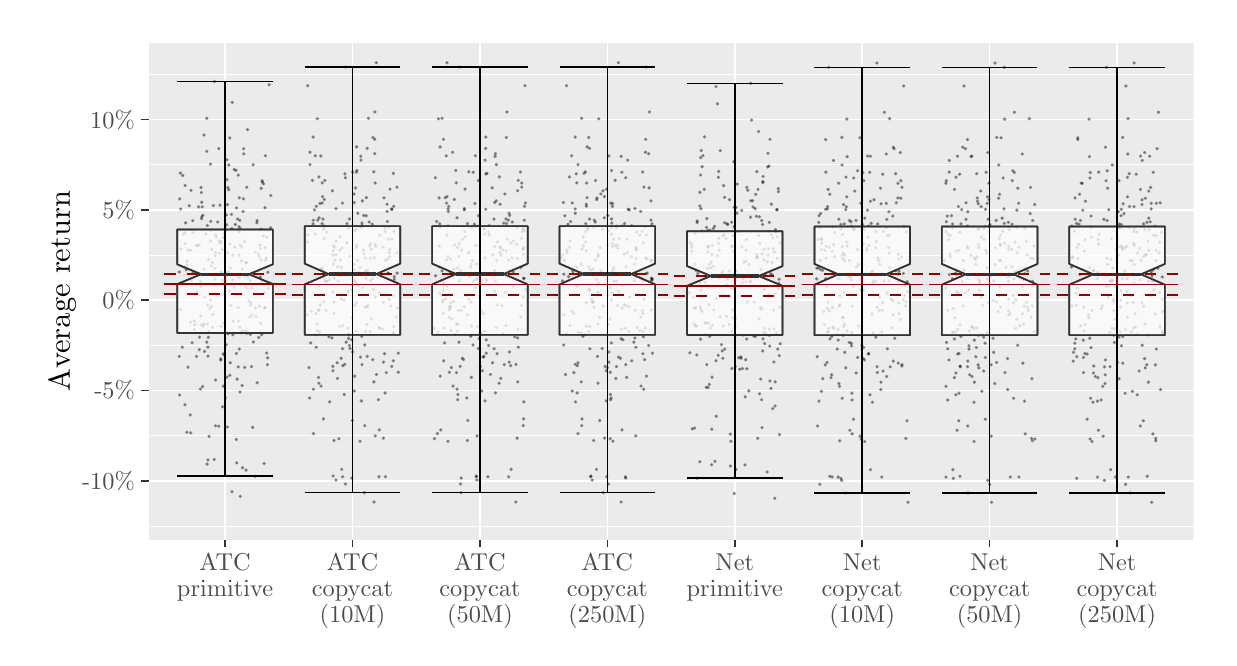
\begin{tikzpicture}[x=1pt,y=1pt]
\definecolor{fillColor}{RGB}{255,255,255}
\path[use as bounding box,fill=fillColor,fill opacity=0.00] (0,0) rectangle (426.79,220.51);
\begin{scope}
\path[clip] (  0.00,  0.00) rectangle (426.79,220.51);
\definecolor{drawColor}{RGB}{255,255,255}
\definecolor{fillColor}{RGB}{255,255,255}

\path[draw=drawColor,line width= 0.6pt,line join=round,line cap=round,fill=fillColor] (  0.00,  0.00) rectangle (426.79,220.51);
\end{scope}
\begin{scope}
\path[clip] ( 43.69, 35.52) rectangle (421.29,215.01);
\definecolor{fillColor}{gray}{0.92}

\path[fill=fillColor] ( 43.69, 35.52) rectangle (421.29,215.01);
\definecolor{drawColor}{RGB}{255,255,255}

\path[draw=drawColor,line width= 0.3pt,line join=round] ( 43.69, 40.41) --
	(421.29, 40.41);

\path[draw=drawColor,line width= 0.3pt,line join=round] ( 43.69, 73.05) --
	(421.29, 73.05);

\path[draw=drawColor,line width= 0.3pt,line join=round] ( 43.69,105.68) --
	(421.29,105.68);

\path[draw=drawColor,line width= 0.3pt,line join=round] ( 43.69,138.32) --
	(421.29,138.32);

\path[draw=drawColor,line width= 0.3pt,line join=round] ( 43.69,170.95) --
	(421.29,170.95);

\path[draw=drawColor,line width= 0.3pt,line join=round] ( 43.69,203.59) --
	(421.29,203.59);

\path[draw=drawColor,line width= 0.6pt,line join=round] ( 43.69, 56.73) --
	(421.29, 56.73);

\path[draw=drawColor,line width= 0.6pt,line join=round] ( 43.69, 89.37) --
	(421.29, 89.37);

\path[draw=drawColor,line width= 0.6pt,line join=round] ( 43.69,122.00) --
	(421.29,122.00);

\path[draw=drawColor,line width= 0.6pt,line join=round] ( 43.69,154.63) --
	(421.29,154.63);

\path[draw=drawColor,line width= 0.6pt,line join=round] ( 43.69,187.27) --
	(421.29,187.27);

\path[draw=drawColor,line width= 0.6pt,line join=round] ( 71.32, 35.52) --
	( 71.32,215.01);

\path[draw=drawColor,line width= 0.6pt,line join=round] (117.37, 35.52) --
	(117.37,215.01);

\path[draw=drawColor,line width= 0.6pt,line join=round] (163.42, 35.52) --
	(163.42,215.01);

\path[draw=drawColor,line width= 0.6pt,line join=round] (209.47, 35.52) --
	(209.47,215.01);

\path[draw=drawColor,line width= 0.6pt,line join=round] (255.51, 35.52) --
	(255.51,215.01);

\path[draw=drawColor,line width= 0.6pt,line join=round] (301.56, 35.52) --
	(301.56,215.01);

\path[draw=drawColor,line width= 0.6pt,line join=round] (347.61, 35.52) --
	(347.61,215.01);

\path[draw=drawColor,line width= 0.6pt,line join=round] (393.66, 35.52) --
	(393.66,215.01);
\definecolor{drawColor}{RGB}{0,0,0}
\definecolor{fillColor}{RGB}{0,0,0}

\path[draw=drawColor,draw opacity=0.30,line width= 0.4pt,line join=round,line cap=round,fill=fillColor,fill opacity=0.30] ( 60.95,141.77) circle (  0.46);

\path[draw=drawColor,draw opacity=0.30,line width= 0.4pt,line join=round,line cap=round,fill=fillColor,fill opacity=0.30] ( 83.97,141.97) circle (  0.46);

\path[draw=drawColor,draw opacity=0.30,line width= 0.4pt,line join=round,line cap=round,fill=fillColor,fill opacity=0.30] ( 64.94,113.36) circle (  0.46);

\path[draw=drawColor,draw opacity=0.30,line width= 0.4pt,line join=round,line cap=round,fill=fillColor,fill opacity=0.30] ( 82.92, 92.22) circle (  0.46);

\path[draw=drawColor,draw opacity=0.30,line width= 0.4pt,line join=round,line cap=round,fill=fillColor,fill opacity=0.30] ( 72.78,125.42) circle (  0.46);

\path[draw=drawColor,draw opacity=0.30,line width= 0.4pt,line join=round,line cap=round,fill=fillColor,fill opacity=0.30] ( 66.04,122.06) circle (  0.46);

\path[draw=drawColor,draw opacity=0.30,line width= 0.4pt,line join=round,line cap=round,fill=fillColor,fill opacity=0.30] ( 65.17,101.83) circle (  0.46);

\path[draw=drawColor,draw opacity=0.30,line width= 0.4pt,line join=round,line cap=round,fill=fillColor,fill opacity=0.30] ( 82.21,139.45) circle (  0.46);

\path[draw=drawColor,draw opacity=0.30,line width= 0.4pt,line join=round,line cap=round,fill=fillColor,fill opacity=0.30] ( 77.84,154.11) circle (  0.46);

\path[draw=drawColor,draw opacity=0.30,line width= 0.4pt,line join=round,line cap=round,fill=fillColor,fill opacity=0.30] ( 76.19,114.45) circle (  0.46);

\path[draw=drawColor,draw opacity=0.30,line width= 0.4pt,line join=round,line cap=round,fill=fillColor,fill opacity=0.30] ( 72.55,132.32) circle (  0.46);

\path[draw=drawColor,draw opacity=0.30,line width= 0.4pt,line join=round,line cap=round,fill=fillColor,fill opacity=0.30] ( 86.63, 98.72) circle (  0.46);

\path[draw=drawColor,draw opacity=0.30,line width= 0.4pt,line join=round,line cap=round,fill=fillColor,fill opacity=0.30] ( 76.53,130.20) circle (  0.46);

\path[draw=drawColor,draw opacity=0.30,line width= 0.4pt,line join=round,line cap=round,fill=fillColor,fill opacity=0.30] ( 86.82,126.29) circle (  0.46);

\path[draw=drawColor,draw opacity=0.30,line width= 0.4pt,line join=round,line cap=round,fill=fillColor,fill opacity=0.30] ( 76.82,147.88) circle (  0.46);

\path[draw=drawColor,draw opacity=0.30,line width= 0.4pt,line join=round,line cap=round,fill=fillColor,fill opacity=0.30] ( 58.90,140.05) circle (  0.46);

\path[draw=drawColor,draw opacity=0.30,line width= 0.4pt,line join=round,line cap=round,fill=fillColor,fill opacity=0.30] ( 85.95,136.41) circle (  0.46);

\path[draw=drawColor,draw opacity=0.30,line width= 0.4pt,line join=round,line cap=round,fill=fillColor,fill opacity=0.30] ( 70.26,140.33) circle (  0.46);

\path[draw=drawColor,draw opacity=0.30,line width= 0.4pt,line join=round,line cap=round,fill=fillColor,fill opacity=0.30] ( 82.81,150.03) circle (  0.46);

\path[draw=drawColor,draw opacity=0.30,line width= 0.4pt,line join=round,line cap=round,fill=fillColor,fill opacity=0.30] ( 63.08,155.77) circle (  0.46);

\path[draw=drawColor,draw opacity=0.30,line width= 0.4pt,line join=round,line cap=round,fill=fillColor,fill opacity=0.30] ( 67.66,129.71) circle (  0.46);

\path[draw=drawColor,draw opacity=0.30,line width= 0.4pt,line join=round,line cap=round,fill=fillColor,fill opacity=0.30] ( 74.84,141.25) circle (  0.46);

\path[draw=drawColor,draw opacity=0.30,line width= 0.4pt,line join=round,line cap=round,fill=fillColor,fill opacity=0.30] ( 79.20,110.08) circle (  0.46);

\path[draw=drawColor,draw opacity=0.30,line width= 0.4pt,line join=round,line cap=round,fill=fillColor,fill opacity=0.30] ( 71.67,147.18) circle (  0.46);

\path[draw=drawColor,draw opacity=0.30,line width= 0.4pt,line join=round,line cap=round,fill=fillColor,fill opacity=0.30] ( 70.42,128.98) circle (  0.46);

\path[draw=drawColor,draw opacity=0.30,line width= 0.4pt,line join=round,line cap=round,fill=fillColor,fill opacity=0.30] ( 57.27,133.07) circle (  0.46);

\path[draw=drawColor,draw opacity=0.30,line width= 0.4pt,line join=round,line cap=round,fill=fillColor,fill opacity=0.30] ( 67.90,139.25) circle (  0.46);

\path[draw=drawColor,draw opacity=0.30,line width= 0.4pt,line join=round,line cap=round,fill=fillColor,fill opacity=0.30] ( 59.74,132.15) circle (  0.46);

\path[draw=drawColor,draw opacity=0.30,line width= 0.4pt,line join=round,line cap=round,fill=fillColor,fill opacity=0.30] ( 76.38,148.57) circle (  0.46);

\path[draw=drawColor,draw opacity=0.30,line width= 0.4pt,line join=round,line cap=round,fill=fillColor,fill opacity=0.30] ( 85.85,140.99) circle (  0.46);

\path[draw=drawColor,draw opacity=0.30,line width= 0.4pt,line join=round,line cap=round,fill=fillColor,fill opacity=0.30] ( 78.79,110.82) circle (  0.46);

\path[draw=drawColor,draw opacity=0.30,line width= 0.4pt,line join=round,line cap=round,fill=fillColor,fill opacity=0.30] ( 70.41, 83.50) circle (  0.46);

\path[draw=drawColor,draw opacity=0.30,line width= 0.4pt,line join=round,line cap=round,fill=fillColor,fill opacity=0.30] ( 75.01,149.38) circle (  0.46);

\path[draw=drawColor,draw opacity=0.30,line width= 0.4pt,line join=round,line cap=round,fill=fillColor,fill opacity=0.30] ( 61.76,155.76) circle (  0.46);

\path[draw=drawColor,draw opacity=0.30,line width= 0.4pt,line join=round,line cap=round,fill=fillColor,fill opacity=0.30] ( 85.55,124.70) circle (  0.46);

\path[draw=drawColor,draw opacity=0.30,line width= 0.4pt,line join=round,line cap=round,fill=fillColor,fill opacity=0.30] ( 58.38,156.15) circle (  0.46);

\path[draw=drawColor,draw opacity=0.30,line width= 0.4pt,line join=round,line cap=round,fill=fillColor,fill opacity=0.30] ( 65.81,119.06) circle (  0.46);

\path[draw=drawColor,draw opacity=0.30,line width= 0.4pt,line join=round,line cap=round,fill=fillColor,fill opacity=0.30] ( 64.94,149.00) circle (  0.46);

\path[draw=drawColor,draw opacity=0.30,line width= 0.4pt,line join=round,line cap=round,fill=fillColor,fill opacity=0.30] ( 76.64,112.28) circle (  0.46);

\path[draw=drawColor,draw opacity=0.30,line width= 0.4pt,line join=round,line cap=round,fill=fillColor,fill opacity=0.30] ( 67.88, 93.21) circle (  0.46);

\path[draw=drawColor,draw opacity=0.30,line width= 0.4pt,line join=round,line cap=round,fill=fillColor,fill opacity=0.30] ( 67.79,138.05) circle (  0.46);

\path[draw=drawColor,draw opacity=0.30,line width= 0.4pt,line join=round,line cap=round,fill=fillColor,fill opacity=0.30] ( 78.03,176.75) circle (  0.46);

\path[draw=drawColor,draw opacity=0.30,line width= 0.4pt,line join=round,line cap=round,fill=fillColor,fill opacity=0.30] ( 82.89,150.81) circle (  0.46);

\path[draw=drawColor,draw opacity=0.30,line width= 0.4pt,line join=round,line cap=round,fill=fillColor,fill opacity=0.30] ( 81.48,170.97) circle (  0.46);

\path[draw=drawColor,draw opacity=0.30,line width= 0.4pt,line join=round,line cap=round,fill=fillColor,fill opacity=0.30] ( 66.76,112.26) circle (  0.46);

\path[draw=drawColor,draw opacity=0.30,line width= 0.4pt,line join=round,line cap=round,fill=fillColor,fill opacity=0.30] ( 72.64,161.92) circle (  0.46);

\path[draw=drawColor,draw opacity=0.30,line width= 0.4pt,line join=round,line cap=round,fill=fillColor,fill opacity=0.30] ( 80.87, 98.02) circle (  0.46);

\path[draw=drawColor,draw opacity=0.30,line width= 0.4pt,line join=round,line cap=round,fill=fillColor,fill opacity=0.30] ( 74.09,129.39) circle (  0.46);

\path[draw=drawColor,draw opacity=0.30,line width= 0.4pt,line join=round,line cap=round,fill=fillColor,fill opacity=0.30] ( 62.38,128.88) circle (  0.46);

\path[draw=drawColor,draw opacity=0.30,line width= 0.4pt,line join=round,line cap=round,fill=fillColor,fill opacity=0.30] ( 64.99,120.31) circle (  0.46);

\path[draw=drawColor,draw opacity=0.30,line width= 0.4pt,line join=round,line cap=round,fill=fillColor,fill opacity=0.30] ( 72.67,170.88) circle (  0.46);

\path[draw=drawColor,draw opacity=0.30,line width= 0.4pt,line join=round,line cap=round,fill=fillColor,fill opacity=0.30] ( 63.31,152.73) circle (  0.46);

\path[draw=drawColor,draw opacity=0.30,line width= 0.4pt,line join=round,line cap=round,fill=fillColor,fill opacity=0.30] ( 59.23,129.26) circle (  0.46);

\path[draw=drawColor,draw opacity=0.30,line width= 0.4pt,line join=round,line cap=round,fill=fillColor,fill opacity=0.30] ( 69.79,100.38) circle (  0.46);

\path[draw=drawColor,draw opacity=0.30,line width= 0.4pt,line join=round,line cap=round,fill=fillColor,fill opacity=0.30] ( 83.74,137.82) circle (  0.46);

\path[draw=drawColor,draw opacity=0.30,line width= 0.4pt,line join=round,line cap=round,fill=fillColor,fill opacity=0.30] ( 76.09, 97.93) circle (  0.46);

\path[draw=drawColor,draw opacity=0.30,line width= 0.4pt,line join=round,line cap=round,fill=fillColor,fill opacity=0.30] ( 60.60, 12.45) circle (  0.46);

\path[draw=drawColor,draw opacity=0.30,line width= 0.4pt,line join=round,line cap=round,fill=fillColor,fill opacity=0.30] ( 84.37,162.45) circle (  0.46);

\path[draw=drawColor,draw opacity=0.30,line width= 0.4pt,line join=round,line cap=round,fill=fillColor,fill opacity=0.30] ( 72.35,162.77) circle (  0.46);

\path[draw=drawColor,draw opacity=0.30,line width= 0.4pt,line join=round,line cap=round,fill=fillColor,fill opacity=0.30] ( 59.02,161.69) circle (  0.46);

\path[draw=drawColor,draw opacity=0.30,line width= 0.4pt,line join=round,line cap=round,fill=fillColor,fill opacity=0.30] ( 74.59,169.26) circle (  0.46);

\path[draw=drawColor,draw opacity=0.30,line width= 0.4pt,line join=round,line cap=round,fill=fillColor,fill opacity=0.30] ( 74.15,138.37) circle (  0.46);

\path[draw=drawColor,draw opacity=0.30,line width= 0.4pt,line join=round,line cap=round,fill=fillColor,fill opacity=0.30] ( 77.49, 91.22) circle (  0.46);

\path[draw=drawColor,draw opacity=0.30,line width= 0.4pt,line join=round,line cap=round,fill=fillColor,fill opacity=0.30] ( 56.85,146.38) circle (  0.46);

\path[draw=drawColor,draw opacity=0.30,line width= 0.4pt,line join=round,line cap=round,fill=fillColor,fill opacity=0.30] ( 62.90,157.43) circle (  0.46);

\path[draw=drawColor,draw opacity=0.30,line width= 0.4pt,line join=round,line cap=round,fill=fillColor,fill opacity=0.30] ( 80.56,120.23) circle (  0.46);

\path[draw=drawColor,draw opacity=0.30,line width= 0.4pt,line join=round,line cap=round,fill=fillColor,fill opacity=0.30] ( 87.87,159.89) circle (  0.46);

\path[draw=drawColor,draw opacity=0.30,line width= 0.4pt,line join=round,line cap=round,fill=fillColor,fill opacity=0.30] ( 72.33,110.02) circle (  0.46);

\path[draw=drawColor,draw opacity=0.30,line width= 0.4pt,line join=round,line cap=round,fill=fillColor,fill opacity=0.30] ( 63.40,112.62) circle (  0.46);

\path[draw=drawColor,draw opacity=0.30,line width= 0.4pt,line join=round,line cap=round,fill=fillColor,fill opacity=0.30] ( 58.80,114.07) circle (  0.46);

\path[draw=drawColor,draw opacity=0.30,line width= 0.4pt,line join=round,line cap=round,fill=fillColor,fill opacity=0.30] ( 75.85,151.35) circle (  0.46);

\path[draw=drawColor,draw opacity=0.30,line width= 0.4pt,line join=round,line cap=round,fill=fillColor,fill opacity=0.30] ( 85.75,155.45) circle (  0.46);

\path[draw=drawColor,draw opacity=0.30,line width= 0.4pt,line join=round,line cap=round,fill=fillColor,fill opacity=0.30] ( 79.41,183.68) circle (  0.46);

\path[draw=drawColor,draw opacity=0.30,line width= 0.4pt,line join=round,line cap=round,fill=fillColor,fill opacity=0.30] ( 75.42,102.80) circle (  0.46);

\path[draw=drawColor,draw opacity=0.30,line width= 0.4pt,line join=round,line cap=round,fill=fillColor,fill opacity=0.30] ( 55.18,167.96) circle (  0.46);

\path[draw=drawColor,draw opacity=0.30,line width= 0.4pt,line join=round,line cap=round,fill=fillColor,fill opacity=0.30] ( 62.83,151.50) circle (  0.46);

\path[draw=drawColor,draw opacity=0.30,line width= 0.4pt,line join=round,line cap=round,fill=fillColor,fill opacity=0.30] ( 72.03, 94.22) circle (  0.46);

\path[draw=drawColor,draw opacity=0.30,line width= 0.4pt,line join=round,line cap=round,fill=fillColor,fill opacity=0.30] ( 86.72,101.20) circle (  0.46);

\path[draw=drawColor,draw opacity=0.30,line width= 0.4pt,line join=round,line cap=round,fill=fillColor,fill opacity=0.30] ( 77.98,158.67) circle (  0.46);

\path[draw=drawColor,draw opacity=0.30,line width= 0.4pt,line join=round,line cap=round,fill=fillColor,fill opacity=0.30] ( 60.17,111.43) circle (  0.46);

\path[draw=drawColor,draw opacity=0.30,line width= 0.4pt,line join=round,line cap=round,fill=fillColor,fill opacity=0.30] ( 69.04,176.80) circle (  0.46);

\path[draw=drawColor,draw opacity=0.30,line width= 0.4pt,line join=round,line cap=round,fill=fillColor,fill opacity=0.30] ( 69.78,100.83) circle (  0.46);

\path[draw=drawColor,draw opacity=0.30,line width= 0.4pt,line join=round,line cap=round,fill=fillColor,fill opacity=0.30] ( 65.12,105.07) circle (  0.46);

\path[draw=drawColor,draw opacity=0.30,line width= 0.4pt,line join=round,line cap=round,fill=fillColor,fill opacity=0.30] ( 82.24, 58.41) circle (  0.46);

\path[draw=drawColor,draw opacity=0.30,line width= 0.4pt,line join=round,line cap=round,fill=fillColor,fill opacity=0.30] ( 71.81,152.85) circle (  0.46);

\path[draw=drawColor,draw opacity=0.30,line width= 0.4pt,line join=round,line cap=round,fill=fillColor,fill opacity=0.30] ( 73.08,142.33) circle (  0.46);

\path[draw=drawColor,draw opacity=0.30,line width= 0.4pt,line join=round,line cap=round,fill=fillColor,fill opacity=0.30] ( 75.55, 63.25) circle (  0.46);

\path[draw=drawColor,draw opacity=0.30,line width= 0.4pt,line join=round,line cap=round,fill=fillColor,fill opacity=0.30] ( 81.29, 76.08) circle (  0.46);

\path[draw=drawColor,draw opacity=0.30,line width= 0.4pt,line join=round,line cap=round,fill=fillColor,fill opacity=0.30] ( 63.69,181.72) circle (  0.46);

\path[draw=drawColor,draw opacity=0.30,line width= 0.4pt,line join=round,line cap=round,fill=fillColor,fill opacity=0.30] ( 80.49,129.16) circle (  0.46);

\path[draw=drawColor,draw opacity=0.30,line width= 0.4pt,line join=round,line cap=round,fill=fillColor,fill opacity=0.30] ( 82.49,116.11) circle (  0.46);

\path[draw=drawColor,draw opacity=0.30,line width= 0.4pt,line join=round,line cap=round,fill=fillColor,fill opacity=0.30] ( 55.86,105.04) circle (  0.46);

\path[draw=drawColor,draw opacity=0.30,line width= 0.4pt,line join=round,line cap=round,fill=fillColor,fill opacity=0.30] ( 54.87, 87.79) circle (  0.46);

\path[draw=drawColor,draw opacity=0.30,line width= 0.4pt,line join=round,line cap=round,fill=fillColor,fill opacity=0.30] ( 76.82, 51.15) circle (  0.46);

\path[draw=drawColor,draw opacity=0.30,line width= 0.4pt,line join=round,line cap=round,fill=fillColor,fill opacity=0.30] ( 76.65,150.89) circle (  0.46);

\path[draw=drawColor,draw opacity=0.30,line width= 0.4pt,line join=round,line cap=round,fill=fillColor,fill opacity=0.30] ( 71.97,172.78) circle (  0.46);

\path[draw=drawColor,draw opacity=0.30,line width= 0.4pt,line join=round,line cap=round,fill=fillColor,fill opacity=0.30] ( 66.53,140.32) circle (  0.46);

\path[draw=drawColor,draw opacity=0.30,line width= 0.4pt,line join=round,line cap=round,fill=fillColor,fill opacity=0.30] ( 77.62,111.00) circle (  0.46);

\path[draw=drawColor,draw opacity=0.30,line width= 0.4pt,line join=round,line cap=round,fill=fillColor,fill opacity=0.30] ( 86.34,102.94) circle (  0.46);

\path[draw=drawColor,draw opacity=0.30,line width= 0.4pt,line join=round,line cap=round,fill=fillColor,fill opacity=0.30] ( 54.94,158.64) circle (  0.46);

\path[draw=drawColor,draw opacity=0.30,line width= 0.4pt,line join=round,line cap=round,fill=fillColor,fill opacity=0.30] ( 73.19, 99.42) circle (  0.46);

\path[draw=drawColor,draw opacity=0.30,line width= 0.4pt,line join=round,line cap=round,fill=fillColor,fill opacity=0.30] ( 72.45,110.12) circle (  0.46);

\path[draw=drawColor,draw opacity=0.30,line width= 0.4pt,line join=round,line cap=round,fill=fillColor,fill opacity=0.30] ( 72.15, 76.20) circle (  0.46);

\path[draw=drawColor,draw opacity=0.30,line width= 0.4pt,line join=round,line cap=round,fill=fillColor,fill opacity=0.30] ( 78.92, 60.63) circle (  0.46);

\path[draw=drawColor,draw opacity=0.30,line width= 0.4pt,line join=round,line cap=round,fill=fillColor,fill opacity=0.30] ( 75.64,123.85) circle (  0.46);

\path[draw=drawColor,draw opacity=0.30,line width= 0.4pt,line join=round,line cap=round,fill=fillColor,fill opacity=0.30] ( 65.16, 64.32) circle (  0.46);

\path[draw=drawColor,draw opacity=0.30,line width= 0.4pt,line join=round,line cap=round,fill=fillColor,fill opacity=0.30] ( 62.63,162.76) circle (  0.46);

\path[draw=drawColor,draw opacity=0.30,line width= 0.4pt,line join=round,line cap=round,fill=fillColor,fill opacity=0.30] ( 84.85,164.67) circle (  0.46);

\path[draw=drawColor,draw opacity=0.30,line width= 0.4pt,line join=round,line cap=round,fill=fillColor,fill opacity=0.30] ( 71.46, 86.73) circle (  0.46);

\path[draw=drawColor,draw opacity=0.30,line width= 0.4pt,line join=round,line cap=round,fill=fillColor,fill opacity=0.30] ( 62.08,108.69) circle (  0.46);

\path[draw=drawColor,draw opacity=0.30,line width= 0.4pt,line join=round,line cap=round,fill=fillColor,fill opacity=0.30] ( 76.99,110.27) circle (  0.46);

\path[draw=drawColor,draw opacity=0.30,line width= 0.4pt,line join=round,line cap=round,fill=fillColor,fill opacity=0.30] ( 76.68,128.00) circle (  0.46);

\path[draw=drawColor,draw opacity=0.30,line width= 0.4pt,line join=round,line cap=round,fill=fillColor,fill opacity=0.30] ( 85.89,174.23) circle (  0.46);

\path[draw=drawColor,draw opacity=0.30,line width= 0.4pt,line join=round,line cap=round,fill=fillColor,fill opacity=0.30] ( 66.04,171.19) circle (  0.46);

\path[draw=drawColor,draw opacity=0.30,line width= 0.4pt,line join=round,line cap=round,fill=fillColor,fill opacity=0.30] ( 63.71,133.23) circle (  0.46);

\path[draw=drawColor,draw opacity=0.30,line width= 0.4pt,line join=round,line cap=round,fill=fillColor,fill opacity=0.30] ( 78.29,143.24) circle (  0.46);

\path[draw=drawColor,draw opacity=0.30,line width= 0.4pt,line join=round,line cap=round,fill=fillColor,fill opacity=0.30] ( 70.57,144.65) circle (  0.46);

\path[draw=drawColor,draw opacity=0.30,line width= 0.4pt,line join=round,line cap=round,fill=fillColor,fill opacity=0.30] ( 74.32,114.47) circle (  0.46);

\path[draw=drawColor,draw opacity=0.30,line width= 0.4pt,line join=round,line cap=round,fill=fillColor,fill opacity=0.30] ( 72.00,165.60) circle (  0.46);

\path[draw=drawColor,draw opacity=0.30,line width= 0.4pt,line join=round,line cap=round,fill=fillColor,fill opacity=0.30] ( 66.74,135.61) circle (  0.46);

\path[draw=drawColor,draw opacity=0.30,line width= 0.4pt,line join=round,line cap=round,fill=fillColor,fill opacity=0.30] ( 85.18,145.22) circle (  0.46);

\path[draw=drawColor,draw opacity=0.30,line width= 0.4pt,line join=round,line cap=round,fill=fillColor,fill opacity=0.30] ( 72.27,139.19) circle (  0.46);

\path[draw=drawColor,draw opacity=0.30,line width= 0.4pt,line join=round,line cap=round,fill=fillColor,fill opacity=0.30] ( 68.36,131.37) circle (  0.46);

\path[draw=drawColor,draw opacity=0.30,line width= 0.4pt,line join=round,line cap=round,fill=fillColor,fill opacity=0.30] ( 66.41,119.70) circle (  0.46);

\path[draw=drawColor,draw opacity=0.30,line width= 0.4pt,line join=round,line cap=round,fill=fillColor,fill opacity=0.30] ( 70.65,102.65) circle (  0.46);

\path[draw=drawColor,draw opacity=0.30,line width= 0.4pt,line join=round,line cap=round,fill=fillColor,fill opacity=0.30] ( 72.24,131.80) circle (  0.46);

\path[draw=drawColor,draw opacity=0.30,line width= 0.4pt,line join=round,line cap=round,fill=fillColor,fill opacity=0.30] ( 76.36,138.26) circle (  0.46);

\path[draw=drawColor,draw opacity=0.30,line width= 0.4pt,line join=round,line cap=round,fill=fillColor,fill opacity=0.30] ( 63.20, 90.82) circle (  0.46);

\path[draw=drawColor,draw opacity=0.30,line width= 0.4pt,line join=round,line cap=round,fill=fillColor,fill opacity=0.30] ( 85.52,119.22) circle (  0.46);

\path[draw=drawColor,draw opacity=0.30,line width= 0.4pt,line join=round,line cap=round,fill=fillColor,fill opacity=0.30] ( 56.87,142.48) circle (  0.46);

\path[draw=drawColor,draw opacity=0.30,line width= 0.4pt,line join=round,line cap=round,fill=fillColor,fill opacity=0.30] ( 66.43,134.41) circle (  0.46);

\path[draw=drawColor,draw opacity=0.30,line width= 0.4pt,line join=round,line cap=round,fill=fillColor,fill opacity=0.30] ( 76.47,159.03) circle (  0.46);

\path[draw=drawColor,draw opacity=0.30,line width= 0.4pt,line join=round,line cap=round,fill=fillColor,fill opacity=0.30] ( 71.01,146.05) circle (  0.46);

\path[draw=drawColor,draw opacity=0.30,line width= 0.4pt,line join=round,line cap=round,fill=fillColor,fill opacity=0.30] ( 76.48,104.39) circle (  0.46);

\path[draw=drawColor,draw opacity=0.30,line width= 0.4pt,line join=round,line cap=round,fill=fillColor,fill opacity=0.30] ( 86.19,137.22) circle (  0.46);

\path[draw=drawColor,draw opacity=0.30,line width= 0.4pt,line join=round,line cap=round,fill=fillColor,fill opacity=0.30] ( 80.47,109.63) circle (  0.46);

\path[draw=drawColor,draw opacity=0.30,line width= 0.4pt,line join=round,line cap=round,fill=fillColor,fill opacity=0.30] ( 61.01,101.73) circle (  0.46);

\path[draw=drawColor,draw opacity=0.30,line width= 0.4pt,line join=round,line cap=round,fill=fillColor,fill opacity=0.30] ( 59.66,150.78) circle (  0.46);

\path[draw=drawColor,draw opacity=0.30,line width= 0.4pt,line join=round,line cap=round,fill=fillColor,fill opacity=0.30] ( 67.68,133.52) circle (  0.46);

\path[draw=drawColor,draw opacity=0.30,line width= 0.4pt,line join=round,line cap=round,fill=fillColor,fill opacity=0.30] ( 73.66,153.04) circle (  0.46);

\path[draw=drawColor,draw opacity=0.30,line width= 0.4pt,line join=round,line cap=round,fill=fillColor,fill opacity=0.30] ( 82.29,119.20) circle (  0.46);

\path[draw=drawColor,draw opacity=0.30,line width= 0.4pt,line join=round,line cap=round,fill=fillColor,fill opacity=0.30] ( 62.67,130.93) circle (  0.46);

\path[draw=drawColor,draw opacity=0.30,line width= 0.4pt,line join=round,line cap=round,fill=fillColor,fill opacity=0.30] ( 59.44,106.65) circle (  0.46);

\path[draw=drawColor,draw opacity=0.30,line width= 0.4pt,line join=round,line cap=round,fill=fillColor,fill opacity=0.30] ( 71.85,149.29) circle (  0.46);

\path[draw=drawColor,draw opacity=0.30,line width= 0.4pt,line join=round,line cap=round,fill=fillColor,fill opacity=0.30] ( 67.67,127.74) circle (  0.46);

\path[draw=drawColor,draw opacity=0.30,line width= 0.4pt,line join=round,line cap=round,fill=fillColor,fill opacity=0.30] ( 67.09,156.24) circle (  0.46);

\path[draw=drawColor,draw opacity=0.30,line width= 0.4pt,line join=round,line cap=round,fill=fillColor,fill opacity=0.30] ( 73.47,120.09) circle (  0.46);

\path[draw=drawColor,draw opacity=0.30,line width= 0.4pt,line join=round,line cap=round,fill=fillColor,fill opacity=0.30] ( 83.42,138.77) circle (  0.46);

\path[draw=drawColor,draw opacity=0.30,line width= 0.4pt,line join=round,line cap=round,fill=fillColor,fill opacity=0.30] ( 84.04,130.33) circle (  0.46);

\path[draw=drawColor,draw opacity=0.30,line width= 0.4pt,line join=round,line cap=round,fill=fillColor,fill opacity=0.30] ( 73.06, 94.89) circle (  0.46);

\path[draw=drawColor,draw opacity=0.30,line width= 0.4pt,line join=round,line cap=round,fill=fillColor,fill opacity=0.30] ( 80.54,121.11) circle (  0.46);

\path[draw=drawColor,draw opacity=0.30,line width= 0.4pt,line join=round,line cap=round,fill=fillColor,fill opacity=0.30] ( 69.86,112.60) circle (  0.46);

\path[draw=drawColor,draw opacity=0.30,line width= 0.4pt,line join=round,line cap=round,fill=fillColor,fill opacity=0.30] ( 65.35,136.76) circle (  0.46);

\path[draw=drawColor,draw opacity=0.30,line width= 0.4pt,line join=round,line cap=round,fill=fillColor,fill opacity=0.30] ( 77.60,133.26) circle (  0.46);

\path[draw=drawColor,draw opacity=0.30,line width= 0.4pt,line join=round,line cap=round,fill=fillColor,fill opacity=0.30] ( 59.73,146.44) circle (  0.46);

\path[draw=drawColor,draw opacity=0.30,line width= 0.4pt,line join=round,line cap=round,fill=fillColor,fill opacity=0.30] ( 57.98,140.14) circle (  0.46);

\path[draw=drawColor,draw opacity=0.30,line width= 0.4pt,line join=round,line cap=round,fill=fillColor,fill opacity=0.30] ( 70.87,127.99) circle (  0.46);

\path[draw=drawColor,draw opacity=0.30,line width= 0.4pt,line join=round,line cap=round,fill=fillColor,fill opacity=0.30] ( 79.04,135.59) circle (  0.46);

\path[draw=drawColor,draw opacity=0.30,line width= 0.4pt,line join=round,line cap=round,fill=fillColor,fill opacity=0.30] ( 66.89,116.86) circle (  0.46);

\path[draw=drawColor,draw opacity=0.30,line width= 0.4pt,line join=round,line cap=round,fill=fillColor,fill opacity=0.30] ( 79.64,130.39) circle (  0.46);

\path[draw=drawColor,draw opacity=0.30,line width= 0.4pt,line join=round,line cap=round,fill=fillColor,fill opacity=0.30] ( 56.24,145.87) circle (  0.46);

\path[draw=drawColor,draw opacity=0.30,line width= 0.4pt,line join=round,line cap=round,fill=fillColor,fill opacity=0.30] ( 66.06,147.37) circle (  0.46);

\path[draw=drawColor,draw opacity=0.30,line width= 0.4pt,line join=round,line cap=round,fill=fillColor,fill opacity=0.30] ( 80.28,115.98) circle (  0.46);

\path[draw=drawColor,draw opacity=0.30,line width= 0.4pt,line join=round,line cap=round,fill=fillColor,fill opacity=0.30] ( 54.76,101.73) circle (  0.46);

\path[draw=drawColor,draw opacity=0.30,line width= 0.4pt,line join=round,line cap=round,fill=fillColor,fill opacity=0.30] ( 71.53,127.70) circle (  0.46);

\path[draw=drawColor,draw opacity=0.30,line width= 0.4pt,line join=round,line cap=round,fill=fillColor,fill opacity=0.30] ( 87.78,148.18) circle (  0.46);

\path[draw=drawColor,draw opacity=0.30,line width= 0.4pt,line join=round,line cap=round,fill=fillColor,fill opacity=0.30] ( 77.29,141.27) circle (  0.46);

\path[draw=drawColor,draw opacity=0.30,line width= 0.4pt,line join=round,line cap=round,fill=fillColor,fill opacity=0.30] ( 76.71, 88.86) circle (  0.46);

\path[draw=drawColor,draw opacity=0.30,line width= 0.4pt,line join=round,line cap=round,fill=fillColor,fill opacity=0.30] ( 55.24,118.69) circle (  0.46);

\path[draw=drawColor,draw opacity=0.30,line width= 0.4pt,line join=round,line cap=round,fill=fillColor,fill opacity=0.30] ( 67.87, 76.64) circle (  0.46);

\path[draw=drawColor,draw opacity=0.30,line width= 0.4pt,line join=round,line cap=round,fill=fillColor,fill opacity=0.30] ( 65.27,108.62) circle (  0.46);

\path[draw=drawColor,draw opacity=0.30,line width= 0.4pt,line join=round,line cap=round,fill=fillColor,fill opacity=0.30] ( 60.23,114.46) circle (  0.46);

\path[draw=drawColor,draw opacity=0.30,line width= 0.4pt,line join=round,line cap=round,fill=fillColor,fill opacity=0.30] ( 69.47,156.38) circle (  0.46);

\path[draw=drawColor,draw opacity=0.30,line width= 0.4pt,line join=round,line cap=round,fill=fillColor,fill opacity=0.30] ( 61.98,141.94) circle (  0.46);

\path[draw=drawColor,draw opacity=0.30,line width= 0.4pt,line join=round,line cap=round,fill=fillColor,fill opacity=0.30] ( 65.54, 72.79) circle (  0.46);

\path[draw=drawColor,draw opacity=0.30,line width= 0.4pt,line join=round,line cap=round,fill=fillColor,fill opacity=0.30] ( 63.68,113.38) circle (  0.46);

\path[draw=drawColor,draw opacity=0.30,line width= 0.4pt,line join=round,line cap=round,fill=fillColor,fill opacity=0.30] ( 74.60,126.83) circle (  0.46);

\path[draw=drawColor,draw opacity=0.30,line width= 0.4pt,line join=round,line cap=round,fill=fillColor,fill opacity=0.30] ( 73.82, 52.84) circle (  0.46);

\path[draw=drawColor,draw opacity=0.30,line width= 0.4pt,line join=round,line cap=round,fill=fillColor,fill opacity=0.30] ( 67.40, 64.48) circle (  0.46);

\path[draw=drawColor,draw opacity=0.30,line width= 0.4pt,line join=round,line cap=round,fill=fillColor,fill opacity=0.30] ( 76.40,146.77) circle (  0.46);

\path[draw=drawColor,draw opacity=0.30,line width= 0.4pt,line join=round,line cap=round,fill=fillColor,fill opacity=0.30] ( 58.92, 74.11) circle (  0.46);

\path[draw=drawColor,draw opacity=0.30,line width= 0.4pt,line join=round,line cap=round,fill=fillColor,fill opacity=0.30] ( 64.83, 62.80) circle (  0.46);

\path[draw=drawColor,draw opacity=0.30,line width= 0.4pt,line join=round,line cap=round,fill=fillColor,fill opacity=0.30] ( 64.72,175.81) circle (  0.46);

\path[draw=drawColor,draw opacity=0.30,line width= 0.4pt,line join=round,line cap=round,fill=fillColor,fill opacity=0.30] ( 67.52,201.03) circle (  0.46);

\path[draw=drawColor,draw opacity=0.30,line width= 0.4pt,line join=round,line cap=round,fill=fillColor,fill opacity=0.30] ( 85.21,164.08) circle (  0.46);

\path[draw=drawColor,draw opacity=0.30,line width= 0.4pt,line join=round,line cap=round,fill=fillColor,fill opacity=0.30] ( 68.41,123.76) circle (  0.46);

\path[draw=drawColor,draw opacity=0.30,line width= 0.4pt,line join=round,line cap=round,fill=fillColor,fill opacity=0.30] ( 78.07,174.92) circle (  0.46);

\path[draw=drawColor,draw opacity=0.30,line width= 0.4pt,line join=round,line cap=round,fill=fillColor,fill opacity=0.30] ( 69.56,142.69) circle (  0.46);

\path[draw=drawColor,draw opacity=0.30,line width= 0.4pt,line join=round,line cap=round,fill=fillColor,fill opacity=0.30] ( 75.45,155.37) circle (  0.46);

\path[draw=drawColor,draw opacity=0.30,line width= 0.4pt,line join=round,line cap=round,fill=fillColor,fill opacity=0.30] ( 71.05,102.20) circle (  0.46);

\path[draw=drawColor,draw opacity=0.30,line width= 0.4pt,line join=round,line cap=round,fill=fillColor,fill opacity=0.30] ( 62.92,152.18) circle (  0.46);

\path[draw=drawColor,draw opacity=0.30,line width= 0.4pt,line join=round,line cap=round,fill=fillColor,fill opacity=0.30] ( 73.77,147.95) circle (  0.46);

\path[draw=drawColor,draw opacity=0.30,line width= 0.4pt,line join=round,line cap=round,fill=fillColor,fill opacity=0.30] ( 78.42, 97.75) circle (  0.46);

\path[draw=drawColor,draw opacity=0.30,line width= 0.4pt,line join=round,line cap=round,fill=fillColor,fill opacity=0.30] ( 66.08,143.41) circle (  0.46);

\path[draw=drawColor,draw opacity=0.30,line width= 0.4pt,line join=round,line cap=round,fill=fillColor,fill opacity=0.30] ( 56.90,163.47) circle (  0.46);

\path[draw=drawColor,draw opacity=0.30,line width= 0.4pt,line join=round,line cap=round,fill=fillColor,fill opacity=0.30] ( 84.29,136.62) circle (  0.46);

\path[draw=drawColor,draw opacity=0.30,line width= 0.4pt,line join=round,line cap=round,fill=fillColor,fill opacity=0.30] ( 75.39, 71.70) circle (  0.46);

\path[draw=drawColor,draw opacity=0.30,line width= 0.4pt,line join=round,line cap=round,fill=fillColor,fill opacity=0.30] ( 62.41, 89.92) circle (  0.46);

\path[draw=drawColor,draw opacity=0.30,line width= 0.4pt,line join=round,line cap=round,fill=fillColor,fill opacity=0.30] ( 56.04,167.09) circle (  0.46);

\path[draw=drawColor,draw opacity=0.30,line width= 0.4pt,line join=round,line cap=round,fill=fillColor,fill opacity=0.30] ( 75.69, 93.51) circle (  0.46);

\path[draw=drawColor,draw opacity=0.30,line width= 0.4pt,line join=round,line cap=round,fill=fillColor,fill opacity=0.30] ( 64.71,187.77) circle (  0.46);

\path[draw=drawColor,draw opacity=0.30,line width= 0.4pt,line join=round,line cap=round,fill=fillColor,fill opacity=0.30] ( 84.56,147.66) circle (  0.46);

\path[draw=drawColor,draw opacity=0.30,line width= 0.4pt,line join=round,line cap=round,fill=fillColor,fill opacity=0.30] ( 62.65,127.04) circle (  0.46);

\path[draw=drawColor,draw opacity=0.30,line width= 0.4pt,line join=round,line cap=round,fill=fillColor,fill opacity=0.30] ( 84.71,165.16) circle (  0.46);

\path[draw=drawColor,draw opacity=0.30,line width= 0.4pt,line join=round,line cap=round,fill=fillColor,fill opacity=0.30] ( 54.80,132.24) circle (  0.46);

\path[draw=drawColor,draw opacity=0.30,line width= 0.4pt,line join=round,line cap=round,fill=fillColor,fill opacity=0.30] ( 67.91,145.59) circle (  0.46);

\path[draw=drawColor,draw opacity=0.30,line width= 0.4pt,line join=round,line cap=round,fill=fillColor,fill opacity=0.30] ( 84.61,128.76) circle (  0.46);

\path[draw=drawColor,draw opacity=0.30,line width= 0.4pt,line join=round,line cap=round,fill=fillColor,fill opacity=0.30] ( 69.90,143.20) circle (  0.46);

\path[draw=drawColor,draw opacity=0.30,line width= 0.4pt,line join=round,line cap=round,fill=fillColor,fill opacity=0.30] ( 62.73,113.11) circle (  0.46);

\path[draw=drawColor,draw opacity=0.30,line width= 0.4pt,line join=round,line cap=round,fill=fillColor,fill opacity=0.30] ( 65.53,110.76) circle (  0.46);

\path[draw=drawColor,draw opacity=0.30,line width= 0.4pt,line join=round,line cap=round,fill=fillColor,fill opacity=0.30] ( 81.57,106.93) circle (  0.46);

\path[draw=drawColor,draw opacity=0.30,line width= 0.4pt,line join=round,line cap=round,fill=fillColor,fill opacity=0.30] ( 69.04, 76.51) circle (  0.46);

\path[draw=drawColor,draw opacity=0.30,line width= 0.4pt,line join=round,line cap=round,fill=fillColor,fill opacity=0.30] ( 77.63, 61.49) circle (  0.46);

\path[draw=drawColor,draw opacity=0.30,line width= 0.4pt,line join=round,line cap=round,fill=fillColor,fill opacity=0.30] ( 87.26,199.89) circle (  0.46);

\path[draw=drawColor,draw opacity=0.30,line width= 0.4pt,line join=round,line cap=round,fill=fillColor,fill opacity=0.30] ( 62.56,116.34) circle (  0.46);

\path[draw=drawColor,draw opacity=0.30,line width= 0.4pt,line join=round,line cap=round,fill=fillColor,fill opacity=0.30] ( 85.75,119.38) circle (  0.46);

\path[draw=drawColor,draw opacity=0.30,line width= 0.4pt,line join=round,line cap=round,fill=fillColor,fill opacity=0.30] ( 62.78,160.95) circle (  0.46);

\path[draw=drawColor,draw opacity=0.30,line width= 0.4pt,line join=round,line cap=round,fill=fillColor,fill opacity=0.30] ( 68.63,150.30) circle (  0.46);

\path[draw=drawColor,draw opacity=0.30,line width= 0.4pt,line join=round,line cap=round,fill=fillColor,fill opacity=0.30] ( 78.87,135.63) circle (  0.46);

\path[draw=drawColor,draw opacity=0.30,line width= 0.4pt,line join=round,line cap=round,fill=fillColor,fill opacity=0.30] ( 81.05,116.66) circle (  0.46);

\path[draw=drawColor,draw opacity=0.30,line width= 0.4pt,line join=round,line cap=round,fill=fillColor,fill opacity=0.30] ( 57.53, 74.31) circle (  0.46);

\path[draw=drawColor,draw opacity=0.30,line width= 0.4pt,line join=round,line cap=round,fill=fillColor,fill opacity=0.30] ( 64.36,145.95) circle (  0.46);

\path[draw=drawColor,draw opacity=0.30,line width= 0.4pt,line join=round,line cap=round,fill=fillColor,fill opacity=0.30] ( 61.25,124.97) circle (  0.46);

\path[draw=drawColor,draw opacity=0.30,line width= 0.4pt,line join=round,line cap=round,fill=fillColor,fill opacity=0.30] ( 84.05,140.76) circle (  0.46);

\path[draw=drawColor,draw opacity=0.30,line width= 0.4pt,line join=round,line cap=round,fill=fillColor,fill opacity=0.30] ( 69.25,138.98) circle (  0.46);

\path[draw=drawColor,draw opacity=0.30,line width= 0.4pt,line join=round,line cap=round,fill=fillColor,fill opacity=0.30] ( 84.18,113.70) circle (  0.46);

\path[draw=drawColor,draw opacity=0.30,line width= 0.4pt,line join=round,line cap=round,fill=fillColor,fill opacity=0.30] ( 58.72, 80.57) circle (  0.46);

\path[draw=drawColor,draw opacity=0.30,line width= 0.4pt,line join=round,line cap=round,fill=fillColor,fill opacity=0.30] ( 56.50,134.05) circle (  0.46);

\path[draw=drawColor,draw opacity=0.30,line width= 0.4pt,line join=round,line cap=round,fill=fillColor,fill opacity=0.30] ( 55.42,140.57) circle (  0.46);

\path[draw=drawColor,draw opacity=0.30,line width= 0.4pt,line join=round,line cap=round,fill=fillColor,fill opacity=0.30] ( 64.73,106.87) circle (  0.46);

\path[draw=drawColor,draw opacity=0.30,line width= 0.4pt,line join=round,line cap=round,fill=fillColor,fill opacity=0.30] ( 73.04,180.66) circle (  0.46);

\path[draw=drawColor,draw opacity=0.30,line width= 0.4pt,line join=round,line cap=round,fill=fillColor,fill opacity=0.30] ( 60.51,124.01) circle (  0.46);

\path[draw=drawColor,draw opacity=0.30,line width= 0.4pt,line join=round,line cap=round,fill=fillColor,fill opacity=0.30] ( 60.38,113.14) circle (  0.46);

\path[draw=drawColor,draw opacity=0.30,line width= 0.4pt,line join=round,line cap=round,fill=fillColor,fill opacity=0.30] ( 85.45, 63.03) circle (  0.46);

\path[draw=drawColor,draw opacity=0.30,line width= 0.4pt,line join=round,line cap=round,fill=fillColor,fill opacity=0.30] ( 56.84, 84.25) circle (  0.46);

\path[draw=drawColor,draw opacity=0.30,line width= 0.4pt,line join=round,line cap=round,fill=fillColor,fill opacity=0.30] ( 74.13,109.55) circle (  0.46);

\path[draw=drawColor,draw opacity=0.30,line width= 0.4pt,line join=round,line cap=round,fill=fillColor,fill opacity=0.30] ( 76.09,167.23) circle (  0.46);

\path[draw=drawColor,draw opacity=0.30,line width= 0.4pt,line join=round,line cap=round,fill=fillColor,fill opacity=0.30] ( 68.22,144.87) circle (  0.46);

\path[draw=drawColor,draw opacity=0.30,line width= 0.4pt,line join=round,line cap=round,fill=fillColor,fill opacity=0.30] ( 79.14,162.85) circle (  0.46);

\path[draw=drawColor,draw opacity=0.30,line width= 0.4pt,line join=round,line cap=round,fill=fillColor,fill opacity=0.30] ( 75.27,168.98) circle (  0.46);

\path[draw=drawColor,draw opacity=0.30,line width= 0.4pt,line join=round,line cap=round,fill=fillColor,fill opacity=0.30] ( 69.14,143.44) circle (  0.46);

\path[draw=drawColor,draw opacity=0.30,line width= 0.4pt,line join=round,line cap=round,fill=fillColor,fill opacity=0.30] ( 79.92,121.85) circle (  0.46);

\path[draw=drawColor,draw opacity=0.30,line width= 0.4pt,line join=round,line cap=round,fill=fillColor,fill opacity=0.30] ( 66.14,150.52) circle (  0.46);

\path[draw=drawColor,draw opacity=0.30,line width= 0.4pt,line join=round,line cap=round,fill=fillColor,fill opacity=0.30] ( 70.65, 90.97) circle (  0.46);

\path[draw=drawColor,draw opacity=0.30,line width= 0.4pt,line join=round,line cap=round,fill=fillColor,fill opacity=0.30] ( 72.16,156.57) circle (  0.46);

\path[draw=drawColor,draw opacity=0.30,line width= 0.4pt,line join=round,line cap=round,fill=fillColor,fill opacity=0.30] ( 76.74,141.93) circle (  0.46);

\path[draw=drawColor,draw opacity=0.30,line width= 0.4pt,line join=round,line cap=round,fill=fillColor,fill opacity=0.30] ( 76.07,119.39) circle (  0.46);

\path[draw=drawColor,draw opacity=0.30,line width= 0.4pt,line join=round,line cap=round,fill=fillColor,fill opacity=0.30] ( 77.31,136.27) circle (  0.46);

\path[draw=drawColor,draw opacity=0.30,line width= 0.4pt,line join=round,line cap=round,fill=fillColor,fill opacity=0.30] ( 57.91, 97.83) circle (  0.46);

\path[draw=drawColor,draw opacity=0.30,line width= 0.4pt,line join=round,line cap=round,fill=fillColor,fill opacity=0.30] ( 73.94,193.50) circle (  0.46);

\path[draw=drawColor,draw opacity=0.30,line width= 0.4pt,line join=round,line cap=round,fill=fillColor,fill opacity=0.30] ( 81.01,126.44) circle (  0.46);

\path[draw=drawColor,draw opacity=0.30,line width= 0.4pt,line join=round,line cap=round,fill=fillColor,fill opacity=0.30] ( 69.92,132.18) circle (  0.46);

\path[draw=drawColor,draw opacity=0.30,line width= 0.4pt,line join=round,line cap=round,fill=fillColor,fill opacity=0.30] ( 63.87,103.53) circle (  0.46);

\path[draw=drawColor,draw opacity=0.30,line width= 0.4pt,line join=round,line cap=round,fill=fillColor,fill opacity=0.30] ( 83.71,119.84) circle (  0.46);

\path[draw=drawColor,draw opacity=0.30,line width= 0.4pt,line join=round,line cap=round,fill=fillColor,fill opacity=0.30] ( 57.00,128.02) circle (  0.46);

\path[draw=drawColor,draw opacity=0.30,line width= 0.4pt,line join=round,line cap=round,fill=fillColor,fill opacity=0.30] ( 62.03,104.18) circle (  0.46);

\path[draw=drawColor,draw opacity=0.30,line width= 0.4pt,line join=round,line cap=round,fill=fillColor,fill opacity=0.30] ( 86.38,144.85) circle (  0.46);

\path[draw=drawColor,draw opacity=0.30,line width= 0.4pt,line join=round,line cap=round,fill=fillColor,fill opacity=0.30] ( 83.47,108.58) circle (  0.46);

\path[draw=drawColor,draw opacity=0.30,line width= 0.4pt,line join=round,line cap=round,fill=fillColor,fill opacity=0.30] ( 73.31,133.69) circle (  0.46);

\path[draw=drawColor,draw opacity=0.30,line width= 0.4pt,line join=round,line cap=round,fill=fillColor,fill opacity=0.30] ( 57.68,134.76) circle (  0.46);

\path[draw=drawColor,draw opacity=0.30,line width= 0.4pt,line join=round,line cap=round,fill=fillColor,fill opacity=0.30] ( 55.29,154.99) circle (  0.46);

\path[draw=drawColor,draw opacity=0.30,line width= 0.4pt,line join=round,line cap=round,fill=fillColor,fill opacity=0.30] ( 57.60,136.15) circle (  0.46);

\path[draw=drawColor,draw opacity=0.30,line width= 0.4pt,line join=round,line cap=round,fill=fillColor,fill opacity=0.30] ( 86.81,132.12) circle (  0.46);

\path[draw=drawColor,draw opacity=0.30,line width= 0.4pt,line join=round,line cap=round,fill=fillColor,fill opacity=0.30] ( 70.90,113.79) circle (  0.46);

\path[draw=drawColor,draw opacity=0.30,line width= 0.4pt,line join=round,line cap=round,fill=fillColor,fill opacity=0.30] ( 61.33,141.84) circle (  0.46);

\path[draw=drawColor,draw opacity=0.30,line width= 0.4pt,line join=round,line cap=round,fill=fillColor,fill opacity=0.30] ( 71.73,105.98) circle (  0.46);

\path[draw=drawColor,draw opacity=0.30,line width= 0.4pt,line join=round,line cap=round,fill=fillColor,fill opacity=0.30] ( 83.75,147.39) circle (  0.46);

\path[draw=drawColor,draw opacity=0.30,line width= 0.4pt,line join=round,line cap=round,fill=fillColor,fill opacity=0.30] ( 78.85,126.64) circle (  0.46);

\path[draw=drawColor,draw opacity=0.30,line width= 0.4pt,line join=round,line cap=round,fill=fillColor,fill opacity=0.30] ( 63.91,123.11) circle (  0.46);

\path[draw=drawColor,draw opacity=0.30,line width= 0.4pt,line join=round,line cap=round,fill=fillColor,fill opacity=0.30] ( 57.08,149.97) circle (  0.46);

\path[draw=drawColor,draw opacity=0.30,line width= 0.4pt,line join=round,line cap=round,fill=fillColor,fill opacity=0.30] ( 78.52,130.73) circle (  0.46);

\path[draw=drawColor,draw opacity=0.30,line width= 0.4pt,line join=round,line cap=round,fill=fillColor,fill opacity=0.30] ( 73.58,131.46) circle (  0.46);

\path[draw=drawColor,draw opacity=0.30,line width= 0.4pt,line join=round,line cap=round,fill=fillColor,fill opacity=0.30] ( 84.56,109.57) circle (  0.46);

\path[draw=drawColor,draw opacity=0.30,line width= 0.4pt,line join=round,line cap=round,fill=fillColor,fill opacity=0.30] (110.32,139.85) circle (  0.46);

\path[draw=drawColor,draw opacity=0.30,line width= 0.4pt,line join=round,line cap=round,fill=fillColor,fill opacity=0.30] (123.87,142.41) circle (  0.46);

\path[draw=drawColor,draw opacity=0.30,line width= 0.4pt,line join=round,line cap=round,fill=fillColor,fill opacity=0.30] (113.93,112.87) circle (  0.46);

\path[draw=drawColor,draw opacity=0.30,line width= 0.4pt,line join=round,line cap=round,fill=fillColor,fill opacity=0.30] (103.24, 89.86) circle (  0.46);

\path[draw=drawColor,draw opacity=0.30,line width= 0.4pt,line join=round,line cap=round,fill=fillColor,fill opacity=0.30] (124.86,125.87) circle (  0.46);

\path[draw=drawColor,draw opacity=0.30,line width= 0.4pt,line join=round,line cap=round,fill=fillColor,fill opacity=0.30] (114.27,122.09) circle (  0.46);

\path[draw=drawColor,draw opacity=0.30,line width= 0.4pt,line join=round,line cap=round,fill=fillColor,fill opacity=0.30] (128.59, 99.65) circle (  0.46);

\path[draw=drawColor,draw opacity=0.30,line width= 0.4pt,line join=round,line cap=round,fill=fillColor,fill opacity=0.30] (118.76,141.06) circle (  0.46);

\path[draw=drawColor,draw opacity=0.30,line width= 0.4pt,line join=round,line cap=round,fill=fillColor,fill opacity=0.30] (132.25,155.93) circle (  0.46);

\path[draw=drawColor,draw opacity=0.30,line width= 0.4pt,line join=round,line cap=round,fill=fillColor,fill opacity=0.30] (112.81,112.63) circle (  0.46);

\path[draw=drawColor,draw opacity=0.30,line width= 0.4pt,line join=round,line cap=round,fill=fillColor,fill opacity=0.30] (118.08,132.94) circle (  0.46);

\path[draw=drawColor,draw opacity=0.30,line width= 0.4pt,line join=round,line cap=round,fill=fillColor,fill opacity=0.30] (110.30, 96.54) circle (  0.46);

\path[draw=drawColor,draw opacity=0.30,line width= 0.4pt,line join=round,line cap=round,fill=fillColor,fill opacity=0.30] (133.51,131.81) circle (  0.46);

\path[draw=drawColor,draw opacity=0.30,line width= 0.4pt,line join=round,line cap=round,fill=fillColor,fill opacity=0.30] (120.95,126.55) circle (  0.46);

\path[draw=drawColor,draw opacity=0.30,line width= 0.4pt,line join=round,line cap=round,fill=fillColor,fill opacity=0.30] (123.40,150.27) circle (  0.46);

\path[draw=drawColor,draw opacity=0.30,line width= 0.4pt,line join=round,line cap=round,fill=fillColor,fill opacity=0.30] (121.33,140.14) circle (  0.46);

\path[draw=drawColor,draw opacity=0.30,line width= 0.4pt,line join=round,line cap=round,fill=fillColor,fill opacity=0.30] (111.02,136.53) circle (  0.46);

\path[draw=drawColor,draw opacity=0.30,line width= 0.4pt,line join=round,line cap=round,fill=fillColor,fill opacity=0.30] (113.59,140.88) circle (  0.46);

\path[draw=drawColor,draw opacity=0.30,line width= 0.4pt,line join=round,line cap=round,fill=fillColor,fill opacity=0.30] (120.79,149.89) circle (  0.46);

\path[draw=drawColor,draw opacity=0.30,line width= 0.4pt,line join=round,line cap=round,fill=fillColor,fill opacity=0.30] (113.75,157.12) circle (  0.46);

\path[draw=drawColor,draw opacity=0.30,line width= 0.4pt,line join=round,line cap=round,fill=fillColor,fill opacity=0.30] (123.81,129.14) circle (  0.46);

\path[draw=drawColor,draw opacity=0.30,line width= 0.4pt,line join=round,line cap=round,fill=fillColor,fill opacity=0.30] (111.49,143.40) circle (  0.46);

\path[draw=drawColor,draw opacity=0.30,line width= 0.4pt,line join=round,line cap=round,fill=fillColor,fill opacity=0.30] (102.26,106.59) circle (  0.46);

\path[draw=drawColor,draw opacity=0.30,line width= 0.4pt,line join=round,line cap=round,fill=fillColor,fill opacity=0.30] (120.27,148.31) circle (  0.46);

\path[draw=drawColor,draw opacity=0.30,line width= 0.4pt,line join=round,line cap=round,fill=fillColor,fill opacity=0.30] (107.91,128.83) circle (  0.46);

\path[draw=drawColor,draw opacity=0.30,line width= 0.4pt,line join=round,line cap=round,fill=fillColor,fill opacity=0.30] (106.36,133.69) circle (  0.46);

\path[draw=drawColor,draw opacity=0.30,line width= 0.4pt,line join=round,line cap=round,fill=fillColor,fill opacity=0.30] (130.68,139.26) circle (  0.46);

\path[draw=drawColor,draw opacity=0.30,line width= 0.4pt,line join=round,line cap=round,fill=fillColor,fill opacity=0.30] (122.81,132.77) circle (  0.46);

\path[draw=drawColor,draw opacity=0.30,line width= 0.4pt,line join=round,line cap=round,fill=fillColor,fill opacity=0.30] (120.76,148.95) circle (  0.46);

\path[draw=drawColor,draw opacity=0.30,line width= 0.4pt,line join=round,line cap=round,fill=fillColor,fill opacity=0.30] (110.82,141.14) circle (  0.46);

\path[draw=drawColor,draw opacity=0.30,line width= 0.4pt,line join=round,line cap=round,fill=fillColor,fill opacity=0.30] (115.95,109.85) circle (  0.46);

\path[draw=drawColor,draw opacity=0.30,line width= 0.4pt,line join=round,line cap=round,fill=fillColor,fill opacity=0.30] (117.32, 78.56) circle (  0.46);

\path[draw=drawColor,draw opacity=0.30,line width= 0.4pt,line join=round,line cap=round,fill=fillColor,fill opacity=0.30] (107.11,148.83) circle (  0.46);

\path[draw=drawColor,draw opacity=0.30,line width= 0.4pt,line join=round,line cap=round,fill=fillColor,fill opacity=0.30] (104.32,155.99) circle (  0.46);

\path[draw=drawColor,draw opacity=0.30,line width= 0.4pt,line join=round,line cap=round,fill=fillColor,fill opacity=0.30] (104.14,123.89) circle (  0.46);

\path[draw=drawColor,draw opacity=0.30,line width= 0.4pt,line join=round,line cap=round,fill=fillColor,fill opacity=0.30] (106.56,159.47) circle (  0.46);

\path[draw=drawColor,draw opacity=0.30,line width= 0.4pt,line join=round,line cap=round,fill=fillColor,fill opacity=0.30] (102.43,118.01) circle (  0.46);

\path[draw=drawColor,draw opacity=0.30,line width= 0.4pt,line join=round,line cap=round,fill=fillColor,fill opacity=0.30] (103.24,150.94) circle (  0.46);

\path[draw=drawColor,draw opacity=0.30,line width= 0.4pt,line join=round,line cap=round,fill=fillColor,fill opacity=0.30] (105.45,110.45) circle (  0.46);

\path[draw=drawColor,draw opacity=0.30,line width= 0.4pt,line join=round,line cap=round,fill=fillColor,fill opacity=0.30] (106.00, 91.01) circle (  0.46);

\path[draw=drawColor,draw opacity=0.30,line width= 0.4pt,line join=round,line cap=round,fill=fillColor,fill opacity=0.30] (130.81,140.50) circle (  0.46);

\path[draw=drawColor,draw opacity=0.30,line width= 0.4pt,line join=round,line cap=round,fill=fillColor,fill opacity=0.30] (124.77,180.82) circle (  0.46);

\path[draw=drawColor,draw opacity=0.30,line width= 0.4pt,line join=round,line cap=round,fill=fillColor,fill opacity=0.30] (129.09,148.03) circle (  0.46);

\path[draw=drawColor,draw opacity=0.30,line width= 0.4pt,line join=round,line cap=round,fill=fillColor,fill opacity=0.30] (120.43,172.63) circle (  0.46);

\path[draw=drawColor,draw opacity=0.30,line width= 0.4pt,line join=round,line cap=round,fill=fillColor,fill opacity=0.30] (122.12,110.79) circle (  0.46);

\path[draw=drawColor,draw opacity=0.30,line width= 0.4pt,line join=round,line cap=round,fill=fillColor,fill opacity=0.30] (110.13,161.57) circle (  0.46);

\path[draw=drawColor,draw opacity=0.30,line width= 0.4pt,line join=round,line cap=round,fill=fillColor,fill opacity=0.30] (133.92, 95.99) circle (  0.46);

\path[draw=drawColor,draw opacity=0.30,line width= 0.4pt,line join=round,line cap=round,fill=fillColor,fill opacity=0.30] (132.48,130.54) circle (  0.46);

\path[draw=drawColor,draw opacity=0.30,line width= 0.4pt,line join=round,line cap=round,fill=fillColor,fill opacity=0.30] (118.17,129.02) circle (  0.46);

\path[draw=drawColor,draw opacity=0.30,line width= 0.4pt,line join=round,line cap=round,fill=fillColor,fill opacity=0.30] (105.74,120.33) circle (  0.46);

\path[draw=drawColor,draw opacity=0.30,line width= 0.4pt,line join=round,line cap=round,fill=fillColor,fill opacity=0.30] (105.93,174.17) circle (  0.46);

\path[draw=drawColor,draw opacity=0.30,line width= 0.4pt,line join=round,line cap=round,fill=fillColor,fill opacity=0.30] (122.40,152.54) circle (  0.46);

\path[draw=drawColor,draw opacity=0.30,line width= 0.4pt,line join=round,line cap=round,fill=fillColor,fill opacity=0.30] (124.59,129.85) circle (  0.46);

\path[draw=drawColor,draw opacity=0.30,line width= 0.4pt,line join=round,line cap=round,fill=fillColor,fill opacity=0.30] (120.79, 98.75) circle (  0.46);

\path[draw=drawColor,draw opacity=0.30,line width= 0.4pt,line join=round,line cap=round,fill=fillColor,fill opacity=0.30] (122.04,137.29) circle (  0.46);

\path[draw=drawColor,draw opacity=0.30,line width= 0.4pt,line join=round,line cap=round,fill=fillColor,fill opacity=0.30] (129.55, 95.86) circle (  0.46);

\path[draw=drawColor,draw opacity=0.30,line width= 0.4pt,line join=round,line cap=round,fill=fillColor,fill opacity=0.30] (125.20,  7.16) circle (  0.46);

\path[draw=drawColor,draw opacity=0.30,line width= 0.4pt,line join=round,line cap=round,fill=fillColor,fill opacity=0.30] (114.81,166.29) circle (  0.46);

\path[draw=drawColor,draw opacity=0.30,line width= 0.4pt,line join=round,line cap=round,fill=fillColor,fill opacity=0.30] (106.43,164.43) circle (  0.46);

\path[draw=drawColor,draw opacity=0.30,line width= 0.4pt,line join=round,line cap=round,fill=fillColor,fill opacity=0.30] (118.48,162.61) circle (  0.46);

\path[draw=drawColor,draw opacity=0.30,line width= 0.4pt,line join=round,line cap=round,fill=fillColor,fill opacity=0.30] (114.64,167.67) circle (  0.46);

\path[draw=drawColor,draw opacity=0.30,line width= 0.4pt,line join=round,line cap=round,fill=fillColor,fill opacity=0.30] (121.50,138.70) circle (  0.46);

\path[draw=drawColor,draw opacity=0.30,line width= 0.4pt,line join=round,line cap=round,fill=fillColor,fill opacity=0.30] (129.15, 88.53) circle (  0.46);

\path[draw=drawColor,draw opacity=0.30,line width= 0.4pt,line join=round,line cap=round,fill=fillColor,fill opacity=0.30] (129.20,146.81) circle (  0.46);

\path[draw=drawColor,draw opacity=0.30,line width= 0.4pt,line join=round,line cap=round,fill=fillColor,fill opacity=0.30] (129.87,156.72) circle (  0.46);

\path[draw=drawColor,draw opacity=0.30,line width= 0.4pt,line join=round,line cap=round,fill=fillColor,fill opacity=0.30] (122.65,119.66) circle (  0.46);

\path[draw=drawColor,draw opacity=0.30,line width= 0.4pt,line join=round,line cap=round,fill=fillColor,fill opacity=0.30] (107.19,158.43) circle (  0.46);

\path[draw=drawColor,draw opacity=0.30,line width= 0.4pt,line join=round,line cap=round,fill=fillColor,fill opacity=0.30] (115.08,106.87) circle (  0.46);

\path[draw=drawColor,draw opacity=0.30,line width= 0.4pt,line join=round,line cap=round,fill=fillColor,fill opacity=0.30] (104.69,111.05) circle (  0.46);

\path[draw=drawColor,draw opacity=0.30,line width= 0.4pt,line join=round,line cap=round,fill=fillColor,fill opacity=0.30] (122.62,113.27) circle (  0.46);

\path[draw=drawColor,draw opacity=0.30,line width= 0.4pt,line join=round,line cap=round,fill=fillColor,fill opacity=0.30] (129.86,154.10) circle (  0.46);

\path[draw=drawColor,draw opacity=0.30,line width= 0.4pt,line join=round,line cap=round,fill=fillColor,fill opacity=0.30] (120.95,157.91) circle (  0.46);

\path[draw=drawColor,draw opacity=0.30,line width= 0.4pt,line join=round,line cap=round,fill=fillColor,fill opacity=0.30] (104.68,187.58) circle (  0.46);

\path[draw=drawColor,draw opacity=0.30,line width= 0.4pt,line join=round,line cap=round,fill=fillColor,fill opacity=0.30] (132.13,100.13) circle (  0.46);

\path[draw=drawColor,draw opacity=0.30,line width= 0.4pt,line join=round,line cap=round,fill=fillColor,fill opacity=0.30] (125.07,168.42) circle (  0.46);

\path[draw=drawColor,draw opacity=0.30,line width= 0.4pt,line join=round,line cap=round,fill=fillColor,fill opacity=0.30] (105.31,151.81) circle (  0.46);

\path[draw=drawColor,draw opacity=0.30,line width= 0.4pt,line join=round,line cap=round,fill=fillColor,fill opacity=0.30] (125.10, 92.52) circle (  0.46);

\path[draw=drawColor,draw opacity=0.30,line width= 0.4pt,line join=round,line cap=round,fill=fillColor,fill opacity=0.30] (113.87, 98.36) circle (  0.46);

\path[draw=drawColor,draw opacity=0.30,line width= 0.4pt,line join=round,line cap=round,fill=fillColor,fill opacity=0.30] (131.64,154.87) circle (  0.46);

\path[draw=drawColor,draw opacity=0.30,line width= 0.4pt,line join=round,line cap=round,fill=fillColor,fill opacity=0.30] (118.73,110.71) circle (  0.46);

\path[draw=drawColor,draw opacity=0.30,line width= 0.4pt,line join=round,line cap=round,fill=fillColor,fill opacity=0.30] (125.43,180.17) circle (  0.46);

\path[draw=drawColor,draw opacity=0.30,line width= 0.4pt,line join=round,line cap=round,fill=fillColor,fill opacity=0.30] (101.63, 97.67) circle (  0.46);

\path[draw=drawColor,draw opacity=0.30,line width= 0.4pt,line join=round,line cap=round,fill=fillColor,fill opacity=0.30] (113.80,104.51) circle (  0.46);

\path[draw=drawColor,draw opacity=0.30,line width= 0.4pt,line join=round,line cap=round,fill=fillColor,fill opacity=0.30] (121.66, 52.49) circle (  0.46);

\path[draw=drawColor,draw opacity=0.30,line width= 0.4pt,line join=round,line cap=round,fill=fillColor,fill opacity=0.30] (131.47,154.98) circle (  0.46);

\path[draw=drawColor,draw opacity=0.30,line width= 0.4pt,line join=round,line cap=round,fill=fillColor,fill opacity=0.30] (108.05,146.65) circle (  0.46);

\path[draw=drawColor,draw opacity=0.30,line width= 0.4pt,line join=round,line cap=round,fill=fillColor,fill opacity=0.30] (113.81, 58.21) circle (  0.46);

\path[draw=drawColor,draw opacity=0.30,line width= 0.4pt,line join=round,line cap=round,fill=fillColor,fill opacity=0.30] (110.70, 71.34) circle (  0.46);

\path[draw=drawColor,draw opacity=0.30,line width= 0.4pt,line join=round,line cap=round,fill=fillColor,fill opacity=0.30] (123.14,187.76) circle (  0.46);

\path[draw=drawColor,draw opacity=0.30,line width= 0.4pt,line join=round,line cap=round,fill=fillColor,fill opacity=0.30] (109.09,129.40) circle (  0.46);

\path[draw=drawColor,draw opacity=0.30,line width= 0.4pt,line join=round,line cap=round,fill=fillColor,fill opacity=0.30] (110.64,117.25) circle (  0.46);

\path[draw=drawColor,draw opacity=0.30,line width= 0.4pt,line join=round,line cap=round,fill=fillColor,fill opacity=0.30] (117.44,103.32) circle (  0.46);

\path[draw=drawColor,draw opacity=0.30,line width= 0.4pt,line join=round,line cap=round,fill=fillColor,fill opacity=0.30] (120.59, 85.65) circle (  0.46);

\path[draw=drawColor,draw opacity=0.30,line width= 0.4pt,line join=round,line cap=round,fill=fillColor,fill opacity=0.30] (125.16, 49.11) circle (  0.46);

\path[draw=drawColor,draw opacity=0.30,line width= 0.4pt,line join=round,line cap=round,fill=fillColor,fill opacity=0.30] (116.27,151.39) circle (  0.46);

\path[draw=drawColor,draw opacity=0.30,line width= 0.4pt,line join=round,line cap=round,fill=fillColor,fill opacity=0.30] (102.01,175.50) circle (  0.46);

\path[draw=drawColor,draw opacity=0.30,line width= 0.4pt,line join=round,line cap=round,fill=fillColor,fill opacity=0.30] (128.42,141.22) circle (  0.46);

\path[draw=drawColor,draw opacity=0.30,line width= 0.4pt,line join=round,line cap=round,fill=fillColor,fill opacity=0.30] (123.81,110.69) circle (  0.46);

\path[draw=drawColor,draw opacity=0.30,line width= 0.4pt,line join=round,line cap=round,fill=fillColor,fill opacity=0.30] (122.71,101.72) circle (  0.46);

\path[draw=drawColor,draw opacity=0.30,line width= 0.4pt,line join=round,line cap=round,fill=fillColor,fill opacity=0.30] (130.94,162.17) circle (  0.46);

\path[draw=drawColor,draw opacity=0.30,line width= 0.4pt,line join=round,line cap=round,fill=fillColor,fill opacity=0.30] (126.03, 95.19) circle (  0.46);

\path[draw=drawColor,draw opacity=0.30,line width= 0.4pt,line join=round,line cap=round,fill=fillColor,fill opacity=0.30] (108.86,108.80) circle (  0.46);

\path[draw=drawColor,draw opacity=0.30,line width= 0.4pt,line join=round,line cap=round,fill=fillColor,fill opacity=0.30] (125.60, 73.01) circle (  0.46);

\path[draw=drawColor,draw opacity=0.30,line width= 0.4pt,line join=round,line cap=round,fill=fillColor,fill opacity=0.30] (114.83, 55.61) circle (  0.46);

\path[draw=drawColor,draw opacity=0.30,line width= 0.4pt,line join=round,line cap=round,fill=fillColor,fill opacity=0.30] (127.11,124.75) circle (  0.46);

\path[draw=drawColor,draw opacity=0.30,line width= 0.4pt,line join=round,line cap=round,fill=fillColor,fill opacity=0.30] (113.49, 60.91) circle (  0.46);

\path[draw=drawColor,draw opacity=0.30,line width= 0.4pt,line join=round,line cap=round,fill=fillColor,fill opacity=0.30] (105.24,166.58) circle (  0.46);

\path[draw=drawColor,draw opacity=0.30,line width= 0.4pt,line join=round,line cap=round,fill=fillColor,fill opacity=0.30] (132.15,167.87) circle (  0.46);

\path[draw=drawColor,draw opacity=0.30,line width= 0.4pt,line join=round,line cap=round,fill=fillColor,fill opacity=0.30] (126.73, 86.08) circle (  0.46);

\path[draw=drawColor,draw opacity=0.30,line width= 0.4pt,line join=round,line cap=round,fill=fillColor,fill opacity=0.30] (115.98,108.15) circle (  0.46);

\path[draw=drawColor,draw opacity=0.30,line width= 0.4pt,line join=round,line cap=round,fill=fillColor,fill opacity=0.30] (116.01,109.47) circle (  0.46);

\path[draw=drawColor,draw opacity=0.30,line width= 0.4pt,line join=round,line cap=round,fill=fillColor,fill opacity=0.30] (112.18,128.94) circle (  0.46);

\path[draw=drawColor,draw opacity=0.30,line width= 0.4pt,line join=round,line cap=round,fill=fillColor,fill opacity=0.30] (118.86,177.43) circle (  0.46);

\path[draw=drawColor,draw opacity=0.30,line width= 0.4pt,line join=round,line cap=round,fill=fillColor,fill opacity=0.30] (120.38,174.01) circle (  0.46);

\path[draw=drawColor,draw opacity=0.30,line width= 0.4pt,line join=round,line cap=round,fill=fillColor,fill opacity=0.30] (106.69,132.70) circle (  0.46);

\path[draw=drawColor,draw opacity=0.30,line width= 0.4pt,line join=round,line cap=round,fill=fillColor,fill opacity=0.30] (130.29,144.04) circle (  0.46);

\path[draw=drawColor,draw opacity=0.30,line width= 0.4pt,line join=round,line cap=round,fill=fillColor,fill opacity=0.30] (103.93,145.94) circle (  0.46);

\path[draw=drawColor,draw opacity=0.30,line width= 0.4pt,line join=round,line cap=round,fill=fillColor,fill opacity=0.30] (127.02,112.16) circle (  0.46);

\path[draw=drawColor,draw opacity=0.30,line width= 0.4pt,line join=round,line cap=round,fill=fillColor,fill opacity=0.30] (118.81,168.28) circle (  0.46);

\path[draw=drawColor,draw opacity=0.30,line width= 0.4pt,line join=round,line cap=round,fill=fillColor,fill opacity=0.30] (123.79,137.14) circle (  0.46);

\path[draw=drawColor,draw opacity=0.30,line width= 0.4pt,line join=round,line cap=round,fill=fillColor,fill opacity=0.30] (112.88,144.93) circle (  0.46);

\path[draw=drawColor,draw opacity=0.30,line width= 0.4pt,line join=round,line cap=round,fill=fillColor,fill opacity=0.30] (112.75,140.17) circle (  0.46);

\path[draw=drawColor,draw opacity=0.30,line width= 0.4pt,line join=round,line cap=round,fill=fillColor,fill opacity=0.30] (130.12,131.78) circle (  0.46);

\path[draw=drawColor,draw opacity=0.30,line width= 0.4pt,line join=round,line cap=round,fill=fillColor,fill opacity=0.30] (105.00,118.39) circle (  0.46);

\path[draw=drawColor,draw opacity=0.30,line width= 0.4pt,line join=round,line cap=round,fill=fillColor,fill opacity=0.30] (113.27,101.03) circle (  0.46);

\path[draw=drawColor,draw opacity=0.30,line width= 0.4pt,line join=round,line cap=round,fill=fillColor,fill opacity=0.30] (106.09,133.26) circle (  0.46);

\path[draw=drawColor,draw opacity=0.30,line width= 0.4pt,line join=round,line cap=round,fill=fillColor,fill opacity=0.30] (110.34,138.37) circle (  0.46);

\path[draw=drawColor,draw opacity=0.30,line width= 0.4pt,line join=round,line cap=round,fill=fillColor,fill opacity=0.30] (118.03, 89.21) circle (  0.46);

\path[draw=drawColor,draw opacity=0.30,line width= 0.4pt,line join=round,line cap=round,fill=fillColor,fill opacity=0.30] (105.31,118.48) circle (  0.46);

\path[draw=drawColor,draw opacity=0.30,line width= 0.4pt,line join=round,line cap=round,fill=fillColor,fill opacity=0.30] (101.14,143.12) circle (  0.46);

\path[draw=drawColor,draw opacity=0.30,line width= 0.4pt,line join=round,line cap=round,fill=fillColor,fill opacity=0.30] (110.48,135.09) circle (  0.46);

\path[draw=drawColor,draw opacity=0.30,line width= 0.4pt,line join=round,line cap=round,fill=fillColor,fill opacity=0.30] (117.94,160.42) circle (  0.46);

\path[draw=drawColor,draw opacity=0.30,line width= 0.4pt,line join=round,line cap=round,fill=fillColor,fill opacity=0.30] (101.15,145.63) circle (  0.46);

\path[draw=drawColor,draw opacity=0.30,line width= 0.4pt,line join=round,line cap=round,fill=fillColor,fill opacity=0.30] (128.96,102.70) circle (  0.46);

\path[draw=drawColor,draw opacity=0.30,line width= 0.4pt,line join=round,line cap=round,fill=fillColor,fill opacity=0.30] (130.82,137.76) circle (  0.46);

\path[draw=drawColor,draw opacity=0.30,line width= 0.4pt,line join=round,line cap=round,fill=fillColor,fill opacity=0.30] (132.08,110.27) circle (  0.46);

\path[draw=drawColor,draw opacity=0.30,line width= 0.4pt,line join=round,line cap=round,fill=fillColor,fill opacity=0.30] (114.55, 98.83) circle (  0.46);

\path[draw=drawColor,draw opacity=0.30,line width= 0.4pt,line join=round,line cap=round,fill=fillColor,fill opacity=0.30] (119.30,153.45) circle (  0.46);

\path[draw=drawColor,draw opacity=0.30,line width= 0.4pt,line join=round,line cap=round,fill=fillColor,fill opacity=0.30] (113.28,133.98) circle (  0.46);

\path[draw=drawColor,draw opacity=0.30,line width= 0.4pt,line join=round,line cap=round,fill=fillColor,fill opacity=0.30] (111.41,155.13) circle (  0.46);

\path[draw=drawColor,draw opacity=0.30,line width= 0.4pt,line join=round,line cap=round,fill=fillColor,fill opacity=0.30] (107.83,118.33) circle (  0.46);

\path[draw=drawColor,draw opacity=0.30,line width= 0.4pt,line join=round,line cap=round,fill=fillColor,fill opacity=0.30] (130.45,131.67) circle (  0.46);

\path[draw=drawColor,draw opacity=0.30,line width= 0.4pt,line join=round,line cap=round,fill=fillColor,fill opacity=0.30] (116.26,105.67) circle (  0.46);

\path[draw=drawColor,draw opacity=0.30,line width= 0.4pt,line join=round,line cap=round,fill=fillColor,fill opacity=0.30] (129.98,150.48) circle (  0.46);

\path[draw=drawColor,draw opacity=0.30,line width= 0.4pt,line join=round,line cap=round,fill=fillColor,fill opacity=0.30] (119.49,127.17) circle (  0.46);

\path[draw=drawColor,draw opacity=0.30,line width= 0.4pt,line join=round,line cap=round,fill=fillColor,fill opacity=0.30] (106.41,157.17) circle (  0.46);

\path[draw=drawColor,draw opacity=0.30,line width= 0.4pt,line join=round,line cap=round,fill=fillColor,fill opacity=0.30] (133.56,119.14) circle (  0.46);

\path[draw=drawColor,draw opacity=0.30,line width= 0.4pt,line join=round,line cap=round,fill=fillColor,fill opacity=0.30] (111.33,138.45) circle (  0.46);

\path[draw=drawColor,draw opacity=0.30,line width= 0.4pt,line join=round,line cap=round,fill=fillColor,fill opacity=0.30] (122.34,129.90) circle (  0.46);

\path[draw=drawColor,draw opacity=0.30,line width= 0.4pt,line join=round,line cap=round,fill=fillColor,fill opacity=0.30] (111.94, 93.76) circle (  0.46);

\path[draw=drawColor,draw opacity=0.30,line width= 0.4pt,line join=round,line cap=round,fill=fillColor,fill opacity=0.30] (110.76,121.37) circle (  0.46);

\path[draw=drawColor,draw opacity=0.30,line width= 0.4pt,line join=round,line cap=round,fill=fillColor,fill opacity=0.30] (127.20,111.96) circle (  0.46);

\path[draw=drawColor,draw opacity=0.30,line width= 0.4pt,line join=round,line cap=round,fill=fillColor,fill opacity=0.30] (125.30,137.36) circle (  0.46);

\path[draw=drawColor,draw opacity=0.30,line width= 0.4pt,line join=round,line cap=round,fill=fillColor,fill opacity=0.30] (111.91,134.13) circle (  0.46);

\path[draw=drawColor,draw opacity=0.30,line width= 0.4pt,line join=round,line cap=round,fill=fillColor,fill opacity=0.30] (118.87,147.63) circle (  0.46);

\path[draw=drawColor,draw opacity=0.30,line width= 0.4pt,line join=round,line cap=round,fill=fillColor,fill opacity=0.30] (124.22,140.50) circle (  0.46);

\path[draw=drawColor,draw opacity=0.30,line width= 0.4pt,line join=round,line cap=round,fill=fillColor,fill opacity=0.30] (117.22,127.25) circle (  0.46);

\path[draw=drawColor,draw opacity=0.30,line width= 0.4pt,line join=round,line cap=round,fill=fillColor,fill opacity=0.30] (119.19,136.46) circle (  0.46);

\path[draw=drawColor,draw opacity=0.30,line width= 0.4pt,line join=round,line cap=round,fill=fillColor,fill opacity=0.30] (117.36,115.80) circle (  0.46);

\path[draw=drawColor,draw opacity=0.30,line width= 0.4pt,line join=round,line cap=round,fill=fillColor,fill opacity=0.30] (106.86,131.42) circle (  0.46);

\path[draw=drawColor,draw opacity=0.30,line width= 0.4pt,line join=round,line cap=round,fill=fillColor,fill opacity=0.30] (132.33,146.87) circle (  0.46);

\path[draw=drawColor,draw opacity=0.30,line width= 0.4pt,line join=round,line cap=round,fill=fillColor,fill opacity=0.30] (120.89,148.71) circle (  0.46);

\path[draw=drawColor,draw opacity=0.30,line width= 0.4pt,line join=round,line cap=round,fill=fillColor,fill opacity=0.30] (124.29,115.23) circle (  0.46);

\path[draw=drawColor,draw opacity=0.30,line width= 0.4pt,line join=round,line cap=round,fill=fillColor,fill opacity=0.30] (110.29, 98.12) circle (  0.46);

\path[draw=drawColor,draw opacity=0.30,line width= 0.4pt,line join=round,line cap=round,fill=fillColor,fill opacity=0.30] (118.77,128.34) circle (  0.46);

\path[draw=drawColor,draw opacity=0.30,line width= 0.4pt,line join=round,line cap=round,fill=fillColor,fill opacity=0.30] (106.40,149.69) circle (  0.46);

\path[draw=drawColor,draw opacity=0.30,line width= 0.4pt,line join=round,line cap=round,fill=fillColor,fill opacity=0.30] (123.62,141.59) circle (  0.46);

\path[draw=drawColor,draw opacity=0.30,line width= 0.4pt,line join=round,line cap=round,fill=fillColor,fill opacity=0.30] (101.87, 86.72) circle (  0.46);

\path[draw=drawColor,draw opacity=0.30,line width= 0.4pt,line join=round,line cap=round,fill=fillColor,fill opacity=0.30] (131.26,119.96) circle (  0.46);

\path[draw=drawColor,draw opacity=0.30,line width= 0.4pt,line join=round,line cap=round,fill=fillColor,fill opacity=0.30] (127.07, 75.17) circle (  0.46);

\path[draw=drawColor,draw opacity=0.30,line width= 0.4pt,line join=round,line cap=round,fill=fillColor,fill opacity=0.30] (109.95,108.38) circle (  0.46);

\path[draw=drawColor,draw opacity=0.30,line width= 0.4pt,line join=round,line cap=round,fill=fillColor,fill opacity=0.30] (104.61,113.48) circle (  0.46);

\path[draw=drawColor,draw opacity=0.30,line width= 0.4pt,line join=round,line cap=round,fill=fillColor,fill opacity=0.30] (122.39,159.09) circle (  0.46);

\path[draw=drawColor,draw opacity=0.30,line width= 0.4pt,line join=round,line cap=round,fill=fillColor,fill opacity=0.30] (107.14,144.34) circle (  0.46);

\path[draw=drawColor,draw opacity=0.30,line width= 0.4pt,line join=round,line cap=round,fill=fillColor,fill opacity=0.30] (128.55, 72.19) circle (  0.46);

\path[draw=drawColor,draw opacity=0.30,line width= 0.4pt,line join=round,line cap=round,fill=fillColor,fill opacity=0.30] (115.77,111.90) circle (  0.46);

\path[draw=drawColor,draw opacity=0.30,line width= 0.4pt,line join=round,line cap=round,fill=fillColor,fill opacity=0.30] (110.75,129.97) circle (  0.46);

\path[draw=drawColor,draw opacity=0.30,line width= 0.4pt,line join=round,line cap=round,fill=fillColor,fill opacity=0.30] (110.38, 58.52) circle (  0.46);

\path[draw=drawColor,draw opacity=0.30,line width= 0.4pt,line join=round,line cap=round,fill=fillColor,fill opacity=0.30] (126.95, 58.23) circle (  0.46);

\path[draw=drawColor,draw opacity=0.30,line width= 0.4pt,line join=round,line cap=round,fill=fillColor,fill opacity=0.30] (106.70,151.34) circle (  0.46);

\path[draw=drawColor,draw opacity=0.30,line width= 0.4pt,line join=round,line cap=round,fill=fillColor,fill opacity=0.30] (112.45, 71.99) circle (  0.46);

\path[draw=drawColor,draw opacity=0.30,line width= 0.4pt,line join=round,line cap=round,fill=fillColor,fill opacity=0.30] (129.26, 58.26) circle (  0.46);

\path[draw=drawColor,draw opacity=0.30,line width= 0.4pt,line join=round,line cap=round,fill=fillColor,fill opacity=0.30] (103.16,180.97) circle (  0.46);

\path[draw=drawColor,draw opacity=0.30,line width= 0.4pt,line join=round,line cap=round,fill=fillColor,fill opacity=0.30] (125.96,207.84) circle (  0.46);

\path[draw=drawColor,draw opacity=0.30,line width= 0.4pt,line join=round,line cap=round,fill=fillColor,fill opacity=0.30] (125.58,164.37) circle (  0.46);

\path[draw=drawColor,draw opacity=0.30,line width= 0.4pt,line join=round,line cap=round,fill=fillColor,fill opacity=0.30] (113.28,122.50) circle (  0.46);

\path[draw=drawColor,draw opacity=0.30,line width= 0.4pt,line join=round,line cap=round,fill=fillColor,fill opacity=0.30] (122.67,176.89) circle (  0.46);

\path[draw=drawColor,draw opacity=0.30,line width= 0.4pt,line join=round,line cap=round,fill=fillColor,fill opacity=0.30] (115.26,142.74) circle (  0.46);

\path[draw=drawColor,draw opacity=0.30,line width= 0.4pt,line join=round,line cap=round,fill=fillColor,fill opacity=0.30] (105.61,156.97) circle (  0.46);

\path[draw=drawColor,draw opacity=0.30,line width= 0.4pt,line join=round,line cap=round,fill=fillColor,fill opacity=0.30] (111.85, 99.41) circle (  0.46);

\path[draw=drawColor,draw opacity=0.30,line width= 0.4pt,line join=round,line cap=round,fill=fillColor,fill opacity=0.30] (103.62,154.67) circle (  0.46);

\path[draw=drawColor,draw opacity=0.30,line width= 0.4pt,line join=round,line cap=round,fill=fillColor,fill opacity=0.30] (115.36,149.71) circle (  0.46);

\path[draw=drawColor,draw opacity=0.30,line width= 0.4pt,line join=round,line cap=round,fill=fillColor,fill opacity=0.30] (118.15, 94.59) circle (  0.46);

\path[draw=drawColor,draw opacity=0.30,line width= 0.4pt,line join=round,line cap=round,fill=fillColor,fill opacity=0.30] (115.97,148.09) circle (  0.46);

\path[draw=drawColor,draw opacity=0.30,line width= 0.4pt,line join=round,line cap=round,fill=fillColor,fill opacity=0.30] (102.90,165.34) circle (  0.46);

\path[draw=drawColor,draw opacity=0.30,line width= 0.4pt,line join=round,line cap=round,fill=fillColor,fill opacity=0.30] (116.34,137.90) circle (  0.46);

\path[draw=drawColor,draw opacity=0.30,line width= 0.4pt,line join=round,line cap=round,fill=fillColor,fill opacity=0.30] (120.10, 71.09) circle (  0.46);

\path[draw=drawColor,draw opacity=0.30,line width= 0.4pt,line join=round,line cap=round,fill=fillColor,fill opacity=0.30] (109.11, 85.28) circle (  0.46);

\path[draw=drawColor,draw opacity=0.30,line width= 0.4pt,line join=round,line cap=round,fill=fillColor,fill opacity=0.30] (118.96,168.90) circle (  0.46);

\path[draw=drawColor,draw opacity=0.30,line width= 0.4pt,line join=round,line cap=round,fill=fillColor,fill opacity=0.30] (105.21, 92.03) circle (  0.46);

\path[draw=drawColor,draw opacity=0.30,line width= 0.4pt,line join=round,line cap=round,fill=fillColor,fill opacity=0.30] (125.46,190.06) circle (  0.46);

\path[draw=drawColor,draw opacity=0.30,line width= 0.4pt,line join=round,line cap=round,fill=fillColor,fill opacity=0.30] (107.11,148.51) circle (  0.46);

\path[draw=drawColor,draw opacity=0.30,line width= 0.4pt,line join=round,line cap=round,fill=fillColor,fill opacity=0.30] (108.18,128.97) circle (  0.46);

\path[draw=drawColor,draw opacity=0.30,line width= 0.4pt,line join=round,line cap=round,fill=fillColor,fill opacity=0.30] (107.38,165.30) circle (  0.46);

\path[draw=drawColor,draw opacity=0.30,line width= 0.4pt,line join=round,line cap=round,fill=fillColor,fill opacity=0.30] (121.96,132.62) circle (  0.46);

\path[draw=drawColor,draw opacity=0.30,line width= 0.4pt,line join=round,line cap=round,fill=fillColor,fill opacity=0.30] (106.90,147.70) circle (  0.46);

\path[draw=drawColor,draw opacity=0.30,line width= 0.4pt,line join=round,line cap=round,fill=fillColor,fill opacity=0.30] (107.38,129.14) circle (  0.46);

\path[draw=drawColor,draw opacity=0.30,line width= 0.4pt,line join=round,line cap=round,fill=fillColor,fill opacity=0.30] (125.81,141.48) circle (  0.46);

\path[draw=drawColor,draw opacity=0.30,line width= 0.4pt,line join=round,line cap=round,fill=fillColor,fill opacity=0.30] (132.31,112.49) circle (  0.46);

\path[draw=drawColor,draw opacity=0.30,line width= 0.4pt,line join=round,line cap=round,fill=fillColor,fill opacity=0.30] (103.85,109.64) circle (  0.46);

\path[draw=drawColor,draw opacity=0.30,line width= 0.4pt,line join=round,line cap=round,fill=fillColor,fill opacity=0.30] (104.25,105.04) circle (  0.46);

\path[draw=drawColor,draw opacity=0.30,line width= 0.4pt,line join=round,line cap=round,fill=fillColor,fill opacity=0.30] (121.81, 76.71) circle (  0.46);

\path[draw=drawColor,draw opacity=0.30,line width= 0.4pt,line join=round,line cap=round,fill=fillColor,fill opacity=0.30] (117.13, 57.77) circle (  0.46);

\path[draw=drawColor,draw opacity=0.30,line width= 0.4pt,line join=round,line cap=round,fill=fillColor,fill opacity=0.30] (114.81,206.28) circle (  0.46);

\path[draw=drawColor,draw opacity=0.30,line width= 0.4pt,line join=round,line cap=round,fill=fillColor,fill opacity=0.30] (100.95,116.81) circle (  0.46);

\path[draw=drawColor,draw opacity=0.30,line width= 0.4pt,line join=round,line cap=round,fill=fillColor,fill opacity=0.30] (123.00,120.10) circle (  0.46);

\path[draw=drawColor,draw opacity=0.30,line width= 0.4pt,line join=round,line cap=round,fill=fillColor,fill opacity=0.30] (133.44,162.90) circle (  0.46);

\path[draw=drawColor,draw opacity=0.30,line width= 0.4pt,line join=round,line cap=round,fill=fillColor,fill opacity=0.30] (103.14,149.60) circle (  0.46);

\path[draw=drawColor,draw opacity=0.30,line width= 0.4pt,line join=round,line cap=round,fill=fillColor,fill opacity=0.30] (130.12,136.94) circle (  0.46);

\path[draw=drawColor,draw opacity=0.30,line width= 0.4pt,line join=round,line cap=round,fill=fillColor,fill opacity=0.30] (133.27,115.98) circle (  0.46);

\path[draw=drawColor,draw opacity=0.30,line width= 0.4pt,line join=round,line cap=round,fill=fillColor,fill opacity=0.30] (103.25, 73.83) circle (  0.46);

\path[draw=drawColor,draw opacity=0.30,line width= 0.4pt,line join=round,line cap=round,fill=fillColor,fill opacity=0.30] (127.17,145.52) circle (  0.46);

\path[draw=drawColor,draw opacity=0.30,line width= 0.4pt,line join=round,line cap=round,fill=fillColor,fill opacity=0.30] (132.03,123.80) circle (  0.46);

\path[draw=drawColor,draw opacity=0.30,line width= 0.4pt,line join=round,line cap=round,fill=fillColor,fill opacity=0.30] (118.85,141.96) circle (  0.46);

\path[draw=drawColor,draw opacity=0.30,line width= 0.4pt,line join=round,line cap=round,fill=fillColor,fill opacity=0.30] (133.44,139.24) circle (  0.46);

\path[draw=drawColor,draw opacity=0.30,line width= 0.4pt,line join=round,line cap=round,fill=fillColor,fill opacity=0.30] (110.26,124.95) circle (  0.46);

\path[draw=drawColor,draw opacity=0.30,line width= 0.4pt,line join=round,line cap=round,fill=fillColor,fill opacity=0.30] (128.50,121.30) circle (  0.46);

\path[draw=drawColor,draw opacity=0.30,line width= 0.4pt,line join=round,line cap=round,fill=fillColor,fill opacity=0.30] (130.64,122.33) circle (  0.46);

\path[draw=drawColor,draw opacity=0.30,line width= 0.4pt,line join=round,line cap=round,fill=fillColor,fill opacity=0.30] (125.72,123.22) circle (  0.46);

\path[draw=drawColor,draw opacity=0.30,line width= 0.4pt,line join=round,line cap=round,fill=fillColor,fill opacity=0.30] (131.58, 98.08) circle (  0.46);

\path[draw=drawColor,draw opacity=0.30,line width= 0.4pt,line join=round,line cap=round,fill=fillColor,fill opacity=0.30] (102.01,171.02) circle (  0.46);

\path[draw=drawColor,draw opacity=0.30,line width= 0.4pt,line join=round,line cap=round,fill=fillColor,fill opacity=0.30] (118.77,121.14) circle (  0.46);

\path[draw=drawColor,draw opacity=0.30,line width= 0.4pt,line join=round,line cap=round,fill=fillColor,fill opacity=0.30] (117.13,107.71) circle (  0.46);

\path[draw=drawColor,draw opacity=0.30,line width= 0.4pt,line join=round,line cap=round,fill=fillColor,fill opacity=0.30] (111.39, 57.03) circle (  0.46);

\path[draw=drawColor,draw opacity=0.30,line width= 0.4pt,line join=round,line cap=round,fill=fillColor,fill opacity=0.30] (106.87, 79.14) circle (  0.46);

\path[draw=drawColor,draw opacity=0.30,line width= 0.4pt,line join=round,line cap=round,fill=fillColor,fill opacity=0.30] (116.48,104.58) circle (  0.46);

\path[draw=drawColor,draw opacity=0.30,line width= 0.4pt,line join=round,line cap=round,fill=fillColor,fill opacity=0.30] (103.93,174.23) circle (  0.46);

\path[draw=drawColor,draw opacity=0.30,line width= 0.4pt,line join=round,line cap=round,fill=fillColor,fill opacity=0.30] (118.00,147.06) circle (  0.46);

\path[draw=drawColor,draw opacity=0.30,line width= 0.4pt,line join=round,line cap=round,fill=fillColor,fill opacity=0.30] (117.41,168.35) circle (  0.46);

\path[draw=drawColor,draw opacity=0.30,line width= 0.4pt,line join=round,line cap=round,fill=fillColor,fill opacity=0.30] (125.41,174.97) circle (  0.46);

\path[draw=drawColor,draw opacity=0.30,line width= 0.4pt,line join=round,line cap=round,fill=fillColor,fill opacity=0.30] (131.58,144.08) circle (  0.46);

\path[draw=drawColor,draw opacity=0.30,line width= 0.4pt,line join=round,line cap=round,fill=fillColor,fill opacity=0.30] (118.18,120.13) circle (  0.46);

\path[draw=drawColor,draw opacity=0.30,line width= 0.4pt,line join=round,line cap=round,fill=fillColor,fill opacity=0.30] (121.47,152.66) circle (  0.46);

\path[draw=drawColor,draw opacity=0.30,line width= 0.4pt,line join=round,line cap=round,fill=fillColor,fill opacity=0.30] (114.39, 87.95) circle (  0.46);

\path[draw=drawColor,draw opacity=0.30,line width= 0.4pt,line join=round,line cap=round,fill=fillColor,fill opacity=0.30] (128.76,159.00) circle (  0.46);

\path[draw=drawColor,draw opacity=0.30,line width= 0.4pt,line join=round,line cap=round,fill=fillColor,fill opacity=0.30] (125.52,142.25) circle (  0.46);

\path[draw=drawColor,draw opacity=0.30,line width= 0.4pt,line join=round,line cap=round,fill=fillColor,fill opacity=0.30] (104.09,117.19) circle (  0.46);

\path[draw=drawColor,draw opacity=0.30,line width= 0.4pt,line join=round,line cap=round,fill=fillColor,fill opacity=0.30] (112.98,136.51) circle (  0.46);

\path[draw=drawColor,draw opacity=0.30,line width= 0.4pt,line join=round,line cap=round,fill=fillColor,fill opacity=0.30] (105.08, 94.15) circle (  0.46);

\path[draw=drawColor,draw opacity=0.30,line width= 0.4pt,line join=round,line cap=round,fill=fillColor,fill opacity=0.30] (101.18,199.56) circle (  0.46);

\path[draw=drawColor,draw opacity=0.30,line width= 0.4pt,line join=round,line cap=round,fill=fillColor,fill opacity=0.30] (117.01,125.67) circle (  0.46);

\path[draw=drawColor,draw opacity=0.30,line width= 0.4pt,line join=round,line cap=round,fill=fillColor,fill opacity=0.30] (119.71,132.24) circle (  0.46);

\path[draw=drawColor,draw opacity=0.30,line width= 0.4pt,line join=round,line cap=round,fill=fillColor,fill opacity=0.30] (124.71,100.56) circle (  0.46);

\path[draw=drawColor,draw opacity=0.30,line width= 0.4pt,line join=round,line cap=round,fill=fillColor,fill opacity=0.30] (121.94,119.54) circle (  0.46);

\path[draw=drawColor,draw opacity=0.30,line width= 0.4pt,line join=round,line cap=round,fill=fillColor,fill opacity=0.30] (105.25,127.13) circle (  0.46);

\path[draw=drawColor,draw opacity=0.30,line width= 0.4pt,line join=round,line cap=round,fill=fillColor,fill opacity=0.30] (133.91,102.89) circle (  0.46);

\path[draw=drawColor,draw opacity=0.30,line width= 0.4pt,line join=round,line cap=round,fill=fillColor,fill opacity=0.30] (130.42,148.34) circle (  0.46);

\path[draw=drawColor,draw opacity=0.30,line width= 0.4pt,line join=round,line cap=round,fill=fillColor,fill opacity=0.30] (121.79,105.85) circle (  0.46);

\path[draw=drawColor,draw opacity=0.30,line width= 0.4pt,line join=round,line cap=round,fill=fillColor,fill opacity=0.30] (120.10,133.85) circle (  0.46);

\path[draw=drawColor,draw opacity=0.30,line width= 0.4pt,line join=round,line cap=round,fill=fillColor,fill opacity=0.30] (129.31,136.42) circle (  0.46);

\path[draw=drawColor,draw opacity=0.30,line width= 0.4pt,line join=round,line cap=round,fill=fillColor,fill opacity=0.30] (117.99,157.33) circle (  0.46);

\path[draw=drawColor,draw opacity=0.30,line width= 0.4pt,line join=round,line cap=round,fill=fillColor,fill opacity=0.30] (117.95,135.02) circle (  0.46);

\path[draw=drawColor,draw opacity=0.30,line width= 0.4pt,line join=round,line cap=round,fill=fillColor,fill opacity=0.30] (125.36,131.56) circle (  0.46);

\path[draw=drawColor,draw opacity=0.30,line width= 0.4pt,line join=round,line cap=round,fill=fillColor,fill opacity=0.30] (128.31,111.59) circle (  0.46);

\path[draw=drawColor,draw opacity=0.30,line width= 0.4pt,line join=round,line cap=round,fill=fillColor,fill opacity=0.30] (110.52,141.77) circle (  0.46);

\path[draw=drawColor,draw opacity=0.30,line width= 0.4pt,line join=round,line cap=round,fill=fillColor,fill opacity=0.30] (120.26,101.46) circle (  0.46);

\path[draw=drawColor,draw opacity=0.30,line width= 0.4pt,line join=round,line cap=round,fill=fillColor,fill opacity=0.30] (104.84,150.97) circle (  0.46);

\path[draw=drawColor,draw opacity=0.30,line width= 0.4pt,line join=round,line cap=round,fill=fillColor,fill opacity=0.30] (115.81,125.24) circle (  0.46);

\path[draw=drawColor,draw opacity=0.30,line width= 0.4pt,line join=round,line cap=round,fill=fillColor,fill opacity=0.30] (106.95,121.56) circle (  0.46);

\path[draw=drawColor,draw opacity=0.30,line width= 0.4pt,line join=round,line cap=round,fill=fillColor,fill opacity=0.30] (124.53,149.50) circle (  0.46);

\path[draw=drawColor,draw opacity=0.30,line width= 0.4pt,line join=round,line cap=round,fill=fillColor,fill opacity=0.30] (132.43,129.54) circle (  0.46);

\path[draw=drawColor,draw opacity=0.30,line width= 0.4pt,line join=round,line cap=round,fill=fillColor,fill opacity=0.30] (112.94,130.84) circle (  0.46);

\path[draw=drawColor,draw opacity=0.30,line width= 0.4pt,line join=round,line cap=round,fill=fillColor,fill opacity=0.30] (120.71,109.00) circle (  0.46);

\path[draw=drawColor,draw opacity=0.30,line width= 0.4pt,line join=round,line cap=round,fill=fillColor,fill opacity=0.30] (172.91,139.85) circle (  0.46);

\path[draw=drawColor,draw opacity=0.30,line width= 0.4pt,line join=round,line cap=round,fill=fillColor,fill opacity=0.30] (155.87,142.41) circle (  0.46);

\path[draw=drawColor,draw opacity=0.30,line width= 0.4pt,line join=round,line cap=round,fill=fillColor,fill opacity=0.30] (172.79,112.87) circle (  0.46);

\path[draw=drawColor,draw opacity=0.30,line width= 0.4pt,line join=round,line cap=round,fill=fillColor,fill opacity=0.30] (155.16, 89.86) circle (  0.46);

\path[draw=drawColor,draw opacity=0.30,line width= 0.4pt,line join=round,line cap=round,fill=fillColor,fill opacity=0.30] (179.93,125.87) circle (  0.46);

\path[draw=drawColor,draw opacity=0.30,line width= 0.4pt,line join=round,line cap=round,fill=fillColor,fill opacity=0.30] (150.02,122.09) circle (  0.46);

\path[draw=drawColor,draw opacity=0.30,line width= 0.4pt,line join=round,line cap=round,fill=fillColor,fill opacity=0.30] (174.00, 99.65) circle (  0.46);

\path[draw=drawColor,draw opacity=0.30,line width= 0.4pt,line join=round,line cap=round,fill=fillColor,fill opacity=0.30] (155.39,141.06) circle (  0.46);

\path[draw=drawColor,draw opacity=0.30,line width= 0.4pt,line join=round,line cap=round,fill=fillColor,fill opacity=0.30] (152.13,155.93) circle (  0.46);

\path[draw=drawColor,draw opacity=0.30,line width= 0.4pt,line join=round,line cap=round,fill=fillColor,fill opacity=0.30] (160.38,112.63) circle (  0.46);

\path[draw=drawColor,draw opacity=0.30,line width= 0.4pt,line join=round,line cap=round,fill=fillColor,fill opacity=0.30] (174.03,132.94) circle (  0.46);

\path[draw=drawColor,draw opacity=0.30,line width= 0.4pt,line join=round,line cap=round,fill=fillColor,fill opacity=0.30] (164.27, 96.54) circle (  0.46);

\path[draw=drawColor,draw opacity=0.30,line width= 0.4pt,line join=round,line cap=round,fill=fillColor,fill opacity=0.30] (154.24,131.81) circle (  0.46);

\path[draw=drawColor,draw opacity=0.30,line width= 0.4pt,line join=round,line cap=round,fill=fillColor,fill opacity=0.30] (161.69,126.55) circle (  0.46);

\path[draw=drawColor,draw opacity=0.30,line width= 0.4pt,line join=round,line cap=round,fill=fillColor,fill opacity=0.30] (175.12,150.27) circle (  0.46);

\path[draw=drawColor,draw opacity=0.30,line width= 0.4pt,line join=round,line cap=round,fill=fillColor,fill opacity=0.30] (171.70,140.14) circle (  0.46);

\path[draw=drawColor,draw opacity=0.30,line width= 0.4pt,line join=round,line cap=round,fill=fillColor,fill opacity=0.30] (151.35,136.53) circle (  0.46);

\path[draw=drawColor,draw opacity=0.30,line width= 0.4pt,line join=round,line cap=round,fill=fillColor,fill opacity=0.30] (170.87,140.88) circle (  0.46);

\path[draw=drawColor,draw opacity=0.30,line width= 0.4pt,line join=round,line cap=round,fill=fillColor,fill opacity=0.30] (172.05,149.89) circle (  0.46);

\path[draw=drawColor,draw opacity=0.30,line width= 0.4pt,line join=round,line cap=round,fill=fillColor,fill opacity=0.30] (151.35,157.12) circle (  0.46);

\path[draw=drawColor,draw opacity=0.30,line width= 0.4pt,line join=round,line cap=round,fill=fillColor,fill opacity=0.30] (149.54,129.14) circle (  0.46);

\path[draw=drawColor,draw opacity=0.30,line width= 0.4pt,line join=round,line cap=round,fill=fillColor,fill opacity=0.30] (175.54,143.40) circle (  0.46);

\path[draw=drawColor,draw opacity=0.30,line width= 0.4pt,line join=round,line cap=round,fill=fillColor,fill opacity=0.30] (150.64,106.59) circle (  0.46);

\path[draw=drawColor,draw opacity=0.30,line width= 0.4pt,line join=round,line cap=round,fill=fillColor,fill opacity=0.30] (160.40,148.31) circle (  0.46);

\path[draw=drawColor,draw opacity=0.30,line width= 0.4pt,line join=round,line cap=round,fill=fillColor,fill opacity=0.30] (161.00,128.83) circle (  0.46);

\path[draw=drawColor,draw opacity=0.30,line width= 0.4pt,line join=round,line cap=round,fill=fillColor,fill opacity=0.30] (155.31,133.69) circle (  0.46);

\path[draw=drawColor,draw opacity=0.30,line width= 0.4pt,line join=round,line cap=round,fill=fillColor,fill opacity=0.30] (170.51,139.26) circle (  0.46);

\path[draw=drawColor,draw opacity=0.30,line width= 0.4pt,line join=round,line cap=round,fill=fillColor,fill opacity=0.30] (168.65,132.77) circle (  0.46);

\path[draw=drawColor,draw opacity=0.30,line width= 0.4pt,line join=round,line cap=round,fill=fillColor,fill opacity=0.30] (166.78,148.95) circle (  0.46);

\path[draw=drawColor,draw opacity=0.30,line width= 0.4pt,line join=round,line cap=round,fill=fillColor,fill opacity=0.30] (179.25,141.14) circle (  0.46);

\path[draw=drawColor,draw opacity=0.30,line width= 0.4pt,line join=round,line cap=round,fill=fillColor,fill opacity=0.30] (171.63,109.85) circle (  0.46);

\path[draw=drawColor,draw opacity=0.30,line width= 0.4pt,line join=round,line cap=round,fill=fillColor,fill opacity=0.30] (159.04, 78.56) circle (  0.46);

\path[draw=drawColor,draw opacity=0.30,line width= 0.4pt,line join=round,line cap=round,fill=fillColor,fill opacity=0.30] (151.94,148.83) circle (  0.46);

\path[draw=drawColor,draw opacity=0.30,line width= 0.4pt,line join=round,line cap=round,fill=fillColor,fill opacity=0.30] (179.53,155.99) circle (  0.46);

\path[draw=drawColor,draw opacity=0.30,line width= 0.4pt,line join=round,line cap=round,fill=fillColor,fill opacity=0.30] (149.64,123.89) circle (  0.46);

\path[draw=drawColor,draw opacity=0.30,line width= 0.4pt,line join=round,line cap=round,fill=fillColor,fill opacity=0.30] (151.52,159.47) circle (  0.46);

\path[draw=drawColor,draw opacity=0.30,line width= 0.4pt,line join=round,line cap=round,fill=fillColor,fill opacity=0.30] (163.85,118.01) circle (  0.46);

\path[draw=drawColor,draw opacity=0.30,line width= 0.4pt,line join=round,line cap=round,fill=fillColor,fill opacity=0.30] (179.44,150.94) circle (  0.46);

\path[draw=drawColor,draw opacity=0.30,line width= 0.4pt,line join=round,line cap=round,fill=fillColor,fill opacity=0.30] (148.11,110.45) circle (  0.46);

\path[draw=drawColor,draw opacity=0.30,line width= 0.4pt,line join=round,line cap=round,fill=fillColor,fill opacity=0.30] (153.71, 91.01) circle (  0.46);

\path[draw=drawColor,draw opacity=0.30,line width= 0.4pt,line join=round,line cap=round,fill=fillColor,fill opacity=0.30] (178.90,140.50) circle (  0.46);

\path[draw=drawColor,draw opacity=0.30,line width= 0.4pt,line join=round,line cap=round,fill=fillColor,fill opacity=0.30] (172.96,180.82) circle (  0.46);

\path[draw=drawColor,draw opacity=0.30,line width= 0.4pt,line join=round,line cap=round,fill=fillColor,fill opacity=0.30] (164.78,148.03) circle (  0.46);

\path[draw=drawColor,draw opacity=0.30,line width= 0.4pt,line join=round,line cap=round,fill=fillColor,fill opacity=0.30] (165.27,172.63) circle (  0.46);

\path[draw=drawColor,draw opacity=0.30,line width= 0.4pt,line join=round,line cap=round,fill=fillColor,fill opacity=0.30] (155.27,110.79) circle (  0.46);

\path[draw=drawColor,draw opacity=0.30,line width= 0.4pt,line join=round,line cap=round,fill=fillColor,fill opacity=0.30] (177.05,161.57) circle (  0.46);

\path[draw=drawColor,draw opacity=0.30,line width= 0.4pt,line join=round,line cap=round,fill=fillColor,fill opacity=0.30] (152.40, 95.99) circle (  0.46);

\path[draw=drawColor,draw opacity=0.30,line width= 0.4pt,line join=round,line cap=round,fill=fillColor,fill opacity=0.30] (159.74,130.54) circle (  0.46);

\path[draw=drawColor,draw opacity=0.30,line width= 0.4pt,line join=round,line cap=round,fill=fillColor,fill opacity=0.30] (168.94,129.01) circle (  0.46);

\path[draw=drawColor,draw opacity=0.30,line width= 0.4pt,line join=round,line cap=round,fill=fillColor,fill opacity=0.30] (169.56,120.33) circle (  0.46);

\path[draw=drawColor,draw opacity=0.30,line width= 0.4pt,line join=round,line cap=round,fill=fillColor,fill opacity=0.30] (151.25,174.17) circle (  0.46);

\path[draw=drawColor,draw opacity=0.30,line width= 0.4pt,line join=round,line cap=round,fill=fillColor,fill opacity=0.30] (162.91,152.54) circle (  0.46);

\path[draw=drawColor,draw opacity=0.30,line width= 0.4pt,line join=round,line cap=round,fill=fillColor,fill opacity=0.30] (162.37,129.85) circle (  0.46);

\path[draw=drawColor,draw opacity=0.30,line width= 0.4pt,line join=round,line cap=round,fill=fillColor,fill opacity=0.30] (172.19, 98.75) circle (  0.46);

\path[draw=drawColor,draw opacity=0.30,line width= 0.4pt,line join=round,line cap=round,fill=fillColor,fill opacity=0.30] (175.03,137.29) circle (  0.46);

\path[draw=drawColor,draw opacity=0.30,line width= 0.4pt,line join=round,line cap=round,fill=fillColor,fill opacity=0.30] (154.96, 95.86) circle (  0.46);

\path[draw=drawColor,draw opacity=0.30,line width= 0.4pt,line join=round,line cap=round,fill=fillColor,fill opacity=0.30] (154.15,  7.16) circle (  0.46);

\path[draw=drawColor,draw opacity=0.30,line width= 0.4pt,line join=round,line cap=round,fill=fillColor,fill opacity=0.30] (147.31,166.29) circle (  0.46);

\path[draw=drawColor,draw opacity=0.30,line width= 0.4pt,line join=round,line cap=round,fill=fillColor,fill opacity=0.30] (154.85,164.43) circle (  0.46);

\path[draw=drawColor,draw opacity=0.30,line width= 0.4pt,line join=round,line cap=round,fill=fillColor,fill opacity=0.30] (167.83,162.61) circle (  0.46);

\path[draw=drawColor,draw opacity=0.30,line width= 0.4pt,line join=round,line cap=round,fill=fillColor,fill opacity=0.30] (165.58,167.67) circle (  0.46);

\path[draw=drawColor,draw opacity=0.30,line width= 0.4pt,line join=round,line cap=round,fill=fillColor,fill opacity=0.30] (179.17,138.70) circle (  0.46);

\path[draw=drawColor,draw opacity=0.30,line width= 0.4pt,line join=round,line cap=round,fill=fillColor,fill opacity=0.30] (169.05, 88.53) circle (  0.46);

\path[draw=drawColor,draw opacity=0.30,line width= 0.4pt,line join=round,line cap=round,fill=fillColor,fill opacity=0.30] (178.75,146.81) circle (  0.46);

\path[draw=drawColor,draw opacity=0.30,line width= 0.4pt,line join=round,line cap=round,fill=fillColor,fill opacity=0.30] (170.71,156.72) circle (  0.46);

\path[draw=drawColor,draw opacity=0.30,line width= 0.4pt,line join=round,line cap=round,fill=fillColor,fill opacity=0.30] (157.74,119.66) circle (  0.46);

\path[draw=drawColor,draw opacity=0.30,line width= 0.4pt,line join=round,line cap=round,fill=fillColor,fill opacity=0.30] (154.15,158.42) circle (  0.46);

\path[draw=drawColor,draw opacity=0.30,line width= 0.4pt,line join=round,line cap=round,fill=fillColor,fill opacity=0.30] (155.83,106.87) circle (  0.46);

\path[draw=drawColor,draw opacity=0.30,line width= 0.4pt,line join=round,line cap=round,fill=fillColor,fill opacity=0.30] (152.91,111.05) circle (  0.46);

\path[draw=drawColor,draw opacity=0.30,line width= 0.4pt,line join=round,line cap=round,fill=fillColor,fill opacity=0.30] (155.37,113.27) circle (  0.46);

\path[draw=drawColor,draw opacity=0.30,line width= 0.4pt,line join=round,line cap=round,fill=fillColor,fill opacity=0.30] (152.01,154.10) circle (  0.46);

\path[draw=drawColor,draw opacity=0.30,line width= 0.4pt,line join=round,line cap=round,fill=fillColor,fill opacity=0.30] (169.33,157.91) circle (  0.46);

\path[draw=drawColor,draw opacity=0.30,line width= 0.4pt,line join=round,line cap=round,fill=fillColor,fill opacity=0.30] (148.44,187.58) circle (  0.46);

\path[draw=drawColor,draw opacity=0.30,line width= 0.4pt,line join=round,line cap=round,fill=fillColor,fill opacity=0.30] (150.32,100.13) circle (  0.46);

\path[draw=drawColor,draw opacity=0.30,line width= 0.4pt,line join=round,line cap=round,fill=fillColor,fill opacity=0.30] (159.39,168.42) circle (  0.46);

\path[draw=drawColor,draw opacity=0.30,line width= 0.4pt,line join=round,line cap=round,fill=fillColor,fill opacity=0.30] (155.14,151.81) circle (  0.46);

\path[draw=drawColor,draw opacity=0.30,line width= 0.4pt,line join=round,line cap=round,fill=fillColor,fill opacity=0.30] (177.08, 92.52) circle (  0.46);

\path[draw=drawColor,draw opacity=0.30,line width= 0.4pt,line join=round,line cap=round,fill=fillColor,fill opacity=0.30] (174.55, 98.36) circle (  0.46);

\path[draw=drawColor,draw opacity=0.30,line width= 0.4pt,line join=round,line cap=round,fill=fillColor,fill opacity=0.30] (165.49,154.87) circle (  0.46);

\path[draw=drawColor,draw opacity=0.30,line width= 0.4pt,line join=round,line cap=round,fill=fillColor,fill opacity=0.30] (163.56,110.71) circle (  0.46);

\path[draw=drawColor,draw opacity=0.30,line width= 0.4pt,line join=round,line cap=round,fill=fillColor,fill opacity=0.30] (150.25,180.17) circle (  0.46);

\path[draw=drawColor,draw opacity=0.30,line width= 0.4pt,line join=round,line cap=round,fill=fillColor,fill opacity=0.30] (153.09, 97.67) circle (  0.46);

\path[draw=drawColor,draw opacity=0.30,line width= 0.4pt,line join=round,line cap=round,fill=fillColor,fill opacity=0.30] (168.54,104.50) circle (  0.46);

\path[draw=drawColor,draw opacity=0.30,line width= 0.4pt,line join=round,line cap=round,fill=fillColor,fill opacity=0.30] (156.61, 52.49) circle (  0.46);

\path[draw=drawColor,draw opacity=0.30,line width= 0.4pt,line join=round,line cap=round,fill=fillColor,fill opacity=0.30] (151.93,154.98) circle (  0.46);

\path[draw=drawColor,draw opacity=0.30,line width= 0.4pt,line join=round,line cap=round,fill=fillColor,fill opacity=0.30] (166.52,146.65) circle (  0.46);

\path[draw=drawColor,draw opacity=0.30,line width= 0.4pt,line join=round,line cap=round,fill=fillColor,fill opacity=0.30] (173.82, 58.21) circle (  0.46);

\path[draw=drawColor,draw opacity=0.30,line width= 0.4pt,line join=round,line cap=round,fill=fillColor,fill opacity=0.30] (158.91, 71.34) circle (  0.46);

\path[draw=drawColor,draw opacity=0.30,line width= 0.4pt,line join=round,line cap=round,fill=fillColor,fill opacity=0.30] (149.72,187.76) circle (  0.46);

\path[draw=drawColor,draw opacity=0.30,line width= 0.4pt,line join=round,line cap=round,fill=fillColor,fill opacity=0.30] (161.90,129.40) circle (  0.46);

\path[draw=drawColor,draw opacity=0.30,line width= 0.4pt,line join=round,line cap=round,fill=fillColor,fill opacity=0.30] (150.21,117.25) circle (  0.46);

\path[draw=drawColor,draw opacity=0.30,line width= 0.4pt,line join=round,line cap=round,fill=fillColor,fill opacity=0.30] (174.10,103.32) circle (  0.46);

\path[draw=drawColor,draw opacity=0.30,line width= 0.4pt,line join=round,line cap=round,fill=fillColor,fill opacity=0.30] (165.25, 85.65) circle (  0.46);

\path[draw=drawColor,draw opacity=0.30,line width= 0.4pt,line join=round,line cap=round,fill=fillColor,fill opacity=0.30] (176.42, 49.11) circle (  0.46);

\path[draw=drawColor,draw opacity=0.30,line width= 0.4pt,line join=round,line cap=round,fill=fillColor,fill opacity=0.30] (172.82,151.39) circle (  0.46);

\path[draw=drawColor,draw opacity=0.30,line width= 0.4pt,line join=round,line cap=round,fill=fillColor,fill opacity=0.30] (153.55,175.50) circle (  0.46);

\path[draw=drawColor,draw opacity=0.30,line width= 0.4pt,line join=round,line cap=round,fill=fillColor,fill opacity=0.30] (170.69,141.22) circle (  0.46);

\path[draw=drawColor,draw opacity=0.30,line width= 0.4pt,line join=round,line cap=round,fill=fillColor,fill opacity=0.30] (165.12,110.69) circle (  0.46);

\path[draw=drawColor,draw opacity=0.30,line width= 0.4pt,line join=round,line cap=round,fill=fillColor,fill opacity=0.30] (164.86,101.72) circle (  0.46);

\path[draw=drawColor,draw opacity=0.30,line width= 0.4pt,line join=round,line cap=round,fill=fillColor,fill opacity=0.30] (158.05,162.17) circle (  0.46);

\path[draw=drawColor,draw opacity=0.30,line width= 0.4pt,line join=round,line cap=round,fill=fillColor,fill opacity=0.30] (167.22, 95.19) circle (  0.46);

\path[draw=drawColor,draw opacity=0.30,line width= 0.4pt,line join=round,line cap=round,fill=fillColor,fill opacity=0.30] (176.01,108.80) circle (  0.46);

\path[draw=drawColor,draw opacity=0.30,line width= 0.4pt,line join=round,line cap=round,fill=fillColor,fill opacity=0.30] (162.37, 73.01) circle (  0.46);

\path[draw=drawColor,draw opacity=0.30,line width= 0.4pt,line join=round,line cap=round,fill=fillColor,fill opacity=0.30] (156.40, 55.61) circle (  0.46);

\path[draw=drawColor,draw opacity=0.30,line width= 0.4pt,line join=round,line cap=round,fill=fillColor,fill opacity=0.30] (148.95,124.75) circle (  0.46);

\path[draw=drawColor,draw opacity=0.30,line width= 0.4pt,line join=round,line cap=round,fill=fillColor,fill opacity=0.30] (174.69, 60.91) circle (  0.46);

\path[draw=drawColor,draw opacity=0.30,line width= 0.4pt,line join=round,line cap=round,fill=fillColor,fill opacity=0.30] (170.45,166.58) circle (  0.46);

\path[draw=drawColor,draw opacity=0.30,line width= 0.4pt,line join=round,line cap=round,fill=fillColor,fill opacity=0.30] (165.97,167.87) circle (  0.46);

\path[draw=drawColor,draw opacity=0.30,line width= 0.4pt,line join=round,line cap=round,fill=fillColor,fill opacity=0.30] (155.35, 86.07) circle (  0.46);

\path[draw=drawColor,draw opacity=0.30,line width= 0.4pt,line join=round,line cap=round,fill=fillColor,fill opacity=0.30] (163.20,108.15) circle (  0.46);

\path[draw=drawColor,draw opacity=0.30,line width= 0.4pt,line join=round,line cap=round,fill=fillColor,fill opacity=0.30] (159.94,109.47) circle (  0.46);

\path[draw=drawColor,draw opacity=0.30,line width= 0.4pt,line join=round,line cap=round,fill=fillColor,fill opacity=0.30] (165.75,128.94) circle (  0.46);

\path[draw=drawColor,draw opacity=0.30,line width= 0.4pt,line join=round,line cap=round,fill=fillColor,fill opacity=0.30] (149.03,177.43) circle (  0.46);

\path[draw=drawColor,draw opacity=0.30,line width= 0.4pt,line join=round,line cap=round,fill=fillColor,fill opacity=0.30] (168.90,174.01) circle (  0.46);

\path[draw=drawColor,draw opacity=0.30,line width= 0.4pt,line join=round,line cap=round,fill=fillColor,fill opacity=0.30] (156.38,132.70) circle (  0.46);

\path[draw=drawColor,draw opacity=0.30,line width= 0.4pt,line join=round,line cap=round,fill=fillColor,fill opacity=0.30] (157.06,144.04) circle (  0.46);

\path[draw=drawColor,draw opacity=0.30,line width= 0.4pt,line join=round,line cap=round,fill=fillColor,fill opacity=0.30] (165.18,145.94) circle (  0.46);

\path[draw=drawColor,draw opacity=0.30,line width= 0.4pt,line join=round,line cap=round,fill=fillColor,fill opacity=0.30] (169.37,112.16) circle (  0.46);

\path[draw=drawColor,draw opacity=0.30,line width= 0.4pt,line join=round,line cap=round,fill=fillColor,fill opacity=0.30] (161.01,168.28) circle (  0.46);

\path[draw=drawColor,draw opacity=0.30,line width= 0.4pt,line join=round,line cap=round,fill=fillColor,fill opacity=0.30] (176.98,137.14) circle (  0.46);

\path[draw=drawColor,draw opacity=0.30,line width= 0.4pt,line join=round,line cap=round,fill=fillColor,fill opacity=0.30] (158.18,144.93) circle (  0.46);

\path[draw=drawColor,draw opacity=0.30,line width= 0.4pt,line join=round,line cap=round,fill=fillColor,fill opacity=0.30] (156.82,140.17) circle (  0.46);

\path[draw=drawColor,draw opacity=0.30,line width= 0.4pt,line join=round,line cap=round,fill=fillColor,fill opacity=0.30] (152.72,131.78) circle (  0.46);

\path[draw=drawColor,draw opacity=0.30,line width= 0.4pt,line join=round,line cap=round,fill=fillColor,fill opacity=0.30] (156.69,118.38) circle (  0.46);

\path[draw=drawColor,draw opacity=0.30,line width= 0.4pt,line join=round,line cap=round,fill=fillColor,fill opacity=0.30] (157.04,101.03) circle (  0.46);

\path[draw=drawColor,draw opacity=0.30,line width= 0.4pt,line join=round,line cap=round,fill=fillColor,fill opacity=0.30] (153.99,133.26) circle (  0.46);

\path[draw=drawColor,draw opacity=0.30,line width= 0.4pt,line join=round,line cap=round,fill=fillColor,fill opacity=0.30] (170.98,138.37) circle (  0.46);

\path[draw=drawColor,draw opacity=0.30,line width= 0.4pt,line join=round,line cap=round,fill=fillColor,fill opacity=0.30] (164.10, 89.21) circle (  0.46);

\path[draw=drawColor,draw opacity=0.30,line width= 0.4pt,line join=round,line cap=round,fill=fillColor,fill opacity=0.30] (152.22,118.48) circle (  0.46);

\path[draw=drawColor,draw opacity=0.30,line width= 0.4pt,line join=round,line cap=round,fill=fillColor,fill opacity=0.30] (169.69,143.12) circle (  0.46);

\path[draw=drawColor,draw opacity=0.30,line width= 0.4pt,line join=round,line cap=round,fill=fillColor,fill opacity=0.30] (162.24,135.09) circle (  0.46);

\path[draw=drawColor,draw opacity=0.30,line width= 0.4pt,line join=round,line cap=round,fill=fillColor,fill opacity=0.30] (172.44,160.42) circle (  0.46);

\path[draw=drawColor,draw opacity=0.30,line width= 0.4pt,line join=round,line cap=round,fill=fillColor,fill opacity=0.30] (166.74,145.63) circle (  0.46);

\path[draw=drawColor,draw opacity=0.30,line width= 0.4pt,line join=round,line cap=round,fill=fillColor,fill opacity=0.30] (169.60,102.70) circle (  0.46);

\path[draw=drawColor,draw opacity=0.30,line width= 0.4pt,line join=round,line cap=round,fill=fillColor,fill opacity=0.30] (151.90,137.76) circle (  0.46);

\path[draw=drawColor,draw opacity=0.30,line width= 0.4pt,line join=round,line cap=round,fill=fillColor,fill opacity=0.30] (163.82,110.27) circle (  0.46);

\path[draw=drawColor,draw opacity=0.30,line width= 0.4pt,line join=round,line cap=round,fill=fillColor,fill opacity=0.30] (176.44, 98.83) circle (  0.46);

\path[draw=drawColor,draw opacity=0.30,line width= 0.4pt,line join=round,line cap=round,fill=fillColor,fill opacity=0.30] (173.98,153.45) circle (  0.46);

\path[draw=drawColor,draw opacity=0.30,line width= 0.4pt,line join=round,line cap=round,fill=fillColor,fill opacity=0.30] (160.06,133.98) circle (  0.46);

\path[draw=drawColor,draw opacity=0.30,line width= 0.4pt,line join=round,line cap=round,fill=fillColor,fill opacity=0.30] (157.80,155.13) circle (  0.46);

\path[draw=drawColor,draw opacity=0.30,line width= 0.4pt,line join=round,line cap=round,fill=fillColor,fill opacity=0.30] (155.62,118.33) circle (  0.46);

\path[draw=drawColor,draw opacity=0.30,line width= 0.4pt,line join=round,line cap=round,fill=fillColor,fill opacity=0.30] (165.52,131.67) circle (  0.46);

\path[draw=drawColor,draw opacity=0.30,line width= 0.4pt,line join=round,line cap=round,fill=fillColor,fill opacity=0.30] (166.53,105.67) circle (  0.46);

\path[draw=drawColor,draw opacity=0.30,line width= 0.4pt,line join=round,line cap=round,fill=fillColor,fill opacity=0.30] (147.79,150.48) circle (  0.46);

\path[draw=drawColor,draw opacity=0.30,line width= 0.4pt,line join=round,line cap=round,fill=fillColor,fill opacity=0.30] (151.51,127.17) circle (  0.46);

\path[draw=drawColor,draw opacity=0.30,line width= 0.4pt,line join=round,line cap=round,fill=fillColor,fill opacity=0.30] (179.87,157.17) circle (  0.46);

\path[draw=drawColor,draw opacity=0.30,line width= 0.4pt,line join=round,line cap=round,fill=fillColor,fill opacity=0.30] (152.71,119.14) circle (  0.46);

\path[draw=drawColor,draw opacity=0.30,line width= 0.4pt,line join=round,line cap=round,fill=fillColor,fill opacity=0.30] (168.13,138.45) circle (  0.46);

\path[draw=drawColor,draw opacity=0.30,line width= 0.4pt,line join=round,line cap=round,fill=fillColor,fill opacity=0.30] (179.27,129.90) circle (  0.46);

\path[draw=drawColor,draw opacity=0.30,line width= 0.4pt,line join=round,line cap=round,fill=fillColor,fill opacity=0.30] (170.96, 93.76) circle (  0.46);

\path[draw=drawColor,draw opacity=0.30,line width= 0.4pt,line join=round,line cap=round,fill=fillColor,fill opacity=0.30] (149.92,121.37) circle (  0.46);

\path[draw=drawColor,draw opacity=0.30,line width= 0.4pt,line join=round,line cap=round,fill=fillColor,fill opacity=0.30] (150.50,111.96) circle (  0.46);

\path[draw=drawColor,draw opacity=0.30,line width= 0.4pt,line join=round,line cap=round,fill=fillColor,fill opacity=0.30] (165.22,137.36) circle (  0.46);

\path[draw=drawColor,draw opacity=0.30,line width= 0.4pt,line join=round,line cap=round,fill=fillColor,fill opacity=0.30] (148.76,134.13) circle (  0.46);

\path[draw=drawColor,draw opacity=0.30,line width= 0.4pt,line join=round,line cap=round,fill=fillColor,fill opacity=0.30] (165.10,147.63) circle (  0.46);

\path[draw=drawColor,draw opacity=0.30,line width= 0.4pt,line join=round,line cap=round,fill=fillColor,fill opacity=0.30] (179.20,140.50) circle (  0.46);

\path[draw=drawColor,draw opacity=0.30,line width= 0.4pt,line join=round,line cap=round,fill=fillColor,fill opacity=0.30] (150.31,127.25) circle (  0.46);

\path[draw=drawColor,draw opacity=0.30,line width= 0.4pt,line join=round,line cap=round,fill=fillColor,fill opacity=0.30] (160.74,136.46) circle (  0.46);

\path[draw=drawColor,draw opacity=0.30,line width= 0.4pt,line join=round,line cap=round,fill=fillColor,fill opacity=0.30] (152.26,115.80) circle (  0.46);

\path[draw=drawColor,draw opacity=0.30,line width= 0.4pt,line join=round,line cap=round,fill=fillColor,fill opacity=0.30] (153.96,131.42) circle (  0.46);

\path[draw=drawColor,draw opacity=0.30,line width= 0.4pt,line join=round,line cap=round,fill=fillColor,fill opacity=0.30] (157.97,146.87) circle (  0.46);

\path[draw=drawColor,draw opacity=0.30,line width= 0.4pt,line join=round,line cap=round,fill=fillColor,fill opacity=0.30] (162.43,148.71) circle (  0.46);

\path[draw=drawColor,draw opacity=0.30,line width= 0.4pt,line join=round,line cap=round,fill=fillColor,fill opacity=0.30] (153.31,115.23) circle (  0.46);

\path[draw=drawColor,draw opacity=0.30,line width= 0.4pt,line join=round,line cap=round,fill=fillColor,fill opacity=0.30] (156.25, 98.12) circle (  0.46);

\path[draw=drawColor,draw opacity=0.30,line width= 0.4pt,line join=round,line cap=round,fill=fillColor,fill opacity=0.30] (150.31,128.34) circle (  0.46);

\path[draw=drawColor,draw opacity=0.30,line width= 0.4pt,line join=round,line cap=round,fill=fillColor,fill opacity=0.30] (158.91,149.69) circle (  0.46);

\path[draw=drawColor,draw opacity=0.30,line width= 0.4pt,line join=round,line cap=round,fill=fillColor,fill opacity=0.30] (148.79,141.59) circle (  0.46);

\path[draw=drawColor,draw opacity=0.30,line width= 0.4pt,line join=round,line cap=round,fill=fillColor,fill opacity=0.30] (158.68, 86.72) circle (  0.46);

\path[draw=drawColor,draw opacity=0.30,line width= 0.4pt,line join=round,line cap=round,fill=fillColor,fill opacity=0.30] (152.55,119.96) circle (  0.46);

\path[draw=drawColor,draw opacity=0.30,line width= 0.4pt,line join=round,line cap=round,fill=fillColor,fill opacity=0.30] (149.29, 75.17) circle (  0.46);

\path[draw=drawColor,draw opacity=0.30,line width= 0.4pt,line join=round,line cap=round,fill=fillColor,fill opacity=0.30] (177.06,108.38) circle (  0.46);

\path[draw=drawColor,draw opacity=0.30,line width= 0.4pt,line join=round,line cap=round,fill=fillColor,fill opacity=0.30] (154.94,113.48) circle (  0.46);

\path[draw=drawColor,draw opacity=0.30,line width= 0.4pt,line join=round,line cap=round,fill=fillColor,fill opacity=0.30] (150.86,159.09) circle (  0.46);

\path[draw=drawColor,draw opacity=0.30,line width= 0.4pt,line join=round,line cap=round,fill=fillColor,fill opacity=0.30] (178.47,144.34) circle (  0.46);

\path[draw=drawColor,draw opacity=0.30,line width= 0.4pt,line join=round,line cap=round,fill=fillColor,fill opacity=0.30] (176.86, 72.19) circle (  0.46);

\path[draw=drawColor,draw opacity=0.30,line width= 0.4pt,line join=round,line cap=round,fill=fillColor,fill opacity=0.30] (147.00,111.90) circle (  0.46);

\path[draw=drawColor,draw opacity=0.30,line width= 0.4pt,line join=round,line cap=round,fill=fillColor,fill opacity=0.30] (179.31,129.97) circle (  0.46);

\path[draw=drawColor,draw opacity=0.30,line width= 0.4pt,line join=round,line cap=round,fill=fillColor,fill opacity=0.30] (162.09, 58.52) circle (  0.46);

\path[draw=drawColor,draw opacity=0.30,line width= 0.4pt,line join=round,line cap=round,fill=fillColor,fill opacity=0.30] (162.11, 58.23) circle (  0.46);

\path[draw=drawColor,draw opacity=0.30,line width= 0.4pt,line join=round,line cap=round,fill=fillColor,fill opacity=0.30] (168.49,151.34) circle (  0.46);

\path[draw=drawColor,draw opacity=0.30,line width= 0.4pt,line join=round,line cap=round,fill=fillColor,fill opacity=0.30] (147.00, 71.99) circle (  0.46);

\path[draw=drawColor,draw opacity=0.30,line width= 0.4pt,line join=round,line cap=round,fill=fillColor,fill opacity=0.30] (166.29, 58.26) circle (  0.46);

\path[draw=drawColor,draw opacity=0.30,line width= 0.4pt,line join=round,line cap=round,fill=fillColor,fill opacity=0.30] (165.55,180.97) circle (  0.46);

\path[draw=drawColor,draw opacity=0.30,line width= 0.4pt,line join=round,line cap=round,fill=fillColor,fill opacity=0.30] (151.51,207.84) circle (  0.46);

\path[draw=drawColor,draw opacity=0.30,line width= 0.4pt,line join=round,line cap=round,fill=fillColor,fill opacity=0.30] (178.51,164.37) circle (  0.46);

\path[draw=drawColor,draw opacity=0.30,line width= 0.4pt,line join=round,line cap=round,fill=fillColor,fill opacity=0.30] (151.03,122.50) circle (  0.46);

\path[draw=drawColor,draw opacity=0.30,line width= 0.4pt,line join=round,line cap=round,fill=fillColor,fill opacity=0.30] (165.49,176.89) circle (  0.46);

\path[draw=drawColor,draw opacity=0.30,line width= 0.4pt,line join=round,line cap=round,fill=fillColor,fill opacity=0.30] (174.61,142.74) circle (  0.46);

\path[draw=drawColor,draw opacity=0.30,line width= 0.4pt,line join=round,line cap=round,fill=fillColor,fill opacity=0.30] (161.61,156.97) circle (  0.46);

\path[draw=drawColor,draw opacity=0.30,line width= 0.4pt,line join=round,line cap=round,fill=fillColor,fill opacity=0.30] (167.98, 99.41) circle (  0.46);

\path[draw=drawColor,draw opacity=0.30,line width= 0.4pt,line join=round,line cap=round,fill=fillColor,fill opacity=0.30] (157.78,154.67) circle (  0.46);

\path[draw=drawColor,draw opacity=0.30,line width= 0.4pt,line join=round,line cap=round,fill=fillColor,fill opacity=0.30] (173.04,149.71) circle (  0.46);

\path[draw=drawColor,draw opacity=0.30,line width= 0.4pt,line join=round,line cap=round,fill=fillColor,fill opacity=0.30] (149.08, 94.59) circle (  0.46);

\path[draw=drawColor,draw opacity=0.30,line width= 0.4pt,line join=round,line cap=round,fill=fillColor,fill opacity=0.30] (179.12,148.09) circle (  0.46);

\path[draw=drawColor,draw opacity=0.30,line width= 0.4pt,line join=round,line cap=round,fill=fillColor,fill opacity=0.30] (177.26,165.34) circle (  0.46);

\path[draw=drawColor,draw opacity=0.30,line width= 0.4pt,line join=round,line cap=round,fill=fillColor,fill opacity=0.30] (155.82,137.90) circle (  0.46);

\path[draw=drawColor,draw opacity=0.30,line width= 0.4pt,line join=round,line cap=round,fill=fillColor,fill opacity=0.30] (151.86, 71.09) circle (  0.46);

\path[draw=drawColor,draw opacity=0.30,line width= 0.4pt,line join=round,line cap=round,fill=fillColor,fill opacity=0.30] (179.30, 85.28) circle (  0.46);

\path[draw=drawColor,draw opacity=0.30,line width= 0.4pt,line join=round,line cap=round,fill=fillColor,fill opacity=0.30] (154.70,168.90) circle (  0.46);

\path[draw=drawColor,draw opacity=0.30,line width= 0.4pt,line join=round,line cap=round,fill=fillColor,fill opacity=0.30] (170.35, 92.03) circle (  0.46);

\path[draw=drawColor,draw opacity=0.30,line width= 0.4pt,line join=round,line cap=round,fill=fillColor,fill opacity=0.30] (173.17,190.06) circle (  0.46);

\path[draw=drawColor,draw opacity=0.30,line width= 0.4pt,line join=round,line cap=round,fill=fillColor,fill opacity=0.30] (149.17,148.51) circle (  0.46);

\path[draw=drawColor,draw opacity=0.30,line width= 0.4pt,line join=round,line cap=round,fill=fillColor,fill opacity=0.30] (163.97,128.97) circle (  0.46);

\path[draw=drawColor,draw opacity=0.30,line width= 0.4pt,line join=round,line cap=round,fill=fillColor,fill opacity=0.30] (162.87,165.29) circle (  0.46);

\path[draw=drawColor,draw opacity=0.30,line width= 0.4pt,line join=round,line cap=round,fill=fillColor,fill opacity=0.30] (149.74,132.62) circle (  0.46);

\path[draw=drawColor,draw opacity=0.30,line width= 0.4pt,line join=round,line cap=round,fill=fillColor,fill opacity=0.30] (178.94,147.70) circle (  0.46);

\path[draw=drawColor,draw opacity=0.30,line width= 0.4pt,line join=round,line cap=round,fill=fillColor,fill opacity=0.30] (156.04,129.14) circle (  0.46);

\path[draw=drawColor,draw opacity=0.30,line width= 0.4pt,line join=round,line cap=round,fill=fillColor,fill opacity=0.30] (168.72,141.48) circle (  0.46);

\path[draw=drawColor,draw opacity=0.30,line width= 0.4pt,line join=round,line cap=round,fill=fillColor,fill opacity=0.30] (162.60,112.49) circle (  0.46);

\path[draw=drawColor,draw opacity=0.30,line width= 0.4pt,line join=round,line cap=round,fill=fillColor,fill opacity=0.30] (154.43,109.64) circle (  0.46);

\path[draw=drawColor,draw opacity=0.30,line width= 0.4pt,line join=round,line cap=round,fill=fillColor,fill opacity=0.30] (177.28,105.04) circle (  0.46);

\path[draw=drawColor,draw opacity=0.30,line width= 0.4pt,line join=round,line cap=round,fill=fillColor,fill opacity=0.30] (179.05, 76.71) circle (  0.46);

\path[draw=drawColor,draw opacity=0.30,line width= 0.4pt,line join=round,line cap=round,fill=fillColor,fill opacity=0.30] (156.65, 57.77) circle (  0.46);

\path[draw=drawColor,draw opacity=0.30,line width= 0.4pt,line join=round,line cap=round,fill=fillColor,fill opacity=0.30] (155.92,206.28) circle (  0.46);

\path[draw=drawColor,draw opacity=0.30,line width= 0.4pt,line join=round,line cap=round,fill=fillColor,fill opacity=0.30] (158.92,116.81) circle (  0.46);

\path[draw=drawColor,draw opacity=0.30,line width= 0.4pt,line join=round,line cap=round,fill=fillColor,fill opacity=0.30] (178.52,120.10) circle (  0.46);

\path[draw=drawColor,draw opacity=0.30,line width= 0.4pt,line join=round,line cap=round,fill=fillColor,fill opacity=0.30] (178.53,162.90) circle (  0.46);

\path[draw=drawColor,draw opacity=0.30,line width= 0.4pt,line join=round,line cap=round,fill=fillColor,fill opacity=0.30] (148.89,149.60) circle (  0.46);

\path[draw=drawColor,draw opacity=0.30,line width= 0.4pt,line join=round,line cap=round,fill=fillColor,fill opacity=0.30] (152.74,136.94) circle (  0.46);

\path[draw=drawColor,draw opacity=0.30,line width= 0.4pt,line join=round,line cap=round,fill=fillColor,fill opacity=0.30] (178.12,115.98) circle (  0.46);

\path[draw=drawColor,draw opacity=0.30,line width= 0.4pt,line join=round,line cap=round,fill=fillColor,fill opacity=0.30] (148.06, 73.83) circle (  0.46);

\path[draw=drawColor,draw opacity=0.30,line width= 0.4pt,line join=round,line cap=round,fill=fillColor,fill opacity=0.30] (151.52,145.52) circle (  0.46);

\path[draw=drawColor,draw opacity=0.30,line width= 0.4pt,line join=round,line cap=round,fill=fillColor,fill opacity=0.30] (158.57,123.80) circle (  0.46);

\path[draw=drawColor,draw opacity=0.30,line width= 0.4pt,line join=round,line cap=round,fill=fillColor,fill opacity=0.30] (154.25,141.96) circle (  0.46);

\path[draw=drawColor,draw opacity=0.30,line width= 0.4pt,line join=round,line cap=round,fill=fillColor,fill opacity=0.30] (159.39,139.24) circle (  0.46);

\path[draw=drawColor,draw opacity=0.30,line width= 0.4pt,line join=round,line cap=round,fill=fillColor,fill opacity=0.30] (172.67,124.95) circle (  0.46);

\path[draw=drawColor,draw opacity=0.30,line width= 0.4pt,line join=round,line cap=round,fill=fillColor,fill opacity=0.30] (160.27,121.30) circle (  0.46);

\path[draw=drawColor,draw opacity=0.30,line width= 0.4pt,line join=round,line cap=round,fill=fillColor,fill opacity=0.30] (159.44,122.33) circle (  0.46);

\path[draw=drawColor,draw opacity=0.30,line width= 0.4pt,line join=round,line cap=round,fill=fillColor,fill opacity=0.30] (179.06,123.22) circle (  0.46);

\path[draw=drawColor,draw opacity=0.30,line width= 0.4pt,line join=round,line cap=round,fill=fillColor,fill opacity=0.30] (163.52, 98.07) circle (  0.46);

\path[draw=drawColor,draw opacity=0.30,line width= 0.4pt,line join=round,line cap=round,fill=fillColor,fill opacity=0.30] (169.36,171.02) circle (  0.46);

\path[draw=drawColor,draw opacity=0.30,line width= 0.4pt,line join=round,line cap=round,fill=fillColor,fill opacity=0.30] (152.94,121.14) circle (  0.46);

\path[draw=drawColor,draw opacity=0.30,line width= 0.4pt,line join=round,line cap=round,fill=fillColor,fill opacity=0.30] (165.72,107.71) circle (  0.46);

\path[draw=drawColor,draw opacity=0.30,line width= 0.4pt,line join=round,line cap=round,fill=fillColor,fill opacity=0.30] (162.32, 57.03) circle (  0.46);

\path[draw=drawColor,draw opacity=0.30,line width= 0.4pt,line join=round,line cap=round,fill=fillColor,fill opacity=0.30] (179.21, 79.14) circle (  0.46);

\path[draw=drawColor,draw opacity=0.30,line width= 0.4pt,line join=round,line cap=round,fill=fillColor,fill opacity=0.30] (162.86,104.58) circle (  0.46);

\path[draw=drawColor,draw opacity=0.30,line width= 0.4pt,line join=round,line cap=round,fill=fillColor,fill opacity=0.30] (161.76,174.23) circle (  0.46);

\path[draw=drawColor,draw opacity=0.30,line width= 0.4pt,line join=round,line cap=round,fill=fillColor,fill opacity=0.30] (179.53,147.06) circle (  0.46);

\path[draw=drawColor,draw opacity=0.30,line width= 0.4pt,line join=round,line cap=round,fill=fillColor,fill opacity=0.30] (178.06,168.35) circle (  0.46);

\path[draw=drawColor,draw opacity=0.30,line width= 0.4pt,line join=round,line cap=round,fill=fillColor,fill opacity=0.30] (169.02,174.97) circle (  0.46);

\path[draw=drawColor,draw opacity=0.30,line width= 0.4pt,line join=round,line cap=round,fill=fillColor,fill opacity=0.30] (173.39,144.08) circle (  0.46);

\path[draw=drawColor,draw opacity=0.30,line width= 0.4pt,line join=round,line cap=round,fill=fillColor,fill opacity=0.30] (171.33,120.13) circle (  0.46);

\path[draw=drawColor,draw opacity=0.30,line width= 0.4pt,line join=round,line cap=round,fill=fillColor,fill opacity=0.30] (174.16,152.66) circle (  0.46);

\path[draw=drawColor,draw opacity=0.30,line width= 0.4pt,line join=round,line cap=round,fill=fillColor,fill opacity=0.30] (155.47, 87.95) circle (  0.46);

\path[draw=drawColor,draw opacity=0.30,line width= 0.4pt,line join=round,line cap=round,fill=fillColor,fill opacity=0.30] (148.67,159.00) circle (  0.46);

\path[draw=drawColor,draw opacity=0.30,line width= 0.4pt,line join=round,line cap=round,fill=fillColor,fill opacity=0.30] (176.70,142.25) circle (  0.46);

\path[draw=drawColor,draw opacity=0.30,line width= 0.4pt,line join=round,line cap=round,fill=fillColor,fill opacity=0.30] (164.72,117.19) circle (  0.46);

\path[draw=drawColor,draw opacity=0.30,line width= 0.4pt,line join=round,line cap=round,fill=fillColor,fill opacity=0.30] (173.84,136.51) circle (  0.46);

\path[draw=drawColor,draw opacity=0.30,line width= 0.4pt,line join=round,line cap=round,fill=fillColor,fill opacity=0.30] (160.32, 94.15) circle (  0.46);

\path[draw=drawColor,draw opacity=0.30,line width= 0.4pt,line join=round,line cap=round,fill=fillColor,fill opacity=0.30] (179.70,199.56) circle (  0.46);

\path[draw=drawColor,draw opacity=0.30,line width= 0.4pt,line join=round,line cap=round,fill=fillColor,fill opacity=0.30] (150.16,125.67) circle (  0.46);

\path[draw=drawColor,draw opacity=0.30,line width= 0.4pt,line join=round,line cap=round,fill=fillColor,fill opacity=0.30] (175.45,132.24) circle (  0.46);

\path[draw=drawColor,draw opacity=0.30,line width= 0.4pt,line join=round,line cap=round,fill=fillColor,fill opacity=0.30] (157.51,100.56) circle (  0.46);

\path[draw=drawColor,draw opacity=0.30,line width= 0.4pt,line join=round,line cap=round,fill=fillColor,fill opacity=0.30] (152.44,119.54) circle (  0.46);

\path[draw=drawColor,draw opacity=0.30,line width= 0.4pt,line join=round,line cap=round,fill=fillColor,fill opacity=0.30] (175.52,127.13) circle (  0.46);

\path[draw=drawColor,draw opacity=0.30,line width= 0.4pt,line join=round,line cap=round,fill=fillColor,fill opacity=0.30] (165.74,102.89) circle (  0.46);

\path[draw=drawColor,draw opacity=0.30,line width= 0.4pt,line join=round,line cap=round,fill=fillColor,fill opacity=0.30] (176.98,148.34) circle (  0.46);

\path[draw=drawColor,draw opacity=0.30,line width= 0.4pt,line join=round,line cap=round,fill=fillColor,fill opacity=0.30] (160.93,105.85) circle (  0.46);

\path[draw=drawColor,draw opacity=0.30,line width= 0.4pt,line join=round,line cap=round,fill=fillColor,fill opacity=0.30] (178.24,133.85) circle (  0.46);

\path[draw=drawColor,draw opacity=0.30,line width= 0.4pt,line join=round,line cap=round,fill=fillColor,fill opacity=0.30] (169.52,136.42) circle (  0.46);

\path[draw=drawColor,draw opacity=0.30,line width= 0.4pt,line join=round,line cap=round,fill=fillColor,fill opacity=0.30] (168.77,157.33) circle (  0.46);

\path[draw=drawColor,draw opacity=0.30,line width= 0.4pt,line join=round,line cap=round,fill=fillColor,fill opacity=0.30] (160.26,135.02) circle (  0.46);

\path[draw=drawColor,draw opacity=0.30,line width= 0.4pt,line join=round,line cap=round,fill=fillColor,fill opacity=0.30] (165.14,131.56) circle (  0.46);

\path[draw=drawColor,draw opacity=0.30,line width= 0.4pt,line join=round,line cap=round,fill=fillColor,fill opacity=0.30] (177.10,111.59) circle (  0.46);

\path[draw=drawColor,draw opacity=0.30,line width= 0.4pt,line join=round,line cap=round,fill=fillColor,fill opacity=0.30] (161.97,141.77) circle (  0.46);

\path[draw=drawColor,draw opacity=0.30,line width= 0.4pt,line join=round,line cap=round,fill=fillColor,fill opacity=0.30] (164.57,101.46) circle (  0.46);

\path[draw=drawColor,draw opacity=0.30,line width= 0.4pt,line join=round,line cap=round,fill=fillColor,fill opacity=0.30] (173.68,150.97) circle (  0.46);

\path[draw=drawColor,draw opacity=0.30,line width= 0.4pt,line join=round,line cap=round,fill=fillColor,fill opacity=0.30] (168.77,125.24) circle (  0.46);

\path[draw=drawColor,draw opacity=0.30,line width= 0.4pt,line join=round,line cap=round,fill=fillColor,fill opacity=0.30] (153.96,121.56) circle (  0.46);

\path[draw=drawColor,draw opacity=0.30,line width= 0.4pt,line join=round,line cap=round,fill=fillColor,fill opacity=0.30] (161.40,149.49) circle (  0.46);

\path[draw=drawColor,draw opacity=0.30,line width= 0.4pt,line join=round,line cap=round,fill=fillColor,fill opacity=0.30] (165.70,129.54) circle (  0.46);

\path[draw=drawColor,draw opacity=0.30,line width= 0.4pt,line join=round,line cap=round,fill=fillColor,fill opacity=0.30] (147.40,130.84) circle (  0.46);

\path[draw=drawColor,draw opacity=0.30,line width= 0.4pt,line join=round,line cap=round,fill=fillColor,fill opacity=0.30] (160.13,109.00) circle (  0.46);

\path[draw=drawColor,draw opacity=0.30,line width= 0.4pt,line join=round,line cap=round,fill=fillColor,fill opacity=0.30] (201.87,139.85) circle (  0.46);

\path[draw=drawColor,draw opacity=0.30,line width= 0.4pt,line join=round,line cap=round,fill=fillColor,fill opacity=0.30] (211.38,142.41) circle (  0.46);

\path[draw=drawColor,draw opacity=0.30,line width= 0.4pt,line join=round,line cap=round,fill=fillColor,fill opacity=0.30] (195.92,112.87) circle (  0.46);

\path[draw=drawColor,draw opacity=0.30,line width= 0.4pt,line join=round,line cap=round,fill=fillColor,fill opacity=0.30] (222.61, 89.86) circle (  0.46);

\path[draw=drawColor,draw opacity=0.30,line width= 0.4pt,line join=round,line cap=round,fill=fillColor,fill opacity=0.30] (202.72,125.87) circle (  0.46);

\path[draw=drawColor,draw opacity=0.30,line width= 0.4pt,line join=round,line cap=round,fill=fillColor,fill opacity=0.30] (210.99,122.09) circle (  0.46);

\path[draw=drawColor,draw opacity=0.30,line width= 0.4pt,line join=round,line cap=round,fill=fillColor,fill opacity=0.30] (210.01, 99.64) circle (  0.46);

\path[draw=drawColor,draw opacity=0.30,line width= 0.4pt,line join=round,line cap=round,fill=fillColor,fill opacity=0.30] (206.92,141.06) circle (  0.46);

\path[draw=drawColor,draw opacity=0.30,line width= 0.4pt,line join=round,line cap=round,fill=fillColor,fill opacity=0.30] (211.28,155.93) circle (  0.46);

\path[draw=drawColor,draw opacity=0.30,line width= 0.4pt,line join=round,line cap=round,fill=fillColor,fill opacity=0.30] (201.89,112.63) circle (  0.46);

\path[draw=drawColor,draw opacity=0.30,line width= 0.4pt,line join=round,line cap=round,fill=fillColor,fill opacity=0.30] (203.44,132.94) circle (  0.46);

\path[draw=drawColor,draw opacity=0.30,line width= 0.4pt,line join=round,line cap=round,fill=fillColor,fill opacity=0.30] (209.08, 96.54) circle (  0.46);

\path[draw=drawColor,draw opacity=0.30,line width= 0.4pt,line join=round,line cap=round,fill=fillColor,fill opacity=0.30] (223.88,131.81) circle (  0.46);

\path[draw=drawColor,draw opacity=0.30,line width= 0.4pt,line join=round,line cap=round,fill=fillColor,fill opacity=0.30] (210.53,126.55) circle (  0.46);

\path[draw=drawColor,draw opacity=0.30,line width= 0.4pt,line join=round,line cap=round,fill=fillColor,fill opacity=0.30] (205.09,150.27) circle (  0.46);

\path[draw=drawColor,draw opacity=0.30,line width= 0.4pt,line join=round,line cap=round,fill=fillColor,fill opacity=0.30] (219.86,140.14) circle (  0.46);

\path[draw=drawColor,draw opacity=0.30,line width= 0.4pt,line join=round,line cap=round,fill=fillColor,fill opacity=0.30] (193.97,136.53) circle (  0.46);

\path[draw=drawColor,draw opacity=0.30,line width= 0.4pt,line join=round,line cap=round,fill=fillColor,fill opacity=0.30] (213.21,140.88) circle (  0.46);

\path[draw=drawColor,draw opacity=0.30,line width= 0.4pt,line join=round,line cap=round,fill=fillColor,fill opacity=0.30] (211.05,149.89) circle (  0.46);

\path[draw=drawColor,draw opacity=0.30,line width= 0.4pt,line join=round,line cap=round,fill=fillColor,fill opacity=0.30] (210.73,157.12) circle (  0.46);

\path[draw=drawColor,draw opacity=0.30,line width= 0.4pt,line join=round,line cap=round,fill=fillColor,fill opacity=0.30] (219.20,129.14) circle (  0.46);

\path[draw=drawColor,draw opacity=0.30,line width= 0.4pt,line join=round,line cap=round,fill=fillColor,fill opacity=0.30] (196.02,143.40) circle (  0.46);

\path[draw=drawColor,draw opacity=0.30,line width= 0.4pt,line join=round,line cap=round,fill=fillColor,fill opacity=0.30] (210.91,106.59) circle (  0.46);

\path[draw=drawColor,draw opacity=0.30,line width= 0.4pt,line join=round,line cap=round,fill=fillColor,fill opacity=0.30] (211.04,148.31) circle (  0.46);

\path[draw=drawColor,draw opacity=0.30,line width= 0.4pt,line join=round,line cap=round,fill=fillColor,fill opacity=0.30] (211.82,128.83) circle (  0.46);

\path[draw=drawColor,draw opacity=0.30,line width= 0.4pt,line join=round,line cap=round,fill=fillColor,fill opacity=0.30] (211.80,133.68) circle (  0.46);

\path[draw=drawColor,draw opacity=0.30,line width= 0.4pt,line join=round,line cap=round,fill=fillColor,fill opacity=0.30] (194.85,139.26) circle (  0.46);

\path[draw=drawColor,draw opacity=0.30,line width= 0.4pt,line join=round,line cap=round,fill=fillColor,fill opacity=0.30] (211.31,132.77) circle (  0.46);

\path[draw=drawColor,draw opacity=0.30,line width= 0.4pt,line join=round,line cap=round,fill=fillColor,fill opacity=0.30] (218.23,148.94) circle (  0.46);

\path[draw=drawColor,draw opacity=0.30,line width= 0.4pt,line join=round,line cap=round,fill=fillColor,fill opacity=0.30] (219.87,141.14) circle (  0.46);

\path[draw=drawColor,draw opacity=0.30,line width= 0.4pt,line join=round,line cap=round,fill=fillColor,fill opacity=0.30] (194.72,109.85) circle (  0.46);

\path[draw=drawColor,draw opacity=0.30,line width= 0.4pt,line join=round,line cap=round,fill=fillColor,fill opacity=0.30] (206.71, 78.56) circle (  0.46);

\path[draw=drawColor,draw opacity=0.30,line width= 0.4pt,line join=round,line cap=round,fill=fillColor,fill opacity=0.30] (214.75,148.83) circle (  0.46);

\path[draw=drawColor,draw opacity=0.30,line width= 0.4pt,line join=round,line cap=round,fill=fillColor,fill opacity=0.30] (201.89,155.99) circle (  0.46);

\path[draw=drawColor,draw opacity=0.30,line width= 0.4pt,line join=round,line cap=round,fill=fillColor,fill opacity=0.30] (209.61,123.89) circle (  0.46);

\path[draw=drawColor,draw opacity=0.30,line width= 0.4pt,line join=round,line cap=round,fill=fillColor,fill opacity=0.30] (208.44,159.47) circle (  0.46);

\path[draw=drawColor,draw opacity=0.30,line width= 0.4pt,line join=round,line cap=round,fill=fillColor,fill opacity=0.30] (196.59,118.01) circle (  0.46);

\path[draw=drawColor,draw opacity=0.30,line width= 0.4pt,line join=round,line cap=round,fill=fillColor,fill opacity=0.30] (204.73,150.94) circle (  0.46);

\path[draw=drawColor,draw opacity=0.30,line width= 0.4pt,line join=round,line cap=round,fill=fillColor,fill opacity=0.30] (198.91,110.45) circle (  0.46);

\path[draw=drawColor,draw opacity=0.30,line width= 0.4pt,line join=round,line cap=round,fill=fillColor,fill opacity=0.30] (221.63, 91.00) circle (  0.46);

\path[draw=drawColor,draw opacity=0.30,line width= 0.4pt,line join=round,line cap=round,fill=fillColor,fill opacity=0.30] (219.89,140.50) circle (  0.46);

\path[draw=drawColor,draw opacity=0.30,line width= 0.4pt,line join=round,line cap=round,fill=fillColor,fill opacity=0.30] (202.73,180.82) circle (  0.46);

\path[draw=drawColor,draw opacity=0.30,line width= 0.4pt,line join=round,line cap=round,fill=fillColor,fill opacity=0.30] (202.37,148.02) circle (  0.46);

\path[draw=drawColor,draw opacity=0.30,line width= 0.4pt,line join=round,line cap=round,fill=fillColor,fill opacity=0.30] (216.85,172.63) circle (  0.46);

\path[draw=drawColor,draw opacity=0.30,line width= 0.4pt,line join=round,line cap=round,fill=fillColor,fill opacity=0.30] (222.41,110.79) circle (  0.46);

\path[draw=drawColor,draw opacity=0.30,line width= 0.4pt,line join=round,line cap=round,fill=fillColor,fill opacity=0.30] (207.91,161.57) circle (  0.46);

\path[draw=drawColor,draw opacity=0.30,line width= 0.4pt,line join=round,line cap=round,fill=fillColor,fill opacity=0.30] (210.52, 95.99) circle (  0.46);

\path[draw=drawColor,draw opacity=0.30,line width= 0.4pt,line join=round,line cap=round,fill=fillColor,fill opacity=0.30] (195.46,130.54) circle (  0.46);

\path[draw=drawColor,draw opacity=0.30,line width= 0.4pt,line join=round,line cap=round,fill=fillColor,fill opacity=0.30] (193.26,129.01) circle (  0.46);

\path[draw=drawColor,draw opacity=0.30,line width= 0.4pt,line join=round,line cap=round,fill=fillColor,fill opacity=0.30] (215.47,120.33) circle (  0.46);

\path[draw=drawColor,draw opacity=0.30,line width= 0.4pt,line join=round,line cap=round,fill=fillColor,fill opacity=0.30] (210.00,174.17) circle (  0.46);

\path[draw=drawColor,draw opacity=0.30,line width= 0.4pt,line join=round,line cap=round,fill=fillColor,fill opacity=0.30] (194.12,152.53) circle (  0.46);

\path[draw=drawColor,draw opacity=0.30,line width= 0.4pt,line join=round,line cap=round,fill=fillColor,fill opacity=0.30] (225.57,129.85) circle (  0.46);

\path[draw=drawColor,draw opacity=0.30,line width= 0.4pt,line join=round,line cap=round,fill=fillColor,fill opacity=0.30] (216.09, 98.75) circle (  0.46);

\path[draw=drawColor,draw opacity=0.30,line width= 0.4pt,line join=round,line cap=round,fill=fillColor,fill opacity=0.30] (223.34,137.29) circle (  0.46);

\path[draw=drawColor,draw opacity=0.30,line width= 0.4pt,line join=round,line cap=round,fill=fillColor,fill opacity=0.30] (197.37, 95.86) circle (  0.46);

\path[draw=drawColor,draw opacity=0.30,line width= 0.4pt,line join=round,line cap=round,fill=fillColor,fill opacity=0.30] (198.40,  7.16) circle (  0.46);

\path[draw=drawColor,draw opacity=0.30,line width= 0.4pt,line join=round,line cap=round,fill=fillColor,fill opacity=0.30] (216.09,166.29) circle (  0.46);

\path[draw=drawColor,draw opacity=0.30,line width= 0.4pt,line join=round,line cap=round,fill=fillColor,fill opacity=0.30] (198.42,164.43) circle (  0.46);

\path[draw=drawColor,draw opacity=0.30,line width= 0.4pt,line join=round,line cap=round,fill=fillColor,fill opacity=0.30] (224.55,162.61) circle (  0.46);

\path[draw=drawColor,draw opacity=0.30,line width= 0.4pt,line join=round,line cap=round,fill=fillColor,fill opacity=0.30] (198.24,167.67) circle (  0.46);

\path[draw=drawColor,draw opacity=0.30,line width= 0.4pt,line join=round,line cap=round,fill=fillColor,fill opacity=0.30] (215.59,138.70) circle (  0.46);

\path[draw=drawColor,draw opacity=0.30,line width= 0.4pt,line join=round,line cap=round,fill=fillColor,fill opacity=0.30] (198.54, 88.53) circle (  0.46);

\path[draw=drawColor,draw opacity=0.30,line width= 0.4pt,line join=round,line cap=round,fill=fillColor,fill opacity=0.30] (201.65,146.81) circle (  0.46);

\path[draw=drawColor,draw opacity=0.30,line width= 0.4pt,line join=round,line cap=round,fill=fillColor,fill opacity=0.30] (201.84,156.72) circle (  0.46);

\path[draw=drawColor,draw opacity=0.30,line width= 0.4pt,line join=round,line cap=round,fill=fillColor,fill opacity=0.30] (217.30,119.66) circle (  0.46);

\path[draw=drawColor,draw opacity=0.30,line width= 0.4pt,line join=round,line cap=round,fill=fillColor,fill opacity=0.30] (205.63,158.42) circle (  0.46);

\path[draw=drawColor,draw opacity=0.30,line width= 0.4pt,line join=round,line cap=round,fill=fillColor,fill opacity=0.30] (219.05,106.87) circle (  0.46);

\path[draw=drawColor,draw opacity=0.30,line width= 0.4pt,line join=round,line cap=round,fill=fillColor,fill opacity=0.30] (221.21,111.05) circle (  0.46);

\path[draw=drawColor,draw opacity=0.30,line width= 0.4pt,line join=round,line cap=round,fill=fillColor,fill opacity=0.30] (209.75,113.27) circle (  0.46);

\path[draw=drawColor,draw opacity=0.30,line width= 0.4pt,line join=round,line cap=round,fill=fillColor,fill opacity=0.30] (221.50,154.10) circle (  0.46);

\path[draw=drawColor,draw opacity=0.30,line width= 0.4pt,line join=round,line cap=round,fill=fillColor,fill opacity=0.30] (225.26,157.91) circle (  0.46);

\path[draw=drawColor,draw opacity=0.30,line width= 0.4pt,line join=round,line cap=round,fill=fillColor,fill opacity=0.30] (206.36,187.57) circle (  0.46);

\path[draw=drawColor,draw opacity=0.30,line width= 0.4pt,line join=round,line cap=round,fill=fillColor,fill opacity=0.30] (218.29,100.13) circle (  0.46);

\path[draw=drawColor,draw opacity=0.30,line width= 0.4pt,line join=round,line cap=round,fill=fillColor,fill opacity=0.30] (201.54,168.42) circle (  0.46);

\path[draw=drawColor,draw opacity=0.30,line width= 0.4pt,line join=round,line cap=round,fill=fillColor,fill opacity=0.30] (208.37,151.81) circle (  0.46);

\path[draw=drawColor,draw opacity=0.30,line width= 0.4pt,line join=round,line cap=round,fill=fillColor,fill opacity=0.30] (200.01, 92.52) circle (  0.46);

\path[draw=drawColor,draw opacity=0.30,line width= 0.4pt,line join=round,line cap=round,fill=fillColor,fill opacity=0.30] (198.65, 98.36) circle (  0.46);

\path[draw=drawColor,draw opacity=0.30,line width= 0.4pt,line join=round,line cap=round,fill=fillColor,fill opacity=0.30] (216.96,154.87) circle (  0.46);

\path[draw=drawColor,draw opacity=0.30,line width= 0.4pt,line join=round,line cap=round,fill=fillColor,fill opacity=0.30] (202.73,110.71) circle (  0.46);

\path[draw=drawColor,draw opacity=0.30,line width= 0.4pt,line join=round,line cap=round,fill=fillColor,fill opacity=0.30] (223.33,180.17) circle (  0.46);

\path[draw=drawColor,draw opacity=0.30,line width= 0.4pt,line join=round,line cap=round,fill=fillColor,fill opacity=0.30] (209.48, 97.67) circle (  0.46);

\path[draw=drawColor,draw opacity=0.30,line width= 0.4pt,line join=round,line cap=round,fill=fillColor,fill opacity=0.30] (203.16,104.50) circle (  0.46);

\path[draw=drawColor,draw opacity=0.30,line width= 0.4pt,line join=round,line cap=round,fill=fillColor,fill opacity=0.30] (208.00, 52.49) circle (  0.46);

\path[draw=drawColor,draw opacity=0.30,line width= 0.4pt,line join=round,line cap=round,fill=fillColor,fill opacity=0.30] (197.83,154.98) circle (  0.46);

\path[draw=drawColor,draw opacity=0.30,line width= 0.4pt,line join=round,line cap=round,fill=fillColor,fill opacity=0.30] (220.10,146.65) circle (  0.46);

\path[draw=drawColor,draw opacity=0.30,line width= 0.4pt,line join=round,line cap=round,fill=fillColor,fill opacity=0.30] (216.00, 58.21) circle (  0.46);

\path[draw=drawColor,draw opacity=0.30,line width= 0.4pt,line join=round,line cap=round,fill=fillColor,fill opacity=0.30] (204.52, 71.34) circle (  0.46);

\path[draw=drawColor,draw opacity=0.30,line width= 0.4pt,line join=round,line cap=round,fill=fillColor,fill opacity=0.30] (200.14,187.76) circle (  0.46);

\path[draw=drawColor,draw opacity=0.30,line width= 0.4pt,line join=round,line cap=round,fill=fillColor,fill opacity=0.30] (225.72,129.40) circle (  0.46);

\path[draw=drawColor,draw opacity=0.30,line width= 0.4pt,line join=round,line cap=round,fill=fillColor,fill opacity=0.30] (222.27,117.25) circle (  0.46);

\path[draw=drawColor,draw opacity=0.30,line width= 0.4pt,line join=round,line cap=round,fill=fillColor,fill opacity=0.30] (210.03,103.32) circle (  0.46);

\path[draw=drawColor,draw opacity=0.30,line width= 0.4pt,line join=round,line cap=round,fill=fillColor,fill opacity=0.30] (209.05, 85.65) circle (  0.46);

\path[draw=drawColor,draw opacity=0.30,line width= 0.4pt,line join=round,line cap=round,fill=fillColor,fill opacity=0.30] (214.44, 49.11) circle (  0.46);

\path[draw=drawColor,draw opacity=0.30,line width= 0.4pt,line join=round,line cap=round,fill=fillColor,fill opacity=0.30] (210.96,151.38) circle (  0.46);

\path[draw=drawColor,draw opacity=0.30,line width= 0.4pt,line join=round,line cap=round,fill=fillColor,fill opacity=0.30] (223.24,175.50) circle (  0.46);

\path[draw=drawColor,draw opacity=0.30,line width= 0.4pt,line join=round,line cap=round,fill=fillColor,fill opacity=0.30] (195.74,141.22) circle (  0.46);

\path[draw=drawColor,draw opacity=0.30,line width= 0.4pt,line join=round,line cap=round,fill=fillColor,fill opacity=0.30] (217.29,110.69) circle (  0.46);

\path[draw=drawColor,draw opacity=0.30,line width= 0.4pt,line join=round,line cap=round,fill=fillColor,fill opacity=0.30] (205.89,101.72) circle (  0.46);

\path[draw=drawColor,draw opacity=0.30,line width= 0.4pt,line join=round,line cap=round,fill=fillColor,fill opacity=0.30] (209.15,162.17) circle (  0.46);

\path[draw=drawColor,draw opacity=0.30,line width= 0.4pt,line join=round,line cap=round,fill=fillColor,fill opacity=0.30] (194.33, 95.18) circle (  0.46);

\path[draw=drawColor,draw opacity=0.30,line width= 0.4pt,line join=round,line cap=round,fill=fillColor,fill opacity=0.30] (222.49,108.80) circle (  0.46);

\path[draw=drawColor,draw opacity=0.30,line width= 0.4pt,line join=round,line cap=round,fill=fillColor,fill opacity=0.30] (219.75, 73.01) circle (  0.46);

\path[draw=drawColor,draw opacity=0.30,line width= 0.4pt,line join=round,line cap=round,fill=fillColor,fill opacity=0.30] (209.87, 55.60) circle (  0.46);

\path[draw=drawColor,draw opacity=0.30,line width= 0.4pt,line join=round,line cap=round,fill=fillColor,fill opacity=0.30] (211.13,124.74) circle (  0.46);

\path[draw=drawColor,draw opacity=0.30,line width= 0.4pt,line join=round,line cap=round,fill=fillColor,fill opacity=0.30] (205.54, 60.91) circle (  0.46);

\path[draw=drawColor,draw opacity=0.30,line width= 0.4pt,line join=round,line cap=round,fill=fillColor,fill opacity=0.30] (195.76,166.58) circle (  0.46);

\path[draw=drawColor,draw opacity=0.30,line width= 0.4pt,line join=round,line cap=round,fill=fillColor,fill opacity=0.30] (201.06,167.87) circle (  0.46);

\path[draw=drawColor,draw opacity=0.30,line width= 0.4pt,line join=round,line cap=round,fill=fillColor,fill opacity=0.30] (210.62, 86.07) circle (  0.46);

\path[draw=drawColor,draw opacity=0.30,line width= 0.4pt,line join=round,line cap=round,fill=fillColor,fill opacity=0.30] (214.43,108.15) circle (  0.46);

\path[draw=drawColor,draw opacity=0.30,line width= 0.4pt,line join=round,line cap=round,fill=fillColor,fill opacity=0.30] (200.90,109.47) circle (  0.46);

\path[draw=drawColor,draw opacity=0.30,line width= 0.4pt,line join=round,line cap=round,fill=fillColor,fill opacity=0.30] (222.27,128.94) circle (  0.46);

\path[draw=drawColor,draw opacity=0.30,line width= 0.4pt,line join=round,line cap=round,fill=fillColor,fill opacity=0.30] (202.15,177.43) circle (  0.46);

\path[draw=drawColor,draw opacity=0.30,line width= 0.4pt,line join=round,line cap=round,fill=fillColor,fill opacity=0.30] (214.44,174.01) circle (  0.46);

\path[draw=drawColor,draw opacity=0.30,line width= 0.4pt,line join=round,line cap=round,fill=fillColor,fill opacity=0.30] (207.11,132.69) circle (  0.46);

\path[draw=drawColor,draw opacity=0.30,line width= 0.4pt,line join=round,line cap=round,fill=fillColor,fill opacity=0.30] (216.51,144.04) circle (  0.46);

\path[draw=drawColor,draw opacity=0.30,line width= 0.4pt,line join=round,line cap=round,fill=fillColor,fill opacity=0.30] (210.98,145.94) circle (  0.46);

\path[draw=drawColor,draw opacity=0.30,line width= 0.4pt,line join=round,line cap=round,fill=fillColor,fill opacity=0.30] (220.33,112.15) circle (  0.46);

\path[draw=drawColor,draw opacity=0.30,line width= 0.4pt,line join=round,line cap=round,fill=fillColor,fill opacity=0.30] (214.71,168.28) circle (  0.46);

\path[draw=drawColor,draw opacity=0.30,line width= 0.4pt,line join=round,line cap=round,fill=fillColor,fill opacity=0.30] (219.82,137.14) circle (  0.46);

\path[draw=drawColor,draw opacity=0.30,line width= 0.4pt,line join=round,line cap=round,fill=fillColor,fill opacity=0.30] (200.80,144.92) circle (  0.46);

\path[draw=drawColor,draw opacity=0.30,line width= 0.4pt,line join=round,line cap=round,fill=fillColor,fill opacity=0.30] (194.81,140.17) circle (  0.46);

\path[draw=drawColor,draw opacity=0.30,line width= 0.4pt,line join=round,line cap=round,fill=fillColor,fill opacity=0.30] (219.64,131.78) circle (  0.46);

\path[draw=drawColor,draw opacity=0.30,line width= 0.4pt,line join=round,line cap=round,fill=fillColor,fill opacity=0.30] (219.53,118.37) circle (  0.46);

\path[draw=drawColor,draw opacity=0.30,line width= 0.4pt,line join=round,line cap=round,fill=fillColor,fill opacity=0.30] (214.24,101.03) circle (  0.46);

\path[draw=drawColor,draw opacity=0.30,line width= 0.4pt,line join=round,line cap=round,fill=fillColor,fill opacity=0.30] (204.27,133.26) circle (  0.46);

\path[draw=drawColor,draw opacity=0.30,line width= 0.4pt,line join=round,line cap=round,fill=fillColor,fill opacity=0.30] (193.30,138.37) circle (  0.46);

\path[draw=drawColor,draw opacity=0.30,line width= 0.4pt,line join=round,line cap=round,fill=fillColor,fill opacity=0.30] (196.77, 89.21) circle (  0.46);

\path[draw=drawColor,draw opacity=0.30,line width= 0.4pt,line join=round,line cap=round,fill=fillColor,fill opacity=0.30] (225.27,118.48) circle (  0.46);

\path[draw=drawColor,draw opacity=0.30,line width= 0.4pt,line join=round,line cap=round,fill=fillColor,fill opacity=0.30] (201.61,143.12) circle (  0.46);

\path[draw=drawColor,draw opacity=0.30,line width= 0.4pt,line join=round,line cap=round,fill=fillColor,fill opacity=0.30] (219.29,135.09) circle (  0.46);

\path[draw=drawColor,draw opacity=0.30,line width= 0.4pt,line join=round,line cap=round,fill=fillColor,fill opacity=0.30] (207.11,160.42) circle (  0.46);

\path[draw=drawColor,draw opacity=0.30,line width= 0.4pt,line join=round,line cap=round,fill=fillColor,fill opacity=0.30] (223.55,145.62) circle (  0.46);

\path[draw=drawColor,draw opacity=0.30,line width= 0.4pt,line join=round,line cap=round,fill=fillColor,fill opacity=0.30] (222.30,102.70) circle (  0.46);

\path[draw=drawColor,draw opacity=0.30,line width= 0.4pt,line join=round,line cap=round,fill=fillColor,fill opacity=0.30] (218.12,137.76) circle (  0.46);

\path[draw=drawColor,draw opacity=0.30,line width= 0.4pt,line join=round,line cap=round,fill=fillColor,fill opacity=0.30] (200.02,110.27) circle (  0.46);

\path[draw=drawColor,draw opacity=0.30,line width= 0.4pt,line join=round,line cap=round,fill=fillColor,fill opacity=0.30] (197.89, 98.83) circle (  0.46);

\path[draw=drawColor,draw opacity=0.30,line width= 0.4pt,line join=round,line cap=round,fill=fillColor,fill opacity=0.30] (197.86,153.45) circle (  0.46);

\path[draw=drawColor,draw opacity=0.30,line width= 0.4pt,line join=round,line cap=round,fill=fillColor,fill opacity=0.30] (202.82,133.98) circle (  0.46);

\path[draw=drawColor,draw opacity=0.30,line width= 0.4pt,line join=round,line cap=round,fill=fillColor,fill opacity=0.30] (219.42,155.13) circle (  0.46);

\path[draw=drawColor,draw opacity=0.30,line width= 0.4pt,line join=round,line cap=round,fill=fillColor,fill opacity=0.30] (222.17,118.32) circle (  0.46);

\path[draw=drawColor,draw opacity=0.30,line width= 0.4pt,line join=round,line cap=round,fill=fillColor,fill opacity=0.30] (197.08,131.67) circle (  0.46);

\path[draw=drawColor,draw opacity=0.30,line width= 0.4pt,line join=round,line cap=round,fill=fillColor,fill opacity=0.30] (224.40,105.67) circle (  0.46);

\path[draw=drawColor,draw opacity=0.30,line width= 0.4pt,line join=round,line cap=round,fill=fillColor,fill opacity=0.30] (196.19,150.48) circle (  0.46);

\path[draw=drawColor,draw opacity=0.30,line width= 0.4pt,line join=round,line cap=round,fill=fillColor,fill opacity=0.30] (198.93,127.17) circle (  0.46);

\path[draw=drawColor,draw opacity=0.30,line width= 0.4pt,line join=round,line cap=round,fill=fillColor,fill opacity=0.30] (196.78,157.17) circle (  0.46);

\path[draw=drawColor,draw opacity=0.30,line width= 0.4pt,line join=round,line cap=round,fill=fillColor,fill opacity=0.30] (214.84,119.14) circle (  0.46);

\path[draw=drawColor,draw opacity=0.30,line width= 0.4pt,line join=round,line cap=round,fill=fillColor,fill opacity=0.30] (206.17,138.45) circle (  0.46);

\path[draw=drawColor,draw opacity=0.30,line width= 0.4pt,line join=round,line cap=round,fill=fillColor,fill opacity=0.30] (221.74,129.90) circle (  0.46);

\path[draw=drawColor,draw opacity=0.30,line width= 0.4pt,line join=round,line cap=round,fill=fillColor,fill opacity=0.30] (212.54, 93.76) circle (  0.46);

\path[draw=drawColor,draw opacity=0.30,line width= 0.4pt,line join=round,line cap=round,fill=fillColor,fill opacity=0.30] (204.21,121.37) circle (  0.46);

\path[draw=drawColor,draw opacity=0.30,line width= 0.4pt,line join=round,line cap=round,fill=fillColor,fill opacity=0.30] (223.19,111.96) circle (  0.46);

\path[draw=drawColor,draw opacity=0.30,line width= 0.4pt,line join=round,line cap=round,fill=fillColor,fill opacity=0.30] (192.95,137.36) circle (  0.46);

\path[draw=drawColor,draw opacity=0.30,line width= 0.4pt,line join=round,line cap=round,fill=fillColor,fill opacity=0.30] (216.24,134.13) circle (  0.46);

\path[draw=drawColor,draw opacity=0.30,line width= 0.4pt,line join=round,line cap=round,fill=fillColor,fill opacity=0.30] (207.73,147.63) circle (  0.46);

\path[draw=drawColor,draw opacity=0.30,line width= 0.4pt,line join=round,line cap=round,fill=fillColor,fill opacity=0.30] (200.35,140.50) circle (  0.46);

\path[draw=drawColor,draw opacity=0.30,line width= 0.4pt,line join=round,line cap=round,fill=fillColor,fill opacity=0.30] (214.97,127.25) circle (  0.46);

\path[draw=drawColor,draw opacity=0.30,line width= 0.4pt,line join=round,line cap=round,fill=fillColor,fill opacity=0.30] (225.24,136.46) circle (  0.46);

\path[draw=drawColor,draw opacity=0.30,line width= 0.4pt,line join=round,line cap=round,fill=fillColor,fill opacity=0.30] (206.70,115.80) circle (  0.46);

\path[draw=drawColor,draw opacity=0.30,line width= 0.4pt,line join=round,line cap=round,fill=fillColor,fill opacity=0.30] (193.73,131.42) circle (  0.46);

\path[draw=drawColor,draw opacity=0.30,line width= 0.4pt,line join=round,line cap=round,fill=fillColor,fill opacity=0.30] (222.03,146.87) circle (  0.46);

\path[draw=drawColor,draw opacity=0.30,line width= 0.4pt,line join=round,line cap=round,fill=fillColor,fill opacity=0.30] (212.97,148.71) circle (  0.46);

\path[draw=drawColor,draw opacity=0.30,line width= 0.4pt,line join=round,line cap=round,fill=fillColor,fill opacity=0.30] (210.36,115.23) circle (  0.46);

\path[draw=drawColor,draw opacity=0.30,line width= 0.4pt,line join=round,line cap=round,fill=fillColor,fill opacity=0.30] (208.63, 98.12) circle (  0.46);

\path[draw=drawColor,draw opacity=0.30,line width= 0.4pt,line join=round,line cap=round,fill=fillColor,fill opacity=0.30] (206.22,128.34) circle (  0.46);

\path[draw=drawColor,draw opacity=0.30,line width= 0.4pt,line join=round,line cap=round,fill=fillColor,fill opacity=0.30] (201.68,149.69) circle (  0.46);

\path[draw=drawColor,draw opacity=0.30,line width= 0.4pt,line join=round,line cap=round,fill=fillColor,fill opacity=0.30] (200.78,141.58) circle (  0.46);

\path[draw=drawColor,draw opacity=0.30,line width= 0.4pt,line join=round,line cap=round,fill=fillColor,fill opacity=0.30] (210.84, 86.72) circle (  0.46);

\path[draw=drawColor,draw opacity=0.30,line width= 0.4pt,line join=round,line cap=round,fill=fillColor,fill opacity=0.30] (207.95,119.96) circle (  0.46);

\path[draw=drawColor,draw opacity=0.30,line width= 0.4pt,line join=round,line cap=round,fill=fillColor,fill opacity=0.30] (214.73, 75.17) circle (  0.46);

\path[draw=drawColor,draw opacity=0.30,line width= 0.4pt,line join=round,line cap=round,fill=fillColor,fill opacity=0.30] (219.42,108.38) circle (  0.46);

\path[draw=drawColor,draw opacity=0.30,line width= 0.4pt,line join=round,line cap=round,fill=fillColor,fill opacity=0.30] (206.05,113.48) circle (  0.46);

\path[draw=drawColor,draw opacity=0.30,line width= 0.4pt,line join=round,line cap=round,fill=fillColor,fill opacity=0.30] (202.12,159.09) circle (  0.46);

\path[draw=drawColor,draw opacity=0.30,line width= 0.4pt,line join=round,line cap=round,fill=fillColor,fill opacity=0.30] (213.86,144.34) circle (  0.46);

\path[draw=drawColor,draw opacity=0.30,line width= 0.4pt,line join=round,line cap=round,fill=fillColor,fill opacity=0.30] (208.45, 72.19) circle (  0.46);

\path[draw=drawColor,draw opacity=0.30,line width= 0.4pt,line join=round,line cap=round,fill=fillColor,fill opacity=0.30] (215.99,111.90) circle (  0.46);

\path[draw=drawColor,draw opacity=0.30,line width= 0.4pt,line join=round,line cap=round,fill=fillColor,fill opacity=0.30] (225.39,129.97) circle (  0.46);

\path[draw=drawColor,draw opacity=0.30,line width= 0.4pt,line join=round,line cap=round,fill=fillColor,fill opacity=0.30] (203.52, 58.52) circle (  0.46);

\path[draw=drawColor,draw opacity=0.30,line width= 0.4pt,line join=round,line cap=round,fill=fillColor,fill opacity=0.30] (203.47, 58.23) circle (  0.46);

\path[draw=drawColor,draw opacity=0.30,line width= 0.4pt,line join=round,line cap=round,fill=fillColor,fill opacity=0.30] (203.04,151.34) circle (  0.46);

\path[draw=drawColor,draw opacity=0.30,line width= 0.4pt,line join=round,line cap=round,fill=fillColor,fill opacity=0.30] (210.49, 71.99) circle (  0.46);

\path[draw=drawColor,draw opacity=0.30,line width= 0.4pt,line join=round,line cap=round,fill=fillColor,fill opacity=0.30] (209.26, 58.26) circle (  0.46);

\path[draw=drawColor,draw opacity=0.30,line width= 0.4pt,line join=round,line cap=round,fill=fillColor,fill opacity=0.30] (197.84,180.96) circle (  0.46);

\path[draw=drawColor,draw opacity=0.30,line width= 0.4pt,line join=round,line cap=round,fill=fillColor,fill opacity=0.30] (213.47,207.84) circle (  0.46);

\path[draw=drawColor,draw opacity=0.30,line width= 0.4pt,line join=round,line cap=round,fill=fillColor,fill opacity=0.30] (201.95,164.37) circle (  0.46);

\path[draw=drawColor,draw opacity=0.30,line width= 0.4pt,line join=round,line cap=round,fill=fillColor,fill opacity=0.30] (203.75,122.50) circle (  0.46);

\path[draw=drawColor,draw opacity=0.30,line width= 0.4pt,line join=round,line cap=round,fill=fillColor,fill opacity=0.30] (202.99,176.89) circle (  0.46);

\path[draw=drawColor,draw opacity=0.30,line width= 0.4pt,line join=round,line cap=round,fill=fillColor,fill opacity=0.30] (222.43,142.74) circle (  0.46);

\path[draw=drawColor,draw opacity=0.30,line width= 0.4pt,line join=round,line cap=round,fill=fillColor,fill opacity=0.30] (211.35,156.97) circle (  0.46);

\path[draw=drawColor,draw opacity=0.30,line width= 0.4pt,line join=round,line cap=round,fill=fillColor,fill opacity=0.30] (198.84, 99.41) circle (  0.46);

\path[draw=drawColor,draw opacity=0.30,line width= 0.4pt,line join=round,line cap=round,fill=fillColor,fill opacity=0.30] (217.41,154.67) circle (  0.46);

\path[draw=drawColor,draw opacity=0.30,line width= 0.4pt,line join=round,line cap=round,fill=fillColor,fill opacity=0.30] (215.69,149.71) circle (  0.46);

\path[draw=drawColor,draw opacity=0.30,line width= 0.4pt,line join=round,line cap=round,fill=fillColor,fill opacity=0.30] (223.61, 94.59) circle (  0.46);

\path[draw=drawColor,draw opacity=0.30,line width= 0.4pt,line join=round,line cap=round,fill=fillColor,fill opacity=0.30] (212.68,148.09) circle (  0.46);

\path[draw=drawColor,draw opacity=0.30,line width= 0.4pt,line join=round,line cap=round,fill=fillColor,fill opacity=0.30] (212.27,165.34) circle (  0.46);

\path[draw=drawColor,draw opacity=0.30,line width= 0.4pt,line join=round,line cap=round,fill=fillColor,fill opacity=0.30] (206.10,137.90) circle (  0.46);

\path[draw=drawColor,draw opacity=0.30,line width= 0.4pt,line join=round,line cap=round,fill=fillColor,fill opacity=0.30] (211.48, 71.09) circle (  0.46);

\path[draw=drawColor,draw opacity=0.30,line width= 0.4pt,line join=round,line cap=round,fill=fillColor,fill opacity=0.30] (197.98, 85.28) circle (  0.46);

\path[draw=drawColor,draw opacity=0.30,line width= 0.4pt,line join=round,line cap=round,fill=fillColor,fill opacity=0.30] (210.99,168.90) circle (  0.46);

\path[draw=drawColor,draw opacity=0.30,line width= 0.4pt,line join=round,line cap=round,fill=fillColor,fill opacity=0.30] (206.11, 92.03) circle (  0.46);

\path[draw=drawColor,draw opacity=0.30,line width= 0.4pt,line join=round,line cap=round,fill=fillColor,fill opacity=0.30] (224.68,190.06) circle (  0.46);

\path[draw=drawColor,draw opacity=0.30,line width= 0.4pt,line join=round,line cap=round,fill=fillColor,fill opacity=0.30] (223.13,148.51) circle (  0.46);

\path[draw=drawColor,draw opacity=0.30,line width= 0.4pt,line join=round,line cap=round,fill=fillColor,fill opacity=0.30] (212.86,128.97) circle (  0.46);

\path[draw=drawColor,draw opacity=0.30,line width= 0.4pt,line join=round,line cap=round,fill=fillColor,fill opacity=0.30] (205.21,165.29) circle (  0.46);

\path[draw=drawColor,draw opacity=0.30,line width= 0.4pt,line join=round,line cap=round,fill=fillColor,fill opacity=0.30] (197.01,132.62) circle (  0.46);

\path[draw=drawColor,draw opacity=0.30,line width= 0.4pt,line join=round,line cap=round,fill=fillColor,fill opacity=0.30] (202.47,147.70) circle (  0.46);

\path[draw=drawColor,draw opacity=0.30,line width= 0.4pt,line join=round,line cap=round,fill=fillColor,fill opacity=0.30] (225.35,129.14) circle (  0.46);

\path[draw=drawColor,draw opacity=0.30,line width= 0.4pt,line join=round,line cap=round,fill=fillColor,fill opacity=0.30] (211.25,141.48) circle (  0.46);

\path[draw=drawColor,draw opacity=0.30,line width= 0.4pt,line join=round,line cap=round,fill=fillColor,fill opacity=0.30] (203.18,112.49) circle (  0.46);

\path[draw=drawColor,draw opacity=0.30,line width= 0.4pt,line join=round,line cap=round,fill=fillColor,fill opacity=0.30] (201.54,109.63) circle (  0.46);

\path[draw=drawColor,draw opacity=0.30,line width= 0.4pt,line join=round,line cap=round,fill=fillColor,fill opacity=0.30] (219.78,105.04) circle (  0.46);

\path[draw=drawColor,draw opacity=0.30,line width= 0.4pt,line join=round,line cap=round,fill=fillColor,fill opacity=0.30] (200.21, 76.71) circle (  0.46);

\path[draw=drawColor,draw opacity=0.30,line width= 0.4pt,line join=round,line cap=round,fill=fillColor,fill opacity=0.30] (216.11, 57.77) circle (  0.46);

\path[draw=drawColor,draw opacity=0.30,line width= 0.4pt,line join=round,line cap=round,fill=fillColor,fill opacity=0.30] (223.44,206.28) circle (  0.46);

\path[draw=drawColor,draw opacity=0.30,line width= 0.4pt,line join=round,line cap=round,fill=fillColor,fill opacity=0.30] (193.66,116.81) circle (  0.46);

\path[draw=drawColor,draw opacity=0.30,line width= 0.4pt,line join=round,line cap=round,fill=fillColor,fill opacity=0.30] (216.17,120.10) circle (  0.46);

\path[draw=drawColor,draw opacity=0.30,line width= 0.4pt,line join=round,line cap=round,fill=fillColor,fill opacity=0.30] (222.73,162.89) circle (  0.46);

\path[draw=drawColor,draw opacity=0.30,line width= 0.4pt,line join=round,line cap=round,fill=fillColor,fill opacity=0.30] (225.57,149.60) circle (  0.46);

\path[draw=drawColor,draw opacity=0.30,line width= 0.4pt,line join=round,line cap=round,fill=fillColor,fill opacity=0.30] (223.80,136.94) circle (  0.46);

\path[draw=drawColor,draw opacity=0.30,line width= 0.4pt,line join=round,line cap=round,fill=fillColor,fill opacity=0.30] (221.55,115.98) circle (  0.46);

\path[draw=drawColor,draw opacity=0.30,line width= 0.4pt,line join=round,line cap=round,fill=fillColor,fill opacity=0.30] (198.84, 73.83) circle (  0.46);

\path[draw=drawColor,draw opacity=0.30,line width= 0.4pt,line join=round,line cap=round,fill=fillColor,fill opacity=0.30] (221.21,145.52) circle (  0.46);

\path[draw=drawColor,draw opacity=0.30,line width= 0.4pt,line join=round,line cap=round,fill=fillColor,fill opacity=0.30] (198.13,123.80) circle (  0.46);

\path[draw=drawColor,draw opacity=0.30,line width= 0.4pt,line join=round,line cap=round,fill=fillColor,fill opacity=0.30] (213.08,141.96) circle (  0.46);

\path[draw=drawColor,draw opacity=0.30,line width= 0.4pt,line join=round,line cap=round,fill=fillColor,fill opacity=0.30] (216.67,139.24) circle (  0.46);

\path[draw=drawColor,draw opacity=0.30,line width= 0.4pt,line join=round,line cap=round,fill=fillColor,fill opacity=0.30] (206.06,124.95) circle (  0.46);

\path[draw=drawColor,draw opacity=0.30,line width= 0.4pt,line join=round,line cap=round,fill=fillColor,fill opacity=0.30] (204.27,121.30) circle (  0.46);

\path[draw=drawColor,draw opacity=0.30,line width= 0.4pt,line join=round,line cap=round,fill=fillColor,fill opacity=0.30] (222.71,122.33) circle (  0.46);

\path[draw=drawColor,draw opacity=0.30,line width= 0.4pt,line join=round,line cap=round,fill=fillColor,fill opacity=0.30] (217.55,123.22) circle (  0.46);

\path[draw=drawColor,draw opacity=0.30,line width= 0.4pt,line join=round,line cap=round,fill=fillColor,fill opacity=0.30] (212.77, 98.05) circle (  0.46);

\path[draw=drawColor,draw opacity=0.30,line width= 0.4pt,line join=round,line cap=round,fill=fillColor,fill opacity=0.30] (198.88,171.02) circle (  0.46);

\path[draw=drawColor,draw opacity=0.30,line width= 0.4pt,line join=round,line cap=round,fill=fillColor,fill opacity=0.30] (201.85,121.14) circle (  0.46);

\path[draw=drawColor,draw opacity=0.30,line width= 0.4pt,line join=round,line cap=round,fill=fillColor,fill opacity=0.30] (215.07,107.71) circle (  0.46);

\path[draw=drawColor,draw opacity=0.30,line width= 0.4pt,line join=round,line cap=round,fill=fillColor,fill opacity=0.30] (204.01, 57.03) circle (  0.46);

\path[draw=drawColor,draw opacity=0.30,line width= 0.4pt,line join=round,line cap=round,fill=fillColor,fill opacity=0.30] (200.33, 79.14) circle (  0.46);

\path[draw=drawColor,draw opacity=0.30,line width= 0.4pt,line join=round,line cap=round,fill=fillColor,fill opacity=0.30] (207.58,104.58) circle (  0.46);

\path[draw=drawColor,draw opacity=0.30,line width= 0.4pt,line join=round,line cap=round,fill=fillColor,fill opacity=0.30] (196.56,174.22) circle (  0.46);

\path[draw=drawColor,draw opacity=0.30,line width= 0.4pt,line join=round,line cap=round,fill=fillColor,fill opacity=0.30] (209.93,147.06) circle (  0.46);

\path[draw=drawColor,draw opacity=0.30,line width= 0.4pt,line join=round,line cap=round,fill=fillColor,fill opacity=0.30] (222.23,168.35) circle (  0.46);

\path[draw=drawColor,draw opacity=0.30,line width= 0.4pt,line join=round,line cap=round,fill=fillColor,fill opacity=0.30] (224.38,174.97) circle (  0.46);

\path[draw=drawColor,draw opacity=0.30,line width= 0.4pt,line join=round,line cap=round,fill=fillColor,fill opacity=0.30] (211.63,144.08) circle (  0.46);

\path[draw=drawColor,draw opacity=0.30,line width= 0.4pt,line join=round,line cap=round,fill=fillColor,fill opacity=0.30] (213.02,120.13) circle (  0.46);

\path[draw=drawColor,draw opacity=0.30,line width= 0.4pt,line join=round,line cap=round,fill=fillColor,fill opacity=0.30] (209.65,152.66) circle (  0.46);

\path[draw=drawColor,draw opacity=0.30,line width= 0.4pt,line join=round,line cap=round,fill=fillColor,fill opacity=0.30] (210.58, 87.95) circle (  0.46);

\path[draw=drawColor,draw opacity=0.30,line width= 0.4pt,line join=round,line cap=round,fill=fillColor,fill opacity=0.30] (205.73,158.99) circle (  0.46);

\path[draw=drawColor,draw opacity=0.30,line width= 0.4pt,line join=round,line cap=round,fill=fillColor,fill opacity=0.30] (209.42,142.25) circle (  0.46);

\path[draw=drawColor,draw opacity=0.30,line width= 0.4pt,line join=round,line cap=round,fill=fillColor,fill opacity=0.30] (197.39,117.19) circle (  0.46);

\path[draw=drawColor,draw opacity=0.30,line width= 0.4pt,line join=round,line cap=round,fill=fillColor,fill opacity=0.30] (205.14,136.51) circle (  0.46);

\path[draw=drawColor,draw opacity=0.30,line width= 0.4pt,line join=round,line cap=round,fill=fillColor,fill opacity=0.30] (216.43, 94.15) circle (  0.46);

\path[draw=drawColor,draw opacity=0.30,line width= 0.4pt,line join=round,line cap=round,fill=fillColor,fill opacity=0.30] (194.73,199.56) circle (  0.46);

\path[draw=drawColor,draw opacity=0.30,line width= 0.4pt,line join=round,line cap=round,fill=fillColor,fill opacity=0.30] (203.18,125.67) circle (  0.46);

\path[draw=drawColor,draw opacity=0.30,line width= 0.4pt,line join=round,line cap=round,fill=fillColor,fill opacity=0.30] (199.96,132.24) circle (  0.46);

\path[draw=drawColor,draw opacity=0.30,line width= 0.4pt,line join=round,line cap=round,fill=fillColor,fill opacity=0.30] (222.94,100.56) circle (  0.46);

\path[draw=drawColor,draw opacity=0.30,line width= 0.4pt,line join=round,line cap=round,fill=fillColor,fill opacity=0.30] (204.68,119.54) circle (  0.46);

\path[draw=drawColor,draw opacity=0.30,line width= 0.4pt,line join=round,line cap=round,fill=fillColor,fill opacity=0.30] (198.15,127.13) circle (  0.46);

\path[draw=drawColor,draw opacity=0.30,line width= 0.4pt,line join=round,line cap=round,fill=fillColor,fill opacity=0.30] (225.76,102.89) circle (  0.46);

\path[draw=drawColor,draw opacity=0.30,line width= 0.4pt,line join=round,line cap=round,fill=fillColor,fill opacity=0.30] (204.56,148.34) circle (  0.46);

\path[draw=drawColor,draw opacity=0.30,line width= 0.4pt,line join=round,line cap=round,fill=fillColor,fill opacity=0.30] (193.68,105.85) circle (  0.46);

\path[draw=drawColor,draw opacity=0.30,line width= 0.4pt,line join=round,line cap=round,fill=fillColor,fill opacity=0.30] (198.44,133.84) circle (  0.46);

\path[draw=drawColor,draw opacity=0.30,line width= 0.4pt,line join=round,line cap=round,fill=fillColor,fill opacity=0.30] (225.31,136.42) circle (  0.46);

\path[draw=drawColor,draw opacity=0.30,line width= 0.4pt,line join=round,line cap=round,fill=fillColor,fill opacity=0.30] (193.57,157.33) circle (  0.46);

\path[draw=drawColor,draw opacity=0.30,line width= 0.4pt,line join=round,line cap=round,fill=fillColor,fill opacity=0.30] (199.99,135.02) circle (  0.46);

\path[draw=drawColor,draw opacity=0.30,line width= 0.4pt,line join=round,line cap=round,fill=fillColor,fill opacity=0.30] (223.37,131.56) circle (  0.46);

\path[draw=drawColor,draw opacity=0.30,line width= 0.4pt,line join=round,line cap=round,fill=fillColor,fill opacity=0.30] (214.54,111.59) circle (  0.46);

\path[draw=drawColor,draw opacity=0.30,line width= 0.4pt,line join=round,line cap=round,fill=fillColor,fill opacity=0.30] (212.37,141.76) circle (  0.46);

\path[draw=drawColor,draw opacity=0.30,line width= 0.4pt,line join=round,line cap=round,fill=fillColor,fill opacity=0.30] (213.48,101.46) circle (  0.46);

\path[draw=drawColor,draw opacity=0.30,line width= 0.4pt,line join=round,line cap=round,fill=fillColor,fill opacity=0.30] (225.22,150.97) circle (  0.46);

\path[draw=drawColor,draw opacity=0.30,line width= 0.4pt,line join=round,line cap=round,fill=fillColor,fill opacity=0.30] (213.48,125.24) circle (  0.46);

\path[draw=drawColor,draw opacity=0.30,line width= 0.4pt,line join=round,line cap=round,fill=fillColor,fill opacity=0.30] (204.01,121.56) circle (  0.46);

\path[draw=drawColor,draw opacity=0.30,line width= 0.4pt,line join=round,line cap=round,fill=fillColor,fill opacity=0.30] (195.23,149.49) circle (  0.46);

\path[draw=drawColor,draw opacity=0.30,line width= 0.4pt,line join=round,line cap=round,fill=fillColor,fill opacity=0.30] (205.52,129.53) circle (  0.46);

\path[draw=drawColor,draw opacity=0.30,line width= 0.4pt,line join=round,line cap=round,fill=fillColor,fill opacity=0.30] (208.28,130.84) circle (  0.46);

\path[draw=drawColor,draw opacity=0.30,line width= 0.4pt,line join=round,line cap=round,fill=fillColor,fill opacity=0.30] (200.62,109.00) circle (  0.46);

\path[draw=drawColor,draw opacity=0.30,line width= 0.4pt,line join=round,line cap=round,fill=fillColor,fill opacity=0.30] (239.98,141.18) circle (  0.46);

\path[draw=drawColor,draw opacity=0.30,line width= 0.4pt,line join=round,line cap=round,fill=fillColor,fill opacity=0.30] (254.50,141.38) circle (  0.46);

\path[draw=drawColor,draw opacity=0.30,line width= 0.4pt,line join=round,line cap=round,fill=fillColor,fill opacity=0.30] (251.38,112.75) circle (  0.46);

\path[draw=drawColor,draw opacity=0.30,line width= 0.4pt,line join=round,line cap=round,fill=fillColor,fill opacity=0.30] (246.32, 91.60) circle (  0.46);

\path[draw=drawColor,draw opacity=0.30,line width= 0.4pt,line join=round,line cap=round,fill=fillColor,fill opacity=0.30] (239.00,124.81) circle (  0.46);

\path[draw=drawColor,draw opacity=0.30,line width= 0.4pt,line join=round,line cap=round,fill=fillColor,fill opacity=0.30] (262.45,121.45) circle (  0.46);

\path[draw=drawColor,draw opacity=0.30,line width= 0.4pt,line join=round,line cap=round,fill=fillColor,fill opacity=0.30] (256.92,101.23) circle (  0.46);

\path[draw=drawColor,draw opacity=0.30,line width= 0.4pt,line join=round,line cap=round,fill=fillColor,fill opacity=0.30] (265.36,138.84) circle (  0.46);

\path[draw=drawColor,draw opacity=0.30,line width= 0.4pt,line join=round,line cap=round,fill=fillColor,fill opacity=0.30] (256.28,153.49) circle (  0.46);

\path[draw=drawColor,draw opacity=0.30,line width= 0.4pt,line join=round,line cap=round,fill=fillColor,fill opacity=0.30] (244.76,113.83) circle (  0.46);

\path[draw=drawColor,draw opacity=0.30,line width= 0.4pt,line join=round,line cap=round,fill=fillColor,fill opacity=0.30] (242.16,131.70) circle (  0.46);

\path[draw=drawColor,draw opacity=0.30,line width= 0.4pt,line join=round,line cap=round,fill=fillColor,fill opacity=0.30] (255.67, 98.11) circle (  0.46);

\path[draw=drawColor,draw opacity=0.30,line width= 0.4pt,line join=round,line cap=round,fill=fillColor,fill opacity=0.30] (271.52,129.59) circle (  0.46);

\path[draw=drawColor,draw opacity=0.30,line width= 0.4pt,line join=round,line cap=round,fill=fillColor,fill opacity=0.30] (243.29,125.67) circle (  0.46);

\path[draw=drawColor,draw opacity=0.30,line width= 0.4pt,line join=round,line cap=round,fill=fillColor,fill opacity=0.30] (245.76,147.25) circle (  0.46);

\path[draw=drawColor,draw opacity=0.30,line width= 0.4pt,line join=round,line cap=round,fill=fillColor,fill opacity=0.30] (269.79,139.41) circle (  0.46);

\path[draw=drawColor,draw opacity=0.30,line width= 0.4pt,line join=round,line cap=round,fill=fillColor,fill opacity=0.30] (246.92,135.78) circle (  0.46);

\path[draw=drawColor,draw opacity=0.30,line width= 0.4pt,line join=round,line cap=round,fill=fillColor,fill opacity=0.30] (255.10,139.70) circle (  0.46);

\path[draw=drawColor,draw opacity=0.30,line width= 0.4pt,line join=round,line cap=round,fill=fillColor,fill opacity=0.30] (265.57,149.40) circle (  0.46);

\path[draw=drawColor,draw opacity=0.30,line width= 0.4pt,line join=round,line cap=round,fill=fillColor,fill opacity=0.30] (262.87,155.13) circle (  0.46);

\path[draw=drawColor,draw opacity=0.30,line width= 0.4pt,line join=round,line cap=round,fill=fillColor,fill opacity=0.30] (261.24,129.07) circle (  0.46);

\path[draw=drawColor,draw opacity=0.30,line width= 0.4pt,line join=round,line cap=round,fill=fillColor,fill opacity=0.30] (269.36,140.61) circle (  0.46);

\path[draw=drawColor,draw opacity=0.30,line width= 0.4pt,line join=round,line cap=round,fill=fillColor,fill opacity=0.30] (255.81,109.43) circle (  0.46);

\path[draw=drawColor,draw opacity=0.30,line width= 0.4pt,line join=round,line cap=round,fill=fillColor,fill opacity=0.30] (270.33,146.54) circle (  0.46);

\path[draw=drawColor,draw opacity=0.30,line width= 0.4pt,line join=round,line cap=round,fill=fillColor,fill opacity=0.30] (258.25,128.34) circle (  0.46);

\path[draw=drawColor,draw opacity=0.30,line width= 0.4pt,line join=round,line cap=round,fill=fillColor,fill opacity=0.30] (251.07,132.42) circle (  0.46);

\path[draw=drawColor,draw opacity=0.30,line width= 0.4pt,line join=round,line cap=round,fill=fillColor,fill opacity=0.30] (263.44,138.60) circle (  0.46);

\path[draw=drawColor,draw opacity=0.30,line width= 0.4pt,line join=round,line cap=round,fill=fillColor,fill opacity=0.30] (266.58,131.49) circle (  0.46);

\path[draw=drawColor,draw opacity=0.30,line width= 0.4pt,line join=round,line cap=round,fill=fillColor,fill opacity=0.30] (247.78,147.92) circle (  0.46);

\path[draw=drawColor,draw opacity=0.30,line width= 0.4pt,line join=round,line cap=round,fill=fillColor,fill opacity=0.30] (266.01,140.34) circle (  0.46);

\path[draw=drawColor,draw opacity=0.30,line width= 0.4pt,line join=round,line cap=round,fill=fillColor,fill opacity=0.30] (266.58,110.18) circle (  0.46);

\path[draw=drawColor,draw opacity=0.30,line width= 0.4pt,line join=round,line cap=round,fill=fillColor,fill opacity=0.30] (269.21, 82.85) circle (  0.46);

\path[draw=drawColor,draw opacity=0.30,line width= 0.4pt,line join=round,line cap=round,fill=fillColor,fill opacity=0.30] (248.22,148.73) circle (  0.46);

\path[draw=drawColor,draw opacity=0.30,line width= 0.4pt,line join=round,line cap=round,fill=fillColor,fill opacity=0.30] (243.27,155.11) circle (  0.46);

\path[draw=drawColor,draw opacity=0.30,line width= 0.4pt,line join=round,line cap=round,fill=fillColor,fill opacity=0.30] (267.97,124.04) circle (  0.46);

\path[draw=drawColor,draw opacity=0.30,line width= 0.4pt,line join=round,line cap=round,fill=fillColor,fill opacity=0.30] (255.98,155.50) circle (  0.46);

\path[draw=drawColor,draw opacity=0.30,line width= 0.4pt,line join=round,line cap=round,fill=fillColor,fill opacity=0.30] (269.55,118.39) circle (  0.46);

\path[draw=drawColor,draw opacity=0.30,line width= 0.4pt,line join=round,line cap=round,fill=fillColor,fill opacity=0.30] (245.29,148.34) circle (  0.46);

\path[draw=drawColor,draw opacity=0.30,line width= 0.4pt,line join=round,line cap=round,fill=fillColor,fill opacity=0.30] (269.71,111.62) circle (  0.46);

\path[draw=drawColor,draw opacity=0.30,line width= 0.4pt,line join=round,line cap=round,fill=fillColor,fill opacity=0.30] (270.11, 92.53) circle (  0.46);

\path[draw=drawColor,draw opacity=0.30,line width= 0.4pt,line join=round,line cap=round,fill=fillColor,fill opacity=0.30] (263.52,137.38) circle (  0.46);

\path[draw=drawColor,draw opacity=0.30,line width= 0.4pt,line join=round,line cap=round,fill=fillColor,fill opacity=0.30] (250.24,176.08) circle (  0.46);

\path[draw=drawColor,draw opacity=0.30,line width= 0.4pt,line join=round,line cap=round,fill=fillColor,fill opacity=0.30] (267.99,150.13) circle (  0.46);

\path[draw=drawColor,draw opacity=0.30,line width= 0.4pt,line join=round,line cap=round,fill=fillColor,fill opacity=0.30] (243.70,170.29) circle (  0.46);

\path[draw=drawColor,draw opacity=0.30,line width= 0.4pt,line join=round,line cap=round,fill=fillColor,fill opacity=0.30] (268.03,111.58) circle (  0.46);

\path[draw=drawColor,draw opacity=0.30,line width= 0.4pt,line join=round,line cap=round,fill=fillColor,fill opacity=0.30] (271.28,161.24) circle (  0.46);

\path[draw=drawColor,draw opacity=0.30,line width= 0.4pt,line join=round,line cap=round,fill=fillColor,fill opacity=0.30] (254.46, 97.33) circle (  0.46);

\path[draw=drawColor,draw opacity=0.30,line width= 0.4pt,line join=round,line cap=round,fill=fillColor,fill opacity=0.30] (259.58,128.71) circle (  0.46);

\path[draw=drawColor,draw opacity=0.30,line width= 0.4pt,line join=round,line cap=round,fill=fillColor,fill opacity=0.30] (242.82,128.19) circle (  0.46);

\path[draw=drawColor,draw opacity=0.30,line width= 0.4pt,line join=round,line cap=round,fill=fillColor,fill opacity=0.30] (243.02,119.62) circle (  0.46);

\path[draw=drawColor,draw opacity=0.30,line width= 0.4pt,line join=round,line cap=round,fill=fillColor,fill opacity=0.30] (267.40,170.19) circle (  0.46);

\path[draw=drawColor,draw opacity=0.30,line width= 0.4pt,line join=round,line cap=round,fill=fillColor,fill opacity=0.30] (261.22,152.04) circle (  0.46);

\path[draw=drawColor,draw opacity=0.30,line width= 0.4pt,line join=round,line cap=round,fill=fillColor,fill opacity=0.30] (261.11,128.58) circle (  0.46);

\path[draw=drawColor,draw opacity=0.30,line width= 0.4pt,line join=round,line cap=round,fill=fillColor,fill opacity=0.30] (269.64, 99.69) circle (  0.46);

\path[draw=drawColor,draw opacity=0.30,line width= 0.4pt,line join=round,line cap=round,fill=fillColor,fill opacity=0.30] (270.79,137.14) circle (  0.46);

\path[draw=drawColor,draw opacity=0.30,line width= 0.4pt,line join=round,line cap=round,fill=fillColor,fill opacity=0.30] (259.87, 97.24) circle (  0.46);

\path[draw=drawColor,draw opacity=0.30,line width= 0.4pt,line join=round,line cap=round,fill=fillColor,fill opacity=0.30] (239.83, 11.76) circle (  0.46);

\path[draw=drawColor,draw opacity=0.30,line width= 0.4pt,line join=round,line cap=round,fill=fillColor,fill opacity=0.30] (260.20,161.77) circle (  0.46);

\path[draw=drawColor,draw opacity=0.30,line width= 0.4pt,line join=round,line cap=round,fill=fillColor,fill opacity=0.30] (244.45,162.08) circle (  0.46);

\path[draw=drawColor,draw opacity=0.30,line width= 0.4pt,line join=round,line cap=round,fill=fillColor,fill opacity=0.30] (242.90,161.00) circle (  0.46);

\path[draw=drawColor,draw opacity=0.30,line width= 0.4pt,line join=round,line cap=round,fill=fillColor,fill opacity=0.30] (249.69,168.57) circle (  0.46);

\path[draw=drawColor,draw opacity=0.30,line width= 0.4pt,line join=round,line cap=round,fill=fillColor,fill opacity=0.30] (263.67,137.68) circle (  0.46);

\path[draw=drawColor,draw opacity=0.30,line width= 0.4pt,line join=round,line cap=round,fill=fillColor,fill opacity=0.30] (245.21, 90.53) circle (  0.46);

\path[draw=drawColor,draw opacity=0.30,line width= 0.4pt,line join=round,line cap=round,fill=fillColor,fill opacity=0.30] (268.64,145.69) circle (  0.46);

\path[draw=drawColor,draw opacity=0.30,line width= 0.4pt,line join=round,line cap=round,fill=fillColor,fill opacity=0.30] (268.72,156.74) circle (  0.46);

\path[draw=drawColor,draw opacity=0.30,line width= 0.4pt,line join=round,line cap=round,fill=fillColor,fill opacity=0.30] (271.70,119.54) circle (  0.46);

\path[draw=drawColor,draw opacity=0.30,line width= 0.4pt,line join=round,line cap=round,fill=fillColor,fill opacity=0.30] (251.83,159.20) circle (  0.46);

\path[draw=drawColor,draw opacity=0.30,line width= 0.4pt,line join=round,line cap=round,fill=fillColor,fill opacity=0.30] (268.08,109.33) circle (  0.46);

\path[draw=drawColor,draw opacity=0.30,line width= 0.4pt,line join=round,line cap=round,fill=fillColor,fill opacity=0.30] (246.70,111.93) circle (  0.46);

\path[draw=drawColor,draw opacity=0.30,line width= 0.4pt,line join=round,line cap=round,fill=fillColor,fill opacity=0.30] (240.91,113.38) circle (  0.46);

\path[draw=drawColor,draw opacity=0.30,line width= 0.4pt,line join=round,line cap=round,fill=fillColor,fill opacity=0.30] (241.94,150.66) circle (  0.46);

\path[draw=drawColor,draw opacity=0.30,line width= 0.4pt,line join=round,line cap=round,fill=fillColor,fill opacity=0.30] (270.73,154.76) circle (  0.46);

\path[draw=drawColor,draw opacity=0.30,line width= 0.4pt,line join=round,line cap=round,fill=fillColor,fill opacity=0.30] (264.11,182.98) circle (  0.46);

\path[draw=drawColor,draw opacity=0.30,line width= 0.4pt,line join=round,line cap=round,fill=fillColor,fill opacity=0.30] (249.52,102.11) circle (  0.46);

\path[draw=drawColor,draw opacity=0.30,line width= 0.4pt,line join=round,line cap=round,fill=fillColor,fill opacity=0.30] (243.15,167.28) circle (  0.46);

\path[draw=drawColor,draw opacity=0.30,line width= 0.4pt,line join=round,line cap=round,fill=fillColor,fill opacity=0.30] (265.26,150.82) circle (  0.46);

\path[draw=drawColor,draw opacity=0.30,line width= 0.4pt,line join=round,line cap=round,fill=fillColor,fill opacity=0.30] (264.86, 93.54) circle (  0.46);

\path[draw=drawColor,draw opacity=0.30,line width= 0.4pt,line join=round,line cap=round,fill=fillColor,fill opacity=0.30] (259.47,100.51) circle (  0.46);

\path[draw=drawColor,draw opacity=0.30,line width= 0.4pt,line join=round,line cap=round,fill=fillColor,fill opacity=0.30] (261.29,157.98) circle (  0.46);

\path[draw=drawColor,draw opacity=0.30,line width= 0.4pt,line join=round,line cap=round,fill=fillColor,fill opacity=0.30] (254.40,110.75) circle (  0.46);

\path[draw=drawColor,draw opacity=0.30,line width= 0.4pt,line join=round,line cap=round,fill=fillColor,fill opacity=0.30] (243.39,176.11) circle (  0.46);

\path[draw=drawColor,draw opacity=0.30,line width= 0.4pt,line join=round,line cap=round,fill=fillColor,fill opacity=0.30] (248.71,100.15) circle (  0.46);

\path[draw=drawColor,draw opacity=0.30,line width= 0.4pt,line join=round,line cap=round,fill=fillColor,fill opacity=0.30] (271.03,104.38) circle (  0.46);

\path[draw=drawColor,draw opacity=0.30,line width= 0.4pt,line join=round,line cap=round,fill=fillColor,fill opacity=0.30] (241.89, 57.72) circle (  0.46);

\path[draw=drawColor,draw opacity=0.30,line width= 0.4pt,line join=round,line cap=round,fill=fillColor,fill opacity=0.30] (264.41,152.17) circle (  0.46);

\path[draw=drawColor,draw opacity=0.30,line width= 0.4pt,line join=round,line cap=round,fill=fillColor,fill opacity=0.30] (254.35,141.65) circle (  0.46);

\path[draw=drawColor,draw opacity=0.30,line width= 0.4pt,line join=round,line cap=round,fill=fillColor,fill opacity=0.30] (247.13, 62.57) circle (  0.46);

\path[draw=drawColor,draw opacity=0.30,line width= 0.4pt,line join=round,line cap=round,fill=fillColor,fill opacity=0.30] (247.21, 75.41) circle (  0.46);

\path[draw=drawColor,draw opacity=0.30,line width= 0.4pt,line join=round,line cap=round,fill=fillColor,fill opacity=0.30] (244.56,181.04) circle (  0.46);

\path[draw=drawColor,draw opacity=0.30,line width= 0.4pt,line join=round,line cap=round,fill=fillColor,fill opacity=0.30] (244.75,128.48) circle (  0.46);

\path[draw=drawColor,draw opacity=0.30,line width= 0.4pt,line join=round,line cap=round,fill=fillColor,fill opacity=0.30] (255.85,115.43) circle (  0.46);

\path[draw=drawColor,draw opacity=0.30,line width= 0.4pt,line join=round,line cap=round,fill=fillColor,fill opacity=0.30] (251.91,104.36) circle (  0.46);

\path[draw=drawColor,draw opacity=0.30,line width= 0.4pt,line join=round,line cap=round,fill=fillColor,fill opacity=0.30] (259.28, 87.11) circle (  0.46);

\path[draw=drawColor,draw opacity=0.30,line width= 0.4pt,line join=round,line cap=round,fill=fillColor,fill opacity=0.30] (269.97, 50.46) circle (  0.46);

\path[draw=drawColor,draw opacity=0.30,line width= 0.4pt,line join=round,line cap=round,fill=fillColor,fill opacity=0.30] (254.37,150.21) circle (  0.46);

\path[draw=drawColor,draw opacity=0.30,line width= 0.4pt,line join=round,line cap=round,fill=fillColor,fill opacity=0.30] (255.18,172.10) circle (  0.46);

\path[draw=drawColor,draw opacity=0.30,line width= 0.4pt,line join=round,line cap=round,fill=fillColor,fill opacity=0.30] (239.95,139.64) circle (  0.46);

\path[draw=drawColor,draw opacity=0.30,line width= 0.4pt,line join=round,line cap=round,fill=fillColor,fill opacity=0.30] (265.98,110.32) circle (  0.46);

\path[draw=drawColor,draw opacity=0.30,line width= 0.4pt,line join=round,line cap=round,fill=fillColor,fill opacity=0.30] (241.79,102.26) circle (  0.46);

\path[draw=drawColor,draw opacity=0.30,line width= 0.4pt,line join=round,line cap=round,fill=fillColor,fill opacity=0.30] (261.97,157.96) circle (  0.46);

\path[draw=drawColor,draw opacity=0.30,line width= 0.4pt,line join=round,line cap=round,fill=fillColor,fill opacity=0.30] (245.39, 98.75) circle (  0.46);

\path[draw=drawColor,draw opacity=0.30,line width= 0.4pt,line join=round,line cap=round,fill=fillColor,fill opacity=0.30] (258.58,109.44) circle (  0.46);

\path[draw=drawColor,draw opacity=0.30,line width= 0.4pt,line join=round,line cap=round,fill=fillColor,fill opacity=0.30] (240.17, 75.52) circle (  0.46);

\path[draw=drawColor,draw opacity=0.30,line width= 0.4pt,line join=round,line cap=round,fill=fillColor,fill opacity=0.30] (267.22, 59.95) circle (  0.46);

\path[draw=drawColor,draw opacity=0.30,line width= 0.4pt,line join=round,line cap=round,fill=fillColor,fill opacity=0.30] (253.68,123.18) circle (  0.46);

\path[draw=drawColor,draw opacity=0.30,line width= 0.4pt,line join=round,line cap=round,fill=fillColor,fill opacity=0.30] (242.88, 63.64) circle (  0.46);

\path[draw=drawColor,draw opacity=0.30,line width= 0.4pt,line join=round,line cap=round,fill=fillColor,fill opacity=0.30] (263.88,162.08) circle (  0.46);

\path[draw=drawColor,draw opacity=0.30,line width= 0.4pt,line join=round,line cap=round,fill=fillColor,fill opacity=0.30] (256.40,163.99) circle (  0.46);

\path[draw=drawColor,draw opacity=0.30,line width= 0.4pt,line join=round,line cap=round,fill=fillColor,fill opacity=0.30] (265.21, 86.06) circle (  0.46);

\path[draw=drawColor,draw opacity=0.30,line width= 0.4pt,line join=round,line cap=round,fill=fillColor,fill opacity=0.30] (259.79,108.02) circle (  0.46);

\path[draw=drawColor,draw opacity=0.30,line width= 0.4pt,line join=round,line cap=round,fill=fillColor,fill opacity=0.30] (245.10,109.59) circle (  0.46);

\path[draw=drawColor,draw opacity=0.30,line width= 0.4pt,line join=round,line cap=round,fill=fillColor,fill opacity=0.30] (245.48,127.33) circle (  0.46);

\path[draw=drawColor,draw opacity=0.30,line width= 0.4pt,line join=round,line cap=round,fill=fillColor,fill opacity=0.30] (243.18,173.56) circle (  0.46);

\path[draw=drawColor,draw opacity=0.30,line width= 0.4pt,line join=round,line cap=round,fill=fillColor,fill opacity=0.30] (267.85,170.51) circle (  0.46);

\path[draw=drawColor,draw opacity=0.30,line width= 0.4pt,line join=round,line cap=round,fill=fillColor,fill opacity=0.30] (256.01,132.55) circle (  0.46);

\path[draw=drawColor,draw opacity=0.30,line width= 0.4pt,line join=round,line cap=round,fill=fillColor,fill opacity=0.30] (249.65,142.57) circle (  0.46);

\path[draw=drawColor,draw opacity=0.30,line width= 0.4pt,line join=round,line cap=round,fill=fillColor,fill opacity=0.30] (259.68,143.97) circle (  0.46);

\path[draw=drawColor,draw opacity=0.30,line width= 0.4pt,line join=round,line cap=round,fill=fillColor,fill opacity=0.30] (245.23,113.79) circle (  0.46);

\path[draw=drawColor,draw opacity=0.30,line width= 0.4pt,line join=round,line cap=round,fill=fillColor,fill opacity=0.30] (265.66,164.92) circle (  0.46);

\path[draw=drawColor,draw opacity=0.30,line width= 0.4pt,line join=round,line cap=round,fill=fillColor,fill opacity=0.30] (260.59,134.94) circle (  0.46);

\path[draw=drawColor,draw opacity=0.30,line width= 0.4pt,line join=round,line cap=round,fill=fillColor,fill opacity=0.30] (269.24,144.55) circle (  0.46);

\path[draw=drawColor,draw opacity=0.30,line width= 0.4pt,line join=round,line cap=round,fill=fillColor,fill opacity=0.30] (247.22,138.51) circle (  0.46);

\path[draw=drawColor,draw opacity=0.30,line width= 0.4pt,line join=round,line cap=round,fill=fillColor,fill opacity=0.30] (247.06,130.70) circle (  0.46);

\path[draw=drawColor,draw opacity=0.30,line width= 0.4pt,line join=round,line cap=round,fill=fillColor,fill opacity=0.30] (240.77,119.02) circle (  0.46);

\path[draw=drawColor,draw opacity=0.30,line width= 0.4pt,line join=round,line cap=round,fill=fillColor,fill opacity=0.30] (271.59,101.98) circle (  0.46);

\path[draw=drawColor,draw opacity=0.30,line width= 0.4pt,line join=round,line cap=round,fill=fillColor,fill opacity=0.30] (269.08,131.12) circle (  0.46);

\path[draw=drawColor,draw opacity=0.30,line width= 0.4pt,line join=round,line cap=round,fill=fillColor,fill opacity=0.30] (263.55,137.59) circle (  0.46);

\path[draw=drawColor,draw opacity=0.30,line width= 0.4pt,line join=round,line cap=round,fill=fillColor,fill opacity=0.30] (268.58, 90.14) circle (  0.46);

\path[draw=drawColor,draw opacity=0.30,line width= 0.4pt,line join=round,line cap=round,fill=fillColor,fill opacity=0.30] (254.72,118.55) circle (  0.46);

\path[draw=drawColor,draw opacity=0.30,line width= 0.4pt,line join=round,line cap=round,fill=fillColor,fill opacity=0.30] (247.44,141.81) circle (  0.46);

\path[draw=drawColor,draw opacity=0.30,line width= 0.4pt,line join=round,line cap=round,fill=fillColor,fill opacity=0.30] (246.74,133.74) circle (  0.46);

\path[draw=drawColor,draw opacity=0.30,line width= 0.4pt,line join=round,line cap=round,fill=fillColor,fill opacity=0.30] (253.63,158.36) circle (  0.46);

\path[draw=drawColor,draw opacity=0.30,line width= 0.4pt,line join=round,line cap=round,fill=fillColor,fill opacity=0.30] (264.15,145.38) circle (  0.46);

\path[draw=drawColor,draw opacity=0.30,line width= 0.4pt,line join=round,line cap=round,fill=fillColor,fill opacity=0.30] (251.00,103.72) circle (  0.46);

\path[draw=drawColor,draw opacity=0.30,line width= 0.4pt,line join=round,line cap=round,fill=fillColor,fill opacity=0.30] (266.00,136.55) circle (  0.46);

\path[draw=drawColor,draw opacity=0.30,line width= 0.4pt,line join=round,line cap=round,fill=fillColor,fill opacity=0.30] (263.01,108.96) circle (  0.46);

\path[draw=drawColor,draw opacity=0.30,line width= 0.4pt,line join=round,line cap=round,fill=fillColor,fill opacity=0.30] (251.19,101.06) circle (  0.46);

\path[draw=drawColor,draw opacity=0.30,line width= 0.4pt,line join=round,line cap=round,fill=fillColor,fill opacity=0.30] (241.89,150.11) circle (  0.46);

\path[draw=drawColor,draw opacity=0.30,line width= 0.4pt,line join=round,line cap=round,fill=fillColor,fill opacity=0.30] (241.51,132.85) circle (  0.46);

\path[draw=drawColor,draw opacity=0.30,line width= 0.4pt,line join=round,line cap=round,fill=fillColor,fill opacity=0.30] (263.30,152.37) circle (  0.46);

\path[draw=drawColor,draw opacity=0.30,line width= 0.4pt,line join=round,line cap=round,fill=fillColor,fill opacity=0.30] (247.92,118.53) circle (  0.46);

\path[draw=drawColor,draw opacity=0.30,line width= 0.4pt,line join=round,line cap=round,fill=fillColor,fill opacity=0.30] (262.87,130.26) circle (  0.46);

\path[draw=drawColor,draw opacity=0.30,line width= 0.4pt,line join=round,line cap=round,fill=fillColor,fill opacity=0.30] (250.70,105.98) circle (  0.46);

\path[draw=drawColor,draw opacity=0.30,line width= 0.4pt,line join=round,line cap=round,fill=fillColor,fill opacity=0.30] (255.23,148.62) circle (  0.46);

\path[draw=drawColor,draw opacity=0.30,line width= 0.4pt,line join=round,line cap=round,fill=fillColor,fill opacity=0.30] (246.32,127.07) circle (  0.46);

\path[draw=drawColor,draw opacity=0.30,line width= 0.4pt,line join=round,line cap=round,fill=fillColor,fill opacity=0.30] (255.36,155.57) circle (  0.46);

\path[draw=drawColor,draw opacity=0.30,line width= 0.4pt,line join=round,line cap=round,fill=fillColor,fill opacity=0.30] (264.78,119.42) circle (  0.46);

\path[draw=drawColor,draw opacity=0.30,line width= 0.4pt,line join=round,line cap=round,fill=fillColor,fill opacity=0.30] (249.25,138.10) circle (  0.46);

\path[draw=drawColor,draw opacity=0.30,line width= 0.4pt,line join=round,line cap=round,fill=fillColor,fill opacity=0.30] (252.89,129.66) circle (  0.46);

\path[draw=drawColor,draw opacity=0.30,line width= 0.4pt,line join=round,line cap=round,fill=fillColor,fill opacity=0.30] (247.29, 94.22) circle (  0.46);

\path[draw=drawColor,draw opacity=0.30,line width= 0.4pt,line join=round,line cap=round,fill=fillColor,fill opacity=0.30] (246.17,120.44) circle (  0.46);

\path[draw=drawColor,draw opacity=0.30,line width= 0.4pt,line join=round,line cap=round,fill=fillColor,fill opacity=0.30] (266.22,111.93) circle (  0.46);

\path[draw=drawColor,draw opacity=0.30,line width= 0.4pt,line join=round,line cap=round,fill=fillColor,fill opacity=0.30] (259.54,136.09) circle (  0.46);

\path[draw=drawColor,draw opacity=0.30,line width= 0.4pt,line join=round,line cap=round,fill=fillColor,fill opacity=0.30] (253.56,132.59) circle (  0.46);

\path[draw=drawColor,draw opacity=0.30,line width= 0.4pt,line join=round,line cap=round,fill=fillColor,fill opacity=0.30] (251.70,145.77) circle (  0.46);

\path[draw=drawColor,draw opacity=0.30,line width= 0.4pt,line join=round,line cap=round,fill=fillColor,fill opacity=0.30] (245.89,139.47) circle (  0.46);

\path[draw=drawColor,draw opacity=0.30,line width= 0.4pt,line join=round,line cap=round,fill=fillColor,fill opacity=0.30] (257.26,127.32) circle (  0.46);

\path[draw=drawColor,draw opacity=0.30,line width= 0.4pt,line join=round,line cap=round,fill=fillColor,fill opacity=0.30] (246.37,134.92) circle (  0.46);

\path[draw=drawColor,draw opacity=0.30,line width= 0.4pt,line join=round,line cap=round,fill=fillColor,fill opacity=0.30] (252.51,116.20) circle (  0.46);

\path[draw=drawColor,draw opacity=0.30,line width= 0.4pt,line join=round,line cap=round,fill=fillColor,fill opacity=0.30] (258.46,129.73) circle (  0.46);

\path[draw=drawColor,draw opacity=0.30,line width= 0.4pt,line join=round,line cap=round,fill=fillColor,fill opacity=0.30] (251.24,145.20) circle (  0.46);

\path[draw=drawColor,draw opacity=0.30,line width= 0.4pt,line join=round,line cap=round,fill=fillColor,fill opacity=0.30] (256.62,146.70) circle (  0.46);

\path[draw=drawColor,draw opacity=0.30,line width= 0.4pt,line join=round,line cap=round,fill=fillColor,fill opacity=0.30] (264.31,115.31) circle (  0.46);

\path[draw=drawColor,draw opacity=0.30,line width= 0.4pt,line join=round,line cap=round,fill=fillColor,fill opacity=0.30] (257.82,101.06) circle (  0.46);

\path[draw=drawColor,draw opacity=0.30,line width= 0.4pt,line join=round,line cap=round,fill=fillColor,fill opacity=0.30] (243.79,127.03) circle (  0.46);

\path[draw=drawColor,draw opacity=0.30,line width= 0.4pt,line join=round,line cap=round,fill=fillColor,fill opacity=0.30] (270.19,147.52) circle (  0.46);

\path[draw=drawColor,draw opacity=0.30,line width= 0.4pt,line join=round,line cap=round,fill=fillColor,fill opacity=0.30] (267.56,140.61) circle (  0.46);

\path[draw=drawColor,draw opacity=0.30,line width= 0.4pt,line join=round,line cap=round,fill=fillColor,fill opacity=0.30] (264.45, 88.20) circle (  0.46);

\path[draw=drawColor,draw opacity=0.30,line width= 0.4pt,line join=round,line cap=round,fill=fillColor,fill opacity=0.30] (243.74,118.03) circle (  0.46);

\path[draw=drawColor,draw opacity=0.30,line width= 0.4pt,line join=round,line cap=round,fill=fillColor,fill opacity=0.30] (265.34, 75.98) circle (  0.46);

\path[draw=drawColor,draw opacity=0.30,line width= 0.4pt,line join=round,line cap=round,fill=fillColor,fill opacity=0.30] (243.16,107.96) circle (  0.46);

\path[draw=drawColor,draw opacity=0.30,line width= 0.4pt,line join=round,line cap=round,fill=fillColor,fill opacity=0.30] (245.97,113.80) circle (  0.46);

\path[draw=drawColor,draw opacity=0.30,line width= 0.4pt,line join=round,line cap=round,fill=fillColor,fill opacity=0.30] (262.12,155.72) circle (  0.46);

\path[draw=drawColor,draw opacity=0.30,line width= 0.4pt,line join=round,line cap=round,fill=fillColor,fill opacity=0.30] (258.06,141.28) circle (  0.46);

\path[draw=drawColor,draw opacity=0.30,line width= 0.4pt,line join=round,line cap=round,fill=fillColor,fill opacity=0.30] (263.81, 72.13) circle (  0.46);

\path[draw=drawColor,draw opacity=0.30,line width= 0.4pt,line join=round,line cap=round,fill=fillColor,fill opacity=0.30] (241.28,112.72) circle (  0.46);

\path[draw=drawColor,draw opacity=0.30,line width= 0.4pt,line join=round,line cap=round,fill=fillColor,fill opacity=0.30] (254.29,126.17) circle (  0.46);

\path[draw=drawColor,draw opacity=0.30,line width= 0.4pt,line join=round,line cap=round,fill=fillColor,fill opacity=0.30] (255.31, 52.19) circle (  0.46);

\path[draw=drawColor,draw opacity=0.30,line width= 0.4pt,line join=round,line cap=round,fill=fillColor,fill opacity=0.30] (248.34, 63.82) circle (  0.46);

\path[draw=drawColor,draw opacity=0.30,line width= 0.4pt,line join=round,line cap=round,fill=fillColor,fill opacity=0.30] (241.20,146.12) circle (  0.46);

\path[draw=drawColor,draw opacity=0.30,line width= 0.4pt,line join=round,line cap=round,fill=fillColor,fill opacity=0.30] (271.67, 73.46) circle (  0.46);

\path[draw=drawColor,draw opacity=0.30,line width= 0.4pt,line join=round,line cap=round,fill=fillColor,fill opacity=0.30] (253.93, 62.15) circle (  0.46);

\path[draw=drawColor,draw opacity=0.30,line width= 0.4pt,line join=round,line cap=round,fill=fillColor,fill opacity=0.30] (267.51,175.15) circle (  0.46);

\path[draw=drawColor,draw opacity=0.30,line width= 0.4pt,line join=round,line cap=round,fill=fillColor,fill opacity=0.30] (261.29,200.37) circle (  0.46);

\path[draw=drawColor,draw opacity=0.30,line width= 0.4pt,line join=round,line cap=round,fill=fillColor,fill opacity=0.30] (251.48,163.43) circle (  0.46);

\path[draw=drawColor,draw opacity=0.30,line width= 0.4pt,line join=round,line cap=round,fill=fillColor,fill opacity=0.30] (240.54,123.10) circle (  0.46);

\path[draw=drawColor,draw opacity=0.30,line width= 0.4pt,line join=round,line cap=round,fill=fillColor,fill opacity=0.30] (244.04,174.27) circle (  0.46);

\path[draw=drawColor,draw opacity=0.30,line width= 0.4pt,line join=round,line cap=round,fill=fillColor,fill opacity=0.30] (240.00,142.03) circle (  0.46);

\path[draw=drawColor,draw opacity=0.30,line width= 0.4pt,line join=round,line cap=round,fill=fillColor,fill opacity=0.30] (270.75,154.71) circle (  0.46);

\path[draw=drawColor,draw opacity=0.30,line width= 0.4pt,line join=round,line cap=round,fill=fillColor,fill opacity=0.30] (257.70,101.54) circle (  0.46);

\path[draw=drawColor,draw opacity=0.30,line width= 0.4pt,line join=round,line cap=round,fill=fillColor,fill opacity=0.30] (245.43,151.52) circle (  0.46);

\path[draw=drawColor,draw opacity=0.30,line width= 0.4pt,line join=round,line cap=round,fill=fillColor,fill opacity=0.30] (246.60,147.29) circle (  0.46);

\path[draw=drawColor,draw opacity=0.30,line width= 0.4pt,line join=round,line cap=round,fill=fillColor,fill opacity=0.30] (257.31, 97.09) circle (  0.46);

\path[draw=drawColor,draw opacity=0.30,line width= 0.4pt,line join=round,line cap=round,fill=fillColor,fill opacity=0.30] (271.75,142.75) circle (  0.46);

\path[draw=drawColor,draw opacity=0.30,line width= 0.4pt,line join=round,line cap=round,fill=fillColor,fill opacity=0.30] (259.85,162.81) circle (  0.46);

\path[draw=drawColor,draw opacity=0.30,line width= 0.4pt,line join=round,line cap=round,fill=fillColor,fill opacity=0.30] (267.28,135.96) circle (  0.46);

\path[draw=drawColor,draw opacity=0.30,line width= 0.4pt,line join=round,line cap=round,fill=fillColor,fill opacity=0.30] (254.10, 71.04) circle (  0.46);

\path[draw=drawColor,draw opacity=0.30,line width= 0.4pt,line join=round,line cap=round,fill=fillColor,fill opacity=0.30] (260.59, 89.27) circle (  0.46);

\path[draw=drawColor,draw opacity=0.30,line width= 0.4pt,line join=round,line cap=round,fill=fillColor,fill opacity=0.30] (249.60,166.44) circle (  0.46);

\path[draw=drawColor,draw opacity=0.30,line width= 0.4pt,line join=round,line cap=round,fill=fillColor,fill opacity=0.30] (268.21, 92.85) circle (  0.46);

\path[draw=drawColor,draw opacity=0.30,line width= 0.4pt,line join=round,line cap=round,fill=fillColor,fill opacity=0.30] (261.58,187.12) circle (  0.46);

\path[draw=drawColor,draw opacity=0.30,line width= 0.4pt,line join=round,line cap=round,fill=fillColor,fill opacity=0.30] (243.67,147.00) circle (  0.46);

\path[draw=drawColor,draw opacity=0.30,line width= 0.4pt,line join=round,line cap=round,fill=fillColor,fill opacity=0.30] (254.90,126.38) circle (  0.46);

\path[draw=drawColor,draw opacity=0.30,line width= 0.4pt,line join=round,line cap=round,fill=fillColor,fill opacity=0.30] (265.66,164.51) circle (  0.46);

\path[draw=drawColor,draw opacity=0.30,line width= 0.4pt,line join=round,line cap=round,fill=fillColor,fill opacity=0.30] (250.96,131.58) circle (  0.46);

\path[draw=drawColor,draw opacity=0.30,line width= 0.4pt,line join=round,line cap=round,fill=fillColor,fill opacity=0.30] (270.85,144.93) circle (  0.46);

\path[draw=drawColor,draw opacity=0.30,line width= 0.4pt,line join=round,line cap=round,fill=fillColor,fill opacity=0.30] (271.39,128.10) circle (  0.46);

\path[draw=drawColor,draw opacity=0.30,line width= 0.4pt,line join=round,line cap=round,fill=fillColor,fill opacity=0.30] (264.56,142.55) circle (  0.46);

\path[draw=drawColor,draw opacity=0.30,line width= 0.4pt,line join=round,line cap=round,fill=fillColor,fill opacity=0.30] (255.65,112.45) circle (  0.46);

\path[draw=drawColor,draw opacity=0.30,line width= 0.4pt,line join=round,line cap=round,fill=fillColor,fill opacity=0.30] (270.58,110.11) circle (  0.46);

\path[draw=drawColor,draw opacity=0.30,line width= 0.4pt,line join=round,line cap=round,fill=fillColor,fill opacity=0.30] (271.91,106.27) circle (  0.46);

\path[draw=drawColor,draw opacity=0.30,line width= 0.4pt,line join=round,line cap=round,fill=fillColor,fill opacity=0.30] (240.99, 75.85) circle (  0.46);

\path[draw=drawColor,draw opacity=0.30,line width= 0.4pt,line join=round,line cap=round,fill=fillColor,fill opacity=0.30] (255.97, 60.84) circle (  0.46);

\path[draw=drawColor,draw opacity=0.30,line width= 0.4pt,line join=round,line cap=round,fill=fillColor,fill opacity=0.30] (248.70,199.24) circle (  0.46);

\path[draw=drawColor,draw opacity=0.30,line width= 0.4pt,line join=round,line cap=round,fill=fillColor,fill opacity=0.30] (254.86,115.68) circle (  0.46);

\path[draw=drawColor,draw opacity=0.30,line width= 0.4pt,line join=round,line cap=round,fill=fillColor,fill opacity=0.30] (243.24,118.72) circle (  0.46);

\path[draw=drawColor,draw opacity=0.30,line width= 0.4pt,line join=round,line cap=round,fill=fillColor,fill opacity=0.30] (263.08,160.29) circle (  0.46);

\path[draw=drawColor,draw opacity=0.30,line width= 0.4pt,line join=round,line cap=round,fill=fillColor,fill opacity=0.30] (252.64,149.65) circle (  0.46);

\path[draw=drawColor,draw opacity=0.30,line width= 0.4pt,line join=round,line cap=round,fill=fillColor,fill opacity=0.30] (241.06,134.97) circle (  0.46);

\path[draw=drawColor,draw opacity=0.30,line width= 0.4pt,line join=round,line cap=round,fill=fillColor,fill opacity=0.30] (250.25,116.01) circle (  0.46);

\path[draw=drawColor,draw opacity=0.30,line width= 0.4pt,line join=round,line cap=round,fill=fillColor,fill opacity=0.30] (253.92, 73.65) circle (  0.46);

\path[draw=drawColor,draw opacity=0.30,line width= 0.4pt,line join=round,line cap=round,fill=fillColor,fill opacity=0.30] (254.92,145.30) circle (  0.46);

\path[draw=drawColor,draw opacity=0.30,line width= 0.4pt,line join=round,line cap=round,fill=fillColor,fill opacity=0.30] (270.12,124.31) circle (  0.46);

\path[draw=drawColor,draw opacity=0.30,line width= 0.4pt,line join=round,line cap=round,fill=fillColor,fill opacity=0.30] (259.52,140.11) circle (  0.46);

\path[draw=drawColor,draw opacity=0.30,line width= 0.4pt,line join=round,line cap=round,fill=fillColor,fill opacity=0.30] (267.53,138.33) circle (  0.46);

\path[draw=drawColor,draw opacity=0.30,line width= 0.4pt,line join=round,line cap=round,fill=fillColor,fill opacity=0.30] (247.40,113.05) circle (  0.46);

\path[draw=drawColor,draw opacity=0.30,line width= 0.4pt,line join=round,line cap=round,fill=fillColor,fill opacity=0.30] (248.81, 80.09) circle (  0.46);

\path[draw=drawColor,draw opacity=0.30,line width= 0.4pt,line join=round,line cap=round,fill=fillColor,fill opacity=0.30] (245.56,133.54) circle (  0.46);

\path[draw=drawColor,draw opacity=0.30,line width= 0.4pt,line join=round,line cap=round,fill=fillColor,fill opacity=0.30] (249.88,140.06) circle (  0.46);

\path[draw=drawColor,draw opacity=0.30,line width= 0.4pt,line join=round,line cap=round,fill=fillColor,fill opacity=0.30] (266.33,106.36) circle (  0.46);

\path[draw=drawColor,draw opacity=0.30,line width= 0.4pt,line join=round,line cap=round,fill=fillColor,fill opacity=0.30] (268.23,180.17) circle (  0.46);

\path[draw=drawColor,draw opacity=0.30,line width= 0.4pt,line join=round,line cap=round,fill=fillColor,fill opacity=0.30] (253.41,123.53) circle (  0.46);

\path[draw=drawColor,draw opacity=0.30,line width= 0.4pt,line join=round,line cap=round,fill=fillColor,fill opacity=0.30] (241.69,112.66) circle (  0.46);

\path[draw=drawColor,draw opacity=0.30,line width= 0.4pt,line join=round,line cap=round,fill=fillColor,fill opacity=0.30] (259.21, 62.54) circle (  0.46);

\path[draw=drawColor,draw opacity=0.30,line width= 0.4pt,line join=round,line cap=round,fill=fillColor,fill opacity=0.30] (270.06, 83.77) circle (  0.46);

\path[draw=drawColor,draw opacity=0.30,line width= 0.4pt,line join=round,line cap=round,fill=fillColor,fill opacity=0.30] (262.34,109.07) circle (  0.46);

\path[draw=drawColor,draw opacity=0.30,line width= 0.4pt,line join=round,line cap=round,fill=fillColor,fill opacity=0.30] (265.75,166.74) circle (  0.46);

\path[draw=drawColor,draw opacity=0.30,line width= 0.4pt,line join=round,line cap=round,fill=fillColor,fill opacity=0.30] (249.84,144.38) circle (  0.46);

\path[draw=drawColor,draw opacity=0.30,line width= 0.4pt,line join=round,line cap=round,fill=fillColor,fill opacity=0.30] (271.23,162.37) circle (  0.46);

\path[draw=drawColor,draw opacity=0.30,line width= 0.4pt,line join=round,line cap=round,fill=fillColor,fill opacity=0.30] (263.49,168.50) circle (  0.46);

\path[draw=drawColor,draw opacity=0.30,line width= 0.4pt,line join=round,line cap=round,fill=fillColor,fill opacity=0.30] (239.45,142.92) circle (  0.46);

\path[draw=drawColor,draw opacity=0.30,line width= 0.4pt,line join=round,line cap=round,fill=fillColor,fill opacity=0.30] (260.10,121.37) circle (  0.46);

\path[draw=drawColor,draw opacity=0.30,line width= 0.4pt,line join=round,line cap=round,fill=fillColor,fill opacity=0.30] (251.84,150.03) circle (  0.46);

\path[draw=drawColor,draw opacity=0.30,line width= 0.4pt,line join=round,line cap=round,fill=fillColor,fill opacity=0.30] (245.84, 90.49) circle (  0.46);

\path[draw=drawColor,draw opacity=0.30,line width= 0.4pt,line join=round,line cap=round,fill=fillColor,fill opacity=0.30] (242.89,156.09) circle (  0.46);

\path[draw=drawColor,draw opacity=0.30,line width= 0.4pt,line join=round,line cap=round,fill=fillColor,fill opacity=0.30] (246.07,141.43) circle (  0.46);

\path[draw=drawColor,draw opacity=0.30,line width= 0.4pt,line join=round,line cap=round,fill=fillColor,fill opacity=0.30] (265.22,118.90) circle (  0.46);

\path[draw=drawColor,draw opacity=0.30,line width= 0.4pt,line join=round,line cap=round,fill=fillColor,fill opacity=0.30] (258.84,135.74) circle (  0.46);

\path[draw=drawColor,draw opacity=0.30,line width= 0.4pt,line join=round,line cap=round,fill=fillColor,fill opacity=0.30] (258.28, 97.32) circle (  0.46);

\path[draw=drawColor,draw opacity=0.30,line width= 0.4pt,line join=round,line cap=round,fill=fillColor,fill opacity=0.30] (249.24,192.98) circle (  0.46);

\path[draw=drawColor,draw opacity=0.30,line width= 0.4pt,line join=round,line cap=round,fill=fillColor,fill opacity=0.30] (266.20,125.95) circle (  0.46);

\path[draw=drawColor,draw opacity=0.30,line width= 0.4pt,line join=round,line cap=round,fill=fillColor,fill opacity=0.30] (255.47,131.69) circle (  0.46);

\path[draw=drawColor,draw opacity=0.30,line width= 0.4pt,line join=round,line cap=round,fill=fillColor,fill opacity=0.30] (239.29,103.04) circle (  0.46);

\path[draw=drawColor,draw opacity=0.30,line width= 0.4pt,line join=round,line cap=round,fill=fillColor,fill opacity=0.30] (241.36,119.36) circle (  0.46);

\path[draw=drawColor,draw opacity=0.30,line width= 0.4pt,line join=round,line cap=round,fill=fillColor,fill opacity=0.30] (252.67,127.51) circle (  0.46);

\path[draw=drawColor,draw opacity=0.30,line width= 0.4pt,line join=round,line cap=round,fill=fillColor,fill opacity=0.30] (265.59,103.69) circle (  0.46);

\path[draw=drawColor,draw opacity=0.30,line width= 0.4pt,line join=round,line cap=round,fill=fillColor,fill opacity=0.30] (252.37,144.34) circle (  0.46);

\path[draw=drawColor,draw opacity=0.30,line width= 0.4pt,line join=round,line cap=round,fill=fillColor,fill opacity=0.30] (265.69,108.06) circle (  0.46);

\path[draw=drawColor,draw opacity=0.30,line width= 0.4pt,line join=round,line cap=round,fill=fillColor,fill opacity=0.30] (264.93,133.17) circle (  0.46);

\path[draw=drawColor,draw opacity=0.30,line width= 0.4pt,line join=round,line cap=round,fill=fillColor,fill opacity=0.30] (247.80,134.27) circle (  0.46);

\path[draw=drawColor,draw opacity=0.30,line width= 0.4pt,line join=round,line cap=round,fill=fillColor,fill opacity=0.30] (258.04,154.49) circle (  0.46);

\path[draw=drawColor,draw opacity=0.30,line width= 0.4pt,line join=round,line cap=round,fill=fillColor,fill opacity=0.30] (268.98,135.63) circle (  0.46);

\path[draw=drawColor,draw opacity=0.30,line width= 0.4pt,line join=round,line cap=round,fill=fillColor,fill opacity=0.30] (268.50,131.60) circle (  0.46);

\path[draw=drawColor,draw opacity=0.30,line width= 0.4pt,line join=round,line cap=round,fill=fillColor,fill opacity=0.30] (253.40,113.26) circle (  0.46);

\path[draw=drawColor,draw opacity=0.30,line width= 0.4pt,line join=round,line cap=round,fill=fillColor,fill opacity=0.30] (245.68,141.31) circle (  0.46);

\path[draw=drawColor,draw opacity=0.30,line width= 0.4pt,line join=round,line cap=round,fill=fillColor,fill opacity=0.30] (268.16,105.44) circle (  0.46);

\path[draw=drawColor,draw opacity=0.30,line width= 0.4pt,line join=round,line cap=round,fill=fillColor,fill opacity=0.30] (267.64,146.85) circle (  0.46);

\path[draw=drawColor,draw opacity=0.30,line width= 0.4pt,line join=round,line cap=round,fill=fillColor,fill opacity=0.30] (271.31,126.11) circle (  0.46);

\path[draw=drawColor,draw opacity=0.30,line width= 0.4pt,line join=round,line cap=round,fill=fillColor,fill opacity=0.30] (248.72,122.54) circle (  0.46);

\path[draw=drawColor,draw opacity=0.30,line width= 0.4pt,line join=round,line cap=round,fill=fillColor,fill opacity=0.30] (253.00,149.39) circle (  0.46);

\path[draw=drawColor,draw opacity=0.30,line width= 0.4pt,line join=round,line cap=round,fill=fillColor,fill opacity=0.30] (249.71,130.13) circle (  0.46);

\path[draw=drawColor,draw opacity=0.30,line width= 0.4pt,line join=round,line cap=round,fill=fillColor,fill opacity=0.30] (265.12,130.86) circle (  0.46);

\path[draw=drawColor,draw opacity=0.30,line width= 0.4pt,line join=round,line cap=round,fill=fillColor,fill opacity=0.30] (246.47,108.98) circle (  0.46);

\path[draw=drawColor,draw opacity=0.30,line width= 0.4pt,line join=round,line cap=round,fill=fillColor,fill opacity=0.30] (290.68,139.74) circle (  0.46);

\path[draw=drawColor,draw opacity=0.30,line width= 0.4pt,line join=round,line cap=round,fill=fillColor,fill opacity=0.30] (302.03,142.30) circle (  0.46);

\path[draw=drawColor,draw opacity=0.30,line width= 0.4pt,line join=round,line cap=round,fill=fillColor,fill opacity=0.30] (300.23,112.76) circle (  0.46);

\path[draw=drawColor,draw opacity=0.30,line width= 0.4pt,line join=round,line cap=round,fill=fillColor,fill opacity=0.30] (308.27, 89.75) circle (  0.46);

\path[draw=drawColor,draw opacity=0.30,line width= 0.4pt,line join=round,line cap=round,fill=fillColor,fill opacity=0.30] (300.89,125.77) circle (  0.46);

\path[draw=drawColor,draw opacity=0.30,line width= 0.4pt,line join=round,line cap=round,fill=fillColor,fill opacity=0.30] (312.68,121.98) circle (  0.46);

\path[draw=drawColor,draw opacity=0.30,line width= 0.4pt,line join=round,line cap=round,fill=fillColor,fill opacity=0.30] (288.83, 99.54) circle (  0.46);

\path[draw=drawColor,draw opacity=0.30,line width= 0.4pt,line join=round,line cap=round,fill=fillColor,fill opacity=0.30] (306.42,140.95) circle (  0.46);

\path[draw=drawColor,draw opacity=0.30,line width= 0.4pt,line join=round,line cap=round,fill=fillColor,fill opacity=0.30] (295.82,155.82) circle (  0.46);

\path[draw=drawColor,draw opacity=0.30,line width= 0.4pt,line join=round,line cap=round,fill=fillColor,fill opacity=0.30] (294.87,112.52) circle (  0.46);

\path[draw=drawColor,draw opacity=0.30,line width= 0.4pt,line join=round,line cap=round,fill=fillColor,fill opacity=0.30] (287.23,132.83) circle (  0.46);

\path[draw=drawColor,draw opacity=0.30,line width= 0.4pt,line join=round,line cap=round,fill=fillColor,fill opacity=0.30] (309.09, 96.43) circle (  0.46);

\path[draw=drawColor,draw opacity=0.30,line width= 0.4pt,line join=round,line cap=round,fill=fillColor,fill opacity=0.30] (308.91,131.70) circle (  0.46);

\path[draw=drawColor,draw opacity=0.30,line width= 0.4pt,line join=round,line cap=round,fill=fillColor,fill opacity=0.30] (301.92,126.45) circle (  0.46);

\path[draw=drawColor,draw opacity=0.30,line width= 0.4pt,line join=round,line cap=round,fill=fillColor,fill opacity=0.30] (285.85,150.16) circle (  0.46);

\path[draw=drawColor,draw opacity=0.30,line width= 0.4pt,line join=round,line cap=round,fill=fillColor,fill opacity=0.30] (288.01,140.03) circle (  0.46);

\path[draw=drawColor,draw opacity=0.30,line width= 0.4pt,line join=round,line cap=round,fill=fillColor,fill opacity=0.30] (286.43,136.42) circle (  0.46);

\path[draw=drawColor,draw opacity=0.30,line width= 0.4pt,line join=round,line cap=round,fill=fillColor,fill opacity=0.30] (303.21,140.77) circle (  0.46);

\path[draw=drawColor,draw opacity=0.30,line width= 0.4pt,line join=round,line cap=round,fill=fillColor,fill opacity=0.30] (304.79,149.79) circle (  0.46);

\path[draw=drawColor,draw opacity=0.30,line width= 0.4pt,line join=round,line cap=round,fill=fillColor,fill opacity=0.30] (310.26,157.01) circle (  0.46);

\path[draw=drawColor,draw opacity=0.30,line width= 0.4pt,line join=round,line cap=round,fill=fillColor,fill opacity=0.30] (311.22,129.03) circle (  0.46);

\path[draw=drawColor,draw opacity=0.30,line width= 0.4pt,line join=round,line cap=round,fill=fillColor,fill opacity=0.30] (306.70,143.29) circle (  0.46);

\path[draw=drawColor,draw opacity=0.30,line width= 0.4pt,line join=round,line cap=round,fill=fillColor,fill opacity=0.30] (297.63,106.49) circle (  0.46);

\path[draw=drawColor,draw opacity=0.30,line width= 0.4pt,line join=round,line cap=round,fill=fillColor,fill opacity=0.30] (310.29,148.20) circle (  0.46);

\path[draw=drawColor,draw opacity=0.30,line width= 0.4pt,line join=round,line cap=round,fill=fillColor,fill opacity=0.30] (317.85,128.72) circle (  0.46);

\path[draw=drawColor,draw opacity=0.30,line width= 0.4pt,line join=round,line cap=round,fill=fillColor,fill opacity=0.30] (285.17,133.58) circle (  0.46);

\path[draw=drawColor,draw opacity=0.30,line width= 0.4pt,line join=round,line cap=round,fill=fillColor,fill opacity=0.30] (294.71,139.15) circle (  0.46);

\path[draw=drawColor,draw opacity=0.30,line width= 0.4pt,line join=round,line cap=round,fill=fillColor,fill opacity=0.30] (313.66,132.66) circle (  0.46);

\path[draw=drawColor,draw opacity=0.30,line width= 0.4pt,line join=round,line cap=round,fill=fillColor,fill opacity=0.30] (303.89,148.84) circle (  0.46);

\path[draw=drawColor,draw opacity=0.30,line width= 0.4pt,line join=round,line cap=round,fill=fillColor,fill opacity=0.30] (311.07,141.04) circle (  0.46);

\path[draw=drawColor,draw opacity=0.30,line width= 0.4pt,line join=round,line cap=round,fill=fillColor,fill opacity=0.30] (292.40,109.74) circle (  0.46);

\path[draw=drawColor,draw opacity=0.30,line width= 0.4pt,line join=round,line cap=round,fill=fillColor,fill opacity=0.30] (317.77, 78.45) circle (  0.46);

\path[draw=drawColor,draw opacity=0.30,line width= 0.4pt,line join=round,line cap=round,fill=fillColor,fill opacity=0.30] (297.65,148.72) circle (  0.46);

\path[draw=drawColor,draw opacity=0.30,line width= 0.4pt,line join=round,line cap=round,fill=fillColor,fill opacity=0.30] (289.04,155.88) circle (  0.46);

\path[draw=drawColor,draw opacity=0.30,line width= 0.4pt,line join=round,line cap=round,fill=fillColor,fill opacity=0.30] (316.89,123.78) circle (  0.46);

\path[draw=drawColor,draw opacity=0.30,line width= 0.4pt,line join=round,line cap=round,fill=fillColor,fill opacity=0.30] (295.98,159.36) circle (  0.46);

\path[draw=drawColor,draw opacity=0.30,line width= 0.4pt,line join=round,line cap=round,fill=fillColor,fill opacity=0.30] (287.68,117.90) circle (  0.46);

\path[draw=drawColor,draw opacity=0.30,line width= 0.4pt,line join=round,line cap=round,fill=fillColor,fill opacity=0.30] (296.91,150.83) circle (  0.46);

\path[draw=drawColor,draw opacity=0.30,line width= 0.4pt,line join=round,line cap=round,fill=fillColor,fill opacity=0.30] (297.73,110.34) circle (  0.46);

\path[draw=drawColor,draw opacity=0.30,line width= 0.4pt,line join=round,line cap=round,fill=fillColor,fill opacity=0.30] (293.38, 90.90) circle (  0.46);

\path[draw=drawColor,draw opacity=0.30,line width= 0.4pt,line join=round,line cap=round,fill=fillColor,fill opacity=0.30] (286.86,140.39) circle (  0.46);

\path[draw=drawColor,draw opacity=0.30,line width= 0.4pt,line join=round,line cap=round,fill=fillColor,fill opacity=0.30] (300.71,180.71) circle (  0.46);

\path[draw=drawColor,draw opacity=0.30,line width= 0.4pt,line join=round,line cap=round,fill=fillColor,fill opacity=0.30] (293.91,147.92) circle (  0.46);

\path[draw=drawColor,draw opacity=0.30,line width= 0.4pt,line join=round,line cap=round,fill=fillColor,fill opacity=0.30] (291.19,172.52) circle (  0.46);

\path[draw=drawColor,draw opacity=0.30,line width= 0.4pt,line join=round,line cap=round,fill=fillColor,fill opacity=0.30] (289.23,110.68) circle (  0.46);

\path[draw=drawColor,draw opacity=0.30,line width= 0.4pt,line join=round,line cap=round,fill=fillColor,fill opacity=0.30] (298.84,161.46) circle (  0.46);

\path[draw=drawColor,draw opacity=0.30,line width= 0.4pt,line join=round,line cap=round,fill=fillColor,fill opacity=0.30] (307.03, 95.88) circle (  0.46);

\path[draw=drawColor,draw opacity=0.30,line width= 0.4pt,line join=round,line cap=round,fill=fillColor,fill opacity=0.30] (297.30,130.43) circle (  0.46);

\path[draw=drawColor,draw opacity=0.30,line width= 0.4pt,line join=round,line cap=round,fill=fillColor,fill opacity=0.30] (305.56,128.91) circle (  0.46);

\path[draw=drawColor,draw opacity=0.30,line width= 0.4pt,line join=round,line cap=round,fill=fillColor,fill opacity=0.30] (293.46,120.22) circle (  0.46);

\path[draw=drawColor,draw opacity=0.30,line width= 0.4pt,line join=round,line cap=round,fill=fillColor,fill opacity=0.30] (304.50,174.06) circle (  0.46);

\path[draw=drawColor,draw opacity=0.30,line width= 0.4pt,line join=round,line cap=round,fill=fillColor,fill opacity=0.30] (312.62,152.43) circle (  0.46);

\path[draw=drawColor,draw opacity=0.30,line width= 0.4pt,line join=round,line cap=round,fill=fillColor,fill opacity=0.30] (285.09,129.74) circle (  0.46);

\path[draw=drawColor,draw opacity=0.30,line width= 0.4pt,line join=round,line cap=round,fill=fillColor,fill opacity=0.30] (288.20, 98.65) circle (  0.46);

\path[draw=drawColor,draw opacity=0.30,line width= 0.4pt,line join=round,line cap=round,fill=fillColor,fill opacity=0.30] (288.40,137.18) circle (  0.46);

\path[draw=drawColor,draw opacity=0.30,line width= 0.4pt,line join=round,line cap=round,fill=fillColor,fill opacity=0.30] (299.38, 95.75) circle (  0.46);

\path[draw=drawColor,draw opacity=0.30,line width= 0.4pt,line join=round,line cap=round,fill=fillColor,fill opacity=0.30] (311.44,  7.06) circle (  0.46);

\path[draw=drawColor,draw opacity=0.30,line width= 0.4pt,line join=round,line cap=round,fill=fillColor,fill opacity=0.30] (298.47,166.18) circle (  0.46);

\path[draw=drawColor,draw opacity=0.30,line width= 0.4pt,line join=round,line cap=round,fill=fillColor,fill opacity=0.30] (293.03,164.32) circle (  0.46);

\path[draw=drawColor,draw opacity=0.30,line width= 0.4pt,line join=round,line cap=round,fill=fillColor,fill opacity=0.30] (308.17,162.50) circle (  0.46);

\path[draw=drawColor,draw opacity=0.30,line width= 0.4pt,line join=round,line cap=round,fill=fillColor,fill opacity=0.30] (308.96,167.56) circle (  0.46);

\path[draw=drawColor,draw opacity=0.30,line width= 0.4pt,line join=round,line cap=round,fill=fillColor,fill opacity=0.30] (314.65,138.59) circle (  0.46);

\path[draw=drawColor,draw opacity=0.30,line width= 0.4pt,line join=round,line cap=round,fill=fillColor,fill opacity=0.30] (297.85, 88.42) circle (  0.46);

\path[draw=drawColor,draw opacity=0.30,line width= 0.4pt,line join=round,line cap=round,fill=fillColor,fill opacity=0.30] (317.52,146.70) circle (  0.46);

\path[draw=drawColor,draw opacity=0.30,line width= 0.4pt,line join=round,line cap=round,fill=fillColor,fill opacity=0.30] (294.79,156.61) circle (  0.46);

\path[draw=drawColor,draw opacity=0.30,line width= 0.4pt,line join=round,line cap=round,fill=fillColor,fill opacity=0.30] (306.90,119.55) circle (  0.46);

\path[draw=drawColor,draw opacity=0.30,line width= 0.4pt,line join=round,line cap=round,fill=fillColor,fill opacity=0.30] (305.81,158.32) circle (  0.46);

\path[draw=drawColor,draw opacity=0.30,line width= 0.4pt,line join=round,line cap=round,fill=fillColor,fill opacity=0.30] (296.93,106.76) circle (  0.46);

\path[draw=drawColor,draw opacity=0.30,line width= 0.4pt,line join=round,line cap=round,fill=fillColor,fill opacity=0.30] (296.05,110.94) circle (  0.46);

\path[draw=drawColor,draw opacity=0.30,line width= 0.4pt,line join=round,line cap=round,fill=fillColor,fill opacity=0.30] (287.94,113.17) circle (  0.46);

\path[draw=drawColor,draw opacity=0.30,line width= 0.4pt,line join=round,line cap=round,fill=fillColor,fill opacity=0.30] (311.19,153.99) circle (  0.46);

\path[draw=drawColor,draw opacity=0.30,line width= 0.4pt,line join=round,line cap=round,fill=fillColor,fill opacity=0.30] (304.53,157.80) circle (  0.46);

\path[draw=drawColor,draw opacity=0.30,line width= 0.4pt,line join=round,line cap=round,fill=fillColor,fill opacity=0.30] (296.00,187.47) circle (  0.46);

\path[draw=drawColor,draw opacity=0.30,line width= 0.4pt,line join=round,line cap=round,fill=fillColor,fill opacity=0.30] (312.77,100.02) circle (  0.46);

\path[draw=drawColor,draw opacity=0.30,line width= 0.4pt,line join=round,line cap=round,fill=fillColor,fill opacity=0.30] (288.43,168.31) circle (  0.46);

\path[draw=drawColor,draw opacity=0.30,line width= 0.4pt,line join=round,line cap=round,fill=fillColor,fill opacity=0.30] (302.47,151.70) circle (  0.46);

\path[draw=drawColor,draw opacity=0.30,line width= 0.4pt,line join=round,line cap=round,fill=fillColor,fill opacity=0.30] (308.34, 92.42) circle (  0.46);

\path[draw=drawColor,draw opacity=0.30,line width= 0.4pt,line join=round,line cap=round,fill=fillColor,fill opacity=0.30] (315.86, 98.26) circle (  0.46);

\path[draw=drawColor,draw opacity=0.30,line width= 0.4pt,line join=round,line cap=round,fill=fillColor,fill opacity=0.30] (295.61,154.77) circle (  0.46);

\path[draw=drawColor,draw opacity=0.30,line width= 0.4pt,line join=round,line cap=round,fill=fillColor,fill opacity=0.30] (289.10,110.60) circle (  0.46);

\path[draw=drawColor,draw opacity=0.30,line width= 0.4pt,line join=round,line cap=round,fill=fillColor,fill opacity=0.30] (288.35,180.07) circle (  0.46);

\path[draw=drawColor,draw opacity=0.30,line width= 0.4pt,line join=round,line cap=round,fill=fillColor,fill opacity=0.30] (295.62, 97.57) circle (  0.46);

\path[draw=drawColor,draw opacity=0.30,line width= 0.4pt,line join=round,line cap=round,fill=fillColor,fill opacity=0.30] (292.53,104.40) circle (  0.46);

\path[draw=drawColor,draw opacity=0.30,line width= 0.4pt,line join=round,line cap=round,fill=fillColor,fill opacity=0.30] (295.48, 52.38) circle (  0.46);

\path[draw=drawColor,draw opacity=0.30,line width= 0.4pt,line join=round,line cap=round,fill=fillColor,fill opacity=0.30] (288.31,154.87) circle (  0.46);

\path[draw=drawColor,draw opacity=0.30,line width= 0.4pt,line join=round,line cap=round,fill=fillColor,fill opacity=0.30] (291.53,146.54) circle (  0.46);

\path[draw=drawColor,draw opacity=0.30,line width= 0.4pt,line join=round,line cap=round,fill=fillColor,fill opacity=0.30] (292.85, 58.10) circle (  0.46);

\path[draw=drawColor,draw opacity=0.30,line width= 0.4pt,line join=round,line cap=round,fill=fillColor,fill opacity=0.30] (293.44, 71.23) circle (  0.46);

\path[draw=drawColor,draw opacity=0.30,line width= 0.4pt,line join=round,line cap=round,fill=fillColor,fill opacity=0.30] (311.45,187.65) circle (  0.46);

\path[draw=drawColor,draw opacity=0.30,line width= 0.4pt,line join=round,line cap=round,fill=fillColor,fill opacity=0.30] (297.59,129.29) circle (  0.46);

\path[draw=drawColor,draw opacity=0.30,line width= 0.4pt,line join=round,line cap=round,fill=fillColor,fill opacity=0.30] (314.88,117.14) circle (  0.46);

\path[draw=drawColor,draw opacity=0.30,line width= 0.4pt,line join=round,line cap=round,fill=fillColor,fill opacity=0.30] (295.26,103.21) circle (  0.46);

\path[draw=drawColor,draw opacity=0.30,line width= 0.4pt,line join=round,line cap=round,fill=fillColor,fill opacity=0.30] (285.92, 85.55) circle (  0.46);

\path[draw=drawColor,draw opacity=0.30,line width= 0.4pt,line join=round,line cap=round,fill=fillColor,fill opacity=0.30] (318.11, 49.00) circle (  0.46);

\path[draw=drawColor,draw opacity=0.30,line width= 0.4pt,line join=round,line cap=round,fill=fillColor,fill opacity=0.30] (293.10,151.29) circle (  0.46);

\path[draw=drawColor,draw opacity=0.30,line width= 0.4pt,line join=round,line cap=round,fill=fillColor,fill opacity=0.30] (315.32,175.39) circle (  0.46);

\path[draw=drawColor,draw opacity=0.30,line width= 0.4pt,line join=round,line cap=round,fill=fillColor,fill opacity=0.30] (289.65,141.11) circle (  0.46);

\path[draw=drawColor,draw opacity=0.30,line width= 0.4pt,line join=round,line cap=round,fill=fillColor,fill opacity=0.30] (308.59,110.58) circle (  0.46);

\path[draw=drawColor,draw opacity=0.30,line width= 0.4pt,line join=round,line cap=round,fill=fillColor,fill opacity=0.30] (285.29,101.61) circle (  0.46);

\path[draw=drawColor,draw opacity=0.30,line width= 0.4pt,line join=round,line cap=round,fill=fillColor,fill opacity=0.30] (289.24,162.06) circle (  0.46);

\path[draw=drawColor,draw opacity=0.30,line width= 0.4pt,line join=round,line cap=round,fill=fillColor,fill opacity=0.30] (290.54, 95.08) circle (  0.46);

\path[draw=drawColor,draw opacity=0.30,line width= 0.4pt,line join=round,line cap=round,fill=fillColor,fill opacity=0.30] (306.48,108.69) circle (  0.46);

\path[draw=drawColor,draw opacity=0.30,line width= 0.4pt,line join=round,line cap=round,fill=fillColor,fill opacity=0.30] (300.74, 72.90) circle (  0.46);

\path[draw=drawColor,draw opacity=0.30,line width= 0.4pt,line join=round,line cap=round,fill=fillColor,fill opacity=0.30] (286.24, 55.50) circle (  0.46);

\path[draw=drawColor,draw opacity=0.30,line width= 0.4pt,line join=round,line cap=round,fill=fillColor,fill opacity=0.30] (310.45,124.64) circle (  0.46);

\path[draw=drawColor,draw opacity=0.30,line width= 0.4pt,line join=round,line cap=round,fill=fillColor,fill opacity=0.30] (304.54, 60.81) circle (  0.46);

\path[draw=drawColor,draw opacity=0.30,line width= 0.4pt,line join=round,line cap=round,fill=fillColor,fill opacity=0.30] (295.70,166.48) circle (  0.46);

\path[draw=drawColor,draw opacity=0.30,line width= 0.4pt,line join=round,line cap=round,fill=fillColor,fill opacity=0.30] (313.63,167.76) circle (  0.46);

\path[draw=drawColor,draw opacity=0.30,line width= 0.4pt,line join=round,line cap=round,fill=fillColor,fill opacity=0.30] (297.92, 85.97) circle (  0.46);

\path[draw=drawColor,draw opacity=0.30,line width= 0.4pt,line join=round,line cap=round,fill=fillColor,fill opacity=0.30] (289.90,108.04) circle (  0.46);

\path[draw=drawColor,draw opacity=0.30,line width= 0.4pt,line join=round,line cap=round,fill=fillColor,fill opacity=0.30] (294.65,109.36) circle (  0.46);

\path[draw=drawColor,draw opacity=0.30,line width= 0.4pt,line join=round,line cap=round,fill=fillColor,fill opacity=0.30] (314.52,128.83) circle (  0.46);

\path[draw=drawColor,draw opacity=0.30,line width= 0.4pt,line join=round,line cap=round,fill=fillColor,fill opacity=0.30] (312.79,177.32) circle (  0.46);

\path[draw=drawColor,draw opacity=0.30,line width= 0.4pt,line join=round,line cap=round,fill=fillColor,fill opacity=0.30] (296.11,173.90) circle (  0.46);

\path[draw=drawColor,draw opacity=0.30,line width= 0.4pt,line join=round,line cap=round,fill=fillColor,fill opacity=0.30] (305.30,132.59) circle (  0.46);

\path[draw=drawColor,draw opacity=0.30,line width= 0.4pt,line join=round,line cap=round,fill=fillColor,fill opacity=0.30] (285.56,143.93) circle (  0.46);

\path[draw=drawColor,draw opacity=0.30,line width= 0.4pt,line join=round,line cap=round,fill=fillColor,fill opacity=0.30] (294.43,145.83) circle (  0.46);

\path[draw=drawColor,draw opacity=0.30,line width= 0.4pt,line join=round,line cap=round,fill=fillColor,fill opacity=0.30] (312.27,112.05) circle (  0.46);

\path[draw=drawColor,draw opacity=0.30,line width= 0.4pt,line join=round,line cap=round,fill=fillColor,fill opacity=0.30] (301.80,168.17) circle (  0.46);

\path[draw=drawColor,draw opacity=0.30,line width= 0.4pt,line join=round,line cap=round,fill=fillColor,fill opacity=0.30] (294.55,137.03) circle (  0.46);

\path[draw=drawColor,draw opacity=0.30,line width= 0.4pt,line join=round,line cap=round,fill=fillColor,fill opacity=0.30] (303.67,144.82) circle (  0.46);

\path[draw=drawColor,draw opacity=0.30,line width= 0.4pt,line join=round,line cap=round,fill=fillColor,fill opacity=0.30] (303.14,140.07) circle (  0.46);

\path[draw=drawColor,draw opacity=0.30,line width= 0.4pt,line join=round,line cap=round,fill=fillColor,fill opacity=0.30] (316.44,131.67) circle (  0.46);

\path[draw=drawColor,draw opacity=0.30,line width= 0.4pt,line join=round,line cap=round,fill=fillColor,fill opacity=0.30] (307.64,118.28) circle (  0.46);

\path[draw=drawColor,draw opacity=0.30,line width= 0.4pt,line join=round,line cap=round,fill=fillColor,fill opacity=0.30] (301.91,100.92) circle (  0.46);

\path[draw=drawColor,draw opacity=0.30,line width= 0.4pt,line join=round,line cap=round,fill=fillColor,fill opacity=0.30] (286.43,133.15) circle (  0.46);

\path[draw=drawColor,draw opacity=0.30,line width= 0.4pt,line join=round,line cap=round,fill=fillColor,fill opacity=0.30] (294.26,138.26) circle (  0.46);

\path[draw=drawColor,draw opacity=0.30,line width= 0.4pt,line join=round,line cap=round,fill=fillColor,fill opacity=0.30] (286.81, 89.10) circle (  0.46);

\path[draw=drawColor,draw opacity=0.30,line width= 0.4pt,line join=round,line cap=round,fill=fillColor,fill opacity=0.30] (308.77,118.38) circle (  0.46);

\path[draw=drawColor,draw opacity=0.30,line width= 0.4pt,line join=round,line cap=round,fill=fillColor,fill opacity=0.30] (295.98,143.01) circle (  0.46);

\path[draw=drawColor,draw opacity=0.30,line width= 0.4pt,line join=round,line cap=round,fill=fillColor,fill opacity=0.30] (307.86,134.98) circle (  0.46);

\path[draw=drawColor,draw opacity=0.30,line width= 0.4pt,line join=round,line cap=round,fill=fillColor,fill opacity=0.30] (289.85,160.32) circle (  0.46);

\path[draw=drawColor,draw opacity=0.30,line width= 0.4pt,line join=round,line cap=round,fill=fillColor,fill opacity=0.30] (311.31,145.52) circle (  0.46);

\path[draw=drawColor,draw opacity=0.30,line width= 0.4pt,line join=round,line cap=round,fill=fillColor,fill opacity=0.30] (303.90,102.59) circle (  0.46);

\path[draw=drawColor,draw opacity=0.30,line width= 0.4pt,line join=round,line cap=round,fill=fillColor,fill opacity=0.30] (315.87,137.65) circle (  0.46);

\path[draw=drawColor,draw opacity=0.30,line width= 0.4pt,line join=round,line cap=round,fill=fillColor,fill opacity=0.30] (305.47,110.16) circle (  0.46);

\path[draw=drawColor,draw opacity=0.30,line width= 0.4pt,line join=round,line cap=round,fill=fillColor,fill opacity=0.30] (315.93, 98.72) circle (  0.46);

\path[draw=drawColor,draw opacity=0.30,line width= 0.4pt,line join=round,line cap=round,fill=fillColor,fill opacity=0.30] (286.51,153.35) circle (  0.46);

\path[draw=drawColor,draw opacity=0.30,line width= 0.4pt,line join=round,line cap=round,fill=fillColor,fill opacity=0.30] (311.53,133.87) circle (  0.46);

\path[draw=drawColor,draw opacity=0.30,line width= 0.4pt,line join=round,line cap=round,fill=fillColor,fill opacity=0.30] (288.98,155.02) circle (  0.46);

\path[draw=drawColor,draw opacity=0.30,line width= 0.4pt,line join=round,line cap=round,fill=fillColor,fill opacity=0.30] (289.66,118.22) circle (  0.46);

\path[draw=drawColor,draw opacity=0.30,line width= 0.4pt,line join=round,line cap=round,fill=fillColor,fill opacity=0.30] (297.61,131.56) circle (  0.46);

\path[draw=drawColor,draw opacity=0.30,line width= 0.4pt,line join=round,line cap=round,fill=fillColor,fill opacity=0.30] (297.68,105.56) circle (  0.46);

\path[draw=drawColor,draw opacity=0.30,line width= 0.4pt,line join=round,line cap=round,fill=fillColor,fill opacity=0.30] (297.51,150.37) circle (  0.46);

\path[draw=drawColor,draw opacity=0.30,line width= 0.4pt,line join=round,line cap=round,fill=fillColor,fill opacity=0.30] (288.74,127.06) circle (  0.46);

\path[draw=drawColor,draw opacity=0.30,line width= 0.4pt,line join=round,line cap=round,fill=fillColor,fill opacity=0.30] (301.07,157.06) circle (  0.46);

\path[draw=drawColor,draw opacity=0.30,line width= 0.4pt,line join=round,line cap=round,fill=fillColor,fill opacity=0.30] (288.98,119.03) circle (  0.46);

\path[draw=drawColor,draw opacity=0.30,line width= 0.4pt,line join=round,line cap=round,fill=fillColor,fill opacity=0.30] (295.26,138.34) circle (  0.46);

\path[draw=drawColor,draw opacity=0.30,line width= 0.4pt,line join=round,line cap=round,fill=fillColor,fill opacity=0.30] (288.36,129.79) circle (  0.46);

\path[draw=drawColor,draw opacity=0.30,line width= 0.4pt,line join=round,line cap=round,fill=fillColor,fill opacity=0.30] (287.32, 93.65) circle (  0.46);

\path[draw=drawColor,draw opacity=0.30,line width= 0.4pt,line join=round,line cap=round,fill=fillColor,fill opacity=0.30] (289.16,121.26) circle (  0.46);

\path[draw=drawColor,draw opacity=0.30,line width= 0.4pt,line join=round,line cap=round,fill=fillColor,fill opacity=0.30] (291.34,111.86) circle (  0.46);

\path[draw=drawColor,draw opacity=0.30,line width= 0.4pt,line join=round,line cap=round,fill=fillColor,fill opacity=0.30] (307.25,137.25) circle (  0.46);

\path[draw=drawColor,draw opacity=0.30,line width= 0.4pt,line join=round,line cap=round,fill=fillColor,fill opacity=0.30] (299.49,134.02) circle (  0.46);

\path[draw=drawColor,draw opacity=0.30,line width= 0.4pt,line join=round,line cap=round,fill=fillColor,fill opacity=0.30] (298.66,147.52) circle (  0.46);

\path[draw=drawColor,draw opacity=0.30,line width= 0.4pt,line join=round,line cap=round,fill=fillColor,fill opacity=0.30] (299.94,140.39) circle (  0.46);

\path[draw=drawColor,draw opacity=0.30,line width= 0.4pt,line join=round,line cap=round,fill=fillColor,fill opacity=0.30] (316.87,127.14) circle (  0.46);

\path[draw=drawColor,draw opacity=0.30,line width= 0.4pt,line join=round,line cap=round,fill=fillColor,fill opacity=0.30] (307.56,136.35) circle (  0.46);

\path[draw=drawColor,draw opacity=0.30,line width= 0.4pt,line join=round,line cap=round,fill=fillColor,fill opacity=0.30] (294.46,115.69) circle (  0.46);

\path[draw=drawColor,draw opacity=0.30,line width= 0.4pt,line join=round,line cap=round,fill=fillColor,fill opacity=0.30] (300.28,131.31) circle (  0.46);

\path[draw=drawColor,draw opacity=0.30,line width= 0.4pt,line join=round,line cap=round,fill=fillColor,fill opacity=0.30] (306.54,146.77) circle (  0.46);

\path[draw=drawColor,draw opacity=0.30,line width= 0.4pt,line join=round,line cap=round,fill=fillColor,fill opacity=0.30] (316.61,148.60) circle (  0.46);

\path[draw=drawColor,draw opacity=0.30,line width= 0.4pt,line join=round,line cap=round,fill=fillColor,fill opacity=0.30] (315.33,115.12) circle (  0.46);

\path[draw=drawColor,draw opacity=0.30,line width= 0.4pt,line join=round,line cap=round,fill=fillColor,fill opacity=0.30] (306.91, 98.01) circle (  0.46);

\path[draw=drawColor,draw opacity=0.30,line width= 0.4pt,line join=round,line cap=round,fill=fillColor,fill opacity=0.30] (305.44,128.23) circle (  0.46);

\path[draw=drawColor,draw opacity=0.30,line width= 0.4pt,line join=round,line cap=round,fill=fillColor,fill opacity=0.30] (295.06,149.58) circle (  0.46);

\path[draw=drawColor,draw opacity=0.30,line width= 0.4pt,line join=round,line cap=round,fill=fillColor,fill opacity=0.30] (288.56,141.48) circle (  0.46);

\path[draw=drawColor,draw opacity=0.30,line width= 0.4pt,line join=round,line cap=round,fill=fillColor,fill opacity=0.30] (294.32, 86.61) circle (  0.46);

\path[draw=drawColor,draw opacity=0.30,line width= 0.4pt,line join=round,line cap=round,fill=fillColor,fill opacity=0.30] (297.96,119.85) circle (  0.46);

\path[draw=drawColor,draw opacity=0.30,line width= 0.4pt,line join=round,line cap=round,fill=fillColor,fill opacity=0.30] (297.10, 75.06) circle (  0.46);

\path[draw=drawColor,draw opacity=0.30,line width= 0.4pt,line join=round,line cap=round,fill=fillColor,fill opacity=0.30] (313.32,108.27) circle (  0.46);

\path[draw=drawColor,draw opacity=0.30,line width= 0.4pt,line join=round,line cap=round,fill=fillColor,fill opacity=0.30] (295.17,113.37) circle (  0.46);

\path[draw=drawColor,draw opacity=0.30,line width= 0.4pt,line join=round,line cap=round,fill=fillColor,fill opacity=0.30] (314.45,158.98) circle (  0.46);

\path[draw=drawColor,draw opacity=0.30,line width= 0.4pt,line join=round,line cap=round,fill=fillColor,fill opacity=0.30] (286.69,144.23) circle (  0.46);

\path[draw=drawColor,draw opacity=0.30,line width= 0.4pt,line join=round,line cap=round,fill=fillColor,fill opacity=0.30] (317.32, 72.08) circle (  0.46);

\path[draw=drawColor,draw opacity=0.30,line width= 0.4pt,line join=round,line cap=round,fill=fillColor,fill opacity=0.30] (289.43,111.79) circle (  0.46);

\path[draw=drawColor,draw opacity=0.30,line width= 0.4pt,line join=round,line cap=round,fill=fillColor,fill opacity=0.30] (292.97,129.87) circle (  0.46);

\path[draw=drawColor,draw opacity=0.30,line width= 0.4pt,line join=round,line cap=round,fill=fillColor,fill opacity=0.30] (289.85, 58.41) circle (  0.46);

\path[draw=drawColor,draw opacity=0.30,line width= 0.4pt,line join=round,line cap=round,fill=fillColor,fill opacity=0.30] (308.63, 58.12) circle (  0.46);

\path[draw=drawColor,draw opacity=0.30,line width= 0.4pt,line join=round,line cap=round,fill=fillColor,fill opacity=0.30] (310.45,151.23) circle (  0.46);

\path[draw=drawColor,draw opacity=0.30,line width= 0.4pt,line join=round,line cap=round,fill=fillColor,fill opacity=0.30] (301.20, 71.88) circle (  0.46);

\path[draw=drawColor,draw opacity=0.30,line width= 0.4pt,line join=round,line cap=round,fill=fillColor,fill opacity=0.30] (290.71, 58.15) circle (  0.46);

\path[draw=drawColor,draw opacity=0.30,line width= 0.4pt,line join=round,line cap=round,fill=fillColor,fill opacity=0.30] (294.22,180.86) circle (  0.46);

\path[draw=drawColor,draw opacity=0.30,line width= 0.4pt,line join=round,line cap=round,fill=fillColor,fill opacity=0.30] (306.85,207.73) circle (  0.46);

\path[draw=drawColor,draw opacity=0.30,line width= 0.4pt,line join=round,line cap=round,fill=fillColor,fill opacity=0.30] (314.48,164.26) circle (  0.46);

\path[draw=drawColor,draw opacity=0.30,line width= 0.4pt,line join=round,line cap=round,fill=fillColor,fill opacity=0.30] (312.05,122.39) circle (  0.46);

\path[draw=drawColor,draw opacity=0.30,line width= 0.4pt,line join=round,line cap=round,fill=fillColor,fill opacity=0.30] (313.08,176.78) circle (  0.46);

\path[draw=drawColor,draw opacity=0.30,line width= 0.4pt,line join=round,line cap=round,fill=fillColor,fill opacity=0.30] (286.90,142.64) circle (  0.46);

\path[draw=drawColor,draw opacity=0.30,line width= 0.4pt,line join=round,line cap=round,fill=fillColor,fill opacity=0.30] (308.37,156.86) circle (  0.46);

\path[draw=drawColor,draw opacity=0.30,line width= 0.4pt,line join=round,line cap=round,fill=fillColor,fill opacity=0.30] (314.57, 99.30) circle (  0.46);

\path[draw=drawColor,draw opacity=0.30,line width= 0.4pt,line join=round,line cap=round,fill=fillColor,fill opacity=0.30] (303.44,154.57) circle (  0.46);

\path[draw=drawColor,draw opacity=0.30,line width= 0.4pt,line join=round,line cap=round,fill=fillColor,fill opacity=0.30] (307.14,149.60) circle (  0.46);

\path[draw=drawColor,draw opacity=0.30,line width= 0.4pt,line join=round,line cap=round,fill=fillColor,fill opacity=0.30] (310.40, 94.48) circle (  0.46);

\path[draw=drawColor,draw opacity=0.30,line width= 0.4pt,line join=round,line cap=round,fill=fillColor,fill opacity=0.30] (298.43,147.98) circle (  0.46);

\path[draw=drawColor,draw opacity=0.30,line width= 0.4pt,line join=round,line cap=round,fill=fillColor,fill opacity=0.30] (315.50,165.23) circle (  0.46);

\path[draw=drawColor,draw opacity=0.30,line width= 0.4pt,line join=round,line cap=round,fill=fillColor,fill opacity=0.30] (291.50,137.79) circle (  0.46);

\path[draw=drawColor,draw opacity=0.30,line width= 0.4pt,line join=round,line cap=round,fill=fillColor,fill opacity=0.30] (302.44, 70.98) circle (  0.46);

\path[draw=drawColor,draw opacity=0.30,line width= 0.4pt,line join=round,line cap=round,fill=fillColor,fill opacity=0.30] (305.24, 85.17) circle (  0.46);

\path[draw=drawColor,draw opacity=0.30,line width= 0.4pt,line join=round,line cap=round,fill=fillColor,fill opacity=0.30] (299.88,168.79) circle (  0.46);

\path[draw=drawColor,draw opacity=0.30,line width= 0.4pt,line join=round,line cap=round,fill=fillColor,fill opacity=0.30] (293.12, 91.93) circle (  0.46);

\path[draw=drawColor,draw opacity=0.30,line width= 0.4pt,line join=round,line cap=round,fill=fillColor,fill opacity=0.30] (309.57,189.96) circle (  0.46);

\path[draw=drawColor,draw opacity=0.30,line width= 0.4pt,line join=round,line cap=round,fill=fillColor,fill opacity=0.30] (290.78,148.40) circle (  0.46);

\path[draw=drawColor,draw opacity=0.30,line width= 0.4pt,line join=round,line cap=round,fill=fillColor,fill opacity=0.30] (306.45,128.86) circle (  0.46);

\path[draw=drawColor,draw opacity=0.30,line width= 0.4pt,line join=round,line cap=round,fill=fillColor,fill opacity=0.30] (302.11,165.19) circle (  0.46);

\path[draw=drawColor,draw opacity=0.30,line width= 0.4pt,line join=round,line cap=round,fill=fillColor,fill opacity=0.30] (314.87,132.52) circle (  0.46);

\path[draw=drawColor,draw opacity=0.30,line width= 0.4pt,line join=round,line cap=round,fill=fillColor,fill opacity=0.30] (302.33,147.59) circle (  0.46);

\path[draw=drawColor,draw opacity=0.30,line width= 0.4pt,line join=round,line cap=round,fill=fillColor,fill opacity=0.30] (309.39,129.03) circle (  0.46);

\path[draw=drawColor,draw opacity=0.30,line width= 0.4pt,line join=round,line cap=round,fill=fillColor,fill opacity=0.30] (294.34,141.37) circle (  0.46);

\path[draw=drawColor,draw opacity=0.30,line width= 0.4pt,line join=round,line cap=round,fill=fillColor,fill opacity=0.30] (290.88,112.38) circle (  0.46);

\path[draw=drawColor,draw opacity=0.30,line width= 0.4pt,line join=round,line cap=round,fill=fillColor,fill opacity=0.30] (294.78,109.53) circle (  0.46);

\path[draw=drawColor,draw opacity=0.30,line width= 0.4pt,line join=round,line cap=round,fill=fillColor,fill opacity=0.30] (302.07,104.93) circle (  0.46);

\path[draw=drawColor,draw opacity=0.30,line width= 0.4pt,line join=round,line cap=round,fill=fillColor,fill opacity=0.30] (285.44, 76.60) circle (  0.46);

\path[draw=drawColor,draw opacity=0.30,line width= 0.4pt,line join=round,line cap=round,fill=fillColor,fill opacity=0.30] (293.88, 57.66) circle (  0.46);

\path[draw=drawColor,draw opacity=0.30,line width= 0.4pt,line join=round,line cap=round,fill=fillColor,fill opacity=0.30] (289.46,206.17) circle (  0.46);

\path[draw=drawColor,draw opacity=0.30,line width= 0.4pt,line join=round,line cap=round,fill=fillColor,fill opacity=0.30] (312.79,116.70) circle (  0.46);

\path[draw=drawColor,draw opacity=0.30,line width= 0.4pt,line join=round,line cap=round,fill=fillColor,fill opacity=0.30] (317.25,119.99) circle (  0.46);

\path[draw=drawColor,draw opacity=0.30,line width= 0.4pt,line join=round,line cap=round,fill=fillColor,fill opacity=0.30] (315.93,162.79) circle (  0.46);

\path[draw=drawColor,draw opacity=0.30,line width= 0.4pt,line join=round,line cap=round,fill=fillColor,fill opacity=0.30] (301.67,149.49) circle (  0.46);

\path[draw=drawColor,draw opacity=0.30,line width= 0.4pt,line join=round,line cap=round,fill=fillColor,fill opacity=0.30] (314.73,136.83) circle (  0.46);

\path[draw=drawColor,draw opacity=0.30,line width= 0.4pt,line join=round,line cap=round,fill=fillColor,fill opacity=0.30] (294.71,115.87) circle (  0.46);

\path[draw=drawColor,draw opacity=0.30,line width= 0.4pt,line join=round,line cap=round,fill=fillColor,fill opacity=0.30] (297.91, 73.72) circle (  0.46);

\path[draw=drawColor,draw opacity=0.30,line width= 0.4pt,line join=round,line cap=round,fill=fillColor,fill opacity=0.30] (310.63,145.41) circle (  0.46);

\path[draw=drawColor,draw opacity=0.30,line width= 0.4pt,line join=round,line cap=round,fill=fillColor,fill opacity=0.30] (293.51,123.69) circle (  0.46);

\path[draw=drawColor,draw opacity=0.30,line width= 0.4pt,line join=round,line cap=round,fill=fillColor,fill opacity=0.30] (303.94,141.85) circle (  0.46);

\path[draw=drawColor,draw opacity=0.30,line width= 0.4pt,line join=round,line cap=round,fill=fillColor,fill opacity=0.30] (311.43,139.13) circle (  0.46);

\path[draw=drawColor,draw opacity=0.30,line width= 0.4pt,line join=round,line cap=round,fill=fillColor,fill opacity=0.30] (294.96,124.84) circle (  0.46);

\path[draw=drawColor,draw opacity=0.30,line width= 0.4pt,line join=round,line cap=round,fill=fillColor,fill opacity=0.30] (308.90,121.19) circle (  0.46);

\path[draw=drawColor,draw opacity=0.30,line width= 0.4pt,line join=round,line cap=round,fill=fillColor,fill opacity=0.30] (316.45,122.22) circle (  0.46);

\path[draw=drawColor,draw opacity=0.30,line width= 0.4pt,line join=round,line cap=round,fill=fillColor,fill opacity=0.30] (307.77,123.11) circle (  0.46);

\path[draw=drawColor,draw opacity=0.30,line width= 0.4pt,line join=round,line cap=round,fill=fillColor,fill opacity=0.30] (311.68, 97.97) circle (  0.46);

\path[draw=drawColor,draw opacity=0.30,line width= 0.4pt,line join=round,line cap=round,fill=fillColor,fill opacity=0.30] (294.29,170.91) circle (  0.46);

\path[draw=drawColor,draw opacity=0.30,line width= 0.4pt,line join=round,line cap=round,fill=fillColor,fill opacity=0.30] (314.78,121.04) circle (  0.46);

\path[draw=drawColor,draw opacity=0.30,line width= 0.4pt,line join=round,line cap=round,fill=fillColor,fill opacity=0.30] (292.90,107.60) circle (  0.46);

\path[draw=drawColor,draw opacity=0.30,line width= 0.4pt,line join=round,line cap=round,fill=fillColor,fill opacity=0.30] (294.12, 56.92) circle (  0.46);

\path[draw=drawColor,draw opacity=0.30,line width= 0.4pt,line join=round,line cap=round,fill=fillColor,fill opacity=0.30] (298.38, 79.04) circle (  0.46);

\path[draw=drawColor,draw opacity=0.30,line width= 0.4pt,line join=round,line cap=round,fill=fillColor,fill opacity=0.30] (310.66,104.47) circle (  0.46);

\path[draw=drawColor,draw opacity=0.30,line width= 0.4pt,line join=round,line cap=round,fill=fillColor,fill opacity=0.30] (303.52,174.12) circle (  0.46);

\path[draw=drawColor,draw opacity=0.30,line width= 0.4pt,line join=round,line cap=round,fill=fillColor,fill opacity=0.30] (309.27,146.95) circle (  0.46);

\path[draw=drawColor,draw opacity=0.30,line width= 0.4pt,line join=round,line cap=round,fill=fillColor,fill opacity=0.30] (304.26,168.24) circle (  0.46);

\path[draw=drawColor,draw opacity=0.30,line width= 0.4pt,line join=round,line cap=round,fill=fillColor,fill opacity=0.30] (310.27,174.86) circle (  0.46);

\path[draw=drawColor,draw opacity=0.30,line width= 0.4pt,line join=round,line cap=round,fill=fillColor,fill opacity=0.30] (286.89,143.97) circle (  0.46);

\path[draw=drawColor,draw opacity=0.30,line width= 0.4pt,line join=round,line cap=round,fill=fillColor,fill opacity=0.30] (293.27,120.02) circle (  0.46);

\path[draw=drawColor,draw opacity=0.30,line width= 0.4pt,line join=round,line cap=round,fill=fillColor,fill opacity=0.30] (285.97,152.55) circle (  0.46);

\path[draw=drawColor,draw opacity=0.30,line width= 0.4pt,line join=round,line cap=round,fill=fillColor,fill opacity=0.30] (304.39, 87.84) circle (  0.46);

\path[draw=drawColor,draw opacity=0.30,line width= 0.4pt,line join=round,line cap=round,fill=fillColor,fill opacity=0.30] (315.50,158.89) circle (  0.46);

\path[draw=drawColor,draw opacity=0.30,line width= 0.4pt,line join=round,line cap=round,fill=fillColor,fill opacity=0.30] (291.26,142.14) circle (  0.46);

\path[draw=drawColor,draw opacity=0.30,line width= 0.4pt,line join=round,line cap=round,fill=fillColor,fill opacity=0.30] (305.11,117.08) circle (  0.46);

\path[draw=drawColor,draw opacity=0.30,line width= 0.4pt,line join=round,line cap=round,fill=fillColor,fill opacity=0.30] (296.95,136.40) circle (  0.46);

\path[draw=drawColor,draw opacity=0.30,line width= 0.4pt,line join=round,line cap=round,fill=fillColor,fill opacity=0.30] (290.25, 94.05) circle (  0.46);

\path[draw=drawColor,draw opacity=0.30,line width= 0.4pt,line join=round,line cap=round,fill=fillColor,fill opacity=0.30] (316.53,199.46) circle (  0.46);

\path[draw=drawColor,draw opacity=0.30,line width= 0.4pt,line join=round,line cap=round,fill=fillColor,fill opacity=0.30] (302.20,125.56) circle (  0.46);

\path[draw=drawColor,draw opacity=0.30,line width= 0.4pt,line join=round,line cap=round,fill=fillColor,fill opacity=0.30] (304.93,132.13) circle (  0.46);

\path[draw=drawColor,draw opacity=0.30,line width= 0.4pt,line join=round,line cap=round,fill=fillColor,fill opacity=0.30] (302.40,100.45) circle (  0.46);

\path[draw=drawColor,draw opacity=0.30,line width= 0.4pt,line join=round,line cap=round,fill=fillColor,fill opacity=0.30] (290.79,119.43) circle (  0.46);

\path[draw=drawColor,draw opacity=0.30,line width= 0.4pt,line join=round,line cap=round,fill=fillColor,fill opacity=0.30] (298.27,127.02) circle (  0.46);

\path[draw=drawColor,draw opacity=0.30,line width= 0.4pt,line join=round,line cap=round,fill=fillColor,fill opacity=0.30] (303.80,102.78) circle (  0.46);

\path[draw=drawColor,draw opacity=0.30,line width= 0.4pt,line join=round,line cap=round,fill=fillColor,fill opacity=0.30] (286.41,148.23) circle (  0.46);

\path[draw=drawColor,draw opacity=0.30,line width= 0.4pt,line join=round,line cap=round,fill=fillColor,fill opacity=0.30] (301.41,105.74) circle (  0.46);

\path[draw=drawColor,draw opacity=0.30,line width= 0.4pt,line join=round,line cap=round,fill=fillColor,fill opacity=0.30] (285.82,133.74) circle (  0.46);

\path[draw=drawColor,draw opacity=0.30,line width= 0.4pt,line join=round,line cap=round,fill=fillColor,fill opacity=0.30] (295.23,136.31) circle (  0.46);

\path[draw=drawColor,draw opacity=0.30,line width= 0.4pt,line join=round,line cap=round,fill=fillColor,fill opacity=0.30] (313.89,157.22) circle (  0.46);

\path[draw=drawColor,draw opacity=0.30,line width= 0.4pt,line join=round,line cap=round,fill=fillColor,fill opacity=0.30] (300.12,134.91) circle (  0.46);

\path[draw=drawColor,draw opacity=0.30,line width= 0.4pt,line join=round,line cap=round,fill=fillColor,fill opacity=0.30] (314.50,131.45) circle (  0.46);

\path[draw=drawColor,draw opacity=0.30,line width= 0.4pt,line join=round,line cap=round,fill=fillColor,fill opacity=0.30] (292.94,111.48) circle (  0.46);

\path[draw=drawColor,draw opacity=0.30,line width= 0.4pt,line join=round,line cap=round,fill=fillColor,fill opacity=0.30] (296.13,141.66) circle (  0.46);

\path[draw=drawColor,draw opacity=0.30,line width= 0.4pt,line join=round,line cap=round,fill=fillColor,fill opacity=0.30] (299.92,101.35) circle (  0.46);

\path[draw=drawColor,draw opacity=0.30,line width= 0.4pt,line join=round,line cap=round,fill=fillColor,fill opacity=0.30] (299.33,150.86) circle (  0.46);

\path[draw=drawColor,draw opacity=0.30,line width= 0.4pt,line join=round,line cap=round,fill=fillColor,fill opacity=0.30] (317.95,125.13) circle (  0.46);

\path[draw=drawColor,draw opacity=0.30,line width= 0.4pt,line join=round,line cap=round,fill=fillColor,fill opacity=0.30] (317.40,121.45) circle (  0.46);

\path[draw=drawColor,draw opacity=0.30,line width= 0.4pt,line join=round,line cap=round,fill=fillColor,fill opacity=0.30] (293.85,149.39) circle (  0.46);

\path[draw=drawColor,draw opacity=0.30,line width= 0.4pt,line join=round,line cap=round,fill=fillColor,fill opacity=0.30] (301.13,129.43) circle (  0.46);

\path[draw=drawColor,draw opacity=0.30,line width= 0.4pt,line join=round,line cap=round,fill=fillColor,fill opacity=0.30] (296.71,130.74) circle (  0.46);

\path[draw=drawColor,draw opacity=0.30,line width= 0.4pt,line join=round,line cap=round,fill=fillColor,fill opacity=0.30] (290.53,108.89) circle (  0.46);

\path[draw=drawColor,draw opacity=0.30,line width= 0.4pt,line join=round,line cap=round,fill=fillColor,fill opacity=0.30] (335.60,139.74) circle (  0.46);

\path[draw=drawColor,draw opacity=0.30,line width= 0.4pt,line join=round,line cap=round,fill=fillColor,fill opacity=0.30] (351.33,142.30) circle (  0.46);

\path[draw=drawColor,draw opacity=0.30,line width= 0.4pt,line join=round,line cap=round,fill=fillColor,fill opacity=0.30] (358.45,112.76) circle (  0.46);

\path[draw=drawColor,draw opacity=0.30,line width= 0.4pt,line join=round,line cap=round,fill=fillColor,fill opacity=0.30] (354.13, 89.75) circle (  0.46);

\path[draw=drawColor,draw opacity=0.30,line width= 0.4pt,line join=round,line cap=round,fill=fillColor,fill opacity=0.30] (340.01,125.77) circle (  0.46);

\path[draw=drawColor,draw opacity=0.30,line width= 0.4pt,line join=round,line cap=round,fill=fillColor,fill opacity=0.30] (348.82,121.98) circle (  0.46);

\path[draw=drawColor,draw opacity=0.30,line width= 0.4pt,line join=round,line cap=round,fill=fillColor,fill opacity=0.30] (350.13, 99.54) circle (  0.46);

\path[draw=drawColor,draw opacity=0.30,line width= 0.4pt,line join=round,line cap=round,fill=fillColor,fill opacity=0.30] (349.70,140.95) circle (  0.46);

\path[draw=drawColor,draw opacity=0.30,line width= 0.4pt,line join=round,line cap=round,fill=fillColor,fill opacity=0.30] (344.53,155.82) circle (  0.46);

\path[draw=drawColor,draw opacity=0.30,line width= 0.4pt,line join=round,line cap=round,fill=fillColor,fill opacity=0.30] (341.29,112.52) circle (  0.46);

\path[draw=drawColor,draw opacity=0.30,line width= 0.4pt,line join=round,line cap=round,fill=fillColor,fill opacity=0.30] (338.34,132.83) circle (  0.46);

\path[draw=drawColor,draw opacity=0.30,line width= 0.4pt,line join=round,line cap=round,fill=fillColor,fill opacity=0.30] (345.46, 96.43) circle (  0.46);

\path[draw=drawColor,draw opacity=0.30,line width= 0.4pt,line join=round,line cap=round,fill=fillColor,fill opacity=0.30] (354.65,131.70) circle (  0.46);

\path[draw=drawColor,draw opacity=0.30,line width= 0.4pt,line join=round,line cap=round,fill=fillColor,fill opacity=0.30] (331.73,126.45) circle (  0.46);

\path[draw=drawColor,draw opacity=0.30,line width= 0.4pt,line join=round,line cap=round,fill=fillColor,fill opacity=0.30] (354.35,150.16) circle (  0.46);

\path[draw=drawColor,draw opacity=0.30,line width= 0.4pt,line join=round,line cap=round,fill=fillColor,fill opacity=0.30] (346.24,140.03) circle (  0.46);

\path[draw=drawColor,draw opacity=0.30,line width= 0.4pt,line join=round,line cap=round,fill=fillColor,fill opacity=0.30] (351.37,136.42) circle (  0.46);

\path[draw=drawColor,draw opacity=0.30,line width= 0.4pt,line join=round,line cap=round,fill=fillColor,fill opacity=0.30] (339.80,140.77) circle (  0.46);

\path[draw=drawColor,draw opacity=0.30,line width= 0.4pt,line join=round,line cap=round,fill=fillColor,fill opacity=0.30] (352.88,149.79) circle (  0.46);

\path[draw=drawColor,draw opacity=0.30,line width= 0.4pt,line join=round,line cap=round,fill=fillColor,fill opacity=0.30] (346.72,157.01) circle (  0.46);

\path[draw=drawColor,draw opacity=0.30,line width= 0.4pt,line join=round,line cap=round,fill=fillColor,fill opacity=0.30] (349.12,129.03) circle (  0.46);

\path[draw=drawColor,draw opacity=0.30,line width= 0.4pt,line join=round,line cap=round,fill=fillColor,fill opacity=0.30] (360.83,143.29) circle (  0.46);

\path[draw=drawColor,draw opacity=0.30,line width= 0.4pt,line join=round,line cap=round,fill=fillColor,fill opacity=0.30] (345.96,106.49) circle (  0.46);

\path[draw=drawColor,draw opacity=0.30,line width= 0.4pt,line join=round,line cap=round,fill=fillColor,fill opacity=0.30] (343.63,148.20) circle (  0.46);

\path[draw=drawColor,draw opacity=0.30,line width= 0.4pt,line join=round,line cap=round,fill=fillColor,fill opacity=0.30] (337.73,128.72) circle (  0.46);

\path[draw=drawColor,draw opacity=0.30,line width= 0.4pt,line join=round,line cap=round,fill=fillColor,fill opacity=0.30] (360.30,133.58) circle (  0.46);

\path[draw=drawColor,draw opacity=0.30,line width= 0.4pt,line join=round,line cap=round,fill=fillColor,fill opacity=0.30] (357.52,139.15) circle (  0.46);

\path[draw=drawColor,draw opacity=0.30,line width= 0.4pt,line join=round,line cap=round,fill=fillColor,fill opacity=0.30] (335.75,132.66) circle (  0.46);

\path[draw=drawColor,draw opacity=0.30,line width= 0.4pt,line join=round,line cap=round,fill=fillColor,fill opacity=0.30] (339.64,148.84) circle (  0.46);

\path[draw=drawColor,draw opacity=0.30,line width= 0.4pt,line join=round,line cap=round,fill=fillColor,fill opacity=0.30] (343.69,141.04) circle (  0.46);

\path[draw=drawColor,draw opacity=0.30,line width= 0.4pt,line join=round,line cap=round,fill=fillColor,fill opacity=0.30] (347.87,109.74) circle (  0.46);

\path[draw=drawColor,draw opacity=0.30,line width= 0.4pt,line join=round,line cap=round,fill=fillColor,fill opacity=0.30] (336.46, 78.45) circle (  0.46);

\path[draw=drawColor,draw opacity=0.30,line width= 0.4pt,line join=round,line cap=round,fill=fillColor,fill opacity=0.30] (347.33,148.72) circle (  0.46);

\path[draw=drawColor,draw opacity=0.30,line width= 0.4pt,line join=round,line cap=round,fill=fillColor,fill opacity=0.30] (336.32,155.88) circle (  0.46);

\path[draw=drawColor,draw opacity=0.30,line width= 0.4pt,line join=round,line cap=round,fill=fillColor,fill opacity=0.30] (356.11,123.78) circle (  0.46);

\path[draw=drawColor,draw opacity=0.30,line width= 0.4pt,line join=round,line cap=round,fill=fillColor,fill opacity=0.30] (346.82,159.36) circle (  0.46);

\path[draw=drawColor,draw opacity=0.30,line width= 0.4pt,line join=round,line cap=round,fill=fillColor,fill opacity=0.30] (350.64,117.90) circle (  0.46);

\path[draw=drawColor,draw opacity=0.30,line width= 0.4pt,line join=round,line cap=round,fill=fillColor,fill opacity=0.30] (363.17,150.83) circle (  0.46);

\path[draw=drawColor,draw opacity=0.30,line width= 0.4pt,line join=round,line cap=round,fill=fillColor,fill opacity=0.30] (346.59,110.34) circle (  0.46);

\path[draw=drawColor,draw opacity=0.30,line width= 0.4pt,line join=round,line cap=round,fill=fillColor,fill opacity=0.30] (331.81, 90.90) circle (  0.46);

\path[draw=drawColor,draw opacity=0.30,line width= 0.4pt,line join=round,line cap=round,fill=fillColor,fill opacity=0.30] (355.63,140.39) circle (  0.46);

\path[draw=drawColor,draw opacity=0.30,line width= 0.4pt,line join=round,line cap=round,fill=fillColor,fill opacity=0.30] (351.73,180.71) circle (  0.46);

\path[draw=drawColor,draw opacity=0.30,line width= 0.4pt,line join=round,line cap=round,fill=fillColor,fill opacity=0.30] (360.32,147.92) circle (  0.46);

\path[draw=drawColor,draw opacity=0.30,line width= 0.4pt,line join=round,line cap=round,fill=fillColor,fill opacity=0.30] (333.01,172.52) circle (  0.46);

\path[draw=drawColor,draw opacity=0.30,line width= 0.4pt,line join=round,line cap=round,fill=fillColor,fill opacity=0.30] (363.72,110.68) circle (  0.46);

\path[draw=drawColor,draw opacity=0.30,line width= 0.4pt,line join=round,line cap=round,fill=fillColor,fill opacity=0.30] (344.38,161.46) circle (  0.46);

\path[draw=drawColor,draw opacity=0.30,line width= 0.4pt,line join=round,line cap=round,fill=fillColor,fill opacity=0.30] (353.15, 95.88) circle (  0.46);

\path[draw=drawColor,draw opacity=0.30,line width= 0.4pt,line join=round,line cap=round,fill=fillColor,fill opacity=0.30] (354.36,130.43) circle (  0.46);

\path[draw=drawColor,draw opacity=0.30,line width= 0.4pt,line join=round,line cap=round,fill=fillColor,fill opacity=0.30] (344.11,128.91) circle (  0.46);

\path[draw=drawColor,draw opacity=0.30,line width= 0.4pt,line join=round,line cap=round,fill=fillColor,fill opacity=0.30] (345.05,120.22) circle (  0.46);

\path[draw=drawColor,draw opacity=0.30,line width= 0.4pt,line join=round,line cap=round,fill=fillColor,fill opacity=0.30] (335.99,174.06) circle (  0.46);

\path[draw=drawColor,draw opacity=0.30,line width= 0.4pt,line join=round,line cap=round,fill=fillColor,fill opacity=0.30] (332.29,152.43) circle (  0.46);

\path[draw=drawColor,draw opacity=0.30,line width= 0.4pt,line join=round,line cap=round,fill=fillColor,fill opacity=0.30] (356.40,129.74) circle (  0.46);

\path[draw=drawColor,draw opacity=0.30,line width= 0.4pt,line join=round,line cap=round,fill=fillColor,fill opacity=0.30] (343.45, 98.65) circle (  0.46);

\path[draw=drawColor,draw opacity=0.30,line width= 0.4pt,line join=round,line cap=round,fill=fillColor,fill opacity=0.30] (362.42,137.18) circle (  0.46);

\path[draw=drawColor,draw opacity=0.30,line width= 0.4pt,line join=round,line cap=round,fill=fillColor,fill opacity=0.30] (335.41, 95.75) circle (  0.46);

\path[draw=drawColor,draw opacity=0.30,line width= 0.4pt,line join=round,line cap=round,fill=fillColor,fill opacity=0.30] (360.62,  7.06) circle (  0.46);

\path[draw=drawColor,draw opacity=0.30,line width= 0.4pt,line join=round,line cap=round,fill=fillColor,fill opacity=0.30] (352.49,166.18) circle (  0.46);

\path[draw=drawColor,draw opacity=0.30,line width= 0.4pt,line join=round,line cap=round,fill=fillColor,fill opacity=0.30] (347.33,164.32) circle (  0.46);

\path[draw=drawColor,draw opacity=0.30,line width= 0.4pt,line join=round,line cap=round,fill=fillColor,fill opacity=0.30] (357.78,162.50) circle (  0.46);

\path[draw=drawColor,draw opacity=0.30,line width= 0.4pt,line join=round,line cap=round,fill=fillColor,fill opacity=0.30] (336.78,167.56) circle (  0.46);

\path[draw=drawColor,draw opacity=0.30,line width= 0.4pt,line join=round,line cap=round,fill=fillColor,fill opacity=0.30] (333.29,138.59) circle (  0.46);

\path[draw=drawColor,draw opacity=0.30,line width= 0.4pt,line join=round,line cap=round,fill=fillColor,fill opacity=0.30] (336.50, 88.42) circle (  0.46);

\path[draw=drawColor,draw opacity=0.30,line width= 0.4pt,line join=round,line cap=round,fill=fillColor,fill opacity=0.30] (347.48,146.70) circle (  0.46);

\path[draw=drawColor,draw opacity=0.30,line width= 0.4pt,line join=round,line cap=round,fill=fillColor,fill opacity=0.30] (363.89,156.61) circle (  0.46);

\path[draw=drawColor,draw opacity=0.30,line width= 0.4pt,line join=round,line cap=round,fill=fillColor,fill opacity=0.30] (351.55,119.55) circle (  0.46);

\path[draw=drawColor,draw opacity=0.30,line width= 0.4pt,line join=round,line cap=round,fill=fillColor,fill opacity=0.30] (347.38,158.32) circle (  0.46);

\path[draw=drawColor,draw opacity=0.30,line width= 0.4pt,line join=round,line cap=round,fill=fillColor,fill opacity=0.30] (332.02,106.76) circle (  0.46);

\path[draw=drawColor,draw opacity=0.30,line width= 0.4pt,line join=round,line cap=round,fill=fillColor,fill opacity=0.30] (340.27,110.94) circle (  0.46);

\path[draw=drawColor,draw opacity=0.30,line width= 0.4pt,line join=round,line cap=round,fill=fillColor,fill opacity=0.30] (336.95,113.17) circle (  0.46);

\path[draw=drawColor,draw opacity=0.30,line width= 0.4pt,line join=round,line cap=round,fill=fillColor,fill opacity=0.30] (339.71,153.99) circle (  0.46);

\path[draw=drawColor,draw opacity=0.30,line width= 0.4pt,line join=round,line cap=round,fill=fillColor,fill opacity=0.30] (343.19,157.80) circle (  0.46);

\path[draw=drawColor,draw opacity=0.30,line width= 0.4pt,line join=round,line cap=round,fill=fillColor,fill opacity=0.30] (353.01,187.47) circle (  0.46);

\path[draw=drawColor,draw opacity=0.30,line width= 0.4pt,line join=round,line cap=round,fill=fillColor,fill opacity=0.30] (339.72,100.02) circle (  0.46);

\path[draw=drawColor,draw opacity=0.30,line width= 0.4pt,line join=round,line cap=round,fill=fillColor,fill opacity=0.30] (332.98,168.31) circle (  0.46);

\path[draw=drawColor,draw opacity=0.30,line width= 0.4pt,line join=round,line cap=round,fill=fillColor,fill opacity=0.30] (352.12,151.70) circle (  0.46);

\path[draw=drawColor,draw opacity=0.30,line width= 0.4pt,line join=round,line cap=round,fill=fillColor,fill opacity=0.30] (342.09, 92.42) circle (  0.46);

\path[draw=drawColor,draw opacity=0.30,line width= 0.4pt,line join=round,line cap=round,fill=fillColor,fill opacity=0.30] (336.95, 98.26) circle (  0.46);

\path[draw=drawColor,draw opacity=0.30,line width= 0.4pt,line join=round,line cap=round,fill=fillColor,fill opacity=0.30] (337.52,154.77) circle (  0.46);

\path[draw=drawColor,draw opacity=0.30,line width= 0.4pt,line join=round,line cap=round,fill=fillColor,fill opacity=0.30] (334.36,110.60) circle (  0.46);

\path[draw=drawColor,draw opacity=0.30,line width= 0.4pt,line join=round,line cap=round,fill=fillColor,fill opacity=0.30] (339.58,180.07) circle (  0.46);

\path[draw=drawColor,draw opacity=0.30,line width= 0.4pt,line join=round,line cap=round,fill=fillColor,fill opacity=0.30] (343.70, 97.57) circle (  0.46);

\path[draw=drawColor,draw opacity=0.30,line width= 0.4pt,line join=round,line cap=round,fill=fillColor,fill opacity=0.30] (340.14,104.40) circle (  0.46);

\path[draw=drawColor,draw opacity=0.30,line width= 0.4pt,line join=round,line cap=round,fill=fillColor,fill opacity=0.30] (339.78, 52.38) circle (  0.46);

\path[draw=drawColor,draw opacity=0.30,line width= 0.4pt,line join=round,line cap=round,fill=fillColor,fill opacity=0.30] (346.13,154.87) circle (  0.46);

\path[draw=drawColor,draw opacity=0.30,line width= 0.4pt,line join=round,line cap=round,fill=fillColor,fill opacity=0.30] (336.76,146.54) circle (  0.46);

\path[draw=drawColor,draw opacity=0.30,line width= 0.4pt,line join=round,line cap=round,fill=fillColor,fill opacity=0.30] (331.81, 58.10) circle (  0.46);

\path[draw=drawColor,draw opacity=0.30,line width= 0.4pt,line join=round,line cap=round,fill=fillColor,fill opacity=0.30] (363.05, 71.23) circle (  0.46);

\path[draw=drawColor,draw opacity=0.30,line width= 0.4pt,line join=round,line cap=round,fill=fillColor,fill opacity=0.30] (361.95,187.65) circle (  0.46);

\path[draw=drawColor,draw opacity=0.30,line width= 0.4pt,line join=round,line cap=round,fill=fillColor,fill opacity=0.30] (359.73,129.29) circle (  0.46);

\path[draw=drawColor,draw opacity=0.30,line width= 0.4pt,line join=round,line cap=round,fill=fillColor,fill opacity=0.30] (354.97,117.14) circle (  0.46);

\path[draw=drawColor,draw opacity=0.30,line width= 0.4pt,line join=round,line cap=round,fill=fillColor,fill opacity=0.30] (349.07,103.21) circle (  0.46);

\path[draw=drawColor,draw opacity=0.30,line width= 0.4pt,line join=round,line cap=round,fill=fillColor,fill opacity=0.30] (360.19, 85.55) circle (  0.46);

\path[draw=drawColor,draw opacity=0.30,line width= 0.4pt,line join=round,line cap=round,fill=fillColor,fill opacity=0.30] (348.32, 49.00) circle (  0.46);

\path[draw=drawColor,draw opacity=0.30,line width= 0.4pt,line join=round,line cap=round,fill=fillColor,fill opacity=0.30] (347.06,151.28) circle (  0.46);

\path[draw=drawColor,draw opacity=0.30,line width= 0.4pt,line join=round,line cap=round,fill=fillColor,fill opacity=0.30] (346.95,175.39) circle (  0.46);

\path[draw=drawColor,draw opacity=0.30,line width= 0.4pt,line join=round,line cap=round,fill=fillColor,fill opacity=0.30] (358.26,141.11) circle (  0.46);

\path[draw=drawColor,draw opacity=0.30,line width= 0.4pt,line join=round,line cap=round,fill=fillColor,fill opacity=0.30] (335.29,110.58) circle (  0.46);

\path[draw=drawColor,draw opacity=0.30,line width= 0.4pt,line join=round,line cap=round,fill=fillColor,fill opacity=0.30] (342.60,101.61) circle (  0.46);

\path[draw=drawColor,draw opacity=0.30,line width= 0.4pt,line join=round,line cap=round,fill=fillColor,fill opacity=0.30] (334.91,162.06) circle (  0.46);

\path[draw=drawColor,draw opacity=0.30,line width= 0.4pt,line join=round,line cap=round,fill=fillColor,fill opacity=0.30] (340.37, 95.08) circle (  0.46);

\path[draw=drawColor,draw opacity=0.30,line width= 0.4pt,line join=round,line cap=round,fill=fillColor,fill opacity=0.30] (345.45,108.69) circle (  0.46);

\path[draw=drawColor,draw opacity=0.30,line width= 0.4pt,line join=round,line cap=round,fill=fillColor,fill opacity=0.30] (348.15, 72.90) circle (  0.46);

\path[draw=drawColor,draw opacity=0.30,line width= 0.4pt,line join=round,line cap=round,fill=fillColor,fill opacity=0.30] (347.64, 55.50) circle (  0.46);

\path[draw=drawColor,draw opacity=0.30,line width= 0.4pt,line join=round,line cap=round,fill=fillColor,fill opacity=0.30] (336.26,124.64) circle (  0.46);

\path[draw=drawColor,draw opacity=0.30,line width= 0.4pt,line join=round,line cap=round,fill=fillColor,fill opacity=0.30] (334.32, 60.80) circle (  0.46);

\path[draw=drawColor,draw opacity=0.30,line width= 0.4pt,line join=round,line cap=round,fill=fillColor,fill opacity=0.30] (335.42,166.48) circle (  0.46);

\path[draw=drawColor,draw opacity=0.30,line width= 0.4pt,line join=round,line cap=round,fill=fillColor,fill opacity=0.30] (342.92,167.76) circle (  0.46);

\path[draw=drawColor,draw opacity=0.30,line width= 0.4pt,line join=round,line cap=round,fill=fillColor,fill opacity=0.30] (332.46, 85.97) circle (  0.46);

\path[draw=drawColor,draw opacity=0.30,line width= 0.4pt,line join=round,line cap=round,fill=fillColor,fill opacity=0.30] (334.86,108.04) circle (  0.46);

\path[draw=drawColor,draw opacity=0.30,line width= 0.4pt,line join=round,line cap=round,fill=fillColor,fill opacity=0.30] (343.60,109.36) circle (  0.46);

\path[draw=drawColor,draw opacity=0.30,line width= 0.4pt,line join=round,line cap=round,fill=fillColor,fill opacity=0.30] (363.06,128.83) circle (  0.46);

\path[draw=drawColor,draw opacity=0.30,line width= 0.4pt,line join=round,line cap=round,fill=fillColor,fill opacity=0.30] (337.90,177.32) circle (  0.46);

\path[draw=drawColor,draw opacity=0.30,line width= 0.4pt,line join=round,line cap=round,fill=fillColor,fill opacity=0.30] (340.87,173.90) circle (  0.46);

\path[draw=drawColor,draw opacity=0.30,line width= 0.4pt,line join=round,line cap=round,fill=fillColor,fill opacity=0.30] (361.30,132.59) circle (  0.46);

\path[draw=drawColor,draw opacity=0.30,line width= 0.4pt,line join=round,line cap=round,fill=fillColor,fill opacity=0.30] (332.85,143.93) circle (  0.46);

\path[draw=drawColor,draw opacity=0.30,line width= 0.4pt,line join=round,line cap=round,fill=fillColor,fill opacity=0.30] (332.56,145.83) circle (  0.46);

\path[draw=drawColor,draw opacity=0.30,line width= 0.4pt,line join=round,line cap=round,fill=fillColor,fill opacity=0.30] (342.94,112.05) circle (  0.46);

\path[draw=drawColor,draw opacity=0.30,line width= 0.4pt,line join=round,line cap=round,fill=fillColor,fill opacity=0.30] (356.52,168.17) circle (  0.46);

\path[draw=drawColor,draw opacity=0.30,line width= 0.4pt,line join=round,line cap=round,fill=fillColor,fill opacity=0.30] (363.37,137.03) circle (  0.46);

\path[draw=drawColor,draw opacity=0.30,line width= 0.4pt,line join=round,line cap=round,fill=fillColor,fill opacity=0.30] (344.65,144.82) circle (  0.46);

\path[draw=drawColor,draw opacity=0.30,line width= 0.4pt,line join=round,line cap=round,fill=fillColor,fill opacity=0.30] (336.47,140.07) circle (  0.46);

\path[draw=drawColor,draw opacity=0.30,line width= 0.4pt,line join=round,line cap=round,fill=fillColor,fill opacity=0.30] (335.18,131.67) circle (  0.46);

\path[draw=drawColor,draw opacity=0.30,line width= 0.4pt,line join=round,line cap=round,fill=fillColor,fill opacity=0.30] (361.57,118.28) circle (  0.46);

\path[draw=drawColor,draw opacity=0.30,line width= 0.4pt,line join=round,line cap=round,fill=fillColor,fill opacity=0.30] (354.08,100.92) circle (  0.46);

\path[draw=drawColor,draw opacity=0.30,line width= 0.4pt,line join=round,line cap=round,fill=fillColor,fill opacity=0.30] (360.29,133.15) circle (  0.46);

\path[draw=drawColor,draw opacity=0.30,line width= 0.4pt,line join=round,line cap=round,fill=fillColor,fill opacity=0.30] (340.86,138.26) circle (  0.46);

\path[draw=drawColor,draw opacity=0.30,line width= 0.4pt,line join=round,line cap=round,fill=fillColor,fill opacity=0.30] (344.79, 89.10) circle (  0.46);

\path[draw=drawColor,draw opacity=0.30,line width= 0.4pt,line join=round,line cap=round,fill=fillColor,fill opacity=0.30] (332.45,118.38) circle (  0.46);

\path[draw=drawColor,draw opacity=0.30,line width= 0.4pt,line join=round,line cap=round,fill=fillColor,fill opacity=0.30] (356.83,143.01) circle (  0.46);

\path[draw=drawColor,draw opacity=0.30,line width= 0.4pt,line join=round,line cap=round,fill=fillColor,fill opacity=0.30] (342.63,134.98) circle (  0.46);

\path[draw=drawColor,draw opacity=0.30,line width= 0.4pt,line join=round,line cap=round,fill=fillColor,fill opacity=0.30] (351.19,160.32) circle (  0.46);

\path[draw=drawColor,draw opacity=0.30,line width= 0.4pt,line join=round,line cap=round,fill=fillColor,fill opacity=0.30] (351.49,145.52) circle (  0.46);

\path[draw=drawColor,draw opacity=0.30,line width= 0.4pt,line join=round,line cap=round,fill=fillColor,fill opacity=0.30] (336.03,102.59) circle (  0.46);

\path[draw=drawColor,draw opacity=0.30,line width= 0.4pt,line join=round,line cap=round,fill=fillColor,fill opacity=0.30] (333.39,137.65) circle (  0.46);

\path[draw=drawColor,draw opacity=0.30,line width= 0.4pt,line join=round,line cap=round,fill=fillColor,fill opacity=0.30] (334.16,110.16) circle (  0.46);

\path[draw=drawColor,draw opacity=0.30,line width= 0.4pt,line join=round,line cap=round,fill=fillColor,fill opacity=0.30] (348.13, 98.72) circle (  0.46);

\path[draw=drawColor,draw opacity=0.30,line width= 0.4pt,line join=round,line cap=round,fill=fillColor,fill opacity=0.30] (362.25,153.34) circle (  0.46);

\path[draw=drawColor,draw opacity=0.30,line width= 0.4pt,line join=round,line cap=round,fill=fillColor,fill opacity=0.30] (353.53,133.87) circle (  0.46);

\path[draw=drawColor,draw opacity=0.30,line width= 0.4pt,line join=round,line cap=round,fill=fillColor,fill opacity=0.30] (352.81,155.02) circle (  0.46);

\path[draw=drawColor,draw opacity=0.30,line width= 0.4pt,line join=round,line cap=round,fill=fillColor,fill opacity=0.30] (354.37,118.22) circle (  0.46);

\path[draw=drawColor,draw opacity=0.30,line width= 0.4pt,line join=round,line cap=round,fill=fillColor,fill opacity=0.30] (360.25,131.56) circle (  0.46);

\path[draw=drawColor,draw opacity=0.30,line width= 0.4pt,line join=round,line cap=round,fill=fillColor,fill opacity=0.30] (340.13,105.56) circle (  0.46);

\path[draw=drawColor,draw opacity=0.30,line width= 0.4pt,line join=round,line cap=round,fill=fillColor,fill opacity=0.30] (331.97,150.37) circle (  0.46);

\path[draw=drawColor,draw opacity=0.30,line width= 0.4pt,line join=round,line cap=round,fill=fillColor,fill opacity=0.30] (359.42,127.06) circle (  0.46);

\path[draw=drawColor,draw opacity=0.30,line width= 0.4pt,line join=round,line cap=round,fill=fillColor,fill opacity=0.30] (358.09,157.06) circle (  0.46);

\path[draw=drawColor,draw opacity=0.30,line width= 0.4pt,line join=round,line cap=round,fill=fillColor,fill opacity=0.30] (334.48,119.03) circle (  0.46);

\path[draw=drawColor,draw opacity=0.30,line width= 0.4pt,line join=round,line cap=round,fill=fillColor,fill opacity=0.30] (361.16,138.34) circle (  0.46);

\path[draw=drawColor,draw opacity=0.30,line width= 0.4pt,line join=round,line cap=round,fill=fillColor,fill opacity=0.30] (334.12,129.79) circle (  0.46);

\path[draw=drawColor,draw opacity=0.30,line width= 0.4pt,line join=round,line cap=round,fill=fillColor,fill opacity=0.30] (362.88, 93.65) circle (  0.46);

\path[draw=drawColor,draw opacity=0.30,line width= 0.4pt,line join=round,line cap=round,fill=fillColor,fill opacity=0.30] (360.97,121.26) circle (  0.46);

\path[draw=drawColor,draw opacity=0.30,line width= 0.4pt,line join=round,line cap=round,fill=fillColor,fill opacity=0.30] (341.91,111.86) circle (  0.46);

\path[draw=drawColor,draw opacity=0.30,line width= 0.4pt,line join=round,line cap=round,fill=fillColor,fill opacity=0.30] (342.06,137.25) circle (  0.46);

\path[draw=drawColor,draw opacity=0.30,line width= 0.4pt,line join=round,line cap=round,fill=fillColor,fill opacity=0.30] (355.62,134.02) circle (  0.46);

\path[draw=drawColor,draw opacity=0.30,line width= 0.4pt,line join=round,line cap=round,fill=fillColor,fill opacity=0.30] (354.71,147.52) circle (  0.46);

\path[draw=drawColor,draw opacity=0.30,line width= 0.4pt,line join=round,line cap=round,fill=fillColor,fill opacity=0.30] (354.51,140.39) circle (  0.46);

\path[draw=drawColor,draw opacity=0.30,line width= 0.4pt,line join=round,line cap=round,fill=fillColor,fill opacity=0.30] (363.05,127.14) circle (  0.46);

\path[draw=drawColor,draw opacity=0.30,line width= 0.4pt,line join=round,line cap=round,fill=fillColor,fill opacity=0.30] (338.15,136.35) circle (  0.46);

\path[draw=drawColor,draw opacity=0.30,line width= 0.4pt,line join=round,line cap=round,fill=fillColor,fill opacity=0.30] (335.00,115.69) circle (  0.46);

\path[draw=drawColor,draw opacity=0.30,line width= 0.4pt,line join=round,line cap=round,fill=fillColor,fill opacity=0.30] (333.07,131.31) circle (  0.46);

\path[draw=drawColor,draw opacity=0.30,line width= 0.4pt,line join=round,line cap=round,fill=fillColor,fill opacity=0.30] (331.84,146.77) circle (  0.46);

\path[draw=drawColor,draw opacity=0.30,line width= 0.4pt,line join=round,line cap=round,fill=fillColor,fill opacity=0.30] (346.03,148.60) circle (  0.46);

\path[draw=drawColor,draw opacity=0.30,line width= 0.4pt,line join=round,line cap=round,fill=fillColor,fill opacity=0.30] (357.44,115.12) circle (  0.46);

\path[draw=drawColor,draw opacity=0.30,line width= 0.4pt,line join=round,line cap=round,fill=fillColor,fill opacity=0.30] (339.63, 98.01) circle (  0.46);

\path[draw=drawColor,draw opacity=0.30,line width= 0.4pt,line join=round,line cap=round,fill=fillColor,fill opacity=0.30] (344.05,128.23) circle (  0.46);

\path[draw=drawColor,draw opacity=0.30,line width= 0.4pt,line join=round,line cap=round,fill=fillColor,fill opacity=0.30] (334.21,149.58) circle (  0.46);

\path[draw=drawColor,draw opacity=0.30,line width= 0.4pt,line join=round,line cap=round,fill=fillColor,fill opacity=0.30] (354.48,141.48) circle (  0.46);

\path[draw=drawColor,draw opacity=0.30,line width= 0.4pt,line join=round,line cap=round,fill=fillColor,fill opacity=0.30] (356.28, 86.61) circle (  0.46);

\path[draw=drawColor,draw opacity=0.30,line width= 0.4pt,line join=round,line cap=round,fill=fillColor,fill opacity=0.30] (360.12,119.85) circle (  0.46);

\path[draw=drawColor,draw opacity=0.30,line width= 0.4pt,line join=round,line cap=round,fill=fillColor,fill opacity=0.30] (335.85, 75.06) circle (  0.46);

\path[draw=drawColor,draw opacity=0.30,line width= 0.4pt,line join=round,line cap=round,fill=fillColor,fill opacity=0.30] (348.82,108.27) circle (  0.46);

\path[draw=drawColor,draw opacity=0.30,line width= 0.4pt,line join=round,line cap=round,fill=fillColor,fill opacity=0.30] (359.88,113.37) circle (  0.46);

\path[draw=drawColor,draw opacity=0.30,line width= 0.4pt,line join=round,line cap=round,fill=fillColor,fill opacity=0.30] (343.14,158.98) circle (  0.46);

\path[draw=drawColor,draw opacity=0.30,line width= 0.4pt,line join=round,line cap=round,fill=fillColor,fill opacity=0.30] (351.12,144.23) circle (  0.46);

\path[draw=drawColor,draw opacity=0.30,line width= 0.4pt,line join=round,line cap=round,fill=fillColor,fill opacity=0.30] (362.73, 72.08) circle (  0.46);

\path[draw=drawColor,draw opacity=0.30,line width= 0.4pt,line join=round,line cap=round,fill=fillColor,fill opacity=0.30] (356.96,111.79) circle (  0.46);

\path[draw=drawColor,draw opacity=0.30,line width= 0.4pt,line join=round,line cap=round,fill=fillColor,fill opacity=0.30] (346.71,129.87) circle (  0.46);

\path[draw=drawColor,draw opacity=0.30,line width= 0.4pt,line join=round,line cap=round,fill=fillColor,fill opacity=0.30] (336.87, 58.41) circle (  0.46);

\path[draw=drawColor,draw opacity=0.30,line width= 0.4pt,line join=round,line cap=round,fill=fillColor,fill opacity=0.30] (355.09, 58.12) circle (  0.46);

\path[draw=drawColor,draw opacity=0.30,line width= 0.4pt,line join=round,line cap=round,fill=fillColor,fill opacity=0.30] (339.08,151.23) circle (  0.46);

\path[draw=drawColor,draw opacity=0.30,line width= 0.4pt,line join=round,line cap=round,fill=fillColor,fill opacity=0.30] (363.94, 71.88) circle (  0.46);

\path[draw=drawColor,draw opacity=0.30,line width= 0.4pt,line join=round,line cap=round,fill=fillColor,fill opacity=0.30] (358.19, 58.15) circle (  0.46);

\path[draw=drawColor,draw opacity=0.30,line width= 0.4pt,line join=round,line cap=round,fill=fillColor,fill opacity=0.30] (350.16,180.86) circle (  0.46);

\path[draw=drawColor,draw opacity=0.30,line width= 0.4pt,line join=round,line cap=round,fill=fillColor,fill opacity=0.30] (349.54,207.73) circle (  0.46);

\path[draw=drawColor,draw opacity=0.30,line width= 0.4pt,line join=round,line cap=round,fill=fillColor,fill opacity=0.30] (331.80,164.26) circle (  0.46);

\path[draw=drawColor,draw opacity=0.30,line width= 0.4pt,line join=round,line cap=round,fill=fillColor,fill opacity=0.30] (354.37,122.39) circle (  0.46);

\path[draw=drawColor,draw opacity=0.30,line width= 0.4pt,line join=round,line cap=round,fill=fillColor,fill opacity=0.30] (338.85,176.78) circle (  0.46);

\path[draw=drawColor,draw opacity=0.30,line width= 0.4pt,line join=round,line cap=round,fill=fillColor,fill opacity=0.30] (353.01,142.64) circle (  0.46);

\path[draw=drawColor,draw opacity=0.30,line width= 0.4pt,line join=round,line cap=round,fill=fillColor,fill opacity=0.30] (343.52,156.86) circle (  0.46);

\path[draw=drawColor,draw opacity=0.30,line width= 0.4pt,line join=round,line cap=round,fill=fillColor,fill opacity=0.30] (359.61, 99.30) circle (  0.46);

\path[draw=drawColor,draw opacity=0.30,line width= 0.4pt,line join=round,line cap=round,fill=fillColor,fill opacity=0.30] (357.45,154.57) circle (  0.46);

\path[draw=drawColor,draw opacity=0.30,line width= 0.4pt,line join=round,line cap=round,fill=fillColor,fill opacity=0.30] (337.27,149.60) circle (  0.46);

\path[draw=drawColor,draw opacity=0.30,line width= 0.4pt,line join=round,line cap=round,fill=fillColor,fill opacity=0.30] (341.23, 94.48) circle (  0.46);

\path[draw=drawColor,draw opacity=0.30,line width= 0.4pt,line join=round,line cap=round,fill=fillColor,fill opacity=0.30] (345.51,147.98) circle (  0.46);

\path[draw=drawColor,draw opacity=0.30,line width= 0.4pt,line join=round,line cap=round,fill=fillColor,fill opacity=0.30] (355.77,165.23) circle (  0.46);

\path[draw=drawColor,draw opacity=0.30,line width= 0.4pt,line join=round,line cap=round,fill=fillColor,fill opacity=0.30] (343.11,137.79) circle (  0.46);

\path[draw=drawColor,draw opacity=0.30,line width= 0.4pt,line join=round,line cap=round,fill=fillColor,fill opacity=0.30] (341.97, 70.98) circle (  0.46);

\path[draw=drawColor,draw opacity=0.30,line width= 0.4pt,line join=round,line cap=round,fill=fillColor,fill opacity=0.30] (341.95, 85.17) circle (  0.46);

\path[draw=drawColor,draw opacity=0.30,line width= 0.4pt,line join=round,line cap=round,fill=fillColor,fill opacity=0.30] (355.99,168.79) circle (  0.46);

\path[draw=drawColor,draw opacity=0.30,line width= 0.4pt,line join=round,line cap=round,fill=fillColor,fill opacity=0.30] (349.46, 91.93) circle (  0.46);

\path[draw=drawColor,draw opacity=0.30,line width= 0.4pt,line join=round,line cap=round,fill=fillColor,fill opacity=0.30] (356.56,189.95) circle (  0.46);

\path[draw=drawColor,draw opacity=0.30,line width= 0.4pt,line join=round,line cap=round,fill=fillColor,fill opacity=0.30] (357.49,148.40) circle (  0.46);

\path[draw=drawColor,draw opacity=0.30,line width= 0.4pt,line join=round,line cap=round,fill=fillColor,fill opacity=0.30] (354.35,128.86) circle (  0.46);

\path[draw=drawColor,draw opacity=0.30,line width= 0.4pt,line join=round,line cap=round,fill=fillColor,fill opacity=0.30] (331.93,165.19) circle (  0.46);

\path[draw=drawColor,draw opacity=0.30,line width= 0.4pt,line join=round,line cap=round,fill=fillColor,fill opacity=0.30] (357.51,132.52) circle (  0.46);

\path[draw=drawColor,draw opacity=0.30,line width= 0.4pt,line join=round,line cap=round,fill=fillColor,fill opacity=0.30] (343.48,147.59) circle (  0.46);

\path[draw=drawColor,draw opacity=0.30,line width= 0.4pt,line join=round,line cap=round,fill=fillColor,fill opacity=0.30] (347.36,129.03) circle (  0.46);

\path[draw=drawColor,draw opacity=0.30,line width= 0.4pt,line join=round,line cap=round,fill=fillColor,fill opacity=0.30] (339.44,141.37) circle (  0.46);

\path[draw=drawColor,draw opacity=0.30,line width= 0.4pt,line join=round,line cap=round,fill=fillColor,fill opacity=0.30] (341.13,112.38) circle (  0.46);

\path[draw=drawColor,draw opacity=0.30,line width= 0.4pt,line join=round,line cap=round,fill=fillColor,fill opacity=0.30] (344.85,109.53) circle (  0.46);

\path[draw=drawColor,draw opacity=0.30,line width= 0.4pt,line join=round,line cap=round,fill=fillColor,fill opacity=0.30] (342.81,104.93) circle (  0.46);

\path[draw=drawColor,draw opacity=0.30,line width= 0.4pt,line join=round,line cap=round,fill=fillColor,fill opacity=0.30] (339.71, 76.60) circle (  0.46);

\path[draw=drawColor,draw opacity=0.30,line width= 0.4pt,line join=round,line cap=round,fill=fillColor,fill opacity=0.30] (334.49, 57.66) circle (  0.46);

\path[draw=drawColor,draw opacity=0.30,line width= 0.4pt,line join=round,line cap=round,fill=fillColor,fill opacity=0.30] (352.90,206.17) circle (  0.46);

\path[draw=drawColor,draw opacity=0.30,line width= 0.4pt,line join=round,line cap=round,fill=fillColor,fill opacity=0.30] (354.44,116.70) circle (  0.46);

\path[draw=drawColor,draw opacity=0.30,line width= 0.4pt,line join=round,line cap=round,fill=fillColor,fill opacity=0.30] (362.98,119.99) circle (  0.46);

\path[draw=drawColor,draw opacity=0.30,line width= 0.4pt,line join=round,line cap=round,fill=fillColor,fill opacity=0.30] (362.36,162.79) circle (  0.46);

\path[draw=drawColor,draw opacity=0.30,line width= 0.4pt,line join=round,line cap=round,fill=fillColor,fill opacity=0.30] (355.71,149.49) circle (  0.46);

\path[draw=drawColor,draw opacity=0.30,line width= 0.4pt,line join=round,line cap=round,fill=fillColor,fill opacity=0.30] (342.53,136.83) circle (  0.46);

\path[draw=drawColor,draw opacity=0.30,line width= 0.4pt,line join=round,line cap=round,fill=fillColor,fill opacity=0.30] (362.63,115.87) circle (  0.46);

\path[draw=drawColor,draw opacity=0.30,line width= 0.4pt,line join=round,line cap=round,fill=fillColor,fill opacity=0.30] (360.45, 73.72) circle (  0.46);

\path[draw=drawColor,draw opacity=0.30,line width= 0.4pt,line join=round,line cap=round,fill=fillColor,fill opacity=0.30] (333.44,145.41) circle (  0.46);

\path[draw=drawColor,draw opacity=0.30,line width= 0.4pt,line join=round,line cap=round,fill=fillColor,fill opacity=0.30] (351.02,123.69) circle (  0.46);

\path[draw=drawColor,draw opacity=0.30,line width= 0.4pt,line join=round,line cap=round,fill=fillColor,fill opacity=0.30] (351.61,141.85) circle (  0.46);

\path[draw=drawColor,draw opacity=0.30,line width= 0.4pt,line join=round,line cap=round,fill=fillColor,fill opacity=0.30] (346.52,139.13) circle (  0.46);

\path[draw=drawColor,draw opacity=0.30,line width= 0.4pt,line join=round,line cap=round,fill=fillColor,fill opacity=0.30] (338.87,124.84) circle (  0.46);

\path[draw=drawColor,draw opacity=0.30,line width= 0.4pt,line join=round,line cap=round,fill=fillColor,fill opacity=0.30] (347.26,121.19) circle (  0.46);

\path[draw=drawColor,draw opacity=0.30,line width= 0.4pt,line join=round,line cap=round,fill=fillColor,fill opacity=0.30] (357.09,122.22) circle (  0.46);

\path[draw=drawColor,draw opacity=0.30,line width= 0.4pt,line join=round,line cap=round,fill=fillColor,fill opacity=0.30] (344.64,123.11) circle (  0.46);

\path[draw=drawColor,draw opacity=0.30,line width= 0.4pt,line join=round,line cap=round,fill=fillColor,fill opacity=0.30] (336.99, 97.96) circle (  0.46);

\path[draw=drawColor,draw opacity=0.30,line width= 0.4pt,line join=round,line cap=round,fill=fillColor,fill opacity=0.30] (350.86,170.91) circle (  0.46);

\path[draw=drawColor,draw opacity=0.30,line width= 0.4pt,line join=round,line cap=round,fill=fillColor,fill opacity=0.30] (356.27,121.04) circle (  0.46);

\path[draw=drawColor,draw opacity=0.30,line width= 0.4pt,line join=round,line cap=round,fill=fillColor,fill opacity=0.30] (342.09,107.60) circle (  0.46);

\path[draw=drawColor,draw opacity=0.30,line width= 0.4pt,line join=round,line cap=round,fill=fillColor,fill opacity=0.30] (346.92, 56.92) circle (  0.46);

\path[draw=drawColor,draw opacity=0.30,line width= 0.4pt,line join=round,line cap=round,fill=fillColor,fill opacity=0.30] (346.04, 79.04) circle (  0.46);

\path[draw=drawColor,draw opacity=0.30,line width= 0.4pt,line join=round,line cap=round,fill=fillColor,fill opacity=0.30] (332.46,104.47) circle (  0.46);

\path[draw=drawColor,draw opacity=0.30,line width= 0.4pt,line join=round,line cap=round,fill=fillColor,fill opacity=0.30] (341.20,174.12) circle (  0.46);

\path[draw=drawColor,draw opacity=0.30,line width= 0.4pt,line join=round,line cap=round,fill=fillColor,fill opacity=0.30] (352.32,146.95) circle (  0.46);

\path[draw=drawColor,draw opacity=0.30,line width= 0.4pt,line join=round,line cap=round,fill=fillColor,fill opacity=0.30] (346.32,168.24) circle (  0.46);

\path[draw=drawColor,draw opacity=0.30,line width= 0.4pt,line join=round,line cap=round,fill=fillColor,fill opacity=0.30] (359.43,174.86) circle (  0.46);

\path[draw=drawColor,draw opacity=0.30,line width= 0.4pt,line join=round,line cap=round,fill=fillColor,fill opacity=0.30] (345.61,143.97) circle (  0.46);

\path[draw=drawColor,draw opacity=0.30,line width= 0.4pt,line join=round,line cap=round,fill=fillColor,fill opacity=0.30] (337.98,120.02) circle (  0.46);

\path[draw=drawColor,draw opacity=0.30,line width= 0.4pt,line join=round,line cap=round,fill=fillColor,fill opacity=0.30] (333.83,152.55) circle (  0.46);

\path[draw=drawColor,draw opacity=0.30,line width= 0.4pt,line join=round,line cap=round,fill=fillColor,fill opacity=0.30] (335.39, 87.84) circle (  0.46);

\path[draw=drawColor,draw opacity=0.30,line width= 0.4pt,line join=round,line cap=round,fill=fillColor,fill opacity=0.30] (350.84,158.89) circle (  0.46);

\path[draw=drawColor,draw opacity=0.30,line width= 0.4pt,line join=round,line cap=round,fill=fillColor,fill opacity=0.30] (343.54,142.14) circle (  0.46);

\path[draw=drawColor,draw opacity=0.30,line width= 0.4pt,line join=round,line cap=round,fill=fillColor,fill opacity=0.30] (359.48,117.08) circle (  0.46);

\path[draw=drawColor,draw opacity=0.30,line width= 0.4pt,line join=round,line cap=round,fill=fillColor,fill opacity=0.30] (351.31,136.40) circle (  0.46);

\path[draw=drawColor,draw opacity=0.30,line width= 0.4pt,line join=round,line cap=round,fill=fillColor,fill opacity=0.30] (334.86, 94.05) circle (  0.46);

\path[draw=drawColor,draw opacity=0.30,line width= 0.4pt,line join=round,line cap=round,fill=fillColor,fill opacity=0.30] (338.31,199.46) circle (  0.46);

\path[draw=drawColor,draw opacity=0.30,line width= 0.4pt,line join=round,line cap=round,fill=fillColor,fill opacity=0.30] (343.93,125.56) circle (  0.46);

\path[draw=drawColor,draw opacity=0.30,line width= 0.4pt,line join=round,line cap=round,fill=fillColor,fill opacity=0.30] (356.57,132.13) circle (  0.46);

\path[draw=drawColor,draw opacity=0.30,line width= 0.4pt,line join=round,line cap=round,fill=fillColor,fill opacity=0.30] (332.90,100.45) circle (  0.46);

\path[draw=drawColor,draw opacity=0.30,line width= 0.4pt,line join=round,line cap=round,fill=fillColor,fill opacity=0.30] (361.41,119.43) circle (  0.46);

\path[draw=drawColor,draw opacity=0.30,line width= 0.4pt,line join=round,line cap=round,fill=fillColor,fill opacity=0.30] (351.26,127.02) circle (  0.46);

\path[draw=drawColor,draw opacity=0.30,line width= 0.4pt,line join=round,line cap=round,fill=fillColor,fill opacity=0.30] (336.55,102.78) circle (  0.46);

\path[draw=drawColor,draw opacity=0.30,line width= 0.4pt,line join=round,line cap=round,fill=fillColor,fill opacity=0.30] (334.25,148.23) circle (  0.46);

\path[draw=drawColor,draw opacity=0.30,line width= 0.4pt,line join=round,line cap=round,fill=fillColor,fill opacity=0.30] (357.76,105.74) circle (  0.46);

\path[draw=drawColor,draw opacity=0.30,line width= 0.4pt,line join=round,line cap=round,fill=fillColor,fill opacity=0.30] (346.69,133.74) circle (  0.46);

\path[draw=drawColor,draw opacity=0.30,line width= 0.4pt,line join=round,line cap=round,fill=fillColor,fill opacity=0.30] (331.21,136.31) circle (  0.46);

\path[draw=drawColor,draw opacity=0.30,line width= 0.4pt,line join=round,line cap=round,fill=fillColor,fill opacity=0.30] (339.08,157.22) circle (  0.46);

\path[draw=drawColor,draw opacity=0.30,line width= 0.4pt,line join=round,line cap=round,fill=fillColor,fill opacity=0.30] (349.59,134.91) circle (  0.46);

\path[draw=drawColor,draw opacity=0.30,line width= 0.4pt,line join=round,line cap=round,fill=fillColor,fill opacity=0.30] (335.61,131.45) circle (  0.46);

\path[draw=drawColor,draw opacity=0.30,line width= 0.4pt,line join=round,line cap=round,fill=fillColor,fill opacity=0.30] (336.04,111.48) circle (  0.46);

\path[draw=drawColor,draw opacity=0.30,line width= 0.4pt,line join=round,line cap=round,fill=fillColor,fill opacity=0.30] (363.62,141.66) circle (  0.46);

\path[draw=drawColor,draw opacity=0.30,line width= 0.4pt,line join=round,line cap=round,fill=fillColor,fill opacity=0.30] (346.07,101.35) circle (  0.46);

\path[draw=drawColor,draw opacity=0.30,line width= 0.4pt,line join=round,line cap=round,fill=fillColor,fill opacity=0.30] (349.95,150.86) circle (  0.46);

\path[draw=drawColor,draw opacity=0.30,line width= 0.4pt,line join=round,line cap=round,fill=fillColor,fill opacity=0.30] (335.73,125.13) circle (  0.46);

\path[draw=drawColor,draw opacity=0.30,line width= 0.4pt,line join=round,line cap=round,fill=fillColor,fill opacity=0.30] (349.98,121.45) circle (  0.46);

\path[draw=drawColor,draw opacity=0.30,line width= 0.4pt,line join=round,line cap=round,fill=fillColor,fill opacity=0.30] (347.76,149.39) circle (  0.46);

\path[draw=drawColor,draw opacity=0.30,line width= 0.4pt,line join=round,line cap=round,fill=fillColor,fill opacity=0.30] (343.52,129.43) circle (  0.46);

\path[draw=drawColor,draw opacity=0.30,line width= 0.4pt,line join=round,line cap=round,fill=fillColor,fill opacity=0.30] (348.02,130.74) circle (  0.46);

\path[draw=drawColor,draw opacity=0.30,line width= 0.4pt,line join=round,line cap=round,fill=fillColor,fill opacity=0.30] (337.21,108.89) circle (  0.46);

\path[draw=drawColor,draw opacity=0.30,line width= 0.4pt,line join=round,line cap=round,fill=fillColor,fill opacity=0.30] (381.86,139.74) circle (  0.46);

\path[draw=drawColor,draw opacity=0.30,line width= 0.4pt,line join=round,line cap=round,fill=fillColor,fill opacity=0.30] (387.00,142.30) circle (  0.46);

\path[draw=drawColor,draw opacity=0.30,line width= 0.4pt,line join=round,line cap=round,fill=fillColor,fill opacity=0.30] (380.47,112.76) circle (  0.46);

\path[draw=drawColor,draw opacity=0.30,line width= 0.4pt,line join=round,line cap=round,fill=fillColor,fill opacity=0.30] (409.36, 89.75) circle (  0.46);

\path[draw=drawColor,draw opacity=0.30,line width= 0.4pt,line join=round,line cap=round,fill=fillColor,fill opacity=0.30] (406.99,125.76) circle (  0.46);

\path[draw=drawColor,draw opacity=0.30,line width= 0.4pt,line join=round,line cap=round,fill=fillColor,fill opacity=0.30] (394.95,121.98) circle (  0.46);

\path[draw=drawColor,draw opacity=0.30,line width= 0.4pt,line join=round,line cap=round,fill=fillColor,fill opacity=0.30] (393.78, 99.54) circle (  0.46);

\path[draw=drawColor,draw opacity=0.30,line width= 0.4pt,line join=round,line cap=round,fill=fillColor,fill opacity=0.30] (396.43,140.95) circle (  0.46);

\path[draw=drawColor,draw opacity=0.30,line width= 0.4pt,line join=round,line cap=round,fill=fillColor,fill opacity=0.30] (399.76,155.82) circle (  0.46);

\path[draw=drawColor,draw opacity=0.30,line width= 0.4pt,line join=round,line cap=round,fill=fillColor,fill opacity=0.30] (409.15,112.52) circle (  0.46);

\path[draw=drawColor,draw opacity=0.30,line width= 0.4pt,line join=round,line cap=round,fill=fillColor,fill opacity=0.30] (385.30,132.83) circle (  0.46);

\path[draw=drawColor,draw opacity=0.30,line width= 0.4pt,line join=round,line cap=round,fill=fillColor,fill opacity=0.30] (401.62, 96.43) circle (  0.46);

\path[draw=drawColor,draw opacity=0.30,line width= 0.4pt,line join=round,line cap=round,fill=fillColor,fill opacity=0.30] (383.82,131.70) circle (  0.46);

\path[draw=drawColor,draw opacity=0.30,line width= 0.4pt,line join=round,line cap=round,fill=fillColor,fill opacity=0.30] (379.36,126.44) circle (  0.46);

\path[draw=drawColor,draw opacity=0.30,line width= 0.4pt,line join=round,line cap=round,fill=fillColor,fill opacity=0.30] (404.43,150.16) circle (  0.46);

\path[draw=drawColor,draw opacity=0.30,line width= 0.4pt,line join=round,line cap=round,fill=fillColor,fill opacity=0.30] (405.07,140.03) circle (  0.46);

\path[draw=drawColor,draw opacity=0.30,line width= 0.4pt,line join=round,line cap=round,fill=fillColor,fill opacity=0.30] (402.30,136.42) circle (  0.46);

\path[draw=drawColor,draw opacity=0.30,line width= 0.4pt,line join=round,line cap=round,fill=fillColor,fill opacity=0.30] (401.85,140.77) circle (  0.46);

\path[draw=drawColor,draw opacity=0.30,line width= 0.4pt,line join=round,line cap=round,fill=fillColor,fill opacity=0.30] (379.00,149.78) circle (  0.46);

\path[draw=drawColor,draw opacity=0.30,line width= 0.4pt,line join=round,line cap=round,fill=fillColor,fill opacity=0.30] (405.99,157.01) circle (  0.46);

\path[draw=drawColor,draw opacity=0.30,line width= 0.4pt,line join=round,line cap=round,fill=fillColor,fill opacity=0.30] (391.76,129.03) circle (  0.46);

\path[draw=drawColor,draw opacity=0.30,line width= 0.4pt,line join=round,line cap=round,fill=fillColor,fill opacity=0.30] (404.71,143.29) circle (  0.46);

\path[draw=drawColor,draw opacity=0.30,line width= 0.4pt,line join=round,line cap=round,fill=fillColor,fill opacity=0.30] (378.38,106.48) circle (  0.46);

\path[draw=drawColor,draw opacity=0.30,line width= 0.4pt,line join=round,line cap=round,fill=fillColor,fill opacity=0.30] (394.78,148.20) circle (  0.46);

\path[draw=drawColor,draw opacity=0.30,line width= 0.4pt,line join=round,line cap=round,fill=fillColor,fill opacity=0.30] (407.04,128.72) circle (  0.46);

\path[draw=drawColor,draw opacity=0.30,line width= 0.4pt,line join=round,line cap=round,fill=fillColor,fill opacity=0.30] (408.39,133.58) circle (  0.46);

\path[draw=drawColor,draw opacity=0.30,line width= 0.4pt,line join=round,line cap=round,fill=fillColor,fill opacity=0.30] (408.84,139.15) circle (  0.46);

\path[draw=drawColor,draw opacity=0.30,line width= 0.4pt,line join=round,line cap=round,fill=fillColor,fill opacity=0.30] (385.02,132.66) circle (  0.46);

\path[draw=drawColor,draw opacity=0.30,line width= 0.4pt,line join=round,line cap=round,fill=fillColor,fill opacity=0.30] (377.34,148.84) circle (  0.46);

\path[draw=drawColor,draw opacity=0.30,line width= 0.4pt,line join=round,line cap=round,fill=fillColor,fill opacity=0.30] (379.20,141.04) circle (  0.46);

\path[draw=drawColor,draw opacity=0.30,line width= 0.4pt,line join=round,line cap=round,fill=fillColor,fill opacity=0.30] (400.98,109.74) circle (  0.46);

\path[draw=drawColor,draw opacity=0.30,line width= 0.4pt,line join=round,line cap=round,fill=fillColor,fill opacity=0.30] (403.13, 78.45) circle (  0.46);

\path[draw=drawColor,draw opacity=0.30,line width= 0.4pt,line join=round,line cap=round,fill=fillColor,fill opacity=0.30] (407.32,148.72) circle (  0.46);

\path[draw=drawColor,draw opacity=0.30,line width= 0.4pt,line join=round,line cap=round,fill=fillColor,fill opacity=0.30] (398.16,155.88) circle (  0.46);

\path[draw=drawColor,draw opacity=0.30,line width= 0.4pt,line join=round,line cap=round,fill=fillColor,fill opacity=0.30] (398.82,123.78) circle (  0.46);

\path[draw=drawColor,draw opacity=0.30,line width= 0.4pt,line join=round,line cap=round,fill=fillColor,fill opacity=0.30] (397.41,159.36) circle (  0.46);

\path[draw=drawColor,draw opacity=0.30,line width= 0.4pt,line join=round,line cap=round,fill=fillColor,fill opacity=0.30] (410.12,117.90) circle (  0.46);

\path[draw=drawColor,draw opacity=0.30,line width= 0.4pt,line join=round,line cap=round,fill=fillColor,fill opacity=0.30] (390.06,150.83) circle (  0.46);

\path[draw=drawColor,draw opacity=0.30,line width= 0.4pt,line join=round,line cap=round,fill=fillColor,fill opacity=0.30] (391.06,110.34) circle (  0.46);

\path[draw=drawColor,draw opacity=0.30,line width= 0.4pt,line join=round,line cap=round,fill=fillColor,fill opacity=0.30] (388.47, 90.90) circle (  0.46);

\path[draw=drawColor,draw opacity=0.30,line width= 0.4pt,line join=round,line cap=round,fill=fillColor,fill opacity=0.30] (395.50,140.39) circle (  0.46);

\path[draw=drawColor,draw opacity=0.30,line width= 0.4pt,line join=round,line cap=round,fill=fillColor,fill opacity=0.30] (379.46,180.71) circle (  0.46);

\path[draw=drawColor,draw opacity=0.30,line width= 0.4pt,line join=round,line cap=round,fill=fillColor,fill opacity=0.30] (399.84,147.91) circle (  0.46);

\path[draw=drawColor,draw opacity=0.30,line width= 0.4pt,line join=round,line cap=round,fill=fillColor,fill opacity=0.30] (402.73,172.52) circle (  0.46);

\path[draw=drawColor,draw opacity=0.30,line width= 0.4pt,line join=round,line cap=round,fill=fillColor,fill opacity=0.30] (394.74,110.68) circle (  0.46);

\path[draw=drawColor,draw opacity=0.30,line width= 0.4pt,line join=round,line cap=round,fill=fillColor,fill opacity=0.30] (405.09,161.46) circle (  0.46);

\path[draw=drawColor,draw opacity=0.30,line width= 0.4pt,line join=round,line cap=round,fill=fillColor,fill opacity=0.30] (381.52, 95.88) circle (  0.46);

\path[draw=drawColor,draw opacity=0.30,line width= 0.4pt,line join=round,line cap=round,fill=fillColor,fill opacity=0.30] (409.99,130.43) circle (  0.46);

\path[draw=drawColor,draw opacity=0.30,line width= 0.4pt,line join=round,line cap=round,fill=fillColor,fill opacity=0.30] (405.02,128.90) circle (  0.46);

\path[draw=drawColor,draw opacity=0.30,line width= 0.4pt,line join=round,line cap=round,fill=fillColor,fill opacity=0.30] (378.96,120.22) circle (  0.46);

\path[draw=drawColor,draw opacity=0.30,line width= 0.4pt,line join=round,line cap=round,fill=fillColor,fill opacity=0.30] (405.42,174.06) circle (  0.46);

\path[draw=drawColor,draw opacity=0.30,line width= 0.4pt,line join=round,line cap=round,fill=fillColor,fill opacity=0.30] (384.23,152.43) circle (  0.46);

\path[draw=drawColor,draw opacity=0.30,line width= 0.4pt,line join=round,line cap=round,fill=fillColor,fill opacity=0.30] (397.37,129.74) circle (  0.46);

\path[draw=drawColor,draw opacity=0.30,line width= 0.4pt,line join=round,line cap=round,fill=fillColor,fill opacity=0.30] (407.49, 98.65) circle (  0.46);

\path[draw=drawColor,draw opacity=0.30,line width= 0.4pt,line join=round,line cap=round,fill=fillColor,fill opacity=0.30] (389.95,137.18) circle (  0.46);

\path[draw=drawColor,draw opacity=0.30,line width= 0.4pt,line join=round,line cap=round,fill=fillColor,fill opacity=0.30] (385.12, 95.75) circle (  0.46);

\path[draw=drawColor,draw opacity=0.30,line width= 0.4pt,line join=round,line cap=round,fill=fillColor,fill opacity=0.30] (402.07,  7.05) circle (  0.46);

\path[draw=drawColor,draw opacity=0.30,line width= 0.4pt,line join=round,line cap=round,fill=fillColor,fill opacity=0.30] (383.85,166.18) circle (  0.46);

\path[draw=drawColor,draw opacity=0.30,line width= 0.4pt,line join=round,line cap=round,fill=fillColor,fill opacity=0.30] (380.71,164.32) circle (  0.46);

\path[draw=drawColor,draw opacity=0.30,line width= 0.4pt,line join=round,line cap=round,fill=fillColor,fill opacity=0.30] (390.27,162.50) circle (  0.46);

\path[draw=drawColor,draw opacity=0.30,line width= 0.4pt,line join=round,line cap=round,fill=fillColor,fill opacity=0.30] (400.57,167.56) circle (  0.46);

\path[draw=drawColor,draw opacity=0.30,line width= 0.4pt,line join=round,line cap=round,fill=fillColor,fill opacity=0.30] (404.06,138.59) circle (  0.46);

\path[draw=drawColor,draw opacity=0.30,line width= 0.4pt,line join=round,line cap=round,fill=fillColor,fill opacity=0.30] (396.56, 88.42) circle (  0.46);

\path[draw=drawColor,draw opacity=0.30,line width= 0.4pt,line join=round,line cap=round,fill=fillColor,fill opacity=0.30] (400.79,146.70) circle (  0.46);

\path[draw=drawColor,draw opacity=0.30,line width= 0.4pt,line join=round,line cap=round,fill=fillColor,fill opacity=0.30] (402.64,156.61) circle (  0.46);

\path[draw=drawColor,draw opacity=0.30,line width= 0.4pt,line join=round,line cap=round,fill=fillColor,fill opacity=0.30] (394.82,119.55) circle (  0.46);

\path[draw=drawColor,draw opacity=0.30,line width= 0.4pt,line join=round,line cap=round,fill=fillColor,fill opacity=0.30] (402.67,158.31) circle (  0.46);

\path[draw=drawColor,draw opacity=0.30,line width= 0.4pt,line join=round,line cap=round,fill=fillColor,fill opacity=0.30] (392.66,106.76) circle (  0.46);

\path[draw=drawColor,draw opacity=0.30,line width= 0.4pt,line join=round,line cap=round,fill=fillColor,fill opacity=0.30] (381.62,110.94) circle (  0.46);

\path[draw=drawColor,draw opacity=0.30,line width= 0.4pt,line join=round,line cap=round,fill=fillColor,fill opacity=0.30] (382.00,113.16) circle (  0.46);

\path[draw=drawColor,draw opacity=0.30,line width= 0.4pt,line join=round,line cap=round,fill=fillColor,fill opacity=0.30] (394.13,153.99) circle (  0.46);

\path[draw=drawColor,draw opacity=0.30,line width= 0.4pt,line join=round,line cap=round,fill=fillColor,fill opacity=0.30] (382.23,157.80) circle (  0.46);

\path[draw=drawColor,draw opacity=0.30,line width= 0.4pt,line join=round,line cap=round,fill=fillColor,fill opacity=0.30] (383.52,187.46) circle (  0.46);

\path[draw=drawColor,draw opacity=0.30,line width= 0.4pt,line join=round,line cap=round,fill=fillColor,fill opacity=0.30] (377.83,100.02) circle (  0.46);

\path[draw=drawColor,draw opacity=0.30,line width= 0.4pt,line join=round,line cap=round,fill=fillColor,fill opacity=0.30] (386.98,168.31) circle (  0.46);

\path[draw=drawColor,draw opacity=0.30,line width= 0.4pt,line join=round,line cap=round,fill=fillColor,fill opacity=0.30] (405.12,151.70) circle (  0.46);

\path[draw=drawColor,draw opacity=0.30,line width= 0.4pt,line join=round,line cap=round,fill=fillColor,fill opacity=0.30] (404.97, 92.42) circle (  0.46);

\path[draw=drawColor,draw opacity=0.30,line width= 0.4pt,line join=round,line cap=round,fill=fillColor,fill opacity=0.30] (385.22, 98.26) circle (  0.46);

\path[draw=drawColor,draw opacity=0.30,line width= 0.4pt,line join=round,line cap=round,fill=fillColor,fill opacity=0.30] (390.65,154.76) circle (  0.46);

\path[draw=drawColor,draw opacity=0.30,line width= 0.4pt,line join=round,line cap=round,fill=fillColor,fill opacity=0.30] (398.81,110.60) circle (  0.46);

\path[draw=drawColor,draw opacity=0.30,line width= 0.4pt,line join=round,line cap=round,fill=fillColor,fill opacity=0.30] (379.46,180.07) circle (  0.46);

\path[draw=drawColor,draw opacity=0.30,line width= 0.4pt,line join=round,line cap=round,fill=fillColor,fill opacity=0.30] (403.84, 97.57) circle (  0.46);

\path[draw=drawColor,draw opacity=0.30,line width= 0.4pt,line join=round,line cap=round,fill=fillColor,fill opacity=0.30] (407.85,104.39) circle (  0.46);

\path[draw=drawColor,draw opacity=0.30,line width= 0.4pt,line join=round,line cap=round,fill=fillColor,fill opacity=0.30] (398.49, 52.38) circle (  0.46);

\path[draw=drawColor,draw opacity=0.30,line width= 0.4pt,line join=round,line cap=round,fill=fillColor,fill opacity=0.30] (395.19,154.87) circle (  0.46);

\path[draw=drawColor,draw opacity=0.30,line width= 0.4pt,line join=round,line cap=round,fill=fillColor,fill opacity=0.30] (409.68,146.54) circle (  0.46);

\path[draw=drawColor,draw opacity=0.30,line width= 0.4pt,line join=round,line cap=round,fill=fillColor,fill opacity=0.30] (386.56, 58.10) circle (  0.46);

\path[draw=drawColor,draw opacity=0.30,line width= 0.4pt,line join=round,line cap=round,fill=fillColor,fill opacity=0.30] (407.65, 71.23) circle (  0.46);

\path[draw=drawColor,draw opacity=0.30,line width= 0.4pt,line join=round,line cap=round,fill=fillColor,fill opacity=0.30] (397.63,187.65) circle (  0.46);

\path[draw=drawColor,draw opacity=0.30,line width= 0.4pt,line join=round,line cap=round,fill=fillColor,fill opacity=0.30] (392.00,129.29) circle (  0.46);

\path[draw=drawColor,draw opacity=0.30,line width= 0.4pt,line join=round,line cap=round,fill=fillColor,fill opacity=0.30] (400.15,117.14) circle (  0.46);

\path[draw=drawColor,draw opacity=0.30,line width= 0.4pt,line join=round,line cap=round,fill=fillColor,fill opacity=0.30] (377.91,103.21) circle (  0.46);

\path[draw=drawColor,draw opacity=0.30,line width= 0.4pt,line join=round,line cap=round,fill=fillColor,fill opacity=0.30] (386.55, 85.55) circle (  0.46);

\path[draw=drawColor,draw opacity=0.30,line width= 0.4pt,line join=round,line cap=round,fill=fillColor,fill opacity=0.30] (406.15, 49.00) circle (  0.46);

\path[draw=drawColor,draw opacity=0.30,line width= 0.4pt,line join=round,line cap=round,fill=fillColor,fill opacity=0.30] (378.48,151.27) circle (  0.46);

\path[draw=drawColor,draw opacity=0.30,line width= 0.4pt,line join=round,line cap=round,fill=fillColor,fill opacity=0.30] (403.62,175.39) circle (  0.46);

\path[draw=drawColor,draw opacity=0.30,line width= 0.4pt,line join=round,line cap=round,fill=fillColor,fill opacity=0.30] (395.48,141.11) circle (  0.46);

\path[draw=drawColor,draw opacity=0.30,line width= 0.4pt,line join=round,line cap=round,fill=fillColor,fill opacity=0.30] (410.09,110.58) circle (  0.46);

\path[draw=drawColor,draw opacity=0.30,line width= 0.4pt,line join=round,line cap=round,fill=fillColor,fill opacity=0.30] (379.10,101.61) circle (  0.46);

\path[draw=drawColor,draw opacity=0.30,line width= 0.4pt,line join=round,line cap=round,fill=fillColor,fill opacity=0.30] (402.10,162.06) circle (  0.46);

\path[draw=drawColor,draw opacity=0.30,line width= 0.4pt,line join=round,line cap=round,fill=fillColor,fill opacity=0.30] (389.37, 95.07) circle (  0.46);

\path[draw=drawColor,draw opacity=0.30,line width= 0.4pt,line join=round,line cap=round,fill=fillColor,fill opacity=0.30] (394.34,108.69) circle (  0.46);

\path[draw=drawColor,draw opacity=0.30,line width= 0.4pt,line join=round,line cap=round,fill=fillColor,fill opacity=0.30] (388.62, 72.90) circle (  0.46);

\path[draw=drawColor,draw opacity=0.30,line width= 0.4pt,line join=round,line cap=round,fill=fillColor,fill opacity=0.30] (396.73, 55.49) circle (  0.46);

\path[draw=drawColor,draw opacity=0.30,line width= 0.4pt,line join=round,line cap=round,fill=fillColor,fill opacity=0.30] (378.78,124.63) circle (  0.46);

\path[draw=drawColor,draw opacity=0.30,line width= 0.4pt,line join=round,line cap=round,fill=fillColor,fill opacity=0.30] (391.33, 60.80) circle (  0.46);

\path[draw=drawColor,draw opacity=0.30,line width= 0.4pt,line join=round,line cap=round,fill=fillColor,fill opacity=0.30] (397.39,166.47) circle (  0.46);

\path[draw=drawColor,draw opacity=0.30,line width= 0.4pt,line join=round,line cap=round,fill=fillColor,fill opacity=0.30] (398.03,167.76) circle (  0.46);

\path[draw=drawColor,draw opacity=0.30,line width= 0.4pt,line join=round,line cap=round,fill=fillColor,fill opacity=0.30] (387.89, 85.96) circle (  0.46);

\path[draw=drawColor,draw opacity=0.30,line width= 0.4pt,line join=round,line cap=round,fill=fillColor,fill opacity=0.30] (378.72,108.04) circle (  0.46);

\path[draw=drawColor,draw opacity=0.30,line width= 0.4pt,line join=round,line cap=round,fill=fillColor,fill opacity=0.30] (392.41,109.36) circle (  0.46);

\path[draw=drawColor,draw opacity=0.30,line width= 0.4pt,line join=round,line cap=round,fill=fillColor,fill opacity=0.30] (391.35,128.83) circle (  0.46);

\path[draw=drawColor,draw opacity=0.30,line width= 0.4pt,line join=round,line cap=round,fill=fillColor,fill opacity=0.30] (389.46,177.32) circle (  0.46);

\path[draw=drawColor,draw opacity=0.30,line width= 0.4pt,line join=round,line cap=round,fill=fillColor,fill opacity=0.30] (383.67,173.90) circle (  0.46);

\path[draw=drawColor,draw opacity=0.30,line width= 0.4pt,line join=round,line cap=round,fill=fillColor,fill opacity=0.30] (396.42,132.58) circle (  0.46);

\path[draw=drawColor,draw opacity=0.30,line width= 0.4pt,line join=round,line cap=round,fill=fillColor,fill opacity=0.30] (382.07,143.93) circle (  0.46);

\path[draw=drawColor,draw opacity=0.30,line width= 0.4pt,line join=round,line cap=round,fill=fillColor,fill opacity=0.30] (387.16,145.83) circle (  0.46);

\path[draw=drawColor,draw opacity=0.30,line width= 0.4pt,line join=round,line cap=round,fill=fillColor,fill opacity=0.30] (399.54,112.04) circle (  0.46);

\path[draw=drawColor,draw opacity=0.30,line width= 0.4pt,line join=round,line cap=round,fill=fillColor,fill opacity=0.30] (383.95,168.17) circle (  0.46);

\path[draw=drawColor,draw opacity=0.30,line width= 0.4pt,line join=round,line cap=round,fill=fillColor,fill opacity=0.30] (379.52,137.03) circle (  0.46);

\path[draw=drawColor,draw opacity=0.30,line width= 0.4pt,line join=round,line cap=round,fill=fillColor,fill opacity=0.30] (384.36,144.81) circle (  0.46);

\path[draw=drawColor,draw opacity=0.30,line width= 0.4pt,line join=round,line cap=round,fill=fillColor,fill opacity=0.30] (407.78,140.07) circle (  0.46);

\path[draw=drawColor,draw opacity=0.30,line width= 0.4pt,line join=round,line cap=round,fill=fillColor,fill opacity=0.30] (405.90,131.67) circle (  0.46);

\path[draw=drawColor,draw opacity=0.30,line width= 0.4pt,line join=round,line cap=round,fill=fillColor,fill opacity=0.30] (392.43,118.26) circle (  0.46);

\path[draw=drawColor,draw opacity=0.30,line width= 0.4pt,line join=round,line cap=round,fill=fillColor,fill opacity=0.30] (403.61,100.92) circle (  0.46);

\path[draw=drawColor,draw opacity=0.30,line width= 0.4pt,line join=round,line cap=round,fill=fillColor,fill opacity=0.30] (406.89,133.15) circle (  0.46);

\path[draw=drawColor,draw opacity=0.30,line width= 0.4pt,line join=round,line cap=round,fill=fillColor,fill opacity=0.30] (394.13,138.26) circle (  0.46);

\path[draw=drawColor,draw opacity=0.30,line width= 0.4pt,line join=round,line cap=round,fill=fillColor,fill opacity=0.30] (399.19, 89.10) circle (  0.46);

\path[draw=drawColor,draw opacity=0.30,line width= 0.4pt,line join=round,line cap=round,fill=fillColor,fill opacity=0.30] (384.66,118.37) circle (  0.46);

\path[draw=drawColor,draw opacity=0.30,line width= 0.4pt,line join=round,line cap=round,fill=fillColor,fill opacity=0.30] (409.05,143.01) circle (  0.46);

\path[draw=drawColor,draw opacity=0.30,line width= 0.4pt,line join=round,line cap=round,fill=fillColor,fill opacity=0.30] (390.23,134.98) circle (  0.46);

\path[draw=drawColor,draw opacity=0.30,line width= 0.4pt,line join=round,line cap=round,fill=fillColor,fill opacity=0.30] (380.10,160.31) circle (  0.46);

\path[draw=drawColor,draw opacity=0.30,line width= 0.4pt,line join=round,line cap=round,fill=fillColor,fill opacity=0.30] (406.82,145.52) circle (  0.46);

\path[draw=drawColor,draw opacity=0.30,line width= 0.4pt,line join=round,line cap=round,fill=fillColor,fill opacity=0.30] (382.85,102.59) circle (  0.46);

\path[draw=drawColor,draw opacity=0.30,line width= 0.4pt,line join=round,line cap=round,fill=fillColor,fill opacity=0.30] (377.77,137.65) circle (  0.46);

\path[draw=drawColor,draw opacity=0.30,line width= 0.4pt,line join=round,line cap=round,fill=fillColor,fill opacity=0.30] (410.12,110.16) circle (  0.46);

\path[draw=drawColor,draw opacity=0.30,line width= 0.4pt,line join=round,line cap=round,fill=fillColor,fill opacity=0.30] (404.40, 98.72) circle (  0.46);

\path[draw=drawColor,draw opacity=0.30,line width= 0.4pt,line join=round,line cap=round,fill=fillColor,fill opacity=0.30] (396.17,153.34) circle (  0.46);

\path[draw=drawColor,draw opacity=0.30,line width= 0.4pt,line join=round,line cap=round,fill=fillColor,fill opacity=0.30] (383.84,133.87) circle (  0.46);

\path[draw=drawColor,draw opacity=0.30,line width= 0.4pt,line join=round,line cap=round,fill=fillColor,fill opacity=0.30] (405.97,155.02) circle (  0.46);

\path[draw=drawColor,draw opacity=0.30,line width= 0.4pt,line join=round,line cap=round,fill=fillColor,fill opacity=0.30] (393.74,118.22) circle (  0.46);

\path[draw=drawColor,draw opacity=0.30,line width= 0.4pt,line join=round,line cap=round,fill=fillColor,fill opacity=0.30] (388.76,131.56) circle (  0.46);

\path[draw=drawColor,draw opacity=0.30,line width= 0.4pt,line join=round,line cap=round,fill=fillColor,fill opacity=0.30] (395.25,105.56) circle (  0.46);

\path[draw=drawColor,draw opacity=0.30,line width= 0.4pt,line join=round,line cap=round,fill=fillColor,fill opacity=0.30] (405.61,150.37) circle (  0.46);

\path[draw=drawColor,draw opacity=0.30,line width= 0.4pt,line join=round,line cap=round,fill=fillColor,fill opacity=0.30] (392.82,127.06) circle (  0.46);

\path[draw=drawColor,draw opacity=0.30,line width= 0.4pt,line join=round,line cap=round,fill=fillColor,fill opacity=0.30] (407.85,157.06) circle (  0.46);

\path[draw=drawColor,draw opacity=0.30,line width= 0.4pt,line join=round,line cap=round,fill=fillColor,fill opacity=0.30] (387.94,119.03) circle (  0.46);

\path[draw=drawColor,draw opacity=0.30,line width= 0.4pt,line join=round,line cap=round,fill=fillColor,fill opacity=0.30] (404.14,138.34) circle (  0.46);

\path[draw=drawColor,draw opacity=0.30,line width= 0.4pt,line join=round,line cap=round,fill=fillColor,fill opacity=0.30] (395.59,129.79) circle (  0.46);

\path[draw=drawColor,draw opacity=0.30,line width= 0.4pt,line join=round,line cap=round,fill=fillColor,fill opacity=0.30] (394.34, 93.65) circle (  0.46);

\path[draw=drawColor,draw opacity=0.30,line width= 0.4pt,line join=round,line cap=round,fill=fillColor,fill opacity=0.30] (399.49,121.26) circle (  0.46);

\path[draw=drawColor,draw opacity=0.30,line width= 0.4pt,line join=round,line cap=round,fill=fillColor,fill opacity=0.30] (391.77,111.86) circle (  0.46);

\path[draw=drawColor,draw opacity=0.30,line width= 0.4pt,line join=round,line cap=round,fill=fillColor,fill opacity=0.30] (377.20,137.25) circle (  0.46);

\path[draw=drawColor,draw opacity=0.30,line width= 0.4pt,line join=round,line cap=round,fill=fillColor,fill opacity=0.30] (377.18,134.02) circle (  0.46);

\path[draw=drawColor,draw opacity=0.30,line width= 0.4pt,line join=round,line cap=round,fill=fillColor,fill opacity=0.30] (405.20,147.52) circle (  0.46);

\path[draw=drawColor,draw opacity=0.30,line width= 0.4pt,line join=round,line cap=round,fill=fillColor,fill opacity=0.30] (393.37,140.39) circle (  0.46);

\path[draw=drawColor,draw opacity=0.30,line width= 0.4pt,line join=round,line cap=round,fill=fillColor,fill opacity=0.30] (390.59,127.14) circle (  0.46);

\path[draw=drawColor,draw opacity=0.30,line width= 0.4pt,line join=round,line cap=round,fill=fillColor,fill opacity=0.30] (407.67,136.35) circle (  0.46);

\path[draw=drawColor,draw opacity=0.30,line width= 0.4pt,line join=round,line cap=round,fill=fillColor,fill opacity=0.30] (383.37,115.69) circle (  0.46);

\path[draw=drawColor,draw opacity=0.30,line width= 0.4pt,line join=round,line cap=round,fill=fillColor,fill opacity=0.30] (380.21,131.31) circle (  0.46);

\path[draw=drawColor,draw opacity=0.30,line width= 0.4pt,line join=round,line cap=round,fill=fillColor,fill opacity=0.30] (399.68,146.76) circle (  0.46);

\path[draw=drawColor,draw opacity=0.30,line width= 0.4pt,line join=round,line cap=round,fill=fillColor,fill opacity=0.30] (394.39,148.60) circle (  0.46);

\path[draw=drawColor,draw opacity=0.30,line width= 0.4pt,line join=round,line cap=round,fill=fillColor,fill opacity=0.30] (392.76,115.12) circle (  0.46);

\path[draw=drawColor,draw opacity=0.30,line width= 0.4pt,line join=round,line cap=round,fill=fillColor,fill opacity=0.30] (391.10, 98.01) circle (  0.46);

\path[draw=drawColor,draw opacity=0.30,line width= 0.4pt,line join=round,line cap=round,fill=fillColor,fill opacity=0.30] (399.80,128.23) circle (  0.46);

\path[draw=drawColor,draw opacity=0.30,line width= 0.4pt,line join=round,line cap=round,fill=fillColor,fill opacity=0.30] (394.42,149.58) circle (  0.46);

\path[draw=drawColor,draw opacity=0.30,line width= 0.4pt,line join=round,line cap=round,fill=fillColor,fill opacity=0.30] (397.18,141.47) circle (  0.46);

\path[draw=drawColor,draw opacity=0.30,line width= 0.4pt,line join=round,line cap=round,fill=fillColor,fill opacity=0.30] (384.08, 86.61) circle (  0.46);

\path[draw=drawColor,draw opacity=0.30,line width= 0.4pt,line join=round,line cap=round,fill=fillColor,fill opacity=0.30] (403.26,119.85) circle (  0.46);

\path[draw=drawColor,draw opacity=0.30,line width= 0.4pt,line join=round,line cap=round,fill=fillColor,fill opacity=0.30] (386.90, 75.06) circle (  0.46);

\path[draw=drawColor,draw opacity=0.30,line width= 0.4pt,line join=round,line cap=round,fill=fillColor,fill opacity=0.30] (383.78,108.27) circle (  0.46);

\path[draw=drawColor,draw opacity=0.30,line width= 0.4pt,line join=round,line cap=round,fill=fillColor,fill opacity=0.30] (403.74,113.37) circle (  0.46);

\path[draw=drawColor,draw opacity=0.30,line width= 0.4pt,line join=round,line cap=round,fill=fillColor,fill opacity=0.30] (378.47,158.98) circle (  0.46);

\path[draw=drawColor,draw opacity=0.30,line width= 0.4pt,line join=round,line cap=round,fill=fillColor,fill opacity=0.30] (391.60,144.23) circle (  0.46);

\path[draw=drawColor,draw opacity=0.30,line width= 0.4pt,line join=round,line cap=round,fill=fillColor,fill opacity=0.30] (407.62, 72.08) circle (  0.46);

\path[draw=drawColor,draw opacity=0.30,line width= 0.4pt,line join=round,line cap=round,fill=fillColor,fill opacity=0.30] (392.68,111.79) circle (  0.46);

\path[draw=drawColor,draw opacity=0.30,line width= 0.4pt,line join=round,line cap=round,fill=fillColor,fill opacity=0.30] (386.65,129.87) circle (  0.46);

\path[draw=drawColor,draw opacity=0.30,line width= 0.4pt,line join=round,line cap=round,fill=fillColor,fill opacity=0.30] (404.56, 58.41) circle (  0.46);

\path[draw=drawColor,draw opacity=0.30,line width= 0.4pt,line join=round,line cap=round,fill=fillColor,fill opacity=0.30] (397.70, 58.12) circle (  0.46);

\path[draw=drawColor,draw opacity=0.30,line width= 0.4pt,line join=round,line cap=round,fill=fillColor,fill opacity=0.30] (388.88,151.23) circle (  0.46);

\path[draw=drawColor,draw opacity=0.30,line width= 0.4pt,line join=round,line cap=round,fill=fillColor,fill opacity=0.30] (383.90, 71.88) circle (  0.46);

\path[draw=drawColor,draw opacity=0.30,line width= 0.4pt,line join=round,line cap=round,fill=fillColor,fill opacity=0.30] (393.06, 58.15) circle (  0.46);

\path[draw=drawColor,draw opacity=0.30,line width= 0.4pt,line join=round,line cap=round,fill=fillColor,fill opacity=0.30] (395.67,180.85) circle (  0.46);

\path[draw=drawColor,draw opacity=0.30,line width= 0.4pt,line join=round,line cap=round,fill=fillColor,fill opacity=0.30] (399.81,207.73) circle (  0.46);

\path[draw=drawColor,draw opacity=0.30,line width= 0.4pt,line join=round,line cap=round,fill=fillColor,fill opacity=0.30] (381.05,164.26) circle (  0.46);

\path[draw=drawColor,draw opacity=0.30,line width= 0.4pt,line join=round,line cap=round,fill=fillColor,fill opacity=0.30] (409.98,122.39) circle (  0.46);

\path[draw=drawColor,draw opacity=0.30,line width= 0.4pt,line join=round,line cap=round,fill=fillColor,fill opacity=0.30] (408.12,176.78) circle (  0.46);

\path[draw=drawColor,draw opacity=0.30,line width= 0.4pt,line join=round,line cap=round,fill=fillColor,fill opacity=0.30] (399.62,142.63) circle (  0.46);

\path[draw=drawColor,draw opacity=0.30,line width= 0.4pt,line join=round,line cap=round,fill=fillColor,fill opacity=0.30] (395.84,156.86) circle (  0.46);

\path[draw=drawColor,draw opacity=0.30,line width= 0.4pt,line join=round,line cap=round,fill=fillColor,fill opacity=0.30] (395.71, 99.30) circle (  0.46);

\path[draw=drawColor,draw opacity=0.30,line width= 0.4pt,line join=round,line cap=round,fill=fillColor,fill opacity=0.30] (381.24,154.56) circle (  0.46);

\path[draw=drawColor,draw opacity=0.30,line width= 0.4pt,line join=round,line cap=round,fill=fillColor,fill opacity=0.30] (403.23,149.60) circle (  0.46);

\path[draw=drawColor,draw opacity=0.30,line width= 0.4pt,line join=round,line cap=round,fill=fillColor,fill opacity=0.30] (385.81, 94.48) circle (  0.46);

\path[draw=drawColor,draw opacity=0.30,line width= 0.4pt,line join=round,line cap=round,fill=fillColor,fill opacity=0.30] (394.08,147.98) circle (  0.46);

\path[draw=drawColor,draw opacity=0.30,line width= 0.4pt,line join=round,line cap=round,fill=fillColor,fill opacity=0.30] (394.34,165.23) circle (  0.46);

\path[draw=drawColor,draw opacity=0.30,line width= 0.4pt,line join=round,line cap=round,fill=fillColor,fill opacity=0.30] (403.30,137.79) circle (  0.46);

\path[draw=drawColor,draw opacity=0.30,line width= 0.4pt,line join=round,line cap=round,fill=fillColor,fill opacity=0.30] (384.59, 70.98) circle (  0.46);

\path[draw=drawColor,draw opacity=0.30,line width= 0.4pt,line join=round,line cap=round,fill=fillColor,fill opacity=0.30] (384.94, 85.17) circle (  0.46);

\path[draw=drawColor,draw opacity=0.30,line width= 0.4pt,line join=round,line cap=round,fill=fillColor,fill opacity=0.30] (390.09,168.79) circle (  0.46);

\path[draw=drawColor,draw opacity=0.30,line width= 0.4pt,line join=round,line cap=round,fill=fillColor,fill opacity=0.30] (389.31, 91.92) circle (  0.46);

\path[draw=drawColor,draw opacity=0.30,line width= 0.4pt,line join=round,line cap=round,fill=fillColor,fill opacity=0.30] (408.61,189.95) circle (  0.46);

\path[draw=drawColor,draw opacity=0.30,line width= 0.4pt,line join=round,line cap=round,fill=fillColor,fill opacity=0.30] (384.20,148.40) circle (  0.46);

\path[draw=drawColor,draw opacity=0.30,line width= 0.4pt,line join=round,line cap=round,fill=fillColor,fill opacity=0.30] (406.16,128.86) circle (  0.46);

\path[draw=drawColor,draw opacity=0.30,line width= 0.4pt,line join=round,line cap=round,fill=fillColor,fill opacity=0.30] (389.67,165.19) circle (  0.46);

\path[draw=drawColor,draw opacity=0.30,line width= 0.4pt,line join=round,line cap=round,fill=fillColor,fill opacity=0.30] (406.16,132.52) circle (  0.46);

\path[draw=drawColor,draw opacity=0.30,line width= 0.4pt,line join=round,line cap=round,fill=fillColor,fill opacity=0.30] (403.59,147.59) circle (  0.46);

\path[draw=drawColor,draw opacity=0.30,line width= 0.4pt,line join=round,line cap=round,fill=fillColor,fill opacity=0.30] (391.13,129.03) circle (  0.46);

\path[draw=drawColor,draw opacity=0.30,line width= 0.4pt,line join=round,line cap=round,fill=fillColor,fill opacity=0.30] (394.22,141.37) circle (  0.46);

\path[draw=drawColor,draw opacity=0.30,line width= 0.4pt,line join=round,line cap=round,fill=fillColor,fill opacity=0.30] (400.28,112.38) circle (  0.46);

\path[draw=drawColor,draw opacity=0.30,line width= 0.4pt,line join=round,line cap=round,fill=fillColor,fill opacity=0.30] (404.77,109.52) circle (  0.46);

\path[draw=drawColor,draw opacity=0.30,line width= 0.4pt,line join=round,line cap=round,fill=fillColor,fill opacity=0.30] (384.22,104.93) circle (  0.46);

\path[draw=drawColor,draw opacity=0.30,line width= 0.4pt,line join=round,line cap=round,fill=fillColor,fill opacity=0.30] (402.04, 76.60) circle (  0.46);

\path[draw=drawColor,draw opacity=0.30,line width= 0.4pt,line join=round,line cap=round,fill=fillColor,fill opacity=0.30] (379.06, 57.66) circle (  0.46);

\path[draw=drawColor,draw opacity=0.30,line width= 0.4pt,line join=round,line cap=round,fill=fillColor,fill opacity=0.30] (389.84,206.17) circle (  0.46);

\path[draw=drawColor,draw opacity=0.30,line width= 0.4pt,line join=round,line cap=round,fill=fillColor,fill opacity=0.30] (383.35,116.70) circle (  0.46);

\path[draw=drawColor,draw opacity=0.30,line width= 0.4pt,line join=round,line cap=round,fill=fillColor,fill opacity=0.30] (377.32,119.99) circle (  0.46);

\path[draw=drawColor,draw opacity=0.30,line width= 0.4pt,line join=round,line cap=round,fill=fillColor,fill opacity=0.30] (405.77,162.79) circle (  0.46);

\path[draw=drawColor,draw opacity=0.30,line width= 0.4pt,line join=round,line cap=round,fill=fillColor,fill opacity=0.30] (379.86,149.49) circle (  0.46);

\path[draw=drawColor,draw opacity=0.30,line width= 0.4pt,line join=round,line cap=round,fill=fillColor,fill opacity=0.30] (391.43,136.83) circle (  0.46);

\path[draw=drawColor,draw opacity=0.30,line width= 0.4pt,line join=round,line cap=round,fill=fillColor,fill opacity=0.30] (397.36,115.87) circle (  0.46);

\path[draw=drawColor,draw opacity=0.30,line width= 0.4pt,line join=round,line cap=round,fill=fillColor,fill opacity=0.30] (406.60, 73.72) circle (  0.46);

\path[draw=drawColor,draw opacity=0.30,line width= 0.4pt,line join=round,line cap=round,fill=fillColor,fill opacity=0.30] (407.87,145.41) circle (  0.46);

\path[draw=drawColor,draw opacity=0.30,line width= 0.4pt,line join=round,line cap=round,fill=fillColor,fill opacity=0.30] (405.70,123.69) circle (  0.46);

\path[draw=drawColor,draw opacity=0.30,line width= 0.4pt,line join=round,line cap=round,fill=fillColor,fill opacity=0.30] (399.82,141.85) circle (  0.46);

\path[draw=drawColor,draw opacity=0.30,line width= 0.4pt,line join=round,line cap=round,fill=fillColor,fill opacity=0.30] (401.04,139.13) circle (  0.46);

\path[draw=drawColor,draw opacity=0.30,line width= 0.4pt,line join=round,line cap=round,fill=fillColor,fill opacity=0.30] (409.02,124.84) circle (  0.46);

\path[draw=drawColor,draw opacity=0.30,line width= 0.4pt,line join=round,line cap=round,fill=fillColor,fill opacity=0.30] (402.68,121.19) circle (  0.46);

\path[draw=drawColor,draw opacity=0.30,line width= 0.4pt,line join=round,line cap=round,fill=fillColor,fill opacity=0.30] (392.32,122.22) circle (  0.46);

\path[draw=drawColor,draw opacity=0.30,line width= 0.4pt,line join=round,line cap=round,fill=fillColor,fill opacity=0.30] (390.51,123.11) circle (  0.46);

\path[draw=drawColor,draw opacity=0.30,line width= 0.4pt,line join=round,line cap=round,fill=fillColor,fill opacity=0.30] (389.10, 97.94) circle (  0.46);

\path[draw=drawColor,draw opacity=0.30,line width= 0.4pt,line join=round,line cap=round,fill=fillColor,fill opacity=0.30] (391.94,170.91) circle (  0.46);

\path[draw=drawColor,draw opacity=0.30,line width= 0.4pt,line join=round,line cap=round,fill=fillColor,fill opacity=0.30] (397.27,121.04) circle (  0.46);

\path[draw=drawColor,draw opacity=0.30,line width= 0.4pt,line join=round,line cap=round,fill=fillColor,fill opacity=0.30] (381.45,107.60) circle (  0.46);

\path[draw=drawColor,draw opacity=0.30,line width= 0.4pt,line join=round,line cap=round,fill=fillColor,fill opacity=0.30] (389.06, 56.92) circle (  0.46);

\path[draw=drawColor,draw opacity=0.30,line width= 0.4pt,line join=round,line cap=round,fill=fillColor,fill opacity=0.30] (382.84, 79.04) circle (  0.46);

\path[draw=drawColor,draw opacity=0.30,line width= 0.4pt,line join=round,line cap=round,fill=fillColor,fill opacity=0.30] (378.38,104.47) circle (  0.46);

\path[draw=drawColor,draw opacity=0.30,line width= 0.4pt,line join=round,line cap=round,fill=fillColor,fill opacity=0.30] (402.12,174.12) circle (  0.46);

\path[draw=drawColor,draw opacity=0.30,line width= 0.4pt,line join=round,line cap=round,fill=fillColor,fill opacity=0.30] (378.23,146.95) circle (  0.46);

\path[draw=drawColor,draw opacity=0.30,line width= 0.4pt,line join=round,line cap=round,fill=fillColor,fill opacity=0.30] (406.71,168.24) circle (  0.46);

\path[draw=drawColor,draw opacity=0.30,line width= 0.4pt,line join=round,line cap=round,fill=fillColor,fill opacity=0.30] (397.52,174.86) circle (  0.46);

\path[draw=drawColor,draw opacity=0.30,line width= 0.4pt,line join=round,line cap=round,fill=fillColor,fill opacity=0.30] (386.82,143.97) circle (  0.46);

\path[draw=drawColor,draw opacity=0.30,line width= 0.4pt,line join=round,line cap=round,fill=fillColor,fill opacity=0.30] (388.37,120.02) circle (  0.46);

\path[draw=drawColor,draw opacity=0.30,line width= 0.4pt,line join=round,line cap=round,fill=fillColor,fill opacity=0.30] (395.11,152.55) circle (  0.46);

\path[draw=drawColor,draw opacity=0.30,line width= 0.4pt,line join=round,line cap=round,fill=fillColor,fill opacity=0.30] (400.97, 87.84) circle (  0.46);

\path[draw=drawColor,draw opacity=0.30,line width= 0.4pt,line join=round,line cap=round,fill=fillColor,fill opacity=0.30] (403.87,158.89) circle (  0.46);

\path[draw=drawColor,draw opacity=0.30,line width= 0.4pt,line join=round,line cap=round,fill=fillColor,fill opacity=0.30] (379.74,142.14) circle (  0.46);

\path[draw=drawColor,draw opacity=0.30,line width= 0.4pt,line join=round,line cap=round,fill=fillColor,fill opacity=0.30] (407.48,117.08) circle (  0.46);

\path[draw=drawColor,draw opacity=0.30,line width= 0.4pt,line join=round,line cap=round,fill=fillColor,fill opacity=0.30] (398.33,136.40) circle (  0.46);

\path[draw=drawColor,draw opacity=0.30,line width= 0.4pt,line join=round,line cap=round,fill=fillColor,fill opacity=0.30] (386.73, 94.05) circle (  0.46);

\path[draw=drawColor,draw opacity=0.30,line width= 0.4pt,line join=round,line cap=round,fill=fillColor,fill opacity=0.30] (396.83,199.46) circle (  0.46);

\path[draw=drawColor,draw opacity=0.30,line width= 0.4pt,line join=round,line cap=round,fill=fillColor,fill opacity=0.30] (394.99,125.56) circle (  0.46);

\path[draw=drawColor,draw opacity=0.30,line width= 0.4pt,line join=round,line cap=round,fill=fillColor,fill opacity=0.30] (386.65,132.13) circle (  0.46);

\path[draw=drawColor,draw opacity=0.30,line width= 0.4pt,line join=round,line cap=round,fill=fillColor,fill opacity=0.30] (389.45,100.45) circle (  0.46);

\path[draw=drawColor,draw opacity=0.30,line width= 0.4pt,line join=round,line cap=round,fill=fillColor,fill opacity=0.30] (381.58,119.43) circle (  0.46);

\path[draw=drawColor,draw opacity=0.30,line width= 0.4pt,line join=round,line cap=round,fill=fillColor,fill opacity=0.30] (389.76,127.02) circle (  0.46);

\path[draw=drawColor,draw opacity=0.30,line width= 0.4pt,line join=round,line cap=round,fill=fillColor,fill opacity=0.30] (382.00,102.78) circle (  0.46);

\path[draw=drawColor,draw opacity=0.30,line width= 0.4pt,line join=round,line cap=round,fill=fillColor,fill opacity=0.30] (398.15,148.23) circle (  0.46);

\path[draw=drawColor,draw opacity=0.30,line width= 0.4pt,line join=round,line cap=round,fill=fillColor,fill opacity=0.30] (402.74,105.74) circle (  0.46);

\path[draw=drawColor,draw opacity=0.30,line width= 0.4pt,line join=round,line cap=round,fill=fillColor,fill opacity=0.30] (392.11,133.74) circle (  0.46);

\path[draw=drawColor,draw opacity=0.30,line width= 0.4pt,line join=round,line cap=round,fill=fillColor,fill opacity=0.30] (399.08,136.31) circle (  0.46);

\path[draw=drawColor,draw opacity=0.30,line width= 0.4pt,line join=round,line cap=round,fill=fillColor,fill opacity=0.30] (409.24,157.22) circle (  0.46);

\path[draw=drawColor,draw opacity=0.30,line width= 0.4pt,line join=round,line cap=round,fill=fillColor,fill opacity=0.30] (399.84,134.91) circle (  0.46);

\path[draw=drawColor,draw opacity=0.30,line width= 0.4pt,line join=round,line cap=round,fill=fillColor,fill opacity=0.30] (396.65,131.45) circle (  0.46);

\path[draw=drawColor,draw opacity=0.30,line width= 0.4pt,line join=round,line cap=round,fill=fillColor,fill opacity=0.30] (396.67,111.48) circle (  0.46);

\path[draw=drawColor,draw opacity=0.30,line width= 0.4pt,line join=round,line cap=round,fill=fillColor,fill opacity=0.30] (395.16,141.66) circle (  0.46);

\path[draw=drawColor,draw opacity=0.30,line width= 0.4pt,line join=round,line cap=round,fill=fillColor,fill opacity=0.30] (381.51,101.35) circle (  0.46);

\path[draw=drawColor,draw opacity=0.30,line width= 0.4pt,line join=round,line cap=round,fill=fillColor,fill opacity=0.30] (380.40,150.86) circle (  0.46);

\path[draw=drawColor,draw opacity=0.30,line width= 0.4pt,line join=round,line cap=round,fill=fillColor,fill opacity=0.30] (397.22,125.13) circle (  0.46);

\path[draw=drawColor,draw opacity=0.30,line width= 0.4pt,line join=round,line cap=round,fill=fillColor,fill opacity=0.30] (392.40,121.45) circle (  0.46);

\path[draw=drawColor,draw opacity=0.30,line width= 0.4pt,line join=round,line cap=round,fill=fillColor,fill opacity=0.30] (395.20,149.38) circle (  0.46);

\path[draw=drawColor,draw opacity=0.30,line width= 0.4pt,line join=round,line cap=round,fill=fillColor,fill opacity=0.30] (402.03,129.43) circle (  0.46);

\path[draw=drawColor,draw opacity=0.30,line width= 0.4pt,line join=round,line cap=round,fill=fillColor,fill opacity=0.30] (406.29,130.74) circle (  0.46);

\path[draw=drawColor,draw opacity=0.30,line width= 0.4pt,line join=round,line cap=round,fill=fillColor,fill opacity=0.30] (395.73,108.89) circle (  0.46);
\definecolor{drawColor}{gray}{0.20}

\path[draw=drawColor,line width= 0.6pt,line join=round] ( 71.32,147.59) -- ( 71.32,201.03);

\path[draw=drawColor,line width= 0.6pt,line join=round] ( 71.32,110.16) -- ( 71.32, 58.41);
\definecolor{drawColor}{RGB}{51,51,51}
\definecolor{fillColor}{RGB}{255,255,255}

\path[draw=drawColor,draw opacity=0.75,line width= 0.6pt,line join=round,line cap=round,fill=fillColor,fill opacity=0.75] ( 54.05,147.59) --
	( 54.05,134.99) --
	( 62.68,131.42) --
	( 54.05,127.84) --
	( 54.05,110.16) --
	( 88.59,110.16) --
	( 88.59,127.84) --
	( 79.95,131.42) --
	( 88.59,134.99) --
	( 88.59,147.59) --
	( 54.05,147.59) --
	cycle;
\definecolor{drawColor}{gray}{0.20}

\path[draw=drawColor,line width= 1.1pt,line join=round] ( 62.68,131.42) -- ( 79.95,131.42);

\path[draw=drawColor,line width= 0.6pt,line join=round] (117.37,148.80) -- (117.37,206.28);

\path[draw=drawColor,line width= 0.6pt,line join=round] (117.37,109.51) -- (117.37, 52.49);
\definecolor{drawColor}{RGB}{51,51,51}

\path[draw=drawColor,draw opacity=0.75,line width= 0.6pt,line join=round,line cap=round,fill=fillColor,fill opacity=0.75] (100.10,148.80) --
	(100.10,135.24) --
	(108.73,131.49) --
	(100.10,127.74) --
	(100.10,109.51) --
	(134.64,109.51) --
	(134.64,127.74) --
	(126.00,131.49) --
	(134.64,135.24) --
	(134.64,148.80) --
	(100.10,148.80) --
	cycle;
\definecolor{drawColor}{gray}{0.20}

\path[draw=drawColor,line width= 1.1pt,line join=round] (108.73,131.49) -- (126.00,131.49);

\path[draw=drawColor,line width= 0.6pt,line join=round] (163.42,148.80) -- (163.42,206.28);

\path[draw=drawColor,line width= 0.6pt,line join=round] (163.42,109.51) -- (163.42, 52.49);
\definecolor{drawColor}{RGB}{51,51,51}

\path[draw=drawColor,draw opacity=0.75,line width= 0.6pt,line join=round,line cap=round,fill=fillColor,fill opacity=0.75] (146.15,148.80) --
	(146.15,135.24) --
	(154.78,131.49) --
	(146.15,127.74) --
	(146.15,109.51) --
	(180.68,109.51) --
	(180.68,127.74) --
	(172.05,131.49) --
	(180.68,135.24) --
	(180.68,148.80) --
	(146.15,148.80) --
	cycle;
\definecolor{drawColor}{gray}{0.20}

\path[draw=drawColor,line width= 1.1pt,line join=round] (154.78,131.49) -- (172.05,131.49);

\path[draw=drawColor,line width= 0.6pt,line join=round] (209.47,148.80) -- (209.47,206.28);

\path[draw=drawColor,line width= 0.6pt,line join=round] (209.47,109.51) -- (209.47, 52.49);
\definecolor{drawColor}{RGB}{51,51,51}

\path[draw=drawColor,draw opacity=0.75,line width= 0.6pt,line join=round,line cap=round,fill=fillColor,fill opacity=0.75] (192.20,148.80) --
	(192.20,135.24) --
	(200.83,131.49) --
	(192.20,127.74) --
	(192.20,109.51) --
	(226.73,109.51) --
	(226.73,127.74) --
	(218.10,131.49) --
	(226.73,135.24) --
	(226.73,148.80) --
	(192.20,148.80) --
	cycle;
\definecolor{drawColor}{gray}{0.20}

\path[draw=drawColor,line width= 1.1pt,line join=round] (200.83,131.49) -- (218.10,131.49);

\path[draw=drawColor,line width= 0.6pt,line join=round] (255.51,146.96) -- (255.51,200.37);

\path[draw=drawColor,line width= 0.6pt,line join=round] (255.51,109.48) -- (255.51, 57.72);
\definecolor{drawColor}{RGB}{51,51,51}

\path[draw=drawColor,draw opacity=0.75,line width= 0.6pt,line join=round,line cap=round,fill=fillColor,fill opacity=0.75] (238.25,146.96) --
	(238.25,134.36) --
	(246.88,130.78) --
	(238.25,127.20) --
	(238.25,109.48) --
	(272.78,109.48) --
	(272.78,127.20) --
	(264.15,130.78) --
	(272.78,134.36) --
	(272.78,146.96) --
	(238.25,146.96) --
	cycle;
\definecolor{drawColor}{gray}{0.20}

\path[draw=drawColor,line width= 1.1pt,line join=round] (246.88,130.78) -- (264.15,130.78);

\path[draw=drawColor,line width= 0.6pt,line join=round] (301.56,148.69) -- (301.56,206.17);

\path[draw=drawColor,line width= 0.6pt,line join=round] (301.56,109.40) -- (301.56, 52.38);
\definecolor{drawColor}{RGB}{51,51,51}

\path[draw=drawColor,draw opacity=0.75,line width= 0.6pt,line join=round,line cap=round,fill=fillColor,fill opacity=0.75] (284.30,148.69) --
	(284.30,135.13) --
	(292.93,131.38) --
	(284.30,127.63) --
	(284.30,109.40) --
	(318.83,109.40) --
	(318.83,127.63) --
	(310.20,131.38) --
	(318.83,135.13) --
	(318.83,148.69) --
	(284.30,148.69) --
	cycle;
\definecolor{drawColor}{gray}{0.20}

\path[draw=drawColor,line width= 1.1pt,line join=round] (292.93,131.38) -- (310.20,131.38);

\path[draw=drawColor,line width= 0.6pt,line join=round] (347.61,148.69) -- (347.61,206.17);

\path[draw=drawColor,line width= 0.6pt,line join=round] (347.61,109.40) -- (347.61, 52.38);
\definecolor{drawColor}{RGB}{51,51,51}

\path[draw=drawColor,draw opacity=0.75,line width= 0.6pt,line join=round,line cap=round,fill=fillColor,fill opacity=0.75] (330.34,148.69) --
	(330.34,135.13) --
	(338.98,131.38) --
	(330.34,127.63) --
	(330.34,109.40) --
	(364.88,109.40) --
	(364.88,127.63) --
	(356.25,131.38) --
	(364.88,135.13) --
	(364.88,148.69) --
	(330.34,148.69) --
	cycle;
\definecolor{drawColor}{gray}{0.20}

\path[draw=drawColor,line width= 1.1pt,line join=round] (338.98,131.38) -- (356.25,131.38);

\path[draw=drawColor,line width= 0.6pt,line join=round] (393.66,148.69) -- (393.66,206.17);

\path[draw=drawColor,line width= 0.6pt,line join=round] (393.66,109.40) -- (393.66, 52.38);
\definecolor{drawColor}{RGB}{51,51,51}

\path[draw=drawColor,draw opacity=0.75,line width= 0.6pt,line join=round,line cap=round,fill=fillColor,fill opacity=0.75] (376.39,148.69) --
	(376.39,135.13) --
	(385.03,131.38) --
	(376.39,127.63) --
	(376.39,109.40) --
	(410.93,109.40) --
	(410.93,127.63) --
	(402.30,131.38) --
	(410.93,135.13) --
	(410.93,148.69) --
	(376.39,148.69) --
	cycle;
\definecolor{drawColor}{gray}{0.20}

\path[draw=drawColor,line width= 1.1pt,line join=round] (385.03,131.38) -- (402.30,131.38);

\path[draw=drawColor,line width= 0.6pt,line join=round] ( 71.32,147.59) -- ( 71.32,201.03);

\path[draw=drawColor,line width= 0.6pt,line join=round] ( 71.32,110.16) -- ( 71.32, 58.41);

\path[draw=drawColor,line width= 0.6pt,line join=round,line cap=round] ( 54.05,147.59) --
	( 54.05,134.99) --
	( 62.68,131.42) --
	( 54.05,127.84) --
	( 54.05,110.16) --
	( 88.59,110.16) --
	( 88.59,127.84) --
	( 79.95,131.42) --
	( 88.59,134.99) --
	( 88.59,147.59) --
	( 54.05,147.59) --
	( 54.05,147.59);

\path[draw=drawColor,line width= 1.1pt,line join=round] ( 62.68,131.42) -- ( 79.95,131.42);

\path[draw=drawColor,line width= 0.6pt,line join=round] (117.37,148.80) -- (117.37,206.28);

\path[draw=drawColor,line width= 0.6pt,line join=round] (117.37,109.51) -- (117.37, 52.49);

\path[draw=drawColor,line width= 0.6pt,line join=round,line cap=round] (100.10,148.80) --
	(100.10,135.24) --
	(108.73,131.49) --
	(100.10,127.74) --
	(100.10,109.51) --
	(134.64,109.51) --
	(134.64,127.74) --
	(126.00,131.49) --
	(134.64,135.24) --
	(134.64,148.80) --
	(100.10,148.80) --
	(100.10,148.80);

\path[draw=drawColor,line width= 1.1pt,line join=round] (108.73,131.49) -- (126.00,131.49);

\path[draw=drawColor,line width= 0.6pt,line join=round] (163.42,148.80) -- (163.42,206.28);

\path[draw=drawColor,line width= 0.6pt,line join=round] (163.42,109.51) -- (163.42, 52.49);

\path[draw=drawColor,line width= 0.6pt,line join=round,line cap=round] (146.15,148.80) --
	(146.15,135.24) --
	(154.78,131.49) --
	(146.15,127.74) --
	(146.15,109.51) --
	(180.68,109.51) --
	(180.68,127.74) --
	(172.05,131.49) --
	(180.68,135.24) --
	(180.68,148.80) --
	(146.15,148.80) --
	(146.15,148.80);

\path[draw=drawColor,line width= 1.1pt,line join=round] (154.78,131.49) -- (172.05,131.49);

\path[draw=drawColor,line width= 0.6pt,line join=round] (209.47,148.80) -- (209.47,206.28);

\path[draw=drawColor,line width= 0.6pt,line join=round] (209.47,109.51) -- (209.47, 52.49);

\path[draw=drawColor,line width= 0.6pt,line join=round,line cap=round] (192.20,148.80) --
	(192.20,135.24) --
	(200.83,131.49) --
	(192.20,127.74) --
	(192.20,109.51) --
	(226.73,109.51) --
	(226.73,127.74) --
	(218.10,131.49) --
	(226.73,135.24) --
	(226.73,148.80) --
	(192.20,148.80) --
	(192.20,148.80);

\path[draw=drawColor,line width= 1.1pt,line join=round] (200.83,131.49) -- (218.10,131.49);

\path[draw=drawColor,line width= 0.6pt,line join=round] (255.51,146.96) -- (255.51,200.37);

\path[draw=drawColor,line width= 0.6pt,line join=round] (255.51,109.48) -- (255.51, 57.72);

\path[draw=drawColor,line width= 0.6pt,line join=round,line cap=round] (238.25,146.96) --
	(238.25,134.36) --
	(246.88,130.78) --
	(238.25,127.20) --
	(238.25,109.48) --
	(272.78,109.48) --
	(272.78,127.20) --
	(264.15,130.78) --
	(272.78,134.36) --
	(272.78,146.96) --
	(238.25,146.96) --
	(238.25,146.96);

\path[draw=drawColor,line width= 1.1pt,line join=round] (246.88,130.78) -- (264.15,130.78);

\path[draw=drawColor,line width= 0.6pt,line join=round] (301.56,148.69) -- (301.56,206.17);

\path[draw=drawColor,line width= 0.6pt,line join=round] (301.56,109.40) -- (301.56, 52.38);

\path[draw=drawColor,line width= 0.6pt,line join=round,line cap=round] (284.30,148.69) --
	(284.30,135.13) --
	(292.93,131.38) --
	(284.30,127.63) --
	(284.30,109.40) --
	(318.83,109.40) --
	(318.83,127.63) --
	(310.20,131.38) --
	(318.83,135.13) --
	(318.83,148.69) --
	(284.30,148.69) --
	(284.30,148.69);

\path[draw=drawColor,line width= 1.1pt,line join=round] (292.93,131.38) -- (310.20,131.38);

\path[draw=drawColor,line width= 0.6pt,line join=round] (347.61,148.69) -- (347.61,206.17);

\path[draw=drawColor,line width= 0.6pt,line join=round] (347.61,109.40) -- (347.61, 52.38);

\path[draw=drawColor,line width= 0.6pt,line join=round,line cap=round] (330.34,148.69) --
	(330.34,135.13) --
	(338.98,131.38) --
	(330.34,127.63) --
	(330.34,109.40) --
	(364.88,109.40) --
	(364.88,127.63) --
	(356.25,131.38) --
	(364.88,135.13) --
	(364.88,148.69) --
	(330.34,148.69) --
	(330.34,148.69);

\path[draw=drawColor,line width= 1.1pt,line join=round] (338.98,131.38) -- (356.25,131.38);

\path[draw=drawColor,line width= 0.6pt,line join=round] (393.66,148.69) -- (393.66,206.17);

\path[draw=drawColor,line width= 0.6pt,line join=round] (393.66,109.40) -- (393.66, 52.38);

\path[draw=drawColor,line width= 0.6pt,line join=round,line cap=round] (376.39,148.69) --
	(376.39,135.13) --
	(385.03,131.38) --
	(376.39,127.63) --
	(376.39,109.40) --
	(410.93,109.40) --
	(410.93,127.63) --
	(402.30,131.38) --
	(410.93,135.13) --
	(410.93,148.69) --
	(376.39,148.69) --
	(376.39,148.69);

\path[draw=drawColor,line width= 1.1pt,line join=round] (385.03,131.38) -- (402.30,131.38);
\definecolor{drawColor}{RGB}{0,0,0}

\path[draw=drawColor,line width= 0.6pt,line join=round] ( 54.05,201.03) --
	( 88.59,201.03);

\path[draw=drawColor,line width= 0.6pt,line join=round] ( 71.32,201.03) --
	( 71.32, 58.41);

\path[draw=drawColor,line width= 0.6pt,line join=round] ( 54.05, 58.41) --
	( 88.59, 58.41);

\path[draw=drawColor,line width= 0.6pt,line join=round] (100.10,206.28) --
	(134.64,206.28);

\path[draw=drawColor,line width= 0.6pt,line join=round] (117.37,206.28) --
	(117.37, 52.49);

\path[draw=drawColor,line width= 0.6pt,line join=round] (100.10, 52.49) --
	(134.64, 52.49);

\path[draw=drawColor,line width= 0.6pt,line join=round] (146.15,206.28) --
	(180.68,206.28);

\path[draw=drawColor,line width= 0.6pt,line join=round] (163.42,206.28) --
	(163.42, 52.49);

\path[draw=drawColor,line width= 0.6pt,line join=round] (146.15, 52.49) --
	(180.68, 52.49);

\path[draw=drawColor,line width= 0.6pt,line join=round] (192.20,206.28) --
	(226.73,206.28);

\path[draw=drawColor,line width= 0.6pt,line join=round] (209.47,206.28) --
	(209.47, 52.49);

\path[draw=drawColor,line width= 0.6pt,line join=round] (192.20, 52.49) --
	(226.73, 52.49);

\path[draw=drawColor,line width= 0.6pt,line join=round] (238.25,200.37) --
	(272.78,200.37);

\path[draw=drawColor,line width= 0.6pt,line join=round] (255.51,200.37) --
	(255.51, 57.72);

\path[draw=drawColor,line width= 0.6pt,line join=round] (238.25, 57.72) --
	(272.78, 57.72);

\path[draw=drawColor,line width= 0.6pt,line join=round] (284.30,206.17) --
	(318.83,206.17);

\path[draw=drawColor,line width= 0.6pt,line join=round] (301.56,206.17) --
	(301.56, 52.38);

\path[draw=drawColor,line width= 0.6pt,line join=round] (284.30, 52.38) --
	(318.83, 52.38);

\path[draw=drawColor,line width= 0.6pt,line join=round] (330.34,206.17) --
	(364.88,206.17);

\path[draw=drawColor,line width= 0.6pt,line join=round] (347.61,206.17) --
	(347.61, 52.38);

\path[draw=drawColor,line width= 0.6pt,line join=round] (330.34, 52.38) --
	(364.88, 52.38);

\path[draw=drawColor,line width= 0.6pt,line join=round] (376.39,206.17) --
	(410.93,206.17);

\path[draw=drawColor,line width= 0.6pt,line join=round] (393.66,206.17) --
	(393.66, 52.38);

\path[draw=drawColor,line width= 0.6pt,line join=round] (376.39, 52.38) --
	(410.93, 52.38);
\definecolor{drawColor}{RGB}{139,0,0}

\path[draw=drawColor,line width= 0.6pt,dash pattern=on 4pt off 4pt ,line join=round] ( 49.44,131.39) --
	( 93.19,131.39);

\path[draw=drawColor,line width= 0.6pt,dash pattern=on 4pt off 4pt ,line join=round] ( 71.32,131.39) --
	( 71.32,124.20);

\path[draw=drawColor,line width= 0.6pt,dash pattern=on 4pt off 4pt ,line join=round] ( 49.44,124.20) --
	( 93.19,124.20);

\path[draw=drawColor,line width= 0.6pt,dash pattern=on 4pt off 4pt ,line join=round] ( 95.49,131.55) --
	(139.24,131.55);

\path[draw=drawColor,line width= 0.6pt,dash pattern=on 4pt off 4pt ,line join=round] (117.37,131.55) --
	(117.37,123.96);

\path[draw=drawColor,line width= 0.6pt,dash pattern=on 4pt off 4pt ,line join=round] ( 95.49,123.96) --
	(139.24,123.96);

\path[draw=drawColor,line width= 0.6pt,dash pattern=on 4pt off 4pt ,line join=round] (141.54,131.55) --
	(185.29,131.55);

\path[draw=drawColor,line width= 0.6pt,dash pattern=on 4pt off 4pt ,line join=round] (163.42,131.55) --
	(163.42,123.96);

\path[draw=drawColor,line width= 0.6pt,dash pattern=on 4pt off 4pt ,line join=round] (141.54,123.96) --
	(185.29,123.96);

\path[draw=drawColor,line width= 0.6pt,dash pattern=on 4pt off 4pt ,line join=round] (187.59,131.55) --
	(231.34,131.55);

\path[draw=drawColor,line width= 0.6pt,dash pattern=on 4pt off 4pt ,line join=round] (209.47,131.55) --
	(209.47,123.96);

\path[draw=drawColor,line width= 0.6pt,dash pattern=on 4pt off 4pt ,line join=round] (187.59,123.96) --
	(231.34,123.96);

\path[draw=drawColor,line width= 0.6pt,dash pattern=on 4pt off 4pt ,line join=round] (233.64,130.76) --
	(277.39,130.76);

\path[draw=drawColor,line width= 0.6pt,dash pattern=on 4pt off 4pt ,line join=round] (255.51,130.76) --
	(255.51,123.56);

\path[draw=drawColor,line width= 0.6pt,dash pattern=on 4pt off 4pt ,line join=round] (233.64,123.56) --
	(277.39,123.56);

\path[draw=drawColor,line width= 0.6pt,dash pattern=on 4pt off 4pt ,line join=round] (279.69,131.44) --
	(323.44,131.44);

\path[draw=drawColor,line width= 0.6pt,dash pattern=on 4pt off 4pt ,line join=round] (301.56,131.44) --
	(301.56,123.85);

\path[draw=drawColor,line width= 0.6pt,dash pattern=on 4pt off 4pt ,line join=round] (279.69,123.85) --
	(323.44,123.85);

\path[draw=drawColor,line width= 0.6pt,dash pattern=on 4pt off 4pt ,line join=round] (325.74,131.44) --
	(369.49,131.44);

\path[draw=drawColor,line width= 0.6pt,dash pattern=on 4pt off 4pt ,line join=round] (347.61,131.44) --
	(347.61,123.85);

\path[draw=drawColor,line width= 0.6pt,dash pattern=on 4pt off 4pt ,line join=round] (325.74,123.85) --
	(369.49,123.85);

\path[draw=drawColor,line width= 0.6pt,dash pattern=on 4pt off 4pt ,line join=round] (371.79,131.44) --
	(415.54,131.44);

\path[draw=drawColor,line width= 0.6pt,dash pattern=on 4pt off 4pt ,line join=round] (393.66,131.44) --
	(393.66,123.85);

\path[draw=drawColor,line width= 0.6pt,dash pattern=on 4pt off 4pt ,line join=round] (371.79,123.85) --
	(415.54,123.85);

\path[draw=drawColor,line width= 0.6pt,line join=round] ( 49.44,127.79) --
	( 93.19,127.79);

\path[draw=drawColor,line width= 0.6pt,line join=round] ( 71.32,127.79) --
	( 71.32,127.79);

\path[draw=drawColor,line width= 0.6pt,line join=round] ( 49.44,127.79) --
	( 93.19,127.79);

\path[draw=drawColor,line width= 0.6pt,line join=round] ( 95.49,127.76) --
	(139.24,127.76);

\path[draw=drawColor,line width= 0.6pt,line join=round] (117.37,127.76) --
	(117.37,127.76);

\path[draw=drawColor,line width= 0.6pt,line join=round] ( 95.49,127.76) --
	(139.24,127.76);

\path[draw=drawColor,line width= 0.6pt,line join=round] (141.54,127.76) --
	(185.29,127.76);

\path[draw=drawColor,line width= 0.6pt,line join=round] (163.42,127.76) --
	(163.42,127.76);

\path[draw=drawColor,line width= 0.6pt,line join=round] (141.54,127.76) --
	(185.29,127.76);

\path[draw=drawColor,line width= 0.6pt,line join=round] (187.59,127.76) --
	(231.34,127.76);

\path[draw=drawColor,line width= 0.6pt,line join=round] (209.47,127.76) --
	(209.47,127.76);

\path[draw=drawColor,line width= 0.6pt,line join=round] (187.59,127.76) --
	(231.34,127.76);

\path[draw=drawColor,line width= 0.6pt,line join=round] (233.64,127.16) --
	(277.39,127.16);

\path[draw=drawColor,line width= 0.6pt,line join=round] (255.51,127.16) --
	(255.51,127.16);

\path[draw=drawColor,line width= 0.6pt,line join=round] (233.64,127.16) --
	(277.39,127.16);

\path[draw=drawColor,line width= 0.6pt,line join=round] (279.69,127.65) --
	(323.44,127.65);

\path[draw=drawColor,line width= 0.6pt,line join=round] (301.56,127.65) --
	(301.56,127.65);

\path[draw=drawColor,line width= 0.6pt,line join=round] (279.69,127.65) --
	(323.44,127.65);

\path[draw=drawColor,line width= 0.6pt,line join=round] (325.74,127.65) --
	(369.49,127.65);

\path[draw=drawColor,line width= 0.6pt,line join=round] (347.61,127.65) --
	(347.61,127.65);

\path[draw=drawColor,line width= 0.6pt,line join=round] (325.74,127.65) --
	(369.49,127.65);

\path[draw=drawColor,line width= 0.6pt,line join=round] (371.79,127.65) --
	(415.54,127.65);

\path[draw=drawColor,line width= 0.6pt,line join=round] (393.66,127.65) --
	(393.66,127.65);

\path[draw=drawColor,line width= 0.6pt,line join=round] (371.79,127.65) --
	(415.54,127.65);
\end{scope}
\begin{scope}
\path[clip] (  0.00,  0.00) rectangle (426.79,220.51);
\definecolor{drawColor}{gray}{0.30}

\node[text=drawColor,anchor=base east,inner sep=0pt, outer sep=0pt, scale=  0.88] at ( 38.74, 53.70) {-10{\%}};

\node[text=drawColor,anchor=base east,inner sep=0pt, outer sep=0pt, scale=  0.88] at ( 38.74, 86.34) {-5{\%}};

\node[text=drawColor,anchor=base east,inner sep=0pt, outer sep=0pt, scale=  0.88] at ( 38.74,118.97) {0{\%}};

\node[text=drawColor,anchor=base east,inner sep=0pt, outer sep=0pt, scale=  0.88] at ( 38.74,151.60) {5{\%}};

\node[text=drawColor,anchor=base east,inner sep=0pt, outer sep=0pt, scale=  0.88] at ( 38.74,184.24) {10{\%}};
\end{scope}
\begin{scope}
\path[clip] (  0.00,  0.00) rectangle (426.79,220.51);
\definecolor{drawColor}{gray}{0.20}

\path[draw=drawColor,line width= 0.6pt,line join=round] ( 40.94, 56.73) --
	( 43.69, 56.73);

\path[draw=drawColor,line width= 0.6pt,line join=round] ( 40.94, 89.37) --
	( 43.69, 89.37);

\path[draw=drawColor,line width= 0.6pt,line join=round] ( 40.94,122.00) --
	( 43.69,122.00);

\path[draw=drawColor,line width= 0.6pt,line join=round] ( 40.94,154.63) --
	( 43.69,154.63);

\path[draw=drawColor,line width= 0.6pt,line join=round] ( 40.94,187.27) --
	( 43.69,187.27);
\end{scope}
\begin{scope}
\path[clip] (  0.00,  0.00) rectangle (426.79,220.51);
\definecolor{drawColor}{gray}{0.20}

\path[draw=drawColor,line width= 0.6pt,line join=round] ( 71.32, 32.77) --
	( 71.32, 35.52);

\path[draw=drawColor,line width= 0.6pt,line join=round] (117.37, 32.77) --
	(117.37, 35.52);

\path[draw=drawColor,line width= 0.6pt,line join=round] (163.42, 32.77) --
	(163.42, 35.52);

\path[draw=drawColor,line width= 0.6pt,line join=round] (209.47, 32.77) --
	(209.47, 35.52);

\path[draw=drawColor,line width= 0.6pt,line join=round] (255.51, 32.77) --
	(255.51, 35.52);

\path[draw=drawColor,line width= 0.6pt,line join=round] (301.56, 32.77) --
	(301.56, 35.52);

\path[draw=drawColor,line width= 0.6pt,line join=round] (347.61, 32.77) --
	(347.61, 35.52);

\path[draw=drawColor,line width= 0.6pt,line join=round] (393.66, 32.77) --
	(393.66, 35.52);
\end{scope}
\begin{scope}
\path[clip] (  0.00,  0.00) rectangle (426.79,220.51);
\definecolor{drawColor}{gray}{0.30}

\node[text=drawColor,anchor=base,inner sep=0pt, outer sep=0pt, scale=  0.88] at ( 71.32, 24.51) {ATC};

\node[text=drawColor,anchor=base,inner sep=0pt, outer sep=0pt, scale=  0.88] at ( 71.32, 15.00) {primitive};

\node[text=drawColor,anchor=base,inner sep=0pt, outer sep=0pt, scale=  0.88] at (117.37, 24.51) {ATC};

\node[text=drawColor,anchor=base,inner sep=0pt, outer sep=0pt, scale=  0.88] at (117.37, 15.00) {copycat};

\node[text=drawColor,anchor=base,inner sep=0pt, outer sep=0pt, scale=  0.88] at (117.37,  5.50) {(10M)};

\node[text=drawColor,anchor=base,inner sep=0pt, outer sep=0pt, scale=  0.88] at (163.42, 24.51) {ATC};

\node[text=drawColor,anchor=base,inner sep=0pt, outer sep=0pt, scale=  0.88] at (163.42, 15.00) {copycat};

\node[text=drawColor,anchor=base,inner sep=0pt, outer sep=0pt, scale=  0.88] at (163.42,  5.50) {(50M)};

\node[text=drawColor,anchor=base,inner sep=0pt, outer sep=0pt, scale=  0.88] at (209.47, 24.51) {ATC};

\node[text=drawColor,anchor=base,inner sep=0pt, outer sep=0pt, scale=  0.88] at (209.47, 15.00) {copycat};

\node[text=drawColor,anchor=base,inner sep=0pt, outer sep=0pt, scale=  0.88] at (209.47,  5.50) {(250M)};

\node[text=drawColor,anchor=base,inner sep=0pt, outer sep=0pt, scale=  0.88] at (255.51, 24.51) {Net};

\node[text=drawColor,anchor=base,inner sep=0pt, outer sep=0pt, scale=  0.88] at (255.51, 15.00) {primitive};

\node[text=drawColor,anchor=base,inner sep=0pt, outer sep=0pt, scale=  0.88] at (301.56, 24.51) {Net};

\node[text=drawColor,anchor=base,inner sep=0pt, outer sep=0pt, scale=  0.88] at (301.56, 15.00) {copycat};

\node[text=drawColor,anchor=base,inner sep=0pt, outer sep=0pt, scale=  0.88] at (301.56,  5.50) {(10M)};

\node[text=drawColor,anchor=base,inner sep=0pt, outer sep=0pt, scale=  0.88] at (347.61, 24.51) {Net};

\node[text=drawColor,anchor=base,inner sep=0pt, outer sep=0pt, scale=  0.88] at (347.61, 15.00) {copycat};

\node[text=drawColor,anchor=base,inner sep=0pt, outer sep=0pt, scale=  0.88] at (347.61,  5.50) {(50M)};

\node[text=drawColor,anchor=base,inner sep=0pt, outer sep=0pt, scale=  0.88] at (393.66, 24.51) {Net};

\node[text=drawColor,anchor=base,inner sep=0pt, outer sep=0pt, scale=  0.88] at (393.66, 15.00) {copycat};

\node[text=drawColor,anchor=base,inner sep=0pt, outer sep=0pt, scale=  0.88] at (393.66,  5.50) {(250M)};
\end{scope}
\begin{scope}
\path[clip] (  0.00,  0.00) rectangle (426.79,220.51);
\definecolor{drawColor}{RGB}{0,0,0}

\node[text=drawColor,rotate= 90.00,anchor=base,inner sep=0pt, outer sep=0pt, scale=  1.10] at ( 15.28,125.26) {Average return};
\end{scope}
\end{tikzpicture}

		\caption{Returns}
		\label{fig:boxplot-returns-months-return}
	\end{subfigure}
	
	\begin{subfigure}[b]{\linewidth}
		% Created by tikzDevice version 0.10.1 on 2016-05-14 11:51:49
% !TEX encoding = UTF-8 Unicode
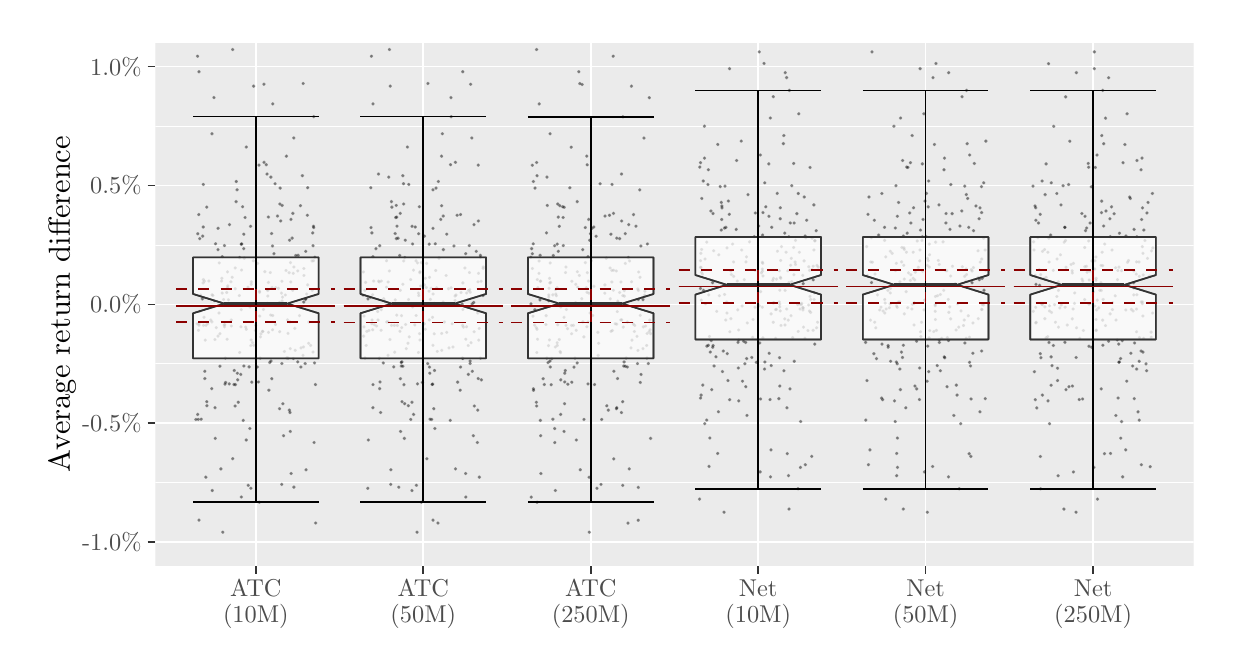
\begin{tikzpicture}[x=1pt,y=1pt]
\definecolor{fillColor}{RGB}{255,255,255}
\path[use as bounding box,fill=fillColor,fill opacity=0.00] (0,0) rectangle (426.79,220.51);
\begin{scope}
\path[clip] (  0.00,  0.00) rectangle (426.79,220.51);
\definecolor{drawColor}{RGB}{255,255,255}
\definecolor{fillColor}{RGB}{255,255,255}

\path[draw=drawColor,line width= 0.6pt,line join=round,line cap=round,fill=fillColor] (  0.00,  0.00) rectangle (426.79,220.51);
\end{scope}
\begin{scope}
\path[clip] ( 46.13, 26.01) rectangle (421.29,215.01);
\definecolor{fillColor}{gray}{0.92}

\path[fill=fillColor] ( 46.13, 26.01) rectangle (421.29,215.01);
\definecolor{drawColor}{RGB}{255,255,255}

\path[draw=drawColor,line width= 0.3pt,line join=round] ( 46.13, 56.08) --
	(421.29, 56.08);

\path[draw=drawColor,line width= 0.3pt,line join=round] ( 46.13, 99.04) --
	(421.29, 99.04);

\path[draw=drawColor,line width= 0.3pt,line join=round] ( 46.13,141.99) --
	(421.29,141.99);

\path[draw=drawColor,line width= 0.3pt,line join=round] ( 46.13,184.94) --
	(421.29,184.94);

\path[draw=drawColor,line width= 0.6pt,line join=round] ( 46.13, 34.61) --
	(421.29, 34.61);

\path[draw=drawColor,line width= 0.6pt,line join=round] ( 46.13, 77.56) --
	(421.29, 77.56);

\path[draw=drawColor,line width= 0.6pt,line join=round] ( 46.13,120.51) --
	(421.29,120.51);

\path[draw=drawColor,line width= 0.6pt,line join=round] ( 46.13,163.47) --
	(421.29,163.47);

\path[draw=drawColor,line width= 0.6pt,line join=round] ( 46.13,206.42) --
	(421.29,206.42);

\path[draw=drawColor,line width= 0.6pt,line join=round] ( 82.44, 26.01) --
	( 82.44,215.01);

\path[draw=drawColor,line width= 0.6pt,line join=round] (142.95, 26.01) --
	(142.95,215.01);

\path[draw=drawColor,line width= 0.6pt,line join=round] (203.46, 26.01) --
	(203.46,215.01);

\path[draw=drawColor,line width= 0.6pt,line join=round] (263.97, 26.01) --
	(263.97,215.01);

\path[draw=drawColor,line width= 0.6pt,line join=round] (324.48, 26.01) --
	(324.48,215.01);

\path[draw=drawColor,line width= 0.6pt,line join=round] (384.99, 26.01) --
	(384.99,215.01);
\definecolor{drawColor}{RGB}{0,0,0}
\definecolor{fillColor}{RGB}{0,0,0}

\path[draw=drawColor,draw opacity=0.30,line width= 0.4pt,line join=round,line cap=round,fill=fillColor,fill opacity=0.30] ( 77.02, 95.22) circle (  0.46);

\path[draw=drawColor,draw opacity=0.30,line width= 0.4pt,line join=round,line cap=round,fill=fillColor,fill opacity=0.30] ( 90.59,126.31) circle (  0.46);

\path[draw=drawColor,draw opacity=0.30,line width= 0.4pt,line join=round,line cap=round,fill=fillColor,fill opacity=0.30] (101.60,114.16) circle (  0.46);

\path[draw=drawColor,draw opacity=0.30,line width= 0.4pt,line join=round,line cap=round,fill=fillColor,fill opacity=0.30] ( 87.16, 89.52) circle (  0.46);

\path[draw=drawColor,draw opacity=0.30,line width= 0.4pt,line join=round,line cap=round,fill=fillColor,fill opacity=0.30] ( 89.61,126.54) circle (  0.46);

\path[draw=drawColor,draw opacity=0.30,line width= 0.4pt,line join=round,line cap=round,fill=fillColor,fill opacity=0.30] ( 86.60,120.90) circle (  0.46);

\path[draw=drawColor,draw opacity=0.30,line width= 0.4pt,line join=round,line cap=round,fill=fillColor,fill opacity=0.30] ( 71.30, 91.71) circle (  0.46);

\path[draw=drawColor,draw opacity=0.30,line width= 0.4pt,line join=round,line cap=round,fill=fillColor,fill opacity=0.30] ( 71.11,141.77) circle (  0.46);

\path[draw=drawColor,draw opacity=0.30,line width= 0.4pt,line join=round,line cap=round,fill=fillColor,fill opacity=0.30] ( 95.57,144.46) circle (  0.46);

\path[draw=drawColor,draw opacity=0.30,line width= 0.4pt,line join=round,line cap=round,fill=fillColor,fill opacity=0.30] ( 74.64, 96.64) circle (  0.46);

\path[draw=drawColor,draw opacity=0.30,line width= 0.4pt,line join=round,line cap=round,fill=fillColor,fill opacity=0.30] ( 95.07,128.63) circle (  0.46);

\path[draw=drawColor,draw opacity=0.30,line width= 0.4pt,line join=round,line cap=round,fill=fillColor,fill opacity=0.30] ( 72.83, 91.80) circle (  0.46);

\path[draw=drawColor,draw opacity=0.30,line width= 0.4pt,line join=round,line cap=round,fill=fillColor,fill opacity=0.30] (103.11,141.72) circle (  0.46);

\path[draw=drawColor,draw opacity=0.30,line width= 0.4pt,line join=round,line cap=round,fill=fillColor,fill opacity=0.30] ( 66.63,123.99) circle (  0.46);

\path[draw=drawColor,draw opacity=0.30,line width= 0.4pt,line join=round,line cap=round,fill=fillColor,fill opacity=0.30] ( 78.56,151.91) circle (  0.46);

\path[draw=drawColor,draw opacity=0.30,line width= 0.4pt,line join=round,line cap=round,fill=fillColor,fill opacity=0.30] ( 91.94,121.75) circle (  0.46);

\path[draw=drawColor,draw opacity=0.30,line width= 0.4pt,line join=round,line cap=round,fill=fillColor,fill opacity=0.30] ( 72.54,122.15) circle (  0.46);

\path[draw=drawColor,draw opacity=0.30,line width= 0.4pt,line join=round,line cap=round,fill=fillColor,fill opacity=0.30] ( 80.78,127.79) circle (  0.46);

\path[draw=drawColor,draw opacity=0.30,line width= 0.4pt,line join=round,line cap=round,fill=fillColor,fill opacity=0.30] ( 85.19,118.68) circle (  0.46);

\path[draw=drawColor,draw opacity=0.30,line width= 0.4pt,line join=round,line cap=round,fill=fillColor,fill opacity=0.30] ( 97.73,138.24) circle (  0.46);

\path[draw=drawColor,draw opacity=0.30,line width= 0.4pt,line join=round,line cap=round,fill=fillColor,fill opacity=0.30] ( 63.53,112.92) circle (  0.46);

\path[draw=drawColor,draw opacity=0.30,line width= 0.4pt,line join=round,line cap=round,fill=fillColor,fill opacity=0.30] (103.27,148.78) circle (  0.46);

\path[draw=drawColor,draw opacity=0.30,line width= 0.4pt,line join=round,line cap=round,fill=fillColor,fill opacity=0.30] ( 94.89, 74.61) circle (  0.46);

\path[draw=drawColor,draw opacity=0.30,line width= 0.4pt,line join=round,line cap=round,fill=fillColor,fill opacity=0.30] ( 83.11,135.33) circle (  0.46);

\path[draw=drawColor,draw opacity=0.30,line width= 0.4pt,line join=round,line cap=round,fill=fillColor,fill opacity=0.30] ( 77.17,118.61) circle (  0.46);

\path[draw=drawColor,draw opacity=0.30,line width= 0.4pt,line join=round,line cap=round,fill=fillColor,fill opacity=0.30] ( 80.84,128.66) circle (  0.46);

\path[draw=drawColor,draw opacity=0.30,line width= 0.4pt,line join=round,line cap=round,fill=fillColor,fill opacity=0.30] ( 82.69,120.62) circle (  0.46);

\path[draw=drawColor,draw opacity=0.30,line width= 0.4pt,line join=round,line cap=round,fill=fillColor,fill opacity=0.30] ( 73.43,128.67) circle (  0.46);

\path[draw=drawColor,draw opacity=0.30,line width= 0.4pt,line join=round,line cap=round,fill=fillColor,fill opacity=0.30] ( 86.79,125.51) circle (  0.46);

\path[draw=drawColor,draw opacity=0.30,line width= 0.4pt,line join=round,line cap=round,fill=fillColor,fill opacity=0.30] ( 63.13,122.52) circle (  0.46);

\path[draw=drawColor,draw opacity=0.30,line width= 0.4pt,line join=round,line cap=round,fill=fillColor,fill opacity=0.30] ( 67.66,107.82) circle (  0.46);

\path[draw=drawColor,draw opacity=0.30,line width= 0.4pt,line join=round,line cap=round,fill=fillColor,fill opacity=0.30] ( 91.80, 55.48) circle (  0.46);

\path[draw=drawColor,draw opacity=0.30,line width= 0.4pt,line join=round,line cap=round,fill=fillColor,fill opacity=0.30] ( 89.55,113.25) circle (  0.46);

\path[draw=drawColor,draw opacity=0.30,line width= 0.4pt,line join=round,line cap=round,fill=fillColor,fill opacity=0.30] ( 86.77,123.52) circle (  0.46);

\path[draw=drawColor,draw opacity=0.30,line width= 0.4pt,line join=round,line cap=round,fill=fillColor,fill opacity=0.30] ( 84.28,109.88) circle (  0.46);

\path[draw=drawColor,draw opacity=0.30,line width= 0.4pt,line join=round,line cap=round,fill=fillColor,fill opacity=0.30] ( 89.40,164.11) circle (  0.46);

\path[draw=drawColor,draw opacity=0.30,line width= 0.4pt,line join=round,line cap=round,fill=fillColor,fill opacity=0.30] ( 81.24,106.68) circle (  0.46);

\path[draw=drawColor,draw opacity=0.30,line width= 0.4pt,line join=round,line cap=round,fill=fillColor,fill opacity=0.30] ( 61.47,146.04) circle (  0.46);

\path[draw=drawColor,draw opacity=0.30,line width= 0.4pt,line join=round,line cap=round,fill=fillColor,fill opacity=0.30] ( 64.01, 96.35) circle (  0.46);

\path[draw=drawColor,draw opacity=0.30,line width= 0.4pt,line join=round,line cap=round,fill=fillColor,fill opacity=0.30] ( 75.06, 91.53) circle (  0.46);

\path[draw=drawColor,draw opacity=0.30,line width= 0.4pt,line join=round,line cap=round,fill=fillColor,fill opacity=0.30] (101.06,152.73) circle (  0.46);

\path[draw=drawColor,draw opacity=0.30,line width= 0.4pt,line join=round,line cap=round,fill=fillColor,fill opacity=0.30] ( 93.49,174.08) circle (  0.46);

\path[draw=drawColor,draw opacity=0.30,line width= 0.4pt,line join=round,line cap=round,fill=fillColor,fill opacity=0.30] ( 64.76, 83.92) circle (  0.46);

\path[draw=drawColor,draw opacity=0.30,line width= 0.4pt,line join=round,line cap=round,fill=fillColor,fill opacity=0.30] ( 67.89,142.40) circle (  0.46);

\path[draw=drawColor,draw opacity=0.30,line width= 0.4pt,line join=round,line cap=round,fill=fillColor,fill opacity=0.30] ( 71.44,101.13) circle (  0.46);

\path[draw=drawColor,draw opacity=0.30,line width= 0.4pt,line join=round,line cap=round,fill=fillColor,fill opacity=0.30] ( 63.72,115.86) circle (  0.46);

\path[draw=drawColor,draw opacity=0.30,line width= 0.4pt,line join=round,line cap=round,fill=fillColor,fill opacity=0.30] ( 64.02, 93.72) circle (  0.46);

\path[draw=drawColor,draw opacity=0.30,line width= 0.4pt,line join=round,line cap=round,fill=fillColor,fill opacity=0.30] ( 94.96,135.61) circle (  0.46);

\path[draw=drawColor,draw opacity=0.30,line width= 0.4pt,line join=round,line cap=round,fill=fillColor,fill opacity=0.30] (100.41,122.34) circle (  0.46);

\path[draw=drawColor,draw opacity=0.30,line width= 0.4pt,line join=round,line cap=round,fill=fillColor,fill opacity=0.30] ( 75.93,120.69) circle (  0.46);

\path[draw=drawColor,draw opacity=0.30,line width= 0.4pt,line join=round,line cap=round,fill=fillColor,fill opacity=0.30] ( 63.47,163.86) circle (  0.46);

\path[draw=drawColor,draw opacity=0.30,line width= 0.4pt,line join=round,line cap=round,fill=fillColor,fill opacity=0.30] ( 62.22,117.95) circle (  0.46);

\path[draw=drawColor,draw opacity=0.30,line width= 0.4pt,line join=round,line cap=round,fill=fillColor,fill opacity=0.30] ( 63.40,128.28) circle (  0.46);

\path[draw=drawColor,draw opacity=0.30,line width= 0.4pt,line join=round,line cap=round,fill=fillColor,fill opacity=0.30] ( 91.85, 99.14) circle (  0.46);

\path[draw=drawColor,draw opacity=0.30,line width= 0.4pt,line join=round,line cap=round,fill=fillColor,fill opacity=0.30] ( 61.24,113.52) circle (  0.46);

\path[draw=drawColor,draw opacity=0.30,line width= 0.4pt,line join=round,line cap=round,fill=fillColor,fill opacity=0.30] ( 75.88, 93.25) circle (  0.46);

\path[draw=drawColor,draw opacity=0.30,line width= 0.4pt,line join=round,line cap=round,fill=fillColor,fill opacity=0.30] ( 77.22, 50.91) circle (  0.46);

\path[draw=drawColor,draw opacity=0.30,line width= 0.4pt,line join=round,line cap=round,fill=fillColor,fill opacity=0.30] ( 86.21,170.99) circle (  0.46);

\path[draw=drawColor,draw opacity=0.30,line width= 0.4pt,line join=round,line cap=round,fill=fillColor,fill opacity=0.30] ( 77.35,142.35) circle (  0.46);

\path[draw=drawColor,draw opacity=0.30,line width= 0.4pt,line join=round,line cap=round,fill=fillColor,fill opacity=0.30] ( 97.59,132.61) circle (  0.46);

\path[draw=drawColor,draw opacity=0.30,line width= 0.4pt,line join=round,line cap=round,fill=fillColor,fill opacity=0.30] ( 87.49, 99.52) circle (  0.46);

\path[draw=drawColor,draw opacity=0.30,line width= 0.4pt,line join=round,line cap=round,fill=fillColor,fill opacity=0.30] ( 83.78,124.90) circle (  0.46);

\path[draw=drawColor,draw opacity=0.30,line width= 0.4pt,line join=round,line cap=round,fill=fillColor,fill opacity=0.30] ( 76.10, 85.16) circle (  0.46);

\path[draw=drawColor,draw opacity=0.30,line width= 0.4pt,line join=round,line cap=round,fill=fillColor,fill opacity=0.30] ( 74.99,126.17) circle (  0.46);

\path[draw=drawColor,draw opacity=0.30,line width= 0.4pt,line join=round,line cap=round,fill=fillColor,fill opacity=0.30] ( 61.72,111.16) circle (  0.46);

\path[draw=drawColor,draw opacity=0.30,line width= 0.4pt,line join=round,line cap=round,fill=fillColor,fill opacity=0.30] ( 82.41,112.94) circle (  0.46);

\path[draw=drawColor,draw opacity=0.30,line width= 0.4pt,line join=round,line cap=round,fill=fillColor,fill opacity=0.30] ( 93.65,101.21) circle (  0.46);

\path[draw=drawColor,draw opacity=0.30,line width= 0.4pt,line join=round,line cap=round,fill=fillColor,fill opacity=0.30] ( 62.70, 79.04) circle (  0.46);

\path[draw=drawColor,draw opacity=0.30,line width= 0.4pt,line join=round,line cap=round,fill=fillColor,fill opacity=0.30] ( 97.57, 99.74) circle (  0.46);

\path[draw=drawColor,draw opacity=0.30,line width= 0.4pt,line join=round,line cap=round,fill=fillColor,fill opacity=0.30] ( 94.08,110.03) circle (  0.46);

\path[draw=drawColor,draw opacity=0.30,line width= 0.4pt,line join=round,line cap=round,fill=fillColor,fill opacity=0.30] ( 91.13,156.80) circle (  0.46);

\path[draw=drawColor,draw opacity=0.30,line width= 0.4pt,line join=round,line cap=round,fill=fillColor,fill opacity=0.30] ( 61.84,152.97) circle (  0.46);

\path[draw=drawColor,draw opacity=0.30,line width= 0.4pt,line join=round,line cap=round,fill=fillColor,fill opacity=0.30] ( 85.40,171.86) circle (  0.46);

\path[draw=drawColor,draw opacity=0.30,line width= 0.4pt,line join=round,line cap=round,fill=fillColor,fill opacity=0.30] ( 64.73, 85.36) circle (  0.46);

\path[draw=drawColor,draw opacity=0.30,line width= 0.4pt,line join=round,line cap=round,fill=fillColor,fill opacity=0.30] ( 72.22,126.54) circle (  0.46);

\path[draw=drawColor,draw opacity=0.30,line width= 0.4pt,line join=round,line cap=round,fill=fillColor,fill opacity=0.30] ( 91.70,124.60) circle (  0.46);

\path[draw=drawColor,draw opacity=0.30,line width= 0.4pt,line join=round,line cap=round,fill=fillColor,fill opacity=0.30] ( 69.47, 98.17) circle (  0.46);

\path[draw=drawColor,draw opacity=0.30,line width= 0.4pt,line join=round,line cap=round,fill=fillColor,fill opacity=0.30] ( 67.71, 83.20) circle (  0.46);

\path[draw=drawColor,draw opacity=0.30,line width= 0.4pt,line join=round,line cap=round,fill=fillColor,fill opacity=0.30] (103.49, 70.61) circle (  0.46);

\path[draw=drawColor,draw opacity=0.30,line width= 0.4pt,line join=round,line cap=round,fill=fillColor,fill opacity=0.30] ( 82.26,111.08) circle (  0.46);

\path[draw=drawColor,draw opacity=0.30,line width= 0.4pt,line join=round,line cap=round,fill=fillColor,fill opacity=0.30] ( 75.37,164.92) circle (  0.46);

\path[draw=drawColor,draw opacity=0.30,line width= 0.4pt,line join=round,line cap=round,fill=fillColor,fill opacity=0.30] ( 61.63, 78.95) circle (  0.46);

\path[draw=drawColor,draw opacity=0.30,line width= 0.4pt,line join=round,line cap=round,fill=fillColor,fill opacity=0.30] ( 71.00,113.10) circle (  0.46);

\path[draw=drawColor,draw opacity=0.30,line width= 0.4pt,line join=round,line cap=round,fill=fillColor,fill opacity=0.30] ( 61.92, 42.55) circle (  0.46);

\path[draw=drawColor,draw opacity=0.30,line width= 0.4pt,line join=round,line cap=round,fill=fillColor,fill opacity=0.30] ( 63.45,148.48) circle (  0.46);

\path[draw=drawColor,draw opacity=0.30,line width= 0.4pt,line join=round,line cap=round,fill=fillColor,fill opacity=0.30] ( 79.00,177.38) circle (  0.46);

\path[draw=drawColor,draw opacity=0.30,line width= 0.4pt,line join=round,line cap=round,fill=fillColor,fill opacity=0.30] ( 80.66, 54.07) circle (  0.46);

\path[draw=drawColor,draw opacity=0.30,line width= 0.4pt,line join=round,line cap=round,fill=fillColor,fill opacity=0.30] ( 64.38, 58.09) circle (  0.46);

\path[draw=drawColor,draw opacity=0.30,line width= 0.4pt,line join=round,line cap=round,fill=fillColor,fill opacity=0.30] ( 85.37,200.07) circle (  0.46);

\path[draw=drawColor,draw opacity=0.30,line width= 0.4pt,line join=round,line cap=round,fill=fillColor,fill opacity=0.30] ( 66.92,123.71) circle (  0.46);

\path[draw=drawColor,draw opacity=0.30,line width= 0.4pt,line join=round,line cap=round,fill=fillColor,fill opacity=0.30] ( 69.23,135.50) circle (  0.46);

\path[draw=drawColor,draw opacity=0.30,line width= 0.4pt,line join=round,line cap=round,fill=fillColor,fill opacity=0.30] ( 80.03, 97.94) circle (  0.46);

\path[draw=drawColor,draw opacity=0.30,line width= 0.4pt,line join=round,line cap=round,fill=fillColor,fill opacity=0.30] ( 80.99, 92.42) circle (  0.46);

\path[draw=drawColor,draw opacity=0.30,line width= 0.4pt,line join=round,line cap=round,fill=fillColor,fill opacity=0.30] ( 88.22, 93.67) circle (  0.46);

\path[draw=drawColor,draw opacity=0.30,line width= 0.4pt,line join=round,line cap=round,fill=fillColor,fill opacity=0.30] ( 72.27,127.20) circle (  0.46);

\path[draw=drawColor,draw opacity=0.30,line width= 0.4pt,line join=round,line cap=round,fill=fillColor,fill opacity=0.30] ( 91.95,156.28) circle (  0.46);

\path[draw=drawColor,draw opacity=0.30,line width= 0.4pt,line join=round,line cap=round,fill=fillColor,fill opacity=0.30] ( 85.70,132.35) circle (  0.46);

\path[draw=drawColor,draw opacity=0.30,line width= 0.4pt,line join=round,line cap=round,fill=fillColor,fill opacity=0.30] ( 98.24,116.45) circle (  0.46);

\path[draw=drawColor,draw opacity=0.30,line width= 0.4pt,line join=round,line cap=round,fill=fillColor,fill opacity=0.30] ( 94.87,104.54) circle (  0.46);

\path[draw=drawColor,draw opacity=0.30,line width= 0.4pt,line join=round,line cap=round,fill=fillColor,fill opacity=0.30] ( 99.26,167.03) circle (  0.46);

\path[draw=drawColor,draw opacity=0.30,line width= 0.4pt,line join=round,line cap=round,fill=fillColor,fill opacity=0.30] ( 74.10, 64.76) circle (  0.46);

\path[draw=drawColor,draw opacity=0.30,line width= 0.4pt,line join=round,line cap=round,fill=fillColor,fill opacity=0.30] ( 76.61,103.16) circle (  0.46);

\path[draw=drawColor,draw opacity=0.30,line width= 0.4pt,line join=round,line cap=round,fill=fillColor,fill opacity=0.30] ( 77.87, 78.60) circle (  0.46);

\path[draw=drawColor,draw opacity=0.30,line width= 0.4pt,line join=round,line cap=round,fill=fillColor,fill opacity=0.30] ( 96.20, 54.48) circle (  0.46);

\path[draw=drawColor,draw opacity=0.30,line width= 0.4pt,line join=round,line cap=round,fill=fillColor,fill opacity=0.30] ( 72.22,132.26) circle (  0.46);

\path[draw=drawColor,draw opacity=0.30,line width= 0.4pt,line join=round,line cap=round,fill=fillColor,fill opacity=0.30] ( 80.29, 75.68) circle (  0.46);

\path[draw=drawColor,draw opacity=0.30,line width= 0.4pt,line join=round,line cap=round,fill=fillColor,fill opacity=0.30] ( 83.60,170.84) circle (  0.46);

\path[draw=drawColor,draw opacity=0.30,line width= 0.4pt,line join=round,line cap=round,fill=fillColor,fill opacity=0.30] (101.19,162.68) circle (  0.46);

\path[draw=drawColor,draw opacity=0.30,line width= 0.4pt,line join=round,line cap=round,fill=fillColor,fill opacity=0.30] ( 96.54,111.85) circle (  0.46);

\path[draw=drawColor,draw opacity=0.30,line width= 0.4pt,line join=round,line cap=round,fill=fillColor,fill opacity=0.30] ( 61.86,113.47) circle (  0.46);

\path[draw=drawColor,draw opacity=0.30,line width= 0.4pt,line join=round,line cap=round,fill=fillColor,fill opacity=0.30] ( 69.48,109.93) circle (  0.46);

\path[draw=drawColor,draw opacity=0.30,line width= 0.4pt,line join=round,line cap=round,fill=fillColor,fill opacity=0.30] ( 77.29,132.92) circle (  0.46);

\path[draw=drawColor,draw opacity=0.30,line width= 0.4pt,line join=round,line cap=round,fill=fillColor,fill opacity=0.30] ( 91.23,162.54) circle (  0.46);

\path[draw=drawColor,draw opacity=0.30,line width= 0.4pt,line join=round,line cap=round,fill=fillColor,fill opacity=0.30] ( 75.31,157.65) circle (  0.46);

\path[draw=drawColor,draw opacity=0.30,line width= 0.4pt,line join=round,line cap=round,fill=fillColor,fill opacity=0.30] ( 65.10,113.56) circle (  0.46);

\path[draw=drawColor,draw opacity=0.30,line width= 0.4pt,line join=round,line cap=round,fill=fillColor,fill opacity=0.30] ( 99.82,130.97) circle (  0.46);

\path[draw=drawColor,draw opacity=0.30,line width= 0.4pt,line join=round,line cap=round,fill=fillColor,fill opacity=0.30] (103.79,137.55) circle (  0.46);

\path[draw=drawColor,draw opacity=0.30,line width= 0.4pt,line join=round,line cap=round,fill=fillColor,fill opacity=0.30] ( 66.52, 90.09) circle (  0.46);

\path[draw=drawColor,draw opacity=0.30,line width= 0.4pt,line join=round,line cap=round,fill=fillColor,fill opacity=0.30] ( 77.65,155.80) circle (  0.46);

\path[draw=drawColor,draw opacity=0.30,line width= 0.4pt,line join=round,line cap=round,fill=fillColor,fill opacity=0.30] ( 78.07,140.66) circle (  0.46);

\path[draw=drawColor,draw opacity=0.30,line width= 0.4pt,line join=round,line cap=round,fill=fillColor,fill opacity=0.30] ( 87.81,116.66) circle (  0.46);

\path[draw=drawColor,draw opacity=0.30,line width= 0.4pt,line join=round,line cap=round,fill=fillColor,fill opacity=0.30] ( 99.80,133.49) circle (  0.46);

\path[draw=drawColor,draw opacity=0.30,line width= 0.4pt,line join=round,line cap=round,fill=fillColor,fill opacity=0.30] ( 86.61,125.87) circle (  0.46);

\path[draw=drawColor,draw opacity=0.30,line width= 0.4pt,line join=round,line cap=round,fill=fillColor,fill opacity=0.30] (103.11,103.30) circle (  0.46);

\path[draw=drawColor,draw opacity=0.30,line width= 0.4pt,line join=round,line cap=round,fill=fillColor,fill opacity=0.30] (100.26, 99.13) circle (  0.46);

\path[draw=drawColor,draw opacity=0.30,line width= 0.4pt,line join=round,line cap=round,fill=fillColor,fill opacity=0.30] (100.48,139.69) circle (  0.46);

\path[draw=drawColor,draw opacity=0.30,line width= 0.4pt,line join=round,line cap=round,fill=fillColor,fill opacity=0.30] ( 67.47,121.94) circle (  0.46);

\path[draw=drawColor,draw opacity=0.30,line width= 0.4pt,line join=round,line cap=round,fill=fillColor,fill opacity=0.30] (103.65, 99.36) circle (  0.46);

\path[draw=drawColor,draw opacity=0.30,line width= 0.4pt,line join=round,line cap=round,fill=fillColor,fill opacity=0.30] ( 84.82,110.78) circle (  0.46);

\path[draw=drawColor,draw opacity=0.30,line width= 0.4pt,line join=round,line cap=round,fill=fillColor,fill opacity=0.30] ( 65.46,128.96) circle (  0.46);

\path[draw=drawColor,draw opacity=0.30,line width= 0.4pt,line join=round,line cap=round,fill=fillColor,fill opacity=0.30] ( 63.46,129.48) circle (  0.46);

\path[draw=drawColor,draw opacity=0.30,line width= 0.4pt,line join=round,line cap=round,fill=fillColor,fill opacity=0.30] ( 89.00,138.84) circle (  0.46);

\path[draw=drawColor,draw opacity=0.30,line width= 0.4pt,line join=round,line cap=round,fill=fillColor,fill opacity=0.30] ( 66.14,114.88) circle (  0.46);

\path[draw=drawColor,draw opacity=0.30,line width= 0.4pt,line join=round,line cap=round,fill=fillColor,fill opacity=0.30] ( 78.11, 98.25) circle (  0.46);

\path[draw=drawColor,draw opacity=0.30,line width= 0.4pt,line join=round,line cap=round,fill=fillColor,fill opacity=0.30] (101.17,127.56) circle (  0.46);

\path[draw=drawColor,draw opacity=0.30,line width= 0.4pt,line join=round,line cap=round,fill=fillColor,fill opacity=0.30] ( 63.87,128.92) circle (  0.46);

\path[draw=drawColor,draw opacity=0.30,line width= 0.4pt,line join=round,line cap=round,fill=fillColor,fill opacity=0.30] ( 94.57, 82.31) circle (  0.46);

\path[draw=drawColor,draw opacity=0.30,line width= 0.4pt,line join=round,line cap=round,fill=fillColor,fill opacity=0.30] ( 64.69,155.66) circle (  0.46);

\path[draw=drawColor,draw opacity=0.30,line width= 0.4pt,line join=round,line cap=round,fill=fillColor,fill opacity=0.30] ( 88.30,126.62) circle (  0.46);

\path[draw=drawColor,draw opacity=0.30,line width= 0.4pt,line join=round,line cap=round,fill=fillColor,fill opacity=0.30] ( 68.81,148.00) circle (  0.46);

\path[draw=drawColor,draw opacity=0.30,line width= 0.4pt,line join=round,line cap=round,fill=fillColor,fill opacity=0.30] ( 68.77,109.06) circle (  0.46);

\path[draw=drawColor,draw opacity=0.30,line width= 0.4pt,line join=round,line cap=round,fill=fillColor,fill opacity=0.30] ( 73.90,130.31) circle (  0.46);

\path[draw=drawColor,draw opacity=0.30,line width= 0.4pt,line join=round,line cap=round,fill=fillColor,fill opacity=0.30] ( 80.75,107.67) circle (  0.46);

\path[draw=drawColor,draw opacity=0.30,line width= 0.4pt,line join=round,line cap=round,fill=fillColor,fill opacity=0.30] (103.31,136.28) circle (  0.46);

\path[draw=drawColor,draw opacity=0.30,line width= 0.4pt,line join=round,line cap=round,fill=fillColor,fill opacity=0.30] ( 61.91,112.93) circle (  0.46);

\path[draw=drawColor,draw opacity=0.30,line width= 0.4pt,line join=round,line cap=round,fill=fillColor,fill opacity=0.30] ( 93.35,132.77) circle (  0.46);

\path[draw=drawColor,draw opacity=0.30,line width= 0.4pt,line join=round,line cap=round,fill=fillColor,fill opacity=0.30] ( 72.07,107.94) circle (  0.46);

\path[draw=drawColor,draw opacity=0.30,line width= 0.4pt,line join=round,line cap=round,fill=fillColor,fill opacity=0.30] ( 83.85,116.31) circle (  0.46);

\path[draw=drawColor,draw opacity=0.30,line width= 0.4pt,line join=round,line cap=round,fill=fillColor,fill opacity=0.30] ( 93.91,114.92) circle (  0.46);

\path[draw=drawColor,draw opacity=0.30,line width= 0.4pt,line join=round,line cap=round,fill=fillColor,fill opacity=0.30] (102.26,105.69) circle (  0.46);

\path[draw=drawColor,draw opacity=0.30,line width= 0.4pt,line join=round,line cap=round,fill=fillColor,fill opacity=0.30] ( 93.12,123.92) circle (  0.46);

\path[draw=drawColor,draw opacity=0.30,line width= 0.4pt,line join=round,line cap=round,fill=fillColor,fill opacity=0.30] ( 68.15,112.13) circle (  0.46);

\path[draw=drawColor,draw opacity=0.30,line width= 0.4pt,line join=round,line cap=round,fill=fillColor,fill opacity=0.30] ( 86.99,128.46) circle (  0.46);

\path[draw=drawColor,draw opacity=0.30,line width= 0.4pt,line join=round,line cap=round,fill=fillColor,fill opacity=0.30] ( 87.66,132.02) circle (  0.46);

\path[draw=drawColor,draw opacity=0.30,line width= 0.4pt,line join=round,line cap=round,fill=fillColor,fill opacity=0.30] (102.76,136.22) circle (  0.46);

\path[draw=drawColor,draw opacity=0.30,line width= 0.4pt,line join=round,line cap=round,fill=fillColor,fill opacity=0.30] ( 83.79,125.29) circle (  0.46);

\path[draw=drawColor,draw opacity=0.30,line width= 0.4pt,line join=round,line cap=round,fill=fillColor,fill opacity=0.30] ( 84.98,110.73) circle (  0.46);

\path[draw=drawColor,draw opacity=0.30,line width= 0.4pt,line join=round,line cap=round,fill=fillColor,fill opacity=0.30] ( 94.47,131.98) circle (  0.46);

\path[draw=drawColor,draw opacity=0.30,line width= 0.4pt,line join=round,line cap=round,fill=fillColor,fill opacity=0.30] (101.53,106.48) circle (  0.46);

\path[draw=drawColor,draw opacity=0.30,line width= 0.4pt,line join=round,line cap=round,fill=fillColor,fill opacity=0.30] ( 96.18,134.03) circle (  0.46);

\path[draw=drawColor,draw opacity=0.30,line width= 0.4pt,line join=round,line cap=round,fill=fillColor,fill opacity=0.30] ( 75.00,133.69) circle (  0.46);

\path[draw=drawColor,draw opacity=0.30,line width= 0.4pt,line join=round,line cap=round,fill=fillColor,fill opacity=0.30] ( 96.88,138.18) circle (  0.46);

\path[draw=drawColor,draw opacity=0.30,line width= 0.4pt,line join=round,line cap=round,fill=fillColor,fill opacity=0.30] ( 91.06,110.66) circle (  0.46);

\path[draw=drawColor,draw opacity=0.30,line width= 0.4pt,line join=round,line cap=round,fill=fillColor,fill opacity=0.30] ( 92.47, 73.07) circle (  0.46);

\path[draw=drawColor,draw opacity=0.30,line width= 0.4pt,line join=round,line cap=round,fill=fillColor,fill opacity=0.30] ( 70.05,128.95) circle (  0.46);

\path[draw=drawColor,draw opacity=0.30,line width= 0.4pt,line join=round,line cap=round,fill=fillColor,fill opacity=0.30] ( 68.79,140.31) circle (  0.46);

\path[draw=drawColor,draw opacity=0.30,line width= 0.4pt,line join=round,line cap=round,fill=fillColor,fill opacity=0.30] ( 70.29,124.61) circle (  0.46);

\path[draw=drawColor,draw opacity=0.30,line width= 0.4pt,line join=round,line cap=round,fill=fillColor,fill opacity=0.30] ( 71.53, 92.32) circle (  0.46);

\path[draw=drawColor,draw opacity=0.30,line width= 0.4pt,line join=round,line cap=round,fill=fillColor,fill opacity=0.30] ( 78.27,137.19) circle (  0.46);

\path[draw=drawColor,draw opacity=0.30,line width= 0.4pt,line join=round,line cap=round,fill=fillColor,fill opacity=0.30] ( 94.11,101.16) circle (  0.46);

\path[draw=drawColor,draw opacity=0.30,line width= 0.4pt,line join=round,line cap=round,fill=fillColor,fill opacity=0.30] ( 69.14,117.40) circle (  0.46);

\path[draw=drawColor,draw opacity=0.30,line width= 0.4pt,line join=round,line cap=round,fill=fillColor,fill opacity=0.30] ( 64.18,107.61) circle (  0.46);

\path[draw=drawColor,draw opacity=0.30,line width= 0.4pt,line join=round,line cap=round,fill=fillColor,fill opacity=0.30] ( 98.58,156.18) circle (  0.46);

\path[draw=drawColor,draw opacity=0.30,line width= 0.4pt,line join=round,line cap=round,fill=fillColor,fill opacity=0.30] ( 86.98,152.07) circle (  0.46);

\path[draw=drawColor,draw opacity=0.30,line width= 0.4pt,line join=round,line cap=round,fill=fillColor,fill opacity=0.30] ( 73.60,112.69) circle (  0.46);

\path[draw=drawColor,draw opacity=0.30,line width= 0.4pt,line join=round,line cap=round,fill=fillColor,fill opacity=0.30] ( 95.98,100.98) circle (  0.46);

\path[draw=drawColor,draw opacity=0.30,line width= 0.4pt,line join=round,line cap=round,fill=fillColor,fill opacity=0.30] ( 75.67,161.92) circle (  0.46);

\path[draw=drawColor,draw opacity=0.30,line width= 0.4pt,line join=round,line cap=round,fill=fillColor,fill opacity=0.30] ( 67.31,195.25) circle (  0.46);

\path[draw=drawColor,draw opacity=0.30,line width= 0.4pt,line join=round,line cap=round,fill=fillColor,fill opacity=0.30] ( 96.15, 15.98) circle (  0.46);

\path[draw=drawColor,draw opacity=0.30,line width= 0.4pt,line join=round,line cap=round,fill=fillColor,fill opacity=0.30] ( 70.50, 38.21) circle (  0.46);

\path[draw=drawColor,draw opacity=0.30,line width= 0.4pt,line join=round,line cap=round,fill=fillColor,fill opacity=0.30] ( 96.15,180.66) circle (  0.46);

\path[draw=drawColor,draw opacity=0.30,line width= 0.4pt,line join=round,line cap=round,fill=fillColor,fill opacity=0.30] ( 83.37, 92.50) circle (  0.46);

\path[draw=drawColor,draw opacity=0.30,line width= 0.4pt,line join=round,line cap=round,fill=fillColor,fill opacity=0.30] (100.59, 60.76) circle (  0.46);

\path[draw=drawColor,draw opacity=0.30,line width= 0.4pt,line join=round,line cap=round,fill=fillColor,fill opacity=0.30] (103.36,188.36) circle (  0.46);

\path[draw=drawColor,draw opacity=0.30,line width= 0.4pt,line join=round,line cap=round,fill=fillColor,fill opacity=0.30] ( 61.38,210.20) circle (  0.46);

\path[draw=drawColor,draw opacity=0.30,line width= 0.4pt,line join=round,line cap=round,fill=fillColor,fill opacity=0.30] (100.82,124.27) circle (  0.46);

\path[draw=drawColor,draw opacity=0.30,line width= 0.4pt,line join=round,line cap=round,fill=fillColor,fill opacity=0.30] ( 96.68,103.93) circle (  0.46);

\path[draw=drawColor,draw opacity=0.30,line width= 0.4pt,line join=round,line cap=round,fill=fillColor,fill opacity=0.30] (102.98,146.35) circle (  0.46);

\path[draw=drawColor,draw opacity=0.30,line width= 0.4pt,line join=round,line cap=round,fill=fillColor,fill opacity=0.30] ( 90.96,121.23) circle (  0.46);

\path[draw=drawColor,draw opacity=0.30,line width= 0.4pt,line join=round,line cap=round,fill=fillColor,fill opacity=0.30] ( 88.47,141.63) circle (  0.46);

\path[draw=drawColor,draw opacity=0.30,line width= 0.4pt,line join=round,line cap=round,fill=fillColor,fill opacity=0.30] ( 74.96, 83.80) circle (  0.46);

\path[draw=drawColor,draw opacity=0.30,line width= 0.4pt,line join=round,line cap=round,fill=fillColor,fill opacity=0.30] ( 95.82,153.40) circle (  0.46);

\path[draw=drawColor,draw opacity=0.30,line width= 0.4pt,line join=round,line cap=round,fill=fillColor,fill opacity=0.30] ( 94.63,143.71) circle (  0.46);

\path[draw=drawColor,draw opacity=0.30,line width= 0.4pt,line join=round,line cap=round,fill=fillColor,fill opacity=0.30] ( 60.79, 78.94) circle (  0.46);

\path[draw=drawColor,draw opacity=0.30,line width= 0.4pt,line join=round,line cap=round,fill=fillColor,fill opacity=0.30] ( 66.59,182.18) circle (  0.46);

\path[draw=drawColor,draw opacity=0.30,line width= 0.4pt,line join=round,line cap=round,fill=fillColor,fill opacity=0.30] ( 63.23,145.18) circle (  0.46);

\path[draw=drawColor,draw opacity=0.30,line width= 0.4pt,line join=round,line cap=round,fill=fillColor,fill opacity=0.30] ( 76.59,137.42) circle (  0.46);

\path[draw=drawColor,draw opacity=0.30,line width= 0.4pt,line join=round,line cap=round,fill=fillColor,fill opacity=0.30] ( 77.06,112.42) circle (  0.46);

\path[draw=drawColor,draw opacity=0.30,line width= 0.4pt,line join=round,line cap=round,fill=fillColor,fill opacity=0.30] ( 95.20, 59.41) circle (  0.46);

\path[draw=drawColor,draw opacity=0.30,line width= 0.4pt,line join=round,line cap=round,fill=fillColor,fill opacity=0.30] ( 62.18,144.29) circle (  0.46);

\path[draw=drawColor,draw opacity=0.30,line width= 0.4pt,line join=round,line cap=round,fill=fillColor,fill opacity=0.30] ( 84.01,101.12) circle (  0.46);

\path[draw=drawColor,draw opacity=0.30,line width= 0.4pt,line join=round,line cap=round,fill=fillColor,fill opacity=0.30] ( 91.42,150.67) circle (  0.46);

\path[draw=drawColor,draw opacity=0.30,line width= 0.4pt,line join=round,line cap=round,fill=fillColor,fill opacity=0.30] ( 95.95,131.74) circle (  0.46);

\path[draw=drawColor,draw opacity=0.30,line width= 0.4pt,line join=round,line cap=round,fill=fillColor,fill opacity=0.30] ( 78.10,145.89) circle (  0.46);

\path[draw=drawColor,draw opacity=0.30,line width= 0.4pt,line join=round,line cap=round,fill=fillColor,fill opacity=0.30] ( 70.79,122.27) circle (  0.46);

\path[draw=drawColor,draw opacity=0.30,line width= 0.4pt,line join=round,line cap=round,fill=fillColor,fill opacity=0.30] ( 95.78,125.62) circle (  0.46);

\path[draw=drawColor,draw opacity=0.30,line width= 0.4pt,line join=round,line cap=round,fill=fillColor,fill opacity=0.30] (103.35,148.27) circle (  0.46);

\path[draw=drawColor,draw opacity=0.30,line width= 0.4pt,line join=round,line cap=round,fill=fillColor,fill opacity=0.30] (102.84,125.58) circle (  0.46);

\path[draw=drawColor,draw opacity=0.30,line width= 0.4pt,line join=round,line cap=round,fill=fillColor,fill opacity=0.30] ( 83.01, 97.88) circle (  0.46);

\path[draw=drawColor,draw opacity=0.30,line width= 0.4pt,line join=round,line cap=round,fill=fillColor,fill opacity=0.30] ( 78.76,112.31) circle (  0.46);

\path[draw=drawColor,draw opacity=0.30,line width= 0.4pt,line join=round,line cap=round,fill=fillColor,fill opacity=0.30] ( 81.72,105.72) circle (  0.46);

\path[draw=drawColor,draw opacity=0.30,line width= 0.4pt,line join=round,line cap=round,fill=fillColor,fill opacity=0.30] ( 75.77, 95.65) circle (  0.46);

\path[draw=drawColor,draw opacity=0.30,line width= 0.4pt,line join=round,line cap=round,fill=fillColor,fill opacity=0.30] ( 92.10,123.14) circle (  0.46);

\path[draw=drawColor,draw opacity=0.30,line width= 0.4pt,line join=round,line cap=round,fill=fillColor,fill opacity=0.30] ( 78.98, 71.52) circle (  0.46);

\path[draw=drawColor,draw opacity=0.30,line width= 0.4pt,line join=round,line cap=round,fill=fillColor,fill opacity=0.30] ( 61.90,204.59) circle (  0.46);

\path[draw=drawColor,draw opacity=0.30,line width= 0.4pt,line join=round,line cap=round,fill=fillColor,fill opacity=0.30] ( 79.62,126.74) circle (  0.46);

\path[draw=drawColor,draw opacity=0.30,line width= 0.4pt,line join=round,line cap=round,fill=fillColor,fill opacity=0.30] ( 70.16,129.96) circle (  0.46);

\path[draw=drawColor,draw opacity=0.30,line width= 0.4pt,line join=round,line cap=round,fill=fillColor,fill opacity=0.30] ( 88.14,146.11) circle (  0.46);

\path[draw=drawColor,draw opacity=0.30,line width= 0.4pt,line join=round,line cap=round,fill=fillColor,fill opacity=0.30] ( 88.49,111.33) circle (  0.46);

\path[draw=drawColor,draw opacity=0.30,line width= 0.4pt,line join=round,line cap=round,fill=fillColor,fill opacity=0.30] ( 70.31,137.75) circle (  0.46);

\path[draw=drawColor,draw opacity=0.30,line width= 0.4pt,line join=round,line cap=round,fill=fillColor,fill opacity=0.30] ( 79.00,111.52) circle (  0.46);

\path[draw=drawColor,draw opacity=0.30,line width= 0.4pt,line join=round,line cap=round,fill=fillColor,fill opacity=0.30] ( 66.56,114.21) circle (  0.46);

\path[draw=drawColor,draw opacity=0.30,line width= 0.4pt,line join=round,line cap=round,fill=fillColor,fill opacity=0.30] ( 73.60,114.90) circle (  0.46);

\path[draw=drawColor,draw opacity=0.30,line width= 0.4pt,line join=round,line cap=round,fill=fillColor,fill opacity=0.30] ( 99.66,105.12) circle (  0.46);

\path[draw=drawColor,draw opacity=0.30,line width= 0.4pt,line join=round,line cap=round,fill=fillColor,fill opacity=0.30] ( 81.53,136.27) circle (  0.46);

\path[draw=drawColor,draw opacity=0.30,line width= 0.4pt,line join=round,line cap=round,fill=fillColor,fill opacity=0.30] ( 62.50,123.92) circle (  0.46);

\path[draw=drawColor,draw opacity=0.30,line width= 0.4pt,line join=round,line cap=round,fill=fillColor,fill opacity=0.30] ( 63.66,  4.72) circle (  0.46);

\path[draw=drawColor,draw opacity=0.30,line width= 0.4pt,line join=round,line cap=round,fill=fillColor,fill opacity=0.30] ( 91.02, 82.82) circle (  0.46);

\path[draw=drawColor,draw opacity=0.30,line width= 0.4pt,line join=round,line cap=round,fill=fillColor,fill opacity=0.30] ( 83.69, 49.04) circle (  0.46);

\path[draw=drawColor,draw opacity=0.30,line width= 0.4pt,line join=round,line cap=round,fill=fillColor,fill opacity=0.30] (104.05, 41.51) circle (  0.46);

\path[draw=drawColor,draw opacity=0.30,line width= 0.4pt,line join=round,line cap=round,fill=fillColor,fill opacity=0.30] ( 66.69, 53.26) circle (  0.46);

\path[draw=drawColor,draw opacity=0.30,line width= 0.4pt,line join=round,line cap=round,fill=fillColor,fill opacity=0.30] ( 79.70, 55.14) circle (  0.46);

\path[draw=drawColor,draw opacity=0.30,line width= 0.4pt,line join=round,line cap=round,fill=fillColor,fill opacity=0.30] ( 74.08,212.61) circle (  0.46);

\path[draw=drawColor,draw opacity=0.30,line width= 0.4pt,line join=round,line cap=round,fill=fillColor,fill opacity=0.30] ( 72.93,149.35) circle (  0.46);

\path[draw=drawColor,draw opacity=0.30,line width= 0.4pt,line join=round,line cap=round,fill=fillColor,fill opacity=0.30] ( 88.58,192.97) circle (  0.46);

\path[draw=drawColor,draw opacity=0.30,line width= 0.4pt,line join=round,line cap=round,fill=fillColor,fill opacity=0.30] ( 81.64,199.38) circle (  0.46);

\path[draw=drawColor,draw opacity=0.30,line width= 0.4pt,line join=round,line cap=round,fill=fillColor,fill opacity=0.30] ( 91.87,128.87) circle (  0.46);

\path[draw=drawColor,draw opacity=0.30,line width= 0.4pt,line join=round,line cap=round,fill=fillColor,fill opacity=0.30] ( 98.73, 97.88) circle (  0.46);

\path[draw=drawColor,draw opacity=0.30,line width= 0.4pt,line join=round,line cap=round,fill=fillColor,fill opacity=0.30] ( 80.55,148.73) circle (  0.46);

\path[draw=drawColor,draw opacity=0.30,line width= 0.4pt,line join=round,line cap=round,fill=fillColor,fill opacity=0.30] ( 61.43, 80.76) circle (  0.46);

\path[draw=drawColor,draw opacity=0.30,line width= 0.4pt,line join=round,line cap=round,fill=fillColor,fill opacity=0.30] ( 90.27,152.44) circle (  0.46);

\path[draw=drawColor,draw opacity=0.30,line width= 0.4pt,line join=round,line cap=round,fill=fillColor,fill opacity=0.30] ( 71.94,124.81) circle (  0.46);

\path[draw=drawColor,draw opacity=0.30,line width= 0.4pt,line join=round,line cap=round,fill=fillColor,fill opacity=0.30] ( 74.54, 91.57) circle (  0.46);

\path[draw=drawColor,draw opacity=0.30,line width= 0.4pt,line join=round,line cap=round,fill=fillColor,fill opacity=0.30] ( 76.47,123.71) circle (  0.46);

\path[draw=drawColor,draw opacity=0.30,line width= 0.4pt,line join=round,line cap=round,fill=fillColor,fill opacity=0.30] ( 67.79, 72.10) circle (  0.46);

\path[draw=drawColor,draw opacity=0.30,line width= 0.4pt,line join=round,line cap=round,fill=fillColor,fill opacity=0.30] ( 99.55,200.34) circle (  0.46);

\path[draw=drawColor,draw opacity=0.30,line width= 0.4pt,line join=round,line cap=round,fill=fillColor,fill opacity=0.30] ( 87.03,110.40) circle (  0.46);

\path[draw=drawColor,draw opacity=0.30,line width= 0.4pt,line join=round,line cap=round,fill=fillColor,fill opacity=0.30] ( 99.75,121.37) circle (  0.46);

\path[draw=drawColor,draw opacity=0.30,line width= 0.4pt,line join=round,line cap=round,fill=fillColor,fill opacity=0.30] ( 94.79, 81.45) circle (  0.46);

\path[draw=drawColor,draw opacity=0.30,line width= 0.4pt,line join=round,line cap=round,fill=fillColor,fill opacity=0.30] ( 88.56,116.50) circle (  0.46);

\path[draw=drawColor,draw opacity=0.30,line width= 0.4pt,line join=round,line cap=round,fill=fillColor,fill opacity=0.30] ( 84.12,108.78) circle (  0.46);

\path[draw=drawColor,draw opacity=0.30,line width= 0.4pt,line join=round,line cap=round,fill=fillColor,fill opacity=0.30] ( 92.76,103.52) circle (  0.46);

\path[draw=drawColor,draw opacity=0.30,line width= 0.4pt,line join=round,line cap=round,fill=fillColor,fill opacity=0.30] ( 87.87,166.51) circle (  0.46);

\path[draw=drawColor,draw opacity=0.30,line width= 0.4pt,line join=round,line cap=round,fill=fillColor,fill opacity=0.30] ( 92.22, 84.63) circle (  0.46);

\path[draw=drawColor,draw opacity=0.30,line width= 0.4pt,line join=round,line cap=round,fill=fillColor,fill opacity=0.30] (100.50,122.59) circle (  0.46);

\path[draw=drawColor,draw opacity=0.30,line width= 0.4pt,line join=round,line cap=round,fill=fillColor,fill opacity=0.30] ( 77.15,142.29) circle (  0.46);

\path[draw=drawColor,draw opacity=0.30,line width= 0.4pt,line join=round,line cap=round,fill=fillColor,fill opacity=0.30] ( 95.13,151.23) circle (  0.46);

\path[draw=drawColor,draw opacity=0.30,line width= 0.4pt,line join=round,line cap=round,fill=fillColor,fill opacity=0.30] ( 80.63,105.65) circle (  0.46);

\path[draw=drawColor,draw opacity=0.30,line width= 0.4pt,line join=round,line cap=round,fill=fillColor,fill opacity=0.30] ( 71.22,113.14) circle (  0.46);

\path[draw=drawColor,draw opacity=0.30,line width= 0.4pt,line join=round,line cap=round,fill=fillColor,fill opacity=0.30] (103.98, 91.54) circle (  0.46);

\path[draw=drawColor,draw opacity=0.30,line width= 0.4pt,line join=round,line cap=round,fill=fillColor,fill opacity=0.30] ( 80.34,119.58) circle (  0.46);

\path[draw=drawColor,draw opacity=0.30,line width= 0.4pt,line join=round,line cap=round,fill=fillColor,fill opacity=0.30] ( 69.82, 61.08) circle (  0.46);

\path[draw=drawColor,draw opacity=0.30,line width= 0.4pt,line join=round,line cap=round,fill=fillColor,fill opacity=0.30] ( 86.49,167.62) circle (  0.46);

\path[draw=drawColor,draw opacity=0.30,line width= 0.4pt,line join=round,line cap=round,fill=fillColor,fill opacity=0.30] ( 99.50,102.10) circle (  0.46);

\path[draw=drawColor,draw opacity=0.30,line width= 0.4pt,line join=round,line cap=round,fill=fillColor,fill opacity=0.30] ( 87.93,100.06) circle (  0.46);

\path[draw=drawColor,draw opacity=0.30,line width= 0.4pt,line join=round,line cap=round,fill=fillColor,fill opacity=0.30] ( 94.76,114.20) circle (  0.46);

\path[draw=drawColor,draw opacity=0.30,line width= 0.4pt,line join=round,line cap=round,fill=fillColor,fill opacity=0.30] ( 98.75,104.81) circle (  0.46);

\path[draw=drawColor,draw opacity=0.30,line width= 0.4pt,line join=round,line cap=round,fill=fillColor,fill opacity=0.30] ( 71.10,112.39) circle (  0.46);

\path[draw=drawColor,draw opacity=0.30,line width= 0.4pt,line join=round,line cap=round,fill=fillColor,fill opacity=0.30] ( 64.45,112.95) circle (  0.46);

\path[draw=drawColor,draw opacity=0.30,line width= 0.4pt,line join=round,line cap=round,fill=fillColor,fill opacity=0.30] (159.24, 95.22) circle (  0.46);

\path[draw=drawColor,draw opacity=0.30,line width= 0.4pt,line join=round,line cap=round,fill=fillColor,fill opacity=0.30] (145.76,126.31) circle (  0.46);

\path[draw=drawColor,draw opacity=0.30,line width= 0.4pt,line join=round,line cap=round,fill=fillColor,fill opacity=0.30] (150.60,114.16) circle (  0.46);

\path[draw=drawColor,draw opacity=0.30,line width= 0.4pt,line join=round,line cap=round,fill=fillColor,fill opacity=0.30] (156.28, 89.52) circle (  0.46);

\path[draw=drawColor,draw opacity=0.30,line width= 0.4pt,line join=round,line cap=round,fill=fillColor,fill opacity=0.30] (153.02,126.54) circle (  0.46);

\path[draw=drawColor,draw opacity=0.30,line width= 0.4pt,line join=round,line cap=round,fill=fillColor,fill opacity=0.30] (146.99,120.90) circle (  0.46);

\path[draw=drawColor,draw opacity=0.30,line width= 0.4pt,line join=round,line cap=round,fill=fillColor,fill opacity=0.30] (146.33, 91.71) circle (  0.46);

\path[draw=drawColor,draw opacity=0.30,line width= 0.4pt,line join=round,line cap=round,fill=fillColor,fill opacity=0.30] (159.57,141.77) circle (  0.46);

\path[draw=drawColor,draw opacity=0.30,line width= 0.4pt,line join=round,line cap=round,fill=fillColor,fill opacity=0.30] (133.85,144.45) circle (  0.46);

\path[draw=drawColor,draw opacity=0.30,line width= 0.4pt,line join=round,line cap=round,fill=fillColor,fill opacity=0.30] (147.01, 96.64) circle (  0.46);

\path[draw=drawColor,draw opacity=0.30,line width= 0.4pt,line join=round,line cap=round,fill=fillColor,fill opacity=0.30] (130.26,128.63) circle (  0.46);

\path[draw=drawColor,draw opacity=0.30,line width= 0.4pt,line join=round,line cap=round,fill=fillColor,fill opacity=0.30] (140.88, 91.80) circle (  0.46);

\path[draw=drawColor,draw opacity=0.30,line width= 0.4pt,line join=round,line cap=round,fill=fillColor,fill opacity=0.30] (127.22,141.72) circle (  0.46);

\path[draw=drawColor,draw opacity=0.30,line width= 0.4pt,line join=round,line cap=round,fill=fillColor,fill opacity=0.30] (124.65,123.98) circle (  0.46);

\path[draw=drawColor,draw opacity=0.30,line width= 0.4pt,line join=round,line cap=round,fill=fillColor,fill opacity=0.30] (132.99,151.91) circle (  0.46);

\path[draw=drawColor,draw opacity=0.30,line width= 0.4pt,line join=round,line cap=round,fill=fillColor,fill opacity=0.30] (129.09,121.75) circle (  0.46);

\path[draw=drawColor,draw opacity=0.30,line width= 0.4pt,line join=round,line cap=round,fill=fillColor,fill opacity=0.30] (132.80,122.15) circle (  0.46);

\path[draw=drawColor,draw opacity=0.30,line width= 0.4pt,line join=round,line cap=round,fill=fillColor,fill opacity=0.30] (135.58,127.79) circle (  0.46);

\path[draw=drawColor,draw opacity=0.30,line width= 0.4pt,line join=round,line cap=round,fill=fillColor,fill opacity=0.30] (157.28,118.67) circle (  0.46);

\path[draw=drawColor,draw opacity=0.30,line width= 0.4pt,line join=round,line cap=round,fill=fillColor,fill opacity=0.30] (163.60,138.24) circle (  0.46);

\path[draw=drawColor,draw opacity=0.30,line width= 0.4pt,line join=round,line cap=round,fill=fillColor,fill opacity=0.30] (133.57,112.92) circle (  0.46);

\path[draw=drawColor,draw opacity=0.30,line width= 0.4pt,line join=round,line cap=round,fill=fillColor,fill opacity=0.30] (133.45,148.78) circle (  0.46);

\path[draw=drawColor,draw opacity=0.30,line width= 0.4pt,line join=round,line cap=round,fill=fillColor,fill opacity=0.30] (134.75, 74.61) circle (  0.46);

\path[draw=drawColor,draw opacity=0.30,line width= 0.4pt,line join=round,line cap=round,fill=fillColor,fill opacity=0.30] (144.17,135.33) circle (  0.46);

\path[draw=drawColor,draw opacity=0.30,line width= 0.4pt,line join=round,line cap=round,fill=fillColor,fill opacity=0.30] (127.76,118.61) circle (  0.46);

\path[draw=drawColor,draw opacity=0.30,line width= 0.4pt,line join=round,line cap=round,fill=fillColor,fill opacity=0.30] (127.06,128.65) circle (  0.46);

\path[draw=drawColor,draw opacity=0.30,line width= 0.4pt,line join=round,line cap=round,fill=fillColor,fill opacity=0.30] (157.04,120.62) circle (  0.46);

\path[draw=drawColor,draw opacity=0.30,line width= 0.4pt,line join=round,line cap=round,fill=fillColor,fill opacity=0.30] (162.72,128.67) circle (  0.46);

\path[draw=drawColor,draw opacity=0.30,line width= 0.4pt,line join=round,line cap=round,fill=fillColor,fill opacity=0.30] (159.26,125.51) circle (  0.46);

\path[draw=drawColor,draw opacity=0.30,line width= 0.4pt,line join=round,line cap=round,fill=fillColor,fill opacity=0.30] (122.95,122.52) circle (  0.46);

\path[draw=drawColor,draw opacity=0.30,line width= 0.4pt,line join=round,line cap=round,fill=fillColor,fill opacity=0.30] (130.92,107.82) circle (  0.46);

\path[draw=drawColor,draw opacity=0.30,line width= 0.4pt,line join=round,line cap=round,fill=fillColor,fill opacity=0.30] (131.19, 55.48) circle (  0.46);

\path[draw=drawColor,draw opacity=0.30,line width= 0.4pt,line join=round,line cap=round,fill=fillColor,fill opacity=0.30] (136.58,113.25) circle (  0.46);

\path[draw=drawColor,draw opacity=0.30,line width= 0.4pt,line join=round,line cap=round,fill=fillColor,fill opacity=0.30] (154.45,123.52) circle (  0.46);

\path[draw=drawColor,draw opacity=0.30,line width= 0.4pt,line join=round,line cap=round,fill=fillColor,fill opacity=0.30] (146.90,109.88) circle (  0.46);

\path[draw=drawColor,draw opacity=0.30,line width= 0.4pt,line join=round,line cap=round,fill=fillColor,fill opacity=0.30] (135.81,164.11) circle (  0.46);

\path[draw=drawColor,draw opacity=0.30,line width= 0.4pt,line join=round,line cap=round,fill=fillColor,fill opacity=0.30] (160.22,106.68) circle (  0.46);

\path[draw=drawColor,draw opacity=0.30,line width= 0.4pt,line join=round,line cap=round,fill=fillColor,fill opacity=0.30] (141.29,146.04) circle (  0.46);

\path[draw=drawColor,draw opacity=0.30,line width= 0.4pt,line join=round,line cap=round,fill=fillColor,fill opacity=0.30] (160.67, 96.35) circle (  0.46);

\path[draw=drawColor,draw opacity=0.30,line width= 0.4pt,line join=round,line cap=round,fill=fillColor,fill opacity=0.30] (135.96, 91.52) circle (  0.46);

\path[draw=drawColor,draw opacity=0.30,line width= 0.4pt,line join=round,line cap=round,fill=fillColor,fill opacity=0.30] (155.19,152.73) circle (  0.46);

\path[draw=drawColor,draw opacity=0.30,line width= 0.4pt,line join=round,line cap=round,fill=fillColor,fill opacity=0.30] (149.56,174.08) circle (  0.46);

\path[draw=drawColor,draw opacity=0.30,line width= 0.4pt,line join=round,line cap=round,fill=fillColor,fill opacity=0.30] (137.55, 83.91) circle (  0.46);

\path[draw=drawColor,draw opacity=0.30,line width= 0.4pt,line join=round,line cap=round,fill=fillColor,fill opacity=0.30] (147.29,142.40) circle (  0.46);

\path[draw=drawColor,draw opacity=0.30,line width= 0.4pt,line join=round,line cap=round,fill=fillColor,fill opacity=0.30] (127.06,101.13) circle (  0.46);

\path[draw=drawColor,draw opacity=0.30,line width= 0.4pt,line join=round,line cap=round,fill=fillColor,fill opacity=0.30] (146.29,115.86) circle (  0.46);

\path[draw=drawColor,draw opacity=0.30,line width= 0.4pt,line join=round,line cap=round,fill=fillColor,fill opacity=0.30] (162.79, 93.72) circle (  0.46);

\path[draw=drawColor,draw opacity=0.30,line width= 0.4pt,line join=round,line cap=round,fill=fillColor,fill opacity=0.30] (142.24,135.61) circle (  0.46);

\path[draw=drawColor,draw opacity=0.30,line width= 0.4pt,line join=round,line cap=round,fill=fillColor,fill opacity=0.30] (145.51,122.33) circle (  0.46);

\path[draw=drawColor,draw opacity=0.30,line width= 0.4pt,line join=round,line cap=round,fill=fillColor,fill opacity=0.30] (160.61,120.69) circle (  0.46);

\path[draw=drawColor,draw opacity=0.30,line width= 0.4pt,line join=round,line cap=round,fill=fillColor,fill opacity=0.30] (137.72,163.86) circle (  0.46);

\path[draw=drawColor,draw opacity=0.30,line width= 0.4pt,line join=round,line cap=round,fill=fillColor,fill opacity=0.30] (126.49,117.94) circle (  0.46);

\path[draw=drawColor,draw opacity=0.30,line width= 0.4pt,line join=round,line cap=round,fill=fillColor,fill opacity=0.30] (157.25,128.28) circle (  0.46);

\path[draw=drawColor,draw opacity=0.30,line width= 0.4pt,line join=round,line cap=round,fill=fillColor,fill opacity=0.30] (159.88, 99.14) circle (  0.46);

\path[draw=drawColor,draw opacity=0.30,line width= 0.4pt,line join=round,line cap=round,fill=fillColor,fill opacity=0.30] (153.39,113.52) circle (  0.46);

\path[draw=drawColor,draw opacity=0.30,line width= 0.4pt,line join=round,line cap=round,fill=fillColor,fill opacity=0.30] (163.95, 93.25) circle (  0.46);

\path[draw=drawColor,draw opacity=0.30,line width= 0.4pt,line join=round,line cap=round,fill=fillColor,fill opacity=0.30] (158.32, 50.90) circle (  0.46);

\path[draw=drawColor,draw opacity=0.30,line width= 0.4pt,line join=round,line cap=round,fill=fillColor,fill opacity=0.30] (152.80,170.99) circle (  0.46);

\path[draw=drawColor,draw opacity=0.30,line width= 0.4pt,line join=round,line cap=round,fill=fillColor,fill opacity=0.30] (139.08,142.35) circle (  0.46);

\path[draw=drawColor,draw opacity=0.30,line width= 0.4pt,line join=round,line cap=round,fill=fillColor,fill opacity=0.30] (130.71,132.61) circle (  0.46);

\path[draw=drawColor,draw opacity=0.30,line width= 0.4pt,line join=round,line cap=round,fill=fillColor,fill opacity=0.30] (134.96, 99.51) circle (  0.46);

\path[draw=drawColor,draw opacity=0.30,line width= 0.4pt,line join=round,line cap=round,fill=fillColor,fill opacity=0.30] (159.91,124.90) circle (  0.46);

\path[draw=drawColor,draw opacity=0.30,line width= 0.4pt,line join=round,line cap=round,fill=fillColor,fill opacity=0.30] (138.86, 85.16) circle (  0.46);

\path[draw=drawColor,draw opacity=0.30,line width= 0.4pt,line join=round,line cap=round,fill=fillColor,fill opacity=0.30] (152.05,126.16) circle (  0.46);

\path[draw=drawColor,draw opacity=0.30,line width= 0.4pt,line join=round,line cap=round,fill=fillColor,fill opacity=0.30] (127.71,111.15) circle (  0.46);

\path[draw=drawColor,draw opacity=0.30,line width= 0.4pt,line join=round,line cap=round,fill=fillColor,fill opacity=0.30] (131.47,112.94) circle (  0.46);

\path[draw=drawColor,draw opacity=0.30,line width= 0.4pt,line join=round,line cap=round,fill=fillColor,fill opacity=0.30] (121.89,101.21) circle (  0.46);

\path[draw=drawColor,draw opacity=0.30,line width= 0.4pt,line join=round,line cap=round,fill=fillColor,fill opacity=0.30] (145.40, 79.04) circle (  0.46);

\path[draw=drawColor,draw opacity=0.30,line width= 0.4pt,line join=round,line cap=round,fill=fillColor,fill opacity=0.30] (135.22, 99.74) circle (  0.46);

\path[draw=drawColor,draw opacity=0.30,line width= 0.4pt,line join=round,line cap=round,fill=fillColor,fill opacity=0.30] (149.61,110.02) circle (  0.46);

\path[draw=drawColor,draw opacity=0.30,line width= 0.4pt,line join=round,line cap=round,fill=fillColor,fill opacity=0.30] (135.84,156.80) circle (  0.46);

\path[draw=drawColor,draw opacity=0.30,line width= 0.4pt,line join=round,line cap=round,fill=fillColor,fill opacity=0.30] (156.43,152.97) circle (  0.46);

\path[draw=drawColor,draw opacity=0.30,line width= 0.4pt,line join=round,line cap=round,fill=fillColor,fill opacity=0.30] (154.56,171.85) circle (  0.46);

\path[draw=drawColor,draw opacity=0.30,line width= 0.4pt,line join=round,line cap=round,fill=fillColor,fill opacity=0.30] (135.29, 85.36) circle (  0.46);

\path[draw=drawColor,draw opacity=0.30,line width= 0.4pt,line join=round,line cap=round,fill=fillColor,fill opacity=0.30] (147.77,126.54) circle (  0.46);

\path[draw=drawColor,draw opacity=0.30,line width= 0.4pt,line join=round,line cap=round,fill=fillColor,fill opacity=0.30] (141.20,124.60) circle (  0.46);

\path[draw=drawColor,draw opacity=0.30,line width= 0.4pt,line join=round,line cap=round,fill=fillColor,fill opacity=0.30] (135.57, 98.17) circle (  0.46);

\path[draw=drawColor,draw opacity=0.30,line width= 0.4pt,line join=round,line cap=round,fill=fillColor,fill opacity=0.30] (124.75, 83.20) circle (  0.46);

\path[draw=drawColor,draw opacity=0.30,line width= 0.4pt,line join=round,line cap=round,fill=fillColor,fill opacity=0.30] (162.50, 70.61) circle (  0.46);

\path[draw=drawColor,draw opacity=0.30,line width= 0.4pt,line join=round,line cap=round,fill=fillColor,fill opacity=0.30] (123.32,111.08) circle (  0.46);

\path[draw=drawColor,draw opacity=0.30,line width= 0.4pt,line join=round,line cap=round,fill=fillColor,fill opacity=0.30] (148.39,164.92) circle (  0.46);

\path[draw=drawColor,draw opacity=0.30,line width= 0.4pt,line join=round,line cap=round,fill=fillColor,fill opacity=0.30] (146.00, 78.95) circle (  0.46);

\path[draw=drawColor,draw opacity=0.30,line width= 0.4pt,line join=round,line cap=round,fill=fillColor,fill opacity=0.30] (139.88,113.08) circle (  0.46);

\path[draw=drawColor,draw opacity=0.30,line width= 0.4pt,line join=round,line cap=round,fill=fillColor,fill opacity=0.30] (146.48, 42.55) circle (  0.46);

\path[draw=drawColor,draw opacity=0.30,line width= 0.4pt,line join=round,line cap=round,fill=fillColor,fill opacity=0.30] (140.05,148.48) circle (  0.46);

\path[draw=drawColor,draw opacity=0.30,line width= 0.4pt,line join=round,line cap=round,fill=fillColor,fill opacity=0.30] (137.22,177.37) circle (  0.46);

\path[draw=drawColor,draw opacity=0.30,line width= 0.4pt,line join=round,line cap=round,fill=fillColor,fill opacity=0.30] (122.90, 54.07) circle (  0.46);

\path[draw=drawColor,draw opacity=0.30,line width= 0.4pt,line join=round,line cap=round,fill=fillColor,fill opacity=0.30] (163.21, 58.09) circle (  0.46);

\path[draw=drawColor,draw opacity=0.30,line width= 0.4pt,line join=round,line cap=round,fill=fillColor,fill opacity=0.30] (160.06,200.05) circle (  0.46);

\path[draw=drawColor,draw opacity=0.30,line width= 0.4pt,line join=round,line cap=round,fill=fillColor,fill opacity=0.30] (141.34,123.70) circle (  0.46);

\path[draw=drawColor,draw opacity=0.30,line width= 0.4pt,line join=round,line cap=round,fill=fillColor,fill opacity=0.30] (140.86,135.50) circle (  0.46);

\path[draw=drawColor,draw opacity=0.30,line width= 0.4pt,line join=round,line cap=round,fill=fillColor,fill opacity=0.30] (132.27, 97.93) circle (  0.46);

\path[draw=drawColor,draw opacity=0.30,line width= 0.4pt,line join=round,line cap=round,fill=fillColor,fill opacity=0.30] (155.36, 92.42) circle (  0.46);

\path[draw=drawColor,draw opacity=0.30,line width= 0.4pt,line join=round,line cap=round,fill=fillColor,fill opacity=0.30] (134.68, 93.67) circle (  0.46);

\path[draw=drawColor,draw opacity=0.30,line width= 0.4pt,line join=round,line cap=round,fill=fillColor,fill opacity=0.30] (142.00,127.18) circle (  0.46);

\path[draw=drawColor,draw opacity=0.30,line width= 0.4pt,line join=round,line cap=round,fill=fillColor,fill opacity=0.30] (133.18,156.28) circle (  0.46);

\path[draw=drawColor,draw opacity=0.30,line width= 0.4pt,line join=round,line cap=round,fill=fillColor,fill opacity=0.30] (141.79,132.35) circle (  0.46);

\path[draw=drawColor,draw opacity=0.30,line width= 0.4pt,line join=round,line cap=round,fill=fillColor,fill opacity=0.30] (135.11,116.45) circle (  0.46);

\path[draw=drawColor,draw opacity=0.30,line width= 0.4pt,line join=round,line cap=round,fill=fillColor,fill opacity=0.30] (136.80,104.54) circle (  0.46);

\path[draw=drawColor,draw opacity=0.30,line width= 0.4pt,line join=round,line cap=round,fill=fillColor,fill opacity=0.30] (135.57,167.03) circle (  0.46);

\path[draw=drawColor,draw opacity=0.30,line width= 0.4pt,line join=round,line cap=round,fill=fillColor,fill opacity=0.30] (144.26, 64.75) circle (  0.46);

\path[draw=drawColor,draw opacity=0.30,line width= 0.4pt,line join=round,line cap=round,fill=fillColor,fill opacity=0.30] (141.21,103.15) circle (  0.46);

\path[draw=drawColor,draw opacity=0.30,line width= 0.4pt,line join=round,line cap=round,fill=fillColor,fill opacity=0.30] (152.70, 78.60) circle (  0.46);

\path[draw=drawColor,draw opacity=0.30,line width= 0.4pt,line join=round,line cap=round,fill=fillColor,fill opacity=0.30] (134.10, 54.47) circle (  0.46);

\path[draw=drawColor,draw opacity=0.30,line width= 0.4pt,line join=round,line cap=round,fill=fillColor,fill opacity=0.30] (121.32,132.25) circle (  0.46);

\path[draw=drawColor,draw opacity=0.30,line width= 0.4pt,line join=round,line cap=round,fill=fillColor,fill opacity=0.30] (147.15, 75.68) circle (  0.46);

\path[draw=drawColor,draw opacity=0.30,line width= 0.4pt,line join=round,line cap=round,fill=fillColor,fill opacity=0.30] (162.81,170.83) circle (  0.46);

\path[draw=drawColor,draw opacity=0.30,line width= 0.4pt,line join=round,line cap=round,fill=fillColor,fill opacity=0.30] (123.99,162.67) circle (  0.46);

\path[draw=drawColor,draw opacity=0.30,line width= 0.4pt,line join=round,line cap=round,fill=fillColor,fill opacity=0.30] (163.15,111.83) circle (  0.46);

\path[draw=drawColor,draw opacity=0.30,line width= 0.4pt,line join=round,line cap=round,fill=fillColor,fill opacity=0.30] (143.39,113.47) circle (  0.46);

\path[draw=drawColor,draw opacity=0.30,line width= 0.4pt,line join=round,line cap=round,fill=fillColor,fill opacity=0.30] (141.61,109.93) circle (  0.46);

\path[draw=drawColor,draw opacity=0.30,line width= 0.4pt,line join=round,line cap=round,fill=fillColor,fill opacity=0.30] (139.42,132.91) circle (  0.46);

\path[draw=drawColor,draw opacity=0.30,line width= 0.4pt,line join=round,line cap=round,fill=fillColor,fill opacity=0.30] (147.57,162.54) circle (  0.46);

\path[draw=drawColor,draw opacity=0.30,line width= 0.4pt,line join=round,line cap=round,fill=fillColor,fill opacity=0.30] (131.44,157.65) circle (  0.46);

\path[draw=drawColor,draw opacity=0.30,line width= 0.4pt,line join=round,line cap=round,fill=fillColor,fill opacity=0.30] (124.35,113.53) circle (  0.46);

\path[draw=drawColor,draw opacity=0.30,line width= 0.4pt,line join=round,line cap=round,fill=fillColor,fill opacity=0.30] (151.20,130.97) circle (  0.46);

\path[draw=drawColor,draw opacity=0.30,line width= 0.4pt,line join=round,line cap=round,fill=fillColor,fill opacity=0.30] (163.62,137.54) circle (  0.46);

\path[draw=drawColor,draw opacity=0.30,line width= 0.4pt,line join=round,line cap=round,fill=fillColor,fill opacity=0.30] (127.19, 90.08) circle (  0.46);

\path[draw=drawColor,draw opacity=0.30,line width= 0.4pt,line join=round,line cap=round,fill=fillColor,fill opacity=0.30] (141.54,155.80) circle (  0.46);

\path[draw=drawColor,draw opacity=0.30,line width= 0.4pt,line join=round,line cap=round,fill=fillColor,fill opacity=0.30] (125.84,140.66) circle (  0.46);

\path[draw=drawColor,draw opacity=0.30,line width= 0.4pt,line join=round,line cap=round,fill=fillColor,fill opacity=0.30] (133.36,116.64) circle (  0.46);

\path[draw=drawColor,draw opacity=0.30,line width= 0.4pt,line join=round,line cap=round,fill=fillColor,fill opacity=0.30] (164.57,133.49) circle (  0.46);

\path[draw=drawColor,draw opacity=0.30,line width= 0.4pt,line join=round,line cap=round,fill=fillColor,fill opacity=0.30] (159.76,125.87) circle (  0.46);

\path[draw=drawColor,draw opacity=0.30,line width= 0.4pt,line join=round,line cap=round,fill=fillColor,fill opacity=0.30] (132.61,103.26) circle (  0.46);

\path[draw=drawColor,draw opacity=0.30,line width= 0.4pt,line join=round,line cap=round,fill=fillColor,fill opacity=0.30] (144.55, 99.13) circle (  0.46);

\path[draw=drawColor,draw opacity=0.30,line width= 0.4pt,line join=round,line cap=round,fill=fillColor,fill opacity=0.30] (162.09,139.69) circle (  0.46);

\path[draw=drawColor,draw opacity=0.30,line width= 0.4pt,line join=round,line cap=round,fill=fillColor,fill opacity=0.30] (154.44,121.93) circle (  0.46);

\path[draw=drawColor,draw opacity=0.30,line width= 0.4pt,line join=round,line cap=round,fill=fillColor,fill opacity=0.30] (128.51, 99.36) circle (  0.46);

\path[draw=drawColor,draw opacity=0.30,line width= 0.4pt,line join=round,line cap=round,fill=fillColor,fill opacity=0.30] (134.51,110.78) circle (  0.46);

\path[draw=drawColor,draw opacity=0.30,line width= 0.4pt,line join=round,line cap=round,fill=fillColor,fill opacity=0.30] (127.80,128.95) circle (  0.46);

\path[draw=drawColor,draw opacity=0.30,line width= 0.4pt,line join=round,line cap=round,fill=fillColor,fill opacity=0.30] (138.41,129.48) circle (  0.46);

\path[draw=drawColor,draw opacity=0.30,line width= 0.4pt,line join=round,line cap=round,fill=fillColor,fill opacity=0.30] (158.28,138.84) circle (  0.46);

\path[draw=drawColor,draw opacity=0.30,line width= 0.4pt,line join=round,line cap=round,fill=fillColor,fill opacity=0.30] (124.45,114.88) circle (  0.46);

\path[draw=drawColor,draw opacity=0.30,line width= 0.4pt,line join=round,line cap=round,fill=fillColor,fill opacity=0.30] (135.01, 98.25) circle (  0.46);

\path[draw=drawColor,draw opacity=0.30,line width= 0.4pt,line join=round,line cap=round,fill=fillColor,fill opacity=0.30] (143.41,127.56) circle (  0.46);

\path[draw=drawColor,draw opacity=0.30,line width= 0.4pt,line join=round,line cap=round,fill=fillColor,fill opacity=0.30] (126.77,128.92) circle (  0.46);

\path[draw=drawColor,draw opacity=0.30,line width= 0.4pt,line join=round,line cap=round,fill=fillColor,fill opacity=0.30] (162.62, 82.31) circle (  0.46);

\path[draw=drawColor,draw opacity=0.30,line width= 0.4pt,line join=round,line cap=round,fill=fillColor,fill opacity=0.30] (131.60,155.65) circle (  0.46);

\path[draw=drawColor,draw opacity=0.30,line width= 0.4pt,line join=round,line cap=round,fill=fillColor,fill opacity=0.30] (144.02,126.61) circle (  0.46);

\path[draw=drawColor,draw opacity=0.30,line width= 0.4pt,line join=round,line cap=round,fill=fillColor,fill opacity=0.30] (146.47,148.00) circle (  0.46);

\path[draw=drawColor,draw opacity=0.30,line width= 0.4pt,line join=round,line cap=round,fill=fillColor,fill opacity=0.30] (121.38,109.05) circle (  0.46);

\path[draw=drawColor,draw opacity=0.30,line width= 0.4pt,line join=round,line cap=round,fill=fillColor,fill opacity=0.30] (145.21,130.31) circle (  0.46);

\path[draw=drawColor,draw opacity=0.30,line width= 0.4pt,line join=round,line cap=round,fill=fillColor,fill opacity=0.30] (141.74,107.67) circle (  0.46);

\path[draw=drawColor,draw opacity=0.30,line width= 0.4pt,line join=round,line cap=round,fill=fillColor,fill opacity=0.30] (129.67,136.27) circle (  0.46);

\path[draw=drawColor,draw opacity=0.30,line width= 0.4pt,line join=round,line cap=round,fill=fillColor,fill opacity=0.30] (132.50,112.92) circle (  0.46);

\path[draw=drawColor,draw opacity=0.30,line width= 0.4pt,line join=round,line cap=round,fill=fillColor,fill opacity=0.30] (147.46,132.76) circle (  0.46);

\path[draw=drawColor,draw opacity=0.30,line width= 0.4pt,line join=round,line cap=round,fill=fillColor,fill opacity=0.30] (158.32,107.94) circle (  0.46);

\path[draw=drawColor,draw opacity=0.30,line width= 0.4pt,line join=round,line cap=round,fill=fillColor,fill opacity=0.30] (121.54,116.30) circle (  0.46);

\path[draw=drawColor,draw opacity=0.30,line width= 0.4pt,line join=round,line cap=round,fill=fillColor,fill opacity=0.30] (145.11,114.92) circle (  0.46);

\path[draw=drawColor,draw opacity=0.30,line width= 0.4pt,line join=round,line cap=round,fill=fillColor,fill opacity=0.30] (122.31,105.69) circle (  0.46);

\path[draw=drawColor,draw opacity=0.30,line width= 0.4pt,line join=round,line cap=round,fill=fillColor,fill opacity=0.30] (154.78,123.92) circle (  0.46);

\path[draw=drawColor,draw opacity=0.30,line width= 0.4pt,line join=round,line cap=round,fill=fillColor,fill opacity=0.30] (135.16,112.13) circle (  0.46);

\path[draw=drawColor,draw opacity=0.30,line width= 0.4pt,line join=round,line cap=round,fill=fillColor,fill opacity=0.30] (122.12,128.46) circle (  0.46);

\path[draw=drawColor,draw opacity=0.30,line width= 0.4pt,line join=round,line cap=round,fill=fillColor,fill opacity=0.30] (159.63,132.01) circle (  0.46);

\path[draw=drawColor,draw opacity=0.30,line width= 0.4pt,line join=round,line cap=round,fill=fillColor,fill opacity=0.30] (135.85,136.22) circle (  0.46);

\path[draw=drawColor,draw opacity=0.30,line width= 0.4pt,line join=round,line cap=round,fill=fillColor,fill opacity=0.30] (145.03,125.29) circle (  0.46);

\path[draw=drawColor,draw opacity=0.30,line width= 0.4pt,line join=round,line cap=round,fill=fillColor,fill opacity=0.30] (122.54,110.73) circle (  0.46);

\path[draw=drawColor,draw opacity=0.30,line width= 0.4pt,line join=round,line cap=round,fill=fillColor,fill opacity=0.30] (141.69,131.98) circle (  0.46);

\path[draw=drawColor,draw opacity=0.30,line width= 0.4pt,line join=round,line cap=round,fill=fillColor,fill opacity=0.30] (137.42,106.48) circle (  0.46);

\path[draw=drawColor,draw opacity=0.30,line width= 0.4pt,line join=round,line cap=round,fill=fillColor,fill opacity=0.30] (164.63,134.03) circle (  0.46);

\path[draw=drawColor,draw opacity=0.30,line width= 0.4pt,line join=round,line cap=round,fill=fillColor,fill opacity=0.30] (157.99,133.69) circle (  0.46);

\path[draw=drawColor,draw opacity=0.30,line width= 0.4pt,line join=round,line cap=round,fill=fillColor,fill opacity=0.30] (134.43,138.18) circle (  0.46);

\path[draw=drawColor,draw opacity=0.30,line width= 0.4pt,line join=round,line cap=round,fill=fillColor,fill opacity=0.30] (161.32,110.65) circle (  0.46);

\path[draw=drawColor,draw opacity=0.30,line width= 0.4pt,line join=round,line cap=round,fill=fillColor,fill opacity=0.30] (161.04, 73.07) circle (  0.46);

\path[draw=drawColor,draw opacity=0.30,line width= 0.4pt,line join=round,line cap=round,fill=fillColor,fill opacity=0.30] (125.01,128.94) circle (  0.46);

\path[draw=drawColor,draw opacity=0.30,line width= 0.4pt,line join=round,line cap=round,fill=fillColor,fill opacity=0.30] (150.20,140.31) circle (  0.46);

\path[draw=drawColor,draw opacity=0.30,line width= 0.4pt,line join=round,line cap=round,fill=fillColor,fill opacity=0.30] (158.61,124.61) circle (  0.46);

\path[draw=drawColor,draw opacity=0.30,line width= 0.4pt,line join=round,line cap=round,fill=fillColor,fill opacity=0.30] (142.62, 92.32) circle (  0.46);

\path[draw=drawColor,draw opacity=0.30,line width= 0.4pt,line join=round,line cap=round,fill=fillColor,fill opacity=0.30] (148.63,137.19) circle (  0.46);

\path[draw=drawColor,draw opacity=0.30,line width= 0.4pt,line join=round,line cap=round,fill=fillColor,fill opacity=0.30] (157.07,101.16) circle (  0.46);

\path[draw=drawColor,draw opacity=0.30,line width= 0.4pt,line join=round,line cap=round,fill=fillColor,fill opacity=0.30] (162.60,117.39) circle (  0.46);

\path[draw=drawColor,draw opacity=0.30,line width= 0.4pt,line join=round,line cap=round,fill=fillColor,fill opacity=0.30] (163.00,107.61) circle (  0.46);

\path[draw=drawColor,draw opacity=0.30,line width= 0.4pt,line join=round,line cap=round,fill=fillColor,fill opacity=0.30] (149.58,156.18) circle (  0.46);

\path[draw=drawColor,draw opacity=0.30,line width= 0.4pt,line join=round,line cap=round,fill=fillColor,fill opacity=0.30] (133.36,152.06) circle (  0.46);

\path[draw=drawColor,draw opacity=0.30,line width= 0.4pt,line join=round,line cap=round,fill=fillColor,fill opacity=0.30] (126.08,112.69) circle (  0.46);

\path[draw=drawColor,draw opacity=0.30,line width= 0.4pt,line join=round,line cap=round,fill=fillColor,fill opacity=0.30] (157.29,100.98) circle (  0.46);

\path[draw=drawColor,draw opacity=0.30,line width= 0.4pt,line join=round,line cap=round,fill=fillColor,fill opacity=0.30] (146.45,161.92) circle (  0.46);

\path[draw=drawColor,draw opacity=0.30,line width= 0.4pt,line join=round,line cap=round,fill=fillColor,fill opacity=0.30] (152.95,195.24) circle (  0.46);

\path[draw=drawColor,draw opacity=0.30,line width= 0.4pt,line join=round,line cap=round,fill=fillColor,fill opacity=0.30] (146.51, 15.98) circle (  0.46);

\path[draw=drawColor,draw opacity=0.30,line width= 0.4pt,line join=round,line cap=round,fill=fillColor,fill opacity=0.30] (140.71, 38.21) circle (  0.46);

\path[draw=drawColor,draw opacity=0.30,line width= 0.4pt,line join=round,line cap=round,fill=fillColor,fill opacity=0.30] (160.49,180.65) circle (  0.46);

\path[draw=drawColor,draw opacity=0.30,line width= 0.4pt,line join=round,line cap=round,fill=fillColor,fill opacity=0.30] (127.32, 92.50) circle (  0.46);

\path[draw=drawColor,draw opacity=0.30,line width= 0.4pt,line join=round,line cap=round,fill=fillColor,fill opacity=0.30] (131.24, 60.76) circle (  0.46);

\path[draw=drawColor,draw opacity=0.30,line width= 0.4pt,line join=round,line cap=round,fill=fillColor,fill opacity=0.30] (153.02,188.35) circle (  0.46);

\path[draw=drawColor,draw opacity=0.30,line width= 0.4pt,line join=round,line cap=round,fill=fillColor,fill opacity=0.30] (124.22,210.20) circle (  0.46);

\path[draw=drawColor,draw opacity=0.30,line width= 0.4pt,line join=round,line cap=round,fill=fillColor,fill opacity=0.30] (146.52,124.27) circle (  0.46);

\path[draw=drawColor,draw opacity=0.30,line width= 0.4pt,line join=round,line cap=round,fill=fillColor,fill opacity=0.30] (149.64,103.92) circle (  0.46);

\path[draw=drawColor,draw opacity=0.30,line width= 0.4pt,line join=round,line cap=round,fill=fillColor,fill opacity=0.30] (124.38,146.35) circle (  0.46);

\path[draw=drawColor,draw opacity=0.30,line width= 0.4pt,line join=round,line cap=round,fill=fillColor,fill opacity=0.30] (161.21,121.23) circle (  0.46);

\path[draw=drawColor,draw opacity=0.30,line width= 0.4pt,line join=round,line cap=round,fill=fillColor,fill opacity=0.30] (154.02,141.63) circle (  0.46);

\path[draw=drawColor,draw opacity=0.30,line width= 0.4pt,line join=round,line cap=round,fill=fillColor,fill opacity=0.30] (161.40, 83.80) circle (  0.46);

\path[draw=drawColor,draw opacity=0.30,line width= 0.4pt,line join=round,line cap=round,fill=fillColor,fill opacity=0.30] (134.64,153.40) circle (  0.46);

\path[draw=drawColor,draw opacity=0.30,line width= 0.4pt,line join=round,line cap=round,fill=fillColor,fill opacity=0.30] (136.44,143.71) circle (  0.46);

\path[draw=drawColor,draw opacity=0.30,line width= 0.4pt,line join=round,line cap=round,fill=fillColor,fill opacity=0.30] (138.43, 78.94) circle (  0.46);

\path[draw=drawColor,draw opacity=0.30,line width= 0.4pt,line join=round,line cap=round,fill=fillColor,fill opacity=0.30] (149.85,182.18) circle (  0.46);

\path[draw=drawColor,draw opacity=0.30,line width= 0.4pt,line join=round,line cap=round,fill=fillColor,fill opacity=0.30] (143.38,145.17) circle (  0.46);

\path[draw=drawColor,draw opacity=0.30,line width= 0.4pt,line join=round,line cap=round,fill=fillColor,fill opacity=0.30] (136.28,137.42) circle (  0.46);

\path[draw=drawColor,draw opacity=0.30,line width= 0.4pt,line join=round,line cap=round,fill=fillColor,fill opacity=0.30] (158.58,112.42) circle (  0.46);

\path[draw=drawColor,draw opacity=0.30,line width= 0.4pt,line join=round,line cap=round,fill=fillColor,fill opacity=0.30] (158.27, 59.41) circle (  0.46);

\path[draw=drawColor,draw opacity=0.30,line width= 0.4pt,line join=round,line cap=round,fill=fillColor,fill opacity=0.30] (133.23,144.29) circle (  0.46);

\path[draw=drawColor,draw opacity=0.30,line width= 0.4pt,line join=round,line cap=round,fill=fillColor,fill opacity=0.30] (163.62,101.12) circle (  0.46);

\path[draw=drawColor,draw opacity=0.30,line width= 0.4pt,line join=round,line cap=round,fill=fillColor,fill opacity=0.30] (162.87,150.67) circle (  0.46);

\path[draw=drawColor,draw opacity=0.30,line width= 0.4pt,line join=round,line cap=round,fill=fillColor,fill opacity=0.30] (162.92,131.74) circle (  0.46);

\path[draw=drawColor,draw opacity=0.30,line width= 0.4pt,line join=round,line cap=round,fill=fillColor,fill opacity=0.30] (151.43,145.89) circle (  0.46);

\path[draw=drawColor,draw opacity=0.30,line width= 0.4pt,line join=round,line cap=round,fill=fillColor,fill opacity=0.30] (137.64,122.27) circle (  0.46);

\path[draw=drawColor,draw opacity=0.30,line width= 0.4pt,line join=round,line cap=round,fill=fillColor,fill opacity=0.30] (134.64,125.62) circle (  0.46);

\path[draw=drawColor,draw opacity=0.30,line width= 0.4pt,line join=round,line cap=round,fill=fillColor,fill opacity=0.30] (124.07,148.27) circle (  0.46);

\path[draw=drawColor,draw opacity=0.30,line width= 0.4pt,line join=round,line cap=round,fill=fillColor,fill opacity=0.30] (121.84,125.58) circle (  0.46);

\path[draw=drawColor,draw opacity=0.30,line width= 0.4pt,line join=round,line cap=round,fill=fillColor,fill opacity=0.30] (156.42, 97.88) circle (  0.46);

\path[draw=drawColor,draw opacity=0.30,line width= 0.4pt,line join=round,line cap=round,fill=fillColor,fill opacity=0.30] (157.45,112.31) circle (  0.46);

\path[draw=drawColor,draw opacity=0.30,line width= 0.4pt,line join=round,line cap=round,fill=fillColor,fill opacity=0.30] (146.44,105.72) circle (  0.46);

\path[draw=drawColor,draw opacity=0.30,line width= 0.4pt,line join=round,line cap=round,fill=fillColor,fill opacity=0.30] (145.30, 95.65) circle (  0.46);

\path[draw=drawColor,draw opacity=0.30,line width= 0.4pt,line join=round,line cap=round,fill=fillColor,fill opacity=0.30] (123.87,123.14) circle (  0.46);

\path[draw=drawColor,draw opacity=0.30,line width= 0.4pt,line join=round,line cap=round,fill=fillColor,fill opacity=0.30] (123.11, 71.51) circle (  0.46);

\path[draw=drawColor,draw opacity=0.30,line width= 0.4pt,line join=round,line cap=round,fill=fillColor,fill opacity=0.30] (157.22,204.59) circle (  0.46);

\path[draw=drawColor,draw opacity=0.30,line width= 0.4pt,line join=round,line cap=round,fill=fillColor,fill opacity=0.30] (129.66,126.74) circle (  0.46);

\path[draw=drawColor,draw opacity=0.30,line width= 0.4pt,line join=round,line cap=round,fill=fillColor,fill opacity=0.30] (143.67,129.96) circle (  0.46);

\path[draw=drawColor,draw opacity=0.30,line width= 0.4pt,line join=round,line cap=round,fill=fillColor,fill opacity=0.30] (132.78,146.11) circle (  0.46);

\path[draw=drawColor,draw opacity=0.30,line width= 0.4pt,line join=round,line cap=round,fill=fillColor,fill opacity=0.30] (124.67,111.33) circle (  0.46);

\path[draw=drawColor,draw opacity=0.30,line width= 0.4pt,line join=round,line cap=round,fill=fillColor,fill opacity=0.30] (124.75,137.75) circle (  0.46);

\path[draw=drawColor,draw opacity=0.30,line width= 0.4pt,line join=round,line cap=round,fill=fillColor,fill opacity=0.30] (143.70,111.52) circle (  0.46);

\path[draw=drawColor,draw opacity=0.30,line width= 0.4pt,line join=round,line cap=round,fill=fillColor,fill opacity=0.30] (130.20,114.21) circle (  0.46);

\path[draw=drawColor,draw opacity=0.30,line width= 0.4pt,line join=round,line cap=round,fill=fillColor,fill opacity=0.30] (126.61,114.90) circle (  0.46);

\path[draw=drawColor,draw opacity=0.30,line width= 0.4pt,line join=round,line cap=round,fill=fillColor,fill opacity=0.30] (153.67,105.12) circle (  0.46);

\path[draw=drawColor,draw opacity=0.30,line width= 0.4pt,line join=round,line cap=round,fill=fillColor,fill opacity=0.30] (140.34,136.27) circle (  0.46);

\path[draw=drawColor,draw opacity=0.30,line width= 0.4pt,line join=round,line cap=round,fill=fillColor,fill opacity=0.30] (121.19,123.92) circle (  0.46);

\path[draw=drawColor,draw opacity=0.30,line width= 0.4pt,line join=round,line cap=round,fill=fillColor,fill opacity=0.30] (153.82,  4.66) circle (  0.46);

\path[draw=drawColor,draw opacity=0.30,line width= 0.4pt,line join=round,line cap=round,fill=fillColor,fill opacity=0.30] (146.74, 82.82) circle (  0.46);

\path[draw=drawColor,draw opacity=0.30,line width= 0.4pt,line join=round,line cap=round,fill=fillColor,fill opacity=0.30] (142.23, 49.03) circle (  0.46);

\path[draw=drawColor,draw opacity=0.30,line width= 0.4pt,line join=round,line cap=round,fill=fillColor,fill opacity=0.30] (148.26, 41.51) circle (  0.46);

\path[draw=drawColor,draw opacity=0.30,line width= 0.4pt,line join=round,line cap=round,fill=fillColor,fill opacity=0.30] (138.86, 53.26) circle (  0.46);

\path[draw=drawColor,draw opacity=0.30,line width= 0.4pt,line join=round,line cap=round,fill=fillColor,fill opacity=0.30] (140.46, 55.14) circle (  0.46);

\path[draw=drawColor,draw opacity=0.30,line width= 0.4pt,line join=round,line cap=round,fill=fillColor,fill opacity=0.30] (130.72,212.61) circle (  0.46);

\path[draw=drawColor,draw opacity=0.30,line width= 0.4pt,line join=round,line cap=round,fill=fillColor,fill opacity=0.30] (161.29,149.34) circle (  0.46);

\path[draw=drawColor,draw opacity=0.30,line width= 0.4pt,line join=round,line cap=round,fill=fillColor,fill opacity=0.30] (124.79,192.97) circle (  0.46);

\path[draw=drawColor,draw opacity=0.30,line width= 0.4pt,line join=round,line cap=round,fill=fillColor,fill opacity=0.30] (131.02,199.38) circle (  0.46);

\path[draw=drawColor,draw opacity=0.30,line width= 0.4pt,line join=round,line cap=round,fill=fillColor,fill opacity=0.30] (163.86,128.87) circle (  0.46);

\path[draw=drawColor,draw opacity=0.30,line width= 0.4pt,line join=round,line cap=round,fill=fillColor,fill opacity=0.30] (145.19, 97.87) circle (  0.46);

\path[draw=drawColor,draw opacity=0.30,line width= 0.4pt,line join=round,line cap=round,fill=fillColor,fill opacity=0.30] (138.89,148.73) circle (  0.46);

\path[draw=drawColor,draw opacity=0.30,line width= 0.4pt,line join=round,line cap=round,fill=fillColor,fill opacity=0.30] (139.45, 80.76) circle (  0.46);

\path[draw=drawColor,draw opacity=0.30,line width= 0.4pt,line join=round,line cap=round,fill=fillColor,fill opacity=0.30] (150.17,152.44) circle (  0.46);

\path[draw=drawColor,draw opacity=0.30,line width= 0.4pt,line join=round,line cap=round,fill=fillColor,fill opacity=0.30] (156.59,124.81) circle (  0.46);

\path[draw=drawColor,draw opacity=0.30,line width= 0.4pt,line join=round,line cap=round,fill=fillColor,fill opacity=0.30] (146.15, 91.57) circle (  0.46);

\path[draw=drawColor,draw opacity=0.30,line width= 0.4pt,line join=round,line cap=round,fill=fillColor,fill opacity=0.30] (164.54,123.71) circle (  0.46);

\path[draw=drawColor,draw opacity=0.30,line width= 0.4pt,line join=round,line cap=round,fill=fillColor,fill opacity=0.30] (136.11, 72.10) circle (  0.46);

\path[draw=drawColor,draw opacity=0.30,line width= 0.4pt,line join=round,line cap=round,fill=fillColor,fill opacity=0.30] (144.63,200.34) circle (  0.46);

\path[draw=drawColor,draw opacity=0.30,line width= 0.4pt,line join=round,line cap=round,fill=fillColor,fill opacity=0.30] (151.43,110.40) circle (  0.46);

\path[draw=drawColor,draw opacity=0.30,line width= 0.4pt,line join=round,line cap=round,fill=fillColor,fill opacity=0.30] (150.15,121.37) circle (  0.46);

\path[draw=drawColor,draw opacity=0.30,line width= 0.4pt,line join=round,line cap=round,fill=fillColor,fill opacity=0.30] (127.55, 81.45) circle (  0.46);

\path[draw=drawColor,draw opacity=0.30,line width= 0.4pt,line join=round,line cap=round,fill=fillColor,fill opacity=0.30] (140.36,116.50) circle (  0.46);

\path[draw=drawColor,draw opacity=0.30,line width= 0.4pt,line join=round,line cap=round,fill=fillColor,fill opacity=0.30] (137.90,108.78) circle (  0.46);

\path[draw=drawColor,draw opacity=0.30,line width= 0.4pt,line join=round,line cap=round,fill=fillColor,fill opacity=0.30] (148.00,103.52) circle (  0.46);

\path[draw=drawColor,draw opacity=0.30,line width= 0.4pt,line join=round,line cap=round,fill=fillColor,fill opacity=0.30] (130.46,166.51) circle (  0.46);

\path[draw=drawColor,draw opacity=0.30,line width= 0.4pt,line join=round,line cap=round,fill=fillColor,fill opacity=0.30] (136.24, 84.63) circle (  0.46);

\path[draw=drawColor,draw opacity=0.30,line width= 0.4pt,line join=round,line cap=round,fill=fillColor,fill opacity=0.30] (128.67,122.59) circle (  0.46);

\path[draw=drawColor,draw opacity=0.30,line width= 0.4pt,line join=round,line cap=round,fill=fillColor,fill opacity=0.30] (145.08,142.29) circle (  0.46);

\path[draw=drawColor,draw opacity=0.30,line width= 0.4pt,line join=round,line cap=round,fill=fillColor,fill opacity=0.30] (149.29,151.23) circle (  0.46);

\path[draw=drawColor,draw opacity=0.30,line width= 0.4pt,line join=round,line cap=round,fill=fillColor,fill opacity=0.30] (159.18,105.65) circle (  0.46);

\path[draw=drawColor,draw opacity=0.30,line width= 0.4pt,line join=round,line cap=round,fill=fillColor,fill opacity=0.30] (125.29,113.14) circle (  0.46);

\path[draw=drawColor,draw opacity=0.30,line width= 0.4pt,line join=round,line cap=round,fill=fillColor,fill opacity=0.30] (124.79, 91.54) circle (  0.46);

\path[draw=drawColor,draw opacity=0.30,line width= 0.4pt,line join=round,line cap=round,fill=fillColor,fill opacity=0.30] (139.13,119.58) circle (  0.46);

\path[draw=drawColor,draw opacity=0.30,line width= 0.4pt,line join=round,line cap=round,fill=fillColor,fill opacity=0.30] (154.61, 61.08) circle (  0.46);

\path[draw=drawColor,draw opacity=0.30,line width= 0.4pt,line join=round,line cap=round,fill=fillColor,fill opacity=0.30] (126.77,167.62) circle (  0.46);

\path[draw=drawColor,draw opacity=0.30,line width= 0.4pt,line join=round,line cap=round,fill=fillColor,fill opacity=0.30] (130.23,102.10) circle (  0.46);

\path[draw=drawColor,draw opacity=0.30,line width= 0.4pt,line join=round,line cap=round,fill=fillColor,fill opacity=0.30] (159.88,100.06) circle (  0.46);

\path[draw=drawColor,draw opacity=0.30,line width= 0.4pt,line join=round,line cap=round,fill=fillColor,fill opacity=0.30] (129.72,114.19) circle (  0.46);

\path[draw=drawColor,draw opacity=0.30,line width= 0.4pt,line join=round,line cap=round,fill=fillColor,fill opacity=0.30] (152.25,104.81) circle (  0.46);

\path[draw=drawColor,draw opacity=0.30,line width= 0.4pt,line join=round,line cap=round,fill=fillColor,fill opacity=0.30] (121.55,112.39) circle (  0.46);

\path[draw=drawColor,draw opacity=0.30,line width= 0.4pt,line join=round,line cap=round,fill=fillColor,fill opacity=0.30] (157.16,112.95) circle (  0.46);

\path[draw=drawColor,draw opacity=0.30,line width= 0.4pt,line join=round,line cap=round,fill=fillColor,fill opacity=0.30] (221.65, 95.21) circle (  0.46);

\path[draw=drawColor,draw opacity=0.30,line width= 0.4pt,line join=round,line cap=round,fill=fillColor,fill opacity=0.30] (188.38,126.31) circle (  0.46);

\path[draw=drawColor,draw opacity=0.30,line width= 0.4pt,line join=round,line cap=round,fill=fillColor,fill opacity=0.30] (202.52,114.16) circle (  0.46);

\path[draw=drawColor,draw opacity=0.30,line width= 0.4pt,line join=round,line cap=round,fill=fillColor,fill opacity=0.30] (182.79, 89.48) circle (  0.46);

\path[draw=drawColor,draw opacity=0.30,line width= 0.4pt,line join=round,line cap=round,fill=fillColor,fill opacity=0.30] (201.89,126.54) circle (  0.46);

\path[draw=drawColor,draw opacity=0.30,line width= 0.4pt,line join=round,line cap=round,fill=fillColor,fill opacity=0.30] (199.70,120.90) circle (  0.46);

\path[draw=drawColor,draw opacity=0.30,line width= 0.4pt,line join=round,line cap=round,fill=fillColor,fill opacity=0.30] (195.19, 91.68) circle (  0.46);

\path[draw=drawColor,draw opacity=0.30,line width= 0.4pt,line join=round,line cap=round,fill=fillColor,fill opacity=0.30] (193.54,141.77) circle (  0.46);

\path[draw=drawColor,draw opacity=0.30,line width= 0.4pt,line join=round,line cap=round,fill=fillColor,fill opacity=0.30] (212.86,144.45) circle (  0.46);

\path[draw=drawColor,draw opacity=0.30,line width= 0.4pt,line join=round,line cap=round,fill=fillColor,fill opacity=0.30] (194.26, 96.62) circle (  0.46);

\path[draw=drawColor,draw opacity=0.30,line width= 0.4pt,line join=round,line cap=round,fill=fillColor,fill opacity=0.30] (211.09,128.63) circle (  0.46);

\path[draw=drawColor,draw opacity=0.30,line width= 0.4pt,line join=round,line cap=round,fill=fillColor,fill opacity=0.30] (202.48, 91.78) circle (  0.46);

\path[draw=drawColor,draw opacity=0.30,line width= 0.4pt,line join=round,line cap=round,fill=fillColor,fill opacity=0.30] (190.40,141.71) circle (  0.46);

\path[draw=drawColor,draw opacity=0.30,line width= 0.4pt,line join=round,line cap=round,fill=fillColor,fill opacity=0.30] (189.77,123.96) circle (  0.46);

\path[draw=drawColor,draw opacity=0.30,line width= 0.4pt,line join=round,line cap=round,fill=fillColor,fill opacity=0.30] (193.49,151.91) circle (  0.46);

\path[draw=drawColor,draw opacity=0.30,line width= 0.4pt,line join=round,line cap=round,fill=fillColor,fill opacity=0.30] (213.22,121.72) circle (  0.46);

\path[draw=drawColor,draw opacity=0.30,line width= 0.4pt,line join=round,line cap=round,fill=fillColor,fill opacity=0.30] (185.12,122.14) circle (  0.46);

\path[draw=drawColor,draw opacity=0.30,line width= 0.4pt,line join=round,line cap=round,fill=fillColor,fill opacity=0.30] (198.07,127.77) circle (  0.46);

\path[draw=drawColor,draw opacity=0.30,line width= 0.4pt,line join=round,line cap=round,fill=fillColor,fill opacity=0.30] (194.66,118.65) circle (  0.46);

\path[draw=drawColor,draw opacity=0.30,line width= 0.4pt,line join=round,line cap=round,fill=fillColor,fill opacity=0.30] (185.17,138.24) circle (  0.46);

\path[draw=drawColor,draw opacity=0.30,line width= 0.4pt,line join=round,line cap=round,fill=fillColor,fill opacity=0.30] (196.52,112.90) circle (  0.46);

\path[draw=drawColor,draw opacity=0.30,line width= 0.4pt,line join=round,line cap=round,fill=fillColor,fill opacity=0.30] (219.81,148.77) circle (  0.46);

\path[draw=drawColor,draw opacity=0.30,line width= 0.4pt,line join=round,line cap=round,fill=fillColor,fill opacity=0.30] (193.81, 74.60) circle (  0.46);

\path[draw=drawColor,draw opacity=0.30,line width= 0.4pt,line join=round,line cap=round,fill=fillColor,fill opacity=0.30] (215.95,135.33) circle (  0.46);

\path[draw=drawColor,draw opacity=0.30,line width= 0.4pt,line join=round,line cap=round,fill=fillColor,fill opacity=0.30] (183.27,118.61) circle (  0.46);

\path[draw=drawColor,draw opacity=0.30,line width= 0.4pt,line join=round,line cap=round,fill=fillColor,fill opacity=0.30] (214.38,128.63) circle (  0.46);

\path[draw=drawColor,draw opacity=0.30,line width= 0.4pt,line join=round,line cap=round,fill=fillColor,fill opacity=0.30] (202.54,120.60) circle (  0.46);

\path[draw=drawColor,draw opacity=0.30,line width= 0.4pt,line join=round,line cap=round,fill=fillColor,fill opacity=0.30] (218.22,128.67) circle (  0.46);

\path[draw=drawColor,draw opacity=0.30,line width= 0.4pt,line join=round,line cap=round,fill=fillColor,fill opacity=0.30] (215.59,125.50) circle (  0.46);

\path[draw=drawColor,draw opacity=0.30,line width= 0.4pt,line join=round,line cap=round,fill=fillColor,fill opacity=0.30] (210.53,122.52) circle (  0.46);

\path[draw=drawColor,draw opacity=0.30,line width= 0.4pt,line join=round,line cap=round,fill=fillColor,fill opacity=0.30] (192.08,107.82) circle (  0.46);

\path[draw=drawColor,draw opacity=0.30,line width= 0.4pt,line join=round,line cap=round,fill=fillColor,fill opacity=0.30] (207.17, 55.46) circle (  0.46);

\path[draw=drawColor,draw opacity=0.30,line width= 0.4pt,line join=round,line cap=round,fill=fillColor,fill opacity=0.30] (187.26,113.23) circle (  0.46);

\path[draw=drawColor,draw opacity=0.30,line width= 0.4pt,line join=round,line cap=round,fill=fillColor,fill opacity=0.30] (215.62,123.50) circle (  0.46);

\path[draw=drawColor,draw opacity=0.30,line width= 0.4pt,line join=round,line cap=round,fill=fillColor,fill opacity=0.30] (196.55,109.88) circle (  0.46);

\path[draw=drawColor,draw opacity=0.30,line width= 0.4pt,line join=round,line cap=round,fill=fillColor,fill opacity=0.30] (206.86,164.11) circle (  0.46);

\path[draw=drawColor,draw opacity=0.30,line width= 0.4pt,line join=round,line cap=round,fill=fillColor,fill opacity=0.30] (191.33,106.65) circle (  0.46);

\path[draw=drawColor,draw opacity=0.30,line width= 0.4pt,line join=round,line cap=round,fill=fillColor,fill opacity=0.30] (203.38,146.04) circle (  0.46);

\path[draw=drawColor,draw opacity=0.30,line width= 0.4pt,line join=round,line cap=round,fill=fillColor,fill opacity=0.30] (211.83, 96.35) circle (  0.46);

\path[draw=drawColor,draw opacity=0.30,line width= 0.4pt,line join=round,line cap=round,fill=fillColor,fill opacity=0.30] (189.17, 91.49) circle (  0.46);

\path[draw=drawColor,draw opacity=0.30,line width= 0.4pt,line join=round,line cap=round,fill=fillColor,fill opacity=0.30] (210.24,152.73) circle (  0.46);

\path[draw=drawColor,draw opacity=0.30,line width= 0.4pt,line join=round,line cap=round,fill=fillColor,fill opacity=0.30] (202.03,174.08) circle (  0.46);

\path[draw=drawColor,draw opacity=0.30,line width= 0.4pt,line join=round,line cap=round,fill=fillColor,fill opacity=0.30] (209.27, 83.86) circle (  0.46);

\path[draw=drawColor,draw opacity=0.30,line width= 0.4pt,line join=round,line cap=round,fill=fillColor,fill opacity=0.30] (182.69,142.40) circle (  0.46);

\path[draw=drawColor,draw opacity=0.30,line width= 0.4pt,line join=round,line cap=round,fill=fillColor,fill opacity=0.30] (187.59,101.12) circle (  0.46);

\path[draw=drawColor,draw opacity=0.30,line width= 0.4pt,line join=round,line cap=round,fill=fillColor,fill opacity=0.30] (193.81,115.84) circle (  0.46);

\path[draw=drawColor,draw opacity=0.30,line width= 0.4pt,line join=round,line cap=round,fill=fillColor,fill opacity=0.30] (213.16, 93.72) circle (  0.46);

\path[draw=drawColor,draw opacity=0.30,line width= 0.4pt,line join=round,line cap=round,fill=fillColor,fill opacity=0.30] (201.51,135.61) circle (  0.46);

\path[draw=drawColor,draw opacity=0.30,line width= 0.4pt,line join=round,line cap=round,fill=fillColor,fill opacity=0.30] (220.65,122.28) circle (  0.46);

\path[draw=drawColor,draw opacity=0.30,line width= 0.4pt,line join=round,line cap=round,fill=fillColor,fill opacity=0.30] (181.86,120.69) circle (  0.46);

\path[draw=drawColor,draw opacity=0.30,line width= 0.4pt,line join=round,line cap=round,fill=fillColor,fill opacity=0.30] (211.16,163.86) circle (  0.46);

\path[draw=drawColor,draw opacity=0.30,line width= 0.4pt,line join=round,line cap=round,fill=fillColor,fill opacity=0.30] (213.04,117.92) circle (  0.46);

\path[draw=drawColor,draw opacity=0.30,line width= 0.4pt,line join=round,line cap=round,fill=fillColor,fill opacity=0.30] (188.67,128.28) circle (  0.46);

\path[draw=drawColor,draw opacity=0.30,line width= 0.4pt,line join=round,line cap=round,fill=fillColor,fill opacity=0.30] (224.27, 99.14) circle (  0.46);

\path[draw=drawColor,draw opacity=0.30,line width= 0.4pt,line join=round,line cap=round,fill=fillColor,fill opacity=0.30] (212.31,113.50) circle (  0.46);

\path[draw=drawColor,draw opacity=0.30,line width= 0.4pt,line join=round,line cap=round,fill=fillColor,fill opacity=0.30] (192.64, 93.25) circle (  0.46);

\path[draw=drawColor,draw opacity=0.30,line width= 0.4pt,line join=round,line cap=round,fill=fillColor,fill opacity=0.30] (181.97, 50.86) circle (  0.46);

\path[draw=drawColor,draw opacity=0.30,line width= 0.4pt,line join=round,line cap=round,fill=fillColor,fill opacity=0.30] (202.18,170.96) circle (  0.46);

\path[draw=drawColor,draw opacity=0.30,line width= 0.4pt,line join=round,line cap=round,fill=fillColor,fill opacity=0.30] (223.95,142.35) circle (  0.46);

\path[draw=drawColor,draw opacity=0.30,line width= 0.4pt,line join=round,line cap=round,fill=fillColor,fill opacity=0.30] (212.71,132.61) circle (  0.46);

\path[draw=drawColor,draw opacity=0.30,line width= 0.4pt,line join=round,line cap=round,fill=fillColor,fill opacity=0.30] (188.05, 99.49) circle (  0.46);

\path[draw=drawColor,draw opacity=0.30,line width= 0.4pt,line join=round,line cap=round,fill=fillColor,fill opacity=0.30] (202.11,124.89) circle (  0.46);

\path[draw=drawColor,draw opacity=0.30,line width= 0.4pt,line join=round,line cap=round,fill=fillColor,fill opacity=0.30] (183.81, 85.16) circle (  0.46);

\path[draw=drawColor,draw opacity=0.30,line width= 0.4pt,line join=round,line cap=round,fill=fillColor,fill opacity=0.30] (220.48,126.10) circle (  0.46);

\path[draw=drawColor,draw opacity=0.30,line width= 0.4pt,line join=round,line cap=round,fill=fillColor,fill opacity=0.30] (198.21,111.15) circle (  0.46);

\path[draw=drawColor,draw opacity=0.30,line width= 0.4pt,line join=round,line cap=round,fill=fillColor,fill opacity=0.30] (197.21,112.94) circle (  0.46);

\path[draw=drawColor,draw opacity=0.30,line width= 0.4pt,line join=round,line cap=round,fill=fillColor,fill opacity=0.30] (216.26,101.17) circle (  0.46);

\path[draw=drawColor,draw opacity=0.30,line width= 0.4pt,line join=round,line cap=round,fill=fillColor,fill opacity=0.30] (189.78, 79.04) circle (  0.46);

\path[draw=drawColor,draw opacity=0.30,line width= 0.4pt,line join=round,line cap=round,fill=fillColor,fill opacity=0.30] (215.53, 99.73) circle (  0.46);

\path[draw=drawColor,draw opacity=0.30,line width= 0.4pt,line join=round,line cap=round,fill=fillColor,fill opacity=0.30] (223.83,110.00) circle (  0.46);

\path[draw=drawColor,draw opacity=0.30,line width= 0.4pt,line join=round,line cap=round,fill=fillColor,fill opacity=0.30] (191.53,156.80) circle (  0.46);

\path[draw=drawColor,draw opacity=0.30,line width= 0.4pt,line join=round,line cap=round,fill=fillColor,fill opacity=0.30] (218.94,152.96) circle (  0.46);

\path[draw=drawColor,draw opacity=0.30,line width= 0.4pt,line join=round,line cap=round,fill=fillColor,fill opacity=0.30] (183.91,171.80) circle (  0.46);

\path[draw=drawColor,draw opacity=0.30,line width= 0.4pt,line join=round,line cap=round,fill=fillColor,fill opacity=0.30] (215.00, 85.36) circle (  0.46);

\path[draw=drawColor,draw opacity=0.30,line width= 0.4pt,line join=round,line cap=round,fill=fillColor,fill opacity=0.30] (191.31,126.54) circle (  0.46);

\path[draw=drawColor,draw opacity=0.30,line width= 0.4pt,line join=round,line cap=round,fill=fillColor,fill opacity=0.30] (202.82,124.57) circle (  0.46);

\path[draw=drawColor,draw opacity=0.30,line width= 0.4pt,line join=round,line cap=round,fill=fillColor,fill opacity=0.30] (215.99, 98.17) circle (  0.46);

\path[draw=drawColor,draw opacity=0.30,line width= 0.4pt,line join=round,line cap=round,fill=fillColor,fill opacity=0.30] (212.89, 83.20) circle (  0.46);

\path[draw=drawColor,draw opacity=0.30,line width= 0.4pt,line join=round,line cap=round,fill=fillColor,fill opacity=0.30] (190.48, 70.58) circle (  0.46);

\path[draw=drawColor,draw opacity=0.30,line width= 0.4pt,line join=round,line cap=round,fill=fillColor,fill opacity=0.30] (211.27,111.08) circle (  0.46);

\path[draw=drawColor,draw opacity=0.30,line width= 0.4pt,line join=round,line cap=round,fill=fillColor,fill opacity=0.30] (182.72,164.92) circle (  0.46);

\path[draw=drawColor,draw opacity=0.30,line width= 0.4pt,line join=round,line cap=round,fill=fillColor,fill opacity=0.30] (207.41, 78.95) circle (  0.46);

\path[draw=drawColor,draw opacity=0.30,line width= 0.4pt,line join=round,line cap=round,fill=fillColor,fill opacity=0.30] (183.18,113.01) circle (  0.46);

\path[draw=drawColor,draw opacity=0.30,line width= 0.4pt,line join=round,line cap=round,fill=fillColor,fill opacity=0.30] (220.62, 42.52) circle (  0.46);

\path[draw=drawColor,draw opacity=0.30,line width= 0.4pt,line join=round,line cap=round,fill=fillColor,fill opacity=0.30] (204.57,148.48) circle (  0.46);

\path[draw=drawColor,draw opacity=0.30,line width= 0.4pt,line join=round,line cap=round,fill=fillColor,fill opacity=0.30] (196.41,177.32) circle (  0.46);

\path[draw=drawColor,draw opacity=0.30,line width= 0.4pt,line join=round,line cap=round,fill=fillColor,fill opacity=0.30] (205.71, 54.07) circle (  0.46);

\path[draw=drawColor,draw opacity=0.30,line width= 0.4pt,line join=round,line cap=round,fill=fillColor,fill opacity=0.30] (202.87, 58.06) circle (  0.46);

\path[draw=drawColor,draw opacity=0.30,line width= 0.4pt,line join=round,line cap=round,fill=fillColor,fill opacity=0.30] (200.35,199.98) circle (  0.46);

\path[draw=drawColor,draw opacity=0.30,line width= 0.4pt,line join=round,line cap=round,fill=fillColor,fill opacity=0.30] (191.06,123.64) circle (  0.46);

\path[draw=drawColor,draw opacity=0.30,line width= 0.4pt,line join=round,line cap=round,fill=fillColor,fill opacity=0.30] (188.80,135.50) circle (  0.46);

\path[draw=drawColor,draw opacity=0.30,line width= 0.4pt,line join=round,line cap=round,fill=fillColor,fill opacity=0.30] (188.85, 97.90) circle (  0.46);

\path[draw=drawColor,draw opacity=0.30,line width= 0.4pt,line join=round,line cap=round,fill=fillColor,fill opacity=0.30] (196.62, 92.41) circle (  0.46);

\path[draw=drawColor,draw opacity=0.30,line width= 0.4pt,line join=round,line cap=round,fill=fillColor,fill opacity=0.30] (186.26, 93.67) circle (  0.46);

\path[draw=drawColor,draw opacity=0.30,line width= 0.4pt,line join=round,line cap=round,fill=fillColor,fill opacity=0.30] (204.62,127.04) circle (  0.46);

\path[draw=drawColor,draw opacity=0.30,line width= 0.4pt,line join=round,line cap=round,fill=fillColor,fill opacity=0.30] (187.76,156.28) circle (  0.46);

\path[draw=drawColor,draw opacity=0.30,line width= 0.4pt,line join=round,line cap=round,fill=fillColor,fill opacity=0.30] (198.64,132.31) circle (  0.46);

\path[draw=drawColor,draw opacity=0.30,line width= 0.4pt,line join=round,line cap=round,fill=fillColor,fill opacity=0.30] (187.34,116.45) circle (  0.46);

\path[draw=drawColor,draw opacity=0.30,line width= 0.4pt,line join=round,line cap=round,fill=fillColor,fill opacity=0.30] (222.32,104.54) circle (  0.46);

\path[draw=drawColor,draw opacity=0.30,line width= 0.4pt,line join=round,line cap=round,fill=fillColor,fill opacity=0.30] (184.06,167.02) circle (  0.46);

\path[draw=drawColor,draw opacity=0.30,line width= 0.4pt,line join=round,line cap=round,fill=fillColor,fill opacity=0.30] (211.76, 64.70) circle (  0.46);

\path[draw=drawColor,draw opacity=0.30,line width= 0.4pt,line join=round,line cap=round,fill=fillColor,fill opacity=0.30] (183.98,103.13) circle (  0.46);

\path[draw=drawColor,draw opacity=0.30,line width= 0.4pt,line join=round,line cap=round,fill=fillColor,fill opacity=0.30] (185.25, 78.60) circle (  0.46);

\path[draw=drawColor,draw opacity=0.30,line width= 0.4pt,line join=round,line cap=round,fill=fillColor,fill opacity=0.30] (220.65, 54.39) circle (  0.46);

\path[draw=drawColor,draw opacity=0.30,line width= 0.4pt,line join=round,line cap=round,fill=fillColor,fill opacity=0.30] (220.76,132.22) circle (  0.46);

\path[draw=drawColor,draw opacity=0.30,line width= 0.4pt,line join=round,line cap=round,fill=fillColor,fill opacity=0.30] (190.44, 75.65) circle (  0.46);

\path[draw=drawColor,draw opacity=0.30,line width= 0.4pt,line join=round,line cap=round,fill=fillColor,fill opacity=0.30] (182.35,170.80) circle (  0.46);

\path[draw=drawColor,draw opacity=0.30,line width= 0.4pt,line join=round,line cap=round,fill=fillColor,fill opacity=0.30] (195.91,162.64) circle (  0.46);

\path[draw=drawColor,draw opacity=0.30,line width= 0.4pt,line join=round,line cap=round,fill=fillColor,fill opacity=0.30] (195.08,111.74) circle (  0.46);

\path[draw=drawColor,draw opacity=0.30,line width= 0.4pt,line join=round,line cap=round,fill=fillColor,fill opacity=0.30] (218.80,113.47) circle (  0.46);

\path[draw=drawColor,draw opacity=0.30,line width= 0.4pt,line join=round,line cap=round,fill=fillColor,fill opacity=0.30] (225.12,109.93) circle (  0.46);

\path[draw=drawColor,draw opacity=0.30,line width= 0.4pt,line join=round,line cap=round,fill=fillColor,fill opacity=0.30] (211.69,132.87) circle (  0.46);

\path[draw=drawColor,draw opacity=0.30,line width= 0.4pt,line join=round,line cap=round,fill=fillColor,fill opacity=0.30] (183.35,162.54) circle (  0.46);

\path[draw=drawColor,draw opacity=0.30,line width= 0.4pt,line join=round,line cap=round,fill=fillColor,fill opacity=0.30] (198.56,157.65) circle (  0.46);

\path[draw=drawColor,draw opacity=0.30,line width= 0.4pt,line join=round,line cap=round,fill=fillColor,fill opacity=0.30] (212.87,113.38) circle (  0.46);

\path[draw=drawColor,draw opacity=0.30,line width= 0.4pt,line join=round,line cap=round,fill=fillColor,fill opacity=0.30] (199.33,130.97) circle (  0.46);

\path[draw=drawColor,draw opacity=0.30,line width= 0.4pt,line join=round,line cap=round,fill=fillColor,fill opacity=0.30] (181.80,137.54) circle (  0.46);

\path[draw=drawColor,draw opacity=0.30,line width= 0.4pt,line join=round,line cap=round,fill=fillColor,fill opacity=0.30] (182.75, 90.01) circle (  0.46);

\path[draw=drawColor,draw opacity=0.30,line width= 0.4pt,line join=round,line cap=round,fill=fillColor,fill opacity=0.30] (193.33,155.80) circle (  0.46);

\path[draw=drawColor,draw opacity=0.30,line width= 0.4pt,line join=round,line cap=round,fill=fillColor,fill opacity=0.30] (182.11,140.66) circle (  0.46);

\path[draw=drawColor,draw opacity=0.30,line width= 0.4pt,line join=round,line cap=round,fill=fillColor,fill opacity=0.30] (221.36,116.54) circle (  0.46);

\path[draw=drawColor,draw opacity=0.30,line width= 0.4pt,line join=round,line cap=round,fill=fillColor,fill opacity=0.30] (182.39,133.49) circle (  0.46);

\path[draw=drawColor,draw opacity=0.30,line width= 0.4pt,line join=round,line cap=round,fill=fillColor,fill opacity=0.30] (190.73,125.87) circle (  0.46);

\path[draw=drawColor,draw opacity=0.30,line width= 0.4pt,line join=round,line cap=round,fill=fillColor,fill opacity=0.30] (192.56,103.05) circle (  0.46);

\path[draw=drawColor,draw opacity=0.30,line width= 0.4pt,line join=round,line cap=round,fill=fillColor,fill opacity=0.30] (220.36, 99.13) circle (  0.46);

\path[draw=drawColor,draw opacity=0.30,line width= 0.4pt,line join=round,line cap=round,fill=fillColor,fill opacity=0.30] (191.75,139.69) circle (  0.46);

\path[draw=drawColor,draw opacity=0.30,line width= 0.4pt,line join=round,line cap=round,fill=fillColor,fill opacity=0.30] (188.25,121.88) circle (  0.46);

\path[draw=drawColor,draw opacity=0.30,line width= 0.4pt,line join=round,line cap=round,fill=fillColor,fill opacity=0.30] (198.57, 99.36) circle (  0.46);

\path[draw=drawColor,draw opacity=0.30,line width= 0.4pt,line join=round,line cap=round,fill=fillColor,fill opacity=0.30] (210.81,110.77) circle (  0.46);

\path[draw=drawColor,draw opacity=0.30,line width= 0.4pt,line join=round,line cap=round,fill=fillColor,fill opacity=0.30] (185.38,128.93) circle (  0.46);

\path[draw=drawColor,draw opacity=0.30,line width= 0.4pt,line join=round,line cap=round,fill=fillColor,fill opacity=0.30] (184.15,129.48) circle (  0.46);

\path[draw=drawColor,draw opacity=0.30,line width= 0.4pt,line join=round,line cap=round,fill=fillColor,fill opacity=0.30] (182.38,138.82) circle (  0.46);

\path[draw=drawColor,draw opacity=0.30,line width= 0.4pt,line join=round,line cap=round,fill=fillColor,fill opacity=0.30] (224.76,114.84) circle (  0.46);

\path[draw=drawColor,draw opacity=0.30,line width= 0.4pt,line join=round,line cap=round,fill=fillColor,fill opacity=0.30] (215.40, 98.25) circle (  0.46);

\path[draw=drawColor,draw opacity=0.30,line width= 0.4pt,line join=round,line cap=round,fill=fillColor,fill opacity=0.30] (208.57,127.56) circle (  0.46);

\path[draw=drawColor,draw opacity=0.30,line width= 0.4pt,line join=round,line cap=round,fill=fillColor,fill opacity=0.30] (185.20,128.90) circle (  0.46);

\path[draw=drawColor,draw opacity=0.30,line width= 0.4pt,line join=round,line cap=round,fill=fillColor,fill opacity=0.30] (209.82, 82.31) circle (  0.46);

\path[draw=drawColor,draw opacity=0.30,line width= 0.4pt,line join=round,line cap=round,fill=fillColor,fill opacity=0.30] (193.85,155.59) circle (  0.46);

\path[draw=drawColor,draw opacity=0.30,line width= 0.4pt,line join=round,line cap=round,fill=fillColor,fill opacity=0.30] (184.34,126.59) circle (  0.46);

\path[draw=drawColor,draw opacity=0.30,line width= 0.4pt,line join=round,line cap=round,fill=fillColor,fill opacity=0.30] (203.93,148.00) circle (  0.46);

\path[draw=drawColor,draw opacity=0.30,line width= 0.4pt,line join=round,line cap=round,fill=fillColor,fill opacity=0.30] (220.19,108.96) circle (  0.46);

\path[draw=drawColor,draw opacity=0.30,line width= 0.4pt,line join=round,line cap=round,fill=fillColor,fill opacity=0.30] (221.29,130.29) circle (  0.46);

\path[draw=drawColor,draw opacity=0.30,line width= 0.4pt,line join=round,line cap=round,fill=fillColor,fill opacity=0.30] (188.55,107.67) circle (  0.46);

\path[draw=drawColor,draw opacity=0.30,line width= 0.4pt,line join=round,line cap=round,fill=fillColor,fill opacity=0.30] (184.81,136.21) circle (  0.46);

\path[draw=drawColor,draw opacity=0.30,line width= 0.4pt,line join=round,line cap=round,fill=fillColor,fill opacity=0.30] (219.37,112.91) circle (  0.46);

\path[draw=drawColor,draw opacity=0.30,line width= 0.4pt,line join=round,line cap=round,fill=fillColor,fill opacity=0.30] (211.09,132.75) circle (  0.46);

\path[draw=drawColor,draw opacity=0.30,line width= 0.4pt,line join=round,line cap=round,fill=fillColor,fill opacity=0.30] (184.23,107.94) circle (  0.46);

\path[draw=drawColor,draw opacity=0.30,line width= 0.4pt,line join=round,line cap=round,fill=fillColor,fill opacity=0.30] (182.59,116.25) circle (  0.46);

\path[draw=drawColor,draw opacity=0.30,line width= 0.4pt,line join=round,line cap=round,fill=fillColor,fill opacity=0.30] (214.69,114.92) circle (  0.46);

\path[draw=drawColor,draw opacity=0.30,line width= 0.4pt,line join=round,line cap=round,fill=fillColor,fill opacity=0.30] (223.68,105.68) circle (  0.46);

\path[draw=drawColor,draw opacity=0.30,line width= 0.4pt,line join=round,line cap=round,fill=fillColor,fill opacity=0.30] (222.90,123.90) circle (  0.46);

\path[draw=drawColor,draw opacity=0.30,line width= 0.4pt,line join=round,line cap=round,fill=fillColor,fill opacity=0.30] (183.77,112.13) circle (  0.46);

\path[draw=drawColor,draw opacity=0.30,line width= 0.4pt,line join=round,line cap=round,fill=fillColor,fill opacity=0.30] (188.98,128.46) circle (  0.46);

\path[draw=drawColor,draw opacity=0.30,line width= 0.4pt,line join=round,line cap=round,fill=fillColor,fill opacity=0.30] (194.36,132.01) circle (  0.46);

\path[draw=drawColor,draw opacity=0.30,line width= 0.4pt,line join=round,line cap=round,fill=fillColor,fill opacity=0.30] (217.48,136.21) circle (  0.46);

\path[draw=drawColor,draw opacity=0.30,line width= 0.4pt,line join=round,line cap=round,fill=fillColor,fill opacity=0.30] (223.02,125.29) circle (  0.46);

\path[draw=drawColor,draw opacity=0.30,line width= 0.4pt,line join=round,line cap=round,fill=fillColor,fill opacity=0.30] (219.22,110.73) circle (  0.46);

\path[draw=drawColor,draw opacity=0.30,line width= 0.4pt,line join=round,line cap=round,fill=fillColor,fill opacity=0.30] (202.21,131.97) circle (  0.46);

\path[draw=drawColor,draw opacity=0.30,line width= 0.4pt,line join=round,line cap=round,fill=fillColor,fill opacity=0.30] (206.32,106.48) circle (  0.46);

\path[draw=drawColor,draw opacity=0.30,line width= 0.4pt,line join=round,line cap=round,fill=fillColor,fill opacity=0.30] (194.50,134.02) circle (  0.46);

\path[draw=drawColor,draw opacity=0.30,line width= 0.4pt,line join=round,line cap=round,fill=fillColor,fill opacity=0.30] (210.46,133.68) circle (  0.46);

\path[draw=drawColor,draw opacity=0.30,line width= 0.4pt,line join=round,line cap=round,fill=fillColor,fill opacity=0.30] (189.92,138.17) circle (  0.46);

\path[draw=drawColor,draw opacity=0.30,line width= 0.4pt,line join=round,line cap=round,fill=fillColor,fill opacity=0.30] (224.55,110.64) circle (  0.46);

\path[draw=drawColor,draw opacity=0.30,line width= 0.4pt,line join=round,line cap=round,fill=fillColor,fill opacity=0.30] (185.37, 73.06) circle (  0.46);

\path[draw=drawColor,draw opacity=0.30,line width= 0.4pt,line join=round,line cap=round,fill=fillColor,fill opacity=0.30] (202.64,128.94) circle (  0.46);

\path[draw=drawColor,draw opacity=0.30,line width= 0.4pt,line join=round,line cap=round,fill=fillColor,fill opacity=0.30] (200.58,140.31) circle (  0.46);

\path[draw=drawColor,draw opacity=0.30,line width= 0.4pt,line join=round,line cap=round,fill=fillColor,fill opacity=0.30] (208.55,124.57) circle (  0.46);

\path[draw=drawColor,draw opacity=0.30,line width= 0.4pt,line join=round,line cap=round,fill=fillColor,fill opacity=0.30] (221.37, 92.32) circle (  0.46);

\path[draw=drawColor,draw opacity=0.30,line width= 0.4pt,line join=round,line cap=round,fill=fillColor,fill opacity=0.30] (209.08,137.17) circle (  0.46);

\path[draw=drawColor,draw opacity=0.30,line width= 0.4pt,line join=round,line cap=round,fill=fillColor,fill opacity=0.30] (223.78,101.16) circle (  0.46);

\path[draw=drawColor,draw opacity=0.30,line width= 0.4pt,line join=round,line cap=round,fill=fillColor,fill opacity=0.30] (203.23,117.39) circle (  0.46);

\path[draw=drawColor,draw opacity=0.30,line width= 0.4pt,line join=round,line cap=round,fill=fillColor,fill opacity=0.30] (218.35,107.59) circle (  0.46);

\path[draw=drawColor,draw opacity=0.30,line width= 0.4pt,line join=round,line cap=round,fill=fillColor,fill opacity=0.30] (192.28,156.18) circle (  0.46);

\path[draw=drawColor,draw opacity=0.30,line width= 0.4pt,line join=round,line cap=round,fill=fillColor,fill opacity=0.30] (191.74,152.06) circle (  0.46);

\path[draw=drawColor,draw opacity=0.30,line width= 0.4pt,line join=round,line cap=round,fill=fillColor,fill opacity=0.30] (223.28,112.68) circle (  0.46);

\path[draw=drawColor,draw opacity=0.30,line width= 0.4pt,line join=round,line cap=round,fill=fillColor,fill opacity=0.30] (189.40,100.98) circle (  0.46);

\path[draw=drawColor,draw opacity=0.30,line width= 0.4pt,line join=round,line cap=round,fill=fillColor,fill opacity=0.30] (221.16,161.91) circle (  0.46);

\path[draw=drawColor,draw opacity=0.30,line width= 0.4pt,line join=round,line cap=round,fill=fillColor,fill opacity=0.30] (224.63,195.21) circle (  0.46);

\path[draw=drawColor,draw opacity=0.30,line width= 0.4pt,line join=round,line cap=round,fill=fillColor,fill opacity=0.30] (209.01, 15.98) circle (  0.46);

\path[draw=drawColor,draw opacity=0.30,line width= 0.4pt,line join=round,line cap=round,fill=fillColor,fill opacity=0.30] (202.96, 38.21) circle (  0.46);

\path[draw=drawColor,draw opacity=0.30,line width= 0.4pt,line join=round,line cap=round,fill=fillColor,fill opacity=0.30] (222.70,180.62) circle (  0.46);

\path[draw=drawColor,draw opacity=0.30,line width= 0.4pt,line join=round,line cap=round,fill=fillColor,fill opacity=0.30] (194.06, 92.50) circle (  0.46);

\path[draw=drawColor,draw opacity=0.30,line width= 0.4pt,line join=round,line cap=round,fill=fillColor,fill opacity=0.30] (199.68, 60.76) circle (  0.46);

\path[draw=drawColor,draw opacity=0.30,line width= 0.4pt,line join=round,line cap=round,fill=fillColor,fill opacity=0.30] (215.08,188.29) circle (  0.46);

\path[draw=drawColor,draw opacity=0.30,line width= 0.4pt,line join=round,line cap=round,fill=fillColor,fill opacity=0.30] (211.58,210.20) circle (  0.46);

\path[draw=drawColor,draw opacity=0.30,line width= 0.4pt,line join=round,line cap=round,fill=fillColor,fill opacity=0.30] (190.84,124.27) circle (  0.46);

\path[draw=drawColor,draw opacity=0.30,line width= 0.4pt,line join=round,line cap=round,fill=fillColor,fill opacity=0.30] (220.53,103.87) circle (  0.46);

\path[draw=drawColor,draw opacity=0.30,line width= 0.4pt,line join=round,line cap=round,fill=fillColor,fill opacity=0.30] (187.48,146.35) circle (  0.46);

\path[draw=drawColor,draw opacity=0.30,line width= 0.4pt,line join=round,line cap=round,fill=fillColor,fill opacity=0.30] (198.01,121.21) circle (  0.46);

\path[draw=drawColor,draw opacity=0.30,line width= 0.4pt,line join=round,line cap=round,fill=fillColor,fill opacity=0.30] (221.58,141.61) circle (  0.46);

\path[draw=drawColor,draw opacity=0.30,line width= 0.4pt,line join=round,line cap=round,fill=fillColor,fill opacity=0.30] (183.91, 83.80) circle (  0.46);

\path[draw=drawColor,draw opacity=0.30,line width= 0.4pt,line join=round,line cap=round,fill=fillColor,fill opacity=0.30] (211.69,153.40) circle (  0.46);

\path[draw=drawColor,draw opacity=0.30,line width= 0.4pt,line join=round,line cap=round,fill=fillColor,fill opacity=0.30] (203.10,143.69) circle (  0.46);

\path[draw=drawColor,draw opacity=0.30,line width= 0.4pt,line join=round,line cap=round,fill=fillColor,fill opacity=0.30] (201.02, 78.94) circle (  0.46);

\path[draw=drawColor,draw opacity=0.30,line width= 0.4pt,line join=round,line cap=round,fill=fillColor,fill opacity=0.30] (188.77,182.18) circle (  0.46);

\path[draw=drawColor,draw opacity=0.30,line width= 0.4pt,line join=round,line cap=round,fill=fillColor,fill opacity=0.30] (205.42,145.15) circle (  0.46);

\path[draw=drawColor,draw opacity=0.30,line width= 0.4pt,line join=round,line cap=round,fill=fillColor,fill opacity=0.30] (217.04,137.42) circle (  0.46);

\path[draw=drawColor,draw opacity=0.30,line width= 0.4pt,line join=round,line cap=round,fill=fillColor,fill opacity=0.30] (202.07,112.42) circle (  0.46);

\path[draw=drawColor,draw opacity=0.30,line width= 0.4pt,line join=round,line cap=round,fill=fillColor,fill opacity=0.30] (185.45, 59.39) circle (  0.46);

\path[draw=drawColor,draw opacity=0.30,line width= 0.4pt,line join=round,line cap=round,fill=fillColor,fill opacity=0.30] (213.90,144.29) circle (  0.46);

\path[draw=drawColor,draw opacity=0.30,line width= 0.4pt,line join=round,line cap=round,fill=fillColor,fill opacity=0.30] (197.77,101.12) circle (  0.46);

\path[draw=drawColor,draw opacity=0.30,line width= 0.4pt,line join=round,line cap=round,fill=fillColor,fill opacity=0.30] (214.62,150.66) circle (  0.46);

\path[draw=drawColor,draw opacity=0.30,line width= 0.4pt,line join=round,line cap=round,fill=fillColor,fill opacity=0.30] (184.77,131.74) circle (  0.46);

\path[draw=drawColor,draw opacity=0.30,line width= 0.4pt,line join=round,line cap=round,fill=fillColor,fill opacity=0.30] (210.75,145.89) circle (  0.46);

\path[draw=drawColor,draw opacity=0.30,line width= 0.4pt,line join=round,line cap=round,fill=fillColor,fill opacity=0.30] (222.36,122.25) circle (  0.46);

\path[draw=drawColor,draw opacity=0.30,line width= 0.4pt,line join=round,line cap=round,fill=fillColor,fill opacity=0.30] (211.64,125.62) circle (  0.46);

\path[draw=drawColor,draw opacity=0.30,line width= 0.4pt,line join=round,line cap=round,fill=fillColor,fill opacity=0.30] (201.49,148.27) circle (  0.46);

\path[draw=drawColor,draw opacity=0.30,line width= 0.4pt,line join=round,line cap=round,fill=fillColor,fill opacity=0.30] (220.66,125.57) circle (  0.46);

\path[draw=drawColor,draw opacity=0.30,line width= 0.4pt,line join=round,line cap=round,fill=fillColor,fill opacity=0.30] (216.69, 97.88) circle (  0.46);

\path[draw=drawColor,draw opacity=0.30,line width= 0.4pt,line join=round,line cap=round,fill=fillColor,fill opacity=0.30] (215.24,112.31) circle (  0.46);

\path[draw=drawColor,draw opacity=0.30,line width= 0.4pt,line join=round,line cap=round,fill=fillColor,fill opacity=0.30] (191.38,105.68) circle (  0.46);

\path[draw=drawColor,draw opacity=0.30,line width= 0.4pt,line join=round,line cap=round,fill=fillColor,fill opacity=0.30] (194.07, 95.65) circle (  0.46);

\path[draw=drawColor,draw opacity=0.30,line width= 0.4pt,line join=round,line cap=round,fill=fillColor,fill opacity=0.30] (188.30,123.13) circle (  0.46);

\path[draw=drawColor,draw opacity=0.30,line width= 0.4pt,line join=round,line cap=round,fill=fillColor,fill opacity=0.30] (198.27, 71.49) circle (  0.46);

\path[draw=drawColor,draw opacity=0.30,line width= 0.4pt,line join=round,line cap=round,fill=fillColor,fill opacity=0.30] (199.15,204.59) circle (  0.46);

\path[draw=drawColor,draw opacity=0.30,line width= 0.4pt,line join=round,line cap=round,fill=fillColor,fill opacity=0.30] (198.77,126.74) circle (  0.46);

\path[draw=drawColor,draw opacity=0.30,line width= 0.4pt,line join=round,line cap=round,fill=fillColor,fill opacity=0.30] (188.57,129.95) circle (  0.46);

\path[draw=drawColor,draw opacity=0.30,line width= 0.4pt,line join=round,line cap=round,fill=fillColor,fill opacity=0.30] (215.94,146.10) circle (  0.46);

\path[draw=drawColor,draw opacity=0.30,line width= 0.4pt,line join=round,line cap=round,fill=fillColor,fill opacity=0.30] (224.90,111.32) circle (  0.46);

\path[draw=drawColor,draw opacity=0.30,line width= 0.4pt,line join=round,line cap=round,fill=fillColor,fill opacity=0.30] (202.47,137.75) circle (  0.46);

\path[draw=drawColor,draw opacity=0.30,line width= 0.4pt,line join=round,line cap=round,fill=fillColor,fill opacity=0.30] (184.07,111.50) circle (  0.46);

\path[draw=drawColor,draw opacity=0.30,line width= 0.4pt,line join=round,line cap=round,fill=fillColor,fill opacity=0.30] (200.61,114.21) circle (  0.46);

\path[draw=drawColor,draw opacity=0.30,line width= 0.4pt,line join=round,line cap=round,fill=fillColor,fill opacity=0.30] (214.32,114.90) circle (  0.46);

\path[draw=drawColor,draw opacity=0.30,line width= 0.4pt,line join=round,line cap=round,fill=fillColor,fill opacity=0.30] (190.66,105.12) circle (  0.46);

\path[draw=drawColor,draw opacity=0.30,line width= 0.4pt,line join=round,line cap=round,fill=fillColor,fill opacity=0.30] (203.66,136.27) circle (  0.46);

\path[draw=drawColor,draw opacity=0.30,line width= 0.4pt,line join=round,line cap=round,fill=fillColor,fill opacity=0.30] (188.30,123.92) circle (  0.46);

\path[draw=drawColor,draw opacity=0.30,line width= 0.4pt,line join=round,line cap=round,fill=fillColor,fill opacity=0.30] (192.61,  4.35) circle (  0.46);

\path[draw=drawColor,draw opacity=0.30,line width= 0.4pt,line join=round,line cap=round,fill=fillColor,fill opacity=0.30] (212.76, 82.82) circle (  0.46);

\path[draw=drawColor,draw opacity=0.30,line width= 0.4pt,line join=round,line cap=round,fill=fillColor,fill opacity=0.30] (184.08, 49.00) circle (  0.46);

\path[draw=drawColor,draw opacity=0.30,line width= 0.4pt,line join=round,line cap=round,fill=fillColor,fill opacity=0.30] (216.92, 41.49) circle (  0.46);

\path[draw=drawColor,draw opacity=0.30,line width= 0.4pt,line join=round,line cap=round,fill=fillColor,fill opacity=0.30] (190.68, 53.26) circle (  0.46);

\path[draw=drawColor,draw opacity=0.30,line width= 0.4pt,line join=round,line cap=round,fill=fillColor,fill opacity=0.30] (215.03, 55.12) circle (  0.46);

\path[draw=drawColor,draw opacity=0.30,line width= 0.4pt,line join=round,line cap=round,fill=fillColor,fill opacity=0.30] (183.90,212.60) circle (  0.46);

\path[draw=drawColor,draw opacity=0.30,line width= 0.4pt,line join=round,line cap=round,fill=fillColor,fill opacity=0.30] (217.20,149.33) circle (  0.46);

\path[draw=drawColor,draw opacity=0.30,line width= 0.4pt,line join=round,line cap=round,fill=fillColor,fill opacity=0.30] (184.83,192.97) circle (  0.46);

\path[draw=drawColor,draw opacity=0.30,line width= 0.4pt,line join=round,line cap=round,fill=fillColor,fill opacity=0.30] (218.16,199.38) circle (  0.46);

\path[draw=drawColor,draw opacity=0.30,line width= 0.4pt,line join=round,line cap=round,fill=fillColor,fill opacity=0.30] (196.65,128.87) circle (  0.46);

\path[draw=drawColor,draw opacity=0.30,line width= 0.4pt,line join=round,line cap=round,fill=fillColor,fill opacity=0.30] (197.40, 97.86) circle (  0.46);

\path[draw=drawColor,draw opacity=0.30,line width= 0.4pt,line join=round,line cap=round,fill=fillColor,fill opacity=0.30] (192.11,148.73) circle (  0.46);

\path[draw=drawColor,draw opacity=0.30,line width= 0.4pt,line join=round,line cap=round,fill=fillColor,fill opacity=0.30] (192.59, 80.76) circle (  0.46);

\path[draw=drawColor,draw opacity=0.30,line width= 0.4pt,line join=round,line cap=round,fill=fillColor,fill opacity=0.30] (208.63,152.43) circle (  0.46);

\path[draw=drawColor,draw opacity=0.30,line width= 0.4pt,line join=round,line cap=round,fill=fillColor,fill opacity=0.30] (213.91,124.81) circle (  0.46);

\path[draw=drawColor,draw opacity=0.30,line width= 0.4pt,line join=round,line cap=round,fill=fillColor,fill opacity=0.30] (186.68, 91.56) circle (  0.46);

\path[draw=drawColor,draw opacity=0.30,line width= 0.4pt,line join=round,line cap=round,fill=fillColor,fill opacity=0.30] (215.04,123.71) circle (  0.46);

\path[draw=drawColor,draw opacity=0.30,line width= 0.4pt,line join=round,line cap=round,fill=fillColor,fill opacity=0.30] (225.09, 72.10) circle (  0.46);

\path[draw=drawColor,draw opacity=0.30,line width= 0.4pt,line join=round,line cap=round,fill=fillColor,fill opacity=0.30] (199.51,200.33) circle (  0.46);

\path[draw=drawColor,draw opacity=0.30,line width= 0.4pt,line join=round,line cap=round,fill=fillColor,fill opacity=0.30] (206.04,110.40) circle (  0.46);

\path[draw=drawColor,draw opacity=0.30,line width= 0.4pt,line join=round,line cap=round,fill=fillColor,fill opacity=0.30] (213.34,121.37) circle (  0.46);

\path[draw=drawColor,draw opacity=0.30,line width= 0.4pt,line join=round,line cap=round,fill=fillColor,fill opacity=0.30] (214.56, 81.43) circle (  0.46);

\path[draw=drawColor,draw opacity=0.30,line width= 0.4pt,line join=round,line cap=round,fill=fillColor,fill opacity=0.30] (204.20,116.50) circle (  0.46);

\path[draw=drawColor,draw opacity=0.30,line width= 0.4pt,line join=round,line cap=round,fill=fillColor,fill opacity=0.30] (200.98,108.78) circle (  0.46);

\path[draw=drawColor,draw opacity=0.30,line width= 0.4pt,line join=round,line cap=round,fill=fillColor,fill opacity=0.30] (192.41,103.50) circle (  0.46);

\path[draw=drawColor,draw opacity=0.30,line width= 0.4pt,line join=round,line cap=round,fill=fillColor,fill opacity=0.30] (187.63,166.51) circle (  0.46);

\path[draw=drawColor,draw opacity=0.30,line width= 0.4pt,line join=round,line cap=round,fill=fillColor,fill opacity=0.30] (194.01, 84.63) circle (  0.46);

\path[draw=drawColor,draw opacity=0.30,line width= 0.4pt,line join=round,line cap=round,fill=fillColor,fill opacity=0.30] (200.23,122.58) circle (  0.46);

\path[draw=drawColor,draw opacity=0.30,line width= 0.4pt,line join=round,line cap=round,fill=fillColor,fill opacity=0.30] (191.37,142.29) circle (  0.46);

\path[draw=drawColor,draw opacity=0.30,line width= 0.4pt,line join=round,line cap=round,fill=fillColor,fill opacity=0.30] (202.72,151.23) circle (  0.46);

\path[draw=drawColor,draw opacity=0.30,line width= 0.4pt,line join=round,line cap=round,fill=fillColor,fill opacity=0.30] (188.19,105.63) circle (  0.46);

\path[draw=drawColor,draw opacity=0.30,line width= 0.4pt,line join=round,line cap=round,fill=fillColor,fill opacity=0.30] (191.52,113.14) circle (  0.46);

\path[draw=drawColor,draw opacity=0.30,line width= 0.4pt,line join=round,line cap=round,fill=fillColor,fill opacity=0.30] (204.85, 91.54) circle (  0.46);

\path[draw=drawColor,draw opacity=0.30,line width= 0.4pt,line join=round,line cap=round,fill=fillColor,fill opacity=0.30] (192.64,119.56) circle (  0.46);

\path[draw=drawColor,draw opacity=0.30,line width= 0.4pt,line join=round,line cap=round,fill=fillColor,fill opacity=0.30] (217.39, 61.08) circle (  0.46);

\path[draw=drawColor,draw opacity=0.30,line width= 0.4pt,line join=round,line cap=round,fill=fillColor,fill opacity=0.30] (214.58,167.62) circle (  0.46);

\path[draw=drawColor,draw opacity=0.30,line width= 0.4pt,line join=round,line cap=round,fill=fillColor,fill opacity=0.30] (206.13,102.08) circle (  0.46);

\path[draw=drawColor,draw opacity=0.30,line width= 0.4pt,line join=round,line cap=round,fill=fillColor,fill opacity=0.30] (188.74,100.06) circle (  0.46);

\path[draw=drawColor,draw opacity=0.30,line width= 0.4pt,line join=round,line cap=round,fill=fillColor,fill opacity=0.30] (216.69,114.16) circle (  0.46);

\path[draw=drawColor,draw opacity=0.30,line width= 0.4pt,line join=round,line cap=round,fill=fillColor,fill opacity=0.30] (217.99,104.80) circle (  0.46);

\path[draw=drawColor,draw opacity=0.30,line width= 0.4pt,line join=round,line cap=round,fill=fillColor,fill opacity=0.30] (222.46,112.39) circle (  0.46);

\path[draw=drawColor,draw opacity=0.30,line width= 0.4pt,line join=round,line cap=round,fill=fillColor,fill opacity=0.30] (194.54,112.94) circle (  0.46);

\path[draw=drawColor,draw opacity=0.30,line width= 0.4pt,line join=round,line cap=round,fill=fillColor,fill opacity=0.30] (248.70,101.57) circle (  0.46);

\path[draw=drawColor,draw opacity=0.30,line width= 0.4pt,line join=round,line cap=round,fill=fillColor,fill opacity=0.30] (274.67,132.67) circle (  0.46);

\path[draw=drawColor,draw opacity=0.30,line width= 0.4pt,line join=round,line cap=round,fill=fillColor,fill opacity=0.30] (244.94,120.73) circle (  0.46);

\path[draw=drawColor,draw opacity=0.30,line width= 0.4pt,line join=round,line cap=round,fill=fillColor,fill opacity=0.30] (251.06, 96.24) circle (  0.46);

\path[draw=drawColor,draw opacity=0.30,line width= 0.4pt,line join=round,line cap=round,fill=fillColor,fill opacity=0.30] (283.37,133.06) circle (  0.46);

\path[draw=drawColor,draw opacity=0.30,line width= 0.4pt,line join=round,line cap=round,fill=fillColor,fill opacity=0.30] (254.79,127.41) circle (  0.46);

\path[draw=drawColor,draw opacity=0.30,line width= 0.4pt,line join=round,line cap=round,fill=fillColor,fill opacity=0.30] (248.04, 98.28) circle (  0.46);

\path[draw=drawColor,draw opacity=0.30,line width= 0.4pt,line join=round,line cap=round,fill=fillColor,fill opacity=0.30] (268.86,148.38) circle (  0.46);

\path[draw=drawColor,draw opacity=0.30,line width= 0.4pt,line join=round,line cap=round,fill=fillColor,fill opacity=0.30] (250.80,151.20) circle (  0.46);

\path[draw=drawColor,draw opacity=0.30,line width= 0.4pt,line join=round,line cap=round,fill=fillColor,fill opacity=0.30] (246.67,103.29) circle (  0.46);

\path[draw=drawColor,draw opacity=0.30,line width= 0.4pt,line join=round,line cap=round,fill=fillColor,fill opacity=0.30] (265.60,135.36) circle (  0.46);

\path[draw=drawColor,draw opacity=0.30,line width= 0.4pt,line join=round,line cap=round,fill=fillColor,fill opacity=0.30] (268.66, 98.42) circle (  0.46);

\path[draw=drawColor,draw opacity=0.30,line width= 0.4pt,line join=round,line cap=round,fill=fillColor,fill opacity=0.30] (252.30,148.34) circle (  0.46);

\path[draw=drawColor,draw opacity=0.30,line width= 0.4pt,line join=round,line cap=round,fill=fillColor,fill opacity=0.30] (265.70,130.79) circle (  0.46);

\path[draw=drawColor,draw opacity=0.30,line width= 0.4pt,line join=round,line cap=round,fill=fillColor,fill opacity=0.30] (243.60,158.79) circle (  0.46);

\path[draw=drawColor,draw opacity=0.30,line width= 0.4pt,line join=round,line cap=round,fill=fillColor,fill opacity=0.30] (276.10,128.72) circle (  0.46);

\path[draw=drawColor,draw opacity=0.30,line width= 0.4pt,line join=round,line cap=round,fill=fillColor,fill opacity=0.30] (256.42,128.95) circle (  0.46);

\path[draw=drawColor,draw opacity=0.30,line width= 0.4pt,line join=round,line cap=round,fill=fillColor,fill opacity=0.30] (285.20,134.60) circle (  0.46);

\path[draw=drawColor,draw opacity=0.30,line width= 0.4pt,line join=round,line cap=round,fill=fillColor,fill opacity=0.30] (244.22,125.58) circle (  0.46);

\path[draw=drawColor,draw opacity=0.30,line width= 0.4pt,line join=round,line cap=round,fill=fillColor,fill opacity=0.30] (280.96,145.22) circle (  0.46);

\path[draw=drawColor,draw opacity=0.30,line width= 0.4pt,line join=round,line cap=round,fill=fillColor,fill opacity=0.30] (264.36,120.01) circle (  0.46);

\path[draw=drawColor,draw opacity=0.30,line width= 0.4pt,line join=round,line cap=round,fill=fillColor,fill opacity=0.30] (266.73,155.77) circle (  0.46);

\path[draw=drawColor,draw opacity=0.30,line width= 0.4pt,line join=round,line cap=round,fill=fillColor,fill opacity=0.30] (249.60, 81.71) circle (  0.46);

\path[draw=drawColor,draw opacity=0.30,line width= 0.4pt,line join=round,line cap=round,fill=fillColor,fill opacity=0.30] (254.72,142.31) circle (  0.46);

\path[draw=drawColor,draw opacity=0.30,line width= 0.4pt,line join=round,line cap=round,fill=fillColor,fill opacity=0.30] (273.69,125.57) circle (  0.46);

\path[draw=drawColor,draw opacity=0.30,line width= 0.4pt,line join=round,line cap=round,fill=fillColor,fill opacity=0.30] (265.48,135.77) circle (  0.46);

\path[draw=drawColor,draw opacity=0.30,line width= 0.4pt,line join=round,line cap=round,fill=fillColor,fill opacity=0.30] (257.22,127.78) circle (  0.46);

\path[draw=drawColor,draw opacity=0.30,line width= 0.4pt,line join=round,line cap=round,fill=fillColor,fill opacity=0.30] (255.07,135.85) circle (  0.46);

\path[draw=drawColor,draw opacity=0.30,line width= 0.4pt,line join=round,line cap=round,fill=fillColor,fill opacity=0.30] (265.51,132.53) circle (  0.46);

\path[draw=drawColor,draw opacity=0.30,line width= 0.4pt,line join=round,line cap=round,fill=fillColor,fill opacity=0.30] (270.61,129.65) circle (  0.46);

\path[draw=drawColor,draw opacity=0.30,line width= 0.4pt,line join=round,line cap=round,fill=fillColor,fill opacity=0.30] (274.83,114.83) circle (  0.46);

\path[draw=drawColor,draw opacity=0.30,line width= 0.4pt,line join=round,line cap=round,fill=fillColor,fill opacity=0.30] (281.01, 62.59) circle (  0.46);

\path[draw=drawColor,draw opacity=0.30,line width= 0.4pt,line join=round,line cap=round,fill=fillColor,fill opacity=0.30] (279.47,120.43) circle (  0.46);

\path[draw=drawColor,draw opacity=0.30,line width= 0.4pt,line join=round,line cap=round,fill=fillColor,fill opacity=0.30] (255.10,130.65) circle (  0.46);

\path[draw=drawColor,draw opacity=0.30,line width= 0.4pt,line join=round,line cap=round,fill=fillColor,fill opacity=0.30] (268.64,117.09) circle (  0.46);

\path[draw=drawColor,draw opacity=0.30,line width= 0.4pt,line join=round,line cap=round,fill=fillColor,fill opacity=0.30] (267.81,171.29) circle (  0.46);

\path[draw=drawColor,draw opacity=0.30,line width= 0.4pt,line join=round,line cap=round,fill=fillColor,fill opacity=0.30] (269.41,114.07) circle (  0.46);

\path[draw=drawColor,draw opacity=0.30,line width= 0.4pt,line join=round,line cap=round,fill=fillColor,fill opacity=0.30] (247.65,153.35) circle (  0.46);

\path[draw=drawColor,draw opacity=0.30,line width= 0.4pt,line join=round,line cap=round,fill=fillColor,fill opacity=0.30] (251.37,103.66) circle (  0.46);

\path[draw=drawColor,draw opacity=0.30,line width= 0.4pt,line join=round,line cap=round,fill=fillColor,fill opacity=0.30] (259.16, 99.07) circle (  0.46);

\path[draw=drawColor,draw opacity=0.30,line width= 0.4pt,line join=round,line cap=round,fill=fillColor,fill opacity=0.30] (260.30,160.19) circle (  0.46);

\path[draw=drawColor,draw opacity=0.30,line width= 0.4pt,line join=round,line cap=round,fill=fillColor,fill opacity=0.30] (273.24,181.52) circle (  0.46);

\path[draw=drawColor,draw opacity=0.30,line width= 0.4pt,line join=round,line cap=round,fill=fillColor,fill opacity=0.30] (243.96, 91.35) circle (  0.46);

\path[draw=drawColor,draw opacity=0.30,line width= 0.4pt,line join=round,line cap=round,fill=fillColor,fill opacity=0.30] (276.97,149.93) circle (  0.46);

\path[draw=drawColor,draw opacity=0.30,line width= 0.4pt,line join=round,line cap=round,fill=fillColor,fill opacity=0.30] (261.96,108.67) circle (  0.46);

\path[draw=drawColor,draw opacity=0.30,line width= 0.4pt,line join=round,line cap=round,fill=fillColor,fill opacity=0.30] (282.68,123.39) circle (  0.46);

\path[draw=drawColor,draw opacity=0.30,line width= 0.4pt,line join=round,line cap=round,fill=fillColor,fill opacity=0.30] (261.67,101.34) circle (  0.46);

\path[draw=drawColor,draw opacity=0.30,line width= 0.4pt,line join=round,line cap=round,fill=fillColor,fill opacity=0.30] (260.85,143.12) circle (  0.46);

\path[draw=drawColor,draw opacity=0.30,line width= 0.4pt,line join=round,line cap=round,fill=fillColor,fill opacity=0.30] (272.11,129.97) circle (  0.46);

\path[draw=drawColor,draw opacity=0.30,line width= 0.4pt,line join=round,line cap=round,fill=fillColor,fill opacity=0.30] (247.49,128.36) circle (  0.46);

\path[draw=drawColor,draw opacity=0.30,line width= 0.4pt,line join=round,line cap=round,fill=fillColor,fill opacity=0.30] (276.80,171.45) circle (  0.46);

\path[draw=drawColor,draw opacity=0.30,line width= 0.4pt,line join=round,line cap=round,fill=fillColor,fill opacity=0.30] (271.78,125.63) circle (  0.46);

\path[draw=drawColor,draw opacity=0.30,line width= 0.4pt,line join=round,line cap=round,fill=fillColor,fill opacity=0.30] (259.54,135.87) circle (  0.46);

\path[draw=drawColor,draw opacity=0.30,line width= 0.4pt,line join=round,line cap=round,fill=fillColor,fill opacity=0.30] (259.46,106.76) circle (  0.46);

\path[draw=drawColor,draw opacity=0.30,line width= 0.4pt,line join=round,line cap=round,fill=fillColor,fill opacity=0.30] (269.67,121.11) circle (  0.46);

\path[draw=drawColor,draw opacity=0.30,line width= 0.4pt,line join=round,line cap=round,fill=fillColor,fill opacity=0.30] (259.80,100.93) circle (  0.46);

\path[draw=drawColor,draw opacity=0.30,line width= 0.4pt,line join=round,line cap=round,fill=fillColor,fill opacity=0.30] (274.94, 58.64) circle (  0.46);

\path[draw=drawColor,draw opacity=0.30,line width= 0.4pt,line join=round,line cap=round,fill=fillColor,fill opacity=0.30] (273.07,178.61) circle (  0.46);

\path[draw=drawColor,draw opacity=0.30,line width= 0.4pt,line join=round,line cap=round,fill=fillColor,fill opacity=0.30] (275.56,149.94) circle (  0.46);

\path[draw=drawColor,draw opacity=0.30,line width= 0.4pt,line join=round,line cap=round,fill=fillColor,fill opacity=0.30] (284.10,140.20) circle (  0.46);

\path[draw=drawColor,draw opacity=0.30,line width= 0.4pt,line join=round,line cap=round,fill=fillColor,fill opacity=0.30] (258.69,107.23) circle (  0.46);

\path[draw=drawColor,draw opacity=0.30,line width= 0.4pt,line join=round,line cap=round,fill=fillColor,fill opacity=0.30] (254.08,132.59) circle (  0.46);

\path[draw=drawColor,draw opacity=0.30,line width= 0.4pt,line join=round,line cap=round,fill=fillColor,fill opacity=0.30] (258.30, 92.77) circle (  0.46);

\path[draw=drawColor,draw opacity=0.30,line width= 0.4pt,line join=round,line cap=round,fill=fillColor,fill opacity=0.30] (243.33,133.83) circle (  0.46);

\path[draw=drawColor,draw opacity=0.30,line width= 0.4pt,line join=round,line cap=round,fill=fillColor,fill opacity=0.30] (274.26,118.84) circle (  0.46);

\path[draw=drawColor,draw opacity=0.30,line width= 0.4pt,line join=round,line cap=round,fill=fillColor,fill opacity=0.30] (271.76,120.59) circle (  0.46);

\path[draw=drawColor,draw opacity=0.30,line width= 0.4pt,line join=round,line cap=round,fill=fillColor,fill opacity=0.30] (246.36,108.92) circle (  0.46);

\path[draw=drawColor,draw opacity=0.30,line width= 0.4pt,line join=round,line cap=round,fill=fillColor,fill opacity=0.30] (243.14, 86.67) circle (  0.46);

\path[draw=drawColor,draw opacity=0.30,line width= 0.4pt,line join=round,line cap=round,fill=fillColor,fill opacity=0.30] (246.97,107.44) circle (  0.46);

\path[draw=drawColor,draw opacity=0.30,line width= 0.4pt,line join=round,line cap=round,fill=fillColor,fill opacity=0.30] (282.91,117.63) circle (  0.46);

\path[draw=drawColor,draw opacity=0.30,line width= 0.4pt,line join=round,line cap=round,fill=fillColor,fill opacity=0.30] (266.34,164.44) circle (  0.46);

\path[draw=drawColor,draw opacity=0.30,line width= 0.4pt,line join=round,line cap=round,fill=fillColor,fill opacity=0.30] (278.44,160.59) circle (  0.46);

\path[draw=drawColor,draw opacity=0.30,line width= 0.4pt,line join=round,line cap=round,fill=fillColor,fill opacity=0.30] (257.85,179.53) circle (  0.46);

\path[draw=drawColor,draw opacity=0.30,line width= 0.4pt,line join=round,line cap=round,fill=fillColor,fill opacity=0.30] (253.03, 92.99) circle (  0.46);

\path[draw=drawColor,draw opacity=0.30,line width= 0.4pt,line join=round,line cap=round,fill=fillColor,fill opacity=0.30] (282.25,134.12) circle (  0.46);

\path[draw=drawColor,draw opacity=0.30,line width= 0.4pt,line join=round,line cap=round,fill=fillColor,fill opacity=0.30] (243.44,132.15) circle (  0.46);

\path[draw=drawColor,draw opacity=0.30,line width= 0.4pt,line join=round,line cap=round,fill=fillColor,fill opacity=0.30] (245.94,105.74) circle (  0.46);

\path[draw=drawColor,draw opacity=0.30,line width= 0.4pt,line join=round,line cap=round,fill=fillColor,fill opacity=0.30] (259.50, 90.78) circle (  0.46);

\path[draw=drawColor,draw opacity=0.30,line width= 0.4pt,line join=round,line cap=round,fill=fillColor,fill opacity=0.30] (279.31, 78.18) circle (  0.46);

\path[draw=drawColor,draw opacity=0.30,line width= 0.4pt,line join=round,line cap=round,fill=fillColor,fill opacity=0.30] (270.24,118.64) circle (  0.46);

\path[draw=drawColor,draw opacity=0.30,line width= 0.4pt,line join=round,line cap=round,fill=fillColor,fill opacity=0.30] (256.18,172.51) circle (  0.46);

\path[draw=drawColor,draw opacity=0.30,line width= 0.4pt,line join=round,line cap=round,fill=fillColor,fill opacity=0.30] (271.44, 86.47) circle (  0.46);

\path[draw=drawColor,draw opacity=0.30,line width= 0.4pt,line join=round,line cap=round,fill=fillColor,fill opacity=0.30] (278.96,120.73) circle (  0.46);

\path[draw=drawColor,draw opacity=0.30,line width= 0.4pt,line join=round,line cap=round,fill=fillColor,fill opacity=0.30] (242.78, 50.16) circle (  0.46);

\path[draw=drawColor,draw opacity=0.30,line width= 0.4pt,line join=round,line cap=round,fill=fillColor,fill opacity=0.30] (250.85,156.09) circle (  0.46);

\path[draw=drawColor,draw opacity=0.30,line width= 0.4pt,line join=round,line cap=round,fill=fillColor,fill opacity=0.30] (244.54,184.92) circle (  0.46);

\path[draw=drawColor,draw opacity=0.30,line width= 0.4pt,line join=round,line cap=round,fill=fillColor,fill opacity=0.30] (279.23, 61.61) circle (  0.46);

\path[draw=drawColor,draw opacity=0.30,line width= 0.4pt,line join=round,line cap=round,fill=fillColor,fill opacity=0.30] (283.32, 65.60) circle (  0.46);

\path[draw=drawColor,draw opacity=0.30,line width= 0.4pt,line join=round,line cap=round,fill=fillColor,fill opacity=0.30] (266.08,207.58) circle (  0.46);

\path[draw=drawColor,draw opacity=0.30,line width= 0.4pt,line join=round,line cap=round,fill=fillColor,fill opacity=0.30] (276.88,131.23) circle (  0.46);

\path[draw=drawColor,draw opacity=0.30,line width= 0.4pt,line join=round,line cap=round,fill=fillColor,fill opacity=0.30] (245.38,143.02) circle (  0.46);

\path[draw=drawColor,draw opacity=0.30,line width= 0.4pt,line join=round,line cap=round,fill=fillColor,fill opacity=0.30] (245.44,105.43) circle (  0.46);

\path[draw=drawColor,draw opacity=0.30,line width= 0.4pt,line join=round,line cap=round,fill=fillColor,fill opacity=0.30] (277.00, 99.96) circle (  0.46);

\path[draw=drawColor,draw opacity=0.30,line width= 0.4pt,line join=round,line cap=round,fill=fillColor,fill opacity=0.30] (271.69,101.24) circle (  0.46);

\path[draw=drawColor,draw opacity=0.30,line width= 0.4pt,line join=round,line cap=round,fill=fillColor,fill opacity=0.30] (275.70,134.68) circle (  0.46);

\path[draw=drawColor,draw opacity=0.30,line width= 0.4pt,line join=round,line cap=round,fill=fillColor,fill opacity=0.30] (245.81,163.81) circle (  0.46);

\path[draw=drawColor,draw opacity=0.30,line width= 0.4pt,line join=round,line cap=round,fill=fillColor,fill opacity=0.30] (247.88,139.88) circle (  0.46);

\path[draw=drawColor,draw opacity=0.30,line width= 0.4pt,line join=round,line cap=round,fill=fillColor,fill opacity=0.30] (246.09,123.95) circle (  0.46);

\path[draw=drawColor,draw opacity=0.30,line width= 0.4pt,line join=round,line cap=round,fill=fillColor,fill opacity=0.30] (285.07,112.05) circle (  0.46);

\path[draw=drawColor,draw opacity=0.30,line width= 0.4pt,line join=round,line cap=round,fill=fillColor,fill opacity=0.30] (264.77,174.50) circle (  0.46);

\path[draw=drawColor,draw opacity=0.30,line width= 0.4pt,line join=round,line cap=round,fill=fillColor,fill opacity=0.30] (246.49, 72.24) circle (  0.46);

\path[draw=drawColor,draw opacity=0.30,line width= 0.4pt,line join=round,line cap=round,fill=fillColor,fill opacity=0.30] (253.72,110.63) circle (  0.46);

\path[draw=drawColor,draw opacity=0.30,line width= 0.4pt,line join=round,line cap=round,fill=fillColor,fill opacity=0.30] (253.65, 86.08) circle (  0.46);

\path[draw=drawColor,draw opacity=0.30,line width= 0.4pt,line join=round,line cap=round,fill=fillColor,fill opacity=0.30] (246.22, 61.97) circle (  0.46);

\path[draw=drawColor,draw opacity=0.30,line width= 0.4pt,line join=round,line cap=round,fill=fillColor,fill opacity=0.30] (270.94,139.74) circle (  0.46);

\path[draw=drawColor,draw opacity=0.30,line width= 0.4pt,line join=round,line cap=round,fill=fillColor,fill opacity=0.30] (274.36, 83.16) circle (  0.46);

\path[draw=drawColor,draw opacity=0.30,line width= 0.4pt,line join=round,line cap=round,fill=fillColor,fill opacity=0.30] (249.38,178.31) circle (  0.46);

\path[draw=drawColor,draw opacity=0.30,line width= 0.4pt,line join=round,line cap=round,fill=fillColor,fill opacity=0.30] (242.88,170.13) circle (  0.46);

\path[draw=drawColor,draw opacity=0.30,line width= 0.4pt,line join=round,line cap=round,fill=fillColor,fill opacity=0.30] (280.10,119.34) circle (  0.46);

\path[draw=drawColor,draw opacity=0.30,line width= 0.4pt,line join=round,line cap=round,fill=fillColor,fill opacity=0.30] (279.71,120.90) circle (  0.46);

\path[draw=drawColor,draw opacity=0.30,line width= 0.4pt,line join=round,line cap=round,fill=fillColor,fill opacity=0.30] (252.68,117.39) circle (  0.46);

\path[draw=drawColor,draw opacity=0.30,line width= 0.4pt,line join=round,line cap=round,fill=fillColor,fill opacity=0.30] (243.53,140.38) circle (  0.46);

\path[draw=drawColor,draw opacity=0.30,line width= 0.4pt,line join=round,line cap=round,fill=fillColor,fill opacity=0.30] (282.72,170.00) circle (  0.46);

\path[draw=drawColor,draw opacity=0.30,line width= 0.4pt,line join=round,line cap=round,fill=fillColor,fill opacity=0.30] (244.12,165.11) circle (  0.46);

\path[draw=drawColor,draw opacity=0.30,line width= 0.4pt,line join=round,line cap=round,fill=fillColor,fill opacity=0.30] (269.36,121.03) circle (  0.46);

\path[draw=drawColor,draw opacity=0.30,line width= 0.4pt,line join=round,line cap=round,fill=fillColor,fill opacity=0.30] (249.74,138.43) circle (  0.46);

\path[draw=drawColor,draw opacity=0.30,line width= 0.4pt,line join=round,line cap=round,fill=fillColor,fill opacity=0.30] (262.52,144.99) circle (  0.46);

\path[draw=drawColor,draw opacity=0.30,line width= 0.4pt,line join=round,line cap=round,fill=fillColor,fill opacity=0.30] (256.81, 97.55) circle (  0.46);

\path[draw=drawColor,draw opacity=0.30,line width= 0.4pt,line join=round,line cap=round,fill=fillColor,fill opacity=0.30] (251.98,163.25) circle (  0.46);

\path[draw=drawColor,draw opacity=0.30,line width= 0.4pt,line join=round,line cap=round,fill=fillColor,fill opacity=0.30] (251.79,148.10) circle (  0.46);

\path[draw=drawColor,draw opacity=0.30,line width= 0.4pt,line join=round,line cap=round,fill=fillColor,fill opacity=0.30] (251.83,124.12) circle (  0.46);

\path[draw=drawColor,draw opacity=0.30,line width= 0.4pt,line join=round,line cap=round,fill=fillColor,fill opacity=0.30] (252.70,140.93) circle (  0.46);

\path[draw=drawColor,draw opacity=0.30,line width= 0.4pt,line join=round,line cap=round,fill=fillColor,fill opacity=0.30] (265.48,133.30) circle (  0.46);

\path[draw=drawColor,draw opacity=0.30,line width= 0.4pt,line join=round,line cap=round,fill=fillColor,fill opacity=0.30] (278.42,110.74) circle (  0.46);

\path[draw=drawColor,draw opacity=0.30,line width= 0.4pt,line join=round,line cap=round,fill=fillColor,fill opacity=0.30] (264.50,106.58) circle (  0.46);

\path[draw=drawColor,draw opacity=0.30,line width= 0.4pt,line join=round,line cap=round,fill=fillColor,fill opacity=0.30] (284.93,147.15) circle (  0.46);

\path[draw=drawColor,draw opacity=0.30,line width= 0.4pt,line join=round,line cap=round,fill=fillColor,fill opacity=0.30] (283.84,129.39) circle (  0.46);

\path[draw=drawColor,draw opacity=0.30,line width= 0.4pt,line join=round,line cap=round,fill=fillColor,fill opacity=0.30] (256.69,106.80) circle (  0.46);

\path[draw=drawColor,draw opacity=0.30,line width= 0.4pt,line join=round,line cap=round,fill=fillColor,fill opacity=0.30] (271.94,118.17) circle (  0.46);

\path[draw=drawColor,draw opacity=0.30,line width= 0.4pt,line join=round,line cap=round,fill=fillColor,fill opacity=0.30] (272.10,136.40) circle (  0.46);

\path[draw=drawColor,draw opacity=0.30,line width= 0.4pt,line join=round,line cap=round,fill=fillColor,fill opacity=0.30] (244.77,136.91) circle (  0.46);

\path[draw=drawColor,draw opacity=0.30,line width= 0.4pt,line join=round,line cap=round,fill=fillColor,fill opacity=0.30] (273.55,146.26) circle (  0.46);

\path[draw=drawColor,draw opacity=0.30,line width= 0.4pt,line join=round,line cap=round,fill=fillColor,fill opacity=0.30] (284.17,122.31) circle (  0.46);

\path[draw=drawColor,draw opacity=0.30,line width= 0.4pt,line join=round,line cap=round,fill=fillColor,fill opacity=0.30] (247.69,105.67) circle (  0.46);

\path[draw=drawColor,draw opacity=0.30,line width= 0.4pt,line join=round,line cap=round,fill=fillColor,fill opacity=0.30] (277.45,134.94) circle (  0.46);

\path[draw=drawColor,draw opacity=0.30,line width= 0.4pt,line join=round,line cap=round,fill=fillColor,fill opacity=0.30] (243.15,136.31) circle (  0.46);

\path[draw=drawColor,draw opacity=0.30,line width= 0.4pt,line join=round,line cap=round,fill=fillColor,fill opacity=0.30] (247.19, 89.72) circle (  0.46);

\path[draw=drawColor,draw opacity=0.30,line width= 0.4pt,line join=round,line cap=round,fill=fillColor,fill opacity=0.30] (250.23,163.08) circle (  0.46);

\path[draw=drawColor,draw opacity=0.30,line width= 0.4pt,line join=round,line cap=round,fill=fillColor,fill opacity=0.30] (285.66,134.01) circle (  0.46);

\path[draw=drawColor,draw opacity=0.30,line width= 0.4pt,line join=round,line cap=round,fill=fillColor,fill opacity=0.30] (250.89,155.40) circle (  0.46);

\path[draw=drawColor,draw opacity=0.30,line width= 0.4pt,line join=round,line cap=round,fill=fillColor,fill opacity=0.30] (275.83,116.43) circle (  0.46);

\path[draw=drawColor,draw opacity=0.30,line width= 0.4pt,line join=round,line cap=round,fill=fillColor,fill opacity=0.30] (259.75,137.68) circle (  0.46);

\path[draw=drawColor,draw opacity=0.30,line width= 0.4pt,line join=round,line cap=round,fill=fillColor,fill opacity=0.30] (262.11,115.06) circle (  0.46);

\path[draw=drawColor,draw opacity=0.30,line width= 0.4pt,line join=round,line cap=round,fill=fillColor,fill opacity=0.30] (277.45,143.66) circle (  0.46);

\path[draw=drawColor,draw opacity=0.30,line width= 0.4pt,line join=round,line cap=round,fill=fillColor,fill opacity=0.30] (282.21,120.30) circle (  0.46);

\path[draw=drawColor,draw opacity=0.30,line width= 0.4pt,line join=round,line cap=round,fill=fillColor,fill opacity=0.30] (257.99,140.15) circle (  0.46);

\path[draw=drawColor,draw opacity=0.30,line width= 0.4pt,line join=round,line cap=round,fill=fillColor,fill opacity=0.30] (273.57,115.29) circle (  0.46);

\path[draw=drawColor,draw opacity=0.30,line width= 0.4pt,line join=round,line cap=round,fill=fillColor,fill opacity=0.30] (249.94,123.66) circle (  0.46);

\path[draw=drawColor,draw opacity=0.30,line width= 0.4pt,line join=round,line cap=round,fill=fillColor,fill opacity=0.30] (282.94,122.31) circle (  0.46);

\path[draw=drawColor,draw opacity=0.30,line width= 0.4pt,line join=round,line cap=round,fill=fillColor,fill opacity=0.30] (273.66,113.07) circle (  0.46);

\path[draw=drawColor,draw opacity=0.30,line width= 0.4pt,line join=round,line cap=round,fill=fillColor,fill opacity=0.30] (254.27,131.30) circle (  0.46);

\path[draw=drawColor,draw opacity=0.30,line width= 0.4pt,line join=round,line cap=round,fill=fillColor,fill opacity=0.30] (262.79,119.47) circle (  0.46);

\path[draw=drawColor,draw opacity=0.30,line width= 0.4pt,line join=round,line cap=round,fill=fillColor,fill opacity=0.30] (277.31,135.82) circle (  0.46);

\path[draw=drawColor,draw opacity=0.30,line width= 0.4pt,line join=round,line cap=round,fill=fillColor,fill opacity=0.30] (274.05,139.38) circle (  0.46);

\path[draw=drawColor,draw opacity=0.30,line width= 0.4pt,line join=round,line cap=round,fill=fillColor,fill opacity=0.30] (284.44,143.61) circle (  0.46);

\path[draw=drawColor,draw opacity=0.30,line width= 0.4pt,line join=round,line cap=round,fill=fillColor,fill opacity=0.30] (271.63,132.68) circle (  0.46);

\path[draw=drawColor,draw opacity=0.30,line width= 0.4pt,line join=round,line cap=round,fill=fillColor,fill opacity=0.30] (282.48,118.12) circle (  0.46);

\path[draw=drawColor,draw opacity=0.30,line width= 0.4pt,line join=round,line cap=round,fill=fillColor,fill opacity=0.30] (278.84,139.37) circle (  0.46);

\path[draw=drawColor,draw opacity=0.30,line width= 0.4pt,line join=round,line cap=round,fill=fillColor,fill opacity=0.30] (260.04,113.82) circle (  0.46);

\path[draw=drawColor,draw opacity=0.30,line width= 0.4pt,line join=round,line cap=round,fill=fillColor,fill opacity=0.30] (272.41,141.39) circle (  0.46);

\path[draw=drawColor,draw opacity=0.30,line width= 0.4pt,line join=round,line cap=round,fill=fillColor,fill opacity=0.30] (276.79,141.09) circle (  0.46);

\path[draw=drawColor,draw opacity=0.30,line width= 0.4pt,line join=round,line cap=round,fill=fillColor,fill opacity=0.30] (265.54,145.57) circle (  0.46);

\path[draw=drawColor,draw opacity=0.30,line width= 0.4pt,line join=round,line cap=round,fill=fillColor,fill opacity=0.30] (248.99,118.01) circle (  0.46);

\path[draw=drawColor,draw opacity=0.30,line width= 0.4pt,line join=round,line cap=round,fill=fillColor,fill opacity=0.30] (259.92, 80.39) circle (  0.46);

\path[draw=drawColor,draw opacity=0.30,line width= 0.4pt,line join=round,line cap=round,fill=fillColor,fill opacity=0.30] (280.56,136.25) circle (  0.46);

\path[draw=drawColor,draw opacity=0.30,line width= 0.4pt,line join=round,line cap=round,fill=fillColor,fill opacity=0.30] (256.01,147.61) circle (  0.46);

\path[draw=drawColor,draw opacity=0.30,line width= 0.4pt,line join=round,line cap=round,fill=fillColor,fill opacity=0.30] (265.13,131.91) circle (  0.46);

\path[draw=drawColor,draw opacity=0.30,line width= 0.4pt,line join=round,line cap=round,fill=fillColor,fill opacity=0.30] (263.30, 99.59) circle (  0.46);

\path[draw=drawColor,draw opacity=0.30,line width= 0.4pt,line join=round,line cap=round,fill=fillColor,fill opacity=0.30] (283.45,144.44) circle (  0.46);

\path[draw=drawColor,draw opacity=0.30,line width= 0.4pt,line join=round,line cap=round,fill=fillColor,fill opacity=0.30] (265.66,108.42) circle (  0.46);

\path[draw=drawColor,draw opacity=0.30,line width= 0.4pt,line join=round,line cap=round,fill=fillColor,fill opacity=0.30] (284.30,124.66) circle (  0.46);

\path[draw=drawColor,draw opacity=0.30,line width= 0.4pt,line join=round,line cap=round,fill=fillColor,fill opacity=0.30] (252.24,114.87) circle (  0.46);

\path[draw=drawColor,draw opacity=0.30,line width= 0.4pt,line join=round,line cap=round,fill=fillColor,fill opacity=0.30] (276.10,163.41) circle (  0.46);

\path[draw=drawColor,draw opacity=0.30,line width= 0.4pt,line join=round,line cap=round,fill=fillColor,fill opacity=0.30] (280.62,159.33) circle (  0.46);

\path[draw=drawColor,draw opacity=0.30,line width= 0.4pt,line join=round,line cap=round,fill=fillColor,fill opacity=0.30] (258.15,119.94) circle (  0.46);

\path[draw=drawColor,draw opacity=0.30,line width= 0.4pt,line join=round,line cap=round,fill=fillColor,fill opacity=0.30] (280.87,108.25) circle (  0.46);

\path[draw=drawColor,draw opacity=0.30,line width= 0.4pt,line join=round,line cap=round,fill=fillColor,fill opacity=0.30] (245.98,169.17) circle (  0.46);

\path[draw=drawColor,draw opacity=0.30,line width= 0.4pt,line join=round,line cap=round,fill=fillColor,fill opacity=0.30] (274.24,202.47) circle (  0.46);

\path[draw=drawColor,draw opacity=0.30,line width= 0.4pt,line join=round,line cap=round,fill=fillColor,fill opacity=0.30] (244.76, 23.20) circle (  0.46);

\path[draw=drawColor,draw opacity=0.30,line width= 0.4pt,line join=round,line cap=round,fill=fillColor,fill opacity=0.30] (251.63, 45.43) circle (  0.46);

\path[draw=drawColor,draw opacity=0.30,line width= 0.4pt,line join=round,line cap=round,fill=fillColor,fill opacity=0.30] (268.37,187.86) circle (  0.46);

\path[draw=drawColor,draw opacity=0.30,line width= 0.4pt,line join=round,line cap=round,fill=fillColor,fill opacity=0.30] (266.37, 99.70) circle (  0.46);

\path[draw=drawColor,draw opacity=0.30,line width= 0.4pt,line join=round,line cap=round,fill=fillColor,fill opacity=0.30] (268.61, 67.95) circle (  0.46);

\path[draw=drawColor,draw opacity=0.30,line width= 0.4pt,line join=round,line cap=round,fill=fillColor,fill opacity=0.30] (269.42,195.57) circle (  0.46);

\path[draw=drawColor,draw opacity=0.30,line width= 0.4pt,line join=round,line cap=round,fill=fillColor,fill opacity=0.30] (262.91,217.41) circle (  0.46);

\path[draw=drawColor,draw opacity=0.30,line width= 0.4pt,line join=round,line cap=round,fill=fillColor,fill opacity=0.30] (243.84,131.47) circle (  0.46);

\path[draw=drawColor,draw opacity=0.30,line width= 0.4pt,line join=round,line cap=round,fill=fillColor,fill opacity=0.30] (283.82,111.14) circle (  0.46);

\path[draw=drawColor,draw opacity=0.30,line width= 0.4pt,line join=round,line cap=round,fill=fillColor,fill opacity=0.30] (262.95,153.55) circle (  0.46);

\path[draw=drawColor,draw opacity=0.30,line width= 0.4pt,line join=round,line cap=round,fill=fillColor,fill opacity=0.30] (275.09,128.42) circle (  0.46);

\path[draw=drawColor,draw opacity=0.30,line width= 0.4pt,line join=round,line cap=round,fill=fillColor,fill opacity=0.30] (264.14,148.85) circle (  0.46);

\path[draw=drawColor,draw opacity=0.30,line width= 0.4pt,line join=round,line cap=round,fill=fillColor,fill opacity=0.30] (271.78, 91.00) circle (  0.46);

\path[draw=drawColor,draw opacity=0.30,line width= 0.4pt,line join=round,line cap=round,fill=fillColor,fill opacity=0.30] (270.84,160.62) circle (  0.46);

\path[draw=drawColor,draw opacity=0.30,line width= 0.4pt,line join=round,line cap=round,fill=fillColor,fill opacity=0.30] (281.49,150.93) circle (  0.46);

\path[draw=drawColor,draw opacity=0.30,line width= 0.4pt,line join=round,line cap=round,fill=fillColor,fill opacity=0.30] (268.26, 86.13) circle (  0.46);

\path[draw=drawColor,draw opacity=0.30,line width= 0.4pt,line join=round,line cap=round,fill=fillColor,fill opacity=0.30] (278.63,189.38) circle (  0.46);

\path[draw=drawColor,draw opacity=0.30,line width= 0.4pt,line join=round,line cap=round,fill=fillColor,fill opacity=0.30] (267.85,152.36) circle (  0.46);

\path[draw=drawColor,draw opacity=0.30,line width= 0.4pt,line join=round,line cap=round,fill=fillColor,fill opacity=0.30] (281.17,144.60) circle (  0.46);

\path[draw=drawColor,draw opacity=0.30,line width= 0.4pt,line join=round,line cap=round,fill=fillColor,fill opacity=0.30] (271.75,119.63) circle (  0.46);

\path[draw=drawColor,draw opacity=0.30,line width= 0.4pt,line join=round,line cap=round,fill=fillColor,fill opacity=0.30] (274.47, 66.59) circle (  0.46);

\path[draw=drawColor,draw opacity=0.30,line width= 0.4pt,line join=round,line cap=round,fill=fillColor,fill opacity=0.30] (271.93,151.46) circle (  0.46);

\path[draw=drawColor,draw opacity=0.30,line width= 0.4pt,line join=round,line cap=round,fill=fillColor,fill opacity=0.30] (270.27,108.29) circle (  0.46);

\path[draw=drawColor,draw opacity=0.30,line width= 0.4pt,line join=round,line cap=round,fill=fillColor,fill opacity=0.30] (253.20,157.85) circle (  0.46);

\path[draw=drawColor,draw opacity=0.30,line width= 0.4pt,line join=round,line cap=round,fill=fillColor,fill opacity=0.30] (243.25,138.96) circle (  0.46);

\path[draw=drawColor,draw opacity=0.30,line width= 0.4pt,line join=round,line cap=round,fill=fillColor,fill opacity=0.30] (253.54,153.06) circle (  0.46);

\path[draw=drawColor,draw opacity=0.30,line width= 0.4pt,line join=round,line cap=round,fill=fillColor,fill opacity=0.30] (258.92,129.46) circle (  0.46);

\path[draw=drawColor,draw opacity=0.30,line width= 0.4pt,line join=round,line cap=round,fill=fillColor,fill opacity=0.30] (282.54,132.82) circle (  0.46);

\path[draw=drawColor,draw opacity=0.30,line width= 0.4pt,line join=round,line cap=round,fill=fillColor,fill opacity=0.30] (271.96,155.43) circle (  0.46);

\path[draw=drawColor,draw opacity=0.30,line width= 0.4pt,line join=round,line cap=round,fill=fillColor,fill opacity=0.30] (262.89,132.77) circle (  0.46);

\path[draw=drawColor,draw opacity=0.30,line width= 0.4pt,line join=round,line cap=round,fill=fillColor,fill opacity=0.30] (247.54,105.04) circle (  0.46);

\path[draw=drawColor,draw opacity=0.30,line width= 0.4pt,line join=round,line cap=round,fill=fillColor,fill opacity=0.30] (265.46,119.51) circle (  0.46);

\path[draw=drawColor,draw opacity=0.30,line width= 0.4pt,line join=round,line cap=round,fill=fillColor,fill opacity=0.30] (272.21,112.90) circle (  0.46);

\path[draw=drawColor,draw opacity=0.30,line width= 0.4pt,line join=round,line cap=round,fill=fillColor,fill opacity=0.30] (267.94,102.85) circle (  0.46);

\path[draw=drawColor,draw opacity=0.30,line width= 0.4pt,line join=round,line cap=round,fill=fillColor,fill opacity=0.30] (271.98,130.33) circle (  0.46);

\path[draw=drawColor,draw opacity=0.30,line width= 0.4pt,line join=round,line cap=round,fill=fillColor,fill opacity=0.30] (245.37, 78.72) circle (  0.46);

\path[draw=drawColor,draw opacity=0.30,line width= 0.4pt,line join=round,line cap=round,fill=fillColor,fill opacity=0.30] (264.35,211.76) circle (  0.46);

\path[draw=drawColor,draw opacity=0.30,line width= 0.4pt,line join=round,line cap=round,fill=fillColor,fill opacity=0.30] (243.10,133.94) circle (  0.46);

\path[draw=drawColor,draw opacity=0.30,line width= 0.4pt,line join=round,line cap=round,fill=fillColor,fill opacity=0.30] (275.92,137.17) circle (  0.46);

\path[draw=drawColor,draw opacity=0.30,line width= 0.4pt,line join=round,line cap=round,fill=fillColor,fill opacity=0.30] (277.95,153.31) circle (  0.46);

\path[draw=drawColor,draw opacity=0.30,line width= 0.4pt,line join=round,line cap=round,fill=fillColor,fill opacity=0.30] (280.14,118.52) circle (  0.46);

\path[draw=drawColor,draw opacity=0.30,line width= 0.4pt,line join=round,line cap=round,fill=fillColor,fill opacity=0.30] (275.02,144.94) circle (  0.46);

\path[draw=drawColor,draw opacity=0.30,line width= 0.4pt,line join=round,line cap=round,fill=fillColor,fill opacity=0.30] (270.59,118.72) circle (  0.46);

\path[draw=drawColor,draw opacity=0.30,line width= 0.4pt,line join=round,line cap=round,fill=fillColor,fill opacity=0.30] (252.56,121.41) circle (  0.46);

\path[draw=drawColor,draw opacity=0.30,line width= 0.4pt,line join=round,line cap=round,fill=fillColor,fill opacity=0.30] (243.39,122.06) circle (  0.46);

\path[draw=drawColor,draw opacity=0.30,line width= 0.4pt,line join=round,line cap=round,fill=fillColor,fill opacity=0.30] (280.35,112.30) circle (  0.46);

\path[draw=drawColor,draw opacity=0.30,line width= 0.4pt,line join=round,line cap=round,fill=fillColor,fill opacity=0.30] (284.46,143.43) circle (  0.46);

\path[draw=drawColor,draw opacity=0.30,line width= 0.4pt,line join=round,line cap=round,fill=fillColor,fill opacity=0.30] (280.10,131.00) circle (  0.46);

\path[draw=drawColor,draw opacity=0.30,line width= 0.4pt,line join=round,line cap=round,fill=fillColor,fill opacity=0.30] (265.35,  9.99) circle (  0.46);

\path[draw=drawColor,draw opacity=0.30,line width= 0.4pt,line join=round,line cap=round,fill=fillColor,fill opacity=0.30] (243.35, 87.74) circle (  0.46);

\path[draw=drawColor,draw opacity=0.30,line width= 0.4pt,line join=round,line cap=round,fill=fillColor,fill opacity=0.30] (278.37, 53.91) circle (  0.46);

\path[draw=drawColor,draw opacity=0.30,line width= 0.4pt,line join=round,line cap=round,fill=fillColor,fill opacity=0.30] (275.11, 46.57) circle (  0.46);

\path[draw=drawColor,draw opacity=0.30,line width= 0.4pt,line join=round,line cap=round,fill=fillColor,fill opacity=0.30] (268.43, 58.20) circle (  0.46);

\path[draw=drawColor,draw opacity=0.30,line width= 0.4pt,line join=round,line cap=round,fill=fillColor,fill opacity=0.30] (264.67, 59.99) circle (  0.46);

\path[draw=drawColor,draw opacity=0.30,line width= 0.4pt,line join=round,line cap=round,fill=fillColor,fill opacity=0.30] (260.58,217.57) circle (  0.46);

\path[draw=drawColor,draw opacity=0.30,line width= 0.4pt,line join=round,line cap=round,fill=fillColor,fill opacity=0.30] (246.88,154.29) circle (  0.46);

\path[draw=drawColor,draw opacity=0.30,line width= 0.4pt,line join=round,line cap=round,fill=fillColor,fill opacity=0.30] (275.23,197.86) circle (  0.46);

\path[draw=drawColor,draw opacity=0.30,line width= 0.4pt,line join=round,line cap=round,fill=fillColor,fill opacity=0.30] (273.73,204.25) circle (  0.46);

\path[draw=drawColor,draw opacity=0.30,line width= 0.4pt,line join=round,line cap=round,fill=fillColor,fill opacity=0.30] (283.84,134.31) circle (  0.46);

\path[draw=drawColor,draw opacity=0.30,line width= 0.4pt,line join=round,line cap=round,fill=fillColor,fill opacity=0.30] (252.79,102.72) circle (  0.46);

\path[draw=drawColor,draw opacity=0.30,line width= 0.4pt,line join=round,line cap=round,fill=fillColor,fill opacity=0.30] (265.69,153.69) circle (  0.46);

\path[draw=drawColor,draw opacity=0.30,line width= 0.4pt,line join=round,line cap=round,fill=fillColor,fill opacity=0.30] (256.93, 85.66) circle (  0.46);

\path[draw=drawColor,draw opacity=0.30,line width= 0.4pt,line join=round,line cap=round,fill=fillColor,fill opacity=0.30] (250.65,157.37) circle (  0.46);

\path[draw=drawColor,draw opacity=0.30,line width= 0.4pt,line join=round,line cap=round,fill=fillColor,fill opacity=0.30] (269.48,129.91) circle (  0.46);

\path[draw=drawColor,draw opacity=0.30,line width= 0.4pt,line join=round,line cap=round,fill=fillColor,fill opacity=0.30] (273.27, 96.54) circle (  0.46);

\path[draw=drawColor,draw opacity=0.30,line width= 0.4pt,line join=round,line cap=round,fill=fillColor,fill opacity=0.30] (269.24,129.20) circle (  0.46);

\path[draw=drawColor,draw opacity=0.30,line width= 0.4pt,line join=round,line cap=round,fill=fillColor,fill opacity=0.30] (244.66, 77.41) circle (  0.46);

\path[draw=drawColor,draw opacity=0.30,line width= 0.4pt,line join=round,line cap=round,fill=fillColor,fill opacity=0.30] (253.63,205.70) circle (  0.46);

\path[draw=drawColor,draw opacity=0.30,line width= 0.4pt,line join=round,line cap=round,fill=fillColor,fill opacity=0.30] (254.11,115.37) circle (  0.46);

\path[draw=drawColor,draw opacity=0.30,line width= 0.4pt,line join=round,line cap=round,fill=fillColor,fill opacity=0.30] (243.10,126.30) circle (  0.46);

\path[draw=drawColor,draw opacity=0.30,line width= 0.4pt,line join=round,line cap=round,fill=fillColor,fill opacity=0.30] (264.83, 86.36) circle (  0.46);

\path[draw=drawColor,draw opacity=0.30,line width= 0.4pt,line join=round,line cap=round,fill=fillColor,fill opacity=0.30] (271.58,121.40) circle (  0.46);

\path[draw=drawColor,draw opacity=0.30,line width= 0.4pt,line join=round,line cap=round,fill=fillColor,fill opacity=0.30] (285.41,114.08) circle (  0.46);

\path[draw=drawColor,draw opacity=0.30,line width= 0.4pt,line join=round,line cap=round,fill=fillColor,fill opacity=0.30] (276.44,108.54) circle (  0.46);

\path[draw=drawColor,draw opacity=0.30,line width= 0.4pt,line join=round,line cap=round,fill=fillColor,fill opacity=0.30] (243.13,171.72) circle (  0.46);

\path[draw=drawColor,draw opacity=0.30,line width= 0.4pt,line join=round,line cap=round,fill=fillColor,fill opacity=0.30] (275.45, 89.99) circle (  0.46);

\path[draw=drawColor,draw opacity=0.30,line width= 0.4pt,line join=round,line cap=round,fill=fillColor,fill opacity=0.30] (280.22,128.01) circle (  0.46);

\path[draw=drawColor,draw opacity=0.30,line width= 0.4pt,line join=round,line cap=round,fill=fillColor,fill opacity=0.30] (250.64,147.37) circle (  0.46);

\path[draw=drawColor,draw opacity=0.30,line width= 0.4pt,line join=round,line cap=round,fill=fillColor,fill opacity=0.30] (284.08,156.47) circle (  0.46);

\path[draw=drawColor,draw opacity=0.30,line width= 0.4pt,line join=round,line cap=round,fill=fillColor,fill opacity=0.30] (281.94,111.06) circle (  0.46);

\path[draw=drawColor,draw opacity=0.30,line width= 0.4pt,line join=round,line cap=round,fill=fillColor,fill opacity=0.30] (256.59,118.53) circle (  0.46);

\path[draw=drawColor,draw opacity=0.30,line width= 0.4pt,line join=round,line cap=round,fill=fillColor,fill opacity=0.30] (266.26, 97.14) circle (  0.46);

\path[draw=drawColor,draw opacity=0.30,line width= 0.4pt,line join=round,line cap=round,fill=fillColor,fill opacity=0.30] (264.85,125.12) circle (  0.46);

\path[draw=drawColor,draw opacity=0.30,line width= 0.4pt,line join=round,line cap=round,fill=fillColor,fill opacity=0.30] (249.33, 66.66) circle (  0.46);

\path[draw=drawColor,draw opacity=0.30,line width= 0.4pt,line join=round,line cap=round,fill=fillColor,fill opacity=0.30] (244.56,173.38) circle (  0.46);

\path[draw=drawColor,draw opacity=0.30,line width= 0.4pt,line join=round,line cap=round,fill=fillColor,fill opacity=0.30] (256.90,107.71) circle (  0.46);

\path[draw=drawColor,draw opacity=0.30,line width= 0.4pt,line join=round,line cap=round,fill=fillColor,fill opacity=0.30] (284.42,106.16) circle (  0.46);

\path[draw=drawColor,draw opacity=0.30,line width= 0.4pt,line join=round,line cap=round,fill=fillColor,fill opacity=0.30] (278.24,120.43) circle (  0.46);

\path[draw=drawColor,draw opacity=0.30,line width= 0.4pt,line join=round,line cap=round,fill=fillColor,fill opacity=0.30] (256.91,111.26) circle (  0.46);

\path[draw=drawColor,draw opacity=0.30,line width= 0.4pt,line join=round,line cap=round,fill=fillColor,fill opacity=0.30] (279.10,118.85) circle (  0.46);

\path[draw=drawColor,draw opacity=0.30,line width= 0.4pt,line join=round,line cap=round,fill=fillColor,fill opacity=0.30] (280.23,119.28) circle (  0.46);

\path[draw=drawColor,draw opacity=0.30,line width= 0.4pt,line join=round,line cap=round,fill=fillColor,fill opacity=0.30] (331.20,101.57) circle (  0.46);

\path[draw=drawColor,draw opacity=0.30,line width= 0.4pt,line join=round,line cap=round,fill=fillColor,fill opacity=0.30] (346.24,132.67) circle (  0.46);

\path[draw=drawColor,draw opacity=0.30,line width= 0.4pt,line join=round,line cap=round,fill=fillColor,fill opacity=0.30] (336.02,120.73) circle (  0.46);

\path[draw=drawColor,draw opacity=0.30,line width= 0.4pt,line join=round,line cap=round,fill=fillColor,fill opacity=0.30] (325.59, 96.23) circle (  0.46);

\path[draw=drawColor,draw opacity=0.30,line width= 0.4pt,line join=round,line cap=round,fill=fillColor,fill opacity=0.30] (340.99,133.06) circle (  0.46);

\path[draw=drawColor,draw opacity=0.30,line width= 0.4pt,line join=round,line cap=round,fill=fillColor,fill opacity=0.30] (319.79,127.41) circle (  0.46);

\path[draw=drawColor,draw opacity=0.30,line width= 0.4pt,line join=round,line cap=round,fill=fillColor,fill opacity=0.30] (340.70, 98.28) circle (  0.46);

\path[draw=drawColor,draw opacity=0.30,line width= 0.4pt,line join=round,line cap=round,fill=fillColor,fill opacity=0.30] (309.62,148.38) circle (  0.46);

\path[draw=drawColor,draw opacity=0.30,line width= 0.4pt,line join=round,line cap=round,fill=fillColor,fill opacity=0.30] (323.54,151.20) circle (  0.46);

\path[draw=drawColor,draw opacity=0.30,line width= 0.4pt,line join=round,line cap=round,fill=fillColor,fill opacity=0.30] (315.73,103.28) circle (  0.46);

\path[draw=drawColor,draw opacity=0.30,line width= 0.4pt,line join=round,line cap=round,fill=fillColor,fill opacity=0.30] (313.89,135.36) circle (  0.46);

\path[draw=drawColor,draw opacity=0.30,line width= 0.4pt,line join=round,line cap=round,fill=fillColor,fill opacity=0.30] (328.65, 98.41) circle (  0.46);

\path[draw=drawColor,draw opacity=0.30,line width= 0.4pt,line join=round,line cap=round,fill=fillColor,fill opacity=0.30] (340.05,148.34) circle (  0.46);

\path[draw=drawColor,draw opacity=0.30,line width= 0.4pt,line join=round,line cap=round,fill=fillColor,fill opacity=0.30] (333.52,130.78) circle (  0.46);

\path[draw=drawColor,draw opacity=0.30,line width= 0.4pt,line join=round,line cap=round,fill=fillColor,fill opacity=0.30] (339.68,158.79) circle (  0.46);

\path[draw=drawColor,draw opacity=0.30,line width= 0.4pt,line join=round,line cap=round,fill=fillColor,fill opacity=0.30] (315.17,128.71) circle (  0.46);

\path[draw=drawColor,draw opacity=0.30,line width= 0.4pt,line join=round,line cap=round,fill=fillColor,fill opacity=0.30] (339.14,128.95) circle (  0.46);

\path[draw=drawColor,draw opacity=0.30,line width= 0.4pt,line join=round,line cap=round,fill=fillColor,fill opacity=0.30] (325.10,134.60) circle (  0.46);

\path[draw=drawColor,draw opacity=0.30,line width= 0.4pt,line join=round,line cap=round,fill=fillColor,fill opacity=0.30] (331.00,125.58) circle (  0.46);

\path[draw=drawColor,draw opacity=0.30,line width= 0.4pt,line join=round,line cap=round,fill=fillColor,fill opacity=0.30] (316.45,145.22) circle (  0.46);

\path[draw=drawColor,draw opacity=0.30,line width= 0.4pt,line join=round,line cap=round,fill=fillColor,fill opacity=0.30] (327.92,120.01) circle (  0.46);

\path[draw=drawColor,draw opacity=0.30,line width= 0.4pt,line join=round,line cap=round,fill=fillColor,fill opacity=0.30] (325.40,155.76) circle (  0.46);

\path[draw=drawColor,draw opacity=0.30,line width= 0.4pt,line join=round,line cap=round,fill=fillColor,fill opacity=0.30] (344.10, 81.70) circle (  0.46);

\path[draw=drawColor,draw opacity=0.30,line width= 0.4pt,line join=round,line cap=round,fill=fillColor,fill opacity=0.30] (325.82,142.31) circle (  0.46);

\path[draw=drawColor,draw opacity=0.30,line width= 0.4pt,line join=round,line cap=round,fill=fillColor,fill opacity=0.30] (310.84,125.57) circle (  0.46);

\path[draw=drawColor,draw opacity=0.30,line width= 0.4pt,line join=round,line cap=round,fill=fillColor,fill opacity=0.30] (305.26,135.76) circle (  0.46);

\path[draw=drawColor,draw opacity=0.30,line width= 0.4pt,line join=round,line cap=round,fill=fillColor,fill opacity=0.30] (313.78,127.77) circle (  0.46);

\path[draw=drawColor,draw opacity=0.30,line width= 0.4pt,line join=round,line cap=round,fill=fillColor,fill opacity=0.30] (304.65,135.85) circle (  0.46);

\path[draw=drawColor,draw opacity=0.30,line width= 0.4pt,line join=round,line cap=round,fill=fillColor,fill opacity=0.30] (323.38,132.53) circle (  0.46);

\path[draw=drawColor,draw opacity=0.30,line width= 0.4pt,line join=round,line cap=round,fill=fillColor,fill opacity=0.30] (316.77,129.65) circle (  0.46);

\path[draw=drawColor,draw opacity=0.30,line width= 0.4pt,line join=round,line cap=round,fill=fillColor,fill opacity=0.30] (304.57,114.83) circle (  0.46);

\path[draw=drawColor,draw opacity=0.30,line width= 0.4pt,line join=round,line cap=round,fill=fillColor,fill opacity=0.30] (303.80, 62.58) circle (  0.46);

\path[draw=drawColor,draw opacity=0.30,line width= 0.4pt,line join=round,line cap=round,fill=fillColor,fill opacity=0.30] (344.91,120.42) circle (  0.46);

\path[draw=drawColor,draw opacity=0.30,line width= 0.4pt,line join=round,line cap=round,fill=fillColor,fill opacity=0.30] (338.57,130.65) circle (  0.46);

\path[draw=drawColor,draw opacity=0.30,line width= 0.4pt,line join=round,line cap=round,fill=fillColor,fill opacity=0.30] (316.78,117.09) circle (  0.46);

\path[draw=drawColor,draw opacity=0.30,line width= 0.4pt,line join=round,line cap=round,fill=fillColor,fill opacity=0.30] (323.29,171.29) circle (  0.46);

\path[draw=drawColor,draw opacity=0.30,line width= 0.4pt,line join=round,line cap=round,fill=fillColor,fill opacity=0.30] (322.99,114.07) circle (  0.46);

\path[draw=drawColor,draw opacity=0.30,line width= 0.4pt,line join=round,line cap=round,fill=fillColor,fill opacity=0.30] (331.85,153.35) circle (  0.46);

\path[draw=drawColor,draw opacity=0.30,line width= 0.4pt,line join=round,line cap=round,fill=fillColor,fill opacity=0.30] (344.70,103.66) circle (  0.46);

\path[draw=drawColor,draw opacity=0.30,line width= 0.4pt,line join=round,line cap=round,fill=fillColor,fill opacity=0.30] (314.20, 99.07) circle (  0.46);

\path[draw=drawColor,draw opacity=0.30,line width= 0.4pt,line join=round,line cap=round,fill=fillColor,fill opacity=0.30] (339.18,160.19) circle (  0.46);

\path[draw=drawColor,draw opacity=0.30,line width= 0.4pt,line join=round,line cap=round,fill=fillColor,fill opacity=0.30] (319.60,181.52) circle (  0.46);

\path[draw=drawColor,draw opacity=0.30,line width= 0.4pt,line join=round,line cap=round,fill=fillColor,fill opacity=0.30] (335.58, 91.34) circle (  0.46);

\path[draw=drawColor,draw opacity=0.30,line width= 0.4pt,line join=round,line cap=round,fill=fillColor,fill opacity=0.30] (319.13,149.93) circle (  0.46);

\path[draw=drawColor,draw opacity=0.30,line width= 0.4pt,line join=round,line cap=round,fill=fillColor,fill opacity=0.30] (340.32,108.67) circle (  0.46);

\path[draw=drawColor,draw opacity=0.30,line width= 0.4pt,line join=round,line cap=round,fill=fillColor,fill opacity=0.30] (328.03,123.39) circle (  0.46);

\path[draw=drawColor,draw opacity=0.30,line width= 0.4pt,line join=round,line cap=round,fill=fillColor,fill opacity=0.30] (316.11,101.34) circle (  0.46);

\path[draw=drawColor,draw opacity=0.30,line width= 0.4pt,line join=round,line cap=round,fill=fillColor,fill opacity=0.30] (330.78,143.12) circle (  0.46);

\path[draw=drawColor,draw opacity=0.30,line width= 0.4pt,line join=round,line cap=round,fill=fillColor,fill opacity=0.30] (319.93,129.96) circle (  0.46);

\path[draw=drawColor,draw opacity=0.30,line width= 0.4pt,line join=round,line cap=round,fill=fillColor,fill opacity=0.30] (341.25,128.36) circle (  0.46);

\path[draw=drawColor,draw opacity=0.30,line width= 0.4pt,line join=round,line cap=round,fill=fillColor,fill opacity=0.30] (342.08,171.45) circle (  0.46);

\path[draw=drawColor,draw opacity=0.30,line width= 0.4pt,line join=round,line cap=round,fill=fillColor,fill opacity=0.30] (345.56,125.63) circle (  0.46);

\path[draw=drawColor,draw opacity=0.30,line width= 0.4pt,line join=round,line cap=round,fill=fillColor,fill opacity=0.30] (315.79,135.87) circle (  0.46);

\path[draw=drawColor,draw opacity=0.30,line width= 0.4pt,line join=round,line cap=round,fill=fillColor,fill opacity=0.30] (329.43,106.76) circle (  0.46);

\path[draw=drawColor,draw opacity=0.30,line width= 0.4pt,line join=round,line cap=round,fill=fillColor,fill opacity=0.30] (320.42,121.11) circle (  0.46);

\path[draw=drawColor,draw opacity=0.30,line width= 0.4pt,line join=round,line cap=round,fill=fillColor,fill opacity=0.30] (306.72,100.93) circle (  0.46);

\path[draw=drawColor,draw opacity=0.30,line width= 0.4pt,line join=round,line cap=round,fill=fillColor,fill opacity=0.30] (314.00, 58.63) circle (  0.46);

\path[draw=drawColor,draw opacity=0.30,line width= 0.4pt,line join=round,line cap=round,fill=fillColor,fill opacity=0.30] (339.48,178.60) circle (  0.46);

\path[draw=drawColor,draw opacity=0.30,line width= 0.4pt,line join=round,line cap=round,fill=fillColor,fill opacity=0.30] (331.80,149.94) circle (  0.46);

\path[draw=drawColor,draw opacity=0.30,line width= 0.4pt,line join=round,line cap=round,fill=fillColor,fill opacity=0.30] (322.42,140.20) circle (  0.46);

\path[draw=drawColor,draw opacity=0.30,line width= 0.4pt,line join=round,line cap=round,fill=fillColor,fill opacity=0.30] (321.19,107.22) circle (  0.46);

\path[draw=drawColor,draw opacity=0.30,line width= 0.4pt,line join=round,line cap=round,fill=fillColor,fill opacity=0.30] (341.28,132.59) circle (  0.46);

\path[draw=drawColor,draw opacity=0.30,line width= 0.4pt,line join=round,line cap=round,fill=fillColor,fill opacity=0.30] (325.01, 92.77) circle (  0.46);

\path[draw=drawColor,draw opacity=0.30,line width= 0.4pt,line join=round,line cap=round,fill=fillColor,fill opacity=0.30] (341.74,133.82) circle (  0.46);

\path[draw=drawColor,draw opacity=0.30,line width= 0.4pt,line join=round,line cap=round,fill=fillColor,fill opacity=0.30] (319.51,118.84) circle (  0.46);

\path[draw=drawColor,draw opacity=0.30,line width= 0.4pt,line join=round,line cap=round,fill=fillColor,fill opacity=0.30] (319.67,120.59) circle (  0.46);

\path[draw=drawColor,draw opacity=0.30,line width= 0.4pt,line join=round,line cap=round,fill=fillColor,fill opacity=0.30] (322.76,108.91) circle (  0.46);

\path[draw=drawColor,draw opacity=0.30,line width= 0.4pt,line join=round,line cap=round,fill=fillColor,fill opacity=0.30] (308.55, 86.67) circle (  0.46);

\path[draw=drawColor,draw opacity=0.30,line width= 0.4pt,line join=round,line cap=round,fill=fillColor,fill opacity=0.30] (332.76,107.44) circle (  0.46);

\path[draw=drawColor,draw opacity=0.30,line width= 0.4pt,line join=round,line cap=round,fill=fillColor,fill opacity=0.30] (332.87,117.63) circle (  0.46);

\path[draw=drawColor,draw opacity=0.30,line width= 0.4pt,line join=round,line cap=round,fill=fillColor,fill opacity=0.30] (345.46,164.44) circle (  0.46);

\path[draw=drawColor,draw opacity=0.30,line width= 0.4pt,line join=round,line cap=round,fill=fillColor,fill opacity=0.30] (308.65,160.59) circle (  0.46);

\path[draw=drawColor,draw opacity=0.30,line width= 0.4pt,line join=round,line cap=round,fill=fillColor,fill opacity=0.30] (346.23,179.52) circle (  0.46);

\path[draw=drawColor,draw opacity=0.30,line width= 0.4pt,line join=round,line cap=round,fill=fillColor,fill opacity=0.30] (303.28, 92.99) circle (  0.46);

\path[draw=drawColor,draw opacity=0.30,line width= 0.4pt,line join=round,line cap=round,fill=fillColor,fill opacity=0.30] (337.74,134.12) circle (  0.46);

\path[draw=drawColor,draw opacity=0.30,line width= 0.4pt,line join=round,line cap=round,fill=fillColor,fill opacity=0.30] (320.78,132.15) circle (  0.46);

\path[draw=drawColor,draw opacity=0.30,line width= 0.4pt,line join=round,line cap=round,fill=fillColor,fill opacity=0.30] (316.44,105.74) circle (  0.46);

\path[draw=drawColor,draw opacity=0.30,line width= 0.4pt,line join=round,line cap=round,fill=fillColor,fill opacity=0.30] (332.21, 90.78) circle (  0.46);

\path[draw=drawColor,draw opacity=0.30,line width= 0.4pt,line join=round,line cap=round,fill=fillColor,fill opacity=0.30] (313.47, 78.17) circle (  0.46);

\path[draw=drawColor,draw opacity=0.30,line width= 0.4pt,line join=round,line cap=round,fill=fillColor,fill opacity=0.30] (344.87,118.64) circle (  0.46);

\path[draw=drawColor,draw opacity=0.30,line width= 0.4pt,line join=round,line cap=round,fill=fillColor,fill opacity=0.30] (316.17,172.51) circle (  0.46);

\path[draw=drawColor,draw opacity=0.30,line width= 0.4pt,line join=round,line cap=round,fill=fillColor,fill opacity=0.30] (346.03, 86.47) circle (  0.46);

\path[draw=drawColor,draw opacity=0.30,line width= 0.4pt,line join=round,line cap=round,fill=fillColor,fill opacity=0.30] (311.63,120.71) circle (  0.46);

\path[draw=drawColor,draw opacity=0.30,line width= 0.4pt,line join=round,line cap=round,fill=fillColor,fill opacity=0.30] (310.05, 50.16) circle (  0.46);

\path[draw=drawColor,draw opacity=0.30,line width= 0.4pt,line join=round,line cap=round,fill=fillColor,fill opacity=0.30] (342.66,156.09) circle (  0.46);

\path[draw=drawColor,draw opacity=0.30,line width= 0.4pt,line join=round,line cap=round,fill=fillColor,fill opacity=0.30] (313.00,184.91) circle (  0.46);

\path[draw=drawColor,draw opacity=0.30,line width= 0.4pt,line join=round,line cap=round,fill=fillColor,fill opacity=0.30] (314.31, 61.61) circle (  0.46);

\path[draw=drawColor,draw opacity=0.30,line width= 0.4pt,line join=round,line cap=round,fill=fillColor,fill opacity=0.30] (340.81, 65.59) circle (  0.46);

\path[draw=drawColor,draw opacity=0.30,line width= 0.4pt,line join=round,line cap=round,fill=fillColor,fill opacity=0.30] (328.20,207.56) circle (  0.46);

\path[draw=drawColor,draw opacity=0.30,line width= 0.4pt,line join=round,line cap=round,fill=fillColor,fill opacity=0.30] (319.13,131.22) circle (  0.46);

\path[draw=drawColor,draw opacity=0.30,line width= 0.4pt,line join=round,line cap=round,fill=fillColor,fill opacity=0.30] (328.07,143.02) circle (  0.46);

\path[draw=drawColor,draw opacity=0.30,line width= 0.4pt,line join=round,line cap=round,fill=fillColor,fill opacity=0.30] (325.24,105.43) circle (  0.46);

\path[draw=drawColor,draw opacity=0.30,line width= 0.4pt,line join=round,line cap=round,fill=fillColor,fill opacity=0.30] (311.82, 99.96) circle (  0.46);

\path[draw=drawColor,draw opacity=0.30,line width= 0.4pt,line join=round,line cap=round,fill=fillColor,fill opacity=0.30] (331.38,101.24) circle (  0.46);

\path[draw=drawColor,draw opacity=0.30,line width= 0.4pt,line join=round,line cap=round,fill=fillColor,fill opacity=0.30] (316.58,134.65) circle (  0.46);

\path[draw=drawColor,draw opacity=0.30,line width= 0.4pt,line join=round,line cap=round,fill=fillColor,fill opacity=0.30] (333.58,163.81) circle (  0.46);

\path[draw=drawColor,draw opacity=0.30,line width= 0.4pt,line join=round,line cap=round,fill=fillColor,fill opacity=0.30] (343.41,139.88) circle (  0.46);

\path[draw=drawColor,draw opacity=0.30,line width= 0.4pt,line join=round,line cap=round,fill=fillColor,fill opacity=0.30] (307.06,123.95) circle (  0.46);

\path[draw=drawColor,draw opacity=0.30,line width= 0.4pt,line join=round,line cap=round,fill=fillColor,fill opacity=0.30] (306.46,112.05) circle (  0.46);

\path[draw=drawColor,draw opacity=0.30,line width= 0.4pt,line join=round,line cap=round,fill=fillColor,fill opacity=0.30] (340.39,174.50) circle (  0.46);

\path[draw=drawColor,draw opacity=0.30,line width= 0.4pt,line join=round,line cap=round,fill=fillColor,fill opacity=0.30] (314.29, 72.22) circle (  0.46);

\path[draw=drawColor,draw opacity=0.30,line width= 0.4pt,line join=round,line cap=round,fill=fillColor,fill opacity=0.30] (322.63,110.62) circle (  0.46);

\path[draw=drawColor,draw opacity=0.30,line width= 0.4pt,line join=round,line cap=round,fill=fillColor,fill opacity=0.30] (308.96, 86.08) circle (  0.46);

\path[draw=drawColor,draw opacity=0.30,line width= 0.4pt,line join=round,line cap=round,fill=fillColor,fill opacity=0.30] (327.01, 61.95) circle (  0.46);

\path[draw=drawColor,draw opacity=0.30,line width= 0.4pt,line join=round,line cap=round,fill=fillColor,fill opacity=0.30] (311.71,139.73) circle (  0.46);

\path[draw=drawColor,draw opacity=0.30,line width= 0.4pt,line join=round,line cap=round,fill=fillColor,fill opacity=0.30] (317.30, 83.15) circle (  0.46);

\path[draw=drawColor,draw opacity=0.30,line width= 0.4pt,line join=round,line cap=round,fill=fillColor,fill opacity=0.30] (327.65,178.30) circle (  0.46);

\path[draw=drawColor,draw opacity=0.30,line width= 0.4pt,line join=round,line cap=round,fill=fillColor,fill opacity=0.30] (317.63,170.13) circle (  0.46);

\path[draw=drawColor,draw opacity=0.30,line width= 0.4pt,line join=round,line cap=round,fill=fillColor,fill opacity=0.30] (318.00,119.32) circle (  0.46);

\path[draw=drawColor,draw opacity=0.30,line width= 0.4pt,line join=round,line cap=round,fill=fillColor,fill opacity=0.30] (320.24,120.90) circle (  0.46);

\path[draw=drawColor,draw opacity=0.30,line width= 0.4pt,line join=round,line cap=round,fill=fillColor,fill opacity=0.30] (309.71,117.39) circle (  0.46);

\path[draw=drawColor,draw opacity=0.30,line width= 0.4pt,line join=round,line cap=round,fill=fillColor,fill opacity=0.30] (316.75,140.37) circle (  0.46);

\path[draw=drawColor,draw opacity=0.30,line width= 0.4pt,line join=round,line cap=round,fill=fillColor,fill opacity=0.30] (318.09,170.00) circle (  0.46);

\path[draw=drawColor,draw opacity=0.30,line width= 0.4pt,line join=round,line cap=round,fill=fillColor,fill opacity=0.30] (325.54,165.11) circle (  0.46);

\path[draw=drawColor,draw opacity=0.30,line width= 0.4pt,line join=round,line cap=round,fill=fillColor,fill opacity=0.30] (309.86,121.00) circle (  0.46);

\path[draw=drawColor,draw opacity=0.30,line width= 0.4pt,line join=round,line cap=round,fill=fillColor,fill opacity=0.30] (325.90,138.43) circle (  0.46);

\path[draw=drawColor,draw opacity=0.30,line width= 0.4pt,line join=round,line cap=round,fill=fillColor,fill opacity=0.30] (324.65,144.99) circle (  0.46);

\path[draw=drawColor,draw opacity=0.30,line width= 0.4pt,line join=round,line cap=round,fill=fillColor,fill opacity=0.30] (322.30, 97.54) circle (  0.46);

\path[draw=drawColor,draw opacity=0.30,line width= 0.4pt,line join=round,line cap=round,fill=fillColor,fill opacity=0.30] (338.59,163.25) circle (  0.46);

\path[draw=drawColor,draw opacity=0.30,line width= 0.4pt,line join=round,line cap=round,fill=fillColor,fill opacity=0.30] (313.54,148.10) circle (  0.46);

\path[draw=drawColor,draw opacity=0.30,line width= 0.4pt,line join=round,line cap=round,fill=fillColor,fill opacity=0.30] (329.81,124.10) circle (  0.46);

\path[draw=drawColor,draw opacity=0.30,line width= 0.4pt,line join=round,line cap=round,fill=fillColor,fill opacity=0.30] (316.63,140.93) circle (  0.46);

\path[draw=drawColor,draw opacity=0.30,line width= 0.4pt,line join=round,line cap=round,fill=fillColor,fill opacity=0.30] (339.15,133.30) circle (  0.46);

\path[draw=drawColor,draw opacity=0.30,line width= 0.4pt,line join=round,line cap=round,fill=fillColor,fill opacity=0.30] (327.43,110.70) circle (  0.46);

\path[draw=drawColor,draw opacity=0.30,line width= 0.4pt,line join=round,line cap=round,fill=fillColor,fill opacity=0.30] (338.66,106.58) circle (  0.46);

\path[draw=drawColor,draw opacity=0.30,line width= 0.4pt,line join=round,line cap=round,fill=fillColor,fill opacity=0.30] (341.78,147.15) circle (  0.46);

\path[draw=drawColor,draw opacity=0.30,line width= 0.4pt,line join=round,line cap=round,fill=fillColor,fill opacity=0.30] (320.56,129.38) circle (  0.46);

\path[draw=drawColor,draw opacity=0.30,line width= 0.4pt,line join=round,line cap=round,fill=fillColor,fill opacity=0.30] (302.78,106.80) circle (  0.46);

\path[draw=drawColor,draw opacity=0.30,line width= 0.4pt,line join=round,line cap=round,fill=fillColor,fill opacity=0.30] (337.27,118.16) circle (  0.46);

\path[draw=drawColor,draw opacity=0.30,line width= 0.4pt,line join=round,line cap=round,fill=fillColor,fill opacity=0.30] (329.04,136.40) circle (  0.46);

\path[draw=drawColor,draw opacity=0.30,line width= 0.4pt,line join=round,line cap=round,fill=fillColor,fill opacity=0.30] (344.75,136.91) circle (  0.46);

\path[draw=drawColor,draw opacity=0.30,line width= 0.4pt,line join=round,line cap=round,fill=fillColor,fill opacity=0.30] (317.80,146.26) circle (  0.46);

\path[draw=drawColor,draw opacity=0.30,line width= 0.4pt,line join=round,line cap=round,fill=fillColor,fill opacity=0.30] (332.65,122.31) circle (  0.46);

\path[draw=drawColor,draw opacity=0.30,line width= 0.4pt,line join=round,line cap=round,fill=fillColor,fill opacity=0.30] (310.92,105.67) circle (  0.46);

\path[draw=drawColor,draw opacity=0.30,line width= 0.4pt,line join=round,line cap=round,fill=fillColor,fill opacity=0.30] (329.38,134.94) circle (  0.46);

\path[draw=drawColor,draw opacity=0.30,line width= 0.4pt,line join=round,line cap=round,fill=fillColor,fill opacity=0.30] (325.42,136.31) circle (  0.46);

\path[draw=drawColor,draw opacity=0.30,line width= 0.4pt,line join=round,line cap=round,fill=fillColor,fill opacity=0.30] (315.36, 89.72) circle (  0.46);

\path[draw=drawColor,draw opacity=0.30,line width= 0.4pt,line join=round,line cap=round,fill=fillColor,fill opacity=0.30] (344.64,163.07) circle (  0.46);

\path[draw=drawColor,draw opacity=0.30,line width= 0.4pt,line join=round,line cap=round,fill=fillColor,fill opacity=0.30] (325.79,134.01) circle (  0.46);

\path[draw=drawColor,draw opacity=0.30,line width= 0.4pt,line join=round,line cap=round,fill=fillColor,fill opacity=0.30] (344.13,155.40) circle (  0.46);

\path[draw=drawColor,draw opacity=0.30,line width= 0.4pt,line join=round,line cap=round,fill=fillColor,fill opacity=0.30] (339.88,116.41) circle (  0.46);

\path[draw=drawColor,draw opacity=0.30,line width= 0.4pt,line join=round,line cap=round,fill=fillColor,fill opacity=0.30] (310.08,137.68) circle (  0.46);

\path[draw=drawColor,draw opacity=0.30,line width= 0.4pt,line join=round,line cap=round,fill=fillColor,fill opacity=0.30] (328.01,115.06) circle (  0.46);

\path[draw=drawColor,draw opacity=0.30,line width= 0.4pt,line join=round,line cap=round,fill=fillColor,fill opacity=0.30] (309.66,143.65) circle (  0.46);

\path[draw=drawColor,draw opacity=0.30,line width= 0.4pt,line join=round,line cap=round,fill=fillColor,fill opacity=0.30] (345.42,120.30) circle (  0.46);

\path[draw=drawColor,draw opacity=0.30,line width= 0.4pt,line join=round,line cap=round,fill=fillColor,fill opacity=0.30] (345.97,140.15) circle (  0.46);

\path[draw=drawColor,draw opacity=0.30,line width= 0.4pt,line join=round,line cap=round,fill=fillColor,fill opacity=0.30] (333.51,115.29) circle (  0.46);

\path[draw=drawColor,draw opacity=0.30,line width= 0.4pt,line join=round,line cap=round,fill=fillColor,fill opacity=0.30] (328.80,123.66) circle (  0.46);

\path[draw=drawColor,draw opacity=0.30,line width= 0.4pt,line join=round,line cap=round,fill=fillColor,fill opacity=0.30] (309.67,122.31) circle (  0.46);

\path[draw=drawColor,draw opacity=0.30,line width= 0.4pt,line join=round,line cap=round,fill=fillColor,fill opacity=0.30] (320.29,113.07) circle (  0.46);

\path[draw=drawColor,draw opacity=0.30,line width= 0.4pt,line join=round,line cap=round,fill=fillColor,fill opacity=0.30] (339.26,131.30) circle (  0.46);

\path[draw=drawColor,draw opacity=0.30,line width= 0.4pt,line join=round,line cap=round,fill=fillColor,fill opacity=0.30] (314.20,119.47) circle (  0.46);

\path[draw=drawColor,draw opacity=0.30,line width= 0.4pt,line join=round,line cap=round,fill=fillColor,fill opacity=0.30] (344.22,135.81) circle (  0.46);

\path[draw=drawColor,draw opacity=0.30,line width= 0.4pt,line join=round,line cap=round,fill=fillColor,fill opacity=0.30] (319.99,139.37) circle (  0.46);

\path[draw=drawColor,draw opacity=0.30,line width= 0.4pt,line join=round,line cap=round,fill=fillColor,fill opacity=0.30] (323.15,143.61) circle (  0.46);

\path[draw=drawColor,draw opacity=0.30,line width= 0.4pt,line join=round,line cap=round,fill=fillColor,fill opacity=0.30] (332.12,132.68) circle (  0.46);

\path[draw=drawColor,draw opacity=0.30,line width= 0.4pt,line join=round,line cap=round,fill=fillColor,fill opacity=0.30] (309.12,118.12) circle (  0.46);

\path[draw=drawColor,draw opacity=0.30,line width= 0.4pt,line join=round,line cap=round,fill=fillColor,fill opacity=0.30] (317.55,139.37) circle (  0.46);

\path[draw=drawColor,draw opacity=0.30,line width= 0.4pt,line join=round,line cap=round,fill=fillColor,fill opacity=0.30] (341.56,113.82) circle (  0.46);

\path[draw=drawColor,draw opacity=0.30,line width= 0.4pt,line join=round,line cap=round,fill=fillColor,fill opacity=0.30] (303.17,141.39) circle (  0.46);

\path[draw=drawColor,draw opacity=0.30,line width= 0.4pt,line join=round,line cap=round,fill=fillColor,fill opacity=0.30] (315.90,141.09) circle (  0.46);

\path[draw=drawColor,draw opacity=0.30,line width= 0.4pt,line join=round,line cap=round,fill=fillColor,fill opacity=0.30] (307.49,145.56) circle (  0.46);

\path[draw=drawColor,draw opacity=0.30,line width= 0.4pt,line join=round,line cap=round,fill=fillColor,fill opacity=0.30] (327.92,118.01) circle (  0.46);

\path[draw=drawColor,draw opacity=0.30,line width= 0.4pt,line join=round,line cap=round,fill=fillColor,fill opacity=0.30] (334.67, 80.39) circle (  0.46);

\path[draw=drawColor,draw opacity=0.30,line width= 0.4pt,line join=round,line cap=round,fill=fillColor,fill opacity=0.30] (322.37,136.25) circle (  0.46);

\path[draw=drawColor,draw opacity=0.30,line width= 0.4pt,line join=round,line cap=round,fill=fillColor,fill opacity=0.30] (333.27,147.61) circle (  0.46);

\path[draw=drawColor,draw opacity=0.30,line width= 0.4pt,line join=round,line cap=round,fill=fillColor,fill opacity=0.30] (318.27,131.90) circle (  0.46);

\path[draw=drawColor,draw opacity=0.30,line width= 0.4pt,line join=round,line cap=round,fill=fillColor,fill opacity=0.30] (340.34, 99.59) circle (  0.46);

\path[draw=drawColor,draw opacity=0.30,line width= 0.4pt,line join=round,line cap=round,fill=fillColor,fill opacity=0.30] (345.43,144.44) circle (  0.46);

\path[draw=drawColor,draw opacity=0.30,line width= 0.4pt,line join=round,line cap=round,fill=fillColor,fill opacity=0.30] (325.73,108.42) circle (  0.46);

\path[draw=drawColor,draw opacity=0.30,line width= 0.4pt,line join=round,line cap=round,fill=fillColor,fill opacity=0.30] (311.71,124.66) circle (  0.46);

\path[draw=drawColor,draw opacity=0.30,line width= 0.4pt,line join=round,line cap=round,fill=fillColor,fill opacity=0.30] (338.43,114.87) circle (  0.46);

\path[draw=drawColor,draw opacity=0.30,line width= 0.4pt,line join=round,line cap=round,fill=fillColor,fill opacity=0.30] (313.75,163.41) circle (  0.46);

\path[draw=drawColor,draw opacity=0.30,line width= 0.4pt,line join=round,line cap=round,fill=fillColor,fill opacity=0.30] (304.00,159.33) circle (  0.46);

\path[draw=drawColor,draw opacity=0.30,line width= 0.4pt,line join=round,line cap=round,fill=fillColor,fill opacity=0.30] (313.97,119.94) circle (  0.46);

\path[draw=drawColor,draw opacity=0.30,line width= 0.4pt,line join=round,line cap=round,fill=fillColor,fill opacity=0.30] (339.12,108.25) circle (  0.46);

\path[draw=drawColor,draw opacity=0.30,line width= 0.4pt,line join=round,line cap=round,fill=fillColor,fill opacity=0.30] (331.11,169.17) circle (  0.46);

\path[draw=drawColor,draw opacity=0.30,line width= 0.4pt,line join=round,line cap=round,fill=fillColor,fill opacity=0.30] (327.15,202.46) circle (  0.46);

\path[draw=drawColor,draw opacity=0.30,line width= 0.4pt,line join=round,line cap=round,fill=fillColor,fill opacity=0.30] (342.42, 23.20) circle (  0.46);

\path[draw=drawColor,draw opacity=0.30,line width= 0.4pt,line join=round,line cap=round,fill=fillColor,fill opacity=0.30] (325.09, 45.43) circle (  0.46);

\path[draw=drawColor,draw opacity=0.30,line width= 0.4pt,line join=round,line cap=round,fill=fillColor,fill opacity=0.30] (315.42,187.85) circle (  0.46);

\path[draw=drawColor,draw opacity=0.30,line width= 0.4pt,line join=round,line cap=round,fill=fillColor,fill opacity=0.30] (313.88, 99.70) circle (  0.46);

\path[draw=drawColor,draw opacity=0.30,line width= 0.4pt,line join=round,line cap=round,fill=fillColor,fill opacity=0.30] (304.34, 67.95) circle (  0.46);

\path[draw=drawColor,draw opacity=0.30,line width= 0.4pt,line join=round,line cap=round,fill=fillColor,fill opacity=0.30] (337.64,195.56) circle (  0.46);

\path[draw=drawColor,draw opacity=0.30,line width= 0.4pt,line join=round,line cap=round,fill=fillColor,fill opacity=0.30] (318.38,217.41) circle (  0.46);

\path[draw=drawColor,draw opacity=0.30,line width= 0.4pt,line join=round,line cap=round,fill=fillColor,fill opacity=0.30] (306.19,131.47) circle (  0.46);

\path[draw=drawColor,draw opacity=0.30,line width= 0.4pt,line join=round,line cap=round,fill=fillColor,fill opacity=0.30] (328.36,111.13) circle (  0.46);

\path[draw=drawColor,draw opacity=0.30,line width= 0.4pt,line join=round,line cap=round,fill=fillColor,fill opacity=0.30] (318.71,153.55) circle (  0.46);

\path[draw=drawColor,draw opacity=0.30,line width= 0.4pt,line join=round,line cap=round,fill=fillColor,fill opacity=0.30] (304.92,128.41) circle (  0.46);

\path[draw=drawColor,draw opacity=0.30,line width= 0.4pt,line join=round,line cap=round,fill=fillColor,fill opacity=0.30] (336.87,148.84) circle (  0.46);

\path[draw=drawColor,draw opacity=0.30,line width= 0.4pt,line join=round,line cap=round,fill=fillColor,fill opacity=0.30] (320.61, 91.00) circle (  0.46);

\path[draw=drawColor,draw opacity=0.30,line width= 0.4pt,line join=round,line cap=round,fill=fillColor,fill opacity=0.30] (324.76,160.62) circle (  0.46);

\path[draw=drawColor,draw opacity=0.30,line width= 0.4pt,line join=round,line cap=round,fill=fillColor,fill opacity=0.30] (305.93,150.92) circle (  0.46);

\path[draw=drawColor,draw opacity=0.30,line width= 0.4pt,line join=round,line cap=round,fill=fillColor,fill opacity=0.30] (322.24, 86.13) circle (  0.46);

\path[draw=drawColor,draw opacity=0.30,line width= 0.4pt,line join=round,line cap=round,fill=fillColor,fill opacity=0.30] (323.84,189.38) circle (  0.46);

\path[draw=drawColor,draw opacity=0.30,line width= 0.4pt,line join=round,line cap=round,fill=fillColor,fill opacity=0.30] (314.27,152.35) circle (  0.46);

\path[draw=drawColor,draw opacity=0.30,line width= 0.4pt,line join=round,line cap=round,fill=fillColor,fill opacity=0.30] (304.84,144.60) circle (  0.46);

\path[draw=drawColor,draw opacity=0.30,line width= 0.4pt,line join=round,line cap=round,fill=fillColor,fill opacity=0.30] (333.19,119.63) circle (  0.46);

\path[draw=drawColor,draw opacity=0.30,line width= 0.4pt,line join=round,line cap=round,fill=fillColor,fill opacity=0.30] (340.20, 66.58) circle (  0.46);

\path[draw=drawColor,draw opacity=0.30,line width= 0.4pt,line join=round,line cap=round,fill=fillColor,fill opacity=0.30] (343.80,151.46) circle (  0.46);

\path[draw=drawColor,draw opacity=0.30,line width= 0.4pt,line join=round,line cap=round,fill=fillColor,fill opacity=0.30] (330.27,108.29) circle (  0.46);

\path[draw=drawColor,draw opacity=0.30,line width= 0.4pt,line join=round,line cap=round,fill=fillColor,fill opacity=0.30] (324.25,157.85) circle (  0.46);

\path[draw=drawColor,draw opacity=0.30,line width= 0.4pt,line join=round,line cap=round,fill=fillColor,fill opacity=0.30] (312.37,138.96) circle (  0.46);

\path[draw=drawColor,draw opacity=0.30,line width= 0.4pt,line join=round,line cap=round,fill=fillColor,fill opacity=0.30] (303.65,153.06) circle (  0.46);

\path[draw=drawColor,draw opacity=0.30,line width= 0.4pt,line join=round,line cap=round,fill=fillColor,fill opacity=0.30] (343.88,129.46) circle (  0.46);

\path[draw=drawColor,draw opacity=0.30,line width= 0.4pt,line join=round,line cap=round,fill=fillColor,fill opacity=0.30] (331.65,132.82) circle (  0.46);

\path[draw=drawColor,draw opacity=0.30,line width= 0.4pt,line join=round,line cap=round,fill=fillColor,fill opacity=0.30] (320.11,155.43) circle (  0.46);

\path[draw=drawColor,draw opacity=0.30,line width= 0.4pt,line join=round,line cap=round,fill=fillColor,fill opacity=0.30] (313.59,132.77) circle (  0.46);

\path[draw=drawColor,draw opacity=0.30,line width= 0.4pt,line join=round,line cap=round,fill=fillColor,fill opacity=0.30] (310.94,105.04) circle (  0.46);

\path[draw=drawColor,draw opacity=0.30,line width= 0.4pt,line join=round,line cap=round,fill=fillColor,fill opacity=0.30] (308.34,119.51) circle (  0.46);

\path[draw=drawColor,draw opacity=0.30,line width= 0.4pt,line join=round,line cap=round,fill=fillColor,fill opacity=0.30] (338.16,112.89) circle (  0.46);

\path[draw=drawColor,draw opacity=0.30,line width= 0.4pt,line join=round,line cap=round,fill=fillColor,fill opacity=0.30] (341.53,102.85) circle (  0.46);

\path[draw=drawColor,draw opacity=0.30,line width= 0.4pt,line join=round,line cap=round,fill=fillColor,fill opacity=0.30] (343.51,130.33) circle (  0.46);

\path[draw=drawColor,draw opacity=0.30,line width= 0.4pt,line join=round,line cap=round,fill=fillColor,fill opacity=0.30] (302.85, 78.71) circle (  0.46);

\path[draw=drawColor,draw opacity=0.30,line width= 0.4pt,line join=round,line cap=round,fill=fillColor,fill opacity=0.30] (305.07,211.76) circle (  0.46);

\path[draw=drawColor,draw opacity=0.30,line width= 0.4pt,line join=round,line cap=round,fill=fillColor,fill opacity=0.30] (321.82,133.94) circle (  0.46);

\path[draw=drawColor,draw opacity=0.30,line width= 0.4pt,line join=round,line cap=round,fill=fillColor,fill opacity=0.30] (325.14,137.16) circle (  0.46);

\path[draw=drawColor,draw opacity=0.30,line width= 0.4pt,line join=round,line cap=round,fill=fillColor,fill opacity=0.30] (334.05,153.31) circle (  0.46);

\path[draw=drawColor,draw opacity=0.30,line width= 0.4pt,line join=round,line cap=round,fill=fillColor,fill opacity=0.30] (307.86,118.52) circle (  0.46);

\path[draw=drawColor,draw opacity=0.30,line width= 0.4pt,line join=round,line cap=round,fill=fillColor,fill opacity=0.30] (323.28,144.94) circle (  0.46);

\path[draw=drawColor,draw opacity=0.30,line width= 0.4pt,line join=round,line cap=round,fill=fillColor,fill opacity=0.30] (344.67,118.72) circle (  0.46);

\path[draw=drawColor,draw opacity=0.30,line width= 0.4pt,line join=round,line cap=round,fill=fillColor,fill opacity=0.30] (315.11,121.41) circle (  0.46);

\path[draw=drawColor,draw opacity=0.30,line width= 0.4pt,line join=round,line cap=round,fill=fillColor,fill opacity=0.30] (324.10,122.06) circle (  0.46);

\path[draw=drawColor,draw opacity=0.30,line width= 0.4pt,line join=round,line cap=round,fill=fillColor,fill opacity=0.30] (336.45,112.30) circle (  0.46);

\path[draw=drawColor,draw opacity=0.30,line width= 0.4pt,line join=round,line cap=round,fill=fillColor,fill opacity=0.30] (321.44,143.43) circle (  0.46);

\path[draw=drawColor,draw opacity=0.30,line width= 0.4pt,line join=round,line cap=round,fill=fillColor,fill opacity=0.30] (303.49,131.00) circle (  0.46);

\path[draw=drawColor,draw opacity=0.30,line width= 0.4pt,line join=round,line cap=round,fill=fillColor,fill opacity=0.30] (341.93,  9.92) circle (  0.46);

\path[draw=drawColor,draw opacity=0.30,line width= 0.4pt,line join=round,line cap=round,fill=fillColor,fill opacity=0.30] (335.84, 87.74) circle (  0.46);

\path[draw=drawColor,draw opacity=0.30,line width= 0.4pt,line join=round,line cap=round,fill=fillColor,fill opacity=0.30] (336.62, 53.90) circle (  0.46);

\path[draw=drawColor,draw opacity=0.30,line width= 0.4pt,line join=round,line cap=round,fill=fillColor,fill opacity=0.30] (316.42, 46.56) circle (  0.46);

\path[draw=drawColor,draw opacity=0.30,line width= 0.4pt,line join=round,line cap=round,fill=fillColor,fill opacity=0.30] (332.74, 58.20) circle (  0.46);

\path[draw=drawColor,draw opacity=0.30,line width= 0.4pt,line join=round,line cap=round,fill=fillColor,fill opacity=0.30] (324.04, 59.99) circle (  0.46);

\path[draw=drawColor,draw opacity=0.30,line width= 0.4pt,line join=round,line cap=round,fill=fillColor,fill opacity=0.30] (333.11,217.57) circle (  0.46);

\path[draw=drawColor,draw opacity=0.30,line width= 0.4pt,line join=round,line cap=round,fill=fillColor,fill opacity=0.30] (337.53,154.28) circle (  0.46);

\path[draw=drawColor,draw opacity=0.30,line width= 0.4pt,line join=round,line cap=round,fill=fillColor,fill opacity=0.30] (339.26,197.86) circle (  0.46);

\path[draw=drawColor,draw opacity=0.30,line width= 0.4pt,line join=round,line cap=round,fill=fillColor,fill opacity=0.30] (332.79,204.25) circle (  0.46);

\path[draw=drawColor,draw opacity=0.30,line width= 0.4pt,line join=round,line cap=round,fill=fillColor,fill opacity=0.30] (334.18,134.31) circle (  0.46);

\path[draw=drawColor,draw opacity=0.30,line width= 0.4pt,line join=round,line cap=round,fill=fillColor,fill opacity=0.30] (305.77,102.71) circle (  0.46);

\path[draw=drawColor,draw opacity=0.30,line width= 0.4pt,line join=round,line cap=round,fill=fillColor,fill opacity=0.30] (344.71,153.69) circle (  0.46);

\path[draw=drawColor,draw opacity=0.30,line width= 0.4pt,line join=round,line cap=round,fill=fillColor,fill opacity=0.30] (313.24, 85.66) circle (  0.46);

\path[draw=drawColor,draw opacity=0.30,line width= 0.4pt,line join=round,line cap=round,fill=fillColor,fill opacity=0.30] (314.71,157.36) circle (  0.46);

\path[draw=drawColor,draw opacity=0.30,line width= 0.4pt,line join=round,line cap=round,fill=fillColor,fill opacity=0.30] (344.89,129.91) circle (  0.46);

\path[draw=drawColor,draw opacity=0.30,line width= 0.4pt,line join=round,line cap=round,fill=fillColor,fill opacity=0.30] (329.79, 96.54) circle (  0.46);

\path[draw=drawColor,draw opacity=0.30,line width= 0.4pt,line join=round,line cap=round,fill=fillColor,fill opacity=0.30] (318.96,129.20) circle (  0.46);

\path[draw=drawColor,draw opacity=0.30,line width= 0.4pt,line join=round,line cap=round,fill=fillColor,fill opacity=0.30] (337.15, 77.41) circle (  0.46);

\path[draw=drawColor,draw opacity=0.30,line width= 0.4pt,line join=round,line cap=round,fill=fillColor,fill opacity=0.30] (322.48,205.70) circle (  0.46);

\path[draw=drawColor,draw opacity=0.30,line width= 0.4pt,line join=round,line cap=round,fill=fillColor,fill opacity=0.30] (343.47,115.37) circle (  0.46);

\path[draw=drawColor,draw opacity=0.30,line width= 0.4pt,line join=round,line cap=round,fill=fillColor,fill opacity=0.30] (311.77,126.30) circle (  0.46);

\path[draw=drawColor,draw opacity=0.30,line width= 0.4pt,line join=round,line cap=round,fill=fillColor,fill opacity=0.30] (340.90, 86.36) circle (  0.46);

\path[draw=drawColor,draw opacity=0.30,line width= 0.4pt,line join=round,line cap=round,fill=fillColor,fill opacity=0.30] (314.62,121.40) circle (  0.46);

\path[draw=drawColor,draw opacity=0.30,line width= 0.4pt,line join=round,line cap=round,fill=fillColor,fill opacity=0.30] (306.07,114.08) circle (  0.46);

\path[draw=drawColor,draw opacity=0.30,line width= 0.4pt,line join=round,line cap=round,fill=fillColor,fill opacity=0.30] (332.33,108.53) circle (  0.46);

\path[draw=drawColor,draw opacity=0.30,line width= 0.4pt,line join=round,line cap=round,fill=fillColor,fill opacity=0.30] (318.99,171.72) circle (  0.46);

\path[draw=drawColor,draw opacity=0.30,line width= 0.4pt,line join=round,line cap=round,fill=fillColor,fill opacity=0.30] (321.23, 89.99) circle (  0.46);

\path[draw=drawColor,draw opacity=0.30,line width= 0.4pt,line join=round,line cap=round,fill=fillColor,fill opacity=0.30] (335.20,128.01) circle (  0.46);

\path[draw=drawColor,draw opacity=0.30,line width= 0.4pt,line join=round,line cap=round,fill=fillColor,fill opacity=0.30] (322.62,147.37) circle (  0.46);

\path[draw=drawColor,draw opacity=0.30,line width= 0.4pt,line join=round,line cap=round,fill=fillColor,fill opacity=0.30] (329.29,156.47) circle (  0.46);

\path[draw=drawColor,draw opacity=0.30,line width= 0.4pt,line join=round,line cap=round,fill=fillColor,fill opacity=0.30] (325.96,111.06) circle (  0.46);

\path[draw=drawColor,draw opacity=0.30,line width= 0.4pt,line join=round,line cap=round,fill=fillColor,fill opacity=0.30] (323.87,118.53) circle (  0.46);

\path[draw=drawColor,draw opacity=0.30,line width= 0.4pt,line join=round,line cap=round,fill=fillColor,fill opacity=0.30] (315.16, 97.14) circle (  0.46);

\path[draw=drawColor,draw opacity=0.30,line width= 0.4pt,line join=round,line cap=round,fill=fillColor,fill opacity=0.30] (317.43,125.12) circle (  0.46);

\path[draw=drawColor,draw opacity=0.30,line width= 0.4pt,line join=round,line cap=round,fill=fillColor,fill opacity=0.30] (314.03, 66.66) circle (  0.46);

\path[draw=drawColor,draw opacity=0.30,line width= 0.4pt,line join=round,line cap=round,fill=fillColor,fill opacity=0.30] (331.28,173.38) circle (  0.46);

\path[draw=drawColor,draw opacity=0.30,line width= 0.4pt,line join=round,line cap=round,fill=fillColor,fill opacity=0.30] (329.36,107.71) circle (  0.46);

\path[draw=drawColor,draw opacity=0.30,line width= 0.4pt,line join=round,line cap=round,fill=fillColor,fill opacity=0.30] (308.72,106.16) circle (  0.46);

\path[draw=drawColor,draw opacity=0.30,line width= 0.4pt,line join=round,line cap=round,fill=fillColor,fill opacity=0.30] (327.93,120.43) circle (  0.46);

\path[draw=drawColor,draw opacity=0.30,line width= 0.4pt,line join=round,line cap=round,fill=fillColor,fill opacity=0.30] (335.48,111.25) circle (  0.46);

\path[draw=drawColor,draw opacity=0.30,line width= 0.4pt,line join=round,line cap=round,fill=fillColor,fill opacity=0.30] (310.22,118.85) circle (  0.46);

\path[draw=drawColor,draw opacity=0.30,line width= 0.4pt,line join=round,line cap=round,fill=fillColor,fill opacity=0.30] (311.36,119.28) circle (  0.46);

\path[draw=drawColor,draw opacity=0.30,line width= 0.4pt,line join=round,line cap=round,fill=fillColor,fill opacity=0.30] (369.83,101.56) circle (  0.46);

\path[draw=drawColor,draw opacity=0.30,line width= 0.4pt,line join=round,line cap=round,fill=fillColor,fill opacity=0.30] (377.43,132.67) circle (  0.46);

\path[draw=drawColor,draw opacity=0.30,line width= 0.4pt,line join=round,line cap=round,fill=fillColor,fill opacity=0.30] (402.79,120.73) circle (  0.46);

\path[draw=drawColor,draw opacity=0.30,line width= 0.4pt,line join=round,line cap=round,fill=fillColor,fill opacity=0.30] (363.78, 96.19) circle (  0.46);

\path[draw=drawColor,draw opacity=0.30,line width= 0.4pt,line join=round,line cap=round,fill=fillColor,fill opacity=0.30] (365.51,133.06) circle (  0.46);

\path[draw=drawColor,draw opacity=0.30,line width= 0.4pt,line join=round,line cap=round,fill=fillColor,fill opacity=0.30] (365.65,127.40) circle (  0.46);

\path[draw=drawColor,draw opacity=0.30,line width= 0.4pt,line join=round,line cap=round,fill=fillColor,fill opacity=0.30] (399.26, 98.25) circle (  0.46);

\path[draw=drawColor,draw opacity=0.30,line width= 0.4pt,line join=round,line cap=round,fill=fillColor,fill opacity=0.30] (374.81,148.38) circle (  0.46);

\path[draw=drawColor,draw opacity=0.30,line width= 0.4pt,line join=round,line cap=round,fill=fillColor,fill opacity=0.30] (402.51,151.19) circle (  0.46);

\path[draw=drawColor,draw opacity=0.30,line width= 0.4pt,line join=round,line cap=round,fill=fillColor,fill opacity=0.30] (403.02,103.27) circle (  0.46);

\path[draw=drawColor,draw opacity=0.30,line width= 0.4pt,line join=round,line cap=round,fill=fillColor,fill opacity=0.30] (377.90,135.36) circle (  0.46);

\path[draw=drawColor,draw opacity=0.30,line width= 0.4pt,line join=round,line cap=round,fill=fillColor,fill opacity=0.30] (370.15, 98.40) circle (  0.46);

\path[draw=drawColor,draw opacity=0.30,line width= 0.4pt,line join=round,line cap=round,fill=fillColor,fill opacity=0.30] (374.75,148.33) circle (  0.46);

\path[draw=drawColor,draw opacity=0.30,line width= 0.4pt,line join=round,line cap=round,fill=fillColor,fill opacity=0.30] (405.40,130.76) circle (  0.46);

\path[draw=drawColor,draw opacity=0.30,line width= 0.4pt,line join=round,line cap=round,fill=fillColor,fill opacity=0.30] (398.43,158.79) circle (  0.46);

\path[draw=drawColor,draw opacity=0.30,line width= 0.4pt,line join=round,line cap=round,fill=fillColor,fill opacity=0.30] (372.48,128.68) circle (  0.46);

\path[draw=drawColor,draw opacity=0.30,line width= 0.4pt,line join=round,line cap=round,fill=fillColor,fill opacity=0.30] (381.26,128.95) circle (  0.46);

\path[draw=drawColor,draw opacity=0.30,line width= 0.4pt,line join=round,line cap=round,fill=fillColor,fill opacity=0.30] (387.85,134.59) circle (  0.46);

\path[draw=drawColor,draw opacity=0.30,line width= 0.4pt,line join=round,line cap=round,fill=fillColor,fill opacity=0.30] (387.93,125.55) circle (  0.46);

\path[draw=drawColor,draw opacity=0.30,line width= 0.4pt,line join=round,line cap=round,fill=fillColor,fill opacity=0.30] (396.87,145.22) circle (  0.46);

\path[draw=drawColor,draw opacity=0.30,line width= 0.4pt,line join=round,line cap=round,fill=fillColor,fill opacity=0.30] (369.23,120.00) circle (  0.46);

\path[draw=drawColor,draw opacity=0.30,line width= 0.4pt,line join=round,line cap=round,fill=fillColor,fill opacity=0.30] (391.66,155.76) circle (  0.46);

\path[draw=drawColor,draw opacity=0.30,line width= 0.4pt,line join=round,line cap=round,fill=fillColor,fill opacity=0.30] (401.24, 81.69) circle (  0.46);

\path[draw=drawColor,draw opacity=0.30,line width= 0.4pt,line join=round,line cap=round,fill=fillColor,fill opacity=0.30] (389.17,142.31) circle (  0.46);

\path[draw=drawColor,draw opacity=0.30,line width= 0.4pt,line join=round,line cap=round,fill=fillColor,fill opacity=0.30] (372.46,125.57) circle (  0.46);

\path[draw=drawColor,draw opacity=0.30,line width= 0.4pt,line join=round,line cap=round,fill=fillColor,fill opacity=0.30] (397.43,135.74) circle (  0.46);

\path[draw=drawColor,draw opacity=0.30,line width= 0.4pt,line join=round,line cap=round,fill=fillColor,fill opacity=0.30] (364.35,127.76) circle (  0.46);

\path[draw=drawColor,draw opacity=0.30,line width= 0.4pt,line join=round,line cap=round,fill=fillColor,fill opacity=0.30] (401.57,135.85) circle (  0.46);

\path[draw=drawColor,draw opacity=0.30,line width= 0.4pt,line join=round,line cap=round,fill=fillColor,fill opacity=0.30] (383.77,132.52) circle (  0.46);

\path[draw=drawColor,draw opacity=0.30,line width= 0.4pt,line join=round,line cap=round,fill=fillColor,fill opacity=0.30] (380.98,129.65) circle (  0.46);

\path[draw=drawColor,draw opacity=0.30,line width= 0.4pt,line join=round,line cap=round,fill=fillColor,fill opacity=0.30] (388.43,114.83) circle (  0.46);

\path[draw=drawColor,draw opacity=0.30,line width= 0.4pt,line join=round,line cap=round,fill=fillColor,fill opacity=0.30] (402.43, 62.56) circle (  0.46);

\path[draw=drawColor,draw opacity=0.30,line width= 0.4pt,line join=round,line cap=round,fill=fillColor,fill opacity=0.30] (371.06,120.41) circle (  0.46);

\path[draw=drawColor,draw opacity=0.30,line width= 0.4pt,line join=round,line cap=round,fill=fillColor,fill opacity=0.30] (401.67,130.63) circle (  0.46);

\path[draw=drawColor,draw opacity=0.30,line width= 0.4pt,line join=round,line cap=round,fill=fillColor,fill opacity=0.30] (391.15,117.09) circle (  0.46);

\path[draw=drawColor,draw opacity=0.30,line width= 0.4pt,line join=round,line cap=round,fill=fillColor,fill opacity=0.30] (368.01,171.28) circle (  0.46);

\path[draw=drawColor,draw opacity=0.30,line width= 0.4pt,line join=round,line cap=round,fill=fillColor,fill opacity=0.30] (364.39,114.04) circle (  0.46);

\path[draw=drawColor,draw opacity=0.30,line width= 0.4pt,line join=round,line cap=round,fill=fillColor,fill opacity=0.30] (380.92,153.35) circle (  0.46);

\path[draw=drawColor,draw opacity=0.30,line width= 0.4pt,line join=round,line cap=round,fill=fillColor,fill opacity=0.30] (402.35,103.66) circle (  0.46);

\path[draw=drawColor,draw opacity=0.30,line width= 0.4pt,line join=round,line cap=round,fill=fillColor,fill opacity=0.30] (404.13, 99.03) circle (  0.46);

\path[draw=drawColor,draw opacity=0.30,line width= 0.4pt,line join=round,line cap=round,fill=fillColor,fill opacity=0.30] (367.65,160.19) circle (  0.46);

\path[draw=drawColor,draw opacity=0.30,line width= 0.4pt,line join=round,line cap=round,fill=fillColor,fill opacity=0.30] (388.14,181.52) circle (  0.46);

\path[draw=drawColor,draw opacity=0.30,line width= 0.4pt,line join=round,line cap=round,fill=fillColor,fill opacity=0.30] (369.83, 91.29) circle (  0.46);

\path[draw=drawColor,draw opacity=0.30,line width= 0.4pt,line join=round,line cap=round,fill=fillColor,fill opacity=0.30] (365.26,149.93) circle (  0.46);

\path[draw=drawColor,draw opacity=0.30,line width= 0.4pt,line join=round,line cap=round,fill=fillColor,fill opacity=0.30] (405.99,108.66) circle (  0.46);

\path[draw=drawColor,draw opacity=0.30,line width= 0.4pt,line join=round,line cap=round,fill=fillColor,fill opacity=0.30] (371.90,123.37) circle (  0.46);

\path[draw=drawColor,draw opacity=0.30,line width= 0.4pt,line join=round,line cap=round,fill=fillColor,fill opacity=0.30] (378.86,101.34) circle (  0.46);

\path[draw=drawColor,draw opacity=0.30,line width= 0.4pt,line join=round,line cap=round,fill=fillColor,fill opacity=0.30] (363.50,143.12) circle (  0.46);

\path[draw=drawColor,draw opacity=0.30,line width= 0.4pt,line join=round,line cap=round,fill=fillColor,fill opacity=0.30] (386.08,129.91) circle (  0.46);

\path[draw=drawColor,draw opacity=0.30,line width= 0.4pt,line join=round,line cap=round,fill=fillColor,fill opacity=0.30] (399.62,128.36) circle (  0.46);

\path[draw=drawColor,draw opacity=0.30,line width= 0.4pt,line join=round,line cap=round,fill=fillColor,fill opacity=0.30] (383.22,171.45) circle (  0.46);

\path[draw=drawColor,draw opacity=0.30,line width= 0.4pt,line join=round,line cap=round,fill=fillColor,fill opacity=0.30] (387.41,125.60) circle (  0.46);

\path[draw=drawColor,draw opacity=0.30,line width= 0.4pt,line join=round,line cap=round,fill=fillColor,fill opacity=0.30] (400.68,135.87) circle (  0.46);

\path[draw=drawColor,draw opacity=0.30,line width= 0.4pt,line join=round,line cap=round,fill=fillColor,fill opacity=0.30] (369.05,106.76) circle (  0.46);

\path[draw=drawColor,draw opacity=0.30,line width= 0.4pt,line join=round,line cap=round,fill=fillColor,fill opacity=0.30] (392.02,121.09) circle (  0.46);

\path[draw=drawColor,draw opacity=0.30,line width= 0.4pt,line join=round,line cap=round,fill=fillColor,fill opacity=0.30] (394.92,100.93) circle (  0.46);

\path[draw=drawColor,draw opacity=0.30,line width= 0.4pt,line join=round,line cap=round,fill=fillColor,fill opacity=0.30] (372.36, 58.59) circle (  0.46);

\path[draw=drawColor,draw opacity=0.30,line width= 0.4pt,line join=round,line cap=round,fill=fillColor,fill opacity=0.30] (388.83,178.57) circle (  0.46);

\path[draw=drawColor,draw opacity=0.30,line width= 0.4pt,line join=round,line cap=round,fill=fillColor,fill opacity=0.30] (383.91,149.94) circle (  0.46);

\path[draw=drawColor,draw opacity=0.30,line width= 0.4pt,line join=round,line cap=round,fill=fillColor,fill opacity=0.30] (363.65,140.20) circle (  0.46);

\path[draw=drawColor,draw opacity=0.30,line width= 0.4pt,line join=round,line cap=round,fill=fillColor,fill opacity=0.30] (390.57,107.20) circle (  0.46);

\path[draw=drawColor,draw opacity=0.30,line width= 0.4pt,line join=round,line cap=round,fill=fillColor,fill opacity=0.30] (399.75,132.59) circle (  0.46);

\path[draw=drawColor,draw opacity=0.30,line width= 0.4pt,line join=round,line cap=round,fill=fillColor,fill opacity=0.30] (397.14, 92.77) circle (  0.46);

\path[draw=drawColor,draw opacity=0.30,line width= 0.4pt,line join=round,line cap=round,fill=fillColor,fill opacity=0.30] (393.12,133.76) circle (  0.46);

\path[draw=drawColor,draw opacity=0.30,line width= 0.4pt,line join=round,line cap=round,fill=fillColor,fill opacity=0.30] (400.67,118.84) circle (  0.46);

\path[draw=drawColor,draw opacity=0.30,line width= 0.4pt,line join=round,line cap=round,fill=fillColor,fill opacity=0.30] (383.48,120.59) circle (  0.46);

\path[draw=drawColor,draw opacity=0.30,line width= 0.4pt,line join=round,line cap=round,fill=fillColor,fill opacity=0.30] (368.59,108.88) circle (  0.46);

\path[draw=drawColor,draw opacity=0.30,line width= 0.4pt,line join=round,line cap=round,fill=fillColor,fill opacity=0.30] (394.03, 86.67) circle (  0.46);

\path[draw=drawColor,draw opacity=0.30,line width= 0.4pt,line join=round,line cap=round,fill=fillColor,fill opacity=0.30] (395.50,107.43) circle (  0.46);

\path[draw=drawColor,draw opacity=0.30,line width= 0.4pt,line join=round,line cap=round,fill=fillColor,fill opacity=0.30] (369.97,117.61) circle (  0.46);

\path[draw=drawColor,draw opacity=0.30,line width= 0.4pt,line join=round,line cap=round,fill=fillColor,fill opacity=0.30] (369.88,164.44) circle (  0.46);

\path[draw=drawColor,draw opacity=0.30,line width= 0.4pt,line join=round,line cap=round,fill=fillColor,fill opacity=0.30] (371.88,160.59) circle (  0.46);

\path[draw=drawColor,draw opacity=0.30,line width= 0.4pt,line join=round,line cap=round,fill=fillColor,fill opacity=0.30] (376.57,179.47) circle (  0.46);

\path[draw=drawColor,draw opacity=0.30,line width= 0.4pt,line join=round,line cap=round,fill=fillColor,fill opacity=0.30] (372.14, 92.99) circle (  0.46);

\path[draw=drawColor,draw opacity=0.30,line width= 0.4pt,line join=round,line cap=round,fill=fillColor,fill opacity=0.30] (381.99,134.12) circle (  0.46);

\path[draw=drawColor,draw opacity=0.30,line width= 0.4pt,line join=round,line cap=round,fill=fillColor,fill opacity=0.30] (382.83,132.12) circle (  0.46);

\path[draw=drawColor,draw opacity=0.30,line width= 0.4pt,line join=round,line cap=round,fill=fillColor,fill opacity=0.30] (388.53,105.74) circle (  0.46);

\path[draw=drawColor,draw opacity=0.30,line width= 0.4pt,line join=round,line cap=round,fill=fillColor,fill opacity=0.30] (376.25, 90.78) circle (  0.46);

\path[draw=drawColor,draw opacity=0.30,line width= 0.4pt,line join=round,line cap=round,fill=fillColor,fill opacity=0.30] (395.28, 78.15) circle (  0.46);

\path[draw=drawColor,draw opacity=0.30,line width= 0.4pt,line join=round,line cap=round,fill=fillColor,fill opacity=0.30] (391.96,118.64) circle (  0.46);

\path[draw=drawColor,draw opacity=0.30,line width= 0.4pt,line join=round,line cap=round,fill=fillColor,fill opacity=0.30] (400.84,172.51) circle (  0.46);

\path[draw=drawColor,draw opacity=0.30,line width= 0.4pt,line join=round,line cap=round,fill=fillColor,fill opacity=0.30] (399.85, 86.47) circle (  0.46);

\path[draw=drawColor,draw opacity=0.30,line width= 0.4pt,line join=round,line cap=round,fill=fillColor,fill opacity=0.30] (366.46,120.64) circle (  0.46);

\path[draw=drawColor,draw opacity=0.30,line width= 0.4pt,line join=round,line cap=round,fill=fillColor,fill opacity=0.30] (386.59, 50.14) circle (  0.46);

\path[draw=drawColor,draw opacity=0.30,line width= 0.4pt,line join=round,line cap=round,fill=fillColor,fill opacity=0.30] (364.01,156.09) circle (  0.46);

\path[draw=drawColor,draw opacity=0.30,line width= 0.4pt,line join=round,line cap=round,fill=fillColor,fill opacity=0.30] (370.76,184.87) circle (  0.46);

\path[draw=drawColor,draw opacity=0.30,line width= 0.4pt,line join=round,line cap=round,fill=fillColor,fill opacity=0.30] (385.27, 61.61) circle (  0.46);

\path[draw=drawColor,draw opacity=0.30,line width= 0.4pt,line join=round,line cap=round,fill=fillColor,fill opacity=0.30] (365.93, 65.57) circle (  0.46);

\path[draw=drawColor,draw opacity=0.30,line width= 0.4pt,line join=round,line cap=round,fill=fillColor,fill opacity=0.30] (368.89,207.49) circle (  0.46);

\path[draw=drawColor,draw opacity=0.30,line width= 0.4pt,line join=round,line cap=round,fill=fillColor,fill opacity=0.30] (403.10,131.16) circle (  0.46);

\path[draw=drawColor,draw opacity=0.30,line width= 0.4pt,line join=round,line cap=round,fill=fillColor,fill opacity=0.30] (374.54,143.01) circle (  0.46);

\path[draw=drawColor,draw opacity=0.30,line width= 0.4pt,line join=round,line cap=round,fill=fillColor,fill opacity=0.30] (383.49,105.39) circle (  0.46);

\path[draw=drawColor,draw opacity=0.30,line width= 0.4pt,line join=round,line cap=round,fill=fillColor,fill opacity=0.30] (401.64, 99.95) circle (  0.46);

\path[draw=drawColor,draw opacity=0.30,line width= 0.4pt,line join=round,line cap=round,fill=fillColor,fill opacity=0.30] (366.14,101.24) circle (  0.46);

\path[draw=drawColor,draw opacity=0.30,line width= 0.4pt,line join=round,line cap=round,fill=fillColor,fill opacity=0.30] (388.46,134.52) circle (  0.46);

\path[draw=drawColor,draw opacity=0.30,line width= 0.4pt,line join=round,line cap=round,fill=fillColor,fill opacity=0.30] (376.14,163.81) circle (  0.46);

\path[draw=drawColor,draw opacity=0.30,line width= 0.4pt,line join=round,line cap=round,fill=fillColor,fill opacity=0.30] (406.10,139.84) circle (  0.46);

\path[draw=drawColor,draw opacity=0.30,line width= 0.4pt,line join=round,line cap=round,fill=fillColor,fill opacity=0.30] (399.69,123.95) circle (  0.46);

\path[draw=drawColor,draw opacity=0.30,line width= 0.4pt,line join=round,line cap=round,fill=fillColor,fill opacity=0.30] (379.00,112.05) circle (  0.46);

\path[draw=drawColor,draw opacity=0.30,line width= 0.4pt,line join=round,line cap=round,fill=fillColor,fill opacity=0.30] (386.41,174.49) circle (  0.46);

\path[draw=drawColor,draw opacity=0.30,line width= 0.4pt,line join=round,line cap=round,fill=fillColor,fill opacity=0.30] (394.98, 72.17) circle (  0.46);

\path[draw=drawColor,draw opacity=0.30,line width= 0.4pt,line join=round,line cap=round,fill=fillColor,fill opacity=0.30] (400.68,110.61) circle (  0.46);

\path[draw=drawColor,draw opacity=0.30,line width= 0.4pt,line join=round,line cap=round,fill=fillColor,fill opacity=0.30] (364.09, 86.08) circle (  0.46);

\path[draw=drawColor,draw opacity=0.30,line width= 0.4pt,line join=round,line cap=round,fill=fillColor,fill opacity=0.30] (405.61, 61.87) circle (  0.46);

\path[draw=drawColor,draw opacity=0.30,line width= 0.4pt,line join=round,line cap=round,fill=fillColor,fill opacity=0.30] (366.71,139.69) circle (  0.46);

\path[draw=drawColor,draw opacity=0.30,line width= 0.4pt,line join=round,line cap=round,fill=fillColor,fill opacity=0.30] (364.65, 83.12) circle (  0.46);

\path[draw=drawColor,draw opacity=0.30,line width= 0.4pt,line join=round,line cap=round,fill=fillColor,fill opacity=0.30] (396.48,178.27) circle (  0.46);

\path[draw=drawColor,draw opacity=0.30,line width= 0.4pt,line join=round,line cap=round,fill=fillColor,fill opacity=0.30] (383.38,170.09) circle (  0.46);

\path[draw=drawColor,draw opacity=0.30,line width= 0.4pt,line join=round,line cap=round,fill=fillColor,fill opacity=0.30] (372.95,119.24) circle (  0.46);

\path[draw=drawColor,draw opacity=0.30,line width= 0.4pt,line join=round,line cap=round,fill=fillColor,fill opacity=0.30] (378.26,120.90) circle (  0.46);

\path[draw=drawColor,draw opacity=0.30,line width= 0.4pt,line join=round,line cap=round,fill=fillColor,fill opacity=0.30] (406.48,117.39) circle (  0.46);

\path[draw=drawColor,draw opacity=0.30,line width= 0.4pt,line join=round,line cap=round,fill=fillColor,fill opacity=0.30] (367.45,140.32) circle (  0.46);

\path[draw=drawColor,draw opacity=0.30,line width= 0.4pt,line join=round,line cap=round,fill=fillColor,fill opacity=0.30] (385.79,170.00) circle (  0.46);

\path[draw=drawColor,draw opacity=0.30,line width= 0.4pt,line join=round,line cap=round,fill=fillColor,fill opacity=0.30] (366.57,165.11) circle (  0.46);

\path[draw=drawColor,draw opacity=0.30,line width= 0.4pt,line join=round,line cap=round,fill=fillColor,fill opacity=0.30] (383.90,120.85) circle (  0.46);

\path[draw=drawColor,draw opacity=0.30,line width= 0.4pt,line join=round,line cap=round,fill=fillColor,fill opacity=0.30] (373.20,138.43) circle (  0.46);

\path[draw=drawColor,draw opacity=0.30,line width= 0.4pt,line join=round,line cap=round,fill=fillColor,fill opacity=0.30] (391.16,144.99) circle (  0.46);

\path[draw=drawColor,draw opacity=0.30,line width= 0.4pt,line join=round,line cap=round,fill=fillColor,fill opacity=0.30] (372.14, 97.47) circle (  0.46);

\path[draw=drawColor,draw opacity=0.30,line width= 0.4pt,line join=round,line cap=round,fill=fillColor,fill opacity=0.30] (363.29,163.25) circle (  0.46);

\path[draw=drawColor,draw opacity=0.30,line width= 0.4pt,line join=round,line cap=round,fill=fillColor,fill opacity=0.30] (382.65,148.10) circle (  0.46);

\path[draw=drawColor,draw opacity=0.30,line width= 0.4pt,line join=round,line cap=round,fill=fillColor,fill opacity=0.30] (400.80,124.00) circle (  0.46);

\path[draw=drawColor,draw opacity=0.30,line width= 0.4pt,line join=round,line cap=round,fill=fillColor,fill opacity=0.30] (406.59,140.93) circle (  0.46);

\path[draw=drawColor,draw opacity=0.30,line width= 0.4pt,line join=round,line cap=round,fill=fillColor,fill opacity=0.30] (385.58,133.30) circle (  0.46);

\path[draw=drawColor,draw opacity=0.30,line width= 0.4pt,line join=round,line cap=round,fill=fillColor,fill opacity=0.30] (405.95,110.49) circle (  0.46);

\path[draw=drawColor,draw opacity=0.30,line width= 0.4pt,line join=round,line cap=round,fill=fillColor,fill opacity=0.30] (399.97,106.58) circle (  0.46);

\path[draw=drawColor,draw opacity=0.30,line width= 0.4pt,line join=round,line cap=round,fill=fillColor,fill opacity=0.30] (382.25,147.15) circle (  0.46);

\path[draw=drawColor,draw opacity=0.30,line width= 0.4pt,line join=round,line cap=round,fill=fillColor,fill opacity=0.30] (383.57,129.33) circle (  0.46);

\path[draw=drawColor,draw opacity=0.30,line width= 0.4pt,line join=round,line cap=round,fill=fillColor,fill opacity=0.30] (374.80,106.80) circle (  0.46);

\path[draw=drawColor,draw opacity=0.30,line width= 0.4pt,line join=round,line cap=round,fill=fillColor,fill opacity=0.30] (369.21,118.15) circle (  0.46);

\path[draw=drawColor,draw opacity=0.30,line width= 0.4pt,line join=round,line cap=round,fill=fillColor,fill opacity=0.30] (397.80,136.38) circle (  0.46);

\path[draw=drawColor,draw opacity=0.30,line width= 0.4pt,line join=round,line cap=round,fill=fillColor,fill opacity=0.30] (371.97,136.91) circle (  0.46);

\path[draw=drawColor,draw opacity=0.30,line width= 0.4pt,line join=round,line cap=round,fill=fillColor,fill opacity=0.30] (394.52,146.24) circle (  0.46);

\path[draw=drawColor,draw opacity=0.30,line width= 0.4pt,line join=round,line cap=round,fill=fillColor,fill opacity=0.30] (381.95,122.27) circle (  0.46);

\path[draw=drawColor,draw opacity=0.30,line width= 0.4pt,line join=round,line cap=round,fill=fillColor,fill opacity=0.30] (370.64,105.67) circle (  0.46);

\path[draw=drawColor,draw opacity=0.30,line width= 0.4pt,line join=round,line cap=round,fill=fillColor,fill opacity=0.30] (377.02,134.94) circle (  0.46);

\path[draw=drawColor,draw opacity=0.30,line width= 0.4pt,line join=round,line cap=round,fill=fillColor,fill opacity=0.30] (385.65,136.28) circle (  0.46);

\path[draw=drawColor,draw opacity=0.30,line width= 0.4pt,line join=round,line cap=round,fill=fillColor,fill opacity=0.30] (375.18, 89.72) circle (  0.46);

\path[draw=drawColor,draw opacity=0.30,line width= 0.4pt,line join=round,line cap=round,fill=fillColor,fill opacity=0.30] (384.36,163.00) circle (  0.46);

\path[draw=drawColor,draw opacity=0.30,line width= 0.4pt,line join=round,line cap=round,fill=fillColor,fill opacity=0.30] (394.35,133.98) circle (  0.46);

\path[draw=drawColor,draw opacity=0.30,line width= 0.4pt,line join=round,line cap=round,fill=fillColor,fill opacity=0.30] (402.85,155.40) circle (  0.46);

\path[draw=drawColor,draw opacity=0.30,line width= 0.4pt,line join=round,line cap=round,fill=fillColor,fill opacity=0.30] (402.96,116.32) circle (  0.46);

\path[draw=drawColor,draw opacity=0.30,line width= 0.4pt,line join=round,line cap=round,fill=fillColor,fill opacity=0.30] (386.00,137.66) circle (  0.46);

\path[draw=drawColor,draw opacity=0.30,line width= 0.4pt,line join=round,line cap=round,fill=fillColor,fill opacity=0.30] (386.06,115.06) circle (  0.46);

\path[draw=drawColor,draw opacity=0.30,line width= 0.4pt,line join=round,line cap=round,fill=fillColor,fill opacity=0.30] (375.02,143.59) circle (  0.46);

\path[draw=drawColor,draw opacity=0.30,line width= 0.4pt,line join=round,line cap=round,fill=fillColor,fill opacity=0.30] (373.48,120.29) circle (  0.46);

\path[draw=drawColor,draw opacity=0.30,line width= 0.4pt,line join=round,line cap=round,fill=fillColor,fill opacity=0.30] (391.84,140.14) circle (  0.46);

\path[draw=drawColor,draw opacity=0.30,line width= 0.4pt,line join=round,line cap=round,fill=fillColor,fill opacity=0.30] (377.47,115.29) circle (  0.46);

\path[draw=drawColor,draw opacity=0.30,line width= 0.4pt,line join=round,line cap=round,fill=fillColor,fill opacity=0.30] (392.98,123.61) circle (  0.46);

\path[draw=drawColor,draw opacity=0.30,line width= 0.4pt,line join=round,line cap=round,fill=fillColor,fill opacity=0.30] (388.61,122.31) circle (  0.46);

\path[draw=drawColor,draw opacity=0.30,line width= 0.4pt,line join=round,line cap=round,fill=fillColor,fill opacity=0.30] (375.65,113.06) circle (  0.46);

\path[draw=drawColor,draw opacity=0.30,line width= 0.4pt,line join=round,line cap=round,fill=fillColor,fill opacity=0.30] (366.03,131.28) circle (  0.46);

\path[draw=drawColor,draw opacity=0.30,line width= 0.4pt,line join=round,line cap=round,fill=fillColor,fill opacity=0.30] (364.25,119.47) circle (  0.46);

\path[draw=drawColor,draw opacity=0.30,line width= 0.4pt,line join=round,line cap=round,fill=fillColor,fill opacity=0.30] (369.09,135.81) circle (  0.46);

\path[draw=drawColor,draw opacity=0.30,line width= 0.4pt,line join=round,line cap=round,fill=fillColor,fill opacity=0.30] (388.26,139.37) circle (  0.46);

\path[draw=drawColor,draw opacity=0.30,line width= 0.4pt,line join=round,line cap=round,fill=fillColor,fill opacity=0.30] (403.72,143.60) circle (  0.46);

\path[draw=drawColor,draw opacity=0.30,line width= 0.4pt,line join=round,line cap=round,fill=fillColor,fill opacity=0.30] (395.25,132.68) circle (  0.46);

\path[draw=drawColor,draw opacity=0.30,line width= 0.4pt,line join=round,line cap=round,fill=fillColor,fill opacity=0.30] (399.46,118.12) circle (  0.46);

\path[draw=drawColor,draw opacity=0.30,line width= 0.4pt,line join=round,line cap=round,fill=fillColor,fill opacity=0.30] (368.65,139.36) circle (  0.46);

\path[draw=drawColor,draw opacity=0.30,line width= 0.4pt,line join=round,line cap=round,fill=fillColor,fill opacity=0.30] (364.32,113.82) circle (  0.46);

\path[draw=drawColor,draw opacity=0.30,line width= 0.4pt,line join=round,line cap=round,fill=fillColor,fill opacity=0.30] (402.78,141.38) circle (  0.46);

\path[draw=drawColor,draw opacity=0.30,line width= 0.4pt,line join=round,line cap=round,fill=fillColor,fill opacity=0.30] (381.97,141.08) circle (  0.46);

\path[draw=drawColor,draw opacity=0.30,line width= 0.4pt,line join=round,line cap=round,fill=fillColor,fill opacity=0.30] (369.63,145.55) circle (  0.46);

\path[draw=drawColor,draw opacity=0.30,line width= 0.4pt,line join=round,line cap=round,fill=fillColor,fill opacity=0.30] (363.38,118.00) circle (  0.46);

\path[draw=drawColor,draw opacity=0.30,line width= 0.4pt,line join=round,line cap=round,fill=fillColor,fill opacity=0.30] (393.21, 80.38) circle (  0.46);

\path[draw=drawColor,draw opacity=0.30,line width= 0.4pt,line join=round,line cap=round,fill=fillColor,fill opacity=0.30] (384.53,136.25) circle (  0.46);

\path[draw=drawColor,draw opacity=0.30,line width= 0.4pt,line join=round,line cap=round,fill=fillColor,fill opacity=0.30] (399.80,147.61) circle (  0.46);

\path[draw=drawColor,draw opacity=0.30,line width= 0.4pt,line join=round,line cap=round,fill=fillColor,fill opacity=0.30] (377.50,131.86) circle (  0.46);

\path[draw=drawColor,draw opacity=0.30,line width= 0.4pt,line join=round,line cap=round,fill=fillColor,fill opacity=0.30] (394.30, 99.59) circle (  0.46);

\path[draw=drawColor,draw opacity=0.30,line width= 0.4pt,line join=round,line cap=round,fill=fillColor,fill opacity=0.30] (369.02,144.42) circle (  0.46);

\path[draw=drawColor,draw opacity=0.30,line width= 0.4pt,line join=round,line cap=round,fill=fillColor,fill opacity=0.30] (368.00,108.42) circle (  0.46);

\path[draw=drawColor,draw opacity=0.30,line width= 0.4pt,line join=round,line cap=round,fill=fillColor,fill opacity=0.30] (378.34,124.65) circle (  0.46);

\path[draw=drawColor,draw opacity=0.30,line width= 0.4pt,line join=round,line cap=round,fill=fillColor,fill opacity=0.30] (393.28,114.86) circle (  0.46);

\path[draw=drawColor,draw opacity=0.30,line width= 0.4pt,line join=round,line cap=round,fill=fillColor,fill opacity=0.30] (374.15,163.41) circle (  0.46);

\path[draw=drawColor,draw opacity=0.30,line width= 0.4pt,line join=round,line cap=round,fill=fillColor,fill opacity=0.30] (398.19,159.32) circle (  0.46);

\path[draw=drawColor,draw opacity=0.30,line width= 0.4pt,line join=round,line cap=round,fill=fillColor,fill opacity=0.30] (385.60,119.93) circle (  0.46);

\path[draw=drawColor,draw opacity=0.30,line width= 0.4pt,line join=round,line cap=round,fill=fillColor,fill opacity=0.30] (380.18,108.25) circle (  0.46);

\path[draw=drawColor,draw opacity=0.30,line width= 0.4pt,line join=round,line cap=round,fill=fillColor,fill opacity=0.30] (402.32,169.16) circle (  0.46);

\path[draw=drawColor,draw opacity=0.30,line width= 0.4pt,line join=round,line cap=round,fill=fillColor,fill opacity=0.30] (390.59,202.43) circle (  0.46);

\path[draw=drawColor,draw opacity=0.30,line width= 0.4pt,line join=round,line cap=round,fill=fillColor,fill opacity=0.30] (395.37, 23.20) circle (  0.46);

\path[draw=drawColor,draw opacity=0.30,line width= 0.4pt,line join=round,line cap=round,fill=fillColor,fill opacity=0.30] (378.83, 45.43) circle (  0.46);

\path[draw=drawColor,draw opacity=0.30,line width= 0.4pt,line join=round,line cap=round,fill=fillColor,fill opacity=0.30] (389.49,187.82) circle (  0.46);

\path[draw=drawColor,draw opacity=0.30,line width= 0.4pt,line join=round,line cap=round,fill=fillColor,fill opacity=0.30] (394.48, 99.70) circle (  0.46);

\path[draw=drawColor,draw opacity=0.30,line width= 0.4pt,line join=round,line cap=round,fill=fillColor,fill opacity=0.30] (396.76, 67.95) circle (  0.46);

\path[draw=drawColor,draw opacity=0.30,line width= 0.4pt,line join=round,line cap=round,fill=fillColor,fill opacity=0.30] (375.06,195.51) circle (  0.46);

\path[draw=drawColor,draw opacity=0.30,line width= 0.4pt,line join=round,line cap=round,fill=fillColor,fill opacity=0.30] (389.19,217.41) circle (  0.46);

\path[draw=drawColor,draw opacity=0.30,line width= 0.4pt,line join=round,line cap=round,fill=fillColor,fill opacity=0.30] (400.58,131.47) circle (  0.46);

\path[draw=drawColor,draw opacity=0.30,line width= 0.4pt,line join=round,line cap=round,fill=fillColor,fill opacity=0.30] (381.46,111.08) circle (  0.46);

\path[draw=drawColor,draw opacity=0.30,line width= 0.4pt,line join=round,line cap=round,fill=fillColor,fill opacity=0.30] (404.45,153.55) circle (  0.46);

\path[draw=drawColor,draw opacity=0.30,line width= 0.4pt,line join=round,line cap=round,fill=fillColor,fill opacity=0.30] (387.83,128.40) circle (  0.46);

\path[draw=drawColor,draw opacity=0.30,line width= 0.4pt,line join=round,line cap=round,fill=fillColor,fill opacity=0.30] (388.78,148.83) circle (  0.46);

\path[draw=drawColor,draw opacity=0.30,line width= 0.4pt,line join=round,line cap=round,fill=fillColor,fill opacity=0.30] (377.52, 91.00) circle (  0.46);

\path[draw=drawColor,draw opacity=0.30,line width= 0.4pt,line join=round,line cap=round,fill=fillColor,fill opacity=0.30] (406.41,160.61) circle (  0.46);

\path[draw=drawColor,draw opacity=0.30,line width= 0.4pt,line join=round,line cap=round,fill=fillColor,fill opacity=0.30] (364.32,150.91) circle (  0.46);

\path[draw=drawColor,draw opacity=0.30,line width= 0.4pt,line join=round,line cap=round,fill=fillColor,fill opacity=0.30] (379.96, 86.13) circle (  0.46);

\path[draw=drawColor,draw opacity=0.30,line width= 0.4pt,line join=round,line cap=round,fill=fillColor,fill opacity=0.30] (397.27,189.38) circle (  0.46);

\path[draw=drawColor,draw opacity=0.30,line width= 0.4pt,line join=round,line cap=round,fill=fillColor,fill opacity=0.30] (382.07,152.34) circle (  0.46);

\path[draw=drawColor,draw opacity=0.30,line width= 0.4pt,line join=round,line cap=round,fill=fillColor,fill opacity=0.30] (365.04,144.60) circle (  0.46);

\path[draw=drawColor,draw opacity=0.30,line width= 0.4pt,line join=round,line cap=round,fill=fillColor,fill opacity=0.30] (367.56,119.63) circle (  0.46);

\path[draw=drawColor,draw opacity=0.30,line width= 0.4pt,line join=round,line cap=round,fill=fillColor,fill opacity=0.30] (389.10, 66.57) circle (  0.46);

\path[draw=drawColor,draw opacity=0.30,line width= 0.4pt,line join=round,line cap=round,fill=fillColor,fill opacity=0.30] (391.07,151.46) circle (  0.46);

\path[draw=drawColor,draw opacity=0.30,line width= 0.4pt,line join=round,line cap=round,fill=fillColor,fill opacity=0.30] (403.25,108.29) circle (  0.46);

\path[draw=drawColor,draw opacity=0.30,line width= 0.4pt,line join=round,line cap=round,fill=fillColor,fill opacity=0.30] (388.08,157.83) circle (  0.46);

\path[draw=drawColor,draw opacity=0.30,line width= 0.4pt,line join=round,line cap=round,fill=fillColor,fill opacity=0.30] (403.00,138.96) circle (  0.46);

\path[draw=drawColor,draw opacity=0.30,line width= 0.4pt,line join=round,line cap=round,fill=fillColor,fill opacity=0.30] (365.88,153.06) circle (  0.46);

\path[draw=drawColor,draw opacity=0.30,line width= 0.4pt,line join=round,line cap=round,fill=fillColor,fill opacity=0.30] (393.80,129.45) circle (  0.46);

\path[draw=drawColor,draw opacity=0.30,line width= 0.4pt,line join=round,line cap=round,fill=fillColor,fill opacity=0.30] (370.58,132.82) circle (  0.46);

\path[draw=drawColor,draw opacity=0.30,line width= 0.4pt,line join=round,line cap=round,fill=fillColor,fill opacity=0.30] (364.24,155.43) circle (  0.46);

\path[draw=drawColor,draw opacity=0.30,line width= 0.4pt,line join=round,line cap=round,fill=fillColor,fill opacity=0.30] (393.92,132.76) circle (  0.46);

\path[draw=drawColor,draw opacity=0.30,line width= 0.4pt,line join=round,line cap=round,fill=fillColor,fill opacity=0.30] (384.44,105.04) circle (  0.46);

\path[draw=drawColor,draw opacity=0.30,line width= 0.4pt,line join=round,line cap=round,fill=fillColor,fill opacity=0.30] (374.89,119.51) circle (  0.46);

\path[draw=drawColor,draw opacity=0.30,line width= 0.4pt,line join=round,line cap=round,fill=fillColor,fill opacity=0.30] (389.46,112.86) circle (  0.46);

\path[draw=drawColor,draw opacity=0.30,line width= 0.4pt,line join=round,line cap=round,fill=fillColor,fill opacity=0.30] (398.63,102.85) circle (  0.46);

\path[draw=drawColor,draw opacity=0.30,line width= 0.4pt,line join=round,line cap=round,fill=fillColor,fill opacity=0.30] (368.04,130.32) circle (  0.46);

\path[draw=drawColor,draw opacity=0.30,line width= 0.4pt,line join=round,line cap=round,fill=fillColor,fill opacity=0.30] (401.67, 78.69) circle (  0.46);

\path[draw=drawColor,draw opacity=0.30,line width= 0.4pt,line join=round,line cap=round,fill=fillColor,fill opacity=0.30] (385.45,211.76) circle (  0.46);

\path[draw=drawColor,draw opacity=0.30,line width= 0.4pt,line join=round,line cap=round,fill=fillColor,fill opacity=0.30] (375.21,133.94) circle (  0.46);

\path[draw=drawColor,draw opacity=0.30,line width= 0.4pt,line join=round,line cap=round,fill=fillColor,fill opacity=0.30] (404.65,137.16) circle (  0.46);

\path[draw=drawColor,draw opacity=0.30,line width= 0.4pt,line join=round,line cap=round,fill=fillColor,fill opacity=0.30] (392.58,153.29) circle (  0.46);

\path[draw=drawColor,draw opacity=0.30,line width= 0.4pt,line join=round,line cap=round,fill=fillColor,fill opacity=0.30] (396.81,118.51) circle (  0.46);

\path[draw=drawColor,draw opacity=0.30,line width= 0.4pt,line join=round,line cap=round,fill=fillColor,fill opacity=0.30] (400.81,144.94) circle (  0.46);

\path[draw=drawColor,draw opacity=0.30,line width= 0.4pt,line join=round,line cap=round,fill=fillColor,fill opacity=0.30] (398.82,118.71) circle (  0.46);

\path[draw=drawColor,draw opacity=0.30,line width= 0.4pt,line join=round,line cap=round,fill=fillColor,fill opacity=0.30] (402.38,121.41) circle (  0.46);

\path[draw=drawColor,draw opacity=0.30,line width= 0.4pt,line join=round,line cap=round,fill=fillColor,fill opacity=0.30] (386.49,122.06) circle (  0.46);

\path[draw=drawColor,draw opacity=0.30,line width= 0.4pt,line join=round,line cap=round,fill=fillColor,fill opacity=0.30] (372.47,112.30) circle (  0.46);

\path[draw=drawColor,draw opacity=0.30,line width= 0.4pt,line join=round,line cap=round,fill=fillColor,fill opacity=0.30] (383.40,143.43) circle (  0.46);

\path[draw=drawColor,draw opacity=0.30,line width= 0.4pt,line join=round,line cap=round,fill=fillColor,fill opacity=0.30] (364.11,131.00) circle (  0.46);

\path[draw=drawColor,draw opacity=0.30,line width= 0.4pt,line join=round,line cap=round,fill=fillColor,fill opacity=0.30] (377.60,  9.61) circle (  0.46);

\path[draw=drawColor,draw opacity=0.30,line width= 0.4pt,line join=round,line cap=round,fill=fillColor,fill opacity=0.30] (366.67, 87.74) circle (  0.46);

\path[draw=drawColor,draw opacity=0.30,line width= 0.4pt,line join=round,line cap=round,fill=fillColor,fill opacity=0.30] (365.99, 53.87) circle (  0.46);

\path[draw=drawColor,draw opacity=0.30,line width= 0.4pt,line join=round,line cap=round,fill=fillColor,fill opacity=0.30] (374.44, 46.55) circle (  0.46);

\path[draw=drawColor,draw opacity=0.30,line width= 0.4pt,line join=round,line cap=round,fill=fillColor,fill opacity=0.30] (395.66, 58.20) circle (  0.46);

\path[draw=drawColor,draw opacity=0.30,line width= 0.4pt,line join=round,line cap=round,fill=fillColor,fill opacity=0.30] (377.89, 59.97) circle (  0.46);

\path[draw=drawColor,draw opacity=0.30,line width= 0.4pt,line join=round,line cap=round,fill=fillColor,fill opacity=0.30] (385.18,217.57) circle (  0.46);

\path[draw=drawColor,draw opacity=0.30,line width= 0.4pt,line join=round,line cap=round,fill=fillColor,fill opacity=0.30] (389.64,154.27) circle (  0.46);

\path[draw=drawColor,draw opacity=0.30,line width= 0.4pt,line join=round,line cap=round,fill=fillColor,fill opacity=0.30] (388.48,197.86) circle (  0.46);

\path[draw=drawColor,draw opacity=0.30,line width= 0.4pt,line join=round,line cap=round,fill=fillColor,fill opacity=0.30] (378.94,204.25) circle (  0.46);

\path[draw=drawColor,draw opacity=0.30,line width= 0.4pt,line join=round,line cap=round,fill=fillColor,fill opacity=0.30] (382.59,134.30) circle (  0.46);

\path[draw=drawColor,draw opacity=0.30,line width= 0.4pt,line join=round,line cap=round,fill=fillColor,fill opacity=0.30] (365.90,102.70) circle (  0.46);

\path[draw=drawColor,draw opacity=0.30,line width= 0.4pt,line join=round,line cap=round,fill=fillColor,fill opacity=0.30] (388.04,153.68) circle (  0.46);

\path[draw=drawColor,draw opacity=0.30,line width= 0.4pt,line join=round,line cap=round,fill=fillColor,fill opacity=0.30] (368.71, 85.66) circle (  0.46);

\path[draw=drawColor,draw opacity=0.30,line width= 0.4pt,line join=round,line cap=round,fill=fillColor,fill opacity=0.30] (404.84,157.35) circle (  0.46);

\path[draw=drawColor,draw opacity=0.30,line width= 0.4pt,line join=round,line cap=round,fill=fillColor,fill opacity=0.30] (367.24,129.91) circle (  0.46);

\path[draw=drawColor,draw opacity=0.30,line width= 0.4pt,line join=round,line cap=round,fill=fillColor,fill opacity=0.30] (404.32, 96.53) circle (  0.46);

\path[draw=drawColor,draw opacity=0.30,line width= 0.4pt,line join=round,line cap=round,fill=fillColor,fill opacity=0.30] (386.05,129.20) circle (  0.46);

\path[draw=drawColor,draw opacity=0.30,line width= 0.4pt,line join=round,line cap=round,fill=fillColor,fill opacity=0.30] (369.24, 77.40) circle (  0.46);

\path[draw=drawColor,draw opacity=0.30,line width= 0.4pt,line join=round,line cap=round,fill=fillColor,fill opacity=0.30] (385.41,205.69) circle (  0.46);

\path[draw=drawColor,draw opacity=0.30,line width= 0.4pt,line join=round,line cap=round,fill=fillColor,fill opacity=0.30] (367.55,115.37) circle (  0.46);

\path[draw=drawColor,draw opacity=0.30,line width= 0.4pt,line join=round,line cap=round,fill=fillColor,fill opacity=0.30] (399.72,126.30) circle (  0.46);

\path[draw=drawColor,draw opacity=0.30,line width= 0.4pt,line join=round,line cap=round,fill=fillColor,fill opacity=0.30] (381.18, 86.34) circle (  0.46);

\path[draw=drawColor,draw opacity=0.30,line width= 0.4pt,line join=round,line cap=round,fill=fillColor,fill opacity=0.30] (402.82,121.40) circle (  0.46);

\path[draw=drawColor,draw opacity=0.30,line width= 0.4pt,line join=round,line cap=round,fill=fillColor,fill opacity=0.30] (371.39,114.08) circle (  0.46);

\path[draw=drawColor,draw opacity=0.30,line width= 0.4pt,line join=round,line cap=round,fill=fillColor,fill opacity=0.30] (401.74,108.52) circle (  0.46);

\path[draw=drawColor,draw opacity=0.30,line width= 0.4pt,line join=round,line cap=round,fill=fillColor,fill opacity=0.30] (395.81,171.72) circle (  0.46);

\path[draw=drawColor,draw opacity=0.30,line width= 0.4pt,line join=round,line cap=round,fill=fillColor,fill opacity=0.30] (387.91, 89.99) circle (  0.46);

\path[draw=drawColor,draw opacity=0.30,line width= 0.4pt,line join=round,line cap=round,fill=fillColor,fill opacity=0.30] (397.94,128.00) circle (  0.46);

\path[draw=drawColor,draw opacity=0.30,line width= 0.4pt,line join=round,line cap=round,fill=fillColor,fill opacity=0.30] (403.32,147.37) circle (  0.46);

\path[draw=drawColor,draw opacity=0.30,line width= 0.4pt,line join=round,line cap=round,fill=fillColor,fill opacity=0.30] (373.38,156.46) circle (  0.46);

\path[draw=drawColor,draw opacity=0.30,line width= 0.4pt,line join=round,line cap=round,fill=fillColor,fill opacity=0.30] (386.02,111.04) circle (  0.46);

\path[draw=drawColor,draw opacity=0.30,line width= 0.4pt,line join=round,line cap=round,fill=fillColor,fill opacity=0.30] (386.25,118.53) circle (  0.46);

\path[draw=drawColor,draw opacity=0.30,line width= 0.4pt,line join=round,line cap=round,fill=fillColor,fill opacity=0.30] (400.71, 97.14) circle (  0.46);

\path[draw=drawColor,draw opacity=0.30,line width= 0.4pt,line join=round,line cap=round,fill=fillColor,fill opacity=0.30] (385.04,125.10) circle (  0.46);

\path[draw=drawColor,draw opacity=0.30,line width= 0.4pt,line join=round,line cap=round,fill=fillColor,fill opacity=0.30] (391.28, 66.66) circle (  0.46);

\path[draw=drawColor,draw opacity=0.30,line width= 0.4pt,line join=round,line cap=round,fill=fillColor,fill opacity=0.30] (402.68,173.38) circle (  0.46);

\path[draw=drawColor,draw opacity=0.30,line width= 0.4pt,line join=round,line cap=round,fill=fillColor,fill opacity=0.30] (393.70,107.69) circle (  0.46);

\path[draw=drawColor,draw opacity=0.30,line width= 0.4pt,line join=round,line cap=round,fill=fillColor,fill opacity=0.30] (394.23,106.16) circle (  0.46);

\path[draw=drawColor,draw opacity=0.30,line width= 0.4pt,line join=round,line cap=round,fill=fillColor,fill opacity=0.30] (366.64,120.40) circle (  0.46);

\path[draw=drawColor,draw opacity=0.30,line width= 0.4pt,line join=round,line cap=round,fill=fillColor,fill opacity=0.30] (386.19,111.24) circle (  0.46);

\path[draw=drawColor,draw opacity=0.30,line width= 0.4pt,line join=round,line cap=round,fill=fillColor,fill opacity=0.30] (377.77,118.85) circle (  0.46);

\path[draw=drawColor,draw opacity=0.30,line width= 0.4pt,line join=round,line cap=round,fill=fillColor,fill opacity=0.30] (387.03,119.27) circle (  0.46);
\definecolor{drawColor}{gray}{0.20}

\path[draw=drawColor,line width= 0.6pt,line join=round] ( 82.44,137.51) -- ( 82.44,188.36);

\path[draw=drawColor,line width= 0.6pt,line join=round] ( 82.44,101.02) -- ( 82.44, 49.04);
\definecolor{drawColor}{RGB}{51,51,51}
\definecolor{fillColor}{RGB}{255,255,255}

\path[draw=drawColor,draw opacity=0.75,line width= 0.6pt,line join=round,line cap=round,fill=fillColor,fill opacity=0.75] ( 59.75,137.51) --
	( 59.75,124.28) --
	( 71.09,120.79) --
	( 59.75,117.31) --
	( 59.75,101.02) --
	(105.13,101.02) --
	(105.13,117.31) --
	( 93.78,120.79) --
	(105.13,124.28) --
	(105.13,137.51) --
	( 59.75,137.51) --
	cycle;
\definecolor{drawColor}{gray}{0.20}

\path[draw=drawColor,line width= 1.1pt,line join=round] ( 71.09,120.79) -- ( 93.78,120.79);

\path[draw=drawColor,line width= 0.6pt,line join=round] (142.95,137.51) -- (142.95,188.35);

\path[draw=drawColor,line width= 0.6pt,line join=round] (142.95,101.02) -- (142.95, 49.03);
\definecolor{drawColor}{RGB}{51,51,51}

\path[draw=drawColor,draw opacity=0.75,line width= 0.6pt,line join=round,line cap=round,fill=fillColor,fill opacity=0.75] (120.26,137.51) --
	(120.26,124.28) --
	(131.60,120.79) --
	(120.26,117.31) --
	(120.26,101.02) --
	(165.64,101.02) --
	(165.64,117.31) --
	(154.29,120.79) --
	(165.64,124.28) --
	(165.64,137.51) --
	(120.26,137.51) --
	cycle;
\definecolor{drawColor}{gray}{0.20}

\path[draw=drawColor,line width= 1.1pt,line join=round] (131.60,120.79) -- (154.29,120.79);

\path[draw=drawColor,line width= 0.6pt,line join=round] (203.46,137.51) -- (203.46,188.29);

\path[draw=drawColor,line width= 0.6pt,line join=round] (203.46,101.02) -- (203.46, 49.00);
\definecolor{drawColor}{RGB}{51,51,51}

\path[draw=drawColor,draw opacity=0.75,line width= 0.6pt,line join=round,line cap=round,fill=fillColor,fill opacity=0.75] (180.77,137.51) --
	(180.77,124.27) --
	(192.11,120.79) --
	(180.77,117.31) --
	(180.77,101.02) --
	(226.15,101.02) --
	(226.15,117.31) --
	(214.80,120.79) --
	(226.15,124.27) --
	(226.15,137.51) --
	(180.77,137.51) --
	cycle;
\definecolor{drawColor}{gray}{0.20}

\path[draw=drawColor,line width= 1.1pt,line join=round] (192.11,120.79) -- (214.80,120.79);

\path[draw=drawColor,line width= 0.6pt,line join=round] (263.97,144.85) -- (263.97,197.86);

\path[draw=drawColor,line width= 0.6pt,line join=round] (263.97,107.84) -- (263.97, 53.91);
\definecolor{drawColor}{RGB}{51,51,51}

\path[draw=drawColor,draw opacity=0.75,line width= 0.6pt,line join=round,line cap=round,fill=fillColor,fill opacity=0.75] (241.28,144.85) --
	(241.28,131.12) --
	(252.62,127.59) --
	(241.28,124.06) --
	(241.28,107.84) --
	(286.66,107.84) --
	(286.66,124.06) --
	(275.31,127.59) --
	(286.66,131.12) --
	(286.66,144.85) --
	(241.28,144.85) --
	cycle;
\definecolor{drawColor}{gray}{0.20}

\path[draw=drawColor,line width= 1.1pt,line join=round] (252.62,127.59) -- (275.31,127.59);

\path[draw=drawColor,line width= 0.6pt,line join=round] (324.48,144.85) -- (324.48,197.86);

\path[draw=drawColor,line width= 0.6pt,line join=round] (324.48,107.84) -- (324.48, 53.90);
\definecolor{drawColor}{RGB}{51,51,51}

\path[draw=drawColor,draw opacity=0.75,line width= 0.6pt,line join=round,line cap=round,fill=fillColor,fill opacity=0.75] (301.78,144.85) --
	(301.78,131.12) --
	(313.13,127.59) --
	(301.78,124.06) --
	(301.78,107.84) --
	(347.17,107.84) --
	(347.17,124.06) --
	(335.82,127.59) --
	(347.17,131.12) --
	(347.17,144.85) --
	(301.78,144.85) --
	cycle;
\definecolor{drawColor}{gray}{0.20}

\path[draw=drawColor,line width= 1.1pt,line join=round] (313.13,127.59) -- (335.82,127.59);

\path[draw=drawColor,line width= 0.6pt,line join=round] (384.99,144.85) -- (384.99,197.86);

\path[draw=drawColor,line width= 0.6pt,line join=round] (384.99,107.83) -- (384.99, 53.87);
\definecolor{drawColor}{RGB}{51,51,51}

\path[draw=drawColor,draw opacity=0.75,line width= 0.6pt,line join=round,line cap=round,fill=fillColor,fill opacity=0.75] (362.29,144.85) --
	(362.29,131.12) --
	(373.64,127.58) --
	(362.29,124.05) --
	(362.29,107.83) --
	(407.68,107.83) --
	(407.68,124.05) --
	(396.33,127.58) --
	(407.68,131.12) --
	(407.68,144.85) --
	(362.29,144.85) --
	cycle;
\definecolor{drawColor}{gray}{0.20}

\path[draw=drawColor,line width= 1.1pt,line join=round] (373.64,127.58) -- (396.33,127.58);

\path[draw=drawColor,line width= 0.6pt,line join=round] ( 82.44,137.51) -- ( 82.44,188.36);

\path[draw=drawColor,line width= 0.6pt,line join=round] ( 82.44,101.02) -- ( 82.44, 49.04);

\path[draw=drawColor,line width= 0.6pt,line join=round,line cap=round] ( 59.75,137.51) --
	( 59.75,124.28) --
	( 71.09,120.79) --
	( 59.75,117.31) --
	( 59.75,101.02) --
	(105.13,101.02) --
	(105.13,117.31) --
	( 93.78,120.79) --
	(105.13,124.28) --
	(105.13,137.51) --
	( 59.75,137.51) --
	( 59.75,137.51);

\path[draw=drawColor,line width= 1.1pt,line join=round] ( 71.09,120.79) -- ( 93.78,120.79);

\path[draw=drawColor,line width= 0.6pt,line join=round] (142.95,137.51) -- (142.95,188.35);

\path[draw=drawColor,line width= 0.6pt,line join=round] (142.95,101.02) -- (142.95, 49.03);

\path[draw=drawColor,line width= 0.6pt,line join=round,line cap=round] (120.26,137.51) --
	(120.26,124.28) --
	(131.60,120.79) --
	(120.26,117.31) --
	(120.26,101.02) --
	(165.64,101.02) --
	(165.64,117.31) --
	(154.29,120.79) --
	(165.64,124.28) --
	(165.64,137.51) --
	(120.26,137.51) --
	(120.26,137.51);

\path[draw=drawColor,line width= 1.1pt,line join=round] (131.60,120.79) -- (154.29,120.79);

\path[draw=drawColor,line width= 0.6pt,line join=round] (203.46,137.51) -- (203.46,188.29);

\path[draw=drawColor,line width= 0.6pt,line join=round] (203.46,101.02) -- (203.46, 49.00);

\path[draw=drawColor,line width= 0.6pt,line join=round,line cap=round] (180.77,137.51) --
	(180.77,124.27) --
	(192.11,120.79) --
	(180.77,117.31) --
	(180.77,101.02) --
	(226.15,101.02) --
	(226.15,117.31) --
	(214.80,120.79) --
	(226.15,124.27) --
	(226.15,137.51) --
	(180.77,137.51) --
	(180.77,137.51);

\path[draw=drawColor,line width= 1.1pt,line join=round] (192.11,120.79) -- (214.80,120.79);

\path[draw=drawColor,line width= 0.6pt,line join=round] (263.97,144.85) -- (263.97,197.86);

\path[draw=drawColor,line width= 0.6pt,line join=round] (263.97,107.84) -- (263.97, 53.91);

\path[draw=drawColor,line width= 0.6pt,line join=round,line cap=round] (241.28,144.85) --
	(241.28,131.12) --
	(252.62,127.59) --
	(241.28,124.06) --
	(241.28,107.84) --
	(286.66,107.84) --
	(286.66,124.06) --
	(275.31,127.59) --
	(286.66,131.12) --
	(286.66,144.85) --
	(241.28,144.85) --
	(241.28,144.85);

\path[draw=drawColor,line width= 1.1pt,line join=round] (252.62,127.59) -- (275.31,127.59);

\path[draw=drawColor,line width= 0.6pt,line join=round] (324.48,144.85) -- (324.48,197.86);

\path[draw=drawColor,line width= 0.6pt,line join=round] (324.48,107.84) -- (324.48, 53.90);

\path[draw=drawColor,line width= 0.6pt,line join=round,line cap=round] (301.78,144.85) --
	(301.78,131.12) --
	(313.13,127.59) --
	(301.78,124.06) --
	(301.78,107.84) --
	(347.17,107.84) --
	(347.17,124.06) --
	(335.82,127.59) --
	(347.17,131.12) --
	(347.17,144.85) --
	(301.78,144.85) --
	(301.78,144.85);

\path[draw=drawColor,line width= 1.1pt,line join=round] (313.13,127.59) -- (335.82,127.59);

\path[draw=drawColor,line width= 0.6pt,line join=round] (384.99,144.85) -- (384.99,197.86);

\path[draw=drawColor,line width= 0.6pt,line join=round] (384.99,107.83) -- (384.99, 53.87);

\path[draw=drawColor,line width= 0.6pt,line join=round,line cap=round] (362.29,144.85) --
	(362.29,131.12) --
	(373.64,127.58) --
	(362.29,124.05) --
	(362.29,107.83) --
	(407.68,107.83) --
	(407.68,124.05) --
	(396.33,127.58) --
	(407.68,131.12) --
	(407.68,144.85) --
	(362.29,144.85) --
	(362.29,144.85);

\path[draw=drawColor,line width= 1.1pt,line join=round] (373.64,127.58) -- (396.33,127.58);
\definecolor{drawColor}{RGB}{0,0,0}

\path[draw=drawColor,line width= 0.6pt,line join=round] ( 59.75,188.36) --
	(105.13,188.36);

\path[draw=drawColor,line width= 0.6pt,line join=round] ( 82.44,188.36) --
	( 82.44, 49.04);

\path[draw=drawColor,line width= 0.6pt,line join=round] ( 59.75, 49.04) --
	(105.13, 49.04);

\path[draw=drawColor,line width= 0.6pt,line join=round] (120.26,188.35) --
	(165.64,188.35);

\path[draw=drawColor,line width= 0.6pt,line join=round] (142.95,188.35) --
	(142.95, 49.03);

\path[draw=drawColor,line width= 0.6pt,line join=round] (120.26, 49.03) --
	(165.64, 49.03);

\path[draw=drawColor,line width= 0.6pt,line join=round] (180.77,188.29) --
	(226.15,188.29);

\path[draw=drawColor,line width= 0.6pt,line join=round] (203.46,188.29) --
	(203.46, 49.00);

\path[draw=drawColor,line width= 0.6pt,line join=round] (180.77, 49.00) --
	(226.15, 49.00);

\path[draw=drawColor,line width= 0.6pt,line join=round] (241.28,197.86) --
	(286.66,197.86);

\path[draw=drawColor,line width= 0.6pt,line join=round] (263.97,197.86) --
	(263.97, 53.91);

\path[draw=drawColor,line width= 0.6pt,line join=round] (241.28, 53.91) --
	(286.66, 53.91);

\path[draw=drawColor,line width= 0.6pt,line join=round] (301.78,197.86) --
	(347.17,197.86);

\path[draw=drawColor,line width= 0.6pt,line join=round] (324.48,197.86) --
	(324.48, 53.90);

\path[draw=drawColor,line width= 0.6pt,line join=round] (301.78, 53.90) --
	(347.17, 53.90);

\path[draw=drawColor,line width= 0.6pt,line join=round] (362.29,197.86) --
	(407.68,197.86);

\path[draw=drawColor,line width= 0.6pt,line join=round] (384.99,197.86) --
	(384.99, 53.87);

\path[draw=drawColor,line width= 0.6pt,line join=round] (362.29, 53.87) --
	(407.68, 53.87);
\definecolor{drawColor}{RGB}{139,0,0}

\path[draw=drawColor,line width= 0.6pt,dash pattern=on 4pt off 4pt ,line join=round] ( 53.70,125.98) --
	(111.18,125.98);

\path[draw=drawColor,line width= 0.6pt,dash pattern=on 4pt off 4pt ,line join=round] ( 82.44,125.98) --
	( 82.44,114.04);

\path[draw=drawColor,line width= 0.6pt,dash pattern=on 4pt off 4pt ,line join=round] ( 53.70,114.04) --
	(111.18,114.04);

\path[draw=drawColor,line width= 0.6pt,dash pattern=on 4pt off 4pt ,line join=round] (114.21,125.98) --
	(171.69,125.98);

\path[draw=drawColor,line width= 0.6pt,dash pattern=on 4pt off 4pt ,line join=round] (142.95,125.98) --
	(142.95,114.03);

\path[draw=drawColor,line width= 0.6pt,dash pattern=on 4pt off 4pt ,line join=round] (114.21,114.03) --
	(171.69,114.03);

\path[draw=drawColor,line width= 0.6pt,dash pattern=on 4pt off 4pt ,line join=round] (174.71,125.96) --
	(232.20,125.96);

\path[draw=drawColor,line width= 0.6pt,dash pattern=on 4pt off 4pt ,line join=round] (203.46,125.96) --
	(203.46,114.02);

\path[draw=drawColor,line width= 0.6pt,dash pattern=on 4pt off 4pt ,line join=round] (174.71,114.02) --
	(232.20,114.02);

\path[draw=drawColor,line width= 0.6pt,dash pattern=on 4pt off 4pt ,line join=round] (235.22,132.95) --
	(292.71,132.95);

\path[draw=drawColor,line width= 0.6pt,dash pattern=on 4pt off 4pt ,line join=round] (263.97,132.95) --
	(263.97,121.00);

\path[draw=drawColor,line width= 0.6pt,dash pattern=on 4pt off 4pt ,line join=round] (235.22,121.00) --
	(292.71,121.00);

\path[draw=drawColor,line width= 0.6pt,dash pattern=on 4pt off 4pt ,line join=round] (295.73,132.95) --
	(353.22,132.95);

\path[draw=drawColor,line width= 0.6pt,dash pattern=on 4pt off 4pt ,line join=round] (324.48,132.95) --
	(324.48,121.00);

\path[draw=drawColor,line width= 0.6pt,dash pattern=on 4pt off 4pt ,line join=round] (295.73,121.00) --
	(353.22,121.00);

\path[draw=drawColor,line width= 0.6pt,dash pattern=on 4pt off 4pt ,line join=round] (356.24,132.93) --
	(413.73,132.93);

\path[draw=drawColor,line width= 0.6pt,dash pattern=on 4pt off 4pt ,line join=round] (384.99,132.93) --
	(384.99,120.98);

\path[draw=drawColor,line width= 0.6pt,dash pattern=on 4pt off 4pt ,line join=round] (356.24,120.98) --
	(413.73,120.98);

\path[draw=drawColor,line width= 0.6pt,line join=round] ( 53.70,120.01) --
	(111.18,120.01);

\path[draw=drawColor,line width= 0.6pt,line join=round] ( 82.44,120.01) --
	( 82.44,120.01);

\path[draw=drawColor,line width= 0.6pt,line join=round] ( 53.70,120.01) --
	(111.18,120.01);

\path[draw=drawColor,line width= 0.6pt,line join=round] (114.21,120.01) --
	(171.69,120.01);

\path[draw=drawColor,line width= 0.6pt,line join=round] (142.95,120.01) --
	(142.95,120.01);

\path[draw=drawColor,line width= 0.6pt,line join=round] (114.21,120.01) --
	(171.69,120.01);

\path[draw=drawColor,line width= 0.6pt,line join=round] (174.71,119.99) --
	(232.20,119.99);

\path[draw=drawColor,line width= 0.6pt,line join=round] (203.46,119.99) --
	(203.46,119.99);

\path[draw=drawColor,line width= 0.6pt,line join=round] (174.71,119.99) --
	(232.20,119.99);

\path[draw=drawColor,line width= 0.6pt,line join=round] (235.22,126.97) --
	(292.71,126.97);

\path[draw=drawColor,line width= 0.6pt,line join=round] (263.97,126.97) --
	(263.97,126.97);

\path[draw=drawColor,line width= 0.6pt,line join=round] (235.22,126.97) --
	(292.71,126.97);

\path[draw=drawColor,line width= 0.6pt,line join=round] (295.73,126.97) --
	(353.22,126.97);

\path[draw=drawColor,line width= 0.6pt,line join=round] (324.48,126.97) --
	(324.48,126.97);

\path[draw=drawColor,line width= 0.6pt,line join=round] (295.73,126.97) --
	(353.22,126.97);

\path[draw=drawColor,line width= 0.6pt,line join=round] (356.24,126.96) --
	(413.73,126.96);

\path[draw=drawColor,line width= 0.6pt,line join=round] (384.99,126.96) --
	(384.99,126.96);

\path[draw=drawColor,line width= 0.6pt,line join=round] (356.24,126.96) --
	(413.73,126.96);
\end{scope}
\begin{scope}
\path[clip] (  0.00,  0.00) rectangle (426.79,220.51);
\definecolor{drawColor}{gray}{0.30}

\node[text=drawColor,anchor=base east,inner sep=0pt, outer sep=0pt, scale=  0.88] at ( 41.18, 31.58) {-1.0{\%}};

\node[text=drawColor,anchor=base east,inner sep=0pt, outer sep=0pt, scale=  0.88] at ( 41.18, 74.53) {-0.5{\%}};

\node[text=drawColor,anchor=base east,inner sep=0pt, outer sep=0pt, scale=  0.88] at ( 41.18,117.48) {0.0{\%}};

\node[text=drawColor,anchor=base east,inner sep=0pt, outer sep=0pt, scale=  0.88] at ( 41.18,160.43) {0.5{\%}};

\node[text=drawColor,anchor=base east,inner sep=0pt, outer sep=0pt, scale=  0.88] at ( 41.18,203.39) {1.0{\%}};
\end{scope}
\begin{scope}
\path[clip] (  0.00,  0.00) rectangle (426.79,220.51);
\definecolor{drawColor}{gray}{0.20}

\path[draw=drawColor,line width= 0.6pt,line join=round] ( 43.38, 34.61) --
	( 46.13, 34.61);

\path[draw=drawColor,line width= 0.6pt,line join=round] ( 43.38, 77.56) --
	( 46.13, 77.56);

\path[draw=drawColor,line width= 0.6pt,line join=round] ( 43.38,120.51) --
	( 46.13,120.51);

\path[draw=drawColor,line width= 0.6pt,line join=round] ( 43.38,163.47) --
	( 46.13,163.47);

\path[draw=drawColor,line width= 0.6pt,line join=round] ( 43.38,206.42) --
	( 46.13,206.42);
\end{scope}
\begin{scope}
\path[clip] (  0.00,  0.00) rectangle (426.79,220.51);
\definecolor{drawColor}{gray}{0.20}

\path[draw=drawColor,line width= 0.6pt,line join=round] ( 82.44, 23.26) --
	( 82.44, 26.01);

\path[draw=drawColor,line width= 0.6pt,line join=round] (142.95, 23.26) --
	(142.95, 26.01);

\path[draw=drawColor,line width= 0.6pt,line join=round] (203.46, 23.26) --
	(203.46, 26.01);

\path[draw=drawColor,line width= 0.6pt,line join=round] (263.97, 23.26) --
	(263.97, 26.01);

\path[draw=drawColor,line width= 0.6pt,line join=round] (324.48, 23.26) --
	(324.48, 26.01);

\path[draw=drawColor,line width= 0.6pt,line join=round] (384.99, 23.26) --
	(384.99, 26.01);
\end{scope}
\begin{scope}
\path[clip] (  0.00,  0.00) rectangle (426.79,220.51);
\definecolor{drawColor}{gray}{0.30}

\node[text=drawColor,anchor=base,inner sep=0pt, outer sep=0pt, scale=  0.88] at ( 82.44, 15.00) {ATC};

\node[text=drawColor,anchor=base,inner sep=0pt, outer sep=0pt, scale=  0.88] at ( 82.44,  5.50) {(10M)};

\node[text=drawColor,anchor=base,inner sep=0pt, outer sep=0pt, scale=  0.88] at (142.95, 15.00) {ATC};

\node[text=drawColor,anchor=base,inner sep=0pt, outer sep=0pt, scale=  0.88] at (142.95,  5.50) {(50M)};

\node[text=drawColor,anchor=base,inner sep=0pt, outer sep=0pt, scale=  0.88] at (203.46, 15.00) {ATC};

\node[text=drawColor,anchor=base,inner sep=0pt, outer sep=0pt, scale=  0.88] at (203.46,  5.50) {(250M)};

\node[text=drawColor,anchor=base,inner sep=0pt, outer sep=0pt, scale=  0.88] at (263.97, 15.00) {Net};

\node[text=drawColor,anchor=base,inner sep=0pt, outer sep=0pt, scale=  0.88] at (263.97,  5.50) {(10M)};

\node[text=drawColor,anchor=base,inner sep=0pt, outer sep=0pt, scale=  0.88] at (324.48, 15.00) {Net};

\node[text=drawColor,anchor=base,inner sep=0pt, outer sep=0pt, scale=  0.88] at (324.48,  5.50) {(50M)};

\node[text=drawColor,anchor=base,inner sep=0pt, outer sep=0pt, scale=  0.88] at (384.99, 15.00) {Net};

\node[text=drawColor,anchor=base,inner sep=0pt, outer sep=0pt, scale=  0.88] at (384.99,  5.50) {(250M)};
\end{scope}
\begin{scope}
\path[clip] (  0.00,  0.00) rectangle (426.79,220.51);
\definecolor{drawColor}{RGB}{0,0,0}

\node[text=drawColor,rotate= 90.00,anchor=base,inner sep=0pt, outer sep=0pt, scale=  1.10] at ( 15.28,120.51) {Average return difference};
\end{scope}
\end{tikzpicture}

		\caption{Return differences}
		\label{fig:boxplot-returns-months-diff}	
	\end{subfigure}
	\caption*{\scriptsize ~Note: this figure shows average returns and average return differences by month, where average for a month is computed equally-weighting all funds existing in that month. Return difference is defined as the return of a copycat fund minus the return of its primitive counterpart. Copycat returns are computed assuming three different copycat fund sizes: \$10, \$50, and \$250 million. \textsc{ATC} returns account for trading costs and net returns additionally account for management and administrative fees. The sample period spans from January 1990 till October 2012. The number of different funds in the sample is 3237. The upper (lower) whisker extends from the hinge to the highest (lowest) value that is within $1.5 \times IQR$ of the hinge, where $IQR$ is the interquartile range. The notches extend to $\pm 1.58 \times \sfrac{IQR}{\sqrt{n})}$. They give roughly a 95\% confidence interval for the difference in two medians. Red solid line indicates the mean. Red dashed line indicates the 95\% confidence interval of the mean.}
\end{figure}

These results are not in line with the results of averages by fund. One potential explanation for that can be that the two approaches effectively use two different weighting schemes. In averages by fund, contribution of each fund to the estimate of the overall mean is equal to \sfrac{1}{$n$}, where $n$ is the total number of funds. Conversely, in averages by month, funds that have longer history in our sample contribute to the overall mean more, because the weighting follows an equally-weighted portfolio for all funds active in that given month, and thus funds with longer history `participate' in more monthly estimates. 

If this is due to aforementioned `effective weighting', then we should see that different copycat performance across funds is dependent on the number of observations for each fund. We split all funds into 10 different deciles according to the number of observations per fund and then compute the primitive returns, difference in net returns, and alphas. The results can be seen in Figure \ref{fig:size-deciles} and in the \nameref{sec:appendices} in Table \ref{tab:size-deciles}. There are some clear trends. Funds with shorter history in the sample have lower returns and higher return differences. This suggests that they might be managed by less skillful people (poor performance) that overtrade (higher return difference relative to a copycat strategy that requires trading only about four times a year) and therefore these funds disappear (short history in the sample implies a short life-span).

\begin{figure}
	\centering
	\caption{Averages of performance measures within deciles by number of observations per fund in the sample.}
	\label{fig:size-deciles}

	% Created by tikzDevice version 0.10.1 on 2016-05-26 21:18:22
% !TEX encoding = UTF-8 Unicode
\begin{tikzpicture}[x=1pt,y=1pt]
\definecolor{fillColor}{RGB}{255,255,255}
\path[use as bounding box,fill=fillColor,fill opacity=0.00] (0,0) rectangle (426.79,220.51);
\begin{scope}
\path[clip] (  0.00,  0.00) rectangle (426.79,220.51);
\definecolor{drawColor}{RGB}{255,255,255}
\definecolor{fillColor}{RGB}{255,255,255}

\path[draw=drawColor,line width= 0.6pt,line join=round,line cap=round,fill=fillColor] (  0.00,  0.00) rectangle (426.79,220.51);
\end{scope}
\begin{scope}
\path[clip] ( 39.29,188.44) rectangle (162.96,215.01);
\definecolor{fillColor}{gray}{0.85}

\path[fill=fillColor] ( 39.29,188.44) rectangle (162.96,215.01);
\definecolor{drawColor}{gray}{0.10}

\node[text=drawColor,anchor=base,inner sep=0pt, outer sep=0pt, scale=  0.88] at (101.12,203.45) {Primitive ATC};

\node[text=drawColor,anchor=base,inner sep=0pt, outer sep=0pt, scale=  0.88] at (101.12,193.94) {return};
\end{scope}
\begin{scope}
\path[clip] (168.46,188.44) rectangle (292.12,215.01);
\definecolor{fillColor}{gray}{0.85}

\path[fill=fillColor] (168.46,188.44) rectangle (292.12,215.01);
\definecolor{drawColor}{gray}{0.10}

\node[text=drawColor,anchor=base,inner sep=0pt, outer sep=0pt, scale=  0.88] at (230.29,203.45) {Primitive net};

\node[text=drawColor,anchor=base,inner sep=0pt, outer sep=0pt, scale=  0.88] at (230.29,193.94) {return};
\end{scope}
\begin{scope}
\path[clip] (297.62,188.44) rectangle (421.29,215.01);
\definecolor{fillColor}{gray}{0.85}

\path[fill=fillColor] (297.62,188.44) rectangle (421.29,215.01);
\definecolor{drawColor}{gray}{0.10}

\node[text=drawColor,anchor=base,inner sep=0pt, outer sep=0pt, scale=  0.88] at (359.46,203.45) {Net return};

\node[text=drawColor,anchor=base,inner sep=0pt, outer sep=0pt, scale=  0.88] at (359.46,193.94) {gap};
\end{scope}
\begin{scope}
\path[clip] ( 39.29, 30.69) rectangle (162.96,188.44);
\definecolor{fillColor}{gray}{0.92}

\path[fill=fillColor] ( 39.29, 30.69) rectangle (162.96,188.44);
\definecolor{drawColor}{RGB}{255,255,255}

\path[draw=drawColor,line width= 0.3pt,line join=round] ( 39.29, 37.86) --
	(162.96, 37.86);

\path[draw=drawColor,line width= 0.3pt,line join=round] ( 39.29, 85.66) --
	(162.96, 85.66);

\path[draw=drawColor,line width= 0.3pt,line join=round] ( 39.29,133.47) --
	(162.96,133.47);

\path[draw=drawColor,line width= 0.3pt,line join=round] ( 39.29,181.27) --
	(162.96,181.27);

\path[draw=drawColor,line width= 0.6pt,line join=round] ( 39.29, 61.76) --
	(162.96, 61.76);

\path[draw=drawColor,line width= 0.6pt,line join=round] ( 39.29,109.57) --
	(162.96,109.57);

\path[draw=drawColor,line width= 0.6pt,line join=round] ( 39.29,157.37) --
	(162.96,157.37);

\path[draw=drawColor,line width= 0.6pt,line join=round] ( 46.56, 30.69) --
	( 46.56,188.44);

\path[draw=drawColor,line width= 0.6pt,line join=round] ( 58.69, 30.69) --
	( 58.69,188.44);

\path[draw=drawColor,line width= 0.6pt,line join=round] ( 70.81, 30.69) --
	( 70.81,188.44);

\path[draw=drawColor,line width= 0.6pt,line join=round] ( 82.94, 30.69) --
	( 82.94,188.44);

\path[draw=drawColor,line width= 0.6pt,line join=round] ( 95.06, 30.69) --
	( 95.06,188.44);

\path[draw=drawColor,line width= 0.6pt,line join=round] (107.18, 30.69) --
	(107.18,188.44);

\path[draw=drawColor,line width= 0.6pt,line join=round] (119.31, 30.69) --
	(119.31,188.44);

\path[draw=drawColor,line width= 0.6pt,line join=round] (131.43, 30.69) --
	(131.43,188.44);

\path[draw=drawColor,line width= 0.6pt,line join=round] (143.56, 30.69) --
	(143.56,188.44);

\path[draw=drawColor,line width= 0.6pt,line join=round] (155.68, 30.69) --
	(155.68,188.44);
\definecolor{drawColor}{RGB}{0,0,0}
\definecolor{fillColor}{RGB}{0,0,0}

\path[draw=drawColor,draw opacity=0.30,line width= 0.4pt,line join=round,line cap=round,fill=fillColor,fill opacity=0.30] (153.59,154.36) circle (  0.46);

\path[draw=drawColor,draw opacity=0.30,line width= 0.4pt,line join=round,line cap=round,fill=fillColor,fill opacity=0.30] (158.01,169.05) circle (  0.46);

\path[draw=drawColor,draw opacity=0.30,line width= 0.4pt,line join=round,line cap=round,fill=fillColor,fill opacity=0.30] (155.46,132.09) circle (  0.46);

\path[draw=drawColor,draw opacity=0.30,line width= 0.4pt,line join=round,line cap=round,fill=fillColor,fill opacity=0.30] ( 47.15,135.95) circle (  0.46);

\path[draw=drawColor,draw opacity=0.30,line width= 0.4pt,line join=round,line cap=round,fill=fillColor,fill opacity=0.30] (153.10,142.71) circle (  0.46);

\path[draw=drawColor,draw opacity=0.30,line width= 0.4pt,line join=round,line cap=round,fill=fillColor,fill opacity=0.30] (156.26,164.92) circle (  0.46);

\path[draw=drawColor,draw opacity=0.30,line width= 0.4pt,line join=round,line cap=round,fill=fillColor,fill opacity=0.30] ( 43.44,191.99) circle (  0.46);

\path[draw=drawColor,draw opacity=0.30,line width= 0.4pt,line join=round,line cap=round,fill=fillColor,fill opacity=0.30] (153.09,147.53) circle (  0.46);

\path[draw=drawColor,draw opacity=0.30,line width= 0.4pt,line join=round,line cap=round,fill=fillColor,fill opacity=0.30] (153.74,146.22) circle (  0.46);

\path[draw=drawColor,draw opacity=0.30,line width= 0.4pt,line join=round,line cap=round,fill=fillColor,fill opacity=0.30] (158.99,163.57) circle (  0.46);

\path[draw=drawColor,draw opacity=0.30,line width= 0.4pt,line join=round,line cap=round,fill=fillColor,fill opacity=0.30] (153.26,150.20) circle (  0.46);

\path[draw=drawColor,draw opacity=0.30,line width= 0.4pt,line join=round,line cap=round,fill=fillColor,fill opacity=0.30] (154.23,155.23) circle (  0.46);

\path[draw=drawColor,draw opacity=0.30,line width= 0.4pt,line join=round,line cap=round,fill=fillColor,fill opacity=0.30] (156.69,152.35) circle (  0.46);

\path[draw=drawColor,draw opacity=0.30,line width= 0.4pt,line join=round,line cap=round,fill=fillColor,fill opacity=0.30] (154.59,159.52) circle (  0.46);

\path[draw=drawColor,draw opacity=0.30,line width= 0.4pt,line join=round,line cap=round,fill=fillColor,fill opacity=0.30] (157.52,152.80) circle (  0.46);

\path[draw=drawColor,draw opacity=0.30,line width= 0.4pt,line join=round,line cap=round,fill=fillColor,fill opacity=0.30] (151.71,151.18) circle (  0.46);

\path[draw=drawColor,draw opacity=0.30,line width= 0.4pt,line join=round,line cap=round,fill=fillColor,fill opacity=0.30] (153.67,150.55) circle (  0.46);

\path[draw=drawColor,draw opacity=0.30,line width= 0.4pt,line join=round,line cap=round,fill=fillColor,fill opacity=0.30] (153.95,164.88) circle (  0.46);

\path[draw=drawColor,draw opacity=0.30,line width= 0.4pt,line join=round,line cap=round,fill=fillColor,fill opacity=0.30] (143.17, 35.99) circle (  0.46);

\path[draw=drawColor,draw opacity=0.30,line width= 0.4pt,line join=round,line cap=round,fill=fillColor,fill opacity=0.30] (159.53,143.54) circle (  0.46);

\path[draw=drawColor,draw opacity=0.30,line width= 0.4pt,line join=round,line cap=round,fill=fillColor,fill opacity=0.30] (157.24,147.62) circle (  0.46);

\path[draw=drawColor,draw opacity=0.30,line width= 0.4pt,line join=round,line cap=round,fill=fillColor,fill opacity=0.30] (154.65,150.80) circle (  0.46);

\path[draw=drawColor,draw opacity=0.30,line width= 0.4pt,line join=round,line cap=round,fill=fillColor,fill opacity=0.30] ( 68.67,105.58) circle (  0.46);

\path[draw=drawColor,draw opacity=0.30,line width= 0.4pt,line join=round,line cap=round,fill=fillColor,fill opacity=0.30] (156.59,146.57) circle (  0.46);

\path[draw=drawColor,draw opacity=0.30,line width= 0.4pt,line join=round,line cap=round,fill=fillColor,fill opacity=0.30] (157.83,142.75) circle (  0.46);

\path[draw=drawColor,draw opacity=0.30,line width= 0.4pt,line join=round,line cap=round,fill=fillColor,fill opacity=0.30] (157.43,141.59) circle (  0.46);

\path[draw=drawColor,draw opacity=0.30,line width= 0.4pt,line join=round,line cap=round,fill=fillColor,fill opacity=0.30] (159.23,139.02) circle (  0.46);

\path[draw=drawColor,draw opacity=0.30,line width= 0.4pt,line join=round,line cap=round,fill=fillColor,fill opacity=0.30] (151.66,144.18) circle (  0.46);

\path[draw=drawColor,draw opacity=0.30,line width= 0.4pt,line join=round,line cap=round,fill=fillColor,fill opacity=0.30] ( 97.36,172.59) circle (  0.46);

\path[draw=drawColor,draw opacity=0.30,line width= 0.4pt,line join=round,line cap=round,fill=fillColor,fill opacity=0.30] (140.25,146.17) circle (  0.46);

\path[draw=drawColor,draw opacity=0.30,line width= 0.4pt,line join=round,line cap=round,fill=fillColor,fill opacity=0.30] (158.37,162.30) circle (  0.46);

\path[draw=drawColor,draw opacity=0.30,line width= 0.4pt,line join=round,line cap=round,fill=fillColor,fill opacity=0.30] (141.94,147.69) circle (  0.46);

\path[draw=drawColor,draw opacity=0.30,line width= 0.4pt,line join=round,line cap=round,fill=fillColor,fill opacity=0.30] (153.37,157.48) circle (  0.46);

\path[draw=drawColor,draw opacity=0.30,line width= 0.4pt,line join=round,line cap=round,fill=fillColor,fill opacity=0.30] (115.94,148.14) circle (  0.46);

\path[draw=drawColor,draw opacity=0.30,line width= 0.4pt,line join=round,line cap=round,fill=fillColor,fill opacity=0.30] ( 48.36,180.55) circle (  0.46);

\path[draw=drawColor,draw opacity=0.30,line width= 0.4pt,line join=round,line cap=round,fill=fillColor,fill opacity=0.30] (154.86,141.06) circle (  0.46);

\path[draw=drawColor,draw opacity=0.30,line width= 0.4pt,line join=round,line cap=round,fill=fillColor,fill opacity=0.30] (145.34,127.57) circle (  0.46);

\path[draw=drawColor,draw opacity=0.30,line width= 0.4pt,line join=round,line cap=round,fill=fillColor,fill opacity=0.30] (140.90,145.26) circle (  0.46);

\path[draw=drawColor,draw opacity=0.30,line width= 0.4pt,line join=round,line cap=round,fill=fillColor,fill opacity=0.30] (156.05,142.48) circle (  0.46);

\path[draw=drawColor,draw opacity=0.30,line width= 0.4pt,line join=round,line cap=round,fill=fillColor,fill opacity=0.30] (159.62,143.32) circle (  0.46);

\path[draw=drawColor,draw opacity=0.30,line width= 0.4pt,line join=round,line cap=round,fill=fillColor,fill opacity=0.30] (107.06,149.61) circle (  0.46);

\path[draw=drawColor,draw opacity=0.30,line width= 0.4pt,line join=round,line cap=round,fill=fillColor,fill opacity=0.30] (111.32,160.67) circle (  0.46);

\path[draw=drawColor,draw opacity=0.30,line width= 0.4pt,line join=round,line cap=round,fill=fillColor,fill opacity=0.30] (106.45,151.64) circle (  0.46);

\path[draw=drawColor,draw opacity=0.30,line width= 0.4pt,line join=round,line cap=round,fill=fillColor,fill opacity=0.30] ( 68.95,128.82) circle (  0.46);

\path[draw=drawColor,draw opacity=0.30,line width= 0.4pt,line join=round,line cap=round,fill=fillColor,fill opacity=0.30] ( 60.78,161.56) circle (  0.46);

\path[draw=drawColor,draw opacity=0.30,line width= 0.4pt,line join=round,line cap=round,fill=fillColor,fill opacity=0.30] (128.78,130.05) circle (  0.46);

\path[draw=drawColor,draw opacity=0.30,line width= 0.4pt,line join=round,line cap=round,fill=fillColor,fill opacity=0.30] ( 95.16,143.35) circle (  0.46);

\path[draw=drawColor,draw opacity=0.30,line width= 0.4pt,line join=round,line cap=round,fill=fillColor,fill opacity=0.30] (155.54,146.44) circle (  0.46);

\path[draw=drawColor,draw opacity=0.30,line width= 0.4pt,line join=round,line cap=round,fill=fillColor,fill opacity=0.30] (155.97,151.25) circle (  0.46);

\path[draw=drawColor,draw opacity=0.30,line width= 0.4pt,line join=round,line cap=round,fill=fillColor,fill opacity=0.30] (159.28,148.22) circle (  0.46);

\path[draw=drawColor,draw opacity=0.30,line width= 0.4pt,line join=round,line cap=round,fill=fillColor,fill opacity=0.30] (145.48,132.79) circle (  0.46);

\path[draw=drawColor,draw opacity=0.30,line width= 0.4pt,line join=round,line cap=round,fill=fillColor,fill opacity=0.30] (158.25,140.67) circle (  0.46);

\path[draw=drawColor,draw opacity=0.30,line width= 0.4pt,line join=round,line cap=round,fill=fillColor,fill opacity=0.30] (134.62,122.67) circle (  0.46);

\path[draw=drawColor,draw opacity=0.30,line width= 0.4pt,line join=round,line cap=round,fill=fillColor,fill opacity=0.30] (116.32,139.80) circle (  0.46);

\path[draw=drawColor,draw opacity=0.30,line width= 0.4pt,line join=round,line cap=round,fill=fillColor,fill opacity=0.30] (151.63,149.25) circle (  0.46);

\path[draw=drawColor,draw opacity=0.30,line width= 0.4pt,line join=round,line cap=round,fill=fillColor,fill opacity=0.30] ( 45.01,141.74) circle (  0.46);

\path[draw=drawColor,draw opacity=0.30,line width= 0.4pt,line join=round,line cap=round,fill=fillColor,fill opacity=0.30] (153.76,131.45) circle (  0.46);

\path[draw=drawColor,draw opacity=0.30,line width= 0.4pt,line join=round,line cap=round,fill=fillColor,fill opacity=0.30] (159.85,147.20) circle (  0.46);

\path[draw=drawColor,draw opacity=0.30,line width= 0.4pt,line join=round,line cap=round,fill=fillColor,fill opacity=0.30] (142.17,156.61) circle (  0.46);

\path[draw=drawColor,draw opacity=0.30,line width= 0.4pt,line join=round,line cap=round,fill=fillColor,fill opacity=0.30] (142.90,129.58) circle (  0.46);

\path[draw=drawColor,draw opacity=0.30,line width= 0.4pt,line join=round,line cap=round,fill=fillColor,fill opacity=0.30] (152.05,160.18) circle (  0.46);

\path[draw=drawColor,draw opacity=0.30,line width= 0.4pt,line join=round,line cap=round,fill=fillColor,fill opacity=0.30] (127.30,149.31) circle (  0.46);

\path[draw=drawColor,draw opacity=0.30,line width= 0.4pt,line join=round,line cap=round,fill=fillColor,fill opacity=0.30] ( 44.50,146.50) circle (  0.46);

\path[draw=drawColor,draw opacity=0.30,line width= 0.4pt,line join=round,line cap=round,fill=fillColor,fill opacity=0.30] (146.75,136.53) circle (  0.46);

\path[draw=drawColor,draw opacity=0.30,line width= 0.4pt,line join=round,line cap=round,fill=fillColor,fill opacity=0.30] ( 91.80,142.69) circle (  0.46);

\path[draw=drawColor,draw opacity=0.30,line width= 0.4pt,line join=round,line cap=round,fill=fillColor,fill opacity=0.30] ( 96.65,172.74) circle (  0.46);

\path[draw=drawColor,draw opacity=0.30,line width= 0.4pt,line join=round,line cap=round,fill=fillColor,fill opacity=0.30] (152.44,176.84) circle (  0.46);

\path[draw=drawColor,draw opacity=0.30,line width= 0.4pt,line join=round,line cap=round,fill=fillColor,fill opacity=0.30] ( 83.56,132.94) circle (  0.46);

\path[draw=drawColor,draw opacity=0.30,line width= 0.4pt,line join=round,line cap=round,fill=fillColor,fill opacity=0.30] (144.04,150.29) circle (  0.46);

\path[draw=drawColor,draw opacity=0.30,line width= 0.4pt,line join=round,line cap=round,fill=fillColor,fill opacity=0.30] (156.74,140.42) circle (  0.46);

\path[draw=drawColor,draw opacity=0.30,line width= 0.4pt,line join=round,line cap=round,fill=fillColor,fill opacity=0.30] ( 50.84,132.19) circle (  0.46);

\path[draw=drawColor,draw opacity=0.30,line width= 0.4pt,line join=round,line cap=round,fill=fillColor,fill opacity=0.30] (155.93,155.15) circle (  0.46);

\path[draw=drawColor,draw opacity=0.30,line width= 0.4pt,line join=round,line cap=round,fill=fillColor,fill opacity=0.30] (152.82,152.33) circle (  0.46);

\path[draw=drawColor,draw opacity=0.30,line width= 0.4pt,line join=round,line cap=round,fill=fillColor,fill opacity=0.30] (142.33,165.87) circle (  0.46);

\path[draw=drawColor,draw opacity=0.30,line width= 0.4pt,line join=round,line cap=round,fill=fillColor,fill opacity=0.30] (127.33,164.04) circle (  0.46);

\path[draw=drawColor,draw opacity=0.30,line width= 0.4pt,line join=round,line cap=round,fill=fillColor,fill opacity=0.30] (151.55,155.24) circle (  0.46);

\path[draw=drawColor,draw opacity=0.30,line width= 0.4pt,line join=round,line cap=round,fill=fillColor,fill opacity=0.30] ( 70.02,195.50) circle (  0.46);

\path[draw=drawColor,draw opacity=0.30,line width= 0.4pt,line join=round,line cap=round,fill=fillColor,fill opacity=0.30] ( 82.94,179.20) circle (  0.46);

\path[draw=drawColor,draw opacity=0.30,line width= 0.4pt,line join=round,line cap=round,fill=fillColor,fill opacity=0.30] (159.37,146.83) circle (  0.46);

\path[draw=drawColor,draw opacity=0.30,line width= 0.4pt,line join=round,line cap=round,fill=fillColor,fill opacity=0.30] ( 61.01,165.74) circle (  0.46);

\path[draw=drawColor,draw opacity=0.30,line width= 0.4pt,line join=round,line cap=round,fill=fillColor,fill opacity=0.30] (147.90,148.26) circle (  0.46);

\path[draw=drawColor,draw opacity=0.30,line width= 0.4pt,line join=round,line cap=round,fill=fillColor,fill opacity=0.30] (154.85,148.35) circle (  0.46);

\path[draw=drawColor,draw opacity=0.30,line width= 0.4pt,line join=round,line cap=round,fill=fillColor,fill opacity=0.30] (116.29,141.47) circle (  0.46);

\path[draw=drawColor,draw opacity=0.30,line width= 0.4pt,line join=round,line cap=round,fill=fillColor,fill opacity=0.30] (158.35,164.54) circle (  0.46);

\path[draw=drawColor,draw opacity=0.30,line width= 0.4pt,line join=round,line cap=round,fill=fillColor,fill opacity=0.30] (158.23,143.95) circle (  0.46);

\path[draw=drawColor,draw opacity=0.30,line width= 0.4pt,line join=round,line cap=round,fill=fillColor,fill opacity=0.30] (157.68,165.11) circle (  0.46);

\path[draw=drawColor,draw opacity=0.30,line width= 0.4pt,line join=round,line cap=round,fill=fillColor,fill opacity=0.30] (156.60,162.69) circle (  0.46);

\path[draw=drawColor,draw opacity=0.30,line width= 0.4pt,line join=round,line cap=round,fill=fillColor,fill opacity=0.30] (153.95,158.32) circle (  0.46);

\path[draw=drawColor,draw opacity=0.30,line width= 0.4pt,line join=round,line cap=round,fill=fillColor,fill opacity=0.30] (158.85,156.27) circle (  0.46);

\path[draw=drawColor,draw opacity=0.30,line width= 0.4pt,line join=round,line cap=round,fill=fillColor,fill opacity=0.30] (152.62,157.13) circle (  0.46);

\path[draw=drawColor,draw opacity=0.30,line width= 0.4pt,line join=round,line cap=round,fill=fillColor,fill opacity=0.30] (157.66,147.36) circle (  0.46);

\path[draw=drawColor,draw opacity=0.30,line width= 0.4pt,line join=round,line cap=round,fill=fillColor,fill opacity=0.30] (154.85,138.17) circle (  0.46);

\path[draw=drawColor,draw opacity=0.30,line width= 0.4pt,line join=round,line cap=round,fill=fillColor,fill opacity=0.30] (153.72,142.68) circle (  0.46);

\path[draw=drawColor,draw opacity=0.30,line width= 0.4pt,line join=round,line cap=round,fill=fillColor,fill opacity=0.30] (104.05,156.77) circle (  0.46);

\path[draw=drawColor,draw opacity=0.30,line width= 0.4pt,line join=round,line cap=round,fill=fillColor,fill opacity=0.30] (147.67,143.13) circle (  0.46);

\path[draw=drawColor,draw opacity=0.30,line width= 0.4pt,line join=round,line cap=round,fill=fillColor,fill opacity=0.30] (152.97,150.72) circle (  0.46);

\path[draw=drawColor,draw opacity=0.30,line width= 0.4pt,line join=round,line cap=round,fill=fillColor,fill opacity=0.30] (151.74,143.90) circle (  0.46);

\path[draw=drawColor,draw opacity=0.30,line width= 0.4pt,line join=round,line cap=round,fill=fillColor,fill opacity=0.30] (159.26,148.68) circle (  0.46);

\path[draw=drawColor,draw opacity=0.30,line width= 0.4pt,line join=round,line cap=round,fill=fillColor,fill opacity=0.30] ( 60.02,186.68) circle (  0.46);

\path[draw=drawColor,draw opacity=0.30,line width= 0.4pt,line join=round,line cap=round,fill=fillColor,fill opacity=0.30] (118.99,158.54) circle (  0.46);

\path[draw=drawColor,draw opacity=0.30,line width= 0.4pt,line join=round,line cap=round,fill=fillColor,fill opacity=0.30] ( 49.30,179.93) circle (  0.46);

\path[draw=drawColor,draw opacity=0.30,line width= 0.4pt,line join=round,line cap=round,fill=fillColor,fill opacity=0.30] (153.46,171.32) circle (  0.46);

\path[draw=drawColor,draw opacity=0.30,line width= 0.4pt,line join=round,line cap=round,fill=fillColor,fill opacity=0.30] (154.75,145.16) circle (  0.46);

\path[draw=drawColor,draw opacity=0.30,line width= 0.4pt,line join=round,line cap=round,fill=fillColor,fill opacity=0.30] (153.05,144.90) circle (  0.46);

\path[draw=drawColor,draw opacity=0.30,line width= 0.4pt,line join=round,line cap=round,fill=fillColor,fill opacity=0.30] (128.77,135.77) circle (  0.46);

\path[draw=drawColor,draw opacity=0.30,line width= 0.4pt,line join=round,line cap=round,fill=fillColor,fill opacity=0.30] ( 55.00,196.37) circle (  0.46);

\path[draw=drawColor,draw opacity=0.30,line width= 0.4pt,line join=round,line cap=round,fill=fillColor,fill opacity=0.30] (157.71,154.97) circle (  0.46);

\path[draw=drawColor,draw opacity=0.30,line width= 0.4pt,line join=round,line cap=round,fill=fillColor,fill opacity=0.30] (144.22,165.66) circle (  0.46);

\path[draw=drawColor,draw opacity=0.30,line width= 0.4pt,line join=round,line cap=round,fill=fillColor,fill opacity=0.30] (147.66,145.00) circle (  0.46);

\path[draw=drawColor,draw opacity=0.30,line width= 0.4pt,line join=round,line cap=round,fill=fillColor,fill opacity=0.30] (156.13,156.01) circle (  0.46);

\path[draw=drawColor,draw opacity=0.30,line width= 0.4pt,line join=round,line cap=round,fill=fillColor,fill opacity=0.30] (157.13,141.25) circle (  0.46);

\path[draw=drawColor,draw opacity=0.30,line width= 0.4pt,line join=round,line cap=round,fill=fillColor,fill opacity=0.30] (154.34,143.87) circle (  0.46);

\path[draw=drawColor,draw opacity=0.30,line width= 0.4pt,line join=round,line cap=round,fill=fillColor,fill opacity=0.30] ( 91.60,159.19) circle (  0.46);

\path[draw=drawColor,draw opacity=0.30,line width= 0.4pt,line join=round,line cap=round,fill=fillColor,fill opacity=0.30] ( 47.68,151.24) circle (  0.46);

\path[draw=drawColor,draw opacity=0.30,line width= 0.4pt,line join=round,line cap=round,fill=fillColor,fill opacity=0.30] ( 81.22,174.59) circle (  0.46);

\path[draw=drawColor,draw opacity=0.30,line width= 0.4pt,line join=round,line cap=round,fill=fillColor,fill opacity=0.30] (159.65,146.13) circle (  0.46);

\path[draw=drawColor,draw opacity=0.30,line width= 0.4pt,line join=round,line cap=round,fill=fillColor,fill opacity=0.30] (152.05,151.42) circle (  0.46);

\path[draw=drawColor,draw opacity=0.30,line width= 0.4pt,line join=round,line cap=round,fill=fillColor,fill opacity=0.30] (103.49,158.59) circle (  0.46);

\path[draw=drawColor,draw opacity=0.30,line width= 0.4pt,line join=round,line cap=round,fill=fillColor,fill opacity=0.30] (160.04,150.43) circle (  0.46);

\path[draw=drawColor,draw opacity=0.30,line width= 0.4pt,line join=round,line cap=round,fill=fillColor,fill opacity=0.30] ( 45.25,184.88) circle (  0.46);

\path[draw=drawColor,draw opacity=0.30,line width= 0.4pt,line join=round,line cap=round,fill=fillColor,fill opacity=0.30] (151.81,155.07) circle (  0.46);

\path[draw=drawColor,draw opacity=0.30,line width= 0.4pt,line join=round,line cap=round,fill=fillColor,fill opacity=0.30] (159.72,152.69) circle (  0.46);

\path[draw=drawColor,draw opacity=0.30,line width= 0.4pt,line join=round,line cap=round,fill=fillColor,fill opacity=0.30] (158.88,148.63) circle (  0.46);

\path[draw=drawColor,draw opacity=0.30,line width= 0.4pt,line join=round,line cap=round,fill=fillColor,fill opacity=0.30] (152.88,173.91) circle (  0.46);

\path[draw=drawColor,draw opacity=0.30,line width= 0.4pt,line join=round,line cap=round,fill=fillColor,fill opacity=0.30] (159.33,163.65) circle (  0.46);

\path[draw=drawColor,draw opacity=0.30,line width= 0.4pt,line join=round,line cap=round,fill=fillColor,fill opacity=0.30] (159.71,147.32) circle (  0.46);

\path[draw=drawColor,draw opacity=0.30,line width= 0.4pt,line join=round,line cap=round,fill=fillColor,fill opacity=0.30] (152.63,149.42) circle (  0.46);

\path[draw=drawColor,draw opacity=0.30,line width= 0.4pt,line join=round,line cap=round,fill=fillColor,fill opacity=0.30] (154.36,161.61) circle (  0.46);

\path[draw=drawColor,draw opacity=0.30,line width= 0.4pt,line join=round,line cap=round,fill=fillColor,fill opacity=0.30] ( 80.55,199.03) circle (  0.46);

\path[draw=drawColor,draw opacity=0.30,line width= 0.4pt,line join=round,line cap=round,fill=fillColor,fill opacity=0.30] (103.74,143.12) circle (  0.46);

\path[draw=drawColor,draw opacity=0.30,line width= 0.4pt,line join=round,line cap=round,fill=fillColor,fill opacity=0.30] (154.90,160.54) circle (  0.46);

\path[draw=drawColor,draw opacity=0.30,line width= 0.4pt,line join=round,line cap=round,fill=fillColor,fill opacity=0.30] (145.45,142.64) circle (  0.46);

\path[draw=drawColor,draw opacity=0.30,line width= 0.4pt,line join=round,line cap=round,fill=fillColor,fill opacity=0.30] (140.12,149.36) circle (  0.46);

\path[draw=drawColor,draw opacity=0.30,line width= 0.4pt,line join=round,line cap=round,fill=fillColor,fill opacity=0.30] (156.59,135.88) circle (  0.46);

\path[draw=drawColor,draw opacity=0.30,line width= 0.4pt,line join=round,line cap=round,fill=fillColor,fill opacity=0.30] (127.64,157.71) circle (  0.46);

\path[draw=drawColor,draw opacity=0.30,line width= 0.4pt,line join=round,line cap=round,fill=fillColor,fill opacity=0.30] (160.03,152.14) circle (  0.46);

\path[draw=drawColor,draw opacity=0.30,line width= 0.4pt,line join=round,line cap=round,fill=fillColor,fill opacity=0.30] (156.32,136.94) circle (  0.46);

\path[draw=drawColor,draw opacity=0.30,line width= 0.4pt,line join=round,line cap=round,fill=fillColor,fill opacity=0.30] (143.40,142.67) circle (  0.46);

\path[draw=drawColor,draw opacity=0.30,line width= 0.4pt,line join=round,line cap=round,fill=fillColor,fill opacity=0.30] ( 97.00,150.14) circle (  0.46);

\path[draw=drawColor,draw opacity=0.30,line width= 0.4pt,line join=round,line cap=round,fill=fillColor,fill opacity=0.30] (156.91,139.72) circle (  0.46);

\path[draw=drawColor,draw opacity=0.30,line width= 0.4pt,line join=round,line cap=round,fill=fillColor,fill opacity=0.30] (151.40,172.96) circle (  0.46);

\path[draw=drawColor,draw opacity=0.30,line width= 0.4pt,line join=round,line cap=round,fill=fillColor,fill opacity=0.30] (156.03,159.70) circle (  0.46);

\path[draw=drawColor,draw opacity=0.30,line width= 0.4pt,line join=round,line cap=round,fill=fillColor,fill opacity=0.30] (153.74,153.88) circle (  0.46);

\path[draw=drawColor,draw opacity=0.30,line width= 0.4pt,line join=round,line cap=round,fill=fillColor,fill opacity=0.30] (153.68,148.33) circle (  0.46);

\path[draw=drawColor,draw opacity=0.30,line width= 0.4pt,line join=round,line cap=round,fill=fillColor,fill opacity=0.30] (151.34,148.90) circle (  0.46);

\path[draw=drawColor,draw opacity=0.30,line width= 0.4pt,line join=round,line cap=round,fill=fillColor,fill opacity=0.30] (155.50,146.02) circle (  0.46);

\path[draw=drawColor,draw opacity=0.30,line width= 0.4pt,line join=round,line cap=round,fill=fillColor,fill opacity=0.30] (154.01,157.83) circle (  0.46);

\path[draw=drawColor,draw opacity=0.30,line width= 0.4pt,line join=round,line cap=round,fill=fillColor,fill opacity=0.30] (152.75,145.26) circle (  0.46);

\path[draw=drawColor,draw opacity=0.30,line width= 0.4pt,line join=round,line cap=round,fill=fillColor,fill opacity=0.30] (156.02,178.85) circle (  0.46);

\path[draw=drawColor,draw opacity=0.30,line width= 0.4pt,line join=round,line cap=round,fill=fillColor,fill opacity=0.30] (159.87,154.23) circle (  0.46);

\path[draw=drawColor,draw opacity=0.30,line width= 0.4pt,line join=round,line cap=round,fill=fillColor,fill opacity=0.30] (147.67,161.91) circle (  0.46);

\path[draw=drawColor,draw opacity=0.30,line width= 0.4pt,line join=round,line cap=round,fill=fillColor,fill opacity=0.30] ( 47.28,147.03) circle (  0.46);

\path[draw=drawColor,draw opacity=0.30,line width= 0.4pt,line join=round,line cap=round,fill=fillColor,fill opacity=0.30] (153.79,156.62) circle (  0.46);

\path[draw=drawColor,draw opacity=0.30,line width= 0.4pt,line join=round,line cap=round,fill=fillColor,fill opacity=0.30] ( 49.31,155.08) circle (  0.46);

\path[draw=drawColor,draw opacity=0.30,line width= 0.4pt,line join=round,line cap=round,fill=fillColor,fill opacity=0.30] (154.51,138.16) circle (  0.46);

\path[draw=drawColor,draw opacity=0.30,line width= 0.4pt,line join=round,line cap=round,fill=fillColor,fill opacity=0.30] (159.65,148.09) circle (  0.46);

\path[draw=drawColor,draw opacity=0.30,line width= 0.4pt,line join=round,line cap=round,fill=fillColor,fill opacity=0.30] (152.50,146.84) circle (  0.46);

\path[draw=drawColor,draw opacity=0.30,line width= 0.4pt,line join=round,line cap=round,fill=fillColor,fill opacity=0.30] ( 99.11,142.07) circle (  0.46);

\path[draw=drawColor,draw opacity=0.30,line width= 0.4pt,line join=round,line cap=round,fill=fillColor,fill opacity=0.30] (153.24,157.26) circle (  0.46);

\path[draw=drawColor,draw opacity=0.30,line width= 0.4pt,line join=round,line cap=round,fill=fillColor,fill opacity=0.30] (151.96,152.79) circle (  0.46);

\path[draw=drawColor,draw opacity=0.30,line width= 0.4pt,line join=round,line cap=round,fill=fillColor,fill opacity=0.30] (159.36,149.18) circle (  0.46);

\path[draw=drawColor,draw opacity=0.30,line width= 0.4pt,line join=round,line cap=round,fill=fillColor,fill opacity=0.30] (151.70,148.04) circle (  0.46);

\path[draw=drawColor,draw opacity=0.30,line width= 0.4pt,line join=round,line cap=round,fill=fillColor,fill opacity=0.30] (157.38,142.09) circle (  0.46);

\path[draw=drawColor,draw opacity=0.30,line width= 0.4pt,line join=round,line cap=round,fill=fillColor,fill opacity=0.30] ( 81.43,153.75) circle (  0.46);

\path[draw=drawColor,draw opacity=0.30,line width= 0.4pt,line join=round,line cap=round,fill=fillColor,fill opacity=0.30] (143.96,132.27) circle (  0.46);

\path[draw=drawColor,draw opacity=0.30,line width= 0.4pt,line join=round,line cap=round,fill=fillColor,fill opacity=0.30] ( 48.48,164.15) circle (  0.46);

\path[draw=drawColor,draw opacity=0.30,line width= 0.4pt,line join=round,line cap=round,fill=fillColor,fill opacity=0.30] ( 43.51,144.19) circle (  0.46);

\path[draw=drawColor,draw opacity=0.30,line width= 0.4pt,line join=round,line cap=round,fill=fillColor,fill opacity=0.30] (131.00,144.79) circle (  0.46);

\path[draw=drawColor,draw opacity=0.30,line width= 0.4pt,line join=round,line cap=round,fill=fillColor,fill opacity=0.30] (159.95,146.08) circle (  0.46);

\path[draw=drawColor,draw opacity=0.30,line width= 0.4pt,line join=round,line cap=round,fill=fillColor,fill opacity=0.30] (153.21,153.34) circle (  0.46);

\path[draw=drawColor,draw opacity=0.30,line width= 0.4pt,line join=round,line cap=round,fill=fillColor,fill opacity=0.30] (116.44,162.93) circle (  0.46);

\path[draw=drawColor,draw opacity=0.30,line width= 0.4pt,line join=round,line cap=round,fill=fillColor,fill opacity=0.30] (157.35,162.22) circle (  0.46);

\path[draw=drawColor,draw opacity=0.30,line width= 0.4pt,line join=round,line cap=round,fill=fillColor,fill opacity=0.30] (142.84,146.92) circle (  0.46);

\path[draw=drawColor,draw opacity=0.30,line width= 0.4pt,line join=round,line cap=round,fill=fillColor,fill opacity=0.30] (158.86,160.82) circle (  0.46);

\path[draw=drawColor,draw opacity=0.30,line width= 0.4pt,line join=round,line cap=round,fill=fillColor,fill opacity=0.30] ( 48.38,101.88) circle (  0.46);

\path[draw=drawColor,draw opacity=0.30,line width= 0.4pt,line join=round,line cap=round,fill=fillColor,fill opacity=0.30] ( 43.13,125.60) circle (  0.46);

\path[draw=drawColor,draw opacity=0.30,line width= 0.4pt,line join=round,line cap=round,fill=fillColor,fill opacity=0.30] (107.44,197.09) circle (  0.46);

\path[draw=drawColor,draw opacity=0.30,line width= 0.4pt,line join=round,line cap=round,fill=fillColor,fill opacity=0.30] ( 95.43,181.84) circle (  0.46);

\path[draw=drawColor,draw opacity=0.30,line width= 0.4pt,line join=round,line cap=round,fill=fillColor,fill opacity=0.30] (120.55,162.61) circle (  0.46);

\path[draw=drawColor,draw opacity=0.30,line width= 0.4pt,line join=round,line cap=round,fill=fillColor,fill opacity=0.30] (115.78,162.18) circle (  0.46);

\path[draw=drawColor,draw opacity=0.30,line width= 0.4pt,line join=round,line cap=round,fill=fillColor,fill opacity=0.30] (140.01,153.42) circle (  0.46);

\path[draw=drawColor,draw opacity=0.30,line width= 0.4pt,line join=round,line cap=round,fill=fillColor,fill opacity=0.30] (151.36,151.96) circle (  0.46);

\path[draw=drawColor,draw opacity=0.30,line width= 0.4pt,line join=round,line cap=round,fill=fillColor,fill opacity=0.30] (151.49,143.09) circle (  0.46);

\path[draw=drawColor,draw opacity=0.30,line width= 0.4pt,line join=round,line cap=round,fill=fillColor,fill opacity=0.30] (140.85,157.88) circle (  0.46);

\path[draw=drawColor,draw opacity=0.30,line width= 0.4pt,line join=round,line cap=round,fill=fillColor,fill opacity=0.30] (142.38,144.62) circle (  0.46);

\path[draw=drawColor,draw opacity=0.30,line width= 0.4pt,line join=round,line cap=round,fill=fillColor,fill opacity=0.30] (145.47,147.75) circle (  0.46);

\path[draw=drawColor,draw opacity=0.30,line width= 0.4pt,line join=round,line cap=round,fill=fillColor,fill opacity=0.30] (142.06,149.23) circle (  0.46);

\path[draw=drawColor,draw opacity=0.30,line width= 0.4pt,line join=round,line cap=round,fill=fillColor,fill opacity=0.30] (154.24,143.31) circle (  0.46);

\path[draw=drawColor,draw opacity=0.30,line width= 0.4pt,line join=round,line cap=round,fill=fillColor,fill opacity=0.30] (155.66,142.41) circle (  0.46);

\path[draw=drawColor,draw opacity=0.30,line width= 0.4pt,line join=round,line cap=round,fill=fillColor,fill opacity=0.30] (157.45,148.87) circle (  0.46);

\path[draw=drawColor,draw opacity=0.30,line width= 0.4pt,line join=round,line cap=round,fill=fillColor,fill opacity=0.30] (157.01,146.10) circle (  0.46);

\path[draw=drawColor,draw opacity=0.30,line width= 0.4pt,line join=round,line cap=round,fill=fillColor,fill opacity=0.30] (158.71,150.82) circle (  0.46);

\path[draw=drawColor,draw opacity=0.30,line width= 0.4pt,line join=round,line cap=round,fill=fillColor,fill opacity=0.30] (133.55,134.76) circle (  0.46);

\path[draw=drawColor,draw opacity=0.30,line width= 0.4pt,line join=round,line cap=round,fill=fillColor,fill opacity=0.30] (117.37,152.85) circle (  0.46);

\path[draw=drawColor,draw opacity=0.30,line width= 0.4pt,line join=round,line cap=round,fill=fillColor,fill opacity=0.30] (142.36,136.90) circle (  0.46);

\path[draw=drawColor,draw opacity=0.30,line width= 0.4pt,line join=round,line cap=round,fill=fillColor,fill opacity=0.30] ( 62.53,188.12) circle (  0.46);

\path[draw=drawColor,draw opacity=0.30,line width= 0.4pt,line join=round,line cap=round,fill=fillColor,fill opacity=0.30] (153.29,157.30) circle (  0.46);

\path[draw=drawColor,draw opacity=0.30,line width= 0.4pt,line join=round,line cap=round,fill=fillColor,fill opacity=0.30] (155.58,148.14) circle (  0.46);

\path[draw=drawColor,draw opacity=0.30,line width= 0.4pt,line join=round,line cap=round,fill=fillColor,fill opacity=0.30] (158.79,159.27) circle (  0.46);

\path[draw=drawColor,draw opacity=0.30,line width= 0.4pt,line join=round,line cap=round,fill=fillColor,fill opacity=0.30] (156.50,163.20) circle (  0.46);

\path[draw=drawColor,draw opacity=0.30,line width= 0.4pt,line join=round,line cap=round,fill=fillColor,fill opacity=0.30] (157.60,162.58) circle (  0.46);

\path[draw=drawColor,draw opacity=0.30,line width= 0.4pt,line join=round,line cap=round,fill=fillColor,fill opacity=0.30] (109.09,146.67) circle (  0.46);

\path[draw=drawColor,draw opacity=0.30,line width= 0.4pt,line join=round,line cap=round,fill=fillColor,fill opacity=0.30] (140.51,144.37) circle (  0.46);

\path[draw=drawColor,draw opacity=0.30,line width= 0.4pt,line join=round,line cap=round,fill=fillColor,fill opacity=0.30] (139.29,150.34) circle (  0.46);

\path[draw=drawColor,draw opacity=0.30,line width= 0.4pt,line join=round,line cap=round,fill=fillColor,fill opacity=0.30] (156.00,150.47) circle (  0.46);

\path[draw=drawColor,draw opacity=0.30,line width= 0.4pt,line join=round,line cap=round,fill=fillColor,fill opacity=0.30] (146.68,142.88) circle (  0.46);

\path[draw=drawColor,draw opacity=0.30,line width= 0.4pt,line join=round,line cap=round,fill=fillColor,fill opacity=0.30] ( 94.49,157.37) circle (  0.46);

\path[draw=drawColor,draw opacity=0.30,line width= 0.4pt,line join=round,line cap=round,fill=fillColor,fill opacity=0.30] (153.68,152.04) circle (  0.46);

\path[draw=drawColor,draw opacity=0.30,line width= 0.4pt,line join=round,line cap=round,fill=fillColor,fill opacity=0.30] ( 45.51,182.45) circle (  0.46);

\path[draw=drawColor,draw opacity=0.30,line width= 0.4pt,line join=round,line cap=round,fill=fillColor,fill opacity=0.30] (145.42,145.54) circle (  0.46);

\path[draw=drawColor,draw opacity=0.30,line width= 0.4pt,line join=round,line cap=round,fill=fillColor,fill opacity=0.30] (158.55,145.40) circle (  0.46);

\path[draw=drawColor,draw opacity=0.30,line width= 0.4pt,line join=round,line cap=round,fill=fillColor,fill opacity=0.30] (143.53,155.83) circle (  0.46);

\path[draw=drawColor,draw opacity=0.30,line width= 0.4pt,line join=round,line cap=round,fill=fillColor,fill opacity=0.30] (158.02,145.24) circle (  0.46);

\path[draw=drawColor,draw opacity=0.30,line width= 0.4pt,line join=round,line cap=round,fill=fillColor,fill opacity=0.30] (159.94,155.42) circle (  0.46);

\path[draw=drawColor,draw opacity=0.30,line width= 0.4pt,line join=round,line cap=round,fill=fillColor,fill opacity=0.30] (158.27,155.73) circle (  0.46);

\path[draw=drawColor,draw opacity=0.30,line width= 0.4pt,line join=round,line cap=round,fill=fillColor,fill opacity=0.30] (152.72,151.52) circle (  0.46);

\path[draw=drawColor,draw opacity=0.30,line width= 0.4pt,line join=round,line cap=round,fill=fillColor,fill opacity=0.30] (146.43,145.05) circle (  0.46);

\path[draw=drawColor,draw opacity=0.30,line width= 0.4pt,line join=round,line cap=round,fill=fillColor,fill opacity=0.30] ( 48.33,117.47) circle (  0.46);

\path[draw=drawColor,draw opacity=0.30,line width= 0.4pt,line join=round,line cap=round,fill=fillColor,fill opacity=0.30] (121.76,149.29) circle (  0.46);

\path[draw=drawColor,draw opacity=0.30,line width= 0.4pt,line join=round,line cap=round,fill=fillColor,fill opacity=0.30] (159.62,156.72) circle (  0.46);

\path[draw=drawColor,draw opacity=0.30,line width= 0.4pt,line join=round,line cap=round,fill=fillColor,fill opacity=0.30] (158.07,157.69) circle (  0.46);

\path[draw=drawColor,draw opacity=0.30,line width= 0.4pt,line join=round,line cap=round,fill=fillColor,fill opacity=0.30] (146.98,148.12) circle (  0.46);

\path[draw=drawColor,draw opacity=0.30,line width= 0.4pt,line join=round,line cap=round,fill=fillColor,fill opacity=0.30] ( 60.23,172.56) circle (  0.46);

\path[draw=drawColor,draw opacity=0.30,line width= 0.4pt,line join=round,line cap=round,fill=fillColor,fill opacity=0.30] (157.05,142.59) circle (  0.46);

\path[draw=drawColor,draw opacity=0.30,line width= 0.4pt,line join=round,line cap=round,fill=fillColor,fill opacity=0.30] (152.26,154.65) circle (  0.46);

\path[draw=drawColor,draw opacity=0.30,line width= 0.4pt,line join=round,line cap=round,fill=fillColor,fill opacity=0.30] (153.66,156.63) circle (  0.46);

\path[draw=drawColor,draw opacity=0.30,line width= 0.4pt,line join=round,line cap=round,fill=fillColor,fill opacity=0.30] (157.85,155.49) circle (  0.46);

\path[draw=drawColor,draw opacity=0.30,line width= 0.4pt,line join=round,line cap=round,fill=fillColor,fill opacity=0.30] (155.39,153.05) circle (  0.46);

\path[draw=drawColor,draw opacity=0.30,line width= 0.4pt,line join=round,line cap=round,fill=fillColor,fill opacity=0.30] (154.38,147.23) circle (  0.46);

\path[draw=drawColor,draw opacity=0.30,line width= 0.4pt,line join=round,line cap=round,fill=fillColor,fill opacity=0.30] (143.20,142.56) circle (  0.46);

\path[draw=drawColor,draw opacity=0.30,line width= 0.4pt,line join=round,line cap=round,fill=fillColor,fill opacity=0.30] (153.49,150.25) circle (  0.46);

\path[draw=drawColor,draw opacity=0.30,line width= 0.4pt,line join=round,line cap=round,fill=fillColor,fill opacity=0.30] (158.22,176.36) circle (  0.46);

\path[draw=drawColor,draw opacity=0.30,line width= 0.4pt,line join=round,line cap=round,fill=fillColor,fill opacity=0.30] (159.80,160.03) circle (  0.46);

\path[draw=drawColor,draw opacity=0.30,line width= 0.4pt,line join=round,line cap=round,fill=fillColor,fill opacity=0.30] (156.40,148.12) circle (  0.46);

\path[draw=drawColor,draw opacity=0.30,line width= 0.4pt,line join=round,line cap=round,fill=fillColor,fill opacity=0.30] (121.08,128.83) circle (  0.46);

\path[draw=drawColor,draw opacity=0.30,line width= 0.4pt,line join=round,line cap=round,fill=fillColor,fill opacity=0.30] (159.52,140.19) circle (  0.46);

\path[draw=drawColor,draw opacity=0.30,line width= 0.4pt,line join=round,line cap=round,fill=fillColor,fill opacity=0.30] ( 56.68,190.92) circle (  0.46);

\path[draw=drawColor,draw opacity=0.30,line width= 0.4pt,line join=round,line cap=round,fill=fillColor,fill opacity=0.30] (139.36,118.92) circle (  0.46);

\path[draw=drawColor,draw opacity=0.30,line width= 0.4pt,line join=round,line cap=round,fill=fillColor,fill opacity=0.30] (153.67,154.61) circle (  0.46);

\path[draw=drawColor,draw opacity=0.30,line width= 0.4pt,line join=round,line cap=round,fill=fillColor,fill opacity=0.30] (118.51,155.71) circle (  0.46);

\path[draw=drawColor,draw opacity=0.30,line width= 0.4pt,line join=round,line cap=round,fill=fillColor,fill opacity=0.30] ( 96.90,186.60) circle (  0.46);

\path[draw=drawColor,draw opacity=0.30,line width= 0.4pt,line join=round,line cap=round,fill=fillColor,fill opacity=0.30] (156.10,151.29) circle (  0.46);

\path[draw=drawColor,draw opacity=0.30,line width= 0.4pt,line join=round,line cap=round,fill=fillColor,fill opacity=0.30] (155.83,152.67) circle (  0.46);

\path[draw=drawColor,draw opacity=0.30,line width= 0.4pt,line join=round,line cap=round,fill=fillColor,fill opacity=0.30] (153.75,139.06) circle (  0.46);

\path[draw=drawColor,draw opacity=0.30,line width= 0.4pt,line join=round,line cap=round,fill=fillColor,fill opacity=0.30] (151.70,145.50) circle (  0.46);

\path[draw=drawColor,draw opacity=0.30,line width= 0.4pt,line join=round,line cap=round,fill=fillColor,fill opacity=0.30] (116.41,171.54) circle (  0.46);

\path[draw=drawColor,draw opacity=0.30,line width= 0.4pt,line join=round,line cap=round,fill=fillColor,fill opacity=0.30] ( 97.79,179.90) circle (  0.46);

\path[draw=drawColor,draw opacity=0.30,line width= 0.4pt,line join=round,line cap=round,fill=fillColor,fill opacity=0.30] (123.20,149.40) circle (  0.46);

\path[draw=drawColor,draw opacity=0.30,line width= 0.4pt,line join=round,line cap=round,fill=fillColor,fill opacity=0.30] (132.73,157.92) circle (  0.46);

\path[draw=drawColor,draw opacity=0.30,line width= 0.4pt,line join=round,line cap=round,fill=fillColor,fill opacity=0.30] (155.94,153.45) circle (  0.46);

\path[draw=drawColor,draw opacity=0.30,line width= 0.4pt,line join=round,line cap=round,fill=fillColor,fill opacity=0.30] (155.31,151.36) circle (  0.46);

\path[draw=drawColor,draw opacity=0.30,line width= 0.4pt,line join=round,line cap=round,fill=fillColor,fill opacity=0.30] (154.65,151.06) circle (  0.46);

\path[draw=drawColor,draw opacity=0.30,line width= 0.4pt,line join=round,line cap=round,fill=fillColor,fill opacity=0.30] (155.94,156.98) circle (  0.46);

\path[draw=drawColor,draw opacity=0.30,line width= 0.4pt,line join=round,line cap=round,fill=fillColor,fill opacity=0.30] (139.42,135.52) circle (  0.46);

\path[draw=drawColor,draw opacity=0.30,line width= 0.4pt,line join=round,line cap=round,fill=fillColor,fill opacity=0.30] ( 82.75,174.71) circle (  0.46);

\path[draw=drawColor,draw opacity=0.30,line width= 0.4pt,line join=round,line cap=round,fill=fillColor,fill opacity=0.30] (155.71,154.75) circle (  0.46);

\path[draw=drawColor,draw opacity=0.30,line width= 0.4pt,line join=round,line cap=round,fill=fillColor,fill opacity=0.30] (157.14,144.69) circle (  0.46);

\path[draw=drawColor,draw opacity=0.30,line width= 0.4pt,line join=round,line cap=round,fill=fillColor,fill opacity=0.30] (157.81,150.36) circle (  0.46);

\path[draw=drawColor,draw opacity=0.30,line width= 0.4pt,line join=round,line cap=round,fill=fillColor,fill opacity=0.30] (159.84,145.66) circle (  0.46);

\path[draw=drawColor,draw opacity=0.30,line width= 0.4pt,line join=round,line cap=round,fill=fillColor,fill opacity=0.30] (152.77,149.22) circle (  0.46);

\path[draw=drawColor,draw opacity=0.30,line width= 0.4pt,line join=round,line cap=round,fill=fillColor,fill opacity=0.30] ( 57.36,156.44) circle (  0.46);

\path[draw=drawColor,draw opacity=0.30,line width= 0.4pt,line join=round,line cap=round,fill=fillColor,fill opacity=0.30] (156.74,152.76) circle (  0.46);

\path[draw=drawColor,draw opacity=0.30,line width= 0.4pt,line join=round,line cap=round,fill=fillColor,fill opacity=0.30] (151.46,159.55) circle (  0.46);

\path[draw=drawColor,draw opacity=0.30,line width= 0.4pt,line join=round,line cap=round,fill=fillColor,fill opacity=0.30] ( 99.20,166.18) circle (  0.46);

\path[draw=drawColor,draw opacity=0.30,line width= 0.4pt,line join=round,line cap=round,fill=fillColor,fill opacity=0.30] (154.81,152.97) circle (  0.46);

\path[draw=drawColor,draw opacity=0.30,line width= 0.4pt,line join=round,line cap=round,fill=fillColor,fill opacity=0.30] ( 79.87,139.47) circle (  0.46);

\path[draw=drawColor,draw opacity=0.30,line width= 0.4pt,line join=round,line cap=round,fill=fillColor,fill opacity=0.30] (154.01,162.77) circle (  0.46);

\path[draw=drawColor,draw opacity=0.30,line width= 0.4pt,line join=round,line cap=round,fill=fillColor,fill opacity=0.30] (128.24,164.73) circle (  0.46);

\path[draw=drawColor,draw opacity=0.30,line width= 0.4pt,line join=round,line cap=round,fill=fillColor,fill opacity=0.30] ( 50.70,139.18) circle (  0.46);

\path[draw=drawColor,draw opacity=0.30,line width= 0.4pt,line join=round,line cap=round,fill=fillColor,fill opacity=0.30] (154.82,171.35) circle (  0.46);

\path[draw=drawColor,draw opacity=0.30,line width= 0.4pt,line join=round,line cap=round,fill=fillColor,fill opacity=0.30] (157.53,131.79) circle (  0.46);

\path[draw=drawColor,draw opacity=0.30,line width= 0.4pt,line join=round,line cap=round,fill=fillColor,fill opacity=0.30] (159.00,139.12) circle (  0.46);

\path[draw=drawColor,draw opacity=0.30,line width= 0.4pt,line join=round,line cap=round,fill=fillColor,fill opacity=0.30] (115.57,138.28) circle (  0.46);

\path[draw=drawColor,draw opacity=0.30,line width= 0.4pt,line join=round,line cap=round,fill=fillColor,fill opacity=0.30] (108.67,193.47) circle (  0.46);

\path[draw=drawColor,draw opacity=0.30,line width= 0.4pt,line join=round,line cap=round,fill=fillColor,fill opacity=0.30] ( 94.26,160.00) circle (  0.46);

\path[draw=drawColor,draw opacity=0.30,line width= 0.4pt,line join=round,line cap=round,fill=fillColor,fill opacity=0.30] ( 46.42, 95.25) circle (  0.46);

\path[draw=drawColor,draw opacity=0.30,line width= 0.4pt,line join=round,line cap=round,fill=fillColor,fill opacity=0.30] (158.19,143.98) circle (  0.46);

\path[draw=drawColor,draw opacity=0.30,line width= 0.4pt,line join=round,line cap=round,fill=fillColor,fill opacity=0.30] (157.05,153.02) circle (  0.46);

\path[draw=drawColor,draw opacity=0.30,line width= 0.4pt,line join=round,line cap=round,fill=fillColor,fill opacity=0.30] (158.14,164.88) circle (  0.46);

\path[draw=drawColor,draw opacity=0.30,line width= 0.4pt,line join=round,line cap=round,fill=fillColor,fill opacity=0.30] (151.65,141.02) circle (  0.46);

\path[draw=drawColor,draw opacity=0.30,line width= 0.4pt,line join=round,line cap=round,fill=fillColor,fill opacity=0.30] (145.09,150.37) circle (  0.46);

\path[draw=drawColor,draw opacity=0.30,line width= 0.4pt,line join=round,line cap=round,fill=fillColor,fill opacity=0.30] ( 49.48,219.97) circle (  0.46);

\path[draw=drawColor,draw opacity=0.30,line width= 0.4pt,line join=round,line cap=round,fill=fillColor,fill opacity=0.30] (146.73,132.47) circle (  0.46);

\path[draw=drawColor,draw opacity=0.30,line width= 0.4pt,line join=round,line cap=round,fill=fillColor,fill opacity=0.30] ( 80.36,139.28) circle (  0.46);

\path[draw=drawColor,draw opacity=0.30,line width= 0.4pt,line join=round,line cap=round,fill=fillColor,fill opacity=0.30] (108.73,157.70) circle (  0.46);

\path[draw=drawColor,draw opacity=0.30,line width= 0.4pt,line join=round,line cap=round,fill=fillColor,fill opacity=0.30] (154.99,147.41) circle (  0.46);

\path[draw=drawColor,draw opacity=0.30,line width= 0.4pt,line join=round,line cap=round,fill=fillColor,fill opacity=0.30] (151.83,140.63) circle (  0.46);

\path[draw=drawColor,draw opacity=0.30,line width= 0.4pt,line join=round,line cap=round,fill=fillColor,fill opacity=0.30] ( 45.78,154.72) circle (  0.46);

\path[draw=drawColor,draw opacity=0.30,line width= 0.4pt,line join=round,line cap=round,fill=fillColor,fill opacity=0.30] (144.77,144.54) circle (  0.46);

\path[draw=drawColor,draw opacity=0.30,line width= 0.4pt,line join=round,line cap=round,fill=fillColor,fill opacity=0.30] (156.65,148.28) circle (  0.46);

\path[draw=drawColor,draw opacity=0.30,line width= 0.4pt,line join=round,line cap=round,fill=fillColor,fill opacity=0.30] (154.96,146.25) circle (  0.46);

\path[draw=drawColor,draw opacity=0.30,line width= 0.4pt,line join=round,line cap=round,fill=fillColor,fill opacity=0.30] (152.38,152.57) circle (  0.46);

\path[draw=drawColor,draw opacity=0.30,line width= 0.4pt,line join=round,line cap=round,fill=fillColor,fill opacity=0.30] (155.97,155.50) circle (  0.46);

\path[draw=drawColor,draw opacity=0.30,line width= 0.4pt,line join=round,line cap=round,fill=fillColor,fill opacity=0.30] (159.35,165.63) circle (  0.46);

\path[draw=drawColor,draw opacity=0.30,line width= 0.4pt,line join=round,line cap=round,fill=fillColor,fill opacity=0.30] (156.66,151.13) circle (  0.46);

\path[draw=drawColor,draw opacity=0.30,line width= 0.4pt,line join=round,line cap=round,fill=fillColor,fill opacity=0.30] (151.96,144.81) circle (  0.46);

\path[draw=drawColor,draw opacity=0.30,line width= 0.4pt,line join=round,line cap=round,fill=fillColor,fill opacity=0.30] (153.63,146.35) circle (  0.46);

\path[draw=drawColor,draw opacity=0.30,line width= 0.4pt,line join=round,line cap=round,fill=fillColor,fill opacity=0.30] (155.35,149.18) circle (  0.46);

\path[draw=drawColor,draw opacity=0.30,line width= 0.4pt,line join=round,line cap=round,fill=fillColor,fill opacity=0.30] (154.35,152.95) circle (  0.46);

\path[draw=drawColor,draw opacity=0.30,line width= 0.4pt,line join=round,line cap=round,fill=fillColor,fill opacity=0.30] (156.88,155.54) circle (  0.46);

\path[draw=drawColor,draw opacity=0.30,line width= 0.4pt,line join=round,line cap=round,fill=fillColor,fill opacity=0.30] (153.46,156.20) circle (  0.46);

\path[draw=drawColor,draw opacity=0.30,line width= 0.4pt,line join=round,line cap=round,fill=fillColor,fill opacity=0.30] (130.49,146.45) circle (  0.46);

\path[draw=drawColor,draw opacity=0.30,line width= 0.4pt,line join=round,line cap=round,fill=fillColor,fill opacity=0.30] (117.64,150.99) circle (  0.46);

\path[draw=drawColor,draw opacity=0.30,line width= 0.4pt,line join=round,line cap=round,fill=fillColor,fill opacity=0.30] (158.62,145.96) circle (  0.46);

\path[draw=drawColor,draw opacity=0.30,line width= 0.4pt,line join=round,line cap=round,fill=fillColor,fill opacity=0.30] (106.44,144.98) circle (  0.46);

\path[draw=drawColor,draw opacity=0.30,line width= 0.4pt,line join=round,line cap=round,fill=fillColor,fill opacity=0.30] (107.40,149.58) circle (  0.46);

\path[draw=drawColor,draw opacity=0.30,line width= 0.4pt,line join=round,line cap=round,fill=fillColor,fill opacity=0.30] (154.10,162.81) circle (  0.46);

\path[draw=drawColor,draw opacity=0.30,line width= 0.4pt,line join=round,line cap=round,fill=fillColor,fill opacity=0.30] (159.91,152.09) circle (  0.46);

\path[draw=drawColor,draw opacity=0.30,line width= 0.4pt,line join=round,line cap=round,fill=fillColor,fill opacity=0.30] (155.29,154.51) circle (  0.46);

\path[draw=drawColor,draw opacity=0.30,line width= 0.4pt,line join=round,line cap=round,fill=fillColor,fill opacity=0.30] (159.21,164.29) circle (  0.46);

\path[draw=drawColor,draw opacity=0.30,line width= 0.4pt,line join=round,line cap=round,fill=fillColor,fill opacity=0.30] (154.28,163.23) circle (  0.46);

\path[draw=drawColor,draw opacity=0.30,line width= 0.4pt,line join=round,line cap=round,fill=fillColor,fill opacity=0.30] (118.04,144.66) circle (  0.46);

\path[draw=drawColor,draw opacity=0.30,line width= 0.4pt,line join=round,line cap=round,fill=fillColor,fill opacity=0.30] (123.10,128.67) circle (  0.46);

\path[draw=drawColor,draw opacity=0.30,line width= 0.4pt,line join=round,line cap=round,fill=fillColor,fill opacity=0.30] (158.24,170.60) circle (  0.46);

\path[draw=drawColor,draw opacity=0.30,line width= 0.4pt,line join=round,line cap=round,fill=fillColor,fill opacity=0.30] (143.33,153.57) circle (  0.46);

\path[draw=drawColor,draw opacity=0.30,line width= 0.4pt,line join=round,line cap=round,fill=fillColor,fill opacity=0.30] (143.31,144.09) circle (  0.46);

\path[draw=drawColor,draw opacity=0.30,line width= 0.4pt,line join=round,line cap=round,fill=fillColor,fill opacity=0.30] ( 54.99,162.55) circle (  0.46);

\path[draw=drawColor,draw opacity=0.30,line width= 0.4pt,line join=round,line cap=round,fill=fillColor,fill opacity=0.30] (158.88,167.79) circle (  0.46);

\path[draw=drawColor,draw opacity=0.30,line width= 0.4pt,line join=round,line cap=round,fill=fillColor,fill opacity=0.30] (145.13,153.91) circle (  0.46);

\path[draw=drawColor,draw opacity=0.30,line width= 0.4pt,line join=round,line cap=round,fill=fillColor,fill opacity=0.30] (159.11,142.91) circle (  0.46);

\path[draw=drawColor,draw opacity=0.30,line width= 0.4pt,line join=round,line cap=round,fill=fillColor,fill opacity=0.30] (140.70,155.42) circle (  0.46);

\path[draw=drawColor,draw opacity=0.30,line width= 0.4pt,line join=round,line cap=round,fill=fillColor,fill opacity=0.30] ( 94.62,174.65) circle (  0.46);

\path[draw=drawColor,draw opacity=0.30,line width= 0.4pt,line join=round,line cap=round,fill=fillColor,fill opacity=0.30] (154.56,138.01) circle (  0.46);

\path[draw=drawColor,draw opacity=0.30,line width= 0.4pt,line join=round,line cap=round,fill=fillColor,fill opacity=0.30] (152.29,154.50) circle (  0.46);

\path[draw=drawColor,draw opacity=0.30,line width= 0.4pt,line join=round,line cap=round,fill=fillColor,fill opacity=0.30] (153.61,152.19) circle (  0.46);

\path[draw=drawColor,draw opacity=0.30,line width= 0.4pt,line join=round,line cap=round,fill=fillColor,fill opacity=0.30] (154.79,153.49) circle (  0.46);

\path[draw=drawColor,draw opacity=0.30,line width= 0.4pt,line join=round,line cap=round,fill=fillColor,fill opacity=0.30] (155.81,141.05) circle (  0.46);

\path[draw=drawColor,draw opacity=0.30,line width= 0.4pt,line join=round,line cap=round,fill=fillColor,fill opacity=0.30] (152.10,162.72) circle (  0.46);

\path[draw=drawColor,draw opacity=0.30,line width= 0.4pt,line join=round,line cap=round,fill=fillColor,fill opacity=0.30] (152.83,171.64) circle (  0.46);

\path[draw=drawColor,draw opacity=0.30,line width= 0.4pt,line join=round,line cap=round,fill=fillColor,fill opacity=0.30] (153.45,148.92) circle (  0.46);

\path[draw=drawColor,draw opacity=0.30,line width= 0.4pt,line join=round,line cap=round,fill=fillColor,fill opacity=0.30] (145.08,145.88) circle (  0.46);

\path[draw=drawColor,draw opacity=0.30,line width= 0.4pt,line join=round,line cap=round,fill=fillColor,fill opacity=0.30] (145.35,138.14) circle (  0.46);

\path[draw=drawColor,draw opacity=0.30,line width= 0.4pt,line join=round,line cap=round,fill=fillColor,fill opacity=0.30] (109.84,162.29) circle (  0.46);

\path[draw=drawColor,draw opacity=0.30,line width= 0.4pt,line join=round,line cap=round,fill=fillColor,fill opacity=0.30] ( 54.87,151.14) circle (  0.46);

\path[draw=drawColor,draw opacity=0.30,line width= 0.4pt,line join=round,line cap=round,fill=fillColor,fill opacity=0.30] ( 92.13,163.03) circle (  0.46);

\path[draw=drawColor,draw opacity=0.30,line width= 0.4pt,line join=round,line cap=round,fill=fillColor,fill opacity=0.30] (155.33,144.20) circle (  0.46);

\path[draw=drawColor,draw opacity=0.30,line width= 0.4pt,line join=round,line cap=round,fill=fillColor,fill opacity=0.30] (156.02,153.29) circle (  0.46);

\path[draw=drawColor,draw opacity=0.30,line width= 0.4pt,line join=round,line cap=round,fill=fillColor,fill opacity=0.30] (119.23,154.20) circle (  0.46);

\path[draw=drawColor,draw opacity=0.30,line width= 0.4pt,line join=round,line cap=round,fill=fillColor,fill opacity=0.30] (156.24,172.68) circle (  0.46);

\path[draw=drawColor,draw opacity=0.30,line width= 0.4pt,line join=round,line cap=round,fill=fillColor,fill opacity=0.30] (152.57,147.57) circle (  0.46);

\path[draw=drawColor,draw opacity=0.30,line width= 0.4pt,line join=round,line cap=round,fill=fillColor,fill opacity=0.30] (159.87,142.77) circle (  0.46);

\path[draw=drawColor,draw opacity=0.30,line width= 0.4pt,line join=round,line cap=round,fill=fillColor,fill opacity=0.30] (147.61,151.60) circle (  0.46);

\path[draw=drawColor,draw opacity=0.30,line width= 0.4pt,line join=round,line cap=round,fill=fillColor,fill opacity=0.30] (156.21,150.59) circle (  0.46);

\path[draw=drawColor,draw opacity=0.30,line width= 0.4pt,line join=round,line cap=round,fill=fillColor,fill opacity=0.30] ( 81.89,188.63) circle (  0.46);

\path[draw=drawColor,draw opacity=0.30,line width= 0.4pt,line join=round,line cap=round,fill=fillColor,fill opacity=0.30] (157.78,146.08) circle (  0.46);

\path[draw=drawColor,draw opacity=0.30,line width= 0.4pt,line join=round,line cap=round,fill=fillColor,fill opacity=0.30] ( 71.39,150.37) circle (  0.46);

\path[draw=drawColor,draw opacity=0.30,line width= 0.4pt,line join=round,line cap=round,fill=fillColor,fill opacity=0.30] (152.46,151.50) circle (  0.46);

\path[draw=drawColor,draw opacity=0.30,line width= 0.4pt,line join=round,line cap=round,fill=fillColor,fill opacity=0.30] (155.31,147.09) circle (  0.46);

\path[draw=drawColor,draw opacity=0.30,line width= 0.4pt,line join=round,line cap=round,fill=fillColor,fill opacity=0.30] (130.45,160.31) circle (  0.46);

\path[draw=drawColor,draw opacity=0.30,line width= 0.4pt,line join=round,line cap=round,fill=fillColor,fill opacity=0.30] ( 96.03,157.31) circle (  0.46);

\path[draw=drawColor,draw opacity=0.30,line width= 0.4pt,line join=round,line cap=round,fill=fillColor,fill opacity=0.30] (156.31,142.20) circle (  0.46);

\path[draw=drawColor,draw opacity=0.30,line width= 0.4pt,line join=round,line cap=round,fill=fillColor,fill opacity=0.30] (159.41,148.94) circle (  0.46);

\path[draw=drawColor,draw opacity=0.30,line width= 0.4pt,line join=round,line cap=round,fill=fillColor,fill opacity=0.30] (155.46,159.67) circle (  0.46);

\path[draw=drawColor,draw opacity=0.30,line width= 0.4pt,line join=round,line cap=round,fill=fillColor,fill opacity=0.30] (153.31,145.57) circle (  0.46);

\path[draw=drawColor,draw opacity=0.30,line width= 0.4pt,line join=round,line cap=round,fill=fillColor,fill opacity=0.30] (155.99,165.77) circle (  0.46);

\path[draw=drawColor,draw opacity=0.30,line width= 0.4pt,line join=round,line cap=round,fill=fillColor,fill opacity=0.30] (146.79,135.57) circle (  0.46);

\path[draw=drawColor,draw opacity=0.30,line width= 0.4pt,line join=round,line cap=round,fill=fillColor,fill opacity=0.30] (155.92,152.82) circle (  0.46);

\path[draw=drawColor,draw opacity=0.30,line width= 0.4pt,line join=round,line cap=round,fill=fillColor,fill opacity=0.30] (157.29,149.11) circle (  0.46);

\path[draw=drawColor,draw opacity=0.30,line width= 0.4pt,line join=round,line cap=round,fill=fillColor,fill opacity=0.30] (159.06,146.69) circle (  0.46);

\path[draw=drawColor,draw opacity=0.30,line width= 0.4pt,line join=round,line cap=round,fill=fillColor,fill opacity=0.30] (152.62,160.62) circle (  0.46);

\path[draw=drawColor,draw opacity=0.30,line width= 0.4pt,line join=round,line cap=round,fill=fillColor,fill opacity=0.30] (152.41,140.39) circle (  0.46);

\path[draw=drawColor,draw opacity=0.30,line width= 0.4pt,line join=round,line cap=round,fill=fillColor,fill opacity=0.30] (154.52,151.16) circle (  0.46);

\path[draw=drawColor,draw opacity=0.30,line width= 0.4pt,line join=round,line cap=round,fill=fillColor,fill opacity=0.30] (151.75,161.82) circle (  0.46);

\path[draw=drawColor,draw opacity=0.30,line width= 0.4pt,line join=round,line cap=round,fill=fillColor,fill opacity=0.30] (153.14,147.26) circle (  0.46);

\path[draw=drawColor,draw opacity=0.30,line width= 0.4pt,line join=round,line cap=round,fill=fillColor,fill opacity=0.30] (155.17,151.07) circle (  0.46);

\path[draw=drawColor,draw opacity=0.30,line width= 0.4pt,line join=round,line cap=round,fill=fillColor,fill opacity=0.30] ( 45.83, 98.50) circle (  0.46);

\path[draw=drawColor,draw opacity=0.30,line width= 0.4pt,line join=round,line cap=round,fill=fillColor,fill opacity=0.30] (109.14,156.78) circle (  0.46);

\path[draw=drawColor,draw opacity=0.30,line width= 0.4pt,line join=round,line cap=round,fill=fillColor,fill opacity=0.30] ( 58.21,152.76) circle (  0.46);

\path[draw=drawColor,draw opacity=0.30,line width= 0.4pt,line join=round,line cap=round,fill=fillColor,fill opacity=0.30] (159.35,170.72) circle (  0.46);

\path[draw=drawColor,draw opacity=0.30,line width= 0.4pt,line join=round,line cap=round,fill=fillColor,fill opacity=0.30] (158.34,151.18) circle (  0.46);

\path[draw=drawColor,draw opacity=0.30,line width= 0.4pt,line join=round,line cap=round,fill=fillColor,fill opacity=0.30] (153.28,157.99) circle (  0.46);

\path[draw=drawColor,draw opacity=0.30,line width= 0.4pt,line join=round,line cap=round,fill=fillColor,fill opacity=0.30] (155.13,145.16) circle (  0.46);

\path[draw=drawColor,draw opacity=0.30,line width= 0.4pt,line join=round,line cap=round,fill=fillColor,fill opacity=0.30] (151.64,168.05) circle (  0.46);

\path[draw=drawColor,draw opacity=0.30,line width= 0.4pt,line join=round,line cap=round,fill=fillColor,fill opacity=0.30] (152.82,171.57) circle (  0.46);

\path[draw=drawColor,draw opacity=0.30,line width= 0.4pt,line join=round,line cap=round,fill=fillColor,fill opacity=0.30] (152.74,161.15) circle (  0.46);

\path[draw=drawColor,draw opacity=0.30,line width= 0.4pt,line join=round,line cap=round,fill=fillColor,fill opacity=0.30] (154.49,151.08) circle (  0.46);

\path[draw=drawColor,draw opacity=0.30,line width= 0.4pt,line join=round,line cap=round,fill=fillColor,fill opacity=0.30] (155.49,138.20) circle (  0.46);

\path[draw=drawColor,draw opacity=0.30,line width= 0.4pt,line join=round,line cap=round,fill=fillColor,fill opacity=0.30] (154.99,144.59) circle (  0.46);

\path[draw=drawColor,draw opacity=0.30,line width= 0.4pt,line join=round,line cap=round,fill=fillColor,fill opacity=0.30] (155.73,162.26) circle (  0.46);

\path[draw=drawColor,draw opacity=0.30,line width= 0.4pt,line join=round,line cap=round,fill=fillColor,fill opacity=0.30] (152.65,146.24) circle (  0.46);

\path[draw=drawColor,draw opacity=0.30,line width= 0.4pt,line join=round,line cap=round,fill=fillColor,fill opacity=0.30] ( 62.27,173.69) circle (  0.46);

\path[draw=drawColor,draw opacity=0.30,line width= 0.4pt,line join=round,line cap=round,fill=fillColor,fill opacity=0.30] ( 55.30,178.30) circle (  0.46);

\path[draw=drawColor,draw opacity=0.30,line width= 0.4pt,line join=round,line cap=round,fill=fillColor,fill opacity=0.30] (154.13,142.40) circle (  0.46);

\path[draw=drawColor,draw opacity=0.30,line width= 0.4pt,line join=round,line cap=round,fill=fillColor,fill opacity=0.30] (153.99,163.04) circle (  0.46);

\path[draw=drawColor,draw opacity=0.30,line width= 0.4pt,line join=round,line cap=round,fill=fillColor,fill opacity=0.30] (157.55,160.48) circle (  0.46);

\path[draw=drawColor,draw opacity=0.30,line width= 0.4pt,line join=round,line cap=round,fill=fillColor,fill opacity=0.30] (153.33,146.85) circle (  0.46);

\path[draw=drawColor,draw opacity=0.30,line width= 0.4pt,line join=round,line cap=round,fill=fillColor,fill opacity=0.30] (154.32,149.37) circle (  0.46);

\path[draw=drawColor,draw opacity=0.30,line width= 0.4pt,line join=round,line cap=round,fill=fillColor,fill opacity=0.30] (152.69,170.25) circle (  0.46);

\path[draw=drawColor,draw opacity=0.30,line width= 0.4pt,line join=round,line cap=round,fill=fillColor,fill opacity=0.30] (157.36,150.13) circle (  0.46);

\path[draw=drawColor,draw opacity=0.30,line width= 0.4pt,line join=round,line cap=round,fill=fillColor,fill opacity=0.30] (127.60,130.26) circle (  0.46);

\path[draw=drawColor,draw opacity=0.30,line width= 0.4pt,line join=round,line cap=round,fill=fillColor,fill opacity=0.30] (159.81,141.82) circle (  0.46);

\path[draw=drawColor,draw opacity=0.30,line width= 0.4pt,line join=round,line cap=round,fill=fillColor,fill opacity=0.30] ( 59.01,176.61) circle (  0.46);

\path[draw=drawColor,draw opacity=0.30,line width= 0.4pt,line join=round,line cap=round,fill=fillColor,fill opacity=0.30] (152.78,149.01) circle (  0.46);

\path[draw=drawColor,draw opacity=0.30,line width= 0.4pt,line join=round,line cap=round,fill=fillColor,fill opacity=0.30] ( 44.52,150.62) circle (  0.46);

\path[draw=drawColor,draw opacity=0.30,line width= 0.4pt,line join=round,line cap=round,fill=fillColor,fill opacity=0.30] (159.84,149.05) circle (  0.46);

\path[draw=drawColor,draw opacity=0.30,line width= 0.4pt,line join=round,line cap=round,fill=fillColor,fill opacity=0.30] (159.82,170.24) circle (  0.46);

\path[draw=drawColor,draw opacity=0.30,line width= 0.4pt,line join=round,line cap=round,fill=fillColor,fill opacity=0.30] (157.94,165.50) circle (  0.46);

\path[draw=drawColor,draw opacity=0.30,line width= 0.4pt,line join=round,line cap=round,fill=fillColor,fill opacity=0.30] (152.26,150.13) circle (  0.46);

\path[draw=drawColor,draw opacity=0.30,line width= 0.4pt,line join=round,line cap=round,fill=fillColor,fill opacity=0.30] (145.53,155.33) circle (  0.46);

\path[draw=drawColor,draw opacity=0.30,line width= 0.4pt,line join=round,line cap=round,fill=fillColor,fill opacity=0.30] (152.58,161.11) circle (  0.46);

\path[draw=drawColor,draw opacity=0.30,line width= 0.4pt,line join=round,line cap=round,fill=fillColor,fill opacity=0.30] ( 43.07,165.05) circle (  0.46);

\path[draw=drawColor,draw opacity=0.30,line width= 0.4pt,line join=round,line cap=round,fill=fillColor,fill opacity=0.30] ( 94.47,190.35) circle (  0.46);

\path[draw=drawColor,draw opacity=0.30,line width= 0.4pt,line join=round,line cap=round,fill=fillColor,fill opacity=0.30] (158.43,157.11) circle (  0.46);

\path[draw=drawColor,draw opacity=0.30,line width= 0.4pt,line join=round,line cap=round,fill=fillColor,fill opacity=0.30] ( 85.54,174.39) circle (  0.46);

\path[draw=drawColor,draw opacity=0.30,line width= 0.4pt,line join=round,line cap=round,fill=fillColor,fill opacity=0.30] (103.32,148.13) circle (  0.46);

\path[draw=drawColor,draw opacity=0.30,line width= 0.4pt,line join=round,line cap=round,fill=fillColor,fill opacity=0.30] (105.94,149.42) circle (  0.46);

\path[draw=drawColor,draw opacity=0.30,line width= 0.4pt,line join=round,line cap=round,fill=fillColor,fill opacity=0.30] (154.53,167.86) circle (  0.46);

\path[draw=drawColor,draw opacity=0.30,line width= 0.4pt,line join=round,line cap=round,fill=fillColor,fill opacity=0.30] (142.81,136.99) circle (  0.46);

\path[draw=drawColor,draw opacity=0.30,line width= 0.4pt,line join=round,line cap=round,fill=fillColor,fill opacity=0.30] (151.56,160.60) circle (  0.46);

\path[draw=drawColor,draw opacity=0.30,line width= 0.4pt,line join=round,line cap=round,fill=fillColor,fill opacity=0.30] ( 55.06,192.59) circle (  0.46);

\path[draw=drawColor,draw opacity=0.30,line width= 0.4pt,line join=round,line cap=round,fill=fillColor,fill opacity=0.30] ( 60.25,209.10) circle (  0.46);

\path[draw=drawColor,draw opacity=0.30,line width= 0.4pt,line join=round,line cap=round,fill=fillColor,fill opacity=0.30] ( 59.15,186.71) circle (  0.46);

\path[draw=drawColor,draw opacity=0.30,line width= 0.4pt,line join=round,line cap=round,fill=fillColor,fill opacity=0.30] ( 56.74,192.00) circle (  0.46);

\path[draw=drawColor,draw opacity=0.30,line width= 0.4pt,line join=round,line cap=round,fill=fillColor,fill opacity=0.30] (152.41,146.36) circle (  0.46);

\path[draw=drawColor,draw opacity=0.30,line width= 0.4pt,line join=round,line cap=round,fill=fillColor,fill opacity=0.30] (156.90,153.96) circle (  0.46);

\path[draw=drawColor,draw opacity=0.30,line width= 0.4pt,line join=round,line cap=round,fill=fillColor,fill opacity=0.30] ( 91.54,137.96) circle (  0.46);

\path[draw=drawColor,draw opacity=0.30,line width= 0.4pt,line join=round,line cap=round,fill=fillColor,fill opacity=0.30] (152.68,147.01) circle (  0.46);

\path[draw=drawColor,draw opacity=0.30,line width= 0.4pt,line join=round,line cap=round,fill=fillColor,fill opacity=0.30] (156.03,157.79) circle (  0.46);

\path[draw=drawColor,draw opacity=0.30,line width= 0.4pt,line join=round,line cap=round,fill=fillColor,fill opacity=0.30] ( 82.05,194.95) circle (  0.46);

\path[draw=drawColor,draw opacity=0.30,line width= 0.4pt,line join=round,line cap=round,fill=fillColor,fill opacity=0.30] (117.83,170.73) circle (  0.46);

\path[draw=drawColor,draw opacity=0.30,line width= 0.4pt,line join=round,line cap=round,fill=fillColor,fill opacity=0.30] (118.76,139.88) circle (  0.46);

\path[draw=drawColor,draw opacity=0.30,line width= 0.4pt,line join=round,line cap=round,fill=fillColor,fill opacity=0.30] ( 46.70,175.07) circle (  0.46);

\path[draw=drawColor,draw opacity=0.30,line width= 0.4pt,line join=round,line cap=round,fill=fillColor,fill opacity=0.30] (106.55,137.14) circle (  0.46);

\path[draw=drawColor,draw opacity=0.30,line width= 0.4pt,line join=round,line cap=round,fill=fillColor,fill opacity=0.30] (152.57,153.25) circle (  0.46);

\path[draw=drawColor,draw opacity=0.30,line width= 0.4pt,line join=round,line cap=round,fill=fillColor,fill opacity=0.30] (153.41,153.60) circle (  0.46);

\path[draw=drawColor,draw opacity=0.30,line width= 0.4pt,line join=round,line cap=round,fill=fillColor,fill opacity=0.30] (144.82,137.59) circle (  0.46);

\path[draw=drawColor,draw opacity=0.30,line width= 0.4pt,line join=round,line cap=round,fill=fillColor,fill opacity=0.30] (143.18,146.78) circle (  0.46);

\path[draw=drawColor,draw opacity=0.30,line width= 0.4pt,line join=round,line cap=round,fill=fillColor,fill opacity=0.30] (156.82,162.82) circle (  0.46);

\path[draw=drawColor,draw opacity=0.30,line width= 0.4pt,line join=round,line cap=round,fill=fillColor,fill opacity=0.30] (103.68,147.26) circle (  0.46);

\path[draw=drawColor,draw opacity=0.30,line width= 0.4pt,line join=round,line cap=round,fill=fillColor,fill opacity=0.30] (105.58,167.48) circle (  0.46);

\path[draw=drawColor,draw opacity=0.30,line width= 0.4pt,line join=round,line cap=round,fill=fillColor,fill opacity=0.30] (155.34,169.02) circle (  0.46);

\path[draw=drawColor,draw opacity=0.30,line width= 0.4pt,line join=round,line cap=round,fill=fillColor,fill opacity=0.30] (153.83,152.25) circle (  0.46);

\path[draw=drawColor,draw opacity=0.30,line width= 0.4pt,line join=round,line cap=round,fill=fillColor,fill opacity=0.30] (117.82,150.09) circle (  0.46);

\path[draw=drawColor,draw opacity=0.30,line width= 0.4pt,line join=round,line cap=round,fill=fillColor,fill opacity=0.30] (153.46,146.81) circle (  0.46);

\path[draw=drawColor,draw opacity=0.30,line width= 0.4pt,line join=round,line cap=round,fill=fillColor,fill opacity=0.30] (154.82,156.66) circle (  0.46);

\path[draw=drawColor,draw opacity=0.30,line width= 0.4pt,line join=round,line cap=round,fill=fillColor,fill opacity=0.30] (103.56,152.81) circle (  0.46);

\path[draw=drawColor,draw opacity=0.30,line width= 0.4pt,line join=round,line cap=round,fill=fillColor,fill opacity=0.30] (141.03,128.43) circle (  0.46);

\path[draw=drawColor,draw opacity=0.30,line width= 0.4pt,line join=round,line cap=round,fill=fillColor,fill opacity=0.30] ( 95.47,161.80) circle (  0.46);

\path[draw=drawColor,draw opacity=0.30,line width= 0.4pt,line join=round,line cap=round,fill=fillColor,fill opacity=0.30] (152.14,145.54) circle (  0.46);

\path[draw=drawColor,draw opacity=0.30,line width= 0.4pt,line join=round,line cap=round,fill=fillColor,fill opacity=0.30] ( 81.91,158.84) circle (  0.46);

\path[draw=drawColor,draw opacity=0.30,line width= 0.4pt,line join=round,line cap=round,fill=fillColor,fill opacity=0.30] (119.66,157.15) circle (  0.46);

\path[draw=drawColor,draw opacity=0.30,line width= 0.4pt,line join=round,line cap=round,fill=fillColor,fill opacity=0.30] (145.49,139.81) circle (  0.46);

\path[draw=drawColor,draw opacity=0.30,line width= 0.4pt,line join=round,line cap=round,fill=fillColor,fill opacity=0.30] ( 92.46,179.64) circle (  0.46);

\path[draw=drawColor,draw opacity=0.30,line width= 0.4pt,line join=round,line cap=round,fill=fillColor,fill opacity=0.30] (139.92,153.83) circle (  0.46);

\path[draw=drawColor,draw opacity=0.30,line width= 0.4pt,line join=round,line cap=round,fill=fillColor,fill opacity=0.30] ( 80.63,202.05) circle (  0.46);

\path[draw=drawColor,draw opacity=0.30,line width= 0.4pt,line join=round,line cap=round,fill=fillColor,fill opacity=0.30] (158.39,168.31) circle (  0.46);

\path[draw=drawColor,draw opacity=0.30,line width= 0.4pt,line join=round,line cap=round,fill=fillColor,fill opacity=0.30] (157.27,150.32) circle (  0.46);

\path[draw=drawColor,draw opacity=0.30,line width= 0.4pt,line join=round,line cap=round,fill=fillColor,fill opacity=0.30] (152.67,146.77) circle (  0.46);

\path[draw=drawColor,draw opacity=0.30,line width= 0.4pt,line join=round,line cap=round,fill=fillColor,fill opacity=0.30] (139.84,134.78) circle (  0.46);

\path[draw=drawColor,draw opacity=0.30,line width= 0.4pt,line join=round,line cap=round,fill=fillColor,fill opacity=0.30] ( 42.48,203.49) circle (  0.46);

\path[draw=drawColor,draw opacity=0.30,line width= 0.4pt,line join=round,line cap=round,fill=fillColor,fill opacity=0.30] (154.27,157.36) circle (  0.46);

\path[draw=drawColor,draw opacity=0.30,line width= 0.4pt,line join=round,line cap=round,fill=fillColor,fill opacity=0.30] (117.01,166.23) circle (  0.46);

\path[draw=drawColor,draw opacity=0.30,line width= 0.4pt,line join=round,line cap=round,fill=fillColor,fill opacity=0.30] (151.86,169.87) circle (  0.46);

\path[draw=drawColor,draw opacity=0.30,line width= 0.4pt,line join=round,line cap=round,fill=fillColor,fill opacity=0.30] (109.11,133.34) circle (  0.46);

\path[draw=drawColor,draw opacity=0.30,line width= 0.4pt,line join=round,line cap=round,fill=fillColor,fill opacity=0.30] ( 72.05,125.92) circle (  0.46);

\path[draw=drawColor,draw opacity=0.30,line width= 0.4pt,line join=round,line cap=round,fill=fillColor,fill opacity=0.30] ( 45.52,162.81) circle (  0.46);

\path[draw=drawColor,draw opacity=0.30,line width= 0.4pt,line join=round,line cap=round,fill=fillColor,fill opacity=0.30] (142.55,137.40) circle (  0.46);

\path[draw=drawColor,draw opacity=0.30,line width= 0.4pt,line join=round,line cap=round,fill=fillColor,fill opacity=0.30] (146.54,168.71) circle (  0.46);

\path[draw=drawColor,draw opacity=0.30,line width= 0.4pt,line join=round,line cap=round,fill=fillColor,fill opacity=0.30] (157.85,137.14) circle (  0.46);

\path[draw=drawColor,draw opacity=0.30,line width= 0.4pt,line join=round,line cap=round,fill=fillColor,fill opacity=0.30] (159.93,142.63) circle (  0.46);

\path[draw=drawColor,draw opacity=0.30,line width= 0.4pt,line join=round,line cap=round,fill=fillColor,fill opacity=0.30] (154.67,154.80) circle (  0.46);

\path[draw=drawColor,draw opacity=0.30,line width= 0.4pt,line join=round,line cap=round,fill=fillColor,fill opacity=0.30] (158.45,156.65) circle (  0.46);

\path[draw=drawColor,draw opacity=0.30,line width= 0.4pt,line join=round,line cap=round,fill=fillColor,fill opacity=0.30] (157.90,164.38) circle (  0.46);

\path[draw=drawColor,draw opacity=0.30,line width= 0.4pt,line join=round,line cap=round,fill=fillColor,fill opacity=0.30] ( 42.23,205.90) circle (  0.46);

\path[draw=drawColor,draw opacity=0.30,line width= 0.4pt,line join=round,line cap=round,fill=fillColor,fill opacity=0.30] (153.10,142.18) circle (  0.46);

\path[draw=drawColor,draw opacity=0.30,line width= 0.4pt,line join=round,line cap=round,fill=fillColor,fill opacity=0.30] ( 95.36,156.69) circle (  0.46);

\path[draw=drawColor,draw opacity=0.30,line width= 0.4pt,line join=round,line cap=round,fill=fillColor,fill opacity=0.30] (140.04,132.05) circle (  0.46);

\path[draw=drawColor,draw opacity=0.30,line width= 0.4pt,line join=round,line cap=round,fill=fillColor,fill opacity=0.30] ( 72.64, 47.67) circle (  0.46);

\path[draw=drawColor,draw opacity=0.30,line width= 0.4pt,line join=round,line cap=round,fill=fillColor,fill opacity=0.30] ( 44.22,196.98) circle (  0.46);

\path[draw=drawColor,draw opacity=0.30,line width= 0.4pt,line join=round,line cap=round,fill=fillColor,fill opacity=0.30] ( 92.32,138.13) circle (  0.46);

\path[draw=drawColor,draw opacity=0.30,line width= 0.4pt,line join=round,line cap=round,fill=fillColor,fill opacity=0.30] (145.03,141.85) circle (  0.46);

\path[draw=drawColor,draw opacity=0.30,line width= 0.4pt,line join=round,line cap=round,fill=fillColor,fill opacity=0.30] ( 43.35,188.64) circle (  0.46);

\path[draw=drawColor,draw opacity=0.30,line width= 0.4pt,line join=round,line cap=round,fill=fillColor,fill opacity=0.30] (111.53,164.52) circle (  0.46);

\path[draw=drawColor,draw opacity=0.30,line width= 0.4pt,line join=round,line cap=round,fill=fillColor,fill opacity=0.30] (120.48,143.30) circle (  0.46);

\path[draw=drawColor,draw opacity=0.30,line width= 0.4pt,line join=round,line cap=round,fill=fillColor,fill opacity=0.30] (159.37,166.73) circle (  0.46);

\path[draw=drawColor,draw opacity=0.30,line width= 0.4pt,line join=round,line cap=round,fill=fillColor,fill opacity=0.30] ( 95.44,117.30) circle (  0.46);

\path[draw=drawColor,draw opacity=0.30,line width= 0.4pt,line join=round,line cap=round,fill=fillColor,fill opacity=0.30] (152.85,146.37) circle (  0.46);

\path[draw=drawColor,draw opacity=0.30,line width= 0.4pt,line join=round,line cap=round,fill=fillColor,fill opacity=0.30] (154.70,152.36) circle (  0.46);

\path[draw=drawColor,draw opacity=0.30,line width= 0.4pt,line join=round,line cap=round,fill=fillColor,fill opacity=0.30] (135.77,133.85) circle (  0.46);

\path[draw=drawColor,draw opacity=0.30,line width= 0.4pt,line join=round,line cap=round,fill=fillColor,fill opacity=0.30] (121.97,140.40) circle (  0.46);

\path[draw=drawColor,draw opacity=0.30,line width= 0.4pt,line join=round,line cap=round,fill=fillColor,fill opacity=0.30] ( 44.78,122.26) circle (  0.46);

\path[draw=drawColor,draw opacity=0.30,line width= 0.4pt,line join=round,line cap=round,fill=fillColor,fill opacity=0.30] (102.96,145.92) circle (  0.46);

\path[draw=drawColor,draw opacity=0.30,line width= 0.4pt,line join=round,line cap=round,fill=fillColor,fill opacity=0.30] (142.05,136.75) circle (  0.46);

\path[draw=drawColor,draw opacity=0.30,line width= 0.4pt,line join=round,line cap=round,fill=fillColor,fill opacity=0.30] (158.89,159.27) circle (  0.46);

\path[draw=drawColor,draw opacity=0.30,line width= 0.4pt,line join=round,line cap=round,fill=fillColor,fill opacity=0.30] (119.55,151.40) circle (  0.46);

\path[draw=drawColor,draw opacity=0.30,line width= 0.4pt,line join=round,line cap=round,fill=fillColor,fill opacity=0.30] (156.24,147.43) circle (  0.46);

\path[draw=drawColor,draw opacity=0.30,line width= 0.4pt,line join=round,line cap=round,fill=fillColor,fill opacity=0.30] ( 92.20,137.30) circle (  0.46);

\path[draw=drawColor,draw opacity=0.30,line width= 0.4pt,line join=round,line cap=round,fill=fillColor,fill opacity=0.30] (151.62,161.08) circle (  0.46);

\path[draw=drawColor,draw opacity=0.30,line width= 0.4pt,line join=round,line cap=round,fill=fillColor,fill opacity=0.30] (109.25,146.29) circle (  0.46);

\path[draw=drawColor,draw opacity=0.30,line width= 0.4pt,line join=round,line cap=round,fill=fillColor,fill opacity=0.30] (157.83,160.04) circle (  0.46);

\path[draw=drawColor,draw opacity=0.30,line width= 0.4pt,line join=round,line cap=round,fill=fillColor,fill opacity=0.30] (151.81,152.06) circle (  0.46);

\path[draw=drawColor,draw opacity=0.30,line width= 0.4pt,line join=round,line cap=round,fill=fillColor,fill opacity=0.30] ( 49.02,211.29) circle (  0.46);

\path[draw=drawColor,draw opacity=0.30,line width= 0.4pt,line join=round,line cap=round,fill=fillColor,fill opacity=0.30] (155.91,164.81) circle (  0.46);

\path[draw=drawColor,draw opacity=0.30,line width= 0.4pt,line join=round,line cap=round,fill=fillColor,fill opacity=0.30] (153.29,140.26) circle (  0.46);

\path[draw=drawColor,draw opacity=0.30,line width= 0.4pt,line join=round,line cap=round,fill=fillColor,fill opacity=0.30] (132.24,156.12) circle (  0.46);

\path[draw=drawColor,draw opacity=0.30,line width= 0.4pt,line join=round,line cap=round,fill=fillColor,fill opacity=0.30] (143.93,141.46) circle (  0.46);

\path[draw=drawColor,draw opacity=0.30,line width= 0.4pt,line join=round,line cap=round,fill=fillColor,fill opacity=0.30] (153.24,149.29) circle (  0.46);

\path[draw=drawColor,draw opacity=0.30,line width= 0.4pt,line join=round,line cap=round,fill=fillColor,fill opacity=0.30] ( 42.93,189.40) circle (  0.46);

\path[draw=drawColor,draw opacity=0.30,line width= 0.4pt,line join=round,line cap=round,fill=fillColor,fill opacity=0.30] (140.23,169.24) circle (  0.46);

\path[draw=drawColor,draw opacity=0.30,line width= 0.4pt,line join=round,line cap=round,fill=fillColor,fill opacity=0.30] (142.95,143.86) circle (  0.46);

\path[draw=drawColor,draw opacity=0.30,line width= 0.4pt,line join=round,line cap=round,fill=fillColor,fill opacity=0.30] (147.82,170.13) circle (  0.46);

\path[draw=drawColor,draw opacity=0.30,line width= 0.4pt,line join=round,line cap=round,fill=fillColor,fill opacity=0.30] ( 97.94,118.43) circle (  0.46);

\path[draw=drawColor,draw opacity=0.30,line width= 0.4pt,line join=round,line cap=round,fill=fillColor,fill opacity=0.30] (130.07,137.77) circle (  0.46);

\path[draw=drawColor,draw opacity=0.30,line width= 0.4pt,line join=round,line cap=round,fill=fillColor,fill opacity=0.30] (142.36,141.62) circle (  0.46);

\path[draw=drawColor,draw opacity=0.30,line width= 0.4pt,line join=round,line cap=round,fill=fillColor,fill opacity=0.30] ( 92.14,121.47) circle (  0.46);

\path[draw=drawColor,draw opacity=0.30,line width= 0.4pt,line join=round,line cap=round,fill=fillColor,fill opacity=0.30] (139.29,135.70) circle (  0.46);

\path[draw=drawColor,draw opacity=0.30,line width= 0.4pt,line join=round,line cap=round,fill=fillColor,fill opacity=0.30] ( 83.01,100.98) circle (  0.46);

\path[draw=drawColor,draw opacity=0.30,line width= 0.4pt,line join=round,line cap=round,fill=fillColor,fill opacity=0.30] ( 83.75,150.12) circle (  0.46);

\path[draw=drawColor,draw opacity=0.30,line width= 0.4pt,line join=round,line cap=round,fill=fillColor,fill opacity=0.30] ( 91.79,138.02) circle (  0.46);

\path[draw=drawColor,draw opacity=0.30,line width= 0.4pt,line join=round,line cap=round,fill=fillColor,fill opacity=0.30] (130.56,157.49) circle (  0.46);

\path[draw=drawColor,draw opacity=0.30,line width= 0.4pt,line join=round,line cap=round,fill=fillColor,fill opacity=0.30] (157.91,164.43) circle (  0.46);

\path[draw=drawColor,draw opacity=0.30,line width= 0.4pt,line join=round,line cap=round,fill=fillColor,fill opacity=0.30] (133.73,173.53) circle (  0.46);

\path[draw=drawColor,draw opacity=0.30,line width= 0.4pt,line join=round,line cap=round,fill=fillColor,fill opacity=0.30] (159.89,160.19) circle (  0.46);

\path[draw=drawColor,draw opacity=0.30,line width= 0.4pt,line join=round,line cap=round,fill=fillColor,fill opacity=0.30] (129.41,163.21) circle (  0.46);

\path[draw=drawColor,draw opacity=0.30,line width= 0.4pt,line join=round,line cap=round,fill=fillColor,fill opacity=0.30] (130.93,137.78) circle (  0.46);

\path[draw=drawColor,draw opacity=0.30,line width= 0.4pt,line join=round,line cap=round,fill=fillColor,fill opacity=0.30] (146.04,147.67) circle (  0.46);

\path[draw=drawColor,draw opacity=0.30,line width= 0.4pt,line join=round,line cap=round,fill=fillColor,fill opacity=0.30] (151.82,143.62) circle (  0.46);

\path[draw=drawColor,draw opacity=0.30,line width= 0.4pt,line join=round,line cap=round,fill=fillColor,fill opacity=0.30] (158.63,166.98) circle (  0.46);

\path[draw=drawColor,draw opacity=0.30,line width= 0.4pt,line join=round,line cap=round,fill=fillColor,fill opacity=0.30] (154.99,148.19) circle (  0.46);

\path[draw=drawColor,draw opacity=0.30,line width= 0.4pt,line join=round,line cap=round,fill=fillColor,fill opacity=0.30] (120.62,154.38) circle (  0.46);

\path[draw=drawColor,draw opacity=0.30,line width= 0.4pt,line join=round,line cap=round,fill=fillColor,fill opacity=0.30] (152.10,180.00) circle (  0.46);

\path[draw=drawColor,draw opacity=0.30,line width= 0.4pt,line join=round,line cap=round,fill=fillColor,fill opacity=0.30] (158.85,145.78) circle (  0.46);

\path[draw=drawColor,draw opacity=0.30,line width= 0.4pt,line join=round,line cap=round,fill=fillColor,fill opacity=0.30] ( 97.68,135.80) circle (  0.46);

\path[draw=drawColor,draw opacity=0.30,line width= 0.4pt,line join=round,line cap=round,fill=fillColor,fill opacity=0.30] (159.96,156.83) circle (  0.46);

\path[draw=drawColor,draw opacity=0.30,line width= 0.4pt,line join=round,line cap=round,fill=fillColor,fill opacity=0.30] (155.58,149.64) circle (  0.46);

\path[draw=drawColor,draw opacity=0.30,line width= 0.4pt,line join=round,line cap=round,fill=fillColor,fill opacity=0.30] ( 80.77,165.21) circle (  0.46);

\path[draw=drawColor,draw opacity=0.30,line width= 0.4pt,line join=round,line cap=round,fill=fillColor,fill opacity=0.30] (146.14,154.19) circle (  0.46);

\path[draw=drawColor,draw opacity=0.30,line width= 0.4pt,line join=round,line cap=round,fill=fillColor,fill opacity=0.30] (133.97,152.17) circle (  0.46);

\path[draw=drawColor,draw opacity=0.30,line width= 0.4pt,line join=round,line cap=round,fill=fillColor,fill opacity=0.30] (130.50,143.55) circle (  0.46);

\path[draw=drawColor,draw opacity=0.30,line width= 0.4pt,line join=round,line cap=round,fill=fillColor,fill opacity=0.30] (157.85,148.62) circle (  0.46);

\path[draw=drawColor,draw opacity=0.30,line width= 0.4pt,line join=round,line cap=round,fill=fillColor,fill opacity=0.30] (108.94,150.02) circle (  0.46);

\path[draw=drawColor,draw opacity=0.30,line width= 0.4pt,line join=round,line cap=round,fill=fillColor,fill opacity=0.30] (116.65,140.39) circle (  0.46);

\path[draw=drawColor,draw opacity=0.30,line width= 0.4pt,line join=round,line cap=round,fill=fillColor,fill opacity=0.30] (151.70,149.27) circle (  0.46);

\path[draw=drawColor,draw opacity=0.30,line width= 0.4pt,line join=round,line cap=round,fill=fillColor,fill opacity=0.30] ( 73.64,151.48) circle (  0.46);

\path[draw=drawColor,draw opacity=0.30,line width= 0.4pt,line join=round,line cap=round,fill=fillColor,fill opacity=0.30] ( 71.55,197.23) circle (  0.46);

\path[draw=drawColor,draw opacity=0.30,line width= 0.4pt,line join=round,line cap=round,fill=fillColor,fill opacity=0.30] ( 97.47,143.66) circle (  0.46);

\path[draw=drawColor,draw opacity=0.30,line width= 0.4pt,line join=round,line cap=round,fill=fillColor,fill opacity=0.30] ( 44.48,206.15) circle (  0.46);

\path[draw=drawColor,draw opacity=0.30,line width= 0.4pt,line join=round,line cap=round,fill=fillColor,fill opacity=0.30] (146.24,135.78) circle (  0.46);

\path[draw=drawColor,draw opacity=0.30,line width= 0.4pt,line join=round,line cap=round,fill=fillColor,fill opacity=0.30] (110.61,129.55) circle (  0.46);

\path[draw=drawColor,draw opacity=0.30,line width= 0.4pt,line join=round,line cap=round,fill=fillColor,fill opacity=0.30] (157.70,159.31) circle (  0.46);

\path[draw=drawColor,draw opacity=0.30,line width= 0.4pt,line join=round,line cap=round,fill=fillColor,fill opacity=0.30] ( 95.50,105.03) circle (  0.46);

\path[draw=drawColor,draw opacity=0.30,line width= 0.4pt,line join=round,line cap=round,fill=fillColor,fill opacity=0.30] ( 45.91, 98.38) circle (  0.46);

\path[draw=drawColor,draw opacity=0.30,line width= 0.4pt,line join=round,line cap=round,fill=fillColor,fill opacity=0.30] (145.57,169.56) circle (  0.46);

\path[draw=drawColor,draw opacity=0.30,line width= 0.4pt,line join=round,line cap=round,fill=fillColor,fill opacity=0.30] ( 61.62,169.56) circle (  0.46);

\path[draw=drawColor,draw opacity=0.30,line width= 0.4pt,line join=round,line cap=round,fill=fillColor,fill opacity=0.30] ( 92.70,135.77) circle (  0.46);

\path[draw=drawColor,draw opacity=0.30,line width= 0.4pt,line join=round,line cap=round,fill=fillColor,fill opacity=0.30] (128.42,153.80) circle (  0.46);

\path[draw=drawColor,draw opacity=0.30,line width= 0.4pt,line join=round,line cap=round,fill=fillColor,fill opacity=0.30] (153.48,146.06) circle (  0.46);

\path[draw=drawColor,draw opacity=0.30,line width= 0.4pt,line join=round,line cap=round,fill=fillColor,fill opacity=0.30] (118.30,145.22) circle (  0.46);

\path[draw=drawColor,draw opacity=0.30,line width= 0.4pt,line join=round,line cap=round,fill=fillColor,fill opacity=0.30] (140.00,138.86) circle (  0.46);

\path[draw=drawColor,draw opacity=0.30,line width= 0.4pt,line join=round,line cap=round,fill=fillColor,fill opacity=0.30] (105.26,150.32) circle (  0.46);

\path[draw=drawColor,draw opacity=0.30,line width= 0.4pt,line join=round,line cap=round,fill=fillColor,fill opacity=0.30] (140.10,139.40) circle (  0.46);

\path[draw=drawColor,draw opacity=0.30,line width= 0.4pt,line join=round,line cap=round,fill=fillColor,fill opacity=0.30] ( 73.87,136.65) circle (  0.46);

\path[draw=drawColor,draw opacity=0.30,line width= 0.4pt,line join=round,line cap=round,fill=fillColor,fill opacity=0.30] (115.17,170.50) circle (  0.46);

\path[draw=drawColor,draw opacity=0.30,line width= 0.4pt,line join=round,line cap=round,fill=fillColor,fill opacity=0.30] (144.92,139.51) circle (  0.46);

\path[draw=drawColor,draw opacity=0.30,line width= 0.4pt,line join=round,line cap=round,fill=fillColor,fill opacity=0.30] (145.74,141.60) circle (  0.46);

\path[draw=drawColor,draw opacity=0.30,line width= 0.4pt,line join=round,line cap=round,fill=fillColor,fill opacity=0.30] (141.63,158.53) circle (  0.46);

\path[draw=drawColor,draw opacity=0.30,line width= 0.4pt,line join=round,line cap=round,fill=fillColor,fill opacity=0.30] (143.34,150.03) circle (  0.46);

\path[draw=drawColor,draw opacity=0.30,line width= 0.4pt,line join=round,line cap=round,fill=fillColor,fill opacity=0.30] (144.94,145.20) circle (  0.46);

\path[draw=drawColor,draw opacity=0.30,line width= 0.4pt,line join=round,line cap=round,fill=fillColor,fill opacity=0.30] (140.53,136.39) circle (  0.46);

\path[draw=drawColor,draw opacity=0.30,line width= 0.4pt,line join=round,line cap=round,fill=fillColor,fill opacity=0.30] ( 99.29,127.46) circle (  0.46);

\path[draw=drawColor,draw opacity=0.30,line width= 0.4pt,line join=round,line cap=round,fill=fillColor,fill opacity=0.30] (147.37,146.75) circle (  0.46);

\path[draw=drawColor,draw opacity=0.30,line width= 0.4pt,line join=round,line cap=round,fill=fillColor,fill opacity=0.30] (119.00,159.41) circle (  0.46);

\path[draw=drawColor,draw opacity=0.30,line width= 0.4pt,line join=round,line cap=round,fill=fillColor,fill opacity=0.30] (154.83,172.53) circle (  0.46);

\path[draw=drawColor,draw opacity=0.30,line width= 0.4pt,line join=round,line cap=round,fill=fillColor,fill opacity=0.30] (130.81,165.92) circle (  0.46);

\path[draw=drawColor,draw opacity=0.30,line width= 0.4pt,line join=round,line cap=round,fill=fillColor,fill opacity=0.30] (157.89,159.22) circle (  0.46);

\path[draw=drawColor,draw opacity=0.30,line width= 0.4pt,line join=round,line cap=round,fill=fillColor,fill opacity=0.30] (158.99,144.38) circle (  0.46);

\path[draw=drawColor,draw opacity=0.30,line width= 0.4pt,line join=round,line cap=round,fill=fillColor,fill opacity=0.30] (147.78,158.50) circle (  0.46);

\path[draw=drawColor,draw opacity=0.30,line width= 0.4pt,line join=round,line cap=round,fill=fillColor,fill opacity=0.30] ( 68.04,143.97) circle (  0.46);

\path[draw=drawColor,draw opacity=0.30,line width= 0.4pt,line join=round,line cap=round,fill=fillColor,fill opacity=0.30] ( 62.60,172.69) circle (  0.46);

\path[draw=drawColor,draw opacity=0.30,line width= 0.4pt,line join=round,line cap=round,fill=fillColor,fill opacity=0.30] (104.20,134.03) circle (  0.46);

\path[draw=drawColor,draw opacity=0.30,line width= 0.4pt,line join=round,line cap=round,fill=fillColor,fill opacity=0.30] ( 82.35,175.18) circle (  0.46);

\path[draw=drawColor,draw opacity=0.30,line width= 0.4pt,line join=round,line cap=round,fill=fillColor,fill opacity=0.30] ( 85.96,154.83) circle (  0.46);

\path[draw=drawColor,draw opacity=0.30,line width= 0.4pt,line join=round,line cap=round,fill=fillColor,fill opacity=0.30] ( 92.36,159.86) circle (  0.46);

\path[draw=drawColor,draw opacity=0.30,line width= 0.4pt,line join=round,line cap=round,fill=fillColor,fill opacity=0.30] ( 93.56,135.71) circle (  0.46);

\path[draw=drawColor,draw opacity=0.30,line width= 0.4pt,line join=round,line cap=round,fill=fillColor,fill opacity=0.30] (152.27,157.47) circle (  0.46);

\path[draw=drawColor,draw opacity=0.30,line width= 0.4pt,line join=round,line cap=round,fill=fillColor,fill opacity=0.30] ( 98.96,141.44) circle (  0.46);

\path[draw=drawColor,draw opacity=0.30,line width= 0.4pt,line join=round,line cap=round,fill=fillColor,fill opacity=0.30] (122.14,128.14) circle (  0.46);

\path[draw=drawColor,draw opacity=0.30,line width= 0.4pt,line join=round,line cap=round,fill=fillColor,fill opacity=0.30] (146.93,145.01) circle (  0.46);

\path[draw=drawColor,draw opacity=0.30,line width= 0.4pt,line join=round,line cap=round,fill=fillColor,fill opacity=0.30] (104.31,157.79) circle (  0.46);

\path[draw=drawColor,draw opacity=0.30,line width= 0.4pt,line join=round,line cap=round,fill=fillColor,fill opacity=0.30] ( 83.44,139.20) circle (  0.46);

\path[draw=drawColor,draw opacity=0.30,line width= 0.4pt,line join=round,line cap=round,fill=fillColor,fill opacity=0.30] ( 80.01,139.02) circle (  0.46);

\path[draw=drawColor,draw opacity=0.30,line width= 0.4pt,line join=round,line cap=round,fill=fillColor,fill opacity=0.30] (139.69,144.78) circle (  0.46);

\path[draw=drawColor,draw opacity=0.30,line width= 0.4pt,line join=round,line cap=round,fill=fillColor,fill opacity=0.30] (154.43,146.60) circle (  0.46);

\path[draw=drawColor,draw opacity=0.30,line width= 0.4pt,line join=round,line cap=round,fill=fillColor,fill opacity=0.30] (157.31,154.26) circle (  0.46);

\path[draw=drawColor,draw opacity=0.30,line width= 0.4pt,line join=round,line cap=round,fill=fillColor,fill opacity=0.30] (154.27,139.16) circle (  0.46);

\path[draw=drawColor,draw opacity=0.30,line width= 0.4pt,line join=round,line cap=round,fill=fillColor,fill opacity=0.30] (129.96,150.37) circle (  0.46);

\path[draw=drawColor,draw opacity=0.30,line width= 0.4pt,line join=round,line cap=round,fill=fillColor,fill opacity=0.30] ( 61.35,149.80) circle (  0.46);

\path[draw=drawColor,draw opacity=0.30,line width= 0.4pt,line join=round,line cap=round,fill=fillColor,fill opacity=0.30] ( 94.42, 54.80) circle (  0.46);

\path[draw=drawColor,draw opacity=0.30,line width= 0.4pt,line join=round,line cap=round,fill=fillColor,fill opacity=0.30] (152.14,150.06) circle (  0.46);

\path[draw=drawColor,draw opacity=0.30,line width= 0.4pt,line join=round,line cap=round,fill=fillColor,fill opacity=0.30] (142.71,130.49) circle (  0.46);

\path[draw=drawColor,draw opacity=0.30,line width= 0.4pt,line join=round,line cap=round,fill=fillColor,fill opacity=0.30] ( 91.40,146.50) circle (  0.46);

\path[draw=drawColor,draw opacity=0.30,line width= 0.4pt,line join=round,line cap=round,fill=fillColor,fill opacity=0.30] (159.68,149.09) circle (  0.46);

\path[draw=drawColor,draw opacity=0.30,line width= 0.4pt,line join=round,line cap=round,fill=fillColor,fill opacity=0.30] (120.13,143.41) circle (  0.46);

\path[draw=drawColor,draw opacity=0.30,line width= 0.4pt,line join=round,line cap=round,fill=fillColor,fill opacity=0.30] (122.75,134.66) circle (  0.46);

\path[draw=drawColor,draw opacity=0.30,line width= 0.4pt,line join=round,line cap=round,fill=fillColor,fill opacity=0.30] (139.79,163.27) circle (  0.46);

\path[draw=drawColor,draw opacity=0.30,line width= 0.4pt,line join=round,line cap=round,fill=fillColor,fill opacity=0.30] (107.52,150.98) circle (  0.46);

\path[draw=drawColor,draw opacity=0.30,line width= 0.4pt,line join=round,line cap=round,fill=fillColor,fill opacity=0.30] ( 92.23,158.35) circle (  0.46);

\path[draw=drawColor,draw opacity=0.30,line width= 0.4pt,line join=round,line cap=round,fill=fillColor,fill opacity=0.30] (145.21,148.20) circle (  0.46);

\path[draw=drawColor,draw opacity=0.30,line width= 0.4pt,line join=round,line cap=round,fill=fillColor,fill opacity=0.30] (139.30,167.31) circle (  0.46);

\path[draw=drawColor,draw opacity=0.30,line width= 0.4pt,line join=round,line cap=round,fill=fillColor,fill opacity=0.30] (146.94,150.28) circle (  0.46);

\path[draw=drawColor,draw opacity=0.30,line width= 0.4pt,line join=round,line cap=round,fill=fillColor,fill opacity=0.30] (130.21,146.72) circle (  0.46);

\path[draw=drawColor,draw opacity=0.30,line width= 0.4pt,line join=round,line cap=round,fill=fillColor,fill opacity=0.30] (108.77,149.92) circle (  0.46);

\path[draw=drawColor,draw opacity=0.30,line width= 0.4pt,line join=round,line cap=round,fill=fillColor,fill opacity=0.30] ( 48.26,166.77) circle (  0.46);

\path[draw=drawColor,draw opacity=0.30,line width= 0.4pt,line join=round,line cap=round,fill=fillColor,fill opacity=0.30] (142.71,168.18) circle (  0.46);

\path[draw=drawColor,draw opacity=0.30,line width= 0.4pt,line join=round,line cap=round,fill=fillColor,fill opacity=0.30] ( 48.63,104.27) circle (  0.46);

\path[draw=drawColor,draw opacity=0.30,line width= 0.4pt,line join=round,line cap=round,fill=fillColor,fill opacity=0.30] (146.79,137.37) circle (  0.46);

\path[draw=drawColor,draw opacity=0.30,line width= 0.4pt,line join=round,line cap=round,fill=fillColor,fill opacity=0.30] ( 59.06,217.25) circle (  0.46);

\path[draw=drawColor,draw opacity=0.30,line width= 0.4pt,line join=round,line cap=round,fill=fillColor,fill opacity=0.30] (131.41,146.71) circle (  0.46);

\path[draw=drawColor,draw opacity=0.30,line width= 0.4pt,line join=round,line cap=round,fill=fillColor,fill opacity=0.30] (139.34,145.51) circle (  0.46);

\path[draw=drawColor,draw opacity=0.30,line width= 0.4pt,line join=round,line cap=round,fill=fillColor,fill opacity=0.30] (140.64,150.32) circle (  0.46);

\path[draw=drawColor,draw opacity=0.30,line width= 0.4pt,line join=round,line cap=round,fill=fillColor,fill opacity=0.30] (141.11,142.92) circle (  0.46);

\path[draw=drawColor,draw opacity=0.30,line width= 0.4pt,line join=round,line cap=round,fill=fillColor,fill opacity=0.30] (122.90,153.86) circle (  0.46);

\path[draw=drawColor,draw opacity=0.30,line width= 0.4pt,line join=round,line cap=round,fill=fillColor,fill opacity=0.30] ( 96.56,120.47) circle (  0.46);

\path[draw=drawColor,draw opacity=0.30,line width= 0.4pt,line join=round,line cap=round,fill=fillColor,fill opacity=0.30] (119.49,160.61) circle (  0.46);

\path[draw=drawColor,draw opacity=0.30,line width= 0.4pt,line join=round,line cap=round,fill=fillColor,fill opacity=0.30] ( 98.00,128.78) circle (  0.46);

\path[draw=drawColor,draw opacity=0.30,line width= 0.4pt,line join=round,line cap=round,fill=fillColor,fill opacity=0.30] (122.78,182.69) circle (  0.46);

\path[draw=drawColor,draw opacity=0.30,line width= 0.4pt,line join=round,line cap=round,fill=fillColor,fill opacity=0.30] (121.17,160.41) circle (  0.46);

\path[draw=drawColor,draw opacity=0.30,line width= 0.4pt,line join=round,line cap=round,fill=fillColor,fill opacity=0.30] (117.49,169.67) circle (  0.46);

\path[draw=drawColor,draw opacity=0.30,line width= 0.4pt,line join=round,line cap=round,fill=fillColor,fill opacity=0.30] (143.27,160.18) circle (  0.46);

\path[draw=drawColor,draw opacity=0.30,line width= 0.4pt,line join=round,line cap=round,fill=fillColor,fill opacity=0.30] (104.16,148.18) circle (  0.46);

\path[draw=drawColor,draw opacity=0.30,line width= 0.4pt,line join=round,line cap=round,fill=fillColor,fill opacity=0.30] ( 92.51,148.91) circle (  0.46);

\path[draw=drawColor,draw opacity=0.30,line width= 0.4pt,line join=round,line cap=round,fill=fillColor,fill opacity=0.30] (121.08,135.51) circle (  0.46);

\path[draw=drawColor,draw opacity=0.30,line width= 0.4pt,line join=round,line cap=round,fill=fillColor,fill opacity=0.30] ( 73.66,145.00) circle (  0.46);

\path[draw=drawColor,draw opacity=0.30,line width= 0.4pt,line join=round,line cap=round,fill=fillColor,fill opacity=0.30] (115.05,151.43) circle (  0.46);

\path[draw=drawColor,draw opacity=0.30,line width= 0.4pt,line join=round,line cap=round,fill=fillColor,fill opacity=0.30] (139.36,141.37) circle (  0.46);

\path[draw=drawColor,draw opacity=0.30,line width= 0.4pt,line join=round,line cap=round,fill=fillColor,fill opacity=0.30] (104.78,124.62) circle (  0.46);

\path[draw=drawColor,draw opacity=0.30,line width= 0.4pt,line join=round,line cap=round,fill=fillColor,fill opacity=0.30] (109.45,143.93) circle (  0.46);

\path[draw=drawColor,draw opacity=0.30,line width= 0.4pt,line join=round,line cap=round,fill=fillColor,fill opacity=0.30] (146.79,148.27) circle (  0.46);

\path[draw=drawColor,draw opacity=0.30,line width= 0.4pt,line join=round,line cap=round,fill=fillColor,fill opacity=0.30] (117.99,164.64) circle (  0.46);

\path[draw=drawColor,draw opacity=0.30,line width= 0.4pt,line join=round,line cap=round,fill=fillColor,fill opacity=0.30] ( 47.52,122.59) circle (  0.46);

\path[draw=drawColor,draw opacity=0.30,line width= 0.4pt,line join=round,line cap=round,fill=fillColor,fill opacity=0.30] (147.51,151.11) circle (  0.46);

\path[draw=drawColor,draw opacity=0.30,line width= 0.4pt,line join=round,line cap=round,fill=fillColor,fill opacity=0.30] (144.85,140.99) circle (  0.46);

\path[draw=drawColor,draw opacity=0.30,line width= 0.4pt,line join=round,line cap=round,fill=fillColor,fill opacity=0.30] ( 80.87,113.73) circle (  0.46);

\path[draw=drawColor,draw opacity=0.30,line width= 0.4pt,line join=round,line cap=round,fill=fillColor,fill opacity=0.30] (142.20,164.21) circle (  0.46);

\path[draw=drawColor,draw opacity=0.30,line width= 0.4pt,line join=round,line cap=round,fill=fillColor,fill opacity=0.30] (142.59,146.57) circle (  0.46);

\path[draw=drawColor,draw opacity=0.30,line width= 0.4pt,line join=round,line cap=round,fill=fillColor,fill opacity=0.30] (144.12,161.16) circle (  0.46);

\path[draw=drawColor,draw opacity=0.30,line width= 0.4pt,line join=round,line cap=round,fill=fillColor,fill opacity=0.30] (141.05,163.04) circle (  0.46);

\path[draw=drawColor,draw opacity=0.30,line width= 0.4pt,line join=round,line cap=round,fill=fillColor,fill opacity=0.30] (140.21,153.17) circle (  0.46);

\path[draw=drawColor,draw opacity=0.30,line width= 0.4pt,line join=round,line cap=round,fill=fillColor,fill opacity=0.30] (128.91,136.25) circle (  0.46);

\path[draw=drawColor,draw opacity=0.30,line width= 0.4pt,line join=round,line cap=round,fill=fillColor,fill opacity=0.30] (143.41,145.90) circle (  0.46);

\path[draw=drawColor,draw opacity=0.30,line width= 0.4pt,line join=round,line cap=round,fill=fillColor,fill opacity=0.30] (143.07,158.32) circle (  0.46);

\path[draw=drawColor,draw opacity=0.30,line width= 0.4pt,line join=round,line cap=round,fill=fillColor,fill opacity=0.30] (129.98,132.76) circle (  0.46);

\path[draw=drawColor,draw opacity=0.30,line width= 0.4pt,line join=round,line cap=round,fill=fillColor,fill opacity=0.30] ( 47.07,217.14) circle (  0.46);

\path[draw=drawColor,draw opacity=0.30,line width= 0.4pt,line join=round,line cap=round,fill=fillColor,fill opacity=0.30] (144.99,185.91) circle (  0.46);

\path[draw=drawColor,draw opacity=0.30,line width= 0.4pt,line join=round,line cap=round,fill=fillColor,fill opacity=0.30] (146.70,166.54) circle (  0.46);

\path[draw=drawColor,draw opacity=0.30,line width= 0.4pt,line join=round,line cap=round,fill=fillColor,fill opacity=0.30] (109.50,155.21) circle (  0.46);

\path[draw=drawColor,draw opacity=0.30,line width= 0.4pt,line join=round,line cap=round,fill=fillColor,fill opacity=0.30] (146.61,159.40) circle (  0.46);

\path[draw=drawColor,draw opacity=0.30,line width= 0.4pt,line join=round,line cap=round,fill=fillColor,fill opacity=0.30] (144.29,143.73) circle (  0.46);

\path[draw=drawColor,draw opacity=0.30,line width= 0.4pt,line join=round,line cap=round,fill=fillColor,fill opacity=0.30] (144.39,171.84) circle (  0.46);

\path[draw=drawColor,draw opacity=0.30,line width= 0.4pt,line join=round,line cap=round,fill=fillColor,fill opacity=0.30] (140.81,147.37) circle (  0.46);

\path[draw=drawColor,draw opacity=0.30,line width= 0.4pt,line join=round,line cap=round,fill=fillColor,fill opacity=0.30] ( 83.29,105.86) circle (  0.46);

\path[draw=drawColor,draw opacity=0.30,line width= 0.4pt,line join=round,line cap=round,fill=fillColor,fill opacity=0.30] ( 57.59,151.51) circle (  0.46);

\path[draw=drawColor,draw opacity=0.30,line width= 0.4pt,line join=round,line cap=round,fill=fillColor,fill opacity=0.30] (134.31,128.13) circle (  0.46);

\path[draw=drawColor,draw opacity=0.30,line width= 0.4pt,line join=round,line cap=round,fill=fillColor,fill opacity=0.30] (143.08,148.61) circle (  0.46);

\path[draw=drawColor,draw opacity=0.30,line width= 0.4pt,line join=round,line cap=round,fill=fillColor,fill opacity=0.30] ( 96.04,130.51) circle (  0.46);

\path[draw=drawColor,draw opacity=0.30,line width= 0.4pt,line join=round,line cap=round,fill=fillColor,fill opacity=0.30] (139.93,140.84) circle (  0.46);

\path[draw=drawColor,draw opacity=0.30,line width= 0.4pt,line join=round,line cap=round,fill=fillColor,fill opacity=0.30] ( 59.88,150.40) circle (  0.46);

\path[draw=drawColor,draw opacity=0.30,line width= 0.4pt,line join=round,line cap=round,fill=fillColor,fill opacity=0.30] ( 49.88,150.73) circle (  0.46);

\path[draw=drawColor,draw opacity=0.30,line width= 0.4pt,line join=round,line cap=round,fill=fillColor,fill opacity=0.30] (143.95,149.88) circle (  0.46);

\path[draw=drawColor,draw opacity=0.30,line width= 0.4pt,line join=round,line cap=round,fill=fillColor,fill opacity=0.30] (141.95,159.01) circle (  0.46);

\path[draw=drawColor,draw opacity=0.30,line width= 0.4pt,line join=round,line cap=round,fill=fillColor,fill opacity=0.30] ( 99.14,133.37) circle (  0.46);

\path[draw=drawColor,draw opacity=0.30,line width= 0.4pt,line join=round,line cap=round,fill=fillColor,fill opacity=0.30] (146.47,164.37) circle (  0.46);

\path[draw=drawColor,draw opacity=0.30,line width= 0.4pt,line join=round,line cap=round,fill=fillColor,fill opacity=0.30] (144.55,150.51) circle (  0.46);

\path[draw=drawColor,draw opacity=0.30,line width= 0.4pt,line join=round,line cap=round,fill=fillColor,fill opacity=0.30] ( 80.32,129.78) circle (  0.46);

\path[draw=drawColor,draw opacity=0.30,line width= 0.4pt,line join=round,line cap=round,fill=fillColor,fill opacity=0.30] (105.75,133.42) circle (  0.46);

\path[draw=drawColor,draw opacity=0.30,line width= 0.4pt,line join=round,line cap=round,fill=fillColor,fill opacity=0.30] (146.24,147.26) circle (  0.46);

\path[draw=drawColor,draw opacity=0.30,line width= 0.4pt,line join=round,line cap=round,fill=fillColor,fill opacity=0.30] (147.22,159.43) circle (  0.46);

\path[draw=drawColor,draw opacity=0.30,line width= 0.4pt,line join=round,line cap=round,fill=fillColor,fill opacity=0.30] (144.40,151.71) circle (  0.46);

\path[draw=drawColor,draw opacity=0.30,line width= 0.4pt,line join=round,line cap=round,fill=fillColor,fill opacity=0.30] (147.43,155.61) circle (  0.46);

\path[draw=drawColor,draw opacity=0.30,line width= 0.4pt,line join=round,line cap=round,fill=fillColor,fill opacity=0.30] (140.45,170.44) circle (  0.46);

\path[draw=drawColor,draw opacity=0.30,line width= 0.4pt,line join=round,line cap=round,fill=fillColor,fill opacity=0.30] (139.22,141.79) circle (  0.46);

\path[draw=drawColor,draw opacity=0.30,line width= 0.4pt,line join=round,line cap=round,fill=fillColor,fill opacity=0.30] (147.47,142.23) circle (  0.46);

\path[draw=drawColor,draw opacity=0.30,line width= 0.4pt,line join=round,line cap=round,fill=fillColor,fill opacity=0.30] (146.17,156.18) circle (  0.46);

\path[draw=drawColor,draw opacity=0.30,line width= 0.4pt,line join=round,line cap=round,fill=fillColor,fill opacity=0.30] (141.37,158.82) circle (  0.46);

\path[draw=drawColor,draw opacity=0.30,line width= 0.4pt,line join=round,line cap=round,fill=fillColor,fill opacity=0.30] ( 70.91,139.54) circle (  0.46);

\path[draw=drawColor,draw opacity=0.30,line width= 0.4pt,line join=round,line cap=round,fill=fillColor,fill opacity=0.30] (121.22,129.82) circle (  0.46);

\path[draw=drawColor,draw opacity=0.30,line width= 0.4pt,line join=round,line cap=round,fill=fillColor,fill opacity=0.30] (146.52,150.78) circle (  0.46);

\path[draw=drawColor,draw opacity=0.30,line width= 0.4pt,line join=round,line cap=round,fill=fillColor,fill opacity=0.30] (115.74,151.80) circle (  0.46);

\path[draw=drawColor,draw opacity=0.30,line width= 0.4pt,line join=round,line cap=round,fill=fillColor,fill opacity=0.30] ( 73.37,152.32) circle (  0.46);

\path[draw=drawColor,draw opacity=0.30,line width= 0.4pt,line join=round,line cap=round,fill=fillColor,fill opacity=0.30] (146.37,128.14) circle (  0.46);

\path[draw=drawColor,draw opacity=0.30,line width= 0.4pt,line join=round,line cap=round,fill=fillColor,fill opacity=0.30] (146.40,149.81) circle (  0.46);

\path[draw=drawColor,draw opacity=0.30,line width= 0.4pt,line join=round,line cap=round,fill=fillColor,fill opacity=0.30] (119.38,134.39) circle (  0.46);

\path[draw=drawColor,draw opacity=0.30,line width= 0.4pt,line join=round,line cap=round,fill=fillColor,fill opacity=0.30] ( 94.58,132.48) circle (  0.46);

\path[draw=drawColor,draw opacity=0.30,line width= 0.4pt,line join=round,line cap=round,fill=fillColor,fill opacity=0.30] (143.84,170.65) circle (  0.46);

\path[draw=drawColor,draw opacity=0.30,line width= 0.4pt,line join=round,line cap=round,fill=fillColor,fill opacity=0.30] (145.47,140.85) circle (  0.46);

\path[draw=drawColor,draw opacity=0.30,line width= 0.4pt,line join=round,line cap=round,fill=fillColor,fill opacity=0.30] ( 60.67,193.11) circle (  0.46);

\path[draw=drawColor,draw opacity=0.30,line width= 0.4pt,line join=round,line cap=round,fill=fillColor,fill opacity=0.30] ( 44.15,192.63) circle (  0.46);

\path[draw=drawColor,draw opacity=0.30,line width= 0.4pt,line join=round,line cap=round,fill=fillColor,fill opacity=0.30] (145.15,145.46) circle (  0.46);

\path[draw=drawColor,draw opacity=0.30,line width= 0.4pt,line join=round,line cap=round,fill=fillColor,fill opacity=0.30] (146.36,162.11) circle (  0.46);

\path[draw=drawColor,draw opacity=0.30,line width= 0.4pt,line join=round,line cap=round,fill=fillColor,fill opacity=0.30] ( 83.56,102.07) circle (  0.46);

\path[draw=drawColor,draw opacity=0.30,line width= 0.4pt,line join=round,line cap=round,fill=fillColor,fill opacity=0.30] (141.45,163.36) circle (  0.46);

\path[draw=drawColor,draw opacity=0.30,line width= 0.4pt,line join=round,line cap=round,fill=fillColor,fill opacity=0.30] (141.41,159.32) circle (  0.46);

\path[draw=drawColor,draw opacity=0.30,line width= 0.4pt,line join=round,line cap=round,fill=fillColor,fill opacity=0.30] ( 81.81,165.92) circle (  0.46);

\path[draw=drawColor,draw opacity=0.30,line width= 0.4pt,line join=round,line cap=round,fill=fillColor,fill opacity=0.30] (104.54,152.02) circle (  0.46);

\path[draw=drawColor,draw opacity=0.30,line width= 0.4pt,line join=round,line cap=round,fill=fillColor,fill opacity=0.30] ( 97.82,143.06) circle (  0.46);

\path[draw=drawColor,draw opacity=0.30,line width= 0.4pt,line join=round,line cap=round,fill=fillColor,fill opacity=0.30] (117.20,136.29) circle (  0.46);

\path[draw=drawColor,draw opacity=0.30,line width= 0.4pt,line join=round,line cap=round,fill=fillColor,fill opacity=0.30] ( 54.90,136.39) circle (  0.46);

\path[draw=drawColor,draw opacity=0.30,line width= 0.4pt,line join=round,line cap=round,fill=fillColor,fill opacity=0.30] (129.38,136.45) circle (  0.46);

\path[draw=drawColor,draw opacity=0.30,line width= 0.4pt,line join=round,line cap=round,fill=fillColor,fill opacity=0.30] (147.77,164.35) circle (  0.46);

\path[draw=drawColor,draw opacity=0.30,line width= 0.4pt,line join=round,line cap=round,fill=fillColor,fill opacity=0.30] (145.71,147.01) circle (  0.46);

\path[draw=drawColor,draw opacity=0.30,line width= 0.4pt,line join=round,line cap=round,fill=fillColor,fill opacity=0.30] (146.58,144.53) circle (  0.46);

\path[draw=drawColor,draw opacity=0.30,line width= 0.4pt,line join=round,line cap=round,fill=fillColor,fill opacity=0.30] ( 58.39,124.40) circle (  0.46);

\path[draw=drawColor,draw opacity=0.30,line width= 0.4pt,line join=round,line cap=round,fill=fillColor,fill opacity=0.30] (142.04,156.68) circle (  0.46);

\path[draw=drawColor,draw opacity=0.30,line width= 0.4pt,line join=round,line cap=round,fill=fillColor,fill opacity=0.30] (145.98,159.62) circle (  0.46);

\path[draw=drawColor,draw opacity=0.30,line width= 0.4pt,line join=round,line cap=round,fill=fillColor,fill opacity=0.30] (132.38,152.68) circle (  0.46);

\path[draw=drawColor,draw opacity=0.30,line width= 0.4pt,line join=round,line cap=round,fill=fillColor,fill opacity=0.30] (144.89,167.75) circle (  0.46);

\path[draw=drawColor,draw opacity=0.30,line width= 0.4pt,line join=round,line cap=round,fill=fillColor,fill opacity=0.30] (142.95,150.89) circle (  0.46);

\path[draw=drawColor,draw opacity=0.30,line width= 0.4pt,line join=round,line cap=round,fill=fillColor,fill opacity=0.30] (139.89,124.39) circle (  0.46);

\path[draw=drawColor,draw opacity=0.30,line width= 0.4pt,line join=round,line cap=round,fill=fillColor,fill opacity=0.30] (145.32,146.48) circle (  0.46);

\path[draw=drawColor,draw opacity=0.30,line width= 0.4pt,line join=round,line cap=round,fill=fillColor,fill opacity=0.30] (117.97,137.89) circle (  0.46);

\path[draw=drawColor,draw opacity=0.30,line width= 0.4pt,line join=round,line cap=round,fill=fillColor,fill opacity=0.30] (146.87,159.73) circle (  0.46);

\path[draw=drawColor,draw opacity=0.30,line width= 0.4pt,line join=round,line cap=round,fill=fillColor,fill opacity=0.30] ( 91.53,134.89) circle (  0.46);

\path[draw=drawColor,draw opacity=0.30,line width= 0.4pt,line join=round,line cap=round,fill=fillColor,fill opacity=0.30] (144.82,139.83) circle (  0.46);

\path[draw=drawColor,draw opacity=0.30,line width= 0.4pt,line join=round,line cap=round,fill=fillColor,fill opacity=0.30] (139.91,137.32) circle (  0.46);

\path[draw=drawColor,draw opacity=0.30,line width= 0.4pt,line join=round,line cap=round,fill=fillColor,fill opacity=0.30] (142.16,152.94) circle (  0.46);

\path[draw=drawColor,draw opacity=0.30,line width= 0.4pt,line join=round,line cap=round,fill=fillColor,fill opacity=0.30] (147.44,156.71) circle (  0.46);

\path[draw=drawColor,draw opacity=0.30,line width= 0.4pt,line join=round,line cap=round,fill=fillColor,fill opacity=0.30] ( 97.73,155.17) circle (  0.46);

\path[draw=drawColor,draw opacity=0.30,line width= 0.4pt,line join=round,line cap=round,fill=fillColor,fill opacity=0.30] (146.81,132.75) circle (  0.46);

\path[draw=drawColor,draw opacity=0.30,line width= 0.4pt,line join=round,line cap=round,fill=fillColor,fill opacity=0.30] (139.32,147.68) circle (  0.46);

\path[draw=drawColor,draw opacity=0.30,line width= 0.4pt,line join=round,line cap=round,fill=fillColor,fill opacity=0.30] (147.62,171.36) circle (  0.46);

\path[draw=drawColor,draw opacity=0.30,line width= 0.4pt,line join=round,line cap=round,fill=fillColor,fill opacity=0.30] (127.69,110.79) circle (  0.46);

\path[draw=drawColor,draw opacity=0.30,line width= 0.4pt,line join=round,line cap=round,fill=fillColor,fill opacity=0.30] (140.38,156.08) circle (  0.46);

\path[draw=drawColor,draw opacity=0.30,line width= 0.4pt,line join=round,line cap=round,fill=fillColor,fill opacity=0.30] (146.16,154.01) circle (  0.46);

\path[draw=drawColor,draw opacity=0.30,line width= 0.4pt,line join=round,line cap=round,fill=fillColor,fill opacity=0.30] (146.73,162.28) circle (  0.46);

\path[draw=drawColor,draw opacity=0.30,line width= 0.4pt,line join=round,line cap=round,fill=fillColor,fill opacity=0.30] ( 96.44,149.89) circle (  0.46);

\path[draw=drawColor,draw opacity=0.30,line width= 0.4pt,line join=round,line cap=round,fill=fillColor,fill opacity=0.30] (142.68,136.88) circle (  0.46);

\path[draw=drawColor,draw opacity=0.30,line width= 0.4pt,line join=round,line cap=round,fill=fillColor,fill opacity=0.30] (115.61,135.68) circle (  0.46);

\path[draw=drawColor,draw opacity=0.30,line width= 0.4pt,line join=round,line cap=round,fill=fillColor,fill opacity=0.30] (142.19,147.52) circle (  0.46);

\path[draw=drawColor,draw opacity=0.30,line width= 0.4pt,line join=round,line cap=round,fill=fillColor,fill opacity=0.30] (130.68,122.77) circle (  0.46);

\path[draw=drawColor,draw opacity=0.30,line width= 0.4pt,line join=round,line cap=round,fill=fillColor,fill opacity=0.30] ( 60.82,136.68) circle (  0.46);

\path[draw=drawColor,draw opacity=0.30,line width= 0.4pt,line join=round,line cap=round,fill=fillColor,fill opacity=0.30] (144.34,146.02) circle (  0.46);

\path[draw=drawColor,draw opacity=0.30,line width= 0.4pt,line join=round,line cap=round,fill=fillColor,fill opacity=0.30] (147.06,152.29) circle (  0.46);

\path[draw=drawColor,draw opacity=0.30,line width= 0.4pt,line join=round,line cap=round,fill=fillColor,fill opacity=0.30] ( 42.84,148.00) circle (  0.46);

\path[draw=drawColor,draw opacity=0.30,line width= 0.4pt,line join=round,line cap=round,fill=fillColor,fill opacity=0.30] ( 61.26,140.83) circle (  0.46);

\path[draw=drawColor,draw opacity=0.30,line width= 0.4pt,line join=round,line cap=round,fill=fillColor,fill opacity=0.30] (142.52,157.88) circle (  0.46);

\path[draw=drawColor,draw opacity=0.30,line width= 0.4pt,line join=round,line cap=round,fill=fillColor,fill opacity=0.30] (144.99,150.91) circle (  0.46);

\path[draw=drawColor,draw opacity=0.30,line width= 0.4pt,line join=round,line cap=round,fill=fillColor,fill opacity=0.30] (103.00,127.50) circle (  0.46);

\path[draw=drawColor,draw opacity=0.30,line width= 0.4pt,line join=round,line cap=round,fill=fillColor,fill opacity=0.30] (140.79,146.05) circle (  0.46);

\path[draw=drawColor,draw opacity=0.30,line width= 0.4pt,line join=round,line cap=round,fill=fillColor,fill opacity=0.30] (106.77,138.33) circle (  0.46);

\path[draw=drawColor,draw opacity=0.30,line width= 0.4pt,line join=round,line cap=round,fill=fillColor,fill opacity=0.30] (108.93,139.62) circle (  0.46);

\path[draw=drawColor,draw opacity=0.30,line width= 0.4pt,line join=round,line cap=round,fill=fillColor,fill opacity=0.30] (102.96,128.17) circle (  0.46);

\path[draw=drawColor,draw opacity=0.30,line width= 0.4pt,line join=round,line cap=round,fill=fillColor,fill opacity=0.30] ( 84.91,129.97) circle (  0.46);

\path[draw=drawColor,draw opacity=0.30,line width= 0.4pt,line join=round,line cap=round,fill=fillColor,fill opacity=0.30] (144.88,130.03) circle (  0.46);

\path[draw=drawColor,draw opacity=0.30,line width= 0.4pt,line join=round,line cap=round,fill=fillColor,fill opacity=0.30] ( 92.14,136.91) circle (  0.46);

\path[draw=drawColor,draw opacity=0.30,line width= 0.4pt,line join=round,line cap=round,fill=fillColor,fill opacity=0.30] (146.59,141.35) circle (  0.46);

\path[draw=drawColor,draw opacity=0.30,line width= 0.4pt,line join=round,line cap=round,fill=fillColor,fill opacity=0.30] ( 55.69,133.95) circle (  0.46);

\path[draw=drawColor,draw opacity=0.30,line width= 0.4pt,line join=round,line cap=round,fill=fillColor,fill opacity=0.30] (122.22,153.08) circle (  0.46);

\path[draw=drawColor,draw opacity=0.30,line width= 0.4pt,line join=round,line cap=round,fill=fillColor,fill opacity=0.30] (142.50,129.97) circle (  0.46);

\path[draw=drawColor,draw opacity=0.30,line width= 0.4pt,line join=round,line cap=round,fill=fillColor,fill opacity=0.30] ( 93.89,124.69) circle (  0.46);

\path[draw=drawColor,draw opacity=0.30,line width= 0.4pt,line join=round,line cap=round,fill=fillColor,fill opacity=0.30] (145.55,141.48) circle (  0.46);

\path[draw=drawColor,draw opacity=0.30,line width= 0.4pt,line join=round,line cap=round,fill=fillColor,fill opacity=0.30] (130.41,119.72) circle (  0.46);

\path[draw=drawColor,draw opacity=0.30,line width= 0.4pt,line join=round,line cap=round,fill=fillColor,fill opacity=0.30] (141.17,129.77) circle (  0.46);

\path[draw=drawColor,draw opacity=0.30,line width= 0.4pt,line join=round,line cap=round,fill=fillColor,fill opacity=0.30] (128.75,124.94) circle (  0.46);

\path[draw=drawColor,draw opacity=0.30,line width= 0.4pt,line join=round,line cap=round,fill=fillColor,fill opacity=0.30] (123.09,142.33) circle (  0.46);

\path[draw=drawColor,draw opacity=0.30,line width= 0.4pt,line join=round,line cap=round,fill=fillColor,fill opacity=0.30] (147.47,146.02) circle (  0.46);

\path[draw=drawColor,draw opacity=0.30,line width= 0.4pt,line join=round,line cap=round,fill=fillColor,fill opacity=0.30] (139.60,154.16) circle (  0.46);

\path[draw=drawColor,draw opacity=0.30,line width= 0.4pt,line join=round,line cap=round,fill=fillColor,fill opacity=0.30] (146.71,144.89) circle (  0.46);

\path[draw=drawColor,draw opacity=0.30,line width= 0.4pt,line join=round,line cap=round,fill=fillColor,fill opacity=0.30] ( 91.61,120.10) circle (  0.46);

\path[draw=drawColor,draw opacity=0.30,line width= 0.4pt,line join=round,line cap=round,fill=fillColor,fill opacity=0.30] (104.22,191.41) circle (  0.46);

\path[draw=drawColor,draw opacity=0.30,line width= 0.4pt,line join=round,line cap=round,fill=fillColor,fill opacity=0.30] ( 80.67, 98.98) circle (  0.46);

\path[draw=drawColor,draw opacity=0.30,line width= 0.4pt,line join=round,line cap=round,fill=fillColor,fill opacity=0.30] (102.84,130.96) circle (  0.46);

\path[draw=drawColor,draw opacity=0.30,line width= 0.4pt,line join=round,line cap=round,fill=fillColor,fill opacity=0.30] ( 70.54,129.16) circle (  0.46);

\path[draw=drawColor,draw opacity=0.30,line width= 0.4pt,line join=round,line cap=round,fill=fillColor,fill opacity=0.30] ( 98.23,103.22) circle (  0.46);

\path[draw=drawColor,draw opacity=0.30,line width= 0.4pt,line join=round,line cap=round,fill=fillColor,fill opacity=0.30] (108.31,121.94) circle (  0.46);

\path[draw=drawColor,draw opacity=0.30,line width= 0.4pt,line join=round,line cap=round,fill=fillColor,fill opacity=0.30] (143.29,158.10) circle (  0.46);

\path[draw=drawColor,draw opacity=0.30,line width= 0.4pt,line join=round,line cap=round,fill=fillColor,fill opacity=0.30] (143.61,147.08) circle (  0.46);

\path[draw=drawColor,draw opacity=0.30,line width= 0.4pt,line join=round,line cap=round,fill=fillColor,fill opacity=0.30] (141.32,145.66) circle (  0.46);

\path[draw=drawColor,draw opacity=0.30,line width= 0.4pt,line join=round,line cap=round,fill=fillColor,fill opacity=0.30] ( 93.14,116.06) circle (  0.46);

\path[draw=drawColor,draw opacity=0.30,line width= 0.4pt,line join=round,line cap=round,fill=fillColor,fill opacity=0.30] (145.46,144.38) circle (  0.46);

\path[draw=drawColor,draw opacity=0.30,line width= 0.4pt,line join=round,line cap=round,fill=fillColor,fill opacity=0.30] (128.41,130.47) circle (  0.46);

\path[draw=drawColor,draw opacity=0.30,line width= 0.4pt,line join=round,line cap=round,fill=fillColor,fill opacity=0.30] ( 47.37,128.93) circle (  0.46);

\path[draw=drawColor,draw opacity=0.30,line width= 0.4pt,line join=round,line cap=round,fill=fillColor,fill opacity=0.30] (141.32,136.10) circle (  0.46);

\path[draw=drawColor,draw opacity=0.30,line width= 0.4pt,line join=round,line cap=round,fill=fillColor,fill opacity=0.30] ( 96.80,142.93) circle (  0.46);

\path[draw=drawColor,draw opacity=0.30,line width= 0.4pt,line join=round,line cap=round,fill=fillColor,fill opacity=0.30] (139.69,150.13) circle (  0.46);

\path[draw=drawColor,draw opacity=0.30,line width= 0.4pt,line join=round,line cap=round,fill=fillColor,fill opacity=0.30] (144.32,144.15) circle (  0.46);

\path[draw=drawColor,draw opacity=0.30,line width= 0.4pt,line join=round,line cap=round,fill=fillColor,fill opacity=0.30] ( 79.33,129.00) circle (  0.46);

\path[draw=drawColor,draw opacity=0.30,line width= 0.4pt,line join=round,line cap=round,fill=fillColor,fill opacity=0.30] (142.73,152.10) circle (  0.46);

\path[draw=drawColor,draw opacity=0.30,line width= 0.4pt,line join=round,line cap=round,fill=fillColor,fill opacity=0.30] ( 49.18,116.08) circle (  0.46);

\path[draw=drawColor,draw opacity=0.30,line width= 0.4pt,line join=round,line cap=round,fill=fillColor,fill opacity=0.30] (129.25,161.79) circle (  0.46);

\path[draw=drawColor,draw opacity=0.30,line width= 0.4pt,line join=round,line cap=round,fill=fillColor,fill opacity=0.30] (132.87,166.18) circle (  0.46);

\path[draw=drawColor,draw opacity=0.30,line width= 0.4pt,line join=round,line cap=round,fill=fillColor,fill opacity=0.30] (142.51,153.72) circle (  0.46);

\path[draw=drawColor,draw opacity=0.30,line width= 0.4pt,line join=round,line cap=round,fill=fillColor,fill opacity=0.30] ( 94.74,151.41) circle (  0.46);

\path[draw=drawColor,draw opacity=0.30,line width= 0.4pt,line join=round,line cap=round,fill=fillColor,fill opacity=0.30] ( 91.63,131.44) circle (  0.46);

\path[draw=drawColor,draw opacity=0.30,line width= 0.4pt,line join=round,line cap=round,fill=fillColor,fill opacity=0.30] (147.64,150.84) circle (  0.46);

\path[draw=drawColor,draw opacity=0.30,line width= 0.4pt,line join=round,line cap=round,fill=fillColor,fill opacity=0.30] ( 94.06,132.49) circle (  0.46);

\path[draw=drawColor,draw opacity=0.30,line width= 0.4pt,line join=round,line cap=round,fill=fillColor,fill opacity=0.30] ( 92.80,147.95) circle (  0.46);

\path[draw=drawColor,draw opacity=0.30,line width= 0.4pt,line join=round,line cap=round,fill=fillColor,fill opacity=0.30] ( 82.85,152.22) circle (  0.46);

\path[draw=drawColor,draw opacity=0.30,line width= 0.4pt,line join=round,line cap=round,fill=fillColor,fill opacity=0.30] (145.47,155.14) circle (  0.46);

\path[draw=drawColor,draw opacity=0.30,line width= 0.4pt,line join=round,line cap=round,fill=fillColor,fill opacity=0.30] (144.12,140.26) circle (  0.46);

\path[draw=drawColor,draw opacity=0.30,line width= 0.4pt,line join=round,line cap=round,fill=fillColor,fill opacity=0.30] (145.70,119.40) circle (  0.46);

\path[draw=drawColor,draw opacity=0.30,line width= 0.4pt,line join=round,line cap=round,fill=fillColor,fill opacity=0.30] (139.49,152.26) circle (  0.46);

\path[draw=drawColor,draw opacity=0.30,line width= 0.4pt,line join=round,line cap=round,fill=fillColor,fill opacity=0.30] ( 48.02,201.22) circle (  0.46);

\path[draw=drawColor,draw opacity=0.30,line width= 0.4pt,line join=round,line cap=round,fill=fillColor,fill opacity=0.30] ( 43.83,196.60) circle (  0.46);

\path[draw=drawColor,draw opacity=0.30,line width= 0.4pt,line join=round,line cap=round,fill=fillColor,fill opacity=0.30] (141.74,133.97) circle (  0.46);

\path[draw=drawColor,draw opacity=0.30,line width= 0.4pt,line join=round,line cap=round,fill=fillColor,fill opacity=0.30] ( 46.04,190.17) circle (  0.46);

\path[draw=drawColor,draw opacity=0.30,line width= 0.4pt,line join=round,line cap=round,fill=fillColor,fill opacity=0.30] (145.97,144.88) circle (  0.46);

\path[draw=drawColor,draw opacity=0.30,line width= 0.4pt,line join=round,line cap=round,fill=fillColor,fill opacity=0.30] (115.61,149.57) circle (  0.46);

\path[draw=drawColor,draw opacity=0.30,line width= 0.4pt,line join=round,line cap=round,fill=fillColor,fill opacity=0.30] (105.33,140.07) circle (  0.46);

\path[draw=drawColor,draw opacity=0.30,line width= 0.4pt,line join=round,line cap=round,fill=fillColor,fill opacity=0.30] ( 71.08,154.95) circle (  0.46);

\path[draw=drawColor,draw opacity=0.30,line width= 0.4pt,line join=round,line cap=round,fill=fillColor,fill opacity=0.30] (142.41,157.65) circle (  0.46);

\path[draw=drawColor,draw opacity=0.30,line width= 0.4pt,line join=round,line cap=round,fill=fillColor,fill opacity=0.30] (146.30,169.66) circle (  0.46);

\path[draw=drawColor,draw opacity=0.30,line width= 0.4pt,line join=round,line cap=round,fill=fillColor,fill opacity=0.30] (144.17,139.38) circle (  0.46);

\path[draw=drawColor,draw opacity=0.30,line width= 0.4pt,line join=round,line cap=round,fill=fillColor,fill opacity=0.30] ( 93.39,111.46) circle (  0.46);

\path[draw=drawColor,draw opacity=0.30,line width= 0.4pt,line join=round,line cap=round,fill=fillColor,fill opacity=0.30] (106.80,143.66) circle (  0.46);

\path[draw=drawColor,draw opacity=0.30,line width= 0.4pt,line join=round,line cap=round,fill=fillColor,fill opacity=0.30] ( 90.83,131.22) circle (  0.46);

\path[draw=drawColor,draw opacity=0.30,line width= 0.4pt,line join=round,line cap=round,fill=fillColor,fill opacity=0.30] (120.11,139.77) circle (  0.46);

\path[draw=drawColor,draw opacity=0.30,line width= 0.4pt,line join=round,line cap=round,fill=fillColor,fill opacity=0.30] ( 43.41, 63.78) circle (  0.46);

\path[draw=drawColor,draw opacity=0.30,line width= 0.4pt,line join=round,line cap=round,fill=fillColor,fill opacity=0.30] ( 61.34,141.81) circle (  0.46);

\path[draw=drawColor,draw opacity=0.30,line width= 0.4pt,line join=round,line cap=round,fill=fillColor,fill opacity=0.30] ( 70.11,102.19) circle (  0.46);

\path[draw=drawColor,draw opacity=0.30,line width= 0.4pt,line join=round,line cap=round,fill=fillColor,fill opacity=0.30] ( 42.91,157.31) circle (  0.46);

\path[draw=drawColor,draw opacity=0.30,line width= 0.4pt,line join=round,line cap=round,fill=fillColor,fill opacity=0.30] (104.91,132.81) circle (  0.46);

\path[draw=drawColor,draw opacity=0.30,line width= 0.4pt,line join=round,line cap=round,fill=fillColor,fill opacity=0.30] (140.47,140.74) circle (  0.46);

\path[draw=drawColor,draw opacity=0.30,line width= 0.4pt,line join=round,line cap=round,fill=fillColor,fill opacity=0.30] ( 49.39,141.69) circle (  0.46);

\path[draw=drawColor,draw opacity=0.30,line width= 0.4pt,line join=round,line cap=round,fill=fillColor,fill opacity=0.30] (142.25,166.61) circle (  0.46);

\path[draw=drawColor,draw opacity=0.30,line width= 0.4pt,line join=round,line cap=round,fill=fillColor,fill opacity=0.30] (142.33,139.91) circle (  0.46);

\path[draw=drawColor,draw opacity=0.30,line width= 0.4pt,line join=round,line cap=round,fill=fillColor,fill opacity=0.30] ( 87.08,128.15) circle (  0.46);

\path[draw=drawColor,draw opacity=0.30,line width= 0.4pt,line join=round,line cap=round,fill=fillColor,fill opacity=0.30] (143.85,133.63) circle (  0.46);

\path[draw=drawColor,draw opacity=0.30,line width= 0.4pt,line join=round,line cap=round,fill=fillColor,fill opacity=0.30] ( 92.03,160.19) circle (  0.46);

\path[draw=drawColor,draw opacity=0.30,line width= 0.4pt,line join=round,line cap=round,fill=fillColor,fill opacity=0.30] ( 79.66,113.79) circle (  0.46);

\path[draw=drawColor,draw opacity=0.30,line width= 0.4pt,line join=round,line cap=round,fill=fillColor,fill opacity=0.30] (117.44,169.99) circle (  0.46);

\path[draw=drawColor,draw opacity=0.30,line width= 0.4pt,line join=round,line cap=round,fill=fillColor,fill opacity=0.30] (115.86,143.91) circle (  0.46);

\path[draw=drawColor,draw opacity=0.30,line width= 0.4pt,line join=round,line cap=round,fill=fillColor,fill opacity=0.30] ( 92.22,162.02) circle (  0.46);

\path[draw=drawColor,draw opacity=0.30,line width= 0.4pt,line join=round,line cap=round,fill=fillColor,fill opacity=0.30] ( 91.15,146.66) circle (  0.46);

\path[draw=drawColor,draw opacity=0.30,line width= 0.4pt,line join=round,line cap=round,fill=fillColor,fill opacity=0.30] ( 56.79,137.14) circle (  0.46);

\path[draw=drawColor,draw opacity=0.30,line width= 0.4pt,line join=round,line cap=round,fill=fillColor,fill opacity=0.30] (145.54,147.05) circle (  0.46);

\path[draw=drawColor,draw opacity=0.30,line width= 0.4pt,line join=round,line cap=round,fill=fillColor,fill opacity=0.30] ( 45.62,137.29) circle (  0.46);

\path[draw=drawColor,draw opacity=0.30,line width= 0.4pt,line join=round,line cap=round,fill=fillColor,fill opacity=0.30] ( 95.35,151.92) circle (  0.46);

\path[draw=drawColor,draw opacity=0.30,line width= 0.4pt,line join=round,line cap=round,fill=fillColor,fill opacity=0.30] (116.76,162.43) circle (  0.46);

\path[draw=drawColor,draw opacity=0.30,line width= 0.4pt,line join=round,line cap=round,fill=fillColor,fill opacity=0.30] (139.48,147.29) circle (  0.46);

\path[draw=drawColor,draw opacity=0.30,line width= 0.4pt,line join=round,line cap=round,fill=fillColor,fill opacity=0.30] ( 43.36,145.38) circle (  0.46);

\path[draw=drawColor,draw opacity=0.30,line width= 0.4pt,line join=round,line cap=round,fill=fillColor,fill opacity=0.30] ( 42.38,149.77) circle (  0.46);

\path[draw=drawColor,draw opacity=0.30,line width= 0.4pt,line join=round,line cap=round,fill=fillColor,fill opacity=0.30] ( 49.52,139.30) circle (  0.46);

\path[draw=drawColor,draw opacity=0.30,line width= 0.4pt,line join=round,line cap=round,fill=fillColor,fill opacity=0.30] ( 46.19,108.52) circle (  0.46);

\path[draw=drawColor,draw opacity=0.30,line width= 0.4pt,line join=round,line cap=round,fill=fillColor,fill opacity=0.30] (142.10,141.38) circle (  0.46);

\path[draw=drawColor,draw opacity=0.30,line width= 0.4pt,line join=round,line cap=round,fill=fillColor,fill opacity=0.30] (143.81,141.19) circle (  0.46);

\path[draw=drawColor,draw opacity=0.30,line width= 0.4pt,line join=round,line cap=round,fill=fillColor,fill opacity=0.30] (147.11,158.38) circle (  0.46);

\path[draw=drawColor,draw opacity=0.30,line width= 0.4pt,line join=round,line cap=round,fill=fillColor,fill opacity=0.30] ( 43.26,104.35) circle (  0.46);

\path[draw=drawColor,draw opacity=0.30,line width= 0.4pt,line join=round,line cap=round,fill=fillColor,fill opacity=0.30] (140.46,127.59) circle (  0.46);

\path[draw=drawColor,draw opacity=0.30,line width= 0.4pt,line join=round,line cap=round,fill=fillColor,fill opacity=0.30] (142.08,142.49) circle (  0.46);

\path[draw=drawColor,draw opacity=0.30,line width= 0.4pt,line join=round,line cap=round,fill=fillColor,fill opacity=0.30] ( 98.90,134.07) circle (  0.46);

\path[draw=drawColor,draw opacity=0.30,line width= 0.4pt,line join=round,line cap=round,fill=fillColor,fill opacity=0.30] (141.88,143.79) circle (  0.46);

\path[draw=drawColor,draw opacity=0.30,line width= 0.4pt,line join=round,line cap=round,fill=fillColor,fill opacity=0.30] ( 57.80,110.81) circle (  0.46);

\path[draw=drawColor,draw opacity=0.30,line width= 0.4pt,line join=round,line cap=round,fill=fillColor,fill opacity=0.30] (139.79,138.06) circle (  0.46);

\path[draw=drawColor,draw opacity=0.30,line width= 0.4pt,line join=round,line cap=round,fill=fillColor,fill opacity=0.30] (144.32,160.79) circle (  0.46);

\path[draw=drawColor,draw opacity=0.30,line width= 0.4pt,line join=round,line cap=round,fill=fillColor,fill opacity=0.30] (143.90,187.19) circle (  0.46);

\path[draw=drawColor,draw opacity=0.30,line width= 0.4pt,line join=round,line cap=round,fill=fillColor,fill opacity=0.30] (108.62,122.94) circle (  0.46);

\path[draw=drawColor,draw opacity=0.30,line width= 0.4pt,line join=round,line cap=round,fill=fillColor,fill opacity=0.30] ( 68.15,160.78) circle (  0.46);

\path[draw=drawColor,draw opacity=0.30,line width= 0.4pt,line join=round,line cap=round,fill=fillColor,fill opacity=0.30] ( 72.32,136.00) circle (  0.46);

\path[draw=drawColor,draw opacity=0.30,line width= 0.4pt,line join=round,line cap=round,fill=fillColor,fill opacity=0.30] (141.27,149.79) circle (  0.46);

\path[draw=drawColor,draw opacity=0.30,line width= 0.4pt,line join=round,line cap=round,fill=fillColor,fill opacity=0.30] (141.70,129.20) circle (  0.46);

\path[draw=drawColor,draw opacity=0.30,line width= 0.4pt,line join=round,line cap=round,fill=fillColor,fill opacity=0.30] (109.73,119.13) circle (  0.46);

\path[draw=drawColor,draw opacity=0.30,line width= 0.4pt,line join=round,line cap=round,fill=fillColor,fill opacity=0.30] ( 57.53,118.22) circle (  0.46);

\path[draw=drawColor,draw opacity=0.30,line width= 0.4pt,line join=round,line cap=round,fill=fillColor,fill opacity=0.30] (139.75,165.19) circle (  0.46);

\path[draw=drawColor,draw opacity=0.30,line width= 0.4pt,line join=round,line cap=round,fill=fillColor,fill opacity=0.30] (115.83,126.61) circle (  0.46);

\path[draw=drawColor,draw opacity=0.30,line width= 0.4pt,line join=round,line cap=round,fill=fillColor,fill opacity=0.30] (141.09,161.00) circle (  0.46);

\path[draw=drawColor,draw opacity=0.30,line width= 0.4pt,line join=round,line cap=round,fill=fillColor,fill opacity=0.30] ( 97.14,121.56) circle (  0.46);

\path[draw=drawColor,draw opacity=0.30,line width= 0.4pt,line join=round,line cap=round,fill=fillColor,fill opacity=0.30] (142.03,154.27) circle (  0.46);

\path[draw=drawColor,draw opacity=0.30,line width= 0.4pt,line join=round,line cap=round,fill=fillColor,fill opacity=0.30] (106.48,102.80) circle (  0.46);

\path[draw=drawColor,draw opacity=0.30,line width= 0.4pt,line join=round,line cap=round,fill=fillColor,fill opacity=0.30] ( 78.98,123.18) circle (  0.46);

\path[draw=drawColor,draw opacity=0.30,line width= 0.4pt,line join=round,line cap=round,fill=fillColor,fill opacity=0.30] (117.31,117.06) circle (  0.46);

\path[draw=drawColor,draw opacity=0.30,line width= 0.4pt,line join=round,line cap=round,fill=fillColor,fill opacity=0.30] ( 82.23,118.37) circle (  0.46);

\path[draw=drawColor,draw opacity=0.30,line width= 0.4pt,line join=round,line cap=round,fill=fillColor,fill opacity=0.30] (128.24,160.87) circle (  0.46);

\path[draw=drawColor,draw opacity=0.30,line width= 0.4pt,line join=round,line cap=round,fill=fillColor,fill opacity=0.30] (104.62,138.55) circle (  0.46);

\path[draw=drawColor,draw opacity=0.30,line width= 0.4pt,line join=round,line cap=round,fill=fillColor,fill opacity=0.30] ( 97.93,135.29) circle (  0.46);

\path[draw=drawColor,draw opacity=0.30,line width= 0.4pt,line join=round,line cap=round,fill=fillColor,fill opacity=0.30] (108.89,143.53) circle (  0.46);

\path[draw=drawColor,draw opacity=0.30,line width= 0.4pt,line join=round,line cap=round,fill=fillColor,fill opacity=0.30] (109.59,170.62) circle (  0.46);

\path[draw=drawColor,draw opacity=0.30,line width= 0.4pt,line join=round,line cap=round,fill=fillColor,fill opacity=0.30] ( 96.52,136.90) circle (  0.46);

\path[draw=drawColor,draw opacity=0.30,line width= 0.4pt,line join=round,line cap=round,fill=fillColor,fill opacity=0.30] (115.86,141.71) circle (  0.46);

\path[draw=drawColor,draw opacity=0.30,line width= 0.4pt,line join=round,line cap=round,fill=fillColor,fill opacity=0.30] ( 93.13,129.66) circle (  0.46);

\path[draw=drawColor,draw opacity=0.30,line width= 0.4pt,line join=round,line cap=round,fill=fillColor,fill opacity=0.30] ( 96.16,129.80) circle (  0.46);

\path[draw=drawColor,draw opacity=0.30,line width= 0.4pt,line join=round,line cap=round,fill=fillColor,fill opacity=0.30] (143.95,130.39) circle (  0.46);

\path[draw=drawColor,draw opacity=0.30,line width= 0.4pt,line join=round,line cap=round,fill=fillColor,fill opacity=0.30] ( 91.54,139.89) circle (  0.46);

\path[draw=drawColor,draw opacity=0.30,line width= 0.4pt,line join=round,line cap=round,fill=fillColor,fill opacity=0.30] ( 96.41,134.09) circle (  0.46);

\path[draw=drawColor,draw opacity=0.30,line width= 0.4pt,line join=round,line cap=round,fill=fillColor,fill opacity=0.30] ( 96.75,126.27) circle (  0.46);

\path[draw=drawColor,draw opacity=0.30,line width= 0.4pt,line join=round,line cap=round,fill=fillColor,fill opacity=0.30] (127.10,124.76) circle (  0.46);

\path[draw=drawColor,draw opacity=0.30,line width= 0.4pt,line join=round,line cap=round,fill=fillColor,fill opacity=0.30] (134.13,153.61) circle (  0.46);

\path[draw=drawColor,draw opacity=0.30,line width= 0.4pt,line join=round,line cap=round,fill=fillColor,fill opacity=0.30] (145.75,154.91) circle (  0.46);

\path[draw=drawColor,draw opacity=0.30,line width= 0.4pt,line join=round,line cap=round,fill=fillColor,fill opacity=0.30] (141.68,170.10) circle (  0.46);

\path[draw=drawColor,draw opacity=0.30,line width= 0.4pt,line join=round,line cap=round,fill=fillColor,fill opacity=0.30] (140.29,155.09) circle (  0.46);

\path[draw=drawColor,draw opacity=0.30,line width= 0.4pt,line join=round,line cap=round,fill=fillColor,fill opacity=0.30] (129.60,166.11) circle (  0.46);

\path[draw=drawColor,draw opacity=0.30,line width= 0.4pt,line join=round,line cap=round,fill=fillColor,fill opacity=0.30] (141.01,161.70) circle (  0.46);

\path[draw=drawColor,draw opacity=0.30,line width= 0.4pt,line join=round,line cap=round,fill=fillColor,fill opacity=0.30] (140.50,132.39) circle (  0.46);

\path[draw=drawColor,draw opacity=0.30,line width= 0.4pt,line join=round,line cap=round,fill=fillColor,fill opacity=0.30] (145.01,127.00) circle (  0.46);

\path[draw=drawColor,draw opacity=0.30,line width= 0.4pt,line join=round,line cap=round,fill=fillColor,fill opacity=0.30] ( 91.71,129.50) circle (  0.46);

\path[draw=drawColor,draw opacity=0.30,line width= 0.4pt,line join=round,line cap=round,fill=fillColor,fill opacity=0.30] ( 58.86, 85.28) circle (  0.46);

\path[draw=drawColor,draw opacity=0.30,line width= 0.4pt,line join=round,line cap=round,fill=fillColor,fill opacity=0.30] ( 87.10,161.48) circle (  0.46);

\path[draw=drawColor,draw opacity=0.30,line width= 0.4pt,line join=round,line cap=round,fill=fillColor,fill opacity=0.30] (146.30,132.49) circle (  0.46);

\path[draw=drawColor,draw opacity=0.30,line width= 0.4pt,line join=round,line cap=round,fill=fillColor,fill opacity=0.30] (117.70,144.08) circle (  0.46);

\path[draw=drawColor,draw opacity=0.30,line width= 0.4pt,line join=round,line cap=round,fill=fillColor,fill opacity=0.30] ( 46.54,189.49) circle (  0.46);

\path[draw=drawColor,draw opacity=0.30,line width= 0.4pt,line join=round,line cap=round,fill=fillColor,fill opacity=0.30] (117.82,125.42) circle (  0.46);

\path[draw=drawColor,draw opacity=0.30,line width= 0.4pt,line join=round,line cap=round,fill=fillColor,fill opacity=0.30] (140.94,155.04) circle (  0.46);

\path[draw=drawColor,draw opacity=0.30,line width= 0.4pt,line join=round,line cap=round,fill=fillColor,fill opacity=0.30] (144.05,154.81) circle (  0.46);

\path[draw=drawColor,draw opacity=0.30,line width= 0.4pt,line join=round,line cap=round,fill=fillColor,fill opacity=0.30] (142.59,144.17) circle (  0.46);

\path[draw=drawColor,draw opacity=0.30,line width= 0.4pt,line join=round,line cap=round,fill=fillColor,fill opacity=0.30] (116.34,102.64) circle (  0.46);

\path[draw=drawColor,draw opacity=0.30,line width= 0.4pt,line join=round,line cap=round,fill=fillColor,fill opacity=0.30] (139.98,159.12) circle (  0.46);

\path[draw=drawColor,draw opacity=0.30,line width= 0.4pt,line join=round,line cap=round,fill=fillColor,fill opacity=0.30] (145.40,184.38) circle (  0.46);

\path[draw=drawColor,draw opacity=0.30,line width= 0.4pt,line join=round,line cap=round,fill=fillColor,fill opacity=0.30] (144.90,125.13) circle (  0.46);

\path[draw=drawColor,draw opacity=0.30,line width= 0.4pt,line join=round,line cap=round,fill=fillColor,fill opacity=0.30] (142.55,156.01) circle (  0.46);

\path[draw=drawColor,draw opacity=0.30,line width= 0.4pt,line join=round,line cap=round,fill=fillColor,fill opacity=0.30] (116.59,128.28) circle (  0.46);

\path[draw=drawColor,draw opacity=0.30,line width= 0.4pt,line join=round,line cap=round,fill=fillColor,fill opacity=0.30] (141.67,164.95) circle (  0.46);

\path[draw=drawColor,draw opacity=0.30,line width= 0.4pt,line join=round,line cap=round,fill=fillColor,fill opacity=0.30] ( 71.72,110.80) circle (  0.46);

\path[draw=drawColor,draw opacity=0.30,line width= 0.4pt,line join=round,line cap=round,fill=fillColor,fill opacity=0.30] (134.09,145.22) circle (  0.46);

\path[draw=drawColor,draw opacity=0.30,line width= 0.4pt,line join=round,line cap=round,fill=fillColor,fill opacity=0.30] (140.64,142.81) circle (  0.46);

\path[draw=drawColor,draw opacity=0.30,line width= 0.4pt,line join=round,line cap=round,fill=fillColor,fill opacity=0.30] (147.14,146.76) circle (  0.46);

\path[draw=drawColor,draw opacity=0.30,line width= 0.4pt,line join=round,line cap=round,fill=fillColor,fill opacity=0.30] ( 97.69,132.08) circle (  0.46);

\path[draw=drawColor,draw opacity=0.30,line width= 0.4pt,line join=round,line cap=round,fill=fillColor,fill opacity=0.30] ( 93.12,102.27) circle (  0.46);

\path[draw=drawColor,draw opacity=0.30,line width= 0.4pt,line join=round,line cap=round,fill=fillColor,fill opacity=0.30] ( 79.65,155.24) circle (  0.46);

\path[draw=drawColor,draw opacity=0.30,line width= 0.4pt,line join=round,line cap=round,fill=fillColor,fill opacity=0.30] (141.70,136.18) circle (  0.46);

\path[draw=drawColor,draw opacity=0.30,line width= 0.4pt,line join=round,line cap=round,fill=fillColor,fill opacity=0.30] (119.14, 95.33) circle (  0.46);

\path[draw=drawColor,draw opacity=0.30,line width= 0.4pt,line join=round,line cap=round,fill=fillColor,fill opacity=0.30] (132.33,157.20) circle (  0.46);

\path[draw=drawColor,draw opacity=0.30,line width= 0.4pt,line join=round,line cap=round,fill=fillColor,fill opacity=0.30] (146.78,157.26) circle (  0.46);

\path[draw=drawColor,draw opacity=0.30,line width= 0.4pt,line join=round,line cap=round,fill=fillColor,fill opacity=0.30] (142.48,131.14) circle (  0.46);

\path[draw=drawColor,draw opacity=0.30,line width= 0.4pt,line join=round,line cap=round,fill=fillColor,fill opacity=0.30] ( 96.65,128.84) circle (  0.46);

\path[draw=drawColor,draw opacity=0.30,line width= 0.4pt,line join=round,line cap=round,fill=fillColor,fill opacity=0.30] (139.53,120.63) circle (  0.46);

\path[draw=drawColor,draw opacity=0.30,line width= 0.4pt,line join=round,line cap=round,fill=fillColor,fill opacity=0.30] ( 67.28, 99.30) circle (  0.46);

\path[draw=drawColor,draw opacity=0.30,line width= 0.4pt,line join=round,line cap=round,fill=fillColor,fill opacity=0.30] (144.98,123.24) circle (  0.46);

\path[draw=drawColor,draw opacity=0.30,line width= 0.4pt,line join=round,line cap=round,fill=fillColor,fill opacity=0.30] ( 91.71,128.31) circle (  0.46);

\path[draw=drawColor,draw opacity=0.30,line width= 0.4pt,line join=round,line cap=round,fill=fillColor,fill opacity=0.30] (147.63,135.91) circle (  0.46);

\path[draw=drawColor,draw opacity=0.30,line width= 0.4pt,line join=round,line cap=round,fill=fillColor,fill opacity=0.30] (143.42,134.40) circle (  0.46);

\path[draw=drawColor,draw opacity=0.30,line width= 0.4pt,line join=round,line cap=round,fill=fillColor,fill opacity=0.30] (107.80,115.91) circle (  0.46);

\path[draw=drawColor,draw opacity=0.30,line width= 0.4pt,line join=round,line cap=round,fill=fillColor,fill opacity=0.30] (143.53,137.56) circle (  0.46);

\path[draw=drawColor,draw opacity=0.30,line width= 0.4pt,line join=round,line cap=round,fill=fillColor,fill opacity=0.30] (103.70,108.00) circle (  0.46);

\path[draw=drawColor,draw opacity=0.30,line width= 0.4pt,line join=round,line cap=round,fill=fillColor,fill opacity=0.30] (134.57,158.56) circle (  0.46);

\path[draw=drawColor,draw opacity=0.30,line width= 0.4pt,line join=round,line cap=round,fill=fillColor,fill opacity=0.30] (110.32,122.21) circle (  0.46);

\path[draw=drawColor,draw opacity=0.30,line width= 0.4pt,line join=round,line cap=round,fill=fillColor,fill opacity=0.30] (139.41,144.49) circle (  0.46);

\path[draw=drawColor,draw opacity=0.30,line width= 0.4pt,line join=round,line cap=round,fill=fillColor,fill opacity=0.30] ( 74.11, 76.54) circle (  0.46);

\path[draw=drawColor,draw opacity=0.30,line width= 0.4pt,line join=round,line cap=round,fill=fillColor,fill opacity=0.30] ( 72.11, 99.67) circle (  0.46);

\path[draw=drawColor,draw opacity=0.30,line width= 0.4pt,line join=round,line cap=round,fill=fillColor,fill opacity=0.30] (142.95,141.68) circle (  0.46);

\path[draw=drawColor,draw opacity=0.30,line width= 0.4pt,line join=round,line cap=round,fill=fillColor,fill opacity=0.30] (147.15,152.76) circle (  0.46);

\path[draw=drawColor,draw opacity=0.30,line width= 0.4pt,line join=round,line cap=round,fill=fillColor,fill opacity=0.30] (128.17,129.90) circle (  0.46);

\path[draw=drawColor,draw opacity=0.30,line width= 0.4pt,line join=round,line cap=round,fill=fillColor,fill opacity=0.30] ( 67.97, 93.31) circle (  0.46);

\path[draw=drawColor,draw opacity=0.30,line width= 0.4pt,line join=round,line cap=round,fill=fillColor,fill opacity=0.30] (144.71,151.21) circle (  0.46);

\path[draw=drawColor,draw opacity=0.30,line width= 0.4pt,line join=round,line cap=round,fill=fillColor,fill opacity=0.30] (132.35,142.55) circle (  0.46);

\path[draw=drawColor,draw opacity=0.30,line width= 0.4pt,line join=round,line cap=round,fill=fillColor,fill opacity=0.30] (111.20,137.98) circle (  0.46);

\path[draw=drawColor,draw opacity=0.30,line width= 0.4pt,line join=round,line cap=round,fill=fillColor,fill opacity=0.30] (123.43,114.16) circle (  0.46);

\path[draw=drawColor,draw opacity=0.30,line width= 0.4pt,line join=round,line cap=round,fill=fillColor,fill opacity=0.30] ( 80.73,119.69) circle (  0.46);

\path[draw=drawColor,draw opacity=0.30,line width= 0.4pt,line join=round,line cap=round,fill=fillColor,fill opacity=0.30] (111.51,128.97) circle (  0.46);

\path[draw=drawColor,draw opacity=0.30,line width= 0.4pt,line join=round,line cap=round,fill=fillColor,fill opacity=0.30] (146.04,133.00) circle (  0.46);

\path[draw=drawColor,draw opacity=0.30,line width= 0.4pt,line join=round,line cap=round,fill=fillColor,fill opacity=0.30] (141.96,150.68) circle (  0.46);

\path[draw=drawColor,draw opacity=0.30,line width= 0.4pt,line join=round,line cap=round,fill=fillColor,fill opacity=0.30] (143.17,166.36) circle (  0.46);

\path[draw=drawColor,draw opacity=0.30,line width= 0.4pt,line join=round,line cap=round,fill=fillColor,fill opacity=0.30] (122.49,128.30) circle (  0.46);

\path[draw=drawColor,draw opacity=0.30,line width= 0.4pt,line join=round,line cap=round,fill=fillColor,fill opacity=0.30] ( 96.65,163.05) circle (  0.46);

\path[draw=drawColor,draw opacity=0.30,line width= 0.4pt,line join=round,line cap=round,fill=fillColor,fill opacity=0.30] (146.00,128.13) circle (  0.46);

\path[draw=drawColor,draw opacity=0.30,line width= 0.4pt,line join=round,line cap=round,fill=fillColor,fill opacity=0.30] (140.75,132.76) circle (  0.46);

\path[draw=drawColor,draw opacity=0.30,line width= 0.4pt,line join=round,line cap=round,fill=fillColor,fill opacity=0.30] (128.74,126.87) circle (  0.46);

\path[draw=drawColor,draw opacity=0.30,line width= 0.4pt,line join=round,line cap=round,fill=fillColor,fill opacity=0.30] (140.36,150.21) circle (  0.46);

\path[draw=drawColor,draw opacity=0.30,line width= 0.4pt,line join=round,line cap=round,fill=fillColor,fill opacity=0.30] (116.99,124.06) circle (  0.46);

\path[draw=drawColor,draw opacity=0.30,line width= 0.4pt,line join=round,line cap=round,fill=fillColor,fill opacity=0.30] (143.66,140.71) circle (  0.46);

\path[draw=drawColor,draw opacity=0.30,line width= 0.4pt,line join=round,line cap=round,fill=fillColor,fill opacity=0.30] (132.40,126.50) circle (  0.46);

\path[draw=drawColor,draw opacity=0.30,line width= 0.4pt,line join=round,line cap=round,fill=fillColor,fill opacity=0.30] (129.76,124.03) circle (  0.46);

\path[draw=drawColor,draw opacity=0.30,line width= 0.4pt,line join=round,line cap=round,fill=fillColor,fill opacity=0.30] (105.81,122.52) circle (  0.46);

\path[draw=drawColor,draw opacity=0.30,line width= 0.4pt,line join=round,line cap=round,fill=fillColor,fill opacity=0.30] (127.63,133.92) circle (  0.46);

\path[draw=drawColor,draw opacity=0.30,line width= 0.4pt,line join=round,line cap=round,fill=fillColor,fill opacity=0.30] (128.84,139.16) circle (  0.46);

\path[draw=drawColor,draw opacity=0.30,line width= 0.4pt,line join=round,line cap=round,fill=fillColor,fill opacity=0.30] (127.19,118.32) circle (  0.46);

\path[draw=drawColor,draw opacity=0.30,line width= 0.4pt,line join=round,line cap=round,fill=fillColor,fill opacity=0.30] ( 95.71,115.09) circle (  0.46);

\path[draw=drawColor,draw opacity=0.30,line width= 0.4pt,line join=round,line cap=round,fill=fillColor,fill opacity=0.30] (127.78,115.65) circle (  0.46);

\path[draw=drawColor,draw opacity=0.30,line width= 0.4pt,line join=round,line cap=round,fill=fillColor,fill opacity=0.30] (119.36,125.54) circle (  0.46);

\path[draw=drawColor,draw opacity=0.30,line width= 0.4pt,line join=round,line cap=round,fill=fillColor,fill opacity=0.30] (135.41,136.86) circle (  0.46);

\path[draw=drawColor,draw opacity=0.30,line width= 0.4pt,line join=round,line cap=round,fill=fillColor,fill opacity=0.30] (131.84,122.09) circle (  0.46);

\path[draw=drawColor,draw opacity=0.30,line width= 0.4pt,line join=round,line cap=round,fill=fillColor,fill opacity=0.30] ( 97.23,163.09) circle (  0.46);

\path[draw=drawColor,draw opacity=0.30,line width= 0.4pt,line join=round,line cap=round,fill=fillColor,fill opacity=0.30] (135.53,124.33) circle (  0.46);

\path[draw=drawColor,draw opacity=0.30,line width= 0.4pt,line join=round,line cap=round,fill=fillColor,fill opacity=0.30] (131.88,149.18) circle (  0.46);

\path[draw=drawColor,draw opacity=0.30,line width= 0.4pt,line join=round,line cap=round,fill=fillColor,fill opacity=0.30] (132.53,163.57) circle (  0.46);

\path[draw=drawColor,draw opacity=0.30,line width= 0.4pt,line join=round,line cap=round,fill=fillColor,fill opacity=0.30] (127.22,134.57) circle (  0.46);

\path[draw=drawColor,draw opacity=0.30,line width= 0.4pt,line join=round,line cap=round,fill=fillColor,fill opacity=0.30] ( 54.33,105.46) circle (  0.46);

\path[draw=drawColor,draw opacity=0.30,line width= 0.4pt,line join=round,line cap=round,fill=fillColor,fill opacity=0.30] ( 69.52,102.56) circle (  0.46);

\path[draw=drawColor,draw opacity=0.30,line width= 0.4pt,line join=round,line cap=round,fill=fillColor,fill opacity=0.30] (133.96,121.89) circle (  0.46);

\path[draw=drawColor,draw opacity=0.30,line width= 0.4pt,line join=round,line cap=round,fill=fillColor,fill opacity=0.30] (128.61,147.14) circle (  0.46);

\path[draw=drawColor,draw opacity=0.30,line width= 0.4pt,line join=round,line cap=round,fill=fillColor,fill opacity=0.30] (128.20,141.73) circle (  0.46);

\path[draw=drawColor,draw opacity=0.30,line width= 0.4pt,line join=round,line cap=round,fill=fillColor,fill opacity=0.30] (133.71,121.01) circle (  0.46);

\path[draw=drawColor,draw opacity=0.30,line width= 0.4pt,line join=round,line cap=round,fill=fillColor,fill opacity=0.30] (140.18,155.52) circle (  0.46);

\path[draw=drawColor,draw opacity=0.30,line width= 0.4pt,line join=round,line cap=round,fill=fillColor,fill opacity=0.30] (130.15,119.49) circle (  0.46);

\path[draw=drawColor,draw opacity=0.30,line width= 0.4pt,line join=round,line cap=round,fill=fillColor,fill opacity=0.30] ( 93.33, 96.21) circle (  0.46);

\path[draw=drawColor,draw opacity=0.30,line width= 0.4pt,line join=round,line cap=round,fill=fillColor,fill opacity=0.30] (146.53,138.99) circle (  0.46);

\path[draw=drawColor,draw opacity=0.30,line width= 0.4pt,line join=round,line cap=round,fill=fillColor,fill opacity=0.30] (140.31,154.05) circle (  0.46);

\path[draw=drawColor,draw opacity=0.30,line width= 0.4pt,line join=round,line cap=round,fill=fillColor,fill opacity=0.30] ( 44.11,125.31) circle (  0.46);

\path[draw=drawColor,draw opacity=0.30,line width= 0.4pt,line join=round,line cap=round,fill=fillColor,fill opacity=0.30] (146.74,158.13) circle (  0.46);

\path[draw=drawColor,draw opacity=0.30,line width= 0.4pt,line join=round,line cap=round,fill=fillColor,fill opacity=0.30] (107.81,126.76) circle (  0.46);

\path[draw=drawColor,draw opacity=0.30,line width= 0.4pt,line join=round,line cap=round,fill=fillColor,fill opacity=0.30] ( 44.91, 44.00) circle (  0.46);

\path[draw=drawColor,draw opacity=0.30,line width= 0.4pt,line join=round,line cap=round,fill=fillColor,fill opacity=0.30] (145.77,134.24) circle (  0.46);

\path[draw=drawColor,draw opacity=0.30,line width= 0.4pt,line join=round,line cap=round,fill=fillColor,fill opacity=0.30] ( 96.82,135.85) circle (  0.46);

\path[draw=drawColor,draw opacity=0.30,line width= 0.4pt,line join=round,line cap=round,fill=fillColor,fill opacity=0.30] (157.88,145.17) circle (  0.46);

\path[draw=drawColor,draw opacity=0.30,line width= 0.4pt,line join=round,line cap=round,fill=fillColor,fill opacity=0.30] (154.28,149.95) circle (  0.46);

\path[draw=drawColor,draw opacity=0.30,line width= 0.4pt,line join=round,line cap=round,fill=fillColor,fill opacity=0.30] (146.55,144.20) circle (  0.46);

\path[draw=drawColor,draw opacity=0.30,line width= 0.4pt,line join=round,line cap=round,fill=fillColor,fill opacity=0.30] (143.34,160.42) circle (  0.46);

\path[draw=drawColor,draw opacity=0.30,line width= 0.4pt,line join=round,line cap=round,fill=fillColor,fill opacity=0.30] (146.99,137.83) circle (  0.46);

\path[draw=drawColor,draw opacity=0.30,line width= 0.4pt,line join=round,line cap=round,fill=fillColor,fill opacity=0.30] (108.61,136.00) circle (  0.46);

\path[draw=drawColor,draw opacity=0.30,line width= 0.4pt,line join=round,line cap=round,fill=fillColor,fill opacity=0.30] (134.73,145.58) circle (  0.46);

\path[draw=drawColor,draw opacity=0.30,line width= 0.4pt,line join=round,line cap=round,fill=fillColor,fill opacity=0.30] (130.83,159.11) circle (  0.46);

\path[draw=drawColor,draw opacity=0.30,line width= 0.4pt,line join=round,line cap=round,fill=fillColor,fill opacity=0.30] (104.05,147.73) circle (  0.46);

\path[draw=drawColor,draw opacity=0.30,line width= 0.4pt,line join=round,line cap=round,fill=fillColor,fill opacity=0.30] (145.18,144.59) circle (  0.46);

\path[draw=drawColor,draw opacity=0.30,line width= 0.4pt,line join=round,line cap=round,fill=fillColor,fill opacity=0.30] (143.93,150.04) circle (  0.46);

\path[draw=drawColor,draw opacity=0.30,line width= 0.4pt,line join=round,line cap=round,fill=fillColor,fill opacity=0.30] (146.48,145.51) circle (  0.46);

\path[draw=drawColor,draw opacity=0.30,line width= 0.4pt,line join=round,line cap=round,fill=fillColor,fill opacity=0.30] (119.30,118.50) circle (  0.46);

\path[draw=drawColor,draw opacity=0.30,line width= 0.4pt,line join=round,line cap=round,fill=fillColor,fill opacity=0.30] (140.12,147.48) circle (  0.46);

\path[draw=drawColor,draw opacity=0.30,line width= 0.4pt,line join=round,line cap=round,fill=fillColor,fill opacity=0.30] (147.45,130.11) circle (  0.46);

\path[draw=drawColor,draw opacity=0.30,line width= 0.4pt,line join=round,line cap=round,fill=fillColor,fill opacity=0.30] (140.78,145.09) circle (  0.46);

\path[draw=drawColor,draw opacity=0.30,line width= 0.4pt,line join=round,line cap=round,fill=fillColor,fill opacity=0.30] ( 55.02,140.01) circle (  0.46);

\path[draw=drawColor,draw opacity=0.30,line width= 0.4pt,line join=round,line cap=round,fill=fillColor,fill opacity=0.30] (119.40,142.08) circle (  0.46);

\path[draw=drawColor,draw opacity=0.30,line width= 0.4pt,line join=round,line cap=round,fill=fillColor,fill opacity=0.30] ( 55.68, 95.44) circle (  0.46);

\path[draw=drawColor,draw opacity=0.30,line width= 0.4pt,line join=round,line cap=round,fill=fillColor,fill opacity=0.30] (110.03,137.13) circle (  0.46);

\path[draw=drawColor,draw opacity=0.30,line width= 0.4pt,line join=round,line cap=round,fill=fillColor,fill opacity=0.30] (127.40,142.40) circle (  0.46);

\path[draw=drawColor,draw opacity=0.30,line width= 0.4pt,line join=round,line cap=round,fill=fillColor,fill opacity=0.30] (115.06,151.49) circle (  0.46);

\path[draw=drawColor,draw opacity=0.30,line width= 0.4pt,line join=round,line cap=round,fill=fillColor,fill opacity=0.30] ( 85.13,108.90) circle (  0.46);

\path[draw=drawColor,draw opacity=0.30,line width= 0.4pt,line join=round,line cap=round,fill=fillColor,fill opacity=0.30] (120.18,111.18) circle (  0.46);

\path[draw=drawColor,draw opacity=0.30,line width= 0.4pt,line join=round,line cap=round,fill=fillColor,fill opacity=0.30] (116.84,104.09) circle (  0.46);

\path[draw=drawColor,draw opacity=0.30,line width= 0.4pt,line join=round,line cap=round,fill=fillColor,fill opacity=0.30] (135.79,135.67) circle (  0.46);

\path[draw=drawColor,draw opacity=0.30,line width= 0.4pt,line join=round,line cap=round,fill=fillColor,fill opacity=0.30] (133.91,128.56) circle (  0.46);

\path[draw=drawColor,draw opacity=0.30,line width= 0.4pt,line join=round,line cap=round,fill=fillColor,fill opacity=0.30] (134.98,127.36) circle (  0.46);

\path[draw=drawColor,draw opacity=0.30,line width= 0.4pt,line join=round,line cap=round,fill=fillColor,fill opacity=0.30] (123.16, 85.66) circle (  0.46);

\path[draw=drawColor,draw opacity=0.30,line width= 0.4pt,line join=round,line cap=round,fill=fillColor,fill opacity=0.30] (135.02,149.08) circle (  0.46);

\path[draw=drawColor,draw opacity=0.30,line width= 0.4pt,line join=round,line cap=round,fill=fillColor,fill opacity=0.30] ( 97.40,127.31) circle (  0.46);

\path[draw=drawColor,draw opacity=0.30,line width= 0.4pt,line join=round,line cap=round,fill=fillColor,fill opacity=0.30] ( 84.06, 72.95) circle (  0.46);

\path[draw=drawColor,draw opacity=0.30,line width= 0.4pt,line join=round,line cap=round,fill=fillColor,fill opacity=0.30] (131.69,127.94) circle (  0.46);

\path[draw=drawColor,draw opacity=0.30,line width= 0.4pt,line join=round,line cap=round,fill=fillColor,fill opacity=0.30] ( 62.65, 85.95) circle (  0.46);

\path[draw=drawColor,draw opacity=0.30,line width= 0.4pt,line join=round,line cap=round,fill=fillColor,fill opacity=0.30] (130.89,135.68) circle (  0.46);

\path[draw=drawColor,draw opacity=0.30,line width= 0.4pt,line join=round,line cap=round,fill=fillColor,fill opacity=0.30] (130.43,134.85) circle (  0.46);

\path[draw=drawColor,draw opacity=0.30,line width= 0.4pt,line join=round,line cap=round,fill=fillColor,fill opacity=0.30] ( 98.74,151.14) circle (  0.46);

\path[draw=drawColor,draw opacity=0.30,line width= 0.4pt,line join=round,line cap=round,fill=fillColor,fill opacity=0.30] ( 62.68,138.85) circle (  0.46);

\path[draw=drawColor,draw opacity=0.30,line width= 0.4pt,line join=round,line cap=round,fill=fillColor,fill opacity=0.30] ( 94.61,144.63) circle (  0.46);

\path[draw=drawColor,draw opacity=0.30,line width= 0.4pt,line join=round,line cap=round,fill=fillColor,fill opacity=0.30] (119.04,128.08) circle (  0.46);

\path[draw=drawColor,draw opacity=0.30,line width= 0.4pt,line join=round,line cap=round,fill=fillColor,fill opacity=0.30] (127.62,144.33) circle (  0.46);

\path[draw=drawColor,draw opacity=0.30,line width= 0.4pt,line join=round,line cap=round,fill=fillColor,fill opacity=0.30] (120.81,158.97) circle (  0.46);

\path[draw=drawColor,draw opacity=0.30,line width= 0.4pt,line join=round,line cap=round,fill=fillColor,fill opacity=0.30] (116.92,150.53) circle (  0.46);

\path[draw=drawColor,draw opacity=0.30,line width= 0.4pt,line join=round,line cap=round,fill=fillColor,fill opacity=0.30] (141.90,160.98) circle (  0.46);

\path[draw=drawColor,draw opacity=0.30,line width= 0.4pt,line join=round,line cap=round,fill=fillColor,fill opacity=0.30] (155.52,154.27) circle (  0.46);

\path[draw=drawColor,draw opacity=0.30,line width= 0.4pt,line join=round,line cap=round,fill=fillColor,fill opacity=0.30] (141.50,159.02) circle (  0.46);

\path[draw=drawColor,draw opacity=0.30,line width= 0.4pt,line join=round,line cap=round,fill=fillColor,fill opacity=0.30] (119.90,146.46) circle (  0.46);

\path[draw=drawColor,draw opacity=0.30,line width= 0.4pt,line join=round,line cap=round,fill=fillColor,fill opacity=0.30] (142.50,137.34) circle (  0.46);

\path[draw=drawColor,draw opacity=0.30,line width= 0.4pt,line join=round,line cap=round,fill=fillColor,fill opacity=0.30] ( 96.82,126.54) circle (  0.46);

\path[draw=drawColor,draw opacity=0.30,line width= 0.4pt,line join=round,line cap=round,fill=fillColor,fill opacity=0.30] (147.12,166.29) circle (  0.46);

\path[draw=drawColor,draw opacity=0.30,line width= 0.4pt,line join=round,line cap=round,fill=fillColor,fill opacity=0.30] (134.97,122.44) circle (  0.46);

\path[draw=drawColor,draw opacity=0.30,line width= 0.4pt,line join=round,line cap=round,fill=fillColor,fill opacity=0.30] (146.59,163.54) circle (  0.46);

\path[draw=drawColor,draw opacity=0.30,line width= 0.4pt,line join=round,line cap=round,fill=fillColor,fill opacity=0.30] (147.00,173.09) circle (  0.46);

\path[draw=drawColor,draw opacity=0.30,line width= 0.4pt,line join=round,line cap=round,fill=fillColor,fill opacity=0.30] (134.46,168.16) circle (  0.46);

\path[draw=drawColor,draw opacity=0.30,line width= 0.4pt,line join=round,line cap=round,fill=fillColor,fill opacity=0.30] (147.90,125.78) circle (  0.46);

\path[draw=drawColor,draw opacity=0.30,line width= 0.4pt,line join=round,line cap=round,fill=fillColor,fill opacity=0.30] (107.61,162.51) circle (  0.46);

\path[draw=drawColor,draw opacity=0.30,line width= 0.4pt,line join=round,line cap=round,fill=fillColor,fill opacity=0.30] (109.84,196.42) circle (  0.46);

\path[draw=drawColor,draw opacity=0.30,line width= 0.4pt,line join=round,line cap=round,fill=fillColor,fill opacity=0.30] (140.27,152.52) circle (  0.46);

\path[draw=drawColor,draw opacity=0.30,line width= 0.4pt,line join=round,line cap=round,fill=fillColor,fill opacity=0.30] (118.01,141.45) circle (  0.46);

\path[draw=drawColor,draw opacity=0.30,line width= 0.4pt,line join=round,line cap=round,fill=fillColor,fill opacity=0.30] (140.79,126.24) circle (  0.46);

\path[draw=drawColor,draw opacity=0.30,line width= 0.4pt,line join=round,line cap=round,fill=fillColor,fill opacity=0.30] (122.24,135.67) circle (  0.46);

\path[draw=drawColor,draw opacity=0.30,line width= 0.4pt,line join=round,line cap=round,fill=fillColor,fill opacity=0.30] (140.98,146.10) circle (  0.46);

\path[draw=drawColor,draw opacity=0.30,line width= 0.4pt,line join=round,line cap=round,fill=fillColor,fill opacity=0.30] (107.86,132.27) circle (  0.46);

\path[draw=drawColor,draw opacity=0.30,line width= 0.4pt,line join=round,line cap=round,fill=fillColor,fill opacity=0.30] (147.04,141.24) circle (  0.46);

\path[draw=drawColor,draw opacity=0.30,line width= 0.4pt,line join=round,line cap=round,fill=fillColor,fill opacity=0.30] (140.65,132.98) circle (  0.46);

\path[draw=drawColor,draw opacity=0.30,line width= 0.4pt,line join=round,line cap=round,fill=fillColor,fill opacity=0.30] ( 98.02,145.90) circle (  0.46);

\path[draw=drawColor,draw opacity=0.30,line width= 0.4pt,line join=round,line cap=round,fill=fillColor,fill opacity=0.30] (105.84,121.77) circle (  0.46);

\path[draw=drawColor,draw opacity=0.30,line width= 0.4pt,line join=round,line cap=round,fill=fillColor,fill opacity=0.30] (130.80,159.16) circle (  0.46);

\path[draw=drawColor,draw opacity=0.30,line width= 0.4pt,line join=round,line cap=round,fill=fillColor,fill opacity=0.30] (131.33,158.37) circle (  0.46);

\path[draw=drawColor,draw opacity=0.30,line width= 0.4pt,line join=round,line cap=round,fill=fillColor,fill opacity=0.30] ( 99.23,132.76) circle (  0.46);

\path[draw=drawColor,draw opacity=0.30,line width= 0.4pt,line join=round,line cap=round,fill=fillColor,fill opacity=0.30] ( 94.74,142.22) circle (  0.46);

\path[draw=drawColor,draw opacity=0.30,line width= 0.4pt,line join=round,line cap=round,fill=fillColor,fill opacity=0.30] (131.63,128.82) circle (  0.46);

\path[draw=drawColor,draw opacity=0.30,line width= 0.4pt,line join=round,line cap=round,fill=fillColor,fill opacity=0.30] ( 99.07,110.89) circle (  0.46);

\path[draw=drawColor,draw opacity=0.30,line width= 0.4pt,line join=round,line cap=round,fill=fillColor,fill opacity=0.30] (128.33,152.78) circle (  0.46);

\path[draw=drawColor,draw opacity=0.30,line width= 0.4pt,line join=round,line cap=round,fill=fillColor,fill opacity=0.30] (133.89,133.19) circle (  0.46);

\path[draw=drawColor,draw opacity=0.30,line width= 0.4pt,line join=round,line cap=round,fill=fillColor,fill opacity=0.30] (128.91,131.69) circle (  0.46);

\path[draw=drawColor,draw opacity=0.30,line width= 0.4pt,line join=round,line cap=round,fill=fillColor,fill opacity=0.30] (145.17,153.41) circle (  0.46);

\path[draw=drawColor,draw opacity=0.30,line width= 0.4pt,line join=round,line cap=round,fill=fillColor,fill opacity=0.30] ( 99.10, 91.97) circle (  0.46);

\path[draw=drawColor,draw opacity=0.30,line width= 0.4pt,line join=round,line cap=round,fill=fillColor,fill opacity=0.30] (129.56,130.92) circle (  0.46);

\path[draw=drawColor,draw opacity=0.30,line width= 0.4pt,line join=round,line cap=round,fill=fillColor,fill opacity=0.30] (103.26,108.06) circle (  0.46);

\path[draw=drawColor,draw opacity=0.30,line width= 0.4pt,line join=round,line cap=round,fill=fillColor,fill opacity=0.30] (132.10,150.32) circle (  0.46);

\path[draw=drawColor,draw opacity=0.30,line width= 0.4pt,line join=round,line cap=round,fill=fillColor,fill opacity=0.30] (120.91,115.07) circle (  0.46);

\path[draw=drawColor,draw opacity=0.30,line width= 0.4pt,line join=round,line cap=round,fill=fillColor,fill opacity=0.30] ( 56.42, 67.72) circle (  0.46);

\path[draw=drawColor,draw opacity=0.30,line width= 0.4pt,line join=round,line cap=round,fill=fillColor,fill opacity=0.30] (103.60,112.79) circle (  0.46);

\path[draw=drawColor,draw opacity=0.30,line width= 0.4pt,line join=round,line cap=round,fill=fillColor,fill opacity=0.30] (134.20,145.25) circle (  0.46);

\path[draw=drawColor,draw opacity=0.30,line width= 0.4pt,line join=round,line cap=round,fill=fillColor,fill opacity=0.30] (111.24, 86.75) circle (  0.46);

\path[draw=drawColor,draw opacity=0.30,line width= 0.4pt,line join=round,line cap=round,fill=fillColor,fill opacity=0.30] ( 69.07, 39.01) circle (  0.46);

\path[draw=drawColor,draw opacity=0.30,line width= 0.4pt,line join=round,line cap=round,fill=fillColor,fill opacity=0.30] (118.46,161.41) circle (  0.46);

\path[draw=drawColor,draw opacity=0.30,line width= 0.4pt,line join=round,line cap=round,fill=fillColor,fill opacity=0.30] ( 56.83, 98.09) circle (  0.46);

\path[draw=drawColor,draw opacity=0.30,line width= 0.4pt,line join=round,line cap=round,fill=fillColor,fill opacity=0.30] (127.87,174.29) circle (  0.46);

\path[draw=drawColor,draw opacity=0.30,line width= 0.4pt,line join=round,line cap=round,fill=fillColor,fill opacity=0.30] ( 98.71,127.97) circle (  0.46);

\path[draw=drawColor,draw opacity=0.30,line width= 0.4pt,line join=round,line cap=round,fill=fillColor,fill opacity=0.30] ( 91.83,132.02) circle (  0.46);

\path[draw=drawColor,draw opacity=0.30,line width= 0.4pt,line join=round,line cap=round,fill=fillColor,fill opacity=0.30] (129.76,123.11) circle (  0.46);

\path[draw=drawColor,draw opacity=0.30,line width= 0.4pt,line join=round,line cap=round,fill=fillColor,fill opacity=0.30] (128.56,157.19) circle (  0.46);

\path[draw=drawColor,draw opacity=0.30,line width= 0.4pt,line join=round,line cap=round,fill=fillColor,fill opacity=0.30] ( 91.97,133.66) circle (  0.46);

\path[draw=drawColor,draw opacity=0.30,line width= 0.4pt,line join=round,line cap=round,fill=fillColor,fill opacity=0.30] ( 99.39,137.01) circle (  0.46);

\path[draw=drawColor,draw opacity=0.30,line width= 0.4pt,line join=round,line cap=round,fill=fillColor,fill opacity=0.30] ( 92.53, 90.78) circle (  0.46);

\path[draw=drawColor,draw opacity=0.30,line width= 0.4pt,line join=round,line cap=round,fill=fillColor,fill opacity=0.30] (128.14,157.67) circle (  0.46);

\path[draw=drawColor,draw opacity=0.30,line width= 0.4pt,line join=round,line cap=round,fill=fillColor,fill opacity=0.30] (135.23,144.89) circle (  0.46);

\path[draw=drawColor,draw opacity=0.30,line width= 0.4pt,line join=round,line cap=round,fill=fillColor,fill opacity=0.30] (130.15,166.50) circle (  0.46);

\path[draw=drawColor,draw opacity=0.30,line width= 0.4pt,line join=round,line cap=round,fill=fillColor,fill opacity=0.30] (129.92,157.13) circle (  0.46);

\path[draw=drawColor,draw opacity=0.30,line width= 0.4pt,line join=round,line cap=round,fill=fillColor,fill opacity=0.30] (135.10,172.13) circle (  0.46);

\path[draw=drawColor,draw opacity=0.30,line width= 0.4pt,line join=round,line cap=round,fill=fillColor,fill opacity=0.30] (104.30,119.70) circle (  0.46);

\path[draw=drawColor,draw opacity=0.30,line width= 0.4pt,line join=round,line cap=round,fill=fillColor,fill opacity=0.30] ( 82.29,104.94) circle (  0.46);

\path[draw=drawColor,draw opacity=0.30,line width= 0.4pt,line join=round,line cap=round,fill=fillColor,fill opacity=0.30] ( 95.19,103.03) circle (  0.46);

\path[draw=drawColor,draw opacity=0.30,line width= 0.4pt,line join=round,line cap=round,fill=fillColor,fill opacity=0.30] ( 67.32,117.90) circle (  0.46);

\path[draw=drawColor,draw opacity=0.30,line width= 0.4pt,line join=round,line cap=round,fill=fillColor,fill opacity=0.30] (103.19,113.04) circle (  0.46);

\path[draw=drawColor,draw opacity=0.30,line width= 0.4pt,line join=round,line cap=round,fill=fillColor,fill opacity=0.30] (135.60,149.15) circle (  0.46);

\path[draw=drawColor,draw opacity=0.30,line width= 0.4pt,line join=round,line cap=round,fill=fillColor,fill opacity=0.30] (134.63,124.78) circle (  0.46);

\path[draw=drawColor,draw opacity=0.30,line width= 0.4pt,line join=round,line cap=round,fill=fillColor,fill opacity=0.30] (130.29,115.59) circle (  0.46);

\path[draw=drawColor,draw opacity=0.30,line width= 0.4pt,line join=round,line cap=round,fill=fillColor,fill opacity=0.30] (131.08,117.27) circle (  0.46);

\path[draw=drawColor,draw opacity=0.30,line width= 0.4pt,line join=round,line cap=round,fill=fillColor,fill opacity=0.30] (119.58,144.05) circle (  0.46);

\path[draw=drawColor,draw opacity=0.30,line width= 0.4pt,line join=round,line cap=round,fill=fillColor,fill opacity=0.30] (127.36,107.58) circle (  0.46);

\path[draw=drawColor,draw opacity=0.30,line width= 0.4pt,line join=round,line cap=round,fill=fillColor,fill opacity=0.30] (130.99,135.64) circle (  0.46);

\path[draw=drawColor,draw opacity=0.30,line width= 0.4pt,line join=round,line cap=round,fill=fillColor,fill opacity=0.30] (135.44,116.19) circle (  0.46);

\path[draw=drawColor,draw opacity=0.30,line width= 0.4pt,line join=round,line cap=round,fill=fillColor,fill opacity=0.30] (129.25,126.22) circle (  0.46);

\path[draw=drawColor,draw opacity=0.30,line width= 0.4pt,line join=round,line cap=round,fill=fillColor,fill opacity=0.30] (127.46,134.15) circle (  0.46);

\path[draw=drawColor,draw opacity=0.30,line width= 0.4pt,line join=round,line cap=round,fill=fillColor,fill opacity=0.30] (127.13,128.05) circle (  0.46);

\path[draw=drawColor,draw opacity=0.30,line width= 0.4pt,line join=round,line cap=round,fill=fillColor,fill opacity=0.30] (118.15,125.67) circle (  0.46);

\path[draw=drawColor,draw opacity=0.30,line width= 0.4pt,line join=round,line cap=round,fill=fillColor,fill opacity=0.30] (118.41,109.24) circle (  0.46);

\path[draw=drawColor,draw opacity=0.30,line width= 0.4pt,line join=round,line cap=round,fill=fillColor,fill opacity=0.30] ( 94.51,101.75) circle (  0.46);

\path[draw=drawColor,draw opacity=0.30,line width= 0.4pt,line join=round,line cap=round,fill=fillColor,fill opacity=0.30] (115.37,133.38) circle (  0.46);

\path[draw=drawColor,draw opacity=0.30,line width= 0.4pt,line join=round,line cap=round,fill=fillColor,fill opacity=0.30] (107.42, 96.17) circle (  0.46);

\path[draw=drawColor,draw opacity=0.30,line width= 0.4pt,line join=round,line cap=round,fill=fillColor,fill opacity=0.30] (127.84,122.67) circle (  0.46);

\path[draw=drawColor,draw opacity=0.30,line width= 0.4pt,line join=round,line cap=round,fill=fillColor,fill opacity=0.30] (134.12,152.58) circle (  0.46);

\path[draw=drawColor,draw opacity=0.30,line width= 0.4pt,line join=round,line cap=round,fill=fillColor,fill opacity=0.30] ( 92.11,108.48) circle (  0.46);

\path[draw=drawColor,draw opacity=0.30,line width= 0.4pt,line join=round,line cap=round,fill=fillColor,fill opacity=0.30] ( 83.99,105.71) circle (  0.46);

\path[draw=drawColor,draw opacity=0.30,line width= 0.4pt,line join=round,line cap=round,fill=fillColor,fill opacity=0.30] ( 61.23, 26.90) circle (  0.46);

\path[draw=drawColor,draw opacity=0.30,line width= 0.4pt,line join=round,line cap=round,fill=fillColor,fill opacity=0.30] ( 91.26,118.11) circle (  0.46);

\path[draw=drawColor,draw opacity=0.30,line width= 0.4pt,line join=round,line cap=round,fill=fillColor,fill opacity=0.30] (134.25,125.65) circle (  0.46);

\path[draw=drawColor,draw opacity=0.30,line width= 0.4pt,line join=round,line cap=round,fill=fillColor,fill opacity=0.30] ( 67.59, 80.79) circle (  0.46);

\path[draw=drawColor,draw opacity=0.30,line width= 0.4pt,line join=round,line cap=round,fill=fillColor,fill opacity=0.30] ( 71.03,179.20) circle (  0.46);

\path[draw=drawColor,draw opacity=0.30,line width= 0.4pt,line join=round,line cap=round,fill=fillColor,fill opacity=0.30] (127.08,127.34) circle (  0.46);

\path[draw=drawColor,draw opacity=0.30,line width= 0.4pt,line join=round,line cap=round,fill=fillColor,fill opacity=0.30] (134.83,140.14) circle (  0.46);

\path[draw=drawColor,draw opacity=0.30,line width= 0.4pt,line join=round,line cap=round,fill=fillColor,fill opacity=0.30] ( 70.09,111.07) circle (  0.46);

\path[draw=drawColor,draw opacity=0.30,line width= 0.4pt,line join=round,line cap=round,fill=fillColor,fill opacity=0.30] (135.62,141.94) circle (  0.46);

\path[draw=drawColor,draw opacity=0.30,line width= 0.4pt,line join=round,line cap=round,fill=fillColor,fill opacity=0.30] ( 98.43, 90.56) circle (  0.46);

\path[draw=drawColor,draw opacity=0.30,line width= 0.4pt,line join=round,line cap=round,fill=fillColor,fill opacity=0.30] ( 58.70,125.02) circle (  0.46);

\path[draw=drawColor,draw opacity=0.30,line width= 0.4pt,line join=round,line cap=round,fill=fillColor,fill opacity=0.30] ( 62.99, 52.98) circle (  0.46);

\path[draw=drawColor,draw opacity=0.30,line width= 0.4pt,line join=round,line cap=round,fill=fillColor,fill opacity=0.30] ( 95.38, 90.75) circle (  0.46);

\path[draw=drawColor,draw opacity=0.30,line width= 0.4pt,line join=round,line cap=round,fill=fillColor,fill opacity=0.30] (132.77,124.43) circle (  0.46);

\path[draw=drawColor,draw opacity=0.30,line width= 0.4pt,line join=round,line cap=round,fill=fillColor,fill opacity=0.30] (133.78,153.59) circle (  0.46);

\path[draw=drawColor,draw opacity=0.30,line width= 0.4pt,line join=round,line cap=round,fill=fillColor,fill opacity=0.30] (135.77,124.34) circle (  0.46);

\path[draw=drawColor,draw opacity=0.30,line width= 0.4pt,line join=round,line cap=round,fill=fillColor,fill opacity=0.30] (109.16,130.45) circle (  0.46);

\path[draw=drawColor,draw opacity=0.30,line width= 0.4pt,line join=round,line cap=round,fill=fillColor,fill opacity=0.30] (105.25,122.81) circle (  0.46);

\path[draw=drawColor,draw opacity=0.30,line width= 0.4pt,line join=round,line cap=round,fill=fillColor,fill opacity=0.30] (110.78,128.04) circle (  0.46);

\path[draw=drawColor,draw opacity=0.30,line width= 0.4pt,line join=round,line cap=round,fill=fillColor,fill opacity=0.30] ( 57.43, 95.70) circle (  0.46);

\path[draw=drawColor,draw opacity=0.30,line width= 0.4pt,line join=round,line cap=round,fill=fillColor,fill opacity=0.30] ( 61.78,121.82) circle (  0.46);

\path[draw=drawColor,draw opacity=0.30,line width= 0.4pt,line join=round,line cap=round,fill=fillColor,fill opacity=0.30] ( 91.30,160.59) circle (  0.46);

\path[draw=drawColor,draw opacity=0.30,line width= 0.4pt,line join=round,line cap=round,fill=fillColor,fill opacity=0.30] (119.23,124.41) circle (  0.46);

\path[draw=drawColor,draw opacity=0.30,line width= 0.4pt,line join=round,line cap=round,fill=fillColor,fill opacity=0.30] (131.19,126.24) circle (  0.46);

\path[draw=drawColor,draw opacity=0.30,line width= 0.4pt,line join=round,line cap=round,fill=fillColor,fill opacity=0.30] (131.82,125.63) circle (  0.46);

\path[draw=drawColor,draw opacity=0.30,line width= 0.4pt,line join=round,line cap=round,fill=fillColor,fill opacity=0.30] ( 68.05, 81.43) circle (  0.46);

\path[draw=drawColor,draw opacity=0.30,line width= 0.4pt,line join=round,line cap=round,fill=fillColor,fill opacity=0.30] ( 66.56,110.63) circle (  0.46);

\path[draw=drawColor,draw opacity=0.30,line width= 0.4pt,line join=round,line cap=round,fill=fillColor,fill opacity=0.30] (129.64,140.72) circle (  0.46);

\path[draw=drawColor,draw opacity=0.30,line width= 0.4pt,line join=round,line cap=round,fill=fillColor,fill opacity=0.30] (127.69,130.63) circle (  0.46);

\path[draw=drawColor,draw opacity=0.30,line width= 0.4pt,line join=round,line cap=round,fill=fillColor,fill opacity=0.30] ( 84.13,121.62) circle (  0.46);

\path[draw=drawColor,draw opacity=0.30,line width= 0.4pt,line join=round,line cap=round,fill=fillColor,fill opacity=0.30] (132.60,119.75) circle (  0.46);

\path[draw=drawColor,draw opacity=0.30,line width= 0.4pt,line join=round,line cap=round,fill=fillColor,fill opacity=0.30] ( 62.10, 59.65) circle (  0.46);

\path[draw=drawColor,draw opacity=0.30,line width= 0.4pt,line join=round,line cap=round,fill=fillColor,fill opacity=0.30] (134.17,150.75) circle (  0.46);

\path[draw=drawColor,draw opacity=0.30,line width= 0.4pt,line join=round,line cap=round,fill=fillColor,fill opacity=0.30] ( 62.08, 86.74) circle (  0.46);

\path[draw=drawColor,draw opacity=0.30,line width= 0.4pt,line join=round,line cap=round,fill=fillColor,fill opacity=0.30] (107.88,109.35) circle (  0.46);

\path[draw=drawColor,draw opacity=0.30,line width= 0.4pt,line join=round,line cap=round,fill=fillColor,fill opacity=0.30] ( 94.83, 87.84) circle (  0.46);

\path[draw=drawColor,draw opacity=0.30,line width= 0.4pt,line join=round,line cap=round,fill=fillColor,fill opacity=0.30] ( 92.37,112.65) circle (  0.46);

\path[draw=drawColor,draw opacity=0.30,line width= 0.4pt,line join=round,line cap=round,fill=fillColor,fill opacity=0.30] (102.85, 93.90) circle (  0.46);

\path[draw=drawColor,draw opacity=0.30,line width= 0.4pt,line join=round,line cap=round,fill=fillColor,fill opacity=0.30] (106.79, 90.09) circle (  0.46);

\path[draw=drawColor,draw opacity=0.30,line width= 0.4pt,line join=round,line cap=round,fill=fillColor,fill opacity=0.30] (103.22, 75.44) circle (  0.46);

\path[draw=drawColor,draw opacity=0.30,line width= 0.4pt,line join=round,line cap=round,fill=fillColor,fill opacity=0.30] ( 79.94, 54.92) circle (  0.46);

\path[draw=drawColor,draw opacity=0.30,line width= 0.4pt,line join=round,line cap=round,fill=fillColor,fill opacity=0.30] ( 79.97, 55.28) circle (  0.46);

\path[draw=drawColor,draw opacity=0.30,line width= 0.4pt,line join=round,line cap=round,fill=fillColor,fill opacity=0.30] ( 62.35,124.65) circle (  0.46);

\path[draw=drawColor,draw opacity=0.30,line width= 0.4pt,line join=round,line cap=round,fill=fillColor,fill opacity=0.30] ( 55.57, 57.72) circle (  0.46);

\path[draw=drawColor,draw opacity=0.30,line width= 0.4pt,line join=round,line cap=round,fill=fillColor,fill opacity=0.30] ( 92.79, 88.26) circle (  0.46);

\path[draw=drawColor,draw opacity=0.30,line width= 0.4pt,line join=round,line cap=round,fill=fillColor,fill opacity=0.30] (133.92,108.89) circle (  0.46);

\path[draw=drawColor,draw opacity=0.30,line width= 0.4pt,line join=round,line cap=round,fill=fillColor,fill opacity=0.30] ( 79.96,100.04) circle (  0.46);

\path[draw=drawColor,draw opacity=0.30,line width= 0.4pt,line join=round,line cap=round,fill=fillColor,fill opacity=0.30] (103.33, 93.92) circle (  0.46);

\path[draw=drawColor,draw opacity=0.30,line width= 0.4pt,line join=round,line cap=round,fill=fillColor,fill opacity=0.30] (128.92,138.50) circle (  0.46);

\path[draw=drawColor,draw opacity=0.30,line width= 0.4pt,line join=round,line cap=round,fill=fillColor,fill opacity=0.30] (128.88,136.60) circle (  0.46);

\path[draw=drawColor,draw opacity=0.30,line width= 0.4pt,line join=round,line cap=round,fill=fillColor,fill opacity=0.30] ( 93.75,155.70) circle (  0.46);

\path[draw=drawColor,draw opacity=0.30,line width= 0.4pt,line join=round,line cap=round,fill=fillColor,fill opacity=0.30] ( 84.90, 94.25) circle (  0.46);

\path[draw=drawColor,draw opacity=0.30,line width= 0.4pt,line join=round,line cap=round,fill=fillColor,fill opacity=0.30] (107.36,126.89) circle (  0.46);

\path[draw=drawColor,draw opacity=0.30,line width= 0.4pt,line join=round,line cap=round,fill=fillColor,fill opacity=0.30] (118.14,123.50) circle (  0.46);

\path[draw=drawColor,draw opacity=0.30,line width= 0.4pt,line join=round,line cap=round,fill=fillColor,fill opacity=0.30] ( 70.62, 78.39) circle (  0.46);

\path[draw=drawColor,draw opacity=0.30,line width= 0.4pt,line join=round,line cap=round,fill=fillColor,fill opacity=0.30] ( 83.11, 81.02) circle (  0.46);

\path[draw=drawColor,draw opacity=0.30,line width= 0.4pt,line join=round,line cap=round,fill=fillColor,fill opacity=0.30] ( 61.70,150.98) circle (  0.46);

\path[draw=drawColor,draw opacity=0.30,line width= 0.4pt,line join=round,line cap=round,fill=fillColor,fill opacity=0.30] (103.78, 77.90) circle (  0.46);

\path[draw=drawColor,draw opacity=0.30,line width= 0.4pt,line join=round,line cap=round,fill=fillColor,fill opacity=0.30] ( 55.23, 30.23) circle (  0.46);

\path[draw=drawColor,draw opacity=0.30,line width= 0.4pt,line join=round,line cap=round,fill=fillColor,fill opacity=0.30] (105.34, 95.09) circle (  0.46);

\path[draw=drawColor,draw opacity=0.30,line width= 0.4pt,line join=round,line cap=round,fill=fillColor,fill opacity=0.30] ( 78.78, 94.14) circle (  0.46);

\path[draw=drawColor,draw opacity=0.30,line width= 0.4pt,line join=round,line cap=round,fill=fillColor,fill opacity=0.30] ( 54.69, 53.32) circle (  0.46);

\path[draw=drawColor,draw opacity=0.30,line width= 0.4pt,line join=round,line cap=round,fill=fillColor,fill opacity=0.30] ( 55.48, 50.61) circle (  0.46);

\path[draw=drawColor,draw opacity=0.30,line width= 0.4pt,line join=round,line cap=round,fill=fillColor,fill opacity=0.30] (103.36, 85.83) circle (  0.46);

\path[draw=drawColor,draw opacity=0.30,line width= 0.4pt,line join=round,line cap=round,fill=fillColor,fill opacity=0.30] (104.22, 73.88) circle (  0.46);

\path[draw=drawColor,draw opacity=0.30,line width= 0.4pt,line join=round,line cap=round,fill=fillColor,fill opacity=0.30] ( 94.65,110.74) circle (  0.46);

\path[draw=drawColor,draw opacity=0.30,line width= 0.4pt,line join=round,line cap=round,fill=fillColor,fill opacity=0.30] (129.40,156.68) circle (  0.46);

\path[draw=drawColor,draw opacity=0.30,line width= 0.4pt,line join=round,line cap=round,fill=fillColor,fill opacity=0.30] ( 46.67, 47.02) circle (  0.46);

\path[draw=drawColor,draw opacity=0.30,line width= 0.4pt,line join=round,line cap=round,fill=fillColor,fill opacity=0.30] ( 56.18, 59.40) circle (  0.46);

\path[draw=drawColor,draw opacity=0.30,line width= 0.4pt,line join=round,line cap=round,fill=fillColor,fill opacity=0.30] (132.50,143.12) circle (  0.46);

\path[draw=drawColor,draw opacity=0.30,line width= 0.4pt,line join=round,line cap=round,fill=fillColor,fill opacity=0.30] ( 57.78, 83.51) circle (  0.46);

\path[draw=drawColor,draw opacity=0.30,line width= 0.4pt,line join=round,line cap=round,fill=fillColor,fill opacity=0.30] ( 56.08, 37.00) circle (  0.46);

\path[draw=drawColor,draw opacity=0.30,line width= 0.4pt,line join=round,line cap=round,fill=fillColor,fill opacity=0.30] (116.81,117.52) circle (  0.46);

\path[draw=drawColor,draw opacity=0.30,line width= 0.4pt,line join=round,line cap=round,fill=fillColor,fill opacity=0.30] (131.10,132.94) circle (  0.46);

\path[draw=drawColor,draw opacity=0.30,line width= 0.4pt,line join=round,line cap=round,fill=fillColor,fill opacity=0.30] (131.13,132.89) circle (  0.46);

\path[draw=drawColor,draw opacity=0.30,line width= 0.4pt,line join=round,line cap=round,fill=fillColor,fill opacity=0.30] ( 97.21,146.83) circle (  0.46);

\path[draw=drawColor,draw opacity=0.30,line width= 0.4pt,line join=round,line cap=round,fill=fillColor,fill opacity=0.30] ( 42.70, 95.74) circle (  0.46);

\path[draw=drawColor,draw opacity=0.30,line width= 0.4pt,line join=round,line cap=round,fill=fillColor,fill opacity=0.30] ( 47.74, 38.69) circle (  0.46);

\path[draw=drawColor,draw opacity=0.30,line width= 0.4pt,line join=round,line cap=round,fill=fillColor,fill opacity=0.30] (130.61,132.39) circle (  0.46);

\path[draw=drawColor,draw opacity=0.30,line width= 0.4pt,line join=round,line cap=round,fill=fillColor,fill opacity=0.30] (132.01,140.44) circle (  0.46);

\path[draw=drawColor,draw opacity=0.30,line width= 0.4pt,line join=round,line cap=round,fill=fillColor,fill opacity=0.30] (135.37,124.24) circle (  0.46);

\path[draw=drawColor,draw opacity=0.30,line width= 0.4pt,line join=round,line cap=round,fill=fillColor,fill opacity=0.30] ( 94.12,122.50) circle (  0.46);

\path[draw=drawColor,draw opacity=0.30,line width= 0.4pt,line join=round,line cap=round,fill=fillColor,fill opacity=0.30] (129.70,151.78) circle (  0.46);

\path[draw=drawColor,draw opacity=0.30,line width= 0.4pt,line join=round,line cap=round,fill=fillColor,fill opacity=0.30] (129.23,113.67) circle (  0.46);

\path[draw=drawColor,draw opacity=0.30,line width= 0.4pt,line join=round,line cap=round,fill=fillColor,fill opacity=0.30] (135.39, 90.43) circle (  0.46);

\path[draw=drawColor,draw opacity=0.30,line width= 0.4pt,line join=round,line cap=round,fill=fillColor,fill opacity=0.30] (133.86,133.53) circle (  0.46);

\path[draw=drawColor,draw opacity=0.30,line width= 0.4pt,line join=round,line cap=round,fill=fillColor,fill opacity=0.30] (104.75,130.21) circle (  0.46);

\path[draw=drawColor,draw opacity=0.30,line width= 0.4pt,line join=round,line cap=round,fill=fillColor,fill opacity=0.30] ( 57.63,103.96) circle (  0.46);

\path[draw=drawColor,draw opacity=0.30,line width= 0.4pt,line join=round,line cap=round,fill=fillColor,fill opacity=0.30] (134.93,149.72) circle (  0.46);

\path[draw=drawColor,draw opacity=0.30,line width= 0.4pt,line join=round,line cap=round,fill=fillColor,fill opacity=0.30] ( 43.87,  6.90) circle (  0.46);

\path[draw=drawColor,draw opacity=0.30,line width= 0.4pt,line join=round,line cap=round,fill=fillColor,fill opacity=0.30] (130.93,158.23) circle (  0.46);

\path[draw=drawColor,draw opacity=0.30,line width= 0.4pt,line join=round,line cap=round,fill=fillColor,fill opacity=0.30] (133.34,136.78) circle (  0.46);

\path[draw=drawColor,draw opacity=0.30,line width= 0.4pt,line join=round,line cap=round,fill=fillColor,fill opacity=0.30] (104.13, 92.40) circle (  0.46);

\path[draw=drawColor,draw opacity=0.30,line width= 0.4pt,line join=round,line cap=round,fill=fillColor,fill opacity=0.30] (110.15,109.89) circle (  0.46);

\path[draw=drawColor,draw opacity=0.30,line width= 0.4pt,line join=round,line cap=round,fill=fillColor,fill opacity=0.30] ( 48.63, 90.87) circle (  0.46);

\path[draw=drawColor,draw opacity=0.30,line width= 0.4pt,line join=round,line cap=round,fill=fillColor,fill opacity=0.30] (135.22,136.12) circle (  0.46);

\path[draw=drawColor,draw opacity=0.30,line width= 0.4pt,line join=round,line cap=round,fill=fillColor,fill opacity=0.30] (107.25,158.94) circle (  0.46);

\path[draw=drawColor,draw opacity=0.30,line width= 0.4pt,line join=round,line cap=round,fill=fillColor,fill opacity=0.30] (110.92,127.85) circle (  0.46);

\path[draw=drawColor,draw opacity=0.30,line width= 0.4pt,line join=round,line cap=round,fill=fillColor,fill opacity=0.30] (133.35,138.64) circle (  0.46);

\path[draw=drawColor,draw opacity=0.30,line width= 0.4pt,line join=round,line cap=round,fill=fillColor,fill opacity=0.30] (134.63,133.69) circle (  0.46);

\path[draw=drawColor,draw opacity=0.30,line width= 0.4pt,line join=round,line cap=round,fill=fillColor,fill opacity=0.30] (130.22,147.51) circle (  0.46);

\path[draw=drawColor,draw opacity=0.30,line width= 0.4pt,line join=round,line cap=round,fill=fillColor,fill opacity=0.30] (130.78,176.04) circle (  0.46);

\path[draw=drawColor,draw opacity=0.30,line width= 0.4pt,line join=round,line cap=round,fill=fillColor,fill opacity=0.30] (130.76,129.48) circle (  0.46);

\path[draw=drawColor,draw opacity=0.30,line width= 0.4pt,line join=round,line cap=round,fill=fillColor,fill opacity=0.30] (133.70,149.33) circle (  0.46);

\path[draw=drawColor,draw opacity=0.30,line width= 0.4pt,line join=round,line cap=round,fill=fillColor,fill opacity=0.30] ( 80.61,126.62) circle (  0.46);

\path[draw=drawColor,draw opacity=0.30,line width= 0.4pt,line join=round,line cap=round,fill=fillColor,fill opacity=0.30] ( 99.09,124.56) circle (  0.46);

\path[draw=drawColor,draw opacity=0.30,line width= 0.4pt,line join=round,line cap=round,fill=fillColor,fill opacity=0.30] (115.12,148.11) circle (  0.46);

\path[draw=drawColor,draw opacity=0.30,line width= 0.4pt,line join=round,line cap=round,fill=fillColor,fill opacity=0.30] (105.40,107.37) circle (  0.46);

\path[draw=drawColor,draw opacity=0.30,line width= 0.4pt,line join=round,line cap=round,fill=fillColor,fill opacity=0.30] (117.60,129.22) circle (  0.46);

\path[draw=drawColor,draw opacity=0.30,line width= 0.4pt,line join=round,line cap=round,fill=fillColor,fill opacity=0.30] ( 47.64, 61.70) circle (  0.46);

\path[draw=drawColor,draw opacity=0.30,line width= 0.4pt,line join=round,line cap=round,fill=fillColor,fill opacity=0.30] (131.27,137.58) circle (  0.46);

\path[draw=drawColor,draw opacity=0.30,line width= 0.4pt,line join=round,line cap=round,fill=fillColor,fill opacity=0.30] (117.28,132.65) circle (  0.46);

\path[draw=drawColor,draw opacity=0.30,line width= 0.4pt,line join=round,line cap=round,fill=fillColor,fill opacity=0.30] (133.71,142.98) circle (  0.46);

\path[draw=drawColor,draw opacity=0.30,line width= 0.4pt,line join=round,line cap=round,fill=fillColor,fill opacity=0.30] (134.57,140.64) circle (  0.46);

\path[draw=drawColor,draw opacity=0.30,line width= 0.4pt,line join=round,line cap=round,fill=fillColor,fill opacity=0.30] (127.34,145.41) circle (  0.46);

\path[draw=drawColor,draw opacity=0.30,line width= 0.4pt,line join=round,line cap=round,fill=fillColor,fill opacity=0.30] (111.24,120.89) circle (  0.46);

\path[draw=drawColor,draw opacity=0.30,line width= 0.4pt,line join=round,line cap=round,fill=fillColor,fill opacity=0.30] ( 62.04, 91.43) circle (  0.46);

\path[draw=drawColor,draw opacity=0.30,line width= 0.4pt,line join=round,line cap=round,fill=fillColor,fill opacity=0.30] ( 58.65,105.85) circle (  0.46);

\path[draw=drawColor,draw opacity=0.30,line width= 0.4pt,line join=round,line cap=round,fill=fillColor,fill opacity=0.30] (128.49,141.92) circle (  0.46);

\path[draw=drawColor,draw opacity=0.30,line width= 0.4pt,line join=round,line cap=round,fill=fillColor,fill opacity=0.30] ( 46.38,125.34) circle (  0.46);

\path[draw=drawColor,draw opacity=0.30,line width= 0.4pt,line join=round,line cap=round,fill=fillColor,fill opacity=0.30] (122.05,130.65) circle (  0.46);

\path[draw=drawColor,draw opacity=0.30,line width= 0.4pt,line join=round,line cap=round,fill=fillColor,fill opacity=0.30] ( 57.20,102.24) circle (  0.46);

\path[draw=drawColor,draw opacity=0.30,line width= 0.4pt,line join=round,line cap=round,fill=fillColor,fill opacity=0.30] ( 44.58, 76.15) circle (  0.46);

\path[draw=drawColor,draw opacity=0.30,line width= 0.4pt,line join=round,line cap=round,fill=fillColor,fill opacity=0.30] (134.81,134.96) circle (  0.46);

\path[draw=drawColor,draw opacity=0.30,line width= 0.4pt,line join=round,line cap=round,fill=fillColor,fill opacity=0.30] (135.65,138.49) circle (  0.46);

\path[draw=drawColor,draw opacity=0.30,line width= 0.4pt,line join=round,line cap=round,fill=fillColor,fill opacity=0.30] ( 84.17,104.27) circle (  0.46);

\path[draw=drawColor,draw opacity=0.30,line width= 0.4pt,line join=round,line cap=round,fill=fillColor,fill opacity=0.30] (115.51,136.14) circle (  0.46);

\path[draw=drawColor,draw opacity=0.30,line width= 0.4pt,line join=round,line cap=round,fill=fillColor,fill opacity=0.30] (103.49,116.84) circle (  0.46);

\path[draw=drawColor,draw opacity=0.30,line width= 0.4pt,line join=round,line cap=round,fill=fillColor,fill opacity=0.30] (116.49,157.02) circle (  0.46);

\path[draw=drawColor,draw opacity=0.30,line width= 0.4pt,line join=round,line cap=round,fill=fillColor,fill opacity=0.30] (108.71,129.77) circle (  0.46);

\path[draw=drawColor,draw opacity=0.30,line width= 0.4pt,line join=round,line cap=round,fill=fillColor,fill opacity=0.30] (130.91,128.76) circle (  0.46);

\path[draw=drawColor,draw opacity=0.30,line width= 0.4pt,line join=round,line cap=round,fill=fillColor,fill opacity=0.30] (116.02,155.77) circle (  0.46);

\path[draw=drawColor,draw opacity=0.30,line width= 0.4pt,line join=round,line cap=round,fill=fillColor,fill opacity=0.30] (117.38,128.19) circle (  0.46);

\path[draw=drawColor,draw opacity=0.30,line width= 0.4pt,line join=round,line cap=round,fill=fillColor,fill opacity=0.30] ( 99.39,100.19) circle (  0.46);

\path[draw=drawColor,draw opacity=0.30,line width= 0.4pt,line join=round,line cap=round,fill=fillColor,fill opacity=0.30] ( 91.47,115.16) circle (  0.46);

\path[draw=drawColor,draw opacity=0.30,line width= 0.4pt,line join=round,line cap=round,fill=fillColor,fill opacity=0.30] ( 99.30, 99.25) circle (  0.46);

\path[draw=drawColor,draw opacity=0.30,line width= 0.4pt,line join=round,line cap=round,fill=fillColor,fill opacity=0.30] (117.08,121.65) circle (  0.46);

\path[draw=drawColor,draw opacity=0.30,line width= 0.4pt,line join=round,line cap=round,fill=fillColor,fill opacity=0.30] (115.60,139.30) circle (  0.46);

\path[draw=drawColor,draw opacity=0.30,line width= 0.4pt,line join=round,line cap=round,fill=fillColor,fill opacity=0.30] (116.01,155.77) circle (  0.46);

\path[draw=drawColor,draw opacity=0.30,line width= 0.4pt,line join=round,line cap=round,fill=fillColor,fill opacity=0.30] ( 96.14,144.10) circle (  0.46);

\path[draw=drawColor,draw opacity=0.30,line width= 0.4pt,line join=round,line cap=round,fill=fillColor,fill opacity=0.30] (120.50,154.18) circle (  0.46);

\path[draw=drawColor,draw opacity=0.30,line width= 0.4pt,line join=round,line cap=round,fill=fillColor,fill opacity=0.30] ( 81.96,151.56) circle (  0.46);

\path[draw=drawColor,draw opacity=0.30,line width= 0.4pt,line join=round,line cap=round,fill=fillColor,fill opacity=0.30] (120.02,161.71) circle (  0.46);

\path[draw=drawColor,draw opacity=0.30,line width= 0.4pt,line join=round,line cap=round,fill=fillColor,fill opacity=0.30] (106.94,122.64) circle (  0.46);

\path[draw=drawColor,draw opacity=0.30,line width= 0.4pt,line join=round,line cap=round,fill=fillColor,fill opacity=0.30] ( 61.73,130.77) circle (  0.46);

\path[draw=drawColor,draw opacity=0.30,line width= 0.4pt,line join=round,line cap=round,fill=fillColor,fill opacity=0.30] ( 91.70,174.72) circle (  0.46);

\path[draw=drawColor,draw opacity=0.30,line width= 0.4pt,line join=round,line cap=round,fill=fillColor,fill opacity=0.30] ( 96.13,106.27) circle (  0.46);

\path[draw=drawColor,draw opacity=0.30,line width= 0.4pt,line join=round,line cap=round,fill=fillColor,fill opacity=0.30] (115.74,132.32) circle (  0.46);

\path[draw=drawColor,draw opacity=0.30,line width= 0.4pt,line join=round,line cap=round,fill=fillColor,fill opacity=0.30] (111.46,119.47) circle (  0.46);

\path[draw=drawColor,draw opacity=0.30,line width= 0.4pt,line join=round,line cap=round,fill=fillColor,fill opacity=0.30] (103.31,131.21) circle (  0.46);

\path[draw=drawColor,draw opacity=0.30,line width= 0.4pt,line join=round,line cap=round,fill=fillColor,fill opacity=0.30] (116.07,133.79) circle (  0.46);

\path[draw=drawColor,draw opacity=0.30,line width= 0.4pt,line join=round,line cap=round,fill=fillColor,fill opacity=0.30] ( 71.05,135.90) circle (  0.46);

\path[draw=drawColor,draw opacity=0.30,line width= 0.4pt,line join=round,line cap=round,fill=fillColor,fill opacity=0.30] (119.99,130.73) circle (  0.46);

\path[draw=drawColor,draw opacity=0.30,line width= 0.4pt,line join=round,line cap=round,fill=fillColor,fill opacity=0.30] (118.50,134.52) circle (  0.46);

\path[draw=drawColor,draw opacity=0.30,line width= 0.4pt,line join=round,line cap=round,fill=fillColor,fill opacity=0.30] (109.50,127.94) circle (  0.46);

\path[draw=drawColor,draw opacity=0.30,line width= 0.4pt,line join=round,line cap=round,fill=fillColor,fill opacity=0.30] (107.65,151.78) circle (  0.46);

\path[draw=drawColor,draw opacity=0.30,line width= 0.4pt,line join=round,line cap=round,fill=fillColor,fill opacity=0.30] (123.07,132.40) circle (  0.46);

\path[draw=drawColor,draw opacity=0.30,line width= 0.4pt,line join=round,line cap=round,fill=fillColor,fill opacity=0.30] (118.40,147.06) circle (  0.46);

\path[draw=drawColor,draw opacity=0.30,line width= 0.4pt,line join=round,line cap=round,fill=fillColor,fill opacity=0.30] (116.45,132.10) circle (  0.46);

\path[draw=drawColor,draw opacity=0.30,line width= 0.4pt,line join=round,line cap=round,fill=fillColor,fill opacity=0.30] (119.76,134.57) circle (  0.46);

\path[draw=drawColor,draw opacity=0.30,line width= 0.4pt,line join=round,line cap=round,fill=fillColor,fill opacity=0.30] (116.06,138.98) circle (  0.46);

\path[draw=drawColor,draw opacity=0.30,line width= 0.4pt,line join=round,line cap=round,fill=fillColor,fill opacity=0.30] (118.91,138.45) circle (  0.46);

\path[draw=drawColor,draw opacity=0.30,line width= 0.4pt,line join=round,line cap=round,fill=fillColor,fill opacity=0.30] (109.19,108.39) circle (  0.46);

\path[draw=drawColor,draw opacity=0.30,line width= 0.4pt,line join=round,line cap=round,fill=fillColor,fill opacity=0.30] (103.08,122.91) circle (  0.46);

\path[draw=drawColor,draw opacity=0.30,line width= 0.4pt,line join=round,line cap=round,fill=fillColor,fill opacity=0.30] (103.45,125.53) circle (  0.46);

\path[draw=drawColor,draw opacity=0.30,line width= 0.4pt,line join=round,line cap=round,fill=fillColor,fill opacity=0.30] ( 92.93,121.20) circle (  0.46);

\path[draw=drawColor,draw opacity=0.30,line width= 0.4pt,line join=round,line cap=round,fill=fillColor,fill opacity=0.30] (121.03,139.22) circle (  0.46);

\path[draw=drawColor,draw opacity=0.30,line width= 0.4pt,line join=round,line cap=round,fill=fillColor,fill opacity=0.30] (123.48,152.65) circle (  0.46);

\path[draw=drawColor,draw opacity=0.30,line width= 0.4pt,line join=round,line cap=round,fill=fillColor,fill opacity=0.30] (116.89,144.94) circle (  0.46);

\path[draw=drawColor,draw opacity=0.30,line width= 0.4pt,line join=round,line cap=round,fill=fillColor,fill opacity=0.30] (121.39,148.64) circle (  0.46);

\path[draw=drawColor,draw opacity=0.30,line width= 0.4pt,line join=round,line cap=round,fill=fillColor,fill opacity=0.30] (155.56,159.86) circle (  0.46);

\path[draw=drawColor,draw opacity=0.30,line width= 0.4pt,line join=round,line cap=round,fill=fillColor,fill opacity=0.30] ( 97.57,165.21) circle (  0.46);

\path[draw=drawColor,draw opacity=0.30,line width= 0.4pt,line join=round,line cap=round,fill=fillColor,fill opacity=0.30] (122.58,110.45) circle (  0.46);

\path[draw=drawColor,draw opacity=0.30,line width= 0.4pt,line join=round,line cap=round,fill=fillColor,fill opacity=0.30] (143.03,133.69) circle (  0.46);

\path[draw=drawColor,draw opacity=0.30,line width= 0.4pt,line join=round,line cap=round,fill=fillColor,fill opacity=0.30] (127.24,137.77) circle (  0.46);

\path[draw=drawColor,draw opacity=0.30,line width= 0.4pt,line join=round,line cap=round,fill=fillColor,fill opacity=0.30] ( 60.36, 75.63) circle (  0.46);

\path[draw=drawColor,draw opacity=0.30,line width= 0.4pt,line join=round,line cap=round,fill=fillColor,fill opacity=0.30] (121.56,161.66) circle (  0.46);

\path[draw=drawColor,draw opacity=0.30,line width= 0.4pt,line join=round,line cap=round,fill=fillColor,fill opacity=0.30] ( 80.10,131.24) circle (  0.46);

\path[draw=drawColor,draw opacity=0.30,line width= 0.4pt,line join=round,line cap=round,fill=fillColor,fill opacity=0.30] ( 58.30,151.21) circle (  0.46);

\path[draw=drawColor,draw opacity=0.30,line width= 0.4pt,line join=round,line cap=round,fill=fillColor,fill opacity=0.30] (119.47,137.18) circle (  0.46);

\path[draw=drawColor,draw opacity=0.30,line width= 0.4pt,line join=round,line cap=round,fill=fillColor,fill opacity=0.30] (119.90,139.87) circle (  0.46);

\path[draw=drawColor,draw opacity=0.30,line width= 0.4pt,line join=round,line cap=round,fill=fillColor,fill opacity=0.30] (109.44,147.33) circle (  0.46);

\path[draw=drawColor,draw opacity=0.30,line width= 0.4pt,line join=round,line cap=round,fill=fillColor,fill opacity=0.30] ( 73.55,164.54) circle (  0.46);

\path[draw=drawColor,draw opacity=0.30,line width= 0.4pt,line join=round,line cap=round,fill=fillColor,fill opacity=0.30] ( 72.60,146.48) circle (  0.46);

\path[draw=drawColor,draw opacity=0.30,line width= 0.4pt,line join=round,line cap=round,fill=fillColor,fill opacity=0.30] (118.16,156.35) circle (  0.46);

\path[draw=drawColor,draw opacity=0.30,line width= 0.4pt,line join=round,line cap=round,fill=fillColor,fill opacity=0.30] (116.68,150.29) circle (  0.46);

\path[draw=drawColor,draw opacity=0.30,line width= 0.4pt,line join=round,line cap=round,fill=fillColor,fill opacity=0.30] ( 96.87,140.42) circle (  0.46);

\path[draw=drawColor,draw opacity=0.30,line width= 0.4pt,line join=round,line cap=round,fill=fillColor,fill opacity=0.30] (104.68,129.14) circle (  0.46);

\path[draw=drawColor,draw opacity=0.30,line width= 0.4pt,line join=round,line cap=round,fill=fillColor,fill opacity=0.30] (109.91,129.85) circle (  0.46);

\path[draw=drawColor,draw opacity=0.30,line width= 0.4pt,line join=round,line cap=round,fill=fillColor,fill opacity=0.30] (142.68,133.99) circle (  0.46);

\path[draw=drawColor,draw opacity=0.30,line width= 0.4pt,line join=round,line cap=round,fill=fillColor,fill opacity=0.30] (128.74,134.78) circle (  0.46);

\path[draw=drawColor,draw opacity=0.30,line width= 0.4pt,line join=round,line cap=round,fill=fillColor,fill opacity=0.30] (153.68,144.10) circle (  0.46);

\path[draw=drawColor,draw opacity=0.30,line width= 0.4pt,line join=round,line cap=round,fill=fillColor,fill opacity=0.30] (121.13,171.34) circle (  0.46);

\path[draw=drawColor,draw opacity=0.30,line width= 0.4pt,line join=round,line cap=round,fill=fillColor,fill opacity=0.30] (108.15,134.91) circle (  0.46);

\path[draw=drawColor,draw opacity=0.30,line width= 0.4pt,line join=round,line cap=round,fill=fillColor,fill opacity=0.30] (105.05,123.81) circle (  0.46);

\path[draw=drawColor,draw opacity=0.30,line width= 0.4pt,line join=round,line cap=round,fill=fillColor,fill opacity=0.30] (106.80,147.49) circle (  0.46);

\path[draw=drawColor,draw opacity=0.30,line width= 0.4pt,line join=round,line cap=round,fill=fillColor,fill opacity=0.30] (146.14,133.14) circle (  0.46);

\path[draw=drawColor,draw opacity=0.30,line width= 0.4pt,line join=round,line cap=round,fill=fillColor,fill opacity=0.30] ( 92.18,129.83) circle (  0.46);

\path[draw=drawColor,draw opacity=0.30,line width= 0.4pt,line join=round,line cap=round,fill=fillColor,fill opacity=0.30] ( 98.25,164.47) circle (  0.46);

\path[draw=drawColor,draw opacity=0.30,line width= 0.4pt,line join=round,line cap=round,fill=fillColor,fill opacity=0.30] ( 66.52, 77.70) circle (  0.46);

\path[draw=drawColor,draw opacity=0.30,line width= 0.4pt,line join=round,line cap=round,fill=fillColor,fill opacity=0.30] (140.70,142.92) circle (  0.46);

\path[draw=drawColor,draw opacity=0.30,line width= 0.4pt,line join=round,line cap=round,fill=fillColor,fill opacity=0.30] (104.70,121.07) circle (  0.46);

\path[draw=drawColor,draw opacity=0.30,line width= 0.4pt,line join=round,line cap=round,fill=fillColor,fill opacity=0.30] (122.02,128.71) circle (  0.46);

\path[draw=drawColor,draw opacity=0.30,line width= 0.4pt,line join=round,line cap=round,fill=fillColor,fill opacity=0.30] (142.44,175.55) circle (  0.46);

\path[draw=drawColor,draw opacity=0.30,line width= 0.4pt,line join=round,line cap=round,fill=fillColor,fill opacity=0.30] ( 87.03,140.49) circle (  0.46);

\path[draw=drawColor,draw opacity=0.30,line width= 0.4pt,line join=round,line cap=round,fill=fillColor,fill opacity=0.30] (105.54,137.49) circle (  0.46);

\path[draw=drawColor,draw opacity=0.30,line width= 0.4pt,line join=round,line cap=round,fill=fillColor,fill opacity=0.30] ( 92.50,125.56) circle (  0.46);

\path[draw=drawColor,draw opacity=0.30,line width= 0.4pt,line join=round,line cap=round,fill=fillColor,fill opacity=0.30] ( 95.09,136.39) circle (  0.46);

\path[draw=drawColor,draw opacity=0.30,line width= 0.4pt,line join=round,line cap=round,fill=fillColor,fill opacity=0.30] (110.66,148.06) circle (  0.46);

\path[draw=drawColor,draw opacity=0.30,line width= 0.4pt,line join=round,line cap=round,fill=fillColor,fill opacity=0.30] (109.73,143.58) circle (  0.46);

\path[draw=drawColor,draw opacity=0.30,line width= 0.4pt,line join=round,line cap=round,fill=fillColor,fill opacity=0.30] (106.69,161.99) circle (  0.46);

\path[draw=drawColor,draw opacity=0.30,line width= 0.4pt,line join=round,line cap=round,fill=fillColor,fill opacity=0.30] ( 94.48,119.38) circle (  0.46);

\path[draw=drawColor,draw opacity=0.30,line width= 0.4pt,line join=round,line cap=round,fill=fillColor,fill opacity=0.30] ( 92.07,116.47) circle (  0.46);

\path[draw=drawColor,draw opacity=0.30,line width= 0.4pt,line join=round,line cap=round,fill=fillColor,fill opacity=0.30] (106.49,135.46) circle (  0.46);

\path[draw=drawColor,draw opacity=0.30,line width= 0.4pt,line join=round,line cap=round,fill=fillColor,fill opacity=0.30] (103.00,152.31) circle (  0.46);

\path[draw=drawColor,draw opacity=0.30,line width= 0.4pt,line join=round,line cap=round,fill=fillColor,fill opacity=0.30] (104.94, 64.85) circle (  0.46);

\path[draw=drawColor,draw opacity=0.30,line width= 0.4pt,line join=round,line cap=round,fill=fillColor,fill opacity=0.30] (103.54,129.62) circle (  0.46);

\path[draw=drawColor,draw opacity=0.30,line width= 0.4pt,line join=round,line cap=round,fill=fillColor,fill opacity=0.30] (104.07,146.50) circle (  0.46);

\path[draw=drawColor,draw opacity=0.30,line width= 0.4pt,line join=round,line cap=round,fill=fillColor,fill opacity=0.30] (155.32,156.96) circle (  0.46);

\path[draw=drawColor,draw opacity=0.30,line width= 0.4pt,line join=round,line cap=round,fill=fillColor,fill opacity=0.30] ( 94.72,134.46) circle (  0.46);

\path[draw=drawColor,draw opacity=0.30,line width= 0.4pt,line join=round,line cap=round,fill=fillColor,fill opacity=0.30] (110.57,156.15) circle (  0.46);

\path[draw=drawColor,draw opacity=0.30,line width= 0.4pt,line join=round,line cap=round,fill=fillColor,fill opacity=0.30] ( 46.61,197.87) circle (  0.46);

\path[draw=drawColor,draw opacity=0.30,line width= 0.4pt,line join=round,line cap=round,fill=fillColor,fill opacity=0.30] (108.07,146.07) circle (  0.46);

\path[draw=drawColor,draw opacity=0.30,line width= 0.4pt,line join=round,line cap=round,fill=fillColor,fill opacity=0.30] (151.94,152.94) circle (  0.46);

\path[draw=drawColor,draw opacity=0.30,line width= 0.4pt,line join=round,line cap=round,fill=fillColor,fill opacity=0.30] ( 83.94,128.96) circle (  0.46);

\path[draw=drawColor,draw opacity=0.30,line width= 0.4pt,line join=round,line cap=round,fill=fillColor,fill opacity=0.30] (129.76,132.70) circle (  0.46);

\path[draw=drawColor,draw opacity=0.30,line width= 0.4pt,line join=round,line cap=round,fill=fillColor,fill opacity=0.30] (135.10,131.38) circle (  0.46);

\path[draw=drawColor,draw opacity=0.30,line width= 0.4pt,line join=round,line cap=round,fill=fillColor,fill opacity=0.30] (130.18,162.60) circle (  0.46);

\path[draw=drawColor,draw opacity=0.30,line width= 0.4pt,line join=round,line cap=round,fill=fillColor,fill opacity=0.30] (130.19,127.85) circle (  0.46);

\path[draw=drawColor,draw opacity=0.30,line width= 0.4pt,line join=round,line cap=round,fill=fillColor,fill opacity=0.30] ( 94.72, 70.03) circle (  0.46);

\path[draw=drawColor,draw opacity=0.30,line width= 0.4pt,line join=round,line cap=round,fill=fillColor,fill opacity=0.30] ( 66.93,114.86) circle (  0.46);

\path[draw=drawColor,draw opacity=0.30,line width= 0.4pt,line join=round,line cap=round,fill=fillColor,fill opacity=0.30] ( 66.86,111.81) circle (  0.46);

\path[draw=drawColor,draw opacity=0.30,line width= 0.4pt,line join=round,line cap=round,fill=fillColor,fill opacity=0.30] ( 57.40,130.81) circle (  0.46);

\path[draw=drawColor,draw opacity=0.30,line width= 0.4pt,line join=round,line cap=round,fill=fillColor,fill opacity=0.30] (127.18,128.33) circle (  0.46);

\path[draw=drawColor,draw opacity=0.30,line width= 0.4pt,line join=round,line cap=round,fill=fillColor,fill opacity=0.30] ( 66.57, 98.08) circle (  0.46);

\path[draw=drawColor,draw opacity=0.30,line width= 0.4pt,line join=round,line cap=round,fill=fillColor,fill opacity=0.30] (130.26,144.97) circle (  0.46);

\path[draw=drawColor,draw opacity=0.30,line width= 0.4pt,line join=round,line cap=round,fill=fillColor,fill opacity=0.30] (105.66, 78.11) circle (  0.46);

\path[draw=drawColor,draw opacity=0.30,line width= 0.4pt,line join=round,line cap=round,fill=fillColor,fill opacity=0.30] (107.71,152.40) circle (  0.46);

\path[draw=drawColor,draw opacity=0.30,line width= 0.4pt,line join=round,line cap=round,fill=fillColor,fill opacity=0.30] ( 84.47,109.90) circle (  0.46);

\path[draw=drawColor,draw opacity=0.30,line width= 0.4pt,line join=round,line cap=round,fill=fillColor,fill opacity=0.30] ( 50.04, 68.13) circle (  0.46);

\path[draw=drawColor,draw opacity=0.30,line width= 0.4pt,line join=round,line cap=round,fill=fillColor,fill opacity=0.30] (134.98,123.69) circle (  0.46);

\path[draw=drawColor,draw opacity=0.30,line width= 0.4pt,line join=round,line cap=round,fill=fillColor,fill opacity=0.30] (122.18,125.19) circle (  0.46);

\path[draw=drawColor,draw opacity=0.30,line width= 0.4pt,line join=round,line cap=round,fill=fillColor,fill opacity=0.30] ( 60.74,134.92) circle (  0.46);

\path[draw=drawColor,draw opacity=0.30,line width= 0.4pt,line join=round,line cap=round,fill=fillColor,fill opacity=0.30] ( 68.52, 91.23) circle (  0.46);

\path[draw=drawColor,draw opacity=0.30,line width= 0.4pt,line join=round,line cap=round,fill=fillColor,fill opacity=0.30] (106.05,103.97) circle (  0.46);

\path[draw=drawColor,draw opacity=0.30,line width= 0.4pt,line join=round,line cap=round,fill=fillColor,fill opacity=0.30] ( 56.44, 99.40) circle (  0.46);

\path[draw=drawColor,draw opacity=0.30,line width= 0.4pt,line join=round,line cap=round,fill=fillColor,fill opacity=0.30] ( 99.17,145.70) circle (  0.46);

\path[draw=drawColor,draw opacity=0.30,line width= 0.4pt,line join=round,line cap=round,fill=fillColor,fill opacity=0.30] ( 99.39,128.27) circle (  0.46);

\path[draw=drawColor,draw opacity=0.30,line width= 0.4pt,line join=round,line cap=round,fill=fillColor,fill opacity=0.30] (132.59,102.84) circle (  0.46);

\path[draw=drawColor,draw opacity=0.30,line width= 0.4pt,line join=round,line cap=round,fill=fillColor,fill opacity=0.30] (122.99,129.64) circle (  0.46);

\path[draw=drawColor,draw opacity=0.30,line width= 0.4pt,line join=round,line cap=round,fill=fillColor,fill opacity=0.30] (133.46,118.65) circle (  0.46);

\path[draw=drawColor,draw opacity=0.30,line width= 0.4pt,line join=round,line cap=round,fill=fillColor,fill opacity=0.30] ( 72.93,108.54) circle (  0.46);

\path[draw=drawColor,draw opacity=0.30,line width= 0.4pt,line join=round,line cap=round,fill=fillColor,fill opacity=0.30] (132.94,158.79) circle (  0.46);

\path[draw=drawColor,draw opacity=0.30,line width= 0.4pt,line join=round,line cap=round,fill=fillColor,fill opacity=0.30] (103.26,107.92) circle (  0.46);

\path[draw=drawColor,draw opacity=0.30,line width= 0.4pt,line join=round,line cap=round,fill=fillColor,fill opacity=0.30] (134.31,140.49) circle (  0.46);

\path[draw=drawColor,draw opacity=0.30,line width= 0.4pt,line join=round,line cap=round,fill=fillColor,fill opacity=0.30] (108.29,117.70) circle (  0.46);

\path[draw=drawColor,draw opacity=0.30,line width= 0.4pt,line join=round,line cap=round,fill=fillColor,fill opacity=0.30] ( 91.92,111.23) circle (  0.46);

\path[draw=drawColor,draw opacity=0.30,line width= 0.4pt,line join=round,line cap=round,fill=fillColor,fill opacity=0.30] (128.16,136.88) circle (  0.46);

\path[draw=drawColor,draw opacity=0.30,line width= 0.4pt,line join=round,line cap=round,fill=fillColor,fill opacity=0.30] (156.96,146.66) circle (  0.46);

\path[draw=drawColor,draw opacity=0.30,line width= 0.4pt,line join=round,line cap=round,fill=fillColor,fill opacity=0.30] ( 55.88,114.53) circle (  0.46);

\path[draw=drawColor,draw opacity=0.30,line width= 0.4pt,line join=round,line cap=round,fill=fillColor,fill opacity=0.30] ( 61.85, 80.61) circle (  0.46);

\path[draw=drawColor,draw opacity=0.30,line width= 0.4pt,line join=round,line cap=round,fill=fillColor,fill opacity=0.30] ( 66.54, 81.44) circle (  0.46);

\path[draw=drawColor,draw opacity=0.30,line width= 0.4pt,line join=round,line cap=round,fill=fillColor,fill opacity=0.30] (130.15,143.26) circle (  0.46);

\path[draw=drawColor,draw opacity=0.30,line width= 0.4pt,line join=round,line cap=round,fill=fillColor,fill opacity=0.30] ( 47.26,110.24) circle (  0.46);

\path[draw=drawColor,draw opacity=0.30,line width= 0.4pt,line join=round,line cap=round,fill=fillColor,fill opacity=0.30] ( 49.11,116.69) circle (  0.46);

\path[draw=drawColor,draw opacity=0.30,line width= 0.4pt,line join=round,line cap=round,fill=fillColor,fill opacity=0.30] (135.55,142.02) circle (  0.46);

\path[draw=drawColor,draw opacity=0.30,line width= 0.4pt,line join=round,line cap=round,fill=fillColor,fill opacity=0.30] ( 91.96,126.28) circle (  0.46);

\path[draw=drawColor,draw opacity=0.30,line width= 0.4pt,line join=round,line cap=round,fill=fillColor,fill opacity=0.30] (120.54,144.15) circle (  0.46);

\path[draw=drawColor,draw opacity=0.30,line width= 0.4pt,line join=round,line cap=round,fill=fillColor,fill opacity=0.30] (123.35,127.76) circle (  0.46);

\path[draw=drawColor,draw opacity=0.30,line width= 0.4pt,line join=round,line cap=round,fill=fillColor,fill opacity=0.30] ( 55.47,103.58) circle (  0.46);

\path[draw=drawColor,draw opacity=0.30,line width= 0.4pt,line join=round,line cap=round,fill=fillColor,fill opacity=0.30] (123.19,120.92) circle (  0.46);

\path[draw=drawColor,draw opacity=0.30,line width= 0.4pt,line join=round,line cap=round,fill=fillColor,fill opacity=0.30] ( 47.72,126.16) circle (  0.46);

\path[draw=drawColor,draw opacity=0.30,line width= 0.4pt,line join=round,line cap=round,fill=fillColor,fill opacity=0.30] (127.92,144.01) circle (  0.46);

\path[draw=drawColor,draw opacity=0.30,line width= 0.4pt,line join=round,line cap=round,fill=fillColor,fill opacity=0.30] (127.29,135.83) circle (  0.46);

\path[draw=drawColor,draw opacity=0.30,line width= 0.4pt,line join=round,line cap=round,fill=fillColor,fill opacity=0.30] ( 71.34,144.52) circle (  0.46);

\path[draw=drawColor,draw opacity=0.30,line width= 0.4pt,line join=round,line cap=round,fill=fillColor,fill opacity=0.30] (121.32,152.53) circle (  0.46);

\path[draw=drawColor,draw opacity=0.30,line width= 0.4pt,line join=round,line cap=round,fill=fillColor,fill opacity=0.30] ( 99.10,110.04) circle (  0.46);

\path[draw=drawColor,draw opacity=0.30,line width= 0.4pt,line join=round,line cap=round,fill=fillColor,fill opacity=0.30] ( 62.40,149.69) circle (  0.46);

\path[draw=drawColor,draw opacity=0.30,line width= 0.4pt,line join=round,line cap=round,fill=fillColor,fill opacity=0.30] (117.28,148.36) circle (  0.46);

\path[draw=drawColor,draw opacity=0.30,line width= 0.4pt,line join=round,line cap=round,fill=fillColor,fill opacity=0.30] (121.87,134.09) circle (  0.46);

\path[draw=drawColor,draw opacity=0.30,line width= 0.4pt,line join=round,line cap=round,fill=fillColor,fill opacity=0.30] (122.48,149.72) circle (  0.46);

\path[draw=drawColor,draw opacity=0.30,line width= 0.4pt,line join=round,line cap=round,fill=fillColor,fill opacity=0.30] ( 71.08,134.10) circle (  0.46);

\path[draw=drawColor,draw opacity=0.30,line width= 0.4pt,line join=round,line cap=round,fill=fillColor,fill opacity=0.30] ( 66.92,138.74) circle (  0.46);

\path[draw=drawColor,draw opacity=0.30,line width= 0.4pt,line join=round,line cap=round,fill=fillColor,fill opacity=0.30] ( 55.13,117.19) circle (  0.46);

\path[draw=drawColor,draw opacity=0.30,line width= 0.4pt,line join=round,line cap=round,fill=fillColor,fill opacity=0.30] ( 49.49,161.64) circle (  0.46);

\path[draw=drawColor,draw opacity=0.30,line width= 0.4pt,line join=round,line cap=round,fill=fillColor,fill opacity=0.30] ( 95.27,162.32) circle (  0.46);

\path[draw=drawColor,draw opacity=0.30,line width= 0.4pt,line join=round,line cap=round,fill=fillColor,fill opacity=0.30] (118.41,147.64) circle (  0.46);

\path[draw=drawColor,draw opacity=0.30,line width= 0.4pt,line join=round,line cap=round,fill=fillColor,fill opacity=0.30] ( 70.12,164.04) circle (  0.46);

\path[draw=drawColor,draw opacity=0.30,line width= 0.4pt,line join=round,line cap=round,fill=fillColor,fill opacity=0.30] (103.34, 98.98) circle (  0.46);

\path[draw=drawColor,draw opacity=0.30,line width= 0.4pt,line join=round,line cap=round,fill=fillColor,fill opacity=0.30] (122.41,142.15) circle (  0.46);

\path[draw=drawColor,draw opacity=0.30,line width= 0.4pt,line join=round,line cap=round,fill=fillColor,fill opacity=0.30] (109.42,140.30) circle (  0.46);

\path[draw=drawColor,draw opacity=0.30,line width= 0.4pt,line join=round,line cap=round,fill=fillColor,fill opacity=0.30] (117.86,127.84) circle (  0.46);

\path[draw=drawColor,draw opacity=0.30,line width= 0.4pt,line join=round,line cap=round,fill=fillColor,fill opacity=0.30] (123.58,128.17) circle (  0.46);

\path[draw=drawColor,draw opacity=0.30,line width= 0.4pt,line join=round,line cap=round,fill=fillColor,fill opacity=0.30] (116.30,130.85) circle (  0.46);

\path[draw=drawColor,draw opacity=0.30,line width= 0.4pt,line join=round,line cap=round,fill=fillColor,fill opacity=0.30] ( 46.74,111.48) circle (  0.46);

\path[draw=drawColor,draw opacity=0.30,line width= 0.4pt,line join=round,line cap=round,fill=fillColor,fill opacity=0.30] (119.70,146.69) circle (  0.46);

\path[draw=drawColor,draw opacity=0.30,line width= 0.4pt,line join=round,line cap=round,fill=fillColor,fill opacity=0.30] ( 82.56,146.52) circle (  0.46);

\path[draw=drawColor,draw opacity=0.30,line width= 0.4pt,line join=round,line cap=round,fill=fillColor,fill opacity=0.30] ( 92.15,121.70) circle (  0.46);

\path[draw=drawColor,draw opacity=0.30,line width= 0.4pt,line join=round,line cap=round,fill=fillColor,fill opacity=0.30] (119.14,147.94) circle (  0.46);

\path[draw=drawColor,draw opacity=0.30,line width= 0.4pt,line join=round,line cap=round,fill=fillColor,fill opacity=0.30] ( 43.75,199.68) circle (  0.46);

\path[draw=drawColor,draw opacity=0.30,line width= 0.4pt,line join=round,line cap=round,fill=fillColor,fill opacity=0.30] (107.43,152.88) circle (  0.46);

\path[draw=drawColor,draw opacity=0.30,line width= 0.4pt,line join=round,line cap=round,fill=fillColor,fill opacity=0.30] (105.99,136.29) circle (  0.46);

\path[draw=drawColor,draw opacity=0.30,line width= 0.4pt,line join=round,line cap=round,fill=fillColor,fill opacity=0.30] (123.16,154.21) circle (  0.46);

\path[draw=drawColor,draw opacity=0.30,line width= 0.4pt,line join=round,line cap=round,fill=fillColor,fill opacity=0.30] (111.51,147.94) circle (  0.46);

\path[draw=drawColor,draw opacity=0.30,line width= 0.4pt,line join=round,line cap=round,fill=fillColor,fill opacity=0.30] (116.50,145.21) circle (  0.46);

\path[draw=drawColor,draw opacity=0.30,line width= 0.4pt,line join=round,line cap=round,fill=fillColor,fill opacity=0.30] (115.09,138.40) circle (  0.46);

\path[draw=drawColor,draw opacity=0.30,line width= 0.4pt,line join=round,line cap=round,fill=fillColor,fill opacity=0.30] (120.36,155.17) circle (  0.46);

\path[draw=drawColor,draw opacity=0.30,line width= 0.4pt,line join=round,line cap=round,fill=fillColor,fill opacity=0.30] (120.88,141.50) circle (  0.46);

\path[draw=drawColor,draw opacity=0.30,line width= 0.4pt,line join=round,line cap=round,fill=fillColor,fill opacity=0.30] (120.32,145.61) circle (  0.46);

\path[draw=drawColor,draw opacity=0.30,line width= 0.4pt,line join=round,line cap=round,fill=fillColor,fill opacity=0.30] ( 71.17,166.55) circle (  0.46);

\path[draw=drawColor,draw opacity=0.30,line width= 0.4pt,line join=round,line cap=round,fill=fillColor,fill opacity=0.30] (121.51,158.60) circle (  0.46);

\path[draw=drawColor,draw opacity=0.30,line width= 0.4pt,line join=round,line cap=round,fill=fillColor,fill opacity=0.30] ( 92.07,166.69) circle (  0.46);

\path[draw=drawColor,draw opacity=0.30,line width= 0.4pt,line join=round,line cap=round,fill=fillColor,fill opacity=0.30] ( 79.08,144.12) circle (  0.46);

\path[draw=drawColor,draw opacity=0.30,line width= 0.4pt,line join=round,line cap=round,fill=fillColor,fill opacity=0.30] (108.78,143.03) circle (  0.46);

\path[draw=drawColor,draw opacity=0.30,line width= 0.4pt,line join=round,line cap=round,fill=fillColor,fill opacity=0.30] (115.74,155.73) circle (  0.46);

\path[draw=drawColor,draw opacity=0.30,line width= 0.4pt,line join=round,line cap=round,fill=fillColor,fill opacity=0.30] (155.91,150.76) circle (  0.46);

\path[draw=drawColor,draw opacity=0.30,line width= 0.4pt,line join=round,line cap=round,fill=fillColor,fill opacity=0.30] (158.30,153.72) circle (  0.46);

\path[draw=drawColor,draw opacity=0.30,line width= 0.4pt,line join=round,line cap=round,fill=fillColor,fill opacity=0.30] (135.48,132.79) circle (  0.46);

\path[draw=drawColor,draw opacity=0.30,line width= 0.4pt,line join=round,line cap=round,fill=fillColor,fill opacity=0.30] ( 45.89,115.25) circle (  0.46);

\path[draw=drawColor,draw opacity=0.30,line width= 0.4pt,line join=round,line cap=round,fill=fillColor,fill opacity=0.30] (120.99,129.92) circle (  0.46);

\path[draw=drawColor,draw opacity=0.30,line width= 0.4pt,line join=round,line cap=round,fill=fillColor,fill opacity=0.30] (155.28,162.83) circle (  0.46);

\path[draw=drawColor,draw opacity=0.30,line width= 0.4pt,line join=round,line cap=round,fill=fillColor,fill opacity=0.30] (155.10,151.52) circle (  0.46);

\path[draw=drawColor,draw opacity=0.30,line width= 0.4pt,line join=round,line cap=round,fill=fillColor,fill opacity=0.30] (145.77,145.88) circle (  0.46);

\path[draw=drawColor,draw opacity=0.30,line width= 0.4pt,line join=round,line cap=round,fill=fillColor,fill opacity=0.30] ( 95.26,141.01) circle (  0.46);

\path[draw=drawColor,draw opacity=0.30,line width= 0.4pt,line join=round,line cap=round,fill=fillColor,fill opacity=0.30] (116.53,149.35) circle (  0.46);

\path[draw=drawColor,draw opacity=0.30,line width= 0.4pt,line join=round,line cap=round,fill=fillColor,fill opacity=0.30] (135.50,136.54) circle (  0.46);

\path[draw=drawColor,draw opacity=0.30,line width= 0.4pt,line join=round,line cap=round,fill=fillColor,fill opacity=0.30] (159.30,147.47) circle (  0.46);

\path[draw=drawColor,draw opacity=0.30,line width= 0.4pt,line join=round,line cap=round,fill=fillColor,fill opacity=0.30] (151.85,164.73) circle (  0.46);

\path[draw=drawColor,draw opacity=0.30,line width= 0.4pt,line join=round,line cap=round,fill=fillColor,fill opacity=0.30] (118.96,145.15) circle (  0.46);

\path[draw=drawColor,draw opacity=0.30,line width= 0.4pt,line join=round,line cap=round,fill=fillColor,fill opacity=0.30] (142.08,151.23) circle (  0.46);

\path[draw=drawColor,draw opacity=0.30,line width= 0.4pt,line join=round,line cap=round,fill=fillColor,fill opacity=0.30] (104.45,162.03) circle (  0.46);

\path[draw=drawColor,draw opacity=0.30,line width= 0.4pt,line join=round,line cap=round,fill=fillColor,fill opacity=0.30] (109.77,160.60) circle (  0.46);

\path[draw=drawColor,draw opacity=0.30,line width= 0.4pt,line join=round,line cap=round,fill=fillColor,fill opacity=0.30] (145.21,155.53) circle (  0.46);

\path[draw=drawColor,draw opacity=0.30,line width= 0.4pt,line join=round,line cap=round,fill=fillColor,fill opacity=0.30] (132.98,128.89) circle (  0.46);

\path[draw=drawColor,draw opacity=0.30,line width= 0.4pt,line join=round,line cap=round,fill=fillColor,fill opacity=0.30] (120.53,134.08) circle (  0.46);

\path[draw=drawColor,draw opacity=0.30,line width= 0.4pt,line join=round,line cap=round,fill=fillColor,fill opacity=0.30] (117.91,116.80) circle (  0.46);

\path[draw=drawColor,draw opacity=0.30,line width= 0.4pt,line join=round,line cap=round,fill=fillColor,fill opacity=0.30] (128.01,149.48) circle (  0.46);

\path[draw=drawColor,draw opacity=0.30,line width= 0.4pt,line join=round,line cap=round,fill=fillColor,fill opacity=0.30] (154.96,148.59) circle (  0.46);

\path[draw=drawColor,draw opacity=0.30,line width= 0.4pt,line join=round,line cap=round,fill=fillColor,fill opacity=0.30] (128.89,154.12) circle (  0.46);

\path[draw=drawColor,draw opacity=0.30,line width= 0.4pt,line join=round,line cap=round,fill=fillColor,fill opacity=0.30] (144.12,157.46) circle (  0.46);

\path[draw=drawColor,draw opacity=0.30,line width= 0.4pt,line join=round,line cap=round,fill=fillColor,fill opacity=0.30] (147.81,152.94) circle (  0.46);

\path[draw=drawColor,draw opacity=0.30,line width= 0.4pt,line join=round,line cap=round,fill=fillColor,fill opacity=0.30] (134.52,121.93) circle (  0.46);

\path[draw=drawColor,draw opacity=0.30,line width= 0.4pt,line join=round,line cap=round,fill=fillColor,fill opacity=0.30] (107.24,105.32) circle (  0.46);

\path[draw=drawColor,draw opacity=0.30,line width= 0.4pt,line join=round,line cap=round,fill=fillColor,fill opacity=0.30] (144.84,159.37) circle (  0.46);

\path[draw=drawColor,draw opacity=0.30,line width= 0.4pt,line join=round,line cap=round,fill=fillColor,fill opacity=0.30] (158.94,163.64) circle (  0.46);

\path[draw=drawColor,draw opacity=0.30,line width= 0.4pt,line join=round,line cap=round,fill=fillColor,fill opacity=0.30] (110.73,114.44) circle (  0.46);

\path[draw=drawColor,draw opacity=0.30,line width= 0.4pt,line join=round,line cap=round,fill=fillColor,fill opacity=0.30] (103.07,138.56) circle (  0.46);

\path[draw=drawColor,draw opacity=0.30,line width= 0.4pt,line join=round,line cap=round,fill=fillColor,fill opacity=0.30] (133.13,134.12) circle (  0.46);

\path[draw=drawColor,draw opacity=0.30,line width= 0.4pt,line join=round,line cap=round,fill=fillColor,fill opacity=0.30] (143.77,144.37) circle (  0.46);

\path[draw=drawColor,draw opacity=0.30,line width= 0.4pt,line join=round,line cap=round,fill=fillColor,fill opacity=0.30] (140.97,141.19) circle (  0.46);

\path[draw=drawColor,draw opacity=0.30,line width= 0.4pt,line join=round,line cap=round,fill=fillColor,fill opacity=0.30] (146.68,157.57) circle (  0.46);

\path[draw=drawColor,draw opacity=0.30,line width= 0.4pt,line join=round,line cap=round,fill=fillColor,fill opacity=0.30] (142.31,129.41) circle (  0.46);

\path[draw=drawColor,draw opacity=0.30,line width= 0.4pt,line join=round,line cap=round,fill=fillColor,fill opacity=0.30] ( 87.13,142.00) circle (  0.46);

\path[draw=drawColor,draw opacity=0.30,line width= 0.4pt,line join=round,line cap=round,fill=fillColor,fill opacity=0.30] (129.84,159.48) circle (  0.46);

\path[draw=drawColor,draw opacity=0.30,line width= 0.4pt,line join=round,line cap=round,fill=fillColor,fill opacity=0.30] (133.17,150.57) circle (  0.46);

\path[draw=drawColor,draw opacity=0.30,line width= 0.4pt,line join=round,line cap=round,fill=fillColor,fill opacity=0.30] ( 44.60, 72.83) circle (  0.46);

\path[draw=drawColor,draw opacity=0.30,line width= 0.4pt,line join=round,line cap=round,fill=fillColor,fill opacity=0.30] (144.99,139.78) circle (  0.46);

\path[draw=drawColor,draw opacity=0.30,line width= 0.4pt,line join=round,line cap=round,fill=fillColor,fill opacity=0.30] (119.91,150.58) circle (  0.46);

\path[draw=drawColor,draw opacity=0.30,line width= 0.4pt,line join=round,line cap=round,fill=fillColor,fill opacity=0.30] (111.27,123.16) circle (  0.46);

\path[draw=drawColor,draw opacity=0.30,line width= 0.4pt,line join=round,line cap=round,fill=fillColor,fill opacity=0.30] (127.48,126.96) circle (  0.46);

\path[draw=drawColor,draw opacity=0.30,line width= 0.4pt,line join=round,line cap=round,fill=fillColor,fill opacity=0.30] (140.54,133.76) circle (  0.46);

\path[draw=drawColor,draw opacity=0.30,line width= 0.4pt,line join=round,line cap=round,fill=fillColor,fill opacity=0.30] (115.35,193.22) circle (  0.46);

\path[draw=drawColor,draw opacity=0.30,line width= 0.4pt,line join=round,line cap=round,fill=fillColor,fill opacity=0.30] (133.17,135.03) circle (  0.46);

\path[draw=drawColor,draw opacity=0.30,line width= 0.4pt,line join=round,line cap=round,fill=fillColor,fill opacity=0.30] (129.56,142.16) circle (  0.46);

\path[draw=drawColor,draw opacity=0.30,line width= 0.4pt,line join=round,line cap=round,fill=fillColor,fill opacity=0.30] (145.91,136.99) circle (  0.46);

\path[draw=drawColor,draw opacity=0.30,line width= 0.4pt,line join=round,line cap=round,fill=fillColor,fill opacity=0.30] ( 86.30,112.29) circle (  0.46);

\path[draw=drawColor,draw opacity=0.30,line width= 0.4pt,line join=round,line cap=round,fill=fillColor,fill opacity=0.30] (122.19,140.19) circle (  0.46);

\path[draw=drawColor,draw opacity=0.30,line width= 0.4pt,line join=round,line cap=round,fill=fillColor,fill opacity=0.30] (131.51,147.15) circle (  0.46);

\path[draw=drawColor,draw opacity=0.30,line width= 0.4pt,line join=round,line cap=round,fill=fillColor,fill opacity=0.30] (145.81,139.51) circle (  0.46);

\path[draw=drawColor,draw opacity=0.30,line width= 0.4pt,line join=round,line cap=round,fill=fillColor,fill opacity=0.30] (134.12,130.59) circle (  0.46);

\path[draw=drawColor,draw opacity=0.30,line width= 0.4pt,line join=round,line cap=round,fill=fillColor,fill opacity=0.30] (147.36,129.01) circle (  0.46);

\path[draw=drawColor,draw opacity=0.30,line width= 0.4pt,line join=round,line cap=round,fill=fillColor,fill opacity=0.30] (132.09,130.14) circle (  0.46);

\path[draw=drawColor,draw opacity=0.30,line width= 0.4pt,line join=round,line cap=round,fill=fillColor,fill opacity=0.30] ( 48.99,108.79) circle (  0.46);

\path[draw=drawColor,draw opacity=0.30,line width= 0.4pt,line join=round,line cap=round,fill=fillColor,fill opacity=0.30] (120.71,143.69) circle (  0.46);

\path[draw=drawColor,draw opacity=0.30,line width= 0.4pt,line join=round,line cap=round,fill=fillColor,fill opacity=0.30] (128.60,157.35) circle (  0.46);

\path[draw=drawColor,draw opacity=0.30,line width= 0.4pt,line join=round,line cap=round,fill=fillColor,fill opacity=0.30] (151.72,151.52) circle (  0.46);

\path[draw=drawColor,draw opacity=0.30,line width= 0.4pt,line join=round,line cap=round,fill=fillColor,fill opacity=0.30] (142.98,145.27) circle (  0.46);

\path[draw=drawColor,draw opacity=0.30,line width= 0.4pt,line join=round,line cap=round,fill=fillColor,fill opacity=0.30] ( 42.30,157.86) circle (  0.46);

\path[draw=drawColor,draw opacity=0.30,line width= 0.4pt,line join=round,line cap=round,fill=fillColor,fill opacity=0.30] (152.59,150.34) circle (  0.46);

\path[draw=drawColor,draw opacity=0.30,line width= 0.4pt,line join=round,line cap=round,fill=fillColor,fill opacity=0.30] (127.86,129.97) circle (  0.46);

\path[draw=drawColor,draw opacity=0.30,line width= 0.4pt,line join=round,line cap=round,fill=fillColor,fill opacity=0.30] (122.86,104.46) circle (  0.46);

\path[draw=drawColor,draw opacity=0.30,line width= 0.4pt,line join=round,line cap=round,fill=fillColor,fill opacity=0.30] (122.90,132.54) circle (  0.46);

\path[draw=drawColor,draw opacity=0.30,line width= 0.4pt,line join=round,line cap=round,fill=fillColor,fill opacity=0.30] (130.07,141.15) circle (  0.46);

\path[draw=drawColor,draw opacity=0.30,line width= 0.4pt,line join=round,line cap=round,fill=fillColor,fill opacity=0.30] (144.85,158.30) circle (  0.46);

\path[draw=drawColor,draw opacity=0.30,line width= 0.4pt,line join=round,line cap=round,fill=fillColor,fill opacity=0.30] (134.17,153.75) circle (  0.46);

\path[draw=drawColor,draw opacity=0.30,line width= 0.4pt,line join=round,line cap=round,fill=fillColor,fill opacity=0.30] ( 86.48,102.87) circle (  0.46);

\path[draw=drawColor,draw opacity=0.30,line width= 0.4pt,line join=round,line cap=round,fill=fillColor,fill opacity=0.30] (135.28,112.51) circle (  0.46);

\path[draw=drawColor,draw opacity=0.30,line width= 0.4pt,line join=round,line cap=round,fill=fillColor,fill opacity=0.30] (104.87,100.00) circle (  0.46);

\path[draw=drawColor,draw opacity=0.30,line width= 0.4pt,line join=round,line cap=round,fill=fillColor,fill opacity=0.30] ( 97.90,115.53) circle (  0.46);

\path[draw=drawColor,draw opacity=0.30,line width= 0.4pt,line join=round,line cap=round,fill=fillColor,fill opacity=0.30] (106.81,146.28) circle (  0.46);

\path[draw=drawColor,draw opacity=0.30,line width= 0.4pt,line join=round,line cap=round,fill=fillColor,fill opacity=0.30] ( 67.70, 64.47) circle (  0.46);

\path[draw=drawColor,draw opacity=0.30,line width= 0.4pt,line join=round,line cap=round,fill=fillColor,fill opacity=0.30] (135.54,112.72) circle (  0.46);

\path[draw=drawColor,draw opacity=0.30,line width= 0.4pt,line join=round,line cap=round,fill=fillColor,fill opacity=0.30] (110.89,116.27) circle (  0.46);

\path[draw=drawColor,draw opacity=0.30,line width= 0.4pt,line join=round,line cap=round,fill=fillColor,fill opacity=0.30] ( 57.37,127.86) circle (  0.46);

\path[draw=drawColor,draw opacity=0.30,line width= 0.4pt,line join=round,line cap=round,fill=fillColor,fill opacity=0.30] (130.26,132.46) circle (  0.46);

\path[draw=drawColor,draw opacity=0.30,line width= 0.4pt,line join=round,line cap=round,fill=fillColor,fill opacity=0.30] ( 83.13,128.29) circle (  0.46);

\path[draw=drawColor,draw opacity=0.30,line width= 0.4pt,line join=round,line cap=round,fill=fillColor,fill opacity=0.30] ( 93.68,143.95) circle (  0.46);

\path[draw=drawColor,draw opacity=0.30,line width= 0.4pt,line join=round,line cap=round,fill=fillColor,fill opacity=0.30] (110.66,112.20) circle (  0.46);

\path[draw=drawColor,draw opacity=0.30,line width= 0.4pt,line join=round,line cap=round,fill=fillColor,fill opacity=0.30] (131.80,143.43) circle (  0.46);

\path[draw=drawColor,draw opacity=0.30,line width= 0.4pt,line join=round,line cap=round,fill=fillColor,fill opacity=0.30] (108.05,103.19) circle (  0.46);

\path[draw=drawColor,draw opacity=0.30,line width= 0.4pt,line join=round,line cap=round,fill=fillColor,fill opacity=0.30] ( 95.15,151.78) circle (  0.46);

\path[draw=drawColor,draw opacity=0.30,line width= 0.4pt,line join=round,line cap=round,fill=fillColor,fill opacity=0.30] (107.99,139.66) circle (  0.46);

\path[draw=drawColor,draw opacity=0.30,line width= 0.4pt,line join=round,line cap=round,fill=fillColor,fill opacity=0.30] (110.06, 98.99) circle (  0.46);

\path[draw=drawColor,draw opacity=0.30,line width= 0.4pt,line join=round,line cap=round,fill=fillColor,fill opacity=0.30] ( 93.95,115.37) circle (  0.46);

\path[draw=drawColor,draw opacity=0.30,line width= 0.4pt,line join=round,line cap=round,fill=fillColor,fill opacity=0.30] (116.08,111.91) circle (  0.46);

\path[draw=drawColor,draw opacity=0.30,line width= 0.4pt,line join=round,line cap=round,fill=fillColor,fill opacity=0.30] ( 97.40,122.63) circle (  0.46);

\path[draw=drawColor,draw opacity=0.30,line width= 0.4pt,line join=round,line cap=round,fill=fillColor,fill opacity=0.30] (122.84,175.97) circle (  0.46);

\path[draw=drawColor,draw opacity=0.30,line width= 0.4pt,line join=round,line cap=round,fill=fillColor,fill opacity=0.30] (131.41,142.27) circle (  0.46);

\path[draw=drawColor,draw opacity=0.30,line width= 0.4pt,line join=round,line cap=round,fill=fillColor,fill opacity=0.30] (108.05,131.93) circle (  0.46);

\path[draw=drawColor,draw opacity=0.30,line width= 0.4pt,line join=round,line cap=round,fill=fillColor,fill opacity=0.30] (121.04,182.30) circle (  0.46);

\path[draw=drawColor,draw opacity=0.30,line width= 0.4pt,line join=round,line cap=round,fill=fillColor,fill opacity=0.30] (104.69,119.13) circle (  0.46);

\path[draw=drawColor,draw opacity=0.30,line width= 0.4pt,line join=round,line cap=round,fill=fillColor,fill opacity=0.30] (106.48, 75.41) circle (  0.46);

\path[draw=drawColor,draw opacity=0.30,line width= 0.4pt,line join=round,line cap=round,fill=fillColor,fill opacity=0.30] (110.11,129.60) circle (  0.46);

\path[draw=drawColor,draw opacity=0.30,line width= 0.4pt,line join=round,line cap=round,fill=fillColor,fill opacity=0.30] ( 50.58,120.39) circle (  0.46);

\path[draw=drawColor,draw opacity=0.30,line width= 0.4pt,line join=round,line cap=round,fill=fillColor,fill opacity=0.30] (119.51,136.23) circle (  0.46);

\path[draw=drawColor,draw opacity=0.30,line width= 0.4pt,line join=round,line cap=round,fill=fillColor,fill opacity=0.30] (130.45,135.63) circle (  0.46);

\path[draw=drawColor,draw opacity=0.30,line width= 0.4pt,line join=round,line cap=round,fill=fillColor,fill opacity=0.30] (128.86,123.76) circle (  0.46);

\path[draw=drawColor,draw opacity=0.30,line width= 0.4pt,line join=round,line cap=round,fill=fillColor,fill opacity=0.30] (129.52,153.25) circle (  0.46);

\path[draw=drawColor,draw opacity=0.30,line width= 0.4pt,line join=round,line cap=round,fill=fillColor,fill opacity=0.30] (123.61,141.03) circle (  0.46);

\path[draw=drawColor,draw opacity=0.30,line width= 0.4pt,line join=round,line cap=round,fill=fillColor,fill opacity=0.30] ( 59.07,107.06) circle (  0.46);

\path[draw=drawColor,draw opacity=0.30,line width= 0.4pt,line join=round,line cap=round,fill=fillColor,fill opacity=0.30] (122.53,129.51) circle (  0.46);

\path[draw=drawColor,draw opacity=0.30,line width= 0.4pt,line join=round,line cap=round,fill=fillColor,fill opacity=0.30] (121.67,141.50) circle (  0.46);

\path[draw=drawColor,draw opacity=0.30,line width= 0.4pt,line join=round,line cap=round,fill=fillColor,fill opacity=0.30] (134.49,141.46) circle (  0.46);

\path[draw=drawColor,draw opacity=0.30,line width= 0.4pt,line join=round,line cap=round,fill=fillColor,fill opacity=0.30] ( 55.78,130.97) circle (  0.46);

\path[draw=drawColor,draw opacity=0.30,line width= 0.4pt,line join=round,line cap=round,fill=fillColor,fill opacity=0.30] ( 94.81,118.85) circle (  0.46);

\path[draw=drawColor,draw opacity=0.30,line width= 0.4pt,line join=round,line cap=round,fill=fillColor,fill opacity=0.30] (108.90, 73.63) circle (  0.46);

\path[draw=drawColor,draw opacity=0.30,line width= 0.4pt,line join=round,line cap=round,fill=fillColor,fill opacity=0.30] ( 54.38,115.46) circle (  0.46);

\path[draw=drawColor,draw opacity=0.30,line width= 0.4pt,line join=round,line cap=round,fill=fillColor,fill opacity=0.30] ( 44.60,136.17) circle (  0.46);

\path[draw=drawColor,draw opacity=0.30,line width= 0.4pt,line join=round,line cap=round,fill=fillColor,fill opacity=0.30] ( 46.11, 98.96) circle (  0.46);

\path[draw=drawColor,draw opacity=0.30,line width= 0.4pt,line join=round,line cap=round,fill=fillColor,fill opacity=0.30] (120.97,139.14) circle (  0.46);

\path[draw=drawColor,draw opacity=0.30,line width= 0.4pt,line join=round,line cap=round,fill=fillColor,fill opacity=0.30] (130.81,120.90) circle (  0.46);

\path[draw=drawColor,draw opacity=0.30,line width= 0.4pt,line join=round,line cap=round,fill=fillColor,fill opacity=0.30] ( 97.76,126.69) circle (  0.46);

\path[draw=drawColor,draw opacity=0.30,line width= 0.4pt,line join=round,line cap=round,fill=fillColor,fill opacity=0.30] (121.27,146.33) circle (  0.46);

\path[draw=drawColor,draw opacity=0.30,line width= 0.4pt,line join=round,line cap=round,fill=fillColor,fill opacity=0.30] ( 46.87,109.63) circle (  0.46);

\path[draw=drawColor,draw opacity=0.30,line width= 0.4pt,line join=round,line cap=round,fill=fillColor,fill opacity=0.30] (104.01,132.35) circle (  0.46);

\path[draw=drawColor,draw opacity=0.30,line width= 0.4pt,line join=round,line cap=round,fill=fillColor,fill opacity=0.30] (107.36,150.00) circle (  0.46);

\path[draw=drawColor,draw opacity=0.30,line width= 0.4pt,line join=round,line cap=round,fill=fillColor,fill opacity=0.30] (123.01,161.97) circle (  0.46);

\path[draw=drawColor,draw opacity=0.30,line width= 0.4pt,line join=round,line cap=round,fill=fillColor,fill opacity=0.30] (119.51,132.60) circle (  0.46);

\path[draw=drawColor,draw opacity=0.30,line width= 0.4pt,line join=round,line cap=round,fill=fillColor,fill opacity=0.30] (111.16,133.68) circle (  0.46);

\path[draw=drawColor,draw opacity=0.30,line width= 0.4pt,line join=round,line cap=round,fill=fillColor,fill opacity=0.30] (128.77,124.85) circle (  0.46);

\path[draw=drawColor,draw opacity=0.30,line width= 0.4pt,line join=round,line cap=round,fill=fillColor,fill opacity=0.30] (129.47,109.54) circle (  0.46);

\path[draw=drawColor,draw opacity=0.30,line width= 0.4pt,line join=round,line cap=round,fill=fillColor,fill opacity=0.30] ( 97.06,167.10) circle (  0.46);

\path[draw=drawColor,draw opacity=0.30,line width= 0.4pt,line join=round,line cap=round,fill=fillColor,fill opacity=0.30] (109.13,148.35) circle (  0.46);

\path[draw=drawColor,draw opacity=0.30,line width= 0.4pt,line join=round,line cap=round,fill=fillColor,fill opacity=0.30] ( 44.44,154.91) circle (  0.46);

\path[draw=drawColor,draw opacity=0.30,line width= 0.4pt,line join=round,line cap=round,fill=fillColor,fill opacity=0.30] (134.17,134.59) circle (  0.46);

\path[draw=drawColor,draw opacity=0.30,line width= 0.4pt,line join=round,line cap=round,fill=fillColor,fill opacity=0.30] ( 50.29,103.80) circle (  0.46);

\path[draw=drawColor,draw opacity=0.30,line width= 0.4pt,line join=round,line cap=round,fill=fillColor,fill opacity=0.30] ( 61.20,125.19) circle (  0.46);

\path[draw=drawColor,draw opacity=0.30,line width= 0.4pt,line join=round,line cap=round,fill=fillColor,fill opacity=0.30] ( 61.36,143.60) circle (  0.46);

\path[draw=drawColor,draw opacity=0.30,line width= 0.4pt,line join=round,line cap=round,fill=fillColor,fill opacity=0.30] (116.05,175.31) circle (  0.46);

\path[draw=drawColor,draw opacity=0.30,line width= 0.4pt,line join=round,line cap=round,fill=fillColor,fill opacity=0.30] (115.11,132.60) circle (  0.46);

\path[draw=drawColor,draw opacity=0.30,line width= 0.4pt,line join=round,line cap=round,fill=fillColor,fill opacity=0.30] ( 49.08,173.67) circle (  0.46);

\path[draw=drawColor,draw opacity=0.30,line width= 0.4pt,line join=round,line cap=round,fill=fillColor,fill opacity=0.30] ( 44.36,173.88) circle (  0.46);

\path[draw=drawColor,draw opacity=0.30,line width= 0.4pt,line join=round,line cap=round,fill=fillColor,fill opacity=0.30] (123.27,163.10) circle (  0.46);

\path[draw=drawColor,draw opacity=0.30,line width= 0.4pt,line join=round,line cap=round,fill=fillColor,fill opacity=0.30] ( 59.56,182.07) circle (  0.46);

\path[draw=drawColor,draw opacity=0.30,line width= 0.4pt,line join=round,line cap=round,fill=fillColor,fill opacity=0.30] (122.83,171.68) circle (  0.46);

\path[draw=drawColor,draw opacity=0.30,line width= 0.4pt,line join=round,line cap=round,fill=fillColor,fill opacity=0.30] (133.33,131.15) circle (  0.46);

\path[draw=drawColor,draw opacity=0.30,line width= 0.4pt,line join=round,line cap=round,fill=fillColor,fill opacity=0.30] (109.56,152.99) circle (  0.46);

\path[draw=drawColor,draw opacity=0.30,line width= 0.4pt,line join=round,line cap=round,fill=fillColor,fill opacity=0.30] ( 97.86,122.01) circle (  0.46);

\path[draw=drawColor,draw opacity=0.30,line width= 0.4pt,line join=round,line cap=round,fill=fillColor,fill opacity=0.30] (116.04,176.98) circle (  0.46);

\path[draw=drawColor,draw opacity=0.30,line width= 0.4pt,line join=round,line cap=round,fill=fillColor,fill opacity=0.30] ( 70.36,118.68) circle (  0.46);

\path[draw=drawColor,draw opacity=0.30,line width= 0.4pt,line join=round,line cap=round,fill=fillColor,fill opacity=0.30] ( 94.05,133.98) circle (  0.46);

\path[draw=drawColor,draw opacity=0.30,line width= 0.4pt,line join=round,line cap=round,fill=fillColor,fill opacity=0.30] (132.69,168.63) circle (  0.46);

\path[draw=drawColor,draw opacity=0.30,line width= 0.4pt,line join=round,line cap=round,fill=fillColor,fill opacity=0.30] (106.84,134.30) circle (  0.46);

\path[draw=drawColor,draw opacity=0.30,line width= 0.4pt,line join=round,line cap=round,fill=fillColor,fill opacity=0.30] ( 95.96,142.78) circle (  0.46);

\path[draw=drawColor,draw opacity=0.30,line width= 0.4pt,line join=round,line cap=round,fill=fillColor,fill opacity=0.30] ( 72.99,129.48) circle (  0.46);

\path[draw=drawColor,draw opacity=0.30,line width= 0.4pt,line join=round,line cap=round,fill=fillColor,fill opacity=0.30] (105.71,143.45) circle (  0.46);

\path[draw=drawColor,draw opacity=0.30,line width= 0.4pt,line join=round,line cap=round,fill=fillColor,fill opacity=0.30] ( 90.92,119.48) circle (  0.46);

\path[draw=drawColor,draw opacity=0.30,line width= 0.4pt,line join=round,line cap=round,fill=fillColor,fill opacity=0.30] (127.13,139.62) circle (  0.46);

\path[draw=drawColor,draw opacity=0.30,line width= 0.4pt,line join=round,line cap=round,fill=fillColor,fill opacity=0.30] (122.75,137.95) circle (  0.46);

\path[draw=drawColor,draw opacity=0.30,line width= 0.4pt,line join=round,line cap=round,fill=fillColor,fill opacity=0.30] (118.30,142.14) circle (  0.46);

\path[draw=drawColor,draw opacity=0.30,line width= 0.4pt,line join=round,line cap=round,fill=fillColor,fill opacity=0.30] ( 72.12,115.25) circle (  0.46);

\path[draw=drawColor,draw opacity=0.30,line width= 0.4pt,line join=round,line cap=round,fill=fillColor,fill opacity=0.30] ( 82.00, 82.54) circle (  0.46);

\path[draw=drawColor,draw opacity=0.30,line width= 0.4pt,line join=round,line cap=round,fill=fillColor,fill opacity=0.30] (121.69,159.69) circle (  0.46);

\path[draw=drawColor,draw opacity=0.30,line width= 0.4pt,line join=round,line cap=round,fill=fillColor,fill opacity=0.30] ( 42.54,178.93) circle (  0.46);

\path[draw=drawColor,draw opacity=0.30,line width= 0.4pt,line join=round,line cap=round,fill=fillColor,fill opacity=0.30] (106.79,144.97) circle (  0.46);

\path[draw=drawColor,draw opacity=0.30,line width= 0.4pt,line join=round,line cap=round,fill=fillColor,fill opacity=0.30] (123.55, 98.34) circle (  0.46);

\path[draw=drawColor,draw opacity=0.30,line width= 0.4pt,line join=round,line cap=round,fill=fillColor,fill opacity=0.30] (116.07,151.19) circle (  0.46);

\path[draw=drawColor,draw opacity=0.30,line width= 0.4pt,line join=round,line cap=round,fill=fillColor,fill opacity=0.30] (130.40,139.93) circle (  0.46);

\path[draw=drawColor,draw opacity=0.30,line width= 0.4pt,line join=round,line cap=round,fill=fillColor,fill opacity=0.30] (133.63,102.95) circle (  0.46);

\path[draw=drawColor,draw opacity=0.30,line width= 0.4pt,line join=round,line cap=round,fill=fillColor,fill opacity=0.30] (130.59,119.74) circle (  0.46);

\path[draw=drawColor,draw opacity=0.30,line width= 0.4pt,line join=round,line cap=round,fill=fillColor,fill opacity=0.30] (119.38,144.74) circle (  0.46);

\path[draw=drawColor,draw opacity=0.30,line width= 0.4pt,line join=round,line cap=round,fill=fillColor,fill opacity=0.30] (106.32,122.93) circle (  0.46);

\path[draw=drawColor,draw opacity=0.30,line width= 0.4pt,line join=round,line cap=round,fill=fillColor,fill opacity=0.30] (135.39,154.38) circle (  0.46);

\path[draw=drawColor,draw opacity=0.30,line width= 0.4pt,line join=round,line cap=round,fill=fillColor,fill opacity=0.30] (119.86,138.06) circle (  0.46);

\path[draw=drawColor,draw opacity=0.30,line width= 0.4pt,line join=round,line cap=round,fill=fillColor,fill opacity=0.30] ( 95.22,136.85) circle (  0.46);

\path[draw=drawColor,draw opacity=0.30,line width= 0.4pt,line join=round,line cap=round,fill=fillColor,fill opacity=0.30] ( 71.59,136.88) circle (  0.46);

\path[draw=drawColor,draw opacity=0.30,line width= 0.4pt,line join=round,line cap=round,fill=fillColor,fill opacity=0.30] ( 81.74,145.96) circle (  0.46);

\path[draw=drawColor,draw opacity=0.30,line width= 0.4pt,line join=round,line cap=round,fill=fillColor,fill opacity=0.30] (117.28,136.70) circle (  0.46);

\path[draw=drawColor,draw opacity=0.30,line width= 0.4pt,line join=round,line cap=round,fill=fillColor,fill opacity=0.30] (128.71,130.00) circle (  0.46);

\path[draw=drawColor,draw opacity=0.30,line width= 0.4pt,line join=round,line cap=round,fill=fillColor,fill opacity=0.30] (131.67,143.28) circle (  0.46);

\path[draw=drawColor,draw opacity=0.30,line width= 0.4pt,line join=round,line cap=round,fill=fillColor,fill opacity=0.30] (116.60,140.94) circle (  0.46);

\path[draw=drawColor,draw opacity=0.30,line width= 0.4pt,line join=round,line cap=round,fill=fillColor,fill opacity=0.30] (109.32,158.03) circle (  0.46);

\path[draw=drawColor,draw opacity=0.30,line width= 0.4pt,line join=round,line cap=round,fill=fillColor,fill opacity=0.30] (103.22,133.28) circle (  0.46);

\path[draw=drawColor,draw opacity=0.30,line width= 0.4pt,line join=round,line cap=round,fill=fillColor,fill opacity=0.30] (117.02,167.86) circle (  0.46);

\path[draw=drawColor,draw opacity=0.30,line width= 0.4pt,line join=round,line cap=round,fill=fillColor,fill opacity=0.30] (116.36,153.29) circle (  0.46);

\path[draw=drawColor,draw opacity=0.30,line width= 0.4pt,line join=round,line cap=round,fill=fillColor,fill opacity=0.30] ( 84.31,137.01) circle (  0.46);

\path[draw=drawColor,draw opacity=0.30,line width= 0.4pt,line join=round,line cap=round,fill=fillColor,fill opacity=0.30] (110.67,160.42) circle (  0.46);

\path[draw=drawColor,draw opacity=0.30,line width= 0.4pt,line join=round,line cap=round,fill=fillColor,fill opacity=0.30] (110.00,135.27) circle (  0.46);

\path[draw=drawColor,draw opacity=0.30,line width= 0.4pt,line join=round,line cap=round,fill=fillColor,fill opacity=0.30] (110.45,138.63) circle (  0.46);

\path[draw=drawColor,draw opacity=0.30,line width= 0.4pt,line join=round,line cap=round,fill=fillColor,fill opacity=0.30] (107.62,131.96) circle (  0.46);

\path[draw=drawColor,draw opacity=0.30,line width= 0.4pt,line join=round,line cap=round,fill=fillColor,fill opacity=0.30] (122.31,150.34) circle (  0.46);

\path[draw=drawColor,draw opacity=0.30,line width= 0.4pt,line join=round,line cap=round,fill=fillColor,fill opacity=0.30] ( 48.15,123.76) circle (  0.46);

\path[draw=drawColor,draw opacity=0.30,line width= 0.4pt,line join=round,line cap=round,fill=fillColor,fill opacity=0.30] (110.11,159.13) circle (  0.46);

\path[draw=drawColor,draw opacity=0.30,line width= 0.4pt,line join=round,line cap=round,fill=fillColor,fill opacity=0.30] (110.29,170.77) circle (  0.46);

\path[draw=drawColor,draw opacity=0.30,line width= 0.4pt,line join=round,line cap=round,fill=fillColor,fill opacity=0.30] (108.23,151.42) circle (  0.46);

\path[draw=drawColor,draw opacity=0.30,line width= 0.4pt,line join=round,line cap=round,fill=fillColor,fill opacity=0.30] ( 92.82,133.79) circle (  0.46);

\path[draw=drawColor,draw opacity=0.30,line width= 0.4pt,line join=round,line cap=round,fill=fillColor,fill opacity=0.30] ( 61.97,179.88) circle (  0.46);

\path[draw=drawColor,draw opacity=0.30,line width= 0.4pt,line join=round,line cap=round,fill=fillColor,fill opacity=0.30] (121.00,140.13) circle (  0.46);

\path[draw=drawColor,draw opacity=0.30,line width= 0.4pt,line join=round,line cap=round,fill=fillColor,fill opacity=0.30] (111.32,145.19) circle (  0.46);

\path[draw=drawColor,draw opacity=0.30,line width= 0.4pt,line join=round,line cap=round,fill=fillColor,fill opacity=0.30] (120.60,157.60) circle (  0.46);

\path[draw=drawColor,draw opacity=0.30,line width= 0.4pt,line join=round,line cap=round,fill=fillColor,fill opacity=0.30] (119.01,156.66) circle (  0.46);

\path[draw=drawColor,draw opacity=0.30,line width= 0.4pt,line join=round,line cap=round,fill=fillColor,fill opacity=0.30] (120.21,142.27) circle (  0.46);

\path[draw=drawColor,draw opacity=0.30,line width= 0.4pt,line join=round,line cap=round,fill=fillColor,fill opacity=0.30] ( 74.56,133.48) circle (  0.46);

\path[draw=drawColor,draw opacity=0.30,line width= 0.4pt,line join=round,line cap=round,fill=fillColor,fill opacity=0.30] (120.81,170.15) circle (  0.46);

\path[draw=drawColor,draw opacity=0.30,line width= 0.4pt,line join=round,line cap=round,fill=fillColor,fill opacity=0.30] (122.65,126.15) circle (  0.46);

\path[draw=drawColor,draw opacity=0.30,line width= 0.4pt,line join=round,line cap=round,fill=fillColor,fill opacity=0.30] (121.34,144.43) circle (  0.46);

\path[draw=drawColor,draw opacity=0.30,line width= 0.4pt,line join=round,line cap=round,fill=fillColor,fill opacity=0.30] (121.70,160.38) circle (  0.46);

\path[draw=drawColor,draw opacity=0.30,line width= 0.4pt,line join=round,line cap=round,fill=fillColor,fill opacity=0.30] (107.10,135.09) circle (  0.46);

\path[draw=drawColor,draw opacity=0.30,line width= 0.4pt,line join=round,line cap=round,fill=fillColor,fill opacity=0.30] (109.82,134.75) circle (  0.46);

\path[draw=drawColor,draw opacity=0.30,line width= 0.4pt,line join=round,line cap=round,fill=fillColor,fill opacity=0.30] ( 94.50,144.32) circle (  0.46);

\path[draw=drawColor,draw opacity=0.30,line width= 0.4pt,line join=round,line cap=round,fill=fillColor,fill opacity=0.30] (109.95,129.78) circle (  0.46);

\path[draw=drawColor,draw opacity=0.30,line width= 0.4pt,line join=round,line cap=round,fill=fillColor,fill opacity=0.30] (104.51,131.79) circle (  0.46);

\path[draw=drawColor,draw opacity=0.30,line width= 0.4pt,line join=round,line cap=round,fill=fillColor,fill opacity=0.30] ( 69.49,133.25) circle (  0.46);

\path[draw=drawColor,draw opacity=0.30,line width= 0.4pt,line join=round,line cap=round,fill=fillColor,fill opacity=0.30] (104.02,159.85) circle (  0.46);

\path[draw=drawColor,draw opacity=0.30,line width= 0.4pt,line join=round,line cap=round,fill=fillColor,fill opacity=0.30] (120.01,125.39) circle (  0.46);

\path[draw=drawColor,draw opacity=0.30,line width= 0.4pt,line join=round,line cap=round,fill=fillColor,fill opacity=0.30] ( 94.47,135.62) circle (  0.46);

\path[draw=drawColor,draw opacity=0.30,line width= 0.4pt,line join=round,line cap=round,fill=fillColor,fill opacity=0.30] (123.06,150.47) circle (  0.46);

\path[draw=drawColor,draw opacity=0.30,line width= 0.4pt,line join=round,line cap=round,fill=fillColor,fill opacity=0.30] (105.10,143.67) circle (  0.46);

\path[draw=drawColor,draw opacity=0.30,line width= 0.4pt,line join=round,line cap=round,fill=fillColor,fill opacity=0.30] (106.83,172.59) circle (  0.46);

\path[draw=drawColor,draw opacity=0.30,line width= 0.4pt,line join=round,line cap=round,fill=fillColor,fill opacity=0.30] (106.12,131.74) circle (  0.46);

\path[draw=drawColor,draw opacity=0.30,line width= 0.4pt,line join=round,line cap=round,fill=fillColor,fill opacity=0.30] (107.75,130.54) circle (  0.46);

\path[draw=drawColor,draw opacity=0.30,line width= 0.4pt,line join=round,line cap=round,fill=fillColor,fill opacity=0.30] ( 46.73,139.79) circle (  0.46);

\path[draw=drawColor,draw opacity=0.30,line width= 0.4pt,line join=round,line cap=round,fill=fillColor,fill opacity=0.30] (107.50,143.02) circle (  0.46);

\path[draw=drawColor,draw opacity=0.30,line width= 0.4pt,line join=round,line cap=round,fill=fillColor,fill opacity=0.30] (102.82,146.78) circle (  0.46);

\path[draw=drawColor,draw opacity=0.30,line width= 0.4pt,line join=round,line cap=round,fill=fillColor,fill opacity=0.30] ( 74.61,105.71) circle (  0.46);

\path[draw=drawColor,draw opacity=0.30,line width= 0.4pt,line join=round,line cap=round,fill=fillColor,fill opacity=0.30] (108.69,144.89) circle (  0.46);

\path[draw=drawColor,draw opacity=0.30,line width= 0.4pt,line join=round,line cap=round,fill=fillColor,fill opacity=0.30] (104.40,115.58) circle (  0.46);

\path[draw=drawColor,draw opacity=0.30,line width= 0.4pt,line join=round,line cap=round,fill=fillColor,fill opacity=0.30] ( 81.07,123.83) circle (  0.46);

\path[draw=drawColor,draw opacity=0.30,line width= 0.4pt,line join=round,line cap=round,fill=fillColor,fill opacity=0.30] ( 84.18,117.05) circle (  0.46);

\path[draw=drawColor,draw opacity=0.30,line width= 0.4pt,line join=round,line cap=round,fill=fillColor,fill opacity=0.30] ( 99.01,141.04) circle (  0.46);

\path[draw=drawColor,draw opacity=0.30,line width= 0.4pt,line join=round,line cap=round,fill=fillColor,fill opacity=0.30] ( 42.69,153.33) circle (  0.46);

\path[draw=drawColor,draw opacity=0.30,line width= 0.4pt,line join=round,line cap=round,fill=fillColor,fill opacity=0.30] (119.74,140.12) circle (  0.46);

\path[draw=drawColor,draw opacity=0.30,line width= 0.4pt,line join=round,line cap=round,fill=fillColor,fill opacity=0.30] ( 97.45,162.52) circle (  0.46);

\path[draw=drawColor,draw opacity=0.30,line width= 0.4pt,line join=round,line cap=round,fill=fillColor,fill opacity=0.30] (117.43,138.85) circle (  0.46);

\path[draw=drawColor,draw opacity=0.30,line width= 0.4pt,line join=round,line cap=round,fill=fillColor,fill opacity=0.30] (109.11,138.30) circle (  0.46);

\path[draw=drawColor,draw opacity=0.30,line width= 0.4pt,line join=round,line cap=round,fill=fillColor,fill opacity=0.30] ( 62.53,131.29) circle (  0.46);

\path[draw=drawColor,draw opacity=0.30,line width= 0.4pt,line join=round,line cap=round,fill=fillColor,fill opacity=0.30] (107.38,146.11) circle (  0.46);

\path[draw=drawColor,draw opacity=0.30,line width= 0.4pt,line join=round,line cap=round,fill=fillColor,fill opacity=0.30] (110.62,144.75) circle (  0.46);

\path[draw=drawColor,draw opacity=0.30,line width= 0.4pt,line join=round,line cap=round,fill=fillColor,fill opacity=0.30] (104.52,150.60) circle (  0.46);

\path[draw=drawColor,draw opacity=0.30,line width= 0.4pt,line join=round,line cap=round,fill=fillColor,fill opacity=0.30] (118.21,153.67) circle (  0.46);

\path[draw=drawColor,draw opacity=0.30,line width= 0.4pt,line join=round,line cap=round,fill=fillColor,fill opacity=0.30] (116.70,141.85) circle (  0.46);

\path[draw=drawColor,draw opacity=0.30,line width= 0.4pt,line join=round,line cap=round,fill=fillColor,fill opacity=0.30] (103.12,120.00) circle (  0.46);

\path[draw=drawColor,draw opacity=0.30,line width= 0.4pt,line join=round,line cap=round,fill=fillColor,fill opacity=0.30] (106.93,142.69) circle (  0.46);

\path[draw=drawColor,draw opacity=0.30,line width= 0.4pt,line join=round,line cap=round,fill=fillColor,fill opacity=0.30] (106.49,139.21) circle (  0.46);

\path[draw=drawColor,draw opacity=0.30,line width= 0.4pt,line join=round,line cap=round,fill=fillColor,fill opacity=0.30] (107.98,161.11) circle (  0.46);

\path[draw=drawColor,draw opacity=0.30,line width= 0.4pt,line join=round,line cap=round,fill=fillColor,fill opacity=0.30] ( 71.37,167.04) circle (  0.46);

\path[draw=drawColor,draw opacity=0.30,line width= 0.4pt,line join=round,line cap=round,fill=fillColor,fill opacity=0.30] ( 97.66,127.62) circle (  0.46);

\path[draw=drawColor,draw opacity=0.30,line width= 0.4pt,line join=round,line cap=round,fill=fillColor,fill opacity=0.30] (105.03,178.17) circle (  0.46);

\path[draw=drawColor,draw opacity=0.30,line width= 0.4pt,line join=round,line cap=round,fill=fillColor,fill opacity=0.30] (104.10,142.80) circle (  0.46);

\path[draw=drawColor,draw opacity=0.30,line width= 0.4pt,line join=round,line cap=round,fill=fillColor,fill opacity=0.30] ( 45.05,166.17) circle (  0.46);

\path[draw=drawColor,draw opacity=0.30,line width= 0.4pt,line join=round,line cap=round,fill=fillColor,fill opacity=0.30] (107.23,150.23) circle (  0.46);

\path[draw=drawColor,draw opacity=0.30,line width= 0.4pt,line join=round,line cap=round,fill=fillColor,fill opacity=0.30] ( 60.32, 94.32) circle (  0.46);

\path[draw=drawColor,draw opacity=0.30,line width= 0.4pt,line join=round,line cap=round,fill=fillColor,fill opacity=0.30] (105.00,128.78) circle (  0.46);

\path[draw=drawColor,draw opacity=0.30,line width= 0.4pt,line join=round,line cap=round,fill=fillColor,fill opacity=0.30] (111.11,139.35) circle (  0.46);

\path[draw=drawColor,draw opacity=0.30,line width= 0.4pt,line join=round,line cap=round,fill=fillColor,fill opacity=0.30] ( 74.41,180.81) circle (  0.46);

\path[draw=drawColor,draw opacity=0.30,line width= 0.4pt,line join=round,line cap=round,fill=fillColor,fill opacity=0.30] (105.46,134.06) circle (  0.46);

\path[draw=drawColor,draw opacity=0.30,line width= 0.4pt,line join=round,line cap=round,fill=fillColor,fill opacity=0.30] ( 84.43,101.93) circle (  0.46);

\path[draw=drawColor,draw opacity=0.30,line width= 0.4pt,line join=round,line cap=round,fill=fillColor,fill opacity=0.30] (110.78,120.99) circle (  0.46);

\path[draw=drawColor,draw opacity=0.30,line width= 0.4pt,line join=round,line cap=round,fill=fillColor,fill opacity=0.30] ( 47.45,134.97) circle (  0.46);

\path[draw=drawColor,draw opacity=0.30,line width= 0.4pt,line join=round,line cap=round,fill=fillColor,fill opacity=0.30] ( 91.83,126.60) circle (  0.46);

\path[draw=drawColor,draw opacity=0.30,line width= 0.4pt,line join=round,line cap=round,fill=fillColor,fill opacity=0.30] (103.87,129.17) circle (  0.46);

\path[draw=drawColor,draw opacity=0.30,line width= 0.4pt,line join=round,line cap=round,fill=fillColor,fill opacity=0.30] (110.31,139.35) circle (  0.46);

\path[draw=drawColor,draw opacity=0.30,line width= 0.4pt,line join=round,line cap=round,fill=fillColor,fill opacity=0.30] (106.69,155.19) circle (  0.46);

\path[draw=drawColor,draw opacity=0.30,line width= 0.4pt,line join=round,line cap=round,fill=fillColor,fill opacity=0.30] (103.67,146.03) circle (  0.46);

\path[draw=drawColor,draw opacity=0.30,line width= 0.4pt,line join=round,line cap=round,fill=fillColor,fill opacity=0.30] (104.75,143.05) circle (  0.46);

\path[draw=drawColor,draw opacity=0.30,line width= 0.4pt,line join=round,line cap=round,fill=fillColor,fill opacity=0.30] (116.11,141.81) circle (  0.46);

\path[draw=drawColor,draw opacity=0.30,line width= 0.4pt,line join=round,line cap=round,fill=fillColor,fill opacity=0.30] ( 44.27,172.35) circle (  0.46);

\path[draw=drawColor,draw opacity=0.30,line width= 0.4pt,line join=round,line cap=round,fill=fillColor,fill opacity=0.30] ( 69.64,131.62) circle (  0.46);

\path[draw=drawColor,draw opacity=0.30,line width= 0.4pt,line join=round,line cap=round,fill=fillColor,fill opacity=0.30] (151.82,154.26) circle (  0.46);

\path[draw=drawColor,draw opacity=0.30,line width= 0.4pt,line join=round,line cap=round,fill=fillColor,fill opacity=0.30] (129.59,140.30) circle (  0.46);

\path[draw=drawColor,draw opacity=0.30,line width= 0.4pt,line join=round,line cap=round,fill=fillColor,fill opacity=0.30] ( 45.88,173.19) circle (  0.46);

\path[draw=drawColor,draw opacity=0.30,line width= 0.4pt,line join=round,line cap=round,fill=fillColor,fill opacity=0.30] ( 47.28,198.75) circle (  0.46);

\path[draw=drawColor,draw opacity=0.30,line width= 0.4pt,line join=round,line cap=round,fill=fillColor,fill opacity=0.30] (102.95,127.49) circle (  0.46);

\path[draw=drawColor,draw opacity=0.30,line width= 0.4pt,line join=round,line cap=round,fill=fillColor,fill opacity=0.30] (121.89,142.25) circle (  0.46);

\path[draw=drawColor,draw opacity=0.30,line width= 0.4pt,line join=round,line cap=round,fill=fillColor,fill opacity=0.30] (133.67,115.07) circle (  0.46);

\path[draw=drawColor,draw opacity=0.30,line width= 0.4pt,line join=round,line cap=round,fill=fillColor,fill opacity=0.30] (121.81,104.73) circle (  0.46);

\path[draw=drawColor,draw opacity=0.30,line width= 0.4pt,line join=round,line cap=round,fill=fillColor,fill opacity=0.30] ( 95.60,124.18) circle (  0.46);

\path[draw=drawColor,draw opacity=0.30,line width= 0.4pt,line join=round,line cap=round,fill=fillColor,fill opacity=0.30] (106.01,138.55) circle (  0.46);

\path[draw=drawColor,draw opacity=0.30,line width= 0.4pt,line join=round,line cap=round,fill=fillColor,fill opacity=0.30] (123.51,148.04) circle (  0.46);

\path[draw=drawColor,draw opacity=0.30,line width= 0.4pt,line join=round,line cap=round,fill=fillColor,fill opacity=0.30] ( 95.32,113.63) circle (  0.46);

\path[draw=drawColor,draw opacity=0.30,line width= 0.4pt,line join=round,line cap=round,fill=fillColor,fill opacity=0.30] (123.25,150.05) circle (  0.46);

\path[draw=drawColor,draw opacity=0.30,line width= 0.4pt,line join=round,line cap=round,fill=fillColor,fill opacity=0.30] (109.75,152.08) circle (  0.46);

\path[draw=drawColor,draw opacity=0.30,line width= 0.4pt,line join=round,line cap=round,fill=fillColor,fill opacity=0.30] ( 80.73,105.94) circle (  0.46);

\path[draw=drawColor,draw opacity=0.30,line width= 0.4pt,line join=round,line cap=round,fill=fillColor,fill opacity=0.30] (107.59,150.13) circle (  0.46);

\path[draw=drawColor,draw opacity=0.30,line width= 0.4pt,line join=round,line cap=round,fill=fillColor,fill opacity=0.30] ( 95.05,124.52) circle (  0.46);

\path[draw=drawColor,draw opacity=0.30,line width= 0.4pt,line join=round,line cap=round,fill=fillColor,fill opacity=0.30] ( 42.79,182.03) circle (  0.46);

\path[draw=drawColor,draw opacity=0.30,line width= 0.4pt,line join=round,line cap=round,fill=fillColor,fill opacity=0.30] (110.07,152.47) circle (  0.46);

\path[draw=drawColor,draw opacity=0.30,line width= 0.4pt,line join=round,line cap=round,fill=fillColor,fill opacity=0.30] (147.27,149.37) circle (  0.46);

\path[draw=drawColor,draw opacity=0.30,line width= 0.4pt,line join=round,line cap=round,fill=fillColor,fill opacity=0.30] (144.68,129.47) circle (  0.46);

\path[draw=drawColor,draw opacity=0.30,line width= 0.4pt,line join=round,line cap=round,fill=fillColor,fill opacity=0.30] (128.91,124.25) circle (  0.46);

\path[draw=drawColor,draw opacity=0.30,line width= 0.4pt,line join=round,line cap=round,fill=fillColor,fill opacity=0.30] (117.54,144.52) circle (  0.46);

\path[draw=drawColor,draw opacity=0.30,line width= 0.4pt,line join=round,line cap=round,fill=fillColor,fill opacity=0.30] (105.79,152.49) circle (  0.46);

\path[draw=drawColor,draw opacity=0.30,line width= 0.4pt,line join=round,line cap=round,fill=fillColor,fill opacity=0.30] (110.47,142.13) circle (  0.46);

\path[draw=drawColor,draw opacity=0.30,line width= 0.4pt,line join=round,line cap=round,fill=fillColor,fill opacity=0.30] (105.84,143.93) circle (  0.46);

\path[draw=drawColor,draw opacity=0.30,line width= 0.4pt,line join=round,line cap=round,fill=fillColor,fill opacity=0.30] ( 61.36,138.86) circle (  0.46);

\path[draw=drawColor,draw opacity=0.30,line width= 0.4pt,line join=round,line cap=round,fill=fillColor,fill opacity=0.30] ( 82.96, 72.31) circle (  0.46);

\path[draw=drawColor,draw opacity=0.30,line width= 0.4pt,line join=round,line cap=round,fill=fillColor,fill opacity=0.30] ( 58.87,142.96) circle (  0.46);

\path[draw=drawColor,draw opacity=0.30,line width= 0.4pt,line join=round,line cap=round,fill=fillColor,fill opacity=0.30] (108.77,133.01) circle (  0.46);

\path[draw=drawColor,draw opacity=0.30,line width= 0.4pt,line join=round,line cap=round,fill=fillColor,fill opacity=0.30] (107.79,148.87) circle (  0.46);

\path[draw=drawColor,draw opacity=0.30,line width= 0.4pt,line join=round,line cap=round,fill=fillColor,fill opacity=0.30] ( 95.88,128.86) circle (  0.46);

\path[draw=drawColor,draw opacity=0.30,line width= 0.4pt,line join=round,line cap=round,fill=fillColor,fill opacity=0.30] (111.03,152.26) circle (  0.46);

\path[draw=drawColor,draw opacity=0.30,line width= 0.4pt,line join=round,line cap=round,fill=fillColor,fill opacity=0.30] (109.62,138.49) circle (  0.46);

\path[draw=drawColor,draw opacity=0.30,line width= 0.4pt,line join=round,line cap=round,fill=fillColor,fill opacity=0.30] (111.39,143.85) circle (  0.46);

\path[draw=drawColor,draw opacity=0.30,line width= 0.4pt,line join=round,line cap=round,fill=fillColor,fill opacity=0.30] (127.53,145.23) circle (  0.46);

\path[draw=drawColor,draw opacity=0.30,line width= 0.4pt,line join=round,line cap=round,fill=fillColor,fill opacity=0.30] ( 79.28,126.17) circle (  0.46);

\path[draw=drawColor,draw opacity=0.30,line width= 0.4pt,line join=round,line cap=round,fill=fillColor,fill opacity=0.30] ( 48.50,141.10) circle (  0.46);

\path[draw=drawColor,draw opacity=0.30,line width= 0.4pt,line join=round,line cap=round,fill=fillColor,fill opacity=0.30] (106.98,134.48) circle (  0.46);

\path[draw=drawColor,draw opacity=0.30,line width= 0.4pt,line join=round,line cap=round,fill=fillColor,fill opacity=0.30] (105.58,141.70) circle (  0.46);

\path[draw=drawColor,draw opacity=0.30,line width= 0.4pt,line join=round,line cap=round,fill=fillColor,fill opacity=0.30] (110.78,130.65) circle (  0.46);

\path[draw=drawColor,draw opacity=0.30,line width= 0.4pt,line join=round,line cap=round,fill=fillColor,fill opacity=0.30] (111.30,145.18) circle (  0.46);

\path[draw=drawColor,draw opacity=0.30,line width= 0.4pt,line join=round,line cap=round,fill=fillColor,fill opacity=0.30] (109.92,147.54) circle (  0.46);

\path[draw=drawColor,draw opacity=0.30,line width= 0.4pt,line join=round,line cap=round,fill=fillColor,fill opacity=0.30] (108.64,126.52) circle (  0.46);

\path[draw=drawColor,draw opacity=0.30,line width= 0.4pt,line join=round,line cap=round,fill=fillColor,fill opacity=0.30] ( 86.86, 95.52) circle (  0.46);

\path[draw=drawColor,draw opacity=0.30,line width= 0.4pt,line join=round,line cap=round,fill=fillColor,fill opacity=0.30] ( 42.27,160.38) circle (  0.46);

\path[draw=drawColor,draw opacity=0.30,line width= 0.4pt,line join=round,line cap=round,fill=fillColor,fill opacity=0.30] (109.12,144.84) circle (  0.46);

\path[draw=drawColor,draw opacity=0.30,line width= 0.4pt,line join=round,line cap=round,fill=fillColor,fill opacity=0.30] ( 72.62, 62.69) circle (  0.46);

\path[draw=drawColor,draw opacity=0.30,line width= 0.4pt,line join=round,line cap=round,fill=fillColor,fill opacity=0.30] ( 50.19,164.13) circle (  0.46);

\path[draw=drawColor,draw opacity=0.30,line width= 0.4pt,line join=round,line cap=round,fill=fillColor,fill opacity=0.30] (108.81,150.72) circle (  0.46);

\path[draw=drawColor,draw opacity=0.30,line width= 0.4pt,line join=round,line cap=round,fill=fillColor,fill opacity=0.30] ( 49.71,192.64) circle (  0.46);

\path[draw=drawColor,draw opacity=0.30,line width= 0.4pt,line join=round,line cap=round,fill=fillColor,fill opacity=0.30] (107.91,145.50) circle (  0.46);

\path[draw=drawColor,draw opacity=0.30,line width= 0.4pt,line join=round,line cap=round,fill=fillColor,fill opacity=0.30] (119.54,168.04) circle (  0.46);

\path[draw=drawColor,draw opacity=0.30,line width= 0.4pt,line join=round,line cap=round,fill=fillColor,fill opacity=0.30] (104.14,115.82) circle (  0.46);

\path[draw=drawColor,draw opacity=0.30,line width= 0.4pt,line join=round,line cap=round,fill=fillColor,fill opacity=0.30] ( 86.60, 98.43) circle (  0.46);

\path[draw=drawColor,draw opacity=0.30,line width= 0.4pt,line join=round,line cap=round,fill=fillColor,fill opacity=0.30] (117.21,134.18) circle (  0.46);

\path[draw=drawColor,draw opacity=0.30,line width= 0.4pt,line join=round,line cap=round,fill=fillColor,fill opacity=0.30] (152.04,150.26) circle (  0.46);

\path[draw=drawColor,draw opacity=0.30,line width= 0.4pt,line join=round,line cap=round,fill=fillColor,fill opacity=0.30] (129.41,124.77) circle (  0.46);

\path[draw=drawColor,draw opacity=0.30,line width= 0.4pt,line join=round,line cap=round,fill=fillColor,fill opacity=0.30] ( 99.38, 96.89) circle (  0.46);

\path[draw=drawColor,draw opacity=0.30,line width= 0.4pt,line join=round,line cap=round,fill=fillColor,fill opacity=0.30] (133.32,146.70) circle (  0.46);

\path[draw=drawColor,draw opacity=0.30,line width= 0.4pt,line join=round,line cap=round,fill=fillColor,fill opacity=0.30] ( 56.94, 51.05) circle (  0.46);

\path[draw=drawColor,draw opacity=0.30,line width= 0.4pt,line join=round,line cap=round,fill=fillColor,fill opacity=0.30] (119.27,119.66) circle (  0.46);

\path[draw=drawColor,draw opacity=0.30,line width= 0.4pt,line join=round,line cap=round,fill=fillColor,fill opacity=0.30] (130.63,156.17) circle (  0.46);

\path[draw=drawColor,draw opacity=0.30,line width= 0.4pt,line join=round,line cap=round,fill=fillColor,fill opacity=0.30] (104.76,114.91) circle (  0.46);

\path[draw=drawColor,draw opacity=0.30,line width= 0.4pt,line join=round,line cap=round,fill=fillColor,fill opacity=0.30] ( 70.70,100.00) circle (  0.46);

\path[draw=drawColor,draw opacity=0.30,line width= 0.4pt,line join=round,line cap=round,fill=fillColor,fill opacity=0.30] (133.43,145.76) circle (  0.46);

\path[draw=drawColor,draw opacity=0.30,line width= 0.4pt,line join=round,line cap=round,fill=fillColor,fill opacity=0.30] (128.86,140.83) circle (  0.46);

\path[draw=drawColor,draw opacity=0.30,line width= 0.4pt,line join=round,line cap=round,fill=fillColor,fill opacity=0.30] ( 95.71,132.26) circle (  0.46);

\path[draw=drawColor,draw opacity=0.30,line width= 0.4pt,line join=round,line cap=round,fill=fillColor,fill opacity=0.30] ( 92.82,133.98) circle (  0.46);

\path[draw=drawColor,draw opacity=0.30,line width= 0.4pt,line join=round,line cap=round,fill=fillColor,fill opacity=0.30] (135.33,118.25) circle (  0.46);

\path[draw=drawColor,draw opacity=0.30,line width= 0.4pt,line join=round,line cap=round,fill=fillColor,fill opacity=0.30] (134.72,168.84) circle (  0.46);

\path[draw=drawColor,draw opacity=0.30,line width= 0.4pt,line join=round,line cap=round,fill=fillColor,fill opacity=0.30] (131.87,120.05) circle (  0.46);

\path[draw=drawColor,draw opacity=0.30,line width= 0.4pt,line join=round,line cap=round,fill=fillColor,fill opacity=0.30] ( 95.96,138.02) circle (  0.46);

\path[draw=drawColor,draw opacity=0.30,line width= 0.4pt,line join=round,line cap=round,fill=fillColor,fill opacity=0.30] (129.82,130.27) circle (  0.46);

\path[draw=drawColor,draw opacity=0.30,line width= 0.4pt,line join=round,line cap=round,fill=fillColor,fill opacity=0.30] (129.04,135.54) circle (  0.46);

\path[draw=drawColor,draw opacity=0.30,line width= 0.4pt,line join=round,line cap=round,fill=fillColor,fill opacity=0.30] (131.86,138.50) circle (  0.46);

\path[draw=drawColor,draw opacity=0.30,line width= 0.4pt,line join=round,line cap=round,fill=fillColor,fill opacity=0.30] (120.48,130.11) circle (  0.46);

\path[draw=drawColor,draw opacity=0.30,line width= 0.4pt,line join=round,line cap=round,fill=fillColor,fill opacity=0.30] (131.94,124.66) circle (  0.46);

\path[draw=drawColor,draw opacity=0.30,line width= 0.4pt,line join=round,line cap=round,fill=fillColor,fill opacity=0.30] (133.94,134.20) circle (  0.46);

\path[draw=drawColor,draw opacity=0.30,line width= 0.4pt,line join=round,line cap=round,fill=fillColor,fill opacity=0.30] ( 91.05,108.49) circle (  0.46);

\path[draw=drawColor,draw opacity=0.30,line width= 0.4pt,line join=round,line cap=round,fill=fillColor,fill opacity=0.30] ( 93.07,128.08) circle (  0.46);

\path[draw=drawColor,draw opacity=0.30,line width= 0.4pt,line join=round,line cap=round,fill=fillColor,fill opacity=0.30] (114.99,125.18) circle (  0.46);

\path[draw=drawColor,draw opacity=0.30,line width= 0.4pt,line join=round,line cap=round,fill=fillColor,fill opacity=0.30] (121.06,143.41) circle (  0.46);

\path[draw=drawColor,draw opacity=0.30,line width= 0.4pt,line join=round,line cap=round,fill=fillColor,fill opacity=0.30] (117.07,122.64) circle (  0.46);

\path[draw=drawColor,draw opacity=0.30,line width= 0.4pt,line join=round,line cap=round,fill=fillColor,fill opacity=0.30] ( 54.90,112.57) circle (  0.46);

\path[draw=drawColor,draw opacity=0.30,line width= 0.4pt,line join=round,line cap=round,fill=fillColor,fill opacity=0.30] ( 69.22,114.17) circle (  0.46);

\path[draw=drawColor,draw opacity=0.30,line width= 0.4pt,line join=round,line cap=round,fill=fillColor,fill opacity=0.30] (131.20,161.88) circle (  0.46);

\path[draw=drawColor,draw opacity=0.30,line width= 0.4pt,line join=round,line cap=round,fill=fillColor,fill opacity=0.30] (117.09,149.37) circle (  0.46);

\path[draw=drawColor,draw opacity=0.30,line width= 0.4pt,line join=round,line cap=round,fill=fillColor,fill opacity=0.30] ( 91.29,129.56) circle (  0.46);

\path[draw=drawColor,draw opacity=0.30,line width= 0.4pt,line join=round,line cap=round,fill=fillColor,fill opacity=0.30] ( 54.79,143.35) circle (  0.46);

\path[draw=drawColor,draw opacity=0.30,line width= 0.4pt,line join=round,line cap=round,fill=fillColor,fill opacity=0.30] (108.74,148.12) circle (  0.46);

\path[draw=drawColor,draw opacity=0.30,line width= 0.4pt,line join=round,line cap=round,fill=fillColor,fill opacity=0.30] (122.69,152.17) circle (  0.46);

\path[draw=drawColor,draw opacity=0.30,line width= 0.4pt,line join=round,line cap=round,fill=fillColor,fill opacity=0.30] (117.35,147.18) circle (  0.46);

\path[draw=drawColor,draw opacity=0.30,line width= 0.4pt,line join=round,line cap=round,fill=fillColor,fill opacity=0.30] (120.32,132.14) circle (  0.46);

\path[draw=drawColor,draw opacity=0.30,line width= 0.4pt,line join=round,line cap=round,fill=fillColor,fill opacity=0.30] (122.05,133.79) circle (  0.46);

\path[draw=drawColor,draw opacity=0.30,line width= 0.4pt,line join=round,line cap=round,fill=fillColor,fill opacity=0.30] (117.12,133.56) circle (  0.46);

\path[draw=drawColor,draw opacity=0.30,line width= 0.4pt,line join=round,line cap=round,fill=fillColor,fill opacity=0.30] (115.53,140.04) circle (  0.46);

\path[draw=drawColor,draw opacity=0.30,line width= 0.4pt,line join=round,line cap=round,fill=fillColor,fill opacity=0.30] (117.99,150.43) circle (  0.46);

\path[draw=drawColor,draw opacity=0.30,line width= 0.4pt,line join=round,line cap=round,fill=fillColor,fill opacity=0.30] (118.47,150.53) circle (  0.46);

\path[draw=drawColor,draw opacity=0.30,line width= 0.4pt,line join=round,line cap=round,fill=fillColor,fill opacity=0.30] (119.34,152.01) circle (  0.46);

\path[draw=drawColor,draw opacity=0.30,line width= 0.4pt,line join=round,line cap=round,fill=fillColor,fill opacity=0.30] (122.12,148.47) circle (  0.46);

\path[draw=drawColor,draw opacity=0.30,line width= 0.4pt,line join=round,line cap=round,fill=fillColor,fill opacity=0.30] (103.03,139.67) circle (  0.46);

\path[draw=drawColor,draw opacity=0.30,line width= 0.4pt,line join=round,line cap=round,fill=fillColor,fill opacity=0.30] ( 91.52,127.43) circle (  0.46);

\path[draw=drawColor,draw opacity=0.30,line width= 0.4pt,line join=round,line cap=round,fill=fillColor,fill opacity=0.30] (118.91,151.18) circle (  0.46);

\path[draw=drawColor,draw opacity=0.30,line width= 0.4pt,line join=round,line cap=round,fill=fillColor,fill opacity=0.30] (118.06,145.84) circle (  0.46);

\path[draw=drawColor,draw opacity=0.30,line width= 0.4pt,line join=round,line cap=round,fill=fillColor,fill opacity=0.30] ( 59.55,139.93) circle (  0.46);

\path[draw=drawColor,draw opacity=0.30,line width= 0.4pt,line join=round,line cap=round,fill=fillColor,fill opacity=0.30] ( 75.18,154.83) circle (  0.46);

\path[draw=drawColor,draw opacity=0.30,line width= 0.4pt,line join=round,line cap=round,fill=fillColor,fill opacity=0.30] (122.48,149.63) circle (  0.46);

\path[draw=drawColor,draw opacity=0.30,line width= 0.4pt,line join=round,line cap=round,fill=fillColor,fill opacity=0.30] (121.76,158.26) circle (  0.46);

\path[draw=drawColor,draw opacity=0.30,line width= 0.4pt,line join=round,line cap=round,fill=fillColor,fill opacity=0.30] (118.32,142.51) circle (  0.46);

\path[draw=drawColor,draw opacity=0.30,line width= 0.4pt,line join=round,line cap=round,fill=fillColor,fill opacity=0.30] (121.75,132.16) circle (  0.46);

\path[draw=drawColor,draw opacity=0.30,line width= 0.4pt,line join=round,line cap=round,fill=fillColor,fill opacity=0.30] (119.01,142.37) circle (  0.46);

\path[draw=drawColor,draw opacity=0.30,line width= 0.4pt,line join=round,line cap=round,fill=fillColor,fill opacity=0.30] (105.14,150.37) circle (  0.46);

\path[draw=drawColor,draw opacity=0.30,line width= 0.4pt,line join=round,line cap=round,fill=fillColor,fill opacity=0.30] (107.69,143.75) circle (  0.46);

\path[draw=drawColor,draw opacity=0.30,line width= 0.4pt,line join=round,line cap=round,fill=fillColor,fill opacity=0.30] (107.55,142.54) circle (  0.46);

\path[draw=drawColor,draw opacity=0.30,line width= 0.4pt,line join=round,line cap=round,fill=fillColor,fill opacity=0.30] (108.11,162.46) circle (  0.46);

\path[draw=drawColor,draw opacity=0.30,line width= 0.4pt,line join=round,line cap=round,fill=fillColor,fill opacity=0.30] ( 90.96,124.39) circle (  0.46);

\path[draw=drawColor,draw opacity=0.30,line width= 0.4pt,line join=round,line cap=round,fill=fillColor,fill opacity=0.30] ( 47.18,118.87) circle (  0.46);

\path[draw=drawColor,draw opacity=0.30,line width= 0.4pt,line join=round,line cap=round,fill=fillColor,fill opacity=0.30] ( 67.14,157.26) circle (  0.46);

\path[draw=drawColor,draw opacity=0.30,line width= 0.4pt,line join=round,line cap=round,fill=fillColor,fill opacity=0.30] (123.20,142.24) circle (  0.46);

\path[draw=drawColor,draw opacity=0.30,line width= 0.4pt,line join=round,line cap=round,fill=fillColor,fill opacity=0.30] (121.00,136.43) circle (  0.46);

\path[draw=drawColor,draw opacity=0.30,line width= 0.4pt,line join=round,line cap=round,fill=fillColor,fill opacity=0.30] (119.16,159.87) circle (  0.46);

\path[draw=drawColor,draw opacity=0.30,line width= 0.4pt,line join=round,line cap=round,fill=fillColor,fill opacity=0.30] (120.76,170.83) circle (  0.46);

\path[draw=drawColor,draw opacity=0.30,line width= 0.4pt,line join=round,line cap=round,fill=fillColor,fill opacity=0.30] ( 45.58,218.90) circle (  0.46);

\path[draw=drawColor,draw opacity=0.30,line width= 0.4pt,line join=round,line cap=round,fill=fillColor,fill opacity=0.30] (119.32,138.72) circle (  0.46);

\path[draw=drawColor,draw opacity=0.30,line width= 0.4pt,line join=round,line cap=round,fill=fillColor,fill opacity=0.30] ( 54.80,142.47) circle (  0.46);

\path[draw=drawColor,draw opacity=0.30,line width= 0.4pt,line join=round,line cap=round,fill=fillColor,fill opacity=0.30] (122.40,155.96) circle (  0.46);

\path[draw=drawColor,draw opacity=0.30,line width= 0.4pt,line join=round,line cap=round,fill=fillColor,fill opacity=0.30] (118.03,155.66) circle (  0.46);

\path[draw=drawColor,draw opacity=0.30,line width= 0.4pt,line join=round,line cap=round,fill=fillColor,fill opacity=0.30] (119.35,161.15) circle (  0.46);

\path[draw=drawColor,draw opacity=0.30,line width= 0.4pt,line join=round,line cap=round,fill=fillColor,fill opacity=0.30] (104.56,157.72) circle (  0.46);

\path[draw=drawColor,draw opacity=0.30,line width= 0.4pt,line join=round,line cap=round,fill=fillColor,fill opacity=0.30] ( 94.27,142.59) circle (  0.46);

\path[draw=drawColor,draw opacity=0.30,line width= 0.4pt,line join=round,line cap=round,fill=fillColor,fill opacity=0.30] (115.24,143.87) circle (  0.46);

\path[draw=drawColor,draw opacity=0.30,line width= 0.4pt,line join=round,line cap=round,fill=fillColor,fill opacity=0.30] (121.06,147.79) circle (  0.46);

\path[draw=drawColor,draw opacity=0.30,line width= 0.4pt,line join=round,line cap=round,fill=fillColor,fill opacity=0.30] (118.72,152.55) circle (  0.46);

\path[draw=drawColor,draw opacity=0.30,line width= 0.4pt,line join=round,line cap=round,fill=fillColor,fill opacity=0.30] (123.41,137.42) circle (  0.46);

\path[draw=drawColor,draw opacity=0.30,line width= 0.4pt,line join=round,line cap=round,fill=fillColor,fill opacity=0.30] (111.06,153.60) circle (  0.46);

\path[draw=drawColor,draw opacity=0.30,line width= 0.4pt,line join=round,line cap=round,fill=fillColor,fill opacity=0.30] ( 94.69,154.84) circle (  0.46);

\path[draw=drawColor,draw opacity=0.30,line width= 0.4pt,line join=round,line cap=round,fill=fillColor,fill opacity=0.30] (104.22,145.64) circle (  0.46);

\path[draw=drawColor,draw opacity=0.30,line width= 0.4pt,line join=round,line cap=round,fill=fillColor,fill opacity=0.30] ( 69.48,149.59) circle (  0.46);

\path[draw=drawColor,draw opacity=0.30,line width= 0.4pt,line join=round,line cap=round,fill=fillColor,fill opacity=0.30] (122.19,180.04) circle (  0.46);

\path[draw=drawColor,draw opacity=0.30,line width= 0.4pt,line join=round,line cap=round,fill=fillColor,fill opacity=0.30] (131.52,132.53) circle (  0.46);

\path[draw=drawColor,draw opacity=0.30,line width= 0.4pt,line join=round,line cap=round,fill=fillColor,fill opacity=0.30] (110.52, 54.63) circle (  0.46);

\path[draw=drawColor,draw opacity=0.30,line width= 0.4pt,line join=round,line cap=round,fill=fillColor,fill opacity=0.30] ( 45.86,151.13) circle (  0.46);

\path[draw=drawColor,draw opacity=0.30,line width= 0.4pt,line join=round,line cap=round,fill=fillColor,fill opacity=0.30] ( 98.86,136.50) circle (  0.46);

\path[draw=drawColor,draw opacity=0.30,line width= 0.4pt,line join=round,line cap=round,fill=fillColor,fill opacity=0.30] (116.02,147.08) circle (  0.46);

\path[draw=drawColor,draw opacity=0.30,line width= 0.4pt,line join=round,line cap=round,fill=fillColor,fill opacity=0.30] ( 48.00,143.67) circle (  0.46);

\path[draw=drawColor,draw opacity=0.30,line width= 0.4pt,line join=round,line cap=round,fill=fillColor,fill opacity=0.30] (139.74,158.16) circle (  0.46);

\path[draw=drawColor,draw opacity=0.30,line width= 0.4pt,line join=round,line cap=round,fill=fillColor,fill opacity=0.30] (130.60,161.28) circle (  0.46);

\path[draw=drawColor,draw opacity=0.30,line width= 0.4pt,line join=round,line cap=round,fill=fillColor,fill opacity=0.30] ( 97.73,121.53) circle (  0.46);

\path[draw=drawColor,draw opacity=0.30,line width= 0.4pt,line join=round,line cap=round,fill=fillColor,fill opacity=0.30] ( 95.85,110.75) circle (  0.46);

\path[draw=drawColor,draw opacity=0.30,line width= 0.4pt,line join=round,line cap=round,fill=fillColor,fill opacity=0.30] ( 91.48,133.95) circle (  0.46);

\path[draw=drawColor,draw opacity=0.30,line width= 0.4pt,line join=round,line cap=round,fill=fillColor,fill opacity=0.30] ( 97.59,128.87) circle (  0.46);

\path[draw=drawColor,draw opacity=0.30,line width= 0.4pt,line join=round,line cap=round,fill=fillColor,fill opacity=0.30] ( 95.25,107.58) circle (  0.46);

\path[draw=drawColor,draw opacity=0.30,line width= 0.4pt,line join=round,line cap=round,fill=fillColor,fill opacity=0.30] (119.11,123.39) circle (  0.46);

\path[draw=drawColor,draw opacity=0.30,line width= 0.4pt,line join=round,line cap=round,fill=fillColor,fill opacity=0.30] (130.45,130.40) circle (  0.46);

\path[draw=drawColor,draw opacity=0.30,line width= 0.4pt,line join=round,line cap=round,fill=fillColor,fill opacity=0.30] (132.26,128.52) circle (  0.46);

\path[draw=drawColor,draw opacity=0.30,line width= 0.4pt,line join=round,line cap=round,fill=fillColor,fill opacity=0.30] (133.65,132.24) circle (  0.46);

\path[draw=drawColor,draw opacity=0.30,line width= 0.4pt,line join=round,line cap=round,fill=fillColor,fill opacity=0.30] (134.42,123.88) circle (  0.46);

\path[draw=drawColor,draw opacity=0.30,line width= 0.4pt,line join=round,line cap=round,fill=fillColor,fill opacity=0.30] (134.53,141.39) circle (  0.46);

\path[draw=drawColor,draw opacity=0.30,line width= 0.4pt,line join=round,line cap=round,fill=fillColor,fill opacity=0.30] (128.00,137.52) circle (  0.46);

\path[draw=drawColor,draw opacity=0.30,line width= 0.4pt,line join=round,line cap=round,fill=fillColor,fill opacity=0.30] ( 99.32,138.95) circle (  0.46);

\path[draw=drawColor,draw opacity=0.30,line width= 0.4pt,line join=round,line cap=round,fill=fillColor,fill opacity=0.30] ( 80.14,122.28) circle (  0.46);

\path[draw=drawColor,draw opacity=0.30,line width= 0.4pt,line join=round,line cap=round,fill=fillColor,fill opacity=0.30] ( 57.91, 86.08) circle (  0.46);

\path[draw=drawColor,draw opacity=0.30,line width= 0.4pt,line join=round,line cap=round,fill=fillColor,fill opacity=0.30] (120.32,139.60) circle (  0.46);

\path[draw=drawColor,draw opacity=0.30,line width= 0.4pt,line join=round,line cap=round,fill=fillColor,fill opacity=0.30] ( 94.67,127.80) circle (  0.46);

\path[draw=drawColor,draw opacity=0.30,line width= 0.4pt,line join=round,line cap=round,fill=fillColor,fill opacity=0.30] (108.52,129.21) circle (  0.46);

\path[draw=drawColor,draw opacity=0.30,line width= 0.4pt,line join=round,line cap=round,fill=fillColor,fill opacity=0.30] (121.36,164.63) circle (  0.46);

\path[draw=drawColor,draw opacity=0.30,line width= 0.4pt,line join=round,line cap=round,fill=fillColor,fill opacity=0.30] ( 96.91,104.37) circle (  0.46);

\path[draw=drawColor,draw opacity=0.30,line width= 0.4pt,line join=round,line cap=round,fill=fillColor,fill opacity=0.30] (129.92,137.56) circle (  0.46);

\path[draw=drawColor,draw opacity=0.30,line width= 0.4pt,line join=round,line cap=round,fill=fillColor,fill opacity=0.30] (110.78,122.78) circle (  0.46);

\path[draw=drawColor,draw opacity=0.30,line width= 0.4pt,line join=round,line cap=round,fill=fillColor,fill opacity=0.30] (135.53,143.75) circle (  0.46);

\path[draw=drawColor,draw opacity=0.30,line width= 0.4pt,line join=round,line cap=round,fill=fillColor,fill opacity=0.30] ( 93.33,124.34) circle (  0.46);

\path[draw=drawColor,draw opacity=0.30,line width= 0.4pt,line join=round,line cap=round,fill=fillColor,fill opacity=0.30] (119.29,137.63) circle (  0.46);

\path[draw=drawColor,draw opacity=0.30,line width= 0.4pt,line join=round,line cap=round,fill=fillColor,fill opacity=0.30] ( 57.97,154.78) circle (  0.46);

\path[draw=drawColor,draw opacity=0.30,line width= 0.4pt,line join=round,line cap=round,fill=fillColor,fill opacity=0.30] (111.12,170.59) circle (  0.46);

\path[draw=drawColor,draw opacity=0.30,line width= 0.4pt,line join=round,line cap=round,fill=fillColor,fill opacity=0.30] (120.67,160.73) circle (  0.46);

\path[draw=drawColor,draw opacity=0.30,line width= 0.4pt,line join=round,line cap=round,fill=fillColor,fill opacity=0.30] (119.87,137.54) circle (  0.46);

\path[draw=drawColor,draw opacity=0.30,line width= 0.4pt,line join=round,line cap=round,fill=fillColor,fill opacity=0.30] ( 58.71, 71.09) circle (  0.46);

\path[draw=drawColor,draw opacity=0.30,line width= 0.4pt,line join=round,line cap=round,fill=fillColor,fill opacity=0.30] ( 95.48,142.95) circle (  0.46);

\path[draw=drawColor,draw opacity=0.30,line width= 0.4pt,line join=round,line cap=round,fill=fillColor,fill opacity=0.30] (107.33,137.74) circle (  0.46);

\path[draw=drawColor,draw opacity=0.30,line width= 0.4pt,line join=round,line cap=round,fill=fillColor,fill opacity=0.30] ( 96.29,152.50) circle (  0.46);

\path[draw=drawColor,draw opacity=0.30,line width= 0.4pt,line join=round,line cap=round,fill=fillColor,fill opacity=0.30] (128.09,112.06) circle (  0.46);

\path[draw=drawColor,draw opacity=0.30,line width= 0.4pt,line join=round,line cap=round,fill=fillColor,fill opacity=0.30] (108.71,113.96) circle (  0.46);

\path[draw=drawColor,draw opacity=0.30,line width= 0.4pt,line join=round,line cap=round,fill=fillColor,fill opacity=0.30] ( 83.04,137.47) circle (  0.46);

\path[draw=drawColor,draw opacity=0.30,line width= 0.4pt,line join=round,line cap=round,fill=fillColor,fill opacity=0.30] (107.24,155.35) circle (  0.46);

\path[draw=drawColor,draw opacity=0.30,line width= 0.4pt,line join=round,line cap=round,fill=fillColor,fill opacity=0.30] (116.39,145.10) circle (  0.46);

\path[draw=drawColor,draw opacity=0.30,line width= 0.4pt,line join=round,line cap=round,fill=fillColor,fill opacity=0.30] ( 55.31,162.45) circle (  0.46);

\path[draw=drawColor,draw opacity=0.30,line width= 0.4pt,line join=round,line cap=round,fill=fillColor,fill opacity=0.30] (118.92,140.76) circle (  0.46);

\path[draw=drawColor,draw opacity=0.30,line width= 0.4pt,line join=round,line cap=round,fill=fillColor,fill opacity=0.30] ( 95.75,136.10) circle (  0.46);

\path[draw=drawColor,draw opacity=0.30,line width= 0.4pt,line join=round,line cap=round,fill=fillColor,fill opacity=0.30] ( 57.05,149.88) circle (  0.46);

\path[draw=drawColor,draw opacity=0.30,line width= 0.4pt,line join=round,line cap=round,fill=fillColor,fill opacity=0.30] ( 94.21,158.65) circle (  0.46);

\path[draw=drawColor,draw opacity=0.30,line width= 0.4pt,line join=round,line cap=round,fill=fillColor,fill opacity=0.30] ( 93.05,143.79) circle (  0.46);

\path[draw=drawColor,draw opacity=0.30,line width= 0.4pt,line join=round,line cap=round,fill=fillColor,fill opacity=0.30] (105.39,141.38) circle (  0.46);

\path[draw=drawColor,draw opacity=0.30,line width= 0.4pt,line join=round,line cap=round,fill=fillColor,fill opacity=0.30] (122.51,128.73) circle (  0.46);

\path[draw=drawColor,draw opacity=0.30,line width= 0.4pt,line join=round,line cap=round,fill=fillColor,fill opacity=0.30] ( 59.96,216.93) circle (  0.46);

\path[draw=drawColor,draw opacity=0.30,line width= 0.4pt,line join=round,line cap=round,fill=fillColor,fill opacity=0.30] ( 82.86, 95.25) circle (  0.46);

\path[draw=drawColor,draw opacity=0.30,line width= 0.4pt,line join=round,line cap=round,fill=fillColor,fill opacity=0.30] ( 82.74, 96.03) circle (  0.46);

\path[draw=drawColor,draw opacity=0.30,line width= 0.4pt,line join=round,line cap=round,fill=fillColor,fill opacity=0.30] ( 83.24,100.45) circle (  0.46);

\path[draw=drawColor,draw opacity=0.30,line width= 0.4pt,line join=round,line cap=round,fill=fillColor,fill opacity=0.30] (130.30,156.42) circle (  0.46);

\path[draw=drawColor,draw opacity=0.30,line width= 0.4pt,line join=round,line cap=round,fill=fillColor,fill opacity=0.30] (130.36, 94.67) circle (  0.46);

\path[draw=drawColor,draw opacity=0.30,line width= 0.4pt,line join=round,line cap=round,fill=fillColor,fill opacity=0.30] (133.60,115.85) circle (  0.46);

\path[draw=drawColor,draw opacity=0.30,line width= 0.4pt,line join=round,line cap=round,fill=fillColor,fill opacity=0.30] ( 71.27,131.63) circle (  0.46);

\path[draw=drawColor,draw opacity=0.30,line width= 0.4pt,line join=round,line cap=round,fill=fillColor,fill opacity=0.30] (118.77,137.60) circle (  0.46);

\path[draw=drawColor,draw opacity=0.30,line width= 0.4pt,line join=round,line cap=round,fill=fillColor,fill opacity=0.30] (107.97,155.87) circle (  0.46);

\path[draw=drawColor,draw opacity=0.30,line width= 0.4pt,line join=round,line cap=round,fill=fillColor,fill opacity=0.30] (116.65,174.20) circle (  0.46);

\path[draw=drawColor,draw opacity=0.30,line width= 0.4pt,line join=round,line cap=round,fill=fillColor,fill opacity=0.30] (102.96,137.77) circle (  0.46);

\path[draw=drawColor,draw opacity=0.30,line width= 0.4pt,line join=round,line cap=round,fill=fillColor,fill opacity=0.30] (107.50,141.45) circle (  0.46);

\path[draw=drawColor,draw opacity=0.30,line width= 0.4pt,line join=round,line cap=round,fill=fillColor,fill opacity=0.30] (108.52,138.17) circle (  0.46);

\path[draw=drawColor,draw opacity=0.30,line width= 0.4pt,line join=round,line cap=round,fill=fillColor,fill opacity=0.30] (118.51,144.97) circle (  0.46);

\path[draw=drawColor,draw opacity=0.30,line width= 0.4pt,line join=round,line cap=round,fill=fillColor,fill opacity=0.30] (120.15,142.62) circle (  0.46);

\path[draw=drawColor,draw opacity=0.30,line width= 0.4pt,line join=round,line cap=round,fill=fillColor,fill opacity=0.30] (118.14,135.19) circle (  0.46);

\path[draw=drawColor,draw opacity=0.30,line width= 0.4pt,line join=round,line cap=round,fill=fillColor,fill opacity=0.30] (105.74,126.19) circle (  0.46);

\path[draw=drawColor,draw opacity=0.30,line width= 0.4pt,line join=round,line cap=round,fill=fillColor,fill opacity=0.30] ( 69.26,111.43) circle (  0.46);

\path[draw=drawColor,draw opacity=0.30,line width= 0.4pt,line join=round,line cap=round,fill=fillColor,fill opacity=0.30] (104.78,148.73) circle (  0.46);

\path[draw=drawColor,draw opacity=0.30,line width= 0.4pt,line join=round,line cap=round,fill=fillColor,fill opacity=0.30] (104.55,145.32) circle (  0.46);

\path[draw=drawColor,draw opacity=0.30,line width= 0.4pt,line join=round,line cap=round,fill=fillColor,fill opacity=0.30] (103.75,161.45) circle (  0.46);

\path[draw=drawColor,draw opacity=0.30,line width= 0.4pt,line join=round,line cap=round,fill=fillColor,fill opacity=0.30] ( 74.67,159.97) circle (  0.46);

\path[draw=drawColor,draw opacity=0.30,line width= 0.4pt,line join=round,line cap=round,fill=fillColor,fill opacity=0.30] (116.73,140.12) circle (  0.46);

\path[draw=drawColor,draw opacity=0.30,line width= 0.4pt,line join=round,line cap=round,fill=fillColor,fill opacity=0.30] (118.56,162.52) circle (  0.46);

\path[draw=drawColor,draw opacity=0.30,line width= 0.4pt,line join=round,line cap=round,fill=fillColor,fill opacity=0.30] ( 96.52,148.17) circle (  0.46);

\path[draw=drawColor,draw opacity=0.30,line width= 0.4pt,line join=round,line cap=round,fill=fillColor,fill opacity=0.30] ( 73.89,150.27) circle (  0.46);

\path[draw=drawColor,draw opacity=0.30,line width= 0.4pt,line join=round,line cap=round,fill=fillColor,fill opacity=0.30] ( 72.40,144.81) circle (  0.46);

\path[draw=drawColor,draw opacity=0.30,line width= 0.4pt,line join=round,line cap=round,fill=fillColor,fill opacity=0.30] ( 93.85,132.84) circle (  0.46);

\path[draw=drawColor,draw opacity=0.30,line width= 0.4pt,line join=round,line cap=round,fill=fillColor,fill opacity=0.30] (122.80,153.17) circle (  0.46);

\path[draw=drawColor,draw opacity=0.30,line width= 0.4pt,line join=round,line cap=round,fill=fillColor,fill opacity=0.30] (109.11,147.65) circle (  0.46);

\path[draw=drawColor,draw opacity=0.30,line width= 0.4pt,line join=round,line cap=round,fill=fillColor,fill opacity=0.30] ( 66.52,163.39) circle (  0.46);

\path[draw=drawColor,draw opacity=0.30,line width= 0.4pt,line join=round,line cap=round,fill=fillColor,fill opacity=0.30] ( 75.02,170.76) circle (  0.46);

\path[draw=drawColor,draw opacity=0.30,line width= 0.4pt,line join=round,line cap=round,fill=fillColor,fill opacity=0.30] (105.54,129.25) circle (  0.46);

\path[draw=drawColor,draw opacity=0.30,line width= 0.4pt,line join=round,line cap=round,fill=fillColor,fill opacity=0.30] ( 91.39,124.75) circle (  0.46);

\path[draw=drawColor,draw opacity=0.30,line width= 0.4pt,line join=round,line cap=round,fill=fillColor,fill opacity=0.30] ( 55.78,155.87) circle (  0.46);

\path[draw=drawColor,draw opacity=0.30,line width= 0.4pt,line join=round,line cap=round,fill=fillColor,fill opacity=0.30] ( 57.13,180.54) circle (  0.46);

\path[draw=drawColor,draw opacity=0.30,line width= 0.4pt,line join=round,line cap=round,fill=fillColor,fill opacity=0.30] (107.31,149.11) circle (  0.46);

\path[draw=drawColor,draw opacity=0.30,line width= 0.4pt,line join=round,line cap=round,fill=fillColor,fill opacity=0.30] (103.21,128.07) circle (  0.46);

\path[draw=drawColor,draw opacity=0.30,line width= 0.4pt,line join=round,line cap=round,fill=fillColor,fill opacity=0.30] ( 81.91,124.47) circle (  0.46);

\path[draw=drawColor,draw opacity=0.30,line width= 0.4pt,line join=round,line cap=round,fill=fillColor,fill opacity=0.30] ( 60.69,135.38) circle (  0.46);

\path[draw=drawColor,draw opacity=0.30,line width= 0.4pt,line join=round,line cap=round,fill=fillColor,fill opacity=0.30] (106.01,139.49) circle (  0.46);

\path[draw=drawColor,draw opacity=0.30,line width= 0.4pt,line join=round,line cap=round,fill=fillColor,fill opacity=0.30] (109.48,145.59) circle (  0.46);

\path[draw=drawColor,draw opacity=0.30,line width= 0.4pt,line join=round,line cap=round,fill=fillColor,fill opacity=0.30] (107.32,148.56) circle (  0.46);

\path[draw=drawColor,draw opacity=0.30,line width= 0.4pt,line join=round,line cap=round,fill=fillColor,fill opacity=0.30] (115.03,131.97) circle (  0.46);

\path[draw=drawColor,draw opacity=0.30,line width= 0.4pt,line join=round,line cap=round,fill=fillColor,fill opacity=0.30] ( 95.13,145.29) circle (  0.46);

\path[draw=drawColor,draw opacity=0.30,line width= 0.4pt,line join=round,line cap=round,fill=fillColor,fill opacity=0.30] (111.44,141.42) circle (  0.46);

\path[draw=drawColor,draw opacity=0.30,line width= 0.4pt,line join=round,line cap=round,fill=fillColor,fill opacity=0.30] (116.90,149.85) circle (  0.46);

\path[draw=drawColor,draw opacity=0.30,line width= 0.4pt,line join=round,line cap=round,fill=fillColor,fill opacity=0.30] ( 74.46, 83.09) circle (  0.46);

\path[draw=drawColor,draw opacity=0.30,line width= 0.4pt,line join=round,line cap=round,fill=fillColor,fill opacity=0.30] ( 91.45,102.76) circle (  0.46);

\path[draw=drawColor,draw opacity=0.30,line width= 0.4pt,line join=round,line cap=round,fill=fillColor,fill opacity=0.30] (109.54,152.83) circle (  0.46);

\path[draw=drawColor,draw opacity=0.30,line width= 0.4pt,line join=round,line cap=round,fill=fillColor,fill opacity=0.30] ( 91.32,147.59) circle (  0.46);

\path[draw=drawColor,draw opacity=0.30,line width= 0.4pt,line join=round,line cap=round,fill=fillColor,fill opacity=0.30] (106.94,134.01) circle (  0.46);

\path[draw=drawColor,draw opacity=0.30,line width= 0.4pt,line join=round,line cap=round,fill=fillColor,fill opacity=0.30] ( 73.35, 99.06) circle (  0.46);

\path[draw=drawColor,draw opacity=0.30,line width= 0.4pt,line join=round,line cap=round,fill=fillColor,fill opacity=0.30] (106.13,142.50) circle (  0.46);

\path[draw=drawColor,draw opacity=0.30,line width= 0.4pt,line join=round,line cap=round,fill=fillColor,fill opacity=0.30] (103.14,125.29) circle (  0.46);

\path[draw=drawColor,draw opacity=0.30,line width= 0.4pt,line join=round,line cap=round,fill=fillColor,fill opacity=0.30] ( 93.63,143.02) circle (  0.46);

\path[draw=drawColor,draw opacity=0.30,line width= 0.4pt,line join=round,line cap=round,fill=fillColor,fill opacity=0.30] (104.56,151.29) circle (  0.46);

\path[draw=drawColor,draw opacity=0.30,line width= 0.4pt,line join=round,line cap=round,fill=fillColor,fill opacity=0.30] (103.26,144.90) circle (  0.46);

\path[draw=drawColor,draw opacity=0.30,line width= 0.4pt,line join=round,line cap=round,fill=fillColor,fill opacity=0.30] (132.78,134.16) circle (  0.46);

\path[draw=drawColor,draw opacity=0.30,line width= 0.4pt,line join=round,line cap=round,fill=fillColor,fill opacity=0.30] ( 94.36,133.20) circle (  0.46);

\path[draw=drawColor,draw opacity=0.30,line width= 0.4pt,line join=round,line cap=round,fill=fillColor,fill opacity=0.30] (107.97,151.56) circle (  0.46);

\path[draw=drawColor,draw opacity=0.30,line width= 0.4pt,line join=round,line cap=round,fill=fillColor,fill opacity=0.30] (107.72,161.61) circle (  0.46);

\path[draw=drawColor,draw opacity=0.30,line width= 0.4pt,line join=round,line cap=round,fill=fillColor,fill opacity=0.30] ( 69.33, 80.03) circle (  0.46);

\path[draw=drawColor,draw opacity=0.30,line width= 0.4pt,line join=round,line cap=round,fill=fillColor,fill opacity=0.30] (104.59,146.79) circle (  0.46);

\path[draw=drawColor,draw opacity=0.30,line width= 0.4pt,line join=round,line cap=round,fill=fillColor,fill opacity=0.30] (103.99,143.33) circle (  0.46);

\path[draw=drawColor,draw opacity=0.30,line width= 0.4pt,line join=round,line cap=round,fill=fillColor,fill opacity=0.30] ( 87.21,120.09) circle (  0.46);

\path[draw=drawColor,draw opacity=0.30,line width= 0.4pt,line join=round,line cap=round,fill=fillColor,fill opacity=0.30] ( 49.30,154.67) circle (  0.46);

\path[draw=drawColor,draw opacity=0.30,line width= 0.4pt,line join=round,line cap=round,fill=fillColor,fill opacity=0.30] ( 93.23,147.01) circle (  0.46);

\path[draw=drawColor,draw opacity=0.30,line width= 0.4pt,line join=round,line cap=round,fill=fillColor,fill opacity=0.30] ( 94.34,151.86) circle (  0.46);

\path[draw=drawColor,draw opacity=0.30,line width= 0.4pt,line join=round,line cap=round,fill=fillColor,fill opacity=0.30] ( 97.76,138.52) circle (  0.46);

\path[draw=drawColor,draw opacity=0.30,line width= 0.4pt,line join=round,line cap=round,fill=fillColor,fill opacity=0.30] ( 97.94,142.55) circle (  0.46);

\path[draw=drawColor,draw opacity=0.30,line width= 0.4pt,line join=round,line cap=round,fill=fillColor,fill opacity=0.30] ( 92.91,154.78) circle (  0.46);

\path[draw=drawColor,draw opacity=0.30,line width= 0.4pt,line join=round,line cap=round,fill=fillColor,fill opacity=0.30] ( 93.94,132.62) circle (  0.46);

\path[draw=drawColor,draw opacity=0.30,line width= 0.4pt,line join=round,line cap=round,fill=fillColor,fill opacity=0.30] ( 91.67,126.81) circle (  0.46);

\path[draw=drawColor,draw opacity=0.30,line width= 0.4pt,line join=round,line cap=round,fill=fillColor,fill opacity=0.30] ( 98.14,118.20) circle (  0.46);

\path[draw=drawColor,draw opacity=0.30,line width= 0.4pt,line join=round,line cap=round,fill=fillColor,fill opacity=0.30] ( 99.19,137.79) circle (  0.46);

\path[draw=drawColor,draw opacity=0.30,line width= 0.4pt,line join=round,line cap=round,fill=fillColor,fill opacity=0.30] ( 94.25,128.07) circle (  0.46);

\path[draw=drawColor,draw opacity=0.30,line width= 0.4pt,line join=round,line cap=round,fill=fillColor,fill opacity=0.30] ( 94.15,140.48) circle (  0.46);

\path[draw=drawColor,draw opacity=0.30,line width= 0.4pt,line join=round,line cap=round,fill=fillColor,fill opacity=0.30] ( 96.41,129.93) circle (  0.46);

\path[draw=drawColor,draw opacity=0.30,line width= 0.4pt,line join=round,line cap=round,fill=fillColor,fill opacity=0.30] ( 74.43, 87.53) circle (  0.46);

\path[draw=drawColor,draw opacity=0.30,line width= 0.4pt,line join=round,line cap=round,fill=fillColor,fill opacity=0.30] ( 58.41, 90.78) circle (  0.46);

\path[draw=drawColor,draw opacity=0.30,line width= 0.4pt,line join=round,line cap=round,fill=fillColor,fill opacity=0.30] ( 92.24,128.92) circle (  0.46);

\path[draw=drawColor,draw opacity=0.30,line width= 0.4pt,line join=round,line cap=round,fill=fillColor,fill opacity=0.30] (117.21,158.05) circle (  0.46);

\path[draw=drawColor,draw opacity=0.30,line width= 0.4pt,line join=round,line cap=round,fill=fillColor,fill opacity=0.30] ( 93.87,133.22) circle (  0.46);

\path[draw=drawColor,draw opacity=0.30,line width= 0.4pt,line join=round,line cap=round,fill=fillColor,fill opacity=0.30] ( 93.77,123.86) circle (  0.46);

\path[draw=drawColor,draw opacity=0.30,line width= 0.4pt,line join=round,line cap=round,fill=fillColor,fill opacity=0.30] ( 94.98,149.69) circle (  0.46);

\path[draw=drawColor,draw opacity=0.30,line width= 0.4pt,line join=round,line cap=round,fill=fillColor,fill opacity=0.30] ( 67.73,115.64) circle (  0.46);

\path[draw=drawColor,draw opacity=0.30,line width= 0.4pt,line join=round,line cap=round,fill=fillColor,fill opacity=0.30] ( 92.37,159.36) circle (  0.46);

\path[draw=drawColor,draw opacity=0.30,line width= 0.4pt,line join=round,line cap=round,fill=fillColor,fill opacity=0.30] ( 96.42,141.12) circle (  0.46);

\path[draw=drawColor,draw opacity=0.30,line width= 0.4pt,line join=round,line cap=round,fill=fillColor,fill opacity=0.30] ( 58.96,104.95) circle (  0.46);

\path[draw=drawColor,draw opacity=0.30,line width= 0.4pt,line join=round,line cap=round,fill=fillColor,fill opacity=0.30] ( 60.47,107.77) circle (  0.46);

\path[draw=drawColor,draw opacity=0.30,line width= 0.4pt,line join=round,line cap=round,fill=fillColor,fill opacity=0.30] ( 60.17,130.66) circle (  0.46);

\path[draw=drawColor,draw opacity=0.30,line width= 0.4pt,line join=round,line cap=round,fill=fillColor,fill opacity=0.30] ( 98.16,162.78) circle (  0.46);

\path[draw=drawColor,draw opacity=0.30,line width= 0.4pt,line join=round,line cap=round,fill=fillColor,fill opacity=0.30] ( 55.77, 95.25) circle (  0.46);

\path[draw=drawColor,draw opacity=0.30,line width= 0.4pt,line join=round,line cap=round,fill=fillColor,fill opacity=0.30] ( 42.32,198.34) circle (  0.46);

\path[draw=drawColor,draw opacity=0.30,line width= 0.4pt,line join=round,line cap=round,fill=fillColor,fill opacity=0.30] ( 93.36,138.50) circle (  0.46);

\path[draw=drawColor,draw opacity=0.30,line width= 0.4pt,line join=round,line cap=round,fill=fillColor,fill opacity=0.30] ( 91.99,162.57) circle (  0.46);

\path[draw=drawColor,draw opacity=0.30,line width= 0.4pt,line join=round,line cap=round,fill=fillColor,fill opacity=0.30] ( 92.68,142.58) circle (  0.46);

\path[draw=drawColor,draw opacity=0.30,line width= 0.4pt,line join=round,line cap=round,fill=fillColor,fill opacity=0.30] ( 92.38,146.80) circle (  0.46);

\path[draw=drawColor,draw opacity=0.30,line width= 0.4pt,line join=round,line cap=round,fill=fillColor,fill opacity=0.30] ( 97.80,126.93) circle (  0.46);

\path[draw=drawColor,draw opacity=0.30,line width= 0.4pt,line join=round,line cap=round,fill=fillColor,fill opacity=0.30] ( 94.44,151.58) circle (  0.46);

\path[draw=drawColor,draw opacity=0.30,line width= 0.4pt,line join=round,line cap=round,fill=fillColor,fill opacity=0.30] ( 96.27,162.02) circle (  0.46);

\path[draw=drawColor,draw opacity=0.30,line width= 0.4pt,line join=round,line cap=round,fill=fillColor,fill opacity=0.30] ( 95.96,150.97) circle (  0.46);

\path[draw=drawColor,draw opacity=0.30,line width= 0.4pt,line join=round,line cap=round,fill=fillColor,fill opacity=0.30] ( 91.46,127.99) circle (  0.46);

\path[draw=drawColor,draw opacity=0.30,line width= 0.4pt,line join=round,line cap=round,fill=fillColor,fill opacity=0.30] ( 97.33,131.64) circle (  0.46);

\path[draw=drawColor,draw opacity=0.30,line width= 0.4pt,line join=round,line cap=round,fill=fillColor,fill opacity=0.30] ( 93.29,132.27) circle (  0.46);

\path[draw=drawColor,draw opacity=0.30,line width= 0.4pt,line join=round,line cap=round,fill=fillColor,fill opacity=0.30] ( 43.58,127.01) circle (  0.46);

\path[draw=drawColor,draw opacity=0.30,line width= 0.4pt,line join=round,line cap=round,fill=fillColor,fill opacity=0.30] ( 95.99,139.50) circle (  0.46);

\path[draw=drawColor,draw opacity=0.30,line width= 0.4pt,line join=round,line cap=round,fill=fillColor,fill opacity=0.30] ( 95.65,123.89) circle (  0.46);

\path[draw=drawColor,draw opacity=0.30,line width= 0.4pt,line join=round,line cap=round,fill=fillColor,fill opacity=0.30] ( 99.08,142.21) circle (  0.46);

\path[draw=drawColor,draw opacity=0.30,line width= 0.4pt,line join=round,line cap=round,fill=fillColor,fill opacity=0.30] ( 92.65,153.50) circle (  0.46);

\path[draw=drawColor,draw opacity=0.30,line width= 0.4pt,line join=round,line cap=round,fill=fillColor,fill opacity=0.30] (107.61,134.20) circle (  0.46);

\path[draw=drawColor,draw opacity=0.30,line width= 0.4pt,line join=round,line cap=round,fill=fillColor,fill opacity=0.30] ( 61.40, 97.97) circle (  0.46);

\path[draw=drawColor,draw opacity=0.30,line width= 0.4pt,line join=round,line cap=round,fill=fillColor,fill opacity=0.30] ( 94.79,142.02) circle (  0.46);

\path[draw=drawColor,draw opacity=0.30,line width= 0.4pt,line join=round,line cap=round,fill=fillColor,fill opacity=0.30] ( 92.05,158.11) circle (  0.46);

\path[draw=drawColor,draw opacity=0.30,line width= 0.4pt,line join=round,line cap=round,fill=fillColor,fill opacity=0.30] ( 95.55,131.43) circle (  0.46);

\path[draw=drawColor,draw opacity=0.30,line width= 0.4pt,line join=round,line cap=round,fill=fillColor,fill opacity=0.30] ( 94.92,132.46) circle (  0.46);

\path[draw=drawColor,draw opacity=0.30,line width= 0.4pt,line join=round,line cap=round,fill=fillColor,fill opacity=0.30] ( 90.99,136.91) circle (  0.46);

\path[draw=drawColor,draw opacity=0.30,line width= 0.4pt,line join=round,line cap=round,fill=fillColor,fill opacity=0.30] ( 43.72,150.12) circle (  0.46);

\path[draw=drawColor,draw opacity=0.30,line width= 0.4pt,line join=round,line cap=round,fill=fillColor,fill opacity=0.30] ( 98.81,156.36) circle (  0.46);

\path[draw=drawColor,draw opacity=0.30,line width= 0.4pt,line join=round,line cap=round,fill=fillColor,fill opacity=0.30] ( 91.88,133.02) circle (  0.46);

\path[draw=drawColor,draw opacity=0.30,line width= 0.4pt,line join=round,line cap=round,fill=fillColor,fill opacity=0.30] ( 50.53,120.61) circle (  0.46);

\path[draw=drawColor,draw opacity=0.30,line width= 0.4pt,line join=round,line cap=round,fill=fillColor,fill opacity=0.30] ( 54.99, 80.59) circle (  0.46);

\path[draw=drawColor,draw opacity=0.30,line width= 0.4pt,line join=round,line cap=round,fill=fillColor,fill opacity=0.30] ( 92.68,118.98) circle (  0.46);

\path[draw=drawColor,draw opacity=0.30,line width= 0.4pt,line join=round,line cap=round,fill=fillColor,fill opacity=0.30] ( 96.83,149.98) circle (  0.46);

\path[draw=drawColor,draw opacity=0.30,line width= 0.4pt,line join=round,line cap=round,fill=fillColor,fill opacity=0.30] ( 96.67,122.59) circle (  0.46);

\path[draw=drawColor,draw opacity=0.30,line width= 0.4pt,line join=round,line cap=round,fill=fillColor,fill opacity=0.30] ( 99.20,150.79) circle (  0.46);

\path[draw=drawColor,draw opacity=0.30,line width= 0.4pt,line join=round,line cap=round,fill=fillColor,fill opacity=0.30] ( 61.56, 90.54) circle (  0.46);

\path[draw=drawColor,draw opacity=0.30,line width= 0.4pt,line join=round,line cap=round,fill=fillColor,fill opacity=0.30] ( 97.65,139.87) circle (  0.46);

\path[draw=drawColor,draw opacity=0.30,line width= 0.4pt,line join=round,line cap=round,fill=fillColor,fill opacity=0.30] ( 93.75,138.47) circle (  0.46);

\path[draw=drawColor,draw opacity=0.30,line width= 0.4pt,line join=round,line cap=round,fill=fillColor,fill opacity=0.30] ( 97.78,138.27) circle (  0.46);

\path[draw=drawColor,draw opacity=0.30,line width= 0.4pt,line join=round,line cap=round,fill=fillColor,fill opacity=0.30] ( 58.86,105.84) circle (  0.46);

\path[draw=drawColor,draw opacity=0.30,line width= 0.4pt,line join=round,line cap=round,fill=fillColor,fill opacity=0.30] ( 80.81,119.99) circle (  0.46);

\path[draw=drawColor,draw opacity=0.30,line width= 0.4pt,line join=round,line cap=round,fill=fillColor,fill opacity=0.30] ( 99.40,145.21) circle (  0.46);

\path[draw=drawColor,draw opacity=0.30,line width= 0.4pt,line join=round,line cap=round,fill=fillColor,fill opacity=0.30] ( 69.79,138.00) circle (  0.46);

\path[draw=drawColor,draw opacity=0.30,line width= 0.4pt,line join=round,line cap=round,fill=fillColor,fill opacity=0.30] ( 98.14,141.84) circle (  0.46);

\path[draw=drawColor,draw opacity=0.30,line width= 0.4pt,line join=round,line cap=round,fill=fillColor,fill opacity=0.30] (104.58,127.49) circle (  0.46);

\path[draw=drawColor,draw opacity=0.30,line width= 0.4pt,line join=round,line cap=round,fill=fillColor,fill opacity=0.30] (106.15,151.34) circle (  0.46);

\path[draw=drawColor,draw opacity=0.30,line width= 0.4pt,line join=round,line cap=round,fill=fillColor,fill opacity=0.30] ( 92.24,130.40) circle (  0.46);

\path[draw=drawColor,draw opacity=0.30,line width= 0.4pt,line join=round,line cap=round,fill=fillColor,fill opacity=0.30] (120.28,148.20) circle (  0.46);

\path[draw=drawColor,draw opacity=0.30,line width= 0.4pt,line join=round,line cap=round,fill=fillColor,fill opacity=0.30] (109.99,147.78) circle (  0.46);

\path[draw=drawColor,draw opacity=0.30,line width= 0.4pt,line join=round,line cap=round,fill=fillColor,fill opacity=0.30] ( 79.39,111.28) circle (  0.46);

\path[draw=drawColor,draw opacity=0.30,line width= 0.4pt,line join=round,line cap=round,fill=fillColor,fill opacity=0.30] ( 57.14,128.29) circle (  0.46);

\path[draw=drawColor,draw opacity=0.30,line width= 0.4pt,line join=round,line cap=round,fill=fillColor,fill opacity=0.30] ( 46.86,114.48) circle (  0.46);

\path[draw=drawColor,draw opacity=0.30,line width= 0.4pt,line join=round,line cap=round,fill=fillColor,fill opacity=0.30] ( 50.54, 81.10) circle (  0.46);

\path[draw=drawColor,draw opacity=0.30,line width= 0.4pt,line join=round,line cap=round,fill=fillColor,fill opacity=0.30] ( 44.79,159.42) circle (  0.46);

\path[draw=drawColor,draw opacity=0.30,line width= 0.4pt,line join=round,line cap=round,fill=fillColor,fill opacity=0.30] ( 45.62, 86.46) circle (  0.46);

\path[draw=drawColor,draw opacity=0.30,line width= 0.4pt,line join=round,line cap=round,fill=fillColor,fill opacity=0.30] ( 43.65,169.41) circle (  0.46);

\path[draw=drawColor,draw opacity=0.30,line width= 0.4pt,line join=round,line cap=round,fill=fillColor,fill opacity=0.30] ( 96.00,147.57) circle (  0.46);

\path[draw=drawColor,draw opacity=0.30,line width= 0.4pt,line join=round,line cap=round,fill=fillColor,fill opacity=0.30] (147.33,157.23) circle (  0.46);

\path[draw=drawColor,draw opacity=0.30,line width= 0.4pt,line join=round,line cap=round,fill=fillColor,fill opacity=0.30] ( 57.01,188.51) circle (  0.46);

\path[draw=drawColor,draw opacity=0.30,line width= 0.4pt,line join=round,line cap=round,fill=fillColor,fill opacity=0.30] ( 85.22,136.13) circle (  0.46);

\path[draw=drawColor,draw opacity=0.30,line width= 0.4pt,line join=round,line cap=round,fill=fillColor,fill opacity=0.30] ( 98.19, 94.26) circle (  0.46);

\path[draw=drawColor,draw opacity=0.30,line width= 0.4pt,line join=round,line cap=round,fill=fillColor,fill opacity=0.30] ( 92.54,214.19) circle (  0.46);

\path[draw=drawColor,draw opacity=0.30,line width= 0.4pt,line join=round,line cap=round,fill=fillColor,fill opacity=0.30] ( 58.90,153.63) circle (  0.46);

\path[draw=drawColor,draw opacity=0.30,line width= 0.4pt,line join=round,line cap=round,fill=fillColor,fill opacity=0.30] (132.39,161.65) circle (  0.46);

\path[draw=drawColor,draw opacity=0.30,line width= 0.4pt,line join=round,line cap=round,fill=fillColor,fill opacity=0.30] ( 74.04,105.42) circle (  0.46);

\path[draw=drawColor,draw opacity=0.30,line width= 0.4pt,line join=round,line cap=round,fill=fillColor,fill opacity=0.30] ( 71.16,119.21) circle (  0.46);

\path[draw=drawColor,draw opacity=0.30,line width= 0.4pt,line join=round,line cap=round,fill=fillColor,fill opacity=0.30] ( 83.53, 90.81) circle (  0.46);

\path[draw=drawColor,draw opacity=0.30,line width= 0.4pt,line join=round,line cap=round,fill=fillColor,fill opacity=0.30] ( 50.43,152.30) circle (  0.46);

\path[draw=drawColor,draw opacity=0.30,line width= 0.4pt,line join=round,line cap=round,fill=fillColor,fill opacity=0.30] ( 96.04,126.83) circle (  0.46);

\path[draw=drawColor,draw opacity=0.30,line width= 0.4pt,line join=round,line cap=round,fill=fillColor,fill opacity=0.30] (120.76,141.63) circle (  0.46);

\path[draw=drawColor,draw opacity=0.30,line width= 0.4pt,line join=round,line cap=round,fill=fillColor,fill opacity=0.30] ( 83.33,104.29) circle (  0.46);

\path[draw=drawColor,draw opacity=0.30,line width= 0.4pt,line join=round,line cap=round,fill=fillColor,fill opacity=0.30] ( 92.27,150.66) circle (  0.46);

\path[draw=drawColor,draw opacity=0.30,line width= 0.4pt,line join=round,line cap=round,fill=fillColor,fill opacity=0.30] ( 97.67,125.14) circle (  0.46);

\path[draw=drawColor,draw opacity=0.30,line width= 0.4pt,line join=round,line cap=round,fill=fillColor,fill opacity=0.30] (107.30,140.09) circle (  0.46);

\path[draw=drawColor,draw opacity=0.30,line width= 0.4pt,line join=round,line cap=round,fill=fillColor,fill opacity=0.30] (119.62,149.87) circle (  0.46);

\path[draw=drawColor,draw opacity=0.30,line width= 0.4pt,line join=round,line cap=round,fill=fillColor,fill opacity=0.30] ( 44.67,155.53) circle (  0.46);

\path[draw=drawColor,draw opacity=0.30,line width= 0.4pt,line join=round,line cap=round,fill=fillColor,fill opacity=0.30] (116.46,139.25) circle (  0.46);

\path[draw=drawColor,draw opacity=0.30,line width= 0.4pt,line join=round,line cap=round,fill=fillColor,fill opacity=0.30] ( 94.83,129.18) circle (  0.46);

\path[draw=drawColor,draw opacity=0.30,line width= 0.4pt,line join=round,line cap=round,fill=fillColor,fill opacity=0.30] (108.19,149.40) circle (  0.46);

\path[draw=drawColor,draw opacity=0.30,line width= 0.4pt,line join=round,line cap=round,fill=fillColor,fill opacity=0.30] ( 45.42,179.59) circle (  0.46);

\path[draw=drawColor,draw opacity=0.30,line width= 0.4pt,line join=round,line cap=round,fill=fillColor,fill opacity=0.30] ( 67.63,176.31) circle (  0.46);

\path[draw=drawColor,draw opacity=0.30,line width= 0.4pt,line join=round,line cap=round,fill=fillColor,fill opacity=0.30] ( 98.47,131.62) circle (  0.46);

\path[draw=drawColor,draw opacity=0.30,line width= 0.4pt,line join=round,line cap=round,fill=fillColor,fill opacity=0.30] (118.56,146.09) circle (  0.46);

\path[draw=drawColor,draw opacity=0.30,line width= 0.4pt,line join=round,line cap=round,fill=fillColor,fill opacity=0.30] (123.63,178.73) circle (  0.46);

\path[draw=drawColor,draw opacity=0.30,line width= 0.4pt,line join=round,line cap=round,fill=fillColor,fill opacity=0.30] ( 67.10,165.12) circle (  0.46);

\path[draw=drawColor,draw opacity=0.30,line width= 0.4pt,line join=round,line cap=round,fill=fillColor,fill opacity=0.30] ( 74.34,173.62) circle (  0.46);

\path[draw=drawColor,draw opacity=0.30,line width= 0.4pt,line join=round,line cap=round,fill=fillColor,fill opacity=0.30] (118.02,122.64) circle (  0.46);

\path[draw=drawColor,draw opacity=0.30,line width= 0.4pt,line join=round,line cap=round,fill=fillColor,fill opacity=0.30] ( 94.62,127.37) circle (  0.46);

\path[draw=drawColor,draw opacity=0.30,line width= 0.4pt,line join=round,line cap=round,fill=fillColor,fill opacity=0.30] (109.35,156.67) circle (  0.46);

\path[draw=drawColor,draw opacity=0.30,line width= 0.4pt,line join=round,line cap=round,fill=fillColor,fill opacity=0.30] (105.70,141.40) circle (  0.46);

\path[draw=drawColor,draw opacity=0.30,line width= 0.4pt,line join=round,line cap=round,fill=fillColor,fill opacity=0.30] (102.92,144.03) circle (  0.46);

\path[draw=drawColor,draw opacity=0.30,line width= 0.4pt,line join=round,line cap=round,fill=fillColor,fill opacity=0.30] ( 71.99,109.42) circle (  0.46);

\path[draw=drawColor,draw opacity=0.30,line width= 0.4pt,line join=round,line cap=round,fill=fillColor,fill opacity=0.30] (106.63,169.38) circle (  0.46);

\path[draw=drawColor,draw opacity=0.30,line width= 0.4pt,line join=round,line cap=round,fill=fillColor,fill opacity=0.30] ( 73.51,134.75) circle (  0.46);

\path[draw=drawColor,draw opacity=0.30,line width= 0.4pt,line join=round,line cap=round,fill=fillColor,fill opacity=0.30] (108.34,158.79) circle (  0.46);

\path[draw=drawColor,draw opacity=0.30,line width= 0.4pt,line join=round,line cap=round,fill=fillColor,fill opacity=0.30] ( 58.21,166.24) circle (  0.46);

\path[draw=drawColor,draw opacity=0.30,line width= 0.4pt,line join=round,line cap=round,fill=fillColor,fill opacity=0.30] ( 57.65, 52.80) circle (  0.46);

\path[draw=drawColor,draw opacity=0.30,line width= 0.4pt,line join=round,line cap=round,fill=fillColor,fill opacity=0.30] ( 67.34, 90.86) circle (  0.46);

\path[draw=drawColor,draw opacity=0.30,line width= 0.4pt,line join=round,line cap=round,fill=fillColor,fill opacity=0.30] ( 74.80,118.30) circle (  0.46);

\path[draw=drawColor,draw opacity=0.30,line width= 0.4pt,line join=round,line cap=round,fill=fillColor,fill opacity=0.30] ( 59.92, 88.85) circle (  0.46);

\path[draw=drawColor,draw opacity=0.30,line width= 0.4pt,line join=round,line cap=round,fill=fillColor,fill opacity=0.30] ( 73.89, 72.99) circle (  0.46);

\path[draw=drawColor,draw opacity=0.30,line width= 0.4pt,line join=round,line cap=round,fill=fillColor,fill opacity=0.30] ( 95.50,136.38) circle (  0.46);

\path[draw=drawColor,draw opacity=0.30,line width= 0.4pt,line join=round,line cap=round,fill=fillColor,fill opacity=0.30] ( 91.70,147.01) circle (  0.46);

\path[draw=drawColor,draw opacity=0.30,line width= 0.4pt,line join=round,line cap=round,fill=fillColor,fill opacity=0.30] ( 96.61,150.88) circle (  0.46);

\path[draw=drawColor,draw opacity=0.30,line width= 0.4pt,line join=round,line cap=round,fill=fillColor,fill opacity=0.30] ( 93.01,155.29) circle (  0.46);

\path[draw=drawColor,draw opacity=0.30,line width= 0.4pt,line join=round,line cap=round,fill=fillColor,fill opacity=0.30] (110.58,136.05) circle (  0.46);

\path[draw=drawColor,draw opacity=0.30,line width= 0.4pt,line join=round,line cap=round,fill=fillColor,fill opacity=0.30] ( 95.88,116.98) circle (  0.46);

\path[draw=drawColor,draw opacity=0.30,line width= 0.4pt,line join=round,line cap=round,fill=fillColor,fill opacity=0.30] ( 93.75,133.52) circle (  0.46);

\path[draw=drawColor,draw opacity=0.30,line width= 0.4pt,line join=round,line cap=round,fill=fillColor,fill opacity=0.30] (105.27,143.86) circle (  0.46);

\path[draw=drawColor,draw opacity=0.30,line width= 0.4pt,line join=round,line cap=round,fill=fillColor,fill opacity=0.30] (147.68,152.57) circle (  0.46);

\path[draw=drawColor,draw opacity=0.30,line width= 0.4pt,line join=round,line cap=round,fill=fillColor,fill opacity=0.30] ( 86.05,113.90) circle (  0.46);

\path[draw=drawColor,draw opacity=0.30,line width= 0.4pt,line join=round,line cap=round,fill=fillColor,fill opacity=0.30] ( 48.04,148.80) circle (  0.46);

\path[draw=drawColor,draw opacity=0.30,line width= 0.4pt,line join=round,line cap=round,fill=fillColor,fill opacity=0.30] (102.86,142.91) circle (  0.46);

\path[draw=drawColor,draw opacity=0.30,line width= 0.4pt,line join=round,line cap=round,fill=fillColor,fill opacity=0.30] ( 96.56,131.14) circle (  0.46);

\path[draw=drawColor,draw opacity=0.30,line width= 0.4pt,line join=round,line cap=round,fill=fillColor,fill opacity=0.30] ( 47.23,143.45) circle (  0.46);

\path[draw=drawColor,draw opacity=0.30,line width= 0.4pt,line join=round,line cap=round,fill=fillColor,fill opacity=0.30] (118.53,140.86) circle (  0.46);

\path[draw=drawColor,draw opacity=0.30,line width= 0.4pt,line join=round,line cap=round,fill=fillColor,fill opacity=0.30] ( 96.91,111.41) circle (  0.46);

\path[draw=drawColor,draw opacity=0.30,line width= 0.4pt,line join=round,line cap=round,fill=fillColor,fill opacity=0.30] (107.32,137.54) circle (  0.46);

\path[draw=drawColor,draw opacity=0.30,line width= 0.4pt,line join=round,line cap=round,fill=fillColor,fill opacity=0.30] ( 96.10,134.11) circle (  0.46);

\path[draw=drawColor,draw opacity=0.30,line width= 0.4pt,line join=round,line cap=round,fill=fillColor,fill opacity=0.30] (106.24,139.22) circle (  0.46);

\path[draw=drawColor,draw opacity=0.30,line width= 0.4pt,line join=round,line cap=round,fill=fillColor,fill opacity=0.30] ( 94.75,137.10) circle (  0.46);

\path[draw=drawColor,draw opacity=0.30,line width= 0.4pt,line join=round,line cap=round,fill=fillColor,fill opacity=0.30] (121.98,131.55) circle (  0.46);

\path[draw=drawColor,draw opacity=0.30,line width= 0.4pt,line join=round,line cap=round,fill=fillColor,fill opacity=0.30] ( 71.94, 85.16) circle (  0.46);

\path[draw=drawColor,draw opacity=0.30,line width= 0.4pt,line join=round,line cap=round,fill=fillColor,fill opacity=0.30] (106.23,139.72) circle (  0.46);

\path[draw=drawColor,draw opacity=0.30,line width= 0.4pt,line join=round,line cap=round,fill=fillColor,fill opacity=0.30] (106.80,143.51) circle (  0.46);

\path[draw=drawColor,draw opacity=0.30,line width= 0.4pt,line join=round,line cap=round,fill=fillColor,fill opacity=0.30] (103.92,140.04) circle (  0.46);

\path[draw=drawColor,draw opacity=0.30,line width= 0.4pt,line join=round,line cap=round,fill=fillColor,fill opacity=0.30] ( 93.07,140.29) circle (  0.46);

\path[draw=drawColor,draw opacity=0.30,line width= 0.4pt,line join=round,line cap=round,fill=fillColor,fill opacity=0.30] ( 95.33,140.61) circle (  0.46);

\path[draw=drawColor,draw opacity=0.30,line width= 0.4pt,line join=round,line cap=round,fill=fillColor,fill opacity=0.30] ( 95.99,147.83) circle (  0.46);

\path[draw=drawColor,draw opacity=0.30,line width= 0.4pt,line join=round,line cap=round,fill=fillColor,fill opacity=0.30] (106.03,165.17) circle (  0.46);

\path[draw=drawColor,draw opacity=0.30,line width= 0.4pt,line join=round,line cap=round,fill=fillColor,fill opacity=0.30] ( 67.42, 97.90) circle (  0.46);

\path[draw=drawColor,draw opacity=0.30,line width= 0.4pt,line join=round,line cap=round,fill=fillColor,fill opacity=0.30] (110.33,132.79) circle (  0.46);

\path[draw=drawColor,draw opacity=0.30,line width= 0.4pt,line join=round,line cap=round,fill=fillColor,fill opacity=0.30] (159.27,156.15) circle (  0.46);

\path[draw=drawColor,draw opacity=0.30,line width= 0.4pt,line join=round,line cap=round,fill=fillColor,fill opacity=0.30] ( 86.26,124.29) circle (  0.46);

\path[draw=drawColor,draw opacity=0.30,line width= 0.4pt,line join=round,line cap=round,fill=fillColor,fill opacity=0.30] ( 54.56,112.45) circle (  0.46);

\path[draw=drawColor,draw opacity=0.30,line width= 0.4pt,line join=round,line cap=round,fill=fillColor,fill opacity=0.30] (119.80,157.92) circle (  0.46);

\path[draw=drawColor,draw opacity=0.30,line width= 0.4pt,line join=round,line cap=round,fill=fillColor,fill opacity=0.30] (143.84,151.11) circle (  0.46);

\path[draw=drawColor,draw opacity=0.30,line width= 0.4pt,line join=round,line cap=round,fill=fillColor,fill opacity=0.30] (128.63,142.20) circle (  0.46);

\path[draw=drawColor,draw opacity=0.30,line width= 0.4pt,line join=round,line cap=round,fill=fillColor,fill opacity=0.30] (120.30,138.45) circle (  0.46);

\path[draw=drawColor,draw opacity=0.30,line width= 0.4pt,line join=round,line cap=round,fill=fillColor,fill opacity=0.30] (122.58,153.31) circle (  0.46);

\path[draw=drawColor,draw opacity=0.30,line width= 0.4pt,line join=round,line cap=round,fill=fillColor,fill opacity=0.30] (122.57,131.10) circle (  0.46);

\path[draw=drawColor,draw opacity=0.30,line width= 0.4pt,line join=round,line cap=round,fill=fillColor,fill opacity=0.30] (119.09,145.32) circle (  0.46);

\path[draw=drawColor,draw opacity=0.30,line width= 0.4pt,line join=round,line cap=round,fill=fillColor,fill opacity=0.30] (121.15,131.37) circle (  0.46);

\path[draw=drawColor,draw opacity=0.30,line width= 0.4pt,line join=round,line cap=round,fill=fillColor,fill opacity=0.30] (115.47,149.09) circle (  0.46);

\path[draw=drawColor,draw opacity=0.30,line width= 0.4pt,line join=round,line cap=round,fill=fillColor,fill opacity=0.30] ( 98.07,123.96) circle (  0.46);

\path[draw=drawColor,draw opacity=0.30,line width= 0.4pt,line join=round,line cap=round,fill=fillColor,fill opacity=0.30] (122.89,142.36) circle (  0.46);

\path[draw=drawColor,draw opacity=0.30,line width= 0.4pt,line join=round,line cap=round,fill=fillColor,fill opacity=0.30] (120.71,152.72) circle (  0.46);

\path[draw=drawColor,draw opacity=0.30,line width= 0.4pt,line join=round,line cap=round,fill=fillColor,fill opacity=0.30] (121.17,149.80) circle (  0.46);

\path[draw=drawColor,draw opacity=0.30,line width= 0.4pt,line join=round,line cap=round,fill=fillColor,fill opacity=0.30] (103.33,139.39) circle (  0.46);

\path[draw=drawColor,draw opacity=0.30,line width= 0.4pt,line join=round,line cap=round,fill=fillColor,fill opacity=0.30] ( 94.42,124.12) circle (  0.46);

\path[draw=drawColor,draw opacity=0.30,line width= 0.4pt,line join=round,line cap=round,fill=fillColor,fill opacity=0.30] ( 93.74,121.25) circle (  0.46);

\path[draw=drawColor,draw opacity=0.30,line width= 0.4pt,line join=round,line cap=round,fill=fillColor,fill opacity=0.30] (109.43,149.63) circle (  0.46);

\path[draw=drawColor,draw opacity=0.30,line width= 0.4pt,line join=round,line cap=round,fill=fillColor,fill opacity=0.30] (103.95,144.15) circle (  0.46);

\path[draw=drawColor,draw opacity=0.30,line width= 0.4pt,line join=round,line cap=round,fill=fillColor,fill opacity=0.30] (108.20,133.17) circle (  0.46);

\path[draw=drawColor,draw opacity=0.30,line width= 0.4pt,line join=round,line cap=round,fill=fillColor,fill opacity=0.30] (104.93,143.15) circle (  0.46);

\path[draw=drawColor,draw opacity=0.30,line width= 0.4pt,line join=round,line cap=round,fill=fillColor,fill opacity=0.30] (111.38,140.58) circle (  0.46);

\path[draw=drawColor,draw opacity=0.30,line width= 0.4pt,line join=round,line cap=round,fill=fillColor,fill opacity=0.30] ( 83.69,109.14) circle (  0.46);

\path[draw=drawColor,draw opacity=0.30,line width= 0.4pt,line join=round,line cap=round,fill=fillColor,fill opacity=0.30] ( 82.44,140.16) circle (  0.46);

\path[draw=drawColor,draw opacity=0.30,line width= 0.4pt,line join=round,line cap=round,fill=fillColor,fill opacity=0.30] ( 69.76,102.88) circle (  0.46);

\path[draw=drawColor,draw opacity=0.30,line width= 0.4pt,line join=round,line cap=round,fill=fillColor,fill opacity=0.30] ( 86.07,141.12) circle (  0.46);

\path[draw=drawColor,draw opacity=0.30,line width= 0.4pt,line join=round,line cap=round,fill=fillColor,fill opacity=0.30] (109.01,140.92) circle (  0.46);

\path[draw=drawColor,draw opacity=0.30,line width= 0.4pt,line join=round,line cap=round,fill=fillColor,fill opacity=0.30] ( 79.53,118.52) circle (  0.46);

\path[draw=drawColor,draw opacity=0.30,line width= 0.4pt,line join=round,line cap=round,fill=fillColor,fill opacity=0.30] ( 94.75,126.36) circle (  0.46);

\path[draw=drawColor,draw opacity=0.30,line width= 0.4pt,line join=round,line cap=round,fill=fillColor,fill opacity=0.30] ( 96.41,142.09) circle (  0.46);

\path[draw=drawColor,draw opacity=0.30,line width= 0.4pt,line join=round,line cap=round,fill=fillColor,fill opacity=0.30] ( 71.13,141.53) circle (  0.46);

\path[draw=drawColor,draw opacity=0.30,line width= 0.4pt,line join=round,line cap=round,fill=fillColor,fill opacity=0.30] ( 69.19,136.08) circle (  0.46);

\path[draw=drawColor,draw opacity=0.30,line width= 0.4pt,line join=round,line cap=round,fill=fillColor,fill opacity=0.30] (108.82,152.23) circle (  0.46);

\path[draw=drawColor,draw opacity=0.30,line width= 0.4pt,line join=round,line cap=round,fill=fillColor,fill opacity=0.30] ( 98.97,119.54) circle (  0.46);

\path[draw=drawColor,draw opacity=0.30,line width= 0.4pt,line join=round,line cap=round,fill=fillColor,fill opacity=0.30] (108.46,139.91) circle (  0.46);

\path[draw=drawColor,draw opacity=0.30,line width= 0.4pt,line join=round,line cap=round,fill=fillColor,fill opacity=0.30] (106.00,144.42) circle (  0.46);

\path[draw=drawColor,draw opacity=0.30,line width= 0.4pt,line join=round,line cap=round,fill=fillColor,fill opacity=0.30] ( 68.29, 90.93) circle (  0.46);

\path[draw=drawColor,draw opacity=0.30,line width= 0.4pt,line join=round,line cap=round,fill=fillColor,fill opacity=0.30] ( 67.35,158.77) circle (  0.46);

\path[draw=drawColor,draw opacity=0.30,line width= 0.4pt,line join=round,line cap=round,fill=fillColor,fill opacity=0.30] ( 91.61,136.76) circle (  0.46);

\path[draw=drawColor,draw opacity=0.30,line width= 0.4pt,line join=round,line cap=round,fill=fillColor,fill opacity=0.30] ( 97.58,146.96) circle (  0.46);

\path[draw=drawColor,draw opacity=0.30,line width= 0.4pt,line join=round,line cap=round,fill=fillColor,fill opacity=0.30] ( 92.09,154.45) circle (  0.46);

\path[draw=drawColor,draw opacity=0.30,line width= 0.4pt,line join=round,line cap=round,fill=fillColor,fill opacity=0.30] ( 43.12, 78.02) circle (  0.46);

\path[draw=drawColor,draw opacity=0.30,line width= 0.4pt,line join=round,line cap=round,fill=fillColor,fill opacity=0.30] ( 56.60,108.25) circle (  0.46);

\path[draw=drawColor,draw opacity=0.30,line width= 0.4pt,line join=round,line cap=round,fill=fillColor,fill opacity=0.30] ( 43.84, 63.14) circle (  0.46);

\path[draw=drawColor,draw opacity=0.30,line width= 0.4pt,line join=round,line cap=round,fill=fillColor,fill opacity=0.30] ( 58.04,145.11) circle (  0.46);

\path[draw=drawColor,draw opacity=0.30,line width= 0.4pt,line join=round,line cap=round,fill=fillColor,fill opacity=0.30] ( 66.58, 94.69) circle (  0.46);

\path[draw=drawColor,draw opacity=0.30,line width= 0.4pt,line join=round,line cap=round,fill=fillColor,fill opacity=0.30] ( 79.64,117.95) circle (  0.46);

\path[draw=drawColor,draw opacity=0.30,line width= 0.4pt,line join=round,line cap=round,fill=fillColor,fill opacity=0.30] ( 45.77, 23.70) circle (  0.46);

\path[draw=drawColor,draw opacity=0.30,line width= 0.4pt,line join=round,line cap=round,fill=fillColor,fill opacity=0.30] ( 81.05,135.28) circle (  0.46);

\path[draw=drawColor,draw opacity=0.30,line width= 0.4pt,line join=round,line cap=round,fill=fillColor,fill opacity=0.30] ( 84.02,140.46) circle (  0.46);

\path[draw=drawColor,draw opacity=0.30,line width= 0.4pt,line join=round,line cap=round,fill=fillColor,fill opacity=0.30] ( 84.49,128.35) circle (  0.46);

\path[draw=drawColor,draw opacity=0.30,line width= 0.4pt,line join=round,line cap=round,fill=fillColor,fill opacity=0.30] ( 92.50,121.15) circle (  0.46);

\path[draw=drawColor,draw opacity=0.30,line width= 0.4pt,line join=round,line cap=round,fill=fillColor,fill opacity=0.30] ( 82.94,130.60) circle (  0.46);

\path[draw=drawColor,draw opacity=0.30,line width= 0.4pt,line join=round,line cap=round,fill=fillColor,fill opacity=0.30] ( 83.76,105.49) circle (  0.46);

\path[draw=drawColor,draw opacity=0.30,line width= 0.4pt,line join=round,line cap=round,fill=fillColor,fill opacity=0.30] ( 82.66,121.59) circle (  0.46);

\path[draw=drawColor,draw opacity=0.30,line width= 0.4pt,line join=round,line cap=round,fill=fillColor,fill opacity=0.30] ( 71.29,122.42) circle (  0.46);

\path[draw=drawColor,draw opacity=0.30,line width= 0.4pt,line join=round,line cap=round,fill=fillColor,fill opacity=0.30] ( 92.22,143.37) circle (  0.46);

\path[draw=drawColor,draw opacity=0.30,line width= 0.4pt,line join=round,line cap=round,fill=fillColor,fill opacity=0.30] ( 79.04,126.09) circle (  0.46);

\path[draw=drawColor,draw opacity=0.30,line width= 0.4pt,line join=round,line cap=round,fill=fillColor,fill opacity=0.30] ( 83.59,127.08) circle (  0.46);

\path[draw=drawColor,draw opacity=0.30,line width= 0.4pt,line join=round,line cap=round,fill=fillColor,fill opacity=0.30] ( 59.49, 74.67) circle (  0.46);

\path[draw=drawColor,draw opacity=0.30,line width= 0.4pt,line join=round,line cap=round,fill=fillColor,fill opacity=0.30] ( 85.98,122.05) circle (  0.46);

\path[draw=drawColor,draw opacity=0.30,line width= 0.4pt,line join=round,line cap=round,fill=fillColor,fill opacity=0.30] ( 48.27, 67.06) circle (  0.46);

\path[draw=drawColor,draw opacity=0.30,line width= 0.4pt,line join=round,line cap=round,fill=fillColor,fill opacity=0.30] ( 45.75, 81.24) circle (  0.46);

\path[draw=drawColor,draw opacity=0.30,line width= 0.4pt,line join=round,line cap=round,fill=fillColor,fill opacity=0.30] ( 79.76,153.63) circle (  0.46);

\path[draw=drawColor,draw opacity=0.30,line width= 0.4pt,line join=round,line cap=round,fill=fillColor,fill opacity=0.30] ( 60.67,109.90) circle (  0.46);

\path[draw=drawColor,draw opacity=0.30,line width= 0.4pt,line join=round,line cap=round,fill=fillColor,fill opacity=0.30] ( 87.10,133.37) circle (  0.46);

\path[draw=drawColor,draw opacity=0.30,line width= 0.4pt,line join=round,line cap=round,fill=fillColor,fill opacity=0.30] ( 44.40, 98.61) circle (  0.46);

\path[draw=drawColor,draw opacity=0.30,line width= 0.4pt,line join=round,line cap=round,fill=fillColor,fill opacity=0.30] ( 70.47,113.91) circle (  0.46);

\path[draw=drawColor,draw opacity=0.30,line width= 0.4pt,line join=round,line cap=round,fill=fillColor,fill opacity=0.30] ( 59.45,130.63) circle (  0.46);

\path[draw=drawColor,draw opacity=0.30,line width= 0.4pt,line join=round,line cap=round,fill=fillColor,fill opacity=0.30] ( 56.59,114.95) circle (  0.46);

\path[draw=drawColor,draw opacity=0.30,line width= 0.4pt,line join=round,line cap=round,fill=fillColor,fill opacity=0.30] ( 54.40,111.42) circle (  0.46);

\path[draw=drawColor,draw opacity=0.30,line width= 0.4pt,line join=round,line cap=round,fill=fillColor,fill opacity=0.30] ( 56.48,111.86) circle (  0.46);

\path[draw=drawColor,draw opacity=0.30,line width= 0.4pt,line join=round,line cap=round,fill=fillColor,fill opacity=0.30] ( 87.20,123.60) circle (  0.46);

\path[draw=drawColor,draw opacity=0.30,line width= 0.4pt,line join=round,line cap=round,fill=fillColor,fill opacity=0.30] ( 80.47,126.23) circle (  0.46);

\path[draw=drawColor,draw opacity=0.30,line width= 0.4pt,line join=round,line cap=round,fill=fillColor,fill opacity=0.30] ( 80.95,132.27) circle (  0.46);

\path[draw=drawColor,draw opacity=0.30,line width= 0.4pt,line join=round,line cap=round,fill=fillColor,fill opacity=0.30] ( 81.45,124.80) circle (  0.46);

\path[draw=drawColor,draw opacity=0.30,line width= 0.4pt,line join=round,line cap=round,fill=fillColor,fill opacity=0.30] ( 85.85,134.90) circle (  0.46);

\path[draw=drawColor,draw opacity=0.30,line width= 0.4pt,line join=round,line cap=round,fill=fillColor,fill opacity=0.30] ( 81.78,125.13) circle (  0.46);

\path[draw=drawColor,draw opacity=0.30,line width= 0.4pt,line join=round,line cap=round,fill=fillColor,fill opacity=0.30] ( 86.62,123.78) circle (  0.46);

\path[draw=drawColor,draw opacity=0.30,line width= 0.4pt,line join=round,line cap=round,fill=fillColor,fill opacity=0.30] ( 86.90,128.94) circle (  0.46);

\path[draw=drawColor,draw opacity=0.30,line width= 0.4pt,line join=round,line cap=round,fill=fillColor,fill opacity=0.30] ( 80.54,122.18) circle (  0.46);

\path[draw=drawColor,draw opacity=0.30,line width= 0.4pt,line join=round,line cap=round,fill=fillColor,fill opacity=0.30] ( 82.97, 96.53) circle (  0.46);

\path[draw=drawColor,draw opacity=0.30,line width= 0.4pt,line join=round,line cap=round,fill=fillColor,fill opacity=0.30] ( 62.91, 98.84) circle (  0.46);

\path[draw=drawColor,draw opacity=0.30,line width= 0.4pt,line join=round,line cap=round,fill=fillColor,fill opacity=0.30] ( 81.86,111.60) circle (  0.46);

\path[draw=drawColor,draw opacity=0.30,line width= 0.4pt,line join=round,line cap=round,fill=fillColor,fill opacity=0.30] ( 46.88, 36.80) circle (  0.46);

\path[draw=drawColor,draw opacity=0.30,line width= 0.4pt,line join=round,line cap=round,fill=fillColor,fill opacity=0.30] ( 86.08,107.72) circle (  0.46);

\path[draw=drawColor,draw opacity=0.30,line width= 0.4pt,line join=round,line cap=round,fill=fillColor,fill opacity=0.30] ( 83.39, 99.86) circle (  0.46);

\path[draw=drawColor,draw opacity=0.30,line width= 0.4pt,line join=round,line cap=round,fill=fillColor,fill opacity=0.30] ( 79.14,120.51) circle (  0.46);

\path[draw=drawColor,draw opacity=0.30,line width= 0.4pt,line join=round,line cap=round,fill=fillColor,fill opacity=0.30] ( 58.30, 80.30) circle (  0.46);

\path[draw=drawColor,draw opacity=0.30,line width= 0.4pt,line join=round,line cap=round,fill=fillColor,fill opacity=0.30] ( 49.76, 77.68) circle (  0.46);

\path[draw=drawColor,draw opacity=0.30,line width= 0.4pt,line join=round,line cap=round,fill=fillColor,fill opacity=0.30] ( 84.71,126.99) circle (  0.46);

\path[draw=drawColor,draw opacity=0.30,line width= 0.4pt,line join=round,line cap=round,fill=fillColor,fill opacity=0.30] ( 84.65,140.12) circle (  0.46);

\path[draw=drawColor,draw opacity=0.30,line width= 0.4pt,line join=round,line cap=round,fill=fillColor,fill opacity=0.30] ( 70.35,128.59) circle (  0.46);

\path[draw=drawColor,draw opacity=0.30,line width= 0.4pt,line join=round,line cap=round,fill=fillColor,fill opacity=0.30] ( 47.98,147.34) circle (  0.46);

\path[draw=drawColor,draw opacity=0.30,line width= 0.4pt,line join=round,line cap=round,fill=fillColor,fill opacity=0.30] ( 82.42,126.21) circle (  0.46);

\path[draw=drawColor,draw opacity=0.30,line width= 0.4pt,line join=round,line cap=round,fill=fillColor,fill opacity=0.30] ( 84.74,118.06) circle (  0.46);

\path[draw=drawColor,draw opacity=0.30,line width= 0.4pt,line join=round,line cap=round,fill=fillColor,fill opacity=0.30] ( 85.42, 84.21) circle (  0.46);

\path[draw=drawColor,draw opacity=0.30,line width= 0.4pt,line join=round,line cap=round,fill=fillColor,fill opacity=0.30] ( 79.02,130.70) circle (  0.46);

\path[draw=drawColor,draw opacity=0.30,line width= 0.4pt,line join=round,line cap=round,fill=fillColor,fill opacity=0.30] ( 79.11,149.83) circle (  0.46);

\path[draw=drawColor,draw opacity=0.30,line width= 0.4pt,line join=round,line cap=round,fill=fillColor,fill opacity=0.30] ( 85.13,113.69) circle (  0.46);

\path[draw=drawColor,draw opacity=0.30,line width= 0.4pt,line join=round,line cap=round,fill=fillColor,fill opacity=0.30] ( 48.18, 43.09) circle (  0.46);

\path[draw=drawColor,draw opacity=0.30,line width= 0.4pt,line join=round,line cap=round,fill=fillColor,fill opacity=0.30] ( 81.02,131.27) circle (  0.46);

\path[draw=drawColor,draw opacity=0.30,line width= 0.4pt,line join=round,line cap=round,fill=fillColor,fill opacity=0.30] ( 43.96, 37.06) circle (  0.46);

\path[draw=drawColor,draw opacity=0.30,line width= 0.4pt,line join=round,line cap=round,fill=fillColor,fill opacity=0.30] ( 50.39, 64.16) circle (  0.46);

\path[draw=drawColor,draw opacity=0.30,line width= 0.4pt,line join=round,line cap=round,fill=fillColor,fill opacity=0.30] ( 46.06, 45.98) circle (  0.46);

\path[draw=drawColor,draw opacity=0.30,line width= 0.4pt,line join=round,line cap=round,fill=fillColor,fill opacity=0.30] ( 84.65,125.05) circle (  0.46);

\path[draw=drawColor,draw opacity=0.30,line width= 0.4pt,line join=round,line cap=round,fill=fillColor,fill opacity=0.30] ( 62.09,116.82) circle (  0.46);

\path[draw=drawColor,draw opacity=0.30,line width= 0.4pt,line join=round,line cap=round,fill=fillColor,fill opacity=0.30] ( 85.27,103.68) circle (  0.46);

\path[draw=drawColor,draw opacity=0.30,line width= 0.4pt,line join=round,line cap=round,fill=fillColor,fill opacity=0.30] ( 78.75,114.75) circle (  0.46);

\path[draw=drawColor,draw opacity=0.30,line width= 0.4pt,line join=round,line cap=round,fill=fillColor,fill opacity=0.30] ( 79.65,138.95) circle (  0.46);

\path[draw=drawColor,draw opacity=0.30,line width= 0.4pt,line join=round,line cap=round,fill=fillColor,fill opacity=0.30] ( 83.49,133.49) circle (  0.46);

\path[draw=drawColor,draw opacity=0.30,line width= 0.4pt,line join=round,line cap=round,fill=fillColor,fill opacity=0.30] ( 85.09,151.53) circle (  0.46);

\path[draw=drawColor,draw opacity=0.30,line width= 0.4pt,line join=round,line cap=round,fill=fillColor,fill opacity=0.30] ( 56.04, 96.84) circle (  0.46);

\path[draw=drawColor,draw opacity=0.30,line width= 0.4pt,line join=round,line cap=round,fill=fillColor,fill opacity=0.30] ( 81.26,140.88) circle (  0.46);

\path[draw=drawColor,draw opacity=0.30,line width= 0.4pt,line join=round,line cap=round,fill=fillColor,fill opacity=0.30] ( 83.98, 19.24) circle (  0.46);

\path[draw=drawColor,draw opacity=0.30,line width= 0.4pt,line join=round,line cap=round,fill=fillColor,fill opacity=0.30] ( 70.28,132.13) circle (  0.46);

\path[draw=drawColor,draw opacity=0.30,line width= 0.4pt,line join=round,line cap=round,fill=fillColor,fill opacity=0.30] ( 50.04, 56.60) circle (  0.46);

\path[draw=drawColor,draw opacity=0.30,line width= 0.4pt,line join=round,line cap=round,fill=fillColor,fill opacity=0.30] ( 86.33,138.08) circle (  0.46);

\path[draw=drawColor,draw opacity=0.30,line width= 0.4pt,line join=round,line cap=round,fill=fillColor,fill opacity=0.30] ( 86.65,121.04) circle (  0.46);

\path[draw=drawColor,draw opacity=0.30,line width= 0.4pt,line join=round,line cap=round,fill=fillColor,fill opacity=0.30] ( 55.39, 97.92) circle (  0.46);

\path[draw=drawColor,draw opacity=0.30,line width= 0.4pt,line join=round,line cap=round,fill=fillColor,fill opacity=0.30] ( 60.08, 91.06) circle (  0.46);

\path[draw=drawColor,draw opacity=0.30,line width= 0.4pt,line join=round,line cap=round,fill=fillColor,fill opacity=0.30] ( 46.42, 51.75) circle (  0.46);

\path[draw=drawColor,draw opacity=0.30,line width= 0.4pt,line join=round,line cap=round,fill=fillColor,fill opacity=0.30] ( 81.39,121.00) circle (  0.46);

\path[draw=drawColor,draw opacity=0.30,line width= 0.4pt,line join=round,line cap=round,fill=fillColor,fill opacity=0.30] ( 84.26,120.78) circle (  0.46);

\path[draw=drawColor,draw opacity=0.30,line width= 0.4pt,line join=round,line cap=round,fill=fillColor,fill opacity=0.30] ( 81.85,133.46) circle (  0.46);

\path[draw=drawColor,draw opacity=0.30,line width= 0.4pt,line join=round,line cap=round,fill=fillColor,fill opacity=0.30] ( 50.11, 13.73) circle (  0.46);

\path[draw=drawColor,draw opacity=0.30,line width= 0.4pt,line join=round,line cap=round,fill=fillColor,fill opacity=0.30] ( 86.38,121.72) circle (  0.46);

\path[draw=drawColor,draw opacity=0.30,line width= 0.4pt,line join=round,line cap=round,fill=fillColor,fill opacity=0.30] ( 82.20,121.14) circle (  0.46);

\path[draw=drawColor,draw opacity=0.30,line width= 0.4pt,line join=round,line cap=round,fill=fillColor,fill opacity=0.30] ( 44.82, 53.39) circle (  0.46);

\path[draw=drawColor,draw opacity=0.30,line width= 0.4pt,line join=round,line cap=round,fill=fillColor,fill opacity=0.30] ( 60.25,106.07) circle (  0.46);

\path[draw=drawColor,draw opacity=0.30,line width= 0.4pt,line join=round,line cap=round,fill=fillColor,fill opacity=0.30] ( 84.10,111.80) circle (  0.46);

\path[draw=drawColor,draw opacity=0.30,line width= 0.4pt,line join=round,line cap=round,fill=fillColor,fill opacity=0.30] ( 79.57,123.04) circle (  0.46);

\path[draw=drawColor,draw opacity=0.30,line width= 0.4pt,line join=round,line cap=round,fill=fillColor,fill opacity=0.30] ( 81.17,142.28) circle (  0.46);

\path[draw=drawColor,draw opacity=0.30,line width= 0.4pt,line join=round,line cap=round,fill=fillColor,fill opacity=0.30] ( 69.31,111.75) circle (  0.46);

\path[draw=drawColor,draw opacity=0.30,line width= 0.4pt,line join=round,line cap=round,fill=fillColor,fill opacity=0.30] ( 43.33, 47.88) circle (  0.46);

\path[draw=drawColor,draw opacity=0.30,line width= 0.4pt,line join=round,line cap=round,fill=fillColor,fill opacity=0.30] ( 62.85,119.12) circle (  0.46);

\path[draw=drawColor,draw opacity=0.30,line width= 0.4pt,line join=round,line cap=round,fill=fillColor,fill opacity=0.30] ( 87.03,127.33) circle (  0.46);

\path[draw=drawColor,draw opacity=0.30,line width= 0.4pt,line join=round,line cap=round,fill=fillColor,fill opacity=0.30] ( 86.92,130.57) circle (  0.46);

\path[draw=drawColor,draw opacity=0.30,line width= 0.4pt,line join=round,line cap=round,fill=fillColor,fill opacity=0.30] ( 67.94,110.04) circle (  0.46);

\path[draw=drawColor,draw opacity=0.30,line width= 0.4pt,line join=round,line cap=round,fill=fillColor,fill opacity=0.30] ( 78.58,110.13) circle (  0.46);

\path[draw=drawColor,draw opacity=0.30,line width= 0.4pt,line join=round,line cap=round,fill=fillColor,fill opacity=0.30] ( 74.50,108.93) circle (  0.46);

\path[draw=drawColor,draw opacity=0.30,line width= 0.4pt,line join=round,line cap=round,fill=fillColor,fill opacity=0.30] ( 57.22,117.49) circle (  0.46);

\path[draw=drawColor,draw opacity=0.30,line width= 0.4pt,line join=round,line cap=round,fill=fillColor,fill opacity=0.30] ( 78.90,112.63) circle (  0.46);

\path[draw=drawColor,draw opacity=0.30,line width= 0.4pt,line join=round,line cap=round,fill=fillColor,fill opacity=0.30] ( 84.25,123.55) circle (  0.46);

\path[draw=drawColor,draw opacity=0.30,line width= 0.4pt,line join=round,line cap=round,fill=fillColor,fill opacity=0.30] ( 79.62,132.82) circle (  0.46);

\path[draw=drawColor,draw opacity=0.30,line width= 0.4pt,line join=round,line cap=round,fill=fillColor,fill opacity=0.30] ( 45.88, 37.05) circle (  0.46);

\path[draw=drawColor,draw opacity=0.30,line width= 0.4pt,line join=round,line cap=round,fill=fillColor,fill opacity=0.30] ( 87.15,129.02) circle (  0.46);

\path[draw=drawColor,draw opacity=0.30,line width= 0.4pt,line join=round,line cap=round,fill=fillColor,fill opacity=0.30] ( 84.21,128.35) circle (  0.46);

\path[draw=drawColor,draw opacity=0.30,line width= 0.4pt,line join=round,line cap=round,fill=fillColor,fill opacity=0.30] ( 58.37, 99.17) circle (  0.46);

\path[draw=drawColor,draw opacity=0.30,line width= 0.4pt,line join=round,line cap=round,fill=fillColor,fill opacity=0.30] ( 87.14,120.39) circle (  0.46);

\path[draw=drawColor,draw opacity=0.30,line width= 0.4pt,line join=round,line cap=round,fill=fillColor,fill opacity=0.30] ( 81.53,110.25) circle (  0.46);

\path[draw=drawColor,draw opacity=0.30,line width= 0.4pt,line join=round,line cap=round,fill=fillColor,fill opacity=0.30] ( 44.67, 95.60) circle (  0.46);

\path[draw=drawColor,draw opacity=0.30,line width= 0.4pt,line join=round,line cap=round,fill=fillColor,fill opacity=0.30] ( 79.16, 96.58) circle (  0.46);

\path[draw=drawColor,draw opacity=0.30,line width= 0.4pt,line join=round,line cap=round,fill=fillColor,fill opacity=0.30] ( 69.10,118.52) circle (  0.46);

\path[draw=drawColor,draw opacity=0.30,line width= 0.4pt,line join=round,line cap=round,fill=fillColor,fill opacity=0.30] ( 43.23, 82.98) circle (  0.46);

\path[draw=drawColor,draw opacity=0.30,line width= 0.4pt,line join=round,line cap=round,fill=fillColor,fill opacity=0.30] ( 58.63, 96.75) circle (  0.46);

\path[draw=drawColor,draw opacity=0.30,line width= 0.4pt,line join=round,line cap=round,fill=fillColor,fill opacity=0.30] ( 87.07,122.30) circle (  0.46);

\path[draw=drawColor,draw opacity=0.30,line width= 0.4pt,line join=round,line cap=round,fill=fillColor,fill opacity=0.30] ( 55.08,123.36) circle (  0.46);

\path[draw=drawColor,draw opacity=0.30,line width= 0.4pt,line join=round,line cap=round,fill=fillColor,fill opacity=0.30] ( 58.57,111.65) circle (  0.46);

\path[draw=drawColor,draw opacity=0.30,line width= 0.4pt,line join=round,line cap=round,fill=fillColor,fill opacity=0.30] ( 84.00,153.39) circle (  0.46);

\path[draw=drawColor,draw opacity=0.30,line width= 0.4pt,line join=round,line cap=round,fill=fillColor,fill opacity=0.30] ( 79.38,124.55) circle (  0.46);

\path[draw=drawColor,draw opacity=0.30,line width= 0.4pt,line join=round,line cap=round,fill=fillColor,fill opacity=0.30] ( 81.43,143.19) circle (  0.46);

\path[draw=drawColor,draw opacity=0.30,line width= 0.4pt,line join=round,line cap=round,fill=fillColor,fill opacity=0.30] ( 80.50,133.19) circle (  0.46);

\path[draw=drawColor,draw opacity=0.30,line width= 0.4pt,line join=round,line cap=round,fill=fillColor,fill opacity=0.30] ( 46.50, 73.22) circle (  0.46);

\path[draw=drawColor,draw opacity=0.30,line width= 0.4pt,line join=round,line cap=round,fill=fillColor,fill opacity=0.30] ( 85.04,140.08) circle (  0.46);

\path[draw=drawColor,draw opacity=0.30,line width= 0.4pt,line join=round,line cap=round,fill=fillColor,fill opacity=0.30] ( 85.78,133.14) circle (  0.46);

\path[draw=drawColor,draw opacity=0.30,line width= 0.4pt,line join=round,line cap=round,fill=fillColor,fill opacity=0.30] ( 81.37,100.66) circle (  0.46);

\path[draw=drawColor,draw opacity=0.30,line width= 0.4pt,line join=round,line cap=round,fill=fillColor,fill opacity=0.30] ( 82.11,153.06) circle (  0.46);

\path[draw=drawColor,draw opacity=0.30,line width= 0.4pt,line join=round,line cap=round,fill=fillColor,fill opacity=0.30] ( 48.06, 30.64) circle (  0.46);

\path[draw=drawColor,draw opacity=0.30,line width= 0.4pt,line join=round,line cap=round,fill=fillColor,fill opacity=0.30] ( 70.03,152.95) circle (  0.46);

\path[draw=drawColor,draw opacity=0.30,line width= 0.4pt,line join=round,line cap=round,fill=fillColor,fill opacity=0.30] ( 85.33,112.39) circle (  0.46);

\path[draw=drawColor,draw opacity=0.30,line width= 0.4pt,line join=round,line cap=round,fill=fillColor,fill opacity=0.30] ( 59.81, 71.22) circle (  0.46);

\path[draw=drawColor,draw opacity=0.30,line width= 0.4pt,line join=round,line cap=round,fill=fillColor,fill opacity=0.30] ( 46.43, 60.26) circle (  0.46);

\path[draw=drawColor,draw opacity=0.30,line width= 0.4pt,line join=round,line cap=round,fill=fillColor,fill opacity=0.30] ( 61.92,104.37) circle (  0.46);

\path[draw=drawColor,draw opacity=0.30,line width= 0.4pt,line join=round,line cap=round,fill=fillColor,fill opacity=0.30] ( 80.35,112.12) circle (  0.46);

\path[draw=drawColor,draw opacity=0.30,line width= 0.4pt,line join=round,line cap=round,fill=fillColor,fill opacity=0.30] ( 82.39,113.02) circle (  0.46);

\path[draw=drawColor,draw opacity=0.30,line width= 0.4pt,line join=round,line cap=round,fill=fillColor,fill opacity=0.30] ( 56.77,147.53) circle (  0.46);

\path[draw=drawColor,draw opacity=0.30,line width= 0.4pt,line join=round,line cap=round,fill=fillColor,fill opacity=0.30] ( 61.92, 78.05) circle (  0.46);

\path[draw=drawColor,draw opacity=0.30,line width= 0.4pt,line join=round,line cap=round,fill=fillColor,fill opacity=0.30] ( 50.08, 91.10) circle (  0.46);

\path[draw=drawColor,draw opacity=0.30,line width= 0.4pt,line join=round,line cap=round,fill=fillColor,fill opacity=0.30] ( 72.28,132.81) circle (  0.46);

\path[draw=drawColor,draw opacity=0.30,line width= 0.4pt,line join=round,line cap=round,fill=fillColor,fill opacity=0.30] ( 69.42,101.63) circle (  0.46);

\path[draw=drawColor,draw opacity=0.30,line width= 0.4pt,line join=round,line cap=round,fill=fillColor,fill opacity=0.30] ( 44.10, 34.87) circle (  0.46);

\path[draw=drawColor,draw opacity=0.30,line width= 0.4pt,line join=round,line cap=round,fill=fillColor,fill opacity=0.30] ( 80.88,128.42) circle (  0.46);

\path[draw=drawColor,draw opacity=0.30,line width= 0.4pt,line join=round,line cap=round,fill=fillColor,fill opacity=0.30] ( 46.29,108.65) circle (  0.46);

\path[draw=drawColor,draw opacity=0.30,line width= 0.4pt,line join=round,line cap=round,fill=fillColor,fill opacity=0.30] ( 67.68,121.09) circle (  0.46);

\path[draw=drawColor,draw opacity=0.30,line width= 0.4pt,line join=round,line cap=round,fill=fillColor,fill opacity=0.30] ( 61.43,100.73) circle (  0.46);

\path[draw=drawColor,draw opacity=0.30,line width= 0.4pt,line join=round,line cap=round,fill=fillColor,fill opacity=0.30] ( 42.49,111.99) circle (  0.46);

\path[draw=drawColor,draw opacity=0.30,line width= 0.4pt,line join=round,line cap=round,fill=fillColor,fill opacity=0.30] (127.73,137.81) circle (  0.46);

\path[draw=drawColor,draw opacity=0.30,line width= 0.4pt,line join=round,line cap=round,fill=fillColor,fill opacity=0.30] (131.83,118.61) circle (  0.46);

\path[draw=drawColor,draw opacity=0.30,line width= 0.4pt,line join=round,line cap=round,fill=fillColor,fill opacity=0.30] ( 57.28,142.25) circle (  0.46);

\path[draw=drawColor,draw opacity=0.30,line width= 0.4pt,line join=round,line cap=round,fill=fillColor,fill opacity=0.30] ( 48.96,130.53) circle (  0.46);

\path[draw=drawColor,draw opacity=0.30,line width= 0.4pt,line join=round,line cap=round,fill=fillColor,fill opacity=0.30] (121.18,137.87) circle (  0.46);

\path[draw=drawColor,draw opacity=0.30,line width= 0.4pt,line join=round,line cap=round,fill=fillColor,fill opacity=0.30] (120.12,133.46) circle (  0.46);

\path[draw=drawColor,draw opacity=0.30,line width= 0.4pt,line join=round,line cap=round,fill=fillColor,fill opacity=0.30] (117.32,146.17) circle (  0.46);

\path[draw=drawColor,draw opacity=0.30,line width= 0.4pt,line join=round,line cap=round,fill=fillColor,fill opacity=0.30] (116.82,144.95) circle (  0.46);

\path[draw=drawColor,draw opacity=0.30,line width= 0.4pt,line join=round,line cap=round,fill=fillColor,fill opacity=0.30] ( 44.18,126.86) circle (  0.46);

\path[draw=drawColor,draw opacity=0.30,line width= 0.4pt,line join=round,line cap=round,fill=fillColor,fill opacity=0.30] ( 56.25, 35.71) circle (  0.46);

\path[draw=drawColor,draw opacity=0.30,line width= 0.4pt,line join=round,line cap=round,fill=fillColor,fill opacity=0.30] ( 48.89,150.08) circle (  0.46);

\path[draw=drawColor,draw opacity=0.30,line width= 0.4pt,line join=round,line cap=round,fill=fillColor,fill opacity=0.30] ( 43.44,150.43) circle (  0.46);

\path[draw=drawColor,draw opacity=0.30,line width= 0.4pt,line join=round,line cap=round,fill=fillColor,fill opacity=0.30] ( 75.02,122.76) circle (  0.46);

\path[draw=drawColor,draw opacity=0.30,line width= 0.4pt,line join=round,line cap=round,fill=fillColor,fill opacity=0.30] (121.70,157.43) circle (  0.46);

\path[draw=drawColor,draw opacity=0.30,line width= 0.4pt,line join=round,line cap=round,fill=fillColor,fill opacity=0.30] ( 73.30,123.46) circle (  0.46);

\path[draw=drawColor,draw opacity=0.30,line width= 0.4pt,line join=round,line cap=round,fill=fillColor,fill opacity=0.30] (109.31,142.91) circle (  0.46);

\path[draw=drawColor,draw opacity=0.30,line width= 0.4pt,line join=round,line cap=round,fill=fillColor,fill opacity=0.30] ( 83.83,110.63) circle (  0.46);

\path[draw=drawColor,draw opacity=0.30,line width= 0.4pt,line join=round,line cap=round,fill=fillColor,fill opacity=0.30] ( 92.74,129.72) circle (  0.46);

\path[draw=drawColor,draw opacity=0.30,line width= 0.4pt,line join=round,line cap=round,fill=fillColor,fill opacity=0.30] ( 98.08,121.59) circle (  0.46);

\path[draw=drawColor,draw opacity=0.30,line width= 0.4pt,line join=round,line cap=round,fill=fillColor,fill opacity=0.30] ( 93.06,140.48) circle (  0.46);

\path[draw=drawColor,draw opacity=0.30,line width= 0.4pt,line join=round,line cap=round,fill=fillColor,fill opacity=0.30] ( 44.08,158.01) circle (  0.46);

\path[draw=drawColor,draw opacity=0.30,line width= 0.4pt,line join=round,line cap=round,fill=fillColor,fill opacity=0.30] ( 95.02,147.30) circle (  0.46);

\path[draw=drawColor,draw opacity=0.30,line width= 0.4pt,line join=round,line cap=round,fill=fillColor,fill opacity=0.30] (109.67,119.94) circle (  0.46);

\path[draw=drawColor,draw opacity=0.30,line width= 0.4pt,line join=round,line cap=round,fill=fillColor,fill opacity=0.30] ( 62.58, 79.75) circle (  0.46);

\path[draw=drawColor,draw opacity=0.30,line width= 0.4pt,line join=round,line cap=round,fill=fillColor,fill opacity=0.30] ( 98.29,135.13) circle (  0.46);

\path[draw=drawColor,draw opacity=0.30,line width= 0.4pt,line join=round,line cap=round,fill=fillColor,fill opacity=0.30] ( 94.29,133.50) circle (  0.46);

\path[draw=drawColor,draw opacity=0.30,line width= 0.4pt,line join=round,line cap=round,fill=fillColor,fill opacity=0.30] ( 47.24, 66.00) circle (  0.46);

\path[draw=drawColor,draw opacity=0.30,line width= 0.4pt,line join=round,line cap=round,fill=fillColor,fill opacity=0.30] (108.04,150.58) circle (  0.46);

\path[draw=drawColor,draw opacity=0.30,line width= 0.4pt,line join=round,line cap=round,fill=fillColor,fill opacity=0.30] ( 81.51,133.90) circle (  0.46);

\path[draw=drawColor,draw opacity=0.30,line width= 0.4pt,line join=round,line cap=round,fill=fillColor,fill opacity=0.30] ( 97.94,133.71) circle (  0.46);

\path[draw=drawColor,draw opacity=0.30,line width= 0.4pt,line join=round,line cap=round,fill=fillColor,fill opacity=0.30] ( 45.06,203.60) circle (  0.46);

\path[draw=drawColor,draw opacity=0.30,line width= 0.4pt,line join=round,line cap=round,fill=fillColor,fill opacity=0.30] ( 79.45,108.07) circle (  0.46);

\path[draw=drawColor,draw opacity=0.30,line width= 0.4pt,line join=round,line cap=round,fill=fillColor,fill opacity=0.30] (106.21,146.45) circle (  0.46);

\path[draw=drawColor,draw opacity=0.30,line width= 0.4pt,line join=round,line cap=round,fill=fillColor,fill opacity=0.30] ( 96.89,150.36) circle (  0.46);

\path[draw=drawColor,draw opacity=0.30,line width= 0.4pt,line join=round,line cap=round,fill=fillColor,fill opacity=0.30] (107.87,139.72) circle (  0.46);

\path[draw=drawColor,draw opacity=0.30,line width= 0.4pt,line join=round,line cap=round,fill=fillColor,fill opacity=0.30] ( 84.54,118.42) circle (  0.46);

\path[draw=drawColor,draw opacity=0.30,line width= 0.4pt,line join=round,line cap=round,fill=fillColor,fill opacity=0.30] ( 79.83,110.94) circle (  0.46);

\path[draw=drawColor,draw opacity=0.30,line width= 0.4pt,line join=round,line cap=round,fill=fillColor,fill opacity=0.30] ( 83.31,123.47) circle (  0.46);

\path[draw=drawColor,draw opacity=0.30,line width= 0.4pt,line join=round,line cap=round,fill=fillColor,fill opacity=0.30] ( 81.07,121.81) circle (  0.46);

\path[draw=drawColor,draw opacity=0.30,line width= 0.4pt,line join=round,line cap=round,fill=fillColor,fill opacity=0.30] ( 80.41,140.07) circle (  0.46);

\path[draw=drawColor,draw opacity=0.30,line width= 0.4pt,line join=round,line cap=round,fill=fillColor,fill opacity=0.30] ( 46.96, 65.25) circle (  0.46);

\path[draw=drawColor,draw opacity=0.30,line width= 0.4pt,line join=round,line cap=round,fill=fillColor,fill opacity=0.30] ( 84.96,120.21) circle (  0.46);

\path[draw=drawColor,draw opacity=0.30,line width= 0.4pt,line join=round,line cap=round,fill=fillColor,fill opacity=0.30] ( 49.68, 28.93) circle (  0.46);

\path[draw=drawColor,draw opacity=0.30,line width= 0.4pt,line join=round,line cap=round,fill=fillColor,fill opacity=0.30] ( 72.30, 95.18) circle (  0.46);

\path[draw=drawColor,draw opacity=0.30,line width= 0.4pt,line join=round,line cap=round,fill=fillColor,fill opacity=0.30] ( 86.96,133.04) circle (  0.46);

\path[draw=drawColor,draw opacity=0.30,line width= 0.4pt,line join=round,line cap=round,fill=fillColor,fill opacity=0.30] ( 79.73, 92.41) circle (  0.46);

\path[draw=drawColor,draw opacity=0.30,line width= 0.4pt,line join=round,line cap=round,fill=fillColor,fill opacity=0.30] ( 60.00,133.76) circle (  0.46);

\path[draw=drawColor,draw opacity=0.30,line width= 0.4pt,line join=round,line cap=round,fill=fillColor,fill opacity=0.30] ( 91.83,126.27) circle (  0.46);

\path[draw=drawColor,draw opacity=0.30,line width= 0.4pt,line join=round,line cap=round,fill=fillColor,fill opacity=0.30] ( 79.45,110.44) circle (  0.46);

\path[draw=drawColor,draw opacity=0.30,line width= 0.4pt,line join=round,line cap=round,fill=fillColor,fill opacity=0.30] ( 99.39,130.15) circle (  0.46);

\path[draw=drawColor,draw opacity=0.30,line width= 0.4pt,line join=round,line cap=round,fill=fillColor,fill opacity=0.30] (108.46,152.79) circle (  0.46);

\path[draw=drawColor,draw opacity=0.30,line width= 0.4pt,line join=round,line cap=round,fill=fillColor,fill opacity=0.30] ( 48.44, 51.16) circle (  0.46);

\path[draw=drawColor,draw opacity=0.30,line width= 0.4pt,line join=round,line cap=round,fill=fillColor,fill opacity=0.30] ( 48.02, 59.88) circle (  0.46);

\path[draw=drawColor,draw opacity=0.30,line width= 0.4pt,line join=round,line cap=round,fill=fillColor,fill opacity=0.30] (144.94,140.44) circle (  0.46);

\path[draw=drawColor,draw opacity=0.30,line width= 0.4pt,line join=round,line cap=round,fill=fillColor,fill opacity=0.30] (154.31,153.92) circle (  0.46);

\path[draw=drawColor,draw opacity=0.30,line width= 0.4pt,line join=round,line cap=round,fill=fillColor,fill opacity=0.30] (140.18,134.79) circle (  0.46);

\path[draw=drawColor,draw opacity=0.30,line width= 0.4pt,line join=round,line cap=round,fill=fillColor,fill opacity=0.30] (141.79,137.04) circle (  0.46);

\path[draw=drawColor,draw opacity=0.30,line width= 0.4pt,line join=round,line cap=round,fill=fillColor,fill opacity=0.30] ( 72.82,132.71) circle (  0.46);

\path[draw=drawColor,draw opacity=0.30,line width= 0.4pt,line join=round,line cap=round,fill=fillColor,fill opacity=0.30] ( 56.20,187.17) circle (  0.46);

\path[draw=drawColor,draw opacity=0.30,line width= 0.4pt,line join=round,line cap=round,fill=fillColor,fill opacity=0.30] ( 70.18,138.91) circle (  0.46);

\path[draw=drawColor,draw opacity=0.30,line width= 0.4pt,line join=round,line cap=round,fill=fillColor,fill opacity=0.30] (130.44,171.21) circle (  0.46);

\path[draw=drawColor,draw opacity=0.30,line width= 0.4pt,line join=round,line cap=round,fill=fillColor,fill opacity=0.30] ( 69.73,152.96) circle (  0.46);

\path[draw=drawColor,draw opacity=0.30,line width= 0.4pt,line join=round,line cap=round,fill=fillColor,fill opacity=0.30] ( 50.44,118.99) circle (  0.46);

\path[draw=drawColor,draw opacity=0.30,line width= 0.4pt,line join=round,line cap=round,fill=fillColor,fill opacity=0.30] ( 66.46,157.63) circle (  0.46);

\path[draw=drawColor,draw opacity=0.30,line width= 0.4pt,line join=round,line cap=round,fill=fillColor,fill opacity=0.30] ( 91.75,149.26) circle (  0.46);

\path[draw=drawColor,draw opacity=0.30,line width= 0.4pt,line join=round,line cap=round,fill=fillColor,fill opacity=0.30] (127.89,134.84) circle (  0.46);

\path[draw=drawColor,draw opacity=0.30,line width= 0.4pt,line join=round,line cap=round,fill=fillColor,fill opacity=0.30] (129.08,121.31) circle (  0.46);

\path[draw=drawColor,draw opacity=0.30,line width= 0.4pt,line join=round,line cap=round,fill=fillColor,fill opacity=0.30] (130.82,130.20) circle (  0.46);

\path[draw=drawColor,draw opacity=0.30,line width= 0.4pt,line join=round,line cap=round,fill=fillColor,fill opacity=0.30] ( 58.38,174.27) circle (  0.46);

\path[draw=drawColor,draw opacity=0.30,line width= 0.4pt,line join=round,line cap=round,fill=fillColor,fill opacity=0.30] ( 55.74,162.87) circle (  0.46);

\path[draw=drawColor,draw opacity=0.30,line width= 0.4pt,line join=round,line cap=round,fill=fillColor,fill opacity=0.30] ( 50.91,133.45) circle (  0.46);

\path[draw=drawColor,draw opacity=0.30,line width= 0.4pt,line join=round,line cap=round,fill=fillColor,fill opacity=0.30] ( 69.23,160.09) circle (  0.46);

\path[draw=drawColor,draw opacity=0.30,line width= 0.4pt,line join=round,line cap=round,fill=fillColor,fill opacity=0.30] ( 48.96, 69.90) circle (  0.46);

\path[draw=drawColor,draw opacity=0.30,line width= 0.4pt,line join=round,line cap=round,fill=fillColor,fill opacity=0.30] ( 49.11,114.59) circle (  0.46);

\path[draw=drawColor,draw opacity=0.30,line width= 0.4pt,line join=round,line cap=round,fill=fillColor,fill opacity=0.30] ( 55.84,166.56) circle (  0.46);

\path[draw=drawColor,draw opacity=0.30,line width= 0.4pt,line join=round,line cap=round,fill=fillColor,fill opacity=0.30] (120.48,134.83) circle (  0.46);

\path[draw=drawColor,draw opacity=0.30,line width= 0.4pt,line join=round,line cap=round,fill=fillColor,fill opacity=0.30] (118.91,126.47) circle (  0.46);

\path[draw=drawColor,draw opacity=0.30,line width= 0.4pt,line join=round,line cap=round,fill=fillColor,fill opacity=0.30] ( 80.29,133.35) circle (  0.46);

\path[draw=drawColor,draw opacity=0.30,line width= 0.4pt,line join=round,line cap=round,fill=fillColor,fill opacity=0.30] ( 71.55,168.86) circle (  0.46);

\path[draw=drawColor,draw opacity=0.30,line width= 0.4pt,line join=round,line cap=round,fill=fillColor,fill opacity=0.30] (141.66, 83.39) circle (  0.46);

\path[draw=drawColor,draw opacity=0.30,line width= 0.4pt,line join=round,line cap=round,fill=fillColor,fill opacity=0.30] (147.23,138.02) circle (  0.46);

\path[draw=drawColor,draw opacity=0.30,line width= 0.4pt,line join=round,line cap=round,fill=fillColor,fill opacity=0.30] ( 55.66,167.61) circle (  0.46);

\path[draw=drawColor,draw opacity=0.30,line width= 0.4pt,line join=round,line cap=round,fill=fillColor,fill opacity=0.30] ( 59.62,197.81) circle (  0.46);

\path[draw=drawColor,draw opacity=0.30,line width= 0.4pt,line join=round,line cap=round,fill=fillColor,fill opacity=0.30] ( 60.58,165.33) circle (  0.46);

\path[draw=drawColor,draw opacity=0.30,line width= 0.4pt,line join=round,line cap=round,fill=fillColor,fill opacity=0.30] ( 74.25,135.04) circle (  0.46);

\path[draw=drawColor,draw opacity=0.30,line width= 0.4pt,line join=round,line cap=round,fill=fillColor,fill opacity=0.30] ( 55.99,186.15) circle (  0.46);

\path[draw=drawColor,draw opacity=0.30,line width= 0.4pt,line join=round,line cap=round,fill=fillColor,fill opacity=0.30] ( 81.40,142.32) circle (  0.46);

\path[draw=drawColor,draw opacity=0.30,line width= 0.4pt,line join=round,line cap=round,fill=fillColor,fill opacity=0.30] ( 91.23,138.52) circle (  0.46);

\path[draw=drawColor,draw opacity=0.30,line width= 0.4pt,line join=round,line cap=round,fill=fillColor,fill opacity=0.30] (146.60,135.42) circle (  0.46);

\path[draw=drawColor,draw opacity=0.30,line width= 0.4pt,line join=round,line cap=round,fill=fillColor,fill opacity=0.30] ( 57.77,162.30) circle (  0.46);

\path[draw=drawColor,draw opacity=0.30,line width= 0.4pt,line join=round,line cap=round,fill=fillColor,fill opacity=0.30] ( 80.61,160.34) circle (  0.46);

\path[draw=drawColor,draw opacity=0.30,line width= 0.4pt,line join=round,line cap=round,fill=fillColor,fill opacity=0.30] (144.36,121.21) circle (  0.46);

\path[draw=drawColor,draw opacity=0.30,line width= 0.4pt,line join=round,line cap=round,fill=fillColor,fill opacity=0.30] (139.83,143.01) circle (  0.46);

\path[draw=drawColor,draw opacity=0.30,line width= 0.4pt,line join=round,line cap=round,fill=fillColor,fill opacity=0.30] ( 67.01, 95.29) circle (  0.46);

\path[draw=drawColor,draw opacity=0.30,line width= 0.4pt,line join=round,line cap=round,fill=fillColor,fill opacity=0.30] (140.97,176.49) circle (  0.46);

\path[draw=drawColor,draw opacity=0.30,line width= 0.4pt,line join=round,line cap=round,fill=fillColor,fill opacity=0.30] ( 69.88,161.04) circle (  0.46);

\path[draw=drawColor,draw opacity=0.30,line width= 0.4pt,line join=round,line cap=round,fill=fillColor,fill opacity=0.30] ( 56.29,196.68) circle (  0.46);

\path[draw=drawColor,draw opacity=0.30,line width= 0.4pt,line join=round,line cap=round,fill=fillColor,fill opacity=0.30] ( 62.47,191.39) circle (  0.46);

\path[draw=drawColor,draw opacity=0.30,line width= 0.4pt,line join=round,line cap=round,fill=fillColor,fill opacity=0.30] (123.12,146.58) circle (  0.46);

\path[draw=drawColor,draw opacity=0.30,line width= 0.4pt,line join=round,line cap=round,fill=fillColor,fill opacity=0.30] ( 95.08,129.41) circle (  0.46);

\path[draw=drawColor,draw opacity=0.30,line width= 0.4pt,line join=round,line cap=round,fill=fillColor,fill opacity=0.30] ( 60.93,140.32) circle (  0.46);

\path[draw=drawColor,draw opacity=0.30,line width= 0.4pt,line join=round,line cap=round,fill=fillColor,fill opacity=0.30] ( 94.06,189.02) circle (  0.46);

\path[draw=drawColor,draw opacity=0.30,line width= 0.4pt,line join=round,line cap=round,fill=fillColor,fill opacity=0.30] ( 96.89,173.97) circle (  0.46);

\path[draw=drawColor,draw opacity=0.30,line width= 0.4pt,line join=round,line cap=round,fill=fillColor,fill opacity=0.30] ( 62.96,166.31) circle (  0.46);

\path[draw=drawColor,draw opacity=0.30,line width= 0.4pt,line join=round,line cap=round,fill=fillColor,fill opacity=0.30] ( 68.07,160.97) circle (  0.46);

\path[draw=drawColor,draw opacity=0.30,line width= 0.4pt,line join=round,line cap=round,fill=fillColor,fill opacity=0.30] (111.46,153.10) circle (  0.46);

\path[draw=drawColor,draw opacity=0.30,line width= 0.4pt,line join=round,line cap=round,fill=fillColor,fill opacity=0.30] ( 60.58,190.42) circle (  0.46);

\path[draw=drawColor,draw opacity=0.30,line width= 0.4pt,line join=round,line cap=round,fill=fillColor,fill opacity=0.30] ( 59.59,151.82) circle (  0.46);

\path[draw=drawColor,draw opacity=0.30,line width= 0.4pt,line join=round,line cap=round,fill=fillColor,fill opacity=0.30] (111.55,141.37) circle (  0.46);

\path[draw=drawColor,draw opacity=0.30,line width= 0.4pt,line join=round,line cap=round,fill=fillColor,fill opacity=0.30] ( 98.51,151.51) circle (  0.46);

\path[draw=drawColor,draw opacity=0.30,line width= 0.4pt,line join=round,line cap=round,fill=fillColor,fill opacity=0.30] (104.35,140.70) circle (  0.46);

\path[draw=drawColor,draw opacity=0.30,line width= 0.4pt,line join=round,line cap=round,fill=fillColor,fill opacity=0.30] ( 67.65,142.92) circle (  0.46);

\path[draw=drawColor,draw opacity=0.30,line width= 0.4pt,line join=round,line cap=round,fill=fillColor,fill opacity=0.30] (102.85,135.91) circle (  0.46);

\path[draw=drawColor,draw opacity=0.30,line width= 0.4pt,line join=round,line cap=round,fill=fillColor,fill opacity=0.30] (103.97,149.15) circle (  0.46);

\path[draw=drawColor,draw opacity=0.30,line width= 0.4pt,line join=round,line cap=round,fill=fillColor,fill opacity=0.30] ( 58.65,137.56) circle (  0.46);

\path[draw=drawColor,draw opacity=0.30,line width= 0.4pt,line join=round,line cap=round,fill=fillColor,fill opacity=0.30] ( 55.71,159.97) circle (  0.46);

\path[draw=drawColor,draw opacity=0.30,line width= 0.4pt,line join=round,line cap=round,fill=fillColor,fill opacity=0.30] ( 92.18,134.49) circle (  0.46);

\path[draw=drawColor,draw opacity=0.30,line width= 0.4pt,line join=round,line cap=round,fill=fillColor,fill opacity=0.30] ( 93.80,133.99) circle (  0.46);

\path[draw=drawColor,draw opacity=0.30,line width= 0.4pt,line join=round,line cap=round,fill=fillColor,fill opacity=0.30] ( 57.65,175.86) circle (  0.46);

\path[draw=drawColor,draw opacity=0.30,line width= 0.4pt,line join=round,line cap=round,fill=fillColor,fill opacity=0.30] ( 62.67,178.12) circle (  0.46);

\path[draw=drawColor,draw opacity=0.30,line width= 0.4pt,line join=round,line cap=round,fill=fillColor,fill opacity=0.30] (103.61,136.82) circle (  0.46);

\path[draw=drawColor,draw opacity=0.30,line width= 0.4pt,line join=round,line cap=round,fill=fillColor,fill opacity=0.30] ( 62.20,207.84) circle (  0.46);

\path[draw=drawColor,draw opacity=0.30,line width= 0.4pt,line join=round,line cap=round,fill=fillColor,fill opacity=0.30] ( 67.22,130.90) circle (  0.46);

\path[draw=drawColor,draw opacity=0.30,line width= 0.4pt,line join=round,line cap=round,fill=fillColor,fill opacity=0.30] (155.96,147.67) circle (  0.46);

\path[draw=drawColor,draw opacity=0.30,line width= 0.4pt,line join=round,line cap=round,fill=fillColor,fill opacity=0.30] (105.65,148.00) circle (  0.46);

\path[draw=drawColor,draw opacity=0.30,line width= 0.4pt,line join=round,line cap=round,fill=fillColor,fill opacity=0.30] ( 70.76,151.20) circle (  0.46);

\path[draw=drawColor,draw opacity=0.30,line width= 0.4pt,line join=round,line cap=round,fill=fillColor,fill opacity=0.30] ( 72.31,152.31) circle (  0.46);

\path[draw=drawColor,draw opacity=0.30,line width= 0.4pt,line join=round,line cap=round,fill=fillColor,fill opacity=0.30] (105.23,178.20) circle (  0.46);

\path[draw=drawColor,draw opacity=0.30,line width= 0.4pt,line join=round,line cap=round,fill=fillColor,fill opacity=0.30] (110.92,135.69) circle (  0.46);

\path[draw=drawColor,draw opacity=0.30,line width= 0.4pt,line join=round,line cap=round,fill=fillColor,fill opacity=0.30] (109.42,139.52) circle (  0.46);

\path[draw=drawColor,draw opacity=0.30,line width= 0.4pt,line join=round,line cap=round,fill=fillColor,fill opacity=0.30] (104.22,131.44) circle (  0.46);

\path[draw=drawColor,draw opacity=0.30,line width= 0.4pt,line join=round,line cap=round,fill=fillColor,fill opacity=0.30] ( 86.23,144.94) circle (  0.46);

\path[draw=drawColor,draw opacity=0.30,line width= 0.4pt,line join=round,line cap=round,fill=fillColor,fill opacity=0.30] ( 72.80,136.18) circle (  0.46);

\path[draw=drawColor,draw opacity=0.30,line width= 0.4pt,line join=round,line cap=round,fill=fillColor,fill opacity=0.30] (107.11,133.45) circle (  0.46);

\path[draw=drawColor,draw opacity=0.30,line width= 0.4pt,line join=round,line cap=round,fill=fillColor,fill opacity=0.30] ( 96.91,131.02) circle (  0.46);

\path[draw=drawColor,draw opacity=0.30,line width= 0.4pt,line join=round,line cap=round,fill=fillColor,fill opacity=0.30] ( 94.75,128.39) circle (  0.46);

\path[draw=drawColor,draw opacity=0.30,line width= 0.4pt,line join=round,line cap=round,fill=fillColor,fill opacity=0.30] ( 93.90,152.39) circle (  0.46);

\path[draw=drawColor,draw opacity=0.30,line width= 0.4pt,line join=round,line cap=round,fill=fillColor,fill opacity=0.30] ( 95.30,134.44) circle (  0.46);

\path[draw=drawColor,draw opacity=0.30,line width= 0.4pt,line join=round,line cap=round,fill=fillColor,fill opacity=0.30] ( 57.31,112.56) circle (  0.46);

\path[draw=drawColor,draw opacity=0.30,line width= 0.4pt,line join=round,line cap=round,fill=fillColor,fill opacity=0.30] ( 75.07,143.49) circle (  0.46);

\path[draw=drawColor,draw opacity=0.30,line width= 0.4pt,line join=round,line cap=round,fill=fillColor,fill opacity=0.30] ( 73.87,138.55) circle (  0.46);

\path[draw=drawColor,draw opacity=0.30,line width= 0.4pt,line join=round,line cap=round,fill=fillColor,fill opacity=0.30] ( 42.91,106.31) circle (  0.46);

\path[draw=drawColor,draw opacity=0.30,line width= 0.4pt,line join=round,line cap=round,fill=fillColor,fill opacity=0.30] ( 92.32,154.98) circle (  0.46);

\path[draw=drawColor,draw opacity=0.30,line width= 0.4pt,line join=round,line cap=round,fill=fillColor,fill opacity=0.30] ( 54.38,153.23) circle (  0.46);

\path[draw=drawColor,draw opacity=0.30,line width= 0.4pt,line join=round,line cap=round,fill=fillColor,fill opacity=0.30] ( 84.14,182.06) circle (  0.46);

\path[draw=drawColor,draw opacity=0.30,line width= 0.4pt,line join=round,line cap=round,fill=fillColor,fill opacity=0.30] ( 70.14,159.85) circle (  0.46);

\path[draw=drawColor,draw opacity=0.30,line width= 0.4pt,line join=round,line cap=round,fill=fillColor,fill opacity=0.30] ( 72.57,151.61) circle (  0.46);

\path[draw=drawColor,draw opacity=0.30,line width= 0.4pt,line join=round,line cap=round,fill=fillColor,fill opacity=0.30] ( 69.77,134.85) circle (  0.46);

\path[draw=drawColor,draw opacity=0.30,line width= 0.4pt,line join=round,line cap=round,fill=fillColor,fill opacity=0.30] ( 70.11,134.73) circle (  0.46);

\path[draw=drawColor,draw opacity=0.30,line width= 0.4pt,line join=round,line cap=round,fill=fillColor,fill opacity=0.30] ( 62.38,218.39) circle (  0.46);

\path[draw=drawColor,draw opacity=0.30,line width= 0.4pt,line join=round,line cap=round,fill=fillColor,fill opacity=0.30] (147.44,144.46) circle (  0.46);

\path[draw=drawColor,draw opacity=0.30,line width= 0.4pt,line join=round,line cap=round,fill=fillColor,fill opacity=0.30] ( 68.74,129.96) circle (  0.46);

\path[draw=drawColor,draw opacity=0.30,line width= 0.4pt,line join=round,line cap=round,fill=fillColor,fill opacity=0.30] ( 59.28,177.63) circle (  0.46);

\path[draw=drawColor,draw opacity=0.30,line width= 0.4pt,line join=round,line cap=round,fill=fillColor,fill opacity=0.30] ( 69.90,153.63) circle (  0.46);

\path[draw=drawColor,draw opacity=0.30,line width= 0.4pt,line join=round,line cap=round,fill=fillColor,fill opacity=0.30] ( 66.47,171.63) circle (  0.46);

\path[draw=drawColor,draw opacity=0.30,line width= 0.4pt,line join=round,line cap=round,fill=fillColor,fill opacity=0.30] (147.39,143.43) circle (  0.46);

\path[draw=drawColor,draw opacity=0.30,line width= 0.4pt,line join=round,line cap=round,fill=fillColor,fill opacity=0.30] (144.89,132.84) circle (  0.46);

\path[draw=drawColor,draw opacity=0.30,line width= 0.4pt,line join=round,line cap=round,fill=fillColor,fill opacity=0.30] (142.27,157.61) circle (  0.46);

\path[draw=drawColor,draw opacity=0.30,line width= 0.4pt,line join=round,line cap=round,fill=fillColor,fill opacity=0.30] (147.09,133.32) circle (  0.46);

\path[draw=drawColor,draw opacity=0.30,line width= 0.4pt,line join=round,line cap=round,fill=fillColor,fill opacity=0.30] (139.64,121.01) circle (  0.46);

\path[draw=drawColor,draw opacity=0.30,line width= 0.4pt,line join=round,line cap=round,fill=fillColor,fill opacity=0.30] (143.77,136.22) circle (  0.46);

\path[draw=drawColor,draw opacity=0.30,line width= 0.4pt,line join=round,line cap=round,fill=fillColor,fill opacity=0.30] (117.84,114.66) circle (  0.46);

\path[draw=drawColor,draw opacity=0.30,line width= 0.4pt,line join=round,line cap=round,fill=fillColor,fill opacity=0.30] (132.07,127.89) circle (  0.46);

\path[draw=drawColor,draw opacity=0.30,line width= 0.4pt,line join=round,line cap=round,fill=fillColor,fill opacity=0.30] ( 67.10, 83.55) circle (  0.46);

\path[draw=drawColor,draw opacity=0.30,line width= 0.4pt,line join=round,line cap=round,fill=fillColor,fill opacity=0.30] ( 71.04,139.51) circle (  0.46);

\path[draw=drawColor,draw opacity=0.30,line width= 0.4pt,line join=round,line cap=round,fill=fillColor,fill opacity=0.30] (107.67,104.77) circle (  0.46);

\path[draw=drawColor,draw opacity=0.30,line width= 0.4pt,line join=round,line cap=round,fill=fillColor,fill opacity=0.30] (134.08,143.07) circle (  0.46);

\path[draw=drawColor,draw opacity=0.30,line width= 0.4pt,line join=round,line cap=round,fill=fillColor,fill opacity=0.30] ( 68.01, 40.18) circle (  0.46);

\path[draw=drawColor,draw opacity=0.30,line width= 0.4pt,line join=round,line cap=round,fill=fillColor,fill opacity=0.30] ( 58.55,174.27) circle (  0.46);

\path[draw=drawColor,draw opacity=0.30,line width= 0.4pt,line join=round,line cap=round,fill=fillColor,fill opacity=0.30] (159.53,153.90) circle (  0.46);

\path[draw=drawColor,draw opacity=0.30,line width= 0.4pt,line join=round,line cap=round,fill=fillColor,fill opacity=0.30] (121.60,149.73) circle (  0.46);

\path[draw=drawColor,draw opacity=0.30,line width= 0.4pt,line join=round,line cap=round,fill=fillColor,fill opacity=0.30] ( 91.24,132.63) circle (  0.46);

\path[draw=drawColor,draw opacity=0.30,line width= 0.4pt,line join=round,line cap=round,fill=fillColor,fill opacity=0.30] ( 72.57,151.15) circle (  0.46);

\path[draw=drawColor,draw opacity=0.30,line width= 0.4pt,line join=round,line cap=round,fill=fillColor,fill opacity=0.30] ( 96.14,141.77) circle (  0.46);

\path[draw=drawColor,draw opacity=0.30,line width= 0.4pt,line join=round,line cap=round,fill=fillColor,fill opacity=0.30] ( 99.16,132.22) circle (  0.46);

\path[draw=drawColor,draw opacity=0.30,line width= 0.4pt,line join=round,line cap=round,fill=fillColor,fill opacity=0.30] ( 72.79,127.76) circle (  0.46);

\path[draw=drawColor,draw opacity=0.30,line width= 0.4pt,line join=round,line cap=round,fill=fillColor,fill opacity=0.30] (134.08,135.66) circle (  0.46);

\path[draw=drawColor,draw opacity=0.30,line width= 0.4pt,line join=round,line cap=round,fill=fillColor,fill opacity=0.30] ( 74.71,144.37) circle (  0.46);

\path[draw=drawColor,draw opacity=0.30,line width= 0.4pt,line join=round,line cap=round,fill=fillColor,fill opacity=0.30] ( 91.59,124.03) circle (  0.46);

\path[draw=drawColor,draw opacity=0.30,line width= 0.4pt,line join=round,line cap=round,fill=fillColor,fill opacity=0.30] (131.30,127.99) circle (  0.46);

\path[draw=drawColor,draw opacity=0.30,line width= 0.4pt,line join=round,line cap=round,fill=fillColor,fill opacity=0.30] (127.31,132.05) circle (  0.46);

\path[draw=drawColor,draw opacity=0.30,line width= 0.4pt,line join=round,line cap=round,fill=fillColor,fill opacity=0.30] ( 94.98,109.67) circle (  0.46);

\path[draw=drawColor,draw opacity=0.30,line width= 0.4pt,line join=round,line cap=round,fill=fillColor,fill opacity=0.30] ( 98.81,105.56) circle (  0.46);

\path[draw=drawColor,draw opacity=0.30,line width= 0.4pt,line join=round,line cap=round,fill=fillColor,fill opacity=0.30] ( 55.24,165.95) circle (  0.46);

\path[draw=drawColor,draw opacity=0.30,line width= 0.4pt,line join=round,line cap=round,fill=fillColor,fill opacity=0.30] (131.11,122.34) circle (  0.46);

\path[draw=drawColor,draw opacity=0.30,line width= 0.4pt,line join=round,line cap=round,fill=fillColor,fill opacity=0.30] ( 72.89,150.66) circle (  0.46);

\path[draw=drawColor,draw opacity=0.30,line width= 0.4pt,line join=round,line cap=round,fill=fillColor,fill opacity=0.30] ( 99.25, 77.96) circle (  0.46);

\path[draw=drawColor,draw opacity=0.30,line width= 0.4pt,line join=round,line cap=round,fill=fillColor,fill opacity=0.30] (127.29,123.65) circle (  0.46);

\path[draw=drawColor,draw opacity=0.30,line width= 0.4pt,line join=round,line cap=round,fill=fillColor,fill opacity=0.30] ( 73.19,154.00) circle (  0.46);

\path[draw=drawColor,draw opacity=0.30,line width= 0.4pt,line join=round,line cap=round,fill=fillColor,fill opacity=0.30] (128.67,127.49) circle (  0.46);

\path[draw=drawColor,draw opacity=0.30,line width= 0.4pt,line join=round,line cap=round,fill=fillColor,fill opacity=0.30] (133.30,150.21) circle (  0.46);

\path[draw=drawColor,draw opacity=0.30,line width= 0.4pt,line join=round,line cap=round,fill=fillColor,fill opacity=0.30] (134.37,139.92) circle (  0.46);

\path[draw=drawColor,draw opacity=0.30,line width= 0.4pt,line join=round,line cap=round,fill=fillColor,fill opacity=0.30] (134.90,111.08) circle (  0.46);

\path[draw=drawColor,draw opacity=0.30,line width= 0.4pt,line join=round,line cap=round,fill=fillColor,fill opacity=0.30] (131.00,117.05) circle (  0.46);

\path[draw=drawColor,draw opacity=0.30,line width= 0.4pt,line join=round,line cap=round,fill=fillColor,fill opacity=0.30] (130.89,117.45) circle (  0.46);

\path[draw=drawColor,draw opacity=0.30,line width= 0.4pt,line join=round,line cap=round,fill=fillColor,fill opacity=0.30] (130.75,128.26) circle (  0.46);

\path[draw=drawColor,draw opacity=0.30,line width= 0.4pt,line join=round,line cap=round,fill=fillColor,fill opacity=0.30] ( 83.22,142.77) circle (  0.46);

\path[draw=drawColor,draw opacity=0.30,line width= 0.4pt,line join=round,line cap=round,fill=fillColor,fill opacity=0.30] ( 63.04,185.48) circle (  0.46);

\path[draw=drawColor,draw opacity=0.30,line width= 0.4pt,line join=round,line cap=round,fill=fillColor,fill opacity=0.30] ( 56.06,184.09) circle (  0.46);

\path[draw=drawColor,draw opacity=0.30,line width= 0.4pt,line join=round,line cap=round,fill=fillColor,fill opacity=0.30] (131.42,123.56) circle (  0.46);

\path[draw=drawColor,draw opacity=0.30,line width= 0.4pt,line join=round,line cap=round,fill=fillColor,fill opacity=0.30] ( 60.14,158.08) circle (  0.46);

\path[draw=drawColor,draw opacity=0.30,line width= 0.4pt,line join=round,line cap=round,fill=fillColor,fill opacity=0.30] (130.72,110.09) circle (  0.46);

\path[draw=drawColor,draw opacity=0.30,line width= 0.4pt,line join=round,line cap=round,fill=fillColor,fill opacity=0.30] ( 73.32,148.74) circle (  0.46);

\path[draw=drawColor,draw opacity=0.30,line width= 0.4pt,line join=round,line cap=round,fill=fillColor,fill opacity=0.30] (128.82,162.46) circle (  0.46);

\path[draw=drawColor,draw opacity=0.30,line width= 0.4pt,line join=round,line cap=round,fill=fillColor,fill opacity=0.30] (130.99,135.56) circle (  0.46);

\path[draw=drawColor,draw opacity=0.30,line width= 0.4pt,line join=round,line cap=round,fill=fillColor,fill opacity=0.30] (103.50,152.91) circle (  0.46);

\path[draw=drawColor,draw opacity=0.30,line width= 0.4pt,line join=round,line cap=round,fill=fillColor,fill opacity=0.30] (127.09,139.56) circle (  0.46);

\path[draw=drawColor,draw opacity=0.30,line width= 0.4pt,line join=round,line cap=round,fill=fillColor,fill opacity=0.30] (131.47,151.04) circle (  0.46);

\path[draw=drawColor,draw opacity=0.30,line width= 0.4pt,line join=round,line cap=round,fill=fillColor,fill opacity=0.30] (135.26,132.22) circle (  0.46);

\path[draw=drawColor,draw opacity=0.30,line width= 0.4pt,line join=round,line cap=round,fill=fillColor,fill opacity=0.30] (130.99,156.62) circle (  0.46);

\path[draw=drawColor,draw opacity=0.30,line width= 0.4pt,line join=round,line cap=round,fill=fillColor,fill opacity=0.30] (130.26,127.37) circle (  0.46);

\path[draw=drawColor,draw opacity=0.30,line width= 0.4pt,line join=round,line cap=round,fill=fillColor,fill opacity=0.30] (131.73,137.82) circle (  0.46);

\path[draw=drawColor,draw opacity=0.30,line width= 0.4pt,line join=round,line cap=round,fill=fillColor,fill opacity=0.30] (133.61,118.26) circle (  0.46);

\path[draw=drawColor,draw opacity=0.30,line width= 0.4pt,line join=round,line cap=round,fill=fillColor,fill opacity=0.30] (131.04,129.12) circle (  0.46);

\path[draw=drawColor,draw opacity=0.30,line width= 0.4pt,line join=round,line cap=round,fill=fillColor,fill opacity=0.30] ( 56.28,196.79) circle (  0.46);

\path[draw=drawColor,draw opacity=0.30,line width= 0.4pt,line join=round,line cap=round,fill=fillColor,fill opacity=0.30] (132.67,151.96) circle (  0.46);

\path[draw=drawColor,draw opacity=0.30,line width= 0.4pt,line join=round,line cap=round,fill=fillColor,fill opacity=0.30] (131.36,143.02) circle (  0.46);

\path[draw=drawColor,draw opacity=0.30,line width= 0.4pt,line join=round,line cap=round,fill=fillColor,fill opacity=0.30] (131.13,114.03) circle (  0.46);

\path[draw=drawColor,draw opacity=0.30,line width= 0.4pt,line join=round,line cap=round,fill=fillColor,fill opacity=0.30] ( 61.27,181.67) circle (  0.46);

\path[draw=drawColor,draw opacity=0.30,line width= 0.4pt,line join=round,line cap=round,fill=fillColor,fill opacity=0.30] (123.63,134.78) circle (  0.46);

\path[draw=drawColor,draw opacity=0.30,line width= 0.4pt,line join=round,line cap=round,fill=fillColor,fill opacity=0.30] (130.79,118.88) circle (  0.46);

\path[draw=drawColor,draw opacity=0.30,line width= 0.4pt,line join=round,line cap=round,fill=fillColor,fill opacity=0.30] (130.38,132.01) circle (  0.46);

\path[draw=drawColor,draw opacity=0.30,line width= 0.4pt,line join=round,line cap=round,fill=fillColor,fill opacity=0.30] (130.34,162.11) circle (  0.46);

\path[draw=drawColor,draw opacity=0.30,line width= 0.4pt,line join=round,line cap=round,fill=fillColor,fill opacity=0.30] ( 72.50,103.10) circle (  0.46);

\path[draw=drawColor,draw opacity=0.30,line width= 0.4pt,line join=round,line cap=round,fill=fillColor,fill opacity=0.30] (128.51,103.21) circle (  0.46);

\path[draw=drawColor,draw opacity=0.30,line width= 0.4pt,line join=round,line cap=round,fill=fillColor,fill opacity=0.30] ( 45.00, 59.12) circle (  0.46);

\path[draw=drawColor,draw opacity=0.30,line width= 0.4pt,line join=round,line cap=round,fill=fillColor,fill opacity=0.30] (128.98,138.17) circle (  0.46);

\path[draw=drawColor,draw opacity=0.30,line width= 0.4pt,line join=round,line cap=round,fill=fillColor,fill opacity=0.30] (133.75,156.12) circle (  0.46);

\path[draw=drawColor,draw opacity=0.30,line width= 0.4pt,line join=round,line cap=round,fill=fillColor,fill opacity=0.30] (135.58,121.85) circle (  0.46);

\path[draw=drawColor,draw opacity=0.30,line width= 0.4pt,line join=round,line cap=round,fill=fillColor,fill opacity=0.30] (129.88,130.27) circle (  0.46);

\path[draw=drawColor,draw opacity=0.30,line width= 0.4pt,line join=round,line cap=round,fill=fillColor,fill opacity=0.30] (134.14,113.79) circle (  0.46);

\path[draw=drawColor,draw opacity=0.30,line width= 0.4pt,line join=round,line cap=round,fill=fillColor,fill opacity=0.30] (129.62,125.81) circle (  0.46);

\path[draw=drawColor,draw opacity=0.30,line width= 0.4pt,line join=round,line cap=round,fill=fillColor,fill opacity=0.30] ( 48.65, 80.86) circle (  0.46);

\path[draw=drawColor,draw opacity=0.30,line width= 0.4pt,line join=round,line cap=round,fill=fillColor,fill opacity=0.30] ( 85.12,128.69) circle (  0.46);

\path[draw=drawColor,draw opacity=0.30,line width= 0.4pt,line join=round,line cap=round,fill=fillColor,fill opacity=0.30] ( 79.59,142.01) circle (  0.46);

\path[draw=drawColor,draw opacity=0.30,line width= 0.4pt,line join=round,line cap=round,fill=fillColor,fill opacity=0.30] (109.21,127.16) circle (  0.46);

\path[draw=drawColor,draw opacity=0.30,line width= 0.4pt,line join=round,line cap=round,fill=fillColor,fill opacity=0.30] ( 92.04,112.46) circle (  0.46);

\path[draw=drawColor,draw opacity=0.30,line width= 0.4pt,line join=round,line cap=round,fill=fillColor,fill opacity=0.30] (127.46,135.73) circle (  0.46);

\path[draw=drawColor,draw opacity=0.30,line width= 0.4pt,line join=round,line cap=round,fill=fillColor,fill opacity=0.30] (103.48,133.77) circle (  0.46);

\path[draw=drawColor,draw opacity=0.30,line width= 0.4pt,line join=round,line cap=round,fill=fillColor,fill opacity=0.30] ( 56.90, 89.23) circle (  0.46);

\path[draw=drawColor,draw opacity=0.30,line width= 0.4pt,line join=round,line cap=round,fill=fillColor,fill opacity=0.30] (132.34,153.60) circle (  0.46);

\path[draw=drawColor,draw opacity=0.30,line width= 0.4pt,line join=round,line cap=round,fill=fillColor,fill opacity=0.30] ( 72.25,166.19) circle (  0.46);

\path[draw=drawColor,draw opacity=0.30,line width= 0.4pt,line join=round,line cap=round,fill=fillColor,fill opacity=0.30] ( 66.91,154.21) circle (  0.46);

\path[draw=drawColor,draw opacity=0.30,line width= 0.4pt,line join=round,line cap=round,fill=fillColor,fill opacity=0.30] (135.72,136.90) circle (  0.46);

\path[draw=drawColor,draw opacity=0.30,line width= 0.4pt,line join=round,line cap=round,fill=fillColor,fill opacity=0.30] ( 57.50,168.14) circle (  0.46);

\path[draw=drawColor,draw opacity=0.30,line width= 0.4pt,line join=round,line cap=round,fill=fillColor,fill opacity=0.30] (130.75, 14.49) circle (  0.46);

\path[draw=drawColor,draw opacity=0.30,line width= 0.4pt,line join=round,line cap=round,fill=fillColor,fill opacity=0.30] ( 49.97,124.60) circle (  0.46);

\path[draw=drawColor,draw opacity=0.30,line width= 0.4pt,line join=round,line cap=round,fill=fillColor,fill opacity=0.30] ( 70.59,144.44) circle (  0.46);

\path[draw=drawColor,draw opacity=0.30,line width= 0.4pt,line join=round,line cap=round,fill=fillColor,fill opacity=0.30] ( 60.11,167.98) circle (  0.46);

\path[draw=drawColor,draw opacity=0.30,line width= 0.4pt,line join=round,line cap=round,fill=fillColor,fill opacity=0.30] ( 62.12,167.28) circle (  0.46);

\path[draw=drawColor,draw opacity=0.30,line width= 0.4pt,line join=round,line cap=round,fill=fillColor,fill opacity=0.30] ( 63.05,197.43) circle (  0.46);

\path[draw=drawColor,draw opacity=0.30,line width= 0.4pt,line join=round,line cap=round,fill=fillColor,fill opacity=0.30] ( 68.51,143.71) circle (  0.46);

\path[draw=drawColor,draw opacity=0.30,line width= 0.4pt,line join=round,line cap=round,fill=fillColor,fill opacity=0.30] ( 44.54, 71.98) circle (  0.46);

\path[draw=drawColor,draw opacity=0.30,line width= 0.4pt,line join=round,line cap=round,fill=fillColor,fill opacity=0.30] ( 67.42,116.41) circle (  0.46);

\path[draw=drawColor,draw opacity=0.30,line width= 0.4pt,line join=round,line cap=round,fill=fillColor,fill opacity=0.30] ( 73.44,137.07) circle (  0.46);

\path[draw=drawColor,draw opacity=0.30,line width= 0.4pt,line join=round,line cap=round,fill=fillColor,fill opacity=0.30] ( 68.55,160.03) circle (  0.46);

\path[draw=drawColor,draw opacity=0.30,line width= 0.4pt,line join=round,line cap=round,fill=fillColor,fill opacity=0.30] ( 73.69,140.67) circle (  0.46);

\path[draw=drawColor,draw opacity=0.30,line width= 0.4pt,line join=round,line cap=round,fill=fillColor,fill opacity=0.30] ( 74.89,139.00) circle (  0.46);

\path[draw=drawColor,draw opacity=0.30,line width= 0.4pt,line join=round,line cap=round,fill=fillColor,fill opacity=0.30] (115.46,151.01) circle (  0.46);

\path[draw=drawColor,draw opacity=0.30,line width= 0.4pt,line join=round,line cap=round,fill=fillColor,fill opacity=0.30] ( 42.37,120.67) circle (  0.46);

\path[draw=drawColor,draw opacity=0.30,line width= 0.4pt,line join=round,line cap=round,fill=fillColor,fill opacity=0.30] (116.68,140.93) circle (  0.46);

\path[draw=drawColor,draw opacity=0.30,line width= 0.4pt,line join=round,line cap=round,fill=fillColor,fill opacity=0.30] (121.01,137.94) circle (  0.46);

\path[draw=drawColor,draw opacity=0.30,line width= 0.4pt,line join=round,line cap=round,fill=fillColor,fill opacity=0.30] (118.24,152.91) circle (  0.46);

\path[draw=drawColor,draw opacity=0.30,line width= 0.4pt,line join=round,line cap=round,fill=fillColor,fill opacity=0.30] ( 98.87,138.86) circle (  0.46);

\path[draw=drawColor,draw opacity=0.30,line width= 0.4pt,line join=round,line cap=round,fill=fillColor,fill opacity=0.30] ( 60.76,119.48) circle (  0.46);

\path[draw=drawColor,draw opacity=0.30,line width= 0.4pt,line join=round,line cap=round,fill=fillColor,fill opacity=0.30] ( 83.47,130.20) circle (  0.46);

\path[draw=drawColor,draw opacity=0.30,line width= 0.4pt,line join=round,line cap=round,fill=fillColor,fill opacity=0.30] (118.97,148.37) circle (  0.46);

\path[draw=drawColor,draw opacity=0.30,line width= 0.4pt,line join=round,line cap=round,fill=fillColor,fill opacity=0.30] ( 50.93,110.56) circle (  0.46);

\path[draw=drawColor,draw opacity=0.30,line width= 0.4pt,line join=round,line cap=round,fill=fillColor,fill opacity=0.30] (103.39,128.22) circle (  0.46);

\path[draw=drawColor,draw opacity=0.30,line width= 0.4pt,line join=round,line cap=round,fill=fillColor,fill opacity=0.30] (119.34,141.27) circle (  0.46);

\path[draw=drawColor,draw opacity=0.30,line width= 0.4pt,line join=round,line cap=round,fill=fillColor,fill opacity=0.30] (116.04,138.33) circle (  0.46);

\path[draw=drawColor,draw opacity=0.30,line width= 0.4pt,line join=round,line cap=round,fill=fillColor,fill opacity=0.30] (123.51,130.29) circle (  0.46);

\path[draw=drawColor,draw opacity=0.30,line width= 0.4pt,line join=round,line cap=round,fill=fillColor,fill opacity=0.30] (115.69,157.25) circle (  0.46);

\path[draw=drawColor,draw opacity=0.30,line width= 0.4pt,line join=round,line cap=round,fill=fillColor,fill opacity=0.30] ( 58.36,166.19) circle (  0.46);

\path[draw=drawColor,draw opacity=0.30,line width= 0.4pt,line join=round,line cap=round,fill=fillColor,fill opacity=0.30] (120.22,136.69) circle (  0.46);

\path[draw=drawColor,draw opacity=0.30,line width= 0.4pt,line join=round,line cap=round,fill=fillColor,fill opacity=0.30] (117.54,147.19) circle (  0.46);

\path[draw=drawColor,draw opacity=0.30,line width= 0.4pt,line join=round,line cap=round,fill=fillColor,fill opacity=0.30] ( 62.33,183.57) circle (  0.46);

\path[draw=drawColor,draw opacity=0.30,line width= 0.4pt,line join=round,line cap=round,fill=fillColor,fill opacity=0.30] (116.22,158.44) circle (  0.46);

\path[draw=drawColor,draw opacity=0.30,line width= 0.4pt,line join=round,line cap=round,fill=fillColor,fill opacity=0.30] ( 81.23,143.03) circle (  0.46);

\path[draw=drawColor,draw opacity=0.30,line width= 0.4pt,line join=round,line cap=round,fill=fillColor,fill opacity=0.30] ( 59.83,180.13) circle (  0.46);

\path[draw=drawColor,draw opacity=0.30,line width= 0.4pt,line join=round,line cap=round,fill=fillColor,fill opacity=0.30] ( 75.16,130.82) circle (  0.46);

\path[draw=drawColor,draw opacity=0.30,line width= 0.4pt,line join=round,line cap=round,fill=fillColor,fill opacity=0.30] (122.75,139.64) circle (  0.46);

\path[draw=drawColor,draw opacity=0.30,line width= 0.4pt,line join=round,line cap=round,fill=fillColor,fill opacity=0.30] (118.69,146.59) circle (  0.46);

\path[draw=drawColor,draw opacity=0.30,line width= 0.4pt,line join=round,line cap=round,fill=fillColor,fill opacity=0.30] (122.52,160.23) circle (  0.46);

\path[draw=drawColor,draw opacity=0.30,line width= 0.4pt,line join=round,line cap=round,fill=fillColor,fill opacity=0.30] (122.11,128.82) circle (  0.46);

\path[draw=drawColor,draw opacity=0.30,line width= 0.4pt,line join=round,line cap=round,fill=fillColor,fill opacity=0.30] ( 55.12,211.85) circle (  0.46);

\path[draw=drawColor,draw opacity=0.30,line width= 0.4pt,line join=round,line cap=round,fill=fillColor,fill opacity=0.30] ( 60.73,164.63) circle (  0.46);

\path[draw=drawColor,draw opacity=0.30,line width= 0.4pt,line join=round,line cap=round,fill=fillColor,fill opacity=0.30] ( 68.22,142.97) circle (  0.46);

\path[draw=drawColor,draw opacity=0.30,line width= 0.4pt,line join=round,line cap=round,fill=fillColor,fill opacity=0.30] ( 61.92,189.12) circle (  0.46);

\path[draw=drawColor,draw opacity=0.30,line width= 0.4pt,line join=round,line cap=round,fill=fillColor,fill opacity=0.30] ( 61.00,170.41) circle (  0.46);

\path[draw=drawColor,draw opacity=0.30,line width= 0.4pt,line join=round,line cap=round,fill=fillColor,fill opacity=0.30] (116.56,127.05) circle (  0.46);

\path[draw=drawColor,draw opacity=0.30,line width= 0.4pt,line join=round,line cap=round,fill=fillColor,fill opacity=0.30] ( 84.43,119.34) circle (  0.46);

\path[draw=drawColor,draw opacity=0.30,line width= 0.4pt,line join=round,line cap=round,fill=fillColor,fill opacity=0.30] (106.80,132.89) circle (  0.46);

\path[draw=drawColor,draw opacity=0.30,line width= 0.4pt,line join=round,line cap=round,fill=fillColor,fill opacity=0.30] ( 83.63,115.85) circle (  0.46);

\path[draw=drawColor,draw opacity=0.30,line width= 0.4pt,line join=round,line cap=round,fill=fillColor,fill opacity=0.30] ( 55.67,186.60) circle (  0.46);

\path[draw=drawColor,draw opacity=0.30,line width= 0.4pt,line join=round,line cap=round,fill=fillColor,fill opacity=0.30] ( 62.81,151.76) circle (  0.46);

\path[draw=drawColor,draw opacity=0.30,line width= 0.4pt,line join=round,line cap=round,fill=fillColor,fill opacity=0.30] ( 55.19,194.30) circle (  0.46);

\path[draw=drawColor,draw opacity=0.30,line width= 0.4pt,line join=round,line cap=round,fill=fillColor,fill opacity=0.30] ( 54.92,191.37) circle (  0.46);

\path[draw=drawColor,draw opacity=0.30,line width= 0.4pt,line join=round,line cap=round,fill=fillColor,fill opacity=0.30] ( 59.79,163.47) circle (  0.46);

\path[draw=drawColor,draw opacity=0.30,line width= 0.4pt,line join=round,line cap=round,fill=fillColor,fill opacity=0.30] ( 47.77,196.21) circle (  0.46);

\path[draw=drawColor,draw opacity=0.30,line width= 0.4pt,line join=round,line cap=round,fill=fillColor,fill opacity=0.30] ( 60.53,173.75) circle (  0.46);

\path[draw=drawColor,draw opacity=0.30,line width= 0.4pt,line join=round,line cap=round,fill=fillColor,fill opacity=0.30] ( 71.81,139.26) circle (  0.46);

\path[draw=drawColor,draw opacity=0.30,line width= 0.4pt,line join=round,line cap=round,fill=fillColor,fill opacity=0.30] ( 71.40,140.34) circle (  0.46);

\path[draw=drawColor,draw opacity=0.30,line width= 0.4pt,line join=round,line cap=round,fill=fillColor,fill opacity=0.30] ( 57.76,185.73) circle (  0.46);

\path[draw=drawColor,draw opacity=0.30,line width= 0.4pt,line join=round,line cap=round,fill=fillColor,fill opacity=0.30] ( 70.03,137.21) circle (  0.46);

\path[draw=drawColor,draw opacity=0.30,line width= 0.4pt,line join=round,line cap=round,fill=fillColor,fill opacity=0.30] ( 57.92,103.73) circle (  0.46);

\path[draw=drawColor,draw opacity=0.30,line width= 0.4pt,line join=round,line cap=round,fill=fillColor,fill opacity=0.30] ( 54.70,103.29) circle (  0.46);

\path[draw=drawColor,draw opacity=0.30,line width= 0.4pt,line join=round,line cap=round,fill=fillColor,fill opacity=0.30] ( 55.18,168.01) circle (  0.46);

\path[draw=drawColor,draw opacity=0.30,line width= 0.4pt,line join=round,line cap=round,fill=fillColor,fill opacity=0.30] ( 56.42,172.45) circle (  0.46);

\path[draw=drawColor,draw opacity=0.30,line width= 0.4pt,line join=round,line cap=round,fill=fillColor,fill opacity=0.30] ( 57.68,187.07) circle (  0.46);

\path[draw=drawColor,draw opacity=0.30,line width= 0.4pt,line join=round,line cap=round,fill=fillColor,fill opacity=0.30] ( 62.80,170.96) circle (  0.46);

\path[draw=drawColor,draw opacity=0.30,line width= 0.4pt,line join=round,line cap=round,fill=fillColor,fill opacity=0.30] ( 59.54,192.29) circle (  0.46);

\path[draw=drawColor,draw opacity=0.30,line width= 0.4pt,line join=round,line cap=round,fill=fillColor,fill opacity=0.30] ( 62.65,105.07) circle (  0.46);

\path[draw=drawColor,draw opacity=0.30,line width= 0.4pt,line join=round,line cap=round,fill=fillColor,fill opacity=0.30] ( 73.42,147.96) circle (  0.46);

\path[draw=drawColor,draw opacity=0.30,line width= 0.4pt,line join=round,line cap=round,fill=fillColor,fill opacity=0.30] ( 57.88,199.18) circle (  0.46);

\path[draw=drawColor,draw opacity=0.30,line width= 0.4pt,line join=round,line cap=round,fill=fillColor,fill opacity=0.30] ( 58.80,172.29) circle (  0.46);

\path[draw=drawColor,draw opacity=0.30,line width= 0.4pt,line join=round,line cap=round,fill=fillColor,fill opacity=0.30] ( 59.30,184.80) circle (  0.46);

\path[draw=drawColor,draw opacity=0.30,line width= 0.4pt,line join=round,line cap=round,fill=fillColor,fill opacity=0.30] ( 75.10,139.93) circle (  0.46);

\path[draw=drawColor,draw opacity=0.30,line width= 0.4pt,line join=round,line cap=round,fill=fillColor,fill opacity=0.30] ( 69.86,148.61) circle (  0.46);

\path[draw=drawColor,draw opacity=0.30,line width= 0.4pt,line join=round,line cap=round,fill=fillColor,fill opacity=0.30] ( 73.96,155.41) circle (  0.46);

\path[draw=drawColor,draw opacity=0.30,line width= 0.4pt,line join=round,line cap=round,fill=fillColor,fill opacity=0.30] ( 99.05,120.83) circle (  0.46);

\path[draw=drawColor,draw opacity=0.30,line width= 0.4pt,line join=round,line cap=round,fill=fillColor,fill opacity=0.30] ( 96.83,140.86) circle (  0.46);

\path[draw=drawColor,draw opacity=0.30,line width= 0.4pt,line join=round,line cap=round,fill=fillColor,fill opacity=0.30] ( 73.58,154.60) circle (  0.46);

\path[draw=drawColor,draw opacity=0.30,line width= 0.4pt,line join=round,line cap=round,fill=fillColor,fill opacity=0.30] ( 92.70,126.16) circle (  0.46);

\path[draw=drawColor,draw opacity=0.30,line width= 0.4pt,line join=round,line cap=round,fill=fillColor,fill opacity=0.30] ( 96.81,129.51) circle (  0.46);

\path[draw=drawColor,draw opacity=0.30,line width= 0.4pt,line join=round,line cap=round,fill=fillColor,fill opacity=0.30] ( 59.00,149.17) circle (  0.46);

\path[draw=drawColor,draw opacity=0.30,line width= 0.4pt,line join=round,line cap=round,fill=fillColor,fill opacity=0.30] ( 95.82,161.90) circle (  0.46);

\path[draw=drawColor,draw opacity=0.30,line width= 0.4pt,line join=round,line cap=round,fill=fillColor,fill opacity=0.30] ( 57.36,169.60) circle (  0.46);

\path[draw=drawColor,draw opacity=0.30,line width= 0.4pt,line join=round,line cap=round,fill=fillColor,fill opacity=0.30] ( 92.99,122.75) circle (  0.46);

\path[draw=drawColor,draw opacity=0.30,line width= 0.4pt,line join=round,line cap=round,fill=fillColor,fill opacity=0.30] ( 93.83,126.08) circle (  0.46);

\path[draw=drawColor,draw opacity=0.30,line width= 0.4pt,line join=round,line cap=round,fill=fillColor,fill opacity=0.30] ( 47.42, 49.34) circle (  0.46);

\path[draw=drawColor,draw opacity=0.30,line width= 0.4pt,line join=round,line cap=round,fill=fillColor,fill opacity=0.30] ( 95.12,144.62) circle (  0.46);

\path[draw=drawColor,draw opacity=0.30,line width= 0.4pt,line join=round,line cap=round,fill=fillColor,fill opacity=0.30] ( 92.56,113.51) circle (  0.46);

\path[draw=drawColor,draw opacity=0.30,line width= 0.4pt,line join=round,line cap=round,fill=fillColor,fill opacity=0.30] ( 56.92,130.90) circle (  0.46);

\path[draw=drawColor,draw opacity=0.30,line width= 0.4pt,line join=round,line cap=round,fill=fillColor,fill opacity=0.30] ( 57.43,145.91) circle (  0.46);

\path[draw=drawColor,draw opacity=0.30,line width= 0.4pt,line join=round,line cap=round,fill=fillColor,fill opacity=0.30] ( 60.33,194.41) circle (  0.46);

\path[draw=drawColor,draw opacity=0.30,line width= 0.4pt,line join=round,line cap=round,fill=fillColor,fill opacity=0.30] ( 60.11,200.69) circle (  0.46);

\path[draw=drawColor,draw opacity=0.30,line width= 0.4pt,line join=round,line cap=round,fill=fillColor,fill opacity=0.30] ( 60.85,179.62) circle (  0.46);

\path[draw=drawColor,draw opacity=0.30,line width= 0.4pt,line join=round,line cap=round,fill=fillColor,fill opacity=0.30] ( 84.37,120.02) circle (  0.46);

\path[draw=drawColor,draw opacity=0.30,line width= 0.4pt,line join=round,line cap=round,fill=fillColor,fill opacity=0.30] ( 91.33,113.64) circle (  0.46);

\path[draw=drawColor,draw opacity=0.30,line width= 0.4pt,line join=round,line cap=round,fill=fillColor,fill opacity=0.30] ( 79.18,112.91) circle (  0.46);

\path[draw=drawColor,draw opacity=0.30,line width= 0.4pt,line join=round,line cap=round,fill=fillColor,fill opacity=0.30] ( 84.54,105.26) circle (  0.46);

\path[draw=drawColor,draw opacity=0.30,line width= 0.4pt,line join=round,line cap=round,fill=fillColor,fill opacity=0.30] ( 80.21, 99.90) circle (  0.46);

\path[draw=drawColor,draw opacity=0.30,line width= 0.4pt,line join=round,line cap=round,fill=fillColor,fill opacity=0.30] ( 78.80,117.85) circle (  0.46);

\path[draw=drawColor,draw opacity=0.30,line width= 0.4pt,line join=round,line cap=round,fill=fillColor,fill opacity=0.30] ( 80.94,111.18) circle (  0.46);

\path[draw=drawColor,draw opacity=0.30,line width= 0.4pt,line join=round,line cap=round,fill=fillColor,fill opacity=0.30] ( 74.16,112.88) circle (  0.46);

\path[draw=drawColor,draw opacity=0.30,line width= 0.4pt,line join=round,line cap=round,fill=fillColor,fill opacity=0.30] ( 61.76,151.32) circle (  0.46);

\path[draw=drawColor,draw opacity=0.30,line width= 0.4pt,line join=round,line cap=round,fill=fillColor,fill opacity=0.30] ( 83.10,111.76) circle (  0.46);

\path[draw=drawColor,draw opacity=0.30,line width= 0.4pt,line join=round,line cap=round,fill=fillColor,fill opacity=0.30] ( 49.43, 96.31) circle (  0.46);

\path[draw=drawColor,draw opacity=0.30,line width= 0.4pt,line join=round,line cap=round,fill=fillColor,fill opacity=0.30] ( 46.91,130.42) circle (  0.46);

\path[draw=drawColor,draw opacity=0.30,line width= 0.4pt,line join=round,line cap=round,fill=fillColor,fill opacity=0.30] ( 42.53,110.22) circle (  0.46);

\path[draw=drawColor,draw opacity=0.30,line width= 0.4pt,line join=round,line cap=round,fill=fillColor,fill opacity=0.30] ( 42.67,179.54) circle (  0.46);

\path[draw=drawColor,draw opacity=0.30,line width= 0.4pt,line join=round,line cap=round,fill=fillColor,fill opacity=0.30] ( 79.76,107.31) circle (  0.46);

\path[draw=drawColor,draw opacity=0.30,line width= 0.4pt,line join=round,line cap=round,fill=fillColor,fill opacity=0.30] ( 80.66,137.55) circle (  0.46);

\path[draw=drawColor,draw opacity=0.30,line width= 0.4pt,line join=round,line cap=round,fill=fillColor,fill opacity=0.30] ( 79.88,118.36) circle (  0.46);

\path[draw=drawColor,draw opacity=0.30,line width= 0.4pt,line join=round,line cap=round,fill=fillColor,fill opacity=0.30] ( 80.33,123.86) circle (  0.46);

\path[draw=drawColor,draw opacity=0.30,line width= 0.4pt,line join=round,line cap=round,fill=fillColor,fill opacity=0.30] ( 83.40,116.40) circle (  0.46);

\path[draw=drawColor,draw opacity=0.30,line width= 0.4pt,line join=round,line cap=round,fill=fillColor,fill opacity=0.30] ( 45.96,  5.01) circle (  0.46);

\path[draw=drawColor,draw opacity=0.30,line width= 0.4pt,line join=round,line cap=round,fill=fillColor,fill opacity=0.30] ( 84.08,112.14) circle (  0.46);

\path[draw=drawColor,draw opacity=0.30,line width= 0.4pt,line join=round,line cap=round,fill=fillColor,fill opacity=0.30] ( 83.69,146.08) circle (  0.46);

\path[draw=drawColor,draw opacity=0.30,line width= 0.4pt,line join=round,line cap=round,fill=fillColor,fill opacity=0.30] ( 85.04,131.75) circle (  0.46);

\path[draw=drawColor,draw opacity=0.30,line width= 0.4pt,line join=round,line cap=round,fill=fillColor,fill opacity=0.30] ( 85.14,118.61) circle (  0.46);

\path[draw=drawColor,draw opacity=0.30,line width= 0.4pt,line join=round,line cap=round,fill=fillColor,fill opacity=0.30] ( 83.65,110.65) circle (  0.46);

\path[draw=drawColor,draw opacity=0.30,line width= 0.4pt,line join=round,line cap=round,fill=fillColor,fill opacity=0.30] ( 82.81,110.94) circle (  0.46);

\path[draw=drawColor,draw opacity=0.30,line width= 0.4pt,line join=round,line cap=round,fill=fillColor,fill opacity=0.30] ( 83.54,110.73) circle (  0.46);

\path[draw=drawColor,draw opacity=0.30,line width= 0.4pt,line join=round,line cap=round,fill=fillColor,fill opacity=0.30] ( 82.57,112.12) circle (  0.46);

\path[draw=drawColor,draw opacity=0.30,line width= 0.4pt,line join=round,line cap=round,fill=fillColor,fill opacity=0.30] ( 82.66,113.67) circle (  0.46);

\path[draw=drawColor,draw opacity=0.30,line width= 0.4pt,line join=round,line cap=round,fill=fillColor,fill opacity=0.30] ( 78.80,115.33) circle (  0.46);

\path[draw=drawColor,draw opacity=0.30,line width= 0.4pt,line join=round,line cap=round,fill=fillColor,fill opacity=0.30] ( 79.56,117.90) circle (  0.46);

\path[draw=drawColor,draw opacity=0.30,line width= 0.4pt,line join=round,line cap=round,fill=fillColor,fill opacity=0.30] ( 79.46,121.01) circle (  0.46);

\path[draw=drawColor,draw opacity=0.30,line width= 0.4pt,line join=round,line cap=round,fill=fillColor,fill opacity=0.30] ( 45.08,160.03) circle (  0.46);

\path[draw=drawColor,draw opacity=0.30,line width= 0.4pt,line join=round,line cap=round,fill=fillColor,fill opacity=0.30] ( 85.03,122.72) circle (  0.46);

\path[draw=drawColor,draw opacity=0.30,line width= 0.4pt,line join=round,line cap=round,fill=fillColor,fill opacity=0.30] ( 84.30,127.78) circle (  0.46);

\path[draw=drawColor,draw opacity=0.30,line width= 0.4pt,line join=round,line cap=round,fill=fillColor,fill opacity=0.30] ( 84.54,119.11) circle (  0.46);

\path[draw=drawColor,draw opacity=0.30,line width= 0.4pt,line join=round,line cap=round,fill=fillColor,fill opacity=0.30] ( 83.93,129.98) circle (  0.46);

\path[draw=drawColor,draw opacity=0.30,line width= 0.4pt,line join=round,line cap=round,fill=fillColor,fill opacity=0.30] ( 47.09, 36.89) circle (  0.46);

\path[draw=drawColor,draw opacity=0.30,line width= 0.4pt,line join=round,line cap=round,fill=fillColor,fill opacity=0.30] ( 48.52, 66.14) circle (  0.46);

\path[draw=drawColor,draw opacity=0.30,line width= 0.4pt,line join=round,line cap=round,fill=fillColor,fill opacity=0.30] ( 48.35, 85.17) circle (  0.46);

\path[draw=drawColor,draw opacity=0.30,line width= 0.4pt,line join=round,line cap=round,fill=fillColor,fill opacity=0.30] ( 83.01,126.39) circle (  0.46);

\path[draw=drawColor,draw opacity=0.30,line width= 0.4pt,line join=round,line cap=round,fill=fillColor,fill opacity=0.30] ( 85.76,133.15) circle (  0.46);

\path[draw=drawColor,draw opacity=0.30,line width= 0.4pt,line join=round,line cap=round,fill=fillColor,fill opacity=0.30] ( 80.73,134.59) circle (  0.46);

\path[draw=drawColor,draw opacity=0.30,line width= 0.4pt,line join=round,line cap=round,fill=fillColor,fill opacity=0.30] ( 44.63, 34.32) circle (  0.46);

\path[draw=drawColor,draw opacity=0.30,line width= 0.4pt,line join=round,line cap=round,fill=fillColor,fill opacity=0.30] ( 49.69, 77.65) circle (  0.46);

\path[draw=drawColor,draw opacity=0.30,line width= 0.4pt,line join=round,line cap=round,fill=fillColor,fill opacity=0.30] ( 81.74,121.60) circle (  0.46);

\path[draw=drawColor,draw opacity=0.30,line width= 0.4pt,line join=round,line cap=round,fill=fillColor,fill opacity=0.30] ( 86.67,109.51) circle (  0.46);

\path[draw=drawColor,draw opacity=0.30,line width= 0.4pt,line join=round,line cap=round,fill=fillColor,fill opacity=0.30] ( 81.01,112.29) circle (  0.46);

\path[draw=drawColor,draw opacity=0.30,line width= 0.4pt,line join=round,line cap=round,fill=fillColor,fill opacity=0.30] ( 70.02,116.75) circle (  0.46);

\path[draw=drawColor,draw opacity=0.30,line width= 0.4pt,line join=round,line cap=round,fill=fillColor,fill opacity=0.30] ( 61.77, 95.92) circle (  0.46);

\path[draw=drawColor,draw opacity=0.30,line width= 0.4pt,line join=round,line cap=round,fill=fillColor,fill opacity=0.30] ( 86.88,128.21) circle (  0.46);

\path[draw=drawColor,draw opacity=0.30,line width= 0.4pt,line join=round,line cap=round,fill=fillColor,fill opacity=0.30] ( 78.71,118.58) circle (  0.46);

\path[draw=drawColor,draw opacity=0.30,line width= 0.4pt,line join=round,line cap=round,fill=fillColor,fill opacity=0.30] ( 42.20, 52.39) circle (  0.46);

\path[draw=drawColor,draw opacity=0.30,line width= 0.4pt,line join=round,line cap=round,fill=fillColor,fill opacity=0.30] ( 84.47,123.03) circle (  0.46);

\path[draw=drawColor,draw opacity=0.30,line width= 0.4pt,line join=round,line cap=round,fill=fillColor,fill opacity=0.30] ( 79.31,133.72) circle (  0.46);

\path[draw=drawColor,draw opacity=0.30,line width= 0.4pt,line join=round,line cap=round,fill=fillColor,fill opacity=0.30] ( 87.19,135.00) circle (  0.46);

\path[draw=drawColor,draw opacity=0.30,line width= 0.4pt,line join=round,line cap=round,fill=fillColor,fill opacity=0.30] ( 82.99,126.33) circle (  0.46);

\path[draw=drawColor,draw opacity=0.30,line width= 0.4pt,line join=round,line cap=round,fill=fillColor,fill opacity=0.30] ( 68.46,119.40) circle (  0.46);

\path[draw=drawColor,draw opacity=0.30,line width= 0.4pt,line join=round,line cap=round,fill=fillColor,fill opacity=0.30] ( 83.77,121.79) circle (  0.46);

\path[draw=drawColor,draw opacity=0.30,line width= 0.4pt,line join=round,line cap=round,fill=fillColor,fill opacity=0.30] ( 47.47,  2.81) circle (  0.46);

\path[draw=drawColor,draw opacity=0.30,line width= 0.4pt,line join=round,line cap=round,fill=fillColor,fill opacity=0.30] ( 84.09,132.48) circle (  0.46);

\path[draw=drawColor,draw opacity=0.30,line width= 0.4pt,line join=round,line cap=round,fill=fillColor,fill opacity=0.30] ( 49.40, 14.47) circle (  0.46);

\path[draw=drawColor,draw opacity=0.30,line width= 0.4pt,line join=round,line cap=round,fill=fillColor,fill opacity=0.30] ( 48.20, 18.33) circle (  0.46);

\path[draw=drawColor,draw opacity=0.30,line width= 0.4pt,line join=round,line cap=round,fill=fillColor,fill opacity=0.30] ( 78.98,117.32) circle (  0.46);

\path[draw=drawColor,draw opacity=0.30,line width= 0.4pt,line join=round,line cap=round,fill=fillColor,fill opacity=0.30] ( 54.40, 96.64) circle (  0.46);

\path[draw=drawColor,draw opacity=0.30,line width= 0.4pt,line join=round,line cap=round,fill=fillColor,fill opacity=0.30] ( 45.48, 47.88) circle (  0.46);

\path[draw=drawColor,draw opacity=0.30,line width= 0.4pt,line join=round,line cap=round,fill=fillColor,fill opacity=0.30] ( 86.95,129.39) circle (  0.46);

\path[draw=drawColor,draw opacity=0.30,line width= 0.4pt,line join=round,line cap=round,fill=fillColor,fill opacity=0.30] ( 85.79,136.12) circle (  0.46);

\path[draw=drawColor,draw opacity=0.30,line width= 0.4pt,line join=round,line cap=round,fill=fillColor,fill opacity=0.30] ( 87.08,136.77) circle (  0.46);

\path[draw=drawColor,draw opacity=0.30,line width= 0.4pt,line join=round,line cap=round,fill=fillColor,fill opacity=0.30] ( 57.89,121.28) circle (  0.46);

\path[draw=drawColor,draw opacity=0.30,line width= 0.4pt,line join=round,line cap=round,fill=fillColor,fill opacity=0.30] ( 79.95,109.62) circle (  0.46);

\path[draw=drawColor,draw opacity=0.30,line width= 0.4pt,line join=round,line cap=round,fill=fillColor,fill opacity=0.30] ( 72.16,141.66) circle (  0.46);

\path[draw=drawColor,draw opacity=0.30,line width= 0.4pt,line join=round,line cap=round,fill=fillColor,fill opacity=0.30] ( 70.60,104.56) circle (  0.46);

\path[draw=drawColor,draw opacity=0.30,line width= 0.4pt,line join=round,line cap=round,fill=fillColor,fill opacity=0.30] ( 45.05, 49.59) circle (  0.46);

\path[draw=drawColor,draw opacity=0.30,line width= 0.4pt,line join=round,line cap=round,fill=fillColor,fill opacity=0.30] ( 85.78,111.26) circle (  0.46);

\path[draw=drawColor,draw opacity=0.30,line width= 0.4pt,line join=round,line cap=round,fill=fillColor,fill opacity=0.30] ( 85.30,131.28) circle (  0.46);

\path[draw=drawColor,draw opacity=0.30,line width= 0.4pt,line join=round,line cap=round,fill=fillColor,fill opacity=0.30] ( 78.97,123.37) circle (  0.46);

\path[draw=drawColor,draw opacity=0.30,line width= 0.4pt,line join=round,line cap=round,fill=fillColor,fill opacity=0.30] ( 80.41,136.20) circle (  0.46);

\path[draw=drawColor,draw opacity=0.30,line width= 0.4pt,line join=round,line cap=round,fill=fillColor,fill opacity=0.30] ( 83.64,138.34) circle (  0.46);

\path[draw=drawColor,draw opacity=0.30,line width= 0.4pt,line join=round,line cap=round,fill=fillColor,fill opacity=0.30] ( 82.22,123.15) circle (  0.46);

\path[draw=drawColor,draw opacity=0.30,line width= 0.4pt,line join=round,line cap=round,fill=fillColor,fill opacity=0.30] ( 86.32,129.06) circle (  0.46);

\path[draw=drawColor,draw opacity=0.30,line width= 0.4pt,line join=round,line cap=round,fill=fillColor,fill opacity=0.30] ( 85.01,124.67) circle (  0.46);

\path[draw=drawColor,draw opacity=0.30,line width= 0.4pt,line join=round,line cap=round,fill=fillColor,fill opacity=0.30] ( 81.01,131.21) circle (  0.46);

\path[draw=drawColor,draw opacity=0.30,line width= 0.4pt,line join=round,line cap=round,fill=fillColor,fill opacity=0.30] ( 86.39,121.54) circle (  0.46);

\path[draw=drawColor,draw opacity=0.30,line width= 0.4pt,line join=round,line cap=round,fill=fillColor,fill opacity=0.30] ( 84.38, 90.73) circle (  0.46);

\path[draw=drawColor,draw opacity=0.30,line width= 0.4pt,line join=round,line cap=round,fill=fillColor,fill opacity=0.30] ( 86.53,100.94) circle (  0.46);

\path[draw=drawColor,draw opacity=0.30,line width= 0.4pt,line join=round,line cap=round,fill=fillColor,fill opacity=0.30] ( 57.02, 96.89) circle (  0.46);

\path[draw=drawColor,draw opacity=0.30,line width= 0.4pt,line join=round,line cap=round,fill=fillColor,fill opacity=0.30] ( 46.23, 26.91) circle (  0.46);

\path[draw=drawColor,draw opacity=0.30,line width= 0.4pt,line join=round,line cap=round,fill=fillColor,fill opacity=0.30] ( 85.14,150.67) circle (  0.46);

\path[draw=drawColor,draw opacity=0.30,line width= 0.4pt,line join=round,line cap=round,fill=fillColor,fill opacity=0.30] ( 71.26,111.64) circle (  0.46);

\path[draw=drawColor,draw opacity=0.30,line width= 0.4pt,line join=round,line cap=round,fill=fillColor,fill opacity=0.30] ( 85.05,118.98) circle (  0.46);

\path[draw=drawColor,draw opacity=0.30,line width= 0.4pt,line join=round,line cap=round,fill=fillColor,fill opacity=0.30] ( 42.25,163.44) circle (  0.46);

\path[draw=drawColor,draw opacity=0.30,line width= 0.4pt,line join=round,line cap=round,fill=fillColor,fill opacity=0.30] ( 69.43,157.44) circle (  0.46);

\path[draw=drawColor,draw opacity=0.30,line width= 0.4pt,line join=round,line cap=round,fill=fillColor,fill opacity=0.30] ( 66.81,124.68) circle (  0.46);

\path[draw=drawColor,draw opacity=0.30,line width= 0.4pt,line join=round,line cap=round,fill=fillColor,fill opacity=0.30] ( 80.45,119.01) circle (  0.46);

\path[draw=drawColor,draw opacity=0.30,line width= 0.4pt,line join=round,line cap=round,fill=fillColor,fill opacity=0.30] ( 47.12, 11.14) circle (  0.46);

\path[draw=drawColor,draw opacity=0.30,line width= 0.4pt,line join=round,line cap=round,fill=fillColor,fill opacity=0.30] ( 83.13,119.47) circle (  0.46);

\path[draw=drawColor,draw opacity=0.30,line width= 0.4pt,line join=round,line cap=round,fill=fillColor,fill opacity=0.30] ( 83.76,133.36) circle (  0.46);

\path[draw=drawColor,draw opacity=0.30,line width= 0.4pt,line join=round,line cap=round,fill=fillColor,fill opacity=0.30] ( 45.03, 11.36) circle (  0.46);

\path[draw=drawColor,draw opacity=0.30,line width= 0.4pt,line join=round,line cap=round,fill=fillColor,fill opacity=0.30] ( 48.54, 51.61) circle (  0.46);

\path[draw=drawColor,draw opacity=0.30,line width= 0.4pt,line join=round,line cap=round,fill=fillColor,fill opacity=0.30] ( 82.96,139.61) circle (  0.46);

\path[draw=drawColor,draw opacity=0.30,line width= 0.4pt,line join=round,line cap=round,fill=fillColor,fill opacity=0.30] ( 84.34,114.53) circle (  0.46);

\path[draw=drawColor,draw opacity=0.30,line width= 0.4pt,line join=round,line cap=round,fill=fillColor,fill opacity=0.30] ( 81.58,109.35) circle (  0.46);

\path[draw=drawColor,draw opacity=0.30,line width= 0.4pt,line join=round,line cap=round,fill=fillColor,fill opacity=0.30] ( 81.84,122.06) circle (  0.46);

\path[draw=drawColor,draw opacity=0.30,line width= 0.4pt,line join=round,line cap=round,fill=fillColor,fill opacity=0.30] ( 85.79,122.15) circle (  0.46);

\path[draw=drawColor,draw opacity=0.30,line width= 0.4pt,line join=round,line cap=round,fill=fillColor,fill opacity=0.30] ( 83.19,120.70) circle (  0.46);

\path[draw=drawColor,draw opacity=0.30,line width= 0.4pt,line join=round,line cap=round,fill=fillColor,fill opacity=0.30] ( 48.82, 40.75) circle (  0.46);

\path[draw=drawColor,draw opacity=0.30,line width= 0.4pt,line join=round,line cap=round,fill=fillColor,fill opacity=0.30] ( 79.39,114.46) circle (  0.46);

\path[draw=drawColor,draw opacity=0.30,line width= 0.4pt,line join=round,line cap=round,fill=fillColor,fill opacity=0.30] ( 83.03,122.76) circle (  0.46);

\path[draw=drawColor,draw opacity=0.30,line width= 0.4pt,line join=round,line cap=round,fill=fillColor,fill opacity=0.30] ( 46.29, 76.54) circle (  0.46);

\path[draw=drawColor,draw opacity=0.30,line width= 0.4pt,line join=round,line cap=round,fill=fillColor,fill opacity=0.30] ( 71.47,130.67) circle (  0.46);

\path[draw=drawColor,draw opacity=0.30,line width= 0.4pt,line join=round,line cap=round,fill=fillColor,fill opacity=0.30] ( 50.44, 22.61) circle (  0.46);

\path[draw=drawColor,draw opacity=0.30,line width= 0.4pt,line join=round,line cap=round,fill=fillColor,fill opacity=0.30] ( 71.67,126.61) circle (  0.46);

\path[draw=drawColor,draw opacity=0.30,line width= 0.4pt,line join=round,line cap=round,fill=fillColor,fill opacity=0.30] ( 84.10,125.58) circle (  0.46);

\path[draw=drawColor,draw opacity=0.30,line width= 0.4pt,line join=round,line cap=round,fill=fillColor,fill opacity=0.30] ( 83.99,130.14) circle (  0.46);

\path[draw=drawColor,draw opacity=0.30,line width= 0.4pt,line join=round,line cap=round,fill=fillColor,fill opacity=0.30] ( 86.75,116.39) circle (  0.46);

\path[draw=drawColor,draw opacity=0.30,line width= 0.4pt,line join=round,line cap=round,fill=fillColor,fill opacity=0.30] ( 81.85,136.81) circle (  0.46);

\path[draw=drawColor,draw opacity=0.30,line width= 0.4pt,line join=round,line cap=round,fill=fillColor,fill opacity=0.30] ( 84.59,122.73) circle (  0.46);

\path[draw=drawColor,draw opacity=0.30,line width= 0.4pt,line join=round,line cap=round,fill=fillColor,fill opacity=0.30] ( 82.24,116.28) circle (  0.46);

\path[draw=drawColor,draw opacity=0.30,line width= 0.4pt,line join=round,line cap=round,fill=fillColor,fill opacity=0.30] ( 78.78,115.88) circle (  0.46);

\path[draw=drawColor,draw opacity=0.30,line width= 0.4pt,line join=round,line cap=round,fill=fillColor,fill opacity=0.30] ( 81.63,131.17) circle (  0.46);

\path[draw=drawColor,draw opacity=0.30,line width= 0.4pt,line join=round,line cap=round,fill=fillColor,fill opacity=0.30] ( 86.96,117.47) circle (  0.46);

\path[draw=drawColor,draw opacity=0.30,line width= 0.4pt,line join=round,line cap=round,fill=fillColor,fill opacity=0.30] ( 79.58,132.99) circle (  0.46);

\path[draw=drawColor,draw opacity=0.30,line width= 0.4pt,line join=round,line cap=round,fill=fillColor,fill opacity=0.30] ( 79.24,103.02) circle (  0.46);

\path[draw=drawColor,draw opacity=0.30,line width= 0.4pt,line join=round,line cap=round,fill=fillColor,fill opacity=0.30] ( 78.97,120.22) circle (  0.46);

\path[draw=drawColor,draw opacity=0.30,line width= 0.4pt,line join=round,line cap=round,fill=fillColor,fill opacity=0.30] ( 85.77,132.53) circle (  0.46);

\path[draw=drawColor,draw opacity=0.30,line width= 0.4pt,line join=round,line cap=round,fill=fillColor,fill opacity=0.30] ( 81.66,103.87) circle (  0.46);

\path[draw=drawColor,draw opacity=0.30,line width= 0.4pt,line join=round,line cap=round,fill=fillColor,fill opacity=0.30] ( 84.47,137.62) circle (  0.46);

\path[draw=drawColor,draw opacity=0.30,line width= 0.4pt,line join=round,line cap=round,fill=fillColor,fill opacity=0.30] ( 81.23,142.97) circle (  0.46);

\path[draw=drawColor,draw opacity=0.30,line width= 0.4pt,line join=round,line cap=round,fill=fillColor,fill opacity=0.30] ( 83.99,133.63) circle (  0.46);

\path[draw=drawColor,draw opacity=0.30,line width= 0.4pt,line join=round,line cap=round,fill=fillColor,fill opacity=0.30] ( 80.70,131.26) circle (  0.46);

\path[draw=drawColor,draw opacity=0.30,line width= 0.4pt,line join=round,line cap=round,fill=fillColor,fill opacity=0.30] ( 81.51,119.23) circle (  0.46);

\path[draw=drawColor,draw opacity=0.30,line width= 0.4pt,line join=round,line cap=round,fill=fillColor,fill opacity=0.30] ( 83.77,126.45) circle (  0.46);

\path[draw=drawColor,draw opacity=0.30,line width= 0.4pt,line join=round,line cap=round,fill=fillColor,fill opacity=0.30] ( 61.18,195.46) circle (  0.46);

\path[draw=drawColor,draw opacity=0.30,line width= 0.4pt,line join=round,line cap=round,fill=fillColor,fill opacity=0.30] ( 62.11,123.54) circle (  0.46);

\path[draw=drawColor,draw opacity=0.30,line width= 0.4pt,line join=round,line cap=round,fill=fillColor,fill opacity=0.30] ( 85.62, 96.26) circle (  0.46);

\path[draw=drawColor,draw opacity=0.30,line width= 0.4pt,line join=round,line cap=round,fill=fillColor,fill opacity=0.30] ( 78.62,111.25) circle (  0.46);

\path[draw=drawColor,draw opacity=0.30,line width= 0.4pt,line join=round,line cap=round,fill=fillColor,fill opacity=0.30] ( 73.18,101.76) circle (  0.46);

\path[draw=drawColor,draw opacity=0.30,line width= 0.4pt,line join=round,line cap=round,fill=fillColor,fill opacity=0.30] ( 61.58, 95.94) circle (  0.46);

\path[draw=drawColor,draw opacity=0.30,line width= 0.4pt,line join=round,line cap=round,fill=fillColor,fill opacity=0.30] ( 49.54, 16.72) circle (  0.46);

\path[draw=drawColor,draw opacity=0.30,line width= 0.4pt,line join=round,line cap=round,fill=fillColor,fill opacity=0.30] ( 79.37,105.62) circle (  0.46);

\path[draw=drawColor,draw opacity=0.30,line width= 0.4pt,line join=round,line cap=round,fill=fillColor,fill opacity=0.30] ( 43.20,  2.36) circle (  0.46);

\path[draw=drawColor,draw opacity=0.30,line width= 0.4pt,line join=round,line cap=round,fill=fillColor,fill opacity=0.30] ( 49.77, 84.33) circle (  0.46);

\path[draw=drawColor,draw opacity=0.30,line width= 0.4pt,line join=round,line cap=round,fill=fillColor,fill opacity=0.30] ( 45.58, 49.05) circle (  0.46);

\path[draw=drawColor,draw opacity=0.30,line width= 0.4pt,line join=round,line cap=round,fill=fillColor,fill opacity=0.30] ( 48.62, 79.33) circle (  0.46);

\path[draw=drawColor,draw opacity=0.30,line width= 0.4pt,line join=round,line cap=round,fill=fillColor,fill opacity=0.30] ( 80.92,120.13) circle (  0.46);

\path[draw=drawColor,draw opacity=0.30,line width= 0.4pt,line join=round,line cap=round,fill=fillColor,fill opacity=0.30] ( 86.00,126.54) circle (  0.46);

\path[draw=drawColor,draw opacity=0.30,line width= 0.4pt,line join=round,line cap=round,fill=fillColor,fill opacity=0.30] ( 50.09,  6.74) circle (  0.46);

\path[draw=drawColor,draw opacity=0.30,line width= 0.4pt,line join=round,line cap=round,fill=fillColor,fill opacity=0.30] ( 84.48,121.25) circle (  0.46);

\path[draw=drawColor,draw opacity=0.30,line width= 0.4pt,line join=round,line cap=round,fill=fillColor,fill opacity=0.30] ( 79.69,121.19) circle (  0.46);

\path[draw=drawColor,draw opacity=0.30,line width= 0.4pt,line join=round,line cap=round,fill=fillColor,fill opacity=0.30] ( 82.84,130.92) circle (  0.46);

\path[draw=drawColor,draw opacity=0.30,line width= 0.4pt,line join=round,line cap=round,fill=fillColor,fill opacity=0.30] ( 62.73, 57.59) circle (  0.46);

\path[draw=drawColor,draw opacity=0.30,line width= 0.4pt,line join=round,line cap=round,fill=fillColor,fill opacity=0.30] ( 80.11,130.81) circle (  0.46);

\path[draw=drawColor,draw opacity=0.30,line width= 0.4pt,line join=round,line cap=round,fill=fillColor,fill opacity=0.30] ( 84.92,118.39) circle (  0.46);

\path[draw=drawColor,draw opacity=0.30,line width= 0.4pt,line join=round,line cap=round,fill=fillColor,fill opacity=0.30] ( 82.92,131.33) circle (  0.46);

\path[draw=drawColor,draw opacity=0.30,line width= 0.4pt,line join=round,line cap=round,fill=fillColor,fill opacity=0.30] ( 85.13,139.18) circle (  0.46);

\path[draw=drawColor,draw opacity=0.30,line width= 0.4pt,line join=round,line cap=round,fill=fillColor,fill opacity=0.30] ( 86.25,118.31) circle (  0.46);

\path[draw=drawColor,draw opacity=0.30,line width= 0.4pt,line join=round,line cap=round,fill=fillColor,fill opacity=0.30] ( 83.12,119.11) circle (  0.46);

\path[draw=drawColor,draw opacity=0.30,line width= 0.4pt,line join=round,line cap=round,fill=fillColor,fill opacity=0.30] ( 82.77,124.93) circle (  0.46);

\path[draw=drawColor,draw opacity=0.30,line width= 0.4pt,line join=round,line cap=round,fill=fillColor,fill opacity=0.30] ( 80.00,120.31) circle (  0.46);

\path[draw=drawColor,draw opacity=0.30,line width= 0.4pt,line join=round,line cap=round,fill=fillColor,fill opacity=0.30] ( 46.10, 57.29) circle (  0.46);

\path[draw=drawColor,draw opacity=0.30,line width= 0.4pt,line join=round,line cap=round,fill=fillColor,fill opacity=0.30] ( 45.08, 65.92) circle (  0.46);

\path[draw=drawColor,draw opacity=0.30,line width= 0.4pt,line join=round,line cap=round,fill=fillColor,fill opacity=0.30] ( 85.67,123.99) circle (  0.46);

\path[draw=drawColor,draw opacity=0.30,line width= 0.4pt,line join=round,line cap=round,fill=fillColor,fill opacity=0.30] ( 80.67,135.97) circle (  0.46);

\path[draw=drawColor,draw opacity=0.30,line width= 0.4pt,line join=round,line cap=round,fill=fillColor,fill opacity=0.30] ( 81.70,110.28) circle (  0.46);

\path[draw=drawColor,draw opacity=0.30,line width= 0.4pt,line join=round,line cap=round,fill=fillColor,fill opacity=0.30] ( 81.04,115.35) circle (  0.46);

\path[draw=drawColor,draw opacity=0.30,line width= 0.4pt,line join=round,line cap=round,fill=fillColor,fill opacity=0.30] ( 81.49,123.94) circle (  0.46);

\path[draw=drawColor,draw opacity=0.30,line width= 0.4pt,line join=round,line cap=round,fill=fillColor,fill opacity=0.30] ( 50.30, 17.61) circle (  0.46);

\path[draw=drawColor,draw opacity=0.30,line width= 0.4pt,line join=round,line cap=round,fill=fillColor,fill opacity=0.30] ( 43.63,  7.40) circle (  0.46);

\path[draw=drawColor,draw opacity=0.30,line width= 0.4pt,line join=round,line cap=round,fill=fillColor,fill opacity=0.30] ( 83.58,100.53) circle (  0.46);

\path[draw=drawColor,draw opacity=0.30,line width= 0.4pt,line join=round,line cap=round,fill=fillColor,fill opacity=0.30] ( 50.27, 72.75) circle (  0.46);

\path[draw=drawColor,draw opacity=0.30,line width= 0.4pt,line join=round,line cap=round,fill=fillColor,fill opacity=0.30] ( 79.92,148.10) circle (  0.46);

\path[draw=drawColor,draw opacity=0.30,line width= 0.4pt,line join=round,line cap=round,fill=fillColor,fill opacity=0.30] ( 61.07,102.45) circle (  0.46);

\path[draw=drawColor,draw opacity=0.30,line width= 0.4pt,line join=round,line cap=round,fill=fillColor,fill opacity=0.30] ( 85.07,107.69) circle (  0.46);

\path[draw=drawColor,draw opacity=0.30,line width= 0.4pt,line join=round,line cap=round,fill=fillColor,fill opacity=0.30] ( 82.52,114.17) circle (  0.46);

\path[draw=drawColor,draw opacity=0.30,line width= 0.4pt,line join=round,line cap=round,fill=fillColor,fill opacity=0.30] ( 60.12,103.48) circle (  0.46);

\path[draw=drawColor,draw opacity=0.30,line width= 0.4pt,line join=round,line cap=round,fill=fillColor,fill opacity=0.30] ( 50.49, 13.95) circle (  0.46);

\path[draw=drawColor,draw opacity=0.30,line width= 0.4pt,line join=round,line cap=round,fill=fillColor,fill opacity=0.30] ( 84.57,141.84) circle (  0.46);

\path[draw=drawColor,draw opacity=0.30,line width= 0.4pt,line join=round,line cap=round,fill=fillColor,fill opacity=0.30] ( 81.23,127.83) circle (  0.46);

\path[draw=drawColor,draw opacity=0.30,line width= 0.4pt,line join=round,line cap=round,fill=fillColor,fill opacity=0.30] ( 46.18, 43.31) circle (  0.46);

\path[draw=drawColor,draw opacity=0.30,line width= 0.4pt,line join=round,line cap=round,fill=fillColor,fill opacity=0.30] ( 50.40, 28.28) circle (  0.46);

\path[draw=drawColor,draw opacity=0.30,line width= 0.4pt,line join=round,line cap=round,fill=fillColor,fill opacity=0.30] ( 42.99, 84.10) circle (  0.46);

\path[draw=drawColor,draw opacity=0.30,line width= 0.4pt,line join=round,line cap=round,fill=fillColor,fill opacity=0.30] ( 71.37,121.68) circle (  0.46);

\path[draw=drawColor,draw opacity=0.30,line width= 0.4pt,line join=round,line cap=round,fill=fillColor,fill opacity=0.30] ( 49.46, 51.16) circle (  0.46);

\path[draw=drawColor,draw opacity=0.30,line width= 0.4pt,line join=round,line cap=round,fill=fillColor,fill opacity=0.30] ( 96.00,122.06) circle (  0.46);

\path[draw=drawColor,draw opacity=0.30,line width= 0.4pt,line join=round,line cap=round,fill=fillColor,fill opacity=0.30] ( 43.17,152.25) circle (  0.46);

\path[draw=drawColor,draw opacity=0.30,line width= 0.4pt,line join=round,line cap=round,fill=fillColor,fill opacity=0.30] ( 82.89,124.63) circle (  0.46);

\path[draw=drawColor,draw opacity=0.30,line width= 0.4pt,line join=round,line cap=round,fill=fillColor,fill opacity=0.30] ( 54.43,104.39) circle (  0.46);

\path[draw=drawColor,draw opacity=0.30,line width= 0.4pt,line join=round,line cap=round,fill=fillColor,fill opacity=0.30] ( 86.46,140.74) circle (  0.46);

\path[draw=drawColor,draw opacity=0.30,line width= 0.4pt,line join=round,line cap=round,fill=fillColor,fill opacity=0.30] ( 81.04,120.66) circle (  0.46);

\path[draw=drawColor,draw opacity=0.30,line width= 0.4pt,line join=round,line cap=round,fill=fillColor,fill opacity=0.30] ( 42.36,195.11) circle (  0.46);

\path[draw=drawColor,draw opacity=0.30,line width= 0.4pt,line join=round,line cap=round,fill=fillColor,fill opacity=0.30] ( 84.33,126.73) circle (  0.46);

\path[draw=drawColor,draw opacity=0.30,line width= 0.4pt,line join=round,line cap=round,fill=fillColor,fill opacity=0.30] ( 71.89, 86.40) circle (  0.46);

\path[draw=drawColor,draw opacity=0.30,line width= 0.4pt,line join=round,line cap=round,fill=fillColor,fill opacity=0.30] ( 59.48,167.31) circle (  0.46);

\path[draw=drawColor,draw opacity=0.30,line width= 0.4pt,line join=round,line cap=round,fill=fillColor,fill opacity=0.30] ( 73.42,158.79) circle (  0.46);

\path[draw=drawColor,draw opacity=0.30,line width= 0.4pt,line join=round,line cap=round,fill=fillColor,fill opacity=0.30] ( 68.43,130.21) circle (  0.46);

\path[draw=drawColor,draw opacity=0.30,line width= 0.4pt,line join=round,line cap=round,fill=fillColor,fill opacity=0.30] ( 74.92,130.81) circle (  0.46);

\path[draw=drawColor,draw opacity=0.30,line width= 0.4pt,line join=round,line cap=round,fill=fillColor,fill opacity=0.30] ( 74.58,116.59) circle (  0.46);

\path[draw=drawColor,draw opacity=0.30,line width= 0.4pt,line join=round,line cap=round,fill=fillColor,fill opacity=0.30] ( 69.76,113.63) circle (  0.46);

\path[draw=drawColor,draw opacity=0.30,line width= 0.4pt,line join=round,line cap=round,fill=fillColor,fill opacity=0.30] ( 48.02, 63.03) circle (  0.46);

\path[draw=drawColor,draw opacity=0.30,line width= 0.4pt,line join=round,line cap=round,fill=fillColor,fill opacity=0.30] ( 71.67,110.88) circle (  0.46);

\path[draw=drawColor,draw opacity=0.30,line width= 0.4pt,line join=round,line cap=round,fill=fillColor,fill opacity=0.30] ( 81.14, 32.89) circle (  0.46);

\path[draw=drawColor,draw opacity=0.30,line width= 0.4pt,line join=round,line cap=round,fill=fillColor,fill opacity=0.30] ( 55.09,111.26) circle (  0.46);

\path[draw=drawColor,draw opacity=0.30,line width= 0.4pt,line join=round,line cap=round,fill=fillColor,fill opacity=0.30] ( 84.53, 97.02) circle (  0.46);

\path[draw=drawColor,draw opacity=0.30,line width= 0.4pt,line join=round,line cap=round,fill=fillColor,fill opacity=0.30] ( 84.01,142.92) circle (  0.46);

\path[draw=drawColor,draw opacity=0.30,line width= 0.4pt,line join=round,line cap=round,fill=fillColor,fill opacity=0.30] ( 43.65, 81.78) circle (  0.46);

\path[draw=drawColor,draw opacity=0.30,line width= 0.4pt,line join=round,line cap=round,fill=fillColor,fill opacity=0.30] ( 86.17,118.50) circle (  0.46);

\path[draw=drawColor,draw opacity=0.30,line width= 0.4pt,line join=round,line cap=round,fill=fillColor,fill opacity=0.30] ( 70.06,131.81) circle (  0.46);

\path[draw=drawColor,draw opacity=0.30,line width= 0.4pt,line join=round,line cap=round,fill=fillColor,fill opacity=0.30] ( 46.02, 94.98) circle (  0.46);

\path[draw=drawColor,draw opacity=0.30,line width= 0.4pt,line join=round,line cap=round,fill=fillColor,fill opacity=0.30] ( 42.77, 94.12) circle (  0.46);

\path[draw=drawColor,draw opacity=0.30,line width= 0.4pt,line join=round,line cap=round,fill=fillColor,fill opacity=0.30] ( 81.48,124.93) circle (  0.46);

\path[draw=drawColor,draw opacity=0.30,line width= 0.4pt,line join=round,line cap=round,fill=fillColor,fill opacity=0.30] ( 70.98,139.38) circle (  0.46);

\path[draw=drawColor,draw opacity=0.30,line width= 0.4pt,line join=round,line cap=round,fill=fillColor,fill opacity=0.30] ( 72.39, 85.51) circle (  0.46);

\path[draw=drawColor,draw opacity=0.30,line width= 0.4pt,line join=round,line cap=round,fill=fillColor,fill opacity=0.30] ( 67.38, 79.36) circle (  0.46);

\path[draw=drawColor,draw opacity=0.30,line width= 0.4pt,line join=round,line cap=round,fill=fillColor,fill opacity=0.30] ( 57.49,161.82) circle (  0.46);

\path[draw=drawColor,draw opacity=0.30,line width= 0.4pt,line join=round,line cap=round,fill=fillColor,fill opacity=0.30] ( 73.67,128.71) circle (  0.46);

\path[draw=drawColor,draw opacity=0.30,line width= 0.4pt,line join=round,line cap=round,fill=fillColor,fill opacity=0.30] ( 74.14,127.07) circle (  0.46);

\path[draw=drawColor,draw opacity=0.30,line width= 0.4pt,line join=round,line cap=round,fill=fillColor,fill opacity=0.30] ( 55.06,214.70) circle (  0.46);

\path[draw=drawColor,draw opacity=0.30,line width= 0.4pt,line join=round,line cap=round,fill=fillColor,fill opacity=0.30] ( 69.71,109.60) circle (  0.46);

\path[draw=drawColor,draw opacity=0.30,line width= 0.4pt,line join=round,line cap=round,fill=fillColor,fill opacity=0.30] ( 74.12,112.73) circle (  0.46);

\path[draw=drawColor,draw opacity=0.30,line width= 0.4pt,line join=round,line cap=round,fill=fillColor,fill opacity=0.30] ( 72.80,131.48) circle (  0.46);

\path[draw=drawColor,draw opacity=0.30,line width= 0.4pt,line join=round,line cap=round,fill=fillColor,fill opacity=0.30] ( 70.37,133.76) circle (  0.46);

\path[draw=drawColor,draw opacity=0.30,line width= 0.4pt,line join=round,line cap=round,fill=fillColor,fill opacity=0.30] ( 70.49,126.15) circle (  0.46);

\path[draw=drawColor,draw opacity=0.30,line width= 0.4pt,line join=round,line cap=round,fill=fillColor,fill opacity=0.30] ( 66.57,120.18) circle (  0.46);

\path[draw=drawColor,draw opacity=0.30,line width= 0.4pt,line join=round,line cap=round,fill=fillColor,fill opacity=0.30] ( 66.85,120.42) circle (  0.46);

\path[draw=drawColor,draw opacity=0.30,line width= 0.4pt,line join=round,line cap=round,fill=fillColor,fill opacity=0.30] ( 55.64,156.08) circle (  0.46);

\path[draw=drawColor,draw opacity=0.30,line width= 0.4pt,line join=round,line cap=round,fill=fillColor,fill opacity=0.30] ( 66.63,150.00) circle (  0.46);

\path[draw=drawColor,draw opacity=0.30,line width= 0.4pt,line join=round,line cap=round,fill=fillColor,fill opacity=0.30] ( 61.12,173.02) circle (  0.46);

\path[draw=drawColor,draw opacity=0.30,line width= 0.4pt,line join=round,line cap=round,fill=fillColor,fill opacity=0.30] ( 58.11,140.25) circle (  0.46);

\path[draw=drawColor,draw opacity=0.30,line width= 0.4pt,line join=round,line cap=round,fill=fillColor,fill opacity=0.30] ( 71.26,126.34) circle (  0.46);

\path[draw=drawColor,draw opacity=0.30,line width= 0.4pt,line join=round,line cap=round,fill=fillColor,fill opacity=0.30] ( 71.90,124.88) circle (  0.46);

\path[draw=drawColor,draw opacity=0.30,line width= 0.4pt,line join=round,line cap=round,fill=fillColor,fill opacity=0.30] ( 45.23,148.44) circle (  0.46);

\path[draw=drawColor,draw opacity=0.30,line width= 0.4pt,line join=round,line cap=round,fill=fillColor,fill opacity=0.30] ( 74.06,115.37) circle (  0.46);

\path[draw=drawColor,draw opacity=0.30,line width= 0.4pt,line join=round,line cap=round,fill=fillColor,fill opacity=0.30] ( 47.56, 89.37) circle (  0.46);

\path[draw=drawColor,draw opacity=0.30,line width= 0.4pt,line join=round,line cap=round,fill=fillColor,fill opacity=0.30] ( 68.63,183.23) circle (  0.46);

\path[draw=drawColor,draw opacity=0.30,line width= 0.4pt,line join=round,line cap=round,fill=fillColor,fill opacity=0.30] ( 54.49,131.38) circle (  0.46);

\path[draw=drawColor,draw opacity=0.30,line width= 0.4pt,line join=round,line cap=round,fill=fillColor,fill opacity=0.30] ( 70.34,144.57) circle (  0.46);

\path[draw=drawColor,draw opacity=0.30,line width= 0.4pt,line join=round,line cap=round,fill=fillColor,fill opacity=0.30] ( 73.27,125.95) circle (  0.46);

\path[draw=drawColor,draw opacity=0.30,line width= 0.4pt,line join=round,line cap=round,fill=fillColor,fill opacity=0.30] ( 48.03,156.41) circle (  0.46);

\path[draw=drawColor,draw opacity=0.30,line width= 0.4pt,line join=round,line cap=round,fill=fillColor,fill opacity=0.30] ( 72.37,131.58) circle (  0.46);

\path[draw=drawColor,draw opacity=0.30,line width= 0.4pt,line join=round,line cap=round,fill=fillColor,fill opacity=0.30] ( 61.79,179.05) circle (  0.46);

\path[draw=drawColor,draw opacity=0.30,line width= 0.4pt,line join=round,line cap=round,fill=fillColor,fill opacity=0.30] ( 58.49,151.25) circle (  0.46);

\path[draw=drawColor,draw opacity=0.30,line width= 0.4pt,line join=round,line cap=round,fill=fillColor,fill opacity=0.30] ( 44.04,177.72) circle (  0.46);

\path[draw=drawColor,draw opacity=0.30,line width= 0.4pt,line join=round,line cap=round,fill=fillColor,fill opacity=0.30] ( 54.52,173.77) circle (  0.46);

\path[draw=drawColor,draw opacity=0.30,line width= 0.4pt,line join=round,line cap=round,fill=fillColor,fill opacity=0.30] ( 62.27,116.26) circle (  0.46);

\path[draw=drawColor,draw opacity=0.30,line width= 0.4pt,line join=round,line cap=round,fill=fillColor,fill opacity=0.30] ( 55.20,160.83) circle (  0.46);

\path[draw=drawColor,draw opacity=0.30,line width= 0.4pt,line join=round,line cap=round,fill=fillColor,fill opacity=0.30] ( 73.19,138.18) circle (  0.46);

\path[draw=drawColor,draw opacity=0.30,line width= 0.4pt,line join=round,line cap=round,fill=fillColor,fill opacity=0.30] ( 71.29,123.40) circle (  0.46);

\path[draw=drawColor,draw opacity=0.30,line width= 0.4pt,line join=round,line cap=round,fill=fillColor,fill opacity=0.30] ( 74.05,146.87) circle (  0.46);

\path[draw=drawColor,draw opacity=0.30,line width= 0.4pt,line join=round,line cap=round,fill=fillColor,fill opacity=0.30] ( 46.82, 50.60) circle (  0.46);

\path[draw=drawColor,draw opacity=0.30,line width= 0.4pt,line join=round,line cap=round,fill=fillColor,fill opacity=0.30] ( 66.62,133.94) circle (  0.46);

\path[draw=drawColor,draw opacity=0.30,line width= 0.4pt,line join=round,line cap=round,fill=fillColor,fill opacity=0.30] ( 68.00,138.97) circle (  0.46);

\path[draw=drawColor,draw opacity=0.30,line width= 0.4pt,line join=round,line cap=round,fill=fillColor,fill opacity=0.30] ( 72.74,160.59) circle (  0.46);

\path[draw=drawColor,draw opacity=0.30,line width= 0.4pt,line join=round,line cap=round,fill=fillColor,fill opacity=0.30] ( 46.85,137.01) circle (  0.46);

\path[draw=drawColor,draw opacity=0.30,line width= 0.4pt,line join=round,line cap=round,fill=fillColor,fill opacity=0.30] ( 67.89,119.66) circle (  0.46);

\path[draw=drawColor,draw opacity=0.30,line width= 0.4pt,line join=round,line cap=round,fill=fillColor,fill opacity=0.30] ( 45.66,172.12) circle (  0.46);

\path[draw=drawColor,draw opacity=0.30,line width= 0.4pt,line join=round,line cap=round,fill=fillColor,fill opacity=0.30] ( 67.79,143.92) circle (  0.46);

\path[draw=drawColor,draw opacity=0.30,line width= 0.4pt,line join=round,line cap=round,fill=fillColor,fill opacity=0.30] ( 73.23,141.94) circle (  0.46);

\path[draw=drawColor,draw opacity=0.30,line width= 0.4pt,line join=round,line cap=round,fill=fillColor,fill opacity=0.30] ( 66.52,141.04) circle (  0.46);

\path[draw=drawColor,draw opacity=0.30,line width= 0.4pt,line join=round,line cap=round,fill=fillColor,fill opacity=0.30] ( 70.44,158.03) circle (  0.46);

\path[draw=drawColor,draw opacity=0.30,line width= 0.4pt,line join=round,line cap=round,fill=fillColor,fill opacity=0.30] ( 70.80,127.40) circle (  0.46);

\path[draw=drawColor,draw opacity=0.30,line width= 0.4pt,line join=round,line cap=round,fill=fillColor,fill opacity=0.30] ( 74.37,135.73) circle (  0.46);

\path[draw=drawColor,draw opacity=0.30,line width= 0.4pt,line join=round,line cap=round,fill=fillColor,fill opacity=0.30] ( 68.70,142.10) circle (  0.46);

\path[draw=drawColor,draw opacity=0.30,line width= 0.4pt,line join=round,line cap=round,fill=fillColor,fill opacity=0.30] ( 59.50,156.78) circle (  0.46);

\path[draw=drawColor,draw opacity=0.30,line width= 0.4pt,line join=round,line cap=round,fill=fillColor,fill opacity=0.30] ( 60.28,182.73) circle (  0.46);

\path[draw=drawColor,draw opacity=0.30,line width= 0.4pt,line join=round,line cap=round,fill=fillColor,fill opacity=0.30] ( 67.58,141.90) circle (  0.46);

\path[draw=drawColor,draw opacity=0.30,line width= 0.4pt,line join=round,line cap=round,fill=fillColor,fill opacity=0.30] ( 54.40,164.12) circle (  0.46);

\path[draw=drawColor,draw opacity=0.30,line width= 0.4pt,line join=round,line cap=round,fill=fillColor,fill opacity=0.30] ( 60.33,185.86) circle (  0.46);

\path[draw=drawColor,draw opacity=0.30,line width= 0.4pt,line join=round,line cap=round,fill=fillColor,fill opacity=0.30] ( 56.41,192.88) circle (  0.46);

\path[draw=drawColor,draw opacity=0.30,line width= 0.4pt,line join=round,line cap=round,fill=fillColor,fill opacity=0.30] ( 56.77,181.27) circle (  0.46);

\path[draw=drawColor,draw opacity=0.30,line width= 0.4pt,line join=round,line cap=round,fill=fillColor,fill opacity=0.30] ( 56.11,190.63) circle (  0.46);

\path[draw=drawColor,draw opacity=0.30,line width= 0.4pt,line join=round,line cap=round,fill=fillColor,fill opacity=0.30] ( 62.00,155.80) circle (  0.46);

\path[draw=drawColor,draw opacity=0.30,line width= 0.4pt,line join=round,line cap=round,fill=fillColor,fill opacity=0.30] ( 62.69,151.46) circle (  0.46);

\path[draw=drawColor,draw opacity=0.30,line width= 0.4pt,line join=round,line cap=round,fill=fillColor,fill opacity=0.30] ( 60.81,136.07) circle (  0.46);

\path[draw=drawColor,draw opacity=0.30,line width= 0.4pt,line join=round,line cap=round,fill=fillColor,fill opacity=0.30] ( 60.64,187.75) circle (  0.46);

\path[draw=drawColor,draw opacity=0.30,line width= 0.4pt,line join=round,line cap=round,fill=fillColor,fill opacity=0.30] ( 62.70,136.09) circle (  0.46);

\path[draw=drawColor,draw opacity=0.30,line width= 0.4pt,line join=round,line cap=round,fill=fillColor,fill opacity=0.30] ( 57.99,117.26) circle (  0.46);

\path[draw=drawColor,draw opacity=0.30,line width= 0.4pt,line join=round,line cap=round,fill=fillColor,fill opacity=0.30] ( 69.70,144.60) circle (  0.46);

\path[draw=drawColor,draw opacity=0.30,line width= 0.4pt,line join=round,line cap=round,fill=fillColor,fill opacity=0.30] ( 70.96,146.85) circle (  0.46);

\path[draw=drawColor,draw opacity=0.30,line width= 0.4pt,line join=round,line cap=round,fill=fillColor,fill opacity=0.30] ( 59.58,162.35) circle (  0.46);

\path[draw=drawColor,draw opacity=0.30,line width= 0.4pt,line join=round,line cap=round,fill=fillColor,fill opacity=0.30] ( 45.96,192.30) circle (  0.46);

\path[draw=drawColor,draw opacity=0.30,line width= 0.4pt,line join=round,line cap=round,fill=fillColor,fill opacity=0.30] ( 59.64,188.23) circle (  0.46);

\path[draw=drawColor,draw opacity=0.30,line width= 0.4pt,line join=round,line cap=round,fill=fillColor,fill opacity=0.30] ( 57.37,176.54) circle (  0.46);

\path[draw=drawColor,draw opacity=0.30,line width= 0.4pt,line join=round,line cap=round,fill=fillColor,fill opacity=0.30] ( 68.69,141.71) circle (  0.46);

\path[draw=drawColor,draw opacity=0.30,line width= 0.4pt,line join=round,line cap=round,fill=fillColor,fill opacity=0.30] ( 60.92, 50.64) circle (  0.46);

\path[draw=drawColor,draw opacity=0.30,line width= 0.4pt,line join=round,line cap=round,fill=fillColor,fill opacity=0.30] ( 72.85,143.72) circle (  0.46);

\path[draw=drawColor,draw opacity=0.30,line width= 0.4pt,line join=round,line cap=round,fill=fillColor,fill opacity=0.30] ( 59.40,170.07) circle (  0.46);

\path[draw=drawColor,draw opacity=0.30,line width= 0.4pt,line join=round,line cap=round,fill=fillColor,fill opacity=0.30] ( 69.70,134.99) circle (  0.46);

\path[draw=drawColor,draw opacity=0.30,line width= 0.4pt,line join=round,line cap=round,fill=fillColor,fill opacity=0.30] ( 55.48,153.33) circle (  0.46);

\path[draw=drawColor,draw opacity=0.30,line width= 0.4pt,line join=round,line cap=round,fill=fillColor,fill opacity=0.30] ( 48.25,147.64) circle (  0.46);

\path[draw=drawColor,draw opacity=0.30,line width= 0.4pt,line join=round,line cap=round,fill=fillColor,fill opacity=0.30] ( 47.05,111.04) circle (  0.46);

\path[draw=drawColor,draw opacity=0.30,line width= 0.4pt,line join=round,line cap=round,fill=fillColor,fill opacity=0.30] ( 54.50,135.19) circle (  0.46);

\path[draw=drawColor,draw opacity=0.30,line width= 0.4pt,line join=round,line cap=round,fill=fillColor,fill opacity=0.30] ( 54.40,152.13) circle (  0.46);

\path[draw=drawColor,draw opacity=0.30,line width= 0.4pt,line join=round,line cap=round,fill=fillColor,fill opacity=0.30] ( 54.86,168.67) circle (  0.46);

\path[draw=drawColor,draw opacity=0.30,line width= 0.4pt,line join=round,line cap=round,fill=fillColor,fill opacity=0.30] ( 59.29,185.38) circle (  0.46);

\path[draw=drawColor,draw opacity=0.30,line width= 0.4pt,line join=round,line cap=round,fill=fillColor,fill opacity=0.30] ( 42.69, 81.51) circle (  0.46);

\path[draw=drawColor,draw opacity=0.30,line width= 0.4pt,line join=round,line cap=round,fill=fillColor,fill opacity=0.30] ( 50.52,121.60) circle (  0.46);

\path[draw=drawColor,draw opacity=0.30,line width= 0.4pt,line join=round,line cap=round,fill=fillColor,fill opacity=0.30] ( 69.46,145.98) circle (  0.46);

\path[draw=drawColor,draw opacity=0.30,line width= 0.4pt,line join=round,line cap=round,fill=fillColor,fill opacity=0.30] ( 66.80,136.57) circle (  0.46);

\path[draw=drawColor,draw opacity=0.30,line width= 0.4pt,line join=round,line cap=round,fill=fillColor,fill opacity=0.30] ( 71.26,140.71) circle (  0.46);

\path[draw=drawColor,draw opacity=0.30,line width= 0.4pt,line join=round,line cap=round,fill=fillColor,fill opacity=0.30] ( 71.28,129.57) circle (  0.46);

\path[draw=drawColor,draw opacity=0.30,line width= 0.4pt,line join=round,line cap=round,fill=fillColor,fill opacity=0.30] ( 72.69,151.55) circle (  0.46);

\path[draw=drawColor,draw opacity=0.30,line width= 0.4pt,line join=round,line cap=round,fill=fillColor,fill opacity=0.30] ( 43.53,119.78) circle (  0.46);

\path[draw=drawColor,draw opacity=0.30,line width= 0.4pt,line join=round,line cap=round,fill=fillColor,fill opacity=0.30] ( 68.28,148.02) circle (  0.46);

\path[draw=drawColor,draw opacity=0.30,line width= 0.4pt,line join=round,line cap=round,fill=fillColor,fill opacity=0.30] ( 74.33,146.59) circle (  0.46);

\path[draw=drawColor,draw opacity=0.30,line width= 0.4pt,line join=round,line cap=round,fill=fillColor,fill opacity=0.30] ( 72.30,150.25) circle (  0.46);

\path[draw=drawColor,draw opacity=0.30,line width= 0.4pt,line join=round,line cap=round,fill=fillColor,fill opacity=0.30] ( 44.26, 52.20) circle (  0.46);

\path[draw=drawColor,draw opacity=0.30,line width= 0.4pt,line join=round,line cap=round,fill=fillColor,fill opacity=0.30] ( 69.75,131.01) circle (  0.46);

\path[draw=drawColor,draw opacity=0.30,line width= 0.4pt,line join=round,line cap=round,fill=fillColor,fill opacity=0.30] ( 60.80,166.20) circle (  0.46);

\path[draw=drawColor,draw opacity=0.30,line width= 0.4pt,line join=round,line cap=round,fill=fillColor,fill opacity=0.30] ( 67.96,129.48) circle (  0.46);

\path[draw=drawColor,draw opacity=0.30,line width= 0.4pt,line join=round,line cap=round,fill=fillColor,fill opacity=0.30] ( 74.74,128.17) circle (  0.46);

\path[draw=drawColor,draw opacity=0.30,line width= 0.4pt,line join=round,line cap=round,fill=fillColor,fill opacity=0.30] ( 58.84,202.72) circle (  0.46);

\path[draw=drawColor,draw opacity=0.30,line width= 0.4pt,line join=round,line cap=round,fill=fillColor,fill opacity=0.30] ( 60.44,162.41) circle (  0.46);

\path[draw=drawColor,draw opacity=0.30,line width= 0.4pt,line join=round,line cap=round,fill=fillColor,fill opacity=0.30] ( 55.79,145.02) circle (  0.46);

\path[draw=drawColor,draw opacity=0.30,line width= 0.4pt,line join=round,line cap=round,fill=fillColor,fill opacity=0.30] ( 61.74,155.25) circle (  0.46);

\path[draw=drawColor,draw opacity=0.30,line width= 0.4pt,line join=round,line cap=round,fill=fillColor,fill opacity=0.30] ( 56.20,166.25) circle (  0.46);

\path[draw=drawColor,draw opacity=0.30,line width= 0.4pt,line join=round,line cap=round,fill=fillColor,fill opacity=0.30] ( 62.71,172.05) circle (  0.46);

\path[draw=drawColor,draw opacity=0.30,line width= 0.4pt,line join=round,line cap=round,fill=fillColor,fill opacity=0.30] ( 58.05,141.58) circle (  0.46);

\path[draw=drawColor,draw opacity=0.30,line width= 0.4pt,line join=round,line cap=round,fill=fillColor,fill opacity=0.30] ( 62.16,160.32) circle (  0.46);

\path[draw=drawColor,draw opacity=0.30,line width= 0.4pt,line join=round,line cap=round,fill=fillColor,fill opacity=0.30] ( 60.41,139.80) circle (  0.46);

\path[draw=drawColor,draw opacity=0.30,line width= 0.4pt,line join=round,line cap=round,fill=fillColor,fill opacity=0.30] ( 58.85, 99.60) circle (  0.46);

\path[draw=drawColor,draw opacity=0.30,line width= 0.4pt,line join=round,line cap=round,fill=fillColor,fill opacity=0.30] ( 61.95,180.06) circle (  0.46);

\path[draw=drawColor,draw opacity=0.30,line width= 0.4pt,line join=round,line cap=round,fill=fillColor,fill opacity=0.30] ( 57.66,167.43) circle (  0.46);

\path[draw=drawColor,draw opacity=0.30,line width= 0.4pt,line join=round,line cap=round,fill=fillColor,fill opacity=0.30] ( 48.57,125.86) circle (  0.46);

\path[draw=drawColor,draw opacity=0.30,line width= 0.4pt,line join=round,line cap=round,fill=fillColor,fill opacity=0.30] ( 62.38,125.66) circle (  0.46);

\path[draw=drawColor,draw opacity=0.30,line width= 0.4pt,line join=round,line cap=round,fill=fillColor,fill opacity=0.30] ( 59.64,185.93) circle (  0.46);

\path[draw=drawColor,draw opacity=0.30,line width= 0.4pt,line join=round,line cap=round,fill=fillColor,fill opacity=0.30] ( 60.83,182.93) circle (  0.46);

\path[draw=drawColor,draw opacity=0.30,line width= 0.4pt,line join=round,line cap=round,fill=fillColor,fill opacity=0.30] ( 62.64,110.54) circle (  0.46);

\path[draw=drawColor,draw opacity=0.30,line width= 0.4pt,line join=round,line cap=round,fill=fillColor,fill opacity=0.30] ( 69.03,114.91) circle (  0.46);

\path[draw=drawColor,draw opacity=0.30,line width= 0.4pt,line join=round,line cap=round,fill=fillColor,fill opacity=0.30] ( 66.96,155.38) circle (  0.46);

\path[draw=drawColor,draw opacity=0.30,line width= 0.4pt,line join=round,line cap=round,fill=fillColor,fill opacity=0.30] ( 45.85,142.52) circle (  0.46);

\path[draw=drawColor,draw opacity=0.30,line width= 0.4pt,line join=round,line cap=round,fill=fillColor,fill opacity=0.30] ( 70.63,135.00) circle (  0.46);

\path[draw=drawColor,draw opacity=0.30,line width= 0.4pt,line join=round,line cap=round,fill=fillColor,fill opacity=0.30] ( 61.32,177.41) circle (  0.46);

\path[draw=drawColor,draw opacity=0.30,line width= 0.4pt,line join=round,line cap=round,fill=fillColor,fill opacity=0.30] ( 58.37,165.57) circle (  0.46);

\path[draw=drawColor,draw opacity=0.30,line width= 0.4pt,line join=round,line cap=round,fill=fillColor,fill opacity=0.30] ( 54.73,179.42) circle (  0.46);

\path[draw=drawColor,draw opacity=0.30,line width= 0.4pt,line join=round,line cap=round,fill=fillColor,fill opacity=0.30] ( 59.07,200.55) circle (  0.46);

\path[draw=drawColor,draw opacity=0.30,line width= 0.4pt,line join=round,line cap=round,fill=fillColor,fill opacity=0.30] ( 67.28,146.88) circle (  0.46);

\path[draw=drawColor,draw opacity=0.30,line width= 0.4pt,line join=round,line cap=round,fill=fillColor,fill opacity=0.30] ( 72.59,138.90) circle (  0.46);

\path[draw=drawColor,draw opacity=0.30,line width= 0.4pt,line join=round,line cap=round,fill=fillColor,fill opacity=0.30] ( 69.97,132.65) circle (  0.46);

\path[draw=drawColor,draw opacity=0.30,line width= 0.4pt,line join=round,line cap=round,fill=fillColor,fill opacity=0.30] ( 71.63,129.42) circle (  0.46);

\path[draw=drawColor,draw opacity=0.30,line width= 0.4pt,line join=round,line cap=round,fill=fillColor,fill opacity=0.30] ( 71.13,142.77) circle (  0.46);

\path[draw=drawColor,draw opacity=0.30,line width= 0.4pt,line join=round,line cap=round,fill=fillColor,fill opacity=0.30] ( 47.18,143.60) circle (  0.46);

\path[draw=drawColor,draw opacity=0.30,line width= 0.4pt,line join=round,line cap=round,fill=fillColor,fill opacity=0.30] ( 55.26,150.31) circle (  0.46);

\path[draw=drawColor,draw opacity=0.30,line width= 0.4pt,line join=round,line cap=round,fill=fillColor,fill opacity=0.30] ( 44.55,187.39) circle (  0.46);

\path[draw=drawColor,draw opacity=0.30,line width= 0.4pt,line join=round,line cap=round,fill=fillColor,fill opacity=0.30] ( 69.63,136.13) circle (  0.46);

\path[draw=drawColor,draw opacity=0.30,line width= 0.4pt,line join=round,line cap=round,fill=fillColor,fill opacity=0.30] ( 70.98,118.07) circle (  0.46);

\path[draw=drawColor,draw opacity=0.30,line width= 0.4pt,line join=round,line cap=round,fill=fillColor,fill opacity=0.30] ( 66.74,159.47) circle (  0.46);

\path[draw=drawColor,draw opacity=0.30,line width= 0.4pt,line join=round,line cap=round,fill=fillColor,fill opacity=0.30] ( 57.97,210.48) circle (  0.46);

\path[draw=drawColor,draw opacity=0.30,line width= 0.4pt,line join=round,line cap=round,fill=fillColor,fill opacity=0.30] ( 42.84,103.24) circle (  0.46);

\path[draw=drawColor,draw opacity=0.30,line width= 0.4pt,line join=round,line cap=round,fill=fillColor,fill opacity=0.30] ( 73.20,135.47) circle (  0.46);

\path[draw=drawColor,draw opacity=0.30,line width= 0.4pt,line join=round,line cap=round,fill=fillColor,fill opacity=0.30] ( 55.38,108.63) circle (  0.46);

\path[draw=drawColor,draw opacity=0.30,line width= 0.4pt,line join=round,line cap=round,fill=fillColor,fill opacity=0.30] ( 55.01,128.13) circle (  0.46);

\path[draw=drawColor,draw opacity=0.30,line width= 0.4pt,line join=round,line cap=round,fill=fillColor,fill opacity=0.30] ( 67.04,133.54) circle (  0.46);

\path[draw=drawColor,draw opacity=0.30,line width= 0.4pt,line join=round,line cap=round,fill=fillColor,fill opacity=0.30] ( 58.49,193.25) circle (  0.46);

\path[draw=drawColor,draw opacity=0.30,line width= 0.4pt,line join=round,line cap=round,fill=fillColor,fill opacity=0.30] ( 68.50,137.33) circle (  0.46);

\path[draw=drawColor,draw opacity=0.30,line width= 0.4pt,line join=round,line cap=round,fill=fillColor,fill opacity=0.30] ( 54.34,180.17) circle (  0.46);

\path[draw=drawColor,draw opacity=0.30,line width= 0.4pt,line join=round,line cap=round,fill=fillColor,fill opacity=0.30] ( 74.37,137.36) circle (  0.46);

\path[draw=drawColor,draw opacity=0.30,line width= 0.4pt,line join=round,line cap=round,fill=fillColor,fill opacity=0.30] ( 73.52,160.55) circle (  0.46);

\path[draw=drawColor,draw opacity=0.30,line width= 0.4pt,line join=round,line cap=round,fill=fillColor,fill opacity=0.30] ( 69.06,158.50) circle (  0.46);

\path[draw=drawColor,draw opacity=0.30,line width= 0.4pt,line join=round,line cap=round,fill=fillColor,fill opacity=0.30] ( 62.46,173.31) circle (  0.46);

\path[draw=drawColor,draw opacity=0.30,line width= 0.4pt,line join=round,line cap=round,fill=fillColor,fill opacity=0.30] ( 45.49,162.72) circle (  0.46);

\path[draw=drawColor,draw opacity=0.30,line width= 0.4pt,line join=round,line cap=round,fill=fillColor,fill opacity=0.30] ( 61.74,130.08) circle (  0.46);

\path[draw=drawColor,draw opacity=0.30,line width= 0.4pt,line join=round,line cap=round,fill=fillColor,fill opacity=0.30] ( 55.59,157.03) circle (  0.46);

\path[draw=drawColor,draw opacity=0.30,line width= 0.4pt,line join=round,line cap=round,fill=fillColor,fill opacity=0.30] ( 73.04,142.78) circle (  0.46);

\path[draw=drawColor,draw opacity=0.30,line width= 0.4pt,line join=round,line cap=round,fill=fillColor,fill opacity=0.30] ( 74.74,135.22) circle (  0.46);

\path[draw=drawColor,draw opacity=0.30,line width= 0.4pt,line join=round,line cap=round,fill=fillColor,fill opacity=0.30] ( 69.47,156.05) circle (  0.46);

\path[draw=drawColor,draw opacity=0.30,line width= 0.4pt,line join=round,line cap=round,fill=fillColor,fill opacity=0.30] ( 50.51,  0.01) circle (  0.46);

\path[draw=drawColor,draw opacity=0.30,line width= 0.4pt,line join=round,line cap=round,fill=fillColor,fill opacity=0.30] ( 99.27,119.47) circle (  0.46);

\path[draw=drawColor,draw opacity=0.30,line width= 0.4pt,line join=round,line cap=round,fill=fillColor,fill opacity=0.30] ( 75.05,106.87) circle (  0.46);

\path[draw=drawColor,draw opacity=0.30,line width= 0.4pt,line join=round,line cap=round,fill=fillColor,fill opacity=0.30] ( 71.78,133.03) circle (  0.46);

\path[draw=drawColor,draw opacity=0.30,line width= 0.4pt,line join=round,line cap=round,fill=fillColor,fill opacity=0.30] ( 68.28,139.33) circle (  0.46);

\path[draw=drawColor,draw opacity=0.30,line width= 0.4pt,line join=round,line cap=round,fill=fillColor,fill opacity=0.30] ( 73.47, 64.29) circle (  0.46);

\path[draw=drawColor,draw opacity=0.30,line width= 0.4pt,line join=round,line cap=round,fill=fillColor,fill opacity=0.30] ( 70.83,131.77) circle (  0.46);

\path[draw=drawColor,draw opacity=0.30,line width= 0.4pt,line join=round,line cap=round,fill=fillColor,fill opacity=0.30] ( 71.56,137.35) circle (  0.46);

\path[draw=drawColor,draw opacity=0.30,line width= 0.4pt,line join=round,line cap=round,fill=fillColor,fill opacity=0.30] ( 67.53, 96.66) circle (  0.46);

\path[draw=drawColor,draw opacity=0.30,line width= 0.4pt,line join=round,line cap=round,fill=fillColor,fill opacity=0.30] ( 70.64,127.78) circle (  0.46);

\path[draw=drawColor,draw opacity=0.30,line width= 0.4pt,line join=round,line cap=round,fill=fillColor,fill opacity=0.30] ( 70.71, 73.77) circle (  0.46);

\path[draw=drawColor,draw opacity=0.30,line width= 0.4pt,line join=round,line cap=round,fill=fillColor,fill opacity=0.30] ( 74.86,105.82) circle (  0.46);

\path[draw=drawColor,draw opacity=0.30,line width= 0.4pt,line join=round,line cap=round,fill=fillColor,fill opacity=0.30] ( 85.98, 92.36) circle (  0.46);

\path[draw=drawColor,draw opacity=0.30,line width= 0.4pt,line join=round,line cap=round,fill=fillColor,fill opacity=0.30] ( 86.56,113.95) circle (  0.46);

\path[draw=drawColor,draw opacity=0.30,line width= 0.4pt,line join=round,line cap=round,fill=fillColor,fill opacity=0.30] ( 83.27, 95.39) circle (  0.46);

\path[draw=drawColor,draw opacity=0.30,line width= 0.4pt,line join=round,line cap=round,fill=fillColor,fill opacity=0.30] ( 86.06,133.23) circle (  0.46);

\path[draw=drawColor,draw opacity=0.30,line width= 0.4pt,line join=round,line cap=round,fill=fillColor,fill opacity=0.30] ( 68.27,155.65) circle (  0.46);

\path[draw=drawColor,draw opacity=0.30,line width= 0.4pt,line join=round,line cap=round,fill=fillColor,fill opacity=0.30] ( 61.78,155.02) circle (  0.46);

\path[draw=drawColor,draw opacity=0.30,line width= 0.4pt,line join=round,line cap=round,fill=fillColor,fill opacity=0.30] ( 62.29,179.55) circle (  0.46);

\path[draw=drawColor,draw opacity=0.30,line width= 0.4pt,line join=round,line cap=round,fill=fillColor,fill opacity=0.30] ( 60.14,168.41) circle (  0.46);

\path[draw=drawColor,draw opacity=0.30,line width= 0.4pt,line join=round,line cap=round,fill=fillColor,fill opacity=0.30] ( 70.02,149.32) circle (  0.46);

\path[draw=drawColor,draw opacity=0.30,line width= 0.4pt,line join=round,line cap=round,fill=fillColor,fill opacity=0.30] ( 44.93,142.13) circle (  0.46);

\path[draw=drawColor,draw opacity=0.30,line width= 0.4pt,line join=round,line cap=round,fill=fillColor,fill opacity=0.30] ( 69.24,141.96) circle (  0.46);

\path[draw=drawColor,draw opacity=0.30,line width= 0.4pt,line join=round,line cap=round,fill=fillColor,fill opacity=0.30] ( 75.00,135.26) circle (  0.46);

\path[draw=drawColor,draw opacity=0.30,line width= 0.4pt,line join=round,line cap=round,fill=fillColor,fill opacity=0.30] ( 45.24, 84.28) circle (  0.46);

\path[draw=drawColor,draw opacity=0.30,line width= 0.4pt,line join=round,line cap=round,fill=fillColor,fill opacity=0.30] ( 73.16,135.78) circle (  0.46);

\path[draw=drawColor,draw opacity=0.30,line width= 0.4pt,line join=round,line cap=round,fill=fillColor,fill opacity=0.30] ( 68.18,156.16) circle (  0.46);

\path[draw=drawColor,draw opacity=0.30,line width= 0.4pt,line join=round,line cap=round,fill=fillColor,fill opacity=0.30] ( 67.44,160.01) circle (  0.46);

\path[draw=drawColor,draw opacity=0.30,line width= 0.4pt,line join=round,line cap=round,fill=fillColor,fill opacity=0.30] ( 74.14,134.77) circle (  0.46);

\path[draw=drawColor,draw opacity=0.30,line width= 0.4pt,line join=round,line cap=round,fill=fillColor,fill opacity=0.30] ( 75.03,124.51) circle (  0.46);

\path[draw=drawColor,draw opacity=0.30,line width= 0.4pt,line join=round,line cap=round,fill=fillColor,fill opacity=0.30] ( 71.78,182.77) circle (  0.46);

\path[draw=drawColor,draw opacity=0.30,line width= 0.4pt,line join=round,line cap=round,fill=fillColor,fill opacity=0.30] ( 72.71,137.30) circle (  0.46);

\path[draw=drawColor,draw opacity=0.30,line width= 0.4pt,line join=round,line cap=round,fill=fillColor,fill opacity=0.30] ( 47.22, 89.22) circle (  0.46);

\path[draw=drawColor,draw opacity=0.30,line width= 0.4pt,line join=round,line cap=round,fill=fillColor,fill opacity=0.30] ( 67.60,136.68) circle (  0.46);

\path[draw=drawColor,draw opacity=0.30,line width= 0.4pt,line join=round,line cap=round,fill=fillColor,fill opacity=0.30] ( 46.98,136.14) circle (  0.46);

\path[draw=drawColor,draw opacity=0.30,line width= 0.4pt,line join=round,line cap=round,fill=fillColor,fill opacity=0.30] ( 71.67,143.18) circle (  0.46);

\path[draw=drawColor,draw opacity=0.30,line width= 0.4pt,line join=round,line cap=round,fill=fillColor,fill opacity=0.30] ( 66.58,133.67) circle (  0.46);

\path[draw=drawColor,draw opacity=0.30,line width= 0.4pt,line join=round,line cap=round,fill=fillColor,fill opacity=0.30] ( 74.78,123.80) circle (  0.46);

\path[draw=drawColor,draw opacity=0.30,line width= 0.4pt,line join=round,line cap=round,fill=fillColor,fill opacity=0.30] ( 57.08,139.05) circle (  0.46);

\path[draw=drawColor,draw opacity=0.30,line width= 0.4pt,line join=round,line cap=round,fill=fillColor,fill opacity=0.30] ( 49.54, 56.27) circle (  0.46);

\path[draw=drawColor,draw opacity=0.30,line width= 0.4pt,line join=round,line cap=round,fill=fillColor,fill opacity=0.30] ( 61.03,193.50) circle (  0.46);

\path[draw=drawColor,draw opacity=0.30,line width= 0.4pt,line join=round,line cap=round,fill=fillColor,fill opacity=0.30] ( 73.45,161.11) circle (  0.46);

\path[draw=drawColor,draw opacity=0.30,line width= 0.4pt,line join=round,line cap=round,fill=fillColor,fill opacity=0.30] ( 47.46,176.81) circle (  0.46);

\path[draw=drawColor,draw opacity=0.30,line width= 0.4pt,line join=round,line cap=round,fill=fillColor,fill opacity=0.30] ( 69.35,137.28) circle (  0.46);

\path[draw=drawColor,draw opacity=0.30,line width= 0.4pt,line join=round,line cap=round,fill=fillColor,fill opacity=0.30] ( 58.20,170.66) circle (  0.46);

\path[draw=drawColor,draw opacity=0.30,line width= 0.4pt,line join=round,line cap=round,fill=fillColor,fill opacity=0.30] ( 62.60,108.28) circle (  0.46);

\path[draw=drawColor,draw opacity=0.30,line width= 0.4pt,line join=round,line cap=round,fill=fillColor,fill opacity=0.30] ( 74.34,150.64) circle (  0.46);

\path[draw=drawColor,draw opacity=0.30,line width= 0.4pt,line join=round,line cap=round,fill=fillColor,fill opacity=0.30] ( 54.49,168.31) circle (  0.46);

\path[draw=drawColor,draw opacity=0.30,line width= 0.4pt,line join=round,line cap=round,fill=fillColor,fill opacity=0.30] ( 62.69,166.18) circle (  0.46);

\path[draw=drawColor,draw opacity=0.30,line width= 0.4pt,line join=round,line cap=round,fill=fillColor,fill opacity=0.30] ( 70.80,168.11) circle (  0.46);

\path[draw=drawColor,draw opacity=0.30,line width= 0.4pt,line join=round,line cap=round,fill=fillColor,fill opacity=0.30] ( 60.89,178.73) circle (  0.46);

\path[draw=drawColor,draw opacity=0.30,line width= 0.4pt,line join=round,line cap=round,fill=fillColor,fill opacity=0.30] ( 74.07,142.89) circle (  0.46);

\path[draw=drawColor,draw opacity=0.30,line width= 0.4pt,line join=round,line cap=round,fill=fillColor,fill opacity=0.30] ( 67.73,107.00) circle (  0.46);

\path[draw=drawColor,draw opacity=0.30,line width= 0.4pt,line join=round,line cap=round,fill=fillColor,fill opacity=0.30] ( 59.29,181.09) circle (  0.46);

\path[draw=drawColor,draw opacity=0.30,line width= 0.4pt,line join=round,line cap=round,fill=fillColor,fill opacity=0.30] ( 57.30,213.55) circle (  0.46);

\path[draw=drawColor,draw opacity=0.30,line width= 0.4pt,line join=round,line cap=round,fill=fillColor,fill opacity=0.30] ( 59.56,177.59) circle (  0.46);

\path[draw=drawColor,draw opacity=0.30,line width= 0.4pt,line join=round,line cap=round,fill=fillColor,fill opacity=0.30] ( 74.43,123.09) circle (  0.46);

\path[draw=drawColor,draw opacity=0.30,line width= 0.4pt,line join=round,line cap=round,fill=fillColor,fill opacity=0.30] ( 73.85,142.21) circle (  0.46);

\path[draw=drawColor,draw opacity=0.30,line width= 0.4pt,line join=round,line cap=round,fill=fillColor,fill opacity=0.30] ( 43.64, 19.03) circle (  0.46);

\path[draw=drawColor,draw opacity=0.30,line width= 0.4pt,line join=round,line cap=round,fill=fillColor,fill opacity=0.30] ( 73.37,153.02) circle (  0.46);

\path[draw=drawColor,draw opacity=0.30,line width= 0.4pt,line join=round,line cap=round,fill=fillColor,fill opacity=0.30] ( 68.08,148.68) circle (  0.46);

\path[draw=drawColor,draw opacity=0.30,line width= 0.4pt,line join=round,line cap=round,fill=fillColor,fill opacity=0.30] ( 75.00,118.49) circle (  0.46);

\path[draw=drawColor,draw opacity=0.30,line width= 0.4pt,line join=round,line cap=round,fill=fillColor,fill opacity=0.30] ( 56.23,130.18) circle (  0.46);

\path[draw=drawColor,draw opacity=0.30,line width= 0.4pt,line join=round,line cap=round,fill=fillColor,fill opacity=0.30] ( 72.11,140.92) circle (  0.46);

\path[draw=drawColor,draw opacity=0.30,line width= 0.4pt,line join=round,line cap=round,fill=fillColor,fill opacity=0.30] ( 67.34,126.47) circle (  0.46);

\path[draw=drawColor,draw opacity=0.30,line width= 0.4pt,line join=round,line cap=round,fill=fillColor,fill opacity=0.30] ( 48.91,172.32) circle (  0.46);

\path[draw=drawColor,draw opacity=0.30,line width= 0.4pt,line join=round,line cap=round,fill=fillColor,fill opacity=0.30] ( 71.94,132.15) circle (  0.46);

\path[draw=drawColor,draw opacity=0.30,line width= 0.4pt,line join=round,line cap=round,fill=fillColor,fill opacity=0.30] ( 68.38,155.03) circle (  0.46);

\path[draw=drawColor,draw opacity=0.30,line width= 0.4pt,line join=round,line cap=round,fill=fillColor,fill opacity=0.30] ( 69.36,155.15) circle (  0.46);

\path[draw=drawColor,draw opacity=0.30,line width= 0.4pt,line join=round,line cap=round,fill=fillColor,fill opacity=0.30] ( 67.23,144.36) circle (  0.46);

\path[draw=drawColor,draw opacity=0.30,line width= 0.4pt,line join=round,line cap=round,fill=fillColor,fill opacity=0.30] ( 69.46,179.94) circle (  0.46);

\path[draw=drawColor,draw opacity=0.30,line width= 0.4pt,line join=round,line cap=round,fill=fillColor,fill opacity=0.30] ( 50.55,163.56) circle (  0.46);

\path[draw=drawColor,draw opacity=0.30,line width= 0.4pt,line join=round,line cap=round,fill=fillColor,fill opacity=0.30] ( 73.59,120.73) circle (  0.46);

\path[draw=drawColor,draw opacity=0.30,line width= 0.4pt,line join=round,line cap=round,fill=fillColor,fill opacity=0.30] ( 73.30,118.63) circle (  0.46);

\path[draw=drawColor,draw opacity=0.30,line width= 0.4pt,line join=round,line cap=round,fill=fillColor,fill opacity=0.30] ( 73.15, 74.80) circle (  0.46);

\path[draw=drawColor,draw opacity=0.30,line width= 0.4pt,line join=round,line cap=round,fill=fillColor,fill opacity=0.30] ( 66.76,154.08) circle (  0.46);

\path[draw=drawColor,draw opacity=0.30,line width= 0.4pt,line join=round,line cap=round,fill=fillColor,fill opacity=0.30] ( 68.06,126.17) circle (  0.46);

\path[draw=drawColor,draw opacity=0.30,line width= 0.4pt,line join=round,line cap=round,fill=fillColor,fill opacity=0.30] ( 57.50,151.18) circle (  0.46);

\path[draw=drawColor,draw opacity=0.30,line width= 0.4pt,line join=round,line cap=round,fill=fillColor,fill opacity=0.30] ( 70.50,128.75) circle (  0.46);

\path[draw=drawColor,draw opacity=0.30,line width= 0.4pt,line join=round,line cap=round,fill=fillColor,fill opacity=0.30] ( 48.91,165.61) circle (  0.46);

\path[draw=drawColor,draw opacity=0.30,line width= 0.4pt,line join=round,line cap=round,fill=fillColor,fill opacity=0.30] ( 57.20,143.39) circle (  0.46);

\path[draw=drawColor,draw opacity=0.30,line width= 0.4pt,line join=round,line cap=round,fill=fillColor,fill opacity=0.30] ( 61.50,105.41) circle (  0.46);

\path[draw=drawColor,draw opacity=0.30,line width= 0.4pt,line join=round,line cap=round,fill=fillColor,fill opacity=0.30] ( 56.58,121.71) circle (  0.46);

\path[draw=drawColor,draw opacity=0.30,line width= 0.4pt,line join=round,line cap=round,fill=fillColor,fill opacity=0.30] ( 73.70,139.51) circle (  0.46);

\path[draw=drawColor,draw opacity=0.30,line width= 0.4pt,line join=round,line cap=round,fill=fillColor,fill opacity=0.30] ( 71.48,148.74) circle (  0.46);

\path[draw=drawColor,draw opacity=0.30,line width= 0.4pt,line join=round,line cap=round,fill=fillColor,fill opacity=0.30] ( 56.16,170.85) circle (  0.46);

\path[draw=drawColor,draw opacity=0.30,line width= 0.4pt,line join=round,line cap=round,fill=fillColor,fill opacity=0.30] ( 58.47,175.78) circle (  0.46);

\path[draw=drawColor,draw opacity=0.30,line width= 0.4pt,line join=round,line cap=round,fill=fillColor,fill opacity=0.30] ( 54.79,180.47) circle (  0.46);

\path[draw=drawColor,draw opacity=0.30,line width= 0.4pt,line join=round,line cap=round,fill=fillColor,fill opacity=0.30] ( 62.66,109.81) circle (  0.46);

\path[draw=drawColor,draw opacity=0.30,line width= 0.4pt,line join=round,line cap=round,fill=fillColor,fill opacity=0.30] ( 69.06,130.17) circle (  0.46);

\path[draw=drawColor,draw opacity=0.30,line width= 0.4pt,line join=round,line cap=round,fill=fillColor,fill opacity=0.30] ( 73.02,148.85) circle (  0.46);

\path[draw=drawColor,draw opacity=0.30,line width= 0.4pt,line join=round,line cap=round,fill=fillColor,fill opacity=0.30] ( 55.81,158.68) circle (  0.46);

\path[draw=drawColor,draw opacity=0.30,line width= 0.4pt,line join=round,line cap=round,fill=fillColor,fill opacity=0.30] ( 68.95, 94.10) circle (  0.46);

\path[draw=drawColor,draw opacity=0.30,line width= 0.4pt,line join=round,line cap=round,fill=fillColor,fill opacity=0.30] ( 42.89,106.47) circle (  0.46);

\path[draw=drawColor,draw opacity=0.30,line width= 0.4pt,line join=round,line cap=round,fill=fillColor,fill opacity=0.30] ( 73.51,131.23) circle (  0.46);

\path[draw=drawColor,draw opacity=0.30,line width= 0.4pt,line join=round,line cap=round,fill=fillColor,fill opacity=0.30] ( 45.38,118.65) circle (  0.46);

\path[draw=drawColor,draw opacity=0.30,line width= 0.4pt,line join=round,line cap=round,fill=fillColor,fill opacity=0.30] ( 68.66,107.97) circle (  0.46);

\path[draw=drawColor,draw opacity=0.30,line width= 0.4pt,line join=round,line cap=round,fill=fillColor,fill opacity=0.30] ( 62.52,150.28) circle (  0.46);

\path[draw=drawColor,draw opacity=0.30,line width= 0.4pt,line join=round,line cap=round,fill=fillColor,fill opacity=0.30] ( 72.69,144.33) circle (  0.46);

\path[draw=drawColor,draw opacity=0.30,line width= 0.4pt,line join=round,line cap=round,fill=fillColor,fill opacity=0.30] ( 73.96,122.30) circle (  0.46);

\path[draw=drawColor,draw opacity=0.30,line width= 0.4pt,line join=round,line cap=round,fill=fillColor,fill opacity=0.30] ( 44.54,146.48) circle (  0.46);

\path[draw=drawColor,draw opacity=0.30,line width= 0.4pt,line join=round,line cap=round,fill=fillColor,fill opacity=0.30] ( 59.07,140.77) circle (  0.46);

\path[draw=drawColor,draw opacity=0.30,line width= 0.4pt,line join=round,line cap=round,fill=fillColor,fill opacity=0.30] ( 54.89,146.33) circle (  0.46);

\path[draw=drawColor,draw opacity=0.30,line width= 0.4pt,line join=round,line cap=round,fill=fillColor,fill opacity=0.30] ( 59.59,123.14) circle (  0.46);

\path[draw=drawColor,draw opacity=0.30,line width= 0.4pt,line join=round,line cap=round,fill=fillColor,fill opacity=0.30] ( 67.89,110.34) circle (  0.46);

\path[draw=drawColor,draw opacity=0.30,line width= 0.4pt,line join=round,line cap=round,fill=fillColor,fill opacity=0.30] ( 71.91,146.46) circle (  0.46);

\path[draw=drawColor,draw opacity=0.30,line width= 0.4pt,line join=round,line cap=round,fill=fillColor,fill opacity=0.30] ( 69.13,144.10) circle (  0.46);

\path[draw=drawColor,draw opacity=0.30,line width= 0.4pt,line join=round,line cap=round,fill=fillColor,fill opacity=0.30] ( 73.56,178.99) circle (  0.46);

\path[draw=drawColor,draw opacity=0.30,line width= 0.4pt,line join=round,line cap=round,fill=fillColor,fill opacity=0.30] ( 60.89,128.24) circle (  0.46);

\path[draw=drawColor,draw opacity=0.30,line width= 0.4pt,line join=round,line cap=round,fill=fillColor,fill opacity=0.30] ( 68.49,135.40) circle (  0.46);

\path[draw=drawColor,draw opacity=0.30,line width= 0.4pt,line join=round,line cap=round,fill=fillColor,fill opacity=0.30] ( 48.41,146.61) circle (  0.46);

\path[draw=drawColor,draw opacity=0.30,line width= 0.4pt,line join=round,line cap=round,fill=fillColor,fill opacity=0.30] ( 72.37,148.57) circle (  0.46);

\path[draw=drawColor,draw opacity=0.30,line width= 0.4pt,line join=round,line cap=round,fill=fillColor,fill opacity=0.30] ( 60.78,165.89) circle (  0.46);

\path[draw=drawColor,draw opacity=0.30,line width= 0.4pt,line join=round,line cap=round,fill=fillColor,fill opacity=0.30] ( 66.61,151.99) circle (  0.46);

\path[draw=drawColor,draw opacity=0.30,line width= 0.4pt,line join=round,line cap=round,fill=fillColor,fill opacity=0.30] ( 62.73,119.09) circle (  0.46);

\path[draw=drawColor,draw opacity=0.30,line width= 0.4pt,line join=round,line cap=round,fill=fillColor,fill opacity=0.30] ( 68.60,141.30) circle (  0.46);

\path[draw=drawColor,draw opacity=0.30,line width= 0.4pt,line join=round,line cap=round,fill=fillColor,fill opacity=0.30] ( 68.51,133.57) circle (  0.46);

\path[draw=drawColor,draw opacity=0.30,line width= 0.4pt,line join=round,line cap=round,fill=fillColor,fill opacity=0.30] ( 73.76,138.14) circle (  0.46);

\path[draw=drawColor,draw opacity=0.30,line width= 0.4pt,line join=round,line cap=round,fill=fillColor,fill opacity=0.30] ( 74.61,140.94) circle (  0.46);

\path[draw=drawColor,draw opacity=0.30,line width= 0.4pt,line join=round,line cap=round,fill=fillColor,fill opacity=0.30] ( 55.78,116.06) circle (  0.46);
\definecolor{drawColor}{gray}{0.20}

\path[draw=drawColor,line width= 0.6pt,line join=round] ( 46.56,154.71) -- ( 46.56,220.51);

\path[draw=drawColor,line width= 0.6pt,line join=round] ( 46.56, 52.25) -- ( 46.56,  0.00);
\definecolor{drawColor}{RGB}{51,51,51}
\definecolor{fillColor}{RGB}{255,255,255}

\path[draw=drawColor,draw opacity=0.75,line width= 0.6pt,line join=round,line cap=round,fill=fillColor,fill opacity=0.75] ( 42.02,154.71) --
	( 42.02,121.31) --
	( 44.29,111.73) --
	( 42.02,102.16) --
	( 42.02, 52.25) --
	( 51.11, 52.25) --
	( 51.11,102.16) --
	( 48.84,111.73) --
	( 51.11,121.31) --
	( 51.11,154.71) --
	( 42.02,154.71) --
	cycle;
\definecolor{drawColor}{gray}{0.20}

\path[draw=drawColor,line width= 1.1pt,line join=round] ( 44.29,111.73) -- ( 48.84,111.73);

\path[draw=drawColor,line width= 0.6pt,line join=round] ( 58.69,173.76) -- ( 58.69,218.39);

\path[draw=drawColor,line width= 0.6pt,line join=round] ( 58.69,111.59) -- ( 58.69, 26.90);
\definecolor{drawColor}{RGB}{51,51,51}

\path[draw=drawColor,draw opacity=0.75,line width= 0.6pt,line join=round,line cap=round,fill=fillColor,fill opacity=0.75] ( 54.14,173.76) --
	( 54.14,155.53) --
	( 56.41,150.08) --
	( 54.14,144.62) --
	( 54.14,111.59) --
	( 63.23,111.59) --
	( 63.23,144.62) --
	( 60.96,150.08) --
	( 63.23,155.53) --
	( 63.23,173.76) --
	( 54.14,173.76) --
	cycle;
\definecolor{drawColor}{gray}{0.20}

\path[draw=drawColor,line width= 1.1pt,line join=round] ( 56.41,150.08) -- ( 60.96,150.08);

\path[draw=drawColor,line width= 0.6pt,line join=round] ( 70.81,147.97) -- ( 70.81,183.23);

\path[draw=drawColor,line width= 0.6pt,line join=round] ( 70.81,118.24) -- ( 70.81, 73.77);
\definecolor{drawColor}{RGB}{51,51,51}

\path[draw=drawColor,draw opacity=0.75,line width= 0.6pt,line join=round,line cap=round,fill=fillColor,fill opacity=0.75] ( 66.27,147.97) --
	( 66.27,137.85) --
	( 68.54,135.24) --
	( 66.27,132.63) --
	( 66.27,118.24) --
	( 75.36,118.24) --
	( 75.36,132.63) --
	( 73.09,135.24) --
	( 75.36,137.85) --
	( 75.36,147.97) --
	( 66.27,147.97) --
	cycle;
\definecolor{drawColor}{gray}{0.20}

\path[draw=drawColor,line width= 1.1pt,line join=round] ( 68.54,135.24) -- ( 73.09,135.24);

\path[draw=drawColor,line width= 0.6pt,line join=round] ( 82.94,133.41) -- ( 82.94,161.48);

\path[draw=drawColor,line width= 0.6pt,line join=round] ( 82.94,112.77) -- ( 82.94, 82.54);
\definecolor{drawColor}{RGB}{51,51,51}

\path[draw=drawColor,draw opacity=0.75,line width= 0.6pt,line join=round,line cap=round,fill=fillColor,fill opacity=0.75] ( 78.39,133.41) --
	( 78.39,124.99) --
	( 80.66,123.18) --
	( 78.39,121.36) --
	( 78.39,112.77) --
	( 87.48,112.77) --
	( 87.48,121.36) --
	( 85.21,123.18) --
	( 87.48,124.99) --
	( 87.48,133.41) --
	( 78.39,133.41) --
	cycle;
\definecolor{drawColor}{gray}{0.20}

\path[draw=drawColor,line width= 1.1pt,line join=round] ( 80.66,123.18) -- ( 85.21,123.18);

\path[draw=drawColor,line width= 0.6pt,line join=round] ( 95.06,146.54) -- ( 95.06,174.72);

\path[draw=drawColor,line width= 0.6pt,line join=round] ( 95.06,124.49) -- ( 95.06, 91.97);
\definecolor{drawColor}{RGB}{51,51,51}

\path[draw=drawColor,draw opacity=0.75,line width= 0.6pt,line join=round,line cap=round,fill=fillColor,fill opacity=0.75] ( 90.51,146.54) --
	( 90.51,135.96) --
	( 92.79,134.03) --
	( 90.51,132.09) --
	( 90.51,124.49) --
	( 99.61,124.49) --
	( 99.61,132.09) --
	( 97.33,134.03) --
	( 99.61,135.96) --
	( 99.61,146.54) --
	( 90.51,146.54) --
	cycle;
\definecolor{drawColor}{gray}{0.20}

\path[draw=drawColor,line width= 1.1pt,line join=round] ( 92.79,134.03) -- ( 97.33,134.03);

\path[draw=drawColor,line width= 0.6pt,line join=round] (107.18,149.12) -- (107.18,178.20);

\path[draw=drawColor,line width= 0.6pt,line join=round] (107.18,128.64) -- (107.18, 98.98);
\definecolor{drawColor}{RGB}{51,51,51}

\path[draw=drawColor,draw opacity=0.75,line width= 0.6pt,line join=round,line cap=round,fill=fillColor,fill opacity=0.75] (102.64,149.12) --
	(102.64,141.78) --
	(104.91,139.98) --
	(102.64,138.18) --
	(102.64,128.64) --
	(111.73,128.64) --
	(111.73,138.18) --
	(109.46,139.98) --
	(111.73,141.78) --
	(111.73,149.12) --
	(102.64,149.12) --
	cycle;
\definecolor{drawColor}{gray}{0.20}

\path[draw=drawColor,line width= 1.1pt,line join=round] (104.91,139.98) -- (109.46,139.98);

\path[draw=drawColor,line width= 0.6pt,line join=round] (119.31,152.54) -- (119.31,180.04);

\path[draw=drawColor,line width= 0.6pt,line join=round] (119.31,134.01) -- (119.31,109.24);
\definecolor{drawColor}{RGB}{51,51,51}

\path[draw=drawColor,draw opacity=0.75,line width= 0.6pt,line join=round,line cap=round,fill=fillColor,fill opacity=0.75] (114.76,152.54) --
	(114.76,144.22) --
	(117.04,142.56) --
	(114.76,140.91) --
	(114.76,134.01) --
	(123.86,134.01) --
	(123.86,140.91) --
	(121.58,142.56) --
	(123.86,144.22) --
	(123.86,152.54) --
	(114.76,152.54) --
	cycle;
\definecolor{drawColor}{gray}{0.20}

\path[draw=drawColor,line width= 1.1pt,line join=round] (117.04,142.56) -- (121.58,142.56);

\path[draw=drawColor,line width= 0.6pt,line join=round] (131.43,147.24) -- (131.43,176.04);

\path[draw=drawColor,line width= 0.6pt,line join=round] (131.43,126.94) -- (131.43,102.84);
\definecolor{drawColor}{RGB}{51,51,51}

\path[draw=drawColor,draw opacity=0.75,line width= 0.6pt,line join=round,line cap=round,fill=fillColor,fill opacity=0.75] (126.89,147.24) --
	(126.89,137.61) --
	(129.16,135.75) --
	(126.89,133.88) --
	(126.89,126.94) --
	(135.98,126.94) --
	(135.98,133.88) --
	(133.71,135.75) --
	(135.98,137.61) --
	(135.98,147.24) --
	(126.89,147.24) --
	cycle;
\definecolor{drawColor}{gray}{0.20}

\path[draw=drawColor,line width= 1.1pt,line join=round] (129.16,135.75) -- (133.71,135.75);

\path[draw=drawColor,line width= 0.6pt,line join=round] (143.56,155.52) -- (143.56,176.49);

\path[draw=drawColor,line width= 0.6pt,line join=round] (143.56,138.86) -- (143.56,118.92);
\definecolor{drawColor}{RGB}{51,51,51}

\path[draw=drawColor,draw opacity=0.75,line width= 0.6pt,line join=round,line cap=round,fill=fillColor,fill opacity=0.75] (139.01,155.52) --
	(139.01,147.58) --
	(141.28,146.10) --
	(139.01,144.62) --
	(139.01,138.86) --
	(148.10,138.86) --
	(148.10,144.62) --
	(145.83,146.10) --
	(148.10,147.58) --
	(148.10,155.52) --
	(139.01,155.52) --
	cycle;
\definecolor{drawColor}{gray}{0.20}

\path[draw=drawColor,line width= 1.1pt,line join=round] (141.28,146.10) -- (145.83,146.10);

\path[draw=drawColor,line width= 0.6pt,line join=round] (155.68,157.74) -- (155.68,173.91);

\path[draw=drawColor,line width= 0.6pt,line join=round] (155.68,146.41) -- (155.68,131.45);
\definecolor{drawColor}{RGB}{51,51,51}

\path[draw=drawColor,draw opacity=0.75,line width= 0.6pt,line join=round,line cap=round,fill=fillColor,fill opacity=0.75] (151.14,157.74) --
	(151.14,152.28) --
	(153.41,151.29) --
	(151.14,150.29) --
	(151.14,146.41) --
	(160.23,146.41) --
	(160.23,150.29) --
	(157.96,151.29) --
	(160.23,152.28) --
	(160.23,157.74) --
	(151.14,157.74) --
	cycle;
\definecolor{drawColor}{gray}{0.20}

\path[draw=drawColor,line width= 1.1pt,line join=round] (153.41,151.29) -- (157.96,151.29);

\path[draw=drawColor,line width= 0.6pt,line join=round] ( 46.56,154.71) -- ( 46.56,220.51);

\path[draw=drawColor,line width= 0.6pt,line join=round] ( 46.56, 52.25) -- ( 46.56,  0.00);

\path[draw=drawColor,line width= 0.6pt,line join=round,line cap=round] ( 42.02,154.71) --
	( 42.02,121.31) --
	( 44.29,111.73) --
	( 42.02,102.16) --
	( 42.02, 52.25) --
	( 51.11, 52.25) --
	( 51.11,102.16) --
	( 48.84,111.73) --
	( 51.11,121.31) --
	( 51.11,154.71) --
	( 42.02,154.71) --
	( 42.02,154.71);

\path[draw=drawColor,line width= 1.1pt,line join=round] ( 44.29,111.73) -- ( 48.84,111.73);

\path[draw=drawColor,line width= 0.6pt,line join=round] ( 58.69,173.76) -- ( 58.69,218.39);

\path[draw=drawColor,line width= 0.6pt,line join=round] ( 58.69,111.59) -- ( 58.69, 26.90);

\path[draw=drawColor,line width= 0.6pt,line join=round,line cap=round] ( 54.14,173.76) --
	( 54.14,155.53) --
	( 56.41,150.08) --
	( 54.14,144.62) --
	( 54.14,111.59) --
	( 63.23,111.59) --
	( 63.23,144.62) --
	( 60.96,150.08) --
	( 63.23,155.53) --
	( 63.23,173.76) --
	( 54.14,173.76) --
	( 54.14,173.76);

\path[draw=drawColor,line width= 1.1pt,line join=round] ( 56.41,150.08) -- ( 60.96,150.08);

\path[draw=drawColor,line width= 0.6pt,line join=round] ( 70.81,147.97) -- ( 70.81,183.23);

\path[draw=drawColor,line width= 0.6pt,line join=round] ( 70.81,118.24) -- ( 70.81, 73.77);

\path[draw=drawColor,line width= 0.6pt,line join=round,line cap=round] ( 66.27,147.97) --
	( 66.27,137.85) --
	( 68.54,135.24) --
	( 66.27,132.63) --
	( 66.27,118.24) --
	( 75.36,118.24) --
	( 75.36,132.63) --
	( 73.09,135.24) --
	( 75.36,137.85) --
	( 75.36,147.97) --
	( 66.27,147.97) --
	( 66.27,147.97);

\path[draw=drawColor,line width= 1.1pt,line join=round] ( 68.54,135.24) -- ( 73.09,135.24);

\path[draw=drawColor,line width= 0.6pt,line join=round] ( 82.94,133.41) -- ( 82.94,161.48);

\path[draw=drawColor,line width= 0.6pt,line join=round] ( 82.94,112.77) -- ( 82.94, 82.54);

\path[draw=drawColor,line width= 0.6pt,line join=round,line cap=round] ( 78.39,133.41) --
	( 78.39,124.99) --
	( 80.66,123.18) --
	( 78.39,121.36) --
	( 78.39,112.77) --
	( 87.48,112.77) --
	( 87.48,121.36) --
	( 85.21,123.18) --
	( 87.48,124.99) --
	( 87.48,133.41) --
	( 78.39,133.41) --
	( 78.39,133.41);

\path[draw=drawColor,line width= 1.1pt,line join=round] ( 80.66,123.18) -- ( 85.21,123.18);

\path[draw=drawColor,line width= 0.6pt,line join=round] ( 95.06,146.54) -- ( 95.06,174.72);

\path[draw=drawColor,line width= 0.6pt,line join=round] ( 95.06,124.49) -- ( 95.06, 91.97);

\path[draw=drawColor,line width= 0.6pt,line join=round,line cap=round] ( 90.51,146.54) --
	( 90.51,135.96) --
	( 92.79,134.03) --
	( 90.51,132.09) --
	( 90.51,124.49) --
	( 99.61,124.49) --
	( 99.61,132.09) --
	( 97.33,134.03) --
	( 99.61,135.96) --
	( 99.61,146.54) --
	( 90.51,146.54) --
	( 90.51,146.54);

\path[draw=drawColor,line width= 1.1pt,line join=round] ( 92.79,134.03) -- ( 97.33,134.03);

\path[draw=drawColor,line width= 0.6pt,line join=round] (107.18,149.12) -- (107.18,178.20);

\path[draw=drawColor,line width= 0.6pt,line join=round] (107.18,128.64) -- (107.18, 98.98);

\path[draw=drawColor,line width= 0.6pt,line join=round,line cap=round] (102.64,149.12) --
	(102.64,141.78) --
	(104.91,139.98) --
	(102.64,138.18) --
	(102.64,128.64) --
	(111.73,128.64) --
	(111.73,138.18) --
	(109.46,139.98) --
	(111.73,141.78) --
	(111.73,149.12) --
	(102.64,149.12) --
	(102.64,149.12);

\path[draw=drawColor,line width= 1.1pt,line join=round] (104.91,139.98) -- (109.46,139.98);

\path[draw=drawColor,line width= 0.6pt,line join=round] (119.31,152.54) -- (119.31,180.04);

\path[draw=drawColor,line width= 0.6pt,line join=round] (119.31,134.01) -- (119.31,109.24);

\path[draw=drawColor,line width= 0.6pt,line join=round,line cap=round] (114.76,152.54) --
	(114.76,144.22) --
	(117.04,142.56) --
	(114.76,140.91) --
	(114.76,134.01) --
	(123.86,134.01) --
	(123.86,140.91) --
	(121.58,142.56) --
	(123.86,144.22) --
	(123.86,152.54) --
	(114.76,152.54) --
	(114.76,152.54);

\path[draw=drawColor,line width= 1.1pt,line join=round] (117.04,142.56) -- (121.58,142.56);

\path[draw=drawColor,line width= 0.6pt,line join=round] (131.43,147.24) -- (131.43,176.04);

\path[draw=drawColor,line width= 0.6pt,line join=round] (131.43,126.94) -- (131.43,102.84);

\path[draw=drawColor,line width= 0.6pt,line join=round,line cap=round] (126.89,147.24) --
	(126.89,137.61) --
	(129.16,135.75) --
	(126.89,133.88) --
	(126.89,126.94) --
	(135.98,126.94) --
	(135.98,133.88) --
	(133.71,135.75) --
	(135.98,137.61) --
	(135.98,147.24) --
	(126.89,147.24) --
	(126.89,147.24);

\path[draw=drawColor,line width= 1.1pt,line join=round] (129.16,135.75) -- (133.71,135.75);

\path[draw=drawColor,line width= 0.6pt,line join=round] (143.56,155.52) -- (143.56,176.49);

\path[draw=drawColor,line width= 0.6pt,line join=round] (143.56,138.86) -- (143.56,118.92);

\path[draw=drawColor,line width= 0.6pt,line join=round,line cap=round] (139.01,155.52) --
	(139.01,147.58) --
	(141.28,146.10) --
	(139.01,144.62) --
	(139.01,138.86) --
	(148.10,138.86) --
	(148.10,144.62) --
	(145.83,146.10) --
	(148.10,147.58) --
	(148.10,155.52) --
	(139.01,155.52) --
	(139.01,155.52);

\path[draw=drawColor,line width= 1.1pt,line join=round] (141.28,146.10) -- (145.83,146.10);

\path[draw=drawColor,line width= 0.6pt,line join=round] (155.68,157.74) -- (155.68,173.91);

\path[draw=drawColor,line width= 0.6pt,line join=round] (155.68,146.41) -- (155.68,131.45);

\path[draw=drawColor,line width= 0.6pt,line join=round,line cap=round] (151.14,157.74) --
	(151.14,152.28) --
	(153.41,151.29) --
	(151.14,150.29) --
	(151.14,146.41) --
	(160.23,146.41) --
	(160.23,150.29) --
	(157.96,151.29) --
	(160.23,152.28) --
	(160.23,157.74) --
	(151.14,157.74) --
	(151.14,157.74);

\path[draw=drawColor,line width= 1.1pt,line join=round] (153.41,151.29) -- (157.96,151.29);
\definecolor{drawColor}{RGB}{0,0,0}

\path[draw=drawColor,line width= 0.6pt,line join=round] ( 46.56,220.51) --
	( 46.56,  0.00);

\path[draw=drawColor,line width= 0.6pt,line join=round] ( 54.14,218.39) --
	( 63.23,218.39);

\path[draw=drawColor,line width= 0.6pt,line join=round] ( 58.69,218.39) --
	( 58.69, 26.90);

\path[draw=drawColor,line width= 0.6pt,line join=round] ( 54.14, 26.90) --
	( 63.23, 26.90);

\path[draw=drawColor,line width= 0.6pt,line join=round] ( 66.27,183.23) --
	( 75.36,183.23);

\path[draw=drawColor,line width= 0.6pt,line join=round] ( 70.81,183.23) --
	( 70.81, 73.77);

\path[draw=drawColor,line width= 0.6pt,line join=round] ( 66.27, 73.77) --
	( 75.36, 73.77);

\path[draw=drawColor,line width= 0.6pt,line join=round] ( 78.39,161.48) --
	( 87.48,161.48);

\path[draw=drawColor,line width= 0.6pt,line join=round] ( 82.94,161.48) --
	( 82.94, 82.54);

\path[draw=drawColor,line width= 0.6pt,line join=round] ( 78.39, 82.54) --
	( 87.48, 82.54);

\path[draw=drawColor,line width= 0.6pt,line join=round] ( 90.51,174.72) --
	( 99.61,174.72);

\path[draw=drawColor,line width= 0.6pt,line join=round] ( 95.06,174.72) --
	( 95.06, 91.97);

\path[draw=drawColor,line width= 0.6pt,line join=round] ( 90.51, 91.97) --
	( 99.61, 91.97);

\path[draw=drawColor,line width= 0.6pt,line join=round] (102.64,178.20) --
	(111.73,178.20);

\path[draw=drawColor,line width= 0.6pt,line join=round] (107.18,178.20) --
	(107.18, 98.98);

\path[draw=drawColor,line width= 0.6pt,line join=round] (102.64, 98.98) --
	(111.73, 98.98);

\path[draw=drawColor,line width= 0.6pt,line join=round] (114.76,180.04) --
	(123.86,180.04);

\path[draw=drawColor,line width= 0.6pt,line join=round] (119.31,180.04) --
	(119.31,109.24);

\path[draw=drawColor,line width= 0.6pt,line join=round] (114.76,109.24) --
	(123.86,109.24);

\path[draw=drawColor,line width= 0.6pt,line join=round] (126.89,176.04) --
	(135.98,176.04);

\path[draw=drawColor,line width= 0.6pt,line join=round] (131.43,176.04) --
	(131.43,102.84);

\path[draw=drawColor,line width= 0.6pt,line join=round] (126.89,102.84) --
	(135.98,102.84);

\path[draw=drawColor,line width= 0.6pt,line join=round] (139.01,176.49) --
	(148.10,176.49);

\path[draw=drawColor,line width= 0.6pt,line join=round] (143.56,176.49) --
	(143.56,118.92);

\path[draw=drawColor,line width= 0.6pt,line join=round] (139.01,118.92) --
	(148.10,118.92);

\path[draw=drawColor,line width= 0.6pt,line join=round] (151.14,173.91) --
	(160.23,173.91);

\path[draw=drawColor,line width= 0.6pt,line join=round] (155.68,173.91) --
	(155.68,131.45);

\path[draw=drawColor,line width= 0.6pt,line join=round] (151.14,131.45) --
	(160.23,131.45);
\definecolor{drawColor}{RGB}{139,0,0}

\path[draw=drawColor,line width= 0.6pt,dash pattern=on 4pt off 4pt ,line join=round] ( 40.80,110.31) --
	( 52.32,110.31);

\path[draw=drawColor,line width= 0.6pt,dash pattern=on 4pt off 4pt ,line join=round] ( 46.56,110.31) --
	( 46.56, 92.66);

\path[draw=drawColor,line width= 0.6pt,dash pattern=on 4pt off 4pt ,line join=round] ( 40.80, 92.66) --
	( 52.32, 92.66);

\path[draw=drawColor,line width= 0.6pt,dash pattern=on 4pt off 4pt ,line join=round] (149.92,153.61) --
	(161.44,153.61);

\path[draw=drawColor,line width= 0.6pt,dash pattern=on 4pt off 4pt ,line join=round] (155.68,153.61) --
	(155.68,151.68);

\path[draw=drawColor,line width= 0.6pt,dash pattern=on 4pt off 4pt ,line join=round] (149.92,151.68) --
	(161.44,151.68);

\path[draw=drawColor,line width= 0.6pt,dash pattern=on 4pt off 4pt ,line join=round] ( 52.93,146.81) --
	( 64.45,146.81);

\path[draw=drawColor,line width= 0.6pt,dash pattern=on 4pt off 4pt ,line join=round] ( 58.69,146.81) --
	( 58.69,137.88);

\path[draw=drawColor,line width= 0.6pt,dash pattern=on 4pt off 4pt ,line join=round] ( 52.93,137.88) --
	( 64.45,137.88);

\path[draw=drawColor,line width= 0.6pt,dash pattern=on 4pt off 4pt ,line join=round] ( 65.05,134.55) --
	( 76.57,134.55);

\path[draw=drawColor,line width= 0.6pt,dash pattern=on 4pt off 4pt ,line join=round] ( 70.81,134.55) --
	( 70.81,128.86);

\path[draw=drawColor,line width= 0.6pt,dash pattern=on 4pt off 4pt ,line join=round] ( 65.05,128.86) --
	( 76.57,128.86);

\path[draw=drawColor,line width= 0.6pt,dash pattern=on 4pt off 4pt ,line join=round] ( 77.18,127.17) --
	( 88.70,127.17);

\path[draw=drawColor,line width= 0.6pt,dash pattern=on 4pt off 4pt ,line join=round] ( 82.94,127.17) --
	( 82.94,121.88);

\path[draw=drawColor,line width= 0.6pt,dash pattern=on 4pt off 4pt ,line join=round] ( 77.18,121.88) --
	( 88.70,121.88);

\path[draw=drawColor,line width= 0.6pt,dash pattern=on 4pt off 4pt ,line join=round] ( 89.30,137.09) --
	(100.82,137.09);

\path[draw=drawColor,line width= 0.6pt,dash pattern=on 4pt off 4pt ,line join=round] ( 95.06,137.09) --
	( 95.06,132.79);

\path[draw=drawColor,line width= 0.6pt,dash pattern=on 4pt off 4pt ,line join=round] ( 89.30,132.79) --
	(100.82,132.79);

\path[draw=drawColor,line width= 0.6pt,dash pattern=on 4pt off 4pt ,line join=round] (101.43,139.38) --
	(112.94,139.38);

\path[draw=drawColor,line width= 0.6pt,dash pattern=on 4pt off 4pt ,line join=round] (107.18,139.38) --
	(107.18,134.95);

\path[draw=drawColor,line width= 0.6pt,dash pattern=on 4pt off 4pt ,line join=round] (101.43,134.95) --
	(112.94,134.95);

\path[draw=drawColor,line width= 0.6pt,dash pattern=on 4pt off 4pt ,line join=round] (113.55,144.93) --
	(125.07,144.93);

\path[draw=drawColor,line width= 0.6pt,dash pattern=on 4pt off 4pt ,line join=round] (119.31,144.93) --
	(119.31,141.48);

\path[draw=drawColor,line width= 0.6pt,dash pattern=on 4pt off 4pt ,line join=round] (113.55,141.48) --
	(125.07,141.48);

\path[draw=drawColor,line width= 0.6pt,dash pattern=on 4pt off 4pt ,line join=round] (125.67,138.94) --
	(137.19,138.94);

\path[draw=drawColor,line width= 0.6pt,dash pattern=on 4pt off 4pt ,line join=round] (131.43,138.94) --
	(131.43,135.06);

\path[draw=drawColor,line width= 0.6pt,dash pattern=on 4pt off 4pt ,line join=round] (125.67,135.06) --
	(137.19,135.06);

\path[draw=drawColor,line width= 0.6pt,dash pattern=on 4pt off 4pt ,line join=round] (137.80,148.38) --
	(149.32,148.38);

\path[draw=drawColor,line width= 0.6pt,dash pattern=on 4pt off 4pt ,line join=round] (143.56,148.38) --
	(143.56,145.26);

\path[draw=drawColor,line width= 0.6pt,dash pattern=on 4pt off 4pt ,line join=round] (137.80,145.26) --
	(149.32,145.26);

\path[draw=drawColor,line width= 0.6pt,line join=round] ( 40.80,101.49) --
	( 52.32,101.49);

\path[draw=drawColor,line width= 0.6pt,line join=round] ( 46.56,101.49) --
	( 46.56,101.49);

\path[draw=drawColor,line width= 0.6pt,line join=round] ( 40.80,101.49) --
	( 52.32,101.49);

\path[draw=drawColor,line width= 0.6pt,line join=round] (149.92,152.65) --
	(161.44,152.65);

\path[draw=drawColor,line width= 0.6pt,line join=round] (155.68,152.65) --
	(155.68,152.65);

\path[draw=drawColor,line width= 0.6pt,line join=round] (149.92,152.65) --
	(161.44,152.65);

\path[draw=drawColor,line width= 0.6pt,line join=round] ( 52.93,142.34) --
	( 64.45,142.34);

\path[draw=drawColor,line width= 0.6pt,line join=round] ( 58.69,142.34) --
	( 58.69,142.34);

\path[draw=drawColor,line width= 0.6pt,line join=round] ( 52.93,142.34) --
	( 64.45,142.34);

\path[draw=drawColor,line width= 0.6pt,line join=round] ( 65.05,131.71) --
	( 76.57,131.71);

\path[draw=drawColor,line width= 0.6pt,line join=round] ( 70.81,131.71) --
	( 70.81,131.71);

\path[draw=drawColor,line width= 0.6pt,line join=round] ( 65.05,131.71) --
	( 76.57,131.71);

\path[draw=drawColor,line width= 0.6pt,line join=round] ( 77.18,124.53) --
	( 88.70,124.53);

\path[draw=drawColor,line width= 0.6pt,line join=round] ( 82.94,124.53) --
	( 82.94,124.53);

\path[draw=drawColor,line width= 0.6pt,line join=round] ( 77.18,124.53) --
	( 88.70,124.53);

\path[draw=drawColor,line width= 0.6pt,line join=round] ( 89.30,134.94) --
	(100.82,134.94);

\path[draw=drawColor,line width= 0.6pt,line join=round] ( 95.06,134.94) --
	( 95.06,134.94);

\path[draw=drawColor,line width= 0.6pt,line join=round] ( 89.30,134.94) --
	(100.82,134.94);

\path[draw=drawColor,line width= 0.6pt,line join=round] (101.43,137.17) --
	(112.94,137.17);

\path[draw=drawColor,line width= 0.6pt,line join=round] (107.18,137.17) --
	(107.18,137.17);

\path[draw=drawColor,line width= 0.6pt,line join=round] (101.43,137.17) --
	(112.94,137.17);

\path[draw=drawColor,line width= 0.6pt,line join=round] (113.55,143.20) --
	(125.07,143.20);

\path[draw=drawColor,line width= 0.6pt,line join=round] (119.31,143.20) --
	(119.31,143.20);

\path[draw=drawColor,line width= 0.6pt,line join=round] (113.55,143.20) --
	(125.07,143.20);

\path[draw=drawColor,line width= 0.6pt,line join=round] (125.67,137.00) --
	(137.19,137.00);

\path[draw=drawColor,line width= 0.6pt,line join=round] (131.43,137.00) --
	(131.43,137.00);

\path[draw=drawColor,line width= 0.6pt,line join=round] (125.67,137.00) --
	(137.19,137.00);

\path[draw=drawColor,line width= 0.6pt,line join=round] (137.80,146.82) --
	(149.32,146.82);

\path[draw=drawColor,line width= 0.6pt,line join=round] (143.56,146.82) --
	(143.56,146.82);

\path[draw=drawColor,line width= 0.6pt,line join=round] (137.80,146.82) --
	(149.32,146.82);
\end{scope}
\begin{scope}
\path[clip] (168.46, 30.69) rectangle (292.12,188.44);
\definecolor{fillColor}{gray}{0.92}

\path[fill=fillColor] (168.46, 30.69) rectangle (292.12,188.44);
\definecolor{drawColor}{RGB}{255,255,255}

\path[draw=drawColor,line width= 0.3pt,line join=round] (168.46, 37.86) --
	(292.12, 37.86);

\path[draw=drawColor,line width= 0.3pt,line join=round] (168.46, 85.66) --
	(292.12, 85.66);

\path[draw=drawColor,line width= 0.3pt,line join=round] (168.46,133.47) --
	(292.12,133.47);

\path[draw=drawColor,line width= 0.3pt,line join=round] (168.46,181.27) --
	(292.12,181.27);

\path[draw=drawColor,line width= 0.6pt,line join=round] (168.46, 61.76) --
	(292.12, 61.76);

\path[draw=drawColor,line width= 0.6pt,line join=round] (168.46,109.57) --
	(292.12,109.57);

\path[draw=drawColor,line width= 0.6pt,line join=round] (168.46,157.37) --
	(292.12,157.37);

\path[draw=drawColor,line width= 0.6pt,line join=round] (175.73, 30.69) --
	(175.73,188.44);

\path[draw=drawColor,line width= 0.6pt,line join=round] (187.86, 30.69) --
	(187.86,188.44);

\path[draw=drawColor,line width= 0.6pt,line join=round] (199.98, 30.69) --
	(199.98,188.44);

\path[draw=drawColor,line width= 0.6pt,line join=round] (212.10, 30.69) --
	(212.10,188.44);

\path[draw=drawColor,line width= 0.6pt,line join=round] (224.23, 30.69) --
	(224.23,188.44);

\path[draw=drawColor,line width= 0.6pt,line join=round] (236.35, 30.69) --
	(236.35,188.44);

\path[draw=drawColor,line width= 0.6pt,line join=round] (248.48, 30.69) --
	(248.48,188.44);

\path[draw=drawColor,line width= 0.6pt,line join=round] (260.60, 30.69) --
	(260.60,188.44);

\path[draw=drawColor,line width= 0.6pt,line join=round] (272.73, 30.69) --
	(272.73,188.44);

\path[draw=drawColor,line width= 0.6pt,line join=round] (284.85, 30.69) --
	(284.85,188.44);
\definecolor{drawColor}{RGB}{0,0,0}
\definecolor{fillColor}{RGB}{0,0,0}

\path[draw=drawColor,draw opacity=0.30,line width= 0.4pt,line join=round,line cap=round,fill=fillColor,fill opacity=0.30] (283.64,147.51) circle (  0.46);

\path[draw=drawColor,draw opacity=0.30,line width= 0.4pt,line join=round,line cap=round,fill=fillColor,fill opacity=0.30] (285.82,159.96) circle (  0.46);

\path[draw=drawColor,draw opacity=0.30,line width= 0.4pt,line join=round,line cap=round,fill=fillColor,fill opacity=0.30] (281.94,127.46) circle (  0.46);

\path[draw=drawColor,draw opacity=0.30,line width= 0.4pt,line join=round,line cap=round,fill=fillColor,fill opacity=0.30] (173.87,131.24) circle (  0.46);

\path[draw=drawColor,draw opacity=0.30,line width= 0.4pt,line join=round,line cap=round,fill=fillColor,fill opacity=0.30] (283.17,138.61) circle (  0.46);

\path[draw=drawColor,draw opacity=0.30,line width= 0.4pt,line join=round,line cap=round,fill=fillColor,fill opacity=0.30] (286.53,161.67) circle (  0.46);

\path[draw=drawColor,draw opacity=0.30,line width= 0.4pt,line join=round,line cap=round,fill=fillColor,fill opacity=0.30] (173.30,189.00) circle (  0.46);

\path[draw=drawColor,draw opacity=0.30,line width= 0.4pt,line join=round,line cap=round,fill=fillColor,fill opacity=0.30] (285.46,144.99) circle (  0.46);

\path[draw=drawColor,draw opacity=0.30,line width= 0.4pt,line join=round,line cap=round,fill=fillColor,fill opacity=0.30] (286.62,141.72) circle (  0.46);

\path[draw=drawColor,draw opacity=0.30,line width= 0.4pt,line join=round,line cap=round,fill=fillColor,fill opacity=0.30] (285.33,154.85) circle (  0.46);

\path[draw=drawColor,draw opacity=0.30,line width= 0.4pt,line join=round,line cap=round,fill=fillColor,fill opacity=0.30] (280.88,146.58) circle (  0.46);

\path[draw=drawColor,draw opacity=0.30,line width= 0.4pt,line join=round,line cap=round,fill=fillColor,fill opacity=0.30] (289.16,151.53) circle (  0.46);

\path[draw=drawColor,draw opacity=0.30,line width= 0.4pt,line join=round,line cap=round,fill=fillColor,fill opacity=0.30] (287.22,146.37) circle (  0.46);

\path[draw=drawColor,draw opacity=0.30,line width= 0.4pt,line join=round,line cap=round,fill=fillColor,fill opacity=0.30] (282.43,153.55) circle (  0.46);

\path[draw=drawColor,draw opacity=0.30,line width= 0.4pt,line join=round,line cap=round,fill=fillColor,fill opacity=0.30] (285.11,150.00) circle (  0.46);

\path[draw=drawColor,draw opacity=0.30,line width= 0.4pt,line join=round,line cap=round,fill=fillColor,fill opacity=0.30] (284.17,148.02) circle (  0.46);

\path[draw=drawColor,draw opacity=0.30,line width= 0.4pt,line join=round,line cap=round,fill=fillColor,fill opacity=0.30] (282.06,146.61) circle (  0.46);

\path[draw=drawColor,draw opacity=0.30,line width= 0.4pt,line join=round,line cap=round,fill=fillColor,fill opacity=0.30] (284.89,161.81) circle (  0.46);

\path[draw=drawColor,draw opacity=0.30,line width= 0.4pt,line join=round,line cap=round,fill=fillColor,fill opacity=0.30] (276.15, 25.35) circle (  0.46);

\path[draw=drawColor,draw opacity=0.30,line width= 0.4pt,line join=round,line cap=round,fill=fillColor,fill opacity=0.30] (286.89,139.52) circle (  0.46);

\path[draw=drawColor,draw opacity=0.30,line width= 0.4pt,line join=round,line cap=round,fill=fillColor,fill opacity=0.30] (282.00,145.27) circle (  0.46);

\path[draw=drawColor,draw opacity=0.30,line width= 0.4pt,line join=round,line cap=round,fill=fillColor,fill opacity=0.30] (280.88,146.78) circle (  0.46);

\path[draw=drawColor,draw opacity=0.30,line width= 0.4pt,line join=round,line cap=round,fill=fillColor,fill opacity=0.30] (203.67, 99.20) circle (  0.46);

\path[draw=drawColor,draw opacity=0.30,line width= 0.4pt,line join=round,line cap=round,fill=fillColor,fill opacity=0.30] (285.73,142.59) circle (  0.46);

\path[draw=drawColor,draw opacity=0.30,line width= 0.4pt,line join=round,line cap=round,fill=fillColor,fill opacity=0.30] (283.57,137.73) circle (  0.46);

\path[draw=drawColor,draw opacity=0.30,line width= 0.4pt,line join=round,line cap=round,fill=fillColor,fill opacity=0.30] (282.48,136.10) circle (  0.46);

\path[draw=drawColor,draw opacity=0.30,line width= 0.4pt,line join=round,line cap=round,fill=fillColor,fill opacity=0.30] (285.04,134.40) circle (  0.46);

\path[draw=drawColor,draw opacity=0.30,line width= 0.4pt,line join=round,line cap=round,fill=fillColor,fill opacity=0.30] (283.07,138.20) circle (  0.46);

\path[draw=drawColor,draw opacity=0.30,line width= 0.4pt,line join=round,line cap=round,fill=fillColor,fill opacity=0.30] (224.29,168.76) circle (  0.46);

\path[draw=drawColor,draw opacity=0.30,line width= 0.4pt,line join=round,line cap=round,fill=fillColor,fill opacity=0.30] (270.75,142.19) circle (  0.46);

\path[draw=drawColor,draw opacity=0.30,line width= 0.4pt,line join=round,line cap=round,fill=fillColor,fill opacity=0.30] (281.07,128.99) circle (  0.46);

\path[draw=drawColor,draw opacity=0.30,line width= 0.4pt,line join=round,line cap=round,fill=fillColor,fill opacity=0.30] (275.00,144.66) circle (  0.46);

\path[draw=drawColor,draw opacity=0.30,line width= 0.4pt,line join=round,line cap=round,fill=fillColor,fill opacity=0.30] (284.33,153.14) circle (  0.46);

\path[draw=drawColor,draw opacity=0.30,line width= 0.4pt,line join=round,line cap=round,fill=fillColor,fill opacity=0.30] (245.47,148.14) circle (  0.46);

\path[draw=drawColor,draw opacity=0.30,line width= 0.4pt,line join=round,line cap=round,fill=fillColor,fill opacity=0.30] (171.51,176.61) circle (  0.46);

\path[draw=drawColor,draw opacity=0.30,line width= 0.4pt,line join=round,line cap=round,fill=fillColor,fill opacity=0.30] (288.35,137.79) circle (  0.46);

\path[draw=drawColor,draw opacity=0.30,line width= 0.4pt,line join=round,line cap=round,fill=fillColor,fill opacity=0.30] (274.04,126.73) circle (  0.46);

\path[draw=drawColor,draw opacity=0.30,line width= 0.4pt,line join=round,line cap=round,fill=fillColor,fill opacity=0.30] (269.07,144.02) circle (  0.46);

\path[draw=drawColor,draw opacity=0.30,line width= 0.4pt,line join=round,line cap=round,fill=fillColor,fill opacity=0.30] (287.41,138.81) circle (  0.46);

\path[draw=drawColor,draw opacity=0.30,line width= 0.4pt,line join=round,line cap=round,fill=fillColor,fill opacity=0.30] (287.38,140.49) circle (  0.46);

\path[draw=drawColor,draw opacity=0.30,line width= 0.4pt,line join=round,line cap=round,fill=fillColor,fill opacity=0.30] (236.19,142.12) circle (  0.46);

\path[draw=drawColor,draw opacity=0.30,line width= 0.4pt,line join=round,line cap=round,fill=fillColor,fill opacity=0.30] (236.54,157.00) circle (  0.46);

\path[draw=drawColor,draw opacity=0.30,line width= 0.4pt,line join=round,line cap=round,fill=fillColor,fill opacity=0.30] (236.52,147.93) circle (  0.46);

\path[draw=drawColor,draw opacity=0.30,line width= 0.4pt,line join=round,line cap=round,fill=fillColor,fill opacity=0.30] (203.00,126.90) circle (  0.46);

\path[draw=drawColor,draw opacity=0.30,line width= 0.4pt,line join=round,line cap=round,fill=fillColor,fill opacity=0.30] (189.71,153.99) circle (  0.46);

\path[draw=drawColor,draw opacity=0.30,line width= 0.4pt,line join=round,line cap=round,fill=fillColor,fill opacity=0.30] (263.29,125.42) circle (  0.46);

\path[draw=drawColor,draw opacity=0.30,line width= 0.4pt,line join=round,line cap=round,fill=fillColor,fill opacity=0.30] (220.54,136.38) circle (  0.46);

\path[draw=drawColor,draw opacity=0.30,line width= 0.4pt,line join=round,line cap=round,fill=fillColor,fill opacity=0.30] (288.96,142.46) circle (  0.46);

\path[draw=drawColor,draw opacity=0.30,line width= 0.4pt,line join=round,line cap=round,fill=fillColor,fill opacity=0.30] (282.25,144.28) circle (  0.46);

\path[draw=drawColor,draw opacity=0.30,line width= 0.4pt,line join=round,line cap=round,fill=fillColor,fill opacity=0.30] (287.16,145.03) circle (  0.46);

\path[draw=drawColor,draw opacity=0.30,line width= 0.4pt,line join=round,line cap=round,fill=fillColor,fill opacity=0.30] (276.59,128.16) circle (  0.46);

\path[draw=drawColor,draw opacity=0.30,line width= 0.4pt,line join=round,line cap=round,fill=fillColor,fill opacity=0.30] (281.62,136.05) circle (  0.46);

\path[draw=drawColor,draw opacity=0.30,line width= 0.4pt,line join=round,line cap=round,fill=fillColor,fill opacity=0.30] (264.08,122.27) circle (  0.46);

\path[draw=drawColor,draw opacity=0.30,line width= 0.4pt,line join=round,line cap=round,fill=fillColor,fill opacity=0.30] (250.34,135.82) circle (  0.46);

\path[draw=drawColor,draw opacity=0.30,line width= 0.4pt,line join=round,line cap=round,fill=fillColor,fill opacity=0.30] (283.13,144.63) circle (  0.46);

\path[draw=drawColor,draw opacity=0.30,line width= 0.4pt,line join=round,line cap=round,fill=fillColor,fill opacity=0.30] (176.60,127.80) circle (  0.46);

\path[draw=drawColor,draw opacity=0.30,line width= 0.4pt,line join=round,line cap=round,fill=fillColor,fill opacity=0.30] (280.84,128.34) circle (  0.46);

\path[draw=drawColor,draw opacity=0.30,line width= 0.4pt,line join=round,line cap=round,fill=fillColor,fill opacity=0.30] (283.07,142.15) circle (  0.46);

\path[draw=drawColor,draw opacity=0.30,line width= 0.4pt,line join=round,line cap=round,fill=fillColor,fill opacity=0.30] (269.90,149.68) circle (  0.46);

\path[draw=drawColor,draw opacity=0.30,line width= 0.4pt,line join=round,line cap=round,fill=fillColor,fill opacity=0.30] (276.35,128.78) circle (  0.46);

\path[draw=drawColor,draw opacity=0.30,line width= 0.4pt,line join=round,line cap=round,fill=fillColor,fill opacity=0.30] (281.87,158.59) circle (  0.46);

\path[draw=drawColor,draw opacity=0.30,line width= 0.4pt,line join=round,line cap=round,fill=fillColor,fill opacity=0.30] (256.29,144.77) circle (  0.46);

\path[draw=drawColor,draw opacity=0.30,line width= 0.4pt,line join=round,line cap=round,fill=fillColor,fill opacity=0.30] (173.59,141.20) circle (  0.46);

\path[draw=drawColor,draw opacity=0.30,line width= 0.4pt,line join=round,line cap=round,fill=fillColor,fill opacity=0.30] (271.12,131.90) circle (  0.46);

\path[draw=drawColor,draw opacity=0.30,line width= 0.4pt,line join=round,line cap=round,fill=fillColor,fill opacity=0.30] (220.04,136.72) circle (  0.46);

\path[draw=drawColor,draw opacity=0.30,line width= 0.4pt,line join=round,line cap=round,fill=fillColor,fill opacity=0.30] (223.41,166.76) circle (  0.46);

\path[draw=drawColor,draw opacity=0.30,line width= 0.4pt,line join=round,line cap=round,fill=fillColor,fill opacity=0.30] (284.06,173.43) circle (  0.46);

\path[draw=drawColor,draw opacity=0.30,line width= 0.4pt,line join=round,line cap=round,fill=fillColor,fill opacity=0.30] (214.04,128.32) circle (  0.46);

\path[draw=drawColor,draw opacity=0.30,line width= 0.4pt,line join=round,line cap=round,fill=fillColor,fill opacity=0.30] (268.40,144.59) circle (  0.46);

\path[draw=drawColor,draw opacity=0.30,line width= 0.4pt,line join=round,line cap=round,fill=fillColor,fill opacity=0.30] (283.24,135.79) circle (  0.46);

\path[draw=drawColor,draw opacity=0.30,line width= 0.4pt,line join=round,line cap=round,fill=fillColor,fill opacity=0.30] (174.36,125.62) circle (  0.46);

\path[draw=drawColor,draw opacity=0.30,line width= 0.4pt,line join=round,line cap=round,fill=fillColor,fill opacity=0.30] (286.74,147.58) circle (  0.46);

\path[draw=drawColor,draw opacity=0.30,line width= 0.4pt,line join=round,line cap=round,fill=fillColor,fill opacity=0.30] (283.47,148.11) circle (  0.46);

\path[draw=drawColor,draw opacity=0.30,line width= 0.4pt,line join=round,line cap=round,fill=fillColor,fill opacity=0.30] (271.29,161.53) circle (  0.46);

\path[draw=drawColor,draw opacity=0.30,line width= 0.4pt,line join=round,line cap=round,fill=fillColor,fill opacity=0.30] (259.33,158.26) circle (  0.46);

\path[draw=drawColor,draw opacity=0.30,line width= 0.4pt,line join=round,line cap=round,fill=fillColor,fill opacity=0.30] (285.09,151.70) circle (  0.46);

\path[draw=drawColor,draw opacity=0.30,line width= 0.4pt,line join=round,line cap=round,fill=fillColor,fill opacity=0.30] (198.73,193.03) circle (  0.46);

\path[draw=drawColor,draw opacity=0.30,line width= 0.4pt,line join=round,line cap=round,fill=fillColor,fill opacity=0.30] (212.91,175.81) circle (  0.46);

\path[draw=drawColor,draw opacity=0.30,line width= 0.4pt,line join=round,line cap=round,fill=fillColor,fill opacity=0.30] (283.75,142.55) circle (  0.46);

\path[draw=drawColor,draw opacity=0.30,line width= 0.4pt,line join=round,line cap=round,fill=fillColor,fill opacity=0.30] (189.01,157.17) circle (  0.46);

\path[draw=drawColor,draw opacity=0.30,line width= 0.4pt,line join=round,line cap=round,fill=fillColor,fill opacity=0.30] (271.94,144.03) circle (  0.46);

\path[draw=drawColor,draw opacity=0.30,line width= 0.4pt,line join=round,line cap=round,fill=fillColor,fill opacity=0.30] (282.07,144.37) circle (  0.46);

\path[draw=drawColor,draw opacity=0.30,line width= 0.4pt,line join=round,line cap=round,fill=fillColor,fill opacity=0.30] (251.00,136.81) circle (  0.46);

\path[draw=drawColor,draw opacity=0.30,line width= 0.4pt,line join=round,line cap=round,fill=fillColor,fill opacity=0.30] (283.69,157.49) circle (  0.46);

\path[draw=drawColor,draw opacity=0.30,line width= 0.4pt,line join=round,line cap=round,fill=fillColor,fill opacity=0.30] (280.81,140.30) circle (  0.46);

\path[draw=drawColor,draw opacity=0.30,line width= 0.4pt,line join=round,line cap=round,fill=fillColor,fill opacity=0.30] (289.16,159.53) circle (  0.46);

\path[draw=drawColor,draw opacity=0.30,line width= 0.4pt,line join=round,line cap=round,fill=fillColor,fill opacity=0.30] (288.15,160.38) circle (  0.46);

\path[draw=drawColor,draw opacity=0.30,line width= 0.4pt,line join=round,line cap=round,fill=fillColor,fill opacity=0.30] (286.85,156.61) circle (  0.46);

\path[draw=drawColor,draw opacity=0.30,line width= 0.4pt,line join=round,line cap=round,fill=fillColor,fill opacity=0.30] (286.27,153.84) circle (  0.46);

\path[draw=drawColor,draw opacity=0.30,line width= 0.4pt,line join=round,line cap=round,fill=fillColor,fill opacity=0.30] (286.64,152.15) circle (  0.46);

\path[draw=drawColor,draw opacity=0.30,line width= 0.4pt,line join=round,line cap=round,fill=fillColor,fill opacity=0.30] (281.87,143.81) circle (  0.46);

\path[draw=drawColor,draw opacity=0.30,line width= 0.4pt,line join=round,line cap=round,fill=fillColor,fill opacity=0.30] (285.41,135.30) circle (  0.46);

\path[draw=drawColor,draw opacity=0.30,line width= 0.4pt,line join=round,line cap=round,fill=fillColor,fill opacity=0.30] (286.13,138.08) circle (  0.46);

\path[draw=drawColor,draw opacity=0.30,line width= 0.4pt,line join=round,line cap=round,fill=fillColor,fill opacity=0.30] (238.60,147.81) circle (  0.46);

\path[draw=drawColor,draw opacity=0.30,line width= 0.4pt,line join=round,line cap=round,fill=fillColor,fill opacity=0.30] (273.42,139.55) circle (  0.46);

\path[draw=drawColor,draw opacity=0.30,line width= 0.4pt,line join=round,line cap=round,fill=fillColor,fill opacity=0.30] (282.02,146.94) circle (  0.46);

\path[draw=drawColor,draw opacity=0.30,line width= 0.4pt,line join=round,line cap=round,fill=fillColor,fill opacity=0.30] (285.33,139.88) circle (  0.46);

\path[draw=drawColor,draw opacity=0.30,line width= 0.4pt,line join=round,line cap=round,fill=fillColor,fill opacity=0.30] (284.57,144.38) circle (  0.46);

\path[draw=drawColor,draw opacity=0.30,line width= 0.4pt,line join=round,line cap=round,fill=fillColor,fill opacity=0.30] (184.21,178.71) circle (  0.46);

\path[draw=drawColor,draw opacity=0.30,line width= 0.4pt,line join=round,line cap=round,fill=fillColor,fill opacity=0.30] (250.68,153.60) circle (  0.46);

\path[draw=drawColor,draw opacity=0.30,line width= 0.4pt,line join=round,line cap=round,fill=fillColor,fill opacity=0.30] (174.30,171.97) circle (  0.46);

\path[draw=drawColor,draw opacity=0.30,line width= 0.4pt,line join=round,line cap=round,fill=fillColor,fill opacity=0.30] (282.69,166.22) circle (  0.46);

\path[draw=drawColor,draw opacity=0.30,line width= 0.4pt,line join=round,line cap=round,fill=fillColor,fill opacity=0.30] (282.41,140.95) circle (  0.46);

\path[draw=drawColor,draw opacity=0.30,line width= 0.4pt,line join=round,line cap=round,fill=fillColor,fill opacity=0.30] (284.17,140.92) circle (  0.46);

\path[draw=drawColor,draw opacity=0.30,line width= 0.4pt,line join=round,line cap=round,fill=fillColor,fill opacity=0.30] (261.46,131.14) circle (  0.46);

\path[draw=drawColor,draw opacity=0.30,line width= 0.4pt,line join=round,line cap=round,fill=fillColor,fill opacity=0.30] (190.83,190.04) circle (  0.46);

\path[draw=drawColor,draw opacity=0.30,line width= 0.4pt,line join=round,line cap=round,fill=fillColor,fill opacity=0.30] (286.13,151.48) circle (  0.46);

\path[draw=drawColor,draw opacity=0.30,line width= 0.4pt,line join=round,line cap=round,fill=fillColor,fill opacity=0.30] (269.71,159.17) circle (  0.46);

\path[draw=drawColor,draw opacity=0.30,line width= 0.4pt,line join=round,line cap=round,fill=fillColor,fill opacity=0.30] (270.26,140.14) circle (  0.46);

\path[draw=drawColor,draw opacity=0.30,line width= 0.4pt,line join=round,line cap=round,fill=fillColor,fill opacity=0.30] (289.13,153.41) circle (  0.46);

\path[draw=drawColor,draw opacity=0.30,line width= 0.4pt,line join=round,line cap=round,fill=fillColor,fill opacity=0.30] (283.86,136.63) circle (  0.46);

\path[draw=drawColor,draw opacity=0.30,line width= 0.4pt,line join=round,line cap=round,fill=fillColor,fill opacity=0.30] (281.27,139.57) circle (  0.46);

\path[draw=drawColor,draw opacity=0.30,line width= 0.4pt,line join=round,line cap=round,fill=fillColor,fill opacity=0.30] (220.27,153.21) circle (  0.46);

\path[draw=drawColor,draw opacity=0.30,line width= 0.4pt,line join=round,line cap=round,fill=fillColor,fill opacity=0.30] (172.19,144.26) circle (  0.46);

\path[draw=drawColor,draw opacity=0.30,line width= 0.4pt,line join=round,line cap=round,fill=fillColor,fill opacity=0.30] (210.94,169.77) circle (  0.46);

\path[draw=drawColor,draw opacity=0.30,line width= 0.4pt,line join=round,line cap=round,fill=fillColor,fill opacity=0.30] (286.43,138.08) circle (  0.46);

\path[draw=drawColor,draw opacity=0.30,line width= 0.4pt,line join=round,line cap=round,fill=fillColor,fill opacity=0.30] (285.52,147.44) circle (  0.46);

\path[draw=drawColor,draw opacity=0.30,line width= 0.4pt,line join=round,line cap=round,fill=fillColor,fill opacity=0.30] (236.49,154.41) circle (  0.46);

\path[draw=drawColor,draw opacity=0.30,line width= 0.4pt,line join=round,line cap=round,fill=fillColor,fill opacity=0.30] (282.31,146.60) circle (  0.46);

\path[draw=drawColor,draw opacity=0.30,line width= 0.4pt,line join=round,line cap=round,fill=fillColor,fill opacity=0.30] (172.94,180.26) circle (  0.46);

\path[draw=drawColor,draw opacity=0.30,line width= 0.4pt,line join=round,line cap=round,fill=fillColor,fill opacity=0.30] (281.21,151.40) circle (  0.46);

\path[draw=drawColor,draw opacity=0.30,line width= 0.4pt,line join=round,line cap=round,fill=fillColor,fill opacity=0.30] (283.88,148.91) circle (  0.46);

\path[draw=drawColor,draw opacity=0.30,line width= 0.4pt,line join=round,line cap=round,fill=fillColor,fill opacity=0.30] (285.60,146.30) circle (  0.46);

\path[draw=drawColor,draw opacity=0.30,line width= 0.4pt,line join=round,line cap=round,fill=fillColor,fill opacity=0.30] (281.80,169.64) circle (  0.46);

\path[draw=drawColor,draw opacity=0.30,line width= 0.4pt,line join=round,line cap=round,fill=fillColor,fill opacity=0.30] (280.51,158.79) circle (  0.46);

\path[draw=drawColor,draw opacity=0.30,line width= 0.4pt,line join=round,line cap=round,fill=fillColor,fill opacity=0.30] (283.84,144.47) circle (  0.46);

\path[draw=drawColor,draw opacity=0.30,line width= 0.4pt,line join=round,line cap=round,fill=fillColor,fill opacity=0.30] (282.96,144.72) circle (  0.46);

\path[draw=drawColor,draw opacity=0.30,line width= 0.4pt,line join=round,line cap=round,fill=fillColor,fill opacity=0.30] (284.62,156.43) circle (  0.46);

\path[draw=drawColor,draw opacity=0.30,line width= 0.4pt,line join=round,line cap=round,fill=fillColor,fill opacity=0.30] (214.18,194.61) circle (  0.46);

\path[draw=drawColor,draw opacity=0.30,line width= 0.4pt,line join=round,line cap=round,fill=fillColor,fill opacity=0.30] (240.35,138.30) circle (  0.46);

\path[draw=drawColor,draw opacity=0.30,line width= 0.4pt,line join=round,line cap=round,fill=fillColor,fill opacity=0.30] (282.34,156.36) circle (  0.46);

\path[draw=drawColor,draw opacity=0.30,line width= 0.4pt,line join=round,line cap=round,fill=fillColor,fill opacity=0.30] (272.24,139.93) circle (  0.46);

\path[draw=drawColor,draw opacity=0.30,line width= 0.4pt,line join=round,line cap=round,fill=fillColor,fill opacity=0.30] (275.63,146.41) circle (  0.46);

\path[draw=drawColor,draw opacity=0.30,line width= 0.4pt,line join=round,line cap=round,fill=fillColor,fill opacity=0.30] (280.61,131.90) circle (  0.46);

\path[draw=drawColor,draw opacity=0.30,line width= 0.4pt,line join=round,line cap=round,fill=fillColor,fill opacity=0.30] (257.59,154.41) circle (  0.46);

\path[draw=drawColor,draw opacity=0.30,line width= 0.4pt,line join=round,line cap=round,fill=fillColor,fill opacity=0.30] (282.09,146.05) circle (  0.46);

\path[draw=drawColor,draw opacity=0.30,line width= 0.4pt,line join=round,line cap=round,fill=fillColor,fill opacity=0.30] (282.78,132.80) circle (  0.46);

\path[draw=drawColor,draw opacity=0.30,line width= 0.4pt,line join=round,line cap=round,fill=fillColor,fill opacity=0.30] (274.10,137.89) circle (  0.46);

\path[draw=drawColor,draw opacity=0.30,line width= 0.4pt,line join=round,line cap=round,fill=fillColor,fill opacity=0.30] (224.21,141.70) circle (  0.46);

\path[draw=drawColor,draw opacity=0.30,line width= 0.4pt,line join=round,line cap=round,fill=fillColor,fill opacity=0.30] (286.70,136.43) circle (  0.46);

\path[draw=drawColor,draw opacity=0.30,line width= 0.4pt,line join=round,line cap=round,fill=fillColor,fill opacity=0.30] (286.88,169.24) circle (  0.46);

\path[draw=drawColor,draw opacity=0.30,line width= 0.4pt,line join=round,line cap=round,fill=fillColor,fill opacity=0.30] (282.68,154.96) circle (  0.46);

\path[draw=drawColor,draw opacity=0.30,line width= 0.4pt,line join=round,line cap=round,fill=fillColor,fill opacity=0.30] (286.03,150.16) circle (  0.46);

\path[draw=drawColor,draw opacity=0.30,line width= 0.4pt,line join=round,line cap=round,fill=fillColor,fill opacity=0.30] (284.52,144.67) circle (  0.46);

\path[draw=drawColor,draw opacity=0.30,line width= 0.4pt,line join=round,line cap=round,fill=fillColor,fill opacity=0.30] (286.94,145.39) circle (  0.46);

\path[draw=drawColor,draw opacity=0.30,line width= 0.4pt,line join=round,line cap=round,fill=fillColor,fill opacity=0.30] (285.19,142.83) circle (  0.46);

\path[draw=drawColor,draw opacity=0.30,line width= 0.4pt,line join=round,line cap=round,fill=fillColor,fill opacity=0.30] (288.74,157.83) circle (  0.46);

\path[draw=drawColor,draw opacity=0.30,line width= 0.4pt,line join=round,line cap=round,fill=fillColor,fill opacity=0.30] (287.72,141.99) circle (  0.46);

\path[draw=drawColor,draw opacity=0.30,line width= 0.4pt,line join=round,line cap=round,fill=fillColor,fill opacity=0.30] (286.57,170.45) circle (  0.46);

\path[draw=drawColor,draw opacity=0.30,line width= 0.4pt,line join=round,line cap=round,fill=fillColor,fill opacity=0.30] (286.31,151.76) circle (  0.46);

\path[draw=drawColor,draw opacity=0.30,line width= 0.4pt,line join=round,line cap=round,fill=fillColor,fill opacity=0.30] (273.29,156.18) circle (  0.46);

\path[draw=drawColor,draw opacity=0.30,line width= 0.4pt,line join=round,line cap=round,fill=fillColor,fill opacity=0.30] (176.04,143.09) circle (  0.46);

\path[draw=drawColor,draw opacity=0.30,line width= 0.4pt,line join=round,line cap=round,fill=fillColor,fill opacity=0.30] (285.79,150.01) circle (  0.46);

\path[draw=drawColor,draw opacity=0.30,line width= 0.4pt,line join=round,line cap=round,fill=fillColor,fill opacity=0.30] (178.57,149.11) circle (  0.46);

\path[draw=drawColor,draw opacity=0.30,line width= 0.4pt,line join=round,line cap=round,fill=fillColor,fill opacity=0.30] (282.37,133.98) circle (  0.46);

\path[draw=drawColor,draw opacity=0.30,line width= 0.4pt,line join=round,line cap=round,fill=fillColor,fill opacity=0.30] (286.82,147.35) circle (  0.46);

\path[draw=drawColor,draw opacity=0.30,line width= 0.4pt,line join=round,line cap=round,fill=fillColor,fill opacity=0.30] (280.65,143.85) circle (  0.46);

\path[draw=drawColor,draw opacity=0.30,line width= 0.4pt,line join=round,line cap=round,fill=fillColor,fill opacity=0.30] (226.43,135.69) circle (  0.46);

\path[draw=drawColor,draw opacity=0.30,line width= 0.4pt,line join=round,line cap=round,fill=fillColor,fill opacity=0.30] (283.47,151.76) circle (  0.46);

\path[draw=drawColor,draw opacity=0.30,line width= 0.4pt,line join=round,line cap=round,fill=fillColor,fill opacity=0.30] (283.86,146.97) circle (  0.46);

\path[draw=drawColor,draw opacity=0.30,line width= 0.4pt,line join=round,line cap=round,fill=fillColor,fill opacity=0.30] (285.95,145.76) circle (  0.46);

\path[draw=drawColor,draw opacity=0.30,line width= 0.4pt,line join=round,line cap=round,fill=fillColor,fill opacity=0.30] (289.17,144.59) circle (  0.46);

\path[draw=drawColor,draw opacity=0.30,line width= 0.4pt,line join=round,line cap=round,fill=fillColor,fill opacity=0.30] (284.59,138.45) circle (  0.46);

\path[draw=drawColor,draw opacity=0.30,line width= 0.4pt,line join=round,line cap=round,fill=fillColor,fill opacity=0.30] (209.36,149.09) circle (  0.46);

\path[draw=drawColor,draw opacity=0.30,line width= 0.4pt,line join=round,line cap=round,fill=fillColor,fill opacity=0.30] (276.30,128.21) circle (  0.46);

\path[draw=drawColor,draw opacity=0.30,line width= 0.4pt,line join=round,line cap=round,fill=fillColor,fill opacity=0.30] (176.87,160.16) circle (  0.46);

\path[draw=drawColor,draw opacity=0.30,line width= 0.4pt,line join=round,line cap=round,fill=fillColor,fill opacity=0.30] (176.18,139.01) circle (  0.46);

\path[draw=drawColor,draw opacity=0.30,line width= 0.4pt,line join=round,line cap=round,fill=fillColor,fill opacity=0.30] (262.21,140.17) circle (  0.46);

\path[draw=drawColor,draw opacity=0.30,line width= 0.4pt,line join=round,line cap=round,fill=fillColor,fill opacity=0.30] (281.95,142.26) circle (  0.46);

\path[draw=drawColor,draw opacity=0.30,line width= 0.4pt,line join=round,line cap=round,fill=fillColor,fill opacity=0.30] (281.44,148.16) circle (  0.46);

\path[draw=drawColor,draw opacity=0.30,line width= 0.4pt,line join=round,line cap=round,fill=fillColor,fill opacity=0.30] (245.78,158.19) circle (  0.46);

\path[draw=drawColor,draw opacity=0.30,line width= 0.4pt,line join=round,line cap=round,fill=fillColor,fill opacity=0.30] (286.88,154.25) circle (  0.46);

\path[draw=drawColor,draw opacity=0.30,line width= 0.4pt,line join=round,line cap=round,fill=fillColor,fill opacity=0.30] (269.23,141.94) circle (  0.46);

\path[draw=drawColor,draw opacity=0.30,line width= 0.4pt,line join=round,line cap=round,fill=fillColor,fill opacity=0.30] (286.54,154.60) circle (  0.46);

\path[draw=drawColor,draw opacity=0.30,line width= 0.4pt,line join=round,line cap=round,fill=fillColor,fill opacity=0.30] (173.04, 95.91) circle (  0.46);

\path[draw=drawColor,draw opacity=0.30,line width= 0.4pt,line join=round,line cap=round,fill=fillColor,fill opacity=0.30] (175.26,119.62) circle (  0.46);

\path[draw=drawColor,draw opacity=0.30,line width= 0.4pt,line join=round,line cap=round,fill=fillColor,fill opacity=0.30] (234.05,192.11) circle (  0.46);

\path[draw=drawColor,draw opacity=0.30,line width= 0.4pt,line join=round,line cap=round,fill=fillColor,fill opacity=0.30] (223.41,176.86) circle (  0.46);

\path[draw=drawColor,draw opacity=0.30,line width= 0.4pt,line join=round,line cap=round,fill=fillColor,fill opacity=0.30] (251.37,157.31) circle (  0.46);

\path[draw=drawColor,draw opacity=0.30,line width= 0.4pt,line join=round,line cap=round,fill=fillColor,fill opacity=0.30] (251.38,157.28) circle (  0.46);

\path[draw=drawColor,draw opacity=0.30,line width= 0.4pt,line join=round,line cap=round,fill=fillColor,fill opacity=0.30] (276.01,150.75) circle (  0.46);

\path[draw=drawColor,draw opacity=0.30,line width= 0.4pt,line join=round,line cap=round,fill=fillColor,fill opacity=0.30] (284.69,148.63) circle (  0.46);

\path[draw=drawColor,draw opacity=0.30,line width= 0.4pt,line join=round,line cap=round,fill=fillColor,fill opacity=0.30] (282.42,139.90) circle (  0.46);

\path[draw=drawColor,draw opacity=0.30,line width= 0.4pt,line join=round,line cap=round,fill=fillColor,fill opacity=0.30] (276.19,155.37) circle (  0.46);

\path[draw=drawColor,draw opacity=0.30,line width= 0.4pt,line join=round,line cap=round,fill=fillColor,fill opacity=0.30] (275.19,140.64) circle (  0.46);

\path[draw=drawColor,draw opacity=0.30,line width= 0.4pt,line join=round,line cap=round,fill=fillColor,fill opacity=0.30] (271.29,145.36) circle (  0.46);

\path[draw=drawColor,draw opacity=0.30,line width= 0.4pt,line join=round,line cap=round,fill=fillColor,fill opacity=0.30] (276.05,149.23) circle (  0.46);

\path[draw=drawColor,draw opacity=0.30,line width= 0.4pt,line join=round,line cap=round,fill=fillColor,fill opacity=0.30] (287.91,139.56) circle (  0.46);

\path[draw=drawColor,draw opacity=0.30,line width= 0.4pt,line join=round,line cap=round,fill=fillColor,fill opacity=0.30] (280.54,137.11) circle (  0.46);

\path[draw=drawColor,draw opacity=0.30,line width= 0.4pt,line join=round,line cap=round,fill=fillColor,fill opacity=0.30] (283.28,146.68) circle (  0.46);

\path[draw=drawColor,draw opacity=0.30,line width= 0.4pt,line join=round,line cap=round,fill=fillColor,fill opacity=0.30] (285.91,141.72) circle (  0.46);

\path[draw=drawColor,draw opacity=0.30,line width= 0.4pt,line join=round,line cap=round,fill=fillColor,fill opacity=0.30] (284.38,146.52) circle (  0.46);

\path[draw=drawColor,draw opacity=0.30,line width= 0.4pt,line join=round,line cap=round,fill=fillColor,fill opacity=0.30] (256.76,132.05) circle (  0.46);

\path[draw=drawColor,draw opacity=0.30,line width= 0.4pt,line join=round,line cap=round,fill=fillColor,fill opacity=0.30] (249.50,146.08) circle (  0.46);

\path[draw=drawColor,draw opacity=0.30,line width= 0.4pt,line join=round,line cap=round,fill=fillColor,fill opacity=0.30] (270.51,131.76) circle (  0.46);

\path[draw=drawColor,draw opacity=0.30,line width= 0.4pt,line join=round,line cap=round,fill=fillColor,fill opacity=0.30] (185.77,186.13) circle (  0.46);

\path[draw=drawColor,draw opacity=0.30,line width= 0.4pt,line join=round,line cap=round,fill=fillColor,fill opacity=0.30] (283.66,153.63) circle (  0.46);

\path[draw=drawColor,draw opacity=0.30,line width= 0.4pt,line join=round,line cap=round,fill=fillColor,fill opacity=0.30] (281.75,144.87) circle (  0.46);

\path[draw=drawColor,draw opacity=0.30,line width= 0.4pt,line join=round,line cap=round,fill=fillColor,fill opacity=0.30] (281.13,155.28) circle (  0.46);

\path[draw=drawColor,draw opacity=0.30,line width= 0.4pt,line join=round,line cap=round,fill=fillColor,fill opacity=0.30] (281.00,155.28) circle (  0.46);

\path[draw=drawColor,draw opacity=0.30,line width= 0.4pt,line join=round,line cap=round,fill=fillColor,fill opacity=0.30] (285.03,157.96) circle (  0.46);

\path[draw=drawColor,draw opacity=0.30,line width= 0.4pt,line join=round,line cap=round,fill=fillColor,fill opacity=0.30] (238.12,142.05) circle (  0.46);

\path[draw=drawColor,draw opacity=0.30,line width= 0.4pt,line join=round,line cap=round,fill=fillColor,fill opacity=0.30] (271.39,141.18) circle (  0.46);

\path[draw=drawColor,draw opacity=0.30,line width= 0.4pt,line join=round,line cap=round,fill=fillColor,fill opacity=0.30] (269.64,146.67) circle (  0.46);

\path[draw=drawColor,draw opacity=0.30,line width= 0.4pt,line join=round,line cap=round,fill=fillColor,fill opacity=0.30] (289.02,144.92) circle (  0.46);

\path[draw=drawColor,draw opacity=0.30,line width= 0.4pt,line join=round,line cap=round,fill=fillColor,fill opacity=0.30] (273.12,140.61) circle (  0.46);

\path[draw=drawColor,draw opacity=0.30,line width= 0.4pt,line join=round,line cap=round,fill=fillColor,fill opacity=0.30] (221.15,154.78) circle (  0.46);

\path[draw=drawColor,draw opacity=0.30,line width= 0.4pt,line join=round,line cap=round,fill=fillColor,fill opacity=0.30] (286.18,146.58) circle (  0.46);

\path[draw=drawColor,draw opacity=0.30,line width= 0.4pt,line join=round,line cap=round,fill=fillColor,fill opacity=0.30] (177.81,176.55) circle (  0.46);

\path[draw=drawColor,draw opacity=0.30,line width= 0.4pt,line join=round,line cap=round,fill=fillColor,fill opacity=0.30] (270.54,141.11) circle (  0.46);

\path[draw=drawColor,draw opacity=0.30,line width= 0.4pt,line join=round,line cap=round,fill=fillColor,fill opacity=0.30] (284.42,144.60) circle (  0.46);

\path[draw=drawColor,draw opacity=0.30,line width= 0.4pt,line join=round,line cap=round,fill=fillColor,fill opacity=0.30] (274.12,152.48) circle (  0.46);

\path[draw=drawColor,draw opacity=0.30,line width= 0.4pt,line join=round,line cap=round,fill=fillColor,fill opacity=0.30] (285.76,137.47) circle (  0.46);

\path[draw=drawColor,draw opacity=0.30,line width= 0.4pt,line join=round,line cap=round,fill=fillColor,fill opacity=0.30] (282.29,155.42) circle (  0.46);

\path[draw=drawColor,draw opacity=0.30,line width= 0.4pt,line join=round,line cap=round,fill=fillColor,fill opacity=0.30] (281.55,147.88) circle (  0.46);

\path[draw=drawColor,draw opacity=0.30,line width= 0.4pt,line join=round,line cap=round,fill=fillColor,fill opacity=0.30] (281.86,149.05) circle (  0.46);

\path[draw=drawColor,draw opacity=0.30,line width= 0.4pt,line join=round,line cap=round,fill=fillColor,fill opacity=0.30] (273.22,145.05) circle (  0.46);

\path[draw=drawColor,draw opacity=0.30,line width= 0.4pt,line join=round,line cap=round,fill=fillColor,fill opacity=0.30] (174.74,112.49) circle (  0.46);

\path[draw=drawColor,draw opacity=0.30,line width= 0.4pt,line join=round,line cap=round,fill=fillColor,fill opacity=0.30] (245.27,142.71) circle (  0.46);

\path[draw=drawColor,draw opacity=0.30,line width= 0.4pt,line join=round,line cap=round,fill=fillColor,fill opacity=0.30] (287.34,148.83) circle (  0.46);

\path[draw=drawColor,draw opacity=0.30,line width= 0.4pt,line join=round,line cap=round,fill=fillColor,fill opacity=0.30] (288.08,153.23) circle (  0.46);

\path[draw=drawColor,draw opacity=0.30,line width= 0.4pt,line join=round,line cap=round,fill=fillColor,fill opacity=0.30] (271.39,143.86) circle (  0.46);

\path[draw=drawColor,draw opacity=0.30,line width= 0.4pt,line join=round,line cap=round,fill=fillColor,fill opacity=0.30] (191.47,168.09) circle (  0.46);

\path[draw=drawColor,draw opacity=0.30,line width= 0.4pt,line join=round,line cap=round,fill=fillColor,fill opacity=0.30] (287.62,138.61) circle (  0.46);

\path[draw=drawColor,draw opacity=0.30,line width= 0.4pt,line join=round,line cap=round,fill=fillColor,fill opacity=0.30] (282.13,150.67) circle (  0.46);

\path[draw=drawColor,draw opacity=0.30,line width= 0.4pt,line join=round,line cap=round,fill=fillColor,fill opacity=0.30] (284.14,151.45) circle (  0.46);

\path[draw=drawColor,draw opacity=0.30,line width= 0.4pt,line join=round,line cap=round,fill=fillColor,fill opacity=0.30] (288.51,155.49) circle (  0.46);

\path[draw=drawColor,draw opacity=0.30,line width= 0.4pt,line join=round,line cap=round,fill=fillColor,fill opacity=0.30] (280.55,150.29) circle (  0.46);

\path[draw=drawColor,draw opacity=0.30,line width= 0.4pt,line join=round,line cap=round,fill=fillColor,fill opacity=0.30] (287.86,144.57) circle (  0.46);

\path[draw=drawColor,draw opacity=0.30,line width= 0.4pt,line join=round,line cap=round,fill=fillColor,fill opacity=0.30] (276.27,137.38) circle (  0.46);

\path[draw=drawColor,draw opacity=0.30,line width= 0.4pt,line join=round,line cap=round,fill=fillColor,fill opacity=0.30] (286.66,145.07) circle (  0.46);

\path[draw=drawColor,draw opacity=0.30,line width= 0.4pt,line join=round,line cap=round,fill=fillColor,fill opacity=0.30] (284.07,165.28) circle (  0.46);

\path[draw=drawColor,draw opacity=0.30,line width= 0.4pt,line join=round,line cap=round,fill=fillColor,fill opacity=0.30] (288.35,155.73) circle (  0.46);

\path[draw=drawColor,draw opacity=0.30,line width= 0.4pt,line join=round,line cap=round,fill=fillColor,fill opacity=0.30] (282.00,141.55) circle (  0.46);

\path[draw=drawColor,draw opacity=0.30,line width= 0.4pt,line join=round,line cap=round,fill=fillColor,fill opacity=0.30] (245.10,123.85) circle (  0.46);

\path[draw=drawColor,draw opacity=0.30,line width= 0.4pt,line join=round,line cap=round,fill=fillColor,fill opacity=0.30] (283.63,135.57) circle (  0.46);

\path[draw=drawColor,draw opacity=0.30,line width= 0.4pt,line join=round,line cap=round,fill=fillColor,fill opacity=0.30] (189.24,187.01) circle (  0.46);

\path[draw=drawColor,draw opacity=0.30,line width= 0.4pt,line join=round,line cap=round,fill=fillColor,fill opacity=0.30] (274.58,114.30) circle (  0.46);

\path[draw=drawColor,draw opacity=0.30,line width= 0.4pt,line join=round,line cap=round,fill=fillColor,fill opacity=0.30] (286.34,139.63) circle (  0.46);

\path[draw=drawColor,draw opacity=0.30,line width= 0.4pt,line join=round,line cap=round,fill=fillColor,fill opacity=0.30] (249.12,145.99) circle (  0.46);

\path[draw=drawColor,draw opacity=0.30,line width= 0.4pt,line join=round,line cap=round,fill=fillColor,fill opacity=0.30] (228.06,181.62) circle (  0.46);

\path[draw=drawColor,draw opacity=0.30,line width= 0.4pt,line join=round,line cap=round,fill=fillColor,fill opacity=0.30] (281.95,147.70) circle (  0.46);

\path[draw=drawColor,draw opacity=0.30,line width= 0.4pt,line join=round,line cap=round,fill=fillColor,fill opacity=0.30] (284.62,149.64) circle (  0.46);

\path[draw=drawColor,draw opacity=0.30,line width= 0.4pt,line join=round,line cap=round,fill=fillColor,fill opacity=0.30] (284.37,134.59) circle (  0.46);

\path[draw=drawColor,draw opacity=0.30,line width= 0.4pt,line join=round,line cap=round,fill=fillColor,fill opacity=0.30] (285.96,141.69) circle (  0.46);

\path[draw=drawColor,draw opacity=0.30,line width= 0.4pt,line join=round,line cap=round,fill=fillColor,fill opacity=0.30] (245.46,168.59) circle (  0.46);

\path[draw=drawColor,draw opacity=0.30,line width= 0.4pt,line join=round,line cap=round,fill=fillColor,fill opacity=0.30] (224.77,178.50) circle (  0.46);

\path[draw=drawColor,draw opacity=0.30,line width= 0.4pt,line join=round,line cap=round,fill=fillColor,fill opacity=0.30] (251.32,141.59) circle (  0.46);

\path[draw=drawColor,draw opacity=0.30,line width= 0.4pt,line join=round,line cap=round,fill=fillColor,fill opacity=0.30] (264.25,153.02) circle (  0.46);

\path[draw=drawColor,draw opacity=0.30,line width= 0.4pt,line join=round,line cap=round,fill=fillColor,fill opacity=0.30] (283.75,149.08) circle (  0.46);

\path[draw=drawColor,draw opacity=0.30,line width= 0.4pt,line join=round,line cap=round,fill=fillColor,fill opacity=0.30] (285.04,147.69) circle (  0.46);

\path[draw=drawColor,draw opacity=0.30,line width= 0.4pt,line join=round,line cap=round,fill=fillColor,fill opacity=0.30] (285.71,146.40) circle (  0.46);

\path[draw=drawColor,draw opacity=0.30,line width= 0.4pt,line join=round,line cap=round,fill=fillColor,fill opacity=0.30] (284.81,151.24) circle (  0.46);

\path[draw=drawColor,draw opacity=0.30,line width= 0.4pt,line join=round,line cap=round,fill=fillColor,fill opacity=0.30] (273.39,126.40) circle (  0.46);

\path[draw=drawColor,draw opacity=0.30,line width= 0.4pt,line join=round,line cap=round,fill=fillColor,fill opacity=0.30] (210.72,165.91) circle (  0.46);

\path[draw=drawColor,draw opacity=0.30,line width= 0.4pt,line join=round,line cap=round,fill=fillColor,fill opacity=0.30] (287.48,150.98) circle (  0.46);

\path[draw=drawColor,draw opacity=0.30,line width= 0.4pt,line join=round,line cap=round,fill=fillColor,fill opacity=0.30] (284.61,141.11) circle (  0.46);

\path[draw=drawColor,draw opacity=0.30,line width= 0.4pt,line join=round,line cap=round,fill=fillColor,fill opacity=0.30] (288.52,147.39) circle (  0.46);

\path[draw=drawColor,draw opacity=0.30,line width= 0.4pt,line join=round,line cap=round,fill=fillColor,fill opacity=0.30] (282.47,141.68) circle (  0.46);

\path[draw=drawColor,draw opacity=0.30,line width= 0.4pt,line join=round,line cap=round,fill=fillColor,fill opacity=0.30] (280.91,145.23) circle (  0.46);

\path[draw=drawColor,draw opacity=0.30,line width= 0.4pt,line join=round,line cap=round,fill=fillColor,fill opacity=0.30] (187.27,151.98) circle (  0.46);

\path[draw=drawColor,draw opacity=0.30,line width= 0.4pt,line join=round,line cap=round,fill=fillColor,fill opacity=0.30] (281.02,146.43) circle (  0.46);

\path[draw=drawColor,draw opacity=0.30,line width= 0.4pt,line join=round,line cap=round,fill=fillColor,fill opacity=0.30] (285.72,153.85) circle (  0.46);

\path[draw=drawColor,draw opacity=0.30,line width= 0.4pt,line join=round,line cap=round,fill=fillColor,fill opacity=0.30] (227.06,162.44) circle (  0.46);

\path[draw=drawColor,draw opacity=0.30,line width= 0.4pt,line join=round,line cap=round,fill=fillColor,fill opacity=0.30] (282.11,148.95) circle (  0.46);

\path[draw=drawColor,draw opacity=0.30,line width= 0.4pt,line join=round,line cap=round,fill=fillColor,fill opacity=0.30] (212.54,139.47) circle (  0.46);

\path[draw=drawColor,draw opacity=0.30,line width= 0.4pt,line join=round,line cap=round,fill=fillColor,fill opacity=0.30] (285.68,155.20) circle (  0.46);

\path[draw=drawColor,draw opacity=0.30,line width= 0.4pt,line join=round,line cap=round,fill=fillColor,fill opacity=0.30] (263.85,160.67) circle (  0.46);

\path[draw=drawColor,draw opacity=0.30,line width= 0.4pt,line join=round,line cap=round,fill=fillColor,fill opacity=0.30] (171.74,138.19) circle (  0.46);

\path[draw=drawColor,draw opacity=0.30,line width= 0.4pt,line join=round,line cap=round,fill=fillColor,fill opacity=0.30] (287.52,155.73) circle (  0.46);

\path[draw=drawColor,draw opacity=0.30,line width= 0.4pt,line join=round,line cap=round,fill=fillColor,fill opacity=0.30] (287.94,125.10) circle (  0.46);

\path[draw=drawColor,draw opacity=0.30,line width= 0.4pt,line join=round,line cap=round,fill=fillColor,fill opacity=0.30] (282.40,134.50) circle (  0.46);

\path[draw=drawColor,draw opacity=0.30,line width= 0.4pt,line join=round,line cap=round,fill=fillColor,fill opacity=0.30] (251.53,134.41) circle (  0.46);

\path[draw=drawColor,draw opacity=0.30,line width= 0.4pt,line join=round,line cap=round,fill=fillColor,fill opacity=0.30] (234.46,186.62) circle (  0.46);

\path[draw=drawColor,draw opacity=0.30,line width= 0.4pt,line join=round,line cap=round,fill=fillColor,fill opacity=0.30] (227.01,153.03) circle (  0.46);

\path[draw=drawColor,draw opacity=0.30,line width= 0.4pt,line join=round,line cap=round,fill=fillColor,fill opacity=0.30] (177.21, 91.26) circle (  0.46);

\path[draw=drawColor,draw opacity=0.30,line width= 0.4pt,line join=round,line cap=round,fill=fillColor,fill opacity=0.30] (282.67,138.60) circle (  0.46);

\path[draw=drawColor,draw opacity=0.30,line width= 0.4pt,line join=round,line cap=round,fill=fillColor,fill opacity=0.30] (288.14,149.11) circle (  0.46);

\path[draw=drawColor,draw opacity=0.30,line width= 0.4pt,line join=round,line cap=round,fill=fillColor,fill opacity=0.30] (281.24,158.87) circle (  0.46);

\path[draw=drawColor,draw opacity=0.30,line width= 0.4pt,line join=round,line cap=round,fill=fillColor,fill opacity=0.30] (286.99,136.45) circle (  0.46);

\path[draw=drawColor,draw opacity=0.30,line width= 0.4pt,line join=round,line cap=round,fill=fillColor,fill opacity=0.30] (275.99,146.39) circle (  0.46);

\path[draw=drawColor,draw opacity=0.30,line width= 0.4pt,line join=round,line cap=round,fill=fillColor,fill opacity=0.30] (173.24,215.99) circle (  0.46);

\path[draw=drawColor,draw opacity=0.30,line width= 0.4pt,line join=round,line cap=round,fill=fillColor,fill opacity=0.30] (276.81,127.13) circle (  0.46);

\path[draw=drawColor,draw opacity=0.30,line width= 0.4pt,line join=round,line cap=round,fill=fillColor,fill opacity=0.30] (213.44,135.10) circle (  0.46);

\path[draw=drawColor,draw opacity=0.30,line width= 0.4pt,line join=round,line cap=round,fill=fillColor,fill opacity=0.30] (240.04,153.52) circle (  0.46);

\path[draw=drawColor,draw opacity=0.30,line width= 0.4pt,line join=round,line cap=round,fill=fillColor,fill opacity=0.30] (282.84,143.64) circle (  0.46);

\path[draw=drawColor,draw opacity=0.30,line width= 0.4pt,line join=round,line cap=round,fill=fillColor,fill opacity=0.30] (287.82,138.72) circle (  0.46);

\path[draw=drawColor,draw opacity=0.30,line width= 0.4pt,line join=round,line cap=round,fill=fillColor,fill opacity=0.30] (179.38,152.73) circle (  0.46);

\path[draw=drawColor,draw opacity=0.30,line width= 0.4pt,line join=round,line cap=round,fill=fillColor,fill opacity=0.30] (273.65,140.80) circle (  0.46);

\path[draw=drawColor,draw opacity=0.30,line width= 0.4pt,line join=round,line cap=round,fill=fillColor,fill opacity=0.30] (284.90,144.30) circle (  0.46);

\path[draw=drawColor,draw opacity=0.30,line width= 0.4pt,line join=round,line cap=round,fill=fillColor,fill opacity=0.30] (282.84,143.18) circle (  0.46);

\path[draw=drawColor,draw opacity=0.30,line width= 0.4pt,line join=round,line cap=round,fill=fillColor,fill opacity=0.30] (280.64,149.93) circle (  0.46);

\path[draw=drawColor,draw opacity=0.30,line width= 0.4pt,line join=round,line cap=round,fill=fillColor,fill opacity=0.30] (286.45,152.69) circle (  0.46);

\path[draw=drawColor,draw opacity=0.30,line width= 0.4pt,line join=round,line cap=round,fill=fillColor,fill opacity=0.30] (286.55,162.39) circle (  0.46);

\path[draw=drawColor,draw opacity=0.30,line width= 0.4pt,line join=round,line cap=round,fill=fillColor,fill opacity=0.30] (282.05,147.50) circle (  0.46);

\path[draw=drawColor,draw opacity=0.30,line width= 0.4pt,line join=round,line cap=round,fill=fillColor,fill opacity=0.30] (287.82,141.54) circle (  0.46);

\path[draw=drawColor,draw opacity=0.30,line width= 0.4pt,line join=round,line cap=round,fill=fillColor,fill opacity=0.30] (283.91,142.98) circle (  0.46);

\path[draw=drawColor,draw opacity=0.30,line width= 0.4pt,line join=round,line cap=round,fill=fillColor,fill opacity=0.30] (280.64,147.94) circle (  0.46);

\path[draw=drawColor,draw opacity=0.30,line width= 0.4pt,line join=round,line cap=round,fill=fillColor,fill opacity=0.30] (284.79,148.69) circle (  0.46);

\path[draw=drawColor,draw opacity=0.30,line width= 0.4pt,line join=round,line cap=round,fill=fillColor,fill opacity=0.30] (287.03,148.73) circle (  0.46);

\path[draw=drawColor,draw opacity=0.30,line width= 0.4pt,line join=round,line cap=round,fill=fillColor,fill opacity=0.30] (289.19,153.17) circle (  0.46);

\path[draw=drawColor,draw opacity=0.30,line width= 0.4pt,line join=round,line cap=round,fill=fillColor,fill opacity=0.30] (258.47,142.43) circle (  0.46);

\path[draw=drawColor,draw opacity=0.30,line width= 0.4pt,line join=round,line cap=round,fill=fillColor,fill opacity=0.30] (247.96,147.40) circle (  0.46);

\path[draw=drawColor,draw opacity=0.30,line width= 0.4pt,line join=round,line cap=round,fill=fillColor,fill opacity=0.30] (281.90,141.58) circle (  0.46);

\path[draw=drawColor,draw opacity=0.30,line width= 0.4pt,line join=round,line cap=round,fill=fillColor,fill opacity=0.30] (239.88,140.76) circle (  0.46);

\path[draw=drawColor,draw opacity=0.30,line width= 0.4pt,line join=round,line cap=round,fill=fillColor,fill opacity=0.30] (238.18,145.24) circle (  0.46);

\path[draw=drawColor,draw opacity=0.30,line width= 0.4pt,line join=round,line cap=round,fill=fillColor,fill opacity=0.30] (284.37,157.83) circle (  0.46);

\path[draw=drawColor,draw opacity=0.30,line width= 0.4pt,line join=round,line cap=round,fill=fillColor,fill opacity=0.30] (285.13,146.95) circle (  0.46);

\path[draw=drawColor,draw opacity=0.30,line width= 0.4pt,line join=round,line cap=round,fill=fillColor,fill opacity=0.30] (286.18,148.41) circle (  0.46);

\path[draw=drawColor,draw opacity=0.30,line width= 0.4pt,line join=round,line cap=round,fill=fillColor,fill opacity=0.30] (281.76,158.35) circle (  0.46);

\path[draw=drawColor,draw opacity=0.30,line width= 0.4pt,line join=round,line cap=round,fill=fillColor,fill opacity=0.30] (285.38,158.45) circle (  0.46);

\path[draw=drawColor,draw opacity=0.30,line width= 0.4pt,line join=round,line cap=round,fill=fillColor,fill opacity=0.30] (252.27,138.73) circle (  0.46);

\path[draw=drawColor,draw opacity=0.30,line width= 0.4pt,line join=round,line cap=round,fill=fillColor,fill opacity=0.30] (244.92,122.70) circle (  0.46);

\path[draw=drawColor,draw opacity=0.30,line width= 0.4pt,line join=round,line cap=round,fill=fillColor,fill opacity=0.30] (283.63,166.02) circle (  0.46);

\path[draw=drawColor,draw opacity=0.30,line width= 0.4pt,line join=round,line cap=round,fill=fillColor,fill opacity=0.30] (268.48,149.71) circle (  0.46);

\path[draw=drawColor,draw opacity=0.30,line width= 0.4pt,line join=round,line cap=round,fill=fillColor,fill opacity=0.30] (273.10,141.58) circle (  0.46);

\path[draw=drawColor,draw opacity=0.30,line width= 0.4pt,line join=round,line cap=round,fill=fillColor,fill opacity=0.30] (186.73,156.58) circle (  0.46);

\path[draw=drawColor,draw opacity=0.30,line width= 0.4pt,line join=round,line cap=round,fill=fillColor,fill opacity=0.30] (289.09,162.42) circle (  0.46);

\path[draw=drawColor,draw opacity=0.30,line width= 0.4pt,line join=round,line cap=round,fill=fillColor,fill opacity=0.30] (271.30,150.41) circle (  0.46);

\path[draw=drawColor,draw opacity=0.30,line width= 0.4pt,line join=round,line cap=round,fill=fillColor,fill opacity=0.30] (283.54,139.98) circle (  0.46);

\path[draw=drawColor,draw opacity=0.30,line width= 0.4pt,line join=round,line cap=round,fill=fillColor,fill opacity=0.30] (268.37,149.40) circle (  0.46);

\path[draw=drawColor,draw opacity=0.30,line width= 0.4pt,line join=round,line cap=round,fill=fillColor,fill opacity=0.30] (221.92,169.67) circle (  0.46);

\path[draw=drawColor,draw opacity=0.30,line width= 0.4pt,line join=round,line cap=round,fill=fillColor,fill opacity=0.30] (289.00,133.72) circle (  0.46);

\path[draw=drawColor,draw opacity=0.30,line width= 0.4pt,line join=round,line cap=round,fill=fillColor,fill opacity=0.30] (286.45,150.11) circle (  0.46);

\path[draw=drawColor,draw opacity=0.30,line width= 0.4pt,line join=round,line cap=round,fill=fillColor,fill opacity=0.30] (282.07,148.60) circle (  0.46);

\path[draw=drawColor,draw opacity=0.30,line width= 0.4pt,line join=round,line cap=round,fill=fillColor,fill opacity=0.30] (284.24,149.90) circle (  0.46);

\path[draw=drawColor,draw opacity=0.30,line width= 0.4pt,line join=round,line cap=round,fill=fillColor,fill opacity=0.30] (282.03,136.06) circle (  0.46);

\path[draw=drawColor,draw opacity=0.30,line width= 0.4pt,line join=round,line cap=round,fill=fillColor,fill opacity=0.30] (285.13,158.57) circle (  0.46);

\path[draw=drawColor,draw opacity=0.30,line width= 0.4pt,line join=round,line cap=round,fill=fillColor,fill opacity=0.30] (284.36,171.64) circle (  0.46);

\path[draw=drawColor,draw opacity=0.30,line width= 0.4pt,line join=round,line cap=round,fill=fillColor,fill opacity=0.30] (280.87,145.17) circle (  0.46);

\path[draw=drawColor,draw opacity=0.30,line width= 0.4pt,line join=round,line cap=round,fill=fillColor,fill opacity=0.30] (274.37,141.26) circle (  0.46);

\path[draw=drawColor,draw opacity=0.30,line width= 0.4pt,line join=round,line cap=round,fill=fillColor,fill opacity=0.30] (276.00,133.76) circle (  0.46);

\path[draw=drawColor,draw opacity=0.30,line width= 0.4pt,line join=round,line cap=round,fill=fillColor,fill opacity=0.30] (240.39,156.72) circle (  0.46);

\path[draw=drawColor,draw opacity=0.30,line width= 0.4pt,line join=round,line cap=round,fill=fillColor,fill opacity=0.30] (191.37,145.16) circle (  0.46);

\path[draw=drawColor,draw opacity=0.30,line width= 0.4pt,line join=round,line cap=round,fill=fillColor,fill opacity=0.30] (220.53,157.01) circle (  0.46);

\path[draw=drawColor,draw opacity=0.30,line width= 0.4pt,line join=round,line cap=round,fill=fillColor,fill opacity=0.30] (283.44,139.62) circle (  0.46);

\path[draw=drawColor,draw opacity=0.30,line width= 0.4pt,line join=round,line cap=round,fill=fillColor,fill opacity=0.30] (288.14,147.72) circle (  0.46);

\path[draw=drawColor,draw opacity=0.30,line width= 0.4pt,line join=round,line cap=round,fill=fillColor,fill opacity=0.30] (247.42,148.82) circle (  0.46);

\path[draw=drawColor,draw opacity=0.30,line width= 0.4pt,line join=round,line cap=round,fill=fillColor,fill opacity=0.30] (288.68,164.87) circle (  0.46);

\path[draw=drawColor,draw opacity=0.30,line width= 0.4pt,line join=round,line cap=round,fill=fillColor,fill opacity=0.30] (282.87,146.77) circle (  0.46);

\path[draw=drawColor,draw opacity=0.30,line width= 0.4pt,line join=round,line cap=round,fill=fillColor,fill opacity=0.30] (281.99,141.91) circle (  0.46);

\path[draw=drawColor,draw opacity=0.30,line width= 0.4pt,line join=round,line cap=round,fill=fillColor,fill opacity=0.30] (268.94,149.81) circle (  0.46);

\path[draw=drawColor,draw opacity=0.30,line width= 0.4pt,line join=round,line cap=round,fill=fillColor,fill opacity=0.30] (288.11,146.21) circle (  0.46);

\path[draw=drawColor,draw opacity=0.30,line width= 0.4pt,line join=round,line cap=round,fill=fillColor,fill opacity=0.30] (213.98,184.44) circle (  0.46);

\path[draw=drawColor,draw opacity=0.30,line width= 0.4pt,line join=round,line cap=round,fill=fillColor,fill opacity=0.30] (286.28,138.91) circle (  0.46);

\path[draw=drawColor,draw opacity=0.30,line width= 0.4pt,line join=round,line cap=round,fill=fillColor,fill opacity=0.30] (196.40,141.60) circle (  0.46);

\path[draw=drawColor,draw opacity=0.30,line width= 0.4pt,line join=round,line cap=round,fill=fillColor,fill opacity=0.30] (285.30,145.04) circle (  0.46);

\path[draw=drawColor,draw opacity=0.30,line width= 0.4pt,line join=round,line cap=round,fill=fillColor,fill opacity=0.30] (288.76,144.58) circle (  0.46);

\path[draw=drawColor,draw opacity=0.30,line width= 0.4pt,line join=round,line cap=round,fill=fillColor,fill opacity=0.30] (259.11,154.01) circle (  0.46);

\path[draw=drawColor,draw opacity=0.30,line width= 0.4pt,line join=round,line cap=round,fill=fillColor,fill opacity=0.30] (225.25,153.68) circle (  0.46);

\path[draw=drawColor,draw opacity=0.30,line width= 0.4pt,line join=round,line cap=round,fill=fillColor,fill opacity=0.30] (283.22,139.33) circle (  0.46);

\path[draw=drawColor,draw opacity=0.30,line width= 0.4pt,line join=round,line cap=round,fill=fillColor,fill opacity=0.30] (287.80,142.57) circle (  0.46);

\path[draw=drawColor,draw opacity=0.30,line width= 0.4pt,line join=round,line cap=round,fill=fillColor,fill opacity=0.30] (283.51,153.46) circle (  0.46);

\path[draw=drawColor,draw opacity=0.30,line width= 0.4pt,line join=round,line cap=round,fill=fillColor,fill opacity=0.30] (282.33,141.59) circle (  0.46);

\path[draw=drawColor,draw opacity=0.30,line width= 0.4pt,line join=round,line cap=round,fill=fillColor,fill opacity=0.30] (282.23,159.40) circle (  0.46);

\path[draw=drawColor,draw opacity=0.30,line width= 0.4pt,line join=round,line cap=round,fill=fillColor,fill opacity=0.30] (273.83,134.37) circle (  0.46);

\path[draw=drawColor,draw opacity=0.30,line width= 0.4pt,line join=round,line cap=round,fill=fillColor,fill opacity=0.30] (286.95,147.57) circle (  0.46);

\path[draw=drawColor,draw opacity=0.30,line width= 0.4pt,line join=round,line cap=round,fill=fillColor,fill opacity=0.30] (285.35,146.40) circle (  0.46);

\path[draw=drawColor,draw opacity=0.30,line width= 0.4pt,line join=round,line cap=round,fill=fillColor,fill opacity=0.30] (287.81,143.62) circle (  0.46);

\path[draw=drawColor,draw opacity=0.30,line width= 0.4pt,line join=round,line cap=round,fill=fillColor,fill opacity=0.30] (280.52,157.16) circle (  0.46);

\path[draw=drawColor,draw opacity=0.30,line width= 0.4pt,line join=round,line cap=round,fill=fillColor,fill opacity=0.30] (284.50,137.32) circle (  0.46);

\path[draw=drawColor,draw opacity=0.30,line width= 0.4pt,line join=round,line cap=round,fill=fillColor,fill opacity=0.30] (285.83,147.30) circle (  0.46);

\path[draw=drawColor,draw opacity=0.30,line width= 0.4pt,line join=round,line cap=round,fill=fillColor,fill opacity=0.30] (281.01,156.84) circle (  0.46);

\path[draw=drawColor,draw opacity=0.30,line width= 0.4pt,line join=round,line cap=round,fill=fillColor,fill opacity=0.30] (283.99,140.89) circle (  0.46);

\path[draw=drawColor,draw opacity=0.30,line width= 0.4pt,line join=round,line cap=round,fill=fillColor,fill opacity=0.30] (281.12,147.79) circle (  0.46);

\path[draw=drawColor,draw opacity=0.30,line width= 0.4pt,line join=round,line cap=round,fill=fillColor,fill opacity=0.30] (173.68, 91.61) circle (  0.46);

\path[draw=drawColor,draw opacity=0.30,line width= 0.4pt,line join=round,line cap=round,fill=fillColor,fill opacity=0.30] (235.84,149.41) circle (  0.46);

\path[draw=drawColor,draw opacity=0.30,line width= 0.4pt,line join=round,line cap=round,fill=fillColor,fill opacity=0.30] (185.23,150.09) circle (  0.46);

\path[draw=drawColor,draw opacity=0.30,line width= 0.4pt,line join=round,line cap=round,fill=fillColor,fill opacity=0.30] (281.28,165.66) circle (  0.46);

\path[draw=drawColor,draw opacity=0.30,line width= 0.4pt,line join=round,line cap=round,fill=fillColor,fill opacity=0.30] (285.32,145.64) circle (  0.46);

\path[draw=drawColor,draw opacity=0.30,line width= 0.4pt,line join=round,line cap=round,fill=fillColor,fill opacity=0.30] (289.09,154.05) circle (  0.46);

\path[draw=drawColor,draw opacity=0.30,line width= 0.4pt,line join=round,line cap=round,fill=fillColor,fill opacity=0.30] (281.94,141.81) circle (  0.46);

\path[draw=drawColor,draw opacity=0.30,line width= 0.4pt,line join=round,line cap=round,fill=fillColor,fill opacity=0.30] (288.86,163.31) circle (  0.46);

\path[draw=drawColor,draw opacity=0.30,line width= 0.4pt,line join=round,line cap=round,fill=fillColor,fill opacity=0.30] (280.99,167.42) circle (  0.46);

\path[draw=drawColor,draw opacity=0.30,line width= 0.4pt,line join=round,line cap=round,fill=fillColor,fill opacity=0.30] (285.50,152.91) circle (  0.46);

\path[draw=drawColor,draw opacity=0.30,line width= 0.4pt,line join=round,line cap=round,fill=fillColor,fill opacity=0.30] (288.32,147.82) circle (  0.46);

\path[draw=drawColor,draw opacity=0.30,line width= 0.4pt,line join=round,line cap=round,fill=fillColor,fill opacity=0.30] (286.80,134.03) circle (  0.46);

\path[draw=drawColor,draw opacity=0.30,line width= 0.4pt,line join=round,line cap=round,fill=fillColor,fill opacity=0.30] (284.20,140.21) circle (  0.46);

\path[draw=drawColor,draw opacity=0.30,line width= 0.4pt,line join=round,line cap=round,fill=fillColor,fill opacity=0.30] (285.26,158.56) circle (  0.46);

\path[draw=drawColor,draw opacity=0.30,line width= 0.4pt,line join=round,line cap=round,fill=fillColor,fill opacity=0.30] (282.01,142.50) circle (  0.46);

\path[draw=drawColor,draw opacity=0.30,line width= 0.4pt,line join=round,line cap=round,fill=fillColor,fill opacity=0.30] (188.75,169.75) circle (  0.46);

\path[draw=drawColor,draw opacity=0.30,line width= 0.4pt,line join=round,line cap=round,fill=fillColor,fill opacity=0.30] (190.58,174.36) circle (  0.46);

\path[draw=drawColor,draw opacity=0.30,line width= 0.4pt,line join=round,line cap=round,fill=fillColor,fill opacity=0.30] (287.51,138.77) circle (  0.46);

\path[draw=drawColor,draw opacity=0.30,line width= 0.4pt,line join=round,line cap=round,fill=fillColor,fill opacity=0.30] (280.53,157.70) circle (  0.46);

\path[draw=drawColor,draw opacity=0.30,line width= 0.4pt,line join=round,line cap=round,fill=fillColor,fill opacity=0.30] (286.82,156.01) circle (  0.46);

\path[draw=drawColor,draw opacity=0.30,line width= 0.4pt,line join=round,line cap=round,fill=fillColor,fill opacity=0.30] (286.99,146.10) circle (  0.46);

\path[draw=drawColor,draw opacity=0.30,line width= 0.4pt,line join=round,line cap=round,fill=fillColor,fill opacity=0.30] (287.55,147.24) circle (  0.46);

\path[draw=drawColor,draw opacity=0.30,line width= 0.4pt,line join=round,line cap=round,fill=fillColor,fill opacity=0.30] (287.04,167.78) circle (  0.46);

\path[draw=drawColor,draw opacity=0.30,line width= 0.4pt,line join=round,line cap=round,fill=fillColor,fill opacity=0.30] (288.86,149.34) circle (  0.46);

\path[draw=drawColor,draw opacity=0.30,line width= 0.4pt,line join=round,line cap=round,fill=fillColor,fill opacity=0.30] (260.13,125.64) circle (  0.46);

\path[draw=drawColor,draw opacity=0.30,line width= 0.4pt,line join=round,line cap=round,fill=fillColor,fill opacity=0.30] (281.02,140.34) circle (  0.46);

\path[draw=drawColor,draw opacity=0.30,line width= 0.4pt,line join=round,line cap=round,fill=fillColor,fill opacity=0.30] (183.63,175.26) circle (  0.46);

\path[draw=drawColor,draw opacity=0.30,line width= 0.4pt,line join=round,line cap=round,fill=fillColor,fill opacity=0.30] (288.76,147.19) circle (  0.46);

\path[draw=drawColor,draw opacity=0.30,line width= 0.4pt,line join=round,line cap=round,fill=fillColor,fill opacity=0.30] (174.91,149.35) circle (  0.46);

\path[draw=drawColor,draw opacity=0.30,line width= 0.4pt,line join=round,line cap=round,fill=fillColor,fill opacity=0.30] (285.80,145.30) circle (  0.46);

\path[draw=drawColor,draw opacity=0.30,line width= 0.4pt,line join=round,line cap=round,fill=fillColor,fill opacity=0.30] (283.94,160.28) circle (  0.46);

\path[draw=drawColor,draw opacity=0.30,line width= 0.4pt,line join=round,line cap=round,fill=fillColor,fill opacity=0.30] (287.65,158.57) circle (  0.46);

\path[draw=drawColor,draw opacity=0.30,line width= 0.4pt,line join=round,line cap=round,fill=fillColor,fill opacity=0.30] (287.76,147.63) circle (  0.46);

\path[draw=drawColor,draw opacity=0.30,line width= 0.4pt,line join=round,line cap=round,fill=fillColor,fill opacity=0.30] (268.75,150.35) circle (  0.46);

\path[draw=drawColor,draw opacity=0.30,line width= 0.4pt,line join=round,line cap=round,fill=fillColor,fill opacity=0.30] (286.56,156.13) circle (  0.46);

\path[draw=drawColor,draw opacity=0.30,line width= 0.4pt,line join=round,line cap=round,fill=fillColor,fill opacity=0.30] (176.25,161.27) circle (  0.46);

\path[draw=drawColor,draw opacity=0.30,line width= 0.4pt,line join=round,line cap=round,fill=fillColor,fill opacity=0.30] (228.06,187.29) circle (  0.46);

\path[draw=drawColor,draw opacity=0.30,line width= 0.4pt,line join=round,line cap=round,fill=fillColor,fill opacity=0.30] (284.07,152.40) circle (  0.46);

\path[draw=drawColor,draw opacity=0.30,line width= 0.4pt,line join=round,line cap=round,fill=fillColor,fill opacity=0.30] (210.79,168.73) circle (  0.46);

\path[draw=drawColor,draw opacity=0.30,line width= 0.4pt,line join=round,line cap=round,fill=fillColor,fill opacity=0.30] (233.09,142.15) circle (  0.46);

\path[draw=drawColor,draw opacity=0.30,line width= 0.4pt,line join=round,line cap=round,fill=fillColor,fill opacity=0.30] (236.26,144.04) circle (  0.46);

\path[draw=drawColor,draw opacity=0.30,line width= 0.4pt,line join=round,line cap=round,fill=fillColor,fill opacity=0.30] (282.26,162.68) circle (  0.46);

\path[draw=drawColor,draw opacity=0.30,line width= 0.4pt,line join=round,line cap=round,fill=fillColor,fill opacity=0.30] (274.61,134.80) circle (  0.46);

\path[draw=drawColor,draw opacity=0.30,line width= 0.4pt,line join=round,line cap=round,fill=fillColor,fill opacity=0.30] (283.80,156.61) circle (  0.46);

\path[draw=drawColor,draw opacity=0.30,line width= 0.4pt,line join=round,line cap=round,fill=fillColor,fill opacity=0.30] (183.62,188.60) circle (  0.46);

\path[draw=drawColor,draw opacity=0.30,line width= 0.4pt,line join=round,line cap=round,fill=fillColor,fill opacity=0.30] (190.67,204.52) circle (  0.46);

\path[draw=drawColor,draw opacity=0.30,line width= 0.4pt,line join=round,line cap=round,fill=fillColor,fill opacity=0.30] (184.31,181.85) circle (  0.46);

\path[draw=drawColor,draw opacity=0.30,line width= 0.4pt,line join=round,line cap=round,fill=fillColor,fill opacity=0.30] (184.84,186.03) circle (  0.46);

\path[draw=drawColor,draw opacity=0.30,line width= 0.4pt,line join=round,line cap=round,fill=fillColor,fill opacity=0.30] (282.60,142.66) circle (  0.46);

\path[draw=drawColor,draw opacity=0.30,line width= 0.4pt,line join=round,line cap=round,fill=fillColor,fill opacity=0.30] (288.87,149.94) circle (  0.46);

\path[draw=drawColor,draw opacity=0.30,line width= 0.4pt,line join=round,line cap=round,fill=fillColor,fill opacity=0.30] (220.41,134.98) circle (  0.46);

\path[draw=drawColor,draw opacity=0.30,line width= 0.4pt,line join=round,line cap=round,fill=fillColor,fill opacity=0.30] (282.12,142.03) circle (  0.46);

\path[draw=drawColor,draw opacity=0.30,line width= 0.4pt,line join=round,line cap=round,fill=fillColor,fill opacity=0.30] (286.00,153.88) circle (  0.46);

\path[draw=drawColor,draw opacity=0.30,line width= 0.4pt,line join=round,line cap=round,fill=fillColor,fill opacity=0.30] (207.93,188.97) circle (  0.46);

\path[draw=drawColor,draw opacity=0.30,line width= 0.4pt,line join=round,line cap=round,fill=fillColor,fill opacity=0.30] (252.16,164.36) circle (  0.46);

\path[draw=drawColor,draw opacity=0.30,line width= 0.4pt,line join=round,line cap=round,fill=fillColor,fill opacity=0.30] (245.07,131.91) circle (  0.46);

\path[draw=drawColor,draw opacity=0.30,line width= 0.4pt,line join=round,line cap=round,fill=fillColor,fill opacity=0.30] (175.04,171.68) circle (  0.46);

\path[draw=drawColor,draw opacity=0.30,line width= 0.4pt,line join=round,line cap=round,fill=fillColor,fill opacity=0.30] (232.01,129.57) circle (  0.46);

\path[draw=drawColor,draw opacity=0.30,line width= 0.4pt,line join=round,line cap=round,fill=fillColor,fill opacity=0.30] (285.46,148.66) circle (  0.46);

\path[draw=drawColor,draw opacity=0.30,line width= 0.4pt,line join=round,line cap=round,fill=fillColor,fill opacity=0.30] (281.63,149.62) circle (  0.46);

\path[draw=drawColor,draw opacity=0.30,line width= 0.4pt,line join=round,line cap=round,fill=fillColor,fill opacity=0.30] (275.24,134.80) circle (  0.46);

\path[draw=drawColor,draw opacity=0.30,line width= 0.4pt,line join=round,line cap=round,fill=fillColor,fill opacity=0.30] (270.84,141.88) circle (  0.46);

\path[draw=drawColor,draw opacity=0.30,line width= 0.4pt,line join=round,line cap=round,fill=fillColor,fill opacity=0.30] (284.24,159.20) circle (  0.46);

\path[draw=drawColor,draw opacity=0.30,line width= 0.4pt,line join=round,line cap=round,fill=fillColor,fill opacity=0.30] (233.61,135.51) circle (  0.46);

\path[draw=drawColor,draw opacity=0.30,line width= 0.4pt,line join=round,line cap=round,fill=fillColor,fill opacity=0.30] (236.88,158.12) circle (  0.46);

\path[draw=drawColor,draw opacity=0.30,line width= 0.4pt,line join=round,line cap=round,fill=fillColor,fill opacity=0.30] (282.14,165.51) circle (  0.46);

\path[draw=drawColor,draw opacity=0.30,line width= 0.4pt,line join=round,line cap=round,fill=fillColor,fill opacity=0.30] (283.04,147.31) circle (  0.46);

\path[draw=drawColor,draw opacity=0.30,line width= 0.4pt,line join=round,line cap=round,fill=fillColor,fill opacity=0.30] (248.25,143.51) circle (  0.46);

\path[draw=drawColor,draw opacity=0.30,line width= 0.4pt,line join=round,line cap=round,fill=fillColor,fill opacity=0.30] (281.60,142.07) circle (  0.46);

\path[draw=drawColor,draw opacity=0.30,line width= 0.4pt,line join=round,line cap=round,fill=fillColor,fill opacity=0.30] (289.20,150.48) circle (  0.46);

\path[draw=drawColor,draw opacity=0.30,line width= 0.4pt,line join=round,line cap=round,fill=fillColor,fill opacity=0.30] (240.21,148.19) circle (  0.46);

\path[draw=drawColor,draw opacity=0.30,line width= 0.4pt,line join=round,line cap=round,fill=fillColor,fill opacity=0.30] (269.43,124.61) circle (  0.46);

\path[draw=drawColor,draw opacity=0.30,line width= 0.4pt,line join=round,line cap=round,fill=fillColor,fill opacity=0.30] (219.88,156.11) circle (  0.46);

\path[draw=drawColor,draw opacity=0.30,line width= 0.4pt,line join=round,line cap=round,fill=fillColor,fill opacity=0.30] (281.69,140.60) circle (  0.46);

\path[draw=drawColor,draw opacity=0.30,line width= 0.4pt,line join=round,line cap=round,fill=fillColor,fill opacity=0.30] (209.68,153.66) circle (  0.46);

\path[draw=drawColor,draw opacity=0.30,line width= 0.4pt,line join=round,line cap=round,fill=fillColor,fill opacity=0.30] (246.75,153.17) circle (  0.46);

\path[draw=drawColor,draw opacity=0.30,line width= 0.4pt,line join=round,line cap=round,fill=fillColor,fill opacity=0.30] (275.24,134.95) circle (  0.46);

\path[draw=drawColor,draw opacity=0.30,line width= 0.4pt,line join=round,line cap=round,fill=fillColor,fill opacity=0.30] (225.20,176.06) circle (  0.46);

\path[draw=drawColor,draw opacity=0.30,line width= 0.4pt,line join=round,line cap=round,fill=fillColor,fill opacity=0.30] (268.74,149.61) circle (  0.46);

\path[draw=drawColor,draw opacity=0.30,line width= 0.4pt,line join=round,line cap=round,fill=fillColor,fill opacity=0.30] (214.37,191.13) circle (  0.46);

\path[draw=drawColor,draw opacity=0.30,line width= 0.4pt,line join=round,line cap=round,fill=fillColor,fill opacity=0.30] (285.77,162.73) circle (  0.46);

\path[draw=drawColor,draw opacity=0.30,line width= 0.4pt,line join=round,line cap=round,fill=fillColor,fill opacity=0.30] (287.71,143.39) circle (  0.46);

\path[draw=drawColor,draw opacity=0.30,line width= 0.4pt,line join=round,line cap=round,fill=fillColor,fill opacity=0.30] (288.53,144.86) circle (  0.46);

\path[draw=drawColor,draw opacity=0.30,line width= 0.4pt,line join=round,line cap=round,fill=fillColor,fill opacity=0.30] (275.80,130.56) circle (  0.46);

\path[draw=drawColor,draw opacity=0.30,line width= 0.4pt,line join=round,line cap=round,fill=fillColor,fill opacity=0.30] (173.91,198.75) circle (  0.46);

\path[draw=drawColor,draw opacity=0.30,line width= 0.4pt,line join=round,line cap=round,fill=fillColor,fill opacity=0.30] (285.91,153.81) circle (  0.46);

\path[draw=drawColor,draw opacity=0.30,line width= 0.4pt,line join=round,line cap=round,fill=fillColor,fill opacity=0.30] (246.62,159.78) circle (  0.46);

\path[draw=drawColor,draw opacity=0.30,line width= 0.4pt,line join=round,line cap=round,fill=fillColor,fill opacity=0.30] (286.86,163.94) circle (  0.46);

\path[draw=drawColor,draw opacity=0.30,line width= 0.4pt,line join=round,line cap=round,fill=fillColor,fill opacity=0.30] (232.47,126.65) circle (  0.46);

\path[draw=drawColor,draw opacity=0.30,line width= 0.4pt,line join=round,line cap=round,fill=fillColor,fill opacity=0.30] (197.31,117.95) circle (  0.46);

\path[draw=drawColor,draw opacity=0.30,line width= 0.4pt,line join=round,line cap=round,fill=fillColor,fill opacity=0.30] (177.10,152.57) circle (  0.46);

\path[draw=drawColor,draw opacity=0.30,line width= 0.4pt,line join=round,line cap=round,fill=fillColor,fill opacity=0.30] (269.30,132.78) circle (  0.46);

\path[draw=drawColor,draw opacity=0.30,line width= 0.4pt,line join=round,line cap=round,fill=fillColor,fill opacity=0.30] (275.34,163.93) circle (  0.46);

\path[draw=drawColor,draw opacity=0.30,line width= 0.4pt,line join=round,line cap=round,fill=fillColor,fill opacity=0.30] (280.50,132.51) circle (  0.46);

\path[draw=drawColor,draw opacity=0.30,line width= 0.4pt,line join=round,line cap=round,fill=fillColor,fill opacity=0.30] (285.31,138.89) circle (  0.46);

\path[draw=drawColor,draw opacity=0.30,line width= 0.4pt,line join=round,line cap=round,fill=fillColor,fill opacity=0.30] (282.43,150.18) circle (  0.46);

\path[draw=drawColor,draw opacity=0.30,line width= 0.4pt,line join=round,line cap=round,fill=fillColor,fill opacity=0.30] (283.35,152.27) circle (  0.46);

\path[draw=drawColor,draw opacity=0.30,line width= 0.4pt,line join=round,line cap=round,fill=fillColor,fill opacity=0.30] (283.19,158.40) circle (  0.46);

\path[draw=drawColor,draw opacity=0.30,line width= 0.4pt,line join=round,line cap=round,fill=fillColor,fill opacity=0.30] (176.27,204.15) circle (  0.46);

\path[draw=drawColor,draw opacity=0.30,line width= 0.4pt,line join=round,line cap=round,fill=fillColor,fill opacity=0.30] (282.93,136.20) circle (  0.46);

\path[draw=drawColor,draw opacity=0.30,line width= 0.4pt,line join=round,line cap=round,fill=fillColor,fill opacity=0.30] (223.46,152.71) circle (  0.46);

\path[draw=drawColor,draw opacity=0.30,line width= 0.4pt,line join=round,line cap=round,fill=fillColor,fill opacity=0.30] (269.13,126.91) circle (  0.46);

\path[draw=drawColor,draw opacity=0.30,line width= 0.4pt,line join=round,line cap=round,fill=fillColor,fill opacity=0.30] (200.01, 43.44) circle (  0.46);

\path[draw=drawColor,draw opacity=0.30,line width= 0.4pt,line join=round,line cap=round,fill=fillColor,fill opacity=0.30] (176.65,191.60) circle (  0.46);

\path[draw=drawColor,draw opacity=0.30,line width= 0.4pt,line join=round,line cap=round,fill=fillColor,fill opacity=0.30] (222.82,134.86) circle (  0.46);

\path[draw=drawColor,draw opacity=0.30,line width= 0.4pt,line join=round,line cap=round,fill=fillColor,fill opacity=0.30] (271.63,137.75) circle (  0.46);

\path[draw=drawColor,draw opacity=0.30,line width= 0.4pt,line join=round,line cap=round,fill=fillColor,fill opacity=0.30] (172.94,184.86) circle (  0.46);

\path[draw=drawColor,draw opacity=0.30,line width= 0.4pt,line join=round,line cap=round,fill=fillColor,fill opacity=0.30] (239.37,160.30) circle (  0.46);

\path[draw=drawColor,draw opacity=0.30,line width= 0.4pt,line join=round,line cap=round,fill=fillColor,fill opacity=0.30] (248.19,138.88) circle (  0.46);

\path[draw=drawColor,draw opacity=0.30,line width= 0.4pt,line join=round,line cap=round,fill=fillColor,fill opacity=0.30] (286.87,160.76) circle (  0.46);

\path[draw=drawColor,draw opacity=0.30,line width= 0.4pt,line join=round,line cap=round,fill=fillColor,fill opacity=0.30] (220.23,110.60) circle (  0.46);

\path[draw=drawColor,draw opacity=0.30,line width= 0.4pt,line join=round,line cap=round,fill=fillColor,fill opacity=0.30] (288.07,142.15) circle (  0.46);

\path[draw=drawColor,draw opacity=0.30,line width= 0.4pt,line join=round,line cap=round,fill=fillColor,fill opacity=0.30] (284.99,148.22) circle (  0.46);

\path[draw=drawColor,draw opacity=0.30,line width= 0.4pt,line join=round,line cap=round,fill=fillColor,fill opacity=0.30] (264.57,129.27) circle (  0.46);

\path[draw=drawColor,draw opacity=0.30,line width= 0.4pt,line join=round,line cap=round,fill=fillColor,fill opacity=0.30] (244.29,129.88) circle (  0.46);

\path[draw=drawColor,draw opacity=0.30,line width= 0.4pt,line join=round,line cap=round,fill=fillColor,fill opacity=0.30] (177.42,116.68) circle (  0.46);

\path[draw=drawColor,draw opacity=0.30,line width= 0.4pt,line join=round,line cap=round,fill=fillColor,fill opacity=0.30] (236.14,143.14) circle (  0.46);

\path[draw=drawColor,draw opacity=0.30,line width= 0.4pt,line join=round,line cap=round,fill=fillColor,fill opacity=0.30] (269.02,133.36) circle (  0.46);

\path[draw=drawColor,draw opacity=0.30,line width= 0.4pt,line join=round,line cap=round,fill=fillColor,fill opacity=0.30] (287.99,153.22) circle (  0.46);

\path[draw=drawColor,draw opacity=0.30,line width= 0.4pt,line join=round,line cap=round,fill=fillColor,fill opacity=0.30] (245.40,145.78) circle (  0.46);

\path[draw=drawColor,draw opacity=0.30,line width= 0.4pt,line join=round,line cap=round,fill=fillColor,fill opacity=0.30] (286.33,141.45) circle (  0.46);

\path[draw=drawColor,draw opacity=0.30,line width= 0.4pt,line join=round,line cap=round,fill=fillColor,fill opacity=0.30] (222.36,130.29) circle (  0.46);

\path[draw=drawColor,draw opacity=0.30,line width= 0.4pt,line join=round,line cap=round,fill=fillColor,fill opacity=0.30] (285.53,151.32) circle (  0.46);

\path[draw=drawColor,draw opacity=0.30,line width= 0.4pt,line join=round,line cap=round,fill=fillColor,fill opacity=0.30] (239.90,140.32) circle (  0.46);

\path[draw=drawColor,draw opacity=0.30,line width= 0.4pt,line join=round,line cap=round,fill=fillColor,fill opacity=0.30] (285.23,152.23) circle (  0.46);

\path[draw=drawColor,draw opacity=0.30,line width= 0.4pt,line join=round,line cap=round,fill=fillColor,fill opacity=0.30] (288.26,146.08) circle (  0.46);

\path[draw=drawColor,draw opacity=0.30,line width= 0.4pt,line join=round,line cap=round,fill=fillColor,fill opacity=0.30] (180.07,208.86) circle (  0.46);

\path[draw=drawColor,draw opacity=0.30,line width= 0.4pt,line join=round,line cap=round,fill=fillColor,fill opacity=0.30] (285.49,160.90) circle (  0.46);

\path[draw=drawColor,draw opacity=0.30,line width= 0.4pt,line join=round,line cap=round,fill=fillColor,fill opacity=0.30] (283.52,134.76) circle (  0.46);

\path[draw=drawColor,draw opacity=0.30,line width= 0.4pt,line join=round,line cap=round,fill=fillColor,fill opacity=0.30] (257.85,151.14) circle (  0.46);

\path[draw=drawColor,draw opacity=0.30,line width= 0.4pt,line join=round,line cap=round,fill=fillColor,fill opacity=0.30] (274.04,135.48) circle (  0.46);

\path[draw=drawColor,draw opacity=0.30,line width= 0.4pt,line join=round,line cap=round,fill=fillColor,fill opacity=0.30] (281.86,144.91) circle (  0.46);

\path[draw=drawColor,draw opacity=0.30,line width= 0.4pt,line join=round,line cap=round,fill=fillColor,fill opacity=0.30] (178.98,180.83) circle (  0.46);

\path[draw=drawColor,draw opacity=0.30,line width= 0.4pt,line join=round,line cap=round,fill=fillColor,fill opacity=0.30] (274.41,162.86) circle (  0.46);

\path[draw=drawColor,draw opacity=0.30,line width= 0.4pt,line join=round,line cap=round,fill=fillColor,fill opacity=0.30] (275.83,139.08) circle (  0.46);

\path[draw=drawColor,draw opacity=0.30,line width= 0.4pt,line join=round,line cap=round,fill=fillColor,fill opacity=0.30] (276.75,161.17) circle (  0.46);

\path[draw=drawColor,draw opacity=0.30,line width= 0.4pt,line join=round,line cap=round,fill=fillColor,fill opacity=0.30] (221.83,112.46) circle (  0.46);

\path[draw=drawColor,draw opacity=0.30,line width= 0.4pt,line join=round,line cap=round,fill=fillColor,fill opacity=0.30] (264.40,126.54) circle (  0.46);

\path[draw=drawColor,draw opacity=0.30,line width= 0.4pt,line join=round,line cap=round,fill=fillColor,fill opacity=0.30] (273.25,134.65) circle (  0.46);

\path[draw=drawColor,draw opacity=0.30,line width= 0.4pt,line join=round,line cap=round,fill=fillColor,fill opacity=0.30] (222.27,116.85) circle (  0.46);

\path[draw=drawColor,draw opacity=0.30,line width= 0.4pt,line join=round,line cap=round,fill=fillColor,fill opacity=0.30] (270.26,131.36) circle (  0.46);

\path[draw=drawColor,draw opacity=0.30,line width= 0.4pt,line join=round,line cap=round,fill=fillColor,fill opacity=0.30] (208.75, 96.00) circle (  0.46);

\path[draw=drawColor,draw opacity=0.30,line width= 0.4pt,line join=round,line cap=round,fill=fillColor,fill opacity=0.30] (215.14,144.35) circle (  0.46);

\path[draw=drawColor,draw opacity=0.30,line width= 0.4pt,line join=round,line cap=round,fill=fillColor,fill opacity=0.30] (222.72,133.40) circle (  0.46);

\path[draw=drawColor,draw opacity=0.30,line width= 0.4pt,line join=round,line cap=round,fill=fillColor,fill opacity=0.30] (256.31,153.50) circle (  0.46);

\path[draw=drawColor,draw opacity=0.30,line width= 0.4pt,line join=round,line cap=round,fill=fillColor,fill opacity=0.30] (285.77,156.46) circle (  0.46);

\path[draw=drawColor,draw opacity=0.30,line width= 0.4pt,line join=round,line cap=round,fill=fillColor,fill opacity=0.30] (259.40,168.90) circle (  0.46);

\path[draw=drawColor,draw opacity=0.30,line width= 0.4pt,line join=round,line cap=round,fill=fillColor,fill opacity=0.30] (282.79,155.37) circle (  0.46);

\path[draw=drawColor,draw opacity=0.30,line width= 0.4pt,line join=round,line cap=round,fill=fillColor,fill opacity=0.30] (261.28,156.24) circle (  0.46);

\path[draw=drawColor,draw opacity=0.30,line width= 0.4pt,line join=round,line cap=round,fill=fillColor,fill opacity=0.30] (263.76,130.80) circle (  0.46);

\path[draw=drawColor,draw opacity=0.30,line width= 0.4pt,line join=round,line cap=round,fill=fillColor,fill opacity=0.30] (271.40,140.70) circle (  0.46);

\path[draw=drawColor,draw opacity=0.30,line width= 0.4pt,line join=round,line cap=round,fill=fillColor,fill opacity=0.30] (288.34,138.84) circle (  0.46);

\path[draw=drawColor,draw opacity=0.30,line width= 0.4pt,line join=round,line cap=round,fill=fillColor,fill opacity=0.30] (283.54,159.61) circle (  0.46);

\path[draw=drawColor,draw opacity=0.30,line width= 0.4pt,line join=round,line cap=round,fill=fillColor,fill opacity=0.30] (281.57,145.00) circle (  0.46);

\path[draw=drawColor,draw opacity=0.30,line width= 0.4pt,line join=round,line cap=round,fill=fillColor,fill opacity=0.30] (250.43,151.20) circle (  0.46);

\path[draw=drawColor,draw opacity=0.30,line width= 0.4pt,line join=round,line cap=round,fill=fillColor,fill opacity=0.30] (285.78,173.03) circle (  0.46);

\path[draw=drawColor,draw opacity=0.30,line width= 0.4pt,line join=round,line cap=round,fill=fillColor,fill opacity=0.30] (280.81,141.16) circle (  0.46);

\path[draw=drawColor,draw opacity=0.30,line width= 0.4pt,line join=round,line cap=round,fill=fillColor,fill opacity=0.30] (224.69,127.83) circle (  0.46);

\path[draw=drawColor,draw opacity=0.30,line width= 0.4pt,line join=round,line cap=round,fill=fillColor,fill opacity=0.30] (288.95,152.81) circle (  0.46);

\path[draw=drawColor,draw opacity=0.30,line width= 0.4pt,line join=round,line cap=round,fill=fillColor,fill opacity=0.30] (282.38,143.59) circle (  0.46);

\path[draw=drawColor,draw opacity=0.30,line width= 0.4pt,line join=round,line cap=round,fill=fillColor,fill opacity=0.30] (215.79,161.82) circle (  0.46);

\path[draw=drawColor,draw opacity=0.30,line width= 0.4pt,line join=round,line cap=round,fill=fillColor,fill opacity=0.30] (275.21,147.21) circle (  0.46);

\path[draw=drawColor,draw opacity=0.30,line width= 0.4pt,line join=round,line cap=round,fill=fillColor,fill opacity=0.30] (264.59,149.18) circle (  0.46);

\path[draw=drawColor,draw opacity=0.30,line width= 0.4pt,line join=round,line cap=round,fill=fillColor,fill opacity=0.30] (257.49,139.13) circle (  0.46);

\path[draw=drawColor,draw opacity=0.30,line width= 0.4pt,line join=round,line cap=round,fill=fillColor,fill opacity=0.30] (282.44,140.94) circle (  0.46);

\path[draw=drawColor,draw opacity=0.30,line width= 0.4pt,line join=round,line cap=round,fill=fillColor,fill opacity=0.30] (239.47,144.95) circle (  0.46);

\path[draw=drawColor,draw opacity=0.30,line width= 0.4pt,line join=round,line cap=round,fill=fillColor,fill opacity=0.30] (248.14,136.44) circle (  0.46);

\path[draw=drawColor,draw opacity=0.30,line width= 0.4pt,line join=round,line cap=round,fill=fillColor,fill opacity=0.30] (285.26,144.33) circle (  0.46);

\path[draw=drawColor,draw opacity=0.30,line width= 0.4pt,line join=round,line cap=round,fill=fillColor,fill opacity=0.30] (197.90,145.51) circle (  0.46);

\path[draw=drawColor,draw opacity=0.30,line width= 0.4pt,line join=round,line cap=round,fill=fillColor,fill opacity=0.30] (204.21,193.60) circle (  0.46);

\path[draw=drawColor,draw opacity=0.30,line width= 0.4pt,line join=round,line cap=round,fill=fillColor,fill opacity=0.30] (228.54,139.04) circle (  0.46);

\path[draw=drawColor,draw opacity=0.30,line width= 0.4pt,line join=round,line cap=round,fill=fillColor,fill opacity=0.30] (176.68,202.16) circle (  0.46);

\path[draw=drawColor,draw opacity=0.30,line width= 0.4pt,line join=round,line cap=round,fill=fillColor,fill opacity=0.30] (275.24,131.40) circle (  0.46);

\path[draw=drawColor,draw opacity=0.30,line width= 0.4pt,line join=round,line cap=round,fill=fillColor,fill opacity=0.30] (236.63,121.58) circle (  0.46);

\path[draw=drawColor,draw opacity=0.30,line width= 0.4pt,line join=round,line cap=round,fill=fillColor,fill opacity=0.30] (287.82,154.49) circle (  0.46);

\path[draw=drawColor,draw opacity=0.30,line width= 0.4pt,line join=round,line cap=round,fill=fillColor,fill opacity=0.30] (225.10, 97.66) circle (  0.46);

\path[draw=drawColor,draw opacity=0.30,line width= 0.4pt,line join=round,line cap=round,fill=fillColor,fill opacity=0.30] (174.70, 94.60) circle (  0.46);

\path[draw=drawColor,draw opacity=0.30,line width= 0.4pt,line join=round,line cap=round,fill=fillColor,fill opacity=0.30] (273.54,163.58) circle (  0.46);

\path[draw=drawColor,draw opacity=0.30,line width= 0.4pt,line join=round,line cap=round,fill=fillColor,fill opacity=0.30] (188.35,164.78) circle (  0.46);

\path[draw=drawColor,draw opacity=0.30,line width= 0.4pt,line join=round,line cap=round,fill=fillColor,fill opacity=0.30] (224.71,127.92) circle (  0.46);

\path[draw=drawColor,draw opacity=0.30,line width= 0.4pt,line join=round,line cap=round,fill=fillColor,fill opacity=0.30] (260.31,148.86) circle (  0.46);

\path[draw=drawColor,draw opacity=0.30,line width= 0.4pt,line join=round,line cap=round,fill=fillColor,fill opacity=0.30] (282.82,140.88) circle (  0.46);

\path[draw=drawColor,draw opacity=0.30,line width= 0.4pt,line join=round,line cap=round,fill=fillColor,fill opacity=0.30] (252.42,140.24) circle (  0.46);

\path[draw=drawColor,draw opacity=0.30,line width= 0.4pt,line join=round,line cap=round,fill=fillColor,fill opacity=0.30] (272.81,134.08) circle (  0.46);

\path[draw=drawColor,draw opacity=0.30,line width= 0.4pt,line join=round,line cap=round,fill=fillColor,fill opacity=0.30] (233.20,143.94) circle (  0.46);

\path[draw=drawColor,draw opacity=0.30,line width= 0.4pt,line join=round,line cap=round,fill=fillColor,fill opacity=0.30] (273.45,136.45) circle (  0.46);

\path[draw=drawColor,draw opacity=0.30,line width= 0.4pt,line join=round,line cap=round,fill=fillColor,fill opacity=0.30] (198.06,133.06) circle (  0.46);

\path[draw=drawColor,draw opacity=0.30,line width= 0.4pt,line join=round,line cap=round,fill=fillColor,fill opacity=0.30] (251.56,162.57) circle (  0.46);

\path[draw=drawColor,draw opacity=0.30,line width= 0.4pt,line join=round,line cap=round,fill=fillColor,fill opacity=0.30] (275.78,135.77) circle (  0.46);

\path[draw=drawColor,draw opacity=0.30,line width= 0.4pt,line join=round,line cap=round,fill=fillColor,fill opacity=0.30] (273.20,137.77) circle (  0.46);

\path[draw=drawColor,draw opacity=0.30,line width= 0.4pt,line join=round,line cap=round,fill=fillColor,fill opacity=0.30] (268.54,154.55) circle (  0.46);

\path[draw=drawColor,draw opacity=0.30,line width= 0.4pt,line join=round,line cap=round,fill=fillColor,fill opacity=0.30] (272.55,146.09) circle (  0.46);

\path[draw=drawColor,draw opacity=0.30,line width= 0.4pt,line join=round,line cap=round,fill=fillColor,fill opacity=0.30] (269.03,142.02) circle (  0.46);

\path[draw=drawColor,draw opacity=0.30,line width= 0.4pt,line join=round,line cap=round,fill=fillColor,fill opacity=0.30] (268.76,131.76) circle (  0.46);

\path[draw=drawColor,draw opacity=0.30,line width= 0.4pt,line join=round,line cap=round,fill=fillColor,fill opacity=0.30] (227.10,123.68) circle (  0.46);

\path[draw=drawColor,draw opacity=0.30,line width= 0.4pt,line join=round,line cap=round,fill=fillColor,fill opacity=0.30] (276.49,141.37) circle (  0.46);

\path[draw=drawColor,draw opacity=0.30,line width= 0.4pt,line join=round,line cap=round,fill=fillColor,fill opacity=0.30] (245.20,155.79) circle (  0.46);

\path[draw=drawColor,draw opacity=0.30,line width= 0.4pt,line join=round,line cap=round,fill=fillColor,fill opacity=0.30] (285.98,166.60) circle (  0.46);

\path[draw=drawColor,draw opacity=0.30,line width= 0.4pt,line join=round,line cap=round,fill=fillColor,fill opacity=0.30] (262.61,157.75) circle (  0.46);

\path[draw=drawColor,draw opacity=0.30,line width= 0.4pt,line join=round,line cap=round,fill=fillColor,fill opacity=0.30] (286.36,153.80) circle (  0.46);

\path[draw=drawColor,draw opacity=0.30,line width= 0.4pt,line join=round,line cap=round,fill=fillColor,fill opacity=0.30] (285.68,138.84) circle (  0.46);

\path[draw=drawColor,draw opacity=0.30,line width= 0.4pt,line join=round,line cap=round,fill=fillColor,fill opacity=0.30] (273.17,150.53) circle (  0.46);

\path[draw=drawColor,draw opacity=0.30,line width= 0.4pt,line join=round,line cap=round,fill=fillColor,fill opacity=0.30] (201.68,135.01) circle (  0.46);

\path[draw=drawColor,draw opacity=0.30,line width= 0.4pt,line join=round,line cap=round,fill=fillColor,fill opacity=0.30] (188.77,167.95) circle (  0.46);

\path[draw=drawColor,draw opacity=0.30,line width= 0.4pt,line join=round,line cap=round,fill=fillColor,fill opacity=0.30] (239.62,129.37) circle (  0.46);

\path[draw=drawColor,draw opacity=0.30,line width= 0.4pt,line join=round,line cap=round,fill=fillColor,fill opacity=0.30] (212.24,171.20) circle (  0.46);

\path[draw=drawColor,draw opacity=0.30,line width= 0.4pt,line join=round,line cap=round,fill=fillColor,fill opacity=0.30] (209.05,151.04) circle (  0.46);

\path[draw=drawColor,draw opacity=0.30,line width= 0.4pt,line join=round,line cap=round,fill=fillColor,fill opacity=0.30] (226.02,156.08) circle (  0.46);

\path[draw=drawColor,draw opacity=0.30,line width= 0.4pt,line join=round,line cap=round,fill=fillColor,fill opacity=0.30] (228.51,131.73) circle (  0.46);

\path[draw=drawColor,draw opacity=0.30,line width= 0.4pt,line join=round,line cap=round,fill=fillColor,fill opacity=0.30] (287.74,153.44) circle (  0.46);

\path[draw=drawColor,draw opacity=0.30,line width= 0.4pt,line join=round,line cap=round,fill=fillColor,fill opacity=0.30] (221.77,138.65) circle (  0.46);

\path[draw=drawColor,draw opacity=0.30,line width= 0.4pt,line join=round,line cap=round,fill=fillColor,fill opacity=0.30] (251.57,128.14) circle (  0.46);

\path[draw=drawColor,draw opacity=0.30,line width= 0.4pt,line join=round,line cap=round,fill=fillColor,fill opacity=0.30] (272.09,137.04) circle (  0.46);

\path[draw=drawColor,draw opacity=0.30,line width= 0.4pt,line join=round,line cap=round,fill=fillColor,fill opacity=0.30] (235.63,151.81) circle (  0.46);

\path[draw=drawColor,draw opacity=0.30,line width= 0.4pt,line join=round,line cap=round,fill=fillColor,fill opacity=0.30] (214.29,129.92) circle (  0.46);

\path[draw=drawColor,draw opacity=0.30,line width= 0.4pt,line join=round,line cap=round,fill=fillColor,fill opacity=0.30] (216.25,129.86) circle (  0.46);

\path[draw=drawColor,draw opacity=0.30,line width= 0.4pt,line join=round,line cap=round,fill=fillColor,fill opacity=0.30] (276.25,140.80) circle (  0.46);

\path[draw=drawColor,draw opacity=0.30,line width= 0.4pt,line join=round,line cap=round,fill=fillColor,fill opacity=0.30] (283.97,141.82) circle (  0.46);

\path[draw=drawColor,draw opacity=0.30,line width= 0.4pt,line join=round,line cap=round,fill=fillColor,fill opacity=0.30] (284.64,149.00) circle (  0.46);

\path[draw=drawColor,draw opacity=0.30,line width= 0.4pt,line join=round,line cap=round,fill=fillColor,fill opacity=0.30] (283.37,132.19) circle (  0.46);

\path[draw=drawColor,draw opacity=0.30,line width= 0.4pt,line join=round,line cap=round,fill=fillColor,fill opacity=0.30] (258.89,145.11) circle (  0.46);

\path[draw=drawColor,draw opacity=0.30,line width= 0.4pt,line join=round,line cap=round,fill=fillColor,fill opacity=0.30] (185.74,142.83) circle (  0.46);

\path[draw=drawColor,draw opacity=0.30,line width= 0.4pt,line join=round,line cap=round,fill=fillColor,fill opacity=0.30] (222.77, 50.02) circle (  0.46);

\path[draw=drawColor,draw opacity=0.30,line width= 0.4pt,line join=round,line cap=round,fill=fillColor,fill opacity=0.30] (285.77,145.08) circle (  0.46);

\path[draw=drawColor,draw opacity=0.30,line width= 0.4pt,line join=round,line cap=round,fill=fillColor,fill opacity=0.30] (270.98,129.73) circle (  0.46);

\path[draw=drawColor,draw opacity=0.30,line width= 0.4pt,line join=round,line cap=round,fill=fillColor,fill opacity=0.30] (228.30,142.07) circle (  0.46);

\path[draw=drawColor,draw opacity=0.30,line width= 0.4pt,line join=round,line cap=round,fill=fillColor,fill opacity=0.30] (285.26,143.19) circle (  0.46);

\path[draw=drawColor,draw opacity=0.30,line width= 0.4pt,line join=round,line cap=round,fill=fillColor,fill opacity=0.30] (251.01,135.44) circle (  0.46);

\path[draw=drawColor,draw opacity=0.30,line width= 0.4pt,line join=round,line cap=round,fill=fillColor,fill opacity=0.30] (251.80,130.04) circle (  0.46);

\path[draw=drawColor,draw opacity=0.30,line width= 0.4pt,line join=round,line cap=round,fill=fillColor,fill opacity=0.30] (269.33,158.64) circle (  0.46);

\path[draw=drawColor,draw opacity=0.30,line width= 0.4pt,line join=round,line cap=round,fill=fillColor,fill opacity=0.30] (240.00,146.83) circle (  0.46);

\path[draw=drawColor,draw opacity=0.30,line width= 0.4pt,line join=round,line cap=round,fill=fillColor,fill opacity=0.30] (227.71,152.77) circle (  0.46);

\path[draw=drawColor,draw opacity=0.30,line width= 0.4pt,line join=round,line cap=round,fill=fillColor,fill opacity=0.30] (275.80,143.22) circle (  0.46);

\path[draw=drawColor,draw opacity=0.30,line width= 0.4pt,line join=round,line cap=round,fill=fillColor,fill opacity=0.30] (271.37,162.33) circle (  0.46);

\path[draw=drawColor,draw opacity=0.30,line width= 0.4pt,line join=round,line cap=round,fill=fillColor,fill opacity=0.30] (276.56,142.59) circle (  0.46);

\path[draw=drawColor,draw opacity=0.30,line width= 0.4pt,line join=round,line cap=round,fill=fillColor,fill opacity=0.30] (261.67,140.79) circle (  0.46);

\path[draw=drawColor,draw opacity=0.30,line width= 0.4pt,line join=round,line cap=round,fill=fillColor,fill opacity=0.30] (238.81,145.34) circle (  0.46);

\path[draw=drawColor,draw opacity=0.30,line width= 0.4pt,line join=round,line cap=round,fill=fillColor,fill opacity=0.30] (178.04,159.80) circle (  0.46);

\path[draw=drawColor,draw opacity=0.30,line width= 0.4pt,line join=round,line cap=round,fill=fillColor,fill opacity=0.30] (274.98,161.88) circle (  0.46);

\path[draw=drawColor,draw opacity=0.30,line width= 0.4pt,line join=round,line cap=round,fill=fillColor,fill opacity=0.30] (172.69, 98.29) circle (  0.46);

\path[draw=drawColor,draw opacity=0.30,line width= 0.4pt,line join=round,line cap=round,fill=fillColor,fill opacity=0.30] (274.16,132.31) circle (  0.46);

\path[draw=drawColor,draw opacity=0.30,line width= 0.4pt,line join=round,line cap=round,fill=fillColor,fill opacity=0.30] (190.41,214.86) circle (  0.46);

\path[draw=drawColor,draw opacity=0.30,line width= 0.4pt,line join=round,line cap=round,fill=fillColor,fill opacity=0.30] (257.33,140.73) circle (  0.46);

\path[draw=drawColor,draw opacity=0.30,line width= 0.4pt,line join=round,line cap=round,fill=fillColor,fill opacity=0.30] (271.15,140.05) circle (  0.46);

\path[draw=drawColor,draw opacity=0.30,line width= 0.4pt,line join=round,line cap=round,fill=fillColor,fill opacity=0.30] (271.29,145.70) circle (  0.46);

\path[draw=drawColor,draw opacity=0.30,line width= 0.4pt,line join=round,line cap=round,fill=fillColor,fill opacity=0.30] (276.05,133.96) circle (  0.46);

\path[draw=drawColor,draw opacity=0.30,line width= 0.4pt,line join=round,line cap=round,fill=fillColor,fill opacity=0.30] (252.07,149.80) circle (  0.46);

\path[draw=drawColor,draw opacity=0.30,line width= 0.4pt,line join=round,line cap=round,fill=fillColor,fill opacity=0.30] (222.80,115.33) circle (  0.46);

\path[draw=drawColor,draw opacity=0.30,line width= 0.4pt,line join=round,line cap=round,fill=fillColor,fill opacity=0.30] (252.57,156.67) circle (  0.46);

\path[draw=drawColor,draw opacity=0.30,line width= 0.4pt,line join=round,line cap=round,fill=fillColor,fill opacity=0.30] (225.67,120.41) circle (  0.46);

\path[draw=drawColor,draw opacity=0.30,line width= 0.4pt,line join=round,line cap=round,fill=fillColor,fill opacity=0.30] (246.07,178.71) circle (  0.46);

\path[draw=drawColor,draw opacity=0.30,line width= 0.4pt,line join=round,line cap=round,fill=fillColor,fill opacity=0.30] (244.72,156.42) circle (  0.46);

\path[draw=drawColor,draw opacity=0.30,line width= 0.4pt,line join=round,line cap=round,fill=fillColor,fill opacity=0.30] (250.30,166.05) circle (  0.46);

\path[draw=drawColor,draw opacity=0.30,line width= 0.4pt,line join=round,line cap=round,fill=fillColor,fill opacity=0.30] (272.41,152.21) circle (  0.46);

\path[draw=drawColor,draw opacity=0.30,line width= 0.4pt,line join=round,line cap=round,fill=fillColor,fill opacity=0.30] (238.36,145.20) circle (  0.46);

\path[draw=drawColor,draw opacity=0.30,line width= 0.4pt,line join=round,line cap=round,fill=fillColor,fill opacity=0.30] (223.03,144.29) circle (  0.46);

\path[draw=drawColor,draw opacity=0.30,line width= 0.4pt,line join=round,line cap=round,fill=fillColor,fill opacity=0.30] (251.49,130.84) circle (  0.46);

\path[draw=drawColor,draw opacity=0.30,line width= 0.4pt,line join=round,line cap=round,fill=fillColor,fill opacity=0.30] (197.98,139.02) circle (  0.46);

\path[draw=drawColor,draw opacity=0.30,line width= 0.4pt,line join=round,line cap=round,fill=fillColor,fill opacity=0.30] (244.45,145.06) circle (  0.46);

\path[draw=drawColor,draw opacity=0.30,line width= 0.4pt,line join=round,line cap=round,fill=fillColor,fill opacity=0.30] (271.25,137.66) circle (  0.46);

\path[draw=drawColor,draw opacity=0.30,line width= 0.4pt,line join=round,line cap=round,fill=fillColor,fill opacity=0.30] (240.19,121.03) circle (  0.46);

\path[draw=drawColor,draw opacity=0.30,line width= 0.4pt,line join=round,line cap=round,fill=fillColor,fill opacity=0.30] (234.91,134.68) circle (  0.46);

\path[draw=drawColor,draw opacity=0.30,line width= 0.4pt,line join=round,line cap=round,fill=fillColor,fill opacity=0.30] (275.57,142.78) circle (  0.46);

\path[draw=drawColor,draw opacity=0.30,line width= 0.4pt,line join=round,line cap=round,fill=fillColor,fill opacity=0.30] (251.33,159.98) circle (  0.46);

\path[draw=drawColor,draw opacity=0.30,line width= 0.4pt,line join=round,line cap=round,fill=fillColor,fill opacity=0.30] (172.75,116.61) circle (  0.46);

\path[draw=drawColor,draw opacity=0.30,line width= 0.4pt,line join=round,line cap=round,fill=fillColor,fill opacity=0.30] (270.20,142.91) circle (  0.46);

\path[draw=drawColor,draw opacity=0.30,line width= 0.4pt,line join=round,line cap=round,fill=fillColor,fill opacity=0.30] (275.37,138.00) circle (  0.46);

\path[draw=drawColor,draw opacity=0.30,line width= 0.4pt,line join=round,line cap=round,fill=fillColor,fill opacity=0.30] (216.44,109.75) circle (  0.46);

\path[draw=drawColor,draw opacity=0.30,line width= 0.4pt,line join=round,line cap=round,fill=fillColor,fill opacity=0.30] (273.13,159.51) circle (  0.46);

\path[draw=drawColor,draw opacity=0.30,line width= 0.4pt,line join=round,line cap=round,fill=fillColor,fill opacity=0.30] (274.87,139.60) circle (  0.46);

\path[draw=drawColor,draw opacity=0.30,line width= 0.4pt,line join=round,line cap=round,fill=fillColor,fill opacity=0.30] (274.10,156.22) circle (  0.46);

\path[draw=drawColor,draw opacity=0.30,line width= 0.4pt,line join=round,line cap=round,fill=fillColor,fill opacity=0.30] (268.65,157.31) circle (  0.46);

\path[draw=drawColor,draw opacity=0.30,line width= 0.4pt,line join=round,line cap=round,fill=fillColor,fill opacity=0.30] (274.96,147.39) circle (  0.46);

\path[draw=drawColor,draw opacity=0.30,line width= 0.4pt,line join=round,line cap=round,fill=fillColor,fill opacity=0.30] (263.40,132.42) circle (  0.46);

\path[draw=drawColor,draw opacity=0.30,line width= 0.4pt,line join=round,line cap=round,fill=fillColor,fill opacity=0.30] (270.31,142.12) circle (  0.46);

\path[draw=drawColor,draw opacity=0.30,line width= 0.4pt,line join=round,line cap=round,fill=fillColor,fill opacity=0.30] (274.42,152.15) circle (  0.46);

\path[draw=drawColor,draw opacity=0.30,line width= 0.4pt,line join=round,line cap=round,fill=fillColor,fill opacity=0.30] (263.18,126.79) circle (  0.46);

\path[draw=drawColor,draw opacity=0.30,line width= 0.4pt,line join=round,line cap=round,fill=fillColor,fill opacity=0.30] (171.49,213.99) circle (  0.46);

\path[draw=drawColor,draw opacity=0.30,line width= 0.4pt,line join=round,line cap=round,fill=fillColor,fill opacity=0.30] (274.71,174.31) circle (  0.46);

\path[draw=drawColor,draw opacity=0.30,line width= 0.4pt,line join=round,line cap=round,fill=fillColor,fill opacity=0.30] (268.43,160.16) circle (  0.46);

\path[draw=drawColor,draw opacity=0.30,line width= 0.4pt,line join=round,line cap=round,fill=fillColor,fill opacity=0.30] (239.95,150.04) circle (  0.46);

\path[draw=drawColor,draw opacity=0.30,line width= 0.4pt,line join=round,line cap=round,fill=fillColor,fill opacity=0.30] (268.80,154.42) circle (  0.46);

\path[draw=drawColor,draw opacity=0.30,line width= 0.4pt,line join=round,line cap=round,fill=fillColor,fill opacity=0.30] (273.75,139.75) circle (  0.46);

\path[draw=drawColor,draw opacity=0.30,line width= 0.4pt,line join=round,line cap=round,fill=fillColor,fill opacity=0.30] (276.54,161.88) circle (  0.46);

\path[draw=drawColor,draw opacity=0.30,line width= 0.4pt,line join=round,line cap=round,fill=fillColor,fill opacity=0.30] (272.39,141.39) circle (  0.46);

\path[draw=drawColor,draw opacity=0.30,line width= 0.4pt,line join=round,line cap=round,fill=fillColor,fill opacity=0.30] (213.09,100.68) circle (  0.46);

\path[draw=drawColor,draw opacity=0.30,line width= 0.4pt,line join=round,line cap=round,fill=fillColor,fill opacity=0.30] (190.43,145.54) circle (  0.46);

\path[draw=drawColor,draw opacity=0.30,line width= 0.4pt,line join=round,line cap=round,fill=fillColor,fill opacity=0.30] (259.84,126.33) circle (  0.46);

\path[draw=drawColor,draw opacity=0.30,line width= 0.4pt,line join=round,line cap=round,fill=fillColor,fill opacity=0.30] (272.78,143.83) circle (  0.46);

\path[draw=drawColor,draw opacity=0.30,line width= 0.4pt,line join=round,line cap=round,fill=fillColor,fill opacity=0.30] (227.08,125.81) circle (  0.46);

\path[draw=drawColor,draw opacity=0.30,line width= 0.4pt,line join=round,line cap=round,fill=fillColor,fill opacity=0.30] (268.83,136.45) circle (  0.46);

\path[draw=drawColor,draw opacity=0.30,line width= 0.4pt,line join=round,line cap=round,fill=fillColor,fill opacity=0.30] (184.37,143.43) circle (  0.46);

\path[draw=drawColor,draw opacity=0.30,line width= 0.4pt,line join=round,line cap=round,fill=fillColor,fill opacity=0.30] (172.56,145.75) circle (  0.46);

\path[draw=drawColor,draw opacity=0.30,line width= 0.4pt,line join=round,line cap=round,fill=fillColor,fill opacity=0.30] (272.13,139.52) circle (  0.46);

\path[draw=drawColor,draw opacity=0.30,line width= 0.4pt,line join=round,line cap=round,fill=fillColor,fill opacity=0.30] (275.40,152.48) circle (  0.46);

\path[draw=drawColor,draw opacity=0.30,line width= 0.4pt,line join=round,line cap=round,fill=fillColor,fill opacity=0.30] (228.36,128.75) circle (  0.46);

\path[draw=drawColor,draw opacity=0.30,line width= 0.4pt,line join=round,line cap=round,fill=fillColor,fill opacity=0.30] (270.95,153.81) circle (  0.46);

\path[draw=drawColor,draw opacity=0.30,line width= 0.4pt,line join=round,line cap=round,fill=fillColor,fill opacity=0.30] (271.48,139.95) circle (  0.46);

\path[draw=drawColor,draw opacity=0.30,line width= 0.4pt,line join=round,line cap=round,fill=fillColor,fill opacity=0.30] (211.16,124.40) circle (  0.46);

\path[draw=drawColor,draw opacity=0.30,line width= 0.4pt,line join=round,line cap=round,fill=fillColor,fill opacity=0.30] (234.81,131.19) circle (  0.46);

\path[draw=drawColor,draw opacity=0.30,line width= 0.4pt,line join=round,line cap=round,fill=fillColor,fill opacity=0.30] (273.19,140.28) circle (  0.46);

\path[draw=drawColor,draw opacity=0.30,line width= 0.4pt,line join=round,line cap=round,fill=fillColor,fill opacity=0.30] (273.86,154.21) circle (  0.46);

\path[draw=drawColor,draw opacity=0.30,line width= 0.4pt,line join=round,line cap=round,fill=fillColor,fill opacity=0.30] (273.72,146.53) circle (  0.46);

\path[draw=drawColor,draw opacity=0.30,line width= 0.4pt,line join=round,line cap=round,fill=fillColor,fill opacity=0.30] (271.45,151.63) circle (  0.46);

\path[draw=drawColor,draw opacity=0.30,line width= 0.4pt,line join=round,line cap=round,fill=fillColor,fill opacity=0.30] (272.07,165.46) circle (  0.46);

\path[draw=drawColor,draw opacity=0.30,line width= 0.4pt,line join=round,line cap=round,fill=fillColor,fill opacity=0.30] (268.46,136.85) circle (  0.46);

\path[draw=drawColor,draw opacity=0.30,line width= 0.4pt,line join=round,line cap=round,fill=fillColor,fill opacity=0.30] (276.58,138.45) circle (  0.46);

\path[draw=drawColor,draw opacity=0.30,line width= 0.4pt,line join=round,line cap=round,fill=fillColor,fill opacity=0.30] (269.45,150.80) circle (  0.46);

\path[draw=drawColor,draw opacity=0.30,line width= 0.4pt,line join=round,line cap=round,fill=fillColor,fill opacity=0.30] (274.94,153.45) circle (  0.46);

\path[draw=drawColor,draw opacity=0.30,line width= 0.4pt,line join=round,line cap=round,fill=fillColor,fill opacity=0.30] (203.79,134.92) circle (  0.46);

\path[draw=drawColor,draw opacity=0.30,line width= 0.4pt,line join=round,line cap=round,fill=fillColor,fill opacity=0.30] (248.84,123.72) circle (  0.46);

\path[draw=drawColor,draw opacity=0.30,line width= 0.4pt,line join=round,line cap=round,fill=fillColor,fill opacity=0.30] (273.20,145.84) circle (  0.46);

\path[draw=drawColor,draw opacity=0.30,line width= 0.4pt,line join=round,line cap=round,fill=fillColor,fill opacity=0.30] (252.19,146.86) circle (  0.46);

\path[draw=drawColor,draw opacity=0.30,line width= 0.4pt,line join=round,line cap=round,fill=fillColor,fill opacity=0.30] (201.55,149.30) circle (  0.46);

\path[draw=drawColor,draw opacity=0.30,line width= 0.4pt,line join=round,line cap=round,fill=fillColor,fill opacity=0.30] (272.76,125.95) circle (  0.46);

\path[draw=drawColor,draw opacity=0.30,line width= 0.4pt,line join=round,line cap=round,fill=fillColor,fill opacity=0.30] (276.20,145.99) circle (  0.46);

\path[draw=drawColor,draw opacity=0.30,line width= 0.4pt,line join=round,line cap=round,fill=fillColor,fill opacity=0.30] (245.80,126.42) circle (  0.46);

\path[draw=drawColor,draw opacity=0.30,line width= 0.4pt,line join=round,line cap=round,fill=fillColor,fill opacity=0.30] (228.12,126.50) circle (  0.46);

\path[draw=drawColor,draw opacity=0.30,line width= 0.4pt,line join=round,line cap=round,fill=fillColor,fill opacity=0.30] (272.59,165.91) circle (  0.46);

\path[draw=drawColor,draw opacity=0.30,line width= 0.4pt,line join=round,line cap=round,fill=fillColor,fill opacity=0.30] (276.32,136.63) circle (  0.46);

\path[draw=drawColor,draw opacity=0.30,line width= 0.4pt,line join=round,line cap=round,fill=fillColor,fill opacity=0.30] (186.31,186.78) circle (  0.46);

\path[draw=drawColor,draw opacity=0.30,line width= 0.4pt,line join=round,line cap=round,fill=fillColor,fill opacity=0.30] (179.55,187.84) circle (  0.46);

\path[draw=drawColor,draw opacity=0.30,line width= 0.4pt,line join=round,line cap=round,fill=fillColor,fill opacity=0.30] (276.00,140.48) circle (  0.46);

\path[draw=drawColor,draw opacity=0.30,line width= 0.4pt,line join=round,line cap=round,fill=fillColor,fill opacity=0.30] (274.58,155.66) circle (  0.46);

\path[draw=drawColor,draw opacity=0.30,line width= 0.4pt,line join=round,line cap=round,fill=fillColor,fill opacity=0.30] (215.44, 91.32) circle (  0.46);

\path[draw=drawColor,draw opacity=0.30,line width= 0.4pt,line join=round,line cap=round,fill=fillColor,fill opacity=0.30] (276.55,158.74) circle (  0.46);

\path[draw=drawColor,draw opacity=0.30,line width= 0.4pt,line join=round,line cap=round,fill=fillColor,fill opacity=0.30] (271.44,148.09) circle (  0.46);

\path[draw=drawColor,draw opacity=0.30,line width= 0.4pt,line join=round,line cap=round,fill=fillColor,fill opacity=0.30] (212.64,155.84) circle (  0.46);

\path[draw=drawColor,draw opacity=0.30,line width= 0.4pt,line join=round,line cap=round,fill=fillColor,fill opacity=0.30] (238.16,146.08) circle (  0.46);

\path[draw=drawColor,draw opacity=0.30,line width= 0.4pt,line join=round,line cap=round,fill=fillColor,fill opacity=0.30] (227.89,136.29) circle (  0.46);

\path[draw=drawColor,draw opacity=0.30,line width= 0.4pt,line join=round,line cap=round,fill=fillColor,fill opacity=0.30] (251.50,130.55) circle (  0.46);

\path[draw=drawColor,draw opacity=0.30,line width= 0.4pt,line join=round,line cap=round,fill=fillColor,fill opacity=0.30] (190.59,126.03) circle (  0.46);

\path[draw=drawColor,draw opacity=0.30,line width= 0.4pt,line join=round,line cap=round,fill=fillColor,fill opacity=0.30] (257.76,133.11) circle (  0.46);

\path[draw=drawColor,draw opacity=0.30,line width= 0.4pt,line join=round,line cap=round,fill=fillColor,fill opacity=0.30] (271.54,159.89) circle (  0.46);

\path[draw=drawColor,draw opacity=0.30,line width= 0.4pt,line join=round,line cap=round,fill=fillColor,fill opacity=0.30] (271.32,143.50) circle (  0.46);

\path[draw=drawColor,draw opacity=0.30,line width= 0.4pt,line join=round,line cap=round,fill=fillColor,fill opacity=0.30] (271.78,138.55) circle (  0.46);

\path[draw=drawColor,draw opacity=0.30,line width= 0.4pt,line join=round,line cap=round,fill=fillColor,fill opacity=0.30] (191.47,117.63) circle (  0.46);

\path[draw=drawColor,draw opacity=0.30,line width= 0.4pt,line join=round,line cap=round,fill=fillColor,fill opacity=0.30] (271.18,152.06) circle (  0.46);

\path[draw=drawColor,draw opacity=0.30,line width= 0.4pt,line join=round,line cap=round,fill=fillColor,fill opacity=0.30] (275.14,154.00) circle (  0.46);

\path[draw=drawColor,draw opacity=0.30,line width= 0.4pt,line join=round,line cap=round,fill=fillColor,fill opacity=0.30] (257.93,145.31) circle (  0.46);

\path[draw=drawColor,draw opacity=0.30,line width= 0.4pt,line join=round,line cap=round,fill=fillColor,fill opacity=0.30] (271.63,163.16) circle (  0.46);

\path[draw=drawColor,draw opacity=0.30,line width= 0.4pt,line join=round,line cap=round,fill=fillColor,fill opacity=0.30] (268.68,146.94) circle (  0.46);

\path[draw=drawColor,draw opacity=0.30,line width= 0.4pt,line join=round,line cap=round,fill=fillColor,fill opacity=0.30] (270.31,116.66) circle (  0.46);

\path[draw=drawColor,draw opacity=0.30,line width= 0.4pt,line join=round,line cap=round,fill=fillColor,fill opacity=0.30] (269.58,141.50) circle (  0.46);

\path[draw=drawColor,draw opacity=0.30,line width= 0.4pt,line join=round,line cap=round,fill=fillColor,fill opacity=0.30] (252.12,134.34) circle (  0.46);

\path[draw=drawColor,draw opacity=0.30,line width= 0.4pt,line join=round,line cap=round,fill=fillColor,fill opacity=0.30] (274.71,155.03) circle (  0.46);

\path[draw=drawColor,draw opacity=0.30,line width= 0.4pt,line join=round,line cap=round,fill=fillColor,fill opacity=0.30] (219.93,130.27) circle (  0.46);

\path[draw=drawColor,draw opacity=0.30,line width= 0.4pt,line join=round,line cap=round,fill=fillColor,fill opacity=0.30] (276.24,130.87) circle (  0.46);

\path[draw=drawColor,draw opacity=0.30,line width= 0.4pt,line join=round,line cap=round,fill=fillColor,fill opacity=0.30] (270.87,127.36) circle (  0.46);

\path[draw=drawColor,draw opacity=0.30,line width= 0.4pt,line join=round,line cap=round,fill=fillColor,fill opacity=0.30] (269.14,147.96) circle (  0.46);

\path[draw=drawColor,draw opacity=0.30,line width= 0.4pt,line join=round,line cap=round,fill=fillColor,fill opacity=0.30] (269.18,147.55) circle (  0.46);

\path[draw=drawColor,draw opacity=0.30,line width= 0.4pt,line join=round,line cap=round,fill=fillColor,fill opacity=0.30] (226.96,149.79) circle (  0.46);

\path[draw=drawColor,draw opacity=0.30,line width= 0.4pt,line join=round,line cap=round,fill=fillColor,fill opacity=0.30] (272.24,129.77) circle (  0.46);

\path[draw=drawColor,draw opacity=0.30,line width= 0.4pt,line join=round,line cap=round,fill=fillColor,fill opacity=0.30] (268.53,142.89) circle (  0.46);

\path[draw=drawColor,draw opacity=0.30,line width= 0.4pt,line join=round,line cap=round,fill=fillColor,fill opacity=0.30] (277.03,163.59) circle (  0.46);

\path[draw=drawColor,draw opacity=0.30,line width= 0.4pt,line join=round,line cap=round,fill=fillColor,fill opacity=0.30] (260.25,106.53) circle (  0.46);

\path[draw=drawColor,draw opacity=0.30,line width= 0.4pt,line join=round,line cap=round,fill=fillColor,fill opacity=0.30] (273.72,151.86) circle (  0.46);

\path[draw=drawColor,draw opacity=0.30,line width= 0.4pt,line join=round,line cap=round,fill=fillColor,fill opacity=0.30] (271.47,149.03) circle (  0.46);

\path[draw=drawColor,draw opacity=0.30,line width= 0.4pt,line join=round,line cap=round,fill=fillColor,fill opacity=0.30] (276.48,157.42) circle (  0.46);

\path[draw=drawColor,draw opacity=0.30,line width= 0.4pt,line join=round,line cap=round,fill=fillColor,fill opacity=0.30] (224.82,142.56) circle (  0.46);

\path[draw=drawColor,draw opacity=0.30,line width= 0.4pt,line join=round,line cap=round,fill=fillColor,fill opacity=0.30] (268.71,132.38) circle (  0.46);

\path[draw=drawColor,draw opacity=0.30,line width= 0.4pt,line join=round,line cap=round,fill=fillColor,fill opacity=0.30] (246.78,131.06) circle (  0.46);

\path[draw=drawColor,draw opacity=0.30,line width= 0.4pt,line join=round,line cap=round,fill=fillColor,fill opacity=0.30] (274.26,142.26) circle (  0.46);

\path[draw=drawColor,draw opacity=0.30,line width= 0.4pt,line join=round,line cap=round,fill=fillColor,fill opacity=0.30] (263.28,114.21) circle (  0.46);

\path[draw=drawColor,draw opacity=0.30,line width= 0.4pt,line join=round,line cap=round,fill=fillColor,fill opacity=0.30] (187.80,134.89) circle (  0.46);

\path[draw=drawColor,draw opacity=0.30,line width= 0.4pt,line join=round,line cap=round,fill=fillColor,fill opacity=0.30] (276.25,140.04) circle (  0.46);

\path[draw=drawColor,draw opacity=0.30,line width= 0.4pt,line join=round,line cap=round,fill=fillColor,fill opacity=0.30] (274.92,145.31) circle (  0.46);

\path[draw=drawColor,draw opacity=0.30,line width= 0.4pt,line join=round,line cap=round,fill=fillColor,fill opacity=0.30] (178.46,143.78) circle (  0.46);

\path[draw=drawColor,draw opacity=0.30,line width= 0.4pt,line join=round,line cap=round,fill=fillColor,fill opacity=0.30] (189.13,136.85) circle (  0.46);

\path[draw=drawColor,draw opacity=0.30,line width= 0.4pt,line join=round,line cap=round,fill=fillColor,fill opacity=0.30] (270.09,152.90) circle (  0.46);

\path[draw=drawColor,draw opacity=0.30,line width= 0.4pt,line join=round,line cap=round,fill=fillColor,fill opacity=0.30] (270.55,145.65) circle (  0.46);

\path[draw=drawColor,draw opacity=0.30,line width= 0.4pt,line join=round,line cap=round,fill=fillColor,fill opacity=0.30] (238.25,120.53) circle (  0.46);

\path[draw=drawColor,draw opacity=0.30,line width= 0.4pt,line join=round,line cap=round,fill=fillColor,fill opacity=0.30] (276.47,140.95) circle (  0.46);

\path[draw=drawColor,draw opacity=0.30,line width= 0.4pt,line join=round,line cap=round,fill=fillColor,fill opacity=0.30] (234.34,132.35) circle (  0.46);

\path[draw=drawColor,draw opacity=0.30,line width= 0.4pt,line join=round,line cap=round,fill=fillColor,fill opacity=0.30] (235.70,134.44) circle (  0.46);

\path[draw=drawColor,draw opacity=0.30,line width= 0.4pt,line join=round,line cap=round,fill=fillColor,fill opacity=0.30] (239.27,123.39) circle (  0.46);

\path[draw=drawColor,draw opacity=0.30,line width= 0.4pt,line join=round,line cap=round,fill=fillColor,fill opacity=0.30] (211.97,124.36) circle (  0.46);

\path[draw=drawColor,draw opacity=0.30,line width= 0.4pt,line join=round,line cap=round,fill=fillColor,fill opacity=0.30] (273.24,122.90) circle (  0.46);

\path[draw=drawColor,draw opacity=0.30,line width= 0.4pt,line join=round,line cap=round,fill=fillColor,fill opacity=0.30] (227.82,132.29) circle (  0.46);

\path[draw=drawColor,draw opacity=0.30,line width= 0.4pt,line join=round,line cap=round,fill=fillColor,fill opacity=0.30] (274.39,137.21) circle (  0.46);

\path[draw=drawColor,draw opacity=0.30,line width= 0.4pt,line join=round,line cap=round,fill=fillColor,fill opacity=0.30] (186.44,129.33) circle (  0.46);

\path[draw=drawColor,draw opacity=0.30,line width= 0.4pt,line join=round,line cap=round,fill=fillColor,fill opacity=0.30] (248.86,149.22) circle (  0.46);

\path[draw=drawColor,draw opacity=0.30,line width= 0.4pt,line join=round,line cap=round,fill=fillColor,fill opacity=0.30] (271.43,125.70) circle (  0.46);

\path[draw=drawColor,draw opacity=0.30,line width= 0.4pt,line join=round,line cap=round,fill=fillColor,fill opacity=0.30] (228.47,114.37) circle (  0.46);

\path[draw=drawColor,draw opacity=0.30,line width= 0.4pt,line join=round,line cap=round,fill=fillColor,fill opacity=0.30] (272.38,131.80) circle (  0.46);

\path[draw=drawColor,draw opacity=0.30,line width= 0.4pt,line join=round,line cap=round,fill=fillColor,fill opacity=0.30] (263.81,113.70) circle (  0.46);

\path[draw=drawColor,draw opacity=0.30,line width= 0.4pt,line join=round,line cap=round,fill=fillColor,fill opacity=0.30] (270.39,126.50) circle (  0.46);

\path[draw=drawColor,draw opacity=0.30,line width= 0.4pt,line join=round,line cap=round,fill=fillColor,fill opacity=0.30] (264.23,121.15) circle (  0.46);

\path[draw=drawColor,draw opacity=0.30,line width= 0.4pt,line join=round,line cap=round,fill=fillColor,fill opacity=0.30] (249.58,139.74) circle (  0.46);

\path[draw=drawColor,draw opacity=0.30,line width= 0.4pt,line join=round,line cap=round,fill=fillColor,fill opacity=0.30] (275.40,141.08) circle (  0.46);

\path[draw=drawColor,draw opacity=0.30,line width= 0.4pt,line join=round,line cap=round,fill=fillColor,fill opacity=0.30] (268.82,147.07) circle (  0.46);

\path[draw=drawColor,draw opacity=0.30,line width= 0.4pt,line join=round,line cap=round,fill=fillColor,fill opacity=0.30] (270.84,135.52) circle (  0.46);

\path[draw=drawColor,draw opacity=0.30,line width= 0.4pt,line join=round,line cap=round,fill=fillColor,fill opacity=0.30] (221.46,113.49) circle (  0.46);

\path[draw=drawColor,draw opacity=0.30,line width= 0.4pt,line join=round,line cap=round,fill=fillColor,fill opacity=0.30] (237.30,182.45) circle (  0.46);

\path[draw=drawColor,draw opacity=0.30,line width= 0.4pt,line join=round,line cap=round,fill=fillColor,fill opacity=0.30] (212.77, 92.40) circle (  0.46);

\path[draw=drawColor,draw opacity=0.30,line width= 0.4pt,line join=round,line cap=round,fill=fillColor,fill opacity=0.30] (232.41,126.10) circle (  0.46);

\path[draw=drawColor,draw opacity=0.30,line width= 0.4pt,line join=round,line cap=round,fill=fillColor,fill opacity=0.30] (197.90,121.39) circle (  0.46);

\path[draw=drawColor,draw opacity=0.30,line width= 0.4pt,line join=round,line cap=round,fill=fillColor,fill opacity=0.30] (221.35, 95.81) circle (  0.46);

\path[draw=drawColor,draw opacity=0.30,line width= 0.4pt,line join=round,line cap=round,fill=fillColor,fill opacity=0.30] (232.90,117.96) circle (  0.46);

\path[draw=drawColor,draw opacity=0.30,line width= 0.4pt,line join=round,line cap=round,fill=fillColor,fill opacity=0.30] (275.91,154.12) circle (  0.46);

\path[draw=drawColor,draw opacity=0.30,line width= 0.4pt,line join=round,line cap=round,fill=fillColor,fill opacity=0.30] (269.83,140.15) circle (  0.46);

\path[draw=drawColor,draw opacity=0.30,line width= 0.4pt,line join=round,line cap=round,fill=fillColor,fill opacity=0.30] (274.71,137.89) circle (  0.46);

\path[draw=drawColor,draw opacity=0.30,line width= 0.4pt,line join=round,line cap=round,fill=fillColor,fill opacity=0.30] (222.44,111.07) circle (  0.46);

\path[draw=drawColor,draw opacity=0.30,line width= 0.4pt,line join=round,line cap=round,fill=fillColor,fill opacity=0.30] (276.56,138.40) circle (  0.46);

\path[draw=drawColor,draw opacity=0.30,line width= 0.4pt,line join=round,line cap=round,fill=fillColor,fill opacity=0.30] (261.62,120.11) circle (  0.46);

\path[draw=drawColor,draw opacity=0.30,line width= 0.4pt,line join=round,line cap=round,fill=fillColor,fill opacity=0.30] (179.08,120.97) circle (  0.46);

\path[draw=drawColor,draw opacity=0.30,line width= 0.4pt,line join=round,line cap=round,fill=fillColor,fill opacity=0.30] (271.53,131.48) circle (  0.46);

\path[draw=drawColor,draw opacity=0.30,line width= 0.4pt,line join=round,line cap=round,fill=fillColor,fill opacity=0.30] (225.00,138.47) circle (  0.46);

\path[draw=drawColor,draw opacity=0.30,line width= 0.4pt,line join=round,line cap=round,fill=fillColor,fill opacity=0.30] (273.12,145.63) circle (  0.46);

\path[draw=drawColor,draw opacity=0.30,line width= 0.4pt,line join=round,line cap=round,fill=fillColor,fill opacity=0.30] (274.69,137.30) circle (  0.46);

\path[draw=drawColor,draw opacity=0.30,line width= 0.4pt,line join=round,line cap=round,fill=fillColor,fill opacity=0.30] (210.93,124.02) circle (  0.46);

\path[draw=drawColor,draw opacity=0.30,line width= 0.4pt,line join=round,line cap=round,fill=fillColor,fill opacity=0.30] (276.55,146.88) circle (  0.46);

\path[draw=drawColor,draw opacity=0.30,line width= 0.4pt,line join=round,line cap=round,fill=fillColor,fill opacity=0.30] (177.82,108.31) circle (  0.46);

\path[draw=drawColor,draw opacity=0.30,line width= 0.4pt,line join=round,line cap=round,fill=fillColor,fill opacity=0.30] (261.77,156.21) circle (  0.46);

\path[draw=drawColor,draw opacity=0.30,line width= 0.4pt,line join=round,line cap=round,fill=fillColor,fill opacity=0.30] (262.61,160.60) circle (  0.46);

\path[draw=drawColor,draw opacity=0.30,line width= 0.4pt,line join=round,line cap=round,fill=fillColor,fill opacity=0.30] (274.99,144.36) circle (  0.46);

\path[draw=drawColor,draw opacity=0.30,line width= 0.4pt,line join=round,line cap=round,fill=fillColor,fill opacity=0.30] (221.74,146.03) circle (  0.46);

\path[draw=drawColor,draw opacity=0.30,line width= 0.4pt,line join=round,line cap=round,fill=fillColor,fill opacity=0.30] (224.72,126.30) circle (  0.46);

\path[draw=drawColor,draw opacity=0.30,line width= 0.4pt,line join=round,line cap=round,fill=fillColor,fill opacity=0.30] (273.03,145.22) circle (  0.46);

\path[draw=drawColor,draw opacity=0.30,line width= 0.4pt,line join=round,line cap=round,fill=fillColor,fill opacity=0.30] (226.45,124.60) circle (  0.46);

\path[draw=drawColor,draw opacity=0.30,line width= 0.4pt,line join=round,line cap=round,fill=fillColor,fill opacity=0.30] (221.25,144.36) circle (  0.46);

\path[draw=drawColor,draw opacity=0.30,line width= 0.4pt,line join=round,line cap=round,fill=fillColor,fill opacity=0.30] (215.32,145.85) circle (  0.46);

\path[draw=drawColor,draw opacity=0.30,line width= 0.4pt,line join=round,line cap=round,fill=fillColor,fill opacity=0.30] (270.41,149.16) circle (  0.46);

\path[draw=drawColor,draw opacity=0.30,line width= 0.4pt,line join=round,line cap=round,fill=fillColor,fill opacity=0.30] (273.13,134.49) circle (  0.46);

\path[draw=drawColor,draw opacity=0.30,line width= 0.4pt,line join=round,line cap=round,fill=fillColor,fill opacity=0.30] (271.61,111.51) circle (  0.46);

\path[draw=drawColor,draw opacity=0.30,line width= 0.4pt,line join=round,line cap=round,fill=fillColor,fill opacity=0.30] (272.42,147.08) circle (  0.46);

\path[draw=drawColor,draw opacity=0.30,line width= 0.4pt,line join=round,line cap=round,fill=fillColor,fill opacity=0.30] (177.14,198.11) circle (  0.46);

\path[draw=drawColor,draw opacity=0.30,line width= 0.4pt,line join=round,line cap=round,fill=fillColor,fill opacity=0.30] (173.73,192.69) circle (  0.46);

\path[draw=drawColor,draw opacity=0.30,line width= 0.4pt,line join=round,line cap=round,fill=fillColor,fill opacity=0.30] (272.58,132.17) circle (  0.46);

\path[draw=drawColor,draw opacity=0.30,line width= 0.4pt,line join=round,line cap=round,fill=fillColor,fill opacity=0.30] (176.39,188.18) circle (  0.46);

\path[draw=drawColor,draw opacity=0.30,line width= 0.4pt,line join=round,line cap=round,fill=fillColor,fill opacity=0.30] (270.75,139.90) circle (  0.46);

\path[draw=drawColor,draw opacity=0.30,line width= 0.4pt,line join=round,line cap=round,fill=fillColor,fill opacity=0.30] (247.26,144.59) circle (  0.46);

\path[draw=drawColor,draw opacity=0.30,line width= 0.4pt,line join=round,line cap=round,fill=fillColor,fill opacity=0.30] (240.64,136.29) circle (  0.46);

\path[draw=drawColor,draw opacity=0.30,line width= 0.4pt,line join=round,line cap=round,fill=fillColor,fill opacity=0.30] (203.26,150.32) circle (  0.46);

\path[draw=drawColor,draw opacity=0.30,line width= 0.4pt,line join=round,line cap=round,fill=fillColor,fill opacity=0.30] (272.76,152.23) circle (  0.46);

\path[draw=drawColor,draw opacity=0.30,line width= 0.4pt,line join=round,line cap=round,fill=fillColor,fill opacity=0.30] (268.89,161.69) circle (  0.46);

\path[draw=drawColor,draw opacity=0.30,line width= 0.4pt,line join=round,line cap=round,fill=fillColor,fill opacity=0.30] (273.19,134.76) circle (  0.46);

\path[draw=drawColor,draw opacity=0.30,line width= 0.4pt,line join=round,line cap=round,fill=fillColor,fill opacity=0.30] (225.88,106.83) circle (  0.46);

\path[draw=drawColor,draw opacity=0.30,line width= 0.4pt,line join=round,line cap=round,fill=fillColor,fill opacity=0.30] (236.23,139.04) circle (  0.46);

\path[draw=drawColor,draw opacity=0.30,line width= 0.4pt,line join=round,line cap=round,fill=fillColor,fill opacity=0.30] (226.65,122.46) circle (  0.46);

\path[draw=drawColor,draw opacity=0.30,line width= 0.4pt,line join=round,line cap=round,fill=fillColor,fill opacity=0.30] (248.59,133.91) circle (  0.46);

\path[draw=drawColor,draw opacity=0.30,line width= 0.4pt,line join=round,line cap=round,fill=fillColor,fill opacity=0.30] (177.98, 56.97) circle (  0.46);

\path[draw=drawColor,draw opacity=0.30,line width= 0.4pt,line join=round,line cap=round,fill=fillColor,fill opacity=0.30] (191.44,136.75) circle (  0.46);

\path[draw=drawColor,draw opacity=0.30,line width= 0.4pt,line join=round,line cap=round,fill=fillColor,fill opacity=0.30] (203.56, 96.22) circle (  0.46);

\path[draw=drawColor,draw opacity=0.30,line width= 0.4pt,line join=round,line cap=round,fill=fillColor,fill opacity=0.30] (173.99,152.69) circle (  0.46);

\path[draw=drawColor,draw opacity=0.30,line width= 0.4pt,line join=round,line cap=round,fill=fillColor,fill opacity=0.30] (238.77,128.19) circle (  0.46);

\path[draw=drawColor,draw opacity=0.30,line width= 0.4pt,line join=round,line cap=round,fill=fillColor,fill opacity=0.30] (273.72,137.67) circle (  0.46);

\path[draw=drawColor,draw opacity=0.30,line width= 0.4pt,line join=round,line cap=round,fill=fillColor,fill opacity=0.30] (179.08,134.72) circle (  0.46);

\path[draw=drawColor,draw opacity=0.30,line width= 0.4pt,line join=round,line cap=round,fill=fillColor,fill opacity=0.30] (272.13,166.61) circle (  0.46);

\path[draw=drawColor,draw opacity=0.30,line width= 0.4pt,line join=round,line cap=round,fill=fillColor,fill opacity=0.30] (273.36,133.34) circle (  0.46);

\path[draw=drawColor,draw opacity=0.30,line width= 0.4pt,line join=round,line cap=round,fill=fillColor,fill opacity=0.30] (208.48,122.22) circle (  0.46);

\path[draw=drawColor,draw opacity=0.30,line width= 0.4pt,line join=round,line cap=round,fill=fillColor,fill opacity=0.30] (272.84,123.95) circle (  0.46);

\path[draw=drawColor,draw opacity=0.30,line width= 0.4pt,line join=round,line cap=round,fill=fillColor,fill opacity=0.30] (225.27,154.26) circle (  0.46);

\path[draw=drawColor,draw opacity=0.30,line width= 0.4pt,line join=round,line cap=round,fill=fillColor,fill opacity=0.30] (215.67,108.21) circle (  0.46);

\path[draw=drawColor,draw opacity=0.30,line width= 0.4pt,line join=round,line cap=round,fill=fillColor,fill opacity=0.30] (252.36,165.36) circle (  0.46);

\path[draw=drawColor,draw opacity=0.30,line width= 0.4pt,line join=round,line cap=round,fill=fillColor,fill opacity=0.30] (251.62,139.29) circle (  0.46);

\path[draw=drawColor,draw opacity=0.30,line width= 0.4pt,line join=round,line cap=round,fill=fillColor,fill opacity=0.30] (223.15,156.45) circle (  0.46);

\path[draw=drawColor,draw opacity=0.30,line width= 0.4pt,line join=round,line cap=round,fill=fillColor,fill opacity=0.30] (221.09,141.48) circle (  0.46);

\path[draw=drawColor,draw opacity=0.30,line width= 0.4pt,line join=round,line cap=round,fill=fillColor,fill opacity=0.30] (189.32,133.20) circle (  0.46);

\path[draw=drawColor,draw opacity=0.30,line width= 0.4pt,line join=round,line cap=round,fill=fillColor,fill opacity=0.30] (268.69,141.87) circle (  0.46);

\path[draw=drawColor,draw opacity=0.30,line width= 0.4pt,line join=round,line cap=round,fill=fillColor,fill opacity=0.30] (174.25,133.35) circle (  0.46);

\path[draw=drawColor,draw opacity=0.30,line width= 0.4pt,line join=round,line cap=round,fill=fillColor,fill opacity=0.30] (226.63,145.15) circle (  0.46);

\path[draw=drawColor,draw opacity=0.30,line width= 0.4pt,line join=round,line cap=round,fill=fillColor,fill opacity=0.30] (250.85,153.71) circle (  0.46);

\path[draw=drawColor,draw opacity=0.30,line width= 0.4pt,line join=round,line cap=round,fill=fillColor,fill opacity=0.30] (269.72,140.52) circle (  0.46);

\path[draw=drawColor,draw opacity=0.30,line width= 0.4pt,line join=round,line cap=round,fill=fillColor,fill opacity=0.30] (177.23,141.00) circle (  0.46);

\path[draw=drawColor,draw opacity=0.30,line width= 0.4pt,line join=round,line cap=round,fill=fillColor,fill opacity=0.30] (171.82,142.71) circle (  0.46);

\path[draw=drawColor,draw opacity=0.30,line width= 0.4pt,line join=round,line cap=round,fill=fillColor,fill opacity=0.30] (177.97,136.32) circle (  0.46);

\path[draw=drawColor,draw opacity=0.30,line width= 0.4pt,line join=round,line cap=round,fill=fillColor,fill opacity=0.30] (178.42,105.53) circle (  0.46);

\path[draw=drawColor,draw opacity=0.30,line width= 0.4pt,line join=round,line cap=round,fill=fillColor,fill opacity=0.30] (274.61,137.00) circle (  0.46);

\path[draw=drawColor,draw opacity=0.30,line width= 0.4pt,line join=round,line cap=round,fill=fillColor,fill opacity=0.30] (275.50,136.57) circle (  0.46);

\path[draw=drawColor,draw opacity=0.30,line width= 0.4pt,line join=round,line cap=round,fill=fillColor,fill opacity=0.30] (276.86,153.75) circle (  0.46);

\path[draw=drawColor,draw opacity=0.30,line width= 0.4pt,line join=round,line cap=round,fill=fillColor,fill opacity=0.30] (177.12,100.77) circle (  0.46);

\path[draw=drawColor,draw opacity=0.30,line width= 0.4pt,line join=round,line cap=round,fill=fillColor,fill opacity=0.30] (272.14,123.65) circle (  0.46);

\path[draw=drawColor,draw opacity=0.30,line width= 0.4pt,line join=round,line cap=round,fill=fillColor,fill opacity=0.30] (273.75,137.87) circle (  0.46);

\path[draw=drawColor,draw opacity=0.30,line width= 0.4pt,line join=round,line cap=round,fill=fillColor,fill opacity=0.30] (221.40,127.49) circle (  0.46);

\path[draw=drawColor,draw opacity=0.30,line width= 0.4pt,line join=round,line cap=round,fill=fillColor,fill opacity=0.30] (273.28,138.41) circle (  0.46);

\path[draw=drawColor,draw opacity=0.30,line width= 0.4pt,line join=round,line cap=round,fill=fillColor,fill opacity=0.30] (192.22,104.24) circle (  0.46);

\path[draw=drawColor,draw opacity=0.30,line width= 0.4pt,line join=round,line cap=round,fill=fillColor,fill opacity=0.30] (272.86,133.68) circle (  0.46);

\path[draw=drawColor,draw opacity=0.30,line width= 0.4pt,line join=round,line cap=round,fill=fillColor,fill opacity=0.30] (273.40,156.01) circle (  0.46);

\path[draw=drawColor,draw opacity=0.30,line width= 0.4pt,line join=round,line cap=round,fill=fillColor,fill opacity=0.30] (275.17,181.41) circle (  0.46);

\path[draw=drawColor,draw opacity=0.30,line width= 0.4pt,line join=round,line cap=round,fill=fillColor,fill opacity=0.30] (234.14,118.32) circle (  0.46);

\path[draw=drawColor,draw opacity=0.30,line width= 0.4pt,line join=round,line cap=round,fill=fillColor,fill opacity=0.30] (196.32,156.16) circle (  0.46);

\path[draw=drawColor,draw opacity=0.30,line width= 0.4pt,line join=round,line cap=round,fill=fillColor,fill opacity=0.30] (196.11,131.38) circle (  0.46);

\path[draw=drawColor,draw opacity=0.30,line width= 0.4pt,line join=round,line cap=round,fill=fillColor,fill opacity=0.30] (269.13,144.81) circle (  0.46);

\path[draw=drawColor,draw opacity=0.30,line width= 0.4pt,line join=round,line cap=round,fill=fillColor,fill opacity=0.30] (268.86,124.58) circle (  0.46);

\path[draw=drawColor,draw opacity=0.30,line width= 0.4pt,line join=round,line cap=round,fill=fillColor,fill opacity=0.30] (234.57,112.15) circle (  0.46);

\path[draw=drawColor,draw opacity=0.30,line width= 0.4pt,line join=round,line cap=round,fill=fillColor,fill opacity=0.30] (190.26,112.36) circle (  0.46);

\path[draw=drawColor,draw opacity=0.30,line width= 0.4pt,line join=round,line cap=round,fill=fillColor,fill opacity=0.30] (268.75,159.21) circle (  0.46);

\path[draw=drawColor,draw opacity=0.30,line width= 0.4pt,line join=round,line cap=round,fill=fillColor,fill opacity=0.30] (247.44,123.62) circle (  0.46);

\path[draw=drawColor,draw opacity=0.30,line width= 0.4pt,line join=round,line cap=round,fill=fillColor,fill opacity=0.30] (269.66,156.82) circle (  0.46);

\path[draw=drawColor,draw opacity=0.30,line width= 0.4pt,line join=round,line cap=round,fill=fillColor,fill opacity=0.30] (227.37,116.94) circle (  0.46);

\path[draw=drawColor,draw opacity=0.30,line width= 0.4pt,line join=round,line cap=round,fill=fillColor,fill opacity=0.30] (272.73,149.65) circle (  0.46);

\path[draw=drawColor,draw opacity=0.30,line width= 0.4pt,line join=round,line cap=round,fill=fillColor,fill opacity=0.30] (235.44, 98.17) circle (  0.46);

\path[draw=drawColor,draw opacity=0.30,line width= 0.4pt,line join=round,line cap=round,fill=fillColor,fill opacity=0.30] (216.42,118.56) circle (  0.46);

\path[draw=drawColor,draw opacity=0.30,line width= 0.4pt,line join=round,line cap=round,fill=fillColor,fill opacity=0.30] (252.77,114.03) circle (  0.46);

\path[draw=drawColor,draw opacity=0.30,line width= 0.4pt,line join=round,line cap=round,fill=fillColor,fill opacity=0.30] (214.96,113.19) circle (  0.46);

\path[draw=drawColor,draw opacity=0.30,line width= 0.4pt,line join=round,line cap=round,fill=fillColor,fill opacity=0.30] (258.73,154.49) circle (  0.46);

\path[draw=drawColor,draw opacity=0.30,line width= 0.4pt,line join=round,line cap=round,fill=fillColor,fill opacity=0.30] (238.83,132.22) circle (  0.46);

\path[draw=drawColor,draw opacity=0.30,line width= 0.4pt,line join=round,line cap=round,fill=fillColor,fill opacity=0.30] (222.58,130.67) circle (  0.46);

\path[draw=drawColor,draw opacity=0.30,line width= 0.4pt,line join=round,line cap=round,fill=fillColor,fill opacity=0.30] (232.39,140.55) circle (  0.46);

\path[draw=drawColor,draw opacity=0.30,line width= 0.4pt,line join=round,line cap=round,fill=fillColor,fill opacity=0.30] (239.07,164.65) circle (  0.46);

\path[draw=drawColor,draw opacity=0.30,line width= 0.4pt,line join=round,line cap=round,fill=fillColor,fill opacity=0.30] (223.24,132.51) circle (  0.46);

\path[draw=drawColor,draw opacity=0.30,line width= 0.4pt,line join=round,line cap=round,fill=fillColor,fill opacity=0.30] (245.77,137.08) circle (  0.46);

\path[draw=drawColor,draw opacity=0.30,line width= 0.4pt,line join=round,line cap=round,fill=fillColor,fill opacity=0.30] (227.84,125.04) circle (  0.46);

\path[draw=drawColor,draw opacity=0.30,line width= 0.4pt,line join=round,line cap=round,fill=fillColor,fill opacity=0.30] (227.40,121.83) circle (  0.46);

\path[draw=drawColor,draw opacity=0.30,line width= 0.4pt,line join=round,line cap=round,fill=fillColor,fill opacity=0.30] (274.42,126.36) circle (  0.46);

\path[draw=drawColor,draw opacity=0.30,line width= 0.4pt,line join=round,line cap=round,fill=fillColor,fill opacity=0.30] (226.26,130.29) circle (  0.46);

\path[draw=drawColor,draw opacity=0.30,line width= 0.4pt,line join=round,line cap=round,fill=fillColor,fill opacity=0.30] (227.81,129.11) circle (  0.46);

\path[draw=drawColor,draw opacity=0.30,line width= 0.4pt,line join=round,line cap=round,fill=fillColor,fill opacity=0.30] (226.22,119.38) circle (  0.46);

\path[draw=drawColor,draw opacity=0.30,line width= 0.4pt,line join=round,line cap=round,fill=fillColor,fill opacity=0.30] (257.80,120.13) circle (  0.46);

\path[draw=drawColor,draw opacity=0.30,line width= 0.4pt,line join=round,line cap=round,fill=fillColor,fill opacity=0.30] (263.02,148.98) circle (  0.46);

\path[draw=drawColor,draw opacity=0.30,line width= 0.4pt,line join=round,line cap=round,fill=fillColor,fill opacity=0.30] (269.75,150.29) circle (  0.46);

\path[draw=drawColor,draw opacity=0.30,line width= 0.4pt,line join=round,line cap=round,fill=fillColor,fill opacity=0.30] (275.70,165.47) circle (  0.46);

\path[draw=drawColor,draw opacity=0.30,line width= 0.4pt,line join=round,line cap=round,fill=fillColor,fill opacity=0.30] (275.22,148.11) circle (  0.46);

\path[draw=drawColor,draw opacity=0.30,line width= 0.4pt,line join=round,line cap=round,fill=fillColor,fill opacity=0.30] (258.83,160.14) circle (  0.46);

\path[draw=drawColor,draw opacity=0.30,line width= 0.4pt,line join=round,line cap=round,fill=fillColor,fill opacity=0.30] (276.90,155.72) circle (  0.46);

\path[draw=drawColor,draw opacity=0.30,line width= 0.4pt,line join=round,line cap=round,fill=fillColor,fill opacity=0.30] (269.57,127.77) circle (  0.46);

\path[draw=drawColor,draw opacity=0.30,line width= 0.4pt,line join=round,line cap=round,fill=fillColor,fill opacity=0.30] (274.20,122.38) circle (  0.46);

\path[draw=drawColor,draw opacity=0.30,line width= 0.4pt,line join=round,line cap=round,fill=fillColor,fill opacity=0.30] (226.40,124.91) circle (  0.46);

\path[draw=drawColor,draw opacity=0.30,line width= 0.4pt,line join=round,line cap=round,fill=fillColor,fill opacity=0.30] (185.61, 84.29) circle (  0.46);

\path[draw=drawColor,draw opacity=0.30,line width= 0.4pt,line join=round,line cap=round,fill=fillColor,fill opacity=0.30] (210.13,156.42) circle (  0.46);

\path[draw=drawColor,draw opacity=0.30,line width= 0.4pt,line join=round,line cap=round,fill=fillColor,fill opacity=0.30] (269.82,124.12) circle (  0.46);

\path[draw=drawColor,draw opacity=0.30,line width= 0.4pt,line join=round,line cap=round,fill=fillColor,fill opacity=0.30] (245.73,139.46) circle (  0.46);

\path[draw=drawColor,draw opacity=0.30,line width= 0.4pt,line join=round,line cap=round,fill=fillColor,fill opacity=0.30] (177.70,184.27) circle (  0.46);

\path[draw=drawColor,draw opacity=0.30,line width= 0.4pt,line join=round,line cap=round,fill=fillColor,fill opacity=0.30] (252.31,120.80) circle (  0.46);

\path[draw=drawColor,draw opacity=0.30,line width= 0.4pt,line join=round,line cap=round,fill=fillColor,fill opacity=0.30] (275.09,149.15) circle (  0.46);

\path[draw=drawColor,draw opacity=0.30,line width= 0.4pt,line join=round,line cap=round,fill=fillColor,fill opacity=0.30] (270.18,148.84) circle (  0.46);

\path[draw=drawColor,draw opacity=0.30,line width= 0.4pt,line join=round,line cap=round,fill=fillColor,fill opacity=0.30] (274.61,138.39) circle (  0.46);

\path[draw=drawColor,draw opacity=0.30,line width= 0.4pt,line join=round,line cap=round,fill=fillColor,fill opacity=0.30] (244.69, 98.01) circle (  0.46);

\path[draw=drawColor,draw opacity=0.30,line width= 0.4pt,line join=round,line cap=round,fill=fillColor,fill opacity=0.30] (271.59,150.16) circle (  0.46);

\path[draw=drawColor,draw opacity=0.30,line width= 0.4pt,line join=round,line cap=round,fill=fillColor,fill opacity=0.30] (269.20,166.02) circle (  0.46);

\path[draw=drawColor,draw opacity=0.30,line width= 0.4pt,line join=round,line cap=round,fill=fillColor,fill opacity=0.30] (269.63,120.03) circle (  0.46);

\path[draw=drawColor,draw opacity=0.30,line width= 0.4pt,line join=round,line cap=round,fill=fillColor,fill opacity=0.30] (273.29,150.55) circle (  0.46);

\path[draw=drawColor,draw opacity=0.30,line width= 0.4pt,line join=round,line cap=round,fill=fillColor,fill opacity=0.30] (246.49,120.40) circle (  0.46);

\path[draw=drawColor,draw opacity=0.30,line width= 0.4pt,line join=round,line cap=round,fill=fillColor,fill opacity=0.30] (273.68,157.38) circle (  0.46);

\path[draw=drawColor,draw opacity=0.30,line width= 0.4pt,line join=round,line cap=round,fill=fillColor,fill opacity=0.30] (196.43, 99.25) circle (  0.46);

\path[draw=drawColor,draw opacity=0.30,line width= 0.4pt,line join=round,line cap=round,fill=fillColor,fill opacity=0.30] (257.06,140.76) circle (  0.46);

\path[draw=drawColor,draw opacity=0.30,line width= 0.4pt,line join=round,line cap=round,fill=fillColor,fill opacity=0.30] (276.70,138.18) circle (  0.46);

\path[draw=drawColor,draw opacity=0.30,line width= 0.4pt,line join=round,line cap=round,fill=fillColor,fill opacity=0.30] (276.61,143.49) circle (  0.46);

\path[draw=drawColor,draw opacity=0.30,line width= 0.4pt,line join=round,line cap=round,fill=fillColor,fill opacity=0.30] (221.62,127.46) circle (  0.46);

\path[draw=drawColor,draw opacity=0.30,line width= 0.4pt,line join=round,line cap=round,fill=fillColor,fill opacity=0.30] (225.02, 94.86) circle (  0.46);

\path[draw=drawColor,draw opacity=0.30,line width= 0.4pt,line join=round,line cap=round,fill=fillColor,fill opacity=0.30] (209.02,145.28) circle (  0.46);

\path[draw=drawColor,draw opacity=0.30,line width= 0.4pt,line join=round,line cap=round,fill=fillColor,fill opacity=0.30] (276.68,127.85) circle (  0.46);

\path[draw=drawColor,draw opacity=0.30,line width= 0.4pt,line join=round,line cap=round,fill=fillColor,fill opacity=0.30] (250.24, 92.14) circle (  0.46);

\path[draw=drawColor,draw opacity=0.30,line width= 0.4pt,line join=round,line cap=round,fill=fillColor,fill opacity=0.30] (260.43,152.02) circle (  0.46);

\path[draw=drawColor,draw opacity=0.30,line width= 0.4pt,line join=round,line cap=round,fill=fillColor,fill opacity=0.30] (269.69,152.64) circle (  0.46);

\path[draw=drawColor,draw opacity=0.30,line width= 0.4pt,line join=round,line cap=round,fill=fillColor,fill opacity=0.30] (269.19,126.32) circle (  0.46);

\path[draw=drawColor,draw opacity=0.30,line width= 0.4pt,line join=round,line cap=round,fill=fillColor,fill opacity=0.30] (226.64,124.21) circle (  0.46);

\path[draw=drawColor,draw opacity=0.30,line width= 0.4pt,line join=round,line cap=round,fill=fillColor,fill opacity=0.30] (273.98,116.01) circle (  0.46);

\path[draw=drawColor,draw opacity=0.30,line width= 0.4pt,line join=round,line cap=round,fill=fillColor,fill opacity=0.30] (196.63, 94.68) circle (  0.46);

\path[draw=drawColor,draw opacity=0.30,line width= 0.4pt,line join=round,line cap=round,fill=fillColor,fill opacity=0.30] (270.77,121.29) circle (  0.46);

\path[draw=drawColor,draw opacity=0.30,line width= 0.4pt,line join=round,line cap=round,fill=fillColor,fill opacity=0.30] (226.20,123.69) circle (  0.46);

\path[draw=drawColor,draw opacity=0.30,line width= 0.4pt,line join=round,line cap=round,fill=fillColor,fill opacity=0.30] (270.30,131.28) circle (  0.46);

\path[draw=drawColor,draw opacity=0.30,line width= 0.4pt,line join=round,line cap=round,fill=fillColor,fill opacity=0.30] (271.05,129.78) circle (  0.46);

\path[draw=drawColor,draw opacity=0.30,line width= 0.4pt,line join=round,line cap=round,fill=fillColor,fill opacity=0.30] (232.39,111.29) circle (  0.46);

\path[draw=drawColor,draw opacity=0.30,line width= 0.4pt,line join=round,line cap=round,fill=fillColor,fill opacity=0.30] (270.39,132.58) circle (  0.46);

\path[draw=drawColor,draw opacity=0.30,line width= 0.4pt,line join=round,line cap=round,fill=fillColor,fill opacity=0.30] (237.26,104.93) circle (  0.46);

\path[draw=drawColor,draw opacity=0.30,line width= 0.4pt,line join=round,line cap=round,fill=fillColor,fill opacity=0.30] (263.99,150.12) circle (  0.46);

\path[draw=drawColor,draw opacity=0.30,line width= 0.4pt,line join=round,line cap=round,fill=fillColor,fill opacity=0.30] (238.13,117.59) circle (  0.46);

\path[draw=drawColor,draw opacity=0.30,line width= 0.4pt,line join=round,line cap=round,fill=fillColor,fill opacity=0.30] (270.06,139.87) circle (  0.46);

\path[draw=drawColor,draw opacity=0.30,line width= 0.4pt,line join=round,line cap=round,fill=fillColor,fill opacity=0.30] (203.02, 70.48) circle (  0.46);

\path[draw=drawColor,draw opacity=0.30,line width= 0.4pt,line join=round,line cap=round,fill=fillColor,fill opacity=0.30] (198.12, 94.29) circle (  0.46);

\path[draw=drawColor,draw opacity=0.30,line width= 0.4pt,line join=round,line cap=round,fill=fillColor,fill opacity=0.30] (277.03,137.05) circle (  0.46);

\path[draw=drawColor,draw opacity=0.30,line width= 0.4pt,line join=round,line cap=round,fill=fillColor,fill opacity=0.30] (273.03,148.14) circle (  0.46);

\path[draw=drawColor,draw opacity=0.30,line width= 0.4pt,line join=round,line cap=round,fill=fillColor,fill opacity=0.30] (257.33,125.28) circle (  0.46);

\path[draw=drawColor,draw opacity=0.30,line width= 0.4pt,line join=round,line cap=round,fill=fillColor,fill opacity=0.30] (198.89, 89.13) circle (  0.46);

\path[draw=drawColor,draw opacity=0.30,line width= 0.4pt,line join=round,line cap=round,fill=fillColor,fill opacity=0.30] (268.64,146.23) circle (  0.46);

\path[draw=drawColor,draw opacity=0.30,line width= 0.4pt,line join=round,line cap=round,fill=fillColor,fill opacity=0.30] (264.56,137.93) circle (  0.46);

\path[draw=drawColor,draw opacity=0.30,line width= 0.4pt,line join=round,line cap=round,fill=fillColor,fill opacity=0.30] (236.30,133.35) circle (  0.46);

\path[draw=drawColor,draw opacity=0.30,line width= 0.4pt,line join=round,line cap=round,fill=fillColor,fill opacity=0.30] (245.92,109.54) circle (  0.46);

\path[draw=drawColor,draw opacity=0.30,line width= 0.4pt,line join=round,line cap=round,fill=fillColor,fill opacity=0.30] (209.49,115.06) circle (  0.46);

\path[draw=drawColor,draw opacity=0.30,line width= 0.4pt,line join=round,line cap=round,fill=fillColor,fill opacity=0.30] (237.94,124.35) circle (  0.46);

\path[draw=drawColor,draw opacity=0.30,line width= 0.4pt,line join=round,line cap=round,fill=fillColor,fill opacity=0.30] (271.67,129.21) circle (  0.46);

\path[draw=drawColor,draw opacity=0.30,line width= 0.4pt,line join=round,line cap=round,fill=fillColor,fill opacity=0.30] (271.12,146.06) circle (  0.46);

\path[draw=drawColor,draw opacity=0.30,line width= 0.4pt,line join=round,line cap=round,fill=fillColor,fill opacity=0.30] (275.09,161.73) circle (  0.46);

\path[draw=drawColor,draw opacity=0.30,line width= 0.4pt,line join=round,line cap=round,fill=fillColor,fill opacity=0.30] (246.78,123.12) circle (  0.46);

\path[draw=drawColor,draw opacity=0.30,line width= 0.4pt,line join=round,line cap=round,fill=fillColor,fill opacity=0.30] (226.29,158.42) circle (  0.46);

\path[draw=drawColor,draw opacity=0.30,line width= 0.4pt,line join=round,line cap=round,fill=fillColor,fill opacity=0.30] (272.70,123.51) circle (  0.46);

\path[draw=drawColor,draw opacity=0.30,line width= 0.4pt,line join=round,line cap=round,fill=fillColor,fill opacity=0.30] (268.41,128.14) circle (  0.46);

\path[draw=drawColor,draw opacity=0.30,line width= 0.4pt,line join=round,line cap=round,fill=fillColor,fill opacity=0.30] (257.96,122.25) circle (  0.46);

\path[draw=drawColor,draw opacity=0.30,line width= 0.4pt,line join=round,line cap=round,fill=fillColor,fill opacity=0.30] (270.50,145.59) circle (  0.46);

\path[draw=drawColor,draw opacity=0.30,line width= 0.4pt,line join=round,line cap=round,fill=fillColor,fill opacity=0.30] (247.77,118.52) circle (  0.46);

\path[draw=drawColor,draw opacity=0.30,line width= 0.4pt,line join=round,line cap=round,fill=fillColor,fill opacity=0.30] (274.33,136.08) circle (  0.46);

\path[draw=drawColor,draw opacity=0.30,line width= 0.4pt,line join=round,line cap=round,fill=fillColor,fill opacity=0.30] (263.74,121.88) circle (  0.46);

\path[draw=drawColor,draw opacity=0.30,line width= 0.4pt,line join=round,line cap=round,fill=fillColor,fill opacity=0.30] (257.09,122.16) circle (  0.46);

\path[draw=drawColor,draw opacity=0.30,line width= 0.4pt,line join=round,line cap=round,fill=fillColor,fill opacity=0.30] (240.18,117.90) circle (  0.46);

\path[draw=drawColor,draw opacity=0.30,line width= 0.4pt,line join=round,line cap=round,fill=fillColor,fill opacity=0.30] (264.84,130.41) circle (  0.46);

\path[draw=drawColor,draw opacity=0.30,line width= 0.4pt,line join=round,line cap=round,fill=fillColor,fill opacity=0.30] (260.50,134.54) circle (  0.46);

\path[draw=drawColor,draw opacity=0.30,line width= 0.4pt,line join=round,line cap=round,fill=fillColor,fill opacity=0.30] (263.54,113.69) circle (  0.46);

\path[draw=drawColor,draw opacity=0.30,line width= 0.4pt,line join=round,line cap=round,fill=fillColor,fill opacity=0.30] (228.45,110.47) circle (  0.46);

\path[draw=drawColor,draw opacity=0.30,line width= 0.4pt,line join=round,line cap=round,fill=fillColor,fill opacity=0.30] (262.92,111.03) circle (  0.46);

\path[draw=drawColor,draw opacity=0.30,line width= 0.4pt,line join=round,line cap=round,fill=fillColor,fill opacity=0.30] (251.19,120.91) circle (  0.46);

\path[draw=drawColor,draw opacity=0.30,line width= 0.4pt,line join=round,line cap=round,fill=fillColor,fill opacity=0.30] (263.98,130.52) circle (  0.46);

\path[draw=drawColor,draw opacity=0.30,line width= 0.4pt,line join=round,line cap=round,fill=fillColor,fill opacity=0.30] (257.83,113.49) circle (  0.46);

\path[draw=drawColor,draw opacity=0.30,line width= 0.4pt,line join=round,line cap=round,fill=fillColor,fill opacity=0.30] (221.13,158.47) circle (  0.46);

\path[draw=drawColor,draw opacity=0.30,line width= 0.4pt,line join=round,line cap=round,fill=fillColor,fill opacity=0.30] (257.84,116.68) circle (  0.46);

\path[draw=drawColor,draw opacity=0.30,line width= 0.4pt,line join=round,line cap=round,fill=fillColor,fill opacity=0.30] (264.81,144.56) circle (  0.46);

\path[draw=drawColor,draw opacity=0.30,line width= 0.4pt,line join=round,line cap=round,fill=fillColor,fill opacity=0.30] (260.21,158.39) circle (  0.46);

\path[draw=drawColor,draw opacity=0.30,line width= 0.4pt,line join=round,line cap=round,fill=fillColor,fill opacity=0.30] (256.34,129.95) circle (  0.46);

\path[draw=drawColor,draw opacity=0.30,line width= 0.4pt,line join=round,line cap=round,fill=fillColor,fill opacity=0.30] (190.41,100.84) circle (  0.46);

\path[draw=drawColor,draw opacity=0.30,line width= 0.4pt,line join=round,line cap=round,fill=fillColor,fill opacity=0.30] (198.87, 97.94) circle (  0.46);

\path[draw=drawColor,draw opacity=0.30,line width= 0.4pt,line join=round,line cap=round,fill=fillColor,fill opacity=0.30] (261.52,117.26) circle (  0.46);

\path[draw=drawColor,draw opacity=0.30,line width= 0.4pt,line join=round,line cap=round,fill=fillColor,fill opacity=0.30] (256.97,141.01) circle (  0.46);

\path[draw=drawColor,draw opacity=0.30,line width= 0.4pt,line join=round,line cap=round,fill=fillColor,fill opacity=0.30] (257.49,137.11) circle (  0.46);

\path[draw=drawColor,draw opacity=0.30,line width= 0.4pt,line join=round,line cap=round,fill=fillColor,fill opacity=0.30] (259.87,120.89) circle (  0.46);

\path[draw=drawColor,draw opacity=0.30,line width= 0.4pt,line join=round,line cap=round,fill=fillColor,fill opacity=0.30] (268.45,151.85) circle (  0.46);

\path[draw=drawColor,draw opacity=0.30,line width= 0.4pt,line join=round,line cap=round,fill=fillColor,fill opacity=0.30] (258.00,119.41) circle (  0.46);

\path[draw=drawColor,draw opacity=0.30,line width= 0.4pt,line join=round,line cap=round,fill=fillColor,fill opacity=0.30] (222.19, 93.90) circle (  0.46);

\path[draw=drawColor,draw opacity=0.30,line width= 0.4pt,line join=round,line cap=round,fill=fillColor,fill opacity=0.30] (274.86,137.64) circle (  0.46);

\path[draw=drawColor,draw opacity=0.30,line width= 0.4pt,line join=round,line cap=round,fill=fillColor,fill opacity=0.30] (275.37,149.43) circle (  0.46);

\path[draw=drawColor,draw opacity=0.30,line width= 0.4pt,line join=round,line cap=round,fill=fillColor,fill opacity=0.30] (171.98,120.14) circle (  0.46);

\path[draw=drawColor,draw opacity=0.30,line width= 0.4pt,line join=round,line cap=round,fill=fillColor,fill opacity=0.30] (269.99,152.16) circle (  0.46);

\path[draw=drawColor,draw opacity=0.30,line width= 0.4pt,line join=round,line cap=round,fill=fillColor,fill opacity=0.30] (234.86,122.10) circle (  0.46);

\path[draw=drawColor,draw opacity=0.30,line width= 0.4pt,line join=round,line cap=round,fill=fillColor,fill opacity=0.30] (175.28, 38.42) circle (  0.46);

\path[draw=drawColor,draw opacity=0.30,line width= 0.4pt,line join=round,line cap=round,fill=fillColor,fill opacity=0.30] (269.99,131.05) circle (  0.46);

\path[draw=drawColor,draw opacity=0.30,line width= 0.4pt,line join=round,line cap=round,fill=fillColor,fill opacity=0.30] (228.37,129.88) circle (  0.46);

\path[draw=drawColor,draw opacity=0.30,line width= 0.4pt,line join=round,line cap=round,fill=fillColor,fill opacity=0.30] (282.79,141.38) circle (  0.46);

\path[draw=drawColor,draw opacity=0.30,line width= 0.4pt,line join=round,line cap=round,fill=fillColor,fill opacity=0.30] (282.06,144.77) circle (  0.46);

\path[draw=drawColor,draw opacity=0.30,line width= 0.4pt,line join=round,line cap=round,fill=fillColor,fill opacity=0.30] (270.66,140.46) circle (  0.46);

\path[draw=drawColor,draw opacity=0.30,line width= 0.4pt,line join=round,line cap=round,fill=fillColor,fill opacity=0.30] (274.82,154.45) circle (  0.46);

\path[draw=drawColor,draw opacity=0.30,line width= 0.4pt,line join=round,line cap=round,fill=fillColor,fill opacity=0.30] (276.99,133.20) circle (  0.46);

\path[draw=drawColor,draw opacity=0.30,line width= 0.4pt,line join=round,line cap=round,fill=fillColor,fill opacity=0.30] (240.59,131.38) circle (  0.46);

\path[draw=drawColor,draw opacity=0.30,line width= 0.4pt,line join=round,line cap=round,fill=fillColor,fill opacity=0.30] (259.15,141.83) circle (  0.46);

\path[draw=drawColor,draw opacity=0.30,line width= 0.4pt,line join=round,line cap=round,fill=fillColor,fill opacity=0.30] (262.21,154.65) circle (  0.46);

\path[draw=drawColor,draw opacity=0.30,line width= 0.4pt,line join=round,line cap=round,fill=fillColor,fill opacity=0.30] (233.41,144.94) circle (  0.46);

\path[draw=drawColor,draw opacity=0.30,line width= 0.4pt,line join=round,line cap=round,fill=fillColor,fill opacity=0.30] (277.03,139.97) circle (  0.46);

\path[draw=drawColor,draw opacity=0.30,line width= 0.4pt,line join=round,line cap=round,fill=fillColor,fill opacity=0.30] (276.56,145.41) circle (  0.46);

\path[draw=drawColor,draw opacity=0.30,line width= 0.4pt,line join=round,line cap=round,fill=fillColor,fill opacity=0.30] (270.47,138.89) circle (  0.46);

\path[draw=drawColor,draw opacity=0.30,line width= 0.4pt,line join=round,line cap=round,fill=fillColor,fill opacity=0.30] (247.71,115.51) circle (  0.46);

\path[draw=drawColor,draw opacity=0.30,line width= 0.4pt,line join=round,line cap=round,fill=fillColor,fill opacity=0.30] (272.72,142.46) circle (  0.46);

\path[draw=drawColor,draw opacity=0.30,line width= 0.4pt,line join=round,line cap=round,fill=fillColor,fill opacity=0.30] (269.51,126.72) circle (  0.46);

\path[draw=drawColor,draw opacity=0.30,line width= 0.4pt,line join=round,line cap=round,fill=fillColor,fill opacity=0.30] (274.75,144.02) circle (  0.46);

\path[draw=drawColor,draw opacity=0.30,line width= 0.4pt,line join=round,line cap=round,fill=fillColor,fill opacity=0.30] (190.68,135.39) circle (  0.46);

\path[draw=drawColor,draw opacity=0.30,line width= 0.4pt,line join=round,line cap=round,fill=fillColor,fill opacity=0.30] (247.89,137.50) circle (  0.46);

\path[draw=drawColor,draw opacity=0.30,line width= 0.4pt,line join=round,line cap=round,fill=fillColor,fill opacity=0.30] (185.30, 90.82) circle (  0.46);

\path[draw=drawColor,draw opacity=0.30,line width= 0.4pt,line join=round,line cap=round,fill=fillColor,fill opacity=0.30] (233.35,132.50) circle (  0.46);

\path[draw=drawColor,draw opacity=0.30,line width= 0.4pt,line join=round,line cap=round,fill=fillColor,fill opacity=0.30] (257.58,136.02) circle (  0.46);

\path[draw=drawColor,draw opacity=0.30,line width= 0.4pt,line join=round,line cap=round,fill=fillColor,fill opacity=0.30] (252.48,146.87) circle (  0.46);

\path[draw=drawColor,draw opacity=0.30,line width= 0.4pt,line join=round,line cap=round,fill=fillColor,fill opacity=0.30] (214.41,100.18) circle (  0.46);

\path[draw=drawColor,draw opacity=0.30,line width= 0.4pt,line join=round,line cap=round,fill=fillColor,fill opacity=0.30] (247.08,106.56) circle (  0.46);

\path[draw=drawColor,draw opacity=0.30,line width= 0.4pt,line join=round,line cap=round,fill=fillColor,fill opacity=0.30] (244.71, 99.46) circle (  0.46);

\path[draw=drawColor,draw opacity=0.30,line width= 0.4pt,line join=round,line cap=round,fill=fillColor,fill opacity=0.30] (256.52,131.04) circle (  0.46);

\path[draw=drawColor,draw opacity=0.30,line width= 0.4pt,line join=round,line cap=round,fill=fillColor,fill opacity=0.30] (264.94,123.93) circle (  0.46);

\path[draw=drawColor,draw opacity=0.30,line width= 0.4pt,line join=round,line cap=round,fill=fillColor,fill opacity=0.30] (262.31,122.74) circle (  0.46);

\path[draw=drawColor,draw opacity=0.30,line width= 0.4pt,line join=round,line cap=round,fill=fillColor,fill opacity=0.30] (244.84, 81.03) circle (  0.46);

\path[draw=drawColor,draw opacity=0.30,line width= 0.4pt,line join=round,line cap=round,fill=fillColor,fill opacity=0.30] (258.06,144.46) circle (  0.46);

\path[draw=drawColor,draw opacity=0.30,line width= 0.4pt,line join=round,line cap=round,fill=fillColor,fill opacity=0.30] (219.99,122.69) circle (  0.46);

\path[draw=drawColor,draw opacity=0.30,line width= 0.4pt,line join=round,line cap=round,fill=fillColor,fill opacity=0.30] (214.61, 68.32) circle (  0.46);

\path[draw=drawColor,draw opacity=0.30,line width= 0.4pt,line join=round,line cap=round,fill=fillColor,fill opacity=0.30] (258.17,123.32) circle (  0.46);

\path[draw=drawColor,draw opacity=0.30,line width= 0.4pt,line join=round,line cap=round,fill=fillColor,fill opacity=0.30] (186.00, 82.41) circle (  0.46);

\path[draw=drawColor,draw opacity=0.30,line width= 0.4pt,line join=round,line cap=round,fill=fillColor,fill opacity=0.30] (256.62,131.33) circle (  0.46);

\path[draw=drawColor,draw opacity=0.30,line width= 0.4pt,line join=round,line cap=round,fill=fillColor,fill opacity=0.30] (258.18,130.23) circle (  0.46);

\path[draw=drawColor,draw opacity=0.30,line width= 0.4pt,line join=round,line cap=round,fill=fillColor,fill opacity=0.30] (222.40,146.52) circle (  0.46);

\path[draw=drawColor,draw opacity=0.30,line width= 0.4pt,line join=round,line cap=round,fill=fillColor,fill opacity=0.30] (192.00,134.23) circle (  0.46);

\path[draw=drawColor,draw opacity=0.30,line width= 0.4pt,line join=round,line cap=round,fill=fillColor,fill opacity=0.30] (226.47,140.01) circle (  0.46);

\path[draw=drawColor,draw opacity=0.30,line width= 0.4pt,line join=round,line cap=round,fill=fillColor,fill opacity=0.30] (249.01,123.46) circle (  0.46);

\path[draw=drawColor,draw opacity=0.30,line width= 0.4pt,line join=round,line cap=round,fill=fillColor,fill opacity=0.30] (264.30,139.71) circle (  0.46);

\path[draw=drawColor,draw opacity=0.30,line width= 0.4pt,line join=round,line cap=round,fill=fillColor,fill opacity=0.30] (251.96,154.35) circle (  0.46);

\path[draw=drawColor,draw opacity=0.30,line width= 0.4pt,line join=round,line cap=round,fill=fillColor,fill opacity=0.30] (245.50,145.91) circle (  0.46);

\path[draw=drawColor,draw opacity=0.30,line width= 0.4pt,line join=round,line cap=round,fill=fillColor,fill opacity=0.30] (273.26,156.04) circle (  0.46);

\path[draw=drawColor,draw opacity=0.30,line width= 0.4pt,line join=round,line cap=round,fill=fillColor,fill opacity=0.30] (285.38,148.29) circle (  0.46);

\path[draw=drawColor,draw opacity=0.30,line width= 0.4pt,line join=round,line cap=round,fill=fillColor,fill opacity=0.30] (268.55,152.09) circle (  0.46);

\path[draw=drawColor,draw opacity=0.30,line width= 0.4pt,line join=round,line cap=round,fill=fillColor,fill opacity=0.30] (252.40,141.84) circle (  0.46);

\path[draw=drawColor,draw opacity=0.30,line width= 0.4pt,line join=round,line cap=round,fill=fillColor,fill opacity=0.30] (275.56,132.72) circle (  0.46);

\path[draw=drawColor,draw opacity=0.30,line width= 0.4pt,line join=round,line cap=round,fill=fillColor,fill opacity=0.30] (223.11,121.56) circle (  0.46);

\path[draw=drawColor,draw opacity=0.30,line width= 0.4pt,line join=round,line cap=round,fill=fillColor,fill opacity=0.30] (270.29,161.67) circle (  0.46);

\path[draw=drawColor,draw opacity=0.30,line width= 0.4pt,line join=round,line cap=round,fill=fillColor,fill opacity=0.30] (262.56,117.82) circle (  0.46);

\path[draw=drawColor,draw opacity=0.30,line width= 0.4pt,line join=round,line cap=round,fill=fillColor,fill opacity=0.30] (272.44,158.92) circle (  0.46);

\path[draw=drawColor,draw opacity=0.30,line width= 0.4pt,line join=round,line cap=round,fill=fillColor,fill opacity=0.30] (272.84,168.47) circle (  0.46);

\path[draw=drawColor,draw opacity=0.30,line width= 0.4pt,line join=round,line cap=round,fill=fillColor,fill opacity=0.30] (258.86,163.53) circle (  0.46);

\path[draw=drawColor,draw opacity=0.30,line width= 0.4pt,line join=round,line cap=round,fill=fillColor,fill opacity=0.30] (269.60,121.52) circle (  0.46);

\path[draw=drawColor,draw opacity=0.30,line width= 0.4pt,line join=round,line cap=round,fill=fillColor,fill opacity=0.30] (235.65,157.89) circle (  0.46);

\path[draw=drawColor,draw opacity=0.30,line width= 0.4pt,line join=round,line cap=round,fill=fillColor,fill opacity=0.30] (232.80,191.79) circle (  0.46);

\path[draw=drawColor,draw opacity=0.30,line width= 0.4pt,line join=round,line cap=round,fill=fillColor,fill opacity=0.30] (276.30,144.23) circle (  0.46);

\path[draw=drawColor,draw opacity=0.30,line width= 0.4pt,line join=round,line cap=round,fill=fillColor,fill opacity=0.30] (246.47,136.83) circle (  0.46);

\path[draw=drawColor,draw opacity=0.30,line width= 0.4pt,line join=round,line cap=round,fill=fillColor,fill opacity=0.30] (273.47,121.61) circle (  0.46);

\path[draw=drawColor,draw opacity=0.30,line width= 0.4pt,line join=round,line cap=round,fill=fillColor,fill opacity=0.30] (249.01,131.05) circle (  0.46);

\path[draw=drawColor,draw opacity=0.30,line width= 0.4pt,line join=round,line cap=round,fill=fillColor,fill opacity=0.30] (271.65,141.48) circle (  0.46);

\path[draw=drawColor,draw opacity=0.30,line width= 0.4pt,line join=round,line cap=round,fill=fillColor,fill opacity=0.30] (235.01,127.65) circle (  0.46);

\path[draw=drawColor,draw opacity=0.30,line width= 0.4pt,line join=round,line cap=round,fill=fillColor,fill opacity=0.30] (270.77,137.33) circle (  0.46);

\path[draw=drawColor,draw opacity=0.30,line width= 0.4pt,line join=round,line cap=round,fill=fillColor,fill opacity=0.30] (268.47,128.36) circle (  0.46);

\path[draw=drawColor,draw opacity=0.30,line width= 0.4pt,line join=round,line cap=round,fill=fillColor,fill opacity=0.30] (227.38,141.28) circle (  0.46);

\path[draw=drawColor,draw opacity=0.30,line width= 0.4pt,line join=round,line cap=round,fill=fillColor,fill opacity=0.30] (239.32,117.14) circle (  0.46);

\path[draw=drawColor,draw opacity=0.30,line width= 0.4pt,line join=round,line cap=round,fill=fillColor,fill opacity=0.30] (264.20,153.26) circle (  0.46);

\path[draw=drawColor,draw opacity=0.30,line width= 0.4pt,line join=round,line cap=round,fill=fillColor,fill opacity=0.30] (259.01,153.75) circle (  0.46);

\path[draw=drawColor,draw opacity=0.30,line width= 0.4pt,line join=round,line cap=round,fill=fillColor,fill opacity=0.30] (221.49,128.14) circle (  0.46);

\path[draw=drawColor,draw opacity=0.30,line width= 0.4pt,line join=round,line cap=round,fill=fillColor,fill opacity=0.30] (227.88,137.60) circle (  0.46);

\path[draw=drawColor,draw opacity=0.30,line width= 0.4pt,line join=round,line cap=round,fill=fillColor,fill opacity=0.30] (256.72,122.76) circle (  0.46);

\path[draw=drawColor,draw opacity=0.30,line width= 0.4pt,line join=round,line cap=round,fill=fillColor,fill opacity=0.30] (221.96,106.27) circle (  0.46);

\path[draw=drawColor,draw opacity=0.30,line width= 0.4pt,line join=round,line cap=round,fill=fillColor,fill opacity=0.30] (262.34,144.73) circle (  0.46);

\path[draw=drawColor,draw opacity=0.30,line width= 0.4pt,line join=round,line cap=round,fill=fillColor,fill opacity=0.30] (256.84,129.20) circle (  0.46);

\path[draw=drawColor,draw opacity=0.30,line width= 0.4pt,line join=round,line cap=round,fill=fillColor,fill opacity=0.30] (256.52,127.07) circle (  0.46);

\path[draw=drawColor,draw opacity=0.30,line width= 0.4pt,line join=round,line cap=round,fill=fillColor,fill opacity=0.30] (270.49,145.40) circle (  0.46);

\path[draw=drawColor,draw opacity=0.30,line width= 0.4pt,line join=round,line cap=round,fill=fillColor,fill opacity=0.30] (225.76, 87.35) circle (  0.46);

\path[draw=drawColor,draw opacity=0.30,line width= 0.4pt,line join=round,line cap=round,fill=fillColor,fill opacity=0.30] (264.86,126.30) circle (  0.46);

\path[draw=drawColor,draw opacity=0.30,line width= 0.4pt,line join=round,line cap=round,fill=fillColor,fill opacity=0.30] (232.67,103.36) circle (  0.46);

\path[draw=drawColor,draw opacity=0.30,line width= 0.4pt,line join=round,line cap=round,fill=fillColor,fill opacity=0.30] (263.83,145.70) circle (  0.46);

\path[draw=drawColor,draw opacity=0.30,line width= 0.4pt,line join=round,line cap=round,fill=fillColor,fill opacity=0.30] (245.92,110.45) circle (  0.46);

\path[draw=drawColor,draw opacity=0.30,line width= 0.4pt,line join=round,line cap=round,fill=fillColor,fill opacity=0.30] (191.22, 63.10) circle (  0.46);

\path[draw=drawColor,draw opacity=0.30,line width= 0.4pt,line join=round,line cap=round,fill=fillColor,fill opacity=0.30] (233.28,108.17) circle (  0.46);

\path[draw=drawColor,draw opacity=0.30,line width= 0.4pt,line join=round,line cap=round,fill=fillColor,fill opacity=0.30] (256.61,142.97) circle (  0.46);

\path[draw=drawColor,draw opacity=0.30,line width= 0.4pt,line join=round,line cap=round,fill=fillColor,fill opacity=0.30] (238.33, 82.13) circle (  0.46);

\path[draw=drawColor,draw opacity=0.30,line width= 0.4pt,line join=round,line cap=round,fill=fillColor,fill opacity=0.30] (198.89, 34.39) circle (  0.46);

\path[draw=drawColor,draw opacity=0.30,line width= 0.4pt,line join=round,line cap=round,fill=fillColor,fill opacity=0.30] (251.64,156.79) circle (  0.46);

\path[draw=drawColor,draw opacity=0.30,line width= 0.4pt,line join=round,line cap=round,fill=fillColor,fill opacity=0.30] (186.06, 93.47) circle (  0.46);

\path[draw=drawColor,draw opacity=0.30,line width= 0.4pt,line join=round,line cap=round,fill=fillColor,fill opacity=0.30] (264.20,168.16) circle (  0.46);

\path[draw=drawColor,draw opacity=0.30,line width= 0.4pt,line join=round,line cap=round,fill=fillColor,fill opacity=0.30] (221.62,123.35) circle (  0.46);

\path[draw=drawColor,draw opacity=0.30,line width= 0.4pt,line join=round,line cap=round,fill=fillColor,fill opacity=0.30] (225.68,127.39) circle (  0.46);

\path[draw=drawColor,draw opacity=0.30,line width= 0.4pt,line join=round,line cap=round,fill=fillColor,fill opacity=0.30] (259.61,118.49) circle (  0.46);

\path[draw=drawColor,draw opacity=0.30,line width= 0.4pt,line join=round,line cap=round,fill=fillColor,fill opacity=0.30] (264.17,152.57) circle (  0.46);

\path[draw=drawColor,draw opacity=0.30,line width= 0.4pt,line join=round,line cap=round,fill=fillColor,fill opacity=0.30] (221.77,129.04) circle (  0.46);

\path[draw=drawColor,draw opacity=0.30,line width= 0.4pt,line join=round,line cap=round,fill=fillColor,fill opacity=0.30] (221.22,132.39) circle (  0.46);

\path[draw=drawColor,draw opacity=0.30,line width= 0.4pt,line join=round,line cap=round,fill=fillColor,fill opacity=0.30] (227.57, 86.15) circle (  0.46);

\path[draw=drawColor,draw opacity=0.30,line width= 0.4pt,line join=round,line cap=round,fill=fillColor,fill opacity=0.30] (262.05,152.21) circle (  0.46);

\path[draw=drawColor,draw opacity=0.30,line width= 0.4pt,line join=round,line cap=round,fill=fillColor,fill opacity=0.30] (256.96,140.27) circle (  0.46);

\path[draw=drawColor,draw opacity=0.30,line width= 0.4pt,line join=round,line cap=round,fill=fillColor,fill opacity=0.30] (262.34,161.88) circle (  0.46);

\path[draw=drawColor,draw opacity=0.30,line width= 0.4pt,line join=round,line cap=round,fill=fillColor,fill opacity=0.30] (258.83,151.07) circle (  0.46);

\path[draw=drawColor,draw opacity=0.30,line width= 0.4pt,line join=round,line cap=round,fill=fillColor,fill opacity=0.30] (262.41,167.51) circle (  0.46);

\path[draw=drawColor,draw opacity=0.30,line width= 0.4pt,line join=round,line cap=round,fill=fillColor,fill opacity=0.30] (234.47,115.07) circle (  0.46);

\path[draw=drawColor,draw opacity=0.30,line width= 0.4pt,line join=round,line cap=round,fill=fillColor,fill opacity=0.30] (214.23,100.32) circle (  0.46);

\path[draw=drawColor,draw opacity=0.30,line width= 0.4pt,line join=round,line cap=round,fill=fillColor,fill opacity=0.30] (223.29, 95.86) circle (  0.46);

\path[draw=drawColor,draw opacity=0.30,line width= 0.4pt,line join=round,line cap=round,fill=fillColor,fill opacity=0.30] (199.37,113.27) circle (  0.46);

\path[draw=drawColor,draw opacity=0.30,line width= 0.4pt,line join=round,line cap=round,fill=fillColor,fill opacity=0.30] (232.46,108.42) circle (  0.46);

\path[draw=drawColor,draw opacity=0.30,line width= 0.4pt,line join=round,line cap=round,fill=fillColor,fill opacity=0.30] (261.65,144.52) circle (  0.46);

\path[draw=drawColor,draw opacity=0.30,line width= 0.4pt,line join=round,line cap=round,fill=fillColor,fill opacity=0.30] (261.87,120.16) circle (  0.46);

\path[draw=drawColor,draw opacity=0.30,line width= 0.4pt,line join=round,line cap=round,fill=fillColor,fill opacity=0.30] (259.82,110.96) circle (  0.46);

\path[draw=drawColor,draw opacity=0.30,line width= 0.4pt,line join=round,line cap=round,fill=fillColor,fill opacity=0.30] (263.55,111.26) circle (  0.46);

\path[draw=drawColor,draw opacity=0.30,line width= 0.4pt,line join=round,line cap=round,fill=fillColor,fill opacity=0.30] (247.37,135.13) circle (  0.46);

\path[draw=drawColor,draw opacity=0.30,line width= 0.4pt,line join=round,line cap=round,fill=fillColor,fill opacity=0.30] (261.52,100.01) circle (  0.46);

\path[draw=drawColor,draw opacity=0.30,line width= 0.4pt,line join=round,line cap=round,fill=fillColor,fill opacity=0.30] (262.56,131.02) circle (  0.46);

\path[draw=drawColor,draw opacity=0.30,line width= 0.4pt,line join=round,line cap=round,fill=fillColor,fill opacity=0.30] (264.67,111.56) circle (  0.46);

\path[draw=drawColor,draw opacity=0.30,line width= 0.4pt,line join=round,line cap=round,fill=fillColor,fill opacity=0.30] (258.00,121.60) circle (  0.46);

\path[draw=drawColor,draw opacity=0.30,line width= 0.4pt,line join=round,line cap=round,fill=fillColor,fill opacity=0.30] (260.94,129.52) circle (  0.46);

\path[draw=drawColor,draw opacity=0.30,line width= 0.4pt,line join=round,line cap=round,fill=fillColor,fill opacity=0.30] (257.77,123.42) circle (  0.46);

\path[draw=drawColor,draw opacity=0.30,line width= 0.4pt,line join=round,line cap=round,fill=fillColor,fill opacity=0.30] (244.36,121.05) circle (  0.46);

\path[draw=drawColor,draw opacity=0.30,line width= 0.4pt,line join=round,line cap=round,fill=fillColor,fill opacity=0.30] (244.57,104.62) circle (  0.46);

\path[draw=drawColor,draw opacity=0.30,line width= 0.4pt,line join=round,line cap=round,fill=fillColor,fill opacity=0.30] (225.04, 97.13) circle (  0.46);

\path[draw=drawColor,draw opacity=0.30,line width= 0.4pt,line join=round,line cap=round,fill=fillColor,fill opacity=0.30] (247.59,128.75) circle (  0.46);

\path[draw=drawColor,draw opacity=0.30,line width= 0.4pt,line join=round,line cap=round,fill=fillColor,fill opacity=0.30] (237.35, 91.55) circle (  0.46);

\path[draw=drawColor,draw opacity=0.30,line width= 0.4pt,line join=round,line cap=round,fill=fillColor,fill opacity=0.30] (256.45,122.17) circle (  0.46);

\path[draw=drawColor,draw opacity=0.30,line width= 0.4pt,line join=round,line cap=round,fill=fillColor,fill opacity=0.30] (263.13,147.96) circle (  0.46);

\path[draw=drawColor,draw opacity=0.30,line width= 0.4pt,line join=round,line cap=round,fill=fillColor,fill opacity=0.30] (228.43,103.86) circle (  0.46);

\path[draw=drawColor,draw opacity=0.30,line width= 0.4pt,line join=round,line cap=round,fill=fillColor,fill opacity=0.30] (215.60,101.09) circle (  0.46);

\path[draw=drawColor,draw opacity=0.30,line width= 0.4pt,line join=round,line cap=round,fill=fillColor,fill opacity=0.30] (190.23, 22.28) circle (  0.46);

\path[draw=drawColor,draw opacity=0.30,line width= 0.4pt,line join=round,line cap=round,fill=fillColor,fill opacity=0.30] (227.59,112.13) circle (  0.46);

\path[draw=drawColor,draw opacity=0.30,line width= 0.4pt,line join=round,line cap=round,fill=fillColor,fill opacity=0.30] (260.78,121.03) circle (  0.46);

\path[draw=drawColor,draw opacity=0.30,line width= 0.4pt,line join=round,line cap=round,fill=fillColor,fill opacity=0.30] (197.55, 76.17) circle (  0.46);

\path[draw=drawColor,draw opacity=0.30,line width= 0.4pt,line join=round,line cap=round,fill=fillColor,fill opacity=0.30] (200.10,174.58) circle (  0.46);

\path[draw=drawColor,draw opacity=0.30,line width= 0.4pt,line join=round,line cap=round,fill=fillColor,fill opacity=0.30] (264.54,122.71) circle (  0.46);

\path[draw=drawColor,draw opacity=0.30,line width= 0.4pt,line join=round,line cap=round,fill=fillColor,fill opacity=0.30] (259.67,135.52) circle (  0.46);

\path[draw=drawColor,draw opacity=0.30,line width= 0.4pt,line join=round,line cap=round,fill=fillColor,fill opacity=0.30] (202.94,109.00) circle (  0.46);

\path[draw=drawColor,draw opacity=0.30,line width= 0.4pt,line join=round,line cap=round,fill=fillColor,fill opacity=0.30] (260.70,137.32) circle (  0.46);

\path[draw=drawColor,draw opacity=0.30,line width= 0.4pt,line join=round,line cap=round,fill=fillColor,fill opacity=0.30] (220.94, 85.93) circle (  0.46);

\path[draw=drawColor,draw opacity=0.30,line width= 0.4pt,line join=round,line cap=round,fill=fillColor,fill opacity=0.30] (188.06,120.40) circle (  0.46);

\path[draw=drawColor,draw opacity=0.30,line width= 0.4pt,line join=round,line cap=round,fill=fillColor,fill opacity=0.30] (190.02, 48.36) circle (  0.46);

\path[draw=drawColor,draw opacity=0.30,line width= 0.4pt,line join=round,line cap=round,fill=fillColor,fill opacity=0.30] (222.18, 86.13) circle (  0.46);

\path[draw=drawColor,draw opacity=0.30,line width= 0.4pt,line join=round,line cap=round,fill=fillColor,fill opacity=0.30] (257.27,116.46) circle (  0.46);

\path[draw=drawColor,draw opacity=0.30,line width= 0.4pt,line join=round,line cap=round,fill=fillColor,fill opacity=0.30] (264.68,148.97) circle (  0.46);

\path[draw=drawColor,draw opacity=0.30,line width= 0.4pt,line join=round,line cap=round,fill=fillColor,fill opacity=0.30] (259.11,119.72) circle (  0.46);

\path[draw=drawColor,draw opacity=0.30,line width= 0.4pt,line join=round,line cap=round,fill=fillColor,fill opacity=0.30] (234.54,125.83) circle (  0.46);

\path[draw=drawColor,draw opacity=0.30,line width= 0.4pt,line join=round,line cap=round,fill=fillColor,fill opacity=0.30] (239.36,118.19) circle (  0.46);

\path[draw=drawColor,draw opacity=0.30,line width= 0.4pt,line join=round,line cap=round,fill=fillColor,fill opacity=0.30] (234.88,123.42) circle (  0.46);

\path[draw=drawColor,draw opacity=0.30,line width= 0.4pt,line join=round,line cap=round,fill=fillColor,fill opacity=0.30] (190.80, 91.07) circle (  0.46);

\path[draw=drawColor,draw opacity=0.30,line width= 0.4pt,line join=round,line cap=round,fill=fillColor,fill opacity=0.30] (186.95,117.20) circle (  0.46);

\path[draw=drawColor,draw opacity=0.30,line width= 0.4pt,line join=round,line cap=round,fill=fillColor,fill opacity=0.30] (227.21,155.97) circle (  0.46);

\path[draw=drawColor,draw opacity=0.30,line width= 0.4pt,line join=round,line cap=round,fill=fillColor,fill opacity=0.30] (249.94,119.79) circle (  0.46);

\path[draw=drawColor,draw opacity=0.30,line width= 0.4pt,line join=round,line cap=round,fill=fillColor,fill opacity=0.30] (261.62,121.61) circle (  0.46);

\path[draw=drawColor,draw opacity=0.30,line width= 0.4pt,line join=round,line cap=round,fill=fillColor,fill opacity=0.30] (260.70,121.01) circle (  0.46);

\path[draw=drawColor,draw opacity=0.30,line width= 0.4pt,line join=round,line cap=round,fill=fillColor,fill opacity=0.30] (201.64, 76.65) circle (  0.46);

\path[draw=drawColor,draw opacity=0.30,line width= 0.4pt,line join=round,line cap=round,fill=fillColor,fill opacity=0.30] (204.24,104.65) circle (  0.46);

\path[draw=drawColor,draw opacity=0.30,line width= 0.4pt,line join=round,line cap=round,fill=fillColor,fill opacity=0.30] (261.40,136.10) circle (  0.46);

\path[draw=drawColor,draw opacity=0.30,line width= 0.4pt,line join=round,line cap=round,fill=fillColor,fill opacity=0.30] (260.10,126.00) circle (  0.46);

\path[draw=drawColor,draw opacity=0.30,line width= 0.4pt,line join=round,line cap=round,fill=fillColor,fill opacity=0.30] (209.84,116.99) circle (  0.46);

\path[draw=drawColor,draw opacity=0.30,line width= 0.4pt,line join=round,line cap=round,fill=fillColor,fill opacity=0.30] (263.49,114.57) circle (  0.46);

\path[draw=drawColor,draw opacity=0.30,line width= 0.4pt,line join=round,line cap=round,fill=fillColor,fill opacity=0.30] (190.19, 55.03) circle (  0.46);

\path[draw=drawColor,draw opacity=0.30,line width= 0.4pt,line join=round,line cap=round,fill=fillColor,fill opacity=0.30] (264.70,144.78) circle (  0.46);

\path[draw=drawColor,draw opacity=0.30,line width= 0.4pt,line join=round,line cap=round,fill=fillColor,fill opacity=0.30] (191.97, 82.12) circle (  0.46);

\path[draw=drawColor,draw opacity=0.30,line width= 0.4pt,line join=round,line cap=round,fill=fillColor,fill opacity=0.30] (235.98,104.73) circle (  0.46);

\path[draw=drawColor,draw opacity=0.30,line width= 0.4pt,line join=round,line cap=round,fill=fillColor,fill opacity=0.30] (225.11, 83.22) circle (  0.46);

\path[draw=drawColor,draw opacity=0.30,line width= 0.4pt,line join=round,line cap=round,fill=fillColor,fill opacity=0.30] (226.05,108.03) circle (  0.46);

\path[draw=drawColor,draw opacity=0.30,line width= 0.4pt,line join=round,line cap=round,fill=fillColor,fill opacity=0.30] (236.76, 89.28) circle (  0.46);

\path[draw=drawColor,draw opacity=0.30,line width= 0.4pt,line join=round,line cap=round,fill=fillColor,fill opacity=0.30] (235.00, 85.47) circle (  0.46);

\path[draw=drawColor,draw opacity=0.30,line width= 0.4pt,line join=round,line cap=round,fill=fillColor,fill opacity=0.30] (233.13, 67.71) circle (  0.46);

\path[draw=drawColor,draw opacity=0.30,line width= 0.4pt,line join=round,line cap=round,fill=fillColor,fill opacity=0.30] (210.19, 50.30) circle (  0.46);

\path[draw=drawColor,draw opacity=0.30,line width= 0.4pt,line join=round,line cap=round,fill=fillColor,fill opacity=0.30] (214.08, 45.72) circle (  0.46);

\path[draw=drawColor,draw opacity=0.30,line width= 0.4pt,line join=round,line cap=round,fill=fillColor,fill opacity=0.30] (189.49,120.03) circle (  0.46);

\path[draw=drawColor,draw opacity=0.30,line width= 0.4pt,line join=round,line cap=round,fill=fillColor,fill opacity=0.30] (186.32, 53.10) circle (  0.46);

\path[draw=drawColor,draw opacity=0.30,line width= 0.4pt,line join=round,line cap=round,fill=fillColor,fill opacity=0.30] (222.40, 78.69) circle (  0.46);

\path[draw=drawColor,draw opacity=0.30,line width= 0.4pt,line join=round,line cap=round,fill=fillColor,fill opacity=0.30] (257.72,102.24) circle (  0.46);

\path[draw=drawColor,draw opacity=0.30,line width= 0.4pt,line join=round,line cap=round,fill=fillColor,fill opacity=0.30] (209.12, 95.42) circle (  0.46);

\path[draw=drawColor,draw opacity=0.30,line width= 0.4pt,line join=round,line cap=round,fill=fillColor,fill opacity=0.30] (238.81, 89.26) circle (  0.46);

\path[draw=drawColor,draw opacity=0.30,line width= 0.4pt,line join=round,line cap=round,fill=fillColor,fill opacity=0.30] (257.98,134.43) circle (  0.46);

\path[draw=drawColor,draw opacity=0.30,line width= 0.4pt,line join=round,line cap=round,fill=fillColor,fill opacity=0.30] (258.35,131.98) circle (  0.46);

\path[draw=drawColor,draw opacity=0.30,line width= 0.4pt,line join=round,line cap=round,fill=fillColor,fill opacity=0.30] (222.46,151.08) circle (  0.46);

\path[draw=drawColor,draw opacity=0.30,line width= 0.4pt,line join=round,line cap=round,fill=fillColor,fill opacity=0.30] (209.98, 89.63) circle (  0.46);

\path[draw=drawColor,draw opacity=0.30,line width= 0.4pt,line join=round,line cap=round,fill=fillColor,fill opacity=0.30] (232.38,122.27) circle (  0.46);

\path[draw=drawColor,draw opacity=0.30,line width= 0.4pt,line join=round,line cap=round,fill=fillColor,fill opacity=0.30] (249.59,117.05) circle (  0.46);

\path[draw=drawColor,draw opacity=0.30,line width= 0.4pt,line join=round,line cap=round,fill=fillColor,fill opacity=0.30] (196.36, 73.41) circle (  0.46);

\path[draw=drawColor,draw opacity=0.30,line width= 0.4pt,line join=round,line cap=round,fill=fillColor,fill opacity=0.30] (215.89, 76.40) circle (  0.46);

\path[draw=drawColor,draw opacity=0.30,line width= 0.4pt,line join=round,line cap=round,fill=fillColor,fill opacity=0.30] (190.68,144.96) circle (  0.46);

\path[draw=drawColor,draw opacity=0.30,line width= 0.4pt,line join=round,line cap=round,fill=fillColor,fill opacity=0.30] (234.46, 73.91) circle (  0.46);

\path[draw=drawColor,draw opacity=0.30,line width= 0.4pt,line join=round,line cap=round,fill=fillColor,fill opacity=0.30] (191.32, 25.61) circle (  0.46);

\path[draw=drawColor,draw opacity=0.30,line width= 0.4pt,line join=round,line cap=round,fill=fillColor,fill opacity=0.30] (232.89, 90.39) circle (  0.46);

\path[draw=drawColor,draw opacity=0.30,line width= 0.4pt,line join=round,line cap=round,fill=fillColor,fill opacity=0.30] (209.20, 90.15) circle (  0.46);

\path[draw=drawColor,draw opacity=0.30,line width= 0.4pt,line join=round,line cap=round,fill=fillColor,fill opacity=0.30] (189.86, 48.70) circle (  0.46);

\path[draw=drawColor,draw opacity=0.30,line width= 0.4pt,line join=round,line cap=round,fill=fillColor,fill opacity=0.30] (186.80, 45.99) circle (  0.46);

\path[draw=drawColor,draw opacity=0.30,line width= 0.4pt,line join=round,line cap=round,fill=fillColor,fill opacity=0.30] (239.96, 81.21) circle (  0.46);

\path[draw=drawColor,draw opacity=0.30,line width= 0.4pt,line join=round,line cap=round,fill=fillColor,fill opacity=0.30] (232.01, 69.26) circle (  0.46);

\path[draw=drawColor,draw opacity=0.30,line width= 0.4pt,line join=round,line cap=round,fill=fillColor,fill opacity=0.30] (220.13,106.12) circle (  0.46);

\path[draw=drawColor,draw opacity=0.30,line width= 0.4pt,line join=round,line cap=round,fill=fillColor,fill opacity=0.30] (260.95,148.71) circle (  0.46);

\path[draw=drawColor,draw opacity=0.30,line width= 0.4pt,line join=round,line cap=round,fill=fillColor,fill opacity=0.30] (172.62, 42.39) circle (  0.46);

\path[draw=drawColor,draw opacity=0.30,line width= 0.4pt,line join=round,line cap=round,fill=fillColor,fill opacity=0.30] (184.59, 50.71) circle (  0.46);

\path[draw=drawColor,draw opacity=0.30,line width= 0.4pt,line join=round,line cap=round,fill=fillColor,fill opacity=0.30] (262.00,138.50) circle (  0.46);

\path[draw=drawColor,draw opacity=0.30,line width= 0.4pt,line join=round,line cap=round,fill=fillColor,fill opacity=0.30] (188.46, 78.88) circle (  0.46);

\path[draw=drawColor,draw opacity=0.30,line width= 0.4pt,line join=round,line cap=round,fill=fillColor,fill opacity=0.30] (186.23, 32.38) circle (  0.46);

\path[draw=drawColor,draw opacity=0.30,line width= 0.4pt,line join=round,line cap=round,fill=fillColor,fill opacity=0.30] (244.59,112.90) circle (  0.46);

\path[draw=drawColor,draw opacity=0.30,line width= 0.4pt,line join=round,line cap=round,fill=fillColor,fill opacity=0.30] (256.34,128.31) circle (  0.46);

\path[draw=drawColor,draw opacity=0.30,line width= 0.4pt,line join=round,line cap=round,fill=fillColor,fill opacity=0.30] (260.71,128.27) circle (  0.46);

\path[draw=drawColor,draw opacity=0.30,line width= 0.4pt,line join=round,line cap=round,fill=fillColor,fill opacity=0.30] (221.21,140.73) circle (  0.46);

\path[draw=drawColor,draw opacity=0.30,line width= 0.4pt,line join=round,line cap=round,fill=fillColor,fill opacity=0.30] (178.39, 91.12) circle (  0.46);

\path[draw=drawColor,draw opacity=0.30,line width= 0.4pt,line join=round,line cap=round,fill=fillColor,fill opacity=0.30] (174.17, 34.07) circle (  0.46);

\path[draw=drawColor,draw opacity=0.30,line width= 0.4pt,line join=round,line cap=round,fill=fillColor,fill opacity=0.30] (259.90,129.01) circle (  0.46);

\path[draw=drawColor,draw opacity=0.30,line width= 0.4pt,line join=round,line cap=round,fill=fillColor,fill opacity=0.30] (256.95,135.82) circle (  0.46);

\path[draw=drawColor,draw opacity=0.30,line width= 0.4pt,line join=round,line cap=round,fill=fillColor,fill opacity=0.30] (264.66,120.69) circle (  0.46);

\path[draw=drawColor,draw opacity=0.30,line width= 0.4pt,line join=round,line cap=round,fill=fillColor,fill opacity=0.30] (222.45,117.88) circle (  0.46);

\path[draw=drawColor,draw opacity=0.30,line width= 0.4pt,line join=round,line cap=round,fill=fillColor,fill opacity=0.30] (259.89,147.48) circle (  0.46);

\path[draw=drawColor,draw opacity=0.30,line width= 0.4pt,line join=round,line cap=round,fill=fillColor,fill opacity=0.30] (260.34,109.05) circle (  0.46);

\path[draw=drawColor,draw opacity=0.30,line width= 0.4pt,line join=round,line cap=round,fill=fillColor,fill opacity=0.30] (260.30, 78.68) circle (  0.46);

\path[draw=drawColor,draw opacity=0.30,line width= 0.4pt,line join=round,line cap=round,fill=fillColor,fill opacity=0.30] (257.74,128.90) circle (  0.46);

\path[draw=drawColor,draw opacity=0.30,line width= 0.4pt,line join=round,line cap=round,fill=fillColor,fill opacity=0.30] (240.67,125.59) circle (  0.46);

\path[draw=drawColor,draw opacity=0.30,line width= 0.4pt,line join=round,line cap=round,fill=fillColor,fill opacity=0.30] (186.66, 99.33) circle (  0.46);

\path[draw=drawColor,draw opacity=0.30,line width= 0.4pt,line join=round,line cap=round,fill=fillColor,fill opacity=0.30] (258.14,145.10) circle (  0.46);

\path[draw=drawColor,draw opacity=0.30,line width= 0.4pt,line join=round,line cap=round,fill=fillColor,fill opacity=0.30] (176.86,  2.27) circle (  0.46);

\path[draw=drawColor,draw opacity=0.30,line width= 0.4pt,line join=round,line cap=round,fill=fillColor,fill opacity=0.30] (260.42,153.61) circle (  0.46);

\path[draw=drawColor,draw opacity=0.30,line width= 0.4pt,line join=round,line cap=round,fill=fillColor,fill opacity=0.30] (258.08,132.00) circle (  0.46);

\path[draw=drawColor,draw opacity=0.30,line width= 0.4pt,line join=round,line cap=round,fill=fillColor,fill opacity=0.30] (240.52, 87.77) circle (  0.46);

\path[draw=drawColor,draw opacity=0.30,line width= 0.4pt,line join=round,line cap=round,fill=fillColor,fill opacity=0.30] (232.16,105.27) circle (  0.46);

\path[draw=drawColor,draw opacity=0.30,line width= 0.4pt,line join=round,line cap=round,fill=fillColor,fill opacity=0.30] (174.83, 86.24) circle (  0.46);

\path[draw=drawColor,draw opacity=0.30,line width= 0.4pt,line join=round,line cap=round,fill=fillColor,fill opacity=0.30] (261.97,131.50) circle (  0.46);

\path[draw=drawColor,draw opacity=0.30,line width= 0.4pt,line join=round,line cap=round,fill=fillColor,fill opacity=0.30] (238.24,154.31) circle (  0.46);

\path[draw=drawColor,draw opacity=0.30,line width= 0.4pt,line join=round,line cap=round,fill=fillColor,fill opacity=0.30] (240.67,123.23) circle (  0.46);

\path[draw=drawColor,draw opacity=0.30,line width= 0.4pt,line join=round,line cap=round,fill=fillColor,fill opacity=0.30] (258.36,134.02) circle (  0.46);

\path[draw=drawColor,draw opacity=0.30,line width= 0.4pt,line join=round,line cap=round,fill=fillColor,fill opacity=0.30] (262.34,129.07) circle (  0.46);

\path[draw=drawColor,draw opacity=0.30,line width= 0.4pt,line join=round,line cap=round,fill=fillColor,fill opacity=0.30] (261.76,142.89) circle (  0.46);

\path[draw=drawColor,draw opacity=0.30,line width= 0.4pt,line join=round,line cap=round,fill=fillColor,fill opacity=0.30] (258.68,171.42) circle (  0.46);

\path[draw=drawColor,draw opacity=0.30,line width= 0.4pt,line join=round,line cap=round,fill=fillColor,fill opacity=0.30] (260.03,124.86) circle (  0.46);

\path[draw=drawColor,draw opacity=0.30,line width= 0.4pt,line join=round,line cap=round,fill=fillColor,fill opacity=0.30] (258.21,139.85) circle (  0.46);

\path[draw=drawColor,draw opacity=0.30,line width= 0.4pt,line join=round,line cap=round,fill=fillColor,fill opacity=0.30] (215.18,122.00) circle (  0.46);

\path[draw=drawColor,draw opacity=0.30,line width= 0.4pt,line join=round,line cap=round,fill=fillColor,fill opacity=0.30] (223.83,119.94) circle (  0.46);

\path[draw=drawColor,draw opacity=0.30,line width= 0.4pt,line join=round,line cap=round,fill=fillColor,fill opacity=0.30] (248.52,143.49) circle (  0.46);

\path[draw=drawColor,draw opacity=0.30,line width= 0.4pt,line join=round,line cap=round,fill=fillColor,fill opacity=0.30] (236.84,102.75) circle (  0.46);

\path[draw=drawColor,draw opacity=0.30,line width= 0.4pt,line join=round,line cap=round,fill=fillColor,fill opacity=0.30] (246.44,124.60) circle (  0.46);

\path[draw=drawColor,draw opacity=0.30,line width= 0.4pt,line join=round,line cap=round,fill=fillColor,fill opacity=0.30] (175.32, 57.07) circle (  0.46);

\path[draw=drawColor,draw opacity=0.30,line width= 0.4pt,line join=round,line cap=round,fill=fillColor,fill opacity=0.30] (258.42,132.60) circle (  0.46);

\path[draw=drawColor,draw opacity=0.30,line width= 0.4pt,line join=round,line cap=round,fill=fillColor,fill opacity=0.30] (252.32,128.03) circle (  0.46);

\path[draw=drawColor,draw opacity=0.30,line width= 0.4pt,line join=round,line cap=round,fill=fillColor,fill opacity=0.30] (257.21,138.35) circle (  0.46);

\path[draw=drawColor,draw opacity=0.30,line width= 0.4pt,line join=round,line cap=round,fill=fillColor,fill opacity=0.30] (261.71,136.02) circle (  0.46);

\path[draw=drawColor,draw opacity=0.30,line width= 0.4pt,line join=round,line cap=round,fill=fillColor,fill opacity=0.30] (258.29,140.79) circle (  0.46);

\path[draw=drawColor,draw opacity=0.30,line width= 0.4pt,line join=round,line cap=round,fill=fillColor,fill opacity=0.30] (235.24,116.27) circle (  0.46);

\path[draw=drawColor,draw opacity=0.30,line width= 0.4pt,line join=round,line cap=round,fill=fillColor,fill opacity=0.30] (184.49, 86.81) circle (  0.46);

\path[draw=drawColor,draw opacity=0.30,line width= 0.4pt,line join=round,line cap=round,fill=fillColor,fill opacity=0.30] (188.07,101.23) circle (  0.46);

\path[draw=drawColor,draw opacity=0.30,line width= 0.4pt,line join=round,line cap=round,fill=fillColor,fill opacity=0.30] (256.34,137.30) circle (  0.46);

\path[draw=drawColor,draw opacity=0.30,line width= 0.4pt,line join=round,line cap=round,fill=fillColor,fill opacity=0.30] (173.07,120.72) circle (  0.46);

\path[draw=drawColor,draw opacity=0.30,line width= 0.4pt,line join=round,line cap=round,fill=fillColor,fill opacity=0.30] (252.67,126.03) circle (  0.46);

\path[draw=drawColor,draw opacity=0.30,line width= 0.4pt,line join=round,line cap=round,fill=fillColor,fill opacity=0.30] (187.27, 97.62) circle (  0.46);

\path[draw=drawColor,draw opacity=0.30,line width= 0.4pt,line join=round,line cap=round,fill=fillColor,fill opacity=0.30] (179.69, 71.53) circle (  0.46);

\path[draw=drawColor,draw opacity=0.30,line width= 0.4pt,line join=round,line cap=round,fill=fillColor,fill opacity=0.30] (260.33,130.34) circle (  0.46);

\path[draw=drawColor,draw opacity=0.30,line width= 0.4pt,line join=round,line cap=round,fill=fillColor,fill opacity=0.30] (264.22,133.87) circle (  0.46);

\path[draw=drawColor,draw opacity=0.30,line width= 0.4pt,line join=round,line cap=round,fill=fillColor,fill opacity=0.30] (214.50, 99.65) circle (  0.46);

\path[draw=drawColor,draw opacity=0.30,line width= 0.4pt,line join=round,line cap=round,fill=fillColor,fill opacity=0.30] (248.20,131.52) circle (  0.46);

\path[draw=drawColor,draw opacity=0.30,line width= 0.4pt,line join=round,line cap=round,fill=fillColor,fill opacity=0.30] (235.58,112.22) circle (  0.46);

\path[draw=drawColor,draw opacity=0.30,line width= 0.4pt,line join=round,line cap=round,fill=fillColor,fill opacity=0.30] (246.72,152.39) circle (  0.46);

\path[draw=drawColor,draw opacity=0.30,line width= 0.4pt,line join=round,line cap=round,fill=fillColor,fill opacity=0.30] (239.58,125.15) circle (  0.46);

\path[draw=drawColor,draw opacity=0.30,line width= 0.4pt,line join=round,line cap=round,fill=fillColor,fill opacity=0.30] (262.53,124.14) circle (  0.46);

\path[draw=drawColor,draw opacity=0.30,line width= 0.4pt,line join=round,line cap=round,fill=fillColor,fill opacity=0.30] (251.80,151.15) circle (  0.46);

\path[draw=drawColor,draw opacity=0.30,line width= 0.4pt,line join=round,line cap=round,fill=fillColor,fill opacity=0.30] (249.97,123.57) circle (  0.46);

\path[draw=drawColor,draw opacity=0.30,line width= 0.4pt,line join=round,line cap=round,fill=fillColor,fill opacity=0.30] (225.46, 92.34) circle (  0.46);

\path[draw=drawColor,draw opacity=0.30,line width= 0.4pt,line join=round,line cap=round,fill=fillColor,fill opacity=0.30] (220.44,110.54) circle (  0.46);

\path[draw=drawColor,draw opacity=0.30,line width= 0.4pt,line join=round,line cap=round,fill=fillColor,fill opacity=0.30] (222.85, 92.47) circle (  0.46);

\path[draw=drawColor,draw opacity=0.30,line width= 0.4pt,line join=round,line cap=round,fill=fillColor,fill opacity=0.30] (249.59,116.95) circle (  0.46);

\path[draw=drawColor,draw opacity=0.30,line width= 0.4pt,line join=round,line cap=round,fill=fillColor,fill opacity=0.30] (245.75,134.68) circle (  0.46);

\path[draw=drawColor,draw opacity=0.30,line width= 0.4pt,line join=round,line cap=round,fill=fillColor,fill opacity=0.30] (251.63,151.15) circle (  0.46);

\path[draw=drawColor,draw opacity=0.30,line width= 0.4pt,line join=round,line cap=round,fill=fillColor,fill opacity=0.30] (222.81,139.47) circle (  0.46);

\path[draw=drawColor,draw opacity=0.30,line width= 0.4pt,line join=round,line cap=round,fill=fillColor,fill opacity=0.30] (251.87,149.56) circle (  0.46);

\path[draw=drawColor,draw opacity=0.30,line width= 0.4pt,line join=round,line cap=round,fill=fillColor,fill opacity=0.30] (216.33,146.94) circle (  0.46);

\path[draw=drawColor,draw opacity=0.30,line width= 0.4pt,line join=round,line cap=round,fill=fillColor,fill opacity=0.30] (246.16,157.09) circle (  0.46);

\path[draw=drawColor,draw opacity=0.30,line width= 0.4pt,line join=round,line cap=round,fill=fillColor,fill opacity=0.30] (238.52,117.54) circle (  0.46);

\path[draw=drawColor,draw opacity=0.30,line width= 0.4pt,line join=round,line cap=round,fill=fillColor,fill opacity=0.30] (191.99,126.14) circle (  0.46);

\path[draw=drawColor,draw opacity=0.30,line width= 0.4pt,line join=round,line cap=round,fill=fillColor,fill opacity=0.30] (221.97,170.09) circle (  0.46);

\path[draw=drawColor,draw opacity=0.30,line width= 0.4pt,line join=round,line cap=round,fill=fillColor,fill opacity=0.30] (220.30,101.65) circle (  0.46);

\path[draw=drawColor,draw opacity=0.30,line width= 0.4pt,line join=round,line cap=round,fill=fillColor,fill opacity=0.30] (245.42,125.35) circle (  0.46);

\path[draw=drawColor,draw opacity=0.30,line width= 0.4pt,line join=round,line cap=round,fill=fillColor,fill opacity=0.30] (235.01,114.85) circle (  0.46);

\path[draw=drawColor,draw opacity=0.30,line width= 0.4pt,line join=round,line cap=round,fill=fillColor,fill opacity=0.30] (236.70,126.58) circle (  0.46);

\path[draw=drawColor,draw opacity=0.30,line width= 0.4pt,line join=round,line cap=round,fill=fillColor,fill opacity=0.30] (248.29,127.58) circle (  0.46);

\path[draw=drawColor,draw opacity=0.30,line width= 0.4pt,line join=round,line cap=round,fill=fillColor,fill opacity=0.30] (198.85,131.27) circle (  0.46);

\path[draw=drawColor,draw opacity=0.30,line width= 0.4pt,line join=round,line cap=round,fill=fillColor,fill opacity=0.30] (244.34,126.99) circle (  0.46);

\path[draw=drawColor,draw opacity=0.30,line width= 0.4pt,line join=round,line cap=round,fill=fillColor,fill opacity=0.30] (244.93,129.89) circle (  0.46);

\path[draw=drawColor,draw opacity=0.30,line width= 0.4pt,line join=round,line cap=round,fill=fillColor,fill opacity=0.30] (235.06,123.31) circle (  0.46);

\path[draw=drawColor,draw opacity=0.30,line width= 0.4pt,line join=round,line cap=round,fill=fillColor,fill opacity=0.30] (233.92,147.16) circle (  0.46);

\path[draw=drawColor,draw opacity=0.30,line width= 0.4pt,line join=round,line cap=round,fill=fillColor,fill opacity=0.30] (249.43,127.77) circle (  0.46);

\path[draw=drawColor,draw opacity=0.30,line width= 0.4pt,line join=round,line cap=round,fill=fillColor,fill opacity=0.30] (248.96,142.44) circle (  0.46);

\path[draw=drawColor,draw opacity=0.30,line width= 0.4pt,line join=round,line cap=round,fill=fillColor,fill opacity=0.30] (248.98,127.47) circle (  0.46);

\path[draw=drawColor,draw opacity=0.30,line width= 0.4pt,line join=round,line cap=round,fill=fillColor,fill opacity=0.30] (249.67,129.95) circle (  0.46);

\path[draw=drawColor,draw opacity=0.30,line width= 0.4pt,line join=round,line cap=round,fill=fillColor,fill opacity=0.30] (246.34,134.36) circle (  0.46);

\path[draw=drawColor,draw opacity=0.30,line width= 0.4pt,line join=round,line cap=round,fill=fillColor,fill opacity=0.30] (248.17,133.82) circle (  0.46);

\path[draw=drawColor,draw opacity=0.30,line width= 0.4pt,line join=round,line cap=round,fill=fillColor,fill opacity=0.30] (237.86,100.82) circle (  0.46);

\path[draw=drawColor,draw opacity=0.30,line width= 0.4pt,line join=round,line cap=round,fill=fillColor,fill opacity=0.30] (237.89,118.29) circle (  0.46);

\path[draw=drawColor,draw opacity=0.30,line width= 0.4pt,line join=round,line cap=round,fill=fillColor,fill opacity=0.30] (237.93,120.91) circle (  0.46);

\path[draw=drawColor,draw opacity=0.30,line width= 0.4pt,line join=round,line cap=round,fill=fillColor,fill opacity=0.30] (225.11,116.58) circle (  0.46);

\path[draw=drawColor,draw opacity=0.30,line width= 0.4pt,line join=round,line cap=round,fill=fillColor,fill opacity=0.30] (248.34,131.25) circle (  0.46);

\path[draw=drawColor,draw opacity=0.30,line width= 0.4pt,line join=round,line cap=round,fill=fillColor,fill opacity=0.30] (248.26,148.03) circle (  0.46);

\path[draw=drawColor,draw opacity=0.30,line width= 0.4pt,line join=round,line cap=round,fill=fillColor,fill opacity=0.30] (248.07,140.96) circle (  0.46);

\path[draw=drawColor,draw opacity=0.30,line width= 0.4pt,line join=round,line cap=round,fill=fillColor,fill opacity=0.30] (245.19,144.02) circle (  0.46);

\path[draw=drawColor,draw opacity=0.30,line width= 0.4pt,line join=round,line cap=round,fill=fillColor,fill opacity=0.30] (289.04,155.80) circle (  0.46);

\path[draw=drawColor,draw opacity=0.30,line width= 0.4pt,line join=round,line cap=round,fill=fillColor,fill opacity=0.30] (223.54,156.24) circle (  0.46);

\path[draw=drawColor,draw opacity=0.30,line width= 0.4pt,line join=round,line cap=round,fill=fillColor,fill opacity=0.30] (252.44,107.34) circle (  0.46);

\path[draw=drawColor,draw opacity=0.30,line width= 0.4pt,line join=round,line cap=round,fill=fillColor,fill opacity=0.30] (276.19,127.76) circle (  0.46);

\path[draw=drawColor,draw opacity=0.30,line width= 0.4pt,line join=round,line cap=round,fill=fillColor,fill opacity=0.30] (257.98,131.68) circle (  0.46);

\path[draw=drawColor,draw opacity=0.30,line width= 0.4pt,line join=round,line cap=round,fill=fillColor,fill opacity=0.30] (191.93, 71.01) circle (  0.46);

\path[draw=drawColor,draw opacity=0.30,line width= 0.4pt,line join=round,line cap=round,fill=fillColor,fill opacity=0.30] (249.52,157.03) circle (  0.46);

\path[draw=drawColor,draw opacity=0.30,line width= 0.4pt,line join=round,line cap=round,fill=fillColor,fill opacity=0.30] (208.22,127.41) circle (  0.46);

\path[draw=drawColor,draw opacity=0.30,line width= 0.4pt,line join=round,line cap=round,fill=fillColor,fill opacity=0.30] (187.74,144.68) circle (  0.46);

\path[draw=drawColor,draw opacity=0.30,line width= 0.4pt,line join=round,line cap=round,fill=fillColor,fill opacity=0.30] (252.12,132.56) circle (  0.46);

\path[draw=drawColor,draw opacity=0.30,line width= 0.4pt,line join=round,line cap=round,fill=fillColor,fill opacity=0.30] (246.77,135.25) circle (  0.46);

\path[draw=drawColor,draw opacity=0.30,line width= 0.4pt,line join=round,line cap=round,fill=fillColor,fill opacity=0.30] (234.48,142.71) circle (  0.46);

\path[draw=drawColor,draw opacity=0.30,line width= 0.4pt,line join=round,line cap=round,fill=fillColor,fill opacity=0.30] (202.89,159.92) circle (  0.46);

\path[draw=drawColor,draw opacity=0.30,line width= 0.4pt,line join=round,line cap=round,fill=fillColor,fill opacity=0.30] (196.34,141.86) circle (  0.46);

\path[draw=drawColor,draw opacity=0.30,line width= 0.4pt,line join=round,line cap=round,fill=fillColor,fill opacity=0.30] (252.56,149.38) circle (  0.46);

\path[draw=drawColor,draw opacity=0.30,line width= 0.4pt,line join=round,line cap=round,fill=fillColor,fill opacity=0.30] (250.61,145.66) circle (  0.46);

\path[draw=drawColor,draw opacity=0.30,line width= 0.4pt,line join=round,line cap=round,fill=fillColor,fill opacity=0.30] (220.81,135.79) circle (  0.46);

\path[draw=drawColor,draw opacity=0.30,line width= 0.4pt,line join=round,line cap=round,fill=fillColor,fill opacity=0.30] (237.47,124.52) circle (  0.46);

\path[draw=drawColor,draw opacity=0.30,line width= 0.4pt,line join=round,line cap=round,fill=fillColor,fill opacity=0.30] (236.07,125.23) circle (  0.46);

\path[draw=drawColor,draw opacity=0.30,line width= 0.4pt,line join=round,line cap=round,fill=fillColor,fill opacity=0.30] (273.30,126.46) circle (  0.46);

\path[draw=drawColor,draw opacity=0.30,line width= 0.4pt,line join=round,line cap=round,fill=fillColor,fill opacity=0.30] (260.95,130.15) circle (  0.46);

\path[draw=drawColor,draw opacity=0.30,line width= 0.4pt,line join=round,line cap=round,fill=fillColor,fill opacity=0.30] (288.39,139.75) circle (  0.46);

\path[draw=drawColor,draw opacity=0.30,line width= 0.4pt,line join=round,line cap=round,fill=fillColor,fill opacity=0.30] (252.84,166.72) circle (  0.46);

\path[draw=drawColor,draw opacity=0.30,line width= 0.4pt,line join=round,line cap=round,fill=fillColor,fill opacity=0.30] (239.61,130.29) circle (  0.46);

\path[draw=drawColor,draw opacity=0.30,line width= 0.4pt,line join=round,line cap=round,fill=fillColor,fill opacity=0.30] (239.93,119.18) circle (  0.46);

\path[draw=drawColor,draw opacity=0.30,line width= 0.4pt,line join=round,line cap=round,fill=fillColor,fill opacity=0.30] (232.33,142.86) circle (  0.46);

\path[draw=drawColor,draw opacity=0.30,line width= 0.4pt,line join=round,line cap=round,fill=fillColor,fill opacity=0.30] (272.93,128.20) circle (  0.46);

\path[draw=drawColor,draw opacity=0.30,line width= 0.4pt,line join=round,line cap=round,fill=fillColor,fill opacity=0.30] (225.55,119.87) circle (  0.46);

\path[draw=drawColor,draw opacity=0.30,line width= 0.4pt,line join=round,line cap=round,fill=fillColor,fill opacity=0.30] (224.22,158.49) circle (  0.46);

\path[draw=drawColor,draw opacity=0.30,line width= 0.4pt,line join=round,line cap=round,fill=fillColor,fill opacity=0.30] (200.27, 73.08) circle (  0.46);

\path[draw=drawColor,draw opacity=0.30,line width= 0.4pt,line join=round,line cap=round,fill=fillColor,fill opacity=0.30] (272.60,137.10) circle (  0.46);

\path[draw=drawColor,draw opacity=0.30,line width= 0.4pt,line join=round,line cap=round,fill=fillColor,fill opacity=0.30] (232.23,116.45) circle (  0.46);

\path[draw=drawColor,draw opacity=0.30,line width= 0.4pt,line join=round,line cap=round,fill=fillColor,fill opacity=0.30] (250.68,122.98) circle (  0.46);

\path[draw=drawColor,draw opacity=0.30,line width= 0.4pt,line join=round,line cap=round,fill=fillColor,fill opacity=0.30] (274.21,170.93) circle (  0.46);

\path[draw=drawColor,draw opacity=0.30,line width= 0.4pt,line join=round,line cap=round,fill=fillColor,fill opacity=0.30] (207.74,135.87) circle (  0.46);

\path[draw=drawColor,draw opacity=0.30,line width= 0.4pt,line join=round,line cap=round,fill=fillColor,fill opacity=0.30] (235.02,133.66) circle (  0.46);

\path[draw=drawColor,draw opacity=0.30,line width= 0.4pt,line join=round,line cap=round,fill=fillColor,fill opacity=0.30] (225.83,120.94) circle (  0.46);

\path[draw=drawColor,draw opacity=0.30,line width= 0.4pt,line join=round,line cap=round,fill=fillColor,fill opacity=0.30] (220.56,131.77) circle (  0.46);

\path[draw=drawColor,draw opacity=0.30,line width= 0.4pt,line join=round,line cap=round,fill=fillColor,fill opacity=0.30] (233.94,143.44) circle (  0.46);

\path[draw=drawColor,draw opacity=0.30,line width= 0.4pt,line join=round,line cap=round,fill=fillColor,fill opacity=0.30] (232.87,138.96) circle (  0.46);

\path[draw=drawColor,draw opacity=0.30,line width= 0.4pt,line join=round,line cap=round,fill=fillColor,fill opacity=0.30] (234.67,157.37) circle (  0.46);

\path[draw=drawColor,draw opacity=0.30,line width= 0.4pt,line join=round,line cap=round,fill=fillColor,fill opacity=0.30] (220.87,114.76) circle (  0.46);

\path[draw=drawColor,draw opacity=0.30,line width= 0.4pt,line join=round,line cap=round,fill=fillColor,fill opacity=0.30] (225.57,114.48) circle (  0.46);

\path[draw=drawColor,draw opacity=0.30,line width= 0.4pt,line join=round,line cap=round,fill=fillColor,fill opacity=0.30] (236.18,130.84) circle (  0.46);

\path[draw=drawColor,draw opacity=0.30,line width= 0.4pt,line join=round,line cap=round,fill=fillColor,fill opacity=0.30] (232.83,147.69) circle (  0.46);

\path[draw=drawColor,draw opacity=0.30,line width= 0.4pt,line join=round,line cap=round,fill=fillColor,fill opacity=0.30] (234.72, 60.23) circle (  0.46);

\path[draw=drawColor,draw opacity=0.30,line width= 0.4pt,line join=round,line cap=round,fill=fillColor,fill opacity=0.30] (234.42,125.00) circle (  0.46);

\path[draw=drawColor,draw opacity=0.30,line width= 0.4pt,line join=round,line cap=round,fill=fillColor,fill opacity=0.30] (236.11,141.88) circle (  0.46);

\path[draw=drawColor,draw opacity=0.30,line width= 0.4pt,line join=round,line cap=round,fill=fillColor,fill opacity=0.30] (287.65,152.88) circle (  0.46);

\path[draw=drawColor,draw opacity=0.30,line width= 0.4pt,line join=round,line cap=round,fill=fillColor,fill opacity=0.30] (220.71,126.69) circle (  0.46);

\path[draw=drawColor,draw opacity=0.30,line width= 0.4pt,line join=round,line cap=round,fill=fillColor,fill opacity=0.30] (239.62,150.22) circle (  0.46);

\path[draw=drawColor,draw opacity=0.30,line width= 0.4pt,line join=round,line cap=round,fill=fillColor,fill opacity=0.30] (179.95,193.24) circle (  0.46);

\path[draw=drawColor,draw opacity=0.30,line width= 0.4pt,line join=round,line cap=round,fill=fillColor,fill opacity=0.30] (236.58,139.77) circle (  0.46);

\path[draw=drawColor,draw opacity=0.30,line width= 0.4pt,line join=round,line cap=round,fill=fillColor,fill opacity=0.30] (282.77,149.44) circle (  0.46);

\path[draw=drawColor,draw opacity=0.30,line width= 0.4pt,line join=round,line cap=round,fill=fillColor,fill opacity=0.30] (210.92,125.57) circle (  0.46);

\path[draw=drawColor,draw opacity=0.30,line width= 0.4pt,line join=round,line cap=round,fill=fillColor,fill opacity=0.30] (261.93,128.07) circle (  0.46);

\path[draw=drawColor,draw opacity=0.30,line width= 0.4pt,line join=round,line cap=round,fill=fillColor,fill opacity=0.30] (258.13,126.76) circle (  0.46);

\path[draw=drawColor,draw opacity=0.30,line width= 0.4pt,line join=round,line cap=round,fill=fillColor,fill opacity=0.30] (258.83,157.50) circle (  0.46);

\path[draw=drawColor,draw opacity=0.30,line width= 0.4pt,line join=round,line cap=round,fill=fillColor,fill opacity=0.30] (264.85,120.87) circle (  0.46);

\path[draw=drawColor,draw opacity=0.30,line width= 0.4pt,line join=round,line cap=round,fill=fillColor,fill opacity=0.30] (221.79, 65.41) circle (  0.46);

\path[draw=drawColor,draw opacity=0.30,line width= 0.4pt,line join=round,line cap=round,fill=fillColor,fill opacity=0.30] (196.17,107.77) circle (  0.46);

\path[draw=drawColor,draw opacity=0.30,line width= 0.4pt,line join=round,line cap=round,fill=fillColor,fill opacity=0.30] (200.86,107.19) circle (  0.46);

\path[draw=drawColor,draw opacity=0.30,line width= 0.4pt,line join=round,line cap=round,fill=fillColor,fill opacity=0.30] (186.92,126.98) circle (  0.46);

\path[draw=drawColor,draw opacity=0.30,line width= 0.4pt,line join=round,line cap=round,fill=fillColor,fill opacity=0.30] (261.81,123.71) circle (  0.46);

\path[draw=drawColor,draw opacity=0.30,line width= 0.4pt,line join=round,line cap=round,fill=fillColor,fill opacity=0.30] (197.44, 93.45) circle (  0.46);

\path[draw=drawColor,draw opacity=0.30,line width= 0.4pt,line join=round,line cap=round,fill=fillColor,fill opacity=0.30] (264.96,139.00) circle (  0.46);

\path[draw=drawColor,draw opacity=0.30,line width= 0.4pt,line join=round,line cap=round,fill=fillColor,fill opacity=0.30] (238.56, 72.13) circle (  0.46);

\path[draw=drawColor,draw opacity=0.30,line width= 0.4pt,line join=round,line cap=round,fill=fillColor,fill opacity=0.30] (234.64,149.61) circle (  0.46);

\path[draw=drawColor,draw opacity=0.30,line width= 0.4pt,line join=round,line cap=round,fill=fillColor,fill opacity=0.30] (213.11,105.28) circle (  0.46);

\path[draw=drawColor,draw opacity=0.30,line width= 0.4pt,line join=round,line cap=round,fill=fillColor,fill opacity=0.30] (179.70, 63.51) circle (  0.46);

\path[draw=drawColor,draw opacity=0.30,line width= 0.4pt,line join=round,line cap=round,fill=fillColor,fill opacity=0.30] (257.17,117.75) circle (  0.46);

\path[draw=drawColor,draw opacity=0.30,line width= 0.4pt,line join=round,line cap=round,fill=fillColor,fill opacity=0.30] (246.55,120.57) circle (  0.46);

\path[draw=drawColor,draw opacity=0.30,line width= 0.4pt,line join=round,line cap=round,fill=fillColor,fill opacity=0.30] (190.01,128.94) circle (  0.46);

\path[draw=drawColor,draw opacity=0.30,line width= 0.4pt,line join=round,line cap=round,fill=fillColor,fill opacity=0.30] (202.33, 86.61) circle (  0.46);

\path[draw=drawColor,draw opacity=0.30,line width= 0.4pt,line join=round,line cap=round,fill=fillColor,fill opacity=0.30] (233.39, 99.35) circle (  0.46);

\path[draw=drawColor,draw opacity=0.30,line width= 0.4pt,line join=round,line cap=round,fill=fillColor,fill opacity=0.30] (186.58, 91.63) circle (  0.46);

\path[draw=drawColor,draw opacity=0.30,line width= 0.4pt,line join=round,line cap=round,fill=fillColor,fill opacity=0.30] (227.82,116.82) circle (  0.46);

\path[draw=drawColor,draw opacity=0.30,line width= 0.4pt,line join=round,line cap=round,fill=fillColor,fill opacity=0.30] (224.97,123.65) circle (  0.46);

\path[draw=drawColor,draw opacity=0.30,line width= 0.4pt,line join=round,line cap=round,fill=fillColor,fill opacity=0.30] (258.90, 98.22) circle (  0.46);

\path[draw=drawColor,draw opacity=0.30,line width= 0.4pt,line join=round,line cap=round,fill=fillColor,fill opacity=0.30] (248.37,125.02) circle (  0.46);

\path[draw=drawColor,draw opacity=0.30,line width= 0.4pt,line join=round,line cap=round,fill=fillColor,fill opacity=0.30] (257.48,114.03) circle (  0.46);

\path[draw=drawColor,draw opacity=0.30,line width= 0.4pt,line join=round,line cap=round,fill=fillColor,fill opacity=0.30] (200.43,103.91) circle (  0.46);

\path[draw=drawColor,draw opacity=0.30,line width= 0.4pt,line join=round,line cap=round,fill=fillColor,fill opacity=0.30] (258.27,154.17) circle (  0.46);

\path[draw=drawColor,draw opacity=0.30,line width= 0.4pt,line join=round,line cap=round,fill=fillColor,fill opacity=0.30] (233.13,103.14) circle (  0.46);

\path[draw=drawColor,draw opacity=0.30,line width= 0.4pt,line join=round,line cap=round,fill=fillColor,fill opacity=0.30] (257.91,135.87) circle (  0.46);

\path[draw=drawColor,draw opacity=0.30,line width= 0.4pt,line join=round,line cap=round,fill=fillColor,fill opacity=0.30] (233.89,114.51) circle (  0.46);

\path[draw=drawColor,draw opacity=0.30,line width= 0.4pt,line join=round,line cap=round,fill=fillColor,fill opacity=0.30] (219.97,106.61) circle (  0.46);

\path[draw=drawColor,draw opacity=0.30,line width= 0.4pt,line join=round,line cap=round,fill=fillColor,fill opacity=0.30] (263.60,129.11) circle (  0.46);

\path[draw=drawColor,draw opacity=0.30,line width= 0.4pt,line join=round,line cap=round,fill=fillColor,fill opacity=0.30] (282.70,141.24) circle (  0.46);

\path[draw=drawColor,draw opacity=0.30,line width= 0.4pt,line join=round,line cap=round,fill=fillColor,fill opacity=0.30] (186.97,113.33) circle (  0.46);

\path[draw=drawColor,draw opacity=0.30,line width= 0.4pt,line join=round,line cap=round,fill=fillColor,fill opacity=0.30] (190.32, 75.98) circle (  0.46);

\path[draw=drawColor,draw opacity=0.30,line width= 0.4pt,line join=round,line cap=round,fill=fillColor,fill opacity=0.30] (196.08, 76.82) circle (  0.46);

\path[draw=drawColor,draw opacity=0.30,line width= 0.4pt,line join=round,line cap=round,fill=fillColor,fill opacity=0.30] (263.88,138.64) circle (  0.46);

\path[draw=drawColor,draw opacity=0.30,line width= 0.4pt,line join=round,line cap=round,fill=fillColor,fill opacity=0.30] (178.66,105.61) circle (  0.46);

\path[draw=drawColor,draw opacity=0.30,line width= 0.4pt,line join=round,line cap=round,fill=fillColor,fill opacity=0.30] (173.21,112.07) circle (  0.46);

\path[draw=drawColor,draw opacity=0.30,line width= 0.4pt,line join=round,line cap=round,fill=fillColor,fill opacity=0.30] (257.81,137.39) circle (  0.46);

\path[draw=drawColor,draw opacity=0.30,line width= 0.4pt,line join=round,line cap=round,fill=fillColor,fill opacity=0.30] (221.51,121.66) circle (  0.46);

\path[draw=drawColor,draw opacity=0.30,line width= 0.4pt,line join=round,line cap=round,fill=fillColor,fill opacity=0.30] (244.59,139.52) circle (  0.46);

\path[draw=drawColor,draw opacity=0.30,line width= 0.4pt,line join=round,line cap=round,fill=fillColor,fill opacity=0.30] (251.60,122.78) circle (  0.46);

\path[draw=drawColor,draw opacity=0.30,line width= 0.4pt,line join=round,line cap=round,fill=fillColor,fill opacity=0.30] (190.69, 98.96) circle (  0.46);

\path[draw=drawColor,draw opacity=0.30,line width= 0.4pt,line join=round,line cap=round,fill=fillColor,fill opacity=0.30] (246.22,116.30) circle (  0.46);

\path[draw=drawColor,draw opacity=0.30,line width= 0.4pt,line join=round,line cap=round,fill=fillColor,fill opacity=0.30] (175.66,118.39) circle (  0.46);

\path[draw=drawColor,draw opacity=0.30,line width= 0.4pt,line join=round,line cap=round,fill=fillColor,fill opacity=0.30] (261.14,137.64) circle (  0.46);

\path[draw=drawColor,draw opacity=0.30,line width= 0.4pt,line join=round,line cap=round,fill=fillColor,fill opacity=0.30] (258.46,131.20) circle (  0.46);

\path[draw=drawColor,draw opacity=0.30,line width= 0.4pt,line join=round,line cap=round,fill=fillColor,fill opacity=0.30] (195.93,138.15) circle (  0.46);

\path[draw=drawColor,draw opacity=0.30,line width= 0.4pt,line join=round,line cap=round,fill=fillColor,fill opacity=0.30] (250.45,148.95) circle (  0.46);

\path[draw=drawColor,draw opacity=0.30,line width= 0.4pt,line join=round,line cap=round,fill=fillColor,fill opacity=0.30] (224.75,105.42) circle (  0.46);

\path[draw=drawColor,draw opacity=0.30,line width= 0.4pt,line join=round,line cap=round,fill=fillColor,fill opacity=0.30] (190.39,144.32) circle (  0.46);

\path[draw=drawColor,draw opacity=0.30,line width= 0.4pt,line join=round,line cap=round,fill=fillColor,fill opacity=0.30] (244.89,143.74) circle (  0.46);

\path[draw=drawColor,draw opacity=0.30,line width= 0.4pt,line join=round,line cap=round,fill=fillColor,fill opacity=0.30] (250.65,129.47) circle (  0.46);

\path[draw=drawColor,draw opacity=0.30,line width= 0.4pt,line join=round,line cap=round,fill=fillColor,fill opacity=0.30] (244.32,143.95) circle (  0.46);

\path[draw=drawColor,draw opacity=0.30,line width= 0.4pt,line join=round,line cap=round,fill=fillColor,fill opacity=0.30] (198.27,129.47) circle (  0.46);

\path[draw=drawColor,draw opacity=0.30,line width= 0.4pt,line join=round,line cap=round,fill=fillColor,fill opacity=0.30] (200.23,134.12) circle (  0.46);

\path[draw=drawColor,draw opacity=0.30,line width= 0.4pt,line join=round,line cap=round,fill=fillColor,fill opacity=0.30] (184.32,112.57) circle (  0.46);

\path[draw=drawColor,draw opacity=0.30,line width= 0.4pt,line join=round,line cap=round,fill=fillColor,fill opacity=0.30] (175.37,156.66) circle (  0.46);

\path[draw=drawColor,draw opacity=0.30,line width= 0.4pt,line join=round,line cap=round,fill=fillColor,fill opacity=0.30] (226.27,157.70) circle (  0.46);

\path[draw=drawColor,draw opacity=0.30,line width= 0.4pt,line join=round,line cap=round,fill=fillColor,fill opacity=0.30] (252.04,143.01) circle (  0.46);

\path[draw=drawColor,draw opacity=0.30,line width= 0.4pt,line join=round,line cap=round,fill=fillColor,fill opacity=0.30] (199.92,159.41) circle (  0.46);

\path[draw=drawColor,draw opacity=0.30,line width= 0.4pt,line join=round,line cap=round,fill=fillColor,fill opacity=0.30] (237.82, 94.36) circle (  0.46);

\path[draw=drawColor,draw opacity=0.30,line width= 0.4pt,line join=round,line cap=round,fill=fillColor,fill opacity=0.30] (250.41,137.53) circle (  0.46);

\path[draw=drawColor,draw opacity=0.30,line width= 0.4pt,line join=round,line cap=round,fill=fillColor,fill opacity=0.30] (236.22,135.68) circle (  0.46);

\path[draw=drawColor,draw opacity=0.30,line width= 0.4pt,line join=round,line cap=round,fill=fillColor,fill opacity=0.30] (249.71,123.22) circle (  0.46);

\path[draw=drawColor,draw opacity=0.30,line width= 0.4pt,line join=round,line cap=round,fill=fillColor,fill opacity=0.30] (246.88,123.55) circle (  0.46);

\path[draw=drawColor,draw opacity=0.30,line width= 0.4pt,line join=round,line cap=round,fill=fillColor,fill opacity=0.30] (244.62,126.23) circle (  0.46);

\path[draw=drawColor,draw opacity=0.30,line width= 0.4pt,line join=round,line cap=round,fill=fillColor,fill opacity=0.30] (173.05,106.85) circle (  0.46);

\path[draw=drawColor,draw opacity=0.30,line width= 0.4pt,line join=round,line cap=round,fill=fillColor,fill opacity=0.30] (244.18,142.07) circle (  0.46);

\path[draw=drawColor,draw opacity=0.30,line width= 0.4pt,line join=round,line cap=round,fill=fillColor,fill opacity=0.30] (216.15,141.90) circle (  0.46);

\path[draw=drawColor,draw opacity=0.30,line width= 0.4pt,line join=round,line cap=round,fill=fillColor,fill opacity=0.30] (225.94,117.08) circle (  0.46);

\path[draw=drawColor,draw opacity=0.30,line width= 0.4pt,line join=round,line cap=round,fill=fillColor,fill opacity=0.30] (250.78,143.32) circle (  0.46);

\path[draw=drawColor,draw opacity=0.30,line width= 0.4pt,line join=round,line cap=round,fill=fillColor,fill opacity=0.30] (174.36,195.05) circle (  0.46);

\path[draw=drawColor,draw opacity=0.30,line width= 0.4pt,line join=round,line cap=round,fill=fillColor,fill opacity=0.30] (235.26,148.26) circle (  0.46);

\path[draw=drawColor,draw opacity=0.30,line width= 0.4pt,line join=round,line cap=round,fill=fillColor,fill opacity=0.30] (235.12,131.67) circle (  0.46);

\path[draw=drawColor,draw opacity=0.30,line width= 0.4pt,line join=round,line cap=round,fill=fillColor,fill opacity=0.30] (245.49,149.58) circle (  0.46);

\path[draw=drawColor,draw opacity=0.30,line width= 0.4pt,line join=round,line cap=round,fill=fillColor,fill opacity=0.30] (239.24,143.32) circle (  0.46);

\path[draw=drawColor,draw opacity=0.30,line width= 0.4pt,line join=round,line cap=round,fill=fillColor,fill opacity=0.30] (246.63,140.59) circle (  0.46);

\path[draw=drawColor,draw opacity=0.30,line width= 0.4pt,line join=round,line cap=round,fill=fillColor,fill opacity=0.30] (245.86,133.78) circle (  0.46);

\path[draw=drawColor,draw opacity=0.30,line width= 0.4pt,line join=round,line cap=round,fill=fillColor,fill opacity=0.30] (248.14,150.47) circle (  0.46);

\path[draw=drawColor,draw opacity=0.30,line width= 0.4pt,line join=round,line cap=round,fill=fillColor,fill opacity=0.30] (252.03,135.88) circle (  0.46);

\path[draw=drawColor,draw opacity=0.30,line width= 0.4pt,line join=round,line cap=round,fill=fillColor,fill opacity=0.30] (247.20,139.64) circle (  0.46);

\path[draw=drawColor,draw opacity=0.30,line width= 0.4pt,line join=round,line cap=round,fill=fillColor,fill opacity=0.30] (201.90,161.92) circle (  0.46);

\path[draw=drawColor,draw opacity=0.30,line width= 0.4pt,line join=round,line cap=round,fill=fillColor,fill opacity=0.30] (245.74,153.98) circle (  0.46);

\path[draw=drawColor,draw opacity=0.30,line width= 0.4pt,line join=round,line cap=round,fill=fillColor,fill opacity=0.30] (225.50,158.96) circle (  0.46);

\path[draw=drawColor,draw opacity=0.30,line width= 0.4pt,line join=round,line cap=round,fill=fillColor,fill opacity=0.30] (214.72,139.50) circle (  0.46);

\path[draw=drawColor,draw opacity=0.30,line width= 0.4pt,line join=round,line cap=round,fill=fillColor,fill opacity=0.30] (237.53,138.41) circle (  0.46);

\path[draw=drawColor,draw opacity=0.30,line width= 0.4pt,line join=round,line cap=round,fill=fillColor,fill opacity=0.30] (252.03,149.75) circle (  0.46);

\path[draw=drawColor,draw opacity=0.30,line width= 0.4pt,line join=round,line cap=round,fill=fillColor,fill opacity=0.30] (284.77,147.77) circle (  0.46);

\path[draw=drawColor,draw opacity=0.30,line width= 0.4pt,line join=round,line cap=round,fill=fillColor,fill opacity=0.30] (287.80,150.62) circle (  0.46);

\path[draw=drawColor,draw opacity=0.30,line width= 0.4pt,line join=round,line cap=round,fill=fillColor,fill opacity=0.30] (257.98,128.16) circle (  0.46);

\path[draw=drawColor,draw opacity=0.30,line width= 0.4pt,line join=round,line cap=round,fill=fillColor,fill opacity=0.30] (178.06,113.65) circle (  0.46);

\path[draw=drawColor,draw opacity=0.30,line width= 0.4pt,line join=round,line cap=round,fill=fillColor,fill opacity=0.30] (252.62,127.05) circle (  0.46);

\path[draw=drawColor,draw opacity=0.30,line width= 0.4pt,line join=round,line cap=round,fill=fillColor,fill opacity=0.30] (282.02,159.49) circle (  0.46);

\path[draw=drawColor,draw opacity=0.30,line width= 0.4pt,line join=round,line cap=round,fill=fillColor,fill opacity=0.30] (285.67,150.20) circle (  0.46);

\path[draw=drawColor,draw opacity=0.30,line width= 0.4pt,line join=round,line cap=round,fill=fillColor,fill opacity=0.30] (275.89,142.09) circle (  0.46);

\path[draw=drawColor,draw opacity=0.30,line width= 0.4pt,line join=round,line cap=round,fill=fillColor,fill opacity=0.30] (221.62,136.43) circle (  0.46);

\path[draw=drawColor,draw opacity=0.30,line width= 0.4pt,line join=round,line cap=round,fill=fillColor,fill opacity=0.30] (246.27,146.76) circle (  0.46);

\path[draw=drawColor,draw opacity=0.30,line width= 0.4pt,line join=round,line cap=round,fill=fillColor,fill opacity=0.30] (259.79,131.91) circle (  0.46);

\path[draw=drawColor,draw opacity=0.30,line width= 0.4pt,line join=round,line cap=round,fill=fillColor,fill opacity=0.30] (288.36,143.48) circle (  0.46);

\path[draw=drawColor,draw opacity=0.30,line width= 0.4pt,line join=round,line cap=round,fill=fillColor,fill opacity=0.30] (280.62,161.10) circle (  0.46);

\path[draw=drawColor,draw opacity=0.30,line width= 0.4pt,line join=round,line cap=round,fill=fillColor,fill opacity=0.30] (245.27,141.16) circle (  0.46);

\path[draw=drawColor,draw opacity=0.30,line width= 0.4pt,line join=round,line cap=round,fill=fillColor,fill opacity=0.30] (268.79,145.25) circle (  0.46);

\path[draw=drawColor,draw opacity=0.30,line width= 0.4pt,line join=round,line cap=round,fill=fillColor,fill opacity=0.30] (235.45,156.06) circle (  0.46);

\path[draw=drawColor,draw opacity=0.30,line width= 0.4pt,line join=round,line cap=round,fill=fillColor,fill opacity=0.30] (237.79,156.58) circle (  0.46);

\path[draw=drawColor,draw opacity=0.30,line width= 0.4pt,line join=round,line cap=round,fill=fillColor,fill opacity=0.30] (270.77,145.57) circle (  0.46);

\path[draw=drawColor,draw opacity=0.30,line width= 0.4pt,line join=round,line cap=round,fill=fillColor,fill opacity=0.30] (263.41,124.27) circle (  0.46);

\path[draw=drawColor,draw opacity=0.30,line width= 0.4pt,line join=round,line cap=round,fill=fillColor,fill opacity=0.30] (251.46,131.06) circle (  0.46);

\path[draw=drawColor,draw opacity=0.30,line width= 0.4pt,line join=round,line cap=round,fill=fillColor,fill opacity=0.30] (247.12,112.18) circle (  0.46);

\path[draw=drawColor,draw opacity=0.30,line width= 0.4pt,line join=round,line cap=round,fill=fillColor,fill opacity=0.30] (262.05,144.50) circle (  0.46);

\path[draw=drawColor,draw opacity=0.30,line width= 0.4pt,line join=round,line cap=round,fill=fillColor,fill opacity=0.30] (280.63,143.33) circle (  0.46);

\path[draw=drawColor,draw opacity=0.30,line width= 0.4pt,line join=round,line cap=round,fill=fillColor,fill opacity=0.30] (264.64,150.13) circle (  0.46);

\path[draw=drawColor,draw opacity=0.30,line width= 0.4pt,line join=round,line cap=round,fill=fillColor,fill opacity=0.30] (275.31,154.08) circle (  0.46);

\path[draw=drawColor,draw opacity=0.30,line width= 0.4pt,line join=round,line cap=round,fill=fillColor,fill opacity=0.30] (268.75,147.96) circle (  0.46);

\path[draw=drawColor,draw opacity=0.30,line width= 0.4pt,line join=round,line cap=round,fill=fillColor,fill opacity=0.30] (259.29,116.95) circle (  0.46);

\path[draw=drawColor,draw opacity=0.30,line width= 0.4pt,line join=round,line cap=round,fill=fillColor,fill opacity=0.30] (233.35,100.34) circle (  0.46);

\path[draw=drawColor,draw opacity=0.30,line width= 0.4pt,line join=round,line cap=round,fill=fillColor,fill opacity=0.30] (271.73,154.59) circle (  0.46);

\path[draw=drawColor,draw opacity=0.30,line width= 0.4pt,line join=round,line cap=round,fill=fillColor,fill opacity=0.30] (285.85,158.50) circle (  0.46);

\path[draw=drawColor,draw opacity=0.30,line width= 0.4pt,line join=round,line cap=round,fill=fillColor,fill opacity=0.30] (233.90,107.47) circle (  0.46);

\path[draw=drawColor,draw opacity=0.30,line width= 0.4pt,line join=round,line cap=round,fill=fillColor,fill opacity=0.30] (234.55,132.58) circle (  0.46);

\path[draw=drawColor,draw opacity=0.30,line width= 0.4pt,line join=round,line cap=round,fill=fillColor,fill opacity=0.30] (262.33,129.50) circle (  0.46);

\path[draw=drawColor,draw opacity=0.30,line width= 0.4pt,line join=round,line cap=round,fill=fillColor,fill opacity=0.30] (271.16,139.75) circle (  0.46);

\path[draw=drawColor,draw opacity=0.30,line width= 0.4pt,line join=round,line cap=round,fill=fillColor,fill opacity=0.30] (276.46,134.42) circle (  0.46);

\path[draw=drawColor,draw opacity=0.30,line width= 0.4pt,line join=round,line cap=round,fill=fillColor,fill opacity=0.30] (272.60,154.51) circle (  0.46);

\path[draw=drawColor,draw opacity=0.30,line width= 0.4pt,line join=round,line cap=round,fill=fillColor,fill opacity=0.30] (273.00,124.03) circle (  0.46);

\path[draw=drawColor,draw opacity=0.30,line width= 0.4pt,line join=round,line cap=round,fill=fillColor,fill opacity=0.30] (210.70,128.97) circle (  0.46);

\path[draw=drawColor,draw opacity=0.30,line width= 0.4pt,line join=round,line cap=round,fill=fillColor,fill opacity=0.30] (257.26,153.55) circle (  0.46);

\path[draw=drawColor,draw opacity=0.30,line width= 0.4pt,line join=round,line cap=round,fill=fillColor,fill opacity=0.30] (261.86,145.95) circle (  0.46);

\path[draw=drawColor,draw opacity=0.30,line width= 0.4pt,line join=round,line cap=round,fill=fillColor,fill opacity=0.30] (175.62, 65.18) circle (  0.46);

\path[draw=drawColor,draw opacity=0.30,line width= 0.4pt,line join=round,line cap=round,fill=fillColor,fill opacity=0.30] (272.89,135.16) circle (  0.46);

\path[draw=drawColor,draw opacity=0.30,line width= 0.4pt,line join=round,line cap=round,fill=fillColor,fill opacity=0.30] (246.93,145.96) circle (  0.46);

\path[draw=drawColor,draw opacity=0.30,line width= 0.4pt,line join=round,line cap=round,fill=fillColor,fill opacity=0.30] (238.86,114.20) circle (  0.46);

\path[draw=drawColor,draw opacity=0.30,line width= 0.4pt,line join=round,line cap=round,fill=fillColor,fill opacity=0.30] (264.08,122.34) circle (  0.46);

\path[draw=drawColor,draw opacity=0.30,line width= 0.4pt,line join=round,line cap=round,fill=fillColor,fill opacity=0.30] (274.75,126.79) circle (  0.46);

\path[draw=drawColor,draw opacity=0.30,line width= 0.4pt,line join=round,line cap=round,fill=fillColor,fill opacity=0.30] (250.84,186.00) circle (  0.46);

\path[draw=drawColor,draw opacity=0.30,line width= 0.4pt,line join=round,line cap=round,fill=fillColor,fill opacity=0.30] (260.53,130.40) circle (  0.46);

\path[draw=drawColor,draw opacity=0.30,line width= 0.4pt,line join=round,line cap=round,fill=fillColor,fill opacity=0.30] (256.77,137.53) circle (  0.46);

\path[draw=drawColor,draw opacity=0.30,line width= 0.4pt,line join=round,line cap=round,fill=fillColor,fill opacity=0.30] (270.35,132.37) circle (  0.46);

\path[draw=drawColor,draw opacity=0.30,line width= 0.4pt,line join=round,line cap=round,fill=fillColor,fill opacity=0.30] (208.19,108.19) circle (  0.46);

\path[draw=drawColor,draw opacity=0.30,line width= 0.4pt,line join=round,line cap=round,fill=fillColor,fill opacity=0.30] (245.53,135.56) circle (  0.46);

\path[draw=drawColor,draw opacity=0.30,line width= 0.4pt,line join=round,line cap=round,fill=fillColor,fill opacity=0.30] (258.11,140.02) circle (  0.46);

\path[draw=drawColor,draw opacity=0.30,line width= 0.4pt,line join=round,line cap=round,fill=fillColor,fill opacity=0.30] (276.85,134.53) circle (  0.46);

\path[draw=drawColor,draw opacity=0.30,line width= 0.4pt,line join=round,line cap=round,fill=fillColor,fill opacity=0.30] (260.95,126.05) circle (  0.46);

\path[draw=drawColor,draw opacity=0.30,line width= 0.4pt,line join=round,line cap=round,fill=fillColor,fill opacity=0.30] (277.09,125.62) circle (  0.46);

\path[draw=drawColor,draw opacity=0.30,line width= 0.4pt,line join=round,line cap=round,fill=fillColor,fill opacity=0.30] (261.59,126.16) circle (  0.46);

\path[draw=drawColor,draw opacity=0.30,line width= 0.4pt,line join=round,line cap=round,fill=fillColor,fill opacity=0.30] (175.46,103.09) circle (  0.46);

\path[draw=drawColor,draw opacity=0.30,line width= 0.4pt,line join=round,line cap=round,fill=fillColor,fill opacity=0.30] (252.28,139.07) circle (  0.46);

\path[draw=drawColor,draw opacity=0.30,line width= 0.4pt,line join=round,line cap=round,fill=fillColor,fill opacity=0.30] (264.90,152.37) circle (  0.46);

\path[draw=drawColor,draw opacity=0.30,line width= 0.4pt,line join=round,line cap=round,fill=fillColor,fill opacity=0.30] (281.51,148.29) circle (  0.46);

\path[draw=drawColor,draw opacity=0.30,line width= 0.4pt,line join=round,line cap=round,fill=fillColor,fill opacity=0.30] (276.44,136.31) circle (  0.46);

\path[draw=drawColor,draw opacity=0.30,line width= 0.4pt,line join=round,line cap=round,fill=fillColor,fill opacity=0.30] (178.51,157.86) circle (  0.46);

\path[draw=drawColor,draw opacity=0.30,line width= 0.4pt,line join=round,line cap=round,fill=fillColor,fill opacity=0.30] (281.28,142.78) circle (  0.46);

\path[draw=drawColor,draw opacity=0.30,line width= 0.4pt,line join=round,line cap=round,fill=fillColor,fill opacity=0.30] (264.29,122.00) circle (  0.46);

\path[draw=drawColor,draw opacity=0.30,line width= 0.4pt,line join=round,line cap=round,fill=fillColor,fill opacity=0.30] (244.67,100.48) circle (  0.46);

\path[draw=drawColor,draw opacity=0.30,line width= 0.4pt,line join=round,line cap=round,fill=fillColor,fill opacity=0.30] (251.77,127.24) circle (  0.46);

\path[draw=drawColor,draw opacity=0.30,line width= 0.4pt,line join=round,line cap=round,fill=fillColor,fill opacity=0.30] (259.95,135.94) circle (  0.46);

\path[draw=drawColor,draw opacity=0.30,line width= 0.4pt,line join=round,line cap=round,fill=fillColor,fill opacity=0.30] (269.55,152.69) circle (  0.46);

\path[draw=drawColor,draw opacity=0.30,line width= 0.4pt,line join=round,line cap=round,fill=fillColor,fill opacity=0.30] (256.80,147.45) circle (  0.46);

\path[draw=drawColor,draw opacity=0.30,line width= 0.4pt,line join=round,line cap=round,fill=fillColor,fill opacity=0.30] (209.69, 98.25) circle (  0.46);

\path[draw=drawColor,draw opacity=0.30,line width= 0.4pt,line join=round,line cap=round,fill=fillColor,fill opacity=0.30] (261.69,107.89) circle (  0.46);

\path[draw=drawColor,draw opacity=0.30,line width= 0.4pt,line join=round,line cap=round,fill=fillColor,fill opacity=0.30] (233.60, 95.38) circle (  0.46);

\path[draw=drawColor,draw opacity=0.30,line width= 0.4pt,line join=round,line cap=round,fill=fillColor,fill opacity=0.30] (223.89,109.55) circle (  0.46);

\path[draw=drawColor,draw opacity=0.30,line width= 0.4pt,line join=round,line cap=round,fill=fillColor,fill opacity=0.30] (239.89,138.31) circle (  0.46);

\path[draw=drawColor,draw opacity=0.30,line width= 0.4pt,line join=round,line cap=round,fill=fillColor,fill opacity=0.30] (204.00, 59.84) circle (  0.46);

\path[draw=drawColor,draw opacity=0.30,line width= 0.4pt,line join=round,line cap=round,fill=fillColor,fill opacity=0.30] (258.60,110.13) circle (  0.46);

\path[draw=drawColor,draw opacity=0.30,line width= 0.4pt,line join=round,line cap=round,fill=fillColor,fill opacity=0.30] (237.55,113.09) circle (  0.46);

\path[draw=drawColor,draw opacity=0.30,line width= 0.4pt,line join=round,line cap=round,fill=fillColor,fill opacity=0.30] (191.36,123.24) circle (  0.46);

\path[draw=drawColor,draw opacity=0.30,line width= 0.4pt,line join=round,line cap=round,fill=fillColor,fill opacity=0.30] (258.70,127.84) circle (  0.46);

\path[draw=drawColor,draw opacity=0.30,line width= 0.4pt,line join=round,line cap=round,fill=fillColor,fill opacity=0.30] (214.76,123.66) circle (  0.46);

\path[draw=drawColor,draw opacity=0.30,line width= 0.4pt,line join=round,line cap=round,fill=fillColor,fill opacity=0.30] (222.71,139.32) circle (  0.46);

\path[draw=drawColor,draw opacity=0.30,line width= 0.4pt,line join=round,line cap=round,fill=fillColor,fill opacity=0.30] (240.63,105.91) circle (  0.46);

\path[draw=drawColor,draw opacity=0.30,line width= 0.4pt,line join=round,line cap=round,fill=fillColor,fill opacity=0.30] (256.58,137.09) circle (  0.46);

\path[draw=drawColor,draw opacity=0.30,line width= 0.4pt,line join=round,line cap=round,fill=fillColor,fill opacity=0.30] (235.30, 98.57) circle (  0.46);

\path[draw=drawColor,draw opacity=0.30,line width= 0.4pt,line join=round,line cap=round,fill=fillColor,fill opacity=0.30] (227.21,147.12) circle (  0.46);

\path[draw=drawColor,draw opacity=0.30,line width= 0.4pt,line join=round,line cap=round,fill=fillColor,fill opacity=0.30] (235.33,134.68) circle (  0.46);

\path[draw=drawColor,draw opacity=0.30,line width= 0.4pt,line join=round,line cap=round,fill=fillColor,fill opacity=0.30] (232.38, 94.21) circle (  0.46);

\path[draw=drawColor,draw opacity=0.30,line width= 0.4pt,line join=round,line cap=round,fill=fillColor,fill opacity=0.30] (222.73,110.75) circle (  0.46);

\path[draw=drawColor,draw opacity=0.30,line width= 0.4pt,line join=round,line cap=round,fill=fillColor,fill opacity=0.30] (245.05,107.28) circle (  0.46);

\path[draw=drawColor,draw opacity=0.30,line width= 0.4pt,line join=round,line cap=round,fill=fillColor,fill opacity=0.30] (223.19,118.00) circle (  0.46);

\path[draw=drawColor,draw opacity=0.30,line width= 0.4pt,line join=round,line cap=round,fill=fillColor,fill opacity=0.30] (246.52,171.35) circle (  0.46);

\path[draw=drawColor,draw opacity=0.30,line width= 0.4pt,line join=round,line cap=round,fill=fillColor,fill opacity=0.30] (258.99,137.65) circle (  0.46);

\path[draw=drawColor,draw opacity=0.30,line width= 0.4pt,line join=round,line cap=round,fill=fillColor,fill opacity=0.30] (235.49,127.30) circle (  0.46);

\path[draw=drawColor,draw opacity=0.30,line width= 0.4pt,line join=round,line cap=round,fill=fillColor,fill opacity=0.30] (249.51,177.68) circle (  0.46);

\path[draw=drawColor,draw opacity=0.30,line width= 0.4pt,line join=round,line cap=round,fill=fillColor,fill opacity=0.30] (234.64,114.51) circle (  0.46);

\path[draw=drawColor,draw opacity=0.30,line width= 0.4pt,line join=round,line cap=round,fill=fillColor,fill opacity=0.30] (232.10, 70.78) circle (  0.46);

\path[draw=drawColor,draw opacity=0.30,line width= 0.4pt,line join=round,line cap=round,fill=fillColor,fill opacity=0.30] (236.92,124.98) circle (  0.46);

\path[draw=drawColor,draw opacity=0.30,line width= 0.4pt,line join=round,line cap=round,fill=fillColor,fill opacity=0.30] (178.70,115.77) circle (  0.46);

\path[draw=drawColor,draw opacity=0.30,line width= 0.4pt,line join=round,line cap=round,fill=fillColor,fill opacity=0.30] (245.58,131.61) circle (  0.46);

\path[draw=drawColor,draw opacity=0.30,line width= 0.4pt,line join=round,line cap=round,fill=fillColor,fill opacity=0.30] (261.94,131.00) circle (  0.46);

\path[draw=drawColor,draw opacity=0.30,line width= 0.4pt,line join=round,line cap=round,fill=fillColor,fill opacity=0.30] (264.25,119.14) circle (  0.46);

\path[draw=drawColor,draw opacity=0.30,line width= 0.4pt,line join=round,line cap=round,fill=fillColor,fill opacity=0.30] (257.30,148.63) circle (  0.46);

\path[draw=drawColor,draw opacity=0.30,line width= 0.4pt,line join=round,line cap=round,fill=fillColor,fill opacity=0.30] (249.15,136.40) circle (  0.46);

\path[draw=drawColor,draw opacity=0.30,line width= 0.4pt,line join=round,line cap=round,fill=fillColor,fill opacity=0.30] (189.26,100.13) circle (  0.46);

\path[draw=drawColor,draw opacity=0.30,line width= 0.4pt,line join=round,line cap=round,fill=fillColor,fill opacity=0.30] (248.61,123.90) circle (  0.46);

\path[draw=drawColor,draw opacity=0.30,line width= 0.4pt,line join=round,line cap=round,fill=fillColor,fill opacity=0.30] (251.48,136.88) circle (  0.46);

\path[draw=drawColor,draw opacity=0.30,line width= 0.4pt,line join=round,line cap=round,fill=fillColor,fill opacity=0.30] (261.72,136.84) circle (  0.46);

\path[draw=drawColor,draw opacity=0.30,line width= 0.4pt,line join=round,line cap=round,fill=fillColor,fill opacity=0.30] (188.83,126.35) circle (  0.46);

\path[draw=drawColor,draw opacity=0.30,line width= 0.4pt,line join=round,line cap=round,fill=fillColor,fill opacity=0.30] (227.71,114.22) circle (  0.46);

\path[draw=drawColor,draw opacity=0.30,line width= 0.4pt,line join=round,line cap=round,fill=fillColor,fill opacity=0.30] (237.98, 69.00) circle (  0.46);

\path[draw=drawColor,draw opacity=0.30,line width= 0.4pt,line join=round,line cap=round,fill=fillColor,fill opacity=0.30] (190.48,109.68) circle (  0.46);

\path[draw=drawColor,draw opacity=0.30,line width= 0.4pt,line join=round,line cap=round,fill=fillColor,fill opacity=0.30] (173.28,131.54) circle (  0.46);

\path[draw=drawColor,draw opacity=0.30,line width= 0.4pt,line join=round,line cap=round,fill=fillColor,fill opacity=0.30] (179.34, 93.39) circle (  0.46);

\path[draw=drawColor,draw opacity=0.30,line width= 0.4pt,line join=round,line cap=round,fill=fillColor,fill opacity=0.30] (249.50,134.51) circle (  0.46);

\path[draw=drawColor,draw opacity=0.30,line width= 0.4pt,line join=round,line cap=round,fill=fillColor,fill opacity=0.30] (257.15,116.28) circle (  0.46);

\path[draw=drawColor,draw opacity=0.30,line width= 0.4pt,line join=round,line cap=round,fill=fillColor,fill opacity=0.30] (220.55,122.07) circle (  0.46);

\path[draw=drawColor,draw opacity=0.30,line width= 0.4pt,line join=round,line cap=round,fill=fillColor,fill opacity=0.30] (252.11,141.71) circle (  0.46);

\path[draw=drawColor,draw opacity=0.30,line width= 0.4pt,line join=round,line cap=round,fill=fillColor,fill opacity=0.30] (179.96,105.01) circle (  0.46);

\path[draw=drawColor,draw opacity=0.30,line width= 0.4pt,line join=round,line cap=round,fill=fillColor,fill opacity=0.30] (240.40,127.72) circle (  0.46);

\path[draw=drawColor,draw opacity=0.30,line width= 0.4pt,line join=round,line cap=round,fill=fillColor,fill opacity=0.30] (239.09,145.38) circle (  0.46);

\path[draw=drawColor,draw opacity=0.30,line width= 0.4pt,line join=round,line cap=round,fill=fillColor,fill opacity=0.30] (246.78,154.96) circle (  0.46);

\path[draw=drawColor,draw opacity=0.30,line width= 0.4pt,line join=round,line cap=round,fill=fillColor,fill opacity=0.30] (248.48,129.21) circle (  0.46);

\path[draw=drawColor,draw opacity=0.30,line width= 0.4pt,line join=round,line cap=round,fill=fillColor,fill opacity=0.30] (239.19,129.06) circle (  0.46);

\path[draw=drawColor,draw opacity=0.30,line width= 0.4pt,line join=round,line cap=round,fill=fillColor,fill opacity=0.30] (263.19,113.10) circle (  0.46);

\path[draw=drawColor,draw opacity=0.30,line width= 0.4pt,line join=round,line cap=round,fill=fillColor,fill opacity=0.30] (259.89,104.92) circle (  0.46);

\path[draw=drawColor,draw opacity=0.30,line width= 0.4pt,line join=round,line cap=round,fill=fillColor,fill opacity=0.30] (226.73,162.48) circle (  0.46);

\path[draw=drawColor,draw opacity=0.30,line width= 0.4pt,line join=round,line cap=round,fill=fillColor,fill opacity=0.30] (234.22,143.73) circle (  0.46);

\path[draw=drawColor,draw opacity=0.30,line width= 0.4pt,line join=round,line cap=round,fill=fillColor,fill opacity=0.30] (174.63,150.92) circle (  0.46);

\path[draw=drawColor,draw opacity=0.30,line width= 0.4pt,line join=round,line cap=round,fill=fillColor,fill opacity=0.30] (256.86,129.97) circle (  0.46);

\path[draw=drawColor,draw opacity=0.30,line width= 0.4pt,line join=round,line cap=round,fill=fillColor,fill opacity=0.30] (175.20, 99.17) circle (  0.46);

\path[draw=drawColor,draw opacity=0.30,line width= 0.4pt,line join=round,line cap=round,fill=fillColor,fill opacity=0.30] (189.01,120.57) circle (  0.46);

\path[draw=drawColor,draw opacity=0.30,line width= 0.4pt,line join=round,line cap=round,fill=fillColor,fill opacity=0.30] (187.15,138.97) circle (  0.46);

\path[draw=drawColor,draw opacity=0.30,line width= 0.4pt,line join=round,line cap=round,fill=fillColor,fill opacity=0.30] (249.91,170.68) circle (  0.46);

\path[draw=drawColor,draw opacity=0.30,line width= 0.4pt,line join=round,line cap=round,fill=fillColor,fill opacity=0.30] (248.12,127.97) circle (  0.46);

\path[draw=drawColor,draw opacity=0.30,line width= 0.4pt,line join=round,line cap=round,fill=fillColor,fill opacity=0.30] (175.54,169.05) circle (  0.46);

\path[draw=drawColor,draw opacity=0.30,line width= 0.4pt,line join=round,line cap=round,fill=fillColor,fill opacity=0.30] (176.45,169.26) circle (  0.46);

\path[draw=drawColor,draw opacity=0.30,line width= 0.4pt,line join=round,line cap=round,fill=fillColor,fill opacity=0.30] (251.37,155.85) circle (  0.46);

\path[draw=drawColor,draw opacity=0.30,line width= 0.4pt,line join=round,line cap=round,fill=fillColor,fill opacity=0.30] (189.75,177.45) circle (  0.46);

\path[draw=drawColor,draw opacity=0.30,line width= 0.4pt,line join=round,line cap=round,fill=fillColor,fill opacity=0.30] (247.28,167.05) circle (  0.46);

\path[draw=drawColor,draw opacity=0.30,line width= 0.4pt,line join=round,line cap=round,fill=fillColor,fill opacity=0.30] (259.98,126.53) circle (  0.46);

\path[draw=drawColor,draw opacity=0.30,line width= 0.4pt,line join=round,line cap=round,fill=fillColor,fill opacity=0.30] (232.90,148.36) circle (  0.46);

\path[draw=drawColor,draw opacity=0.30,line width= 0.4pt,line join=round,line cap=round,fill=fillColor,fill opacity=0.30] (223.01,115.63) circle (  0.46);

\path[draw=drawColor,draw opacity=0.30,line width= 0.4pt,line join=round,line cap=round,fill=fillColor,fill opacity=0.30] (247.74,172.36) circle (  0.46);

\path[draw=drawColor,draw opacity=0.30,line width= 0.4pt,line join=round,line cap=round,fill=fillColor,fill opacity=0.30] (201.58,114.06) circle (  0.46);

\path[draw=drawColor,draw opacity=0.30,line width= 0.4pt,line join=round,line cap=round,fill=fillColor,fill opacity=0.30] (225.33,125.21) circle (  0.46);

\path[draw=drawColor,draw opacity=0.30,line width= 0.4pt,line join=round,line cap=round,fill=fillColor,fill opacity=0.30] (258.56,164.01) circle (  0.46);

\path[draw=drawColor,draw opacity=0.30,line width= 0.4pt,line join=round,line cap=round,fill=fillColor,fill opacity=0.30] (237.68,129.68) circle (  0.46);

\path[draw=drawColor,draw opacity=0.30,line width= 0.4pt,line join=round,line cap=round,fill=fillColor,fill opacity=0.30] (224.39,138.16) circle (  0.46);

\path[draw=drawColor,draw opacity=0.30,line width= 0.4pt,line join=round,line cap=round,fill=fillColor,fill opacity=0.30] (199.03,124.86) circle (  0.46);

\path[draw=drawColor,draw opacity=0.30,line width= 0.4pt,line join=round,line cap=round,fill=fillColor,fill opacity=0.30] (236.22,138.83) circle (  0.46);

\path[draw=drawColor,draw opacity=0.30,line width= 0.4pt,line join=round,line cap=round,fill=fillColor,fill opacity=0.30] (221.34,114.86) circle (  0.46);

\path[draw=drawColor,draw opacity=0.30,line width= 0.4pt,line join=round,line cap=round,fill=fillColor,fill opacity=0.30] (264.08,134.99) circle (  0.46);

\path[draw=drawColor,draw opacity=0.30,line width= 0.4pt,line join=round,line cap=round,fill=fillColor,fill opacity=0.30] (249.17,133.33) circle (  0.46);

\path[draw=drawColor,draw opacity=0.30,line width= 0.4pt,line join=round,line cap=round,fill=fillColor,fill opacity=0.30] (247.07,137.52) circle (  0.46);

\path[draw=drawColor,draw opacity=0.30,line width= 0.4pt,line join=round,line cap=round,fill=fillColor,fill opacity=0.30] (199.80,112.26) circle (  0.46);

\path[draw=drawColor,draw opacity=0.30,line width= 0.4pt,line join=round,line cap=round,fill=fillColor,fill opacity=0.30] (213.64, 77.92) circle (  0.46);

\path[draw=drawColor,draw opacity=0.30,line width= 0.4pt,line join=round,line cap=round,fill=fillColor,fill opacity=0.30] (250.97,155.06) circle (  0.46);

\path[draw=drawColor,draw opacity=0.30,line width= 0.4pt,line join=round,line cap=round,fill=fillColor,fill opacity=0.30] (176.27,175.74) circle (  0.46);

\path[draw=drawColor,draw opacity=0.30,line width= 0.4pt,line join=round,line cap=round,fill=fillColor,fill opacity=0.30] (238.09,140.35) circle (  0.46);

\path[draw=drawColor,draw opacity=0.30,line width= 0.4pt,line join=round,line cap=round,fill=fillColor,fill opacity=0.30] (247.01, 92.08) circle (  0.46);

\path[draw=drawColor,draw opacity=0.30,line width= 0.4pt,line join=round,line cap=round,fill=fillColor,fill opacity=0.30] (244.25,146.56) circle (  0.46);

\path[draw=drawColor,draw opacity=0.30,line width= 0.4pt,line join=round,line cap=round,fill=fillColor,fill opacity=0.30] (261.06,135.30) circle (  0.46);

\path[draw=drawColor,draw opacity=0.30,line width= 0.4pt,line join=round,line cap=round,fill=fillColor,fill opacity=0.30] (257.45, 98.33) circle (  0.46);

\path[draw=drawColor,draw opacity=0.30,line width= 0.4pt,line join=round,line cap=round,fill=fillColor,fill opacity=0.30] (259.51,115.12) circle (  0.46);

\path[draw=drawColor,draw opacity=0.30,line width= 0.4pt,line join=round,line cap=round,fill=fillColor,fill opacity=0.30] (251.69,140.12) circle (  0.46);

\path[draw=drawColor,draw opacity=0.30,line width= 0.4pt,line join=round,line cap=round,fill=fillColor,fill opacity=0.30] (238.95,122.93) circle (  0.46);

\path[draw=drawColor,draw opacity=0.30,line width= 0.4pt,line join=round,line cap=round,fill=fillColor,fill opacity=0.30] (261.50,150.40) circle (  0.46);

\path[draw=drawColor,draw opacity=0.30,line width= 0.4pt,line join=round,line cap=round,fill=fillColor,fill opacity=0.30] (248.92,128.70) circle (  0.46);

\path[draw=drawColor,draw opacity=0.30,line width= 0.4pt,line join=round,line cap=round,fill=fillColor,fill opacity=0.30] (221.66,132.23) circle (  0.46);

\path[draw=drawColor,draw opacity=0.30,line width= 0.4pt,line join=round,line cap=round,fill=fillColor,fill opacity=0.30] (201.00,127.31) circle (  0.46);

\path[draw=drawColor,draw opacity=0.30,line width= 0.4pt,line join=round,line cap=round,fill=fillColor,fill opacity=0.30] (211.70,141.34) circle (  0.46);

\path[draw=drawColor,draw opacity=0.30,line width= 0.4pt,line join=round,line cap=round,fill=fillColor,fill opacity=0.30] (252.82,131.32) circle (  0.46);

\path[draw=drawColor,draw opacity=0.30,line width= 0.4pt,line join=round,line cap=round,fill=fillColor,fill opacity=0.30] (264.89,125.38) circle (  0.46);

\path[draw=drawColor,draw opacity=0.30,line width= 0.4pt,line join=round,line cap=round,fill=fillColor,fill opacity=0.30] (258.08,139.74) circle (  0.46);

\path[draw=drawColor,draw opacity=0.30,line width= 0.4pt,line join=round,line cap=round,fill=fillColor,fill opacity=0.30] (247.47,133.09) circle (  0.46);

\path[draw=drawColor,draw opacity=0.30,line width= 0.4pt,line join=round,line cap=round,fill=fillColor,fill opacity=0.30] (238.32,148.19) circle (  0.46);

\path[draw=drawColor,draw opacity=0.30,line width= 0.4pt,line join=round,line cap=round,fill=fillColor,fill opacity=0.30] (239.39,128.65) circle (  0.46);

\path[draw=drawColor,draw opacity=0.30,line width= 0.4pt,line join=round,line cap=round,fill=fillColor,fill opacity=0.30] (247.71,163.24) circle (  0.46);

\path[draw=drawColor,draw opacity=0.30,line width= 0.4pt,line join=round,line cap=round,fill=fillColor,fill opacity=0.30] (250.52,148.67) circle (  0.46);

\path[draw=drawColor,draw opacity=0.30,line width= 0.4pt,line join=round,line cap=round,fill=fillColor,fill opacity=0.30] (208.78,132.39) circle (  0.46);

\path[draw=drawColor,draw opacity=0.30,line width= 0.4pt,line join=round,line cap=round,fill=fillColor,fill opacity=0.30] (238.42,155.80) circle (  0.46);

\path[draw=drawColor,draw opacity=0.30,line width= 0.4pt,line join=round,line cap=round,fill=fillColor,fill opacity=0.30] (239.14,130.05) circle (  0.46);

\path[draw=drawColor,draw opacity=0.30,line width= 0.4pt,line join=round,line cap=round,fill=fillColor,fill opacity=0.30] (238.07,134.00) circle (  0.46);

\path[draw=drawColor,draw opacity=0.30,line width= 0.4pt,line join=round,line cap=round,fill=fillColor,fill opacity=0.30] (239.21,127.33) circle (  0.46);

\path[draw=drawColor,draw opacity=0.30,line width= 0.4pt,line join=round,line cap=round,fill=fillColor,fill opacity=0.30] (248.85,145.72) circle (  0.46);

\path[draw=drawColor,draw opacity=0.30,line width= 0.4pt,line join=round,line cap=round,fill=fillColor,fill opacity=0.30] (177.22,117.94) circle (  0.46);

\path[draw=drawColor,draw opacity=0.30,line width= 0.4pt,line join=round,line cap=round,fill=fillColor,fill opacity=0.30] (232.01,154.51) circle (  0.46);

\path[draw=drawColor,draw opacity=0.30,line width= 0.4pt,line join=round,line cap=round,fill=fillColor,fill opacity=0.30] (237.92,166.15) circle (  0.46);

\path[draw=drawColor,draw opacity=0.30,line width= 0.4pt,line join=round,line cap=round,fill=fillColor,fill opacity=0.30] (234.23,146.80) circle (  0.46);

\path[draw=drawColor,draw opacity=0.30,line width= 0.4pt,line join=round,line cap=round,fill=fillColor,fill opacity=0.30] (221.01,129.17) circle (  0.46);

\path[draw=drawColor,draw opacity=0.30,line width= 0.4pt,line join=round,line cap=round,fill=fillColor,fill opacity=0.30] (188.69,175.26) circle (  0.46);

\path[draw=drawColor,draw opacity=0.30,line width= 0.4pt,line join=round,line cap=round,fill=fillColor,fill opacity=0.30] (248.06,135.50) circle (  0.46);

\path[draw=drawColor,draw opacity=0.30,line width= 0.4pt,line join=round,line cap=round,fill=fillColor,fill opacity=0.30] (238.53,140.57) circle (  0.46);

\path[draw=drawColor,draw opacity=0.30,line width= 0.4pt,line join=round,line cap=round,fill=fillColor,fill opacity=0.30] (248.05,152.97) circle (  0.46);

\path[draw=drawColor,draw opacity=0.30,line width= 0.4pt,line join=round,line cap=round,fill=fillColor,fill opacity=0.30] (252.37,152.04) circle (  0.46);

\path[draw=drawColor,draw opacity=0.30,line width= 0.4pt,line join=round,line cap=round,fill=fillColor,fill opacity=0.30] (244.55,137.65) circle (  0.46);

\path[draw=drawColor,draw opacity=0.30,line width= 0.4pt,line join=round,line cap=round,fill=fillColor,fill opacity=0.30] (200.73,128.85) circle (  0.46);

\path[draw=drawColor,draw opacity=0.30,line width= 0.4pt,line join=round,line cap=round,fill=fillColor,fill opacity=0.30] (247.89,163.46) circle (  0.46);

\path[draw=drawColor,draw opacity=0.30,line width= 0.4pt,line join=round,line cap=round,fill=fillColor,fill opacity=0.30] (247.86,121.53) circle (  0.46);

\path[draw=drawColor,draw opacity=0.30,line width= 0.4pt,line join=round,line cap=round,fill=fillColor,fill opacity=0.30] (250.93,139.81) circle (  0.46);

\path[draw=drawColor,draw opacity=0.30,line width= 0.4pt,line join=round,line cap=round,fill=fillColor,fill opacity=0.30] (249.63,155.76) circle (  0.46);

\path[draw=drawColor,draw opacity=0.30,line width= 0.4pt,line join=round,line cap=round,fill=fillColor,fill opacity=0.30] (238.32,130.47) circle (  0.46);

\path[draw=drawColor,draw opacity=0.30,line width= 0.4pt,line join=round,line cap=round,fill=fillColor,fill opacity=0.30] (236.42,130.12) circle (  0.46);

\path[draw=drawColor,draw opacity=0.30,line width= 0.4pt,line join=round,line cap=round,fill=fillColor,fill opacity=0.30] (224.06,139.70) circle (  0.46);

\path[draw=drawColor,draw opacity=0.30,line width= 0.4pt,line join=round,line cap=round,fill=fillColor,fill opacity=0.30] (237.41,126.43) circle (  0.46);

\path[draw=drawColor,draw opacity=0.30,line width= 0.4pt,line join=round,line cap=round,fill=fillColor,fill opacity=0.30] (233.61,130.03) circle (  0.46);

\path[draw=drawColor,draw opacity=0.30,line width= 0.4pt,line join=round,line cap=round,fill=fillColor,fill opacity=0.30] (195.65,126.60) circle (  0.46);

\path[draw=drawColor,draw opacity=0.30,line width= 0.4pt,line join=round,line cap=round,fill=fillColor,fill opacity=0.30] (235.27,155.22) circle (  0.46);

\path[draw=drawColor,draw opacity=0.30,line width= 0.4pt,line join=round,line cap=round,fill=fillColor,fill opacity=0.30] (247.63,121.01) circle (  0.46);

\path[draw=drawColor,draw opacity=0.30,line width= 0.4pt,line join=round,line cap=round,fill=fillColor,fill opacity=0.30] (223.90,130.99) circle (  0.46);

\path[draw=drawColor,draw opacity=0.30,line width= 0.4pt,line join=round,line cap=round,fill=fillColor,fill opacity=0.30] (245.01,145.85) circle (  0.46);

\path[draw=drawColor,draw opacity=0.30,line width= 0.4pt,line join=round,line cap=round,fill=fillColor,fill opacity=0.30] (235.70,139.05) circle (  0.46);

\path[draw=drawColor,draw opacity=0.30,line width= 0.4pt,line join=round,line cap=round,fill=fillColor,fill opacity=0.30] (233.16,167.97) circle (  0.46);

\path[draw=drawColor,draw opacity=0.30,line width= 0.4pt,line join=round,line cap=round,fill=fillColor,fill opacity=0.30] (237.56,127.12) circle (  0.46);

\path[draw=drawColor,draw opacity=0.30,line width= 0.4pt,line join=round,line cap=round,fill=fillColor,fill opacity=0.30] (238.05,125.92) circle (  0.46);

\path[draw=drawColor,draw opacity=0.30,line width= 0.4pt,line join=round,line cap=round,fill=fillColor,fill opacity=0.30] (175.90,135.16) circle (  0.46);

\path[draw=drawColor,draw opacity=0.30,line width= 0.4pt,line join=round,line cap=round,fill=fillColor,fill opacity=0.30] (232.54,138.40) circle (  0.46);

\path[draw=drawColor,draw opacity=0.30,line width= 0.4pt,line join=round,line cap=round,fill=fillColor,fill opacity=0.30] (232.47,139.96) circle (  0.46);

\path[draw=drawColor,draw opacity=0.30,line width= 0.4pt,line join=round,line cap=round,fill=fillColor,fill opacity=0.30] (197.44,101.09) circle (  0.46);

\path[draw=drawColor,draw opacity=0.30,line width= 0.4pt,line join=round,line cap=round,fill=fillColor,fill opacity=0.30] (236.82,140.26) circle (  0.46);

\path[draw=drawColor,draw opacity=0.30,line width= 0.4pt,line join=round,line cap=round,fill=fillColor,fill opacity=0.30] (232.19,110.95) circle (  0.46);

\path[draw=drawColor,draw opacity=0.30,line width= 0.4pt,line join=round,line cap=round,fill=fillColor,fill opacity=0.30] (210.13,119.20) circle (  0.46);

\path[draw=drawColor,draw opacity=0.30,line width= 0.4pt,line join=round,line cap=round,fill=fillColor,fill opacity=0.30] (211.63,112.43) circle (  0.46);

\path[draw=drawColor,draw opacity=0.30,line width= 0.4pt,line join=round,line cap=round,fill=fillColor,fill opacity=0.30] (226.94,136.41) circle (  0.46);

\path[draw=drawColor,draw opacity=0.30,line width= 0.4pt,line join=round,line cap=round,fill=fillColor,fill opacity=0.30] (177.22,148.71) circle (  0.46);

\path[draw=drawColor,draw opacity=0.30,line width= 0.4pt,line join=round,line cap=round,fill=fillColor,fill opacity=0.30] (247.09,135.50) circle (  0.46);

\path[draw=drawColor,draw opacity=0.30,line width= 0.4pt,line join=round,line cap=round,fill=fillColor,fill opacity=0.30] (220.47,157.90) circle (  0.46);

\path[draw=drawColor,draw opacity=0.30,line width= 0.4pt,line join=round,line cap=round,fill=fillColor,fill opacity=0.30] (247.10,134.23) circle (  0.46);

\path[draw=drawColor,draw opacity=0.30,line width= 0.4pt,line join=round,line cap=round,fill=fillColor,fill opacity=0.30] (237.47,133.68) circle (  0.46);

\path[draw=drawColor,draw opacity=0.30,line width= 0.4pt,line join=round,line cap=round,fill=fillColor,fill opacity=0.30] (189.45,126.67) circle (  0.46);

\path[draw=drawColor,draw opacity=0.30,line width= 0.4pt,line join=round,line cap=round,fill=fillColor,fill opacity=0.30] (233.76,141.49) circle (  0.46);

\path[draw=drawColor,draw opacity=0.30,line width= 0.4pt,line join=round,line cap=round,fill=fillColor,fill opacity=0.30] (239.78,140.13) circle (  0.46);

\path[draw=drawColor,draw opacity=0.30,line width= 0.4pt,line join=round,line cap=round,fill=fillColor,fill opacity=0.30] (236.12,145.98) circle (  0.46);

\path[draw=drawColor,draw opacity=0.30,line width= 0.4pt,line join=round,line cap=round,fill=fillColor,fill opacity=0.30] (244.98,149.29) circle (  0.46);

\path[draw=drawColor,draw opacity=0.30,line width= 0.4pt,line join=round,line cap=round,fill=fillColor,fill opacity=0.30] (246.45,134.28) circle (  0.46);

\path[draw=drawColor,draw opacity=0.30,line width= 0.4pt,line join=round,line cap=round,fill=fillColor,fill opacity=0.30] (235.39,115.37) circle (  0.46);

\path[draw=drawColor,draw opacity=0.30,line width= 0.4pt,line join=round,line cap=round,fill=fillColor,fill opacity=0.30] (232.37,137.83) circle (  0.46);

\path[draw=drawColor,draw opacity=0.30,line width= 0.4pt,line join=round,line cap=round,fill=fillColor,fill opacity=0.30] (234.89,134.59) circle (  0.46);

\path[draw=drawColor,draw opacity=0.30,line width= 0.4pt,line join=round,line cap=round,fill=fillColor,fill opacity=0.30] (234.17,156.49) circle (  0.46);

\path[draw=drawColor,draw opacity=0.30,line width= 0.4pt,line join=round,line cap=round,fill=fillColor,fill opacity=0.30] (197.95,161.06) circle (  0.46);

\path[draw=drawColor,draw opacity=0.30,line width= 0.4pt,line join=round,line cap=round,fill=fillColor,fill opacity=0.30] (228.40,122.99) circle (  0.46);

\path[draw=drawColor,draw opacity=0.30,line width= 0.4pt,line join=round,line cap=round,fill=fillColor,fill opacity=0.30] (240.67,173.55) circle (  0.46);

\path[draw=drawColor,draw opacity=0.30,line width= 0.4pt,line join=round,line cap=round,fill=fillColor,fill opacity=0.30] (236.25,138.17) circle (  0.46);

\path[draw=drawColor,draw opacity=0.30,line width= 0.4pt,line join=round,line cap=round,fill=fillColor,fill opacity=0.30] (178.33,161.55) circle (  0.46);

\path[draw=drawColor,draw opacity=0.30,line width= 0.4pt,line join=round,line cap=round,fill=fillColor,fill opacity=0.30] (235.62,145.61) circle (  0.46);

\path[draw=drawColor,draw opacity=0.30,line width= 0.4pt,line join=round,line cap=round,fill=fillColor,fill opacity=0.30] (186.92, 90.54) circle (  0.46);

\path[draw=drawColor,draw opacity=0.30,line width= 0.4pt,line join=round,line cap=round,fill=fillColor,fill opacity=0.30] (239.11,124.16) circle (  0.46);

\path[draw=drawColor,draw opacity=0.30,line width= 0.4pt,line join=round,line cap=round,fill=fillColor,fill opacity=0.30] (239.18,134.73) circle (  0.46);

\path[draw=drawColor,draw opacity=0.30,line width= 0.4pt,line join=round,line cap=round,fill=fillColor,fill opacity=0.30] (197.98,176.19) circle (  0.46);

\path[draw=drawColor,draw opacity=0.30,line width= 0.4pt,line join=round,line cap=round,fill=fillColor,fill opacity=0.30] (236.87,129.44) circle (  0.46);

\path[draw=drawColor,draw opacity=0.30,line width= 0.4pt,line join=round,line cap=round,fill=fillColor,fill opacity=0.30] (209.82, 96.36) circle (  0.46);

\path[draw=drawColor,draw opacity=0.30,line width= 0.4pt,line join=round,line cap=round,fill=fillColor,fill opacity=0.30] (233.55,115.42) circle (  0.46);

\path[draw=drawColor,draw opacity=0.30,line width= 0.4pt,line join=round,line cap=round,fill=fillColor,fill opacity=0.30] (177.69,130.35) circle (  0.46);

\path[draw=drawColor,draw opacity=0.30,line width= 0.4pt,line join=round,line cap=round,fill=fillColor,fill opacity=0.30] (222.20,121.98) circle (  0.46);

\path[draw=drawColor,draw opacity=0.30,line width= 0.4pt,line join=round,line cap=round,fill=fillColor,fill opacity=0.30] (234.34,124.54) circle (  0.46);

\path[draw=drawColor,draw opacity=0.30,line width= 0.4pt,line join=round,line cap=round,fill=fillColor,fill opacity=0.30] (237.32,134.73) circle (  0.46);

\path[draw=drawColor,draw opacity=0.30,line width= 0.4pt,line join=round,line cap=round,fill=fillColor,fill opacity=0.30] (237.30,150.57) circle (  0.46);

\path[draw=drawColor,draw opacity=0.30,line width= 0.4pt,line join=round,line cap=round,fill=fillColor,fill opacity=0.30] (236.28,141.41) circle (  0.46);

\path[draw=drawColor,draw opacity=0.30,line width= 0.4pt,line join=round,line cap=round,fill=fillColor,fill opacity=0.30] (240.39,138.43) circle (  0.46);

\path[draw=drawColor,draw opacity=0.30,line width= 0.4pt,line join=round,line cap=round,fill=fillColor,fill opacity=0.30] (247.49,137.18) circle (  0.46);

\path[draw=drawColor,draw opacity=0.30,line width= 0.4pt,line join=round,line cap=round,fill=fillColor,fill opacity=0.30] (176.20,167.73) circle (  0.46);

\path[draw=drawColor,draw opacity=0.30,line width= 0.4pt,line join=round,line cap=round,fill=fillColor,fill opacity=0.30] (197.36,126.99) circle (  0.46);

\path[draw=drawColor,draw opacity=0.30,line width= 0.4pt,line join=round,line cap=round,fill=fillColor,fill opacity=0.30] (281.10,145.62) circle (  0.46);

\path[draw=drawColor,draw opacity=0.30,line width= 0.4pt,line join=round,line cap=round,fill=fillColor,fill opacity=0.30] (264.64,135.68) circle (  0.46);

\path[draw=drawColor,draw opacity=0.30,line width= 0.4pt,line join=round,line cap=round,fill=fillColor,fill opacity=0.30] (178.83,168.61) circle (  0.46);

\path[draw=drawColor,draw opacity=0.30,line width= 0.4pt,line join=round,line cap=round,fill=fillColor,fill opacity=0.30] (176.43,191.74) circle (  0.46);

\path[draw=drawColor,draw opacity=0.30,line width= 0.4pt,line join=round,line cap=round,fill=fillColor,fill opacity=0.30] (236.61,123.90) circle (  0.46);

\path[draw=drawColor,draw opacity=0.30,line width= 0.4pt,line join=round,line cap=round,fill=fillColor,fill opacity=0.30] (245.77,136.28) circle (  0.46);

\path[draw=drawColor,draw opacity=0.30,line width= 0.4pt,line join=round,line cap=round,fill=fillColor,fill opacity=0.30] (257.18,110.44) circle (  0.46);

\path[draw=drawColor,draw opacity=0.30,line width= 0.4pt,line join=round,line cap=round,fill=fillColor,fill opacity=0.30] (249.37,100.11) circle (  0.46);

\path[draw=drawColor,draw opacity=0.30,line width= 0.4pt,line join=round,line cap=round,fill=fillColor,fill opacity=0.30] (225.62,119.55) circle (  0.46);

\path[draw=drawColor,draw opacity=0.30,line width= 0.4pt,line join=round,line cap=round,fill=fillColor,fill opacity=0.30] (240.33,133.93) circle (  0.46);

\path[draw=drawColor,draw opacity=0.30,line width= 0.4pt,line join=round,line cap=round,fill=fillColor,fill opacity=0.30] (248.56,143.42) circle (  0.46);

\path[draw=drawColor,draw opacity=0.30,line width= 0.4pt,line join=round,line cap=round,fill=fillColor,fill opacity=0.30] (224.96,109.01) circle (  0.46);

\path[draw=drawColor,draw opacity=0.30,line width= 0.4pt,line join=round,line cap=round,fill=fillColor,fill opacity=0.30] (248.46,145.43) circle (  0.46);

\path[draw=drawColor,draw opacity=0.30,line width= 0.4pt,line join=round,line cap=round,fill=fillColor,fill opacity=0.30] (239.61,147.46) circle (  0.46);

\path[draw=drawColor,draw opacity=0.30,line width= 0.4pt,line join=round,line cap=round,fill=fillColor,fill opacity=0.30] (212.96,101.32) circle (  0.46);

\path[draw=drawColor,draw opacity=0.30,line width= 0.4pt,line join=round,line cap=round,fill=fillColor,fill opacity=0.30] (236.58,145.51) circle (  0.46);

\path[draw=drawColor,draw opacity=0.30,line width= 0.4pt,line join=round,line cap=round,fill=fillColor,fill opacity=0.30] (228.44,119.90) circle (  0.46);

\path[draw=drawColor,draw opacity=0.30,line width= 0.4pt,line join=round,line cap=round,fill=fillColor,fill opacity=0.30] (173.97,177.40) circle (  0.46);

\path[draw=drawColor,draw opacity=0.30,line width= 0.4pt,line join=round,line cap=round,fill=fillColor,fill opacity=0.30] (235.92,147.85) circle (  0.46);

\path[draw=drawColor,draw opacity=0.30,line width= 0.4pt,line join=round,line cap=round,fill=fillColor,fill opacity=0.30] (273.82,143.40) circle (  0.46);

\path[draw=drawColor,draw opacity=0.30,line width= 0.4pt,line join=round,line cap=round,fill=fillColor,fill opacity=0.30] (268.57,121.50) circle (  0.46);

\path[draw=drawColor,draw opacity=0.30,line width= 0.4pt,line join=round,line cap=round,fill=fillColor,fill opacity=0.30] (263.31,122.30) circle (  0.46);

\path[draw=drawColor,draw opacity=0.30,line width= 0.4pt,line join=round,line cap=round,fill=fillColor,fill opacity=0.30] (245.27,139.90) circle (  0.46);

\path[draw=drawColor,draw opacity=0.30,line width= 0.4pt,line join=round,line cap=round,fill=fillColor,fill opacity=0.30] (238.70,146.55) circle (  0.46);

\path[draw=drawColor,draw opacity=0.30,line width= 0.4pt,line join=round,line cap=round,fill=fillColor,fill opacity=0.30] (240.36,137.50) circle (  0.46);

\path[draw=drawColor,draw opacity=0.30,line width= 0.4pt,line join=round,line cap=round,fill=fillColor,fill opacity=0.30] (233.16,139.31) circle (  0.46);

\path[draw=drawColor,draw opacity=0.30,line width= 0.4pt,line join=round,line cap=round,fill=fillColor,fill opacity=0.30] (184.29,134.24) circle (  0.46);

\path[draw=drawColor,draw opacity=0.30,line width= 0.4pt,line join=round,line cap=round,fill=fillColor,fill opacity=0.30] (216.25, 67.69) circle (  0.46);

\path[draw=drawColor,draw opacity=0.30,line width= 0.4pt,line join=round,line cap=round,fill=fillColor,fill opacity=0.30] (187.31,136.23) circle (  0.46);

\path[draw=drawColor,draw opacity=0.30,line width= 0.4pt,line join=round,line cap=round,fill=fillColor,fill opacity=0.30] (238.05,129.26) circle (  0.46);

\path[draw=drawColor,draw opacity=0.30,line width= 0.4pt,line join=round,line cap=round,fill=fillColor,fill opacity=0.30] (240.69,144.25) circle (  0.46);

\path[draw=drawColor,draw opacity=0.30,line width= 0.4pt,line join=round,line cap=round,fill=fillColor,fill opacity=0.30] (224.56,124.23) circle (  0.46);

\path[draw=drawColor,draw opacity=0.30,line width= 0.4pt,line join=round,line cap=round,fill=fillColor,fill opacity=0.30] (234.66,147.64) circle (  0.46);

\path[draw=drawColor,draw opacity=0.30,line width= 0.4pt,line join=round,line cap=round,fill=fillColor,fill opacity=0.30] (234.85,133.87) circle (  0.46);

\path[draw=drawColor,draw opacity=0.30,line width= 0.4pt,line join=round,line cap=round,fill=fillColor,fill opacity=0.30] (235.38,139.23) circle (  0.46);

\path[draw=drawColor,draw opacity=0.30,line width= 0.4pt,line join=round,line cap=round,fill=fillColor,fill opacity=0.30] (259.87,139.85) circle (  0.46);

\path[draw=drawColor,draw opacity=0.30,line width= 0.4pt,line join=round,line cap=round,fill=fillColor,fill opacity=0.30] (208.08,121.55) circle (  0.46);

\path[draw=drawColor,draw opacity=0.30,line width= 0.4pt,line join=round,line cap=round,fill=fillColor,fill opacity=0.30] (175.98,136.48) circle (  0.46);

\path[draw=drawColor,draw opacity=0.30,line width= 0.4pt,line join=round,line cap=round,fill=fillColor,fill opacity=0.30] (236.81,129.85) circle (  0.46);

\path[draw=drawColor,draw opacity=0.30,line width= 0.4pt,line join=round,line cap=round,fill=fillColor,fill opacity=0.30] (239.92,138.35) circle (  0.46);

\path[draw=drawColor,draw opacity=0.30,line width= 0.4pt,line join=round,line cap=round,fill=fillColor,fill opacity=0.30] (233.88,126.03) circle (  0.46);

\path[draw=drawColor,draw opacity=0.30,line width= 0.4pt,line join=round,line cap=round,fill=fillColor,fill opacity=0.30] (240.43,140.56) circle (  0.46);

\path[draw=drawColor,draw opacity=0.30,line width= 0.4pt,line join=round,line cap=round,fill=fillColor,fill opacity=0.30] (236.89,142.91) circle (  0.46);

\path[draw=drawColor,draw opacity=0.30,line width= 0.4pt,line join=round,line cap=round,fill=fillColor,fill opacity=0.30] (239.14,123.33) circle (  0.46);

\path[draw=drawColor,draw opacity=0.30,line width= 0.4pt,line join=round,line cap=round,fill=fillColor,fill opacity=0.30] (209.97, 90.90) circle (  0.46);

\path[draw=drawColor,draw opacity=0.30,line width= 0.4pt,line join=round,line cap=round,fill=fillColor,fill opacity=0.30] (177.91,155.76) circle (  0.46);

\path[draw=drawColor,draw opacity=0.30,line width= 0.4pt,line join=round,line cap=round,fill=fillColor,fill opacity=0.30] (240.24,140.22) circle (  0.46);

\path[draw=drawColor,draw opacity=0.30,line width= 0.4pt,line join=round,line cap=round,fill=fillColor,fill opacity=0.30] (197.90, 56.71) circle (  0.46);

\path[draw=drawColor,draw opacity=0.30,line width= 0.4pt,line join=round,line cap=round,fill=fillColor,fill opacity=0.30] (171.80,159.51) circle (  0.46);

\path[draw=drawColor,draw opacity=0.30,line width= 0.4pt,line join=round,line cap=round,fill=fillColor,fill opacity=0.30] (235.82,146.09) circle (  0.46);

\path[draw=drawColor,draw opacity=0.30,line width= 0.4pt,line join=round,line cap=round,fill=fillColor,fill opacity=0.30] (175.73,188.02) circle (  0.46);

\path[draw=drawColor,draw opacity=0.30,line width= 0.4pt,line join=round,line cap=round,fill=fillColor,fill opacity=0.30] (237.28,140.88) circle (  0.46);

\path[draw=drawColor,draw opacity=0.30,line width= 0.4pt,line join=round,line cap=round,fill=fillColor,fill opacity=0.30] (248.84,163.41) circle (  0.46);

\path[draw=drawColor,draw opacity=0.30,line width= 0.4pt,line join=round,line cap=round,fill=fillColor,fill opacity=0.30] (236.22,111.20) circle (  0.46);

\path[draw=drawColor,draw opacity=0.30,line width= 0.4pt,line join=round,line cap=round,fill=fillColor,fill opacity=0.30] (212.70, 93.81) circle (  0.46);

\path[draw=drawColor,draw opacity=0.30,line width= 0.4pt,line join=round,line cap=round,fill=fillColor,fill opacity=0.30] (251.60,126.01) circle (  0.46);

\path[draw=drawColor,draw opacity=0.30,line width= 0.4pt,line join=round,line cap=round,fill=fillColor,fill opacity=0.30] (286.35,140.70) circle (  0.46);

\path[draw=drawColor,draw opacity=0.30,line width= 0.4pt,line join=round,line cap=round,fill=fillColor,fill opacity=0.30] (257.40,120.50) circle (  0.46);

\path[draw=drawColor,draw opacity=0.30,line width= 0.4pt,line join=round,line cap=round,fill=fillColor,fill opacity=0.30] (228.06, 92.27) circle (  0.46);

\path[draw=drawColor,draw opacity=0.30,line width= 0.4pt,line join=round,line cap=round,fill=fillColor,fill opacity=0.30] (257.81,142.08) circle (  0.46);

\path[draw=drawColor,draw opacity=0.30,line width= 0.4pt,line join=round,line cap=round,fill=fillColor,fill opacity=0.30] (191.43, 46.43) circle (  0.46);

\path[draw=drawColor,draw opacity=0.30,line width= 0.4pt,line join=round,line cap=round,fill=fillColor,fill opacity=0.30] (248.74,115.04) circle (  0.46);

\path[draw=drawColor,draw opacity=0.30,line width= 0.4pt,line join=round,line cap=round,fill=fillColor,fill opacity=0.30] (262.31,150.59) circle (  0.46);

\path[draw=drawColor,draw opacity=0.30,line width= 0.4pt,line join=round,line cap=round,fill=fillColor,fill opacity=0.30] (239.66,113.52) circle (  0.46);

\path[draw=drawColor,draw opacity=0.30,line width= 0.4pt,line join=round,line cap=round,fill=fillColor,fill opacity=0.30] (197.35, 95.38) circle (  0.46);

\path[draw=drawColor,draw opacity=0.30,line width= 0.4pt,line join=round,line cap=round,fill=fillColor,fill opacity=0.30] (260.90,142.93) circle (  0.46);

\path[draw=drawColor,draw opacity=0.30,line width= 0.4pt,line join=round,line cap=round,fill=fillColor,fill opacity=0.30] (262.40,138.00) circle (  0.46);

\path[draw=drawColor,draw opacity=0.30,line width= 0.4pt,line join=round,line cap=round,fill=fillColor,fill opacity=0.30] (220.81,129.07) circle (  0.46);

\path[draw=drawColor,draw opacity=0.30,line width= 0.4pt,line join=round,line cap=round,fill=fillColor,fill opacity=0.30] (223.88,131.55) circle (  0.46);

\path[draw=drawColor,draw opacity=0.30,line width= 0.4pt,line join=round,line cap=round,fill=fillColor,fill opacity=0.30] (260.22,113.63) circle (  0.46);

\path[draw=drawColor,draw opacity=0.30,line width= 0.4pt,line join=round,line cap=round,fill=fillColor,fill opacity=0.30] (257.33,164.21) circle (  0.46);

\path[draw=drawColor,draw opacity=0.30,line width= 0.4pt,line join=round,line cap=round,fill=fillColor,fill opacity=0.30] (263.00,115.43) circle (  0.46);

\path[draw=drawColor,draw opacity=0.30,line width= 0.4pt,line join=round,line cap=round,fill=fillColor,fill opacity=0.30] (227.58,133.40) circle (  0.46);

\path[draw=drawColor,draw opacity=0.30,line width= 0.4pt,line join=round,line cap=round,fill=fillColor,fill opacity=0.30] (258.88,125.65) circle (  0.46);

\path[draw=drawColor,draw opacity=0.30,line width= 0.4pt,line join=round,line cap=round,fill=fillColor,fill opacity=0.30] (262.69,130.91) circle (  0.46);

\path[draw=drawColor,draw opacity=0.30,line width= 0.4pt,line join=round,line cap=round,fill=fillColor,fill opacity=0.30] (256.43,133.88) circle (  0.46);

\path[draw=drawColor,draw opacity=0.30,line width= 0.4pt,line join=round,line cap=round,fill=fillColor,fill opacity=0.30] (251.36,125.48) circle (  0.46);

\path[draw=drawColor,draw opacity=0.30,line width= 0.4pt,line join=round,line cap=round,fill=fillColor,fill opacity=0.30] (264.35,120.04) circle (  0.46);

\path[draw=drawColor,draw opacity=0.30,line width= 0.4pt,line join=round,line cap=round,fill=fillColor,fill opacity=0.30] (258.97,129.58) circle (  0.46);

\path[draw=drawColor,draw opacity=0.30,line width= 0.4pt,line join=round,line cap=round,fill=fillColor,fill opacity=0.30] (223.87,106.26) circle (  0.46);

\path[draw=drawColor,draw opacity=0.30,line width= 0.4pt,line join=round,line cap=round,fill=fillColor,fill opacity=0.30] (225.62,123.45) circle (  0.46);

\path[draw=drawColor,draw opacity=0.30,line width= 0.4pt,line join=round,line cap=round,fill=fillColor,fill opacity=0.30] (245.71,120.56) circle (  0.46);

\path[draw=drawColor,draw opacity=0.30,line width= 0.4pt,line join=round,line cap=round,fill=fillColor,fill opacity=0.30] (245.21,138.63) circle (  0.46);

\path[draw=drawColor,draw opacity=0.30,line width= 0.4pt,line join=round,line cap=round,fill=fillColor,fill opacity=0.30] (245.64,116.67) circle (  0.46);

\path[draw=drawColor,draw opacity=0.30,line width= 0.4pt,line join=round,line cap=round,fill=fillColor,fill opacity=0.30] (187.22,107.95) circle (  0.46);

\path[draw=drawColor,draw opacity=0.30,line width= 0.4pt,line join=round,line cap=round,fill=fillColor,fill opacity=0.30] (202.16,109.54) circle (  0.46);

\path[draw=drawColor,draw opacity=0.30,line width= 0.4pt,line join=round,line cap=round,fill=fillColor,fill opacity=0.30] (260.25,157.26) circle (  0.46);

\path[draw=drawColor,draw opacity=0.30,line width= 0.4pt,line join=round,line cap=round,fill=fillColor,fill opacity=0.30] (252.13,144.75) circle (  0.46);

\path[draw=drawColor,draw opacity=0.30,line width= 0.4pt,line join=round,line cap=round,fill=fillColor,fill opacity=0.30] (228.34,125.45) circle (  0.46);

\path[draw=drawColor,draw opacity=0.30,line width= 0.4pt,line join=round,line cap=round,fill=fillColor,fill opacity=0.30] (188.65,138.73) circle (  0.46);

\path[draw=drawColor,draw opacity=0.30,line width= 0.4pt,line join=round,line cap=round,fill=fillColor,fill opacity=0.30] (236.84,143.50) circle (  0.46);

\path[draw=drawColor,draw opacity=0.30,line width= 0.4pt,line join=round,line cap=round,fill=fillColor,fill opacity=0.30] (250.17,147.55) circle (  0.46);

\path[draw=drawColor,draw opacity=0.30,line width= 0.4pt,line join=round,line cap=round,fill=fillColor,fill opacity=0.30] (250.79,141.60) circle (  0.46);

\path[draw=drawColor,draw opacity=0.30,line width= 0.4pt,line join=round,line cap=round,fill=fillColor,fill opacity=0.30] (252.68,127.51) circle (  0.46);

\path[draw=drawColor,draw opacity=0.30,line width= 0.4pt,line join=round,line cap=round,fill=fillColor,fill opacity=0.30] (248.06,129.17) circle (  0.46);

\path[draw=drawColor,draw opacity=0.30,line width= 0.4pt,line join=round,line cap=round,fill=fillColor,fill opacity=0.30] (249.93,128.94) circle (  0.46);

\path[draw=drawColor,draw opacity=0.30,line width= 0.4pt,line join=round,line cap=round,fill=fillColor,fill opacity=0.30] (250.13,135.42) circle (  0.46);

\path[draw=drawColor,draw opacity=0.30,line width= 0.4pt,line join=round,line cap=round,fill=fillColor,fill opacity=0.30] (251.21,145.81) circle (  0.46);

\path[draw=drawColor,draw opacity=0.30,line width= 0.4pt,line join=round,line cap=round,fill=fillColor,fill opacity=0.30] (244.46,145.90) circle (  0.46);

\path[draw=drawColor,draw opacity=0.30,line width= 0.4pt,line join=round,line cap=round,fill=fillColor,fill opacity=0.30] (251.16,147.39) circle (  0.46);

\path[draw=drawColor,draw opacity=0.30,line width= 0.4pt,line join=round,line cap=round,fill=fillColor,fill opacity=0.30] (248.10,143.84) circle (  0.46);

\path[draw=drawColor,draw opacity=0.30,line width= 0.4pt,line join=round,line cap=round,fill=fillColor,fill opacity=0.30] (236.76,135.05) circle (  0.46);

\path[draw=drawColor,draw opacity=0.30,line width= 0.4pt,line join=round,line cap=round,fill=fillColor,fill opacity=0.30] (227.54,125.84) circle (  0.46);

\path[draw=drawColor,draw opacity=0.30,line width= 0.4pt,line join=round,line cap=round,fill=fillColor,fill opacity=0.30] (249.07,146.56) circle (  0.46);

\path[draw=drawColor,draw opacity=0.30,line width= 0.4pt,line join=round,line cap=round,fill=fillColor,fill opacity=0.30] (250.61,141.22) circle (  0.46);

\path[draw=drawColor,draw opacity=0.30,line width= 0.4pt,line join=round,line cap=round,fill=fillColor,fill opacity=0.30] (183.75,135.30) circle (  0.46);

\path[draw=drawColor,draw opacity=0.30,line width= 0.4pt,line join=round,line cap=round,fill=fillColor,fill opacity=0.30] (201.96,150.21) circle (  0.46);

\path[draw=drawColor,draw opacity=0.30,line width= 0.4pt,line join=round,line cap=round,fill=fillColor,fill opacity=0.30] (252.31,141.54) circle (  0.46);

\path[draw=drawColor,draw opacity=0.30,line width= 0.4pt,line join=round,line cap=round,fill=fillColor,fill opacity=0.30] (251.85,153.64) circle (  0.46);

\path[draw=drawColor,draw opacity=0.30,line width= 0.4pt,line join=round,line cap=round,fill=fillColor,fill opacity=0.30] (249.79,138.13) circle (  0.46);

\path[draw=drawColor,draw opacity=0.30,line width= 0.4pt,line join=round,line cap=round,fill=fillColor,fill opacity=0.30] (245.00,127.54) circle (  0.46);

\path[draw=drawColor,draw opacity=0.30,line width= 0.4pt,line join=round,line cap=round,fill=fillColor,fill opacity=0.30] (247.78,137.75) circle (  0.46);

\path[draw=drawColor,draw opacity=0.30,line width= 0.4pt,line join=round,line cap=round,fill=fillColor,fill opacity=0.30] (239.01,147.98) circle (  0.46);

\path[draw=drawColor,draw opacity=0.30,line width= 0.4pt,line join=round,line cap=round,fill=fillColor,fill opacity=0.30] (234.97,139.53) circle (  0.46);

\path[draw=drawColor,draw opacity=0.30,line width= 0.4pt,line join=round,line cap=round,fill=fillColor,fill opacity=0.30] (240.16,137.92) circle (  0.46);

\path[draw=drawColor,draw opacity=0.30,line width= 0.4pt,line join=round,line cap=round,fill=fillColor,fill opacity=0.30] (232.86,157.84) circle (  0.46);

\path[draw=drawColor,draw opacity=0.30,line width= 0.4pt,line join=round,line cap=round,fill=fillColor,fill opacity=0.30] (220.48,120.17) circle (  0.46);

\path[draw=drawColor,draw opacity=0.30,line width= 0.4pt,line join=round,line cap=round,fill=fillColor,fill opacity=0.30] (171.53,114.25) circle (  0.46);

\path[draw=drawColor,draw opacity=0.30,line width= 0.4pt,line join=round,line cap=round,fill=fillColor,fill opacity=0.30] (198.21,152.63) circle (  0.46);

\path[draw=drawColor,draw opacity=0.30,line width= 0.4pt,line join=round,line cap=round,fill=fillColor,fill opacity=0.30] (252.31,137.62) circle (  0.46);

\path[draw=drawColor,draw opacity=0.30,line width= 0.4pt,line join=round,line cap=round,fill=fillColor,fill opacity=0.30] (245.75,131.81) circle (  0.46);

\path[draw=drawColor,draw opacity=0.30,line width= 0.4pt,line join=round,line cap=round,fill=fillColor,fill opacity=0.30] (248.50,149.91) circle (  0.46);

\path[draw=drawColor,draw opacity=0.30,line width= 0.4pt,line join=round,line cap=round,fill=fillColor,fill opacity=0.30] (245.90,166.20) circle (  0.46);

\path[draw=drawColor,draw opacity=0.30,line width= 0.4pt,line join=round,line cap=round,fill=fillColor,fill opacity=0.30] (172.26,213.92) circle (  0.46);

\path[draw=drawColor,draw opacity=0.30,line width= 0.4pt,line join=round,line cap=round,fill=fillColor,fill opacity=0.30] (252.36,134.10) circle (  0.46);

\path[draw=drawColor,draw opacity=0.30,line width= 0.4pt,line join=round,line cap=round,fill=fillColor,fill opacity=0.30] (189.10,136.49) circle (  0.46);

\path[draw=drawColor,draw opacity=0.30,line width= 0.4pt,line join=round,line cap=round,fill=fillColor,fill opacity=0.30] (244.16,151.33) circle (  0.46);

\path[draw=drawColor,draw opacity=0.30,line width= 0.4pt,line join=round,line cap=round,fill=fillColor,fill opacity=0.30] (249.69,151.52) circle (  0.46);

\path[draw=drawColor,draw opacity=0.30,line width= 0.4pt,line join=round,line cap=round,fill=fillColor,fill opacity=0.30] (245.31,156.53) circle (  0.46);

\path[draw=drawColor,draw opacity=0.30,line width= 0.4pt,line join=round,line cap=round,fill=fillColor,fill opacity=0.30] (236.51,150.95) circle (  0.46);

\path[draw=drawColor,draw opacity=0.30,line width= 0.4pt,line join=round,line cap=round,fill=fillColor,fill opacity=0.30] (226.21,137.96) circle (  0.46);

\path[draw=drawColor,draw opacity=0.30,line width= 0.4pt,line join=round,line cap=round,fill=fillColor,fill opacity=0.30] (249.02,139.25) circle (  0.46);

\path[draw=drawColor,draw opacity=0.30,line width= 0.4pt,line join=round,line cap=round,fill=fillColor,fill opacity=0.30] (252.16,141.81) circle (  0.46);

\path[draw=drawColor,draw opacity=0.30,line width= 0.4pt,line join=round,line cap=round,fill=fillColor,fill opacity=0.30] (248.67,147.93) circle (  0.46);

\path[draw=drawColor,draw opacity=0.30,line width= 0.4pt,line join=round,line cap=round,fill=fillColor,fill opacity=0.30] (248.63,132.80) circle (  0.46);

\path[draw=drawColor,draw opacity=0.30,line width= 0.4pt,line join=round,line cap=round,fill=fillColor,fill opacity=0.30] (236.31,148.42) circle (  0.46);

\path[draw=drawColor,draw opacity=0.30,line width= 0.4pt,line join=round,line cap=round,fill=fillColor,fill opacity=0.30] (227.33,150.22) circle (  0.46);

\path[draw=drawColor,draw opacity=0.30,line width= 0.4pt,line join=round,line cap=round,fill=fillColor,fill opacity=0.30] (240.57,141.01) circle (  0.46);

\path[draw=drawColor,draw opacity=0.30,line width= 0.4pt,line join=round,line cap=round,fill=fillColor,fill opacity=0.30] (197.04,144.97) circle (  0.46);

\path[draw=drawColor,draw opacity=0.30,line width= 0.4pt,line join=round,line cap=round,fill=fillColor,fill opacity=0.30] (245.28,175.02) circle (  0.46);

\path[draw=drawColor,draw opacity=0.30,line width= 0.4pt,line join=round,line cap=round,fill=fillColor,fill opacity=0.30] (262.95,127.43) circle (  0.46);

\path[draw=drawColor,draw opacity=0.30,line width= 0.4pt,line join=round,line cap=round,fill=fillColor,fill opacity=0.30] (234.12, 51.09) circle (  0.46);

\path[draw=drawColor,draw opacity=0.30,line width= 0.4pt,line join=round,line cap=round,fill=fillColor,fill opacity=0.30] (176.01,146.51) circle (  0.46);

\path[draw=drawColor,draw opacity=0.30,line width= 0.4pt,line join=round,line cap=round,fill=fillColor,fill opacity=0.30] (224.21,133.67) circle (  0.46);

\path[draw=drawColor,draw opacity=0.30,line width= 0.4pt,line join=round,line cap=round,fill=fillColor,fill opacity=0.30] (246.70,142.46) circle (  0.46);

\path[draw=drawColor,draw opacity=0.30,line width= 0.4pt,line join=round,line cap=round,fill=fillColor,fill opacity=0.30] (174.29,141.32) circle (  0.46);

\path[draw=drawColor,draw opacity=0.30,line width= 0.4pt,line join=round,line cap=round,fill=fillColor,fill opacity=0.30] (276.07,154.61) circle (  0.46);

\path[draw=drawColor,draw opacity=0.30,line width= 0.4pt,line join=round,line cap=round,fill=fillColor,fill opacity=0.30] (258.74,156.66) circle (  0.46);

\path[draw=drawColor,draw opacity=0.30,line width= 0.4pt,line join=round,line cap=round,fill=fillColor,fill opacity=0.30] (224.23,116.90) circle (  0.46);

\path[draw=drawColor,draw opacity=0.30,line width= 0.4pt,line join=round,line cap=round,fill=fillColor,fill opacity=0.30] (223.75,106.12) circle (  0.46);

\path[draw=drawColor,draw opacity=0.30,line width= 0.4pt,line join=round,line cap=round,fill=fillColor,fill opacity=0.30] (226.14,129.32) circle (  0.46);

\path[draw=drawColor,draw opacity=0.30,line width= 0.4pt,line join=round,line cap=round,fill=fillColor,fill opacity=0.30] (228.53,124.25) circle (  0.46);

\path[draw=drawColor,draw opacity=0.30,line width= 0.4pt,line join=round,line cap=round,fill=fillColor,fill opacity=0.30] (220.61,102.96) circle (  0.46);

\path[draw=drawColor,draw opacity=0.30,line width= 0.4pt,line join=round,line cap=round,fill=fillColor,fill opacity=0.30] (245.31,119.41) circle (  0.46);

\path[draw=drawColor,draw opacity=0.30,line width= 0.4pt,line join=round,line cap=round,fill=fillColor,fill opacity=0.30] (264.63,127.89) circle (  0.46);

\path[draw=drawColor,draw opacity=0.30,line width= 0.4pt,line join=round,line cap=round,fill=fillColor,fill opacity=0.30] (263.11,125.17) circle (  0.46);

\path[draw=drawColor,draw opacity=0.30,line width= 0.4pt,line join=round,line cap=round,fill=fillColor,fill opacity=0.30] (256.88,128.07) circle (  0.46);

\path[draw=drawColor,draw opacity=0.30,line width= 0.4pt,line join=round,line cap=round,fill=fillColor,fill opacity=0.30] (256.62,119.26) circle (  0.46);

\path[draw=drawColor,draw opacity=0.30,line width= 0.4pt,line join=round,line cap=round,fill=fillColor,fill opacity=0.30] (263.99,136.77) circle (  0.46);

\path[draw=drawColor,draw opacity=0.30,line width= 0.4pt,line join=round,line cap=round,fill=fillColor,fill opacity=0.30] (259.34,133.34) circle (  0.46);

\path[draw=drawColor,draw opacity=0.30,line width= 0.4pt,line join=round,line cap=round,fill=fillColor,fill opacity=0.30] (223.02,134.32) circle (  0.46);

\path[draw=drawColor,draw opacity=0.30,line width= 0.4pt,line join=round,line cap=round,fill=fillColor,fill opacity=0.30] (207.94,117.66) circle (  0.46);

\path[draw=drawColor,draw opacity=0.30,line width= 0.4pt,line join=round,line cap=round,fill=fillColor,fill opacity=0.30] (186.89, 81.46) circle (  0.46);

\path[draw=drawColor,draw opacity=0.30,line width= 0.4pt,line join=round,line cap=round,fill=fillColor,fill opacity=0.30] (248.98,134.98) circle (  0.46);

\path[draw=drawColor,draw opacity=0.30,line width= 0.4pt,line join=round,line cap=round,fill=fillColor,fill opacity=0.30] (220.60,121.22) circle (  0.46);

\path[draw=drawColor,draw opacity=0.30,line width= 0.4pt,line join=round,line cap=round,fill=fillColor,fill opacity=0.30] (240.23,124.59) circle (  0.46);

\path[draw=drawColor,draw opacity=0.30,line width= 0.4pt,line join=round,line cap=round,fill=fillColor,fill opacity=0.30] (249.50,160.00) circle (  0.46);

\path[draw=drawColor,draw opacity=0.30,line width= 0.4pt,line join=round,line cap=round,fill=fillColor,fill opacity=0.30] (228.58, 97.76) circle (  0.46);

\path[draw=drawColor,draw opacity=0.30,line width= 0.4pt,line join=round,line cap=round,fill=fillColor,fill opacity=0.30] (260.96,132.94) circle (  0.46);

\path[draw=drawColor,draw opacity=0.30,line width= 0.4pt,line join=round,line cap=round,fill=fillColor,fill opacity=0.30] (239.38,115.21) circle (  0.46);

\path[draw=drawColor,draw opacity=0.30,line width= 0.4pt,line join=round,line cap=round,fill=fillColor,fill opacity=0.30] (258.98,139.37) circle (  0.46);

\path[draw=drawColor,draw opacity=0.30,line width= 0.4pt,line join=round,line cap=round,fill=fillColor,fill opacity=0.30] (226.69,119.72) circle (  0.46);

\path[draw=drawColor,draw opacity=0.30,line width= 0.4pt,line join=round,line cap=round,fill=fillColor,fill opacity=0.30] (250.77,133.01) circle (  0.46);

\path[draw=drawColor,draw opacity=0.30,line width= 0.4pt,line join=round,line cap=round,fill=fillColor,fill opacity=0.30] (183.67,150.16) circle (  0.46);

\path[draw=drawColor,draw opacity=0.30,line width= 0.4pt,line join=round,line cap=round,fill=fillColor,fill opacity=0.30] (238.43,162.94) circle (  0.46);

\path[draw=drawColor,draw opacity=0.30,line width= 0.4pt,line join=round,line cap=round,fill=fillColor,fill opacity=0.30] (245.17,156.11) circle (  0.46);

\path[draw=drawColor,draw opacity=0.30,line width= 0.4pt,line join=round,line cap=round,fill=fillColor,fill opacity=0.30] (252.60,132.96) circle (  0.46);

\path[draw=drawColor,draw opacity=0.30,line width= 0.4pt,line join=round,line cap=round,fill=fillColor,fill opacity=0.30] (183.91, 66.47) circle (  0.46);

\path[draw=drawColor,draw opacity=0.30,line width= 0.4pt,line join=round,line cap=round,fill=fillColor,fill opacity=0.30] (225.45,137.18) circle (  0.46);

\path[draw=drawColor,draw opacity=0.30,line width= 0.4pt,line join=round,line cap=round,fill=fillColor,fill opacity=0.30] (237.87,133.12) circle (  0.46);

\path[draw=drawColor,draw opacity=0.30,line width= 0.4pt,line join=round,line cap=round,fill=fillColor,fill opacity=0.30] (220.13,147.52) circle (  0.46);

\path[draw=drawColor,draw opacity=0.30,line width= 0.4pt,line join=round,line cap=round,fill=fillColor,fill opacity=0.30] (262.30,107.43) circle (  0.46);

\path[draw=drawColor,draw opacity=0.30,line width= 0.4pt,line join=round,line cap=round,fill=fillColor,fill opacity=0.30] (235.52,109.89) circle (  0.46);

\path[draw=drawColor,draw opacity=0.30,line width= 0.4pt,line join=round,line cap=round,fill=fillColor,fill opacity=0.30] (213.32,132.85) circle (  0.46);

\path[draw=drawColor,draw opacity=0.30,line width= 0.4pt,line join=round,line cap=round,fill=fillColor,fill opacity=0.30] (233.44,147.82) circle (  0.46);

\path[draw=drawColor,draw opacity=0.30,line width= 0.4pt,line join=round,line cap=round,fill=fillColor,fill opacity=0.30] (244.55,140.47) circle (  0.46);

\path[draw=drawColor,draw opacity=0.30,line width= 0.4pt,line join=round,line cap=round,fill=fillColor,fill opacity=0.30] (185.88,157.83) circle (  0.46);

\path[draw=drawColor,draw opacity=0.30,line width= 0.4pt,line join=round,line cap=round,fill=fillColor,fill opacity=0.30] (245.84,136.14) circle (  0.46);

\path[draw=drawColor,draw opacity=0.30,line width= 0.4pt,line join=round,line cap=round,fill=fillColor,fill opacity=0.30] (226.70,127.61) circle (  0.46);

\path[draw=drawColor,draw opacity=0.30,line width= 0.4pt,line join=round,line cap=round,fill=fillColor,fill opacity=0.30] (188.15,145.25) circle (  0.46);

\path[draw=drawColor,draw opacity=0.30,line width= 0.4pt,line join=round,line cap=round,fill=fillColor,fill opacity=0.30] (226.51,154.03) circle (  0.46);

\path[draw=drawColor,draw opacity=0.30,line width= 0.4pt,line join=round,line cap=round,fill=fillColor,fill opacity=0.30] (220.30,135.22) circle (  0.46);

\path[draw=drawColor,draw opacity=0.30,line width= 0.4pt,line join=round,line cap=round,fill=fillColor,fill opacity=0.30] (234.15,136.76) circle (  0.46);

\path[draw=drawColor,draw opacity=0.30,line width= 0.4pt,line join=round,line cap=round,fill=fillColor,fill opacity=0.30] (247.38,125.26) circle (  0.46);

\path[draw=drawColor,draw opacity=0.30,line width= 0.4pt,line join=round,line cap=round,fill=fillColor,fill opacity=0.30] (188.30,212.31) circle (  0.46);

\path[draw=drawColor,draw opacity=0.30,line width= 0.4pt,line join=round,line cap=round,fill=fillColor,fill opacity=0.30] (208.62, 90.63) circle (  0.46);

\path[draw=drawColor,draw opacity=0.30,line width= 0.4pt,line join=round,line cap=round,fill=fillColor,fill opacity=0.30] (210.53, 91.41) circle (  0.46);

\path[draw=drawColor,draw opacity=0.30,line width= 0.4pt,line join=round,line cap=round,fill=fillColor,fill opacity=0.30] (209.57, 95.82) circle (  0.46);

\path[draw=drawColor,draw opacity=0.30,line width= 0.4pt,line join=round,line cap=round,fill=fillColor,fill opacity=0.30] (257.33,151.79) circle (  0.46);

\path[draw=drawColor,draw opacity=0.30,line width= 0.4pt,line join=round,line cap=round,fill=fillColor,fill opacity=0.30] (259.33, 90.04) circle (  0.46);

\path[draw=drawColor,draw opacity=0.30,line width= 0.4pt,line join=round,line cap=round,fill=fillColor,fill opacity=0.30] (259.91,111.23) circle (  0.46);

\path[draw=drawColor,draw opacity=0.30,line width= 0.4pt,line join=round,line cap=round,fill=fillColor,fill opacity=0.30] (202.95,125.34) circle (  0.46);

\path[draw=drawColor,draw opacity=0.30,line width= 0.4pt,line join=round,line cap=round,fill=fillColor,fill opacity=0.30] (249.29,132.98) circle (  0.46);

\path[draw=drawColor,draw opacity=0.30,line width= 0.4pt,line join=round,line cap=round,fill=fillColor,fill opacity=0.30] (238.17,151.49) circle (  0.46);

\path[draw=drawColor,draw opacity=0.30,line width= 0.4pt,line join=round,line cap=round,fill=fillColor,fill opacity=0.30] (248.46,168.27) circle (  0.46);

\path[draw=drawColor,draw opacity=0.30,line width= 0.4pt,line join=round,line cap=round,fill=fillColor,fill opacity=0.30] (239.16,133.15) circle (  0.46);

\path[draw=drawColor,draw opacity=0.30,line width= 0.4pt,line join=round,line cap=round,fill=fillColor,fill opacity=0.30] (235.22,136.82) circle (  0.46);

\path[draw=drawColor,draw opacity=0.30,line width= 0.4pt,line join=round,line cap=round,fill=fillColor,fill opacity=0.30] (238.83,133.55) circle (  0.46);

\path[draw=drawColor,draw opacity=0.30,line width= 0.4pt,line join=round,line cap=round,fill=fillColor,fill opacity=0.30] (244.18,140.03) circle (  0.46);

\path[draw=drawColor,draw opacity=0.30,line width= 0.4pt,line join=round,line cap=round,fill=fillColor,fill opacity=0.30] (252.05,140.87) circle (  0.46);

\path[draw=drawColor,draw opacity=0.30,line width= 0.4pt,line join=round,line cap=round,fill=fillColor,fill opacity=0.30] (245.82,130.57) circle (  0.46);

\path[draw=drawColor,draw opacity=0.30,line width= 0.4pt,line join=round,line cap=round,fill=fillColor,fill opacity=0.30] (235.06,121.56) circle (  0.46);

\path[draw=drawColor,draw opacity=0.30,line width= 0.4pt,line join=round,line cap=round,fill=fillColor,fill opacity=0.30] (199.85,106.81) circle (  0.46);

\path[draw=drawColor,draw opacity=0.30,line width= 0.4pt,line join=round,line cap=round,fill=fillColor,fill opacity=0.30] (236.53,144.11) circle (  0.46);

\path[draw=drawColor,draw opacity=0.30,line width= 0.4pt,line join=round,line cap=round,fill=fillColor,fill opacity=0.30] (232.21,140.70) circle (  0.46);

\path[draw=drawColor,draw opacity=0.30,line width= 0.4pt,line join=round,line cap=round,fill=fillColor,fill opacity=0.30] (233.37,156.83) circle (  0.46);

\path[draw=drawColor,draw opacity=0.30,line width= 0.4pt,line join=round,line cap=round,fill=fillColor,fill opacity=0.30] (202.11,155.35) circle (  0.46);

\path[draw=drawColor,draw opacity=0.30,line width= 0.4pt,line join=round,line cap=round,fill=fillColor,fill opacity=0.30] (251.13,135.50) circle (  0.46);

\path[draw=drawColor,draw opacity=0.30,line width= 0.4pt,line join=round,line cap=round,fill=fillColor,fill opacity=0.30] (249.29,157.90) circle (  0.46);

\path[draw=drawColor,draw opacity=0.30,line width= 0.4pt,line join=round,line cap=round,fill=fillColor,fill opacity=0.30] (226.38,143.55) circle (  0.46);

\path[draw=drawColor,draw opacity=0.30,line width= 0.4pt,line join=round,line cap=round,fill=fillColor,fill opacity=0.30] (204.27,145.64) circle (  0.46);

\path[draw=drawColor,draw opacity=0.30,line width= 0.4pt,line join=round,line cap=round,fill=fillColor,fill opacity=0.30] (204.23,140.19) circle (  0.46);

\path[draw=drawColor,draw opacity=0.30,line width= 0.4pt,line join=round,line cap=round,fill=fillColor,fill opacity=0.30] (228.08,128.21) circle (  0.46);

\path[draw=drawColor,draw opacity=0.30,line width= 0.4pt,line join=round,line cap=round,fill=fillColor,fill opacity=0.30] (249.62,148.54) circle (  0.46);

\path[draw=drawColor,draw opacity=0.30,line width= 0.4pt,line join=round,line cap=round,fill=fillColor,fill opacity=0.30] (235.69,143.03) circle (  0.46);

\path[draw=drawColor,draw opacity=0.30,line width= 0.4pt,line join=round,line cap=round,fill=fillColor,fill opacity=0.30] (199.59,158.77) circle (  0.46);

\path[draw=drawColor,draw opacity=0.30,line width= 0.4pt,line join=round,line cap=round,fill=fillColor,fill opacity=0.30] (200.60,166.13) circle (  0.46);

\path[draw=drawColor,draw opacity=0.30,line width= 0.4pt,line join=round,line cap=round,fill=fillColor,fill opacity=0.30] (236.25,124.63) circle (  0.46);

\path[draw=drawColor,draw opacity=0.30,line width= 0.4pt,line join=round,line cap=round,fill=fillColor,fill opacity=0.30] (226.92,120.13) circle (  0.46);

\path[draw=drawColor,draw opacity=0.30,line width= 0.4pt,line join=round,line cap=round,fill=fillColor,fill opacity=0.30] (188.87,151.25) circle (  0.46);

\path[draw=drawColor,draw opacity=0.30,line width= 0.4pt,line join=round,line cap=round,fill=fillColor,fill opacity=0.30] (191.82,175.92) circle (  0.46);

\path[draw=drawColor,draw opacity=0.30,line width= 0.4pt,line join=round,line cap=round,fill=fillColor,fill opacity=0.30] (240.63,144.48) circle (  0.46);

\path[draw=drawColor,draw opacity=0.30,line width= 0.4pt,line join=round,line cap=round,fill=fillColor,fill opacity=0.30] (237.83,123.44) circle (  0.46);

\path[draw=drawColor,draw opacity=0.30,line width= 0.4pt,line join=round,line cap=round,fill=fillColor,fill opacity=0.30] (208.61,119.85) circle (  0.46);

\path[draw=drawColor,draw opacity=0.30,line width= 0.4pt,line join=round,line cap=round,fill=fillColor,fill opacity=0.30] (190.67,130.75) circle (  0.46);

\path[draw=drawColor,draw opacity=0.30,line width= 0.4pt,line join=round,line cap=round,fill=fillColor,fill opacity=0.30] (233.37,134.87) circle (  0.46);

\path[draw=drawColor,draw opacity=0.30,line width= 0.4pt,line join=round,line cap=round,fill=fillColor,fill opacity=0.30] (235.45,140.96) circle (  0.46);

\path[draw=drawColor,draw opacity=0.30,line width= 0.4pt,line join=round,line cap=round,fill=fillColor,fill opacity=0.30] (237.09,143.94) circle (  0.46);

\path[draw=drawColor,draw opacity=0.30,line width= 0.4pt,line join=round,line cap=round,fill=fillColor,fill opacity=0.30] (249.08,125.60) circle (  0.46);

\path[draw=drawColor,draw opacity=0.30,line width= 0.4pt,line join=round,line cap=round,fill=fillColor,fill opacity=0.30] (220.08,138.72) circle (  0.46);

\path[draw=drawColor,draw opacity=0.30,line width= 0.4pt,line join=round,line cap=round,fill=fillColor,fill opacity=0.30] (239.64,136.80) circle (  0.46);

\path[draw=drawColor,draw opacity=0.30,line width= 0.4pt,line join=round,line cap=round,fill=fillColor,fill opacity=0.30] (246.59,145.23) circle (  0.46);

\path[draw=drawColor,draw opacity=0.30,line width= 0.4pt,line join=round,line cap=round,fill=fillColor,fill opacity=0.30] (203.12, 78.47) circle (  0.46);

\path[draw=drawColor,draw opacity=0.30,line width= 0.4pt,line join=round,line cap=round,fill=fillColor,fill opacity=0.30] (222.74, 93.95) circle (  0.46);

\path[draw=drawColor,draw opacity=0.30,line width= 0.4pt,line join=round,line cap=round,fill=fillColor,fill opacity=0.30] (240.64,148.21) circle (  0.46);

\path[draw=drawColor,draw opacity=0.30,line width= 0.4pt,line join=round,line cap=round,fill=fillColor,fill opacity=0.30] (224.70,143.25) circle (  0.46);

\path[draw=drawColor,draw opacity=0.30,line width= 0.4pt,line join=round,line cap=round,fill=fillColor,fill opacity=0.30] (232.88,129.38) circle (  0.46);

\path[draw=drawColor,draw opacity=0.30,line width= 0.4pt,line join=round,line cap=round,fill=fillColor,fill opacity=0.30] (200.66, 94.44) circle (  0.46);

\path[draw=drawColor,draw opacity=0.30,line width= 0.4pt,line join=round,line cap=round,fill=fillColor,fill opacity=0.30] (235.55,137.87) circle (  0.46);

\path[draw=drawColor,draw opacity=0.30,line width= 0.4pt,line join=round,line cap=round,fill=fillColor,fill opacity=0.30] (238.35,120.67) circle (  0.46);

\path[draw=drawColor,draw opacity=0.30,line width= 0.4pt,line join=round,line cap=round,fill=fillColor,fill opacity=0.30] (222.91,138.40) circle (  0.46);

\path[draw=drawColor,draw opacity=0.30,line width= 0.4pt,line join=round,line cap=round,fill=fillColor,fill opacity=0.30] (239.28,146.67) circle (  0.46);

\path[draw=drawColor,draw opacity=0.30,line width= 0.4pt,line join=round,line cap=round,fill=fillColor,fill opacity=0.30] (240.56,140.27) circle (  0.46);

\path[draw=drawColor,draw opacity=0.30,line width= 0.4pt,line join=round,line cap=round,fill=fillColor,fill opacity=0.30] (258.85,129.53) circle (  0.46);

\path[draw=drawColor,draw opacity=0.30,line width= 0.4pt,line join=round,line cap=round,fill=fillColor,fill opacity=0.30] (222.09,128.58) circle (  0.46);

\path[draw=drawColor,draw opacity=0.30,line width= 0.4pt,line join=round,line cap=round,fill=fillColor,fill opacity=0.30] (234.89,146.93) circle (  0.46);

\path[draw=drawColor,draw opacity=0.30,line width= 0.4pt,line join=round,line cap=round,fill=fillColor,fill opacity=0.30] (235.03,156.98) circle (  0.46);

\path[draw=drawColor,draw opacity=0.30,line width= 0.4pt,line join=round,line cap=round,fill=fillColor,fill opacity=0.30] (201.40, 75.41) circle (  0.46);

\path[draw=drawColor,draw opacity=0.30,line width= 0.4pt,line join=round,line cap=round,fill=fillColor,fill opacity=0.30] (237.93,142.17) circle (  0.46);

\path[draw=drawColor,draw opacity=0.30,line width= 0.4pt,line join=round,line cap=round,fill=fillColor,fill opacity=0.30] (240.65,138.70) circle (  0.46);

\path[draw=drawColor,draw opacity=0.30,line width= 0.4pt,line join=round,line cap=round,fill=fillColor,fill opacity=0.30] (211.47,115.47) circle (  0.46);

\path[draw=drawColor,draw opacity=0.30,line width= 0.4pt,line join=round,line cap=round,fill=fillColor,fill opacity=0.30] (178.15,150.05) circle (  0.46);

\path[draw=drawColor,draw opacity=0.30,line width= 0.4pt,line join=round,line cap=round,fill=fillColor,fill opacity=0.30] (223.26,142.38) circle (  0.46);

\path[draw=drawColor,draw opacity=0.30,line width= 0.4pt,line join=round,line cap=round,fill=fillColor,fill opacity=0.30] (222.18,147.23) circle (  0.46);

\path[draw=drawColor,draw opacity=0.30,line width= 0.4pt,line join=round,line cap=round,fill=fillColor,fill opacity=0.30] (227.14,133.90) circle (  0.46);

\path[draw=drawColor,draw opacity=0.30,line width= 0.4pt,line join=round,line cap=round,fill=fillColor,fill opacity=0.30] (221.26,137.93) circle (  0.46);

\path[draw=drawColor,draw opacity=0.30,line width= 0.4pt,line join=round,line cap=round,fill=fillColor,fill opacity=0.30] (224.28,150.15) circle (  0.46);

\path[draw=drawColor,draw opacity=0.30,line width= 0.4pt,line join=round,line cap=round,fill=fillColor,fill opacity=0.30] (220.76,127.99) circle (  0.46);

\path[draw=drawColor,draw opacity=0.30,line width= 0.4pt,line join=round,line cap=round,fill=fillColor,fill opacity=0.30] (228.27,122.19) circle (  0.46);

\path[draw=drawColor,draw opacity=0.30,line width= 0.4pt,line join=round,line cap=round,fill=fillColor,fill opacity=0.30] (220.75,113.57) circle (  0.46);

\path[draw=drawColor,draw opacity=0.30,line width= 0.4pt,line join=round,line cap=round,fill=fillColor,fill opacity=0.30] (227.32,133.17) circle (  0.46);

\path[draw=drawColor,draw opacity=0.30,line width= 0.4pt,line join=round,line cap=round,fill=fillColor,fill opacity=0.30] (222.04,123.45) circle (  0.46);

\path[draw=drawColor,draw opacity=0.30,line width= 0.4pt,line join=round,line cap=round,fill=fillColor,fill opacity=0.30] (220.49,135.86) circle (  0.46);

\path[draw=drawColor,draw opacity=0.30,line width= 0.4pt,line join=round,line cap=round,fill=fillColor,fill opacity=0.30] (224.83,122.00) circle (  0.46);

\path[draw=drawColor,draw opacity=0.30,line width= 0.4pt,line join=round,line cap=round,fill=fillColor,fill opacity=0.30] (201.73, 82.90) circle (  0.46);

\path[draw=drawColor,draw opacity=0.30,line width= 0.4pt,line join=round,line cap=round,fill=fillColor,fill opacity=0.30] (185.13, 86.16) circle (  0.46);

\path[draw=drawColor,draw opacity=0.30,line width= 0.4pt,line join=round,line cap=round,fill=fillColor,fill opacity=0.30] (220.48,124.30) circle (  0.46);

\path[draw=drawColor,draw opacity=0.30,line width= 0.4pt,line join=round,line cap=round,fill=fillColor,fill opacity=0.30] (252.11,153.43) circle (  0.46);

\path[draw=drawColor,draw opacity=0.30,line width= 0.4pt,line join=round,line cap=round,fill=fillColor,fill opacity=0.30] (227.72,128.60) circle (  0.46);

\path[draw=drawColor,draw opacity=0.30,line width= 0.4pt,line join=round,line cap=round,fill=fillColor,fill opacity=0.30] (222.30,119.23) circle (  0.46);

\path[draw=drawColor,draw opacity=0.30,line width= 0.4pt,line join=round,line cap=round,fill=fillColor,fill opacity=0.30] (222.02,145.07) circle (  0.46);

\path[draw=drawColor,draw opacity=0.30,line width= 0.4pt,line join=round,line cap=round,fill=fillColor,fill opacity=0.30] (197.98,111.02) circle (  0.46);

\path[draw=drawColor,draw opacity=0.30,line width= 0.4pt,line join=round,line cap=round,fill=fillColor,fill opacity=0.30] (220.73,154.74) circle (  0.46);

\path[draw=drawColor,draw opacity=0.30,line width= 0.4pt,line join=round,line cap=round,fill=fillColor,fill opacity=0.30] (224.39,136.50) circle (  0.46);

\path[draw=drawColor,draw opacity=0.30,line width= 0.4pt,line join=round,line cap=round,fill=fillColor,fill opacity=0.30] (187.17,100.97) circle (  0.46);

\path[draw=drawColor,draw opacity=0.30,line width= 0.4pt,line join=round,line cap=round,fill=fillColor,fill opacity=0.30] (189.76,103.15) circle (  0.46);

\path[draw=drawColor,draw opacity=0.30,line width= 0.4pt,line join=round,line cap=round,fill=fillColor,fill opacity=0.30] (186.62,126.04) circle (  0.46);

\path[draw=drawColor,draw opacity=0.30,line width= 0.4pt,line join=round,line cap=round,fill=fillColor,fill opacity=0.30] (220.38,158.16) circle (  0.46);

\path[draw=drawColor,draw opacity=0.30,line width= 0.4pt,line join=round,line cap=round,fill=fillColor,fill opacity=0.30] (190.76, 90.63) circle (  0.46);

\path[draw=drawColor,draw opacity=0.30,line width= 0.4pt,line join=round,line cap=round,fill=fillColor,fill opacity=0.30] (178.53,193.72) circle (  0.46);

\path[draw=drawColor,draw opacity=0.30,line width= 0.4pt,line join=round,line cap=round,fill=fillColor,fill opacity=0.30] (223.99,133.88) circle (  0.46);

\path[draw=drawColor,draw opacity=0.30,line width= 0.4pt,line join=round,line cap=round,fill=fillColor,fill opacity=0.30] (226.98,157.95) circle (  0.46);

\path[draw=drawColor,draw opacity=0.30,line width= 0.4pt,line join=round,line cap=round,fill=fillColor,fill opacity=0.30] (222.69,135.05) circle (  0.46);

\path[draw=drawColor,draw opacity=0.30,line width= 0.4pt,line join=round,line cap=round,fill=fillColor,fill opacity=0.30] (220.56,142.18) circle (  0.46);

\path[draw=drawColor,draw opacity=0.30,line width= 0.4pt,line join=round,line cap=round,fill=fillColor,fill opacity=0.30] (223.23,122.30) circle (  0.46);

\path[draw=drawColor,draw opacity=0.30,line width= 0.4pt,line join=round,line cap=round,fill=fillColor,fill opacity=0.30] (220.52,146.96) circle (  0.46);

\path[draw=drawColor,draw opacity=0.30,line width= 0.4pt,line join=round,line cap=round,fill=fillColor,fill opacity=0.30] (227.08,157.40) circle (  0.46);

\path[draw=drawColor,draw opacity=0.30,line width= 0.4pt,line join=round,line cap=round,fill=fillColor,fill opacity=0.30] (225.60,146.34) circle (  0.46);

\path[draw=drawColor,draw opacity=0.30,line width= 0.4pt,line join=round,line cap=round,fill=fillColor,fill opacity=0.30] (223.28,123.37) circle (  0.46);

\path[draw=drawColor,draw opacity=0.30,line width= 0.4pt,line join=round,line cap=round,fill=fillColor,fill opacity=0.30] (220.95,127.02) circle (  0.46);

\path[draw=drawColor,draw opacity=0.30,line width= 0.4pt,line join=round,line cap=round,fill=fillColor,fill opacity=0.30] (224.06,127.65) circle (  0.46);

\path[draw=drawColor,draw opacity=0.30,line width= 0.4pt,line join=round,line cap=round,fill=fillColor,fill opacity=0.30] (173.75,122.39) circle (  0.46);

\path[draw=drawColor,draw opacity=0.30,line width= 0.4pt,line join=round,line cap=round,fill=fillColor,fill opacity=0.30] (220.74,134.88) circle (  0.46);

\path[draw=drawColor,draw opacity=0.30,line width= 0.4pt,line join=round,line cap=round,fill=fillColor,fill opacity=0.30] (226.33,119.27) circle (  0.46);

\path[draw=drawColor,draw opacity=0.30,line width= 0.4pt,line join=round,line cap=round,fill=fillColor,fill opacity=0.30] (226.42,138.14) circle (  0.46);

\path[draw=drawColor,draw opacity=0.30,line width= 0.4pt,line join=round,line cap=round,fill=fillColor,fill opacity=0.30] (226.67,149.75) circle (  0.46);

\path[draw=drawColor,draw opacity=0.30,line width= 0.4pt,line join=round,line cap=round,fill=fillColor,fill opacity=0.30] (232.41,133.12) circle (  0.46);

\path[draw=drawColor,draw opacity=0.30,line width= 0.4pt,line join=round,line cap=round,fill=fillColor,fill opacity=0.30] (189.27, 94.27) circle (  0.46);

\path[draw=drawColor,draw opacity=0.30,line width= 0.4pt,line join=round,line cap=round,fill=fillColor,fill opacity=0.30] (228.11,137.40) circle (  0.46);

\path[draw=drawColor,draw opacity=0.30,line width= 0.4pt,line join=round,line cap=round,fill=fillColor,fill opacity=0.30] (221.65,153.49) circle (  0.46);

\path[draw=drawColor,draw opacity=0.30,line width= 0.4pt,line join=round,line cap=round,fill=fillColor,fill opacity=0.30] (226.58,126.81) circle (  0.46);

\path[draw=drawColor,draw opacity=0.30,line width= 0.4pt,line join=round,line cap=round,fill=fillColor,fill opacity=0.30] (227.67,127.84) circle (  0.46);

\path[draw=drawColor,draw opacity=0.30,line width= 0.4pt,line join=round,line cap=round,fill=fillColor,fill opacity=0.30] (223.84,132.29) circle (  0.46);

\path[draw=drawColor,draw opacity=0.30,line width= 0.4pt,line join=round,line cap=round,fill=fillColor,fill opacity=0.30] (172.60,145.50) circle (  0.46);

\path[draw=drawColor,draw opacity=0.30,line width= 0.4pt,line join=round,line cap=round,fill=fillColor,fill opacity=0.30] (225.49,151.74) circle (  0.46);

\path[draw=drawColor,draw opacity=0.30,line width= 0.4pt,line join=round,line cap=round,fill=fillColor,fill opacity=0.30] (220.69,128.40) circle (  0.46);

\path[draw=drawColor,draw opacity=0.30,line width= 0.4pt,line join=round,line cap=round,fill=fillColor,fill opacity=0.30] (174.69,115.99) circle (  0.46);

\path[draw=drawColor,draw opacity=0.30,line width= 0.4pt,line join=round,line cap=round,fill=fillColor,fill opacity=0.30] (186.87, 75.97) circle (  0.46);

\path[draw=drawColor,draw opacity=0.30,line width= 0.4pt,line join=round,line cap=round,fill=fillColor,fill opacity=0.30] (220.32,114.36) circle (  0.46);

\path[draw=drawColor,draw opacity=0.30,line width= 0.4pt,line join=round,line cap=round,fill=fillColor,fill opacity=0.30] (223.55,145.36) circle (  0.46);

\path[draw=drawColor,draw opacity=0.30,line width= 0.4pt,line join=round,line cap=round,fill=fillColor,fill opacity=0.30] (226.44,117.97) circle (  0.46);

\path[draw=drawColor,draw opacity=0.30,line width= 0.4pt,line join=round,line cap=round,fill=fillColor,fill opacity=0.30] (220.46,146.16) circle (  0.46);

\path[draw=drawColor,draw opacity=0.30,line width= 0.4pt,line join=round,line cap=round,fill=fillColor,fill opacity=0.30] (184.64, 85.92) circle (  0.46);

\path[draw=drawColor,draw opacity=0.30,line width= 0.4pt,line join=round,line cap=round,fill=fillColor,fill opacity=0.30] (228.29,135.25) circle (  0.46);

\path[draw=drawColor,draw opacity=0.30,line width= 0.4pt,line join=round,line cap=round,fill=fillColor,fill opacity=0.30] (222.91,133.85) circle (  0.46);

\path[draw=drawColor,draw opacity=0.30,line width= 0.4pt,line join=round,line cap=round,fill=fillColor,fill opacity=0.30] (220.49,133.65) circle (  0.46);

\path[draw=drawColor,draw opacity=0.30,line width= 0.4pt,line join=round,line cap=round,fill=fillColor,fill opacity=0.30] (188.69,101.22) circle (  0.46);

\path[draw=drawColor,draw opacity=0.30,line width= 0.4pt,line join=round,line cap=round,fill=fillColor,fill opacity=0.30] (216.41,114.01) circle (  0.46);

\path[draw=drawColor,draw opacity=0.30,line width= 0.4pt,line join=round,line cap=round,fill=fillColor,fill opacity=0.30] (227.75,140.59) circle (  0.46);

\path[draw=drawColor,draw opacity=0.30,line width= 0.4pt,line join=round,line cap=round,fill=fillColor,fill opacity=0.30] (201.16,133.37) circle (  0.46);

\path[draw=drawColor,draw opacity=0.30,line width= 0.4pt,line join=round,line cap=round,fill=fillColor,fill opacity=0.30] (220.60,137.21) circle (  0.46);

\path[draw=drawColor,draw opacity=0.30,line width= 0.4pt,line join=round,line cap=round,fill=fillColor,fill opacity=0.30] (235.39,122.86) circle (  0.46);

\path[draw=drawColor,draw opacity=0.30,line width= 0.4pt,line join=round,line cap=round,fill=fillColor,fill opacity=0.30] (235.12,146.72) circle (  0.46);

\path[draw=drawColor,draw opacity=0.30,line width= 0.4pt,line join=round,line cap=round,fill=fillColor,fill opacity=0.30] (225.85,125.78) circle (  0.46);

\path[draw=drawColor,draw opacity=0.30,line width= 0.4pt,line join=round,line cap=round,fill=fillColor,fill opacity=0.30] (252.26,143.58) circle (  0.46);

\path[draw=drawColor,draw opacity=0.30,line width= 0.4pt,line join=round,line cap=round,fill=fillColor,fill opacity=0.30] (234.70,143.15) circle (  0.46);

\path[draw=drawColor,draw opacity=0.30,line width= 0.4pt,line join=round,line cap=round,fill=fillColor,fill opacity=0.30] (215.61,106.66) circle (  0.46);

\path[draw=drawColor,draw opacity=0.30,line width= 0.4pt,line join=round,line cap=round,fill=fillColor,fill opacity=0.30] (191.75,122.40) circle (  0.46);

\path[draw=drawColor,draw opacity=0.30,line width= 0.4pt,line join=round,line cap=round,fill=fillColor,fill opacity=0.30] (176.63,103.76) circle (  0.46);

\path[draw=drawColor,draw opacity=0.30,line width= 0.4pt,line join=round,line cap=round,fill=fillColor,fill opacity=0.30] (174.38, 76.48) circle (  0.46);

\path[draw=drawColor,draw opacity=0.30,line width= 0.4pt,line join=round,line cap=round,fill=fillColor,fill opacity=0.30] (174.95,153.77) circle (  0.46);

\path[draw=drawColor,draw opacity=0.30,line width= 0.4pt,line join=round,line cap=round,fill=fillColor,fill opacity=0.30] (176.48, 81.84) circle (  0.46);

\path[draw=drawColor,draw opacity=0.30,line width= 0.4pt,line join=round,line cap=round,fill=fillColor,fill opacity=0.30] (177.85,164.83) circle (  0.46);

\path[draw=drawColor,draw opacity=0.30,line width= 0.4pt,line join=round,line cap=round,fill=fillColor,fill opacity=0.30] (228.24,143.99) circle (  0.46);

\path[draw=drawColor,draw opacity=0.30,line width= 0.4pt,line join=round,line cap=round,fill=fillColor,fill opacity=0.30] (270.13,151.34) circle (  0.46);

\path[draw=drawColor,draw opacity=0.30,line width= 0.4pt,line join=round,line cap=round,fill=fillColor,fill opacity=0.30] (188.08,185.68) circle (  0.46);

\path[draw=drawColor,draw opacity=0.30,line width= 0.4pt,line join=round,line cap=round,fill=fillColor,fill opacity=0.30] (213.93,124.58) circle (  0.46);

\path[draw=drawColor,draw opacity=0.30,line width= 0.4pt,line join=round,line cap=round,fill=fillColor,fill opacity=0.30] (224.02, 88.96) circle (  0.46);

\path[draw=drawColor,draw opacity=0.30,line width= 0.4pt,line join=round,line cap=round,fill=fillColor,fill opacity=0.30] (225.01,205.55) circle (  0.46);

\path[draw=drawColor,draw opacity=0.30,line width= 0.4pt,line join=round,line cap=round,fill=fillColor,fill opacity=0.30] (185.60,149.01) circle (  0.46);

\path[draw=drawColor,draw opacity=0.30,line width= 0.4pt,line join=round,line cap=round,fill=fillColor,fill opacity=0.30] (263.96,157.03) circle (  0.46);

\path[draw=drawColor,draw opacity=0.30,line width= 0.4pt,line join=round,line cap=round,fill=fillColor,fill opacity=0.30] (196.46,100.79) circle (  0.46);

\path[draw=drawColor,draw opacity=0.30,line width= 0.4pt,line join=round,line cap=round,fill=fillColor,fill opacity=0.30] (201.47,114.59) circle (  0.46);

\path[draw=drawColor,draw opacity=0.30,line width= 0.4pt,line join=round,line cap=round,fill=fillColor,fill opacity=0.30] (215.80, 86.18) circle (  0.46);

\path[draw=drawColor,draw opacity=0.30,line width= 0.4pt,line join=round,line cap=round,fill=fillColor,fill opacity=0.30] (174.51,147.68) circle (  0.46);

\path[draw=drawColor,draw opacity=0.30,line width= 0.4pt,line join=round,line cap=round,fill=fillColor,fill opacity=0.30] (223.06,121.09) circle (  0.46);

\path[draw=drawColor,draw opacity=0.30,line width= 0.4pt,line join=round,line cap=round,fill=fillColor,fill opacity=0.30] (248.18,137.01) circle (  0.46);

\path[draw=drawColor,draw opacity=0.30,line width= 0.4pt,line join=round,line cap=round,fill=fillColor,fill opacity=0.30] (208.49, 95.09) circle (  0.46);

\path[draw=drawColor,draw opacity=0.30,line width= 0.4pt,line join=round,line cap=round,fill=fillColor,fill opacity=0.30] (227.90,146.04) circle (  0.46);

\path[draw=drawColor,draw opacity=0.30,line width= 0.4pt,line join=round,line cap=round,fill=fillColor,fill opacity=0.30] (225.58,120.52) circle (  0.46);

\path[draw=drawColor,draw opacity=0.30,line width= 0.4pt,line join=round,line cap=round,fill=fillColor,fill opacity=0.30] (240.30,135.46) circle (  0.46);

\path[draw=drawColor,draw opacity=0.30,line width= 0.4pt,line join=round,line cap=round,fill=fillColor,fill opacity=0.30] (252.27,140.31) circle (  0.46);

\path[draw=drawColor,draw opacity=0.30,line width= 0.4pt,line join=round,line cap=round,fill=fillColor,fill opacity=0.30] (172.77,150.91) circle (  0.46);

\path[draw=drawColor,draw opacity=0.30,line width= 0.4pt,line join=round,line cap=round,fill=fillColor,fill opacity=0.30] (250.52,136.67) circle (  0.46);

\path[draw=drawColor,draw opacity=0.30,line width= 0.4pt,line join=round,line cap=round,fill=fillColor,fill opacity=0.30] (226.01,124.56) circle (  0.46);

\path[draw=drawColor,draw opacity=0.30,line width= 0.4pt,line join=round,line cap=round,fill=fillColor,fill opacity=0.30] (233.80,144.78) circle (  0.46);

\path[draw=drawColor,draw opacity=0.30,line width= 0.4pt,line join=round,line cap=round,fill=fillColor,fill opacity=0.30] (174.65,174.96) circle (  0.46);

\path[draw=drawColor,draw opacity=0.30,line width= 0.4pt,line join=round,line cap=round,fill=fillColor,fill opacity=0.30] (200.74,171.69) circle (  0.46);

\path[draw=drawColor,draw opacity=0.30,line width= 0.4pt,line join=round,line cap=round,fill=fillColor,fill opacity=0.30] (223.90,127.00) circle (  0.46);

\path[draw=drawColor,draw opacity=0.30,line width= 0.4pt,line join=round,line cap=round,fill=fillColor,fill opacity=0.30] (250.91,142.10) circle (  0.46);

\path[draw=drawColor,draw opacity=0.30,line width= 0.4pt,line join=round,line cap=round,fill=fillColor,fill opacity=0.30] (245.27,174.11) circle (  0.46);

\path[draw=drawColor,draw opacity=0.30,line width= 0.4pt,line join=round,line cap=round,fill=fillColor,fill opacity=0.30] (199.74,160.50) circle (  0.46);

\path[draw=drawColor,draw opacity=0.30,line width= 0.4pt,line join=round,line cap=round,fill=fillColor,fill opacity=0.30] (204.07,166.84) circle (  0.46);

\path[draw=drawColor,draw opacity=0.30,line width= 0.4pt,line join=round,line cap=round,fill=fillColor,fill opacity=0.30] (244.64,118.02) circle (  0.46);

\path[draw=drawColor,draw opacity=0.30,line width= 0.4pt,line join=round,line cap=round,fill=fillColor,fill opacity=0.30] (224.49,122.75) circle (  0.46);

\path[draw=drawColor,draw opacity=0.30,line width= 0.4pt,line join=round,line cap=round,fill=fillColor,fill opacity=0.30] (234.78,152.04) circle (  0.46);

\path[draw=drawColor,draw opacity=0.30,line width= 0.4pt,line join=round,line cap=round,fill=fillColor,fill opacity=0.30] (237.16,136.78) circle (  0.46);

\path[draw=drawColor,draw opacity=0.30,line width= 0.4pt,line join=round,line cap=round,fill=fillColor,fill opacity=0.30] (235.14,139.01) circle (  0.46);

\path[draw=drawColor,draw opacity=0.30,line width= 0.4pt,line join=round,line cap=round,fill=fillColor,fill opacity=0.30] (200.83,104.80) circle (  0.46);

\path[draw=drawColor,draw opacity=0.30,line width= 0.4pt,line join=round,line cap=round,fill=fillColor,fill opacity=0.30] (236.04,161.74) circle (  0.46);

\path[draw=drawColor,draw opacity=0.30,line width= 0.4pt,line join=round,line cap=round,fill=fillColor,fill opacity=0.30] (198.84,130.13) circle (  0.46);

\path[draw=drawColor,draw opacity=0.30,line width= 0.4pt,line join=round,line cap=round,fill=fillColor,fill opacity=0.30] (237.07,154.16) circle (  0.46);

\path[draw=drawColor,draw opacity=0.30,line width= 0.4pt,line join=round,line cap=round,fill=fillColor,fill opacity=0.30] (186.24,161.62) circle (  0.46);

\path[draw=drawColor,draw opacity=0.30,line width= 0.4pt,line join=round,line cap=round,fill=fillColor,fill opacity=0.30] (183.71, 48.18) circle (  0.46);

\path[draw=drawColor,draw opacity=0.30,line width= 0.4pt,line join=round,line cap=round,fill=fillColor,fill opacity=0.30] (199.85, 86.24) circle (  0.46);

\path[draw=drawColor,draw opacity=0.30,line width= 0.4pt,line join=round,line cap=round,fill=fillColor,fill opacity=0.30] (201.22,113.68) circle (  0.46);

\path[draw=drawColor,draw opacity=0.30,line width= 0.4pt,line join=round,line cap=round,fill=fillColor,fill opacity=0.30] (187.39, 84.23) circle (  0.46);

\path[draw=drawColor,draw opacity=0.30,line width= 0.4pt,line join=round,line cap=round,fill=fillColor,fill opacity=0.30] (197.82, 68.37) circle (  0.46);

\path[draw=drawColor,draw opacity=0.30,line width= 0.4pt,line join=round,line cap=round,fill=fillColor,fill opacity=0.30] (224.03,131.76) circle (  0.46);

\path[draw=drawColor,draw opacity=0.30,line width= 0.4pt,line join=round,line cap=round,fill=fillColor,fill opacity=0.30] (223.85,142.39) circle (  0.46);

\path[draw=drawColor,draw opacity=0.30,line width= 0.4pt,line join=round,line cap=round,fill=fillColor,fill opacity=0.30] (220.44,146.26) circle (  0.46);

\path[draw=drawColor,draw opacity=0.30,line width= 0.4pt,line join=round,line cap=round,fill=fillColor,fill opacity=0.30] (227.10,150.66) circle (  0.46);

\path[draw=drawColor,draw opacity=0.30,line width= 0.4pt,line join=round,line cap=round,fill=fillColor,fill opacity=0.30] (233.46,131.43) circle (  0.46);

\path[draw=drawColor,draw opacity=0.30,line width= 0.4pt,line join=round,line cap=round,fill=fillColor,fill opacity=0.30] (220.38,112.36) circle (  0.46);

\path[draw=drawColor,draw opacity=0.30,line width= 0.4pt,line join=round,line cap=round,fill=fillColor,fill opacity=0.30] (225.36,127.78) circle (  0.46);

\path[draw=drawColor,draw opacity=0.30,line width= 0.4pt,line join=round,line cap=round,fill=fillColor,fill opacity=0.30] (233.91,139.24) circle (  0.46);

\path[draw=drawColor,draw opacity=0.30,line width= 0.4pt,line join=round,line cap=round,fill=fillColor,fill opacity=0.30] (275.66,149.54) circle (  0.46);

\path[draw=drawColor,draw opacity=0.30,line width= 0.4pt,line join=round,line cap=round,fill=fillColor,fill opacity=0.30] (211.63,109.27) circle (  0.46);

\path[draw=drawColor,draw opacity=0.30,line width= 0.4pt,line join=round,line cap=round,fill=fillColor,fill opacity=0.30] (177.46,144.18) circle (  0.46);

\path[draw=drawColor,draw opacity=0.30,line width= 0.4pt,line join=round,line cap=round,fill=fillColor,fill opacity=0.30] (240.40,138.28) circle (  0.46);

\path[draw=drawColor,draw opacity=0.30,line width= 0.4pt,line join=round,line cap=round,fill=fillColor,fill opacity=0.30] (220.99,126.51) circle (  0.46);

\path[draw=drawColor,draw opacity=0.30,line width= 0.4pt,line join=round,line cap=round,fill=fillColor,fill opacity=0.30] (176.66,138.83) circle (  0.46);

\path[draw=drawColor,draw opacity=0.30,line width= 0.4pt,line join=round,line cap=round,fill=fillColor,fill opacity=0.30] (249.40,136.24) circle (  0.46);

\path[draw=drawColor,draw opacity=0.30,line width= 0.4pt,line join=round,line cap=round,fill=fillColor,fill opacity=0.30] (227.43,106.79) circle (  0.46);

\path[draw=drawColor,draw opacity=0.30,line width= 0.4pt,line join=round,line cap=round,fill=fillColor,fill opacity=0.30] (238.49,132.91) circle (  0.46);

\path[draw=drawColor,draw opacity=0.30,line width= 0.4pt,line join=round,line cap=round,fill=fillColor,fill opacity=0.30] (228.23,130.17) circle (  0.46);

\path[draw=drawColor,draw opacity=0.30,line width= 0.4pt,line join=round,line cap=round,fill=fillColor,fill opacity=0.30] (236.26,132.24) circle (  0.46);

\path[draw=drawColor,draw opacity=0.30,line width= 0.4pt,line join=round,line cap=round,fill=fillColor,fill opacity=0.30] (225.46,132.48) circle (  0.46);

\path[draw=drawColor,draw opacity=0.30,line width= 0.4pt,line join=round,line cap=round,fill=fillColor,fill opacity=0.30] (250.42,126.05) circle (  0.46);

\path[draw=drawColor,draw opacity=0.30,line width= 0.4pt,line join=round,line cap=round,fill=fillColor,fill opacity=0.30] (196.80, 80.53) circle (  0.46);

\path[draw=drawColor,draw opacity=0.30,line width= 0.4pt,line join=round,line cap=round,fill=fillColor,fill opacity=0.30] (240.39,135.09) circle (  0.46);

\path[draw=drawColor,draw opacity=0.30,line width= 0.4pt,line join=round,line cap=round,fill=fillColor,fill opacity=0.30] (232.52,138.88) circle (  0.46);

\path[draw=drawColor,draw opacity=0.30,line width= 0.4pt,line join=round,line cap=round,fill=fillColor,fill opacity=0.30] (236.81,135.42) circle (  0.46);

\path[draw=drawColor,draw opacity=0.30,line width= 0.4pt,line join=round,line cap=round,fill=fillColor,fill opacity=0.30] (225.79,135.66) circle (  0.46);

\path[draw=drawColor,draw opacity=0.30,line width= 0.4pt,line join=round,line cap=round,fill=fillColor,fill opacity=0.30] (224.42,135.98) circle (  0.46);

\path[draw=drawColor,draw opacity=0.30,line width= 0.4pt,line join=round,line cap=round,fill=fillColor,fill opacity=0.30] (223.55,143.21) circle (  0.46);

\path[draw=drawColor,draw opacity=0.30,line width= 0.4pt,line join=round,line cap=round,fill=fillColor,fill opacity=0.30] (239.29,160.55) circle (  0.46);

\path[draw=drawColor,draw opacity=0.30,line width= 0.4pt,line join=round,line cap=round,fill=fillColor,fill opacity=0.30] (201.78, 93.28) circle (  0.46);

\path[draw=drawColor,draw opacity=0.30,line width= 0.4pt,line join=round,line cap=round,fill=fillColor,fill opacity=0.30] (233.73,128.17) circle (  0.46);

\path[draw=drawColor,draw opacity=0.30,line width= 0.4pt,line join=round,line cap=round,fill=fillColor,fill opacity=0.30] (286.26,148.03) circle (  0.46);

\path[draw=drawColor,draw opacity=0.30,line width= 0.4pt,line join=round,line cap=round,fill=fillColor,fill opacity=0.30] (209.11,119.67) circle (  0.46);

\path[draw=drawColor,draw opacity=0.30,line width= 0.4pt,line join=round,line cap=round,fill=fillColor,fill opacity=0.30] (190.55,108.07) circle (  0.46);

\path[draw=drawColor,draw opacity=0.30,line width= 0.4pt,line join=round,line cap=round,fill=fillColor,fill opacity=0.30] (248.52,153.30) circle (  0.46);

\path[draw=drawColor,draw opacity=0.30,line width= 0.4pt,line join=round,line cap=round,fill=fillColor,fill opacity=0.30] (274.48,138.72) circle (  0.46);

\path[draw=drawColor,draw opacity=0.30,line width= 0.4pt,line join=round,line cap=round,fill=fillColor,fill opacity=0.30] (260.50,137.57) circle (  0.46);

\path[draw=drawColor,draw opacity=0.30,line width= 0.4pt,line join=round,line cap=round,fill=fillColor,fill opacity=0.30] (247.28,133.83) circle (  0.46);

\path[draw=drawColor,draw opacity=0.30,line width= 0.4pt,line join=round,line cap=round,fill=fillColor,fill opacity=0.30] (248.37,148.68) circle (  0.46);

\path[draw=drawColor,draw opacity=0.30,line width= 0.4pt,line join=round,line cap=round,fill=fillColor,fill opacity=0.30] (246.38,126.24) circle (  0.46);

\path[draw=drawColor,draw opacity=0.30,line width= 0.4pt,line join=round,line cap=round,fill=fillColor,fill opacity=0.30] (247.41,140.70) circle (  0.46);

\path[draw=drawColor,draw opacity=0.30,line width= 0.4pt,line join=round,line cap=round,fill=fillColor,fill opacity=0.30] (250.41,126.74) circle (  0.46);

\path[draw=drawColor,draw opacity=0.30,line width= 0.4pt,line join=round,line cap=round,fill=fillColor,fill opacity=0.30] (250.79,143.84) circle (  0.46);

\path[draw=drawColor,draw opacity=0.30,line width= 0.4pt,line join=round,line cap=round,fill=fillColor,fill opacity=0.30] (225.98,119.34) circle (  0.46);

\path[draw=drawColor,draw opacity=0.30,line width= 0.4pt,line join=round,line cap=round,fill=fillColor,fill opacity=0.30] (247.93,137.74) circle (  0.46);

\path[draw=drawColor,draw opacity=0.30,line width= 0.4pt,line join=round,line cap=round,fill=fillColor,fill opacity=0.30] (251.53,148.10) circle (  0.46);

\path[draw=drawColor,draw opacity=0.30,line width= 0.4pt,line join=round,line cap=round,fill=fillColor,fill opacity=0.30] (250.57,145.18) circle (  0.46);

\path[draw=drawColor,draw opacity=0.30,line width= 0.4pt,line join=round,line cap=round,fill=fillColor,fill opacity=0.30] (238.74,134.77) circle (  0.46);

\path[draw=drawColor,draw opacity=0.30,line width= 0.4pt,line join=round,line cap=round,fill=fillColor,fill opacity=0.30] (225.36,119.49) circle (  0.46);

\path[draw=drawColor,draw opacity=0.30,line width= 0.4pt,line join=round,line cap=round,fill=fillColor,fill opacity=0.30] (225.63,116.63) circle (  0.46);

\path[draw=drawColor,draw opacity=0.30,line width= 0.4pt,line join=round,line cap=round,fill=fillColor,fill opacity=0.30] (238.50,142.50) circle (  0.46);

\path[draw=drawColor,draw opacity=0.30,line width= 0.4pt,line join=round,line cap=round,fill=fillColor,fill opacity=0.30] (233.91,139.53) circle (  0.46);

\path[draw=drawColor,draw opacity=0.30,line width= 0.4pt,line join=round,line cap=round,fill=fillColor,fill opacity=0.30] (234.75,128.55) circle (  0.46);

\path[draw=drawColor,draw opacity=0.30,line width= 0.4pt,line join=round,line cap=round,fill=fillColor,fill opacity=0.30] (236.33,138.52) circle (  0.46);

\path[draw=drawColor,draw opacity=0.30,line width= 0.4pt,line join=round,line cap=round,fill=fillColor,fill opacity=0.30] (239.16,135.96) circle (  0.46);

\path[draw=drawColor,draw opacity=0.30,line width= 0.4pt,line join=round,line cap=round,fill=fillColor,fill opacity=0.30] (207.93,104.52) circle (  0.46);

\path[draw=drawColor,draw opacity=0.30,line width= 0.4pt,line join=round,line cap=round,fill=fillColor,fill opacity=0.30] (211.89,135.54) circle (  0.46);

\path[draw=drawColor,draw opacity=0.30,line width= 0.4pt,line join=round,line cap=round,fill=fillColor,fill opacity=0.30] (200.41, 98.26) circle (  0.46);

\path[draw=drawColor,draw opacity=0.30,line width= 0.4pt,line join=round,line cap=round,fill=fillColor,fill opacity=0.30] (212.06,131.36) circle (  0.46);

\path[draw=drawColor,draw opacity=0.30,line width= 0.4pt,line join=round,line cap=round,fill=fillColor,fill opacity=0.30] (237.32,136.30) circle (  0.46);

\path[draw=drawColor,draw opacity=0.30,line width= 0.4pt,line join=round,line cap=round,fill=fillColor,fill opacity=0.30] (212.80,113.90) circle (  0.46);

\path[draw=drawColor,draw opacity=0.30,line width= 0.4pt,line join=round,line cap=round,fill=fillColor,fill opacity=0.30] (228.34,121.74) circle (  0.46);

\path[draw=drawColor,draw opacity=0.30,line width= 0.4pt,line join=round,line cap=round,fill=fillColor,fill opacity=0.30] (228.02,137.47) circle (  0.46);

\path[draw=drawColor,draw opacity=0.30,line width= 0.4pt,line join=round,line cap=round,fill=fillColor,fill opacity=0.30] (204.12,136.91) circle (  0.46);

\path[draw=drawColor,draw opacity=0.30,line width= 0.4pt,line join=round,line cap=round,fill=fillColor,fill opacity=0.30] (203.50,131.38) circle (  0.46);

\path[draw=drawColor,draw opacity=0.30,line width= 0.4pt,line join=round,line cap=round,fill=fillColor,fill opacity=0.30] (233.43,146.62) circle (  0.46);

\path[draw=drawColor,draw opacity=0.30,line width= 0.4pt,line join=round,line cap=round,fill=fillColor,fill opacity=0.30] (225.98,114.91) circle (  0.46);

\path[draw=drawColor,draw opacity=0.30,line width= 0.4pt,line join=round,line cap=round,fill=fillColor,fill opacity=0.30] (232.00,135.29) circle (  0.46);

\path[draw=drawColor,draw opacity=0.30,line width= 0.4pt,line join=round,line cap=round,fill=fillColor,fill opacity=0.30] (232.10,139.40) circle (  0.46);

\path[draw=drawColor,draw opacity=0.30,line width= 0.4pt,line join=round,line cap=round,fill=fillColor,fill opacity=0.30] (195.65, 86.30) circle (  0.46);

\path[draw=drawColor,draw opacity=0.30,line width= 0.4pt,line join=round,line cap=round,fill=fillColor,fill opacity=0.30] (200.40,154.15) circle (  0.46);

\path[draw=drawColor,draw opacity=0.30,line width= 0.4pt,line join=round,line cap=round,fill=fillColor,fill opacity=0.30] (222.31,132.13) circle (  0.46);

\path[draw=drawColor,draw opacity=0.30,line width= 0.4pt,line join=round,line cap=round,fill=fillColor,fill opacity=0.30] (226.68,142.34) circle (  0.46);

\path[draw=drawColor,draw opacity=0.30,line width= 0.4pt,line join=round,line cap=round,fill=fillColor,fill opacity=0.30] (223.21,149.83) circle (  0.46);

\path[draw=drawColor,draw opacity=0.30,line width= 0.4pt,line join=round,line cap=round,fill=fillColor,fill opacity=0.30] (171.71, 73.40) circle (  0.46);

\path[draw=drawColor,draw opacity=0.30,line width= 0.4pt,line join=round,line cap=round,fill=fillColor,fill opacity=0.30] (186.47,103.63) circle (  0.46);

\path[draw=drawColor,draw opacity=0.30,line width= 0.4pt,line join=round,line cap=round,fill=fillColor,fill opacity=0.30] (173.65, 58.52) circle (  0.46);

\path[draw=drawColor,draw opacity=0.30,line width= 0.4pt,line join=round,line cap=round,fill=fillColor,fill opacity=0.30] (190.32,140.49) circle (  0.46);

\path[draw=drawColor,draw opacity=0.30,line width= 0.4pt,line join=round,line cap=round,fill=fillColor,fill opacity=0.30] (201.94, 90.51) circle (  0.46);

\path[draw=drawColor,draw opacity=0.30,line width= 0.4pt,line join=round,line cap=round,fill=fillColor,fill opacity=0.30] (214.71,113.33) circle (  0.46);

\path[draw=drawColor,draw opacity=0.30,line width= 0.4pt,line join=round,line cap=round,fill=fillColor,fill opacity=0.30] (179.95, 19.08) circle (  0.46);

\path[draw=drawColor,draw opacity=0.30,line width= 0.4pt,line join=round,line cap=round,fill=fillColor,fill opacity=0.30] (211.65,130.65) circle (  0.46);

\path[draw=drawColor,draw opacity=0.30,line width= 0.4pt,line join=round,line cap=round,fill=fillColor,fill opacity=0.30] (216.00,135.84) circle (  0.46);

\path[draw=drawColor,draw opacity=0.30,line width= 0.4pt,line join=round,line cap=round,fill=fillColor,fill opacity=0.30] (212.55,120.54) circle (  0.46);

\path[draw=drawColor,draw opacity=0.30,line width= 0.4pt,line join=round,line cap=round,fill=fillColor,fill opacity=0.30] (222.08,116.53) circle (  0.46);

\path[draw=drawColor,draw opacity=0.30,line width= 0.4pt,line join=round,line cap=round,fill=fillColor,fill opacity=0.30] (213.50,125.98) circle (  0.46);

\path[draw=drawColor,draw opacity=0.30,line width= 0.4pt,line join=round,line cap=round,fill=fillColor,fill opacity=0.30] (209.24,100.87) circle (  0.46);

\path[draw=drawColor,draw opacity=0.30,line width= 0.4pt,line join=round,line cap=round,fill=fillColor,fill opacity=0.30] (215.57,116.96) circle (  0.46);

\path[draw=drawColor,draw opacity=0.30,line width= 0.4pt,line join=round,line cap=round,fill=fillColor,fill opacity=0.30] (200.31,117.80) circle (  0.46);

\path[draw=drawColor,draw opacity=0.30,line width= 0.4pt,line join=round,line cap=round,fill=fillColor,fill opacity=0.30] (219.89,138.75) circle (  0.46);

\path[draw=drawColor,draw opacity=0.30,line width= 0.4pt,line join=round,line cap=round,fill=fillColor,fill opacity=0.30] (215.47,118.37) circle (  0.46);

\path[draw=drawColor,draw opacity=0.30,line width= 0.4pt,line join=round,line cap=round,fill=fillColor,fill opacity=0.30] (208.94,122.46) circle (  0.46);

\path[draw=drawColor,draw opacity=0.30,line width= 0.4pt,line join=round,line cap=round,fill=fillColor,fill opacity=0.30] (183.50, 70.04) circle (  0.46);

\path[draw=drawColor,draw opacity=0.30,line width= 0.4pt,line join=round,line cap=round,fill=fillColor,fill opacity=0.30] (215.54,117.43) circle (  0.46);

\path[draw=drawColor,draw opacity=0.30,line width= 0.4pt,line join=round,line cap=round,fill=fillColor,fill opacity=0.30] (179.50, 62.44) circle (  0.46);

\path[draw=drawColor,draw opacity=0.30,line width= 0.4pt,line join=round,line cap=round,fill=fillColor,fill opacity=0.30] (174.65, 73.23) circle (  0.46);

\path[draw=drawColor,draw opacity=0.30,line width= 0.4pt,line join=round,line cap=round,fill=fillColor,fill opacity=0.30] (209.81,149.01) circle (  0.46);

\path[draw=drawColor,draw opacity=0.30,line width= 0.4pt,line join=round,line cap=round,fill=fillColor,fill opacity=0.30] (187.83,105.28) circle (  0.46);

\path[draw=drawColor,draw opacity=0.30,line width= 0.4pt,line join=round,line cap=round,fill=fillColor,fill opacity=0.30] (216.13,128.74) circle (  0.46);

\path[draw=drawColor,draw opacity=0.30,line width= 0.4pt,line join=round,line cap=round,fill=fillColor,fill opacity=0.30] (171.66, 93.98) circle (  0.46);

\path[draw=drawColor,draw opacity=0.30,line width= 0.4pt,line join=round,line cap=round,fill=fillColor,fill opacity=0.30] (202.25,109.92) circle (  0.46);

\path[draw=drawColor,draw opacity=0.30,line width= 0.4pt,line join=round,line cap=round,fill=fillColor,fill opacity=0.30] (184.91,126.00) circle (  0.46);

\path[draw=drawColor,draw opacity=0.30,line width= 0.4pt,line join=round,line cap=round,fill=fillColor,fill opacity=0.30] (187.70,110.33) circle (  0.46);

\path[draw=drawColor,draw opacity=0.30,line width= 0.4pt,line join=round,line cap=round,fill=fillColor,fill opacity=0.30] (185.33,106.80) circle (  0.46);

\path[draw=drawColor,draw opacity=0.30,line width= 0.4pt,line join=round,line cap=round,fill=fillColor,fill opacity=0.30] (187.76,107.24) circle (  0.46);

\path[draw=drawColor,draw opacity=0.30,line width= 0.4pt,line join=round,line cap=round,fill=fillColor,fill opacity=0.30] (212.59,122.69) circle (  0.46);

\path[draw=drawColor,draw opacity=0.30,line width= 0.4pt,line join=round,line cap=round,fill=fillColor,fill opacity=0.30] (212.51,121.61) circle (  0.46);

\path[draw=drawColor,draw opacity=0.30,line width= 0.4pt,line join=round,line cap=round,fill=fillColor,fill opacity=0.30] (212.04,127.65) circle (  0.46);

\path[draw=drawColor,draw opacity=0.30,line width= 0.4pt,line join=round,line cap=round,fill=fillColor,fill opacity=0.30] (215.93,120.18) circle (  0.46);

\path[draw=drawColor,draw opacity=0.30,line width= 0.4pt,line join=round,line cap=round,fill=fillColor,fill opacity=0.30] (208.33,130.27) circle (  0.46);

\path[draw=drawColor,draw opacity=0.30,line width= 0.4pt,line join=round,line cap=round,fill=fillColor,fill opacity=0.30] (211.06,120.51) circle (  0.46);

\path[draw=drawColor,draw opacity=0.30,line width= 0.4pt,line join=round,line cap=round,fill=fillColor,fill opacity=0.30] (208.73,119.16) circle (  0.46);

\path[draw=drawColor,draw opacity=0.30,line width= 0.4pt,line join=round,line cap=round,fill=fillColor,fill opacity=0.30] (210.50,124.32) circle (  0.46);

\path[draw=drawColor,draw opacity=0.30,line width= 0.4pt,line join=round,line cap=round,fill=fillColor,fill opacity=0.30] (213.88,117.56) circle (  0.46);

\path[draw=drawColor,draw opacity=0.30,line width= 0.4pt,line join=round,line cap=round,fill=fillColor,fill opacity=0.30] (210.83, 91.91) circle (  0.46);

\path[draw=drawColor,draw opacity=0.30,line width= 0.4pt,line join=round,line cap=round,fill=fillColor,fill opacity=0.30] (183.69, 94.22) circle (  0.46);

\path[draw=drawColor,draw opacity=0.30,line width= 0.4pt,line join=round,line cap=round,fill=fillColor,fill opacity=0.30] (213.26,106.97) circle (  0.46);

\path[draw=drawColor,draw opacity=0.30,line width= 0.4pt,line join=round,line cap=round,fill=fillColor,fill opacity=0.30] (178.69, 32.18) circle (  0.46);

\path[draw=drawColor,draw opacity=0.30,line width= 0.4pt,line join=round,line cap=round,fill=fillColor,fill opacity=0.30] (213.11,103.10) circle (  0.46);

\path[draw=drawColor,draw opacity=0.30,line width= 0.4pt,line join=round,line cap=round,fill=fillColor,fill opacity=0.30] (212.73, 95.24) circle (  0.46);

\path[draw=drawColor,draw opacity=0.30,line width= 0.4pt,line join=round,line cap=round,fill=fillColor,fill opacity=0.30] (212.44,115.89) circle (  0.46);

\path[draw=drawColor,draw opacity=0.30,line width= 0.4pt,line join=round,line cap=round,fill=fillColor,fill opacity=0.30] (188.84, 75.67) circle (  0.46);

\path[draw=drawColor,draw opacity=0.30,line width= 0.4pt,line join=round,line cap=round,fill=fillColor,fill opacity=0.30] (177.64, 73.05) circle (  0.46);

\path[draw=drawColor,draw opacity=0.30,line width= 0.4pt,line join=round,line cap=round,fill=fillColor,fill opacity=0.30] (208.12,122.37) circle (  0.46);

\path[draw=drawColor,draw opacity=0.30,line width= 0.4pt,line join=round,line cap=round,fill=fillColor,fill opacity=0.30] (212.33,135.49) circle (  0.46);

\path[draw=drawColor,draw opacity=0.30,line width= 0.4pt,line join=round,line cap=round,fill=fillColor,fill opacity=0.30] (203.08,123.97) circle (  0.46);

\path[draw=drawColor,draw opacity=0.30,line width= 0.4pt,line join=round,line cap=round,fill=fillColor,fill opacity=0.30] (176.57,142.72) circle (  0.46);

\path[draw=drawColor,draw opacity=0.30,line width= 0.4pt,line join=round,line cap=round,fill=fillColor,fill opacity=0.30] (209.64,121.59) circle (  0.46);

\path[draw=drawColor,draw opacity=0.30,line width= 0.4pt,line join=round,line cap=round,fill=fillColor,fill opacity=0.30] (214.84,113.44) circle (  0.46);

\path[draw=drawColor,draw opacity=0.30,line width= 0.4pt,line join=round,line cap=round,fill=fillColor,fill opacity=0.30] (215.01, 79.59) circle (  0.46);

\path[draw=drawColor,draw opacity=0.30,line width= 0.4pt,line join=round,line cap=round,fill=fillColor,fill opacity=0.30] (208.77,126.08) circle (  0.46);

\path[draw=drawColor,draw opacity=0.30,line width= 0.4pt,line join=round,line cap=round,fill=fillColor,fill opacity=0.30] (208.13,145.21) circle (  0.46);

\path[draw=drawColor,draw opacity=0.30,line width= 0.4pt,line join=round,line cap=round,fill=fillColor,fill opacity=0.30] (209.59,109.07) circle (  0.46);

\path[draw=drawColor,draw opacity=0.30,line width= 0.4pt,line join=round,line cap=round,fill=fillColor,fill opacity=0.30] (178.70, 38.47) circle (  0.46);

\path[draw=drawColor,draw opacity=0.30,line width= 0.4pt,line join=round,line cap=round,fill=fillColor,fill opacity=0.30] (208.90,126.65) circle (  0.46);

\path[draw=drawColor,draw opacity=0.30,line width= 0.4pt,line join=round,line cap=round,fill=fillColor,fill opacity=0.30] (172.91, 32.44) circle (  0.46);

\path[draw=drawColor,draw opacity=0.30,line width= 0.4pt,line join=round,line cap=round,fill=fillColor,fill opacity=0.30] (178.95, 59.54) circle (  0.46);

\path[draw=drawColor,draw opacity=0.30,line width= 0.4pt,line join=round,line cap=round,fill=fillColor,fill opacity=0.30] (174.40, 41.36) circle (  0.46);

\path[draw=drawColor,draw opacity=0.30,line width= 0.4pt,line join=round,line cap=round,fill=fillColor,fill opacity=0.30] (207.74,120.43) circle (  0.46);

\path[draw=drawColor,draw opacity=0.30,line width= 0.4pt,line join=round,line cap=round,fill=fillColor,fill opacity=0.30] (187.04,112.20) circle (  0.46);

\path[draw=drawColor,draw opacity=0.30,line width= 0.4pt,line join=round,line cap=round,fill=fillColor,fill opacity=0.30] (208.25, 99.05) circle (  0.46);

\path[draw=drawColor,draw opacity=0.30,line width= 0.4pt,line join=round,line cap=round,fill=fillColor,fill opacity=0.30] (216.15,110.13) circle (  0.46);

\path[draw=drawColor,draw opacity=0.30,line width= 0.4pt,line join=round,line cap=round,fill=fillColor,fill opacity=0.30] (209.20,134.33) circle (  0.46);

\path[draw=drawColor,draw opacity=0.30,line width= 0.4pt,line join=round,line cap=round,fill=fillColor,fill opacity=0.30] (210.95,128.87) circle (  0.46);

\path[draw=drawColor,draw opacity=0.30,line width= 0.4pt,line join=round,line cap=round,fill=fillColor,fill opacity=0.30] (214.48,146.91) circle (  0.46);

\path[draw=drawColor,draw opacity=0.30,line width= 0.4pt,line join=round,line cap=round,fill=fillColor,fill opacity=0.30] (184.39, 92.22) circle (  0.46);

\path[draw=drawColor,draw opacity=0.30,line width= 0.4pt,line join=round,line cap=round,fill=fillColor,fill opacity=0.30] (210.48,136.26) circle (  0.46);

\path[draw=drawColor,draw opacity=0.30,line width= 0.4pt,line join=round,line cap=round,fill=fillColor,fill opacity=0.30] (212.94, 14.61) circle (  0.46);

\path[draw=drawColor,draw opacity=0.30,line width= 0.4pt,line join=round,line cap=round,fill=fillColor,fill opacity=0.30] (197.63,127.51) circle (  0.46);

\path[draw=drawColor,draw opacity=0.30,line width= 0.4pt,line join=round,line cap=round,fill=fillColor,fill opacity=0.30] (176.90, 51.98) circle (  0.46);

\path[draw=drawColor,draw opacity=0.30,line width= 0.4pt,line join=round,line cap=round,fill=fillColor,fill opacity=0.30] (213.58,133.46) circle (  0.46);

\path[draw=drawColor,draw opacity=0.30,line width= 0.4pt,line join=round,line cap=round,fill=fillColor,fill opacity=0.30] (212.26,116.41) circle (  0.46);

\path[draw=drawColor,draw opacity=0.30,line width= 0.4pt,line join=round,line cap=round,fill=fillColor,fill opacity=0.30] (184.47, 93.29) circle (  0.46);

\path[draw=drawColor,draw opacity=0.30,line width= 0.4pt,line join=round,line cap=round,fill=fillColor,fill opacity=0.30] (189.34, 88.07) circle (  0.46);

\path[draw=drawColor,draw opacity=0.30,line width= 0.4pt,line join=round,line cap=round,fill=fillColor,fill opacity=0.30] (178.28, 47.13) circle (  0.46);

\path[draw=drawColor,draw opacity=0.30,line width= 0.4pt,line join=round,line cap=round,fill=fillColor,fill opacity=0.30] (210.68,116.38) circle (  0.46);

\path[draw=drawColor,draw opacity=0.30,line width= 0.4pt,line join=round,line cap=round,fill=fillColor,fill opacity=0.30] (213.28,116.15) circle (  0.46);

\path[draw=drawColor,draw opacity=0.30,line width= 0.4pt,line join=round,line cap=round,fill=fillColor,fill opacity=0.30] (208.16,128.83) circle (  0.46);

\path[draw=drawColor,draw opacity=0.30,line width= 0.4pt,line join=round,line cap=round,fill=fillColor,fill opacity=0.30] (178.61,  9.11) circle (  0.46);

\path[draw=drawColor,draw opacity=0.30,line width= 0.4pt,line join=round,line cap=round,fill=fillColor,fill opacity=0.30] (212.58,117.10) circle (  0.46);

\path[draw=drawColor,draw opacity=0.30,line width= 0.4pt,line join=round,line cap=round,fill=fillColor,fill opacity=0.30] (208.68,116.52) circle (  0.46);

\path[draw=drawColor,draw opacity=0.30,line width= 0.4pt,line join=round,line cap=round,fill=fillColor,fill opacity=0.30] (179.43, 48.76) circle (  0.46);

\path[draw=drawColor,draw opacity=0.30,line width= 0.4pt,line join=round,line cap=round,fill=fillColor,fill opacity=0.30] (184.25,101.44) circle (  0.46);

\path[draw=drawColor,draw opacity=0.30,line width= 0.4pt,line join=round,line cap=round,fill=fillColor,fill opacity=0.30] (216.21,107.18) circle (  0.46);

\path[draw=drawColor,draw opacity=0.30,line width= 0.4pt,line join=round,line cap=round,fill=fillColor,fill opacity=0.30] (211.20,118.42) circle (  0.46);

\path[draw=drawColor,draw opacity=0.30,line width= 0.4pt,line join=round,line cap=round,fill=fillColor,fill opacity=0.30] (211.15,137.66) circle (  0.46);

\path[draw=drawColor,draw opacity=0.30,line width= 0.4pt,line join=round,line cap=round,fill=fillColor,fill opacity=0.30] (203.77,107.13) circle (  0.46);

\path[draw=drawColor,draw opacity=0.30,line width= 0.4pt,line join=round,line cap=round,fill=fillColor,fill opacity=0.30] (179.82, 43.26) circle (  0.46);

\path[draw=drawColor,draw opacity=0.30,line width= 0.4pt,line join=round,line cap=round,fill=fillColor,fill opacity=0.30] (189.15,114.50) circle (  0.46);

\path[draw=drawColor,draw opacity=0.30,line width= 0.4pt,line join=round,line cap=round,fill=fillColor,fill opacity=0.30] (215.57,122.70) circle (  0.46);

\path[draw=drawColor,draw opacity=0.30,line width= 0.4pt,line join=round,line cap=round,fill=fillColor,fill opacity=0.30] (208.91,125.94) circle (  0.46);

\path[draw=drawColor,draw opacity=0.30,line width= 0.4pt,line join=round,line cap=round,fill=fillColor,fill opacity=0.30] (198.16,105.41) circle (  0.46);

\path[draw=drawColor,draw opacity=0.30,line width= 0.4pt,line join=round,line cap=round,fill=fillColor,fill opacity=0.30] (213.67,105.51) circle (  0.46);

\path[draw=drawColor,draw opacity=0.30,line width= 0.4pt,line join=round,line cap=round,fill=fillColor,fill opacity=0.30] (201.66,104.31) circle (  0.46);

\path[draw=drawColor,draw opacity=0.30,line width= 0.4pt,line join=round,line cap=round,fill=fillColor,fill opacity=0.30] (185.16,112.87) circle (  0.46);

\path[draw=drawColor,draw opacity=0.30,line width= 0.4pt,line join=round,line cap=round,fill=fillColor,fill opacity=0.30] (209.16,108.01) circle (  0.46);

\path[draw=drawColor,draw opacity=0.30,line width= 0.4pt,line join=round,line cap=round,fill=fillColor,fill opacity=0.30] (209.04,118.93) circle (  0.46);

\path[draw=drawColor,draw opacity=0.30,line width= 0.4pt,line join=round,line cap=round,fill=fillColor,fill opacity=0.30] (211.41,128.20) circle (  0.46);

\path[draw=drawColor,draw opacity=0.30,line width= 0.4pt,line join=round,line cap=round,fill=fillColor,fill opacity=0.30] (175.45, 32.43) circle (  0.46);

\path[draw=drawColor,draw opacity=0.30,line width= 0.4pt,line join=round,line cap=round,fill=fillColor,fill opacity=0.30] (215.57,124.40) circle (  0.46);

\path[draw=drawColor,draw opacity=0.30,line width= 0.4pt,line join=round,line cap=round,fill=fillColor,fill opacity=0.30] (212.59,123.73) circle (  0.46);

\path[draw=drawColor,draw opacity=0.30,line width= 0.4pt,line join=round,line cap=round,fill=fillColor,fill opacity=0.30] (189.52, 94.55) circle (  0.46);

\path[draw=drawColor,draw opacity=0.30,line width= 0.4pt,line join=round,line cap=round,fill=fillColor,fill opacity=0.30] (215.87,115.77) circle (  0.46);

\path[draw=drawColor,draw opacity=0.30,line width= 0.4pt,line join=round,line cap=round,fill=fillColor,fill opacity=0.30] (210.15,105.63) circle (  0.46);

\path[draw=drawColor,draw opacity=0.30,line width= 0.4pt,line join=round,line cap=round,fill=fillColor,fill opacity=0.30] (174.33, 90.98) circle (  0.46);

\path[draw=drawColor,draw opacity=0.30,line width= 0.4pt,line join=round,line cap=round,fill=fillColor,fill opacity=0.30] (210.31, 91.96) circle (  0.46);

\path[draw=drawColor,draw opacity=0.30,line width= 0.4pt,line join=round,line cap=round,fill=fillColor,fill opacity=0.30] (200.90,113.89) circle (  0.46);

\path[draw=drawColor,draw opacity=0.30,line width= 0.4pt,line join=round,line cap=round,fill=fillColor,fill opacity=0.30] (175.60, 78.36) circle (  0.46);

\path[draw=drawColor,draw opacity=0.30,line width= 0.4pt,line join=round,line cap=round,fill=fillColor,fill opacity=0.30] (184.21, 92.13) circle (  0.46);

\path[draw=drawColor,draw opacity=0.30,line width= 0.4pt,line join=round,line cap=round,fill=fillColor,fill opacity=0.30] (214.21,117.68) circle (  0.46);

\path[draw=drawColor,draw opacity=0.30,line width= 0.4pt,line join=round,line cap=round,fill=fillColor,fill opacity=0.30] (186.80,118.74) circle (  0.46);

\path[draw=drawColor,draw opacity=0.30,line width= 0.4pt,line join=round,line cap=round,fill=fillColor,fill opacity=0.30] (187.29,107.03) circle (  0.46);

\path[draw=drawColor,draw opacity=0.30,line width= 0.4pt,line join=round,line cap=round,fill=fillColor,fill opacity=0.30] (215.95,148.77) circle (  0.46);

\path[draw=drawColor,draw opacity=0.30,line width= 0.4pt,line join=round,line cap=round,fill=fillColor,fill opacity=0.30] (215.82,119.92) circle (  0.46);

\path[draw=drawColor,draw opacity=0.30,line width= 0.4pt,line join=round,line cap=round,fill=fillColor,fill opacity=0.30] (212.54,138.57) circle (  0.46);

\path[draw=drawColor,draw opacity=0.30,line width= 0.4pt,line join=round,line cap=round,fill=fillColor,fill opacity=0.30] (214.87,128.57) circle (  0.46);

\path[draw=drawColor,draw opacity=0.30,line width= 0.4pt,line join=round,line cap=round,fill=fillColor,fill opacity=0.30] (172.29, 68.60) circle (  0.46);

\path[draw=drawColor,draw opacity=0.30,line width= 0.4pt,line join=round,line cap=round,fill=fillColor,fill opacity=0.30] (209.98,135.46) circle (  0.46);

\path[draw=drawColor,draw opacity=0.30,line width= 0.4pt,line join=round,line cap=round,fill=fillColor,fill opacity=0.30] (214.13,128.52) circle (  0.46);

\path[draw=drawColor,draw opacity=0.30,line width= 0.4pt,line join=round,line cap=round,fill=fillColor,fill opacity=0.30] (212.71, 96.04) circle (  0.46);

\path[draw=drawColor,draw opacity=0.30,line width= 0.4pt,line join=round,line cap=round,fill=fillColor,fill opacity=0.30] (212.60,148.44) circle (  0.46);

\path[draw=drawColor,draw opacity=0.30,line width= 0.4pt,line join=round,line cap=round,fill=fillColor,fill opacity=0.30] (179.82, 26.02) circle (  0.46);

\path[draw=drawColor,draw opacity=0.30,line width= 0.4pt,line join=round,line cap=round,fill=fillColor,fill opacity=0.30] (197.33,148.33) circle (  0.46);

\path[draw=drawColor,draw opacity=0.30,line width= 0.4pt,line join=round,line cap=round,fill=fillColor,fill opacity=0.30] (213.92,107.77) circle (  0.46);

\path[draw=drawColor,draw opacity=0.30,line width= 0.4pt,line join=round,line cap=round,fill=fillColor,fill opacity=0.30] (191.65, 66.59) circle (  0.46);

\path[draw=drawColor,draw opacity=0.30,line width= 0.4pt,line join=round,line cap=round,fill=fillColor,fill opacity=0.30] (174.77, 54.88) circle (  0.46);

\path[draw=drawColor,draw opacity=0.30,line width= 0.4pt,line join=round,line cap=round,fill=fillColor,fill opacity=0.30] (188.89, 99.75) circle (  0.46);

\path[draw=drawColor,draw opacity=0.30,line width= 0.4pt,line join=round,line cap=round,fill=fillColor,fill opacity=0.30] (213.03,107.49) circle (  0.46);

\path[draw=drawColor,draw opacity=0.30,line width= 0.4pt,line join=round,line cap=round,fill=fillColor,fill opacity=0.30] (211.35,108.40) circle (  0.46);

\path[draw=drawColor,draw opacity=0.30,line width= 0.4pt,line join=round,line cap=round,fill=fillColor,fill opacity=0.30] (187.93,143.23) circle (  0.46);

\path[draw=drawColor,draw opacity=0.30,line width= 0.4pt,line join=round,line cap=round,fill=fillColor,fill opacity=0.30] (191.31, 73.43) circle (  0.46);

\path[draw=drawColor,draw opacity=0.30,line width= 0.4pt,line join=round,line cap=round,fill=fillColor,fill opacity=0.30] (177.75, 86.48) circle (  0.46);

\path[draw=drawColor,draw opacity=0.30,line width= 0.4pt,line join=round,line cap=round,fill=fillColor,fill opacity=0.30] (202.17,128.19) circle (  0.46);

\path[draw=drawColor,draw opacity=0.30,line width= 0.4pt,line join=round,line cap=round,fill=fillColor,fill opacity=0.30] (195.77, 97.00) circle (  0.46);

\path[draw=drawColor,draw opacity=0.30,line width= 0.4pt,line join=round,line cap=round,fill=fillColor,fill opacity=0.30] (171.59, 30.25) circle (  0.46);

\path[draw=drawColor,draw opacity=0.30,line width= 0.4pt,line join=round,line cap=round,fill=fillColor,fill opacity=0.30] (213.79,123.80) circle (  0.46);

\path[draw=drawColor,draw opacity=0.30,line width= 0.4pt,line join=round,line cap=round,fill=fillColor,fill opacity=0.30] (176.13,104.02) circle (  0.46);

\path[draw=drawColor,draw opacity=0.30,line width= 0.4pt,line join=round,line cap=round,fill=fillColor,fill opacity=0.30] (196.87,116.46) circle (  0.46);

\path[draw=drawColor,draw opacity=0.30,line width= 0.4pt,line join=round,line cap=round,fill=fillColor,fill opacity=0.30] (188.81, 96.10) circle (  0.46);

\path[draw=drawColor,draw opacity=0.30,line width= 0.4pt,line join=round,line cap=round,fill=fillColor,fill opacity=0.30] (175.83,107.37) circle (  0.46);

\path[draw=drawColor,draw opacity=0.30,line width= 0.4pt,line join=round,line cap=round,fill=fillColor,fill opacity=0.30] (264.66,133.55) circle (  0.46);

\path[draw=drawColor,draw opacity=0.30,line width= 0.4pt,line join=round,line cap=round,fill=fillColor,fill opacity=0.30] (260.12,106.34) circle (  0.46);

\path[draw=drawColor,draw opacity=0.30,line width= 0.4pt,line join=round,line cap=round,fill=fillColor,fill opacity=0.30] (176.62,217.77) circle (  0.46);

\path[draw=drawColor,draw opacity=0.30,line width= 0.4pt,line join=round,line cap=round,fill=fillColor,fill opacity=0.30] (192.12,137.63) circle (  0.46);

\path[draw=drawColor,draw opacity=0.30,line width= 0.4pt,line join=round,line cap=round,fill=fillColor,fill opacity=0.30] (176.93,125.90) circle (  0.46);

\path[draw=drawColor,draw opacity=0.30,line width= 0.4pt,line join=round,line cap=round,fill=fillColor,fill opacity=0.30] (248.67,133.25) circle (  0.46);

\path[draw=drawColor,draw opacity=0.30,line width= 0.4pt,line join=round,line cap=round,fill=fillColor,fill opacity=0.30] (252.17,129.47) circle (  0.46);

\path[draw=drawColor,draw opacity=0.30,line width= 0.4pt,line join=round,line cap=round,fill=fillColor,fill opacity=0.30] (247.66,141.54) circle (  0.46);

\path[draw=drawColor,draw opacity=0.30,line width= 0.4pt,line join=round,line cap=round,fill=fillColor,fill opacity=0.30] (249.72,140.33) circle (  0.46);

\path[draw=drawColor,draw opacity=0.30,line width= 0.4pt,line join=round,line cap=round,fill=fillColor,fill opacity=0.30] (178.13,122.24) circle (  0.46);

\path[draw=drawColor,draw opacity=0.30,line width= 0.4pt,line join=round,line cap=round,fill=fillColor,fill opacity=0.30] (189.62, 31.09) circle (  0.46);

\path[draw=drawColor,draw opacity=0.30,line width= 0.4pt,line join=round,line cap=round,fill=fillColor,fill opacity=0.30] (174.91,145.45) circle (  0.46);

\path[draw=drawColor,draw opacity=0.30,line width= 0.4pt,line join=round,line cap=round,fill=fillColor,fill opacity=0.30] (177.21,145.80) circle (  0.46);

\path[draw=drawColor,draw opacity=0.30,line width= 0.4pt,line join=round,line cap=round,fill=fillColor,fill opacity=0.30] (198.94,118.14) circle (  0.46);

\path[draw=drawColor,draw opacity=0.30,line width= 0.4pt,line join=round,line cap=round,fill=fillColor,fill opacity=0.30] (252.59,152.81) circle (  0.46);

\path[draw=drawColor,draw opacity=0.30,line width= 0.4pt,line join=round,line cap=round,fill=fillColor,fill opacity=0.30] (199.60,118.84) circle (  0.46);

\path[draw=drawColor,draw opacity=0.30,line width= 0.4pt,line join=round,line cap=round,fill=fillColor,fill opacity=0.30] (240.27,138.29) circle (  0.46);

\path[draw=drawColor,draw opacity=0.30,line width= 0.4pt,line join=round,line cap=round,fill=fillColor,fill opacity=0.30] (210.72,106.00) circle (  0.46);

\path[draw=drawColor,draw opacity=0.30,line width= 0.4pt,line join=round,line cap=round,fill=fillColor,fill opacity=0.30] (227.38,125.10) circle (  0.46);

\path[draw=drawColor,draw opacity=0.30,line width= 0.4pt,line join=round,line cap=round,fill=fillColor,fill opacity=0.30] (224.38,116.97) circle (  0.46);

\path[draw=drawColor,draw opacity=0.30,line width= 0.4pt,line join=round,line cap=round,fill=fillColor,fill opacity=0.30] (222.39,135.85) circle (  0.46);

\path[draw=drawColor,draw opacity=0.30,line width= 0.4pt,line join=round,line cap=round,fill=fillColor,fill opacity=0.30] (176.83,153.39) circle (  0.46);

\path[draw=drawColor,draw opacity=0.30,line width= 0.4pt,line join=round,line cap=round,fill=fillColor,fill opacity=0.30] (224.49,142.68) circle (  0.46);

\path[draw=drawColor,draw opacity=0.30,line width= 0.4pt,line join=round,line cap=round,fill=fillColor,fill opacity=0.30] (233.35,115.32) circle (  0.46);

\path[draw=drawColor,draw opacity=0.30,line width= 0.4pt,line join=round,line cap=round,fill=fillColor,fill opacity=0.30] (187.86, 75.13) circle (  0.46);

\path[draw=drawColor,draw opacity=0.30,line width= 0.4pt,line join=round,line cap=round,fill=fillColor,fill opacity=0.30] (225.94,130.51) circle (  0.46);

\path[draw=drawColor,draw opacity=0.30,line width= 0.4pt,line join=round,line cap=round,fill=fillColor,fill opacity=0.30] (220.40,128.87) circle (  0.46);

\path[draw=drawColor,draw opacity=0.30,line width= 0.4pt,line join=round,line cap=round,fill=fillColor,fill opacity=0.30] (175.51, 61.38) circle (  0.46);

\path[draw=drawColor,draw opacity=0.30,line width= 0.4pt,line join=round,line cap=round,fill=fillColor,fill opacity=0.30] (238.83,144.61) circle (  0.46);

\path[draw=drawColor,draw opacity=0.30,line width= 0.4pt,line join=round,line cap=round,fill=fillColor,fill opacity=0.30] (215.79,129.28) circle (  0.46);

\path[draw=drawColor,draw opacity=0.30,line width= 0.4pt,line join=round,line cap=round,fill=fillColor,fill opacity=0.30] (226.08,129.09) circle (  0.46);

\path[draw=drawColor,draw opacity=0.30,line width= 0.4pt,line join=round,line cap=round,fill=fillColor,fill opacity=0.30] (174.79,198.97) circle (  0.46);

\path[draw=drawColor,draw opacity=0.30,line width= 0.4pt,line join=round,line cap=round,fill=fillColor,fill opacity=0.30] (209.90,103.44) circle (  0.46);

\path[draw=drawColor,draw opacity=0.30,line width= 0.4pt,line join=round,line cap=round,fill=fillColor,fill opacity=0.30] (237.15,141.83) circle (  0.46);

\path[draw=drawColor,draw opacity=0.30,line width= 0.4pt,line join=round,line cap=round,fill=fillColor,fill opacity=0.30] (223.80,145.73) circle (  0.46);

\path[draw=drawColor,draw opacity=0.30,line width= 0.4pt,line join=round,line cap=round,fill=fillColor,fill opacity=0.30] (235.67,128.09) circle (  0.46);

\path[draw=drawColor,draw opacity=0.30,line width= 0.4pt,line join=round,line cap=round,fill=fillColor,fill opacity=0.30] (211.13,113.80) circle (  0.46);

\path[draw=drawColor,draw opacity=0.30,line width= 0.4pt,line join=round,line cap=round,fill=fillColor,fill opacity=0.30] (214.79,106.32) circle (  0.46);

\path[draw=drawColor,draw opacity=0.30,line width= 0.4pt,line join=round,line cap=round,fill=fillColor,fill opacity=0.30] (207.80,117.77) circle (  0.46);

\path[draw=drawColor,draw opacity=0.30,line width= 0.4pt,line join=round,line cap=round,fill=fillColor,fill opacity=0.30] (215.45,117.19) circle (  0.46);

\path[draw=drawColor,draw opacity=0.30,line width= 0.4pt,line join=round,line cap=round,fill=fillColor,fill opacity=0.30] (207.86,134.70) circle (  0.46);

\path[draw=drawColor,draw opacity=0.30,line width= 0.4pt,line join=round,line cap=round,fill=fillColor,fill opacity=0.30] (179.21, 60.62) circle (  0.46);

\path[draw=drawColor,draw opacity=0.30,line width= 0.4pt,line join=round,line cap=round,fill=fillColor,fill opacity=0.30] (208.70,115.59) circle (  0.46);

\path[draw=drawColor,draw opacity=0.30,line width= 0.4pt,line join=round,line cap=round,fill=fillColor,fill opacity=0.30] (172.41, 24.30) circle (  0.46);

\path[draw=drawColor,draw opacity=0.30,line width= 0.4pt,line join=round,line cap=round,fill=fillColor,fill opacity=0.30] (204.24, 89.36) circle (  0.46);

\path[draw=drawColor,draw opacity=0.30,line width= 0.4pt,line join=round,line cap=round,fill=fillColor,fill opacity=0.30] (215.21,128.42) circle (  0.46);

\path[draw=drawColor,draw opacity=0.30,line width= 0.4pt,line join=round,line cap=round,fill=fillColor,fill opacity=0.30] (208.09, 87.78) circle (  0.46);

\path[draw=drawColor,draw opacity=0.30,line width= 0.4pt,line join=round,line cap=round,fill=fillColor,fill opacity=0.30] (184.41,129.14) circle (  0.46);

\path[draw=drawColor,draw opacity=0.30,line width= 0.4pt,line join=round,line cap=round,fill=fillColor,fill opacity=0.30] (222.90,121.64) circle (  0.46);

\path[draw=drawColor,draw opacity=0.30,line width= 0.4pt,line join=round,line cap=round,fill=fillColor,fill opacity=0.30] (213.64,105.82) circle (  0.46);

\path[draw=drawColor,draw opacity=0.30,line width= 0.4pt,line join=round,line cap=round,fill=fillColor,fill opacity=0.30] (227.77,125.53) circle (  0.46);

\path[draw=drawColor,draw opacity=0.30,line width= 0.4pt,line join=round,line cap=round,fill=fillColor,fill opacity=0.30] (238.60,148.17) circle (  0.46);

\path[draw=drawColor,draw opacity=0.30,line width= 0.4pt,line join=round,line cap=round,fill=fillColor,fill opacity=0.30] (179.12, 46.54) circle (  0.46);

\path[draw=drawColor,draw opacity=0.30,line width= 0.4pt,line join=round,line cap=round,fill=fillColor,fill opacity=0.30] (173.38, 55.26) circle (  0.46);

\path[draw=drawColor,draw opacity=0.30,line width= 0.4pt,line join=round,line cap=round,fill=fillColor,fill opacity=0.30] (269.78,135.81) circle (  0.46);

\path[draw=drawColor,draw opacity=0.30,line width= 0.4pt,line join=round,line cap=round,fill=fillColor,fill opacity=0.30] (281.86,148.74) circle (  0.46);

\path[draw=drawColor,draw opacity=0.30,line width= 0.4pt,line join=round,line cap=round,fill=fillColor,fill opacity=0.30] (270.74,130.17) circle (  0.46);

\path[draw=drawColor,draw opacity=0.30,line width= 0.4pt,line join=round,line cap=round,fill=fillColor,fill opacity=0.30] (275.80,132.42) circle (  0.46);

\path[draw=drawColor,draw opacity=0.30,line width= 0.4pt,line join=round,line cap=round,fill=fillColor,fill opacity=0.30] (195.94,128.09) circle (  0.46);

\path[draw=drawColor,draw opacity=0.30,line width= 0.4pt,line join=round,line cap=round,fill=fillColor,fill opacity=0.30] (187.70,182.55) circle (  0.46);

\path[draw=drawColor,draw opacity=0.30,line width= 0.4pt,line join=round,line cap=round,fill=fillColor,fill opacity=0.30] (202.75,134.29) circle (  0.46);

\path[draw=drawColor,draw opacity=0.30,line width= 0.4pt,line join=round,line cap=round,fill=fillColor,fill opacity=0.30] (256.87,166.59) circle (  0.46);

\path[draw=drawColor,draw opacity=0.30,line width= 0.4pt,line join=round,line cap=round,fill=fillColor,fill opacity=0.30] (203.89,148.33) circle (  0.46);

\path[draw=drawColor,draw opacity=0.30,line width= 0.4pt,line join=round,line cap=round,fill=fillColor,fill opacity=0.30] (175.64,114.37) circle (  0.46);

\path[draw=drawColor,draw opacity=0.30,line width= 0.4pt,line join=round,line cap=round,fill=fillColor,fill opacity=0.30] (202.32,153.01) circle (  0.46);

\path[draw=drawColor,draw opacity=0.30,line width= 0.4pt,line join=round,line cap=round,fill=fillColor,fill opacity=0.30] (227.42,144.63) circle (  0.46);

\path[draw=drawColor,draw opacity=0.30,line width= 0.4pt,line join=round,line cap=round,fill=fillColor,fill opacity=0.30] (262.48,130.22) circle (  0.46);

\path[draw=drawColor,draw opacity=0.30,line width= 0.4pt,line join=round,line cap=round,fill=fillColor,fill opacity=0.30] (261.20,119.72) circle (  0.46);

\path[draw=drawColor,draw opacity=0.30,line width= 0.4pt,line join=round,line cap=round,fill=fillColor,fill opacity=0.30] (257.30,125.58) circle (  0.46);

\path[draw=drawColor,draw opacity=0.30,line width= 0.4pt,line join=round,line cap=round,fill=fillColor,fill opacity=0.30] (188.18,169.65) circle (  0.46);

\path[draw=drawColor,draw opacity=0.30,line width= 0.4pt,line join=round,line cap=round,fill=fillColor,fill opacity=0.30] (190.45,158.24) circle (  0.46);

\path[draw=drawColor,draw opacity=0.30,line width= 0.4pt,line join=round,line cap=round,fill=fillColor,fill opacity=0.30] (178.61,128.83) circle (  0.46);

\path[draw=drawColor,draw opacity=0.30,line width= 0.4pt,line join=round,line cap=round,fill=fillColor,fill opacity=0.30] (198.53,155.46) circle (  0.46);

\path[draw=drawColor,draw opacity=0.30,line width= 0.4pt,line join=round,line cap=round,fill=fillColor,fill opacity=0.30] (176.84, 65.28) circle (  0.46);

\path[draw=drawColor,draw opacity=0.30,line width= 0.4pt,line join=round,line cap=round,fill=fillColor,fill opacity=0.30] (176.33,109.97) circle (  0.46);

\path[draw=drawColor,draw opacity=0.30,line width= 0.4pt,line join=round,line cap=round,fill=fillColor,fill opacity=0.30] (184.29,161.93) circle (  0.46);

\path[draw=drawColor,draw opacity=0.30,line width= 0.4pt,line join=round,line cap=round,fill=fillColor,fill opacity=0.30] (251.51,130.21) circle (  0.46);

\path[draw=drawColor,draw opacity=0.30,line width= 0.4pt,line join=round,line cap=round,fill=fillColor,fill opacity=0.30] (246.92,121.84) circle (  0.46);

\path[draw=drawColor,draw opacity=0.30,line width= 0.4pt,line join=round,line cap=round,fill=fillColor,fill opacity=0.30] (209.15,128.73) circle (  0.46);

\path[draw=drawColor,draw opacity=0.30,line width= 0.4pt,line join=round,line cap=round,fill=fillColor,fill opacity=0.30] (201.85,164.24) circle (  0.46);

\path[draw=drawColor,draw opacity=0.30,line width= 0.4pt,line join=round,line cap=round,fill=fillColor,fill opacity=0.30] (273.55, 78.76) circle (  0.46);

\path[draw=drawColor,draw opacity=0.30,line width= 0.4pt,line join=round,line cap=round,fill=fillColor,fill opacity=0.30] (271.08,135.99) circle (  0.46);

\path[draw=drawColor,draw opacity=0.30,line width= 0.4pt,line join=round,line cap=round,fill=fillColor,fill opacity=0.30] (189.34,162.99) circle (  0.46);

\path[draw=drawColor,draw opacity=0.30,line width= 0.4pt,line join=round,line cap=round,fill=fillColor,fill opacity=0.30] (191.82,193.19) circle (  0.46);

\path[draw=drawColor,draw opacity=0.30,line width= 0.4pt,line join=round,line cap=round,fill=fillColor,fill opacity=0.30] (188.20,160.70) circle (  0.46);

\path[draw=drawColor,draw opacity=0.30,line width= 0.4pt,line join=round,line cap=round,fill=fillColor,fill opacity=0.30] (202.81,130.41) circle (  0.46);

\path[draw=drawColor,draw opacity=0.30,line width= 0.4pt,line join=round,line cap=round,fill=fillColor,fill opacity=0.30] (191.25,181.53) circle (  0.46);

\path[draw=drawColor,draw opacity=0.30,line width= 0.4pt,line join=round,line cap=round,fill=fillColor,fill opacity=0.30] (210.88,135.35) circle (  0.46);

\path[draw=drawColor,draw opacity=0.30,line width= 0.4pt,line join=round,line cap=round,fill=fillColor,fill opacity=0.30] (221.79,133.90) circle (  0.46);

\path[draw=drawColor,draw opacity=0.30,line width= 0.4pt,line join=round,line cap=round,fill=fillColor,fill opacity=0.30] (269.49,130.80) circle (  0.46);

\path[draw=drawColor,draw opacity=0.30,line width= 0.4pt,line join=round,line cap=round,fill=fillColor,fill opacity=0.30] (188.84,157.68) circle (  0.46);

\path[draw=drawColor,draw opacity=0.30,line width= 0.4pt,line join=round,line cap=round,fill=fillColor,fill opacity=0.30] (212.11,155.72) circle (  0.46);

\path[draw=drawColor,draw opacity=0.30,line width= 0.4pt,line join=round,line cap=round,fill=fillColor,fill opacity=0.30] (271.44,116.59) circle (  0.46);

\path[draw=drawColor,draw opacity=0.30,line width= 0.4pt,line join=round,line cap=round,fill=fillColor,fill opacity=0.30] (273.02,140.26) circle (  0.46);

\path[draw=drawColor,draw opacity=0.30,line width= 0.4pt,line join=round,line cap=round,fill=fillColor,fill opacity=0.30] (199.25, 90.67) circle (  0.46);

\path[draw=drawColor,draw opacity=0.30,line width= 0.4pt,line join=round,line cap=round,fill=fillColor,fill opacity=0.30] (275.41,172.10) circle (  0.46);

\path[draw=drawColor,draw opacity=0.30,line width= 0.4pt,line join=round,line cap=round,fill=fillColor,fill opacity=0.30] (195.95,156.42) circle (  0.46);

\path[draw=drawColor,draw opacity=0.30,line width= 0.4pt,line join=round,line cap=round,fill=fillColor,fill opacity=0.30] (189.84,192.06) circle (  0.46);

\path[draw=drawColor,draw opacity=0.30,line width= 0.4pt,line join=round,line cap=round,fill=fillColor,fill opacity=0.30] (185.55,186.76) circle (  0.46);

\path[draw=drawColor,draw opacity=0.30,line width= 0.4pt,line join=round,line cap=round,fill=fillColor,fill opacity=0.30] (245.87,142.40) circle (  0.46);

\path[draw=drawColor,draw opacity=0.30,line width= 0.4pt,line join=round,line cap=round,fill=fillColor,fill opacity=0.30] (220.61,124.79) circle (  0.46);

\path[draw=drawColor,draw opacity=0.30,line width= 0.4pt,line join=round,line cap=round,fill=fillColor,fill opacity=0.30] (184.94,135.70) circle (  0.46);

\path[draw=drawColor,draw opacity=0.30,line width= 0.4pt,line join=round,line cap=round,fill=fillColor,fill opacity=0.30] (228.09,184.40) circle (  0.46);

\path[draw=drawColor,draw opacity=0.30,line width= 0.4pt,line join=round,line cap=round,fill=fillColor,fill opacity=0.30] (227.21,169.35) circle (  0.46);

\path[draw=drawColor,draw opacity=0.30,line width= 0.4pt,line join=round,line cap=round,fill=fillColor,fill opacity=0.30] (191.67,161.69) circle (  0.46);

\path[draw=drawColor,draw opacity=0.30,line width= 0.4pt,line join=round,line cap=round,fill=fillColor,fill opacity=0.30] (201.97,156.35) circle (  0.46);

\path[draw=drawColor,draw opacity=0.30,line width= 0.4pt,line join=round,line cap=round,fill=fillColor,fill opacity=0.30] (238.38,148.48) circle (  0.46);

\path[draw=drawColor,draw opacity=0.30,line width= 0.4pt,line join=round,line cap=round,fill=fillColor,fill opacity=0.30] (188.43,185.79) circle (  0.46);

\path[draw=drawColor,draw opacity=0.30,line width= 0.4pt,line join=round,line cap=round,fill=fillColor,fill opacity=0.30] (189.83,147.20) circle (  0.46);

\path[draw=drawColor,draw opacity=0.30,line width= 0.4pt,line join=round,line cap=round,fill=fillColor,fill opacity=0.30] (235.66,136.75) circle (  0.46);

\path[draw=drawColor,draw opacity=0.30,line width= 0.4pt,line join=round,line cap=round,fill=fillColor,fill opacity=0.30] (227.42,146.89) circle (  0.46);

\path[draw=drawColor,draw opacity=0.30,line width= 0.4pt,line join=round,line cap=round,fill=fillColor,fill opacity=0.30] (237.09,136.08) circle (  0.46);

\path[draw=drawColor,draw opacity=0.30,line width= 0.4pt,line join=round,line cap=round,fill=fillColor,fill opacity=0.30] (197.90,138.29) circle (  0.46);

\path[draw=drawColor,draw opacity=0.30,line width= 0.4pt,line join=round,line cap=round,fill=fillColor,fill opacity=0.30] (239.88,126.43) circle (  0.46);

\path[draw=drawColor,draw opacity=0.30,line width= 0.4pt,line join=round,line cap=round,fill=fillColor,fill opacity=0.30] (233.03,144.53) circle (  0.46);

\path[draw=drawColor,draw opacity=0.30,line width= 0.4pt,line join=round,line cap=round,fill=fillColor,fill opacity=0.30] (185.98,132.94) circle (  0.46);

\path[draw=drawColor,draw opacity=0.30,line width= 0.4pt,line join=round,line cap=round,fill=fillColor,fill opacity=0.30] (190.11,155.34) circle (  0.46);

\path[draw=drawColor,draw opacity=0.30,line width= 0.4pt,line join=round,line cap=round,fill=fillColor,fill opacity=0.30] (225.64,129.87) circle (  0.46);

\path[draw=drawColor,draw opacity=0.30,line width= 0.4pt,line join=round,line cap=round,fill=fillColor,fill opacity=0.30] (224.53,129.36) circle (  0.46);

\path[draw=drawColor,draw opacity=0.30,line width= 0.4pt,line join=round,line cap=round,fill=fillColor,fill opacity=0.30] (184.93,171.23) circle (  0.46);

\path[draw=drawColor,draw opacity=0.30,line width= 0.4pt,line join=round,line cap=round,fill=fillColor,fill opacity=0.30] (191.83,173.49) circle (  0.46);

\path[draw=drawColor,draw opacity=0.30,line width= 0.4pt,line join=round,line cap=round,fill=fillColor,fill opacity=0.30] (234.88,132.20) circle (  0.46);

\path[draw=drawColor,draw opacity=0.30,line width= 0.4pt,line join=round,line cap=round,fill=fillColor,fill opacity=0.30] (186.38,203.21) circle (  0.46);

\path[draw=drawColor,draw opacity=0.30,line width= 0.4pt,line join=round,line cap=round,fill=fillColor,fill opacity=0.30] (199.05,126.28) circle (  0.46);

\path[draw=drawColor,draw opacity=0.30,line width= 0.4pt,line join=round,line cap=round,fill=fillColor,fill opacity=0.30] (287.58,143.69) circle (  0.46);

\path[draw=drawColor,draw opacity=0.30,line width= 0.4pt,line join=round,line cap=round,fill=fillColor,fill opacity=0.30] (238.97,143.38) circle (  0.46);

\path[draw=drawColor,draw opacity=0.30,line width= 0.4pt,line join=round,line cap=round,fill=fillColor,fill opacity=0.30] (198.26,146.58) circle (  0.46);

\path[draw=drawColor,draw opacity=0.30,line width= 0.4pt,line join=round,line cap=round,fill=fillColor,fill opacity=0.30] (202.31,147.69) circle (  0.46);

\path[draw=drawColor,draw opacity=0.30,line width= 0.4pt,line join=round,line cap=round,fill=fillColor,fill opacity=0.30] (240.63,173.58) circle (  0.46);

\path[draw=drawColor,draw opacity=0.30,line width= 0.4pt,line join=round,line cap=round,fill=fillColor,fill opacity=0.30] (235.07,131.07) circle (  0.46);

\path[draw=drawColor,draw opacity=0.30,line width= 0.4pt,line join=round,line cap=round,fill=fillColor,fill opacity=0.30] (234.63,134.90) circle (  0.46);

\path[draw=drawColor,draw opacity=0.30,line width= 0.4pt,line join=round,line cap=round,fill=fillColor,fill opacity=0.30] (236.43,126.81) circle (  0.46);

\path[draw=drawColor,draw opacity=0.30,line width= 0.4pt,line join=round,line cap=round,fill=fillColor,fill opacity=0.30] (209.45,140.32) circle (  0.46);

\path[draw=drawColor,draw opacity=0.30,line width= 0.4pt,line join=round,line cap=round,fill=fillColor,fill opacity=0.30] (198.90,131.56) circle (  0.46);

\path[draw=drawColor,draw opacity=0.30,line width= 0.4pt,line join=round,line cap=round,fill=fillColor,fill opacity=0.30] (240.04,128.83) circle (  0.46);

\path[draw=drawColor,draw opacity=0.30,line width= 0.4pt,line join=round,line cap=round,fill=fillColor,fill opacity=0.30] (227.15,126.40) circle (  0.46);

\path[draw=drawColor,draw opacity=0.30,line width= 0.4pt,line join=round,line cap=round,fill=fillColor,fill opacity=0.30] (220.34,123.77) circle (  0.46);

\path[draw=drawColor,draw opacity=0.30,line width= 0.4pt,line join=round,line cap=round,fill=fillColor,fill opacity=0.30] (222.61,147.77) circle (  0.46);

\path[draw=drawColor,draw opacity=0.30,line width= 0.4pt,line join=round,line cap=round,fill=fillColor,fill opacity=0.30] (227.64,129.81) circle (  0.46);

\path[draw=drawColor,draw opacity=0.30,line width= 0.4pt,line join=round,line cap=round,fill=fillColor,fill opacity=0.30] (189.89,107.94) circle (  0.46);

\path[draw=drawColor,draw opacity=0.30,line width= 0.4pt,line join=round,line cap=round,fill=fillColor,fill opacity=0.30] (201.41,138.86) circle (  0.46);

\path[draw=drawColor,draw opacity=0.30,line width= 0.4pt,line join=round,line cap=round,fill=fillColor,fill opacity=0.30] (198.16,133.93) circle (  0.46);

\path[draw=drawColor,draw opacity=0.30,line width= 0.4pt,line join=round,line cap=round,fill=fillColor,fill opacity=0.30] (179.37,101.69) circle (  0.46);

\path[draw=drawColor,draw opacity=0.30,line width= 0.4pt,line join=round,line cap=round,fill=fillColor,fill opacity=0.30] (224.78,150.36) circle (  0.46);

\path[draw=drawColor,draw opacity=0.30,line width= 0.4pt,line join=round,line cap=round,fill=fillColor,fill opacity=0.30] (186.03,148.60) circle (  0.46);

\path[draw=drawColor,draw opacity=0.30,line width= 0.4pt,line join=round,line cap=round,fill=fillColor,fill opacity=0.30] (214.90,177.32) circle (  0.46);

\path[draw=drawColor,draw opacity=0.30,line width= 0.4pt,line join=round,line cap=round,fill=fillColor,fill opacity=0.30] (195.85,155.23) circle (  0.46);

\path[draw=drawColor,draw opacity=0.30,line width= 0.4pt,line join=round,line cap=round,fill=fillColor,fill opacity=0.30] (200.55,146.99) circle (  0.46);

\path[draw=drawColor,draw opacity=0.30,line width= 0.4pt,line join=round,line cap=round,fill=fillColor,fill opacity=0.30] (198.92,130.23) circle (  0.46);

\path[draw=drawColor,draw opacity=0.30,line width= 0.4pt,line join=round,line cap=round,fill=fillColor,fill opacity=0.30] (200.26,130.11) circle (  0.46);

\path[draw=drawColor,draw opacity=0.30,line width= 0.4pt,line join=round,line cap=round,fill=fillColor,fill opacity=0.30] (186.52,213.77) circle (  0.46);

\path[draw=drawColor,draw opacity=0.30,line width= 0.4pt,line join=round,line cap=round,fill=fillColor,fill opacity=0.30] (275.13,139.28) circle (  0.46);

\path[draw=drawColor,draw opacity=0.30,line width= 0.4pt,line join=round,line cap=round,fill=fillColor,fill opacity=0.30] (195.64,125.33) circle (  0.46);

\path[draw=drawColor,draw opacity=0.30,line width= 0.4pt,line join=round,line cap=round,fill=fillColor,fill opacity=0.30] (191.73,173.01) circle (  0.46);

\path[draw=drawColor,draw opacity=0.30,line width= 0.4pt,line join=round,line cap=round,fill=fillColor,fill opacity=0.30] (201.61,149.01) circle (  0.46);

\path[draw=drawColor,draw opacity=0.30,line width= 0.4pt,line join=round,line cap=round,fill=fillColor,fill opacity=0.30] (197.70,167.01) circle (  0.46);

\path[draw=drawColor,draw opacity=0.30,line width= 0.4pt,line join=round,line cap=round,fill=fillColor,fill opacity=0.30] (274.21,138.81) circle (  0.46);

\path[draw=drawColor,draw opacity=0.30,line width= 0.4pt,line join=round,line cap=round,fill=fillColor,fill opacity=0.30] (276.17,130.57) circle (  0.46);

\path[draw=drawColor,draw opacity=0.30,line width= 0.4pt,line join=round,line cap=round,fill=fillColor,fill opacity=0.30] (272.39,152.98) circle (  0.46);

\path[draw=drawColor,draw opacity=0.30,line width= 0.4pt,line join=round,line cap=round,fill=fillColor,fill opacity=0.30] (276.17,131.05) circle (  0.46);

\path[draw=drawColor,draw opacity=0.30,line width= 0.4pt,line join=round,line cap=round,fill=fillColor,fill opacity=0.30] (273.61,116.39) circle (  0.46);

\path[draw=drawColor,draw opacity=0.30,line width= 0.4pt,line join=round,line cap=round,fill=fillColor,fill opacity=0.30] (274.12,134.63) circle (  0.46);

\path[draw=drawColor,draw opacity=0.30,line width= 0.4pt,line join=round,line cap=round,fill=fillColor,fill opacity=0.30] (248.01,110.04) circle (  0.46);

\path[draw=drawColor,draw opacity=0.30,line width= 0.4pt,line join=round,line cap=round,fill=fillColor,fill opacity=0.30] (260.67,123.27) circle (  0.46);

\path[draw=drawColor,draw opacity=0.30,line width= 0.4pt,line join=round,line cap=round,fill=fillColor,fill opacity=0.30] (199.37, 78.92) circle (  0.46);

\path[draw=drawColor,draw opacity=0.30,line width= 0.4pt,line join=round,line cap=round,fill=fillColor,fill opacity=0.30] (200.27,134.89) circle (  0.46);

\path[draw=drawColor,draw opacity=0.30,line width= 0.4pt,line join=round,line cap=round,fill=fillColor,fill opacity=0.30] (237.11, 99.87) circle (  0.46);

\path[draw=drawColor,draw opacity=0.30,line width= 0.4pt,line join=round,line cap=round,fill=fillColor,fill opacity=0.30] (261.07,137.69) circle (  0.46);

\path[draw=drawColor,draw opacity=0.30,line width= 0.4pt,line join=round,line cap=round,fill=fillColor,fill opacity=0.30] (201.54, 35.56) circle (  0.46);

\path[draw=drawColor,draw opacity=0.30,line width= 0.4pt,line join=round,line cap=round,fill=fillColor,fill opacity=0.30] (190.59,169.65) circle (  0.46);

\path[draw=drawColor,draw opacity=0.30,line width= 0.4pt,line join=round,line cap=round,fill=fillColor,fill opacity=0.30] (286.68,150.28) circle (  0.46);

\path[draw=drawColor,draw opacity=0.30,line width= 0.4pt,line join=round,line cap=round,fill=fillColor,fill opacity=0.30] (251.33,146.03) circle (  0.46);

\path[draw=drawColor,draw opacity=0.30,line width= 0.4pt,line join=round,line cap=round,fill=fillColor,fill opacity=0.30] (220.79,127.25) circle (  0.46);

\path[draw=drawColor,draw opacity=0.30,line width= 0.4pt,line join=round,line cap=round,fill=fillColor,fill opacity=0.30] (198.75,146.53) circle (  0.46);

\path[draw=drawColor,draw opacity=0.30,line width= 0.4pt,line join=round,line cap=round,fill=fillColor,fill opacity=0.30] (227.27,137.15) circle (  0.46);

\path[draw=drawColor,draw opacity=0.30,line width= 0.4pt,line join=round,line cap=round,fill=fillColor,fill opacity=0.30] (222.17,127.59) circle (  0.46);

\path[draw=drawColor,draw opacity=0.30,line width= 0.4pt,line join=round,line cap=round,fill=fillColor,fill opacity=0.30] (204.29,123.14) circle (  0.46);

\path[draw=drawColor,draw opacity=0.30,line width= 0.4pt,line join=round,line cap=round,fill=fillColor,fill opacity=0.30] (258.74,131.04) circle (  0.46);

\path[draw=drawColor,draw opacity=0.30,line width= 0.4pt,line join=round,line cap=round,fill=fillColor,fill opacity=0.30] (201.17,139.75) circle (  0.46);

\path[draw=drawColor,draw opacity=0.30,line width= 0.4pt,line join=round,line cap=round,fill=fillColor,fill opacity=0.30] (220.24,119.40) circle (  0.46);

\path[draw=drawColor,draw opacity=0.30,line width= 0.4pt,line join=round,line cap=round,fill=fillColor,fill opacity=0.30] (262.78,123.37) circle (  0.46);

\path[draw=drawColor,draw opacity=0.30,line width= 0.4pt,line join=round,line cap=round,fill=fillColor,fill opacity=0.30] (258.97,126.07) circle (  0.46);

\path[draw=drawColor,draw opacity=0.30,line width= 0.4pt,line join=round,line cap=round,fill=fillColor,fill opacity=0.30] (223.97,105.05) circle (  0.46);

\path[draw=drawColor,draw opacity=0.30,line width= 0.4pt,line join=round,line cap=round,fill=fillColor,fill opacity=0.30] (227.41,100.94) circle (  0.46);

\path[draw=drawColor,draw opacity=0.30,line width= 0.4pt,line join=round,line cap=round,fill=fillColor,fill opacity=0.30] (186.66,161.33) circle (  0.46);

\path[draw=drawColor,draw opacity=0.30,line width= 0.4pt,line join=round,line cap=round,fill=fillColor,fill opacity=0.30] (256.66,117.08) circle (  0.46);

\path[draw=drawColor,draw opacity=0.30,line width= 0.4pt,line join=round,line cap=round,fill=fillColor,fill opacity=0.30] (200.31,150.66) circle (  0.46);

\path[draw=drawColor,draw opacity=0.30,line width= 0.4pt,line join=round,line cap=round,fill=fillColor,fill opacity=0.30] (222.80, 73.34) circle (  0.46);

\path[draw=drawColor,draw opacity=0.30,line width= 0.4pt,line join=round,line cap=round,fill=fillColor,fill opacity=0.30] (262.41,122.89) circle (  0.46);

\path[draw=drawColor,draw opacity=0.30,line width= 0.4pt,line join=round,line cap=round,fill=fillColor,fill opacity=0.30] (202.48,149.38) circle (  0.46);

\path[draw=drawColor,draw opacity=0.30,line width= 0.4pt,line join=round,line cap=round,fill=fillColor,fill opacity=0.30] (256.62,123.50) circle (  0.46);

\path[draw=drawColor,draw opacity=0.30,line width= 0.4pt,line join=round,line cap=round,fill=fillColor,fill opacity=0.30] (258.93,145.19) circle (  0.46);

\path[draw=drawColor,draw opacity=0.30,line width= 0.4pt,line join=round,line cap=round,fill=fillColor,fill opacity=0.30] (261.93,135.30) circle (  0.46);

\path[draw=drawColor,draw opacity=0.30,line width= 0.4pt,line join=round,line cap=round,fill=fillColor,fill opacity=0.30] (260.56,106.10) circle (  0.46);

\path[draw=drawColor,draw opacity=0.30,line width= 0.4pt,line join=round,line cap=round,fill=fillColor,fill opacity=0.30] (260.50,112.43) circle (  0.46);

\path[draw=drawColor,draw opacity=0.30,line width= 0.4pt,line join=round,line cap=round,fill=fillColor,fill opacity=0.30] (259.22,112.47) circle (  0.46);

\path[draw=drawColor,draw opacity=0.30,line width= 0.4pt,line join=round,line cap=round,fill=fillColor,fill opacity=0.30] (256.44,122.88) circle (  0.46);

\path[draw=drawColor,draw opacity=0.30,line width= 0.4pt,line join=round,line cap=round,fill=fillColor,fill opacity=0.30] (215.63,138.15) circle (  0.46);

\path[draw=drawColor,draw opacity=0.30,line width= 0.4pt,line join=round,line cap=round,fill=fillColor,fill opacity=0.30] (185.89,180.86) circle (  0.46);

\path[draw=drawColor,draw opacity=0.30,line width= 0.4pt,line join=round,line cap=round,fill=fillColor,fill opacity=0.30] (185.33,179.47) circle (  0.46);

\path[draw=drawColor,draw opacity=0.30,line width= 0.4pt,line join=round,line cap=round,fill=fillColor,fill opacity=0.30] (262.13,118.94) circle (  0.46);

\path[draw=drawColor,draw opacity=0.30,line width= 0.4pt,line join=round,line cap=round,fill=fillColor,fill opacity=0.30] (188.35,153.46) circle (  0.46);

\path[draw=drawColor,draw opacity=0.30,line width= 0.4pt,line join=round,line cap=round,fill=fillColor,fill opacity=0.30] (262.50,105.46) circle (  0.46);

\path[draw=drawColor,draw opacity=0.30,line width= 0.4pt,line join=round,line cap=round,fill=fillColor,fill opacity=0.30] (203.23,144.12) circle (  0.46);

\path[draw=drawColor,draw opacity=0.30,line width= 0.4pt,line join=round,line cap=round,fill=fillColor,fill opacity=0.30] (259.13,157.84) circle (  0.46);

\path[draw=drawColor,draw opacity=0.30,line width= 0.4pt,line join=round,line cap=round,fill=fillColor,fill opacity=0.30] (260.84,132.22) circle (  0.46);

\path[draw=drawColor,draw opacity=0.30,line width= 0.4pt,line join=round,line cap=round,fill=fillColor,fill opacity=0.30] (238.20,148.29) circle (  0.46);

\path[draw=drawColor,draw opacity=0.30,line width= 0.4pt,line join=round,line cap=round,fill=fillColor,fill opacity=0.30] (260.62,138.56) circle (  0.46);

\path[draw=drawColor,draw opacity=0.30,line width= 0.4pt,line join=round,line cap=round,fill=fillColor,fill opacity=0.30] (260.03,146.42) circle (  0.46);

\path[draw=drawColor,draw opacity=0.30,line width= 0.4pt,line join=round,line cap=round,fill=fillColor,fill opacity=0.30] (258.50,127.60) circle (  0.46);

\path[draw=drawColor,draw opacity=0.30,line width= 0.4pt,line join=round,line cap=round,fill=fillColor,fill opacity=0.30] (257.60,152.00) circle (  0.46);

\path[draw=drawColor,draw opacity=0.30,line width= 0.4pt,line join=round,line cap=round,fill=fillColor,fill opacity=0.30] (264.93,122.74) circle (  0.46);

\path[draw=drawColor,draw opacity=0.30,line width= 0.4pt,line join=round,line cap=round,fill=fillColor,fill opacity=0.30] (258.19,133.19) circle (  0.46);

\path[draw=drawColor,draw opacity=0.30,line width= 0.4pt,line join=round,line cap=round,fill=fillColor,fill opacity=0.30] (260.11,113.63) circle (  0.46);

\path[draw=drawColor,draw opacity=0.30,line width= 0.4pt,line join=round,line cap=round,fill=fillColor,fill opacity=0.30] (258.88,124.50) circle (  0.46);

\path[draw=drawColor,draw opacity=0.30,line width= 0.4pt,line join=round,line cap=round,fill=fillColor,fill opacity=0.30] (187.29,192.17) circle (  0.46);

\path[draw=drawColor,draw opacity=0.30,line width= 0.4pt,line join=round,line cap=round,fill=fillColor,fill opacity=0.30] (263.63,147.34) circle (  0.46);

\path[draw=drawColor,draw opacity=0.30,line width= 0.4pt,line join=round,line cap=round,fill=fillColor,fill opacity=0.30] (258.33,138.40) circle (  0.46);

\path[draw=drawColor,draw opacity=0.30,line width= 0.4pt,line join=round,line cap=round,fill=fillColor,fill opacity=0.30] (264.94,109.41) circle (  0.46);

\path[draw=drawColor,draw opacity=0.30,line width= 0.4pt,line join=round,line cap=round,fill=fillColor,fill opacity=0.30] (183.93,177.04) circle (  0.46);

\path[draw=drawColor,draw opacity=0.30,line width= 0.4pt,line join=round,line cap=round,fill=fillColor,fill opacity=0.30] (246.88,133.59) circle (  0.46);

\path[draw=drawColor,draw opacity=0.30,line width= 0.4pt,line join=round,line cap=round,fill=fillColor,fill opacity=0.30] (259.77,114.26) circle (  0.46);

\path[draw=drawColor,draw opacity=0.30,line width= 0.4pt,line join=round,line cap=round,fill=fillColor,fill opacity=0.30] (258.29,127.39) circle (  0.46);

\path[draw=drawColor,draw opacity=0.30,line width= 0.4pt,line join=round,line cap=round,fill=fillColor,fill opacity=0.30] (262.30,157.49) circle (  0.46);

\path[draw=drawColor,draw opacity=0.30,line width= 0.4pt,line join=round,line cap=round,fill=fillColor,fill opacity=0.30] (200.35, 98.48) circle (  0.46);

\path[draw=drawColor,draw opacity=0.30,line width= 0.4pt,line join=round,line cap=round,fill=fillColor,fill opacity=0.30] (258.67, 98.59) circle (  0.46);

\path[draw=drawColor,draw opacity=0.30,line width= 0.4pt,line join=round,line cap=round,fill=fillColor,fill opacity=0.30] (171.66, 54.50) circle (  0.46);

\path[draw=drawColor,draw opacity=0.30,line width= 0.4pt,line join=round,line cap=round,fill=fillColor,fill opacity=0.30] (258.35,136.97) circle (  0.46);

\path[draw=drawColor,draw opacity=0.30,line width= 0.4pt,line join=round,line cap=round,fill=fillColor,fill opacity=0.30] (259.39,151.50) circle (  0.46);

\path[draw=drawColor,draw opacity=0.30,line width= 0.4pt,line join=round,line cap=round,fill=fillColor,fill opacity=0.30] (257.41,117.23) circle (  0.46);

\path[draw=drawColor,draw opacity=0.30,line width= 0.4pt,line join=round,line cap=round,fill=fillColor,fill opacity=0.30] (264.34,125.65) circle (  0.46);

\path[draw=drawColor,draw opacity=0.30,line width= 0.4pt,line join=round,line cap=round,fill=fillColor,fill opacity=0.30] (257.28,111.60) circle (  0.46);

\path[draw=drawColor,draw opacity=0.30,line width= 0.4pt,line join=round,line cap=round,fill=fillColor,fill opacity=0.30] (259.50,124.89) circle (  0.46);

\path[draw=drawColor,draw opacity=0.30,line width= 0.4pt,line join=round,line cap=round,fill=fillColor,fill opacity=0.30] (179.22, 79.98) circle (  0.46);

\path[draw=drawColor,draw opacity=0.30,line width= 0.4pt,line join=round,line cap=round,fill=fillColor,fill opacity=0.30] (211.32,124.87) circle (  0.46);

\path[draw=drawColor,draw opacity=0.30,line width= 0.4pt,line join=round,line cap=round,fill=fillColor,fill opacity=0.30] (208.04,139.50) circle (  0.46);

\path[draw=drawColor,draw opacity=0.30,line width= 0.4pt,line join=round,line cap=round,fill=fillColor,fill opacity=0.30] (234.95,122.53) circle (  0.46);

\path[draw=drawColor,draw opacity=0.30,line width= 0.4pt,line join=round,line cap=round,fill=fillColor,fill opacity=0.30] (221.85,107.84) circle (  0.46);

\path[draw=drawColor,draw opacity=0.30,line width= 0.4pt,line join=round,line cap=round,fill=fillColor,fill opacity=0.30] (262.24,131.11) circle (  0.46);

\path[draw=drawColor,draw opacity=0.30,line width= 0.4pt,line join=round,line cap=round,fill=fillColor,fill opacity=0.30] (234.11,129.14) circle (  0.46);

\path[draw=drawColor,draw opacity=0.30,line width= 0.4pt,line join=round,line cap=round,fill=fillColor,fill opacity=0.30] (183.82, 84.61) circle (  0.46);

\path[draw=drawColor,draw opacity=0.30,line width= 0.4pt,line join=round,line cap=round,fill=fillColor,fill opacity=0.30] (256.40,148.97) circle (  0.46);

\path[draw=drawColor,draw opacity=0.30,line width= 0.4pt,line join=round,line cap=round,fill=fillColor,fill opacity=0.30] (198.50,161.57) circle (  0.46);

\path[draw=drawColor,draw opacity=0.30,line width= 0.4pt,line join=round,line cap=round,fill=fillColor,fill opacity=0.30] (199.09,149.59) circle (  0.46);

\path[draw=drawColor,draw opacity=0.30,line width= 0.4pt,line join=round,line cap=round,fill=fillColor,fill opacity=0.30] (263.19,132.28) circle (  0.46);

\path[draw=drawColor,draw opacity=0.30,line width= 0.4pt,line join=round,line cap=round,fill=fillColor,fill opacity=0.30] (184.52,163.52) circle (  0.46);

\path[draw=drawColor,draw opacity=0.30,line width= 0.4pt,line join=round,line cap=round,fill=fillColor,fill opacity=0.30] (263.56,  8.99) circle (  0.46);

\path[draw=drawColor,draw opacity=0.30,line width= 0.4pt,line join=round,line cap=round,fill=fillColor,fill opacity=0.30] (172.77,119.98) circle (  0.46);

\path[draw=drawColor,draw opacity=0.30,line width= 0.4pt,line join=round,line cap=round,fill=fillColor,fill opacity=0.30] (199.65,139.82) circle (  0.46);

\path[draw=drawColor,draw opacity=0.30,line width= 0.4pt,line join=round,line cap=round,fill=fillColor,fill opacity=0.30] (185.71,163.35) circle (  0.46);

\path[draw=drawColor,draw opacity=0.30,line width= 0.4pt,line join=round,line cap=round,fill=fillColor,fill opacity=0.30] (185.46,162.65) circle (  0.46);

\path[draw=drawColor,draw opacity=0.30,line width= 0.4pt,line join=round,line cap=round,fill=fillColor,fill opacity=0.30] (189.94,192.81) circle (  0.46);

\path[draw=drawColor,draw opacity=0.30,line width= 0.4pt,line join=round,line cap=round,fill=fillColor,fill opacity=0.30] (202.48,139.08) circle (  0.46);

\path[draw=drawColor,draw opacity=0.30,line width= 0.4pt,line join=round,line cap=round,fill=fillColor,fill opacity=0.30] (172.51, 67.35) circle (  0.46);

\path[draw=drawColor,draw opacity=0.30,line width= 0.4pt,line join=round,line cap=round,fill=fillColor,fill opacity=0.30] (199.23,111.78) circle (  0.46);

\path[draw=drawColor,draw opacity=0.30,line width= 0.4pt,line join=round,line cap=round,fill=fillColor,fill opacity=0.30] (197.20,132.45) circle (  0.46);

\path[draw=drawColor,draw opacity=0.30,line width= 0.4pt,line join=round,line cap=round,fill=fillColor,fill opacity=0.30] (200.15,155.41) circle (  0.46);

\path[draw=drawColor,draw opacity=0.30,line width= 0.4pt,line join=round,line cap=round,fill=fillColor,fill opacity=0.30] (202.40,136.05) circle (  0.46);

\path[draw=drawColor,draw opacity=0.30,line width= 0.4pt,line join=round,line cap=round,fill=fillColor,fill opacity=0.30] (202.98,134.38) circle (  0.46);

\path[draw=drawColor,draw opacity=0.30,line width= 0.4pt,line join=round,line cap=round,fill=fillColor,fill opacity=0.30] (251.46,146.39) circle (  0.46);

\path[draw=drawColor,draw opacity=0.30,line width= 0.4pt,line join=round,line cap=round,fill=fillColor,fill opacity=0.30] (178.64,116.04) circle (  0.46);

\path[draw=drawColor,draw opacity=0.30,line width= 0.4pt,line join=round,line cap=round,fill=fillColor,fill opacity=0.30] (251.20,136.31) circle (  0.46);

\path[draw=drawColor,draw opacity=0.30,line width= 0.4pt,line join=round,line cap=round,fill=fillColor,fill opacity=0.30] (247.89,133.32) circle (  0.46);

\path[draw=drawColor,draw opacity=0.30,line width= 0.4pt,line join=round,line cap=round,fill=fillColor,fill opacity=0.30] (250.52,148.28) circle (  0.46);

\path[draw=drawColor,draw opacity=0.30,line width= 0.4pt,line join=round,line cap=round,fill=fillColor,fill opacity=0.30] (227.60,134.24) circle (  0.46);

\path[draw=drawColor,draw opacity=0.30,line width= 0.4pt,line join=round,line cap=round,fill=fillColor,fill opacity=0.30] (190.60,114.86) circle (  0.46);

\path[draw=drawColor,draw opacity=0.30,line width= 0.4pt,line join=round,line cap=round,fill=fillColor,fill opacity=0.30] (211.13,125.58) circle (  0.46);

\path[draw=drawColor,draw opacity=0.30,line width= 0.4pt,line join=round,line cap=round,fill=fillColor,fill opacity=0.30] (248.26,143.99) circle (  0.46);

\path[draw=drawColor,draw opacity=0.30,line width= 0.4pt,line join=round,line cap=round,fill=fillColor,fill opacity=0.30] (172.89,105.93) circle (  0.46);

\path[draw=drawColor,draw opacity=0.30,line width= 0.4pt,line join=round,line cap=round,fill=fillColor,fill opacity=0.30] (236.01,115.63) circle (  0.46);

\path[draw=drawColor,draw opacity=0.30,line width= 0.4pt,line join=round,line cap=round,fill=fillColor,fill opacity=0.30] (251.65,136.65) circle (  0.46);

\path[draw=drawColor,draw opacity=0.30,line width= 0.4pt,line join=round,line cap=round,fill=fillColor,fill opacity=0.30] (252.79,133.70) circle (  0.46);

\path[draw=drawColor,draw opacity=0.30,line width= 0.4pt,line join=round,line cap=round,fill=fillColor,fill opacity=0.30] (246.96,126.54) circle (  0.46);

\path[draw=drawColor,draw opacity=0.30,line width= 0.4pt,line join=round,line cap=round,fill=fillColor,fill opacity=0.30] (244.95,152.27) circle (  0.46);

\path[draw=drawColor,draw opacity=0.30,line width= 0.4pt,line join=round,line cap=round,fill=fillColor,fill opacity=0.30] (184.53,161.57) circle (  0.46);

\path[draw=drawColor,draw opacity=0.30,line width= 0.4pt,line join=round,line cap=round,fill=fillColor,fill opacity=0.30] (247.61,132.06) circle (  0.46);

\path[draw=drawColor,draw opacity=0.30,line width= 0.4pt,line join=round,line cap=round,fill=fillColor,fill opacity=0.30] (246.04,142.57) circle (  0.46);

\path[draw=drawColor,draw opacity=0.30,line width= 0.4pt,line join=round,line cap=round,fill=fillColor,fill opacity=0.30] (191.12,178.94) circle (  0.46);

\path[draw=drawColor,draw opacity=0.30,line width= 0.4pt,line join=round,line cap=round,fill=fillColor,fill opacity=0.30] (246.19,156.45) circle (  0.46);

\path[draw=drawColor,draw opacity=0.30,line width= 0.4pt,line join=round,line cap=round,fill=fillColor,fill opacity=0.30] (209.65,138.41) circle (  0.46);

\path[draw=drawColor,draw opacity=0.30,line width= 0.4pt,line join=round,line cap=round,fill=fillColor,fill opacity=0.30] (185.30,175.50) circle (  0.46);

\path[draw=drawColor,draw opacity=0.30,line width= 0.4pt,line join=round,line cap=round,fill=fillColor,fill opacity=0.30] (201.81,126.19) circle (  0.46);

\path[draw=drawColor,draw opacity=0.30,line width= 0.4pt,line join=round,line cap=round,fill=fillColor,fill opacity=0.30] (250.12,135.02) circle (  0.46);

\path[draw=drawColor,draw opacity=0.30,line width= 0.4pt,line join=round,line cap=round,fill=fillColor,fill opacity=0.30] (252.29,141.97) circle (  0.46);

\path[draw=drawColor,draw opacity=0.30,line width= 0.4pt,line join=round,line cap=round,fill=fillColor,fill opacity=0.30] (250.08,155.61) circle (  0.46);

\path[draw=drawColor,draw opacity=0.30,line width= 0.4pt,line join=round,line cap=round,fill=fillColor,fill opacity=0.30] (247.43,125.16) circle (  0.46);

\path[draw=drawColor,draw opacity=0.30,line width= 0.4pt,line join=round,line cap=round,fill=fillColor,fill opacity=0.30] (186.00,207.23) circle (  0.46);

\path[draw=drawColor,draw opacity=0.30,line width= 0.4pt,line join=round,line cap=round,fill=fillColor,fill opacity=0.30] (190.32,160.01) circle (  0.46);

\path[draw=drawColor,draw opacity=0.30,line width= 0.4pt,line join=round,line cap=round,fill=fillColor,fill opacity=0.30] (198.81,138.34) circle (  0.46);

\path[draw=drawColor,draw opacity=0.30,line width= 0.4pt,line join=round,line cap=round,fill=fillColor,fill opacity=0.30] (183.66,184.50) circle (  0.46);

\path[draw=drawColor,draw opacity=0.30,line width= 0.4pt,line join=round,line cap=round,fill=fillColor,fill opacity=0.30] (189.00,165.79) circle (  0.46);

\path[draw=drawColor,draw opacity=0.30,line width= 0.4pt,line join=round,line cap=round,fill=fillColor,fill opacity=0.30] (252.43,121.55) circle (  0.46);

\path[draw=drawColor,draw opacity=0.30,line width= 0.4pt,line join=round,line cap=round,fill=fillColor,fill opacity=0.30] (213.07,116.03) circle (  0.46);

\path[draw=drawColor,draw opacity=0.30,line width= 0.4pt,line join=round,line cap=round,fill=fillColor,fill opacity=0.30] (237.29,119.23) circle (  0.46);

\path[draw=drawColor,draw opacity=0.30,line width= 0.4pt,line join=round,line cap=round,fill=fillColor,fill opacity=0.30] (211.91,111.75) circle (  0.46);

\path[draw=drawColor,draw opacity=0.30,line width= 0.4pt,line join=round,line cap=round,fill=fillColor,fill opacity=0.30] (190.12,181.98) circle (  0.46);

\path[draw=drawColor,draw opacity=0.30,line width= 0.4pt,line join=round,line cap=round,fill=fillColor,fill opacity=0.30] (184.23,147.14) circle (  0.46);

\path[draw=drawColor,draw opacity=0.30,line width= 0.4pt,line join=round,line cap=round,fill=fillColor,fill opacity=0.30] (185.47,189.68) circle (  0.46);

\path[draw=drawColor,draw opacity=0.30,line width= 0.4pt,line join=round,line cap=round,fill=fillColor,fill opacity=0.30] (189.35,186.75) circle (  0.46);

\path[draw=drawColor,draw opacity=0.30,line width= 0.4pt,line join=round,line cap=round,fill=fillColor,fill opacity=0.30] (190.17,158.85) circle (  0.46);

\path[draw=drawColor,draw opacity=0.30,line width= 0.4pt,line join=round,line cap=round,fill=fillColor,fill opacity=0.30] (178.06,191.58) circle (  0.46);

\path[draw=drawColor,draw opacity=0.30,line width= 0.4pt,line join=round,line cap=round,fill=fillColor,fill opacity=0.30] (191.69,169.13) circle (  0.46);

\path[draw=drawColor,draw opacity=0.30,line width= 0.4pt,line join=round,line cap=round,fill=fillColor,fill opacity=0.30] (201.49,134.64) circle (  0.46);

\path[draw=drawColor,draw opacity=0.30,line width= 0.4pt,line join=round,line cap=round,fill=fillColor,fill opacity=0.30] (201.07,135.72) circle (  0.46);

\path[draw=drawColor,draw opacity=0.30,line width= 0.4pt,line join=round,line cap=round,fill=fillColor,fill opacity=0.30] (185.65,181.10) circle (  0.46);

\path[draw=drawColor,draw opacity=0.30,line width= 0.4pt,line join=round,line cap=round,fill=fillColor,fill opacity=0.30] (200.49,132.58) circle (  0.46);

\path[draw=drawColor,draw opacity=0.30,line width= 0.4pt,line join=round,line cap=round,fill=fillColor,fill opacity=0.30] (191.35, 99.10) circle (  0.46);

\path[draw=drawColor,draw opacity=0.30,line width= 0.4pt,line join=round,line cap=round,fill=fillColor,fill opacity=0.30] (185.43, 98.67) circle (  0.46);

\path[draw=drawColor,draw opacity=0.30,line width= 0.4pt,line join=round,line cap=round,fill=fillColor,fill opacity=0.30] (191.57,163.39) circle (  0.46);

\path[draw=drawColor,draw opacity=0.30,line width= 0.4pt,line join=round,line cap=round,fill=fillColor,fill opacity=0.30] (188.70,167.83) circle (  0.46);

\path[draw=drawColor,draw opacity=0.30,line width= 0.4pt,line join=round,line cap=round,fill=fillColor,fill opacity=0.30] (186.38,182.45) circle (  0.46);

\path[draw=drawColor,draw opacity=0.30,line width= 0.4pt,line join=round,line cap=round,fill=fillColor,fill opacity=0.30] (188.77,166.34) circle (  0.46);

\path[draw=drawColor,draw opacity=0.30,line width= 0.4pt,line join=round,line cap=round,fill=fillColor,fill opacity=0.30] (187.86,187.66) circle (  0.46);

\path[draw=drawColor,draw opacity=0.30,line width= 0.4pt,line join=round,line cap=round,fill=fillColor,fill opacity=0.30] (188.68,100.45) circle (  0.46);

\path[draw=drawColor,draw opacity=0.30,line width= 0.4pt,line join=round,line cap=round,fill=fillColor,fill opacity=0.30] (198.22,143.33) circle (  0.46);

\path[draw=drawColor,draw opacity=0.30,line width= 0.4pt,line join=round,line cap=round,fill=fillColor,fill opacity=0.30] (183.92,194.56) circle (  0.46);

\path[draw=drawColor,draw opacity=0.30,line width= 0.4pt,line join=round,line cap=round,fill=fillColor,fill opacity=0.30] (187.69,167.66) circle (  0.46);

\path[draw=drawColor,draw opacity=0.30,line width= 0.4pt,line join=round,line cap=round,fill=fillColor,fill opacity=0.30] (190.13,180.18) circle (  0.46);

\path[draw=drawColor,draw opacity=0.30,line width= 0.4pt,line join=round,line cap=round,fill=fillColor,fill opacity=0.30] (199.40,135.31) circle (  0.46);

\path[draw=drawColor,draw opacity=0.30,line width= 0.4pt,line join=round,line cap=round,fill=fillColor,fill opacity=0.30] (199.90,143.98) circle (  0.46);

\path[draw=drawColor,draw opacity=0.30,line width= 0.4pt,line join=round,line cap=round,fill=fillColor,fill opacity=0.30] (200.30,150.79) circle (  0.46);

\path[draw=drawColor,draw opacity=0.30,line width= 0.4pt,line join=round,line cap=round,fill=fillColor,fill opacity=0.30] (220.84,116.21) circle (  0.46);

\path[draw=drawColor,draw opacity=0.30,line width= 0.4pt,line join=round,line cap=round,fill=fillColor,fill opacity=0.30] (226.21,136.24) circle (  0.46);

\path[draw=drawColor,draw opacity=0.30,line width= 0.4pt,line join=round,line cap=round,fill=fillColor,fill opacity=0.30] (201.27,149.98) circle (  0.46);

\path[draw=drawColor,draw opacity=0.30,line width= 0.4pt,line join=round,line cap=round,fill=fillColor,fill opacity=0.30] (228.37,121.53) circle (  0.46);

\path[draw=drawColor,draw opacity=0.30,line width= 0.4pt,line join=round,line cap=round,fill=fillColor,fill opacity=0.30] (225.19,123.70) circle (  0.46);

\path[draw=drawColor,draw opacity=0.30,line width= 0.4pt,line join=round,line cap=round,fill=fillColor,fill opacity=0.30] (187.59,144.54) circle (  0.46);

\path[draw=drawColor,draw opacity=0.30,line width= 0.4pt,line join=round,line cap=round,fill=fillColor,fill opacity=0.30] (223.46,157.28) circle (  0.46);

\path[draw=drawColor,draw opacity=0.30,line width= 0.4pt,line join=round,line cap=round,fill=fillColor,fill opacity=0.30] (191.01,164.97) circle (  0.46);

\path[draw=drawColor,draw opacity=0.30,line width= 0.4pt,line join=round,line cap=round,fill=fillColor,fill opacity=0.30] (221.18,118.36) circle (  0.46);

\path[draw=drawColor,draw opacity=0.30,line width= 0.4pt,line join=round,line cap=round,fill=fillColor,fill opacity=0.30] (222.19,121.45) circle (  0.46);

\path[draw=drawColor,draw opacity=0.30,line width= 0.4pt,line join=round,line cap=round,fill=fillColor,fill opacity=0.30] (178.14, 44.72) circle (  0.46);

\path[draw=drawColor,draw opacity=0.30,line width= 0.4pt,line join=round,line cap=round,fill=fillColor,fill opacity=0.30] (221.92,140.00) circle (  0.46);

\path[draw=drawColor,draw opacity=0.30,line width= 0.4pt,line join=round,line cap=round,fill=fillColor,fill opacity=0.30] (222.60,108.89) circle (  0.46);

\path[draw=drawColor,draw opacity=0.30,line width= 0.4pt,line join=round,line cap=round,fill=fillColor,fill opacity=0.30] (187.16,126.28) circle (  0.46);

\path[draw=drawColor,draw opacity=0.30,line width= 0.4pt,line join=round,line cap=round,fill=fillColor,fill opacity=0.30] (191.19,141.29) circle (  0.46);

\path[draw=drawColor,draw opacity=0.30,line width= 0.4pt,line join=round,line cap=round,fill=fillColor,fill opacity=0.30] (191.52,189.79) circle (  0.46);

\path[draw=drawColor,draw opacity=0.30,line width= 0.4pt,line join=round,line cap=round,fill=fillColor,fill opacity=0.30] (187.90,196.06) circle (  0.46);

\path[draw=drawColor,draw opacity=0.30,line width= 0.4pt,line join=round,line cap=round,fill=fillColor,fill opacity=0.30] (184.59,174.99) circle (  0.46);

\path[draw=drawColor,draw opacity=0.30,line width= 0.4pt,line join=round,line cap=round,fill=fillColor,fill opacity=0.30] (209.18,115.40) circle (  0.46);

\path[draw=drawColor,draw opacity=0.30,line width= 0.4pt,line join=round,line cap=round,fill=fillColor,fill opacity=0.30] (223.13,109.02) circle (  0.46);

\path[draw=drawColor,draw opacity=0.30,line width= 0.4pt,line join=round,line cap=round,fill=fillColor,fill opacity=0.30] (213.60,108.28) circle (  0.46);

\path[draw=drawColor,draw opacity=0.30,line width= 0.4pt,line join=round,line cap=round,fill=fillColor,fill opacity=0.30] (208.07,100.64) circle (  0.46);

\path[draw=drawColor,draw opacity=0.30,line width= 0.4pt,line join=round,line cap=round,fill=fillColor,fill opacity=0.30] (208.47, 95.28) circle (  0.46);

\path[draw=drawColor,draw opacity=0.30,line width= 0.4pt,line join=round,line cap=round,fill=fillColor,fill opacity=0.30] (215.22,113.22) circle (  0.46);

\path[draw=drawColor,draw opacity=0.30,line width= 0.4pt,line join=round,line cap=round,fill=fillColor,fill opacity=0.30] (209.89,106.55) circle (  0.46);

\path[draw=drawColor,draw opacity=0.30,line width= 0.4pt,line join=round,line cap=round,fill=fillColor,fill opacity=0.30] (198.15,109.10) circle (  0.46);

\path[draw=drawColor,draw opacity=0.30,line width= 0.4pt,line join=round,line cap=round,fill=fillColor,fill opacity=0.30] (190.56,146.69) circle (  0.46);

\path[draw=drawColor,draw opacity=0.30,line width= 0.4pt,line join=round,line cap=round,fill=fillColor,fill opacity=0.30] (212.93,107.14) circle (  0.46);

\path[draw=drawColor,draw opacity=0.30,line width= 0.4pt,line join=round,line cap=round,fill=fillColor,fill opacity=0.30] (174.55, 91.68) circle (  0.46);

\path[draw=drawColor,draw opacity=0.30,line width= 0.4pt,line join=round,line cap=round,fill=fillColor,fill opacity=0.30] (178.09,125.80) circle (  0.46);

\path[draw=drawColor,draw opacity=0.30,line width= 0.4pt,line join=round,line cap=round,fill=fillColor,fill opacity=0.30] (176.15,105.60) circle (  0.46);

\path[draw=drawColor,draw opacity=0.30,line width= 0.4pt,line join=round,line cap=round,fill=fillColor,fill opacity=0.30] (177.92,174.92) circle (  0.46);

\path[draw=drawColor,draw opacity=0.30,line width= 0.4pt,line join=round,line cap=round,fill=fillColor,fill opacity=0.30] (214.63,102.69) circle (  0.46);

\path[draw=drawColor,draw opacity=0.30,line width= 0.4pt,line join=round,line cap=round,fill=fillColor,fill opacity=0.30] (211.71,135.64) circle (  0.46);

\path[draw=drawColor,draw opacity=0.30,line width= 0.4pt,line join=round,line cap=round,fill=fillColor,fill opacity=0.30] (210.74,116.45) circle (  0.46);

\path[draw=drawColor,draw opacity=0.30,line width= 0.4pt,line join=round,line cap=round,fill=fillColor,fill opacity=0.30] (214.07,120.28) circle (  0.46);

\path[draw=drawColor,draw opacity=0.30,line width= 0.4pt,line join=round,line cap=round,fill=fillColor,fill opacity=0.30] (208.74,111.77) circle (  0.46);

\path[draw=drawColor,draw opacity=0.30,line width= 0.4pt,line join=round,line cap=round,fill=fillColor,fill opacity=0.30] (178.11,  0.39) circle (  0.46);

\path[draw=drawColor,draw opacity=0.30,line width= 0.4pt,line join=round,line cap=round,fill=fillColor,fill opacity=0.30] (208.10,107.51) circle (  0.46);

\path[draw=drawColor,draw opacity=0.30,line width= 0.4pt,line join=round,line cap=round,fill=fillColor,fill opacity=0.30] (213.32,137.08) circle (  0.46);

\path[draw=drawColor,draw opacity=0.30,line width= 0.4pt,line join=round,line cap=round,fill=fillColor,fill opacity=0.30] (208.32,127.13) circle (  0.46);

\path[draw=drawColor,draw opacity=0.30,line width= 0.4pt,line join=round,line cap=round,fill=fillColor,fill opacity=0.30] (215.43,114.63) circle (  0.46);

\path[draw=drawColor,draw opacity=0.30,line width= 0.4pt,line join=round,line cap=round,fill=fillColor,fill opacity=0.30] (212.02,106.03) circle (  0.46);

\path[draw=drawColor,draw opacity=0.30,line width= 0.4pt,line join=round,line cap=round,fill=fillColor,fill opacity=0.30] (209.69,106.31) circle (  0.46);

\path[draw=drawColor,draw opacity=0.30,line width= 0.4pt,line join=round,line cap=round,fill=fillColor,fill opacity=0.30] (213.00,106.10) circle (  0.46);

\path[draw=drawColor,draw opacity=0.30,line width= 0.4pt,line join=round,line cap=round,fill=fillColor,fill opacity=0.30] (209.80,107.50) circle (  0.46);

\path[draw=drawColor,draw opacity=0.30,line width= 0.4pt,line join=round,line cap=round,fill=fillColor,fill opacity=0.30] (214.30,109.05) circle (  0.46);

\path[draw=drawColor,draw opacity=0.30,line width= 0.4pt,line join=round,line cap=round,fill=fillColor,fill opacity=0.30] (207.92,110.71) circle (  0.46);

\path[draw=drawColor,draw opacity=0.30,line width= 0.4pt,line join=round,line cap=round,fill=fillColor,fill opacity=0.30] (208.24,113.28) circle (  0.46);

\path[draw=drawColor,draw opacity=0.30,line width= 0.4pt,line join=round,line cap=round,fill=fillColor,fill opacity=0.30] (212.93,116.39) circle (  0.46);

\path[draw=drawColor,draw opacity=0.30,line width= 0.4pt,line join=round,line cap=round,fill=fillColor,fill opacity=0.30] (176.53,154.77) circle (  0.46);

\path[draw=drawColor,draw opacity=0.30,line width= 0.4pt,line join=round,line cap=round,fill=fillColor,fill opacity=0.30] (214.64,120.96) circle (  0.46);

\path[draw=drawColor,draw opacity=0.30,line width= 0.4pt,line join=round,line cap=round,fill=fillColor,fill opacity=0.30] (214.96,123.16) circle (  0.46);

\path[draw=drawColor,draw opacity=0.30,line width= 0.4pt,line join=round,line cap=round,fill=fillColor,fill opacity=0.30] (214.62,114.49) circle (  0.46);

\path[draw=drawColor,draw opacity=0.30,line width= 0.4pt,line join=round,line cap=round,fill=fillColor,fill opacity=0.30] (216.12,125.36) circle (  0.46);

\path[draw=drawColor,draw opacity=0.30,line width= 0.4pt,line join=round,line cap=round,fill=fillColor,fill opacity=0.30] (174.92, 32.27) circle (  0.46);

\path[draw=drawColor,draw opacity=0.30,line width= 0.4pt,line join=round,line cap=round,fill=fillColor,fill opacity=0.30] (176.09, 61.52) circle (  0.46);

\path[draw=drawColor,draw opacity=0.30,line width= 0.4pt,line join=round,line cap=round,fill=fillColor,fill opacity=0.30] (172.65, 80.55) circle (  0.46);

\path[draw=drawColor,draw opacity=0.30,line width= 0.4pt,line join=round,line cap=round,fill=fillColor,fill opacity=0.30] (211.25,122.92) circle (  0.46);

\path[draw=drawColor,draw opacity=0.30,line width= 0.4pt,line join=round,line cap=round,fill=fillColor,fill opacity=0.30] (209.32,128.53) circle (  0.46);

\path[draw=drawColor,draw opacity=0.30,line width= 0.4pt,line join=round,line cap=round,fill=fillColor,fill opacity=0.30] (210.99,129.96) circle (  0.46);

\path[draw=drawColor,draw opacity=0.30,line width= 0.4pt,line join=round,line cap=round,fill=fillColor,fill opacity=0.30] (171.77, 29.70) circle (  0.46);

\path[draw=drawColor,draw opacity=0.30,line width= 0.4pt,line join=round,line cap=round,fill=fillColor,fill opacity=0.30] (172.99, 73.03) circle (  0.46);

\path[draw=drawColor,draw opacity=0.30,line width= 0.4pt,line join=round,line cap=round,fill=fillColor,fill opacity=0.30] (215.03,118.17) circle (  0.46);

\path[draw=drawColor,draw opacity=0.30,line width= 0.4pt,line join=round,line cap=round,fill=fillColor,fill opacity=0.30] (212.05,104.88) circle (  0.46);

\path[draw=drawColor,draw opacity=0.30,line width= 0.4pt,line join=round,line cap=round,fill=fillColor,fill opacity=0.30] (210.11,107.66) circle (  0.46);

\path[draw=drawColor,draw opacity=0.30,line width= 0.4pt,line join=round,line cap=round,fill=fillColor,fill opacity=0.30] (196.33,112.13) circle (  0.46);

\path[draw=drawColor,draw opacity=0.30,line width= 0.4pt,line join=round,line cap=round,fill=fillColor,fill opacity=0.30] (188.11, 91.30) circle (  0.46);

\path[draw=drawColor,draw opacity=0.30,line width= 0.4pt,line join=round,line cap=round,fill=fillColor,fill opacity=0.30] (216.20,123.58) circle (  0.46);

\path[draw=drawColor,draw opacity=0.30,line width= 0.4pt,line join=round,line cap=round,fill=fillColor,fill opacity=0.30] (214.59,113.95) circle (  0.46);

\path[draw=drawColor,draw opacity=0.30,line width= 0.4pt,line join=round,line cap=round,fill=fillColor,fill opacity=0.30] (176.32, 47.77) circle (  0.46);

\path[draw=drawColor,draw opacity=0.30,line width= 0.4pt,line join=round,line cap=round,fill=fillColor,fill opacity=0.30] (213.15,118.41) circle (  0.46);

\path[draw=drawColor,draw opacity=0.30,line width= 0.4pt,line join=round,line cap=round,fill=fillColor,fill opacity=0.30] (209.91,129.10) circle (  0.46);

\path[draw=drawColor,draw opacity=0.30,line width= 0.4pt,line join=round,line cap=round,fill=fillColor,fill opacity=0.30] (214.39,130.38) circle (  0.46);

\path[draw=drawColor,draw opacity=0.30,line width= 0.4pt,line join=round,line cap=round,fill=fillColor,fill opacity=0.30] (208.07,121.70) circle (  0.46);

\path[draw=drawColor,draw opacity=0.30,line width= 0.4pt,line join=round,line cap=round,fill=fillColor,fill opacity=0.30] (201.32,114.78) circle (  0.46);

\path[draw=drawColor,draw opacity=0.30,line width= 0.4pt,line join=round,line cap=round,fill=fillColor,fill opacity=0.30] (212.08,117.16) circle (  0.46);

\path[draw=drawColor,draw opacity=0.30,line width= 0.4pt,line join=round,line cap=round,fill=fillColor,fill opacity=0.30] (213.09,127.86) circle (  0.46);

\path[draw=drawColor,draw opacity=0.30,line width= 0.4pt,line join=round,line cap=round,fill=fillColor,fill opacity=0.30] (175.39,  9.84) circle (  0.46);

\path[draw=drawColor,draw opacity=0.30,line width= 0.4pt,line join=round,line cap=round,fill=fillColor,fill opacity=0.30] (172.71, 13.70) circle (  0.46);

\path[draw=drawColor,draw opacity=0.30,line width= 0.4pt,line join=round,line cap=round,fill=fillColor,fill opacity=0.30] (213.09,112.70) circle (  0.46);

\path[draw=drawColor,draw opacity=0.30,line width= 0.4pt,line join=round,line cap=round,fill=fillColor,fill opacity=0.30] (185.84, 92.02) circle (  0.46);

\path[draw=drawColor,draw opacity=0.30,line width= 0.4pt,line join=round,line cap=round,fill=fillColor,fill opacity=0.30] (176.10, 43.26) circle (  0.46);

\path[draw=drawColor,draw opacity=0.30,line width= 0.4pt,line join=round,line cap=round,fill=fillColor,fill opacity=0.30] (208.05,124.76) circle (  0.46);

\path[draw=drawColor,draw opacity=0.30,line width= 0.4pt,line join=round,line cap=round,fill=fillColor,fill opacity=0.30] (207.84,131.50) circle (  0.46);

\path[draw=drawColor,draw opacity=0.30,line width= 0.4pt,line join=round,line cap=round,fill=fillColor,fill opacity=0.30] (208.83,132.15) circle (  0.46);

\path[draw=drawColor,draw opacity=0.30,line width= 0.4pt,line join=round,line cap=round,fill=fillColor,fill opacity=0.30] (187.40,116.66) circle (  0.46);

\path[draw=drawColor,draw opacity=0.30,line width= 0.4pt,line join=round,line cap=round,fill=fillColor,fill opacity=0.30] (211.52,104.99) circle (  0.46);

\path[draw=drawColor,draw opacity=0.30,line width= 0.4pt,line join=round,line cap=round,fill=fillColor,fill opacity=0.30] (198.36,137.03) circle (  0.46);

\path[draw=drawColor,draw opacity=0.30,line width= 0.4pt,line join=round,line cap=round,fill=fillColor,fill opacity=0.30] (198.70, 99.94) circle (  0.46);

\path[draw=drawColor,draw opacity=0.30,line width= 0.4pt,line join=round,line cap=round,fill=fillColor,fill opacity=0.30] (176.26, 44.97) circle (  0.46);

\path[draw=drawColor,draw opacity=0.30,line width= 0.4pt,line join=round,line cap=round,fill=fillColor,fill opacity=0.30] (212.86,106.64) circle (  0.46);

\path[draw=drawColor,draw opacity=0.30,line width= 0.4pt,line join=round,line cap=round,fill=fillColor,fill opacity=0.30] (210.51,126.65) circle (  0.46);

\path[draw=drawColor,draw opacity=0.30,line width= 0.4pt,line join=round,line cap=round,fill=fillColor,fill opacity=0.30] (214.30,113.80) circle (  0.46);

\path[draw=drawColor,draw opacity=0.30,line width= 0.4pt,line join=round,line cap=round,fill=fillColor,fill opacity=0.30] (210.45,131.58) circle (  0.46);

\path[draw=drawColor,draw opacity=0.30,line width= 0.4pt,line join=round,line cap=round,fill=fillColor,fill opacity=0.30] (215.99,134.36) circle (  0.46);

\path[draw=drawColor,draw opacity=0.30,line width= 0.4pt,line join=round,line cap=round,fill=fillColor,fill opacity=0.30] (208.95,119.56) circle (  0.46);

\path[draw=drawColor,draw opacity=0.30,line width= 0.4pt,line join=round,line cap=round,fill=fillColor,fill opacity=0.30] (214.74,125.07) circle (  0.46);

\path[draw=drawColor,draw opacity=0.30,line width= 0.4pt,line join=round,line cap=round,fill=fillColor,fill opacity=0.30] (215.70,120.05) circle (  0.46);

\path[draw=drawColor,draw opacity=0.30,line width= 0.4pt,line join=round,line cap=round,fill=fillColor,fill opacity=0.30] (211.83,127.42) circle (  0.46);

\path[draw=drawColor,draw opacity=0.30,line width= 0.4pt,line join=round,line cap=round,fill=fillColor,fill opacity=0.30] (211.11,118.19) circle (  0.46);

\path[draw=drawColor,draw opacity=0.30,line width= 0.4pt,line join=round,line cap=round,fill=fillColor,fill opacity=0.30] (210.63, 86.11) circle (  0.46);

\path[draw=drawColor,draw opacity=0.30,line width= 0.4pt,line join=round,line cap=round,fill=fillColor,fill opacity=0.30] (209.58, 96.31) circle (  0.46);

\path[draw=drawColor,draw opacity=0.30,line width= 0.4pt,line join=round,line cap=round,fill=fillColor,fill opacity=0.30] (189.25, 92.26) circle (  0.46);

\path[draw=drawColor,draw opacity=0.30,line width= 0.4pt,line join=round,line cap=round,fill=fillColor,fill opacity=0.30] (179.33, 22.28) circle (  0.46);

\path[draw=drawColor,draw opacity=0.30,line width= 0.4pt,line join=round,line cap=round,fill=fillColor,fill opacity=0.30] (214.11,146.05) circle (  0.46);

\path[draw=drawColor,draw opacity=0.30,line width= 0.4pt,line join=round,line cap=round,fill=fillColor,fill opacity=0.30] (201.34,107.01) circle (  0.46);

\path[draw=drawColor,draw opacity=0.30,line width= 0.4pt,line join=round,line cap=round,fill=fillColor,fill opacity=0.30] (212.49,114.36) circle (  0.46);

\path[draw=drawColor,draw opacity=0.30,line width= 0.4pt,line join=round,line cap=round,fill=fillColor,fill opacity=0.30] (179.50,157.23) circle (  0.46);

\path[draw=drawColor,draw opacity=0.30,line width= 0.4pt,line join=round,line cap=round,fill=fillColor,fill opacity=0.30] (199.73,152.81) circle (  0.46);

\path[draw=drawColor,draw opacity=0.30,line width= 0.4pt,line join=round,line cap=round,fill=fillColor,fill opacity=0.30] (203.92,122.77) circle (  0.46);

\path[draw=drawColor,draw opacity=0.30,line width= 0.4pt,line join=round,line cap=round,fill=fillColor,fill opacity=0.30] (210.84,117.10) circle (  0.46);

\path[draw=drawColor,draw opacity=0.30,line width= 0.4pt,line join=round,line cap=round,fill=fillColor,fill opacity=0.30] (176.43,  7.35) circle (  0.46);

\path[draw=drawColor,draw opacity=0.30,line width= 0.4pt,line join=round,line cap=round,fill=fillColor,fill opacity=0.30] (208.04,114.93) circle (  0.46);

\path[draw=drawColor,draw opacity=0.30,line width= 0.4pt,line join=round,line cap=round,fill=fillColor,fill opacity=0.30] (215.29,128.73) circle (  0.46);

\path[draw=drawColor,draw opacity=0.30,line width= 0.4pt,line join=round,line cap=round,fill=fillColor,fill opacity=0.30] (177.56,  3.60) circle (  0.46);

\path[draw=drawColor,draw opacity=0.30,line width= 0.4pt,line join=round,line cap=round,fill=fillColor,fill opacity=0.30] (178.90, 46.99) circle (  0.46);

\path[draw=drawColor,draw opacity=0.30,line width= 0.4pt,line join=round,line cap=round,fill=fillColor,fill opacity=0.30] (209.41,134.98) circle (  0.46);

\path[draw=drawColor,draw opacity=0.30,line width= 0.4pt,line join=round,line cap=round,fill=fillColor,fill opacity=0.30] (212.01,109.90) circle (  0.46);

\path[draw=drawColor,draw opacity=0.30,line width= 0.4pt,line join=round,line cap=round,fill=fillColor,fill opacity=0.30] (210.92,104.72) circle (  0.46);

\path[draw=drawColor,draw opacity=0.30,line width= 0.4pt,line join=round,line cap=round,fill=fillColor,fill opacity=0.30] (210.36,117.43) circle (  0.46);

\path[draw=drawColor,draw opacity=0.30,line width= 0.4pt,line join=round,line cap=round,fill=fillColor,fill opacity=0.30] (212.66,117.57) circle (  0.46);

\path[draw=drawColor,draw opacity=0.30,line width= 0.4pt,line join=round,line cap=round,fill=fillColor,fill opacity=0.30] (212.68,116.07) circle (  0.46);

\path[draw=drawColor,draw opacity=0.30,line width= 0.4pt,line join=round,line cap=round,fill=fillColor,fill opacity=0.30] (176.91, 39.59) circle (  0.46);

\path[draw=drawColor,draw opacity=0.30,line width= 0.4pt,line join=round,line cap=round,fill=fillColor,fill opacity=0.30] (212.11,109.84) circle (  0.46);

\path[draw=drawColor,draw opacity=0.30,line width= 0.4pt,line join=round,line cap=round,fill=fillColor,fill opacity=0.30] (208.71,118.14) circle (  0.46);

\path[draw=drawColor,draw opacity=0.30,line width= 0.4pt,line join=round,line cap=round,fill=fillColor,fill opacity=0.30] (175.85, 71.92) circle (  0.46);

\path[draw=drawColor,draw opacity=0.30,line width= 0.4pt,line join=round,line cap=round,fill=fillColor,fill opacity=0.30] (201.03,126.04) circle (  0.46);

\path[draw=drawColor,draw opacity=0.30,line width= 0.4pt,line join=round,line cap=round,fill=fillColor,fill opacity=0.30] (176.74, 19.63) circle (  0.46);

\path[draw=drawColor,draw opacity=0.30,line width= 0.4pt,line join=round,line cap=round,fill=fillColor,fill opacity=0.30] (198.31,122.07) circle (  0.46);

\path[draw=drawColor,draw opacity=0.30,line width= 0.4pt,line join=round,line cap=round,fill=fillColor,fill opacity=0.30] (209.14,121.44) circle (  0.46);

\path[draw=drawColor,draw opacity=0.30,line width= 0.4pt,line join=round,line cap=round,fill=fillColor,fill opacity=0.30] (210.62,126.95) circle (  0.46);

\path[draw=drawColor,draw opacity=0.30,line width= 0.4pt,line join=round,line cap=round,fill=fillColor,fill opacity=0.30] (211.29,111.76) circle (  0.46);

\path[draw=drawColor,draw opacity=0.30,line width= 0.4pt,line join=round,line cap=round,fill=fillColor,fill opacity=0.30] (212.20,132.19) circle (  0.46);

\path[draw=drawColor,draw opacity=0.30,line width= 0.4pt,line join=round,line cap=round,fill=fillColor,fill opacity=0.30] (208.70,118.11) circle (  0.46);

\path[draw=drawColor,draw opacity=0.30,line width= 0.4pt,line join=round,line cap=round,fill=fillColor,fill opacity=0.30] (212.37,111.66) circle (  0.46);

\path[draw=drawColor,draw opacity=0.30,line width= 0.4pt,line join=round,line cap=round,fill=fillColor,fill opacity=0.30] (209.25,111.26) circle (  0.46);

\path[draw=drawColor,draw opacity=0.30,line width= 0.4pt,line join=round,line cap=round,fill=fillColor,fill opacity=0.30] (210.73,126.55) circle (  0.46);

\path[draw=drawColor,draw opacity=0.30,line width= 0.4pt,line join=round,line cap=round,fill=fillColor,fill opacity=0.30] (211.01,112.85) circle (  0.46);

\path[draw=drawColor,draw opacity=0.30,line width= 0.4pt,line join=round,line cap=round,fill=fillColor,fill opacity=0.30] (211.90,128.37) circle (  0.46);

\path[draw=drawColor,draw opacity=0.30,line width= 0.4pt,line join=round,line cap=round,fill=fillColor,fill opacity=0.30] (209.66, 98.39) circle (  0.46);

\path[draw=drawColor,draw opacity=0.30,line width= 0.4pt,line join=round,line cap=round,fill=fillColor,fill opacity=0.30] (212.82,115.60) circle (  0.46);

\path[draw=drawColor,draw opacity=0.30,line width= 0.4pt,line join=round,line cap=round,fill=fillColor,fill opacity=0.30] (211.53,129.47) circle (  0.46);

\path[draw=drawColor,draw opacity=0.30,line width= 0.4pt,line join=round,line cap=round,fill=fillColor,fill opacity=0.30] (208.20, 97.09) circle (  0.46);

\path[draw=drawColor,draw opacity=0.30,line width= 0.4pt,line join=round,line cap=round,fill=fillColor,fill opacity=0.30] (213.52,133.00) circle (  0.46);

\path[draw=drawColor,draw opacity=0.30,line width= 0.4pt,line join=round,line cap=round,fill=fillColor,fill opacity=0.30] (216.26,138.35) circle (  0.46);

\path[draw=drawColor,draw opacity=0.30,line width= 0.4pt,line join=round,line cap=round,fill=fillColor,fill opacity=0.30] (214.02,129.44) circle (  0.46);

\path[draw=drawColor,draw opacity=0.30,line width= 0.4pt,line join=round,line cap=round,fill=fillColor,fill opacity=0.30] (213.22,126.63) circle (  0.46);

\path[draw=drawColor,draw opacity=0.30,line width= 0.4pt,line join=round,line cap=round,fill=fillColor,fill opacity=0.30] (214.78,114.61) circle (  0.46);

\path[draw=drawColor,draw opacity=0.30,line width= 0.4pt,line join=round,line cap=round,fill=fillColor,fill opacity=0.30] (210.44,121.83) circle (  0.46);

\path[draw=drawColor,draw opacity=0.30,line width= 0.4pt,line join=round,line cap=round,fill=fillColor,fill opacity=0.30] (189.01,190.84) circle (  0.46);

\path[draw=drawColor,draw opacity=0.30,line width= 0.4pt,line join=round,line cap=round,fill=fillColor,fill opacity=0.30] (188.48,118.91) circle (  0.46);

\path[draw=drawColor,draw opacity=0.30,line width= 0.4pt,line join=round,line cap=round,fill=fillColor,fill opacity=0.30] (214.53, 91.64) circle (  0.46);

\path[draw=drawColor,draw opacity=0.30,line width= 0.4pt,line join=round,line cap=round,fill=fillColor,fill opacity=0.30] (209.54,106.63) circle (  0.46);

\path[draw=drawColor,draw opacity=0.30,line width= 0.4pt,line join=round,line cap=round,fill=fillColor,fill opacity=0.30] (197.51, 97.98) circle (  0.46);

\path[draw=drawColor,draw opacity=0.30,line width= 0.4pt,line join=round,line cap=round,fill=fillColor,fill opacity=0.30] (184.77, 91.32) circle (  0.46);

\path[draw=drawColor,draw opacity=0.30,line width= 0.4pt,line join=round,line cap=round,fill=fillColor,fill opacity=0.30] (179.14, 12.10) circle (  0.46);

\path[draw=drawColor,draw opacity=0.30,line width= 0.4pt,line join=round,line cap=round,fill=fillColor,fill opacity=0.30] (214.42,101.00) circle (  0.46);

\path[draw=drawColor,draw opacity=0.30,line width= 0.4pt,line join=round,line cap=round,fill=fillColor,fill opacity=0.30] (172.91, 79.71) circle (  0.46);

\path[draw=drawColor,draw opacity=0.30,line width= 0.4pt,line join=round,line cap=round,fill=fillColor,fill opacity=0.30] (177.16, 44.43) circle (  0.46);

\path[draw=drawColor,draw opacity=0.30,line width= 0.4pt,line join=round,line cap=round,fill=fillColor,fill opacity=0.30] (174.20, 74.71) circle (  0.46);

\path[draw=drawColor,draw opacity=0.30,line width= 0.4pt,line join=round,line cap=round,fill=fillColor,fill opacity=0.30] (213.97,115.51) circle (  0.46);

\path[draw=drawColor,draw opacity=0.30,line width= 0.4pt,line join=round,line cap=round,fill=fillColor,fill opacity=0.30] (209.22,121.92) circle (  0.46);

\path[draw=drawColor,draw opacity=0.30,line width= 0.4pt,line join=round,line cap=round,fill=fillColor,fill opacity=0.30] (174.66,  2.12) circle (  0.46);

\path[draw=drawColor,draw opacity=0.30,line width= 0.4pt,line join=round,line cap=round,fill=fillColor,fill opacity=0.30] (209.89,116.62) circle (  0.46);

\path[draw=drawColor,draw opacity=0.30,line width= 0.4pt,line join=round,line cap=round,fill=fillColor,fill opacity=0.30] (211.30,116.57) circle (  0.46);

\path[draw=drawColor,draw opacity=0.30,line width= 0.4pt,line join=round,line cap=round,fill=fillColor,fill opacity=0.30] (211.07,126.30) circle (  0.46);

\path[draw=drawColor,draw opacity=0.30,line width= 0.4pt,line join=round,line cap=round,fill=fillColor,fill opacity=0.30] (188.07, 52.97) circle (  0.46);

\path[draw=drawColor,draw opacity=0.30,line width= 0.4pt,line join=round,line cap=round,fill=fillColor,fill opacity=0.30] (211.14,126.19) circle (  0.46);

\path[draw=drawColor,draw opacity=0.30,line width= 0.4pt,line join=round,line cap=round,fill=fillColor,fill opacity=0.30] (208.04,113.76) circle (  0.46);

\path[draw=drawColor,draw opacity=0.30,line width= 0.4pt,line join=round,line cap=round,fill=fillColor,fill opacity=0.30] (212.53,126.71) circle (  0.46);

\path[draw=drawColor,draw opacity=0.30,line width= 0.4pt,line join=round,line cap=round,fill=fillColor,fill opacity=0.30] (210.56,134.56) circle (  0.46);

\path[draw=drawColor,draw opacity=0.30,line width= 0.4pt,line join=round,line cap=round,fill=fillColor,fill opacity=0.30] (216.12,113.69) circle (  0.46);

\path[draw=drawColor,draw opacity=0.30,line width= 0.4pt,line join=round,line cap=round,fill=fillColor,fill opacity=0.30] (214.42,114.49) circle (  0.46);

\path[draw=drawColor,draw opacity=0.30,line width= 0.4pt,line join=round,line cap=round,fill=fillColor,fill opacity=0.30] (212.67,120.30) circle (  0.46);

\path[draw=drawColor,draw opacity=0.30,line width= 0.4pt,line join=round,line cap=round,fill=fillColor,fill opacity=0.30] (214.54,115.69) circle (  0.46);

\path[draw=drawColor,draw opacity=0.30,line width= 0.4pt,line join=round,line cap=round,fill=fillColor,fill opacity=0.30] (175.13, 52.67) circle (  0.46);

\path[draw=drawColor,draw opacity=0.30,line width= 0.4pt,line join=round,line cap=round,fill=fillColor,fill opacity=0.30] (177.55, 61.30) circle (  0.46);

\path[draw=drawColor,draw opacity=0.30,line width= 0.4pt,line join=round,line cap=round,fill=fillColor,fill opacity=0.30] (215.81,119.37) circle (  0.46);

\path[draw=drawColor,draw opacity=0.30,line width= 0.4pt,line join=round,line cap=round,fill=fillColor,fill opacity=0.30] (212.93,130.99) circle (  0.46);

\path[draw=drawColor,draw opacity=0.30,line width= 0.4pt,line join=round,line cap=round,fill=fillColor,fill opacity=0.30] (214.34,105.66) circle (  0.46);

\path[draw=drawColor,draw opacity=0.30,line width= 0.4pt,line join=round,line cap=round,fill=fillColor,fill opacity=0.30] (208.05,110.73) circle (  0.46);

\path[draw=drawColor,draw opacity=0.30,line width= 0.4pt,line join=round,line cap=round,fill=fillColor,fill opacity=0.30] (212.65,119.32) circle (  0.46);

\path[draw=drawColor,draw opacity=0.30,line width= 0.4pt,line join=round,line cap=round,fill=fillColor,fill opacity=0.30] (177.67, 12.98) circle (  0.46);

\path[draw=drawColor,draw opacity=0.30,line width= 0.4pt,line join=round,line cap=round,fill=fillColor,fill opacity=0.30] (178.63,  2.78) circle (  0.46);

\path[draw=drawColor,draw opacity=0.30,line width= 0.4pt,line join=round,line cap=round,fill=fillColor,fill opacity=0.30] (211.83, 95.91) circle (  0.46);

\path[draw=drawColor,draw opacity=0.30,line width= 0.4pt,line join=round,line cap=round,fill=fillColor,fill opacity=0.30] (171.58, 68.13) circle (  0.46);

\path[draw=drawColor,draw opacity=0.30,line width= 0.4pt,line join=round,line cap=round,fill=fillColor,fill opacity=0.30] (210.01,143.48) circle (  0.46);

\path[draw=drawColor,draw opacity=0.30,line width= 0.4pt,line join=round,line cap=round,fill=fillColor,fill opacity=0.30] (188.98, 97.82) circle (  0.46);

\path[draw=drawColor,draw opacity=0.30,line width= 0.4pt,line join=round,line cap=round,fill=fillColor,fill opacity=0.30] (213.34,103.07) circle (  0.46);

\path[draw=drawColor,draw opacity=0.30,line width= 0.4pt,line join=round,line cap=round,fill=fillColor,fill opacity=0.30] (210.36,109.75) circle (  0.46);

\path[draw=drawColor,draw opacity=0.30,line width= 0.4pt,line join=round,line cap=round,fill=fillColor,fill opacity=0.30] (184.92, 98.85) circle (  0.46);

\path[draw=drawColor,draw opacity=0.30,line width= 0.4pt,line join=round,line cap=round,fill=fillColor,fill opacity=0.30] (178.77,  9.32) circle (  0.46);

\path[draw=drawColor,draw opacity=0.30,line width= 0.4pt,line join=round,line cap=round,fill=fillColor,fill opacity=0.30] (209.02,137.21) circle (  0.46);

\path[draw=drawColor,draw opacity=0.30,line width= 0.4pt,line join=round,line cap=round,fill=fillColor,fill opacity=0.30] (212.70,123.21) circle (  0.46);

\path[draw=drawColor,draw opacity=0.30,line width= 0.4pt,line join=round,line cap=round,fill=fillColor,fill opacity=0.30] (177.98, 38.69) circle (  0.46);

\path[draw=drawColor,draw opacity=0.30,line width= 0.4pt,line join=round,line cap=round,fill=fillColor,fill opacity=0.30] (178.03, 23.66) circle (  0.46);

\path[draw=drawColor,draw opacity=0.30,line width= 0.4pt,line join=round,line cap=round,fill=fillColor,fill opacity=0.30] (176.60, 79.47) circle (  0.46);

\path[draw=drawColor,draw opacity=0.30,line width= 0.4pt,line join=round,line cap=round,fill=fillColor,fill opacity=0.30] (201.22,117.06) circle (  0.46);

\path[draw=drawColor,draw opacity=0.30,line width= 0.4pt,line join=round,line cap=round,fill=fillColor,fill opacity=0.30] (178.67, 46.53) circle (  0.46);

\path[draw=drawColor,draw opacity=0.30,line width= 0.4pt,line join=round,line cap=round,fill=fillColor,fill opacity=0.30] (220.88,117.44) circle (  0.46);

\path[draw=drawColor,draw opacity=0.30,line width= 0.4pt,line join=round,line cap=round,fill=fillColor,fill opacity=0.30] (173.02,148.66) circle (  0.46);

\path[draw=drawColor,draw opacity=0.30,line width= 0.4pt,line join=round,line cap=round,fill=fillColor,fill opacity=0.30] (210.51,120.01) circle (  0.46);

\path[draw=drawColor,draw opacity=0.30,line width= 0.4pt,line join=round,line cap=round,fill=fillColor,fill opacity=0.30] (184.49, 99.77) circle (  0.46);

\path[draw=drawColor,draw opacity=0.30,line width= 0.4pt,line join=round,line cap=round,fill=fillColor,fill opacity=0.30] (210.46,136.12) circle (  0.46);

\path[draw=drawColor,draw opacity=0.30,line width= 0.4pt,line join=round,line cap=round,fill=fillColor,fill opacity=0.30] (215.43,116.04) circle (  0.46);

\path[draw=drawColor,draw opacity=0.30,line width= 0.4pt,line join=round,line cap=round,fill=fillColor,fill opacity=0.30] (173.77,190.48) circle (  0.46);

\path[draw=drawColor,draw opacity=0.30,line width= 0.4pt,line join=round,line cap=round,fill=fillColor,fill opacity=0.30] (212.92,122.11) circle (  0.46);

\path[draw=drawColor,draw opacity=0.30,line width= 0.4pt,line join=round,line cap=round,fill=fillColor,fill opacity=0.30] (197.76, 81.78) circle (  0.46);

\path[draw=drawColor,draw opacity=0.30,line width= 0.4pt,line join=round,line cap=round,fill=fillColor,fill opacity=0.30] (189.15,162.69) circle (  0.46);

\path[draw=drawColor,draw opacity=0.30,line width= 0.4pt,line join=round,line cap=round,fill=fillColor,fill opacity=0.30] (195.84,154.16) circle (  0.46);

\path[draw=drawColor,draw opacity=0.30,line width= 0.4pt,line join=round,line cap=round,fill=fillColor,fill opacity=0.30] (199.95,125.59) circle (  0.46);

\path[draw=drawColor,draw opacity=0.30,line width= 0.4pt,line join=round,line cap=round,fill=fillColor,fill opacity=0.30] (204.20,126.19) circle (  0.46);

\path[draw=drawColor,draw opacity=0.30,line width= 0.4pt,line join=round,line cap=round,fill=fillColor,fill opacity=0.30] (196.71,111.97) circle (  0.46);

\path[draw=drawColor,draw opacity=0.30,line width= 0.4pt,line join=round,line cap=round,fill=fillColor,fill opacity=0.30] (198.78,109.00) circle (  0.46);

\path[draw=drawColor,draw opacity=0.30,line width= 0.4pt,line join=round,line cap=round,fill=fillColor,fill opacity=0.30] (173.99, 58.72) circle (  0.46);

\path[draw=drawColor,draw opacity=0.30,line width= 0.4pt,line join=round,line cap=round,fill=fillColor,fill opacity=0.30] (200.85,106.26) circle (  0.46);

\path[draw=drawColor,draw opacity=0.30,line width= 0.4pt,line join=round,line cap=round,fill=fillColor,fill opacity=0.30] (207.80, 28.27) circle (  0.46);

\path[draw=drawColor,draw opacity=0.30,line width= 0.4pt,line join=round,line cap=round,fill=fillColor,fill opacity=0.30] (187.91,106.63) circle (  0.46);

\path[draw=drawColor,draw opacity=0.30,line width= 0.4pt,line join=round,line cap=round,fill=fillColor,fill opacity=0.30] (209.66, 92.40) circle (  0.46);

\path[draw=drawColor,draw opacity=0.30,line width= 0.4pt,line join=round,line cap=round,fill=fillColor,fill opacity=0.30] (210.18,138.30) circle (  0.46);

\path[draw=drawColor,draw opacity=0.30,line width= 0.4pt,line join=round,line cap=round,fill=fillColor,fill opacity=0.30] (172.47, 77.16) circle (  0.46);

\path[draw=drawColor,draw opacity=0.30,line width= 0.4pt,line join=round,line cap=round,fill=fillColor,fill opacity=0.30] (212.54,113.88) circle (  0.46);

\path[draw=drawColor,draw opacity=0.30,line width= 0.4pt,line join=round,line cap=round,fill=fillColor,fill opacity=0.30] (201.38,127.19) circle (  0.46);

\path[draw=drawColor,draw opacity=0.30,line width= 0.4pt,line join=round,line cap=round,fill=fillColor,fill opacity=0.30] (175.20, 90.35) circle (  0.46);

\path[draw=drawColor,draw opacity=0.30,line width= 0.4pt,line join=round,line cap=round,fill=fillColor,fill opacity=0.30] (178.06, 89.50) circle (  0.46);

\path[draw=drawColor,draw opacity=0.30,line width= 0.4pt,line join=round,line cap=round,fill=fillColor,fill opacity=0.30] (215.71,120.31) circle (  0.46);

\path[draw=drawColor,draw opacity=0.30,line width= 0.4pt,line join=round,line cap=round,fill=fillColor,fill opacity=0.30] (198.38,134.75) circle (  0.46);

\path[draw=drawColor,draw opacity=0.30,line width= 0.4pt,line join=round,line cap=round,fill=fillColor,fill opacity=0.30] (201.42, 80.89) circle (  0.46);

\path[draw=drawColor,draw opacity=0.30,line width= 0.4pt,line join=round,line cap=round,fill=fillColor,fill opacity=0.30] (200.90, 74.74) circle (  0.46);

\path[draw=drawColor,draw opacity=0.30,line width= 0.4pt,line join=round,line cap=round,fill=fillColor,fill opacity=0.30] (187.33,157.20) circle (  0.46);

\path[draw=drawColor,draw opacity=0.30,line width= 0.4pt,line join=round,line cap=round,fill=fillColor,fill opacity=0.30] (203.58,124.09) circle (  0.46);

\path[draw=drawColor,draw opacity=0.30,line width= 0.4pt,line join=round,line cap=round,fill=fillColor,fill opacity=0.30] (195.77,122.45) circle (  0.46);

\path[draw=drawColor,draw opacity=0.30,line width= 0.4pt,line join=round,line cap=round,fill=fillColor,fill opacity=0.30] (186.21,210.07) circle (  0.46);

\path[draw=drawColor,draw opacity=0.30,line width= 0.4pt,line join=round,line cap=round,fill=fillColor,fill opacity=0.30] (197.22,104.98) circle (  0.46);

\path[draw=drawColor,draw opacity=0.30,line width= 0.4pt,line join=round,line cap=round,fill=fillColor,fill opacity=0.30] (198.03,108.10) circle (  0.46);

\path[draw=drawColor,draw opacity=0.30,line width= 0.4pt,line join=round,line cap=round,fill=fillColor,fill opacity=0.30] (198.81,127.89) circle (  0.46);

\path[draw=drawColor,draw opacity=0.30,line width= 0.4pt,line join=round,line cap=round,fill=fillColor,fill opacity=0.30] (197.11,129.13) circle (  0.46);

\path[draw=drawColor,draw opacity=0.30,line width= 0.4pt,line join=round,line cap=round,fill=fillColor,fill opacity=0.30] (199.77,121.53) circle (  0.46);

\path[draw=drawColor,draw opacity=0.30,line width= 0.4pt,line join=round,line cap=round,fill=fillColor,fill opacity=0.30] (201.85,115.56) circle (  0.46);

\path[draw=drawColor,draw opacity=0.30,line width= 0.4pt,line join=round,line cap=round,fill=fillColor,fill opacity=0.30] (196.82,115.80) circle (  0.46);

\path[draw=drawColor,draw opacity=0.30,line width= 0.4pt,line join=round,line cap=round,fill=fillColor,fill opacity=0.30] (183.98,151.46) circle (  0.46);

\path[draw=drawColor,draw opacity=0.30,line width= 0.4pt,line join=round,line cap=round,fill=fillColor,fill opacity=0.30] (200.51,145.37) circle (  0.46);

\path[draw=drawColor,draw opacity=0.30,line width= 0.4pt,line join=round,line cap=round,fill=fillColor,fill opacity=0.30] (184.61,168.40) circle (  0.46);

\path[draw=drawColor,draw opacity=0.30,line width= 0.4pt,line join=round,line cap=round,fill=fillColor,fill opacity=0.30] (191.29,135.63) circle (  0.46);

\path[draw=drawColor,draw opacity=0.30,line width= 0.4pt,line join=round,line cap=round,fill=fillColor,fill opacity=0.30] (201.61,121.72) circle (  0.46);

\path[draw=drawColor,draw opacity=0.30,line width= 0.4pt,line join=round,line cap=round,fill=fillColor,fill opacity=0.30] (199.73,119.54) circle (  0.46);

\path[draw=drawColor,draw opacity=0.30,line width= 0.4pt,line join=round,line cap=round,fill=fillColor,fill opacity=0.30] (175.37,143.82) circle (  0.46);

\path[draw=drawColor,draw opacity=0.30,line width= 0.4pt,line join=round,line cap=round,fill=fillColor,fill opacity=0.30] (204.19,111.50) circle (  0.46);

\path[draw=drawColor,draw opacity=0.30,line width= 0.4pt,line join=round,line cap=round,fill=fillColor,fill opacity=0.30] (177.68, 84.75) circle (  0.46);

\path[draw=drawColor,draw opacity=0.30,line width= 0.4pt,line join=round,line cap=round,fill=fillColor,fill opacity=0.30] (203.92,178.60) circle (  0.46);

\path[draw=drawColor,draw opacity=0.30,line width= 0.4pt,line join=round,line cap=round,fill=fillColor,fill opacity=0.30] (186.45,126.76) circle (  0.46);

\path[draw=drawColor,draw opacity=0.30,line width= 0.4pt,line join=round,line cap=round,fill=fillColor,fill opacity=0.30] (199.18,139.95) circle (  0.46);

\path[draw=drawColor,draw opacity=0.30,line width= 0.4pt,line join=round,line cap=round,fill=fillColor,fill opacity=0.30] (202.78,123.84) circle (  0.46);

\path[draw=drawColor,draw opacity=0.30,line width= 0.4pt,line join=round,line cap=round,fill=fillColor,fill opacity=0.30] (174.20,151.79) circle (  0.46);

\path[draw=drawColor,draw opacity=0.30,line width= 0.4pt,line join=round,line cap=round,fill=fillColor,fill opacity=0.30] (200.70,125.61) circle (  0.46);

\path[draw=drawColor,draw opacity=0.30,line width= 0.4pt,line join=round,line cap=round,fill=fillColor,fill opacity=0.30] (187.20,174.43) circle (  0.46);

\path[draw=drawColor,draw opacity=0.30,line width= 0.4pt,line join=round,line cap=round,fill=fillColor,fill opacity=0.30] (183.58,146.63) circle (  0.46);

\path[draw=drawColor,draw opacity=0.30,line width= 0.4pt,line join=round,line cap=round,fill=fillColor,fill opacity=0.30] (176.00,173.10) circle (  0.46);

\path[draw=drawColor,draw opacity=0.30,line width= 0.4pt,line join=round,line cap=round,fill=fillColor,fill opacity=0.30] (189.11,169.15) circle (  0.46);

\path[draw=drawColor,draw opacity=0.30,line width= 0.4pt,line join=round,line cap=round,fill=fillColor,fill opacity=0.30] (188.63,111.64) circle (  0.46);

\path[draw=drawColor,draw opacity=0.30,line width= 0.4pt,line join=round,line cap=round,fill=fillColor,fill opacity=0.30] (185.42,156.20) circle (  0.46);

\path[draw=drawColor,draw opacity=0.30,line width= 0.4pt,line join=round,line cap=round,fill=fillColor,fill opacity=0.30] (204.09,133.56) circle (  0.46);

\path[draw=drawColor,draw opacity=0.30,line width= 0.4pt,line join=round,line cap=round,fill=fillColor,fill opacity=0.30] (201.53,118.78) circle (  0.46);

\path[draw=drawColor,draw opacity=0.30,line width= 0.4pt,line join=round,line cap=round,fill=fillColor,fill opacity=0.30] (197.08,142.25) circle (  0.46);

\path[draw=drawColor,draw opacity=0.30,line width= 0.4pt,line join=round,line cap=round,fill=fillColor,fill opacity=0.30] (179.30, 45.97) circle (  0.46);

\path[draw=drawColor,draw opacity=0.30,line width= 0.4pt,line join=round,line cap=round,fill=fillColor,fill opacity=0.30] (199.93,129.32) circle (  0.46);

\path[draw=drawColor,draw opacity=0.30,line width= 0.4pt,line join=round,line cap=round,fill=fillColor,fill opacity=0.30] (202.53,134.34) circle (  0.46);

\path[draw=drawColor,draw opacity=0.30,line width= 0.4pt,line join=round,line cap=round,fill=fillColor,fill opacity=0.30] (198.90,155.97) circle (  0.46);

\path[draw=drawColor,draw opacity=0.30,line width= 0.4pt,line join=round,line cap=round,fill=fillColor,fill opacity=0.30] (178.69,132.39) circle (  0.46);

\path[draw=drawColor,draw opacity=0.30,line width= 0.4pt,line join=round,line cap=round,fill=fillColor,fill opacity=0.30] (203.25,115.04) circle (  0.46);

\path[draw=drawColor,draw opacity=0.30,line width= 0.4pt,line join=round,line cap=round,fill=fillColor,fill opacity=0.30] (174.57,170.65) circle (  0.46);

\path[draw=drawColor,draw opacity=0.30,line width= 0.4pt,line join=round,line cap=round,fill=fillColor,fill opacity=0.30] (200.90,139.29) circle (  0.46);

\path[draw=drawColor,draw opacity=0.30,line width= 0.4pt,line join=round,line cap=round,fill=fillColor,fill opacity=0.30] (204.02,137.32) circle (  0.46);

\path[draw=drawColor,draw opacity=0.30,line width= 0.4pt,line join=round,line cap=round,fill=fillColor,fill opacity=0.30] (197.59,136.42) circle (  0.46);

\path[draw=drawColor,draw opacity=0.30,line width= 0.4pt,line join=round,line cap=round,fill=fillColor,fill opacity=0.30] (197.95,153.41) circle (  0.46);

\path[draw=drawColor,draw opacity=0.30,line width= 0.4pt,line join=round,line cap=round,fill=fillColor,fill opacity=0.30] (198.69,122.78) circle (  0.46);

\path[draw=drawColor,draw opacity=0.30,line width= 0.4pt,line join=round,line cap=round,fill=fillColor,fill opacity=0.30] (200.01,131.11) circle (  0.46);

\path[draw=drawColor,draw opacity=0.30,line width= 0.4pt,line join=round,line cap=round,fill=fillColor,fill opacity=0.30] (196.33,137.48) circle (  0.46);

\path[draw=drawColor,draw opacity=0.30,line width= 0.4pt,line join=round,line cap=round,fill=fillColor,fill opacity=0.30] (186.63,152.16) circle (  0.46);

\path[draw=drawColor,draw opacity=0.30,line width= 0.4pt,line join=round,line cap=round,fill=fillColor,fill opacity=0.30] (185.34,178.11) circle (  0.46);

\path[draw=drawColor,draw opacity=0.30,line width= 0.4pt,line join=round,line cap=round,fill=fillColor,fill opacity=0.30] (203.09,137.28) circle (  0.46);

\path[draw=drawColor,draw opacity=0.30,line width= 0.4pt,line join=round,line cap=round,fill=fillColor,fill opacity=0.30] (183.78,159.50) circle (  0.46);

\path[draw=drawColor,draw opacity=0.30,line width= 0.4pt,line join=round,line cap=round,fill=fillColor,fill opacity=0.30] (184.92,181.24) circle (  0.46);

\path[draw=drawColor,draw opacity=0.30,line width= 0.4pt,line join=round,line cap=round,fill=fillColor,fill opacity=0.30] (186.15,188.26) circle (  0.46);

\path[draw=drawColor,draw opacity=0.30,line width= 0.4pt,line join=round,line cap=round,fill=fillColor,fill opacity=0.30] (188.56,176.65) circle (  0.46);

\path[draw=drawColor,draw opacity=0.30,line width= 0.4pt,line join=round,line cap=round,fill=fillColor,fill opacity=0.30] (186.34,186.00) circle (  0.46);

\path[draw=drawColor,draw opacity=0.30,line width= 0.4pt,line join=round,line cap=round,fill=fillColor,fill opacity=0.30] (188.63,151.18) circle (  0.46);

\path[draw=drawColor,draw opacity=0.30,line width= 0.4pt,line join=round,line cap=round,fill=fillColor,fill opacity=0.30] (187.03,146.84) circle (  0.46);

\path[draw=drawColor,draw opacity=0.30,line width= 0.4pt,line join=round,line cap=round,fill=fillColor,fill opacity=0.30] (183.69,131.45) circle (  0.46);

\path[draw=drawColor,draw opacity=0.30,line width= 0.4pt,line join=round,line cap=round,fill=fillColor,fill opacity=0.30] (189.42,183.13) circle (  0.46);

\path[draw=drawColor,draw opacity=0.30,line width= 0.4pt,line join=round,line cap=round,fill=fillColor,fill opacity=0.30] (187.00,131.46) circle (  0.46);

\path[draw=drawColor,draw opacity=0.30,line width= 0.4pt,line join=round,line cap=round,fill=fillColor,fill opacity=0.30] (192.20,112.64) circle (  0.46);

\path[draw=drawColor,draw opacity=0.30,line width= 0.4pt,line join=round,line cap=round,fill=fillColor,fill opacity=0.30] (201.99,139.98) circle (  0.46);

\path[draw=drawColor,draw opacity=0.30,line width= 0.4pt,line join=round,line cap=round,fill=fillColor,fill opacity=0.30] (197.66,143.27) circle (  0.46);

\path[draw=drawColor,draw opacity=0.30,line width= 0.4pt,line join=round,line cap=round,fill=fillColor,fill opacity=0.30] (185.85,157.73) circle (  0.46);

\path[draw=drawColor,draw opacity=0.30,line width= 0.4pt,line join=round,line cap=round,fill=fillColor,fill opacity=0.30] (172.93,187.68) circle (  0.46);

\path[draw=drawColor,draw opacity=0.30,line width= 0.4pt,line join=round,line cap=round,fill=fillColor,fill opacity=0.30] (188.12,183.61) circle (  0.46);

\path[draw=drawColor,draw opacity=0.30,line width= 0.4pt,line join=round,line cap=round,fill=fillColor,fill opacity=0.30] (188.39,171.92) circle (  0.46);

\path[draw=drawColor,draw opacity=0.30,line width= 0.4pt,line join=round,line cap=round,fill=fillColor,fill opacity=0.30] (195.73,137.09) circle (  0.46);

\path[draw=drawColor,draw opacity=0.30,line width= 0.4pt,line join=round,line cap=round,fill=fillColor,fill opacity=0.30] (190.76, 46.01) circle (  0.46);

\path[draw=drawColor,draw opacity=0.30,line width= 0.4pt,line join=round,line cap=round,fill=fillColor,fill opacity=0.30] (196.60,143.72) circle (  0.46);

\path[draw=drawColor,draw opacity=0.30,line width= 0.4pt,line join=round,line cap=round,fill=fillColor,fill opacity=0.30] (191.74,165.45) circle (  0.46);

\path[draw=drawColor,draw opacity=0.30,line width= 0.4pt,line join=round,line cap=round,fill=fillColor,fill opacity=0.30] (199.21,130.37) circle (  0.46);

\path[draw=drawColor,draw opacity=0.30,line width= 0.4pt,line join=round,line cap=round,fill=fillColor,fill opacity=0.30] (185.66,148.70) circle (  0.46);

\path[draw=drawColor,draw opacity=0.30,line width= 0.4pt,line join=round,line cap=round,fill=fillColor,fill opacity=0.30] (174.29,143.02) circle (  0.46);

\path[draw=drawColor,draw opacity=0.30,line width= 0.4pt,line join=round,line cap=round,fill=fillColor,fill opacity=0.30] (180.07,106.42) circle (  0.46);

\path[draw=drawColor,draw opacity=0.30,line width= 0.4pt,line join=round,line cap=round,fill=fillColor,fill opacity=0.30] (186.14,130.57) circle (  0.46);

\path[draw=drawColor,draw opacity=0.30,line width= 0.4pt,line join=round,line cap=round,fill=fillColor,fill opacity=0.30] (189.39,147.50) circle (  0.46);

\path[draw=drawColor,draw opacity=0.30,line width= 0.4pt,line join=round,line cap=round,fill=fillColor,fill opacity=0.30] (189.25,164.05) circle (  0.46);

\path[draw=drawColor,draw opacity=0.30,line width= 0.4pt,line join=round,line cap=round,fill=fillColor,fill opacity=0.30] (183.58,180.75) circle (  0.46);

\path[draw=drawColor,draw opacity=0.30,line width= 0.4pt,line join=round,line cap=round,fill=fillColor,fill opacity=0.30] (176.46, 76.89) circle (  0.46);

\path[draw=drawColor,draw opacity=0.30,line width= 0.4pt,line join=round,line cap=round,fill=fillColor,fill opacity=0.30] (179.42,116.98) circle (  0.46);

\path[draw=drawColor,draw opacity=0.30,line width= 0.4pt,line join=round,line cap=round,fill=fillColor,fill opacity=0.30] (195.87,141.00) circle (  0.46);

\path[draw=drawColor,draw opacity=0.30,line width= 0.4pt,line join=round,line cap=round,fill=fillColor,fill opacity=0.30] (196.85,131.59) circle (  0.46);

\path[draw=drawColor,draw opacity=0.30,line width= 0.4pt,line join=round,line cap=round,fill=fillColor,fill opacity=0.30] (201.58,137.32) circle (  0.46);

\path[draw=drawColor,draw opacity=0.30,line width= 0.4pt,line join=round,line cap=round,fill=fillColor,fill opacity=0.30] (196.13,126.15) circle (  0.46);

\path[draw=drawColor,draw opacity=0.30,line width= 0.4pt,line join=round,line cap=round,fill=fillColor,fill opacity=0.30] (200.79,148.16) circle (  0.46);

\path[draw=drawColor,draw opacity=0.30,line width= 0.4pt,line join=round,line cap=round,fill=fillColor,fill opacity=0.30] (174.99,115.16) circle (  0.46);

\path[draw=drawColor,draw opacity=0.30,line width= 0.4pt,line join=round,line cap=round,fill=fillColor,fill opacity=0.30] (198.22,143.40) circle (  0.46);

\path[draw=drawColor,draw opacity=0.30,line width= 0.4pt,line join=round,line cap=round,fill=fillColor,fill opacity=0.30] (202.88,141.96) circle (  0.46);

\path[draw=drawColor,draw opacity=0.30,line width= 0.4pt,line join=round,line cap=round,fill=fillColor,fill opacity=0.30] (202.50,145.63) circle (  0.46);

\path[draw=drawColor,draw opacity=0.30,line width= 0.4pt,line join=round,line cap=round,fill=fillColor,fill opacity=0.30] (172.86, 47.58) circle (  0.46);

\path[draw=drawColor,draw opacity=0.30,line width= 0.4pt,line join=round,line cap=round,fill=fillColor,fill opacity=0.30] (199.15,126.38) circle (  0.46);

\path[draw=drawColor,draw opacity=0.30,line width= 0.4pt,line join=round,line cap=round,fill=fillColor,fill opacity=0.30] (188.37,161.58) circle (  0.46);

\path[draw=drawColor,draw opacity=0.30,line width= 0.4pt,line join=round,line cap=round,fill=fillColor,fill opacity=0.30] (199.73,124.86) circle (  0.46);

\path[draw=drawColor,draw opacity=0.30,line width= 0.4pt,line join=round,line cap=round,fill=fillColor,fill opacity=0.30] (203.24,123.54) circle (  0.46);

\path[draw=drawColor,draw opacity=0.30,line width= 0.4pt,line join=round,line cap=round,fill=fillColor,fill opacity=0.30] (186.14,198.10) circle (  0.46);

\path[draw=drawColor,draw opacity=0.30,line width= 0.4pt,line join=round,line cap=round,fill=fillColor,fill opacity=0.30] (189.87,157.78) circle (  0.46);

\path[draw=drawColor,draw opacity=0.30,line width= 0.4pt,line join=round,line cap=round,fill=fillColor,fill opacity=0.30] (184.23,140.40) circle (  0.46);

\path[draw=drawColor,draw opacity=0.30,line width= 0.4pt,line join=round,line cap=round,fill=fillColor,fill opacity=0.30] (192.16,150.62) circle (  0.46);

\path[draw=drawColor,draw opacity=0.30,line width= 0.4pt,line join=round,line cap=round,fill=fillColor,fill opacity=0.30] (186.84,161.63) circle (  0.46);

\path[draw=drawColor,draw opacity=0.30,line width= 0.4pt,line join=round,line cap=round,fill=fillColor,fill opacity=0.30] (190.55,167.42) circle (  0.46);

\path[draw=drawColor,draw opacity=0.30,line width= 0.4pt,line join=round,line cap=round,fill=fillColor,fill opacity=0.30] (192.08,136.96) circle (  0.46);

\path[draw=drawColor,draw opacity=0.30,line width= 0.4pt,line join=round,line cap=round,fill=fillColor,fill opacity=0.30] (185.66,155.70) circle (  0.46);

\path[draw=drawColor,draw opacity=0.30,line width= 0.4pt,line join=round,line cap=round,fill=fillColor,fill opacity=0.30] (190.96,135.18) circle (  0.46);

\path[draw=drawColor,draw opacity=0.30,line width= 0.4pt,line join=round,line cap=round,fill=fillColor,fill opacity=0.30] (191.57, 95.66) circle (  0.46);

\path[draw=drawColor,draw opacity=0.30,line width= 0.4pt,line join=round,line cap=round,fill=fillColor,fill opacity=0.30] (188.12,175.44) circle (  0.46);

\path[draw=drawColor,draw opacity=0.30,line width= 0.4pt,line join=round,line cap=round,fill=fillColor,fill opacity=0.30] (187.49,162.81) circle (  0.46);

\path[draw=drawColor,draw opacity=0.30,line width= 0.4pt,line join=round,line cap=round,fill=fillColor,fill opacity=0.30] (172.72,121.24) circle (  0.46);

\path[draw=drawColor,draw opacity=0.30,line width= 0.4pt,line join=round,line cap=round,fill=fillColor,fill opacity=0.30] (186.46,121.04) circle (  0.46);

\path[draw=drawColor,draw opacity=0.30,line width= 0.4pt,line join=round,line cap=round,fill=fillColor,fill opacity=0.30] (191.93,180.39) circle (  0.46);

\path[draw=drawColor,draw opacity=0.30,line width= 0.4pt,line join=round,line cap=round,fill=fillColor,fill opacity=0.30] (189.90,178.31) circle (  0.46);

\path[draw=drawColor,draw opacity=0.30,line width= 0.4pt,line join=round,line cap=round,fill=fillColor,fill opacity=0.30] (184.86,105.91) circle (  0.46);

\path[draw=drawColor,draw opacity=0.30,line width= 0.4pt,line join=round,line cap=round,fill=fillColor,fill opacity=0.30] (197.08,110.29) circle (  0.46);

\path[draw=drawColor,draw opacity=0.30,line width= 0.4pt,line join=round,line cap=round,fill=fillColor,fill opacity=0.30] (196.94,150.76) circle (  0.46);

\path[draw=drawColor,draw opacity=0.30,line width= 0.4pt,line join=round,line cap=round,fill=fillColor,fill opacity=0.30] (177.98,139.29) circle (  0.46);

\path[draw=drawColor,draw opacity=0.30,line width= 0.4pt,line join=round,line cap=round,fill=fillColor,fill opacity=0.30] (200.27,129.02) circle (  0.46);

\path[draw=drawColor,draw opacity=0.30,line width= 0.4pt,line join=round,line cap=round,fill=fillColor,fill opacity=0.30] (191.66,172.79) circle (  0.46);

\path[draw=drawColor,draw opacity=0.30,line width= 0.4pt,line join=round,line cap=round,fill=fillColor,fill opacity=0.30] (191.47,160.94) circle (  0.46);

\path[draw=drawColor,draw opacity=0.30,line width= 0.4pt,line join=round,line cap=round,fill=fillColor,fill opacity=0.30] (190.55,174.80) circle (  0.46);

\path[draw=drawColor,draw opacity=0.30,line width= 0.4pt,line join=round,line cap=round,fill=fillColor,fill opacity=0.30] (188.53,195.93) circle (  0.46);

\path[draw=drawColor,draw opacity=0.30,line width= 0.4pt,line join=round,line cap=round,fill=fillColor,fill opacity=0.30] (196.33,142.25) circle (  0.46);

\path[draw=drawColor,draw opacity=0.30,line width= 0.4pt,line join=round,line cap=round,fill=fillColor,fill opacity=0.30] (199.27,134.28) circle (  0.46);

\path[draw=drawColor,draw opacity=0.30,line width= 0.4pt,line join=round,line cap=round,fill=fillColor,fill opacity=0.30] (201.54,126.67) circle (  0.46);

\path[draw=drawColor,draw opacity=0.30,line width= 0.4pt,line join=round,line cap=round,fill=fillColor,fill opacity=0.30] (197.20,124.80) circle (  0.46);

\path[draw=drawColor,draw opacity=0.30,line width= 0.4pt,line join=round,line cap=round,fill=fillColor,fill opacity=0.30] (202.27,138.15) circle (  0.46);

\path[draw=drawColor,draw opacity=0.30,line width= 0.4pt,line join=round,line cap=round,fill=fillColor,fill opacity=0.30] (174.77,138.98) circle (  0.46);

\path[draw=drawColor,draw opacity=0.30,line width= 0.4pt,line join=round,line cap=round,fill=fillColor,fill opacity=0.30] (190.21,145.69) circle (  0.46);

\path[draw=drawColor,draw opacity=0.30,line width= 0.4pt,line join=round,line cap=round,fill=fillColor,fill opacity=0.30] (175.54,182.77) circle (  0.46);

\path[draw=drawColor,draw opacity=0.30,line width= 0.4pt,line join=round,line cap=round,fill=fillColor,fill opacity=0.30] (200.27,131.51) circle (  0.46);

\path[draw=drawColor,draw opacity=0.30,line width= 0.4pt,line join=round,line cap=round,fill=fillColor,fill opacity=0.30] (203.19,113.44) circle (  0.46);

\path[draw=drawColor,draw opacity=0.30,line width= 0.4pt,line join=round,line cap=round,fill=fillColor,fill opacity=0.30] (195.78,154.85) circle (  0.46);

\path[draw=drawColor,draw opacity=0.30,line width= 0.4pt,line join=round,line cap=round,fill=fillColor,fill opacity=0.30] (185.00,203.31) circle (  0.46);

\path[draw=drawColor,draw opacity=0.30,line width= 0.4pt,line join=round,line cap=round,fill=fillColor,fill opacity=0.30] (177.24, 98.61) circle (  0.46);

\path[draw=drawColor,draw opacity=0.30,line width= 0.4pt,line join=round,line cap=round,fill=fillColor,fill opacity=0.30] (201.15,130.85) circle (  0.46);

\path[draw=drawColor,draw opacity=0.30,line width= 0.4pt,line join=round,line cap=round,fill=fillColor,fill opacity=0.30] (192.10, 99.91) circle (  0.46);

\path[draw=drawColor,draw opacity=0.30,line width= 0.4pt,line join=round,line cap=round,fill=fillColor,fill opacity=0.30] (186.55,123.51) circle (  0.46);

\path[draw=drawColor,draw opacity=0.30,line width= 0.4pt,line join=round,line cap=round,fill=fillColor,fill opacity=0.30] (202.89,128.92) circle (  0.46);

\path[draw=drawColor,draw opacity=0.30,line width= 0.4pt,line join=round,line cap=round,fill=fillColor,fill opacity=0.30] (191.36,188.63) circle (  0.46);

\path[draw=drawColor,draw opacity=0.30,line width= 0.4pt,line join=round,line cap=round,fill=fillColor,fill opacity=0.30] (203.26,132.71) circle (  0.46);

\path[draw=drawColor,draw opacity=0.30,line width= 0.4pt,line join=round,line cap=round,fill=fillColor,fill opacity=0.30] (187.60,175.55) circle (  0.46);

\path[draw=drawColor,draw opacity=0.30,line width= 0.4pt,line join=round,line cap=round,fill=fillColor,fill opacity=0.30] (203.03,133.50) circle (  0.46);

\path[draw=drawColor,draw opacity=0.30,line width= 0.4pt,line join=round,line cap=round,fill=fillColor,fill opacity=0.30] (195.80,155.93) circle (  0.46);

\path[draw=drawColor,draw opacity=0.30,line width= 0.4pt,line join=round,line cap=round,fill=fillColor,fill opacity=0.30] (195.68,153.87) circle (  0.46);

\path[draw=drawColor,draw opacity=0.30,line width= 0.4pt,line join=round,line cap=round,fill=fillColor,fill opacity=0.30] (187.40,168.68) circle (  0.46);

\path[draw=drawColor,draw opacity=0.30,line width= 0.4pt,line join=round,line cap=round,fill=fillColor,fill opacity=0.30] (177.09,158.10) circle (  0.46);

\path[draw=drawColor,draw opacity=0.30,line width= 0.4pt,line join=round,line cap=round,fill=fillColor,fill opacity=0.30] (188.63,125.46) circle (  0.46);

\path[draw=drawColor,draw opacity=0.30,line width= 0.4pt,line join=round,line cap=round,fill=fillColor,fill opacity=0.30] (184.06,152.41) circle (  0.46);

\path[draw=drawColor,draw opacity=0.30,line width= 0.4pt,line join=round,line cap=round,fill=fillColor,fill opacity=0.30] (203.76,136.05) circle (  0.46);

\path[draw=drawColor,draw opacity=0.30,line width= 0.4pt,line join=round,line cap=round,fill=fillColor,fill opacity=0.30] (195.70,130.60) circle (  0.46);

\path[draw=drawColor,draw opacity=0.30,line width= 0.4pt,line join=round,line cap=round,fill=fillColor,fill opacity=0.30] (203.44,150.08) circle (  0.46);

\path[draw=drawColor,draw opacity=0.30,line width= 0.4pt,line join=round,line cap=round,fill=fillColor,fill opacity=0.30] (226.13,114.85) circle (  0.46);

\path[draw=drawColor,draw opacity=0.30,line width= 0.4pt,line join=round,line cap=round,fill=fillColor,fill opacity=0.30] (202.42,102.25) circle (  0.46);

\path[draw=drawColor,draw opacity=0.30,line width= 0.4pt,line join=round,line cap=round,fill=fillColor,fill opacity=0.30] (195.96,128.40) circle (  0.46);

\path[draw=drawColor,draw opacity=0.30,line width= 0.4pt,line join=round,line cap=round,fill=fillColor,fill opacity=0.30] (201.72,134.71) circle (  0.46);

\path[draw=drawColor,draw opacity=0.30,line width= 0.4pt,line join=round,line cap=round,fill=fillColor,fill opacity=0.30] (202.33, 59.66) circle (  0.46);

\path[draw=drawColor,draw opacity=0.30,line width= 0.4pt,line join=round,line cap=round,fill=fillColor,fill opacity=0.30] (198.81,127.15) circle (  0.46);

\path[draw=drawColor,draw opacity=0.30,line width= 0.4pt,line join=round,line cap=round,fill=fillColor,fill opacity=0.30] (204.03,132.73) circle (  0.46);

\path[draw=drawColor,draw opacity=0.30,line width= 0.4pt,line join=round,line cap=round,fill=fillColor,fill opacity=0.30] (198.99, 92.04) circle (  0.46);

\path[draw=drawColor,draw opacity=0.30,line width= 0.4pt,line join=round,line cap=round,fill=fillColor,fill opacity=0.30] (202.46,123.16) circle (  0.46);

\path[draw=drawColor,draw opacity=0.30,line width= 0.4pt,line join=round,line cap=round,fill=fillColor,fill opacity=0.30] (198.06, 69.15) circle (  0.46);

\path[draw=drawColor,draw opacity=0.30,line width= 0.4pt,line join=round,line cap=round,fill=fillColor,fill opacity=0.30] (203.64,101.20) circle (  0.46);

\path[draw=drawColor,draw opacity=0.30,line width= 0.4pt,line join=round,line cap=round,fill=fillColor,fill opacity=0.30] (216.36, 87.74) circle (  0.46);

\path[draw=drawColor,draw opacity=0.30,line width= 0.4pt,line join=round,line cap=round,fill=fillColor,fill opacity=0.30] (216.04,109.33) circle (  0.46);

\path[draw=drawColor,draw opacity=0.30,line width= 0.4pt,line join=round,line cap=round,fill=fillColor,fill opacity=0.30] (213.68, 90.77) circle (  0.46);

\path[draw=drawColor,draw opacity=0.30,line width= 0.4pt,line join=round,line cap=round,fill=fillColor,fill opacity=0.30] (215.72,130.40) circle (  0.46);

\path[draw=drawColor,draw opacity=0.30,line width= 0.4pt,line join=round,line cap=round,fill=fillColor,fill opacity=0.30] (197.93,151.03) circle (  0.46);

\path[draw=drawColor,draw opacity=0.30,line width= 0.4pt,line join=round,line cap=round,fill=fillColor,fill opacity=0.30] (184.88,150.40) circle (  0.46);

\path[draw=drawColor,draw opacity=0.30,line width= 0.4pt,line join=round,line cap=round,fill=fillColor,fill opacity=0.30] (189.28,174.93) circle (  0.46);

\path[draw=drawColor,draw opacity=0.30,line width= 0.4pt,line join=round,line cap=round,fill=fillColor,fill opacity=0.30] (192.18,163.79) circle (  0.46);

\path[draw=drawColor,draw opacity=0.30,line width= 0.4pt,line join=round,line cap=round,fill=fillColor,fill opacity=0.30] (196.82,144.70) circle (  0.46);

\path[draw=drawColor,draw opacity=0.30,line width= 0.4pt,line join=round,line cap=round,fill=fillColor,fill opacity=0.30] (174.30,137.51) circle (  0.46);

\path[draw=drawColor,draw opacity=0.30,line width= 0.4pt,line join=round,line cap=round,fill=fillColor,fill opacity=0.30] (198.84,137.34) circle (  0.46);

\path[draw=drawColor,draw opacity=0.30,line width= 0.4pt,line join=round,line cap=round,fill=fillColor,fill opacity=0.30] (201.90,130.64) circle (  0.46);

\path[draw=drawColor,draw opacity=0.30,line width= 0.4pt,line join=round,line cap=round,fill=fillColor,fill opacity=0.30] (177.81, 79.66) circle (  0.46);

\path[draw=drawColor,draw opacity=0.30,line width= 0.4pt,line join=round,line cap=round,fill=fillColor,fill opacity=0.30] (196.75,131.16) circle (  0.46);

\path[draw=drawColor,draw opacity=0.30,line width= 0.4pt,line join=round,line cap=round,fill=fillColor,fill opacity=0.30] (202.61,151.53) circle (  0.46);

\path[draw=drawColor,draw opacity=0.30,line width= 0.4pt,line join=round,line cap=round,fill=fillColor,fill opacity=0.30] (203.94,156.30) circle (  0.46);

\path[draw=drawColor,draw opacity=0.30,line width= 0.4pt,line join=round,line cap=round,fill=fillColor,fill opacity=0.30] (198.94,130.15) circle (  0.46);

\path[draw=drawColor,draw opacity=0.30,line width= 0.4pt,line join=round,line cap=round,fill=fillColor,fill opacity=0.30] (196.86,119.73) circle (  0.46);

\path[draw=drawColor,draw opacity=0.30,line width= 0.4pt,line join=round,line cap=round,fill=fillColor,fill opacity=0.30] (197.40,178.15) circle (  0.46);

\path[draw=drawColor,draw opacity=0.30,line width= 0.4pt,line join=round,line cap=round,fill=fillColor,fill opacity=0.30] (203.42,132.67) circle (  0.46);

\path[draw=drawColor,draw opacity=0.30,line width= 0.4pt,line join=round,line cap=round,fill=fillColor,fill opacity=0.30] (173.12, 84.60) circle (  0.46);

\path[draw=drawColor,draw opacity=0.30,line width= 0.4pt,line join=round,line cap=round,fill=fillColor,fill opacity=0.30] (202.32,132.06) circle (  0.46);

\path[draw=drawColor,draw opacity=0.30,line width= 0.4pt,line join=round,line cap=round,fill=fillColor,fill opacity=0.30] (175.21,131.52) circle (  0.46);

\path[draw=drawColor,draw opacity=0.30,line width= 0.4pt,line join=round,line cap=round,fill=fillColor,fill opacity=0.30] (201.19,138.56) circle (  0.46);

\path[draw=drawColor,draw opacity=0.30,line width= 0.4pt,line join=round,line cap=round,fill=fillColor,fill opacity=0.30] (199.23,129.05) circle (  0.46);

\path[draw=drawColor,draw opacity=0.30,line width= 0.4pt,line join=round,line cap=round,fill=fillColor,fill opacity=0.30] (201.54,119.18) circle (  0.46);

\path[draw=drawColor,draw opacity=0.30,line width= 0.4pt,line join=round,line cap=round,fill=fillColor,fill opacity=0.30] (191.06,134.43) circle (  0.46);

\path[draw=drawColor,draw opacity=0.30,line width= 0.4pt,line join=round,line cap=round,fill=fillColor,fill opacity=0.30] (178.32, 51.65) circle (  0.46);

\path[draw=drawColor,draw opacity=0.30,line width= 0.4pt,line join=round,line cap=round,fill=fillColor,fill opacity=0.30] (191.26,188.88) circle (  0.46);

\path[draw=drawColor,draw opacity=0.30,line width= 0.4pt,line join=round,line cap=round,fill=fillColor,fill opacity=0.30] (200.47,153.10) circle (  0.46);

\path[draw=drawColor,draw opacity=0.30,line width= 0.4pt,line join=round,line cap=round,fill=fillColor,fill opacity=0.30] (174.71,172.19) circle (  0.46);

\path[draw=drawColor,draw opacity=0.30,line width= 0.4pt,line join=round,line cap=round,fill=fillColor,fill opacity=0.30] (196.75,132.66) circle (  0.46);

\path[draw=drawColor,draw opacity=0.30,line width= 0.4pt,line join=round,line cap=round,fill=fillColor,fill opacity=0.30] (191.85,166.04) circle (  0.46);

\path[draw=drawColor,draw opacity=0.30,line width= 0.4pt,line join=round,line cap=round,fill=fillColor,fill opacity=0.30] (186.69,103.66) circle (  0.46);

\path[draw=drawColor,draw opacity=0.30,line width= 0.4pt,line join=round,line cap=round,fill=fillColor,fill opacity=0.30] (199.16,144.07) circle (  0.46);

\path[draw=drawColor,draw opacity=0.30,line width= 0.4pt,line join=round,line cap=round,fill=fillColor,fill opacity=0.30] (186.61,163.69) circle (  0.46);

\path[draw=drawColor,draw opacity=0.30,line width= 0.4pt,line join=round,line cap=round,fill=fillColor,fill opacity=0.30] (185.79,161.56) circle (  0.46);

\path[draw=drawColor,draw opacity=0.30,line width= 0.4pt,line join=round,line cap=round,fill=fillColor,fill opacity=0.30] (201.63,163.48) circle (  0.46);

\path[draw=drawColor,draw opacity=0.30,line width= 0.4pt,line join=round,line cap=round,fill=fillColor,fill opacity=0.30] (183.77,174.11) circle (  0.46);

\path[draw=drawColor,draw opacity=0.30,line width= 0.4pt,line join=round,line cap=round,fill=fillColor,fill opacity=0.30] (200.32,137.11) circle (  0.46);

\path[draw=drawColor,draw opacity=0.30,line width= 0.4pt,line join=round,line cap=round,fill=fillColor,fill opacity=0.30] (204.20,102.37) circle (  0.46);

\path[draw=drawColor,draw opacity=0.30,line width= 0.4pt,line join=round,line cap=round,fill=fillColor,fill opacity=0.30] (189.74,176.47) circle (  0.46);

\path[draw=drawColor,draw opacity=0.30,line width= 0.4pt,line join=round,line cap=round,fill=fillColor,fill opacity=0.30] (187.72,208.93) circle (  0.46);

\path[draw=drawColor,draw opacity=0.30,line width= 0.4pt,line join=round,line cap=round,fill=fillColor,fill opacity=0.30] (184.10,172.97) circle (  0.46);

\path[draw=drawColor,draw opacity=0.30,line width= 0.4pt,line join=round,line cap=round,fill=fillColor,fill opacity=0.30] (199.78,118.47) circle (  0.46);

\path[draw=drawColor,draw opacity=0.30,line width= 0.4pt,line join=round,line cap=round,fill=fillColor,fill opacity=0.30] (197.67,137.59) circle (  0.46);

\path[draw=drawColor,draw opacity=0.30,line width= 0.4pt,line join=round,line cap=round,fill=fillColor,fill opacity=0.30] (179.92, 14.41) circle (  0.46);

\path[draw=drawColor,draw opacity=0.30,line width= 0.4pt,line join=round,line cap=round,fill=fillColor,fill opacity=0.30] (195.74,148.39) circle (  0.46);

\path[draw=drawColor,draw opacity=0.30,line width= 0.4pt,line join=round,line cap=round,fill=fillColor,fill opacity=0.30] (201.09,144.05) circle (  0.46);

\path[draw=drawColor,draw opacity=0.30,line width= 0.4pt,line join=round,line cap=round,fill=fillColor,fill opacity=0.30] (203.09,113.87) circle (  0.46);

\path[draw=drawColor,draw opacity=0.30,line width= 0.4pt,line join=round,line cap=round,fill=fillColor,fill opacity=0.30] (188.28,125.56) circle (  0.46);

\path[draw=drawColor,draw opacity=0.30,line width= 0.4pt,line join=round,line cap=round,fill=fillColor,fill opacity=0.30] (202.68,136.30) circle (  0.46);

\path[draw=drawColor,draw opacity=0.30,line width= 0.4pt,line join=round,line cap=round,fill=fillColor,fill opacity=0.30] (199.21,122.69) circle (  0.46);

\path[draw=drawColor,draw opacity=0.30,line width= 0.4pt,line join=round,line cap=round,fill=fillColor,fill opacity=0.30] (174.46,167.70) circle (  0.46);

\path[draw=drawColor,draw opacity=0.30,line width= 0.4pt,line join=round,line cap=round,fill=fillColor,fill opacity=0.30] (202.90,127.53) circle (  0.46);

\path[draw=drawColor,draw opacity=0.30,line width= 0.4pt,line join=round,line cap=round,fill=fillColor,fill opacity=0.30] (197.34,150.41) circle (  0.46);

\path[draw=drawColor,draw opacity=0.30,line width= 0.4pt,line join=round,line cap=round,fill=fillColor,fill opacity=0.30] (202.60,150.53) circle (  0.46);

\path[draw=drawColor,draw opacity=0.30,line width= 0.4pt,line join=round,line cap=round,fill=fillColor,fill opacity=0.30] (197.50,140.38) circle (  0.46);

\path[draw=drawColor,draw opacity=0.30,line width= 0.4pt,line join=round,line cap=round,fill=fillColor,fill opacity=0.30] (197.28,175.32) circle (  0.46);

\path[draw=drawColor,draw opacity=0.30,line width= 0.4pt,line join=round,line cap=round,fill=fillColor,fill opacity=0.30] (171.49,158.94) circle (  0.46);

\path[draw=drawColor,draw opacity=0.30,line width= 0.4pt,line join=round,line cap=round,fill=fillColor,fill opacity=0.30] (203.18,116.11) circle (  0.46);

\path[draw=drawColor,draw opacity=0.30,line width= 0.4pt,line join=round,line cap=round,fill=fillColor,fill opacity=0.30] (198.65,114.01) circle (  0.46);

\path[draw=drawColor,draw opacity=0.30,line width= 0.4pt,line join=round,line cap=round,fill=fillColor,fill opacity=0.30] (201.96, 70.18) circle (  0.46);

\path[draw=drawColor,draw opacity=0.30,line width= 0.4pt,line join=round,line cap=round,fill=fillColor,fill opacity=0.30] (199.39,150.09) circle (  0.46);

\path[draw=drawColor,draw opacity=0.30,line width= 0.4pt,line join=round,line cap=round,fill=fillColor,fill opacity=0.30] (197.51,121.55) circle (  0.46);

\path[draw=drawColor,draw opacity=0.30,line width= 0.4pt,line join=round,line cap=round,fill=fillColor,fill opacity=0.30] (184.21,146.55) circle (  0.46);

\path[draw=drawColor,draw opacity=0.30,line width= 0.4pt,line join=round,line cap=round,fill=fillColor,fill opacity=0.30] (195.80,124.81) circle (  0.46);

\path[draw=drawColor,draw opacity=0.30,line width= 0.4pt,line join=round,line cap=round,fill=fillColor,fill opacity=0.30] (177.11,160.99) circle (  0.46);

\path[draw=drawColor,draw opacity=0.30,line width= 0.4pt,line join=round,line cap=round,fill=fillColor,fill opacity=0.30] (189.48,138.77) circle (  0.46);

\path[draw=drawColor,draw opacity=0.30,line width= 0.4pt,line join=round,line cap=round,fill=fillColor,fill opacity=0.30] (184.18,100.79) circle (  0.46);

\path[draw=drawColor,draw opacity=0.30,line width= 0.4pt,line join=round,line cap=round,fill=fillColor,fill opacity=0.30] (186.42,117.09) circle (  0.46);

\path[draw=drawColor,draw opacity=0.30,line width= 0.4pt,line join=round,line cap=round,fill=fillColor,fill opacity=0.30] (203.38,134.89) circle (  0.46);

\path[draw=drawColor,draw opacity=0.30,line width= 0.4pt,line join=round,line cap=round,fill=fillColor,fill opacity=0.30] (203.86,144.11) circle (  0.46);

\path[draw=drawColor,draw opacity=0.30,line width= 0.4pt,line join=round,line cap=round,fill=fillColor,fill opacity=0.30] (192.12,166.23) circle (  0.46);

\path[draw=drawColor,draw opacity=0.30,line width= 0.4pt,line join=round,line cap=round,fill=fillColor,fill opacity=0.30] (185.93,171.16) circle (  0.46);

\path[draw=drawColor,draw opacity=0.30,line width= 0.4pt,line join=round,line cap=round,fill=fillColor,fill opacity=0.30] (183.88,175.84) circle (  0.46);

\path[draw=drawColor,draw opacity=0.30,line width= 0.4pt,line join=round,line cap=round,fill=fillColor,fill opacity=0.30] (186.84,105.18) circle (  0.46);

\path[draw=drawColor,draw opacity=0.30,line width= 0.4pt,line join=round,line cap=round,fill=fillColor,fill opacity=0.30] (203.27,125.55) circle (  0.46);

\path[draw=drawColor,draw opacity=0.30,line width= 0.4pt,line join=round,line cap=round,fill=fillColor,fill opacity=0.30] (196.97,144.23) circle (  0.46);

\path[draw=drawColor,draw opacity=0.30,line width= 0.4pt,line join=round,line cap=round,fill=fillColor,fill opacity=0.30] (188.85,154.05) circle (  0.46);

\path[draw=drawColor,draw opacity=0.30,line width= 0.4pt,line join=round,line cap=round,fill=fillColor,fill opacity=0.30] (197.59, 87.24) circle (  0.46);

\path[draw=drawColor,draw opacity=0.30,line width= 0.4pt,line join=round,line cap=round,fill=fillColor,fill opacity=0.30] (179.27,101.85) circle (  0.46);

\path[draw=drawColor,draw opacity=0.30,line width= 0.4pt,line join=round,line cap=round,fill=fillColor,fill opacity=0.30] (198.47,126.60) circle (  0.46);

\path[draw=drawColor,draw opacity=0.30,line width= 0.4pt,line join=round,line cap=round,fill=fillColor,fill opacity=0.30] (171.37,114.03) circle (  0.46);

\path[draw=drawColor,draw opacity=0.30,line width= 0.4pt,line join=round,line cap=round,fill=fillColor,fill opacity=0.30] (195.67,103.35) circle (  0.46);

\path[draw=drawColor,draw opacity=0.30,line width= 0.4pt,line join=round,line cap=round,fill=fillColor,fill opacity=0.30] (185.80,145.66) circle (  0.46);

\path[draw=drawColor,draw opacity=0.30,line width= 0.4pt,line join=round,line cap=round,fill=fillColor,fill opacity=0.30] (200.80,139.70) circle (  0.46);

\path[draw=drawColor,draw opacity=0.30,line width= 0.4pt,line join=round,line cap=round,fill=fillColor,fill opacity=0.30] (203.36,117.68) circle (  0.46);

\path[draw=drawColor,draw opacity=0.30,line width= 0.4pt,line join=round,line cap=round,fill=fillColor,fill opacity=0.30] (174.08,141.86) circle (  0.46);

\path[draw=drawColor,draw opacity=0.30,line width= 0.4pt,line join=round,line cap=round,fill=fillColor,fill opacity=0.30] (186.93,136.14) circle (  0.46);

\path[draw=drawColor,draw opacity=0.30,line width= 0.4pt,line join=round,line cap=round,fill=fillColor,fill opacity=0.30] (190.27,141.70) circle (  0.46);

\path[draw=drawColor,draw opacity=0.30,line width= 0.4pt,line join=round,line cap=round,fill=fillColor,fill opacity=0.30] (185.50,118.52) circle (  0.46);

\path[draw=drawColor,draw opacity=0.30,line width= 0.4pt,line join=round,line cap=round,fill=fillColor,fill opacity=0.30] (203.14,105.72) circle (  0.46);

\path[draw=drawColor,draw opacity=0.30,line width= 0.4pt,line join=round,line cap=round,fill=fillColor,fill opacity=0.30] (197.12,141.84) circle (  0.46);

\path[draw=drawColor,draw opacity=0.30,line width= 0.4pt,line join=round,line cap=round,fill=fillColor,fill opacity=0.30] (202.63,139.47) circle (  0.46);

\path[draw=drawColor,draw opacity=0.30,line width= 0.4pt,line join=round,line cap=round,fill=fillColor,fill opacity=0.30] (197.32,174.37) circle (  0.46);

\path[draw=drawColor,draw opacity=0.30,line width= 0.4pt,line join=round,line cap=round,fill=fillColor,fill opacity=0.30] (191.65,123.62) circle (  0.46);

\path[draw=drawColor,draw opacity=0.30,line width= 0.4pt,line join=round,line cap=round,fill=fillColor,fill opacity=0.30] (198.49,130.77) circle (  0.46);

\path[draw=drawColor,draw opacity=0.30,line width= 0.4pt,line join=round,line cap=round,fill=fillColor,fill opacity=0.30] (175.04,143.46) circle (  0.46);

\path[draw=drawColor,draw opacity=0.30,line width= 0.4pt,line join=round,line cap=round,fill=fillColor,fill opacity=0.30] (198.52,143.94) circle (  0.46);

\path[draw=drawColor,draw opacity=0.30,line width= 0.4pt,line join=round,line cap=round,fill=fillColor,fill opacity=0.30] (183.81,161.27) circle (  0.46);

\path[draw=drawColor,draw opacity=0.30,line width= 0.4pt,line join=round,line cap=round,fill=fillColor,fill opacity=0.30] (203.40,147.37) circle (  0.46);

\path[draw=drawColor,draw opacity=0.30,line width= 0.4pt,line join=round,line cap=round,fill=fillColor,fill opacity=0.30] (185.68,114.47) circle (  0.46);

\path[draw=drawColor,draw opacity=0.30,line width= 0.4pt,line join=round,line cap=round,fill=fillColor,fill opacity=0.30] (204.30,136.68) circle (  0.46);

\path[draw=drawColor,draw opacity=0.30,line width= 0.4pt,line join=round,line cap=round,fill=fillColor,fill opacity=0.30] (203.26,128.94) circle (  0.46);

\path[draw=drawColor,draw opacity=0.30,line width= 0.4pt,line join=round,line cap=round,fill=fillColor,fill opacity=0.30] (197.78,133.52) circle (  0.46);

\path[draw=drawColor,draw opacity=0.30,line width= 0.4pt,line join=round,line cap=round,fill=fillColor,fill opacity=0.30] (201.48,136.31) circle (  0.46);

\path[draw=drawColor,draw opacity=0.30,line width= 0.4pt,line join=round,line cap=round,fill=fillColor,fill opacity=0.30] (187.53,111.44) circle (  0.46);
\definecolor{drawColor}{gray}{0.20}

\path[draw=drawColor,line width= 0.6pt,line join=round] (175.73,149.88) -- (175.73,220.51);

\path[draw=drawColor,line width= 0.6pt,line join=round] (175.73, 47.62) -- (175.73,  0.00);
\definecolor{drawColor}{RGB}{51,51,51}
\definecolor{fillColor}{RGB}{255,255,255}

\path[draw=drawColor,draw opacity=0.75,line width= 0.6pt,line join=round,line cap=round,fill=fillColor,fill opacity=0.75] (171.18,149.88) --
	(171.18,116.19) --
	(173.46,106.64) --
	(171.18, 97.08) --
	(171.18, 47.62) --
	(180.28, 47.62) --
	(180.28, 97.08) --
	(178.00,106.64) --
	(180.28,116.19) --
	(180.28,149.88) --
	(171.18,149.88) --
	cycle;
\definecolor{drawColor}{gray}{0.20}

\path[draw=drawColor,line width= 1.1pt,line join=round] (173.46,106.64) -- (178.00,106.64);

\path[draw=drawColor,line width= 0.6pt,line join=round] (187.86,169.27) -- (187.86,214.86);

\path[draw=drawColor,line width= 0.6pt,line join=round] (187.86,106.97) -- (187.86, 22.28);
\definecolor{drawColor}{RGB}{51,51,51}

\path[draw=drawColor,draw opacity=0.75,line width= 0.6pt,line join=round,line cap=round,fill=fillColor,fill opacity=0.75] (183.31,169.27) --
	(183.31,150.08) --
	(185.58,144.61) --
	(183.31,139.14) --
	(183.31,106.97) --
	(192.40,106.97) --
	(192.40,139.14) --
	(190.13,144.61) --
	(192.40,150.08) --
	(192.40,169.27) --
	(183.31,169.27) --
	cycle;
\definecolor{drawColor}{gray}{0.20}

\path[draw=drawColor,line width= 1.1pt,line join=round] (185.58,144.61) -- (190.13,144.61);

\path[draw=drawColor,line width= 0.6pt,line join=round] (199.98,143.35) -- (199.98,178.60);

\path[draw=drawColor,line width= 0.6pt,line join=round] (199.98,113.62) -- (199.98, 69.15);
\definecolor{drawColor}{RGB}{51,51,51}

\path[draw=drawColor,draw opacity=0.75,line width= 0.6pt,line join=round,line cap=round,fill=fillColor,fill opacity=0.75] (195.43,143.35) --
	(195.43,133.12) --
	(197.71,130.51) --
	(195.43,127.90) --
	(195.43,113.62) --
	(204.53,113.62) --
	(204.53,127.90) --
	(202.25,130.51) --
	(204.53,133.12) --
	(204.53,143.35) --
	(195.43,143.35) --
	cycle;
\definecolor{drawColor}{gray}{0.20}

\path[draw=drawColor,line width= 1.1pt,line join=round] (197.71,130.51) -- (202.25,130.51);

\path[draw=drawColor,line width= 0.6pt,line join=round] (212.10,128.85) -- (212.10,156.42);

\path[draw=drawColor,line width= 0.6pt,line join=round] (212.10,108.20) -- (212.10, 77.92);
\definecolor{drawColor}{RGB}{51,51,51}

\path[draw=drawColor,draw opacity=0.75,line width= 0.6pt,line join=round,line cap=round,fill=fillColor,fill opacity=0.75] (207.56,128.85) --
	(207.56,120.23) --
	(209.83,118.42) --
	(207.56,116.60) --
	(207.56,108.20) --
	(216.65,108.20) --
	(216.65,116.60) --
	(214.38,118.42) --
	(216.65,120.23) --
	(216.65,128.85) --
	(207.56,128.85) --
	cycle;
\definecolor{drawColor}{gray}{0.20}

\path[draw=drawColor,line width= 1.1pt,line join=round] (209.83,118.42) -- (214.38,118.42);

\path[draw=drawColor,line width= 0.6pt,line join=round] (224.23,141.33) -- (224.23,170.09);

\path[draw=drawColor,line width= 0.6pt,line join=round] (224.23,119.54) -- (224.23, 87.35);
\definecolor{drawColor}{RGB}{51,51,51}

\path[draw=drawColor,draw opacity=0.75,line width= 0.6pt,line join=round,line cap=round,fill=fillColor,fill opacity=0.75] (219.68,141.33) --
	(219.68,130.97) --
	(221.95,129.06) --
	(219.68,127.14) --
	(219.68,119.54) --
	(228.77,119.54) --
	(228.77,127.14) --
	(226.50,129.06) --
	(228.77,130.97) --
	(228.77,141.33) --
	(219.68,141.33) --
	cycle;
\definecolor{drawColor}{gray}{0.20}

\path[draw=drawColor,line width= 1.1pt,line join=round] (221.95,129.06) -- (226.50,129.06);

\path[draw=drawColor,line width= 0.6pt,line join=round] (236.35,144.14) -- (236.35,173.58);

\path[draw=drawColor,line width= 0.6pt,line join=round] (236.35,123.44) -- (236.35, 94.21);
\definecolor{drawColor}{RGB}{51,51,51}

\path[draw=drawColor,draw opacity=0.75,line width= 0.6pt,line join=round,line cap=round,fill=fillColor,fill opacity=0.75] (231.81,144.14) --
	(231.81,137.01) --
	(234.08,135.19) --
	(231.81,133.37) --
	(231.81,123.44) --
	(240.90,123.44) --
	(240.90,133.37) --
	(238.63,135.19) --
	(240.90,137.01) --
	(240.90,144.14) --
	(231.81,144.14) --
	cycle;
\definecolor{drawColor}{gray}{0.20}

\path[draw=drawColor,line width= 1.1pt,line join=round] (234.08,135.19) -- (238.63,135.19);

\path[draw=drawColor,line width= 0.6pt,line join=round] (248.48,147.64) -- (248.48,175.02);

\path[draw=drawColor,line width= 0.6pt,line join=round] (248.48,129.11) -- (248.48,104.62);
\definecolor{drawColor}{RGB}{51,51,51}

\path[draw=drawColor,draw opacity=0.75,line width= 0.6pt,line join=round,line cap=round,fill=fillColor,fill opacity=0.75] (243.93,147.64) --
	(243.93,139.59) --
	(246.20,137.94) --
	(243.93,136.28) --
	(243.93,129.11) --
	(253.02,129.11) --
	(253.02,136.28) --
	(250.75,137.94) --
	(253.02,139.59) --
	(253.02,147.64) --
	(243.93,147.64) --
	cycle;
\definecolor{drawColor}{gray}{0.20}

\path[draw=drawColor,line width= 1.1pt,line join=round] (246.20,137.94) -- (250.75,137.94);

\path[draw=drawColor,line width= 0.6pt,line join=round] (260.60,142.90) -- (260.60,171.42);

\path[draw=drawColor,line width= 0.6pt,line join=round] (260.60,122.29) -- (260.60, 98.22);
\definecolor{drawColor}{RGB}{51,51,51}

\path[draw=drawColor,draw opacity=0.75,line width= 0.6pt,line join=round,line cap=round,fill=fillColor,fill opacity=0.75] (256.05,142.90) --
	(256.05,132.97) --
	(258.33,131.07) --
	(256.05,129.18) --
	(256.05,122.29) --
	(265.15,122.29) --
	(265.15,129.18) --
	(262.87,131.07) --
	(265.15,132.97) --
	(265.15,142.90) --
	(256.05,142.90) --
	cycle;
\definecolor{drawColor}{gray}{0.20}

\path[draw=drawColor,line width= 1.1pt,line join=round] (258.33,131.07) -- (262.87,131.07);

\path[draw=drawColor,line width= 0.6pt,line join=round] (272.73,150.16) -- (272.73,172.10);

\path[draw=drawColor,line width= 0.6pt,line join=round] (272.73,134.37) -- (272.73,111.51);
\definecolor{drawColor}{RGB}{51,51,51}

\path[draw=drawColor,draw opacity=0.75,line width= 0.6pt,line join=round,line cap=round,fill=fillColor,fill opacity=0.75] (268.18,150.16) --
	(268.18,142.66) --
	(270.45,141.26) --
	(268.18,139.86) --
	(268.18,134.37) --
	(277.27,134.37) --
	(277.27,139.86) --
	(275.00,141.26) --
	(277.27,142.66) --
	(277.27,150.16) --
	(268.18,150.16) --
	cycle;
\definecolor{drawColor}{gray}{0.20}

\path[draw=drawColor,line width= 1.1pt,line join=round] (270.45,141.26) -- (275.00,141.26);

\path[draw=drawColor,line width= 0.6pt,line join=round] (284.85,153.45) -- (284.85,170.45);

\path[draw=drawColor,line width= 0.6pt,line join=round] (284.85,141.95) -- (284.85,125.10);
\definecolor{drawColor}{RGB}{51,51,51}

\path[draw=drawColor,draw opacity=0.75,line width= 0.6pt,line join=round,line cap=round,fill=fillColor,fill opacity=0.75] (280.30,153.45) --
	(280.30,148.31) --
	(282.58,147.30) --
	(280.30,146.29) --
	(280.30,141.95) --
	(289.40,141.95) --
	(289.40,146.29) --
	(287.12,147.30) --
	(289.40,148.31) --
	(289.40,153.45) --
	(280.30,153.45) --
	cycle;
\definecolor{drawColor}{gray}{0.20}

\path[draw=drawColor,line width= 1.1pt,line join=round] (282.58,147.30) -- (287.12,147.30);

\path[draw=drawColor,line width= 0.6pt,line join=round] (175.73,149.88) -- (175.73,220.51);

\path[draw=drawColor,line width= 0.6pt,line join=round] (175.73, 47.62) -- (175.73,  0.00);

\path[draw=drawColor,line width= 0.6pt,line join=round,line cap=round] (171.18,149.88) --
	(171.18,116.19) --
	(173.46,106.64) --
	(171.18, 97.08) --
	(171.18, 47.62) --
	(180.28, 47.62) --
	(180.28, 97.08) --
	(178.00,106.64) --
	(180.28,116.19) --
	(180.28,149.88) --
	(171.18,149.88) --
	(171.18,149.88);

\path[draw=drawColor,line width= 1.1pt,line join=round] (173.46,106.64) -- (178.00,106.64);

\path[draw=drawColor,line width= 0.6pt,line join=round] (187.86,169.27) -- (187.86,214.86);

\path[draw=drawColor,line width= 0.6pt,line join=round] (187.86,106.97) -- (187.86, 22.28);

\path[draw=drawColor,line width= 0.6pt,line join=round,line cap=round] (183.31,169.27) --
	(183.31,150.08) --
	(185.58,144.61) --
	(183.31,139.14) --
	(183.31,106.97) --
	(192.40,106.97) --
	(192.40,139.14) --
	(190.13,144.61) --
	(192.40,150.08) --
	(192.40,169.27) --
	(183.31,169.27) --
	(183.31,169.27);

\path[draw=drawColor,line width= 1.1pt,line join=round] (185.58,144.61) -- (190.13,144.61);

\path[draw=drawColor,line width= 0.6pt,line join=round] (199.98,143.35) -- (199.98,178.60);

\path[draw=drawColor,line width= 0.6pt,line join=round] (199.98,113.62) -- (199.98, 69.15);

\path[draw=drawColor,line width= 0.6pt,line join=round,line cap=round] (195.43,143.35) --
	(195.43,133.12) --
	(197.71,130.51) --
	(195.43,127.90) --
	(195.43,113.62) --
	(204.53,113.62) --
	(204.53,127.90) --
	(202.25,130.51) --
	(204.53,133.12) --
	(204.53,143.35) --
	(195.43,143.35) --
	(195.43,143.35);

\path[draw=drawColor,line width= 1.1pt,line join=round] (197.71,130.51) -- (202.25,130.51);

\path[draw=drawColor,line width= 0.6pt,line join=round] (212.10,128.85) -- (212.10,156.42);

\path[draw=drawColor,line width= 0.6pt,line join=round] (212.10,108.20) -- (212.10, 77.92);

\path[draw=drawColor,line width= 0.6pt,line join=round,line cap=round] (207.56,128.85) --
	(207.56,120.23) --
	(209.83,118.42) --
	(207.56,116.60) --
	(207.56,108.20) --
	(216.65,108.20) --
	(216.65,116.60) --
	(214.38,118.42) --
	(216.65,120.23) --
	(216.65,128.85) --
	(207.56,128.85) --
	(207.56,128.85);

\path[draw=drawColor,line width= 1.1pt,line join=round] (209.83,118.42) -- (214.38,118.42);

\path[draw=drawColor,line width= 0.6pt,line join=round] (224.23,141.33) -- (224.23,170.09);

\path[draw=drawColor,line width= 0.6pt,line join=round] (224.23,119.54) -- (224.23, 87.35);

\path[draw=drawColor,line width= 0.6pt,line join=round,line cap=round] (219.68,141.33) --
	(219.68,130.97) --
	(221.95,129.06) --
	(219.68,127.14) --
	(219.68,119.54) --
	(228.77,119.54) --
	(228.77,127.14) --
	(226.50,129.06) --
	(228.77,130.97) --
	(228.77,141.33) --
	(219.68,141.33) --
	(219.68,141.33);

\path[draw=drawColor,line width= 1.1pt,line join=round] (221.95,129.06) -- (226.50,129.06);

\path[draw=drawColor,line width= 0.6pt,line join=round] (236.35,144.14) -- (236.35,173.58);

\path[draw=drawColor,line width= 0.6pt,line join=round] (236.35,123.44) -- (236.35, 94.21);

\path[draw=drawColor,line width= 0.6pt,line join=round,line cap=round] (231.81,144.14) --
	(231.81,137.01) --
	(234.08,135.19) --
	(231.81,133.37) --
	(231.81,123.44) --
	(240.90,123.44) --
	(240.90,133.37) --
	(238.63,135.19) --
	(240.90,137.01) --
	(240.90,144.14) --
	(231.81,144.14) --
	(231.81,144.14);

\path[draw=drawColor,line width= 1.1pt,line join=round] (234.08,135.19) -- (238.63,135.19);

\path[draw=drawColor,line width= 0.6pt,line join=round] (248.48,147.64) -- (248.48,175.02);

\path[draw=drawColor,line width= 0.6pt,line join=round] (248.48,129.11) -- (248.48,104.62);

\path[draw=drawColor,line width= 0.6pt,line join=round,line cap=round] (243.93,147.64) --
	(243.93,139.59) --
	(246.20,137.94) --
	(243.93,136.28) --
	(243.93,129.11) --
	(253.02,129.11) --
	(253.02,136.28) --
	(250.75,137.94) --
	(253.02,139.59) --
	(253.02,147.64) --
	(243.93,147.64) --
	(243.93,147.64);

\path[draw=drawColor,line width= 1.1pt,line join=round] (246.20,137.94) -- (250.75,137.94);

\path[draw=drawColor,line width= 0.6pt,line join=round] (260.60,142.90) -- (260.60,171.42);

\path[draw=drawColor,line width= 0.6pt,line join=round] (260.60,122.29) -- (260.60, 98.22);

\path[draw=drawColor,line width= 0.6pt,line join=round,line cap=round] (256.05,142.90) --
	(256.05,132.97) --
	(258.33,131.07) --
	(256.05,129.18) --
	(256.05,122.29) --
	(265.15,122.29) --
	(265.15,129.18) --
	(262.87,131.07) --
	(265.15,132.97) --
	(265.15,142.90) --
	(256.05,142.90) --
	(256.05,142.90);

\path[draw=drawColor,line width= 1.1pt,line join=round] (258.33,131.07) -- (262.87,131.07);

\path[draw=drawColor,line width= 0.6pt,line join=round] (272.73,150.16) -- (272.73,172.10);

\path[draw=drawColor,line width= 0.6pt,line join=round] (272.73,134.37) -- (272.73,111.51);

\path[draw=drawColor,line width= 0.6pt,line join=round,line cap=round] (268.18,150.16) --
	(268.18,142.66) --
	(270.45,141.26) --
	(268.18,139.86) --
	(268.18,134.37) --
	(277.27,134.37) --
	(277.27,139.86) --
	(275.00,141.26) --
	(277.27,142.66) --
	(277.27,150.16) --
	(268.18,150.16) --
	(268.18,150.16);

\path[draw=drawColor,line width= 1.1pt,line join=round] (270.45,141.26) -- (275.00,141.26);

\path[draw=drawColor,line width= 0.6pt,line join=round] (284.85,153.45) -- (284.85,170.45);

\path[draw=drawColor,line width= 0.6pt,line join=round] (284.85,141.95) -- (284.85,125.10);

\path[draw=drawColor,line width= 0.6pt,line join=round,line cap=round] (280.30,153.45) --
	(280.30,148.31) --
	(282.58,147.30) --
	(280.30,146.29) --
	(280.30,141.95) --
	(289.40,141.95) --
	(289.40,146.29) --
	(287.12,147.30) --
	(289.40,148.31) --
	(289.40,153.45) --
	(280.30,153.45) --
	(280.30,153.45);

\path[draw=drawColor,line width= 1.1pt,line join=round] (282.58,147.30) -- (287.12,147.30);
\definecolor{drawColor}{RGB}{0,0,0}

\path[draw=drawColor,line width= 0.6pt,line join=round] (175.73,220.51) --
	(175.73,  0.00);

\path[draw=drawColor,line width= 0.6pt,line join=round] (183.31,214.86) --
	(192.40,214.86);

\path[draw=drawColor,line width= 0.6pt,line join=round] (187.86,214.86) --
	(187.86, 22.28);

\path[draw=drawColor,line width= 0.6pt,line join=round] (183.31, 22.28) --
	(192.40, 22.28);

\path[draw=drawColor,line width= 0.6pt,line join=round] (195.43,178.60) --
	(204.53,178.60);

\path[draw=drawColor,line width= 0.6pt,line join=round] (199.98,178.60) --
	(199.98, 69.15);

\path[draw=drawColor,line width= 0.6pt,line join=round] (195.43, 69.15) --
	(204.53, 69.15);

\path[draw=drawColor,line width= 0.6pt,line join=round] (207.56,156.42) --
	(216.65,156.42);

\path[draw=drawColor,line width= 0.6pt,line join=round] (212.10,156.42) --
	(212.10, 77.92);

\path[draw=drawColor,line width= 0.6pt,line join=round] (207.56, 77.92) --
	(216.65, 77.92);

\path[draw=drawColor,line width= 0.6pt,line join=round] (219.68,170.09) --
	(228.77,170.09);

\path[draw=drawColor,line width= 0.6pt,line join=round] (224.23,170.09) --
	(224.23, 87.35);

\path[draw=drawColor,line width= 0.6pt,line join=round] (219.68, 87.35) --
	(228.77, 87.35);

\path[draw=drawColor,line width= 0.6pt,line join=round] (231.81,173.58) --
	(240.90,173.58);

\path[draw=drawColor,line width= 0.6pt,line join=round] (236.35,173.58) --
	(236.35, 94.21);

\path[draw=drawColor,line width= 0.6pt,line join=round] (231.81, 94.21) --
	(240.90, 94.21);

\path[draw=drawColor,line width= 0.6pt,line join=round] (243.93,175.02) --
	(253.02,175.02);

\path[draw=drawColor,line width= 0.6pt,line join=round] (248.48,175.02) --
	(248.48,104.62);

\path[draw=drawColor,line width= 0.6pt,line join=round] (243.93,104.62) --
	(253.02,104.62);

\path[draw=drawColor,line width= 0.6pt,line join=round] (256.05,171.42) --
	(265.15,171.42);

\path[draw=drawColor,line width= 0.6pt,line join=round] (260.60,171.42) --
	(260.60, 98.22);

\path[draw=drawColor,line width= 0.6pt,line join=round] (256.05, 98.22) --
	(265.15, 98.22);

\path[draw=drawColor,line width= 0.6pt,line join=round] (268.18,172.10) --
	(277.27,172.10);

\path[draw=drawColor,line width= 0.6pt,line join=round] (272.73,172.10) --
	(272.73,111.51);

\path[draw=drawColor,line width= 0.6pt,line join=round] (268.18,111.51) --
	(277.27,111.51);

\path[draw=drawColor,line width= 0.6pt,line join=round] (280.30,170.45) --
	(289.40,170.45);

\path[draw=drawColor,line width= 0.6pt,line join=round] (284.85,170.45) --
	(284.85,125.10);

\path[draw=drawColor,line width= 0.6pt,line join=round] (280.30,125.10) --
	(289.40,125.10);
\definecolor{drawColor}{RGB}{139,0,0}

\path[draw=drawColor,line width= 0.6pt,dash pattern=on 4pt off 4pt ,line join=round] (169.97,105.56) --
	(181.49,105.56);

\path[draw=drawColor,line width= 0.6pt,dash pattern=on 4pt off 4pt ,line join=round] (175.73,105.56) --
	(175.73, 87.93);

\path[draw=drawColor,line width= 0.6pt,dash pattern=on 4pt off 4pt ,line join=round] (169.97, 87.93) --
	(181.49, 87.93);

\path[draw=drawColor,line width= 0.6pt,dash pattern=on 4pt off 4pt ,line join=round] (279.09,148.95) --
	(290.61,148.95);

\path[draw=drawColor,line width= 0.6pt,dash pattern=on 4pt off 4pt ,line join=round] (284.85,148.95) --
	(284.85,147.08);

\path[draw=drawColor,line width= 0.6pt,dash pattern=on 4pt off 4pt ,line join=round] (279.09,147.08) --
	(290.61,147.08);

\path[draw=drawColor,line width= 0.6pt,dash pattern=on 4pt off 4pt ,line join=round] (182.10,142.09) --
	(193.61,142.09);

\path[draw=drawColor,line width= 0.6pt,dash pattern=on 4pt off 4pt ,line join=round] (187.86,142.09) --
	(187.86,133.16);

\path[draw=drawColor,line width= 0.6pt,dash pattern=on 4pt off 4pt ,line join=round] (182.10,133.16) --
	(193.61,133.16);

\path[draw=drawColor,line width= 0.6pt,dash pattern=on 4pt off 4pt ,line join=round] (194.22,129.85) --
	(205.74,129.85);

\path[draw=drawColor,line width= 0.6pt,dash pattern=on 4pt off 4pt ,line join=round] (199.98,129.85) --
	(199.98,124.15);

\path[draw=drawColor,line width= 0.6pt,dash pattern=on 4pt off 4pt ,line join=round] (194.22,124.15) --
	(205.74,124.15);

\path[draw=drawColor,line width= 0.6pt,dash pattern=on 4pt off 4pt ,line join=round] (206.34,122.33) --
	(217.86,122.33);

\path[draw=drawColor,line width= 0.6pt,dash pattern=on 4pt off 4pt ,line join=round] (212.10,122.33) --
	(212.10,117.07);

\path[draw=drawColor,line width= 0.6pt,dash pattern=on 4pt off 4pt ,line join=round] (206.34,117.07) --
	(217.86,117.07);

\path[draw=drawColor,line width= 0.6pt,dash pattern=on 4pt off 4pt ,line join=round] (218.47,132.03) --
	(229.99,132.03);

\path[draw=drawColor,line width= 0.6pt,dash pattern=on 4pt off 4pt ,line join=round] (224.23,132.03) --
	(224.23,127.70);

\path[draw=drawColor,line width= 0.6pt,dash pattern=on 4pt off 4pt ,line join=round] (218.47,127.70) --
	(229.99,127.70);

\path[draw=drawColor,line width= 0.6pt,dash pattern=on 4pt off 4pt ,line join=round] (230.59,134.43) --
	(242.11,134.43);

\path[draw=drawColor,line width= 0.6pt,dash pattern=on 4pt off 4pt ,line join=round] (236.35,134.43) --
	(236.35,130.03);

\path[draw=drawColor,line width= 0.6pt,dash pattern=on 4pt off 4pt ,line join=round] (230.59,130.03) --
	(242.11,130.03);

\path[draw=drawColor,line width= 0.6pt,dash pattern=on 4pt off 4pt ,line join=round] (242.72,140.06) --
	(254.24,140.06);

\path[draw=drawColor,line width= 0.6pt,dash pattern=on 4pt off 4pt ,line join=round] (248.48,140.06) --
	(248.48,136.63);

\path[draw=drawColor,line width= 0.6pt,dash pattern=on 4pt off 4pt ,line join=round] (242.72,136.63) --
	(254.24,136.63);

\path[draw=drawColor,line width= 0.6pt,dash pattern=on 4pt off 4pt ,line join=round] (254.84,134.10) --
	(266.36,134.10);

\path[draw=drawColor,line width= 0.6pt,dash pattern=on 4pt off 4pt ,line join=round] (260.60,134.10) --
	(260.60,130.22);

\path[draw=drawColor,line width= 0.6pt,dash pattern=on 4pt off 4pt ,line join=round] (254.84,130.22) --
	(266.36,130.22);

\path[draw=drawColor,line width= 0.6pt,dash pattern=on 4pt off 4pt ,line join=round] (266.97,143.23) --
	(278.48,143.23);

\path[draw=drawColor,line width= 0.6pt,dash pattern=on 4pt off 4pt ,line join=round] (272.73,143.23) --
	(272.73,140.16);

\path[draw=drawColor,line width= 0.6pt,dash pattern=on 4pt off 4pt ,line join=round] (266.97,140.16) --
	(278.48,140.16);

\path[draw=drawColor,line width= 0.6pt,line join=round] (169.97, 96.75) --
	(181.49, 96.75);

\path[draw=drawColor,line width= 0.6pt,line join=round] (175.73, 96.75) --
	(175.73, 96.75);

\path[draw=drawColor,line width= 0.6pt,line join=round] (169.97, 96.75) --
	(181.49, 96.75);

\path[draw=drawColor,line width= 0.6pt,line join=round] (279.09,148.02) --
	(290.61,148.02);

\path[draw=drawColor,line width= 0.6pt,line join=round] (284.85,148.02) --
	(284.85,148.02);

\path[draw=drawColor,line width= 0.6pt,line join=round] (279.09,148.02) --
	(290.61,148.02);

\path[draw=drawColor,line width= 0.6pt,line join=round] (182.10,137.63) --
	(193.61,137.63);

\path[draw=drawColor,line width= 0.6pt,line join=round] (187.86,137.63) --
	(187.86,137.63);

\path[draw=drawColor,line width= 0.6pt,line join=round] (182.10,137.63) --
	(193.61,137.63);

\path[draw=drawColor,line width= 0.6pt,line join=round] (194.22,127.00) --
	(205.74,127.00);

\path[draw=drawColor,line width= 0.6pt,line join=round] (199.98,127.00) --
	(199.98,127.00);

\path[draw=drawColor,line width= 0.6pt,line join=round] (194.22,127.00) --
	(205.74,127.00);

\path[draw=drawColor,line width= 0.6pt,line join=round] (206.34,119.70) --
	(217.86,119.70);

\path[draw=drawColor,line width= 0.6pt,line join=round] (212.10,119.70) --
	(212.10,119.70);

\path[draw=drawColor,line width= 0.6pt,line join=round] (206.34,119.70) --
	(217.86,119.70);

\path[draw=drawColor,line width= 0.6pt,line join=round] (218.47,129.86) --
	(229.99,129.86);

\path[draw=drawColor,line width= 0.6pt,line join=round] (224.23,129.86) --
	(224.23,129.86);

\path[draw=drawColor,line width= 0.6pt,line join=round] (218.47,129.86) --
	(229.99,129.86);

\path[draw=drawColor,line width= 0.6pt,line join=round] (230.59,132.23) --
	(242.11,132.23);

\path[draw=drawColor,line width= 0.6pt,line join=round] (236.35,132.23) --
	(236.35,132.23);

\path[draw=drawColor,line width= 0.6pt,line join=round] (230.59,132.23) --
	(242.11,132.23);

\path[draw=drawColor,line width= 0.6pt,line join=round] (242.72,138.35) --
	(254.24,138.35);

\path[draw=drawColor,line width= 0.6pt,line join=round] (248.48,138.35) --
	(248.48,138.35);

\path[draw=drawColor,line width= 0.6pt,line join=round] (242.72,138.35) --
	(254.24,138.35);

\path[draw=drawColor,line width= 0.6pt,line join=round] (254.84,132.16) --
	(266.36,132.16);

\path[draw=drawColor,line width= 0.6pt,line join=round] (260.60,132.16) --
	(260.60,132.16);

\path[draw=drawColor,line width= 0.6pt,line join=round] (254.84,132.16) --
	(266.36,132.16);

\path[draw=drawColor,line width= 0.6pt,line join=round] (266.97,141.69) --
	(278.48,141.69);

\path[draw=drawColor,line width= 0.6pt,line join=round] (272.73,141.69) --
	(272.73,141.69);

\path[draw=drawColor,line width= 0.6pt,line join=round] (266.97,141.69) --
	(278.48,141.69);
\end{scope}
\begin{scope}
\path[clip] (297.62, 30.69) rectangle (421.29,188.44);
\definecolor{fillColor}{gray}{0.92}

\path[fill=fillColor] (297.62, 30.69) rectangle (421.29,188.44);
\definecolor{drawColor}{RGB}{255,255,255}

\path[draw=drawColor,line width= 0.3pt,line join=round] (297.62, 37.86) --
	(421.29, 37.86);

\path[draw=drawColor,line width= 0.3pt,line join=round] (297.62, 85.66) --
	(421.29, 85.66);

\path[draw=drawColor,line width= 0.3pt,line join=round] (297.62,133.47) --
	(421.29,133.47);

\path[draw=drawColor,line width= 0.3pt,line join=round] (297.62,181.27) --
	(421.29,181.27);

\path[draw=drawColor,line width= 0.6pt,line join=round] (297.62, 61.76) --
	(421.29, 61.76);

\path[draw=drawColor,line width= 0.6pt,line join=round] (297.62,109.57) --
	(421.29,109.57);

\path[draw=drawColor,line width= 0.6pt,line join=round] (297.62,157.37) --
	(421.29,157.37);

\path[draw=drawColor,line width= 0.6pt,line join=round] (304.90, 30.69) --
	(304.90,188.44);

\path[draw=drawColor,line width= 0.6pt,line join=round] (317.02, 30.69) --
	(317.02,188.44);

\path[draw=drawColor,line width= 0.6pt,line join=round] (329.15, 30.69) --
	(329.15,188.44);

\path[draw=drawColor,line width= 0.6pt,line join=round] (341.27, 30.69) --
	(341.27,188.44);

\path[draw=drawColor,line width= 0.6pt,line join=round] (353.40, 30.69) --
	(353.40,188.44);

\path[draw=drawColor,line width= 0.6pt,line join=round] (365.52, 30.69) --
	(365.52,188.44);

\path[draw=drawColor,line width= 0.6pt,line join=round] (377.64, 30.69) --
	(377.64,188.44);

\path[draw=drawColor,line width= 0.6pt,line join=round] (389.77, 30.69) --
	(389.77,188.44);

\path[draw=drawColor,line width= 0.6pt,line join=round] (401.89, 30.69) --
	(401.89,188.44);

\path[draw=drawColor,line width= 0.6pt,line join=round] (414.02, 30.69) --
	(414.02,188.44);
\definecolor{drawColor}{RGB}{0,0,0}
\definecolor{fillColor}{RGB}{0,0,0}

\path[draw=drawColor,draw opacity=0.30,line width= 0.4pt,line join=round,line cap=round,fill=fillColor,fill opacity=0.30] (415.61,116.59) circle (  0.46);

\path[draw=drawColor,draw opacity=0.30,line width= 0.4pt,line join=round,line cap=round,fill=fillColor,fill opacity=0.30] (414.77,116.76) circle (  0.46);

\path[draw=drawColor,draw opacity=0.30,line width= 0.4pt,line join=round,line cap=round,fill=fillColor,fill opacity=0.30] (411.78,123.70) circle (  0.46);

\path[draw=drawColor,draw opacity=0.30,line width= 0.4pt,line join=round,line cap=round,fill=fillColor,fill opacity=0.30] (305.23, 97.87) circle (  0.46);

\path[draw=drawColor,draw opacity=0.30,line width= 0.4pt,line join=round,line cap=round,fill=fillColor,fill opacity=0.30] (417.38,114.29) circle (  0.46);

\path[draw=drawColor,draw opacity=0.30,line width= 0.4pt,line join=round,line cap=round,fill=fillColor,fill opacity=0.30] (410.19,114.39) circle (  0.46);

\path[draw=drawColor,draw opacity=0.30,line width= 0.4pt,line join=round,line cap=round,fill=fillColor,fill opacity=0.30] (304.86,125.01) circle (  0.46);

\path[draw=drawColor,draw opacity=0.30,line width= 0.4pt,line join=round,line cap=round,fill=fillColor,fill opacity=0.30] (416.11,118.49) circle (  0.46);

\path[draw=drawColor,draw opacity=0.30,line width= 0.4pt,line join=round,line cap=round,fill=fillColor,fill opacity=0.30] (413.79,120.75) circle (  0.46);

\path[draw=drawColor,draw opacity=0.30,line width= 0.4pt,line join=round,line cap=round,fill=fillColor,fill opacity=0.30] (418.32,106.05) circle (  0.46);

\path[draw=drawColor,draw opacity=0.30,line width= 0.4pt,line join=round,line cap=round,fill=fillColor,fill opacity=0.30] (415.00,113.15) circle (  0.46);

\path[draw=drawColor,draw opacity=0.30,line width= 0.4pt,line join=round,line cap=round,fill=fillColor,fill opacity=0.30] (412.27,112.30) circle (  0.46);

\path[draw=drawColor,draw opacity=0.30,line width= 0.4pt,line join=round,line cap=round,fill=fillColor,fill opacity=0.30] (416.65,102.28) circle (  0.46);

\path[draw=drawColor,draw opacity=0.30,line width= 0.4pt,line join=round,line cap=round,fill=fillColor,fill opacity=0.30] (410.66,115.31) circle (  0.46);

\path[draw=drawColor,draw opacity=0.30,line width= 0.4pt,line join=round,line cap=round,fill=fillColor,fill opacity=0.30] (411.86,117.22) circle (  0.46);

\path[draw=drawColor,draw opacity=0.30,line width= 0.4pt,line join=round,line cap=round,fill=fillColor,fill opacity=0.30] (417.51,115.90) circle (  0.46);

\path[draw=drawColor,draw opacity=0.30,line width= 0.4pt,line join=round,line cap=round,fill=fillColor,fill opacity=0.30] (413.52,116.19) circle (  0.46);

\path[draw=drawColor,draw opacity=0.30,line width= 0.4pt,line join=round,line cap=round,fill=fillColor,fill opacity=0.30] (411.93,116.78) circle (  0.46);

\path[draw=drawColor,draw opacity=0.30,line width= 0.4pt,line join=round,line cap=round,fill=fillColor,fill opacity=0.30] (417.70,113.27) circle (  0.46);

\path[draw=drawColor,draw opacity=0.30,line width= 0.4pt,line join=round,line cap=round,fill=fillColor,fill opacity=0.30] (412.17,115.47) circle (  0.46);

\path[draw=drawColor,draw opacity=0.30,line width= 0.4pt,line join=round,line cap=round,fill=fillColor,fill opacity=0.30] (416.81,112.26) circle (  0.46);

\path[draw=drawColor,draw opacity=0.30,line width= 0.4pt,line join=round,line cap=round,fill=fillColor,fill opacity=0.30] (331.36,120.94) circle (  0.46);

\path[draw=drawColor,draw opacity=0.30,line width= 0.4pt,line join=round,line cap=round,fill=fillColor,fill opacity=0.30] (417.42,105.16) circle (  0.46);

\path[draw=drawColor,draw opacity=0.30,line width= 0.4pt,line join=round,line cap=round,fill=fillColor,fill opacity=0.30] (412.26,125.40) circle (  0.46);

\path[draw=drawColor,draw opacity=0.30,line width= 0.4pt,line join=round,line cap=round,fill=fillColor,fill opacity=0.30] (417.37,124.46) circle (  0.46);

\path[draw=drawColor,draw opacity=0.30,line width= 0.4pt,line join=round,line cap=round,fill=fillColor,fill opacity=0.30] (416.43,121.93) circle (  0.46);

\path[draw=drawColor,draw opacity=0.30,line width= 0.4pt,line join=round,line cap=round,fill=fillColor,fill opacity=0.30] (411.56,119.86) circle (  0.46);

\path[draw=drawColor,draw opacity=0.30,line width= 0.4pt,line join=round,line cap=round,fill=fillColor,fill opacity=0.30] (351.30, 96.13) circle (  0.46);

\path[draw=drawColor,draw opacity=0.30,line width= 0.4pt,line join=round,line cap=round,fill=fillColor,fill opacity=0.30] (400.61,106.49) circle (  0.46);

\path[draw=drawColor,draw opacity=0.30,line width= 0.4pt,line join=round,line cap=round,fill=fillColor,fill opacity=0.30] (416.86,138.29) circle (  0.46);

\path[draw=drawColor,draw opacity=0.30,line width= 0.4pt,line join=round,line cap=round,fill=fillColor,fill opacity=0.30] (404.81,114.57) circle (  0.46);

\path[draw=drawColor,draw opacity=0.30,line width= 0.4pt,line join=round,line cap=round,fill=fillColor,fill opacity=0.30] (410.09,114.93) circle (  0.46);

\path[draw=drawColor,draw opacity=0.30,line width= 0.4pt,line join=round,line cap=round,fill=fillColor,fill opacity=0.30] (373.53,115.33) circle (  0.46);

\path[draw=drawColor,draw opacity=0.30,line width= 0.4pt,line join=round,line cap=round,fill=fillColor,fill opacity=0.30] (302.43,132.33) circle (  0.46);

\path[draw=drawColor,draw opacity=0.30,line width= 0.4pt,line join=round,line cap=round,fill=fillColor,fill opacity=0.30] (411.02,115.18) circle (  0.46);

\path[draw=drawColor,draw opacity=0.30,line width= 0.4pt,line join=round,line cap=round,fill=fillColor,fill opacity=0.30] (403.06,108.33) circle (  0.46);

\path[draw=drawColor,draw opacity=0.30,line width= 0.4pt,line join=round,line cap=round,fill=fillColor,fill opacity=0.30] (402.18,110.80) circle (  0.46);

\path[draw=drawColor,draw opacity=0.30,line width= 0.4pt,line join=round,line cap=round,fill=fillColor,fill opacity=0.30] (412.01,113.11) circle (  0.46);

\path[draw=drawColor,draw opacity=0.30,line width= 0.4pt,line join=round,line cap=round,fill=fillColor,fill opacity=0.30] (418.00,111.29) circle (  0.46);

\path[draw=drawColor,draw opacity=0.30,line width= 0.4pt,line join=round,line cap=round,fill=fillColor,fill opacity=0.30] (361.42,116.82) circle (  0.46);

\path[draw=drawColor,draw opacity=0.30,line width= 0.4pt,line join=round,line cap=round,fill=fillColor,fill opacity=0.30] (369.24,118.80) circle (  0.46);

\path[draw=drawColor,draw opacity=0.30,line width= 0.4pt,line join=round,line cap=round,fill=fillColor,fill opacity=0.30] (369.67,116.89) circle (  0.46);

\path[draw=drawColor,draw opacity=0.30,line width= 0.4pt,line join=round,line cap=round,fill=fillColor,fill opacity=0.30] (326.34,116.42) circle (  0.46);

\path[draw=drawColor,draw opacity=0.30,line width= 0.4pt,line join=round,line cap=round,fill=fillColor,fill opacity=0.30] (316.92,120.63) circle (  0.46);

\path[draw=drawColor,draw opacity=0.30,line width= 0.4pt,line join=round,line cap=round,fill=fillColor,fill opacity=0.30] (388.33,116.53) circle (  0.46);

\path[draw=drawColor,draw opacity=0.30,line width= 0.4pt,line join=round,line cap=round,fill=fillColor,fill opacity=0.30] (356.86,119.83) circle (  0.46);

\path[draw=drawColor,draw opacity=0.30,line width= 0.4pt,line join=round,line cap=round,fill=fillColor,fill opacity=0.30] (410.33,114.46) circle (  0.46);

\path[draw=drawColor,draw opacity=0.30,line width= 0.4pt,line join=round,line cap=round,fill=fillColor,fill opacity=0.30] (415.40,112.94) circle (  0.46);

\path[draw=drawColor,draw opacity=0.30,line width= 0.4pt,line join=round,line cap=round,fill=fillColor,fill opacity=0.30] (417.00,116.27) circle (  0.46);

\path[draw=drawColor,draw opacity=0.30,line width= 0.4pt,line join=round,line cap=round,fill=fillColor,fill opacity=0.30] (397.91,101.98) circle (  0.46);

\path[draw=drawColor,draw opacity=0.30,line width= 0.4pt,line join=round,line cap=round,fill=fillColor,fill opacity=0.30] (413.90,138.25) circle (  0.46);

\path[draw=drawColor,draw opacity=0.30,line width= 0.4pt,line join=round,line cap=round,fill=fillColor,fill opacity=0.30] (389.37,112.19) circle (  0.46);

\path[draw=drawColor,draw opacity=0.30,line width= 0.4pt,line join=round,line cap=round,fill=fillColor,fill opacity=0.30] (377.64,133.07) circle (  0.46);

\path[draw=drawColor,draw opacity=0.30,line width= 0.4pt,line join=round,line cap=round,fill=fillColor,fill opacity=0.30] (414.96,130.74) circle (  0.46);

\path[draw=drawColor,draw opacity=0.30,line width= 0.4pt,line join=round,line cap=round,fill=fillColor,fill opacity=0.30] (307.07,144.25) circle (  0.46);

\path[draw=drawColor,draw opacity=0.30,line width= 0.4pt,line join=round,line cap=round,fill=fillColor,fill opacity=0.30] (417.61,115.85) circle (  0.46);

\path[draw=drawColor,draw opacity=0.30,line width= 0.4pt,line join=round,line cap=round,fill=fillColor,fill opacity=0.30] (416.01,115.42) circle (  0.46);

\path[draw=drawColor,draw opacity=0.30,line width= 0.4pt,line join=round,line cap=round,fill=fillColor,fill opacity=0.30] (404.45,125.38) circle (  0.46);

\path[draw=drawColor,draw opacity=0.30,line width= 0.4pt,line join=round,line cap=round,fill=fillColor,fill opacity=0.30] (404.72,109.75) circle (  0.46);

\path[draw=drawColor,draw opacity=0.30,line width= 0.4pt,line join=round,line cap=round,fill=fillColor,fill opacity=0.30] (413.89,112.80) circle (  0.46);

\path[draw=drawColor,draw opacity=0.30,line width= 0.4pt,line join=round,line cap=round,fill=fillColor,fill opacity=0.30] (391.80,128.57) circle (  0.46);

\path[draw=drawColor,draw opacity=0.30,line width= 0.4pt,line join=round,line cap=round,fill=fillColor,fill opacity=0.30] (302.98,127.98) circle (  0.46);

\path[draw=drawColor,draw opacity=0.30,line width= 0.4pt,line join=round,line cap=round,fill=fillColor,fill opacity=0.30] (400.42,124.07) circle (  0.46);

\path[draw=drawColor,draw opacity=0.30,line width= 0.4pt,line join=round,line cap=round,fill=fillColor,fill opacity=0.30] (357.34,112.76) circle (  0.46);

\path[draw=drawColor,draw opacity=0.30,line width= 0.4pt,line join=round,line cap=round,fill=fillColor,fill opacity=0.30] (357.68,124.09) circle (  0.46);

\path[draw=drawColor,draw opacity=0.30,line width= 0.4pt,line join=round,line cap=round,fill=fillColor,fill opacity=0.30] (412.01,127.49) circle (  0.46);

\path[draw=drawColor,draw opacity=0.30,line width= 0.4pt,line join=round,line cap=round,fill=fillColor,fill opacity=0.30] (343.37,118.63) circle (  0.46);

\path[draw=drawColor,draw opacity=0.30,line width= 0.4pt,line join=round,line cap=round,fill=fillColor,fill opacity=0.30] (405.33,100.31) circle (  0.46);

\path[draw=drawColor,draw opacity=0.30,line width= 0.4pt,line join=round,line cap=round,fill=fillColor,fill opacity=0.30] (414.69,126.57) circle (  0.46);

\path[draw=drawColor,draw opacity=0.30,line width= 0.4pt,line join=round,line cap=round,fill=fillColor,fill opacity=0.30] (301.36,135.69) circle (  0.46);

\path[draw=drawColor,draw opacity=0.30,line width= 0.4pt,line join=round,line cap=round,fill=fillColor,fill opacity=0.30] (417.68,124.00) circle (  0.46);

\path[draw=drawColor,draw opacity=0.30,line width= 0.4pt,line join=round,line cap=round,fill=fillColor,fill opacity=0.30] (409.93,122.14) circle (  0.46);

\path[draw=drawColor,draw opacity=0.30,line width= 0.4pt,line join=round,line cap=round,fill=fillColor,fill opacity=0.30] (400.65,115.55) circle (  0.46);

\path[draw=drawColor,draw opacity=0.30,line width= 0.4pt,line join=round,line cap=round,fill=fillColor,fill opacity=0.30] (385.56,118.67) circle (  0.46);

\path[draw=drawColor,draw opacity=0.30,line width= 0.4pt,line join=round,line cap=round,fill=fillColor,fill opacity=0.30] (412.57,112.46) circle (  0.46);

\path[draw=drawColor,draw opacity=0.30,line width= 0.4pt,line join=round,line cap=round,fill=fillColor,fill opacity=0.30] (325.09,125.66) circle (  0.46);

\path[draw=drawColor,draw opacity=0.30,line width= 0.4pt,line join=round,line cap=round,fill=fillColor,fill opacity=0.30] (340.36,123.24) circle (  0.46);

\path[draw=drawColor,draw opacity=0.30,line width= 0.4pt,line join=round,line cap=round,fill=fillColor,fill opacity=0.30] (417.51,115.12) circle (  0.46);

\path[draw=drawColor,draw opacity=0.30,line width= 0.4pt,line join=round,line cap=round,fill=fillColor,fill opacity=0.30] (313.49,121.86) circle (  0.46);

\path[draw=drawColor,draw opacity=0.30,line width= 0.4pt,line join=round,line cap=round,fill=fillColor,fill opacity=0.30] (402.26,119.56) circle (  0.46);

\path[draw=drawColor,draw opacity=0.30,line width= 0.4pt,line join=round,line cap=round,fill=fillColor,fill opacity=0.30] (415.72,115.70) circle (  0.46);

\path[draw=drawColor,draw opacity=0.30,line width= 0.4pt,line join=round,line cap=round,fill=fillColor,fill opacity=0.30] (375.47,115.84) circle (  0.46);

\path[draw=drawColor,draw opacity=0.30,line width= 0.4pt,line join=round,line cap=round,fill=fillColor,fill opacity=0.30] (412.16,115.60) circle (  0.46);

\path[draw=drawColor,draw opacity=0.30,line width= 0.4pt,line join=round,line cap=round,fill=fillColor,fill opacity=0.30] (412.41,116.16) circle (  0.46);

\path[draw=drawColor,draw opacity=0.30,line width= 0.4pt,line join=round,line cap=round,fill=fillColor,fill opacity=0.30] (411.46,113.23) circle (  0.46);

\path[draw=drawColor,draw opacity=0.30,line width= 0.4pt,line join=round,line cap=round,fill=fillColor,fill opacity=0.30] (413.58,113.82) circle (  0.46);

\path[draw=drawColor,draw opacity=0.30,line width= 0.4pt,line join=round,line cap=round,fill=fillColor,fill opacity=0.30] (411.67,117.17) circle (  0.46);

\path[draw=drawColor,draw opacity=0.30,line width= 0.4pt,line join=round,line cap=round,fill=fillColor,fill opacity=0.30] (415.54,113.45) circle (  0.46);

\path[draw=drawColor,draw opacity=0.30,line width= 0.4pt,line join=round,line cap=round,fill=fillColor,fill opacity=0.30] (410.05,114.03) circle (  0.46);

\path[draw=drawColor,draw opacity=0.30,line width= 0.4pt,line join=round,line cap=round,fill=fillColor,fill opacity=0.30] (412.73,114.13) circle (  0.46);

\path[draw=drawColor,draw opacity=0.30,line width= 0.4pt,line join=round,line cap=round,fill=fillColor,fill opacity=0.30] (417.84,110.34) circle (  0.46);

\path[draw=drawColor,draw opacity=0.30,line width= 0.4pt,line join=round,line cap=round,fill=fillColor,fill opacity=0.30] (414.64,114.34) circle (  0.46);

\path[draw=drawColor,draw opacity=0.30,line width= 0.4pt,line join=round,line cap=round,fill=fillColor,fill opacity=0.30] (366.38,119.96) circle (  0.46);

\path[draw=drawColor,draw opacity=0.30,line width= 0.4pt,line join=round,line cap=round,fill=fillColor,fill opacity=0.30] (400.82,106.67) circle (  0.46);

\path[draw=drawColor,draw opacity=0.30,line width= 0.4pt,line join=round,line cap=round,fill=fillColor,fill opacity=0.30] (411.29,114.09) circle (  0.46);

\path[draw=drawColor,draw opacity=0.30,line width= 0.4pt,line join=round,line cap=round,fill=fillColor,fill opacity=0.30] (414.71,115.60) circle (  0.46);

\path[draw=drawColor,draw opacity=0.30,line width= 0.4pt,line join=round,line cap=round,fill=fillColor,fill opacity=0.30] (410.85,115.95) circle (  0.46);

\path[draw=drawColor,draw opacity=0.30,line width= 0.4pt,line join=round,line cap=round,fill=fillColor,fill opacity=0.30] (314.07,121.49) circle (  0.46);

\path[draw=drawColor,draw opacity=0.30,line width= 0.4pt,line join=round,line cap=round,fill=fillColor,fill opacity=0.30] (376.79,114.88) circle (  0.46);

\path[draw=drawColor,draw opacity=0.30,line width= 0.4pt,line join=round,line cap=round,fill=fillColor,fill opacity=0.30] (304.91,146.67) circle (  0.46);

\path[draw=drawColor,draw opacity=0.30,line width= 0.4pt,line join=round,line cap=round,fill=fillColor,fill opacity=0.30] (410.11,102.96) circle (  0.46);

\path[draw=drawColor,draw opacity=0.30,line width= 0.4pt,line join=round,line cap=round,fill=fillColor,fill opacity=0.30] (413.92,116.16) circle (  0.46);

\path[draw=drawColor,draw opacity=0.30,line width= 0.4pt,line join=round,line cap=round,fill=fillColor,fill opacity=0.30] (417.12,116.73) circle (  0.46);

\path[draw=drawColor,draw opacity=0.30,line width= 0.4pt,line join=round,line cap=round,fill=fillColor,fill opacity=0.30] (393.60,111.46) circle (  0.46);

\path[draw=drawColor,draw opacity=0.30,line width= 0.4pt,line join=round,line cap=round,fill=fillColor,fill opacity=0.30] (317.42,128.17) circle (  0.46);

\path[draw=drawColor,draw opacity=0.30,line width= 0.4pt,line join=round,line cap=round,fill=fillColor,fill opacity=0.30] (409.69,114.02) circle (  0.46);

\path[draw=drawColor,draw opacity=0.30,line width= 0.4pt,line join=round,line cap=round,fill=fillColor,fill opacity=0.30] (401.42,113.19) circle (  0.46);

\path[draw=drawColor,draw opacity=0.30,line width= 0.4pt,line join=round,line cap=round,fill=fillColor,fill opacity=0.30] (404.62,122.65) circle (  0.46);

\path[draw=drawColor,draw opacity=0.30,line width= 0.4pt,line join=round,line cap=round,fill=fillColor,fill opacity=0.30] (411.01,111.81) circle (  0.46);

\path[draw=drawColor,draw opacity=0.30,line width= 0.4pt,line join=round,line cap=round,fill=fillColor,fill opacity=0.30] (410.69,117.24) circle (  0.46);

\path[draw=drawColor,draw opacity=0.30,line width= 0.4pt,line join=round,line cap=round,fill=fillColor,fill opacity=0.30] (416.61,115.56) circle (  0.46);

\path[draw=drawColor,draw opacity=0.30,line width= 0.4pt,line join=round,line cap=round,fill=fillColor,fill opacity=0.30] (352.71,112.14) circle (  0.46);

\path[draw=drawColor,draw opacity=0.30,line width= 0.4pt,line join=round,line cap=round,fill=fillColor,fill opacity=0.30] (301.83,126.74) circle (  0.46);

\path[draw=drawColor,draw opacity=0.30,line width= 0.4pt,line join=round,line cap=round,fill=fillColor,fill opacity=0.30] (338.04,100.62) circle (  0.46);

\path[draw=drawColor,draw opacity=0.30,line width= 0.4pt,line join=round,line cap=round,fill=fillColor,fill opacity=0.30] (417.06,118.00) circle (  0.46);

\path[draw=drawColor,draw opacity=0.30,line width= 0.4pt,line join=round,line cap=round,fill=fillColor,fill opacity=0.30] (415.86,112.26) circle (  0.46);

\path[draw=drawColor,draw opacity=0.30,line width= 0.4pt,line join=round,line cap=round,fill=fillColor,fill opacity=0.30] (362.73,121.41) circle (  0.46);

\path[draw=drawColor,draw opacity=0.30,line width= 0.4pt,line join=round,line cap=round,fill=fillColor,fill opacity=0.30] (416.63,113.29) circle (  0.46);

\path[draw=drawColor,draw opacity=0.30,line width= 0.4pt,line join=round,line cap=round,fill=fillColor,fill opacity=0.30] (305.26,144.26) circle (  0.46);

\path[draw=drawColor,draw opacity=0.30,line width= 0.4pt,line join=round,line cap=round,fill=fillColor,fill opacity=0.30] (415.42,103.32) circle (  0.46);

\path[draw=drawColor,draw opacity=0.30,line width= 0.4pt,line join=round,line cap=round,fill=fillColor,fill opacity=0.30] (415.77,109.19) circle (  0.46);

\path[draw=drawColor,draw opacity=0.30,line width= 0.4pt,line join=round,line cap=round,fill=fillColor,fill opacity=0.30] (416.03,111.96) circle (  0.46);

\path[draw=drawColor,draw opacity=0.30,line width= 0.4pt,line join=round,line cap=round,fill=fillColor,fill opacity=0.30] (416.89, 98.97) circle (  0.46);

\path[draw=drawColor,draw opacity=0.30,line width= 0.4pt,line join=round,line cap=round,fill=fillColor,fill opacity=0.30] (415.58,105.21) circle (  0.46);

\path[draw=drawColor,draw opacity=0.30,line width= 0.4pt,line join=round,line cap=round,fill=fillColor,fill opacity=0.30] (417.34,117.86) circle (  0.46);

\path[draw=drawColor,draw opacity=0.30,line width= 0.4pt,line join=round,line cap=round,fill=fillColor,fill opacity=0.30] (415.72,113.97) circle (  0.46);

\path[draw=drawColor,draw opacity=0.30,line width= 0.4pt,line join=round,line cap=round,fill=fillColor,fill opacity=0.30] (412.27,113.79) circle (  0.46);

\path[draw=drawColor,draw opacity=0.30,line width= 0.4pt,line join=round,line cap=round,fill=fillColor,fill opacity=0.30] (343.75, 90.87) circle (  0.46);

\path[draw=drawColor,draw opacity=0.30,line width= 0.4pt,line join=round,line cap=round,fill=fillColor,fill opacity=0.30] (362.35,117.09) circle (  0.46);

\path[draw=drawColor,draw opacity=0.30,line width= 0.4pt,line join=round,line cap=round,fill=fillColor,fill opacity=0.30] (417.73,109.79) circle (  0.46);

\path[draw=drawColor,draw opacity=0.30,line width= 0.4pt,line join=round,line cap=round,fill=fillColor,fill opacity=0.30] (402.71,108.54) circle (  0.46);

\path[draw=drawColor,draw opacity=0.30,line width= 0.4pt,line join=round,line cap=round,fill=fillColor,fill opacity=0.30] (401.53,118.66) circle (  0.46);

\path[draw=drawColor,draw opacity=0.30,line width= 0.4pt,line join=round,line cap=round,fill=fillColor,fill opacity=0.30] (415.59,119.28) circle (  0.46);

\path[draw=drawColor,draw opacity=0.30,line width= 0.4pt,line join=round,line cap=round,fill=fillColor,fill opacity=0.30] (390.48,114.55) circle (  0.46);

\path[draw=drawColor,draw opacity=0.30,line width= 0.4pt,line join=round,line cap=round,fill=fillColor,fill opacity=0.30] (410.68,117.54) circle (  0.46);

\path[draw=drawColor,draw opacity=0.30,line width= 0.4pt,line join=round,line cap=round,fill=fillColor,fill opacity=0.30] (412.69,114.74) circle (  0.46);

\path[draw=drawColor,draw opacity=0.30,line width= 0.4pt,line join=round,line cap=round,fill=fillColor,fill opacity=0.30] (400.93,112.80) circle (  0.46);

\path[draw=drawColor,draw opacity=0.30,line width= 0.4pt,line join=round,line cap=round,fill=fillColor,fill opacity=0.30] (354.54,118.46) circle (  0.46);

\path[draw=drawColor,draw opacity=0.30,line width= 0.4pt,line join=round,line cap=round,fill=fillColor,fill opacity=0.30] (410.91,116.72) circle (  0.46);

\path[draw=drawColor,draw opacity=0.30,line width= 0.4pt,line join=round,line cap=round,fill=fillColor,fill opacity=0.30] (413.01,116.07) circle (  0.46);

\path[draw=drawColor,draw opacity=0.30,line width= 0.4pt,line join=round,line cap=round,fill=fillColor,fill opacity=0.30] (410.43,114.04) circle (  0.46);

\path[draw=drawColor,draw opacity=0.30,line width= 0.4pt,line join=round,line cap=round,fill=fillColor,fill opacity=0.30] (416.86,119.13) circle (  0.46);

\path[draw=drawColor,draw opacity=0.30,line width= 0.4pt,line join=round,line cap=round,fill=fillColor,fill opacity=0.30] (410.26,117.38) circle (  0.46);

\path[draw=drawColor,draw opacity=0.30,line width= 0.4pt,line join=round,line cap=round,fill=fillColor,fill opacity=0.30] (411.78,111.66) circle (  0.46);

\path[draw=drawColor,draw opacity=0.30,line width= 0.4pt,line join=round,line cap=round,fill=fillColor,fill opacity=0.30] (415.30,119.37) circle (  0.46);

\path[draw=drawColor,draw opacity=0.30,line width= 0.4pt,line join=round,line cap=round,fill=fillColor,fill opacity=0.30] (409.90,104.89) circle (  0.46);

\path[draw=drawColor,draw opacity=0.30,line width= 0.4pt,line join=round,line cap=round,fill=fillColor,fill opacity=0.30] (415.16,113.30) circle (  0.46);

\path[draw=drawColor,draw opacity=0.30,line width= 0.4pt,line join=round,line cap=round,fill=fillColor,fill opacity=0.30] (414.58,101.54) circle (  0.46);

\path[draw=drawColor,draw opacity=0.30,line width= 0.4pt,line join=round,line cap=round,fill=fillColor,fill opacity=0.30] (416.50,113.13) circle (  0.46);

\path[draw=drawColor,draw opacity=0.30,line width= 0.4pt,line join=round,line cap=round,fill=fillColor,fill opacity=0.30] (400.49,106.12) circle (  0.46);

\path[draw=drawColor,draw opacity=0.30,line width= 0.4pt,line join=round,line cap=round,fill=fillColor,fill opacity=0.30] (306.83, 90.60) circle (  0.46);

\path[draw=drawColor,draw opacity=0.30,line width= 0.4pt,line join=round,line cap=round,fill=fillColor,fill opacity=0.30] (418.27,118.87) circle (  0.46);

\path[draw=drawColor,draw opacity=0.30,line width= 0.4pt,line join=round,line cap=round,fill=fillColor,fill opacity=0.30] (301.48,108.09) circle (  0.46);

\path[draw=drawColor,draw opacity=0.30,line width= 0.4pt,line join=round,line cap=round,fill=fillColor,fill opacity=0.30] (411.46,126.75) circle (  0.46);

\path[draw=drawColor,draw opacity=0.30,line width= 0.4pt,line join=round,line cap=round,fill=fillColor,fill opacity=0.30] (413.02,112.66) circle (  0.46);

\path[draw=drawColor,draw opacity=0.30,line width= 0.4pt,line join=round,line cap=round,fill=fillColor,fill opacity=0.30] (418.33,114.88) circle (  0.46);

\path[draw=drawColor,draw opacity=0.30,line width= 0.4pt,line join=round,line cap=round,fill=fillColor,fill opacity=0.30] (354.78,116.12) circle (  0.46);

\path[draw=drawColor,draw opacity=0.30,line width= 0.4pt,line join=round,line cap=round,fill=fillColor,fill opacity=0.30] (410.27,115.15) circle (  0.46);

\path[draw=drawColor,draw opacity=0.30,line width= 0.4pt,line join=round,line cap=round,fill=fillColor,fill opacity=0.30] (418.12,109.27) circle (  0.46);

\path[draw=drawColor,draw opacity=0.30,line width= 0.4pt,line join=round,line cap=round,fill=fillColor,fill opacity=0.30] (418.04,112.05) circle (  0.46);

\path[draw=drawColor,draw opacity=0.30,line width= 0.4pt,line join=round,line cap=round,fill=fillColor,fill opacity=0.30] (413.98,112.19) circle (  0.46);

\path[draw=drawColor,draw opacity=0.30,line width= 0.4pt,line join=round,line cap=round,fill=fillColor,fill opacity=0.30] (416.80,111.81) circle (  0.46);

\path[draw=drawColor,draw opacity=0.30,line width= 0.4pt,line join=round,line cap=round,fill=fillColor,fill opacity=0.30] (340.32,114.81) circle (  0.46);

\path[draw=drawColor,draw opacity=0.30,line width= 0.4pt,line join=round,line cap=round,fill=fillColor,fill opacity=0.30] (399.62,126.74) circle (  0.46);

\path[draw=drawColor,draw opacity=0.30,line width= 0.4pt,line join=round,line cap=round,fill=fillColor,fill opacity=0.30] (302.73,111.94) circle (  0.46);

\path[draw=drawColor,draw opacity=0.30,line width= 0.4pt,line join=round,line cap=round,fill=fillColor,fill opacity=0.30] (300.78,134.21) circle (  0.46);

\path[draw=drawColor,draw opacity=0.30,line width= 0.4pt,line join=round,line cap=round,fill=fillColor,fill opacity=0.30] (390.49, 93.61) circle (  0.46);

\path[draw=drawColor,draw opacity=0.30,line width= 0.4pt,line join=round,line cap=round,fill=fillColor,fill opacity=0.30] (416.96,118.23) circle (  0.46);

\path[draw=drawColor,draw opacity=0.30,line width= 0.4pt,line join=round,line cap=round,fill=fillColor,fill opacity=0.30] (410.66,113.09) circle (  0.46);

\path[draw=drawColor,draw opacity=0.30,line width= 0.4pt,line join=round,line cap=round,fill=fillColor,fill opacity=0.30] (375.17,102.04) circle (  0.46);

\path[draw=drawColor,draw opacity=0.30,line width= 0.4pt,line join=round,line cap=round,fill=fillColor,fill opacity=0.30] (412.03,107.31) circle (  0.46);

\path[draw=drawColor,draw opacity=0.30,line width= 0.4pt,line join=round,line cap=round,fill=fillColor,fill opacity=0.30] (400.41,118.68) circle (  0.46);

\path[draw=drawColor,draw opacity=0.30,line width= 0.4pt,line join=round,line cap=round,fill=fillColor,fill opacity=0.30] (418.35,113.37) circle (  0.46);

\path[draw=drawColor,draw opacity=0.30,line width= 0.4pt,line join=round,line cap=round,fill=fillColor,fill opacity=0.30] (305.24,104.16) circle (  0.46);

\path[draw=drawColor,draw opacity=0.30,line width= 0.4pt,line join=round,line cap=round,fill=fillColor,fill opacity=0.30] (303.20,132.42) circle (  0.46);

\path[draw=drawColor,draw opacity=0.30,line width= 0.4pt,line join=round,line cap=round,fill=fillColor,fill opacity=0.30] (368.39,120.41) circle (  0.46);

\path[draw=drawColor,draw opacity=0.30,line width= 0.4pt,line join=round,line cap=round,fill=fillColor,fill opacity=0.30] (351.43,110.01) circle (  0.46);

\path[draw=drawColor,draw opacity=0.30,line width= 0.4pt,line join=round,line cap=round,fill=fillColor,fill opacity=0.30] (380.60,105.33) circle (  0.46);

\path[draw=drawColor,draw opacity=0.30,line width= 0.4pt,line join=round,line cap=round,fill=fillColor,fill opacity=0.30] (377.85,111.79) circle (  0.46);

\path[draw=drawColor,draw opacity=0.30,line width= 0.4pt,line join=round,line cap=round,fill=fillColor,fill opacity=0.30] (402.30,114.17) circle (  0.46);

\path[draw=drawColor,draw opacity=0.30,line width= 0.4pt,line join=round,line cap=round,fill=fillColor,fill opacity=0.30] (414.48,111.30) circle (  0.46);

\path[draw=drawColor,draw opacity=0.30,line width= 0.4pt,line join=round,line cap=round,fill=fillColor,fill opacity=0.30] (414.28,123.11) circle (  0.46);

\path[draw=drawColor,draw opacity=0.30,line width= 0.4pt,line join=round,line cap=round,fill=fillColor,fill opacity=0.30] (402.50,116.85) circle (  0.46);

\path[draw=drawColor,draw opacity=0.30,line width= 0.4pt,line join=round,line cap=round,fill=fillColor,fill opacity=0.30] (399.47,119.36) circle (  0.46);

\path[draw=drawColor,draw opacity=0.30,line width= 0.4pt,line join=round,line cap=round,fill=fillColor,fill opacity=0.30] (400.43,113.96) circle (  0.46);

\path[draw=drawColor,draw opacity=0.30,line width= 0.4pt,line join=round,line cap=round,fill=fillColor,fill opacity=0.30] (403.45,121.01) circle (  0.46);

\path[draw=drawColor,draw opacity=0.30,line width= 0.4pt,line join=round,line cap=round,fill=fillColor,fill opacity=0.30] (411.42,118.46) circle (  0.46);

\path[draw=drawColor,draw opacity=0.30,line width= 0.4pt,line join=round,line cap=round,fill=fillColor,fill opacity=0.30] (413.38,127.61) circle (  0.46);

\path[draw=drawColor,draw opacity=0.30,line width= 0.4pt,line join=round,line cap=round,fill=fillColor,fill opacity=0.30] (415.14,115.60) circle (  0.46);

\path[draw=drawColor,draw opacity=0.30,line width= 0.4pt,line join=round,line cap=round,fill=fillColor,fill opacity=0.30] (417.06,117.24) circle (  0.46);

\path[draw=drawColor,draw opacity=0.30,line width= 0.4pt,line join=round,line cap=round,fill=fillColor,fill opacity=0.30] (416.99,117.56) circle (  0.46);

\path[draw=drawColor,draw opacity=0.30,line width= 0.4pt,line join=round,line cap=round,fill=fillColor,fill opacity=0.30] (387.19,110.22) circle (  0.46);

\path[draw=drawColor,draw opacity=0.30,line width= 0.4pt,line join=round,line cap=round,fill=fillColor,fill opacity=0.30] (381.46, 92.17) circle (  0.46);

\path[draw=drawColor,draw opacity=0.30,line width= 0.4pt,line join=round,line cap=round,fill=fillColor,fill opacity=0.30] (398.15,114.55) circle (  0.46);

\path[draw=drawColor,draw opacity=0.30,line width= 0.4pt,line join=round,line cap=round,fill=fillColor,fill opacity=0.30] (320.89,107.16) circle (  0.46);

\path[draw=drawColor,draw opacity=0.30,line width= 0.4pt,line join=round,line cap=round,fill=fillColor,fill opacity=0.30] (417.92,106.09) circle (  0.46);

\path[draw=drawColor,draw opacity=0.30,line width= 0.4pt,line join=round,line cap=round,fill=fillColor,fill opacity=0.30] (415.52,120.68) circle (  0.46);

\path[draw=drawColor,draw opacity=0.30,line width= 0.4pt,line join=round,line cap=round,fill=fillColor,fill opacity=0.30] (414.16,112.88) circle (  0.46);

\path[draw=drawColor,draw opacity=0.30,line width= 0.4pt,line join=round,line cap=round,fill=fillColor,fill opacity=0.30] (418.12,114.34) circle (  0.46);

\path[draw=drawColor,draw opacity=0.30,line width= 0.4pt,line join=round,line cap=round,fill=fillColor,fill opacity=0.30] (414.51,108.48) circle (  0.46);

\path[draw=drawColor,draw opacity=0.30,line width= 0.4pt,line join=round,line cap=round,fill=fillColor,fill opacity=0.30] (368.63,111.93) circle (  0.46);

\path[draw=drawColor,draw opacity=0.30,line width= 0.4pt,line join=round,line cap=round,fill=fillColor,fill opacity=0.30] (403.39,118.33) circle (  0.46);

\path[draw=drawColor,draw opacity=0.30,line width= 0.4pt,line join=round,line cap=round,fill=fillColor,fill opacity=0.30] (397.56,110.37) circle (  0.46);

\path[draw=drawColor,draw opacity=0.30,line width= 0.4pt,line join=round,line cap=round,fill=fillColor,fill opacity=0.30] (411.65,119.05) circle (  0.46);

\path[draw=drawColor,draw opacity=0.30,line width= 0.4pt,line join=round,line cap=round,fill=fillColor,fill opacity=0.30] (403.22,119.84) circle (  0.46);

\path[draw=drawColor,draw opacity=0.30,line width= 0.4pt,line join=round,line cap=round,fill=fillColor,fill opacity=0.30] (354.17,114.56) circle (  0.46);

\path[draw=drawColor,draw opacity=0.30,line width= 0.4pt,line join=round,line cap=round,fill=fillColor,fill opacity=0.30] (416.86,117.12) circle (  0.46);

\path[draw=drawColor,draw opacity=0.30,line width= 0.4pt,line join=round,line cap=round,fill=fillColor,fill opacity=0.30] (307.17,112.78) circle (  0.46);

\path[draw=drawColor,draw opacity=0.30,line width= 0.4pt,line join=round,line cap=round,fill=fillColor,fill opacity=0.30] (399.82,117.13) circle (  0.46);

\path[draw=drawColor,draw opacity=0.30,line width= 0.4pt,line join=round,line cap=round,fill=fillColor,fill opacity=0.30] (412.07,110.81) circle (  0.46);

\path[draw=drawColor,draw opacity=0.30,line width= 0.4pt,line join=round,line cap=round,fill=fillColor,fill opacity=0.30] (403.11,108.77) circle (  0.46);

\path[draw=drawColor,draw opacity=0.30,line width= 0.4pt,line join=round,line cap=round,fill=fillColor,fill opacity=0.30] (417.46,121.02) circle (  0.46);

\path[draw=drawColor,draw opacity=0.30,line width= 0.4pt,line join=round,line cap=round,fill=fillColor,fill opacity=0.30] (412.51,116.08) circle (  0.46);

\path[draw=drawColor,draw opacity=0.30,line width= 0.4pt,line join=round,line cap=round,fill=fillColor,fill opacity=0.30] (411.23,120.70) circle (  0.46);

\path[draw=drawColor,draw opacity=0.30,line width= 0.4pt,line join=round,line cap=round,fill=fillColor,fill opacity=0.30] (411.11,112.88) circle (  0.46);

\path[draw=drawColor,draw opacity=0.30,line width= 0.4pt,line join=round,line cap=round,fill=fillColor,fill opacity=0.30] (399.24,111.09) circle (  0.46);

\path[draw=drawColor,draw opacity=0.30,line width= 0.4pt,line join=round,line cap=round,fill=fillColor,fill opacity=0.30] (308.65,106.23) circle (  0.46);

\path[draw=drawColor,draw opacity=0.30,line width= 0.4pt,line join=round,line cap=round,fill=fillColor,fill opacity=0.30] (379.08,116.62) circle (  0.46);

\path[draw=drawColor,draw opacity=0.30,line width= 0.4pt,line join=round,line cap=round,fill=fillColor,fill opacity=0.30] (412.71,125.41) circle (  0.46);

\path[draw=drawColor,draw opacity=0.30,line width= 0.4pt,line join=round,line cap=round,fill=fillColor,fill opacity=0.30] (409.77,116.12) circle (  0.46);

\path[draw=drawColor,draw opacity=0.30,line width= 0.4pt,line join=round,line cap=round,fill=fillColor,fill opacity=0.30] (400.53,111.95) circle (  0.46);

\path[draw=drawColor,draw opacity=0.30,line width= 0.4pt,line join=round,line cap=round,fill=fillColor,fill opacity=0.30] (319.93,142.83) circle (  0.46);

\path[draw=drawColor,draw opacity=0.30,line width= 0.4pt,line join=round,line cap=round,fill=fillColor,fill opacity=0.30] (415.82,118.73) circle (  0.46);

\path[draw=drawColor,draw opacity=0.30,line width= 0.4pt,line join=round,line cap=round,fill=fillColor,fill opacity=0.30] (417.74,103.36) circle (  0.46);

\path[draw=drawColor,draw opacity=0.30,line width= 0.4pt,line join=round,line cap=round,fill=fillColor,fill opacity=0.30] (412.88,110.39) circle (  0.46);

\path[draw=drawColor,draw opacity=0.30,line width= 0.4pt,line join=round,line cap=round,fill=fillColor,fill opacity=0.30] (410.45, 98.33) circle (  0.46);

\path[draw=drawColor,draw opacity=0.30,line width= 0.4pt,line join=round,line cap=round,fill=fillColor,fill opacity=0.30] (417.99,103.73) circle (  0.46);

\path[draw=drawColor,draw opacity=0.30,line width= 0.4pt,line join=round,line cap=round,fill=fillColor,fill opacity=0.30] (411.94,110.53) circle (  0.46);

\path[draw=drawColor,draw opacity=0.30,line width= 0.4pt,line join=round,line cap=round,fill=fillColor,fill opacity=0.30] (406.25,117.68) circle (  0.46);

\path[draw=drawColor,draw opacity=0.30,line width= 0.4pt,line join=round,line cap=round,fill=fillColor,fill opacity=0.30] (417.08,110.56) circle (  0.46);

\path[draw=drawColor,draw opacity=0.30,line width= 0.4pt,line join=round,line cap=round,fill=fillColor,fill opacity=0.30] (411.64,113.52) circle (  0.46);

\path[draw=drawColor,draw opacity=0.30,line width= 0.4pt,line join=round,line cap=round,fill=fillColor,fill opacity=0.30] (416.24,113.07) circle (  0.46);

\path[draw=drawColor,draw opacity=0.30,line width= 0.4pt,line join=round,line cap=round,fill=fillColor,fill opacity=0.30] (415.10,115.63) circle (  0.46);

\path[draw=drawColor,draw opacity=0.30,line width= 0.4pt,line join=round,line cap=round,fill=fillColor,fill opacity=0.30] (375.04,123.98) circle (  0.46);

\path[draw=drawColor,draw opacity=0.30,line width= 0.4pt,line join=round,line cap=round,fill=fillColor,fill opacity=0.30] (411.85,120.50) circle (  0.46);

\path[draw=drawColor,draw opacity=0.30,line width= 0.4pt,line join=round,line cap=round,fill=fillColor,fill opacity=0.30] (320.66,132.31) circle (  0.46);

\path[draw=drawColor,draw opacity=0.30,line width= 0.4pt,line join=round,line cap=round,fill=fillColor,fill opacity=0.30] (400.92,117.11) circle (  0.46);

\path[draw=drawColor,draw opacity=0.30,line width= 0.4pt,line join=round,line cap=round,fill=fillColor,fill opacity=0.30] (417.47,104.40) circle (  0.46);

\path[draw=drawColor,draw opacity=0.30,line width= 0.4pt,line join=round,line cap=round,fill=fillColor,fill opacity=0.30] (376.91,110.77) circle (  0.46);

\path[draw=drawColor,draw opacity=0.30,line width= 0.4pt,line join=round,line cap=round,fill=fillColor,fill opacity=0.30] (356.43,116.44) circle (  0.46);

\path[draw=drawColor,draw opacity=0.30,line width= 0.4pt,line join=round,line cap=round,fill=fillColor,fill opacity=0.30] (411.19,112.29) circle (  0.46);

\path[draw=drawColor,draw opacity=0.30,line width= 0.4pt,line join=round,line cap=round,fill=fillColor,fill opacity=0.30] (412.52, 97.94) circle (  0.46);

\path[draw=drawColor,draw opacity=0.30,line width= 0.4pt,line join=round,line cap=round,fill=fillColor,fill opacity=0.30] (416.30,118.25) circle (  0.46);

\path[draw=drawColor,draw opacity=0.30,line width= 0.4pt,line join=round,line cap=round,fill=fillColor,fill opacity=0.30] (418.08,110.83) circle (  0.46);

\path[draw=drawColor,draw opacity=0.30,line width= 0.4pt,line join=round,line cap=round,fill=fillColor,fill opacity=0.30] (379.96,121.89) circle (  0.46);

\path[draw=drawColor,draw opacity=0.30,line width= 0.4pt,line join=round,line cap=round,fill=fillColor,fill opacity=0.30] (352.46,109.08) circle (  0.46);

\path[draw=drawColor,draw opacity=0.30,line width= 0.4pt,line join=round,line cap=round,fill=fillColor,fill opacity=0.30] (379.47,118.46) circle (  0.46);

\path[draw=drawColor,draw opacity=0.30,line width= 0.4pt,line join=round,line cap=round,fill=fillColor,fill opacity=0.30] (390.49,111.60) circle (  0.46);

\path[draw=drawColor,draw opacity=0.30,line width= 0.4pt,line join=round,line cap=round,fill=fillColor,fill opacity=0.30] (415.37,129.25) circle (  0.46);

\path[draw=drawColor,draw opacity=0.30,line width= 0.4pt,line join=round,line cap=round,fill=fillColor,fill opacity=0.30] (417.58,112.88) circle (  0.46);

\path[draw=drawColor,draw opacity=0.30,line width= 0.4pt,line join=round,line cap=round,fill=fillColor,fill opacity=0.30] (410.57,109.83) circle (  0.46);

\path[draw=drawColor,draw opacity=0.30,line width= 0.4pt,line join=round,line cap=round,fill=fillColor,fill opacity=0.30] (418.11,107.65) circle (  0.46);

\path[draw=drawColor,draw opacity=0.30,line width= 0.4pt,line join=round,line cap=round,fill=fillColor,fill opacity=0.30] (399.03,119.06) circle (  0.46);

\path[draw=drawColor,draw opacity=0.30,line width= 0.4pt,line join=round,line cap=round,fill=fillColor,fill opacity=0.30] (342.01,125.60) circle (  0.46);

\path[draw=drawColor,draw opacity=0.30,line width= 0.4pt,line join=round,line cap=round,fill=fillColor,fill opacity=0.30] (415.64,111.70) circle (  0.46);

\path[draw=drawColor,draw opacity=0.30,line width= 0.4pt,line join=round,line cap=round,fill=fillColor,fill opacity=0.30] (413.69,112.95) circle (  0.46);

\path[draw=drawColor,draw opacity=0.30,line width= 0.4pt,line join=round,line cap=round,fill=fillColor,fill opacity=0.30] (414.31,112.07) circle (  0.46);

\path[draw=drawColor,draw opacity=0.30,line width= 0.4pt,line join=round,line cap=round,fill=fillColor,fill opacity=0.30] (409.70,113.56) circle (  0.46);

\path[draw=drawColor,draw opacity=0.30,line width= 0.4pt,line join=round,line cap=round,fill=fillColor,fill opacity=0.30] (412.94,115.06) circle (  0.46);

\path[draw=drawColor,draw opacity=0.30,line width= 0.4pt,line join=round,line cap=round,fill=fillColor,fill opacity=0.30] (317.73,114.76) circle (  0.46);

\path[draw=drawColor,draw opacity=0.30,line width= 0.4pt,line join=round,line cap=round,fill=fillColor,fill opacity=0.30] (414.12,116.28) circle (  0.46);

\path[draw=drawColor,draw opacity=0.30,line width= 0.4pt,line join=round,line cap=round,fill=fillColor,fill opacity=0.30] (417.79,119.19) circle (  0.46);

\path[draw=drawColor,draw opacity=0.30,line width= 0.4pt,line join=round,line cap=round,fill=fillColor,fill opacity=0.30] (352.22,116.99) circle (  0.46);

\path[draw=drawColor,draw opacity=0.30,line width= 0.4pt,line join=round,line cap=round,fill=fillColor,fill opacity=0.30] (418.32,115.66) circle (  0.46);

\path[draw=drawColor,draw opacity=0.30,line width= 0.4pt,line join=round,line cap=round,fill=fillColor,fill opacity=0.30] (339.27,112.40) circle (  0.46);

\path[draw=drawColor,draw opacity=0.30,line width= 0.4pt,line join=round,line cap=round,fill=fillColor,fill opacity=0.30] (414.58,108.13) circle (  0.46);

\path[draw=drawColor,draw opacity=0.30,line width= 0.4pt,line join=round,line cap=round,fill=fillColor,fill opacity=0.30] (389.38,116.21) circle (  0.46);

\path[draw=drawColor,draw opacity=0.30,line width= 0.4pt,line join=round,line cap=round,fill=fillColor,fill opacity=0.30] (301.81,108.28) circle (  0.46);

\path[draw=drawColor,draw opacity=0.30,line width= 0.4pt,line join=round,line cap=round,fill=fillColor,fill opacity=0.30] (411.08,123.10) circle (  0.46);

\path[draw=drawColor,draw opacity=0.30,line width= 0.4pt,line join=round,line cap=round,fill=fillColor,fill opacity=0.30] (417.38,129.66) circle (  0.46);

\path[draw=drawColor,draw opacity=0.30,line width= 0.4pt,line join=round,line cap=round,fill=fillColor,fill opacity=0.30] (415.97,120.30) circle (  0.46);

\path[draw=drawColor,draw opacity=0.30,line width= 0.4pt,line join=round,line cap=round,fill=fillColor,fill opacity=0.30] (374.79,117.29) circle (  0.46);

\path[draw=drawColor,draw opacity=0.30,line width= 0.4pt,line join=round,line cap=round,fill=fillColor,fill opacity=0.30] (367.52,117.76) circle (  0.46);

\path[draw=drawColor,draw opacity=0.30,line width= 0.4pt,line join=round,line cap=round,fill=fillColor,fill opacity=0.30] (353.79,121.57) circle (  0.46);

\path[draw=drawColor,draw opacity=0.30,line width= 0.4pt,line join=round,line cap=round,fill=fillColor,fill opacity=0.30] (301.32, 81.89) circle (  0.46);

\path[draw=drawColor,draw opacity=0.30,line width= 0.4pt,line join=round,line cap=round,fill=fillColor,fill opacity=0.30] (413.94,115.67) circle (  0.46);

\path[draw=drawColor,draw opacity=0.30,line width= 0.4pt,line join=round,line cap=round,fill=fillColor,fill opacity=0.30] (411.13,119.41) circle (  0.46);

\path[draw=drawColor,draw opacity=0.30,line width= 0.4pt,line join=round,line cap=round,fill=fillColor,fill opacity=0.30] (411.80,104.24) circle (  0.46);

\path[draw=drawColor,draw opacity=0.30,line width= 0.4pt,line join=round,line cap=round,fill=fillColor,fill opacity=0.30] (414.19,127.58) circle (  0.46);

\path[draw=drawColor,draw opacity=0.30,line width= 0.4pt,line join=round,line cap=round,fill=fillColor,fill opacity=0.30] (402.38,101.22) circle (  0.46);

\path[draw=drawColor,draw opacity=0.30,line width= 0.4pt,line join=round,line cap=round,fill=fillColor,fill opacity=0.30] (307.42,119.42) circle (  0.46);

\path[draw=drawColor,draw opacity=0.30,line width= 0.4pt,line join=round,line cap=round,fill=fillColor,fill opacity=0.30] (404.80, 95.26) circle (  0.46);

\path[draw=drawColor,draw opacity=0.30,line width= 0.4pt,line join=round,line cap=round,fill=fillColor,fill opacity=0.30] (338.73,151.01) circle (  0.46);

\path[draw=drawColor,draw opacity=0.30,line width= 0.4pt,line join=round,line cap=round,fill=fillColor,fill opacity=0.30] (368.60,118.89) circle (  0.46);

\path[draw=drawColor,draw opacity=0.30,line width= 0.4pt,line join=round,line cap=round,fill=fillColor,fill opacity=0.30] (409.91,114.02) circle (  0.46);

\path[draw=drawColor,draw opacity=0.30,line width= 0.4pt,line join=round,line cap=round,fill=fillColor,fill opacity=0.30] (415.16,115.49) circle (  0.46);

\path[draw=drawColor,draw opacity=0.30,line width= 0.4pt,line join=round,line cap=round,fill=fillColor,fill opacity=0.30] (302.40,117.55) circle (  0.46);

\path[draw=drawColor,draw opacity=0.30,line width= 0.4pt,line join=round,line cap=round,fill=fillColor,fill opacity=0.30] (403.85,110.75) circle (  0.46);

\path[draw=drawColor,draw opacity=0.30,line width= 0.4pt,line join=round,line cap=round,fill=fillColor,fill opacity=0.30] (412.38,110.92) circle (  0.46);

\path[draw=drawColor,draw opacity=0.30,line width= 0.4pt,line join=round,line cap=round,fill=fillColor,fill opacity=0.30] (412.74,109.32) circle (  0.46);

\path[draw=drawColor,draw opacity=0.30,line width= 0.4pt,line join=round,line cap=round,fill=fillColor,fill opacity=0.30] (413.06,107.64) circle (  0.46);

\path[draw=drawColor,draw opacity=0.30,line width= 0.4pt,line join=round,line cap=round,fill=fillColor,fill opacity=0.30] (413.48,110.79) circle (  0.46);

\path[draw=drawColor,draw opacity=0.30,line width= 0.4pt,line join=round,line cap=round,fill=fillColor,fill opacity=0.30] (416.17,104.07) circle (  0.46);

\path[draw=drawColor,draw opacity=0.30,line width= 0.4pt,line join=round,line cap=round,fill=fillColor,fill opacity=0.30] (411.94,110.92) circle (  0.46);

\path[draw=drawColor,draw opacity=0.30,line width= 0.4pt,line join=round,line cap=round,fill=fillColor,fill opacity=0.30] (415.35,113.47) circle (  0.46);

\path[draw=drawColor,draw opacity=0.30,line width= 0.4pt,line join=round,line cap=round,fill=fillColor,fill opacity=0.30] (414.41,112.54) circle (  0.46);

\path[draw=drawColor,draw opacity=0.30,line width= 0.4pt,line join=round,line cap=round,fill=fillColor,fill opacity=0.30] (410.29,120.18) circle (  0.46);

\path[draw=drawColor,draw opacity=0.30,line width= 0.4pt,line join=round,line cap=round,fill=fillColor,fill opacity=0.30] (412.93,112.45) circle (  0.46);

\path[draw=drawColor,draw opacity=0.30,line width= 0.4pt,line join=round,line cap=round,fill=fillColor,fill opacity=0.30] (413.18,117.00) circle (  0.46);

\path[draw=drawColor,draw opacity=0.30,line width= 0.4pt,line join=round,line cap=round,fill=fillColor,fill opacity=0.30] (411.57,106.04) circle (  0.46);

\path[draw=drawColor,draw opacity=0.30,line width= 0.4pt,line join=round,line cap=round,fill=fillColor,fill opacity=0.30] (391.70, 94.82) circle (  0.46);

\path[draw=drawColor,draw opacity=0.30,line width= 0.4pt,line join=round,line cap=round,fill=fillColor,fill opacity=0.30] (381.09,117.57) circle (  0.46);

\path[draw=drawColor,draw opacity=0.30,line width= 0.4pt,line join=round,line cap=round,fill=fillColor,fill opacity=0.30] (418.11,110.43) circle (  0.46);

\path[draw=drawColor,draw opacity=0.30,line width= 0.4pt,line join=round,line cap=round,fill=fillColor,fill opacity=0.30] (368.49,109.07) circle (  0.46);

\path[draw=drawColor,draw opacity=0.30,line width= 0.4pt,line join=round,line cap=round,fill=fillColor,fill opacity=0.30] (369.87,114.89) circle (  0.46);

\path[draw=drawColor,draw opacity=0.30,line width= 0.4pt,line join=round,line cap=round,fill=fillColor,fill opacity=0.30] (416.66,109.02) circle (  0.46);

\path[draw=drawColor,draw opacity=0.30,line width= 0.4pt,line join=round,line cap=round,fill=fillColor,fill opacity=0.30] (418.23,110.04) circle (  0.46);

\path[draw=drawColor,draw opacity=0.30,line width= 0.4pt,line join=round,line cap=round,fill=fillColor,fill opacity=0.30] (415.64,122.31) circle (  0.46);

\path[draw=drawColor,draw opacity=0.30,line width= 0.4pt,line join=round,line cap=round,fill=fillColor,fill opacity=0.30] (410.81,105.55) circle (  0.46);

\path[draw=drawColor,draw opacity=0.30,line width= 0.4pt,line join=round,line cap=round,fill=fillColor,fill opacity=0.30] (412.20,113.89) circle (  0.46);

\path[draw=drawColor,draw opacity=0.30,line width= 0.4pt,line join=round,line cap=round,fill=fillColor,fill opacity=0.30] (373.55,111.99) circle (  0.46);

\path[draw=drawColor,draw opacity=0.30,line width= 0.4pt,line join=round,line cap=round,fill=fillColor,fill opacity=0.30] (380.48,108.65) circle (  0.46);

\path[draw=drawColor,draw opacity=0.30,line width= 0.4pt,line join=round,line cap=round,fill=fillColor,fill opacity=0.30] (410.19,119.36) circle (  0.46);

\path[draw=drawColor,draw opacity=0.30,line width= 0.4pt,line join=round,line cap=round,fill=fillColor,fill opacity=0.30] (398.43,112.92) circle (  0.46);

\path[draw=drawColor,draw opacity=0.30,line width= 0.4pt,line join=round,line cap=round,fill=fillColor,fill opacity=0.30] (405.05,113.84) circle (  0.46);

\path[draw=drawColor,draw opacity=0.30,line width= 0.4pt,line join=round,line cap=round,fill=fillColor,fill opacity=0.30] (316.61,106.21) circle (  0.46);

\path[draw=drawColor,draw opacity=0.30,line width= 0.4pt,line join=round,line cap=round,fill=fillColor,fill opacity=0.30] (417.30,105.68) circle (  0.46);

\path[draw=drawColor,draw opacity=0.30,line width= 0.4pt,line join=round,line cap=round,fill=fillColor,fill opacity=0.30] (397.98,113.71) circle (  0.46);

\path[draw=drawColor,draw opacity=0.30,line width= 0.4pt,line join=round,line cap=round,fill=fillColor,fill opacity=0.30] (414.97,117.23) circle (  0.46);

\path[draw=drawColor,draw opacity=0.30,line width= 0.4pt,line join=round,line cap=round,fill=fillColor,fill opacity=0.30] (405.21,120.22) circle (  0.46);

\path[draw=drawColor,draw opacity=0.30,line width= 0.4pt,line join=round,line cap=round,fill=fillColor,fill opacity=0.30] (357.14,125.46) circle (  0.46);

\path[draw=drawColor,draw opacity=0.30,line width= 0.4pt,line join=round,line cap=round,fill=fillColor,fill opacity=0.30] (409.85,114.58) circle (  0.46);

\path[draw=drawColor,draw opacity=0.30,line width= 0.4pt,line join=round,line cap=round,fill=fillColor,fill opacity=0.30] (414.72,110.51) circle (  0.46);

\path[draw=drawColor,draw opacity=0.30,line width= 0.4pt,line join=round,line cap=round,fill=fillColor,fill opacity=0.30] (416.62,113.49) circle (  0.46);

\path[draw=drawColor,draw opacity=0.30,line width= 0.4pt,line join=round,line cap=round,fill=fillColor,fill opacity=0.30] (416.34,116.43) circle (  0.46);

\path[draw=drawColor,draw opacity=0.30,line width= 0.4pt,line join=round,line cap=round,fill=fillColor,fill opacity=0.30] (417.56,117.65) circle (  0.46);

\path[draw=drawColor,draw opacity=0.30,line width= 0.4pt,line join=round,line cap=round,fill=fillColor,fill opacity=0.30] (414.42, 99.35) circle (  0.46);

\path[draw=drawColor,draw opacity=0.30,line width= 0.4pt,line join=round,line cap=round,fill=fillColor,fill opacity=0.30] (415.95,100.95) circle (  0.46);

\path[draw=drawColor,draw opacity=0.30,line width= 0.4pt,line join=round,line cap=round,fill=fillColor,fill opacity=0.30] (415.51,113.86) circle (  0.46);

\path[draw=drawColor,draw opacity=0.30,line width= 0.4pt,line join=round,line cap=round,fill=fillColor,fill opacity=0.30] (403.31,114.42) circle (  0.46);

\path[draw=drawColor,draw opacity=0.30,line width= 0.4pt,line join=round,line cap=round,fill=fillColor,fill opacity=0.30] (398.21,118.49) circle (  0.46);

\path[draw=drawColor,draw opacity=0.30,line width= 0.4pt,line join=round,line cap=round,fill=fillColor,fill opacity=0.30] (368.79,115.01) circle (  0.46);

\path[draw=drawColor,draw opacity=0.30,line width= 0.4pt,line join=round,line cap=round,fill=fillColor,fill opacity=0.30] (315.95,103.50) circle (  0.46);

\path[draw=drawColor,draw opacity=0.30,line width= 0.4pt,line join=round,line cap=round,fill=fillColor,fill opacity=0.30] (350.93,112.55) circle (  0.46);

\path[draw=drawColor,draw opacity=0.30,line width= 0.4pt,line join=round,line cap=round,fill=fillColor,fill opacity=0.30] (410.67,113.68) circle (  0.46);

\path[draw=drawColor,draw opacity=0.30,line width= 0.4pt,line join=round,line cap=round,fill=fillColor,fill opacity=0.30] (412.64,112.79) circle (  0.46);

\path[draw=drawColor,draw opacity=0.30,line width= 0.4pt,line join=round,line cap=round,fill=fillColor,fill opacity=0.30] (381.10,117.39) circle (  0.46);

\path[draw=drawColor,draw opacity=0.30,line width= 0.4pt,line join=round,line cap=round,fill=fillColor,fill opacity=0.30] (411.90, 96.43) circle (  0.46);

\path[draw=drawColor,draw opacity=0.30,line width= 0.4pt,line join=round,line cap=round,fill=fillColor,fill opacity=0.30] (417.88,114.11) circle (  0.46);

\path[draw=drawColor,draw opacity=0.30,line width= 0.4pt,line join=round,line cap=round,fill=fillColor,fill opacity=0.30] (410.28,113.76) circle (  0.46);

\path[draw=drawColor,draw opacity=0.30,line width= 0.4pt,line join=round,line cap=round,fill=fillColor,fill opacity=0.30] (401.36,109.09) circle (  0.46);

\path[draw=drawColor,draw opacity=0.30,line width= 0.4pt,line join=round,line cap=round,fill=fillColor,fill opacity=0.30] (414.72, 89.06) circle (  0.46);

\path[draw=drawColor,draw opacity=0.30,line width= 0.4pt,line join=round,line cap=round,fill=fillColor,fill opacity=0.30] (338.16,127.63) circle (  0.46);

\path[draw=drawColor,draw opacity=0.30,line width= 0.4pt,line join=round,line cap=round,fill=fillColor,fill opacity=0.30] (413.80,115.73) circle (  0.46);

\path[draw=drawColor,draw opacity=0.30,line width= 0.4pt,line join=round,line cap=round,fill=fillColor,fill opacity=0.30] (332.28,111.31) circle (  0.46);

\path[draw=drawColor,draw opacity=0.30,line width= 0.4pt,line join=round,line cap=round,fill=fillColor,fill opacity=0.30] (415.03,113.99) circle (  0.46);

\path[draw=drawColor,draw opacity=0.30,line width= 0.4pt,line join=round,line cap=round,fill=fillColor,fill opacity=0.30] (410.19,110.00) circle (  0.46);

\path[draw=drawColor,draw opacity=0.30,line width= 0.4pt,line join=round,line cap=round,fill=fillColor,fill opacity=0.30] (389.98,108.99) circle (  0.46);

\path[draw=drawColor,draw opacity=0.30,line width= 0.4pt,line join=round,line cap=round,fill=fillColor,fill opacity=0.30] (350.68,122.17) circle (  0.46);

\path[draw=drawColor,draw opacity=0.30,line width= 0.4pt,line join=round,line cap=round,fill=fillColor,fill opacity=0.30] (415.41,119.38) circle (  0.46);

\path[draw=drawColor,draw opacity=0.30,line width= 0.4pt,line join=round,line cap=round,fill=fillColor,fill opacity=0.30] (416.39,110.76) circle (  0.46);

\path[draw=drawColor,draw opacity=0.30,line width= 0.4pt,line join=round,line cap=round,fill=fillColor,fill opacity=0.30] (417.67,115.48) circle (  0.46);

\path[draw=drawColor,draw opacity=0.30,line width= 0.4pt,line join=round,line cap=round,fill=fillColor,fill opacity=0.30] (418.25,114.59) circle (  0.46);

\path[draw=drawColor,draw opacity=0.30,line width= 0.4pt,line join=round,line cap=round,fill=fillColor,fill opacity=0.30] (414.35,112.41) circle (  0.46);

\path[draw=drawColor,draw opacity=0.30,line width= 0.4pt,line join=round,line cap=round,fill=fillColor,fill opacity=0.30] (401.52,109.97) circle (  0.46);

\path[draw=drawColor,draw opacity=0.30,line width= 0.4pt,line join=round,line cap=round,fill=fillColor,fill opacity=0.30] (416.61,109.55) circle (  0.46);

\path[draw=drawColor,draw opacity=0.30,line width= 0.4pt,line join=round,line cap=round,fill=fillColor,fill opacity=0.30] (415.97,119.74) circle (  0.46);

\path[draw=drawColor,draw opacity=0.30,line width= 0.4pt,line join=round,line cap=round,fill=fillColor,fill opacity=0.30] (413.31,115.25) circle (  0.46);

\path[draw=drawColor,draw opacity=0.30,line width= 0.4pt,line join=round,line cap=round,fill=fillColor,fill opacity=0.30] (412.85,114.17) circle (  0.46);

\path[draw=drawColor,draw opacity=0.30,line width= 0.4pt,line join=round,line cap=round,fill=fillColor,fill opacity=0.30] (414.83,128.03) circle (  0.46);

\path[draw=drawColor,draw opacity=0.30,line width= 0.4pt,line join=round,line cap=round,fill=fillColor,fill opacity=0.30] (418.28,112.24) circle (  0.46);

\path[draw=drawColor,draw opacity=0.30,line width= 0.4pt,line join=round,line cap=round,fill=fillColor,fill opacity=0.30] (410.59,114.01) circle (  0.46);

\path[draw=drawColor,draw opacity=0.30,line width= 0.4pt,line join=round,line cap=round,fill=fillColor,fill opacity=0.30] (411.56,115.19) circle (  0.46);

\path[draw=drawColor,draw opacity=0.30,line width= 0.4pt,line join=round,line cap=round,fill=fillColor,fill opacity=0.30] (409.91,116.52) circle (  0.46);

\path[draw=drawColor,draw opacity=0.30,line width= 0.4pt,line join=round,line cap=round,fill=fillColor,fill opacity=0.30] (303.87,121.02) circle (  0.46);

\path[draw=drawColor,draw opacity=0.30,line width= 0.4pt,line join=round,line cap=round,fill=fillColor,fill opacity=0.30] (363.36,141.45) circle (  0.46);

\path[draw=drawColor,draw opacity=0.30,line width= 0.4pt,line join=round,line cap=round,fill=fillColor,fill opacity=0.30] (313.07,116.09) circle (  0.46);

\path[draw=drawColor,draw opacity=0.30,line width= 0.4pt,line join=round,line cap=round,fill=fillColor,fill opacity=0.30] (411.35, 91.21) circle (  0.46);

\path[draw=drawColor,draw opacity=0.30,line width= 0.4pt,line join=round,line cap=round,fill=fillColor,fill opacity=0.30] (416.87,116.60) circle (  0.46);

\path[draw=drawColor,draw opacity=0.30,line width= 0.4pt,line join=round,line cap=round,fill=fillColor,fill opacity=0.30] (412.19,117.41) circle (  0.46);

\path[draw=drawColor,draw opacity=0.30,line width= 0.4pt,line join=round,line cap=round,fill=fillColor,fill opacity=0.30] (416.65,122.96) circle (  0.46);

\path[draw=drawColor,draw opacity=0.30,line width= 0.4pt,line join=round,line cap=round,fill=fillColor,fill opacity=0.30] (411.91,120.18) circle (  0.46);

\path[draw=drawColor,draw opacity=0.30,line width= 0.4pt,line join=round,line cap=round,fill=fillColor,fill opacity=0.30] (414.18,116.01) circle (  0.46);

\path[draw=drawColor,draw opacity=0.30,line width= 0.4pt,line join=round,line cap=round,fill=fillColor,fill opacity=0.30] (415.29,110.42) circle (  0.46);

\path[draw=drawColor,draw opacity=0.30,line width= 0.4pt,line join=round,line cap=round,fill=fillColor,fill opacity=0.30] (413.54,107.51) circle (  0.46);

\path[draw=drawColor,draw opacity=0.30,line width= 0.4pt,line join=round,line cap=round,fill=fillColor,fill opacity=0.30] (417.93,115.01) circle (  0.46);

\path[draw=drawColor,draw opacity=0.30,line width= 0.4pt,line join=round,line cap=round,fill=fillColor,fill opacity=0.30] (410.33,114.03) circle (  0.46);

\path[draw=drawColor,draw opacity=0.30,line width= 0.4pt,line join=round,line cap=round,fill=fillColor,fill opacity=0.30] (418.05,113.94) circle (  0.46);

\path[draw=drawColor,draw opacity=0.30,line width= 0.4pt,line join=round,line cap=round,fill=fillColor,fill opacity=0.30] (416.45,118.50) circle (  0.46);

\path[draw=drawColor,draw opacity=0.30,line width= 0.4pt,line join=round,line cap=round,fill=fillColor,fill opacity=0.30] (318.57,121.11) circle (  0.46);

\path[draw=drawColor,draw opacity=0.30,line width= 0.4pt,line join=round,line cap=round,fill=fillColor,fill opacity=0.30] (313.69,124.28) circle (  0.46);

\path[draw=drawColor,draw opacity=0.30,line width= 0.4pt,line join=round,line cap=round,fill=fillColor,fill opacity=0.30] (417.41,118.95) circle (  0.46);

\path[draw=drawColor,draw opacity=0.30,line width= 0.4pt,line join=round,line cap=round,fill=fillColor,fill opacity=0.30] (418.07,107.35) circle (  0.46);

\path[draw=drawColor,draw opacity=0.30,line width= 0.4pt,line join=round,line cap=round,fill=fillColor,fill opacity=0.30] (415.97,109.76) circle (  0.46);

\path[draw=drawColor,draw opacity=0.30,line width= 0.4pt,line join=round,line cap=round,fill=fillColor,fill opacity=0.30] (411.03,112.18) circle (  0.46);

\path[draw=drawColor,draw opacity=0.30,line width= 0.4pt,line join=round,line cap=round,fill=fillColor,fill opacity=0.30] (410.41,116.07) circle (  0.46);

\path[draw=drawColor,draw opacity=0.30,line width= 0.4pt,line join=round,line cap=round,fill=fillColor,fill opacity=0.30] (410.73,117.63) circle (  0.46);

\path[draw=drawColor,draw opacity=0.30,line width= 0.4pt,line join=round,line cap=round,fill=fillColor,fill opacity=0.30] (417.10,109.93) circle (  0.46);

\path[draw=drawColor,draw opacity=0.30,line width= 0.4pt,line join=round,line cap=round,fill=fillColor,fill opacity=0.30] (388.43,116.75) circle (  0.46);

\path[draw=drawColor,draw opacity=0.30,line width= 0.4pt,line join=round,line cap=round,fill=fillColor,fill opacity=0.30] (413.63,116.46) circle (  0.46);

\path[draw=drawColor,draw opacity=0.30,line width= 0.4pt,line join=round,line cap=round,fill=fillColor,fill opacity=0.30] (314.56,112.97) circle (  0.46);

\path[draw=drawColor,draw opacity=0.30,line width= 0.4pt,line join=round,line cap=round,fill=fillColor,fill opacity=0.30] (415.57,114.40) circle (  0.46);

\path[draw=drawColor,draw opacity=0.30,line width= 0.4pt,line join=round,line cap=round,fill=fillColor,fill opacity=0.30] (305.87,106.97) circle (  0.46);

\path[draw=drawColor,draw opacity=0.30,line width= 0.4pt,line join=round,line cap=round,fill=fillColor,fill opacity=0.30] (417.40,111.92) circle (  0.46);

\path[draw=drawColor,draw opacity=0.30,line width= 0.4pt,line join=round,line cap=round,fill=fillColor,fill opacity=0.30] (412.43,129.78) circle (  0.46);

\path[draw=drawColor,draw opacity=0.30,line width= 0.4pt,line join=round,line cap=round,fill=fillColor,fill opacity=0.30] (412.43,102.47) circle (  0.46);

\path[draw=drawColor,draw opacity=0.30,line width= 0.4pt,line join=round,line cap=round,fill=fillColor,fill opacity=0.30] (411.20,113.44) circle (  0.46);

\path[draw=drawColor,draw opacity=0.30,line width= 0.4pt,line join=round,line cap=round,fill=fillColor,fill opacity=0.30] (399.15,115.40) circle (  0.46);

\path[draw=drawColor,draw opacity=0.30,line width= 0.4pt,line join=round,line cap=round,fill=fillColor,fill opacity=0.30] (411.77,116.50) circle (  0.46);

\path[draw=drawColor,draw opacity=0.30,line width= 0.4pt,line join=round,line cap=round,fill=fillColor,fill opacity=0.30] (301.53,104.25) circle (  0.46);

\path[draw=drawColor,draw opacity=0.30,line width= 0.4pt,line join=round,line cap=round,fill=fillColor,fill opacity=0.30] (349.88,108.97) circle (  0.46);

\path[draw=drawColor,draw opacity=0.30,line width= 0.4pt,line join=round,line cap=round,fill=fillColor,fill opacity=0.30] (412.94,114.07) circle (  0.46);

\path[draw=drawColor,draw opacity=0.30,line width= 0.4pt,line join=round,line cap=round,fill=fillColor,fill opacity=0.30] (342.07,112.10) circle (  0.46);

\path[draw=drawColor,draw opacity=0.30,line width= 0.4pt,line join=round,line cap=round,fill=fillColor,fill opacity=0.30] (366.70,112.14) circle (  0.46);

\path[draw=drawColor,draw opacity=0.30,line width= 0.4pt,line join=round,line cap=round,fill=fillColor,fill opacity=0.30] (367.56,118.97) circle (  0.46);

\path[draw=drawColor,draw opacity=0.30,line width= 0.4pt,line join=round,line cap=round,fill=fillColor,fill opacity=0.30] (414.82,115.22) circle (  0.46);

\path[draw=drawColor,draw opacity=0.30,line width= 0.4pt,line join=round,line cap=round,fill=fillColor,fill opacity=0.30] (403.73,107.66) circle (  0.46);

\path[draw=drawColor,draw opacity=0.30,line width= 0.4pt,line join=round,line cap=round,fill=fillColor,fill opacity=0.30] (410.93,106.15) circle (  0.46);

\path[draw=drawColor,draw opacity=0.30,line width= 0.4pt,line join=round,line cap=round,fill=fillColor,fill opacity=0.30] (315.88,117.00) circle (  0.46);

\path[draw=drawColor,draw opacity=0.30,line width= 0.4pt,line join=round,line cap=round,fill=fillColor,fill opacity=0.30] (316.54,117.98) circle (  0.46);

\path[draw=drawColor,draw opacity=0.30,line width= 0.4pt,line join=round,line cap=round,fill=fillColor,fill opacity=0.30] (317.74,128.89) circle (  0.46);

\path[draw=drawColor,draw opacity=0.30,line width= 0.4pt,line join=round,line cap=round,fill=fillColor,fill opacity=0.30] (318.87,111.43) circle (  0.46);

\path[draw=drawColor,draw opacity=0.30,line width= 0.4pt,line join=round,line cap=round,fill=fillColor,fill opacity=0.30] (415.38,114.06) circle (  0.46);

\path[draw=drawColor,draw opacity=0.30,line width= 0.4pt,line join=round,line cap=round,fill=fillColor,fill opacity=0.30] (414.42,108.63) circle (  0.46);

\path[draw=drawColor,draw opacity=0.30,line width= 0.4pt,line join=round,line cap=round,fill=fillColor,fill opacity=0.30] (352.23,115.96) circle (  0.46);

\path[draw=drawColor,draw opacity=0.30,line width= 0.4pt,line join=round,line cap=round,fill=fillColor,fill opacity=0.30] (415.22,104.90) circle (  0.46);

\path[draw=drawColor,draw opacity=0.30,line width= 0.4pt,line join=round,line cap=round,fill=fillColor,fill opacity=0.30] (410.77,109.02) circle (  0.46);

\path[draw=drawColor,draw opacity=0.30,line width= 0.4pt,line join=round,line cap=round,fill=fillColor,fill opacity=0.30] (339.05,120.51) circle (  0.46);

\path[draw=drawColor,draw opacity=0.30,line width= 0.4pt,line join=round,line cap=round,fill=fillColor,fill opacity=0.30] (377.49,110.15) circle (  0.46);

\path[draw=drawColor,draw opacity=0.30,line width= 0.4pt,line join=round,line cap=round,fill=fillColor,fill opacity=0.30] (378.01,122.66) circle (  0.46);

\path[draw=drawColor,draw opacity=0.30,line width= 0.4pt,line join=round,line cap=round,fill=fillColor,fill opacity=0.30] (305.61,118.86) circle (  0.46);

\path[draw=drawColor,draw opacity=0.30,line width= 0.4pt,line join=round,line cap=round,fill=fillColor,fill opacity=0.30] (361.33,106.73) circle (  0.46);

\path[draw=drawColor,draw opacity=0.30,line width= 0.4pt,line join=round,line cap=round,fill=fillColor,fill opacity=0.30] (415.67,101.84) circle (  0.46);

\path[draw=drawColor,draw opacity=0.30,line width= 0.4pt,line join=round,line cap=round,fill=fillColor,fill opacity=0.30] (412.31,114.16) circle (  0.46);

\path[draw=drawColor,draw opacity=0.30,line width= 0.4pt,line join=round,line cap=round,fill=fillColor,fill opacity=0.30] (398.22,114.38) circle (  0.46);

\path[draw=drawColor,draw opacity=0.30,line width= 0.4pt,line join=round,line cap=round,fill=fillColor,fill opacity=0.30] (402.92,123.39) circle (  0.46);

\path[draw=drawColor,draw opacity=0.30,line width= 0.4pt,line join=round,line cap=round,fill=fillColor,fill opacity=0.30] (409.70,100.40) circle (  0.46);

\path[draw=drawColor,draw opacity=0.30,line width= 0.4pt,line join=round,line cap=round,fill=fillColor,fill opacity=0.30] (368.51,115.45) circle (  0.46);

\path[draw=drawColor,draw opacity=0.30,line width= 0.4pt,line join=round,line cap=round,fill=fillColor,fill opacity=0.30] (362.24,107.56) circle (  0.46);

\path[draw=drawColor,draw opacity=0.30,line width= 0.4pt,line join=round,line cap=round,fill=fillColor,fill opacity=0.30] (415.90,101.11) circle (  0.46);

\path[draw=drawColor,draw opacity=0.30,line width= 0.4pt,line join=round,line cap=round,fill=fillColor,fill opacity=0.30] (415.57,121.14) circle (  0.46);

\path[draw=drawColor,draw opacity=0.30,line width= 0.4pt,line join=round,line cap=round,fill=fillColor,fill opacity=0.30] (374.82,113.53) circle (  0.46);

\path[draw=drawColor,draw opacity=0.30,line width= 0.4pt,line join=round,line cap=round,fill=fillColor,fill opacity=0.30] (414.15,118.53) circle (  0.46);

\path[draw=drawColor,draw opacity=0.30,line width= 0.4pt,line join=round,line cap=round,fill=fillColor,fill opacity=0.30] (410.64,135.15) circle (  0.46);

\path[draw=drawColor,draw opacity=0.30,line width= 0.4pt,line join=round,line cap=round,fill=fillColor,fill opacity=0.30] (363.74,115.71) circle (  0.46);

\path[draw=drawColor,draw opacity=0.30,line width= 0.4pt,line join=round,line cap=round,fill=fillColor,fill opacity=0.30] (402.85,119.56) circle (  0.46);

\path[draw=drawColor,draw opacity=0.30,line width= 0.4pt,line join=round,line cap=round,fill=fillColor,fill opacity=0.30] (354.49,110.74) circle (  0.46);

\path[draw=drawColor,draw opacity=0.30,line width= 0.4pt,line join=round,line cap=round,fill=fillColor,fill opacity=0.30] (412.09,115.65) circle (  0.46);

\path[draw=drawColor,draw opacity=0.30,line width= 0.4pt,line join=round,line cap=round,fill=fillColor,fill opacity=0.30] (343.19,121.92) circle (  0.46);

\path[draw=drawColor,draw opacity=0.30,line width= 0.4pt,line join=round,line cap=round,fill=fillColor,fill opacity=0.30] (374.54,113.26) circle (  0.46);

\path[draw=drawColor,draw opacity=0.30,line width= 0.4pt,line join=round,line cap=round,fill=fillColor,fill opacity=0.30] (401.39,111.64) circle (  0.46);

\path[draw=drawColor,draw opacity=0.30,line width= 0.4pt,line join=round,line cap=round,fill=fillColor,fill opacity=0.30] (352.16,117.65) circle (  0.46);

\path[draw=drawColor,draw opacity=0.30,line width= 0.4pt,line join=round,line cap=round,fill=fillColor,fill opacity=0.30] (401.43,111.93) circle (  0.46);

\path[draw=drawColor,draw opacity=0.30,line width= 0.4pt,line join=round,line cap=round,fill=fillColor,fill opacity=0.30] (337.45,138.04) circle (  0.46);

\path[draw=drawColor,draw opacity=0.30,line width= 0.4pt,line join=round,line cap=round,fill=fillColor,fill opacity=0.30] (414.05,113.59) circle (  0.46);

\path[draw=drawColor,draw opacity=0.30,line width= 0.4pt,line join=round,line cap=round,fill=fillColor,fill opacity=0.30] (412.69,118.39) circle (  0.46);

\path[draw=drawColor,draw opacity=0.30,line width= 0.4pt,line join=round,line cap=round,fill=fillColor,fill opacity=0.30] (413.05,111.30) circle (  0.46);

\path[draw=drawColor,draw opacity=0.30,line width= 0.4pt,line join=round,line cap=round,fill=fillColor,fill opacity=0.30] (400.04,116.46) circle (  0.46);

\path[draw=drawColor,draw opacity=0.30,line width= 0.4pt,line join=round,line cap=round,fill=fillColor,fill opacity=0.30] (306.91,119.10) circle (  0.46);

\path[draw=drawColor,draw opacity=0.30,line width= 0.4pt,line join=round,line cap=round,fill=fillColor,fill opacity=0.30] (413.32,110.00) circle (  0.46);

\path[draw=drawColor,draw opacity=0.30,line width= 0.4pt,line join=round,line cap=round,fill=fillColor,fill opacity=0.30] (381.80,113.64) circle (  0.46);

\path[draw=drawColor,draw opacity=0.30,line width= 0.4pt,line join=round,line cap=round,fill=fillColor,fill opacity=0.30] (412.05,104.40) circle (  0.46);

\path[draw=drawColor,draw opacity=0.30,line width= 0.4pt,line join=round,line cap=round,fill=fillColor,fill opacity=0.30] (368.49,140.32) circle (  0.46);

\path[draw=drawColor,draw opacity=0.30,line width= 0.4pt,line join=round,line cap=round,fill=fillColor,fill opacity=0.30] (330.41,130.48) circle (  0.46);

\path[draw=drawColor,draw opacity=0.30,line width= 0.4pt,line join=round,line cap=round,fill=fillColor,fill opacity=0.30] (302.04,123.11) circle (  0.46);

\path[draw=drawColor,draw opacity=0.30,line width= 0.4pt,line join=round,line cap=round,fill=fillColor,fill opacity=0.30] (402.50,114.71) circle (  0.46);

\path[draw=drawColor,draw opacity=0.30,line width= 0.4pt,line join=round,line cap=round,fill=fillColor,fill opacity=0.30] (401.84, 97.33) circle (  0.46);

\path[draw=drawColor,draw opacity=0.30,line width= 0.4pt,line join=round,line cap=round,fill=fillColor,fill opacity=0.30] (414.43,115.14) circle (  0.46);

\path[draw=drawColor,draw opacity=0.30,line width= 0.4pt,line join=round,line cap=round,fill=fillColor,fill opacity=0.30] (411.90,116.24) circle (  0.46);

\path[draw=drawColor,draw opacity=0.30,line width= 0.4pt,line join=round,line cap=round,fill=fillColor,fill opacity=0.30] (410.88,121.61) circle (  0.46);

\path[draw=drawColor,draw opacity=0.30,line width= 0.4pt,line join=round,line cap=round,fill=fillColor,fill opacity=0.30] (410.50,113.74) circle (  0.46);

\path[draw=drawColor,draw opacity=0.30,line width= 0.4pt,line join=round,line cap=round,fill=fillColor,fill opacity=0.30] (414.08,108.84) circle (  0.46);

\path[draw=drawColor,draw opacity=0.30,line width= 0.4pt,line join=round,line cap=round,fill=fillColor,fill opacity=0.30] (308.19,129.63) circle (  0.46);

\path[draw=drawColor,draw opacity=0.30,line width= 0.4pt,line join=round,line cap=round,fill=fillColor,fill opacity=0.30] (411.38,120.88) circle (  0.46);

\path[draw=drawColor,draw opacity=0.30,line width= 0.4pt,line join=round,line cap=round,fill=fillColor,fill opacity=0.30] (356.01,117.39) circle (  0.46);

\path[draw=drawColor,draw opacity=0.30,line width= 0.4pt,line join=round,line cap=round,fill=fillColor,fill opacity=0.30] (398.78,111.22) circle (  0.46);

\path[draw=drawColor,draw opacity=0.30,line width= 0.4pt,line join=round,line cap=round,fill=fillColor,fill opacity=0.30] (328.95,192.52) circle (  0.46);

\path[draw=drawColor,draw opacity=0.30,line width= 0.4pt,line join=round,line cap=round,fill=fillColor,fill opacity=0.30] (307.79,141.31) circle (  0.46);

\path[draw=drawColor,draw opacity=0.30,line width= 0.4pt,line join=round,line cap=round,fill=fillColor,fill opacity=0.30] (354.99,115.02) circle (  0.46);

\path[draw=drawColor,draw opacity=0.30,line width= 0.4pt,line join=round,line cap=round,fill=fillColor,fill opacity=0.30] (402.91,109.34) circle (  0.46);

\path[draw=drawColor,draw opacity=0.30,line width= 0.4pt,line join=round,line cap=round,fill=fillColor,fill opacity=0.30] (303.37, 99.23) circle (  0.46);

\path[draw=drawColor,draw opacity=0.30,line width= 0.4pt,line join=round,line cap=round,fill=fillColor,fill opacity=0.30] (363.97, 93.27) circle (  0.46);

\path[draw=drawColor,draw opacity=0.30,line width= 0.4pt,line join=round,line cap=round,fill=fillColor,fill opacity=0.30] (378.46,100.66) circle (  0.46);

\path[draw=drawColor,draw opacity=0.30,line width= 0.4pt,line join=round,line cap=round,fill=fillColor,fill opacity=0.30] (410.47,105.37) circle (  0.46);

\path[draw=drawColor,draw opacity=0.30,line width= 0.4pt,line join=round,line cap=round,fill=fillColor,fill opacity=0.30] (355.87,131.96) circle (  0.46);

\path[draw=drawColor,draw opacity=0.30,line width= 0.4pt,line join=round,line cap=round,fill=fillColor,fill opacity=0.30] (416.19,114.39) circle (  0.46);

\path[draw=drawColor,draw opacity=0.30,line width= 0.4pt,line join=round,line cap=round,fill=fillColor,fill opacity=0.30] (415.10,116.36) circle (  0.46);

\path[draw=drawColor,draw opacity=0.30,line width= 0.4pt,line join=round,line cap=round,fill=fillColor,fill opacity=0.30] (387.60,117.14) circle (  0.46);

\path[draw=drawColor,draw opacity=0.30,line width= 0.4pt,line join=round,line cap=round,fill=fillColor,fill opacity=0.30] (373.88,120.84) circle (  0.46);

\path[draw=drawColor,draw opacity=0.30,line width= 0.4pt,line join=round,line cap=round,fill=fillColor,fill opacity=0.30] (308.08,149.97) circle (  0.46);

\path[draw=drawColor,draw opacity=0.30,line width= 0.4pt,line join=round,line cap=round,fill=fillColor,fill opacity=0.30] (369.07,114.75) circle (  0.46);

\path[draw=drawColor,draw opacity=0.30,line width= 0.4pt,line join=round,line cap=round,fill=fillColor,fill opacity=0.30] (402.69,110.00) circle (  0.46);

\path[draw=drawColor,draw opacity=0.30,line width= 0.4pt,line join=round,line cap=round,fill=fillColor,fill opacity=0.30] (411.97,120.20) circle (  0.46);

\path[draw=drawColor,draw opacity=0.30,line width= 0.4pt,line join=round,line cap=round,fill=fillColor,fill opacity=0.30] (379.61,112.78) circle (  0.46);

\path[draw=drawColor,draw opacity=0.30,line width= 0.4pt,line join=round,line cap=round,fill=fillColor,fill opacity=0.30] (411.43,118.02) circle (  0.46);

\path[draw=drawColor,draw opacity=0.30,line width= 0.4pt,line join=round,line cap=round,fill=fillColor,fill opacity=0.30] (351.82,117.93) circle (  0.46);

\path[draw=drawColor,draw opacity=0.30,line width= 0.4pt,line join=round,line cap=round,fill=fillColor,fill opacity=0.30] (410.76,114.90) circle (  0.46);

\path[draw=drawColor,draw opacity=0.30,line width= 0.4pt,line join=round,line cap=round,fill=fillColor,fill opacity=0.30] (368.43,120.21) circle (  0.46);

\path[draw=drawColor,draw opacity=0.30,line width= 0.4pt,line join=round,line cap=round,fill=fillColor,fill opacity=0.30] (411.36,108.45) circle (  0.46);

\path[draw=drawColor,draw opacity=0.30,line width= 0.4pt,line join=round,line cap=round,fill=fillColor,fill opacity=0.30] (412.25,107.29) circle (  0.46);

\path[draw=drawColor,draw opacity=0.30,line width= 0.4pt,line join=round,line cap=round,fill=fillColor,fill opacity=0.30] (300.95,107.39) circle (  0.46);

\path[draw=drawColor,draw opacity=0.30,line width= 0.4pt,line join=round,line cap=round,fill=fillColor,fill opacity=0.30] (415.40,112.96) circle (  0.46);

\path[draw=drawColor,draw opacity=0.30,line width= 0.4pt,line join=round,line cap=round,fill=fillColor,fill opacity=0.30] (412.13,118.92) circle (  0.46);

\path[draw=drawColor,draw opacity=0.30,line width= 0.4pt,line join=round,line cap=round,fill=fillColor,fill opacity=0.30] (389.18,104.98) circle (  0.46);

\path[draw=drawColor,draw opacity=0.30,line width= 0.4pt,line join=round,line cap=round,fill=fillColor,fill opacity=0.30] (403.67,102.83) circle (  0.46);

\path[draw=drawColor,draw opacity=0.30,line width= 0.4pt,line join=round,line cap=round,fill=fillColor,fill opacity=0.30] (412.91,117.66) circle (  0.46);

\path[draw=drawColor,draw opacity=0.30,line width= 0.4pt,line join=round,line cap=round,fill=fillColor,fill opacity=0.30] (305.15, 97.85) circle (  0.46);

\path[draw=drawColor,draw opacity=0.30,line width= 0.4pt,line join=round,line cap=round,fill=fillColor,fill opacity=0.30] (406.21, 91.68) circle (  0.46);

\path[draw=drawColor,draw opacity=0.30,line width= 0.4pt,line join=round,line cap=round,fill=fillColor,fill opacity=0.30] (397.86,114.28) circle (  0.46);

\path[draw=drawColor,draw opacity=0.30,line width= 0.4pt,line join=round,line cap=round,fill=fillColor,fill opacity=0.30] (402.74,119.13) circle (  0.46);

\path[draw=drawColor,draw opacity=0.30,line width= 0.4pt,line join=round,line cap=round,fill=fillColor,fill opacity=0.30] (349.78,113.93) circle (  0.46);

\path[draw=drawColor,draw opacity=0.30,line width= 0.4pt,line join=round,line cap=round,fill=fillColor,fill opacity=0.30] (388.51,106.75) circle (  0.46);

\path[draw=drawColor,draw opacity=0.30,line width= 0.4pt,line join=round,line cap=round,fill=fillColor,fill opacity=0.30] (403.82,133.05) circle (  0.46);

\path[draw=drawColor,draw opacity=0.30,line width= 0.4pt,line join=round,line cap=round,fill=fillColor,fill opacity=0.30] (357.69,140.72) circle (  0.46);

\path[draw=drawColor,draw opacity=0.30,line width= 0.4pt,line join=round,line cap=round,fill=fillColor,fill opacity=0.30] (401.80,125.09) circle (  0.46);

\path[draw=drawColor,draw opacity=0.30,line width= 0.4pt,line join=round,line cap=round,fill=fillColor,fill opacity=0.30] (344.15,111.67) circle (  0.46);

\path[draw=drawColor,draw opacity=0.30,line width= 0.4pt,line join=round,line cap=round,fill=fillColor,fill opacity=0.30] (337.87, 51.34) circle (  0.46);

\path[draw=drawColor,draw opacity=0.30,line width= 0.4pt,line join=round,line cap=round,fill=fillColor,fill opacity=0.30] (354.41,116.92) circle (  0.46);

\path[draw=drawColor,draw opacity=0.30,line width= 0.4pt,line join=round,line cap=round,fill=fillColor,fill opacity=0.30] (388.62,114.89) circle (  0.46);

\path[draw=drawColor,draw opacity=0.30,line width= 0.4pt,line join=round,line cap=round,fill=fillColor,fill opacity=0.30] (410.52,125.79) circle (  0.46);

\path[draw=drawColor,draw opacity=0.30,line width= 0.4pt,line join=round,line cap=round,fill=fillColor,fill opacity=0.30] (393.37, 87.64) circle (  0.46);

\path[draw=drawColor,draw opacity=0.30,line width= 0.4pt,line join=round,line cap=round,fill=fillColor,fill opacity=0.30] (413.48,109.39) circle (  0.46);

\path[draw=drawColor,draw opacity=0.30,line width= 0.4pt,line join=round,line cap=round,fill=fillColor,fill opacity=0.30] (387.54,132.40) circle (  0.46);

\path[draw=drawColor,draw opacity=0.30,line width= 0.4pt,line join=round,line cap=round,fill=fillColor,fill opacity=0.30] (388.70,106.14) circle (  0.46);

\path[draw=drawColor,draw opacity=0.30,line width= 0.4pt,line join=round,line cap=round,fill=fillColor,fill opacity=0.30] (405.03,116.34) circle (  0.46);

\path[draw=drawColor,draw opacity=0.30,line width= 0.4pt,line join=round,line cap=round,fill=fillColor,fill opacity=0.30] (412.46,101.46) circle (  0.46);

\path[draw=drawColor,draw opacity=0.30,line width= 0.4pt,line join=round,line cap=round,fill=fillColor,fill opacity=0.30] (416.41,110.16) circle (  0.46);

\path[draw=drawColor,draw opacity=0.30,line width= 0.4pt,line join=round,line cap=round,fill=fillColor,fill opacity=0.30] (415.36,107.25) circle (  0.46);

\path[draw=drawColor,draw opacity=0.30,line width= 0.4pt,line join=round,line cap=round,fill=fillColor,fill opacity=0.30] (381.47,105.50) circle (  0.46);

\path[draw=drawColor,draw opacity=0.30,line width= 0.4pt,line join=round,line cap=round,fill=fillColor,fill opacity=0.30] (414.08,111.12) circle (  0.46);

\path[draw=drawColor,draw opacity=0.30,line width= 0.4pt,line join=round,line cap=round,fill=fillColor,fill opacity=0.30] (413.54,111.07) circle (  0.46);

\path[draw=drawColor,draw opacity=0.30,line width= 0.4pt,line join=round,line cap=round,fill=fillColor,fill opacity=0.30] (357.25,120.77) circle (  0.46);

\path[draw=drawColor,draw opacity=0.30,line width= 0.4pt,line join=round,line cap=round,fill=fillColor,fill opacity=0.30] (412.72,101.40) circle (  0.46);

\path[draw=drawColor,draw opacity=0.30,line width= 0.4pt,line join=round,line cap=round,fill=fillColor,fill opacity=0.30] (413.93,102.15) circle (  0.46);

\path[draw=drawColor,draw opacity=0.30,line width= 0.4pt,line join=round,line cap=round,fill=fillColor,fill opacity=0.30] (340.89,118.25) circle (  0.46);

\path[draw=drawColor,draw opacity=0.30,line width= 0.4pt,line join=round,line cap=round,fill=fillColor,fill opacity=0.30] (400.96,112.84) circle (  0.46);

\path[draw=drawColor,draw opacity=0.30,line width= 0.4pt,line join=round,line cap=round,fill=fillColor,fill opacity=0.30] (389.86,111.83) circle (  0.46);

\path[draw=drawColor,draw opacity=0.30,line width= 0.4pt,line join=round,line cap=round,fill=fillColor,fill opacity=0.30] (385.88,119.80) circle (  0.46);

\path[draw=drawColor,draw opacity=0.30,line width= 0.4pt,line join=round,line cap=round,fill=fillColor,fill opacity=0.30] (414.60,125.43) circle (  0.46);

\path[draw=drawColor,draw opacity=0.30,line width= 0.4pt,line join=round,line cap=round,fill=fillColor,fill opacity=0.30] (364.65,126.98) circle (  0.46);

\path[draw=drawColor,draw opacity=0.30,line width= 0.4pt,line join=round,line cap=round,fill=fillColor,fill opacity=0.30] (376.09,115.78) circle (  0.46);

\path[draw=drawColor,draw opacity=0.30,line width= 0.4pt,line join=round,line cap=round,fill=fillColor,fill opacity=0.30] (415.61,116.19) circle (  0.46);

\path[draw=drawColor,draw opacity=0.30,line width= 0.4pt,line join=round,line cap=round,fill=fillColor,fill opacity=0.30] (326.56,113.78) circle (  0.46);

\path[draw=drawColor,draw opacity=0.30,line width= 0.4pt,line join=round,line cap=round,fill=fillColor,fill opacity=0.30] (324.81,117.35) circle (  0.46);

\path[draw=drawColor,draw opacity=0.30,line width= 0.4pt,line join=round,line cap=round,fill=fillColor,fill opacity=0.30] (357.31,111.88) circle (  0.46);

\path[draw=drawColor,draw opacity=0.30,line width= 0.4pt,line join=round,line cap=round,fill=fillColor,fill opacity=0.30] (308.02,118.87) circle (  0.46);

\path[draw=drawColor,draw opacity=0.30,line width= 0.4pt,line join=round,line cap=round,fill=fillColor,fill opacity=0.30] (404.66,102.74) circle (  0.46);

\path[draw=drawColor,draw opacity=0.30,line width= 0.4pt,line join=round,line cap=round,fill=fillColor,fill opacity=0.30] (368.95,164.99) circle (  0.46);

\path[draw=drawColor,draw opacity=0.30,line width= 0.4pt,line join=round,line cap=round,fill=fillColor,fill opacity=0.30] (415.33,114.88) circle (  0.46);

\path[draw=drawColor,draw opacity=0.30,line width= 0.4pt,line join=round,line cap=round,fill=fillColor,fill opacity=0.30] (301.03, 35.94) circle (  0.46);

\path[draw=drawColor,draw opacity=0.30,line width= 0.4pt,line join=round,line cap=round,fill=fillColor,fill opacity=0.30] (353.56,103.58) circle (  0.46);

\path[draw=drawColor,draw opacity=0.30,line width= 0.4pt,line join=round,line cap=round,fill=fillColor,fill opacity=0.30] (307.09, 85.11) circle (  0.46);

\path[draw=drawColor,draw opacity=0.30,line width= 0.4pt,line join=round,line cap=round,fill=fillColor,fill opacity=0.30] (406.03,111.43) circle (  0.46);

\path[draw=drawColor,draw opacity=0.30,line width= 0.4pt,line join=round,line cap=round,fill=fillColor,fill opacity=0.30] (318.36,109.90) circle (  0.46);

\path[draw=drawColor,draw opacity=0.30,line width= 0.4pt,line join=round,line cap=round,fill=fillColor,fill opacity=0.30] (351.63,125.39) circle (  0.46);

\path[draw=drawColor,draw opacity=0.30,line width= 0.4pt,line join=round,line cap=round,fill=fillColor,fill opacity=0.30] (390.61,103.08) circle (  0.46);

\path[draw=drawColor,draw opacity=0.30,line width= 0.4pt,line join=round,line cap=round,fill=fillColor,fill opacity=0.30] (415.00, 97.04) circle (  0.46);

\path[draw=drawColor,draw opacity=0.30,line width= 0.4pt,line join=round,line cap=round,fill=fillColor,fill opacity=0.30] (378.47,117.62) circle (  0.46);

\path[draw=drawColor,draw opacity=0.30,line width= 0.4pt,line join=round,line cap=round,fill=fillColor,fill opacity=0.30] (402.46,107.93) circle (  0.46);

\path[draw=drawColor,draw opacity=0.30,line width= 0.4pt,line join=round,line cap=round,fill=fillColor,fill opacity=0.30] (368.96,103.08) circle (  0.46);

\path[draw=drawColor,draw opacity=0.30,line width= 0.4pt,line join=round,line cap=round,fill=fillColor,fill opacity=0.30] (401.49,110.98) circle (  0.46);

\path[draw=drawColor,draw opacity=0.30,line width= 0.4pt,line join=round,line cap=round,fill=fillColor,fill opacity=0.30] (327.72,127.87) circle (  0.46);

\path[draw=drawColor,draw opacity=0.30,line width= 0.4pt,line join=round,line cap=round,fill=fillColor,fill opacity=0.30] (375.36,125.95) circle (  0.46);

\path[draw=drawColor,draw opacity=0.30,line width= 0.4pt,line join=round,line cap=round,fill=fillColor,fill opacity=0.30] (405.02,118.48) circle (  0.46);

\path[draw=drawColor,draw opacity=0.30,line width= 0.4pt,line join=round,line cap=round,fill=fillColor,fill opacity=0.30] (402.54,120.27) circle (  0.46);

\path[draw=drawColor,draw opacity=0.30,line width= 0.4pt,line join=round,line cap=round,fill=fillColor,fill opacity=0.30] (404.16,112.75) circle (  0.46);

\path[draw=drawColor,draw opacity=0.30,line width= 0.4pt,line join=round,line cap=round,fill=fillColor,fill opacity=0.30] (404.49,117.77) circle (  0.46);

\path[draw=drawColor,draw opacity=0.30,line width= 0.4pt,line join=round,line cap=round,fill=fillColor,fill opacity=0.30] (402.80,112.75) circle (  0.46);

\path[draw=drawColor,draw opacity=0.30,line width= 0.4pt,line join=round,line cap=round,fill=fillColor,fill opacity=0.30] (401.29,116.76) circle (  0.46);

\path[draw=drawColor,draw opacity=0.30,line width= 0.4pt,line join=round,line cap=round,fill=fillColor,fill opacity=0.30] (352.19,118.93) circle (  0.46);

\path[draw=drawColor,draw opacity=0.30,line width= 0.4pt,line join=round,line cap=round,fill=fillColor,fill opacity=0.30] (404.79,114.35) circle (  0.46);

\path[draw=drawColor,draw opacity=0.30,line width= 0.4pt,line join=round,line cap=round,fill=fillColor,fill opacity=0.30] (378.63,116.30) circle (  0.46);

\path[draw=drawColor,draw opacity=0.30,line width= 0.4pt,line join=round,line cap=round,fill=fillColor,fill opacity=0.30] (415.87, 99.88) circle (  0.46);

\path[draw=drawColor,draw opacity=0.30,line width= 0.4pt,line join=round,line cap=round,fill=fillColor,fill opacity=0.30] (389.92,119.25) circle (  0.46);

\path[draw=drawColor,draw opacity=0.30,line width= 0.4pt,line join=round,line cap=round,fill=fillColor,fill opacity=0.30] (411.20,102.66) circle (  0.46);

\path[draw=drawColor,draw opacity=0.30,line width= 0.4pt,line join=round,line cap=round,fill=fillColor,fill opacity=0.30] (411.67,112.18) circle (  0.46);

\path[draw=drawColor,draw opacity=0.30,line width= 0.4pt,line join=round,line cap=round,fill=fillColor,fill opacity=0.30] (405.81,104.88) circle (  0.46);

\path[draw=drawColor,draw opacity=0.30,line width= 0.4pt,line join=round,line cap=round,fill=fillColor,fill opacity=0.30] (325.57,120.91) circle (  0.46);

\path[draw=drawColor,draw opacity=0.30,line width= 0.4pt,line join=round,line cap=round,fill=fillColor,fill opacity=0.30] (314.07, 98.51) circle (  0.46);

\path[draw=drawColor,draw opacity=0.30,line width= 0.4pt,line join=round,line cap=round,fill=fillColor,fill opacity=0.30] (368.72,120.49) circle (  0.46);

\path[draw=drawColor,draw opacity=0.30,line width= 0.4pt,line join=round,line cap=round,fill=fillColor,fill opacity=0.30] (337.20,101.43) circle (  0.46);

\path[draw=drawColor,draw opacity=0.30,line width= 0.4pt,line join=round,line cap=round,fill=fillColor,fill opacity=0.30] (341.64,109.77) circle (  0.46);

\path[draw=drawColor,draw opacity=0.30,line width= 0.4pt,line join=round,line cap=round,fill=fillColor,fill opacity=0.30] (351.45,107.81) circle (  0.46);

\path[draw=drawColor,draw opacity=0.30,line width= 0.4pt,line join=round,line cap=round,fill=fillColor,fill opacity=0.30] (353.30,120.40) circle (  0.46);

\path[draw=drawColor,draw opacity=0.30,line width= 0.4pt,line join=round,line cap=round,fill=fillColor,fill opacity=0.30] (412.40,116.76) circle (  0.46);

\path[draw=drawColor,draw opacity=0.30,line width= 0.4pt,line join=round,line cap=round,fill=fillColor,fill opacity=0.30] (356.43,103.96) circle (  0.46);

\path[draw=drawColor,draw opacity=0.30,line width= 0.4pt,line join=round,line cap=round,fill=fillColor,fill opacity=0.30] (375.31,117.76) circle (  0.46);

\path[draw=drawColor,draw opacity=0.30,line width= 0.4pt,line join=round,line cap=round,fill=fillColor,fill opacity=0.30] (401.06,115.20) circle (  0.46);

\path[draw=drawColor,draw opacity=0.30,line width= 0.4pt,line join=round,line cap=round,fill=fillColor,fill opacity=0.30] (364.48,102.10) circle (  0.46);

\path[draw=drawColor,draw opacity=0.30,line width= 0.4pt,line join=round,line cap=round,fill=fillColor,fill opacity=0.30] (339.53,120.88) circle (  0.46);

\path[draw=drawColor,draw opacity=0.30,line width= 0.4pt,line join=round,line cap=round,fill=fillColor,fill opacity=0.30] (337.71,119.37) circle (  0.46);

\path[draw=drawColor,draw opacity=0.30,line width= 0.4pt,line join=round,line cap=round,fill=fillColor,fill opacity=0.30] (403.86,114.86) circle (  0.46);

\path[draw=drawColor,draw opacity=0.30,line width= 0.4pt,line join=round,line cap=round,fill=fillColor,fill opacity=0.30] (410.58,122.34) circle (  0.46);

\path[draw=drawColor,draw opacity=0.30,line width= 0.4pt,line join=round,line cap=round,fill=fillColor,fill opacity=0.30] (409.90,115.95) circle (  0.46);

\path[draw=drawColor,draw opacity=0.30,line width= 0.4pt,line join=round,line cap=round,fill=fillColor,fill opacity=0.30] (415.63,118.54) circle (  0.46);

\path[draw=drawColor,draw opacity=0.30,line width= 0.4pt,line join=round,line cap=round,fill=fillColor,fill opacity=0.30] (388.94,118.38) circle (  0.46);

\path[draw=drawColor,draw opacity=0.30,line width= 0.4pt,line join=round,line cap=round,fill=fillColor,fill opacity=0.30] (318.85,131.17) circle (  0.46);

\path[draw=drawColor,draw opacity=0.30,line width= 0.4pt,line join=round,line cap=round,fill=fillColor,fill opacity=0.30] (356.53, 96.02) circle (  0.46);

\path[draw=drawColor,draw opacity=0.30,line width= 0.4pt,line join=round,line cap=round,fill=fillColor,fill opacity=0.30] (415.66,109.35) circle (  0.46);

\path[draw=drawColor,draw opacity=0.30,line width= 0.4pt,line join=round,line cap=round,fill=fillColor,fill opacity=0.30] (403.58,110.11) circle (  0.46);

\path[draw=drawColor,draw opacity=0.30,line width= 0.4pt,line join=round,line cap=round,fill=fillColor,fill opacity=0.30] (349.25, 78.81) circle (  0.46);

\path[draw=drawColor,draw opacity=0.30,line width= 0.4pt,line join=round,line cap=round,fill=fillColor,fill opacity=0.30] (418.38,113.49) circle (  0.46);

\path[draw=drawColor,draw opacity=0.30,line width= 0.4pt,line join=round,line cap=round,fill=fillColor,fill opacity=0.30] (374.71,145.61) circle (  0.46);

\path[draw=drawColor,draw opacity=0.30,line width= 0.4pt,line join=round,line cap=round,fill=fillColor,fill opacity=0.30] (374.55,133.35) circle (  0.46);

\path[draw=drawColor,draw opacity=0.30,line width= 0.4pt,line join=round,line cap=round,fill=fillColor,fill opacity=0.30] (403.73, 98.87) circle (  0.46);

\path[draw=drawColor,draw opacity=0.30,line width= 0.4pt,line join=round,line cap=round,fill=fillColor,fill opacity=0.30] (365.32,117.98) circle (  0.46);

\path[draw=drawColor,draw opacity=0.30,line width= 0.4pt,line join=round,line cap=round,fill=fillColor,fill opacity=0.30] (355.21, 81.06) circle (  0.46);

\path[draw=drawColor,draw opacity=0.30,line width= 0.4pt,line join=round,line cap=round,fill=fillColor,fill opacity=0.30] (403.04,110.55) circle (  0.46);

\path[draw=drawColor,draw opacity=0.30,line width= 0.4pt,line join=round,line cap=round,fill=fillColor,fill opacity=0.30] (405.50,102.29) circle (  0.46);

\path[draw=drawColor,draw opacity=0.30,line width= 0.4pt,line join=round,line cap=round,fill=fillColor,fill opacity=0.30] (405.72,115.37) circle (  0.46);

\path[draw=drawColor,draw opacity=0.30,line width= 0.4pt,line join=round,line cap=round,fill=fillColor,fill opacity=0.30] (392.90,112.70) circle (  0.46);

\path[draw=drawColor,draw opacity=0.30,line width= 0.4pt,line join=round,line cap=round,fill=fillColor,fill opacity=0.30] (369.44,119.28) circle (  0.46);

\path[draw=drawColor,draw opacity=0.30,line width= 0.4pt,line join=round,line cap=round,fill=fillColor,fill opacity=0.30] (301.59,156.99) circle (  0.46);

\path[draw=drawColor,draw opacity=0.30,line width= 0.4pt,line join=round,line cap=round,fill=fillColor,fill opacity=0.30] (404.00, 80.95) circle (  0.46);

\path[draw=drawColor,draw opacity=0.30,line width= 0.4pt,line join=round,line cap=round,fill=fillColor,fill opacity=0.30] (306.07,109.62) circle (  0.46);

\path[draw=drawColor,draw opacity=0.30,line width= 0.4pt,line join=round,line cap=round,fill=fillColor,fill opacity=0.30] (307.06,218.46) circle (  0.46);

\path[draw=drawColor,draw opacity=0.30,line width= 0.4pt,line join=round,line cap=round,fill=fillColor,fill opacity=0.30] (398.82,117.52) circle (  0.46);

\path[draw=drawColor,draw opacity=0.30,line width= 0.4pt,line join=round,line cap=round,fill=fillColor,fill opacity=0.30] (318.80,177.63) circle (  0.46);

\path[draw=drawColor,draw opacity=0.30,line width= 0.4pt,line join=round,line cap=round,fill=fillColor,fill opacity=0.30] (388.60,114.76) circle (  0.46);

\path[draw=drawColor,draw opacity=0.30,line width= 0.4pt,line join=round,line cap=round,fill=fillColor,fill opacity=0.30] (404.35,111.72) circle (  0.46);

\path[draw=drawColor,draw opacity=0.30,line width= 0.4pt,line join=round,line cap=round,fill=fillColor,fill opacity=0.30] (398.89,105.22) circle (  0.46);

\path[draw=drawColor,draw opacity=0.30,line width= 0.4pt,line join=round,line cap=round,fill=fillColor,fill opacity=0.30] (404.58,109.39) circle (  0.46);

\path[draw=drawColor,draw opacity=0.30,line width= 0.4pt,line join=round,line cap=round,fill=fillColor,fill opacity=0.30] (376.26,102.67) circle (  0.46);

\path[draw=drawColor,draw opacity=0.30,line width= 0.4pt,line join=round,line cap=round,fill=fillColor,fill opacity=0.30] (356.00,122.04) circle (  0.46);

\path[draw=drawColor,draw opacity=0.30,line width= 0.4pt,line join=round,line cap=round,fill=fillColor,fill opacity=0.30] (374.29,106.33) circle (  0.46);

\path[draw=drawColor,draw opacity=0.30,line width= 0.4pt,line join=round,line cap=round,fill=fillColor,fill opacity=0.30] (350.21,119.40) circle (  0.46);

\path[draw=drawColor,draw opacity=0.30,line width= 0.4pt,line join=round,line cap=round,fill=fillColor,fill opacity=0.30] (380.70, 99.35) circle (  0.46);

\path[draw=drawColor,draw opacity=0.30,line width= 0.4pt,line join=round,line cap=round,fill=fillColor,fill opacity=0.30] (379.59,118.83) circle (  0.46);

\path[draw=drawColor,draw opacity=0.30,line width= 0.4pt,line join=round,line cap=round,fill=fillColor,fill opacity=0.30] (378.84,121.59) circle (  0.46);

\path[draw=drawColor,draw opacity=0.30,line width= 0.4pt,line join=round,line cap=round,fill=fillColor,fill opacity=0.30] (403.61,110.42) circle (  0.46);

\path[draw=drawColor,draw opacity=0.30,line width= 0.4pt,line join=round,line cap=round,fill=fillColor,fill opacity=0.30] (368.31, 96.14) circle (  0.46);

\path[draw=drawColor,draw opacity=0.30,line width= 0.4pt,line join=round,line cap=round,fill=fillColor,fill opacity=0.30] (350.27,112.05) circle (  0.46);

\path[draw=drawColor,draw opacity=0.30,line width= 0.4pt,line join=round,line cap=round,fill=fillColor,fill opacity=0.30] (381.93,122.94) circle (  0.46);

\path[draw=drawColor,draw opacity=0.30,line width= 0.4pt,line join=round,line cap=round,fill=fillColor,fill opacity=0.30] (326.93,110.08) circle (  0.46);

\path[draw=drawColor,draw opacity=0.30,line width= 0.4pt,line join=round,line cap=round,fill=fillColor,fill opacity=0.30] (373.92,119.88) circle (  0.46);

\path[draw=drawColor,draw opacity=0.30,line width= 0.4pt,line join=round,line cap=round,fill=fillColor,fill opacity=0.30] (400.68,108.92) circle (  0.46);

\path[draw=drawColor,draw opacity=0.30,line width= 0.4pt,line join=round,line cap=round,fill=fillColor,fill opacity=0.30] (365.27,115.23) circle (  0.46);

\path[draw=drawColor,draw opacity=0.30,line width= 0.4pt,line join=round,line cap=round,fill=fillColor,fill opacity=0.30] (366.42,125.40) circle (  0.46);

\path[draw=drawColor,draw opacity=0.30,line width= 0.4pt,line join=round,line cap=round,fill=fillColor,fill opacity=0.30] (402.57,110.97) circle (  0.46);

\path[draw=drawColor,draw opacity=0.30,line width= 0.4pt,line join=round,line cap=round,fill=fillColor,fill opacity=0.30] (375.66,110.49) circle (  0.46);

\path[draw=drawColor,draw opacity=0.30,line width= 0.4pt,line join=round,line cap=round,fill=fillColor,fill opacity=0.30] (307.50,139.39) circle (  0.46);

\path[draw=drawColor,draw opacity=0.30,line width= 0.4pt,line join=round,line cap=round,fill=fillColor,fill opacity=0.30] (400.29,107.86) circle (  0.46);

\path[draw=drawColor,draw opacity=0.30,line width= 0.4pt,line join=round,line cap=round,fill=fillColor,fill opacity=0.30] (402.09,107.58) circle (  0.46);

\path[draw=drawColor,draw opacity=0.30,line width= 0.4pt,line join=round,line cap=round,fill=fillColor,fill opacity=0.30] (345.50,109.83) circle (  0.46);

\path[draw=drawColor,draw opacity=0.30,line width= 0.4pt,line join=round,line cap=round,fill=fillColor,fill opacity=0.30] (397.72,106.92) circle (  0.46);

\path[draw=drawColor,draw opacity=0.30,line width= 0.4pt,line join=round,line cap=round,fill=fillColor,fill opacity=0.30] (405.56,116.87) circle (  0.46);

\path[draw=drawColor,draw opacity=0.30,line width= 0.4pt,line join=round,line cap=round,fill=fillColor,fill opacity=0.30] (399.36, 92.98) circle (  0.46);

\path[draw=drawColor,draw opacity=0.30,line width= 0.4pt,line join=round,line cap=round,fill=fillColor,fill opacity=0.30] (404.89,103.38) circle (  0.46);

\path[draw=drawColor,draw opacity=0.30,line width= 0.4pt,line join=round,line cap=round,fill=fillColor,fill opacity=0.30] (399.61,113.67) circle (  0.46);

\path[draw=drawColor,draw opacity=0.30,line width= 0.4pt,line join=round,line cap=round,fill=fillColor,fill opacity=0.30] (392.39,105.15) circle (  0.46);

\path[draw=drawColor,draw opacity=0.30,line width= 0.4pt,line join=round,line cap=round,fill=fillColor,fill opacity=0.30] (398.97,110.44) circle (  0.46);

\path[draw=drawColor,draw opacity=0.30,line width= 0.4pt,line join=round,line cap=round,fill=fillColor,fill opacity=0.30] (403.42,121.09) circle (  0.46);

\path[draw=drawColor,draw opacity=0.30,line width= 0.4pt,line join=round,line cap=round,fill=fillColor,fill opacity=0.30] (388.45,123.25) circle (  0.46);

\path[draw=drawColor,draw opacity=0.30,line width= 0.4pt,line join=round,line cap=round,fill=fillColor,fill opacity=0.30] (303.88,113.37) circle (  0.46);

\path[draw=drawColor,draw opacity=0.30,line width= 0.4pt,line join=round,line cap=round,fill=fillColor,fill opacity=0.30] (403.12, 93.15) circle (  0.46);

\path[draw=drawColor,draw opacity=0.30,line width= 0.4pt,line join=round,line cap=round,fill=fillColor,fill opacity=0.30] (404.77,103.01) circle (  0.46);

\path[draw=drawColor,draw opacity=0.30,line width= 0.4pt,line join=round,line cap=round,fill=fillColor,fill opacity=0.30] (363.45,108.00) circle (  0.46);

\path[draw=drawColor,draw opacity=0.30,line width= 0.4pt,line join=round,line cap=round,fill=fillColor,fill opacity=0.30] (404.97,106.95) circle (  0.46);

\path[draw=drawColor,draw opacity=0.30,line width= 0.4pt,line join=round,line cap=round,fill=fillColor,fill opacity=0.30] (405.06,114.50) circle (  0.46);

\path[draw=drawColor,draw opacity=0.30,line width= 0.4pt,line join=round,line cap=round,fill=fillColor,fill opacity=0.30] (405.37,127.41) circle (  0.46);

\path[draw=drawColor,draw opacity=0.30,line width= 0.4pt,line join=round,line cap=round,fill=fillColor,fill opacity=0.30] (399.01,114.00) circle (  0.46);

\path[draw=drawColor,draw opacity=0.30,line width= 0.4pt,line join=round,line cap=round,fill=fillColor,fill opacity=0.30] (340.00,130.63) circle (  0.46);

\path[draw=drawColor,draw opacity=0.30,line width= 0.4pt,line join=round,line cap=round,fill=fillColor,fill opacity=0.30] (313.78,114.14) circle (  0.46);

\path[draw=drawColor,draw opacity=0.30,line width= 0.4pt,line join=round,line cap=round,fill=fillColor,fill opacity=0.30] (393.06,114.20) circle (  0.46);

\path[draw=drawColor,draw opacity=0.30,line width= 0.4pt,line join=round,line cap=round,fill=fillColor,fill opacity=0.30] (399.72,124.16) circle (  0.46);

\path[draw=drawColor,draw opacity=0.30,line width= 0.4pt,line join=round,line cap=round,fill=fillColor,fill opacity=0.30] (354.84,117.91) circle (  0.46);

\path[draw=drawColor,draw opacity=0.30,line width= 0.4pt,line join=round,line cap=round,fill=fillColor,fill opacity=0.30] (401.76,117.87) circle (  0.46);

\path[draw=drawColor,draw opacity=0.30,line width= 0.4pt,line join=round,line cap=round,fill=fillColor,fill opacity=0.30] (316.27,136.33) circle (  0.46);

\path[draw=drawColor,draw opacity=0.30,line width= 0.4pt,line join=round,line cap=round,fill=fillColor,fill opacity=0.30] (307.53, 77.22) circle (  0.46);

\path[draw=drawColor,draw opacity=0.30,line width= 0.4pt,line join=round,line cap=round,fill=fillColor,fill opacity=0.30] (404.69,118.94) circle (  0.46);

\path[draw=drawColor,draw opacity=0.30,line width= 0.4pt,line join=round,line cap=round,fill=fillColor,fill opacity=0.30] (401.63,112.59) circle (  0.46);

\path[draw=drawColor,draw opacity=0.30,line width= 0.4pt,line join=round,line cap=round,fill=fillColor,fill opacity=0.30] (356.06,118.83) circle (  0.46);

\path[draw=drawColor,draw opacity=0.30,line width= 0.4pt,line join=round,line cap=round,fill=fillColor,fill opacity=0.30] (399.31,106.61) circle (  0.46);

\path[draw=drawColor,draw opacity=0.30,line width= 0.4pt,line join=round,line cap=round,fill=fillColor,fill opacity=0.30] (403.22,113.33) circle (  0.46);

\path[draw=drawColor,draw opacity=0.30,line width= 0.4pt,line join=round,line cap=round,fill=fillColor,fill opacity=0.30] (345.10,139.30) circle (  0.46);

\path[draw=drawColor,draw opacity=0.30,line width= 0.4pt,line join=round,line cap=round,fill=fillColor,fill opacity=0.30] (368.33,104.00) circle (  0.46);

\path[draw=drawColor,draw opacity=0.30,line width= 0.4pt,line join=round,line cap=round,fill=fillColor,fill opacity=0.30] (401.13,114.66) circle (  0.46);

\path[draw=drawColor,draw opacity=0.30,line width= 0.4pt,line join=round,line cap=round,fill=fillColor,fill opacity=0.30] (402.81,108.84) circle (  0.46);

\path[draw=drawColor,draw opacity=0.30,line width= 0.4pt,line join=round,line cap=round,fill=fillColor,fill opacity=0.30] (404.91,119.24) circle (  0.46);

\path[draw=drawColor,draw opacity=0.30,line width= 0.4pt,line join=round,line cap=round,fill=fillColor,fill opacity=0.30] (398.39,103.67) circle (  0.46);

\path[draw=drawColor,draw opacity=0.30,line width= 0.4pt,line join=round,line cap=round,fill=fillColor,fill opacity=0.30] (404.76, 86.94) circle (  0.46);

\path[draw=drawColor,draw opacity=0.30,line width= 0.4pt,line join=round,line cap=round,fill=fillColor,fill opacity=0.30] (401.67,109.07) circle (  0.46);

\path[draw=drawColor,draw opacity=0.30,line width= 0.4pt,line join=round,line cap=round,fill=fillColor,fill opacity=0.30] (401.88,114.96) circle (  0.46);

\path[draw=drawColor,draw opacity=0.30,line width= 0.4pt,line join=round,line cap=round,fill=fillColor,fill opacity=0.30] (399.90,121.70) circle (  0.46);

\path[draw=drawColor,draw opacity=0.30,line width= 0.4pt,line join=round,line cap=round,fill=fillColor,fill opacity=0.30] (399.42,101.24) circle (  0.46);

\path[draw=drawColor,draw opacity=0.30,line width= 0.4pt,line join=round,line cap=round,fill=fillColor,fill opacity=0.30] (325.58,129.95) circle (  0.46);

\path[draw=drawColor,draw opacity=0.30,line width= 0.4pt,line join=round,line cap=round,fill=fillColor,fill opacity=0.30] (375.40,121.66) circle (  0.46);

\path[draw=drawColor,draw opacity=0.30,line width= 0.4pt,line join=round,line cap=round,fill=fillColor,fill opacity=0.30] (398.56,115.89) circle (  0.46);

\path[draw=drawColor,draw opacity=0.30,line width= 0.4pt,line join=round,line cap=round,fill=fillColor,fill opacity=0.30] (378.42,110.87) circle (  0.46);

\path[draw=drawColor,draw opacity=0.30,line width= 0.4pt,line join=round,line cap=round,fill=fillColor,fill opacity=0.30] (331.22,113.70) circle (  0.46);

\path[draw=drawColor,draw opacity=0.30,line width= 0.4pt,line join=round,line cap=round,fill=fillColor,fill opacity=0.30] (404.83,109.59) circle (  0.46);

\path[draw=drawColor,draw opacity=0.30,line width= 0.4pt,line join=round,line cap=round,fill=fillColor,fill opacity=0.30] (400.44,115.96) circle (  0.46);

\path[draw=drawColor,draw opacity=0.30,line width= 0.4pt,line join=round,line cap=round,fill=fillColor,fill opacity=0.30] (379.97,101.63) circle (  0.46);

\path[draw=drawColor,draw opacity=0.30,line width= 0.4pt,line join=round,line cap=round,fill=fillColor,fill opacity=0.30] (353.17,112.06) circle (  0.46);

\path[draw=drawColor,draw opacity=0.30,line width= 0.4pt,line join=round,line cap=round,fill=fillColor,fill opacity=0.30] (402.46,112.65) circle (  0.46);

\path[draw=drawColor,draw opacity=0.30,line width= 0.4pt,line join=round,line cap=round,fill=fillColor,fill opacity=0.30] (401.00,119.17) circle (  0.46);

\path[draw=drawColor,draw opacity=0.30,line width= 0.4pt,line join=round,line cap=round,fill=fillColor,fill opacity=0.30] (317.42,115.93) circle (  0.46);

\path[draw=drawColor,draw opacity=0.30,line width= 0.4pt,line join=round,line cap=round,fill=fillColor,fill opacity=0.30] (302.15,125.95) circle (  0.46);

\path[draw=drawColor,draw opacity=0.30,line width= 0.4pt,line join=round,line cap=round,fill=fillColor,fill opacity=0.30] (403.86,116.97) circle (  0.46);

\path[draw=drawColor,draw opacity=0.30,line width= 0.4pt,line join=round,line cap=round,fill=fillColor,fill opacity=0.30] (403.82, 85.85) circle (  0.46);

\path[draw=drawColor,draw opacity=0.30,line width= 0.4pt,line join=round,line cap=round,fill=fillColor,fill opacity=0.30] (342.66,168.04) circle (  0.46);

\path[draw=drawColor,draw opacity=0.30,line width= 0.4pt,line join=round,line cap=round,fill=fillColor,fill opacity=0.30] (405.34,100.84) circle (  0.46);

\path[draw=drawColor,draw opacity=0.30,line width= 0.4pt,line join=round,line cap=round,fill=fillColor,fill opacity=0.30] (400.97,115.47) circle (  0.46);

\path[draw=drawColor,draw opacity=0.30,line width= 0.4pt,line join=round,line cap=round,fill=fillColor,fill opacity=0.30] (338.02, 76.84) circle (  0.46);

\path[draw=drawColor,draw opacity=0.30,line width= 0.4pt,line join=round,line cap=round,fill=fillColor,fill opacity=0.30] (366.21,107.93) circle (  0.46);

\path[draw=drawColor,draw opacity=0.30,line width= 0.4pt,line join=round,line cap=round,fill=fillColor,fill opacity=0.30] (356.82,112.45) circle (  0.46);

\path[draw=drawColor,draw opacity=0.30,line width= 0.4pt,line join=round,line cap=round,fill=fillColor,fill opacity=0.30] (376.30,108.55) circle (  0.46);

\path[draw=drawColor,draw opacity=0.30,line width= 0.4pt,line join=round,line cap=round,fill=fillColor,fill opacity=0.30] (316.81,128.04) circle (  0.46);

\path[draw=drawColor,draw opacity=0.30,line width= 0.4pt,line join=round,line cap=round,fill=fillColor,fill opacity=0.30] (386.20,115.01) circle (  0.46);

\path[draw=drawColor,draw opacity=0.30,line width= 0.4pt,line join=round,line cap=round,fill=fillColor,fill opacity=0.30] (398.19, 88.60) circle (  0.46);

\path[draw=drawColor,draw opacity=0.30,line width= 0.4pt,line join=round,line cap=round,fill=fillColor,fill opacity=0.30] (403.83,115.68) circle (  0.46);

\path[draw=drawColor,draw opacity=0.30,line width= 0.4pt,line join=round,line cap=round,fill=fillColor,fill opacity=0.30] (399.80,119.79) circle (  0.46);

\path[draw=drawColor,draw opacity=0.30,line width= 0.4pt,line join=round,line cap=round,fill=fillColor,fill opacity=0.30] (313.98,129.06) circle (  0.46);

\path[draw=drawColor,draw opacity=0.30,line width= 0.4pt,line join=round,line cap=round,fill=fillColor,fill opacity=0.30] (398.32,121.75) circle (  0.46);

\path[draw=drawColor,draw opacity=0.30,line width= 0.4pt,line join=round,line cap=round,fill=fillColor,fill opacity=0.30] (397.83,108.29) circle (  0.46);

\path[draw=drawColor,draw opacity=0.30,line width= 0.4pt,line join=round,line cap=round,fill=fillColor,fill opacity=0.30] (392.00,117.09) circle (  0.46);

\path[draw=drawColor,draw opacity=0.30,line width= 0.4pt,line join=round,line cap=round,fill=fillColor,fill opacity=0.30] (404.27,103.13) circle (  0.46);

\path[draw=drawColor,draw opacity=0.30,line width= 0.4pt,line join=round,line cap=round,fill=fillColor,fill opacity=0.30] (400.18,117.50) circle (  0.46);

\path[draw=drawColor,draw opacity=0.30,line width= 0.4pt,line join=round,line cap=round,fill=fillColor,fill opacity=0.30] (405.85,122.79) circle (  0.46);

\path[draw=drawColor,draw opacity=0.30,line width= 0.4pt,line join=round,line cap=round,fill=fillColor,fill opacity=0.30] (404.81,121.71) circle (  0.46);

\path[draw=drawColor,draw opacity=0.30,line width= 0.4pt,line join=round,line cap=round,fill=fillColor,fill opacity=0.30] (374.82,112.09) circle (  0.46);

\path[draw=drawColor,draw opacity=0.30,line width= 0.4pt,line join=round,line cap=round,fill=fillColor,fill opacity=0.30] (403.29,108.38) circle (  0.46);

\path[draw=drawColor,draw opacity=0.30,line width= 0.4pt,line join=round,line cap=round,fill=fillColor,fill opacity=0.30] (349.53,121.28) circle (  0.46);

\path[draw=drawColor,draw opacity=0.30,line width= 0.4pt,line join=round,line cap=round,fill=fillColor,fill opacity=0.30] (400.87,109.01) circle (  0.46);

\path[draw=drawColor,draw opacity=0.30,line width= 0.4pt,line join=round,line cap=round,fill=fillColor,fill opacity=0.30] (398.81,114.16) circle (  0.46);

\path[draw=drawColor,draw opacity=0.30,line width= 0.4pt,line join=round,line cap=round,fill=fillColor,fill opacity=0.30] (400.18,114.35) circle (  0.46);

\path[draw=drawColor,draw opacity=0.30,line width= 0.4pt,line join=round,line cap=round,fill=fillColor,fill opacity=0.30] (397.99,115.22) circle (  0.46);

\path[draw=drawColor,draw opacity=0.30,line width= 0.4pt,line join=round,line cap=round,fill=fillColor,fill opacity=0.30] (357.34,104.08) circle (  0.46);

\path[draw=drawColor,draw opacity=0.30,line width= 0.4pt,line join=round,line cap=round,fill=fillColor,fill opacity=0.30] (398.59,111.18) circle (  0.46);

\path[draw=drawColor,draw opacity=0.30,line width= 0.4pt,line join=round,line cap=round,fill=fillColor,fill opacity=0.30] (398.48, 89.59) circle (  0.46);

\path[draw=drawColor,draw opacity=0.30,line width= 0.4pt,line join=round,line cap=round,fill=fillColor,fill opacity=0.30] (401.36,119.53) circle (  0.46);

\path[draw=drawColor,draw opacity=0.30,line width= 0.4pt,line join=round,line cap=round,fill=fillColor,fill opacity=0.30] (386.70,106.52) circle (  0.46);

\path[draw=drawColor,draw opacity=0.30,line width= 0.4pt,line join=round,line cap=round,fill=fillColor,fill opacity=0.30] (399.59,110.55) circle (  0.46);

\path[draw=drawColor,draw opacity=0.30,line width= 0.4pt,line join=round,line cap=round,fill=fillColor,fill opacity=0.30] (397.85,113.79) circle (  0.46);

\path[draw=drawColor,draw opacity=0.30,line width= 0.4pt,line join=round,line cap=round,fill=fillColor,fill opacity=0.30] (405.08,103.25) circle (  0.46);

\path[draw=drawColor,draw opacity=0.30,line width= 0.4pt,line join=round,line cap=round,fill=fillColor,fill opacity=0.30] (353.72,133.03) circle (  0.46);

\path[draw=drawColor,draw opacity=0.30,line width= 0.4pt,line join=round,line cap=round,fill=fillColor,fill opacity=0.30] (399.60,111.39) circle (  0.46);

\path[draw=drawColor,draw opacity=0.30,line width= 0.4pt,line join=round,line cap=round,fill=fillColor,fill opacity=0.30] (376.72,107.52) circle (  0.46);

\path[draw=drawColor,draw opacity=0.30,line width= 0.4pt,line join=round,line cap=round,fill=fillColor,fill opacity=0.30] (399.06,104.50) circle (  0.46);

\path[draw=drawColor,draw opacity=0.30,line width= 0.4pt,line join=round,line cap=round,fill=fillColor,fill opacity=0.30] (392.95,113.18) circle (  0.46);

\path[draw=drawColor,draw opacity=0.30,line width= 0.4pt,line join=round,line cap=round,fill=fillColor,fill opacity=0.30] (318.78,109.16) circle (  0.46);

\path[draw=drawColor,draw opacity=0.30,line width= 0.4pt,line join=round,line cap=round,fill=fillColor,fill opacity=0.30] (402.68,109.61) circle (  0.46);

\path[draw=drawColor,draw opacity=0.30,line width= 0.4pt,line join=round,line cap=round,fill=fillColor,fill opacity=0.30] (405.09,111.08) circle (  0.46);

\path[draw=drawColor,draw opacity=0.30,line width= 0.4pt,line join=round,line cap=round,fill=fillColor,fill opacity=0.30] (305.13,112.02) circle (  0.46);

\path[draw=drawColor,draw opacity=0.30,line width= 0.4pt,line join=round,line cap=round,fill=fillColor,fill opacity=0.30] (320.43,102.43) circle (  0.46);

\path[draw=drawColor,draw opacity=0.30,line width= 0.4pt,line join=round,line cap=round,fill=fillColor,fill opacity=0.30] (403.53,111.91) circle (  0.46);

\path[draw=drawColor,draw opacity=0.30,line width= 0.4pt,line join=round,line cap=round,fill=fillColor,fill opacity=0.30] (404.64,105.82) circle (  0.46);

\path[draw=drawColor,draw opacity=0.30,line width= 0.4pt,line join=round,line cap=round,fill=fillColor,fill opacity=0.30] (363.25, 75.43) circle (  0.46);

\path[draw=drawColor,draw opacity=0.30,line width= 0.4pt,line join=round,line cap=round,fill=fillColor,fill opacity=0.30] (398.24,115.29) circle (  0.46);

\path[draw=drawColor,draw opacity=0.30,line width= 0.4pt,line join=round,line cap=round,fill=fillColor,fill opacity=0.30] (362.36,115.50) circle (  0.46);

\path[draw=drawColor,draw opacity=0.30,line width= 0.4pt,line join=round,line cap=round,fill=fillColor,fill opacity=0.30] (367.02,107.95) circle (  0.46);

\path[draw=drawColor,draw opacity=0.30,line width= 0.4pt,line join=round,line cap=round,fill=fillColor,fill opacity=0.30] (369.60,114.90) circle (  0.46);

\path[draw=drawColor,draw opacity=0.30,line width= 0.4pt,line join=round,line cap=round,fill=fillColor,fill opacity=0.30] (340.16,112.51) circle (  0.46);

\path[draw=drawColor,draw opacity=0.30,line width= 0.4pt,line join=round,line cap=round,fill=fillColor,fill opacity=0.30] (402.14,123.63) circle (  0.46);

\path[draw=drawColor,draw opacity=0.30,line width= 0.4pt,line join=round,line cap=round,fill=fillColor,fill opacity=0.30] (349.73,115.44) circle (  0.46);

\path[draw=drawColor,draw opacity=0.30,line width= 0.4pt,line join=round,line cap=round,fill=fillColor,fill opacity=0.30] (404.06,112.25) circle (  0.46);

\path[draw=drawColor,draw opacity=0.30,line width= 0.4pt,line join=round,line cap=round,fill=fillColor,fill opacity=0.30] (314.43,106.00) circle (  0.46);

\path[draw=drawColor,draw opacity=0.30,line width= 0.4pt,line join=round,line cap=round,fill=fillColor,fill opacity=0.30] (377.19,104.06) circle (  0.46);

\path[draw=drawColor,draw opacity=0.30,line width= 0.4pt,line join=round,line cap=round,fill=fillColor,fill opacity=0.30] (404.00,119.02) circle (  0.46);

\path[draw=drawColor,draw opacity=0.30,line width= 0.4pt,line join=round,line cap=round,fill=fillColor,fill opacity=0.30] (354.28,115.58) circle (  0.46);

\path[draw=drawColor,draw opacity=0.30,line width= 0.4pt,line join=round,line cap=round,fill=fillColor,fill opacity=0.30] (404.07,120.07) circle (  0.46);

\path[draw=drawColor,draw opacity=0.30,line width= 0.4pt,line join=round,line cap=round,fill=fillColor,fill opacity=0.30] (385.94, 98.82) circle (  0.46);

\path[draw=drawColor,draw opacity=0.30,line width= 0.4pt,line join=round,line cap=round,fill=fillColor,fill opacity=0.30] (406.11,122.66) circle (  0.46);

\path[draw=drawColor,draw opacity=0.30,line width= 0.4pt,line join=round,line cap=round,fill=fillColor,fill opacity=0.30] (393.10,110.98) circle (  0.46);

\path[draw=drawColor,draw opacity=0.30,line width= 0.4pt,line join=round,line cap=round,fill=fillColor,fill opacity=0.30] (377.27,120.16) circle (  0.46);

\path[draw=drawColor,draw opacity=0.30,line width= 0.4pt,line join=round,line cap=round,fill=fillColor,fill opacity=0.30] (404.55,108.59) circle (  0.46);

\path[draw=drawColor,draw opacity=0.30,line width= 0.4pt,line join=round,line cap=round,fill=fillColor,fill opacity=0.30] (405.91,122.84) circle (  0.46);

\path[draw=drawColor,draw opacity=0.30,line width= 0.4pt,line join=round,line cap=round,fill=fillColor,fill opacity=0.30] (402.91,110.17) circle (  0.46);

\path[draw=drawColor,draw opacity=0.30,line width= 0.4pt,line join=round,line cap=round,fill=fillColor,fill opacity=0.30] (351.89,116.20) circle (  0.46);

\path[draw=drawColor,draw opacity=0.30,line width= 0.4pt,line join=round,line cap=round,fill=fillColor,fill opacity=0.30] (369.37,126.87) circle (  0.46);

\path[draw=drawColor,draw opacity=0.30,line width= 0.4pt,line join=round,line cap=round,fill=fillColor,fill opacity=0.30] (337.13,103.81) circle (  0.46);

\path[draw=drawColor,draw opacity=0.30,line width= 0.4pt,line join=round,line cap=round,fill=fillColor,fill opacity=0.30] (369.09,110.58) circle (  0.46);

\path[draw=drawColor,draw opacity=0.30,line width= 0.4pt,line join=round,line cap=round,fill=fillColor,fill opacity=0.30] (326.11, 95.45) circle (  0.46);

\path[draw=drawColor,draw opacity=0.30,line width= 0.4pt,line join=round,line cap=round,fill=fillColor,fill opacity=0.30] (352.53,124.61) circle (  0.46);

\path[draw=drawColor,draw opacity=0.30,line width= 0.4pt,line join=round,line cap=round,fill=fillColor,fill opacity=0.30] (362.24,112.32) circle (  0.46);

\path[draw=drawColor,draw opacity=0.30,line width= 0.4pt,line join=round,line cap=round,fill=fillColor,fill opacity=0.30] (405.75, 98.66) circle (  0.46);

\path[draw=drawColor,draw opacity=0.30,line width= 0.4pt,line join=round,line cap=round,fill=fillColor,fill opacity=0.30] (398.73,112.96) circle (  0.46);

\path[draw=drawColor,draw opacity=0.30,line width= 0.4pt,line join=round,line cap=round,fill=fillColor,fill opacity=0.30] (400.24,123.46) circle (  0.46);

\path[draw=drawColor,draw opacity=0.30,line width= 0.4pt,line join=round,line cap=round,fill=fillColor,fill opacity=0.30] (357.64,116.01) circle (  0.46);

\path[draw=drawColor,draw opacity=0.30,line width= 0.4pt,line join=round,line cap=round,fill=fillColor,fill opacity=0.30] (403.40,112.49) circle (  0.46);

\path[draw=drawColor,draw opacity=0.30,line width= 0.4pt,line join=round,line cap=round,fill=fillColor,fill opacity=0.30] (390.98,130.70) circle (  0.46);

\path[draw=drawColor,draw opacity=0.30,line width= 0.4pt,line join=round,line cap=round,fill=fillColor,fill opacity=0.30] (307.52,107.38) circle (  0.46);

\path[draw=drawColor,draw opacity=0.30,line width= 0.4pt,line join=round,line cap=round,fill=fillColor,fill opacity=0.30] (404.85,118.82) circle (  0.46);

\path[draw=drawColor,draw opacity=0.30,line width= 0.4pt,line join=round,line cap=round,fill=fillColor,fill opacity=0.30] (355.49,116.68) circle (  0.46);

\path[draw=drawColor,draw opacity=0.30,line width= 0.4pt,line join=round,line cap=round,fill=fillColor,fill opacity=0.30] (401.20,106.89) circle (  0.46);

\path[draw=drawColor,draw opacity=0.30,line width= 0.4pt,line join=round,line cap=round,fill=fillColor,fill opacity=0.30] (404.06,119.84) circle (  0.46);

\path[draw=drawColor,draw opacity=0.30,line width= 0.4pt,line join=round,line cap=round,fill=fillColor,fill opacity=0.30] (342.91,124.91) circle (  0.46);

\path[draw=drawColor,draw opacity=0.30,line width= 0.4pt,line join=round,line cap=round,fill=fillColor,fill opacity=0.30] (401.54,106.08) circle (  0.46);

\path[draw=drawColor,draw opacity=0.30,line width= 0.4pt,line join=round,line cap=round,fill=fillColor,fill opacity=0.30] (305.78,117.12) circle (  0.46);

\path[draw=drawColor,draw opacity=0.30,line width= 0.4pt,line join=round,line cap=round,fill=fillColor,fill opacity=0.30] (393.85,107.85) circle (  0.46);

\path[draw=drawColor,draw opacity=0.30,line width= 0.4pt,line join=round,line cap=round,fill=fillColor,fill opacity=0.30] (388.88,135.06) circle (  0.46);

\path[draw=drawColor,draw opacity=0.30,line width= 0.4pt,line join=round,line cap=round,fill=fillColor,fill opacity=0.30] (400.13,104.41) circle (  0.46);

\path[draw=drawColor,draw opacity=0.30,line width= 0.4pt,line join=round,line cap=round,fill=fillColor,fill opacity=0.30] (349.69, 90.42) circle (  0.46);

\path[draw=drawColor,draw opacity=0.30,line width= 0.4pt,line join=round,line cap=round,fill=fillColor,fill opacity=0.30] (350.35,107.91) circle (  0.46);

\path[draw=drawColor,draw opacity=0.30,line width= 0.4pt,line join=round,line cap=round,fill=fillColor,fill opacity=0.30] (404.91,110.40) circle (  0.46);

\path[draw=drawColor,draw opacity=0.30,line width= 0.4pt,line join=round,line cap=round,fill=fillColor,fill opacity=0.30] (355.13,113.77) circle (  0.46);

\path[draw=drawColor,draw opacity=0.30,line width= 0.4pt,line join=round,line cap=round,fill=fillColor,fill opacity=0.30] (354.14,111.13) circle (  0.46);

\path[draw=drawColor,draw opacity=0.30,line width= 0.4pt,line join=round,line cap=round,fill=fillColor,fill opacity=0.30] (337.63, 79.29) circle (  0.46);

\path[draw=drawColor,draw opacity=0.30,line width= 0.4pt,line join=round,line cap=round,fill=fillColor,fill opacity=0.30] (404.69, 95.84) circle (  0.46);

\path[draw=drawColor,draw opacity=0.30,line width= 0.4pt,line join=round,line cap=round,fill=fillColor,fill opacity=0.30] (402.73,115.70) circle (  0.46);

\path[draw=drawColor,draw opacity=0.30,line width= 0.4pt,line join=round,line cap=round,fill=fillColor,fill opacity=0.30] (401.40,136.57) circle (  0.46);

\path[draw=drawColor,draw opacity=0.30,line width= 0.4pt,line join=round,line cap=round,fill=fillColor,fill opacity=0.30] (399.59,117.76) circle (  0.46);

\path[draw=drawColor,draw opacity=0.30,line width= 0.4pt,line join=round,line cap=round,fill=fillColor,fill opacity=0.30] (302.44,117.95) circle (  0.46);

\path[draw=drawColor,draw opacity=0.30,line width= 0.4pt,line join=round,line cap=round,fill=fillColor,fill opacity=0.30] (304.06,108.26) circle (  0.46);

\path[draw=drawColor,draw opacity=0.30,line width= 0.4pt,line join=round,line cap=round,fill=fillColor,fill opacity=0.30] (401.50,111.11) circle (  0.46);

\path[draw=drawColor,draw opacity=0.30,line width= 0.4pt,line join=round,line cap=round,fill=fillColor,fill opacity=0.30] (302.44,117.21) circle (  0.46);

\path[draw=drawColor,draw opacity=0.30,line width= 0.4pt,line join=round,line cap=round,fill=fillColor,fill opacity=0.30] (398.51,113.20) circle (  0.46);

\path[draw=drawColor,draw opacity=0.30,line width= 0.4pt,line join=round,line cap=round,fill=fillColor,fill opacity=0.30] (377.37,115.34) circle (  0.46);

\path[draw=drawColor,draw opacity=0.30,line width= 0.4pt,line join=round,line cap=round,fill=fillColor,fill opacity=0.30] (362.60,101.95) circle (  0.46);

\path[draw=drawColor,draw opacity=0.30,line width= 0.4pt,line join=round,line cap=round,fill=fillColor,fill opacity=0.30] (329.29,112.63) circle (  0.46);

\path[draw=drawColor,draw opacity=0.30,line width= 0.4pt,line join=round,line cap=round,fill=fillColor,fill opacity=0.30] (397.72,108.49) circle (  0.46);

\path[draw=drawColor,draw opacity=0.30,line width= 0.4pt,line join=round,line cap=round,fill=fillColor,fill opacity=0.30] (398.49, 97.98) circle (  0.46);

\path[draw=drawColor,draw opacity=0.30,line width= 0.4pt,line join=round,line cap=round,fill=fillColor,fill opacity=0.30] (401.11,107.34) circle (  0.46);

\path[draw=drawColor,draw opacity=0.30,line width= 0.4pt,line join=round,line cap=round,fill=fillColor,fill opacity=0.30] (357.00,122.06) circle (  0.46);

\path[draw=drawColor,draw opacity=0.30,line width= 0.4pt,line join=round,line cap=round,fill=fillColor,fill opacity=0.30] (364.20,122.75) circle (  0.46);

\path[draw=drawColor,draw opacity=0.30,line width= 0.4pt,line join=round,line cap=round,fill=fillColor,fill opacity=0.30] (349.63,116.59) circle (  0.46);

\path[draw=drawColor,draw opacity=0.30,line width= 0.4pt,line join=round,line cap=round,fill=fillColor,fill opacity=0.30] (380.89, 99.67) circle (  0.46);

\path[draw=drawColor,draw opacity=0.30,line width= 0.4pt,line join=round,line cap=round,fill=fillColor,fill opacity=0.30] (305.08,102.86) circle (  0.46);

\path[draw=drawColor,draw opacity=0.30,line width= 0.4pt,line join=round,line cap=round,fill=fillColor,fill opacity=0.30] (318.03,151.61) circle (  0.46);

\path[draw=drawColor,draw opacity=0.30,line width= 0.4pt,line join=round,line cap=round,fill=fillColor,fill opacity=0.30] (325.93,120.20) circle (  0.46);

\path[draw=drawColor,draw opacity=0.30,line width= 0.4pt,line join=round,line cap=round,fill=fillColor,fill opacity=0.30] (300.75,121.47) circle (  0.46);

\path[draw=drawColor,draw opacity=0.30,line width= 0.4pt,line join=round,line cap=round,fill=fillColor,fill opacity=0.30] (368.99,118.30) circle (  0.46);

\path[draw=drawColor,draw opacity=0.30,line width= 0.4pt,line join=round,line cap=round,fill=fillColor,fill opacity=0.30] (400.01,117.90) circle (  0.46);

\path[draw=drawColor,draw opacity=0.30,line width= 0.4pt,line join=round,line cap=round,fill=fillColor,fill opacity=0.30] (301.27,171.45) circle (  0.46);

\path[draw=drawColor,draw opacity=0.30,line width= 0.4pt,line join=round,line cap=round,fill=fillColor,fill opacity=0.30] (404.54,104.48) circle (  0.46);

\path[draw=drawColor,draw opacity=0.30,line width= 0.4pt,line join=round,line cap=round,fill=fillColor,fill opacity=0.30] (405.60,122.55) circle (  0.46);

\path[draw=drawColor,draw opacity=0.30,line width= 0.4pt,line join=round,line cap=round,fill=fillColor,fill opacity=0.30] (345.59, 92.17) circle (  0.46);

\path[draw=drawColor,draw opacity=0.30,line width= 0.4pt,line join=round,line cap=round,fill=fillColor,fill opacity=0.30] (400.48,111.90) circle (  0.46);

\path[draw=drawColor,draw opacity=0.30,line width= 0.4pt,line join=round,line cap=round,fill=fillColor,fill opacity=0.30] (351.43, 90.23) circle (  0.46);

\path[draw=drawColor,draw opacity=0.30,line width= 0.4pt,line join=round,line cap=round,fill=fillColor,fill opacity=0.30] (344.54,114.52) circle (  0.46);

\path[draw=drawColor,draw opacity=0.30,line width= 0.4pt,line join=round,line cap=round,fill=fillColor,fill opacity=0.30] (374.75,110.76) circle (  0.46);

\path[draw=drawColor,draw opacity=0.30,line width= 0.4pt,line join=round,line cap=round,fill=fillColor,fill opacity=0.30] (376.94,109.44) circle (  0.46);

\path[draw=drawColor,draw opacity=0.30,line width= 0.4pt,line join=round,line cap=round,fill=fillColor,fill opacity=0.30] (352.49,104.23) circle (  0.46);

\path[draw=drawColor,draw opacity=0.30,line width= 0.4pt,line join=round,line cap=round,fill=fillColor,fill opacity=0.30] (352.00,112.06) circle (  0.46);

\path[draw=drawColor,draw opacity=0.30,line width= 0.4pt,line join=round,line cap=round,fill=fillColor,fill opacity=0.30] (318.47,111.33) circle (  0.46);

\path[draw=drawColor,draw opacity=0.30,line width= 0.4pt,line join=round,line cap=round,fill=fillColor,fill opacity=0.30] (402.06,114.81) circle (  0.46);

\path[draw=drawColor,draw opacity=0.30,line width= 0.4pt,line join=round,line cap=round,fill=fillColor,fill opacity=0.30] (304.74,101.42) circle (  0.46);

\path[draw=drawColor,draw opacity=0.30,line width= 0.4pt,line join=round,line cap=round,fill=fillColor,fill opacity=0.30] (349.59,111.56) circle (  0.46);

\path[draw=drawColor,draw opacity=0.30,line width= 0.4pt,line join=round,line cap=round,fill=fillColor,fill opacity=0.30] (378.60,111.29) circle (  0.46);

\path[draw=drawColor,draw opacity=0.30,line width= 0.4pt,line join=round,line cap=round,fill=fillColor,fill opacity=0.30] (402.35,120.92) circle (  0.46);

\path[draw=drawColor,draw opacity=0.30,line width= 0.4pt,line join=round,line cap=round,fill=fillColor,fill opacity=0.30] (303.81,119.82) circle (  0.46);

\path[draw=drawColor,draw opacity=0.30,line width= 0.4pt,line join=round,line cap=round,fill=fillColor,fill opacity=0.30] (307.77,116.70) circle (  0.46);

\path[draw=drawColor,draw opacity=0.30,line width= 0.4pt,line join=round,line cap=round,fill=fillColor,fill opacity=0.30] (305.34,114.97) circle (  0.46);

\path[draw=drawColor,draw opacity=0.30,line width= 0.4pt,line join=round,line cap=round,fill=fillColor,fill opacity=0.30] (306.50,126.29) circle (  0.46);

\path[draw=drawColor,draw opacity=0.30,line width= 0.4pt,line join=round,line cap=round,fill=fillColor,fill opacity=0.30] (398.99,118.82) circle (  0.46);

\path[draw=drawColor,draw opacity=0.30,line width= 0.4pt,line join=round,line cap=round,fill=fillColor,fill opacity=0.30] (398.10,114.04) circle (  0.46);

\path[draw=drawColor,draw opacity=0.30,line width= 0.4pt,line join=round,line cap=round,fill=fillColor,fill opacity=0.30] (399.42, 90.31) circle (  0.46);

\path[draw=drawColor,draw opacity=0.30,line width= 0.4pt,line join=round,line cap=round,fill=fillColor,fill opacity=0.30] (303.25,106.18) circle (  0.46);

\path[draw=drawColor,draw opacity=0.30,line width= 0.4pt,line join=round,line cap=round,fill=fillColor,fill opacity=0.30] (400.19,115.30) circle (  0.46);

\path[draw=drawColor,draw opacity=0.30,line width= 0.4pt,line join=round,line cap=round,fill=fillColor,fill opacity=0.30] (402.01,116.95) circle (  0.46);

\path[draw=drawColor,draw opacity=0.30,line width= 0.4pt,line join=round,line cap=round,fill=fillColor,fill opacity=0.30] (352.25,166.70) circle (  0.46);

\path[draw=drawColor,draw opacity=0.30,line width= 0.4pt,line join=round,line cap=round,fill=fillColor,fill opacity=0.30] (404.50,120.24) circle (  0.46);

\path[draw=drawColor,draw opacity=0.30,line width= 0.4pt,line join=round,line cap=round,fill=fillColor,fill opacity=0.30] (313.01,132.85) circle (  0.46);

\path[draw=drawColor,draw opacity=0.30,line width= 0.4pt,line join=round,line cap=round,fill=fillColor,fill opacity=0.30] (405.97,125.20) circle (  0.46);

\path[draw=drawColor,draw opacity=0.30,line width= 0.4pt,line join=round,line cap=round,fill=fillColor,fill opacity=0.30] (404.84,114.08) circle (  0.46);

\path[draw=drawColor,draw opacity=0.30,line width= 0.4pt,line join=round,line cap=round,fill=fillColor,fill opacity=0.30] (397.53, 86.78) circle (  0.46);

\path[draw=drawColor,draw opacity=0.30,line width= 0.4pt,line join=round,line cap=round,fill=fillColor,fill opacity=0.30] (365.28,148.70) circle (  0.46);

\path[draw=drawColor,draw opacity=0.30,line width= 0.4pt,line join=round,line cap=round,fill=fillColor,fill opacity=0.30] (326.48,110.52) circle (  0.46);

\path[draw=drawColor,draw opacity=0.30,line width= 0.4pt,line join=round,line cap=round,fill=fillColor,fill opacity=0.30] (325.00,110.07) circle (  0.46);

\path[draw=drawColor,draw opacity=0.30,line width= 0.4pt,line join=round,line cap=round,fill=fillColor,fill opacity=0.30] (402.11,112.38) circle (  0.46);

\path[draw=drawColor,draw opacity=0.30,line width= 0.4pt,line join=round,line cap=round,fill=fillColor,fill opacity=0.30] (400.79,115.58) circle (  0.46);

\path[draw=drawColor,draw opacity=0.30,line width= 0.4pt,line join=round,line cap=round,fill=fillColor,fill opacity=0.30] (361.55,124.42) circle (  0.46);

\path[draw=drawColor,draw opacity=0.30,line width= 0.4pt,line join=round,line cap=round,fill=fillColor,fill opacity=0.30] (317.33,130.97) circle (  0.46);

\path[draw=drawColor,draw opacity=0.30,line width= 0.4pt,line join=round,line cap=round,fill=fillColor,fill opacity=0.30] (398.86,108.35) circle (  0.46);

\path[draw=drawColor,draw opacity=0.30,line width= 0.4pt,line join=round,line cap=round,fill=fillColor,fill opacity=0.30] (373.83,105.02) circle (  0.46);

\path[draw=drawColor,draw opacity=0.30,line width= 0.4pt,line join=round,line cap=round,fill=fillColor,fill opacity=0.30] (401.48,112.26) circle (  0.46);

\path[draw=drawColor,draw opacity=0.30,line width= 0.4pt,line join=round,line cap=round,fill=fillColor,fill opacity=0.30] (355.29,105.33) circle (  0.46);

\path[draw=drawColor,draw opacity=0.30,line width= 0.4pt,line join=round,line cap=round,fill=fillColor,fill opacity=0.30] (400.73,110.76) circle (  0.46);

\path[draw=drawColor,draw opacity=0.30,line width= 0.4pt,line join=round,line cap=round,fill=fillColor,fill opacity=0.30] (365.28,129.63) circle (  0.46);

\path[draw=drawColor,draw opacity=0.30,line width= 0.4pt,line join=round,line cap=round,fill=fillColor,fill opacity=0.30] (337.72,125.63) circle (  0.46);

\path[draw=drawColor,draw opacity=0.30,line width= 0.4pt,line join=round,line cap=round,fill=fillColor,fill opacity=0.30] (380.40,111.56) circle (  0.46);

\path[draw=drawColor,draw opacity=0.30,line width= 0.4pt,line join=round,line cap=round,fill=fillColor,fill opacity=0.30] (343.26, 89.59) circle (  0.46);

\path[draw=drawColor,draw opacity=0.30,line width= 0.4pt,line join=round,line cap=round,fill=fillColor,fill opacity=0.30] (387.00, 98.11) circle (  0.46);

\path[draw=drawColor,draw opacity=0.30,line width= 0.4pt,line join=round,line cap=round,fill=fillColor,fill opacity=0.30] (367.54,121.09) circle (  0.46);

\path[draw=drawColor,draw opacity=0.30,line width= 0.4pt,line join=round,line cap=round,fill=fillColor,fill opacity=0.30] (349.79,103.86) circle (  0.46);

\path[draw=drawColor,draw opacity=0.30,line width= 0.4pt,line join=round,line cap=round,fill=fillColor,fill opacity=0.30] (361.64,107.86) circle (  0.46);

\path[draw=drawColor,draw opacity=0.30,line width= 0.4pt,line join=round,line cap=round,fill=fillColor,fill opacity=0.30] (363.77,110.52) circle (  0.46);

\path[draw=drawColor,draw opacity=0.30,line width= 0.4pt,line join=round,line cap=round,fill=fillColor,fill opacity=0.30] (355.20,112.89) circle (  0.46);

\path[draw=drawColor,draw opacity=0.30,line width= 0.4pt,line join=round,line cap=round,fill=fillColor,fill opacity=0.30] (376.42,109.87) circle (  0.46);

\path[draw=drawColor,draw opacity=0.30,line width= 0.4pt,line join=round,line cap=round,fill=fillColor,fill opacity=0.30] (356.02,111.78) circle (  0.46);

\path[draw=drawColor,draw opacity=0.30,line width= 0.4pt,line join=round,line cap=round,fill=fillColor,fill opacity=0.30] (357.26,109.35) circle (  0.46);

\path[draw=drawColor,draw opacity=0.30,line width= 0.4pt,line join=round,line cap=round,fill=fillColor,fill opacity=0.30] (399.05,116.24) circle (  0.46);

\path[draw=drawColor,draw opacity=0.30,line width= 0.4pt,line join=round,line cap=round,fill=fillColor,fill opacity=0.30] (355.50,145.00) circle (  0.46);

\path[draw=drawColor,draw opacity=0.30,line width= 0.4pt,line join=round,line cap=round,fill=fillColor,fill opacity=0.30] (354.28,112.33) circle (  0.46);

\path[draw=drawColor,draw opacity=0.30,line width= 0.4pt,line join=round,line cap=round,fill=fillColor,fill opacity=0.30] (356.33,116.75) circle (  0.46);

\path[draw=drawColor,draw opacity=0.30,line width= 0.4pt,line join=round,line cap=round,fill=fillColor,fill opacity=0.30] (388.02,108.89) circle (  0.46);

\path[draw=drawColor,draw opacity=0.30,line width= 0.4pt,line join=round,line cap=round,fill=fillColor,fill opacity=0.30] (388.83,105.04) circle (  0.46);

\path[draw=drawColor,draw opacity=0.30,line width= 0.4pt,line join=round,line cap=round,fill=fillColor,fill opacity=0.30] (404.89,114.79) circle (  0.46);

\path[draw=drawColor,draw opacity=0.30,line width= 0.4pt,line join=round,line cap=round,fill=fillColor,fill opacity=0.30] (307.04, 86.53) circle (  0.46);

\path[draw=drawColor,draw opacity=0.30,line width= 0.4pt,line join=round,line cap=round,fill=fillColor,fill opacity=0.30] (405.26,117.92) circle (  0.46);

\path[draw=drawColor,draw opacity=0.30,line width= 0.4pt,line join=round,line cap=round,fill=fillColor,fill opacity=0.30] (400.79, 87.85) circle (  0.46);

\path[draw=drawColor,draw opacity=0.30,line width= 0.4pt,line join=round,line cap=round,fill=fillColor,fill opacity=0.30] (392.11,114.25) circle (  0.46);

\path[draw=drawColor,draw opacity=0.30,line width= 0.4pt,line join=round,line cap=round,fill=fillColor,fill opacity=0.30] (401.81, 85.55) circle (  0.46);

\path[draw=drawColor,draw opacity=0.30,line width= 0.4pt,line join=round,line cap=round,fill=fillColor,fill opacity=0.30] (402.69,118.06) circle (  0.46);

\path[draw=drawColor,draw opacity=0.30,line width= 0.4pt,line join=round,line cap=round,fill=fillColor,fill opacity=0.30] (400.18,111.72) circle (  0.46);

\path[draw=drawColor,draw opacity=0.30,line width= 0.4pt,line join=round,line cap=round,fill=fillColor,fill opacity=0.30] (355.99,110.57) circle (  0.46);

\path[draw=drawColor,draw opacity=0.30,line width= 0.4pt,line join=round,line cap=round,fill=fillColor,fill opacity=0.30] (314.57,109.22) circle (  0.46);

\path[draw=drawColor,draw opacity=0.30,line width= 0.4pt,line join=round,line cap=round,fill=fillColor,fill opacity=0.30] (341.69,116.37) circle (  0.46);

\path[draw=drawColor,draw opacity=0.30,line width= 0.4pt,line join=round,line cap=round,fill=fillColor,fill opacity=0.30] (398.99,108.82) circle (  0.46);

\path[draw=drawColor,draw opacity=0.30,line width= 0.4pt,line join=round,line cap=round,fill=fillColor,fill opacity=0.30] (376.15,116.52) circle (  0.46);

\path[draw=drawColor,draw opacity=0.30,line width= 0.4pt,line join=round,line cap=round,fill=fillColor,fill opacity=0.30] (307.90,129.73) circle (  0.46);

\path[draw=drawColor,draw opacity=0.30,line width= 0.4pt,line join=round,line cap=round,fill=fillColor,fill opacity=0.30] (376.54,111.58) circle (  0.46);

\path[draw=drawColor,draw opacity=0.30,line width= 0.4pt,line join=round,line cap=round,fill=fillColor,fill opacity=0.30] (400.54,101.80) circle (  0.46);

\path[draw=drawColor,draw opacity=0.30,line width= 0.4pt,line join=round,line cap=round,fill=fillColor,fill opacity=0.30] (399.36, 93.86) circle (  0.46);

\path[draw=drawColor,draw opacity=0.30,line width= 0.4pt,line join=round,line cap=round,fill=fillColor,fill opacity=0.30] (402.98,121.33) circle (  0.46);

\path[draw=drawColor,draw opacity=0.30,line width= 0.4pt,line join=round,line cap=round,fill=fillColor,fill opacity=0.30] (376.87,128.22) circle (  0.46);

\path[draw=drawColor,draw opacity=0.30,line width= 0.4pt,line join=round,line cap=round,fill=fillColor,fill opacity=0.30] (398.58,119.65) circle (  0.46);

\path[draw=drawColor,draw opacity=0.30,line width= 0.4pt,line join=round,line cap=round,fill=fillColor,fill opacity=0.30] (398.14,100.31) circle (  0.46);

\path[draw=drawColor,draw opacity=0.30,line width= 0.4pt,line join=round,line cap=round,fill=fillColor,fill opacity=0.30] (404.29,113.24) circle (  0.46);

\path[draw=drawColor,draw opacity=0.30,line width= 0.4pt,line join=round,line cap=round,fill=fillColor,fill opacity=0.30] (399.46,106.25) circle (  0.46);

\path[draw=drawColor,draw opacity=0.30,line width= 0.4pt,line join=round,line cap=round,fill=fillColor,fill opacity=0.30] (375.14,141.44) circle (  0.46);

\path[draw=drawColor,draw opacity=0.30,line width= 0.4pt,line join=round,line cap=round,fill=fillColor,fill opacity=0.30] (406.17, 97.91) circle (  0.46);

\path[draw=drawColor,draw opacity=0.30,line width= 0.4pt,line join=round,line cap=round,fill=fillColor,fill opacity=0.30] (326.40,122.15) circle (  0.46);

\path[draw=drawColor,draw opacity=0.30,line width= 0.4pt,line join=round,line cap=round,fill=fillColor,fill opacity=0.30] (390.26,107.70) circle (  0.46);

\path[draw=drawColor,draw opacity=0.30,line width= 0.4pt,line join=round,line cap=round,fill=fillColor,fill opacity=0.30] (397.83,116.77) circle (  0.46);

\path[draw=drawColor,draw opacity=0.30,line width= 0.4pt,line join=round,line cap=round,fill=fillColor,fill opacity=0.30] (402.35,108.88) circle (  0.46);

\path[draw=drawColor,draw opacity=0.30,line width= 0.4pt,line join=round,line cap=round,fill=fillColor,fill opacity=0.30] (352.55,113.39) circle (  0.46);

\path[draw=drawColor,draw opacity=0.30,line width= 0.4pt,line join=round,line cap=round,fill=fillColor,fill opacity=0.30] (355.28,103.69) circle (  0.46);

\path[draw=drawColor,draw opacity=0.30,line width= 0.4pt,line join=round,line cap=round,fill=fillColor,fill opacity=0.30] (342.76,139.56) circle (  0.46);

\path[draw=drawColor,draw opacity=0.30,line width= 0.4pt,line join=round,line cap=round,fill=fillColor,fill opacity=0.30] (400.16,115.40) circle (  0.46);

\path[draw=drawColor,draw opacity=0.30,line width= 0.4pt,line join=round,line cap=round,fill=fillColor,fill opacity=0.30] (374.97,115.90) circle (  0.46);

\path[draw=drawColor,draw opacity=0.30,line width= 0.4pt,line join=round,line cap=round,fill=fillColor,fill opacity=0.30] (391.33,109.77) circle (  0.46);

\path[draw=drawColor,draw opacity=0.30,line width= 0.4pt,line join=round,line cap=round,fill=fillColor,fill opacity=0.30] (406.18,115.16) circle (  0.46);

\path[draw=drawColor,draw opacity=0.30,line width= 0.4pt,line join=round,line cap=round,fill=fillColor,fill opacity=0.30] (398.56,116.64) circle (  0.46);

\path[draw=drawColor,draw opacity=0.30,line width= 0.4pt,line join=round,line cap=round,fill=fillColor,fill opacity=0.30] (350.10,117.32) circle (  0.46);

\path[draw=drawColor,draw opacity=0.30,line width= 0.4pt,line join=round,line cap=round,fill=fillColor,fill opacity=0.30] (403.86,115.10) circle (  0.46);

\path[draw=drawColor,draw opacity=0.30,line width= 0.4pt,line join=round,line cap=round,fill=fillColor,fill opacity=0.30] (397.70,119.19) circle (  0.46);

\path[draw=drawColor,draw opacity=0.30,line width= 0.4pt,line join=round,line cap=round,fill=fillColor,fill opacity=0.30] (353.10,113.85) circle (  0.46);

\path[draw=drawColor,draw opacity=0.30,line width= 0.4pt,line join=round,line cap=round,fill=fillColor,fill opacity=0.30] (405.96,116.75) circle (  0.46);

\path[draw=drawColor,draw opacity=0.30,line width= 0.4pt,line join=round,line cap=round,fill=fillColor,fill opacity=0.30] (401.81,120.58) circle (  0.46);

\path[draw=drawColor,draw opacity=0.30,line width= 0.4pt,line join=round,line cap=round,fill=fillColor,fill opacity=0.30] (361.95,119.74) circle (  0.46);

\path[draw=drawColor,draw opacity=0.30,line width= 0.4pt,line join=round,line cap=round,fill=fillColor,fill opacity=0.30] (404.54,111.06) circle (  0.46);

\path[draw=drawColor,draw opacity=0.30,line width= 0.4pt,line join=round,line cap=round,fill=fillColor,fill opacity=0.30] (366.58,126.66) circle (  0.46);

\path[draw=drawColor,draw opacity=0.30,line width= 0.4pt,line join=round,line cap=round,fill=fillColor,fill opacity=0.30] (388.26,113.03) circle (  0.46);

\path[draw=drawColor,draw opacity=0.30,line width= 0.4pt,line join=round,line cap=round,fill=fillColor,fill opacity=0.30] (365.20,119.11) circle (  0.46);

\path[draw=drawColor,draw opacity=0.30,line width= 0.4pt,line join=round,line cap=round,fill=fillColor,fill opacity=0.30] (405.83,112.55) circle (  0.46);

\path[draw=drawColor,draw opacity=0.30,line width= 0.4pt,line join=round,line cap=round,fill=fillColor,fill opacity=0.30] (326.19, 95.56) circle (  0.46);

\path[draw=drawColor,draw opacity=0.30,line width= 0.4pt,line join=round,line cap=round,fill=fillColor,fill opacity=0.30] (326.47,114.28) circle (  0.46);

\path[draw=drawColor,draw opacity=0.30,line width= 0.4pt,line join=round,line cap=round,fill=fillColor,fill opacity=0.30] (402.40,114.07) circle (  0.46);

\path[draw=drawColor,draw opacity=0.30,line width= 0.4pt,line join=round,line cap=round,fill=fillColor,fill opacity=0.30] (399.32,102.93) circle (  0.46);

\path[draw=drawColor,draw opacity=0.30,line width= 0.4pt,line join=round,line cap=round,fill=fillColor,fill opacity=0.30] (391.88,116.93) circle (  0.46);

\path[draw=drawColor,draw opacity=0.30,line width= 0.4pt,line join=round,line cap=round,fill=fillColor,fill opacity=0.30] (332.93,113.10) circle (  0.46);

\path[draw=drawColor,draw opacity=0.30,line width= 0.4pt,line join=round,line cap=round,fill=fillColor,fill opacity=0.30] (398.36,110.09) circle (  0.46);

\path[draw=drawColor,draw opacity=0.30,line width= 0.4pt,line join=round,line cap=round,fill=fillColor,fill opacity=0.30] (388.08,114.77) circle (  0.46);

\path[draw=drawColor,draw opacity=0.30,line width= 0.4pt,line join=round,line cap=round,fill=fillColor,fill opacity=0.30] (365.45,113.75) circle (  0.46);

\path[draw=drawColor,draw opacity=0.30,line width= 0.4pt,line join=round,line cap=round,fill=fillColor,fill opacity=0.30] (380.17,118.59) circle (  0.46);

\path[draw=drawColor,draw opacity=0.30,line width= 0.4pt,line join=round,line cap=round,fill=fillColor,fill opacity=0.30] (344.64,102.97) circle (  0.46);

\path[draw=drawColor,draw opacity=0.30,line width= 0.4pt,line join=round,line cap=round,fill=fillColor,fill opacity=0.30] (368.26,108.35) circle (  0.46);

\path[draw=drawColor,draw opacity=0.30,line width= 0.4pt,line join=round,line cap=round,fill=fillColor,fill opacity=0.30] (403.85,102.19) circle (  0.46);

\path[draw=drawColor,draw opacity=0.30,line width= 0.4pt,line join=round,line cap=round,fill=fillColor,fill opacity=0.30] (404.30,109.12) circle (  0.46);

\path[draw=drawColor,draw opacity=0.30,line width= 0.4pt,line join=round,line cap=round,fill=fillColor,fill opacity=0.30] (400.62,101.65) circle (  0.46);

\path[draw=drawColor,draw opacity=0.30,line width= 0.4pt,line join=round,line cap=round,fill=fillColor,fill opacity=0.30] (381.17,121.81) circle (  0.46);

\path[draw=drawColor,draw opacity=0.30,line width= 0.4pt,line join=round,line cap=round,fill=fillColor,fill opacity=0.30] (351.24,107.99) circle (  0.46);

\path[draw=drawColor,draw opacity=0.30,line width= 0.4pt,line join=round,line cap=round,fill=fillColor,fill opacity=0.30] (404.06,114.28) circle (  0.46);

\path[draw=drawColor,draw opacity=0.30,line width= 0.4pt,line join=round,line cap=round,fill=fillColor,fill opacity=0.30] (401.49,114.73) circle (  0.46);

\path[draw=drawColor,draw opacity=0.30,line width= 0.4pt,line join=round,line cap=round,fill=fillColor,fill opacity=0.30] (390.56,105.65) circle (  0.46);

\path[draw=drawColor,draw opacity=0.30,line width= 0.4pt,line join=round,line cap=round,fill=fillColor,fill opacity=0.30] (405.69,110.70) circle (  0.46);

\path[draw=drawColor,draw opacity=0.30,line width= 0.4pt,line join=round,line cap=round,fill=fillColor,fill opacity=0.30] (378.21,125.90) circle (  0.46);

\path[draw=drawColor,draw opacity=0.30,line width= 0.4pt,line join=round,line cap=round,fill=fillColor,fill opacity=0.30] (398.55,112.59) circle (  0.46);

\path[draw=drawColor,draw opacity=0.30,line width= 0.4pt,line join=round,line cap=round,fill=fillColor,fill opacity=0.30] (389.71,122.50) circle (  0.46);

\path[draw=drawColor,draw opacity=0.30,line width= 0.4pt,line join=round,line cap=round,fill=fillColor,fill opacity=0.30] (393.27,115.33) circle (  0.46);

\path[draw=drawColor,draw opacity=0.30,line width= 0.4pt,line join=round,line cap=round,fill=fillColor,fill opacity=0.30] (363.23,137.85) circle (  0.46);

\path[draw=drawColor,draw opacity=0.30,line width= 0.4pt,line join=round,line cap=round,fill=fillColor,fill opacity=0.30] (386.19,112.80) circle (  0.46);

\path[draw=drawColor,draw opacity=0.30,line width= 0.4pt,line join=round,line cap=round,fill=fillColor,fill opacity=0.30] (389.93,115.80) circle (  0.46);

\path[draw=drawColor,draw opacity=0.30,line width= 0.4pt,line join=round,line cap=round,fill=fillColor,fill opacity=0.30] (388.51,118.74) circle (  0.46);

\path[draw=drawColor,draw opacity=0.30,line width= 0.4pt,line join=round,line cap=round,fill=fillColor,fill opacity=0.30] (356.43,120.92) circle (  0.46);

\path[draw=drawColor,draw opacity=0.30,line width= 0.4pt,line join=round,line cap=round,fill=fillColor,fill opacity=0.30] (392.74,115.58) circle (  0.46);

\path[draw=drawColor,draw opacity=0.30,line width= 0.4pt,line join=round,line cap=round,fill=fillColor,fill opacity=0.30] (377.75,108.46) circle (  0.46);

\path[draw=drawColor,draw opacity=0.30,line width= 0.4pt,line join=round,line cap=round,fill=fillColor,fill opacity=0.30] (392.82,118.00) circle (  0.46);

\path[draw=drawColor,draw opacity=0.30,line width= 0.4pt,line join=round,line cap=round,fill=fillColor,fill opacity=0.30] (392.26,123.26) circle (  0.46);

\path[draw=drawColor,draw opacity=0.30,line width= 0.4pt,line join=round,line cap=round,fill=fillColor,fill opacity=0.30] (349.94,119.93) circle (  0.46);

\path[draw=drawColor,draw opacity=0.30,line width= 0.4pt,line join=round,line cap=round,fill=fillColor,fill opacity=0.30] (388.40,116.57) circle (  0.46);

\path[draw=drawColor,draw opacity=0.30,line width= 0.4pt,line join=round,line cap=round,fill=fillColor,fill opacity=0.30] (388.86, 83.38) circle (  0.46);

\path[draw=drawColor,draw opacity=0.30,line width= 0.4pt,line join=round,line cap=round,fill=fillColor,fill opacity=0.30] (386.13,118.93) circle (  0.46);

\path[draw=drawColor,draw opacity=0.30,line width= 0.4pt,line join=round,line cap=round,fill=fillColor,fill opacity=0.30] (393.53,113.64) circle (  0.46);

\path[draw=drawColor,draw opacity=0.30,line width= 0.4pt,line join=round,line cap=round,fill=fillColor,fill opacity=0.30] (319.27, 40.35) circle (  0.46);

\path[draw=drawColor,draw opacity=0.30,line width= 0.4pt,line join=round,line cap=round,fill=fillColor,fill opacity=0.30] (329.05,113.93) circle (  0.46);

\path[draw=drawColor,draw opacity=0.30,line width= 0.4pt,line join=round,line cap=round,fill=fillColor,fill opacity=0.30] (387.63,121.77) circle (  0.46);

\path[draw=drawColor,draw opacity=0.30,line width= 0.4pt,line join=round,line cap=round,fill=fillColor,fill opacity=0.30] (385.64,120.44) circle (  0.46);

\path[draw=drawColor,draw opacity=0.30,line width= 0.4pt,line join=round,line cap=round,fill=fillColor,fill opacity=0.30] (388.21,108.09) circle (  0.46);

\path[draw=drawColor,draw opacity=0.30,line width= 0.4pt,line join=round,line cap=round,fill=fillColor,fill opacity=0.30] (393.87,106.61) circle (  0.46);

\path[draw=drawColor,draw opacity=0.30,line width= 0.4pt,line join=round,line cap=round,fill=fillColor,fill opacity=0.30] (404.89,109.24) circle (  0.46);

\path[draw=drawColor,draw opacity=0.30,line width= 0.4pt,line join=round,line cap=round,fill=fillColor,fill opacity=0.30] (390.19,103.96) circle (  0.46);

\path[draw=drawColor,draw opacity=0.30,line width= 0.4pt,line join=round,line cap=round,fill=fillColor,fill opacity=0.30] (354.09,125.74) circle (  0.46);

\path[draw=drawColor,draw opacity=0.30,line width= 0.4pt,line join=round,line cap=round,fill=fillColor,fill opacity=0.30] (402.54,107.42) circle (  0.46);

\path[draw=drawColor,draw opacity=0.30,line width= 0.4pt,line join=round,line cap=round,fill=fillColor,fill opacity=0.30] (401.60,113.31) circle (  0.46);

\path[draw=drawColor,draw opacity=0.30,line width= 0.4pt,line join=round,line cap=round,fill=fillColor,fill opacity=0.30] (308.89,124.78) circle (  0.46);

\path[draw=drawColor,draw opacity=0.30,line width= 0.4pt,line join=round,line cap=round,fill=fillColor,fill opacity=0.30] (304.90, 62.05) circle (  0.46);

\path[draw=drawColor,draw opacity=0.30,line width= 0.4pt,line join=round,line cap=round,fill=fillColor,fill opacity=0.30] (403.29, 85.11) circle (  0.46);

\path[draw=drawColor,draw opacity=0.30,line width= 0.4pt,line join=round,line cap=round,fill=fillColor,fill opacity=0.30] (362.95, 90.20) circle (  0.46);

\path[draw=drawColor,draw opacity=0.30,line width= 0.4pt,line join=round,line cap=round,fill=fillColor,fill opacity=0.30] (304.77, 39.26) circle (  0.46);

\path[draw=drawColor,draw opacity=0.30,line width= 0.4pt,line join=round,line cap=round,fill=fillColor,fill opacity=0.30] (401.42,111.07) circle (  0.46);

\path[draw=drawColor,draw opacity=0.30,line width= 0.4pt,line join=round,line cap=round,fill=fillColor,fill opacity=0.30] (357.57,121.44) circle (  0.46);

\path[draw=drawColor,draw opacity=0.30,line width= 0.4pt,line join=round,line cap=round,fill=fillColor,fill opacity=0.30] (415.50,122.01) circle (  0.46);

\path[draw=drawColor,draw opacity=0.30,line width= 0.4pt,line join=round,line cap=round,fill=fillColor,fill opacity=0.30] (416.70,115.42) circle (  0.46);

\path[draw=drawColor,draw opacity=0.30,line width= 0.4pt,line join=round,line cap=round,fill=fillColor,fill opacity=0.30] (401.38,113.76) circle (  0.46);

\path[draw=drawColor,draw opacity=0.30,line width= 0.4pt,line join=round,line cap=round,fill=fillColor,fill opacity=0.30] (399.82,116.14) circle (  0.46);

\path[draw=drawColor,draw opacity=0.30,line width= 0.4pt,line join=round,line cap=round,fill=fillColor,fill opacity=0.30] (400.87,123.50) circle (  0.46);

\path[draw=drawColor,draw opacity=0.30,line width= 0.4pt,line join=round,line cap=round,fill=fillColor,fill opacity=0.30] (364.13,134.38) circle (  0.46);

\path[draw=drawColor,draw opacity=0.30,line width= 0.4pt,line join=round,line cap=round,fill=fillColor,fill opacity=0.30] (389.92,113.27) circle (  0.46);

\path[draw=drawColor,draw opacity=0.30,line width= 0.4pt,line join=round,line cap=round,fill=fillColor,fill opacity=0.30] (390.16,114.45) circle (  0.46);

\path[draw=drawColor,draw opacity=0.30,line width= 0.4pt,line join=round,line cap=round,fill=fillColor,fill opacity=0.30] (362.88,104.47) circle (  0.46);

\path[draw=drawColor,draw opacity=0.30,line width= 0.4pt,line join=round,line cap=round,fill=fillColor,fill opacity=0.30] (402.77,107.82) circle (  0.46);

\path[draw=drawColor,draw opacity=0.30,line width= 0.4pt,line join=round,line cap=round,fill=fillColor,fill opacity=0.30] (400.72,110.40) circle (  0.46);

\path[draw=drawColor,draw opacity=0.30,line width= 0.4pt,line join=round,line cap=round,fill=fillColor,fill opacity=0.30] (399.41,116.78) circle (  0.46);

\path[draw=drawColor,draw opacity=0.30,line width= 0.4pt,line join=round,line cap=round,fill=fillColor,fill opacity=0.30] (380.16,113.10) circle (  0.46);

\path[draw=drawColor,draw opacity=0.30,line width= 0.4pt,line join=round,line cap=round,fill=fillColor,fill opacity=0.30] (401.95,122.78) circle (  0.46);

\path[draw=drawColor,draw opacity=0.30,line width= 0.4pt,line join=round,line cap=round,fill=fillColor,fill opacity=0.30] (400.63,116.94) circle (  0.46);

\path[draw=drawColor,draw opacity=0.30,line width= 0.4pt,line join=round,line cap=round,fill=fillColor,fill opacity=0.30] (400.44,117.24) circle (  0.46);

\path[draw=drawColor,draw opacity=0.30,line width= 0.4pt,line join=round,line cap=round,fill=fillColor,fill opacity=0.30] (312.93,114.16) circle (  0.46);

\path[draw=drawColor,draw opacity=0.30,line width= 0.4pt,line join=round,line cap=round,fill=fillColor,fill opacity=0.30] (377.02, 97.08) circle (  0.46);

\path[draw=drawColor,draw opacity=0.30,line width= 0.4pt,line join=round,line cap=round,fill=fillColor,fill opacity=0.30] (318.46, 95.77) circle (  0.46);

\path[draw=drawColor,draw opacity=0.30,line width= 0.4pt,line join=round,line cap=round,fill=fillColor,fill opacity=0.30] (369.33,109.53) circle (  0.46);

\path[draw=drawColor,draw opacity=0.30,line width= 0.4pt,line join=round,line cap=round,fill=fillColor,fill opacity=0.30] (389.65,119.57) circle (  0.46);

\path[draw=drawColor,draw opacity=0.30,line width= 0.4pt,line join=round,line cap=round,fill=fillColor,fill opacity=0.30] (380.39,126.14) circle (  0.46);

\path[draw=drawColor,draw opacity=0.30,line width= 0.4pt,line join=round,line cap=round,fill=fillColor,fill opacity=0.30] (344.29,124.75) circle (  0.46);

\path[draw=drawColor,draw opacity=0.30,line width= 0.4pt,line join=round,line cap=round,fill=fillColor,fill opacity=0.30] (380.91,113.80) circle (  0.46);

\path[draw=drawColor,draw opacity=0.30,line width= 0.4pt,line join=round,line cap=round,fill=fillColor,fill opacity=0.30] (380.97,111.14) circle (  0.46);

\path[draw=drawColor,draw opacity=0.30,line width= 0.4pt,line join=round,line cap=round,fill=fillColor,fill opacity=0.30] (386.99,110.98) circle (  0.46);

\path[draw=drawColor,draw opacity=0.30,line width= 0.4pt,line join=round,line cap=round,fill=fillColor,fill opacity=0.30] (385.86,112.61) circle (  0.46);

\path[draw=drawColor,draw opacity=0.30,line width= 0.4pt,line join=round,line cap=round,fill=fillColor,fill opacity=0.30] (392.15,129.11) circle (  0.46);

\path[draw=drawColor,draw opacity=0.30,line width= 0.4pt,line join=round,line cap=round,fill=fillColor,fill opacity=0.30] (381.90,110.73) circle (  0.46);

\path[draw=drawColor,draw opacity=0.30,line width= 0.4pt,line join=round,line cap=round,fill=fillColor,fill opacity=0.30] (390.50, 92.88) circle (  0.46);

\path[draw=drawColor,draw opacity=0.30,line width= 0.4pt,line join=round,line cap=round,fill=fillColor,fill opacity=0.30] (350.31,110.95) circle (  0.46);

\path[draw=drawColor,draw opacity=0.30,line width= 0.4pt,line join=round,line cap=round,fill=fillColor,fill opacity=0.30] (342.33, 99.04) circle (  0.46);

\path[draw=drawColor,draw opacity=0.30,line width= 0.4pt,line join=round,line cap=round,fill=fillColor,fill opacity=0.30] (392.86,104.98) circle (  0.46);

\path[draw=drawColor,draw opacity=0.30,line width= 0.4pt,line join=round,line cap=round,fill=fillColor,fill opacity=0.30] (318.41,114.52) circle (  0.46);

\path[draw=drawColor,draw opacity=0.30,line width= 0.4pt,line join=round,line cap=round,fill=fillColor,fill opacity=0.30] (387.73,106.70) circle (  0.46);

\path[draw=drawColor,draw opacity=0.30,line width= 0.4pt,line join=round,line cap=round,fill=fillColor,fill opacity=0.30] (393.81,119.67) circle (  0.46);

\path[draw=drawColor,draw opacity=0.30,line width= 0.4pt,line join=round,line cap=round,fill=fillColor,fill opacity=0.30] (353.67,116.09) circle (  0.46);

\path[draw=drawColor,draw opacity=0.30,line width= 0.4pt,line join=round,line cap=round,fill=fillColor,fill opacity=0.30] (319.19,120.20) circle (  0.46);

\path[draw=drawColor,draw opacity=0.30,line width= 0.4pt,line join=round,line cap=round,fill=fillColor,fill opacity=0.30] (357.21,109.87) circle (  0.46);

\path[draw=drawColor,draw opacity=0.30,line width= 0.4pt,line join=round,line cap=round,fill=fillColor,fill opacity=0.30] (375.22,109.65) circle (  0.46);

\path[draw=drawColor,draw opacity=0.30,line width= 0.4pt,line join=round,line cap=round,fill=fillColor,fill opacity=0.30] (392.01, 84.83) circle (  0.46);

\path[draw=drawColor,draw opacity=0.30,line width= 0.4pt,line join=round,line cap=round,fill=fillColor,fill opacity=0.30] (377.03,101.82) circle (  0.46);

\path[draw=drawColor,draw opacity=0.30,line width= 0.4pt,line join=round,line cap=round,fill=fillColor,fill opacity=0.30] (374.45,108.17) circle (  0.46);

\path[draw=drawColor,draw opacity=0.30,line width= 0.4pt,line join=round,line cap=round,fill=fillColor,fill opacity=0.30] (402.15, 88.95) circle (  0.46);

\path[draw=drawColor,draw opacity=0.30,line width= 0.4pt,line join=round,line cap=round,fill=fillColor,fill opacity=0.30] (415.82,114.68) circle (  0.46);

\path[draw=drawColor,draw opacity=0.30,line width= 0.4pt,line join=round,line cap=round,fill=fillColor,fill opacity=0.30] (404.84,109.93) circle (  0.46);

\path[draw=drawColor,draw opacity=0.30,line width= 0.4pt,line join=round,line cap=round,fill=fillColor,fill opacity=0.30] (378.21,102.90) circle (  0.46);

\path[draw=drawColor,draw opacity=0.30,line width= 0.4pt,line join=round,line cap=round,fill=fillColor,fill opacity=0.30] (400.92,111.23) circle (  0.46);

\path[draw=drawColor,draw opacity=0.30,line width= 0.4pt,line join=round,line cap=round,fill=fillColor,fill opacity=0.30] (356.83, 98.93) circle (  0.46);

\path[draw=drawColor,draw opacity=0.30,line width= 0.4pt,line join=round,line cap=round,fill=fillColor,fill opacity=0.30] (401.55,127.21) circle (  0.46);

\path[draw=drawColor,draw opacity=0.30,line width= 0.4pt,line join=round,line cap=round,fill=fillColor,fill opacity=0.30] (388.60,116.27) circle (  0.46);

\path[draw=drawColor,draw opacity=0.30,line width= 0.4pt,line join=round,line cap=round,fill=fillColor,fill opacity=0.30] (404.67,109.44) circle (  0.46);

\path[draw=drawColor,draw opacity=0.30,line width= 0.4pt,line join=round,line cap=round,fill=fillColor,fill opacity=0.30] (406.25,105.18) circle (  0.46);

\path[draw=drawColor,draw opacity=0.30,line width= 0.4pt,line join=round,line cap=round,fill=fillColor,fill opacity=0.30] (388.64,110.66) circle (  0.46);

\path[draw=drawColor,draw opacity=0.30,line width= 0.4pt,line join=round,line cap=round,fill=fillColor,fill opacity=0.30] (402.56,115.43) circle (  0.46);

\path[draw=drawColor,draw opacity=0.30,line width= 0.4pt,line join=round,line cap=round,fill=fillColor,fill opacity=0.30] (365.92,119.82) circle (  0.46);

\path[draw=drawColor,draw opacity=0.30,line width= 0.4pt,line join=round,line cap=round,fill=fillColor,fill opacity=0.30] (368.34, 93.84) circle (  0.46);

\path[draw=drawColor,draw opacity=0.30,line width= 0.4pt,line join=round,line cap=round,fill=fillColor,fill opacity=0.30] (397.85,121.47) circle (  0.46);

\path[draw=drawColor,draw opacity=0.30,line width= 0.4pt,line join=round,line cap=round,fill=fillColor,fill opacity=0.30] (381.19, 95.48) circle (  0.46);

\path[draw=drawColor,draw opacity=0.30,line width= 0.4pt,line join=round,line cap=round,fill=fillColor,fill opacity=0.30] (406.16,111.55) circle (  0.46);

\path[draw=drawColor,draw opacity=0.30,line width= 0.4pt,line join=round,line cap=round,fill=fillColor,fill opacity=0.30] (376.56,115.86) circle (  0.46);

\path[draw=drawColor,draw opacity=0.30,line width= 0.4pt,line join=round,line cap=round,fill=fillColor,fill opacity=0.30] (405.19,111.31) circle (  0.46);

\path[draw=drawColor,draw opacity=0.30,line width= 0.4pt,line join=round,line cap=round,fill=fillColor,fill opacity=0.30] (366.01,120.56) circle (  0.46);

\path[draw=drawColor,draw opacity=0.30,line width= 0.4pt,line join=round,line cap=round,fill=fillColor,fill opacity=0.30] (402.65,106.37) circle (  0.46);

\path[draw=drawColor,draw opacity=0.30,line width= 0.4pt,line join=round,line cap=round,fill=fillColor,fill opacity=0.30] (402.50,111.94) circle (  0.46);

\path[draw=drawColor,draw opacity=0.30,line width= 0.4pt,line join=round,line cap=round,fill=fillColor,fill opacity=0.30] (356.98,131.35) circle (  0.46);

\path[draw=drawColor,draw opacity=0.30,line width= 0.4pt,line join=round,line cap=round,fill=fillColor,fill opacity=0.30] (369.41,116.59) circle (  0.46);

\path[draw=drawColor,draw opacity=0.30,line width= 0.4pt,line join=round,line cap=round,fill=fillColor,fill opacity=0.30] (388.67,114.96) circle (  0.46);

\path[draw=drawColor,draw opacity=0.30,line width= 0.4pt,line join=round,line cap=round,fill=fillColor,fill opacity=0.30] (392.18,121.66) circle (  0.46);

\path[draw=drawColor,draw opacity=0.30,line width= 0.4pt,line join=round,line cap=round,fill=fillColor,fill opacity=0.30] (353.24,115.65) circle (  0.46);

\path[draw=drawColor,draw opacity=0.30,line width= 0.4pt,line join=round,line cap=round,fill=fillColor,fill opacity=0.30] (355.91, 61.15) circle (  0.46);

\path[draw=drawColor,draw opacity=0.30,line width= 0.4pt,line join=round,line cap=round,fill=fillColor,fill opacity=0.30] (387.05, 96.15) circle (  0.46);

\path[draw=drawColor,draw opacity=0.30,line width= 0.4pt,line join=round,line cap=round,fill=fillColor,fill opacity=0.30] (350.00,114.70) circle (  0.46);

\path[draw=drawColor,draw opacity=0.30,line width= 0.4pt,line join=round,line cap=round,fill=fillColor,fill opacity=0.30] (386.15,114.90) circle (  0.46);

\path[draw=drawColor,draw opacity=0.30,line width= 0.4pt,line join=round,line cap=round,fill=fillColor,fill opacity=0.30] (389.50,115.69) circle (  0.46);

\path[draw=drawColor,draw opacity=0.30,line width= 0.4pt,line join=round,line cap=round,fill=fillColor,fill opacity=0.30] (393.89,112.72) circle (  0.46);

\path[draw=drawColor,draw opacity=0.30,line width= 0.4pt,line join=round,line cap=round,fill=fillColor,fill opacity=0.30] (405.34,131.90) circle (  0.46);

\path[draw=drawColor,draw opacity=0.30,line width= 0.4pt,line join=round,line cap=round,fill=fillColor,fill opacity=0.30] (355.46,141.35) circle (  0.46);

\path[draw=drawColor,draw opacity=0.30,line width= 0.4pt,line join=round,line cap=round,fill=fillColor,fill opacity=0.30] (393.60,111.26) circle (  0.46);

\path[draw=drawColor,draw opacity=0.30,line width= 0.4pt,line join=round,line cap=round,fill=fillColor,fill opacity=0.30] (368.69, 98.72) circle (  0.46);

\path[draw=drawColor,draw opacity=0.30,line width= 0.4pt,line join=round,line cap=round,fill=fillColor,fill opacity=0.30] (385.57,118.45) circle (  0.46);

\path[draw=drawColor,draw opacity=0.30,line width= 0.4pt,line join=round,line cap=round,fill=fillColor,fill opacity=0.30] (380.59,109.58) circle (  0.46);

\path[draw=drawColor,draw opacity=0.30,line width= 0.4pt,line join=round,line cap=round,fill=fillColor,fill opacity=0.30] (314.69, 71.29) circle (  0.46);

\path[draw=drawColor,draw opacity=0.30,line width= 0.4pt,line join=round,line cap=round,fill=fillColor,fill opacity=0.30] (364.10, 56.19) circle (  0.46);

\path[draw=drawColor,draw opacity=0.30,line width= 0.4pt,line join=round,line cap=round,fill=fillColor,fill opacity=0.30] (386.40,112.95) circle (  0.46);

\path[draw=drawColor,draw opacity=0.30,line width= 0.4pt,line join=round,line cap=round,fill=fillColor,fill opacity=0.30] (365.88, 87.95) circle (  0.46);

\path[draw=drawColor,draw opacity=0.30,line width= 0.4pt,line join=round,line cap=round,fill=fillColor,fill opacity=0.30] (327.88,121.58) circle (  0.46);

\path[draw=drawColor,draw opacity=0.30,line width= 0.4pt,line join=round,line cap=round,fill=fillColor,fill opacity=0.30] (376.75, 82.18) circle (  0.46);

\path[draw=drawColor,draw opacity=0.30,line width= 0.4pt,line join=round,line cap=round,fill=fillColor,fill opacity=0.30] (317.76, 94.32) circle (  0.46);

\path[draw=drawColor,draw opacity=0.30,line width= 0.4pt,line join=round,line cap=round,fill=fillColor,fill opacity=0.30] (387.79,111.89) circle (  0.46);

\path[draw=drawColor,draw opacity=0.30,line width= 0.4pt,line join=round,line cap=round,fill=fillColor,fill opacity=0.30] (354.24,112.31) circle (  0.46);

\path[draw=drawColor,draw opacity=0.30,line width= 0.4pt,line join=round,line cap=round,fill=fillColor,fill opacity=0.30] (349.89,117.47) circle (  0.46);

\path[draw=drawColor,draw opacity=0.30,line width= 0.4pt,line join=round,line cap=round,fill=fillColor,fill opacity=0.30] (388.59,108.53) circle (  0.46);

\path[draw=drawColor,draw opacity=0.30,line width= 0.4pt,line join=round,line cap=round,fill=fillColor,fill opacity=0.30] (393.59,100.82) circle (  0.46);

\path[draw=drawColor,draw opacity=0.30,line width= 0.4pt,line join=round,line cap=round,fill=fillColor,fill opacity=0.30] (356.29,103.10) circle (  0.46);

\path[draw=drawColor,draw opacity=0.30,line width= 0.4pt,line join=round,line cap=round,fill=fillColor,fill opacity=0.30] (356.66, 69.11) circle (  0.46);

\path[draw=drawColor,draw opacity=0.30,line width= 0.4pt,line join=round,line cap=round,fill=fillColor,fill opacity=0.30] (349.79, 99.53) circle (  0.46);

\path[draw=drawColor,draw opacity=0.30,line width= 0.4pt,line join=round,line cap=round,fill=fillColor,fill opacity=0.30] (387.56,104.76) circle (  0.46);

\path[draw=drawColor,draw opacity=0.30,line width= 0.4pt,line join=round,line cap=round,fill=fillColor,fill opacity=0.30] (385.78,117.20) circle (  0.46);

\path[draw=drawColor,draw opacity=0.30,line width= 0.4pt,line join=round,line cap=round,fill=fillColor,fill opacity=0.30] (391.31, 83.00) circle (  0.46);

\path[draw=drawColor,draw opacity=0.30,line width= 0.4pt,line join=round,line cap=round,fill=fillColor,fill opacity=0.30] (392.70, 94.06) circle (  0.46);

\path[draw=drawColor,draw opacity=0.30,line width= 0.4pt,line join=round,line cap=round,fill=fillColor,fill opacity=0.30] (392.83, 88.77) circle (  0.46);

\path[draw=drawColor,draw opacity=0.30,line width= 0.4pt,line join=round,line cap=round,fill=fillColor,fill opacity=0.30] (364.65,102.13) circle (  0.46);

\path[draw=drawColor,draw opacity=0.30,line width= 0.4pt,line join=round,line cap=round,fill=fillColor,fill opacity=0.30] (343.60,111.90) circle (  0.46);

\path[draw=drawColor,draw opacity=0.30,line width= 0.4pt,line join=round,line cap=round,fill=fillColor,fill opacity=0.30] (353.57,102.60) circle (  0.46);

\path[draw=drawColor,draw opacity=0.30,line width= 0.4pt,line join=round,line cap=round,fill=fillColor,fill opacity=0.30] (328.70, 95.13) circle (  0.46);

\path[draw=drawColor,draw opacity=0.30,line width= 0.4pt,line join=round,line cap=round,fill=fillColor,fill opacity=0.30] (368.61, 96.67) circle (  0.46);

\path[draw=drawColor,draw opacity=0.30,line width= 0.4pt,line join=round,line cap=round,fill=fillColor,fill opacity=0.30] (387.38,108.51) circle (  0.46);

\path[draw=drawColor,draw opacity=0.30,line width= 0.4pt,line join=round,line cap=round,fill=fillColor,fill opacity=0.30] (388.18,109.88) circle (  0.46);

\path[draw=drawColor,draw opacity=0.30,line width= 0.4pt,line join=round,line cap=round,fill=fillColor,fill opacity=0.30] (320.13,122.01) circle (  0.46);

\path[draw=drawColor,draw opacity=0.30,line width= 0.4pt,line join=round,line cap=round,fill=fillColor,fill opacity=0.30] (388.82,118.60) circle (  0.46);

\path[draw=drawColor,draw opacity=0.30,line width= 0.4pt,line join=round,line cap=round,fill=fillColor,fill opacity=0.30] (393.57,120.66) circle (  0.46);

\path[draw=drawColor,draw opacity=0.30,line width= 0.4pt,line join=round,line cap=round,fill=fillColor,fill opacity=0.30] (376.11,119.03) circle (  0.46);

\path[draw=drawColor,draw opacity=0.30,line width= 0.4pt,line join=round,line cap=round,fill=fillColor,fill opacity=0.30] (394.04,115.52) circle (  0.46);

\path[draw=drawColor,draw opacity=0.30,line width= 0.4pt,line join=round,line cap=round,fill=fillColor,fill opacity=0.30] (390.39,113.17) circle (  0.46);

\path[draw=drawColor,draw opacity=0.30,line width= 0.4pt,line join=round,line cap=round,fill=fillColor,fill opacity=0.30] (393.24,113.54) circle (  0.46);

\path[draw=drawColor,draw opacity=0.30,line width= 0.4pt,line join=round,line cap=round,fill=fillColor,fill opacity=0.30] (385.85,110.37) circle (  0.46);

\path[draw=drawColor,draw opacity=0.30,line width= 0.4pt,line join=round,line cap=round,fill=fillColor,fill opacity=0.30] (389.71,110.31) circle (  0.46);

\path[draw=drawColor,draw opacity=0.30,line width= 0.4pt,line join=round,line cap=round,fill=fillColor,fill opacity=0.30] (392.76,116.51) circle (  0.46);

\path[draw=drawColor,draw opacity=0.30,line width= 0.4pt,line join=round,line cap=round,fill=fillColor,fill opacity=0.30] (377.29,119.68) circle (  0.46);

\path[draw=drawColor,draw opacity=0.30,line width= 0.4pt,line join=round,line cap=round,fill=fillColor,fill opacity=0.30] (380.68,107.26) circle (  0.46);

\path[draw=drawColor,draw opacity=0.30,line width= 0.4pt,line join=round,line cap=round,fill=fillColor,fill opacity=0.30] (357.14,119.07) circle (  0.46);

\path[draw=drawColor,draw opacity=0.30,line width= 0.4pt,line join=round,line cap=round,fill=fillColor,fill opacity=0.30] (373.66,108.57) circle (  0.46);

\path[draw=drawColor,draw opacity=0.30,line width= 0.4pt,line join=round,line cap=round,fill=fillColor,fill opacity=0.30] (366.39,124.20) circle (  0.46);

\path[draw=drawColor,draw opacity=0.30,line width= 0.4pt,line join=round,line cap=round,fill=fillColor,fill opacity=0.30] (389.68,118.07) circle (  0.46);

\path[draw=drawColor,draw opacity=0.30,line width= 0.4pt,line join=round,line cap=round,fill=fillColor,fill opacity=0.30] (390.16,117.78) circle (  0.46);

\path[draw=drawColor,draw opacity=0.30,line width= 0.4pt,line join=round,line cap=round,fill=fillColor,fill opacity=0.30] (349.99,101.39) circle (  0.46);

\path[draw=drawColor,draw opacity=0.30,line width= 0.4pt,line join=round,line cap=round,fill=fillColor,fill opacity=0.30] (339.09, 99.72) circle (  0.46);

\path[draw=drawColor,draw opacity=0.30,line width= 0.4pt,line join=round,line cap=round,fill=fillColor,fill opacity=0.30] (315.74, 87.70) circle (  0.46);

\path[draw=drawColor,draw opacity=0.30,line width= 0.4pt,line join=round,line cap=round,fill=fillColor,fill opacity=0.30] (356.38,114.98) circle (  0.46);

\path[draw=drawColor,draw opacity=0.30,line width= 0.4pt,line join=round,line cap=round,fill=fillColor,fill opacity=0.30] (393.75,119.93) circle (  0.46);

\path[draw=drawColor,draw opacity=0.30,line width= 0.4pt,line join=round,line cap=round,fill=fillColor,fill opacity=0.30] (328.25,101.42) circle (  0.46);

\path[draw=drawColor,draw opacity=0.30,line width= 0.4pt,line join=round,line cap=round,fill=fillColor,fill opacity=0.30] (331.18,103.13) circle (  0.46);

\path[draw=drawColor,draw opacity=0.30,line width= 0.4pt,line join=round,line cap=round,fill=fillColor,fill opacity=0.30] (391.57,109.70) circle (  0.46);

\path[draw=drawColor,draw opacity=0.30,line width= 0.4pt,line join=round,line cap=round,fill=fillColor,fill opacity=0.30] (393.74,111.33) circle (  0.46);

\path[draw=drawColor,draw opacity=0.30,line width= 0.4pt,line join=round,line cap=round,fill=fillColor,fill opacity=0.30] (328.74,102.65) circle (  0.46);

\path[draw=drawColor,draw opacity=0.30,line width= 0.4pt,line join=round,line cap=round,fill=fillColor,fill opacity=0.30] (390.08,106.31) circle (  0.46);

\path[draw=drawColor,draw opacity=0.30,line width= 0.4pt,line join=round,line cap=round,fill=fillColor,fill opacity=0.30] (350.21,142.88) circle (  0.46);

\path[draw=drawColor,draw opacity=0.30,line width= 0.4pt,line join=round,line cap=round,fill=fillColor,fill opacity=0.30] (316.98,139.23) circle (  0.46);

\path[draw=drawColor,draw opacity=0.30,line width= 0.4pt,line join=round,line cap=round,fill=fillColor,fill opacity=0.30] (316.25, 85.28) circle (  0.46);

\path[draw=drawColor,draw opacity=0.30,line width= 0.4pt,line join=round,line cap=round,fill=fillColor,fill opacity=0.30] (357.45,103.54) circle (  0.46);

\path[draw=drawColor,draw opacity=0.30,line width= 0.4pt,line join=round,line cap=round,fill=fillColor,fill opacity=0.30] (388.68,106.54) circle (  0.46);

\path[draw=drawColor,draw opacity=0.30,line width= 0.4pt,line join=round,line cap=round,fill=fillColor,fill opacity=0.30] (387.84,122.84) circle (  0.46);

\path[draw=drawColor,draw opacity=0.30,line width= 0.4pt,line join=round,line cap=round,fill=fillColor,fill opacity=0.30] (390.24,117.92) circle (  0.46);

\path[draw=drawColor,draw opacity=0.30,line width= 0.4pt,line join=round,line cap=round,fill=fillColor,fill opacity=0.30] (369.77,109.47) circle (  0.46);

\path[draw=drawColor,draw opacity=0.30,line width= 0.4pt,line join=round,line cap=round,fill=fillColor,fill opacity=0.30] (362.93,111.41) circle (  0.46);

\path[draw=drawColor,draw opacity=0.30,line width= 0.4pt,line join=round,line cap=round,fill=fillColor,fill opacity=0.30] (361.50, 93.48) circle (  0.46);

\path[draw=drawColor,draw opacity=0.30,line width= 0.4pt,line join=round,line cap=round,fill=fillColor,fill opacity=0.30] (320.48,114.80) circle (  0.46);

\path[draw=drawColor,draw opacity=0.30,line width= 0.4pt,line join=round,line cap=round,fill=fillColor,fill opacity=0.30] (320.60,118.06) circle (  0.46);

\path[draw=drawColor,draw opacity=0.30,line width= 0.4pt,line join=round,line cap=round,fill=fillColor,fill opacity=0.30] (356.41,115.66) circle (  0.46);

\path[draw=drawColor,draw opacity=0.30,line width= 0.4pt,line join=round,line cap=round,fill=fillColor,fill opacity=0.30] (374.18,113.16) circle (  0.46);

\path[draw=drawColor,draw opacity=0.30,line width= 0.4pt,line join=round,line cap=round,fill=fillColor,fill opacity=0.30] (391.00, 91.06) circle (  0.46);

\path[draw=drawColor,draw opacity=0.30,line width= 0.4pt,line join=round,line cap=round,fill=fillColor,fill opacity=0.30] (392.80,105.17) circle (  0.46);

\path[draw=drawColor,draw opacity=0.30,line width= 0.4pt,line join=round,line cap=round,fill=fillColor,fill opacity=0.30] (330.79, 77.27) circle (  0.46);

\path[draw=drawColor,draw opacity=0.30,line width= 0.4pt,line join=round,line cap=round,fill=fillColor,fill opacity=0.30] (332.72,120.44) circle (  0.46);

\path[draw=drawColor,draw opacity=0.30,line width= 0.4pt,line join=round,line cap=round,fill=fillColor,fill opacity=0.30] (393.39,113.71) circle (  0.46);

\path[draw=drawColor,draw opacity=0.30,line width= 0.4pt,line join=round,line cap=round,fill=fillColor,fill opacity=0.30] (390.07,116.70) circle (  0.46);

\path[draw=drawColor,draw opacity=0.30,line width= 0.4pt,line join=round,line cap=round,fill=fillColor,fill opacity=0.30] (343.38, 61.97) circle (  0.46);

\path[draw=drawColor,draw opacity=0.30,line width= 0.4pt,line join=round,line cap=round,fill=fillColor,fill opacity=0.30] (385.95,114.59) circle (  0.46);

\path[draw=drawColor,draw opacity=0.30,line width= 0.4pt,line join=round,line cap=round,fill=fillColor,fill opacity=0.30] (314.23,105.08) circle (  0.46);

\path[draw=drawColor,draw opacity=0.30,line width= 0.4pt,line join=round,line cap=round,fill=fillColor,fill opacity=0.30] (386.64,109.32) circle (  0.46);

\path[draw=drawColor,draw opacity=0.30,line width= 0.4pt,line join=round,line cap=round,fill=fillColor,fill opacity=0.30] (314.62,113.23) circle (  0.46);

\path[draw=drawColor,draw opacity=0.30,line width= 0.4pt,line join=round,line cap=round,fill=fillColor,fill opacity=0.30] (364.35,114.62) circle (  0.46);

\path[draw=drawColor,draw opacity=0.30,line width= 0.4pt,line join=round,line cap=round,fill=fillColor,fill opacity=0.30] (351.73,118.99) circle (  0.46);

\path[draw=drawColor,draw opacity=0.30,line width= 0.4pt,line join=round,line cap=round,fill=fillColor,fill opacity=0.30] (354.95,118.28) circle (  0.46);

\path[draw=drawColor,draw opacity=0.30,line width= 0.4pt,line join=round,line cap=round,fill=fillColor,fill opacity=0.30] (365.17,119.05) circle (  0.46);

\path[draw=drawColor,draw opacity=0.30,line width= 0.4pt,line join=round,line cap=round,fill=fillColor,fill opacity=0.30] (361.81,116.11) circle (  0.46);

\path[draw=drawColor,draw opacity=0.30,line width= 0.4pt,line join=round,line cap=round,fill=fillColor,fill opacity=0.30] (362.72,110.27) circle (  0.46);

\path[draw=drawColor,draw opacity=0.30,line width= 0.4pt,line join=round,line cap=round,fill=fillColor,fill opacity=0.30] (345.51,136.14) circle (  0.46);

\path[draw=drawColor,draw opacity=0.30,line width= 0.4pt,line join=round,line cap=round,fill=fillColor,fill opacity=0.30] (343.05,105.95) circle (  0.46);

\path[draw=drawColor,draw opacity=0.30,line width= 0.4pt,line join=round,line cap=round,fill=fillColor,fill opacity=0.30] (317.95,100.56) circle (  0.46);

\path[draw=drawColor,draw opacity=0.30,line width= 0.4pt,line join=round,line cap=round,fill=fillColor,fill opacity=0.30] (313.84,112.29) circle (  0.46);

\path[draw=drawColor,draw opacity=0.30,line width= 0.4pt,line join=round,line cap=round,fill=fillColor,fill opacity=0.30] (353.40,112.65) circle (  0.46);

\path[draw=drawColor,draw opacity=0.30,line width= 0.4pt,line join=round,line cap=round,fill=fillColor,fill opacity=0.30] (391.07,126.61) circle (  0.46);

\path[draw=drawColor,draw opacity=0.30,line width= 0.4pt,line join=round,line cap=round,fill=fillColor,fill opacity=0.30] (340.74,112.24) circle (  0.46);

\path[draw=drawColor,draw opacity=0.30,line width= 0.4pt,line join=round,line cap=round,fill=fillColor,fill opacity=0.30] (362.70,109.72) circle (  0.46);

\path[draw=drawColor,draw opacity=0.30,line width= 0.4pt,line join=round,line cap=round,fill=fillColor,fill opacity=0.30] (388.50,108.11) circle (  0.46);

\path[draw=drawColor,draw opacity=0.30,line width= 0.4pt,line join=round,line cap=round,fill=fillColor,fill opacity=0.30] (385.43,120.23) circle (  0.46);

\path[draw=drawColor,draw opacity=0.30,line width= 0.4pt,line join=round,line cap=round,fill=fillColor,fill opacity=0.30] (353.51,113.89) circle (  0.46);

\path[draw=drawColor,draw opacity=0.30,line width= 0.4pt,line join=round,line cap=round,fill=fillColor,fill opacity=0.30] (339.39,131.51) circle (  0.46);

\path[draw=drawColor,draw opacity=0.30,line width= 0.4pt,line join=round,line cap=round,fill=fillColor,fill opacity=0.30] (367.23,100.69) circle (  0.46);

\path[draw=drawColor,draw opacity=0.30,line width= 0.4pt,line join=round,line cap=round,fill=fillColor,fill opacity=0.30] (375.28,123.66) circle (  0.46);

\path[draw=drawColor,draw opacity=0.30,line width= 0.4pt,line join=round,line cap=round,fill=fillColor,fill opacity=0.30] (330.32, 97.25) circle (  0.46);

\path[draw=drawColor,draw opacity=0.30,line width= 0.4pt,line join=round,line cap=round,fill=fillColor,fill opacity=0.30] (342.20,109.07) circle (  0.46);

\path[draw=drawColor,draw opacity=0.30,line width= 0.4pt,line join=round,line cap=round,fill=fillColor,fill opacity=0.30] (317.80,114.65) circle (  0.46);

\path[draw=drawColor,draw opacity=0.30,line width= 0.4pt,line join=round,line cap=round,fill=fillColor,fill opacity=0.30] (369.85,109.63) circle (  0.46);

\path[draw=drawColor,draw opacity=0.30,line width= 0.4pt,line join=round,line cap=round,fill=fillColor,fill opacity=0.30] (315.77,122.79) circle (  0.46);

\path[draw=drawColor,draw opacity=0.30,line width= 0.4pt,line join=round,line cap=round,fill=fillColor,fill opacity=0.30] (364.75,112.08) circle (  0.46);

\path[draw=drawColor,draw opacity=0.30,line width= 0.4pt,line join=round,line cap=round,fill=fillColor,fill opacity=0.30] (338.31,113.50) circle (  0.46);

\path[draw=drawColor,draw opacity=0.30,line width= 0.4pt,line join=round,line cap=round,fill=fillColor,fill opacity=0.30] (312.74,127.04) circle (  0.46);

\path[draw=drawColor,draw opacity=0.30,line width= 0.4pt,line join=round,line cap=round,fill=fillColor,fill opacity=0.30] (320.83,110.67) circle (  0.46);

\path[draw=drawColor,draw opacity=0.30,line width= 0.4pt,line join=round,line cap=round,fill=fillColor,fill opacity=0.30] (363.04, 84.83) circle (  0.46);

\path[draw=drawColor,draw opacity=0.30,line width= 0.4pt,line join=round,line cap=round,fill=fillColor,fill opacity=0.30] (368.29,105.27) circle (  0.46);

\path[draw=drawColor,draw opacity=0.30,line width= 0.4pt,line join=round,line cap=round,fill=fillColor,fill opacity=0.30] (351.01,110.11) circle (  0.46);

\path[draw=drawColor,draw opacity=0.30,line width= 0.4pt,line join=round,line cap=round,fill=fillColor,fill opacity=0.30] (391.09,141.79) circle (  0.46);

\path[draw=drawColor,draw opacity=0.30,line width= 0.4pt,line join=round,line cap=round,fill=fillColor,fill opacity=0.30] (308.05,120.59) circle (  0.46);

\path[draw=drawColor,draw opacity=0.30,line width= 0.4pt,line join=round,line cap=round,fill=fillColor,fill opacity=0.30] (314.82,136.92) circle (  0.46);

\path[draw=drawColor,draw opacity=0.30,line width= 0.4pt,line join=round,line cap=round,fill=fillColor,fill opacity=0.30] (386.47,116.39) circle (  0.46);

\path[draw=drawColor,draw opacity=0.30,line width= 0.4pt,line join=round,line cap=round,fill=fillColor,fill opacity=0.30] (314.52,124.63) circle (  0.46);

\path[draw=drawColor,draw opacity=0.30,line width= 0.4pt,line join=round,line cap=round,fill=fillColor,fill opacity=0.30] (316.54,153.34) circle (  0.46);

\path[draw=drawColor,draw opacity=0.30,line width= 0.4pt,line join=round,line cap=round,fill=fillColor,fill opacity=0.30] (375.99,118.28) circle (  0.46);

\path[draw=drawColor,draw opacity=0.30,line width= 0.4pt,line join=round,line cap=round,fill=fillColor,fill opacity=0.30] (389.49,125.89) circle (  0.46);

\path[draw=drawColor,draw opacity=0.30,line width= 0.4pt,line join=round,line cap=round,fill=fillColor,fill opacity=0.30] (390.79,114.20) circle (  0.46);

\path[draw=drawColor,draw opacity=0.30,line width= 0.4pt,line join=round,line cap=round,fill=fillColor,fill opacity=0.30] (350.48,110.26) circle (  0.46);

\path[draw=drawColor,draw opacity=0.30,line width= 0.4pt,line join=round,line cap=round,fill=fillColor,fill opacity=0.30] (301.71,133.18) circle (  0.46);

\path[draw=drawColor,draw opacity=0.30,line width= 0.4pt,line join=round,line cap=round,fill=fillColor,fill opacity=0.30] (300.73,150.22) circle (  0.46);

\path[draw=drawColor,draw opacity=0.30,line width= 0.4pt,line join=round,line cap=round,fill=fillColor,fill opacity=0.30] (388.04,110.24) circle (  0.46);

\path[draw=drawColor,draw opacity=0.30,line width= 0.4pt,line join=round,line cap=round,fill=fillColor,fill opacity=0.30] (394.06,112.13) circle (  0.46);

\path[draw=drawColor,draw opacity=0.30,line width= 0.4pt,line join=round,line cap=round,fill=fillColor,fill opacity=0.30] (387.95,113.63) circle (  0.46);

\path[draw=drawColor,draw opacity=0.30,line width= 0.4pt,line join=round,line cap=round,fill=fillColor,fill opacity=0.30] (356.21,114.69) circle (  0.46);

\path[draw=drawColor,draw opacity=0.30,line width= 0.4pt,line join=round,line cap=round,fill=fillColor,fill opacity=0.30] (393.93,106.42) circle (  0.46);

\path[draw=drawColor,draw opacity=0.30,line width= 0.4pt,line join=round,line cap=round,fill=fillColor,fill opacity=0.30] (387.56,122.29) circle (  0.46);

\path[draw=drawColor,draw opacity=0.30,line width= 0.4pt,line join=round,line cap=round,fill=fillColor,fill opacity=0.30] (389.19,141.42) circle (  0.46);

\path[draw=drawColor,draw opacity=0.30,line width= 0.4pt,line join=round,line cap=round,fill=fillColor,fill opacity=0.30] (388.01,125.51) circle (  0.46);

\path[draw=drawColor,draw opacity=0.30,line width= 0.4pt,line join=round,line cap=round,fill=fillColor,fill opacity=0.30] (361.58,114.30) circle (  0.46);

\path[draw=drawColor,draw opacity=0.30,line width= 0.4pt,line join=round,line cap=round,fill=fillColor,fill opacity=0.30] (316.93,102.14) circle (  0.46);

\path[draw=drawColor,draw opacity=0.30,line width= 0.4pt,line join=round,line cap=round,fill=fillColor,fill opacity=0.30] (386.12,102.56) circle (  0.46);

\path[draw=drawColor,draw opacity=0.30,line width= 0.4pt,line join=round,line cap=round,fill=fillColor,fill opacity=0.30] (302.88,122.83) circle (  0.46);

\path[draw=drawColor,draw opacity=0.30,line width= 0.4pt,line join=round,line cap=round,fill=fillColor,fill opacity=0.30] (391.01,110.06) circle (  0.46);

\path[draw=drawColor,draw opacity=0.30,line width= 0.4pt,line join=round,line cap=round,fill=fillColor,fill opacity=0.30] (393.12,115.00) circle (  0.46);

\path[draw=drawColor,draw opacity=0.30,line width= 0.4pt,line join=round,line cap=round,fill=fillColor,fill opacity=0.30] (362.39,103.41) circle (  0.46);

\path[draw=drawColor,draw opacity=0.30,line width= 0.4pt,line join=round,line cap=round,fill=fillColor,fill opacity=0.30] (368.27,115.52) circle (  0.46);

\path[draw=drawColor,draw opacity=0.30,line width= 0.4pt,line join=round,line cap=round,fill=fillColor,fill opacity=0.30] (304.27,122.43) circle (  0.46);

\path[draw=drawColor,draw opacity=0.30,line width= 0.4pt,line join=round,line cap=round,fill=fillColor,fill opacity=0.30] (386.89,117.74) circle (  0.46);

\path[draw=drawColor,draw opacity=0.30,line width= 0.4pt,line join=round,line cap=round,fill=fillColor,fill opacity=0.30] (366.49, 93.22) circle (  0.46);

\path[draw=drawColor,draw opacity=0.30,line width= 0.4pt,line join=round,line cap=round,fill=fillColor,fill opacity=0.30] (367.21,121.42) circle (  0.46);

\path[draw=drawColor,draw opacity=0.30,line width= 0.4pt,line join=round,line cap=round,fill=fillColor,fill opacity=0.30] (388.33,105.35) circle (  0.46);

\path[draw=drawColor,draw opacity=0.30,line width= 0.4pt,line join=round,line cap=round,fill=fillColor,fill opacity=0.30] (387.31,108.32) circle (  0.46);

\path[draw=drawColor,draw opacity=0.30,line width= 0.4pt,line join=round,line cap=round,fill=fillColor,fill opacity=0.30] (388.62,113.77) circle (  0.46);

\path[draw=drawColor,draw opacity=0.30,line width= 0.4pt,line join=round,line cap=round,fill=fillColor,fill opacity=0.30] (387.10,102.30) circle (  0.46);

\path[draw=drawColor,draw opacity=0.30,line width= 0.4pt,line join=round,line cap=round,fill=fillColor,fill opacity=0.30] (390.00,140.60) circle (  0.46);

\path[draw=drawColor,draw opacity=0.30,line width= 0.4pt,line join=round,line cap=round,fill=fillColor,fill opacity=0.30] (392.51,116.10) circle (  0.46);

\path[draw=drawColor,draw opacity=0.30,line width= 0.4pt,line join=round,line cap=round,fill=fillColor,fill opacity=0.30] (345.29,116.43) circle (  0.46);

\path[draw=drawColor,draw opacity=0.30,line width= 0.4pt,line join=round,line cap=round,fill=fillColor,fill opacity=0.30] (351.09,111.44) circle (  0.46);

\path[draw=drawColor,draw opacity=0.30,line width= 0.4pt,line join=round,line cap=round,fill=fillColor,fill opacity=0.30] (376.60,108.53) circle (  0.46);

\path[draw=drawColor,draw opacity=0.30,line width= 0.4pt,line join=round,line cap=round,fill=fillColor,fill opacity=0.30] (362.42,106.94) circle (  0.46);

\path[draw=drawColor,draw opacity=0.30,line width= 0.4pt,line join=round,line cap=round,fill=fillColor,fill opacity=0.30] (376.59,105.77) circle (  0.46);

\path[draw=drawColor,draw opacity=0.30,line width= 0.4pt,line join=round,line cap=round,fill=fillColor,fill opacity=0.30] (303.69,128.59) circle (  0.46);

\path[draw=drawColor,draw opacity=0.30,line width= 0.4pt,line join=round,line cap=round,fill=fillColor,fill opacity=0.30] (387.90,112.46) circle (  0.46);

\path[draw=drawColor,draw opacity=0.30,line width= 0.4pt,line join=round,line cap=round,fill=fillColor,fill opacity=0.30] (375.42,132.75) circle (  0.46);

\path[draw=drawColor,draw opacity=0.30,line width= 0.4pt,line join=round,line cap=round,fill=fillColor,fill opacity=0.30] (393.53,115.18) circle (  0.46);

\path[draw=drawColor,draw opacity=0.30,line width= 0.4pt,line join=round,line cap=round,fill=fillColor,fill opacity=0.30] (389.60,122.78) circle (  0.46);

\path[draw=drawColor,draw opacity=0.30,line width= 0.4pt,line join=round,line cap=round,fill=fillColor,fill opacity=0.30] (390.04,109.98) circle (  0.46);

\path[draw=drawColor,draw opacity=0.30,line width= 0.4pt,line join=round,line cap=round,fill=fillColor,fill opacity=0.30] (366.64,116.06) circle (  0.46);

\path[draw=drawColor,draw opacity=0.30,line width= 0.4pt,line join=round,line cap=round,fill=fillColor,fill opacity=0.30] (317.27, 98.35) circle (  0.46);

\path[draw=drawColor,draw opacity=0.30,line width= 0.4pt,line join=round,line cap=round,fill=fillColor,fill opacity=0.30] (317.80, 97.75) circle (  0.46);

\path[draw=drawColor,draw opacity=0.30,line width= 0.4pt,line join=round,line cap=round,fill=fillColor,fill opacity=0.30] (388.05,103.28) circle (  0.46);

\path[draw=drawColor,draw opacity=0.30,line width= 0.4pt,line join=round,line cap=round,fill=fillColor,fill opacity=0.30] (303.77,107.10) circle (  0.46);

\path[draw=drawColor,draw opacity=0.30,line width= 0.4pt,line join=round,line cap=round,fill=fillColor,fill opacity=0.30] (374.62,113.12) circle (  0.46);

\path[draw=drawColor,draw opacity=0.30,line width= 0.4pt,line join=round,line cap=round,fill=fillColor,fill opacity=0.30] (313.54,140.59) circle (  0.46);

\path[draw=drawColor,draw opacity=0.30,line width= 0.4pt,line join=round,line cap=round,fill=fillColor,fill opacity=0.30] (302.37,116.94) circle (  0.46);

\path[draw=drawColor,draw opacity=0.30,line width= 0.4pt,line join=round,line cap=round,fill=fillColor,fill opacity=0.30] (389.44,111.23) circle (  0.46);

\path[draw=drawColor,draw opacity=0.30,line width= 0.4pt,line join=round,line cap=round,fill=fillColor,fill opacity=0.30] (392.67,114.98) circle (  0.46);

\path[draw=drawColor,draw opacity=0.30,line width= 0.4pt,line join=round,line cap=round,fill=fillColor,fill opacity=0.30] (342.49,118.00) circle (  0.46);

\path[draw=drawColor,draw opacity=0.30,line width= 0.4pt,line join=round,line cap=round,fill=fillColor,fill opacity=0.30] (381.88,107.37) circle (  0.46);

\path[draw=drawColor,draw opacity=0.30,line width= 0.4pt,line join=round,line cap=round,fill=fillColor,fill opacity=0.30] (363.69,113.10) circle (  0.46);

\path[draw=drawColor,draw opacity=0.30,line width= 0.4pt,line join=round,line cap=round,fill=fillColor,fill opacity=0.30] (377.95,112.16) circle (  0.46);

\path[draw=drawColor,draw opacity=0.30,line width= 0.4pt,line join=round,line cap=round,fill=fillColor,fill opacity=0.30] (368.84,118.79) circle (  0.46);

\path[draw=drawColor,draw opacity=0.30,line width= 0.4pt,line join=round,line cap=round,fill=fillColor,fill opacity=0.30] (391.50,113.48) circle (  0.46);

\path[draw=drawColor,draw opacity=0.30,line width= 0.4pt,line join=round,line cap=round,fill=fillColor,fill opacity=0.30] (379.99,108.91) circle (  0.46);

\path[draw=drawColor,draw opacity=0.30,line width= 0.4pt,line join=round,line cap=round,fill=fillColor,fill opacity=0.30] (380.33,116.34) circle (  0.46);

\path[draw=drawColor,draw opacity=0.30,line width= 0.4pt,line join=round,line cap=round,fill=fillColor,fill opacity=0.30] (351.67,117.74) circle (  0.46);

\path[draw=drawColor,draw opacity=0.30,line width= 0.4pt,line join=round,line cap=round,fill=fillColor,fill opacity=0.30] (357.14,116.42) circle (  0.46);

\path[draw=drawColor,draw opacity=0.30,line width= 0.4pt,line join=round,line cap=round,fill=fillColor,fill opacity=0.30] (351.09,118.06) circle (  0.46);

\path[draw=drawColor,draw opacity=0.30,line width= 0.4pt,line join=round,line cap=round,fill=fillColor,fill opacity=0.30] (374.42,123.90) circle (  0.46);

\path[draw=drawColor,draw opacity=0.30,line width= 0.4pt,line join=round,line cap=round,fill=fillColor,fill opacity=0.30] (381.51,112.74) circle (  0.46);

\path[draw=drawColor,draw opacity=0.30,line width= 0.4pt,line join=round,line cap=round,fill=fillColor,fill opacity=0.30] (377.36,116.83) circle (  0.46);

\path[draw=drawColor,draw opacity=0.30,line width= 0.4pt,line join=round,line cap=round,fill=fillColor,fill opacity=0.30] (355.62,113.67) circle (  0.46);

\path[draw=drawColor,draw opacity=0.30,line width= 0.4pt,line join=round,line cap=round,fill=fillColor,fill opacity=0.30] (378.50,111.68) circle (  0.46);

\path[draw=drawColor,draw opacity=0.30,line width= 0.4pt,line join=round,line cap=round,fill=fillColor,fill opacity=0.30] (339.77,114.97) circle (  0.46);

\path[draw=drawColor,draw opacity=0.30,line width= 0.4pt,line join=round,line cap=round,fill=fillColor,fill opacity=0.30] (378.22,110.32) circle (  0.46);

\path[draw=drawColor,draw opacity=0.30,line width= 0.4pt,line join=round,line cap=round,fill=fillColor,fill opacity=0.30] (361.47,120.78) circle (  0.46);

\path[draw=drawColor,draw opacity=0.30,line width= 0.4pt,line join=round,line cap=round,fill=fillColor,fill opacity=0.30] (320.80,109.08) circle (  0.46);

\path[draw=drawColor,draw opacity=0.30,line width= 0.4pt,line join=round,line cap=round,fill=fillColor,fill opacity=0.30] (353.49,108.59) circle (  0.46);

\path[draw=drawColor,draw opacity=0.30,line width= 0.4pt,line join=round,line cap=round,fill=fillColor,fill opacity=0.30] (351.82,111.64) circle (  0.46);

\path[draw=drawColor,draw opacity=0.30,line width= 0.4pt,line join=round,line cap=round,fill=fillColor,fill opacity=0.30] (374.42,115.23) circle (  0.46);

\path[draw=drawColor,draw opacity=0.30,line width= 0.4pt,line join=round,line cap=round,fill=fillColor,fill opacity=0.30] (362.87,111.35) circle (  0.46);

\path[draw=drawColor,draw opacity=0.30,line width= 0.4pt,line join=round,line cap=round,fill=fillColor,fill opacity=0.30] (365.32,113.61) circle (  0.46);

\path[draw=drawColor,draw opacity=0.30,line width= 0.4pt,line join=round,line cap=round,fill=fillColor,fill opacity=0.30] (373.97,116.42) circle (  0.46);

\path[draw=drawColor,draw opacity=0.30,line width= 0.4pt,line join=round,line cap=round,fill=fillColor,fill opacity=0.30] (330.67,109.63) circle (  0.46);

\path[draw=drawColor,draw opacity=0.30,line width= 0.4pt,line join=round,line cap=round,fill=fillColor,fill opacity=0.30] (374.60,113.90) circle (  0.46);

\path[draw=drawColor,draw opacity=0.30,line width= 0.4pt,line join=round,line cap=round,fill=fillColor,fill opacity=0.30] (373.80,110.17) circle (  0.46);

\path[draw=drawColor,draw opacity=0.30,line width= 0.4pt,line join=round,line cap=round,fill=fillColor,fill opacity=0.30] (367.80,115.79) circle (  0.46);

\path[draw=drawColor,draw opacity=0.30,line width= 0.4pt,line join=round,line cap=round,fill=fillColor,fill opacity=0.30] (361.84,112.84) circle (  0.46);

\path[draw=drawColor,draw opacity=0.30,line width= 0.4pt,line join=round,line cap=round,fill=fillColor,fill opacity=0.30] (373.77,110.02) circle (  0.46);

\path[draw=drawColor,draw opacity=0.30,line width= 0.4pt,line join=round,line cap=round,fill=fillColor,fill opacity=0.30] (374.77,109.22) circle (  0.46);

\path[draw=drawColor,draw opacity=0.30,line width= 0.4pt,line join=round,line cap=round,fill=fillColor,fill opacity=0.30] (377.44,113.61) circle (  0.46);

\path[draw=drawColor,draw opacity=0.30,line width= 0.4pt,line join=round,line cap=round,fill=fillColor,fill opacity=0.30] (373.35,105.82) circle (  0.46);

\path[draw=drawColor,draw opacity=0.30,line width= 0.4pt,line join=round,line cap=round,fill=fillColor,fill opacity=0.30] (375.49,112.83) circle (  0.46);

\path[draw=drawColor,draw opacity=0.30,line width= 0.4pt,line join=round,line cap=round,fill=fillColor,fill opacity=0.30] (374.61,117.09) circle (  0.46);

\path[draw=drawColor,draw opacity=0.30,line width= 0.4pt,line join=round,line cap=round,fill=fillColor,fill opacity=0.30] (363.39,115.15) circle (  0.46);

\path[draw=drawColor,draw opacity=0.30,line width= 0.4pt,line join=round,line cap=round,fill=fillColor,fill opacity=0.30] (362.56,111.97) circle (  0.46);

\path[draw=drawColor,draw opacity=0.30,line width= 0.4pt,line join=round,line cap=round,fill=fillColor,fill opacity=0.30] (367.84,114.02) circle (  0.46);

\path[draw=drawColor,draw opacity=0.30,line width= 0.4pt,line join=round,line cap=round,fill=fillColor,fill opacity=0.30] (349.46,115.34) circle (  0.46);

\path[draw=drawColor,draw opacity=0.30,line width= 0.4pt,line join=round,line cap=round,fill=fillColor,fill opacity=0.30] (376.79,121.12) circle (  0.46);

\path[draw=drawColor,draw opacity=0.30,line width= 0.4pt,line join=round,line cap=round,fill=fillColor,fill opacity=0.30] (375.56,111.07) circle (  0.46);

\path[draw=drawColor,draw opacity=0.30,line width= 0.4pt,line join=round,line cap=round,fill=fillColor,fill opacity=0.30] (374.30,110.54) circle (  0.46);

\path[draw=drawColor,draw opacity=0.30,line width= 0.4pt,line join=round,line cap=round,fill=fillColor,fill opacity=0.30] (376.89,126.04) circle (  0.46);

\path[draw=drawColor,draw opacity=0.30,line width= 0.4pt,line join=round,line cap=round,fill=fillColor,fill opacity=0.30] (410.81,115.54) circle (  0.46);

\path[draw=drawColor,draw opacity=0.30,line width= 0.4pt,line join=round,line cap=round,fill=fillColor,fill opacity=0.30] (357.14,113.90) circle (  0.46);

\path[draw=drawColor,draw opacity=0.30,line width= 0.4pt,line join=round,line cap=round,fill=fillColor,fill opacity=0.30] (376.73, 97.02) circle (  0.46);

\path[draw=drawColor,draw opacity=0.30,line width= 0.4pt,line join=round,line cap=round,fill=fillColor,fill opacity=0.30] (397.55,122.87) circle (  0.46);

\path[draw=drawColor,draw opacity=0.30,line width= 0.4pt,line join=round,line cap=round,fill=fillColor,fill opacity=0.30] (386.78,119.87) circle (  0.46);

\path[draw=drawColor,draw opacity=0.30,line width= 0.4pt,line join=round,line cap=round,fill=fillColor,fill opacity=0.30] (317.01,107.17) circle (  0.46);

\path[draw=drawColor,draw opacity=0.30,line width= 0.4pt,line join=round,line cap=round,fill=fillColor,fill opacity=0.30] (375.27,123.23) circle (  0.46);

\path[draw=drawColor,draw opacity=0.30,line width= 0.4pt,line join=round,line cap=round,fill=fillColor,fill opacity=0.30] (341.80,115.67) circle (  0.46);

\path[draw=drawColor,draw opacity=0.30,line width= 0.4pt,line join=round,line cap=round,fill=fillColor,fill opacity=0.30] (318.67,119.78) circle (  0.46);

\path[draw=drawColor,draw opacity=0.30,line width= 0.4pt,line join=round,line cap=round,fill=fillColor,fill opacity=0.30] (381.01,124.29) circle (  0.46);

\path[draw=drawColor,draw opacity=0.30,line width= 0.4pt,line join=round,line cap=round,fill=fillColor,fill opacity=0.30] (377.57,111.39) circle (  0.46);

\path[draw=drawColor,draw opacity=0.30,line width= 0.4pt,line join=round,line cap=round,fill=fillColor,fill opacity=0.30] (369.50,102.94) circle (  0.46);

\path[draw=drawColor,draw opacity=0.30,line width= 0.4pt,line join=round,line cap=round,fill=fillColor,fill opacity=0.30] (328.71,119.41) circle (  0.46);

\path[draw=drawColor,draw opacity=0.30,line width= 0.4pt,line join=round,line cap=round,fill=fillColor,fill opacity=0.30] (326.54,122.16) circle (  0.46);

\path[draw=drawColor,draw opacity=0.30,line width= 0.4pt,line join=round,line cap=round,fill=fillColor,fill opacity=0.30] (381.54,113.81) circle (  0.46);

\path[draw=drawColor,draw opacity=0.30,line width= 0.4pt,line join=round,line cap=round,fill=fillColor,fill opacity=0.30] (374.36,113.27) circle (  0.46);

\path[draw=drawColor,draw opacity=0.30,line width= 0.4pt,line join=round,line cap=round,fill=fillColor,fill opacity=0.30] (357.13,184.65) circle (  0.46);

\path[draw=drawColor,draw opacity=0.30,line width= 0.4pt,line join=round,line cap=round,fill=fillColor,fill opacity=0.30] (364.96,109.54) circle (  0.46);

\path[draw=drawColor,draw opacity=0.30,line width= 0.4pt,line join=round,line cap=round,fill=fillColor,fill opacity=0.30] (368.30,108.90) circle (  0.46);

\path[draw=drawColor,draw opacity=0.30,line width= 0.4pt,line join=round,line cap=round,fill=fillColor,fill opacity=0.30] (404.97,123.22) circle (  0.46);

\path[draw=drawColor,draw opacity=0.30,line width= 0.4pt,line join=round,line cap=round,fill=fillColor,fill opacity=0.30] (390.71,128.19) circle (  0.46);

\path[draw=drawColor,draw opacity=0.30,line width= 0.4pt,line join=round,line cap=round,fill=fillColor,fill opacity=0.30] (411.55,113.94) circle (  0.46);

\path[draw=drawColor,draw opacity=0.30,line width= 0.4pt,line join=round,line cap=round,fill=fillColor,fill opacity=0.30] (381.28,127.44) circle (  0.46);

\path[draw=drawColor,draw opacity=0.30,line width= 0.4pt,line join=round,line cap=round,fill=fillColor,fill opacity=0.30] (365.35,126.48) circle (  0.46);

\path[draw=drawColor,draw opacity=0.30,line width= 0.4pt,line join=round,line cap=round,fill=fillColor,fill opacity=0.30] (363.68,129.95) circle (  0.46);

\path[draw=drawColor,draw opacity=0.30,line width= 0.4pt,line join=round,line cap=round,fill=fillColor,fill opacity=0.30] (367.46,113.21) circle (  0.46);

\path[draw=drawColor,draw opacity=0.30,line width= 0.4pt,line join=round,line cap=round,fill=fillColor,fill opacity=0.30] (403.49,115.30) circle (  0.46);

\path[draw=drawColor,draw opacity=0.30,line width= 0.4pt,line join=round,line cap=round,fill=fillColor,fill opacity=0.30] (357.05,112.68) circle (  0.46);

\path[draw=drawColor,draw opacity=0.30,line width= 0.4pt,line join=round,line cap=round,fill=fillColor,fill opacity=0.30] (351.29, 88.50) circle (  0.46);

\path[draw=drawColor,draw opacity=0.30,line width= 0.4pt,line join=round,line cap=round,fill=fillColor,fill opacity=0.30] (326.12,128.07) circle (  0.46);

\path[draw=drawColor,draw opacity=0.30,line width= 0.4pt,line join=round,line cap=round,fill=fillColor,fill opacity=0.30] (403.48,104.35) circle (  0.46);

\path[draw=drawColor,draw opacity=0.30,line width= 0.4pt,line join=round,line cap=round,fill=fillColor,fill opacity=0.30] (369.09,114.80) circle (  0.46);

\path[draw=drawColor,draw opacity=0.30,line width= 0.4pt,line join=round,line cap=round,fill=fillColor,fill opacity=0.30] (381.99,117.94) circle (  0.46);

\path[draw=drawColor,draw opacity=0.30,line width= 0.4pt,line join=round,line cap=round,fill=fillColor,fill opacity=0.30] (402.99,124.35) circle (  0.46);

\path[draw=drawColor,draw opacity=0.30,line width= 0.4pt,line join=round,line cap=round,fill=fillColor,fill opacity=0.30] (340.67,119.71) circle (  0.46);

\path[draw=drawColor,draw opacity=0.30,line width= 0.4pt,line join=round,line cap=round,fill=fillColor,fill opacity=0.30] (363.16,110.70) circle (  0.46);

\path[draw=drawColor,draw opacity=0.30,line width= 0.4pt,line join=round,line cap=round,fill=fillColor,fill opacity=0.30] (356.69,110.24) circle (  0.46);

\path[draw=drawColor,draw opacity=0.30,line width= 0.4pt,line join=round,line cap=round,fill=fillColor,fill opacity=0.30] (350.96,110.85) circle (  0.46);

\path[draw=drawColor,draw opacity=0.30,line width= 0.4pt,line join=round,line cap=round,fill=fillColor,fill opacity=0.30] (363.18,108.83) circle (  0.46);

\path[draw=drawColor,draw opacity=0.30,line width= 0.4pt,line join=round,line cap=round,fill=fillColor,fill opacity=0.30] (367.02,119.75) circle (  0.46);

\path[draw=drawColor,draw opacity=0.30,line width= 0.4pt,line join=round,line cap=round,fill=fillColor,fill opacity=0.30] (363.21,113.00) circle (  0.46);

\path[draw=drawColor,draw opacity=0.30,line width= 0.4pt,line join=round,line cap=round,fill=fillColor,fill opacity=0.30] (353.84,111.35) circle (  0.46);

\path[draw=drawColor,draw opacity=0.30,line width= 0.4pt,line join=round,line cap=round,fill=fillColor,fill opacity=0.30] (354.78,115.76) circle (  0.46);

\path[draw=drawColor,draw opacity=0.30,line width= 0.4pt,line join=round,line cap=round,fill=fillColor,fill opacity=0.30] (369.29,164.11) circle (  0.46);

\path[draw=drawColor,draw opacity=0.30,line width= 0.4pt,line join=round,line cap=round,fill=fillColor,fill opacity=0.30] (367.40,115.87) circle (  0.46);

\path[draw=drawColor,draw opacity=0.30,line width= 0.4pt,line join=round,line cap=round,fill=fillColor,fill opacity=0.30] (365.32,113.02) circle (  0.46);

\path[draw=drawColor,draw opacity=0.30,line width= 0.4pt,line join=round,line cap=round,fill=fillColor,fill opacity=0.30] (362.29,112.31) circle (  0.46);

\path[draw=drawColor,draw opacity=0.30,line width= 0.4pt,line join=round,line cap=round,fill=fillColor,fill opacity=0.30] (365.39,114.98) circle (  0.46);

\path[draw=drawColor,draw opacity=0.30,line width= 0.4pt,line join=round,line cap=round,fill=fillColor,fill opacity=0.30] (409.84,117.39) circle (  0.46);

\path[draw=drawColor,draw opacity=0.30,line width= 0.4pt,line join=round,line cap=round,fill=fillColor,fill opacity=0.30] (354.14,104.70) circle (  0.46);

\path[draw=drawColor,draw opacity=0.30,line width= 0.4pt,line join=round,line cap=round,fill=fillColor,fill opacity=0.30] (362.30,102.29) circle (  0.46);

\path[draw=drawColor,draw opacity=0.30,line width= 0.4pt,line join=round,line cap=round,fill=fillColor,fill opacity=0.30] (306.64, 92.99) circle (  0.46);

\path[draw=drawColor,draw opacity=0.30,line width= 0.4pt,line join=round,line cap=round,fill=fillColor,fill opacity=0.30] (364.29,114.94) circle (  0.46);

\path[draw=drawColor,draw opacity=0.30,line width= 0.4pt,line join=round,line cap=round,fill=fillColor,fill opacity=0.30] (409.71,115.40) circle (  0.46);

\path[draw=drawColor,draw opacity=0.30,line width= 0.4pt,line join=round,line cap=round,fill=fillColor,fill opacity=0.30] (345.44,124.11) circle (  0.46);

\path[draw=drawColor,draw opacity=0.30,line width= 0.4pt,line join=round,line cap=round,fill=fillColor,fill opacity=0.30] (391.94,117.61) circle (  0.46);

\path[draw=drawColor,draw opacity=0.30,line width= 0.4pt,line join=round,line cap=round,fill=fillColor,fill opacity=0.30] (388.33,110.06) circle (  0.46);

\path[draw=drawColor,draw opacity=0.30,line width= 0.4pt,line join=round,line cap=round,fill=fillColor,fill opacity=0.30] (385.97,108.72) circle (  0.46);

\path[draw=drawColor,draw opacity=0.30,line width= 0.4pt,line join=round,line cap=round,fill=fillColor,fill opacity=0.30] (393.84,108.89) circle (  0.46);

\path[draw=drawColor,draw opacity=0.30,line width= 0.4pt,line join=round,line cap=round,fill=fillColor,fill opacity=0.30] (355.17,124.34) circle (  0.46);

\path[draw=drawColor,draw opacity=0.30,line width= 0.4pt,line join=round,line cap=round,fill=fillColor,fill opacity=0.30] (330.28,109.71) circle (  0.46);

\path[draw=drawColor,draw opacity=0.30,line width= 0.4pt,line join=round,line cap=round,fill=fillColor,fill opacity=0.30] (325.66,100.49) circle (  0.46);

\path[draw=drawColor,draw opacity=0.30,line width= 0.4pt,line join=round,line cap=round,fill=fillColor,fill opacity=0.30] (320.41,204.52) circle (  0.46);

\path[draw=drawColor,draw opacity=0.30,line width= 0.4pt,line join=round,line cap=round,fill=fillColor,fill opacity=0.30] (393.04, 69.86) circle (  0.46);

\path[draw=drawColor,draw opacity=0.30,line width= 0.4pt,line join=round,line cap=round,fill=fillColor,fill opacity=0.30] (333.19, 85.95) circle (  0.46);

\path[draw=drawColor,draw opacity=0.30,line width= 0.4pt,line join=round,line cap=round,fill=fillColor,fill opacity=0.30] (391.11,111.72) circle (  0.46);

\path[draw=drawColor,draw opacity=0.30,line width= 0.4pt,line join=round,line cap=round,fill=fillColor,fill opacity=0.30] (363.16,106.30) circle (  0.46);

\path[draw=drawColor,draw opacity=0.30,line width= 0.4pt,line join=round,line cap=round,fill=fillColor,fill opacity=0.30] (368.72,109.57) circle (  0.46);

\path[draw=drawColor,draw opacity=0.30,line width= 0.4pt,line join=round,line cap=round,fill=fillColor,fill opacity=0.30] (338.47,122.17) circle (  0.46);

\path[draw=drawColor,draw opacity=0.30,line width= 0.4pt,line join=round,line cap=round,fill=fillColor,fill opacity=0.30] (302.38,106.42) circle (  0.46);

\path[draw=drawColor,draw opacity=0.30,line width= 0.4pt,line join=round,line cap=round,fill=fillColor,fill opacity=0.30] (390.18,108.08) circle (  0.46);

\path[draw=drawColor,draw opacity=0.30,line width= 0.4pt,line join=round,line cap=round,fill=fillColor,fill opacity=0.30] (379.58,117.10) circle (  0.46);

\path[draw=drawColor,draw opacity=0.30,line width= 0.4pt,line join=round,line cap=round,fill=fillColor,fill opacity=0.30] (318.86,123.88) circle (  0.46);

\path[draw=drawColor,draw opacity=0.30,line width= 0.4pt,line join=round,line cap=round,fill=fillColor,fill opacity=0.30] (327.38, 97.93) circle (  0.46);

\path[draw=drawColor,draw opacity=0.30,line width= 0.4pt,line join=round,line cap=round,fill=fillColor,fill opacity=0.30] (368.73, 47.56) circle (  0.46);

\path[draw=drawColor,draw opacity=0.30,line width= 0.4pt,line join=round,line cap=round,fill=fillColor,fill opacity=0.30] (315.70,111.67) circle (  0.46);

\path[draw=drawColor,draw opacity=0.30,line width= 0.4pt,line join=round,line cap=round,fill=fillColor,fill opacity=0.30] (356.89,105.06) circle (  0.46);

\path[draw=drawColor,draw opacity=0.30,line width= 0.4pt,line join=round,line cap=round,fill=fillColor,fill opacity=0.30] (351.37,133.01) circle (  0.46);

\path[draw=drawColor,draw opacity=0.30,line width= 0.4pt,line join=round,line cap=round,fill=fillColor,fill opacity=0.30] (391.59,136.65) circle (  0.46);

\path[draw=drawColor,draw opacity=0.30,line width= 0.4pt,line join=round,line cap=round,fill=fillColor,fill opacity=0.30] (376.22,113.53) circle (  0.46);

\path[draw=drawColor,draw opacity=0.30,line width= 0.4pt,line join=round,line cap=round,fill=fillColor,fill opacity=0.30] (385.77,111.86) circle (  0.46);

\path[draw=drawColor,draw opacity=0.30,line width= 0.4pt,line join=round,line cap=round,fill=fillColor,fill opacity=0.30] (324.98,107.10) circle (  0.46);

\path[draw=drawColor,draw opacity=0.30,line width= 0.4pt,line join=round,line cap=round,fill=fillColor,fill opacity=0.30] (389.89,102.59) circle (  0.46);

\path[draw=drawColor,draw opacity=0.30,line width= 0.4pt,line join=round,line cap=round,fill=fillColor,fill opacity=0.30] (364.88,114.22) circle (  0.46);

\path[draw=drawColor,draw opacity=0.30,line width= 0.4pt,line join=round,line cap=round,fill=fillColor,fill opacity=0.30] (386.45, 99.84) circle (  0.46);

\path[draw=drawColor,draw opacity=0.30,line width= 0.4pt,line join=round,line cap=round,fill=fillColor,fill opacity=0.30] (369.72,108.66) circle (  0.46);

\path[draw=drawColor,draw opacity=0.30,line width= 0.4pt,line join=round,line cap=round,fill=fillColor,fill opacity=0.30] (354.19, 88.12) circle (  0.46);

\path[draw=drawColor,draw opacity=0.30,line width= 0.4pt,line join=round,line cap=round,fill=fillColor,fill opacity=0.30] (392.86,113.55) circle (  0.46);

\path[draw=drawColor,draw opacity=0.30,line width= 0.4pt,line join=round,line cap=round,fill=fillColor,fill opacity=0.30] (412.43, 93.46) circle (  0.46);

\path[draw=drawColor,draw opacity=0.30,line width= 0.4pt,line join=round,line cap=round,fill=fillColor,fill opacity=0.30] (313.47,112.38) circle (  0.46);

\path[draw=drawColor,draw opacity=0.30,line width= 0.4pt,line join=round,line cap=round,fill=fillColor,fill opacity=0.30] (318.74,130.34) circle (  0.46);

\path[draw=drawColor,draw opacity=0.30,line width= 0.4pt,line join=round,line cap=round,fill=fillColor,fill opacity=0.30] (329.33,153.95) circle (  0.46);

\path[draw=drawColor,draw opacity=0.30,line width= 0.4pt,line join=round,line cap=round,fill=fillColor,fill opacity=0.30] (392.38,118.97) circle (  0.46);

\path[draw=drawColor,draw opacity=0.30,line width= 0.4pt,line join=round,line cap=round,fill=fillColor,fill opacity=0.30] (308.02,111.68) circle (  0.46);

\path[draw=drawColor,draw opacity=0.30,line width= 0.4pt,line join=round,line cap=round,fill=fillColor,fill opacity=0.30] (304.98,108.56) circle (  0.46);

\path[draw=drawColor,draw opacity=0.30,line width= 0.4pt,line join=round,line cap=round,fill=fillColor,fill opacity=0.30] (393.37,117.46) circle (  0.46);

\path[draw=drawColor,draw opacity=0.30,line width= 0.4pt,line join=round,line cap=round,fill=fillColor,fill opacity=0.30] (357.19,121.02) circle (  0.46);

\path[draw=drawColor,draw opacity=0.30,line width= 0.4pt,line join=round,line cap=round,fill=fillColor,fill opacity=0.30] (375.40,103.72) circle (  0.46);

\path[draw=drawColor,draw opacity=0.30,line width= 0.4pt,line join=round,line cap=round,fill=fillColor,fill opacity=0.30] (379.92,112.07) circle (  0.46);

\path[draw=drawColor,draw opacity=0.30,line width= 0.4pt,line join=round,line cap=round,fill=fillColor,fill opacity=0.30] (320.93,120.75) circle (  0.46);

\path[draw=drawColor,draw opacity=0.30,line width= 0.4pt,line join=round,line cap=round,fill=fillColor,fill opacity=0.30] (375.13,107.07) circle (  0.46);

\path[draw=drawColor,draw opacity=0.30,line width= 0.4pt,line join=round,line cap=round,fill=fillColor,fill opacity=0.30] (301.01, 96.72) circle (  0.46);

\path[draw=drawColor,draw opacity=0.30,line width= 0.4pt,line join=round,line cap=round,fill=fillColor,fill opacity=0.30] (386.05,121.70) circle (  0.46);

\path[draw=drawColor,draw opacity=0.30,line width= 0.4pt,line join=round,line cap=round,fill=fillColor,fill opacity=0.30] (393.30,107.04) circle (  0.46);

\path[draw=drawColor,draw opacity=0.30,line width= 0.4pt,line join=round,line cap=round,fill=fillColor,fill opacity=0.30] (328.82, 86.99) circle (  0.46);

\path[draw=drawColor,draw opacity=0.30,line width= 0.4pt,line join=round,line cap=round,fill=fillColor,fill opacity=0.30] (377.70, 89.02) circle (  0.46);

\path[draw=drawColor,draw opacity=0.30,line width= 0.4pt,line join=round,line cap=round,fill=fillColor,fill opacity=0.30] (355.86,106.76) circle (  0.46);

\path[draw=drawColor,draw opacity=0.30,line width= 0.4pt,line join=round,line cap=round,fill=fillColor,fill opacity=0.30] (316.20,135.19) circle (  0.46);

\path[draw=drawColor,draw opacity=0.30,line width= 0.4pt,line join=round,line cap=round,fill=fillColor,fill opacity=0.30] (380.23,113.46) circle (  0.46);

\path[draw=drawColor,draw opacity=0.30,line width= 0.4pt,line join=round,line cap=round,fill=fillColor,fill opacity=0.30] (373.98,112.50) circle (  0.46);

\path[draw=drawColor,draw opacity=0.30,line width= 0.4pt,line join=round,line cap=round,fill=fillColor,fill opacity=0.30] (381.83,112.16) circle (  0.46);

\path[draw=drawColor,draw opacity=0.30,line width= 0.4pt,line join=round,line cap=round,fill=fillColor,fill opacity=0.30] (330.60, 92.39) circle (  0.46);

\path[draw=drawColor,draw opacity=0.30,line width= 0.4pt,line join=round,line cap=round,fill=fillColor,fill opacity=0.30] (330.86,116.71) circle (  0.46);

\path[draw=drawColor,draw opacity=0.30,line width= 0.4pt,line join=round,line cap=round,fill=fillColor,fill opacity=0.30] (317.69,116.31) circle (  0.46);

\path[draw=drawColor,draw opacity=0.30,line width= 0.4pt,line join=round,line cap=round,fill=fillColor,fill opacity=0.30] (300.77,181.18) circle (  0.46);

\path[draw=drawColor,draw opacity=0.30,line width= 0.4pt,line join=round,line cap=round,fill=fillColor,fill opacity=0.30] (351.92,114.37) circle (  0.46);

\path[draw=drawColor,draw opacity=0.30,line width= 0.4pt,line join=round,line cap=round,fill=fillColor,fill opacity=0.30] (378.23,116.24) circle (  0.46);

\path[draw=drawColor,draw opacity=0.30,line width= 0.4pt,line join=round,line cap=round,fill=fillColor,fill opacity=0.30] (333.26,119.95) circle (  0.46);

\path[draw=drawColor,draw opacity=0.30,line width= 0.4pt,line join=round,line cap=round,fill=fillColor,fill opacity=0.30] (365.03,142.23) circle (  0.46);

\path[draw=drawColor,draw opacity=0.30,line width= 0.4pt,line join=round,line cap=round,fill=fillColor,fill opacity=0.30] (375.73,107.39) circle (  0.46);

\path[draw=drawColor,draw opacity=0.30,line width= 0.4pt,line join=round,line cap=round,fill=fillColor,fill opacity=0.30] (363.08,104.50) circle (  0.46);

\path[draw=drawColor,draw opacity=0.30,line width= 0.4pt,line join=round,line cap=round,fill=fillColor,fill opacity=0.30] (379.39,114.45) circle (  0.46);

\path[draw=drawColor,draw opacity=0.30,line width= 0.4pt,line join=round,line cap=round,fill=fillColor,fill opacity=0.30] (379.15,113.85) circle (  0.46);

\path[draw=drawColor,draw opacity=0.30,line width= 0.4pt,line join=round,line cap=round,fill=fillColor,fill opacity=0.30] (379.83,109.88) circle (  0.46);

\path[draw=drawColor,draw opacity=0.30,line width= 0.4pt,line join=round,line cap=round,fill=fillColor,fill opacity=0.30] (301.94,109.84) circle (  0.46);

\path[draw=drawColor,draw opacity=0.30,line width= 0.4pt,line join=round,line cap=round,fill=fillColor,fill opacity=0.30] (381.04, 50.78) circle (  0.46);

\path[draw=drawColor,draw opacity=0.30,line width= 0.4pt,line join=round,line cap=round,fill=fillColor,fill opacity=0.30] (344.63,105.21) circle (  0.46);

\path[draw=drawColor,draw opacity=0.30,line width= 0.4pt,line join=round,line cap=round,fill=fillColor,fill opacity=0.30] (356.46,105.69) circle (  0.46);

\path[draw=drawColor,draw opacity=0.30,line width= 0.4pt,line join=round,line cap=round,fill=fillColor,fill opacity=0.30] (378.11,123.89) circle (  0.46);

\path[draw=drawColor,draw opacity=0.30,line width= 0.4pt,line join=round,line cap=round,fill=fillColor,fill opacity=0.30] (307.52,122.78) circle (  0.46);

\path[draw=drawColor,draw opacity=0.30,line width= 0.4pt,line join=round,line cap=round,fill=fillColor,fill opacity=0.30] (361.94,108.21) circle (  0.46);

\path[draw=drawColor,draw opacity=0.30,line width= 0.4pt,line join=round,line cap=round,fill=fillColor,fill opacity=0.30] (365.90,126.03) circle (  0.46);

\path[draw=drawColor,draw opacity=0.30,line width= 0.4pt,line join=round,line cap=round,fill=fillColor,fill opacity=0.30] (378.83,188.66) circle (  0.46);

\path[draw=drawColor,draw opacity=0.30,line width= 0.4pt,line join=round,line cap=round,fill=fillColor,fill opacity=0.30] (362.71,109.61) circle (  0.46);

\path[draw=drawColor,draw opacity=0.30,line width= 0.4pt,line join=round,line cap=round,fill=fillColor,fill opacity=0.30] (374.20,112.21) circle (  0.46);

\path[draw=drawColor,draw opacity=0.30,line width= 0.4pt,line join=round,line cap=round,fill=fillColor,fill opacity=0.30] (379.00,105.48) circle (  0.46);

\path[draw=drawColor,draw opacity=0.30,line width= 0.4pt,line join=round,line cap=round,fill=fillColor,fill opacity=0.30] (378.64,117.75) circle (  0.46);

\path[draw=drawColor,draw opacity=0.30,line width= 0.4pt,line join=round,line cap=round,fill=fillColor,fill opacity=0.30] (378.67,121.09) circle (  0.46);

\path[draw=drawColor,draw opacity=0.30,line width= 0.4pt,line join=round,line cap=round,fill=fillColor,fill opacity=0.30] (379.79,113.66) circle (  0.46);

\path[draw=drawColor,draw opacity=0.30,line width= 0.4pt,line join=round,line cap=round,fill=fillColor,fill opacity=0.30] (329.00,133.56) circle (  0.46);

\path[draw=drawColor,draw opacity=0.30,line width= 0.4pt,line join=round,line cap=round,fill=fillColor,fill opacity=0.30] (374.96,105.24) circle (  0.46);

\path[draw=drawColor,draw opacity=0.30,line width= 0.4pt,line join=round,line cap=round,fill=fillColor,fill opacity=0.30] (350.42,122.81) circle (  0.46);

\path[draw=drawColor,draw opacity=0.30,line width= 0.4pt,line join=round,line cap=round,fill=fillColor,fill opacity=0.30] (343.96,115.81) circle (  0.46);

\path[draw=drawColor,draw opacity=0.30,line width= 0.4pt,line join=round,line cap=round,fill=fillColor,fill opacity=0.30] (363.90,122.94) circle (  0.46);

\path[draw=drawColor,draw opacity=0.30,line width= 0.4pt,line join=round,line cap=round,fill=fillColor,fill opacity=0.30] (374.57,109.05) circle (  0.46);

\path[draw=drawColor,draw opacity=0.30,line width= 0.4pt,line join=round,line cap=round,fill=fillColor,fill opacity=0.30] (414.63,116.26) circle (  0.46);

\path[draw=drawColor,draw opacity=0.30,line width= 0.4pt,line join=round,line cap=round,fill=fillColor,fill opacity=0.30] (411.67,112.79) circle (  0.46);

\path[draw=drawColor,draw opacity=0.30,line width= 0.4pt,line join=round,line cap=round,fill=fillColor,fill opacity=0.30] (387.91, 88.72) circle (  0.46);

\path[draw=drawColor,draw opacity=0.30,line width= 0.4pt,line join=round,line cap=round,fill=fillColor,fill opacity=0.30] (308.55,114.96) circle (  0.46);

\path[draw=drawColor,draw opacity=0.30,line width= 0.4pt,line join=round,line cap=round,fill=fillColor,fill opacity=0.30] (375.76,113.91) circle (  0.46);

\path[draw=drawColor,draw opacity=0.30,line width= 0.4pt,line join=round,line cap=round,fill=fillColor,fill opacity=0.30] (415.19,115.50) circle (  0.46);

\path[draw=drawColor,draw opacity=0.30,line width= 0.4pt,line join=round,line cap=round,fill=fillColor,fill opacity=0.30] (417.08,114.81) circle (  0.46);

\path[draw=drawColor,draw opacity=0.30,line width= 0.4pt,line join=round,line cap=round,fill=fillColor,fill opacity=0.30] (397.74, 89.16) circle (  0.46);

\path[draw=drawColor,draw opacity=0.30,line width= 0.4pt,line join=round,line cap=round,fill=fillColor,fill opacity=0.30] (356.85,135.62) circle (  0.46);

\path[draw=drawColor,draw opacity=0.30,line width= 0.4pt,line join=round,line cap=round,fill=fillColor,fill opacity=0.30] (379.10,110.83) circle (  0.46);

\path[draw=drawColor,draw opacity=0.30,line width= 0.4pt,line join=round,line cap=round,fill=fillColor,fill opacity=0.30] (388.83,100.70) circle (  0.46);

\path[draw=drawColor,draw opacity=0.30,line width= 0.4pt,line join=round,line cap=round,fill=fillColor,fill opacity=0.30] (411.32,111.72) circle (  0.46);

\path[draw=drawColor,draw opacity=0.30,line width= 0.4pt,line join=round,line cap=round,fill=fillColor,fill opacity=0.30] (416.28,106.72) circle (  0.46);

\path[draw=drawColor,draw opacity=0.30,line width= 0.4pt,line join=round,line cap=round,fill=fillColor,fill opacity=0.30] (375.60,107.61) circle (  0.46);

\path[draw=drawColor,draw opacity=0.30,line width= 0.4pt,line join=round,line cap=round,fill=fillColor,fill opacity=0.30] (401.25,122.43) circle (  0.46);

\path[draw=drawColor,draw opacity=0.30,line width= 0.4pt,line join=round,line cap=round,fill=fillColor,fill opacity=0.30] (364.62,100.57) circle (  0.46);

\path[draw=drawColor,draw opacity=0.30,line width= 0.4pt,line join=round,line cap=round,fill=fillColor,fill opacity=0.30] (361.88, 95.30) circle (  0.46);

\path[draw=drawColor,draw opacity=0.30,line width= 0.4pt,line join=round,line cap=round,fill=fillColor,fill opacity=0.30] (405.54,108.40) circle (  0.46);

\path[draw=drawColor,draw opacity=0.30,line width= 0.4pt,line join=round,line cap=round,fill=fillColor,fill opacity=0.30] (387.31,108.62) circle (  0.46);

\path[draw=drawColor,draw opacity=0.30,line width= 0.4pt,line join=round,line cap=round,fill=fillColor,fill opacity=0.30] (381.73, 96.15) circle (  0.46);

\path[draw=drawColor,draw opacity=0.30,line width= 0.4pt,line join=round,line cap=round,fill=fillColor,fill opacity=0.30] (373.57,110.73) circle (  0.46);

\path[draw=drawColor,draw opacity=0.30,line width= 0.4pt,line join=round,line cap=round,fill=fillColor,fill opacity=0.30] (388.16,124.74) circle (  0.46);

\path[draw=drawColor,draw opacity=0.30,line width= 0.4pt,line join=round,line cap=round,fill=fillColor,fill opacity=0.30] (416.49,115.48) circle (  0.46);

\path[draw=drawColor,draw opacity=0.30,line width= 0.4pt,line join=round,line cap=round,fill=fillColor,fill opacity=0.30] (386.15,112.49) circle (  0.46);

\path[draw=drawColor,draw opacity=0.30,line width= 0.4pt,line join=round,line cap=round,fill=fillColor,fill opacity=0.30] (405.63,110.60) circle (  0.46);

\path[draw=drawColor,draw opacity=0.30,line width= 0.4pt,line join=round,line cap=round,fill=fillColor,fill opacity=0.30] (406.10,114.37) circle (  0.46);

\path[draw=drawColor,draw opacity=0.30,line width= 0.4pt,line join=round,line cap=round,fill=fillColor,fill opacity=0.30] (392.42,111.46) circle (  0.46);

\path[draw=drawColor,draw opacity=0.30,line width= 0.4pt,line join=round,line cap=round,fill=fillColor,fill opacity=0.30] (361.53,101.42) circle (  0.46);

\path[draw=drawColor,draw opacity=0.30,line width= 0.4pt,line join=round,line cap=round,fill=fillColor,fill opacity=0.30] (403.48,101.65) circle (  0.46);

\path[draw=drawColor,draw opacity=0.30,line width= 0.4pt,line join=round,line cap=round,fill=fillColor,fill opacity=0.30] (414.79,113.85) circle (  0.46);

\path[draw=drawColor,draw opacity=0.30,line width= 0.4pt,line join=round,line cap=round,fill=fillColor,fill opacity=0.30] (367.43,103.50) circle (  0.46);

\path[draw=drawColor,draw opacity=0.30,line width= 0.4pt,line join=round,line cap=round,fill=fillColor,fill opacity=0.30] (367.39,121.40) circle (  0.46);

\path[draw=drawColor,draw opacity=0.30,line width= 0.4pt,line join=round,line cap=round,fill=fillColor,fill opacity=0.30] (391.06,114.08) circle (  0.46);

\path[draw=drawColor,draw opacity=0.30,line width= 0.4pt,line join=round,line cap=round,fill=fillColor,fill opacity=0.30] (403.30,104.33) circle (  0.46);

\path[draw=drawColor,draw opacity=0.30,line width= 0.4pt,line join=round,line cap=round,fill=fillColor,fill opacity=0.30] (405.33, 63.80) circle (  0.46);

\path[draw=drawColor,draw opacity=0.30,line width= 0.4pt,line join=round,line cap=round,fill=fillColor,fill opacity=0.30] (404.67, 89.07) circle (  0.46);

\path[draw=drawColor,draw opacity=0.30,line width= 0.4pt,line join=round,line cap=round,fill=fillColor,fill opacity=0.30] (397.73,113.51) circle (  0.46);

\path[draw=drawColor,draw opacity=0.30,line width= 0.4pt,line join=round,line cap=round,fill=fillColor,fill opacity=0.30] (341.66,122.03) circle (  0.46);

\path[draw=drawColor,draw opacity=0.30,line width= 0.4pt,line join=round,line cap=round,fill=fillColor,fill opacity=0.30] (385.85, 81.29) circle (  0.46);

\path[draw=drawColor,draw opacity=0.30,line width= 0.4pt,line join=round,line cap=round,fill=fillColor,fill opacity=0.30] (391.78,114.18) circle (  0.46);

\path[draw=drawColor,draw opacity=0.30,line width= 0.4pt,line join=round,line cap=round,fill=fillColor,fill opacity=0.30] (303.32,142.73) circle (  0.46);

\path[draw=drawColor,draw opacity=0.30,line width= 0.4pt,line join=round,line cap=round,fill=fillColor,fill opacity=0.30] (398.83,112.52) circle (  0.46);

\path[draw=drawColor,draw opacity=0.30,line width= 0.4pt,line join=round,line cap=round,fill=fillColor,fill opacity=0.30] (373.46, 85.26) circle (  0.46);

\path[draw=drawColor,draw opacity=0.30,line width= 0.4pt,line join=round,line cap=round,fill=fillColor,fill opacity=0.30] (368.58,128.46) circle (  0.46);

\path[draw=drawColor,draw opacity=0.30,line width= 0.4pt,line join=round,line cap=round,fill=fillColor,fill opacity=0.30] (392.82,114.22) circle (  0.46);

\path[draw=drawColor,draw opacity=0.30,line width= 0.4pt,line join=round,line cap=round,fill=fillColor,fill opacity=0.30] (406.24,108.89) circle (  0.46);

\path[draw=drawColor,draw opacity=0.30,line width= 0.4pt,line join=round,line cap=round,fill=fillColor,fill opacity=0.30] (381.50, 95.54) circle (  0.46);

\path[draw=drawColor,draw opacity=0.30,line width= 0.4pt,line join=round,line cap=round,fill=fillColor,fill opacity=0.30] (390.75, 91.42) circle (  0.46);

\path[draw=drawColor,draw opacity=0.30,line width= 0.4pt,line join=round,line cap=round,fill=fillColor,fill opacity=0.30] (390.53,110.98) circle (  0.46);

\path[draw=drawColor,draw opacity=0.30,line width= 0.4pt,line join=round,line cap=round,fill=fillColor,fill opacity=0.30] (400.06,117.68) circle (  0.46);

\path[draw=drawColor,draw opacity=0.30,line width= 0.4pt,line join=round,line cap=round,fill=fillColor,fill opacity=0.30] (341.56, 72.09) circle (  0.46);

\path[draw=drawColor,draw opacity=0.30,line width= 0.4pt,line join=round,line cap=round,fill=fillColor,fill opacity=0.30] (374.10, 87.61) circle (  0.46);

\path[draw=drawColor,draw opacity=0.30,line width= 0.4pt,line join=round,line cap=round,fill=fillColor,fill opacity=0.30] (393.80,121.11) circle (  0.46);

\path[draw=drawColor,draw opacity=0.30,line width= 0.4pt,line join=round,line cap=round,fill=fillColor,fill opacity=0.30] (402.04, 91.57) circle (  0.46);

\path[draw=drawColor,draw opacity=0.30,line width= 0.4pt,line join=round,line cap=round,fill=fillColor,fill opacity=0.30] (388.71,137.49) circle (  0.46);

\path[draw=drawColor,draw opacity=0.30,line width= 0.4pt,line join=round,line cap=round,fill=fillColor,fill opacity=0.30] (405.74,110.70) circle (  0.46);

\path[draw=drawColor,draw opacity=0.30,line width= 0.4pt,line join=round,line cap=round,fill=fillColor,fill opacity=0.30] (390.44,105.98) circle (  0.46);

\path[draw=drawColor,draw opacity=0.30,line width= 0.4pt,line join=round,line cap=round,fill=fillColor,fill opacity=0.30] (303.04, 37.36) circle (  0.46);

\path[draw=drawColor,draw opacity=0.30,line width= 0.4pt,line join=round,line cap=round,fill=fillColor,fill opacity=0.30] (381.75, 98.76) circle (  0.46);

\path[draw=drawColor,draw opacity=0.30,line width= 0.4pt,line join=round,line cap=round,fill=fillColor,fill opacity=0.30] (389.08,110.04) circle (  0.46);

\path[draw=drawColor,draw opacity=0.30,line width= 0.4pt,line join=round,line cap=round,fill=fillColor,fill opacity=0.30] (416.32,101.39) circle (  0.46);

\path[draw=drawColor,draw opacity=0.30,line width= 0.4pt,line join=round,line cap=round,fill=fillColor,fill opacity=0.30] (398.41,115.06) circle (  0.46);

\path[draw=drawColor,draw opacity=0.30,line width= 0.4pt,line join=round,line cap=round,fill=fillColor,fill opacity=0.30] (301.88,110.64) circle (  0.46);

\path[draw=drawColor,draw opacity=0.30,line width= 0.4pt,line join=round,line cap=round,fill=fillColor,fill opacity=0.30] (413.14,123.01) circle (  0.46);

\path[draw=drawColor,draw opacity=0.30,line width= 0.4pt,line join=round,line cap=round,fill=fillColor,fill opacity=0.30] (385.80,121.10) circle (  0.46);

\path[draw=drawColor,draw opacity=0.30,line width= 0.4pt,line join=round,line cap=round,fill=fillColor,fill opacity=0.30] (381.46,121.53) circle (  0.46);

\path[draw=drawColor,draw opacity=0.30,line width= 0.4pt,line join=round,line cap=round,fill=fillColor,fill opacity=0.30] (376.30,118.02) circle (  0.46);

\path[draw=drawColor,draw opacity=0.30,line width= 0.4pt,line join=round,line cap=round,fill=fillColor,fill opacity=0.30] (390.21,125.26) circle (  0.46);

\path[draw=drawColor,draw opacity=0.30,line width= 0.4pt,line join=round,line cap=round,fill=fillColor,fill opacity=0.30] (402.63,115.57) circle (  0.46);

\path[draw=drawColor,draw opacity=0.30,line width= 0.4pt,line join=round,line cap=round,fill=fillColor,fill opacity=0.30] (388.18,114.98) circle (  0.46);

\path[draw=drawColor,draw opacity=0.30,line width= 0.4pt,line join=round,line cap=round,fill=fillColor,fill opacity=0.30] (343.47, 97.79) circle (  0.46);

\path[draw=drawColor,draw opacity=0.30,line width= 0.4pt,line join=round,line cap=round,fill=fillColor,fill opacity=0.30] (393.35,117.24) circle (  0.46);

\path[draw=drawColor,draw opacity=0.30,line width= 0.4pt,line join=round,line cap=round,fill=fillColor,fill opacity=0.30] (364.94,115.58) circle (  0.46);

\path[draw=drawColor,draw opacity=0.30,line width= 0.4pt,line join=round,line cap=round,fill=fillColor,fill opacity=0.30] (353.09,132.02) circle (  0.46);

\path[draw=drawColor,draw opacity=0.30,line width= 0.4pt,line join=round,line cap=round,fill=fillColor,fill opacity=0.30] (366.92,116.05) circle (  0.46);

\path[draw=drawColor,draw opacity=0.30,line width= 0.4pt,line join=round,line cap=round,fill=fillColor,fill opacity=0.30] (329.87,109.18) circle (  0.46);

\path[draw=drawColor,draw opacity=0.30,line width= 0.4pt,line join=round,line cap=round,fill=fillColor,fill opacity=0.30] (391.11,116.66) circle (  0.46);

\path[draw=drawColor,draw opacity=0.30,line width= 0.4pt,line join=round,line cap=round,fill=fillColor,fill opacity=0.30] (368.90,111.20) circle (  0.46);

\path[draw=drawColor,draw opacity=0.30,line width= 0.4pt,line join=round,line cap=round,fill=fillColor,fill opacity=0.30] (317.25,121.08) circle (  0.46);

\path[draw=drawColor,draw opacity=0.30,line width= 0.4pt,line join=round,line cap=round,fill=fillColor,fill opacity=0.30] (390.77,109.83) circle (  0.46);

\path[draw=drawColor,draw opacity=0.30,line width= 0.4pt,line join=round,line cap=round,fill=fillColor,fill opacity=0.30] (344.31,117.97) circle (  0.46);

\path[draw=drawColor,draw opacity=0.30,line width= 0.4pt,line join=round,line cap=round,fill=fillColor,fill opacity=0.30] (355.87,114.24) circle (  0.46);

\path[draw=drawColor,draw opacity=0.30,line width= 0.4pt,line join=round,line cap=round,fill=fillColor,fill opacity=0.30] (369.11, 87.72) circle (  0.46);

\path[draw=drawColor,draw opacity=0.30,line width= 0.4pt,line join=round,line cap=round,fill=fillColor,fill opacity=0.30] (393.81,101.03) circle (  0.46);

\path[draw=drawColor,draw opacity=0.30,line width= 0.4pt,line join=round,line cap=round,fill=fillColor,fill opacity=0.30] (366.79,127.03) circle (  0.46);

\path[draw=drawColor,draw opacity=0.30,line width= 0.4pt,line join=round,line cap=round,fill=fillColor,fill opacity=0.30] (355.79,114.68) circle (  0.46);

\path[draw=drawColor,draw opacity=0.30,line width= 0.4pt,line join=round,line cap=round,fill=fillColor,fill opacity=0.30] (369.70,136.40) circle (  0.46);

\path[draw=drawColor,draw opacity=0.30,line width= 0.4pt,line join=round,line cap=round,fill=fillColor,fill opacity=0.30] (369.20,102.40) circle (  0.46);

\path[draw=drawColor,draw opacity=0.30,line width= 0.4pt,line join=round,line cap=round,fill=fillColor,fill opacity=0.30] (354.97,131.10) circle (  0.46);

\path[draw=drawColor,draw opacity=0.30,line width= 0.4pt,line join=round,line cap=round,fill=fillColor,fill opacity=0.30] (381.76,117.53) circle (  0.46);

\path[draw=drawColor,draw opacity=0.30,line width= 0.4pt,line join=round,line cap=round,fill=fillColor,fill opacity=0.30] (351.09,128.62) circle (  0.46);

\path[draw=drawColor,draw opacity=0.30,line width= 0.4pt,line join=round,line cap=round,fill=fillColor,fill opacity=0.30] (379.44, 97.69) circle (  0.46);

\path[draw=drawColor,draw opacity=0.30,line width= 0.4pt,line join=round,line cap=round,fill=fillColor,fill opacity=0.30] (387.45,104.79) circle (  0.46);

\path[draw=drawColor,draw opacity=0.30,line width= 0.4pt,line join=round,line cap=round,fill=fillColor,fill opacity=0.30] (369.62,113.68) circle (  0.46);

\path[draw=drawColor,draw opacity=0.30,line width= 0.4pt,line join=round,line cap=round,fill=fillColor,fill opacity=0.30] (378.65,116.07) circle (  0.46);

\path[draw=drawColor,draw opacity=0.30,line width= 0.4pt,line join=round,line cap=round,fill=fillColor,fill opacity=0.30] (362.87,116.84) circle (  0.46);

\path[draw=drawColor,draw opacity=0.30,line width= 0.4pt,line join=round,line cap=round,fill=fillColor,fill opacity=0.30] (361.61, 93.82) circle (  0.46);

\path[draw=drawColor,draw opacity=0.30,line width= 0.4pt,line join=round,line cap=round,fill=fillColor,fill opacity=0.30] (362.22,159.70) circle (  0.46);

\path[draw=drawColor,draw opacity=0.30,line width= 0.4pt,line join=round,line cap=round,fill=fillColor,fill opacity=0.30] (379.00,104.65) circle (  0.46);

\path[draw=drawColor,draw opacity=0.30,line width= 0.4pt,line join=round,line cap=round,fill=fillColor,fill opacity=0.30] (385.41,138.93) circle (  0.46);

\path[draw=drawColor,draw opacity=0.30,line width= 0.4pt,line join=round,line cap=round,fill=fillColor,fill opacity=0.30] (389.22,114.06) circle (  0.46);

\path[draw=drawColor,draw opacity=0.30,line width= 0.4pt,line join=round,line cap=round,fill=fillColor,fill opacity=0.30] (390.31,124.65) circle (  0.46);

\path[draw=drawColor,draw opacity=0.30,line width= 0.4pt,line join=round,line cap=round,fill=fillColor,fill opacity=0.30] (375.29,104.55) circle (  0.46);

\path[draw=drawColor,draw opacity=0.30,line width= 0.4pt,line join=round,line cap=round,fill=fillColor,fill opacity=0.30] (320.56,127.63) circle (  0.46);

\path[draw=drawColor,draw opacity=0.30,line width= 0.4pt,line join=round,line cap=round,fill=fillColor,fill opacity=0.30] (381.04,114.24) circle (  0.46);

\path[draw=drawColor,draw opacity=0.30,line width= 0.4pt,line join=round,line cap=round,fill=fillColor,fill opacity=0.30] (376.05,107.79) circle (  0.46);

\path[draw=drawColor,draw opacity=0.30,line width= 0.4pt,line join=round,line cap=round,fill=fillColor,fill opacity=0.30] (388.48,196.13) circle (  0.46);

\path[draw=drawColor,draw opacity=0.30,line width= 0.4pt,line join=round,line cap=round,fill=fillColor,fill opacity=0.30] (318.84,115.70) circle (  0.46);

\path[draw=drawColor,draw opacity=0.30,line width= 0.4pt,line join=round,line cap=round,fill=fillColor,fill opacity=0.30] (351.08,126.69) circle (  0.46);

\path[draw=drawColor,draw opacity=0.30,line width= 0.4pt,line join=round,line cap=round,fill=fillColor,fill opacity=0.30] (362.63,101.10) circle (  0.46);

\path[draw=drawColor,draw opacity=0.30,line width= 0.4pt,line join=round,line cap=round,fill=fillColor,fill opacity=0.30] (317.57,120.66) circle (  0.46);

\path[draw=drawColor,draw opacity=0.30,line width= 0.4pt,line join=round,line cap=round,fill=fillColor,fill opacity=0.30] (302.86,116.43) circle (  0.46);

\path[draw=drawColor,draw opacity=0.30,line width= 0.4pt,line join=round,line cap=round,fill=fillColor,fill opacity=0.30] (301.66,124.10) circle (  0.46);

\path[draw=drawColor,draw opacity=0.30,line width= 0.4pt,line join=round,line cap=round,fill=fillColor,fill opacity=0.30] (376.52,119.58) circle (  0.46);

\path[draw=drawColor,draw opacity=0.30,line width= 0.4pt,line join=round,line cap=round,fill=fillColor,fill opacity=0.30] (386.02,126.66) circle (  0.46);

\path[draw=drawColor,draw opacity=0.30,line width= 0.4pt,line join=round,line cap=round,fill=fillColor,fill opacity=0.30] (352.36, 85.88) circle (  0.46);

\path[draw=drawColor,draw opacity=0.30,line width= 0.4pt,line join=round,line cap=round,fill=fillColor,fill opacity=0.30] (373.43, 98.56) circle (  0.46);

\path[draw=drawColor,draw opacity=0.30,line width= 0.4pt,line join=round,line cap=round,fill=fillColor,fill opacity=0.30] (303.66,115.19) circle (  0.46);

\path[draw=drawColor,draw opacity=0.30,line width= 0.4pt,line join=round,line cap=round,fill=fillColor,fill opacity=0.30] (365.10,116.13) circle (  0.46);

\path[draw=drawColor,draw opacity=0.30,line width= 0.4pt,line join=round,line cap=round,fill=fillColor,fill opacity=0.30] (367.88,117.52) circle (  0.46);

\path[draw=drawColor,draw opacity=0.30,line width= 0.4pt,line join=round,line cap=round,fill=fillColor,fill opacity=0.30] (378.24,119.79) circle (  0.46);

\path[draw=drawColor,draw opacity=0.30,line width= 0.4pt,line join=round,line cap=round,fill=fillColor,fill opacity=0.30] (379.20,117.57) circle (  0.46);

\path[draw=drawColor,draw opacity=0.30,line width= 0.4pt,line join=round,line cap=round,fill=fillColor,fill opacity=0.30] (362.96,104.52) circle (  0.46);

\path[draw=drawColor,draw opacity=0.30,line width= 0.4pt,line join=round,line cap=round,fill=fillColor,fill opacity=0.30] (385.72,129.83) circle (  0.46);

\path[draw=drawColor,draw opacity=0.30,line width= 0.4pt,line join=round,line cap=round,fill=fillColor,fill opacity=0.30] (387.82,128.18) circle (  0.46);

\path[draw=drawColor,draw opacity=0.30,line width= 0.4pt,line join=round,line cap=round,fill=fillColor,fill opacity=0.30] (350.19,107.67) circle (  0.46);

\path[draw=drawColor,draw opacity=0.30,line width= 0.4pt,line join=round,line cap=round,fill=fillColor,fill opacity=0.30] (368.29,137.04) circle (  0.46);

\path[draw=drawColor,draw opacity=0.30,line width= 0.4pt,line join=round,line cap=round,fill=fillColor,fill opacity=0.30] (304.67,122.88) circle (  0.46);

\path[draw=drawColor,draw opacity=0.30,line width= 0.4pt,line join=round,line cap=round,fill=fillColor,fill opacity=0.30] (389.40,117.18) circle (  0.46);

\path[draw=drawColor,draw opacity=0.30,line width= 0.4pt,line join=round,line cap=round,fill=fillColor,fill opacity=0.30] (304.63,128.30) circle (  0.46);

\path[draw=drawColor,draw opacity=0.30,line width= 0.4pt,line join=round,line cap=round,fill=fillColor,fill opacity=0.30] (314.48,110.57) circle (  0.46);

\path[draw=drawColor,draw opacity=0.30,line width= 0.4pt,line join=round,line cap=round,fill=fillColor,fill opacity=0.30] (313.88,110.75) circle (  0.46);

\path[draw=drawColor,draw opacity=0.30,line width= 0.4pt,line join=round,line cap=round,fill=fillColor,fill opacity=0.30] (377.63,105.57) circle (  0.46);

\path[draw=drawColor,draw opacity=0.30,line width= 0.4pt,line join=round,line cap=round,fill=fillColor,fill opacity=0.30] (373.84,113.67) circle (  0.46);

\path[draw=drawColor,draw opacity=0.30,line width= 0.4pt,line join=round,line cap=round,fill=fillColor,fill opacity=0.30] (304.69,122.24) circle (  0.46);

\path[draw=drawColor,draw opacity=0.30,line width= 0.4pt,line join=round,line cap=round,fill=fillColor,fill opacity=0.30] (305.53,133.54) circle (  0.46);

\path[draw=drawColor,draw opacity=0.30,line width= 0.4pt,line join=round,line cap=round,fill=fillColor,fill opacity=0.30] (375.62,111.93) circle (  0.46);

\path[draw=drawColor,draw opacity=0.30,line width= 0.4pt,line join=round,line cap=round,fill=fillColor,fill opacity=0.30] (314.72,113.93) circle (  0.46);

\path[draw=drawColor,draw opacity=0.30,line width= 0.4pt,line join=round,line cap=round,fill=fillColor,fill opacity=0.30] (376.59,126.42) circle (  0.46);

\path[draw=drawColor,draw opacity=0.30,line width= 0.4pt,line join=round,line cap=round,fill=fillColor,fill opacity=0.30] (388.64,109.38) circle (  0.46);

\path[draw=drawColor,draw opacity=0.30,line width= 0.4pt,line join=round,line cap=round,fill=fillColor,fill opacity=0.30] (362.54,114.84) circle (  0.46);

\path[draw=drawColor,draw opacity=0.30,line width= 0.4pt,line join=round,line cap=round,fill=fillColor,fill opacity=0.30] (351.58,120.41) circle (  0.46);

\path[draw=drawColor,draw opacity=0.30,line width= 0.4pt,line join=round,line cap=round,fill=fillColor,fill opacity=0.30] (374.12,106.23) circle (  0.46);

\path[draw=drawColor,draw opacity=0.30,line width= 0.4pt,line join=round,line cap=round,fill=fillColor,fill opacity=0.30] (325.88,120.08) circle (  0.46);

\path[draw=drawColor,draw opacity=0.30,line width= 0.4pt,line join=round,line cap=round,fill=fillColor,fill opacity=0.30] (352.79,103.37) circle (  0.46);

\path[draw=drawColor,draw opacity=0.30,line width= 0.4pt,line join=round,line cap=round,fill=fillColor,fill opacity=0.30] (387.65,109.02) circle (  0.46);

\path[draw=drawColor,draw opacity=0.30,line width= 0.4pt,line join=round,line cap=round,fill=fillColor,fill opacity=0.30] (363.79,123.64) circle (  0.46);

\path[draw=drawColor,draw opacity=0.30,line width= 0.4pt,line join=round,line cap=round,fill=fillColor,fill opacity=0.30] (350.10,109.82) circle (  0.46);

\path[draw=drawColor,draw opacity=0.30,line width= 0.4pt,line join=round,line cap=round,fill=fillColor,fill opacity=0.30] (327.60,115.77) circle (  0.46);

\path[draw=drawColor,draw opacity=0.30,line width= 0.4pt,line join=round,line cap=round,fill=fillColor,fill opacity=0.30] (369.25,109.27) circle (  0.46);

\path[draw=drawColor,draw opacity=0.30,line width= 0.4pt,line join=round,line cap=round,fill=fillColor,fill opacity=0.30] (350.24,115.78) circle (  0.46);

\path[draw=drawColor,draw opacity=0.30,line width= 0.4pt,line join=round,line cap=round,fill=fillColor,fill opacity=0.30] (389.19,127.06) circle (  0.46);

\path[draw=drawColor,draw opacity=0.30,line width= 0.4pt,line join=round,line cap=round,fill=fillColor,fill opacity=0.30] (379.25,117.77) circle (  0.46);

\path[draw=drawColor,draw opacity=0.30,line width= 0.4pt,line join=round,line cap=round,fill=fillColor,fill opacity=0.30] (374.89,122.40) circle (  0.46);

\path[draw=drawColor,draw opacity=0.30,line width= 0.4pt,line join=round,line cap=round,fill=fillColor,fill opacity=0.30] (325.58,135.95) circle (  0.46);

\path[draw=drawColor,draw opacity=0.30,line width= 0.4pt,line join=round,line cap=round,fill=fillColor,fill opacity=0.30] (338.04, 88.01) circle (  0.46);

\path[draw=drawColor,draw opacity=0.30,line width= 0.4pt,line join=round,line cap=round,fill=fillColor,fill opacity=0.30] (379.58, 98.24) circle (  0.46);

\path[draw=drawColor,draw opacity=0.30,line width= 0.4pt,line join=round,line cap=round,fill=fillColor,fill opacity=0.30] (303.67,106.32) circle (  0.46);

\path[draw=drawColor,draw opacity=0.30,line width= 0.4pt,line join=round,line cap=round,fill=fillColor,fill opacity=0.30] (366.07,130.74) circle (  0.46);

\path[draw=drawColor,draw opacity=0.30,line width= 0.4pt,line join=round,line cap=round,fill=fillColor,fill opacity=0.30] (381.35,134.35) circle (  0.46);

\path[draw=drawColor,draw opacity=0.30,line width= 0.4pt,line join=round,line cap=round,fill=fillColor,fill opacity=0.30] (380.71,113.40) circle (  0.46);

\path[draw=drawColor,draw opacity=0.30,line width= 0.4pt,line join=round,line cap=round,fill=fillColor,fill opacity=0.30] (390.20,123.32) circle (  0.46);

\path[draw=drawColor,draw opacity=0.30,line width= 0.4pt,line join=round,line cap=round,fill=fillColor,fill opacity=0.30] (387.16,129.01) circle (  0.46);

\path[draw=drawColor,draw opacity=0.30,line width= 0.4pt,line join=round,line cap=round,fill=fillColor,fill opacity=0.30] (386.24,128.37) circle (  0.46);

\path[draw=drawColor,draw opacity=0.30,line width= 0.4pt,line join=round,line cap=round,fill=fillColor,fill opacity=0.30] (377.21,114.56) circle (  0.46);

\path[draw=drawColor,draw opacity=0.30,line width= 0.4pt,line join=round,line cap=round,fill=fillColor,fill opacity=0.30] (368.30,132.40) circle (  0.46);

\path[draw=drawColor,draw opacity=0.30,line width= 0.4pt,line join=round,line cap=round,fill=fillColor,fill opacity=0.30] (393.44,108.24) circle (  0.46);

\path[draw=drawColor,draw opacity=0.30,line width= 0.4pt,line join=round,line cap=round,fill=fillColor,fill opacity=0.30] (377.43,154.68) circle (  0.46);

\path[draw=drawColor,draw opacity=0.30,line width= 0.4pt,line join=round,line cap=round,fill=fillColor,fill opacity=0.30] (355.31,138.18) circle (  0.46);

\path[draw=drawColor,draw opacity=0.30,line width= 0.4pt,line join=round,line cap=round,fill=fillColor,fill opacity=0.30] (325.71,118.01) circle (  0.46);

\path[draw=drawColor,draw opacity=0.30,line width= 0.4pt,line join=round,line cap=round,fill=fillColor,fill opacity=0.30] (340.54,124.98) circle (  0.46);

\path[draw=drawColor,draw opacity=0.30,line width= 0.4pt,line join=round,line cap=round,fill=fillColor,fill opacity=0.30] (374.63,107.49) circle (  0.46);

\path[draw=drawColor,draw opacity=0.30,line width= 0.4pt,line join=round,line cap=round,fill=fillColor,fill opacity=0.30] (387.58,113.74) circle (  0.46);

\path[draw=drawColor,draw opacity=0.30,line width= 0.4pt,line join=round,line cap=round,fill=fillColor,fill opacity=0.30] (391.07,109.95) circle (  0.46);

\path[draw=drawColor,draw opacity=0.30,line width= 0.4pt,line join=round,line cap=round,fill=fillColor,fill opacity=0.30] (375.38,120.40) circle (  0.46);

\path[draw=drawColor,draw opacity=0.30,line width= 0.4pt,line join=round,line cap=round,fill=fillColor,fill opacity=0.30] (368.11,105.24) circle (  0.46);

\path[draw=drawColor,draw opacity=0.30,line width= 0.4pt,line join=round,line cap=round,fill=fillColor,fill opacity=0.30] (363.79,124.99) circle (  0.46);

\path[draw=drawColor,draw opacity=0.30,line width= 0.4pt,line join=round,line cap=round,fill=fillColor,fill opacity=0.30] (377.79,109.99) circle (  0.46);

\path[draw=drawColor,draw opacity=0.30,line width= 0.4pt,line join=round,line cap=round,fill=fillColor,fill opacity=0.30] (379.58,110.05) circle (  0.46);

\path[draw=drawColor,draw opacity=0.30,line width= 0.4pt,line join=round,line cap=round,fill=fillColor,fill opacity=0.30] (338.27,129.70) circle (  0.46);

\path[draw=drawColor,draw opacity=0.30,line width= 0.4pt,line join=round,line cap=round,fill=fillColor,fill opacity=0.30] (367.33,118.89) circle (  0.46);

\path[draw=drawColor,draw opacity=0.30,line width= 0.4pt,line join=round,line cap=round,fill=fillColor,fill opacity=0.30] (369.59,130.07) circle (  0.46);

\path[draw=drawColor,draw opacity=0.30,line width= 0.4pt,line join=round,line cap=round,fill=fillColor,fill opacity=0.30] (368.24,114.75) circle (  0.46);

\path[draw=drawColor,draw opacity=0.30,line width= 0.4pt,line join=round,line cap=round,fill=fillColor,fill opacity=0.30] (369.26,106.13) circle (  0.46);

\path[draw=drawColor,draw opacity=0.30,line width= 0.4pt,line join=round,line cap=round,fill=fillColor,fill opacity=0.30] (381.59,122.05) circle (  0.46);

\path[draw=drawColor,draw opacity=0.30,line width= 0.4pt,line join=round,line cap=round,fill=fillColor,fill opacity=0.30] (308.03, 90.06) circle (  0.46);

\path[draw=drawColor,draw opacity=0.30,line width= 0.4pt,line join=round,line cap=round,fill=fillColor,fill opacity=0.30] (365.25,129.37) circle (  0.46);

\path[draw=drawColor,draw opacity=0.30,line width= 0.4pt,line join=round,line cap=round,fill=fillColor,fill opacity=0.30] (368.23,107.21) circle (  0.46);

\path[draw=drawColor,draw opacity=0.30,line width= 0.4pt,line join=round,line cap=round,fill=fillColor,fill opacity=0.30] (362.72,116.42) circle (  0.46);

\path[draw=drawColor,draw opacity=0.30,line width= 0.4pt,line join=round,line cap=round,fill=fillColor,fill opacity=0.30] (350.49,120.31) circle (  0.46);

\path[draw=drawColor,draw opacity=0.30,line width= 0.4pt,line join=round,line cap=round,fill=fillColor,fill opacity=0.30] (320.63,123.29) circle (  0.46);

\path[draw=drawColor,draw opacity=0.30,line width= 0.4pt,line join=round,line cap=round,fill=fillColor,fill opacity=0.30] (376.15,116.73) circle (  0.46);

\path[draw=drawColor,draw opacity=0.30,line width= 0.4pt,line join=round,line cap=round,fill=fillColor,fill opacity=0.30] (366.57,111.73) circle (  0.46);

\path[draw=drawColor,draw opacity=0.30,line width= 0.4pt,line join=round,line cap=round,fill=fillColor,fill opacity=0.30] (381.84,111.45) circle (  0.46);

\path[draw=drawColor,draw opacity=0.30,line width= 0.4pt,line join=round,line cap=round,fill=fillColor,fill opacity=0.30] (378.52,114.03) circle (  0.46);

\path[draw=drawColor,draw opacity=0.30,line width= 0.4pt,line join=round,line cap=round,fill=fillColor,fill opacity=0.30] (375.04,120.53) circle (  0.46);

\path[draw=drawColor,draw opacity=0.30,line width= 0.4pt,line join=round,line cap=round,fill=fillColor,fill opacity=0.30] (328.61,112.43) circle (  0.46);

\path[draw=drawColor,draw opacity=0.30,line width= 0.4pt,line join=round,line cap=round,fill=fillColor,fill opacity=0.30] (377.41,116.86) circle (  0.46);

\path[draw=drawColor,draw opacity=0.30,line width= 0.4pt,line join=round,line cap=round,fill=fillColor,fill opacity=0.30] (377.76,114.95) circle (  0.46);

\path[draw=drawColor,draw opacity=0.30,line width= 0.4pt,line join=round,line cap=round,fill=fillColor,fill opacity=0.30] (374.34,124.15) circle (  0.46);

\path[draw=drawColor,draw opacity=0.30,line width= 0.4pt,line join=round,line cap=round,fill=fillColor,fill opacity=0.30] (374.70,108.06) circle (  0.46);

\path[draw=drawColor,draw opacity=0.30,line width= 0.4pt,line join=round,line cap=round,fill=fillColor,fill opacity=0.30] (365.51,117.15) circle (  0.46);

\path[draw=drawColor,draw opacity=0.30,line width= 0.4pt,line join=round,line cap=round,fill=fillColor,fill opacity=0.30] (361.84,117.51) circle (  0.46);

\path[draw=drawColor,draw opacity=0.30,line width= 0.4pt,line join=round,line cap=round,fill=fillColor,fill opacity=0.30] (355.64,110.84) circle (  0.46);

\path[draw=drawColor,draw opacity=0.30,line width= 0.4pt,line join=round,line cap=round,fill=fillColor,fill opacity=0.30] (366.49,112.32) circle (  0.46);

\path[draw=drawColor,draw opacity=0.30,line width= 0.4pt,line join=round,line cap=round,fill=fillColor,fill opacity=0.30] (361.68,114.47) circle (  0.46);

\path[draw=drawColor,draw opacity=0.30,line width= 0.4pt,line join=round,line cap=round,fill=fillColor,fill opacity=0.30] (332.19,111.69) circle (  0.46);

\path[draw=drawColor,draw opacity=0.30,line width= 0.4pt,line join=round,line cap=round,fill=fillColor,fill opacity=0.30] (368.56,127.02) circle (  0.46);

\path[draw=drawColor,draw opacity=0.30,line width= 0.4pt,line join=round,line cap=round,fill=fillColor,fill opacity=0.30] (379.85,111.97) circle (  0.46);

\path[draw=drawColor,draw opacity=0.30,line width= 0.4pt,line join=round,line cap=round,fill=fillColor,fill opacity=0.30] (353.09, 97.55) circle (  0.46);

\path[draw=drawColor,draw opacity=0.30,line width= 0.4pt,line join=round,line cap=round,fill=fillColor,fill opacity=0.30] (375.63,115.11) circle (  0.46);

\path[draw=drawColor,draw opacity=0.30,line width= 0.4pt,line join=round,line cap=round,fill=fillColor,fill opacity=0.30] (365.06,115.17) circle (  0.46);

\path[draw=drawColor,draw opacity=0.30,line width= 0.4pt,line join=round,line cap=round,fill=fillColor,fill opacity=0.30] (369.49,108.04) circle (  0.46);

\path[draw=drawColor,draw opacity=0.30,line width= 0.4pt,line join=round,line cap=round,fill=fillColor,fill opacity=0.30] (369.12,124.42) circle (  0.46);

\path[draw=drawColor,draw opacity=0.30,line width= 0.4pt,line join=round,line cap=round,fill=fillColor,fill opacity=0.30] (368.06,154.56) circle (  0.46);

\path[draw=drawColor,draw opacity=0.30,line width= 0.4pt,line join=round,line cap=round,fill=fillColor,fill opacity=0.30] (304.40,157.08) circle (  0.46);

\path[draw=drawColor,draw opacity=0.30,line width= 0.4pt,line join=round,line cap=round,fill=fillColor,fill opacity=0.30] (363.53,108.73) circle (  0.46);

\path[draw=drawColor,draw opacity=0.30,line width= 0.4pt,line join=round,line cap=round,fill=fillColor,fill opacity=0.30] (368.51,107.93) circle (  0.46);

\path[draw=drawColor,draw opacity=0.30,line width= 0.4pt,line join=round,line cap=round,fill=fillColor,fill opacity=0.30] (326.22,115.99) circle (  0.46);

\path[draw=drawColor,draw opacity=0.30,line width= 0.4pt,line join=round,line cap=round,fill=fillColor,fill opacity=0.30] (367.40,116.74) circle (  0.46);

\path[draw=drawColor,draw opacity=0.30,line width= 0.4pt,line join=round,line cap=round,fill=fillColor,fill opacity=0.30] (364.46,140.34) circle (  0.46);

\path[draw=drawColor,draw opacity=0.30,line width= 0.4pt,line join=round,line cap=round,fill=fillColor,fill opacity=0.30] (343.73,109.63) circle (  0.46);

\path[draw=drawColor,draw opacity=0.30,line width= 0.4pt,line join=round,line cap=round,fill=fillColor,fill opacity=0.30] (338.78,115.34) circle (  0.46);

\path[draw=drawColor,draw opacity=0.30,line width= 0.4pt,line join=round,line cap=round,fill=fillColor,fill opacity=0.30] (357.48,120.91) circle (  0.46);

\path[draw=drawColor,draw opacity=0.30,line width= 0.4pt,line join=round,line cap=round,fill=fillColor,fill opacity=0.30] (301.32,116.61) circle (  0.46);

\path[draw=drawColor,draw opacity=0.30,line width= 0.4pt,line join=round,line cap=round,fill=fillColor,fill opacity=0.30] (374.39,108.37) circle (  0.46);

\path[draw=drawColor,draw opacity=0.30,line width= 0.4pt,line join=round,line cap=round,fill=fillColor,fill opacity=0.30] (356.62,117.53) circle (  0.46);

\path[draw=drawColor,draw opacity=0.30,line width= 0.4pt,line join=round,line cap=round,fill=fillColor,fill opacity=0.30] (379.66,126.71) circle (  0.46);

\path[draw=drawColor,draw opacity=0.30,line width= 0.4pt,line join=round,line cap=round,fill=fillColor,fill opacity=0.30] (362.17,117.28) circle (  0.46);

\path[draw=drawColor,draw opacity=0.30,line width= 0.4pt,line join=round,line cap=round,fill=fillColor,fill opacity=0.30] (314.54, 99.76) circle (  0.46);

\path[draw=drawColor,draw opacity=0.30,line width= 0.4pt,line join=round,line cap=round,fill=fillColor,fill opacity=0.30] (365.43,107.10) circle (  0.46);

\path[draw=drawColor,draw opacity=0.30,line width= 0.4pt,line join=round,line cap=round,fill=fillColor,fill opacity=0.30] (364.71,114.80) circle (  0.46);

\path[draw=drawColor,draw opacity=0.30,line width= 0.4pt,line join=round,line cap=round,fill=fillColor,fill opacity=0.30] (364.72,109.45) circle (  0.46);

\path[draw=drawColor,draw opacity=0.30,line width= 0.4pt,line join=round,line cap=round,fill=fillColor,fill opacity=0.30] (379.95,111.18) circle (  0.46);

\path[draw=drawColor,draw opacity=0.30,line width= 0.4pt,line join=round,line cap=round,fill=fillColor,fill opacity=0.30] (374.15,119.61) circle (  0.46);

\path[draw=drawColor,draw opacity=0.30,line width= 0.4pt,line join=round,line cap=round,fill=fillColor,fill opacity=0.30] (365.84,107.23) circle (  0.46);

\path[draw=drawColor,draw opacity=0.30,line width= 0.4pt,line join=round,line cap=round,fill=fillColor,fill opacity=0.30] (367.37,114.74) circle (  0.46);

\path[draw=drawColor,draw opacity=0.30,line width= 0.4pt,line join=round,line cap=round,fill=fillColor,fill opacity=0.30] (363.86,124.70) circle (  0.46);

\path[draw=drawColor,draw opacity=0.30,line width= 0.4pt,line join=round,line cap=round,fill=fillColor,fill opacity=0.30] (364.90, 94.94) circle (  0.46);

\path[draw=drawColor,draw opacity=0.30,line width= 0.4pt,line join=round,line cap=round,fill=fillColor,fill opacity=0.30] (331.25,115.68) circle (  0.46);

\path[draw=drawColor,draw opacity=0.30,line width= 0.4pt,line join=round,line cap=round,fill=fillColor,fill opacity=0.30] (352.67,107.51) circle (  0.46);

\path[draw=drawColor,draw opacity=0.30,line width= 0.4pt,line join=round,line cap=round,fill=fillColor,fill opacity=0.30] (368.01,112.71) circle (  0.46);

\path[draw=drawColor,draw opacity=0.30,line width= 0.4pt,line join=round,line cap=round,fill=fillColor,fill opacity=0.30] (365.62,107.53) circle (  0.46);

\path[draw=drawColor,draw opacity=0.30,line width= 0.4pt,line join=round,line cap=round,fill=fillColor,fill opacity=0.30] (306.85,117.73) circle (  0.46);

\path[draw=drawColor,draw opacity=0.30,line width= 0.4pt,line join=round,line cap=round,fill=fillColor,fill opacity=0.30] (368.03,125.43) circle (  0.46);

\path[draw=drawColor,draw opacity=0.30,line width= 0.4pt,line join=round,line cap=round,fill=fillColor,fill opacity=0.30] (320.58,104.99) circle (  0.46);

\path[draw=drawColor,draw opacity=0.30,line width= 0.4pt,line join=round,line cap=round,fill=fillColor,fill opacity=0.30] (366.32,110.34) circle (  0.46);

\path[draw=drawColor,draw opacity=0.30,line width= 0.4pt,line join=round,line cap=round,fill=fillColor,fill opacity=0.30] (365.24,120.18) circle (  0.46);

\path[draw=drawColor,draw opacity=0.30,line width= 0.4pt,line join=round,line cap=round,fill=fillColor,fill opacity=0.30] (325.60,122.99) circle (  0.46);

\path[draw=drawColor,draw opacity=0.30,line width= 0.4pt,line join=round,line cap=round,fill=fillColor,fill opacity=0.30] (362.03,115.46) circle (  0.46);

\path[draw=drawColor,draw opacity=0.30,line width= 0.4pt,line join=round,line cap=round,fill=fillColor,fill opacity=0.30] (342.58,116.84) circle (  0.46);

\path[draw=drawColor,draw opacity=0.30,line width= 0.4pt,line join=round,line cap=round,fill=fillColor,fill opacity=0.30] (362.59,116.55) circle (  0.46);

\path[draw=drawColor,draw opacity=0.30,line width= 0.4pt,line join=round,line cap=round,fill=fillColor,fill opacity=0.30] (308.33,124.34) circle (  0.46);

\path[draw=drawColor,draw opacity=0.30,line width= 0.4pt,line join=round,line cap=round,fill=fillColor,fill opacity=0.30] (354.38,114.93) circle (  0.46);

\path[draw=drawColor,draw opacity=0.30,line width= 0.4pt,line join=round,line cap=round,fill=fillColor,fill opacity=0.30] (368.01,116.74) circle (  0.46);

\path[draw=drawColor,draw opacity=0.30,line width= 0.4pt,line join=round,line cap=round,fill=fillColor,fill opacity=0.30] (362.93,111.53) circle (  0.46);

\path[draw=drawColor,draw opacity=0.30,line width= 0.4pt,line join=round,line cap=round,fill=fillColor,fill opacity=0.30] (368.36,107.08) circle (  0.46);

\path[draw=drawColor,draw opacity=0.30,line width= 0.4pt,line join=round,line cap=round,fill=fillColor,fill opacity=0.30] (365.63,107.21) circle (  0.46);

\path[draw=drawColor,draw opacity=0.30,line width= 0.4pt,line join=round,line cap=round,fill=fillColor,fill opacity=0.30] (369.57,110.23) circle (  0.46);

\path[draw=drawColor,draw opacity=0.30,line width= 0.4pt,line join=round,line cap=round,fill=fillColor,fill opacity=0.30] (380.03,116.14) circle (  0.46);

\path[draw=drawColor,draw opacity=0.30,line width= 0.4pt,line join=round,line cap=round,fill=fillColor,fill opacity=0.30] (304.37,131.31) circle (  0.46);

\path[draw=drawColor,draw opacity=0.30,line width= 0.4pt,line join=round,line cap=round,fill=fillColor,fill opacity=0.30] (326.33,100.35) circle (  0.46);

\path[draw=drawColor,draw opacity=0.30,line width= 0.4pt,line join=round,line cap=round,fill=fillColor,fill opacity=0.30] (410.34,108.95) circle (  0.46);

\path[draw=drawColor,draw opacity=0.30,line width= 0.4pt,line join=round,line cap=round,fill=fillColor,fill opacity=0.30] (391.63,123.96) circle (  0.46);

\path[draw=drawColor,draw opacity=0.30,line width= 0.4pt,line join=round,line cap=round,fill=fillColor,fill opacity=0.30] (309.21,101.04) circle (  0.46);

\path[draw=drawColor,draw opacity=0.30,line width= 0.4pt,line join=round,line cap=round,fill=fillColor,fill opacity=0.30] (303.33, 38.89) circle (  0.46);

\path[draw=drawColor,draw opacity=0.30,line width= 0.4pt,line join=round,line cap=round,fill=fillColor,fill opacity=0.30] (367.29,147.22) circle (  0.46);

\path[draw=drawColor,draw opacity=0.30,line width= 0.4pt,line join=round,line cap=round,fill=fillColor,fill opacity=0.30] (376.81,103.40) circle (  0.46);

\path[draw=drawColor,draw opacity=0.30,line width= 0.4pt,line join=round,line cap=round,fill=fillColor,fill opacity=0.30] (390.50,116.05) circle (  0.46);

\path[draw=drawColor,draw opacity=0.30,line width= 0.4pt,line join=round,line cap=round,fill=fillColor,fill opacity=0.30] (374.90,117.47) circle (  0.46);

\path[draw=drawColor,draw opacity=0.30,line width= 0.4pt,line join=round,line cap=round,fill=fillColor,fill opacity=0.30] (352.79,116.82) circle (  0.46);

\path[draw=drawColor,draw opacity=0.30,line width= 0.4pt,line join=round,line cap=round,fill=fillColor,fill opacity=0.30] (361.52,113.55) circle (  0.46);

\path[draw=drawColor,draw opacity=0.30,line width= 0.4pt,line join=round,line cap=round,fill=fillColor,fill opacity=0.30] (377.60,115.77) circle (  0.46);

\path[draw=drawColor,draw opacity=0.30,line width= 0.4pt,line join=round,line cap=round,fill=fillColor,fill opacity=0.30] (354.18,122.02) circle (  0.46);

\path[draw=drawColor,draw opacity=0.30,line width= 0.4pt,line join=round,line cap=round,fill=fillColor,fill opacity=0.30] (375.78,110.48) circle (  0.46);

\path[draw=drawColor,draw opacity=0.30,line width= 0.4pt,line join=round,line cap=round,fill=fillColor,fill opacity=0.30] (362.70,120.92) circle (  0.46);

\path[draw=drawColor,draw opacity=0.30,line width= 0.4pt,line join=round,line cap=round,fill=fillColor,fill opacity=0.30] (342.81,110.83) circle (  0.46);

\path[draw=drawColor,draw opacity=0.30,line width= 0.4pt,line join=round,line cap=round,fill=fillColor,fill opacity=0.30] (364.44,116.27) circle (  0.46);

\path[draw=drawColor,draw opacity=0.30,line width= 0.4pt,line join=round,line cap=round,fill=fillColor,fill opacity=0.30] (356.45,107.36) circle (  0.46);

\path[draw=drawColor,draw opacity=0.30,line width= 0.4pt,line join=round,line cap=round,fill=fillColor,fill opacity=0.30] (304.31,113.36) circle (  0.46);

\path[draw=drawColor,draw opacity=0.30,line width= 0.4pt,line join=round,line cap=round,fill=fillColor,fill opacity=0.30] (369.14,112.17) circle (  0.46);

\path[draw=drawColor,draw opacity=0.30,line width= 0.4pt,line join=round,line cap=round,fill=fillColor,fill opacity=0.30] (397.80,111.32) circle (  0.46);

\path[draw=drawColor,draw opacity=0.30,line width= 0.4pt,line join=round,line cap=round,fill=fillColor,fill opacity=0.30] (400.85,110.30) circle (  0.46);

\path[draw=drawColor,draw opacity=0.30,line width= 0.4pt,line join=round,line cap=round,fill=fillColor,fill opacity=0.30] (386.02,110.89) circle (  0.46);

\path[draw=drawColor,draw opacity=0.30,line width= 0.4pt,line join=round,line cap=round,fill=fillColor,fill opacity=0.30] (373.69,109.72) circle (  0.46);

\path[draw=drawColor,draw opacity=0.30,line width= 0.4pt,line join=round,line cap=round,fill=fillColor,fill opacity=0.30] (365.35,117.67) circle (  0.46);

\path[draw=drawColor,draw opacity=0.30,line width= 0.4pt,line join=round,line cap=round,fill=fillColor,fill opacity=0.30] (366.10,116.40) circle (  0.46);

\path[draw=drawColor,draw opacity=0.30,line width= 0.4pt,line join=round,line cap=round,fill=fillColor,fill opacity=0.30] (369.73,113.09) circle (  0.46);

\path[draw=drawColor,draw opacity=0.30,line width= 0.4pt,line join=round,line cap=round,fill=fillColor,fill opacity=0.30] (312.66,118.41) circle (  0.46);

\path[draw=drawColor,draw opacity=0.30,line width= 0.4pt,line join=round,line cap=round,fill=fillColor,fill opacity=0.30] (339.75, 96.56) circle (  0.46);

\path[draw=drawColor,draw opacity=0.30,line width= 0.4pt,line join=round,line cap=round,fill=fillColor,fill opacity=0.30] (313.84,129.12) circle (  0.46);

\path[draw=drawColor,draw opacity=0.30,line width= 0.4pt,line join=round,line cap=round,fill=fillColor,fill opacity=0.30] (365.31,108.85) circle (  0.46);

\path[draw=drawColor,draw opacity=0.30,line width= 0.4pt,line join=round,line cap=round,fill=fillColor,fill opacity=0.30] (368.23,115.25) circle (  0.46);

\path[draw=drawColor,draw opacity=0.30,line width= 0.4pt,line join=round,line cap=round,fill=fillColor,fill opacity=0.30] (353.82,122.52) circle (  0.46);

\path[draw=drawColor,draw opacity=0.30,line width= 0.4pt,line join=round,line cap=round,fill=fillColor,fill opacity=0.30] (366.93,109.19) circle (  0.46);

\path[draw=drawColor,draw opacity=0.30,line width= 0.4pt,line join=round,line cap=round,fill=fillColor,fill opacity=0.30] (366.21,112.97) circle (  0.46);

\path[draw=drawColor,draw opacity=0.30,line width= 0.4pt,line join=round,line cap=round,fill=fillColor,fill opacity=0.30] (368.67,124.20) circle (  0.46);

\path[draw=drawColor,draw opacity=0.30,line width= 0.4pt,line join=round,line cap=round,fill=fillColor,fill opacity=0.30] (389.56,126.88) circle (  0.46);

\path[draw=drawColor,draw opacity=0.30,line width= 0.4pt,line join=round,line cap=round,fill=fillColor,fill opacity=0.30] (339.57,108.56) circle (  0.46);

\path[draw=drawColor,draw opacity=0.30,line width= 0.4pt,line join=round,line cap=round,fill=fillColor,fill opacity=0.30] (302.02,142.33) circle (  0.46);

\path[draw=drawColor,draw opacity=0.30,line width= 0.4pt,line join=round,line cap=round,fill=fillColor,fill opacity=0.30] (364.15,124.52) circle (  0.46);

\path[draw=drawColor,draw opacity=0.30,line width= 0.4pt,line join=round,line cap=round,fill=fillColor,fill opacity=0.30] (364.04,109.16) circle (  0.46);

\path[draw=drawColor,draw opacity=0.30,line width= 0.4pt,line join=round,line cap=round,fill=fillColor,fill opacity=0.30] (362.81,127.42) circle (  0.46);

\path[draw=drawColor,draw opacity=0.30,line width= 0.4pt,line join=round,line cap=round,fill=fillColor,fill opacity=0.30] (364.82,116.82) circle (  0.46);

\path[draw=drawColor,draw opacity=0.30,line width= 0.4pt,line join=round,line cap=round,fill=fillColor,fill opacity=0.30] (369.60,120.81) circle (  0.46);

\path[draw=drawColor,draw opacity=0.30,line width= 0.4pt,line join=round,line cap=round,fill=fillColor,fill opacity=0.30] (366.35,101.54) circle (  0.46);

\path[draw=drawColor,draw opacity=0.30,line width= 0.4pt,line join=round,line cap=round,fill=fillColor,fill opacity=0.30] (339.19,116.36) circle (  0.46);

\path[draw=drawColor,draw opacity=0.30,line width= 0.4pt,line join=round,line cap=round,fill=fillColor,fill opacity=0.30] (304.92,111.85) circle (  0.46);

\path[draw=drawColor,draw opacity=0.30,line width= 0.4pt,line join=round,line cap=round,fill=fillColor,fill opacity=0.30] (366.35,110.26) circle (  0.46);

\path[draw=drawColor,draw opacity=0.30,line width= 0.4pt,line join=round,line cap=round,fill=fillColor,fill opacity=0.30] (326.96, 97.83) circle (  0.46);

\path[draw=drawColor,draw opacity=0.30,line width= 0.4pt,line join=round,line cap=round,fill=fillColor,fill opacity=0.30] (304.94, 94.46) circle (  0.46);

\path[draw=drawColor,draw opacity=0.30,line width= 0.4pt,line join=round,line cap=round,fill=fillColor,fill opacity=0.30] (368.63,113.39) circle (  0.46);

\path[draw=drawColor,draw opacity=0.30,line width= 0.4pt,line join=round,line cap=round,fill=fillColor,fill opacity=0.30] (306.52,110.35) circle (  0.46);

\path[draw=drawColor,draw opacity=0.30,line width= 0.4pt,line join=round,line cap=round,fill=fillColor,fill opacity=0.30] (367.76,110.19) circle (  0.46);

\path[draw=drawColor,draw opacity=0.30,line width= 0.4pt,line join=round,line cap=round,fill=fillColor,fill opacity=0.30] (375.12, 97.15) circle (  0.46);

\path[draw=drawColor,draw opacity=0.30,line width= 0.4pt,line join=round,line cap=round,fill=fillColor,fill opacity=0.30] (369.74,121.03) circle (  0.46);

\path[draw=drawColor,draw opacity=0.30,line width= 0.4pt,line join=round,line cap=round,fill=fillColor,fill opacity=0.30] (345.40,113.48) circle (  0.46);

\path[draw=drawColor,draw opacity=0.30,line width= 0.4pt,line join=round,line cap=round,fill=fillColor,fill opacity=0.30] (374.58,106.70) circle (  0.46);

\path[draw=drawColor,draw opacity=0.30,line width= 0.4pt,line join=round,line cap=round,fill=fillColor,fill opacity=0.30] (415.24,131.86) circle (  0.46);

\path[draw=drawColor,draw opacity=0.30,line width= 0.4pt,line join=round,line cap=round,fill=fillColor,fill opacity=0.30] (392.60,120.64) circle (  0.46);

\path[draw=drawColor,draw opacity=0.30,line width= 0.4pt,line join=round,line cap=round,fill=fillColor,fill opacity=0.30] (350.94,119.47) circle (  0.46);

\path[draw=drawColor,draw opacity=0.30,line width= 0.4pt,line join=round,line cap=round,fill=fillColor,fill opacity=0.30] (389.29, 93.78) circle (  0.46);

\path[draw=drawColor,draw opacity=0.30,line width= 0.4pt,line join=round,line cap=round,fill=fillColor,fill opacity=0.30] (318.20,100.45) circle (  0.46);

\path[draw=drawColor,draw opacity=0.30,line width= 0.4pt,line join=round,line cap=round,fill=fillColor,fill opacity=0.30] (377.08, 95.45) circle (  0.46);

\path[draw=drawColor,draw opacity=0.30,line width= 0.4pt,line join=round,line cap=round,fill=fillColor,fill opacity=0.30] (389.38,135.22) circle (  0.46);

\path[draw=drawColor,draw opacity=0.30,line width= 0.4pt,line join=round,line cap=round,fill=fillColor,fill opacity=0.30] (366.09,109.76) circle (  0.46);

\path[draw=drawColor,draw opacity=0.30,line width= 0.4pt,line join=round,line cap=round,fill=fillColor,fill opacity=0.30] (332.70,123.45) circle (  0.46);

\path[draw=drawColor,draw opacity=0.30,line width= 0.4pt,line join=round,line cap=round,fill=fillColor,fill opacity=0.30] (390.32,119.56) circle (  0.46);

\path[draw=drawColor,draw opacity=0.30,line width= 0.4pt,line join=round,line cap=round,fill=fillColor,fill opacity=0.30] (392.22,118.54) circle (  0.46);

\path[draw=drawColor,draw opacity=0.30,line width= 0.4pt,line join=round,line cap=round,fill=fillColor,fill opacity=0.30] (349.06,115.46) circle (  0.46);

\path[draw=drawColor,draw opacity=0.30,line width= 0.4pt,line join=round,line cap=round,fill=fillColor,fill opacity=0.30] (351.17,114.20) circle (  0.46);

\path[draw=drawColor,draw opacity=0.30,line width= 0.4pt,line join=round,line cap=round,fill=fillColor,fill opacity=0.30] (389.47,114.91) circle (  0.46);

\path[draw=drawColor,draw opacity=0.30,line width= 0.4pt,line join=round,line cap=round,fill=fillColor,fill opacity=0.30] (391.88, 94.15) circle (  0.46);

\path[draw=drawColor,draw opacity=0.30,line width= 0.4pt,line join=round,line cap=round,fill=fillColor,fill opacity=0.30] (392.09,113.76) circle (  0.46);

\path[draw=drawColor,draw opacity=0.30,line width= 0.4pt,line join=round,line cap=round,fill=fillColor,fill opacity=0.30] (349.41,118.66) circle (  0.46);

\path[draw=drawColor,draw opacity=0.30,line width= 0.4pt,line join=round,line cap=round,fill=fillColor,fill opacity=0.30] (387.75, 98.04) circle (  0.46);

\path[draw=drawColor,draw opacity=0.30,line width= 0.4pt,line join=round,line cap=round,fill=fillColor,fill opacity=0.30] (389.28,115.16) circle (  0.46);

\path[draw=drawColor,draw opacity=0.30,line width= 0.4pt,line join=round,line cap=round,fill=fillColor,fill opacity=0.30] (392.08,125.23) circle (  0.46);

\path[draw=drawColor,draw opacity=0.30,line width= 0.4pt,line join=round,line cap=round,fill=fillColor,fill opacity=0.30] (380.52,105.61) circle (  0.46);

\path[draw=drawColor,draw opacity=0.30,line width= 0.4pt,line join=round,line cap=round,fill=fillColor,fill opacity=0.30] (386.12,104.46) circle (  0.46);

\path[draw=drawColor,draw opacity=0.30,line width= 0.4pt,line join=round,line cap=round,fill=fillColor,fill opacity=0.30] (392.42,117.17) circle (  0.46);

\path[draw=drawColor,draw opacity=0.30,line width= 0.4pt,line join=round,line cap=round,fill=fillColor,fill opacity=0.30] (354.48,113.28) circle (  0.46);

\path[draw=drawColor,draw opacity=0.30,line width= 0.4pt,line join=round,line cap=round,fill=fillColor,fill opacity=0.30] (352.29,129.11) circle (  0.46);

\path[draw=drawColor,draw opacity=0.30,line width= 0.4pt,line join=round,line cap=round,fill=fillColor,fill opacity=0.30] (374.22,110.87) circle (  0.46);

\path[draw=drawColor,draw opacity=0.30,line width= 0.4pt,line join=round,line cap=round,fill=fillColor,fill opacity=0.30] (373.29,112.36) circle (  0.46);

\path[draw=drawColor,draw opacity=0.30,line width= 0.4pt,line join=round,line cap=round,fill=fillColor,fill opacity=0.30] (378.08,105.88) circle (  0.46);

\path[draw=drawColor,draw opacity=0.30,line width= 0.4pt,line join=round,line cap=round,fill=fillColor,fill opacity=0.30] (321.38, 96.22) circle (  0.46);

\path[draw=drawColor,draw opacity=0.30,line width= 0.4pt,line join=round,line cap=round,fill=fillColor,fill opacity=0.30] (331.11,129.72) circle (  0.46);

\path[draw=drawColor,draw opacity=0.30,line width= 0.4pt,line join=round,line cap=round,fill=fillColor,fill opacity=0.30] (388.45, 99.71) circle (  0.46);

\path[draw=drawColor,draw opacity=0.30,line width= 0.4pt,line join=round,line cap=round,fill=fillColor,fill opacity=0.30] (378.63,113.93) circle (  0.46);

\path[draw=drawColor,draw opacity=0.30,line width= 0.4pt,line join=round,line cap=round,fill=fillColor,fill opacity=0.30] (356.36,117.69) circle (  0.46);

\path[draw=drawColor,draw opacity=0.30,line width= 0.4pt,line join=round,line cap=round,fill=fillColor,fill opacity=0.30] (315.25,104.40) circle (  0.46);

\path[draw=drawColor,draw opacity=0.30,line width= 0.4pt,line join=round,line cap=round,fill=fillColor,fill opacity=0.30] (365.40,119.23) circle (  0.46);

\path[draw=drawColor,draw opacity=0.30,line width= 0.4pt,line join=round,line cap=round,fill=fillColor,fill opacity=0.30] (378.98,113.49) circle (  0.46);

\path[draw=drawColor,draw opacity=0.30,line width= 0.4pt,line join=round,line cap=round,fill=fillColor,fill opacity=0.30] (373.66,120.03) circle (  0.46);

\path[draw=drawColor,draw opacity=0.30,line width= 0.4pt,line join=round,line cap=round,fill=fillColor,fill opacity=0.30] (381.45,111.55) circle (  0.46);

\path[draw=drawColor,draw opacity=0.30,line width= 0.4pt,line join=round,line cap=round,fill=fillColor,fill opacity=0.30] (377.74,113.34) circle (  0.46);

\path[draw=drawColor,draw opacity=0.30,line width= 0.4pt,line join=round,line cap=round,fill=fillColor,fill opacity=0.30] (378.41,116.92) circle (  0.46);

\path[draw=drawColor,draw opacity=0.30,line width= 0.4pt,line join=round,line cap=round,fill=fillColor,fill opacity=0.30] (379.26,111.77) circle (  0.46);

\path[draw=drawColor,draw opacity=0.30,line width= 0.4pt,line join=round,line cap=round,fill=fillColor,fill opacity=0.30] (373.51,110.52) circle (  0.46);

\path[draw=drawColor,draw opacity=0.30,line width= 0.4pt,line join=round,line cap=round,fill=fillColor,fill opacity=0.30] (381.20,107.54) circle (  0.46);

\path[draw=drawColor,draw opacity=0.30,line width= 0.4pt,line join=round,line cap=round,fill=fillColor,fill opacity=0.30] (373.29,114.14) circle (  0.46);

\path[draw=drawColor,draw opacity=0.30,line width= 0.4pt,line join=round,line cap=round,fill=fillColor,fill opacity=0.30] (373.81,122.42) circle (  0.46);

\path[draw=drawColor,draw opacity=0.30,line width= 0.4pt,line join=round,line cap=round,fill=fillColor,fill opacity=0.30] (366.74,116.57) circle (  0.46);

\path[draw=drawColor,draw opacity=0.30,line width= 0.4pt,line join=round,line cap=round,fill=fillColor,fill opacity=0.30] (353.79,103.52) circle (  0.46);

\path[draw=drawColor,draw opacity=0.30,line width= 0.4pt,line join=round,line cap=round,fill=fillColor,fill opacity=0.30] (378.45, 92.67) circle (  0.46);

\path[draw=drawColor,draw opacity=0.30,line width= 0.4pt,line join=round,line cap=round,fill=fillColor,fill opacity=0.30] (381.21,109.88) circle (  0.46);

\path[draw=drawColor,draw opacity=0.30,line width= 0.4pt,line join=round,line cap=round,fill=fillColor,fill opacity=0.30] (320.95,117.00) circle (  0.46);

\path[draw=drawColor,draw opacity=0.30,line width= 0.4pt,line join=round,line cap=round,fill=fillColor,fill opacity=0.30] (325.91,102.22) circle (  0.46);

\path[draw=drawColor,draw opacity=0.30,line width= 0.4pt,line join=round,line cap=round,fill=fillColor,fill opacity=0.30] (381.97,101.86) circle (  0.46);

\path[draw=drawColor,draw opacity=0.30,line width= 0.4pt,line join=round,line cap=round,fill=fillColor,fill opacity=0.30] (380.04,109.90) circle (  0.46);

\path[draw=drawColor,draw opacity=0.30,line width= 0.4pt,line join=round,line cap=round,fill=fillColor,fill opacity=0.30] (373.43,115.40) circle (  0.46);

\path[draw=drawColor,draw opacity=0.30,line width= 0.4pt,line join=round,line cap=round,fill=fillColor,fill opacity=0.30] (378.64,124.86) circle (  0.46);

\path[draw=drawColor,draw opacity=0.30,line width= 0.4pt,line join=round,line cap=round,fill=fillColor,fill opacity=0.30] (380.43,104.63) circle (  0.46);

\path[draw=drawColor,draw opacity=0.30,line width= 0.4pt,line join=round,line cap=round,fill=fillColor,fill opacity=0.30] (366.21, 95.86) circle (  0.46);

\path[draw=drawColor,draw opacity=0.30,line width= 0.4pt,line join=round,line cap=round,fill=fillColor,fill opacity=0.30] (363.16,115.85) circle (  0.46);

\path[draw=drawColor,draw opacity=0.30,line width= 0.4pt,line join=round,line cap=round,fill=fillColor,fill opacity=0.30] (364.27,113.37) circle (  0.46);

\path[draw=drawColor,draw opacity=0.30,line width= 0.4pt,line join=round,line cap=round,fill=fillColor,fill opacity=0.30] (367.41,105.43) circle (  0.46);

\path[draw=drawColor,draw opacity=0.30,line width= 0.4pt,line join=round,line cap=round,fill=fillColor,fill opacity=0.30] (351.53,111.42) circle (  0.46);

\path[draw=drawColor,draw opacity=0.30,line width= 0.4pt,line join=round,line cap=round,fill=fillColor,fill opacity=0.30] (304.73,121.70) circle (  0.46);

\path[draw=drawColor,draw opacity=0.30,line width= 0.4pt,line join=round,line cap=round,fill=fillColor,fill opacity=0.30] (331.75,120.39) circle (  0.46);

\path[draw=drawColor,draw opacity=0.30,line width= 0.4pt,line join=round,line cap=round,fill=fillColor,fill opacity=0.30] (380.78,112.60) circle (  0.46);

\path[draw=drawColor,draw opacity=0.30,line width= 0.4pt,line join=round,line cap=round,fill=fillColor,fill opacity=0.30] (378.79,128.10) circle (  0.46);

\path[draw=drawColor,draw opacity=0.30,line width= 0.4pt,line join=round,line cap=round,fill=fillColor,fill opacity=0.30] (377.70,150.02) circle (  0.46);

\path[draw=drawColor,draw opacity=0.30,line width= 0.4pt,line join=round,line cap=round,fill=fillColor,fill opacity=0.30] (378.65,105.26) circle (  0.46);

\path[draw=drawColor,draw opacity=0.30,line width= 0.4pt,line join=round,line cap=round,fill=fillColor,fill opacity=0.30] (303.25,139.28) circle (  0.46);

\path[draw=drawColor,draw opacity=0.30,line width= 0.4pt,line join=round,line cap=round,fill=fillColor,fill opacity=0.30] (375.78,118.23) circle (  0.46);

\path[draw=drawColor,draw opacity=0.30,line width= 0.4pt,line join=round,line cap=round,fill=fillColor,fill opacity=0.30] (314.32,121.51) circle (  0.46);

\path[draw=drawColor,draw opacity=0.30,line width= 0.4pt,line join=round,line cap=round,fill=fillColor,fill opacity=0.30] (382.01,110.22) circle (  0.46);

\path[draw=drawColor,draw opacity=0.30,line width= 0.4pt,line join=round,line cap=round,fill=fillColor,fill opacity=0.30] (377.77,110.65) circle (  0.46);

\path[draw=drawColor,draw opacity=0.30,line width= 0.4pt,line join=round,line cap=round,fill=fillColor,fill opacity=0.30] (378.43,111.89) circle (  0.46);

\path[draw=drawColor,draw opacity=0.30,line width= 0.4pt,line join=round,line cap=round,fill=fillColor,fill opacity=0.30] (361.38,110.82) circle (  0.46);

\path[draw=drawColor,draw opacity=0.30,line width= 0.4pt,line join=round,line cap=round,fill=fillColor,fill opacity=0.30] (356.73,116.62) circle (  0.46);

\path[draw=drawColor,draw opacity=0.30,line width= 0.4pt,line join=round,line cap=round,fill=fillColor,fill opacity=0.30] (373.80,114.87) circle (  0.46);

\path[draw=drawColor,draw opacity=0.30,line width= 0.4pt,line join=round,line cap=round,fill=fillColor,fill opacity=0.30] (377.59,106.36) circle (  0.46);

\path[draw=drawColor,draw opacity=0.30,line width= 0.4pt,line join=round,line cap=round,fill=fillColor,fill opacity=0.30] (381.80,115.15) circle (  0.46);

\path[draw=drawColor,draw opacity=0.30,line width= 0.4pt,line join=round,line cap=round,fill=fillColor,fill opacity=0.30] (374.59,116.09) circle (  0.46);

\path[draw=drawColor,draw opacity=0.30,line width= 0.4pt,line join=round,line cap=round,fill=fillColor,fill opacity=0.30] (368.85,111.28) circle (  0.46);

\path[draw=drawColor,draw opacity=0.30,line width= 0.4pt,line join=round,line cap=round,fill=fillColor,fill opacity=0.30] (354.04,111.11) circle (  0.46);

\path[draw=drawColor,draw opacity=0.30,line width= 0.4pt,line join=round,line cap=round,fill=fillColor,fill opacity=0.30] (365.63,109.79) circle (  0.46);

\path[draw=drawColor,draw opacity=0.30,line width= 0.4pt,line join=round,line cap=round,fill=fillColor,fill opacity=0.30] (329.67, 76.95) circle (  0.46);

\path[draw=drawColor,draw opacity=0.30,line width= 0.4pt,line join=round,line cap=round,fill=fillColor,fill opacity=0.30] (380.88,158.50) circle (  0.46);

\path[draw=drawColor,draw opacity=0.30,line width= 0.4pt,line join=round,line cap=round,fill=fillColor,fill opacity=0.30] (387.58,130.31) circle (  0.46);

\path[draw=drawColor,draw opacity=0.30,line width= 0.4pt,line join=round,line cap=round,fill=fillColor,fill opacity=0.30] (364.85,159.70) circle (  0.46);

\path[draw=drawColor,draw opacity=0.30,line width= 0.4pt,line join=round,line cap=round,fill=fillColor,fill opacity=0.30] (306.29,121.89) circle (  0.46);

\path[draw=drawColor,draw opacity=0.30,line width= 0.4pt,line join=round,line cap=round,fill=fillColor,fill opacity=0.30] (352.80,110.26) circle (  0.46);

\path[draw=drawColor,draw opacity=0.30,line width= 0.4pt,line join=round,line cap=round,fill=fillColor,fill opacity=0.30] (373.38,116.68) circle (  0.46);

\path[draw=drawColor,draw opacity=0.30,line width= 0.4pt,line join=round,line cap=round,fill=fillColor,fill opacity=0.30] (306.08,119.46) circle (  0.46);

\path[draw=drawColor,draw opacity=0.30,line width= 0.4pt,line join=round,line cap=round,fill=fillColor,fill opacity=0.30] (400.44,108.32) circle (  0.46);

\path[draw=drawColor,draw opacity=0.30,line width= 0.4pt,line join=round,line cap=round,fill=fillColor,fill opacity=0.30] (389.88,101.48) circle (  0.46);

\path[draw=drawColor,draw opacity=0.30,line width= 0.4pt,line join=round,line cap=round,fill=fillColor,fill opacity=0.30] (350.94,120.88) circle (  0.46);

\path[draw=drawColor,draw opacity=0.30,line width= 0.4pt,line join=round,line cap=round,fill=fillColor,fill opacity=0.30] (357.22,112.40) circle (  0.46);

\path[draw=drawColor,draw opacity=0.30,line width= 0.4pt,line join=round,line cap=round,fill=fillColor,fill opacity=0.30] (356.08,113.06) circle (  0.46);

\path[draw=drawColor,draw opacity=0.30,line width= 0.4pt,line join=round,line cap=round,fill=fillColor,fill opacity=0.30] (353.60,102.26) circle (  0.46);

\path[draw=drawColor,draw opacity=0.30,line width= 0.4pt,line join=round,line cap=round,fill=fillColor,fill opacity=0.30] (355.51,115.65) circle (  0.46);

\path[draw=drawColor,draw opacity=0.30,line width= 0.4pt,line join=round,line cap=round,fill=fillColor,fill opacity=0.30] (379.86,122.04) circle (  0.46);

\path[draw=drawColor,draw opacity=0.30,line width= 0.4pt,line join=round,line cap=round,fill=fillColor,fill opacity=0.30] (388.69,106.31) circle (  0.46);

\path[draw=drawColor,draw opacity=0.30,line width= 0.4pt,line join=round,line cap=round,fill=fillColor,fill opacity=0.30] (386.63,110.04) circle (  0.46);

\path[draw=drawColor,draw opacity=0.30,line width= 0.4pt,line join=round,line cap=round,fill=fillColor,fill opacity=0.30] (392.86, 90.79) circle (  0.46);

\path[draw=drawColor,draw opacity=0.30,line width= 0.4pt,line join=round,line cap=round,fill=fillColor,fill opacity=0.30] (385.68,114.12) circle (  0.46);

\path[draw=drawColor,draw opacity=0.30,line width= 0.4pt,line join=round,line cap=round,fill=fillColor,fill opacity=0.30] (388.45,111.17) circle (  0.46);

\path[draw=drawColor,draw opacity=0.30,line width= 0.4pt,line join=round,line cap=round,fill=fillColor,fill opacity=0.30] (393.78,121.47) circle (  0.46);

\path[draw=drawColor,draw opacity=0.30,line width= 0.4pt,line join=round,line cap=round,fill=fillColor,fill opacity=0.30] (349.68,114.88) circle (  0.46);

\path[draw=drawColor,draw opacity=0.30,line width= 0.4pt,line join=round,line cap=round,fill=fillColor,fill opacity=0.30] (338.77,106.34) circle (  0.46);

\path[draw=drawColor,draw opacity=0.30,line width= 0.4pt,line join=round,line cap=round,fill=fillColor,fill opacity=0.30] (320.80,106.88) circle (  0.46);

\path[draw=drawColor,draw opacity=0.30,line width= 0.4pt,line join=round,line cap=round,fill=fillColor,fill opacity=0.30] (377.88,115.63) circle (  0.46);

\path[draw=drawColor,draw opacity=0.30,line width= 0.4pt,line join=round,line cap=round,fill=fillColor,fill opacity=0.30] (352.96,112.19) circle (  0.46);

\path[draw=drawColor,draw opacity=0.30,line width= 0.4pt,line join=round,line cap=round,fill=fillColor,fill opacity=0.30] (361.17,116.39) circle (  0.46);

\path[draw=drawColor,draw opacity=0.30,line width= 0.4pt,line join=round,line cap=round,fill=fillColor,fill opacity=0.30] (381.61,111.84) circle (  0.46);

\path[draw=drawColor,draw opacity=0.30,line width= 0.4pt,line join=round,line cap=round,fill=fillColor,fill opacity=0.30] (351.55,124.72) circle (  0.46);

\path[draw=drawColor,draw opacity=0.30,line width= 0.4pt,line join=round,line cap=round,fill=fillColor,fill opacity=0.30] (390.08,120.66) circle (  0.46);

\path[draw=drawColor,draw opacity=0.30,line width= 0.4pt,line join=round,line cap=round,fill=fillColor,fill opacity=0.30] (367.79,117.38) circle (  0.46);

\path[draw=drawColor,draw opacity=0.30,line width= 0.4pt,line join=round,line cap=round,fill=fillColor,fill opacity=0.30] (389.37,117.22) circle (  0.46);

\path[draw=drawColor,draw opacity=0.30,line width= 0.4pt,line join=round,line cap=round,fill=fillColor,fill opacity=0.30] (357.07, 93.82) circle (  0.46);

\path[draw=drawColor,draw opacity=0.30,line width= 0.4pt,line join=round,line cap=round,fill=fillColor,fill opacity=0.30] (376.08,138.67) circle (  0.46);

\path[draw=drawColor,draw opacity=0.30,line width= 0.4pt,line join=round,line cap=round,fill=fillColor,fill opacity=0.30] (314.50,120.66) circle (  0.46);

\path[draw=drawColor,draw opacity=0.30,line width= 0.4pt,line join=round,line cap=round,fill=fillColor,fill opacity=0.30] (361.70, 53.46) circle (  0.46);

\path[draw=drawColor,draw opacity=0.30,line width= 0.4pt,line join=round,line cap=round,fill=fillColor,fill opacity=0.30] (374.55,108.22) circle (  0.46);

\path[draw=drawColor,draw opacity=0.30,line width= 0.4pt,line join=round,line cap=round,fill=fillColor,fill opacity=0.30] (377.39,116.08) circle (  0.46);

\path[draw=drawColor,draw opacity=0.30,line width= 0.4pt,line join=round,line cap=round,fill=fillColor,fill opacity=0.30] (316.31,115.41) circle (  0.46);

\path[draw=drawColor,draw opacity=0.30,line width= 0.4pt,line join=round,line cap=round,fill=fillColor,fill opacity=0.30] (350.13,114.05) circle (  0.46);

\path[draw=drawColor,draw opacity=0.30,line width= 0.4pt,line join=round,line cap=round,fill=fillColor,fill opacity=0.30] (362.84,116.77) circle (  0.46);

\path[draw=drawColor,draw opacity=0.30,line width= 0.4pt,line join=round,line cap=round,fill=fillColor,fill opacity=0.30] (352.13,110.51) circle (  0.46);

\path[draw=drawColor,draw opacity=0.30,line width= 0.4pt,line join=round,line cap=round,fill=fillColor,fill opacity=0.30] (385.97,109.83) circle (  0.46);

\path[draw=drawColor,draw opacity=0.30,line width= 0.4pt,line join=round,line cap=round,fill=fillColor,fill opacity=0.30] (365.97,113.94) circle (  0.46);

\path[draw=drawColor,draw opacity=0.30,line width= 0.4pt,line join=round,line cap=round,fill=fillColor,fill opacity=0.30] (342.88,123.51) circle (  0.46);

\path[draw=drawColor,draw opacity=0.30,line width= 0.4pt,line join=round,line cap=round,fill=fillColor,fill opacity=0.30] (368.04,113.93) circle (  0.46);

\path[draw=drawColor,draw opacity=0.30,line width= 0.4pt,line join=round,line cap=round,fill=fillColor,fill opacity=0.30] (380.39,115.33) circle (  0.46);

\path[draw=drawColor,draw opacity=0.30,line width= 0.4pt,line join=round,line cap=round,fill=fillColor,fill opacity=0.30] (315.43,119.05) circle (  0.46);

\path[draw=drawColor,draw opacity=0.30,line width= 0.4pt,line join=round,line cap=round,fill=fillColor,fill opacity=0.30] (381.08,105.72) circle (  0.46);

\path[draw=drawColor,draw opacity=0.30,line width= 0.4pt,line join=round,line cap=round,fill=fillColor,fill opacity=0.30] (349.16,109.96) circle (  0.46);

\path[draw=drawColor,draw opacity=0.30,line width= 0.4pt,line join=round,line cap=round,fill=fillColor,fill opacity=0.30] (314.82,114.68) circle (  0.46);

\path[draw=drawColor,draw opacity=0.30,line width= 0.4pt,line join=round,line cap=round,fill=fillColor,fill opacity=0.30] (355.45,109.25) circle (  0.46);

\path[draw=drawColor,draw opacity=0.30,line width= 0.4pt,line join=round,line cap=round,fill=fillColor,fill opacity=0.30] (352.03,129.21) circle (  0.46);

\path[draw=drawColor,draw opacity=0.30,line width= 0.4pt,line join=round,line cap=round,fill=fillColor,fill opacity=0.30] (366.69,117.25) circle (  0.46);

\path[draw=drawColor,draw opacity=0.30,line width= 0.4pt,line join=round,line cap=round,fill=fillColor,fill opacity=0.30] (380.78,118.26) circle (  0.46);

\path[draw=drawColor,draw opacity=0.30,line width= 0.4pt,line join=round,line cap=round,fill=fillColor,fill opacity=0.30] (315.90,119.49) circle (  0.46);

\path[draw=drawColor,draw opacity=0.30,line width= 0.4pt,line join=round,line cap=round,fill=fillColor,fill opacity=0.30] (341.97,134.31) circle (  0.46);

\path[draw=drawColor,draw opacity=0.30,line width= 0.4pt,line join=round,line cap=round,fill=fillColor,fill opacity=0.30] (340.96,135.09) circle (  0.46);

\path[draw=drawColor,draw opacity=0.30,line width= 0.4pt,line join=round,line cap=round,fill=fillColor,fill opacity=0.30] (340.01,130.65) circle (  0.46);

\path[draw=drawColor,draw opacity=0.30,line width= 0.4pt,line join=round,line cap=round,fill=fillColor,fill opacity=0.30] (394.08,112.69) circle (  0.46);

\path[draw=drawColor,draw opacity=0.30,line width= 0.4pt,line join=round,line cap=round,fill=fillColor,fill opacity=0.30] (391.95,137.32) circle (  0.46);

\path[draw=drawColor,draw opacity=0.30,line width= 0.4pt,line join=round,line cap=round,fill=fillColor,fill opacity=0.30] (390.93,126.10) circle (  0.46);

\path[draw=drawColor,draw opacity=0.30,line width= 0.4pt,line join=round,line cap=round,fill=fillColor,fill opacity=0.30] (324.79,112.09) circle (  0.46);

\path[draw=drawColor,draw opacity=0.30,line width= 0.4pt,line join=round,line cap=round,fill=fillColor,fill opacity=0.30] (377.43,123.62) circle (  0.46);

\path[draw=drawColor,draw opacity=0.30,line width= 0.4pt,line join=round,line cap=round,fill=fillColor,fill opacity=0.30] (361.95,134.66) circle (  0.46);

\path[draw=drawColor,draw opacity=0.30,line width= 0.4pt,line join=round,line cap=round,fill=fillColor,fill opacity=0.30] (381.30,104.55) circle (  0.46);

\path[draw=drawColor,draw opacity=0.30,line width= 0.4pt,line join=round,line cap=round,fill=fillColor,fill opacity=0.30] (366.93,116.63) circle (  0.46);

\path[draw=drawColor,draw opacity=0.30,line width= 0.4pt,line join=round,line cap=round,fill=fillColor,fill opacity=0.30] (366.03,119.84) circle (  0.46);

\path[draw=drawColor,draw opacity=0.30,line width= 0.4pt,line join=round,line cap=round,fill=fillColor,fill opacity=0.30] (362.32,122.33) circle (  0.46);

\path[draw=drawColor,draw opacity=0.30,line width= 0.4pt,line join=round,line cap=round,fill=fillColor,fill opacity=0.30] (373.51,111.37) circle (  0.46);

\path[draw=drawColor,draw opacity=0.30,line width= 0.4pt,line join=round,line cap=round,fill=fillColor,fill opacity=0.30] (375.90,108.36) circle (  0.46);

\path[draw=drawColor,draw opacity=0.30,line width= 0.4pt,line join=round,line cap=round,fill=fillColor,fill opacity=0.30] (376.19,117.17) circle (  0.46);

\path[draw=drawColor,draw opacity=0.30,line width= 0.4pt,line join=round,line cap=round,fill=fillColor,fill opacity=0.30] (365.58,128.61) circle (  0.46);

\path[draw=drawColor,draw opacity=0.30,line width= 0.4pt,line join=round,line cap=round,fill=fillColor,fill opacity=0.30] (328.38,108.30) circle (  0.46);

\path[draw=drawColor,draw opacity=0.30,line width= 0.4pt,line join=round,line cap=round,fill=fillColor,fill opacity=0.30] (365.39,108.53) circle (  0.46);

\path[draw=drawColor,draw opacity=0.30,line width= 0.4pt,line join=round,line cap=round,fill=fillColor,fill opacity=0.30] (368.47,111.47) circle (  0.46);

\path[draw=drawColor,draw opacity=0.30,line width= 0.4pt,line join=round,line cap=round,fill=fillColor,fill opacity=0.30] (368.62,109.90) circle (  0.46);

\path[draw=drawColor,draw opacity=0.30,line width= 0.4pt,line join=round,line cap=round,fill=fillColor,fill opacity=0.30] (328.60,106.81) circle (  0.46);

\path[draw=drawColor,draw opacity=0.30,line width= 0.4pt,line join=round,line cap=round,fill=fillColor,fill opacity=0.30] (378.96,115.14) circle (  0.46);

\path[draw=drawColor,draw opacity=0.30,line width= 0.4pt,line join=round,line cap=round,fill=fillColor,fill opacity=0.30] (379.82,116.96) circle (  0.46);

\path[draw=drawColor,draw opacity=0.30,line width= 0.4pt,line join=round,line cap=round,fill=fillColor,fill opacity=0.30] (354.05,118.99) circle (  0.46);

\path[draw=drawColor,draw opacity=0.30,line width= 0.4pt,line join=round,line cap=round,fill=fillColor,fill opacity=0.30] (330.43,118.13) circle (  0.46);

\path[draw=drawColor,draw opacity=0.30,line width= 0.4pt,line join=round,line cap=round,fill=fillColor,fill opacity=0.30] (327.18,119.50) circle (  0.46);

\path[draw=drawColor,draw opacity=0.30,line width= 0.4pt,line join=round,line cap=round,fill=fillColor,fill opacity=0.30] (354.81,115.68) circle (  0.46);

\path[draw=drawColor,draw opacity=0.30,line width= 0.4pt,line join=round,line cap=round,fill=fillColor,fill opacity=0.30] (379.75,112.64) circle (  0.46);

\path[draw=drawColor,draw opacity=0.30,line width= 0.4pt,line join=round,line cap=round,fill=fillColor,fill opacity=0.30] (366.60,114.12) circle (  0.46);

\path[draw=drawColor,draw opacity=0.30,line width= 0.4pt,line join=round,line cap=round,fill=fillColor,fill opacity=0.30] (332.50,116.04) circle (  0.46);

\path[draw=drawColor,draw opacity=0.30,line width= 0.4pt,line join=round,line cap=round,fill=fillColor,fill opacity=0.30] (326.91,113.92) circle (  0.46);

\path[draw=drawColor,draw opacity=0.30,line width= 0.4pt,line join=round,line cap=round,fill=fillColor,fill opacity=0.30] (368.13,150.91) circle (  0.46);

\path[draw=drawColor,draw opacity=0.30,line width= 0.4pt,line join=round,line cap=round,fill=fillColor,fill opacity=0.30] (357.07,111.54) circle (  0.46);

\path[draw=drawColor,draw opacity=0.30,line width= 0.4pt,line join=round,line cap=round,fill=fillColor,fill opacity=0.30] (316.03,111.51) circle (  0.46);

\path[draw=drawColor,draw opacity=0.30,line width= 0.4pt,line join=round,line cap=round,fill=fillColor,fill opacity=0.30] (320.58,113.12) circle (  0.46);

\path[draw=drawColor,draw opacity=0.30,line width= 0.4pt,line join=round,line cap=round,fill=fillColor,fill opacity=0.30] (365.12,109.48) circle (  0.46);

\path[draw=drawColor,draw opacity=0.30,line width= 0.4pt,line join=round,line cap=round,fill=fillColor,fill opacity=0.30] (362.30,114.60) circle (  0.46);

\path[draw=drawColor,draw opacity=0.30,line width= 0.4pt,line join=round,line cap=round,fill=fillColor,fill opacity=0.30] (340.76,104.20) circle (  0.46);

\path[draw=drawColor,draw opacity=0.30,line width= 0.4pt,line join=round,line cap=round,fill=fillColor,fill opacity=0.30] (316.43,107.42) circle (  0.46);

\path[draw=drawColor,draw opacity=0.30,line width= 0.4pt,line join=round,line cap=round,fill=fillColor,fill opacity=0.30] (367.71,110.15) circle (  0.46);

\path[draw=drawColor,draw opacity=0.30,line width= 0.4pt,line join=round,line cap=round,fill=fillColor,fill opacity=0.30] (363.37,114.66) circle (  0.46);

\path[draw=drawColor,draw opacity=0.30,line width= 0.4pt,line join=round,line cap=round,fill=fillColor,fill opacity=0.30] (364.78,116.49) circle (  0.46);

\path[draw=drawColor,draw opacity=0.30,line width= 0.4pt,line join=round,line cap=round,fill=fillColor,fill opacity=0.30] (378.19,113.37) circle (  0.46);

\path[draw=drawColor,draw opacity=0.30,line width= 0.4pt,line join=round,line cap=round,fill=fillColor,fill opacity=0.30] (349.48,114.62) circle (  0.46);

\path[draw=drawColor,draw opacity=0.30,line width= 0.4pt,line join=round,line cap=round,fill=fillColor,fill opacity=0.30] (364.97,130.11) circle (  0.46);

\path[draw=drawColor,draw opacity=0.30,line width= 0.4pt,line join=round,line cap=round,fill=fillColor,fill opacity=0.30] (381.80,104.66) circle (  0.46);

\path[draw=drawColor,draw opacity=0.30,line width= 0.4pt,line join=round,line cap=round,fill=fillColor,fill opacity=0.30] (330.86,117.00) circle (  0.46);

\path[draw=drawColor,draw opacity=0.30,line width= 0.4pt,line join=round,line cap=round,fill=fillColor,fill opacity=0.30] (352.28,119.96) circle (  0.46);

\path[draw=drawColor,draw opacity=0.30,line width= 0.4pt,line join=round,line cap=round,fill=fillColor,fill opacity=0.30] (367.11,107.19) circle (  0.46);

\path[draw=drawColor,draw opacity=0.30,line width= 0.4pt,line join=round,line cap=round,fill=fillColor,fill opacity=0.30] (354.78,109.70) circle (  0.46);

\path[draw=drawColor,draw opacity=0.30,line width= 0.4pt,line join=round,line cap=round,fill=fillColor,fill opacity=0.30] (369.87,115.12) circle (  0.46);

\path[draw=drawColor,draw opacity=0.30,line width= 0.4pt,line join=round,line cap=round,fill=fillColor,fill opacity=0.30] (331.60,106.32) circle (  0.46);

\path[draw=drawColor,draw opacity=0.30,line width= 0.4pt,line join=round,line cap=round,fill=fillColor,fill opacity=0.30] (368.00,111.06) circle (  0.46);

\path[draw=drawColor,draw opacity=0.30,line width= 0.4pt,line join=round,line cap=round,fill=fillColor,fill opacity=0.30] (364.83,115.53) circle (  0.46);

\path[draw=drawColor,draw opacity=0.30,line width= 0.4pt,line join=round,line cap=round,fill=fillColor,fill opacity=0.30] (350.34,104.68) circle (  0.46);

\path[draw=drawColor,draw opacity=0.30,line width= 0.4pt,line join=round,line cap=round,fill=fillColor,fill opacity=0.30] (367.48,114.59) circle (  0.46);

\path[draw=drawColor,draw opacity=0.30,line width= 0.4pt,line join=round,line cap=round,fill=fillColor,fill opacity=0.30] (366.88,127.10) circle (  0.46);

\path[draw=drawColor,draw opacity=0.30,line width= 0.4pt,line join=round,line cap=round,fill=fillColor,fill opacity=0.30] (390.19,124.63) circle (  0.46);

\path[draw=drawColor,draw opacity=0.30,line width= 0.4pt,line join=round,line cap=round,fill=fillColor,fill opacity=0.30] (349.83,112.28) circle (  0.46);

\path[draw=drawColor,draw opacity=0.30,line width= 0.4pt,line join=round,line cap=round,fill=fillColor,fill opacity=0.30] (363.55,109.84) circle (  0.46);

\path[draw=drawColor,draw opacity=0.30,line width= 0.4pt,line join=round,line cap=round,fill=fillColor,fill opacity=0.30] (363.21, 98.00) circle (  0.46);

\path[draw=drawColor,draw opacity=0.30,line width= 0.4pt,line join=round,line cap=round,fill=fillColor,fill opacity=0.30] (330.48,104.58) circle (  0.46);

\path[draw=drawColor,draw opacity=0.30,line width= 0.4pt,line join=round,line cap=round,fill=fillColor,fill opacity=0.30] (366.49,117.75) circle (  0.46);

\path[draw=drawColor,draw opacity=0.30,line width= 0.4pt,line join=round,line cap=round,fill=fillColor,fill opacity=0.30] (365.68,110.59) circle (  0.46);

\path[draw=drawColor,draw opacity=0.30,line width= 0.4pt,line join=round,line cap=round,fill=fillColor,fill opacity=0.30] (340.34,127.79) circle (  0.46);

\path[draw=drawColor,draw opacity=0.30,line width= 0.4pt,line join=round,line cap=round,fill=fillColor,fill opacity=0.30] (300.82,104.90) circle (  0.46);

\path[draw=drawColor,draw opacity=0.30,line width= 0.4pt,line join=round,line cap=round,fill=fillColor,fill opacity=0.30] (353.37,109.90) circle (  0.46);

\path[draw=drawColor,draw opacity=0.30,line width= 0.4pt,line join=round,line cap=round,fill=fillColor,fill opacity=0.30] (351.88,103.00) circle (  0.46);

\path[draw=drawColor,draw opacity=0.30,line width= 0.4pt,line join=round,line cap=round,fill=fillColor,fill opacity=0.30] (354.54,120.43) circle (  0.46);

\path[draw=drawColor,draw opacity=0.30,line width= 0.4pt,line join=round,line cap=round,fill=fillColor,fill opacity=0.30] (350.37,114.55) circle (  0.46);

\path[draw=drawColor,draw opacity=0.30,line width= 0.4pt,line join=round,line cap=round,fill=fillColor,fill opacity=0.30] (351.18,122.26) circle (  0.46);

\path[draw=drawColor,draw opacity=0.30,line width= 0.4pt,line join=round,line cap=round,fill=fillColor,fill opacity=0.30] (350.56,136.55) circle (  0.46);

\path[draw=drawColor,draw opacity=0.30,line width= 0.4pt,line join=round,line cap=round,fill=fillColor,fill opacity=0.30] (357.22,121.25) circle (  0.46);

\path[draw=drawColor,draw opacity=0.30,line width= 0.4pt,line join=round,line cap=round,fill=fillColor,fill opacity=0.30] (352.36,132.75) circle (  0.46);

\path[draw=drawColor,draw opacity=0.30,line width= 0.4pt,line join=round,line cap=round,fill=fillColor,fill opacity=0.30] (349.61,109.74) circle (  0.46);

\path[draw=drawColor,draw opacity=0.30,line width= 0.4pt,line join=round,line cap=round,fill=fillColor,fill opacity=0.30] (356.89,116.12) circle (  0.46);

\path[draw=drawColor,draw opacity=0.30,line width= 0.4pt,line join=round,line cap=round,fill=fillColor,fill opacity=0.30] (353.24,112.08) circle (  0.46);

\path[draw=drawColor,draw opacity=0.30,line width= 0.4pt,line join=round,line cap=round,fill=fillColor,fill opacity=0.30] (352.95,123.12) circle (  0.46);

\path[draw=drawColor,draw opacity=0.30,line width= 0.4pt,line join=round,line cap=round,fill=fillColor,fill opacity=0.30] (327.08,115.25) circle (  0.46);

\path[draw=drawColor,draw opacity=0.30,line width= 0.4pt,line join=round,line cap=round,fill=fillColor,fill opacity=0.30] (312.74,139.18) circle (  0.46);

\path[draw=drawColor,draw opacity=0.30,line width= 0.4pt,line join=round,line cap=round,fill=fillColor,fill opacity=0.30] (351.32,123.26) circle (  0.46);

\path[draw=drawColor,draw opacity=0.30,line width= 0.4pt,line join=round,line cap=round,fill=fillColor,fill opacity=0.30] (376.46,114.35) circle (  0.46);

\path[draw=drawColor,draw opacity=0.30,line width= 0.4pt,line join=round,line cap=round,fill=fillColor,fill opacity=0.30] (351.61,111.91) circle (  0.46);

\path[draw=drawColor,draw opacity=0.30,line width= 0.4pt,line join=round,line cap=round,fill=fillColor,fill opacity=0.30] (353.39,124.51) circle (  0.46);

\path[draw=drawColor,draw opacity=0.30,line width= 0.4pt,line join=round,line cap=round,fill=fillColor,fill opacity=0.30] (351.04,128.16) circle (  0.46);

\path[draw=drawColor,draw opacity=0.30,line width= 0.4pt,line join=round,line cap=round,fill=fillColor,fill opacity=0.30] (330.06,118.61) circle (  0.46);

\path[draw=drawColor,draw opacity=0.30,line width= 0.4pt,line join=round,line cap=round,fill=fillColor,fill opacity=0.30] (354.58, 82.20) circle (  0.46);

\path[draw=drawColor,draw opacity=0.30,line width= 0.4pt,line join=round,line cap=round,fill=fillColor,fill opacity=0.30] (349.15,116.28) circle (  0.46);

\path[draw=drawColor,draw opacity=0.30,line width= 0.4pt,line join=round,line cap=round,fill=fillColor,fill opacity=0.30] (312.77,116.59) circle (  0.46);

\path[draw=drawColor,draw opacity=0.30,line width= 0.4pt,line join=round,line cap=round,fill=fillColor,fill opacity=0.30] (316.32,107.10) circle (  0.46);

\path[draw=drawColor,draw opacity=0.30,line width= 0.4pt,line join=round,line cap=round,fill=fillColor,fill opacity=0.30] (313.03,111.41) circle (  0.46);

\path[draw=drawColor,draw opacity=0.30,line width= 0.4pt,line join=round,line cap=round,fill=fillColor,fill opacity=0.30] (354.11,107.35) circle (  0.46);

\path[draw=drawColor,draw opacity=0.30,line width= 0.4pt,line join=round,line cap=round,fill=fillColor,fill opacity=0.30] (317.04,108.91) circle (  0.46);

\path[draw=drawColor,draw opacity=0.30,line width= 0.4pt,line join=round,line cap=round,fill=fillColor,fill opacity=0.30] (308.69, 91.70) circle (  0.46);

\path[draw=drawColor,draw opacity=0.30,line width= 0.4pt,line join=round,line cap=round,fill=fillColor,fill opacity=0.30] (353.88,112.01) circle (  0.46);

\path[draw=drawColor,draw opacity=0.30,line width= 0.4pt,line join=round,line cap=round,fill=fillColor,fill opacity=0.30] (355.28,109.02) circle (  0.46);

\path[draw=drawColor,draw opacity=0.30,line width= 0.4pt,line join=round,line cap=round,fill=fillColor,fill opacity=0.30] (355.05,122.96) circle (  0.46);

\path[draw=drawColor,draw opacity=0.30,line width= 0.4pt,line join=round,line cap=round,fill=fillColor,fill opacity=0.30] (351.07,117.35) circle (  0.46);

\path[draw=drawColor,draw opacity=0.30,line width= 0.4pt,line join=round,line cap=round,fill=fillColor,fill opacity=0.30] (352.00,121.04) circle (  0.46);

\path[draw=drawColor,draw opacity=0.30,line width= 0.4pt,line join=round,line cap=round,fill=fillColor,fill opacity=0.30] (355.43,105.67) circle (  0.46);

\path[draw=drawColor,draw opacity=0.30,line width= 0.4pt,line join=round,line cap=round,fill=fillColor,fill opacity=0.30] (355.53,111.40) circle (  0.46);

\path[draw=drawColor,draw opacity=0.30,line width= 0.4pt,line join=round,line cap=round,fill=fillColor,fill opacity=0.30] (355.81,110.10) circle (  0.46);

\path[draw=drawColor,draw opacity=0.30,line width= 0.4pt,line join=round,line cap=round,fill=fillColor,fill opacity=0.30] (351.63,119.13) circle (  0.46);

\path[draw=drawColor,draw opacity=0.30,line width= 0.4pt,line join=round,line cap=round,fill=fillColor,fill opacity=0.30] (355.02,117.31) circle (  0.46);

\path[draw=drawColor,draw opacity=0.30,line width= 0.4pt,line join=round,line cap=round,fill=fillColor,fill opacity=0.30] (350.66,118.92) circle (  0.46);

\path[draw=drawColor,draw opacity=0.30,line width= 0.4pt,line join=round,line cap=round,fill=fillColor,fill opacity=0.30] (302.48,117.36) circle (  0.46);

\path[draw=drawColor,draw opacity=0.30,line width= 0.4pt,line join=round,line cap=round,fill=fillColor,fill opacity=0.30] (350.79,109.76) circle (  0.46);

\path[draw=drawColor,draw opacity=0.30,line width= 0.4pt,line join=round,line cap=round,fill=fillColor,fill opacity=0.30] (357.72,111.37) circle (  0.46);

\path[draw=drawColor,draw opacity=0.30,line width= 0.4pt,line join=round,line cap=round,fill=fillColor,fill opacity=0.30] (349.63,107.32) circle (  0.46);

\path[draw=drawColor,draw opacity=0.30,line width= 0.4pt,line join=round,line cap=round,fill=fillColor,fill opacity=0.30] (355.55,113.60) circle (  0.46);

\path[draw=drawColor,draw opacity=0.30,line width= 0.4pt,line join=round,line cap=round,fill=fillColor,fill opacity=0.30] (364.16,108.91) circle (  0.46);

\path[draw=drawColor,draw opacity=0.30,line width= 0.4pt,line join=round,line cap=round,fill=fillColor,fill opacity=0.30] (320.66,104.69) circle (  0.46);

\path[draw=drawColor,draw opacity=0.30,line width= 0.4pt,line join=round,line cap=round,fill=fillColor,fill opacity=0.30] (349.73,112.60) circle (  0.46);

\path[draw=drawColor,draw opacity=0.30,line width= 0.4pt,line join=round,line cap=round,fill=fillColor,fill opacity=0.30] (349.03,103.16) circle (  0.46);

\path[draw=drawColor,draw opacity=0.30,line width= 0.4pt,line join=round,line cap=round,fill=fillColor,fill opacity=0.30] (351.74,114.76) circle (  0.46);

\path[draw=drawColor,draw opacity=0.30,line width= 0.4pt,line join=round,line cap=round,fill=fillColor,fill opacity=0.30] (355.17,109.72) circle (  0.46);

\path[draw=drawColor,draw opacity=0.30,line width= 0.4pt,line join=round,line cap=round,fill=fillColor,fill opacity=0.30] (351.59,109.37) circle (  0.46);

\path[draw=drawColor,draw opacity=0.30,line width= 0.4pt,line join=round,line cap=round,fill=fillColor,fill opacity=0.30] (306.07,128.93) circle (  0.46);

\path[draw=drawColor,draw opacity=0.30,line width= 0.4pt,line join=round,line cap=round,fill=fillColor,fill opacity=0.30] (356.06,139.09) circle (  0.46);

\path[draw=drawColor,draw opacity=0.30,line width= 0.4pt,line join=round,line cap=round,fill=fillColor,fill opacity=0.30] (349.84,114.90) circle (  0.46);

\path[draw=drawColor,draw opacity=0.30,line width= 0.4pt,line join=round,line cap=round,fill=fillColor,fill opacity=0.30] (306.99,130.06) circle (  0.46);

\path[draw=drawColor,draw opacity=0.30,line width= 0.4pt,line join=round,line cap=round,fill=fillColor,fill opacity=0.30] (313.56,116.05) circle (  0.46);

\path[draw=drawColor,draw opacity=0.30,line width= 0.4pt,line join=round,line cap=round,fill=fillColor,fill opacity=0.30] (353.94,115.31) circle (  0.46);

\path[draw=drawColor,draw opacity=0.30,line width= 0.4pt,line join=round,line cap=round,fill=fillColor,fill opacity=0.30] (354.60,114.82) circle (  0.46);

\path[draw=drawColor,draw opacity=0.30,line width= 0.4pt,line join=round,line cap=round,fill=fillColor,fill opacity=0.30] (352.05,126.53) circle (  0.46);

\path[draw=drawColor,draw opacity=0.30,line width= 0.4pt,line join=round,line cap=round,fill=fillColor,fill opacity=0.30] (352.10,101.05) circle (  0.46);

\path[draw=drawColor,draw opacity=0.30,line width= 0.4pt,line join=round,line cap=round,fill=fillColor,fill opacity=0.30] (315.83,112.91) circle (  0.46);

\path[draw=drawColor,draw opacity=0.30,line width= 0.4pt,line join=round,line cap=round,fill=fillColor,fill opacity=0.30] (351.85,106.35) circle (  0.46);

\path[draw=drawColor,draw opacity=0.30,line width= 0.4pt,line join=round,line cap=round,fill=fillColor,fill opacity=0.30] (352.19,109.65) circle (  0.46);

\path[draw=drawColor,draw opacity=0.30,line width= 0.4pt,line join=round,line cap=round,fill=fillColor,fill opacity=0.30] (353.24,110.33) circle (  0.46);

\path[draw=drawColor,draw opacity=0.30,line width= 0.4pt,line join=round,line cap=round,fill=fillColor,fill opacity=0.30] (321.20,114.93) circle (  0.46);

\path[draw=drawColor,draw opacity=0.30,line width= 0.4pt,line join=round,line cap=round,fill=fillColor,fill opacity=0.30] (344.94,125.89) circle (  0.46);

\path[draw=drawColor,draw opacity=0.30,line width= 0.4pt,line join=round,line cap=round,fill=fillColor,fill opacity=0.30] (356.78,114.18) circle (  0.46);

\path[draw=drawColor,draw opacity=0.30,line width= 0.4pt,line join=round,line cap=round,fill=fillColor,fill opacity=0.30] (331.68,100.21) circle (  0.46);

\path[draw=drawColor,draw opacity=0.30,line width= 0.4pt,line join=round,line cap=round,fill=fillColor,fill opacity=0.30] (350.91,110.84) circle (  0.46);

\path[draw=drawColor,draw opacity=0.30,line width= 0.4pt,line join=round,line cap=round,fill=fillColor,fill opacity=0.30] (369.47,111.79) circle (  0.46);

\path[draw=drawColor,draw opacity=0.30,line width= 0.4pt,line join=round,line cap=round,fill=fillColor,fill opacity=0.30] (365.67,112.66) circle (  0.46);

\path[draw=drawColor,draw opacity=0.30,line width= 0.4pt,line join=round,line cap=round,fill=fillColor,fill opacity=0.30] (354.75,112.98) circle (  0.46);

\path[draw=drawColor,draw opacity=0.30,line width= 0.4pt,line join=round,line cap=round,fill=fillColor,fill opacity=0.30] (373.84,112.29) circle (  0.46);

\path[draw=drawColor,draw opacity=0.30,line width= 0.4pt,line join=round,line cap=round,fill=fillColor,fill opacity=0.30] (368.35,109.66) circle (  0.46);

\path[draw=drawColor,draw opacity=0.30,line width= 0.4pt,line join=round,line cap=round,fill=fillColor,fill opacity=0.30] (340.52, 71.45) circle (  0.46);

\path[draw=drawColor,draw opacity=0.30,line width= 0.4pt,line join=round,line cap=round,fill=fillColor,fill opacity=0.30] (315.60,117.64) circle (  0.46);

\path[draw=drawColor,draw opacity=0.30,line width= 0.4pt,line join=round,line cap=round,fill=fillColor,fill opacity=0.30] (309.16, 98.61) circle (  0.46);

\path[draw=drawColor,draw opacity=0.30,line width= 0.4pt,line join=round,line cap=round,fill=fillColor,fill opacity=0.30] (304.05,107.57) circle (  0.46);

\path[draw=drawColor,draw opacity=0.30,line width= 0.4pt,line join=round,line cap=round,fill=fillColor,fill opacity=0.30] (302.78,133.32) circle (  0.46);

\path[draw=drawColor,draw opacity=0.30,line width= 0.4pt,line join=round,line cap=round,fill=fillColor,fill opacity=0.30] (306.07,122.66) circle (  0.46);

\path[draw=drawColor,draw opacity=0.30,line width= 0.4pt,line join=round,line cap=round,fill=fillColor,fill opacity=0.30] (308.61, 90.07) circle (  0.46);

\path[draw=drawColor,draw opacity=0.30,line width= 0.4pt,line join=round,line cap=round,fill=fillColor,fill opacity=0.30] (349.69,133.39) circle (  0.46);

\path[draw=drawColor,draw opacity=0.30,line width= 0.4pt,line join=round,line cap=round,fill=fillColor,fill opacity=0.30] (402.12,174.85) circle (  0.46);

\path[draw=drawColor,draw opacity=0.30,line width= 0.4pt,line join=round,line cap=round,fill=fillColor,fill opacity=0.30] (320.26,111.15) circle (  0.46);

\path[draw=drawColor,draw opacity=0.30,line width= 0.4pt,line join=round,line cap=round,fill=fillColor,fill opacity=0.30] (353.28,130.51) circle (  0.46);

\path[draw=drawColor,draw opacity=0.30,line width= 0.4pt,line join=round,line cap=round,fill=fillColor,fill opacity=0.30] (349.85,119.15) circle (  0.46);

\path[draw=drawColor,draw opacity=0.30,line width= 0.4pt,line join=round,line cap=round,fill=fillColor,fill opacity=0.30] (317.88, 53.55) circle (  0.46);

\path[draw=drawColor,draw opacity=0.30,line width= 0.4pt,line join=round,line cap=round,fill=fillColor,fill opacity=0.30] (389.60,104.73) circle (  0.46);

\path[draw=drawColor,draw opacity=0.30,line width= 0.4pt,line join=round,line cap=round,fill=fillColor,fill opacity=0.30] (329.86, 76.95) circle (  0.46);

\path[draw=drawColor,draw opacity=0.30,line width= 0.4pt,line join=round,line cap=round,fill=fillColor,fill opacity=0.30] (325.50,113.96) circle (  0.46);

\path[draw=drawColor,draw opacity=0.30,line width= 0.4pt,line join=round,line cap=round,fill=fillColor,fill opacity=0.30] (344.98,150.85) circle (  0.46);

\path[draw=drawColor,draw opacity=0.30,line width= 0.4pt,line join=round,line cap=round,fill=fillColor,fill opacity=0.30] (301.26,125.40) circle (  0.46);

\path[draw=drawColor,draw opacity=0.30,line width= 0.4pt,line join=round,line cap=round,fill=fillColor,fill opacity=0.30] (351.91,111.03) circle (  0.46);

\path[draw=drawColor,draw opacity=0.30,line width= 0.4pt,line join=round,line cap=round,fill=fillColor,fill opacity=0.30] (373.56,125.24) circle (  0.46);

\path[draw=drawColor,draw opacity=0.30,line width= 0.4pt,line join=round,line cap=round,fill=fillColor,fill opacity=0.30] (339.89,142.29) circle (  0.46);

\path[draw=drawColor,draw opacity=0.30,line width= 0.4pt,line join=round,line cap=round,fill=fillColor,fill opacity=0.30] (354.26,118.72) circle (  0.46);

\path[draw=drawColor,draw opacity=0.30,line width= 0.4pt,line join=round,line cap=round,fill=fillColor,fill opacity=0.30] (349.46,125.22) circle (  0.46);

\path[draw=drawColor,draw opacity=0.30,line width= 0.4pt,line join=round,line cap=round,fill=fillColor,fill opacity=0.30] (369.71,136.57) circle (  0.46);

\path[draw=drawColor,draw opacity=0.30,line width= 0.4pt,line join=round,line cap=round,fill=fillColor,fill opacity=0.30] (381.64,122.51) circle (  0.46);

\path[draw=drawColor,draw opacity=0.30,line width= 0.4pt,line join=round,line cap=round,fill=fillColor,fill opacity=0.30] (305.46,130.85) circle (  0.46);

\path[draw=drawColor,draw opacity=0.30,line width= 0.4pt,line join=round,line cap=round,fill=fillColor,fill opacity=0.30] (376.51,107.39) circle (  0.46);

\path[draw=drawColor,draw opacity=0.30,line width= 0.4pt,line join=round,line cap=round,fill=fillColor,fill opacity=0.30] (351.93,183.71) circle (  0.46);

\path[draw=drawColor,draw opacity=0.30,line width= 0.4pt,line join=round,line cap=round,fill=fillColor,fill opacity=0.30] (363.45,117.20) circle (  0.46);

\path[draw=drawColor,draw opacity=0.30,line width= 0.4pt,line join=round,line cap=round,fill=fillColor,fill opacity=0.30] (306.90, 59.24) circle (  0.46);

\path[draw=drawColor,draw opacity=0.30,line width= 0.4pt,line join=round,line cap=round,fill=fillColor,fill opacity=0.30] (330.11,118.20) circle (  0.46);

\path[draw=drawColor,draw opacity=0.30,line width= 0.4pt,line join=round,line cap=round,fill=fillColor,fill opacity=0.30] (352.78,121.53) circle (  0.46);

\path[draw=drawColor,draw opacity=0.30,line width= 0.4pt,line join=round,line cap=round,fill=fillColor,fill opacity=0.30] (373.44,111.61) circle (  0.46);

\path[draw=drawColor,draw opacity=0.30,line width= 0.4pt,line join=round,line cap=round,fill=fillColor,fill opacity=0.30] (381.14,110.52) circle (  0.46);

\path[draw=drawColor,draw opacity=0.30,line width= 0.4pt,line join=round,line cap=round,fill=fillColor,fill opacity=0.30] (327.47,121.63) circle (  0.46);

\path[draw=drawColor,draw opacity=0.30,line width= 0.4pt,line join=round,line cap=round,fill=fillColor,fill opacity=0.30] (326.83,119.05) circle (  0.46);

\path[draw=drawColor,draw opacity=0.30,line width= 0.4pt,line join=round,line cap=round,fill=fillColor,fill opacity=0.30] (374.70,144.73) circle (  0.46);

\path[draw=drawColor,draw opacity=0.30,line width= 0.4pt,line join=round,line cap=round,fill=fillColor,fill opacity=0.30] (356.26,118.46) circle (  0.46);

\path[draw=drawColor,draw opacity=0.30,line width= 0.4pt,line join=round,line cap=round,fill=fillColor,fill opacity=0.30] (363.14,113.58) circle (  0.46);

\path[draw=drawColor,draw opacity=0.30,line width= 0.4pt,line join=round,line cap=round,fill=fillColor,fill opacity=0.30] (369.71,115.73) circle (  0.46);

\path[draw=drawColor,draw opacity=0.30,line width= 0.4pt,line join=round,line cap=round,fill=fillColor,fill opacity=0.30] (361.95,110.79) circle (  0.46);

\path[draw=drawColor,draw opacity=0.30,line width= 0.4pt,line join=round,line cap=round,fill=fillColor,fill opacity=0.30] (330.23,109.15) circle (  0.46);

\path[draw=drawColor,draw opacity=0.30,line width= 0.4pt,line join=round,line cap=round,fill=fillColor,fill opacity=0.30] (363.94,116.29) circle (  0.46);

\path[draw=drawColor,draw opacity=0.30,line width= 0.4pt,line join=round,line cap=round,fill=fillColor,fill opacity=0.30] (330.50, 94.79) circle (  0.46);

\path[draw=drawColor,draw opacity=0.30,line width= 0.4pt,line join=round,line cap=round,fill=fillColor,fill opacity=0.30] (365.39,107.51) circle (  0.46);

\path[draw=drawColor,draw opacity=0.30,line width= 0.4pt,line join=round,line cap=round,fill=fillColor,fill opacity=0.30] (316.99, 82.52) circle (  0.46);

\path[draw=drawColor,draw opacity=0.30,line width= 0.4pt,line join=round,line cap=round,fill=fillColor,fill opacity=0.30] (315.98,111.27) circle (  0.46);

\path[draw=drawColor,draw opacity=0.30,line width= 0.4pt,line join=round,line cap=round,fill=fillColor,fill opacity=0.30] (325.38,132.41) circle (  0.46);

\path[draw=drawColor,draw opacity=0.30,line width= 0.4pt,line join=round,line cap=round,fill=fillColor,fill opacity=0.30] (325.43, 94.70) circle (  0.46);

\path[draw=drawColor,draw opacity=0.30,line width= 0.4pt,line join=round,line cap=round,fill=fillColor,fill opacity=0.30] (318.98,101.46) circle (  0.46);

\path[draw=drawColor,draw opacity=0.30,line width= 0.4pt,line join=round,line cap=round,fill=fillColor,fill opacity=0.30] (330.61, 98.16) circle (  0.46);

\path[draw=drawColor,draw opacity=0.30,line width= 0.4pt,line join=round,line cap=round,fill=fillColor,fill opacity=0.30] (351.07,121.67) circle (  0.46);

\path[draw=drawColor,draw opacity=0.30,line width= 0.4pt,line join=round,line cap=round,fill=fillColor,fill opacity=0.30] (355.67,101.39) circle (  0.46);

\path[draw=drawColor,draw opacity=0.30,line width= 0.4pt,line join=round,line cap=round,fill=fillColor,fill opacity=0.30] (356.05,103.21) circle (  0.46);

\path[draw=drawColor,draw opacity=0.30,line width= 0.4pt,line join=round,line cap=round,fill=fillColor,fill opacity=0.30] (350.35,106.34) circle (  0.46);

\path[draw=drawColor,draw opacity=0.30,line width= 0.4pt,line join=round,line cap=round,fill=fillColor,fill opacity=0.30] (364.72,117.81) circle (  0.46);

\path[draw=drawColor,draw opacity=0.30,line width= 0.4pt,line join=round,line cap=round,fill=fillColor,fill opacity=0.30] (354.39,144.95) circle (  0.46);

\path[draw=drawColor,draw opacity=0.30,line width= 0.4pt,line join=round,line cap=round,fill=fillColor,fill opacity=0.30] (356.38,108.57) circle (  0.46);

\path[draw=drawColor,draw opacity=0.30,line width= 0.4pt,line join=round,line cap=round,fill=fillColor,fill opacity=0.30] (363.89,116.36) circle (  0.46);

\path[draw=drawColor,draw opacity=0.30,line width= 0.4pt,line join=round,line cap=round,fill=fillColor,fill opacity=0.30] (404.08,109.20) circle (  0.46);

\path[draw=drawColor,draw opacity=0.30,line width= 0.4pt,line join=round,line cap=round,fill=fillColor,fill opacity=0.30] (343.91,133.09) circle (  0.46);

\path[draw=drawColor,draw opacity=0.30,line width= 0.4pt,line join=round,line cap=round,fill=fillColor,fill opacity=0.30] (306.61,111.31) circle (  0.46);

\path[draw=drawColor,draw opacity=0.30,line width= 0.4pt,line join=round,line cap=round,fill=fillColor,fill opacity=0.30] (366.90,121.33) circle (  0.46);

\path[draw=drawColor,draw opacity=0.30,line width= 0.4pt,line join=round,line cap=round,fill=fillColor,fill opacity=0.30] (356.46,111.54) circle (  0.46);

\path[draw=drawColor,draw opacity=0.30,line width= 0.4pt,line join=round,line cap=round,fill=fillColor,fill opacity=0.30] (303.73,114.37) circle (  0.46);

\path[draw=drawColor,draw opacity=0.30,line width= 0.4pt,line join=round,line cap=round,fill=fillColor,fill opacity=0.30] (375.17,109.58) circle (  0.46);

\path[draw=drawColor,draw opacity=0.30,line width= 0.4pt,line join=round,line cap=round,fill=fillColor,fill opacity=0.30] (354.01,134.59) circle (  0.46);

\path[draw=drawColor,draw opacity=0.30,line width= 0.4pt,line join=round,line cap=round,fill=fillColor,fill opacity=0.30] (361.66,113.62) circle (  0.46);

\path[draw=drawColor,draw opacity=0.30,line width= 0.4pt,line join=round,line cap=round,fill=fillColor,fill opacity=0.30] (349.78,107.78) circle (  0.46);

\path[draw=drawColor,draw opacity=0.30,line width= 0.4pt,line join=round,line cap=round,fill=fillColor,fill opacity=0.30] (368.23,117.85) circle (  0.46);

\path[draw=drawColor,draw opacity=0.30,line width= 0.4pt,line join=round,line cap=round,fill=fillColor,fill opacity=0.30] (357.64,118.22) circle (  0.46);

\path[draw=drawColor,draw opacity=0.30,line width= 0.4pt,line join=round,line cap=round,fill=fillColor,fill opacity=0.30] (378.01,116.13) circle (  0.46);

\path[draw=drawColor,draw opacity=0.30,line width= 0.4pt,line join=round,line cap=round,fill=fillColor,fill opacity=0.30] (331.19,104.57) circle (  0.46);

\path[draw=drawColor,draw opacity=0.30,line width= 0.4pt,line join=round,line cap=round,fill=fillColor,fill opacity=0.30] (369.55,113.92) circle (  0.46);

\path[draw=drawColor,draw opacity=0.30,line width= 0.4pt,line join=round,line cap=round,fill=fillColor,fill opacity=0.30] (366.04,110.56) circle (  0.46);

\path[draw=drawColor,draw opacity=0.30,line width= 0.4pt,line join=round,line cap=round,fill=fillColor,fill opacity=0.30] (365.94,110.75) circle (  0.46);

\path[draw=drawColor,draw opacity=0.30,line width= 0.4pt,line join=round,line cap=round,fill=fillColor,fill opacity=0.30] (356.52,106.29) circle (  0.46);

\path[draw=drawColor,draw opacity=0.30,line width= 0.4pt,line join=round,line cap=round,fill=fillColor,fill opacity=0.30] (355.96, 99.42) circle (  0.46);

\path[draw=drawColor,draw opacity=0.30,line width= 0.4pt,line join=round,line cap=round,fill=fillColor,fill opacity=0.30] (357.63,108.81) circle (  0.46);

\path[draw=drawColor,draw opacity=0.30,line width= 0.4pt,line join=round,line cap=round,fill=fillColor,fill opacity=0.30] (369.29,117.88) circle (  0.46);

\path[draw=drawColor,draw opacity=0.30,line width= 0.4pt,line join=round,line cap=round,fill=fillColor,fill opacity=0.30] (324.94,124.06) circle (  0.46);

\path[draw=drawColor,draw opacity=0.30,line width= 0.4pt,line join=round,line cap=round,fill=fillColor,fill opacity=0.30] (364.73,121.57) circle (  0.46);

\path[draw=drawColor,draw opacity=0.30,line width= 0.4pt,line join=round,line cap=round,fill=fillColor,fill opacity=0.30] (412.12,119.95) circle (  0.46);

\path[draw=drawColor,draw opacity=0.30,line width= 0.4pt,line join=round,line cap=round,fill=fillColor,fill opacity=0.30] (339.77,106.52) circle (  0.46);

\path[draw=drawColor,draw opacity=0.30,line width= 0.4pt,line join=round,line cap=round,fill=fillColor,fill opacity=0.30] (318.39,128.65) circle (  0.46);

\path[draw=drawColor,draw opacity=0.30,line width= 0.4pt,line join=round,line cap=round,fill=fillColor,fill opacity=0.30] (373.75,104.69) circle (  0.46);

\path[draw=drawColor,draw opacity=0.30,line width= 0.4pt,line join=round,line cap=round,fill=fillColor,fill opacity=0.30] (405.65,122.09) circle (  0.46);

\path[draw=drawColor,draw opacity=0.30,line width= 0.4pt,line join=round,line cap=round,fill=fillColor,fill opacity=0.30] (391.88,137.35) circle (  0.46);

\path[draw=drawColor,draw opacity=0.30,line width= 0.4pt,line join=round,line cap=round,fill=fillColor,fill opacity=0.30] (374.17,129.23) circle (  0.46);

\path[draw=drawColor,draw opacity=0.30,line width= 0.4pt,line join=round,line cap=round,fill=fillColor,fill opacity=0.30] (380.14,109.21) circle (  0.46);

\path[draw=drawColor,draw opacity=0.30,line width= 0.4pt,line join=round,line cap=round,fill=fillColor,fill opacity=0.30] (379.47,117.64) circle (  0.46);

\path[draw=drawColor,draw opacity=0.30,line width= 0.4pt,line join=round,line cap=round,fill=fillColor,fill opacity=0.30] (373.57,117.44) circle (  0.46);

\path[draw=drawColor,draw opacity=0.30,line width= 0.4pt,line join=round,line cap=round,fill=fillColor,fill opacity=0.30] (379.33,108.74) circle (  0.46);

\path[draw=drawColor,draw opacity=0.30,line width= 0.4pt,line join=round,line cap=round,fill=fillColor,fill opacity=0.30] (375.45,110.80) circle (  0.46);

\path[draw=drawColor,draw opacity=0.30,line width= 0.4pt,line join=round,line cap=round,fill=fillColor,fill opacity=0.30] (356.67,117.78) circle (  0.46);

\path[draw=drawColor,draw opacity=0.30,line width= 0.4pt,line join=round,line cap=round,fill=fillColor,fill opacity=0.30] (381.89,106.74) circle (  0.46);

\path[draw=drawColor,draw opacity=0.30,line width= 0.4pt,line join=round,line cap=round,fill=fillColor,fill opacity=0.30] (377.91, 86.74) circle (  0.46);

\path[draw=drawColor,draw opacity=0.30,line width= 0.4pt,line join=round,line cap=round,fill=fillColor,fill opacity=0.30] (381.52,125.11) circle (  0.46);

\path[draw=drawColor,draw opacity=0.30,line width= 0.4pt,line join=round,line cap=round,fill=fillColor,fill opacity=0.30] (368.69,121.02) circle (  0.46);

\path[draw=drawColor,draw opacity=0.30,line width= 0.4pt,line join=round,line cap=round,fill=fillColor,fill opacity=0.30] (350.83,115.29) circle (  0.46);

\path[draw=drawColor,draw opacity=0.30,line width= 0.4pt,line join=round,line cap=round,fill=fillColor,fill opacity=0.30] (356.76,143.14) circle (  0.46);

\path[draw=drawColor,draw opacity=0.30,line width= 0.4pt,line join=round,line cap=round,fill=fillColor,fill opacity=0.30] (362.52,136.16) circle (  0.46);

\path[draw=drawColor,draw opacity=0.30,line width= 0.4pt,line join=round,line cap=round,fill=fillColor,fill opacity=0.30] (362.26,123.91) circle (  0.46);

\path[draw=drawColor,draw opacity=0.30,line width= 0.4pt,line join=round,line cap=round,fill=fillColor,fill opacity=0.30] (368.54,115.09) circle (  0.46);

\path[draw=drawColor,draw opacity=0.30,line width= 0.4pt,line join=round,line cap=round,fill=fillColor,fill opacity=0.30] (363.83,124.80) circle (  0.46);

\path[draw=drawColor,draw opacity=0.30,line width= 0.4pt,line join=round,line cap=round,fill=fillColor,fill opacity=0.30] (368.75,111.08) circle (  0.46);

\path[draw=drawColor,draw opacity=0.30,line width= 0.4pt,line join=round,line cap=round,fill=fillColor,fill opacity=0.30] (344.41,126.86) circle (  0.46);

\path[draw=drawColor,draw opacity=0.30,line width= 0.4pt,line join=round,line cap=round,fill=fillColor,fill opacity=0.30] (341.60,116.59) circle (  0.46);

\path[draw=drawColor,draw opacity=0.30,line width= 0.4pt,line join=round,line cap=round,fill=fillColor,fill opacity=0.30] (329.28,101.27) circle (  0.46);

\path[draw=drawColor,draw opacity=0.30,line width= 0.4pt,line join=round,line cap=round,fill=fillColor,fill opacity=0.30] (337.99, 78.59) circle (  0.46);

\path[draw=drawColor,draw opacity=0.30,line width= 0.4pt,line join=round,line cap=round,fill=fillColor,fill opacity=0.30] (367.97,117.63) circle (  0.46);

\path[draw=drawColor,draw opacity=0.30,line width= 0.4pt,line join=round,line cap=round,fill=fillColor,fill opacity=0.30] (340.80,107.04) circle (  0.46);

\path[draw=drawColor,draw opacity=0.30,line width= 0.4pt,line join=round,line cap=round,fill=fillColor,fill opacity=0.30] (353.78,116.67) circle (  0.46);

\path[draw=drawColor,draw opacity=0.30,line width= 0.4pt,line join=round,line cap=round,fill=fillColor,fill opacity=0.30] (357.73,118.32) circle (  0.46);

\path[draw=drawColor,draw opacity=0.30,line width= 0.4pt,line join=round,line cap=round,fill=fillColor,fill opacity=0.30] (329.40,155.77) circle (  0.46);

\path[draw=drawColor,draw opacity=0.30,line width= 0.4pt,line join=round,line cap=round,fill=fillColor,fill opacity=0.30] (332.81,130.91) circle (  0.46);

\path[draw=drawColor,draw opacity=0.30,line width= 0.4pt,line join=round,line cap=round,fill=fillColor,fill opacity=0.30] (361.84,107.76) circle (  0.46);

\path[draw=drawColor,draw opacity=0.30,line width= 0.4pt,line join=round,line cap=round,fill=fillColor,fill opacity=0.30] (357.03,116.29) circle (  0.46);

\path[draw=drawColor,draw opacity=0.30,line width= 0.4pt,line join=round,line cap=round,fill=fillColor,fill opacity=0.30] (362.70,108.71) circle (  0.46);

\path[draw=drawColor,draw opacity=0.30,line width= 0.4pt,line join=round,line cap=round,fill=fillColor,fill opacity=0.30] (367.88,115.64) circle (  0.46);

\path[draw=drawColor,draw opacity=0.30,line width= 0.4pt,line join=round,line cap=round,fill=fillColor,fill opacity=0.30] (326.28,113.55) circle (  0.46);

\path[draw=drawColor,draw opacity=0.30,line width= 0.4pt,line join=round,line cap=round,fill=fillColor,fill opacity=0.30] (331.29,115.63) circle (  0.46);

\path[draw=drawColor,draw opacity=0.30,line width= 0.4pt,line join=round,line cap=round,fill=fillColor,fill opacity=0.30] (355.77,115.48) circle (  0.46);

\path[draw=drawColor,draw opacity=0.30,line width= 0.4pt,line join=round,line cap=round,fill=fillColor,fill opacity=0.30] (355.30,110.38) circle (  0.46);

\path[draw=drawColor,draw opacity=0.30,line width= 0.4pt,line join=round,line cap=round,fill=fillColor,fill opacity=0.30] (356.40,119.03) circle (  0.46);

\path[draw=drawColor,draw opacity=0.30,line width= 0.4pt,line join=round,line cap=round,fill=fillColor,fill opacity=0.30] (303.51,114.47) circle (  0.46);

\path[draw=drawColor,draw opacity=0.30,line width= 0.4pt,line join=round,line cap=round,fill=fillColor,fill opacity=0.30] (317.83,108.89) circle (  0.46);

\path[draw=drawColor,draw opacity=0.30,line width= 0.4pt,line join=round,line cap=round,fill=fillColor,fill opacity=0.30] (303.75,110.71) circle (  0.46);

\path[draw=drawColor,draw opacity=0.30,line width= 0.4pt,line join=round,line cap=round,fill=fillColor,fill opacity=0.30] (316.24,106.33) circle (  0.46);

\path[draw=drawColor,draw opacity=0.30,line width= 0.4pt,line join=round,line cap=round,fill=fillColor,fill opacity=0.30] (301.79, 76.63) circle (  0.46);

\path[draw=drawColor,draw opacity=0.30,line width= 0.4pt,line join=round,line cap=round,fill=fillColor,fill opacity=0.30] (301.35, 81.19) circle (  0.46);

\path[draw=drawColor,draw opacity=0.30,line width= 0.4pt,line join=round,line cap=round,fill=fillColor,fill opacity=0.30] (307.80,115.16) circle (  0.46);

\path[draw=drawColor,draw opacity=0.30,line width= 0.4pt,line join=round,line cap=round,fill=fillColor,fill opacity=0.30] (327.92,124.57) circle (  0.46);

\path[draw=drawColor,draw opacity=0.30,line width= 0.4pt,line join=round,line cap=round,fill=fillColor,fill opacity=0.30] (340.63,110.74) circle (  0.46);

\path[draw=drawColor,draw opacity=0.30,line width= 0.4pt,line join=round,line cap=round,fill=fillColor,fill opacity=0.30] (308.91, 99.55) circle (  0.46);

\path[draw=drawColor,draw opacity=0.30,line width= 0.4pt,line join=round,line cap=round,fill=fillColor,fill opacity=0.30] (300.97,112.39) circle (  0.46);

\path[draw=drawColor,draw opacity=0.30,line width= 0.4pt,line join=round,line cap=round,fill=fillColor,fill opacity=0.30] (341.48, 93.14) circle (  0.46);

\path[draw=drawColor,draw opacity=0.30,line width= 0.4pt,line join=round,line cap=round,fill=fillColor,fill opacity=0.30] (341.98, 87.78) circle (  0.46);

\path[draw=drawColor,draw opacity=0.30,line width= 0.4pt,line join=round,line cap=round,fill=fillColor,fill opacity=0.30] (339.13,121.48) circle (  0.46);

\path[draw=drawColor,draw opacity=0.30,line width= 0.4pt,line join=round,line cap=round,fill=fillColor,fill opacity=0.30] (353.84,122.20) circle (  0.46);

\path[draw=drawColor,draw opacity=0.30,line width= 0.4pt,line join=round,line cap=round,fill=fillColor,fill opacity=0.30] (339.37,114.88) circle (  0.46);

\path[draw=drawColor,draw opacity=0.30,line width= 0.4pt,line join=round,line cap=round,fill=fillColor,fill opacity=0.30] (344.53,142.20) circle (  0.46);

\path[draw=drawColor,draw opacity=0.30,line width= 0.4pt,line join=round,line cap=round,fill=fillColor,fill opacity=0.30] (338.72,113.90) circle (  0.46);

\path[draw=drawColor,draw opacity=0.30,line width= 0.4pt,line join=round,line cap=round,fill=fillColor,fill opacity=0.30] (331.92,105.69) circle (  0.46);

\path[draw=drawColor,draw opacity=0.30,line width= 0.4pt,line join=round,line cap=round,fill=fillColor,fill opacity=0.30] (350.49,106.38) circle (  0.46);

\path[draw=drawColor,draw opacity=0.30,line width= 0.4pt,line join=round,line cap=round,fill=fillColor,fill opacity=0.30] (339.80,116.01) circle (  0.46);

\path[draw=drawColor,draw opacity=0.30,line width= 0.4pt,line join=round,line cap=round,fill=fillColor,fill opacity=0.30] (343.38,111.32) circle (  0.46);

\path[draw=drawColor,draw opacity=0.30,line width= 0.4pt,line join=round,line cap=round,fill=fillColor,fill opacity=0.30] (305.95,105.58) circle (  0.46);

\path[draw=drawColor,draw opacity=0.30,line width= 0.4pt,line join=round,line cap=round,fill=fillColor,fill opacity=0.30] (317.24,105.10) circle (  0.46);

\path[draw=drawColor,draw opacity=0.30,line width= 0.4pt,line join=round,line cap=round,fill=fillColor,fill opacity=0.30] (338.52,119.09) circle (  0.46);

\path[draw=drawColor,draw opacity=0.30,line width= 0.4pt,line join=round,line cap=round,fill=fillColor,fill opacity=0.30] (301.88,108.52) circle (  0.46);

\path[draw=drawColor,draw opacity=0.30,line width= 0.4pt,line join=round,line cap=round,fill=fillColor,fill opacity=0.30] (305.23,120.51) circle (  0.46);

\path[draw=drawColor,draw opacity=0.30,line width= 0.4pt,line join=round,line cap=round,fill=fillColor,fill opacity=0.30] (344.88, 53.00) circle (  0.46);

\path[draw=drawColor,draw opacity=0.30,line width= 0.4pt,line join=round,line cap=round,fill=fillColor,fill opacity=0.30] (319.29,127.35) circle (  0.46);

\path[draw=drawColor,draw opacity=0.30,line width= 0.4pt,line join=round,line cap=round,fill=fillColor,fill opacity=0.30] (339.84,115.29) circle (  0.46);

\path[draw=drawColor,draw opacity=0.30,line width= 0.4pt,line join=round,line cap=round,fill=fillColor,fill opacity=0.30] (307.86, 91.62) circle (  0.46);

\path[draw=drawColor,draw opacity=0.30,line width= 0.4pt,line join=round,line cap=round,fill=fillColor,fill opacity=0.30] (327.11,111.31) circle (  0.46);

\path[draw=drawColor,draw opacity=0.30,line width= 0.4pt,line join=round,line cap=round,fill=fillColor,fill opacity=0.30] (318.51,107.84) circle (  0.46);

\path[draw=drawColor,draw opacity=0.30,line width= 0.4pt,line join=round,line cap=round,fill=fillColor,fill opacity=0.30] (321.02,113.10) circle (  0.46);

\path[draw=drawColor,draw opacity=0.30,line width= 0.4pt,line join=round,line cap=round,fill=fillColor,fill opacity=0.30] (313.57,109.76) circle (  0.46);

\path[draw=drawColor,draw opacity=0.30,line width= 0.4pt,line join=round,line cap=round,fill=fillColor,fill opacity=0.30] (313.51,110.16) circle (  0.46);

\path[draw=drawColor,draw opacity=0.30,line width= 0.4pt,line join=round,line cap=round,fill=fillColor,fill opacity=0.30] (338.14,109.71) circle (  0.46);

\path[draw=drawColor,draw opacity=0.30,line width= 0.4pt,line join=round,line cap=round,fill=fillColor,fill opacity=0.30] (343.74,108.63) circle (  0.46);

\path[draw=drawColor,draw opacity=0.30,line width= 0.4pt,line join=round,line cap=round,fill=fillColor,fill opacity=0.30] (305.62,105.42) circle (  0.46);

\path[draw=drawColor,draw opacity=0.30,line width= 0.4pt,line join=round,line cap=round,fill=fillColor,fill opacity=0.30] (338.95,105.78) circle (  0.46);

\path[draw=drawColor,draw opacity=0.30,line width= 0.4pt,line join=round,line cap=round,fill=fillColor,fill opacity=0.30] (345.06,114.61) circle (  0.46);

\path[draw=drawColor,draw opacity=0.30,line width= 0.4pt,line join=round,line cap=round,fill=fillColor,fill opacity=0.30] (340.45,108.70) circle (  0.46);

\path[draw=drawColor,draw opacity=0.30,line width= 0.4pt,line join=round,line cap=round,fill=fillColor,fill opacity=0.30] (343.41,107.95) circle (  0.46);

\path[draw=drawColor,draw opacity=0.30,line width= 0.4pt,line join=round,line cap=round,fill=fillColor,fill opacity=0.30] (338.54, 78.45) circle (  0.46);

\path[draw=drawColor,draw opacity=0.30,line width= 0.4pt,line join=round,line cap=round,fill=fillColor,fill opacity=0.30] (344.89,103.15) circle (  0.46);

\path[draw=drawColor,draw opacity=0.30,line width= 0.4pt,line join=round,line cap=round,fill=fillColor,fill opacity=0.30] (344.15,111.00) circle (  0.46);

\path[draw=drawColor,draw opacity=0.30,line width= 0.4pt,line join=round,line cap=round,fill=fillColor,fill opacity=0.30] (345.62,128.17) circle (  0.46);

\path[draw=drawColor,draw opacity=0.30,line width= 0.4pt,line join=round,line cap=round,fill=fillColor,fill opacity=0.30] (316.63,140.88) circle (  0.46);

\path[draw=drawColor,draw opacity=0.30,line width= 0.4pt,line join=round,line cap=round,fill=fillColor,fill opacity=0.30] (337.98,108.41) circle (  0.46);

\path[draw=drawColor,draw opacity=0.30,line width= 0.4pt,line join=round,line cap=round,fill=fillColor,fill opacity=0.30] (306.61, 93.12) circle (  0.46);

\path[draw=drawColor,draw opacity=0.30,line width= 0.4pt,line join=round,line cap=round,fill=fillColor,fill opacity=0.30] (340.06,157.42) circle (  0.46);

\path[draw=drawColor,draw opacity=0.30,line width= 0.4pt,line join=round,line cap=round,fill=fillColor,fill opacity=0.30] (339.60,105.37) circle (  0.46);

\path[draw=drawColor,draw opacity=0.30,line width= 0.4pt,line join=round,line cap=round,fill=fillColor,fill opacity=0.30] (345.05,123.90) circle (  0.46);

\path[draw=drawColor,draw opacity=0.30,line width= 0.4pt,line join=round,line cap=round,fill=fillColor,fill opacity=0.30] (320.12,110.63) circle (  0.46);

\path[draw=drawColor,draw opacity=0.30,line width= 0.4pt,line join=round,line cap=round,fill=fillColor,fill opacity=0.30] (301.99,130.37) circle (  0.46);

\path[draw=drawColor,draw opacity=0.30,line width= 0.4pt,line join=round,line cap=round,fill=fillColor,fill opacity=0.30] (337.26,111.14) circle (  0.46);

\path[draw=drawColor,draw opacity=0.30,line width= 0.4pt,line join=round,line cap=round,fill=fillColor,fill opacity=0.30] (337.69,111.38) circle (  0.46);

\path[draw=drawColor,draw opacity=0.30,line width= 0.4pt,line join=round,line cap=round,fill=fillColor,fill opacity=0.30] (327.77,114.38) circle (  0.46);

\path[draw=drawColor,draw opacity=0.30,line width= 0.4pt,line join=round,line cap=round,fill=fillColor,fill opacity=0.30] (303.65, 37.45) circle (  0.46);

\path[draw=drawColor,draw opacity=0.30,line width= 0.4pt,line join=round,line cap=round,fill=fillColor,fill opacity=0.30] (339.81,126.49) circle (  0.46);

\path[draw=drawColor,draw opacity=0.30,line width= 0.4pt,line join=round,line cap=round,fill=fillColor,fill opacity=0.30] (338.48,105.63) circle (  0.46);

\path[draw=drawColor,draw opacity=0.30,line width= 0.4pt,line join=round,line cap=round,fill=fillColor,fill opacity=0.30] (345.44,119.33) circle (  0.46);

\path[draw=drawColor,draw opacity=0.30,line width= 0.4pt,line join=round,line cap=round,fill=fillColor,fill opacity=0.30] (338.42, 98.02) circle (  0.46);

\path[draw=drawColor,draw opacity=0.30,line width= 0.4pt,line join=round,line cap=round,fill=fillColor,fill opacity=0.30] (337.93,109.73) circle (  0.46);

\path[draw=drawColor,draw opacity=0.30,line width= 0.4pt,line join=round,line cap=round,fill=fillColor,fill opacity=0.30] (344.24,105.85) circle (  0.46);

\path[draw=drawColor,draw opacity=0.30,line width= 0.4pt,line join=round,line cap=round,fill=fillColor,fill opacity=0.30] (307.21, 82.78) circle (  0.46);

\path[draw=drawColor,draw opacity=0.30,line width= 0.4pt,line join=round,line cap=round,fill=fillColor,fill opacity=0.30] (343.54, 93.15) circle (  0.46);

\path[draw=drawColor,draw opacity=0.30,line width= 0.4pt,line join=round,line cap=round,fill=fillColor,fill opacity=0.30] (304.22, 89.07) circle (  0.46);

\path[draw=drawColor,draw opacity=0.30,line width= 0.4pt,line join=round,line cap=round,fill=fillColor,fill opacity=0.30] (309.21,102.63) circle (  0.46);

\path[draw=drawColor,draw opacity=0.30,line width= 0.4pt,line join=round,line cap=round,fill=fillColor,fill opacity=0.30] (308.98,103.25) circle (  0.46);

\path[draw=drawColor,draw opacity=0.30,line width= 0.4pt,line join=round,line cap=round,fill=fillColor,fill opacity=0.30] (307.72,108.79) circle (  0.46);

\path[draw=drawColor,draw opacity=0.30,line width= 0.4pt,line join=round,line cap=round,fill=fillColor,fill opacity=0.30] (337.85,121.50) circle (  0.46);

\path[draw=drawColor,draw opacity=0.30,line width= 0.4pt,line join=round,line cap=round,fill=fillColor,fill opacity=0.30] (318.13,112.06) circle (  0.46);

\path[draw=drawColor,draw opacity=0.30,line width= 0.4pt,line join=round,line cap=round,fill=fillColor,fill opacity=0.30] (338.54,133.79) circle (  0.46);

\path[draw=drawColor,draw opacity=0.30,line width= 0.4pt,line join=round,line cap=round,fill=fillColor,fill opacity=0.30] (343.98,112.91) circle (  0.46);

\path[draw=drawColor,draw opacity=0.30,line width= 0.4pt,line join=round,line cap=round,fill=fillColor,fill opacity=0.30] (306.27, 75.44) circle (  0.46);

\path[draw=drawColor,draw opacity=0.30,line width= 0.4pt,line join=round,line cap=round,fill=fillColor,fill opacity=0.30] (342.26,114.35) circle (  0.46);

\path[draw=drawColor,draw opacity=0.30,line width= 0.4pt,line join=round,line cap=round,fill=fillColor,fill opacity=0.30] (338.50,110.94) circle (  0.46);

\path[draw=drawColor,draw opacity=0.30,line width= 0.4pt,line join=round,line cap=round,fill=fillColor,fill opacity=0.30] (337.59,104.59) circle (  0.46);

\path[draw=drawColor,draw opacity=0.30,line width= 0.4pt,line join=round,line cap=round,fill=fillColor,fill opacity=0.30] (317.32,121.63) circle (  0.46);

\path[draw=drawColor,draw opacity=0.30,line width= 0.4pt,line join=round,line cap=round,fill=fillColor,fill opacity=0.30] (337.80,111.20) circle (  0.46);

\path[draw=drawColor,draw opacity=0.30,line width= 0.4pt,line join=round,line cap=round,fill=fillColor,fill opacity=0.30] (343.64,178.00) circle (  0.46);

\path[draw=drawColor,draw opacity=0.30,line width= 0.4pt,line join=round,line cap=round,fill=fillColor,fill opacity=0.30] (333.47,106.49) circle (  0.46);

\path[draw=drawColor,draw opacity=0.30,line width= 0.4pt,line join=round,line cap=round,fill=fillColor,fill opacity=0.30] (303.57,144.36) circle (  0.46);

\path[draw=drawColor,draw opacity=0.30,line width= 0.4pt,line join=round,line cap=round,fill=fillColor,fill opacity=0.30] (344.29,129.18) circle (  0.46);

\path[draw=drawColor,draw opacity=0.30,line width= 0.4pt,line join=round,line cap=round,fill=fillColor,fill opacity=0.30] (340.81,109.53) circle (  0.46);

\path[draw=drawColor,draw opacity=0.30,line width= 0.4pt,line join=round,line cap=round,fill=fillColor,fill opacity=0.30] (314.03,109.45) circle (  0.46);

\path[draw=drawColor,draw opacity=0.30,line width= 0.4pt,line join=round,line cap=round,fill=fillColor,fill opacity=0.30] (315.91, 97.76) circle (  0.46);

\path[draw=drawColor,draw opacity=0.30,line width= 0.4pt,line join=round,line cap=round,fill=fillColor,fill opacity=0.30] (302.51, 95.53) circle (  0.46);

\path[draw=drawColor,draw opacity=0.30,line width= 0.4pt,line join=round,line cap=round,fill=fillColor,fill opacity=0.30] (308.41,113.06) circle (  0.46);

\path[draw=drawColor,draw opacity=0.30,line width= 0.4pt,line join=round,line cap=round,fill=fillColor,fill opacity=0.30] (338.01,116.74) circle (  0.46);

\path[draw=drawColor,draw opacity=0.30,line width= 0.4pt,line join=round,line cap=round,fill=fillColor,fill opacity=0.30] (342.70,121.34) circle (  0.46);

\path[draw=drawColor,draw opacity=0.30,line width= 0.4pt,line join=round,line cap=round,fill=fillColor,fill opacity=0.30] (344.46,113.50) circle (  0.46);

\path[draw=drawColor,draw opacity=0.30,line width= 0.4pt,line join=round,line cap=round,fill=fillColor,fill opacity=0.30] (304.96, 90.68) circle (  0.46);

\path[draw=drawColor,draw opacity=0.30,line width= 0.4pt,line join=round,line cap=round,fill=fillColor,fill opacity=0.30] (305.87,115.46) circle (  0.46);

\path[draw=drawColor,draw opacity=0.30,line width= 0.4pt,line join=round,line cap=round,fill=fillColor,fill opacity=0.30] (340.83,121.32) circle (  0.46);

\path[draw=drawColor,draw opacity=0.30,line width= 0.4pt,line join=round,line cap=round,fill=fillColor,fill opacity=0.30] (341.93,115.27) circle (  0.46);

\path[draw=drawColor,draw opacity=0.30,line width= 0.4pt,line join=round,line cap=round,fill=fillColor,fill opacity=0.30] (307.20,108.18) circle (  0.46);

\path[draw=drawColor,draw opacity=0.30,line width= 0.4pt,line join=round,line cap=round,fill=fillColor,fill opacity=0.30] (320.50,202.06) circle (  0.46);

\path[draw=drawColor,draw opacity=0.30,line width= 0.4pt,line join=round,line cap=round,fill=fillColor,fill opacity=0.30] (339.65,100.05) circle (  0.46);

\path[draw=drawColor,draw opacity=0.30,line width= 0.4pt,line join=round,line cap=round,fill=fillColor,fill opacity=0.30] (344.24,105.34) circle (  0.46);

\path[draw=drawColor,draw opacity=0.30,line width= 0.4pt,line join=round,line cap=round,fill=fillColor,fill opacity=0.30] (337.52,101.23) circle (  0.46);

\path[draw=drawColor,draw opacity=0.30,line width= 0.4pt,line join=round,line cap=round,fill=fillColor,fill opacity=0.30] (326.12,109.31) circle (  0.46);

\path[draw=drawColor,draw opacity=0.30,line width= 0.4pt,line join=round,line cap=round,fill=fillColor,fill opacity=0.30] (301.65,151.76) circle (  0.46);

\path[draw=drawColor,draw opacity=0.30,line width= 0.4pt,line join=round,line cap=round,fill=fillColor,fill opacity=0.30] (307.16, 84.01) circle (  0.46);

\path[draw=drawColor,draw opacity=0.30,line width= 0.4pt,line join=round,line cap=round,fill=fillColor,fill opacity=0.30] (319.02,103.39) circle (  0.46);

\path[draw=drawColor,draw opacity=0.30,line width= 0.4pt,line join=round,line cap=round,fill=fillColor,fill opacity=0.30] (345.01,115.64) circle (  0.46);

\path[draw=drawColor,draw opacity=0.30,line width= 0.4pt,line join=round,line cap=round,fill=fillColor,fill opacity=0.30] (338.58,115.42) circle (  0.46);

\path[draw=drawColor,draw opacity=0.30,line width= 0.4pt,line join=round,line cap=round,fill=fillColor,fill opacity=0.30] (325.30,114.33) circle (  0.46);

\path[draw=drawColor,draw opacity=0.30,line width= 0.4pt,line join=round,line cap=round,fill=fillColor,fill opacity=0.30] (337.93,127.11) circle (  0.46);

\path[draw=drawColor,draw opacity=0.30,line width= 0.4pt,line join=round,line cap=round,fill=fillColor,fill opacity=0.30] (326.33,104.34) circle (  0.46);

\path[draw=drawColor,draw opacity=0.30,line width= 0.4pt,line join=round,line cap=round,fill=fillColor,fill opacity=0.30] (316.60,111.52) circle (  0.46);

\path[draw=drawColor,draw opacity=0.30,line width= 0.4pt,line join=round,line cap=round,fill=fillColor,fill opacity=0.30] (342.45,118.57) circle (  0.46);

\path[draw=drawColor,draw opacity=0.30,line width= 0.4pt,line join=round,line cap=round,fill=fillColor,fill opacity=0.30] (337.55,114.01) circle (  0.46);

\path[draw=drawColor,draw opacity=0.30,line width= 0.4pt,line join=round,line cap=round,fill=fillColor,fill opacity=0.30] (337.15,109.78) circle (  0.46);

\path[draw=drawColor,draw opacity=0.30,line width= 0.4pt,line join=round,line cap=round,fill=fillColor,fill opacity=0.30] (308.17,131.02) circle (  0.46);

\path[draw=drawColor,draw opacity=0.30,line width= 0.4pt,line join=round,line cap=round,fill=fillColor,fill opacity=0.30] (337.31,107.70) circle (  0.46);

\path[draw=drawColor,draw opacity=0.30,line width= 0.4pt,line join=round,line cap=round,fill=fillColor,fill opacity=0.30] (340.67, 93.82) circle (  0.46);

\path[draw=drawColor,draw opacity=0.30,line width= 0.4pt,line join=round,line cap=round,fill=fillColor,fill opacity=0.30] (314.86,109.86) circle (  0.46);

\path[draw=drawColor,draw opacity=0.30,line width= 0.4pt,line join=round,line cap=round,fill=fillColor,fill opacity=0.30] (343.02,143.03) circle (  0.46);

\path[draw=drawColor,draw opacity=0.30,line width= 0.4pt,line join=round,line cap=round,fill=fillColor,fill opacity=0.30] (336.96,120.10) circle (  0.46);

\path[draw=drawColor,draw opacity=0.30,line width= 0.4pt,line join=round,line cap=round,fill=fillColor,fill opacity=0.30] (306.87,114.90) circle (  0.46);

\path[draw=drawColor,draw opacity=0.30,line width= 0.4pt,line join=round,line cap=round,fill=fillColor,fill opacity=0.30] (301.21, 99.65) circle (  0.46);

\path[draw=drawColor,draw opacity=0.30,line width= 0.4pt,line join=round,line cap=round,fill=fillColor,fill opacity=0.30] (342.71,102.90) circle (  0.46);

\path[draw=drawColor,draw opacity=0.30,line width= 0.4pt,line join=round,line cap=round,fill=fillColor,fill opacity=0.30] (326.10,112.74) circle (  0.46);

\path[draw=drawColor,draw opacity=0.30,line width= 0.4pt,line join=round,line cap=round,fill=fillColor,fill opacity=0.30] (302.55,106.50) circle (  0.46);

\path[draw=drawColor,draw opacity=0.30,line width= 0.4pt,line join=round,line cap=round,fill=fillColor,fill opacity=0.30] (313.59, 97.84) circle (  0.46);

\path[draw=drawColor,draw opacity=0.30,line width= 0.4pt,line join=round,line cap=round,fill=fillColor,fill opacity=0.30] (340.29,120.37) circle (  0.46);

\path[draw=drawColor,draw opacity=0.30,line width= 0.4pt,line join=round,line cap=round,fill=fillColor,fill opacity=0.30] (321.02,120.47) circle (  0.46);

\path[draw=drawColor,draw opacity=0.30,line width= 0.4pt,line join=round,line cap=round,fill=fillColor,fill opacity=0.30] (320.38,110.08) circle (  0.46);

\path[draw=drawColor,draw opacity=0.30,line width= 0.4pt,line join=round,line cap=round,fill=fillColor,fill opacity=0.30] (337.55, 95.78) circle (  0.46);

\path[draw=drawColor,draw opacity=0.30,line width= 0.4pt,line join=round,line cap=round,fill=fillColor,fill opacity=0.30] (339.92,117.94) circle (  0.46);

\path[draw=drawColor,draw opacity=0.30,line width= 0.4pt,line join=round,line cap=round,fill=fillColor,fill opacity=0.30] (343.04,115.49) circle (  0.46);

\path[draw=drawColor,draw opacity=0.30,line width= 0.4pt,line join=round,line cap=round,fill=fillColor,fill opacity=0.30] (337.45,113.15) circle (  0.46);

\path[draw=drawColor,draw opacity=0.30,line width= 0.4pt,line join=round,line cap=round,fill=fillColor,fill opacity=0.30] (301.81,117.86) circle (  0.46);

\path[draw=drawColor,draw opacity=0.30,line width= 0.4pt,line join=round,line cap=round,fill=fillColor,fill opacity=0.30] (342.16, 96.07) circle (  0.46);

\path[draw=drawColor,draw opacity=0.30,line width= 0.4pt,line join=round,line cap=round,fill=fillColor,fill opacity=0.30] (341.58,115.20) circle (  0.46);

\path[draw=drawColor,draw opacity=0.30,line width= 0.4pt,line join=round,line cap=round,fill=fillColor,fill opacity=0.30] (343.06, 92.15) circle (  0.46);

\path[draw=drawColor,draw opacity=0.30,line width= 0.4pt,line join=round,line cap=round,fill=fillColor,fill opacity=0.30] (344.59,104.37) circle (  0.46);

\path[draw=drawColor,draw opacity=0.30,line width= 0.4pt,line join=round,line cap=round,fill=fillColor,fill opacity=0.30] (304.57,149.61) circle (  0.46);

\path[draw=drawColor,draw opacity=0.30,line width= 0.4pt,line join=round,line cap=round,fill=fillColor,fill opacity=0.30] (327.82, 95.75) circle (  0.46);

\path[draw=drawColor,draw opacity=0.30,line width= 0.4pt,line join=round,line cap=round,fill=fillColor,fill opacity=0.30] (341.79,111.09) circle (  0.46);

\path[draw=drawColor,draw opacity=0.30,line width= 0.4pt,line join=round,line cap=round,fill=fillColor,fill opacity=0.30] (314.42,120.04) circle (  0.46);

\path[draw=drawColor,draw opacity=0.30,line width= 0.4pt,line join=round,line cap=round,fill=fillColor,fill opacity=0.30] (307.24,124.49) circle (  0.46);

\path[draw=drawColor,draw opacity=0.30,line width= 0.4pt,line join=round,line cap=round,fill=fillColor,fill opacity=0.30] (315.33,135.02) circle (  0.46);

\path[draw=drawColor,draw opacity=0.30,line width= 0.4pt,line join=round,line cap=round,fill=fillColor,fill opacity=0.30] (343.48,139.04) circle (  0.46);

\path[draw=drawColor,draw opacity=0.30,line width= 0.4pt,line join=round,line cap=round,fill=fillColor,fill opacity=0.30] (341.08,112.14) circle (  0.46);

\path[draw=drawColor,draw opacity=0.30,line width= 0.4pt,line join=round,line cap=round,fill=fillColor,fill opacity=0.30] (317.26,116.92) circle (  0.46);

\path[draw=drawColor,draw opacity=0.30,line width= 0.4pt,line join=round,line cap=round,fill=fillColor,fill opacity=0.30] (314.18,132.33) circle (  0.46);

\path[draw=drawColor,draw opacity=0.30,line width= 0.4pt,line join=round,line cap=round,fill=fillColor,fill opacity=0.30] (302.32,109.38) circle (  0.46);

\path[draw=drawColor,draw opacity=0.30,line width= 0.4pt,line join=round,line cap=round,fill=fillColor,fill opacity=0.30] (326.79, 71.07) circle (  0.46);

\path[draw=drawColor,draw opacity=0.30,line width= 0.4pt,line join=round,line cap=round,fill=fillColor,fill opacity=0.30] (330.60, 95.62) circle (  0.46);

\path[draw=drawColor,draw opacity=0.30,line width= 0.4pt,line join=round,line cap=round,fill=fillColor,fill opacity=0.30] (303.38, 78.73) circle (  0.46);

\path[draw=drawColor,draw opacity=0.30,line width= 0.4pt,line join=round,line cap=round,fill=fillColor,fill opacity=0.30] (340.93,196.29) circle (  0.46);

\path[draw=drawColor,draw opacity=0.30,line width= 0.4pt,line join=round,line cap=round,fill=fillColor,fill opacity=0.30] (302.03,108.58) circle (  0.46);

\path[draw=drawColor,draw opacity=0.30,line width= 0.4pt,line join=round,line cap=round,fill=fillColor,fill opacity=0.30] (327.70,113.53) circle (  0.46);

\path[draw=drawColor,draw opacity=0.30,line width= 0.4pt,line join=round,line cap=round,fill=fillColor,fill opacity=0.30] (314.59,120.79) circle (  0.46);

\path[draw=drawColor,draw opacity=0.30,line width= 0.4pt,line join=round,line cap=round,fill=fillColor,fill opacity=0.30] (301.76,113.72) circle (  0.46);

\path[draw=drawColor,draw opacity=0.30,line width= 0.4pt,line join=round,line cap=round,fill=fillColor,fill opacity=0.30] (390.50,121.92) circle (  0.46);

\path[draw=drawColor,draw opacity=0.30,line width= 0.4pt,line join=round,line cap=round,fill=fillColor,fill opacity=0.30] (392.36,116.02) circle (  0.46);

\path[draw=drawColor,draw opacity=0.30,line width= 0.4pt,line join=round,line cap=round,fill=fillColor,fill opacity=0.30] (309.21,116.15) circle (  0.46);

\path[draw=drawColor,draw opacity=0.30,line width= 0.4pt,line join=round,line cap=round,fill=fillColor,fill opacity=0.30] (316.07, 73.51) circle (  0.46);

\path[draw=drawColor,draw opacity=0.30,line width= 0.4pt,line join=round,line cap=round,fill=fillColor,fill opacity=0.30] (306.80,122.78) circle (  0.46);

\path[draw=drawColor,draw opacity=0.30,line width= 0.4pt,line join=round,line cap=round,fill=fillColor,fill opacity=0.30] (379.05,114.34) circle (  0.46);

\path[draw=drawColor,draw opacity=0.30,line width= 0.4pt,line join=round,line cap=round,fill=fillColor,fill opacity=0.30] (374.20,118.38) circle (  0.46);

\path[draw=drawColor,draw opacity=0.30,line width= 0.4pt,line join=round,line cap=round,fill=fillColor,fill opacity=0.30] (381.89,119.33) circle (  0.46);

\path[draw=drawColor,draw opacity=0.30,line width= 0.4pt,line join=round,line cap=round,fill=fillColor,fill opacity=0.30] (377.80,136.62) circle (  0.46);

\path[draw=drawColor,draw opacity=0.30,line width= 0.4pt,line join=round,line cap=round,fill=fillColor,fill opacity=0.30] (300.60,191.38) circle (  0.46);

\path[draw=drawColor,draw opacity=0.30,line width= 0.4pt,line join=round,line cap=round,fill=fillColor,fill opacity=0.30] (313.75,107.15) circle (  0.46);

\path[draw=drawColor,draw opacity=0.30,line width= 0.4pt,line join=round,line cap=round,fill=fillColor,fill opacity=0.30] (308.72,122.14) circle (  0.46);

\path[draw=drawColor,draw opacity=0.30,line width= 0.4pt,line join=round,line cap=round,fill=fillColor,fill opacity=0.30] (300.64,127.82) circle (  0.46);

\path[draw=drawColor,draw opacity=0.30,line width= 0.4pt,line join=round,line cap=round,fill=fillColor,fill opacity=0.30] (331.82,159.00) circle (  0.46);

\path[draw=drawColor,draw opacity=0.30,line width= 0.4pt,line join=round,line cap=round,fill=fillColor,fill opacity=0.30] (380.40,104.14) circle (  0.46);

\path[draw=drawColor,draw opacity=0.30,line width= 0.4pt,line join=round,line cap=round,fill=fillColor,fill opacity=0.30] (329.01,152.84) circle (  0.46);

\path[draw=drawColor,draw opacity=0.30,line width= 0.4pt,line join=round,line cap=round,fill=fillColor,fill opacity=0.30] (367.17,129.38) circle (  0.46);

\path[draw=drawColor,draw opacity=0.30,line width= 0.4pt,line join=round,line cap=round,fill=fillColor,fill opacity=0.30] (337.84,115.61) circle (  0.46);

\path[draw=drawColor,draw opacity=0.30,line width= 0.4pt,line join=round,line cap=round,fill=fillColor,fill opacity=0.30] (356.71,112.41) circle (  0.46);

\path[draw=drawColor,draw opacity=0.30,line width= 0.4pt,line join=round,line cap=round,fill=fillColor,fill opacity=0.30] (356.77,121.89) circle (  0.46);

\path[draw=drawColor,draw opacity=0.30,line width= 0.4pt,line join=round,line cap=round,fill=fillColor,fill opacity=0.30] (351.85,110.87) circle (  0.46);

\path[draw=drawColor,draw opacity=0.30,line width= 0.4pt,line join=round,line cap=round,fill=fillColor,fill opacity=0.30] (307.76,117.08) circle (  0.46);

\path[draw=drawColor,draw opacity=0.30,line width= 0.4pt,line join=round,line cap=round,fill=fillColor,fill opacity=0.30] (355.48,109.67) circle (  0.46);

\path[draw=drawColor,draw opacity=0.30,line width= 0.4pt,line join=round,line cap=round,fill=fillColor,fill opacity=0.30] (367.46, 93.33) circle (  0.46);

\path[draw=drawColor,draw opacity=0.30,line width= 0.4pt,line join=round,line cap=round,fill=fillColor,fill opacity=0.30] (319.00,126.32) circle (  0.46);

\path[draw=drawColor,draw opacity=0.30,line width= 0.4pt,line join=round,line cap=round,fill=fillColor,fill opacity=0.30] (357.20,105.45) circle (  0.46);

\path[draw=drawColor,draw opacity=0.30,line width= 0.4pt,line join=round,line cap=round,fill=fillColor,fill opacity=0.30] (351.44,107.17) circle (  0.46);

\path[draw=drawColor,draw opacity=0.30,line width= 0.4pt,line join=round,line cap=round,fill=fillColor,fill opacity=0.30] (302.72,116.67) circle (  0.46);

\path[draw=drawColor,draw opacity=0.30,line width= 0.4pt,line join=round,line cap=round,fill=fillColor,fill opacity=0.30] (364.45,111.59) circle (  0.46);

\path[draw=drawColor,draw opacity=0.30,line width= 0.4pt,line join=round,line cap=round,fill=fillColor,fill opacity=0.30] (338.28,141.78) circle (  0.46);

\path[draw=drawColor,draw opacity=0.30,line width= 0.4pt,line join=round,line cap=round,fill=fillColor,fill opacity=0.30] (349.71,112.89) circle (  0.46);

\path[draw=drawColor,draw opacity=0.30,line width= 0.4pt,line join=round,line cap=round,fill=fillColor,fill opacity=0.30] (308.76,107.92) circle (  0.46);

\path[draw=drawColor,draw opacity=0.30,line width= 0.4pt,line join=round,line cap=round,fill=fillColor,fill opacity=0.30] (343.59,130.05) circle (  0.46);

\path[draw=drawColor,draw opacity=0.30,line width= 0.4pt,line join=round,line cap=round,fill=fillColor,fill opacity=0.30] (363.49,109.21) circle (  0.46);

\path[draw=drawColor,draw opacity=0.30,line width= 0.4pt,line join=round,line cap=round,fill=fillColor,fill opacity=0.30] (349.12,108.04) circle (  0.46);

\path[draw=drawColor,draw opacity=0.30,line width= 0.4pt,line join=round,line cap=round,fill=fillColor,fill opacity=0.30] (361.21,121.28) circle (  0.46);

\path[draw=drawColor,draw opacity=0.30,line width= 0.4pt,line join=round,line cap=round,fill=fillColor,fill opacity=0.30] (342.33,113.08) circle (  0.46);

\path[draw=drawColor,draw opacity=0.30,line width= 0.4pt,line join=round,line cap=round,fill=fillColor,fill opacity=0.30] (339.35,107.75) circle (  0.46);

\path[draw=drawColor,draw opacity=0.30,line width= 0.4pt,line join=round,line cap=round,fill=fillColor,fill opacity=0.30] (339.61,107.82) circle (  0.46);

\path[draw=drawColor,draw opacity=0.30,line width= 0.4pt,line join=round,line cap=round,fill=fillColor,fill opacity=0.30] (342.74, 52.58) circle (  0.46);

\path[draw=drawColor,draw opacity=0.30,line width= 0.4pt,line join=round,line cap=round,fill=fillColor,fill opacity=0.30] (339.93,109.57) circle (  0.46);

\path[draw=drawColor,draw opacity=0.30,line width= 0.4pt,line join=round,line cap=round,fill=fillColor,fill opacity=0.30] (301.26,126.18) circle (  0.46);

\path[draw=drawColor,draw opacity=0.30,line width= 0.4pt,line join=round,line cap=round,fill=fillColor,fill opacity=0.30] (341.77,113.53) circle (  0.46);

\path[draw=drawColor,draw opacity=0.30,line width= 0.4pt,line join=round,line cap=round,fill=fillColor,fill opacity=0.30] (304.46,129.40) circle (  0.46);

\path[draw=drawColor,draw opacity=0.30,line width= 0.4pt,line join=round,line cap=round,fill=fillColor,fill opacity=0.30] (326.83,128.44) circle (  0.46);

\path[draw=drawColor,draw opacity=0.30,line width= 0.4pt,line join=round,line cap=round,fill=fillColor,fill opacity=0.30] (342.13,140.30) circle (  0.46);

\path[draw=drawColor,draw opacity=0.30,line width= 0.4pt,line join=round,line cap=round,fill=fillColor,fill opacity=0.30] (338.89,105.31) circle (  0.46);

\path[draw=drawColor,draw opacity=0.30,line width= 0.4pt,line join=round,line cap=round,fill=fillColor,fill opacity=0.30] (314.48,100.18) circle (  0.46);

\path[draw=drawColor,draw opacity=0.30,line width= 0.4pt,line join=round,line cap=round,fill=fillColor,fill opacity=0.30] (351.30,112.60) circle (  0.46);

\path[draw=drawColor,draw opacity=0.30,line width= 0.4pt,line join=round,line cap=round,fill=fillColor,fill opacity=0.30] (337.47,118.35) circle (  0.46);

\path[draw=drawColor,draw opacity=0.30,line width= 0.4pt,line join=round,line cap=round,fill=fillColor,fill opacity=0.30] (350.55,106.91) circle (  0.46);

\path[draw=drawColor,draw opacity=0.30,line width= 0.4pt,line join=round,line cap=round,fill=fillColor,fill opacity=0.30] (366.11,104.83) circle (  0.46);

\path[draw=drawColor,draw opacity=0.30,line width= 0.4pt,line join=round,line cap=round,fill=fillColor,fill opacity=0.30] (306.22,127.33) circle (  0.46);

\path[draw=drawColor,draw opacity=0.30,line width= 0.4pt,line join=round,line cap=round,fill=fillColor,fill opacity=0.30] (303.59, 95.46) circle (  0.46);

\path[draw=drawColor,draw opacity=0.30,line width= 0.4pt,line join=round,line cap=round,fill=fillColor,fill opacity=0.30] (398.22,146.35) circle (  0.46);

\path[draw=drawColor,draw opacity=0.30,line width= 0.4pt,line join=round,line cap=round,fill=fillColor,fill opacity=0.30] (415.16,110.11) circle (  0.46);

\path[draw=drawColor,draw opacity=0.30,line width= 0.4pt,line join=round,line cap=round,fill=fillColor,fill opacity=0.30] (402.79,120.36) circle (  0.46);

\path[draw=drawColor,draw opacity=0.30,line width= 0.4pt,line join=round,line cap=round,fill=fillColor,fill opacity=0.30] (401.31,121.10) circle (  0.46);

\path[draw=drawColor,draw opacity=0.30,line width= 0.4pt,line join=round,line cap=round,fill=fillColor,fill opacity=0.30] (330.40,165.59) circle (  0.46);

\path[draw=drawColor,draw opacity=0.30,line width= 0.4pt,line join=round,line cap=round,fill=fillColor,fill opacity=0.30] (318.79,129.03) circle (  0.46);

\path[draw=drawColor,draw opacity=0.30,line width= 0.4pt,line join=round,line cap=round,fill=fillColor,fill opacity=0.30] (325.04,116.87) circle (  0.46);

\path[draw=drawColor,draw opacity=0.30,line width= 0.4pt,line join=round,line cap=round,fill=fillColor,fill opacity=0.30] (391.57,117.33) circle (  0.46);

\path[draw=drawColor,draw opacity=0.30,line width= 0.4pt,line join=round,line cap=round,fill=fillColor,fill opacity=0.30] (330.93,109.67) circle (  0.46);

\path[draw=drawColor,draw opacity=0.30,line width= 0.4pt,line join=round,line cap=round,fill=fillColor,fill opacity=0.30] (303.02,126.09) circle (  0.46);

\path[draw=drawColor,draw opacity=0.30,line width= 0.4pt,line join=round,line cap=round,fill=fillColor,fill opacity=0.30] (327.38,106.37) circle (  0.46);

\path[draw=drawColor,draw opacity=0.30,line width= 0.4pt,line join=round,line cap=round,fill=fillColor,fill opacity=0.30] (357.75, 62.00) circle (  0.46);

\path[draw=drawColor,draw opacity=0.30,line width= 0.4pt,line join=round,line cap=round,fill=fillColor,fill opacity=0.30] (390.47,111.51) circle (  0.46);

\path[draw=drawColor,draw opacity=0.30,line width= 0.4pt,line join=round,line cap=round,fill=fillColor,fill opacity=0.30] (386.70,108.87) circle (  0.46);

\path[draw=drawColor,draw opacity=0.30,line width= 0.4pt,line join=round,line cap=round,fill=fillColor,fill opacity=0.30] (390.64,119.06) circle (  0.46);

\path[draw=drawColor,draw opacity=0.30,line width= 0.4pt,line join=round,line cap=round,fill=fillColor,fill opacity=0.30] (313.29,124.91) circle (  0.46);

\path[draw=drawColor,draw opacity=0.30,line width= 0.4pt,line join=round,line cap=round,fill=fillColor,fill opacity=0.30] (318.42,130.55) circle (  0.46);

\path[draw=drawColor,draw opacity=0.30,line width= 0.4pt,line join=round,line cap=round,fill=fillColor,fill opacity=0.30] (301.45, 85.38) circle (  0.46);

\path[draw=drawColor,draw opacity=0.30,line width= 0.4pt,line join=round,line cap=round,fill=fillColor,fill opacity=0.30] (329.63,121.45) circle (  0.46);

\path[draw=drawColor,draw opacity=0.30,line width= 0.4pt,line join=round,line cap=round,fill=fillColor,fill opacity=0.30] (302.19,109.16) circle (  0.46);

\path[draw=drawColor,draw opacity=0.30,line width= 0.4pt,line join=round,line cap=round,fill=fillColor,fill opacity=0.30] (302.38,114.01) circle (  0.46);

\path[draw=drawColor,draw opacity=0.30,line width= 0.4pt,line join=round,line cap=round,fill=fillColor,fill opacity=0.30] (317.58,133.23) circle (  0.46);

\path[draw=drawColor,draw opacity=0.30,line width= 0.4pt,line join=round,line cap=round,fill=fillColor,fill opacity=0.30] (380.23,108.47) circle (  0.46);

\path[draw=drawColor,draw opacity=0.30,line width= 0.4pt,line join=round,line cap=round,fill=fillColor,fill opacity=0.30] (374.68,105.37) circle (  0.46);

\path[draw=drawColor,draw opacity=0.30,line width= 0.4pt,line join=round,line cap=round,fill=fillColor,fill opacity=0.30] (340.29,110.68) circle (  0.46);

\path[draw=drawColor,draw opacity=0.30,line width= 0.4pt,line join=round,line cap=round,fill=fillColor,fill opacity=0.30] (325.70,101.04) circle (  0.46);

\path[draw=drawColor,draw opacity=0.30,line width= 0.4pt,line join=round,line cap=round,fill=fillColor,fill opacity=0.30] (401.86,145.52) circle (  0.46);

\path[draw=drawColor,draw opacity=0.30,line width= 0.4pt,line join=round,line cap=round,fill=fillColor,fill opacity=0.30] (402.49,137.88) circle (  0.46);

\path[draw=drawColor,draw opacity=0.30,line width= 0.4pt,line join=round,line cap=round,fill=fillColor,fill opacity=0.30] (318.04,139.65) circle (  0.46);

\path[draw=drawColor,draw opacity=0.30,line width= 0.4pt,line join=round,line cap=round,fill=fillColor,fill opacity=0.30] (314.54,129.90) circle (  0.46);

\path[draw=drawColor,draw opacity=0.30,line width= 0.4pt,line join=round,line cap=round,fill=fillColor,fill opacity=0.30] (319.27,136.06) circle (  0.46);

\path[draw=drawColor,draw opacity=0.30,line width= 0.4pt,line join=round,line cap=round,fill=fillColor,fill opacity=0.30] (329.54,157.54) circle (  0.46);

\path[draw=drawColor,draw opacity=0.30,line width= 0.4pt,line join=round,line cap=round,fill=fillColor,fill opacity=0.30] (318.68,182.14) circle (  0.46);

\path[draw=drawColor,draw opacity=0.30,line width= 0.4pt,line join=round,line cap=round,fill=fillColor,fill opacity=0.30] (341.92,103.66) circle (  0.46);

\path[draw=drawColor,draw opacity=0.30,line width= 0.4pt,line join=round,line cap=round,fill=fillColor,fill opacity=0.30] (352.70,117.64) circle (  0.46);

\path[draw=drawColor,draw opacity=0.30,line width= 0.4pt,line join=round,line cap=round,fill=fillColor,fill opacity=0.30] (398.10,122.08) circle (  0.46);

\path[draw=drawColor,draw opacity=0.30,line width= 0.4pt,line join=round,line cap=round,fill=fillColor,fill opacity=0.30] (318.67,132.85) circle (  0.46);

\path[draw=drawColor,draw opacity=0.30,line width= 0.4pt,line join=round,line cap=round,fill=fillColor,fill opacity=0.30] (339.56,115.74) circle (  0.46);

\path[draw=drawColor,draw opacity=0.30,line width= 0.4pt,line join=round,line cap=round,fill=fillColor,fill opacity=0.30] (398.76,130.61) circle (  0.46);

\path[draw=drawColor,draw opacity=0.30,line width= 0.4pt,line join=round,line cap=round,fill=fillColor,fill opacity=0.30] (400.87,130.37) circle (  0.46);

\path[draw=drawColor,draw opacity=0.30,line width= 0.4pt,line join=round,line cap=round,fill=fillColor,fill opacity=0.30] (327.41,157.09) circle (  0.46);

\path[draw=drawColor,draw opacity=0.30,line width= 0.4pt,line join=round,line cap=round,fill=fillColor,fill opacity=0.30] (400.80,117.71) circle (  0.46);

\path[draw=drawColor,draw opacity=0.30,line width= 0.4pt,line join=round,line cap=round,fill=fillColor,fill opacity=0.30] (331.18,106.81) circle (  0.46);

\path[draw=drawColor,draw opacity=0.30,line width= 0.4pt,line join=round,line cap=round,fill=fillColor,fill opacity=0.30] (319.87,125.26) circle (  0.46);

\path[draw=drawColor,draw opacity=0.30,line width= 0.4pt,line join=round,line cap=round,fill=fillColor,fill opacity=0.30] (318.04,116.63) circle (  0.46);

\path[draw=drawColor,draw opacity=0.30,line width= 0.4pt,line join=round,line cap=round,fill=fillColor,fill opacity=0.30] (376.18,119.87) circle (  0.46);

\path[draw=drawColor,draw opacity=0.30,line width= 0.4pt,line join=round,line cap=round,fill=fillColor,fill opacity=0.30] (357.44,118.50) circle (  0.46);

\path[draw=drawColor,draw opacity=0.30,line width= 0.4pt,line join=round,line cap=round,fill=fillColor,fill opacity=0.30] (313.87,171.09) circle (  0.46);

\path[draw=drawColor,draw opacity=0.30,line width= 0.4pt,line join=round,line cap=round,fill=fillColor,fill opacity=0.30] (355.32, 93.32) circle (  0.46);

\path[draw=drawColor,draw opacity=0.30,line width= 0.4pt,line join=round,line cap=round,fill=fillColor,fill opacity=0.30] (350.06,105.36) circle (  0.46);

\path[draw=drawColor,draw opacity=0.30,line width= 0.4pt,line join=round,line cap=round,fill=fillColor,fill opacity=0.30] (321.03,114.73) circle (  0.46);

\path[draw=drawColor,draw opacity=0.30,line width= 0.4pt,line join=round,line cap=round,fill=fillColor,fill opacity=0.30] (333.17,117.62) circle (  0.46);

\path[draw=drawColor,draw opacity=0.30,line width= 0.4pt,line join=round,line cap=round,fill=fillColor,fill opacity=0.30] (365.78,116.07) circle (  0.46);

\path[draw=drawColor,draw opacity=0.30,line width= 0.4pt,line join=round,line cap=round,fill=fillColor,fill opacity=0.30] (317.96,140.84) circle (  0.46);

\path[draw=drawColor,draw opacity=0.30,line width= 0.4pt,line join=round,line cap=round,fill=fillColor,fill opacity=0.30] (317.34,126.71) circle (  0.46);

\path[draw=drawColor,draw opacity=0.30,line width= 0.4pt,line join=round,line cap=round,fill=fillColor,fill opacity=0.30] (366.75, 93.80) circle (  0.46);

\path[draw=drawColor,draw opacity=0.30,line width= 0.4pt,line join=round,line cap=round,fill=fillColor,fill opacity=0.30] (353.62, 90.26) circle (  0.46);

\path[draw=drawColor,draw opacity=0.30,line width= 0.4pt,line join=round,line cap=round,fill=fillColor,fill opacity=0.30] (361.81,112.19) circle (  0.46);

\path[draw=drawColor,draw opacity=0.30,line width= 0.4pt,line join=round,line cap=round,fill=fillColor,fill opacity=0.30] (330.22,104.26) circle (  0.46);

\path[draw=drawColor,draw opacity=0.30,line width= 0.4pt,line join=round,line cap=round,fill=fillColor,fill opacity=0.30] (305.54,177.59) circle (  0.46);

\path[draw=drawColor,draw opacity=0.30,line width= 0.4pt,line join=round,line cap=round,fill=fillColor,fill opacity=0.30] (366.34,106.70) circle (  0.46);

\path[draw=drawColor,draw opacity=0.30,line width= 0.4pt,line join=round,line cap=round,fill=fillColor,fill opacity=0.30] (369.51,112.84) circle (  0.46);

\path[draw=drawColor,draw opacity=0.30,line width= 0.4pt,line join=round,line cap=round,fill=fillColor,fill opacity=0.30] (318.16,175.39) circle (  0.46);

\path[draw=drawColor,draw opacity=0.30,line width= 0.4pt,line join=round,line cap=round,fill=fillColor,fill opacity=0.30] (314.34,142.41) circle (  0.46);

\path[draw=drawColor,draw opacity=0.30,line width= 0.4pt,line join=round,line cap=round,fill=fillColor,fill opacity=0.30] (357.13,112.56) circle (  0.46);

\path[draw=drawColor,draw opacity=0.30,line width= 0.4pt,line join=round,line cap=round,fill=fillColor,fill opacity=0.30] (350.34,120.96) circle (  0.46);

\path[draw=drawColor,draw opacity=0.30,line width= 0.4pt,line join=round,line cap=round,fill=fillColor,fill opacity=0.30] (320.88,134.34) circle (  0.46);

\path[draw=drawColor,draw opacity=0.30,line width= 0.4pt,line join=round,line cap=round,fill=fillColor,fill opacity=0.30] (313.03,128.83) circle (  0.46);

\path[draw=drawColor,draw opacity=0.30,line width= 0.4pt,line join=round,line cap=round,fill=fillColor,fill opacity=0.30] (362.76,120.70) circle (  0.46);

\path[draw=drawColor,draw opacity=0.30,line width= 0.4pt,line join=round,line cap=round,fill=fillColor,fill opacity=0.30] (319.34,152.38) circle (  0.46);

\path[draw=drawColor,draw opacity=0.30,line width= 0.4pt,line join=round,line cap=round,fill=fillColor,fill opacity=0.30] (325.35,148.26) circle (  0.46);

\path[draw=drawColor,draw opacity=0.30,line width= 0.4pt,line join=round,line cap=round,fill=fillColor,fill opacity=0.30] (410.41,116.34) circle (  0.46);

\path[draw=drawColor,draw opacity=0.30,line width= 0.4pt,line join=round,line cap=round,fill=fillColor,fill opacity=0.30] (369.76,111.63) circle (  0.46);

\path[draw=drawColor,draw opacity=0.30,line width= 0.4pt,line join=round,line cap=round,fill=fillColor,fill opacity=0.30] (331.69,109.13) circle (  0.46);

\path[draw=drawColor,draw opacity=0.30,line width= 0.4pt,line join=round,line cap=round,fill=fillColor,fill opacity=0.30] (329.40,104.29) circle (  0.46);

\path[draw=drawColor,draw opacity=0.30,line width= 0.4pt,line join=round,line cap=round,fill=fillColor,fill opacity=0.30] (361.47,102.71) circle (  0.46);

\path[draw=drawColor,draw opacity=0.30,line width= 0.4pt,line join=round,line cap=round,fill=fillColor,fill opacity=0.30] (367.75,114.70) circle (  0.46);

\path[draw=drawColor,draw opacity=0.30,line width= 0.4pt,line join=round,line cap=round,fill=fillColor,fill opacity=0.30] (369.25,117.86) circle (  0.46);

\path[draw=drawColor,draw opacity=0.30,line width= 0.4pt,line join=round,line cap=round,fill=fillColor,fill opacity=0.30] (361.34,129.37) circle (  0.46);

\path[draw=drawColor,draw opacity=0.30,line width= 0.4pt,line join=round,line cap=round,fill=fillColor,fill opacity=0.30] (342.56,124.09) circle (  0.46);

\path[draw=drawColor,draw opacity=0.30,line width= 0.4pt,line join=round,line cap=round,fill=fillColor,fill opacity=0.30] (327.86,113.97) circle (  0.46);

\path[draw=drawColor,draw opacity=0.30,line width= 0.4pt,line join=round,line cap=round,fill=fillColor,fill opacity=0.30] (366.91,113.20) circle (  0.46);

\path[draw=drawColor,draw opacity=0.30,line width= 0.4pt,line join=round,line cap=round,fill=fillColor,fill opacity=0.30] (352.78,111.64) circle (  0.46);

\path[draw=drawColor,draw opacity=0.30,line width= 0.4pt,line join=round,line cap=round,fill=fillColor,fill opacity=0.30] (356.02,113.69) circle (  0.46);

\path[draw=drawColor,draw opacity=0.30,line width= 0.4pt,line join=round,line cap=round,fill=fillColor,fill opacity=0.30] (349.86, 92.82) circle (  0.46);

\path[draw=drawColor,draw opacity=0.30,line width= 0.4pt,line join=round,line cap=round,fill=fillColor,fill opacity=0.30] (350.74,113.60) circle (  0.46);

\path[draw=drawColor,draw opacity=0.30,line width= 0.4pt,line join=round,line cap=round,fill=fillColor,fill opacity=0.30] (320.53,117.57) circle (  0.46);

\path[draw=drawColor,draw opacity=0.30,line width= 0.4pt,line join=round,line cap=round,fill=fillColor,fill opacity=0.30] (328.25,110.36) circle (  0.46);

\path[draw=drawColor,draw opacity=0.30,line width= 0.4pt,line join=round,line cap=round,fill=fillColor,fill opacity=0.30] (329.09,127.98) circle (  0.46);

\path[draw=drawColor,draw opacity=0.30,line width= 0.4pt,line join=round,line cap=round,fill=fillColor,fill opacity=0.30] (303.91,120.21) circle (  0.46);

\path[draw=drawColor,draw opacity=0.30,line width= 0.4pt,line join=round,line cap=round,fill=fillColor,fill opacity=0.30] (352.26,119.18) circle (  0.46);

\path[draw=drawColor,draw opacity=0.30,line width= 0.4pt,line join=round,line cap=round,fill=fillColor,fill opacity=0.30] (317.85, 79.42) circle (  0.46);

\path[draw=drawColor,draw opacity=0.30,line width= 0.4pt,line join=round,line cap=round,fill=fillColor,fill opacity=0.30] (341.70,111.70) circle (  0.46);

\path[draw=drawColor,draw opacity=0.30,line width= 0.4pt,line join=round,line cap=round,fill=fillColor,fill opacity=0.30] (327.77,111.92) circle (  0.46);

\path[draw=drawColor,draw opacity=0.30,line width= 0.4pt,line join=round,line cap=round,fill=fillColor,fill opacity=0.30] (330.82,111.52) circle (  0.46);

\path[draw=drawColor,draw opacity=0.30,line width= 0.4pt,line join=round,line cap=round,fill=fillColor,fill opacity=0.30] (326.23,101.24) circle (  0.46);

\path[draw=drawColor,draw opacity=0.30,line width= 0.4pt,line join=round,line cap=round,fill=fillColor,fill opacity=0.30] (327.03,108.49) circle (  0.46);

\path[draw=drawColor,draw opacity=0.30,line width= 0.4pt,line join=round,line cap=round,fill=fillColor,fill opacity=0.30] (318.09,153.90) circle (  0.46);

\path[draw=drawColor,draw opacity=0.30,line width= 0.4pt,line join=round,line cap=round,fill=fillColor,fill opacity=0.30] (406.02,102.46) circle (  0.46);

\path[draw=drawColor,draw opacity=0.30,line width= 0.4pt,line join=round,line cap=round,fill=fillColor,fill opacity=0.30] (327.33, 88.80) circle (  0.46);

\path[draw=drawColor,draw opacity=0.30,line width= 0.4pt,line join=round,line cap=round,fill=fillColor,fill opacity=0.30] (314.06,125.06) circle (  0.46);

\path[draw=drawColor,draw opacity=0.30,line width= 0.4pt,line join=round,line cap=round,fill=fillColor,fill opacity=0.30] (325.64,107.32) circle (  0.46);

\path[draw=drawColor,draw opacity=0.30,line width= 0.4pt,line join=round,line cap=round,fill=fillColor,fill opacity=0.30] (329.05,105.61) circle (  0.46);

\path[draw=drawColor,draw opacity=0.30,line width= 0.4pt,line join=round,line cap=round,fill=fillColor,fill opacity=0.30] (401.36,118.25) circle (  0.46);

\path[draw=drawColor,draw opacity=0.30,line width= 0.4pt,line join=round,line cap=round,fill=fillColor,fill opacity=0.30] (400.27,109.34) circle (  0.46);

\path[draw=drawColor,draw opacity=0.30,line width= 0.4pt,line join=round,line cap=round,fill=fillColor,fill opacity=0.30] (404.35,117.88) circle (  0.46);

\path[draw=drawColor,draw opacity=0.30,line width= 0.4pt,line join=round,line cap=round,fill=fillColor,fill opacity=0.30] (402.88,114.69) circle (  0.46);

\path[draw=drawColor,draw opacity=0.30,line width= 0.4pt,line join=round,line cap=round,fill=fillColor,fill opacity=0.30] (402.87,118.95) circle (  0.46);

\path[draw=drawColor,draw opacity=0.30,line width= 0.4pt,line join=round,line cap=round,fill=fillColor,fill opacity=0.30] (399.00,118.96) circle (  0.46);

\path[draw=drawColor,draw opacity=0.30,line width= 0.4pt,line join=round,line cap=round,fill=fillColor,fill opacity=0.30] (381.65,121.80) circle (  0.46);

\path[draw=drawColor,draw opacity=0.30,line width= 0.4pt,line join=round,line cap=round,fill=fillColor,fill opacity=0.30] (387.28,108.02) circle (  0.46);

\path[draw=drawColor,draw opacity=0.30,line width= 0.4pt,line join=round,line cap=round,fill=fillColor,fill opacity=0.30] (330.36,111.36) circle (  0.46);

\path[draw=drawColor,draw opacity=0.30,line width= 0.4pt,line join=round,line cap=round,fill=fillColor,fill opacity=0.30] (332.83,121.51) circle (  0.46);

\path[draw=drawColor,draw opacity=0.30,line width= 0.4pt,line join=round,line cap=round,fill=fillColor,fill opacity=0.30] (366.10,111.59) circle (  0.46);

\path[draw=drawColor,draw opacity=0.30,line width= 0.4pt,line join=round,line cap=round,fill=fillColor,fill opacity=0.30] (391.78,119.53) circle (  0.46);

\path[draw=drawColor,draw opacity=0.30,line width= 0.4pt,line join=round,line cap=round,fill=fillColor,fill opacity=0.30] (332.15,113.61) circle (  0.46);

\path[draw=drawColor,draw opacity=0.30,line width= 0.4pt,line join=round,line cap=round,fill=fillColor,fill opacity=0.30] (318.72,127.05) circle (  0.46);

\path[draw=drawColor,draw opacity=0.30,line width= 0.4pt,line join=round,line cap=round,fill=fillColor,fill opacity=0.30] (413.33,113.33) circle (  0.46);

\path[draw=drawColor,draw opacity=0.30,line width= 0.4pt,line join=round,line cap=round,fill=fillColor,fill opacity=0.30] (376.83,112.36) circle (  0.46);

\path[draw=drawColor,draw opacity=0.30,line width= 0.4pt,line join=round,line cap=round,fill=fillColor,fill opacity=0.30] (351.96,116.73) circle (  0.46);

\path[draw=drawColor,draw opacity=0.30,line width= 0.4pt,line join=round,line cap=round,fill=fillColor,fill opacity=0.30] (332.93,112.47) circle (  0.46);

\path[draw=drawColor,draw opacity=0.30,line width= 0.4pt,line join=round,line cap=round,fill=fillColor,fill opacity=0.30] (351.04,107.72) circle (  0.46);

\path[draw=drawColor,draw opacity=0.30,line width= 0.4pt,line join=round,line cap=round,fill=fillColor,fill opacity=0.30] (356.22,143.55) circle (  0.46);

\path[draw=drawColor,draw opacity=0.30,line width= 0.4pt,line join=round,line cap=round,fill=fillColor,fill opacity=0.30] (330.21,123.68) circle (  0.46);

\path[draw=drawColor,draw opacity=0.30,line width= 0.4pt,line join=round,line cap=round,fill=fillColor,fill opacity=0.30] (387.86,117.65) circle (  0.46);

\path[draw=drawColor,draw opacity=0.30,line width= 0.4pt,line join=round,line cap=round,fill=fillColor,fill opacity=0.30] (331.91, 90.98) circle (  0.46);

\path[draw=drawColor,draw opacity=0.30,line width= 0.4pt,line join=round,line cap=round,fill=fillColor,fill opacity=0.30] (356.32,131.64) circle (  0.46);

\path[draw=drawColor,draw opacity=0.30,line width= 0.4pt,line join=round,line cap=round,fill=fillColor,fill opacity=0.30] (386.34,117.78) circle (  0.46);

\path[draw=drawColor,draw opacity=0.30,line width= 0.4pt,line join=round,line cap=round,fill=fillColor,fill opacity=0.30] (393.81,108.62) circle (  0.46);

\path[draw=drawColor,draw opacity=0.30,line width= 0.4pt,line join=round,line cap=round,fill=fillColor,fill opacity=0.30] (357.74,108.62) circle (  0.46);

\path[draw=drawColor,draw opacity=0.30,line width= 0.4pt,line join=round,line cap=round,fill=fillColor,fill opacity=0.30] (349.56,105.64) circle (  0.46);

\path[draw=drawColor,draw opacity=0.30,line width= 0.4pt,line join=round,line cap=round,fill=fillColor,fill opacity=0.30] (320.95,128.38) circle (  0.46);

\path[draw=drawColor,draw opacity=0.30,line width= 0.4pt,line join=round,line cap=round,fill=fillColor,fill opacity=0.30] (393.46,135.31) circle (  0.46);

\path[draw=drawColor,draw opacity=0.30,line width= 0.4pt,line join=round,line cap=round,fill=fillColor,fill opacity=0.30] (325.76, 95.93) circle (  0.46);

\path[draw=drawColor,draw opacity=0.30,line width= 0.4pt,line join=round,line cap=round,fill=fillColor,fill opacity=0.30] (350.39,123.74) circle (  0.46);

\path[draw=drawColor,draw opacity=0.30,line width= 0.4pt,line join=round,line cap=round,fill=fillColor,fill opacity=0.30] (390.71,110.44) circle (  0.46);

\path[draw=drawColor,draw opacity=0.30,line width= 0.4pt,line join=round,line cap=round,fill=fillColor,fill opacity=0.30] (326.35,112.58) circle (  0.46);

\path[draw=drawColor,draw opacity=0.30,line width= 0.4pt,line join=round,line cap=round,fill=fillColor,fill opacity=0.30] (391.84,115.89) circle (  0.46);

\path[draw=drawColor,draw opacity=0.30,line width= 0.4pt,line join=round,line cap=round,fill=fillColor,fill opacity=0.30] (386.45,117.47) circle (  0.46);

\path[draw=drawColor,draw opacity=0.30,line width= 0.4pt,line join=round,line cap=round,fill=fillColor,fill opacity=0.30] (385.43,119.81) circle (  0.46);

\path[draw=drawColor,draw opacity=0.30,line width= 0.4pt,line join=round,line cap=round,fill=fillColor,fill opacity=0.30] (393.73,116.63) circle (  0.46);

\path[draw=drawColor,draw opacity=0.30,line width= 0.4pt,line join=round,line cap=round,fill=fillColor,fill opacity=0.30] (390.27,115.29) circle (  0.46);

\path[draw=drawColor,draw opacity=0.30,line width= 0.4pt,line join=round,line cap=round,fill=fillColor,fill opacity=0.30] (392.40,122.33) circle (  0.46);

\path[draw=drawColor,draw opacity=0.30,line width= 0.4pt,line join=round,line cap=round,fill=fillColor,fill opacity=0.30] (388.95,120.52) circle (  0.46);

\path[draw=drawColor,draw opacity=0.30,line width= 0.4pt,line join=round,line cap=round,fill=fillColor,fill opacity=0.30] (340.16,135.06) circle (  0.46);

\path[draw=drawColor,draw opacity=0.30,line width= 0.4pt,line join=round,line cap=round,fill=fillColor,fill opacity=0.30] (315.53,129.62) circle (  0.46);

\path[draw=drawColor,draw opacity=0.30,line width= 0.4pt,line join=round,line cap=round,fill=fillColor,fill opacity=0.30] (319.12,105.94) circle (  0.46);

\path[draw=drawColor,draw opacity=0.30,line width= 0.4pt,line join=round,line cap=round,fill=fillColor,fill opacity=0.30] (391.91,105.15) circle (  0.46);

\path[draw=drawColor,draw opacity=0.30,line width= 0.4pt,line join=round,line cap=round,fill=fillColor,fill opacity=0.30] (318.48,117.29) circle (  0.46);

\path[draw=drawColor,draw opacity=0.30,line width= 0.4pt,line join=round,line cap=round,fill=fillColor,fill opacity=0.30] (386.30,117.33) circle (  0.46);

\path[draw=drawColor,draw opacity=0.30,line width= 0.4pt,line join=round,line cap=round,fill=fillColor,fill opacity=0.30] (331.19,106.13) circle (  0.46);

\path[draw=drawColor,draw opacity=0.30,line width= 0.4pt,line join=round,line cap=round,fill=fillColor,fill opacity=0.30] (392.05,109.64) circle (  0.46);

\path[draw=drawColor,draw opacity=0.30,line width= 0.4pt,line join=round,line cap=round,fill=fillColor,fill opacity=0.30] (392.13, 96.47) circle (  0.46);

\path[draw=drawColor,draw opacity=0.30,line width= 0.4pt,line join=round,line cap=round,fill=fillColor,fill opacity=0.30] (364.90,163.43) circle (  0.46);

\path[draw=drawColor,draw opacity=0.30,line width= 0.4pt,line join=round,line cap=round,fill=fillColor,fill opacity=0.30] (392.52,112.91) circle (  0.46);

\path[draw=drawColor,draw opacity=0.30,line width= 0.4pt,line join=round,line cap=round,fill=fillColor,fill opacity=0.30] (391.38,118.02) circle (  0.46);

\path[draw=drawColor,draw opacity=0.30,line width= 0.4pt,line join=round,line cap=round,fill=fillColor,fill opacity=0.30] (391.77, 72.20) circle (  0.46);

\path[draw=drawColor,draw opacity=0.30,line width= 0.4pt,line join=round,line cap=round,fill=fillColor,fill opacity=0.30] (389.43,113.53) circle (  0.46);

\path[draw=drawColor,draw opacity=0.30,line width= 0.4pt,line join=round,line cap=round,fill=fillColor,fill opacity=0.30] (391.90,111.43) circle (  0.46);

\path[draw=drawColor,draw opacity=0.30,line width= 0.4pt,line join=round,line cap=round,fill=fillColor,fill opacity=0.30] (386.59,112.71) circle (  0.46);

\path[draw=drawColor,draw opacity=0.30,line width= 0.4pt,line join=round,line cap=round,fill=fillColor,fill opacity=0.30] (387.08,112.19) circle (  0.46);

\path[draw=drawColor,draw opacity=0.30,line width= 0.4pt,line join=round,line cap=round,fill=fillColor,fill opacity=0.30] (391.62,116.41) circle (  0.46);

\path[draw=drawColor,draw opacity=0.30,line width= 0.4pt,line join=round,line cap=round,fill=fillColor,fill opacity=0.30] (317.04, 96.58) circle (  0.46);

\path[draw=drawColor,draw opacity=0.30,line width= 0.4pt,line join=round,line cap=round,fill=fillColor,fill opacity=0.30] (387.06,110.72) circle (  0.46);

\path[draw=drawColor,draw opacity=0.30,line width= 0.4pt,line join=round,line cap=round,fill=fillColor,fill opacity=0.30] (392.21,111.21) circle (  0.46);

\path[draw=drawColor,draw opacity=0.30,line width= 0.4pt,line join=round,line cap=round,fill=fillColor,fill opacity=0.30] (388.47,112.80) circle (  0.46);

\path[draw=drawColor,draw opacity=0.30,line width= 0.4pt,line join=round,line cap=round,fill=fillColor,fill opacity=0.30] (313.17,122.97) circle (  0.46);

\path[draw=drawColor,draw opacity=0.30,line width= 0.4pt,line join=round,line cap=round,fill=fillColor,fill opacity=0.30] (373.45,119.37) circle (  0.46);

\path[draw=drawColor,draw opacity=0.30,line width= 0.4pt,line join=round,line cap=round,fill=fillColor,fill opacity=0.30] (387.03,114.18) circle (  0.46);

\path[draw=drawColor,draw opacity=0.30,line width= 0.4pt,line join=round,line cap=round,fill=fillColor,fill opacity=0.30] (387.53,116.09) circle (  0.46);

\path[draw=drawColor,draw opacity=0.30,line width= 0.4pt,line join=round,line cap=round,fill=fillColor,fill opacity=0.30] (393.03,111.50) circle (  0.46);

\path[draw=drawColor,draw opacity=0.30,line width= 0.4pt,line join=round,line cap=round,fill=fillColor,fill opacity=0.30] (329.54, 97.66) circle (  0.46);

\path[draw=drawColor,draw opacity=0.30,line width= 0.4pt,line join=round,line cap=round,fill=fillColor,fill opacity=0.30] (393.63,105.53) circle (  0.46);

\path[draw=drawColor,draw opacity=0.30,line width= 0.4pt,line join=round,line cap=round,fill=fillColor,fill opacity=0.30] (309.10,136.93) circle (  0.46);

\path[draw=drawColor,draw opacity=0.30,line width= 0.4pt,line join=round,line cap=round,fill=fillColor,fill opacity=0.30] (390.87,114.26) circle (  0.46);

\path[draw=drawColor,draw opacity=0.30,line width= 0.4pt,line join=round,line cap=round,fill=fillColor,fill opacity=0.30] (388.79,101.22) circle (  0.46);

\path[draw=drawColor,draw opacity=0.30,line width= 0.4pt,line join=round,line cap=round,fill=fillColor,fill opacity=0.30] (392.79,112.69) circle (  0.46);

\path[draw=drawColor,draw opacity=0.30,line width= 0.4pt,line join=round,line cap=round,fill=fillColor,fill opacity=0.30] (393.89,109.29) circle (  0.46);

\path[draw=drawColor,draw opacity=0.30,line width= 0.4pt,line join=round,line cap=round,fill=fillColor,fill opacity=0.30] (389.56,116.46) circle (  0.46);

\path[draw=drawColor,draw opacity=0.30,line width= 0.4pt,line join=round,line cap=round,fill=fillColor,fill opacity=0.30] (386.95,112.84) circle (  0.46);

\path[draw=drawColor,draw opacity=0.30,line width= 0.4pt,line join=round,line cap=round,fill=fillColor,fill opacity=0.30] (301.39,122.56) circle (  0.46);

\path[draw=drawColor,draw opacity=0.30,line width= 0.4pt,line join=round,line cap=round,fill=fillColor,fill opacity=0.30] (344.02,113.18) circle (  0.46);

\path[draw=drawColor,draw opacity=0.30,line width= 0.4pt,line join=round,line cap=round,fill=fillColor,fill opacity=0.30] (339.28,115.10) circle (  0.46);

\path[draw=drawColor,draw opacity=0.30,line width= 0.4pt,line join=round,line cap=round,fill=fillColor,fill opacity=0.30] (367.36, 93.49) circle (  0.46);

\path[draw=drawColor,draw opacity=0.30,line width= 0.4pt,line join=round,line cap=round,fill=fillColor,fill opacity=0.30] (351.01,112.16) circle (  0.46);

\path[draw=drawColor,draw opacity=0.30,line width= 0.4pt,line join=round,line cap=round,fill=fillColor,fill opacity=0.30] (387.07,116.38) circle (  0.46);

\path[draw=drawColor,draw opacity=0.30,line width= 0.4pt,line join=round,line cap=round,fill=fillColor,fill opacity=0.30] (364.95,102.38) circle (  0.46);

\path[draw=drawColor,draw opacity=0.30,line width= 0.4pt,line join=round,line cap=round,fill=fillColor,fill opacity=0.30] (320.54,122.88) circle (  0.46);

\path[draw=drawColor,draw opacity=0.30,line width= 0.4pt,line join=round,line cap=round,fill=fillColor,fill opacity=0.30] (387.75,106.36) circle (  0.46);

\path[draw=drawColor,draw opacity=0.30,line width= 0.4pt,line join=round,line cap=round,fill=fillColor,fill opacity=0.30] (325.86,101.70) circle (  0.46);

\path[draw=drawColor,draw opacity=0.30,line width= 0.4pt,line join=round,line cap=round,fill=fillColor,fill opacity=0.30] (332.75,102.10) circle (  0.46);

\path[draw=drawColor,draw opacity=0.30,line width= 0.4pt,line join=round,line cap=round,fill=fillColor,fill opacity=0.30] (388.68,111.38) circle (  0.46);

\path[draw=drawColor,draw opacity=0.30,line width= 0.4pt,line join=round,line cap=round,fill=fillColor,fill opacity=0.30] (317.46,128.46) circle (  0.46);

\path[draw=drawColor,draw opacity=0.30,line width= 0.4pt,line join=round,line cap=round,fill=fillColor,fill opacity=0.30] (304.17, 66.91) circle (  0.46);

\path[draw=drawColor,draw opacity=0.30,line width= 0.4pt,line join=round,line cap=round,fill=fillColor,fill opacity=0.30] (327.14,115.88) circle (  0.46);

\path[draw=drawColor,draw opacity=0.30,line width= 0.4pt,line join=round,line cap=round,fill=fillColor,fill opacity=0.30] (316.73,127.44) circle (  0.46);

\path[draw=drawColor,draw opacity=0.30,line width= 0.4pt,line join=round,line cap=round,fill=fillColor,fill opacity=0.30] (315.58,129.68) circle (  0.46);

\path[draw=drawColor,draw opacity=0.30,line width= 0.4pt,line join=round,line cap=round,fill=fillColor,fill opacity=0.30] (313.99,137.91) circle (  0.46);

\path[draw=drawColor,draw opacity=0.30,line width= 0.4pt,line join=round,line cap=round,fill=fillColor,fill opacity=0.30] (330.27,108.78) circle (  0.46);

\path[draw=drawColor,draw opacity=0.30,line width= 0.4pt,line join=round,line cap=round,fill=fillColor,fill opacity=0.30] (302.73,128.43) circle (  0.46);

\path[draw=drawColor,draw opacity=0.30,line width= 0.4pt,line join=round,line cap=round,fill=fillColor,fill opacity=0.30] (326.09,143.36) circle (  0.46);

\path[draw=drawColor,draw opacity=0.30,line width= 0.4pt,line join=round,line cap=round,fill=fillColor,fill opacity=0.30] (325.42,109.42) circle (  0.46);

\path[draw=drawColor,draw opacity=0.30,line width= 0.4pt,line join=round,line cap=round,fill=fillColor,fill opacity=0.30] (325.21,109.65) circle (  0.46);

\path[draw=drawColor,draw opacity=0.30,line width= 0.4pt,line join=round,line cap=round,fill=fillColor,fill opacity=0.30] (330.35,118.26) circle (  0.46);

\path[draw=drawColor,draw opacity=0.30,line width= 0.4pt,line join=round,line cap=round,fill=fillColor,fill opacity=0.30] (331.13,108.94) circle (  0.46);

\path[draw=drawColor,draw opacity=0.30,line width= 0.4pt,line join=round,line cap=round,fill=fillColor,fill opacity=0.30] (374.14,122.91) circle (  0.46);

\path[draw=drawColor,draw opacity=0.30,line width= 0.4pt,line join=round,line cap=round,fill=fillColor,fill opacity=0.30] (301.09,116.91) circle (  0.46);

\path[draw=drawColor,draw opacity=0.30,line width= 0.4pt,line join=round,line cap=round,fill=fillColor,fill opacity=0.30] (376.48,116.66) circle (  0.46);

\path[draw=drawColor,draw opacity=0.30,line width= 0.4pt,line join=round,line cap=round,fill=fillColor,fill opacity=0.30] (381.58,114.16) circle (  0.46);

\path[draw=drawColor,draw opacity=0.30,line width= 0.4pt,line join=round,line cap=round,fill=fillColor,fill opacity=0.30] (375.09,114.58) circle (  0.46);

\path[draw=drawColor,draw opacity=0.30,line width= 0.4pt,line join=round,line cap=round,fill=fillColor,fill opacity=0.30] (349.49,114.96) circle (  0.46);

\path[draw=drawColor,draw opacity=0.30,line width= 0.4pt,line join=round,line cap=round,fill=fillColor,fill opacity=0.30] (317.65,114.45) circle (  0.46);

\path[draw=drawColor,draw opacity=0.30,line width= 0.4pt,line join=round,line cap=round,fill=fillColor,fill opacity=0.30] (339.68,113.92) circle (  0.46);

\path[draw=drawColor,draw opacity=0.30,line width= 0.4pt,line join=round,line cap=round,fill=fillColor,fill opacity=0.30] (378.80,106.66) circle (  0.46);

\path[draw=drawColor,draw opacity=0.30,line width= 0.4pt,line join=round,line cap=round,fill=fillColor,fill opacity=0.30] (307.15,119.01) circle (  0.46);

\path[draw=drawColor,draw opacity=0.30,line width= 0.4pt,line join=round,line cap=round,fill=fillColor,fill opacity=0.30] (363.22,125.06) circle (  0.46);

\path[draw=drawColor,draw opacity=0.30,line width= 0.4pt,line join=round,line cap=round,fill=fillColor,fill opacity=0.30] (376.04,110.40) circle (  0.46);

\path[draw=drawColor,draw opacity=0.30,line width= 0.4pt,line join=round,line cap=round,fill=fillColor,fill opacity=0.30] (377.55,106.65) circle (  0.46);

\path[draw=drawColor,draw opacity=0.30,line width= 0.4pt,line join=round,line cap=round,fill=fillColor,fill opacity=0.30] (376.06,126.84) circle (  0.46);

\path[draw=drawColor,draw opacity=0.30,line width= 0.4pt,line join=round,line cap=round,fill=fillColor,fill opacity=0.30] (376.30, 96.08) circle (  0.46);

\path[draw=drawColor,draw opacity=0.30,line width= 0.4pt,line join=round,line cap=round,fill=fillColor,fill opacity=0.30] (316.03,139.02) circle (  0.46);

\path[draw=drawColor,draw opacity=0.30,line width= 0.4pt,line join=round,line cap=round,fill=fillColor,fill opacity=0.30] (378.22,116.63) circle (  0.46);

\path[draw=drawColor,draw opacity=0.30,line width= 0.4pt,line join=round,line cap=round,fill=fillColor,fill opacity=0.30] (381.85, 91.16) circle (  0.46);

\path[draw=drawColor,draw opacity=0.30,line width= 0.4pt,line join=round,line cap=round,fill=fillColor,fill opacity=0.30] (317.16,124.84) circle (  0.46);

\path[draw=drawColor,draw opacity=0.30,line width= 0.4pt,line join=round,line cap=round,fill=fillColor,fill opacity=0.30] (377.45,111.72) circle (  0.46);

\path[draw=drawColor,draw opacity=0.30,line width= 0.4pt,line join=round,line cap=round,fill=fillColor,fill opacity=0.30] (338.80,110.10) circle (  0.46);

\path[draw=drawColor,draw opacity=0.30,line width= 0.4pt,line join=round,line cap=round,fill=fillColor,fill opacity=0.30] (315.06,107.90) circle (  0.46);

\path[draw=drawColor,draw opacity=0.30,line width= 0.4pt,line join=round,line cap=round,fill=fillColor,fill opacity=0.30] (330.93,122.65) circle (  0.46);

\path[draw=drawColor,draw opacity=0.30,line width= 0.4pt,line join=round,line cap=round,fill=fillColor,fill opacity=0.30] (374.66,118.27) circle (  0.46);

\path[draw=drawColor,draw opacity=0.30,line width= 0.4pt,line join=round,line cap=round,fill=fillColor,fill opacity=0.30] (375.65,114.04) circle (  0.46);

\path[draw=drawColor,draw opacity=0.30,line width= 0.4pt,line join=round,line cap=round,fill=fillColor,fill opacity=0.30] (380.41,120.58) circle (  0.46);

\path[draw=drawColor,draw opacity=0.30,line width= 0.4pt,line join=round,line cap=round,fill=fillColor,fill opacity=0.30] (380.76,136.04) circle (  0.46);

\path[draw=drawColor,draw opacity=0.30,line width= 0.4pt,line join=round,line cap=round,fill=fillColor,fill opacity=0.30] (319.37,100.96) circle (  0.46);

\path[draw=drawColor,draw opacity=0.30,line width= 0.4pt,line join=round,line cap=round,fill=fillColor,fill opacity=0.30] (317.05,120.79) circle (  0.46);

\path[draw=drawColor,draw opacity=0.30,line width= 0.4pt,line join=round,line cap=round,fill=fillColor,fill opacity=0.30] (330.24,123.41) circle (  0.46);

\path[draw=drawColor,draw opacity=0.30,line width= 0.4pt,line join=round,line cap=round,fill=fillColor,fill opacity=0.30] (314.17,123.78) circle (  0.46);

\path[draw=drawColor,draw opacity=0.30,line width= 0.4pt,line join=round,line cap=round,fill=fillColor,fill opacity=0.30] (314.84,131.18) circle (  0.46);

\path[draw=drawColor,draw opacity=0.30,line width= 0.4pt,line join=round,line cap=round,fill=fillColor,fill opacity=0.30] (377.00,126.85) circle (  0.46);

\path[draw=drawColor,draw opacity=0.30,line width= 0.4pt,line join=round,line cap=round,fill=fillColor,fill opacity=0.30] (340.88,111.04) circle (  0.46);

\path[draw=drawColor,draw opacity=0.30,line width= 0.4pt,line join=round,line cap=round,fill=fillColor,fill opacity=0.30] (364.17,132.60) circle (  0.46);

\path[draw=drawColor,draw opacity=0.30,line width= 0.4pt,line join=round,line cap=round,fill=fillColor,fill opacity=0.30] (345.39,111.89) circle (  0.46);

\path[draw=drawColor,draw opacity=0.30,line width= 0.4pt,line join=round,line cap=round,fill=fillColor,fill opacity=0.30] (313.52,128.79) circle (  0.46);

\path[draw=drawColor,draw opacity=0.30,line width= 0.4pt,line join=round,line cap=round,fill=fillColor,fill opacity=0.30] (318.66,148.10) circle (  0.46);

\path[draw=drawColor,draw opacity=0.30,line width= 0.4pt,line join=round,line cap=round,fill=fillColor,fill opacity=0.30] (314.27,134.94) circle (  0.46);

\path[draw=drawColor,draw opacity=0.30,line width= 0.4pt,line join=round,line cap=round,fill=fillColor,fill opacity=0.30] (321.00,134.39) circle (  0.46);

\path[draw=drawColor,draw opacity=0.30,line width= 0.4pt,line join=round,line cap=round,fill=fillColor,fill opacity=0.30] (318.08,135.98) circle (  0.46);

\path[draw=drawColor,draw opacity=0.30,line width= 0.4pt,line join=round,line cap=round,fill=fillColor,fill opacity=0.30] (307.77, 89.32) circle (  0.46);

\path[draw=drawColor,draw opacity=0.30,line width= 0.4pt,line join=round,line cap=round,fill=fillColor,fill opacity=0.30] (313.14,125.26) circle (  0.46);

\path[draw=drawColor,draw opacity=0.30,line width= 0.4pt,line join=round,line cap=round,fill=fillColor,fill opacity=0.30] (326.12,104.31) circle (  0.46);

\path[draw=drawColor,draw opacity=0.30,line width= 0.4pt,line join=round,line cap=round,fill=fillColor,fill opacity=0.30] (332.94,114.52) circle (  0.46);

\path[draw=drawColor,draw opacity=0.30,line width= 0.4pt,line join=round,line cap=round,fill=fillColor,fill opacity=0.30] (314.53,113.00) circle (  0.46);

\path[draw=drawColor,draw opacity=0.30,line width= 0.4pt,line join=round,line cap=round,fill=fillColor,fill opacity=0.30] (329.45,115.45) circle (  0.46);

\path[draw=drawColor,draw opacity=0.30,line width= 0.4pt,line join=round,line cap=round,fill=fillColor,fill opacity=0.30] (315.55,121.42) circle (  0.46);

\path[draw=drawColor,draw opacity=0.30,line width= 0.4pt,line join=round,line cap=round,fill=fillColor,fill opacity=0.30] (317.28,155.93) circle (  0.46);

\path[draw=drawColor,draw opacity=0.30,line width= 0.4pt,line join=round,line cap=round,fill=fillColor,fill opacity=0.30] (314.00,138.66) circle (  0.46);

\path[draw=drawColor,draw opacity=0.30,line width= 0.4pt,line join=round,line cap=round,fill=fillColor,fill opacity=0.30] (314.08,145.92) circle (  0.46);

\path[draw=drawColor,draw opacity=0.30,line width= 0.4pt,line join=round,line cap=round,fill=fillColor,fill opacity=0.30] (320.43,131.15) circle (  0.46);

\path[draw=drawColor,draw opacity=0.30,line width= 0.4pt,line join=round,line cap=round,fill=fillColor,fill opacity=0.30] (314.26,136.77) circle (  0.46);

\path[draw=drawColor,draw opacity=0.30,line width= 0.4pt,line join=round,line cap=round,fill=fillColor,fill opacity=0.30] (316.16,122.90) circle (  0.46);

\path[draw=drawColor,draw opacity=0.30,line width= 0.4pt,line join=round,line cap=round,fill=fillColor,fill opacity=0.30] (320.34,159.67) circle (  0.46);

\path[draw=drawColor,draw opacity=0.30,line width= 0.4pt,line join=round,line cap=round,fill=fillColor,fill opacity=0.30] (331.60,113.74) circle (  0.46);

\path[draw=drawColor,draw opacity=0.30,line width= 0.4pt,line join=round,line cap=round,fill=fillColor,fill opacity=0.30] (319.40,126.70) circle (  0.46);

\path[draw=drawColor,draw opacity=0.30,line width= 0.4pt,line join=round,line cap=round,fill=fillColor,fill opacity=0.30] (317.41,127.25) circle (  0.46);

\path[draw=drawColor,draw opacity=0.30,line width= 0.4pt,line join=round,line cap=round,fill=fillColor,fill opacity=0.30] (320.47,136.16) circle (  0.46);

\path[draw=drawColor,draw opacity=0.30,line width= 0.4pt,line join=round,line cap=round,fill=fillColor,fill opacity=0.30] (328.88,114.35) circle (  0.46);

\path[draw=drawColor,draw opacity=0.30,line width= 0.4pt,line join=round,line cap=round,fill=fillColor,fill opacity=0.30] (330.45,111.98) circle (  0.46);

\path[draw=drawColor,draw opacity=0.30,line width= 0.4pt,line join=round,line cap=round,fill=fillColor,fill opacity=0.30] (325.06,112.79) circle (  0.46);

\path[draw=drawColor,draw opacity=0.30,line width= 0.4pt,line join=round,line cap=round,fill=fillColor,fill opacity=0.30] (351.55,121.84) circle (  0.46);

\path[draw=drawColor,draw opacity=0.30,line width= 0.4pt,line join=round,line cap=round,fill=fillColor,fill opacity=0.30] (352.39,108.14) circle (  0.46);

\path[draw=drawColor,draw opacity=0.30,line width= 0.4pt,line join=round,line cap=round,fill=fillColor,fill opacity=0.30] (327.16,111.12) circle (  0.46);

\path[draw=drawColor,draw opacity=0.30,line width= 0.4pt,line join=round,line cap=round,fill=fillColor,fill opacity=0.30] (352.55,116.94) circle (  0.46);

\path[draw=drawColor,draw opacity=0.30,line width= 0.4pt,line join=round,line cap=round,fill=fillColor,fill opacity=0.30] (355.73,114.86) circle (  0.46);

\path[draw=drawColor,draw opacity=0.30,line width= 0.4pt,line join=round,line cap=round,fill=fillColor,fill opacity=0.30] (316.20,115.20) circle (  0.46);

\path[draw=drawColor,draw opacity=0.30,line width= 0.4pt,line join=round,line cap=round,fill=fillColor,fill opacity=0.30] (350.70, 88.18) circle (  0.46);

\path[draw=drawColor,draw opacity=0.30,line width= 0.4pt,line join=round,line cap=round,fill=fillColor,fill opacity=0.30] (320.04,142.02) circle (  0.46);

\path[draw=drawColor,draw opacity=0.30,line width= 0.4pt,line join=round,line cap=round,fill=fillColor,fill opacity=0.30] (350.48,107.58) circle (  0.46);

\path[draw=drawColor,draw opacity=0.30,line width= 0.4pt,line join=round,line cap=round,fill=fillColor,fill opacity=0.30] (350.68,114.77) circle (  0.46);

\path[draw=drawColor,draw opacity=0.30,line width= 0.4pt,line join=round,line cap=round,fill=fillColor,fill opacity=0.30] (302.75,123.91) circle (  0.46);

\path[draw=drawColor,draw opacity=0.30,line width= 0.4pt,line join=round,line cap=round,fill=fillColor,fill opacity=0.30] (352.50,118.51) circle (  0.46);

\path[draw=drawColor,draw opacity=0.30,line width= 0.4pt,line join=round,line cap=round,fill=fillColor,fill opacity=0.30] (356.94,140.46) circle (  0.46);

\path[draw=drawColor,draw opacity=0.30,line width= 0.4pt,line join=round,line cap=round,fill=fillColor,fill opacity=0.30] (320.03,132.89) circle (  0.46);

\path[draw=drawColor,draw opacity=0.30,line width= 0.4pt,line join=round,line cap=round,fill=fillColor,fill opacity=0.30] (319.23,108.99) circle (  0.46);

\path[draw=drawColor,draw opacity=0.30,line width= 0.4pt,line join=round,line cap=round,fill=fillColor,fill opacity=0.30] (313.95, 94.31) circle (  0.46);

\path[draw=drawColor,draw opacity=0.30,line width= 0.4pt,line join=round,line cap=round,fill=fillColor,fill opacity=0.30] (318.31,171.48) circle (  0.46);

\path[draw=drawColor,draw opacity=0.30,line width= 0.4pt,line join=round,line cap=round,fill=fillColor,fill opacity=0.30] (316.63,132.80) circle (  0.46);

\path[draw=drawColor,draw opacity=0.30,line width= 0.4pt,line join=round,line cap=round,fill=fillColor,fill opacity=0.30] (338.57,127.50) circle (  0.46);

\path[draw=drawColor,draw opacity=0.30,line width= 0.4pt,line join=round,line cap=round,fill=fillColor,fill opacity=0.30] (351.88,146.06) circle (  0.46);

\path[draw=drawColor,draw opacity=0.30,line width= 0.4pt,line join=round,line cap=round,fill=fillColor,fill opacity=0.30] (340.11,148.81) circle (  0.46);

\path[draw=drawColor,draw opacity=0.30,line width= 0.4pt,line join=round,line cap=round,fill=fillColor,fill opacity=0.30] (337.47,145.07) circle (  0.46);

\path[draw=drawColor,draw opacity=0.30,line width= 0.4pt,line join=round,line cap=round,fill=fillColor,fill opacity=0.30] (343.68,116.41) circle (  0.46);

\path[draw=drawColor,draw opacity=0.30,line width= 0.4pt,line join=round,line cap=round,fill=fillColor,fill opacity=0.30] (339.04, 77.53) circle (  0.46);

\path[draw=drawColor,draw opacity=0.30,line width= 0.4pt,line join=round,line cap=round,fill=fillColor,fill opacity=0.30] (340.41,108.32) circle (  0.46);

\path[draw=drawColor,draw opacity=0.30,line width= 0.4pt,line join=round,line cap=round,fill=fillColor,fill opacity=0.30] (325.83,100.94) circle (  0.46);

\path[draw=drawColor,draw opacity=0.30,line width= 0.4pt,line join=round,line cap=round,fill=fillColor,fill opacity=0.30] (313.93,152.97) circle (  0.46);

\path[draw=drawColor,draw opacity=0.30,line width= 0.4pt,line join=round,line cap=round,fill=fillColor,fill opacity=0.30] (344.31,115.91) circle (  0.46);

\path[draw=drawColor,draw opacity=0.30,line width= 0.4pt,line join=round,line cap=round,fill=fillColor,fill opacity=0.30] (303.28, 69.51) circle (  0.46);

\path[draw=drawColor,draw opacity=0.30,line width= 0.4pt,line join=round,line cap=round,fill=fillColor,fill opacity=0.30] (305.57,100.53) circle (  0.46);

\path[draw=drawColor,draw opacity=0.30,line width= 0.4pt,line join=round,line cap=round,fill=fillColor,fill opacity=0.30] (304.78, 43.71) circle (  0.46);

\path[draw=drawColor,draw opacity=0.30,line width= 0.4pt,line join=round,line cap=round,fill=fillColor,fill opacity=0.30] (304.30, 59.59) circle (  0.46);

\path[draw=drawColor,draw opacity=0.30,line width= 0.4pt,line join=round,line cap=round,fill=fillColor,fill opacity=0.30] (341.08,116.28) circle (  0.46);

\path[draw=drawColor,draw opacity=0.30,line width= 0.4pt,line join=round,line cap=round,fill=fillColor,fill opacity=0.30] (343.06,103.28) circle (  0.46);

\path[draw=drawColor,draw opacity=0.30,line width= 0.4pt,line join=round,line cap=round,fill=fillColor,fill opacity=0.30] (341.58,109.94) circle (  0.46);

\path[draw=drawColor,draw opacity=0.30,line width= 0.4pt,line join=round,line cap=round,fill=fillColor,fill opacity=0.30] (343.00,107.71) circle (  0.46);

\path[draw=drawColor,draw opacity=0.30,line width= 0.4pt,line join=round,line cap=round,fill=fillColor,fill opacity=0.30] (340.78,104.53) circle (  0.46);

\path[draw=drawColor,draw opacity=0.30,line width= 0.4pt,line join=round,line cap=round,fill=fillColor,fill opacity=0.30] (305.77,135.04) circle (  0.46);

\path[draw=drawColor,draw opacity=0.30,line width= 0.4pt,line join=round,line cap=round,fill=fillColor,fill opacity=0.30] (341.76,120.67) circle (  0.46);

\path[draw=drawColor,draw opacity=0.30,line width= 0.4pt,line join=round,line cap=round,fill=fillColor,fill opacity=0.30] (343.54,113.67) circle (  0.46);

\path[draw=drawColor,draw opacity=0.30,line width= 0.4pt,line join=round,line cap=round,fill=fillColor,fill opacity=0.30] (337.81,104.18) circle (  0.46);

\path[draw=drawColor,draw opacity=0.30,line width= 0.4pt,line join=round,line cap=round,fill=fillColor,fill opacity=0.30] (339.55,117.11) circle (  0.46);

\path[draw=drawColor,draw opacity=0.30,line width= 0.4pt,line join=round,line cap=round,fill=fillColor,fill opacity=0.30] (341.12,122.87) circle (  0.46);

\path[draw=drawColor,draw opacity=0.30,line width= 0.4pt,line join=round,line cap=round,fill=fillColor,fill opacity=0.30] (343.87,122.21) circle (  0.46);

\path[draw=drawColor,draw opacity=0.30,line width= 0.4pt,line join=round,line cap=round,fill=fillColor,fill opacity=0.30] (342.30,122.72) circle (  0.46);

\path[draw=drawColor,draw opacity=0.30,line width= 0.4pt,line join=round,line cap=round,fill=fillColor,fill opacity=0.30] (340.76,121.95) circle (  0.46);

\path[draw=drawColor,draw opacity=0.30,line width= 0.4pt,line join=round,line cap=round,fill=fillColor,fill opacity=0.30] (337.42,120.37) circle (  0.46);

\path[draw=drawColor,draw opacity=0.30,line width= 0.4pt,line join=round,line cap=round,fill=fillColor,fill opacity=0.30] (345.17,121.00) circle (  0.46);

\path[draw=drawColor,draw opacity=0.30,line width= 0.4pt,line join=round,line cap=round,fill=fillColor,fill opacity=0.30] (345.10,116.54) circle (  0.46);

\path[draw=drawColor,draw opacity=0.30,line width= 0.4pt,line join=round,line cap=round,fill=fillColor,fill opacity=0.30] (340.46,114.74) circle (  0.46);

\path[draw=drawColor,draw opacity=0.30,line width= 0.4pt,line join=round,line cap=round,fill=fillColor,fill opacity=0.30] (300.58,146.40) circle (  0.46);

\path[draw=drawColor,draw opacity=0.30,line width= 0.4pt,line join=round,line cap=round,fill=fillColor,fill opacity=0.30] (344.49,110.91) circle (  0.46);

\path[draw=drawColor,draw opacity=0.30,line width= 0.4pt,line join=round,line cap=round,fill=fillColor,fill opacity=0.30] (339.12,114.29) circle (  0.46);

\path[draw=drawColor,draw opacity=0.30,line width= 0.4pt,line join=round,line cap=round,fill=fillColor,fill opacity=0.30] (345.22,145.30) circle (  0.46);

\path[draw=drawColor,draw opacity=0.30,line width= 0.4pt,line join=round,line cap=round,fill=fillColor,fill opacity=0.30] (342.78,108.51) circle (  0.46);

\path[draw=drawColor,draw opacity=0.30,line width= 0.4pt,line join=round,line cap=round,fill=fillColor,fill opacity=0.30] (304.28,109.14) circle (  0.46);

\path[draw=drawColor,draw opacity=0.30,line width= 0.4pt,line join=round,line cap=round,fill=fillColor,fill opacity=0.30] (303.27, 99.95) circle (  0.46);

\path[draw=drawColor,draw opacity=0.30,line width= 0.4pt,line join=round,line cap=round,fill=fillColor,fill opacity=0.30] (307.67, 91.06) circle (  0.46);

\path[draw=drawColor,draw opacity=0.30,line width= 0.4pt,line join=round,line cap=round,fill=fillColor,fill opacity=0.30] (339.87,110.74) circle (  0.46);

\path[draw=drawColor,draw opacity=0.30,line width= 0.4pt,line join=round,line cap=round,fill=fillColor,fill opacity=0.30] (336.95,112.16) circle (  0.46);

\path[draw=drawColor,draw opacity=0.30,line width= 0.4pt,line join=round,line cap=round,fill=fillColor,fill opacity=0.30] (337.09,113.13) circle (  0.46);

\path[draw=drawColor,draw opacity=0.30,line width= 0.4pt,line join=round,line cap=round,fill=fillColor,fill opacity=0.30] (301.90,115.77) circle (  0.46);

\path[draw=drawColor,draw opacity=0.30,line width= 0.4pt,line join=round,line cap=round,fill=fillColor,fill opacity=0.30] (304.81,107.19) circle (  0.46);

\path[draw=drawColor,draw opacity=0.30,line width= 0.4pt,line join=round,line cap=round,fill=fillColor,fill opacity=0.30] (302.71, 86.30) circle (  0.46);

\path[draw=drawColor,draw opacity=0.30,line width= 0.4pt,line join=round,line cap=round,fill=fillColor,fill opacity=0.30] (340.37,114.03) circle (  0.46);

\path[draw=drawColor,draw opacity=0.30,line width= 0.4pt,line join=round,line cap=round,fill=fillColor,fill opacity=0.30] (344.45,110.03) circle (  0.46);

\path[draw=drawColor,draw opacity=0.30,line width= 0.4pt,line join=round,line cap=round,fill=fillColor,fill opacity=0.30] (338.51,108.48) circle (  0.46);

\path[draw=drawColor,draw opacity=0.30,line width= 0.4pt,line join=round,line cap=round,fill=fillColor,fill opacity=0.30] (328.70,115.87) circle (  0.46);

\path[draw=drawColor,draw opacity=0.30,line width= 0.4pt,line join=round,line cap=round,fill=fillColor,fill opacity=0.30] (314.51,120.50) circle (  0.46);

\path[draw=drawColor,draw opacity=0.30,line width= 0.4pt,line join=round,line cap=round,fill=fillColor,fill opacity=0.30] (345.21,114.70) circle (  0.46);

\path[draw=drawColor,draw opacity=0.30,line width= 0.4pt,line join=round,line cap=round,fill=fillColor,fill opacity=0.30] (306.44,125.50) circle (  0.46);

\path[draw=drawColor,draw opacity=0.30,line width= 0.4pt,line join=round,line cap=round,fill=fillColor,fill opacity=0.30] (340.51,111.90) circle (  0.46);

\path[draw=drawColor,draw opacity=0.30,line width= 0.4pt,line join=round,line cap=round,fill=fillColor,fill opacity=0.30] (306.25,119.44) circle (  0.46);

\path[draw=drawColor,draw opacity=0.30,line width= 0.4pt,line join=round,line cap=round,fill=fillColor,fill opacity=0.30] (343.48,106.95) circle (  0.46);

\path[draw=drawColor,draw opacity=0.30,line width= 0.4pt,line join=round,line cap=round,fill=fillColor,fill opacity=0.30] (342.33,110.67) circle (  0.46);

\path[draw=drawColor,draw opacity=0.30,line width= 0.4pt,line join=round,line cap=round,fill=fillColor,fill opacity=0.30] (338.18,110.72) circle (  0.46);

\path[draw=drawColor,draw opacity=0.30,line width= 0.4pt,line join=round,line cap=round,fill=fillColor,fill opacity=0.30] (339.14,113.48) circle (  0.46);

\path[draw=drawColor,draw opacity=0.30,line width= 0.4pt,line join=round,line cap=round,fill=fillColor,fill opacity=0.30] (325.01,113.99) circle (  0.46);

\path[draw=drawColor,draw opacity=0.30,line width= 0.4pt,line join=round,line cap=round,fill=fillColor,fill opacity=0.30] (342.60,102.34) circle (  0.46);

\path[draw=drawColor,draw opacity=0.30,line width= 0.4pt,line join=round,line cap=round,fill=fillColor,fill opacity=0.30] (303.21,110.13) circle (  0.46);

\path[draw=drawColor,draw opacity=0.30,line width= 0.4pt,line join=round,line cap=round,fill=fillColor,fill opacity=0.30] (341.99, 77.93) circle (  0.46);

\path[draw=drawColor,draw opacity=0.30,line width= 0.4pt,line join=round,line cap=round,fill=fillColor,fill opacity=0.30] (301.27, 59.50) circle (  0.46);

\path[draw=drawColor,draw opacity=0.30,line width= 0.4pt,line join=round,line cap=round,fill=fillColor,fill opacity=0.30] (304.42, 56.95) circle (  0.46);

\path[draw=drawColor,draw opacity=0.30,line width= 0.4pt,line join=round,line cap=round,fill=fillColor,fill opacity=0.30] (337.74,101.60) circle (  0.46);

\path[draw=drawColor,draw opacity=0.30,line width= 0.4pt,line join=round,line cap=round,fill=fillColor,fill opacity=0.30] (316.37, 93.94) circle (  0.46);

\path[draw=drawColor,draw opacity=0.30,line width= 0.4pt,line join=round,line cap=round,fill=fillColor,fill opacity=0.30] (307.52,135.56) circle (  0.46);

\path[draw=drawColor,draw opacity=0.30,line width= 0.4pt,line join=round,line cap=round,fill=fillColor,fill opacity=0.30] (342.57,113.30) circle (  0.46);

\path[draw=drawColor,draw opacity=0.30,line width= 0.4pt,line join=round,line cap=round,fill=fillColor,fill opacity=0.30] (344.95,113.92) circle (  0.46);

\path[draw=drawColor,draw opacity=0.30,line width= 0.4pt,line join=round,line cap=round,fill=fillColor,fill opacity=0.30] (342.88,114.07) circle (  0.46);

\path[draw=drawColor,draw opacity=0.30,line width= 0.4pt,line join=round,line cap=round,fill=fillColor,fill opacity=0.30] (314.87,165.35) circle (  0.46);

\path[draw=drawColor,draw opacity=0.30,line width= 0.4pt,line join=round,line cap=round,fill=fillColor,fill opacity=0.30] (341.45,129.68) circle (  0.46);

\path[draw=drawColor,draw opacity=0.30,line width= 0.4pt,line join=round,line cap=round,fill=fillColor,fill opacity=0.30] (328.88,112.69) circle (  0.46);

\path[draw=drawColor,draw opacity=0.30,line width= 0.4pt,line join=round,line cap=round,fill=fillColor,fill opacity=0.30] (328.99,125.01) circle (  0.46);

\path[draw=drawColor,draw opacity=0.30,line width= 0.4pt,line join=round,line cap=round,fill=fillColor,fill opacity=0.30] (300.89,170.80) circle (  0.46);

\path[draw=drawColor,draw opacity=0.30,line width= 0.4pt,line join=round,line cap=round,fill=fillColor,fill opacity=0.30] (344.19,113.60) circle (  0.46);

\path[draw=drawColor,draw opacity=0.30,line width= 0.4pt,line join=round,line cap=round,fill=fillColor,fill opacity=0.30] (339.10,110.09) circle (  0.46);

\path[draw=drawColor,draw opacity=0.30,line width= 0.4pt,line join=round,line cap=round,fill=fillColor,fill opacity=0.30] (344.20,121.45) circle (  0.46);

\path[draw=drawColor,draw opacity=0.30,line width= 0.4pt,line join=round,line cap=round,fill=fillColor,fill opacity=0.30] (338.75,114.20) circle (  0.46);

\path[draw=drawColor,draw opacity=0.30,line width= 0.4pt,line join=round,line cap=round,fill=fillColor,fill opacity=0.30] (339.81,110.81) circle (  0.46);

\path[draw=drawColor,draw opacity=0.30,line width= 0.4pt,line join=round,line cap=round,fill=fillColor,fill opacity=0.30] (340.22,107.27) circle (  0.46);

\path[draw=drawColor,draw opacity=0.30,line width= 0.4pt,line join=round,line cap=round,fill=fillColor,fill opacity=0.30] (338.68,110.94) circle (  0.46);

\path[draw=drawColor,draw opacity=0.30,line width= 0.4pt,line join=round,line cap=round,fill=fillColor,fill opacity=0.30] (340.33,112.83) circle (  0.46);

\path[draw=drawColor,draw opacity=0.30,line width= 0.4pt,line join=round,line cap=round,fill=fillColor,fill opacity=0.30] (337.83,113.12) circle (  0.46);

\path[draw=drawColor,draw opacity=0.30,line width= 0.4pt,line join=round,line cap=round,fill=fillColor,fill opacity=0.30] (344.55,114.82) circle (  0.46);

\path[draw=drawColor,draw opacity=0.30,line width= 0.4pt,line join=round,line cap=round,fill=fillColor,fill opacity=0.30] (338.80,124.86) circle (  0.46);

\path[draw=drawColor,draw opacity=0.30,line width= 0.4pt,line join=round,line cap=round,fill=fillColor,fill opacity=0.30] (340.90,121.60) circle (  0.46);

\path[draw=drawColor,draw opacity=0.30,line width= 0.4pt,line join=round,line cap=round,fill=fillColor,fill opacity=0.30] (313.33,102.97) circle (  0.46);

\path[draw=drawColor,draw opacity=0.30,line width= 0.4pt,line join=round,line cap=round,fill=fillColor,fill opacity=0.30] (301.02,111.86) circle (  0.46);

\path[draw=drawColor,draw opacity=0.30,line width= 0.4pt,line join=round,line cap=round,fill=fillColor,fill opacity=0.30] (344.91, 80.95) circle (  0.46);

\path[draw=drawColor,draw opacity=0.30,line width= 0.4pt,line join=round,line cap=round,fill=fillColor,fill opacity=0.30] (333.47, 88.66) circle (  0.46);

\path[draw=drawColor,draw opacity=0.30,line width= 0.4pt,line join=round,line cap=round,fill=fillColor,fill opacity=0.30] (338.83,110.94) circle (  0.46);

\path[draw=drawColor,draw opacity=0.30,line width= 0.4pt,line join=round,line cap=round,fill=fillColor,fill opacity=0.30] (302.71,136.78) circle (  0.46);

\path[draw=drawColor,draw opacity=0.30,line width= 0.4pt,line join=round,line cap=round,fill=fillColor,fill opacity=0.30] (328.33,106.94) circle (  0.46);

\path[draw=drawColor,draw opacity=0.30,line width= 0.4pt,line join=round,line cap=round,fill=fillColor,fill opacity=0.30] (330.65,104.27) circle (  0.46);

\path[draw=drawColor,draw opacity=0.30,line width= 0.4pt,line join=round,line cap=round,fill=fillColor,fill opacity=0.30] (343.58,110.94) circle (  0.46);

\path[draw=drawColor,draw opacity=0.30,line width= 0.4pt,line join=round,line cap=round,fill=fillColor,fill opacity=0.30] (306.15,109.77) circle (  0.46);

\path[draw=drawColor,draw opacity=0.30,line width= 0.4pt,line join=round,line cap=round,fill=fillColor,fill opacity=0.30] (337.64,114.60) circle (  0.46);

\path[draw=drawColor,draw opacity=0.30,line width= 0.4pt,line join=round,line cap=round,fill=fillColor,fill opacity=0.30] (342.77,113.83) circle (  0.46);

\path[draw=drawColor,draw opacity=0.30,line width= 0.4pt,line join=round,line cap=round,fill=fillColor,fill opacity=0.30] (302.62,115.90) circle (  0.46);

\path[draw=drawColor,draw opacity=0.30,line width= 0.4pt,line join=round,line cap=round,fill=fillColor,fill opacity=0.30] (301.25, 98.21) circle (  0.46);

\path[draw=drawColor,draw opacity=0.30,line width= 0.4pt,line join=round,line cap=round,fill=fillColor,fill opacity=0.30] (337.02, 81.14) circle (  0.46);

\path[draw=drawColor,draw opacity=0.30,line width= 0.4pt,line join=round,line cap=round,fill=fillColor,fill opacity=0.30] (338.66,109.35) circle (  0.46);

\path[draw=drawColor,draw opacity=0.30,line width= 0.4pt,line join=round,line cap=round,fill=fillColor,fill opacity=0.30] (344.81,112.70) circle (  0.46);

\path[draw=drawColor,draw opacity=0.30,line width= 0.4pt,line join=round,line cap=round,fill=fillColor,fill opacity=0.30] (345.51,114.29) circle (  0.46);

\path[draw=drawColor,draw opacity=0.30,line width= 0.4pt,line join=round,line cap=round,fill=fillColor,fill opacity=0.30] (343.37,112.83) circle (  0.46);

\path[draw=drawColor,draw opacity=0.30,line width= 0.4pt,line join=round,line cap=round,fill=fillColor,fill opacity=0.30] (338.97,117.88) circle (  0.46);

\path[draw=drawColor,draw opacity=0.30,line width= 0.4pt,line join=round,line cap=round,fill=fillColor,fill opacity=0.30] (302.26,130.15) circle (  0.46);

\path[draw=drawColor,draw opacity=0.30,line width= 0.4pt,line join=round,line cap=round,fill=fillColor,fill opacity=0.30] (307.63,102.66) circle (  0.46);

\path[draw=drawColor,draw opacity=0.30,line width= 0.4pt,line join=round,line cap=round,fill=fillColor,fill opacity=0.30] (337.43,113.56) circle (  0.46);

\path[draw=drawColor,draw opacity=0.30,line width= 0.4pt,line join=round,line cap=round,fill=fillColor,fill opacity=0.30] (343.15,112.36) circle (  0.46);

\path[draw=drawColor,draw opacity=0.30,line width= 0.4pt,line join=round,line cap=round,fill=fillColor,fill opacity=0.30] (305.96,109.10) circle (  0.46);

\path[draw=drawColor,draw opacity=0.30,line width= 0.4pt,line join=round,line cap=round,fill=fillColor,fill opacity=0.30] (327.35,112.98) circle (  0.46);

\path[draw=drawColor,draw opacity=0.30,line width= 0.4pt,line join=round,line cap=round,fill=fillColor,fill opacity=0.30] (302.24,104.99) circle (  0.46);

\path[draw=drawColor,draw opacity=0.30,line width= 0.4pt,line join=round,line cap=round,fill=fillColor,fill opacity=0.30] (325.11,107.81) circle (  0.46);

\path[draw=drawColor,draw opacity=0.30,line width= 0.4pt,line join=round,line cap=round,fill=fillColor,fill opacity=0.30] (343.82,113.54) circle (  0.46);

\path[draw=drawColor,draw opacity=0.30,line width= 0.4pt,line join=round,line cap=round,fill=fillColor,fill opacity=0.30] (339.34,118.78) circle (  0.46);

\path[draw=drawColor,draw opacity=0.30,line width= 0.4pt,line join=round,line cap=round,fill=fillColor,fill opacity=0.30] (337.19,117.86) circle (  0.46);

\path[draw=drawColor,draw opacity=0.30,line width= 0.4pt,line join=round,line cap=round,fill=fillColor,fill opacity=0.30] (341.75,115.97) circle (  0.46);

\path[draw=drawColor,draw opacity=0.30,line width= 0.4pt,line join=round,line cap=round,fill=fillColor,fill opacity=0.30] (344.49,119.74) circle (  0.46);

\path[draw=drawColor,draw opacity=0.30,line width= 0.4pt,line join=round,line cap=round,fill=fillColor,fill opacity=0.30] (342.56,119.22) circle (  0.46);

\path[draw=drawColor,draw opacity=0.30,line width= 0.4pt,line join=round,line cap=round,fill=fillColor,fill opacity=0.30] (342.84,112.59) circle (  0.46);

\path[draw=drawColor,draw opacity=0.30,line width= 0.4pt,line join=round,line cap=round,fill=fillColor,fill opacity=0.30] (341.85, 87.91) circle (  0.46);

\path[draw=drawColor,draw opacity=0.30,line width= 0.4pt,line join=round,line cap=round,fill=fillColor,fill opacity=0.30] (340.81, 81.59) circle (  0.46);

\path[draw=drawColor,draw opacity=0.30,line width= 0.4pt,line join=round,line cap=round,fill=fillColor,fill opacity=0.30] (342.65, 78.64) circle (  0.46);

\path[draw=drawColor,draw opacity=0.30,line width= 0.4pt,line join=round,line cap=round,fill=fillColor,fill opacity=0.30] (343.61,109.68) circle (  0.46);

\path[draw=drawColor,draw opacity=0.30,line width= 0.4pt,line join=round,line cap=round,fill=fillColor,fill opacity=0.30] (342.93, 93.52) circle (  0.46);

\path[draw=drawColor,draw opacity=0.30,line width= 0.4pt,line join=round,line cap=round,fill=fillColor,fill opacity=0.30] (337.08,113.02) circle (  0.46);

\path[draw=drawColor,draw opacity=0.30,line width= 0.4pt,line join=round,line cap=round,fill=fillColor,fill opacity=0.30] (337.81,121.90) circle (  0.46);

\path[draw=drawColor,draw opacity=0.30,line width= 0.4pt,line join=round,line cap=round,fill=fillColor,fill opacity=0.30] (344.47, 95.43) circle (  0.46);

\path[draw=drawColor,draw opacity=0.30,line width= 0.4pt,line join=round,line cap=round,fill=fillColor,fill opacity=0.30] (340.47, 91.45) circle (  0.46);

\path[draw=drawColor,draw opacity=0.30,line width= 0.4pt,line join=round,line cap=round,fill=fillColor,fill opacity=0.30] (345.22,103.47) circle (  0.46);

\path[draw=drawColor,draw opacity=0.30,line width= 0.4pt,line join=round,line cap=round,fill=fillColor,fill opacity=0.30] (337.39,107.51) circle (  0.46);

\path[draw=drawColor,draw opacity=0.30,line width= 0.4pt,line join=round,line cap=round,fill=fillColor,fill opacity=0.30] (339.86,116.74) circle (  0.46);

\path[draw=drawColor,draw opacity=0.30,line width= 0.4pt,line join=round,line cap=round,fill=fillColor,fill opacity=0.30] (340.93,114.36) circle (  0.46);

\path[draw=drawColor,draw opacity=0.30,line width= 0.4pt,line join=round,line cap=round,fill=fillColor,fill opacity=0.30] (318.71,161.94) circle (  0.46);

\path[draw=drawColor,draw opacity=0.30,line width= 0.4pt,line join=round,line cap=round,fill=fillColor,fill opacity=0.30] (315.84,103.33) circle (  0.46);

\path[draw=drawColor,draw opacity=0.30,line width= 0.4pt,line join=round,line cap=round,fill=fillColor,fill opacity=0.30] (338.33,132.07) circle (  0.46);

\path[draw=drawColor,draw opacity=0.30,line width= 0.4pt,line join=round,line cap=round,fill=fillColor,fill opacity=0.30] (344.23,139.48) circle (  0.46);

\path[draw=drawColor,draw opacity=0.30,line width= 0.4pt,line join=round,line cap=round,fill=fillColor,fill opacity=0.30] (329.04,118.58) circle (  0.46);

\path[draw=drawColor,draw opacity=0.30,line width= 0.4pt,line join=round,line cap=round,fill=fillColor,fill opacity=0.30] (314.72,119.19) circle (  0.46);

\path[draw=drawColor,draw opacity=0.30,line width= 0.4pt,line join=round,line cap=round,fill=fillColor,fill opacity=0.30] (301.25,103.28) circle (  0.46);

\path[draw=drawColor,draw opacity=0.30,line width= 0.4pt,line join=round,line cap=round,fill=fillColor,fill opacity=0.30] (337.94, 91.73) circle (  0.46);

\path[draw=drawColor,draw opacity=0.30,line width= 0.4pt,line join=round,line cap=round,fill=fillColor,fill opacity=0.30] (309.01,131.55) circle (  0.46);

\path[draw=drawColor,draw opacity=0.30,line width= 0.4pt,line join=round,line cap=round,fill=fillColor,fill opacity=0.30] (301.95,115.65) circle (  0.46);

\path[draw=drawColor,draw opacity=0.30,line width= 0.4pt,line join=round,line cap=round,fill=fillColor,fill opacity=0.30] (302.05,104.89) circle (  0.46);

\path[draw=drawColor,draw opacity=0.30,line width= 0.4pt,line join=round,line cap=round,fill=fillColor,fill opacity=0.30] (304.15,112.87) circle (  0.46);

\path[draw=drawColor,draw opacity=0.30,line width= 0.4pt,line join=round,line cap=round,fill=fillColor,fill opacity=0.30] (340.46,128.36) circle (  0.46);

\path[draw=drawColor,draw opacity=0.30,line width= 0.4pt,line join=round,line cap=round,fill=fillColor,fill opacity=0.30] (340.84,106.44) circle (  0.46);

\path[draw=drawColor,draw opacity=0.30,line width= 0.4pt,line join=round,line cap=round,fill=fillColor,fill opacity=0.30] (302.56,119.20) circle (  0.46);

\path[draw=drawColor,draw opacity=0.30,line width= 0.4pt,line join=round,line cap=round,fill=fillColor,fill opacity=0.30] (339.59,119.89) circle (  0.46);

\path[draw=drawColor,draw opacity=0.30,line width= 0.4pt,line join=round,line cap=round,fill=fillColor,fill opacity=0.30] (345.31,112.82) circle (  0.46);

\path[draw=drawColor,draw opacity=0.30,line width= 0.4pt,line join=round,line cap=round,fill=fillColor,fill opacity=0.30] (343.67,113.49) circle (  0.46);

\path[draw=drawColor,draw opacity=0.30,line width= 0.4pt,line join=round,line cap=round,fill=fillColor,fill opacity=0.30] (319.71, 76.60) circle (  0.46);

\path[draw=drawColor,draw opacity=0.30,line width= 0.4pt,line join=round,line cap=round,fill=fillColor,fill opacity=0.30] (341.14,106.28) circle (  0.46);

\path[draw=drawColor,draw opacity=0.30,line width= 0.4pt,line join=round,line cap=round,fill=fillColor,fill opacity=0.30] (338.20,120.99) circle (  0.46);

\path[draw=drawColor,draw opacity=0.30,line width= 0.4pt,line join=round,line cap=round,fill=fillColor,fill opacity=0.30] (345.50,121.37) circle (  0.46);

\path[draw=drawColor,draw opacity=0.30,line width= 0.4pt,line join=round,line cap=round,fill=fillColor,fill opacity=0.30] (343.13,123.14) circle (  0.46);

\path[draw=drawColor,draw opacity=0.30,line width= 0.4pt,line join=round,line cap=round,fill=fillColor,fill opacity=0.30] (340.17,177.04) circle (  0.46);

\path[draw=drawColor,draw opacity=0.30,line width= 0.4pt,line join=round,line cap=round,fill=fillColor,fill opacity=0.30] (345.15,107.41) circle (  0.46);

\path[draw=drawColor,draw opacity=0.30,line width= 0.4pt,line join=round,line cap=round,fill=fillColor,fill opacity=0.30] (340.19,149.94) circle (  0.46);

\path[draw=drawColor,draw opacity=0.30,line width= 0.4pt,line join=round,line cap=round,fill=fillColor,fill opacity=0.30] (344.45,118.49) circle (  0.46);

\path[draw=drawColor,draw opacity=0.30,line width= 0.4pt,line join=round,line cap=round,fill=fillColor,fill opacity=0.30] (308.01,107.34) circle (  0.46);

\path[draw=drawColor,draw opacity=0.30,line width= 0.4pt,line join=round,line cap=round,fill=fillColor,fill opacity=0.30] (305.63,136.05) circle (  0.46);

\path[draw=drawColor,draw opacity=0.30,line width= 0.4pt,line join=round,line cap=round,fill=fillColor,fill opacity=0.30] (343.61,100.25) circle (  0.46);

\path[draw=drawColor,draw opacity=0.30,line width= 0.4pt,line join=round,line cap=round,fill=fillColor,fill opacity=0.30] (338.83,107.92) circle (  0.46);

\path[draw=drawColor,draw opacity=0.30,line width= 0.4pt,line join=round,line cap=round,fill=fillColor,fill opacity=0.30] (344.39,101.29) circle (  0.46);

\path[draw=drawColor,draw opacity=0.30,line width= 0.4pt,line join=round,line cap=round,fill=fillColor,fill opacity=0.30] (337.86,131.73) circle (  0.46);

\path[draw=drawColor,draw opacity=0.30,line width= 0.4pt,line join=round,line cap=round,fill=fillColor,fill opacity=0.30] (340.74,100.67) circle (  0.46);

\path[draw=drawColor,draw opacity=0.30,line width= 0.4pt,line join=round,line cap=round,fill=fillColor,fill opacity=0.30] (304.84,127.56) circle (  0.46);

\path[draw=drawColor,draw opacity=0.30,line width= 0.4pt,line join=round,line cap=round,fill=fillColor,fill opacity=0.30] (304.57,120.10) circle (  0.46);

\path[draw=drawColor,draw opacity=0.30,line width= 0.4pt,line join=round,line cap=round,fill=fillColor,fill opacity=0.30] (301.77, 68.01) circle (  0.46);

\path[draw=drawColor,draw opacity=0.30,line width= 0.4pt,line join=round,line cap=round,fill=fillColor,fill opacity=0.30] (306.70, 72.01) circle (  0.46);

\path[draw=drawColor,draw opacity=0.30,line width= 0.4pt,line join=round,line cap=round,fill=fillColor,fill opacity=0.30] (341.65,121.77) circle (  0.46);

\path[draw=drawColor,draw opacity=0.30,line width= 0.4pt,line join=round,line cap=round,fill=fillColor,fill opacity=0.30] (301.51,128.13) circle (  0.46);

\path[draw=drawColor,draw opacity=0.30,line width= 0.4pt,line join=round,line cap=round,fill=fillColor,fill opacity=0.30] (337.52, 90.00) circle (  0.46);

\path[draw=drawColor,draw opacity=0.30,line width= 0.4pt,line join=round,line cap=round,fill=fillColor,fill opacity=0.30] (315.82,113.24) circle (  0.46);

\path[draw=drawColor,draw opacity=0.30,line width= 0.4pt,line join=round,line cap=round,fill=fillColor,fill opacity=0.30] (338.13,102.58) circle (  0.46);

\path[draw=drawColor,draw opacity=0.30,line width= 0.4pt,line join=round,line cap=round,fill=fillColor,fill opacity=0.30] (338.09,108.06) circle (  0.46);

\path[draw=drawColor,draw opacity=0.30,line width= 0.4pt,line join=round,line cap=round,fill=fillColor,fill opacity=0.30] (319.63,148.45) circle (  0.46);

\path[draw=drawColor,draw opacity=0.30,line width= 0.4pt,line join=round,line cap=round,fill=fillColor,fill opacity=0.30] (306.58,162.59) circle (  0.46);

\path[draw=drawColor,draw opacity=0.30,line width= 0.4pt,line join=round,line cap=round,fill=fillColor,fill opacity=0.30] (340.73,100.32) circle (  0.46);

\path[draw=drawColor,draw opacity=0.30,line width= 0.4pt,line join=round,line cap=round,fill=fillColor,fill opacity=0.30] (338.48,142.60) circle (  0.46);

\path[draw=drawColor,draw opacity=0.30,line width= 0.4pt,line join=round,line cap=round,fill=fillColor,fill opacity=0.30] (305.26,122.96) circle (  0.46);

\path[draw=drawColor,draw opacity=0.30,line width= 0.4pt,line join=round,line cap=round,fill=fillColor,fill opacity=0.30] (307.69,187.38) circle (  0.46);

\path[draw=drawColor,draw opacity=0.30,line width= 0.4pt,line join=round,line cap=round,fill=fillColor,fill opacity=0.30] (306.88,150.89) circle (  0.46);

\path[draw=drawColor,draw opacity=0.30,line width= 0.4pt,line join=round,line cap=round,fill=fillColor,fill opacity=0.30] (327.13,116.98) circle (  0.46);

\path[draw=drawColor,draw opacity=0.30,line width= 0.4pt,line join=round,line cap=round,fill=fillColor,fill opacity=0.30] (303.99,109.88) circle (  0.46);

\path[draw=drawColor,draw opacity=0.30,line width= 0.4pt,line join=round,line cap=round,fill=fillColor,fill opacity=0.30] (350.96,118.46) circle (  0.46);

\path[draw=drawColor,draw opacity=0.30,line width= 0.4pt,line join=round,line cap=round,fill=fillColor,fill opacity=0.30] (307.00,106.42) circle (  0.46);

\path[draw=drawColor,draw opacity=0.30,line width= 0.4pt,line join=round,line cap=round,fill=fillColor,fill opacity=0.30] (337.69,105.98) circle (  0.46);

\path[draw=drawColor,draw opacity=0.30,line width= 0.4pt,line join=round,line cap=round,fill=fillColor,fill opacity=0.30] (320.58,117.62) circle (  0.46);

\path[draw=drawColor,draw opacity=0.30,line width= 0.4pt,line join=round,line cap=round,fill=fillColor,fill opacity=0.30] (345.26, 81.72) circle (  0.46);

\path[draw=drawColor,draw opacity=0.30,line width= 0.4pt,line join=round,line cap=round,fill=fillColor,fill opacity=0.30] (341.79,150.81) circle (  0.46);

\path[draw=drawColor,draw opacity=0.30,line width= 0.4pt,line join=round,line cap=round,fill=fillColor,fill opacity=0.30] (303.11, 75.39) circle (  0.46);

\path[draw=drawColor,draw opacity=0.30,line width= 0.4pt,line join=round,line cap=round,fill=fillColor,fill opacity=0.30] (342.31,122.64) circle (  0.46);

\path[draw=drawColor,draw opacity=0.30,line width= 0.4pt,line join=round,line cap=round,fill=fillColor,fill opacity=0.30] (327.52, 96.32) circle (  0.46);

\path[draw=drawColor,draw opacity=0.30,line width= 0.4pt,line join=round,line cap=round,fill=fillColor,fill opacity=0.30] (318.46,143.01) circle (  0.46);

\path[draw=drawColor,draw opacity=0.30,line width= 0.4pt,line join=round,line cap=round,fill=fillColor,fill opacity=0.30] (333.09,105.16) circle (  0.46);

\path[draw=drawColor,draw opacity=0.30,line width= 0.4pt,line join=round,line cap=round,fill=fillColor,fill opacity=0.30] (330.69,104.47) circle (  0.46);

\path[draw=drawColor,draw opacity=0.30,line width= 0.4pt,line join=round,line cap=round,fill=fillColor,fill opacity=0.30] (326.37,127.27) circle (  0.46);

\path[draw=drawColor,draw opacity=0.30,line width= 0.4pt,line join=round,line cap=round,fill=fillColor,fill opacity=0.30] (325.69,140.70) circle (  0.46);

\path[draw=drawColor,draw opacity=0.30,line width= 0.4pt,line join=round,line cap=round,fill=fillColor,fill opacity=0.30] (327.09,122.18) circle (  0.46);

\path[draw=drawColor,draw opacity=0.30,line width= 0.4pt,line join=round,line cap=round,fill=fillColor,fill opacity=0.30] (306.71,159.37) circle (  0.46);

\path[draw=drawColor,draw opacity=0.30,line width= 0.4pt,line join=round,line cap=round,fill=fillColor,fill opacity=0.30] (327.37,113.47) circle (  0.46);

\path[draw=drawColor,draw opacity=0.30,line width= 0.4pt,line join=round,line cap=round,fill=fillColor,fill opacity=0.30] (343.54, 94.40) circle (  0.46);

\path[draw=drawColor,draw opacity=0.30,line width= 0.4pt,line join=round,line cap=round,fill=fillColor,fill opacity=0.30] (317.95,120.81) circle (  0.46);

\path[draw=drawColor,draw opacity=0.30,line width= 0.4pt,line join=round,line cap=round,fill=fillColor,fill opacity=0.30] (340.48,110.14) circle (  0.46);

\path[draw=drawColor,draw opacity=0.30,line width= 0.4pt,line join=round,line cap=round,fill=fillColor,fill opacity=0.30] (341.62,117.71) circle (  0.46);

\path[draw=drawColor,draw opacity=0.30,line width= 0.4pt,line join=round,line cap=round,fill=fillColor,fill opacity=0.30] (302.88,117.51) circle (  0.46);

\path[draw=drawColor,draw opacity=0.30,line width= 0.4pt,line join=round,line cap=round,fill=fillColor,fill opacity=0.30] (344.69,121.66) circle (  0.46);

\path[draw=drawColor,draw opacity=0.30,line width= 0.4pt,line join=round,line cap=round,fill=fillColor,fill opacity=0.30] (327.65,129.46) circle (  0.46);

\path[draw=drawColor,draw opacity=0.30,line width= 0.4pt,line join=round,line cap=round,fill=fillColor,fill opacity=0.30] (305.13, 99.28) circle (  0.46);

\path[draw=drawColor,draw opacity=0.30,line width= 0.4pt,line join=round,line cap=round,fill=fillColor,fill opacity=0.30] (306.71,101.69) circle (  0.46);

\path[draw=drawColor,draw opacity=0.30,line width= 0.4pt,line join=round,line cap=round,fill=fillColor,fill opacity=0.30] (344.48,126.68) circle (  0.46);

\path[draw=drawColor,draw opacity=0.30,line width= 0.4pt,line join=round,line cap=round,fill=fillColor,fill opacity=0.30] (326.39,103.79) circle (  0.46);

\path[draw=drawColor,draw opacity=0.30,line width= 0.4pt,line join=round,line cap=round,fill=fillColor,fill opacity=0.30] (327.00,119.13) circle (  0.46);

\path[draw=drawColor,draw opacity=0.30,line width= 0.4pt,line join=round,line cap=round,fill=fillColor,fill opacity=0.30] (303.86,151.17) circle (  0.46);

\path[draw=drawColor,draw opacity=0.30,line width= 0.4pt,line join=round,line cap=round,fill=fillColor,fill opacity=0.30] (324.99,172.70) circle (  0.46);

\path[draw=drawColor,draw opacity=0.30,line width= 0.4pt,line join=round,line cap=round,fill=fillColor,fill opacity=0.30] (316.44,148.17) circle (  0.46);

\path[draw=drawColor,draw opacity=0.30,line width= 0.4pt,line join=round,line cap=round,fill=fillColor,fill opacity=0.30] (325.42,128.08) circle (  0.46);

\path[draw=drawColor,draw opacity=0.30,line width= 0.4pt,line join=round,line cap=round,fill=fillColor,fill opacity=0.30] (306.11,166.94) circle (  0.46);

\path[draw=drawColor,draw opacity=0.30,line width= 0.4pt,line join=round,line cap=round,fill=fillColor,fill opacity=0.30] (329.18,139.38) circle (  0.46);

\path[draw=drawColor,draw opacity=0.30,line width= 0.4pt,line join=round,line cap=round,fill=fillColor,fill opacity=0.30] (319.68, 86.10) circle (  0.46);

\path[draw=drawColor,draw opacity=0.30,line width= 0.4pt,line join=round,line cap=round,fill=fillColor,fill opacity=0.30] (331.14, 91.83) circle (  0.46);

\path[draw=drawColor,draw opacity=0.30,line width= 0.4pt,line join=round,line cap=round,fill=fillColor,fill opacity=0.30] (326.33,141.89) circle (  0.46);

\path[draw=drawColor,draw opacity=0.30,line width= 0.4pt,line join=round,line cap=round,fill=fillColor,fill opacity=0.30] (329.74,117.15) circle (  0.46);

\path[draw=drawColor,draw opacity=0.30,line width= 0.4pt,line join=round,line cap=round,fill=fillColor,fill opacity=0.30] (325.85,115.41) circle (  0.46);

\path[draw=drawColor,draw opacity=0.30,line width= 0.4pt,line join=round,line cap=round,fill=fillColor,fill opacity=0.30] (330.07,136.64) circle (  0.46);

\path[draw=drawColor,draw opacity=0.30,line width= 0.4pt,line join=round,line cap=round,fill=fillColor,fill opacity=0.30] (302.97,125.76) circle (  0.46);

\path[draw=drawColor,draw opacity=0.30,line width= 0.4pt,line join=round,line cap=round,fill=fillColor,fill opacity=0.30] (326.43,131.87) circle (  0.46);

\path[draw=drawColor,draw opacity=0.30,line width= 0.4pt,line join=round,line cap=round,fill=fillColor,fill opacity=0.30] (325.23,119.13) circle (  0.46);

\path[draw=drawColor,draw opacity=0.30,line width= 0.4pt,line join=round,line cap=round,fill=fillColor,fill opacity=0.30] (317.55, 97.62) circle (  0.46);

\path[draw=drawColor,draw opacity=0.30,line width= 0.4pt,line join=round,line cap=round,fill=fillColor,fill opacity=0.30] (327.42, 99.43) circle (  0.46);

\path[draw=drawColor,draw opacity=0.30,line width= 0.4pt,line join=round,line cap=round,fill=fillColor,fill opacity=0.30] (316.90,126.05) circle (  0.46);

\path[draw=drawColor,draw opacity=0.30,line width= 0.4pt,line join=round,line cap=round,fill=fillColor,fill opacity=0.30] (315.30,114.12) circle (  0.46);

\path[draw=drawColor,draw opacity=0.30,line width= 0.4pt,line join=round,line cap=round,fill=fillColor,fill opacity=0.30] (328.50,117.03) circle (  0.46);

\path[draw=drawColor,draw opacity=0.30,line width= 0.4pt,line join=round,line cap=round,fill=fillColor,fill opacity=0.30] (332.44,135.92) circle (  0.46);

\path[draw=drawColor,draw opacity=0.30,line width= 0.4pt,line join=round,line cap=round,fill=fillColor,fill opacity=0.30] (304.56,103.65) circle (  0.46);

\path[draw=drawColor,draw opacity=0.30,line width= 0.4pt,line join=round,line cap=round,fill=fillColor,fill opacity=0.30] (330.63,129.97) circle (  0.46);

\path[draw=drawColor,draw opacity=0.30,line width= 0.4pt,line join=round,line cap=round,fill=fillColor,fill opacity=0.30] (303.95, 82.50) circle (  0.46);

\path[draw=drawColor,draw opacity=0.30,line width= 0.4pt,line join=round,line cap=round,fill=fillColor,fill opacity=0.30] (325.10, 94.87) circle (  0.46);

\path[draw=drawColor,draw opacity=0.30,line width= 0.4pt,line join=round,line cap=round,fill=fillColor,fill opacity=0.30] (318.38,123.06) circle (  0.46);

\path[draw=drawColor,draw opacity=0.30,line width= 0.4pt,line join=round,line cap=round,fill=fillColor,fill opacity=0.30] (326.51,118.98) circle (  0.46);

\path[draw=drawColor,draw opacity=0.30,line width= 0.4pt,line join=round,line cap=round,fill=fillColor,fill opacity=0.30] (328.09,119.80) circle (  0.46);

\path[draw=drawColor,draw opacity=0.30,line width= 0.4pt,line join=round,line cap=round,fill=fillColor,fill opacity=0.30] (302.39,118.07) circle (  0.46);

\path[draw=drawColor,draw opacity=0.30,line width= 0.4pt,line join=round,line cap=round,fill=fillColor,fill opacity=0.30] (326.94,124.81) circle (  0.46);

\path[draw=drawColor,draw opacity=0.30,line width= 0.4pt,line join=round,line cap=round,fill=fillColor,fill opacity=0.30] (321.37,131.86) circle (  0.46);

\path[draw=drawColor,draw opacity=0.30,line width= 0.4pt,line join=round,line cap=round,fill=fillColor,fill opacity=0.30] (319.12,100.60) circle (  0.46);

\path[draw=drawColor,draw opacity=0.30,line width= 0.4pt,line join=round,line cap=round,fill=fillColor,fill opacity=0.30] (303.46,113.14) circle (  0.46);

\path[draw=drawColor,draw opacity=0.30,line width= 0.4pt,line join=round,line cap=round,fill=fillColor,fill opacity=0.30] (314.82,134.92) circle (  0.46);

\path[draw=drawColor,draw opacity=0.30,line width= 0.4pt,line join=round,line cap=round,fill=fillColor,fill opacity=0.30] (320.17,148.95) circle (  0.46);

\path[draw=drawColor,draw opacity=0.30,line width= 0.4pt,line join=round,line cap=round,fill=fillColor,fill opacity=0.30] (313.85,137.76) circle (  0.46);

\path[draw=drawColor,draw opacity=0.30,line width= 0.4pt,line join=round,line cap=round,fill=fillColor,fill opacity=0.30] (329.59,118.92) circle (  0.46);

\path[draw=drawColor,draw opacity=0.30,line width= 0.4pt,line join=round,line cap=round,fill=fillColor,fill opacity=0.30] (329.91,135.44) circle (  0.46);

\path[draw=drawColor,draw opacity=0.30,line width= 0.4pt,line join=round,line cap=round,fill=fillColor,fill opacity=0.30] (331.17,133.67) circle (  0.46);

\path[draw=drawColor,draw opacity=0.30,line width= 0.4pt,line join=round,line cap=round,fill=fillColor,fill opacity=0.30] (306.75,196.58) circle (  0.46);

\path[draw=drawColor,draw opacity=0.30,line width= 0.4pt,line join=round,line cap=round,fill=fillColor,fill opacity=0.30] (327.55,126.80) circle (  0.46);

\path[draw=drawColor,draw opacity=0.30,line width= 0.4pt,line join=round,line cap=round,fill=fillColor,fill opacity=0.30] (329.46,126.39) circle (  0.46);

\path[draw=drawColor,draw opacity=0.30,line width= 0.4pt,line join=round,line cap=round,fill=fillColor,fill opacity=0.30] (325.77, 81.93) circle (  0.46);

\path[draw=drawColor,draw opacity=0.30,line width= 0.4pt,line join=round,line cap=round,fill=fillColor,fill opacity=0.30] (302.32,116.15) circle (  0.46);

\path[draw=drawColor,draw opacity=0.30,line width= 0.4pt,line join=round,line cap=round,fill=fillColor,fill opacity=0.30] (325.79,117.91) circle (  0.46);

\path[draw=drawColor,draw opacity=0.30,line width= 0.4pt,line join=round,line cap=round,fill=fillColor,fill opacity=0.30] (301.03,136.87) circle (  0.46);

\path[draw=drawColor,draw opacity=0.30,line width= 0.4pt,line join=round,line cap=round,fill=fillColor,fill opacity=0.30] (330.85,117.96) circle (  0.46);

\path[draw=drawColor,draw opacity=0.30,line width= 0.4pt,line join=round,line cap=round,fill=fillColor,fill opacity=0.30] (331.09,117.84) circle (  0.46);

\path[draw=drawColor,draw opacity=0.30,line width= 0.4pt,line join=round,line cap=round,fill=fillColor,fill opacity=0.30] (329.95,128.54) circle (  0.46);

\path[draw=drawColor,draw opacity=0.30,line width= 0.4pt,line join=round,line cap=round,fill=fillColor,fill opacity=0.30] (327.52,119.38) circle (  0.46);

\path[draw=drawColor,draw opacity=0.30,line width= 0.4pt,line join=round,line cap=round,fill=fillColor,fill opacity=0.30] (330.14,110.19) circle (  0.46);

\path[draw=drawColor,draw opacity=0.30,line width= 0.4pt,line join=round,line cap=round,fill=fillColor,fill opacity=0.30] (326.05,125.43) circle (  0.46);

\path[draw=drawColor,draw opacity=0.30,line width= 0.4pt,line join=round,line cap=round,fill=fillColor,fill opacity=0.30] (330.34,120.11) circle (  0.46);

\path[draw=drawColor,draw opacity=0.30,line width= 0.4pt,line join=round,line cap=round,fill=fillColor,fill opacity=0.30] (320.10,111.98) circle (  0.46);

\path[draw=drawColor,draw opacity=0.30,line width= 0.4pt,line join=round,line cap=round,fill=fillColor,fill opacity=0.30] (313.63,147.88) circle (  0.46);

\path[draw=drawColor,draw opacity=0.30,line width= 0.4pt,line join=round,line cap=round,fill=fillColor,fill opacity=0.30] (329.12,119.98) circle (  0.46);

\path[draw=drawColor,draw opacity=0.30,line width= 0.4pt,line join=round,line cap=round,fill=fillColor,fill opacity=0.30] (314.94,142.05) circle (  0.46);

\path[draw=drawColor,draw opacity=0.30,line width= 0.4pt,line join=round,line cap=round,fill=fillColor,fill opacity=0.30] (314.78,138.12) circle (  0.46);

\path[draw=drawColor,draw opacity=0.30,line width= 0.4pt,line join=round,line cap=round,fill=fillColor,fill opacity=0.30] (318.91,136.43) circle (  0.46);

\path[draw=drawColor,draw opacity=0.30,line width= 0.4pt,line join=round,line cap=round,fill=fillColor,fill opacity=0.30] (317.59,120.95) circle (  0.46);

\path[draw=drawColor,draw opacity=0.30,line width= 0.4pt,line join=round,line cap=round,fill=fillColor,fill opacity=0.30] (318.30,166.75) circle (  0.46);

\path[draw=drawColor,draw opacity=0.30,line width= 0.4pt,line join=round,line cap=round,fill=fillColor,fill opacity=0.30] (313.59,133.52) circle (  0.46);

\path[draw=drawColor,draw opacity=0.30,line width= 0.4pt,line join=round,line cap=round,fill=fillColor,fill opacity=0.30] (314.35,108.59) circle (  0.46);

\path[draw=drawColor,draw opacity=0.30,line width= 0.4pt,line join=round,line cap=round,fill=fillColor,fill opacity=0.30] (315.27,118.19) circle (  0.46);

\path[draw=drawColor,draw opacity=0.30,line width= 0.4pt,line join=round,line cap=round,fill=fillColor,fill opacity=0.30] (320.66,101.25) circle (  0.46);

\path[draw=drawColor,draw opacity=0.30,line width= 0.4pt,line join=round,line cap=round,fill=fillColor,fill opacity=0.30] (313.83,110.39) circle (  0.46);

\path[draw=drawColor,draw opacity=0.30,line width= 0.4pt,line join=round,line cap=round,fill=fillColor,fill opacity=0.30] (317.10,145.03) circle (  0.46);

\path[draw=drawColor,draw opacity=0.30,line width= 0.4pt,line join=round,line cap=round,fill=fillColor,fill opacity=0.30] (325.04,115.22) circle (  0.46);

\path[draw=drawColor,draw opacity=0.30,line width= 0.4pt,line join=round,line cap=round,fill=fillColor,fill opacity=0.30] (326.15,115.94) circle (  0.46);

\path[draw=drawColor,draw opacity=0.30,line width= 0.4pt,line join=round,line cap=round,fill=fillColor,fill opacity=0.30] (312.95,124.22) circle (  0.46);

\path[draw=drawColor,draw opacity=0.30,line width= 0.4pt,line join=round,line cap=round,fill=fillColor,fill opacity=0.30] (303.46,141.25) circle (  0.46);

\path[draw=drawColor,draw opacity=0.30,line width= 0.4pt,line join=round,line cap=round,fill=fillColor,fill opacity=0.30] (315.54,140.92) circle (  0.46);

\path[draw=drawColor,draw opacity=0.30,line width= 0.4pt,line join=round,line cap=round,fill=fillColor,fill opacity=0.30] (317.87,131.26) circle (  0.46);

\path[draw=drawColor,draw opacity=0.30,line width= 0.4pt,line join=round,line cap=round,fill=fillColor,fill opacity=0.30] (329.29,115.74) circle (  0.46);

\path[draw=drawColor,draw opacity=0.30,line width= 0.4pt,line join=round,line cap=round,fill=fillColor,fill opacity=0.30] (313.53,190.73) circle (  0.46);

\path[draw=drawColor,draw opacity=0.30,line width= 0.4pt,line join=round,line cap=round,fill=fillColor,fill opacity=0.30] (327.70,119.42) circle (  0.46);

\path[draw=drawColor,draw opacity=0.30,line width= 0.4pt,line join=round,line cap=round,fill=fillColor,fill opacity=0.30] (318.24,109.31) circle (  0.46);

\path[draw=drawColor,draw opacity=0.30,line width= 0.4pt,line join=round,line cap=round,fill=fillColor,fill opacity=0.30] (326.77,127.57) circle (  0.46);

\path[draw=drawColor,draw opacity=0.30,line width= 0.4pt,line join=round,line cap=round,fill=fillColor,fill opacity=0.30] (315.35,122.68) circle (  0.46);

\path[draw=drawColor,draw opacity=0.30,line width= 0.4pt,line join=round,line cap=round,fill=fillColor,fill opacity=0.30] (302.51,109.93) circle (  0.46);

\path[draw=drawColor,draw opacity=0.30,line width= 0.4pt,line join=round,line cap=round,fill=fillColor,fill opacity=0.30] (306.70,118.93) circle (  0.46);

\path[draw=drawColor,draw opacity=0.30,line width= 0.4pt,line join=round,line cap=round,fill=fillColor,fill opacity=0.30] (318.89,121.05) circle (  0.46);

\path[draw=drawColor,draw opacity=0.30,line width= 0.4pt,line join=round,line cap=round,fill=fillColor,fill opacity=0.30] (314.98,156.29) circle (  0.46);

\path[draw=drawColor,draw opacity=0.30,line width= 0.4pt,line join=round,line cap=round,fill=fillColor,fill opacity=0.30] (314.14,154.25) circle (  0.46);

\path[draw=drawColor,draw opacity=0.30,line width= 0.4pt,line join=round,line cap=round,fill=fillColor,fill opacity=0.30] (319.59,132.51) circle (  0.46);

\path[draw=drawColor,draw opacity=0.30,line width= 0.4pt,line join=round,line cap=round,fill=fillColor,fill opacity=0.30] (304.32,120.78) circle (  0.46);

\path[draw=drawColor,draw opacity=0.30,line width= 0.4pt,line join=round,line cap=round,fill=fillColor,fill opacity=0.30] (308.60,120.57) circle (  0.46);

\path[draw=drawColor,draw opacity=0.30,line width= 0.4pt,line join=round,line cap=round,fill=fillColor,fill opacity=0.30] (329.55,132.01) circle (  0.46);

\path[draw=drawColor,draw opacity=0.30,line width= 0.4pt,line join=round,line cap=round,fill=fillColor,fill opacity=0.30] (330.45,116.13) circle (  0.46);

\path[draw=drawColor,draw opacity=0.30,line width= 0.4pt,line join=round,line cap=round,fill=fillColor,fill opacity=0.30] (328.90,121.97) circle (  0.46);

\path[draw=drawColor,draw opacity=0.30,line width= 0.4pt,line join=round,line cap=round,fill=fillColor,fill opacity=0.30] (331.53,116.48) circle (  0.46);

\path[draw=drawColor,draw opacity=0.30,line width= 0.4pt,line join=round,line cap=round,fill=fillColor,fill opacity=0.30] (332.30,116.43) circle (  0.46);

\path[draw=drawColor,draw opacity=0.30,line width= 0.4pt,line join=round,line cap=round,fill=fillColor,fill opacity=0.30] (306.29,111.10) circle (  0.46);

\path[draw=drawColor,draw opacity=0.30,line width= 0.4pt,line join=round,line cap=round,fill=fillColor,fill opacity=0.30] (333.24,134.98) circle (  0.46);

\path[draw=drawColor,draw opacity=0.30,line width= 0.4pt,line join=round,line cap=round,fill=fillColor,fill opacity=0.30] (332.14,118.23) circle (  0.46);

\path[draw=drawColor,draw opacity=0.30,line width= 0.4pt,line join=round,line cap=round,fill=fillColor,fill opacity=0.30] (328.30,120.77) circle (  0.46);

\path[draw=drawColor,draw opacity=0.30,line width= 0.4pt,line join=round,line cap=round,fill=fillColor,fill opacity=0.30] (302.37,142.35) circle (  0.46);

\path[draw=drawColor,draw opacity=0.30,line width= 0.4pt,line join=round,line cap=round,fill=fillColor,fill opacity=0.30] (332.02,121.62) circle (  0.46);

\path[draw=drawColor,draw opacity=0.30,line width= 0.4pt,line join=round,line cap=round,fill=fillColor,fill opacity=0.30] (319.14,131.69) circle (  0.46);

\path[draw=drawColor,draw opacity=0.30,line width= 0.4pt,line join=round,line cap=round,fill=fillColor,fill opacity=0.30] (328.72,113.70) circle (  0.46);

\path[draw=drawColor,draw opacity=0.30,line width= 0.4pt,line join=round,line cap=round,fill=fillColor,fill opacity=0.30] (329.26,124.01) circle (  0.46);

\path[draw=drawColor,draw opacity=0.30,line width= 0.4pt,line join=round,line cap=round,fill=fillColor,fill opacity=0.30] (315.29, 80.18) circle (  0.46);

\path[draw=drawColor,draw opacity=0.30,line width= 0.4pt,line join=round,line cap=round,fill=fillColor,fill opacity=0.30] (317.07,127.98) circle (  0.46);

\path[draw=drawColor,draw opacity=0.30,line width= 0.4pt,line join=round,line cap=round,fill=fillColor,fill opacity=0.30] (313.01,119.68) circle (  0.46);

\path[draw=drawColor,draw opacity=0.30,line width= 0.4pt,line join=round,line cap=round,fill=fillColor,fill opacity=0.30] (312.79,110.37) circle (  0.46);

\path[draw=drawColor,draw opacity=0.30,line width= 0.4pt,line join=round,line cap=round,fill=fillColor,fill opacity=0.30] (312.68,115.78) circle (  0.46);

\path[draw=drawColor,draw opacity=0.30,line width= 0.4pt,line join=round,line cap=round,fill=fillColor,fill opacity=0.30] (314.78,123.18) circle (  0.46);

\path[draw=drawColor,draw opacity=0.30,line width= 0.4pt,line join=round,line cap=round,fill=fillColor,fill opacity=0.30] (317.66,120.18) circle (  0.46);

\path[draw=drawColor,draw opacity=0.30,line width= 0.4pt,line join=round,line cap=round,fill=fillColor,fill opacity=0.30] (313.18,118.61) circle (  0.46);

\path[draw=drawColor,draw opacity=0.30,line width= 0.4pt,line join=round,line cap=round,fill=fillColor,fill opacity=0.30] (315.57,154.14) circle (  0.46);

\path[draw=drawColor,draw opacity=0.30,line width= 0.4pt,line join=round,line cap=round,fill=fillColor,fill opacity=0.30] (319.99,136.80) circle (  0.46);

\path[draw=drawColor,draw opacity=0.30,line width= 0.4pt,line join=round,line cap=round,fill=fillColor,fill opacity=0.30] (313.29,150.04) circle (  0.46);

\path[draw=drawColor,draw opacity=0.30,line width= 0.4pt,line join=round,line cap=round,fill=fillColor,fill opacity=0.30] (315.60,135.82) circle (  0.46);

\path[draw=drawColor,draw opacity=0.30,line width= 0.4pt,line join=round,line cap=round,fill=fillColor,fill opacity=0.30] (307.17,115.32) circle (  0.46);

\path[draw=drawColor,draw opacity=0.30,line width= 0.4pt,line join=round,line cap=round,fill=fillColor,fill opacity=0.30] (318.15,127.87) circle (  0.46);

\path[draw=drawColor,draw opacity=0.30,line width= 0.4pt,line join=round,line cap=round,fill=fillColor,fill opacity=0.30] (312.93,114.13) circle (  0.46);

\path[draw=drawColor,draw opacity=0.30,line width= 0.4pt,line join=round,line cap=round,fill=fillColor,fill opacity=0.30] (314.41,115.29) circle (  0.46);

\path[draw=drawColor,draw opacity=0.30,line width= 0.4pt,line join=round,line cap=round,fill=fillColor,fill opacity=0.30] (316.02,147.32) circle (  0.46);

\path[draw=drawColor,draw opacity=0.30,line width= 0.4pt,line join=round,line cap=round,fill=fillColor,fill opacity=0.30] (331.15,145.71) circle (  0.46);

\path[draw=drawColor,draw opacity=0.30,line width= 0.4pt,line join=round,line cap=round,fill=fillColor,fill opacity=0.30] (328.22,120.50) circle (  0.46);

\path[draw=drawColor,draw opacity=0.30,line width= 0.4pt,line join=round,line cap=round,fill=fillColor,fill opacity=0.30] (308.21,118.08) circle (  0.46);

\path[draw=drawColor,draw opacity=0.30,line width= 0.4pt,line join=round,line cap=round,fill=fillColor,fill opacity=0.30] (328.66,123.64) circle (  0.46);

\path[draw=drawColor,draw opacity=0.30,line width= 0.4pt,line join=round,line cap=round,fill=fillColor,fill opacity=0.30] (319.99,134.62) circle (  0.46);

\path[draw=drawColor,draw opacity=0.30,line width= 0.4pt,line join=round,line cap=round,fill=fillColor,fill opacity=0.30] (316.36,133.67) circle (  0.46);

\path[draw=drawColor,draw opacity=0.30,line width= 0.4pt,line join=round,line cap=round,fill=fillColor,fill opacity=0.30] (320.86,145.73) circle (  0.46);

\path[draw=drawColor,draw opacity=0.30,line width= 0.4pt,line join=round,line cap=round,fill=fillColor,fill opacity=0.30] (318.09,130.01) circle (  0.46);

\path[draw=drawColor,draw opacity=0.30,line width= 0.4pt,line join=round,line cap=round,fill=fillColor,fill opacity=0.30] (324.91,109.77) circle (  0.46);

\path[draw=drawColor,draw opacity=0.30,line width= 0.4pt,line join=round,line cap=round,fill=fillColor,fill opacity=0.30] (330.34,112.34) circle (  0.46);

\path[draw=drawColor,draw opacity=0.30,line width= 0.4pt,line join=round,line cap=round,fill=fillColor,fill opacity=0.30] (327.58,128.53) circle (  0.46);

\path[draw=drawColor,draw opacity=0.30,line width= 0.4pt,line join=round,line cap=round,fill=fillColor,fill opacity=0.30] (332.03,129.83) circle (  0.46);

\path[draw=drawColor,draw opacity=0.30,line width= 0.4pt,line join=round,line cap=round,fill=fillColor,fill opacity=0.30] (325.69,122.67) circle (  0.46);

\path[draw=drawColor,draw opacity=0.30,line width= 0.4pt,line join=round,line cap=round,fill=fillColor,fill opacity=0.30] (302.12,110.24) circle (  0.46);

\path[draw=drawColor,draw opacity=0.30,line width= 0.4pt,line join=round,line cap=round,fill=fillColor,fill opacity=0.30] (316.78,121.47) circle (  0.46);

\path[draw=drawColor,draw opacity=0.30,line width= 0.4pt,line join=round,line cap=round,fill=fillColor,fill opacity=0.30] (306.30,114.74) circle (  0.46);

\path[draw=drawColor,draw opacity=0.30,line width= 0.4pt,line join=round,line cap=round,fill=fillColor,fill opacity=0.30] (332.99,123.39) circle (  0.46);

\path[draw=drawColor,draw opacity=0.30,line width= 0.4pt,line join=round,line cap=round,fill=fillColor,fill opacity=0.30] (331.04,127.54) circle (  0.46);

\path[draw=drawColor,draw opacity=0.30,line width= 0.4pt,line join=round,line cap=round,fill=fillColor,fill opacity=0.30] (331.19,115.70) circle (  0.46);

\path[draw=drawColor,draw opacity=0.30,line width= 0.4pt,line join=round,line cap=round,fill=fillColor,fill opacity=0.30] (318.51,109.36) circle (  0.46);

\path[draw=drawColor,draw opacity=0.30,line width= 0.4pt,line join=round,line cap=round,fill=fillColor,fill opacity=0.30] (303.98,120.40) circle (  0.46);

\path[draw=drawColor,draw opacity=0.30,line width= 0.4pt,line join=round,line cap=round,fill=fillColor,fill opacity=0.30] (328.85,131.00) circle (  0.46);

\path[draw=drawColor,draw opacity=0.30,line width= 0.4pt,line join=round,line cap=round,fill=fillColor,fill opacity=0.30] (314.73,147.69) circle (  0.46);

\path[draw=drawColor,draw opacity=0.30,line width= 0.4pt,line join=round,line cap=round,fill=fillColor,fill opacity=0.30] (320.42,105.27) circle (  0.46);

\path[draw=drawColor,draw opacity=0.30,line width= 0.4pt,line join=round,line cap=round,fill=fillColor,fill opacity=0.30] (326.70,149.45) circle (  0.46);

\path[draw=drawColor,draw opacity=0.30,line width= 0.4pt,line join=round,line cap=round,fill=fillColor,fill opacity=0.30] (316.67,113.45) circle (  0.46);

\path[draw=drawColor,draw opacity=0.30,line width= 0.4pt,line join=round,line cap=round,fill=fillColor,fill opacity=0.30] (330.22,106.31) circle (  0.46);

\path[draw=drawColor,draw opacity=0.30,line width= 0.4pt,line join=round,line cap=round,fill=fillColor,fill opacity=0.30] (315.91,207.29) circle (  0.46);

\path[draw=drawColor,draw opacity=0.30,line width= 0.4pt,line join=round,line cap=round,fill=fillColor,fill opacity=0.30] (329.03,127.96) circle (  0.46);

\path[draw=drawColor,draw opacity=0.30,line width= 0.4pt,line join=round,line cap=round,fill=fillColor,fill opacity=0.30] (330.76,113.75) circle (  0.46);

\path[draw=drawColor,draw opacity=0.30,line width= 0.4pt,line join=round,line cap=round,fill=fillColor,fill opacity=0.30] (328.72, 87.08) circle (  0.46);

\path[draw=drawColor,draw opacity=0.30,line width= 0.4pt,line join=round,line cap=round,fill=fillColor,fill opacity=0.30] (313.98,129.63) circle (  0.46);

\path[draw=drawColor,draw opacity=0.30,line width= 0.4pt,line join=round,line cap=round,fill=fillColor,fill opacity=0.30] (308.79,123.31) circle (  0.46);

\path[draw=drawColor,draw opacity=0.30,line width= 0.4pt,line join=round,line cap=round,fill=fillColor,fill opacity=0.30] (318.97,122.90) circle (  0.46);

\path[draw=drawColor,draw opacity=0.30,line width= 0.4pt,line join=round,line cap=round,fill=fillColor,fill opacity=0.30] (315.05,126.42) circle (  0.46);

\path[draw=drawColor,draw opacity=0.30,line width= 0.4pt,line join=round,line cap=round,fill=fillColor,fill opacity=0.30] (328.23, 95.87) circle (  0.46);

\path[draw=drawColor,draw opacity=0.30,line width= 0.4pt,line join=round,line cap=round,fill=fillColor,fill opacity=0.30] (328.81, 59.99) circle (  0.46);

\path[draw=drawColor,draw opacity=0.30,line width= 0.4pt,line join=round,line cap=round,fill=fillColor,fill opacity=0.30] (325.75,128.39) circle (  0.46);

\path[draw=drawColor,draw opacity=0.30,line width= 0.4pt,line join=round,line cap=round,fill=fillColor,fill opacity=0.30] (304.46,170.59) circle (  0.46);

\path[draw=drawColor,draw opacity=0.30,line width= 0.4pt,line join=round,line cap=round,fill=fillColor,fill opacity=0.30] (353.99,122.07) circle (  0.46);

\path[draw=drawColor,draw opacity=0.30,line width= 0.4pt,line join=round,line cap=round,fill=fillColor,fill opacity=0.30] (330.93,110.40) circle (  0.46);

\path[draw=drawColor,draw opacity=0.30,line width= 0.4pt,line join=round,line cap=round,fill=fillColor,fill opacity=0.30] (331.04,113.52) circle (  0.46);

\path[draw=drawColor,draw opacity=0.30,line width= 0.4pt,line join=round,line cap=round,fill=fillColor,fill opacity=0.30] (332.59,109.69) circle (  0.46);

\path[draw=drawColor,draw opacity=0.30,line width= 0.4pt,line join=round,line cap=round,fill=fillColor,fill opacity=0.30] (328.67,116.05) circle (  0.46);

\path[draw=drawColor,draw opacity=0.30,line width= 0.4pt,line join=round,line cap=round,fill=fillColor,fill opacity=0.30] (331.89,117.16) circle (  0.46);

\path[draw=drawColor,draw opacity=0.30,line width= 0.4pt,line join=round,line cap=round,fill=fillColor,fill opacity=0.30] (328.25,111.36) circle (  0.46);

\path[draw=drawColor,draw opacity=0.30,line width= 0.4pt,line join=round,line cap=round,fill=fillColor,fill opacity=0.30] (328.77,122.65) circle (  0.46);

\path[draw=drawColor,draw opacity=0.30,line width= 0.4pt,line join=round,line cap=round,fill=fillColor,fill opacity=0.30] (332.29,113.64) circle (  0.46);

\path[draw=drawColor,draw opacity=0.30,line width= 0.4pt,line join=round,line cap=round,fill=fillColor,fill opacity=0.30] (326.90,112.45) circle (  0.46);

\path[draw=drawColor,draw opacity=0.30,line width= 0.4pt,line join=round,line cap=round,fill=fillColor,fill opacity=0.30] (329.89,114.67) circle (  0.46);

\path[draw=drawColor,draw opacity=0.30,line width= 0.4pt,line join=round,line cap=round,fill=fillColor,fill opacity=0.30] (342.59,160.81) circle (  0.46);

\path[draw=drawColor,draw opacity=0.30,line width= 0.4pt,line join=round,line cap=round,fill=fillColor,fill opacity=0.30] (340.84,123.60) circle (  0.46);

\path[draw=drawColor,draw opacity=0.30,line width= 0.4pt,line join=round,line cap=round,fill=fillColor,fill opacity=0.30] (338.71,146.91) circle (  0.46);

\path[draw=drawColor,draw opacity=0.30,line width= 0.4pt,line join=round,line cap=round,fill=fillColor,fill opacity=0.30] (344.40,108.64) circle (  0.46);

\path[draw=drawColor,draw opacity=0.30,line width= 0.4pt,line join=round,line cap=round,fill=fillColor,fill opacity=0.30] (328.92,112.39) circle (  0.46);

\path[draw=drawColor,draw opacity=0.30,line width= 0.4pt,line join=round,line cap=round,fill=fillColor,fill opacity=0.30] (315.84,121.24) circle (  0.46);

\path[draw=drawColor,draw opacity=0.30,line width= 0.4pt,line join=round,line cap=round,fill=fillColor,fill opacity=0.30] (319.28,120.22) circle (  0.46);

\path[draw=drawColor,draw opacity=0.30,line width= 0.4pt,line join=round,line cap=round,fill=fillColor,fill opacity=0.30] (313.02,136.34) circle (  0.46);

\path[draw=drawColor,draw opacity=0.30,line width= 0.4pt,line join=round,line cap=round,fill=fillColor,fill opacity=0.30] (332.16,149.31) circle (  0.46);

\path[draw=drawColor,draw opacity=0.30,line width= 0.4pt,line join=round,line cap=round,fill=fillColor,fill opacity=0.30] (302.62,132.95) circle (  0.46);

\path[draw=drawColor,draw opacity=0.30,line width= 0.4pt,line join=round,line cap=round,fill=fillColor,fill opacity=0.30] (330.01,110.38) circle (  0.46);

\path[draw=drawColor,draw opacity=0.30,line width= 0.4pt,line join=round,line cap=round,fill=fillColor,fill opacity=0.30] (326.50,130.16) circle (  0.46);

\path[draw=drawColor,draw opacity=0.30,line width= 0.4pt,line join=round,line cap=round,fill=fillColor,fill opacity=0.30] (330.01,113.41) circle (  0.46);

\path[draw=drawColor,draw opacity=0.30,line width= 0.4pt,line join=round,line cap=round,fill=fillColor,fill opacity=0.30] (327.02,124.64) circle (  0.46);

\path[draw=drawColor,draw opacity=0.30,line width= 0.4pt,line join=round,line cap=round,fill=fillColor,fill opacity=0.30] (327.03,113.14) circle (  0.46);

\path[draw=drawColor,draw opacity=0.30,line width= 0.4pt,line join=round,line cap=round,fill=fillColor,fill opacity=0.30] (332.72,116.92) circle (  0.46);

\path[draw=drawColor,draw opacity=0.30,line width= 0.4pt,line join=round,line cap=round,fill=fillColor,fill opacity=0.30] (332.65,123.54) circle (  0.46);

\path[draw=drawColor,draw opacity=0.30,line width= 0.4pt,line join=round,line cap=round,fill=fillColor,fill opacity=0.30] (325.92, 90.98) circle (  0.46);

\path[draw=drawColor,draw opacity=0.30,line width= 0.4pt,line join=round,line cap=round,fill=fillColor,fill opacity=0.30] (331.39,116.34) circle (  0.46);

\path[draw=drawColor,draw opacity=0.30,line width= 0.4pt,line join=round,line cap=round,fill=fillColor,fill opacity=0.30] (302.72,160.00) circle (  0.46);

\path[draw=drawColor,draw opacity=0.30,line width= 0.4pt,line join=round,line cap=round,fill=fillColor,fill opacity=0.30] (327.63,124.32) circle (  0.46);

\path[draw=drawColor,draw opacity=0.30,line width= 0.4pt,line join=round,line cap=round,fill=fillColor,fill opacity=0.30] (305.68,118.33) circle (  0.46);

\path[draw=drawColor,draw opacity=0.30,line width= 0.4pt,line join=round,line cap=round,fill=fillColor,fill opacity=0.30] (330.63,128.72) circle (  0.46);

\path[draw=drawColor,draw opacity=0.30,line width= 0.4pt,line join=round,line cap=round,fill=fillColor,fill opacity=0.30] (330.65,127.45) circle (  0.46);

\path[draw=drawColor,draw opacity=0.30,line width= 0.4pt,line join=round,line cap=round,fill=fillColor,fill opacity=0.30] (331.90,133.96) circle (  0.46);

\path[draw=drawColor,draw opacity=0.30,line width= 0.4pt,line join=round,line cap=round,fill=fillColor,fill opacity=0.30] (320.34,118.72) circle (  0.46);

\path[draw=drawColor,draw opacity=0.30,line width= 0.4pt,line join=round,line cap=round,fill=fillColor,fill opacity=0.30] (304.73,153.45) circle (  0.46);

\path[draw=drawColor,draw opacity=0.30,line width= 0.4pt,line join=round,line cap=round,fill=fillColor,fill opacity=0.30] (313.09,130.45) circle (  0.46);

\path[draw=drawColor,draw opacity=0.30,line width= 0.4pt,line join=round,line cap=round,fill=fillColor,fill opacity=0.30] (331.83, 78.81) circle (  0.46);

\path[draw=drawColor,draw opacity=0.30,line width= 0.4pt,line join=round,line cap=round,fill=fillColor,fill opacity=0.30] (303.07,110.86) circle (  0.46);

\path[draw=drawColor,draw opacity=0.30,line width= 0.4pt,line join=round,line cap=round,fill=fillColor,fill opacity=0.30] (330.87,127.46) circle (  0.46);

\path[draw=drawColor,draw opacity=0.30,line width= 0.4pt,line join=round,line cap=round,fill=fillColor,fill opacity=0.30] (314.40,135.82) circle (  0.46);

\path[draw=drawColor,draw opacity=0.30,line width= 0.4pt,line join=round,line cap=round,fill=fillColor,fill opacity=0.30] (321.19,126.39) circle (  0.46);

\path[draw=drawColor,draw opacity=0.30,line width= 0.4pt,line join=round,line cap=round,fill=fillColor,fill opacity=0.30] (329.75,135.00) circle (  0.46);

\path[draw=drawColor,draw opacity=0.30,line width= 0.4pt,line join=round,line cap=round,fill=fillColor,fill opacity=0.30] (316.10,123.07) circle (  0.46);

\path[draw=drawColor,draw opacity=0.30,line width= 0.4pt,line join=round,line cap=round,fill=fillColor,fill opacity=0.30] (317.79,121.61) circle (  0.46);

\path[draw=drawColor,draw opacity=0.30,line width= 0.4pt,line join=round,line cap=round,fill=fillColor,fill opacity=0.30] (330.77,102.03) circle (  0.46);

\path[draw=drawColor,draw opacity=0.30,line width= 0.4pt,line join=round,line cap=round,fill=fillColor,fill opacity=0.30] (317.24,123.98) circle (  0.46);

\path[draw=drawColor,draw opacity=0.30,line width= 0.4pt,line join=round,line cap=round,fill=fillColor,fill opacity=0.30] (332.23,102.84) circle (  0.46);

\path[draw=drawColor,draw opacity=0.30,line width= 0.4pt,line join=round,line cap=round,fill=fillColor,fill opacity=0.30] (325.17,146.17) circle (  0.46);

\path[draw=drawColor,draw opacity=0.30,line width= 0.4pt,line join=round,line cap=round,fill=fillColor,fill opacity=0.30] (318.09,143.59) circle (  0.46);

\path[draw=drawColor,draw opacity=0.30,line width= 0.4pt,line join=round,line cap=round,fill=fillColor,fill opacity=0.30] (317.47,120.63) circle (  0.46);

\path[draw=drawColor,draw opacity=0.30,line width= 0.4pt,line join=round,line cap=round,fill=fillColor,fill opacity=0.30] (314.67,126.51) circle (  0.46);

\path[draw=drawColor,draw opacity=0.30,line width= 0.4pt,line join=round,line cap=round,fill=fillColor,fill opacity=0.30] (325.38,141.91) circle (  0.46);

\path[draw=drawColor,draw opacity=0.30,line width= 0.4pt,line join=round,line cap=round,fill=fillColor,fill opacity=0.30] (333.02,126.62) circle (  0.46);

\path[draw=drawColor,draw opacity=0.30,line width= 0.4pt,line join=round,line cap=round,fill=fillColor,fill opacity=0.30] (301.29,160.53) circle (  0.46);

\path[draw=drawColor,draw opacity=0.30,line width= 0.4pt,line join=round,line cap=round,fill=fillColor,fill opacity=0.30] (332.41,121.79) circle (  0.46);

\path[draw=drawColor,draw opacity=0.30,line width= 0.4pt,line join=round,line cap=round,fill=fillColor,fill opacity=0.30] (328.62,113.16) circle (  0.46);

\path[draw=drawColor,draw opacity=0.30,line width= 0.4pt,line join=round,line cap=round,fill=fillColor,fill opacity=0.30] (332.97,129.48) circle (  0.46);

\path[draw=drawColor,draw opacity=0.30,line width= 0.4pt,line join=round,line cap=round,fill=fillColor,fill opacity=0.30] (319.04,124.25) circle (  0.46);

\path[draw=drawColor,draw opacity=0.30,line width= 0.4pt,line join=round,line cap=round,fill=fillColor,fill opacity=0.30] (333.15,124.48) circle (  0.46);

\path[draw=drawColor,draw opacity=0.30,line width= 0.4pt,line join=round,line cap=round,fill=fillColor,fill opacity=0.30] (327.62,126.85) circle (  0.46);

\path[draw=drawColor,draw opacity=0.30,line width= 0.4pt,line join=round,line cap=round,fill=fillColor,fill opacity=0.30] (303.45,117.68) circle (  0.46);

\path[draw=drawColor,draw opacity=0.30,line width= 0.4pt,line join=round,line cap=round,fill=fillColor,fill opacity=0.30] (328.70,119.56) circle (  0.46);

\path[draw=drawColor,draw opacity=0.30,line width= 0.4pt,line join=round,line cap=round,fill=fillColor,fill opacity=0.30] (326.64,128.66) circle (  0.46);

\path[draw=drawColor,draw opacity=0.30,line width= 0.4pt,line join=round,line cap=round,fill=fillColor,fill opacity=0.30] (328.08,115.43) circle (  0.46);

\path[draw=drawColor,draw opacity=0.30,line width= 0.4pt,line join=round,line cap=round,fill=fillColor,fill opacity=0.30] (327.86,117.39) circle (  0.46);

\path[draw=drawColor,draw opacity=0.30,line width= 0.4pt,line join=round,line cap=round,fill=fillColor,fill opacity=0.30] (324.96,138.75) circle (  0.46);

\path[draw=drawColor,draw opacity=0.30,line width= 0.4pt,line join=round,line cap=round,fill=fillColor,fill opacity=0.30] (304.96,112.66) circle (  0.46);

\path[draw=drawColor,draw opacity=0.30,line width= 0.4pt,line join=round,line cap=round,fill=fillColor,fill opacity=0.30] (329.68,138.67) circle (  0.46);

\path[draw=drawColor,draw opacity=0.30,line width= 0.4pt,line join=round,line cap=round,fill=fillColor,fill opacity=0.30] (326.10,142.71) circle (  0.46);

\path[draw=drawColor,draw opacity=0.30,line width= 0.4pt,line join=round,line cap=round,fill=fillColor,fill opacity=0.30] (332.41,147.73) circle (  0.46);

\path[draw=drawColor,draw opacity=0.30,line width= 0.4pt,line join=round,line cap=round,fill=fillColor,fill opacity=0.30] (329.99,116.37) circle (  0.46);

\path[draw=drawColor,draw opacity=0.30,line width= 0.4pt,line join=round,line cap=round,fill=fillColor,fill opacity=0.30] (328.12,112.03) circle (  0.46);

\path[draw=drawColor,draw opacity=0.30,line width= 0.4pt,line join=round,line cap=round,fill=fillColor,fill opacity=0.30] (315.93,125.19) circle (  0.46);

\path[draw=drawColor,draw opacity=0.30,line width= 0.4pt,line join=round,line cap=round,fill=fillColor,fill opacity=0.30] (328.44,127.22) circle (  0.46);

\path[draw=drawColor,draw opacity=0.30,line width= 0.4pt,line join=round,line cap=round,fill=fillColor,fill opacity=0.30] (308.65,113.56) circle (  0.46);

\path[draw=drawColor,draw opacity=0.30,line width= 0.4pt,line join=round,line cap=round,fill=fillColor,fill opacity=0.30] (318.55,121.39) circle (  0.46);

\path[draw=drawColor,draw opacity=0.30,line width= 0.4pt,line join=round,line cap=round,fill=fillColor,fill opacity=0.30] (320.44,103.10) circle (  0.46);

\path[draw=drawColor,draw opacity=0.30,line width= 0.4pt,line join=round,line cap=round,fill=fillColor,fill opacity=0.30] (319.45,151.43) circle (  0.46);

\path[draw=drawColor,draw opacity=0.30,line width= 0.4pt,line join=round,line cap=round,fill=fillColor,fill opacity=0.30] (325.45,132.40) circle (  0.46);

\path[draw=drawColor,draw opacity=0.30,line width= 0.4pt,line join=round,line cap=round,fill=fillColor,fill opacity=0.30] (329.87,131.58) circle (  0.46);

\path[draw=drawColor,draw opacity=0.30,line width= 0.4pt,line join=round,line cap=round,fill=fillColor,fill opacity=0.30] (314.84,128.00) circle (  0.46);

\path[draw=drawColor,draw opacity=0.30,line width= 0.4pt,line join=round,line cap=round,fill=fillColor,fill opacity=0.30] (317.79,144.28) circle (  0.46);

\path[draw=drawColor,draw opacity=0.30,line width= 0.4pt,line join=round,line cap=round,fill=fillColor,fill opacity=0.30] (319.65,144.84) circle (  0.46);

\path[draw=drawColor,draw opacity=0.30,line width= 0.4pt,line join=round,line cap=round,fill=fillColor,fill opacity=0.30] (313.62,131.14) circle (  0.46);

\path[draw=drawColor,draw opacity=0.30,line width= 0.4pt,line join=round,line cap=round,fill=fillColor,fill opacity=0.30] (330.09,123.49) circle (  0.46);

\path[draw=drawColor,draw opacity=0.30,line width= 0.4pt,line join=round,line cap=round,fill=fillColor,fill opacity=0.30] (327.52, 27.42) circle (  0.46);

\path[draw=drawColor,draw opacity=0.30,line width= 0.4pt,line join=round,line cap=round,fill=fillColor,fill opacity=0.30] (314.51,133.95) circle (  0.46);

\path[draw=drawColor,draw opacity=0.30,line width= 0.4pt,line join=round,line cap=round,fill=fillColor,fill opacity=0.30] (330.06,136.01) circle (  0.46);

\path[draw=drawColor,draw opacity=0.30,line width= 0.4pt,line join=round,line cap=round,fill=fillColor,fill opacity=0.30] (308.25,148.24) circle (  0.46);

\path[draw=drawColor,draw opacity=0.30,line width= 0.4pt,line join=round,line cap=round,fill=fillColor,fill opacity=0.30] (329.31,136.40) circle (  0.46);

\path[draw=drawColor,draw opacity=0.30,line width= 0.4pt,line join=round,line cap=round,fill=fillColor,fill opacity=0.30] (306.41,115.20) circle (  0.46);

\path[draw=drawColor,draw opacity=0.30,line width= 0.4pt,line join=round,line cap=round,fill=fillColor,fill opacity=0.30] (326.82,159.80) circle (  0.46);

\path[draw=drawColor,draw opacity=0.30,line width= 0.4pt,line join=round,line cap=round,fill=fillColor,fill opacity=0.30] (316.63,114.99) circle (  0.46);

\path[draw=drawColor,draw opacity=0.30,line width= 0.4pt,line join=round,line cap=round,fill=fillColor,fill opacity=0.30] (328.36,130.12) circle (  0.46);

\path[draw=drawColor,draw opacity=0.30,line width= 0.4pt,line join=round,line cap=round,fill=fillColor,fill opacity=0.30] (332.56,203.69) circle (  0.46);

\path[draw=drawColor,draw opacity=0.30,line width= 0.4pt,line join=round,line cap=round,fill=fillColor,fill opacity=0.30] (306.41, 95.53) circle (  0.46);

\path[draw=drawColor,draw opacity=0.30,line width= 0.4pt,line join=round,line cap=round,fill=fillColor,fill opacity=0.30] (314.67,116.35) circle (  0.46);

\path[draw=drawColor,draw opacity=0.30,line width= 0.4pt,line join=round,line cap=round,fill=fillColor,fill opacity=0.30] (320.36,155.20) circle (  0.46);

\path[draw=drawColor,draw opacity=0.30,line width= 0.4pt,line join=round,line cap=round,fill=fillColor,fill opacity=0.30] (317.37,119.16) circle (  0.46);

\path[draw=drawColor,draw opacity=0.30,line width= 0.4pt,line join=round,line cap=round,fill=fillColor,fill opacity=0.30] (328.90,159.33) circle (  0.46);

\path[draw=drawColor,draw opacity=0.30,line width= 0.4pt,line join=round,line cap=round,fill=fillColor,fill opacity=0.30] (328.99,129.75) circle (  0.46);

\path[draw=drawColor,draw opacity=0.30,line width= 0.4pt,line join=round,line cap=round,fill=fillColor,fill opacity=0.30] (327.28,123.92) circle (  0.46);

\path[draw=drawColor,draw opacity=0.30,line width= 0.4pt,line join=round,line cap=round,fill=fillColor,fill opacity=0.30] (328.14, 93.95) circle (  0.46);

\path[draw=drawColor,draw opacity=0.30,line width= 0.4pt,line join=round,line cap=round,fill=fillColor,fill opacity=0.30] (317.97, 73.52) circle (  0.46);

\path[draw=drawColor,draw opacity=0.30,line width= 0.4pt,line join=round,line cap=round,fill=fillColor,fill opacity=0.30] (326.44,113.24) circle (  0.46);

\path[draw=drawColor,draw opacity=0.30,line width= 0.4pt,line join=round,line cap=round,fill=fillColor,fill opacity=0.30] (306.56,123.52) circle (  0.46);

\path[draw=drawColor,draw opacity=0.30,line width= 0.4pt,line join=round,line cap=round,fill=fillColor,fill opacity=0.30] (333.36,120.17) circle (  0.46);

\path[draw=drawColor,draw opacity=0.30,line width= 0.4pt,line join=round,line cap=round,fill=fillColor,fill opacity=0.30] (317.55,110.49) circle (  0.46);

\path[draw=drawColor,draw opacity=0.30,line width= 0.4pt,line join=round,line cap=round,fill=fillColor,fill opacity=0.30] (329.37,107.18) circle (  0.46);

\path[draw=drawColor,draw opacity=0.30,line width= 0.4pt,line join=round,line cap=round,fill=fillColor,fill opacity=0.30] (320.79,122.78) circle (  0.46);

\path[draw=drawColor,draw opacity=0.30,line width= 0.4pt,line join=round,line cap=round,fill=fillColor,fill opacity=0.30] (330.59,123.37) circle (  0.46);

\path[draw=drawColor,draw opacity=0.30,line width= 0.4pt,line join=round,line cap=round,fill=fillColor,fill opacity=0.30] (332.38,120.94) circle (  0.46);

\path[draw=drawColor,draw opacity=0.30,line width= 0.4pt,line join=round,line cap=round,fill=fillColor,fill opacity=0.30] (328.68,124.60) circle (  0.46);

\path[draw=drawColor,draw opacity=0.30,line width= 0.4pt,line join=round,line cap=round,fill=fillColor,fill opacity=0.30] (327.43,121.34) circle (  0.46);

\path[draw=drawColor,draw opacity=0.30,line width= 0.4pt,line join=round,line cap=round,fill=fillColor,fill opacity=0.30] (316.03,105.24) circle (  0.46);
\definecolor{drawColor}{gray}{0.20}

\path[draw=drawColor,line width= 0.6pt,line join=round] (304.90,127.94) -- (304.90,160.53);

\path[draw=drawColor,line width= 0.6pt,line join=round] (304.90,105.46) -- (304.90, 72.01);
\definecolor{drawColor}{RGB}{51,51,51}
\definecolor{fillColor}{RGB}{255,255,255}

\path[draw=drawColor,draw opacity=0.75,line width= 0.6pt,line join=round,line cap=round,fill=fillColor,fill opacity=0.75] (300.35,127.94) --
	(300.35,118.25) --
	(302.63,116.15) --
	(300.35,114.05) --
	(300.35,105.46) --
	(309.45,105.46) --
	(309.45,114.05) --
	(307.17,116.15) --
	(309.45,118.25) --
	(309.45,127.94) --
	(300.35,127.94) --
	cycle;
\definecolor{drawColor}{gray}{0.20}

\path[draw=drawColor,line width= 1.1pt,line join=round] (302.63,116.15) -- (307.17,116.15);

\path[draw=drawColor,line width= 0.6pt,line join=round] (317.02,132.59) -- (317.02,161.94);

\path[draw=drawColor,line width= 0.6pt,line join=round] (317.02,111.24) -- (317.02, 79.42);
\definecolor{drawColor}{RGB}{51,51,51}

\path[draw=drawColor,draw opacity=0.75,line width= 0.6pt,line join=round,line cap=round,fill=fillColor,fill opacity=0.75] (312.48,132.59) --
	(312.48,122.97) --
	(314.75,121.09) --
	(312.48,119.22) --
	(312.48,111.24) --
	(321.57,111.24) --
	(321.57,119.22) --
	(319.30,121.09) --
	(321.57,122.97) --
	(321.57,132.59) --
	(312.48,132.59) --
	cycle;
\definecolor{drawColor}{gray}{0.20}

\path[draw=drawColor,line width= 1.1pt,line join=round] (314.75,121.09) -- (319.30,121.09);

\path[draw=drawColor,line width= 0.6pt,line join=round] (329.15,124.61) -- (329.15,147.73);

\path[draw=drawColor,line width= 0.6pt,line join=round] (329.15,109.18) -- (329.15, 86.99);
\definecolor{drawColor}{RGB}{51,51,51}

\path[draw=drawColor,draw opacity=0.75,line width= 0.6pt,line join=round,line cap=round,fill=fillColor,fill opacity=0.75] (324.60,124.61) --
	(324.60,117.44) --
	(326.87,116.09) --
	(324.60,114.73) --
	(324.60,109.18) --
	(333.69,109.18) --
	(333.69,114.73) --
	(331.42,116.09) --
	(333.69,117.44) --
	(333.69,124.61) --
	(324.60,124.61) --
	cycle;
\definecolor{drawColor}{gray}{0.20}

\path[draw=drawColor,line width= 1.1pt,line join=round] (326.87,116.09) -- (331.42,116.09);

\path[draw=drawColor,line width= 0.6pt,line join=round] (341.27,121.16) -- (341.27,141.78);

\path[draw=drawColor,line width= 0.6pt,line join=round] (341.27,107.34) -- (341.27, 87.78);
\definecolor{drawColor}{RGB}{51,51,51}

\path[draw=drawColor,draw opacity=0.75,line width= 0.6pt,line join=round,line cap=round,fill=fillColor,fill opacity=0.75] (336.72,121.16) --
	(336.72,114.71) --
	(339.00,113.50) --
	(336.72,112.28) --
	(336.72,107.34) --
	(345.82,107.34) --
	(345.82,112.28) --
	(343.54,113.50) --
	(345.82,114.71) --
	(345.82,121.16) --
	(336.72,121.16) --
	cycle;
\definecolor{drawColor}{gray}{0.20}

\path[draw=drawColor,line width= 1.1pt,line join=round] (339.00,113.50) -- (343.54,113.50);

\path[draw=drawColor,line width= 0.6pt,line join=round] (353.40,119.14) -- (353.40,133.03);

\path[draw=drawColor,line width= 0.6pt,line join=round] (353.40,109.69) -- (353.40, 96.02);
\definecolor{drawColor}{RGB}{51,51,51}

\path[draw=drawColor,draw opacity=0.75,line width= 0.6pt,line join=round,line cap=round,fill=fillColor,fill opacity=0.75] (348.85,119.14) --
	(348.85,115.29) --
	(351.12,114.46) --
	(348.85,113.63) --
	(348.85,109.69) --
	(357.94,109.69) --
	(357.94,113.63) --
	(355.67,114.46) --
	(357.94,115.29) --
	(357.94,119.14) --
	(348.85,119.14) --
	cycle;
\definecolor{drawColor}{gray}{0.20}

\path[draw=drawColor,line width= 1.1pt,line join=round] (351.12,114.46) -- (355.67,114.46);

\path[draw=drawColor,line width= 0.6pt,line join=round] (365.52,119.24) -- (365.52,132.60);

\path[draw=drawColor,line width= 0.6pt,line join=round] (365.52,109.21) -- (365.52, 94.94);
\definecolor{drawColor}{RGB}{51,51,51}

\path[draw=drawColor,draw opacity=0.75,line width= 0.6pt,line join=round,line cap=round,fill=fillColor,fill opacity=0.75] (360.97,119.24) --
	(360.97,115.49) --
	(363.25,114.61) --
	(360.97,113.73) --
	(360.97,109.21) --
	(370.07,109.21) --
	(370.07,113.73) --
	(367.79,114.61) --
	(370.07,115.49) --
	(370.07,119.24) --
	(360.97,119.24) --
	cycle;
\definecolor{drawColor}{gray}{0.20}

\path[draw=drawColor,line width= 1.1pt,line join=round] (363.25,114.61) -- (367.79,114.61);

\path[draw=drawColor,line width= 0.6pt,line join=round] (377.64,117.81) -- (377.64,129.23);

\path[draw=drawColor,line width= 0.6pt,line join=round] (377.64,108.55) -- (377.64, 95.45);
\definecolor{drawColor}{RGB}{51,51,51}

\path[draw=drawColor,draw opacity=0.75,line width= 0.6pt,line join=round,line cap=round,fill=fillColor,fill opacity=0.75] (373.10,117.81) --
	(373.10,114.13) --
	(375.37,113.30) --
	(373.10,112.48) --
	(373.10,108.55) --
	(382.19,108.55) --
	(382.19,112.48) --
	(379.92,113.30) --
	(382.19,114.13) --
	(382.19,117.81) --
	(373.10,117.81) --
	cycle;
\definecolor{drawColor}{gray}{0.20}

\path[draw=drawColor,line width= 1.1pt,line join=round] (375.37,113.30) -- (379.92,113.30);

\path[draw=drawColor,line width= 0.6pt,line join=round] (389.77,118.40) -- (389.77,132.40);

\path[draw=drawColor,line width= 0.6pt,line join=round] (389.77,108.83) -- (389.77, 94.82);
\definecolor{drawColor}{RGB}{51,51,51}

\path[draw=drawColor,draw opacity=0.75,line width= 0.6pt,line join=round,line cap=round,fill=fillColor,fill opacity=0.75] (385.22,118.40) --
	(385.22,114.60) --
	(387.49,113.72) --
	(385.22,112.85) --
	(385.22,108.83) --
	(394.31,108.83) --
	(394.31,112.85) --
	(392.04,113.72) --
	(394.31,114.60) --
	(394.31,118.40) --
	(385.22,118.40) --
	cycle;
\definecolor{drawColor}{gray}{0.20}

\path[draw=drawColor,line width= 1.1pt,line join=round] (387.49,113.72) -- (392.04,113.72);

\path[draw=drawColor,line width= 0.6pt,line join=round] (401.89,117.77) -- (401.89,130.61);

\path[draw=drawColor,line width= 0.6pt,line join=round] (401.89,108.54) -- (401.89, 95.26);
\definecolor{drawColor}{RGB}{51,51,51}

\path[draw=drawColor,draw opacity=0.75,line width= 0.6pt,line join=round,line cap=round,fill=fillColor,fill opacity=0.75] (397.35,117.77) --
	(397.35,114.01) --
	(399.62,113.19) --
	(397.35,112.37) --
	(397.35,108.54) --
	(406.44,108.54) --
	(406.44,112.37) --
	(404.17,113.19) --
	(406.44,114.01) --
	(406.44,117.77) --
	(397.35,117.77) --
	cycle;
\definecolor{drawColor}{gray}{0.20}

\path[draw=drawColor,line width= 1.1pt,line join=round] (399.62,113.19) -- (404.17,113.19);

\path[draw=drawColor,line width= 0.6pt,line join=round] (414.02,117.14) -- (414.02,126.57);

\path[draw=drawColor,line width= 0.6pt,line join=round] (414.02,110.80) -- (414.02,101.39);
\definecolor{drawColor}{RGB}{51,51,51}

\path[draw=drawColor,draw opacity=0.75,line width= 0.6pt,line join=round,line cap=round,fill=fillColor,fill opacity=0.75] (409.47,117.14) --
	(409.47,114.67) --
	(411.74,114.11) --
	(409.47,113.55) --
	(409.47,110.80) --
	(418.56,110.80) --
	(418.56,113.55) --
	(416.29,114.11) --
	(418.56,114.67) --
	(418.56,117.14) --
	(409.47,117.14) --
	cycle;
\definecolor{drawColor}{gray}{0.20}

\path[draw=drawColor,line width= 1.1pt,line join=round] (411.74,114.11) -- (416.29,114.11);

\path[draw=drawColor,line width= 0.6pt,line join=round] (304.90,127.94) -- (304.90,160.53);

\path[draw=drawColor,line width= 0.6pt,line join=round] (304.90,105.46) -- (304.90, 72.01);

\path[draw=drawColor,line width= 0.6pt,line join=round,line cap=round] (300.35,127.94) --
	(300.35,118.25) --
	(302.63,116.15) --
	(300.35,114.05) --
	(300.35,105.46) --
	(309.45,105.46) --
	(309.45,114.05) --
	(307.17,116.15) --
	(309.45,118.25) --
	(309.45,127.94) --
	(300.35,127.94) --
	(300.35,127.94);

\path[draw=drawColor,line width= 1.1pt,line join=round] (302.63,116.15) -- (307.17,116.15);

\path[draw=drawColor,line width= 0.6pt,line join=round] (317.02,132.59) -- (317.02,161.94);

\path[draw=drawColor,line width= 0.6pt,line join=round] (317.02,111.24) -- (317.02, 79.42);

\path[draw=drawColor,line width= 0.6pt,line join=round,line cap=round] (312.48,132.59) --
	(312.48,122.97) --
	(314.75,121.09) --
	(312.48,119.22) --
	(312.48,111.24) --
	(321.57,111.24) --
	(321.57,119.22) --
	(319.30,121.09) --
	(321.57,122.97) --
	(321.57,132.59) --
	(312.48,132.59) --
	(312.48,132.59);

\path[draw=drawColor,line width= 1.1pt,line join=round] (314.75,121.09) -- (319.30,121.09);

\path[draw=drawColor,line width= 0.6pt,line join=round] (329.15,124.61) -- (329.15,147.73);

\path[draw=drawColor,line width= 0.6pt,line join=round] (329.15,109.18) -- (329.15, 86.99);

\path[draw=drawColor,line width= 0.6pt,line join=round,line cap=round] (324.60,124.61) --
	(324.60,117.44) --
	(326.87,116.09) --
	(324.60,114.73) --
	(324.60,109.18) --
	(333.69,109.18) --
	(333.69,114.73) --
	(331.42,116.09) --
	(333.69,117.44) --
	(333.69,124.61) --
	(324.60,124.61) --
	(324.60,124.61);

\path[draw=drawColor,line width= 1.1pt,line join=round] (326.87,116.09) -- (331.42,116.09);

\path[draw=drawColor,line width= 0.6pt,line join=round] (341.27,121.16) -- (341.27,141.78);

\path[draw=drawColor,line width= 0.6pt,line join=round] (341.27,107.34) -- (341.27, 87.78);

\path[draw=drawColor,line width= 0.6pt,line join=round,line cap=round] (336.72,121.16) --
	(336.72,114.71) --
	(339.00,113.50) --
	(336.72,112.28) --
	(336.72,107.34) --
	(345.82,107.34) --
	(345.82,112.28) --
	(343.54,113.50) --
	(345.82,114.71) --
	(345.82,121.16) --
	(336.72,121.16) --
	(336.72,121.16);

\path[draw=drawColor,line width= 1.1pt,line join=round] (339.00,113.50) -- (343.54,113.50);

\path[draw=drawColor,line width= 0.6pt,line join=round] (353.40,119.14) -- (353.40,133.03);

\path[draw=drawColor,line width= 0.6pt,line join=round] (353.40,109.69) -- (353.40, 96.02);

\path[draw=drawColor,line width= 0.6pt,line join=round,line cap=round] (348.85,119.14) --
	(348.85,115.29) --
	(351.12,114.46) --
	(348.85,113.63) --
	(348.85,109.69) --
	(357.94,109.69) --
	(357.94,113.63) --
	(355.67,114.46) --
	(357.94,115.29) --
	(357.94,119.14) --
	(348.85,119.14) --
	(348.85,119.14);

\path[draw=drawColor,line width= 1.1pt,line join=round] (351.12,114.46) -- (355.67,114.46);

\path[draw=drawColor,line width= 0.6pt,line join=round] (365.52,119.24) -- (365.52,132.60);

\path[draw=drawColor,line width= 0.6pt,line join=round] (365.52,109.21) -- (365.52, 94.94);

\path[draw=drawColor,line width= 0.6pt,line join=round,line cap=round] (360.97,119.24) --
	(360.97,115.49) --
	(363.25,114.61) --
	(360.97,113.73) --
	(360.97,109.21) --
	(370.07,109.21) --
	(370.07,113.73) --
	(367.79,114.61) --
	(370.07,115.49) --
	(370.07,119.24) --
	(360.97,119.24) --
	(360.97,119.24);

\path[draw=drawColor,line width= 1.1pt,line join=round] (363.25,114.61) -- (367.79,114.61);

\path[draw=drawColor,line width= 0.6pt,line join=round] (377.64,117.81) -- (377.64,129.23);

\path[draw=drawColor,line width= 0.6pt,line join=round] (377.64,108.55) -- (377.64, 95.45);

\path[draw=drawColor,line width= 0.6pt,line join=round,line cap=round] (373.10,117.81) --
	(373.10,114.13) --
	(375.37,113.30) --
	(373.10,112.48) --
	(373.10,108.55) --
	(382.19,108.55) --
	(382.19,112.48) --
	(379.92,113.30) --
	(382.19,114.13) --
	(382.19,117.81) --
	(373.10,117.81) --
	(373.10,117.81);

\path[draw=drawColor,line width= 1.1pt,line join=round] (375.37,113.30) -- (379.92,113.30);

\path[draw=drawColor,line width= 0.6pt,line join=round] (389.77,118.40) -- (389.77,132.40);

\path[draw=drawColor,line width= 0.6pt,line join=round] (389.77,108.83) -- (389.77, 94.82);

\path[draw=drawColor,line width= 0.6pt,line join=round,line cap=round] (385.22,118.40) --
	(385.22,114.60) --
	(387.49,113.72) --
	(385.22,112.85) --
	(385.22,108.83) --
	(394.31,108.83) --
	(394.31,112.85) --
	(392.04,113.72) --
	(394.31,114.60) --
	(394.31,118.40) --
	(385.22,118.40) --
	(385.22,118.40);

\path[draw=drawColor,line width= 1.1pt,line join=round] (387.49,113.72) -- (392.04,113.72);

\path[draw=drawColor,line width= 0.6pt,line join=round] (401.89,117.77) -- (401.89,130.61);

\path[draw=drawColor,line width= 0.6pt,line join=round] (401.89,108.54) -- (401.89, 95.26);

\path[draw=drawColor,line width= 0.6pt,line join=round,line cap=round] (397.35,117.77) --
	(397.35,114.01) --
	(399.62,113.19) --
	(397.35,112.37) --
	(397.35,108.54) --
	(406.44,108.54) --
	(406.44,112.37) --
	(404.17,113.19) --
	(406.44,114.01) --
	(406.44,117.77) --
	(397.35,117.77) --
	(397.35,117.77);

\path[draw=drawColor,line width= 1.1pt,line join=round] (399.62,113.19) -- (404.17,113.19);

\path[draw=drawColor,line width= 0.6pt,line join=round] (414.02,117.14) -- (414.02,126.57);

\path[draw=drawColor,line width= 0.6pt,line join=round] (414.02,110.80) -- (414.02,101.39);

\path[draw=drawColor,line width= 0.6pt,line join=round,line cap=round] (409.47,117.14) --
	(409.47,114.67) --
	(411.74,114.11) --
	(409.47,113.55) --
	(409.47,110.80) --
	(418.56,110.80) --
	(418.56,113.55) --
	(416.29,114.11) --
	(418.56,114.67) --
	(418.56,117.14) --
	(409.47,117.14) --
	(409.47,117.14);

\path[draw=drawColor,line width= 1.1pt,line join=round] (411.74,114.11) -- (416.29,114.11);
\definecolor{drawColor}{RGB}{0,0,0}

\path[draw=drawColor,line width= 0.6pt,line join=round] (300.35,160.53) --
	(309.45,160.53);

\path[draw=drawColor,line width= 0.6pt,line join=round] (304.90,160.53) --
	(304.90, 72.01);

\path[draw=drawColor,line width= 0.6pt,line join=round] (300.35, 72.01) --
	(309.45, 72.01);

\path[draw=drawColor,line width= 0.6pt,line join=round] (312.48,161.94) --
	(321.57,161.94);

\path[draw=drawColor,line width= 0.6pt,line join=round] (317.02,161.94) --
	(317.02, 79.42);

\path[draw=drawColor,line width= 0.6pt,line join=round] (312.48, 79.42) --
	(321.57, 79.42);

\path[draw=drawColor,line width= 0.6pt,line join=round] (324.60,147.73) --
	(333.69,147.73);

\path[draw=drawColor,line width= 0.6pt,line join=round] (329.15,147.73) --
	(329.15, 86.99);

\path[draw=drawColor,line width= 0.6pt,line join=round] (324.60, 86.99) --
	(333.69, 86.99);

\path[draw=drawColor,line width= 0.6pt,line join=round] (336.72,141.78) --
	(345.82,141.78);

\path[draw=drawColor,line width= 0.6pt,line join=round] (341.27,141.78) --
	(341.27, 87.78);

\path[draw=drawColor,line width= 0.6pt,line join=round] (336.72, 87.78) --
	(345.82, 87.78);

\path[draw=drawColor,line width= 0.6pt,line join=round] (348.85,133.03) --
	(357.94,133.03);

\path[draw=drawColor,line width= 0.6pt,line join=round] (353.40,133.03) --
	(353.40, 96.02);

\path[draw=drawColor,line width= 0.6pt,line join=round] (348.85, 96.02) --
	(357.94, 96.02);

\path[draw=drawColor,line width= 0.6pt,line join=round] (360.97,132.60) --
	(370.07,132.60);

\path[draw=drawColor,line width= 0.6pt,line join=round] (365.52,132.60) --
	(365.52, 94.94);

\path[draw=drawColor,line width= 0.6pt,line join=round] (360.97, 94.94) --
	(370.07, 94.94);

\path[draw=drawColor,line width= 0.6pt,line join=round] (373.10,129.23) --
	(382.19,129.23);

\path[draw=drawColor,line width= 0.6pt,line join=round] (377.64,129.23) --
	(377.64, 95.45);

\path[draw=drawColor,line width= 0.6pt,line join=round] (373.10, 95.45) --
	(382.19, 95.45);

\path[draw=drawColor,line width= 0.6pt,line join=round] (385.22,132.40) --
	(394.31,132.40);

\path[draw=drawColor,line width= 0.6pt,line join=round] (389.77,132.40) --
	(389.77, 94.82);

\path[draw=drawColor,line width= 0.6pt,line join=round] (385.22, 94.82) --
	(394.31, 94.82);

\path[draw=drawColor,line width= 0.6pt,line join=round] (397.35,130.61) --
	(406.44,130.61);

\path[draw=drawColor,line width= 0.6pt,line join=round] (401.89,130.61) --
	(401.89, 95.26);

\path[draw=drawColor,line width= 0.6pt,line join=round] (397.35, 95.26) --
	(406.44, 95.26);

\path[draw=drawColor,line width= 0.6pt,line join=round] (409.47,126.57) --
	(418.56,126.57);

\path[draw=drawColor,line width= 0.6pt,line join=round] (414.02,126.57) --
	(414.02,101.39);

\path[draw=drawColor,line width= 0.6pt,line join=round] (409.47,101.39) --
	(418.56,101.39);
\definecolor{drawColor}{RGB}{139,0,0}

\path[draw=drawColor,line width= 0.6pt,dash pattern=on 4pt off 4pt ,line join=round] (299.14,121.34) --
	(310.66,121.34);

\path[draw=drawColor,line width= 0.6pt,dash pattern=on 4pt off 4pt ,line join=round] (304.90,121.34) --
	(304.90,112.25);

\path[draw=drawColor,line width= 0.6pt,dash pattern=on 4pt off 4pt ,line join=round] (299.14,112.25) --
	(310.66,112.25);

\path[draw=drawColor,line width= 0.6pt,dash pattern=on 4pt off 4pt ,line join=round] (408.26,114.68) --
	(419.78,114.68);

\path[draw=drawColor,line width= 0.6pt,dash pattern=on 4pt off 4pt ,line join=round] (414.02,114.68) --
	(414.02,113.18);

\path[draw=drawColor,line width= 0.6pt,dash pattern=on 4pt off 4pt ,line join=round] (408.26,113.18) --
	(419.78,113.18);

\path[draw=drawColor,line width= 0.6pt,dash pattern=on 4pt off 4pt ,line join=round] (311.26,124.96) --
	(322.78,124.96);

\path[draw=drawColor,line width= 0.6pt,dash pattern=on 4pt off 4pt ,line join=round] (317.02,124.96) --
	(317.02,120.51);

\path[draw=drawColor,line width= 0.6pt,dash pattern=on 4pt off 4pt ,line join=round] (311.26,120.51) --
	(322.78,120.51);

\path[draw=drawColor,line width= 0.6pt,dash pattern=on 4pt off 4pt ,line join=round] (323.39,119.23) --
	(334.91,119.23);

\path[draw=drawColor,line width= 0.6pt,dash pattern=on 4pt off 4pt ,line join=round] (329.15,119.23) --
	(329.15,114.94);

\path[draw=drawColor,line width= 0.6pt,dash pattern=on 4pt off 4pt ,line join=round] (323.39,114.94) --
	(334.91,114.94);

\path[draw=drawColor,line width= 0.6pt,dash pattern=on 4pt off 4pt ,line join=round] (335.51,115.25) --
	(347.03,115.25);

\path[draw=drawColor,line width= 0.6pt,dash pattern=on 4pt off 4pt ,line join=round] (341.27,115.25) --
	(341.27,110.49);

\path[draw=drawColor,line width= 0.6pt,dash pattern=on 4pt off 4pt ,line join=round] (335.51,110.49) --
	(347.03,110.49);

\path[draw=drawColor,line width= 0.6pt,dash pattern=on 4pt off 4pt ,line join=round] (347.64,116.06) --
	(359.15,116.06);

\path[draw=drawColor,line width= 0.6pt,dash pattern=on 4pt off 4pt ,line join=round] (353.40,116.06) --
	(353.40,113.24);

\path[draw=drawColor,line width= 0.6pt,dash pattern=on 4pt off 4pt ,line join=round] (347.64,113.24) --
	(359.15,113.24);

\path[draw=drawColor,line width= 0.6pt,dash pattern=on 4pt off 4pt ,line join=round] (359.76,116.11) --
	(371.28,116.11);

\path[draw=drawColor,line width= 0.6pt,dash pattern=on 4pt off 4pt ,line join=round] (365.52,116.11) --
	(365.52,113.20);

\path[draw=drawColor,line width= 0.6pt,dash pattern=on 4pt off 4pt ,line join=round] (359.76,113.20) --
	(371.28,113.20);

\path[draw=drawColor,line width= 0.6pt,dash pattern=on 4pt off 4pt ,line join=round] (371.88,114.91) --
	(383.40,114.91);

\path[draw=drawColor,line width= 0.6pt,dash pattern=on 4pt off 4pt ,line join=round] (377.64,114.91) --
	(377.64,112.40);

\path[draw=drawColor,line width= 0.6pt,dash pattern=on 4pt off 4pt ,line join=round] (371.88,112.40) --
	(383.40,112.40);

\path[draw=drawColor,line width= 0.6pt,dash pattern=on 4pt off 4pt ,line join=round] (384.01,115.57) --
	(395.53,115.57);

\path[draw=drawColor,line width= 0.6pt,dash pattern=on 4pt off 4pt ,line join=round] (389.77,115.57) --
	(389.77,112.36);

\path[draw=drawColor,line width= 0.6pt,dash pattern=on 4pt off 4pt ,line join=round] (384.01,112.36) --
	(395.53,112.36);

\path[draw=drawColor,line width= 0.6pt,dash pattern=on 4pt off 4pt ,line join=round] (396.13,114.28) --
	(407.65,114.28);

\path[draw=drawColor,line width= 0.6pt,dash pattern=on 4pt off 4pt ,line join=round] (401.89,114.28) --
	(401.89,111.37);

\path[draw=drawColor,line width= 0.6pt,dash pattern=on 4pt off 4pt ,line join=round] (396.13,111.37) --
	(407.65,111.37);

\path[draw=drawColor,line width= 0.6pt,line join=round] (299.14,116.80) --
	(310.66,116.80);

\path[draw=drawColor,line width= 0.6pt,line join=round] (304.90,116.80) --
	(304.90,116.80);

\path[draw=drawColor,line width= 0.6pt,line join=round] (299.14,116.80) --
	(310.66,116.80);

\path[draw=drawColor,line width= 0.6pt,line join=round] (408.26,113.93) --
	(419.78,113.93);

\path[draw=drawColor,line width= 0.6pt,line join=round] (414.02,113.93) --
	(414.02,113.93);

\path[draw=drawColor,line width= 0.6pt,line join=round] (408.26,113.93) --
	(419.78,113.93);

\path[draw=drawColor,line width= 0.6pt,line join=round] (311.26,122.74) --
	(322.78,122.74);

\path[draw=drawColor,line width= 0.6pt,line join=round] (317.02,122.74) --
	(317.02,122.74);

\path[draw=drawColor,line width= 0.6pt,line join=round] (311.26,122.74) --
	(322.78,122.74);

\path[draw=drawColor,line width= 0.6pt,line join=round] (323.39,117.09) --
	(334.91,117.09);

\path[draw=drawColor,line width= 0.6pt,line join=round] (329.15,117.09) --
	(329.15,117.09);

\path[draw=drawColor,line width= 0.6pt,line join=round] (323.39,117.09) --
	(334.91,117.09);

\path[draw=drawColor,line width= 0.6pt,line join=round] (335.51,112.87) --
	(347.03,112.87);

\path[draw=drawColor,line width= 0.6pt,line join=round] (341.27,112.87) --
	(341.27,112.87);

\path[draw=drawColor,line width= 0.6pt,line join=round] (335.51,112.87) --
	(347.03,112.87);

\path[draw=drawColor,line width= 0.6pt,line join=round] (347.64,114.65) --
	(359.15,114.65);

\path[draw=drawColor,line width= 0.6pt,line join=round] (353.40,114.65) --
	(353.40,114.65);

\path[draw=drawColor,line width= 0.6pt,line join=round] (347.64,114.65) --
	(359.15,114.65);

\path[draw=drawColor,line width= 0.6pt,line join=round] (359.76,114.66) --
	(371.28,114.66);

\path[draw=drawColor,line width= 0.6pt,line join=round] (365.52,114.66) --
	(365.52,114.66);

\path[draw=drawColor,line width= 0.6pt,line join=round] (359.76,114.66) --
	(371.28,114.66);

\path[draw=drawColor,line width= 0.6pt,line join=round] (371.88,113.65) --
	(383.40,113.65);

\path[draw=drawColor,line width= 0.6pt,line join=round] (377.64,113.65) --
	(377.64,113.65);

\path[draw=drawColor,line width= 0.6pt,line join=round] (371.88,113.65) --
	(383.40,113.65);

\path[draw=drawColor,line width= 0.6pt,line join=round] (384.01,113.97) --
	(395.53,113.97);

\path[draw=drawColor,line width= 0.6pt,line join=round] (389.77,113.97) --
	(389.77,113.97);

\path[draw=drawColor,line width= 0.6pt,line join=round] (384.01,113.97) --
	(395.53,113.97);

\path[draw=drawColor,line width= 0.6pt,line join=round] (396.13,112.82) --
	(407.65,112.82);

\path[draw=drawColor,line width= 0.6pt,line join=round] (401.89,112.82) --
	(401.89,112.82);

\path[draw=drawColor,line width= 0.6pt,line join=round] (396.13,112.82) --
	(407.65,112.82);
\end{scope}
\begin{scope}
\path[clip] (  0.00,  0.00) rectangle (426.79,220.51);
\definecolor{drawColor}{gray}{0.30}

\node[text=drawColor,anchor=base east,inner sep=0pt, outer sep=0pt, scale=  0.88] at ( 34.34, 58.73) {-1{\%}};

\node[text=drawColor,anchor=base east,inner sep=0pt, outer sep=0pt, scale=  0.88] at ( 34.34,106.54) {0{\%}};

\node[text=drawColor,anchor=base east,inner sep=0pt, outer sep=0pt, scale=  0.88] at ( 34.34,154.34) {1{\%}};
\end{scope}
\begin{scope}
\path[clip] (  0.00,  0.00) rectangle (426.79,220.51);
\definecolor{drawColor}{gray}{0.20}

\path[draw=drawColor,line width= 0.6pt,line join=round] ( 36.54, 61.76) --
	( 39.29, 61.76);

\path[draw=drawColor,line width= 0.6pt,line join=round] ( 36.54,109.57) --
	( 39.29,109.57);

\path[draw=drawColor,line width= 0.6pt,line join=round] ( 36.54,157.37) --
	( 39.29,157.37);
\end{scope}
\begin{scope}
\path[clip] (  0.00,  0.00) rectangle (426.79,220.51);
\definecolor{drawColor}{gray}{0.20}

\path[draw=drawColor,line width= 0.6pt,line join=round] ( 46.56, 27.94) --
	( 46.56, 30.69);

\path[draw=drawColor,line width= 0.6pt,line join=round] ( 58.69, 27.94) --
	( 58.69, 30.69);

\path[draw=drawColor,line width= 0.6pt,line join=round] ( 70.81, 27.94) --
	( 70.81, 30.69);

\path[draw=drawColor,line width= 0.6pt,line join=round] ( 82.94, 27.94) --
	( 82.94, 30.69);

\path[draw=drawColor,line width= 0.6pt,line join=round] ( 95.06, 27.94) --
	( 95.06, 30.69);

\path[draw=drawColor,line width= 0.6pt,line join=round] (107.18, 27.94) --
	(107.18, 30.69);

\path[draw=drawColor,line width= 0.6pt,line join=round] (119.31, 27.94) --
	(119.31, 30.69);

\path[draw=drawColor,line width= 0.6pt,line join=round] (131.43, 27.94) --
	(131.43, 30.69);

\path[draw=drawColor,line width= 0.6pt,line join=round] (143.56, 27.94) --
	(143.56, 30.69);

\path[draw=drawColor,line width= 0.6pt,line join=round] (155.68, 27.94) --
	(155.68, 30.69);
\end{scope}
\begin{scope}
\path[clip] (  0.00,  0.00) rectangle (426.79,220.51);
\definecolor{drawColor}{gray}{0.30}

\node[text=drawColor,anchor=base,inner sep=0pt, outer sep=0pt, scale=  0.88] at ( 46.56, 19.68) {1};

\node[text=drawColor,anchor=base,inner sep=0pt, outer sep=0pt, scale=  0.88] at ( 58.69, 19.68) {2};

\node[text=drawColor,anchor=base,inner sep=0pt, outer sep=0pt, scale=  0.88] at ( 70.81, 19.68) {3};

\node[text=drawColor,anchor=base,inner sep=0pt, outer sep=0pt, scale=  0.88] at ( 82.94, 19.68) {4};

\node[text=drawColor,anchor=base,inner sep=0pt, outer sep=0pt, scale=  0.88] at ( 95.06, 19.68) {5};

\node[text=drawColor,anchor=base,inner sep=0pt, outer sep=0pt, scale=  0.88] at (107.18, 19.68) {6};

\node[text=drawColor,anchor=base,inner sep=0pt, outer sep=0pt, scale=  0.88] at (119.31, 19.68) {7};

\node[text=drawColor,anchor=base,inner sep=0pt, outer sep=0pt, scale=  0.88] at (131.43, 19.68) {8};

\node[text=drawColor,anchor=base,inner sep=0pt, outer sep=0pt, scale=  0.88] at (143.56, 19.68) {9};

\node[text=drawColor,anchor=base,inner sep=0pt, outer sep=0pt, scale=  0.88] at (155.68, 19.68) {10};
\end{scope}
\begin{scope}
\path[clip] (  0.00,  0.00) rectangle (426.79,220.51);
\definecolor{drawColor}{gray}{0.20}

\path[draw=drawColor,line width= 0.6pt,line join=round] (175.73, 27.94) --
	(175.73, 30.69);

\path[draw=drawColor,line width= 0.6pt,line join=round] (187.86, 27.94) --
	(187.86, 30.69);

\path[draw=drawColor,line width= 0.6pt,line join=round] (199.98, 27.94) --
	(199.98, 30.69);

\path[draw=drawColor,line width= 0.6pt,line join=round] (212.10, 27.94) --
	(212.10, 30.69);

\path[draw=drawColor,line width= 0.6pt,line join=round] (224.23, 27.94) --
	(224.23, 30.69);

\path[draw=drawColor,line width= 0.6pt,line join=round] (236.35, 27.94) --
	(236.35, 30.69);

\path[draw=drawColor,line width= 0.6pt,line join=round] (248.48, 27.94) --
	(248.48, 30.69);

\path[draw=drawColor,line width= 0.6pt,line join=round] (260.60, 27.94) --
	(260.60, 30.69);

\path[draw=drawColor,line width= 0.6pt,line join=round] (272.73, 27.94) --
	(272.73, 30.69);

\path[draw=drawColor,line width= 0.6pt,line join=round] (284.85, 27.94) --
	(284.85, 30.69);
\end{scope}
\begin{scope}
\path[clip] (  0.00,  0.00) rectangle (426.79,220.51);
\definecolor{drawColor}{gray}{0.30}

\node[text=drawColor,anchor=base,inner sep=0pt, outer sep=0pt, scale=  0.88] at (175.73, 19.68) {1};

\node[text=drawColor,anchor=base,inner sep=0pt, outer sep=0pt, scale=  0.88] at (187.86, 19.68) {2};

\node[text=drawColor,anchor=base,inner sep=0pt, outer sep=0pt, scale=  0.88] at (199.98, 19.68) {3};

\node[text=drawColor,anchor=base,inner sep=0pt, outer sep=0pt, scale=  0.88] at (212.10, 19.68) {4};

\node[text=drawColor,anchor=base,inner sep=0pt, outer sep=0pt, scale=  0.88] at (224.23, 19.68) {5};

\node[text=drawColor,anchor=base,inner sep=0pt, outer sep=0pt, scale=  0.88] at (236.35, 19.68) {6};

\node[text=drawColor,anchor=base,inner sep=0pt, outer sep=0pt, scale=  0.88] at (248.48, 19.68) {7};

\node[text=drawColor,anchor=base,inner sep=0pt, outer sep=0pt, scale=  0.88] at (260.60, 19.68) {8};

\node[text=drawColor,anchor=base,inner sep=0pt, outer sep=0pt, scale=  0.88] at (272.73, 19.68) {9};

\node[text=drawColor,anchor=base,inner sep=0pt, outer sep=0pt, scale=  0.88] at (284.85, 19.68) {10};
\end{scope}
\begin{scope}
\path[clip] (  0.00,  0.00) rectangle (426.79,220.51);
\definecolor{drawColor}{gray}{0.20}

\path[draw=drawColor,line width= 0.6pt,line join=round] (304.90, 27.94) --
	(304.90, 30.69);

\path[draw=drawColor,line width= 0.6pt,line join=round] (317.02, 27.94) --
	(317.02, 30.69);

\path[draw=drawColor,line width= 0.6pt,line join=round] (329.15, 27.94) --
	(329.15, 30.69);

\path[draw=drawColor,line width= 0.6pt,line join=round] (341.27, 27.94) --
	(341.27, 30.69);

\path[draw=drawColor,line width= 0.6pt,line join=round] (353.40, 27.94) --
	(353.40, 30.69);

\path[draw=drawColor,line width= 0.6pt,line join=round] (365.52, 27.94) --
	(365.52, 30.69);

\path[draw=drawColor,line width= 0.6pt,line join=round] (377.64, 27.94) --
	(377.64, 30.69);

\path[draw=drawColor,line width= 0.6pt,line join=round] (389.77, 27.94) --
	(389.77, 30.69);

\path[draw=drawColor,line width= 0.6pt,line join=round] (401.89, 27.94) --
	(401.89, 30.69);

\path[draw=drawColor,line width= 0.6pt,line join=round] (414.02, 27.94) --
	(414.02, 30.69);
\end{scope}
\begin{scope}
\path[clip] (  0.00,  0.00) rectangle (426.79,220.51);
\definecolor{drawColor}{gray}{0.30}

\node[text=drawColor,anchor=base,inner sep=0pt, outer sep=0pt, scale=  0.88] at (304.90, 19.68) {1};

\node[text=drawColor,anchor=base,inner sep=0pt, outer sep=0pt, scale=  0.88] at (317.02, 19.68) {2};

\node[text=drawColor,anchor=base,inner sep=0pt, outer sep=0pt, scale=  0.88] at (329.15, 19.68) {3};

\node[text=drawColor,anchor=base,inner sep=0pt, outer sep=0pt, scale=  0.88] at (341.27, 19.68) {4};

\node[text=drawColor,anchor=base,inner sep=0pt, outer sep=0pt, scale=  0.88] at (353.40, 19.68) {5};

\node[text=drawColor,anchor=base,inner sep=0pt, outer sep=0pt, scale=  0.88] at (365.52, 19.68) {6};

\node[text=drawColor,anchor=base,inner sep=0pt, outer sep=0pt, scale=  0.88] at (377.64, 19.68) {7};

\node[text=drawColor,anchor=base,inner sep=0pt, outer sep=0pt, scale=  0.88] at (389.77, 19.68) {8};

\node[text=drawColor,anchor=base,inner sep=0pt, outer sep=0pt, scale=  0.88] at (401.89, 19.68) {9};

\node[text=drawColor,anchor=base,inner sep=0pt, outer sep=0pt, scale=  0.88] at (414.02, 19.68) {10};
\end{scope}
\begin{scope}
\path[clip] (  0.00,  0.00) rectangle (426.79,220.51);
\definecolor{drawColor}{RGB}{0,0,0}

\node[text=drawColor,anchor=base,inner sep=0pt, outer sep=0pt, scale=  1.10] at (230.29,  7.70) {Decile: number of observations};
\end{scope}
\begin{scope}
\path[clip] (  0.00,  0.00) rectangle (426.79,220.51);
\definecolor{drawColor}{RGB}{0,0,0}

\node[text=drawColor,rotate= 90.00,anchor=base,inner sep=0pt, outer sep=0pt, scale=  1.10] at ( 15.28,109.57) {Average return};
\end{scope}
\end{tikzpicture}


	\caption*{\scriptsize ~Note: this figure shows average returns and average return differences by fund sorted into ten deciles according to the number of observations per fund in the sample. Return difference is defined as the return of a copycat fund minus the return of its primitive counterpart. Copycat returns are computed assuming copycat fund size of \$10 million. \textsc{ATC} returns account for trading costs and net returns additionally account for management and administrative fees. The sample period spans from January 1990 till October 2012. The number of different funds in the sample is 3237. The upper (lower) whisker extends from the hinge to the highest (lowest) value that is within $1.5 \times IQR$ of the hinge, where $IQR$ is the interquartile range. The notches extend to $\pm 1.58 \times \sfrac{IQR}{\sqrt{n})}$. They give roughly a 95\% confidence interval for the difference in two medians. Red solid line indicates the mean. Red dashed line indicates the 95\% confidence interval of the mean.}
\end{figure}

\subsection{Comparison of subgroups}
The previous section implies that some funds are potentially more successful than others. Since investors are likely not interested in outperforming poor funds (which still implies poor performance), we would like to identify the best funds. However, it is impossible to know in advance how long a fund will exist, therefore in further analysis we split funds according to various performance-related characteristics and attempt to find any differences in the success of a copycat strategy.

\subsubsection{Expense ratio}
First, sorting by fund expense ratios is considered. The logic behind this is that funds need resources to cover their costs in finding good deals and thus delivering superior returns to the investor. Unfortunately, as can be seen in Table \ref{tab:expense_ratio_deciles}, this is not the case in the broad sample of mutual funds. There is no clear trend of stronger net returns for the primitive funds as expense ratios grow. There is, however, a trend in net returns of the copycat funds: as expense ratios of their primitive counterparts grow, so do copycat net returns. However, the difference between the first and the last decile is not statistically significant, therefore this trend is not significant either. The case for the \textsc{ATC} primitive and copycat returns is very similar: it looks like there is a trend, but we cannot state that there are statistical differences among deciles.

In terms of after-trading cost returns, mutual funds do not appear to significantly outperform their copycat peers. Similarly, copycats stand their ground in terms of net returns, which is statistically indistinguishable from the primitive funds at every decile.

What is interesting, however, is that copycat performance significantly improves as the expense ratio goes up. This implies that the mechanism behind higher return difference lies in the fact that as the expense ratio of primitive funds grow, expense ratios of copycat funds remain the same. A potential trading strategy could be constructed by going short the lowest decile copycat fund and the highest decile primitive fund, and going long the lowest decile primitive fund, as well as the highest decile copycat. This can potentially yield 1 per cent per annum, but implementability is problematic, as trading costs can potentially spiral out of control. 

Adjusting for risk factor exposure, it is interesting to note that high expense ratio funds generate significantly negative net return alpha, meaning that they actively destroy shareholder value. Copycat funds do not appear to generate significant positive or negative alpha (second panel of Table \ref{tab:expense_ratio_deciles}), but there is a significant difference in alphas across deciles, namely copying high expense ratio funds yields significantly higher alpha than low expense ratio funds. These results hold across all fund sizes. They make us suspect that high expense mutual funds do not earn back their investment in research and other expenses, thereby supporting the findings of \cite{carhart}. It also reinforces the logic for the aforementioned trading strategy, as outperformance is not based on different risk loadings, but instead on abnormal returns.

\subsubsection{Past performance}
Our attention is then turned to sorting mutual funds based on their past net performance. Table \ref{tab:past_performance_deciles} presents the results. Copycat performance results in this case are impressive, as copycat funds manage to keep up with the primitive funds in all categories. This result contradicts \cite{verbeek}, who find that copycat funds cannot keep up with the top past performers. We also could not confirm their finding that copying top past performers creates a cheap momentum strategy, as there are no significant differences in net returns between the top and bottom decile of copycat funds.

Looking at the differences across deciles, we can notice that there might be a momentum effect present in the primitive fund performance: past winners tend to have higher returns than past loser in both \textsc{ATC} and net terms. However, this difference is not statistically significant at the 10\% significance level. Therefore, even if there are some momentum effects present, the old adage that `past performance does not guarantee future performance' still rings true.

Similarly to the previous case, copycat funds fail to generate significant abnormal returns, and the same can be said about the primitive funds (the mid-decile significant alphas for primitive net returns should be regarded as statistical flukes).


\subsubsection{Past return difference}

We then sort all mutual funds by their past return difference. The results can be found in Table \ref{tab:past_return_difference_deciles}. Similarly to the previous cases of the expense ratio and past performance, copycat funds match their primitive counterparts in both \textsc{ATC} and net terms.

There are statistically significant differences in the primitive fund performance between the top and bottom decile. Funds in the bottom decile perform better and this is true for both \textsc{ATC} and net returns. Since funds are sorted according to past return difference, which is defined as performance of copycat funds minus the performance of primitive funds, it means that the first decile contains funds that exhibited the lowest past return difference (worst relative copycat performance). From that it can be concluded that it is difficult to mimic the performance of `good' funds, but easy to copy that of the `bad' funds. The effect appears to be persistent, too.

This idea is reinforced by the fact that there is a statistically significant negative difference in return differences between the bottom and top decile, which creates a potential money-neutral long-short investment strategy by going short the lowest decile copycat fund and the highest decile primitive fund, and going long the lowest decile primitive fund, as well as the highest decile copycat. This can potentially yield 4 per cent per annum, but implementability is problematic, as trading costs can potentially spiral out of control.

\subsubsection{Past risk-adjusted performance: Carhart alpha}

Finally, we sort the mutual funds based on their past alphas. The results are presented in Table \ref{tab:past_alphas_deciles}. Unfortunately, the results again correspond to the established trend. Copycat funds manage to keep up with the primitive funds in both \textsc{ATC} and net returns with return difference being statistically indistinguishable from zero.

What is interesting, however, is that primitive funds with low alphas in the past have significantly higher returns but not statistically different alphas, thereby suggesting that high alpha funds have a lower exposure to risk factors, which could be due to sophisticated trading strategies that aim to limit a fund's exposure to market risk.

Unfortunately, these strategies do not appear to work in the long run, as none of the primitive fund deciles exhibit significant alpha going forward. Moreover, contrary to other sorting methods, where we can observe persistence (statistically insignificant though) in return levels (in case of sorting on past \textsc{ATC} returns) or return differences (in case of sorting on past return differences), sorting on Carhart alphas does not exhibit any such pattern across alphas. It does, however, imply that factor loading is replicable. Therefore, we conclude that funds that generated alpha in the past, cannot sustain the abnormal returns in the future, and do not make for exciting copycat targets.

\newgeometry{left=1.5cm,right=2cm,bottom=0.5cm,top=0.5cm} % modify the page geometry to fit huge tables
\thispagestyle{empty}
\begin{landscape}

	\begin{table*}[p] %this is needed to fit table into one page, because threeparttable does not have such an option
		\centering
		\ssmall
		% set up vertical spacing
		\newcommand{\dspacing}{1ex} % spacing between different decils
		\newcommand{\panelspacing}{1.5ex} % spacing after panel name
		\newcommand{\decilename}[1]{\multirow{2}{*}{#1}} % column wih a decile name
		\newcommand{\mc}[3]{\multicolumn{#1}{#2}{#3}}
		\begin{threeparttable}
			\centering
			\caption{The return and the relative success of copycat strategies by primitive fund expense ratio deciles.}
			
			    \begin{tabularx}{1.45\textwidth}{lRRRRRRRRRRRRRR}
        \toprule
        & \mc{7}{c}{\scriptsize After trading costs, \%} & \mc{7}{c}{\scriptsize Net, \%} \\ \cmidrule(rl){2-8} \cmidrule(rl){9-15}
        & \mc{4}{c}{Return} & \mc{3}{c}{Difference} & \mc{4}{c}{Return} & \mc{3}{c}{Difference} \\
        \cmidrule(rl){2-5} \cmidrule(rl){6-8} \cmidrule(rl){9-12} \cmidrule(rl){13-15}
        & \mc{1}{c}{Primitive} & \mc{1}{c}{10} & \mc{1}{c}{50} & \mc{1}{c}{250} & \mc{1}{c}{10} & \mc{1}{c}{50} & \mc{1}{c}{25} & \mc{1}{c}{Primitive} & \mc{1}{c}{10} & \mc{1}{c}{50} & \mc{1}{c}{250} & \mc{1}{c}{10} & \mc{1}{c}{50} & \mc{1}{c}{25} \\
		\midrule
		\mc{15}{l}{\scriptsize{\textit{\quad Panel A: simple averages}}} \\[\panelspacing]
		\decilename{D1} & \num{0.82}***\phantom{)} & \num{0.88}***\phantom{)} & \num{0.88}***\phantom{)} & \num{0.88}***\phantom{)} & \num{0.05}\phantom{***)} & \num{0.05}\phantom{***)} & \num{0.05}\phantom{***)} & \num{0.78}***\phantom{)} & \num{0.86}***\phantom{)} & \num{0.86}***\phantom{)} & \num{0.86}***\phantom{)} & \num{0.08}\phantom{***)} & \num{0.08}\phantom{***)} & \num{0.08}\phantom{***)} \\
		 & (\num{2.96})\phantom{***} & (\num{3.02})\phantom{***} & (\num{3.02})\phantom{***} & (\num{3.02})\phantom{***} & (\num{0.13})\phantom{***} & (\num{0.13})\phantom{***} & (\num{0.13})\phantom{***} & (\num{2.81})\phantom{***} & (\num{2.96})\phantom{***} & (\num{2.96})\phantom{***} & (\num{2.96})\phantom{***} & (\num{0.20})\phantom{***} & (\num{0.20})\phantom{***} & (\num{0.20})\phantom{***} \\ [\dspacing]
		\decilename{D2} & \num{0.82}***\phantom{)} & \num{0.88}***\phantom{)} & \num{0.87}***\phantom{)} & \num{0.87}***\phantom{)} & \num{0.05}\phantom{***)} & \num{0.05}\phantom{***)} & \num{0.05}\phantom{***)} & \num{0.75}***\phantom{)} & \num{0.86}***\phantom{)} & \num{0.86}***\phantom{)} & \num{0.85}***\phantom{)} & \num{0.11}\phantom{***)} & \num{0.10}\phantom{***)} & \num{0.11}\phantom{***)} \\
		 & (\num{2.94})\phantom{***} & (\num{2.98})\phantom{***} & (\num{2.98})\phantom{***} & (\num{2.97})\phantom{***} & (\num{0.13})\phantom{***} & (\num{0.12})\phantom{***} & (\num{0.12})\phantom{***} & (\num{2.68})\phantom{***} & (\num{2.93})\phantom{***} & (\num{2.92})\phantom{***} & (\num{2.91})\phantom{***} & (\num{0.27})\phantom{***} & (\num{0.26})\phantom{***} & (\num{0.26})\phantom{***} \\ [\dspacing]
		\decilename{D3} & \num{0.85}***\phantom{)} & \num{0.87}***\phantom{)} & \num{0.88}***\phantom{)} & \num{0.88}***\phantom{)} & \num{0.02}\phantom{***)} & \num{0.02}\phantom{***)} & \num{0.02}\phantom{***)} & \num{0.77}***\phantom{)} & \num{0.85}***\phantom{)} & \num{0.86}***\phantom{)} & \num{0.86}***\phantom{)} & \num{0.09}\phantom{***)} & \num{0.09}\phantom{***)} & \num{0.09}\phantom{***)} \\
		 & (\num{3.00})\phantom{***} & (\num{2.88})\phantom{***} & (\num{2.91})\phantom{***} & (\num{2.91})\phantom{***} & (\num{0.05})\phantom{***} & (\num{0.06})\phantom{***} & (\num{0.06})\phantom{***} & (\num{2.70})\phantom{***} & (\num{2.83})\phantom{***} & (\num{2.86})\phantom{***} & (\num{2.85})\phantom{***} & (\num{0.21})\phantom{***} & (\num{0.22})\phantom{***} & (\num{0.22})\phantom{***} \\ [\dspacing]
		\decilename{D4} & \num{0.90}***\phantom{)} & \num{0.90}***\phantom{)} & \num{0.89}***\phantom{)} & \num{0.90}***\phantom{)} & \num{0.00}\phantom{***)} & \num{-0.00}\phantom{***)} & \num{0.00}\phantom{***)} & \num{0.81}***\phantom{)} & \num{0.89}***\phantom{)} & \num{0.88}***\phantom{)} & \num{0.89}***\phantom{)} & \num{0.07}\phantom{***)} & \num{0.07}\phantom{***)} & \num{0.07}\phantom{***)} \\
		 & (\num{3.13})\phantom{***} & (\num{2.95})\phantom{***} & (\num{2.91})\phantom{***} & (\num{2.94})\phantom{***} & (\num{0.00})\phantom{***} & (\num{-0.00})\phantom{***} & (\num{0.00})\phantom{***} & (\num{2.82})\phantom{***} & (\num{2.89})\phantom{***} & (\num{2.86})\phantom{***} & (\num{2.89})\phantom{***} & (\num{0.17})\phantom{***} & (\num{0.17})\phantom{***} & (\num{0.17})\phantom{***} \\ [\dspacing]
		\decilename{D5} & \num{0.88}***\phantom{)} & \num{0.90}***\phantom{)} & \num{0.90}***\phantom{)} & \num{0.90}***\phantom{)} & \num{0.03}\phantom{***)} & \num{0.03}\phantom{***)} & \num{0.03}\phantom{***)} & \num{0.79}***\phantom{)} & \num{0.89}***\phantom{)} & \num{0.89}***\phantom{)} & \num{0.88}***\phantom{)} & \num{0.11}\phantom{***)} & \num{0.10}\phantom{***)} & \num{0.10}\phantom{***)} \\
		 & (\num{3.05})\phantom{***} & (\num{2.98})\phantom{***} & (\num{2.98})\phantom{***} & (\num{2.95})\phantom{***} & (\num{0.06})\phantom{***} & (\num{0.05})\phantom{***} & (\num{0.05})\phantom{***} & (\num{2.73})\phantom{***} & (\num{2.92})\phantom{***} & (\num{2.92})\phantom{***} & (\num{2.90})\phantom{***} & (\num{0.23})\phantom{***} & (\num{0.23})\phantom{***} & (\num{0.23})\phantom{***} \\ [\dspacing]
		\decilename{D6} & \num{0.85}***\phantom{)} & \num{0.89}***\phantom{)} & \num{0.89}***\phantom{)} & \num{0.89}***\phantom{)} & \num{0.03}\phantom{***)} & \num{0.04}\phantom{***)} & \num{0.03}\phantom{***)} & \num{0.76}**\phantom{*)} & \num{0.87}***\phantom{)} & \num{0.87}***\phantom{)} & \num{0.87}***\phantom{)} & \num{0.11}\phantom{***)} & \num{0.11}\phantom{***)} & \num{0.11}\phantom{***)} \\
		 & (\num{2.92})\phantom{***} & (\num{2.85})\phantom{***} & (\num{2.86})\phantom{***} & (\num{2.86})\phantom{***} & (\num{0.08})\phantom{***} & (\num{0.09})\phantom{***} & (\num{0.08})\phantom{***} & (\num{2.59})\phantom{***} & (\num{2.80})\phantom{***} & (\num{2.80})\phantom{***} & (\num{2.80})\phantom{***} & (\num{0.26})\phantom{***} & (\num{0.27})\phantom{***} & (\num{0.26})\phantom{***} \\ [\dspacing]
		\decilename{D7} & \num{0.89}***\phantom{)} & \num{0.93}***\phantom{)} & \num{0.93}***\phantom{)} & \num{0.93}***\phantom{)} & \num{0.04}\phantom{***)} & \num{0.04}\phantom{***)} & \num{0.04}\phantom{***)} & \num{0.79}***\phantom{)} & \num{0.91}***\phantom{)} & \num{0.91}***\phantom{)} & \num{0.91}***\phantom{)} & \num{0.12}\phantom{***)} & \num{0.13}\phantom{***)} & \num{0.13}\phantom{***)} \\
		 & (\num{3.05})\phantom{***} & (\num{3.04})\phantom{***} & (\num{3.05})\phantom{***} & (\num{3.04})\phantom{***} & (\num{0.10})\phantom{***} & (\num{0.10})\phantom{***} & (\num{0.10})\phantom{***} & (\num{2.72})\phantom{***} & (\num{2.99})\phantom{***} & (\num{2.99})\phantom{***} & (\num{2.99})\phantom{***} & (\num{0.29})\phantom{***} & (\num{0.30})\phantom{***} & (\num{0.30})\phantom{***} \\ [\dspacing]
		\decilename{D8} & \num{0.86}***\phantom{)} & \num{0.85}***\phantom{)} & \num{0.85}***\phantom{)} & \num{0.85}***\phantom{)} & \num{-0.01}\phantom{***)} & \num{-0.01}\phantom{***)} & \num{-0.01}\phantom{***)} & \num{0.75}**\phantom{*)} & \num{0.83}**\phantom{*)} & \num{0.83}**\phantom{*)} & \num{0.83}**\phantom{*)} & \num{0.08}\phantom{***)} & \num{0.08}\phantom{***)} & \num{0.08}\phantom{***)} \\
		 & (\num{2.85})\phantom{***} & (\num{2.64})\phantom{***} & (\num{2.62})\phantom{***} & (\num{2.63})\phantom{***} & (\num{-0.02})\phantom{***} & (\num{-0.02})\phantom{***} & (\num{-0.02})\phantom{***} & (\num{2.49})\phantom{***} & (\num{2.59})\phantom{***} & (\num{2.57})\phantom{***} & (\num{2.58})\phantom{***} & (\num{0.19})\phantom{***} & (\num{0.18})\phantom{***} & (\num{0.19})\phantom{***} \\ [\dspacing]
		\decilename{D9} & \num{0.91}***\phantom{)} & \num{0.92}***\phantom{)} & \num{0.92}***\phantom{)} & \num{0.92}***\phantom{)} & \num{0.01}\phantom{***)} & \num{0.01}\phantom{***)} & \num{0.01}\phantom{***)} & \num{0.78}**\phantom{*)} & \num{0.90}***\phantom{)} & \num{0.91}***\phantom{)} & \num{0.91}***\phantom{)} & \num{0.12}\phantom{***)} & \num{0.12}\phantom{***)} & \num{0.12}\phantom{***)} \\
		 & (\num{2.93})\phantom{***} & (\num{2.78})\phantom{***} & (\num{2.80})\phantom{***} & (\num{2.79})\phantom{***} & (\num{0.03})\phantom{***} & (\num{0.03})\phantom{***} & (\num{0.03})\phantom{***} & (\num{2.52})\phantom{***} & (\num{2.73})\phantom{***} & (\num{2.74})\phantom{***} & (\num{2.74})\phantom{***} & (\num{0.27})\phantom{***} & (\num{0.27})\phantom{***} & (\num{0.27})\phantom{***} \\ [\dspacing]
		\decilename{D10} & \num{0.94}***\phantom{)} & \num{0.94}***\phantom{)} & \num{0.94}***\phantom{)} & \num{0.94}***\phantom{)} & \num{-0.00}\phantom{***)} & \num{-0.00}\phantom{***)} & \num{-0.00}\phantom{***)} & \num{0.76}**\phantom{*)} & \num{0.92}***\phantom{)} & \num{0.92}***\phantom{)} & \num{0.92}***\phantom{)} & \num{0.16}\phantom{***)} & \num{0.16}\phantom{***)} & \num{0.16}\phantom{***)} \\
		 & (\num{2.92})\phantom{***} & (\num{2.72})\phantom{***} & (\num{2.72})\phantom{***} & (\num{2.72})\phantom{***} & (\num{-0.00})\phantom{***} & (\num{-0.00})\phantom{***} & (\num{-0.01})\phantom{***} & (\num{2.36})\phantom{***} & (\num{2.67})\phantom{***} & (\num{2.68})\phantom{***} & (\num{2.67})\phantom{***} & (\num{0.35})\phantom{***} & (\num{0.35})\phantom{***} & (\num{0.35})\phantom{***} \\ [\dspacing]
		\decilename{D1$-$D10} & \num{-0.12}\phantom{***)} & \num{-0.06}\phantom{***)} & \num{-0.06}\phantom{***)} & \num{-0.06}\phantom{***)} & \num{0.06}**\phantom{*)} & \num{0.06}**\phantom{*)} & \num{0.06}**\phantom{*)} & \num{0.02}\phantom{***)} & \num{-0.06}\phantom{***)} & \num{-0.06}\phantom{***)} & \num{-0.06}\phantom{***)} & \num{-0.09}***\phantom{)} & \num{-0.09}***\phantom{)} & \num{-0.08}***\phantom{)} \\
		 & (\num{-1.29})\phantom{***} & (\num{-0.60})\phantom{***} & (\num{-0.60})\phantom{***} & (\num{-0.58})\phantom{***} & (\num{2.37})\phantom{***} & (\num{2.38})\phantom{***} & (\num{2.42})\phantom{***} & (\num{0.27})\phantom{***} & (\num{-0.60})\phantom{***} & (\num{-0.60})\phantom{***} & (\num{-0.58})\phantom{***} & (\num{-3.66})\phantom{***} & (\num{-3.66})\phantom{***} & (\num{-3.62})\phantom{***} \\ [\dspacing]

		\midrule
		\mc{15}{l}{\scriptsize{\textit{\quad Panel B: Carhart alphas}}} \\[\panelspacing]
		\decilename{D1} & \num{-0.01}\phantom{***)} & \num{0.01}\phantom{***)} & \num{0.01}\phantom{***)} & \num{0.01}\phantom{***)} & \num{0.05}\phantom{***)} & \num{0.05}\phantom{***)} & \num{0.05}\phantom{***)} & \num{-0.06}\phantom{***)} & \num{-0.01}\phantom{***)} & \num{-0.01}\phantom{***)} & \num{-0.01}\phantom{***)} & \num{0.08}\phantom{***)} & \num{0.08}\phantom{***)} & \num{0.08}\phantom{***)} \\
		 & (\num{-0.09})\phantom{***} & (\num{0.08})\phantom{***} & (\num{0.10})\phantom{***} & (\num{0.10})\phantom{***} & (\num{0.13})\phantom{***} & (\num{0.13})\phantom{***} & (\num{0.13})\phantom{***} & (\num{-0.83})\phantom{***} & (\num{-0.14})\phantom{***} & (\num{-0.12})\phantom{***} & (\num{-0.12})\phantom{***} & (\num{0.20})\phantom{***} & (\num{0.20})\phantom{***} & (\num{0.20})\phantom{***} \\ [\dspacing]
		\decilename{D2} & \num{-0.01}\phantom{***)} & \num{-0.01}\phantom{***)} & \num{-0.01}\phantom{***)} & \num{-0.01}\phantom{***)} & \num{0.05}\phantom{***)} & \num{0.05}\phantom{***)} & \num{0.05}\phantom{***)} & \num{-0.09}\phantom{***)} & \num{-0.02}\phantom{***)} & \num{-0.03}\phantom{***)} & \num{-0.03}\phantom{***)} & \num{0.11}\phantom{***)} & \num{0.10}\phantom{***)} & \num{0.11}\phantom{***)} \\
		 & (\num{-0.10})\phantom{***} & (\num{-0.07})\phantom{***} & (\num{-0.15})\phantom{***} & (\num{-0.15})\phantom{***} & (\num{0.13})\phantom{***} & (\num{0.12})\phantom{***} & (\num{0.12})\phantom{***} & (\num{-1.02})\phantom{***} & (\num{-0.24})\phantom{***} & (\num{-0.32})\phantom{***} & (\num{-0.32})\phantom{***} & (\num{0.27})\phantom{***} & (\num{0.26})\phantom{***} & (\num{0.26})\phantom{***} \\ [\dspacing]
		\decilename{D3} & \num{-0.08}\phantom{***)} & \num{-0.11}\phantom{***)} & \num{-0.09}\phantom{***)} & \num{-0.10}\phantom{***)} & \num{0.02}\phantom{***)} & \num{0.02}\phantom{***)} & \num{0.02}\phantom{***)} & \num{-0.17}\phantom{***)} & \num{-0.13}\phantom{***)} & \num{-0.10}\phantom{***)} & \num{-0.11}\phantom{***)} & \num{0.09}\phantom{***)} & \num{0.09}\phantom{***)} & \num{0.09}\phantom{***)} \\
		 & (\num{-0.67})\phantom{***} & (\num{-0.94})\phantom{***} & (\num{-0.71})\phantom{***} & (\num{-0.79})\phantom{***} & (\num{0.05})\phantom{***} & (\num{0.06})\phantom{***} & (\num{0.06})\phantom{***} & (\num{-1.51})\phantom{***} & (\num{-1.08})\phantom{***} & (\num{-0.85})\phantom{***} & (\num{-0.92})\phantom{***} & (\num{0.21})\phantom{***} & (\num{0.22})\phantom{***} & (\num{0.22})\phantom{***} \\ [\dspacing]
		\decilename{D4} & \num{-0.00}\phantom{***)} & \num{-0.02}\phantom{***)} & \num{-0.04}\phantom{***)} & \num{-0.02}\phantom{***)} & \num{0.00}\phantom{***)} & \num{-0.00}\phantom{***)} & \num{0.00}\phantom{***)} & \num{-0.10}\phantom{***)} & \num{-0.04}\phantom{***)} & \num{-0.06}\phantom{***)} & \num{-0.03}\phantom{***)} & \num{0.07}\phantom{***)} & \num{0.07}\phantom{***)} & \num{0.07}\phantom{***)} \\
		 & (\num{-0.01})\phantom{***} & (\num{-0.17})\phantom{***} & (\num{-0.39})\phantom{***} & (\num{-0.16})\phantom{***} & (\num{0.00})\phantom{***} & (\num{-0.00})\phantom{***} & (\num{0.00})\phantom{***} & (\num{-0.90})\phantom{***} & (\num{-0.32})\phantom{***} & (\num{-0.54})\phantom{***} & (\num{-0.31})\phantom{***} & (\num{0.17})\phantom{***} & (\num{0.17})\phantom{***} & (\num{0.17})\phantom{***} \\ [\dspacing]
		\decilename{D5} & \num{-0.00}\phantom{***)} & \num{-0.03}\phantom{***)} & \num{-0.03}\phantom{***)} & \num{-0.04}\phantom{***)} & \num{0.03}\phantom{***)} & \num{0.03}\phantom{***)} & \num{0.03}\phantom{***)} & \num{-0.10}\phantom{***)} & \num{-0.05}\phantom{***)} & \num{-0.05}\phantom{***)} & \num{-0.06}\phantom{***)} & \num{0.11}\phantom{***)} & \num{0.10}\phantom{***)} & \num{0.10}\phantom{***)} \\
		 & (\num{-0.04})\phantom{***} & (\num{-0.33})\phantom{***} & (\num{-0.32})\phantom{***} & (\num{-0.39})\phantom{***} & (\num{0.06})\phantom{***} & (\num{0.05})\phantom{***} & (\num{0.05})\phantom{***} & (\num{-0.93})\phantom{***} & (\num{-0.48})\phantom{***} & (\num{-0.47})\phantom{***} & (\num{-0.54})\phantom{***} & (\num{0.23})\phantom{***} & (\num{0.23})\phantom{***} & (\num{0.23})\phantom{***} \\ [\dspacing]
		\decilename{D6} & \num{-0.08}\phantom{***)} & \num{-0.06}\phantom{***)} & \num{-0.06}\phantom{***)} & \num{-0.07}\phantom{***)} & \num{0.03}\phantom{***)} & \num{0.04}\phantom{***)} & \num{0.03}\phantom{***)} & \num{-0.17}\phantom{***)} & \num{-0.08}\phantom{***)} & \num{-0.07}\phantom{***)} & \num{-0.09}\phantom{***)} & \num{0.11}\phantom{***)} & \num{0.11}\phantom{***)} & \num{0.11}\phantom{***)} \\
		 & (\num{-0.68})\phantom{***} & (\num{-0.49})\phantom{***} & (\num{-0.48})\phantom{***} & (\num{-0.61})\phantom{***} & (\num{0.08})\phantom{***} & (\num{0.09})\phantom{***} & (\num{0.08})\phantom{***} & (\num{-1.51})\phantom{***} & (\num{-0.63})\phantom{***} & (\num{-0.62})\phantom{***} & (\num{-0.75})\phantom{***} & (\num{0.26})\phantom{***} & (\num{0.27})\phantom{***} & (\num{0.26})\phantom{***} \\ [\dspacing]
		\decilename{D7} & \num{-0.07}\phantom{***)} & \num{-0.04}\phantom{***)} & \num{-0.03}\phantom{***)} & \num{-0.03}\phantom{***)} & \num{0.04}\phantom{***)} & \num{0.04}\phantom{***)} & \num{0.04}\phantom{***)} & \num{-0.17}\phantom{***)} & \num{-0.05}\phantom{***)} & \num{-0.05}\phantom{***)} & \num{-0.05}\phantom{***)} & \num{0.12}\phantom{***)} & \num{0.13}\phantom{***)} & \num{0.13}\phantom{***)} \\
		 & (\num{-0.68})\phantom{***} & (\num{-0.32})\phantom{***} & (\num{-0.30})\phantom{***} & (\num{-0.28})\phantom{***} & (\num{0.10})\phantom{***} & (\num{0.10})\phantom{***} & (\num{0.10})\phantom{***} & (\num{-1.55})\phantom{***} & (\num{-0.46})\phantom{***} & (\num{-0.45})\phantom{***} & (\num{-0.42})\phantom{***} & (\num{0.29})\phantom{***} & (\num{0.30})\phantom{***} & (\num{0.30})\phantom{***} \\ [\dspacing]
		\decilename{D8} & \num{-0.08}\phantom{***)} & \num{-0.07}\phantom{***)} & \num{-0.07}\phantom{***)} & \num{-0.07}\phantom{***)} & \num{-0.01}\phantom{***)} & \num{-0.01}\phantom{***)} & \num{-0.01}\phantom{***)} & \num{-0.18}*\phantom{**)} & \num{-0.08}\phantom{***)} & \num{-0.09}\phantom{***)} & \num{-0.08}\phantom{***)} & \num{0.08}\phantom{***)} & \num{0.08}\phantom{***)} & \num{0.08}\phantom{***)} \\
		 & (\num{-0.72})\phantom{***} & (\num{-0.67})\phantom{***} & (\num{-0.70})\phantom{***} & (\num{-0.68})\phantom{***} & (\num{-0.02})\phantom{***} & (\num{-0.02})\phantom{***} & (\num{-0.02})\phantom{***} & (\num{-1.67})\phantom{***} & (\num{-0.84})\phantom{***} & (\num{-0.87})\phantom{***} & (\num{-0.84})\phantom{***} & (\num{0.19})\phantom{***} & (\num{0.18})\phantom{***} & (\num{0.19})\phantom{***} \\ [\dspacing]
		\decilename{D9} & \num{-0.06}\phantom{***)} & \num{-0.06}\phantom{***)} & \num{-0.05}\phantom{***)} & \num{-0.06}\phantom{***)} & \num{0.01}\phantom{***)} & \num{0.01}\phantom{***)} & \num{0.01}\phantom{***)} & \num{-0.18}**\phantom{*)} & \num{-0.07}\phantom{***)} & \num{-0.07}\phantom{***)} & \num{-0.08}\phantom{***)} & \num{0.12}\phantom{***)} & \num{0.12}\phantom{***)} & \num{0.12}\phantom{***)} \\
		 & (\num{-0.70})\phantom{***} & (\num{-0.64})\phantom{***} & (\num{-0.60})\phantom{***} & (\num{-0.66})\phantom{***} & (\num{0.03})\phantom{***} & (\num{0.03})\phantom{***} & (\num{0.03})\phantom{***} & (\num{-1.99})\phantom{***} & (\num{-0.83})\phantom{***} & (\num{-0.78})\phantom{***} & (\num{-0.85})\phantom{***} & (\num{0.27})\phantom{***} & (\num{0.27})\phantom{***} & (\num{0.27})\phantom{***} \\ [\dspacing]
		\decilename{D10} & \num{-0.05}\phantom{***)} & \num{-0.06}\phantom{***)} & \num{-0.06}\phantom{***)} & \num{-0.06}\phantom{***)} & \num{-0.00}\phantom{***)} & \num{-0.00}\phantom{***)} & \num{-0.00}\phantom{***)} & \num{-0.22}**\phantom{*)} & \num{-0.08}\phantom{***)} & \num{-0.08}\phantom{***)} & \num{-0.08}\phantom{***)} & \num{0.16}\phantom{***)} & \num{0.16}\phantom{***)} & \num{0.16}\phantom{***)} \\
		 & (\num{-0.42})\phantom{***} & (\num{-0.56})\phantom{***} & (\num{-0.58})\phantom{***} & (\num{-0.58})\phantom{***} & (\num{-0.00})\phantom{***} & (\num{-0.00})\phantom{***} & (\num{-0.01})\phantom{***} & (\num{-2.00})\phantom{***} & (\num{-0.72})\phantom{***} & (\num{-0.74})\phantom{***} & (\num{-0.73})\phantom{***} & (\num{0.35})\phantom{***} & (\num{0.35})\phantom{***} & (\num{0.35})\phantom{***} \\ [\dspacing]
		\decilename{D1$-$D10} & \num{0.04}\phantom{***)} & \num{0.07}\phantom{***)} & \num{0.07}\phantom{***)} & \num{0.07}\phantom{***)} & \num{0.03}\phantom{***)} & \num{0.02}\phantom{***)} & \num{0.03}\phantom{***)} & \num{0.16}**\phantom{*)} & \num{0.07}\phantom{***)} & \num{0.07}\phantom{***)} & \num{0.07}\phantom{***)} & \num{-0.09}***\phantom{)} & \num{-0.09}***\phantom{)} & \num{-0.09}***\phantom{)} \\
		 & (\num{0.58})\phantom{***} & (\num{1.05})\phantom{***} & (\num{1.11})\phantom{***} & (\num{1.10})\phantom{***} & (\num{0.90})\phantom{***} & (\num{0.87})\phantom{***} & (\num{0.89})\phantom{***} & (\num{2.33})\phantom{***} & (\num{1.05})\phantom{***} & (\num{1.11})\phantom{***} & (\num{1.10})\phantom{***} & (\num{-3.22})\phantom{***} & (\num{-3.25})\phantom{***} & (\num{-3.20})\phantom{***} \\ [\dspacing]
        \bottomrule
    \end{tabularx}%
			
			\label{tab:expense_ratio_deciles}%
			\begin{tablenotes}
				\tiny
				\item Note: this table shows average monthly returns, average return difference (Panel A), Carhart alphas, and Carhart alpha differences (Panel B). Copycat funds are sorted into deciles, based on primitive fund expense ratio, every January, April, July and October. Decile 1 holds the lowest 10\% of the values, while decile 10 holds the highest. Returns of funds are equally-weighted for each month in the respective decile. Then averages or Carhart alphas are computed and reported. Three different sizes of copycat funds are considered: \$10, \$50, and \$250 million. All numbers are reported in monthly terms. Differences are obtained by subtracting primitive returns and alphas from copycat returns and alphas. One-sample $t$-test is performed for returns and two-sample Welch's version of $t$-test for differences and D1$-$D10; $t$-statistics are reported in parentheses. * significant at the 10\% level; ** significant at the 5\% level; *** significant at the 1\% level.
			\end{tablenotes}
		\end{threeparttable}
	\end{table*}
	
	\begin{table*}[p] %this is needed to fit table into one page, because threeparttable does not have such an option
		\centering
		\ssmall
		% set up vertical spacing
		\newcommand{\dspacing}{1ex} % spacing between different decils
		\newcommand{\panelspacing}{1.5ex} % spacing after panel name
		\newcommand{\decilename}[1]{\multirow{2}{*}{#1}} % column wih a decile name
		\newcommand{\mc}[3]{\multicolumn{#1}{#2}{#3}}
		\begin{threeparttable}
			\centering
			\caption{The return and the relative success of copycat strategies by primitive fund past \textsc{ATC} performance deciles.}
			
			    \begin{tabularx}{1.45\textwidth}{lRRRRRRRRRRRRRR}
        \toprule
        & \mc{7}{c}{\scriptsize After trading costs, \%} & \mc{7}{c}{\scriptsize Net, \%} \\ \cmidrule(rl){2-8} \cmidrule(rl){9-15}
        & \mc{4}{c}{Return} & \mc{3}{c}{Difference} & \mc{4}{c}{Return} & \mc{3}{c}{Difference} \\
        \cmidrule(rl){2-5} \cmidrule(rl){6-8} \cmidrule(rl){9-12} \cmidrule(rl){13-15}
        & \mc{1}{c}{Primitive} & \mc{1}{c}{10} & \mc{1}{c}{50} & \mc{1}{c}{250} & \mc{1}{c}{10} & \mc{1}{c}{50} & \mc{1}{c}{25} & \mc{1}{c}{Primitive} & \mc{1}{c}{10} & \mc{1}{c}{50} & \mc{1}{c}{250} & \mc{1}{c}{10} & \mc{1}{c}{50} & \mc{1}{c}{25} \\
		\midrule
		\mc{15}{l}{\scriptsize{\textit{\quad Panel A: simple averages}}} \\[\panelspacing]
		\decilename{D1} & \num{0.74}**\phantom{*)} & \num{0.76}**\phantom{*)} & \num{0.76}**\phantom{*)} & \num{0.76}**\phantom{*)} & \num{0.02}\phantom{***)} & \num{0.02}\phantom{***)} & \num{0.02}\phantom{***)} & \num{0.63}*\phantom{**)} & \num{0.74}**\phantom{*)} & \num{0.74}**\phantom{*)} & \num{0.74}**\phantom{*)} & \num{0.11}\phantom{***)} & \num{0.11}\phantom{***)} & \num{0.11}\phantom{***)} \\
		 & (\num{2.11})\phantom{***} & (\num{2.03})\phantom{***} & (\num{2.03})\phantom{***} & (\num{2.03})\phantom{***} & (\num{0.04})\phantom{***} & (\num{0.04})\phantom{***} & (\num{0.04})\phantom{***} & (\num{1.79})\phantom{***} & (\num{1.98})\phantom{***} & (\num{1.98})\phantom{***} & (\num{1.98})\phantom{***} & (\num{0.22})\phantom{***} & (\num{0.22})\phantom{***} & (\num{0.22})\phantom{***} \\ [\dspacing]
		\decilename{D2} & \num{0.76}**\phantom{*)} & \num{0.79}**\phantom{*)} & \num{0.79}**\phantom{*)} & \num{0.79}**\phantom{*)} & \num{0.03}\phantom{***)} & \num{0.03}\phantom{***)} & \num{0.03}\phantom{***)} & \num{0.66}**\phantom{*)} & \num{0.77}**\phantom{*)} & \num{0.77}**\phantom{*)} & \num{0.77}**\phantom{*)} & \num{0.11}\phantom{***)} & \num{0.11}\phantom{***)} & \num{0.11}\phantom{***)} \\
		 & (\num{2.52})\phantom{***} & (\num{2.46})\phantom{***} & (\num{2.46})\phantom{***} & (\num{2.46})\phantom{***} & (\num{0.07})\phantom{***} & (\num{0.07})\phantom{***} & (\num{0.07})\phantom{***} & (\num{2.19})\phantom{***} & (\num{2.41})\phantom{***} & (\num{2.41})\phantom{***} & (\num{2.41})\phantom{***} & (\num{0.25})\phantom{***} & (\num{0.25})\phantom{***} & (\num{0.25})\phantom{***} \\ [\dspacing]
		\decilename{D3} & \num{0.77}***\phantom{)} & \num{0.84}***\phantom{)} & \num{0.84}***\phantom{)} & \num{0.84}***\phantom{)} & \num{0.07}\phantom{***)} & \num{0.07}\phantom{***)} & \num{0.07}\phantom{***)} & \num{0.67}**\phantom{*)} & \num{0.82}***\phantom{)} & \num{0.82}***\phantom{)} & \num{0.82}***\phantom{)} & \num{0.15}\phantom{***)} & \num{0.15}\phantom{***)} & \num{0.15}\phantom{***)} \\
		 & (\num{2.65})\phantom{***} & (\num{2.73})\phantom{***} & (\num{2.73})\phantom{***} & (\num{2.73})\phantom{***} & (\num{0.16})\phantom{***} & (\num{0.16})\phantom{***} & (\num{0.16})\phantom{***} & (\num{2.32})\phantom{***} & (\num{2.67})\phantom{***} & (\num{2.67})\phantom{***} & (\num{2.67})\phantom{***} & (\num{0.35})\phantom{***} & (\num{0.35})\phantom{***} & (\num{0.35})\phantom{***} \\ [\dspacing]
		\decilename{D4} & \num{0.81}***\phantom{)} & \num{0.84}***\phantom{)} & \num{0.84}***\phantom{)} & \num{0.84}***\phantom{)} & \num{0.03}\phantom{***)} & \num{0.03}\phantom{***)} & \num{0.03}\phantom{***)} & \num{0.71}**\phantom{*)} & \num{0.82}***\phantom{)} & \num{0.82}***\phantom{)} & \num{0.82}***\phantom{)} & \num{0.11}\phantom{***)} & \num{0.11}\phantom{***)} & \num{0.11}\phantom{***)} \\
		 & (\num{2.87})\phantom{***} & (\num{2.83})\phantom{***} & (\num{2.83})\phantom{***} & (\num{2.83})\phantom{***} & (\num{0.08})\phantom{***} & (\num{0.08})\phantom{***} & (\num{0.08})\phantom{***} & (\num{2.53})\phantom{***} & (\num{2.77})\phantom{***} & (\num{2.77})\phantom{***} & (\num{2.77})\phantom{***} & (\num{0.27})\phantom{***} & (\num{0.27})\phantom{***} & (\num{0.27})\phantom{***} \\ [\dspacing]
		\decilename{D5} & \num{0.81}***\phantom{)} & \num{0.84}***\phantom{)} & \num{0.84}***\phantom{)} & \num{0.84}***\phantom{)} & \num{0.03}\phantom{***)} & \num{0.03}\phantom{***)} & \num{0.03}\phantom{***)} & \num{0.72}**\phantom{*)} & \num{0.82}***\phantom{)} & \num{0.82}***\phantom{)} & \num{0.82}***\phantom{)} & \num{0.10}\phantom{***)} & \num{0.10}\phantom{***)} & \num{0.10}\phantom{***)} \\
		 & (\num{2.90})\phantom{***} & (\num{2.88})\phantom{***} & (\num{2.88})\phantom{***} & (\num{2.88})\phantom{***} & (\num{0.07})\phantom{***} & (\num{0.07})\phantom{***} & (\num{0.07})\phantom{***} & (\num{2.57})\phantom{***} & (\num{2.82})\phantom{***} & (\num{2.82})\phantom{***} & (\num{2.82})\phantom{***} & (\num{0.26})\phantom{***} & (\num{0.26})\phantom{***} & (\num{0.26})\phantom{***} \\ [\dspacing]
		\decilename{D6} & \num{0.86}***\phantom{)} & \num{0.88}***\phantom{)} & \num{0.88}***\phantom{)} & \num{0.88}***\phantom{)} & \num{0.03}\phantom{***)} & \num{0.03}\phantom{***)} & \num{0.03}\phantom{***)} & \num{0.77}***\phantom{)} & \num{0.87}***\phantom{)} & \num{0.87}***\phantom{)} & \num{0.87}***\phantom{)} & \num{0.11}\phantom{***)} & \num{0.11}\phantom{***)} & \num{0.11}\phantom{***)} \\
		 & (\num{3.04})\phantom{***} & (\num{2.99})\phantom{***} & (\num{2.99})\phantom{***} & (\num{2.99})\phantom{***} & (\num{0.06})\phantom{***} & (\num{0.06})\phantom{***} & (\num{0.06})\phantom{***} & (\num{2.71})\phantom{***} & (\num{2.94})\phantom{***} & (\num{2.94})\phantom{***} & (\num{2.94})\phantom{***} & (\num{0.25})\phantom{***} & (\num{0.25})\phantom{***} & (\num{0.25})\phantom{***} \\ [\dspacing]
		\decilename{D7} & \num{0.89}***\phantom{)} & \num{0.92}***\phantom{)} & \num{0.92}***\phantom{)} & \num{0.92}***\phantom{)} & \num{0.03}\phantom{***)} & \num{0.03}\phantom{***)} & \num{0.03}\phantom{***)} & \num{0.80}***\phantom{)} & \num{0.90}***\phantom{)} & \num{0.90}***\phantom{)} & \num{0.90}***\phantom{)} & \num{0.11}\phantom{***)} & \num{0.11}\phantom{***)} & \num{0.11}\phantom{***)} \\
		 & (\num{3.09})\phantom{***} & (\num{3.04})\phantom{***} & (\num{3.04})\phantom{***} & (\num{3.04})\phantom{***} & (\num{0.07})\phantom{***} & (\num{0.07})\phantom{***} & (\num{0.07})\phantom{***} & (\num{2.77})\phantom{***} & (\num{2.98})\phantom{***} & (\num{2.98})\phantom{***} & (\num{2.98})\phantom{***} & (\num{0.25})\phantom{***} & (\num{0.25})\phantom{***} & (\num{0.25})\phantom{***} \\ [\dspacing]
		\decilename{D8} & \num{0.94}***\phantom{)} & \num{0.96}***\phantom{)} & \num{0.96}***\phantom{)} & \num{0.96}***\phantom{)} & \num{0.02}\phantom{***)} & \num{0.02}\phantom{***)} & \num{0.02}\phantom{***)} & \num{0.85}***\phantom{)} & \num{0.94}***\phantom{)} & \num{0.94}***\phantom{)} & \num{0.94}***\phantom{)} & \num{0.10}\phantom{***)} & \num{0.10}\phantom{***)} & \num{0.10}\phantom{***)} \\
		 & (\num{3.15})\phantom{***} & (\num{3.04})\phantom{***} & (\num{3.04})\phantom{***} & (\num{3.04})\phantom{***} & (\num{0.05})\phantom{***} & (\num{0.05})\phantom{***} & (\num{0.05})\phantom{***} & (\num{2.83})\phantom{***} & (\num{2.99})\phantom{***} & (\num{2.99})\phantom{***} & (\num{2.99})\phantom{***} & (\num{0.23})\phantom{***} & (\num{0.23})\phantom{***} & (\num{0.23})\phantom{***} \\ [\dspacing]
		\decilename{D9} & \num{1.00}***\phantom{)} & \num{1.00}***\phantom{)} & \num{1.00}***\phantom{)} & \num{1.00}***\phantom{)} & \num{0.00}\phantom{***)} & \num{0.00}\phantom{***)} & \num{0.00}\phantom{***)} & \num{0.90}***\phantom{)} & \num{0.98}***\phantom{)} & \num{0.98}***\phantom{)} & \num{0.98}***\phantom{)} & \num{0.08}\phantom{***)} & \num{0.08}\phantom{***)} & \num{0.08}\phantom{***)} \\
		 & (\num{3.07})\phantom{***} & (\num{2.89})\phantom{***} & (\num{2.89})\phantom{***} & (\num{2.88})\phantom{***} & (\num{0.00})\phantom{***} & (\num{0.00})\phantom{***} & (\num{0.00})\phantom{***} & (\num{2.77})\phantom{***} & (\num{2.84})\phantom{***} & (\num{2.84})\phantom{***} & (\num{2.84})\phantom{***} & (\num{0.17})\phantom{***} & (\num{0.17})\phantom{***} & (\num{0.17})\phantom{***} \\ [\dspacing]
		\decilename{D10} & \num{1.17}***\phantom{)} & \num{1.15}***\phantom{)} & \num{1.15}***\phantom{)} & \num{1.15}***\phantom{)} & \num{-0.02}\phantom{***)} & \num{-0.02}\phantom{***)} & \num{-0.02}\phantom{***)} & \num{1.07}***\phantom{)} & \num{1.13}***\phantom{)} & \num{1.13}***\phantom{)} & \num{1.13}***\phantom{)} & \num{0.07}\phantom{***)} & \num{0.07}\phantom{***)} & \num{0.07}\phantom{***)} \\
		 & (\num{3.26})\phantom{***} & (\num{2.96})\phantom{***} & (\num{2.96})\phantom{***} & (\num{2.96})\phantom{***} & (\num{-0.04})\phantom{***} & (\num{-0.04})\phantom{***} & (\num{-0.04})\phantom{***} & (\num{2.97})\phantom{***} & (\num{2.92})\phantom{***} & (\num{2.92})\phantom{***} & (\num{2.92})\phantom{***} & (\num{0.13})\phantom{***} & (\num{0.13})\phantom{***} & (\num{0.12})\phantom{***} \\ [\dspacing]
		\decilename{D1$-$D10} & \num{-0.43}\phantom{***)} & \num{-0.39}\phantom{***)} & \num{-0.39}\phantom{***)} & \num{-0.39}\phantom{***)} & \num{0.04}\phantom{***)} & \num{0.04}\phantom{***)} & \num{0.04}\phantom{***)} & \num{-0.44}\phantom{***)} & \num{-0.39}\phantom{***)} & \num{-0.39}\phantom{***)} & \num{-0.39}\phantom{***)} & \num{0.05}\phantom{***)} & \num{0.05}\phantom{***)} & \num{0.05}\phantom{***)} \\
		 & (\num{-1.42})\phantom{***} & (\num{-1.21})\phantom{***} & (\num{-1.21})\phantom{***} & (\num{-1.21})\phantom{***} & (\num{0.71})\phantom{***} & (\num{0.71})\phantom{***} & (\num{0.71})\phantom{***} & (\num{-1.44})\phantom{***} & (\num{-1.21})\phantom{***} & (\num{-1.21})\phantom{***} & (\num{-1.21})\phantom{***} & (\num{0.80})\phantom{***} & (\num{0.80})\phantom{***} & (\num{0.81})\phantom{***} \\ [\dspacing]

		\midrule
		\mc{15}{l}{\scriptsize{\textit{\quad Panel B: Carhart alphas}}} \\[\panelspacing]
		\decilename{D1} & \num{-0.05}\phantom{***)} & \num{-0.12}\phantom{***)} & \num{-0.12}\phantom{***)} & \num{-0.12}\phantom{***)} & \num{0.02}\phantom{***)} & \num{0.02}\phantom{***)} & \num{0.02}\phantom{***)} & \num{-0.15}\phantom{***)} & \num{-0.14}\phantom{***)} & \num{-0.14}\phantom{***)} & \num{-0.14}\phantom{***)} & \num{0.11}\phantom{***)} & \num{0.11}\phantom{***)} & \num{0.11}\phantom{***)} \\
		 & (\num{-0.25})\phantom{***} & (\num{-0.63})\phantom{***} & (\num{-0.63})\phantom{***} & (\num{-0.63})\phantom{***} & (\num{0.04})\phantom{***} & (\num{0.04})\phantom{***} & (\num{0.04})\phantom{***} & (\num{-0.79})\phantom{***} & (\num{-0.71})\phantom{***} & (\num{-0.71})\phantom{***} & (\num{-0.71})\phantom{***} & (\num{0.22})\phantom{***} & (\num{0.22})\phantom{***} & (\num{0.22})\phantom{***} \\ [\dspacing]
		\decilename{D2} & \num{-0.04}\phantom{***)} & \num{-0.08}\phantom{***)} & \num{-0.08}\phantom{***)} & \num{-0.08}\phantom{***)} & \num{0.03}\phantom{***)} & \num{0.03}\phantom{***)} & \num{0.03}\phantom{***)} & \num{-0.14}\phantom{***)} & \num{-0.10}\phantom{***)} & \num{-0.10}\phantom{***)} & \num{-0.10}\phantom{***)} & \num{0.11}\phantom{***)} & \num{0.11}\phantom{***)} & \num{0.11}\phantom{***)} \\
		 & (\num{-0.30})\phantom{***} & (\num{-0.51})\phantom{***} & (\num{-0.51})\phantom{***} & (\num{-0.51})\phantom{***} & (\num{0.07})\phantom{***} & (\num{0.07})\phantom{***} & (\num{0.07})\phantom{***} & (\num{-1.05})\phantom{***} & (\num{-0.61})\phantom{***} & (\num{-0.61})\phantom{***} & (\num{-0.61})\phantom{***} & (\num{0.25})\phantom{***} & (\num{0.25})\phantom{***} & (\num{0.25})\phantom{***} \\ [\dspacing]
		\decilename{D3} & \num{-0.00}\phantom{***)} & \num{0.02}\phantom{***)} & \num{0.02}\phantom{***)} & \num{0.02}\phantom{***)} & \num{0.07}\phantom{***)} & \num{0.07}\phantom{***)} & \num{0.07}\phantom{***)} & \num{-0.11}\phantom{***)} & \num{-0.00}\phantom{***)} & \num{-0.00}\phantom{***)} & \num{-0.00}\phantom{***)} & \num{0.15}\phantom{***)} & \num{0.15}\phantom{***)} & \num{0.15}\phantom{***)} \\
		 & (\num{-0.04})\phantom{***} & (\num{0.14})\phantom{***} & (\num{0.14})\phantom{***} & (\num{0.14})\phantom{***} & (\num{0.16})\phantom{***} & (\num{0.16})\phantom{***} & (\num{0.16})\phantom{***} & (\num{-0.97})\phantom{***} & (\num{-0.00})\phantom{***} & (\num{-0.00})\phantom{***} & (\num{-0.00})\phantom{***} & (\num{0.35})\phantom{***} & (\num{0.35})\phantom{***} & (\num{0.35})\phantom{***} \\ [\dspacing]
		\decilename{D4} & \num{-0.05}\phantom{***)} & \num{-0.06}\phantom{***)} & \num{-0.06}\phantom{***)} & \num{-0.06}\phantom{***)} & \num{0.03}\phantom{***)} & \num{0.03}\phantom{***)} & \num{0.03}\phantom{***)} & \num{-0.15}\phantom{***)} & \num{-0.08}\phantom{***)} & \num{-0.08}\phantom{***)} & \num{-0.08}\phantom{***)} & \num{0.11}\phantom{***)} & \num{0.11}\phantom{***)} & \num{0.11}\phantom{***)} \\
		 & (\num{-0.52})\phantom{***} & (\num{-0.58})\phantom{***} & (\num{-0.58})\phantom{***} & (\num{-0.58})\phantom{***} & (\num{0.08})\phantom{***} & (\num{0.08})\phantom{***} & (\num{0.08})\phantom{***} & (\num{-1.46})\phantom{***} & (\num{-0.73})\phantom{***} & (\num{-0.73})\phantom{***} & (\num{-0.73})\phantom{***} & (\num{0.27})\phantom{***} & (\num{0.27})\phantom{***} & (\num{0.27})\phantom{***} \\ [\dspacing]
		\decilename{D5} & \num{-0.05}\phantom{***)} & \num{-0.04}\phantom{***)} & \num{-0.04}\phantom{***)} & \num{-0.04}\phantom{***)} & \num{0.03}\phantom{***)} & \num{0.03}\phantom{***)} & \num{0.03}\phantom{***)} & \num{-0.15}*\phantom{**)} & \num{-0.05}\phantom{***)} & \num{-0.05}\phantom{***)} & \num{-0.05}\phantom{***)} & \num{0.10}\phantom{***)} & \num{0.10}\phantom{***)} & \num{0.10}\phantom{***)} \\
		 & (\num{-0.65})\phantom{***} & (\num{-0.43})\phantom{***} & (\num{-0.43})\phantom{***} & (\num{-0.43})\phantom{***} & (\num{0.07})\phantom{***} & (\num{0.07})\phantom{***} & (\num{0.07})\phantom{***} & (\num{-1.82})\phantom{***} & (\num{-0.62})\phantom{***} & (\num{-0.63})\phantom{***} & (\num{-0.63})\phantom{***} & (\num{0.26})\phantom{***} & (\num{0.26})\phantom{***} & (\num{0.26})\phantom{***} \\ [\dspacing]
		\decilename{D6} & \num{0.00}\phantom{***)} & \num{0.03}\phantom{***)} & \num{0.03}\phantom{***)} & \num{0.03}\phantom{***)} & \num{0.03}\phantom{***)} & \num{0.03}\phantom{***)} & \num{0.03}\phantom{***)} & \num{-0.10}\phantom{***)} & \num{0.01}\phantom{***)} & \num{0.01}\phantom{***)} & \num{0.01}\phantom{***)} & \num{0.11}\phantom{***)} & \num{0.11}\phantom{***)} & \num{0.11}\phantom{***)} \\
		 & (\num{0.03})\phantom{***} & (\num{0.31})\phantom{***} & (\num{0.31})\phantom{***} & (\num{0.31})\phantom{***} & (\num{0.06})\phantom{***} & (\num{0.06})\phantom{***} & (\num{0.06})\phantom{***} & (\num{-1.21})\phantom{***} & (\num{0.10})\phantom{***} & (\num{0.10})\phantom{***} & (\num{0.10})\phantom{***} & (\num{0.25})\phantom{***} & (\num{0.25})\phantom{***} & (\num{0.25})\phantom{***} \\ [\dspacing]
		\decilename{D7} & \num{-0.05}\phantom{***)} & \num{-0.03}\phantom{***)} & \num{-0.03}\phantom{***)} & \num{-0.03}\phantom{***)} & \num{0.03}\phantom{***)} & \num{0.03}\phantom{***)} & \num{0.03}\phantom{***)} & \num{-0.16}*\phantom{**)} & \num{-0.05}\phantom{***)} & \num{-0.05}\phantom{***)} & \num{-0.05}\phantom{***)} & \num{0.11}\phantom{***)} & \num{0.11}\phantom{***)} & \num{0.11}\phantom{***)} \\
		 & (\num{-0.58})\phantom{***} & (\num{-0.34})\phantom{***} & (\num{-0.34})\phantom{***} & (\num{-0.34})\phantom{***} & (\num{0.07})\phantom{***} & (\num{0.07})\phantom{***} & (\num{0.07})\phantom{***} & (\num{-1.66})\phantom{***} & (\num{-0.52})\phantom{***} & (\num{-0.52})\phantom{***} & (\num{-0.52})\phantom{***} & (\num{0.25})\phantom{***} & (\num{0.25})\phantom{***} & (\num{0.25})\phantom{***} \\ [\dspacing]
		\decilename{D8} & \num{-0.09}\phantom{***)} & \num{-0.08}\phantom{***)} & \num{-0.08}\phantom{***)} & \num{-0.08}\phantom{***)} & \num{0.02}\phantom{***)} & \num{0.02}\phantom{***)} & \num{0.02}\phantom{***)} & \num{-0.19}*\phantom{**)} & \num{-0.10}\phantom{***)} & \num{-0.10}\phantom{***)} & \num{-0.10}\phantom{***)} & \num{0.10}\phantom{***)} & \num{0.10}\phantom{***)} & \num{0.10}\phantom{***)} \\
		 & (\num{-0.82})\phantom{***} & (\num{-0.78})\phantom{***} & (\num{-0.78})\phantom{***} & (\num{-0.79})\phantom{***} & (\num{0.05})\phantom{***} & (\num{0.05})\phantom{***} & (\num{0.05})\phantom{***} & (\num{-1.76})\phantom{***} & (\num{-0.94})\phantom{***} & (\num{-0.94})\phantom{***} & (\num{-0.95})\phantom{***} & (\num{0.23})\phantom{***} & (\num{0.23})\phantom{***} & (\num{0.23})\phantom{***} \\ [\dspacing]
		\decilename{D9} & \num{-0.08}\phantom{***)} & \num{-0.05}\phantom{***)} & \num{-0.05}\phantom{***)} & \num{-0.05}\phantom{***)} & \num{0.00}\phantom{***)} & \num{0.00}\phantom{***)} & \num{0.00}\phantom{***)} & \num{-0.18}\phantom{***)} & \num{-0.07}\phantom{***)} & \num{-0.07}\phantom{***)} & \num{-0.07}\phantom{***)} & \num{0.08}\phantom{***)} & \num{0.08}\phantom{***)} & \num{0.08}\phantom{***)} \\
		 & (\num{-0.50})\phantom{***} & (\num{-0.32})\phantom{***} & (\num{-0.32})\phantom{***} & (\num{-0.32})\phantom{***} & (\num{0.00})\phantom{***} & (\num{0.00})\phantom{***} & (\num{0.00})\phantom{***} & (\num{-1.16})\phantom{***} & (\num{-0.43})\phantom{***} & (\num{-0.43})\phantom{***} & (\num{-0.43})\phantom{***} & (\num{0.17})\phantom{***} & (\num{0.17})\phantom{***} & (\num{0.17})\phantom{***} \\ [\dspacing]
		\decilename{D10} & \num{-0.01}\phantom{***)} & \num{-0.04}\phantom{***)} & \num{-0.04}\phantom{***)} & \num{-0.04}\phantom{***)} & \num{-0.02}\phantom{***)} & \num{-0.02}\phantom{***)} & \num{-0.02}\phantom{***)} & \num{-0.12}\phantom{***)} & \num{-0.05}\phantom{***)} & \num{-0.05}\phantom{***)} & \num{-0.05}\phantom{***)} & \num{0.07}\phantom{***)} & \num{0.07}\phantom{***)} & \num{0.07}\phantom{***)} \\
		 & (\num{-0.06})\phantom{***} & (\num{-0.16})\phantom{***} & (\num{-0.16})\phantom{***} & (\num{-0.16})\phantom{***} & (\num{-0.04})\phantom{***} & (\num{-0.04})\phantom{***} & (\num{-0.04})\phantom{***} & (\num{-0.55})\phantom{***} & (\num{-0.23})\phantom{***} & (\num{-0.23})\phantom{***} & (\num{-0.23})\phantom{***} & (\num{0.13})\phantom{***} & (\num{0.13})\phantom{***} & (\num{0.12})\phantom{***} \\ [\dspacing]
		\decilename{D1$-$D10} & \num{-0.04}\phantom{***)} & \num{-0.09}\phantom{***)} & \num{-0.09}\phantom{***)} & \num{-0.09}\phantom{***)} & \num{-0.05}\phantom{***)} & \num{-0.05}\phantom{***)} & \num{-0.05}\phantom{***)} & \num{-0.04}\phantom{***)} & \num{-0.09}\phantom{***)} & \num{-0.09}\phantom{***)} & \num{-0.09}\phantom{***)} & \num{-0.05}\phantom{***)} & \num{-0.05}\phantom{***)} & \num{-0.05}\phantom{***)} \\
		 & (\num{-0.12})\phantom{***} & (\num{-0.28})\phantom{***} & (\num{-0.28})\phantom{***} & (\num{-0.28})\phantom{***} & (\num{-0.36})\phantom{***} & (\num{-0.36})\phantom{***} & (\num{-0.36})\phantom{***} & (\num{-0.12})\phantom{***} & (\num{-0.28})\phantom{***} & (\num{-0.28})\phantom{***} & (\num{-0.28})\phantom{***} & (\num{-0.36})\phantom{***} & (\num{-0.36})\phantom{***} & (\num{-0.36})\phantom{***} \\ [\dspacing]
        \bottomrule
    \end{tabularx}%
			
			\label{tab:past_performance_deciles}%
			\begin{tablenotes}
				\tiny
				\item Note: this table shows average monthly returns, average return difference (Panel A), Carhart alphas, and Carhart alpha differences (Panel B). Copycat funds are sorted into deciles, based on primitive fund average \textsc{ATC} return for the past 12 months, every January, April, July and October. Decile 1 holds the lowest 10\% of the values, while decile 10 holds the highest. Returns of funds are equally-weighted for each month in the respective decile. Then averages or Carhart alphas are computed and reported. Three different sizes of copycat funds are considered: \$10, \$50, and \$250 million. All numbers are reported in monthly terms. Differences are obtained by subtracting primitive returns and alphas from copycat returns and alphas. One-sample $t$-test is performed for returns and two-sample Welch's version of $t$-test for differences and D1$-$D10; $t$-statistics are reported in parentheses. * significant at the 10\% level; ** significant at the 5\% level; *** significant at the 1\% level.
			\end{tablenotes}
		\end{threeparttable}
	\end{table*}
	
	\begin{table*}[p] %this is needed to fit table into one page, because threeparttable does not have such an option
		\centering
		\ssmall
		% set up vertical spacing
		\newcommand{\dspacing}{1ex} % spacing between different decils
		\newcommand{\panelspacing}{1.5ex} % spacing after panel name
		\newcommand{\decilename}[1]{\multirow{2}{*}{#1}} % column wih a decile name
		\newcommand{\mc}[3]{\multicolumn{#1}{#2}{#3}}
		\begin{threeparttable}
			\centering
			\caption{The return and the relative success of copycat strategies by past net return difference between copycat and primitive funds deciles.}
			
			\input{tables/tables_deciles_by_net_return_decile.tex}
			
			\label{tab:past_return_difference_deciles}%
			\begin{tablenotes}
				\tiny
				\item Note: this table shows average monthly returns, average return difference (Panel A), Carhart alphas, and Carhart alpha differences (Panel B). Copycat funds are sorted into deciles, based on average net return difference for the past 12 months, every January, April, July and October. Decile 1 holds the lowest 10\% of the values, while decile 10 holds the highest. Returns of funds are equally-weighted for each month in the respective decile. Then averages or Carhart alphas are computed and reported. Three different sizes of copycat funds are considered: \$10, \$50, and \$250 million. All numbers are reported in monthly terms. Differences are obtained by subtracting primitive returns and alphas from copycat returns and alphas. One-sample $t$-test is performed for returns and two-sample Welch's version of $t$-test for differences and D1$-$D10; $t$-statistics are reported in parentheses. * significant at the 10\% level; ** significant at the 5\% level; *** significant at the 1\% level.
			\end{tablenotes}
		\end{threeparttable}
	\end{table*}
	
		\begin{table*}[p] %this is needed to fit table into one page, because threeparttable does not have such an option
		\centering
		\ssmall
		% set up vertical spacing
		\newcommand{\dspacing}{1ex} % spacing between different decils
		\newcommand{\panelspacing}{1.5ex} % spacing after panel name
		\newcommand{\decilename}[1]{\multirow{2}{*}{#1}} % column wih a decile name
		\newcommand{\mc}[3]{\multicolumn{#1}{#2}{#3}}
		\begin{threeparttable}
			\centering
			\caption{The return and the relative success of copycat strategies by primitive fund past \textsc{ATC} Carhart alpha deciles.}
			
			    \begin{tabularx}{1.45\textwidth}{lRRRRRRRRRRRRRR}
        \toprule
        & \mc{7}{c}{\scriptsize After trading costs, \%} & \mc{7}{c}{\scriptsize Net, \%} \\ \cmidrule(rl){2-8} \cmidrule(rl){9-15}
        & \mc{4}{c}{Return} & \mc{3}{c}{Difference} & \mc{4}{c}{Return} & \mc{3}{c}{Difference} \\
        \cmidrule(rl){2-5} \cmidrule(rl){6-8} \cmidrule(rl){9-12} \cmidrule(rl){13-15}
        & \mc{1}{c}{Primitive} & \mc{1}{c}{10} & \mc{1}{c}{50} & \mc{1}{c}{250} & \mc{1}{c}{10} & \mc{1}{c}{50} & \mc{1}{c}{25} & \mc{1}{c}{Primitive} & \mc{1}{c}{10} & \mc{1}{c}{50} & \mc{1}{c}{250} & \mc{1}{c}{10} & \mc{1}{c}{50} & \mc{1}{c}{25} \\
		\midrule
		\mc{15}{l}{\scriptsize{\textit{\quad Panel A: simple averages}}} \\[\panelspacing]
		\decilename{D1} & \num{1.02}***\phantom{)} & \num{1.05}***\phantom{)} & \num{1.05}***\phantom{)} & \num{1.05}***\phantom{)} & \num{0.03}\phantom{***)} & \num{0.03}\phantom{***)} & \num{0.03}\phantom{***)} & \num{0.91}***\phantom{)} & \num{1.03}***\phantom{)} & \num{1.03}***\phantom{)} & \num{1.03}***\phantom{)} & \num{0.12}\phantom{***)} & \num{0.12}\phantom{***)} & \num{0.12}\phantom{***)} \\
		 & (\num{3.02})\phantom{***} & (\num{2.95})\phantom{***} & (\num{2.95})\phantom{***} & (\num{2.95})\phantom{***} & (\num{0.06})\phantom{***} & (\num{0.06})\phantom{***} & (\num{0.06})\phantom{***} & (\num{2.71})\phantom{***} & (\num{2.90})\phantom{***} & (\num{2.90})\phantom{***} & (\num{2.90})\phantom{***} & (\num{0.24})\phantom{***} & (\num{0.24})\phantom{***} & (\num{0.24})\phantom{***} \\ [\dspacing]
		\decilename{D2} & \num{1.01}***\phantom{)} & \num{1.02}***\phantom{)} & \num{1.02}***\phantom{)} & \num{1.02}***\phantom{)} & \num{0.01}\phantom{***)} & \num{0.01}\phantom{***)} & \num{0.01}\phantom{***)} & \num{0.91}***\phantom{)} & \num{1.01}***\phantom{)} & \num{1.01}***\phantom{)} & \num{1.01}***\phantom{)} & \num{0.10}\phantom{***)} & \num{0.10}\phantom{***)} & \num{0.10}\phantom{***)} \\
		 & (\num{3.39})\phantom{***} & (\num{3.26})\phantom{***} & (\num{3.26})\phantom{***} & (\num{3.26})\phantom{***} & (\num{0.03})\phantom{***} & (\num{0.03})\phantom{***} & (\num{0.03})\phantom{***} & (\num{3.06})\phantom{***} & (\num{3.21})\phantom{***} & (\num{3.21})\phantom{***} & (\num{3.21})\phantom{***} & (\num{0.22})\phantom{***} & (\num{0.22})\phantom{***} & (\num{0.22})\phantom{***} \\ [\dspacing]
		\decilename{D3} & \num{0.99}***\phantom{)} & \num{1.02}***\phantom{)} & \num{1.02}***\phantom{)} & \num{1.02}***\phantom{)} & \num{0.03}\phantom{***)} & \num{0.03}\phantom{***)} & \num{0.03}\phantom{***)} & \num{0.89}***\phantom{)} & \num{1.00}***\phantom{)} & \num{1.00}***\phantom{)} & \num{1.00}***\phantom{)} & \num{0.11}\phantom{***)} & \num{0.11}\phantom{***)} & \num{0.11}\phantom{***)} \\
		 & (\num{3.51})\phantom{***} & (\num{3.41})\phantom{***} & (\num{3.40})\phantom{***} & (\num{3.40})\phantom{***} & (\num{0.07})\phantom{***} & (\num{0.07})\phantom{***} & (\num{0.07})\phantom{***} & (\num{3.17})\phantom{***} & (\num{3.35})\phantom{***} & (\num{3.35})\phantom{***} & (\num{3.35})\phantom{***} & (\num{0.27})\phantom{***} & (\num{0.27})\phantom{***} & (\num{0.27})\phantom{***} \\ [\dspacing]
		\decilename{D4} & \num{0.89}***\phantom{)} & \num{0.90}***\phantom{)} & \num{0.90}***\phantom{)} & \num{0.90}***\phantom{)} & \num{0.03}\phantom{***)} & \num{0.03}\phantom{***)} & \num{0.03}\phantom{***)} & \num{0.79}***\phantom{)} & \num{0.89}***\phantom{)} & \num{0.89}***\phantom{)} & \num{0.89}***\phantom{)} & \num{0.10}\phantom{***)} & \num{0.10}\phantom{***)} & \num{0.10}\phantom{***)} \\
		 & (\num{3.22})\phantom{***} & (\num{3.10})\phantom{***} & (\num{3.10})\phantom{***} & (\num{3.10})\phantom{***} & (\num{0.05})\phantom{***} & (\num{0.05})\phantom{***} & (\num{0.05})\phantom{***} & (\num{2.88})\phantom{***} & (\num{3.05})\phantom{***} & (\num{3.05})\phantom{***} & (\num{3.05})\phantom{***} & (\num{0.23})\phantom{***} & (\num{0.23})\phantom{***} & (\num{0.23})\phantom{***} \\ [\dspacing]
		\decilename{D5} & \num{0.91}***\phantom{)} & \num{0.94}***\phantom{)} & \num{0.94}***\phantom{)} & \num{0.94}***\phantom{)} & \num{0.03}\phantom{***)} & \num{0.03}\phantom{***)} & \num{0.02}\phantom{***)} & \num{0.82}***\phantom{)} & \num{0.92}***\phantom{)} & \num{0.92}***\phantom{)} & \num{0.92}***\phantom{)} & \num{0.10}\phantom{***)} & \num{0.10}\phantom{***)} & \num{0.10}\phantom{***)} \\
		 & (\num{3.28})\phantom{***} & (\num{3.19})\phantom{***} & (\num{3.19})\phantom{***} & (\num{3.19})\phantom{***} & (\num{0.06})\phantom{***} & (\num{0.06})\phantom{***} & (\num{0.06})\phantom{***} & (\num{2.95})\phantom{***} & (\num{3.13})\phantom{***} & (\num{3.13})\phantom{***} & (\num{3.13})\phantom{***} & (\num{0.25})\phantom{***} & (\num{0.25})\phantom{***} & (\num{0.25})\phantom{***} \\ [\dspacing]
		\decilename{D6} & \num{0.83}***\phantom{)} & \num{0.85}***\phantom{)} & \num{0.85}***\phantom{)} & \num{0.85}***\phantom{)} & \num{0.02}\phantom{***)} & \num{0.02}\phantom{***)} & \num{0.02}\phantom{***)} & \num{0.74}***\phantom{)} & \num{0.84}***\phantom{)} & \num{0.84}***\phantom{)} & \num{0.84}***\phantom{)} & \num{0.10}\phantom{***)} & \num{0.10}\phantom{***)} & \num{0.10}\phantom{***)} \\
		 & (\num{3.03})\phantom{***} & (\num{2.91})\phantom{***} & (\num{2.91})\phantom{***} & (\num{2.91})\phantom{***} & (\num{0.05})\phantom{***} & (\num{0.05})\phantom{***} & (\num{0.05})\phantom{***} & (\num{2.69})\phantom{***} & (\num{2.86})\phantom{***} & (\num{2.86})\phantom{***} & (\num{2.86})\phantom{***} & (\num{0.24})\phantom{***} & (\num{0.24})\phantom{***} & (\num{0.24})\phantom{***} \\ [\dspacing]
		\decilename{D7} & \num{0.81}***\phantom{)} & \num{0.84}***\phantom{)} & \num{0.84}***\phantom{)} & \num{0.84}***\phantom{)} & \num{0.02}\phantom{***)} & \num{0.02}\phantom{***)} & \num{0.02}\phantom{***)} & \num{0.72}**\phantom{*)} & \num{0.82}***\phantom{)} & \num{0.82}***\phantom{)} & \num{0.82}***\phantom{)} & \num{0.10}\phantom{***)} & \num{0.10}\phantom{***)} & \num{0.10}\phantom{***)} \\
		 & (\num{2.88})\phantom{***} & (\num{2.80})\phantom{***} & (\num{2.80})\phantom{***} & (\num{2.80})\phantom{***} & (\num{0.06})\phantom{***} & (\num{0.06})\phantom{***} & (\num{0.06})\phantom{***} & (\num{2.55})\phantom{***} & (\num{2.75})\phantom{***} & (\num{2.75})\phantom{***} & (\num{2.75})\phantom{***} & (\num{0.25})\phantom{***} & (\num{0.25})\phantom{***} & (\num{0.25})\phantom{***} \\ [\dspacing]
		\decilename{D8} & \num{0.76}***\phantom{)} & \num{0.79}**\phantom{*)} & \num{0.79}**\phantom{*)} & \num{0.79}**\phantom{*)} & \num{0.02}\phantom{***)} & \num{0.02}\phantom{***)} & \num{0.02}\phantom{***)} & \num{0.67}**\phantom{*)} & \num{0.77}**\phantom{*)} & \num{0.77}**\phantom{*)} & \num{0.77}**\phantom{*)} & \num{0.10}\phantom{***)} & \num{0.10}\phantom{***)} & \num{0.10}\phantom{***)} \\
		 & (\num{2.63})\phantom{***} & (\num{2.57})\phantom{***} & (\num{2.57})\phantom{***} & (\num{2.57})\phantom{***} & (\num{0.06})\phantom{***} & (\num{0.06})\phantom{***} & (\num{0.06})\phantom{***} & (\num{2.31})\phantom{***} & (\num{2.51})\phantom{***} & (\num{2.51})\phantom{***} & (\num{2.51})\phantom{***} & (\num{0.24})\phantom{***} & (\num{0.24})\phantom{***} & (\num{0.24})\phantom{***} \\ [\dspacing]
		\decilename{D9} & \num{0.75}**\phantom{*)} & \num{0.79}**\phantom{*)} & \num{0.79}**\phantom{*)} & \num{0.79}**\phantom{*)} & \num{0.04}\phantom{***)} & \num{0.04}\phantom{***)} & \num{0.04}\phantom{***)} & \num{0.65}**\phantom{*)} & \num{0.77}**\phantom{*)} & \num{0.77}**\phantom{*)} & \num{0.77}**\phantom{*)} & \num{0.12}\phantom{***)} & \num{0.12}\phantom{***)} & \num{0.12}\phantom{***)} \\
		 & (\num{2.48})\phantom{***} & (\num{2.44})\phantom{***} & (\num{2.44})\phantom{***} & (\num{2.44})\phantom{***} & (\num{0.09})\phantom{***} & (\num{0.09})\phantom{***} & (\num{0.09})\phantom{***} & (\num{2.15})\phantom{***} & (\num{2.39})\phantom{***} & (\num{2.39})\phantom{***} & (\num{2.39})\phantom{***} & (\num{0.27})\phantom{***} & (\num{0.27})\phantom{***} & (\num{0.27})\phantom{***} \\ [\dspacing]
		\decilename{D10} & \num{0.76}**\phantom{*)} & \num{0.78}**\phantom{*)} & \num{0.78}**\phantom{*)} & \num{0.78}**\phantom{*)} & \num{0.02}\phantom{***)} & \num{0.02}\phantom{***)} & \num{0.02}\phantom{***)} & \num{0.65}*\phantom{**)} & \num{0.76}**\phantom{*)} & \num{0.76}**\phantom{*)} & \num{0.76}**\phantom{*)} & \num{0.11}\phantom{***)} & \num{0.11}\phantom{***)} & \num{0.11}\phantom{***)} \\
		 & (\num{2.26})\phantom{***} & (\num{2.17})\phantom{***} & (\num{2.17})\phantom{***} & (\num{2.17})\phantom{***} & (\num{0.04})\phantom{***} & (\num{0.04})\phantom{***} & (\num{0.04})\phantom{***} & (\num{1.94})\phantom{***} & (\num{2.13})\phantom{***} & (\num{2.13})\phantom{***} & (\num{2.13})\phantom{***} & (\num{0.22})\phantom{***} & (\num{0.22})\phantom{***} & (\num{0.22})\phantom{***} \\ [\dspacing]
		\decilename{D1$-$D10} & \num{0.26}*\phantom{**)} & \num{0.27}*\phantom{**)} & \num{0.27}*\phantom{**)} & \num{0.27}*\phantom{**)} & \num{0.01}\phantom{***)} & \num{0.01}\phantom{***)} & \num{0.01}\phantom{***)} & \num{0.26}*\phantom{**)} & \num{0.27}*\phantom{**)} & \num{0.27}*\phantom{**)} & \num{0.27}*\phantom{**)} & \num{0.01}\phantom{***)} & \num{0.01}\phantom{***)} & \num{0.01}\phantom{***)} \\
		 & (\num{1.86})\phantom{***} & (\num{1.75})\phantom{***} & (\num{1.75})\phantom{***} & (\num{1.75})\phantom{***} & (\num{0.26})\phantom{***} & (\num{0.26})\phantom{***} & (\num{0.27})\phantom{***} & (\num{1.87})\phantom{***} & (\num{1.75})\phantom{***} & (\num{1.75})\phantom{***} & (\num{1.75})\phantom{***} & (\num{0.20})\phantom{***} & (\num{0.20})\phantom{***} & (\num{0.21})\phantom{***} \\ [\dspacing]

		\midrule
		\mc{15}{l}{\scriptsize{\textit{\quad Panel B: Carhart alphas}}} \\[\panelspacing]
		\decilename{D1} & \num{-0.20}\phantom{***)} & \num{-0.19}\phantom{***)} & \num{-0.19}\phantom{***)} & \num{-0.19}\phantom{***)} & \num{0.03}\phantom{***)} & \num{0.03}\phantom{***)} & \num{0.03}\phantom{***)} & \num{-0.30}\phantom{***)} & \num{-0.20}\phantom{***)} & \num{-0.20}\phantom{***)} & \num{-0.20}\phantom{***)} & \num{0.12}\phantom{***)} & \num{0.12}\phantom{***)} & \num{0.12}\phantom{***)} \\
		 & (\num{-0.93})\phantom{***} & (\num{-0.84})\phantom{***} & (\num{-0.84})\phantom{***} & (\num{-0.84})\phantom{***} & (\num{0.06})\phantom{***} & (\num{0.06})\phantom{***} & (\num{0.06})\phantom{***} & (\num{-1.43})\phantom{***} & (\num{-0.91})\phantom{***} & (\num{-0.91})\phantom{***} & (\num{-0.92})\phantom{***} & (\num{0.24})\phantom{***} & (\num{0.24})\phantom{***} & (\num{0.24})\phantom{***} \\ [\dspacing]
		\decilename{D2} & \num{-0.02}\phantom{***)} & \num{-0.02}\phantom{***)} & \num{-0.02}\phantom{***)} & \num{-0.02}\phantom{***)} & \num{0.01}\phantom{***)} & \num{0.01}\phantom{***)} & \num{0.01}\phantom{***)} & \num{-0.12}\phantom{***)} & \num{-0.03}\phantom{***)} & \num{-0.03}\phantom{***)} & \num{-0.03}\phantom{***)} & \num{0.10}\phantom{***)} & \num{0.10}\phantom{***)} & \num{0.10}\phantom{***)} \\
		 & (\num{-0.15})\phantom{***} & (\num{-0.13})\phantom{***} & (\num{-0.13})\phantom{***} & (\num{-0.13})\phantom{***} & (\num{0.03})\phantom{***} & (\num{0.03})\phantom{***} & (\num{0.03})\phantom{***} & (\num{-0.84})\phantom{***} & (\num{-0.24})\phantom{***} & (\num{-0.24})\phantom{***} & (\num{-0.24})\phantom{***} & (\num{0.22})\phantom{***} & (\num{0.22})\phantom{***} & (\num{0.22})\phantom{***} \\ [\dspacing]
		\decilename{D3} & \num{-0.04}\phantom{***)} & \num{-0.02}\phantom{***)} & \num{-0.02}\phantom{***)} & \num{-0.02}\phantom{***)} & \num{0.03}\phantom{***)} & \num{0.03}\phantom{***)} & \num{0.03}\phantom{***)} & \num{-0.14}\phantom{***)} & \num{-0.04}\phantom{***)} & \num{-0.04}\phantom{***)} & \num{-0.04}\phantom{***)} & \num{0.11}\phantom{***)} & \num{0.11}\phantom{***)} & \num{0.11}\phantom{***)} \\
		 & (\num{-0.35})\phantom{***} & (\num{-0.16})\phantom{***} & (\num{-0.16})\phantom{***} & (\num{-0.16})\phantom{***} & (\num{0.07})\phantom{***} & (\num{0.07})\phantom{***} & (\num{0.07})\phantom{***} & (\num{-1.14})\phantom{***} & (\num{-0.29})\phantom{***} & (\num{-0.29})\phantom{***} & (\num{-0.29})\phantom{***} & (\num{0.27})\phantom{***} & (\num{0.27})\phantom{***} & (\num{0.27})\phantom{***} \\ [\dspacing]
		\decilename{D4} & \num{0.00}\phantom{***)} & \num{-0.01}\phantom{***)} & \num{-0.01}\phantom{***)} & \num{-0.01}\phantom{***)} & \num{0.03}\phantom{***)} & \num{0.03}\phantom{***)} & \num{0.03}\phantom{***)} & \num{-0.10}\phantom{***)} & \num{-0.03}\phantom{***)} & \num{-0.03}\phantom{***)} & \num{-0.03}\phantom{***)} & \num{0.10}\phantom{***)} & \num{0.10}\phantom{***)} & \num{0.10}\phantom{***)} \\
		 & (\num{0.01})\phantom{***} & (\num{-0.08})\phantom{***} & (\num{-0.08})\phantom{***} & (\num{-0.08})\phantom{***} & (\num{0.05})\phantom{***} & (\num{0.05})\phantom{***} & (\num{0.05})\phantom{***} & (\num{-0.95})\phantom{***} & (\num{-0.24})\phantom{***} & (\num{-0.24})\phantom{***} & (\num{-0.24})\phantom{***} & (\num{0.23})\phantom{***} & (\num{0.23})\phantom{***} & (\num{0.23})\phantom{***} \\ [\dspacing]
		\decilename{D5} & \num{0.00}\phantom{***)} & \num{-0.00}\phantom{***)} & \num{-0.00}\phantom{***)} & \num{-0.00}\phantom{***)} & \num{0.03}\phantom{***)} & \num{0.03}\phantom{***)} & \num{0.02}\phantom{***)} & \num{-0.09}\phantom{***)} & \num{-0.02}\phantom{***)} & \num{-0.02}\phantom{***)} & \num{-0.02}\phantom{***)} & \num{0.10}\phantom{***)} & \num{0.10}\phantom{***)} & \num{0.10}\phantom{***)} \\
		 & (\num{0.05})\phantom{***} & (\num{-0.04})\phantom{***} & (\num{-0.04})\phantom{***} & (\num{-0.04})\phantom{***} & (\num{0.06})\phantom{***} & (\num{0.06})\phantom{***} & (\num{0.06})\phantom{***} & (\num{-1.00})\phantom{***} & (\num{-0.22})\phantom{***} & (\num{-0.22})\phantom{***} & (\num{-0.22})\phantom{***} & (\num{0.25})\phantom{***} & (\num{0.25})\phantom{***} & (\num{0.25})\phantom{***} \\ [\dspacing]
		\decilename{D6} & \num{0.02}\phantom{***)} & \num{0.01}\phantom{***)} & \num{0.01}\phantom{***)} & \num{0.01}\phantom{***)} & \num{0.02}\phantom{***)} & \num{0.02}\phantom{***)} & \num{0.02}\phantom{***)} & \num{-0.07}\phantom{***)} & \num{-0.00}\phantom{***)} & \num{-0.00}\phantom{***)} & \num{-0.00}\phantom{***)} & \num{0.10}\phantom{***)} & \num{0.10}\phantom{***)} & \num{0.10}\phantom{***)} \\
		 & (\num{0.30})\phantom{***} & (\num{0.14})\phantom{***} & (\num{0.14})\phantom{***} & (\num{0.14})\phantom{***} & (\num{0.05})\phantom{***} & (\num{0.05})\phantom{***} & (\num{0.05})\phantom{***} & (\num{-0.90})\phantom{***} & (\num{-0.05})\phantom{***} & (\num{-0.05})\phantom{***} & (\num{-0.05})\phantom{***} & (\num{0.24})\phantom{***} & (\num{0.24})\phantom{***} & (\num{0.24})\phantom{***} \\ [\dspacing]
		\decilename{D7} & \num{-0.02}\phantom{***)} & \num{-0.02}\phantom{***)} & \num{-0.02}\phantom{***)} & \num{-0.02}\phantom{***)} & \num{0.02}\phantom{***)} & \num{0.02}\phantom{***)} & \num{0.02}\phantom{***)} & \num{-0.12}\phantom{***)} & \num{-0.04}\phantom{***)} & \num{-0.04}\phantom{***)} & \num{-0.04}\phantom{***)} & \num{0.10}\phantom{***)} & \num{0.10}\phantom{***)} & \num{0.10}\phantom{***)} \\
		 & (\num{-0.30})\phantom{***} & (\num{-0.24})\phantom{***} & (\num{-0.24})\phantom{***} & (\num{-0.24})\phantom{***} & (\num{0.06})\phantom{***} & (\num{0.06})\phantom{***} & (\num{0.06})\phantom{***} & (\num{-1.62})\phantom{***} & (\num{-0.46})\phantom{***} & (\num{-0.46})\phantom{***} & (\num{-0.46})\phantom{***} & (\num{0.25})\phantom{***} & (\num{0.25})\phantom{***} & (\num{0.25})\phantom{***} \\ [\dspacing]
		\decilename{D8} & \num{-0.01}\phantom{***)} & \num{-0.02}\phantom{***)} & \num{-0.02}\phantom{***)} & \num{-0.02}\phantom{***)} & \num{0.02}\phantom{***)} & \num{0.02}\phantom{***)} & \num{0.02}\phantom{***)} & \num{-0.11}\phantom{***)} & \num{-0.03}\phantom{***)} & \num{-0.03}\phantom{***)} & \num{-0.03}\phantom{***)} & \num{0.10}\phantom{***)} & \num{0.10}\phantom{***)} & \num{0.10}\phantom{***)} \\
		 & (\num{-0.14})\phantom{***} & (\num{-0.16})\phantom{***} & (\num{-0.16})\phantom{***} & (\num{-0.16})\phantom{***} & (\num{0.06})\phantom{***} & (\num{0.06})\phantom{***} & (\num{0.06})\phantom{***} & (\num{-1.25})\phantom{***} & (\num{-0.34})\phantom{***} & (\num{-0.34})\phantom{***} & (\num{-0.34})\phantom{***} & (\num{0.24})\phantom{***} & (\num{0.24})\phantom{***} & (\num{0.24})\phantom{***} \\ [\dspacing]
		\decilename{D9} & \num{-0.06}\phantom{***)} & \num{-0.05}\phantom{***)} & \num{-0.05}\phantom{***)} & \num{-0.05}\phantom{***)} & \num{0.04}\phantom{***)} & \num{0.04}\phantom{***)} & \num{0.04}\phantom{***)} & \num{-0.16}\phantom{***)} & \num{-0.07}\phantom{***)} & \num{-0.07}\phantom{***)} & \num{-0.07}\phantom{***)} & \num{0.12}\phantom{***)} & \num{0.12}\phantom{***)} & \num{0.12}\phantom{***)} \\
		 & (\num{-0.58})\phantom{***} & (\num{-0.48})\phantom{***} & (\num{-0.48})\phantom{***} & (\num{-0.49})\phantom{***} & (\num{0.09})\phantom{***} & (\num{0.09})\phantom{***} & (\num{0.09})\phantom{***} & (\num{-1.63})\phantom{***} & (\num{-0.63})\phantom{***} & (\num{-0.63})\phantom{***} & (\num{-0.63})\phantom{***} & (\num{0.27})\phantom{***} & (\num{0.27})\phantom{***} & (\num{0.27})\phantom{***} \\ [\dspacing]
		\decilename{D10} & \num{-0.07}\phantom{***)} & \num{-0.10}\phantom{***)} & \num{-0.10}\phantom{***)} & \num{-0.11}\phantom{***)} & \num{0.02}\phantom{***)} & \num{0.02}\phantom{***)} & \num{0.02}\phantom{***)} & \num{-0.18}\phantom{***)} & \num{-0.12}\phantom{***)} & \num{-0.12}\phantom{***)} & \num{-0.12}\phantom{***)} & \num{0.11}\phantom{***)} & \num{0.11}\phantom{***)} & \num{0.11}\phantom{***)} \\
		 & (\num{-0.40})\phantom{***} & (\num{-0.65})\phantom{***} & (\num{-0.65})\phantom{***} & (\num{-0.66})\phantom{***} & (\num{0.04})\phantom{***} & (\num{0.04})\phantom{***} & (\num{0.04})\phantom{***} & (\num{-0.99})\phantom{***} & (\num{-0.76})\phantom{***} & (\num{-0.76})\phantom{***} & (\num{-0.76})\phantom{***} & (\num{0.22})\phantom{***} & (\num{0.22})\phantom{***} & (\num{0.22})\phantom{***} \\ [\dspacing]
		\decilename{D1$-$D10} & \num{-0.13}\phantom{***)} & \num{-0.08}\phantom{***)} & \num{-0.08}\phantom{***)} & \num{-0.08}\phantom{***)} & \num{0.04}\phantom{***)} & \num{0.04}\phantom{***)} & \num{0.04}\phantom{***)} & \num{-0.13}\phantom{***)} & \num{-0.08}\phantom{***)} & \num{-0.08}\phantom{***)} & \num{-0.08}\phantom{***)} & \num{0.05}\phantom{***)} & \num{0.05}\phantom{***)} & \num{0.05}\phantom{***)} \\
		 & (\num{-0.51})\phantom{***} & (\num{-0.33})\phantom{***} & (\num{-0.33})\phantom{***} & (\num{-0.33})\phantom{***} & (\num{0.79})\phantom{***} & (\num{0.79})\phantom{***} & (\num{0.80})\phantom{***} & (\num{-0.51})\phantom{***} & (\num{-0.33})\phantom{***} & (\num{-0.33})\phantom{***} & (\num{-0.33})\phantom{***} & (\num{0.81})\phantom{***} & (\num{0.81})\phantom{***} & (\num{0.81})\phantom{***} \\ [\dspacing]
        \bottomrule
    \end{tabularx}%
			
			\label{tab:past_alphas_deciles}%
			\begin{tablenotes}
				\tiny
				\item Note: this table shows average monthly returns, average return difference (Panel A), Carhart alphas, and Carhart alpha differences (Panel B). Copycat funds are sorted into deciles, based on primitive fund Carhart alpha for the past 12 months, every January, April, July and October. Decile 1 holds the lowest 10\% of the values, while decile 10 holds the highest. Returns of funds are equally-weighted for each month in the respective decile. Then averages or Carhart alphas are computed and reported. Three different sizes of copycat funds are considered: \$10, \$50, and \$250 million. All numbers are reported in monthly terms. Differences are obtained by subtracting primitive returns and alphas from copycat returns and alphas. One-sample $t$-test is performed for returns and two-sample Welch's version of $t$-test for differences and D1$-$D10; $t$-statistics are reported in parentheses. * significant at the 10\% level; ** significant at the 5\% level; *** significant at the 1\% level.
			\end{tablenotes}
		\end{threeparttable}
	\end{table*}
	
\end{landscape}
\restoregeometry

\clearpage
\section{Conclusions} \label{sec:conclusions}

To sum up, the answers to the initial research questions were mixed. It turns out that copycat funds match their primitive counterparts' performance, and even exceed it, but one has to be mindful of the weighting scheme, as it appears easier to copy funds with short lifespans, which can imply poor skill and fund closure. When weighting funds equally for every month, all such outperformance is lost.

This gave impetus to looking more closely at funds with particular characteristics that could proxy for managerial skill.

The first approach was to look at the expensive funds, which should be able to defend their fee structure by offering better net returns to the investor. However, no such pattern can be observed, the expense ratio appears to play no role in the future performance of the mutual fund. Copycat performance is good, but not more than that, and there are notable differences across fund classes. It turns out that copying expensive funds yields much better results than cheaper funds, and a money-neutral long-short trading strategy could theoretically be constructed. 

Another possible scenario was to explore mutual funds that have performed well in the last 12 months. Copycats held their ground again, and kept up with their primitive counterparts. Here, no clear pattern could be observed in the success of copycat funds.

We then turned our attention to funds that were easy to copy in the past and decide whether they continue to do so in the future. The results suggest that funds, which used to be easy to copy in the past, remain easy to copy in the future, with copycat funds in the top decile significantly outperforming the copycat funds in the bottom decile. Unfortunately, these easy-to-copy funds are also the worse performers. Again, a money-neutral investment strategy can theoretically be constructed.

Finally, sorting was performed by past mutual fund \textsc{ATC} alphas. Unfortunately, this was the least interesting category, as copycat funds managed to keep up with primitive mutual funds, and no deviations across deciles could be observed.

Therefore, copycat strategies only appear to be working most efficiently for expensive, and easy-to-copy funds. Unfortunately, these easy-to-copy funds are worse than their peers, and might not create very fruitful opportunities to free-ride on the top manager information set and skills, and does not generate significantly positive abnormal returns. 

When it comes to the impact of the copycat fund size, it appears to play no significant role in the process, as the \textsc{US} market is large and liquid enough to accommodate the trades of a relatively minor player in the market.

\clearpage
\bibliographystyle{apacite}
\bibliography{thesis_references}




\clearpage
\section*{Appendix}\label{sec:appendices}\addcontentsline{toc}{section}{\nameref{sec:appendices}}

\subsection*{Data sources}\label{sec:data-sources}\addcontentsline{toc}{subsection}{\nameref{sec:data-sources}}
The data sources and dates when the data was retrieved are summarised in Table \ref{tab:data-sources}.

\begin{table}[h!]
    \centering
    \begin{threeparttable}
    \caption{Data sources.}
    \label{tab:data-sources}
    
    \begin{tabularx}{\textwidth}{L l l}
    \toprule
     Name & Date retrieved & Source \\ 
     \midrule
     Thomson Reuters Mutual Fund Holdings---Type 1: Fund Characteristics & 2016-02-26 & \href{http://wrds-web.wharton.upenn.edu/}{\textsc{wrds}} \\ [4ex]
     Thomson Reuters Mutual Fund Holdings---Type 3: Stock Holdings & 2016-02-26 & \href{http://wrds-web.wharton.upenn.edu/}{\textsc{wrds}} \\ [4ex]
     \textsc{crsp} Mutual Funds---Summary & 2016-02-26 & \href{http://wrds-web.wharton.upenn.edu/}{\textsc{wrds}} \\ [1ex]
     \textsc{crsp} Mutual Funds---Monthly Returns and Net Asset Values & 2016-02-26 & \href{http://wrds-web.wharton.upenn.edu/}{\textsc{wrds}} \\ [4ex]
     \textsc{crsp} Daily Stock & 2016-04-25 & \href{http://wrds-web.wharton.upenn.edu/}{\textsc{wrds}} \\ [1ex]
     \textsc{crsp} \textsc{treasuries}---Issue Descriptions and Daily Time Series & 2016-04-20 & \href{http://wrds-web.wharton.upenn.edu/}{\textsc{wrds}} \\ [4ex]
     Fama--French Factors---Monthly Frequency & 2016-04-27 & \href{http://wrds-web.wharton.upenn.edu/}{\textsc{wrds}} \\ [1ex]
     BofA Merrill Lynch \textsc{US} Corp 3--5yr Total Return Index Value & 2016-05-10 & \href{https://research.stlouisfed.org/fred2/series/BAMLCC2A035YTRI}{\textsc{fred}} \\[4ex]
     Mutual Fund Links (\textsc{mflinks}) & 2012-10-31 & \href{http://wrds-web.wharton.upenn.edu/}{\textsc{wrds}} \\
     \bottomrule
\end{tabularx}

    \begin{tablenotes}
		\scriptsize
		\item Note: this table presents the sources of data used for the analysis. 
    \end{tablenotes}
    \end{threeparttable}
    
\end{table}

\subsection*{Data manipulation}\label{sec:data-manipulation}\addcontentsline{toc}{subsection}{\nameref{sec:data-manipulation}}
\subsubsection*{Obtaining equity-only funds}\label{sec:equity-only}
We gather data on mutual fund performance from the \textsc{crsp}, which we then link to their holdings from Thomson Reuters S12 Mutual Fund Holdings database using the \textsc{mflinks} database. Since the \textsc{crsp} database can have multiple entries per one Thomson Reuters entry due to keeping information on different share classes with the same underlying pool of assets, we choose the share class that has the longest history of returns. Furthermore, we only use the funds that we were able to link through the \textsc{mflinks} database.

Furthermore, following \cite{verbeek}, we try to identify equity-only funds by their investment objectives. We select only mutual funds with at least one of the following investment classifications or missing:

\begin{itemize}
    \item Lipper(\texttt{L}): \texttt{EI}, \texttt{EIEI}, \texttt{EMN}, \texttt{G}, \texttt{GI}, \texttt{I}, \texttt{LCCE}, \texttt{LCGE}, \texttt{LCVE}, \texttt{LSE}, \texttt{MC}, \texttt{MCCE}, \texttt{MCGE}, \texttt{MCVE}, \texttt{MLCE}, \texttt{MLGE}, \texttt{MLVE}, \texttt{SCCE}, \texttt{SCGE}, \texttt{SCVE}, \texttt{SESE}, \texttt{SG}.
    \item Wiesenberger (\texttt{OBJ}): \texttt{SCG}, \texttt{AGG}, \texttt{G}, \texttt{G-S}, \texttt{S-G}, \texttt{GRO}, \texttt{LTG}, \texttt{I}, \texttt{IS}, \texttt{IEQ}, \texttt{ING}, \texttt{GCI}, \texttt{G-I}, \texttt{G-I-S}, \texttt{G-S-I}, \texttt{I-G}, \texttt{I-G-S}, \texttt{I-S-G}, \texttt{S-G-I}, \texttt{S-I-G}, \texttt{GRI}, \texttt{MCG}.
    \item Strategic Insight (\texttt{SI}): \texttt{SCG}, \texttt{GRO}, \texttt{AGG}, \texttt{ING}, \texttt{GRI}, \texttt{GMC}.
\end{itemize}

In addition to this, all index funds are excluded from the analysis. We also impose a minimum level of common stock plus cash holdings, which is set at 90 per cent. However, if the investment objective in the \textsc{crsp} database is \texttt{CS}, funds are included in the sample even if they do not reach the 90 per cent threshold. We also exclude funds with equity holdings of more than 120 per cent or less than 0 per cent in at least one of the periods, because we focus on cheaply implementable strategies, while these proportions of equity implies costly short positions or leverage. This yields a sample size of 3237 mutual funds.

Moreover, we use only periods that have both holdings and return data in order to be able to compare copycat and primitive returns. Thus, we additionally exclude funds that do not have overlapping history of returns and holdings.

\subsubsection*{Sample summary statistics}\label{sec:sample-summary-statistics}
Summary statistics of the sample included into our analysis (after selecting equity-only funds) is shown in Table \ref{tab:summary-statistics}.

\begin{table}
	\centering
	\footnotesize
	\begin{threeparttable}
		\caption{Summary statistics of the funds in the sample.}
		\label{tab:summary-statistics}
		\sisetup{
			table-auto-round,
			table-number-alignment = center,
			table-figures-integer  = 4,
			table-figures-decimal  = 3
		}

        \begin{tabularx}{1\textwidth}{lSSSSSS}
  \toprule
  & \multicolumn{1}{C}{Mean} & \multicolumn{3}{c}{Quartiles} & \multicolumn{1}{C}{Std. dev.} & \multicolumn{1}{C}{Skewness} \\ \cmidrule(rl){3-5}
  & & \multicolumn{1}{c}{1} & \multicolumn{1}{c}{2} & \multicolumn{1}{c}{3} & & \\
  \midrule
	Expense ratio, \% & 1.28812 & 0.95000 & 1.22000 & 1.50000 & 0.73085 & 24.35347 \\ 
	Common stocks, \% & 89.96433 & 89.19000 & 94.98000 & 97.94000 & 15.02166 & -3.11040 \\ 
	Cash, \% & 4.32135 & 0.44000 & 2.10000 & 4.95000 & 8.41837 & 3.61544 \\ 
	Bonds, \%  & 2.18621 & 0.00000 & 0.00000 & 0.00000 & 9.15423 & 6.23644 \\ 
	Total net assets, \$M & 776.94345 & 14.40000 & 74.40000 & 335.60000 & 4078.37260 & 15.86869 \\ 
	Net asset value, \% & 17.18206 & 9.89000 & 12.98000 & 18.61000 & 20.25967 & 14.78455 \\ 
	Monthly return, \% & 0.66340 & -2.07270 & 1.03090 & 3.78100 & 5.46816 & -0.35049 \\ 
	Observations & 151.76305 & 87.000 & 125.000 & 189.000 & 109.46431 & 2.27330 \\ 			
  \bottomrule
\end{tabularx}

		\begin{tablenotes}
			\scriptsize
			\item Note: this table shows summary statistics of primitive funds in the sample used for the analysis. Observations is the number of observations per fund, it is first averaged on the fund level; everything else is computed using the full sample. Total net assets (\textsc{TNA}) represents the amount of all funds assets minus all liabilities (fees, expenses, etc.). Net asset value represents \textsc{TNA} divided by the number of shares outstanding.
		\end{tablenotes}
	\end{threeparttable}
\end{table}

\subsubsection*{Missing values}\label{sec:missing-values}
In case of differences in portfolio allocation data, we assume that allocation follows the last valid observation for the fund. If there is no previous observation on  portfolio category holdings in the \textsc{crsp} database due to data deficiencies (mostly between 1998 and 2002), the cash is assumed to follow the average proportion cash (around 6.6 per cent) allocation of mutual funds over the sample. Sample-average is first calculated for each year across all funds, and then is averaged across years. The rest of portfolio is assumed to be equity. 

In case of missing information about expense ratio, it is assumed to follow the average expense ratio (around 1.1 per cent) of mutual funds over the sample. Sample-average is first calculated for each year across all funds, and then is averaged across years.

In case of missing information about stock-related information (price, return, market capitalisation etc.), the stock is ignored and assumed to have a weight of 0 in the current copycat portfolio.

\subsection*{Performance analysis}\label{sec:performance-analysis}\addcontentsline{toc}{subsection}{\nameref{sec:performance-analysis}}

Table \ref{tab:annual} contains annual returns of mutual funds and different asset classes.

Table \ref{tab:whole-sample-fund-means} contains returns, return differences, Carhart alphas, and Carhart alpha differences. These performance measures are first averaged for each fund, and then using these fund-level results, values of the performance measures for the full sample are computed. The resulting statistics are reported in the table.

Table \ref{tab:whole-sample-month-means} contains returns and return differences. These performance measures are first averaged for each month (unlike the previous case), and then, using these monthly values, performance measures for the full sample are computed. The resulting statistics are reported in the table.

Table \ref{tab:size-deciles} contains performance measures of each decile, where deciles are based on the number of observations for each fund. The performance measures are first averaged for each fund, and then, using these fund-level values, performance measures for each decile are computed.

\begin{table}
	\centering
	\footnotesize
	\begin{threeparttable}
		\caption{Annual returns of stocks, bonds, cash, primitive and copycat mutual funds.}
		\label{tab:annual}
		\sisetup{
			table-auto-round,
			table-number-alignment = center,
			table-figures-integer  = 3,
			table-figures-decimal  = 3,
		}
		
        \begin{tabularx}{1\textwidth}{lcSSSSSSS}
	\toprule
	\multicolumn{1}{C}{Year} & \multicolumn{1}{C}{N} & \multicolumn{1}{C}{Equity} & \multicolumn{1}{C}{Bonds} & \multicolumn{1}{C}{Cash} & \multicolumn{2}{c}{Primitive} & \multicolumn{2}{c}{Copycat} \\ \cmidrule(rl){6-7} \cmidrule(rl){8-9}
	& & & & & \multicolumn{1}{C}{\textsc{ATC}} & \multicolumn{1}{C}{Net} & \multicolumn{1}{C}{\textsc{ATC}} & \multicolumn{1}{C}{Net} \\
	\midrule
	1990 & 165 & -6.12317 & 3.31548 & 8.48007 & -3.85427 & -4.72123 & -6.97045 & -7.15769 \\ 
	1991 & 160 & 34.75399 & 12.22796 & 6.84658 & 37.97076 & 36.75180 & 40.26148 & 39.98870 \\ 
	1992 & 194 & 9.74691 & 11.81572 & 4.03622 & 9.76957 & 8.77333 & 9.29772 & 9.08086 \\ 
	1993 & 304 & 11.11633 & 10.52166 & 3.35826 & 14.45781 & 13.29599 & 12.42299 & 12.20047 \\ 
	1994 & 409 & -0.20788 & 2.18923 & 3.94574 & -0.13585 & -1.25140 & -0.58098 & -0.77982 \\ 
	1995 & 515 & 36.79798 & 9.58594 & 6.43822 & 33.05753 & 31.54589 & 33.74008 & 33.47918 \\ 
	1996 & 659 & 21.15755 & 7.79699 & 5.41081 & 21.04281 & 19.62169 & 20.38665 & 20.14965 \\ 
	1997 & 818 & 31.21278 & 7.40882 & 5.52577 & 25.79043 & 24.25999 & 25.79354 & 25.54672 \\ 
	1998 & 926 & 24.31517 & 8.58666 & 5.59110 & 15.64183 & 14.19862 & 15.15833 & 14.93028 \\ 
	1999 & 1157 & 25.24852 & 4.24510 & 4.62667 & 29.52929 & 27.92788 & 29.16783 & 28.91496 \\ 
	2000 & 1353 & -11.70893 & 4.19584 & 6.17260 & 0.99442 & -0.27084 & -1.50945 & -1.70682 \\ 
	2001 & 1646 & -11.36536 & 12.63633 & 4.61378 & -9.18604 & -10.32679 & -9.47028 & -9.65309 \\ 
	2002 & 1777 & -21.12161 & 7.12609 & 1.86204 & -21.21592 & -22.21191 & -22.40575 & -22.56438 \\ 
	2003 & 1923 & 31.78016 & 10.37364 & 1.14089 & 36.60121 & 34.95733 & 38.28940 & 38.02028 \\ 
	2004 & 1945 & 11.92899 & 4.28366 & 1.25384 & 14.34109 & 12.94768 & 14.28362 & 14.05769 \\ 
	2005 & 1986 & 6.05749 & 1.79601 & 3.05226 & 9.12509 & 7.79694 & 9.27026 & 9.05344 \\ 
	2006 & 1901 & 15.42000 & 2.51005 & 4.82495 & 15.10886 & 13.71705 & 15.08153 & 14.85418 \\ 
	2007 & 2222 & 5.68285 & 5.90661 & 5.13324 & 8.18103 & 6.87230 & 8.17344 & 7.95860 \\ 
	2008 & 2502 & -36.74911 & 1.12089 & 2.75857 & -38.45080 & -39.22491 & -38.73551 & -38.86341 \\ 
	2009 & 2354 & 28.35784 & 6.46734 & 0.36564 & 34.95902 & 33.37662 & 36.43046 & 36.16424 \\ 
	2010 & 2133 & 17.48195 & 13.08375 & 0.26069 & 19.24448 & 17.83573 & 19.93350 & 19.69708 \\ 
	2011 & 2005 & 0.45515 & 5.08375 & 0.17838 & -3.01908 & -4.18492 & -2.96071 & -3.15538 \\ 
	2012 & 1857 & 16.32285 & 6.50864 & 0.12806 & 12.61224 & 11.50267 & 14.76731 & 14.57866 \\ 
	\bottomrule
\end{tabularx}

		\begin{tablenotes}
			\scriptsize
			\item Note: this table shows annual return in percentages of different asset classes used in the analysis, primitive mutual funds, and hypothetical copycat mutual funds. N is the number of different funds within the year. Equity is derived from Fama--French factors (risk-free rate and market premium). Bonds is BofA Merrill Lynch \textsc{US} Corp 3--5yr Total Return Index Value. Cash is return on short-term T-bills. \textsc{ATC} stands for after trading costs and accounts for trading costs. Net return is return after accounting for all mutual fund costs (fees, expenses, etc.). For the copycat returns a fund size of \$10 million is used.
		\end{tablenotes}
	\end{threeparttable}
\end{table}

\begin{table}[h!]
	\centering
	\footnotesize
	\begin{threeparttable}
		\caption{Full sample mean returns, return differences, and Carhart alphas by fund.}
		\label{tab:whole-sample-fund-means}
		\sisetup{
			table-auto-round,
			table-number-alignment = center,
			table-figures-integer  = 2,
			table-figures-decimal  = 2,
			%#table-space-text-pre = 
			%table-space-text-post =
		}
		
		\begin{tabularx}{\textwidth}{lSSSSSSSS}
	\toprule
	\multicolumn{1}{C}{}&\multicolumn{1}{C}{Mean}&\multicolumn{1}{c}{St. dev.}&\multicolumn{2}{c}{$t$-test}&\multicolumn{3}{c}{Quartile}&\multicolumn{1}{C}{$U$ test}\\ \cmidrule(rl){4-5}\cmidrule(rl){6-8}
	&&&\multicolumn{1}{C}{$t$-stat.}&\multicolumn{1}{C}{$p$-value}&\multicolumn{1}{c}{1}&\multicolumn{1}{c}{2}&\multicolumn{1}{c}{3}&\\
	\midrule
	\multicolumn{9}{l}{\small \quad \textit{Panel A: fund return means}} \\
	Gross copycat        & 0.55957  & 0.93529 & 34.03910 & 0.00000 & 0.33823  & 0.67037  & 0.94144 &  \\
	\textsc{ATC} primitive      & 0.49652  & 1.07324 & 26.32176 & 0.00000 & 0.31089  & 0.63908  & 0.89792 &  \\
	ATC copycat (10M)    & 0.53664  & 1.00257 & 30.45371 & 0.00000 & 0.31248  & 0.66917  & 0.92943 &  \\
	ATC copycat (50M)    & 0.53660  & 1.00257 & 30.45118 & 0.00000 & 0.31248  & 0.66917  & 0.92942 &  \\
	ATC copycat (250M)   & 0.53639  & 1.00261 & 30.43844 & 0.00000 & 0.31248  & 0.66916  & 0.92938 &  \\
	Net primitive        & 0.39496  & 1.07244 & 20.95327 & 0.00000 & 0.21509  & 0.53838  & 0.79912 &  \\
	Net copycat (10M)    & 0.51997  & 1.00257 & 29.50790 & 0.00000 & 0.29581  & 0.65251  & 0.91276 &  \\
	Net copycat (50M)    & 0.51993  & 1.00257 & 29.50537 & 0.00000 & 0.29581  & 0.65250  & 0.91276 &  \\
	Net copycat (250M)   & 0.51973  & 1.00261 & 29.49267 & 0.00000 & 0.29581  & 0.65249  & 0.91271 &  \\
	\midrule
	\multicolumn{9}{l}{\small \quad \textit{Panel B: fund return differences}} \\
	ATC (10M)            & 0.04012  & 0.48427 & 1.55405  & 0.12022 & -0.09744 & 0.02028  & 0.14860 & 0.03235 \\
	ATC (50M)            & 0.04007  & 0.48430 & 1.55245  & 0.12060 & -0.09745 & 0.02028  & 0.14860 & 0.03250 \\
	ATC (250M)           & 0.03987  & 0.48441 & 1.54448  & 0.12252 & -0.09750 & 0.02026  & 0.14842 & 0.03335 \\
	Net (10M)            & 0.12501  & 0.48347 & 4.84480  & 0.00000 & -0.01373 & 0.10217  & 0.23668 & 0.00000 \\
	Net (50M)            & 0.12497  & 0.48349 & 4.84319  & 0.00000 & -0.01373 & 0.10217  & 0.23668 & 0.00000 \\
	Net (250M)           & 0.12477  & 0.48360 & 4.83516  & 0.00000 & -0.01374 & 0.10216  & 0.23660 & 0.00000 \\
	\midrule
	\multicolumn{9}{l}{\small \quad \textit{Panel C: fund alphas}} \\
	Gross copycat        & -0.06972 & 2.07133 & -1.89014 & 0.05883 & -0.30986 & -0.01086 & 0.20241 &  \\
	\textsc{ATC} primitive      & -0.13834 & 1.58740 & -4.89353 & 0.00000 & -0.33171 & -0.04985 & 0.15032 &  \\
	ATC copycat (10M)    & -0.12186 & 2.21221 & -3.09306 & 0.00200 & -0.38565 & -0.05176 & 0.16849 &  \\
	ATC copycat (50M)    & -0.12187 & 2.21238 & -3.09325 & 0.00200 & -0.38565 & -0.05176 & 0.16849 &  \\
	ATC copycat (250M)   & -0.12196 & 2.21326 & -3.09419 & 0.00199 & -0.38565 & -0.05176 & 0.16849 &  \\
	Net primitive        & -0.23974 & 1.58757 & -8.47946 & 0.00000 & -0.43202 & -0.15120 & 0.05095 &  \\
	Net copycat (10M)    & -0.13852 & 2.21221 & -3.51610 & 0.00044 & -0.40232 & -0.06843 & 0.15182 &  \\
	Net copycat (50M)    & -0.13854 & 2.21238 & -3.51626 & 0.00044 & -0.40232 & -0.06843 & 0.15182 &  \\
	Net copycat (250M)   & -0.13863 & 2.21326 & -3.51703 & 0.00044 & -0.40232 & -0.06843 & 0.15182 &  \\
	\midrule
	\multicolumn{9}{l}{\small \quad \textit{Panel D: fund alpha differences}} \\
	ATC (10M)            & 0.01648  & 1.72271 & 0.33991  & 0.73394 & -0.17897 & 0.00168  & 0.15413 & 0.75045 \\
	ATC (50M)            & 0.01647  & 1.72295 & 0.33954  & 0.73422 & -0.17897 & 0.00168  & 0.15413 & 0.74966 \\
	ATC (250M)           & 0.01638  & 1.72412 & 0.33769  & 0.73561 & -0.17910 & 0.00164  & 0.15391 & 0.74598 \\
	Net (10M)            & 0.10122  & 1.72467 & 2.08725  & 0.03691 & -0.09316 & 0.08143  & 0.24165 & 0.00000 \\
	Net (50M)            & 0.10120  & 1.72490 & 2.08678  & 0.03695 & -0.09316 & 0.08143  & 0.24165 & 0.00000 \\
	Net (250M)            & 0.10111  & 1.72607 & 2.08447  & 0.03716 & -0.09317 & 0.08142  & 0.24155 & 0.00000 \\
	\bottomrule
\end{tabularx}
		
		\begin{tablenotes}\scriptsize
			\item Note: this figure shows average returns (Panel A) and average return differences (Panel B), average Carhart alphas (Panel C), average Carhart alpha differences (Panel D) by fund. Return difference is defined as the return of a copycat fund minus the return of its primitive counterpart. Copycat returns are computed assuming three different copycat fund sizes: \$10, \$50, and \$250 million. \textsc{ATC} returns account for trading costs and net returns additionally account for management and administrative fees. The sample period spans from January 1990 till October 2012. The number of different funds in the sample is 3237. For returns and alphas a one-sample $t$-test is performed; for differences in returns and alphas the Welch's version of a two-sample of $t$-test is performed; $U$ test is the Mann---Whitney $U$ test for testing whether the data series are equally distributed, only $p$-values of this test are reported.
		\end{tablenotes}
	\end{threeparttable}
\end{table}

\begin{table}[h!]
	\centering
	\footnotesize
	\begin{threeparttable}
		\caption{Full sample mean returns, return differences by month.}
		\label{tab:whole-sample-month-means}
		\sisetup{
			table-auto-round,
			table-number-alignment = center,
			table-figures-integer  = 2,
			table-figures-decimal  = 2,
			%#table-space-text-pre = 
			%table-space-text-post =
		}
		
		\begin{tabularx}{\textwidth}{lSSSSSSSS}
	\toprule
	\multicolumn{1}{C}{}&\multicolumn{1}{C}{Mean}&\multicolumn{1}{c}{St. dev.}&\multicolumn{2}{c}{$t$-test}&\multicolumn{3}{c}{Quartile}&\multicolumn{1}{C}{$U$ test}\\ \cmidrule(rl){4-5}\cmidrule(rl){6-8}
	&&&\multicolumn{1}{C}{$t$-stat.}&\multicolumn{1}{C}{$p$-value}&\multicolumn{1}{c}{1}&\multicolumn{1}{c}{2}&\multicolumn{1}{c}{3}&\\
	\midrule
	\multicolumn{9}{l}{\small \quad \textit{Panel A: month return means}} \\			
	Gross copycat        & 0.88378 & 4.51794 & 3.23801 & 0.00135 & -1.68199 & 1.34015 & 3.86119 &  \\	
	\textsc{ATC} primitive      & 0.88774 & 4.63656 & 3.16930 & 0.00170 & -1.82036 & 1.44289 & 3.93118 &  \\
	ATC copycat (10M)    & 0.88188 & 4.89160 & 2.98426 & 0.00310 & -1.92055 & 1.45396 & 4.11038 &  \\
	ATC copycat (50M)    & 0.88185 & 4.89160 & 2.98414 & 0.00310 & -1.92055 & 1.45395 & 4.11035 &  \\
	ATC copycat (250M)   & 0.88168 & 4.89161 & 2.98355 & 0.00311 & -1.92055 & 1.45390 & 4.11022 &  \\
	Net primitive        & 0.78999 & 4.63675 & 2.82022 & 0.00515 & -1.92401 & 1.34540 & 3.83055 &  \\
	Net copycat (10M)    & 0.86522 & 4.89160 & 2.92786 & 0.00370 & -1.93721 & 1.43730 & 4.09371 &  \\
	Net copycat (50M)    & 0.86518 & 4.89160 & 2.92774 & 0.00370 & -1.93721 & 1.43728 & 4.09368 &  \\
	Net copycat (250M)   & 0.86501 & 4.89161 & 2.92715 & 0.00371 & -1.93721 & 1.43723 & 4.09355 &  \\
	\midrule
	\multicolumn{9}{l}{\small \quad \textit{Panel B: month return differences}} \\
	ATC (10M)            & -0.00585 & 0.58445 & -0.01437 & 0.98854 & -0.22732 & 0.00329 & 0.19828 & 0.97869 \\
	ATC (50M)            & -0.00589 & 0.58445 & -0.01446 & 0.98847 & -0.22732 & 0.00328 & 0.19827 & 0.97869 \\
	ATC (250M)           & -0.00606 & 0.58449 & -0.01488 & 0.98813 & -0.22732 & 0.00326 & 0.19822 & 0.97955 \\
	Net (10M)            & 0.07523 & 0.58468 & 0.18476 & 0.85349 & -0.14902 & 0.08242 & 0.28435 & 0.80043 \\
	Net (50M)            & 0.07519 & 0.58469 & 0.18467 & 0.85356 & -0.14906 & 0.08240 & 0.28435 & 0.80043 \\
	Net (250M)           & 0.07502 & 0.58473 & 0.18425 & 0.85389 & -0.14927 & 0.08229 & 0.28435 & 0.80210 \\
	\bottomrule
\end{tabularx}

		\begin{tablenotes}\scriptsize
			\item Note: this table shows average returns (Panel A) and average return differences (Panel B) by month. Return difference is defined as the return of a copycat fund minus the return of its primitive counterpart. Copycat returns are computed assuming three different copycat fund sizes: \$10, \$50, and \$250 million. \textsc{ATC} returns account for trading costs and net returns additionally account for management and administrative fees. The sample period spans from January 1990 till October 2012. The number of different funds in the sample is 3237. For returns and alphas a one-sample $t$-test is performed; for differences in returns and alphas the Welch's version of a two-sample of $t$-test is performed; $U$ test is the Mann---Whitney $U$ test for testing whether the data series are equally distributed, only $p$-values of this test are reported.
		\end{tablenotes}
	\end{threeparttable}
\end{table}

\begin{table}[h!]
	\centering
	\begin{threeparttable}
		\caption{Averages of performance measures within deciles by number of observations of a fund in the sample.}
		\label{tab:size-deciles}
		\sisetup{
			table-auto-round,
			table-number-alignment = center,
			table-figures-integer  = 3,
			table-figures-decimal  = 2
		}
        
        \begin{tabularx}{\textwidth}{lRRRRRR}
	\toprule
	& & \multicolumn{5}{c}{Means across decile} \\ \cmidrule(rl){3-7}
	Decile & \multicolumn{1}{C}{Average number of obs.} & \multicolumn{1}{C}{Primitive \textsc{ATC} return}  & \multicolumn{1}{C}{Primitive net return} & \multicolumn{1}{C}{Net return gap} & \multicolumn{1}{C}{Primitive \textsc{ATC} alpha} & \multicolumn{1}{C}{Primitive net alpha} \\ 
	\midrule
	1 & 22 & \num{-0.17} & \num{-0.27} & 0.15 & \num{-0.09} & \num{-0.19} \\ 
	2 & 44 & 0.69 & 0.59 & 0.28 & \num{-0.13} & \num{-0.23} \\ 
	3 & 52 & 0.46 & 0.36 & 0.16 & \num{-0.17} & \num{-0.27} \\ 
	4 & 64 & 0.31 & 0.21 & 0.07 & \num{-0.32} & \num{-0.42} \\ 
	5 & 81 & 0.53 & 0.42 & 0.11 & \num{-0.31} & \num{-0.41} \\ 
	6 & 102 & 0.58 & 0.47 & 0.11 & \num{-0.06} & \num{-0.17} \\ 
	7 & 125 & 0.70 & 0.60 & 0.09 & \num{-0.09} & \num{-0.19} \\ 
	8 & 146 & 0.57 & 0.47 & 0.09 & \num{-0.07} & \num{-0.17} \\ 
	9 & 175 & 0.78 & 0.67 & 0.07 & \num{-0.10} & \num{-0.21} \\ 
	10 & 236 & 0.90 & 0.80 & 0.09 & \num{-0.02} & \num{-0.11} \\ 
	\bottomrule
\end{tabularx}
        
		\begin{tablenotes}\scriptsize
			\item Note: this table shows average returns and average return differences by fund sorted into ten deciles according to the number of observations per fund in the sample. Return difference is defined as the return of a copycat fund minus the return of its primitive counterpart. Copycat returns are computed assuming copycat fund size of \$10 million. \textsc{ATC} returns account for trading costs and net returns additionally account for management and administrative fees. The sample period spans from January 1990 till October 2012. The number of different funds in the sample is 3237.
		\end{tablenotes}
\end{threeparttable}
\end{table}


\subsection*{Source code}\label{sec:source-code}\addcontentsline{toc}{subsection}{\nameref{sec:source-code}}
The source code for data manipulation and performance analysis can be found on GitHub: \href{https://github.com/copycats-thesis/copycats}{\texttt{https://github.com/copycats-thesis/copycats}}. There is a detailed description of how the data was obtained and it also contains all the code necessary for obtaining analysis. 

We have used Cygwin 2.4.1 for Windows, Postgre\textsc{SQL} 9.5.2 for Windows, R 3.2.5 with RStudio 0.99.983 for Windows. The \texttt{README.md} file in the repository describes the process in more detail, but the overall outline is the following:

\begin{enumerate}
    \item Set up Postgre\textsc{SQL} database using bash scripts in Cygwin under Windows.
    \item Perform some manipulations, including creation of indices and subsetting funds by certain requirements.
    \item Perform analysis in R.
\end{enumerate}






\end{document}
